\RequirePackage[l2tabu, orthodox]{nag}

% ------ Main document class specification ------
% The draft option here prevents images being inserted,
%  and adds chunky black bars to boxes that are exceeding 
%  the page width (to show that they are).
% The oneside option can optionally be replaced by twoside if
%  you intend to print double-sided. Note that this is
%  *specifically permitted* by the UCL thesis formatting
%  guidelines.
%
% Valid options in terms of type are:
%  phd
%  mres
%  mphil
\documentclass[12pt,phd,a4paper,oneside]{ucl_thesis}

% Package configuration:
%  LaTeX uses "packages" to add extra commands and features.
%  There are quite a few useful ones, so we've put them in a 
%   separate file.
\input{MainPackages}

% My own packages
%\usepackage{natbib}
\usepackage{braket}
\usepackage{bm}
\usepackage{adjustbox}
\usepackage{tikz}




% Sets up links within your document, for e.g. contents page entries
%  and references, and also PDF metadata.
% You should edit this!
%%
%% This file uses the hyperref package to make your thesis have metadata embedded in the PDF, 
%%  and also adds links to be able to click on references and contents page entries to go to 
%%  the pages.
%%

% Some hacks are necessary to make bibentry and hyperref play nicely.
% See: http://tex.stackexchange.com/questions/65348/clash-between-bibentry-and-hyperref-with-bibstyle-elsart-harv
\usepackage{bibentry}
\makeatletter\let\saved@bibitem\@bibitem\makeatother
\usepackage[pdftex,hidelinks]{hyperref}
\makeatletter\let\@bibitem\saved@bibitem\makeatother
\makeatletter
\AtBeginDocument{
    \hypersetup{
        pdfsubject={PhD Thesis},
        pdfkeywords={High energy physics, Neutrino physics, DUNE, HPTPC},
        pdfauthor={Sebastian Jones},
        pdftitle={Measurement of DUNE sensitivities using charged particle test beams},
    }
}
\makeatother
    


% And then some settings in separate files.
\input{FloatSettings} % For things like figures and tables
\usepackage[
backend=biber,
%citestyle=phys,
%style=phys,
doi=true,
eprint=true,
sorting=none
]{biblatex}
\addbibresource{files/myBibliography.bib}

   % For bibliographies

%%%% My commands

%%% Citation commands
\newcommand*{\citefig}[1]{Figure~\ref{#1}}
\newcommand*{\citeeq}[1]{Equation~\ref{#1}}
\newcommand*{\citetab}[1]{Table~\ref{#1}}
\newcommand*{\citesec}[1]{Section~\ref{#1}}
% Figure citations but for left and right figures
\newcommand*{\citefigL}[1]{Figure~\ref{#1} left} 
\newcommand*{\citefigR}[1]{Figure~\ref{#1} right}

%%% Particles I use a lot
% Neutrinos and antineutrinos
\newcommand*{\nue}{\ensuremath{\nu_{e}}\xspace}
\newcommand*{\numu}{\ensuremath{\nu_{\mu}}\xspace}
\newcommand*{\nutau}{\ensuremath{\nu_{\tau}}\xspace}
\newcommand*{\anue}{\ensuremath{\overline{\nu}_{e}}\xspace}
\newcommand*{\anumu}{\ensuremath{\overline{\nu}_{\mu}}\xspace}
\newcommand*{\anutau}{\ensuremath{\overline{\nu}_{\tau}}\xspace}

\newcommand*{\nul}{\ensuremath{\nu_{l}}\xspace}
\newcommand*{\anul}{\ensuremath{\overline{\nu_{l}}}\xspace}

%% Mesons
% Pions
\newcommand*{\piplus}{\ensuremath{\pi^{+}}\xspace}
\newcommand*{\piminus}{\ensuremath{\pi^{-}}\xspace}
\newcommand*{\pipm}{\ensuremath{\pi^{\pm}}\xspace}
\newcommand*{\pizero}{\ensuremath{\pi^{0}}\xspace}
% Kaons
\newcommand*{\kplus}{\ensuremath{K^{+}}\xspace}
\newcommand*{\kminus}{\ensuremath{K^{-}}\xspace}
\newcommand*{\kpm}{\ensuremath{K^{\pm}}\xspace}
\newcommand*{\kzero}{\ensuremath{K^{0}}\xspace}

% Charged leptons
\newcommand*{\electron}{\ensuremath{e^{-}}\xspace}
\newcommand*{\positron}{\ensuremath{e^{+}}\xspace}
\newcommand*{\muplus}{\ensuremath{\mu^{+}}\xspace}
\newcommand*{\muminus}{\ensuremath{\mu^{-}}\xspace}

% Bosons
\newcommand*{\wplus}{\ensuremath{W^{+}}\xspace}
\newcommand*{\wminus}{\ensuremath{W^{-}}\xspace}
\newcommand*{\wpm}{\ensuremath{W^{\pm}}\xspace}
\newcommand*{\wboson}{\ensuremath{W}\xspace}
\newcommand*{\zboson}{\ensuremath{Z^{0}}\xspace}

% Lagrangian
\newcommand*{\lagr}{\ensuremath{\mathcal{L}}\xspace}

% dE/dx shorthand
\newcommand*{\dedx}{\ensuremath{dE/dx}\xspace}
\newcommand*{\dqdx}{\ensuremath{dQ/dx}\xspace}

% Other stuff for calibration section
\newcommand*{\tdrift}{\ensuremath{t_{\text{drift}}}\xspace}
\newcommand*{\dqdxMPV}{\ensuremath{(dQ/dx)_{\text{MPV}}}\xspace}


%%% Commonly used signs in oscillations

% Mass splittings
\newcommand*{\deltam}[2]{\ensuremath{\Delta m^{2}_{#1 #2}}\xspace}
\newcommand*{\deltami}[1]{\ensuremath{\Delta m^{2}_{#1}}\xspace}
%\newcommand*{\deltam21}{\ensuremath{\Delta m^{2}_{21}}\xspace}
%\newcommand*{\deltam32}{\ensuremath{\Delta m^{2}_{32}}\xspace}

% Mixing angles
\newcommand*{\thetaij}[2]{\ensuremath{\theta_{#1 #2}}\xspace}
\newcommand*{\sthetaij}[2]{\ensuremath{\sin^{2}\theta_{#1 #2}}\xspace}

\newcommand*{\thetai}[1]{\ensuremath{\theta_{#1}}\xspace}
\newcommand*{\ssthetai}[1]{\ensuremath{\sin^{2}\theta_{#1}}\xspace}
\newcommand*{\sthetai}[1]{\ensuremath{\sin\theta_{#1}}\xspace}
\newcommand*{\sstwothetai}[1]{\ensuremath{\sin^{2} 2 \theta_{#1}}\xspace}
\newcommand*{\stwothetai}[1]{\ensuremath{\sin 2 \theta_{#1}}\xspace}

\newcommand*{\cthetai}[1]{\ensuremath{\cos\theta_{#1}}\xspace}
\newcommand*{\csthetai}[1]{\ensuremath{\cos^{2}\theta_{#1}}\xspace}

\newcommand*{\tthetai}[1]{\ensuremath{\tan_{#1}}\xspace}

\newcommand*{\dcp}{\ensuremath{\delta_{CP}}\xspace}

%%% Other
%\newcommand*{\order}[1]{\ensuremath{\mathcal{O}(#1)}\xspace}
% My defined visible energy stuff
\newcommand*{\pvis}{\ensuremath{p_{\textrm{vis}}}\xspace}
\newcommand*{\evis}{\ensuremath{E_{\textrm{vis}}}\xspace}
%% Delta true
\newcommand*{\dcpTrue}{\ensuremath{\delta_{CP,~\textrm{true}}}\xspace}

% HPgTPC timing points
\newcommand*{\SOne}{\ensuremath{\mathit{S1}}\xspace}
\newcommand*{\STwo}{\ensuremath{\mathit{S2}}\xspace}
\newcommand*{\SThree}{\ensuremath{\mathit{S3}}\xspace}
\newcommand*{\SFour}{\ensuremath{\mathit{S4}}\xspace}

%%% Additional SI unit stuff
\DeclareSIUnit\clight{\text{\ensuremath{c}}}
\DeclareSIUnit\atmosphere{\text{atm}}
\DeclareSIPrePower\quartic{4}
\DeclareSIUnit\bar{\text{bar}}
\DeclareSIUnit\ADC{\text{ADC}}

%%% Tikz picture brackets
\tikzset{
  ncbar angle/.initial=90,
  ncbar/.style={
    to path=(\tikztostart)
    -- ($(\tikztostart)!#1!\pgfkeysvalueof{/tikz/ncbar angle}:(\tikztotarget)$)
    -- ($(\tikztotarget)!($(\tikztostart)!#1!\pgfkeysvalueof{/tikz/ncbar angle}:(\tikztotarget)$)!\pgfkeysvalueof{/tikz/ncbar angle}:(\tikztostart)$)
    -- (\tikztotarget)
  },
  ncbar/.default=0.5cm,
}

\tikzset{square left brace/.style={ncbar=0.5cm}}
\tikzset{square right brace/.style={ncbar=-0.5cm}}

\tikzset{round left paren/.style={ncbar=0.5cm,out=120,in=-120}}
\tikzset{round right paren/.style={ncbar=0.5cm,out=60,in=-60}}

 % My commands

% These control how many number sections your subsections will take
%    e.g. Section 2.3.1.5.6.3
%  and how many of those will get put into the contents pages.
\setcounter{secnumdepth}{3}
\setcounter{tocdepth}{2}

\begin{document}

\sisetup{
  range-phrase=--,
  range-units=single,
  separate-uncertainty=true
}

%\nobibliography*
% ^-- This is a dumb trick that works with the bibentry package to let
%  you put bibliography entries whereever you like.
% I used this to put references to papers a chapter's work was 
%  published in at the end of that chapter.
% For more information, see: http://stefaanlippens.net/bibentry

% If you haven't finished making your full BibTex file yet, you
%  might find this useful -- it'll just replace all your
%  citations with little superscript notes.
% Uncomment to use.
%\renewcommand{\cite}[1]{\emph{\textsuperscript{[#1]}}}

% At last, content! Remember filenames are case-sensitive and 
%  *must not* include spaces.
% I may change the way this is done in a future version, 
%  but given that some people needed it, if you need a different degree title 
%  (e.g. Master of Science, Master in Science, Master of Arts, etc)
%  uncomment the following 3 lines and set as appropriate (this *has* to be before \maketitle)
% \makeatletter
% \renewcommand {\@degree@string} {Master of Things}
% \makeatother

\title{Using charged particle test beams to constrain systematic uncertainties for the DUNE experiment}
\author{Sebastian Jones}
\department{Department of Physics \& Astronomy}

\maketitle
\makedeclaration

\begin{abstract} % 300 word limit

The existence of non-zero neutrino masses is the one unexplained feature of the Standard Model.
As such, neutrinos warrant further investigation.

The Deep Underground Neutrino Experiment (DUNE) is a long-baseline neutrino oscillation experiment currently in its construction phase.
Upon completion it aims to resolve several questions regarding the properties of neutrinos by making precise measurements of muon neutrino disappearance and electron neutrino appearance at a baseline of \SI{1300}{\km}.
Specifically, DUNE will aim to find evidence of Charge-Parity symmetry (CP) violation in the lepton sector and determine the ordering of the neutrino mass eigenstates (the neutrino mass hierarchy).

In order to accomplish these goals, DUNE's systematic uncertainties must be understood and it is this that is the primary subject of this thesis.
Initially, studies are presented showing the effect of DUNE's nominal systematic uncertainties on its sensitivity to CP violation and the neutrino mass hierarchy, where the importance of controlling the detector systematics is highlighted. 

Following this, methods of controlling systematics resulting from neutrino cross-sections are presented, both utilising a high pressure gas time projection chamber.
This includes a novel method for producing a low energy proton beam for use in neutrino experiments.

Finally, a measurement of the electron lifetime in the ProtoDUNE-SP detector is presented.
This lifetime is compared to the values obtained from dedicated purity monitors and translated to an energy scale uncertainty.
The effect of this uncertainty on DUNE's measurement of the neutrino oscillation parameters is assessed.

\end{abstract}

\begin{impactstatement}

The work presented in this thesis was performed for two collaborations: the DUNE collaboration and the HPTPC collaboration.

Within the DUNE collaboration the studies in this thesis will hopefully continue to inform the design choices of the experiment (in particular the DUNE near detector) as it develops. 
Additionally, the understanding of the systematic uncertainties used in any future DUNE long-baseline analysis will be furthered by the work contained within this thesis.

Looking at the work performed for the HPTPC collaboration, a novel method is presented for generating a low energy proton beam.
This method has great utility for the neutrino physics community as a whole as such beams can be used to make valuable measurements of proton-nucleus cross-sections which are used to inform models of neutrino interaction.
Given that proton beams in this energy range are in short supply, a proven method of generating them from an existing beam could have great benefit to the neutrino physics community.

In the broader sense, the contribution of DUNE to the world primarily concerns answering the most fundamental of physics questions.
Determining the properties of neutrinos will hopefully deepen our understanding of the physical world and the laws that underpin it.

\end{impactstatement}

\begin{acknowledgements}
Acknowledge all the things!
\end{acknowledgements}

\setcounter{tocdepth}{2} 
% Setting this higher means you get contents entries for
%  more minor section headers.

\tableofcontents
\listoffigures
\listoftables


\chapter{Introductory Material}
\label{ch:intro}

Some stuff about things.\cite{example-citation} Some more things. 

Inline citation: \bibentry{example-citation}

% This just dumps some pseudolatin in so you can see some text in place.
\blindtext

\chapter{The neutrino}
\label{sec:theory}

%%% Some explanation of what is in the chapter
This chapter will discuss the theory, history and current experimental knowledge of the neutrino and specifically the phenomenon of neutrino oscillations.
In \citesec{sec:theory:theory}, the theory of neutrino oscillations will be covered.
In \citesec{sec:theory:history}, a brief history of neutrino physics will be given, while in \citesec{sec:theory:currentState} there is a discussion of the current state of the neutrino mixing parameters.

\section{Theory}
\label{sec:theory:theory}

The Standard Model of particle physics currently provides our best description of physics at the fundamental level.
Within this model, there exist two types of fundamental particles: fermions (those particles which have half-integer values of `spin') and bosons (those particles which have integer values of `spin').
Neutrinos fall into the former category along with the other fundamental particles that make up everyday matter.
The fundamental bosons (apart from the Higgs) mediate interactions between the various particles.
Three fundamental forces are described by the Standard Model: the electromagnetic force (mediated by the photon), the strong force (mediated by the gluon) and the weak force (mediated by the \wpm and \zboson bosons).
The various particles of the Standard Model are shown in \citefig{fig:SMParticles}.
Here one can see that the fermions can be further divided into quarks (particles that feel the strong force) and leptons (those that do not).
One can see that neutrinos fall into the latter category.

\begin{figure}
	\centering
	\includegraphics[width=.6\linewidth]{files/figures/theory/SMParticles}
	\caption[Graphic showing the fundamental particles of the Standard Model]{Graphic showing the fundamental particles of the Standard Model, from~\cite{SMImage}.}
	\label{fig:SMParticles}
\end{figure}

Additionally, neutrinos carry no electric or colour charge and therefore interact only via the weak force and gravity (the interaction with gravity is not described in the Standard Model).
Therefore in the Standard Model they may only interact with other fermions via the exchange of either a \wpm boson, in the case of charged current (CC) interactions, or a \zboson, in the case of neutral current (NC) interactions.
Examples of these interactions are shown in \citefig{fig:nuIntEx}.

\begin{figure}[h]
  \centering
  \begin{subfigure}[t]{.49\textwidth}
    \centering
    \feynmandiagram [vertical=a to b] {
      i1 [particle=\nul]  -- [fermion] a -- [fermion] i2 [particle=\(l^{-}\)],
      a -- [boson, edge label = \wplus] b,
      f1 [particle=\(n\)] -- [anti fermion] b -- [anti fermion] f2 [particle=\(p\)]
    };
    \caption{Example of a neutrino charged current interaction with a neutron}
  \end{subfigure}
  \hfill
  \begin{subfigure}[t]{.49\textwidth}
    \centering
    \feynmandiagram [vertical=a to b] {
      i1 [particle=\nul]  -- [fermion] a -- [fermion] i2 [particle=\nul],
      a -- [boson, edge label = \zboson] b,
      f1 [particle=\(p\)]  -- [anti fermion] b -- [anti fermion] f2 [particle=\(p\)]
    };    
    \caption{Example of a neutrino neutral current interaction with a proton}
  \end{subfigure}
  \caption[Examples of diagrams for charged (CC) and neutral (NC) neutrino interactions.]{Examples of diagrams for charged (CC) and neutral (NC) neutrino interactions.}
  \label{fig:nuIntEx}
\end{figure}

Neutrinos exist in 3 flavours ($\nu_{e}$, $\nu_{\mu}$ and $\nu_{\tau}$), each corresponding to one of the charged leptons in the standard model.
These flavours are defined by the charged lepton produced by the neutrino when interacting in a charged current interaction.

%%%% Actual theory stuff %%%%%%%%%%
\subsection{Neutrino oscillations}
\label{sec:theory:theory:oscillations}

%%%% START BORIS KAYSER STUFF HERE %%%%%

The Standard Model describes the coupling of leptons to the \wboson boson with the Lagrangian
\begin{equation}
  \lagr_{W} = - \frac{g}{\sqrt{2}} \sum_{\substack{\alpha = e, \mu, \tau \\ i = 1, 2, 3}}
  \left( \overline{l_{L\alpha}} \gamma^{\lambda} U_{\alpha i} \nu_{Li} \wminus_{\lambda} +
  \overline{\nu_{Li}} \gamma^{\lambda} U^{*}_{\alpha i} l_{L\alpha} \wplus_{\lambda} \right) \, ,
  \label{eq:lagr}
\end{equation}
where a subscripted $L$ refers to a left-handed chiral projection, $l_{\alpha}$ are charged leptons of flavour $\alpha$, $\nu_{i}$ are mass eigenstates, $g$ is the semiweak coupling constant and $U$ is the lepton mixing matrix.

Here we will assume that $U$ is a unitary $3 \times 3$ matrix (and that there are therefore only 3 ``active'' neutrino flavours (neutrinos that couple to the $W$ and $Z$ bosons) and 3 neutrino mass eigenstates.
This matrix, also sometimes known as the Pontecorvo-Maki-Nakagawa-Sakata (PMNS) matrix, can be written as
\begin{equation}
  U =
  \begin{pmatrix}
    U_{e1}     & U_{e2}     & U_{e3} \\
    U_{\mu 1}  & U_{\mu 2}  & U_{\mu 3} \\
    U_{\tau 1} & U_{\tau 2} & U_{\tau 3}
  \end{pmatrix} \, .
\end{equation}
From the properties of unitary matrices it can be determined that a complex $N \times N$ matrix, contains at most $N^{2}$ independent parameters.
These are commonly represented as a combination of real mixing angles and complex phases.

It is possible to reduce the number of physically meaningful parameters further by redefining the charge lepton states in the manner $\bra{l_{\alpha}} \rightarrow \bra{l_{\alpha}'} = \bra{l_{\alpha}} e^{-i\phi_{\alpha}}$ which does not affect the physics.
Each of the $N$ charged lepton states may be redefined in this fashion, resulting in the removal of $N$ physically meaningful parameters~\cite{kayser2008neutrino}.
Therefore $U$ has $N(N-1)$ physically meaningful parameters of which $N(N-1)/2$ are real ``mixing angles'' while the remainder are complex phases.

As a result, $U$ can be represented as the following product of matrices:
\begin{align}
\begin{split}
  U &=
  \begin{pmatrix}
    1 & 0       & 0 \\
    0 & c_{23}  & s_{23} \\
    0 & -s_{23} & c_{23}  
  \end{pmatrix}
  \times
  \begin{pmatrix}
    c_{13}             & 0 & s_{13}e^{-i\delta} \\
    0                  & 1 & 0 \\
    -s_{13}e^{i\delta} & 0 & c_{13}
  \end{pmatrix}
  \times
  \begin{pmatrix}
    c_{12}  & s_{12} & 0 \\
    -s_{12} & c_{12} & 0 \\
    0       & 0      & 1
  \end{pmatrix}
  \\
  &\times
  \begin{pmatrix}
    e^{i\omega_{1}/2} & 0                 & 0 \\
    0                 & e^{i\omega_{2}/2} & 0 \\
    0                 & 0                 & 1
  \end{pmatrix} \, ,
\end{split}
\end{align}
where $c_{ij} \equiv \cthetai{ij}$, $s_{ij} \equiv \sthetai{ij}$ and $\thetai{13}$, $\thetai{12}$, $\thetai{23}$ are the mixing angles.
The complex phases here are $\delta$, $\omega_{1}$ and $\omega_{2}$.

Unlike the other fermions it is possible that neutrinos may be their own antiparticles, due to their lack of electric charge.
In this case, neutrinos would be termed Majorana particles (in the case that neutrinos are not their own antiparticles they are referred to as Dirac particles).
In the case that $\overline{\nu}_{i} \neq \nu_{i}$ it is possible to redefine the $\nu_{i}$ such that $\delta$ is the only remaining physically significant complex phase~\cite{cpvMajorana}.
In this case it is possible to write $U$ as
\begin{equation}
  \begin{pmatrix}
    c_{12}c_{13} & s_{12}c_{13} & s_{13} e^{-i\delta} \\
    -s_{12}c_{23}-c_{12}s_{23}s_{13}e^{i\delta} & c_{12}c_{23}-s_{12}s_{23}s_{13}e^{i\delta} & s_{23}c_{13} \\
    s_{12}s_{23}-c_{12}c_{23}s_{13}e^{i\delta} & -c_{12}s_{23}-s_{12}c_{23}s_{13}e^{i\delta} & c_{23}c_{13} 
  \end{pmatrix} \, .
\end{equation}
Thus the angles can be expressed in terms of the elements of the mixing matrix in the following way~\cite{pdg2018}:
\begin{equation}
\begin{gathered}
  \csthetai{12} = \frac{|U_{e1}|^{2}}{1 - |U_{e3}|^{2}}, \quad \ssthetai{12} = \frac{|U_{e2}|^{2}}{1 - |U_{e3}|^{2}}, \\
  \ssthetai{13} = |U_{e3}|^{2}, \quad \ssthetai{23} = \frac{|U_{\mu 3}|^{2}}{1 - |U_{e3}|^{2}}, \\
  \csthetai{23} = \frac{|U_{\tau 3}|^{2}}{1 - |U_{e3}|^{2}} \, .
\end{gathered}
\end{equation}

From \citeeq{eq:lagr} we can see that the amplitude for the decay $\wplus \rightarrow \overline{l_{\alpha}} + \nu_{i}$ is proportional to the matrix element $U_{\alpha i}^{*}$.
If we then define the neutrino of flavour $\alpha$ (where $\alpha = e, \mu, \tau$) to be the state produced with a charged lepton $\overline{l_{\alpha}}$ we find that,
\begin{equation}
  \ket{\nu_{\alpha}} = \sum_{i=1}^{3} U^{*}_{\alpha i} \ket{\nu_{i}} \, .
\end{equation}
This can be inverted to give the mass eigenstate in terms of the flavour states
\begin{equation}
  \ket{\nu_{i}} = \sum_{\alpha=e, \mu, \tau} U_{\alpha i} \ket{\nu_{\alpha}} \, ,
\end{equation}
where the fractional flavour content of the state is $|U_{\alpha i}|^{2}$.

We then consider this neutrino interacting and producing some lepton $l_{\beta}$.
From \citeeq{eq:lagr}, we can see that the amplitude for this process is proportional to
\begin{equation}
  \sum_{i=1}^{3} U_{\beta i}U_{\alpha i}^{*} = \delta_{\beta \alpha}
\end{equation}
where the unitarity of $U$ has been used.
Here we can see that if a neutrino is produced with an associated lepton of flavour $\alpha$ and this neutrino interacts to produce a charged lepton, this charged lepton must also be of flavour $\alpha$.

\subsubsection{Vacuum oscillation case}

Let us now calculate the interaction probability for a neutrino that is created as flavour $\alpha$ and then interacts, after propagating a distance $L$, as though it is a neutrino of flavour $\beta$.
If $\alpha \neq \beta$, the neutrino has oscillated.

The amplitude of this reaction can be visualised using \citefig{fig:oscillationDiag1}.
Here a neutrino of flavour $\alpha$ is initially produced along with a charged lepton $\overline{l_{\alpha}}$.
The neutrino then propagates some distance $L$ before interacting in a target, resulting in the emission of charged lepton $l_{\beta}$

\begin{figure}[h]
  \centering
  \begin{tikzpicture}
    \begin{feynman}
      \vertex (w1);
      \vertex [below left=of w1] (source1) {Source};
      \vertex [above left=of w1] (source2) {};
      \vertex [right=of w1, dot, label=270:\(\nu_{\alpha}\)] (nuAlpha) {};
      \vertex [above=of nuAlpha] (lAlpha) {\( \overline{l_{\alpha}} \)};
      \vertex [right=3cm of nuAlpha, dot, label=270:\(\nu_{\beta}\)] (nuBeta) {};
      \vertex [above=of nuBeta] (lBeta) {\( l_{\beta} \)};
      \vertex [right=of nuBeta] (w2);
      \vertex [below right=of w2] (target1) {Target};
      \vertex [above right=of w2] (target2) {}; 
      
      \diagram* {
        (source1) -- [fermion] (w1) -- [fermion] (source2),
        (w1) -- [boson, edge label'=\(W\)] (nuAlpha),
        (nuAlpha) -- [fermion] (lAlpha),
        (nuAlpha) -- [fermion, edge label=\(\nu\)] (nuBeta),
        (nuBeta) -- [fermion] (lBeta),
        (nuBeta) -- [boson, edge label'=\(W\)] (w2),
        (target1) -- [fermion] (w2) -- [fermion] (target2)
      };

      \draw [decoration={brace, mirror}, decorate] ([yshift=-15pt]nuAlpha.south) -- ([yshift=-15pt]nuBeta.south) node [pos=0.5, below] {\(L\)};
      %\draw [decoration={brace}, decorate] (source1.south west) -- (source2.north west) node [pos=0.5, left] {\(L\)};      
    \end{feynman}
  \end{tikzpicture}
  \caption[Simplified diagram showing neutrino oscillation]{Simplified diagram showing neutrino oscillation.}
  \label{fig:oscillationDiag1}
\end{figure}

If we choose to move to the mass eigenstate basis, in order to calculate the amplitude we must now sum over the various mass eigenstates.
The diagram for the propagation of the mass eigenstate $\nu_{i}$ is shown in \citefig{fig:oscillationDiag2}.
As mentioned above, the amplitude for a neutrino of mass eigenstate $i$ to be produced in association with a lepton $\overline{l_{\alpha}}$ is given by $U_{\alpha i}^{*}$.
Upon reaching the target and interacting, the amplitude for the state $\nu_{i}$ to produce a lepton $l_{\beta}$ is given $U_{\beta i}$.

\begin{figure}[h]
  \centering
  \begin{tikzpicture}
    \begin{feynman}
      \vertex (w1);
      \vertex [below left=of w1] (source1) {Source};
      \vertex [above left=of w1] (source2) {};
      \vertex [right=of w1, dot, label=270:\( U_{\alpha i}^{*} \)] (nuAlpha) {};
      \vertex [above=of nuAlpha] (lAlpha) {\( \overline{l_{\alpha}} \)};
      \vertex [right=3cm of nuAlpha, dot, label=270:\( U_{\beta i} \)] (nuBeta) {};
      \vertex [above=of nuBeta] (lBeta) {\( l_{\beta} \)};
      \vertex [right=of nuBeta] (w2);
      \vertex [below right=of w2] (target1) {Target};
      \vertex [above right=of w2] (target2) {}; 
      
      \diagram* {
        (source1) -- [fermion] (w1) -- [fermion] (source2),
        (w1) -- [boson, edge label'=\(W\)] (nuAlpha),
        (nuAlpha) -- [fermion] (lAlpha),
        (nuAlpha) -- [fermion, edge label=\(\nu\)] (nuBeta),
        (nuBeta) -- [fermion] (lBeta),
        (nuBeta) -- [boson, edge label'=\(W\)] (w2),
        (target1) -- [fermion] (w2) -- [fermion] (target2)
      };

      \draw [decoration={brace, mirror}, decorate] ([yshift=-17pt]nuAlpha.south) -- ([yshift=-17pt]nuBeta.south) node [pos=0.5, below] {\( \text{Prop}(\nu_{i}) \)};
      %\draw [decoration={brace}, decorate] (source1.south west) -- (source2.north west) node [pos=0.5, left] {\(L\)};      
    \end{feynman}
  \end{tikzpicture}
  \caption[Simplified diagram showing propagation of a mass eigenstate]{Simplified diagram showing propagation of a mass eigenstate, showing the factors picked up at the neutrino vertices.}
  \label{fig:oscillationDiag2}
\end{figure}

The final factor that must be taken into consideration in order to calculate this amplitude is the mass eigenstate propagator $\text{Prop}(\nu_{i})$.
From quantum mechanics, this can be given as $e^{-i \lambda \tau}$ where $\lambda = m - i \Gamma /2$ where $m$ is the mass of the particle, $\Gamma$ is the width of the particle and $\tau$ is the proper time that elapses for the particle in its rest frame during propagation. 
Here we assume that neutrinos are stable and therefore, that $\Gamma = 0$ to find
\begin{equation}
  \text{Prop}(\nu_{i}) = e^{-i m_{i} \tau_{i}} \, .
\end{equation}
Using Lorentz invariance, we can transform to the lab frame to find
\begin{equation}
  \text{Prop}(\nu_{i}) = e^{-i (E_{i}t - p_{i}L) } \, 
\end{equation}
where $L$ is the lab frame distance of propagation and $E_{i}$ and $p_{i}$ are the lab frame energy and momentum respectively.

The amplitude for the oscillation process, $\text{Amp}(\nu_{\alpha} \rightarrow \nu_{\beta})$ can therefore be expressed as
\begin{equation}
  \text{Amp}(\nu_{\alpha} \rightarrow \nu_{\beta}) = \sum_{i=1}^{3} U^{*}_{\alpha i} e^{-i (E_{i}t - p_{i}L) } U_{\beta i}
  \label{eq:oscAmp}
\end{equation}
and the probability of oscillation, $\text{P}(\nu_{\alpha} \rightarrow \nu_{\beta})$ is just $|\text{Amp}(\nu_{\alpha} \rightarrow \nu_{\beta})|^{2}$.

We can see from the above that $\text{P}(\nu_{\alpha} \rightarrow \nu_{\beta})$ will depend on the phase differences between the propagators.
Therefore, we can express the phase difference between two neutrino mass eigenstates $i$ and $j$ in the pion rest frame as
\begin{equation}
  m_{i}\tau_{i} - m_{j}\tau_{j} = \left( E_{i} - E_{j} \right)t - \left( p_{i} - p_{j} \right) L_{0}  =  \left[ \left( E_{i} - E_{j} \right) - \left( p_{i} - p_{j} \right) \right]L_{0}
  \label{eq:phaseDiff}
\end{equation}
where in the last part we have used the ultrarelativistic nature of neutrinos to take $t=L_{0}$.
Now we must determine the values of $E_{i} - E_{j}$ and $p_{i} - p_{j}$.

In order to do this, consider the production of a neutrino and a muon from pion decay in the rest frame of the pion.
Here, for a given neutrino mass, $m_{i}^{\nu}$ the energy of the produced neutrino will be
\begin{equation}
  E^{\nu} = \frac{ (m^{\pi})^{2} + (m^{\nu})^{2} - (m^{\mu})^{2} }{ 2m^{\pi} }
\end{equation}
where the superscripts indicate the masses of each particle.
Therefore, we can now calculate the difference in energy for two different neutrinos, $\nu_{i}$ and $\nu_{j}$ to find
\begin{equation}
  E^{\nu}_{i} - E^{\nu}_{j} = \frac{ m_{i}^{\nu} - m_{j}^{\nu} }{ 2m^{\pi} } = \frac{\Delta m_{ij}^{2}}{2m^{\pi}} \, .
  \label{eq:nuDeltaE}
\end{equation}

Furthermore, the momentum for a neutrino of mass $m^{\nu}$ can be written as $(p^{\nu})^{2} = (E^{\nu})^{2} - (m^{\nu})^{2}$.
From here one can then find that
\begin{equation}
  \frac{ dp^{\nu} }{ d[(m^{\nu})^{2}] } = \frac{ 1 }{ 2p^{\nu} } \left[ \frac{ E^{\nu}}{ m^{\pi} } - 1 \right] \, .
\end{equation}
If we then take $m^{\nu} = 0$ and define $E_{0}^{\nu} = [(m^{\pi})^{2} - (m^{\mu})^{2}]/2m^{\pi}$ and $E_{0}^{\mu} = m^{\pi} - E_{0}^{\nu}$ as the energies of the neutrino and muon in the pion rest frame, assuming a massless neutrino, we find
\begin{equation}
  \frac{ dp^{\nu} }{ d[(m^{\nu})^{2}] }\bigg|_{m^{\nu}=0} = -\frac{ E^{\mu}_{0} }{ 2E^{\nu}_{0}m^{\pi} } \, .
\end{equation}

Therefore, to lowest order we find that the difference in momentum between the neutrino mass eigenstates is
\begin{equation}
  p_{i} - p_{j} = -\frac{ E^{\mu}_{0} \Delta m_{ij}^{2} }{ 2E^{\nu}_{0}m^{\pi} } \, 
\end{equation}
which can then be inserted, along with \citeeq{eq:nuDeltaE} into \citeeq{eq:phaseDiff} to give
\begin{equation}
  m_{i}\tau_{i} - m_{j}\tau_{j} = \frac{ \Delta m_{ij}^{2} }{ 2m^{\pi} }\left(1 + \frac{ E_{0}^{\mu} }{ E_{0}^{\nu} } \right) = \Delta m_{ij}^{2} \frac{L_{0}}{2E_{0}^{\nu}} \, .
\end{equation}

We can therefore insert this into the neutrino propagation amplitude of \citeeq{eq:oscAmp} to get
\begin{equation}
  \text{Amp}(\nu_{\alpha} \rightarrow \nu_{\beta}) = \sum_{i=1}^{3} U_{\alpha i}^{*} e^{ -i(m_{i}^{\nu})^{2}\frac{L_{0}}{2E^{\nu}_{0}} } U_{\beta i} \, .
\end{equation}
However, this amplitude is expressed in the rest frame variables of a decaying pion rather than the desired lab frame variables.
Both energy and length transform in the same manner under Lorentz transformations
\begin{align}
  L &= \gamma (1 + \beta) L_{0} \\
  E &= \gamma (1 + \beta) E_{0}
\end{align}
which means that we may write
\begin{equation}
\frac{L}{E} = \frac{L_{0}}{E_{0}^{\nu}} \, .
\end{equation}
In turn this allows us to write our oscillation amplitude as
\begin{equation}
  \text{Amp}(\nu_{\alpha} \rightarrow \nu_{\beta}) = \sum_{i=1}^{3} U_{\alpha i}^{*} e^{ -i(m_{i}^{\nu})^{2}\frac{L}{2E} } U_{\beta i} \, .
\end{equation}
This can then be used to write the oscillation probability as
\begin{align}
  \text{P}(\nu_{\alpha} \rightarrow \nu_{\beta}) &= | \text{Amp}(\nu_{\alpha} \rightarrow \nu_{\beta}) |^{2} \nonumber \\
  &= \delta_{\alpha \beta} - 4 \sum_{i > j} \text{Re}( U^{*}_{\alpha i} U_{\beta i} U_{\alpha j} U^{*}_{\beta j} ) \sin^{2}(\deltami{ij}L/4E) \nonumber \\
  & + 2 \sum_{i>j} \text{Im}( U^{*}_{\alpha i} U_{\beta i} U_{\alpha j} U^{*}_{\beta j} ) \sin (\deltami{ij}L/2E) \, .
  \label{eq:oscProbAllOut}
\end{align}

What does \citeeq{eq:oscProbAllOut} tell us about neutrino oscillations?
We can see that two conditions must be present in order for oscillations to be observed.
Firstly, there must be mass differences between the various mass eigenstates which tells us that neutrinos have non-zero mass.
Secondly, we must be non-trivial mixing between the lepton generations.
That is to say, $U$ cannot be diagonal if neutrino oscillations are observed.
Additionally, we see that neutrino oscillations can only tell us about the relative difference in neutrino mass eigenstates, they cannot tell us the absolute values of the mass eigenstates.

The phase difference $\deltami{ij}L/4E$ defines the length and energy scales at which oscillations come into play.
If we reinsert the missing factors of $\hbar$ and $c$ we find
\begin{equation}
  \frac{ \deltami{ij} L }{ 4E } = 1.27 \frac{ \deltami{ij} [\si{\electronvolt}]^{2} L [\si{\kilo\metre}]}{ E [\si{\giga\electronvolt}] } \, .
  \label{eq:phaseDiffM2}
\end{equation}
For example, consider a \SI{1}{\giga\electronvolt} atmospheric neutrino travelling the diameter of the Earth (approximately \SI{12000}{\kilo\metre}).
The effects of oscillations will be visible if \citeeq{eq:phaseDiffM2} is $\geq \order{1}$.
Therefore, such an experiment can probe mass splittings down to the level of around \SI{7d-5}{\electronvolt\squared}.

\citeeq{eq:oscProbAllOut} shows the oscillation probability for neutrinos only.
For antineutrinos the equivalent probability is written as
\begin{align}
  \text{P}(\overline{\nu}_{\alpha} \rightarrow \overline{\nu}_{\beta}) &= | \text{Amp}(\nu_{\alpha} \rightarrow \nu_{\beta}) |^{2} \nonumber \\
  &= \delta_{\alpha \beta} - 4 \sum_{i > j} \text{Re}( U^{*}_{\alpha i} U_{\beta i} U_{\alpha j} U^{*}_{\beta j} ) \sin^{2}(\deltami{ij}L/4E) \nonumber \\
  & - 2 \sum_{i>j} \text{Im}( U^{*}_{\alpha i} U_{\beta i} U_{\alpha j} U^{*}_{\beta j} ) \sin (\deltami{ij}L/2E) \, .
\end{align}
Thus we can see that, in order for $\text{P}(\nu_{\alpha} \rightarrow \nu_{\beta}) \neq \text{P}(\overline{\nu}_{\alpha} \rightarrow \overline{\nu}_{\beta})$, $U$ cannot be real.
Given that the process $\overline{\nu}_{\alpha} \rightarrow \overline{\nu}_{\beta}$ is the Charge-Parity (CP) mirror of $\nu_{\alpha} \rightarrow \nu_{\beta}$, if $\text{P}(\nu_{\alpha} \rightarrow \nu_{\beta}) \neq \text{P}(\overline{\nu}_{\alpha} \rightarrow \overline{\nu}_{\beta})$ then we have CP-violation in the lepton sector.

We can define the CP-violating difference for two flavours, $\alpha$ and $\beta$, as
\begin{equation}
  \Delta_{\alpha \beta} = \text{P}(\nu_{\alpha} \rightarrow \nu_{\beta}) - \text{P}(\overline{\nu}_{\alpha} \rightarrow \overline{\nu}_{\beta}) \, .
  \label{eq:cpViolation}
\end{equation}
Under Charge-Parity-Time (CPT) transformation, the process $\nu_{\alpha} \rightarrow \nu_{\beta}$ becomes $\overline{\nu}_{\beta} \rightarrow \overline{\nu}_{\alpha}$.
If CPT invariance holds then the probability of these two processes should be equal.
Using this fact we can rewrite \citeeq{eq:cpViolation} as
\begin{equation}
  \Delta_{\alpha \beta} = \text{P}(\overline{\nu}_{\beta} \rightarrow \overline{\nu}_{\alpha}) - \text{P}(\nu_{\beta} \rightarrow \nu_{\alpha}) = -\Delta_{\beta \alpha} \, .
\end{equation}
From the above, one can see that $\Delta_{\alpha \alpha} = 0$.
Thus one cannot observe CP violating differences by making so-called `disappearance' measurements.
  
\subsubsection{Two neutrino case}
\label{sec:theory:theory:twoNeutrino}

The consequences of this are more easily understood in the situation where only two neutrinos participate in the mixing.
In this case, the neutrino mixing matrix, $U$ can be written as a simple rotation matrix with one mixing angle, $\theta$,
\begin{equation}
  U =
  \begin{pmatrix}
    \cos\theta  & \sin\theta \\
    -\sin\theta & \cos\theta
  \end{pmatrix} \, .
\end{equation}
Using this and \citeeq{eq:oscProbAllOut}, we find that
\begin{equation}
  \text{P}(\nu_{\alpha}\rightarrow\nu_{\beta}) = \sstwothetai{} \sin^{2} \left(\frac{\deltami{} L}{4E} \right) \, ,
\end{equation}
for $\alpha \neq \beta$ where \deltami{} is the mass difference between the mass eigenstates.
Restoring factors of $\hbar$ and $c$, this becomes
\begin{equation}
  \text{P}(\nu_{\alpha}\rightarrow\nu_{\beta}) = \sstwothetai{} \sin^{2} \left( 1.27 \frac{\deltami{} \left[\si{\eV\squared}\right] L [\si{\kilo\metre}]}{E\left[\si{\GeV}\right]} \right) \, .
  \label{eq:twoNuProb}
\end{equation}

One can visualise the effect of this equation graphically as is shown in \citefig{fig:twoNeutrino}. 
In this case we take $\deltami{} = 2.5 \times 10^{-3}~\text{eV}^{2}$ and $\thetai{} = 50^{\circ}$.
The length at which the first oscillation maximum occurs can be found by setting $1.27 \frac{\deltami{}L}{E} = \frac{\pi}{2}$ and rearranging for $L$ to give
\begin{equation}
  L_{\text{osc}} = \frac{E \pi}{2.54 \deltami{}} \, .
\end{equation}
Similarly, the energy at which the oscillation maximum occurs for a given baseline can be found by setting $1.27 \frac{\deltami{}L}{E} = \frac{\pi}{2}$ and rearranging to give
\begin{equation}
  E_{\text{osc}} = 2.54 \frac{\deltami{} L}{\pi} \,
\end{equation}
where the same units are used as in \citeeq{eq:twoNuProb}.
One can see that the strength of the oscillations is controlled by \sstwothetai{} while the period of the oscillations is controlled by \deltami{}.

\begin{figure}[h]
  \centering
  \begin{subfigure}[t]{0.49\textwidth}
    \begin{adjustbox}{max totalsize={\textwidth}, center}
      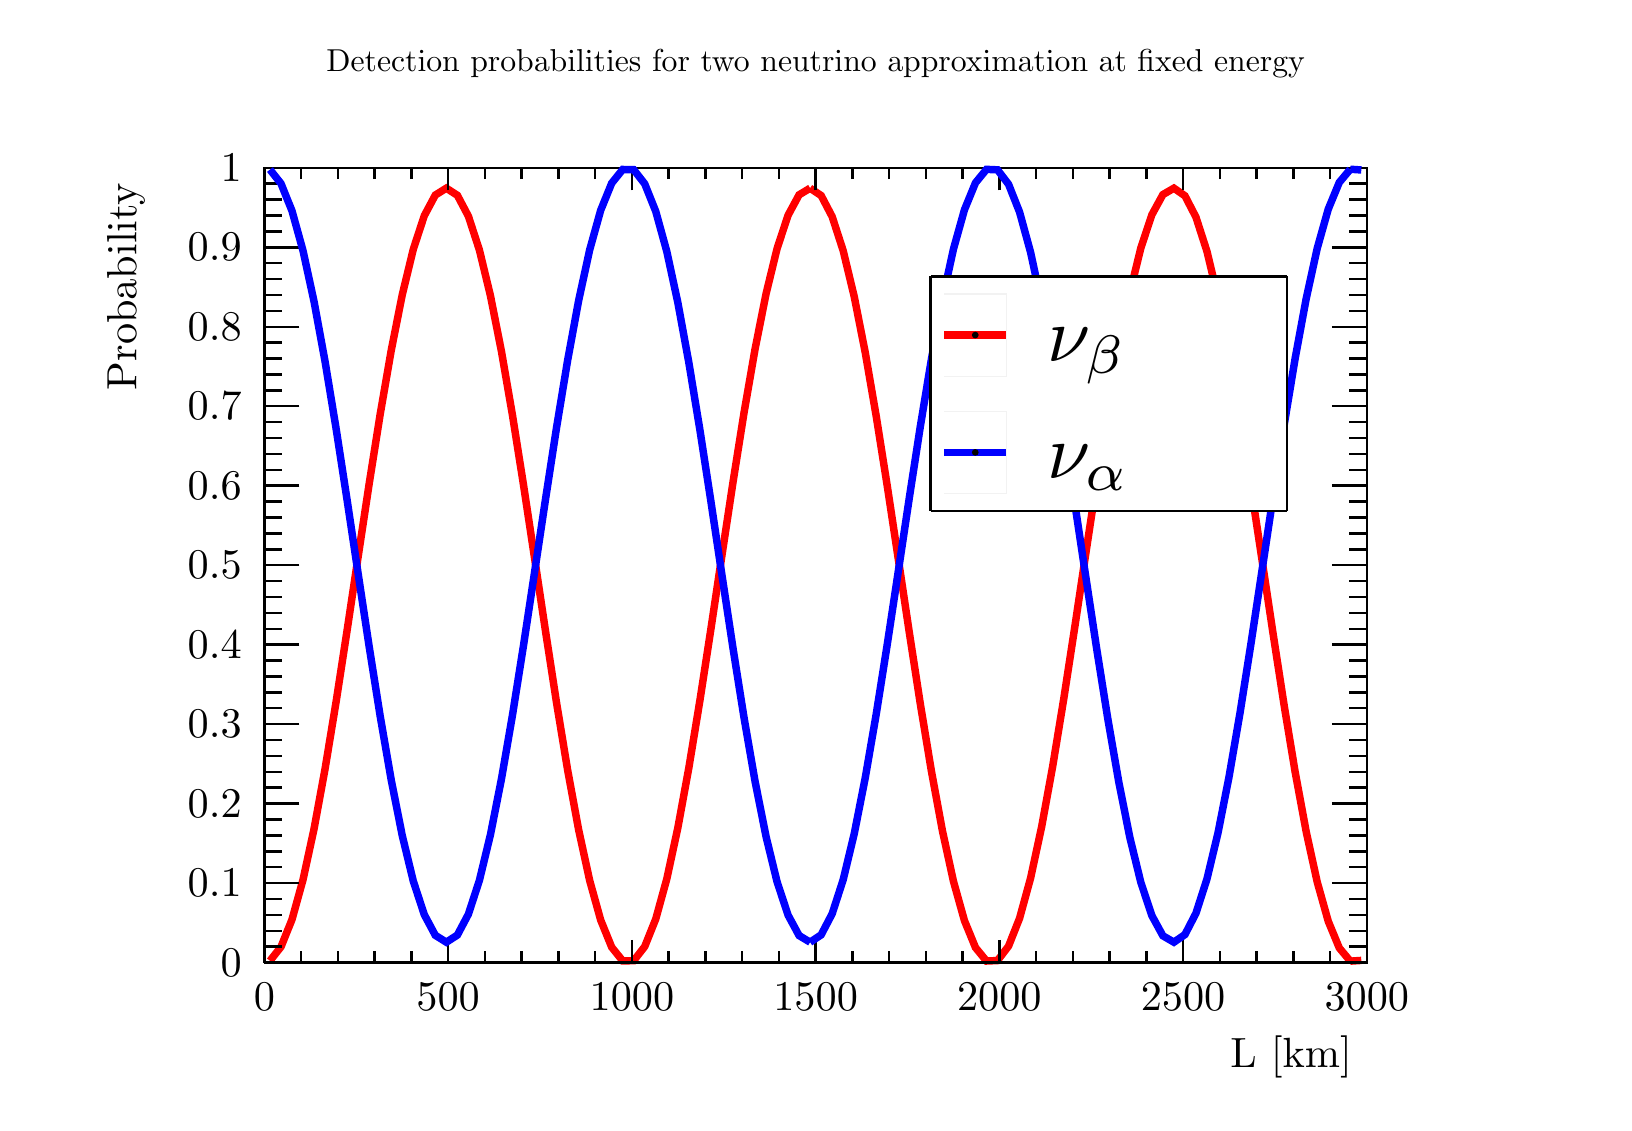
\begin{tikzpicture}
\pgfdeclareplotmark{cross} {
\pgfpathmoveto{\pgfpoint{-0.3\pgfplotmarksize}{\pgfplotmarksize}}
\pgfpathlineto{\pgfpoint{+0.3\pgfplotmarksize}{\pgfplotmarksize}}
\pgfpathlineto{\pgfpoint{+0.3\pgfplotmarksize}{0.3\pgfplotmarksize}}
\pgfpathlineto{\pgfpoint{+1\pgfplotmarksize}{0.3\pgfplotmarksize}}
\pgfpathlineto{\pgfpoint{+1\pgfplotmarksize}{-0.3\pgfplotmarksize}}
\pgfpathlineto{\pgfpoint{+0.3\pgfplotmarksize}{-0.3\pgfplotmarksize}}
\pgfpathlineto{\pgfpoint{+0.3\pgfplotmarksize}{-1.\pgfplotmarksize}}
\pgfpathlineto{\pgfpoint{-0.3\pgfplotmarksize}{-1.\pgfplotmarksize}}
\pgfpathlineto{\pgfpoint{-0.3\pgfplotmarksize}{-0.3\pgfplotmarksize}}
\pgfpathlineto{\pgfpoint{-1.\pgfplotmarksize}{-0.3\pgfplotmarksize}}
\pgfpathlineto{\pgfpoint{-1.\pgfplotmarksize}{0.3\pgfplotmarksize}}
\pgfpathlineto{\pgfpoint{-0.3\pgfplotmarksize}{0.3\pgfplotmarksize}}
\pgfpathclose
\pgfusepathqstroke
}
\pgfdeclareplotmark{cross*} {
\pgfpathmoveto{\pgfpoint{-0.3\pgfplotmarksize}{\pgfplotmarksize}}
\pgfpathlineto{\pgfpoint{+0.3\pgfplotmarksize}{\pgfplotmarksize}}
\pgfpathlineto{\pgfpoint{+0.3\pgfplotmarksize}{0.3\pgfplotmarksize}}
\pgfpathlineto{\pgfpoint{+1\pgfplotmarksize}{0.3\pgfplotmarksize}}
\pgfpathlineto{\pgfpoint{+1\pgfplotmarksize}{-0.3\pgfplotmarksize}}
\pgfpathlineto{\pgfpoint{+0.3\pgfplotmarksize}{-0.3\pgfplotmarksize}}
\pgfpathlineto{\pgfpoint{+0.3\pgfplotmarksize}{-1.\pgfplotmarksize}}
\pgfpathlineto{\pgfpoint{-0.3\pgfplotmarksize}{-1.\pgfplotmarksize}}
\pgfpathlineto{\pgfpoint{-0.3\pgfplotmarksize}{-0.3\pgfplotmarksize}}
\pgfpathlineto{\pgfpoint{-1.\pgfplotmarksize}{-0.3\pgfplotmarksize}}
\pgfpathlineto{\pgfpoint{-1.\pgfplotmarksize}{0.3\pgfplotmarksize}}
\pgfpathlineto{\pgfpoint{-0.3\pgfplotmarksize}{0.3\pgfplotmarksize}}
\pgfpathclose
\pgfusepathqfillstroke
}
\pgfdeclareplotmark{newstar} {
\pgfpathmoveto{\pgfqpoint{0pt}{\pgfplotmarksize}}
\pgfpathlineto{\pgfqpointpolar{44}{0.5\pgfplotmarksize}}
\pgfpathlineto{\pgfqpointpolar{18}{\pgfplotmarksize}}
\pgfpathlineto{\pgfqpointpolar{-20}{0.5\pgfplotmarksize}}
\pgfpathlineto{\pgfqpointpolar{-54}{\pgfplotmarksize}}
\pgfpathlineto{\pgfqpointpolar{-90}{0.5\pgfplotmarksize}}
\pgfpathlineto{\pgfqpointpolar{234}{\pgfplotmarksize}}
\pgfpathlineto{\pgfqpointpolar{198}{0.5\pgfplotmarksize}}
\pgfpathlineto{\pgfqpointpolar{162}{\pgfplotmarksize}}
\pgfpathlineto{\pgfqpointpolar{134}{0.5\pgfplotmarksize}}
\pgfpathclose
\pgfusepathqstroke
}
\pgfdeclareplotmark{newstar*} {
\pgfpathmoveto{\pgfqpoint{0pt}{\pgfplotmarksize}}
\pgfpathlineto{\pgfqpointpolar{44}{0.5\pgfplotmarksize}}
\pgfpathlineto{\pgfqpointpolar{18}{\pgfplotmarksize}}
\pgfpathlineto{\pgfqpointpolar{-20}{0.5\pgfplotmarksize}}
\pgfpathlineto{\pgfqpointpolar{-54}{\pgfplotmarksize}}
\pgfpathlineto{\pgfqpointpolar{-90}{0.5\pgfplotmarksize}}
\pgfpathlineto{\pgfqpointpolar{234}{\pgfplotmarksize}}
\pgfpathlineto{\pgfqpointpolar{198}{0.5\pgfplotmarksize}}
\pgfpathlineto{\pgfqpointpolar{162}{\pgfplotmarksize}}
\pgfpathlineto{\pgfqpointpolar{134}{0.5\pgfplotmarksize}}
\pgfpathclose
\pgfusepathqfillstroke
}
\definecolor{c}{rgb}{1,1,1};
\draw [color=c, fill=c] (0,0) rectangle (20,13.639);
\draw [color=c, fill=c] (3,1.77307) rectangle (17,11.8659);
\definecolor{c}{rgb}{0,0,0};
\draw [c,line width=0.9] (3,1.77307) -- (3,11.8659) -- (17,11.8659) -- (17,1.77307) -- (3,1.77307);
\definecolor{c}{rgb}{1,1,1};
\draw [color=c, fill=c] (3,1.77307) rectangle (17,11.8659);
\definecolor{c}{rgb}{0,0,0};
\draw [c,line width=0.9] (3,1.77307) -- (3,11.8659) -- (17,11.8659) -- (17,1.77307) -- (3,1.77307);
\definecolor{c}{rgb}{1,0,0};
\draw [c,line width=2.7] (3.07,1.79535) -- (3.21,1.97246) -- (3.35,2.32025) -- (3.49,2.82616) -- (3.63,3.47188) -- (3.77,4.23404) -- (3.91,5.08507) -- (4.05,5.99418) -- (4.19,6.92847) -- (4.33,7.85415) -- (4.47,8.73772) -- (4.61,9.54721) --
 (4.75,10.2533) -- (4.89,10.8306) -- (5.03,11.258) -- (5.17,11.5201) -- (5.31,11.6075) -- (5.45,11.517) -- (5.59,11.2519) -- (5.73,10.8217) -- (5.87,10.2421) -- (6.01,9.53393) -- (6.15,8.72289) -- (6.29,7.83831) -- (6.43,6.91219) -- (6.57,5.97805) --
 (6.71,5.06967) -- (6.85,4.21993) -- (6.99,3.45957) -- (7.13,2.8161) -- (7.27,2.31281) -- (7.41,1.96789) -- (7.55,1.79383) -- (7.69,1.79693) -- (7.83,1.97708) -- (7.97,2.32775) -- (8.11,2.83626) -- (8.25,3.48422) -- (8.39,4.24817) -- (8.53,5.10048)
 -- (8.67,6.01032) -- (8.81,6.94475) -- (8.95,7.86998) -- (9.09,8.75253) -- (9.23,9.56046) -- (9.37,10.2646) -- (9.51,10.8393) -- (9.65,11.264) -- (9.79,11.5232) -- (9.93,11.6075);
\draw [c,line width=2.7] (9.93,11.6075) -- (10.07,11.5139) -- (10.21,11.2458) -- (10.35,10.8129) -- (10.49,10.2308) -- (10.63,9.52062) -- (10.77,8.70804) -- (10.91,7.82245) -- (11.05,6.89591) -- (11.19,5.96192) -- (11.33,5.05429) -- (11.47,4.20585)
 -- (11.61,3.4473) -- (11.75,2.80609) -- (11.89,2.30541) -- (12.03,1.96337) -- (12.17,1.79236) -- (12.31,1.79856) -- (12.45,1.98175) -- (12.59,2.3353) -- (12.73,2.84641) -- (12.87,3.4966) -- (13.01,4.26233) -- (13.15,5.11592) -- (13.29,6.02646) --
 (13.43,6.96103) -- (13.57,7.8858) -- (13.71,8.76731) -- (13.85,9.57368) -- (13.99,10.2757) -- (14.13,10.8481) -- (14.27,11.2699) -- (14.41,11.5261) -- (14.55,11.6074) -- (14.69,11.5107) -- (14.83,11.2396) -- (14.97,10.804) -- (15.11,10.2195) --
 (15.25,9.50727) -- (15.39,8.69316) -- (15.53,7.80659) -- (15.67,6.87962) -- (15.81,5.94581) -- (15.95,5.03893) -- (16.09,4.1918) -- (16.23,3.43507) -- (16.37,2.79611) -- (16.51,2.29805) -- (16.65,1.95891) -- (16.79,1.79095);
\draw [c,line width=2.7] (16.79,1.79095) -- (16.93,1.80025);
\definecolor{c}{rgb}{0,0,0};
\draw [c,line width=0.9] (3,1.77307) -- (17,1.77307);
\draw [c,line width=0.9] (3,2.05948) -- (3,1.77307);
\draw [c,line width=0.9] (3.46667,1.91628) -- (3.46667,1.77307);
\draw [c,line width=0.9] (3.93333,1.91628) -- (3.93333,1.77307);
\draw [c,line width=0.9] (4.4,1.91628) -- (4.4,1.77307);
\draw [c,line width=0.9] (4.86667,1.91628) -- (4.86667,1.77307);
\draw [c,line width=0.9] (5.33333,2.05948) -- (5.33333,1.77307);
\draw [c,line width=0.9] (5.8,1.91628) -- (5.8,1.77307);
\draw [c,line width=0.9] (6.26667,1.91628) -- (6.26667,1.77307);
\draw [c,line width=0.9] (6.73333,1.91628) -- (6.73333,1.77307);
\draw [c,line width=0.9] (7.2,1.91628) -- (7.2,1.77307);
\draw [c,line width=0.9] (7.66667,2.05948) -- (7.66667,1.77307);
\draw [c,line width=0.9] (8.13333,1.91628) -- (8.13333,1.77307);
\draw [c,line width=0.9] (8.6,1.91628) -- (8.6,1.77307);
\draw [c,line width=0.9] (9.06667,1.91628) -- (9.06667,1.77307);
\draw [c,line width=0.9] (9.53333,1.91628) -- (9.53333,1.77307);
\draw [c,line width=0.9] (10,2.05948) -- (10,1.77307);
\draw [c,line width=0.9] (10.4667,1.91628) -- (10.4667,1.77307);
\draw [c,line width=0.9] (10.9333,1.91628) -- (10.9333,1.77307);
\draw [c,line width=0.9] (11.4,1.91628) -- (11.4,1.77307);
\draw [c,line width=0.9] (11.8667,1.91628) -- (11.8667,1.77307);
\draw [c,line width=0.9] (12.3333,2.05948) -- (12.3333,1.77307);
\draw [c,line width=0.9] (12.8,1.91628) -- (12.8,1.77307);
\draw [c,line width=0.9] (13.2667,1.91628) -- (13.2667,1.77307);
\draw [c,line width=0.9] (13.7333,1.91628) -- (13.7333,1.77307);
\draw [c,line width=0.9] (14.2,1.91628) -- (14.2,1.77307);
\draw [c,line width=0.9] (14.6667,2.05948) -- (14.6667,1.77307);
\draw [c,line width=0.9] (15.1333,1.91628) -- (15.1333,1.77307);
\draw [c,line width=0.9] (15.6,1.91628) -- (15.6,1.77307);
\draw [c,line width=0.9] (16.0667,1.91628) -- (16.0667,1.77307);
\draw [c,line width=0.9] (16.5333,1.91628) -- (16.5333,1.77307);
\draw [c,line width=0.9] (17,2.05948) -- (17,1.77307);
\draw [anchor=base] (3,1.15931) node[scale=1.52731, color=c, rotate=0]{0};
\draw [anchor=base] (5.33333,1.15931) node[scale=1.52731, color=c, rotate=0]{500};
\draw [anchor=base] (7.66667,1.15931) node[scale=1.52731, color=c, rotate=0]{1000};
\draw [anchor=base] (10,1.15931) node[scale=1.52731, color=c, rotate=0]{1500};
\draw [anchor=base] (12.3333,1.15931) node[scale=1.52731, color=c, rotate=0]{2000};
\draw [anchor=base] (14.6667,1.15931) node[scale=1.52731, color=c, rotate=0]{2500};
\draw [anchor=base] (17,1.15931) node[scale=1.52731, color=c, rotate=0]{3000};
\draw [anchor= east] (17,0.572837) node[scale=1.52731, color=c, rotate=0]{L [km]};
\draw [c,line width=0.9] (3,11.8659) -- (17,11.8659);
\draw [c,line width=0.9] (3,11.5795) -- (3,11.8659);
\draw [c,line width=0.9] (3.46667,11.7227) -- (3.46667,11.8659);
\draw [c,line width=0.9] (3.93333,11.7227) -- (3.93333,11.8659);
\draw [c,line width=0.9] (4.4,11.7227) -- (4.4,11.8659);
\draw [c,line width=0.9] (4.86667,11.7227) -- (4.86667,11.8659);
\draw [c,line width=0.9] (5.33333,11.5795) -- (5.33333,11.8659);
\draw [c,line width=0.9] (5.8,11.7227) -- (5.8,11.8659);
\draw [c,line width=0.9] (6.26667,11.7227) -- (6.26667,11.8659);
\draw [c,line width=0.9] (6.73333,11.7227) -- (6.73333,11.8659);
\draw [c,line width=0.9] (7.2,11.7227) -- (7.2,11.8659);
\draw [c,line width=0.9] (7.66667,11.5795) -- (7.66667,11.8659);
\draw [c,line width=0.9] (8.13333,11.7227) -- (8.13333,11.8659);
\draw [c,line width=0.9] (8.6,11.7227) -- (8.6,11.8659);
\draw [c,line width=0.9] (9.06667,11.7227) -- (9.06667,11.8659);
\draw [c,line width=0.9] (9.53333,11.7227) -- (9.53333,11.8659);
\draw [c,line width=0.9] (10,11.5795) -- (10,11.8659);
\draw [c,line width=0.9] (10.4667,11.7227) -- (10.4667,11.8659);
\draw [c,line width=0.9] (10.9333,11.7227) -- (10.9333,11.8659);
\draw [c,line width=0.9] (11.4,11.7227) -- (11.4,11.8659);
\draw [c,line width=0.9] (11.8667,11.7227) -- (11.8667,11.8659);
\draw [c,line width=0.9] (12.3333,11.5795) -- (12.3333,11.8659);
\draw [c,line width=0.9] (12.8,11.7227) -- (12.8,11.8659);
\draw [c,line width=0.9] (13.2667,11.7227) -- (13.2667,11.8659);
\draw [c,line width=0.9] (13.7333,11.7227) -- (13.7333,11.8659);
\draw [c,line width=0.9] (14.2,11.7227) -- (14.2,11.8659);
\draw [c,line width=0.9] (14.6667,11.5795) -- (14.6667,11.8659);
\draw [c,line width=0.9] (15.1333,11.7227) -- (15.1333,11.8659);
\draw [c,line width=0.9] (15.6,11.7227) -- (15.6,11.8659);
\draw [c,line width=0.9] (16.0667,11.7227) -- (16.0667,11.8659);
\draw [c,line width=0.9] (16.5333,11.7227) -- (16.5333,11.8659);
\draw [c,line width=0.9] (17,11.5795) -- (17,11.8659);
\draw [c,line width=0.9] (3,1.77307) -- (3,11.8659);
\draw [c,line width=0.9] (3.444,1.77307) -- (3,1.77307);
\draw [c,line width=0.9] (3.222,1.97492) -- (3,1.97492);
\draw [c,line width=0.9] (3.222,2.17678) -- (3,2.17678);
\draw [c,line width=0.9] (3.222,2.37864) -- (3,2.37864);
\draw [c,line width=0.9] (3.222,2.58049) -- (3,2.58049);
\draw [c,line width=0.9] (3.444,2.78235) -- (3,2.78235);
\draw [c,line width=0.9] (3.222,2.98421) -- (3,2.98421);
\draw [c,line width=0.9] (3.222,3.18606) -- (3,3.18606);
\draw [c,line width=0.9] (3.222,3.38792) -- (3,3.38792);
\draw [c,line width=0.9] (3.222,3.58978) -- (3,3.58978);
\draw [c,line width=0.9] (3.444,3.79163) -- (3,3.79163);
\draw [c,line width=0.9] (3.222,3.99349) -- (3,3.99349);
\draw [c,line width=0.9] (3.222,4.19535) -- (3,4.19535);
\draw [c,line width=0.9] (3.222,4.3972) -- (3,4.3972);
\draw [c,line width=0.9] (3.222,4.59906) -- (3,4.59906);
\draw [c,line width=0.9] (3.444,4.80092) -- (3,4.80092);
\draw [c,line width=0.9] (3.222,5.00277) -- (3,5.00277);
\draw [c,line width=0.9] (3.222,5.20463) -- (3,5.20463);
\draw [c,line width=0.9] (3.222,5.40649) -- (3,5.40649);
\draw [c,line width=0.9] (3.222,5.60834) -- (3,5.60834);
\draw [c,line width=0.9] (3.444,5.8102) -- (3,5.8102);
\draw [c,line width=0.9] (3.222,6.01206) -- (3,6.01206);
\draw [c,line width=0.9] (3.222,6.21391) -- (3,6.21391);
\draw [c,line width=0.9] (3.222,6.41577) -- (3,6.41577);
\draw [c,line width=0.9] (3.222,6.61763) -- (3,6.61763);
\draw [c,line width=0.9] (3.444,6.81948) -- (3,6.81948);
\draw [c,line width=0.9] (3.222,7.02134) -- (3,7.02134);
\draw [c,line width=0.9] (3.222,7.2232) -- (3,7.2232);
\draw [c,line width=0.9] (3.222,7.42505) -- (3,7.42505);
\draw [c,line width=0.9] (3.222,7.62691) -- (3,7.62691);
\draw [c,line width=0.9] (3.444,7.82877) -- (3,7.82877);
\draw [c,line width=0.9] (3.222,8.03062) -- (3,8.03062);
\draw [c,line width=0.9] (3.222,8.23248) -- (3,8.23248);
\draw [c,line width=0.9] (3.222,8.43434) -- (3,8.43434);
\draw [c,line width=0.9] (3.222,8.6362) -- (3,8.6362);
\draw [c,line width=0.9] (3.444,8.83805) -- (3,8.83805);
\draw [c,line width=0.9] (3.222,9.03991) -- (3,9.03991);
\draw [c,line width=0.9] (3.222,9.24177) -- (3,9.24177);
\draw [c,line width=0.9] (3.222,9.44362) -- (3,9.44362);
\draw [c,line width=0.9] (3.222,9.64548) -- (3,9.64548);
\draw [c,line width=0.9] (3.444,9.84733) -- (3,9.84733);
\draw [c,line width=0.9] (3.222,10.0492) -- (3,10.0492);
\draw [c,line width=0.9] (3.222,10.251) -- (3,10.251);
\draw [c,line width=0.9] (3.222,10.4529) -- (3,10.4529);
\draw [c,line width=0.9] (3.222,10.6548) -- (3,10.6548);
\draw [c,line width=0.9] (3.444,10.8566) -- (3,10.8566);
\draw [c,line width=0.9] (3.222,11.0585) -- (3,11.0585);
\draw [c,line width=0.9] (3.222,11.2603) -- (3,11.2603);
\draw [c,line width=0.9] (3.222,11.4622) -- (3,11.4622);
\draw [c,line width=0.9] (3.222,11.664) -- (3,11.664);
\draw [c,line width=0.9] (3.444,11.8659) -- (3,11.8659);
\draw [anchor= east] (2.9,1.77307) node[scale=1.52731, color=c, rotate=0]{0};
\draw [anchor= east] (2.9,2.78235) node[scale=1.52731, color=c, rotate=0]{0.1};
\draw [anchor= east] (2.9,3.79163) node[scale=1.52731, color=c, rotate=0]{0.2};
\draw [anchor= east] (2.9,4.80092) node[scale=1.52731, color=c, rotate=0]{0.3};
\draw [anchor= east] (2.9,5.8102) node[scale=1.52731, color=c, rotate=0]{0.4};
\draw [anchor= east] (2.9,6.81948) node[scale=1.52731, color=c, rotate=0]{0.5};
\draw [anchor= east] (2.9,7.82877) node[scale=1.52731, color=c, rotate=0]{0.6};
\draw [anchor= east] (2.9,8.83805) node[scale=1.52731, color=c, rotate=0]{0.7};
\draw [anchor= east] (2.9,9.84733) node[scale=1.52731, color=c, rotate=0]{0.8};
\draw [anchor= east] (2.9,10.8566) node[scale=1.52731, color=c, rotate=0]{0.9};
\draw [anchor= east] (2.9,11.8659) node[scale=1.52731, color=c, rotate=0]{1};
\draw [anchor= east] (1.24,11.8659) node[scale=1.52731, color=c, rotate=90]{Probability};
\draw [c,line width=0.9] (17,1.77307) -- (17,11.8659);
\draw [c,line width=0.9] (16.556,1.77307) -- (17,1.77307);
\draw [c,line width=0.9] (16.778,1.97492) -- (17,1.97492);
\draw [c,line width=0.9] (16.778,2.17678) -- (17,2.17678);
\draw [c,line width=0.9] (16.778,2.37864) -- (17,2.37864);
\draw [c,line width=0.9] (16.778,2.58049) -- (17,2.58049);
\draw [c,line width=0.9] (16.556,2.78235) -- (17,2.78235);
\draw [c,line width=0.9] (16.778,2.98421) -- (17,2.98421);
\draw [c,line width=0.9] (16.778,3.18606) -- (17,3.18606);
\draw [c,line width=0.9] (16.778,3.38792) -- (17,3.38792);
\draw [c,line width=0.9] (16.778,3.58978) -- (17,3.58978);
\draw [c,line width=0.9] (16.556,3.79163) -- (17,3.79163);
\draw [c,line width=0.9] (16.778,3.99349) -- (17,3.99349);
\draw [c,line width=0.9] (16.778,4.19535) -- (17,4.19535);
\draw [c,line width=0.9] (16.778,4.3972) -- (17,4.3972);
\draw [c,line width=0.9] (16.778,4.59906) -- (17,4.59906);
\draw [c,line width=0.9] (16.556,4.80092) -- (17,4.80092);
\draw [c,line width=0.9] (16.778,5.00277) -- (17,5.00277);
\draw [c,line width=0.9] (16.778,5.20463) -- (17,5.20463);
\draw [c,line width=0.9] (16.778,5.40649) -- (17,5.40649);
\draw [c,line width=0.9] (16.778,5.60834) -- (17,5.60834);
\draw [c,line width=0.9] (16.556,5.8102) -- (17,5.8102);
\draw [c,line width=0.9] (16.778,6.01206) -- (17,6.01206);
\draw [c,line width=0.9] (16.778,6.21391) -- (17,6.21391);
\draw [c,line width=0.9] (16.778,6.41577) -- (17,6.41577);
\draw [c,line width=0.9] (16.778,6.61763) -- (17,6.61763);
\draw [c,line width=0.9] (16.556,6.81948) -- (17,6.81948);
\draw [c,line width=0.9] (16.778,7.02134) -- (17,7.02134);
\draw [c,line width=0.9] (16.778,7.2232) -- (17,7.2232);
\draw [c,line width=0.9] (16.778,7.42505) -- (17,7.42505);
\draw [c,line width=0.9] (16.778,7.62691) -- (17,7.62691);
\draw [c,line width=0.9] (16.556,7.82877) -- (17,7.82877);
\draw [c,line width=0.9] (16.778,8.03062) -- (17,8.03062);
\draw [c,line width=0.9] (16.778,8.23248) -- (17,8.23248);
\draw [c,line width=0.9] (16.778,8.43434) -- (17,8.43434);
\draw [c,line width=0.9] (16.778,8.6362) -- (17,8.6362);
\draw [c,line width=0.9] (16.556,8.83805) -- (17,8.83805);
\draw [c,line width=0.9] (16.778,9.03991) -- (17,9.03991);
\draw [c,line width=0.9] (16.778,9.24177) -- (17,9.24177);
\draw [c,line width=0.9] (16.778,9.44362) -- (17,9.44362);
\draw [c,line width=0.9] (16.778,9.64548) -- (17,9.64548);
\draw [c,line width=0.9] (16.556,9.84733) -- (17,9.84733);
\draw [c,line width=0.9] (16.778,10.0492) -- (17,10.0492);
\draw [c,line width=0.9] (16.778,10.251) -- (17,10.251);
\draw [c,line width=0.9] (16.778,10.4529) -- (17,10.4529);
\draw [c,line width=0.9] (16.778,10.6548) -- (17,10.6548);
\draw [c,line width=0.9] (16.556,10.8566) -- (17,10.8566);
\draw [c,line width=0.9] (16.778,11.0585) -- (17,11.0585);
\draw [c,line width=0.9] (16.778,11.2603) -- (17,11.2603);
\draw [c,line width=0.9] (16.778,11.4622) -- (17,11.4622);
\draw [c,line width=0.9] (16.778,11.664) -- (17,11.664);
\draw [c,line width=0.9] (16.556,11.8659) -- (17,11.8659);
\definecolor{c}{rgb}{0,0,1};
\draw [c,line width=2.7] (3.07,11.8436) -- (3.21,11.6665) -- (3.35,11.3187) -- (3.49,10.8128) -- (3.63,10.1671) -- (3.77,9.40493) -- (3.91,8.5539) -- (4.05,7.64479) -- (4.19,6.7105) -- (4.33,5.78482) -- (4.47,4.90125) -- (4.61,4.09176) --
 (4.75,3.38563) -- (4.89,2.80841) -- (5.03,2.381) -- (5.17,2.11884) -- (5.31,2.03143) -- (5.45,2.12192) -- (5.59,2.38706) -- (5.73,2.81723) -- (5.87,3.39688) -- (6.01,4.10504) -- (6.15,4.91608) -- (6.29,5.80066) -- (6.43,6.72678) -- (6.57,7.66092) --
 (6.71,8.5693) -- (6.85,9.41904) -- (6.99,10.1794) -- (7.13,10.8229) -- (7.27,11.3262) -- (7.41,11.6711) -- (7.55,11.8451) -- (7.69,11.842) -- (7.83,11.6619) -- (7.97,11.3112) -- (8.11,10.8027) -- (8.25,10.1547) -- (8.39,9.3908) -- (8.53,8.53848) --
 (8.67,7.62865) -- (8.81,6.69422) -- (8.95,5.76899) -- (9.09,4.88644) -- (9.23,4.07851) -- (9.37,3.37442) -- (9.51,2.79964) -- (9.65,2.37498) -- (9.79,2.1158) -- (9.93,2.03148);
\draw [c,line width=2.7] (9.93,2.03148) -- (10.07,2.12506) -- (10.21,2.39317) -- (10.35,2.82609) -- (10.49,3.40817) -- (10.63,4.11835) -- (10.77,4.93093) -- (10.91,5.81652) -- (11.05,6.74306) -- (11.19,7.67705) -- (11.33,8.58468) -- (11.47,9.43312)
 -- (11.61,10.1917) -- (11.75,10.8329) -- (11.89,11.3336) -- (12.03,11.6756) -- (12.17,11.8466) -- (12.31,11.8404) -- (12.45,11.6572) -- (12.59,11.3037) -- (12.73,10.7926) -- (12.87,10.1424) -- (13.01,9.37664) -- (13.15,8.52305) -- (13.29,7.61251) --
 (13.43,6.67794) -- (13.57,5.75317) -- (13.71,4.87166) -- (13.85,4.06529) -- (13.99,3.36324) -- (14.13,2.79092) -- (14.27,2.36902) -- (14.41,2.11282) -- (14.55,2.03159) -- (14.69,2.12826) -- (14.83,2.39933) -- (14.97,2.835) -- (15.11,3.4195) --
 (15.25,4.1317) -- (15.39,4.94581) -- (15.53,5.83238) -- (15.67,6.75935) -- (15.81,7.69316) -- (15.95,8.60004) -- (16.09,9.44717) -- (16.23,10.2039) -- (16.37,10.8429) -- (16.51,11.3409) -- (16.65,11.6801) -- (16.79,11.848);
\draw [c,line width=2.7] (16.79,11.848) -- (16.93,11.8387);
\definecolor{c}{rgb}{1,1,1};
\draw [color=c, fill=c] (2,12.8206) rectangle (18,13.5708);
\definecolor{c}{rgb}{0,0,0};
\draw (10,13.1957) node[scale=1.14549, color=c, rotate=0]{Detection probabilities for two neutrino approximation at fixed energy};
\definecolor{c}{rgb}{1,1,1};
\draw [color=c, fill=c] (11.4613,7.50716) rectangle (15.9885,10.4871);
\definecolor{c}{rgb}{0,0,0};
\draw [c,line width=0.9] (11.4613,7.50716) -- (15.9885,7.50716);
\draw [c,line width=0.9] (15.9885,7.50716) -- (15.9885,10.4871);
\draw [c,line width=0.9] (15.9885,10.4871) -- (11.4613,10.4871);
\draw [c,line width=0.9] (11.4613,10.4871) -- (11.4613,7.50716);
\draw [anchor=base west] (12.5931,9.40688) node[scale=2.80008, color=c, rotate=0]{$\nu_{\beta}$};
\definecolor{c}{rgb}{0.95,0.95,0.95};
\draw [c] (11.6311,9.22063) -- (12.4234,9.22063) -- (12.4234,10.2636) -- (11.6311,10.2636);
\definecolor{c}{rgb}{1,0,0};
\draw [c,line width=2.7] (11.6311,9.74212) -- (12.4234,9.74212);
\definecolor{c}{rgb}{0,0,0};
\foreach \P in {(12.0272,9.74212)}{\draw[mark options={color=c,fill=c},mark size=2.402402pt,mark=*,mark size=1pt] plot coordinates {\P};}
\draw [anchor=base west] (12.5931,7.91691) node[scale=2.80008, color=c, rotate=0]{$\nu_{\alpha}$};
\definecolor{c}{rgb}{0.95,0.95,0.95};
\draw [c] (11.6311,7.73066) -- (12.4234,7.73066) -- (12.4234,8.77364) -- (11.6311,8.77364);
\definecolor{c}{rgb}{0,0,1};
\draw [c,line width=2.7] (11.6311,8.25215) -- (12.4234,8.25215);
\definecolor{c}{rgb}{0,0,0};
\foreach \P in {(12.0272,8.25215)}{\draw[mark options={color=c,fill=c},mark size=2.402402pt,mark=*,mark size=1pt] plot coordinates {\P};}
\end{tikzpicture}

    \end{adjustbox}
    \caption{Probability of detecting an initial $\nu_{\alpha}$ as a particular flavour as a function of baseline, $L$. Here, the energy of the neutrino is 1~GeV.}
  \end{subfigure}
  \hfill
  \begin{subfigure}[t]{0.49\textwidth}
    \begin{adjustbox}{max totalsize={\textwidth}, center}
      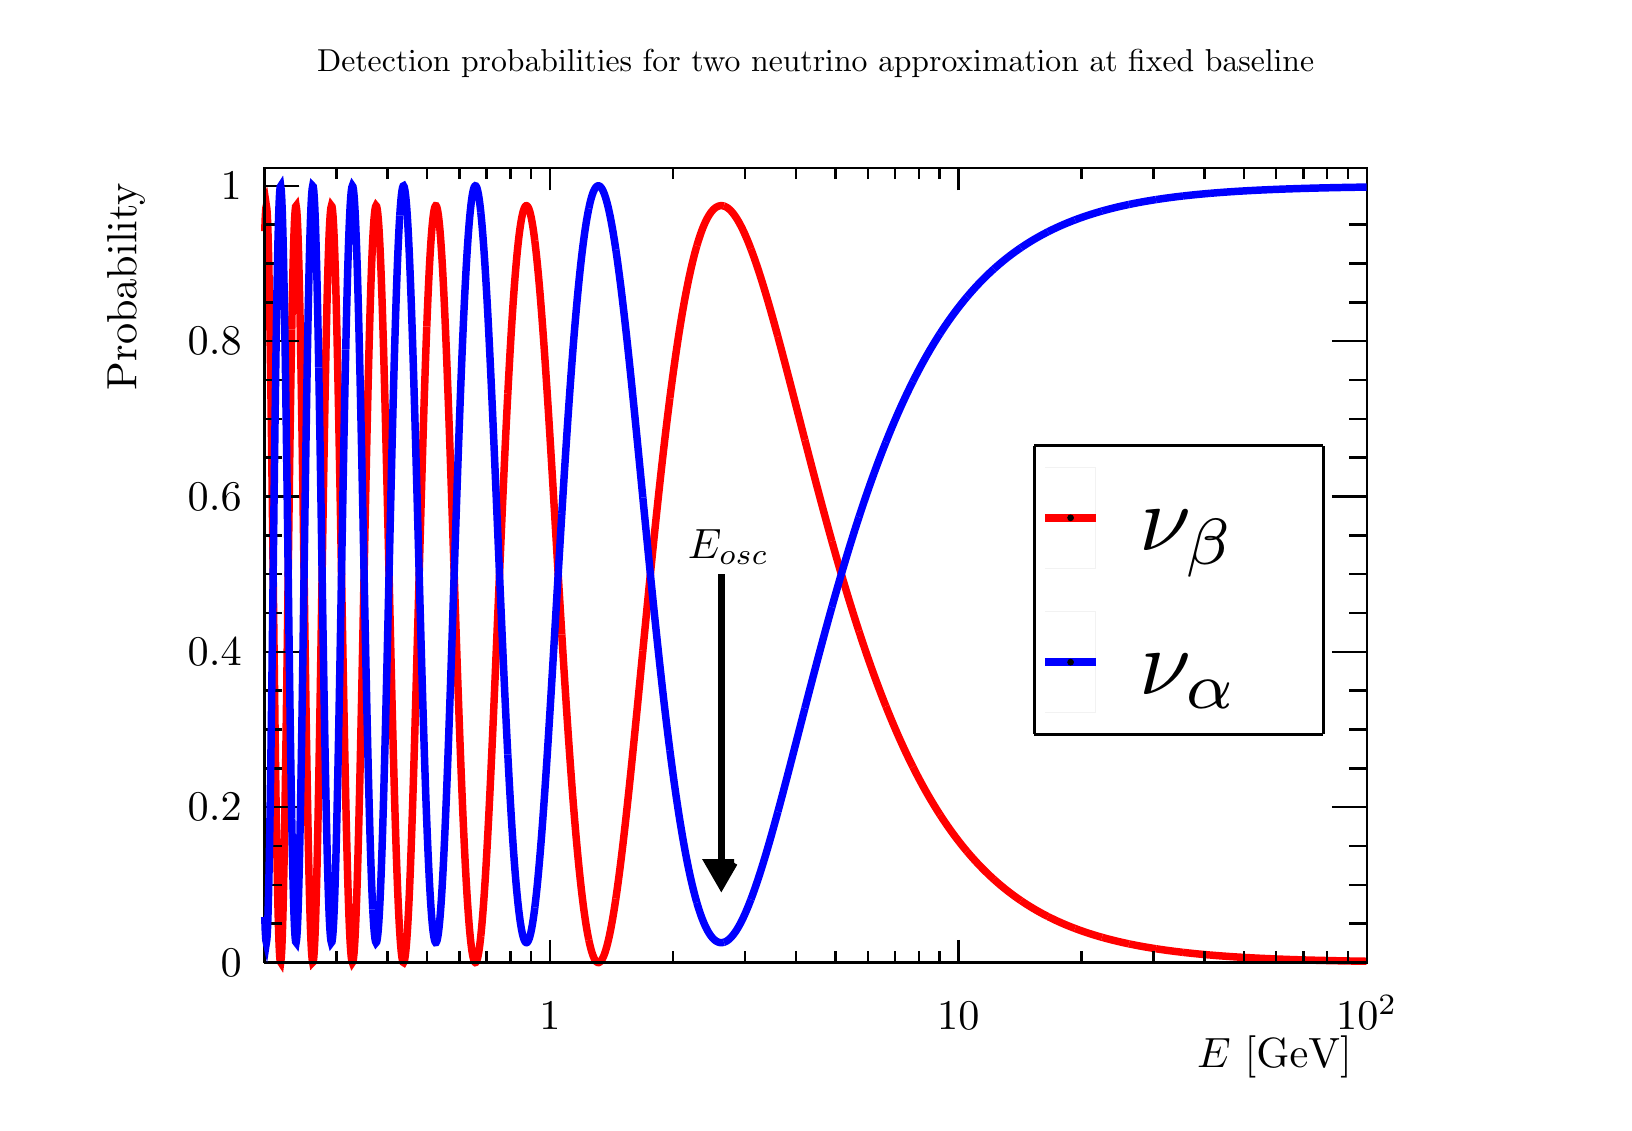
\begin{tikzpicture}
\pgfdeclareplotmark{cross} {
\pgfpathmoveto{\pgfpoint{-0.3\pgfplotmarksize}{\pgfplotmarksize}}
\pgfpathlineto{\pgfpoint{+0.3\pgfplotmarksize}{\pgfplotmarksize}}
\pgfpathlineto{\pgfpoint{+0.3\pgfplotmarksize}{0.3\pgfplotmarksize}}
\pgfpathlineto{\pgfpoint{+1\pgfplotmarksize}{0.3\pgfplotmarksize}}
\pgfpathlineto{\pgfpoint{+1\pgfplotmarksize}{-0.3\pgfplotmarksize}}
\pgfpathlineto{\pgfpoint{+0.3\pgfplotmarksize}{-0.3\pgfplotmarksize}}
\pgfpathlineto{\pgfpoint{+0.3\pgfplotmarksize}{-1.\pgfplotmarksize}}
\pgfpathlineto{\pgfpoint{-0.3\pgfplotmarksize}{-1.\pgfplotmarksize}}
\pgfpathlineto{\pgfpoint{-0.3\pgfplotmarksize}{-0.3\pgfplotmarksize}}
\pgfpathlineto{\pgfpoint{-1.\pgfplotmarksize}{-0.3\pgfplotmarksize}}
\pgfpathlineto{\pgfpoint{-1.\pgfplotmarksize}{0.3\pgfplotmarksize}}
\pgfpathlineto{\pgfpoint{-0.3\pgfplotmarksize}{0.3\pgfplotmarksize}}
\pgfpathclose
\pgfusepathqstroke
}
\pgfdeclareplotmark{cross*} {
\pgfpathmoveto{\pgfpoint{-0.3\pgfplotmarksize}{\pgfplotmarksize}}
\pgfpathlineto{\pgfpoint{+0.3\pgfplotmarksize}{\pgfplotmarksize}}
\pgfpathlineto{\pgfpoint{+0.3\pgfplotmarksize}{0.3\pgfplotmarksize}}
\pgfpathlineto{\pgfpoint{+1\pgfplotmarksize}{0.3\pgfplotmarksize}}
\pgfpathlineto{\pgfpoint{+1\pgfplotmarksize}{-0.3\pgfplotmarksize}}
\pgfpathlineto{\pgfpoint{+0.3\pgfplotmarksize}{-0.3\pgfplotmarksize}}
\pgfpathlineto{\pgfpoint{+0.3\pgfplotmarksize}{-1.\pgfplotmarksize}}
\pgfpathlineto{\pgfpoint{-0.3\pgfplotmarksize}{-1.\pgfplotmarksize}}
\pgfpathlineto{\pgfpoint{-0.3\pgfplotmarksize}{-0.3\pgfplotmarksize}}
\pgfpathlineto{\pgfpoint{-1.\pgfplotmarksize}{-0.3\pgfplotmarksize}}
\pgfpathlineto{\pgfpoint{-1.\pgfplotmarksize}{0.3\pgfplotmarksize}}
\pgfpathlineto{\pgfpoint{-0.3\pgfplotmarksize}{0.3\pgfplotmarksize}}
\pgfpathclose
\pgfusepathqfillstroke
}
\pgfdeclareplotmark{newstar} {
\pgfpathmoveto{\pgfqpoint{0pt}{\pgfplotmarksize}}
\pgfpathlineto{\pgfqpointpolar{44}{0.5\pgfplotmarksize}}
\pgfpathlineto{\pgfqpointpolar{18}{\pgfplotmarksize}}
\pgfpathlineto{\pgfqpointpolar{-20}{0.5\pgfplotmarksize}}
\pgfpathlineto{\pgfqpointpolar{-54}{\pgfplotmarksize}}
\pgfpathlineto{\pgfqpointpolar{-90}{0.5\pgfplotmarksize}}
\pgfpathlineto{\pgfqpointpolar{234}{\pgfplotmarksize}}
\pgfpathlineto{\pgfqpointpolar{198}{0.5\pgfplotmarksize}}
\pgfpathlineto{\pgfqpointpolar{162}{\pgfplotmarksize}}
\pgfpathlineto{\pgfqpointpolar{134}{0.5\pgfplotmarksize}}
\pgfpathclose
\pgfusepathqstroke
}
\pgfdeclareplotmark{newstar*} {
\pgfpathmoveto{\pgfqpoint{0pt}{\pgfplotmarksize}}
\pgfpathlineto{\pgfqpointpolar{44}{0.5\pgfplotmarksize}}
\pgfpathlineto{\pgfqpointpolar{18}{\pgfplotmarksize}}
\pgfpathlineto{\pgfqpointpolar{-20}{0.5\pgfplotmarksize}}
\pgfpathlineto{\pgfqpointpolar{-54}{\pgfplotmarksize}}
\pgfpathlineto{\pgfqpointpolar{-90}{0.5\pgfplotmarksize}}
\pgfpathlineto{\pgfqpointpolar{234}{\pgfplotmarksize}}
\pgfpathlineto{\pgfqpointpolar{198}{0.5\pgfplotmarksize}}
\pgfpathlineto{\pgfqpointpolar{162}{\pgfplotmarksize}}
\pgfpathlineto{\pgfqpointpolar{134}{0.5\pgfplotmarksize}}
\pgfpathclose
\pgfusepathqfillstroke
}
\definecolor{c}{rgb}{1,1,1};
\draw [color=c, fill=c] (0,0) rectangle (20,13.639);
\draw [color=c, fill=c] (3,1.77307) rectangle (17,11.8659);
\definecolor{c}{rgb}{0,0,0};
\draw [c,line width=0.9] (3,1.77307) -- (3,11.8659) -- (17,11.8659) -- (17,1.77307) -- (3,1.77307);
\definecolor{c}{rgb}{1,1,1};
\draw [color=c, fill=c] (3,1.77307) rectangle (17,11.8659);
\definecolor{c}{rgb}{0,0,0};
\draw [c,line width=0.9] (3,1.77307) -- (3,11.8659) -- (17,11.8659) -- (17,1.77307) -- (3,1.77307);
\definecolor{c}{rgb}{1,0,0};
\draw [c,line width=2.7] (3.0035,11.0598) -- (3.0105,11.2449) -- (3.0175,11.3537) -- (3.0245,11.385) -- (3.0315,11.339) -- (3.0385,11.2174) -- (3.0455,11.0225) -- (3.0525,10.7583) -- (3.0595,10.4295) -- (3.0665,10.0417) -- (3.0735,9.60166) --
 (3.0805,9.1165) -- (3.0875,8.5941) -- (3.0945,8.04273) -- (3.1015,7.47098) -- (3.1085,6.88764) -- (3.1155,6.30149) -- (3.1225,5.72127) -- (3.1295,5.15547) -- (3.1365,4.61223) -- (3.1435,4.09924) -- (3.1505,3.62366) -- (3.1575,3.19196) --
 (3.1645,2.80992) -- (3.1715,2.48248) -- (3.1785,2.21376) -- (3.1855,2.00699) -- (3.1925,1.86448) -- (3.1995,1.7876) -- (3.2065,1.7768) -- (3.2135,1.83162) -- (3.2205,1.95071) -- (3.2275,2.13186) -- (3.2345,2.37207) -- (3.2415,2.66759) --
 (3.2485,3.01398) -- (3.2555,3.40621) -- (3.2625,3.83872) -- (3.2695,4.30551) -- (3.2765,4.80022) -- (3.2835,5.31623) -- (3.2905,5.84676) -- (3.2975,6.38493) -- (3.3045,6.9239) -- (3.3115,7.45687) -- (3.3185,7.97729) -- (3.3255,8.4788) --
 (3.3325,8.95542) -- (3.3395,9.40155) -- (3.3465,9.81205);
\draw [c,line width=2.7] (3.3465,9.81205) -- (3.3535,10.1823) -- (3.3605,10.5082) -- (3.3675,10.7862) -- (3.3745,11.0136) -- (3.3815,11.1882) -- (3.3885,11.3083) -- (3.3955,11.373) -- (3.4025,11.3822) -- (3.4095,11.3363) -- (3.4165,11.2362) --
 (3.4235,11.0836) -- (3.4305,10.8808) -- (3.4375,10.6304) -- (3.4445,10.3357) -- (3.4515,10.0004) -- (3.4585,9.62854) -- (3.4655,9.22451) -- (3.4725,8.79302) -- (3.4795,8.33898) -- (3.4865,7.86749) -- (3.4935,7.38372) -- (3.5005,6.89293) --
 (3.5075,6.40036) -- (3.5145,5.91118) -- (3.5215,5.43046) -- (3.5285,4.96308) -- (3.5355,4.51374) -- (3.5425,4.08686) -- (3.5495,3.68656) -- (3.5565,3.31665) -- (3.5635,2.98054) -- (3.5705,2.68128) -- (3.5775,2.42149) -- (3.5845,2.20337) --
 (3.5915,2.02866) -- (3.5985,1.89865) -- (3.6055,1.8142) -- (3.6125,1.77569) -- (3.6195,1.78306) -- (3.6265,1.83582) -- (3.6335,1.93305) -- (3.6405,2.07343) -- (3.6475,2.25525) -- (3.6545,2.47644) -- (3.6615,2.7346) -- (3.6685,3.02703) --
 (3.6755,3.35077) -- (3.6825,3.70258) -- (3.6895,4.07907);
\draw [c,line width=2.7] (3.6895,4.07907) -- (3.6965,4.47663) -- (3.7035,4.89156) -- (3.7105,5.32004) -- (3.7175,5.75819) -- (3.7245,6.20211) -- (3.7315,6.64791) -- (3.7385,7.09174) -- (3.7455,7.52983) -- (3.7525,7.95852) -- (3.7595,8.37427) --
 (3.7665,8.77373) -- (3.7735,9.15371) -- (3.7805,9.51126) -- (3.7875,9.84363) -- (3.7945,10.1483) -- (3.8015,10.4232) -- (3.8085,10.6662) -- (3.8155,10.8757) -- (3.8225,11.0505) -- (3.8295,11.1893) -- (3.8365,11.2914) -- (3.8435,11.3564) --
 (3.8505,11.3842) -- (3.8575,11.3748) -- (3.8645,11.3287) -- (3.8715,11.2465) -- (3.8785,11.1292) -- (3.8855,10.9781) -- (3.8925,10.7945) -- (3.8995,10.5802) -- (3.9065,10.337) -- (3.9135,10.067) -- (3.9205,9.77235) -- (3.9275,9.45548) --
 (3.9345,9.11886) -- (3.9415,8.76511) -- (3.9485,8.39689) -- (3.9555,8.01696) -- (3.9625,7.62811) -- (3.9695,7.23313) -- (3.9765,6.83483) -- (3.9835,6.436) -- (3.9905,6.03939) -- (3.9975,5.64769) -- (4.0045,5.2635) -- (4.0115,4.88936) --
 (4.0185,4.52768) -- (4.0255,4.18074) -- (4.0325,3.85072);
\draw [c,line width=2.7] (4.0325,3.85072) -- (4.0395,3.53964) -- (4.0465,3.24934) -- (4.0535,2.98152) -- (4.0605,2.73771) -- (4.0675,2.51925) -- (4.0745,2.3273) -- (4.0815,2.16283) -- (4.0885,2.02663) -- (4.0955,1.91927) -- (4.1025,1.84117) --
 (4.1095,1.79254) -- (4.1165,1.77307) -- (4.1235,1.7836) -- (4.1305,1.8228) -- (4.1375,1.89049) -- (4.1445,1.98601) -- (4.1515,2.10854) -- (4.1585,2.25708) -- (4.1655,2.43053) -- (4.1725,2.62765) -- (4.1795,2.84706) -- (4.1865,3.08729) --
 (4.1935,3.34676) -- (4.2005,3.62383) -- (4.2075,3.91675) -- (4.2145,4.22372) -- (4.2215,4.5429) -- (4.2285,4.87239) -- (4.2355,5.21027) -- (4.2425,5.55461) -- (4.2495,5.90347) -- (4.2565,6.2549) -- (4.2635,6.60699) -- (4.2705,6.95784) --
 (4.2775,7.3056) -- (4.2845,7.64844) -- (4.2915,7.9846) -- (4.2985,8.3124) -- (4.3055,8.63019) -- (4.3125,8.93644) -- (4.3195,9.22967) -- (4.3265,9.5085) -- (4.3335,9.77166) -- (4.3405,10.018) -- (4.3475,10.2463) -- (4.3545,10.4558) --
 (4.3615,10.6455) -- (4.3685,10.8147) -- (4.3755,10.9627);
\draw [c,line width=2.7] (4.3755,10.9627) -- (4.3825,11.089) -- (4.3895,11.1933) -- (4.3965,11.2751) -- (4.4035,11.3344) -- (4.4105,11.3711) -- (4.4175,11.3851) -- (4.4245,11.3767) -- (4.4315,11.3461) -- (4.4385,11.2937) -- (4.4455,11.2198) --
 (4.4525,11.125) -- (4.4595,11.0099) -- (4.4665,10.8753) -- (4.4735,10.722) -- (4.4805,10.5507) -- (4.4875,10.3625) -- (4.4945,10.1582) -- (4.5015,9.939) -- (4.5085,9.70592) -- (4.5155,9.46012) -- (4.5225,9.20275) -- (4.5295,8.93504) --
 (4.5365,8.65821) -- (4.5435,8.37351) -- (4.5505,8.08222) -- (4.5575,7.78559) -- (4.5645,7.48491) -- (4.5715,7.18146) -- (4.5785,6.8765) -- (4.5855,6.57128) -- (4.5925,6.26704) -- (4.5995,5.96498) -- (4.6065,5.66631) -- (4.6135,5.37215) --
 (4.6205,5.08364) -- (4.6275,4.80185) -- (4.6345,4.52781) -- (4.6415,4.26251) -- (4.6485,4.00689) -- (4.6555,3.76184) -- (4.6625,3.52818) -- (4.6695,3.3067) -- (4.6765,3.0981) -- (4.6835,2.90306) -- (4.6905,2.72216) -- (4.6975,2.55594) --
 (4.7045,2.40487) -- (4.7115,2.26935) -- (4.7185,2.14975);
\draw [c,line width=2.7] (4.7185,2.14975) -- (4.7255,2.04633) -- (4.7325,1.95931) -- (4.7395,1.88886) -- (4.7465,1.83506) -- (4.7535,1.79795) -- (4.7605,1.77751) -- (4.7675,1.77307) -- (4.7745,1.78623) -- (4.7815,1.81505) -- (4.7885,1.85987) --
 (4.7955,1.92039) -- (4.8025,1.99626) -- (4.8095,2.08708) -- (4.8165,2.19241) -- (4.8235,2.31177) -- (4.8305,2.44465) -- (4.8375,2.59048) -- (4.8445,2.74867) -- (4.8515,2.9186) -- (4.8585,3.09963) -- (4.8655,3.29106) -- (4.8725,3.4922) --
 (4.8795,3.70234) -- (4.8865,3.92072) -- (4.8935,4.14661) -- (4.9005,4.37924) -- (4.9075,4.61782) -- (4.9145,4.86159) -- (4.9215,5.10976) -- (4.9285,5.36154) -- (4.9355,5.61615) -- (4.9425,5.8728) -- (4.9495,6.13073) -- (4.9565,6.38916) --
 (4.9635,6.64734) -- (4.9705,6.90452) -- (4.9775,7.15998) -- (4.9845,7.413) -- (4.9915,7.66288) -- (4.9985,7.90896) -- (5.0055,8.15056) -- (5.0125,8.38707) -- (5.0195,8.61787) -- (5.0265,8.84239) -- (5.0335,9.06006) -- (5.0405,9.27035) --
 (5.0475,9.47278) -- (5.0545,9.66686) -- (5.0615,9.85216);
\draw [c,line width=2.7] (5.0615,9.85216) -- (5.0685,10.0283) -- (5.0755,10.1948) -- (5.0825,10.3514) -- (5.0895,10.4978) -- (5.0965,10.6336) -- (5.1035,10.7587) -- (5.1105,10.8728) -- (5.1175,10.9757) -- (5.1245,11.0673) -- (5.1315,11.1474) --
 (5.1385,11.216) -- (5.1455,11.2729) -- (5.1525,11.3182) -- (5.1595,11.3519) -- (5.1665,11.3739) -- (5.1735,11.3844) -- (5.1805,11.3833) -- (5.1875,11.3709) -- (5.1945,11.3472) -- (5.2015,11.3125) -- (5.2085,11.2668) -- (5.2155,11.2105) --
 (5.2225,11.1437) -- (5.2295,11.0667) -- (5.2365,10.9797) -- (5.2435,10.8831) -- (5.2505,10.7771) -- (5.2575,10.6622) -- (5.2645,10.5385) -- (5.2715,10.4065) -- (5.2785,10.2666) -- (5.2855,10.1191) -- (5.2925,9.96439) -- (5.2995,9.80291) --
 (5.3065,9.63506) -- (5.3135,9.46126) -- (5.3205,9.28193) -- (5.3275,9.0975) -- (5.3345,8.9084) -- (5.3415,8.71507) -- (5.3485,8.51796) -- (5.3555,8.3175) -- (5.3625,8.11414) -- (5.3695,7.90831) -- (5.3765,7.70045) -- (5.3835,7.49101) --
 (5.3905,7.28042) -- (5.3975,7.0691) -- (5.4045,6.85747);
\draw [c,line width=2.7] (5.4045,6.85747) -- (5.4115,6.64596) -- (5.4185,6.43498) -- (5.4255,6.22493) -- (5.4325,6.01621) -- (5.4395,5.8092) -- (5.4465,5.60428) -- (5.4535,5.40182) -- (5.4605,5.20218) -- (5.4675,5.0057) -- (5.4745,4.81272) --
 (5.4815,4.62356) -- (5.4885,4.43854) -- (5.4955,4.25795) -- (5.5025,4.08208) -- (5.5095,3.9112) -- (5.5165,3.74557) -- (5.5235,3.58543) -- (5.5305,3.43103) -- (5.5375,3.28257) -- (5.5445,3.14026) -- (5.5515,3.00429) -- (5.5585,2.87484) --
 (5.5655,2.75206) -- (5.5725,2.63611) -- (5.5795,2.52711) -- (5.5865,2.42519) -- (5.5935,2.33045) -- (5.6005,2.24298) -- (5.6075,2.16286) -- (5.6145,2.09015) -- (5.6215,2.02491) -- (5.6285,1.96716) -- (5.6355,1.91693) -- (5.6425,1.87423) --
 (5.6495,1.83907) -- (5.6565,1.81142) -- (5.6635,1.79126) -- (5.6705,1.77855) -- (5.6775,1.77307) -- (5.6845,1.77528) -- (5.6915,1.78459) -- (5.6985,1.80109) -- (5.7055,1.82468) -- (5.7125,1.85527) -- (5.7195,1.89274) -- (5.7265,1.93698) --
 (5.7335,1.98786) -- (5.7405,2.04524) -- (5.7475,2.10898);
\draw [c,line width=2.7] (5.7475,2.10898) -- (5.7545,2.17892) -- (5.7615,2.25491) -- (5.7685,2.33678) -- (5.7755,2.42436) -- (5.7825,2.51748) -- (5.7895,2.61594) -- (5.7965,2.71957) -- (5.8035,2.82818) -- (5.8105,2.94155) -- (5.8175,3.05951) --
 (5.8245,3.18183) -- (5.8315,3.30833) -- (5.8385,3.43877) -- (5.8455,3.57297) -- (5.8525,3.71069) -- (5.8595,3.85173) -- (5.8665,3.99587) -- (5.8735,4.14289) -- (5.8805,4.29258) -- (5.8875,4.44471) -- (5.8945,4.59907) -- (5.9015,4.75545) --
 (5.9085,4.91361) -- (5.9155,5.07336) -- (5.9225,5.23446) -- (5.9295,5.39672) -- (5.9365,5.55991) -- (5.9435,5.72383) -- (5.9505,5.88828) -- (5.9575,6.05304) -- (5.9645,6.21791) -- (5.9715,6.3827) -- (5.9785,6.54721) -- (5.9855,6.71125) --
 (5.9925,6.87462) -- (5.9995,7.03715) -- (6.0065,7.19865) -- (6.0135,7.35894) -- (6.0205,7.51785) -- (6.0275,7.67522) -- (6.0345,7.83087) -- (6.0415,7.98465) -- (6.0485,8.13641) -- (6.0555,8.28598) -- (6.0625,8.43323) -- (6.0695,8.57802) --
 (6.0765,8.72021) -- (6.0835,8.85966) -- (6.0905,8.99626);
\draw [c,line width=2.7] (6.0905,8.99626) -- (6.0975,9.12988) -- (6.1045,9.26041) -- (6.1115,9.38774) -- (6.1185,9.51176) -- (6.1255,9.63237) -- (6.1325,9.74948) -- (6.1395,9.86301) -- (6.1465,9.97286) -- (6.1535,10.079) -- (6.1605,10.1812) --
 (6.1675,10.2796) -- (6.1745,10.374) -- (6.1815,10.4644) -- (6.1885,10.5508) -- (6.1955,10.633) -- (6.2025,10.7111) -- (6.2095,10.785) -- (6.2165,10.8546) -- (6.2235,10.92) -- (6.2305,10.9811) -- (6.2375,11.038) -- (6.2445,11.0905) --
 (6.2515,11.1387) -- (6.2585,11.1825) -- (6.2655,11.2221) -- (6.2725,11.2573) -- (6.2795,11.2882) -- (6.2865,11.3148) -- (6.2935,11.3371) -- (6.3005,11.3552) -- (6.3075,11.369) -- (6.3145,11.3786) -- (6.3215,11.384) -- (6.3285,11.3852) --
 (6.3355,11.3824) -- (6.3425,11.3755) -- (6.3495,11.3645) -- (6.3565,11.3495) -- (6.3635,11.3307) -- (6.3705,11.3079) -- (6.3775,11.2813) -- (6.3845,11.251) -- (6.3915,11.2169) -- (6.3985,11.1792) -- (6.4055,11.1379) -- (6.4125,11.0931) --
 (6.4195,11.0449) -- (6.4265,10.9933) -- (6.4335,10.9384);
\draw [c,line width=2.7] (6.4335,10.9384) -- (6.4405,10.8802) -- (6.4475,10.8189) -- (6.4545,10.7546) -- (6.4615,10.6872) -- (6.4685,10.6169) -- (6.4755,10.5438) -- (6.4825,10.468) -- (6.4895,10.3895) -- (6.4965,10.3084) -- (6.5035,10.2248) --
 (6.5105,10.1388) -- (6.5175,10.0505) -- (6.5245,9.95991) -- (6.5315,9.8672) -- (6.5385,9.77243) -- (6.5455,9.67568) -- (6.5525,9.57705) -- (6.5595,9.47663) -- (6.5665,9.3745) -- (6.5735,9.27075) -- (6.5805,9.16548) -- (6.5875,9.05876) --
 (6.5945,8.95068) -- (6.6015,8.84134) -- (6.6085,8.73082) -- (6.6155,8.61921) -- (6.6225,8.50659) -- (6.6295,8.39305) -- (6.6365,8.27868) -- (6.6435,8.16356) -- (6.6505,8.04776) -- (6.6575,7.93139) -- (6.6645,7.81451) -- (6.6715,7.69721) --
 (6.6785,7.57957) -- (6.6855,7.46166) -- (6.6925,7.34357) -- (6.6995,7.22538) -- (6.7065,7.10715) -- (6.7135,6.98897) -- (6.7205,6.87091) -- (6.7275,6.75303) -- (6.7345,6.63542) -- (6.7415,6.51814) -- (6.7485,6.40126) -- (6.7555,6.28484) --
 (6.7625,6.16896) -- (6.7695,6.05368) -- (6.7765,5.93906);
\draw [c,line width=2.7] (6.7765,5.93906) -- (6.7835,5.82516) -- (6.7905,5.71204) -- (6.7975,5.59977) -- (6.8045,5.4884) -- (6.8115,5.37799) -- (6.8185,5.26859) -- (6.8255,5.16025) -- (6.8325,5.05303) -- (6.8395,4.94698) -- (6.8465,4.84214) --
 (6.8535,4.73856) -- (6.8605,4.6363) -- (6.8675,4.53538) -- (6.8745,4.43587) -- (6.8815,4.33779) -- (6.8885,4.24119) -- (6.8955,4.1461) -- (6.9025,4.05257) -- (6.9095,3.96063) -- (6.9165,3.87031) -- (6.9235,3.78164) -- (6.9305,3.69466) --
 (6.9375,3.60939) -- (6.9445,3.52587) -- (6.9515,3.44412) -- (6.9585,3.36416) -- (6.9655,3.28602) -- (6.9725,3.20973) -- (6.9795,3.1353) -- (6.9865,3.06275) -- (6.9935,2.99211) -- (7.0005,2.92338) -- (7.0075,2.85659) -- (7.0145,2.79175) --
 (7.0215,2.72887) -- (7.0285,2.66796) -- (7.0355,2.60904) -- (7.0425,2.55212) -- (7.0495,2.4972) -- (7.0565,2.44429) -- (7.0635,2.3934) -- (7.0705,2.34453) -- (7.0775,2.29769) -- (7.0845,2.25288) -- (7.0915,2.21009) -- (7.0985,2.16934) --
 (7.1055,2.13061) -- (7.1125,2.09392) -- (7.1195,2.05925);
\draw [c,line width=2.7] (7.1195,2.05925) -- (7.1265,2.0266) -- (7.1335,1.99598) -- (7.1405,1.96736) -- (7.1475,1.94075) -- (7.1545,1.91615) -- (7.1615,1.89353) -- (7.1685,1.8729) -- (7.1755,1.85424) -- (7.1825,1.83754) -- (7.1895,1.8228) --
 (7.1965,1.80999) -- (7.2035,1.79912) -- (7.2105,1.79015) -- (7.2175,1.78309) -- (7.2245,1.77791) -- (7.2315,1.7746) -- (7.2385,1.77307) -- (7.2455,1.77307) -- (7.2525,1.77572) -- (7.2595,1.77973) -- (7.2665,1.78551) -- (7.2735,1.79306) --
 (7.2805,1.80236) -- (7.2875,1.81338) -- (7.2945,1.82611) -- (7.3015,1.84052) -- (7.3085,1.8566) -- (7.3155,1.87432) -- (7.3225,1.89366) -- (7.3295,1.91459) -- (7.3365,1.9371) -- (7.3435,1.96117) -- (7.3505,1.98676) -- (7.3575,2.01386) --
 (7.3645,2.04244) -- (7.3715,2.07248) -- (7.3785,2.10396) -- (7.3855,2.13684) -- (7.3925,2.17111) -- (7.3995,2.20674) -- (7.4065,2.2437) -- (7.4135,2.28197) -- (7.4205,2.32152) -- (7.4275,2.36233) -- (7.4345,2.40438) -- (7.4415,2.44763) --
 (7.4485,2.49207) -- (7.4555,2.53766) -- (7.4625,2.58438);
\draw [c,line width=2.7] (7.4625,2.58438) -- (7.4695,2.6322) -- (7.4765,2.6811) -- (7.4835,2.73105) -- (7.4905,2.78203) -- (7.4975,2.834) -- (7.5045,2.88695) -- (7.5115,2.94085) -- (7.5185,2.99567) -- (7.5255,3.05138) -- (7.5325,3.10796) --
 (7.5395,3.16539) -- (7.5465,3.22364) -- (7.5535,3.28268) -- (7.5605,3.34248) -- (7.5675,3.40303) -- (7.5745,3.46429) -- (7.5815,3.52625) -- (7.5885,3.58887) -- (7.5955,3.65213) -- (7.6025,3.71601) -- (7.6095,3.78048) -- (7.6165,3.84552) --
 (7.6235,3.9111) -- (7.6305,3.9772) -- (7.6375,4.0438) -- (7.6445,4.11086) -- (7.6515,4.17838) -- (7.6585,4.24632) -- (7.6655,4.31467) -- (7.6725,4.38339) -- (7.6795,4.45247) -- (7.6865,4.52188) -- (7.6935,4.5916) -- (7.7005,4.66162) --
 (7.7075,4.7319) -- (7.7145,4.80243) -- (7.7215,4.87318) -- (7.7285,4.94414) -- (7.7355,5.01528) -- (7.7425,5.08658) -- (7.7495,5.15803) -- (7.7565,5.2296) -- (7.7635,5.30127) -- (7.7705,5.37302) -- (7.7775,5.44484) -- (7.7845,5.51671) --
 (7.7915,5.5886) -- (7.7985,5.66049) -- (7.8055,5.73238);
\draw [c,line width=2.7] (7.8055,5.73238) -- (7.8125,5.80424) -- (7.8195,5.87606) -- (7.8265,5.94781) -- (7.8335,6.01949) -- (7.8405,6.09106) -- (7.8475,6.16253) -- (7.8545,6.23386) -- (7.8615,6.30505) -- (7.8685,6.37608) -- (7.8755,6.44693) --
 (7.8825,6.51759) -- (7.8895,6.58805) -- (7.8965,6.65828) -- (7.9035,6.72828) -- (7.9105,6.79804) -- (7.9175,6.86753) -- (7.9245,6.93674) -- (7.9315,7.00566) -- (7.9385,7.07429) -- (7.9455,7.1426) -- (7.9525,7.21058) -- (7.9595,7.27822) --
 (7.9665,7.34551) -- (7.9735,7.41245) -- (7.9805,7.479) -- (7.9875,7.54518) -- (7.9945,7.61096) -- (8.0015,7.67633) -- (8.0085,7.74129) -- (8.0155,7.80583) -- (8.0225,7.86992) -- (8.0295,7.93358) -- (8.0365,7.99678) -- (8.0435,8.05952) --
 (8.0505,8.12179) -- (8.0575,8.18358) -- (8.0645,8.24488) -- (8.0715,8.30569) -- (8.0785,8.36599) -- (8.0855,8.42579) -- (8.0925,8.48506) -- (8.0995,8.54381) -- (8.1065,8.60203) -- (8.1135,8.65972) -- (8.1205,8.71686) -- (8.1275,8.77345) --
 (8.1345,8.82948) -- (8.1415,8.88495) -- (8.1485,8.93986);
\draw [c,line width=2.7] (8.1485,8.93986) -- (8.1555,8.9942) -- (8.1625,9.04796) -- (8.1695,9.10113) -- (8.1765,9.15372) -- (8.1835,9.20573) -- (8.1905,9.25713) -- (8.1975,9.30794) -- (8.2045,9.35815) -- (8.2115,9.40776) -- (8.2185,9.45675) --
 (8.2255,9.50513) -- (8.2325,9.5529) -- (8.2395,9.60005) -- (8.2465,9.64658) -- (8.2535,9.69249) -- (8.2605,9.73778) -- (8.2675,9.78243) -- (8.2745,9.82646) -- (8.2815,9.86986) -- (8.2885,9.91263) -- (8.2955,9.95476) -- (8.3025,9.99626) --
 (8.3095,10.0371) -- (8.3165,10.0774) -- (8.3235,10.117) -- (8.3305,10.1559) -- (8.3375,10.1942) -- (8.3445,10.2319) -- (8.3515,10.2689) -- (8.3585,10.3053) -- (8.3655,10.3411) -- (8.3725,10.3762) -- (8.3795,10.4107) -- (8.3865,10.4446) --
 (8.3935,10.4778) -- (8.4005,10.5103) -- (8.4075,10.5423) -- (8.4145,10.5736) -- (8.4215,10.6043) -- (8.4285,10.6343) -- (8.4355,10.6637) -- (8.4425,10.6925) -- (8.4495,10.7206) -- (8.4565,10.7482) -- (8.4635,10.7751) -- (8.4705,10.8014) --
 (8.4775,10.827) -- (8.4845,10.852) -- (8.4915,10.8765);
\draw [c,line width=2.7] (8.4915,10.8765) -- (8.4985,10.9003) -- (8.5055,10.9235) -- (8.5125,10.9461) -- (8.5195,10.968) -- (8.5265,10.9894) -- (8.5335,11.0102) -- (8.5405,11.0304) -- (8.5475,11.0499) -- (8.5545,11.0689) -- (8.5615,11.0873) --
 (8.5685,11.1051) -- (8.5755,11.1223) -- (8.5825,11.139) -- (8.5895,11.155) -- (8.5965,11.1705) -- (8.6035,11.1854) -- (8.6105,11.1998) -- (8.6175,11.2135) -- (8.6245,11.2267) -- (8.6315,11.2394) -- (8.6385,11.2515) -- (8.6455,11.263) --
 (8.6525,11.274) -- (8.6595,11.2845) -- (8.6665,11.2944) -- (8.6735,11.3038) -- (8.6805,11.3126) -- (8.6875,11.3209) -- (8.6945,11.3287) -- (8.7015,11.336) -- (8.7085,11.3428) -- (8.7155,11.349) -- (8.7225,11.3547) -- (8.7295,11.36) --
 (8.7365,11.3647) -- (8.7435,11.3689) -- (8.7505,11.3726) -- (8.7575,11.3759) -- (8.7645,11.3786) -- (8.7715,11.3809) -- (8.7785,11.3827) -- (8.7855,11.384) -- (8.7925,11.3849) -- (8.7995,11.3853) -- (8.8065,11.3852) -- (8.8135,11.3847) --
 (8.8205,11.3837) -- (8.8275,11.3823) -- (8.8345,11.3805);
\draw [c,line width=2.7] (8.8345,11.3805) -- (8.8415,11.3782) -- (8.8485,11.3754) -- (8.8555,11.3723) -- (8.8625,11.3687) -- (8.8695,11.3647) -- (8.8765,11.3603) -- (8.8835,11.3554) -- (8.8905,11.3502) -- (8.8975,11.3445) -- (8.9045,11.3385) --
 (8.9115,11.3321) -- (8.9185,11.3252) -- (8.9255,11.318) -- (8.9325,11.3104) -- (8.9395,11.3024) -- (8.9465,11.2941) -- (8.9535,11.2854) -- (8.9605,11.2763) -- (8.9675,11.2669) -- (8.9745,11.2571) -- (8.9815,11.2469) -- (8.9885,11.2364) --
 (8.9955,11.2256) -- (9.0025,11.2144) -- (9.0095,11.2029) -- (9.0165,11.1911) -- (9.0235,11.1789) -- (9.0305,11.1664) -- (9.0375,11.1536) -- (9.0445,11.1405) -- (9.0515,11.127) -- (9.0585,11.1133) -- (9.0655,11.0993) -- (9.0725,11.0849) --
 (9.0795,11.0703) -- (9.0865,11.0554) -- (9.0935,11.0402) -- (9.1005,11.0247) -- (9.1075,11.009) -- (9.1145,10.9929) -- (9.1215,10.9766) -- (9.1285,10.9601) -- (9.1355,10.9433) -- (9.1425,10.9262) -- (9.1495,10.9089) -- (9.1565,10.8913) --
 (9.1635,10.8735) -- (9.1705,10.8554) -- (9.1775,10.8371);
\draw [c,line width=2.7] (9.1775,10.8371) -- (9.1845,10.8186) -- (9.1915,10.7998) -- (9.1985,10.7808) -- (9.2055,10.7616) -- (9.2125,10.7421) -- (9.2195,10.7225) -- (9.2265,10.7026) -- (9.2335,10.6826) -- (9.2405,10.6623) -- (9.2475,10.6418) --
 (9.2545,10.6212) -- (9.2615,10.6003) -- (9.2685,10.5793) -- (9.2755,10.558) -- (9.2825,10.5366) -- (9.2895,10.515) -- (9.2965,10.4932) -- (9.3035,10.4713) -- (9.3105,10.4492) -- (9.3175,10.4269) -- (9.3245,10.4044) -- (9.3315,10.3818) --
 (9.3385,10.3591) -- (9.3455,10.3362) -- (9.3525,10.3131) -- (9.3595,10.2899) -- (9.3665,10.2665) -- (9.3735,10.243) -- (9.3805,10.2194) -- (9.3875,10.1957) -- (9.3945,10.1718) -- (9.4015,10.1477) -- (9.4085,10.1236) -- (9.4155,10.0993) --
 (9.4225,10.0749) -- (9.4295,10.0504) -- (9.4365,10.0258) -- (9.4435,10.0011) -- (9.4505,9.97626) -- (9.4575,9.95132) -- (9.4645,9.92628) -- (9.4715,9.90114) -- (9.4785,9.8759) -- (9.4855,9.85057) -- (9.4925,9.82515) -- (9.4995,9.79964) --
 (9.5065,9.77404) -- (9.5135,9.74836) -- (9.5205,9.7226);
\draw [c,line width=2.7] (9.5205,9.7226) -- (9.5275,9.69676) -- (9.5345,9.67085) -- (9.5415,9.64487) -- (9.5485,9.61881) -- (9.5555,9.59268) -- (9.5625,9.56649) -- (9.5695,9.54024) -- (9.5765,9.51392) -- (9.5835,9.48755) -- (9.5905,9.46111) --
 (9.5975,9.43463) -- (9.6045,9.40809) -- (9.6115,9.38151) -- (9.6185,9.35487) -- (9.6255,9.32819) -- (9.6325,9.30147) -- (9.6395,9.27471) -- (9.6465,9.2479) -- (9.6535,9.22106) -- (9.6605,9.19419) -- (9.6675,9.16728) -- (9.6745,9.14035) --
 (9.6815,9.11338) -- (9.6885,9.08639) -- (9.6955,9.05937) -- (9.7025,9.03233) -- (9.7095,9.00527) -- (9.7165,8.97818) -- (9.7235,8.95109) -- (9.7305,8.92397) -- (9.7375,8.89684) -- (9.7445,8.8697) -- (9.7515,8.84256) -- (9.7585,8.8154) --
 (9.7655,8.78823) -- (9.7725,8.76106) -- (9.7795,8.73389) -- (9.7865,8.70671) -- (9.7935,8.67954) -- (9.8005,8.65236) -- (9.8075,8.62519) -- (9.8145,8.59803) -- (9.8215,8.57086) -- (9.8285,8.54371) -- (9.8355,8.51657) -- (9.8425,8.48944) --
 (9.8495,8.46231) -- (9.8565,8.43521) -- (9.8635,8.40811);
\draw [c,line width=2.7] (9.8635,8.40811) -- (9.8705,8.38104) -- (9.8775,8.35398) -- (9.8845,8.32694) -- (9.8915,8.29992) -- (9.8985,8.27292) -- (9.9055,8.24595) -- (9.9125,8.219) -- (9.9195,8.19207) -- (9.9265,8.16517) -- (9.9335,8.1383) --
 (9.9405,8.11146) -- (9.9475,8.08464) -- (9.9545,8.05786) -- (9.9615,8.03112) -- (9.9685,8.0044) -- (9.9755,7.97772) -- (9.9825,7.95108) -- (9.9895,7.92447) -- (9.9965,7.8979) -- (10.0035,7.87137) -- (10.0105,7.84488) -- (10.0175,7.81843) --
 (10.0245,7.79203) -- (10.0315,7.76566) -- (10.0385,7.73934) -- (10.0455,7.71307) -- (10.0525,7.68684) -- (10.0595,7.66065) -- (10.0665,7.63452) -- (10.0735,7.60843) -- (10.0805,7.58239) -- (10.0875,7.55641) -- (10.0945,7.53047) -- (10.1015,7.50458)
 -- (10.1085,7.47875) -- (10.1155,7.45297) -- (10.1225,7.42725) -- (10.1295,7.40158) -- (10.1365,7.37596) -- (10.1435,7.3504) -- (10.1505,7.3249) -- (10.1575,7.29946) -- (10.1645,7.27407) -- (10.1715,7.24875) -- (10.1785,7.22348) -- (10.1855,7.19827)
 -- (10.1925,7.17313) -- (10.1995,7.14805) -- (10.2065,7.12302);
\draw [c,line width=2.7] (10.2065,7.12302) -- (10.2135,7.09806) -- (10.2205,7.07317) -- (10.2275,7.04834) -- (10.2345,7.02357) -- (10.2415,6.99887) -- (10.2485,6.97423) -- (10.2555,6.94966) -- (10.2625,6.92516) -- (10.2695,6.90072) --
 (10.2765,6.87635) -- (10.2835,6.85205) -- (10.2905,6.82781) -- (10.2975,6.80365) -- (10.3045,6.77955) -- (10.3115,6.75553) -- (10.3185,6.73157) -- (10.3255,6.70769) -- (10.3325,6.68388) -- (10.3395,6.66013) -- (10.3465,6.63646) -- (10.3535,6.61286)
 -- (10.3605,6.58934) -- (10.3675,6.56589) -- (10.3745,6.5425) -- (10.3815,6.5192) -- (10.3885,6.49596) -- (10.3955,6.47281) -- (10.4025,6.44972) -- (10.4095,6.42671) -- (10.4165,6.40377) -- (10.4235,6.38091) -- (10.4305,6.35813) -- (10.4375,6.33542)
 -- (10.4445,6.31279) -- (10.4515,6.29023) -- (10.4585,6.26775) -- (10.4655,6.24534) -- (10.4725,6.22302) -- (10.4795,6.20077) -- (10.4865,6.17859) -- (10.4935,6.1565) -- (10.5005,6.13448) -- (10.5075,6.11254) -- (10.5145,6.09067) --
 (10.5215,6.06889) -- (10.5285,6.04718) -- (10.5355,6.02555) -- (10.5425,6.004) -- (10.5495,5.98253);
\draw [c,line width=2.7] (10.5495,5.98253) -- (10.5565,5.96114) -- (10.5635,5.93982) -- (10.5705,5.91859) -- (10.5775,5.89743) -- (10.5845,5.87635) -- (10.5915,5.85535) -- (10.5985,5.83443) -- (10.6055,5.81359) -- (10.6125,5.79283) --
 (10.6195,5.77215) -- (10.6265,5.75155) -- (10.6335,5.73103) -- (10.6405,5.71059) -- (10.6475,5.69022) -- (10.6545,5.66994) -- (10.6615,5.64974) -- (10.6685,5.62961) -- (10.6755,5.60957) -- (10.6825,5.5896) -- (10.6895,5.56972) -- (10.6965,5.54991)
 -- (10.7035,5.53019) -- (10.7105,5.51054) -- (10.7175,5.49097) -- (10.7245,5.47149) -- (10.7315,5.45208) -- (10.7385,5.43275) -- (10.7455,5.4135) -- (10.7525,5.39433) -- (10.7595,5.37524) -- (10.7665,5.35623) -- (10.7735,5.3373) -- (10.7805,5.31845)
 -- (10.7875,5.29968) -- (10.7945,5.28099) -- (10.8015,5.26237) -- (10.8085,5.24384) -- (10.8155,5.22538) -- (10.8225,5.207) -- (10.8295,5.1887) -- (10.8365,5.17049) -- (10.8435,5.15234) -- (10.8505,5.13428) -- (10.8575,5.1163) -- (10.8645,5.09839)
 -- (10.8715,5.08056) -- (10.8785,5.06281) -- (10.8855,5.04514) -- (10.8925,5.02754);
\draw [c,line width=2.7] (10.8925,5.02754) -- (10.8995,5.01003) -- (10.9065,4.99259) -- (10.9135,4.97523) -- (10.9205,4.95794) -- (10.9275,4.94073) -- (10.9345,4.9236) -- (10.9415,4.90655) -- (10.9485,4.88957) -- (10.9555,4.87267) --
 (10.9625,4.85585) -- (10.9695,4.8391) -- (10.9765,4.82243) -- (10.9835,4.80583) -- (10.9905,4.78931) -- (10.9975,4.77287) -- (11.0045,4.7565) -- (11.0115,4.74021) -- (11.0185,4.72399) -- (11.0255,4.70785) -- (11.0325,4.69178) -- (11.0395,4.67578) --
 (11.0465,4.65986) -- (11.0535,4.64402) -- (11.0605,4.62825) -- (11.0675,4.61255) -- (11.0745,4.59693) -- (11.0815,4.58138) -- (11.0885,4.5659) -- (11.0955,4.5505) -- (11.1025,4.53517) -- (11.1095,4.51991) -- (11.1165,4.50473) -- (11.1235,4.48962) --
 (11.1305,4.47458) -- (11.1375,4.45961) -- (11.1445,4.44471) -- (11.1515,4.42989) -- (11.1585,4.41513) -- (11.1655,4.40045) -- (11.1725,4.38584) -- (11.1795,4.3713) -- (11.1865,4.35683) -- (11.1935,4.34243) -- (11.2005,4.3281) -- (11.2075,4.31384) --
 (11.2145,4.29965) -- (11.2215,4.28553) -- (11.2285,4.27148) -- (11.2355,4.2575);
\draw [c,line width=2.7] (11.2355,4.2575) -- (11.2425,4.24359) -- (11.2495,4.22974) -- (11.2565,4.21597) -- (11.2635,4.20226) -- (11.2705,4.18862) -- (11.2775,4.17505) -- (11.2845,4.16154) -- (11.2915,4.1481) -- (11.2985,4.13473) -- (11.3055,4.12143)
 -- (11.3125,4.10819) -- (11.3195,4.09502) -- (11.3265,4.08192) -- (11.3335,4.06888) -- (11.3405,4.05591) -- (11.3475,4.043) -- (11.3545,4.03016) -- (11.3615,4.01738) -- (11.3685,4.00467) -- (11.3755,3.99202) -- (11.3825,3.97944) -- (11.3895,3.96692)
 -- (11.3965,3.95446) -- (11.4035,3.94207) -- (11.4105,3.92974) -- (11.4175,3.91748) -- (11.4245,3.90527) -- (11.4315,3.89313) -- (11.4385,3.88106) -- (11.4455,3.86904) -- (11.4525,3.85709) -- (11.4595,3.8452) -- (11.4665,3.83337) -- (11.4735,3.8216)
 -- (11.4805,3.80989) -- (11.4875,3.79824) -- (11.4945,3.78666) -- (11.5015,3.77513) -- (11.5085,3.76366) -- (11.5155,3.75226) -- (11.5225,3.74091) -- (11.5295,3.72962) -- (11.5365,3.71839) -- (11.5435,3.70722) -- (11.5505,3.69611) --
 (11.5575,3.68506) -- (11.5645,3.67407) -- (11.5715,3.66313) -- (11.5785,3.65225);
\draw [c,line width=2.7] (11.5785,3.65225) -- (11.5855,3.64143) -- (11.5925,3.63066) -- (11.5995,3.61996) -- (11.6065,3.60931) -- (11.6135,3.59871) -- (11.6205,3.58817) -- (11.6275,3.57769) -- (11.6345,3.56727) -- (11.6415,3.5569) --
 (11.6485,3.54658) -- (11.6555,3.53632) -- (11.6625,3.52611) -- (11.6695,3.51596) -- (11.6765,3.50587) -- (11.6835,3.49582) -- (11.6905,3.48584) -- (11.6975,3.4759) -- (11.7045,3.46602) -- (11.7115,3.45619) -- (11.7185,3.44642) -- (11.7255,3.43669)
 -- (11.7325,3.42702) -- (11.7395,3.4174) -- (11.7465,3.40784) -- (11.7535,3.39832) -- (11.7605,3.38886) -- (11.7675,3.37945) -- (11.7745,3.37009) -- (11.7815,3.36078) -- (11.7885,3.35152) -- (11.7955,3.34231) -- (11.8025,3.33316) --
 (11.8095,3.32405) -- (11.8165,3.31499) -- (11.8235,3.30598) -- (11.8305,3.29702) -- (11.8375,3.28811) -- (11.8445,3.27925) -- (11.8515,3.27043) -- (11.8585,3.26167) -- (11.8655,3.25295) -- (11.8725,3.24428) -- (11.8795,3.23566) -- (11.8865,3.22709)
 -- (11.8935,3.21856) -- (11.9005,3.21008) -- (11.9075,3.20165) -- (11.9145,3.19326) -- (11.9215,3.18492);
\draw [c,line width=2.7] (11.9215,3.18492) -- (11.9285,3.17663) -- (11.9355,3.16838) -- (11.9425,3.16018) -- (11.9495,3.15202) -- (11.9565,3.14391) -- (11.9635,3.13584) -- (11.9705,3.12782) -- (11.9775,3.11984) -- (11.9845,3.11191) --
 (11.9915,3.10402) -- (11.9985,3.09618) -- (12.0055,3.08838) -- (12.0125,3.08062) -- (12.0195,3.0729) -- (12.0265,3.06523) -- (12.0335,3.05761) -- (12.0405,3.05002) -- (12.0475,3.04248) -- (12.0545,3.03498) -- (12.0615,3.02752) -- (12.0685,3.0201) --
 (12.0755,3.01273) -- (12.0825,3.00539) -- (12.0895,2.9981) -- (12.0965,2.99085) -- (12.1035,2.98364) -- (12.1105,2.97647) -- (12.1175,2.96934) -- (12.1245,2.96225) -- (12.1315,2.9552) -- (12.1385,2.94819) -- (12.1455,2.94122) -- (12.1525,2.93429) --
 (12.1595,2.9274) -- (12.1665,2.92055) -- (12.1735,2.91373) -- (12.1805,2.90696) -- (12.1875,2.90022) -- (12.1945,2.89352) -- (12.2015,2.88686) -- (12.2085,2.88024) -- (12.2155,2.87366) -- (12.2225,2.86711) -- (12.2295,2.8606) -- (12.2365,2.85413) --
 (12.2435,2.84769) -- (12.2505,2.84129) -- (12.2575,2.83493) -- (12.2645,2.8286);
\draw [c,line width=2.7] (12.2645,2.8286) -- (12.2715,2.82231) -- (12.2785,2.81606) -- (12.2855,2.80984) -- (12.2925,2.80366) -- (12.2995,2.79751) -- (12.3065,2.79139) -- (12.3135,2.78532) -- (12.3205,2.77927) -- (12.3275,2.77327) --
 (12.3345,2.76729) -- (12.3415,2.76135) -- (12.3485,2.75545) -- (12.3555,2.74958) -- (12.3625,2.74374) -- (12.3695,2.73794) -- (12.3765,2.73217) -- (12.3835,2.72643) -- (12.3905,2.72072) -- (12.3975,2.71505) -- (12.4045,2.70941) -- (12.4115,2.70381)
 -- (12.4185,2.69824) -- (12.4255,2.69269) -- (12.4325,2.68718) -- (12.4395,2.68171) -- (12.4465,2.67626) -- (12.4535,2.67085) -- (12.4605,2.66546) -- (12.4675,2.66011) -- (12.4745,2.65479) -- (12.4815,2.6495) -- (12.4885,2.64424) --
 (12.4955,2.63901) -- (12.5025,2.63381) -- (12.5095,2.62864) -- (12.5165,2.62351) -- (12.5235,2.6184) -- (12.5305,2.61332) -- (12.5375,2.60827) -- (12.5445,2.60325) -- (12.5515,2.59826) -- (12.5585,2.5933) -- (12.5655,2.58836) -- (12.5725,2.58346) --
 (12.5795,2.57858) -- (12.5865,2.57374) -- (12.5935,2.56892) -- (12.6005,2.56413) -- (12.6075,2.55937);
\draw [c,line width=2.7] (12.6075,2.55937) -- (12.6145,2.55463) -- (12.6215,2.54992) -- (12.6285,2.54524) -- (12.6355,2.54059) -- (12.6425,2.53597) -- (12.6495,2.53137) -- (12.6565,2.5268) -- (12.6635,2.52225) -- (12.6705,2.51774) --
 (12.6775,2.51324) -- (12.6845,2.50878) -- (12.6915,2.50434) -- (12.6985,2.49993) -- (12.7055,2.49554) -- (12.7125,2.49118) -- (12.7195,2.48684) -- (12.7265,2.48253) -- (12.7335,2.47825) -- (12.7405,2.47399) -- (12.7475,2.46976) -- (12.7545,2.46555)
 -- (12.7615,2.46136) -- (12.7685,2.4572) -- (12.7755,2.45307) -- (12.7825,2.44896) -- (12.7895,2.44487) -- (12.7965,2.44081) -- (12.8035,2.43677) -- (12.8105,2.43275) -- (12.8175,2.42876) -- (12.8245,2.42479) -- (12.8315,2.42085) --
 (12.8385,2.41693) -- (12.8455,2.41303) -- (12.8525,2.40915) -- (12.8595,2.4053) -- (12.8665,2.40147) -- (12.8735,2.39767) -- (12.8805,2.39388) -- (12.8875,2.39012) -- (12.8945,2.38638) -- (12.9015,2.38266) -- (12.9085,2.37897) -- (12.9155,2.37529)
 -- (12.9225,2.37164) -- (12.9295,2.36801) -- (12.9365,2.36441) -- (12.9435,2.36082) -- (12.9505,2.35725);
\draw [c,line width=2.7] (12.9505,2.35725) -- (12.9575,2.35371) -- (12.9645,2.35018) -- (12.9715,2.34668) -- (12.9785,2.3432) -- (12.9855,2.33974) -- (12.9925,2.3363) -- (12.9995,2.33288) -- (13.0065,2.32948) -- (13.0135,2.3261) -- (13.0205,2.32274)
 -- (13.0275,2.3194) -- (13.0345,2.31608) -- (13.0415,2.31278) -- (13.0485,2.3095) -- (13.0555,2.30624) -- (13.0625,2.303) -- (13.0695,2.29978) -- (13.0765,2.29658) -- (13.0835,2.29339) -- (13.0905,2.29023) -- (13.0975,2.28708) -- (13.1045,2.28395)
 -- (13.1115,2.28085) -- (13.1185,2.27776) -- (13.1255,2.27469) -- (13.1325,2.27163) -- (13.1395,2.2686) -- (13.1465,2.26558) -- (13.1535,2.26258) -- (13.1605,2.2596) -- (13.1675,2.25664) -- (13.1745,2.2537) -- (13.1815,2.25077) -- (13.1885,2.24786)
 -- (13.1955,2.24497) -- (13.2025,2.24209) -- (13.2095,2.23923) -- (13.2165,2.23639) -- (13.2235,2.23357) -- (13.2305,2.23076) -- (13.2375,2.22797) -- (13.2445,2.2252) -- (13.2515,2.22244) -- (13.2585,2.2197) -- (13.2655,2.21698) -- (13.2725,2.21427)
 -- (13.2795,2.21158) -- (13.2865,2.2089) -- (13.2935,2.20625);
\draw [c,line width=2.7] (13.2935,2.20625) -- (13.3005,2.2036) -- (13.3075,2.20098) -- (13.3145,2.19836) -- (13.3215,2.19577) -- (13.3285,2.19319) -- (13.3355,2.19062) -- (13.3425,2.18808) -- (13.3495,2.18554) -- (13.3565,2.18302) --
 (13.3635,2.18052) -- (13.3705,2.17803) -- (13.3775,2.17556) -- (13.3845,2.1731) -- (13.3915,2.17066) -- (13.3985,2.16823) -- (13.4055,2.16581) -- (13.4125,2.16341) -- (13.4195,2.16103) -- (13.4265,2.15866) -- (13.4335,2.1563) -- (13.4405,2.15396) --
 (13.4475,2.15163) -- (13.4545,2.14932) -- (13.4615,2.14702) -- (13.4685,2.14473) -- (13.4755,2.14246) -- (13.4825,2.1402) -- (13.4895,2.13795) -- (13.4965,2.13572) -- (13.5035,2.1335) -- (13.5105,2.1313) -- (13.5175,2.12911) -- (13.5245,2.12693) --
 (13.5315,2.12476) -- (13.5385,2.12261) -- (13.5455,2.12047) -- (13.5525,2.11835) -- (13.5595,2.11623) -- (13.5665,2.11413) -- (13.5735,2.11204) -- (13.5805,2.10997) -- (13.5875,2.10791) -- (13.5945,2.10586) -- (13.6015,2.10382) -- (13.6085,2.10179)
 -- (13.6155,2.09978) -- (13.6225,2.09778) -- (13.6295,2.09579) -- (13.6365,2.09381);
\draw [c,line width=2.7] (13.6365,2.09381) -- (13.6435,2.09185) -- (13.6505,2.0899) -- (13.6575,2.08795) -- (13.6645,2.08602) -- (13.6715,2.08411) -- (13.6785,2.0822) -- (13.6855,2.08031) -- (13.6925,2.07842) -- (13.6995,2.07655) -- (13.7065,2.07469)
 -- (13.7135,2.07284) -- (13.7205,2.071) -- (13.7275,2.06918) -- (13.7345,2.06736) -- (13.7415,2.06556) -- (13.7485,2.06376) -- (13.7555,2.06198) -- (13.7625,2.06021) -- (13.7695,2.05845) -- (13.7765,2.0567) -- (13.7835,2.05496) -- (13.7905,2.05323)
 -- (13.7975,2.05151) -- (13.8045,2.0498) -- (13.8115,2.0481) -- (13.8185,2.04642) -- (13.8255,2.04474) -- (13.8325,2.04307) -- (13.8395,2.04141) -- (13.8465,2.03977) -- (13.8535,2.03813) -- (13.8605,2.0365) -- (13.8675,2.03489) -- (13.8745,2.03328)
 -- (13.8815,2.03168) -- (13.8885,2.03009) -- (13.8955,2.02852) -- (13.9025,2.02695) -- (13.9095,2.02539) -- (13.9165,2.02384) -- (13.9235,2.0223) -- (13.9305,2.02077) -- (13.9375,2.01925) -- (13.9445,2.01774) -- (13.9515,2.01623) --
 (13.9585,2.01474) -- (13.9655,2.01325) -- (13.9725,2.01178) -- (13.9795,2.01031);
\draw [c,line width=2.7] (13.9795,2.01031) -- (13.9865,2.00885) -- (13.9935,2.00741) -- (14.0005,2.00596) -- (14.0075,2.00453) -- (14.0145,2.00311) -- (14.0215,2.0017) -- (14.0285,2.00029) -- (14.0355,1.9989) -- (14.0425,1.99751) -- (14.0495,1.99613)
 -- (14.0565,1.99476) -- (14.0635,1.99339) -- (14.0705,1.99204) -- (14.0775,1.99069) -- (14.0845,1.98935) -- (14.0915,1.98803) -- (14.0985,1.9867) -- (14.1055,1.98539) -- (14.1125,1.98408) -- (14.1195,1.98279) -- (14.1265,1.9815) -- (14.1335,1.98021)
 -- (14.1405,1.97894) -- (14.1475,1.97767) -- (14.1545,1.97642) -- (14.1615,1.97516) -- (14.1685,1.97392) -- (14.1755,1.97269) -- (14.1825,1.97146) -- (14.1895,1.97024) -- (14.1965,1.96902) -- (14.2035,1.96782) -- (14.2105,1.96662) --
 (14.2175,1.96543) -- (14.2245,1.96424) -- (14.2315,1.96307) -- (14.2385,1.9619) -- (14.2455,1.96074) -- (14.2525,1.95958) -- (14.2595,1.95843) -- (14.2665,1.95729) -- (14.2735,1.95616) -- (14.2805,1.95503) -- (14.2875,1.95391) -- (14.2945,1.9528) --
 (14.3015,1.95169) -- (14.3085,1.95059) -- (14.3155,1.9495) -- (14.3225,1.94841);
\draw [c,line width=2.7] (14.3225,1.94841) -- (14.3295,1.94733) -- (14.3365,1.94626) -- (14.3435,1.94519) -- (14.3505,1.94413) -- (14.3575,1.94308) -- (14.3645,1.94203) -- (14.3715,1.94099) -- (14.3785,1.93996) -- (14.3855,1.93893) --
 (14.3925,1.93791) -- (14.3995,1.93689) -- (14.4065,1.93588) -- (14.4135,1.93488) -- (14.4205,1.93388) -- (14.4275,1.93289) -- (14.4345,1.93191) -- (14.4415,1.93093) -- (14.4485,1.92996) -- (14.4555,1.92899) -- (14.4625,1.92803) -- (14.4695,1.92707)
 -- (14.4765,1.92612) -- (14.4835,1.92518) -- (14.4905,1.92424) -- (14.4975,1.92331) -- (14.5045,1.92239) -- (14.5115,1.92147) -- (14.5185,1.92055) -- (14.5255,1.91964) -- (14.5325,1.91874) -- (14.5395,1.91784) -- (14.5465,1.91695) --
 (14.5535,1.91606) -- (14.5605,1.91518) -- (14.5675,1.9143) -- (14.5745,1.91343) -- (14.5815,1.91257) -- (14.5885,1.91171) -- (14.5955,1.91085) -- (14.6025,1.91) -- (14.6095,1.90916) -- (14.6165,1.90832) -- (14.6235,1.90749) -- (14.6305,1.90666) --
 (14.6375,1.90583) -- (14.6445,1.90501) -- (14.6515,1.9042) -- (14.6585,1.90339) -- (14.6655,1.90259);
\draw [c,line width=2.7] (14.6655,1.90259) -- (14.6725,1.90179) -- (14.6795,1.901) -- (14.6865,1.90021) -- (14.6935,1.89942) -- (14.7005,1.89864) -- (14.7075,1.89787) -- (14.7145,1.8971) -- (14.7215,1.89633) -- (14.7285,1.89557) -- (14.7355,1.89482)
 -- (14.7425,1.89407) -- (14.7495,1.89332) -- (14.7565,1.89258) -- (14.7635,1.89184) -- (14.7705,1.89111) -- (14.7775,1.89038) -- (14.7845,1.88966) -- (14.7915,1.88894) -- (14.7985,1.88822) -- (14.8055,1.88751) -- (14.8125,1.8868) -- (14.8195,1.8861)
 -- (14.8265,1.8854) -- (14.8335,1.88471) -- (14.8405,1.88402) -- (14.8475,1.88334) -- (14.8545,1.88266) -- (14.8615,1.88198) -- (14.8685,1.88131) -- (14.8755,1.88064) -- (14.8825,1.87998) -- (14.8895,1.87932) -- (14.8965,1.87866) --
 (14.9035,1.87801) -- (14.9105,1.87736) -- (14.9175,1.87672) -- (14.9245,1.87608) -- (14.9315,1.87544) -- (14.9385,1.87481) -- (14.9455,1.87418) -- (14.9525,1.87356) -- (14.9595,1.87294) -- (14.9665,1.87232) -- (14.9735,1.87171) -- (14.9805,1.8711)
 -- (14.9875,1.87049) -- (14.9945,1.86989) -- (15.0015,1.86929) -- (15.0085,1.8687);
\draw [c,line width=2.7] (15.0085,1.8687) -- (15.0155,1.86811) -- (15.0225,1.86752) -- (15.0295,1.86694) -- (15.0365,1.86636) -- (15.0435,1.86578) -- (15.0505,1.86521) -- (15.0575,1.86464) -- (15.0645,1.86408) -- (15.0715,1.86351) --
 (15.0785,1.86295) -- (15.0855,1.8624) -- (15.0925,1.86185) -- (15.0995,1.8613) -- (15.1065,1.86075) -- (15.1135,1.86021) -- (15.1205,1.85967) -- (15.1275,1.85914) -- (15.1345,1.85861) -- (15.1415,1.85808) -- (15.1485,1.85755) -- (15.1555,1.85703) --
 (15.1625,1.85651) -- (15.1695,1.856) -- (15.1765,1.85549) -- (15.1835,1.85498) -- (15.1905,1.85447) -- (15.1975,1.85397) -- (15.2045,1.85347) -- (15.2115,1.85297) -- (15.2185,1.85248) -- (15.2255,1.85199) -- (15.2325,1.8515) -- (15.2395,1.85102) --
 (15.2465,1.85053) -- (15.2535,1.85005) -- (15.2605,1.84958) -- (15.2675,1.84911) -- (15.2745,1.84864) -- (15.2815,1.84817) -- (15.2885,1.84771) -- (15.2955,1.84724) -- (15.3025,1.84679) -- (15.3095,1.84633) -- (15.3165,1.84588) -- (15.3235,1.84543)
 -- (15.3305,1.84498) -- (15.3375,1.84454) -- (15.3445,1.84409) -- (15.3515,1.84366);
\draw [c,line width=2.7] (15.3515,1.84366) -- (15.3585,1.84322) -- (15.3655,1.84279) -- (15.3725,1.84235) -- (15.3795,1.84193) -- (15.3865,1.8415) -- (15.3935,1.84108) -- (15.4005,1.84066) -- (15.4075,1.84024) -- (15.4145,1.83982) --
 (15.4215,1.83941) -- (15.4285,1.839) -- (15.4355,1.83859) -- (15.4425,1.83819) -- (15.4495,1.83779) -- (15.4565,1.83739) -- (15.4635,1.83699) -- (15.4705,1.83659) -- (15.4775,1.8362) -- (15.4845,1.83581) -- (15.4915,1.83542) -- (15.4985,1.83504) --
 (15.5055,1.83465) -- (15.5125,1.83427) -- (15.5195,1.8339) -- (15.5265,1.83352) -- (15.5335,1.83315) -- (15.5405,1.83277) -- (15.5475,1.8324) -- (15.5545,1.83204) -- (15.5615,1.83167) -- (15.5685,1.83131) -- (15.5755,1.83095) -- (15.5825,1.83059) --
 (15.5895,1.83024) -- (15.5965,1.82988) -- (15.6035,1.82953) -- (15.6105,1.82918) -- (15.6175,1.82884) -- (15.6245,1.82849) -- (15.6315,1.82815) -- (15.6385,1.82781) -- (15.6455,1.82747) -- (15.6525,1.82713) -- (15.6595,1.8268) -- (15.6665,1.82647)
 -- (15.6735,1.82614) -- (15.6805,1.82581) -- (15.6875,1.82548) -- (15.6945,1.82516);
\draw [c,line width=2.7] (15.6945,1.82516) -- (15.7015,1.82484) -- (15.7085,1.82452) -- (15.7155,1.8242) -- (15.7225,1.82388) -- (15.7295,1.82357) -- (15.7365,1.82325) -- (15.7435,1.82294) -- (15.7505,1.82264) -- (15.7575,1.82233) --
 (15.7645,1.82202) -- (15.7715,1.82172) -- (15.7785,1.82142) -- (15.7855,1.82112) -- (15.7925,1.82082) -- (15.7995,1.82053) -- (15.8065,1.82024) -- (15.8135,1.81994) -- (15.8205,1.81965) -- (15.8275,1.81937) -- (15.8345,1.81908) -- (15.8415,1.81879)
 -- (15.8485,1.81851) -- (15.8555,1.81823) -- (15.8625,1.81795) -- (15.8695,1.81767) -- (15.8765,1.8174) -- (15.8835,1.81712) -- (15.8905,1.81685) -- (15.8975,1.81658) -- (15.9045,1.81631) -- (15.9115,1.81604) -- (15.9185,1.81578) --
 (15.9255,1.81551) -- (15.9325,1.81525) -- (15.9395,1.81499) -- (15.9465,1.81473) -- (15.9535,1.81447) -- (15.9605,1.81422) -- (15.9675,1.81396) -- (15.9745,1.81371) -- (15.9815,1.81346) -- (15.9885,1.81321) -- (15.9955,1.81296) -- (16.0025,1.81271)
 -- (16.0095,1.81247) -- (16.0165,1.81222) -- (16.0235,1.81198) -- (16.0305,1.81174) -- (16.0375,1.8115);
\draw [c,line width=2.7] (16.0375,1.8115) -- (16.0445,1.81126) -- (16.0515,1.81103) -- (16.0585,1.81079) -- (16.0655,1.81056) -- (16.0725,1.81033) -- (16.0795,1.8101) -- (16.0865,1.80987) -- (16.0935,1.80964) -- (16.1005,1.80941) -- (16.1075,1.80919)
 -- (16.1145,1.80896) -- (16.1215,1.80874) -- (16.1285,1.80852) -- (16.1355,1.8083) -- (16.1425,1.80808) -- (16.1495,1.80787) -- (16.1565,1.80765) -- (16.1635,1.80744) -- (16.1705,1.80723) -- (16.1775,1.80701) -- (16.1845,1.8068) -- (16.1915,1.8066)
 -- (16.1985,1.80639) -- (16.2055,1.80618) -- (16.2125,1.80598) -- (16.2195,1.80577) -- (16.2265,1.80557) -- (16.2335,1.80537) -- (16.2405,1.80517) -- (16.2475,1.80497) -- (16.2545,1.80477) -- (16.2615,1.80458) -- (16.2685,1.80438) --
 (16.2755,1.80419) -- (16.2825,1.804) -- (16.2895,1.8038) -- (16.2965,1.80361) -- (16.3035,1.80342) -- (16.3105,1.80324) -- (16.3175,1.80305) -- (16.3245,1.80286) -- (16.3315,1.80268) -- (16.3385,1.8025) -- (16.3455,1.80231) -- (16.3525,1.80213) --
 (16.3595,1.80195) -- (16.3665,1.80178) -- (16.3735,1.8016) -- (16.3805,1.80142);
\draw [c,line width=2.7] (16.3805,1.80142) -- (16.3875,1.80125) -- (16.3945,1.80107) -- (16.4015,1.8009) -- (16.4085,1.80073) -- (16.4155,1.80055) -- (16.4225,1.80038) -- (16.4295,1.80021) -- (16.4365,1.80005) -- (16.4435,1.79988) --
 (16.4505,1.79971) -- (16.4575,1.79955) -- (16.4645,1.79939) -- (16.4715,1.79922) -- (16.4785,1.79906) -- (16.4855,1.7989) -- (16.4925,1.79874) -- (16.4995,1.79858) -- (16.5065,1.79842) -- (16.5135,1.79827) -- (16.5205,1.79811) -- (16.5275,1.79795)
 -- (16.5345,1.7978) -- (16.5415,1.79765) -- (16.5485,1.7975) -- (16.5555,1.79734) -- (16.5625,1.79719) -- (16.5695,1.79704) -- (16.5765,1.7969) -- (16.5835,1.79675) -- (16.5905,1.7966) -- (16.5975,1.79646) -- (16.6045,1.79631) -- (16.6115,1.79617)
 -- (16.6185,1.79602) -- (16.6255,1.79588) -- (16.6325,1.79574) -- (16.6395,1.7956) -- (16.6465,1.79546) -- (16.6535,1.79532) -- (16.6605,1.79518) -- (16.6675,1.79505) -- (16.6745,1.79491) -- (16.6815,1.79478) -- (16.6885,1.79464) --
 (16.6955,1.79451) -- (16.7025,1.79438) -- (16.7095,1.79424) -- (16.7165,1.79411) -- (16.7235,1.79398);
\draw [c,line width=2.7] (16.7235,1.79398) -- (16.7305,1.79385) -- (16.7375,1.79372) -- (16.7445,1.7936) -- (16.7515,1.79347) -- (16.7585,1.79334) -- (16.7655,1.79322) -- (16.7725,1.79309) -- (16.7795,1.79297) -- (16.7865,1.79285) --
 (16.7935,1.79272) -- (16.8005,1.7926) -- (16.8075,1.79248) -- (16.8145,1.79236) -- (16.8215,1.79224) -- (16.8285,1.79212) -- (16.8355,1.792) -- (16.8425,1.79189) -- (16.8495,1.79177) -- (16.8565,1.79165) -- (16.8635,1.79154) -- (16.8705,1.79142) --
 (16.8775,1.79131) -- (16.8845,1.7912) -- (16.8915,1.79109) -- (16.8985,1.79097) -- (16.9055,1.79086) -- (16.9125,1.79075) -- (16.9195,1.79064) -- (16.9265,1.79054) -- (16.9335,1.79043) -- (16.9405,1.79032) -- (16.9475,1.79021) -- (16.9545,1.79011)
 -- (16.9615,1.79) -- (16.9685,1.7899) -- (16.9755,1.78979) -- (16.9825,1.78969) -- (16.9895,1.78959) -- (16.9965,1.78948);
\definecolor{c}{rgb}{0,0,0};
\draw [c,line width=0.9] (3,1.77307) -- (17,1.77307);
\draw [c,line width=0.9] (3.00001,1.91628) -- (3.00001,1.77307);
\draw [c,line width=0.9] (3.91342,1.91628) -- (3.91342,1.77307);
\draw [c,line width=0.9] (4.5615,1.91628) -- (4.5615,1.77307);
\draw [c,line width=0.9] (5.06418,1.91628) -- (5.06418,1.77307);
\draw [c,line width=0.9] (5.47491,1.91628) -- (5.47491,1.77307);
\draw [c,line width=0.9] (5.82217,1.91628) -- (5.82217,1.77307);
\draw [c,line width=0.9] (6.12299,1.91628) -- (6.12299,1.77307);
\draw [c,line width=0.9] (6.38832,1.91628) -- (6.38832,1.77307);
\draw [c,line width=0.9] (6.62568,2.05948) -- (6.62568,1.77307);
\draw [anchor=base] (6.62568,0.92063) node[scale=1.52731, color=c, rotate=0]{1};
\draw [c,line width=0.9] (8.18717,1.91628) -- (8.18717,1.77307);
\draw [c,line width=0.9] (9.10058,1.91628) -- (9.10058,1.77307);
\draw [c,line width=0.9] (9.74866,1.91628) -- (9.74866,1.77307);
\draw [c,line width=0.9] (10.2513,1.91628) -- (10.2513,1.77307);
\draw [c,line width=0.9] (10.6621,1.91628) -- (10.6621,1.77307);
\draw [c,line width=0.9] (11.0093,1.91628) -- (11.0093,1.77307);
\draw [c,line width=0.9] (11.3102,1.91628) -- (11.3102,1.77307);
\draw [c,line width=0.9] (11.5755,1.91628) -- (11.5755,1.77307);
\draw [c,line width=0.9] (11.8128,2.05948) -- (11.8128,1.77307);
\draw [anchor=base] (11.8128,0.92063) node[scale=1.52731, color=c, rotate=0]{10};
\draw [c,line width=0.9] (13.3743,1.91628) -- (13.3743,1.77307);
\draw [c,line width=0.9] (14.2877,1.91628) -- (14.2877,1.77307);
\draw [c,line width=0.9] (14.9358,1.91628) -- (14.9358,1.77307);
\draw [c,line width=0.9] (15.4385,1.91628) -- (15.4385,1.77307);
\draw [c,line width=0.9] (15.8492,1.91628) -- (15.8492,1.77307);
\draw [c,line width=0.9] (16.1965,1.91628) -- (16.1965,1.77307);
\draw [c,line width=0.9] (16.4973,1.91628) -- (16.4973,1.77307);
\draw [c,line width=0.9] (16.7626,1.91628) -- (16.7626,1.77307);
\draw [c,line width=0.9] (17,2.05948) -- (17,1.77307);
\draw [anchor=base] (17,0.92063) node[scale=1.52731, color=c, rotate=0]{$10^{2}$};
\draw [anchor= east] (17,0.572837) node[scale=1.52731, color=c, rotate=0]{$E$ [GeV]};
\draw [c,line width=0.9] (3,11.8659) -- (17,11.8659);
\draw [c,line width=0.9] (3.00001,11.7227) -- (3.00001,11.8659);
\draw [c,line width=0.9] (3.91342,11.7227) -- (3.91342,11.8659);
\draw [c,line width=0.9] (4.5615,11.7227) -- (4.5615,11.8659);
\draw [c,line width=0.9] (5.06418,11.7227) -- (5.06418,11.8659);
\draw [c,line width=0.9] (5.47491,11.7227) -- (5.47491,11.8659);
\draw [c,line width=0.9] (5.82217,11.7227) -- (5.82217,11.8659);
\draw [c,line width=0.9] (6.12299,11.7227) -- (6.12299,11.8659);
\draw [c,line width=0.9] (6.38832,11.7227) -- (6.38832,11.8659);
\draw [c,line width=0.9] (6.62568,11.5795) -- (6.62568,11.8659);
\draw [c,line width=0.9] (8.18717,11.7227) -- (8.18717,11.8659);
\draw [c,line width=0.9] (9.10058,11.7227) -- (9.10058,11.8659);
\draw [c,line width=0.9] (9.74866,11.7227) -- (9.74866,11.8659);
\draw [c,line width=0.9] (10.2513,11.7227) -- (10.2513,11.8659);
\draw [c,line width=0.9] (10.6621,11.7227) -- (10.6621,11.8659);
\draw [c,line width=0.9] (11.0093,11.7227) -- (11.0093,11.8659);
\draw [c,line width=0.9] (11.3102,11.7227) -- (11.3102,11.8659);
\draw [c,line width=0.9] (11.5755,11.7227) -- (11.5755,11.8659);
\draw [c,line width=0.9] (11.8128,11.5795) -- (11.8128,11.8659);
\draw [c,line width=0.9] (13.3743,11.7227) -- (13.3743,11.8659);
\draw [c,line width=0.9] (14.2877,11.7227) -- (14.2877,11.8659);
\draw [c,line width=0.9] (14.9358,11.7227) -- (14.9358,11.8659);
\draw [c,line width=0.9] (15.4385,11.7227) -- (15.4385,11.8659);
\draw [c,line width=0.9] (15.8492,11.7227) -- (15.8492,11.8659);
\draw [c,line width=0.9] (16.1965,11.7227) -- (16.1965,11.8659);
\draw [c,line width=0.9] (16.4973,11.7227) -- (16.4973,11.8659);
\draw [c,line width=0.9] (16.7626,11.7227) -- (16.7626,11.8659);
\draw [c,line width=0.9] (17,11.5795) -- (17,11.8659);
\draw [c,line width=0.9] (3,1.77307) -- (3,11.8659);
\draw [c,line width=0.9] (3.444,1.77307) -- (3,1.77307);
\draw [c,line width=0.9] (3.222,2.2663) -- (3,2.2663);
\draw [c,line width=0.9] (3.222,2.75954) -- (3,2.75954);
\draw [c,line width=0.9] (3.222,3.25278) -- (3,3.25278);
\draw [c,line width=0.9] (3.444,3.74602) -- (3,3.74602);
\draw [c,line width=0.9] (3.222,4.23926) -- (3,4.23926);
\draw [c,line width=0.9] (3.222,4.7325) -- (3,4.7325);
\draw [c,line width=0.9] (3.222,5.22574) -- (3,5.22574);
\draw [c,line width=0.9] (3.444,5.71897) -- (3,5.71897);
\draw [c,line width=0.9] (3.222,6.21221) -- (3,6.21221);
\draw [c,line width=0.9] (3.222,6.70545) -- (3,6.70545);
\draw [c,line width=0.9] (3.222,7.19869) -- (3,7.19869);
\draw [c,line width=0.9] (3.444,7.69193) -- (3,7.69193);
\draw [c,line width=0.9] (3.222,8.18517) -- (3,8.18517);
\draw [c,line width=0.9] (3.222,8.67841) -- (3,8.67841);
\draw [c,line width=0.9] (3.222,9.17165) -- (3,9.17165);
\draw [c,line width=0.9] (3.444,9.66488) -- (3,9.66488);
\draw [c,line width=0.9] (3.222,10.1581) -- (3,10.1581);
\draw [c,line width=0.9] (3.222,10.6514) -- (3,10.6514);
\draw [c,line width=0.9] (3.222,11.1446) -- (3,11.1446);
\draw [c,line width=0.9] (3.444,11.6378) -- (3,11.6378);
\draw [c,line width=0.9] (3.444,11.6378) -- (3,11.6378);
\draw [anchor= east] (2.9,1.77307) node[scale=1.52731, color=c, rotate=0]{0};
\draw [anchor= east] (2.9,3.74602) node[scale=1.52731, color=c, rotate=0]{0.2};
\draw [anchor= east] (2.9,5.71897) node[scale=1.52731, color=c, rotate=0]{0.4};
\draw [anchor= east] (2.9,7.69193) node[scale=1.52731, color=c, rotate=0]{0.6};
\draw [anchor= east] (2.9,9.66488) node[scale=1.52731, color=c, rotate=0]{0.8};
\draw [anchor= east] (2.9,11.6378) node[scale=1.52731, color=c, rotate=0]{1};
\draw [anchor= east] (1.24,11.8659) node[scale=1.52731, color=c, rotate=90]{Probability};
\draw [c,line width=0.9] (17,1.77307) -- (17,11.8659);
\draw [c,line width=0.9] (16.556,1.77307) -- (17,1.77307);
\draw [c,line width=0.9] (16.778,2.2663) -- (17,2.2663);
\draw [c,line width=0.9] (16.778,2.75954) -- (17,2.75954);
\draw [c,line width=0.9] (16.778,3.25278) -- (17,3.25278);
\draw [c,line width=0.9] (16.556,3.74602) -- (17,3.74602);
\draw [c,line width=0.9] (16.778,4.23926) -- (17,4.23926);
\draw [c,line width=0.9] (16.778,4.7325) -- (17,4.7325);
\draw [c,line width=0.9] (16.778,5.22574) -- (17,5.22574);
\draw [c,line width=0.9] (16.556,5.71897) -- (17,5.71897);
\draw [c,line width=0.9] (16.778,6.21221) -- (17,6.21221);
\draw [c,line width=0.9] (16.778,6.70545) -- (17,6.70545);
\draw [c,line width=0.9] (16.778,7.19869) -- (17,7.19869);
\draw [c,line width=0.9] (16.556,7.69193) -- (17,7.69193);
\draw [c,line width=0.9] (16.778,8.18517) -- (17,8.18517);
\draw [c,line width=0.9] (16.778,8.67841) -- (17,8.67841);
\draw [c,line width=0.9] (16.778,9.17165) -- (17,9.17165);
\draw [c,line width=0.9] (16.556,9.66488) -- (17,9.66488);
\draw [c,line width=0.9] (16.778,10.1581) -- (17,10.1581);
\draw [c,line width=0.9] (16.778,10.6514) -- (17,10.6514);
\draw [c,line width=0.9] (16.778,11.1446) -- (17,11.1446);
\draw [c,line width=0.9] (16.556,11.6378) -- (17,11.6378);
\draw [c,line width=0.9] (16.556,11.6378) -- (17,11.6378);
\definecolor{c}{rgb}{0,0,1};
\draw [c,line width=2.7] (3.0035,2.35112) -- (3.0105,2.16599) -- (3.0175,2.05725) -- (3.0245,2.02594) -- (3.0315,2.07186) -- (3.0385,2.19355) -- (3.0455,2.38838) -- (3.0525,2.65261) -- (3.0595,2.98145) -- (3.0665,3.36918) -- (3.0735,3.80924) --
 (3.0805,4.2944) -- (3.0875,4.8168) -- (3.0945,5.36818) -- (3.1015,5.93992) -- (3.1085,6.52327) -- (3.1155,7.10941) -- (3.1225,7.68963) -- (3.1295,8.25544) -- (3.1365,8.79868) -- (3.1435,9.31166) -- (3.1505,9.78724) -- (3.1575,10.2189) --
 (3.1645,10.601) -- (3.1715,10.9284) -- (3.1785,11.1971) -- (3.1855,11.4039) -- (3.1925,11.5464) -- (3.1995,11.6233) -- (3.2065,11.6341) -- (3.2135,11.5793) -- (3.2205,11.4602) -- (3.2275,11.279) -- (3.2345,11.0388) -- (3.2415,10.7433) --
 (3.2485,10.3969) -- (3.2555,10.0047) -- (3.2625,9.57218) -- (3.2695,9.1054) -- (3.2765,8.61069) -- (3.2835,8.09467) -- (3.2905,7.56414) -- (3.2975,7.02597) -- (3.3045,6.48701) -- (3.3115,5.95403) -- (3.3185,5.43362) -- (3.3255,4.9321) --
 (3.3325,4.45548) -- (3.3395,4.00935) -- (3.3465,3.59886);
\draw [c,line width=2.7] (3.3465,3.59886) -- (3.3535,3.22863) -- (3.3605,2.90274) -- (3.3675,2.62466) -- (3.3745,2.39725) -- (3.3815,2.22273) -- (3.3885,2.10264) -- (3.3955,2.03787) -- (3.4025,2.02868) -- (3.4095,2.07464) -- (3.4165,2.17472) --
 (3.4235,2.32729) -- (3.4305,2.53013) -- (3.4375,2.78051) -- (3.4445,3.07519) -- (3.4515,3.4105) -- (3.4585,3.78237) -- (3.4655,4.18639) -- (3.4725,4.61788) -- (3.4795,5.07192) -- (3.4865,5.54342) -- (3.4935,6.02718) -- (3.5005,6.51797) --
 (3.5075,7.01054) -- (3.5145,7.49972) -- (3.5215,7.98045) -- (3.5285,8.44782) -- (3.5355,8.89716) -- (3.5425,9.32404) -- (3.5495,9.72434) -- (3.5565,10.0943) -- (3.5635,10.4304) -- (3.5705,10.7296) -- (3.5775,10.9894) -- (3.5845,11.2075) --
 (3.5915,11.3822) -- (3.5985,11.5122) -- (3.6055,11.5967) -- (3.6125,11.6352) -- (3.6195,11.6278) -- (3.6265,11.5751) -- (3.6335,11.4779) -- (3.6405,11.3375) -- (3.6475,11.1557) -- (3.6545,10.9345) -- (3.6615,10.6763) -- (3.6685,10.3839) --
 (3.6755,10.0601) -- (3.6825,9.70832) -- (3.6895,9.33184);
\draw [c,line width=2.7] (3.6895,9.33184) -- (3.6965,8.93427) -- (3.7035,8.51934) -- (3.7105,8.09086) -- (3.7175,7.65272) -- (3.7245,7.2088) -- (3.7315,6.763) -- (3.7385,6.31917) -- (3.7455,5.88107) -- (3.7525,5.45239) -- (3.7595,5.03663) --
 (3.7665,4.63718) -- (3.7735,4.25719) -- (3.7805,3.89965) -- (3.7875,3.56727) -- (3.7945,3.26256) -- (3.8015,2.98772) -- (3.8085,2.7447) -- (3.8155,2.53516) -- (3.8225,2.36045) -- (3.8295,2.22164) -- (3.8365,2.11949) -- (3.8435,2.05445) --
 (3.8505,2.0267) -- (3.8575,2.0361) -- (3.8645,2.08224) -- (3.8715,2.16441) -- (3.8785,2.28167) -- (3.8855,2.4328) -- (3.8925,2.61636) -- (3.8995,2.83068) -- (3.9065,3.07388) -- (3.9135,3.34391) -- (3.9205,3.63855) -- (3.9275,3.95543) --
 (3.9345,4.29204) -- (3.9415,4.6458) -- (3.9485,5.01401) -- (3.9555,5.39394) -- (3.9625,5.7828) -- (3.9695,6.17778) -- (3.9765,6.57607) -- (3.9835,6.9749) -- (3.9905,7.37151) -- (3.9975,7.76321) -- (4.0045,8.1474) -- (4.0115,8.52154) --
 (4.0185,8.88323) -- (4.0255,9.23016) -- (4.0325,9.56018);
\draw [c,line width=2.7] (4.0325,9.56018) -- (4.0395,9.87127) -- (4.0465,10.1616) -- (4.0535,10.4294) -- (4.0605,10.6732) -- (4.0675,10.8917) -- (4.0745,11.0836) -- (4.0815,11.2481) -- (4.0885,11.3843) -- (4.0955,11.4916) -- (4.1025,11.5697) --
 (4.1095,11.6184) -- (4.1165,11.6375) -- (4.1235,11.6273) -- (4.1305,11.5881) -- (4.1375,11.5204) -- (4.1445,11.4249) -- (4.1515,11.3024) -- (4.1585,11.1538) -- (4.1655,10.9804) -- (4.1725,10.7833) -- (4.1795,10.5638) -- (4.1865,10.3236) --
 (4.1935,10.0641) -- (4.2005,9.78708) -- (4.2075,9.49416) -- (4.2145,9.18718) -- (4.2215,8.86801) -- (4.2285,8.53852) -- (4.2355,8.20063) -- (4.2425,7.85629) -- (4.2495,7.50744) -- (4.2565,7.156) -- (4.2635,6.80391) -- (4.2705,6.45306) --
 (4.2775,6.10531) -- (4.2845,5.76247) -- (4.2915,5.4263) -- (4.2985,5.09851) -- (4.3055,4.78071) -- (4.3125,4.47447) -- (4.3195,4.18124) -- (4.3265,3.9024) -- (4.3335,3.63924) -- (4.3405,3.39294) -- (4.3475,3.16457) -- (4.3545,2.9551) --
 (4.3615,2.76541) -- (4.3685,2.59624) -- (4.3755,2.44822);
\draw [c,line width=2.7] (4.3755,2.44822) -- (4.3825,2.32188) -- (4.3895,2.21763) -- (4.3965,2.13577) -- (4.4035,2.07647) -- (4.4105,2.03981) -- (4.4175,2.02576) -- (4.4245,2.03416) -- (4.4315,2.06477) -- (4.4385,2.11725) -- (4.4455,2.19115) --
 (4.4525,2.28593) -- (4.4595,2.40096) -- (4.4665,2.53556) -- (4.4735,2.68892) -- (4.4805,2.86019) -- (4.4875,3.04844) -- (4.4945,3.25269) -- (4.5015,3.47191) -- (4.5085,3.70498) -- (4.5155,3.95079) -- (4.5225,4.20815) -- (4.5295,4.47586) --
 (4.5365,4.75269) -- (4.5435,5.03739) -- (4.5505,5.32869) -- (4.5575,5.62531) -- (4.5645,5.92599) -- (4.5715,6.22944) -- (4.5785,6.53441) -- (4.5855,6.83962) -- (4.5925,7.14387) -- (4.5995,7.44592) -- (4.6065,7.7446) -- (4.6135,8.03875) --
 (4.6205,8.32726) -- (4.6275,8.60906) -- (4.6345,8.8831) -- (4.6415,9.14839) -- (4.6485,9.40401) -- (4.6555,9.64907) -- (4.6625,9.88272) -- (4.6695,10.1042) -- (4.6765,10.3128) -- (4.6835,10.5078) -- (4.6905,10.6887) -- (4.6975,10.855) --
 (4.7045,11.006) -- (4.7115,11.1416) -- (4.7185,11.2612);
\draw [c,line width=2.7] (4.7185,11.2612) -- (4.7255,11.3646) -- (4.7325,11.4516) -- (4.7395,11.522) -- (4.7465,11.5758) -- (4.7535,11.613) -- (4.7605,11.6334) -- (4.7675,11.6373) -- (4.7745,11.6247) -- (4.7815,11.5958) -- (4.7885,11.551) --
 (4.7955,11.4905) -- (4.8025,11.4146) -- (4.8095,11.3238) -- (4.8165,11.2185) -- (4.8235,11.0991) -- (4.8305,10.9663) -- (4.8375,10.8204) -- (4.8445,10.6622) -- (4.8515,10.4923) -- (4.8585,10.3113) -- (4.8655,10.1198) -- (4.8725,9.9187) --
 (4.8795,9.70857) -- (4.8865,9.49018) -- (4.8935,9.26429) -- (4.9005,9.03167) -- (4.9075,8.79308) -- (4.9145,8.54931) -- (4.9215,8.30114) -- (4.9285,8.04936) -- (4.9355,7.79476) -- (4.9425,7.5381) -- (4.9495,7.28017) -- (4.9565,7.02174) --
 (4.9635,6.76356) -- (4.9705,6.50638) -- (4.9775,6.25092) -- (4.9845,5.9979) -- (4.9915,5.74802) -- (4.9985,5.50195) -- (5.0055,5.26034) -- (5.0125,5.02383) -- (5.0195,4.79303) -- (5.0265,4.56852) -- (5.0335,4.35085) -- (5.0405,4.14055) --
 (5.0475,3.93812) -- (5.0545,3.74404) -- (5.0615,3.55874);
\draw [c,line width=2.7] (5.0615,3.55874) -- (5.0685,3.38264) -- (5.0755,3.2161) -- (5.0825,3.05949) -- (5.0895,2.91311) -- (5.0965,2.77726) -- (5.1035,2.65217) -- (5.1105,2.53808) -- (5.1175,2.43516) -- (5.1245,2.34358) -- (5.1315,2.26347) --
 (5.1385,2.1949) -- (5.1455,2.13795) -- (5.1525,2.09266) -- (5.1595,2.05901) -- (5.1665,2.03699) -- (5.1735,2.02654) -- (5.1805,2.02758) -- (5.1875,2.04) -- (5.1945,2.06366) -- (5.2015,2.09841) -- (5.2085,2.14407) -- (5.2155,2.20041) --
 (5.2225,2.26722) -- (5.2295,2.34423) -- (5.2365,2.4312) -- (5.2435,2.52781) -- (5.2505,2.63377) -- (5.2575,2.74874) -- (5.2645,2.8724) -- (5.2715,3.00438) -- (5.2785,3.14431) -- (5.2855,3.29182) -- (5.2925,3.44651) -- (5.2995,3.60799) --
 (5.3065,3.77584) -- (5.3135,3.94964) -- (5.3205,4.12898) -- (5.3275,4.31341) -- (5.3345,4.50251) -- (5.3415,4.69583) -- (5.3485,4.89294) -- (5.3555,5.0934) -- (5.3625,5.29677) -- (5.3695,5.5026) -- (5.3765,5.71045) -- (5.3835,5.91989) --
 (5.3905,6.13049) -- (5.3975,6.34181) -- (5.4045,6.55343);
\draw [c,line width=2.7] (5.4045,6.55343) -- (5.4115,6.76494) -- (5.4185,6.97592) -- (5.4255,7.18597) -- (5.4325,7.3947) -- (5.4395,7.60171) -- (5.4465,7.80663) -- (5.4535,8.00908) -- (5.4605,8.20873) -- (5.4675,8.40521) -- (5.4745,8.59818) --
 (5.4815,8.78734) -- (5.4885,8.97236) -- (5.4955,9.15295) -- (5.5025,9.32883) -- (5.5095,9.49971) -- (5.5165,9.66534) -- (5.5235,9.82547) -- (5.5305,9.97988) -- (5.5375,10.1283) -- (5.5445,10.2706) -- (5.5515,10.4066) -- (5.5585,10.5361) --
 (5.5655,10.6588) -- (5.5725,10.7748) -- (5.5795,10.8838) -- (5.5865,10.9857) -- (5.5935,11.0805) -- (5.6005,11.1679) -- (5.6075,11.248) -- (5.6145,11.3208) -- (5.6215,11.386) -- (5.6285,11.4437) -- (5.6355,11.494) -- (5.6425,11.5367) --
 (5.6495,11.5718) -- (5.6565,11.5995) -- (5.6635,11.6196) -- (5.6705,11.6324) -- (5.6775,11.6377) -- (5.6845,11.6356) -- (5.6915,11.6263) -- (5.6985,11.6098) -- (5.7055,11.5862) -- (5.7125,11.5556) -- (5.7195,11.5182) -- (5.7265,11.4739) --
 (5.7335,11.423) -- (5.7405,11.3657) -- (5.7475,11.3019);
\draw [c,line width=2.7] (5.7475,11.3019) -- (5.7545,11.232) -- (5.7615,11.156) -- (5.7685,11.0741) -- (5.7755,10.9865) -- (5.7825,10.8934) -- (5.7895,10.795) -- (5.7965,10.6913) -- (5.8035,10.5827) -- (5.8105,10.4693) -- (5.8175,10.3514) --
 (5.8245,10.2291) -- (5.8315,10.1026) -- (5.8385,9.97213) -- (5.8455,9.83794) -- (5.8525,9.70021) -- (5.8595,9.55917) -- (5.8665,9.41503) -- (5.8735,9.26801) -- (5.8805,9.11832) -- (5.8875,8.96619) -- (5.8945,8.81183) -- (5.9015,8.65546) --
 (5.9085,8.49729) -- (5.9155,8.33755) -- (5.9225,8.17644) -- (5.9295,8.01419) -- (5.9365,7.85099) -- (5.9435,7.68707) -- (5.9505,7.52263) -- (5.9575,7.35787) -- (5.9645,7.19299) -- (5.9715,7.0282) -- (5.9785,6.86369) -- (5.9855,6.69966) --
 (5.9925,6.53628) -- (5.9995,6.37376) -- (6.0065,6.21226) -- (6.0135,6.05196) -- (6.0205,5.89305) -- (6.0275,5.73568) -- (6.0345,5.58003) -- (6.0415,5.42625) -- (6.0485,5.2745) -- (6.0555,5.12492) -- (6.0625,4.97767) -- (6.0695,4.83288) --
 (6.0765,4.6907) -- (6.0835,4.55124) -- (6.0905,4.41464);
\draw [c,line width=2.7] (6.0905,4.41464) -- (6.0975,4.28102) -- (6.1045,4.15049) -- (6.1115,4.02316) -- (6.1185,3.89914) -- (6.1255,3.77853) -- (6.1325,3.66142) -- (6.1395,3.5479) -- (6.1465,3.43805) -- (6.1535,3.33195) -- (6.1605,3.22968) --
 (6.1675,3.1313) -- (6.1745,3.03688) -- (6.1815,2.94647) -- (6.1885,2.86012) -- (6.1955,2.77789) -- (6.2025,2.69982) -- (6.2095,2.62594) -- (6.2165,2.55629) -- (6.2235,2.49089) -- (6.2305,2.42977) -- (6.2375,2.37295) -- (6.2445,2.32044) --
 (6.2515,2.27224) -- (6.2585,2.22838) -- (6.2655,2.18883) -- (6.2725,2.15361) -- (6.2795,2.1227) -- (6.2865,2.0961) -- (6.2935,2.07378) -- (6.3005,2.05573) -- (6.3075,2.04192) -- (6.3145,2.03232) -- (6.3215,2.02692) -- (6.3285,2.02566) --
 (6.3355,2.02852) -- (6.3425,2.03545) -- (6.3495,2.04641) -- (6.3565,2.06136) -- (6.3635,2.08023) -- (6.3705,2.10299) -- (6.3775,2.12958) -- (6.3845,2.15993) -- (6.3915,2.19399) -- (6.3985,2.23169) -- (6.4055,2.27297) -- (6.4125,2.31777) --
 (6.4195,2.36601) -- (6.4265,2.41763) -- (6.4335,2.47254);
\draw [c,line width=2.7] (6.4335,2.47254) -- (6.4405,2.53068) -- (6.4475,2.59197) -- (6.4545,2.65633) -- (6.4615,2.72369) -- (6.4685,2.79396) -- (6.4755,2.86706) -- (6.4825,2.94291) -- (6.4895,3.02142) -- (6.4965,3.10252) -- (6.5035,3.18611) --
 (6.5105,3.27211) -- (6.5175,3.36044) -- (6.5245,3.451) -- (6.5315,3.54371) -- (6.5385,3.63848) -- (6.5455,3.73522) -- (6.5525,3.83385) -- (6.5595,3.93427) -- (6.5665,4.0364) -- (6.5735,4.14015) -- (6.5805,4.24543) -- (6.5875,4.35215) --
 (6.5945,4.46022) -- (6.6015,4.56956) -- (6.6085,4.68008) -- (6.6155,4.79169) -- (6.6225,4.90431) -- (6.6295,5.01785) -- (6.6365,5.13222) -- (6.6435,5.24735) -- (6.6505,5.36314) -- (6.6575,5.47952) -- (6.6645,5.5964) -- (6.6715,5.7137) --
 (6.6785,5.83134) -- (6.6855,5.94924) -- (6.6925,6.06733) -- (6.6995,6.18553) -- (6.7065,6.30375) -- (6.7135,6.42193) -- (6.7205,6.54) -- (6.7275,6.65787) -- (6.7345,6.77548) -- (6.7415,6.89277) -- (6.7485,7.00965) -- (6.7555,7.12606) --
 (6.7625,7.24194) -- (6.7695,7.35723) -- (6.7765,7.47185);
\draw [c,line width=2.7] (6.7765,7.47185) -- (6.7835,7.58574) -- (6.7905,7.69886) -- (6.7975,7.81113) -- (6.8045,7.9225) -- (6.8115,8.03291) -- (6.8185,8.14232) -- (6.8255,8.25065) -- (6.8325,8.35787) -- (6.8395,8.46393) -- (6.8465,8.56877) --
 (6.8535,8.67234) -- (6.8605,8.77461) -- (6.8675,8.87552) -- (6.8745,8.97503) -- (6.8815,9.07311) -- (6.8885,9.16971) -- (6.8955,9.2648) -- (6.9025,9.35833) -- (6.9095,9.45028) -- (6.9165,9.5406) -- (6.9235,9.62927) -- (6.9305,9.71625) --
 (6.9375,9.80151) -- (6.9445,9.88504) -- (6.9515,9.96679) -- (6.9585,10.0467) -- (6.9655,10.1249) -- (6.9725,10.2012) -- (6.9795,10.2756) -- (6.9865,10.3482) -- (6.9935,10.4188) -- (7.0005,10.4875) -- (7.0075,10.5543) -- (7.0145,10.6192) --
 (7.0215,10.682) -- (7.0285,10.7429) -- (7.0355,10.8019) -- (7.0425,10.8588) -- (7.0495,10.9137) -- (7.0565,10.9666) -- (7.0635,11.0175) -- (7.0705,11.0664) -- (7.0775,11.1132) -- (7.0845,11.158) -- (7.0915,11.2008) -- (7.0985,11.2416) --
 (7.1055,11.2803) -- (7.1125,11.317) -- (7.1195,11.3517);
\draw [c,line width=2.7] (7.1195,11.3517) -- (7.1265,11.3843) -- (7.1335,11.4149) -- (7.1405,11.4435) -- (7.1475,11.4701) -- (7.1545,11.4948) -- (7.1615,11.5174) -- (7.1685,11.538) -- (7.1755,11.5567) -- (7.1825,11.5734) -- (7.1895,11.5881) --
 (7.1965,11.6009) -- (7.2035,11.6118) -- (7.2105,11.6208) -- (7.2175,11.6278) -- (7.2245,11.633) -- (7.2315,11.6363) -- (7.2385,11.6378) -- (7.2455,11.6374) -- (7.2525,11.6352) -- (7.2595,11.6312) -- (7.2665,11.6254) -- (7.2735,11.6178) --
 (7.2805,11.6085) -- (7.2875,11.5975) -- (7.2945,11.5848) -- (7.3015,11.5704) -- (7.3085,11.5543) -- (7.3155,11.5366) -- (7.3225,11.5172) -- (7.3295,11.4963) -- (7.3365,11.4738) -- (7.3435,11.4497) -- (7.3505,11.4241) -- (7.3575,11.397) --
 (7.3645,11.3685) -- (7.3715,11.3384) -- (7.3785,11.3069) -- (7.3855,11.2741) -- (7.3925,11.2398) -- (7.3995,11.2042) -- (7.4065,11.1672) -- (7.4135,11.1289) -- (7.4205,11.0894) -- (7.4275,11.0486) -- (7.4345,11.0065) -- (7.4415,10.9633) --
 (7.4485,10.9188) -- (7.4555,10.8732) -- (7.4625,10.8265);
\draw [c,line width=2.7] (7.4625,10.8265) -- (7.4695,10.7787) -- (7.4765,10.7298) -- (7.4835,10.6799) -- (7.4905,10.6289) -- (7.4975,10.5769) -- (7.5045,10.524) -- (7.5115,10.4701) -- (7.5185,10.4152) -- (7.5255,10.3595) -- (7.5325,10.3029) --
 (7.5395,10.2455) -- (7.5465,10.1873) -- (7.5535,10.1282) -- (7.5605,10.0684) -- (7.5675,10.0079) -- (7.5745,9.94661) -- (7.5815,9.88466) -- (7.5885,9.82204) -- (7.5955,9.75877) -- (7.6025,9.6949) -- (7.6095,9.63043) -- (7.6165,9.56539) --
 (7.6235,9.49981) -- (7.6305,9.4337) -- (7.6375,9.36711) -- (7.6445,9.30004) -- (7.6515,9.23252) -- (7.6585,9.16458) -- (7.6655,9.09624) -- (7.6725,9.02752) -- (7.6795,8.95844) -- (7.6865,8.88903) -- (7.6935,8.8193) -- (7.7005,8.74929) --
 (7.7075,8.67901) -- (7.7145,8.60848) -- (7.7215,8.53772) -- (7.7285,8.46677) -- (7.7355,8.39563) -- (7.7425,8.32432) -- (7.7495,8.25288) -- (7.7565,8.18131) -- (7.7635,8.10964) -- (7.7705,8.03788) -- (7.7775,7.96606) -- (7.7845,7.8942) --
 (7.7915,7.82231) -- (7.7985,7.75041) -- (7.8055,7.67852);
\draw [c,line width=2.7] (7.8055,7.67852) -- (7.8125,7.60666) -- (7.8195,7.53484) -- (7.8265,7.46309) -- (7.8335,7.39142) -- (7.8405,7.31984) -- (7.8475,7.24838) -- (7.8545,7.17704) -- (7.8615,7.10585) -- (7.8685,7.03482) -- (7.8755,6.96397) --
 (7.8825,6.89331) -- (7.8895,6.82285) -- (7.8965,6.75262) -- (7.9035,6.68262) -- (7.9105,6.61287) -- (7.9175,6.54338) -- (7.9245,6.47416) -- (7.9315,6.40524) -- (7.9385,6.33662) -- (7.9455,6.26831) -- (7.9525,6.20033) -- (7.9595,6.13268) --
 (7.9665,6.06539) -- (7.9735,5.99846) -- (7.9805,5.9319) -- (7.9875,5.86573) -- (7.9945,5.79995) -- (8.0015,5.73457) -- (8.0085,5.66961) -- (8.0155,5.60508) -- (8.0225,5.54098) -- (8.0295,5.47732) -- (8.0365,5.41412) -- (8.0435,5.35138) --
 (8.0505,5.28911) -- (8.0575,5.22733) -- (8.0645,5.16602) -- (8.0715,5.10522) -- (8.0785,5.04491) -- (8.0855,4.98512) -- (8.0925,4.92584) -- (8.0995,4.86709) -- (8.1065,4.80887) -- (8.1135,4.75119) -- (8.1205,4.69405) -- (8.1275,4.63746) --
 (8.1345,4.58142) -- (8.1415,4.52595) -- (8.1485,4.47104);
\draw [c,line width=2.7] (8.1485,4.47104) -- (8.1555,4.41671) -- (8.1625,4.36295) -- (8.1695,4.30977) -- (8.1765,4.25718) -- (8.1835,4.20518) -- (8.1905,4.15377) -- (8.1975,4.10296) -- (8.2045,4.05275) -- (8.2115,4.00315) -- (8.2185,3.95415) --
 (8.2255,3.90577) -- (8.2325,3.858) -- (8.2395,3.81085) -- (8.2465,3.76432) -- (8.2535,3.71841) -- (8.2605,3.67313) -- (8.2675,3.62847) -- (8.2745,3.58444) -- (8.2815,3.54104) -- (8.2885,3.49827) -- (8.2955,3.45614) -- (8.3025,3.41464) --
 (8.3095,3.37377) -- (8.3165,3.33354) -- (8.3235,3.29395) -- (8.3305,3.255) -- (8.3375,3.21668) -- (8.3445,3.17901) -- (8.3515,3.14197) -- (8.3585,3.10557) -- (8.3655,3.0698) -- (8.3725,3.03468) -- (8.3795,3.00019) -- (8.3865,2.96635) --
 (8.3935,2.93314) -- (8.4005,2.90056) -- (8.4075,2.86862) -- (8.4145,2.83731) -- (8.4215,2.80664) -- (8.4285,2.7766) -- (8.4355,2.74719) -- (8.4425,2.71841) -- (8.4495,2.69026) -- (8.4565,2.66273) -- (8.4635,2.63583) -- (8.4705,2.60955) --
 (8.4775,2.58389) -- (8.4845,2.55885) -- (8.4915,2.53443);
\draw [c,line width=2.7] (8.4915,2.53443) -- (8.4985,2.51062) -- (8.5055,2.48743) -- (8.5125,2.46484) -- (8.5195,2.44286) -- (8.5265,2.42149) -- (8.5335,2.40071) -- (8.5405,2.38054) -- (8.5475,2.36096) -- (8.5545,2.34198) -- (8.5615,2.32359) --
 (8.5685,2.30579) -- (8.5755,2.28857) -- (8.5825,2.27193) -- (8.5895,2.25588) -- (8.5965,2.2404) -- (8.6035,2.22549) -- (8.6105,2.21115) -- (8.6175,2.19737) -- (8.6245,2.18416) -- (8.6315,2.17151) -- (8.6385,2.15941) -- (8.6455,2.14786) --
 (8.6525,2.13686) -- (8.6595,2.12641) -- (8.6665,2.11649) -- (8.6735,2.10712) -- (8.6805,2.09827) -- (8.6875,2.08995) -- (8.6945,2.08216) -- (8.7015,2.0749) -- (8.7085,2.06814) -- (8.7155,2.06191) -- (8.7225,2.05618) -- (8.7295,2.05095) --
 (8.7365,2.04623) -- (8.7435,2.04201) -- (8.7505,2.03828) -- (8.7575,2.03503) -- (8.7645,2.03228) -- (8.7715,2.03) -- (8.7785,2.0282) -- (8.7855,2.02687) -- (8.7925,2.02601) -- (8.7995,2.02561) -- (8.8065,2.02568) -- (8.8135,2.02619) --
 (8.8205,2.02716) -- (8.8275,2.02858) -- (8.8345,2.03044);
\draw [c,line width=2.7] (8.8345,2.03044) -- (8.8415,2.03273) -- (8.8485,2.03546) -- (8.8555,2.03862) -- (8.8625,2.04221) -- (8.8695,2.04621) -- (8.8765,2.05064) -- (8.8835,2.05547) -- (8.8905,2.06071) -- (8.8975,2.06636) -- (8.9045,2.0724) --
 (8.9115,2.07884) -- (8.9185,2.08567) -- (8.9255,2.09288) -- (8.9325,2.10048) -- (8.9395,2.10846) -- (8.9465,2.1168) -- (8.9535,2.12552) -- (8.9605,2.1346) -- (8.9675,2.14404) -- (8.9745,2.15384) -- (8.9815,2.16398) -- (8.9885,2.17448) --
 (8.9955,2.18532) -- (9.0025,2.19649) -- (9.0095,2.208) -- (9.0165,2.21985) -- (9.0235,2.23201) -- (9.0305,2.2445) -- (9.0375,2.25731) -- (9.0445,2.27043) -- (9.0515,2.28386) -- (9.0585,2.29759) -- (9.0655,2.31163) -- (9.0725,2.32596) --
 (9.0795,2.34058) -- (9.0865,2.3555) -- (9.0935,2.3707) -- (9.1005,2.38618) -- (9.1075,2.40193) -- (9.1145,2.41796) -- (9.1215,2.43425) -- (9.1285,2.45081) -- (9.1355,2.46764) -- (9.1425,2.48471) -- (9.1495,2.50204) -- (9.1565,2.51962) --
 (9.1635,2.53745) -- (9.1705,2.55551) -- (9.1775,2.57382);
\draw [c,line width=2.7] (9.1775,2.57382) -- (9.1845,2.59235) -- (9.1915,2.61112) -- (9.1985,2.63011) -- (9.2055,2.64932) -- (9.2125,2.66876) -- (9.2195,2.6884) -- (9.2265,2.70826) -- (9.2335,2.72833) -- (9.2405,2.7486) -- (9.2475,2.76907) --
 (9.2545,2.78974) -- (9.2615,2.8106) -- (9.2685,2.83165) -- (9.2755,2.85289) -- (9.2825,2.8743) -- (9.2895,2.8959) -- (9.2965,2.91768) -- (9.3035,2.93962) -- (9.3105,2.96174) -- (9.3175,2.98402) -- (9.3245,3.00647) -- (9.3315,3.02907) --
 (9.3385,3.05183) -- (9.3455,3.07474) -- (9.3525,3.09781) -- (9.3595,3.12101) -- (9.3665,3.14437) -- (9.3735,3.16786) -- (9.3805,3.19149) -- (9.3875,3.21525) -- (9.3945,3.23914) -- (9.4015,3.26316) -- (9.4085,3.28731) -- (9.4155,3.31158) --
 (9.4225,3.33597) -- (9.4295,3.36047) -- (9.4365,3.38509) -- (9.4435,3.40981) -- (9.4505,3.43465) -- (9.4575,3.45959) -- (9.4645,3.48463) -- (9.4715,3.50977) -- (9.4785,3.535) -- (9.4855,3.56034) -- (9.4925,3.58576) -- (9.4995,3.61127) --
 (9.5065,3.63686) -- (9.5135,3.66254) -- (9.5205,3.6883);
\draw [c,line width=2.7] (9.5205,3.6883) -- (9.5275,3.71414) -- (9.5345,3.74005) -- (9.5415,3.76604) -- (9.5485,3.7921) -- (9.5555,3.81822) -- (9.5625,3.84441) -- (9.5695,3.87067) -- (9.5765,3.89698) -- (9.5835,3.92336) -- (9.5905,3.94979) --
 (9.5975,3.97627) -- (9.6045,4.00281) -- (9.6115,4.0294) -- (9.6185,4.05603) -- (9.6255,4.08271) -- (9.6325,4.10943) -- (9.6395,4.1362) -- (9.6465,4.163) -- (9.6535,4.18984) -- (9.6605,4.21671) -- (9.6675,4.24362) -- (9.6745,4.27056) --
 (9.6815,4.29752) -- (9.6885,4.32452) -- (9.6955,4.35154) -- (9.7025,4.37858) -- (9.7095,4.40564) -- (9.7165,4.43272) -- (9.7235,4.45982) -- (9.7305,4.48693) -- (9.7375,4.51406) -- (9.7445,4.5412) -- (9.7515,4.56835) -- (9.7585,4.59551) --
 (9.7655,4.62267) -- (9.7725,4.64984) -- (9.7795,4.67702) -- (9.7865,4.70419) -- (9.7935,4.73137) -- (9.8005,4.75854) -- (9.8075,4.78571) -- (9.8145,4.81288) -- (9.8215,4.84004) -- (9.8285,4.86719) -- (9.8355,4.89433) -- (9.8425,4.92147) --
 (9.8495,4.94859) -- (9.8565,4.9757) -- (9.8635,5.00279);
\draw [c,line width=2.7] (9.8635,5.00279) -- (9.8705,5.02987) -- (9.8775,5.05692) -- (9.8845,5.08396) -- (9.8915,5.11098) -- (9.8985,5.13798) -- (9.9055,5.16496) -- (9.9125,5.19191) -- (9.9195,5.21883) -- (9.9265,5.24573) -- (9.9335,5.2726) --
 (9.9405,5.29945) -- (9.9475,5.32626) -- (9.9545,5.35304) -- (9.9615,5.37979) -- (9.9685,5.4065) -- (9.9755,5.43318) -- (9.9825,5.45983) -- (9.9895,5.48643) -- (9.9965,5.513) -- (10.0035,5.53953) -- (10.0105,5.56602) -- (10.0175,5.59247) --
 (10.0245,5.61888) -- (10.0315,5.64524) -- (10.0385,5.67156) -- (10.0455,5.69784) -- (10.0525,5.72407) -- (10.0595,5.75025) -- (10.0665,5.77639) -- (10.0735,5.80247) -- (10.0805,5.82851) -- (10.0875,5.8545) -- (10.0945,5.88043) -- (10.1015,5.90632)
 -- (10.1085,5.93215) -- (10.1155,5.95793) -- (10.1225,5.98366) -- (10.1295,6.00933) -- (10.1365,6.03494) -- (10.1435,6.0605) -- (10.1505,6.086) -- (10.1575,6.11144) -- (10.1645,6.13683) -- (10.1715,6.16216) -- (10.1785,6.18742) -- (10.1855,6.21263)
 -- (10.1925,6.23777) -- (10.1995,6.26286) -- (10.2065,6.28788);
\draw [c,line width=2.7] (10.2065,6.28788) -- (10.2135,6.31284) -- (10.2205,6.33773) -- (10.2275,6.36257) -- (10.2345,6.38733) -- (10.2415,6.41204) -- (10.2485,6.43667) -- (10.2555,6.46124) -- (10.2625,6.48575) -- (10.2695,6.51018) --
 (10.2765,6.53455) -- (10.2835,6.55886) -- (10.2905,6.58309) -- (10.2975,6.60725) -- (10.3045,6.63135) -- (10.3115,6.65537) -- (10.3185,6.67933) -- (10.3255,6.70321) -- (10.3325,6.72703) -- (10.3395,6.75077) -- (10.3465,6.77444) -- (10.3535,6.79804)
 -- (10.3605,6.82157) -- (10.3675,6.84502) -- (10.3745,6.8684) -- (10.3815,6.89171) -- (10.3885,6.91494) -- (10.3955,6.9381) -- (10.4025,6.96118) -- (10.4095,6.98419) -- (10.4165,7.00713) -- (10.4235,7.02999) -- (10.4305,7.05277) -- (10.4375,7.07548)
 -- (10.4445,7.09812) -- (10.4515,7.12067) -- (10.4585,7.14316) -- (10.4655,7.16556) -- (10.4725,7.18789) -- (10.4795,7.21014) -- (10.4865,7.23231) -- (10.4935,7.25441) -- (10.5005,7.27643) -- (10.5075,7.29837) -- (10.5145,7.32023) --
 (10.5215,7.34202) -- (10.5285,7.36372) -- (10.5355,7.38535) -- (10.5425,7.4069) -- (10.5495,7.42837);
\draw [c,line width=2.7] (10.5495,7.42837) -- (10.5565,7.44977) -- (10.5635,7.47108) -- (10.5705,7.49232) -- (10.5775,7.51347) -- (10.5845,7.53455) -- (10.5915,7.55555) -- (10.5985,7.57647) -- (10.6055,7.59731) -- (10.6125,7.61807) --
 (10.6195,7.63875) -- (10.6265,7.65935) -- (10.6335,7.67987) -- (10.6405,7.70032) -- (10.6475,7.72068) -- (10.6545,7.74096) -- (10.6615,7.76117) -- (10.6685,7.78129) -- (10.6755,7.80134) -- (10.6825,7.8213) -- (10.6895,7.84119) -- (10.6965,7.86099)
 -- (10.7035,7.88072) -- (10.7105,7.90036) -- (10.7175,7.91993) -- (10.7245,7.93942) -- (10.7315,7.95883) -- (10.7385,7.97815) -- (10.7455,7.9974) -- (10.7525,8.01657) -- (10.7595,8.03566) -- (10.7665,8.05467) -- (10.7735,8.0736) -- (10.7805,8.09245)
 -- (10.7875,8.11122) -- (10.7945,8.12992) -- (10.8015,8.14853) -- (10.8085,8.16707) -- (10.8155,8.18552) -- (10.8225,8.2039) -- (10.8295,8.2222) -- (10.8365,8.24042) -- (10.8435,8.25856) -- (10.8505,8.27662) -- (10.8575,8.29461) -- (10.8645,8.31251)
 -- (10.8715,8.33034) -- (10.8785,8.34809) -- (10.8855,8.36577) -- (10.8925,8.38336);
\draw [c,line width=2.7] (10.8925,8.38336) -- (10.8995,8.40088) -- (10.9065,8.41832) -- (10.9135,8.43568) -- (10.9205,8.45296) -- (10.9275,8.47017) -- (10.9345,8.4873) -- (10.9415,8.50435) -- (10.9485,8.52133) -- (10.9555,8.53823) --
 (10.9625,8.55506) -- (10.9695,8.5718) -- (10.9765,8.58848) -- (10.9835,8.60507) -- (10.9905,8.62159) -- (10.9975,8.63803) -- (11.0045,8.6544) -- (11.0115,8.6707) -- (11.0185,8.68691) -- (11.0255,8.70306) -- (11.0325,8.71913) -- (11.0395,8.73512) --
 (11.0465,8.75104) -- (11.0535,8.76688) -- (11.0605,8.78265) -- (11.0675,8.79835) -- (11.0745,8.81398) -- (11.0815,8.82952) -- (11.0885,8.845) -- (11.0955,8.8604) -- (11.1025,8.87573) -- (11.1095,8.89099) -- (11.1165,8.90618) -- (11.1235,8.92129) --
 (11.1305,8.93633) -- (11.1375,8.9513) -- (11.1445,8.96619) -- (11.1515,8.98102) -- (11.1585,8.99577) -- (11.1655,9.01045) -- (11.1725,9.02506) -- (11.1795,9.0396) -- (11.1865,9.05407) -- (11.1935,9.06847) -- (11.2005,9.0828) -- (11.2075,9.09706) --
 (11.2145,9.11125) -- (11.2215,9.12537) -- (11.2285,9.13942) -- (11.2355,9.15341);
\draw [c,line width=2.7] (11.2355,9.15341) -- (11.2425,9.16732) -- (11.2495,9.18116) -- (11.2565,9.19494) -- (11.2635,9.20865) -- (11.2705,9.22229) -- (11.2775,9.23586) -- (11.2845,9.24936) -- (11.2915,9.2628) -- (11.2985,9.27617) --
 (11.3055,9.28947) -- (11.3125,9.30271) -- (11.3195,9.31588) -- (11.3265,9.32899) -- (11.3335,9.34202) -- (11.3405,9.355) -- (11.3475,9.3679) -- (11.3545,9.38075) -- (11.3615,9.39352) -- (11.3685,9.40623) -- (11.3755,9.41888) -- (11.3825,9.43147) --
 (11.3895,9.44399) -- (11.3965,9.45644) -- (11.4035,9.46883) -- (11.4105,9.48116) -- (11.4175,9.49343) -- (11.4245,9.50563) -- (11.4315,9.51777) -- (11.4385,9.52985) -- (11.4455,9.54186) -- (11.4525,9.55381) -- (11.4595,9.56571) -- (11.4665,9.57754)
 -- (11.4735,9.58931) -- (11.4805,9.60101) -- (11.4875,9.61266) -- (11.4945,9.62425) -- (11.5015,9.63577) -- (11.5085,9.64724) -- (11.5155,9.65865) -- (11.5225,9.66999) -- (11.5295,9.68128) -- (11.5365,9.69251) -- (11.5435,9.70368) --
 (11.5505,9.71479) -- (11.5575,9.72584) -- (11.5645,9.73684) -- (11.5715,9.74777) -- (11.5785,9.75865);
\draw [c,line width=2.7] (11.5785,9.75865) -- (11.5855,9.76947) -- (11.5925,9.78024) -- (11.5995,9.79095) -- (11.6065,9.8016) -- (11.6135,9.81219) -- (11.6205,9.82273) -- (11.6275,9.83321) -- (11.6345,9.84364) -- (11.6415,9.85401) --
 (11.6485,9.86432) -- (11.6555,9.87458) -- (11.6625,9.88479) -- (11.6695,9.89494) -- (11.6765,9.90504) -- (11.6835,9.91508) -- (11.6905,9.92507) -- (11.6975,9.935) -- (11.7045,9.94488) -- (11.7115,9.95471) -- (11.7185,9.96449) -- (11.7255,9.97421) --
 (11.7325,9.98388) -- (11.7395,9.9935) -- (11.7465,10.0031) -- (11.7535,10.0126) -- (11.7605,10.022) -- (11.7675,10.0315) -- (11.7745,10.0408) -- (11.7815,10.0501) -- (11.7885,10.0594) -- (11.7955,10.0686) -- (11.8025,10.0777) -- (11.8095,10.0869) --
 (11.8165,10.0959) -- (11.8235,10.1049) -- (11.8305,10.1139) -- (11.8375,10.1228) -- (11.8445,10.1317) -- (11.8515,10.1405) -- (11.8585,10.1492) -- (11.8655,10.158) -- (11.8725,10.1666) -- (11.8795,10.1752) -- (11.8865,10.1838) -- (11.8935,10.1923)
 -- (11.9005,10.2008) -- (11.9075,10.2093) -- (11.9145,10.2176) -- (11.9215,10.226);
\draw [c,line width=2.7] (11.9215,10.226) -- (11.9285,10.2343) -- (11.9355,10.2425) -- (11.9425,10.2507) -- (11.9495,10.2589) -- (11.9565,10.267) -- (11.9635,10.2751) -- (11.9705,10.2831) -- (11.9775,10.2911) -- (11.9845,10.299) -- (11.9915,10.3069)
 -- (11.9985,10.3147) -- (12.0055,10.3225) -- (12.0125,10.3303) -- (12.0195,10.338) -- (12.0265,10.3457) -- (12.0335,10.3533) -- (12.0405,10.3609) -- (12.0475,10.3684) -- (12.0545,10.3759) -- (12.0615,10.3834) -- (12.0685,10.3908) --
 (12.0755,10.3982) -- (12.0825,10.4055) -- (12.0895,10.4128) -- (12.0965,10.4201) -- (12.1035,10.4273) -- (12.1105,10.4344) -- (12.1175,10.4416) -- (12.1245,10.4487) -- (12.1315,10.4557) -- (12.1385,10.4627) -- (12.1455,10.4697) -- (12.1525,10.4766)
 -- (12.1595,10.4835) -- (12.1665,10.4904) -- (12.1735,10.4972) -- (12.1805,10.5039) -- (12.1875,10.5107) -- (12.1945,10.5174) -- (12.2015,10.524) -- (12.2085,10.5307) -- (12.2155,10.5372) -- (12.2225,10.5438) -- (12.2295,10.5503) --
 (12.2365,10.5568) -- (12.2435,10.5632) -- (12.2505,10.5696) -- (12.2575,10.576) -- (12.2645,10.5823);
\draw [c,line width=2.7] (12.2645,10.5823) -- (12.2715,10.5886) -- (12.2785,10.5948) -- (12.2855,10.6011) -- (12.2925,10.6072) -- (12.2995,10.6134) -- (12.3065,10.6195) -- (12.3135,10.6256) -- (12.3205,10.6316) -- (12.3275,10.6376) --
 (12.3345,10.6436) -- (12.3415,10.6495) -- (12.3485,10.6555) -- (12.3555,10.6613) -- (12.3625,10.6672) -- (12.3695,10.673) -- (12.3765,10.6787) -- (12.3835,10.6845) -- (12.3905,10.6902) -- (12.3975,10.6959) -- (12.4045,10.7015) -- (12.4115,10.7071)
 -- (12.4185,10.7127) -- (12.4255,10.7182) -- (12.4325,10.7237) -- (12.4395,10.7292) -- (12.4465,10.7346) -- (12.4535,10.7401) -- (12.4605,10.7454) -- (12.4675,10.7508) -- (12.4745,10.7561) -- (12.4815,10.7614) -- (12.4885,10.7667) --
 (12.4955,10.7719) -- (12.5025,10.7771) -- (12.5095,10.7823) -- (12.5165,10.7874) -- (12.5235,10.7925) -- (12.5305,10.7976) -- (12.5375,10.8026) -- (12.5445,10.8077) -- (12.5515,10.8126) -- (12.5585,10.8176) -- (12.5655,10.8225) -- (12.5725,10.8274)
 -- (12.5795,10.8323) -- (12.5865,10.8372) -- (12.5935,10.842) -- (12.6005,10.8468) -- (12.6075,10.8515);
\draw [c,line width=2.7] (12.6075,10.8515) -- (12.6145,10.8563) -- (12.6215,10.861) -- (12.6285,10.8657) -- (12.6355,10.8703) -- (12.6425,10.8749) -- (12.6495,10.8795) -- (12.6565,10.8841) -- (12.6635,10.8887) -- (12.6705,10.8932) --
 (12.6775,10.8977) -- (12.6845,10.9021) -- (12.6915,10.9066) -- (12.6985,10.911) -- (12.7055,10.9154) -- (12.7125,10.9197) -- (12.7195,10.9241) -- (12.7265,10.9284) -- (12.7335,10.9327) -- (12.7405,10.9369) -- (12.7475,10.9411) -- (12.7545,10.9454)
 -- (12.7615,10.9495) -- (12.7685,10.9537) -- (12.7755,10.9578) -- (12.7825,10.9619) -- (12.7895,10.966) -- (12.7965,10.9701) -- (12.8035,10.9741) -- (12.8105,10.9782) -- (12.8175,10.9821) -- (12.8245,10.9861) -- (12.8315,10.9901) -- (12.8385,10.994)
 -- (12.8455,10.9979) -- (12.8525,11.0017) -- (12.8595,11.0056) -- (12.8665,11.0094) -- (12.8735,11.0132) -- (12.8805,11.017) -- (12.8875,11.0208) -- (12.8945,11.0245) -- (12.9015,11.0282) -- (12.9085,11.0319) -- (12.9155,11.0356) --
 (12.9225,11.0393) -- (12.9295,11.0429) -- (12.9365,11.0465) -- (12.9435,11.0501) -- (12.9505,11.0537);
\draw [c,line width=2.7] (12.9505,11.0537) -- (12.9575,11.0572) -- (12.9645,11.0607) -- (12.9715,11.0642) -- (12.9785,11.0677) -- (12.9855,11.0712) -- (12.9925,11.0746) -- (12.9995,11.078) -- (13.0065,11.0814) -- (13.0135,11.0848) --
 (13.0205,11.0882) -- (13.0275,11.0915) -- (13.0345,11.0948) -- (13.0415,11.0981) -- (13.0485,11.1014) -- (13.0555,11.1047) -- (13.0625,11.1079) -- (13.0695,11.1111) -- (13.0765,11.1143) -- (13.0835,11.1175) -- (13.0905,11.1207) -- (13.0975,11.1238)
 -- (13.1045,11.1269) -- (13.1115,11.1301) -- (13.1185,11.1331) -- (13.1255,11.1362) -- (13.1325,11.1393) -- (13.1395,11.1423) -- (13.1465,11.1453) -- (13.1535,11.1483) -- (13.1605,11.1513) -- (13.1675,11.1543) -- (13.1745,11.1572) --
 (13.1815,11.1601) -- (13.1885,11.163) -- (13.1955,11.1659) -- (13.2025,11.1688) -- (13.2095,11.1717) -- (13.2165,11.1745) -- (13.2235,11.1773) -- (13.2305,11.1801) -- (13.2375,11.1829) -- (13.2445,11.1857) -- (13.2515,11.1885) -- (13.2585,11.1912)
 -- (13.2655,11.1939) -- (13.2725,11.1966) -- (13.2795,11.1993) -- (13.2865,11.202) -- (13.2935,11.2047);
\draw [c,line width=2.7] (13.2935,11.2047) -- (13.3005,11.2073) -- (13.3075,11.2099) -- (13.3145,11.2125) -- (13.3215,11.2151) -- (13.3285,11.2177) -- (13.3355,11.2203) -- (13.3425,11.2228) -- (13.3495,11.2254) -- (13.3565,11.2279) --
 (13.3635,11.2304) -- (13.3705,11.2329) -- (13.3775,11.2353) -- (13.3845,11.2378) -- (13.3915,11.2402) -- (13.3985,11.2427) -- (13.4055,11.2451) -- (13.4125,11.2475) -- (13.4195,11.2499) -- (13.4265,11.2522) -- (13.4335,11.2546) -- (13.4405,11.2569)
 -- (13.4475,11.2593) -- (13.4545,11.2616) -- (13.4615,11.2639) -- (13.4685,11.2662) -- (13.4755,11.2684) -- (13.4825,11.2707) -- (13.4895,11.273) -- (13.4965,11.2752) -- (13.5035,11.2774) -- (13.5105,11.2796) -- (13.5175,11.2818) -- (13.5245,11.284)
 -- (13.5315,11.2861) -- (13.5385,11.2883) -- (13.5455,11.2904) -- (13.5525,11.2926) -- (13.5595,11.2947) -- (13.5665,11.2968) -- (13.5735,11.2989) -- (13.5805,11.3009) -- (13.5875,11.303) -- (13.5945,11.305) -- (13.6015,11.3071) -- (13.6085,11.3091)
 -- (13.6155,11.3111) -- (13.6225,11.3131) -- (13.6295,11.3151) -- (13.6365,11.3171);
\draw [c,line width=2.7] (13.6365,11.3171) -- (13.6435,11.3191) -- (13.6505,11.321) -- (13.6575,11.3229) -- (13.6645,11.3249) -- (13.6715,11.3268) -- (13.6785,11.3287) -- (13.6855,11.3306) -- (13.6925,11.3325) -- (13.6995,11.3344) --
 (13.7065,11.3362) -- (13.7135,11.3381) -- (13.7205,11.3399) -- (13.7275,11.3417) -- (13.7345,11.3435) -- (13.7415,11.3453) -- (13.7485,11.3471) -- (13.7555,11.3489) -- (13.7625,11.3507) -- (13.7695,11.3525) -- (13.7765,11.3542) -- (13.7835,11.3559)
 -- (13.7905,11.3577) -- (13.7975,11.3594) -- (13.8045,11.3611) -- (13.8115,11.3628) -- (13.8185,11.3645) -- (13.8255,11.3662) -- (13.8325,11.3678) -- (13.8395,11.3695) -- (13.8465,11.3711) -- (13.8535,11.3728) -- (13.8605,11.3744) --
 (13.8675,11.376) -- (13.8745,11.3776) -- (13.8815,11.3792) -- (13.8885,11.3808) -- (13.8955,11.3824) -- (13.9025,11.384) -- (13.9095,11.3855) -- (13.9165,11.3871) -- (13.9235,11.3886) -- (13.9305,11.3901) -- (13.9375,11.3917) -- (13.9445,11.3932) --
 (13.9515,11.3947) -- (13.9585,11.3962) -- (13.9655,11.3976) -- (13.9725,11.3991) -- (13.9795,11.4006);
\draw [c,line width=2.7] (13.9795,11.4006) -- (13.9865,11.4021) -- (13.9935,11.4035) -- (14.0005,11.4049) -- (14.0075,11.4064) -- (14.0145,11.4078) -- (14.0215,11.4092) -- (14.0285,11.4106) -- (14.0355,11.412) -- (14.0425,11.4134) --
 (14.0495,11.4148) -- (14.0565,11.4161) -- (14.0635,11.4175) -- (14.0705,11.4189) -- (14.0775,11.4202) -- (14.0845,11.4215) -- (14.0915,11.4229) -- (14.0985,11.4242) -- (14.1055,11.4255) -- (14.1125,11.4268) -- (14.1195,11.4281) -- (14.1265,11.4294)
 -- (14.1335,11.4307) -- (14.1405,11.432) -- (14.1475,11.4332) -- (14.1545,11.4345) -- (14.1615,11.4357) -- (14.1685,11.437) -- (14.1755,11.4382) -- (14.1825,11.4394) -- (14.1895,11.4407) -- (14.1965,11.4419) -- (14.2035,11.4431) -- (14.2105,11.4443)
 -- (14.2175,11.4455) -- (14.2245,11.4467) -- (14.2315,11.4478) -- (14.2385,11.449) -- (14.2455,11.4502) -- (14.2525,11.4513) -- (14.2595,11.4525) -- (14.2665,11.4536) -- (14.2735,11.4547) -- (14.2805,11.4559) -- (14.2875,11.457) -- (14.2945,11.4581)
 -- (14.3015,11.4592) -- (14.3085,11.4603) -- (14.3155,11.4614) -- (14.3225,11.4625);
\draw [c,line width=2.7] (14.3225,11.4625) -- (14.3295,11.4636) -- (14.3365,11.4646) -- (14.3435,11.4657) -- (14.3505,11.4668) -- (14.3575,11.4678) -- (14.3645,11.4689) -- (14.3715,11.4699) -- (14.3785,11.4709) -- (14.3855,11.472) -- (14.3925,11.473)
 -- (14.3995,11.474) -- (14.4065,11.475) -- (14.4135,11.476) -- (14.4205,11.477) -- (14.4275,11.478) -- (14.4345,11.479) -- (14.4415,11.48) -- (14.4485,11.4809) -- (14.4555,11.4819) -- (14.4625,11.4829) -- (14.4695,11.4838) -- (14.4765,11.4848) --
 (14.4835,11.4857) -- (14.4905,11.4867) -- (14.4975,11.4876) -- (14.5045,11.4885) -- (14.5115,11.4894) -- (14.5185,11.4904) -- (14.5255,11.4913) -- (14.5325,11.4922) -- (14.5395,11.4931) -- (14.5465,11.494) -- (14.5535,11.4948) -- (14.5605,11.4957)
 -- (14.5675,11.4966) -- (14.5745,11.4975) -- (14.5815,11.4983) -- (14.5885,11.4992) -- (14.5955,11.5001) -- (14.6025,11.5009) -- (14.6095,11.5017) -- (14.6165,11.5026) -- (14.6235,11.5034) -- (14.6305,11.5042) -- (14.6375,11.5051) --
 (14.6445,11.5059) -- (14.6515,11.5067) -- (14.6585,11.5075) -- (14.6655,11.5083);
\draw [c,line width=2.7] (14.6655,11.5083) -- (14.6725,11.5091) -- (14.6795,11.5099) -- (14.6865,11.5107) -- (14.6935,11.5115) -- (14.7005,11.5123) -- (14.7075,11.513) -- (14.7145,11.5138) -- (14.7215,11.5146) -- (14.7285,11.5153) --
 (14.7355,11.5161) -- (14.7425,11.5168) -- (14.7495,11.5176) -- (14.7565,11.5183) -- (14.7635,11.5191) -- (14.7705,11.5198) -- (14.7775,11.5205) -- (14.7845,11.5212) -- (14.7915,11.522) -- (14.7985,11.5227) -- (14.8055,11.5234) -- (14.8125,11.5241)
 -- (14.8195,11.5248) -- (14.8265,11.5255) -- (14.8335,11.5262) -- (14.8405,11.5269) -- (14.8475,11.5276) -- (14.8545,11.5282) -- (14.8615,11.5289) -- (14.8685,11.5296) -- (14.8755,11.5303) -- (14.8825,11.5309) -- (14.8895,11.5316) --
 (14.8965,11.5322) -- (14.9035,11.5329) -- (14.9105,11.5335) -- (14.9175,11.5342) -- (14.9245,11.5348) -- (14.9315,11.5355) -- (14.9385,11.5361) -- (14.9455,11.5367) -- (14.9525,11.5373) -- (14.9595,11.538) -- (14.9665,11.5386) -- (14.9735,11.5392)
 -- (14.9805,11.5398) -- (14.9875,11.5404) -- (14.9945,11.541) -- (15.0015,11.5416) -- (15.0085,11.5422);
\draw [c,line width=2.7] (15.0085,11.5422) -- (15.0155,11.5428) -- (15.0225,11.5434) -- (15.0295,11.544) -- (15.0365,11.5445) -- (15.0435,11.5451) -- (15.0505,11.5457) -- (15.0575,11.5463) -- (15.0645,11.5468) -- (15.0715,11.5474) --
 (15.0785,11.5479) -- (15.0855,11.5485) -- (15.0925,11.5491) -- (15.0995,11.5496) -- (15.1065,11.5501) -- (15.1135,11.5507) -- (15.1205,11.5512) -- (15.1275,11.5518) -- (15.1345,11.5523) -- (15.1415,11.5528) -- (15.1485,11.5533) -- (15.1555,11.5539)
 -- (15.1625,11.5544) -- (15.1695,11.5549) -- (15.1765,11.5554) -- (15.1835,11.5559) -- (15.1905,11.5564) -- (15.1975,11.5569) -- (15.2045,11.5574) -- (15.2115,11.5579) -- (15.2185,11.5584) -- (15.2255,11.5589) -- (15.2325,11.5594) --
 (15.2395,11.5599) -- (15.2465,11.5604) -- (15.2535,11.5608) -- (15.2605,11.5613) -- (15.2675,11.5618) -- (15.2745,11.5623) -- (15.2815,11.5627) -- (15.2885,11.5632) -- (15.2955,11.5637) -- (15.3025,11.5641) -- (15.3095,11.5646) -- (15.3165,11.565)
 -- (15.3235,11.5655) -- (15.3305,11.5659) -- (15.3375,11.5664) -- (15.3445,11.5668) -- (15.3515,11.5672);
\draw [c,line width=2.7] (15.3515,11.5672) -- (15.3585,11.5677) -- (15.3655,11.5681) -- (15.3725,11.5685) -- (15.3795,11.569) -- (15.3865,11.5694) -- (15.3935,11.5698) -- (15.4005,11.5702) -- (15.4075,11.5707) -- (15.4145,11.5711) --
 (15.4215,11.5715) -- (15.4285,11.5719) -- (15.4355,11.5723) -- (15.4425,11.5727) -- (15.4495,11.5731) -- (15.4565,11.5735) -- (15.4635,11.5739) -- (15.4705,11.5743) -- (15.4775,11.5747) -- (15.4845,11.5751) -- (15.4915,11.5755) -- (15.4985,11.5759)
 -- (15.5055,11.5762) -- (15.5125,11.5766) -- (15.5195,11.577) -- (15.5265,11.5774) -- (15.5335,11.5778) -- (15.5405,11.5781) -- (15.5475,11.5785) -- (15.5545,11.5789) -- (15.5615,11.5792) -- (15.5685,11.5796) -- (15.5755,11.58) -- (15.5825,11.5803)
 -- (15.5895,11.5807) -- (15.5965,11.581) -- (15.6035,11.5814) -- (15.6105,11.5817) -- (15.6175,11.5821) -- (15.6245,11.5824) -- (15.6315,11.5828) -- (15.6385,11.5831) -- (15.6455,11.5834) -- (15.6525,11.5838) -- (15.6595,11.5841) --
 (15.6665,11.5844) -- (15.6735,11.5848) -- (15.6805,11.5851) -- (15.6875,11.5854) -- (15.6945,11.5857);
\draw [c,line width=2.7] (15.6945,11.5857) -- (15.7015,11.5861) -- (15.7085,11.5864) -- (15.7155,11.5867) -- (15.7225,11.587) -- (15.7295,11.5873) -- (15.7365,11.5876) -- (15.7435,11.588) -- (15.7505,11.5883) -- (15.7575,11.5886) -- (15.7645,11.5889)
 -- (15.7715,11.5892) -- (15.7785,11.5895) -- (15.7855,11.5898) -- (15.7925,11.5901) -- (15.7995,11.5904) -- (15.8065,11.5907) -- (15.8135,11.591) -- (15.8205,11.5913) -- (15.8275,11.5915) -- (15.8345,11.5918) -- (15.8415,11.5921) --
 (15.8485,11.5924) -- (15.8555,11.5927) -- (15.8625,11.593) -- (15.8695,11.5932) -- (15.8765,11.5935) -- (15.8835,11.5938) -- (15.8905,11.5941) -- (15.8975,11.5943) -- (15.9045,11.5946) -- (15.9115,11.5949) -- (15.9185,11.5951) -- (15.9255,11.5954)
 -- (15.9325,11.5957) -- (15.9395,11.5959) -- (15.9465,11.5962) -- (15.9535,11.5964) -- (15.9605,11.5967) -- (15.9675,11.5969) -- (15.9745,11.5972) -- (15.9815,11.5974) -- (15.9885,11.5977) -- (15.9955,11.5979) -- (16.0025,11.5982) --
 (16.0095,11.5984) -- (16.0165,11.5987) -- (16.0235,11.5989) -- (16.0305,11.5992) -- (16.0375,11.5994);
\draw [c,line width=2.7] (16.0375,11.5994) -- (16.0445,11.5996) -- (16.0515,11.5999) -- (16.0585,11.6001) -- (16.0655,11.6003) -- (16.0725,11.6006) -- (16.0795,11.6008) -- (16.0865,11.601) -- (16.0935,11.6013) -- (16.1005,11.6015) --
 (16.1075,11.6017) -- (16.1145,11.6019) -- (16.1215,11.6022) -- (16.1285,11.6024) -- (16.1355,11.6026) -- (16.1425,11.6028) -- (16.1495,11.603) -- (16.1565,11.6033) -- (16.1635,11.6035) -- (16.1705,11.6037) -- (16.1775,11.6039) -- (16.1845,11.6041)
 -- (16.1915,11.6043) -- (16.1985,11.6045) -- (16.2055,11.6047) -- (16.2125,11.6049) -- (16.2195,11.6051) -- (16.2265,11.6053) -- (16.2335,11.6055) -- (16.2405,11.6057) -- (16.2475,11.6059) -- (16.2545,11.6061) -- (16.2615,11.6063) --
 (16.2685,11.6065) -- (16.2755,11.6067) -- (16.2825,11.6069) -- (16.2895,11.6071) -- (16.2965,11.6073) -- (16.3035,11.6075) -- (16.3105,11.6077) -- (16.3175,11.6079) -- (16.3245,11.608) -- (16.3315,11.6082) -- (16.3385,11.6084) -- (16.3455,11.6086)
 -- (16.3525,11.6088) -- (16.3595,11.6089) -- (16.3665,11.6091) -- (16.3735,11.6093) -- (16.3805,11.6095);
\draw [c,line width=2.7] (16.3805,11.6095) -- (16.3875,11.6097) -- (16.3945,11.6098) -- (16.4015,11.61) -- (16.4085,11.6102) -- (16.4155,11.6103) -- (16.4225,11.6105) -- (16.4295,11.6107) -- (16.4365,11.6109) -- (16.4435,11.611) -- (16.4505,11.6112)
 -- (16.4575,11.6114) -- (16.4645,11.6115) -- (16.4715,11.6117) -- (16.4785,11.6118) -- (16.4855,11.612) -- (16.4925,11.6122) -- (16.4995,11.6123) -- (16.5065,11.6125) -- (16.5135,11.6126) -- (16.5205,11.6128) -- (16.5275,11.6129) --
 (16.5345,11.6131) -- (16.5415,11.6133) -- (16.5485,11.6134) -- (16.5555,11.6136) -- (16.5625,11.6137) -- (16.5695,11.6139) -- (16.5765,11.614) -- (16.5835,11.6142) -- (16.5905,11.6143) -- (16.5975,11.6144) -- (16.6045,11.6146) -- (16.6115,11.6147)
 -- (16.6185,11.6149) -- (16.6255,11.615) -- (16.6325,11.6152) -- (16.6395,11.6153) -- (16.6465,11.6154) -- (16.6535,11.6156) -- (16.6605,11.6157) -- (16.6675,11.6159) -- (16.6745,11.616) -- (16.6815,11.6161) -- (16.6885,11.6163) -- (16.6955,11.6164)
 -- (16.7025,11.6165) -- (16.7095,11.6167) -- (16.7165,11.6168) -- (16.7235,11.6169);
\draw [c,line width=2.7] (16.7235,11.6169) -- (16.7305,11.6171) -- (16.7375,11.6172) -- (16.7445,11.6173) -- (16.7515,11.6174) -- (16.7585,11.6176) -- (16.7655,11.6177) -- (16.7725,11.6178) -- (16.7795,11.6179) -- (16.7865,11.6181) --
 (16.7935,11.6182) -- (16.8005,11.6183) -- (16.8075,11.6184) -- (16.8145,11.6185) -- (16.8215,11.6187) -- (16.8285,11.6188) -- (16.8355,11.6189) -- (16.8425,11.619) -- (16.8495,11.6191) -- (16.8565,11.6192) -- (16.8635,11.6194) -- (16.8705,11.6195)
 -- (16.8775,11.6196) -- (16.8845,11.6197) -- (16.8915,11.6198) -- (16.8985,11.6199) -- (16.9055,11.62) -- (16.9125,11.6202) -- (16.9195,11.6203) -- (16.9265,11.6204) -- (16.9335,11.6205) -- (16.9405,11.6206) -- (16.9475,11.6207) -- (16.9545,11.6208)
 -- (16.9615,11.6209) -- (16.9685,11.621) -- (16.9755,11.6211) -- (16.9825,11.6212) -- (16.9895,11.6213) -- (16.9965,11.6214);
\definecolor{c}{rgb}{0,0,0};
\draw [c,line width=2.7] (8.80204,6.70545) -- (8.80204,3.03954);
\draw [c, fill=c] (8.96369,3.03954) -- (8.80204,2.75954) -- (8.64038,3.03954);
\draw [c,line width=2.7] (8.96369,3.03954) -- (8.80204,2.75954) -- (8.64038,3.03954) -- (8.96369,3.03954);
\draw [anchor=base west] (8.18716,6.90275) node[scale=1.52731, color=c, rotate=0]{$E_{\text{osc}}$};
\definecolor{c}{rgb}{1,1,1};
\draw [color=c, fill=c] (2,12.8206) rectangle (18,13.5708);
\definecolor{c}{rgb}{0,0,0};
\draw (10,13.1957) node[scale=1.14549, color=c, rotate=0]{Detection probabilities for two neutrino approximation at fixed baseline};
\definecolor{c}{rgb}{1,1,1};
\draw [color=c, fill=c] (12.7794,4.67049) rectangle (16.447,8.33811);
\definecolor{c}{rgb}{0,0,0};
\draw [c,line width=0.9] (12.7794,4.67049) -- (16.447,4.67049);
\draw [c,line width=0.9] (16.447,4.67049) -- (16.447,8.33811);
\draw [c,line width=0.9] (16.447,8.33811) -- (12.7794,8.33811);
\draw [c,line width=0.9] (12.7794,8.33811) -- (12.7794,4.67049);
\draw [anchor=base west] (13.6963,7.0086) node[scale=3.37282, color=c, rotate=0]{$\nu_{\beta}$};
\definecolor{c}{rgb}{0.95,0.95,0.95};
\draw [c] (12.9169,6.77937) -- (13.5587,6.77937) -- (13.5587,8.06304) -- (12.9169,8.06304);
\definecolor{c}{rgb}{1,0,0};
\draw [c,line width=2.7] (12.9169,7.4212) -- (13.5587,7.4212);
\definecolor{c}{rgb}{0,0,0};
\foreach \P in {(13.2378,7.4212)}{\draw[mark options={color=c,fill=c},mark size=2.402402pt,mark=*,mark size=1pt] plot coordinates {\P};}
\draw [anchor=base west] (13.6963,5.17479) node[scale=3.37282, color=c, rotate=0]{$\nu_{\alpha}$};
\definecolor{c}{rgb}{0.95,0.95,0.95};
\draw [c] (12.9169,4.94556) -- (13.5587,4.94556) -- (13.5587,6.22923) -- (12.9169,6.22923);
\definecolor{c}{rgb}{0,0,1};
\draw [c,line width=2.7] (12.9169,5.58739) -- (13.5587,5.58739);
\definecolor{c}{rgb}{0,0,0};
\foreach \P in {(13.2378,5.58739)}{\draw[mark options={color=c,fill=c},mark size=2.402402pt,mark=*,mark size=1pt] plot coordinates {\P};}
\end{tikzpicture}

    \end{adjustbox}
    \caption{Right: Probability of detecting an initial $\nu_{\alpha}$ as a particular flavour as a function of neutrino energy at a fixed baseline. Here the chosen baseline is 1300~km.}
  \end{subfigure}
  \caption[Two neutrino oscillation probabilities.]{Oscillation probabilities in the two neutrino approximation as a function of neutrino energy and baseline. For both plots the mass splitting, \deltami{}, is $2.5~\times~10^{-3}~\text{eV}^{2}$ and the mixing angle, $\theta$, is $50^{\circ}$.}
  \label{fig:twoNeutrino}
\end{figure}

\subsubsection{The MSW effect}
\label{sec:theory:theory:msw}
So far, only neutrino oscillations in a vacuum have been discussed.
The reason for the omission is the existence of the Mikheyev-Smirnov-Wolfenstein (MSW) effect, which affects neutrino oscillations when passing through matter with non-zero electron density.

In order to explain this better, we return to the two neutrino case of Section~\ref{sec:theory:theory:twoNeutrino}.
Here we will denote the two flavour eigenstates as \nue and $\nu_{x}$.
The flavour of $\nu_{x}$ is not important, only that it is not an electron neutrino.
We know that the mass eigenstates which make up these states satisfy the Schr\"odinger equation in the form
\begin{align}
  i \frac{d}{dt}
  \begin{pmatrix}
    \nu_{1} \\
    \nu_{2}
  \end{pmatrix}
  &=
  \begin{pmatrix}
    E_{1} & 0 \\
    0     & E_{2}
  \end{pmatrix}
  \begin{pmatrix}
    \nu_{1} \\
    \nu_{2}
  \end{pmatrix} \\
  & \approx
  \begin{pmatrix}
    m_{1}^{2}/2E & 0 \\
    0 & m_{2}^{2}/2E
  \end{pmatrix}
  \begin{pmatrix}
    \nu_{1} \\
    \nu_{2}
  \end{pmatrix}
  +
  \begin{pmatrix}
    E & 0 \\
    0 & E 
  \end{pmatrix}
  \begin{pmatrix}
    \nu_{1} \\
    \nu_{2}
  \end{pmatrix} \, .  
\end{align}
Using the relation for the flavour eigenstates
\begin{equation}
  \begin{pmatrix}
    \nue \\
    \nu_{x}
  \end{pmatrix}
  =
  \begin{pmatrix}
    \cos\theta & \sin\theta \\
    -\sin\theta & \cos\theta
  \end{pmatrix}
  \begin{pmatrix}
    \nu_{1} \\
    \nu_{2}
  \end{pmatrix}
\end{equation}
we can derive the Schr\"odinger equation for the flavour eigenstates in a vacuum,
\begin{align}
  i \frac{d}{dt}
  \begin{pmatrix}
    \nue \\ \nu_{x}
  \end{pmatrix}
  &=
  \left( \frac{\deltami{}}{4E} \right)
  \begin{pmatrix}
    -\cos 2\theta & \sin 2\theta \\
    \sin 2\theta & \cos 2\theta
  \end{pmatrix} \\
  &=
  H_{V}
  \begin{pmatrix} \nue \\ \nu_{x} \end{pmatrix}
\end{align}
where $H_{V}$ represents the vacuum Hamiltonian.

In a dense medium the Hamiltonian changes due to the prescence of electrons in said medium.
Electron neutrinos and antineutrinos can scatter elastically from electrons via both charged and neutral current interactions.
Neutrino flavours other than electron can only scatter elastically from electrons via neutral currents.
Example diagrams of these interactions are shown in \citefig{fig:coherentScattering}.
\citefig{fig:coherentScattering:nue} and \citefig{fig:coherentScattering:anue} show interactions that are only possible for electron neutrinos and antineutrinos respectively, while \citefig{fig:coherentScattering:nul} shows an interaction which is possible for neutrinos of any flavour.

\begin{figure}[h]
  \begin{subfigure}[t]{0.32\textwidth}
    \centering
    \feynmandiagram [vertical=a to b] {
      i1 [particle=\nue] -- [fermion] a -- [fermion] f1 [particle=\electron],
      a -- [boson, edge label=\wplus] b,
      i2 [particle=\nue] -- [anti fermion] b -- [anti fermion] f2 [particle=\electron],
    };
    \caption{Charged current elastic scattering of an electron neutrino on an electron.}
    \label{fig:coherentScattering:nue}
  \end{subfigure}
  \hfill
  \begin{subfigure}[t]{0.32\textwidth}
    \feynmandiagram [horizontal=a to b] {
      i1 [particle=\anue] -- [anti fermion] a -- [anti fermion] i2 [particle=\electron],
      a -- [boson, edge label=\(W\)] b,
      f1 [particle=\electron] -- [anti fermion] b -- [anti fermion] f2 [particle=\anue]
    };
    \caption{Charged current elastic scattering of an electron antineutrino on an electron.}
    \label{fig:coherentScattering:anue}
  \end{subfigure}
  \begin{subfigure}[t]{0.32\textwidth}
    \centering
    \feynmandiagram [vertical=a to b] {
      i1 [particle=\nul] -- [fermion] a -- [fermion] f1 [particle=\nul],
      a -- [boson, edge label=\zboson] b,
      i2 [particle=\electron] -- [anti fermion] b -- [anti fermion] f2 [particle=\electron],
    };
    \caption{Neutral current elastic scattering of a neutrino (of any flavour) on an electron.}
    \label{fig:coherentScattering:nul}
  \end{subfigure}
  \caption[Neutrino elastic scattering processes.]{Examples of charged and neutral current elastic scattering processes for neutrinos and electrons.}
  \label{fig:coherentScattering}
\end{figure}

As a result, electron neutrinos and antineutrinos experience an additional potential, $V_{e} = \pm \sqrt{2} G_{F} N_{e}$, where $G_{F}$ is the Fermi constant, $N_{e}$ is the electron density of the medium and the negative sign applies for antineutrinos.
This results in the Hamiltonian, which we term $H_{M}$, now containing an additional term so it can now be written as
\begin{equation}
  H_{M} =  \left( \frac{\deltami{}}{4E} \right)
  \begin{pmatrix}
    -\cos 2\theta & \sin 2\theta \\
    \sin 2\theta & \cos 2\theta
  \end{pmatrix}
  +
  \begin{pmatrix}
    V_{e} & 0 \\
    0 & 0
  \end{pmatrix} \, .
\end{equation}

We can subtract $\frac{V_{e}}{2} I$ (where $I$ is the identity matrix) from $H_{M}$ to give
\begin{equation}
  H_{M} = \left( \frac{\deltami{}}{4E} \right)
  \begin{pmatrix}
    -\cos\theta+A & \sin 2\theta \\
    \sin 2\theta & \cos 2\theta - A 
  \end{pmatrix}
\end{equation}
where
\begin{equation}
  A = \pm \frac{ 2\sqrt{2}G_{F}N_{e}E }{\deltami{}} \, .
\end{equation}

We can now redefine $H_{M}$ in terms of an `effective' mass splitting and mixing angle (\deltami{m} and $\theta_{m}$ respectively) so that it becomes
\begin{equation}
  H_{M} = \left( \frac{\deltami{m}}{4E} \right)
  \begin{pmatrix}
    -\cos 2\theta_{m} & \sin 2\theta_{m} \\
    \sin 2\theta_{m} & \cos 2\theta_{m}
  \end{pmatrix}
\end{equation}
which one can observe is the same form as $H_{V}$.
This leads to an oscillation probability of the same form as \citeeq{eq:twoNuProb}
\begin{equation}
  P(\nue \rightarrow \nu_{x}) = \sin^{2} 2\theta_{m} \sin^{2} \left( \frac{\deltami{m} L}{4E} \right) \, .
\end{equation}

We can derive expressions for these `effective' mixing parameters and find that
\begin{align}
  \deltami{m} &= \deltami{} \sqrt{ (\cos 2\theta - A)^{2} + \sin^{2} 2\theta }  \label{eq:mswMass} \\
  \sin 2\theta_{m} &= \frac{\sin 2\theta}{\sqrt{ (\cos 2\theta - A)^{2} + \sin^{2} 2\theta }} \, . \label{eq:mswAngle}
\end{align}
Thus we can see that these matter effects have an effect on both the period and strength of oscillations.
Additionally we can also see that, due to the sign change of $A$ for antineutrinos, the opposite effect will occur for neutrinos and antineutrinos. 

One can infer several interesting points from \citeeq{eq:mswMass} and \citeeq{eq:mswAngle}.
Firstly, long baselines or high matter densities are required to observe matter effects.
If neither of these are present, the oscillation probabilities tend to the vacuum oscillation case.
This is illustrated in \citefig{fig:twoNuMSW} which shows the appearance probability of $\nu_{x}$ as a function of neutrino energy for multiple baselines, with and without matter effects.
Here, it can clearly be seen that the appearance probability is changed far more at longer baselines.

\begin{figure}[h]
  \centering
  \begin{adjustbox}{max totalsize={.6\textwidth}, center}
    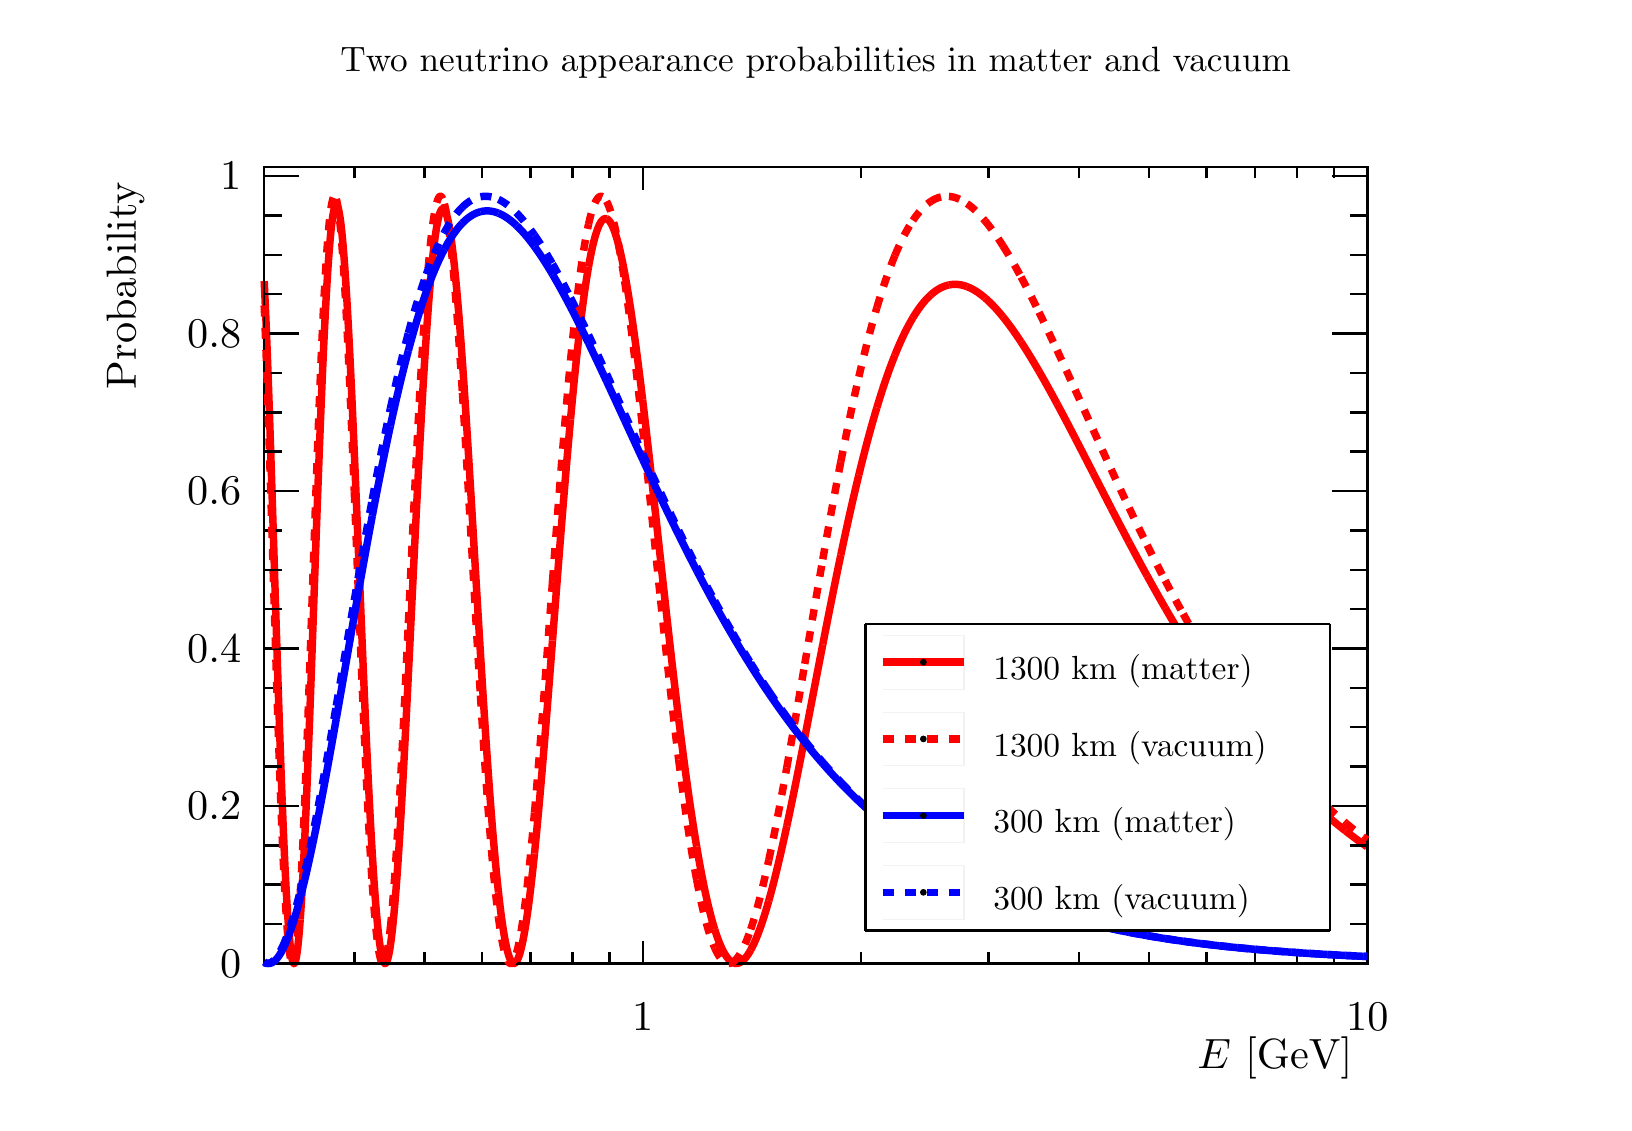
\begin{tikzpicture}
\pgfdeclareplotmark{cross} {
\pgfpathmoveto{\pgfpoint{-0.3\pgfplotmarksize}{\pgfplotmarksize}}
\pgfpathlineto{\pgfpoint{+0.3\pgfplotmarksize}{\pgfplotmarksize}}
\pgfpathlineto{\pgfpoint{+0.3\pgfplotmarksize}{0.3\pgfplotmarksize}}
\pgfpathlineto{\pgfpoint{+1\pgfplotmarksize}{0.3\pgfplotmarksize}}
\pgfpathlineto{\pgfpoint{+1\pgfplotmarksize}{-0.3\pgfplotmarksize}}
\pgfpathlineto{\pgfpoint{+0.3\pgfplotmarksize}{-0.3\pgfplotmarksize}}
\pgfpathlineto{\pgfpoint{+0.3\pgfplotmarksize}{-1.\pgfplotmarksize}}
\pgfpathlineto{\pgfpoint{-0.3\pgfplotmarksize}{-1.\pgfplotmarksize}}
\pgfpathlineto{\pgfpoint{-0.3\pgfplotmarksize}{-0.3\pgfplotmarksize}}
\pgfpathlineto{\pgfpoint{-1.\pgfplotmarksize}{-0.3\pgfplotmarksize}}
\pgfpathlineto{\pgfpoint{-1.\pgfplotmarksize}{0.3\pgfplotmarksize}}
\pgfpathlineto{\pgfpoint{-0.3\pgfplotmarksize}{0.3\pgfplotmarksize}}
\pgfpathclose
\pgfusepathqstroke
}
\pgfdeclareplotmark{cross*} {
\pgfpathmoveto{\pgfpoint{-0.3\pgfplotmarksize}{\pgfplotmarksize}}
\pgfpathlineto{\pgfpoint{+0.3\pgfplotmarksize}{\pgfplotmarksize}}
\pgfpathlineto{\pgfpoint{+0.3\pgfplotmarksize}{0.3\pgfplotmarksize}}
\pgfpathlineto{\pgfpoint{+1\pgfplotmarksize}{0.3\pgfplotmarksize}}
\pgfpathlineto{\pgfpoint{+1\pgfplotmarksize}{-0.3\pgfplotmarksize}}
\pgfpathlineto{\pgfpoint{+0.3\pgfplotmarksize}{-0.3\pgfplotmarksize}}
\pgfpathlineto{\pgfpoint{+0.3\pgfplotmarksize}{-1.\pgfplotmarksize}}
\pgfpathlineto{\pgfpoint{-0.3\pgfplotmarksize}{-1.\pgfplotmarksize}}
\pgfpathlineto{\pgfpoint{-0.3\pgfplotmarksize}{-0.3\pgfplotmarksize}}
\pgfpathlineto{\pgfpoint{-1.\pgfplotmarksize}{-0.3\pgfplotmarksize}}
\pgfpathlineto{\pgfpoint{-1.\pgfplotmarksize}{0.3\pgfplotmarksize}}
\pgfpathlineto{\pgfpoint{-0.3\pgfplotmarksize}{0.3\pgfplotmarksize}}
\pgfpathclose
\pgfusepathqfillstroke
}
\pgfdeclareplotmark{newstar} {
\pgfpathmoveto{\pgfqpoint{0pt}{\pgfplotmarksize}}
\pgfpathlineto{\pgfqpointpolar{44}{0.5\pgfplotmarksize}}
\pgfpathlineto{\pgfqpointpolar{18}{\pgfplotmarksize}}
\pgfpathlineto{\pgfqpointpolar{-20}{0.5\pgfplotmarksize}}
\pgfpathlineto{\pgfqpointpolar{-54}{\pgfplotmarksize}}
\pgfpathlineto{\pgfqpointpolar{-90}{0.5\pgfplotmarksize}}
\pgfpathlineto{\pgfqpointpolar{234}{\pgfplotmarksize}}
\pgfpathlineto{\pgfqpointpolar{198}{0.5\pgfplotmarksize}}
\pgfpathlineto{\pgfqpointpolar{162}{\pgfplotmarksize}}
\pgfpathlineto{\pgfqpointpolar{134}{0.5\pgfplotmarksize}}
\pgfpathclose
\pgfusepathqstroke
}
\pgfdeclareplotmark{newstar*} {
\pgfpathmoveto{\pgfqpoint{0pt}{\pgfplotmarksize}}
\pgfpathlineto{\pgfqpointpolar{44}{0.5\pgfplotmarksize}}
\pgfpathlineto{\pgfqpointpolar{18}{\pgfplotmarksize}}
\pgfpathlineto{\pgfqpointpolar{-20}{0.5\pgfplotmarksize}}
\pgfpathlineto{\pgfqpointpolar{-54}{\pgfplotmarksize}}
\pgfpathlineto{\pgfqpointpolar{-90}{0.5\pgfplotmarksize}}
\pgfpathlineto{\pgfqpointpolar{234}{\pgfplotmarksize}}
\pgfpathlineto{\pgfqpointpolar{198}{0.5\pgfplotmarksize}}
\pgfpathlineto{\pgfqpointpolar{162}{\pgfplotmarksize}}
\pgfpathlineto{\pgfqpointpolar{134}{0.5\pgfplotmarksize}}
\pgfpathclose
\pgfusepathqfillstroke
}
\definecolor{c}{rgb}{1,1,1};
\draw [color=c, fill=c] (0,0) rectangle (20,13.639);
\draw [color=c, fill=c] (2.99427,1.76218) rectangle (17.0057,11.8768);
\definecolor{c}{rgb}{0,0,0};
\draw [c,line width=0.9] (2.99427,1.76218) -- (2.99427,11.8768) -- (17.0057,11.8768) -- (17.0057,1.76218) -- (2.99427,1.76218);
\definecolor{c}{rgb}{1,1,1};
\draw [color=c, fill=c] (2.99427,1.76218) rectangle (17.0057,11.8768);
\definecolor{c}{rgb}{0,0,0};
\draw [c,line width=0.9] (2.99427,1.76218) -- (2.99427,11.8768) -- (17.0057,11.8768) -- (17.0057,1.76218) -- (2.99427,1.76218);
\definecolor{c}{rgb}{1,0,0};
\draw [c,line width=2.7] (2.99661,10.4272) -- (3.00128,10.331) -- (3.00595,10.231) -- (3.01062,10.1275) -- (3.01529,10.0204) -- (3.01996,9.90998) -- (3.02463,9.79629) -- (3.0293,9.67947) -- (3.03397,9.55965) -- (3.03864,9.43697) -- (3.04331,9.31155)
 -- (3.04798,9.18355) -- (3.05265,9.05308) -- (3.05732,8.92031) -- (3.06199,8.78535) -- (3.06666,8.64837) -- (3.07133,8.50949) -- (3.076,8.36887) -- (3.08067,8.22666) -- (3.08534,8.083) -- (3.09001,7.93803) -- (3.09469,7.7919) -- (3.09936,7.64477) --
 (3.10403,7.49678) -- (3.1087,7.34808) -- (3.11337,7.19882) -- (3.11804,7.04914) -- (3.12271,6.89919) -- (3.12738,6.74912) -- (3.13205,6.59907) -- (3.13672,6.44919) -- (3.14139,6.29963) -- (3.14606,6.15052) -- (3.15073,6.00201) -- (3.1554,5.85423) --
 (3.16007,5.70733) -- (3.16474,5.56145) -- (3.16941,5.41671) -- (3.17408,5.27325) -- (3.17875,5.13121) -- (3.18342,4.99071) -- (3.1881,4.85187) -- (3.19277,4.71483) -- (3.19744,4.57971) -- (3.20211,4.44662) -- (3.20678,4.31568) -- (3.21145,4.18701)
 -- (3.21612,4.06072) -- (3.22079,3.93691) -- (3.22546,3.8157);
\draw [c,line width=2.7] (3.22546,3.8157) -- (3.23013,3.69718) -- (3.2348,3.58146) -- (3.23947,3.46862) -- (3.24414,3.35878) -- (3.24881,3.252) -- (3.25348,3.14839) -- (3.25815,3.04802) -- (3.26282,2.95098) -- (3.26749,2.85733) -- (3.27216,2.76716)
 -- (3.27683,2.68053) -- (3.2815,2.5975) -- (3.28618,2.51814) -- (3.29085,2.44251) -- (3.29552,2.37066) -- (3.30019,2.30265) -- (3.30486,2.23851) -- (3.30953,2.17829) -- (3.3142,2.12203) -- (3.31887,2.06977) -- (3.32354,2.02154) -- (3.32821,1.97737)
 -- (3.33288,1.93727) -- (3.33755,1.90128) -- (3.34222,1.86941) -- (3.34689,1.84166) -- (3.35156,1.81806) -- (3.35623,1.79861) -- (3.3609,1.78331) -- (3.36557,1.77215) -- (3.37024,1.76514) -- (3.37491,1.76218) -- (3.37959,1.7635) -- (3.38426,1.76885)
 -- (3.38893,1.77828) -- (3.3936,1.79179) -- (3.39827,1.80932) -- (3.40294,1.83087) -- (3.40761,1.8564) -- (3.41228,1.88587) -- (3.41695,1.91924) -- (3.42162,1.95647) -- (3.42629,1.99752) -- (3.43096,2.04233) -- (3.43563,2.09087) -- (3.4403,2.14307)
 -- (3.44497,2.19887) -- (3.44964,2.25823) -- (3.45431,2.32107);
\draw [c,line width=2.7] (3.45431,2.32107) -- (3.45898,2.38734) -- (3.46365,2.45696) -- (3.46832,2.52987) -- (3.473,2.606) -- (3.47767,2.68527) -- (3.48234,2.76761) -- (3.48701,2.85294) -- (3.49168,2.94118) -- (3.49635,3.03225) -- (3.50102,3.12606)
 -- (3.50569,3.22253) -- (3.51036,3.32158) -- (3.51503,3.42311) -- (3.5197,3.52703) -- (3.52437,3.63326) -- (3.52904,3.7417) -- (3.53371,3.85225) -- (3.53838,3.96483) -- (3.54305,4.07934) -- (3.54772,4.19567) -- (3.55239,4.31373) -- (3.55706,4.43342)
 -- (3.56173,4.55465) -- (3.5664,4.67731) -- (3.57108,4.8013) -- (3.57575,4.92653) -- (3.58042,5.05288) -- (3.58509,5.18026) -- (3.58976,5.30857) -- (3.59443,5.4377) -- (3.5991,5.56755) -- (3.60377,5.69802) -- (3.60844,5.82901) -- (3.61311,5.96041)
 -- (3.61778,6.09213) -- (3.62245,6.22406) -- (3.62712,6.35611) -- (3.63179,6.48817) -- (3.63646,6.62014) -- (3.64113,6.75192) -- (3.6458,6.88342) -- (3.65047,7.01454) -- (3.65514,7.14518) -- (3.65981,7.27525) -- (3.66448,7.40465) --
 (3.66916,7.53328) -- (3.67383,7.66107) -- (3.6785,7.7879) -- (3.68317,7.9137);
\draw [c,line width=2.7] (3.68317,7.9137) -- (3.68784,8.03837) -- (3.69251,8.16183) -- (3.69718,8.284) -- (3.70185,8.40478) -- (3.70652,8.52409) -- (3.71119,8.64186) -- (3.71586,8.75799) -- (3.72053,8.87243) -- (3.7252,8.98508) -- (3.72987,9.09587)
 -- (3.73454,9.20474) -- (3.73921,9.3116) -- (3.74388,9.41639) -- (3.74855,9.51905) -- (3.75322,9.6195) -- (3.75789,9.71768) -- (3.76257,9.81354) -- (3.76724,9.90701) -- (3.77191,9.99803) -- (3.77658,10.0866) -- (3.78125,10.1725) -- (3.78592,10.2559)
 -- (3.79059,10.3366) -- (3.79526,10.4146) -- (3.79993,10.4899) -- (3.8046,10.5623) -- (3.80927,10.632) -- (3.81394,10.6988) -- (3.81861,10.7626) -- (3.82328,10.8236) -- (3.82795,10.8816) -- (3.83262,10.9365) -- (3.83729,10.9885) -- (3.84196,11.0374)
 -- (3.84663,11.0832) -- (3.8513,11.126) -- (3.85597,11.1656) -- (3.86065,11.2021) -- (3.86532,11.2355) -- (3.86999,11.2657) -- (3.87466,11.2928) -- (3.87933,11.3166) -- (3.884,11.3374) -- (3.88867,11.3549) -- (3.89334,11.3693) -- (3.89801,11.3805)
 -- (3.90268,11.3885) -- (3.90735,11.3934) -- (3.91202,11.3951);
\draw [c,line width=2.7] (3.91202,11.3951) -- (3.91669,11.3937) -- (3.92136,11.3892) -- (3.92603,11.3815) -- (3.9307,11.3707) -- (3.93537,11.3568) -- (3.94004,11.3399) -- (3.94471,11.3199) -- (3.94938,11.297) -- (3.95406,11.271) -- (3.95873,11.242)
 -- (3.9634,11.2101) -- (3.96807,11.1753) -- (3.97274,11.1377) -- (3.97741,11.0972) -- (3.98208,11.0538) -- (3.98675,11.0078) -- (3.99142,10.9589) -- (3.99609,10.9074) -- (4.00076,10.8533) -- (4.00543,10.7965) -- (4.0101,10.7372) -- (4.01477,10.6754)
 -- (4.01944,10.6111) -- (4.02411,10.5444) -- (4.02878,10.4753) -- (4.03345,10.4039) -- (4.03812,10.3303) -- (4.04279,10.2544) -- (4.04746,10.1764) -- (4.05214,10.0963) -- (4.05681,10.0141) -- (4.06148,9.92993) -- (4.06615,9.84385) --
 (4.07082,9.75589) -- (4.07549,9.66612) -- (4.08016,9.57461) -- (4.08483,9.4814) -- (4.0895,9.38657) -- (4.09417,9.29017) -- (4.09884,9.19228) -- (4.10351,9.09294) -- (4.10818,8.99224) -- (4.11285,8.89022) -- (4.11752,8.78696) -- (4.12219,8.68252) --
 (4.12686,8.57697) -- (4.13153,8.47038) -- (4.1362,8.3628) -- (4.14087,8.25432);
\draw [c,line width=2.7] (4.14087,8.25432) -- (4.14555,8.14498) -- (4.15022,8.03486) -- (4.15489,7.92404) -- (4.15956,7.81256) -- (4.16423,7.7005) -- (4.1689,7.58794) -- (4.17357,7.47492) -- (4.17824,7.36153) -- (4.18291,7.24782) -- (4.18758,7.13387)
 -- (4.19225,7.01973) -- (4.19692,6.90548) -- (4.20159,6.79117) -- (4.20626,6.67689) -- (4.21093,6.56268) -- (4.2156,6.44861) -- (4.22027,6.33475) -- (4.22494,6.22117) -- (4.22961,6.10791) -- (4.23428,5.99505) -- (4.23896,5.88265) --
 (4.24363,5.77076) -- (4.2483,5.65945) -- (4.25297,5.54878) -- (4.25764,5.43881) -- (4.26231,5.32959) -- (4.26698,5.22118) -- (4.27165,5.11364) -- (4.27632,5.00702) -- (4.28099,4.90138) -- (4.28566,4.79678) -- (4.29033,4.69326) -- (4.295,4.59088) --
 (4.29967,4.48969) -- (4.30434,4.38975) -- (4.30901,4.29109) -- (4.31368,4.19377) -- (4.31835,4.09783) -- (4.32302,4.00333) -- (4.32769,3.9103) -- (4.33236,3.8188) -- (4.33704,3.72886) -- (4.34171,3.64053) -- (4.34638,3.55385) -- (4.35105,3.46885) --
 (4.35572,3.38558) -- (4.36039,3.30408) -- (4.36506,3.22437) -- (4.36973,3.1465);
\draw [c,line width=2.7] (4.36973,3.1465) -- (4.3744,3.07051) -- (4.37907,2.99641) -- (4.38374,2.92425) -- (4.38841,2.85405) -- (4.39308,2.78585) -- (4.39775,2.71967) -- (4.40242,2.65554) -- (4.40709,2.59349) -- (4.41176,2.53353) -- (4.41643,2.4757)
 -- (4.4211,2.42001) -- (4.42577,2.36649) -- (4.43044,2.31515) -- (4.43512,2.26601) -- (4.43979,2.21909) -- (4.44446,2.17441) -- (4.44913,2.13198) -- (4.4538,2.09181) -- (4.45847,2.05392) -- (4.46314,2.01831) -- (4.46781,1.985) -- (4.47248,1.95399)
 -- (4.47715,1.92529) -- (4.48182,1.89891) -- (4.48649,1.87486) -- (4.49116,1.85312) -- (4.49583,1.83372) -- (4.5005,1.81665) -- (4.50517,1.8019) -- (4.50984,1.78948) -- (4.51451,1.77939) -- (4.51918,1.77162) -- (4.52385,1.76617) -- (4.52852,1.76218)
 -- (4.5332,1.76218) -- (4.53787,1.76366) -- (4.54254,1.76742) -- (4.54721,1.77345) -- (4.55188,1.78175) -- (4.55655,1.79231) -- (4.56122,1.80511) -- (4.56589,1.82014) -- (4.57056,1.83738) -- (4.57523,1.85682) -- (4.5799,1.87844) -- (4.58457,1.90223)
 -- (4.58924,1.92816) -- (4.59391,1.95621) -- (4.59858,1.98637);
\draw [c,line width=2.7] (4.59858,1.98637) -- (4.60325,2.01861) -- (4.60792,2.05291) -- (4.61259,2.08925) -- (4.61726,2.1276) -- (4.62193,2.16793) -- (4.62661,2.21023) -- (4.63128,2.25447) -- (4.63595,2.30061) -- (4.64062,2.34863) --
 (4.64529,2.39851) -- (4.64996,2.45021) -- (4.65463,2.5037) -- (4.6593,2.55896) -- (4.66397,2.61594) -- (4.66864,2.67463) -- (4.67331,2.73498) -- (4.67798,2.79697) -- (4.68265,2.86055) -- (4.68732,2.9257) -- (4.69199,2.99239) -- (4.69666,3.06057) --
 (4.70133,3.13021) -- (4.706,3.20128) -- (4.71067,3.27373) -- (4.71534,3.34754) -- (4.72002,3.42266) -- (4.72469,3.49906) -- (4.72936,3.5767) -- (4.73403,3.65553) -- (4.7387,3.73553) -- (4.74337,3.81666) -- (4.74804,3.89886) -- (4.75271,3.98211) --
 (4.75738,4.06637) -- (4.76205,4.15159) -- (4.76672,4.23774) -- (4.77139,4.32477) -- (4.77606,4.41265) -- (4.78073,4.50133) -- (4.7854,4.59077) -- (4.79007,4.68094) -- (4.79474,4.77179) -- (4.79941,4.86328) -- (4.80408,4.95537) -- (4.80875,5.04802)
 -- (4.81342,5.14119) -- (4.8181,5.23484) -- (4.82277,5.32893) -- (4.82744,5.42341);
\draw [c,line width=2.7] (4.82744,5.42341) -- (4.83211,5.51825) -- (4.83678,5.6134) -- (4.84145,5.70883) -- (4.84612,5.80449) -- (4.85079,5.90034) -- (4.85546,5.99635) -- (4.86013,6.09248) -- (4.8648,6.18868) -- (4.86947,6.28491) -- (4.87414,6.38114)
 -- (4.87881,6.47732) -- (4.88348,6.57343) -- (4.88815,6.66941) -- (4.89282,6.76523) -- (4.89749,6.86086) -- (4.90216,6.95625) -- (4.90683,7.05137) -- (4.9115,7.14618) -- (4.91618,7.24064) -- (4.92085,7.33472) -- (4.92552,7.42839) -- (4.93019,7.5216)
 -- (4.93486,7.61432) -- (4.93953,7.70651) -- (4.9442,7.79815) -- (4.94887,7.8892) -- (4.95354,7.97962) -- (4.95821,8.06938) -- (4.96288,8.15845) -- (4.96755,8.2468) -- (4.97222,8.33439) -- (4.97689,8.42119) -- (4.98156,8.50718) -- (4.98623,8.59232)
 -- (4.9909,8.67659) -- (4.99557,8.75994) -- (5.00024,8.84236) -- (5.00491,8.92382) -- (5.00959,9.00429) -- (5.01426,9.08374) -- (5.01893,9.16215) -- (5.0236,9.23948) -- (5.02827,9.31572) -- (5.03294,9.39084) -- (5.03761,9.46482) -- (5.04228,9.53762)
 -- (5.04695,9.60924) -- (5.05162,9.67964) -- (5.05629,9.74881);
\draw [c,line width=2.7] (5.05629,9.74881) -- (5.06096,9.81671) -- (5.06563,9.88335) -- (5.0703,9.94868) -- (5.07497,10.0127) -- (5.07964,10.0754) -- (5.08431,10.1367) -- (5.08898,10.1967) -- (5.09365,10.2552) -- (5.09832,10.3124) --
 (5.10299,10.3681) -- (5.10767,10.4224) -- (5.11234,10.4753) -- (5.11701,10.5267) -- (5.12168,10.5766) -- (5.12635,10.625) -- (5.13102,10.6719) -- (5.13569,10.7173) -- (5.14036,10.7612) -- (5.14503,10.8035) -- (5.1497,10.8443) -- (5.15437,10.8835) --
 (5.15904,10.9212) -- (5.16371,10.9573) -- (5.16838,10.9919) -- (5.17305,11.0248) -- (5.17772,11.0562) -- (5.18239,11.0859) -- (5.18706,11.1141) -- (5.19173,11.1406) -- (5.1964,11.1656) -- (5.20108,11.1889) -- (5.20575,11.2107) -- (5.21042,11.2308)
 -- (5.21509,11.2493) -- (5.21976,11.2661) -- (5.22443,11.2814) -- (5.2291,11.295) -- (5.23377,11.3071) -- (5.23844,11.3175) -- (5.24311,11.3263) -- (5.24778,11.3335) -- (5.25245,11.3391) -- (5.25712,11.3431) -- (5.26179,11.3455) -- (5.26646,11.3463)
 -- (5.27113,11.3455) -- (5.2758,11.3431) -- (5.28047,11.3392) -- (5.28514,11.3337);
\draw [c,line width=2.7] (5.28514,11.3337) -- (5.28981,11.3266) -- (5.29449,11.318) -- (5.29916,11.3078) -- (5.30383,11.2961) -- (5.3085,11.2829) -- (5.31317,11.2681) -- (5.31784,11.2519) -- (5.32251,11.2341) -- (5.32718,11.2149) -- (5.33185,11.1942)
 -- (5.33652,11.172) -- (5.34119,11.1484) -- (5.34586,11.1233) -- (5.35053,11.0968) -- (5.3552,11.0689) -- (5.35987,11.0397) -- (5.36454,11.009) -- (5.36921,10.977) -- (5.37388,10.9436) -- (5.37855,10.9089) -- (5.38322,10.8728) -- (5.38789,10.8355)
 -- (5.39257,10.7968) -- (5.39724,10.7569) -- (5.40191,10.7157) -- (5.40658,10.6733) -- (5.41125,10.6297) -- (5.41592,10.5849) -- (5.42059,10.5389) -- (5.42526,10.4917) -- (5.42993,10.4434) -- (5.4346,10.3939) -- (5.43927,10.3434) --
 (5.44394,10.2917) -- (5.44861,10.239) -- (5.45328,10.1852) -- (5.45795,10.1304) -- (5.46262,10.0746) -- (5.46729,10.0178) -- (5.47196,9.96001) -- (5.47663,9.90129) -- (5.4813,9.84165) -- (5.48597,9.78109) -- (5.49065,9.71966) -- (5.49532,9.65735) --
 (5.49999,9.59421) -- (5.50466,9.53025) -- (5.50933,9.46549) -- (5.514,9.39995);
\draw [c,line width=2.7] (5.514,9.39995) -- (5.51867,9.33366) -- (5.52334,9.26664) -- (5.52801,9.1989) -- (5.53268,9.13048) -- (5.53735,9.0614) -- (5.54202,8.99167) -- (5.54669,8.92132) -- (5.55136,8.85038) -- (5.55603,8.77886) -- (5.5607,8.70679) --
 (5.56537,8.63419) -- (5.57004,8.56109) -- (5.57471,8.4875) -- (5.57938,8.41345) -- (5.58405,8.33896) -- (5.58873,8.26406) -- (5.5934,8.18876) -- (5.59807,8.11309) -- (5.60274,8.03708) -- (5.60741,7.96074) -- (5.61208,7.8841) -- (5.61675,7.80718) --
 (5.62142,7.73001) -- (5.62609,7.6526) -- (5.63076,7.57498) -- (5.63543,7.49717) -- (5.6401,7.41919) -- (5.64477,7.34106) -- (5.64944,7.26282) -- (5.65411,7.18447) -- (5.65878,7.10605) -- (5.66345,7.02756) -- (5.66812,6.94904) -- (5.67279,6.87051) --
 (5.67746,6.79199) -- (5.68214,6.71349) -- (5.68681,6.63504) -- (5.69148,6.55667) -- (5.69615,6.47839) -- (5.70082,6.40021) -- (5.70549,6.32218) -- (5.71016,6.24429) -- (5.71483,6.16658) -- (5.7195,6.08907) -- (5.72417,6.01177) -- (5.72884,5.9347) --
 (5.73351,5.85789) -- (5.73818,5.78135) -- (5.74285,5.7051);
\draw [c,line width=2.7] (5.74285,5.7051) -- (5.74752,5.62916) -- (5.75219,5.55355) -- (5.75686,5.47829) -- (5.76153,5.4034) -- (5.7662,5.32889) -- (5.77087,5.25479) -- (5.77555,5.18111) -- (5.78022,5.10786) -- (5.78489,5.03507) -- (5.78956,4.96276)
 -- (5.79423,4.89093) -- (5.7989,4.81961) -- (5.80357,4.74882) -- (5.80824,4.67856) -- (5.81291,4.60886) -- (5.81758,4.53973) -- (5.82225,4.47119) -- (5.82692,4.40325) -- (5.83159,4.33592) -- (5.83626,4.26923) -- (5.84093,4.20318) -- (5.8456,4.13779)
 -- (5.85027,4.07308) -- (5.85494,4.00906) -- (5.85961,3.94573) -- (5.86428,3.88312) -- (5.86895,3.82124) -- (5.87363,3.7601) -- (5.8783,3.69971) -- (5.88297,3.64009) -- (5.88764,3.58125) -- (5.89231,3.52319) -- (5.89698,3.46593) -- (5.90165,3.40948)
 -- (5.90632,3.35386) -- (5.91099,3.29907) -- (5.91566,3.24512) -- (5.92033,3.19202) -- (5.925,3.13979) -- (5.92967,3.08842) -- (5.93434,3.03794) -- (5.93901,2.98835) -- (5.94368,2.93966) -- (5.94835,2.89187) -- (5.95302,2.845) -- (5.95769,2.79905)
 -- (5.96236,2.75404) -- (5.96704,2.70996) -- (5.97171,2.66683);
\draw [c,line width=2.7] (5.97171,2.66683) -- (5.97638,2.62464) -- (5.98105,2.58342) -- (5.98572,2.54316) -- (5.99039,2.50387) -- (5.99506,2.46556) -- (5.99973,2.42823) -- (6.0044,2.39188) -- (6.00907,2.35653) -- (6.01374,2.32217) --
 (6.01841,2.28881) -- (6.02308,2.25646) -- (6.02775,2.22512) -- (6.03242,2.19478) -- (6.03709,2.16547) -- (6.04176,2.13717) -- (6.04643,2.10989) -- (6.0511,2.08363) -- (6.05577,2.0584) -- (6.06044,2.0342) -- (6.06512,2.01103) -- (6.06979,1.98889) --
 (6.07446,1.96778) -- (6.07913,1.9477) -- (6.0838,1.92866) -- (6.08847,1.91065) -- (6.09314,1.89368) -- (6.09781,1.87774) -- (6.10248,1.86284) -- (6.10715,1.84897) -- (6.11182,1.83614) -- (6.11649,1.82433) -- (6.12116,1.81356) -- (6.12583,1.80382) --
 (6.1305,1.79511) -- (6.13517,1.78742) -- (6.13984,1.78076) -- (6.14451,1.77513) -- (6.14918,1.77051) -- (6.15385,1.76691) -- (6.15852,1.76432) -- (6.1632,1.76218) -- (6.16787,1.76218) -- (6.17254,1.76218) -- (6.17721,1.76406) -- (6.18188,1.76649) --
 (6.18655,1.76992) -- (6.19122,1.77434) -- (6.19589,1.77974) -- (6.20056,1.78612);
\draw [c,line width=2.7] (6.20056,1.78612) -- (6.20523,1.79348) -- (6.2099,1.8018) -- (6.21457,1.81109) -- (6.21924,1.82134) -- (6.22391,1.83255) -- (6.22858,1.8447) -- (6.23325,1.85779) -- (6.23792,1.87181) -- (6.24259,1.88677) -- (6.24726,1.90265)
 -- (6.25194,1.91944) -- (6.25661,1.93715) -- (6.26128,1.95576) -- (6.26595,1.97526) -- (6.27062,1.99565) -- (6.27529,2.01693) -- (6.27996,2.03907) -- (6.28463,2.06208) -- (6.2893,2.08596) -- (6.29397,2.11068) -- (6.29864,2.13624) --
 (6.30331,2.16264) -- (6.30798,2.18986) -- (6.31265,2.2179) -- (6.31732,2.24675) -- (6.32199,2.2764) -- (6.32666,2.30684) -- (6.33133,2.33807) -- (6.336,2.37007) -- (6.34067,2.40283) -- (6.34534,2.43635) -- (6.35002,2.47061) -- (6.35469,2.50562) --
 (6.35936,2.54135) -- (6.36403,2.57779) -- (6.3687,2.61495) -- (6.37337,2.6528) -- (6.37804,2.69134) -- (6.38271,2.73056) -- (6.38738,2.77045) -- (6.39205,2.811) -- (6.39672,2.8522) -- (6.40139,2.89403) -- (6.40606,2.9365) -- (6.41073,2.97958) --
 (6.4154,3.02326) -- (6.42007,3.06755) -- (6.42474,3.11242) -- (6.42941,3.15787);
\draw [c,line width=2.7] (6.42941,3.15787) -- (6.43408,3.20388) -- (6.43875,3.25044) -- (6.44342,3.29756) -- (6.4481,3.3452) -- (6.45277,3.39336) -- (6.45744,3.44204) -- (6.46211,3.49122) -- (6.46678,3.54089) -- (6.47145,3.59103) -- (6.47612,3.64165)
 -- (6.48079,3.69272) -- (6.48546,3.74423) -- (6.49013,3.79619) -- (6.4948,3.84856) -- (6.49947,3.90135) -- (6.50414,3.95454) -- (6.50881,4.00812) -- (6.51348,4.06208) -- (6.51815,4.1164) -- (6.52282,4.17109) -- (6.52749,4.22612) -- (6.53216,4.28149)
 -- (6.53683,4.33718) -- (6.5415,4.39318) -- (6.54618,4.44948) -- (6.55085,4.50608) -- (6.55552,4.56295) -- (6.56019,4.6201) -- (6.56486,4.6775) -- (6.56953,4.73515) -- (6.5742,4.79303) -- (6.57887,4.85114) -- (6.58354,4.90946) -- (6.58821,4.96798)
 -- (6.59288,5.02669) -- (6.59755,5.08559) -- (6.60222,5.14466) -- (6.60689,5.20388) -- (6.61156,5.26326) -- (6.61623,5.32277) -- (6.6209,5.3824) -- (6.62557,5.44216) -- (6.63024,5.50202) -- (6.63491,5.56197) -- (6.63959,5.62201) -- (6.64426,5.68213)
 -- (6.64893,5.7423) -- (6.6536,5.80253) -- (6.65827,5.86281);
\draw [c,line width=2.7] (6.65827,5.86281) -- (6.66294,5.92311) -- (6.66761,5.98344) -- (6.67228,6.04378) -- (6.67695,6.10412) -- (6.68162,6.16446) -- (6.68629,6.22477) -- (6.69096,6.28506) -- (6.69563,6.34531) -- (6.7003,6.40551) --
 (6.70497,6.46566) -- (6.70964,6.52574) -- (6.71431,6.58574) -- (6.71898,6.64566) -- (6.72365,6.70548) -- (6.72832,6.76519) -- (6.733,6.82479) -- (6.73767,6.88427) -- (6.74234,6.94361) -- (6.74701,7.00282) -- (6.75168,7.06187) -- (6.75635,7.12076) --
 (6.76102,7.17948) -- (6.76569,7.23803) -- (6.77036,7.29639) -- (6.77503,7.35455) -- (6.7797,7.41252) -- (6.78437,7.47026) -- (6.78904,7.52779) -- (6.79371,7.5851) -- (6.79838,7.64216) -- (6.80305,7.69898) -- (6.80772,7.75555) -- (6.81239,7.81185) --
 (6.81706,7.86789) -- (6.82173,7.92365) -- (6.8264,7.97913) -- (6.83108,8.03432) -- (6.83575,8.0892) -- (6.84042,8.14378) -- (6.84509,8.19805) -- (6.84976,8.252) -- (6.85443,8.30562) -- (6.8591,8.3589) -- (6.86377,8.41184) -- (6.86844,8.46443) --
 (6.87311,8.51667) -- (6.87778,8.56854) -- (6.88245,8.62005) -- (6.88712,8.67118);
\draw [c,line width=2.7] (6.88712,8.67118) -- (6.89179,8.72193) -- (6.89646,8.77229) -- (6.90113,8.82226) -- (6.9058,8.87183) -- (6.91047,8.92099) -- (6.91514,8.96974) -- (6.91981,9.01808) -- (6.92448,9.06599) -- (6.92916,9.11347) --
 (6.93383,9.16052) -- (6.9385,9.20713) -- (6.94317,9.25329) -- (6.94784,9.29901) -- (6.95251,9.34427) -- (6.95718,9.38906) -- (6.96185,9.4334) -- (6.96652,9.47726) -- (6.97119,9.52066) -- (6.97586,9.56357) -- (6.98053,9.606) -- (6.9852,9.64794) --
 (6.98987,9.68939) -- (6.99454,9.73034) -- (6.99921,9.7708) -- (7.00388,9.81075) -- (7.00855,9.85019) -- (7.01322,9.88912) -- (7.01789,9.92753) -- (7.02257,9.96543) -- (7.02724,10.0028) -- (7.03191,10.0397) -- (7.03658,10.076) -- (7.04125,10.1118) --
 (7.04592,10.147) -- (7.05059,10.1817) -- (7.05526,10.2159) -- (7.05993,10.2495) -- (7.0646,10.2826) -- (7.06927,10.3151) -- (7.07394,10.3471) -- (7.07861,10.3785) -- (7.08328,10.4094) -- (7.08795,10.4397) -- (7.09262,10.4695) -- (7.09729,10.4987) --
 (7.10196,10.5273) -- (7.10663,10.5553) -- (7.1113,10.5828) -- (7.11597,10.6097);
\draw [c,line width=2.7] (7.11597,10.6097) -- (7.12065,10.6361) -- (7.12532,10.6619) -- (7.12999,10.6871) -- (7.13466,10.7117) -- (7.13933,10.7357) -- (7.144,10.7592) -- (7.14867,10.7821) -- (7.15334,10.8044) -- (7.15801,10.8261) -- (7.16268,10.8472)
 -- (7.16735,10.8678) -- (7.17202,10.8878) -- (7.17669,10.9072) -- (7.18136,10.926) -- (7.18603,10.9442) -- (7.1907,10.9618) -- (7.19537,10.9789) -- (7.20004,10.9954) -- (7.20471,11.0113) -- (7.20938,11.0266) -- (7.21406,11.0413) -- (7.21873,11.0554)
 -- (7.2234,11.0689) -- (7.22807,11.0819) -- (7.23274,11.0943) -- (7.23741,11.1061) -- (7.24208,11.1173) -- (7.24675,11.1279) -- (7.25142,11.1379) -- (7.25609,11.1474) -- (7.26076,11.1563) -- (7.26543,11.1646) -- (7.2701,11.1723) -- (7.27477,11.1795)
 -- (7.27944,11.1861) -- (7.28411,11.1921) -- (7.28878,11.1975) -- (7.29345,11.2023) -- (7.29812,11.2066) -- (7.30279,11.2104) -- (7.30747,11.2135) -- (7.31214,11.2161) -- (7.31681,11.2181) -- (7.32148,11.2196) -- (7.32615,11.2205) --
 (7.33082,11.2208) -- (7.33549,11.2206) -- (7.34016,11.2198) -- (7.34483,11.2185);
\draw [c,line width=2.7] (7.34483,11.2185) -- (7.3495,11.2166) -- (7.35417,11.2142) -- (7.35884,11.2113) -- (7.36351,11.2078) -- (7.36818,11.2037) -- (7.37285,11.1991) -- (7.37752,11.194) -- (7.38219,11.1883) -- (7.38686,11.1821) -- (7.39153,11.1754)
 -- (7.3962,11.1682) -- (7.40087,11.1604) -- (7.40555,11.1521) -- (7.41022,11.1433) -- (7.41489,11.134) -- (7.41956,11.1242) -- (7.42423,11.1138) -- (7.4289,11.103) -- (7.43357,11.0916) -- (7.43824,11.0798) -- (7.44291,11.0674) -- (7.44758,11.0546)
 -- (7.45225,11.0413) -- (7.45692,11.0275) -- (7.46159,11.0132) -- (7.46626,10.9984) -- (7.47093,10.9831) -- (7.4756,10.9674) -- (7.48027,10.9512) -- (7.48494,10.9345) -- (7.48961,10.9174) -- (7.49428,10.8998) -- (7.49895,10.8818) --
 (7.50363,10.8633) -- (7.5083,10.8443) -- (7.51297,10.8249) -- (7.51764,10.8051) -- (7.52231,10.7848) -- (7.52698,10.7641) -- (7.53165,10.743) -- (7.53632,10.7214) -- (7.54099,10.6994) -- (7.54566,10.677) -- (7.55033,10.6542) -- (7.555,10.631) --
 (7.55967,10.6073) -- (7.56434,10.5833) -- (7.56901,10.5589) -- (7.57368,10.534);
\draw [c,line width=2.7] (7.57368,10.534) -- (7.57835,10.5088) -- (7.58302,10.4832) -- (7.58769,10.4572) -- (7.59236,10.4309) -- (7.59703,10.4041) -- (7.60171,10.377) -- (7.60638,10.3495) -- (7.61105,10.3217) -- (7.61572,10.2935) -- (7.62039,10.2649)
 -- (7.62506,10.236) -- (7.62973,10.2068) -- (7.6344,10.1772) -- (7.63907,10.1473) -- (7.64374,10.1171) -- (7.64841,10.0865) -- (7.65308,10.0556) -- (7.65775,10.0244) -- (7.66242,9.99282) -- (7.66709,9.96097) -- (7.67176,9.92882) -- (7.67643,9.89637)
 -- (7.6811,9.86362) -- (7.68577,9.83058) -- (7.69044,9.79725) -- (7.69512,9.76364) -- (7.69979,9.72974) -- (7.70446,9.69557) -- (7.70913,9.66113) -- (7.7138,9.62643) -- (7.71847,9.59146) -- (7.72314,9.55624) -- (7.72781,9.52076) -- (7.73248,9.48503)
 -- (7.73715,9.44906) -- (7.74182,9.41285) -- (7.74649,9.3764) -- (7.75116,9.33972) -- (7.75583,9.30282) -- (7.7605,9.26569) -- (7.76517,9.22835) -- (7.76984,9.19079) -- (7.77451,9.15302) -- (7.77918,9.11505) -- (7.78385,9.07688) -- (7.78853,9.03851)
 -- (7.7932,8.99995) -- (7.79787,8.96121) -- (7.80254,8.92228);
\draw [c,line width=2.7] (7.80254,8.92228) -- (7.80721,8.88317) -- (7.81188,8.84389) -- (7.81655,8.80444) -- (7.82122,8.76482) -- (7.82589,8.72505) -- (7.83056,8.68511) -- (7.83523,8.64503) -- (7.8399,8.6048) -- (7.84457,8.56442) -- (7.84924,8.5239)
 -- (7.85391,8.48325) -- (7.85858,8.44247) -- (7.86325,8.40156) -- (7.86792,8.36053) -- (7.87259,8.31938) -- (7.87726,8.27812) -- (7.88193,8.23674) -- (7.88661,8.19526) -- (7.89128,8.15368) -- (7.89595,8.11201) -- (7.90062,8.07024) --
 (7.90529,8.02838) -- (7.90996,7.98643) -- (7.91463,7.94441) -- (7.9193,7.90231) -- (7.92397,7.86013) -- (7.92864,7.81789) -- (7.93331,7.77558) -- (7.93798,7.73322) -- (7.94265,7.69079) -- (7.94732,7.64832) -- (7.95199,7.60579) -- (7.95666,7.56322)
 -- (7.96133,7.52061) -- (7.966,7.47797) -- (7.97067,7.43529) -- (7.97534,7.39258) -- (7.98001,7.34984) -- (7.98469,7.30709) -- (7.98936,7.26432) -- (7.99403,7.22153) -- (7.9987,7.17873) -- (8.00337,7.13593) -- (8.00804,7.09313) -- (8.01271,7.05032)
 -- (8.01738,7.00752) -- (8.02205,6.96473) -- (8.02672,6.92196) -- (8.03139,6.87919);
\draw [c,line width=2.7] (8.03139,6.87919) -- (8.03606,6.83645) -- (8.04073,6.79373) -- (8.0454,6.75104) -- (8.05007,6.70837) -- (8.05474,6.66574) -- (8.05941,6.62315) -- (8.06408,6.5806) -- (8.06875,6.53809) -- (8.07342,6.49562) -- (8.0781,6.45321)
 -- (8.08277,6.41086) -- (8.08744,6.36856) -- (8.09211,6.32632) -- (8.09678,6.28414) -- (8.10145,6.24203) -- (8.10612,6.19999) -- (8.11079,6.15803) -- (8.11546,6.11614) -- (8.12013,6.07433) -- (8.1248,6.03261) -- (8.12947,5.99097) --
 (8.13414,5.94942) -- (8.13881,5.90796) -- (8.14348,5.8666) -- (8.14815,5.82533) -- (8.15282,5.78417) -- (8.15749,5.74311) -- (8.16216,5.70216) -- (8.16683,5.66131) -- (8.1715,5.62058) -- (8.17618,5.57997) -- (8.18085,5.53947) -- (8.18552,5.4991) --
 (8.19019,5.45885) -- (8.19486,5.41873) -- (8.19953,5.37873) -- (8.2042,5.33887) -- (8.20887,5.29914) -- (8.21354,5.25955) -- (8.21821,5.2201) -- (8.22288,5.18079) -- (8.22755,5.14163) -- (8.23222,5.10261) -- (8.23689,5.06375) -- (8.24156,5.02503) --
 (8.24623,4.98648) -- (8.2509,4.94807) -- (8.25557,4.90983) -- (8.26024,4.87175);
\draw [c,line width=2.7] (8.26024,4.87175) -- (8.26491,4.83384) -- (8.26959,4.79609) -- (8.27426,4.75851) -- (8.27893,4.7211) -- (8.2836,4.68387) -- (8.28827,4.64681) -- (8.29294,4.60992) -- (8.29761,4.57322) -- (8.30228,4.5367) -- (8.30695,4.50036)
 -- (8.31162,4.46421) -- (8.31629,4.42825) -- (8.32096,4.39248) -- (8.32563,4.35689) -- (8.3303,4.32151) -- (8.33497,4.28631) -- (8.33964,4.25132) -- (8.34431,4.21653) -- (8.34898,4.18193) -- (8.35365,4.14754) -- (8.35832,4.11336) -- (8.363,4.07938)
 -- (8.36767,4.04561) -- (8.37234,4.01204) -- (8.37701,3.97869) -- (8.38168,3.94556) -- (8.38635,3.91264) -- (8.39102,3.87993) -- (8.39569,3.84745) -- (8.40036,3.81518) -- (8.40503,3.78313) -- (8.4097,3.75131) -- (8.41437,3.71971) --
 (8.41904,3.68833) -- (8.42371,3.65719) -- (8.42838,3.62627) -- (8.43305,3.59558) -- (8.43772,3.56512) -- (8.44239,3.53489) -- (8.44706,3.50489) -- (8.45173,3.47513) -- (8.4564,3.44561) -- (8.46107,3.41632) -- (8.46575,3.38727) -- (8.47042,3.35846)
 -- (8.47509,3.32989) -- (8.47976,3.30157) -- (8.48443,3.27348) -- (8.4891,3.24564);
\draw [c,line width=2.7] (8.4891,3.24564) -- (8.49377,3.21804) -- (8.49844,3.19069) -- (8.50311,3.16358) -- (8.50778,3.13673) -- (8.51245,3.11012) -- (8.51712,3.08375) -- (8.52179,3.05764) -- (8.52646,3.03178) -- (8.53113,3.00618) -- (8.5358,2.98082)
 -- (8.54047,2.95572) -- (8.54514,2.93087) -- (8.54981,2.90628) -- (8.55449,2.88194) -- (8.55916,2.85786) -- (8.56383,2.83403) -- (8.5685,2.81046) -- (8.57317,2.78715) -- (8.57784,2.7641) -- (8.58251,2.74131) -- (8.58718,2.71878) -- (8.59185,2.69651)
 -- (8.59652,2.67449) -- (8.60119,2.65274) -- (8.60586,2.63125) -- (8.61053,2.61003) -- (8.6152,2.58906) -- (8.61987,2.56836) -- (8.62454,2.54792) -- (8.62921,2.52775) -- (8.63388,2.50784) -- (8.63855,2.48819) -- (8.64322,2.46881) --
 (8.64789,2.44969) -- (8.65257,2.43083) -- (8.65724,2.41225) -- (8.66191,2.39392) -- (8.66658,2.37587) -- (8.67125,2.35807) -- (8.67592,2.34055) -- (8.68059,2.32329) -- (8.68526,2.30629) -- (8.68993,2.28956) -- (8.6946,2.2731) -- (8.69927,2.2569) --
 (8.70394,2.24097) -- (8.70861,2.22531) -- (8.71328,2.20991) -- (8.71795,2.19478);
\draw [c,line width=2.7] (8.71795,2.19478) -- (8.72262,2.17991) -- (8.72729,2.16531) -- (8.73196,2.15098) -- (8.73663,2.13691) -- (8.7413,2.12311) -- (8.74597,2.10957) -- (8.75065,2.0963) -- (8.75532,2.08329) -- (8.75999,2.07055) -- (8.76466,2.05807)
 -- (8.76933,2.04586) -- (8.774,2.03391) -- (8.77867,2.02223) -- (8.78334,2.0108) -- (8.78801,1.99965) -- (8.79268,1.98875) -- (8.79735,1.97812) -- (8.80202,1.96775) -- (8.80669,1.95764) -- (8.81136,1.94779) -- (8.81603,1.93821) -- (8.8207,1.92888)
 -- (8.82537,1.91982) -- (8.83004,1.91102) -- (8.83471,1.90247) -- (8.83939,1.89419) -- (8.84406,1.88616) -- (8.84873,1.87839) -- (8.8534,1.87088) -- (8.85807,1.86362) -- (8.86274,1.85663) -- (8.86741,1.84988) -- (8.87208,1.8434) -- (8.87675,1.83716)
 -- (8.88142,1.83119) -- (8.88609,1.82546) -- (8.89076,1.81999) -- (8.89543,1.81477) -- (8.9001,1.8098) -- (8.90477,1.80508) -- (8.90944,1.80062) -- (8.91411,1.7964) -- (8.91878,1.79243) -- (8.92345,1.78871) -- (8.92812,1.78524) -- (8.93279,1.78201)
 -- (8.93746,1.77903) -- (8.94214,1.7763) -- (8.94681,1.77381);
\draw [c,line width=2.7] (8.94681,1.77381) -- (8.95148,1.77156) -- (8.95615,1.76956) -- (8.96082,1.7678) -- (8.96549,1.76628) -- (8.97016,1.765) -- (8.97483,1.76396) -- (8.9795,1.76218) -- (8.98417,1.76218) -- (8.98884,1.76218) -- (8.99351,1.76218)
 -- (8.99818,1.76218) -- (9.00285,1.76218) -- (9.00752,1.76332) -- (9.01219,1.76416) -- (9.01686,1.76524) -- (9.02153,1.76655) -- (9.0262,1.76809) -- (9.03087,1.76986) -- (9.03555,1.77185) -- (9.04022,1.77407) -- (9.04489,1.77652) -- (9.04956,1.7792)
 -- (9.05423,1.78209) -- (9.0589,1.78521) -- (9.06357,1.78856) -- (9.06824,1.79212) -- (9.07291,1.7959) -- (9.07758,1.79991) -- (9.08225,1.80413) -- (9.08692,1.80856) -- (9.09159,1.81322) -- (9.09626,1.81809) -- (9.10093,1.82317) -- (9.1056,1.82846)
 -- (9.11027,1.83397) -- (9.11494,1.83969) -- (9.11961,1.84561) -- (9.12428,1.85175) -- (9.12895,1.85809) -- (9.13363,1.86464) -- (9.1383,1.87139) -- (9.14297,1.87835) -- (9.14764,1.88551) -- (9.15231,1.89287) -- (9.15698,1.90043) --
 (9.16165,1.90819) -- (9.16632,1.91615) -- (9.17099,1.92431) -- (9.17566,1.93266);
\draw [c,line width=2.7] (9.17566,1.93266) -- (9.18033,1.94121) -- (9.185,1.94995) -- (9.18967,1.95888) -- (9.19434,1.96801) -- (9.19901,1.97733) -- (9.20368,1.98683) -- (9.20835,1.99652) -- (9.21302,2.0064) -- (9.21769,2.01646) -- (9.22236,2.02671)
 -- (9.22704,2.03714) -- (9.23171,2.04776) -- (9.23638,2.05855) -- (9.24105,2.06953) -- (9.24572,2.08068) -- (9.25039,2.09201) -- (9.25506,2.10351) -- (9.25973,2.11519) -- (9.2644,2.12704) -- (9.26907,2.13906) -- (9.27374,2.15126) --
 (9.27841,2.16362) -- (9.28308,2.17616) -- (9.28775,2.18886) -- (9.29242,2.20172) -- (9.29709,2.21475) -- (9.30176,2.22795) -- (9.30643,2.24131) -- (9.3111,2.25482) -- (9.31577,2.2685) -- (9.32045,2.28234) -- (9.32512,2.29633) -- (9.32979,2.31048) --
 (9.33446,2.32478) -- (9.33913,2.33924) -- (9.3438,2.35385) -- (9.34847,2.36861) -- (9.35314,2.38352) -- (9.35781,2.39858) -- (9.36248,2.41378) -- (9.36715,2.42914) -- (9.37182,2.44463) -- (9.37649,2.46027) -- (9.38116,2.47605) -- (9.38583,2.49198)
 -- (9.3905,2.50804) -- (9.39517,2.52424) -- (9.39984,2.54058) -- (9.40451,2.55705);
\draw [c,line width=2.7] (9.40451,2.55705) -- (9.40918,2.57366) -- (9.41385,2.5904) -- (9.41852,2.60728) -- (9.4232,2.62428) -- (9.42787,2.64142) -- (9.43254,2.65868) -- (9.43721,2.67607) -- (9.44188,2.69358) -- (9.44655,2.71123) -- (9.45122,2.72899)
 -- (9.45589,2.74687) -- (9.46056,2.76488) -- (9.46523,2.78301) -- (9.4699,2.80125) -- (9.47457,2.81961) -- (9.47924,2.83809) -- (9.48391,2.85668) -- (9.48858,2.87538) -- (9.49325,2.8942) -- (9.49792,2.91313) -- (9.50259,2.93217) -- (9.50726,2.95131)
 -- (9.51194,2.97056) -- (9.51661,2.98992) -- (9.52128,3.00938) -- (9.52595,3.02895) -- (9.53062,3.04862) -- (9.53529,3.06839) -- (9.53996,3.08826) -- (9.54463,3.10823) -- (9.5493,3.12829) -- (9.55397,3.14845) -- (9.55864,3.16871) --
 (9.56331,3.18906) -- (9.56798,3.2095) -- (9.57265,3.23003) -- (9.57732,3.25065) -- (9.58199,3.27136) -- (9.58666,3.29216) -- (9.59133,3.31305) -- (9.596,3.33402) -- (9.60067,3.35507) -- (9.60534,3.37621) -- (9.61001,3.39743) -- (9.61469,3.41873) --
 (9.61936,3.4401) -- (9.62403,3.46156) -- (9.6287,3.48309) -- (9.63337,3.5047);
\draw [c,line width=2.7] (9.63337,3.5047) -- (9.63804,3.52638) -- (9.64271,3.54814) -- (9.64738,3.56997) -- (9.65205,3.59187) -- (9.65672,3.61384) -- (9.66139,3.63587) -- (9.66606,3.65798) -- (9.67073,3.68015) -- (9.6754,3.70239) -- (9.68007,3.72469)
 -- (9.68474,3.74705) -- (9.68941,3.76948) -- (9.69408,3.79196) -- (9.69875,3.81451) -- (9.70342,3.83711) -- (9.7081,3.85977) -- (9.71277,3.88249) -- (9.71744,3.90526) -- (9.72211,3.92809) -- (9.72678,3.95097) -- (9.73145,3.9739) -- (9.73612,3.99688)
 -- (9.74079,4.01991) -- (9.74546,4.04299) -- (9.75013,4.06612) -- (9.7548,4.08929) -- (9.75947,4.11251) -- (9.76414,4.13577) -- (9.76881,4.15908) -- (9.77348,4.18243) -- (9.77815,4.20581) -- (9.78282,4.22924) -- (9.78749,4.25271) --
 (9.79216,4.27621) -- (9.79683,4.29976) -- (9.80151,4.32333) -- (9.80618,4.34695) -- (9.81085,4.37059) -- (9.81552,4.39427) -- (9.82019,4.41798) -- (9.82486,4.44172) -- (9.82953,4.46549) -- (9.8342,4.48929) -- (9.83887,4.51311) -- (9.84354,4.53697)
 -- (9.84821,4.56084) -- (9.85288,4.58475) -- (9.85755,4.60867) -- (9.86222,4.63262);
\draw [c,line width=2.7] (9.86222,4.63262) -- (9.86689,4.65659) -- (9.87156,4.68058) -- (9.87623,4.70459) -- (9.8809,4.72862) -- (9.88557,4.75267) -- (9.89024,4.77673) -- (9.89491,4.80081) -- (9.89958,4.82491) -- (9.90426,4.84902) --
 (9.90893,4.87314) -- (9.9136,4.89727) -- (9.91827,4.92142) -- (9.92294,4.94557) -- (9.92761,4.96974) -- (9.93228,4.99391) -- (9.93695,5.01809) -- (9.94162,5.04228) -- (9.94629,5.06647) -- (9.95096,5.09067) -- (9.95563,5.11487) -- (9.9603,5.13907) --
 (9.96497,5.16328) -- (9.96964,5.18749) -- (9.97431,5.2117) -- (9.97898,5.23591) -- (9.98365,5.26011) -- (9.98832,5.28432) -- (9.993,5.30852) -- (9.99767,5.33272) -- (10.0023,5.35691) -- (10.007,5.3811) -- (10.0117,5.40528) -- (10.0163,5.42946) --
 (10.021,5.45362) -- (10.0257,5.47778) -- (10.0304,5.50193) -- (10.035,5.52607) -- (10.0397,5.55019) -- (10.0444,5.57431) -- (10.049,5.59841) -- (10.0537,5.6225) -- (10.0584,5.64657) -- (10.0631,5.67063) -- (10.0677,5.69468) -- (10.0724,5.7187) --
 (10.0771,5.74271) -- (10.0817,5.76671) -- (10.0864,5.79068) -- (10.0911,5.81463);
\draw [c,line width=2.7] (10.0911,5.81463) -- (10.0957,5.83856) -- (10.1004,5.86248) -- (10.1051,5.88637) -- (10.1098,5.91023) -- (10.1144,5.93408) -- (10.1191,5.9579) -- (10.1238,5.98169) -- (10.1284,6.00547) -- (10.1331,6.02921) --
 (10.1378,6.05293) -- (10.1425,6.07662) -- (10.1471,6.10028) -- (10.1518,6.12391) -- (10.1565,6.14752) -- (10.1611,6.17109) -- (10.1658,6.19464) -- (10.1705,6.21815) -- (10.1751,6.24163) -- (10.1798,6.26508) -- (10.1845,6.28849) -- (10.1892,6.31187)
 -- (10.1938,6.33522) -- (10.1985,6.35853) -- (10.2032,6.3818) -- (10.2078,6.40504) -- (10.2125,6.42824) -- (10.2172,6.4514) -- (10.2218,6.47453) -- (10.2265,6.49761) -- (10.2312,6.52066) -- (10.2359,6.54367) -- (10.2405,6.56663) -- (10.2452,6.58956)
 -- (10.2499,6.61244) -- (10.2545,6.63528) -- (10.2592,6.65808) -- (10.2639,6.68083) -- (10.2686,6.70354) -- (10.2732,6.72621) -- (10.2779,6.74883) -- (10.2826,6.7714) -- (10.2872,6.79393) -- (10.2919,6.81641) -- (10.2966,6.83885) --
 (10.3012,6.86124) -- (10.3059,6.88357) -- (10.3106,6.90587) -- (10.3153,6.92811) -- (10.3199,6.9503);
\draw [c,line width=2.7] (10.3199,6.9503) -- (10.3246,6.97244) -- (10.3293,6.99453) -- (10.3339,7.01657) -- (10.3386,7.03855) -- (10.3433,7.06049) -- (10.348,7.08237) -- (10.3526,7.1042) -- (10.3573,7.12597) -- (10.362,7.14769) -- (10.3666,7.16936)
 -- (10.3713,7.19097) -- (10.376,7.21253) -- (10.3806,7.23403) -- (10.3853,7.25547) -- (10.39,7.27686) -- (10.3947,7.29819) -- (10.3993,7.31946) -- (10.404,7.34068) -- (10.4087,7.36183) -- (10.4133,7.38293) -- (10.418,7.40397) -- (10.4227,7.42495) --
 (10.4274,7.44587) -- (10.432,7.46673) -- (10.4367,7.48752) -- (10.4414,7.50826) -- (10.446,7.52893) -- (10.4507,7.54955) -- (10.4554,7.5701) -- (10.46,7.59059) -- (10.4647,7.61101) -- (10.4694,7.63137) -- (10.4741,7.65167) -- (10.4787,7.6719) --
 (10.4834,7.69207) -- (10.4881,7.71218) -- (10.4927,7.73222) -- (10.4974,7.75219) -- (10.5021,7.7721) -- (10.5067,7.79194) -- (10.5114,7.81172) -- (10.5161,7.83143) -- (10.5208,7.85107) -- (10.5254,7.87064) -- (10.5301,7.89015) -- (10.5348,7.90959)
 -- (10.5394,7.92896) -- (10.5441,7.94827) -- (10.5488,7.9675);
\draw [c,line width=2.7] (10.5488,7.9675) -- (10.5535,7.98666) -- (10.5581,8.00576) -- (10.5628,8.02479) -- (10.5675,8.04374) -- (10.5721,8.06263) -- (10.5768,8.08144) -- (10.5815,8.10019) -- (10.5861,8.11886) -- (10.5908,8.13746) -- (10.5955,8.156)
 -- (10.6002,8.17445) -- (10.6048,8.19284) -- (10.6095,8.21116) -- (10.6142,8.2294) -- (10.6188,8.24757) -- (10.6235,8.26567) -- (10.6282,8.2837) -- (10.6329,8.30165) -- (10.6375,8.31952) -- (10.6422,8.33733) -- (10.6469,8.35506) -- (10.6515,8.37272)
 -- (10.6562,8.3903) -- (10.6609,8.40781) -- (10.6655,8.42524) -- (10.6702,8.4426) -- (10.6749,8.45988) -- (10.6796,8.47709) -- (10.6842,8.49422) -- (10.6889,8.51128) -- (10.6936,8.52826) -- (10.6982,8.54516) -- (10.7029,8.56199) -- (10.7076,8.57874)
 -- (10.7122,8.59542) -- (10.7169,8.61202) -- (10.7216,8.62854) -- (10.7263,8.64499) -- (10.7309,8.66136) -- (10.7356,8.67765) -- (10.7403,8.69387) -- (10.7449,8.71) -- (10.7496,8.72606) -- (10.7543,8.74205) -- (10.759,8.75795) -- (10.7636,8.77378)
 -- (10.7683,8.78953) -- (10.773,8.8052) -- (10.7776,8.82079);
\draw [c,line width=2.7] (10.7776,8.82079) -- (10.7823,8.8363) -- (10.787,8.85174) -- (10.7916,8.8671) -- (10.7963,8.88237) -- (10.801,8.89757) -- (10.8057,8.91269) -- (10.8103,8.92774) -- (10.815,8.9427) -- (10.8197,8.95758) -- (10.8243,8.97239) --
 (10.829,8.98711) -- (10.8337,9.00176) -- (10.8384,9.01632) -- (10.843,9.03081) -- (10.8477,9.04522) -- (10.8524,9.05955) -- (10.857,9.07379) -- (10.8617,9.08796) -- (10.8664,9.10205) -- (10.871,9.11606) -- (10.8757,9.12999) -- (10.8804,9.14384) --
 (10.8851,9.15761) -- (10.8897,9.17129) -- (10.8944,9.1849) -- (10.8991,9.19843) -- (10.9037,9.21188) -- (10.9084,9.22525) -- (10.9131,9.23854) -- (10.9178,9.25174) -- (10.9224,9.26487) -- (10.9271,9.27792) -- (10.9318,9.29089) -- (10.9364,9.30377)
 -- (10.9411,9.31658) -- (10.9458,9.3293) -- (10.9504,9.34195) -- (10.9551,9.35452) -- (10.9598,9.367) -- (10.9645,9.37941) -- (10.9691,9.39173) -- (10.9738,9.40397) -- (10.9785,9.41614) -- (10.9831,9.42822) -- (10.9878,9.44022) -- (10.9925,9.45215)
 -- (10.9971,9.46399) -- (11.0018,9.47575) -- (11.0065,9.48743);
\draw [c,line width=2.7] (11.0065,9.48743) -- (11.0112,9.49903) -- (11.0158,9.51056) -- (11.0205,9.522) -- (11.0252,9.53336) -- (11.0298,9.54464) -- (11.0345,9.55584) -- (11.0392,9.56696) -- (11.0439,9.578) -- (11.0485,9.58896) -- (11.0532,9.59984)
 -- (11.0579,9.61064) -- (11.0625,9.62137) -- (11.0672,9.63201) -- (11.0719,9.64257) -- (11.0765,9.65305) -- (11.0812,9.66345) -- (11.0859,9.67377) -- (11.0906,9.68402) -- (11.0952,9.69418) -- (11.0999,9.70427) -- (11.1046,9.71427) --
 (11.1092,9.7242) -- (11.1139,9.73404) -- (11.1186,9.74381) -- (11.1233,9.7535) -- (11.1279,9.76311) -- (11.1326,9.77264) -- (11.1373,9.78209) -- (11.1419,9.79146) -- (11.1466,9.80076) -- (11.1513,9.80997) -- (11.1559,9.81911) -- (11.1606,9.82817) --
 (11.1653,9.83715) -- (11.17,9.84605) -- (11.1746,9.85487) -- (11.1793,9.86362) -- (11.184,9.87228) -- (11.1886,9.88087) -- (11.1933,9.88939) -- (11.198,9.89782) -- (11.2027,9.90618) -- (11.2073,9.91445) -- (11.212,9.92266) -- (11.2167,9.93078) --
 (11.2213,9.93883) -- (11.226,9.9468) -- (11.2307,9.95469) -- (11.2353,9.96251);
\draw [c,line width=2.7] (11.2353,9.96251) -- (11.24,9.97025) -- (11.2447,9.97791) -- (11.2494,9.9855) -- (11.254,9.993) -- (11.2587,10.0004) -- (11.2634,10.0078) -- (11.268,10.0151) -- (11.2727,10.0223) -- (11.2774,10.0294) -- (11.282,10.0365) --
 (11.2867,10.0434) -- (11.2914,10.0503) -- (11.2961,10.0572) -- (11.3007,10.0639) -- (11.3054,10.0706) -- (11.3101,10.0772) -- (11.3147,10.0837) -- (11.3194,10.0902) -- (11.3241,10.0966) -- (11.3288,10.1029) -- (11.3334,10.1091) -- (11.3381,10.1153)
 -- (11.3428,10.1213) -- (11.3474,10.1273) -- (11.3521,10.1333) -- (11.3568,10.1391) -- (11.3614,10.1449) -- (11.3661,10.1506) -- (11.3708,10.1563) -- (11.3755,10.1619) -- (11.3801,10.1674) -- (11.3848,10.1728) -- (11.3895,10.1781) --
 (11.3941,10.1834) -- (11.3988,10.1886) -- (11.4035,10.1937) -- (11.4082,10.1988) -- (11.4128,10.2038) -- (11.4175,10.2087) -- (11.4222,10.2136) -- (11.4268,10.2183) -- (11.4315,10.223) -- (11.4362,10.2277) -- (11.4408,10.2322) -- (11.4455,10.2367)
 -- (11.4502,10.2412) -- (11.4549,10.2455) -- (11.4595,10.2498) -- (11.4642,10.254);
\draw [c,line width=2.7] (11.4642,10.254) -- (11.4689,10.2581) -- (11.4735,10.2622) -- (11.4782,10.2662) -- (11.4829,10.2702) -- (11.4876,10.274) -- (11.4922,10.2778) -- (11.4969,10.2815) -- (11.5016,10.2852) -- (11.5062,10.2888) -- (11.5109,10.2923)
 -- (11.5156,10.2958) -- (11.5202,10.2992) -- (11.5249,10.3025) -- (11.5296,10.3057) -- (11.5343,10.3089) -- (11.5389,10.312) -- (11.5436,10.3151) -- (11.5483,10.3181) -- (11.5529,10.321) -- (11.5576,10.3238) -- (11.5623,10.3266) -- (11.5669,10.3293)
 -- (11.5716,10.332) -- (11.5763,10.3346) -- (11.581,10.3371) -- (11.5856,10.3396) -- (11.5903,10.3419) -- (11.595,10.3443) -- (11.5996,10.3465) -- (11.6043,10.3487) -- (11.609,10.3509) -- (11.6137,10.3529) -- (11.6183,10.3549) -- (11.623,10.3569) --
 (11.6277,10.3587) -- (11.6323,10.3606) -- (11.637,10.3623) -- (11.6417,10.364) -- (11.6463,10.3656) -- (11.651,10.3672) -- (11.6557,10.3687) -- (11.6604,10.3701) -- (11.665,10.3715) -- (11.6697,10.3728) -- (11.6744,10.3741) -- (11.679,10.3752) --
 (11.6837,10.3764) -- (11.6884,10.3774) -- (11.6931,10.3784);
\draw [c,line width=2.7] (11.6931,10.3784) -- (11.6977,10.3794) -- (11.7024,10.3803) -- (11.7071,10.3811) -- (11.7117,10.3819) -- (11.7164,10.3826) -- (11.7211,10.3832) -- (11.7257,10.3838) -- (11.7304,10.3843) -- (11.7351,10.3848) --
 (11.7398,10.3852) -- (11.7444,10.3855) -- (11.7491,10.3858) -- (11.7538,10.3861) -- (11.7584,10.3862) -- (11.7631,10.3864) -- (11.7678,10.3864) -- (11.7725,10.3864) -- (11.7771,10.3864) -- (11.7818,10.3862) -- (11.7865,10.3861) -- (11.7911,10.3858)
 -- (11.7958,10.3856) -- (11.8005,10.3852) -- (11.8051,10.3848) -- (11.8098,10.3844) -- (11.8145,10.3839) -- (11.8192,10.3833) -- (11.8238,10.3827) -- (11.8285,10.382) -- (11.8332,10.3813) -- (11.8378,10.3805) -- (11.8425,10.3797) --
 (11.8472,10.3788) -- (11.8518,10.3778) -- (11.8565,10.3768) -- (11.8612,10.3758) -- (11.8659,10.3747) -- (11.8705,10.3735) -- (11.8752,10.3723) -- (11.8799,10.371) -- (11.8845,10.3697) -- (11.8892,10.3683) -- (11.8939,10.3669) -- (11.8986,10.3654)
 -- (11.9032,10.3639) -- (11.9079,10.3623) -- (11.9126,10.3607) -- (11.9172,10.359) -- (11.9219,10.3573);
\draw [c,line width=2.7] (11.9219,10.3573) -- (11.9266,10.3555) -- (11.9312,10.3536) -- (11.9359,10.3518) -- (11.9406,10.3498) -- (11.9453,10.3478) -- (11.9499,10.3458) -- (11.9546,10.3437) -- (11.9593,10.3416) -- (11.9639,10.3394) --
 (11.9686,10.3372) -- (11.9733,10.3349) -- (11.978,10.3325) -- (11.9826,10.3302) -- (11.9873,10.3277) -- (11.992,10.3253) -- (11.9966,10.3227) -- (12.0013,10.3202) -- (12.006,10.3176) -- (12.0106,10.3149) -- (12.0153,10.3122) -- (12.02,10.3094) --
 (12.0247,10.3066) -- (12.0293,10.3038) -- (12.034,10.3009) -- (12.0387,10.2979) -- (12.0433,10.2949) -- (12.048,10.2919) -- (12.0527,10.2888) -- (12.0574,10.2857) -- (12.062,10.2825) -- (12.0667,10.2793) -- (12.0714,10.276) -- (12.076,10.2727) --
 (12.0807,10.2694) -- (12.0854,10.266) -- (12.09,10.2626) -- (12.0947,10.2591) -- (12.0994,10.2556) -- (12.1041,10.252) -- (12.1087,10.2484) -- (12.1134,10.2447) -- (12.1181,10.241) -- (12.1227,10.2373) -- (12.1274,10.2335) -- (12.1321,10.2297) --
 (12.1367,10.2258) -- (12.1414,10.2219) -- (12.1461,10.218) -- (12.1508,10.214);
\draw [c,line width=2.7] (12.1508,10.214) -- (12.1554,10.21) -- (12.1601,10.2059) -- (12.1648,10.2018) -- (12.1694,10.1977) -- (12.1741,10.1935) -- (12.1788,10.1892) -- (12.1835,10.185) -- (12.1881,10.1807) -- (12.1928,10.1763) -- (12.1975,10.1719)
 -- (12.2021,10.1675) -- (12.2068,10.163) -- (12.2115,10.1585) -- (12.2161,10.154) -- (12.2208,10.1494) -- (12.2255,10.1448) -- (12.2302,10.1401) -- (12.2348,10.1354) -- (12.2395,10.1307) -- (12.2442,10.1259) -- (12.2488,10.1211) -- (12.2535,10.1163)
 -- (12.2582,10.1114) -- (12.2629,10.1065) -- (12.2675,10.1015) -- (12.2722,10.0966) -- (12.2769,10.0915) -- (12.2815,10.0865) -- (12.2862,10.0814) -- (12.2909,10.0763) -- (12.2955,10.0711) -- (12.3002,10.0659) -- (12.3049,10.0607) --
 (12.3096,10.0554) -- (12.3142,10.0501) -- (12.3189,10.0447) -- (12.3236,10.0394) -- (12.3282,10.034) -- (12.3329,10.0285) -- (12.3376,10.0231) -- (12.3422,10.0175) -- (12.3469,10.012) -- (12.3516,10.0064) -- (12.3563,10.0008) -- (12.3609,9.99519) --
 (12.3656,9.98952) -- (12.3703,9.98382) -- (12.3749,9.97809) -- (12.3796,9.97232);
\draw [c,line width=2.7] (12.3796,9.97232) -- (12.3843,9.96652) -- (12.389,9.9607) -- (12.3936,9.95484) -- (12.3983,9.94895) -- (12.403,9.94302) -- (12.4076,9.93707) -- (12.4123,9.93109) -- (12.417,9.92508) -- (12.4216,9.91903) -- (12.4263,9.91296)
 -- (12.431,9.90686) -- (12.4357,9.90072) -- (12.4403,9.89456) -- (12.445,9.88837) -- (12.4497,9.88215) -- (12.4543,9.8759) -- (12.459,9.86962) -- (12.4637,9.86332) -- (12.4684,9.85698) -- (12.473,9.85062) -- (12.4777,9.84423) -- (12.4824,9.83781) --
 (12.487,9.83136) -- (12.4917,9.82489) -- (12.4964,9.81839) -- (12.501,9.81186) -- (12.5057,9.8053) -- (12.5104,9.79872) -- (12.5151,9.79211) -- (12.5197,9.78548) -- (12.5244,9.77881) -- (12.5291,9.77213) -- (12.5337,9.76541) -- (12.5384,9.75867) --
 (12.5431,9.75191) -- (12.5478,9.74512) -- (12.5524,9.7383) -- (12.5571,9.73146) -- (12.5618,9.72459) -- (12.5664,9.7177) -- (12.5711,9.71079) -- (12.5758,9.70385) -- (12.5804,9.69688) -- (12.5851,9.68989) -- (12.5898,9.68288) -- (12.5945,9.67585) --
 (12.5991,9.66879) -- (12.6038,9.6617) -- (12.6085,9.6546);
\draw [c,line width=2.7] (12.6085,9.6546) -- (12.6131,9.64747) -- (12.6178,9.64032) -- (12.6225,9.63314) -- (12.6271,9.62594) -- (12.6318,9.61872) -- (12.6365,9.61148) -- (12.6412,9.60421) -- (12.6458,9.59693) -- (12.6505,9.58962) --
 (12.6552,9.58229) -- (12.6598,9.57494) -- (12.6645,9.56756) -- (12.6692,9.56017) -- (12.6739,9.55275) -- (12.6785,9.54532) -- (12.6832,9.53786) -- (12.6879,9.53038) -- (12.6925,9.52288) -- (12.6972,9.51536) -- (12.7019,9.50783) -- (12.7065,9.50027)
 -- (12.7112,9.49269) -- (12.7159,9.48509) -- (12.7206,9.47747) -- (12.7252,9.46984) -- (12.7299,9.46218) -- (12.7346,9.4545) -- (12.7392,9.44681) -- (12.7439,9.4391) -- (12.7486,9.43137) -- (12.7533,9.42361) -- (12.7579,9.41585) -- (12.7626,9.40806)
 -- (12.7673,9.40026) -- (12.7719,9.39243) -- (12.7766,9.38459) -- (12.7813,9.37673) -- (12.7859,9.36886) -- (12.7906,9.36097) -- (12.7953,9.35306) -- (12.8,9.34513) -- (12.8046,9.33719) -- (12.8093,9.32923) -- (12.814,9.32125) -- (12.8186,9.31326)
 -- (12.8233,9.30525) -- (12.828,9.29722) -- (12.8327,9.28918) -- (12.8373,9.28112);
\draw [c,line width=2.7] (12.8373,9.28112) -- (12.842,9.27305) -- (12.8467,9.26496) -- (12.8513,9.25685) -- (12.856,9.24873) -- (12.8607,9.2406) -- (12.8653,9.23245) -- (12.87,9.22428) -- (12.8747,9.2161) -- (12.8794,9.20791) -- (12.884,9.1997) --
 (12.8887,9.19148) -- (12.8934,9.18324) -- (12.898,9.17499) -- (12.9027,9.16672) -- (12.9074,9.15845) -- (12.912,9.15015) -- (12.9167,9.14185) -- (12.9214,9.13353) -- (12.9261,9.12519) -- (12.9307,9.11685) -- (12.9354,9.10849) -- (12.9401,9.10011) --
 (12.9447,9.09173) -- (12.9494,9.08333) -- (12.9541,9.07492) -- (12.9588,9.0665) -- (12.9634,9.05806) -- (12.9681,9.04962) -- (12.9728,9.04116) -- (12.9774,9.03269) -- (12.9821,9.0242) -- (12.9868,9.01571) -- (12.9914,9.00721) -- (12.9961,8.99869) --
 (13.0008,8.99016) -- (13.0055,8.98162) -- (13.0101,8.97307) -- (13.0148,8.96451) -- (13.0195,8.95594) -- (13.0241,8.94735) -- (13.0288,8.93876) -- (13.0335,8.93016) -- (13.0382,8.92154) -- (13.0428,8.91292) -- (13.0475,8.90428) -- (13.0522,8.89564)
 -- (13.0568,8.88699) -- (13.0615,8.87832) -- (13.0662,8.86965);
\draw [c,line width=2.7] (13.0662,8.86965) -- (13.0708,8.86097) -- (13.0755,8.85227) -- (13.0802,8.84357) -- (13.0849,8.83486) -- (13.0895,8.82614) -- (13.0942,8.81742) -- (13.0989,8.80868) -- (13.1035,8.79993) -- (13.1082,8.79118) --
 (13.1129,8.78242) -- (13.1176,8.77365) -- (13.1222,8.76487) -- (13.1269,8.75608) -- (13.1316,8.74728) -- (13.1362,8.73848) -- (13.1409,8.72967) -- (13.1456,8.72085) -- (13.1502,8.71203) -- (13.1549,8.70319) -- (13.1596,8.69435) -- (13.1643,8.68551)
 -- (13.1689,8.67665) -- (13.1736,8.66779) -- (13.1783,8.65892) -- (13.1829,8.65005) -- (13.1876,8.64116) -- (13.1923,8.63227) -- (13.1969,8.62338) -- (13.2016,8.61448) -- (13.2063,8.60557) -- (13.211,8.59666) -- (13.2156,8.58774) --
 (13.2203,8.57881) -- (13.225,8.56988) -- (13.2296,8.56094) -- (13.2343,8.552) -- (13.239,8.54305) -- (13.2437,8.5341) -- (13.2483,8.52514) -- (13.253,8.51617) -- (13.2577,8.5072) -- (13.2623,8.49823) -- (13.267,8.48925) -- (13.2717,8.48026) --
 (13.2763,8.47127) -- (13.281,8.46228) -- (13.2857,8.45328) -- (13.2904,8.44428) -- (13.295,8.43527);
\draw [c,line width=2.7] (13.295,8.43527) -- (13.2997,8.42626) -- (13.3044,8.41724) -- (13.309,8.40823) -- (13.3137,8.3992) -- (13.3184,8.39017) -- (13.3231,8.38114) -- (13.3277,8.37211) -- (13.3324,8.36307) -- (13.3371,8.35403) -- (13.3417,8.34498)
 -- (13.3464,8.33593) -- (13.3511,8.32688) -- (13.3557,8.31782) -- (13.3604,8.30877) -- (13.3651,8.2997) -- (13.3698,8.29064) -- (13.3744,8.28157) -- (13.3791,8.2725) -- (13.3838,8.26343) -- (13.3884,8.25436) -- (13.3931,8.24528) -- (13.3978,8.2362)
 -- (13.4025,8.22712) -- (13.4071,8.21803) -- (13.4118,8.20895) -- (13.4165,8.19986) -- (13.4211,8.19077) -- (13.4258,8.18168) -- (13.4305,8.17258) -- (13.4351,8.16349) -- (13.4398,8.15439) -- (13.4445,8.14529) -- (13.4492,8.13619) --
 (13.4538,8.12709) -- (13.4585,8.11799) -- (13.4632,8.10888) -- (13.4678,8.09978) -- (13.4725,8.09067) -- (13.4772,8.08157) -- (13.4818,8.07246) -- (13.4865,8.06335) -- (13.4912,8.05424) -- (13.4959,8.04513) -- (13.5005,8.03602) -- (13.5052,8.02691)
 -- (13.5099,8.0178) -- (13.5145,8.00869) -- (13.5192,7.99958) -- (13.5239,7.99046);
\draw [c,line width=2.7] (13.5239,7.99046) -- (13.5286,7.98135) -- (13.5332,7.97224) -- (13.5379,7.96313) -- (13.5426,7.95402) -- (13.5472,7.94491) -- (13.5519,7.93579) -- (13.5566,7.92668) -- (13.5612,7.91757) -- (13.5659,7.90846) --
 (13.5706,7.89935) -- (13.5753,7.89024) -- (13.5799,7.88114) -- (13.5846,7.87203) -- (13.5893,7.86292) -- (13.5939,7.85382) -- (13.5986,7.84471) -- (13.6033,7.83561) -- (13.608,7.82651) -- (13.6126,7.81741) -- (13.6173,7.80831) -- (13.622,7.79921) --
 (13.6266,7.79011) -- (13.6313,7.78102) -- (13.636,7.77192) -- (13.6406,7.76283) -- (13.6453,7.75374) -- (13.65,7.74465) -- (13.6547,7.73556) -- (13.6593,7.72648) -- (13.664,7.7174) -- (13.6687,7.70831) -- (13.6733,7.69923) -- (13.678,7.69016) --
 (13.6827,7.68108) -- (13.6874,7.67201) -- (13.692,7.66294) -- (13.6967,7.65387) -- (13.7014,7.64481) -- (13.706,7.63575) -- (13.7107,7.62668) -- (13.7154,7.61763) -- (13.72,7.60857) -- (13.7247,7.59952) -- (13.7294,7.59047) -- (13.7341,7.58142) --
 (13.7387,7.57238) -- (13.7434,7.56334) -- (13.7481,7.5543) -- (13.7527,7.54527);
\draw [c,line width=2.7] (13.7527,7.54527) -- (13.7574,7.53624) -- (13.7621,7.52721) -- (13.7667,7.51819) -- (13.7714,7.50916) -- (13.7761,7.50015) -- (13.7808,7.49113) -- (13.7854,7.48212) -- (13.7901,7.47311) -- (13.7948,7.46411) --
 (13.7994,7.45511) -- (13.8041,7.44611) -- (13.8088,7.43712) -- (13.8135,7.42813) -- (13.8181,7.41915) -- (13.8228,7.41017) -- (13.8275,7.40119) -- (13.8321,7.39222) -- (13.8368,7.38325) -- (13.8415,7.37428) -- (13.8461,7.36532) -- (13.8508,7.35637)
 -- (13.8555,7.34742) -- (13.8602,7.33847) -- (13.8648,7.32953) -- (13.8695,7.32059) -- (13.8742,7.31166) -- (13.8788,7.30273) -- (13.8835,7.2938) -- (13.8882,7.28488) -- (13.8929,7.27597) -- (13.8975,7.26706) -- (13.9022,7.25815) --
 (13.9069,7.24925) -- (13.9115,7.24035) -- (13.9162,7.23146) -- (13.9209,7.22258) -- (13.9255,7.2137) -- (13.9302,7.20482) -- (13.9349,7.19595) -- (13.9396,7.18709) -- (13.9442,7.17823) -- (13.9489,7.16937) -- (13.9536,7.16052) -- (13.9582,7.15168)
 -- (13.9629,7.14284) -- (13.9676,7.13401) -- (13.9722,7.12518) -- (13.9769,7.11636) -- (13.9816,7.10754);
\draw [c,line width=2.7] (13.9816,7.10754) -- (13.9863,7.09873) -- (13.9909,7.08992) -- (13.9956,7.08112) -- (14.0003,7.07233) -- (14.0049,7.06354) -- (14.0096,7.05476) -- (14.0143,7.04598) -- (14.019,7.03721) -- (14.0236,7.02845) --
 (14.0283,7.01969) -- (14.033,7.01094) -- (14.0376,7.00219) -- (14.0423,6.99345) -- (14.047,6.98472) -- (14.0516,6.97599) -- (14.0563,6.96727) -- (14.061,6.95856) -- (14.0657,6.94985) -- (14.0703,6.94115) -- (14.075,6.93245) -- (14.0797,6.92376) --
 (14.0843,6.91508) -- (14.089,6.9064) -- (14.0937,6.89773) -- (14.0984,6.88907) -- (14.103,6.88041) -- (14.1077,6.87176) -- (14.1124,6.86312) -- (14.117,6.85449) -- (14.1217,6.84586) -- (14.1264,6.83723) -- (14.131,6.82862) -- (14.1357,6.82001) --
 (14.1404,6.81141) -- (14.1451,6.80281) -- (14.1497,6.79422) -- (14.1544,6.78564) -- (14.1591,6.77707) -- (14.1637,6.7685) -- (14.1684,6.75994) -- (14.1731,6.75139) -- (14.1778,6.74284) -- (14.1824,6.7343) -- (14.1871,6.72577) -- (14.1918,6.71725) --
 (14.1964,6.70873) -- (14.2011,6.70022) -- (14.2058,6.69172) -- (14.2104,6.68323);
\draw [c,line width=2.7] (14.2104,6.68323) -- (14.2151,6.67474) -- (14.2198,6.66626) -- (14.2245,6.65779) -- (14.2291,6.64933) -- (14.2338,6.64087) -- (14.2385,6.63242) -- (14.2431,6.62398) -- (14.2478,6.61554) -- (14.2525,6.60712) --
 (14.2571,6.5987) -- (14.2618,6.59029) -- (14.2665,6.58189) -- (14.2712,6.57349) -- (14.2758,6.5651) -- (14.2805,6.55672) -- (14.2852,6.54835) -- (14.2898,6.53999) -- (14.2945,6.53163) -- (14.2992,6.52328) -- (14.3039,6.51494) -- (14.3085,6.50661) --
 (14.3132,6.49829) -- (14.3179,6.48997) -- (14.3225,6.48166) -- (14.3272,6.47336) -- (14.3319,6.46507) -- (14.3365,6.45679) -- (14.3412,6.44851) -- (14.3459,6.44025) -- (14.3506,6.43199) -- (14.3552,6.42374) -- (14.3599,6.4155) -- (14.3646,6.40726)
 -- (14.3692,6.39904) -- (14.3739,6.39082) -- (14.3786,6.38261) -- (14.3833,6.37441) -- (14.3879,6.36622) -- (14.3926,6.35803) -- (14.3973,6.34986) -- (14.4019,6.34169) -- (14.4066,6.33353) -- (14.4113,6.32538) -- (14.4159,6.31724) --
 (14.4206,6.30911) -- (14.4253,6.30099) -- (14.43,6.29287) -- (14.4346,6.28476) -- (14.4393,6.27667);
\draw [c,line width=2.7] (14.4393,6.27667) -- (14.444,6.26858) -- (14.4486,6.2605) -- (14.4533,6.25242) -- (14.458,6.24436) -- (14.4627,6.23631) -- (14.4673,6.22826) -- (14.472,6.22022) -- (14.4767,6.21219) -- (14.4813,6.20417) -- (14.486,6.19616) --
 (14.4907,6.18816) -- (14.4953,6.18017) -- (14.5,6.17219) -- (14.5047,6.16421) -- (14.5094,6.15625) -- (14.514,6.14829) -- (14.5187,6.14034) -- (14.5234,6.1324) -- (14.528,6.12447) -- (14.5327,6.11655) -- (14.5374,6.10864) -- (14.542,6.10073) --
 (14.5467,6.09284) -- (14.5514,6.08496) -- (14.5561,6.07708) -- (14.5607,6.06921) -- (14.5654,6.06136) -- (14.5701,6.05351) -- (14.5747,6.04567) -- (14.5794,6.03784) -- (14.5841,6.03002) -- (14.5888,6.02221) -- (14.5934,6.0144) -- (14.5981,6.00661)
 -- (14.6028,5.99883) -- (14.6074,5.99105) -- (14.6121,5.98329) -- (14.6168,5.97553) -- (14.6214,5.96778) -- (14.6261,5.96005) -- (14.6308,5.95232) -- (14.6355,5.9446) -- (14.6401,5.93689) -- (14.6448,5.92919) -- (14.6495,5.9215) -- (14.6541,5.91382)
 -- (14.6588,5.90615) -- (14.6635,5.89849) -- (14.6682,5.89083);
\draw [c,line width=2.7] (14.6682,5.89083) -- (14.6728,5.88319) -- (14.6775,5.87555) -- (14.6822,5.86793) -- (14.6868,5.86031) -- (14.6915,5.85271) -- (14.6962,5.84511) -- (14.7008,5.83753) -- (14.7055,5.82995) -- (14.7102,5.82238) --
 (14.7149,5.81482) -- (14.7195,5.80728) -- (14.7242,5.79974) -- (14.7289,5.79221) -- (14.7335,5.78469) -- (14.7382,5.77718) -- (14.7429,5.76968) -- (14.7476,5.76219) -- (14.7522,5.75471) -- (14.7569,5.74723) -- (14.7616,5.73977) -- (14.7662,5.73232)
 -- (14.7709,5.72488) -- (14.7756,5.71744) -- (14.7802,5.71002) -- (14.7849,5.70261) -- (14.7896,5.6952) -- (14.7943,5.68781) -- (14.7989,5.68043) -- (14.8036,5.67305) -- (14.8083,5.66569) -- (14.8129,5.65833) -- (14.8176,5.65098) --
 (14.8223,5.64365) -- (14.8269,5.63632) -- (14.8316,5.62901) -- (14.8363,5.6217) -- (14.841,5.6144) -- (14.8456,5.60712) -- (14.8503,5.59984) -- (14.855,5.59257) -- (14.8596,5.58531) -- (14.8643,5.57807) -- (14.869,5.57083) -- (14.8737,5.5636) --
 (14.8783,5.55638) -- (14.883,5.54917) -- (14.8877,5.54198) -- (14.8923,5.53479) -- (14.897,5.52761);
\draw [c,line width=2.7] (14.897,5.52761) -- (14.9017,5.52044) -- (14.9063,5.51328) -- (14.911,5.50613) -- (14.9157,5.49899) -- (14.9204,5.49186) -- (14.925,5.48474) -- (14.9297,5.47763) -- (14.9344,5.47053) -- (14.939,5.46344) -- (14.9437,5.45636)
 -- (14.9484,5.44929) -- (14.9531,5.44223) -- (14.9577,5.43518) -- (14.9624,5.42814) -- (14.9671,5.42111) -- (14.9717,5.41409) -- (14.9764,5.40708) -- (14.9811,5.40008) -- (14.9857,5.39309) -- (14.9904,5.38611) -- (14.9951,5.37913) --
 (14.9998,5.37217) -- (15.0044,5.36522) -- (15.0091,5.35828) -- (15.0138,5.35135) -- (15.0184,5.34443) -- (15.0231,5.33752) -- (15.0278,5.33062) -- (15.0325,5.32372) -- (15.0371,5.31684) -- (15.0418,5.30997) -- (15.0465,5.30311) -- (15.0511,5.29626)
 -- (15.0558,5.28942) -- (15.0605,5.28259) -- (15.0651,5.27576) -- (15.0698,5.26895) -- (15.0745,5.26215) -- (15.0792,5.25536) -- (15.0838,5.24858) -- (15.0885,5.24181) -- (15.0932,5.23504) -- (15.0978,5.22829) -- (15.1025,5.22155) --
 (15.1072,5.21482) -- (15.1118,5.2081) -- (15.1165,5.20138) -- (15.1212,5.19468) -- (15.1259,5.18799);
\draw [c,line width=2.7] (15.1259,5.18799) -- (15.1305,5.18131) -- (15.1352,5.17464) -- (15.1399,5.16797) -- (15.1445,5.16132) -- (15.1492,5.15468) -- (15.1539,5.14805) -- (15.1586,5.14143) -- (15.1632,5.13481) -- (15.1679,5.12821) --
 (15.1726,5.12162) -- (15.1772,5.11504) -- (15.1819,5.10846) -- (15.1866,5.1019) -- (15.1912,5.09535) -- (15.1959,5.08881) -- (15.2006,5.08228) -- (15.2053,5.07575) -- (15.2099,5.06924) -- (15.2146,5.06274) -- (15.2193,5.05625) -- (15.2239,5.04976)
 -- (15.2286,5.04329) -- (15.2333,5.03683) -- (15.238,5.03038) -- (15.2426,5.02393) -- (15.2473,5.0175) -- (15.252,5.01108) -- (15.2566,5.00466) -- (15.2613,4.99826) -- (15.266,4.99187) -- (15.2706,4.98549) -- (15.2753,4.97911) -- (15.28,4.97275) --
 (15.2847,4.9664) -- (15.2893,4.96005) -- (15.294,4.95372) -- (15.2987,4.9474) -- (15.3033,4.94108) -- (15.308,4.93478) -- (15.3127,4.92848) -- (15.3174,4.9222) -- (15.322,4.91593) -- (15.3267,4.90966) -- (15.3314,4.90341) -- (15.336,4.89716) --
 (15.3407,4.89093) -- (15.3454,4.88471) -- (15.35,4.87849) -- (15.3547,4.87229);
\draw [c,line width=2.7] (15.3547,4.87229) -- (15.3594,4.86609) -- (15.3641,4.85991) -- (15.3687,4.85373) -- (15.3734,4.84757) -- (15.3781,4.84141) -- (15.3827,4.83527) -- (15.3874,4.82913) -- (15.3921,4.82301) -- (15.3967,4.81689) --
 (15.4014,4.81078) -- (15.4061,4.80469) -- (15.4108,4.7986) -- (15.4154,4.79253) -- (15.4201,4.78646) -- (15.4248,4.7804) -- (15.4294,4.77436) -- (15.4341,4.76832) -- (15.4388,4.76229) -- (15.4435,4.75627) -- (15.4481,4.75027) -- (15.4528,4.74427) --
 (15.4575,4.73828) -- (15.4621,4.7323) -- (15.4668,4.72633) -- (15.4715,4.72037) -- (15.4761,4.71442) -- (15.4808,4.70849) -- (15.4855,4.70256) -- (15.4902,4.69664) -- (15.4948,4.69073) -- (15.4995,4.68483) -- (15.5042,4.67894) -- (15.5088,4.67305)
 -- (15.5135,4.66718) -- (15.5182,4.66132) -- (15.5229,4.65547) -- (15.5275,4.64963) -- (15.5322,4.6438) -- (15.5369,4.63797) -- (15.5415,4.63216) -- (15.5462,4.62636) -- (15.5509,4.62056) -- (15.5555,4.61478) -- (15.5602,4.60901) --
 (15.5649,4.60324) -- (15.5696,4.59749) -- (15.5742,4.59174) -- (15.5789,4.58601) -- (15.5836,4.58028);
\draw [c,line width=2.7] (15.5836,4.58028) -- (15.5882,4.57456) -- (15.5929,4.56886) -- (15.5976,4.56316) -- (15.6023,4.55747) -- (15.6069,4.55179) -- (15.6116,4.54612) -- (15.6163,4.54047) -- (15.6209,4.53482) -- (15.6256,4.52918) --
 (15.6303,4.52355) -- (15.6349,4.51793) -- (15.6396,4.51232) -- (15.6443,4.50671) -- (15.649,4.50112) -- (15.6536,4.49554) -- (15.6583,4.48997) -- (15.663,4.4844) -- (15.6676,4.47885) -- (15.6723,4.47331) -- (15.677,4.46777) -- (15.6816,4.46224) --
 (15.6863,4.45673) -- (15.691,4.45122) -- (15.6957,4.44573) -- (15.7003,4.44024) -- (15.705,4.43476) -- (15.7097,4.42929) -- (15.7143,4.42383) -- (15.719,4.41838) -- (15.7237,4.41294) -- (15.7284,4.40751) -- (15.733,4.40209) -- (15.7377,4.39668) --
 (15.7424,4.39127) -- (15.747,4.38588) -- (15.7517,4.3805) -- (15.7564,4.37512) -- (15.761,4.36976) -- (15.7657,4.3644) -- (15.7704,4.35905) -- (15.7751,4.35372) -- (15.7797,4.34839) -- (15.7844,4.34307) -- (15.7891,4.33776) -- (15.7937,4.33246) --
 (15.7984,4.32717) -- (15.8031,4.32189) -- (15.8078,4.31661) -- (15.8124,4.31135);
\draw [c,line width=2.7] (15.8124,4.31135) -- (15.8171,4.3061) -- (15.8218,4.30085) -- (15.8264,4.29562) -- (15.8311,4.29039) -- (15.8358,4.28517) -- (15.8404,4.27996) -- (15.8451,4.27477) -- (15.8498,4.26958) -- (15.8545,4.2644) -- (15.8591,4.25923)
 -- (15.8638,4.25406) -- (15.8685,4.24891) -- (15.8731,4.24377) -- (15.8778,4.23863) -- (15.8825,4.23351) -- (15.8871,4.22839) -- (15.8918,4.22328) -- (15.8965,4.21819) -- (15.9012,4.2131) -- (15.9058,4.20802) -- (15.9105,4.20295) --
 (15.9152,4.19788) -- (15.9198,4.19283) -- (15.9245,4.18779) -- (15.9292,4.18275) -- (15.9339,4.17773) -- (15.9385,4.17271) -- (15.9432,4.1677) -- (15.9479,4.1627) -- (15.9525,4.15771) -- (15.9572,4.15273) -- (15.9619,4.14776) -- (15.9665,4.1428) --
 (15.9712,4.13785) -- (15.9759,4.1329) -- (15.9806,4.12796) -- (15.9852,4.12304) -- (15.9899,4.11812) -- (15.9946,4.11321) -- (15.9992,4.10831) -- (16.0039,4.10342) -- (16.0086,4.09854) -- (16.0133,4.09366) -- (16.0179,4.0888) -- (16.0226,4.08394) --
 (16.0273,4.07909) -- (16.0319,4.07425) -- (16.0366,4.06942) -- (16.0413,4.0646);
\draw [c,line width=2.7] (16.0413,4.0646) -- (16.0459,4.05979) -- (16.0506,4.05499) -- (16.0553,4.05019) -- (16.06,4.04541) -- (16.0646,4.04063) -- (16.0693,4.03586) -- (16.074,4.0311) -- (16.0786,4.02635) -- (16.0833,4.02161) -- (16.088,4.01688) --
 (16.0927,4.01215) -- (16.0973,4.00744) -- (16.102,4.00273) -- (16.1067,3.99803) -- (16.1113,3.99334) -- (16.116,3.98866) -- (16.1207,3.98399) -- (16.1253,3.97932) -- (16.13,3.97467) -- (16.1347,3.97002) -- (16.1394,3.96538) -- (16.144,3.96075) --
 (16.1487,3.95613) -- (16.1534,3.95152) -- (16.158,3.94691) -- (16.1627,3.94232) -- (16.1674,3.93773) -- (16.172,3.93315) -- (16.1767,3.92858) -- (16.1814,3.92402) -- (16.1861,3.91947) -- (16.1907,3.91492) -- (16.1954,3.91038) -- (16.2001,3.90586) --
 (16.2047,3.90134) -- (16.2094,3.89683) -- (16.2141,3.89232) -- (16.2188,3.88783) -- (16.2234,3.88334) -- (16.2281,3.87887) -- (16.2328,3.8744) -- (16.2374,3.86994) -- (16.2421,3.86549) -- (16.2468,3.86104) -- (16.2514,3.85661) -- (16.2561,3.85218)
 -- (16.2608,3.84776) -- (16.2655,3.84335) -- (16.2701,3.83895);
\draw [c,line width=2.7] (16.2701,3.83895) -- (16.2748,3.83455) -- (16.2795,3.83017) -- (16.2841,3.82579) -- (16.2888,3.82142) -- (16.2935,3.81706) -- (16.2982,3.81271) -- (16.3028,3.80836) -- (16.3075,3.80403) -- (16.3122,3.7997) --
 (16.3168,3.79538) -- (16.3215,3.79107) -- (16.3262,3.78676) -- (16.3308,3.78247) -- (16.3355,3.77818) -- (16.3402,3.7739) -- (16.3449,3.76963) -- (16.3495,3.76537) -- (16.3542,3.76111) -- (16.3589,3.75686) -- (16.3635,3.75263) -- (16.3682,3.7484) --
 (16.3729,3.74417) -- (16.3776,3.73996) -- (16.3822,3.73575) -- (16.3869,3.73155) -- (16.3916,3.72736) -- (16.3962,3.72318) -- (16.4009,3.71901) -- (16.4056,3.71484) -- (16.4102,3.71068) -- (16.4149,3.70653) -- (16.4196,3.70239) -- (16.4243,3.69825)
 -- (16.4289,3.69413) -- (16.4336,3.69001) -- (16.4383,3.6859) -- (16.4429,3.68179) -- (16.4476,3.6777) -- (16.4523,3.67361) -- (16.4569,3.66953) -- (16.4616,3.66546) -- (16.4663,3.66139) -- (16.471,3.65734) -- (16.4756,3.65329) -- (16.4803,3.64925)
 -- (16.485,3.64522) -- (16.4896,3.64119) -- (16.4943,3.63718) -- (16.499,3.63317);
\draw [c,line width=2.7] (16.499,3.63317) -- (16.5037,3.62916) -- (16.5083,3.62517) -- (16.513,3.62118) -- (16.5177,3.61721) -- (16.5223,3.61324) -- (16.527,3.60927) -- (16.5317,3.60532) -- (16.5363,3.60137) -- (16.541,3.59743) -- (16.5457,3.5935) --
 (16.5504,3.58957) -- (16.555,3.58566) -- (16.5597,3.58175) -- (16.5644,3.57784) -- (16.569,3.57395) -- (16.5737,3.57006) -- (16.5784,3.56618) -- (16.5831,3.56231) -- (16.5877,3.55845) -- (16.5924,3.55459) -- (16.5971,3.55074) -- (16.6017,3.5469) --
 (16.6064,3.54307) -- (16.6111,3.53924) -- (16.6157,3.53542) -- (16.6204,3.53161) -- (16.6251,3.52781) -- (16.6298,3.52401) -- (16.6344,3.52022) -- (16.6391,3.51644) -- (16.6438,3.51266) -- (16.6484,3.5089) -- (16.6531,3.50514) -- (16.6578,3.50139)
 -- (16.6625,3.49764) -- (16.6671,3.4939) -- (16.6718,3.49017) -- (16.6765,3.48645) -- (16.6811,3.48273) -- (16.6858,3.47903) -- (16.6905,3.47533) -- (16.6951,3.47163) -- (16.6998,3.46795) -- (16.7045,3.46427) -- (16.7092,3.46059) --
 (16.7138,3.45693) -- (16.7185,3.45327) -- (16.7232,3.44962) -- (16.7278,3.44598);
\draw [c,line width=2.7] (16.7278,3.44598) -- (16.7325,3.44234) -- (16.7372,3.43872) -- (16.7418,3.43509) -- (16.7465,3.43148) -- (16.7512,3.42787) -- (16.7559,3.42427) -- (16.7605,3.42068) -- (16.7652,3.41709) -- (16.7699,3.41352) --
 (16.7745,3.40995) -- (16.7792,3.40638) -- (16.7839,3.40282) -- (16.7886,3.39927) -- (16.7932,3.39573) -- (16.7979,3.39219) -- (16.8026,3.38867) -- (16.8072,3.38514) -- (16.8119,3.38163) -- (16.8166,3.37812) -- (16.8212,3.37462) -- (16.8259,3.37113)
 -- (16.8306,3.36764) -- (16.8353,3.36416) -- (16.8399,3.36069) -- (16.8446,3.35722) -- (16.8493,3.35376) -- (16.8539,3.35031) -- (16.8586,3.34686) -- (16.8633,3.34342) -- (16.868,3.33999) -- (16.8726,3.33657) -- (16.8773,3.33315) -- (16.882,3.32974)
 -- (16.8866,3.32633) -- (16.8913,3.32294) -- (16.896,3.31955) -- (16.9006,3.31616) -- (16.9053,3.31278) -- (16.91,3.30941) -- (16.9147,3.30605) -- (16.9193,3.30269) -- (16.924,3.29934) -- (16.9287,3.296) -- (16.9333,3.29266) -- (16.938,3.28933) --
 (16.9427,3.28601) -- (16.9473,3.28269) -- (16.952,3.27938) -- (16.9567,3.27608);
\draw [c,line width=2.7] (16.9567,3.27608) -- (16.9614,3.27278) -- (16.966,3.26949) -- (16.9707,3.26621) -- (16.9754,3.26294) -- (16.98,3.25967) -- (16.9847,3.2564) -- (16.9894,3.25315) -- (16.9941,3.24989) -- (16.9987,3.24665) -- (17.0034,3.24341);
\definecolor{c}{rgb}{0,0,0};
\draw [c,line width=0.9] (2.99427,1.76218) -- (17.0057,1.76218);
\draw [c,line width=0.9] (2.99428,1.9055) -- (2.99428,1.76218);
\draw [c,line width=0.9] (4.14379,1.9055) -- (4.14379,1.76218);
\draw [c,line width=0.9] (5.03543,1.9055) -- (5.03543,1.76218);
\draw [c,line width=0.9] (5.76395,1.9055) -- (5.76395,1.76218);
\draw [c,line width=0.9] (6.3799,1.9055) -- (6.3799,1.76218);
\draw [c,line width=0.9] (6.91346,1.9055) -- (6.91346,1.76218);
\draw [c,line width=0.9] (7.3841,1.9055) -- (7.3841,1.76218);
\draw [c,line width=0.9] (7.8051,2.04883) -- (7.8051,1.76218);
\draw [anchor=base] (7.8051,0.909742) node[scale=1.52731, color=c, rotate=0]{1};
\draw [c,line width=0.9] (10.5748,1.9055) -- (10.5748,1.76218);
\draw [c,line width=0.9] (12.1949,1.9055) -- (12.1949,1.76218);
\draw [c,line width=0.9] (13.3444,1.9055) -- (13.3444,1.76218);
\draw [c,line width=0.9] (14.2361,1.9055) -- (14.2361,1.76218);
\draw [c,line width=0.9] (14.9646,1.9055) -- (14.9646,1.76218);
\draw [c,line width=0.9] (15.5805,1.9055) -- (15.5805,1.76218);
\draw [c,line width=0.9] (16.1141,1.9055) -- (16.1141,1.76218);
\draw [c,line width=0.9] (16.5847,1.9055) -- (16.5847,1.76218);
\draw [c,line width=0.9] (17.0057,2.04883) -- (17.0057,1.76218);
\draw [anchor=base] (17.0057,0.909742) node[scale=1.52731, color=c, rotate=0]{10};
\draw [anchor= east] (17.0057,0.561948) node[scale=1.52731, color=c, rotate=0]{$E$ [GeV]};
\draw [c,line width=0.9] (2.99427,11.8768) -- (17.0057,11.8768);
\draw [c,line width=0.9] (2.99428,11.7335) -- (2.99428,11.8768);
\draw [c,line width=0.9] (4.14379,11.7335) -- (4.14379,11.8768);
\draw [c,line width=0.9] (5.03543,11.7335) -- (5.03543,11.8768);
\draw [c,line width=0.9] (5.76395,11.7335) -- (5.76395,11.8768);
\draw [c,line width=0.9] (6.3799,11.7335) -- (6.3799,11.8768);
\draw [c,line width=0.9] (6.91346,11.7335) -- (6.91346,11.8768);
\draw [c,line width=0.9] (7.3841,11.7335) -- (7.3841,11.8768);
\draw [c,line width=0.9] (7.8051,11.5901) -- (7.8051,11.8768);
\draw [c,line width=0.9] (10.5748,11.7335) -- (10.5748,11.8768);
\draw [c,line width=0.9] (12.1949,11.7335) -- (12.1949,11.8768);
\draw [c,line width=0.9] (13.3444,11.7335) -- (13.3444,11.8768);
\draw [c,line width=0.9] (14.2361,11.7335) -- (14.2361,11.8768);
\draw [c,line width=0.9] (14.9646,11.7335) -- (14.9646,11.8768);
\draw [c,line width=0.9] (15.5805,11.7335) -- (15.5805,11.8768);
\draw [c,line width=0.9] (16.1141,11.7335) -- (16.1141,11.8768);
\draw [c,line width=0.9] (16.5847,11.7335) -- (16.5847,11.8768);
\draw [c,line width=0.9] (17.0057,11.5901) -- (17.0057,11.8768);
\draw [c,line width=0.9] (2.99427,1.76218) -- (2.99427,11.8768);
\draw [c,line width=0.9] (3.43923,1.76218) -- (2.99427,1.76218);
\draw [c,line width=0.9] (3.21675,2.26208) -- (2.99427,2.26208);
\draw [c,line width=0.9] (3.21675,2.76198) -- (2.99427,2.76198);
\draw [c,line width=0.9] (3.21675,3.26188) -- (2.99427,3.26188);
\draw [c,line width=0.9] (3.43923,3.76179) -- (2.99427,3.76179);
\draw [c,line width=0.9] (3.21675,4.26169) -- (2.99427,4.26169);
\draw [c,line width=0.9] (3.21675,4.76159) -- (2.99427,4.76159);
\draw [c,line width=0.9] (3.21675,5.26149) -- (2.99427,5.26149);
\draw [c,line width=0.9] (3.43923,5.76139) -- (2.99427,5.76139);
\draw [c,line width=0.9] (3.21675,6.2613) -- (2.99427,6.2613);
\draw [c,line width=0.9] (3.21675,6.7612) -- (2.99427,6.7612);
\draw [c,line width=0.9] (3.21675,7.2611) -- (2.99427,7.2611);
\draw [c,line width=0.9] (3.43923,7.761) -- (2.99427,7.761);
\draw [c,line width=0.9] (3.21675,8.26091) -- (2.99427,8.26091);
\draw [c,line width=0.9] (3.21675,8.76081) -- (2.99427,8.76081);
\draw [c,line width=0.9] (3.21675,9.26071) -- (2.99427,9.26071);
\draw [c,line width=0.9] (3.43923,9.76061) -- (2.99427,9.76061);
\draw [c,line width=0.9] (3.21675,10.2605) -- (2.99427,10.2605);
\draw [c,line width=0.9] (3.21675,10.7604) -- (2.99427,10.7604);
\draw [c,line width=0.9] (3.21675,11.2603) -- (2.99427,11.2603);
\draw [c,line width=0.9] (3.43923,11.7602) -- (2.99427,11.7602);
\draw [c,line width=0.9] (3.43923,11.7602) -- (2.99427,11.7602);
\draw [anchor= east] (2.89427,1.76218) node[scale=1.52731, color=c, rotate=0]{0};
\draw [anchor= east] (2.89427,3.76179) node[scale=1.52731, color=c, rotate=0]{0.2};
\draw [anchor= east] (2.89427,5.76139) node[scale=1.52731, color=c, rotate=0]{0.4};
\draw [anchor= east] (2.89427,7.761) node[scale=1.52731, color=c, rotate=0]{0.6};
\draw [anchor= east] (2.89427,9.76061) node[scale=1.52731, color=c, rotate=0]{0.8};
\draw [anchor= east] (2.89427,11.7602) node[scale=1.52731, color=c, rotate=0]{1};
\draw [anchor= east] (1.23427,11.8768) node[scale=1.52731, color=c, rotate=90]{Probability};
\draw [c,line width=0.9] (17.0057,1.76218) -- (17.0057,11.8768);
\draw [c,line width=0.9] (16.5608,1.76218) -- (17.0057,1.76218);
\draw [c,line width=0.9] (16.7833,2.26208) -- (17.0057,2.26208);
\draw [c,line width=0.9] (16.7833,2.76198) -- (17.0057,2.76198);
\draw [c,line width=0.9] (16.7833,3.26188) -- (17.0057,3.26188);
\draw [c,line width=0.9] (16.5608,3.76179) -- (17.0057,3.76179);
\draw [c,line width=0.9] (16.7833,4.26169) -- (17.0057,4.26169);
\draw [c,line width=0.9] (16.7833,4.76159) -- (17.0057,4.76159);
\draw [c,line width=0.9] (16.7833,5.26149) -- (17.0057,5.26149);
\draw [c,line width=0.9] (16.5608,5.76139) -- (17.0057,5.76139);
\draw [c,line width=0.9] (16.7833,6.2613) -- (17.0057,6.2613);
\draw [c,line width=0.9] (16.7833,6.7612) -- (17.0057,6.7612);
\draw [c,line width=0.9] (16.7833,7.2611) -- (17.0057,7.2611);
\draw [c,line width=0.9] (16.5608,7.761) -- (17.0057,7.761);
\draw [c,line width=0.9] (16.7833,8.26091) -- (17.0057,8.26091);
\draw [c,line width=0.9] (16.7833,8.76081) -- (17.0057,8.76081);
\draw [c,line width=0.9] (16.7833,9.26071) -- (17.0057,9.26071);
\draw [c,line width=0.9] (16.5608,9.76061) -- (17.0057,9.76061);
\draw [c,line width=0.9] (16.7833,10.2605) -- (17.0057,10.2605);
\draw [c,line width=0.9] (16.7833,10.7604) -- (17.0057,10.7604);
\draw [c,line width=0.9] (16.7833,11.2603) -- (17.0057,11.2603);
\draw [c,line width=0.9] (16.5608,11.7602) -- (17.0057,11.7602);
\draw [c,line width=0.9] (16.5608,11.7602) -- (17.0057,11.7602);
\definecolor{c}{rgb}{1,0,0};
\draw [c,dash pattern=on 4.00pt off 4.00pt ,line width=2.7] (2.99661,10.1175) -- (3.00128,10.0063) -- (3.00595,9.89187) -- (3.01062,9.77418) -- (3.01529,9.6534) -- (3.01996,9.52967) -- (3.02463,9.40314) -- (3.0293,9.27393) -- (3.03397,9.14219) --
 (3.03864,9.00806) -- (3.04331,8.87168) -- (3.04798,8.73321) -- (3.05265,8.59278) -- (3.05732,8.45056) -- (3.06199,8.30667) -- (3.06666,8.16129) -- (3.07133,8.01455) -- (3.076,7.86661) -- (3.08067,7.71761) -- (3.08534,7.56772) -- (3.09001,7.41708) --
 (3.09469,7.26584) -- (3.09936,7.11416) -- (3.10403,6.96218) -- (3.1087,6.81006) -- (3.11337,6.65794) -- (3.11804,6.50598) -- (3.12271,6.35431) -- (3.12738,6.2031) -- (3.13205,6.05248) -- (3.13672,5.90259) -- (3.14139,5.75358) -- (3.14606,5.6056) --
 (3.15073,5.45876) -- (3.1554,5.31323) -- (3.16007,5.16912) -- (3.16474,5.02657) -- (3.16941,4.88572) -- (3.17408,4.74668) -- (3.17875,4.60959) -- (3.18342,4.47457) -- (3.1881,4.34173) -- (3.19277,4.2112) -- (3.19744,4.08309) -- (3.20211,3.95751) --
 (3.20678,3.83456) -- (3.21145,3.71437) -- (3.21612,3.59702) -- (3.22079,3.48262) -- (3.22546,3.37125);
\draw [c,dash pattern=on 4.00pt off 4.00pt ,line width=2.7] (3.22546,3.37125) -- (3.23013,3.26303) -- (3.2348,3.15802) -- (3.23947,3.05632) -- (3.24414,2.95801) -- (3.24881,2.86317) -- (3.25348,2.77187) -- (3.25815,2.68419) -- (3.26282,2.60018) --
 (3.26749,2.51991) -- (3.27216,2.44345) -- (3.27683,2.37085) -- (3.2815,2.30216) -- (3.28618,2.23742) -- (3.29085,2.17669) -- (3.29552,2.12) -- (3.30019,2.06739) -- (3.30486,2.01888) -- (3.30953,1.97452) -- (3.3142,1.93433) -- (3.31887,1.89832) --
 (3.32354,1.86651) -- (3.32821,1.83892) -- (3.33288,1.81556) -- (3.33755,1.79642) -- (3.34222,1.78152) -- (3.34689,1.77085) -- (3.35156,1.76441) -- (3.35623,1.76218) -- (3.3609,1.76416) -- (3.36557,1.77032) -- (3.37024,1.78065) -- (3.37491,1.79513)
 -- (3.37959,1.81372) -- (3.38426,1.8364) -- (3.38893,1.86313) -- (3.3936,1.89388) -- (3.39827,1.9286) -- (3.40294,1.96726) -- (3.40761,2.0098) -- (3.41228,2.05618) -- (3.41695,2.10634) -- (3.42162,2.16023) -- (3.42629,2.2178) -- (3.43096,2.27897) --
 (3.43563,2.34369) -- (3.4403,2.41189) -- (3.44497,2.48349) -- (3.44964,2.55844) -- (3.45431,2.63666);
\draw [c,dash pattern=on 4.00pt off 4.00pt ,line width=2.7] (3.45431,2.63666) -- (3.45898,2.71807) -- (3.46365,2.80259) -- (3.46832,2.89014) -- (3.473,2.98064) -- (3.47767,3.074) -- (3.48234,3.17015) -- (3.48701,3.26899) -- (3.49168,3.37043) --
 (3.49635,3.47438) -- (3.50102,3.58075) -- (3.50569,3.68945) -- (3.51036,3.80037) -- (3.51503,3.91343) -- (3.5197,4.02852) -- (3.52437,4.14554) -- (3.52904,4.2644) -- (3.53371,4.385) -- (3.53838,4.50723) -- (3.54305,4.63099) -- (3.54772,4.75618) --
 (3.55239,4.8827) -- (3.55706,5.01043) -- (3.56173,5.13928) -- (3.5664,5.26915) -- (3.57108,5.39992) -- (3.57575,5.53149) -- (3.58042,5.66376) -- (3.58509,5.79663) -- (3.58976,5.92998) -- (3.59443,6.06372) -- (3.5991,6.19773) -- (3.60377,6.33192) --
 (3.60844,6.46619) -- (3.61311,6.60042) -- (3.61778,6.73453) -- (3.62245,6.8684) -- (3.62712,7.00194) -- (3.63179,7.13504) -- (3.63646,7.26761) -- (3.64113,7.39955) -- (3.6458,7.53076) -- (3.65047,7.66115) -- (3.65514,7.79062) -- (3.65981,7.91908) --
 (3.66448,8.04644) -- (3.66916,8.17261) -- (3.67383,8.29749) -- (3.6785,8.421) -- (3.68317,8.54306);
\draw [c,dash pattern=on 4.00pt off 4.00pt ,line width=2.7] (3.68317,8.54306) -- (3.68784,8.66358) -- (3.69251,8.78247) -- (3.69718,8.89965) -- (3.70185,9.01505) -- (3.70652,9.12859) -- (3.71119,9.24019) -- (3.71586,9.34978) -- (3.72053,9.45728) --
 (3.7252,9.56263) -- (3.72987,9.66575) -- (3.73454,9.76658) -- (3.73921,9.86506) -- (3.74388,9.96112) -- (3.74855,10.0547) -- (3.75322,10.1458) -- (3.75789,10.2342) -- (3.76257,10.32) -- (3.76724,10.4032) -- (3.77191,10.4836) -- (3.77658,10.5611) --
 (3.78125,10.6359) -- (3.78592,10.7078) -- (3.79059,10.7767) -- (3.79526,10.8427) -- (3.79993,10.9057) -- (3.8046,10.9657) -- (3.80927,11.0227) -- (3.81394,11.0765) -- (3.81861,11.1272) -- (3.82328,11.1748) -- (3.82795,11.2193) -- (3.83262,11.2606)
 -- (3.83729,11.2986) -- (3.84196,11.3335) -- (3.84663,11.3651) -- (3.8513,11.3936) -- (3.85597,11.4187) -- (3.86065,11.4407) -- (3.86532,11.4594) -- (3.86999,11.4748) -- (3.87466,11.487) -- (3.87933,11.496) -- (3.884,11.5017) -- (3.88867,11.5042) --
 (3.89334,11.5034) -- (3.89801,11.4995) -- (3.90268,11.4923) -- (3.90735,11.482) -- (3.91202,11.4685);
\draw [c,dash pattern=on 4.00pt off 4.00pt ,line width=2.7] (3.91202,11.4685) -- (3.91669,11.4519) -- (3.92136,11.4322) -- (3.92603,11.4093) -- (3.9307,11.3834) -- (3.93537,11.3545) -- (3.94004,11.3225) -- (3.94471,11.2875) -- (3.94938,11.2496) --
 (3.95406,11.2088) -- (3.95873,11.1651) -- (3.9634,11.1186) -- (3.96807,11.0693) -- (3.97274,11.0172) -- (3.97741,10.9624) -- (3.98208,10.9049) -- (3.98675,10.8448) -- (3.99142,10.7821) -- (3.99609,10.7169) -- (4.00076,10.6492) -- (4.00543,10.5791)
 -- (4.0101,10.5065) -- (4.01477,10.4317) -- (4.01944,10.3546) -- (4.02411,10.2753) -- (4.02878,10.1938) -- (4.03345,10.1103) -- (4.03812,10.0247) -- (4.04279,9.9371) -- (4.04746,9.8476) -- (4.05214,9.75624) -- (4.05681,9.66309) -- (4.06148,9.5682)
 -- (4.06615,9.47165) -- (4.07082,9.3735) -- (4.07549,9.2738) -- (4.08016,9.17264) -- (4.08483,9.07007) -- (4.0895,8.96616) -- (4.09417,8.86097) -- (4.09884,8.75458) -- (4.10351,8.64706) -- (4.10818,8.53846) -- (4.11285,8.42886) -- (4.11752,8.31833)
 -- (4.12219,8.20694) -- (4.12686,8.09475) -- (4.13153,7.98184) -- (4.1362,7.86827) -- (4.14087,7.75411);
\draw [c,dash pattern=on 4.00pt off 4.00pt ,line width=2.7] (4.14087,7.75411) -- (4.14555,7.63943) -- (4.15022,7.5243) -- (4.15489,7.40879) -- (4.15956,7.29296) -- (4.16423,7.17689) -- (4.1689,7.06064) -- (4.17357,6.94428) -- (4.17824,6.82788) --
 (4.18291,6.71151) -- (4.18758,6.59523) -- (4.19225,6.4791) -- (4.19692,6.3632) -- (4.20159,6.24758) -- (4.20626,6.13232) -- (4.21093,6.01747) -- (4.2156,5.90311) -- (4.22027,5.78929) -- (4.22494,5.67607) -- (4.22961,5.56352) -- (4.23428,5.4517) --
 (4.23896,5.34066) -- (4.24363,5.23047) -- (4.2483,5.12119) -- (4.25297,5.01287) -- (4.25764,4.90556) -- (4.26231,4.79933) -- (4.26698,4.69423) -- (4.27165,4.59032) -- (4.27632,4.48764) -- (4.28099,4.38624) -- (4.28566,4.28619) -- (4.29033,4.18752)
 -- (4.295,4.09029) -- (4.29967,3.99454) -- (4.30434,3.90033) -- (4.30901,3.80769) -- (4.31368,3.71667) -- (4.31835,3.62732) -- (4.32302,3.53967) -- (4.32769,3.45377) -- (4.33236,3.36966) -- (4.33704,3.28737) -- (4.34171,3.20694) -- (4.34638,3.12841)
 -- (4.35105,3.05182) -- (4.35572,2.97719) -- (4.36039,2.90456) -- (4.36506,2.83397) -- (4.36973,2.76543);
\draw [c,dash pattern=on 4.00pt off 4.00pt ,line width=2.7] (4.36973,2.76543) -- (4.3744,2.69898) -- (4.37907,2.63465) -- (4.38374,2.57245) -- (4.38841,2.51243) -- (4.39308,2.4546) -- (4.39775,2.39897) -- (4.40242,2.34559) -- (4.40709,2.29445) --
 (4.41176,2.24559) -- (4.41643,2.19901) -- (4.4211,2.15474) -- (4.42577,2.11279) -- (4.43044,2.07317) -- (4.43512,2.03589) -- (4.43979,2.00096) -- (4.44446,1.9684) -- (4.44913,1.93822) -- (4.4538,1.91041) -- (4.45847,1.88498) -- (4.46314,1.86194) --
 (4.46781,1.8413) -- (4.47248,1.82305) -- (4.47715,1.80719) -- (4.48182,1.79372) -- (4.48649,1.78265) -- (4.49116,1.77397) -- (4.49583,1.76767) -- (4.5005,1.76375) -- (4.50517,1.76218) -- (4.50984,1.76218) -- (4.51451,1.7662) -- (4.51918,1.77173) --
 (4.52385,1.77959) -- (4.52852,1.78977) -- (4.5332,1.80227) -- (4.53787,1.81706) -- (4.54254,1.83414) -- (4.54721,1.85348) -- (4.55188,1.87507) -- (4.55655,1.89889) -- (4.56122,1.92492) -- (4.56589,1.95315) -- (4.57056,1.98354) -- (4.57523,2.01608)
 -- (4.5799,2.05075) -- (4.58457,2.08752) -- (4.58924,2.12637) -- (4.59391,2.16726) -- (4.59858,2.21019);
\draw [c,dash pattern=on 4.00pt off 4.00pt ,line width=2.7] (4.59858,2.21019) -- (4.60325,2.25511) -- (4.60792,2.302) -- (4.61259,2.35084) -- (4.61726,2.40158) -- (4.62193,2.45421) -- (4.62661,2.50869) -- (4.63128,2.56499) -- (4.63595,2.62308) --
 (4.64062,2.68292) -- (4.64529,2.74449) -- (4.64996,2.80774) -- (4.65463,2.87264) -- (4.6593,2.93917) -- (4.66397,3.00727) -- (4.66864,3.07692) -- (4.67331,3.14808) -- (4.67798,3.22071) -- (4.68265,3.29477) -- (4.68732,3.37023) -- (4.69199,3.44705)
 -- (4.69666,3.52519) -- (4.70133,3.6046) -- (4.706,3.68526) -- (4.71067,3.76711) -- (4.71534,3.85013) -- (4.72002,3.93426) -- (4.72469,4.01947) -- (4.72936,4.10572) -- (4.73403,4.19296) -- (4.7387,4.28116) -- (4.74337,4.37027) -- (4.74804,4.46025)
 -- (4.75271,4.55106) -- (4.75738,4.64266) -- (4.76205,4.735) -- (4.76672,4.82804) -- (4.77139,4.92175) -- (4.77606,5.01607) -- (4.78073,5.11096) -- (4.7854,5.20639) -- (4.79007,5.30231) -- (4.79474,5.39868) -- (4.79941,5.49545) -- (4.80408,5.59258)
 -- (4.80875,5.69004) -- (4.81342,5.78778) -- (4.8181,5.88575) -- (4.82277,5.98392) -- (4.82744,6.08225);
\draw [c,dash pattern=on 4.00pt off 4.00pt ,line width=2.7] (4.82744,6.08225) -- (4.83211,6.18068) -- (4.83678,6.27919) -- (4.84145,6.37773) -- (4.84612,6.47626) -- (4.85079,6.57474) -- (4.85546,6.67312) -- (4.86013,6.77138) -- (4.8648,6.86946) --
 (4.86947,6.96734) -- (4.87414,7.06496) -- (4.87881,7.1623) -- (4.88348,7.25931) -- (4.88815,7.35595) -- (4.89282,7.4522) -- (4.89749,7.548) -- (4.90216,7.64332) -- (4.90683,7.73814) -- (4.9115,7.8324) -- (4.91618,7.92608) -- (4.92085,8.01914) --
 (4.92552,8.11154) -- (4.93019,8.20326) -- (4.93486,8.29425) -- (4.93953,8.38448) -- (4.9442,8.47393) -- (4.94887,8.56255) -- (4.95354,8.65032) -- (4.95821,8.73721) -- (4.96288,8.82318) -- (4.96755,8.90821) -- (4.97222,8.99226) -- (4.97689,9.0753) --
 (4.98156,9.15731) -- (4.98623,9.23827) -- (4.9909,9.31813) -- (4.99557,9.39688) -- (5.00024,9.47449) -- (5.00491,9.55093) -- (5.00959,9.62617) -- (5.01426,9.70021) -- (5.01893,9.773) -- (5.0236,9.84453) -- (5.02827,9.91477) -- (5.03294,9.98371) --
 (5.03761,10.0513) -- (5.04228,10.1176) -- (5.04695,10.1825) -- (5.05162,10.246) -- (5.05629,10.308);
\draw [c,dash pattern=on 4.00pt off 4.00pt ,line width=2.7] (5.05629,10.308) -- (5.06096,10.3687) -- (5.06563,10.4279) -- (5.0703,10.4857) -- (5.07497,10.542) -- (5.07964,10.5968) -- (5.08431,10.6501) -- (5.08898,10.7018) -- (5.09365,10.752) --
 (5.09832,10.8007) -- (5.10299,10.8478) -- (5.10767,10.8934) -- (5.11234,10.9374) -- (5.11701,10.9797) -- (5.12168,11.0205) -- (5.12635,11.0597) -- (5.13102,11.0972) -- (5.13569,11.1331) -- (5.14036,11.1674) -- (5.14503,11.2001) -- (5.1497,11.231) --
 (5.15437,11.2604) -- (5.15904,11.2881) -- (5.16371,11.3141) -- (5.16838,11.3384) -- (5.17305,11.3611) -- (5.17772,11.3822) -- (5.18239,11.4015) -- (5.18706,11.4192) -- (5.19173,11.4352) -- (5.1964,11.4495) -- (5.20108,11.4622) -- (5.20575,11.4732)
 -- (5.21042,11.4825) -- (5.21509,11.4902) -- (5.21976,11.4962) -- (5.22443,11.5005) -- (5.2291,11.5032) -- (5.23377,11.5043) -- (5.23844,11.5037) -- (5.24311,11.5014) -- (5.24778,11.4976) -- (5.25245,11.4921) -- (5.25712,11.485) -- (5.26179,11.4763)
 -- (5.26646,11.466) -- (5.27113,11.4541) -- (5.2758,11.4406) -- (5.28047,11.4255) -- (5.28514,11.4089);
\draw [c,dash pattern=on 4.00pt off 4.00pt ,line width=2.7] (5.28514,11.4089) -- (5.28981,11.3908) -- (5.29449,11.3711) -- (5.29916,11.3498) -- (5.30383,11.3271) -- (5.3085,11.3029) -- (5.31317,11.2771) -- (5.31784,11.2499) -- (5.32251,11.2213) --
 (5.32718,11.1912) -- (5.33185,11.1596) -- (5.33652,11.1267) -- (5.34119,11.0923) -- (5.34586,11.0566) -- (5.35053,11.0195) -- (5.3552,10.981) -- (5.35987,10.9413) -- (5.36454,10.9001) -- (5.36921,10.8577) -- (5.37388,10.8141) -- (5.37855,10.7691) --
 (5.38322,10.7229) -- (5.38789,10.6755) -- (5.39257,10.6269) -- (5.39724,10.5771) -- (5.40191,10.5261) -- (5.40658,10.474) -- (5.41125,10.4207) -- (5.41592,10.3664) -- (5.42059,10.3109) -- (5.42526,10.2544) -- (5.42993,10.1969) -- (5.4346,10.1383) --
 (5.43927,10.0788) -- (5.44394,10.0182) -- (5.44861,9.95672) -- (5.45328,9.89429) -- (5.45795,9.83094) -- (5.46262,9.76671) -- (5.46729,9.70161) -- (5.47196,9.63566) -- (5.47663,9.5689) -- (5.4813,9.50133) -- (5.48597,9.43299) -- (5.49065,9.3639) --
 (5.49532,9.29408) -- (5.49999,9.22355) -- (5.50466,9.15235) -- (5.50933,9.08048) -- (5.514,9.00798);
\draw [c,dash pattern=on 4.00pt off 4.00pt ,line width=2.7] (5.514,9.00798) -- (5.51867,8.93487) -- (5.52334,8.86118) -- (5.52801,8.78692) -- (5.53268,8.71212) -- (5.53735,8.6368) -- (5.54202,8.56099) -- (5.54669,8.48471) -- (5.55136,8.40799) --
 (5.55603,8.33085) -- (5.5607,8.25331) -- (5.56537,8.1754) -- (5.57004,8.09714) -- (5.57471,8.01855) -- (5.57938,7.93967) -- (5.58405,7.8605) -- (5.58873,7.78108) -- (5.5934,7.70143) -- (5.59807,7.62157) -- (5.60274,7.54152) -- (5.60741,7.46132) --
 (5.61208,7.38098) -- (5.61675,7.30052) -- (5.62142,7.21997) -- (5.62609,7.13935) -- (5.63076,7.05869) -- (5.63543,6.978) -- (5.6401,6.89732) -- (5.64477,6.81665) -- (5.64944,6.73603) -- (5.65411,6.65547) -- (5.65878,6.575) -- (5.66345,6.49464) --
 (5.66812,6.41442) -- (5.67279,6.33434) -- (5.67746,6.25444) -- (5.68214,6.17474) -- (5.68681,6.09525) -- (5.69148,6.016) -- (5.69615,5.93701) -- (5.70082,5.8583) -- (5.70549,5.77988) -- (5.71016,5.70179) -- (5.71483,5.62403) -- (5.7195,5.54663) --
 (5.72417,5.46961) -- (5.72884,5.39298) -- (5.73351,5.31677) -- (5.73818,5.241) -- (5.74285,5.16568);
\draw [c,dash pattern=on 4.00pt off 4.00pt ,line width=2.7] (5.74285,5.16568) -- (5.74752,5.09083) -- (5.75219,5.01647) -- (5.75686,4.94261) -- (5.76153,4.86928) -- (5.7662,4.7965) -- (5.77087,4.72427) -- (5.77555,4.65262) -- (5.78022,4.58156) --
 (5.78489,4.51111) -- (5.78956,4.44128) -- (5.79423,4.3721) -- (5.7989,4.30357) -- (5.80357,4.23571) -- (5.80824,4.16854) -- (5.81291,4.10208) -- (5.81758,4.03632) -- (5.82225,3.9713) -- (5.82692,3.90702) -- (5.83159,3.8435) -- (5.83626,3.78076) --
 (5.84093,3.71879) -- (5.8456,3.65762) -- (5.85027,3.59727) -- (5.85494,3.53773) -- (5.85961,3.47903) -- (5.86428,3.42118) -- (5.86895,3.36418) -- (5.87363,3.30805) -- (5.8783,3.25279) -- (5.88297,3.19843) -- (5.88764,3.14497) -- (5.89231,3.09242) --
 (5.89698,3.04079) -- (5.90165,2.99008) -- (5.90632,2.94032) -- (5.91099,2.8915) -- (5.91566,2.84364) -- (5.92033,2.79674) -- (5.925,2.75081) -- (5.92967,2.70586) -- (5.93434,2.6619) -- (5.93901,2.61893) -- (5.94368,2.57697) -- (5.94835,2.53601) --
 (5.95302,2.49606) -- (5.95769,2.45714) -- (5.96236,2.41923) -- (5.96704,2.38236) -- (5.97171,2.34653);
\draw [c,dash pattern=on 4.00pt off 4.00pt ,line width=2.7] (5.97171,2.34653) -- (5.97638,2.31173) -- (5.98105,2.27798) -- (5.98572,2.24528) -- (5.99039,2.21363) -- (5.99506,2.18304) -- (5.99973,2.15351) -- (6.0044,2.12504) -- (6.00907,2.09764) --
 (6.01374,2.07131) -- (6.01841,2.04605) -- (6.02308,2.02186) -- (6.02775,1.99875) -- (6.03242,1.97671) -- (6.03709,1.95575) -- (6.04176,1.93587) -- (6.04643,1.91707) -- (6.0511,1.89935) -- (6.05577,1.88272) -- (6.06044,1.86716) -- (6.06512,1.85268)
 -- (6.06979,1.83928) -- (6.07446,1.82696) -- (6.07913,1.81572) -- (6.0838,1.80555) -- (6.08847,1.79646) -- (6.09314,1.78844) -- (6.09781,1.7815) -- (6.10248,1.77562) -- (6.10715,1.77081) -- (6.11182,1.76706) -- (6.11649,1.76438) -- (6.12116,1.76218)
 -- (6.12583,1.76218) -- (6.1305,1.76218) -- (6.13517,1.76418) -- (6.13984,1.76675) -- (6.14451,1.77036) -- (6.14918,1.775) -- (6.15385,1.78067) -- (6.15852,1.78737) -- (6.1632,1.79509) -- (6.16787,1.80382) -- (6.17254,1.81357) -- (6.17721,1.82431)
 -- (6.18188,1.83606) -- (6.18655,1.84879) -- (6.19122,1.86252) -- (6.19589,1.87722) -- (6.20056,1.89289);
\draw [c,dash pattern=on 4.00pt off 4.00pt ,line width=2.7] (6.20056,1.89289) -- (6.20523,1.90953) -- (6.2099,1.92713) -- (6.21457,1.94569) -- (6.21924,1.96519) -- (6.22391,1.98562) -- (6.22858,2.00699) -- (6.23325,2.02928) -- (6.23792,2.05248) --
 (6.24259,2.07659) -- (6.24726,2.1016) -- (6.25194,2.1275) -- (6.25661,2.15429) -- (6.26128,2.18194) -- (6.26595,2.21046) -- (6.27062,2.23984) -- (6.27529,2.27006) -- (6.27996,2.30112) -- (6.28463,2.33301) -- (6.2893,2.36572) -- (6.29397,2.39923) --
 (6.29864,2.43355) -- (6.30331,2.46866) -- (6.30798,2.50455) -- (6.31265,2.54121) -- (6.31732,2.57863) -- (6.32199,2.6168) -- (6.32666,2.65571) -- (6.33133,2.69535) -- (6.336,2.73572) -- (6.34067,2.77679) -- (6.34534,2.81856) -- (6.35002,2.86102) --
 (6.35469,2.90415) -- (6.35936,2.94795) -- (6.36403,2.99241) -- (6.3687,3.03752) -- (6.37337,3.08325) -- (6.37804,3.12961) -- (6.38271,3.17659) -- (6.38738,3.22416) -- (6.39205,3.27232) -- (6.39672,3.32106) -- (6.40139,3.37037) -- (6.40606,3.42023)
 -- (6.41073,3.47063) -- (6.4154,3.52157) -- (6.42007,3.57303) -- (6.42474,3.625) -- (6.42941,3.67747);
\draw [c,dash pattern=on 4.00pt off 4.00pt ,line width=2.7] (6.42941,3.67747) -- (6.43408,3.73042) -- (6.43875,3.78385) -- (6.44342,3.83774) -- (6.4481,3.89208) -- (6.45277,3.94686) -- (6.45744,4.00207) -- (6.46211,4.0577) -- (6.46678,4.11372) --
 (6.47145,4.17015) -- (6.47612,4.22695) -- (6.48079,4.28412) -- (6.48546,4.34165) -- (6.49013,4.39953) -- (6.4948,4.45774) -- (6.49947,4.51627) -- (6.50414,4.57511) -- (6.50881,4.63425) -- (6.51348,4.69367) -- (6.51815,4.75337) -- (6.52282,4.81334)
 -- (6.52749,4.87356) -- (6.53216,4.93401) -- (6.53683,4.9947) -- (6.5415,5.0556) -- (6.54618,5.1167) -- (6.55085,5.17801) -- (6.55552,5.23949) -- (6.56019,5.30114) -- (6.56486,5.36295) -- (6.56953,5.42491) -- (6.5742,5.48701) -- (6.57887,5.54923) --
 (6.58354,5.61156) -- (6.58821,5.674) -- (6.59288,5.73653) -- (6.59755,5.79914) -- (6.60222,5.86181) -- (6.60689,5.92455) -- (6.61156,5.98733) -- (6.61623,6.05015) -- (6.6209,6.11299) -- (6.62557,6.17585) -- (6.63024,6.23871) -- (6.63491,6.30156) --
 (6.63959,6.3644) -- (6.64426,6.4272) -- (6.64893,6.48997) -- (6.6536,6.55269) -- (6.65827,6.61534);
\draw [c,dash pattern=on 4.00pt off 4.00pt ,line width=2.7] (6.65827,6.61534) -- (6.66294,6.67793) -- (6.66761,6.74044) -- (6.67228,6.80286) -- (6.67695,6.86517) -- (6.68162,6.92738) -- (6.68629,6.98946) -- (6.69096,7.05141) -- (6.69563,7.11323) --
 (6.7003,7.17489) -- (6.70497,7.23639) -- (6.70964,7.29773) -- (6.71431,7.35888) -- (6.71898,7.41985) -- (6.72365,7.48062) -- (6.72832,7.54119) -- (6.733,7.60154) -- (6.73767,7.66166) -- (6.74234,7.72155) -- (6.74701,7.7812) -- (6.75168,7.8406) --
 (6.75635,7.89973) -- (6.76102,7.9586) -- (6.76569,8.01719) -- (6.77036,8.0755) -- (6.77503,8.13352) -- (6.7797,8.19123) -- (6.78437,8.24863) -- (6.78904,8.30572) -- (6.79371,8.36248) -- (6.79838,8.4189) -- (6.80305,8.47499) -- (6.80772,8.53072) --
 (6.81239,8.58611) -- (6.81706,8.64112) -- (6.82173,8.69577) -- (6.8264,8.75004) -- (6.83108,8.80393) -- (6.83575,8.85742) -- (6.84042,8.91051) -- (6.84509,8.9632) -- (6.84976,9.01548) -- (6.85443,9.06734) -- (6.8591,9.11877) -- (6.86377,9.16977) --
 (6.86844,9.22033) -- (6.87311,9.27045) -- (6.87778,9.32012) -- (6.88245,9.36934) -- (6.88712,9.41809);
\draw [c,dash pattern=on 4.00pt off 4.00pt ,line width=2.7] (6.88712,9.41809) -- (6.89179,9.46638) -- (6.89646,9.51419) -- (6.90113,9.56153) -- (6.9058,9.60838) -- (6.91047,9.65474) -- (6.91514,9.70061) -- (6.91981,9.74598) -- (6.92448,9.79084) --
 (6.92916,9.8352) -- (6.93383,9.87904) -- (6.9385,9.92237) -- (6.94317,9.96517) -- (6.94784,10.0074) -- (6.95251,10.0492) -- (6.95718,10.0904) -- (6.96185,10.1311) -- (6.96652,10.1712) -- (6.97119,10.2108) -- (6.97586,10.2498) -- (6.98053,10.2882) --
 (6.9852,10.3262) -- (6.98987,10.3635) -- (6.99454,10.4003) -- (6.99921,10.4365) -- (7.00388,10.4721) -- (7.00855,10.5072) -- (7.01322,10.5417) -- (7.01789,10.5756) -- (7.02257,10.6089) -- (7.02724,10.6417) -- (7.03191,10.6738) -- (7.03658,10.7054)
 -- (7.04125,10.7363) -- (7.04592,10.7667) -- (7.05059,10.7965) -- (7.05526,10.8256) -- (7.05993,10.8542) -- (7.0646,10.8822) -- (7.06927,10.9095) -- (7.07394,10.9363) -- (7.07861,10.9624) -- (7.08328,10.988) -- (7.08795,11.0129) -- (7.09262,11.0372)
 -- (7.09729,11.0609) -- (7.10196,11.084) -- (7.10663,11.1064) -- (7.1113,11.1283) -- (7.11597,11.1495);
\draw [c,dash pattern=on 4.00pt off 4.00pt ,line width=2.7] (7.11597,11.1495) -- (7.12065,11.1701) -- (7.12532,11.1901) -- (7.12999,11.2095) -- (7.13466,11.2283) -- (7.13933,11.2464) -- (7.144,11.2639) -- (7.14867,11.2808) -- (7.15334,11.2971) --
 (7.15801,11.3127) -- (7.16268,11.3278) -- (7.16735,11.3422) -- (7.17202,11.356) -- (7.17669,11.3692) -- (7.18136,11.3817) -- (7.18603,11.3937) -- (7.1907,11.405) -- (7.19537,11.4157) -- (7.20004,11.4258) -- (7.20471,11.4352) -- (7.20938,11.4441) --
 (7.21406,11.4523) -- (7.21873,11.46) -- (7.2234,11.467) -- (7.22807,11.4734) -- (7.23274,11.4792) -- (7.23741,11.4844) -- (7.24208,11.489) -- (7.24675,11.493) -- (7.25142,11.4964) -- (7.25609,11.4991) -- (7.26076,11.5013) -- (7.26543,11.5029) --
 (7.2701,11.5039) -- (7.27477,11.5043) -- (7.27944,11.5041) -- (7.28411,11.5033) -- (7.28878,11.5019) -- (7.29345,11.5) -- (7.29812,11.4974) -- (7.30279,11.4943) -- (7.30747,11.4906) -- (7.31214,11.4863) -- (7.31681,11.4815) -- (7.32148,11.4761) --
 (7.32615,11.4701) -- (7.33082,11.4635) -- (7.33549,11.4564) -- (7.34016,11.4488) -- (7.34483,11.4405);
\draw [c,dash pattern=on 4.00pt off 4.00pt ,line width=2.7] (7.34483,11.4405) -- (7.3495,11.4317) -- (7.35417,11.4224) -- (7.35884,11.4125) -- (7.36351,11.4021) -- (7.36818,11.3911) -- (7.37285,11.3796) -- (7.37752,11.3676) -- (7.38219,11.355) --
 (7.38686,11.3419) -- (7.39153,11.3283) -- (7.3962,11.3142) -- (7.40087,11.2995) -- (7.40555,11.2843) -- (7.41022,11.2686) -- (7.41489,11.2524) -- (7.41956,11.2357) -- (7.42423,11.2185) -- (7.4289,11.2008) -- (7.43357,11.1827) -- (7.43824,11.164) --
 (7.44291,11.1448) -- (7.44758,11.1252) -- (7.45225,11.1051) -- (7.45692,11.0845) -- (7.46159,11.0634) -- (7.46626,11.0419) -- (7.47093,11.0199) -- (7.4756,10.9975) -- (7.48027,10.9746) -- (7.48494,10.9512) -- (7.48961,10.9274) -- (7.49428,10.9032)
 -- (7.49895,10.8785) -- (7.50363,10.8534) -- (7.5083,10.8279) -- (7.51297,10.802) -- (7.51764,10.7756) -- (7.52231,10.7488) -- (7.52698,10.7216) -- (7.53165,10.694) -- (7.53632,10.6661) -- (7.54099,10.6377) -- (7.54566,10.6089) -- (7.55033,10.5797)
 -- (7.555,10.5501) -- (7.55967,10.5202) -- (7.56434,10.4899) -- (7.56901,10.4592) -- (7.57368,10.4282);
\draw [c,dash pattern=on 4.00pt off 4.00pt ,line width=2.7] (7.57368,10.4282) -- (7.57835,10.3968) -- (7.58302,10.365) -- (7.58769,10.3329) -- (7.59236,10.3005) -- (7.59703,10.2677) -- (7.60171,10.2345) -- (7.60638,10.2011) -- (7.61105,10.1673) --
 (7.61572,10.1332) -- (7.62039,10.0987) -- (7.62506,10.064) -- (7.62973,10.0289) -- (7.6344,9.99357) -- (7.63907,9.95791) -- (7.64374,9.92196) -- (7.64841,9.88571) -- (7.65308,9.84918) -- (7.65775,9.81237) -- (7.66242,9.77529) -- (7.66709,9.73794) --
 (7.67176,9.70031) -- (7.67643,9.66243) -- (7.6811,9.62429) -- (7.68577,9.5859) -- (7.69044,9.54727) -- (7.69512,9.50839) -- (7.69979,9.46927) -- (7.70446,9.42992) -- (7.70913,9.39035) -- (7.7138,9.35055) -- (7.71847,9.31053) -- (7.72314,9.2703) --
 (7.72781,9.22986) -- (7.73248,9.18922) -- (7.73715,9.14838) -- (7.74182,9.10734) -- (7.74649,9.06611) -- (7.75116,9.0247) -- (7.75583,8.98311) -- (7.7605,8.94134) -- (7.76517,8.8994) -- (7.76984,8.8573) -- (7.77451,8.81503) -- (7.77918,8.77261) --
 (7.78385,8.73004) -- (7.78853,8.68732) -- (7.7932,8.64445) -- (7.79787,8.60145) -- (7.80254,8.55831);
\draw [c,dash pattern=on 4.00pt off 4.00pt ,line width=2.7] (7.80254,8.55831) -- (7.80721,8.51505) -- (7.81188,8.47166) -- (7.81655,8.42815) -- (7.82122,8.38452) -- (7.82589,8.34079) -- (7.83056,8.29695) -- (7.83523,8.253) -- (7.8399,8.20896) --
 (7.84457,8.16483) -- (7.84924,8.12061) -- (7.85391,8.0763) -- (7.85858,8.03192) -- (7.86325,7.98746) -- (7.86792,7.94293) -- (7.87259,7.89834) -- (7.87726,7.85368) -- (7.88193,7.80896) -- (7.88661,7.7642) -- (7.89128,7.71938) -- (7.89595,7.67452) --
 (7.90062,7.62962) -- (7.90529,7.58468) -- (7.90996,7.53971) -- (7.91463,7.49472) -- (7.9193,7.4497) -- (7.92397,7.40466) -- (7.92864,7.35961) -- (7.93331,7.31454) -- (7.93798,7.26947) -- (7.94265,7.2244) -- (7.94732,7.17932) -- (7.95199,7.13426) --
 (7.95666,7.0892) -- (7.96133,7.04415) -- (7.966,6.99913) -- (7.97067,6.95412) -- (7.97534,6.90914) -- (7.98001,6.86419) -- (7.98469,6.81927) -- (7.98936,6.77438) -- (7.99403,6.72954) -- (7.9987,6.68474) -- (8.00337,6.63999) -- (8.00804,6.59529) --
 (8.01271,6.55065) -- (8.01738,6.50607) -- (8.02205,6.46155) -- (8.02672,6.41709) -- (8.03139,6.37271);
\draw [c,dash pattern=on 4.00pt off 4.00pt ,line width=2.7] (8.03139,6.37271) -- (8.03606,6.3284) -- (8.04073,6.28416) -- (8.0454,6.24001) -- (8.05007,6.19594) -- (8.05474,6.15195) -- (8.05941,6.10806) -- (8.06408,6.06427) -- (8.06875,6.02057) --
 (8.07342,5.97697) -- (8.0781,5.93347) -- (8.08277,5.89009) -- (8.08744,5.84681) -- (8.09211,5.80365) -- (8.09678,5.76061) -- (8.10145,5.71768) -- (8.10612,5.67488) -- (8.11079,5.63221) -- (8.11546,5.58966) -- (8.12013,5.54725) -- (8.1248,5.50498) --
 (8.12947,5.46284) -- (8.13414,5.42085) -- (8.13881,5.379) -- (8.14348,5.33729) -- (8.14815,5.29574) -- (8.15282,5.25434) -- (8.15749,5.2131) -- (8.16216,5.17202) -- (8.16683,5.1311) -- (8.1715,5.09034) -- (8.17618,5.04975) -- (8.18085,5.00933) --
 (8.18552,4.96908) -- (8.19019,4.92901) -- (8.19486,4.88911) -- (8.19953,4.8494) -- (8.2042,4.80987) -- (8.20887,4.77052) -- (8.21354,4.73136) -- (8.21821,4.69239) -- (8.22288,4.65361) -- (8.22755,4.61503) -- (8.23222,4.57664) -- (8.23689,4.53846) --
 (8.24156,4.50047) -- (8.24623,4.46269) -- (8.2509,4.42512) -- (8.25557,4.38775) -- (8.26024,4.35059);
\draw [c,dash pattern=on 4.00pt off 4.00pt ,line width=2.7] (8.26024,4.35059) -- (8.26491,4.31365) -- (8.26959,4.27692) -- (8.27426,4.24041) -- (8.27893,4.20412) -- (8.2836,4.16804) -- (8.28827,4.13219) -- (8.29294,4.09657) -- (8.29761,4.06117) --
 (8.30228,4.026) -- (8.30695,3.99106) -- (8.31162,3.95635) -- (8.31629,3.92188) -- (8.32096,3.88764) -- (8.32563,3.85363) -- (8.3303,3.81987) -- (8.33497,3.78635) -- (8.33964,3.75307) -- (8.34431,3.72004) -- (8.34898,3.68725) -- (8.35365,3.6547) --
 (8.35832,3.62241) -- (8.363,3.59036) -- (8.36767,3.55857) -- (8.37234,3.52703) -- (8.37701,3.49575) -- (8.38168,3.46472) -- (8.38635,3.43394) -- (8.39102,3.40343) -- (8.39569,3.37318) -- (8.40036,3.34318) -- (8.40503,3.31345) -- (8.4097,3.28399) --
 (8.41437,3.25478) -- (8.41904,3.22585) -- (8.42371,3.19718) -- (8.42838,3.16877) -- (8.43305,3.14064) -- (8.43772,3.11278) -- (8.44239,3.08519) -- (8.44706,3.05787) -- (8.45173,3.03082) -- (8.4564,3.00405) -- (8.46107,2.97756) -- (8.46575,2.95134)
 -- (8.47042,2.92539) -- (8.47509,2.89972) -- (8.47976,2.87434) -- (8.48443,2.84923) -- (8.4891,2.8244);
\draw [c,dash pattern=on 4.00pt off 4.00pt ,line width=2.7] (8.4891,2.8244) -- (8.49377,2.79985) -- (8.49844,2.77558) -- (8.50311,2.7516) -- (8.50778,2.7279) -- (8.51245,2.70448) -- (8.51712,2.68134) -- (8.52179,2.65849) -- (8.52646,2.63593) --
 (8.53113,2.61365) -- (8.5358,2.59165) -- (8.54047,2.56995) -- (8.54514,2.54853) -- (8.54981,2.52739) -- (8.55449,2.50655) -- (8.55916,2.48599) -- (8.56383,2.46572) -- (8.5685,2.44574) -- (8.57317,2.42606) -- (8.57784,2.40665) -- (8.58251,2.38754) --
 (8.58718,2.36872) -- (8.59185,2.35019) -- (8.59652,2.33195) -- (8.60119,2.314) -- (8.60586,2.29635) -- (8.61053,2.27898) -- (8.6152,2.2619) -- (8.61987,2.24512) -- (8.62454,2.22862) -- (8.62921,2.21242) -- (8.63388,2.19651) -- (8.63855,2.18089) --
 (8.64322,2.16556) -- (8.64789,2.15052) -- (8.65257,2.13577) -- (8.65724,2.12131) -- (8.66191,2.10715) -- (8.66658,2.09327) -- (8.67125,2.07969) -- (8.67592,2.0664) -- (8.68059,2.0534) -- (8.68526,2.04068) -- (8.68993,2.02826) -- (8.6946,2.01613) --
 (8.69927,2.00428) -- (8.70394,1.99273) -- (8.70861,1.98146) -- (8.71328,1.97048) -- (8.71795,1.9598);
\draw [c,dash pattern=on 4.00pt off 4.00pt ,line width=2.7] (8.71795,1.9598) -- (8.72262,1.94939) -- (8.72729,1.93928) -- (8.73196,1.92945) -- (8.73663,1.91991) -- (8.7413,1.91066) -- (8.74597,1.90169) -- (8.75065,1.89301) -- (8.75532,1.88461) --
 (8.75999,1.8765) -- (8.76466,1.86867) -- (8.76933,1.86112) -- (8.774,1.85386) -- (8.77867,1.84688) -- (8.78334,1.84018) -- (8.78801,1.83376) -- (8.79268,1.82763) -- (8.79735,1.82177) -- (8.80202,1.81619) -- (8.80669,1.81089) -- (8.81136,1.80587) --
 (8.81603,1.80113) -- (8.8207,1.79666) -- (8.82537,1.79247) -- (8.83004,1.78855) -- (8.83471,1.78491) -- (8.83939,1.78154) -- (8.84406,1.77844) -- (8.84873,1.77562) -- (8.8534,1.77307) -- (8.85807,1.77079) -- (8.86274,1.76878) -- (8.86741,1.76703) --
 (8.87208,1.76556) -- (8.87675,1.76435) -- (8.88142,1.76341) -- (8.88609,1.76218) -- (8.89076,1.76218) -- (8.89543,1.76218) -- (8.9001,1.76218) -- (8.90477,1.76218) -- (8.90944,1.76331) -- (8.91411,1.76421) -- (8.91878,1.76537) -- (8.92345,1.76678)
 -- (8.92812,1.76845) -- (8.93279,1.77038) -- (8.93746,1.77257) -- (8.94214,1.775) -- (8.94681,1.77769);
\draw [c,dash pattern=on 4.00pt off 4.00pt ,line width=2.7] (8.94681,1.77769) -- (8.95148,1.78064) -- (8.95615,1.78383) -- (8.96082,1.78727) -- (8.96549,1.79097) -- (8.97016,1.79491) -- (8.97483,1.79909) -- (8.9795,1.80352) -- (8.98417,1.8082) --
 (8.98884,1.81312) -- (8.99351,1.81828) -- (8.99818,1.82369) -- (9.00285,1.82933) -- (9.00752,1.83521) -- (9.01219,1.84133) -- (9.01686,1.84769) -- (9.02153,1.85428) -- (9.0262,1.86111) -- (9.03087,1.86817) -- (9.03555,1.87546) -- (9.04022,1.88298)
 -- (9.04489,1.89073) -- (9.04956,1.89871) -- (9.05423,1.90691) -- (9.0589,1.91535) -- (9.06357,1.924) -- (9.06824,1.93288) -- (9.07291,1.94198) -- (9.07758,1.95131) -- (9.08225,1.96085) -- (9.08692,1.97061) -- (9.09159,1.98058) -- (9.09626,1.99078)
 -- (9.10093,2.00119) -- (9.1056,2.01181) -- (9.11027,2.02264) -- (9.11494,2.03368) -- (9.11961,2.04493) -- (9.12428,2.05639) -- (9.12895,2.06806) -- (9.13363,2.07993) -- (9.1383,2.09201) -- (9.14297,2.10429) -- (9.14764,2.11677) -- (9.15231,2.12945)
 -- (9.15698,2.14233) -- (9.16165,2.1554) -- (9.16632,2.16868) -- (9.17099,2.18214) -- (9.17566,2.1958);
\draw [c,dash pattern=on 4.00pt off 4.00pt ,line width=2.7] (9.17566,2.1958) -- (9.18033,2.20965) -- (9.185,2.2237) -- (9.18967,2.23793) -- (9.19434,2.25235) -- (9.19901,2.26696) -- (9.20368,2.28175) -- (9.20835,2.29672) -- (9.21302,2.31188) --
 (9.21769,2.32722) -- (9.22236,2.34274) -- (9.22704,2.35844) -- (9.23171,2.37431) -- (9.23638,2.39036) -- (9.24105,2.40658) -- (9.24572,2.42298) -- (9.25039,2.43955) -- (9.25506,2.45628) -- (9.25973,2.47319) -- (9.2644,2.49026) -- (9.26907,2.5075) --
 (9.27374,2.5249) -- (9.27841,2.54247) -- (9.28308,2.5602) -- (9.28775,2.57808) -- (9.29242,2.59613) -- (9.29709,2.61433) -- (9.30176,2.63269) -- (9.30643,2.65121) -- (9.3111,2.66988) -- (9.31577,2.6887) -- (9.32045,2.70766) -- (9.32512,2.72678) --
 (9.32979,2.74605) -- (9.33446,2.76546) -- (9.33913,2.78502) -- (9.3438,2.80472) -- (9.34847,2.82456) -- (9.35314,2.84454) -- (9.35781,2.86466) -- (9.36248,2.88492) -- (9.36715,2.90532) -- (9.37182,2.92585) -- (9.37649,2.94651) -- (9.38116,2.96731)
 -- (9.38583,2.98823) -- (9.3905,3.00929) -- (9.39517,3.03047) -- (9.39984,3.05178) -- (9.40451,3.07322);
\draw [c,dash pattern=on 4.00pt off 4.00pt ,line width=2.7] (9.40451,3.07322) -- (9.40918,3.09478) -- (9.41385,3.11646) -- (9.41852,3.13826) -- (9.4232,3.16019) -- (9.42787,3.18223) -- (9.43254,3.20438) -- (9.43721,3.22665) -- (9.44188,3.24904) --
 (9.44655,3.27154) -- (9.45122,3.29415) -- (9.45589,3.31687) -- (9.46056,3.3397) -- (9.46523,3.36263) -- (9.4699,3.38568) -- (9.47457,3.40882) -- (9.47924,3.43207) -- (9.48391,3.45542) -- (9.48858,3.47887) -- (9.49325,3.50242) -- (9.49792,3.52607) --
 (9.50259,3.54981) -- (9.50726,3.57365) -- (9.51194,3.59759) -- (9.51661,3.62161) -- (9.52128,3.64573) -- (9.52595,3.66993) -- (9.53062,3.69422) -- (9.53529,3.71861) -- (9.53996,3.74307) -- (9.54463,3.76762) -- (9.5493,3.79225) -- (9.55397,3.81697)
 -- (9.55864,3.84176) -- (9.56331,3.86664) -- (9.56798,3.89159) -- (9.57265,3.91662) -- (9.57732,3.94172) -- (9.58199,3.9669) -- (9.58666,3.99215) -- (9.59133,4.01747) -- (9.596,4.04286) -- (9.60067,4.06832) -- (9.60534,4.09385) -- (9.61001,4.11944)
 -- (9.61469,4.1451) -- (9.61936,4.17082) -- (9.62403,4.1966) -- (9.6287,4.22245) -- (9.63337,4.24835);
\draw [c,dash pattern=on 4.00pt off 4.00pt ,line width=2.7] (9.63337,4.24835) -- (9.63804,4.27432) -- (9.64271,4.30034) -- (9.64738,4.32642) -- (9.65205,4.35255) -- (9.65672,4.37873) -- (9.66139,4.40497) -- (9.66606,4.43126) -- (9.67073,4.4576) --
 (9.6754,4.48399) -- (9.68007,4.51042) -- (9.68474,4.53691) -- (9.68941,4.56343) -- (9.69408,4.59) -- (9.69875,4.61662) -- (9.70342,4.64327) -- (9.7081,4.66997) -- (9.71277,4.69671) -- (9.71744,4.72348) -- (9.72211,4.75029) -- (9.72678,4.77714) --
 (9.73145,4.80402) -- (9.73612,4.83093) -- (9.74079,4.85788) -- (9.74546,4.88486) -- (9.75013,4.91187) -- (9.7548,4.9389) -- (9.75947,4.96597) -- (9.76414,4.99306) -- (9.76881,5.02018) -- (9.77348,5.04732) -- (9.77815,5.07448) -- (9.78282,5.10167) --
 (9.78749,5.12888) -- (9.79216,5.15611) -- (9.79683,5.18336) -- (9.80151,5.21062) -- (9.80618,5.2379) -- (9.81085,5.2652) -- (9.81552,5.29252) -- (9.82019,5.31984) -- (9.82486,5.34718) -- (9.82953,5.37453) -- (9.8342,5.40189) -- (9.83887,5.42927) --
 (9.84354,5.45665) -- (9.84821,5.48403) -- (9.85288,5.51143) -- (9.85755,5.53883) -- (9.86222,5.56623);
\draw [c,dash pattern=on 4.00pt off 4.00pt ,line width=2.7] (9.86222,5.56623) -- (9.86689,5.59364) -- (9.87156,5.62105) -- (9.87623,5.64846) -- (9.8809,5.67587) -- (9.88557,5.70328) -- (9.89024,5.73069) -- (9.89491,5.75809) -- (9.89958,5.7855) --
 (9.90426,5.8129) -- (9.90893,5.84029) -- (9.9136,5.86768) -- (9.91827,5.89506) -- (9.92294,5.92243) -- (9.92761,5.94979) -- (9.93228,5.97715) -- (9.93695,6.00449) -- (9.94162,6.03182) -- (9.94629,6.05914) -- (9.95096,6.08644) -- (9.95563,6.11373) --
 (9.9603,6.14101) -- (9.96497,6.16826) -- (9.96964,6.19551) -- (9.97431,6.22273) -- (9.97898,6.24993) -- (9.98365,6.27712) -- (9.98832,6.30428) -- (9.993,6.33142) -- (9.99767,6.35854) -- (10.0023,6.38564) -- (10.007,6.41271) -- (10.0117,6.43976) --
 (10.0163,6.46678) -- (10.021,6.49378) -- (10.0257,6.52074) -- (10.0304,6.54768) -- (10.035,6.5746) -- (10.0397,6.60148) -- (10.0444,6.62833) -- (10.049,6.65515) -- (10.0537,6.68194) -- (10.0584,6.70869) -- (10.0631,6.73541) -- (10.0677,6.7621) --
 (10.0724,6.78876) -- (10.0771,6.81537) -- (10.0817,6.84195) -- (10.0864,6.8685) -- (10.0911,6.895);
\draw [c,dash pattern=on 4.00pt off 4.00pt ,line width=2.7] (10.0911,6.895) -- (10.0957,6.92147) -- (10.1004,6.94789) -- (10.1051,6.97428) -- (10.1098,7.00063) -- (10.1144,7.02693) -- (10.1191,7.05319) -- (10.1238,7.07941) -- (10.1284,7.10559) --
 (10.1331,7.13172) -- (10.1378,7.1578) -- (10.1425,7.18384) -- (10.1471,7.20984) -- (10.1518,7.23579) -- (10.1565,7.26169) -- (10.1611,7.28754) -- (10.1658,7.31334) -- (10.1705,7.33909) -- (10.1751,7.36479) -- (10.1798,7.39045) -- (10.1845,7.41605)
 -- (10.1892,7.4416) -- (10.1938,7.46709) -- (10.1985,7.49253) -- (10.2032,7.51792) -- (10.2078,7.54326) -- (10.2125,7.56853) -- (10.2172,7.59376) -- (10.2218,7.61893) -- (10.2265,7.64404) -- (10.2312,7.66909) -- (10.2359,7.69408) --
 (10.2405,7.71902) -- (10.2452,7.7439) -- (10.2499,7.76872) -- (10.2545,7.79348) -- (10.2592,7.81817) -- (10.2639,7.84281) -- (10.2686,7.86739) -- (10.2732,7.8919) -- (10.2779,7.91635) -- (10.2826,7.94074) -- (10.2872,7.96506) -- (10.2919,7.98932) --
 (10.2966,8.01351) -- (10.3012,8.03764) -- (10.3059,8.0617) -- (10.3106,8.0857) -- (10.3153,8.10963) -- (10.3199,8.1335);
\draw [c,dash pattern=on 4.00pt off 4.00pt ,line width=2.7] (10.3199,8.1335) -- (10.3246,8.15729) -- (10.3293,8.18102) -- (10.3339,8.20468) -- (10.3386,8.22827) -- (10.3433,8.25179) -- (10.348,8.27524) -- (10.3526,8.29863) -- (10.3573,8.32194) --
 (10.362,8.34518) -- (10.3666,8.36835) -- (10.3713,8.39144) -- (10.376,8.41447) -- (10.3806,8.43742) -- (10.3853,8.4603) -- (10.39,8.4831) -- (10.3947,8.50583) -- (10.3993,8.52849) -- (10.404,8.55107) -- (10.4087,8.57358) -- (10.4133,8.59601) --
 (10.418,8.61837) -- (10.4227,8.64065) -- (10.4274,8.66286) -- (10.432,8.68498) -- (10.4367,8.70703) -- (10.4414,8.72901) -- (10.446,8.7509) -- (10.4507,8.77272) -- (10.4554,8.79446) -- (10.46,8.81612) -- (10.4647,8.8377) -- (10.4694,8.8592) --
 (10.4741,8.88062) -- (10.4787,8.90196) -- (10.4834,8.92322) -- (10.4881,8.9444) -- (10.4927,8.9655) -- (10.4974,8.98652) -- (10.5021,9.00746) -- (10.5067,9.02831) -- (10.5114,9.04909) -- (10.5161,9.06978) -- (10.5208,9.09039) -- (10.5254,9.11091) --
 (10.5301,9.13135) -- (10.5348,9.15171) -- (10.5394,9.17199) -- (10.5441,9.19218) -- (10.5488,9.21229);
\draw [c,dash pattern=on 4.00pt off 4.00pt ,line width=2.7] (10.5488,9.21229) -- (10.5535,9.23231) -- (10.5581,9.25225) -- (10.5628,9.27211) -- (10.5675,9.29188) -- (10.5721,9.31156) -- (10.5768,9.33116) -- (10.5815,9.35067) -- (10.5861,9.3701) --
 (10.5908,9.38944) -- (10.5955,9.4087) -- (10.6002,9.42787) -- (10.6048,9.44695) -- (10.6095,9.46595) -- (10.6142,9.48485) -- (10.6188,9.50368) -- (10.6235,9.52241) -- (10.6282,9.54106) -- (10.6329,9.55962) -- (10.6375,9.57809) -- (10.6422,9.59647)
 -- (10.6469,9.61477) -- (10.6515,9.63297) -- (10.6562,9.65109) -- (10.6609,9.66912) -- (10.6655,9.68706) -- (10.6702,9.70492) -- (10.6749,9.72268) -- (10.6796,9.74035) -- (10.6842,9.75794) -- (10.6889,9.77544) -- (10.6936,9.79284) --
 (10.6982,9.81016) -- (10.7029,9.82739) -- (10.7076,9.84452) -- (10.7122,9.86157) -- (10.7169,9.87853) -- (10.7216,9.8954) -- (10.7263,9.91217) -- (10.7309,9.92886) -- (10.7356,9.94546) -- (10.7403,9.96196) -- (10.7449,9.97838) -- (10.7496,9.9947) --
 (10.7543,10.0109) -- (10.759,10.0271) -- (10.7636,10.0431) -- (10.7683,10.0591) -- (10.773,10.075) -- (10.7776,10.0907);
\draw [c,dash pattern=on 4.00pt off 4.00pt ,line width=2.7] (10.7776,10.0907) -- (10.7823,10.1064) -- (10.787,10.122) -- (10.7916,10.1375) -- (10.7963,10.1529) -- (10.801,10.1683) -- (10.8057,10.1835) -- (10.8103,10.1986) -- (10.815,10.2137) --
 (10.8197,10.2287) -- (10.8243,10.2435) -- (10.829,10.2583) -- (10.8337,10.273) -- (10.8384,10.2876) -- (10.843,10.3021) -- (10.8477,10.3165) -- (10.8524,10.3308) -- (10.857,10.345) -- (10.8617,10.3592) -- (10.8664,10.3732) -- (10.871,10.3872) --
 (10.8757,10.401) -- (10.8804,10.4148) -- (10.8851,10.4285) -- (10.8897,10.442) -- (10.8944,10.4555) -- (10.8991,10.4689) -- (10.9037,10.4822) -- (10.9084,10.4955) -- (10.9131,10.5086) -- (10.9178,10.5216) -- (10.9224,10.5346) -- (10.9271,10.5474) --
 (10.9318,10.5602) -- (10.9364,10.5729) -- (10.9411,10.5854) -- (10.9458,10.5979) -- (10.9504,10.6103) -- (10.9551,10.6226) -- (10.9598,10.6348) -- (10.9645,10.647) -- (10.9691,10.659) -- (10.9738,10.6709) -- (10.9785,10.6828) -- (10.9831,10.6945) --
 (10.9878,10.7062) -- (10.9925,10.7178) -- (10.9971,10.7293) -- (11.0018,10.7407) -- (11.0065,10.752);
\draw [c,dash pattern=on 4.00pt off 4.00pt ,line width=2.7] (11.0065,10.752) -- (11.0112,10.7632) -- (11.0158,10.7743) -- (11.0205,10.7854) -- (11.0252,10.7963) -- (11.0298,10.8072) -- (11.0345,10.8179) -- (11.0392,10.8286) -- (11.0439,10.8392) --
 (11.0485,10.8497) -- (11.0532,10.8601) -- (11.0579,10.8704) -- (11.0625,10.8806) -- (11.0672,10.8908) -- (11.0719,10.9008) -- (11.0765,10.9108) -- (11.0812,10.9207) -- (11.0859,10.9304) -- (11.0906,10.9401) -- (11.0952,10.9497) -- (11.0999,10.9592)
 -- (11.1046,10.9687) -- (11.1092,10.978) -- (11.1139,10.9873) -- (11.1186,10.9964) -- (11.1233,11.0055) -- (11.1279,11.0145) -- (11.1326,11.0234) -- (11.1373,11.0322) -- (11.1419,11.0409) -- (11.1466,11.0496) -- (11.1513,11.0581) --
 (11.1559,11.0666) -- (11.1606,11.0749) -- (11.1653,11.0832) -- (11.17,11.0914) -- (11.1746,11.0995) -- (11.1793,11.1076) -- (11.184,11.1155) -- (11.1886,11.1234) -- (11.1933,11.1311) -- (11.198,11.1388) -- (11.2027,11.1464) -- (11.2073,11.1539) --
 (11.212,11.1614) -- (11.2167,11.1687) -- (11.2213,11.176) -- (11.226,11.1831) -- (11.2307,11.1902) -- (11.2353,11.1972);
\draw [c,dash pattern=on 4.00pt off 4.00pt ,line width=2.7] (11.2353,11.1972) -- (11.24,11.2041) -- (11.2447,11.211) -- (11.2494,11.2177) -- (11.254,11.2244) -- (11.2587,11.231) -- (11.2634,11.2375) -- (11.268,11.2439) -- (11.2727,11.2502) --
 (11.2774,11.2565) -- (11.282,11.2626) -- (11.2867,11.2687) -- (11.2914,11.2747) -- (11.2961,11.2806) -- (11.3007,11.2865) -- (11.3054,11.2922) -- (11.3101,11.2979) -- (11.3147,11.3035) -- (11.3194,11.309) -- (11.3241,11.3144) -- (11.3288,11.3198) --
 (11.3334,11.325) -- (11.3381,11.3302) -- (11.3428,11.3353) -- (11.3474,11.3403) -- (11.3521,11.3453) -- (11.3568,11.3501) -- (11.3614,11.3549) -- (11.3661,11.3596) -- (11.3708,11.3643) -- (11.3755,11.3688) -- (11.3801,11.3733) -- (11.3848,11.3777)
 -- (11.3895,11.382) -- (11.3941,11.3862) -- (11.3988,11.3903) -- (11.4035,11.3944) -- (11.4082,11.3984) -- (11.4128,11.4023) -- (11.4175,11.4062) -- (11.4222,11.4099) -- (11.4268,11.4136) -- (11.4315,11.4172) -- (11.4362,11.4207) --
 (11.4408,11.4242) -- (11.4455,11.4276) -- (11.4502,11.4309) -- (11.4549,11.4341) -- (11.4595,11.4373) -- (11.4642,11.4403);
\draw [c,dash pattern=on 4.00pt off 4.00pt ,line width=2.7] (11.4642,11.4403) -- (11.4689,11.4433) -- (11.4735,11.4463) -- (11.4782,11.4491) -- (11.4829,11.4519) -- (11.4876,11.4546) -- (11.4922,11.4572) -- (11.4969,11.4598) -- (11.5016,11.4623) --
 (11.5062,11.4647) -- (11.5109,11.467) -- (11.5156,11.4693) -- (11.5202,11.4714) -- (11.5249,11.4736) -- (11.5296,11.4756) -- (11.5343,11.4776) -- (11.5389,11.4795) -- (11.5436,11.4813) -- (11.5483,11.483) -- (11.5529,11.4847) -- (11.5576,11.4863) --
 (11.5623,11.4879) -- (11.5669,11.4893) -- (11.5716,11.4907) -- (11.5763,11.4921) -- (11.581,11.4933) -- (11.5856,11.4945) -- (11.5903,11.4956) -- (11.595,11.4967) -- (11.5996,11.4977) -- (11.6043,11.4986) -- (11.609,11.4994) -- (11.6137,11.5002) --
 (11.6183,11.5009) -- (11.623,11.5016) -- (11.6277,11.5021) -- (11.6323,11.5026) -- (11.637,11.5031) -- (11.6417,11.5034) -- (11.6463,11.5037) -- (11.651,11.504) -- (11.6557,11.5042) -- (11.6604,11.5043) -- (11.665,11.5043) -- (11.6697,11.5043) --
 (11.6744,11.5042) -- (11.679,11.504) -- (11.6837,11.5038) -- (11.6884,11.5035) -- (11.6931,11.5031);
\draw [c,dash pattern=on 4.00pt off 4.00pt ,line width=2.7] (11.6931,11.5031) -- (11.6977,11.5027) -- (11.7024,11.5022) -- (11.7071,11.5017) -- (11.7117,11.5011) -- (11.7164,11.5004) -- (11.7211,11.4997) -- (11.7257,11.4989) -- (11.7304,11.498) --
 (11.7351,11.4971) -- (11.7398,11.4961) -- (11.7444,11.4951) -- (11.7491,11.494) -- (11.7538,11.4928) -- (11.7584,11.4916) -- (11.7631,11.4903) -- (11.7678,11.4889) -- (11.7725,11.4875) -- (11.7771,11.486) -- (11.7818,11.4845) -- (11.7865,11.4829) --
 (11.7911,11.4812) -- (11.7958,11.4795) -- (11.8005,11.4777) -- (11.8051,11.4759) -- (11.8098,11.474) -- (11.8145,11.4721) -- (11.8192,11.4701) -- (11.8238,11.468) -- (11.8285,11.4659) -- (11.8332,11.4637) -- (11.8378,11.4615) -- (11.8425,11.4592) --
 (11.8472,11.4568) -- (11.8518,11.4544) -- (11.8565,11.4519) -- (11.8612,11.4494) -- (11.8659,11.4468) -- (11.8705,11.4442) -- (11.8752,11.4415) -- (11.8799,11.4388) -- (11.8845,11.436) -- (11.8892,11.4331) -- (11.8939,11.4302) -- (11.8986,11.4273)
 -- (11.9032,11.4242) -- (11.9079,11.4212) -- (11.9126,11.418) -- (11.9172,11.4149) -- (11.9219,11.4116);
\draw [c,dash pattern=on 4.00pt off 4.00pt ,line width=2.7] (11.9219,11.4116) -- (11.9266,11.4084) -- (11.9312,11.405) -- (11.9359,11.4016) -- (11.9406,11.3982) -- (11.9453,11.3947) -- (11.9499,11.3912) -- (11.9546,11.3876) -- (11.9593,11.3839) --
 (11.9639,11.3802) -- (11.9686,11.3765) -- (11.9733,11.3727) -- (11.978,11.3688) -- (11.9826,11.3649) -- (11.9873,11.361) -- (11.992,11.357) -- (11.9966,11.3529) -- (12.0013,11.3488) -- (12.006,11.3447) -- (12.0106,11.3405) -- (12.0153,11.3363) --
 (12.02,11.332) -- (12.0247,11.3276) -- (12.0293,11.3232) -- (12.034,11.3188) -- (12.0387,11.3143) -- (12.0433,11.3098) -- (12.048,11.3052) -- (12.0527,11.3006) -- (12.0574,11.2959) -- (12.062,11.2912) -- (12.0667,11.2865) -- (12.0714,11.2816) --
 (12.076,11.2768) -- (12.0807,11.2719) -- (12.0854,11.267) -- (12.09,11.262) -- (12.0947,11.2569) -- (12.0994,11.2519) -- (12.1041,11.2467) -- (12.1087,11.2416) -- (12.1134,11.2364) -- (12.1181,11.2311) -- (12.1227,11.2258) -- (12.1274,11.2205) --
 (12.1321,11.2151) -- (12.1367,11.2097) -- (12.1414,11.2042) -- (12.1461,11.1987) -- (12.1508,11.1932);
\draw [c,dash pattern=on 4.00pt off 4.00pt ,line width=2.7] (12.1508,11.1932) -- (12.1554,11.1876) -- (12.1601,11.1819) -- (12.1648,11.1763) -- (12.1694,11.1705) -- (12.1741,11.1648) -- (12.1788,11.159) -- (12.1835,11.1531) -- (12.1881,11.1473) --
 (12.1928,11.1414) -- (12.1975,11.1354) -- (12.2021,11.1294) -- (12.2068,11.1234) -- (12.2115,11.1173) -- (12.2161,11.1112) -- (12.2208,11.105) -- (12.2255,11.0988) -- (12.2302,11.0926) -- (12.2348,11.0863) -- (12.2395,11.08) -- (12.2442,11.0737) --
 (12.2488,11.0673) -- (12.2535,11.0609) -- (12.2582,11.0544) -- (12.2629,11.0479) -- (12.2675,11.0414) -- (12.2722,11.0349) -- (12.2769,11.0283) -- (12.2815,11.0216) -- (12.2862,11.0149) -- (12.2909,11.0082) -- (12.2955,11.0015) -- (12.3002,10.9947)
 -- (12.3049,10.9879) -- (12.3096,10.9811) -- (12.3142,10.9742) -- (12.3189,10.9673) -- (12.3236,10.9603) -- (12.3282,10.9533) -- (12.3329,10.9463) -- (12.3376,10.9393) -- (12.3422,10.9322) -- (12.3469,10.9251) -- (12.3516,10.9179) --
 (12.3563,10.9107) -- (12.3609,10.9035) -- (12.3656,10.8963) -- (12.3703,10.889) -- (12.3749,10.8817) -- (12.3796,10.8743);
\draw [c,dash pattern=on 4.00pt off 4.00pt ,line width=2.7] (12.3796,10.8743) -- (12.3843,10.867) -- (12.389,10.8596) -- (12.3936,10.8521) -- (12.3983,10.8447) -- (12.403,10.8372) -- (12.4076,10.8296) -- (12.4123,10.8221) -- (12.417,10.8145) --
 (12.4216,10.8069) -- (12.4263,10.7992) -- (12.431,10.7915) -- (12.4357,10.7838) -- (12.4403,10.7761) -- (12.445,10.7683) -- (12.4497,10.7606) -- (12.4543,10.7527) -- (12.459,10.7449) -- (12.4637,10.737) -- (12.4684,10.7291) -- (12.473,10.7212) --
 (12.4777,10.7132) -- (12.4824,10.7052) -- (12.487,10.6972) -- (12.4917,10.6892) -- (12.4964,10.6811) -- (12.501,10.673) -- (12.5057,10.6649) -- (12.5104,10.6567) -- (12.5151,10.6486) -- (12.5197,10.6404) -- (12.5244,10.6321) -- (12.5291,10.6239) --
 (12.5337,10.6156) -- (12.5384,10.6073) -- (12.5431,10.599) -- (12.5478,10.5906) -- (12.5524,10.5823) -- (12.5571,10.5739) -- (12.5618,10.5654) -- (12.5664,10.557) -- (12.5711,10.5485) -- (12.5758,10.54) -- (12.5804,10.5315) -- (12.5851,10.523) --
 (12.5898,10.5144) -- (12.5945,10.5058) -- (12.5991,10.4972) -- (12.6038,10.4886) -- (12.6085,10.4799);
\draw [c,dash pattern=on 4.00pt off 4.00pt ,line width=2.7] (12.6085,10.4799) -- (12.6131,10.4712) -- (12.6178,10.4625) -- (12.6225,10.4538) -- (12.6271,10.4451) -- (12.6318,10.4363) -- (12.6365,10.4275) -- (12.6412,10.4187) -- (12.6458,10.4099) --
 (12.6505,10.401) -- (12.6552,10.3922) -- (12.6598,10.3833) -- (12.6645,10.3744) -- (12.6692,10.3654) -- (12.6739,10.3565) -- (12.6785,10.3475) -- (12.6832,10.3385) -- (12.6879,10.3295) -- (12.6925,10.3205) -- (12.6972,10.3114) -- (12.7019,10.3024)
 -- (12.7065,10.2933) -- (12.7112,10.2842) -- (12.7159,10.2751) -- (12.7206,10.2659) -- (12.7252,10.2567) -- (12.7299,10.2476) -- (12.7346,10.2384) -- (12.7392,10.2292) -- (12.7439,10.2199) -- (12.7486,10.2107) -- (12.7533,10.2014) --
 (12.7579,10.1921) -- (12.7626,10.1828) -- (12.7673,10.1735) -- (12.7719,10.1642) -- (12.7766,10.1548) -- (12.7813,10.1455) -- (12.7859,10.1361) -- (12.7906,10.1267) -- (12.7953,10.1173) -- (12.8,10.1078) -- (12.8046,10.0984) -- (12.8093,10.0889) --
 (12.814,10.0795) -- (12.8186,10.07) -- (12.8233,10.0605) -- (12.828,10.051) -- (12.8327,10.0414) -- (12.8373,10.0319);
\draw [c,dash pattern=on 4.00pt off 4.00pt ,line width=2.7] (12.8373,10.0319) -- (12.842,10.0223) -- (12.8467,10.0127) -- (12.8513,10.0031) -- (12.856,9.99353) -- (12.8607,9.98391) -- (12.8653,9.97428) -- (12.87,9.96463) -- (12.8747,9.95497) --
 (12.8794,9.9453) -- (12.884,9.93561) -- (12.8887,9.92591) -- (12.8934,9.9162) -- (12.898,9.90648) -- (12.9027,9.89674) -- (12.9074,9.88699) -- (12.912,9.87723) -- (12.9167,9.86746) -- (12.9214,9.85768) -- (12.9261,9.84788) -- (12.9307,9.83807) --
 (12.9354,9.82825) -- (12.9401,9.81842) -- (12.9447,9.80858) -- (12.9494,9.79872) -- (12.9541,9.78886) -- (12.9588,9.77899) -- (12.9634,9.7691) -- (12.9681,9.7592) -- (12.9728,9.7493) -- (12.9774,9.73938) -- (12.9821,9.72945) -- (12.9868,9.71952) --
 (12.9914,9.70957) -- (12.9961,9.69961) -- (13.0008,9.68965) -- (13.0055,9.67967) -- (13.0101,9.66969) -- (13.0148,9.65969) -- (13.0195,9.64969) -- (13.0241,9.63968) -- (13.0288,9.62966) -- (13.0335,9.61963) -- (13.0382,9.60959) -- (13.0428,9.59954)
 -- (13.0475,9.58949) -- (13.0522,9.57942) -- (13.0568,9.56935) -- (13.0615,9.55927) -- (13.0662,9.54919);
\draw [c,dash pattern=on 4.00pt off 4.00pt ,line width=2.7] (13.0662,9.54919) -- (13.0708,9.53909) -- (13.0755,9.52899) -- (13.0802,9.51888) -- (13.0849,9.50876) -- (13.0895,9.49864) -- (13.0942,9.48851) -- (13.0989,9.47837) -- (13.1035,9.46822) --
 (13.1082,9.45807) -- (13.1129,9.44791) -- (13.1176,9.43775) -- (13.1222,9.42758) -- (13.1269,9.4174) -- (13.1316,9.40721) -- (13.1362,9.39702) -- (13.1409,9.38683) -- (13.1456,9.37663) -- (13.1502,9.36642) -- (13.1549,9.35621) -- (13.1596,9.34599)
 -- (13.1643,9.33576) -- (13.1689,9.32553) -- (13.1736,9.3153) -- (13.1783,9.30506) -- (13.1829,9.29482) -- (13.1876,9.28457) -- (13.1923,9.27431) -- (13.1969,9.26405) -- (13.2016,9.25379) -- (13.2063,9.24352) -- (13.211,9.23325) -- (13.2156,9.22298)
 -- (13.2203,9.2127) -- (13.225,9.20241) -- (13.2296,9.19213) -- (13.2343,9.18183) -- (13.239,9.17154) -- (13.2437,9.16124) -- (13.2483,9.15094) -- (13.253,9.14063) -- (13.2577,9.13032) -- (13.2623,9.12001) -- (13.267,9.1097) -- (13.2717,9.09938) --
 (13.2763,9.08906) -- (13.281,9.07874) -- (13.2857,9.06841) -- (13.2904,9.05808) -- (13.295,9.04775);
\draw [c,dash pattern=on 4.00pt off 4.00pt ,line width=2.7] (13.295,9.04775) -- (13.2997,9.03742) -- (13.3044,9.02708) -- (13.309,9.01675) -- (13.3137,9.00641) -- (13.3184,8.99607) -- (13.3231,8.98572) -- (13.3277,8.97538) -- (13.3324,8.96503) --
 (13.3371,8.95468) -- (13.3417,8.94433) -- (13.3464,8.93398) -- (13.3511,8.92363) -- (13.3557,8.91328) -- (13.3604,8.90292) -- (13.3651,8.89257) -- (13.3698,8.88221) -- (13.3744,8.87185) -- (13.3791,8.8615) -- (13.3838,8.85114) -- (13.3884,8.84078)
 -- (13.3931,8.83042) -- (13.3978,8.82006) -- (13.4025,8.8097) -- (13.4071,8.79934) -- (13.4118,8.78898) -- (13.4165,8.77862) -- (13.4211,8.76826) -- (13.4258,8.75789) -- (13.4305,8.74753) -- (13.4351,8.73717) -- (13.4398,8.72682) --
 (13.4445,8.71646) -- (13.4492,8.7061) -- (13.4538,8.69574) -- (13.4585,8.68538) -- (13.4632,8.67503) -- (13.4678,8.66467) -- (13.4725,8.65432) -- (13.4772,8.64397) -- (13.4818,8.63361) -- (13.4865,8.62326) -- (13.4912,8.61291) -- (13.4959,8.60256)
 -- (13.5005,8.59222) -- (13.5052,8.58187) -- (13.5099,8.57153) -- (13.5145,8.56119) -- (13.5192,8.55085) -- (13.5239,8.54051);
\draw [c,dash pattern=on 4.00pt off 4.00pt ,line width=2.7] (13.5239,8.54051) -- (13.5286,8.53017) -- (13.5332,8.51984) -- (13.5379,8.50951) -- (13.5426,8.49918) -- (13.5472,8.48885) -- (13.5519,8.47853) -- (13.5566,8.4682) -- (13.5612,8.45788) --
 (13.5659,8.44757) -- (13.5706,8.43725) -- (13.5753,8.42694) -- (13.5799,8.41663) -- (13.5846,8.40632) -- (13.5893,8.39602) -- (13.5939,8.38572) -- (13.5986,8.37542) -- (13.6033,8.36512) -- (13.608,8.35483) -- (13.6126,8.34454) -- (13.6173,8.33426)
 -- (13.622,8.32397) -- (13.6266,8.3137) -- (13.6313,8.30342) -- (13.636,8.29315) -- (13.6406,8.28288) -- (13.6453,8.27262) -- (13.65,8.26236) -- (13.6547,8.2521) -- (13.6593,8.24185) -- (13.664,8.2316) -- (13.6687,8.22136) -- (13.6733,8.21112) --
 (13.678,8.20088) -- (13.6827,8.19065) -- (13.6874,8.18042) -- (13.692,8.1702) -- (13.6967,8.15998) -- (13.7014,8.14977) -- (13.706,8.13956) -- (13.7107,8.12935) -- (13.7154,8.11915) -- (13.72,8.10896) -- (13.7247,8.09876) -- (13.7294,8.08858) --
 (13.7341,8.0784) -- (13.7387,8.06822) -- (13.7434,8.05805) -- (13.7481,8.04788) -- (13.7527,8.03772);
\draw [c,dash pattern=on 4.00pt off 4.00pt ,line width=2.7] (13.7527,8.03772) -- (13.7574,8.02757) -- (13.7621,8.01742) -- (13.7667,8.00727) -- (13.7714,7.99713) -- (13.7761,7.987) -- (13.7808,7.97687) -- (13.7854,7.96675) -- (13.7901,7.95663) --
 (13.7948,7.94652) -- (13.7994,7.93641) -- (13.8041,7.92631) -- (13.8088,7.91622) -- (13.8135,7.90613) -- (13.8181,7.89605) -- (13.8228,7.88597) -- (13.8275,7.8759) -- (13.8321,7.86583) -- (13.8368,7.85578) -- (13.8415,7.84572) -- (13.8461,7.83568)
 -- (13.8508,7.82564) -- (13.8555,7.81561) -- (13.8602,7.80558) -- (13.8648,7.79556) -- (13.8695,7.78554) -- (13.8742,7.77554) -- (13.8788,7.76554) -- (13.8835,7.75554) -- (13.8882,7.74555) -- (13.8929,7.73557) -- (13.8975,7.7256) --
 (13.9022,7.71563) -- (13.9069,7.70567) -- (13.9115,7.69572) -- (13.9162,7.68577) -- (13.9209,7.67583) -- (13.9255,7.6659) -- (13.9302,7.65597) -- (13.9349,7.64606) -- (13.9396,7.63615) -- (13.9442,7.62624) -- (13.9489,7.61635) -- (13.9536,7.60646)
 -- (13.9582,7.59658) -- (13.9629,7.5867) -- (13.9676,7.57684) -- (13.9722,7.56698) -- (13.9769,7.55712) -- (13.9816,7.54728);
\draw [c,dash pattern=on 4.00pt off 4.00pt ,line width=2.7] (13.9816,7.54728) -- (13.9863,7.53744) -- (13.9909,7.52762) -- (13.9956,7.51779) -- (14.0003,7.50798) -- (14.0049,7.49818) -- (14.0096,7.48838) -- (14.0143,7.47859) -- (14.019,7.46881) --
 (14.0236,7.45903) -- (14.0283,7.44927) -- (14.033,7.43951) -- (14.0376,7.42976) -- (14.0423,7.42002) -- (14.047,7.41028) -- (14.0516,7.40056) -- (14.0563,7.39084) -- (14.061,7.38113) -- (14.0657,7.37143) -- (14.0703,7.36174) -- (14.075,7.35206) --
 (14.0797,7.34238) -- (14.0843,7.33272) -- (14.089,7.32306) -- (14.0937,7.31341) -- (14.0984,7.30377) -- (14.103,7.29413) -- (14.1077,7.28451) -- (14.1124,7.27489) -- (14.117,7.26529) -- (14.1217,7.25569) -- (14.1264,7.2461) -- (14.131,7.23652) --
 (14.1357,7.22695) -- (14.1404,7.21738) -- (14.1451,7.20783) -- (14.1497,7.19829) -- (14.1544,7.18875) -- (14.1591,7.17922) -- (14.1637,7.1697) -- (14.1684,7.1602) -- (14.1731,7.1507) -- (14.1778,7.1412) -- (14.1824,7.13172) -- (14.1871,7.12225) --
 (14.1918,7.11279) -- (14.1964,7.10333) -- (14.2011,7.09389) -- (14.2058,7.08445) -- (14.2104,7.07503);
\draw [c,dash pattern=on 4.00pt off 4.00pt ,line width=2.7] (14.2104,7.07503) -- (14.2151,7.06561) -- (14.2198,7.0562) -- (14.2245,7.0468) -- (14.2291,7.03742) -- (14.2338,7.02804) -- (14.2385,7.01867) -- (14.2431,7.00931) -- (14.2478,6.99996) --
 (14.2525,6.99061) -- (14.2571,6.98128) -- (14.2618,6.97196) -- (14.2665,6.96265) -- (14.2712,6.95335) -- (14.2758,6.94405) -- (14.2805,6.93477) -- (14.2852,6.9255) -- (14.2898,6.91623) -- (14.2945,6.90698) -- (14.2992,6.89774) -- (14.3039,6.8885) --
 (14.3085,6.87928) -- (14.3132,6.87006) -- (14.3179,6.86086) -- (14.3225,6.85166) -- (14.3272,6.84248) -- (14.3319,6.8333) -- (14.3365,6.82414) -- (14.3412,6.81499) -- (14.3459,6.80584) -- (14.3506,6.79671) -- (14.3552,6.78758) -- (14.3599,6.77847)
 -- (14.3646,6.76936) -- (14.3692,6.76027) -- (14.3739,6.75119) -- (14.3786,6.74211) -- (14.3833,6.73305) -- (14.3879,6.724) -- (14.3926,6.71495) -- (14.3973,6.70592) -- (14.4019,6.6969) -- (14.4066,6.68789) -- (14.4113,6.67889) -- (14.4159,6.66989)
 -- (14.4206,6.66091) -- (14.4253,6.65194) -- (14.43,6.64298) -- (14.4346,6.63403) -- (14.4393,6.62509);
\draw [c,dash pattern=on 4.00pt off 4.00pt ,line width=2.7] (14.4393,6.62509) -- (14.444,6.61617) -- (14.4486,6.60725) -- (14.4533,6.59834) -- (14.458,6.58944) -- (14.4627,6.58056) -- (14.4673,6.57168) -- (14.472,6.56282) -- (14.4767,6.55396) --
 (14.4813,6.54512) -- (14.486,6.53628) -- (14.4907,6.52746) -- (14.4953,6.51865) -- (14.5,6.50985) -- (14.5047,6.50105) -- (14.5094,6.49227) -- (14.514,6.4835) -- (14.5187,6.47475) -- (14.5234,6.466) -- (14.528,6.45726) -- (14.5327,6.44853) --
 (14.5374,6.43982) -- (14.542,6.43111) -- (14.5467,6.42242) -- (14.5514,6.41374) -- (14.5561,6.40506) -- (14.5607,6.3964) -- (14.5654,6.38775) -- (14.5701,6.37911) -- (14.5747,6.37048) -- (14.5794,6.36186) -- (14.5841,6.35326) -- (14.5888,6.34466) --
 (14.5934,6.33607) -- (14.5981,6.3275) -- (14.6028,6.31894) -- (14.6074,6.31038) -- (14.6121,6.30184) -- (14.6168,6.29331) -- (14.6214,6.28479) -- (14.6261,6.27628) -- (14.6308,6.26779) -- (14.6355,6.2593) -- (14.6401,6.25083) -- (14.6448,6.24236) --
 (14.6495,6.23391) -- (14.6541,6.22547) -- (14.6588,6.21704) -- (14.6635,6.20862) -- (14.6682,6.20021);
\draw [c,dash pattern=on 4.00pt off 4.00pt ,line width=2.7] (14.6682,6.20021) -- (14.6728,6.19181) -- (14.6775,6.18342) -- (14.6822,6.17505) -- (14.6868,6.16668) -- (14.6915,6.15833) -- (14.6962,6.14999) -- (14.7008,6.14166) -- (14.7055,6.13334) --
 (14.7102,6.12503) -- (14.7149,6.11673) -- (14.7195,6.10845) -- (14.7242,6.10017) -- (14.7289,6.09191) -- (14.7335,6.08366) -- (14.7382,6.07542) -- (14.7429,6.06719) -- (14.7476,6.05897) -- (14.7522,6.05076) -- (14.7569,6.04256) -- (14.7616,6.03438)
 -- (14.7662,6.02621) -- (14.7709,6.01804) -- (14.7756,6.00989) -- (14.7802,6.00175) -- (14.7849,5.99362) -- (14.7896,5.98551) -- (14.7943,5.9774) -- (14.7989,5.96931) -- (14.8036,5.96122) -- (14.8083,5.95315) -- (14.8129,5.94509) --
 (14.8176,5.93704) -- (14.8223,5.929) -- (14.8269,5.92098) -- (14.8316,5.91296) -- (14.8363,5.90496) -- (14.841,5.89697) -- (14.8456,5.88899) -- (14.8503,5.88102) -- (14.855,5.87306) -- (14.8596,5.86511) -- (14.8643,5.85718) -- (14.869,5.84925) --
 (14.8737,5.84134) -- (14.8783,5.83344) -- (14.883,5.82555) -- (14.8877,5.81767) -- (14.8923,5.8098) -- (14.897,5.80195);
\draw [c,dash pattern=on 4.00pt off 4.00pt ,line width=2.7] (14.897,5.80195) -- (14.9017,5.7941) -- (14.9063,5.78627) -- (14.911,5.77845) -- (14.9157,5.77064) -- (14.9204,5.76284) -- (14.925,5.75505) -- (14.9297,5.74727) -- (14.9344,5.73951) --
 (14.939,5.73176) -- (14.9437,5.72402) -- (14.9484,5.71629) -- (14.9531,5.70857) -- (14.9577,5.70086) -- (14.9624,5.69316) -- (14.9671,5.68548) -- (14.9717,5.6778) -- (14.9764,5.67014) -- (14.9811,5.66249) -- (14.9857,5.65485) -- (14.9904,5.64723) --
 (14.9951,5.63961) -- (14.9998,5.63201) -- (15.0044,5.62441) -- (15.0091,5.61683) -- (15.0138,5.60926) -- (15.0184,5.6017) -- (15.0231,5.59415) -- (15.0278,5.58662) -- (15.0325,5.57909) -- (15.0371,5.57158) -- (15.0418,5.56408) -- (15.0465,5.55659)
 -- (15.0511,5.54911) -- (15.0558,5.54164) -- (15.0605,5.53419) -- (15.0651,5.52674) -- (15.0698,5.51931) -- (15.0745,5.51189) -- (15.0792,5.50448) -- (15.0838,5.49708) -- (15.0885,5.48969) -- (15.0932,5.48231) -- (15.0978,5.47495) --
 (15.1025,5.46759) -- (15.1072,5.46025) -- (15.1118,5.45292) -- (15.1165,5.4456) -- (15.1212,5.43829) -- (15.1259,5.431);
\draw [c,dash pattern=on 4.00pt off 4.00pt ,line width=2.7] (15.1259,5.431) -- (15.1305,5.42371) -- (15.1352,5.41644) -- (15.1399,5.40918) -- (15.1445,5.40193) -- (15.1492,5.39469) -- (15.1539,5.38746) -- (15.1586,5.38024) -- (15.1632,5.37304) --
 (15.1679,5.36584) -- (15.1726,5.35866) -- (15.1772,5.35149) -- (15.1819,5.34433) -- (15.1866,5.33718) -- (15.1912,5.33004) -- (15.1959,5.32292) -- (15.2006,5.3158) -- (15.2053,5.3087) -- (15.2099,5.30161) -- (15.2146,5.29453) -- (15.2193,5.28746) --
 (15.2239,5.2804) -- (15.2286,5.27335) -- (15.2333,5.26632) -- (15.238,5.25929) -- (15.2426,5.25228) -- (15.2473,5.24528) -- (15.252,5.23829) -- (15.2566,5.23131) -- (15.2613,5.22434) -- (15.266,5.21739) -- (15.2706,5.21044) -- (15.2753,5.20351) --
 (15.28,5.19658) -- (15.2847,5.18967) -- (15.2893,5.18277) -- (15.294,5.17589) -- (15.2987,5.16901) -- (15.3033,5.16214) -- (15.308,5.15529) -- (15.3127,5.14844) -- (15.3174,5.14161) -- (15.322,5.13479) -- (15.3267,5.12798) -- (15.3314,5.12118) --
 (15.336,5.11439) -- (15.3407,5.10762) -- (15.3454,5.10085) -- (15.35,5.0941) -- (15.3547,5.08735);
\draw [c,dash pattern=on 4.00pt off 4.00pt ,line width=2.7] (15.3547,5.08735) -- (15.3594,5.08062) -- (15.3641,5.0739) -- (15.3687,5.06719) -- (15.3734,5.06049) -- (15.3781,5.05381) -- (15.3827,5.04713) -- (15.3874,5.04046) -- (15.3921,5.03381) --
 (15.3967,5.02717) -- (15.4014,5.02054) -- (15.4061,5.01392) -- (15.4108,5.00731) -- (15.4154,5.00071) -- (15.4201,4.99412) -- (15.4248,4.98754) -- (15.4294,4.98098) -- (15.4341,4.97442) -- (15.4388,4.96788) -- (15.4435,4.96135) -- (15.4481,4.95483)
 -- (15.4528,4.94832) -- (15.4575,4.94182) -- (15.4621,4.93533) -- (15.4668,4.92885) -- (15.4715,4.92239) -- (15.4761,4.91593) -- (15.4808,4.90949) -- (15.4855,4.90306) -- (15.4902,4.89663) -- (15.4948,4.89022) -- (15.4995,4.88382) --
 (15.5042,4.87743) -- (15.5088,4.87106) -- (15.5135,4.86469) -- (15.5182,4.85833) -- (15.5229,4.85199) -- (15.5275,4.84565) -- (15.5322,4.83933) -- (15.5369,4.83301) -- (15.5415,4.82671) -- (15.5462,4.82042) -- (15.5509,4.81414) -- (15.5555,4.80787)
 -- (15.5602,4.80161) -- (15.5649,4.79536) -- (15.5696,4.78913) -- (15.5742,4.7829) -- (15.5789,4.77669) -- (15.5836,4.77048);
\draw [c,dash pattern=on 4.00pt off 4.00pt ,line width=2.7] (15.5836,4.77048) -- (15.5882,4.76429) -- (15.5929,4.7581) -- (15.5976,4.75193) -- (15.6023,4.74577) -- (15.6069,4.73962) -- (15.6116,4.73348) -- (15.6163,4.72735) -- (15.6209,4.72123) --
 (15.6256,4.71512) -- (15.6303,4.70903) -- (15.6349,4.70294) -- (15.6396,4.69686) -- (15.6443,4.6908) -- (15.649,4.68474) -- (15.6536,4.6787) -- (15.6583,4.67267) -- (15.663,4.66664) -- (15.6676,4.66063) -- (15.6723,4.65463) -- (15.677,4.64864) --
 (15.6816,4.64266) -- (15.6863,4.63669) -- (15.691,4.63073) -- (15.6957,4.62478) -- (15.7003,4.61884) -- (15.705,4.61292) -- (15.7097,4.607) -- (15.7143,4.60109) -- (15.719,4.5952) -- (15.7237,4.58931) -- (15.7284,4.58344) -- (15.733,4.57757) --
 (15.7377,4.57172) -- (15.7424,4.56587) -- (15.747,4.56004) -- (15.7517,4.55422) -- (15.7564,4.54841) -- (15.761,4.5426) -- (15.7657,4.53681) -- (15.7704,4.53103) -- (15.7751,4.52526) -- (15.7797,4.5195) -- (15.7844,4.51375) -- (15.7891,4.50801) --
 (15.7937,4.50228) -- (15.7984,4.49656) -- (15.8031,4.49086) -- (15.8078,4.48516) -- (15.8124,4.47947);
\draw [c,dash pattern=on 4.00pt off 4.00pt ,line width=2.7] (15.8124,4.47947) -- (15.8171,4.47379) -- (15.8218,4.46812) -- (15.8264,4.46247) -- (15.8311,4.45682) -- (15.8358,4.45118) -- (15.8404,4.44556) -- (15.8451,4.43994) -- (15.8498,4.43434) --
 (15.8545,4.42874) -- (15.8591,4.42315) -- (15.8638,4.41758) -- (15.8685,4.41201) -- (15.8731,4.40646) -- (15.8778,4.40091) -- (15.8825,4.39538) -- (15.8871,4.38985) -- (15.8918,4.38434) -- (15.8965,4.37884) -- (15.9012,4.37334) -- (15.9058,4.36786)
 -- (15.9105,4.36238) -- (15.9152,4.35692) -- (15.9198,4.35146) -- (15.9245,4.34602) -- (15.9292,4.34059) -- (15.9339,4.33516) -- (15.9385,4.32975) -- (15.9432,4.32434) -- (15.9479,4.31895) -- (15.9525,4.31356) -- (15.9572,4.30819) --
 (15.9619,4.30283) -- (15.9665,4.29747) -- (15.9712,4.29213) -- (15.9759,4.28679) -- (15.9806,4.28147) -- (15.9852,4.27615) -- (15.9899,4.27085) -- (15.9946,4.26555) -- (15.9992,4.26027) -- (16.0039,4.25499) -- (16.0086,4.24973) -- (16.0133,4.24447)
 -- (16.0179,4.23922) -- (16.0226,4.23399) -- (16.0273,4.22876) -- (16.0319,4.22355) -- (16.0366,4.21834) -- (16.0413,4.21314);
\draw [c,dash pattern=on 4.00pt off 4.00pt ,line width=2.7] (16.0413,4.21314) -- (16.0459,4.20795) -- (16.0506,4.20278) -- (16.0553,4.19761) -- (16.06,4.19245) -- (16.0646,4.1873) -- (16.0693,4.18216) -- (16.074,4.17703) -- (16.0786,4.17191) --
 (16.0833,4.1668) -- (16.088,4.1617) -- (16.0927,4.15661) -- (16.0973,4.15153) -- (16.102,4.14646) -- (16.1067,4.14139) -- (16.1113,4.13634) -- (16.116,4.1313) -- (16.1207,4.12627) -- (16.1253,4.12124) -- (16.13,4.11623) -- (16.1347,4.11122) --
 (16.1394,4.10623) -- (16.144,4.10124) -- (16.1487,4.09626) -- (16.1534,4.09129) -- (16.158,4.08634) -- (16.1627,4.08139) -- (16.1674,4.07645) -- (16.172,4.07152) -- (16.1767,4.0666) -- (16.1814,4.06169) -- (16.1861,4.05679) -- (16.1907,4.05189) --
 (16.1954,4.04701) -- (16.2001,4.04214) -- (16.2047,4.03727) -- (16.2094,4.03242) -- (16.2141,4.02757) -- (16.2188,4.02274) -- (16.2234,4.01791) -- (16.2281,4.01309) -- (16.2328,4.00828) -- (16.2374,4.00348) -- (16.2421,3.99869) -- (16.2468,3.99391)
 -- (16.2514,3.98914) -- (16.2561,3.98438) -- (16.2608,3.97962) -- (16.2655,3.97488) -- (16.2701,3.97014);
\draw [c,dash pattern=on 4.00pt off 4.00pt ,line width=2.7] (16.2701,3.97014) -- (16.2748,3.96542) -- (16.2795,3.9607) -- (16.2841,3.95599) -- (16.2888,3.95129) -- (16.2935,3.9466) -- (16.2982,3.94192) -- (16.3028,3.93725) -- (16.3075,3.93259) --
 (16.3122,3.92793) -- (16.3168,3.92329) -- (16.3215,3.91865) -- (16.3262,3.91402) -- (16.3308,3.90941) -- (16.3355,3.9048) -- (16.3402,3.9002) -- (16.3449,3.89561) -- (16.3495,3.89102) -- (16.3542,3.88645) -- (16.3589,3.88189) -- (16.3635,3.87733) --
 (16.3682,3.87278) -- (16.3729,3.86825) -- (16.3776,3.86372) -- (16.3822,3.8592) -- (16.3869,3.85469) -- (16.3916,3.85018) -- (16.3962,3.84569) -- (16.4009,3.8412) -- (16.4056,3.83673) -- (16.4102,3.83226) -- (16.4149,3.8278) -- (16.4196,3.82335) --
 (16.4243,3.81891) -- (16.4289,3.81448) -- (16.4336,3.81005) -- (16.4383,3.80564) -- (16.4429,3.80123) -- (16.4476,3.79683) -- (16.4523,3.79244) -- (16.4569,3.78806) -- (16.4616,3.78369) -- (16.4663,3.77933) -- (16.471,3.77497) -- (16.4756,3.77062)
 -- (16.4803,3.76629) -- (16.485,3.76196) -- (16.4896,3.75764) -- (16.4943,3.75332) -- (16.499,3.74902);
\draw [c,dash pattern=on 4.00pt off 4.00pt ,line width=2.7] (16.499,3.74902) -- (16.5037,3.74472) -- (16.5083,3.74044) -- (16.513,3.73616) -- (16.5177,3.73189) -- (16.5223,3.72763) -- (16.527,3.72337) -- (16.5317,3.71913) -- (16.5363,3.71489) --
 (16.541,3.71067) -- (16.5457,3.70645) -- (16.5504,3.70223) -- (16.555,3.69803) -- (16.5597,3.69384) -- (16.5644,3.68965) -- (16.569,3.68547) -- (16.5737,3.6813) -- (16.5784,3.67714) -- (16.5831,3.67299) -- (16.5877,3.66884) -- (16.5924,3.66471) --
 (16.5971,3.66058) -- (16.6017,3.65646) -- (16.6064,3.65235) -- (16.6111,3.64824) -- (16.6157,3.64415) -- (16.6204,3.64006) -- (16.6251,3.63598) -- (16.6298,3.63191) -- (16.6344,3.62785) -- (16.6391,3.62379) -- (16.6438,3.61974) -- (16.6484,3.61571)
 -- (16.6531,3.61167) -- (16.6578,3.60765) -- (16.6625,3.60364) -- (16.6671,3.59963) -- (16.6718,3.59563) -- (16.6765,3.59164) -- (16.6811,3.58766) -- (16.6858,3.58369) -- (16.6905,3.57972) -- (16.6951,3.57576) -- (16.6998,3.57181) --
 (16.7045,3.56787) -- (16.7092,3.56393) -- (16.7138,3.56001) -- (16.7185,3.55609) -- (16.7232,3.55218) -- (16.7278,3.54827);
\draw [c,dash pattern=on 4.00pt off 4.00pt ,line width=2.7] (16.7278,3.54827) -- (16.7325,3.54438) -- (16.7372,3.54049) -- (16.7418,3.53661) -- (16.7465,3.53274) -- (16.7512,3.52887) -- (16.7559,3.52502) -- (16.7605,3.52117) -- (16.7652,3.51733) --
 (16.7699,3.5135) -- (16.7745,3.50967) -- (16.7792,3.50585) -- (16.7839,3.50204) -- (16.7886,3.49824) -- (16.7932,3.49445) -- (16.7979,3.49066) -- (16.8026,3.48688) -- (16.8072,3.48311) -- (16.8119,3.47935) -- (16.8166,3.47559) -- (16.8212,3.47184)
 -- (16.8259,3.4681) -- (16.8306,3.46437) -- (16.8353,3.46064) -- (16.8399,3.45692) -- (16.8446,3.45321) -- (16.8493,3.44951) -- (16.8539,3.44582) -- (16.8586,3.44213) -- (16.8633,3.43845) -- (16.868,3.43477) -- (16.8726,3.43111) -- (16.8773,3.42745)
 -- (16.882,3.4238) -- (16.8866,3.42016) -- (16.8913,3.41652) -- (16.896,3.41289) -- (16.9006,3.40927) -- (16.9053,3.40566) -- (16.91,3.40205) -- (16.9147,3.39845) -- (16.9193,3.39486) -- (16.924,3.39128) -- (16.9287,3.3877) -- (16.9333,3.38413) --
 (16.938,3.38057) -- (16.9427,3.37702) -- (16.9473,3.37347) -- (16.952,3.36993) -- (16.9567,3.36639);
\draw [c,dash pattern=on 4.00pt off 4.00pt ,line width=2.7] (16.9567,3.36639) -- (16.9614,3.36287) -- (16.966,3.35935) -- (16.9707,3.35584) -- (16.9754,3.35234) -- (16.98,3.34884) -- (16.9847,3.34535) -- (16.9894,3.34187) -- (16.9941,3.33839) --
 (16.9987,3.33492) -- (17.0034,3.33146);
\definecolor{c}{rgb}{0,0,1};
\draw [c,line width=2.7] (2.99661,1.7822) -- (3.00128,1.77907) -- (3.00595,1.77622) -- (3.01062,1.77363) -- (3.01529,1.77131) -- (3.01996,1.76925) -- (3.02463,1.76745) -- (3.0293,1.76592) -- (3.03397,1.76466) -- (3.03864,1.76365) -- (3.04331,1.76218)
 -- (3.04798,1.76218) -- (3.05265,1.76218) -- (3.05732,1.76218) -- (3.06199,1.76218) -- (3.06666,1.76218) -- (3.07133,1.76387) -- (3.076,1.76492) -- (3.08067,1.76623) -- (3.08534,1.76779) -- (3.09001,1.76961) -- (3.09469,1.77167) -- (3.09936,1.77399)
 -- (3.10403,1.77655) -- (3.1087,1.77936) -- (3.11337,1.78242) -- (3.11804,1.78572) -- (3.12271,1.78927) -- (3.12738,1.79306) -- (3.13205,1.79709) -- (3.13672,1.80136) -- (3.14139,1.80588) -- (3.14606,1.81063) -- (3.15073,1.81562) -- (3.1554,1.82085)
 -- (3.16007,1.82631) -- (3.16474,1.83201) -- (3.16941,1.83795) -- (3.17408,1.84411) -- (3.17875,1.85051) -- (3.18342,1.85713) -- (3.1881,1.86399) -- (3.19277,1.87107) -- (3.19744,1.87838) -- (3.20211,1.88591) -- (3.20678,1.89367) --
 (3.21145,1.90165) -- (3.21612,1.90985) -- (3.22079,1.91828) -- (3.22546,1.92692);
\draw [c,line width=2.7] (3.22546,1.92692) -- (3.23013,1.93578) -- (3.2348,1.94486) -- (3.23947,1.95415) -- (3.24414,1.96366) -- (3.24881,1.97338) -- (3.25348,1.98331) -- (3.25815,1.99346) -- (3.26282,2.00381) -- (3.26749,2.01437) --
 (3.27216,2.02514) -- (3.27683,2.03611) -- (3.2815,2.04729) -- (3.28618,2.05867) -- (3.29085,2.07025) -- (3.29552,2.08204) -- (3.30019,2.09402) -- (3.30486,2.1062) -- (3.30953,2.11857) -- (3.3142,2.13114) -- (3.31887,2.14391) -- (3.32354,2.15687) --
 (3.32821,2.17002) -- (3.33288,2.18335) -- (3.33755,2.19688) -- (3.34222,2.2106) -- (3.34689,2.2245) -- (3.35156,2.23858) -- (3.35623,2.25285) -- (3.3609,2.2673) -- (3.36557,2.28193) -- (3.37024,2.29674) -- (3.37491,2.31173) -- (3.37959,2.32689) --
 (3.38426,2.34223) -- (3.38893,2.35774) -- (3.3936,2.37343) -- (3.39827,2.38928) -- (3.40294,2.40531) -- (3.40761,2.4215) -- (3.41228,2.43786) -- (3.41695,2.45439) -- (3.42162,2.47108) -- (3.42629,2.48793) -- (3.43096,2.50495) -- (3.43563,2.52212) --
 (3.4403,2.53946) -- (3.44497,2.55695) -- (3.44964,2.5746) -- (3.45431,2.5924);
\draw [c,line width=2.7] (3.45431,2.5924) -- (3.45898,2.61035) -- (3.46365,2.62846) -- (3.46832,2.64671) -- (3.473,2.66512) -- (3.47767,2.68367) -- (3.48234,2.70237) -- (3.48701,2.72122) -- (3.49168,2.74021) -- (3.49635,2.75934) -- (3.50102,2.77861)
 -- (3.50569,2.79802) -- (3.51036,2.81757) -- (3.51503,2.83725) -- (3.5197,2.85707) -- (3.52437,2.87703) -- (3.52904,2.89712) -- (3.53371,2.91733) -- (3.53838,2.93768) -- (3.54305,2.95816) -- (3.54772,2.97876) -- (3.55239,2.99949) --
 (3.55706,3.02034) -- (3.56173,3.04132) -- (3.5664,3.06242) -- (3.57108,3.08364) -- (3.57575,3.10497) -- (3.58042,3.12643) -- (3.58509,3.148) -- (3.58976,3.16968) -- (3.59443,3.19148) -- (3.5991,3.21339) -- (3.60377,3.23542) -- (3.60844,3.25755) --
 (3.61311,3.27979) -- (3.61778,3.30213) -- (3.62245,3.32458) -- (3.62712,3.34714) -- (3.63179,3.36979) -- (3.63646,3.39255) -- (3.64113,3.41541) -- (3.6458,3.43837) -- (3.65047,3.46142) -- (3.65514,3.48458) -- (3.65981,3.50782) -- (3.66448,3.53116)
 -- (3.66916,3.55459) -- (3.67383,3.57811) -- (3.6785,3.60172) -- (3.68317,3.62542);
\draw [c,line width=2.7] (3.68317,3.62542) -- (3.68784,3.64921) -- (3.69251,3.67308) -- (3.69718,3.69703) -- (3.70185,3.72107) -- (3.70652,3.74519) -- (3.71119,3.76939) -- (3.71586,3.79367) -- (3.72053,3.81803) -- (3.7252,3.84246) --
 (3.72987,3.86697) -- (3.73454,3.89156) -- (3.73921,3.91621) -- (3.74388,3.94094) -- (3.74855,3.96573) -- (3.75322,3.9906) -- (3.75789,4.01553) -- (3.76257,4.04053) -- (3.76724,4.0656) -- (3.77191,4.09073) -- (3.77658,4.11592) -- (3.78125,4.14117) --
 (3.78592,4.16648) -- (3.79059,4.19186) -- (3.79526,4.21729) -- (3.79993,4.24277) -- (3.8046,4.26831) -- (3.80927,4.29391) -- (3.81394,4.31956) -- (3.81861,4.34526) -- (3.82328,4.37101) -- (3.82795,4.39681) -- (3.83262,4.42266) -- (3.83729,4.44855)
 -- (3.84196,4.47449) -- (3.84663,4.50048) -- (3.8513,4.52651) -- (3.85597,4.55258) -- (3.86065,4.57869) -- (3.86532,4.60485) -- (3.86999,4.63104) -- (3.87466,4.65727) -- (3.87933,4.68353) -- (3.884,4.70983) -- (3.88867,4.73617) -- (3.89334,4.76253)
 -- (3.89801,4.78893) -- (3.90268,4.81537) -- (3.90735,4.84183) -- (3.91202,4.86832);
\draw [c,line width=2.7] (3.91202,4.86832) -- (3.91669,4.89483) -- (3.92136,4.92138) -- (3.92603,4.94795) -- (3.9307,4.97454) -- (3.93537,5.00116) -- (3.94004,5.02779) -- (3.94471,5.05445) -- (3.94938,5.08113) -- (3.95406,5.10783) --
 (3.95873,5.13455) -- (3.9634,5.16128) -- (3.96807,5.18803) -- (3.97274,5.2148) -- (3.97741,5.24157) -- (3.98208,5.26836) -- (3.98675,5.29517) -- (3.99142,5.32198) -- (3.99609,5.3488) -- (4.00076,5.37563) -- (4.00543,5.40247) -- (4.0101,5.42932) --
 (4.01477,5.45617) -- (4.01944,5.48302) -- (4.02411,5.50988) -- (4.02878,5.53675) -- (4.03345,5.56361) -- (4.03812,5.59047) -- (4.04279,5.61734) -- (4.04746,5.6442) -- (4.05214,5.67106) -- (4.05681,5.69792) -- (4.06148,5.72478) -- (4.06615,5.75163)
 -- (4.07082,5.77847) -- (4.07549,5.80531) -- (4.08016,5.83213) -- (4.08483,5.85896) -- (4.0895,5.88577) -- (4.09417,5.91257) -- (4.09884,5.93936) -- (4.10351,5.96613) -- (4.10818,5.9929) -- (4.11285,6.01965) -- (4.11752,6.04638) -- (4.12219,6.0731)
 -- (4.12686,6.09981) -- (4.13153,6.12649) -- (4.1362,6.15316) -- (4.14087,6.17981);
\draw [c,line width=2.7] (4.14087,6.17981) -- (4.14555,6.20644) -- (4.15022,6.23305) -- (4.15489,6.25963) -- (4.15956,6.2862) -- (4.16423,6.31274) -- (4.1689,6.33925) -- (4.17357,6.36575) -- (4.17824,6.39221) -- (4.18291,6.41865) -- (4.18758,6.44507)
 -- (4.19225,6.47145) -- (4.19692,6.49781) -- (4.20159,6.52413) -- (4.20626,6.55043) -- (4.21093,6.5767) -- (4.2156,6.60293) -- (4.22027,6.62913) -- (4.22494,6.6553) -- (4.22961,6.68143) -- (4.23428,6.70753) -- (4.23896,6.73359) -- (4.24363,6.75962)
 -- (4.2483,6.78561) -- (4.25297,6.81156) -- (4.25764,6.83748) -- (4.26231,6.86335) -- (4.26698,6.88919) -- (4.27165,6.91498) -- (4.27632,6.94074) -- (4.28099,6.96645) -- (4.28566,6.99212) -- (4.29033,7.01774) -- (4.295,7.04333) -- (4.29967,7.06887)
 -- (4.30434,7.09436) -- (4.30901,7.11981) -- (4.31368,7.14521) -- (4.31835,7.17056) -- (4.32302,7.19587) -- (4.32769,7.22113) -- (4.33236,7.24633) -- (4.33704,7.27149) -- (4.34171,7.2966) -- (4.34638,7.32166) -- (4.35105,7.34667) --
 (4.35572,7.37163) -- (4.36039,7.39653) -- (4.36506,7.42138) -- (4.36973,7.44618);
\draw [c,line width=2.7] (4.36973,7.44618) -- (4.3744,7.47092) -- (4.37907,7.49561) -- (4.38374,7.52024) -- (4.38841,7.54481) -- (4.39308,7.56933) -- (4.39775,7.5938) -- (4.40242,7.6182) -- (4.40709,7.64255) -- (4.41176,7.66684) -- (4.41643,7.69107)
 -- (4.4211,7.71524) -- (4.42577,7.73935) -- (4.43044,7.7634) -- (4.43512,7.78738) -- (4.43979,7.81131) -- (4.44446,7.83518) -- (4.44913,7.85898) -- (4.4538,7.88272) -- (4.45847,7.90639) -- (4.46314,7.93) -- (4.46781,7.95355) -- (4.47248,7.97703) --
 (4.47715,8.00044) -- (4.48182,8.0238) -- (4.48649,8.04708) -- (4.49116,8.0703) -- (4.49583,8.09344) -- (4.5005,8.11653) -- (4.50517,8.13954) -- (4.50984,8.16249) -- (4.51451,8.18536) -- (4.51918,8.20817) -- (4.52385,8.23091) -- (4.52852,8.25357) --
 (4.5332,8.27617) -- (4.53787,8.2987) -- (4.54254,8.32115) -- (4.54721,8.34353) -- (4.55188,8.36584) -- (4.55655,8.38808) -- (4.56122,8.41025) -- (4.56589,8.43234) -- (4.57056,8.45436) -- (4.57523,8.4763) -- (4.5799,8.49817) -- (4.58457,8.51997) --
 (4.58924,8.54169) -- (4.59391,8.56333) -- (4.59858,8.5849);
\draw [c,line width=2.7] (4.59858,8.5849) -- (4.60325,8.6064) -- (4.60792,8.62782) -- (4.61259,8.64916) -- (4.61726,8.67042) -- (4.62193,8.69161) -- (4.62661,8.71272) -- (4.63128,8.73375) -- (4.63595,8.7547) -- (4.64062,8.77557) -- (4.64529,8.79637)
 -- (4.64996,8.81709) -- (4.65463,8.83772) -- (4.6593,8.85828) -- (4.66397,8.87876) -- (4.66864,8.89916) -- (4.67331,8.91947) -- (4.67798,8.93971) -- (4.68265,8.95987) -- (4.68732,8.97994) -- (4.69199,8.99994) -- (4.69666,9.01985) --
 (4.70133,9.03968) -- (4.706,9.05942) -- (4.71067,9.07909) -- (4.71534,9.09867) -- (4.72002,9.11817) -- (4.72469,9.13759) -- (4.72936,9.15692) -- (4.73403,9.17617) -- (4.7387,9.19534) -- (4.74337,9.21442) -- (4.74804,9.23342) -- (4.75271,9.25234) --
 (4.75738,9.27117) -- (4.76205,9.28991) -- (4.76672,9.30857) -- (4.77139,9.32715) -- (4.77606,9.34564) -- (4.78073,9.36404) -- (4.7854,9.38236) -- (4.79007,9.4006) -- (4.79474,9.41874) -- (4.79941,9.43681) -- (4.80408,9.45478) -- (4.80875,9.47267) --
 (4.81342,9.49047) -- (4.8181,9.50819) -- (4.82277,9.52582) -- (4.82744,9.54336);
\draw [c,line width=2.7] (4.82744,9.54336) -- (4.83211,9.56082) -- (4.83678,9.57819) -- (4.84145,9.59547) -- (4.84612,9.61266) -- (4.85079,9.62977) -- (4.85546,9.64679) -- (4.86013,9.66372) -- (4.8648,9.68056) -- (4.86947,9.69732) --
 (4.87414,9.71399) -- (4.87881,9.73057) -- (4.88348,9.74706) -- (4.88815,9.76346) -- (4.89282,9.77978) -- (4.89749,9.796) -- (4.90216,9.81214) -- (4.90683,9.82819) -- (4.9115,9.84415) -- (4.91618,9.86002) -- (4.92085,9.8758) -- (4.92552,9.89149) --
 (4.93019,9.9071) -- (4.93486,9.92261) -- (4.93953,9.93804) -- (4.9442,9.95338) -- (4.94887,9.96863) -- (4.95354,9.98378) -- (4.95821,9.99885) -- (4.96288,10.0138) -- (4.96755,10.0287) -- (4.97222,10.0435) -- (4.97689,10.0582) -- (4.98156,10.0729) --
 (4.98623,10.0874) -- (4.9909,10.1018) -- (4.99557,10.1162) -- (5.00024,10.1305) -- (5.00491,10.1446) -- (5.00959,10.1587) -- (5.01426,10.1727) -- (5.01893,10.1866) -- (5.0236,10.2004) -- (5.02827,10.2142) -- (5.03294,10.2278) -- (5.03761,10.2413) --
 (5.04228,10.2548) -- (5.04695,10.2682) -- (5.05162,10.2814) -- (5.05629,10.2946);
\draw [c,line width=2.7] (5.05629,10.2946) -- (5.06096,10.3077) -- (5.06563,10.3207) -- (5.0703,10.3337) -- (5.07497,10.3465) -- (5.07964,10.3592) -- (5.08431,10.3719) -- (5.08898,10.3845) -- (5.09365,10.3969) -- (5.09832,10.4093) --
 (5.10299,10.4216) -- (5.10767,10.4338) -- (5.11234,10.4459) -- (5.11701,10.458) -- (5.12168,10.4699) -- (5.12635,10.4817) -- (5.13102,10.4935) -- (5.13569,10.5052) -- (5.14036,10.5168) -- (5.14503,10.5282) -- (5.1497,10.5396) -- (5.15437,10.551) --
 (5.15904,10.5622) -- (5.16371,10.5733) -- (5.16838,10.5844) -- (5.17305,10.5953) -- (5.17772,10.6062) -- (5.18239,10.617) -- (5.18706,10.6277) -- (5.19173,10.6383) -- (5.1964,10.6488) -- (5.20108,10.6593) -- (5.20575,10.6696) -- (5.21042,10.6799) --
 (5.21509,10.69) -- (5.21976,10.7001) -- (5.22443,10.7101) -- (5.2291,10.72) -- (5.23377,10.7298) -- (5.23844,10.7396) -- (5.24311,10.7492) -- (5.24778,10.7588) -- (5.25245,10.7682) -- (5.25712,10.7776) -- (5.26179,10.7869) -- (5.26646,10.7961) --
 (5.27113,10.8053) -- (5.2758,10.8143) -- (5.28047,10.8233) -- (5.28514,10.8321);
\draw [c,line width=2.7] (5.28514,10.8321) -- (5.28981,10.8409) -- (5.29449,10.8496) -- (5.29916,10.8582) -- (5.30383,10.8667) -- (5.3085,10.8752) -- (5.31317,10.8835) -- (5.31784,10.8918) -- (5.32251,10.9) -- (5.32718,10.9081) -- (5.33185,10.9161)
 -- (5.33652,10.924) -- (5.34119,10.9319) -- (5.34586,10.9396) -- (5.35053,10.9473) -- (5.3552,10.9549) -- (5.35987,10.9624) -- (5.36454,10.9698) -- (5.36921,10.9772) -- (5.37388,10.9844) -- (5.37855,10.9916) -- (5.38322,10.9987) -- (5.38789,11.0057)
 -- (5.39257,11.0126) -- (5.39724,11.0194) -- (5.40191,11.0262) -- (5.40658,11.0329) -- (5.41125,11.0395) -- (5.41592,11.046) -- (5.42059,11.0524) -- (5.42526,11.0588) -- (5.42993,11.065) -- (5.4346,11.0712) -- (5.43927,11.0773) -- (5.44394,11.0833)
 -- (5.44861,11.0893) -- (5.45328,11.0951) -- (5.45795,11.1009) -- (5.46262,11.1066) -- (5.46729,11.1122) -- (5.47196,11.1178) -- (5.47663,11.1232) -- (5.4813,11.1286) -- (5.48597,11.1339) -- (5.49065,11.1391) -- (5.49532,11.1443) --
 (5.49999,11.1493) -- (5.50466,11.1543) -- (5.50933,11.1592) -- (5.514,11.1641);
\draw [c,line width=2.7] (5.514,11.1641) -- (5.51867,11.1688) -- (5.52334,11.1735) -- (5.52801,11.1781) -- (5.53268,11.1826) -- (5.53735,11.187) -- (5.54202,11.1914) -- (5.54669,11.1957) -- (5.55136,11.1999) -- (5.55603,11.204) -- (5.5607,11.2081) --
 (5.56537,11.212) -- (5.57004,11.2159) -- (5.57471,11.2198) -- (5.57938,11.2235) -- (5.58405,11.2272) -- (5.58873,11.2308) -- (5.5934,11.2343) -- (5.59807,11.2377) -- (5.60274,11.2411) -- (5.60741,11.2444) -- (5.61208,11.2476) -- (5.61675,11.2508) --
 (5.62142,11.2539) -- (5.62609,11.2569) -- (5.63076,11.2598) -- (5.63543,11.2627) -- (5.6401,11.2654) -- (5.64477,11.2681) -- (5.64944,11.2708) -- (5.65411,11.2733) -- (5.65878,11.2758) -- (5.66345,11.2783) -- (5.66812,11.2806) -- (5.67279,11.2829)
 -- (5.67746,11.2851) -- (5.68214,11.2872) -- (5.68681,11.2893) -- (5.69148,11.2913) -- (5.69615,11.2932) -- (5.70082,11.295) -- (5.70549,11.2968) -- (5.71016,11.2985) -- (5.71483,11.3002) -- (5.7195,11.3017) -- (5.72417,11.3032) -- (5.72884,11.3047)
 -- (5.73351,11.306) -- (5.73818,11.3073) -- (5.74285,11.3085);
\draw [c,line width=2.7] (5.74285,11.3085) -- (5.74752,11.3097) -- (5.75219,11.3108) -- (5.75686,11.3118) -- (5.76153,11.3128) -- (5.7662,11.3137) -- (5.77087,11.3145) -- (5.77555,11.3152) -- (5.78022,11.3159) -- (5.78489,11.3165) --
 (5.78956,11.3171) -- (5.79423,11.3176) -- (5.7989,11.318) -- (5.80357,11.3184) -- (5.80824,11.3186) -- (5.81291,11.3189) -- (5.81758,11.319) -- (5.82225,11.3191) -- (5.82692,11.3192) -- (5.83159,11.3191) -- (5.83626,11.319) -- (5.84093,11.3189) --
 (5.8456,11.3186) -- (5.85027,11.3184) -- (5.85494,11.318) -- (5.85961,11.3176) -- (5.86428,11.3171) -- (5.86895,11.3166) -- (5.87363,11.316) -- (5.8783,11.3153) -- (5.88297,11.3146) -- (5.88764,11.3138) -- (5.89231,11.313) -- (5.89698,11.3121) --
 (5.90165,11.3111) -- (5.90632,11.3101) -- (5.91099,11.309) -- (5.91566,11.3078) -- (5.92033,11.3066) -- (5.925,11.3053) -- (5.92967,11.304) -- (5.93434,11.3026) -- (5.93901,11.3012) -- (5.94368,11.2997) -- (5.94835,11.2981) -- (5.95302,11.2965) --
 (5.95769,11.2948) -- (5.96236,11.2931) -- (5.96704,11.2913) -- (5.97171,11.2894);
\draw [c,line width=2.7] (5.97171,11.2894) -- (5.97638,11.2875) -- (5.98105,11.2855) -- (5.98572,11.2835) -- (5.99039,11.2814) -- (5.99506,11.2793) -- (5.99973,11.2771) -- (6.0044,11.2748) -- (6.00907,11.2725) -- (6.01374,11.2702) --
 (6.01841,11.2678) -- (6.02308,11.2653) -- (6.02775,11.2628) -- (6.03242,11.2602) -- (6.03709,11.2575) -- (6.04176,11.2549) -- (6.04643,11.2521) -- (6.0511,11.2493) -- (6.05577,11.2465) -- (6.06044,11.2436) -- (6.06512,11.2406) -- (6.06979,11.2376)
 -- (6.07446,11.2345) -- (6.07913,11.2314) -- (6.0838,11.2283) -- (6.08847,11.2251) -- (6.09314,11.2218) -- (6.09781,11.2185) -- (6.10248,11.2151) -- (6.10715,11.2117) -- (6.11182,11.2082) -- (6.11649,11.2047) -- (6.12116,11.2011) --
 (6.12583,11.1975) -- (6.1305,11.1938) -- (6.13517,11.1901) -- (6.13984,11.1863) -- (6.14451,11.1825) -- (6.14918,11.1787) -- (6.15385,11.1747) -- (6.15852,11.1708) -- (6.1632,11.1668) -- (6.16787,11.1627) -- (6.17254,11.1586) -- (6.17721,11.1544) --
 (6.18188,11.1502) -- (6.18655,11.146) -- (6.19122,11.1417) -- (6.19589,11.1374) -- (6.20056,11.133);
\draw [c,line width=2.7] (6.20056,11.133) -- (6.20523,11.1285) -- (6.2099,11.1241) -- (6.21457,11.1195) -- (6.21924,11.115) -- (6.22391,11.1103) -- (6.22858,11.1057) -- (6.23325,11.101) -- (6.23792,11.0962) -- (6.24259,11.0914) -- (6.24726,11.0866)
 -- (6.25194,11.0817) -- (6.25661,11.0768) -- (6.26128,11.0718) -- (6.26595,11.0668) -- (6.27062,11.0618) -- (6.27529,11.0567) -- (6.27996,11.0515) -- (6.28463,11.0463) -- (6.2893,11.0411) -- (6.29397,11.0358) -- (6.29864,11.0305) --
 (6.30331,11.0252) -- (6.30798,11.0198) -- (6.31265,11.0144) -- (6.31732,11.0089) -- (6.32199,11.0034) -- (6.32666,10.9978) -- (6.33133,10.9922) -- (6.336,10.9866) -- (6.34067,10.9809) -- (6.34534,10.9752) -- (6.35002,10.9694) -- (6.35469,10.9636) --
 (6.35936,10.9578) -- (6.36403,10.9519) -- (6.3687,10.946) -- (6.37337,10.9401) -- (6.37804,10.9341) -- (6.38271,10.9281) -- (6.38738,10.922) -- (6.39205,10.9159) -- (6.39672,10.9098) -- (6.40139,10.9036) -- (6.40606,10.8974) -- (6.41073,10.8912) --
 (6.4154,10.8849) -- (6.42007,10.8786) -- (6.42474,10.8722) -- (6.42941,10.8658);
\draw [c,line width=2.7] (6.42941,10.8658) -- (6.43408,10.8594) -- (6.43875,10.8529) -- (6.44342,10.8464) -- (6.4481,10.8399) -- (6.45277,10.8334) -- (6.45744,10.8268) -- (6.46211,10.8201) -- (6.46678,10.8134) -- (6.47145,10.8067) -- (6.47612,10.8)
 -- (6.48079,10.7932) -- (6.48546,10.7864) -- (6.49013,10.7796) -- (6.4948,10.7727) -- (6.49947,10.7658) -- (6.50414,10.7589) -- (6.50881,10.7519) -- (6.51348,10.7449) -- (6.51815,10.7379) -- (6.52282,10.7308) -- (6.52749,10.7238) --
 (6.53216,10.7166) -- (6.53683,10.7095) -- (6.5415,10.7023) -- (6.54618,10.6951) -- (6.55085,10.6878) -- (6.55552,10.6805) -- (6.56019,10.6732) -- (6.56486,10.6659) -- (6.56953,10.6585) -- (6.5742,10.6511) -- (6.57887,10.6437) -- (6.58354,10.6363) --
 (6.58821,10.6288) -- (6.59288,10.6213) -- (6.59755,10.6137) -- (6.60222,10.6061) -- (6.60689,10.5985) -- (6.61156,10.5909) -- (6.61623,10.5833) -- (6.6209,10.5756) -- (6.62557,10.5679) -- (6.63024,10.5601) -- (6.63491,10.5524) -- (6.63959,10.5446)
 -- (6.64426,10.5368) -- (6.64893,10.5289) -- (6.6536,10.521) -- (6.65827,10.5131);
\draw [c,line width=2.7] (6.65827,10.5131) -- (6.66294,10.5052) -- (6.66761,10.4973) -- (6.67228,10.4893) -- (6.67695,10.4813) -- (6.68162,10.4733) -- (6.68629,10.4652) -- (6.69096,10.4571) -- (6.69563,10.449) -- (6.7003,10.4409) -- (6.70497,10.4328)
 -- (6.70964,10.4246) -- (6.71431,10.4164) -- (6.71898,10.4082) -- (6.72365,10.3999) -- (6.72832,10.3917) -- (6.733,10.3834) -- (6.73767,10.375) -- (6.74234,10.3667) -- (6.74701,10.3584) -- (6.75168,10.35) -- (6.75635,10.3416) -- (6.76102,10.3331) --
 (6.76569,10.3247) -- (6.77036,10.3162) -- (6.77503,10.3077) -- (6.7797,10.2992) -- (6.78437,10.2907) -- (6.78904,10.2821) -- (6.79371,10.2735) -- (6.79838,10.2649) -- (6.80305,10.2563) -- (6.80772,10.2477) -- (6.81239,10.239) -- (6.81706,10.2303) --
 (6.82173,10.2216) -- (6.8264,10.2129) -- (6.83108,10.2042) -- (6.83575,10.1954) -- (6.84042,10.1866) -- (6.84509,10.1778) -- (6.84976,10.169) -- (6.85443,10.1601) -- (6.8591,10.1513) -- (6.86377,10.1424) -- (6.86844,10.1335) -- (6.87311,10.1246) --
 (6.87778,10.1157) -- (6.88245,10.1067) -- (6.88712,10.0978);
\draw [c,line width=2.7] (6.88712,10.0978) -- (6.89179,10.0888) -- (6.89646,10.0798) -- (6.90113,10.0708) -- (6.9058,10.0617) -- (6.91047,10.0527) -- (6.91514,10.0436) -- (6.91981,10.0345) -- (6.92448,10.0254) -- (6.92916,10.0163) --
 (6.93383,10.0071) -- (6.9385,9.99799) -- (6.94317,9.98883) -- (6.94784,9.97964) -- (6.95251,9.97044) -- (6.95718,9.96123) -- (6.96185,9.95199) -- (6.96652,9.94275) -- (6.97119,9.93349) -- (6.97586,9.92421) -- (6.98053,9.91492) -- (6.9852,9.90561) --
 (6.98987,9.8963) -- (6.99454,9.88696) -- (6.99921,9.87761) -- (7.00388,9.86825) -- (7.00855,9.85887) -- (7.01322,9.84948) -- (7.01789,9.84008) -- (7.02257,9.83066) -- (7.02724,9.82123) -- (7.03191,9.81179) -- (7.03658,9.80233) -- (7.04125,9.79286)
 -- (7.04592,9.78338) -- (7.05059,9.77388) -- (7.05526,9.76437) -- (7.05993,9.75485) -- (7.0646,9.74532) -- (7.06927,9.73578) -- (7.07394,9.72622) -- (7.07861,9.71665) -- (7.08328,9.70707) -- (7.08795,9.69748) -- (7.09262,9.68788) --
 (7.09729,9.67827) -- (7.10196,9.66864) -- (7.10663,9.659) -- (7.1113,9.64936) -- (7.11597,9.6397);
\draw [c,line width=2.7] (7.11597,9.6397) -- (7.12065,9.63003) -- (7.12532,9.62035) -- (7.12999,9.61066) -- (7.13466,9.60096) -- (7.13933,9.59125) -- (7.144,9.58154) -- (7.14867,9.57181) -- (7.15334,9.56207) -- (7.15801,9.55232) -- (7.16268,9.54256)
 -- (7.16735,9.53279) -- (7.17202,9.52302) -- (7.17669,9.51323) -- (7.18136,9.50344) -- (7.18603,9.49364) -- (7.1907,9.48382) -- (7.19537,9.474) -- (7.20004,9.46417) -- (7.20471,9.45434) -- (7.20938,9.44449) -- (7.21406,9.43464) -- (7.21873,9.42478)
 -- (7.2234,9.41491) -- (7.22807,9.40503) -- (7.23274,9.39515) -- (7.23741,9.38525) -- (7.24208,9.37536) -- (7.24675,9.36545) -- (7.25142,9.35554) -- (7.25609,9.34562) -- (7.26076,9.33569) -- (7.26543,9.32575) -- (7.2701,9.31581) -- (7.27477,9.30587)
 -- (7.27944,9.29591) -- (7.28411,9.28595) -- (7.28878,9.27599) -- (7.29345,9.26601) -- (7.29812,9.25603) -- (7.30279,9.24605) -- (7.30747,9.23606) -- (7.31214,9.22607) -- (7.31681,9.21606) -- (7.32148,9.20606) -- (7.32615,9.19605) --
 (7.33082,9.18603) -- (7.33549,9.17601) -- (7.34016,9.16598) -- (7.34483,9.15595);
\draw [c,line width=2.7] (7.34483,9.15595) -- (7.3495,9.14591) -- (7.35417,9.13587) -- (7.35884,9.12582) -- (7.36351,9.11578) -- (7.36818,9.10572) -- (7.37285,9.09566) -- (7.37752,9.0856) -- (7.38219,9.07553) -- (7.38686,9.06546) -- (7.39153,9.05539)
 -- (7.3962,9.04531) -- (7.40087,9.03523) -- (7.40555,9.02514) -- (7.41022,9.01505) -- (7.41489,9.00496) -- (7.41956,8.99486) -- (7.42423,8.98477) -- (7.4289,8.97466) -- (7.43357,8.96456) -- (7.43824,8.95445) -- (7.44291,8.94434) -- (7.44758,8.93423)
 -- (7.45225,8.92412) -- (7.45692,8.914) -- (7.46159,8.90388) -- (7.46626,8.89376) -- (7.47093,8.88363) -- (7.4756,8.87351) -- (7.48027,8.86338) -- (7.48494,8.85325) -- (7.48961,8.84312) -- (7.49428,8.83298) -- (7.49895,8.82285) -- (7.50363,8.81271)
 -- (7.5083,8.80257) -- (7.51297,8.79243) -- (7.51764,8.7823) -- (7.52231,8.77215) -- (7.52698,8.76201) -- (7.53165,8.75187) -- (7.53632,8.74172) -- (7.54099,8.73158) -- (7.54566,8.72143) -- (7.55033,8.71129) -- (7.555,8.70114) -- (7.55967,8.69099)
 -- (7.56434,8.68085) -- (7.56901,8.6707) -- (7.57368,8.66055);
\draw [c,line width=2.7] (7.57368,8.66055) -- (7.57835,8.6504) -- (7.58302,8.64025) -- (7.58769,8.63011) -- (7.59236,8.61996) -- (7.59703,8.60981) -- (7.60171,8.59967) -- (7.60638,8.58952) -- (7.61105,8.57937) -- (7.61572,8.56923) --
 (7.62039,8.55908) -- (7.62506,8.54894) -- (7.62973,8.5388) -- (7.6344,8.52865) -- (7.63907,8.51851) -- (7.64374,8.50837) -- (7.64841,8.49823) -- (7.65308,8.4881) -- (7.65775,8.47796) -- (7.66242,8.46783) -- (7.66709,8.45769) -- (7.67176,8.44756) --
 (7.67643,8.43743) -- (7.6811,8.4273) -- (7.68577,8.41718) -- (7.69044,8.40705) -- (7.69512,8.39693) -- (7.69979,8.38681) -- (7.70446,8.37669) -- (7.70913,8.36657) -- (7.7138,8.35646) -- (7.71847,8.34634) -- (7.72314,8.33623) -- (7.72781,8.32613) --
 (7.73248,8.31602) -- (7.73715,8.30592) -- (7.74182,8.29582) -- (7.74649,8.28572) -- (7.75116,8.27563) -- (7.75583,8.26554) -- (7.7605,8.25545) -- (7.76517,8.24536) -- (7.76984,8.23528) -- (7.77451,8.2252) -- (7.77918,8.21513) -- (7.78385,8.20505) --
 (7.78853,8.19498) -- (7.7932,8.18492) -- (7.79787,8.17485) -- (7.80254,8.1648);
\draw [c,line width=2.7] (7.80254,8.1648) -- (7.80721,8.15474) -- (7.81188,8.14469) -- (7.81655,8.13464) -- (7.82122,8.1246) -- (7.82589,8.11456) -- (7.83056,8.10452) -- (7.83523,8.09449) -- (7.8399,8.08446) -- (7.84457,8.07443) -- (7.84924,8.06441)
 -- (7.85391,8.0544) -- (7.85858,8.04439) -- (7.86325,8.03438) -- (7.86792,8.02438) -- (7.87259,8.01438) -- (7.87726,8.00438) -- (7.88193,7.9944) -- (7.88661,7.98441) -- (7.89128,7.97443) -- (7.89595,7.96446) -- (7.90062,7.95449) -- (7.90529,7.94452)
 -- (7.90996,7.93456) -- (7.91463,7.9246) -- (7.9193,7.91465) -- (7.92397,7.90471) -- (7.92864,7.89477) -- (7.93331,7.88483) -- (7.93798,7.8749) -- (7.94265,7.86498) -- (7.94732,7.85506) -- (7.95199,7.84515) -- (7.95666,7.83524) -- (7.96133,7.82534)
 -- (7.966,7.81544) -- (7.97067,7.80555) -- (7.97534,7.79567) -- (7.98001,7.78579) -- (7.98469,7.77591) -- (7.98936,7.76604) -- (7.99403,7.75618) -- (7.9987,7.74633) -- (8.00337,7.73648) -- (8.00804,7.72663) -- (8.01271,7.71679) -- (8.01738,7.70696)
 -- (8.02205,7.69714) -- (8.02672,7.68732) -- (8.03139,7.67751);
\draw [c,line width=2.7] (8.03139,7.67751) -- (8.03606,7.6677) -- (8.04073,7.6579) -- (8.0454,7.64811) -- (8.05007,7.63832) -- (8.05474,7.62854) -- (8.05941,7.61876) -- (8.06408,7.609) -- (8.06875,7.59924) -- (8.07342,7.58948) -- (8.0781,7.57973) --
 (8.08277,7.56999) -- (8.08744,7.56026) -- (8.09211,7.55054) -- (8.09678,7.54082) -- (8.10145,7.5311) -- (8.10612,7.5214) -- (8.11079,7.5117) -- (8.11546,7.50201) -- (8.12013,7.49232) -- (8.1248,7.48265) -- (8.12947,7.47298) -- (8.13414,7.46332) --
 (8.13881,7.45366) -- (8.14348,7.44401) -- (8.14815,7.43437) -- (8.15282,7.42474) -- (8.15749,7.41512) -- (8.16216,7.4055) -- (8.16683,7.39589) -- (8.1715,7.38629) -- (8.17618,7.37669) -- (8.18085,7.36711) -- (8.18552,7.35753) -- (8.19019,7.34796) --
 (8.19486,7.33839) -- (8.19953,7.32884) -- (8.2042,7.31929) -- (8.20887,7.30975) -- (8.21354,7.30022) -- (8.21821,7.29069) -- (8.22288,7.28118) -- (8.22755,7.27167) -- (8.23222,7.26217) -- (8.23689,7.25268) -- (8.24156,7.2432) -- (8.24623,7.23372) --
 (8.2509,7.22426) -- (8.25557,7.2148) -- (8.26024,7.20535);
\draw [c,line width=2.7] (8.26024,7.20535) -- (8.26491,7.19591) -- (8.26959,7.18647) -- (8.27426,7.17705) -- (8.27893,7.16763) -- (8.2836,7.15822) -- (8.28827,7.14883) -- (8.29294,7.13943) -- (8.29761,7.13005) -- (8.30228,7.12068) --
 (8.30695,7.11131) -- (8.31162,7.10196) -- (8.31629,7.09261) -- (8.32096,7.08327) -- (8.32563,7.07394) -- (8.3303,7.06462) -- (8.33497,7.05531) -- (8.33964,7.04601) -- (8.34431,7.03671) -- (8.34898,7.02743) -- (8.35365,7.01815) -- (8.35832,7.00888)
 -- (8.363,6.99963) -- (8.36767,6.99038) -- (8.37234,6.98114) -- (8.37701,6.97191) -- (8.38168,6.96268) -- (8.38635,6.95347) -- (8.39102,6.94427) -- (8.39569,6.93507) -- (8.40036,6.92589) -- (8.40503,6.91671) -- (8.4097,6.90755) -- (8.41437,6.89839)
 -- (8.41904,6.88924) -- (8.42371,6.8801) -- (8.42838,6.87097) -- (8.43305,6.86185) -- (8.43772,6.85274) -- (8.44239,6.84364) -- (8.44706,6.83455) -- (8.45173,6.82547) -- (8.4564,6.8164) -- (8.46107,6.80734) -- (8.46575,6.79828) -- (8.47042,6.78924)
 -- (8.47509,6.78021) -- (8.47976,6.77118) -- (8.48443,6.76217) -- (8.4891,6.75316);
\draw [c,line width=2.7] (8.4891,6.75316) -- (8.49377,6.74417) -- (8.49844,6.73518) -- (8.50311,6.72621) -- (8.50778,6.71724) -- (8.51245,6.70829) -- (8.51712,6.69934) -- (8.52179,6.69041) -- (8.52646,6.68148) -- (8.53113,6.67257) -- (8.5358,6.66366)
 -- (8.54047,6.65476) -- (8.54514,6.64588) -- (8.54981,6.637) -- (8.55449,6.62814) -- (8.55916,6.61928) -- (8.56383,6.61043) -- (8.5685,6.6016) -- (8.57317,6.59277) -- (8.57784,6.58396) -- (8.58251,6.57515) -- (8.58718,6.56635) -- (8.59185,6.55757)
 -- (8.59652,6.54879) -- (8.60119,6.54003) -- (8.60586,6.53127) -- (8.61053,6.52253) -- (8.6152,6.5138) -- (8.61987,6.50507) -- (8.62454,6.49636) -- (8.62921,6.48766) -- (8.63388,6.47896) -- (8.63855,6.47028) -- (8.64322,6.46161) -- (8.64789,6.45295)
 -- (8.65257,6.44429) -- (8.65724,6.43565) -- (8.66191,6.42702) -- (8.66658,6.4184) -- (8.67125,6.40979) -- (8.67592,6.40119) -- (8.68059,6.3926) -- (8.68526,6.38403) -- (8.68993,6.37546) -- (8.6946,6.3669) -- (8.69927,6.35835) -- (8.70394,6.34982)
 -- (8.70861,6.34129) -- (8.71328,6.33278) -- (8.71795,6.32427);
\draw [c,line width=2.7] (8.71795,6.32427) -- (8.72262,6.31578) -- (8.72729,6.3073) -- (8.73196,6.29882) -- (8.73663,6.29036) -- (8.7413,6.28191) -- (8.74597,6.27347) -- (8.75065,6.26504) -- (8.75532,6.25662) -- (8.75999,6.24821) -- (8.76466,6.23981)
 -- (8.76933,6.23143) -- (8.774,6.22305) -- (8.77867,6.21468) -- (8.78334,6.20633) -- (8.78801,6.19798) -- (8.79268,6.18965) -- (8.79735,6.18133) -- (8.80202,6.17302) -- (8.80669,6.16471) -- (8.81136,6.15642) -- (8.81603,6.14815) -- (8.8207,6.13988)
 -- (8.82537,6.13162) -- (8.83004,6.12337) -- (8.83471,6.11514) -- (8.83939,6.10691) -- (8.84406,6.0987) -- (8.84873,6.09049) -- (8.8534,6.0823) -- (8.85807,6.07412) -- (8.86274,6.06595) -- (8.86741,6.05779) -- (8.87208,6.04964) -- (8.87675,6.0415)
 -- (8.88142,6.03338) -- (8.88609,6.02526) -- (8.89076,6.01715) -- (8.89543,6.00906) -- (8.9001,6.00098) -- (8.90477,5.99291) -- (8.90944,5.98484) -- (8.91411,5.97679) -- (8.91878,5.96876) -- (8.92345,5.96073) -- (8.92812,5.95271) -- (8.93279,5.9447)
 -- (8.93746,5.93671) -- (8.94214,5.92873) -- (8.94681,5.92075);
\draw [c,line width=2.7] (8.94681,5.92075) -- (8.95148,5.91279) -- (8.95615,5.90484) -- (8.96082,5.8969) -- (8.96549,5.88897) -- (8.97016,5.88105) -- (8.97483,5.87315) -- (8.9795,5.86525) -- (8.98417,5.85737) -- (8.98884,5.84949) -- (8.99351,5.84163)
 -- (8.99818,5.83378) -- (9.00285,5.82594) -- (9.00752,5.81811) -- (9.01219,5.81029) -- (9.01686,5.80249) -- (9.02153,5.79469) -- (9.0262,5.78691) -- (9.03087,5.77913) -- (9.03555,5.77137) -- (9.04022,5.76362) -- (9.04489,5.75588) --
 (9.04956,5.74815) -- (9.05423,5.74044) -- (9.0589,5.73273) -- (9.06357,5.72503) -- (9.06824,5.71735) -- (9.07291,5.70968) -- (9.07758,5.70201) -- (9.08225,5.69436) -- (9.08692,5.68672) -- (9.09159,5.6791) -- (9.09626,5.67148) -- (9.10093,5.66387) --
 (9.1056,5.65628) -- (9.11027,5.64869) -- (9.11494,5.64112) -- (9.11961,5.63356) -- (9.12428,5.62601) -- (9.12895,5.61847) -- (9.13363,5.61094) -- (9.1383,5.60343) -- (9.14297,5.59592) -- (9.14764,5.58843) -- (9.15231,5.58094) -- (9.15698,5.57347) --
 (9.16165,5.56601) -- (9.16632,5.55856) -- (9.17099,5.55112) -- (9.17566,5.54369);
\draw [c,line width=2.7] (9.17566,5.54369) -- (9.18033,5.53628) -- (9.185,5.52887) -- (9.18967,5.52148) -- (9.19434,5.5141) -- (9.19901,5.50672) -- (9.20368,5.49936) -- (9.20835,5.49201) -- (9.21302,5.48468) -- (9.21769,5.47735) -- (9.22236,5.47003)
 -- (9.22704,5.46273) -- (9.23171,5.45544) -- (9.23638,5.44815) -- (9.24105,5.44088) -- (9.24572,5.43362) -- (9.25039,5.42637) -- (9.25506,5.41914) -- (9.25973,5.41191) -- (9.2644,5.4047) -- (9.26907,5.39749) -- (9.27374,5.3903) -- (9.27841,5.38312)
 -- (9.28308,5.37595) -- (9.28775,5.36879) -- (9.29242,5.36164) -- (9.29709,5.3545) -- (9.30176,5.34737) -- (9.30643,5.34026) -- (9.3111,5.33316) -- (9.31577,5.32606) -- (9.32045,5.31898) -- (9.32512,5.31191) -- (9.32979,5.30485) -- (9.33446,5.2978)
 -- (9.33913,5.29077) -- (9.3438,5.28374) -- (9.34847,5.27673) -- (9.35314,5.26972) -- (9.35781,5.26273) -- (9.36248,5.25575) -- (9.36715,5.24878) -- (9.37182,5.24182) -- (9.37649,5.23487) -- (9.38116,5.22793) -- (9.38583,5.22101) -- (9.3905,5.21409)
 -- (9.39517,5.20719) -- (9.39984,5.20029) -- (9.40451,5.19341);
\draw [c,line width=2.7] (9.40451,5.19341) -- (9.40918,5.18654) -- (9.41385,5.17968) -- (9.41852,5.17283) -- (9.4232,5.16599) -- (9.42787,5.15917) -- (9.43254,5.15235) -- (9.43721,5.14555) -- (9.44188,5.13875) -- (9.44655,5.13197) -- (9.45122,5.1252)
 -- (9.45589,5.11844) -- (9.46056,5.11169) -- (9.46523,5.10495) -- (9.4699,5.09822) -- (9.47457,5.09151) -- (9.47924,5.0848) -- (9.48391,5.07811) -- (9.48858,5.07142) -- (9.49325,5.06475) -- (9.49792,5.05809) -- (9.50259,5.05144) -- (9.50726,5.0448)
 -- (9.51194,5.03817) -- (9.51661,5.03155) -- (9.52128,5.02494) -- (9.52595,5.01835) -- (9.53062,5.01176) -- (9.53529,5.00519) -- (9.53996,4.99862) -- (9.54463,4.99207) -- (9.5493,4.98553) -- (9.55397,4.979) -- (9.55864,4.97248) -- (9.56331,4.96597)
 -- (9.56798,4.95947) -- (9.57265,4.95298) -- (9.57732,4.94651) -- (9.58199,4.94004) -- (9.58666,4.93359) -- (9.59133,4.92714) -- (9.596,4.92071) -- (9.60067,4.91429) -- (9.60534,4.90787) -- (9.61001,4.90147) -- (9.61469,4.89508) -- (9.61936,4.8887)
 -- (9.62403,4.88234) -- (9.6287,4.87598) -- (9.63337,4.86963);
\draw [c,line width=2.7] (9.63337,4.86963) -- (9.63804,4.8633) -- (9.64271,4.85697) -- (9.64738,4.85066) -- (9.65205,4.84435) -- (9.65672,4.83806) -- (9.66139,4.83178) -- (9.66606,4.8255) -- (9.67073,4.81924) -- (9.6754,4.81299) -- (9.68007,4.80675)
 -- (9.68474,4.80052) -- (9.68941,4.7943) -- (9.69408,4.7881) -- (9.69875,4.7819) -- (9.70342,4.77571) -- (9.7081,4.76954) -- (9.71277,4.76337) -- (9.71744,4.75722) -- (9.72211,4.75107) -- (9.72678,4.74494) -- (9.73145,4.73882) -- (9.73612,4.7327) --
 (9.74079,4.7266) -- (9.74546,4.72051) -- (9.75013,4.71443) -- (9.7548,4.70836) -- (9.75947,4.7023) -- (9.76414,4.69625) -- (9.76881,4.69021) -- (9.77348,4.68419) -- (9.77815,4.67817) -- (9.78282,4.67216) -- (9.78749,4.66617) -- (9.79216,4.66018) --
 (9.79683,4.6542) -- (9.80151,4.64824) -- (9.80618,4.64228) -- (9.81085,4.63634) -- (9.81552,4.63041) -- (9.82019,4.62448) -- (9.82486,4.61857) -- (9.82953,4.61267) -- (9.8342,4.60677) -- (9.83887,4.60089) -- (9.84354,4.59502) -- (9.84821,4.58916) --
 (9.85288,4.58331) -- (9.85755,4.57747) -- (9.86222,4.57164);
\draw [c,line width=2.7] (9.86222,4.57164) -- (9.86689,4.56582) -- (9.87156,4.56001) -- (9.87623,4.55421) -- (9.8809,4.54842) -- (9.88557,4.54264) -- (9.89024,4.53688) -- (9.89491,4.53112) -- (9.89958,4.52537) -- (9.90426,4.51963) -- (9.90893,4.5139)
 -- (9.9136,4.50819) -- (9.91827,4.50248) -- (9.92294,4.49678) -- (9.92761,4.4911) -- (9.93228,4.48542) -- (9.93695,4.47975) -- (9.94162,4.4741) -- (9.94629,4.46845) -- (9.95096,4.46282) -- (9.95563,4.45719) -- (9.9603,4.45158) -- (9.96497,4.44597)
 -- (9.96964,4.44038) -- (9.97431,4.43479) -- (9.97898,4.42922) -- (9.98365,4.42365) -- (9.98832,4.4181) -- (9.993,4.41255) -- (9.99767,4.40702) -- (10.0023,4.40149) -- (10.007,4.39598) -- (10.0117,4.39047) -- (10.0163,4.38498) -- (10.021,4.37949) --
 (10.0257,4.37402) -- (10.0304,4.36855) -- (10.035,4.3631) -- (10.0397,4.35765) -- (10.0444,4.35222) -- (10.049,4.34679) -- (10.0537,4.34138) -- (10.0584,4.33597) -- (10.0631,4.33057) -- (10.0677,4.32519) -- (10.0724,4.31981) -- (10.0771,4.31445) --
 (10.0817,4.30909) -- (10.0864,4.30374) -- (10.0911,4.29841);
\draw [c,line width=2.7] (10.0911,4.29841) -- (10.0957,4.29308) -- (10.1004,4.28776) -- (10.1051,4.28246) -- (10.1098,4.27716) -- (10.1144,4.27187) -- (10.1191,4.26659) -- (10.1238,4.26132) -- (10.1284,4.25607) -- (10.1331,4.25082) --
 (10.1378,4.24558) -- (10.1425,4.24035) -- (10.1471,4.23513) -- (10.1518,4.22992) -- (10.1565,4.22472) -- (10.1611,4.21953) -- (10.1658,4.21435) -- (10.1705,4.20918) -- (10.1751,4.20401) -- (10.1798,4.19886) -- (10.1845,4.19372) -- (10.1892,4.18859)
 -- (10.1938,4.18346) -- (10.1985,4.17835) -- (10.2032,4.17324) -- (10.2078,4.16815) -- (10.2125,4.16306) -- (10.2172,4.15799) -- (10.2218,4.15292) -- (10.2265,4.14786) -- (10.2312,4.14282) -- (10.2359,4.13778) -- (10.2405,4.13275) --
 (10.2452,4.12773) -- (10.2499,4.12272) -- (10.2545,4.11772) -- (10.2592,4.11273) -- (10.2639,4.10775) -- (10.2686,4.10277) -- (10.2732,4.09781) -- (10.2779,4.09286) -- (10.2826,4.08791) -- (10.2872,4.08298) -- (10.2919,4.07805) -- (10.2966,4.07314)
 -- (10.3012,4.06823) -- (10.3059,4.06333) -- (10.3106,4.05844) -- (10.3153,4.05356) -- (10.3199,4.04869);
\draw [c,line width=2.7] (10.3199,4.04869) -- (10.3246,4.04383) -- (10.3293,4.03898) -- (10.3339,4.03414) -- (10.3386,4.02931) -- (10.3433,4.02448) -- (10.348,4.01967) -- (10.3526,4.01486) -- (10.3573,4.01006) -- (10.362,4.00528) -- (10.3666,4.0005)
 -- (10.3713,3.99573) -- (10.376,3.99097) -- (10.3806,3.98622) -- (10.3853,3.98148) -- (10.39,3.97674) -- (10.3947,3.97202) -- (10.3993,3.9673) -- (10.404,3.9626) -- (10.4087,3.9579) -- (10.4133,3.95321) -- (10.418,3.94854) -- (10.4227,3.94387) --
 (10.4274,3.9392) -- (10.432,3.93455) -- (10.4367,3.92991) -- (10.4414,3.92528) -- (10.446,3.92065) -- (10.4507,3.91603) -- (10.4554,3.91143) -- (10.46,3.90683) -- (10.4647,3.90224) -- (10.4694,3.89766) -- (10.4741,3.89309) -- (10.4787,3.88852) --
 (10.4834,3.88397) -- (10.4881,3.87942) -- (10.4927,3.87488) -- (10.4974,3.87036) -- (10.5021,3.86584) -- (10.5067,3.86133) -- (10.5114,3.85682) -- (10.5161,3.85233) -- (10.5208,3.84785) -- (10.5254,3.84337) -- (10.5301,3.8389) -- (10.5348,3.83445)
 -- (10.5394,3.83) -- (10.5441,3.82556) -- (10.5488,3.82112);
\draw [c,line width=2.7] (10.5488,3.82112) -- (10.5535,3.8167) -- (10.5581,3.81228) -- (10.5628,3.80788) -- (10.5675,3.80348) -- (10.5721,3.79909) -- (10.5768,3.79471) -- (10.5815,3.79034) -- (10.5861,3.78597) -- (10.5908,3.78162) --
 (10.5955,3.77727) -- (10.6002,3.77293) -- (10.6048,3.7686) -- (10.6095,3.76428) -- (10.6142,3.75997) -- (10.6188,3.75566) -- (10.6235,3.75137) -- (10.6282,3.74708) -- (10.6329,3.7428) -- (10.6375,3.73853) -- (10.6422,3.73427) -- (10.6469,3.73001) --
 (10.6515,3.72577) -- (10.6562,3.72153) -- (10.6609,3.7173) -- (10.6655,3.71308) -- (10.6702,3.70887) -- (10.6749,3.70466) -- (10.6796,3.70047) -- (10.6842,3.69628) -- (10.6889,3.6921) -- (10.6936,3.68793) -- (10.6982,3.68377) -- (10.7029,3.67961) --
 (10.7076,3.67547) -- (10.7122,3.67133) -- (10.7169,3.6672) -- (10.7216,3.66308) -- (10.7263,3.65896) -- (10.7309,3.65486) -- (10.7356,3.65076) -- (10.7403,3.64667) -- (10.7449,3.64259) -- (10.7496,3.63852) -- (10.7543,3.63445) -- (10.759,3.6304) --
 (10.7636,3.62635) -- (10.7683,3.62231) -- (10.773,3.61827) -- (10.7776,3.61425);
\draw [c,line width=2.7] (10.7776,3.61425) -- (10.7823,3.61023) -- (10.787,3.60622) -- (10.7916,3.60222) -- (10.7963,3.59823) -- (10.801,3.59424) -- (10.8057,3.59027) -- (10.8103,3.5863) -- (10.815,3.58234) -- (10.8197,3.57838) -- (10.8243,3.57444)
 -- (10.829,3.5705) -- (10.8337,3.56657) -- (10.8384,3.56265) -- (10.843,3.55874) -- (10.8477,3.55483) -- (10.8524,3.55093) -- (10.857,3.54704) -- (10.8617,3.54316) -- (10.8664,3.53928) -- (10.871,3.53542) -- (10.8757,3.53156) -- (10.8804,3.52771) --
 (10.8851,3.52386) -- (10.8897,3.52003) -- (10.8944,3.5162) -- (10.8991,3.51238) -- (10.9037,3.50857) -- (10.9084,3.50476) -- (10.9131,3.50096) -- (10.9178,3.49717) -- (10.9224,3.49339) -- (10.9271,3.48962) -- (10.9318,3.48585) -- (10.9364,3.48209)
 -- (10.9411,3.47834) -- (10.9458,3.47459) -- (10.9504,3.47086) -- (10.9551,3.46713) -- (10.9598,3.4634) -- (10.9645,3.45969) -- (10.9691,3.45598) -- (10.9738,3.45228) -- (10.9785,3.44859) -- (10.9831,3.44491) -- (10.9878,3.44123) --
 (10.9925,3.43756) -- (10.9971,3.4339) -- (11.0018,3.43025) -- (11.0065,3.4266);
\draw [c,line width=2.7] (11.0065,3.4266) -- (11.0112,3.42296) -- (11.0158,3.41933) -- (11.0205,3.4157) -- (11.0252,3.41208) -- (11.0298,3.40847) -- (11.0345,3.40487) -- (11.0392,3.40128) -- (11.0439,3.39769) -- (11.0485,3.39411) -- (11.0532,3.39053)
 -- (11.0579,3.38697) -- (11.0625,3.38341) -- (11.0672,3.37986) -- (11.0719,3.37631) -- (11.0765,3.37277) -- (11.0812,3.36924) -- (11.0859,3.36572) -- (11.0906,3.3622) -- (11.0952,3.3587) -- (11.0999,3.35519) -- (11.1046,3.3517) -- (11.1092,3.34821)
 -- (11.1139,3.34473) -- (11.1186,3.34126) -- (11.1233,3.33779) -- (11.1279,3.33433) -- (11.1326,3.33088) -- (11.1373,3.32744) -- (11.1419,3.324) -- (11.1466,3.32057) -- (11.1513,3.31715) -- (11.1559,3.31373) -- (11.1606,3.31032) -- (11.1653,3.30692)
 -- (11.17,3.30352) -- (11.1746,3.30014) -- (11.1793,3.29675) -- (11.184,3.29338) -- (11.1886,3.29001) -- (11.1933,3.28665) -- (11.198,3.2833) -- (11.2027,3.27995) -- (11.2073,3.27661) -- (11.212,3.27328) -- (11.2167,3.26995) -- (11.2213,3.26663) --
 (11.226,3.26332) -- (11.2307,3.26001) -- (11.2353,3.25671);
\draw [c,line width=2.7] (11.2353,3.25671) -- (11.24,3.25342) -- (11.2447,3.25014) -- (11.2494,3.24686) -- (11.254,3.24359) -- (11.2587,3.24032) -- (11.2634,3.23706) -- (11.268,3.23381) -- (11.2727,3.23057) -- (11.2774,3.22733) -- (11.282,3.2241) --
 (11.2867,3.22087) -- (11.2914,3.21765) -- (11.2961,3.21444) -- (11.3007,3.21124) -- (11.3054,3.20804) -- (11.3101,3.20485) -- (11.3147,3.20166) -- (11.3194,3.19849) -- (11.3241,3.19531) -- (11.3288,3.19215) -- (11.3334,3.18899) -- (11.3381,3.18584)
 -- (11.3428,3.18269) -- (11.3474,3.17955) -- (11.3521,3.17642) -- (11.3568,3.1733) -- (11.3614,3.17018) -- (11.3661,3.16706) -- (11.3708,3.16396) -- (11.3755,3.16086) -- (11.3801,3.15776) -- (11.3848,3.15468) -- (11.3895,3.1516) -- (11.3941,3.14852)
 -- (11.3988,3.14546) -- (11.4035,3.14239) -- (11.4082,3.13934) -- (11.4128,3.13629) -- (11.4175,3.13325) -- (11.4222,3.13021) -- (11.4268,3.12718) -- (11.4315,3.12416) -- (11.4362,3.12114) -- (11.4408,3.11813) -- (11.4455,3.11513) --
 (11.4502,3.11213) -- (11.4549,3.10914) -- (11.4595,3.10615) -- (11.4642,3.10317);
\draw [c,line width=2.7] (11.4642,3.10317) -- (11.4689,3.1002) -- (11.4735,3.09723) -- (11.4782,3.09427) -- (11.4829,3.09132) -- (11.4876,3.08837) -- (11.4922,3.08543) -- (11.4969,3.08249) -- (11.5016,3.07956) -- (11.5062,3.07664) --
 (11.5109,3.07372) -- (11.5156,3.07081) -- (11.5202,3.06791) -- (11.5249,3.06501) -- (11.5296,3.06211) -- (11.5343,3.05923) -- (11.5389,3.05635) -- (11.5436,3.05347) -- (11.5483,3.0506) -- (11.5529,3.04774) -- (11.5576,3.04488) -- (11.5623,3.04203)
 -- (11.5669,3.03919) -- (11.5716,3.03635) -- (11.5763,3.03352) -- (11.581,3.03069) -- (11.5856,3.02787) -- (11.5903,3.02505) -- (11.595,3.02225) -- (11.5996,3.01944) -- (11.6043,3.01665) -- (11.609,3.01385) -- (11.6137,3.01107) -- (11.6183,3.00829)
 -- (11.623,3.00552) -- (11.6277,3.00275) -- (11.6323,2.99999) -- (11.637,2.99723) -- (11.6417,2.99448) -- (11.6463,2.99174) -- (11.651,2.989) -- (11.6557,2.98627) -- (11.6604,2.98354) -- (11.665,2.98082) -- (11.6697,2.9781) -- (11.6744,2.97539) --
 (11.679,2.97269) -- (11.6837,2.96999) -- (11.6884,2.9673) -- (11.6931,2.96461);
\draw [c,line width=2.7] (11.6931,2.96461) -- (11.6977,2.96193) -- (11.7024,2.95926) -- (11.7071,2.95659) -- (11.7117,2.95392) -- (11.7164,2.95126) -- (11.7211,2.94861) -- (11.7257,2.94596) -- (11.7304,2.94332) -- (11.7351,2.94069) --
 (11.7398,2.93806) -- (11.7444,2.93543) -- (11.7491,2.93281) -- (11.7538,2.9302) -- (11.7584,2.92759) -- (11.7631,2.92499) -- (11.7678,2.92239) -- (11.7725,2.9198) -- (11.7771,2.91721) -- (11.7818,2.91463) -- (11.7865,2.91206) -- (11.7911,2.90949) --
 (11.7958,2.90693) -- (11.8005,2.90437) -- (11.8051,2.90181) -- (11.8098,2.89927) -- (11.8145,2.89672) -- (11.8192,2.89419) -- (11.8238,2.89166) -- (11.8285,2.88913) -- (11.8332,2.88661) -- (11.8378,2.8841) -- (11.8425,2.88159) -- (11.8472,2.87908)
 -- (11.8518,2.87658) -- (11.8565,2.87409) -- (11.8612,2.8716) -- (11.8659,2.86912) -- (11.8705,2.86664) -- (11.8752,2.86417) -- (11.8799,2.8617) -- (11.8845,2.85924) -- (11.8892,2.85678) -- (11.8939,2.85433) -- (11.8986,2.85188) -- (11.9032,2.84944)
 -- (11.9079,2.84701) -- (11.9126,2.84458) -- (11.9172,2.84215) -- (11.9219,2.83973);
\draw [c,line width=2.7] (11.9219,2.83973) -- (11.9266,2.83732) -- (11.9312,2.83491) -- (11.9359,2.8325) -- (11.9406,2.8301) -- (11.9453,2.82771) -- (11.9499,2.82532) -- (11.9546,2.82294) -- (11.9593,2.82056) -- (11.9639,2.81818) -- (11.9686,2.81582)
 -- (11.9733,2.81345) -- (11.978,2.81109) -- (11.9826,2.80874) -- (11.9873,2.80639) -- (11.992,2.80405) -- (11.9966,2.80171) -- (12.0013,2.79938) -- (12.006,2.79705) -- (12.0106,2.79473) -- (12.0153,2.79241) -- (12.02,2.7901) -- (12.0247,2.78779) --
 (12.0293,2.78548) -- (12.034,2.78319) -- (12.0387,2.78089) -- (12.0433,2.7786) -- (12.048,2.77632) -- (12.0527,2.77404) -- (12.0574,2.77177) -- (12.062,2.7695) -- (12.0667,2.76724) -- (12.0714,2.76498) -- (12.076,2.76272) -- (12.0807,2.76048) --
 (12.0854,2.75823) -- (12.09,2.75599) -- (12.0947,2.75376) -- (12.0994,2.75153) -- (12.1041,2.7493) -- (12.1087,2.74708) -- (12.1134,2.74487) -- (12.1181,2.74266) -- (12.1227,2.74045) -- (12.1274,2.73825) -- (12.1321,2.73605) -- (12.1367,2.73386) --
 (12.1414,2.73168) -- (12.1461,2.72949) -- (12.1508,2.72732);
\draw [c,line width=2.7] (12.1508,2.72732) -- (12.1554,2.72514) -- (12.1601,2.72298) -- (12.1648,2.72081) -- (12.1694,2.71865) -- (12.1741,2.7165) -- (12.1788,2.71435) -- (12.1835,2.71221) -- (12.1881,2.71007) -- (12.1928,2.70793) -- (12.1975,2.7058)
 -- (12.2021,2.70368) -- (12.2068,2.70155) -- (12.2115,2.69944) -- (12.2161,2.69732) -- (12.2208,2.69522) -- (12.2255,2.69311) -- (12.2302,2.69102) -- (12.2348,2.68892) -- (12.2395,2.68683) -- (12.2442,2.68475) -- (12.2488,2.68267) --
 (12.2535,2.68059) -- (12.2582,2.67852) -- (12.2629,2.67645) -- (12.2675,2.67439) -- (12.2722,2.67233) -- (12.2769,2.67028) -- (12.2815,2.66823) -- (12.2862,2.66619) -- (12.2909,2.66415) -- (12.2955,2.66211) -- (12.3002,2.66008) -- (12.3049,2.65805)
 -- (12.3096,2.65603) -- (12.3142,2.65401) -- (12.3189,2.652) -- (12.3236,2.64999) -- (12.3282,2.64799) -- (12.3329,2.64599) -- (12.3376,2.64399) -- (12.3422,2.642) -- (12.3469,2.64001) -- (12.3516,2.63803) -- (12.3563,2.63605) -- (12.3609,2.63408)
 -- (12.3656,2.63211) -- (12.3703,2.63014) -- (12.3749,2.62818) -- (12.3796,2.62622);
\draw [c,line width=2.7] (12.3796,2.62622) -- (12.3843,2.62427) -- (12.389,2.62232) -- (12.3936,2.62038) -- (12.3983,2.61844) -- (12.403,2.6165) -- (12.4076,2.61457) -- (12.4123,2.61264) -- (12.417,2.61072) -- (12.4216,2.6088) -- (12.4263,2.60689) --
 (12.431,2.60498) -- (12.4357,2.60307) -- (12.4403,2.60117) -- (12.445,2.59927) -- (12.4497,2.59738) -- (12.4543,2.59549) -- (12.459,2.5936) -- (12.4637,2.59172) -- (12.4684,2.58984) -- (12.473,2.58797) -- (12.4777,2.5861) -- (12.4824,2.58423) --
 (12.487,2.58237) -- (12.4917,2.58052) -- (12.4964,2.57866) -- (12.501,2.57682) -- (12.5057,2.57497) -- (12.5104,2.57313) -- (12.5151,2.57129) -- (12.5197,2.56946) -- (12.5244,2.56763) -- (12.5291,2.56581) -- (12.5337,2.56399) -- (12.5384,2.56217) --
 (12.5431,2.56036) -- (12.5478,2.55855) -- (12.5524,2.55675) -- (12.5571,2.55494) -- (12.5618,2.55315) -- (12.5664,2.55136) -- (12.5711,2.54957) -- (12.5758,2.54778) -- (12.5804,2.546) -- (12.5851,2.54422) -- (12.5898,2.54245) -- (12.5945,2.54068) --
 (12.5991,2.53892) -- (12.6038,2.53716) -- (12.6085,2.5354);
\draw [c,line width=2.7] (12.6085,2.5354) -- (12.6131,2.53364) -- (12.6178,2.53189) -- (12.6225,2.53015) -- (12.6271,2.52841) -- (12.6318,2.52667) -- (12.6365,2.52493) -- (12.6412,2.5232) -- (12.6458,2.52148) -- (12.6505,2.51975) -- (12.6552,2.51803)
 -- (12.6598,2.51632) -- (12.6645,2.51461) -- (12.6692,2.5129) -- (12.6739,2.51119) -- (12.6785,2.50949) -- (12.6832,2.5078) -- (12.6879,2.5061) -- (12.6925,2.50442) -- (12.6972,2.50273) -- (12.7019,2.50105) -- (12.7065,2.49937) -- (12.7112,2.4977)
 -- (12.7159,2.49603) -- (12.7206,2.49436) -- (12.7252,2.4927) -- (12.7299,2.49104) -- (12.7346,2.48938) -- (12.7392,2.48773) -- (12.7439,2.48608) -- (12.7486,2.48443) -- (12.7533,2.48279) -- (12.7579,2.48116) -- (12.7626,2.47952) --
 (12.7673,2.47789) -- (12.7719,2.47626) -- (12.7766,2.47464) -- (12.7813,2.47302) -- (12.7859,2.4714) -- (12.7906,2.46979) -- (12.7953,2.46818) -- (12.8,2.46658) -- (12.8046,2.46498) -- (12.8093,2.46338) -- (12.814,2.46178) -- (12.8186,2.46019) --
 (12.8233,2.4586) -- (12.828,2.45702) -- (12.8327,2.45544) -- (12.8373,2.45386);
\draw [c,line width=2.7] (12.8373,2.45386) -- (12.842,2.45229) -- (12.8467,2.45072) -- (12.8513,2.44915) -- (12.856,2.44759) -- (12.8607,2.44603) -- (12.8653,2.44447) -- (12.87,2.44292) -- (12.8747,2.44137) -- (12.8794,2.43982) -- (12.884,2.43828) --
 (12.8887,2.43674) -- (12.8934,2.43521) -- (12.898,2.43367) -- (12.9027,2.43215) -- (12.9074,2.43062) -- (12.912,2.4291) -- (12.9167,2.42758) -- (12.9214,2.42606) -- (12.9261,2.42455) -- (12.9307,2.42304) -- (12.9354,2.42154) -- (12.9401,2.42004) --
 (12.9447,2.41854) -- (12.9494,2.41704) -- (12.9541,2.41555) -- (12.9588,2.41406) -- (12.9634,2.41258) -- (12.9681,2.41109) -- (12.9728,2.40961) -- (12.9774,2.40814) -- (12.9821,2.40667) -- (12.9868,2.4052) -- (12.9914,2.40373) -- (12.9961,2.40227)
 -- (13.0008,2.40081) -- (13.0055,2.39935) -- (13.0101,2.3979) -- (13.0148,2.39645) -- (13.0195,2.39501) -- (13.0241,2.39356) -- (13.0288,2.39212) -- (13.0335,2.39069) -- (13.0382,2.38925) -- (13.0428,2.38782) -- (13.0475,2.3864) -- (13.0522,2.38497)
 -- (13.0568,2.38355) -- (13.0615,2.38213) -- (13.0662,2.38072);
\draw [c,line width=2.7] (13.0662,2.38072) -- (13.0708,2.37931) -- (13.0755,2.3779) -- (13.0802,2.3765) -- (13.0849,2.37509) -- (13.0895,2.37369) -- (13.0942,2.3723) -- (13.0989,2.37091) -- (13.1035,2.36952) -- (13.1082,2.36813) -- (13.1129,2.36675)
 -- (13.1176,2.36537) -- (13.1222,2.36399) -- (13.1269,2.36262) -- (13.1316,2.36125) -- (13.1362,2.35988) -- (13.1409,2.35851) -- (13.1456,2.35715) -- (13.1502,2.35579) -- (13.1549,2.35444) -- (13.1596,2.35309) -- (13.1643,2.35174) --
 (13.1689,2.35039) -- (13.1736,2.34905) -- (13.1783,2.3477) -- (13.1829,2.34637) -- (13.1876,2.34503) -- (13.1923,2.3437) -- (13.1969,2.34237) -- (13.2016,2.34105) -- (13.2063,2.33972) -- (13.211,2.3384) -- (13.2156,2.33709) -- (13.2203,2.33577) --
 (13.225,2.33446) -- (13.2296,2.33315) -- (13.2343,2.33185) -- (13.239,2.33055) -- (13.2437,2.32925) -- (13.2483,2.32795) -- (13.253,2.32666) -- (13.2577,2.32537) -- (13.2623,2.32408) -- (13.267,2.3228) -- (13.2717,2.32151) -- (13.2763,2.32024) --
 (13.281,2.31896) -- (13.2857,2.31769) -- (13.2904,2.31642) -- (13.295,2.31515);
\draw [c,line width=2.7] (13.295,2.31515) -- (13.2997,2.31388) -- (13.3044,2.31262) -- (13.309,2.31136) -- (13.3137,2.31011) -- (13.3184,2.30885) -- (13.3231,2.3076) -- (13.3277,2.30635) -- (13.3324,2.30511) -- (13.3371,2.30387) -- (13.3417,2.30263)
 -- (13.3464,2.30139) -- (13.3511,2.30016) -- (13.3557,2.29893) -- (13.3604,2.2977) -- (13.3651,2.29647) -- (13.3698,2.29525) -- (13.3744,2.29403) -- (13.3791,2.29281) -- (13.3838,2.2916) -- (13.3884,2.29038) -- (13.3931,2.28918) -- (13.3978,2.28797)
 -- (13.4025,2.28676) -- (13.4071,2.28556) -- (13.4118,2.28437) -- (13.4165,2.28317) -- (13.4211,2.28198) -- (13.4258,2.28079) -- (13.4305,2.2796) -- (13.4351,2.27841) -- (13.4398,2.27723) -- (13.4445,2.27605) -- (13.4492,2.27487) -- (13.4538,2.2737)
 -- (13.4585,2.27253) -- (13.4632,2.27136) -- (13.4678,2.27019) -- (13.4725,2.26903) -- (13.4772,2.26787) -- (13.4818,2.26671) -- (13.4865,2.26555) -- (13.4912,2.2644) -- (13.4959,2.26325) -- (13.5005,2.2621) -- (13.5052,2.26095) -- (13.5099,2.25981)
 -- (13.5145,2.25867) -- (13.5192,2.25753) -- (13.5239,2.2564);
\draw [c,line width=2.7] (13.5239,2.2564) -- (13.5286,2.25526) -- (13.5332,2.25413) -- (13.5379,2.25301) -- (13.5426,2.25188) -- (13.5472,2.25076) -- (13.5519,2.24964) -- (13.5566,2.24852) -- (13.5612,2.24741) -- (13.5659,2.24629) --
 (13.5706,2.24518) -- (13.5753,2.24407) -- (13.5799,2.24297) -- (13.5846,2.24187) -- (13.5893,2.24077) -- (13.5939,2.23967) -- (13.5986,2.23857) -- (13.6033,2.23748) -- (13.608,2.23639) -- (13.6126,2.2353) -- (13.6173,2.23422) -- (13.622,2.23313) --
 (13.6266,2.23205) -- (13.6313,2.23098) -- (13.636,2.2299) -- (13.6406,2.22883) -- (13.6453,2.22776) -- (13.65,2.22669) -- (13.6547,2.22562) -- (13.6593,2.22456) -- (13.664,2.2235) -- (13.6687,2.22244) -- (13.6733,2.22138) -- (13.678,2.22033) --
 (13.6827,2.21928) -- (13.6874,2.21823) -- (13.692,2.21718) -- (13.6967,2.21614) -- (13.7014,2.21509) -- (13.706,2.21405) -- (13.7107,2.21302) -- (13.7154,2.21198) -- (13.72,2.21095) -- (13.7247,2.20992) -- (13.7294,2.20889) -- (13.7341,2.20786) --
 (13.7387,2.20684) -- (13.7434,2.20582) -- (13.7481,2.2048) -- (13.7527,2.20378);
\draw [c,line width=2.7] (13.7527,2.20378) -- (13.7574,2.20277) -- (13.7621,2.20176) -- (13.7667,2.20075) -- (13.7714,2.19974) -- (13.7761,2.19874) -- (13.7808,2.19773) -- (13.7854,2.19673) -- (13.7901,2.19573) -- (13.7948,2.19474) --
 (13.7994,2.19374) -- (13.8041,2.19275) -- (13.8088,2.19176) -- (13.8135,2.19078) -- (13.8181,2.18979) -- (13.8228,2.18881) -- (13.8275,2.18783) -- (13.8321,2.18685) -- (13.8368,2.18587) -- (13.8415,2.1849) -- (13.8461,2.18393) -- (13.8508,2.18296)
 -- (13.8555,2.18199) -- (13.8602,2.18103) -- (13.8648,2.18006) -- (13.8695,2.1791) -- (13.8742,2.17815) -- (13.8788,2.17719) -- (13.8835,2.17623) -- (13.8882,2.17528) -- (13.8929,2.17433) -- (13.8975,2.17339) -- (13.9022,2.17244) -- (13.9069,2.1715)
 -- (13.9115,2.17056) -- (13.9162,2.16962) -- (13.9209,2.16868) -- (13.9255,2.16774) -- (13.9302,2.16681) -- (13.9349,2.16588) -- (13.9396,2.16495) -- (13.9442,2.16403) -- (13.9489,2.1631) -- (13.9536,2.16218) -- (13.9582,2.16126) --
 (13.9629,2.16034) -- (13.9676,2.15943) -- (13.9722,2.15851) -- (13.9769,2.1576) -- (13.9816,2.15669);
\draw [c,line width=2.7] (13.9816,2.15669) -- (13.9863,2.15578) -- (13.9909,2.15488) -- (13.9956,2.15397) -- (14.0003,2.15307) -- (14.0049,2.15217) -- (14.0096,2.15127) -- (14.0143,2.15038) -- (14.019,2.14949) -- (14.0236,2.14859) -- (14.0283,2.1477)
 -- (14.033,2.14682) -- (14.0376,2.14593) -- (14.0423,2.14505) -- (14.047,2.14417) -- (14.0516,2.14329) -- (14.0563,2.14241) -- (14.061,2.14154) -- (14.0657,2.14066) -- (14.0703,2.13979) -- (14.075,2.13892) -- (14.0797,2.13805) -- (14.0843,2.13719)
 -- (14.089,2.13633) -- (14.0937,2.13546) -- (14.0984,2.1346) -- (14.103,2.13375) -- (14.1077,2.13289) -- (14.1124,2.13204) -- (14.117,2.13119) -- (14.1217,2.13034) -- (14.1264,2.12949) -- (14.131,2.12864) -- (14.1357,2.1278) -- (14.1404,2.12696) --
 (14.1451,2.12612) -- (14.1497,2.12528) -- (14.1544,2.12444) -- (14.1591,2.12361) -- (14.1637,2.12277) -- (14.1684,2.12194) -- (14.1731,2.12111) -- (14.1778,2.12029) -- (14.1824,2.11946) -- (14.1871,2.11864) -- (14.1918,2.11782) -- (14.1964,2.117) --
 (14.2011,2.11618) -- (14.2058,2.11537) -- (14.2104,2.11455);
\draw [c,line width=2.7] (14.2104,2.11455) -- (14.2151,2.11374) -- (14.2198,2.11293) -- (14.2245,2.11212) -- (14.2291,2.11131) -- (14.2338,2.11051) -- (14.2385,2.10971) -- (14.2431,2.10891) -- (14.2478,2.10811) -- (14.2525,2.10731) --
 (14.2571,2.10651) -- (14.2618,2.10572) -- (14.2665,2.10493) -- (14.2712,2.10414) -- (14.2758,2.10335) -- (14.2805,2.10256) -- (14.2852,2.10178) -- (14.2898,2.101) -- (14.2945,2.10021) -- (14.2992,2.09944) -- (14.3039,2.09866) -- (14.3085,2.09788) --
 (14.3132,2.09711) -- (14.3179,2.09634) -- (14.3225,2.09556) -- (14.3272,2.0948) -- (14.3319,2.09403) -- (14.3365,2.09326) -- (14.3412,2.0925) -- (14.3459,2.09174) -- (14.3506,2.09098) -- (14.3552,2.09022) -- (14.3599,2.08946) -- (14.3646,2.08871) --
 (14.3692,2.08795) -- (14.3739,2.0872) -- (14.3786,2.08645) -- (14.3833,2.08571) -- (14.3879,2.08496) -- (14.3926,2.08421) -- (14.3973,2.08347) -- (14.4019,2.08273) -- (14.4066,2.08199) -- (14.4113,2.08125) -- (14.4159,2.08052) -- (14.4206,2.07978)
 -- (14.4253,2.07905) -- (14.43,2.07832) -- (14.4346,2.07759) -- (14.4393,2.07686);
\draw [c,line width=2.7] (14.4393,2.07686) -- (14.444,2.07614) -- (14.4486,2.07541) -- (14.4533,2.07469) -- (14.458,2.07397) -- (14.4627,2.07325) -- (14.4673,2.07253) -- (14.472,2.07181) -- (14.4767,2.0711) -- (14.4813,2.07038) -- (14.486,2.06967) --
 (14.4907,2.06896) -- (14.4953,2.06826) -- (14.5,2.06755) -- (14.5047,2.06684) -- (14.5094,2.06614) -- (14.514,2.06544) -- (14.5187,2.06474) -- (14.5234,2.06404) -- (14.528,2.06334) -- (14.5327,2.06265) -- (14.5374,2.06195) -- (14.542,2.06126) --
 (14.5467,2.06057) -- (14.5514,2.05988) -- (14.5561,2.0592) -- (14.5607,2.05851) -- (14.5654,2.05783) -- (14.5701,2.05714) -- (14.5747,2.05646) -- (14.5794,2.05578) -- (14.5841,2.0551) -- (14.5888,2.05443) -- (14.5934,2.05375) -- (14.5981,2.05308) --
 (14.6028,2.05241) -- (14.6074,2.05174) -- (14.6121,2.05107) -- (14.6168,2.0504) -- (14.6214,2.04973) -- (14.6261,2.04907) -- (14.6308,2.04841) -- (14.6355,2.04775) -- (14.6401,2.04709) -- (14.6448,2.04643) -- (14.6495,2.04577) -- (14.6541,2.04512)
 -- (14.6588,2.04446) -- (14.6635,2.04381) -- (14.6682,2.04316);
\draw [c,line width=2.7] (14.6682,2.04316) -- (14.6728,2.04251) -- (14.6775,2.04186) -- (14.6822,2.04122) -- (14.6868,2.04057) -- (14.6915,2.03993) -- (14.6962,2.03929) -- (14.7008,2.03865) -- (14.7055,2.03801) -- (14.7102,2.03737) --
 (14.7149,2.03673) -- (14.7195,2.0361) -- (14.7242,2.03547) -- (14.7289,2.03484) -- (14.7335,2.03421) -- (14.7382,2.03358) -- (14.7429,2.03295) -- (14.7476,2.03232) -- (14.7522,2.0317) -- (14.7569,2.03108) -- (14.7616,2.03045) -- (14.7662,2.02983) --
 (14.7709,2.02922) -- (14.7756,2.0286) -- (14.7802,2.02798) -- (14.7849,2.02737) -- (14.7896,2.02676) -- (14.7943,2.02614) -- (14.7989,2.02553) -- (14.8036,2.02492) -- (14.8083,2.02432) -- (14.8129,2.02371) -- (14.8176,2.02311) -- (14.8223,2.0225) --
 (14.8269,2.0219) -- (14.8316,2.0213) -- (14.8363,2.0207) -- (14.841,2.0201) -- (14.8456,2.01951) -- (14.8503,2.01891) -- (14.855,2.01832) -- (14.8596,2.01773) -- (14.8643,2.01713) -- (14.869,2.01654) -- (14.8737,2.01596) -- (14.8783,2.01537) --
 (14.883,2.01478) -- (14.8877,2.0142) -- (14.8923,2.01362) -- (14.897,2.01304);
\draw [c,line width=2.7] (14.897,2.01304) -- (14.9017,2.01245) -- (14.9063,2.01188) -- (14.911,2.0113) -- (14.9157,2.01072) -- (14.9204,2.01015) -- (14.925,2.00957) -- (14.9297,2.009) -- (14.9344,2.00843) -- (14.939,2.00786) -- (14.9437,2.00729) --
 (14.9484,2.00673) -- (14.9531,2.00616) -- (14.9577,2.00559) -- (14.9624,2.00503) -- (14.9671,2.00447) -- (14.9717,2.00391) -- (14.9764,2.00335) -- (14.9811,2.00279) -- (14.9857,2.00224) -- (14.9904,2.00168) -- (14.9951,2.00113) -- (14.9998,2.00057)
 -- (15.0044,2.00002) -- (15.0091,1.99947) -- (15.0138,1.99892) -- (15.0184,1.99837) -- (15.0231,1.99783) -- (15.0278,1.99728) -- (15.0325,1.99674) -- (15.0371,1.99619) -- (15.0418,1.99565) -- (15.0465,1.99511) -- (15.0511,1.99457) --
 (15.0558,1.99404) -- (15.0605,1.9935) -- (15.0651,1.99296) -- (15.0698,1.99243) -- (15.0745,1.9919) -- (15.0792,1.99136) -- (15.0838,1.99083) -- (15.0885,1.9903) -- (15.0932,1.98978) -- (15.0978,1.98925) -- (15.1025,1.98872) -- (15.1072,1.9882) --
 (15.1118,1.98768) -- (15.1165,1.98715) -- (15.1212,1.98663) -- (15.1259,1.98611);
\draw [c,line width=2.7] (15.1259,1.98611) -- (15.1305,1.98559) -- (15.1352,1.98508) -- (15.1399,1.98456) -- (15.1445,1.98405) -- (15.1492,1.98353) -- (15.1539,1.98302) -- (15.1586,1.98251) -- (15.1632,1.982) -- (15.1679,1.98149) -- (15.1726,1.98098)
 -- (15.1772,1.98047) -- (15.1819,1.97997) -- (15.1866,1.97947) -- (15.1912,1.97896) -- (15.1959,1.97846) -- (15.2006,1.97796) -- (15.2053,1.97746) -- (15.2099,1.97696) -- (15.2146,1.97646) -- (15.2193,1.97597) -- (15.2239,1.97547) --
 (15.2286,1.97498) -- (15.2333,1.97448) -- (15.238,1.97399) -- (15.2426,1.9735) -- (15.2473,1.97301) -- (15.252,1.97252) -- (15.2566,1.97204) -- (15.2613,1.97155) -- (15.266,1.97107) -- (15.2706,1.97058) -- (15.2753,1.9701) -- (15.28,1.96962) --
 (15.2847,1.96914) -- (15.2893,1.96866) -- (15.294,1.96818) -- (15.2987,1.9677) -- (15.3033,1.96723) -- (15.308,1.96675) -- (15.3127,1.96628) -- (15.3174,1.9658) -- (15.322,1.96533) -- (15.3267,1.96486) -- (15.3314,1.96439) -- (15.336,1.96392) --
 (15.3407,1.96346) -- (15.3454,1.96299) -- (15.35,1.96252) -- (15.3547,1.96206);
\draw [c,line width=2.7] (15.3547,1.96206) -- (15.3594,1.9616) -- (15.3641,1.96113) -- (15.3687,1.96067) -- (15.3734,1.96021) -- (15.3781,1.95975) -- (15.3827,1.9593) -- (15.3874,1.95884) -- (15.3921,1.95838) -- (15.3967,1.95793) -- (15.4014,1.95747)
 -- (15.4061,1.95702) -- (15.4108,1.95657) -- (15.4154,1.95612) -- (15.4201,1.95567) -- (15.4248,1.95522) -- (15.4294,1.95477) -- (15.4341,1.95433) -- (15.4388,1.95388) -- (15.4435,1.95344) -- (15.4481,1.95299) -- (15.4528,1.95255) --
 (15.4575,1.95211) -- (15.4621,1.95167) -- (15.4668,1.95123) -- (15.4715,1.95079) -- (15.4761,1.95036) -- (15.4808,1.94992) -- (15.4855,1.94948) -- (15.4902,1.94905) -- (15.4948,1.94862) -- (15.4995,1.94818) -- (15.5042,1.94775) -- (15.5088,1.94732)
 -- (15.5135,1.94689) -- (15.5182,1.94647) -- (15.5229,1.94604) -- (15.5275,1.94561) -- (15.5322,1.94519) -- (15.5369,1.94476) -- (15.5415,1.94434) -- (15.5462,1.94392) -- (15.5509,1.9435) -- (15.5555,1.94307) -- (15.5602,1.94266) --
 (15.5649,1.94224) -- (15.5696,1.94182) -- (15.5742,1.9414) -- (15.5789,1.94099) -- (15.5836,1.94057);
\draw [c,line width=2.7] (15.5836,1.94057) -- (15.5882,1.94016) -- (15.5929,1.93975) -- (15.5976,1.93933) -- (15.6023,1.93892) -- (15.6069,1.93851) -- (15.6116,1.9381) -- (15.6163,1.9377) -- (15.6209,1.93729) -- (15.6256,1.93688) -- (15.6303,1.93648)
 -- (15.6349,1.93607) -- (15.6396,1.93567) -- (15.6443,1.93527) -- (15.649,1.93487) -- (15.6536,1.93447) -- (15.6583,1.93407) -- (15.663,1.93367) -- (15.6676,1.93327) -- (15.6723,1.93287) -- (15.677,1.93248) -- (15.6816,1.93208) -- (15.6863,1.93169)
 -- (15.691,1.93129) -- (15.6957,1.9309) -- (15.7003,1.93051) -- (15.705,1.93012) -- (15.7097,1.92973) -- (15.7143,1.92934) -- (15.719,1.92895) -- (15.7237,1.92857) -- (15.7284,1.92818) -- (15.733,1.92779) -- (15.7377,1.92741) -- (15.7424,1.92703) --
 (15.747,1.92664) -- (15.7517,1.92626) -- (15.7564,1.92588) -- (15.761,1.9255) -- (15.7657,1.92512) -- (15.7704,1.92475) -- (15.7751,1.92437) -- (15.7797,1.92399) -- (15.7844,1.92362) -- (15.7891,1.92324) -- (15.7937,1.92287) -- (15.7984,1.92249) --
 (15.8031,1.92212) -- (15.8078,1.92175) -- (15.8124,1.92138);
\draw [c,line width=2.7] (15.8124,1.92138) -- (15.8171,1.92101) -- (15.8218,1.92064) -- (15.8264,1.92028) -- (15.8311,1.91991) -- (15.8358,1.91954) -- (15.8404,1.91918) -- (15.8451,1.91881) -- (15.8498,1.91845) -- (15.8545,1.91809) --
 (15.8591,1.91772) -- (15.8638,1.91736) -- (15.8685,1.917) -- (15.8731,1.91664) -- (15.8778,1.91629) -- (15.8825,1.91593) -- (15.8871,1.91557) -- (15.8918,1.91521) -- (15.8965,1.91486) -- (15.9012,1.9145) -- (15.9058,1.91415) -- (15.9105,1.9138) --
 (15.9152,1.91345) -- (15.9198,1.9131) -- (15.9245,1.91274) -- (15.9292,1.9124) -- (15.9339,1.91205) -- (15.9385,1.9117) -- (15.9432,1.91135) -- (15.9479,1.91101) -- (15.9525,1.91066) -- (15.9572,1.91031) -- (15.9619,1.90997) -- (15.9665,1.90963) --
 (15.9712,1.90929) -- (15.9759,1.90894) -- (15.9806,1.9086) -- (15.9852,1.90826) -- (15.9899,1.90792) -- (15.9946,1.90759) -- (15.9992,1.90725) -- (16.0039,1.90691) -- (16.0086,1.90657) -- (16.0133,1.90624) -- (16.0179,1.9059) -- (16.0226,1.90557) --
 (16.0273,1.90524) -- (16.0319,1.90491) -- (16.0366,1.90457) -- (16.0413,1.90424);
\draw [c,line width=2.7] (16.0413,1.90424) -- (16.0459,1.90391) -- (16.0506,1.90358) -- (16.0553,1.90326) -- (16.06,1.90293) -- (16.0646,1.9026) -- (16.0693,1.90228) -- (16.074,1.90195) -- (16.0786,1.90163) -- (16.0833,1.9013) -- (16.088,1.90098) --
 (16.0927,1.90066) -- (16.0973,1.90033) -- (16.102,1.90001) -- (16.1067,1.89969) -- (16.1113,1.89937) -- (16.116,1.89906) -- (16.1207,1.89874) -- (16.1253,1.89842) -- (16.13,1.8981) -- (16.1347,1.89779) -- (16.1394,1.89747) -- (16.144,1.89716) --
 (16.1487,1.89685) -- (16.1534,1.89653) -- (16.158,1.89622) -- (16.1627,1.89591) -- (16.1674,1.8956) -- (16.172,1.89529) -- (16.1767,1.89498) -- (16.1814,1.89467) -- (16.1861,1.89436) -- (16.1907,1.89406) -- (16.1954,1.89375) -- (16.2001,1.89344) --
 (16.2047,1.89314) -- (16.2094,1.89283) -- (16.2141,1.89253) -- (16.2188,1.89223) -- (16.2234,1.89193) -- (16.2281,1.89162) -- (16.2328,1.89132) -- (16.2374,1.89102) -- (16.2421,1.89072) -- (16.2468,1.89043) -- (16.2514,1.89013) -- (16.2561,1.88983)
 -- (16.2608,1.88953) -- (16.2655,1.88924) -- (16.2701,1.88894);
\draw [c,line width=2.7] (16.2701,1.88894) -- (16.2748,1.88865) -- (16.2795,1.88835) -- (16.2841,1.88806) -- (16.2888,1.88777) -- (16.2935,1.88748) -- (16.2982,1.88719) -- (16.3028,1.88689) -- (16.3075,1.88661) -- (16.3122,1.88632) --
 (16.3168,1.88603) -- (16.3215,1.88574) -- (16.3262,1.88545) -- (16.3308,1.88517) -- (16.3355,1.88488) -- (16.3402,1.8846) -- (16.3449,1.88431) -- (16.3495,1.88403) -- (16.3542,1.88374) -- (16.3589,1.88346) -- (16.3635,1.88318) -- (16.3682,1.8829) --
 (16.3729,1.88262) -- (16.3776,1.88234) -- (16.3822,1.88206) -- (16.3869,1.88178) -- (16.3916,1.8815) -- (16.3962,1.88122) -- (16.4009,1.88095) -- (16.4056,1.88067) -- (16.4102,1.8804) -- (16.4149,1.88012) -- (16.4196,1.87985) -- (16.4243,1.87957) --
 (16.4289,1.8793) -- (16.4336,1.87903) -- (16.4383,1.87876) -- (16.4429,1.87849) -- (16.4476,1.87822) -- (16.4523,1.87795) -- (16.4569,1.87768) -- (16.4616,1.87741) -- (16.4663,1.87714) -- (16.471,1.87687) -- (16.4756,1.87661) -- (16.4803,1.87634) --
 (16.485,1.87608) -- (16.4896,1.87581) -- (16.4943,1.87555) -- (16.499,1.87528);
\draw [c,line width=2.7] (16.499,1.87528) -- (16.5037,1.87502) -- (16.5083,1.87476) -- (16.513,1.8745) -- (16.5177,1.87423) -- (16.5223,1.87397) -- (16.527,1.87371) -- (16.5317,1.87345) -- (16.5363,1.8732) -- (16.541,1.87294) -- (16.5457,1.87268) --
 (16.5504,1.87242) -- (16.555,1.87217) -- (16.5597,1.87191) -- (16.5644,1.87166) -- (16.569,1.8714) -- (16.5737,1.87115) -- (16.5784,1.87089) -- (16.5831,1.87064) -- (16.5877,1.87039) -- (16.5924,1.87014) -- (16.5971,1.86989) -- (16.6017,1.86964) --
 (16.6064,1.86939) -- (16.6111,1.86914) -- (16.6157,1.86889) -- (16.6204,1.86864) -- (16.6251,1.86839) -- (16.6298,1.86815) -- (16.6344,1.8679) -- (16.6391,1.86765) -- (16.6438,1.86741) -- (16.6484,1.86716) -- (16.6531,1.86692) -- (16.6578,1.86668)
 -- (16.6625,1.86643) -- (16.6671,1.86619) -- (16.6718,1.86595) -- (16.6765,1.86571) -- (16.6811,1.86547) -- (16.6858,1.86523) -- (16.6905,1.86499) -- (16.6951,1.86475) -- (16.6998,1.86451) -- (16.7045,1.86427) -- (16.7092,1.86403) --
 (16.7138,1.8638) -- (16.7185,1.86356) -- (16.7232,1.86332) -- (16.7278,1.86309);
\draw [c,line width=2.7] (16.7278,1.86309) -- (16.7325,1.86285) -- (16.7372,1.86262) -- (16.7418,1.86239) -- (16.7465,1.86215) -- (16.7512,1.86192) -- (16.7559,1.86169) -- (16.7605,1.86146) -- (16.7652,1.86123) -- (16.7699,1.861) -- (16.7745,1.86077)
 -- (16.7792,1.86054) -- (16.7839,1.86031) -- (16.7886,1.86008) -- (16.7932,1.85985) -- (16.7979,1.85962) -- (16.8026,1.8594) -- (16.8072,1.85917) -- (16.8119,1.85895) -- (16.8166,1.85872) -- (16.8212,1.8585) -- (16.8259,1.85827) -- (16.8306,1.85805)
 -- (16.8353,1.85783) -- (16.8399,1.8576) -- (16.8446,1.85738) -- (16.8493,1.85716) -- (16.8539,1.85694) -- (16.8586,1.85672) -- (16.8633,1.8565) -- (16.868,1.85628) -- (16.8726,1.85606) -- (16.8773,1.85584) -- (16.882,1.85562) -- (16.8866,1.85541)
 -- (16.8913,1.85519) -- (16.896,1.85497) -- (16.9006,1.85476) -- (16.9053,1.85454) -- (16.91,1.85433) -- (16.9147,1.85411) -- (16.9193,1.8539) -- (16.924,1.85369) -- (16.9287,1.85347) -- (16.9333,1.85326) -- (16.938,1.85305) -- (16.9427,1.85284) --
 (16.9473,1.85263) -- (16.952,1.85242) -- (16.9567,1.85221);
\draw [c,line width=2.7] (16.9567,1.85221) -- (16.9614,1.852) -- (16.966,1.85179) -- (16.9707,1.85158) -- (16.9754,1.85137) -- (16.98,1.85116) -- (16.9847,1.85096) -- (16.9894,1.85075) -- (16.9941,1.85054) -- (16.9987,1.85034) -- (17.0034,1.85013);
\draw [c,dash pattern=on 4.00pt off 4.00pt ,line width=2.7] (2.99661,1.77187) -- (3.00128,1.76973) -- (3.00595,1.76785) -- (3.01062,1.76625) -- (3.01529,1.76491) -- (3.01996,1.76384) -- (3.02463,1.76218) -- (3.0293,1.76218) -- (3.03397,1.76218) --
 (3.03864,1.76218) -- (3.04331,1.76218) -- (3.04798,1.76218) -- (3.05265,1.76373) -- (3.05732,1.76477) -- (3.06199,1.76605) -- (3.06666,1.7676) -- (3.07133,1.7694) -- (3.076,1.77146) -- (3.08067,1.77378) -- (3.08534,1.77634) -- (3.09001,1.77916) --
 (3.09469,1.78223) -- (3.09936,1.78555) -- (3.10403,1.78912) -- (3.1087,1.79294) -- (3.11337,1.79701) -- (3.11804,1.80132) -- (3.12271,1.80588) -- (3.12738,1.81068) -- (3.13205,1.81572) -- (3.13672,1.82101) -- (3.14139,1.82653) -- (3.14606,1.8323) --
 (3.15073,1.8383) -- (3.1554,1.84454) -- (3.16007,1.85102) -- (3.16474,1.85773) -- (3.16941,1.86468) -- (3.17408,1.87185) -- (3.17875,1.87926) -- (3.18342,1.8869) -- (3.1881,1.89477) -- (3.19277,1.90286) -- (3.19744,1.91118) -- (3.20211,1.91973) --
 (3.20678,1.9285) -- (3.21145,1.93749) -- (3.21612,1.94671) -- (3.22079,1.95614) -- (3.22546,1.9658);
\draw [c,dash pattern=on 4.00pt off 4.00pt ,line width=2.7] (3.22546,1.9658) -- (3.23013,1.97567) -- (3.2348,1.98575) -- (3.23947,1.99606) -- (3.24414,2.00657) -- (3.24881,2.0173) -- (3.25348,2.02824) -- (3.25815,2.03939) -- (3.26282,2.05075) --
 (3.26749,2.06231) -- (3.27216,2.07409) -- (3.27683,2.08606) -- (3.2815,2.09824) -- (3.28618,2.11062) -- (3.29085,2.12321) -- (3.29552,2.13599) -- (3.30019,2.14897) -- (3.30486,2.16214) -- (3.30953,2.17552) -- (3.3142,2.18908) -- (3.31887,2.20284) --
 (3.32354,2.21679) -- (3.32821,2.23093) -- (3.33288,2.24526) -- (3.33755,2.25977) -- (3.34222,2.27447) -- (3.34689,2.28936) -- (3.35156,2.30443) -- (3.35623,2.31968) -- (3.3609,2.33511) -- (3.36557,2.35072) -- (3.37024,2.36651) -- (3.37491,2.38247)
 -- (3.37959,2.39861) -- (3.38426,2.41492) -- (3.38893,2.4314) -- (3.3936,2.44806) -- (3.39827,2.46488) -- (3.40294,2.48187) -- (3.40761,2.49903) -- (3.41228,2.51635) -- (3.41695,2.53384) -- (3.42162,2.55149) -- (3.42629,2.5693) -- (3.43096,2.58726)
 -- (3.43563,2.60539) -- (3.4403,2.62367) -- (3.44497,2.64211) -- (3.44964,2.66071) -- (3.45431,2.67945);
\draw [c,dash pattern=on 4.00pt off 4.00pt ,line width=2.7] (3.45431,2.67945) -- (3.45898,2.69835) -- (3.46365,2.71739) -- (3.46832,2.73659) -- (3.473,2.75593) -- (3.47767,2.77541) -- (3.48234,2.79504) -- (3.48701,2.81482) -- (3.49168,2.83473) --
 (3.49635,2.85478) -- (3.50102,2.87497) -- (3.50569,2.8953) -- (3.51036,2.91577) -- (3.51503,2.93637) -- (3.5197,2.9571) -- (3.52437,2.97796) -- (3.52904,2.99895) -- (3.53371,3.02007) -- (3.53838,3.04132) -- (3.54305,3.0627) -- (3.54772,3.0842) --
 (3.55239,3.10582) -- (3.55706,3.12756) -- (3.56173,3.14942) -- (3.5664,3.17141) -- (3.57108,3.19351) -- (3.57575,3.21572) -- (3.58042,3.23805) -- (3.58509,3.2605) -- (3.58976,3.28305) -- (3.59443,3.30572) -- (3.5991,3.32849) -- (3.60377,3.35138) --
 (3.60844,3.37437) -- (3.61311,3.39746) -- (3.61778,3.42066) -- (3.62245,3.44396) -- (3.62712,3.46736) -- (3.63179,3.49087) -- (3.63646,3.51447) -- (3.64113,3.53816) -- (3.6458,3.56196) -- (3.65047,3.58584) -- (3.65514,3.60982) -- (3.65981,3.63389)
 -- (3.66448,3.65805) -- (3.66916,3.6823) -- (3.67383,3.70664) -- (3.6785,3.73107) -- (3.68317,3.75558);
\draw [c,dash pattern=on 4.00pt off 4.00pt ,line width=2.7] (3.68317,3.75558) -- (3.68784,3.78017) -- (3.69251,3.80484) -- (3.69718,3.8296) -- (3.70185,3.85443) -- (3.70652,3.87935) -- (3.71119,3.90434) -- (3.71586,3.92941) -- (3.72053,3.95455) --
 (3.7252,3.97976) -- (3.72987,4.00505) -- (3.73454,4.03041) -- (3.73921,4.05583) -- (3.74388,4.08133) -- (3.74855,4.10689) -- (3.75322,4.13251) -- (3.75789,4.1582) -- (3.76257,4.18396) -- (3.76724,4.20977) -- (3.77191,4.23565) -- (3.77658,4.26158) --
 (3.78125,4.28758) -- (3.78592,4.31363) -- (3.79059,4.33973) -- (3.79526,4.36589) -- (3.79993,4.3921) -- (3.8046,4.41837) -- (3.80927,4.44468) -- (3.81394,4.47105) -- (3.81861,4.49746) -- (3.82328,4.52392) -- (3.82795,4.55042) -- (3.83262,4.57697) --
 (3.83729,4.60357) -- (3.84196,4.6302) -- (3.84663,4.65688) -- (3.8513,4.6836) -- (3.85597,4.71035) -- (3.86065,4.73714) -- (3.86532,4.76397) -- (3.86999,4.79084) -- (3.87466,4.81773) -- (3.87933,4.84467) -- (3.884,4.87163) -- (3.88867,4.89862) --
 (3.89334,4.92564) -- (3.89801,4.9527) -- (3.90268,4.97977) -- (3.90735,5.00688) -- (3.91202,5.03401);
\draw [c,dash pattern=on 4.00pt off 4.00pt ,line width=2.7] (3.91202,5.03401) -- (3.91669,5.06116) -- (3.92136,5.08834) -- (3.92603,5.11554) -- (3.9307,5.14276) -- (3.93537,5.17) -- (3.94004,5.19725) -- (3.94471,5.22453) -- (3.94938,5.25182) --
 (3.95406,5.27912) -- (3.95873,5.30644) -- (3.9634,5.33378) -- (3.96807,5.36112) -- (3.97274,5.38848) -- (3.97741,5.41585) -- (3.98208,5.44322) -- (3.98675,5.47061) -- (3.99142,5.498) -- (3.99609,5.52539) -- (4.00076,5.55279) -- (4.00543,5.5802) --
 (4.0101,5.60761) -- (4.01477,5.63502) -- (4.01944,5.66243) -- (4.02411,5.68984) -- (4.02878,5.71725) -- (4.03345,5.74466) -- (4.03812,5.77207) -- (4.04279,5.79947) -- (4.04746,5.82686) -- (4.05214,5.85425) -- (4.05681,5.88164) -- (4.06148,5.90901)
 -- (4.06615,5.93638) -- (4.07082,5.96374) -- (4.07549,5.99109) -- (4.08016,6.01842) -- (4.08483,6.04575) -- (4.0895,6.07306) -- (4.09417,6.10036) -- (4.09884,6.12764) -- (4.10351,6.1549) -- (4.10818,6.18215) -- (4.11285,6.20939) -- (4.11752,6.2366)
 -- (4.12219,6.26379) -- (4.12686,6.29097) -- (4.13153,6.31812) -- (4.1362,6.34525) -- (4.14087,6.37236);
\draw [c,dash pattern=on 4.00pt off 4.00pt ,line width=2.7] (4.14087,6.37236) -- (4.14555,6.39944) -- (4.15022,6.4265) -- (4.15489,6.45354) -- (4.15956,6.48055) -- (4.16423,6.50753) -- (4.1689,6.53448) -- (4.17357,6.56141) -- (4.17824,6.5883) --
 (4.18291,6.61517) -- (4.18758,6.64201) -- (4.19225,6.66881) -- (4.19692,6.69558) -- (4.20159,6.72232) -- (4.20626,6.74902) -- (4.21093,6.77569) -- (4.2156,6.80233) -- (4.22027,6.82893) -- (4.22494,6.85549) -- (4.22961,6.88201) -- (4.23428,6.9085) --
 (4.23896,6.93494) -- (4.24363,6.96135) -- (4.2483,6.98772) -- (4.25297,7.01404) -- (4.25764,7.04032) -- (4.26231,7.06656) -- (4.26698,7.09276) -- (4.27165,7.11891) -- (4.27632,7.14502) -- (4.28099,7.17109) -- (4.28566,7.1971) -- (4.29033,7.22307) --
 (4.295,7.249) -- (4.29967,7.27487) -- (4.30434,7.3007) -- (4.30901,7.32647) -- (4.31368,7.3522) -- (4.31835,7.37788) -- (4.32302,7.4035) -- (4.32769,7.42908) -- (4.33236,7.4546) -- (4.33704,7.48007) -- (4.34171,7.50548) -- (4.34638,7.53084) --
 (4.35105,7.55615) -- (4.35572,7.5814) -- (4.36039,7.6066) -- (4.36506,7.63173) -- (4.36973,7.65682);
\draw [c,dash pattern=on 4.00pt off 4.00pt ,line width=2.7] (4.36973,7.65682) -- (4.3744,7.68184) -- (4.37907,7.7068) -- (4.38374,7.73171) -- (4.38841,7.75656) -- (4.39308,7.78135) -- (4.39775,7.80607) -- (4.40242,7.83074) -- (4.40709,7.85535) --
 (4.41176,7.87989) -- (4.41643,7.90437) -- (4.4211,7.92879) -- (4.42577,7.95314) -- (4.43044,7.97743) -- (4.43512,8.00166) -- (4.43979,8.02582) -- (4.44446,8.04992) -- (4.44913,8.07395) -- (4.4538,8.09791) -- (4.45847,8.12181) -- (4.46314,8.14564) --
 (4.46781,8.1694) -- (4.47248,8.19309) -- (4.47715,8.21672) -- (4.48182,8.24027) -- (4.48649,8.26376) -- (4.49116,8.28717) -- (4.49583,8.31052) -- (4.5005,8.33379) -- (4.50517,8.357) -- (4.50984,8.38013) -- (4.51451,8.40319) -- (4.51918,8.42618) --
 (4.52385,8.44909) -- (4.52852,8.47193) -- (4.5332,8.4947) -- (4.53787,8.51739) -- (4.54254,8.54001) -- (4.54721,8.56256) -- (4.55188,8.58503) -- (4.55655,8.60742) -- (4.56122,8.62974) -- (4.56589,8.65198) -- (4.57056,8.67415) -- (4.57523,8.69623) --
 (4.5799,8.71824) -- (4.58457,8.74018) -- (4.58924,8.76203) -- (4.59391,8.78381) -- (4.59858,8.80551);
\draw [c,dash pattern=on 4.00pt off 4.00pt ,line width=2.7] (4.59858,8.80551) -- (4.60325,8.82713) -- (4.60792,8.84867) -- (4.61259,8.87013) -- (4.61726,8.89151) -- (4.62193,8.91281) -- (4.62661,8.93403) -- (4.63128,8.95517) -- (4.63595,8.97623) --
 (4.64062,8.9972) -- (4.64529,9.0181) -- (4.64996,9.03891) -- (4.65463,9.05964) -- (4.6593,9.08029) -- (4.66397,9.10086) -- (4.66864,9.12134) -- (4.67331,9.14174) -- (4.67798,9.16206) -- (4.68265,9.18229) -- (4.68732,9.20244) -- (4.69199,9.22251) --
 (4.69666,9.24249) -- (4.70133,9.26239) -- (4.706,9.2822) -- (4.71067,9.30192) -- (4.71534,9.32156) -- (4.72002,9.34112) -- (4.72469,9.36059) -- (4.72936,9.37997) -- (4.73403,9.39927) -- (4.7387,9.41848) -- (4.74337,9.43761) -- (4.74804,9.45665) --
 (4.75271,9.4756) -- (4.75738,9.49446) -- (4.76205,9.51324) -- (4.76672,9.53193) -- (4.77139,9.55053) -- (4.77606,9.56904) -- (4.78073,9.58747) -- (4.7854,9.60581) -- (4.79007,9.62406) -- (4.79474,9.64222) -- (4.79941,9.6603) -- (4.80408,9.67828) --
 (4.80875,9.69618) -- (4.81342,9.71398) -- (4.8181,9.7317) -- (4.82277,9.74933) -- (4.82744,9.76687);
\draw [c,dash pattern=on 4.00pt off 4.00pt ,line width=2.7] (4.82744,9.76687) -- (4.83211,9.78432) -- (4.83678,9.80168) -- (4.84145,9.81895) -- (4.84612,9.83613) -- (4.85079,9.85323) -- (4.85546,9.87023) -- (4.86013,9.88714) -- (4.8648,9.90396) --
 (4.86947,9.92069) -- (4.87414,9.93733) -- (4.87881,9.95388) -- (4.88348,9.97034) -- (4.88815,9.98671) -- (4.89282,10.003) -- (4.89749,10.0192) -- (4.90216,10.0353) -- (4.90683,10.0513) -- (4.9115,10.0672) -- (4.91618,10.083) -- (4.92085,10.0988) --
 (4.92552,10.1144) -- (4.93019,10.1299) -- (4.93486,10.1454) -- (4.93953,10.1608) -- (4.9442,10.1761) -- (4.94887,10.1912) -- (4.95354,10.2063) -- (4.95821,10.2213) -- (4.96288,10.2362) -- (4.96755,10.2511) -- (4.97222,10.2658) -- (4.97689,10.2804)
 -- (4.98156,10.295) -- (4.98623,10.3094) -- (4.9909,10.3238) -- (4.99557,10.3381) -- (5.00024,10.3522) -- (5.00491,10.3663) -- (5.00959,10.3803) -- (5.01426,10.3942) -- (5.01893,10.408) -- (5.0236,10.4218) -- (5.02827,10.4354) -- (5.03294,10.4489)
 -- (5.03761,10.4624) -- (5.04228,10.4757) -- (5.04695,10.489) -- (5.05162,10.5022) -- (5.05629,10.5152);
\draw [c,dash pattern=on 4.00pt off 4.00pt ,line width=2.7] (5.05629,10.5152) -- (5.06096,10.5282) -- (5.06563,10.5411) -- (5.0703,10.5539) -- (5.07497,10.5667) -- (5.07964,10.5793) -- (5.08431,10.5918) -- (5.08898,10.6043) -- (5.09365,10.6166) --
 (5.09832,10.6289) -- (5.10299,10.641) -- (5.10767,10.6531) -- (5.11234,10.6651) -- (5.11701,10.677) -- (5.12168,10.6888) -- (5.12635,10.7005) -- (5.13102,10.7121) -- (5.13569,10.7237) -- (5.14036,10.7351) -- (5.14503,10.7465) -- (5.1497,10.7577) --
 (5.15437,10.7689) -- (5.15904,10.78) -- (5.16371,10.791) -- (5.16838,10.8019) -- (5.17305,10.8127) -- (5.17772,10.8234) -- (5.18239,10.834) -- (5.18706,10.8446) -- (5.19173,10.855) -- (5.1964,10.8654) -- (5.20108,10.8756) -- (5.20575,10.8858) --
 (5.21042,10.8959) -- (5.21509,10.9059) -- (5.21976,10.9158) -- (5.22443,10.9257) -- (5.2291,10.9354) -- (5.23377,10.945) -- (5.23844,10.9546) -- (5.24311,10.9641) -- (5.24778,10.9734) -- (5.25245,10.9827) -- (5.25712,10.9919) -- (5.26179,11.0011) --
 (5.26646,11.0101) -- (5.27113,11.019) -- (5.2758,11.0279) -- (5.28047,11.0367) -- (5.28514,11.0453);
\draw [c,dash pattern=on 4.00pt off 4.00pt ,line width=2.7] (5.28514,11.0453) -- (5.28981,11.0539) -- (5.29449,11.0624) -- (5.29916,11.0708) -- (5.30383,11.0792) -- (5.3085,11.0874) -- (5.31317,11.0956) -- (5.31784,11.1037) -- (5.32251,11.1116) --
 (5.32718,11.1195) -- (5.33185,11.1273) -- (5.33652,11.1351) -- (5.34119,11.1427) -- (5.34586,11.1503) -- (5.35053,11.1577) -- (5.3552,11.1651) -- (5.35987,11.1724) -- (5.36454,11.1796) -- (5.36921,11.1868) -- (5.37388,11.1938) -- (5.37855,11.2008)
 -- (5.38322,11.2076) -- (5.38789,11.2144) -- (5.39257,11.2211) -- (5.39724,11.2278) -- (5.40191,11.2343) -- (5.40658,11.2408) -- (5.41125,11.2471) -- (5.41592,11.2534) -- (5.42059,11.2596) -- (5.42526,11.2657) -- (5.42993,11.2718) --
 (5.4346,11.2777) -- (5.43927,11.2836) -- (5.44394,11.2894) -- (5.44861,11.2951) -- (5.45328,11.3008) -- (5.45795,11.3063) -- (5.46262,11.3118) -- (5.46729,11.3172) -- (5.47196,11.3225) -- (5.47663,11.3277) -- (5.4813,11.3328) -- (5.48597,11.3379) --
 (5.49065,11.3429) -- (5.49532,11.3478) -- (5.49999,11.3526) -- (5.50466,11.3573) -- (5.50933,11.362) -- (5.514,11.3666);
\draw [c,dash pattern=on 4.00pt off 4.00pt ,line width=2.7] (5.514,11.3666) -- (5.51867,11.3711) -- (5.52334,11.3755) -- (5.52801,11.3799) -- (5.53268,11.3841) -- (5.53735,11.3883) -- (5.54202,11.3924) -- (5.54669,11.3965) -- (5.55136,11.4004) --
 (5.55603,11.4043) -- (5.5607,11.4081) -- (5.56537,11.4118) -- (5.57004,11.4155) -- (5.57471,11.419) -- (5.57938,11.4225) -- (5.58405,11.4259) -- (5.58873,11.4293) -- (5.5934,11.4325) -- (5.59807,11.4357) -- (5.60274,11.4388) -- (5.60741,11.4419) --
 (5.61208,11.4448) -- (5.61675,11.4477) -- (5.62142,11.4505) -- (5.62609,11.4533) -- (5.63076,11.4559) -- (5.63543,11.4585) -- (5.6401,11.461) -- (5.64477,11.4635) -- (5.64944,11.4659) -- (5.65411,11.4682) -- (5.65878,11.4704) -- (5.66345,11.4725) --
 (5.66812,11.4746) -- (5.67279,11.4766) -- (5.67746,11.4785) -- (5.68214,11.4804) -- (5.68681,11.4822) -- (5.69148,11.4839) -- (5.69615,11.4856) -- (5.70082,11.4871) -- (5.70549,11.4886) -- (5.71016,11.4901) -- (5.71483,11.4914) -- (5.7195,11.4927)
 -- (5.72417,11.494) -- (5.72884,11.4951) -- (5.73351,11.4962) -- (5.73818,11.4972) -- (5.74285,11.4982);
\draw [c,dash pattern=on 4.00pt off 4.00pt ,line width=2.7] (5.74285,11.4982) -- (5.74752,11.499) -- (5.75219,11.4998) -- (5.75686,11.5006) -- (5.76153,11.5013) -- (5.7662,11.5019) -- (5.77087,11.5024) -- (5.77555,11.5029) -- (5.78022,11.5033) --
 (5.78489,11.5036) -- (5.78956,11.5039) -- (5.79423,11.5041) -- (5.7989,11.5042) -- (5.80357,11.5043) -- (5.80824,11.5043) -- (5.81291,11.5042) -- (5.81758,11.5041) -- (5.82225,11.5039) -- (5.82692,11.5036) -- (5.83159,11.5033) -- (5.83626,11.5029)
 -- (5.84093,11.5025) -- (5.8456,11.502) -- (5.85027,11.5014) -- (5.85494,11.5008) -- (5.85961,11.5001) -- (5.86428,11.4993) -- (5.86895,11.4985) -- (5.87363,11.4976) -- (5.8783,11.4966) -- (5.88297,11.4956) -- (5.88764,11.4945) -- (5.89231,11.4934)
 -- (5.89698,11.4922) -- (5.90165,11.4909) -- (5.90632,11.4896) -- (5.91099,11.4882) -- (5.91566,11.4868) -- (5.92033,11.4852) -- (5.925,11.4837) -- (5.92967,11.4821) -- (5.93434,11.4804) -- (5.93901,11.4786) -- (5.94368,11.4768) -- (5.94835,11.475)
 -- (5.95302,11.473) -- (5.95769,11.4711) -- (5.96236,11.469) -- (5.96704,11.4669) -- (5.97171,11.4648);
\draw [c,dash pattern=on 4.00pt off 4.00pt ,line width=2.7] (5.97171,11.4648) -- (5.97638,11.4626) -- (5.98105,11.4603) -- (5.98572,11.458) -- (5.99039,11.4556) -- (5.99506,11.4532) -- (5.99973,11.4507) -- (6.0044,11.4481) -- (6.00907,11.4455) --
 (6.01374,11.4428) -- (6.01841,11.4401) -- (6.02308,11.4374) -- (6.02775,11.4345) -- (6.03242,11.4317) -- (6.03709,11.4287) -- (6.04176,11.4257) -- (6.04643,11.4227) -- (6.0511,11.4196) -- (6.05577,11.4164) -- (6.06044,11.4132) -- (6.06512,11.41) --
 (6.06979,11.4067) -- (6.07446,11.4033) -- (6.07913,11.3999) -- (6.0838,11.3964) -- (6.08847,11.3929) -- (6.09314,11.3893) -- (6.09781,11.3857) -- (6.10248,11.382) -- (6.10715,11.3783) -- (6.11182,11.3745) -- (6.11649,11.3707) -- (6.12116,11.3668) --
 (6.12583,11.3629) -- (6.1305,11.3589) -- (6.13517,11.3549) -- (6.13984,11.3509) -- (6.14451,11.3467) -- (6.14918,11.3426) -- (6.15385,11.3383) -- (6.15852,11.3341) -- (6.1632,11.3298) -- (6.16787,11.3254) -- (6.17254,11.321) -- (6.17721,11.3165) --
 (6.18188,11.312) -- (6.18655,11.3075) -- (6.19122,11.3029) -- (6.19589,11.2982) -- (6.20056,11.2935);
\draw [c,dash pattern=on 4.00pt off 4.00pt ,line width=2.7] (6.20056,11.2935) -- (6.20523,11.2888) -- (6.2099,11.284) -- (6.21457,11.2792) -- (6.21924,11.2743) -- (6.22391,11.2694) -- (6.22858,11.2644) -- (6.23325,11.2594) -- (6.23792,11.2543) --
 (6.24259,11.2493) -- (6.24726,11.2441) -- (6.25194,11.2389) -- (6.25661,11.2337) -- (6.26128,11.2284) -- (6.26595,11.2231) -- (6.27062,11.2177) -- (6.27529,11.2123) -- (6.27996,11.2069) -- (6.28463,11.2014) -- (6.2893,11.1959) -- (6.29397,11.1903)
 -- (6.29864,11.1847) -- (6.30331,11.179) -- (6.30798,11.1733) -- (6.31265,11.1676) -- (6.31732,11.1618) -- (6.32199,11.156) -- (6.32666,11.1502) -- (6.33133,11.1443) -- (6.336,11.1383) -- (6.34067,11.1323) -- (6.34534,11.1263) -- (6.35002,11.1203)
 -- (6.35469,11.1142) -- (6.35936,11.108) -- (6.36403,11.1019) -- (6.3687,11.0957) -- (6.37337,11.0894) -- (6.37804,11.0831) -- (6.38271,11.0768) -- (6.38738,11.0704) -- (6.39205,11.064) -- (6.39672,11.0576) -- (6.40139,11.0511) -- (6.40606,11.0446)
 -- (6.41073,11.0381) -- (6.4154,11.0315) -- (6.42007,11.0249) -- (6.42474,11.0182) -- (6.42941,11.0115);
\draw [c,dash pattern=on 4.00pt off 4.00pt ,line width=2.7] (6.42941,11.0115) -- (6.43408,11.0048) -- (6.43875,10.998) -- (6.44342,10.9912) -- (6.4481,10.9844) -- (6.45277,10.9776) -- (6.45744,10.9707) -- (6.46211,10.9637) -- (6.46678,10.9568) --
 (6.47145,10.9498) -- (6.47612,10.9427) -- (6.48079,10.9357) -- (6.48546,10.9286) -- (6.49013,10.9214) -- (6.4948,10.9143) -- (6.49947,10.9071) -- (6.50414,10.8998) -- (6.50881,10.8926) -- (6.51348,10.8853) -- (6.51815,10.8779) -- (6.52282,10.8706)
 -- (6.52749,10.8632) -- (6.53216,10.8558) -- (6.53683,10.8483) -- (6.5415,10.8408) -- (6.54618,10.8333) -- (6.55085,10.8258) -- (6.55552,10.8182) -- (6.56019,10.8106) -- (6.56486,10.803) -- (6.56953,10.7953) -- (6.5742,10.7876) -- (6.57887,10.7799)
 -- (6.58354,10.7722) -- (6.58821,10.7644) -- (6.59288,10.7566) -- (6.59755,10.7487) -- (6.60222,10.7409) -- (6.60689,10.733) -- (6.61156,10.7251) -- (6.61623,10.7171) -- (6.6209,10.7091) -- (6.62557,10.7011) -- (6.63024,10.6931) -- (6.63491,10.6851)
 -- (6.63959,10.677) -- (6.64426,10.6689) -- (6.64893,10.6607) -- (6.6536,10.6526) -- (6.65827,10.6444);
\draw [c,dash pattern=on 4.00pt off 4.00pt ,line width=2.7] (6.65827,10.6444) -- (6.66294,10.6362) -- (6.66761,10.6279) -- (6.67228,10.6197) -- (6.67695,10.6114) -- (6.68162,10.6031) -- (6.68629,10.5947) -- (6.69096,10.5864) -- (6.69563,10.578) --
 (6.7003,10.5696) -- (6.70497,10.5611) -- (6.70964,10.5527) -- (6.71431,10.5442) -- (6.71898,10.5357) -- (6.72365,10.5271) -- (6.72832,10.5186) -- (6.733,10.51) -- (6.73767,10.5014) -- (6.74234,10.4928) -- (6.74701,10.4842) -- (6.75168,10.4755) --
 (6.75635,10.4668) -- (6.76102,10.4581) -- (6.76569,10.4494) -- (6.77036,10.4406) -- (6.77503,10.4318) -- (6.7797,10.423) -- (6.78437,10.4142) -- (6.78904,10.4054) -- (6.79371,10.3965) -- (6.79838,10.3876) -- (6.80305,10.3787) -- (6.80772,10.3698) --
 (6.81239,10.3609) -- (6.81706,10.3519) -- (6.82173,10.3429) -- (6.8264,10.3339) -- (6.83108,10.3249) -- (6.83575,10.3159) -- (6.84042,10.3068) -- (6.84509,10.2977) -- (6.84976,10.2886) -- (6.85443,10.2795) -- (6.8591,10.2704) -- (6.86377,10.2612) --
 (6.86844,10.2521) -- (6.87311,10.2429) -- (6.87778,10.2337) -- (6.88245,10.2245) -- (6.88712,10.2152);
\draw [c,dash pattern=on 4.00pt off 4.00pt ,line width=2.7] (6.88712,10.2152) -- (6.89179,10.206) -- (6.89646,10.1967) -- (6.90113,10.1874) -- (6.9058,10.1781) -- (6.91047,10.1688) -- (6.91514,10.1594) -- (6.91981,10.1501) -- (6.92448,10.1407) --
 (6.92916,10.1313) -- (6.93383,10.1219) -- (6.9385,10.1125) -- (6.94317,10.103) -- (6.94784,10.0936) -- (6.95251,10.0841) -- (6.95718,10.0746) -- (6.96185,10.0651) -- (6.96652,10.0556) -- (6.97119,10.0461) -- (6.97586,10.0366) -- (6.98053,10.027) --
 (6.9852,10.0174) -- (6.98987,10.0078) -- (6.99454,9.99824) -- (6.99921,9.98863) -- (7.00388,9.979) -- (7.00855,9.96936) -- (7.01322,9.95971) -- (7.01789,9.95004) -- (7.02257,9.94036) -- (7.02724,9.93067) -- (7.03191,9.92097) -- (7.03658,9.91125) --
 (7.04125,9.90152) -- (7.04592,9.89177) -- (7.05059,9.88202) -- (7.05526,9.87225) -- (7.05993,9.86247) -- (7.0646,9.85268) -- (7.06927,9.84288) -- (7.07394,9.83307) -- (7.07861,9.82324) -- (7.08328,9.8134) -- (7.08795,9.80356) -- (7.09262,9.7937) --
 (7.09729,9.78383) -- (7.10196,9.77395) -- (7.10663,9.76406) -- (7.1113,9.75416) -- (7.11597,9.74424);
\draw [c,dash pattern=on 4.00pt off 4.00pt ,line width=2.7] (7.11597,9.74424) -- (7.12065,9.73432) -- (7.12532,9.72439) -- (7.12999,9.71445) -- (7.13466,9.7045) -- (7.13933,9.69453) -- (7.144,9.68456) -- (7.14867,9.67458) -- (7.15334,9.66459) --
 (7.15801,9.6546) -- (7.16268,9.64459) -- (7.16735,9.63457) -- (7.17202,9.62455) -- (7.17669,9.61451) -- (7.18136,9.60447) -- (7.18603,9.59442) -- (7.1907,9.58436) -- (7.19537,9.57429) -- (7.20004,9.56422) -- (7.20471,9.55413) -- (7.20938,9.54404) --
 (7.21406,9.53394) -- (7.21873,9.52384) -- (7.2234,9.51372) -- (7.22807,9.5036) -- (7.23274,9.49347) -- (7.23741,9.48334) -- (7.24208,9.4732) -- (7.24675,9.46305) -- (7.25142,9.45289) -- (7.25609,9.44273) -- (7.26076,9.43256) -- (7.26543,9.42239) --
 (7.2701,9.41221) -- (7.27477,9.40202) -- (7.27944,9.39183) -- (7.28411,9.38163) -- (7.28878,9.37142) -- (7.29345,9.36121) -- (7.29812,9.351) -- (7.30279,9.34078) -- (7.30747,9.33055) -- (7.31214,9.32032) -- (7.31681,9.31008) -- (7.32148,9.29984) --
 (7.32615,9.28959) -- (7.33082,9.27934) -- (7.33549,9.26908) -- (7.34016,9.25882) -- (7.34483,9.24856);
\draw [c,dash pattern=on 4.00pt off 4.00pt ,line width=2.7] (7.34483,9.24856) -- (7.3495,9.23829) -- (7.35417,9.22801) -- (7.35884,9.21774) -- (7.36351,9.20745) -- (7.36818,9.19717) -- (7.37285,9.18688) -- (7.37752,9.17659) -- (7.38219,9.16629) --
 (7.38686,9.15599) -- (7.39153,9.14569) -- (7.3962,9.13538) -- (7.40087,9.12507) -- (7.40555,9.11475) -- (7.41022,9.10444) -- (7.41489,9.09412) -- (7.41956,9.0838) -- (7.42423,9.07347) -- (7.4289,9.06315) -- (7.43357,9.05282) -- (7.43824,9.04249) --
 (7.44291,9.03215) -- (7.44758,9.02181) -- (7.45225,9.01148) -- (7.45692,9.00114) -- (7.46159,8.99079) -- (7.46626,8.98045) -- (7.47093,8.9701) -- (7.4756,8.95976) -- (7.48027,8.94941) -- (7.48494,8.93906) -- (7.48961,8.92871) -- (7.49428,8.91835) --
 (7.49895,8.908) -- (7.50363,8.89764) -- (7.5083,8.88729) -- (7.51297,8.87693) -- (7.51764,8.86657) -- (7.52231,8.85621) -- (7.52698,8.84586) -- (7.53165,8.8355) -- (7.53632,8.82514) -- (7.54099,8.81478) -- (7.54566,8.80442) -- (7.55033,8.79405) --
 (7.555,8.78369) -- (7.55967,8.77333) -- (7.56434,8.76297) -- (7.56901,8.75261) -- (7.57368,8.74225);
\draw [c,dash pattern=on 4.00pt off 4.00pt ,line width=2.7] (7.57368,8.74225) -- (7.57835,8.73189) -- (7.58302,8.72153) -- (7.58769,8.71118) -- (7.59236,8.70082) -- (7.59703,8.69046) -- (7.60171,8.6801) -- (7.60638,8.66975) -- (7.61105,8.65939) --
 (7.61572,8.64904) -- (7.62039,8.63869) -- (7.62506,8.62834) -- (7.62973,8.61799) -- (7.6344,8.60764) -- (7.63907,8.59729) -- (7.64374,8.58694) -- (7.64841,8.5766) -- (7.65308,8.56626) -- (7.65775,8.55592) -- (7.66242,8.54558) -- (7.66709,8.53524) --
 (7.67176,8.52491) -- (7.67643,8.51457) -- (7.6811,8.50424) -- (7.68577,8.49391) -- (7.69044,8.48359) -- (7.69512,8.47326) -- (7.69979,8.46294) -- (7.70446,8.45262) -- (7.70913,8.44231) -- (7.7138,8.43199) -- (7.71847,8.42168) -- (7.72314,8.41137) --
 (7.72781,8.40107) -- (7.73248,8.39076) -- (7.73715,8.38046) -- (7.74182,8.37017) -- (7.74649,8.35987) -- (7.75116,8.34958) -- (7.75583,8.3393) -- (7.7605,8.32901) -- (7.76517,8.31873) -- (7.76984,8.30846) -- (7.77451,8.29818) -- (7.77918,8.28792) --
 (7.78385,8.27765) -- (7.78853,8.26739) -- (7.7932,8.25713) -- (7.79787,8.24687) -- (7.80254,8.23662);
\draw [c,dash pattern=on 4.00pt off 4.00pt ,line width=2.7] (7.80254,8.23662) -- (7.80721,8.22638) -- (7.81188,8.21614) -- (7.81655,8.2059) -- (7.82122,8.19566) -- (7.82589,8.18544) -- (7.83056,8.17521) -- (7.83523,8.16499) -- (7.8399,8.15477) --
 (7.84457,8.14456) -- (7.84924,8.13435) -- (7.85391,8.12415) -- (7.85858,8.11395) -- (7.86325,8.10376) -- (7.86792,8.09357) -- (7.87259,8.08339) -- (7.87726,8.07321) -- (7.88193,8.06304) -- (7.88661,8.05287) -- (7.89128,8.0427) -- (7.89595,8.03255)
 -- (7.90062,8.02239) -- (7.90529,8.01225) -- (7.90996,8.0021) -- (7.91463,7.99197) -- (7.9193,7.98184) -- (7.92397,7.97171) -- (7.92864,7.96159) -- (7.93331,7.95148) -- (7.93798,7.94137) -- (7.94265,7.93126) -- (7.94732,7.92117) -- (7.95199,7.91107)
 -- (7.95666,7.90099) -- (7.96133,7.89091) -- (7.966,7.88084) -- (7.97067,7.87077) -- (7.97534,7.86071) -- (7.98001,7.85065) -- (7.98469,7.8406) -- (7.98936,7.83056) -- (7.99403,7.82052) -- (7.9987,7.81049) -- (8.00337,7.80047) -- (8.00804,7.79045)
 -- (8.01271,7.78044) -- (8.01738,7.77044) -- (8.02205,7.76044) -- (8.02672,7.75045) -- (8.03139,7.74046);
\draw [c,dash pattern=on 4.00pt off 4.00pt ,line width=2.7] (8.03139,7.74046) -- (8.03606,7.73049) -- (8.04073,7.72052) -- (8.0454,7.71055) -- (8.05007,7.7006) -- (8.05474,7.69065) -- (8.05941,7.6807) -- (8.06408,7.67077) -- (8.06875,7.66084) --
 (8.07342,7.65092) -- (8.0781,7.641) -- (8.08277,7.6311) -- (8.08744,7.6212) -- (8.09211,7.6113) -- (8.09678,7.60142) -- (8.10145,7.59154) -- (8.10612,7.58167) -- (8.11079,7.57181) -- (8.11546,7.56195) -- (8.12013,7.5521) -- (8.1248,7.54226) --
 (8.12947,7.53243) -- (8.13414,7.52261) -- (8.13881,7.51279) -- (8.14348,7.50298) -- (8.14815,7.49318) -- (8.15282,7.48339) -- (8.15749,7.4736) -- (8.16216,7.46382) -- (8.16683,7.45405) -- (8.1715,7.44429) -- (8.17618,7.43454) -- (8.18085,7.42479) --
 (8.18552,7.41505) -- (8.19019,7.40533) -- (8.19486,7.3956) -- (8.19953,7.38589) -- (8.2042,7.37619) -- (8.20887,7.36649) -- (8.21354,7.3568) -- (8.21821,7.34712) -- (8.22288,7.33745) -- (8.22755,7.32779) -- (8.23222,7.31814) -- (8.23689,7.30849) --
 (8.24156,7.29885) -- (8.24623,7.28923) -- (8.2509,7.27961) -- (8.25557,7.26999) -- (8.26024,7.26039);
\draw [c,dash pattern=on 4.00pt off 4.00pt ,line width=2.7] (8.26024,7.26039) -- (8.26491,7.2508) -- (8.26959,7.24121) -- (8.27426,7.23164) -- (8.27893,7.22207) -- (8.2836,7.21251) -- (8.28827,7.20296) -- (8.29294,7.19342) -- (8.29761,7.18389) --
 (8.30228,7.17437) -- (8.30695,7.16486) -- (8.31162,7.15535) -- (8.31629,7.14586) -- (8.32096,7.13637) -- (8.32563,7.12689) -- (8.3303,7.11742) -- (8.33497,7.10797) -- (8.33964,7.09852) -- (8.34431,7.08908) -- (8.34898,7.07965) -- (8.35365,7.07022)
 -- (8.35832,7.06081) -- (8.363,7.05141) -- (8.36767,7.04202) -- (8.37234,7.03263) -- (8.37701,7.02326) -- (8.38168,7.01389) -- (8.38635,7.00454) -- (8.39102,6.99519) -- (8.39569,6.98586) -- (8.40036,6.97653) -- (8.40503,6.96721) -- (8.4097,6.95791)
 -- (8.41437,6.94861) -- (8.41904,6.93932) -- (8.42371,6.93004) -- (8.42838,6.92077) -- (8.43305,6.91152) -- (8.43772,6.90227) -- (8.44239,6.89303) -- (8.44706,6.8838) -- (8.45173,6.87458) -- (8.4564,6.86537) -- (8.46107,6.85617) -- (8.46575,6.84698)
 -- (8.47042,6.8378) -- (8.47509,6.82863) -- (8.47976,6.81947) -- (8.48443,6.81032) -- (8.4891,6.80118);
\draw [c,dash pattern=on 4.00pt off 4.00pt ,line width=2.7] (8.4891,6.80118) -- (8.49377,6.79205) -- (8.49844,6.78294) -- (8.50311,6.77383) -- (8.50778,6.76473) -- (8.51245,6.75564) -- (8.51712,6.74656) -- (8.52179,6.73749) -- (8.52646,6.72843) --
 (8.53113,6.71939) -- (8.5358,6.71035) -- (8.54047,6.70132) -- (8.54514,6.6923) -- (8.54981,6.6833) -- (8.55449,6.6743) -- (8.55916,6.66532) -- (8.56383,6.65634) -- (8.5685,6.64737) -- (8.57317,6.63842) -- (8.57784,6.62948) -- (8.58251,6.62054) --
 (8.58718,6.61162) -- (8.59185,6.60271) -- (8.59652,6.5938) -- (8.60119,6.58491) -- (8.60586,6.57603) -- (8.61053,6.56716) -- (8.6152,6.5583) -- (8.61987,6.54945) -- (8.62454,6.54061) -- (8.62921,6.53178) -- (8.63388,6.52297) -- (8.63855,6.51416) --
 (8.64322,6.50536) -- (8.64789,6.49658) -- (8.65257,6.4878) -- (8.65724,6.47904) -- (8.66191,6.47028) -- (8.66658,6.46154) -- (8.67125,6.45281) -- (8.67592,6.44409) -- (8.68059,6.43538) -- (8.68526,6.42668) -- (8.68993,6.41799) -- (8.6946,6.40931) --
 (8.69927,6.40065) -- (8.70394,6.39199) -- (8.70861,6.38334) -- (8.71328,6.37471) -- (8.71795,6.36609);
\draw [c,dash pattern=on 4.00pt off 4.00pt ,line width=2.7] (8.71795,6.36609) -- (8.72262,6.35747) -- (8.72729,6.34887) -- (8.73196,6.34028) -- (8.73663,6.3317) -- (8.7413,6.32313) -- (8.74597,6.31458) -- (8.75065,6.30603) -- (8.75532,6.29749) --
 (8.75999,6.28897) -- (8.76466,6.28045) -- (8.76933,6.27195) -- (8.774,6.26346) -- (8.77867,6.25498) -- (8.78334,6.24651) -- (8.78801,6.23805) -- (8.79268,6.2296) -- (8.79735,6.22117) -- (8.80202,6.21274) -- (8.80669,6.20433) -- (8.81136,6.19592) --
 (8.81603,6.18753) -- (8.8207,6.17915) -- (8.82537,6.17078) -- (8.83004,6.16242) -- (8.83471,6.15408) -- (8.83939,6.14574) -- (8.84406,6.13741) -- (8.84873,6.1291) -- (8.8534,6.1208) -- (8.85807,6.11251) -- (8.86274,6.10423) -- (8.86741,6.09596) --
 (8.87208,6.0877) -- (8.87675,6.07945) -- (8.88142,6.07122) -- (8.88609,6.06299) -- (8.89076,6.05478) -- (8.89543,6.04658) -- (8.9001,6.03839) -- (8.90477,6.03021) -- (8.90944,6.02204) -- (8.91411,6.01389) -- (8.91878,6.00574) -- (8.92345,5.99761) --
 (8.92812,5.98948) -- (8.93279,5.98137) -- (8.93746,5.97327) -- (8.94214,5.96518) -- (8.94681,5.95711);
\draw [c,dash pattern=on 4.00pt off 4.00pt ,line width=2.7] (8.94681,5.95711) -- (8.95148,5.94904) -- (8.95615,5.94099) -- (8.96082,5.93294) -- (8.96549,5.92491) -- (8.97016,5.91689) -- (8.97483,5.90888) -- (8.9795,5.90088) -- (8.98417,5.8929) --
 (8.98884,5.88492) -- (8.99351,5.87696) -- (8.99818,5.86901) -- (9.00285,5.86106) -- (9.00752,5.85313) -- (9.01219,5.84522) -- (9.01686,5.83731) -- (9.02153,5.82941) -- (9.0262,5.82153) -- (9.03087,5.81366) -- (9.03555,5.8058) -- (9.04022,5.79795) --
 (9.04489,5.79011) -- (9.04956,5.78228) -- (9.05423,5.77446) -- (9.0589,5.76666) -- (9.06357,5.75887) -- (9.06824,5.75109) -- (9.07291,5.74332) -- (9.07758,5.73556) -- (9.08225,5.72781) -- (9.08692,5.72007) -- (9.09159,5.71235) -- (9.09626,5.70464)
 -- (9.10093,5.69693) -- (9.1056,5.68924) -- (9.11027,5.68156) -- (9.11494,5.6739) -- (9.11961,5.66624) -- (9.12428,5.6586) -- (9.12895,5.65096) -- (9.13363,5.64334) -- (9.1383,5.63573) -- (9.14297,5.62813) -- (9.14764,5.62055) -- (9.15231,5.61297)
 -- (9.15698,5.60541) -- (9.16165,5.59785) -- (9.16632,5.59031) -- (9.17099,5.58278) -- (9.17566,5.57526);
\draw [c,dash pattern=on 4.00pt off 4.00pt ,line width=2.7] (9.17566,5.57526) -- (9.18033,5.56775) -- (9.185,5.56026) -- (9.18967,5.55277) -- (9.19434,5.5453) -- (9.19901,5.53784) -- (9.20368,5.53039) -- (9.20835,5.52295) -- (9.21302,5.51552) --
 (9.21769,5.50811) -- (9.22236,5.5007) -- (9.22704,5.49331) -- (9.23171,5.48593) -- (9.23638,5.47856) -- (9.24105,5.4712) -- (9.24572,5.46385) -- (9.25039,5.45651) -- (9.25506,5.44919) -- (9.25973,5.44187) -- (9.2644,5.43457) -- (9.26907,5.42728) --
 (9.27374,5.42) -- (9.27841,5.41274) -- (9.28308,5.40548) -- (9.28775,5.39823) -- (9.29242,5.391) -- (9.29709,5.38378) -- (9.30176,5.37657) -- (9.30643,5.36937) -- (9.3111,5.36218) -- (9.31577,5.355) -- (9.32045,5.34784) -- (9.32512,5.34068) --
 (9.32979,5.33354) -- (9.33446,5.32641) -- (9.33913,5.31929) -- (9.3438,5.31218) -- (9.34847,5.30508) -- (9.35314,5.298) -- (9.35781,5.29092) -- (9.36248,5.28386) -- (9.36715,5.2768) -- (9.37182,5.26976) -- (9.37649,5.26273) -- (9.38116,5.25572) --
 (9.38583,5.24871) -- (9.3905,5.24171) -- (9.39517,5.23473) -- (9.39984,5.22776) -- (9.40451,5.22079);
\draw [c,dash pattern=on 4.00pt off 4.00pt ,line width=2.7] (9.40451,5.22079) -- (9.40918,5.21384) -- (9.41385,5.2069) -- (9.41852,5.19998) -- (9.4232,5.19306) -- (9.42787,5.18615) -- (9.43254,5.17926) -- (9.43721,5.17238) -- (9.44188,5.16551) --
 (9.44655,5.15865) -- (9.45122,5.1518) -- (9.45589,5.14496) -- (9.46056,5.13813) -- (9.46523,5.13132) -- (9.4699,5.12451) -- (9.47457,5.11772) -- (9.47924,5.11094) -- (9.48391,5.10417) -- (9.48858,5.09741) -- (9.49325,5.09066) -- (9.49792,5.08392) --
 (9.50259,5.07719) -- (9.50726,5.07048) -- (9.51194,5.06377) -- (9.51661,5.05708) -- (9.52128,5.0504) -- (9.52595,5.04373) -- (9.53062,5.03707) -- (9.53529,5.03042) -- (9.53996,5.02379) -- (9.54463,5.01716) -- (9.5493,5.01054) -- (9.55397,5.00394) --
 (9.55864,4.99735) -- (9.56331,4.99077) -- (9.56798,4.9842) -- (9.57265,4.97764) -- (9.57732,4.97109) -- (9.58199,4.96455) -- (9.58666,4.95802) -- (9.59133,4.95151) -- (9.596,4.945) -- (9.60067,4.93851) -- (9.60534,4.93203) -- (9.61001,4.92556) --
 (9.61469,4.9191) -- (9.61936,4.91265) -- (9.62403,4.90621) -- (9.6287,4.89978) -- (9.63337,4.89336);
\draw [c,dash pattern=on 4.00pt off 4.00pt ,line width=2.7] (9.63337,4.89336) -- (9.63804,4.88696) -- (9.64271,4.88056) -- (9.64738,4.87418) -- (9.65205,4.86781) -- (9.65672,4.86145) -- (9.66139,4.85509) -- (9.66606,4.84875) -- (9.67073,4.84243) --
 (9.6754,4.83611) -- (9.68007,4.8298) -- (9.68474,4.8235) -- (9.68941,4.81722) -- (9.69408,4.81094) -- (9.69875,4.80468) -- (9.70342,4.79843) -- (9.7081,4.79218) -- (9.71277,4.78595) -- (9.71744,4.77973) -- (9.72211,4.77352) -- (9.72678,4.76732) --
 (9.73145,4.76113) -- (9.73612,4.75496) -- (9.74079,4.74879) -- (9.74546,4.74263) -- (9.75013,4.73649) -- (9.7548,4.73035) -- (9.75947,4.72423) -- (9.76414,4.71812) -- (9.76881,4.71201) -- (9.77348,4.70592) -- (9.77815,4.69984) -- (9.78282,4.69377)
 -- (9.78749,4.68771) -- (9.79216,4.68166) -- (9.79683,4.67562) -- (9.80151,4.66959) -- (9.80618,4.66358) -- (9.81085,4.65757) -- (9.81552,4.65157) -- (9.82019,4.64559) -- (9.82486,4.63961) -- (9.82953,4.63365) -- (9.8342,4.6277) -- (9.83887,4.62175)
 -- (9.84354,4.61582) -- (9.84821,4.6099) -- (9.85288,4.60399) -- (9.85755,4.59809) -- (9.86222,4.5922);
\draw [c,dash pattern=on 4.00pt off 4.00pt ,line width=2.7] (9.86222,4.5922) -- (9.86689,4.58632) -- (9.87156,4.58045) -- (9.87623,4.57459) -- (9.8809,4.56874) -- (9.88557,4.5629) -- (9.89024,4.55707) -- (9.89491,4.55125) -- (9.89958,4.54545) --
 (9.90426,4.53965) -- (9.90893,4.53387) -- (9.9136,4.52809) -- (9.91827,4.52232) -- (9.92294,4.51657) -- (9.92761,4.51082) -- (9.93228,4.50509) -- (9.93695,4.49937) -- (9.94162,4.49365) -- (9.94629,4.48795) -- (9.95096,4.48226) -- (9.95563,4.47657)
 -- (9.9603,4.4709) -- (9.96497,4.46524) -- (9.96964,4.45959) -- (9.97431,4.45395) -- (9.97898,4.44831) -- (9.98365,4.44269) -- (9.98832,4.43708) -- (9.993,4.43148) -- (9.99767,4.42589) -- (10.0023,4.42031) -- (10.007,4.41474) -- (10.0117,4.40918) --
 (10.0163,4.40363) -- (10.021,4.39809) -- (10.0257,4.39256) -- (10.0304,4.38704) -- (10.035,4.38153) -- (10.0397,4.37603) -- (10.0444,4.37054) -- (10.049,4.36506) -- (10.0537,4.3596) -- (10.0584,4.35414) -- (10.0631,4.34869) -- (10.0677,4.34325) --
 (10.0724,4.33782) -- (10.0771,4.3324) -- (10.0817,4.32699) -- (10.0864,4.32159) -- (10.0911,4.3162);
\draw [c,dash pattern=on 4.00pt off 4.00pt ,line width=2.7] (10.0911,4.3162) -- (10.0957,4.31082) -- (10.1004,4.30545) -- (10.1051,4.3001) -- (10.1098,4.29475) -- (10.1144,4.28941) -- (10.1191,4.28408) -- (10.1238,4.27876) -- (10.1284,4.27345) --
 (10.1331,4.26815) -- (10.1378,4.26286) -- (10.1425,4.25758) -- (10.1471,4.25231) -- (10.1518,4.24705) -- (10.1565,4.2418) -- (10.1611,4.23655) -- (10.1658,4.23132) -- (10.1705,4.2261) -- (10.1751,4.22089) -- (10.1798,4.21569) -- (10.1845,4.2105) --
 (10.1892,4.20531) -- (10.1938,4.20014) -- (10.1985,4.19498) -- (10.2032,4.18982) -- (10.2078,4.18468) -- (10.2125,4.17954) -- (10.2172,4.17442) -- (10.2218,4.16931) -- (10.2265,4.1642) -- (10.2312,4.1591) -- (10.2359,4.15402) -- (10.2405,4.14894) --
 (10.2452,4.14388) -- (10.2499,4.13882) -- (10.2545,4.13377) -- (10.2592,4.12873) -- (10.2639,4.1237) -- (10.2686,4.11868) -- (10.2732,4.11367) -- (10.2779,4.10867) -- (10.2826,4.10368) -- (10.2872,4.0987) -- (10.2919,4.09373) -- (10.2966,4.08877) --
 (10.3012,4.08381) -- (10.3059,4.07887) -- (10.3106,4.07394) -- (10.3153,4.06901) -- (10.3199,4.06409);
\draw [c,dash pattern=on 4.00pt off 4.00pt ,line width=2.7] (10.3199,4.06409) -- (10.3246,4.05919) -- (10.3293,4.05429) -- (10.3339,4.0494) -- (10.3386,4.04453) -- (10.3433,4.03966) -- (10.348,4.0348) -- (10.3526,4.02995) -- (10.3573,4.02511) --
 (10.362,4.02027) -- (10.3666,4.01545) -- (10.3713,4.01064) -- (10.376,4.00583) -- (10.3806,4.00104) -- (10.3853,3.99625) -- (10.39,3.99148) -- (10.3947,3.98671) -- (10.3993,3.98195) -- (10.404,3.9772) -- (10.4087,3.97246) -- (10.4133,3.96773) --
 (10.418,3.96301) -- (10.4227,3.9583) -- (10.4274,3.95359) -- (10.432,3.9489) -- (10.4367,3.94421) -- (10.4414,3.93954) -- (10.446,3.93487) -- (10.4507,3.93021) -- (10.4554,3.92556) -- (10.46,3.92092) -- (10.4647,3.91629) -- (10.4694,3.91167) --
 (10.4741,3.90706) -- (10.4787,3.90245) -- (10.4834,3.89786) -- (10.4881,3.89327) -- (10.4927,3.88869) -- (10.4974,3.88412) -- (10.5021,3.87956) -- (10.5067,3.87501) -- (10.5114,3.87047) -- (10.5161,3.86594) -- (10.5208,3.86141) -- (10.5254,3.8569)
 -- (10.5301,3.85239) -- (10.5348,3.84789) -- (10.5394,3.8434) -- (10.5441,3.83892) -- (10.5488,3.83445);
\draw [c,dash pattern=on 4.00pt off 4.00pt ,line width=2.7] (10.5488,3.83445) -- (10.5535,3.82999) -- (10.5581,3.82553) -- (10.5628,3.82109) -- (10.5675,3.81665) -- (10.5721,3.81222) -- (10.5768,3.8078) -- (10.5815,3.80339) -- (10.5861,3.79899) --
 (10.5908,3.79459) -- (10.5955,3.79021) -- (10.6002,3.78583) -- (10.6048,3.78146) -- (10.6095,3.77711) -- (10.6142,3.77275) -- (10.6188,3.76841) -- (10.6235,3.76408) -- (10.6282,3.75975) -- (10.6329,3.75544) -- (10.6375,3.75113) -- (10.6422,3.74683)
 -- (10.6469,3.74254) -- (10.6515,3.73826) -- (10.6562,3.73398) -- (10.6609,3.72972) -- (10.6655,3.72546) -- (10.6702,3.72121) -- (10.6749,3.71697) -- (10.6796,3.71274) -- (10.6842,3.70851) -- (10.6889,3.7043) -- (10.6936,3.70009) --
 (10.6982,3.69589) -- (10.7029,3.6917) -- (10.7076,3.68752) -- (10.7122,3.68335) -- (10.7169,3.67918) -- (10.7216,3.67502) -- (10.7263,3.67087) -- (10.7309,3.66673) -- (10.7356,3.6626) -- (10.7403,3.65848) -- (10.7449,3.65436) -- (10.7496,3.65025) --
 (10.7543,3.64615) -- (10.759,3.64206) -- (10.7636,3.63798) -- (10.7683,3.6339) -- (10.773,3.62984) -- (10.7776,3.62578);
\draw [c,dash pattern=on 4.00pt off 4.00pt ,line width=2.7] (10.7776,3.62578) -- (10.7823,3.62173) -- (10.787,3.61768) -- (10.7916,3.61365) -- (10.7963,3.60962) -- (10.801,3.6056) -- (10.8057,3.60159) -- (10.8103,3.59759) -- (10.815,3.5936) --
 (10.8197,3.58961) -- (10.8243,3.58563) -- (10.829,3.58166) -- (10.8337,3.5777) -- (10.8384,3.57375) -- (10.843,3.5698) -- (10.8477,3.56586) -- (10.8524,3.56193) -- (10.857,3.55801) -- (10.8617,3.55409) -- (10.8664,3.55018) -- (10.871,3.54629) --
 (10.8757,3.54239) -- (10.8804,3.53851) -- (10.8851,3.53464) -- (10.8897,3.53077) -- (10.8944,3.52691) -- (10.8991,3.52306) -- (10.9037,3.51921) -- (10.9084,3.51537) -- (10.9131,3.51154) -- (10.9178,3.50772) -- (10.9224,3.50391) -- (10.9271,3.5001)
 -- (10.9318,3.49631) -- (10.9364,3.49252) -- (10.9411,3.48873) -- (10.9458,3.48496) -- (10.9504,3.48119) -- (10.9551,3.47743) -- (10.9598,3.47368) -- (10.9645,3.46993) -- (10.9691,3.4662) -- (10.9738,3.46247) -- (10.9785,3.45875) --
 (10.9831,3.45503) -- (10.9878,3.45133) -- (10.9925,3.44763) -- (10.9971,3.44393) -- (11.0018,3.44025) -- (11.0065,3.43657);
\draw [c,dash pattern=on 4.00pt off 4.00pt ,line width=2.7] (11.0065,3.43657) -- (11.0112,3.4329) -- (11.0158,3.42924) -- (11.0205,3.42559) -- (11.0252,3.42194) -- (11.0298,3.4183) -- (11.0345,3.41467) -- (11.0392,3.41105) -- (11.0439,3.40743) --
 (11.0485,3.40382) -- (11.0532,3.40022) -- (11.0579,3.39662) -- (11.0625,3.39303) -- (11.0672,3.38945) -- (11.0719,3.38588) -- (11.0765,3.38232) -- (11.0812,3.37876) -- (11.0859,3.37521) -- (11.0906,3.37166) -- (11.0952,3.36813) -- (11.0999,3.3646)
 -- (11.1046,3.36107) -- (11.1092,3.35756) -- (11.1139,3.35405) -- (11.1186,3.35055) -- (11.1233,3.34706) -- (11.1279,3.34357) -- (11.1326,3.34009) -- (11.1373,3.33662) -- (11.1419,3.33316) -- (11.1466,3.3297) -- (11.1513,3.32625) --
 (11.1559,3.32281) -- (11.1606,3.31937) -- (11.1653,3.31594) -- (11.17,3.31252) -- (11.1746,3.3091) -- (11.1793,3.3057) -- (11.184,3.3023) -- (11.1886,3.2989) -- (11.1933,3.29551) -- (11.198,3.29213) -- (11.2027,3.28876) -- (11.2073,3.2854) --
 (11.212,3.28204) -- (11.2167,3.27868) -- (11.2213,3.27534) -- (11.226,3.272) -- (11.2307,3.26867) -- (11.2353,3.26535);
\draw [c,dash pattern=on 4.00pt off 4.00pt ,line width=2.7] (11.2353,3.26535) -- (11.24,3.26203) -- (11.2447,3.25872) -- (11.2494,3.25541) -- (11.254,3.25212) -- (11.2587,3.24883) -- (11.2634,3.24554) -- (11.268,3.24227) -- (11.2727,3.239) --
 (11.2774,3.23573) -- (11.282,3.23248) -- (11.2867,3.22923) -- (11.2914,3.22599) -- (11.2961,3.22275) -- (11.3007,3.21952) -- (11.3054,3.2163) -- (11.3101,3.21308) -- (11.3147,3.20987) -- (11.3194,3.20667) -- (11.3241,3.20347) -- (11.3288,3.20029) --
 (11.3334,3.1971) -- (11.3381,3.19393) -- (11.3428,3.19076) -- (11.3474,3.1876) -- (11.3521,3.18444) -- (11.3568,3.18129) -- (11.3614,3.17815) -- (11.3661,3.17501) -- (11.3708,3.17188) -- (11.3755,3.16876) -- (11.3801,3.16564) -- (11.3848,3.16253) --
 (11.3895,3.15943) -- (11.3941,3.15633) -- (11.3988,3.15324) -- (11.4035,3.15016) -- (11.4082,3.14708) -- (11.4128,3.14401) -- (11.4175,3.14094) -- (11.4222,3.13788) -- (11.4268,3.13483) -- (11.4315,3.13179) -- (11.4362,3.12875) -- (11.4408,3.12571)
 -- (11.4455,3.12269) -- (11.4502,3.11967) -- (11.4549,3.11665) -- (11.4595,3.11364) -- (11.4642,3.11064);
\draw [c,dash pattern=on 4.00pt off 4.00pt ,line width=2.7] (11.4642,3.11064) -- (11.4689,3.10765) -- (11.4735,3.10466) -- (11.4782,3.10168) -- (11.4829,3.0987) -- (11.4876,3.09573) -- (11.4922,3.09277) -- (11.4969,3.08981) -- (11.5016,3.08686) --
 (11.5062,3.08391) -- (11.5109,3.08098) -- (11.5156,3.07804) -- (11.5202,3.07512) -- (11.5249,3.0722) -- (11.5296,3.06928) -- (11.5343,3.06637) -- (11.5389,3.06347) -- (11.5436,3.06058) -- (11.5483,3.05769) -- (11.5529,3.0548) -- (11.5576,3.05193) --
 (11.5623,3.04905) -- (11.5669,3.04619) -- (11.5716,3.04333) -- (11.5763,3.04048) -- (11.581,3.03763) -- (11.5856,3.03479) -- (11.5903,3.03195) -- (11.595,3.02912) -- (11.5996,3.0263) -- (11.6043,3.02348) -- (11.609,3.02067) -- (11.6137,3.01787) --
 (11.6183,3.01507) -- (11.623,3.01227) -- (11.6277,3.00949) -- (11.6323,3.00671) -- (11.637,3.00393) -- (11.6417,3.00116) -- (11.6463,2.9984) -- (11.651,2.99564) -- (11.6557,2.99289) -- (11.6604,2.99014) -- (11.665,2.9874) -- (11.6697,2.98466) --
 (11.6744,2.98194) -- (11.679,2.97921) -- (11.6837,2.9765) -- (11.6884,2.97378) -- (11.6931,2.97108);
\draw [c,dash pattern=on 4.00pt off 4.00pt ,line width=2.7] (11.6931,2.97108) -- (11.6977,2.96838) -- (11.7024,2.96568) -- (11.7071,2.963) -- (11.7117,2.96031) -- (11.7164,2.95764) -- (11.7211,2.95496) -- (11.7257,2.9523) -- (11.7304,2.94964) --
 (11.7351,2.94698) -- (11.7398,2.94433) -- (11.7444,2.94169) -- (11.7491,2.93905) -- (11.7538,2.93642) -- (11.7584,2.9338) -- (11.7631,2.93118) -- (11.7678,2.92856) -- (11.7725,2.92595) -- (11.7771,2.92335) -- (11.7818,2.92075) -- (11.7865,2.91816)
 -- (11.7911,2.91557) -- (11.7958,2.91299) -- (11.8005,2.91041) -- (11.8051,2.90784) -- (11.8098,2.90528) -- (11.8145,2.90272) -- (11.8192,2.90016) -- (11.8238,2.89761) -- (11.8285,2.89507) -- (11.8332,2.89253) -- (11.8378,2.89) -- (11.8425,2.88747)
 -- (11.8472,2.88495) -- (11.8518,2.88243) -- (11.8565,2.87992) -- (11.8612,2.87742) -- (11.8659,2.87492) -- (11.8705,2.87242) -- (11.8752,2.86993) -- (11.8799,2.86745) -- (11.8845,2.86497) -- (11.8892,2.8625) -- (11.8939,2.86003) --
 (11.8986,2.85757) -- (11.9032,2.85511) -- (11.9079,2.85266) -- (11.9126,2.85021) -- (11.9172,2.84777) -- (11.9219,2.84533);
\draw [c,dash pattern=on 4.00pt off 4.00pt ,line width=2.7] (11.9219,2.84533) -- (11.9266,2.8429) -- (11.9312,2.84048) -- (11.9359,2.83805) -- (11.9406,2.83564) -- (11.9453,2.83323) -- (11.9499,2.83082) -- (11.9546,2.82842) -- (11.9593,2.82603) --
 (11.9639,2.82364) -- (11.9686,2.82125) -- (11.9733,2.81887) -- (11.978,2.8165) -- (11.9826,2.81413) -- (11.9873,2.81177) -- (11.992,2.80941) -- (11.9966,2.80705) -- (12.0013,2.80471) -- (12.006,2.80236) -- (12.0106,2.80002) -- (12.0153,2.79769) --
 (12.02,2.79536) -- (12.0247,2.79304) -- (12.0293,2.79072) -- (12.034,2.78841) -- (12.0387,2.7861) -- (12.0433,2.78379) -- (12.048,2.7815) -- (12.0527,2.7792) -- (12.0574,2.77691) -- (12.062,2.77463) -- (12.0667,2.77235) -- (12.0714,2.77008) --
 (12.076,2.76781) -- (12.0807,2.76554) -- (12.0854,2.76329) -- (12.09,2.76103) -- (12.0947,2.75878) -- (12.0994,2.75654) -- (12.1041,2.7543) -- (12.1087,2.75206) -- (12.1134,2.74983) -- (12.1181,2.74761) -- (12.1227,2.74539) -- (12.1274,2.74317) --
 (12.1321,2.74096) -- (12.1367,2.73876) -- (12.1414,2.73655) -- (12.1461,2.73436) -- (12.1508,2.73217);
\draw [c,dash pattern=on 4.00pt off 4.00pt ,line width=2.7] (12.1508,2.73217) -- (12.1554,2.72998) -- (12.1601,2.7278) -- (12.1648,2.72562) -- (12.1694,2.72345) -- (12.1741,2.72128) -- (12.1788,2.71912) -- (12.1835,2.71696) -- (12.1881,2.71481) --
 (12.1928,2.71266) -- (12.1975,2.71051) -- (12.2021,2.70837) -- (12.2068,2.70624) -- (12.2115,2.70411) -- (12.2161,2.70198) -- (12.2208,2.69986) -- (12.2255,2.69774) -- (12.2302,2.69563) -- (12.2348,2.69352) -- (12.2395,2.69142) -- (12.2442,2.68932)
 -- (12.2488,2.68723) -- (12.2535,2.68514) -- (12.2582,2.68306) -- (12.2629,2.68098) -- (12.2675,2.6789) -- (12.2722,2.67683) -- (12.2769,2.67476) -- (12.2815,2.6727) -- (12.2862,2.67064) -- (12.2909,2.66859) -- (12.2955,2.66654) -- (12.3002,2.6645)
 -- (12.3049,2.66246) -- (12.3096,2.66042) -- (12.3142,2.65839) -- (12.3189,2.65637) -- (12.3236,2.65435) -- (12.3282,2.65233) -- (12.3329,2.65032) -- (12.3376,2.64831) -- (12.3422,2.6463) -- (12.3469,2.6443) -- (12.3516,2.64231) -- (12.3563,2.64032)
 -- (12.3609,2.63833) -- (12.3656,2.63635) -- (12.3703,2.63437) -- (12.3749,2.6324) -- (12.3796,2.63043);
\draw [c,dash pattern=on 4.00pt off 4.00pt ,line width=2.7] (12.3796,2.63043) -- (12.3843,2.62846) -- (12.389,2.6265) -- (12.3936,2.62455) -- (12.3983,2.62259) -- (12.403,2.62065) -- (12.4076,2.6187) -- (12.4123,2.61676) -- (12.417,2.61483) --
 (12.4216,2.6129) -- (12.4263,2.61097) -- (12.431,2.60905) -- (12.4357,2.60713) -- (12.4403,2.60522) -- (12.445,2.60331) -- (12.4497,2.6014) -- (12.4543,2.5995) -- (12.459,2.5976) -- (12.4637,2.59571) -- (12.4684,2.59382) -- (12.473,2.59194) --
 (12.4777,2.59005) -- (12.4824,2.58818) -- (12.487,2.58631) -- (12.4917,2.58444) -- (12.4964,2.58257) -- (12.501,2.58071) -- (12.5057,2.57886) -- (12.5104,2.57701) -- (12.5151,2.57516) -- (12.5197,2.57331) -- (12.5244,2.57147) -- (12.5291,2.56964) --
 (12.5337,2.56781) -- (12.5384,2.56598) -- (12.5431,2.56416) -- (12.5478,2.56234) -- (12.5524,2.56052) -- (12.5571,2.55871) -- (12.5618,2.5569) -- (12.5664,2.5551) -- (12.5711,2.5533) -- (12.5758,2.5515) -- (12.5804,2.54971) -- (12.5851,2.54792) --
 (12.5898,2.54614) -- (12.5945,2.54436) -- (12.5991,2.54258) -- (12.6038,2.54081) -- (12.6085,2.53904);
\draw [c,dash pattern=on 4.00pt off 4.00pt ,line width=2.7] (12.6085,2.53904) -- (12.6131,2.53728) -- (12.6178,2.53552) -- (12.6225,2.53376) -- (12.6271,2.53201) -- (12.6318,2.53026) -- (12.6365,2.52852) -- (12.6412,2.52678) -- (12.6458,2.52504) --
 (12.6505,2.5233) -- (12.6552,2.52157) -- (12.6598,2.51985) -- (12.6645,2.51813) -- (12.6692,2.51641) -- (12.6739,2.51469) -- (12.6785,2.51298) -- (12.6832,2.51128) -- (12.6879,2.50957) -- (12.6925,2.50788) -- (12.6972,2.50618) -- (12.7019,2.50449)
 -- (12.7065,2.5028) -- (12.7112,2.50112) -- (12.7159,2.49944) -- (12.7206,2.49776) -- (12.7252,2.49609) -- (12.7299,2.49442) -- (12.7346,2.49275) -- (12.7392,2.49109) -- (12.7439,2.48943) -- (12.7486,2.48778) -- (12.7533,2.48612) --
 (12.7579,2.48448) -- (12.7626,2.48283) -- (12.7673,2.48119) -- (12.7719,2.47956) -- (12.7766,2.47792) -- (12.7813,2.4763) -- (12.7859,2.47467) -- (12.7906,2.47305) -- (12.7953,2.47143) -- (12.8,2.46981) -- (12.8046,2.4682) -- (12.8093,2.4666) --
 (12.814,2.46499) -- (12.8186,2.46339) -- (12.8233,2.46179) -- (12.828,2.4602) -- (12.8327,2.45861) -- (12.8373,2.45702);
\draw [c,dash pattern=on 4.00pt off 4.00pt ,line width=2.7] (12.8373,2.45702) -- (12.842,2.45544) -- (12.8467,2.45386) -- (12.8513,2.45229) -- (12.856,2.45071) -- (12.8607,2.44915) -- (12.8653,2.44758) -- (12.87,2.44602) -- (12.8747,2.44446) --
 (12.8794,2.44291) -- (12.884,2.44135) -- (12.8887,2.43981) -- (12.8934,2.43826) -- (12.898,2.43672) -- (12.9027,2.43518) -- (12.9074,2.43365) -- (12.912,2.43212) -- (12.9167,2.43059) -- (12.9214,2.42907) -- (12.9261,2.42754) -- (12.9307,2.42603) --
 (12.9354,2.42451) -- (12.9401,2.423) -- (12.9447,2.4215) -- (12.9494,2.41999) -- (12.9541,2.41849) -- (12.9588,2.41699) -- (12.9634,2.4155) -- (12.9681,2.41401) -- (12.9728,2.41252) -- (12.9774,2.41104) -- (12.9821,2.40956) -- (12.9868,2.40808) --
 (12.9914,2.40661) -- (12.9961,2.40514) -- (13.0008,2.40367) -- (13.0055,2.4022) -- (13.0101,2.40074) -- (13.0148,2.39929) -- (13.0195,2.39783) -- (13.0241,2.39638) -- (13.0288,2.39493) -- (13.0335,2.39349) -- (13.0382,2.39205) -- (13.0428,2.39061)
 -- (13.0475,2.38917) -- (13.0522,2.38774) -- (13.0568,2.38631) -- (13.0615,2.38489) -- (13.0662,2.38346);
\draw [c,dash pattern=on 4.00pt off 4.00pt ,line width=2.7] (13.0662,2.38346) -- (13.0708,2.38205) -- (13.0755,2.38063) -- (13.0802,2.37922) -- (13.0849,2.37781) -- (13.0895,2.3764) -- (13.0942,2.375) -- (13.0989,2.3736) -- (13.1035,2.3722) --
 (13.1082,2.37081) -- (13.1129,2.36942) -- (13.1176,2.36803) -- (13.1222,2.36664) -- (13.1269,2.36526) -- (13.1316,2.36388) -- (13.1362,2.36251) -- (13.1409,2.36114) -- (13.1456,2.35977) -- (13.1502,2.3584) -- (13.1549,2.35704) -- (13.1596,2.35568)
 -- (13.1643,2.35432) -- (13.1689,2.35297) -- (13.1736,2.35161) -- (13.1783,2.35027) -- (13.1829,2.34892) -- (13.1876,2.34758) -- (13.1923,2.34624) -- (13.1969,2.34491) -- (13.2016,2.34357) -- (13.2063,2.34224) -- (13.211,2.34092) --
 (13.2156,2.33959) -- (13.2203,2.33827) -- (13.225,2.33695) -- (13.2296,2.33564) -- (13.2343,2.33433) -- (13.239,2.33302) -- (13.2437,2.33171) -- (13.2483,2.33041) -- (13.253,2.32911) -- (13.2577,2.32781) -- (13.2623,2.32651) -- (13.267,2.32522) --
 (13.2717,2.32393) -- (13.2763,2.32265) -- (13.281,2.32136) -- (13.2857,2.32008) -- (13.2904,2.31881) -- (13.295,2.31753);
\draw [c,dash pattern=on 4.00pt off 4.00pt ,line width=2.7] (13.295,2.31753) -- (13.2997,2.31626) -- (13.3044,2.31499) -- (13.309,2.31373) -- (13.3137,2.31246) -- (13.3184,2.3112) -- (13.3231,2.30995) -- (13.3277,2.30869) -- (13.3324,2.30744) --
 (13.3371,2.30619) -- (13.3417,2.30494) -- (13.3464,2.3037) -- (13.3511,2.30246) -- (13.3557,2.30122) -- (13.3604,2.29999) -- (13.3651,2.29876) -- (13.3698,2.29753) -- (13.3744,2.2963) -- (13.3791,2.29508) -- (13.3838,2.29385) -- (13.3884,2.29264) --
 (13.3931,2.29142) -- (13.3978,2.29021) -- (13.4025,2.289) -- (13.4071,2.28779) -- (13.4118,2.28658) -- (13.4165,2.28538) -- (13.4211,2.28418) -- (13.4258,2.28299) -- (13.4305,2.28179) -- (13.4351,2.2806) -- (13.4398,2.27941) -- (13.4445,2.27823) --
 (13.4492,2.27704) -- (13.4538,2.27586) -- (13.4585,2.27468) -- (13.4632,2.27351) -- (13.4678,2.27234) -- (13.4725,2.27117) -- (13.4772,2.27) -- (13.4818,2.26883) -- (13.4865,2.26767) -- (13.4912,2.26651) -- (13.4959,2.26536) -- (13.5005,2.2642) --
 (13.5052,2.26305) -- (13.5099,2.2619) -- (13.5145,2.26075) -- (13.5192,2.25961) -- (13.5239,2.25847);
\draw [c,dash pattern=on 4.00pt off 4.00pt ,line width=2.7] (13.5239,2.25847) -- (13.5286,2.25733) -- (13.5332,2.25619) -- (13.5379,2.25506) -- (13.5426,2.25393) -- (13.5472,2.2528) -- (13.5519,2.25168) -- (13.5566,2.25055) -- (13.5612,2.24943) --
 (13.5659,2.24831) -- (13.5706,2.2472) -- (13.5753,2.24608) -- (13.5799,2.24497) -- (13.5846,2.24386) -- (13.5893,2.24276) -- (13.5939,2.24165) -- (13.5986,2.24055) -- (13.6033,2.23946) -- (13.608,2.23836) -- (13.6126,2.23727) -- (13.6173,2.23618) --
 (13.622,2.23509) -- (13.6266,2.234) -- (13.6313,2.23292) -- (13.636,2.23184) -- (13.6406,2.23076) -- (13.6453,2.22968) -- (13.65,2.22861) -- (13.6547,2.22754) -- (13.6593,2.22647) -- (13.664,2.2254) -- (13.6687,2.22434) -- (13.6733,2.22327) --
 (13.678,2.22221) -- (13.6827,2.22116) -- (13.6874,2.2201) -- (13.692,2.21905) -- (13.6967,2.218) -- (13.7014,2.21695) -- (13.706,2.21591) -- (13.7107,2.21487) -- (13.7154,2.21383) -- (13.72,2.21279) -- (13.7247,2.21175) -- (13.7294,2.21072) --
 (13.7341,2.20969) -- (13.7387,2.20866) -- (13.7434,2.20763) -- (13.7481,2.20661) -- (13.7527,2.20559);
\draw [c,dash pattern=on 4.00pt off 4.00pt ,line width=2.7] (13.7527,2.20559) -- (13.7574,2.20457) -- (13.7621,2.20355) -- (13.7667,2.20254) -- (13.7714,2.20152) -- (13.7761,2.20051) -- (13.7808,2.1995) -- (13.7854,2.1985) -- (13.7901,2.1975) --
 (13.7948,2.19649) -- (13.7994,2.1955) -- (13.8041,2.1945) -- (13.8088,2.19351) -- (13.8135,2.19251) -- (13.8181,2.19152) -- (13.8228,2.19054) -- (13.8275,2.18955) -- (13.8321,2.18857) -- (13.8368,2.18759) -- (13.8415,2.18661) -- (13.8461,2.18563) --
 (13.8508,2.18466) -- (13.8555,2.18369) -- (13.8602,2.18272) -- (13.8648,2.18175) -- (13.8695,2.18078) -- (13.8742,2.17982) -- (13.8788,2.17886) -- (13.8835,2.1779) -- (13.8882,2.17694) -- (13.8929,2.17599) -- (13.8975,2.17504) -- (13.9022,2.17409)
 -- (13.9069,2.17314) -- (13.9115,2.17219) -- (13.9162,2.17125) -- (13.9209,2.17031) -- (13.9255,2.16937) -- (13.9302,2.16843) -- (13.9349,2.16749) -- (13.9396,2.16656) -- (13.9442,2.16563) -- (13.9489,2.1647) -- (13.9536,2.16377) --
 (13.9582,2.16285) -- (13.9629,2.16193) -- (13.9676,2.16101) -- (13.9722,2.16009) -- (13.9769,2.15917) -- (13.9816,2.15826);
\draw [c,dash pattern=on 4.00pt off 4.00pt ,line width=2.7] (13.9816,2.15826) -- (13.9863,2.15735) -- (13.9909,2.15644) -- (13.9956,2.15553) -- (14.0003,2.15462) -- (14.0049,2.15372) -- (14.0096,2.15282) -- (14.0143,2.15192) -- (14.019,2.15102) --
 (14.0236,2.15012) -- (14.0283,2.14923) -- (14.033,2.14834) -- (14.0376,2.14745) -- (14.0423,2.14656) -- (14.047,2.14568) -- (14.0516,2.14479) -- (14.0563,2.14391) -- (14.061,2.14303) -- (14.0657,2.14215) -- (14.0703,2.14128) -- (14.075,2.1404) --
 (14.0797,2.13953) -- (14.0843,2.13866) -- (14.089,2.13779) -- (14.0937,2.13693) -- (14.0984,2.13607) -- (14.103,2.1352) -- (14.1077,2.13434) -- (14.1124,2.13349) -- (14.117,2.13263) -- (14.1217,2.13178) -- (14.1264,2.13092) -- (14.131,2.13007) --
 (14.1357,2.12923) -- (14.1404,2.12838) -- (14.1451,2.12754) -- (14.1497,2.12669) -- (14.1544,2.12585) -- (14.1591,2.12502) -- (14.1637,2.12418) -- (14.1684,2.12334) -- (14.1731,2.12251) -- (14.1778,2.12168) -- (14.1824,2.12085) -- (14.1871,2.12002)
 -- (14.1918,2.1192) -- (14.1964,2.11838) -- (14.2011,2.11755) -- (14.2058,2.11673) -- (14.2104,2.11592);
\draw [c,dash pattern=on 4.00pt off 4.00pt ,line width=2.7] (14.2104,2.11592) -- (14.2151,2.1151) -- (14.2198,2.11429) -- (14.2245,2.11348) -- (14.2291,2.11266) -- (14.2338,2.11186) -- (14.2385,2.11105) -- (14.2431,2.11024) -- (14.2478,2.10944) --
 (14.2525,2.10864) -- (14.2571,2.10784) -- (14.2618,2.10704) -- (14.2665,2.10625) -- (14.2712,2.10545) -- (14.2758,2.10466) -- (14.2805,2.10387) -- (14.2852,2.10308) -- (14.2898,2.1023) -- (14.2945,2.10151) -- (14.2992,2.10073) -- (14.3039,2.09995)
 -- (14.3085,2.09917) -- (14.3132,2.09839) -- (14.3179,2.09762) -- (14.3225,2.09684) -- (14.3272,2.09607) -- (14.3319,2.0953) -- (14.3365,2.09453) -- (14.3412,2.09376) -- (14.3459,2.093) -- (14.3506,2.09223) -- (14.3552,2.09147) -- (14.3599,2.09071)
 -- (14.3646,2.08995) -- (14.3692,2.0892) -- (14.3739,2.08844) -- (14.3786,2.08769) -- (14.3833,2.08694) -- (14.3879,2.08619) -- (14.3926,2.08544) -- (14.3973,2.08469) -- (14.4019,2.08395) -- (14.4066,2.0832) -- (14.4113,2.08246) -- (14.4159,2.08172)
 -- (14.4206,2.08099) -- (14.4253,2.08025) -- (14.43,2.07952) -- (14.4346,2.07878) -- (14.4393,2.07805);
\draw [c,dash pattern=on 4.00pt off 4.00pt ,line width=2.7] (14.4393,2.07805) -- (14.444,2.07732) -- (14.4486,2.07659) -- (14.4533,2.07587) -- (14.458,2.07514) -- (14.4627,2.07442) -- (14.4673,2.0737) -- (14.472,2.07298) -- (14.4767,2.07226) --
 (14.4813,2.07155) -- (14.486,2.07083) -- (14.4907,2.07012) -- (14.4953,2.06941) -- (14.5,2.0687) -- (14.5047,2.06799) -- (14.5094,2.06728) -- (14.514,2.06658) -- (14.5187,2.06587) -- (14.5234,2.06517) -- (14.528,2.06447) -- (14.5327,2.06377) --
 (14.5374,2.06308) -- (14.542,2.06238) -- (14.5467,2.06169) -- (14.5514,2.061) -- (14.5561,2.06031) -- (14.5607,2.05962) -- (14.5654,2.05893) -- (14.5701,2.05824) -- (14.5747,2.05756) -- (14.5794,2.05688) -- (14.5841,2.0562) -- (14.5888,2.05552) --
 (14.5934,2.05484) -- (14.5981,2.05416) -- (14.6028,2.05349) -- (14.6074,2.05281) -- (14.6121,2.05214) -- (14.6168,2.05147) -- (14.6214,2.0508) -- (14.6261,2.05013) -- (14.6308,2.04947) -- (14.6355,2.0488) -- (14.6401,2.04814) -- (14.6448,2.04748) --
 (14.6495,2.04682) -- (14.6541,2.04616) -- (14.6588,2.04551) -- (14.6635,2.04485) -- (14.6682,2.0442);
\draw [c,dash pattern=on 4.00pt off 4.00pt ,line width=2.7] (14.6682,2.0442) -- (14.6728,2.04355) -- (14.6775,2.0429) -- (14.6822,2.04225) -- (14.6868,2.0416) -- (14.6915,2.04095) -- (14.6962,2.04031) -- (14.7008,2.03966) -- (14.7055,2.03902) --
 (14.7102,2.03838) -- (14.7149,2.03774) -- (14.7195,2.03711) -- (14.7242,2.03647) -- (14.7289,2.03584) -- (14.7335,2.0352) -- (14.7382,2.03457) -- (14.7429,2.03394) -- (14.7476,2.03331) -- (14.7522,2.03269) -- (14.7569,2.03206) -- (14.7616,2.03144)
 -- (14.7662,2.03081) -- (14.7709,2.03019) -- (14.7756,2.02957) -- (14.7802,2.02895) -- (14.7849,2.02834) -- (14.7896,2.02772) -- (14.7943,2.02711) -- (14.7989,2.02649) -- (14.8036,2.02588) -- (14.8083,2.02527) -- (14.8129,2.02466) --
 (14.8176,2.02406) -- (14.8223,2.02345) -- (14.8269,2.02284) -- (14.8316,2.02224) -- (14.8363,2.02164) -- (14.841,2.02104) -- (14.8456,2.02044) -- (14.8503,2.01984) -- (14.855,2.01925) -- (14.8596,2.01865) -- (14.8643,2.01806) -- (14.869,2.01747) --
 (14.8737,2.01687) -- (14.8783,2.01629) -- (14.883,2.0157) -- (14.8877,2.01511) -- (14.8923,2.01452) -- (14.897,2.01394);
\draw [c,dash pattern=on 4.00pt off 4.00pt ,line width=2.7] (14.897,2.01394) -- (14.9017,2.01336) -- (14.9063,2.01278) -- (14.911,2.0122) -- (14.9157,2.01162) -- (14.9204,2.01104) -- (14.925,2.01046) -- (14.9297,2.00989) -- (14.9344,2.00932) --
 (14.939,2.00874) -- (14.9437,2.00817) -- (14.9484,2.0076) -- (14.9531,2.00704) -- (14.9577,2.00647) -- (14.9624,2.0059) -- (14.9671,2.00534) -- (14.9717,2.00478) -- (14.9764,2.00421) -- (14.9811,2.00365) -- (14.9857,2.00309) -- (14.9904,2.00254) --
 (14.9951,2.00198) -- (14.9998,2.00142) -- (15.0044,2.00087) -- (15.0091,2.00032) -- (15.0138,1.99977) -- (15.0184,1.99922) -- (15.0231,1.99867) -- (15.0278,1.99812) -- (15.0325,1.99757) -- (15.0371,1.99703) -- (15.0418,1.99648) -- (15.0465,1.99594)
 -- (15.0511,1.9954) -- (15.0558,1.99486) -- (15.0605,1.99432) -- (15.0651,1.99378) -- (15.0698,1.99325) -- (15.0745,1.99271) -- (15.0792,1.99218) -- (15.0838,1.99164) -- (15.0885,1.99111) -- (15.0932,1.99058) -- (15.0978,1.99005) --
 (15.1025,1.98953) -- (15.1072,1.989) -- (15.1118,1.98847) -- (15.1165,1.98795) -- (15.1212,1.98743) -- (15.1259,1.9869);
\draw [c,dash pattern=on 4.00pt off 4.00pt ,line width=2.7] (15.1259,1.9869) -- (15.1305,1.98638) -- (15.1352,1.98586) -- (15.1399,1.98535) -- (15.1445,1.98483) -- (15.1492,1.98431) -- (15.1539,1.9838) -- (15.1586,1.98328) -- (15.1632,1.98277) --
 (15.1679,1.98226) -- (15.1726,1.98175) -- (15.1772,1.98124) -- (15.1819,1.98073) -- (15.1866,1.98023) -- (15.1912,1.97972) -- (15.1959,1.97922) -- (15.2006,1.97872) -- (15.2053,1.97821) -- (15.2099,1.97771) -- (15.2146,1.97721) -- (15.2193,1.97671)
 -- (15.2239,1.97622) -- (15.2286,1.97572) -- (15.2333,1.97523) -- (15.238,1.97473) -- (15.2426,1.97424) -- (15.2473,1.97375) -- (15.252,1.97326) -- (15.2566,1.97277) -- (15.2613,1.97228) -- (15.266,1.97179) -- (15.2706,1.97131) -- (15.2753,1.97082)
 -- (15.28,1.97034) -- (15.2847,1.96986) -- (15.2893,1.96938) -- (15.294,1.96889) -- (15.2987,1.96842) -- (15.3033,1.96794) -- (15.308,1.96746) -- (15.3127,1.96698) -- (15.3174,1.96651) -- (15.322,1.96604) -- (15.3267,1.96556) -- (15.3314,1.96509) --
 (15.336,1.96462) -- (15.3407,1.96415) -- (15.3454,1.96368) -- (15.35,1.96322) -- (15.3547,1.96275);
\draw [c,dash pattern=on 4.00pt off 4.00pt ,line width=2.7] (15.3547,1.96275) -- (15.3594,1.96228) -- (15.3641,1.96182) -- (15.3687,1.96136) -- (15.3734,1.9609) -- (15.3781,1.96044) -- (15.3827,1.95998) -- (15.3874,1.95952) -- (15.3921,1.95906) --
 (15.3967,1.9586) -- (15.4014,1.95815) -- (15.4061,1.95769) -- (15.4108,1.95724) -- (15.4154,1.95679) -- (15.4201,1.95634) -- (15.4248,1.95588) -- (15.4294,1.95544) -- (15.4341,1.95499) -- (15.4388,1.95454) -- (15.4435,1.95409) -- (15.4481,1.95365)
 -- (15.4528,1.9532) -- (15.4575,1.95276) -- (15.4621,1.95232) -- (15.4668,1.95188) -- (15.4715,1.95144) -- (15.4761,1.951) -- (15.4808,1.95056) -- (15.4855,1.95012) -- (15.4902,1.94969) -- (15.4948,1.94925) -- (15.4995,1.94882) -- (15.5042,1.94839)
 -- (15.5088,1.94795) -- (15.5135,1.94752) -- (15.5182,1.94709) -- (15.5229,1.94666) -- (15.5275,1.94624) -- (15.5322,1.94581) -- (15.5369,1.94538) -- (15.5415,1.94496) -- (15.5462,1.94453) -- (15.5509,1.94411) -- (15.5555,1.94369) --
 (15.5602,1.94327) -- (15.5649,1.94285) -- (15.5696,1.94243) -- (15.5742,1.94201) -- (15.5789,1.94159) -- (15.5836,1.94118);
\draw [c,dash pattern=on 4.00pt off 4.00pt ,line width=2.7] (15.5836,1.94118) -- (15.5882,1.94076) -- (15.5929,1.94035) -- (15.5976,1.93993) -- (15.6023,1.93952) -- (15.6069,1.93911) -- (15.6116,1.9387) -- (15.6163,1.93829) -- (15.6209,1.93788) --
 (15.6256,1.93747) -- (15.6303,1.93706) -- (15.6349,1.93666) -- (15.6396,1.93625) -- (15.6443,1.93585) -- (15.649,1.93545) -- (15.6536,1.93504) -- (15.6583,1.93464) -- (15.663,1.93424) -- (15.6676,1.93384) -- (15.6723,1.93345) -- (15.677,1.93305) --
 (15.6816,1.93265) -- (15.6863,1.93226) -- (15.691,1.93186) -- (15.6957,1.93147) -- (15.7003,1.93107) -- (15.705,1.93068) -- (15.7097,1.93029) -- (15.7143,1.9299) -- (15.719,1.92951) -- (15.7237,1.92912) -- (15.7284,1.92873) -- (15.733,1.92835) --
 (15.7377,1.92796) -- (15.7424,1.92758) -- (15.747,1.92719) -- (15.7517,1.92681) -- (15.7564,1.92643) -- (15.761,1.92605) -- (15.7657,1.92567) -- (15.7704,1.92529) -- (15.7751,1.92491) -- (15.7797,1.92453) -- (15.7844,1.92415) -- (15.7891,1.92378) --
 (15.7937,1.9234) -- (15.7984,1.92303) -- (15.8031,1.92265) -- (15.8078,1.92228) -- (15.8124,1.92191);
\draw [c,dash pattern=on 4.00pt off 4.00pt ,line width=2.7] (15.8124,1.92191) -- (15.8171,1.92154) -- (15.8218,1.92117) -- (15.8264,1.9208) -- (15.8311,1.92043) -- (15.8358,1.92006) -- (15.8404,1.9197) -- (15.8451,1.91933) -- (15.8498,1.91897) --
 (15.8545,1.9186) -- (15.8591,1.91824) -- (15.8638,1.91788) -- (15.8685,1.91751) -- (15.8731,1.91715) -- (15.8778,1.91679) -- (15.8825,1.91643) -- (15.8871,1.91608) -- (15.8918,1.91572) -- (15.8965,1.91536) -- (15.9012,1.91501) -- (15.9058,1.91465)
 -- (15.9105,1.9143) -- (15.9152,1.91394) -- (15.9198,1.91359) -- (15.9245,1.91324) -- (15.9292,1.91289) -- (15.9339,1.91254) -- (15.9385,1.91219) -- (15.9432,1.91184) -- (15.9479,1.91149) -- (15.9525,1.91115) -- (15.9572,1.9108) -- (15.9619,1.91046)
 -- (15.9665,1.91011) -- (15.9712,1.90977) -- (15.9759,1.90942) -- (15.9806,1.90908) -- (15.9852,1.90874) -- (15.9899,1.9084) -- (15.9946,1.90806) -- (15.9992,1.90772) -- (16.0039,1.90738) -- (16.0086,1.90705) -- (16.0133,1.90671) --
 (16.0179,1.90637) -- (16.0226,1.90604) -- (16.0273,1.9057) -- (16.0319,1.90537) -- (16.0366,1.90504) -- (16.0413,1.90471);
\draw [c,dash pattern=on 4.00pt off 4.00pt ,line width=2.7] (16.0413,1.90471) -- (16.0459,1.90438) -- (16.0506,1.90404) -- (16.0553,1.90372) -- (16.06,1.90339) -- (16.0646,1.90306) -- (16.0693,1.90273) -- (16.074,1.9024) -- (16.0786,1.90208) --
 (16.0833,1.90175) -- (16.088,1.90143) -- (16.0927,1.90111) -- (16.0973,1.90078) -- (16.102,1.90046) -- (16.1067,1.90014) -- (16.1113,1.89982) -- (16.116,1.8995) -- (16.1207,1.89918) -- (16.1253,1.89886) -- (16.13,1.89854) -- (16.1347,1.89823) --
 (16.1394,1.89791) -- (16.144,1.89759) -- (16.1487,1.89728) -- (16.1534,1.89697) -- (16.158,1.89665) -- (16.1627,1.89634) -- (16.1674,1.89603) -- (16.172,1.89572) -- (16.1767,1.89541) -- (16.1814,1.8951) -- (16.1861,1.89479) -- (16.1907,1.89448) --
 (16.1954,1.89417) -- (16.2001,1.89387) -- (16.2047,1.89356) -- (16.2094,1.89325) -- (16.2141,1.89295) -- (16.2188,1.89265) -- (16.2234,1.89234) -- (16.2281,1.89204) -- (16.2328,1.89174) -- (16.2374,1.89144) -- (16.2421,1.89114) -- (16.2468,1.89084)
 -- (16.2514,1.89054) -- (16.2561,1.89024) -- (16.2608,1.88994) -- (16.2655,1.88964) -- (16.2701,1.88935);
\draw [c,dash pattern=on 4.00pt off 4.00pt ,line width=2.7] (16.2701,1.88935) -- (16.2748,1.88905) -- (16.2795,1.88876) -- (16.2841,1.88846) -- (16.2888,1.88817) -- (16.2935,1.88788) -- (16.2982,1.88758) -- (16.3028,1.88729) -- (16.3075,1.887) --
 (16.3122,1.88671) -- (16.3168,1.88642) -- (16.3215,1.88613) -- (16.3262,1.88585) -- (16.3308,1.88556) -- (16.3355,1.88527) -- (16.3402,1.88498) -- (16.3449,1.8847) -- (16.3495,1.88441) -- (16.3542,1.88413) -- (16.3589,1.88385) -- (16.3635,1.88356)
 -- (16.3682,1.88328) -- (16.3729,1.883) -- (16.3776,1.88272) -- (16.3822,1.88244) -- (16.3869,1.88216) -- (16.3916,1.88188) -- (16.3962,1.8816) -- (16.4009,1.88132) -- (16.4056,1.88105) -- (16.4102,1.88077) -- (16.4149,1.88049) -- (16.4196,1.88022)
 -- (16.4243,1.87994) -- (16.4289,1.87967) -- (16.4336,1.8794) -- (16.4383,1.87912) -- (16.4429,1.87885) -- (16.4476,1.87858) -- (16.4523,1.87831) -- (16.4569,1.87804) -- (16.4616,1.87777) -- (16.4663,1.8775) -- (16.471,1.87723) -- (16.4756,1.87697)
 -- (16.4803,1.8767) -- (16.485,1.87643) -- (16.4896,1.87617) -- (16.4943,1.8759) -- (16.499,1.87564);
\draw [c,dash pattern=on 4.00pt off 4.00pt ,line width=2.7] (16.499,1.87564) -- (16.5037,1.87537) -- (16.5083,1.87511) -- (16.513,1.87485) -- (16.5177,1.87459) -- (16.5223,1.87432) -- (16.527,1.87406) -- (16.5317,1.8738) -- (16.5363,1.87354) --
 (16.541,1.87328) -- (16.5457,1.87303) -- (16.5504,1.87277) -- (16.555,1.87251) -- (16.5597,1.87225) -- (16.5644,1.872) -- (16.569,1.87174) -- (16.5737,1.87149) -- (16.5784,1.87123) -- (16.5831,1.87098) -- (16.5877,1.87073) -- (16.5924,1.87047) --
 (16.5971,1.87022) -- (16.6017,1.86997) -- (16.6064,1.86972) -- (16.6111,1.86947) -- (16.6157,1.86922) -- (16.6204,1.86897) -- (16.6251,1.86872) -- (16.6298,1.86848) -- (16.6344,1.86823) -- (16.6391,1.86798) -- (16.6438,1.86774) -- (16.6484,1.86749)
 -- (16.6531,1.86724) -- (16.6578,1.867) -- (16.6625,1.86676) -- (16.6671,1.86651) -- (16.6718,1.86627) -- (16.6765,1.86603) -- (16.6811,1.86579) -- (16.6858,1.86555) -- (16.6905,1.8653) -- (16.6951,1.86506) -- (16.6998,1.86483) -- (16.7045,1.86459)
 -- (16.7092,1.86435) -- (16.7138,1.86411) -- (16.7185,1.86387) -- (16.7232,1.86364) -- (16.7278,1.8634);
\draw [c,dash pattern=on 4.00pt off 4.00pt ,line width=2.7] (16.7278,1.8634) -- (16.7325,1.86317) -- (16.7372,1.86293) -- (16.7418,1.8627) -- (16.7465,1.86246) -- (16.7512,1.86223) -- (16.7559,1.862) -- (16.7605,1.86176) -- (16.7652,1.86153) --
 (16.7699,1.8613) -- (16.7745,1.86107) -- (16.7792,1.86084) -- (16.7839,1.86061) -- (16.7886,1.86038) -- (16.7932,1.86015) -- (16.7979,1.85992) -- (16.8026,1.8597) -- (16.8072,1.85947) -- (16.8119,1.85924) -- (16.8166,1.85902) -- (16.8212,1.85879) --
 (16.8259,1.85857) -- (16.8306,1.85834) -- (16.8353,1.85812) -- (16.8399,1.8579) -- (16.8446,1.85767) -- (16.8493,1.85745) -- (16.8539,1.85723) -- (16.8586,1.85701) -- (16.8633,1.85679) -- (16.868,1.85657) -- (16.8726,1.85635) -- (16.8773,1.85613) --
 (16.882,1.85591) -- (16.8866,1.85569) -- (16.8913,1.85547) -- (16.896,1.85526) -- (16.9006,1.85504) -- (16.9053,1.85482) -- (16.91,1.85461) -- (16.9147,1.85439) -- (16.9193,1.85418) -- (16.924,1.85396) -- (16.9287,1.85375) -- (16.9333,1.85354) --
 (16.938,1.85333) -- (16.9427,1.85311) -- (16.9473,1.8529) -- (16.952,1.85269) -- (16.9567,1.85248);
\draw [c,dash pattern=on 4.00pt off 4.00pt ,line width=2.7] (16.9567,1.85248) -- (16.9614,1.85227) -- (16.966,1.85206) -- (16.9707,1.85185) -- (16.9754,1.85164) -- (16.98,1.85143) -- (16.9847,1.85123) -- (16.9894,1.85102) -- (16.9941,1.85081) --
 (16.9987,1.8506) -- (17.0034,1.8504);
\definecolor{c}{rgb}{1,1,1};
\draw [color=c, fill=c] (2,12.8206) rectangle (18,13.5708);
\definecolor{c}{rgb}{0,0,0};
\draw (10,13.1957) node[scale=1.27276, color=c, rotate=0]{Two neutrino appearance probabilities in matter and vacuum};
\definecolor{c}{rgb}{1,1,1};
\draw [color=c, fill=c] (10.6304,2.17765) rectangle (16.533,6.0745);
\definecolor{c}{rgb}{0,0,0};
\draw [c,line width=0.9] (10.6304,2.17765) -- (16.533,2.17765);
\draw [c,line width=0.9] (16.533,2.17765) -- (16.533,6.0745);
\draw [c,line width=0.9] (16.533,6.0745) -- (10.6304,6.0745);
\draw [c,line width=0.9] (10.6304,6.0745) -- (10.6304,2.17765);
\draw [anchor=base west] (12.106,5.3682) node[scale=1.20912, color=c, rotate=0]{1300 km (matter)};
\definecolor{c}{rgb}{0.95,0.95,0.95};
\draw [c] (10.8517,5.24642) -- (11.8847,5.24642) -- (11.8847,5.92837) -- (10.8517,5.92837);
\definecolor{c}{rgb}{1,0,0};
\draw [c,line width=2.7] (10.8517,5.58739) -- (11.8847,5.58739);
\definecolor{c}{rgb}{0,0,0};
\foreach \P in {(11.3682,5.58739)}{\draw[mark options={color=c,fill=c},mark size=2.402402pt,mark=*,mark size=1pt] plot coordinates {\P};}
\draw [anchor=base west] (12.106,4.39398) node[scale=1.20912, color=c, rotate=0]{1300 km (vacuum)};
\definecolor{c}{rgb}{0.95,0.95,0.95};
\draw [c] (10.8517,4.27221) -- (11.8847,4.27221) -- (11.8847,4.95415) -- (10.8517,4.95415);
\definecolor{c}{rgb}{1,0,0};
\draw [c,dash pattern=on 4.00pt off 4.00pt ,line width=2.7] (10.8517,4.61318) -- (11.8847,4.61318);
\definecolor{c}{rgb}{0,0,0};
\foreach \P in {(11.3682,4.61318)}{\draw[mark options={color=c,fill=c},mark size=2.402402pt,mark=*,mark size=1pt] plot coordinates {\P};}
\draw [anchor=base west] (12.106,3.41977) node[scale=1.20912, color=c, rotate=0]{300 km (matter)};
\definecolor{c}{rgb}{0.95,0.95,0.95};
\draw [c] (10.8517,3.29799) -- (11.8847,3.29799) -- (11.8847,3.97994) -- (10.8517,3.97994);
\definecolor{c}{rgb}{0,0,1};
\draw [c,line width=2.7] (10.8517,3.63897) -- (11.8847,3.63897);
\definecolor{c}{rgb}{0,0,0};
\foreach \P in {(11.3682,3.63897)}{\draw[mark options={color=c,fill=c},mark size=2.402402pt,mark=*,mark size=1pt] plot coordinates {\P};}
\draw [anchor=base west] (12.106,2.44556) node[scale=1.20912, color=c, rotate=0]{300 km (vacuum)};
\definecolor{c}{rgb}{0.95,0.95,0.95};
\draw [c] (10.8517,2.32378) -- (11.8847,2.32378) -- (11.8847,3.00573) -- (10.8517,3.00573);
\definecolor{c}{rgb}{0,0,1};
\draw [c,dash pattern=on 4.00pt off 4.00pt ,line width=2.7] (10.8517,2.66476) -- (11.8847,2.66476);
\definecolor{c}{rgb}{0,0,0};
\foreach \P in {(11.3682,2.66476)}{\draw[mark options={color=c,fill=c},mark size=2.402402pt,mark=*,mark size=1pt] plot coordinates {\P};}
\end{tikzpicture}

  \end{adjustbox}
  \caption[Two neutrino appearance probabilities with and without matter effects.]{$\nu_{x}$ appearance probability at multiple fixed baselines, with and without matter effects. Here, $\rho_{e} = 8.5 \times 10^{25}~\text{m}^{-3}$, $\thetai{} = 50^{\circ}$ and $\deltami{} = 2.5 \times 10^{-3}~\text{eV}^{2}$.}
  \label{fig:twoNuMSW}
\end{figure}

Additionally, under the condition that
\begin{equation}
  \cos 2\theta = \frac{2 \sqrt{2} G_{F} N_{e} E}{\deltami{}}
\end{equation}
we can see that $\stwothetai{m} = 1$, i.e. maximal oscillations can occur regardless of the value of the vacuum mixing angle.
This effect is known as the MSW resonance.
We can also observe that as $A \rightarrow \infty$ (in extremely high matter densities, for example), $\sin 2\theta_{m} \rightarrow 0$ meaning that no oscillations occur.
Additionally, it can be observed that $A$ depends on the sign of \deltami{}.
Thus, the MSW effect can be used to determine the sign of the mass differences.

\subsubsection{Three neutrino oscillations}
\label{sec:theory:theory:threeNeutrino}

For three flavours of neutrino, the oscillation probabilities become significantly more complicated.
However, a few illustrative oscillation probabilities or relevant approximations are noted here.
In the three neutrino case, the parameters governing the oscillations are:
\begin{itemize}
\item The mixing angles of the PMNS matrix, \thetai{12}, \thetai{13}, \thetai{23}
\item The mass splittings, \deltami{21}, \deltami{31}
\item The CP-violating phase of the PMNS matrix, \dcp
\end{itemize}
where \deltami{21} and \deltami{31} is one way to parametrise the differences between the 3 different mass states.

Note that, in a vacuum, the oscillation frequency does not depend upon the sign of the mass splittings, only the absolute value.
At the present time, the ordering of the mass eigenstates is not known.
That is to say, it is not known whether $\nu_{3}$ is the heaviest or the lightest mass eigenstate.
However, the sign of \deltami{21} is known.

The scenario in which $\nu_{3}$ is the heaviest mass eigenstate is referred to as the `normal' hierarchy while the scenario in which $\nu_{3}$ is the lightest mass eigenstate is referred to as the `inverted' hierarchy.
The choice of nomenclature derives from the flavour content of the mass eigenstates, where $\nu_{1}$ has the greatest $\nu_{e}$ component and $\nu_{3}$ has the lowest.
Thus the `normal' hierarchy somewhat mirrors the charged lepton masses, with the most `electron-like' mass eigenstate being the lightest~\cite{massHierarchy}.
The two different mass hierarchies are illustrated in \citefig{fig:massHierarchy}.

\begin{figure}[h]
  \centering
  \includegraphics[width=.7\linewidth]{files/figures/theory/mh}
  \caption[Diagram of neutrino mass hierarchies.]{Figure illustrating the two different neutrino mass hierarchies along with the fractional flavour content of the mass eigenstates according to global best fit values. The variation from the bottom of the bands to the top is the variation induced by varying $\dcp$ from 0 to $\pi$. Figure from~\cite{tdrVol2}.}
  \label{fig:massHierarchy}
\end{figure}

For all flavours the survival probability of a given neutrino flavour, the so-called ``disappearance'' channel, can be expressed as~\cite{Nunokawa_2008}
\begin{align}
  P(\nu_{\alpha} \rightarrow \nu_{\alpha}) &= P(\overline{\nu}_{\alpha} \rightarrow \overline{\nu}_{\alpha})\\
  &= 1 - 4|U_{\alpha 1}|^{2} |U_{\alpha 2}|^{2} \sin^{2} \Delta_{21} - 4 |U_{\alpha 2}|^{2} |U_{\alpha 3}|^{2} \sin^{2}\Delta_{32} \\ &- 4 |U_{\alpha 3}|^{2} |U_{\alpha 1}|^{2} \sin^{2} \Delta_{31}
\end{align}
where $\Delta_{ij}=\deltami{ij}L/4E$.
For muon neutrinos, a case which is particularly relevant to long baseline accelerator experiments, this can be approximated as~\cite{pdg2018}
\begin{align}
  P(\numu \rightarrow \numu) &\approx 1 - \sstwothetai{\mu\mu} \sin^{2}\left( \frac{\deltami{\mu\mu}L}{4E} \right) \\
  \label{eq:numuSurvival}
  &\approx 1-\csthetai{13}\sstwothetai{23}\sin^{2}\left( \frac{\deltami{32}L}{4E} \right) + \text{higher order terms}
\end{align}
where
\begin{align}
  \ssthetai{\mu\mu} &= \csthetai{13}\ssthetai{23} \\
  \deltami{\mu\mu}  &= \ssthetai{12}\deltami{31}+\csthetai{12}\deltami{32} \\
  &+\cos\dcp\sthetai{13}\stwothetai{12}\tthetai{23}\deltami{21} \, .
\end{align}
and we have dropped higher order terms on the basis that $|\deltami{32}| \gg |\deltami{21}|$.

In the physics of long baseline neutrino oscillations, another crucial measurement is the oscillation of \numu into \nue and \anumu into \anue, commonly referred to as the appearance channel.
We find that, in a vacuum~\cite{Nunokawa_2008},
\begin{align}
  P(\numu \rightarrow \nue) &= \left| U^{*}_{\mu 3} e^{-im_{3}^{2}L/2E} U_{e3} + U^{*}_{\mu 2} e^{-im_{2}^{2}L/2E} U_{e2} + U^{*}_{\mu 1}e^{-im_{1}^{2}L/2E}U_{e1} \right|^{2} \\
  &= \left| 2U_{\mu 3}^{*}U_{e3} \sin \Delta_{31} e^{-i \Delta_{32}} + 2U^{*}_{\mu 2}U_{e2} \sin \Delta_{21} \right|^{2} \\
  & \approx \left| \sqrt{P_{\text{atm}}} e^{-i(\Delta_{32}+\dcp)} + \sqrt{P_{\text{sol}}} \right|^{2} \\
  &= P_{\text{atm}} + 2 \sqrt{P_{\text{atm}}} \sqrt{P_{\text{sol}}} \cos(\Delta_{32}+\dcp) + P_{\text{sol}}
  \label{eq:threeNuApp}
\end{align}
where
\begin{align}
  \sqrt{P_{\text{atm}}} &= \sthetaij{2}{3} \stwothetai{13} \sin\Delta_{31} \\
  \sqrt{P_{\text{sol}}} &= \cthetai{23} \cthetai{13} \stwothetai{12} \sin\Delta_{21} \, .
\end{align}
In the case of antineutrino oscillations, the sign of \dcp is flipped.

A graphical representation of these equations for multiple different values of \dcp is shown in \citefig{fig:threeNuApp}.
One can clearly see the significant effect that changing the value of \dcp has on the appearance probabilities of electron neutrinos and antineutrinos.

\begin{figure}[h]
  \centering
  \begin{subfigure}[t]{0.49\textwidth}
    \begin{adjustbox}{max totalsize={\textwidth}, center}
      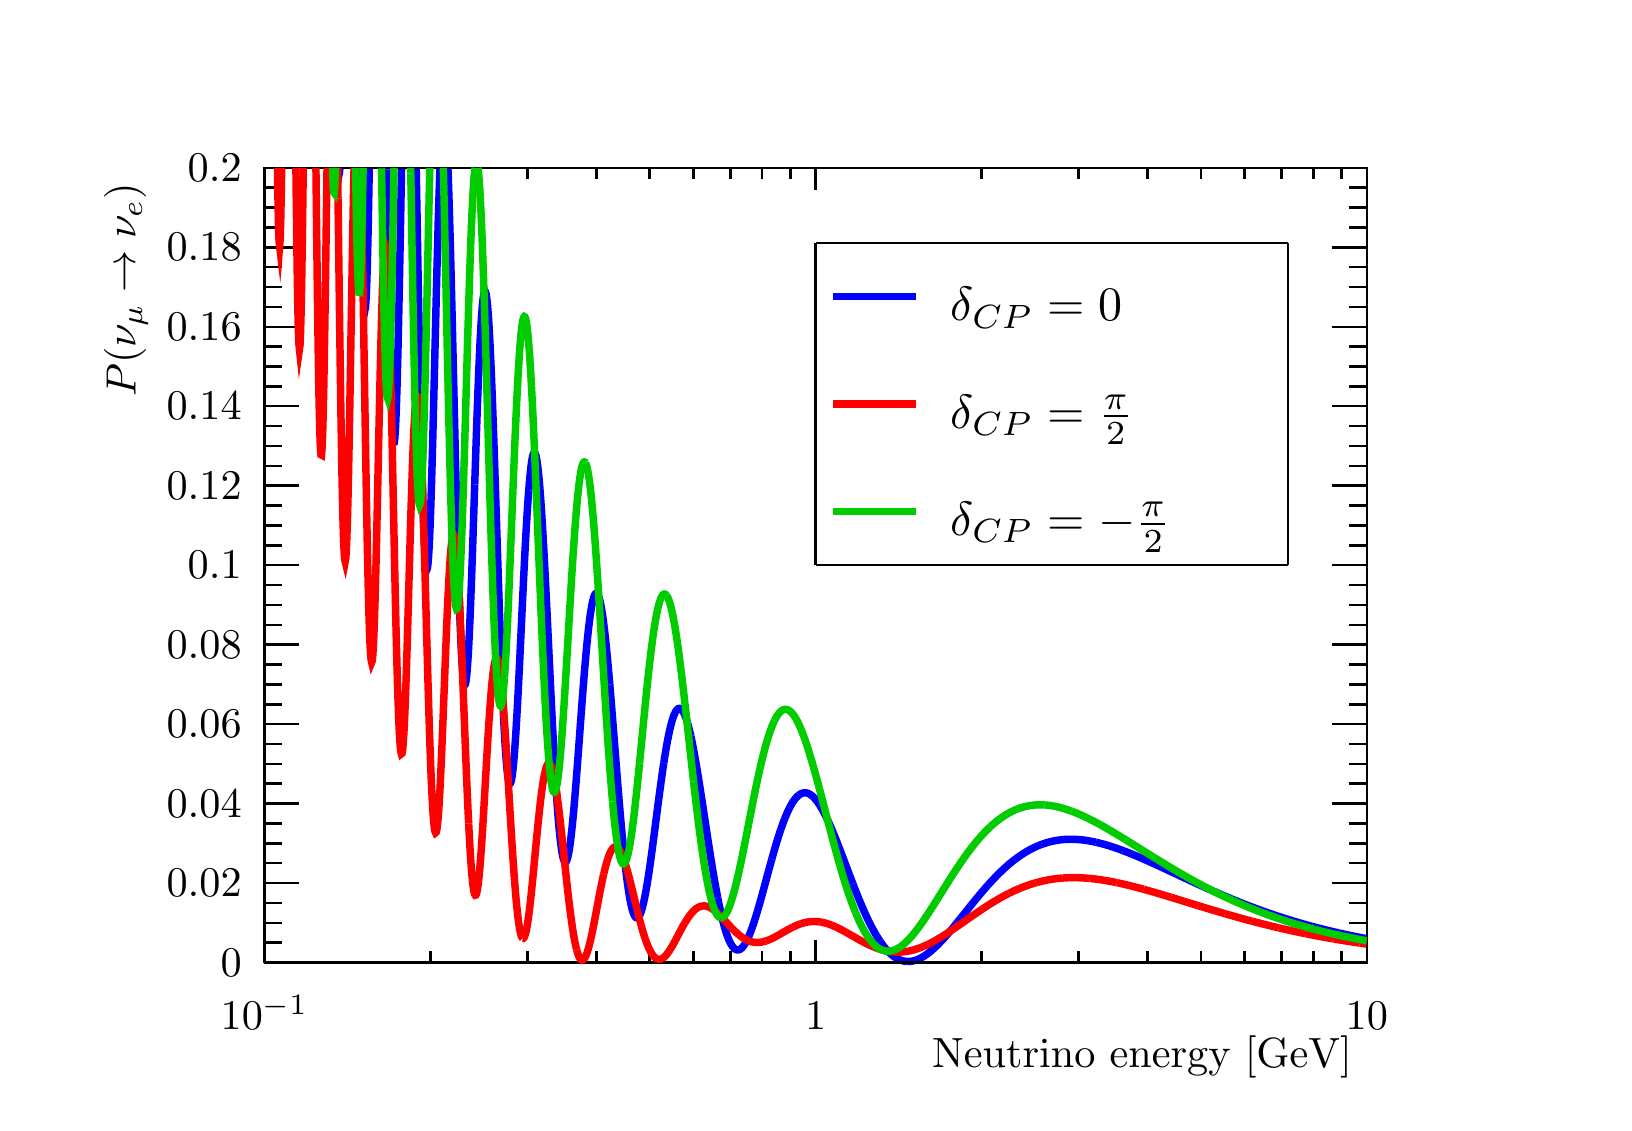
\begin{tikzpicture}
\pgfdeclareplotmark{cross} {
\pgfpathmoveto{\pgfpoint{-0.3\pgfplotmarksize}{\pgfplotmarksize}}
\pgfpathlineto{\pgfpoint{+0.3\pgfplotmarksize}{\pgfplotmarksize}}
\pgfpathlineto{\pgfpoint{+0.3\pgfplotmarksize}{0.3\pgfplotmarksize}}
\pgfpathlineto{\pgfpoint{+1\pgfplotmarksize}{0.3\pgfplotmarksize}}
\pgfpathlineto{\pgfpoint{+1\pgfplotmarksize}{-0.3\pgfplotmarksize}}
\pgfpathlineto{\pgfpoint{+0.3\pgfplotmarksize}{-0.3\pgfplotmarksize}}
\pgfpathlineto{\pgfpoint{+0.3\pgfplotmarksize}{-1.\pgfplotmarksize}}
\pgfpathlineto{\pgfpoint{-0.3\pgfplotmarksize}{-1.\pgfplotmarksize}}
\pgfpathlineto{\pgfpoint{-0.3\pgfplotmarksize}{-0.3\pgfplotmarksize}}
\pgfpathlineto{\pgfpoint{-1.\pgfplotmarksize}{-0.3\pgfplotmarksize}}
\pgfpathlineto{\pgfpoint{-1.\pgfplotmarksize}{0.3\pgfplotmarksize}}
\pgfpathlineto{\pgfpoint{-0.3\pgfplotmarksize}{0.3\pgfplotmarksize}}
\pgfpathclose
\pgfusepathqstroke
}
\pgfdeclareplotmark{cross*} {
\pgfpathmoveto{\pgfpoint{-0.3\pgfplotmarksize}{\pgfplotmarksize}}
\pgfpathlineto{\pgfpoint{+0.3\pgfplotmarksize}{\pgfplotmarksize}}
\pgfpathlineto{\pgfpoint{+0.3\pgfplotmarksize}{0.3\pgfplotmarksize}}
\pgfpathlineto{\pgfpoint{+1\pgfplotmarksize}{0.3\pgfplotmarksize}}
\pgfpathlineto{\pgfpoint{+1\pgfplotmarksize}{-0.3\pgfplotmarksize}}
\pgfpathlineto{\pgfpoint{+0.3\pgfplotmarksize}{-0.3\pgfplotmarksize}}
\pgfpathlineto{\pgfpoint{+0.3\pgfplotmarksize}{-1.\pgfplotmarksize}}
\pgfpathlineto{\pgfpoint{-0.3\pgfplotmarksize}{-1.\pgfplotmarksize}}
\pgfpathlineto{\pgfpoint{-0.3\pgfplotmarksize}{-0.3\pgfplotmarksize}}
\pgfpathlineto{\pgfpoint{-1.\pgfplotmarksize}{-0.3\pgfplotmarksize}}
\pgfpathlineto{\pgfpoint{-1.\pgfplotmarksize}{0.3\pgfplotmarksize}}
\pgfpathlineto{\pgfpoint{-0.3\pgfplotmarksize}{0.3\pgfplotmarksize}}
\pgfpathclose
\pgfusepathqfillstroke
}
\pgfdeclareplotmark{newstar} {
\pgfpathmoveto{\pgfqpoint{0pt}{\pgfplotmarksize}}
\pgfpathlineto{\pgfqpointpolar{44}{0.5\pgfplotmarksize}}
\pgfpathlineto{\pgfqpointpolar{18}{\pgfplotmarksize}}
\pgfpathlineto{\pgfqpointpolar{-20}{0.5\pgfplotmarksize}}
\pgfpathlineto{\pgfqpointpolar{-54}{\pgfplotmarksize}}
\pgfpathlineto{\pgfqpointpolar{-90}{0.5\pgfplotmarksize}}
\pgfpathlineto{\pgfqpointpolar{234}{\pgfplotmarksize}}
\pgfpathlineto{\pgfqpointpolar{198}{0.5\pgfplotmarksize}}
\pgfpathlineto{\pgfqpointpolar{162}{\pgfplotmarksize}}
\pgfpathlineto{\pgfqpointpolar{134}{0.5\pgfplotmarksize}}
\pgfpathclose
\pgfusepathqstroke
}
\pgfdeclareplotmark{newstar*} {
\pgfpathmoveto{\pgfqpoint{0pt}{\pgfplotmarksize}}
\pgfpathlineto{\pgfqpointpolar{44}{0.5\pgfplotmarksize}}
\pgfpathlineto{\pgfqpointpolar{18}{\pgfplotmarksize}}
\pgfpathlineto{\pgfqpointpolar{-20}{0.5\pgfplotmarksize}}
\pgfpathlineto{\pgfqpointpolar{-54}{\pgfplotmarksize}}
\pgfpathlineto{\pgfqpointpolar{-90}{0.5\pgfplotmarksize}}
\pgfpathlineto{\pgfqpointpolar{234}{\pgfplotmarksize}}
\pgfpathlineto{\pgfqpointpolar{198}{0.5\pgfplotmarksize}}
\pgfpathlineto{\pgfqpointpolar{162}{\pgfplotmarksize}}
\pgfpathlineto{\pgfqpointpolar{134}{0.5\pgfplotmarksize}}
\pgfpathclose
\pgfusepathqfillstroke
}
\definecolor{c}{rgb}{1,1,1};
\draw [color=c, fill=c] (0,0) rectangle (20,13.639);
\draw [color=c, fill=c] (3,1.77307) rectangle (17,11.8659);
\definecolor{c}{rgb}{0,0,0};
\draw [c,line width=0.9] (3,1.77307) -- (3,11.8659) -- (17,11.8659) -- (17,1.77307) -- (3,1.77307);
\definecolor{c}{rgb}{1,1,1};
\draw [color=c, fill=c] (3,1.77307) rectangle (17,11.8659);
\definecolor{c}{rgb}{0,0,0};
\draw [c,line width=0.9] (3,1.77307) -- (3,11.8659) -- (17,11.8659) -- (17,1.77307) -- (3,1.77307);
\definecolor{c}{rgb}{0,0,1};
\draw [c,line width=2.7] (3.94049,11.8659) -- (3.9415,11.8444);
\draw [c,line width=2.7] (3.9415,11.8444) -- (3.9485,11.7886) -- (3.9555,11.8248) -- (3.95779,11.8659);
\draw [c,line width=2.7] (4.22591,11.8659) -- (4.2285,11.6911);
\draw [c,line width=2.7] (4.2285,11.6911) -- (4.2355,11.2708) -- (4.2425,10.9073) -- (4.2495,10.6053) -- (4.2565,10.3685) -- (4.2635,10.1994) -- (4.2705,10.0993) -- (4.2775,10.0685) -- (4.2845,10.1062) -- (4.2915,10.2102) -- (4.2985,10.3776) --
 (4.3055,10.6045) -- (4.3125,10.8858) -- (4.3195,11.2161) -- (4.3265,11.5889) -- (4.33125,11.8659);
\draw [c,line width=2.7] (4.55716,11.8659) -- (4.5575,11.8422);
\draw [c,line width=2.7] (4.5575,11.8422) -- (4.5645,11.3648) -- (4.5715,10.9074) -- (4.5785,10.4755) -- (4.5855,10.0739) -- (4.5925,9.70726) -- (4.5995,9.37944) -- (4.6065,9.09385) -- (4.6135,8.85328) -- (4.6205,8.6599) -- (4.6275,8.51523) --
 (4.6345,8.42015) -- (4.6415,8.37486) -- (4.6485,8.37897) -- (4.6555,8.43144) -- (4.6625,8.53063) -- (4.6695,8.67435) -- (4.6765,8.85988) -- (4.6835,9.08402) -- (4.6905,9.34314) -- (4.6975,9.63323) -- (4.7045,9.94997) -- (4.7115,10.2888) --
 (4.7185,10.6448) -- (4.7255,11.0132) -- (4.7325,11.3889) -- (4.7395,11.767) -- (4.74135,11.8659);
\draw [c,line width=2.7] (4.92712,11.8659) -- (4.9285,11.7895);
\draw [c,line width=2.7] (4.9285,11.7895) -- (4.9355,11.396) -- (4.9425,10.9983) -- (4.9495,10.6005) -- (4.9565,10.2062) -- (4.9635,9.8192) -- (4.9705,9.44312) -- (4.9775,9.08136) -- (4.9845,8.73713) -- (4.9915,8.41344) -- (4.9985,8.11302) --
 (5.0055,7.83835) -- (5.0125,7.59159) -- (5.0195,7.3746) -- (5.0265,7.18891) -- (5.0335,7.03572) -- (5.0405,6.9159) -- (5.0475,6.82996) -- (5.0545,6.77808) -- (5.0615,6.76011) -- (5.0685,6.77555) -- (5.0755,6.82362) -- (5.0825,6.90321) --
 (5.0895,7.01293) -- (5.0965,7.15114) -- (5.1035,7.31594) -- (5.1105,7.5052) -- (5.1175,7.71661) -- (5.1245,7.94768) -- (5.1315,8.19577) -- (5.1385,8.45814) -- (5.1455,8.73193) -- (5.1525,9.01425) -- (5.1595,9.30215) -- (5.1665,9.59269) --
 (5.1735,9.88295) -- (5.1805,10.1701) -- (5.1875,10.4512) -- (5.1945,10.7237) -- (5.2015,10.9849) -- (5.2085,11.2325) -- (5.2155,11.4641) -- (5.2225,11.6775) -- (5.22932,11.8659);
\draw [c,line width=2.7] (5.33001,11.8659) -- (5.3345,11.7474);
\draw [c,line width=2.7] (5.3345,11.7474) -- (5.3415,11.5422) -- (5.3485,11.3182) -- (5.3555,11.0772) -- (5.3625,10.8212) -- (5.3695,10.5521) -- (5.3765,10.2719) -- (5.3835,9.98293) -- (5.3905,9.68718) -- (5.3975,9.38688) -- (5.4045,9.08421) --
 (5.4115,8.78134) -- (5.4185,8.48042) -- (5.4255,8.18354) -- (5.4325,7.89274) -- (5.4395,7.60996) -- (5.4465,7.33707) -- (5.4535,7.07583) -- (5.4605,6.8279) -- (5.4675,6.5948) -- (5.4745,6.37792) -- (5.4815,6.1785) -- (5.4885,5.99765) --
 (5.4955,5.83631) -- (5.5025,5.69528) -- (5.5095,5.57519) -- (5.5165,5.4765) -- (5.5235,5.39952) -- (5.5305,5.3444) -- (5.5375,5.31112) -- (5.5445,5.29952) -- (5.5515,5.30927) -- (5.5585,5.33991) -- (5.5655,5.39084) -- (5.5725,5.4613) --
 (5.5795,5.55045) -- (5.5865,5.65729) -- (5.5935,5.78074) -- (5.6005,5.91961) -- (5.6075,6.07264) -- (5.6145,6.23846) -- (5.6215,6.41566) -- (5.6285,6.60277) -- (5.6355,6.79827) -- (5.6425,7.00062) -- (5.6495,7.20824) -- (5.6565,7.41955) --
 (5.6635,7.63296) -- (5.6705,7.84692);
\draw [c,line width=2.7] (5.6705,7.84692) -- (5.6775,8.05986) -- (5.6845,8.27027) -- (5.6915,8.47667) -- (5.6985,8.67762) -- (5.7055,8.87176) -- (5.7125,9.05777) -- (5.7195,9.23442) -- (5.7265,9.40055) -- (5.7335,9.5551) -- (5.7405,9.69707) --
 (5.7475,9.82559) -- (5.7545,9.93986) -- (5.7615,10.0392) -- (5.7685,10.123) -- (5.7755,10.1908) -- (5.7825,10.2423) -- (5.7895,10.2771) -- (5.7965,10.2951) -- (5.8035,10.2962) -- (5.8105,10.2805) -- (5.8175,10.2482) -- (5.8245,10.1995) --
 (5.8315,10.1347) -- (5.8385,10.0542) -- (5.8455,9.95864) -- (5.8525,9.84855) -- (5.8595,9.7246) -- (5.8665,9.58755) -- (5.8735,9.43822) -- (5.8805,9.27746) -- (5.8875,9.10621) -- (5.8945,8.92544) -- (5.9015,8.73615) -- (5.9085,8.5394) --
 (5.9155,8.33624) -- (5.9225,8.12778) -- (5.9295,7.91512) -- (5.9365,7.69936) -- (5.9435,7.48163) -- (5.9505,7.26303) -- (5.9575,7.04465) -- (5.9645,6.82757) -- (5.9715,6.61285) -- (5.9785,6.40152) -- (5.9855,6.19456) -- (5.9925,5.99294) --
 (5.9995,5.79756) -- (6.0065,5.60929) -- (6.0135,5.42895);
\draw [c,line width=2.7] (6.0135,5.42895) -- (6.0205,5.25729) -- (6.0275,5.09503) -- (6.0345,4.94281) -- (6.0415,4.80121) -- (6.0485,4.67075) -- (6.0555,4.55189) -- (6.0625,4.44501) -- (6.0695,4.35044) -- (6.0765,4.26843) -- (6.0835,4.19918) --
 (6.0905,4.14279) -- (6.0975,4.09933) -- (6.1045,4.06878) -- (6.1115,4.05107) -- (6.1185,4.04607) -- (6.1255,4.05357) -- (6.1325,4.07332) -- (6.1395,4.105) -- (6.1465,4.14827) -- (6.1535,4.20269) -- (6.1605,4.26781) -- (6.1675,4.34312) --
 (6.1745,4.42808) -- (6.1815,4.5221) -- (6.1885,4.62456) -- (6.1955,4.73481) -- (6.2025,4.85218) -- (6.2095,4.97598) -- (6.2165,5.10547) -- (6.2235,5.23994) -- (6.2305,5.37864) -- (6.2375,5.52082) -- (6.2445,5.66571) -- (6.2515,5.81257) --
 (6.2585,5.96064) -- (6.2655,6.10918) -- (6.2725,6.25743) -- (6.2795,6.40469) -- (6.2865,6.55023) -- (6.2935,6.69338) -- (6.3005,6.83345) -- (6.3075,6.9698) -- (6.3145,7.10181) -- (6.3215,7.2289) -- (6.3285,7.3505) -- (6.3355,7.46608) --
 (6.3425,7.57514) -- (6.3495,7.67724) -- (6.3565,7.77195);
\draw [c,line width=2.7] (6.3565,7.77195) -- (6.3635,7.85888) -- (6.3705,7.9377) -- (6.3775,8.00809) -- (6.3845,8.06979) -- (6.3915,8.12258) -- (6.3985,8.16628) -- (6.4055,8.20073) -- (6.4125,8.22585) -- (6.4195,8.24156) -- (6.4265,8.24784) --
 (6.4335,8.24471) -- (6.4405,8.23222) -- (6.4475,8.21047) -- (6.4545,8.17958) -- (6.4615,8.13972) -- (6.4685,8.09107) -- (6.4755,8.03387) -- (6.4825,7.96837) -- (6.4895,7.89487) -- (6.4965,7.81367) -- (6.5035,7.72511) -- (6.5105,7.62956) --
 (6.5175,7.52741) -- (6.5245,7.41905) -- (6.5315,7.3049) -- (6.5385,7.18542) -- (6.5455,7.06104) -- (6.5525,6.93224) -- (6.5595,6.79948) -- (6.5665,6.66325) -- (6.5735,6.52403) -- (6.5805,6.38232) -- (6.5875,6.23861) -- (6.5945,6.09339) --
 (6.6015,5.94716) -- (6.6085,5.8004) -- (6.6155,5.65359) -- (6.6225,5.50722) -- (6.6295,5.36174) -- (6.6365,5.21762) -- (6.6435,5.07531) -- (6.6505,4.93523) -- (6.6575,4.7978) -- (6.6645,4.66344) -- (6.6715,4.53252) -- (6.6785,4.40541) --
 (6.6855,4.28248) -- (6.6925,4.16403) -- (6.6995,4.0504);
\draw [c,line width=2.7] (6.6995,4.0504) -- (6.7065,3.94186) -- (6.7135,3.8387) -- (6.7205,3.74114) -- (6.7275,3.64942) -- (6.7345,3.56375) -- (6.7415,3.48429) -- (6.7485,3.4112) -- (6.7555,3.34462) -- (6.7625,3.28465) -- (6.7695,3.23138) --
 (6.7765,3.18487) -- (6.7835,3.14517) -- (6.7905,3.11228) -- (6.7975,3.0862) -- (6.8045,3.06691) -- (6.8115,3.05436) -- (6.8185,3.04848) -- (6.8255,3.04918) -- (6.8325,3.05635) -- (6.8395,3.06987) -- (6.8465,3.0896) -- (6.8535,3.11537) --
 (6.8605,3.147) -- (6.8675,3.18431) -- (6.8745,3.22708) -- (6.8815,3.2751) -- (6.8885,3.32813) -- (6.8955,3.38593) -- (6.9025,3.44824) -- (6.9095,3.5148) -- (6.9165,3.58533) -- (6.9235,3.65956) -- (6.9305,3.73718) -- (6.9375,3.81792) --
 (6.9445,3.90148) -- (6.9515,3.98754) -- (6.9585,4.07582) -- (6.9655,4.16599) -- (6.9725,4.25776) -- (6.9795,4.35081) -- (6.9865,4.44485) -- (6.9935,4.53956) -- (7.0005,4.63465) -- (7.0075,4.72981) -- (7.0145,4.82477) -- (7.0215,4.91921) --
 (7.0285,5.01288) -- (7.0355,5.10548) -- (7.0425,5.19675);
\draw [c,line width=2.7] (7.0425,5.19675) -- (7.0495,5.28643) -- (7.0565,5.37426) -- (7.0635,5.46001) -- (7.0705,5.54344) -- (7.0775,5.62431) -- (7.0845,5.70243) -- (7.0915,5.77759) -- (7.0985,5.84958) -- (7.1055,5.91824) -- (7.1125,5.9834) --
 (7.1195,6.04489) -- (7.1265,6.10257) -- (7.1335,6.1563) -- (7.1405,6.20598) -- (7.1475,6.25148) -- (7.1545,6.29271) -- (7.1615,6.3296) -- (7.1685,6.36206) -- (7.1755,6.39004) -- (7.1825,6.41349) -- (7.1895,6.43238) -- (7.1965,6.44669) --
 (7.2035,6.45641) -- (7.2105,6.46153) -- (7.2175,6.46208) -- (7.2245,6.45807) -- (7.2315,6.44954) -- (7.2385,6.43654) -- (7.2455,6.41913) -- (7.2525,6.39737) -- (7.2595,6.37133) -- (7.2665,6.3411) -- (7.2735,6.30678) -- (7.2805,6.26846) --
 (7.2875,6.22626) -- (7.2945,6.1803) -- (7.3015,6.1307) -- (7.3085,6.07759) -- (7.3155,6.02111) -- (7.3225,5.96141) -- (7.3295,5.89864) -- (7.3365,5.83294) -- (7.3435,5.76449) -- (7.3505,5.69344) -- (7.3575,5.61995) -- (7.3645,5.54421) --
 (7.3715,5.46638) -- (7.3785,5.38664) -- (7.3855,5.30516);
\draw [c,line width=2.7] (7.3855,5.30516) -- (7.3925,5.22212) -- (7.3995,5.1377) -- (7.4065,5.05208) -- (7.4135,4.96544) -- (7.4205,4.87796) -- (7.4275,4.78981) -- (7.4345,4.70118) -- (7.4415,4.61224) -- (7.4485,4.52316) -- (7.4555,4.43412) --
 (7.4625,4.34528) -- (7.4695,4.25681) -- (7.4765,4.16888) -- (7.4835,4.08164) -- (7.4905,3.99525) -- (7.4975,3.90986) -- (7.5045,3.82562) -- (7.5115,3.74267) -- (7.5185,3.66116) -- (7.5255,3.58121) -- (7.5325,3.50295) -- (7.5395,3.42651) --
 (7.5465,3.35201) -- (7.5535,3.27955) -- (7.5605,3.20925) -- (7.5675,3.14121) -- (7.5745,3.07551) -- (7.5815,3.01225) -- (7.5885,2.95152) -- (7.5955,2.89338) -- (7.6025,2.83792) -- (7.6095,2.78519) -- (7.6165,2.73525) -- (7.6235,2.68815) --
 (7.6305,2.64395) -- (7.6375,2.60268) -- (7.6445,2.56437) -- (7.6515,2.52906) -- (7.6585,2.49676) -- (7.6655,2.46749) -- (7.6725,2.44126) -- (7.6795,2.41808) -- (7.6865,2.39794) -- (7.6935,2.38083) -- (7.7005,2.36675) -- (7.7075,2.35567) --
 (7.7145,2.34758) -- (7.7215,2.34244) -- (7.7285,2.34023);
\draw [c,line width=2.7] (7.7285,2.34023) -- (7.7355,2.34089) -- (7.7425,2.34441) -- (7.7495,2.35071) -- (7.7565,2.35977) -- (7.7635,2.37151) -- (7.7705,2.38589) -- (7.7775,2.40283) -- (7.7845,2.42228) -- (7.7915,2.44416) -- (7.7985,2.46841) --
 (7.8055,2.49494) -- (7.8125,2.52368) -- (7.8195,2.55455) -- (7.8265,2.58746) -- (7.8335,2.62233) -- (7.8405,2.65907) -- (7.8475,2.69759) -- (7.8545,2.73781) -- (7.8615,2.77962) -- (7.8685,2.82294) -- (7.8755,2.86766) -- (7.8825,2.91371) --
 (7.8895,2.96097) -- (7.8965,3.00935) -- (7.9035,3.05876) -- (7.9105,3.10909) -- (7.9175,3.16025) -- (7.9245,3.21214) -- (7.9315,3.26467) -- (7.9385,3.31773) -- (7.9455,3.37124) -- (7.9525,3.42509) -- (7.9595,3.4792) -- (7.9665,3.53346) --
 (7.9735,3.58779) -- (7.9805,3.64209) -- (7.9875,3.69628) -- (7.9945,3.75026) -- (8.0015,3.80395) -- (8.0085,3.85727) -- (8.0155,3.91013) -- (8.0225,3.96246) -- (8.0295,4.01416) -- (8.0365,4.06517) -- (8.0435,4.11541) -- (8.0505,4.1648) --
 (8.0575,4.21329) -- (8.0645,4.26079) -- (8.0715,4.30724);
\draw [c,line width=2.7] (8.0715,4.30724) -- (8.0785,4.35259) -- (8.0855,4.39677) -- (8.0925,4.43972) -- (8.0995,4.48138) -- (8.1065,4.52172) -- (8.1135,4.56066) -- (8.1205,4.59818) -- (8.1275,4.63422) -- (8.1345,4.66874) -- (8.1415,4.7017) --
 (8.1485,4.73307) -- (8.1555,4.76282) -- (8.1625,4.79091) -- (8.1695,4.81731) -- (8.1765,4.842) -- (8.1835,4.86497) -- (8.1905,4.88618) -- (8.1975,4.90562) -- (8.2045,4.92327) -- (8.2115,4.93914) -- (8.2185,4.9532) -- (8.2255,4.96544) --
 (8.2325,4.97588) -- (8.2395,4.9845) -- (8.2465,4.9913) -- (8.2535,4.99629) -- (8.2605,4.99948) -- (8.2675,5.00087) -- (8.2745,5.00047) -- (8.2815,4.99829) -- (8.2885,4.99436) -- (8.2955,4.98868) -- (8.3025,4.98128) -- (8.3095,4.97217) --
 (8.3165,4.96137) -- (8.3235,4.94892) -- (8.3305,4.93484) -- (8.3375,4.91915) -- (8.3445,4.90189) -- (8.3515,4.88308) -- (8.3585,4.86276) -- (8.3655,4.84097) -- (8.3725,4.81773) -- (8.3795,4.79308) -- (8.3865,4.76706) -- (8.3935,4.73972) --
 (8.4005,4.71108) -- (8.4075,4.68119) -- (8.4145,4.6501);
\draw [c,line width=2.7] (8.4145,4.6501) -- (8.4215,4.61784) -- (8.4285,4.58446) -- (8.4355,4.55) -- (8.4425,4.51451) -- (8.4495,4.47803) -- (8.4565,4.44061) -- (8.4635,4.4023) -- (8.4705,4.36313) -- (8.4775,4.32317) -- (8.4845,4.28245) --
 (8.4915,4.24103) -- (8.4985,4.19895) -- (8.5055,4.15625) -- (8.5125,4.113) -- (8.5195,4.06923) -- (8.5265,4.02499) -- (8.5335,3.98033) -- (8.5405,3.9353) -- (8.5475,3.88995) -- (8.5545,3.84432) -- (8.5615,3.79846) -- (8.5685,3.75241) --
 (8.5755,3.70623) -- (8.5825,3.65994) -- (8.5895,3.61362) -- (8.5965,3.56728) -- (8.6035,3.52099) -- (8.6105,3.47477) -- (8.6175,3.42868) -- (8.6245,3.38276) -- (8.6315,3.33704) -- (8.6385,3.29157) -- (8.6455,3.24638) -- (8.6525,3.20152) --
 (8.6595,3.15703) -- (8.6665,3.11293) -- (8.6735,3.06926) -- (8.6805,3.02607) -- (8.6875,2.98338) -- (8.6945,2.94122) -- (8.7015,2.89964) -- (8.7085,2.85865) -- (8.7155,2.81829) -- (8.7225,2.7786) -- (8.7295,2.73959) -- (8.7365,2.70129) --
 (8.7435,2.66373) -- (8.7505,2.62694) -- (8.7575,2.59093);
\draw [c,line width=2.7] (8.7575,2.59093) -- (8.7645,2.55574) -- (8.7715,2.52138) -- (8.7785,2.48787) -- (8.7855,2.45524) -- (8.7925,2.42349) -- (8.7995,2.39266) -- (8.8065,2.36274) -- (8.8135,2.33377) -- (8.8205,2.30575) -- (8.8275,2.2787) --
 (8.8345,2.25262) -- (8.8415,2.22754) -- (8.8485,2.20345) -- (8.8555,2.18037) -- (8.8625,2.1583) -- (8.8695,2.13726) -- (8.8765,2.11725) -- (8.8835,2.09827) -- (8.8905,2.08032) -- (8.8975,2.06342) -- (8.9045,2.04756) -- (8.9115,2.03273) --
 (8.9185,2.01896) -- (8.9255,2.00622) -- (8.9325,1.99452) -- (8.9395,1.98386) -- (8.9465,1.97423) -- (8.9535,1.96563) -- (8.9605,1.95806) -- (8.9675,1.9515) -- (8.9745,1.94596) -- (8.9815,1.94142) -- (8.9885,1.93787) -- (8.9955,1.93531) --
 (9.0025,1.93373) -- (9.0095,1.93312) -- (9.0165,1.93346) -- (9.0235,1.93475) -- (9.0305,1.93697) -- (9.0375,1.94011) -- (9.0445,1.94416) -- (9.0515,1.9491) -- (9.0585,1.95492) -- (9.0655,1.9616) -- (9.0725,1.96913) -- (9.0795,1.97749) --
 (9.0865,1.98667) -- (9.0935,1.99665) -- (9.1005,2.00741);
\draw [c,line width=2.7] (9.1005,2.00741) -- (9.1075,2.01893) -- (9.1145,2.03121) -- (9.1215,2.04421) -- (9.1285,2.05792) -- (9.1355,2.07233) -- (9.1425,2.08741) -- (9.1495,2.10314) -- (9.1565,2.11951) -- (9.1635,2.13649) -- (9.1705,2.15407) --
 (9.1775,2.17222) -- (9.1845,2.19092) -- (9.1915,2.21017) -- (9.1985,2.22992) -- (9.2055,2.25017) -- (9.2125,2.27089) -- (9.2195,2.29206) -- (9.2265,2.31367) -- (9.2335,2.33569) -- (9.2405,2.35809) -- (9.2475,2.38087) -- (9.2545,2.40399) --
 (9.2615,2.42745) -- (9.2685,2.45121) -- (9.2755,2.47526) -- (9.2825,2.49957) -- (9.2895,2.52413) -- (9.2965,2.54892) -- (9.3035,2.57391) -- (9.3105,2.59908) -- (9.3175,2.62443) -- (9.3245,2.64992) -- (9.3315,2.67553) -- (9.3385,2.70125) --
 (9.3455,2.72707) -- (9.3525,2.75295) -- (9.3595,2.77888) -- (9.3665,2.80484) -- (9.3735,2.83081) -- (9.3805,2.85679) -- (9.3875,2.88274) -- (9.3945,2.90865) -- (9.4015,2.9345) -- (9.4085,2.96028) -- (9.4155,2.98597) -- (9.4225,3.01155) --
 (9.4295,3.03701) -- (9.4365,3.06232) -- (9.4435,3.08749);
\draw [c,line width=2.7] (9.4435,3.08749) -- (9.4505,3.11248) -- (9.4575,3.13729) -- (9.4645,3.16191) -- (9.4715,3.1863) -- (9.4785,3.21048) -- (9.4855,3.23441) -- (9.4925,3.25808) -- (9.4995,3.28149) -- (9.5065,3.30462) -- (9.5135,3.32746) --
 (9.5205,3.34999) -- (9.5275,3.37221) -- (9.5345,3.39411) -- (9.5415,3.41566) -- (9.5485,3.43687) -- (9.5555,3.45772) -- (9.5625,3.47821) -- (9.5695,3.49832) -- (9.5765,3.51804) -- (9.5835,3.53737) -- (9.5905,3.55629) -- (9.5975,3.57481) --
 (9.6045,3.59291) -- (9.6115,3.61058) -- (9.6185,3.62782) -- (9.6255,3.64461) -- (9.6325,3.66097) -- (9.6395,3.67687) -- (9.6465,3.69232) -- (9.6535,3.7073) -- (9.6605,3.72182) -- (9.6675,3.73587) -- (9.6745,3.74944) -- (9.6815,3.76253) --
 (9.6885,3.77514) -- (9.6955,3.78727) -- (9.7025,3.7989) -- (9.7095,3.81004) -- (9.7165,3.82069) -- (9.7235,3.83084) -- (9.7305,3.8405) -- (9.7375,3.84965) -- (9.7445,3.85831) -- (9.7515,3.86646) -- (9.7585,3.87411) -- (9.7655,3.88127) --
 (9.7725,3.88791) -- (9.7795,3.89406) -- (9.7865,3.89971);
\draw [c,line width=2.7] (9.7865,3.89971) -- (9.7935,3.90485) -- (9.8005,3.9095) -- (9.8075,3.91365) -- (9.8145,3.9173) -- (9.8215,3.92046) -- (9.8285,3.92313) -- (9.8355,3.92531) -- (9.8425,3.92699) -- (9.8495,3.9282) -- (9.8565,3.92892) --
 (9.8635,3.92916) -- (9.8705,3.92893) -- (9.8775,3.92822) -- (9.8845,3.92705) -- (9.8915,3.92541) -- (9.8985,3.92332) -- (9.9055,3.92076) -- (9.9125,3.91776) -- (9.9195,3.9143) -- (9.9265,3.91041) -- (9.9335,3.90608) -- (9.9405,3.90131) --
 (9.9475,3.89612) -- (9.9545,3.89051) -- (9.9615,3.88448) -- (9.9685,3.87804) -- (9.9755,3.8712) -- (9.9825,3.86396) -- (9.9895,3.85632) -- (9.9965,3.8483) -- (10.0035,3.83989) -- (10.0105,3.83112) -- (10.0175,3.82197) -- (10.0245,3.81246) --
 (10.0315,3.8026) -- (10.0385,3.79239) -- (10.0455,3.78184) -- (10.0525,3.77095) -- (10.0595,3.75974) -- (10.0665,3.7482) -- (10.0735,3.73636) -- (10.0805,3.7242) -- (10.0875,3.71174) -- (10.0945,3.69899) -- (10.1015,3.68596) -- (10.1085,3.67265) --
 (10.1155,3.65906) -- (10.1225,3.64521) -- (10.1295,3.63111);
\draw [c,line width=2.7] (10.1295,3.63111) -- (10.1365,3.61676) -- (10.1435,3.60216) -- (10.1505,3.58733) -- (10.1575,3.57227) -- (10.1645,3.55699) -- (10.1715,3.5415) -- (10.1785,3.52581) -- (10.1855,3.50991) -- (10.1925,3.49383) --
 (10.1995,3.47756) -- (10.2065,3.46111) -- (10.2135,3.4445) -- (10.2205,3.42772) -- (10.2275,3.41079) -- (10.2345,3.39372) -- (10.2415,3.3765) -- (10.2485,3.35915) -- (10.2555,3.34168) -- (10.2625,3.32408) -- (10.2695,3.30638) -- (10.2765,3.28857) --
 (10.2835,3.27066) -- (10.2905,3.25266) -- (10.2975,3.23458) -- (10.3045,3.21642) -- (10.3115,3.19819) -- (10.3185,3.1799) -- (10.3255,3.16155) -- (10.3325,3.14315) -- (10.3395,3.1247) -- (10.3465,3.10622) -- (10.3535,3.08771) -- (10.3605,3.06917) --
 (10.3675,3.05061) -- (10.3745,3.03204) -- (10.3815,3.01346) -- (10.3885,2.99489) -- (10.3955,2.97632) -- (10.4025,2.95776) -- (10.4095,2.93921) -- (10.4165,2.92069) -- (10.4235,2.9022) -- (10.4305,2.88375) -- (10.4375,2.86533) -- (10.4445,2.84696)
 -- (10.4515,2.82863) -- (10.4585,2.81037) -- (10.4655,2.79216) -- (10.4725,2.77402);
\draw [c,line width=2.7] (10.4725,2.77402) -- (10.4795,2.75595) -- (10.4865,2.73796) -- (10.4935,2.72005) -- (10.5005,2.70222) -- (10.5075,2.68448) -- (10.5145,2.66684) -- (10.5215,2.64929) -- (10.5285,2.63185) -- (10.5355,2.61451) --
 (10.5425,2.59729) -- (10.5495,2.58018) -- (10.5565,2.5632) -- (10.5635,2.54633) -- (10.5705,2.5296) -- (10.5775,2.51299) -- (10.5845,2.49652) -- (10.5915,2.48019) -- (10.5985,2.464) -- (10.6055,2.44795) -- (10.6125,2.43206) -- (10.6195,2.41631) --
 (10.6265,2.40072) -- (10.6335,2.38529) -- (10.6405,2.37002) -- (10.6475,2.35491) -- (10.6545,2.33997) -- (10.6615,2.3252) -- (10.6685,2.3106) -- (10.6755,2.29617) -- (10.6825,2.28192) -- (10.6895,2.26785) -- (10.6965,2.25397) -- (10.7035,2.24026) --
 (10.7105,2.22674) -- (10.7175,2.21341) -- (10.7245,2.20027) -- (10.7315,2.18731) -- (10.7385,2.17456) -- (10.7455,2.16199) -- (10.7525,2.14963) -- (10.7595,2.13746) -- (10.7665,2.12549) -- (10.7735,2.11372) -- (10.7805,2.10215) -- (10.7875,2.09079)
 -- (10.7945,2.07963) -- (10.8015,2.06867) -- (10.8085,2.05793) -- (10.8155,2.04738);
\draw [c,line width=2.7] (10.8155,2.04738) -- (10.8225,2.03705) -- (10.8295,2.02693) -- (10.8365,2.01702) -- (10.8435,2.00731) -- (10.8505,1.99782) -- (10.8575,1.98854) -- (10.8645,1.97947) -- (10.8715,1.97062) -- (10.8785,1.96197) --
 (10.8855,1.95354) -- (10.8925,1.94532) -- (10.8995,1.93732) -- (10.9065,1.92953) -- (10.9135,1.92195) -- (10.9205,1.91458) -- (10.9275,1.90743) -- (10.9345,1.90049) -- (10.9415,1.89377) -- (10.9485,1.88725) -- (10.9555,1.88095) -- (10.9625,1.87486)
 -- (10.9695,1.86898) -- (10.9765,1.86332) -- (10.9835,1.85786) -- (10.9905,1.85261) -- (10.9975,1.84757) -- (11.0045,1.84274) -- (11.0115,1.83812) -- (11.0185,1.8337) -- (11.0255,1.8295) -- (11.0325,1.82549) -- (11.0395,1.82169) -- (11.0465,1.81809)
 -- (11.0535,1.8147) -- (11.0605,1.81151) -- (11.0675,1.80852) -- (11.0745,1.80572) -- (11.0815,1.80313) -- (11.0885,1.80073) -- (11.0955,1.79853) -- (11.1025,1.79652) -- (11.1095,1.79471) -- (11.1165,1.79309) -- (11.1235,1.79166) --
 (11.1305,1.79041) -- (11.1375,1.78936) -- (11.1445,1.78849) -- (11.1515,1.78781) -- (11.1585,1.78731);
\draw [c,line width=2.7] (11.1585,1.78731) -- (11.1655,1.787) -- (11.1725,1.78686) -- (11.1795,1.7869) -- (11.1865,1.78712) -- (11.1935,1.78752) -- (11.2005,1.78809) -- (11.2075,1.78883) -- (11.2145,1.78974) -- (11.2215,1.79083) -- (11.2285,1.79208)
 -- (11.2355,1.79349) -- (11.2425,1.79508) -- (11.2495,1.79682) -- (11.2565,1.79872) -- (11.2635,1.80078) -- (11.2705,1.803) -- (11.2775,1.80538) -- (11.2845,1.8079) -- (11.2915,1.81058) -- (11.2985,1.81341) -- (11.3055,1.81639) -- (11.3125,1.81951)
 -- (11.3195,1.82278) -- (11.3265,1.82619) -- (11.3335,1.82974) -- (11.3405,1.83342) -- (11.3475,1.83725) -- (11.3545,1.84121) -- (11.3615,1.8453) -- (11.3685,1.84952) -- (11.3755,1.85387) -- (11.3825,1.85835) -- (11.3895,1.86295) --
 (11.3965,1.86768) -- (11.4035,1.87252) -- (11.4105,1.87749) -- (11.4175,1.88257) -- (11.4245,1.88777) -- (11.4315,1.89308) -- (11.4385,1.8985) -- (11.4455,1.90403) -- (11.4525,1.90967) -- (11.4595,1.91542) -- (11.4665,1.92126) -- (11.4735,1.92721)
 -- (11.4805,1.93326) -- (11.4875,1.93941) -- (11.4945,1.94565) -- (11.5015,1.95199);
\draw [c,line width=2.7] (11.5015,1.95199) -- (11.5085,1.95842) -- (11.5155,1.96493) -- (11.5225,1.97154) -- (11.5295,1.97823) -- (11.5365,1.98501) -- (11.5435,1.99187) -- (11.5505,1.99881) -- (11.5575,2.00582) -- (11.5645,2.01292) --
 (11.5715,2.02009) -- (11.5785,2.02733) -- (11.5855,2.03464) -- (11.5925,2.04202) -- (11.5995,2.04947) -- (11.6065,2.05699) -- (11.6135,2.06457) -- (11.6205,2.07221) -- (11.6275,2.07991) -- (11.6345,2.08767) -- (11.6415,2.09549) -- (11.6485,2.10336)
 -- (11.6555,2.11128) -- (11.6625,2.11926) -- (11.6695,2.12728) -- (11.6765,2.13535) -- (11.6835,2.14347) -- (11.6905,2.15164) -- (11.6975,2.15984) -- (11.7045,2.16809) -- (11.7115,2.17638) -- (11.7185,2.1847) -- (11.7255,2.19306) --
 (11.7325,2.20146) -- (11.7395,2.20989) -- (11.7465,2.21835) -- (11.7535,2.22684) -- (11.7605,2.23536) -- (11.7675,2.2439) -- (11.7745,2.25247) -- (11.7815,2.26106) -- (11.7885,2.26968) -- (11.7955,2.27831) -- (11.8025,2.28697) -- (11.8095,2.29564)
 -- (11.8165,2.30433) -- (11.8235,2.31304) -- (11.8305,2.32175) -- (11.8375,2.33048) -- (11.8445,2.33922);
\draw [c,line width=2.7] (11.8445,2.33922) -- (11.8515,2.34797) -- (11.8585,2.35673) -- (11.8655,2.36549) -- (11.8725,2.37426) -- (11.8795,2.38303) -- (11.8865,2.3918) -- (11.8935,2.40058) -- (11.9005,2.40935) -- (11.9075,2.41813) -- (11.9145,2.4269)
 -- (11.9215,2.43567) -- (11.9285,2.44443) -- (11.9355,2.45319) -- (11.9425,2.46194) -- (11.9495,2.47068) -- (11.9565,2.47941) -- (11.9635,2.48813) -- (11.9705,2.49684) -- (11.9775,2.50553) -- (11.9845,2.51421) -- (11.9915,2.52288) --
 (11.9985,2.53153) -- (12.0055,2.54016) -- (12.0125,2.54877) -- (12.0195,2.55737) -- (12.0265,2.56594) -- (12.0335,2.57449) -- (12.0405,2.58302) -- (12.0475,2.59153) -- (12.0545,2.60001) -- (12.0615,2.60847) -- (12.0685,2.6169) -- (12.0755,2.62531)
 -- (12.0825,2.63368) -- (12.0895,2.64203) -- (12.0965,2.65035) -- (12.1035,2.65864) -- (12.1105,2.6669) -- (12.1175,2.67512) -- (12.1245,2.68331) -- (12.1315,2.69147) -- (12.1385,2.69959) -- (12.1455,2.70768) -- (12.1525,2.71574) --
 (12.1595,2.72375) -- (12.1665,2.73173) -- (12.1735,2.73967) -- (12.1805,2.74758) -- (12.1875,2.75544);
\draw [c,line width=2.7] (12.1875,2.75544) -- (12.1945,2.76326) -- (12.2015,2.77104) -- (12.2085,2.77879) -- (12.2155,2.78649) -- (12.2225,2.79414) -- (12.2295,2.80176) -- (12.2365,2.80933) -- (12.2435,2.81685) -- (12.2505,2.82433) --
 (12.2575,2.83177) -- (12.2645,2.83916) -- (12.2715,2.84651) -- (12.2785,2.8538) -- (12.2855,2.86105) -- (12.2925,2.86826) -- (12.2995,2.87541) -- (12.3065,2.88252) -- (12.3135,2.88957) -- (12.3205,2.89658) -- (12.3275,2.90354) -- (12.3345,2.91044)
 -- (12.3415,2.9173) -- (12.3485,2.9241) -- (12.3555,2.93086) -- (12.3625,2.93756) -- (12.3695,2.94421) -- (12.3765,2.9508) -- (12.3835,2.95735) -- (12.3905,2.96384) -- (12.3975,2.97028) -- (12.4045,2.97666) -- (12.4115,2.98299) -- (12.4185,2.98926)
 -- (12.4255,2.99548) -- (12.4325,3.00165) -- (12.4395,3.00776) -- (12.4465,3.01382) -- (12.4535,3.01982) -- (12.4605,3.02576) -- (12.4675,3.03165) -- (12.4745,3.03748) -- (12.4815,3.04326) -- (12.4885,3.04898) -- (12.4955,3.05464) --
 (12.5025,3.06025) -- (12.5095,3.0658) -- (12.5165,3.07129) -- (12.5235,3.07672) -- (12.5305,3.0821);
\draw [c,line width=2.7] (12.5305,3.0821) -- (12.5375,3.08742) -- (12.5445,3.09268) -- (12.5515,3.09789) -- (12.5585,3.10304) -- (12.5655,3.10813) -- (12.5725,3.11316) -- (12.5795,3.11813) -- (12.5865,3.12305) -- (12.5935,3.12791) --
 (12.6005,3.13271) -- (12.6075,3.13745) -- (12.6145,3.14213) -- (12.6215,3.14676) -- (12.6285,3.15132) -- (12.6355,3.15583) -- (12.6425,3.16028) -- (12.6495,3.16468) -- (12.6565,3.16901) -- (12.6635,3.17329) -- (12.6705,3.17751) -- (12.6775,3.18167)
 -- (12.6845,3.18577) -- (12.6915,3.18982) -- (12.6985,3.1938) -- (12.7055,3.19773) -- (12.7125,3.2016) -- (12.7195,3.20542) -- (12.7265,3.20917) -- (12.7335,3.21287) -- (12.7405,3.21651) -- (12.7475,3.2201) -- (12.7545,3.22362) -- (12.7615,3.22709)
 -- (12.7685,3.23051) -- (12.7755,3.23386) -- (12.7825,3.23716) -- (12.7895,3.2404) -- (12.7965,3.24359) -- (12.8035,3.24672) -- (12.8105,3.24979) -- (12.8175,3.25281) -- (12.8245,3.25577) -- (12.8315,3.25868) -- (12.8385,3.26153) --
 (12.8455,3.26432) -- (12.8525,3.26706) -- (12.8595,3.26974) -- (12.8665,3.27237) -- (12.8735,3.27495);
\draw [c,line width=2.7] (12.8735,3.27495) -- (12.8805,3.27747) -- (12.8875,3.27993) -- (12.8945,3.28234) -- (12.9015,3.2847) -- (12.9085,3.287) -- (12.9155,3.28925) -- (12.9225,3.29145) -- (12.9295,3.29359) -- (12.9365,3.29568) -- (12.9435,3.29772)
 -- (12.9505,3.29971) -- (12.9575,3.30164) -- (12.9645,3.30352) -- (12.9715,3.30535) -- (12.9785,3.30713) -- (12.9855,3.30885) -- (12.9925,3.31052) -- (12.9995,3.31215) -- (13.0065,3.31372) -- (13.0135,3.31524) -- (13.0205,3.31672) --
 (13.0275,3.31814) -- (13.0345,3.31951) -- (13.0415,3.32083) -- (13.0485,3.32211) -- (13.0555,3.32333) -- (13.0625,3.32451) -- (13.0695,3.32563) -- (13.0765,3.32671) -- (13.0835,3.32774) -- (13.0905,3.32873) -- (13.0975,3.32966) -- (13.1045,3.33055)
 -- (13.1115,3.33139) -- (13.1185,3.33219) -- (13.1255,3.33294) -- (13.1325,3.33364) -- (13.1395,3.3343) -- (13.1465,3.33491) -- (13.1535,3.33548) -- (13.1605,3.336) -- (13.1675,3.33648) -- (13.1745,3.33691) -- (13.1815,3.3373) -- (13.1885,3.33764)
 -- (13.1955,3.33794) -- (13.2025,3.3382) -- (13.2095,3.33842) -- (13.2165,3.33859);
\draw [c,line width=2.7] (13.2165,3.33859) -- (13.2235,3.33872) -- (13.2305,3.33881) -- (13.2375,3.33885) -- (13.2445,3.33886) -- (13.2515,3.33882) -- (13.2585,3.33874) -- (13.2655,3.33862) -- (13.2725,3.33847) -- (13.2795,3.33827) --
 (13.2865,3.33803) -- (13.2935,3.33775) -- (13.3005,3.33743) -- (13.3075,3.33708) -- (13.3145,3.33668) -- (13.3215,3.33625) -- (13.3285,3.33578) -- (13.3355,3.33527) -- (13.3425,3.33472) -- (13.3495,3.33414) -- (13.3565,3.33352) -- (13.3635,3.33286)
 -- (13.3705,3.33217) -- (13.3775,3.33144) -- (13.3845,3.33067) -- (13.3915,3.32987) -- (13.3985,3.32904) -- (13.4055,3.32817) -- (13.4125,3.32727) -- (13.4195,3.32633) -- (13.4265,3.32535) -- (13.4335,3.32435) -- (13.4405,3.32331) --
 (13.4475,3.32224) -- (13.4545,3.32113) -- (13.4615,3.31999) -- (13.4685,3.31882) -- (13.4755,3.31762) -- (13.4825,3.31639) -- (13.4895,3.31512) -- (13.4965,3.31383) -- (13.5035,3.3125) -- (13.5105,3.31114) -- (13.5175,3.30976) -- (13.5245,3.30834)
 -- (13.5315,3.30689) -- (13.5385,3.30542) -- (13.5455,3.30391) -- (13.5525,3.30238) -- (13.5595,3.30082);
\draw [c,line width=2.7] (13.5595,3.30082) -- (13.5665,3.29923) -- (13.5735,3.29761) -- (13.5805,3.29596) -- (13.5875,3.29429) -- (13.5945,3.29259) -- (13.6015,3.29087) -- (13.6085,3.28911) -- (13.6155,3.28733) -- (13.6225,3.28553) --
 (13.6295,3.2837) -- (13.6365,3.28184) -- (13.6435,3.27996) -- (13.6505,3.27805) -- (13.6575,3.27612) -- (13.6645,3.27417) -- (13.6715,3.27219) -- (13.6785,3.27018) -- (13.6855,3.26816) -- (13.6925,3.26611) -- (13.6995,3.26404) -- (13.7065,3.26194)
 -- (13.7135,3.25982) -- (13.7205,3.25768) -- (13.7275,3.25552) -- (13.7345,3.25334) -- (13.7415,3.25113) -- (13.7485,3.2489) -- (13.7555,3.24666) -- (13.7625,3.24439) -- (13.7695,3.2421) -- (13.7765,3.23979) -- (13.7835,3.23746) -- (13.7905,3.23512)
 -- (13.7975,3.23275) -- (13.8045,3.23036) -- (13.8115,3.22796) -- (13.8185,3.22553) -- (13.8255,3.22309) -- (13.8325,3.22063) -- (13.8395,3.21815) -- (13.8465,3.21565) -- (13.8535,3.21314) -- (13.8605,3.21061) -- (13.8675,3.20806) --
 (13.8745,3.2055) -- (13.8815,3.20292) -- (13.8885,3.20032) -- (13.8955,3.1977) -- (13.9025,3.19507);
\draw [c,line width=2.7] (13.9025,3.19507) -- (13.9095,3.19243) -- (13.9165,3.18977) -- (13.9235,3.18709) -- (13.9305,3.1844) -- (13.9375,3.1817) -- (13.9445,3.17898) -- (13.9515,3.17624) -- (13.9585,3.17349) -- (13.9655,3.17073) -- (13.9725,3.16796)
 -- (13.9795,3.16517) -- (13.9865,3.16236) -- (13.9935,3.15955) -- (14.0005,3.15672) -- (14.0075,3.15388) -- (14.0145,3.15103) -- (14.0215,3.14816) -- (14.0285,3.14528) -- (14.0355,3.1424) -- (14.0425,3.1395) -- (14.0495,3.13658) -- (14.0565,3.13366)
 -- (14.0635,3.13073) -- (14.0705,3.12778) -- (14.0775,3.12483) -- (14.0845,3.12186) -- (14.0915,3.11889) -- (14.0985,3.1159) -- (14.1055,3.1129) -- (14.1125,3.1099) -- (14.1195,3.10688) -- (14.1265,3.10386) -- (14.1335,3.10083) -- (14.1405,3.09779)
 -- (14.1475,3.09474) -- (14.1545,3.09168) -- (14.1615,3.08861) -- (14.1685,3.08553) -- (14.1755,3.08245) -- (14.1825,3.07936) -- (14.1895,3.07626) -- (14.1965,3.07316) -- (14.2035,3.07004) -- (14.2105,3.06692) -- (14.2175,3.06379) --
 (14.2245,3.06066) -- (14.2315,3.05752) -- (14.2385,3.05437) -- (14.2455,3.05122);
\draw [c,line width=2.7] (14.2455,3.05122) -- (14.2525,3.04806) -- (14.2595,3.04489) -- (14.2665,3.04172) -- (14.2735,3.03855) -- (14.2805,3.03536) -- (14.2875,3.03218) -- (14.2945,3.02898) -- (14.3015,3.02579) -- (14.3085,3.02258) --
 (14.3155,3.01938) -- (14.3225,3.01616) -- (14.3295,3.01295) -- (14.3365,3.00973) -- (14.3435,3.0065) -- (14.3505,3.00327) -- (14.3575,3.00004) -- (14.3645,2.99681) -- (14.3715,2.99357) -- (14.3785,2.99032) -- (14.3855,2.98708) -- (14.3925,2.98383)
 -- (14.3995,2.98058) -- (14.4065,2.97732) -- (14.4135,2.97406) -- (14.4205,2.9708) -- (14.4275,2.96754) -- (14.4345,2.96427) -- (14.4415,2.96101) -- (14.4485,2.95774) -- (14.4555,2.95447) -- (14.4625,2.95119) -- (14.4695,2.94792) --
 (14.4765,2.94464) -- (14.4835,2.94136) -- (14.4905,2.93808) -- (14.4975,2.9348) -- (14.5045,2.93152) -- (14.5115,2.92824) -- (14.5185,2.92495) -- (14.5255,2.92167) -- (14.5325,2.91839) -- (14.5395,2.9151) -- (14.5465,2.91181) -- (14.5535,2.90853) --
 (14.5605,2.90524) -- (14.5675,2.90196) -- (14.5745,2.89867) -- (14.5815,2.89538) -- (14.5885,2.8921);
\draw [c,line width=2.7] (14.5885,2.8921) -- (14.5955,2.88881) -- (14.6025,2.88553) -- (14.6095,2.88224) -- (14.6165,2.87896) -- (14.6235,2.87568) -- (14.6305,2.87239) -- (14.6375,2.86911) -- (14.6445,2.86583) -- (14.6515,2.86255) --
 (14.6585,2.85927) -- (14.6655,2.856) -- (14.6725,2.85272) -- (14.6795,2.84945) -- (14.6865,2.84618) -- (14.6935,2.84291) -- (14.7005,2.83964) -- (14.7075,2.83637) -- (14.7145,2.83311) -- (14.7215,2.82984) -- (14.7285,2.82658) -- (14.7355,2.82333) --
 (14.7425,2.82007) -- (14.7495,2.81682) -- (14.7565,2.81356) -- (14.7635,2.81032) -- (14.7705,2.80707) -- (14.7775,2.80383) -- (14.7845,2.80059) -- (14.7915,2.79735) -- (14.7985,2.79411) -- (14.8055,2.79088) -- (14.8125,2.78765) -- (14.8195,2.78443)
 -- (14.8265,2.78121) -- (14.8335,2.77799) -- (14.8405,2.77477) -- (14.8475,2.77156) -- (14.8545,2.76835) -- (14.8615,2.76515) -- (14.8685,2.76194) -- (14.8755,2.75875) -- (14.8825,2.75555) -- (14.8895,2.75236) -- (14.8965,2.74918) --
 (14.9035,2.74599) -- (14.9105,2.74282) -- (14.9175,2.73964) -- (14.9245,2.73647) -- (14.9315,2.7333);
\draw [c,line width=2.7] (14.9315,2.7333) -- (14.9385,2.73014) -- (14.9455,2.72699) -- (14.9525,2.72383) -- (14.9595,2.72068) -- (14.9665,2.71754) -- (14.9735,2.7144) -- (14.9805,2.71127) -- (14.9875,2.70814) -- (14.9945,2.70501) -- (15.0015,2.70189)
 -- (15.0085,2.69877) -- (15.0155,2.69566) -- (15.0225,2.69256) -- (15.0295,2.68946) -- (15.0365,2.68636) -- (15.0435,2.68327) -- (15.0505,2.68018) -- (15.0575,2.6771) -- (15.0645,2.67403) -- (15.0715,2.67096) -- (15.0785,2.66789) --
 (15.0855,2.66483) -- (15.0925,2.66178) -- (15.0995,2.65873) -- (15.1065,2.65568) -- (15.1135,2.65265) -- (15.1205,2.64961) -- (15.1275,2.64659) -- (15.1345,2.64357) -- (15.1415,2.64055) -- (15.1485,2.63754) -- (15.1555,2.63454) -- (15.1625,2.63154)
 -- (15.1695,2.62855) -- (15.1765,2.62556) -- (15.1835,2.62258) -- (15.1905,2.6196) -- (15.1975,2.61663) -- (15.2045,2.61367) -- (15.2115,2.61071) -- (15.2185,2.60776) -- (15.2255,2.60482) -- (15.2325,2.60188) -- (15.2395,2.59895) --
 (15.2465,2.59602) -- (15.2535,2.5931) -- (15.2605,2.59019) -- (15.2675,2.58728) -- (15.2745,2.58438);
\draw [c,line width=2.7] (15.2745,2.58438) -- (15.2815,2.58148) -- (15.2885,2.57859) -- (15.2955,2.57571) -- (15.3025,2.57283) -- (15.3095,2.56996) -- (15.3165,2.5671) -- (15.3235,2.56424) -- (15.3305,2.56139) -- (15.3375,2.55855) --
 (15.3445,2.55571) -- (15.3515,2.55288) -- (15.3585,2.55006) -- (15.3655,2.54724) -- (15.3725,2.54443) -- (15.3795,2.54162) -- (15.3865,2.53883) -- (15.3935,2.53603) -- (15.4005,2.53325) -- (15.4075,2.53047) -- (15.4145,2.5277) -- (15.4215,2.52494)
 -- (15.4285,2.52218) -- (15.4355,2.51943) -- (15.4425,2.51669) -- (15.4495,2.51395) -- (15.4565,2.51122) -- (15.4635,2.50849) -- (15.4705,2.50578) -- (15.4775,2.50307) -- (15.4845,2.50037) -- (15.4915,2.49767) -- (15.4985,2.49498) --
 (15.5055,2.4923) -- (15.5125,2.48962) -- (15.5195,2.48696) -- (15.5265,2.48429) -- (15.5335,2.48164) -- (15.5405,2.47899) -- (15.5475,2.47635) -- (15.5545,2.47372) -- (15.5615,2.47109) -- (15.5685,2.46847) -- (15.5755,2.46586) -- (15.5825,2.46326)
 -- (15.5895,2.46066) -- (15.5965,2.45807) -- (15.6035,2.45548) -- (15.6105,2.45291) -- (15.6175,2.45034);
\draw [c,line width=2.7] (15.6175,2.45034) -- (15.6245,2.44777) -- (15.6315,2.44522) -- (15.6385,2.44267) -- (15.6455,2.44013) -- (15.6525,2.43759) -- (15.6595,2.43507) -- (15.6665,2.43255) -- (15.6735,2.43003) -- (15.6805,2.42753) --
 (15.6875,2.42503) -- (15.6945,2.42254) -- (15.7015,2.42005) -- (15.7085,2.41758) -- (15.7155,2.41511) -- (15.7225,2.41264) -- (15.7295,2.41019) -- (15.7365,2.40774) -- (15.7435,2.4053) -- (15.7505,2.40286) -- (15.7575,2.40043) -- (15.7645,2.39801)
 -- (15.7715,2.3956) -- (15.7785,2.39319) -- (15.7855,2.3908) -- (15.7925,2.3884) -- (15.7995,2.38602) -- (15.8065,2.38364) -- (15.8135,2.38127) -- (15.8205,2.37891) -- (15.8275,2.37655) -- (15.8345,2.3742) -- (15.8415,2.37186) -- (15.8485,2.36953)
 -- (15.8555,2.3672) -- (15.8625,2.36488) -- (15.8695,2.36257) -- (15.8765,2.36026) -- (15.8835,2.35796) -- (15.8905,2.35567) -- (15.8975,2.35339) -- (15.9045,2.35111) -- (15.9115,2.34884) -- (15.9185,2.34657) -- (15.9255,2.34432) --
 (15.9325,2.34207) -- (15.9395,2.33983) -- (15.9465,2.33759) -- (15.9535,2.33536) -- (15.9605,2.33314);
\draw [c,line width=2.7] (15.9605,2.33314) -- (15.9675,2.33093) -- (15.9745,2.32872) -- (15.9815,2.32652) -- (15.9885,2.32433) -- (15.9955,2.32214) -- (16.0025,2.31997) -- (16.0095,2.31779) -- (16.0165,2.31563) -- (16.0235,2.31347) --
 (16.0305,2.31132) -- (16.0375,2.30918) -- (16.0445,2.30704) -- (16.0515,2.30491) -- (16.0585,2.30279) -- (16.0655,2.30067) -- (16.0725,2.29856) -- (16.0795,2.29646) -- (16.0865,2.29437) -- (16.0935,2.29228) -- (16.1005,2.2902) -- (16.1075,2.28812)
 -- (16.1145,2.28606) -- (16.1215,2.284) -- (16.1285,2.28194) -- (16.1355,2.2799) -- (16.1425,2.27786) -- (16.1495,2.27582) -- (16.1565,2.2738) -- (16.1635,2.27178) -- (16.1705,2.26977) -- (16.1775,2.26776) -- (16.1845,2.26576) -- (16.1915,2.26377)
 -- (16.1985,2.26179) -- (16.2055,2.25981) -- (16.2125,2.25784) -- (16.2195,2.25587) -- (16.2265,2.25391) -- (16.2335,2.25196) -- (16.2405,2.25002) -- (16.2475,2.24808) -- (16.2545,2.24615) -- (16.2615,2.24422) -- (16.2685,2.2423) --
 (16.2755,2.24039) -- (16.2825,2.23849) -- (16.2895,2.23659) -- (16.2965,2.2347) -- (16.3035,2.23281);
\draw [c,line width=2.7] (16.3035,2.23281) -- (16.3105,2.23093) -- (16.3175,2.22906) -- (16.3245,2.2272) -- (16.3315,2.22534) -- (16.3385,2.22349) -- (16.3455,2.22164) -- (16.3525,2.2198) -- (16.3595,2.21797) -- (16.3665,2.21614) -- (16.3735,2.21432)
 -- (16.3805,2.21251) -- (16.3875,2.2107) -- (16.3945,2.2089) -- (16.4015,2.20711) -- (16.4085,2.20532) -- (16.4155,2.20354) -- (16.4225,2.20177) -- (16.4295,2.2) -- (16.4365,2.19824) -- (16.4435,2.19648) -- (16.4505,2.19473) -- (16.4575,2.19299) --
 (16.4645,2.19125) -- (16.4715,2.18952) -- (16.4785,2.1878) -- (16.4855,2.18608) -- (16.4925,2.18437) -- (16.4995,2.18266) -- (16.5065,2.18096) -- (16.5135,2.17927) -- (16.5205,2.17758) -- (16.5275,2.1759) -- (16.5345,2.17423) -- (16.5415,2.17256) --
 (16.5485,2.1709) -- (16.5555,2.16924) -- (16.5625,2.16759) -- (16.5695,2.16595) -- (16.5765,2.16431) -- (16.5835,2.16268) -- (16.5905,2.16105) -- (16.5975,2.15943) -- (16.6045,2.15782) -- (16.6115,2.15621) -- (16.6185,2.15461) -- (16.6255,2.15301)
 -- (16.6325,2.15142) -- (16.6395,2.14984) -- (16.6465,2.14826);
\draw [c,line width=2.7] (16.6465,2.14826) -- (16.6535,2.14669) -- (16.6605,2.14512) -- (16.6675,2.14356) -- (16.6745,2.14201) -- (16.6815,2.14046) -- (16.6885,2.13892) -- (16.6955,2.13738) -- (16.7025,2.13585) -- (16.7095,2.13432) --
 (16.7165,2.1328) -- (16.7235,2.13129) -- (16.7305,2.12978) -- (16.7375,2.12828) -- (16.7445,2.12678) -- (16.7515,2.12529) -- (16.7585,2.1238) -- (16.7655,2.12232) -- (16.7725,2.12085) -- (16.7795,2.11938) -- (16.7865,2.11792) -- (16.7935,2.11646) --
 (16.8005,2.11501) -- (16.8075,2.11356) -- (16.8145,2.11212) -- (16.8215,2.11069) -- (16.8285,2.10926) -- (16.8355,2.10783) -- (16.8425,2.10641) -- (16.8495,2.105) -- (16.8565,2.10359) -- (16.8635,2.10219) -- (16.8705,2.10079) -- (16.8775,2.0994) --
 (16.8845,2.09801) -- (16.8915,2.09663) -- (16.8985,2.09526) -- (16.9055,2.09389) -- (16.9125,2.09252) -- (16.9195,2.09116) -- (16.9265,2.08981) -- (16.9335,2.08846) -- (16.9405,2.08711) -- (16.9475,2.08578) -- (16.9545,2.08444) -- (16.9615,2.08311)
 -- (16.9685,2.08179) -- (16.9755,2.08047) -- (16.9825,2.07916) -- (16.9895,2.07785);
\draw [c,line width=2.7] (16.9895,2.07785) -- (16.9965,2.07655);
\definecolor{c}{rgb}{0,0,0};
\draw [c,line width=0.9] (3,1.77307) -- (17,1.77307);
\draw [c,line width=0.9] (3.00001,2.05948) -- (3.00001,1.77307);
\draw [anchor=base] (3.00001,0.92063) node[scale=1.52731, color=c, rotate=0]{$10^{-1}$};
\draw [c,line width=0.9] (5.10722,1.91628) -- (5.10722,1.77307);
\draw [c,line width=0.9] (6.33985,1.91628) -- (6.33985,1.77307);
\draw [c,line width=0.9] (7.21442,1.91628) -- (7.21442,1.77307);
\draw [c,line width=0.9] (7.89279,1.91628) -- (7.89279,1.77307);
\draw [c,line width=0.9] (8.44706,1.91628) -- (8.44706,1.77307);
\draw [c,line width=0.9] (8.91569,1.91628) -- (8.91569,1.77307);
\draw [c,line width=0.9] (9.32163,1.91628) -- (9.32163,1.77307);
\draw [c,line width=0.9] (9.6797,1.91628) -- (9.6797,1.77307);
\draw [c,line width=0.9] (10,2.05948) -- (10,1.77307);
\draw [anchor=base] (10,0.92063) node[scale=1.52731, color=c, rotate=0]{1};
\draw [c,line width=0.9] (12.1072,1.91628) -- (12.1072,1.77307);
\draw [c,line width=0.9] (13.3399,1.91628) -- (13.3399,1.77307);
\draw [c,line width=0.9] (14.2144,1.91628) -- (14.2144,1.77307);
\draw [c,line width=0.9] (14.8928,1.91628) -- (14.8928,1.77307);
\draw [c,line width=0.9] (15.4471,1.91628) -- (15.4471,1.77307);
\draw [c,line width=0.9] (15.9157,1.91628) -- (15.9157,1.77307);
\draw [c,line width=0.9] (16.3216,1.91628) -- (16.3216,1.77307);
\draw [c,line width=0.9] (16.6797,1.91628) -- (16.6797,1.77307);
\draw [c,line width=0.9] (17,2.05948) -- (17,1.77307);
\draw [anchor=base] (17,0.92063) node[scale=1.52731, color=c, rotate=0]{10};
\draw [anchor= east] (17,0.572837) node[scale=1.52731, color=c, rotate=0]{Neutrino energy [GeV]};
\draw [c,line width=0.9] (3,11.8659) -- (17,11.8659);
\draw [c,line width=0.9] (3.00001,11.5795) -- (3.00001,11.8659);
\draw [c,line width=0.9] (5.10722,11.7227) -- (5.10722,11.8659);
\draw [c,line width=0.9] (6.33985,11.7227) -- (6.33985,11.8659);
\draw [c,line width=0.9] (7.21442,11.7227) -- (7.21442,11.8659);
\draw [c,line width=0.9] (7.89279,11.7227) -- (7.89279,11.8659);
\draw [c,line width=0.9] (8.44706,11.7227) -- (8.44706,11.8659);
\draw [c,line width=0.9] (8.91569,11.7227) -- (8.91569,11.8659);
\draw [c,line width=0.9] (9.32163,11.7227) -- (9.32163,11.8659);
\draw [c,line width=0.9] (9.6797,11.7227) -- (9.6797,11.8659);
\draw [c,line width=0.9] (10,11.5795) -- (10,11.8659);
\draw [c,line width=0.9] (12.1072,11.7227) -- (12.1072,11.8659);
\draw [c,line width=0.9] (13.3399,11.7227) -- (13.3399,11.8659);
\draw [c,line width=0.9] (14.2144,11.7227) -- (14.2144,11.8659);
\draw [c,line width=0.9] (14.8928,11.7227) -- (14.8928,11.8659);
\draw [c,line width=0.9] (15.4471,11.7227) -- (15.4471,11.8659);
\draw [c,line width=0.9] (15.9157,11.7227) -- (15.9157,11.8659);
\draw [c,line width=0.9] (16.3216,11.7227) -- (16.3216,11.8659);
\draw [c,line width=0.9] (16.6797,11.7227) -- (16.6797,11.8659);
\draw [c,line width=0.9] (17,11.5795) -- (17,11.8659);
\draw [c,line width=0.9] (3,1.77307) -- (3,11.8659);
\draw [c,line width=0.9] (3.444,1.77307) -- (3,1.77307);
\draw [c,line width=0.9] (3.222,2.02539) -- (3,2.02539);
\draw [c,line width=0.9] (3.222,2.27771) -- (3,2.27771);
\draw [c,line width=0.9] (3.222,2.53003) -- (3,2.53003);
\draw [c,line width=0.9] (3.444,2.78235) -- (3,2.78235);
\draw [c,line width=0.9] (3.222,3.03467) -- (3,3.03467);
\draw [c,line width=0.9] (3.222,3.28699) -- (3,3.28699);
\draw [c,line width=0.9] (3.222,3.53931) -- (3,3.53931);
\draw [c,line width=0.9] (3.444,3.79163) -- (3,3.79163);
\draw [c,line width=0.9] (3.222,4.04395) -- (3,4.04395);
\draw [c,line width=0.9] (3.222,4.29628) -- (3,4.29628);
\draw [c,line width=0.9] (3.222,4.5486) -- (3,4.5486);
\draw [c,line width=0.9] (3.444,4.80092) -- (3,4.80092);
\draw [c,line width=0.9] (3.222,5.05324) -- (3,5.05324);
\draw [c,line width=0.9] (3.222,5.30556) -- (3,5.30556);
\draw [c,line width=0.9] (3.222,5.55788) -- (3,5.55788);
\draw [c,line width=0.9] (3.444,5.8102) -- (3,5.8102);
\draw [c,line width=0.9] (3.222,6.06252) -- (3,6.06252);
\draw [c,line width=0.9] (3.222,6.31484) -- (3,6.31484);
\draw [c,line width=0.9] (3.222,6.56716) -- (3,6.56716);
\draw [c,line width=0.9] (3.444,6.81948) -- (3,6.81948);
\draw [c,line width=0.9] (3.222,7.07181) -- (3,7.07181);
\draw [c,line width=0.9] (3.222,7.32413) -- (3,7.32413);
\draw [c,line width=0.9] (3.222,7.57645) -- (3,7.57645);
\draw [c,line width=0.9] (3.444,7.82877) -- (3,7.82877);
\draw [c,line width=0.9] (3.222,8.08109) -- (3,8.08109);
\draw [c,line width=0.9] (3.222,8.33341) -- (3,8.33341);
\draw [c,line width=0.9] (3.222,8.58573) -- (3,8.58573);
\draw [c,line width=0.9] (3.444,8.83805) -- (3,8.83805);
\draw [c,line width=0.9] (3.222,9.09037) -- (3,9.09037);
\draw [c,line width=0.9] (3.222,9.34269) -- (3,9.34269);
\draw [c,line width=0.9] (3.222,9.59501) -- (3,9.59501);
\draw [c,line width=0.9] (3.444,9.84733) -- (3,9.84733);
\draw [c,line width=0.9] (3.222,10.0997) -- (3,10.0997);
\draw [c,line width=0.9] (3.222,10.352) -- (3,10.352);
\draw [c,line width=0.9] (3.222,10.6043) -- (3,10.6043);
\draw [c,line width=0.9] (3.444,10.8566) -- (3,10.8566);
\draw [c,line width=0.9] (3.222,11.1089) -- (3,11.1089);
\draw [c,line width=0.9] (3.222,11.3613) -- (3,11.3613);
\draw [c,line width=0.9] (3.222,11.6136) -- (3,11.6136);
\draw [c,line width=0.9] (3.444,11.8659) -- (3,11.8659);
\draw [anchor= east] (2.9,1.77307) node[scale=1.52731, color=c, rotate=0]{0};
\draw [anchor= east] (2.9,2.78235) node[scale=1.52731, color=c, rotate=0]{0.02};
\draw [anchor= east] (2.9,3.79163) node[scale=1.52731, color=c, rotate=0]{0.04};
\draw [anchor= east] (2.9,4.80092) node[scale=1.52731, color=c, rotate=0]{0.06};
\draw [anchor= east] (2.9,5.8102) node[scale=1.52731, color=c, rotate=0]{0.08};
\draw [anchor= east] (2.9,6.81948) node[scale=1.52731, color=c, rotate=0]{0.1};
\draw [anchor= east] (2.9,7.82877) node[scale=1.52731, color=c, rotate=0]{0.12};
\draw [anchor= east] (2.9,8.83805) node[scale=1.52731, color=c, rotate=0]{0.14};
\draw [anchor= east] (2.9,9.84733) node[scale=1.52731, color=c, rotate=0]{0.16};
\draw [anchor= east] (2.9,10.8566) node[scale=1.52731, color=c, rotate=0]{0.18};
\draw [anchor= east] (2.9,11.8659) node[scale=1.52731, color=c, rotate=0]{0.2};
\draw [anchor= east] (1.24,11.8659) node[scale=1.52731, color=c, rotate=90]{$P(\nu_{\mu} \rightarrow \nu_{e})$};
\draw [c,line width=0.9] (17,1.77307) -- (17,11.8659);
\draw [c,line width=0.9] (16.556,1.77307) -- (17,1.77307);
\draw [c,line width=0.9] (16.778,2.02539) -- (17,2.02539);
\draw [c,line width=0.9] (16.778,2.27771) -- (17,2.27771);
\draw [c,line width=0.9] (16.778,2.53003) -- (17,2.53003);
\draw [c,line width=0.9] (16.556,2.78235) -- (17,2.78235);
\draw [c,line width=0.9] (16.778,3.03467) -- (17,3.03467);
\draw [c,line width=0.9] (16.778,3.28699) -- (17,3.28699);
\draw [c,line width=0.9] (16.778,3.53931) -- (17,3.53931);
\draw [c,line width=0.9] (16.556,3.79163) -- (17,3.79163);
\draw [c,line width=0.9] (16.778,4.04395) -- (17,4.04395);
\draw [c,line width=0.9] (16.778,4.29628) -- (17,4.29628);
\draw [c,line width=0.9] (16.778,4.5486) -- (17,4.5486);
\draw [c,line width=0.9] (16.556,4.80092) -- (17,4.80092);
\draw [c,line width=0.9] (16.778,5.05324) -- (17,5.05324);
\draw [c,line width=0.9] (16.778,5.30556) -- (17,5.30556);
\draw [c,line width=0.9] (16.778,5.55788) -- (17,5.55788);
\draw [c,line width=0.9] (16.556,5.8102) -- (17,5.8102);
\draw [c,line width=0.9] (16.778,6.06252) -- (17,6.06252);
\draw [c,line width=0.9] (16.778,6.31484) -- (17,6.31484);
\draw [c,line width=0.9] (16.778,6.56716) -- (17,6.56716);
\draw [c,line width=0.9] (16.556,6.81948) -- (17,6.81948);
\draw [c,line width=0.9] (16.778,7.07181) -- (17,7.07181);
\draw [c,line width=0.9] (16.778,7.32413) -- (17,7.32413);
\draw [c,line width=0.9] (16.778,7.57645) -- (17,7.57645);
\draw [c,line width=0.9] (16.556,7.82877) -- (17,7.82877);
\draw [c,line width=0.9] (16.778,8.08109) -- (17,8.08109);
\draw [c,line width=0.9] (16.778,8.33341) -- (17,8.33341);
\draw [c,line width=0.9] (16.778,8.58573) -- (17,8.58573);
\draw [c,line width=0.9] (16.556,8.83805) -- (17,8.83805);
\draw [c,line width=0.9] (16.778,9.09037) -- (17,9.09037);
\draw [c,line width=0.9] (16.778,9.34269) -- (17,9.34269);
\draw [c,line width=0.9] (16.778,9.59501) -- (17,9.59501);
\draw [c,line width=0.9] (16.556,9.84733) -- (17,9.84733);
\draw [c,line width=0.9] (16.778,10.0997) -- (17,10.0997);
\draw [c,line width=0.9] (16.778,10.352) -- (17,10.352);
\draw [c,line width=0.9] (16.778,10.6043) -- (17,10.6043);
\draw [c,line width=0.9] (16.556,10.8566) -- (17,10.8566);
\draw [c,line width=0.9] (16.778,11.1089) -- (17,11.1089);
\draw [c,line width=0.9] (16.778,11.3613) -- (17,11.3613);
\draw [c,line width=0.9] (16.778,11.6136) -- (17,11.6136);
\draw [c,line width=0.9] (16.556,11.8659) -- (17,11.8659);
\definecolor{c}{rgb}{1,0,0};
\draw [c,line width=2.7] (3.16586,11.8659) -- (3.1715,11.481);
\draw [c,line width=2.7] (3.1715,11.481) -- (3.1785,11.1362) -- (3.1855,10.9327) -- (3.1925,10.8743) -- (3.1995,10.96) -- (3.2065,11.1841) -- (3.2135,11.5366) -- (3.21844,11.8659);
\draw [c,line width=2.7] (3.39962,11.8659) -- (3.4025,11.5951);
\draw [c,line width=2.7] (3.4025,11.5951) -- (3.4095,11.0097) -- (3.4165,10.51) -- (3.4235,10.1081) -- (3.4305,9.81302) -- (3.4375,9.63067) -- (3.4445,9.56373) -- (3.4515,9.61163) -- (3.4585,9.77064) -- (3.4655,10.034) -- (3.4725,10.3924) --
 (3.4795,10.8337) -- (3.4865,11.344) -- (3.49298,11.8659);
\draw [c,line width=2.7] (3.65395,11.8659) -- (3.6545,11.8144);
\draw [c,line width=2.7] (3.6545,11.8144) -- (3.6615,11.1848) -- (3.6685,10.5879) -- (3.6755,10.0368) -- (3.6825,9.54291) -- (3.6895,9.11649) -- (3.6965,8.76585) -- (3.7035,8.49744) -- (3.7105,8.31569) -- (3.7175,8.22292) -- (3.7245,8.21937) --
 (3.7315,8.3032) -- (3.7385,8.4706) -- (3.7455,8.71591) -- (3.7525,9.03178) -- (3.7595,9.40935) -- (3.7665,9.83854) -- (3.7735,10.3083) -- (3.7805,10.8067) -- (3.7875,11.3215) -- (3.7945,11.8403) -- (3.79485,11.8659);
\draw [c,line width=2.7] (3.92939,11.8659) -- (3.9345,11.4749);
\draw [c,line width=2.7] (3.9345,11.4749) -- (3.9415,10.93) -- (3.9485,10.3861) -- (3.9555,9.85313) -- (3.9625,9.34081) -- (3.9695,8.85828) -- (3.9765,8.41394) -- (3.9835,8.01532) -- (3.9905,7.66894) -- (3.9975,7.38019) -- (4.0045,7.15329) --
 (4.0115,6.99117) -- (4.0185,6.89551) -- (4.0255,6.86666) -- (4.0325,6.90373) -- (4.0395,7.00459) -- (4.0465,7.16593) -- (4.0535,7.38338) -- (4.0605,7.65159) -- (4.0675,7.96434) -- (4.0745,8.3147) -- (4.0815,8.69518) -- (4.0885,9.09781) --
 (4.0955,9.51439) -- (4.1025,9.93658) -- (4.1095,10.3561) -- (4.1165,10.7647) -- (4.1235,11.1548) -- (4.1305,11.5189) -- (4.1375,11.8502) -- (4.13788,11.8659);
\draw [c,line width=2.7] (4.22326,11.8659) -- (4.2285,11.6263);
\draw [c,line width=2.7] (4.2285,11.6263) -- (4.2355,11.2702) -- (4.2425,10.884) -- (4.2495,10.4738) -- (4.2565,10.046) -- (4.2635,9.60724) -- (4.2705,9.16426) -- (4.2775,8.7237) -- (4.2845,8.29207) -- (4.2915,7.87565) -- (4.2985,7.48036) --
 (4.3055,7.1117) -- (4.3125,6.77467) -- (4.3195,6.47367) -- (4.3265,6.21248) -- (4.3335,5.99421) -- (4.3405,5.82123) -- (4.3475,5.6952) -- (4.3545,5.61701) -- (4.3615,5.58681) -- (4.3685,5.60403) -- (4.3755,5.66737) -- (4.3825,5.77487) --
 (4.3895,5.92393) -- (4.3965,6.11138) -- (4.4035,6.33353) -- (4.4105,6.58621) -- (4.4175,6.86492) -- (4.4245,7.16479) -- (4.4315,7.48077) -- (4.4385,7.80764) -- (4.4455,8.1401) -- (4.4525,8.47287) -- (4.4595,8.80074) -- (4.4665,9.11867) --
 (4.4735,9.42184) -- (4.4805,9.70572) -- (4.4875,9.96611) -- (4.4945,10.1992) -- (4.5015,10.4018) -- (4.5085,10.5708) -- (4.5155,10.7041) -- (4.5225,10.7997) -- (4.5295,10.8565) -- (4.5365,10.8736) -- (4.5435,10.851) -- (4.5505,10.7891) --
 (4.5575,10.6886) -- (4.5645,10.5511);
\draw [c,line width=2.7] (4.5645,10.5511) -- (4.5715,10.3785) -- (4.5785,10.173) -- (4.5855,9.93747) -- (4.5925,9.67487) -- (4.5995,9.38862) -- (4.6065,9.08237) -- (4.6135,8.75995) -- (4.6205,8.42536) -- (4.6275,8.08268) -- (4.6345,7.73602) --
 (4.6415,7.3895) -- (4.6485,7.04716) -- (4.6555,6.7129) -- (4.6625,6.39048) -- (4.6695,6.08346) -- (4.6765,5.79513) -- (4.6835,5.5285) -- (4.6905,5.28626) -- (4.6975,5.07076) -- (4.7045,4.884) -- (4.7115,4.72757) -- (4.7185,4.60269) --
 (4.7255,4.51016) -- (4.7325,4.45039) -- (4.7395,4.42339) -- (4.7465,4.42879) -- (4.7535,4.46581) -- (4.7605,4.53335) -- (4.7675,4.62995) -- (4.7745,4.75383) -- (4.7815,4.90294) -- (4.7885,5.07495) -- (4.7955,5.26732) -- (4.8025,5.47731) --
 (4.8095,5.70204) -- (4.8165,5.9385) -- (4.8235,6.18358) -- (4.8305,6.43417) -- (4.8375,6.6871) -- (4.8445,6.93927) -- (4.8515,7.18761) -- (4.8585,7.42916) -- (4.8655,7.66108) -- (4.8725,7.88069) -- (4.8795,8.08549) -- (4.8865,8.27317) --
 (4.8935,8.44166) -- (4.9005,8.58914) -- (4.9075,8.71402);
\draw [c,line width=2.7] (4.9075,8.71402) -- (4.9145,8.81499) -- (4.9215,8.89104) -- (4.9285,8.94142) -- (4.9355,8.96566) -- (4.9425,8.96359) -- (4.9495,8.93531) -- (4.9565,8.8812) -- (4.9635,8.80188) -- (4.9705,8.69826) -- (4.9775,8.57144) --
 (4.9845,8.42278) -- (4.9915,8.25382) -- (4.9985,8.06628) -- (5.0055,7.86204) -- (5.0125,7.64313) -- (5.0195,7.41169) -- (5.0265,7.16993) -- (5.0335,6.92015) -- (5.0405,6.66469) -- (5.0475,6.40588) -- (5.0545,6.14608) -- (5.0615,5.88761) --
 (5.0685,5.63272) -- (5.0755,5.38362) -- (5.0825,5.1424) -- (5.0895,4.91106) -- (5.0965,4.69145) -- (5.1035,4.48532) -- (5.1105,4.29422) -- (5.1175,4.11956) -- (5.1245,3.96256) -- (5.1315,3.82427) -- (5.1385,3.70554) -- (5.1455,3.60702) --
 (5.1525,3.52919) -- (5.1595,3.4723) -- (5.1665,3.43643) -- (5.1735,3.42146) -- (5.1805,3.42709) -- (5.1875,3.45284) -- (5.1945,3.49804) -- (5.2015,3.5619) -- (5.2085,3.64343) -- (5.2155,3.74155) -- (5.2225,3.85501) -- (5.2295,3.98248) --
 (5.2365,4.12252) -- (5.2435,4.2736) -- (5.2505,4.43413);
\draw [c,line width=2.7] (5.2505,4.43413) -- (5.2575,4.60246) -- (5.2645,4.77691) -- (5.2715,4.95577) -- (5.2785,5.13734) -- (5.2855,5.31989) -- (5.2925,5.50174) -- (5.2995,5.68125) -- (5.3065,5.85681) -- (5.3135,6.02688) -- (5.3205,6.18998) --
 (5.3275,6.34473) -- (5.3345,6.48984) -- (5.3415,6.62411) -- (5.3485,6.74645) -- (5.3555,6.8559) -- (5.3625,6.9516) -- (5.3695,7.03284) -- (5.3765,7.099) -- (5.3835,7.14963) -- (5.3905,7.18439) -- (5.3975,7.20307) -- (5.4045,7.2056) --
 (5.4115,7.19203) -- (5.4185,7.16253) -- (5.4255,7.1174) -- (5.4325,7.05705) -- (5.4395,6.98201) -- (5.4465,6.89289) -- (5.4535,6.79041) -- (5.4605,6.67539) -- (5.4675,6.54871) -- (5.4745,6.41134) -- (5.4815,6.2643) -- (5.4885,6.10868) --
 (5.4955,5.94559) -- (5.5025,5.77621) -- (5.5095,5.60171) -- (5.5165,5.4233) -- (5.5235,5.2422) -- (5.5305,5.05961) -- (5.5375,4.87675) -- (5.5445,4.6948) -- (5.5515,4.5149) -- (5.5585,4.3382) -- (5.5655,4.16577) -- (5.5725,3.99865) --
 (5.5795,3.83782) -- (5.5865,3.6842) -- (5.5935,3.53864);
\draw [c,line width=2.7] (5.5935,3.53864) -- (5.6005,3.40194) -- (5.6075,3.2748) -- (5.6145,3.15786) -- (5.6215,3.05167) -- (5.6285,2.95672) -- (5.6355,2.87339) -- (5.6425,2.80198) -- (5.6495,2.74272) -- (5.6565,2.69575) -- (5.6635,2.66113) --
 (5.6705,2.63882) -- (5.6775,2.62872) -- (5.6845,2.63065) -- (5.6915,2.64435) -- (5.6985,2.66948) -- (5.7055,2.70566) -- (5.7125,2.75243) -- (5.7195,2.80926) -- (5.7265,2.87558) -- (5.7335,2.95077) -- (5.7405,3.03416) -- (5.7475,3.12504) --
 (5.7545,3.22267) -- (5.7615,3.32629) -- (5.7685,3.43509) -- (5.7755,3.54828) -- (5.7825,3.66501) -- (5.7895,3.78448) -- (5.7965,3.90584) -- (5.8035,4.02826) -- (5.8105,4.15094) -- (5.8175,4.27305) -- (5.8245,4.39381) -- (5.8315,4.51245) --
 (5.8385,4.62823) -- (5.8455,4.74045) -- (5.8525,4.84843) -- (5.8595,4.95151) -- (5.8665,5.04912) -- (5.8735,5.14068) -- (5.8805,5.22569) -- (5.8875,5.30367) -- (5.8945,5.37422) -- (5.9015,5.43697) -- (5.9085,5.49159) -- (5.9155,5.53782) --
 (5.9225,5.57546) -- (5.9295,5.60433) -- (5.9365,5.62434);
\draw [c,line width=2.7] (5.9365,5.62434) -- (5.9435,5.63542) -- (5.9505,5.63756) -- (5.9575,5.63081) -- (5.9645,5.61526) -- (5.9715,5.59104) -- (5.9785,5.55834) -- (5.9855,5.51738) -- (5.9925,5.46843) -- (5.9995,5.41178) -- (6.0065,5.34779) --
 (6.0135,5.27681) -- (6.0205,5.19926) -- (6.0275,5.11556) -- (6.0345,5.02617) -- (6.0415,4.93156) -- (6.0485,4.83224) -- (6.0555,4.72872) -- (6.0625,4.62151) -- (6.0695,4.51116) -- (6.0765,4.39821) -- (6.0835,4.28319) -- (6.0905,4.16667) --
 (6.0975,4.04917) -- (6.1045,3.93125) -- (6.1115,3.81344) -- (6.1185,3.69625) -- (6.1255,3.58021) -- (6.1325,3.4658) -- (6.1395,3.35351) -- (6.1465,3.2438) -- (6.1535,3.13711) -- (6.1605,3.03386) -- (6.1675,2.93445) -- (6.1745,2.83925) --
 (6.1815,2.74859) -- (6.1885,2.6628) -- (6.1955,2.58217) -- (6.2025,2.50695) -- (6.2095,2.43738) -- (6.2165,2.37365) -- (6.2235,2.31594) -- (6.2305,2.26438) -- (6.2375,2.21908) -- (6.2445,2.18012) -- (6.2515,2.14754) -- (6.2585,2.12137) --
 (6.2655,2.10159) -- (6.2725,2.08817) -- (6.2795,2.08104);
\draw [c,line width=2.7] (6.2795,2.08104) -- (6.2865,2.0801) -- (6.2935,2.08523) -- (6.3005,2.0963) -- (6.3075,2.11314) -- (6.3145,2.13555) -- (6.3215,2.16333) -- (6.3285,2.19625) -- (6.3355,2.23406) -- (6.3425,2.2765) -- (6.3495,2.3233) --
 (6.3565,2.37415) -- (6.3635,2.42876) -- (6.3705,2.48682) -- (6.3775,2.54799) -- (6.3845,2.61196) -- (6.3915,2.67839) -- (6.3985,2.74693) -- (6.4055,2.81725) -- (6.4125,2.88901) -- (6.4195,2.96185) -- (6.4265,3.03546) -- (6.4335,3.10947) --
 (6.4405,3.18358) -- (6.4475,3.25743) -- (6.4545,3.33073) -- (6.4615,3.40316) -- (6.4685,3.4744) -- (6.4755,3.54419) -- (6.4825,3.61222) -- (6.4895,3.67824) -- (6.4965,3.74199) -- (6.5035,3.80323) -- (6.5105,3.86172) -- (6.5175,3.91726) --
 (6.5245,3.96965) -- (6.5315,4.01871) -- (6.5385,4.06427) -- (6.5455,4.10619) -- (6.5525,4.14432) -- (6.5595,4.17856) -- (6.5665,4.20881) -- (6.5735,4.23498) -- (6.5805,4.25701) -- (6.5875,4.27485) -- (6.5945,4.28847) -- (6.6015,4.29785) --
 (6.6085,4.30299) -- (6.6155,4.30391) -- (6.6225,4.30064);
\draw [c,line width=2.7] (6.6225,4.30064) -- (6.6295,4.29322) -- (6.6365,4.28172) -- (6.6435,4.26621) -- (6.6505,4.24676) -- (6.6575,4.22349) -- (6.6645,4.1965) -- (6.6715,4.16592) -- (6.6785,4.13187) -- (6.6855,4.0945) -- (6.6925,4.05396) --
 (6.6995,4.01041) -- (6.7065,3.96401) -- (6.7135,3.91494) -- (6.7205,3.86338) -- (6.7275,3.80952) -- (6.7345,3.75354) -- (6.7415,3.69564) -- (6.7485,3.63601) -- (6.7555,3.57486) -- (6.7625,3.51238) -- (6.7695,3.44877) -- (6.7765,3.38424) --
 (6.7835,3.31898) -- (6.7905,3.2532) -- (6.7975,3.1871) -- (6.8045,3.12086) -- (6.8115,3.05468) -- (6.8185,2.98875) -- (6.8255,2.92326) -- (6.8325,2.85837) -- (6.8395,2.79428) -- (6.8465,2.73114) -- (6.8535,2.66913) -- (6.8605,2.60839) --
 (6.8675,2.54907) -- (6.8745,2.49133) -- (6.8815,2.43528) -- (6.8885,2.38108) -- (6.8955,2.32882) -- (6.9025,2.27862) -- (6.9095,2.2306) -- (6.9165,2.18483) -- (6.9235,2.14142) -- (6.9305,2.10043) -- (6.9375,2.06194) -- (6.9445,2.026) --
 (6.9515,1.99268) -- (6.9585,1.962) -- (6.9655,1.93402);
\draw [c,line width=2.7] (6.9655,1.93402) -- (6.9725,1.90875) -- (6.9795,1.88621) -- (6.9865,1.86642) -- (6.9935,1.84937) -- (7.0005,1.83507) -- (7.0075,1.82349) -- (7.0145,1.81461) -- (7.0215,1.80842) -- (7.0285,1.80486) -- (7.0355,1.80391) --
 (7.0425,1.80551) -- (7.0495,1.80961) -- (7.0565,1.81614) -- (7.0635,1.82505) -- (7.0705,1.83626) -- (7.0775,1.8497) -- (7.0845,1.86528) -- (7.0915,1.88292) -- (7.0985,1.90253) -- (7.1055,1.92402) -- (7.1125,1.94729) -- (7.1195,1.97225) --
 (7.1265,1.99879) -- (7.1335,2.02681) -- (7.1405,2.05621) -- (7.1475,2.08687) -- (7.1545,2.1187) -- (7.1615,2.15157) -- (7.1685,2.18539) -- (7.1755,2.22004) -- (7.1825,2.25541) -- (7.1895,2.29138) -- (7.1965,2.32787) -- (7.2035,2.36474) --
 (7.2105,2.4019) -- (7.2175,2.43925) -- (7.2245,2.47667) -- (7.2315,2.51406) -- (7.2385,2.55133) -- (7.2455,2.58837) -- (7.2525,2.62509) -- (7.2595,2.6614) -- (7.2665,2.69721) -- (7.2735,2.73242) -- (7.2805,2.76696) -- (7.2875,2.80075) --
 (7.2945,2.8337) -- (7.3015,2.86575) -- (7.3085,2.89683);
\draw [c,line width=2.7] (7.3085,2.89683) -- (7.3155,2.92686) -- (7.3225,2.95578) -- (7.3295,2.98354) -- (7.3365,3.01009) -- (7.3435,3.03536) -- (7.3505,3.05932) -- (7.3575,3.08192) -- (7.3645,3.10313) -- (7.3715,3.1229) -- (7.3785,3.14121) --
 (7.3855,3.15803) -- (7.3925,3.17334) -- (7.3995,3.18711) -- (7.4065,3.19935) -- (7.4135,3.21002) -- (7.4205,3.21914) -- (7.4275,3.22669) -- (7.4345,3.23267) -- (7.4415,3.23708) -- (7.4485,3.23994) -- (7.4555,3.24126) -- (7.4625,3.24105) --
 (7.4695,3.23932) -- (7.4765,3.23609) -- (7.4835,3.2314) -- (7.4905,3.22526) -- (7.4975,3.2177) -- (7.5045,3.20875) -- (7.5115,3.19846) -- (7.5185,3.18684) -- (7.5255,3.17395) -- (7.5325,3.15981) -- (7.5395,3.14448) -- (7.5465,3.12799) --
 (7.5535,3.1104) -- (7.5605,3.09174) -- (7.5675,3.07207) -- (7.5745,3.05144) -- (7.5815,3.02988) -- (7.5885,3.00747) -- (7.5955,2.98425) -- (7.6025,2.96026) -- (7.6095,2.93558) -- (7.6165,2.91024) -- (7.6235,2.8843) -- (7.6305,2.85782) --
 (7.6375,2.83086) -- (7.6445,2.80346) -- (7.6515,2.77568);
\draw [c,line width=2.7] (7.6515,2.77568) -- (7.6585,2.74758) -- (7.6655,2.7192) -- (7.6725,2.69061) -- (7.6795,2.66185) -- (7.6865,2.63297) -- (7.6935,2.60404) -- (7.7005,2.57509) -- (7.7075,2.54618) -- (7.7145,2.51735) -- (7.7215,2.48866) --
 (7.7285,2.46014) -- (7.7355,2.43185) -- (7.7425,2.40383) -- (7.7495,2.37611) -- (7.7565,2.34875) -- (7.7635,2.32178) -- (7.7705,2.29524) -- (7.7775,2.26917) -- (7.7845,2.24359) -- (7.7915,2.21855) -- (7.7985,2.19407) -- (7.8055,2.1702) --
 (7.8125,2.14694) -- (7.8195,2.12434) -- (7.8265,2.10242) -- (7.8335,2.08119) -- (7.8405,2.06069) -- (7.8475,2.04094) -- (7.8545,2.02194) -- (7.8615,2.00372) -- (7.8685,1.98629) -- (7.8755,1.96967) -- (7.8825,1.95387) -- (7.8895,1.9389) --
 (7.8965,1.92477) -- (7.9035,1.91147) -- (7.9105,1.89903) -- (7.9175,1.88744) -- (7.9245,1.87671) -- (7.9315,1.86683) -- (7.9385,1.8578) -- (7.9455,1.84963) -- (7.9525,1.84231) -- (7.9595,1.83583) -- (7.9665,1.83019) -- (7.9735,1.82538) --
 (7.9805,1.82139) -- (7.9875,1.81821) -- (7.9945,1.81583);
\draw [c,line width=2.7] (7.9945,1.81583) -- (8.0015,1.81425) -- (8.0085,1.81343) -- (8.0155,1.81338) -- (8.0225,1.81408) -- (8.0295,1.8155) -- (8.0365,1.81764) -- (8.0435,1.82047) -- (8.0505,1.82398) -- (8.0575,1.82815) -- (8.0645,1.83295) --
 (8.0715,1.83837) -- (8.0785,1.84439) -- (8.0855,1.85098) -- (8.0925,1.85813) -- (8.0995,1.8658) -- (8.1065,1.87398) -- (8.1135,1.88265) -- (8.1205,1.89177) -- (8.1275,1.90133) -- (8.1345,1.9113) -- (8.1415,1.92167) -- (8.1485,1.93239) --
 (8.1555,1.94346) -- (8.1625,1.95484) -- (8.1695,1.96651) -- (8.1765,1.97845) -- (8.1835,1.99064) -- (8.1905,2.00304) -- (8.1975,2.01563) -- (8.2045,2.0284) -- (8.2115,2.04132) -- (8.2185,2.05436) -- (8.2255,2.0675) -- (8.2325,2.08073) --
 (8.2395,2.094) -- (8.2465,2.10732) -- (8.2535,2.12065) -- (8.2605,2.13397) -- (8.2675,2.14726) -- (8.2745,2.1605) -- (8.2815,2.17368) -- (8.2885,2.18677) -- (8.2955,2.19975) -- (8.3025,2.21261) -- (8.3095,2.22533) -- (8.3165,2.23789) --
 (8.3235,2.25028) -- (8.3305,2.26247) -- (8.3375,2.27446);
\draw [c,line width=2.7] (8.3375,2.27446) -- (8.3445,2.28623) -- (8.3515,2.29777) -- (8.3585,2.30905) -- (8.3655,2.32008) -- (8.3725,2.33083) -- (8.3795,2.3413) -- (8.3865,2.35148) -- (8.3935,2.36135) -- (8.4005,2.3709) -- (8.4075,2.38014) --
 (8.4145,2.38904) -- (8.4215,2.3976) -- (8.4285,2.40581) -- (8.4355,2.41368) -- (8.4425,2.42118) -- (8.4495,2.42832) -- (8.4565,2.43509) -- (8.4635,2.44149) -- (8.4705,2.44752) -- (8.4775,2.45317) -- (8.4845,2.45843) -- (8.4915,2.46332) --
 (8.4985,2.46782) -- (8.5055,2.47194) -- (8.5125,2.47568) -- (8.5195,2.47903) -- (8.5265,2.48201) -- (8.5335,2.4846) -- (8.5405,2.48682) -- (8.5475,2.48866) -- (8.5545,2.49013) -- (8.5615,2.49123) -- (8.5685,2.49196) -- (8.5755,2.49234) --
 (8.5825,2.49236) -- (8.5895,2.49202) -- (8.5965,2.49135) -- (8.6035,2.49033) -- (8.6105,2.48898) -- (8.6175,2.48731) -- (8.6245,2.48531) -- (8.6315,2.483) -- (8.6385,2.48039) -- (8.6455,2.47748) -- (8.6525,2.47427) -- (8.6595,2.47079) --
 (8.6665,2.46703) -- (8.6735,2.46301) -- (8.6805,2.45873);
\draw [c,line width=2.7] (8.6805,2.45873) -- (8.6875,2.4542) -- (8.6945,2.44943) -- (8.7015,2.44444) -- (8.7085,2.43922) -- (8.7155,2.43379) -- (8.7225,2.42816) -- (8.7295,2.42234) -- (8.7365,2.41634) -- (8.7435,2.41016) -- (8.7505,2.40382) --
 (8.7575,2.39733) -- (8.7645,2.39069) -- (8.7715,2.38392) -- (8.7785,2.37703) -- (8.7855,2.37002) -- (8.7925,2.3629) -- (8.7995,2.3557) -- (8.8065,2.3484) -- (8.8135,2.34103) -- (8.8205,2.33359) -- (8.8275,2.3261) -- (8.8345,2.31856) --
 (8.8415,2.31098) -- (8.8485,2.30337) -- (8.8555,2.29574) -- (8.8625,2.2881) -- (8.8695,2.28045) -- (8.8765,2.27281) -- (8.8835,2.26518) -- (8.8905,2.25758) -- (8.8975,2.25) -- (8.9045,2.24246) -- (8.9115,2.23497) -- (8.9185,2.22753) --
 (8.9255,2.22016) -- (8.9325,2.21284) -- (8.9395,2.20561) -- (8.9465,2.19845) -- (8.9535,2.19138) -- (8.9605,2.18441) -- (8.9675,2.17753) -- (8.9745,2.17077) -- (8.9815,2.16411) -- (8.9885,2.15757) -- (8.9955,2.15116) -- (9.0025,2.14487) --
 (9.0095,2.13871) -- (9.0165,2.13269) -- (9.0235,2.12681);
\draw [c,line width=2.7] (9.0235,2.12681) -- (9.0305,2.12108) -- (9.0375,2.1155) -- (9.0445,2.11007) -- (9.0515,2.10479) -- (9.0585,2.09968) -- (9.0655,2.09473) -- (9.0725,2.08995) -- (9.0795,2.08533) -- (9.0865,2.08088) -- (9.0935,2.07661) --
 (9.1005,2.07251) -- (9.1075,2.06859) -- (9.1145,2.06485) -- (9.1215,2.06129) -- (9.1285,2.0579) -- (9.1355,2.0547) -- (9.1425,2.05168) -- (9.1495,2.04885) -- (9.1565,2.0462) -- (9.1635,2.04373) -- (9.1705,2.04144) -- (9.1775,2.03934) --
 (9.1845,2.03741) -- (9.1915,2.03567) -- (9.1985,2.03412) -- (9.2055,2.03274) -- (9.2125,2.03154) -- (9.2195,2.03052) -- (9.2265,2.02968) -- (9.2335,2.02901) -- (9.2405,2.02851) -- (9.2475,2.02819) -- (9.2545,2.02803) -- (9.2615,2.02804) --
 (9.2685,2.02822) -- (9.2755,2.02856) -- (9.2825,2.02906) -- (9.2895,2.02972) -- (9.2965,2.03053) -- (9.3035,2.0315) -- (9.3105,2.03261) -- (9.3175,2.03387) -- (9.3245,2.03527) -- (9.3315,2.03681) -- (9.3385,2.03849) -- (9.3455,2.0403) --
 (9.3525,2.04224) -- (9.3595,2.04431) -- (9.3665,2.0465);
\draw [c,line width=2.7] (9.3665,2.0465) -- (9.3735,2.04881) -- (9.3805,2.05123) -- (9.3875,2.05377) -- (9.3945,2.05641) -- (9.4015,2.05916) -- (9.4085,2.062) -- (9.4155,2.06495) -- (9.4225,2.06798) -- (9.4295,2.0711) -- (9.4365,2.07431) --
 (9.4435,2.0776) -- (9.4505,2.08096) -- (9.4575,2.08439) -- (9.4645,2.08789) -- (9.4715,2.09146) -- (9.4785,2.09508) -- (9.4855,2.09876) -- (9.4925,2.10249) -- (9.4995,2.10627) -- (9.5065,2.1101) -- (9.5135,2.11396) -- (9.5205,2.11786) --
 (9.5275,2.12178) -- (9.5345,2.12574) -- (9.5415,2.12972) -- (9.5485,2.13372) -- (9.5555,2.13774) -- (9.5625,2.14176) -- (9.5695,2.1458) -- (9.5765,2.14984) -- (9.5835,2.15388) -- (9.5905,2.15791) -- (9.5975,2.16194) -- (9.6045,2.16596) --
 (9.6115,2.16997) -- (9.6185,2.17396) -- (9.6255,2.17793) -- (9.6325,2.18187) -- (9.6395,2.18579) -- (9.6465,2.18968) -- (9.6535,2.19353) -- (9.6605,2.19734) -- (9.6675,2.20112) -- (9.6745,2.20485) -- (9.6815,2.20854) -- (9.6885,2.21218) --
 (9.6955,2.21577) -- (9.7025,2.2193) -- (9.7095,2.22278);
\draw [c,line width=2.7] (9.7095,2.22278) -- (9.7165,2.2262) -- (9.7235,2.22956) -- (9.7305,2.23285) -- (9.7375,2.23607) -- (9.7445,2.23923) -- (9.7515,2.24232) -- (9.7585,2.24533) -- (9.7655,2.24827) -- (9.7725,2.25113) -- (9.7795,2.25391) --
 (9.7865,2.25662) -- (9.7935,2.25924) -- (9.8005,2.26177) -- (9.8075,2.26422) -- (9.8145,2.26659) -- (9.8215,2.26886) -- (9.8285,2.27104) -- (9.8355,2.27314) -- (9.8425,2.27514) -- (9.8495,2.27705) -- (9.8565,2.27886) -- (9.8635,2.28058) --
 (9.8705,2.2822) -- (9.8775,2.28373) -- (9.8845,2.28516) -- (9.8915,2.28649) -- (9.8985,2.28772) -- (9.9055,2.28885) -- (9.9125,2.28988) -- (9.9195,2.29081) -- (9.9265,2.29164) -- (9.9335,2.29237) -- (9.9405,2.293) -- (9.9475,2.29352) --
 (9.9545,2.29395) -- (9.9615,2.29427) -- (9.9685,2.2945) -- (9.9755,2.29462) -- (9.9825,2.29464) -- (9.9895,2.29456) -- (9.9965,2.29439) -- (10.0035,2.29411) -- (10.0105,2.29373) -- (10.0175,2.29326) -- (10.0245,2.29268) -- (10.0315,2.29201) --
 (10.0385,2.29124) -- (10.0455,2.29038) -- (10.0525,2.28942);
\draw [c,line width=2.7] (10.0525,2.28942) -- (10.0595,2.28836) -- (10.0665,2.28722) -- (10.0735,2.28598) -- (10.0805,2.28465) -- (10.0875,2.28322) -- (10.0945,2.28171) -- (10.1015,2.28011) -- (10.1085,2.27842) -- (10.1155,2.27665) --
 (10.1225,2.27479) -- (10.1295,2.27285) -- (10.1365,2.27082) -- (10.1435,2.26872) -- (10.1505,2.26653) -- (10.1575,2.26427) -- (10.1645,2.26193) -- (10.1715,2.25951) -- (10.1785,2.25702) -- (10.1855,2.25446) -- (10.1925,2.25183) -- (10.1995,2.24913)
 -- (10.2065,2.24636) -- (10.2135,2.24352) -- (10.2205,2.24062) -- (10.2275,2.23766) -- (10.2345,2.23463) -- (10.2415,2.23155) -- (10.2485,2.22841) -- (10.2555,2.22522) -- (10.2625,2.22197) -- (10.2695,2.21866) -- (10.2765,2.21531) --
 (10.2835,2.21191) -- (10.2905,2.20846) -- (10.2975,2.20496) -- (10.3045,2.20143) -- (10.3115,2.19785) -- (10.3185,2.19423) -- (10.3255,2.19057) -- (10.3325,2.18688) -- (10.3395,2.18315) -- (10.3465,2.17939) -- (10.3535,2.1756) -- (10.3605,2.17179)
 -- (10.3675,2.16794) -- (10.3745,2.16407) -- (10.3815,2.16018) -- (10.3885,2.15626) -- (10.3955,2.15233);
\draw [c,line width=2.7] (10.3955,2.15233) -- (10.4025,2.14838) -- (10.4095,2.14441) -- (10.4165,2.14043) -- (10.4235,2.13643) -- (10.4305,2.13243) -- (10.4375,2.12842) -- (10.4445,2.1244) -- (10.4515,2.12037) -- (10.4585,2.11635) --
 (10.4655,2.11232) -- (10.4725,2.10829) -- (10.4795,2.10426) -- (10.4865,2.10024) -- (10.4935,2.09622) -- (10.5005,2.09221) -- (10.5075,2.08821) -- (10.5145,2.08421) -- (10.5215,2.08023) -- (10.5285,2.07627) -- (10.5355,2.07232) -- (10.5425,2.06838)
 -- (10.5495,2.06447) -- (10.5565,2.06057) -- (10.5635,2.0567) -- (10.5705,2.05285) -- (10.5775,2.04902) -- (10.5845,2.04522) -- (10.5915,2.04144) -- (10.5985,2.0377) -- (10.6055,2.03399) -- (10.6125,2.0303) -- (10.6195,2.02665) -- (10.6265,2.02304)
 -- (10.6335,2.01946) -- (10.6405,2.01591) -- (10.6475,2.01241) -- (10.6545,2.00895) -- (10.6615,2.00552) -- (10.6685,2.00214) -- (10.6755,1.9988) -- (10.6825,1.9955) -- (10.6895,1.99225) -- (10.6965,1.98905) -- (10.7035,1.9859) -- (10.7105,1.98279)
 -- (10.7175,1.97973) -- (10.7245,1.97673) -- (10.7315,1.97377) -- (10.7385,1.97087);
\draw [c,line width=2.7] (10.7385,1.97087) -- (10.7455,1.96802) -- (10.7525,1.96523) -- (10.7595,1.96249) -- (10.7665,1.95981) -- (10.7735,1.95718) -- (10.7805,1.95461) -- (10.7875,1.95211) -- (10.7945,1.94966) -- (10.8015,1.94727) --
 (10.8085,1.94494) -- (10.8155,1.94267) -- (10.8225,1.94047) -- (10.8295,1.93833) -- (10.8365,1.93625) -- (10.8435,1.93424) -- (10.8505,1.93229) -- (10.8575,1.9304) -- (10.8645,1.92859) -- (10.8715,1.92684) -- (10.8785,1.92515) -- (10.8855,1.92353)
 -- (10.8925,1.92198) -- (10.8995,1.9205) -- (10.9065,1.91909) -- (10.9135,1.91774) -- (10.9205,1.91646) -- (10.9275,1.91526) -- (10.9345,1.91412) -- (10.9415,1.91305) -- (10.9485,1.91206) -- (10.9555,1.91113) -- (10.9625,1.91027) --
 (10.9695,1.90949) -- (10.9765,1.90877) -- (10.9835,1.90813) -- (10.9905,1.90756) -- (10.9975,1.90705) -- (11.0045,1.90662) -- (11.0115,1.90626) -- (11.0185,1.90598) -- (11.0255,1.90576) -- (11.0325,1.90561) -- (11.0395,1.90554) -- (11.0465,1.90554)
 -- (11.0535,1.90561) -- (11.0605,1.90575) -- (11.0675,1.90596) -- (11.0745,1.90624) -- (11.0815,1.90659);
\draw [c,line width=2.7] (11.0815,1.90659) -- (11.0885,1.90701) -- (11.0955,1.9075) -- (11.1025,1.90807) -- (11.1095,1.9087) -- (11.1165,1.9094) -- (11.1235,1.91018) -- (11.1305,1.91102) -- (11.1375,1.91193) -- (11.1445,1.91291) -- (11.1515,1.91395)
 -- (11.1585,1.91507) -- (11.1655,1.91625) -- (11.1725,1.9175) -- (11.1795,1.91882) -- (11.1865,1.9202) -- (11.1935,1.92165) -- (11.2005,1.92317) -- (11.2075,1.92475) -- (11.2145,1.9264) -- (11.2215,1.92811) -- (11.2285,1.92988) -- (11.2355,1.93172)
 -- (11.2425,1.93362) -- (11.2495,1.93559) -- (11.2565,1.93761) -- (11.2635,1.9397) -- (11.2705,1.94185) -- (11.2775,1.94406) -- (11.2845,1.94633) -- (11.2915,1.94866) -- (11.2985,1.95104) -- (11.3055,1.95349) -- (11.3125,1.95599) --
 (11.3195,1.95856) -- (11.3265,1.96117) -- (11.3335,1.96385) -- (11.3405,1.96658) -- (11.3475,1.96936) -- (11.3545,1.9722) -- (11.3615,1.97509) -- (11.3685,1.97803) -- (11.3755,1.98103) -- (11.3825,1.98408) -- (11.3895,1.98718) -- (11.3965,1.99033)
 -- (11.4035,1.99353) -- (11.4105,1.99678) -- (11.4175,2.00007) -- (11.4245,2.00342);
\draw [c,line width=2.7] (11.4245,2.00342) -- (11.4315,2.00681) -- (11.4385,2.01024) -- (11.4455,2.01373) -- (11.4525,2.01725) -- (11.4595,2.02082) -- (11.4665,2.02444) -- (11.4735,2.0281) -- (11.4805,2.0318) -- (11.4875,2.03554) -- (11.4945,2.03932)
 -- (11.5015,2.04314) -- (11.5085,2.047) -- (11.5155,2.0509) -- (11.5225,2.05483) -- (11.5295,2.05881) -- (11.5365,2.06282) -- (11.5435,2.06686) -- (11.5505,2.07094) -- (11.5575,2.07505) -- (11.5645,2.0792) -- (11.5715,2.08338) -- (11.5785,2.08759)
 -- (11.5855,2.09183) -- (11.5925,2.09611) -- (11.5995,2.10041) -- (11.6065,2.10474) -- (11.6135,2.1091) -- (11.6205,2.11349) -- (11.6275,2.1179) -- (11.6345,2.12234) -- (11.6415,2.1268) -- (11.6485,2.13129) -- (11.6555,2.13581) -- (11.6625,2.14034)
 -- (11.6695,2.1449) -- (11.6765,2.14948) -- (11.6835,2.15408) -- (11.6905,2.1587) -- (11.6975,2.16334) -- (11.7045,2.168) -- (11.7115,2.17268) -- (11.7185,2.17738) -- (11.7255,2.18209) -- (11.7325,2.18682) -- (11.7395,2.19156) -- (11.7465,2.19632)
 -- (11.7535,2.20109) -- (11.7605,2.20587) -- (11.7675,2.21067);
\draw [c,line width=2.7] (11.7675,2.21067) -- (11.7745,2.21548) -- (11.7815,2.2203) -- (11.7885,2.22513) -- (11.7955,2.22997) -- (11.8025,2.23482) -- (11.8095,2.23968) -- (11.8165,2.24455) -- (11.8235,2.24942) -- (11.8305,2.2543) -- (11.8375,2.25919)
 -- (11.8445,2.26408) -- (11.8515,2.26898) -- (11.8585,2.27388) -- (11.8655,2.27878) -- (11.8725,2.28369) -- (11.8795,2.2886) -- (11.8865,2.29351) -- (11.8935,2.29842) -- (11.9005,2.30333) -- (11.9075,2.30824) -- (11.9145,2.31315) --
 (11.9215,2.31806) -- (11.9285,2.32297) -- (11.9355,2.32788) -- (11.9425,2.33278) -- (11.9495,2.33768) -- (11.9565,2.34257) -- (11.9635,2.34746) -- (11.9705,2.35234) -- (11.9775,2.35722) -- (11.9845,2.36209) -- (11.9915,2.36696) -- (11.9985,2.37182)
 -- (12.0055,2.37667) -- (12.0125,2.38151) -- (12.0195,2.38634) -- (12.0265,2.39116) -- (12.0335,2.39597) -- (12.0405,2.40078) -- (12.0475,2.40557) -- (12.0545,2.41035) -- (12.0615,2.41512) -- (12.0685,2.41987) -- (12.0755,2.42461) --
 (12.0825,2.42934) -- (12.0895,2.43406) -- (12.0965,2.43876) -- (12.1035,2.44345) -- (12.1105,2.44812);
\draw [c,line width=2.7] (12.1105,2.44812) -- (12.1175,2.45278) -- (12.1245,2.45742) -- (12.1315,2.46204) -- (12.1385,2.46665) -- (12.1455,2.47124) -- (12.1525,2.47582) -- (12.1595,2.48037) -- (12.1665,2.48491) -- (12.1735,2.48943) --
 (12.1805,2.49393) -- (12.1875,2.49841) -- (12.1945,2.50287) -- (12.2015,2.50731) -- (12.2085,2.51173) -- (12.2155,2.51613) -- (12.2225,2.5205) -- (12.2295,2.52486) -- (12.2365,2.5292) -- (12.2435,2.53351) -- (12.2505,2.5378) -- (12.2575,2.54207) --
 (12.2645,2.54631) -- (12.2715,2.55053) -- (12.2785,2.55473) -- (12.2855,2.5589) -- (12.2925,2.56305) -- (12.2995,2.56718) -- (12.3065,2.57128) -- (12.3135,2.57535) -- (12.3205,2.5794) -- (12.3275,2.58343) -- (12.3345,2.58743) -- (12.3415,2.5914) --
 (12.3485,2.59535) -- (12.3555,2.59927) -- (12.3625,2.60316) -- (12.3695,2.60703) -- (12.3765,2.61087) -- (12.3835,2.61468) -- (12.3905,2.61846) -- (12.3975,2.62222) -- (12.4045,2.62595) -- (12.4115,2.62965) -- (12.4185,2.63332) -- (12.4255,2.63697)
 -- (12.4325,2.64058) -- (12.4395,2.64417) -- (12.4465,2.64772) -- (12.4535,2.65125);
\draw [c,line width=2.7] (12.4535,2.65125) -- (12.4605,2.65475) -- (12.4675,2.65822) -- (12.4745,2.66166) -- (12.4815,2.66507) -- (12.4885,2.66845) -- (12.4955,2.6718) -- (12.5025,2.67512) -- (12.5095,2.67841) -- (12.5165,2.68167) -- (12.5235,2.6849)
 -- (12.5305,2.6881) -- (12.5375,2.69127) -- (12.5445,2.6944) -- (12.5515,2.69751) -- (12.5585,2.70058) -- (12.5655,2.70363) -- (12.5725,2.70664) -- (12.5795,2.70962) -- (12.5865,2.71257) -- (12.5935,2.71549) -- (12.6005,2.71838) -- (12.6075,2.72123)
 -- (12.6145,2.72406) -- (12.6215,2.72685) -- (12.6285,2.72961) -- (12.6355,2.73234) -- (12.6425,2.73504) -- (12.6495,2.7377) -- (12.6565,2.74034) -- (12.6635,2.74294) -- (12.6705,2.74551) -- (12.6775,2.74804) -- (12.6845,2.75055) --
 (12.6915,2.75302) -- (12.6985,2.75547) -- (12.7055,2.75788) -- (12.7125,2.76025) -- (12.7195,2.7626) -- (12.7265,2.76491) -- (12.7335,2.7672) -- (12.7405,2.76945) -- (12.7475,2.77166) -- (12.7545,2.77385) -- (12.7615,2.776) -- (12.7685,2.77813) --
 (12.7755,2.78022) -- (12.7825,2.78228) -- (12.7895,2.7843) -- (12.7965,2.7863);
\draw [c,line width=2.7] (12.7965,2.7863) -- (12.8035,2.78826) -- (12.8105,2.79019) -- (12.8175,2.79209) -- (12.8245,2.79396) -- (12.8315,2.79579) -- (12.8385,2.7976) -- (12.8455,2.79937) -- (12.8525,2.80111) -- (12.8595,2.80282) -- (12.8665,2.8045)
 -- (12.8735,2.80615) -- (12.8805,2.80776) -- (12.8875,2.80935) -- (12.8945,2.8109) -- (12.9015,2.81243) -- (12.9085,2.81392) -- (12.9155,2.81538) -- (12.9225,2.81681) -- (12.9295,2.81821) -- (12.9365,2.81958) -- (12.9435,2.82091) --
 (12.9505,2.82222) -- (12.9575,2.8235) -- (12.9645,2.82475) -- (12.9715,2.82596) -- (12.9785,2.82715) -- (12.9855,2.82831) -- (12.9925,2.82943) -- (12.9995,2.83053) -- (13.0065,2.8316) -- (13.0135,2.83263) -- (13.0205,2.83364) -- (13.0275,2.83462) --
 (13.0345,2.83557) -- (13.0415,2.83649) -- (13.0485,2.83738) -- (13.0555,2.83824) -- (13.0625,2.83907) -- (13.0695,2.83988) -- (13.0765,2.84065) -- (13.0835,2.8414) -- (13.0905,2.84212) -- (13.0975,2.84281) -- (13.1045,2.84347) -- (13.1115,2.8441) --
 (13.1185,2.84471) -- (13.1255,2.84529) -- (13.1325,2.84584) -- (13.1395,2.84636);
\draw [c,line width=2.7] (13.1395,2.84636) -- (13.1465,2.84686) -- (13.1535,2.84732) -- (13.1605,2.84776) -- (13.1675,2.84818) -- (13.1745,2.84857) -- (13.1815,2.84893) -- (13.1885,2.84926) -- (13.1955,2.84957) -- (13.2025,2.84985) --
 (13.2095,2.8501) -- (13.2165,2.85033) -- (13.2235,2.85053) -- (13.2305,2.85071) -- (13.2375,2.85086) -- (13.2445,2.85099) -- (13.2515,2.85109) -- (13.2585,2.85116) -- (13.2655,2.85121) -- (13.2725,2.85124) -- (13.2795,2.85124) -- (13.2865,2.85122)
 -- (13.2935,2.85117) -- (13.3005,2.8511) -- (13.3075,2.851) -- (13.3145,2.85088) -- (13.3215,2.85073) -- (13.3285,2.85056) -- (13.3355,2.85037) -- (13.3425,2.85016) -- (13.3495,2.84992) -- (13.3565,2.84965) -- (13.3635,2.84937) -- (13.3705,2.84906)
 -- (13.3775,2.84873) -- (13.3845,2.84838) -- (13.3915,2.848) -- (13.3985,2.8476) -- (13.4055,2.84718) -- (13.4125,2.84674) -- (13.4195,2.84628) -- (13.4265,2.84579) -- (13.4335,2.84529) -- (13.4405,2.84476) -- (13.4475,2.84421) -- (13.4545,2.84364)
 -- (13.4615,2.84305) -- (13.4685,2.84244) -- (13.4755,2.84181) -- (13.4825,2.84115);
\draw [c,line width=2.7] (13.4825,2.84115) -- (13.4895,2.84048) -- (13.4965,2.83979) -- (13.5035,2.83908) -- (13.5105,2.83834) -- (13.5175,2.83759) -- (13.5245,2.83682) -- (13.5315,2.83603) -- (13.5385,2.83522) -- (13.5455,2.83439) --
 (13.5525,2.83355) -- (13.5595,2.83268) -- (13.5665,2.83179) -- (13.5735,2.83089) -- (13.5805,2.82997) -- (13.5875,2.82903) -- (13.5945,2.82808) -- (13.6015,2.8271) -- (13.6085,2.82611) -- (13.6155,2.8251) -- (13.6225,2.82407) -- (13.6295,2.82303) --
 (13.6365,2.82197) -- (13.6435,2.82089) -- (13.6505,2.8198) -- (13.6575,2.81868) -- (13.6645,2.81756) -- (13.6715,2.81641) -- (13.6785,2.81525) -- (13.6855,2.81408) -- (13.6925,2.81289) -- (13.6995,2.81168) -- (13.7065,2.81046) -- (13.7135,2.80922)
 -- (13.7205,2.80797) -- (13.7275,2.8067) -- (13.7345,2.80542) -- (13.7415,2.80412) -- (13.7485,2.80281) -- (13.7555,2.80149) -- (13.7625,2.80015) -- (13.7695,2.79879) -- (13.7765,2.79742) -- (13.7835,2.79604) -- (13.7905,2.79465) --
 (13.7975,2.79324) -- (13.8045,2.79181) -- (13.8115,2.79038) -- (13.8185,2.78893) -- (13.8255,2.78747);
\draw [c,line width=2.7] (13.8255,2.78747) -- (13.8325,2.78599) -- (13.8395,2.78451) -- (13.8465,2.78301) -- (13.8535,2.78149) -- (13.8605,2.77997) -- (13.8675,2.77843) -- (13.8745,2.77688) -- (13.8815,2.77532) -- (13.8885,2.77375) --
 (13.8955,2.77217) -- (13.9025,2.77057) -- (13.9095,2.76897) -- (13.9165,2.76735) -- (13.9235,2.76572) -- (13.9305,2.76408) -- (13.9375,2.76243) -- (13.9445,2.76077) -- (13.9515,2.7591) -- (13.9585,2.75742) -- (13.9655,2.75573) -- (13.9725,2.75403)
 -- (13.9795,2.75231) -- (13.9865,2.75059) -- (13.9935,2.74886) -- (14.0005,2.74712) -- (14.0075,2.74537) -- (14.0145,2.74361) -- (14.0215,2.74184) -- (14.0285,2.74007) -- (14.0355,2.73828) -- (14.0425,2.73648) -- (14.0495,2.73468) --
 (14.0565,2.73287) -- (14.0635,2.73105) -- (14.0705,2.72922) -- (14.0775,2.72738) -- (14.0845,2.72553) -- (14.0915,2.72368) -- (14.0985,2.72182) -- (14.1055,2.71995) -- (14.1125,2.71807) -- (14.1195,2.71619) -- (14.1265,2.7143) -- (14.1335,2.7124) --
 (14.1405,2.71049) -- (14.1475,2.70858) -- (14.1545,2.70666) -- (14.1615,2.70474) -- (14.1685,2.7028);
\draw [c,line width=2.7] (14.1685,2.7028) -- (14.1755,2.70086) -- (14.1825,2.69892) -- (14.1895,2.69696) -- (14.1965,2.69501) -- (14.2035,2.69304) -- (14.2105,2.69107) -- (14.2175,2.68909) -- (14.2245,2.68711) -- (14.2315,2.68512) --
 (14.2385,2.68313) -- (14.2455,2.68113) -- (14.2525,2.67913) -- (14.2595,2.67712) -- (14.2665,2.6751) -- (14.2735,2.67308) -- (14.2805,2.67106) -- (14.2875,2.66903) -- (14.2945,2.66699) -- (14.3015,2.66496) -- (14.3085,2.66291) -- (14.3155,2.66086)
 -- (14.3225,2.65881) -- (14.3295,2.65676) -- (14.3365,2.65469) -- (14.3435,2.65263) -- (14.3505,2.65056) -- (14.3575,2.64849) -- (14.3645,2.64641) -- (14.3715,2.64433) -- (14.3785,2.64225) -- (14.3855,2.64016) -- (14.3925,2.63807) --
 (14.3995,2.63598) -- (14.4065,2.63388) -- (14.4135,2.63178) -- (14.4205,2.62968) -- (14.4275,2.62757) -- (14.4345,2.62546) -- (14.4415,2.62335) -- (14.4485,2.62124) -- (14.4555,2.61912) -- (14.4625,2.617) -- (14.4695,2.61488) -- (14.4765,2.61275) --
 (14.4835,2.61063) -- (14.4905,2.6085) -- (14.4975,2.60637) -- (14.5045,2.60423) -- (14.5115,2.6021);
\draw [c,line width=2.7] (14.5115,2.6021) -- (14.5185,2.59996) -- (14.5255,2.59782) -- (14.5325,2.59568) -- (14.5395,2.59354) -- (14.5465,2.5914) -- (14.5535,2.58925) -- (14.5605,2.5871) -- (14.5675,2.58496) -- (14.5745,2.58281) -- (14.5815,2.58066)
 -- (14.5885,2.57851) -- (14.5955,2.57635) -- (14.6025,2.5742) -- (14.6095,2.57205) -- (14.6165,2.56989) -- (14.6235,2.56773) -- (14.6305,2.56558) -- (14.6375,2.56342) -- (14.6445,2.56126) -- (14.6515,2.5591) -- (14.6585,2.55695) -- (14.6655,2.55479)
 -- (14.6725,2.55263) -- (14.6795,2.55047) -- (14.6865,2.54831) -- (14.6935,2.54615) -- (14.7005,2.54399) -- (14.7075,2.54183) -- (14.7145,2.53967) -- (14.7215,2.53751) -- (14.7285,2.53535) -- (14.7355,2.53319) -- (14.7425,2.53103) --
 (14.7495,2.52888) -- (14.7565,2.52672) -- (14.7635,2.52456) -- (14.7705,2.5224) -- (14.7775,2.52025) -- (14.7845,2.51809) -- (14.7915,2.51594) -- (14.7985,2.51378) -- (14.8055,2.51163) -- (14.8125,2.50948) -- (14.8195,2.50733) -- (14.8265,2.50518)
 -- (14.8335,2.50303) -- (14.8405,2.50088) -- (14.8475,2.49874) -- (14.8545,2.49659);
\draw [c,line width=2.7] (14.8545,2.49659) -- (14.8615,2.49445) -- (14.8685,2.4923) -- (14.8755,2.49016) -- (14.8825,2.48802) -- (14.8895,2.48588) -- (14.8965,2.48375) -- (14.9035,2.48161) -- (14.9105,2.47948) -- (14.9175,2.47735) --
 (14.9245,2.47521) -- (14.9315,2.47309) -- (14.9385,2.47096) -- (14.9455,2.46883) -- (14.9525,2.46671) -- (14.9595,2.46459) -- (14.9665,2.46247) -- (14.9735,2.46035) -- (14.9805,2.45824) -- (14.9875,2.45613) -- (14.9945,2.45402) -- (15.0015,2.45191)
 -- (15.0085,2.4498) -- (15.0155,2.4477) -- (15.0225,2.44559) -- (15.0295,2.4435) -- (15.0365,2.4414) -- (15.0435,2.4393) -- (15.0505,2.43721) -- (15.0575,2.43512) -- (15.0645,2.43303) -- (15.0715,2.43095) -- (15.0785,2.42887) -- (15.0855,2.42679) --
 (15.0925,2.42471) -- (15.0995,2.42264) -- (15.1065,2.42057) -- (15.1135,2.4185) -- (15.1205,2.41643) -- (15.1275,2.41437) -- (15.1345,2.41231) -- (15.1415,2.41025) -- (15.1485,2.4082) -- (15.1555,2.40615) -- (15.1625,2.4041) -- (15.1695,2.40206) --
 (15.1765,2.40001) -- (15.1835,2.39798) -- (15.1905,2.39594) -- (15.1975,2.39391);
\draw [c,line width=2.7] (15.1975,2.39391) -- (15.2045,2.39188) -- (15.2115,2.38985) -- (15.2185,2.38783) -- (15.2255,2.38581) -- (15.2325,2.38379) -- (15.2395,2.38178) -- (15.2465,2.37977) -- (15.2535,2.37776) -- (15.2605,2.37576) --
 (15.2675,2.37376) -- (15.2745,2.37177) -- (15.2815,2.36977) -- (15.2885,2.36778) -- (15.2955,2.3658) -- (15.3025,2.36382) -- (15.3095,2.36184) -- (15.3165,2.35986) -- (15.3235,2.35789) -- (15.3305,2.35593) -- (15.3375,2.35396) -- (15.3445,2.352) --
 (15.3515,2.35004) -- (15.3585,2.34809) -- (15.3655,2.34614) -- (15.3725,2.3442) -- (15.3795,2.34226) -- (15.3865,2.34032) -- (15.3935,2.33838) -- (15.4005,2.33645) -- (15.4075,2.33453) -- (15.4145,2.33261) -- (15.4215,2.33069) -- (15.4285,2.32877)
 -- (15.4355,2.32686) -- (15.4425,2.32495) -- (15.4495,2.32305) -- (15.4565,2.32115) -- (15.4635,2.31926) -- (15.4705,2.31737) -- (15.4775,2.31548) -- (15.4845,2.3136) -- (15.4915,2.31172) -- (15.4985,2.30984) -- (15.5055,2.30797) --
 (15.5125,2.30611) -- (15.5195,2.30424) -- (15.5265,2.30239) -- (15.5335,2.30053) -- (15.5405,2.29868);
\draw [c,line width=2.7] (15.5405,2.29868) -- (15.5475,2.29684) -- (15.5545,2.29499) -- (15.5615,2.29316) -- (15.5685,2.29132) -- (15.5755,2.28949) -- (15.5825,2.28767) -- (15.5895,2.28585) -- (15.5965,2.28403) -- (15.6035,2.28222) --
 (15.6105,2.28041) -- (15.6175,2.27861) -- (15.6245,2.27681) -- (15.6315,2.27501) -- (15.6385,2.27322) -- (15.6455,2.27144) -- (15.6525,2.26965) -- (15.6595,2.26788) -- (15.6665,2.2661) -- (15.6735,2.26433) -- (15.6805,2.26257) -- (15.6875,2.26081)
 -- (15.6945,2.25905) -- (15.7015,2.2573) -- (15.7085,2.25555) -- (15.7155,2.25381) -- (15.7225,2.25207) -- (15.7295,2.25034) -- (15.7365,2.24861) -- (15.7435,2.24688) -- (15.7505,2.24516) -- (15.7575,2.24345) -- (15.7645,2.24173) --
 (15.7715,2.24003) -- (15.7785,2.23832) -- (15.7855,2.23662) -- (15.7925,2.23493) -- (15.7995,2.23324) -- (15.8065,2.23155) -- (15.8135,2.22987) -- (15.8205,2.2282) -- (15.8275,2.22652) -- (15.8345,2.22486) -- (15.8415,2.22319) -- (15.8485,2.22153)
 -- (15.8555,2.21988) -- (15.8625,2.21823) -- (15.8695,2.21658) -- (15.8765,2.21494) -- (15.8835,2.21331);
\draw [c,line width=2.7] (15.8835,2.21331) -- (15.8905,2.21168) -- (15.8975,2.21005) -- (15.9045,2.20843) -- (15.9115,2.20681) -- (15.9185,2.20519) -- (15.9255,2.20358) -- (15.9325,2.20198) -- (15.9395,2.20038) -- (15.9465,2.19878) --
 (15.9535,2.19719) -- (15.9605,2.19561) -- (15.9675,2.19402) -- (15.9745,2.19244) -- (15.9815,2.19087) -- (15.9885,2.1893) -- (15.9955,2.18774) -- (16.0025,2.18618) -- (16.0095,2.18462) -- (16.0165,2.18307) -- (16.0235,2.18153) -- (16.0305,2.17998)
 -- (16.0375,2.17845) -- (16.0445,2.17691) -- (16.0515,2.17539) -- (16.0585,2.17386) -- (16.0655,2.17234) -- (16.0725,2.17083) -- (16.0795,2.16932) -- (16.0865,2.16781) -- (16.0935,2.16631) -- (16.1005,2.16481) -- (16.1075,2.16332) --
 (16.1145,2.16183) -- (16.1215,2.16035) -- (16.1285,2.15887) -- (16.1355,2.1574) -- (16.1425,2.15593) -- (16.1495,2.15446) -- (16.1565,2.153) -- (16.1635,2.15154) -- (16.1705,2.15009) -- (16.1775,2.14864) -- (16.1845,2.1472) -- (16.1915,2.14576) --
 (16.1985,2.14433) -- (16.2055,2.1429) -- (16.2125,2.14147) -- (16.2195,2.14005) -- (16.2265,2.13863);
\draw [c,line width=2.7] (16.2265,2.13863) -- (16.2335,2.13722) -- (16.2405,2.13581) -- (16.2475,2.13441) -- (16.2545,2.13301) -- (16.2615,2.13161) -- (16.2685,2.13022) -- (16.2755,2.12884) -- (16.2825,2.12746) -- (16.2895,2.12608) --
 (16.2965,2.12471) -- (16.3035,2.12334) -- (16.3105,2.12197) -- (16.3175,2.12061) -- (16.3245,2.11926) -- (16.3315,2.11791) -- (16.3385,2.11656) -- (16.3455,2.11522) -- (16.3525,2.11388) -- (16.3595,2.11255) -- (16.3665,2.11122) -- (16.3735,2.10989)
 -- (16.3805,2.10857) -- (16.3875,2.10726) -- (16.3945,2.10594) -- (16.4015,2.10464) -- (16.4085,2.10333) -- (16.4155,2.10203) -- (16.4225,2.10074) -- (16.4295,2.09945) -- (16.4365,2.09816) -- (16.4435,2.09688) -- (16.4505,2.0956) --
 (16.4575,2.09433) -- (16.4645,2.09306) -- (16.4715,2.09179) -- (16.4785,2.09053) -- (16.4855,2.08927) -- (16.4925,2.08802) -- (16.4995,2.08677) -- (16.5065,2.08553) -- (16.5135,2.08429) -- (16.5205,2.08305) -- (16.5275,2.08182) -- (16.5345,2.08059)
 -- (16.5415,2.07937) -- (16.5485,2.07815) -- (16.5555,2.07694) -- (16.5625,2.07572) -- (16.5695,2.07452);
\draw [c,line width=2.7] (16.5695,2.07452) -- (16.5765,2.07331) -- (16.5835,2.07212) -- (16.5905,2.07092) -- (16.5975,2.06973) -- (16.6045,2.06854) -- (16.6115,2.06736) -- (16.6185,2.06618) -- (16.6255,2.06501) -- (16.6325,2.06384) --
 (16.6395,2.06267) -- (16.6465,2.06151) -- (16.6535,2.06035) -- (16.6605,2.0592) -- (16.6675,2.05805) -- (16.6745,2.0569) -- (16.6815,2.05576) -- (16.6885,2.05462) -- (16.6955,2.05349) -- (16.7025,2.05236) -- (16.7095,2.05123) -- (16.7165,2.05011) --
 (16.7235,2.04899) -- (16.7305,2.04787) -- (16.7375,2.04676) -- (16.7445,2.04566) -- (16.7515,2.04455) -- (16.7585,2.04346) -- (16.7655,2.04236) -- (16.7725,2.04127) -- (16.7795,2.04018) -- (16.7865,2.0391) -- (16.7935,2.03802) -- (16.8005,2.03694)
 -- (16.8075,2.03587) -- (16.8145,2.0348) -- (16.8215,2.03374) -- (16.8285,2.03268) -- (16.8355,2.03162) -- (16.8425,2.03057) -- (16.8495,2.02952) -- (16.8565,2.02848) -- (16.8635,2.02743) -- (16.8705,2.0264) -- (16.8775,2.02536) -- (16.8845,2.02433)
 -- (16.8915,2.02331) -- (16.8985,2.02228) -- (16.9055,2.02126) -- (16.9125,2.02025);
\draw [c,line width=2.7] (16.9125,2.02025) -- (16.9195,2.01924) -- (16.9265,2.01823) -- (16.9335,2.01722) -- (16.9405,2.01622) -- (16.9475,2.01523) -- (16.9545,2.01423) -- (16.9615,2.01324) -- (16.9685,2.01226) -- (16.9755,2.01127) --
 (16.9825,2.0103) -- (16.9895,2.00932) -- (16.9965,2.00835);
\definecolor{c}{rgb}{0,0.8,0};
\draw [c,line width=2.7] (3.86441,11.8659) -- (3.8645,11.8622);
\draw [c,line width=2.7] (3.8645,11.8622) -- (3.8715,11.6631) -- (3.8785,11.5585) -- (3.8855,11.5491) -- (3.8925,11.6334) -- (3.8995,11.8081) -- (3.90106,11.8659);
\draw [c,line width=2.7] (4.15714,11.8659) -- (4.1585,11.7753);
\draw [c,line width=2.7] (4.1585,11.7753) -- (4.1655,11.3628) -- (4.1725,11.0107) -- (4.1795,10.7237) -- (4.1865,10.5057) -- (4.1935,10.3591) -- (4.2005,10.2852) -- (4.2075,10.284) -- (4.2145,10.3542) -- (4.2215,10.4936) -- (4.2285,10.6985) --
 (4.2355,10.9644) -- (4.2425,11.2859) -- (4.2495,11.6565) -- (4.25305,11.8659);
\draw [c,line width=2.7] (4.48738,11.8659) -- (4.4875,11.8574);
\draw [c,line width=2.7] (4.4875,11.8574) -- (4.4945,11.3892) -- (4.5015,10.9489) -- (4.5085,10.5421) -- (4.5155,10.1736) -- (4.5225,9.84758) -- (4.5295,9.56779) -- (4.5365,9.33711) -- (4.5435,9.15779) -- (4.5505,9.03133) -- (4.5575,8.9585) --
 (4.5645,8.93935) -- (4.5715,8.97322) -- (4.5785,9.05873) -- (4.5855,9.19386) -- (4.5925,9.37597) -- (4.5995,9.60182) -- (4.6065,9.86767) -- (4.6135,10.1693) -- (4.6205,10.5021) -- (4.6275,10.8611) -- (4.6345,11.2411) -- (4.6415,11.6367) --
 (4.64546,11.8659);
\draw [c,line width=2.7] (4.85733,11.8659) -- (4.8585,11.7948);
\draw [c,line width=2.7] (4.8585,11.7948) -- (4.8655,11.373) -- (4.8725,10.9567) -- (4.8795,10.5499) -- (4.8865,10.1567) -- (4.8935,9.78085) -- (4.9005,9.42596) -- (4.9075,9.09528) -- (4.9145,8.79181) -- (4.9215,8.51819) -- (4.9285,8.27671) --
 (4.9355,8.0693) -- (4.9425,7.89751) -- (4.9495,7.76247) -- (4.9565,7.66496) -- (4.9635,7.60531) -- (4.9705,7.58349) -- (4.9775,7.59908) -- (4.9845,7.65128) -- (4.9915,7.73893) -- (4.9985,7.86053) -- (5.0055,8.01426) -- (5.0125,8.19801) --
 (5.0195,8.40941) -- (5.0265,8.64582) -- (5.0335,8.90443) -- (5.0405,9.18223) -- (5.0475,9.47606) -- (5.0545,9.78268) -- (5.0615,10.0987) -- (5.0685,10.4209) -- (5.0755,10.7457) -- (5.0825,11.0698) -- (5.0895,11.39) -- (5.0965,11.7029) --
 (5.10027,11.8659);
\draw [c,line width=2.7] (5.27228,11.8659) -- (5.2785,11.5942);
\draw [c,line width=2.7] (5.2785,11.5942) -- (5.2855,11.2781) -- (5.2925,10.9539) -- (5.2995,10.6243) -- (5.3065,10.2917) -- (5.3135,9.95874) -- (5.3205,9.6279) -- (5.3275,9.30165) -- (5.3345,8.9824) -- (5.3415,8.67243) -- (5.3485,8.37396) --
 (5.3555,8.08904) -- (5.3625,7.81962) -- (5.3695,7.56749) -- (5.3765,7.33425) -- (5.3835,7.12138) -- (5.3905,6.93013) -- (5.3975,6.76159) -- (5.4045,6.61667) -- (5.4115,6.49605) -- (5.4185,6.40025) -- (5.4255,6.32958) -- (5.4325,6.28413) --
 (5.4395,6.26385) -- (5.4465,6.26845) -- (5.4535,6.29749) -- (5.4605,6.35034) -- (5.4675,6.42621) -- (5.4745,6.52415) -- (5.4815,6.64306) -- (5.4885,6.7817) -- (5.4955,6.9387) -- (5.5025,7.1126) -- (5.5095,7.30181) -- (5.5165,7.50467) --
 (5.5235,7.71944) -- (5.5305,7.94432) -- (5.5375,8.17747) -- (5.5445,8.41703) -- (5.5515,8.66109) -- (5.5585,8.90776) -- (5.5655,9.15515) -- (5.5725,9.40141) -- (5.5795,9.6447) -- (5.5865,9.88324) -- (5.5935,10.1153) -- (5.6005,10.3393) --
 (5.6075,10.5535) -- (5.6145,10.7566);
\draw [c,line width=2.7] (5.6145,10.7566) -- (5.6215,10.9471) -- (5.6285,11.1238) -- (5.6355,11.2854) -- (5.6425,11.431) -- (5.6495,11.5595) -- (5.6565,11.6702) -- (5.6635,11.7625) -- (5.6705,11.8357) -- (5.67444,11.8659);
\draw [c,line width=2.7] (5.71172,11.8659) -- (5.7125,11.8609);
\draw [c,line width=2.7] (5.7125,11.8609) -- (5.7195,11.7964) -- (5.7265,11.7132) -- (5.7335,11.6118) -- (5.7405,11.4929) -- (5.7475,11.3573) -- (5.7545,11.2058) -- (5.7615,11.0395) -- (5.7685,10.8593) -- (5.7755,10.6663) -- (5.7825,10.4618) --
 (5.7895,10.2469) -- (5.7965,10.0229) -- (5.8035,9.79113) -- (5.8105,9.55291) -- (5.8175,9.30958) -- (5.8245,9.0625) -- (5.8315,8.81304) -- (5.8385,8.56256) -- (5.8455,8.31239) -- (5.8525,8.06388) -- (5.8595,7.8183) -- (5.8665,7.57693) --
 (5.8735,7.34097) -- (5.8805,7.11161) -- (5.8875,6.88995) -- (5.8945,6.67706) -- (5.9015,6.47392) -- (5.9085,6.28147) -- (5.9155,6.10054) -- (5.9225,5.93194) -- (5.9295,5.77633) -- (5.9365,5.63436) -- (5.9435,5.50654) -- (5.9505,5.39333) --
 (5.9575,5.2951) -- (5.9645,5.21211) -- (5.9715,5.14457) -- (5.9785,5.09258) -- (5.9855,5.05617) -- (5.9925,5.03527) -- (5.9995,5.02976) -- (6.0065,5.03941) -- (6.0135,5.06393) -- (6.0205,5.10295) -- (6.0275,5.15604) -- (6.0345,5.22271) --
 (6.0415,5.30238) -- (6.0485,5.39443);
\draw [c,line width=2.7] (6.0485,5.39443) -- (6.0555,5.4982) -- (6.0625,5.61296) -- (6.0695,5.73793) -- (6.0765,5.87232) -- (6.0835,6.01529) -- (6.0905,6.16594) -- (6.0975,6.3234) -- (6.1045,6.48674) -- (6.1115,6.65503) -- (6.1185,6.82732) --
 (6.1255,7.00267) -- (6.1325,7.18012) -- (6.1395,7.35873) -- (6.1465,7.53757) -- (6.1535,7.71569) -- (6.1605,7.89221) -- (6.1675,8.06622) -- (6.1745,8.23687) -- (6.1815,8.40333) -- (6.1885,8.56478) -- (6.1955,8.72047) -- (6.2025,8.86967) --
 (6.2095,9.01168) -- (6.2165,9.14586) -- (6.2235,9.27161) -- (6.2305,9.38838) -- (6.2375,9.49566) -- (6.2445,9.593) -- (6.2515,9.67999) -- (6.2585,9.75629) -- (6.2655,9.82159) -- (6.2725,9.87565) -- (6.2795,9.91828) -- (6.2865,9.94934) --
 (6.2935,9.96874) -- (6.3005,9.97644) -- (6.3075,9.97247) -- (6.3145,9.95689) -- (6.3215,9.92982) -- (6.3285,9.89141) -- (6.3355,9.84189) -- (6.3425,9.78149) -- (6.3495,9.71051) -- (6.3565,9.6293) -- (6.3635,9.53822) -- (6.3705,9.43768) --
 (6.3775,9.32813) -- (6.3845,9.21003) -- (6.3915,9.08389);
\draw [c,line width=2.7] (6.3915,9.08389) -- (6.3985,8.95024) -- (6.4055,8.80962) -- (6.4125,8.66261) -- (6.4195,8.50979) -- (6.4265,8.35177) -- (6.4335,8.18916) -- (6.4405,8.02258) -- (6.4475,7.85267) -- (6.4545,7.68006) -- (6.4615,7.5054) --
 (6.4685,7.3293) -- (6.4755,7.15242) -- (6.4825,6.97537) -- (6.4895,6.79877) -- (6.4965,6.62324) -- (6.5035,6.44936) -- (6.5105,6.27772) -- (6.5175,6.10888) -- (6.5245,5.94338) -- (6.5315,5.78176) -- (6.5385,5.62452) -- (6.5455,5.47213) --
 (6.5525,5.32506) -- (6.5595,5.18373) -- (6.5665,5.04854) -- (6.5735,4.91987) -- (6.5805,4.79808) -- (6.5875,4.68346) -- (6.5945,4.57632) -- (6.6015,4.4769) -- (6.6085,4.38543) -- (6.6155,4.30211) -- (6.6225,4.22709) -- (6.6295,4.16052) --
 (6.6365,4.10248) -- (6.6435,4.05305) -- (6.6505,4.01227) -- (6.6575,3.98014) -- (6.6645,3.95664) -- (6.6715,3.94173) -- (6.6785,3.93533) -- (6.6855,3.93732) -- (6.6925,3.94758) -- (6.6995,3.96595) -- (6.7065,3.99224) -- (6.7135,4.02625) --
 (6.7205,4.06775) -- (6.7275,4.1165) -- (6.7345,4.17221);
\draw [c,line width=2.7] (6.7345,4.17221) -- (6.7415,4.23461) -- (6.7485,4.30338) -- (6.7555,4.3782) -- (6.7625,4.45874) -- (6.7695,4.54465) -- (6.7765,4.63557) -- (6.7835,4.73111) -- (6.7905,4.83091) -- (6.7975,4.93457) -- (6.8045,5.04169) --
 (6.8115,5.15188) -- (6.8185,5.26472) -- (6.8255,5.37982) -- (6.8325,5.49676) -- (6.8395,5.61514) -- (6.8465,5.73456) -- (6.8535,5.8546) -- (6.8605,5.97487) -- (6.8675,6.09498) -- (6.8745,6.21453) -- (6.8815,6.33316) -- (6.8885,6.45048) --
 (6.8955,6.56613) -- (6.9025,6.67976) -- (6.9095,6.79104) -- (6.9165,6.89962) -- (6.9235,7.0052) -- (6.9305,7.10746) -- (6.9375,7.20613) -- (6.9445,7.30092) -- (6.9515,7.39158) -- (6.9585,7.47785) -- (6.9655,7.55952) -- (6.9725,7.63637) --
 (6.9795,7.70821) -- (6.9865,7.77485) -- (6.9935,7.83614) -- (7.0005,7.89193) -- (7.0075,7.94209) -- (7.0145,7.98652) -- (7.0215,8.02511) -- (7.0285,8.05781) -- (7.0355,8.08454) -- (7.0425,8.10527) -- (7.0495,8.11997) -- (7.0565,8.12864) --
 (7.0635,8.13128) -- (7.0705,8.12792) -- (7.0775,8.1186);
\draw [c,line width=2.7] (7.0775,8.1186) -- (7.0845,8.10336) -- (7.0915,8.0823) -- (7.0985,8.05547) -- (7.1055,8.02299) -- (7.1125,7.98496) -- (7.1195,7.94151) -- (7.1265,7.89277) -- (7.1335,7.83889) -- (7.1405,7.78003) -- (7.1475,7.71636) --
 (7.1545,7.64805) -- (7.1615,7.57529) -- (7.1685,7.49829) -- (7.1755,7.41723) -- (7.1825,7.33233) -- (7.1895,7.24381) -- (7.1965,7.1519) -- (7.2035,7.05681) -- (7.2105,6.95879) -- (7.2175,6.85806) -- (7.2245,6.75487) -- (7.2315,6.64946) --
 (7.2385,6.54208) -- (7.2455,6.43296) -- (7.2525,6.32236) -- (7.2595,6.21052) -- (7.2665,6.09769) -- (7.2735,5.9841) -- (7.2805,5.87001) -- (7.2875,5.75566) -- (7.2945,5.64127) -- (7.3015,5.52709) -- (7.3085,5.41334) -- (7.3155,5.30026) --
 (7.3225,5.18806) -- (7.3295,5.07695) -- (7.3365,4.96717) -- (7.3435,4.8589) -- (7.3505,4.75234) -- (7.3575,4.6477) -- (7.3645,4.54514) -- (7.3715,4.44487) -- (7.3785,4.34704) -- (7.3855,4.25181) -- (7.3925,4.15935) -- (7.3995,4.06981) --
 (7.4065,3.98331) -- (7.4135,3.9) -- (7.4205,3.81999);
\draw [c,line width=2.7] (7.4205,3.81999) -- (7.4275,3.7434) -- (7.4345,3.67034) -- (7.4415,3.60089) -- (7.4485,3.53516) -- (7.4555,3.47321) -- (7.4625,3.41512) -- (7.4695,3.36095) -- (7.4765,3.31075) -- (7.4835,3.26457) -- (7.4905,3.22243) --
 (7.4975,3.18437) -- (7.5045,3.15041) -- (7.5115,3.12055) -- (7.5185,3.09479) -- (7.5255,3.07314) -- (7.5325,3.05556) -- (7.5395,3.04205) -- (7.5465,3.03257) -- (7.5535,3.02708) -- (7.5605,3.02555) -- (7.5675,3.02791) -- (7.5745,3.03411) --
 (7.5815,3.0441) -- (7.5885,3.05778) -- (7.5955,3.0751) -- (7.6025,3.09597) -- (7.6095,3.12029) -- (7.6165,3.14798) -- (7.6235,3.17894) -- (7.6305,3.21307) -- (7.6375,3.25026) -- (7.6445,3.2904) -- (7.6515,3.33338) -- (7.6585,3.37907) --
 (7.6655,3.42737) -- (7.6725,3.47813) -- (7.6795,3.53124) -- (7.6865,3.58657) -- (7.6935,3.64399) -- (7.7005,3.70336) -- (7.7075,3.76455) -- (7.7145,3.82742) -- (7.7215,3.89185) -- (7.7285,3.95768) -- (7.7355,4.02478) -- (7.7425,4.09303) --
 (7.7495,4.16226) -- (7.7565,4.23236) -- (7.7635,4.30318);
\draw [c,line width=2.7] (7.7635,4.30318) -- (7.7705,4.37459) -- (7.7775,4.44645) -- (7.7845,4.51863) -- (7.7915,4.59099) -- (7.7985,4.6634) -- (7.8055,4.73574) -- (7.8125,4.80788) -- (7.8195,4.87969) -- (7.8265,4.95105) -- (7.8335,5.02184) --
 (7.8405,5.09194) -- (7.8475,5.16123) -- (7.8545,5.22961) -- (7.8615,5.29697) -- (7.8685,5.3632) -- (7.8755,5.4282) -- (7.8825,5.49186) -- (7.8895,5.55411) -- (7.8965,5.61483) -- (7.9035,5.67395) -- (7.9105,5.73138) -- (7.9175,5.78704) --
 (7.9245,5.84085) -- (7.9315,5.89274) -- (7.9385,5.94265) -- (7.9455,5.9905) -- (7.9525,6.03624) -- (7.9595,6.07982) -- (7.9665,6.12116) -- (7.9735,6.16024) -- (7.9805,6.19701) -- (7.9875,6.23142) -- (7.9945,6.26343) -- (8.0015,6.29303) --
 (8.0085,6.32017) -- (8.0155,6.34484) -- (8.0225,6.36701) -- (8.0295,6.38667) -- (8.0365,6.4038) -- (8.0435,6.4184) -- (8.0505,6.43046) -- (8.0575,6.43999) -- (8.0645,6.44697) -- (8.0715,6.45142) -- (8.0785,6.45336) -- (8.0855,6.45278) --
 (8.0925,6.44971) -- (8.0995,6.44416) -- (8.1065,6.43617);
\draw [c,line width=2.7] (8.1065,6.43617) -- (8.1135,6.42574) -- (8.1205,6.41292) -- (8.1275,6.39774) -- (8.1345,6.38022) -- (8.1415,6.3604) -- (8.1485,6.33833) -- (8.1555,6.31405) -- (8.1625,6.28759) -- (8.1695,6.25902) -- (8.1765,6.22836) --
 (8.1835,6.19569) -- (8.1905,6.16104) -- (8.1975,6.12447) -- (8.2045,6.08604) -- (8.2115,6.04581) -- (8.2185,6.00383) -- (8.2255,5.96017) -- (8.2325,5.91489) -- (8.2395,5.86805) -- (8.2465,5.81971) -- (8.2535,5.76995) -- (8.2605,5.71882) --
 (8.2675,5.6664) -- (8.2745,5.61275) -- (8.2815,5.55794) -- (8.2885,5.50204) -- (8.2955,5.44512) -- (8.3025,5.38725) -- (8.3095,5.32849) -- (8.3165,5.26892) -- (8.3235,5.2086) -- (8.3305,5.14762) -- (8.3375,5.08602) -- (8.3445,5.0239) --
 (8.3515,4.9613) -- (8.3585,4.89831) -- (8.3655,4.83499) -- (8.3725,4.77141) -- (8.3795,4.70763) -- (8.3865,4.64373) -- (8.3935,4.57976) -- (8.4005,4.5158) -- (8.4075,4.45189) -- (8.4145,4.38812) -- (8.4215,4.32454) -- (8.4285,4.26121) --
 (8.4355,4.19819) -- (8.4425,4.13554) -- (8.4495,4.07331);
\draw [c,line width=2.7] (8.4495,4.07331) -- (8.4565,4.01157) -- (8.4635,3.95037) -- (8.4705,3.88976) -- (8.4775,3.82979) -- (8.4845,3.77051) -- (8.4915,3.71198) -- (8.4985,3.65424) -- (8.5055,3.59734) -- (8.5125,3.54132) -- (8.5195,3.48623) --
 (8.5265,3.4321) -- (8.5335,3.37898) -- (8.5405,3.32691) -- (8.5475,3.27592) -- (8.5545,3.22605) -- (8.5615,3.17733) -- (8.5685,3.1298) -- (8.5755,3.08348) -- (8.5825,3.0384) -- (8.5895,2.9946) -- (8.5965,2.95209) -- (8.6035,2.91091) --
 (8.6105,2.87106) -- (8.6175,2.83258) -- (8.6245,2.79549) -- (8.6315,2.75979) -- (8.6385,2.72551) -- (8.6455,2.69266) -- (8.6525,2.66125) -- (8.6595,2.6313) -- (8.6665,2.60281) -- (8.6735,2.57579) -- (8.6805,2.55025) -- (8.6875,2.52619) --
 (8.6945,2.50362) -- (8.7015,2.48254) -- (8.7085,2.46295) -- (8.7155,2.44485) -- (8.7225,2.42823) -- (8.7295,2.4131) -- (8.7365,2.39945) -- (8.7435,2.38727) -- (8.7505,2.37656) -- (8.7575,2.36731) -- (8.7645,2.3595) -- (8.7715,2.35314) --
 (8.7785,2.34819) -- (8.7855,2.34466) -- (8.7925,2.34253);
\draw [c,line width=2.7] (8.7925,2.34253) -- (8.7995,2.34179) -- (8.8065,2.34241) -- (8.8135,2.34438) -- (8.8205,2.34768) -- (8.8275,2.3523) -- (8.8345,2.35821) -- (8.8415,2.36539) -- (8.8485,2.37383) -- (8.8555,2.38349) -- (8.8625,2.39437) --
 (8.8695,2.40642) -- (8.8765,2.41964) -- (8.8835,2.43398) -- (8.8905,2.44944) -- (8.8975,2.46598) -- (8.9045,2.48357) -- (8.9115,2.5022) -- (8.9185,2.52182) -- (8.9255,2.54242) -- (8.9325,2.56396) -- (8.9395,2.58642) -- (8.9465,2.60976) --
 (8.9535,2.63396) -- (8.9605,2.65899) -- (8.9675,2.68482) -- (8.9745,2.71142) -- (8.9815,2.73875) -- (8.9885,2.76679) -- (8.9955,2.79551) -- (9.0025,2.82487) -- (9.0095,2.85484) -- (9.0165,2.8854) -- (9.0235,2.91652) -- (9.0305,2.94815) --
 (9.0375,2.98028) -- (9.0445,3.01287) -- (9.0515,3.04588) -- (9.0585,3.0793) -- (9.0655,3.11308) -- (9.0725,3.14721) -- (9.0795,3.18164) -- (9.0865,3.21635) -- (9.0935,3.25131) -- (9.1005,3.28649) -- (9.1075,3.32186) -- (9.1145,3.35738) --
 (9.1215,3.39305) -- (9.1285,3.42881) -- (9.1355,3.46465);
\draw [c,line width=2.7] (9.1355,3.46465) -- (9.1425,3.50054) -- (9.1495,3.53645) -- (9.1565,3.57236) -- (9.1635,3.60823) -- (9.1705,3.64404) -- (9.1775,3.67976) -- (9.1845,3.71538) -- (9.1915,3.75086) -- (9.1985,3.78618) -- (9.2055,3.82132) --
 (9.2125,3.85625) -- (9.2195,3.89094) -- (9.2265,3.92539) -- (9.2335,3.95956) -- (9.2405,3.99343) -- (9.2475,4.02698) -- (9.2545,4.0602) -- (9.2615,4.09305) -- (9.2685,4.12553) -- (9.2755,4.1576) -- (9.2825,4.18927) -- (9.2895,4.22049) --
 (9.2965,4.25127) -- (9.3035,4.28157) -- (9.3105,4.31139) -- (9.3175,4.34071) -- (9.3245,4.36951) -- (9.3315,4.39778) -- (9.3385,4.4255) -- (9.3455,4.45267) -- (9.3525,4.47926) -- (9.3595,4.50526) -- (9.3665,4.53067) -- (9.3735,4.55547) --
 (9.3805,4.57965) -- (9.3875,4.6032) -- (9.3945,4.62611) -- (9.4015,4.64838) -- (9.4085,4.66998) -- (9.4155,4.69091) -- (9.4225,4.71118) -- (9.4295,4.73076) -- (9.4365,4.74965) -- (9.4435,4.76785) -- (9.4505,4.78535) -- (9.4575,4.80214) --
 (9.4645,4.81822) -- (9.4715,4.83359) -- (9.4785,4.84824);
\draw [c,line width=2.7] (9.4785,4.84824) -- (9.4855,4.86217) -- (9.4925,4.87537) -- (9.4995,4.88785) -- (9.5065,4.8996) -- (9.5135,4.91062) -- (9.5205,4.92091) -- (9.5275,4.93047) -- (9.5345,4.93929) -- (9.5415,4.94739) -- (9.5485,4.95476) --
 (9.5555,4.96139) -- (9.5625,4.9673) -- (9.5695,4.97248) -- (9.5765,4.97694) -- (9.5835,4.98068) -- (9.5905,4.9837) -- (9.5975,4.98601) -- (9.6045,4.9876) -- (9.6115,4.98849) -- (9.6185,4.98868) -- (9.6255,4.98817) -- (9.6325,4.98697) --
 (9.6395,4.98508) -- (9.6465,4.98251) -- (9.6535,4.97926) -- (9.6605,4.97535) -- (9.6675,4.97077) -- (9.6745,4.96553) -- (9.6815,4.95965) -- (9.6885,4.95313) -- (9.6955,4.94597) -- (9.7025,4.93819) -- (9.7095,4.92978) -- (9.7165,4.92077) --
 (9.7235,4.91116) -- (9.7305,4.90095) -- (9.7375,4.89016) -- (9.7445,4.87879) -- (9.7515,4.86686) -- (9.7585,4.85437) -- (9.7655,4.84133) -- (9.7725,4.82776) -- (9.7795,4.81366) -- (9.7865,4.79903) -- (9.7935,4.78391) -- (9.8005,4.76828) --
 (9.8075,4.75216) -- (9.8145,4.73557) -- (9.8215,4.71851);
\draw [c,line width=2.7] (9.8215,4.71851) -- (9.8285,4.70099) -- (9.8355,4.68303) -- (9.8425,4.66463) -- (9.8495,4.64581) -- (9.8565,4.62657) -- (9.8635,4.60693) -- (9.8705,4.5869) -- (9.8775,4.56648) -- (9.8845,4.5457) -- (9.8915,4.52456) --
 (9.8985,4.50307) -- (9.9055,4.48124) -- (9.9125,4.45908) -- (9.9195,4.43661) -- (9.9265,4.41384) -- (9.9335,4.39077) -- (9.9405,4.36743) -- (9.9475,4.34381) -- (9.9545,4.31993) -- (9.9615,4.2958) -- (9.9685,4.27144) -- (9.9755,4.24684) --
 (9.9825,4.22203) -- (9.9895,4.19702) -- (9.9965,4.17181) -- (10.0035,4.14642) -- (10.0105,4.12085) -- (10.0175,4.09512) -- (10.0245,4.06924) -- (10.0315,4.04322) -- (10.0385,4.01707) -- (10.0455,3.99079) -- (10.0525,3.9644) -- (10.0595,3.93792) --
 (10.0665,3.91134) -- (10.0735,3.88468) -- (10.0805,3.85795) -- (10.0875,3.83116) -- (10.0945,3.80432) -- (10.1015,3.77743) -- (10.1085,3.75052) -- (10.1155,3.72358) -- (10.1225,3.69662) -- (10.1295,3.66966) -- (10.1365,3.64271) -- (10.1435,3.61577)
 -- (10.1505,3.58884) -- (10.1575,3.56195) -- (10.1645,3.5351);
\draw [c,line width=2.7] (10.1645,3.5351) -- (10.1715,3.5083) -- (10.1785,3.48155) -- (10.1855,3.45486) -- (10.1925,3.42825) -- (10.1995,3.40172) -- (10.2065,3.37527) -- (10.2135,3.34892) -- (10.2205,3.32267) -- (10.2275,3.29653) -- (10.2345,3.2705)
 -- (10.2415,3.24461) -- (10.2485,3.21884) -- (10.2555,3.19321) -- (10.2625,3.16772) -- (10.2695,3.14238) -- (10.2765,3.1172) -- (10.2835,3.09219) -- (10.2905,3.06734) -- (10.2975,3.04267) -- (10.3045,3.01818) -- (10.3115,2.99388) --
 (10.3185,2.96977) -- (10.3255,2.94586) -- (10.3325,2.92215) -- (10.3395,2.89865) -- (10.3465,2.87536) -- (10.3535,2.85229) -- (10.3605,2.82945) -- (10.3675,2.80683) -- (10.3745,2.78444) -- (10.3815,2.76229) -- (10.3885,2.74038) -- (10.3955,2.71871)
 -- (10.4025,2.6973) -- (10.4095,2.67613) -- (10.4165,2.65522) -- (10.4235,2.63457) -- (10.4305,2.61418) -- (10.4375,2.59406) -- (10.4445,2.5742) -- (10.4515,2.55462) -- (10.4585,2.53531) -- (10.4655,2.51628) -- (10.4725,2.49753) -- (10.4795,2.47906)
 -- (10.4865,2.46088) -- (10.4935,2.44299) -- (10.5005,2.42538) -- (10.5075,2.40806);
\draw [c,line width=2.7] (10.5075,2.40806) -- (10.5145,2.39104) -- (10.5215,2.37431) -- (10.5285,2.35788) -- (10.5355,2.34175) -- (10.5425,2.32591) -- (10.5495,2.31038) -- (10.5565,2.29515) -- (10.5635,2.28022) -- (10.5705,2.26559) --
 (10.5775,2.25127) -- (10.5845,2.23726) -- (10.5915,2.22355) -- (10.5985,2.21014) -- (10.6055,2.19705) -- (10.6125,2.18426) -- (10.6195,2.17178) -- (10.6265,2.15961) -- (10.6335,2.14775) -- (10.6405,2.13619) -- (10.6475,2.12495) -- (10.6545,2.11401)
 -- (10.6615,2.10338) -- (10.6685,2.09305) -- (10.6755,2.08303) -- (10.6825,2.07332) -- (10.6895,2.06392) -- (10.6965,2.05481) -- (10.7035,2.04602) -- (10.7105,2.03752) -- (10.7175,2.02933) -- (10.7245,2.02144) -- (10.7315,2.01385) --
 (10.7385,2.00656) -- (10.7455,1.99957) -- (10.7525,1.99287) -- (10.7595,1.98647) -- (10.7665,1.98037) -- (10.7735,1.97455) -- (10.7805,1.96903) -- (10.7875,1.9638) -- (10.7945,1.95885) -- (10.8015,1.95419) -- (10.8085,1.94981) -- (10.8155,1.94572)
 -- (10.8225,1.94191) -- (10.8295,1.93838) -- (10.8365,1.93512) -- (10.8435,1.93214) -- (10.8505,1.92943);
\draw [c,line width=2.7] (10.8505,1.92943) -- (10.8575,1.92699) -- (10.8645,1.92482) -- (10.8715,1.92291) -- (10.8785,1.92127) -- (10.8855,1.9199) -- (10.8925,1.91878) -- (10.8995,1.91791) -- (10.9065,1.91731) -- (10.9135,1.91695) --
 (10.9205,1.91685) -- (10.9275,1.91699) -- (10.9345,1.91738) -- (10.9415,1.91801) -- (10.9485,1.91888) -- (10.9555,1.91999) -- (10.9625,1.92133) -- (10.9695,1.9229) -- (10.9765,1.92471) -- (10.9835,1.92674) -- (10.9905,1.92899) -- (10.9975,1.93147)
 -- (11.0045,1.93416) -- (11.0115,1.93707) -- (11.0185,1.94019) -- (11.0255,1.94352) -- (11.0325,1.94706) -- (11.0395,1.95081) -- (11.0465,1.95475) -- (11.0535,1.9589) -- (11.0605,1.96324) -- (11.0675,1.96777) -- (11.0745,1.9725) -- (11.0815,1.97741)
 -- (11.0885,1.98251) -- (11.0955,1.98779) -- (11.1025,1.99324) -- (11.1095,1.99887) -- (11.1165,2.00468) -- (11.1235,2.01066) -- (11.1305,2.0168) -- (11.1375,2.02311) -- (11.1445,2.02957) -- (11.1515,2.0362) -- (11.1585,2.04298) -- (11.1655,2.04992)
 -- (11.1725,2.057) -- (11.1795,2.06423) -- (11.1865,2.07161) -- (11.1935,2.07913);
\draw [c,line width=2.7] (11.1935,2.07913) -- (11.2005,2.08678) -- (11.2075,2.09457) -- (11.2145,2.10249) -- (11.2215,2.11055) -- (11.2285,2.11872) -- (11.2355,2.12703) -- (11.2425,2.13545) -- (11.2495,2.14399) -- (11.2565,2.15265) --
 (11.2635,2.16142) -- (11.2705,2.1703) -- (11.2775,2.17929) -- (11.2845,2.18838) -- (11.2915,2.19758) -- (11.2985,2.20687) -- (11.3055,2.21626) -- (11.3125,2.22574) -- (11.3195,2.23531) -- (11.3265,2.24497) -- (11.3335,2.25472) -- (11.3405,2.26455)
 -- (11.3475,2.27446) -- (11.3545,2.28445) -- (11.3615,2.29451) -- (11.3685,2.30465) -- (11.3755,2.31485) -- (11.3825,2.32513) -- (11.3895,2.33546) -- (11.3965,2.34587) -- (11.4035,2.35633) -- (11.4105,2.36684) -- (11.4175,2.37742) --
 (11.4245,2.38804) -- (11.4315,2.39872) -- (11.4385,2.40944) -- (11.4455,2.42021) -- (11.4525,2.43103) -- (11.4595,2.44188) -- (11.4665,2.45277) -- (11.4735,2.4637) -- (11.4805,2.47467) -- (11.4875,2.48566) -- (11.4945,2.49669) -- (11.5015,2.50774)
 -- (11.5085,2.51882) -- (11.5155,2.52992) -- (11.5225,2.54104) -- (11.5295,2.55218) -- (11.5365,2.56334);
\draw [c,line width=2.7] (11.5365,2.56334) -- (11.5435,2.57452) -- (11.5505,2.58571) -- (11.5575,2.5969) -- (11.5645,2.60811) -- (11.5715,2.61933) -- (11.5785,2.63055) -- (11.5855,2.64177) -- (11.5925,2.653) -- (11.5995,2.66422) -- (11.6065,2.67544)
 -- (11.6135,2.68666) -- (11.6205,2.69788) -- (11.6275,2.70908) -- (11.6345,2.72028) -- (11.6415,2.73146) -- (11.6485,2.74264) -- (11.6555,2.75379) -- (11.6625,2.76494) -- (11.6695,2.77606) -- (11.6765,2.78717) -- (11.6835,2.79825) --
 (11.6905,2.80932) -- (11.6975,2.82036) -- (11.7045,2.83137) -- (11.7115,2.84236) -- (11.7185,2.85332) -- (11.7255,2.86425) -- (11.7325,2.87515) -- (11.7395,2.88602) -- (11.7465,2.89685) -- (11.7535,2.90765) -- (11.7605,2.91841) -- (11.7675,2.92913)
 -- (11.7745,2.93982) -- (11.7815,2.95047) -- (11.7885,2.96107) -- (11.7955,2.97163) -- (11.8025,2.98215) -- (11.8095,2.99262) -- (11.8165,3.00305) -- (11.8235,3.01343) -- (11.8305,3.02376) -- (11.8375,3.03405) -- (11.8445,3.04428) --
 (11.8515,3.05446) -- (11.8585,3.06459) -- (11.8655,3.07467) -- (11.8725,3.08469) -- (11.8795,3.09466);
\draw [c,line width=2.7] (11.8795,3.09466) -- (11.8865,3.10457) -- (11.8935,3.11443) -- (11.9005,3.12422) -- (11.9075,3.13396) -- (11.9145,3.14364) -- (11.9215,3.15326) -- (11.9285,3.16281) -- (11.9355,3.17231) -- (11.9425,3.18174) --
 (11.9495,3.19111) -- (11.9565,3.20042) -- (11.9635,3.20966) -- (11.9705,3.21883) -- (11.9775,3.22794) -- (11.9845,3.23698) -- (11.9915,3.24596) -- (11.9985,3.25486) -- (12.0055,3.2637) -- (12.0125,3.27247) -- (12.0195,3.28117) -- (12.0265,3.2898) --
 (12.0335,3.29836) -- (12.0405,3.30684) -- (12.0475,3.31526) -- (12.0545,3.3236) -- (12.0615,3.33187) -- (12.0685,3.34007) -- (12.0755,3.34819) -- (12.0825,3.35624) -- (12.0895,3.36422) -- (12.0965,3.37212) -- (12.1035,3.37995) -- (12.1105,3.3877) --
 (12.1175,3.39537) -- (12.1245,3.40297) -- (12.1315,3.41049) -- (12.1385,3.41794) -- (12.1455,3.42531) -- (12.1525,3.4326) -- (12.1595,3.43981) -- (12.1665,3.44695) -- (12.1735,3.45401) -- (12.1805,3.46099) -- (12.1875,3.46789) -- (12.1945,3.47472)
 -- (12.2015,3.48146) -- (12.2085,3.48813) -- (12.2155,3.49472) -- (12.2225,3.50123);
\draw [c,line width=2.7] (12.2225,3.50123) -- (12.2295,3.50766) -- (12.2365,3.51401) -- (12.2435,3.52028) -- (12.2505,3.52647) -- (12.2575,3.53259) -- (12.2645,3.53862) -- (12.2715,3.54457) -- (12.2785,3.55045) -- (12.2855,3.55624) --
 (12.2925,3.56196) -- (12.2995,3.5676) -- (12.3065,3.57315) -- (12.3135,3.57863) -- (12.3205,3.58403) -- (12.3275,3.58935) -- (12.3345,3.59459) -- (12.3415,3.59975) -- (12.3485,3.60483) -- (12.3555,3.60983) -- (12.3625,3.61475) -- (12.3695,3.6196) --
 (12.3765,3.62436) -- (12.3835,3.62905) -- (12.3905,3.63366) -- (12.3975,3.63819) -- (12.4045,3.64264) -- (12.4115,3.64701) -- (12.4185,3.65131) -- (12.4255,3.65552) -- (12.4325,3.65966) -- (12.4395,3.66372) -- (12.4465,3.66771) -- (12.4535,3.67162)
 -- (12.4605,3.67545) -- (12.4675,3.6792) -- (12.4745,3.68288) -- (12.4815,3.68648) -- (12.4885,3.69001) -- (12.4955,3.69346) -- (12.5025,3.69683) -- (12.5095,3.70013) -- (12.5165,3.70336) -- (12.5235,3.70651) -- (12.5305,3.70958) --
 (12.5375,3.71258) -- (12.5445,3.71551) -- (12.5515,3.71837) -- (12.5585,3.72115) -- (12.5655,3.72385);
\draw [c,line width=2.7] (12.5655,3.72385) -- (12.5725,3.72649) -- (12.5795,3.72905) -- (12.5865,3.73154) -- (12.5935,3.73396) -- (12.6005,3.73631) -- (12.6075,3.73858) -- (12.6145,3.74079) -- (12.6215,3.74292) -- (12.6285,3.74499) --
 (12.6355,3.74698) -- (12.6425,3.7489) -- (12.6495,3.75076) -- (12.6565,3.75255) -- (12.6635,3.75427) -- (12.6705,3.75592) -- (12.6775,3.7575) -- (12.6845,3.75902) -- (12.6915,3.76046) -- (12.6985,3.76185) -- (12.7055,3.76316) -- (12.7125,3.76441) --
 (12.7195,3.7656) -- (12.7265,3.76672) -- (12.7335,3.76777) -- (12.7405,3.76876) -- (12.7475,3.76969) -- (12.7545,3.77055) -- (12.7615,3.77135) -- (12.7685,3.77209) -- (12.7755,3.77276) -- (12.7825,3.77338) -- (12.7895,3.77393) -- (12.7965,3.77442)
 -- (12.8035,3.77485) -- (12.8105,3.77522) -- (12.8175,3.77553) -- (12.8245,3.77578) -- (12.8315,3.77597) -- (12.8385,3.7761) -- (12.8455,3.77617) -- (12.8525,3.77619) -- (12.8595,3.77615) -- (12.8665,3.77605) -- (12.8735,3.7759) -- (12.8805,3.77568)
 -- (12.8875,3.77542) -- (12.8945,3.77509) -- (12.9015,3.77472) -- (12.9085,3.77429);
\draw [c,line width=2.7] (12.9085,3.77429) -- (12.9155,3.7738) -- (12.9225,3.77326) -- (12.9295,3.77267) -- (12.9365,3.77202) -- (12.9435,3.77132) -- (12.9505,3.77058) -- (12.9575,3.76977) -- (12.9645,3.76892) -- (12.9715,3.76802) --
 (12.9785,3.76707) -- (12.9855,3.76606) -- (12.9925,3.76501) -- (12.9995,3.76391) -- (13.0065,3.76276) -- (13.0135,3.76156) -- (13.0205,3.76031) -- (13.0275,3.75902) -- (13.0345,3.75768) -- (13.0415,3.7563) -- (13.0485,3.75486) -- (13.0555,3.75338)
 -- (13.0625,3.75186) -- (13.0695,3.75029) -- (13.0765,3.74868) -- (13.0835,3.74703) -- (13.0905,3.74533) -- (13.0975,3.74358) -- (13.1045,3.7418) -- (13.1115,3.73997) -- (13.1185,3.7381) -- (13.1255,3.73619) -- (13.1325,3.73424) -- (13.1395,3.73225)
 -- (13.1465,3.73021) -- (13.1535,3.72814) -- (13.1605,3.72603) -- (13.1675,3.72388) -- (13.1745,3.72169) -- (13.1815,3.71946) -- (13.1885,3.7172) -- (13.1955,3.7149) -- (13.2025,3.71256) -- (13.2095,3.71018) -- (13.2165,3.70777) -- (13.2235,3.70532)
 -- (13.2305,3.70284) -- (13.2375,3.70032) -- (13.2445,3.69777) -- (13.2515,3.69518);
\draw [c,line width=2.7] (13.2515,3.69518) -- (13.2585,3.69256) -- (13.2655,3.68991) -- (13.2725,3.68722) -- (13.2795,3.6845) -- (13.2865,3.68175) -- (13.2935,3.67897) -- (13.3005,3.67616) -- (13.3075,3.67331) -- (13.3145,3.67043) --
 (13.3215,3.66753) -- (13.3285,3.66459) -- (13.3355,3.66163) -- (13.3425,3.65863) -- (13.3495,3.65561) -- (13.3565,3.65255) -- (13.3635,3.64947) -- (13.3705,3.64637) -- (13.3775,3.64323) -- (13.3845,3.64007) -- (13.3915,3.63688) -- (13.3985,3.63366)
 -- (13.4055,3.63042) -- (13.4125,3.62715) -- (13.4195,3.62386) -- (13.4265,3.62055) -- (13.4335,3.6172) -- (13.4405,3.61384) -- (13.4475,3.61045) -- (13.4545,3.60704) -- (13.4615,3.6036) -- (13.4685,3.60014) -- (13.4755,3.59666) -- (13.4825,3.59316)
 -- (13.4895,3.58963) -- (13.4965,3.58608) -- (13.5035,3.58252) -- (13.5105,3.57893) -- (13.5175,3.57532) -- (13.5245,3.57169) -- (13.5315,3.56804) -- (13.5385,3.56437) -- (13.5455,3.56068) -- (13.5525,3.55698) -- (13.5595,3.55325) --
 (13.5665,3.54951) -- (13.5735,3.54574) -- (13.5805,3.54197) -- (13.5875,3.53817) -- (13.5945,3.53435);
\draw [c,line width=2.7] (13.5945,3.53435) -- (13.6015,3.53052) -- (13.6085,3.52668) -- (13.6155,3.52281) -- (13.6225,3.51893) -- (13.6295,3.51504) -- (13.6365,3.51113) -- (13.6435,3.50721) -- (13.6505,3.50327) -- (13.6575,3.49931) --
 (13.6645,3.49534) -- (13.6715,3.49136) -- (13.6785,3.48737) -- (13.6855,3.48336) -- (13.6925,3.47933) -- (13.6995,3.4753) -- (13.7065,3.47125) -- (13.7135,3.46719) -- (13.7205,3.46312) -- (13.7275,3.45904) -- (13.7345,3.45494) -- (13.7415,3.45084)
 -- (13.7485,3.44672) -- (13.7555,3.44259) -- (13.7625,3.43845) -- (13.7695,3.43431) -- (13.7765,3.43015) -- (13.7835,3.42598) -- (13.7905,3.4218) -- (13.7975,3.41762) -- (13.8045,3.41342) -- (13.8115,3.40922) -- (13.8185,3.405) -- (13.8255,3.40078)
 -- (13.8325,3.39655) -- (13.8395,3.39232) -- (13.8465,3.38807) -- (13.8535,3.38382) -- (13.8605,3.37956) -- (13.8675,3.3753) -- (13.8745,3.37103) -- (13.8815,3.36675) -- (13.8885,3.36246) -- (13.8955,3.35817) -- (13.9025,3.35388) --
 (13.9095,3.34957) -- (13.9165,3.34527) -- (13.9235,3.34095) -- (13.9305,3.33664) -- (13.9375,3.33231);
\draw [c,line width=2.7] (13.9375,3.33231) -- (13.9445,3.32799) -- (13.9515,3.32366) -- (13.9585,3.31932) -- (13.9655,3.31498) -- (13.9725,3.31064) -- (13.9795,3.30629) -- (13.9865,3.30194) -- (13.9935,3.29759) -- (14.0005,3.29323) --
 (14.0075,3.28887) -- (14.0145,3.28451) -- (14.0215,3.28015) -- (14.0285,3.27578) -- (14.0355,3.27141) -- (14.0425,3.26704) -- (14.0495,3.26267) -- (14.0565,3.2583) -- (14.0635,3.25392) -- (14.0705,3.24955) -- (14.0775,3.24517) -- (14.0845,3.24079)
 -- (14.0915,3.23641) -- (14.0985,3.23203) -- (14.1055,3.22765) -- (14.1125,3.22327) -- (14.1195,3.21889) -- (14.1265,3.21451) -- (14.1335,3.21013) -- (14.1405,3.20575) -- (14.1475,3.20138) -- (14.1545,3.197) -- (14.1615,3.19262) -- (14.1685,3.18824)
 -- (14.1755,3.18387) -- (14.1825,3.1795) -- (14.1895,3.17512) -- (14.1965,3.17075) -- (14.2035,3.16638) -- (14.2105,3.16202) -- (14.2175,3.15765) -- (14.2245,3.15329) -- (14.2315,3.14893) -- (14.2385,3.14457) -- (14.2455,3.14021) --
 (14.2525,3.13586) -- (14.2595,3.13151) -- (14.2665,3.12716) -- (14.2735,3.12281) -- (14.2805,3.11847);
\draw [c,line width=2.7] (14.2805,3.11847) -- (14.2875,3.11413) -- (14.2945,3.1098) -- (14.3015,3.10547) -- (14.3085,3.10114) -- (14.3155,3.09681) -- (14.3225,3.09249) -- (14.3295,3.08818) -- (14.3365,3.08387) -- (14.3435,3.07956) --
 (14.3505,3.07525) -- (14.3575,3.07095) -- (14.3645,3.06666) -- (14.3715,3.06237) -- (14.3785,3.05808) -- (14.3855,3.0538) -- (14.3925,3.04952) -- (14.3995,3.04525) -- (14.4065,3.04099) -- (14.4135,3.03673) -- (14.4205,3.03247) -- (14.4275,3.02822)
 -- (14.4345,3.02397) -- (14.4415,3.01973) -- (14.4485,3.0155) -- (14.4555,3.01127) -- (14.4625,3.00705) -- (14.4695,3.00283) -- (14.4765,2.99862) -- (14.4835,2.99442) -- (14.4905,2.99022) -- (14.4975,2.98603) -- (14.5045,2.98185) --
 (14.5115,2.97767) -- (14.5185,2.97349) -- (14.5255,2.96933) -- (14.5325,2.96517) -- (14.5395,2.96102) -- (14.5465,2.95687) -- (14.5535,2.95273) -- (14.5605,2.9486) -- (14.5675,2.94447) -- (14.5745,2.94036) -- (14.5815,2.93624) -- (14.5885,2.93214)
 -- (14.5955,2.92804) -- (14.6025,2.92396) -- (14.6095,2.91987) -- (14.6165,2.9158) -- (14.6235,2.91173);
\draw [c,line width=2.7] (14.6235,2.91173) -- (14.6305,2.90767) -- (14.6375,2.90362) -- (14.6445,2.89958) -- (14.6515,2.89554) -- (14.6585,2.89151) -- (14.6655,2.88749) -- (14.6725,2.88348) -- (14.6795,2.87948) -- (14.6865,2.87548) --
 (14.6935,2.87149) -- (14.7005,2.86751) -- (14.7075,2.86354) -- (14.7145,2.85958) -- (14.7215,2.85562) -- (14.7285,2.85167) -- (14.7355,2.84774) -- (14.7425,2.84381) -- (14.7495,2.83988) -- (14.7565,2.83597) -- (14.7635,2.83207) -- (14.7705,2.82817)
 -- (14.7775,2.82428) -- (14.7845,2.8204) -- (14.7915,2.81653) -- (14.7985,2.81267) -- (14.8055,2.80882) -- (14.8125,2.80498) -- (14.8195,2.80114) -- (14.8265,2.79732) -- (14.8335,2.7935) -- (14.8405,2.78969) -- (14.8475,2.78589) -- (14.8545,2.7821)
 -- (14.8615,2.77832) -- (14.8685,2.77455) -- (14.8755,2.77079) -- (14.8825,2.76704) -- (14.8895,2.76329) -- (14.8965,2.75956) -- (14.9035,2.75583) -- (14.9105,2.75212) -- (14.9175,2.74841) -- (14.9245,2.74471) -- (14.9315,2.74102) --
 (14.9385,2.73735) -- (14.9455,2.73368) -- (14.9525,2.73002) -- (14.9595,2.72637) -- (14.9665,2.72273);
\draw [c,line width=2.7] (14.9665,2.72273) -- (14.9735,2.71909) -- (14.9805,2.71547) -- (14.9875,2.71186) -- (14.9945,2.70826) -- (15.0015,2.70467) -- (15.0085,2.70108) -- (15.0155,2.69751) -- (15.0225,2.69395) -- (15.0295,2.69039) --
 (15.0365,2.68685) -- (15.0435,2.68331) -- (15.0505,2.67979) -- (15.0575,2.67627) -- (15.0645,2.67277) -- (15.0715,2.66927) -- (15.0785,2.66578) -- (15.0855,2.66231) -- (15.0925,2.65884) -- (15.0995,2.65538) -- (15.1065,2.65194) -- (15.1135,2.6485)
 -- (15.1205,2.64507) -- (15.1275,2.64166) -- (15.1345,2.63825) -- (15.1415,2.63485) -- (15.1485,2.63146) -- (15.1555,2.62809) -- (15.1625,2.62472) -- (15.1695,2.62136) -- (15.1765,2.61801) -- (15.1835,2.61467) -- (15.1905,2.61134) --
 (15.1975,2.60803) -- (15.2045,2.60472) -- (15.2115,2.60142) -- (15.2185,2.59813) -- (15.2255,2.59485) -- (15.2325,2.59158) -- (15.2395,2.58832) -- (15.2465,2.58508) -- (15.2535,2.58184) -- (15.2605,2.57861) -- (15.2675,2.57539) -- (15.2745,2.57218)
 -- (15.2815,2.56898) -- (15.2885,2.56579) -- (15.2955,2.56261) -- (15.3025,2.55944) -- (15.3095,2.55628);
\draw [c,line width=2.7] (15.3095,2.55628) -- (15.3165,2.55313) -- (15.3235,2.54999) -- (15.3305,2.54686) -- (15.3375,2.54374) -- (15.3445,2.54063) -- (15.3515,2.53753) -- (15.3585,2.53444) -- (15.3655,2.53136) -- (15.3725,2.52829) --
 (15.3795,2.52523) -- (15.3865,2.52218) -- (15.3935,2.51914) -- (15.4005,2.51611) -- (15.4075,2.51309) -- (15.4145,2.51008) -- (15.4215,2.50708) -- (15.4285,2.50409) -- (15.4355,2.50111) -- (15.4425,2.49814) -- (15.4495,2.49517) -- (15.4565,2.49222)
 -- (15.4635,2.48928) -- (15.4705,2.48635) -- (15.4775,2.48343) -- (15.4845,2.48051) -- (15.4915,2.47761) -- (15.4985,2.47472) -- (15.5055,2.47183) -- (15.5125,2.46896) -- (15.5195,2.4661) -- (15.5265,2.46324) -- (15.5335,2.4604) -- (15.5405,2.45756)
 -- (15.5475,2.45474) -- (15.5545,2.45192) -- (15.5615,2.44912) -- (15.5685,2.44632) -- (15.5755,2.44353) -- (15.5825,2.44076) -- (15.5895,2.43799) -- (15.5965,2.43523) -- (15.6035,2.43248) -- (15.6105,2.42974) -- (15.6175,2.42701) --
 (15.6245,2.42429) -- (15.6315,2.42158) -- (15.6385,2.41888) -- (15.6455,2.41619) -- (15.6525,2.41351);
\draw [c,line width=2.7] (15.6525,2.41351) -- (15.6595,2.41084) -- (15.6665,2.40818) -- (15.6735,2.40552) -- (15.6805,2.40288) -- (15.6875,2.40024) -- (15.6945,2.39762) -- (15.7015,2.395) -- (15.7085,2.3924) -- (15.7155,2.3898) -- (15.7225,2.38721)
 -- (15.7295,2.38463) -- (15.7365,2.38206) -- (15.7435,2.3795) -- (15.7505,2.37695) -- (15.7575,2.37441) -- (15.7645,2.37188) -- (15.7715,2.36936) -- (15.7785,2.36684) -- (15.7855,2.36434) -- (15.7925,2.36184) -- (15.7995,2.35936) --
 (15.8065,2.35688) -- (15.8135,2.35441) -- (15.8205,2.35195) -- (15.8275,2.3495) -- (15.8345,2.34706) -- (15.8415,2.34463) -- (15.8485,2.3422) -- (15.8555,2.33979) -- (15.8625,2.33738) -- (15.8695,2.33499) -- (15.8765,2.3326) -- (15.8835,2.33022) --
 (15.8905,2.32785) -- (15.8975,2.32549) -- (15.9045,2.32314) -- (15.9115,2.32079) -- (15.9185,2.31846) -- (15.9255,2.31613) -- (15.9325,2.31382) -- (15.9395,2.31151) -- (15.9465,2.30921) -- (15.9535,2.30692) -- (15.9605,2.30463) -- (15.9675,2.30236)
 -- (15.9745,2.3001) -- (15.9815,2.29784) -- (15.9885,2.29559) -- (15.9955,2.29335);
\draw [c,line width=2.7] (15.9955,2.29335) -- (16.0025,2.29112) -- (16.0095,2.2889) -- (16.0165,2.28668) -- (16.0235,2.28448) -- (16.0305,2.28228) -- (16.0375,2.28009) -- (16.0445,2.27791) -- (16.0515,2.27574) -- (16.0585,2.27358) --
 (16.0655,2.27142) -- (16.0725,2.26927) -- (16.0795,2.26714) -- (16.0865,2.26501) -- (16.0935,2.26288) -- (16.1005,2.26077) -- (16.1075,2.25866) -- (16.1145,2.25657) -- (16.1215,2.25448) -- (16.1285,2.2524) -- (16.1355,2.25032) -- (16.1425,2.24826)
 -- (16.1495,2.2462) -- (16.1565,2.24415) -- (16.1635,2.24211) -- (16.1705,2.24008) -- (16.1775,2.23805) -- (16.1845,2.23604) -- (16.1915,2.23403) -- (16.1985,2.23203) -- (16.2055,2.23003) -- (16.2125,2.22805) -- (16.2195,2.22607) -- (16.2265,2.2241)
 -- (16.2335,2.22214) -- (16.2405,2.22018) -- (16.2475,2.21824) -- (16.2545,2.2163) -- (16.2615,2.21437) -- (16.2685,2.21244) -- (16.2755,2.21053) -- (16.2825,2.20862) -- (16.2895,2.20672) -- (16.2965,2.20483) -- (16.3035,2.20294) --
 (16.3105,2.20106) -- (16.3175,2.19919) -- (16.3245,2.19733) -- (16.3315,2.19548) -- (16.3385,2.19363);
\draw [c,line width=2.7] (16.3385,2.19363) -- (16.3455,2.19179) -- (16.3525,2.18995) -- (16.3595,2.18813) -- (16.3665,2.18631) -- (16.3735,2.1845) -- (16.3805,2.1827) -- (16.3875,2.1809) -- (16.3945,2.17911) -- (16.4015,2.17733) -- (16.4085,2.17555)
 -- (16.4155,2.17379) -- (16.4225,2.17203) -- (16.4295,2.17027) -- (16.4365,2.16853) -- (16.4435,2.16679) -- (16.4505,2.16506) -- (16.4575,2.16333) -- (16.4645,2.16161) -- (16.4715,2.1599) -- (16.4785,2.1582) -- (16.4855,2.1565) -- (16.4925,2.15481)
 -- (16.4995,2.15313) -- (16.5065,2.15145) -- (16.5135,2.14978) -- (16.5205,2.14812) -- (16.5275,2.14647) -- (16.5345,2.14482) -- (16.5415,2.14318) -- (16.5485,2.14154) -- (16.5555,2.13991) -- (16.5625,2.13829) -- (16.5695,2.13667) --
 (16.5765,2.13507) -- (16.5835,2.13346) -- (16.5905,2.13187) -- (16.5975,2.13028) -- (16.6045,2.1287) -- (16.6115,2.12712) -- (16.6185,2.12556) -- (16.6255,2.12399) -- (16.6325,2.12244) -- (16.6395,2.12089) -- (16.6465,2.11934) -- (16.6535,2.11781)
 -- (16.6605,2.11628) -- (16.6675,2.11475) -- (16.6745,2.11324) -- (16.6815,2.11173);
\draw [c,line width=2.7] (16.6815,2.11173) -- (16.6885,2.11022) -- (16.6955,2.10872) -- (16.7025,2.10723) -- (16.7095,2.10574) -- (16.7165,2.10426) -- (16.7235,2.10279) -- (16.7305,2.10132) -- (16.7375,2.09986) -- (16.7445,2.09841) --
 (16.7515,2.09696) -- (16.7585,2.09552) -- (16.7655,2.09408) -- (16.7725,2.09265) -- (16.7795,2.09122) -- (16.7865,2.0898) -- (16.7935,2.08839) -- (16.8005,2.08698) -- (16.8075,2.08558) -- (16.8145,2.08419) -- (16.8215,2.0828) -- (16.8285,2.08142) --
 (16.8355,2.08004) -- (16.8425,2.07867) -- (16.8495,2.0773) -- (16.8565,2.07594) -- (16.8635,2.07459) -- (16.8705,2.07324) -- (16.8775,2.0719) -- (16.8845,2.07056) -- (16.8915,2.06923) -- (16.8985,2.0679) -- (16.9055,2.06658) -- (16.9125,2.06527) --
 (16.9195,2.06396) -- (16.9265,2.06266) -- (16.9335,2.06136) -- (16.9405,2.06007) -- (16.9475,2.05878) -- (16.9545,2.0575) -- (16.9615,2.05622) -- (16.9685,2.05495) -- (16.9755,2.05369) -- (16.9825,2.05243) -- (16.9895,2.05118) -- (16.9965,2.04993);
\definecolor{c}{rgb}{1,1,1};
\draw [color=c, fill=c] (10,6.81948) rectangle (16,10.9112);
\definecolor{c}{rgb}{0,0,0};
\draw [c,line width=0.9] (10,6.81948) -- (16,6.81948);
\draw [c,line width=0.9] (16,6.81948) -- (16,10.9112);
\draw [c,line width=0.9] (16,10.9112) -- (10,10.9112);
\draw [c,line width=0.9] (10,10.9112) -- (10,6.81948);
\draw [anchor=base west] (11.5,9.92235) node[scale=1.73644, color=c, rotate=0]{$\delta_{CP}=0$};
\definecolor{c}{rgb}{0,0,1};
\draw [c,line width=2.7] (10.225,10.2292) -- (11.275,10.2292);
\definecolor{c}{rgb}{0,0,0};
\draw [anchor=base west] (11.5,8.55845) node[scale=1.73644, color=c, rotate=0]{$\delta_{CP}=\frac{\pi}{2}$};
\definecolor{c}{rgb}{1,0,0};
\draw [c,line width=2.7] (10.225,8.86533) -- (11.275,8.86533);
\definecolor{c}{rgb}{0,0,0};
\draw [anchor=base west] (11.5,7.19456) node[scale=1.73644, color=c, rotate=0]{$\delta_{CP}=-\frac{\pi}{2}$};
\definecolor{c}{rgb}{0,0.8,0};
\draw [c,line width=2.7] (10.225,7.50143) -- (11.275,7.50143);
\definecolor{c}{rgb}{1,1,1};
\draw [color=c, fill=c] (2,12.8206) rectangle (18,13.5708);
\definecolor{c}{rgb}{0,0,0};
%\draw (10,13.1957) node[scale=1.3364, color=c, rotate=0]{\nue appearance probability as a function of neutrino energy};
\end{tikzpicture}

    \end{adjustbox}
    \caption{\numu to \nue transition probabilities for various values of \dcp.}
  \end{subfigure}
  \hfill
  \begin{subfigure}[t]{0.49\textwidth}
    \begin{adjustbox}{max totalsize={\textwidth}, center}
      \input{files/figures/theory/anueAppVacuum}
    \end{adjustbox}
    \caption{\anumu to \anue transition probabilities for various values of \dcp.}
  \end{subfigure}
  \caption[\nue and \anue appearance probabilities in vacuum.]{\nue(\anue) appearance probabilities for an initial \numu(\anumu) as a function of energy in vacuum at a baseline of 1300~km. For both figures, the mass hierarchy is assumed to be normal.}
  \label{fig:threeNuApp}
\end{figure}

Now we turn to look at three neutrino oscillations in matter where we must take into account the matter effect.
Using the fact that $|\deltami{21}/\deltami{31}| \approx 0.03$ and that \thetai{13} is also small, the following approximations can be used~\cite{Nunokawa_2008} for long baseline oscillations:
\begin{align}
  \Delta m^{2}_{31, m} &\approx \deltami{31} - 2 \sqrt{2} G_{F} N_{e} E \\
  \Delta m^{2}_{21, m} &\approx - 2 \sqrt{2} G_{F} N_{e} E \\
  \Delta m^{2}_{32, m} &\approx \deltami{32}
\end{align}
which leads to $\sqrt{P_{\text{atm}}}$ and $\sqrt{P_{\text{atm}}}$ (see \citeeq{eq:threeNuApp}) becoming~\cite{Nunokawa_2008}
\begin{align}
  \sqrt{P_{\text{atm}}} &= \sthetai{23} \stwothetai{13} \frac{ \sin(\Delta_{31}-aL) }{ (\Delta_{31} - aL) } \Delta_{31} \\
  \sqrt{P_{\text{sol}}} &= \cthetai{23} \stwothetai{12} \frac{ \sin(aL) }{ aL } \Delta_{21}
\end{align}
where $a = G_{F}N_{e} / \sqrt{2}$.
Thus the probability of \nue appearance in a beam of \numu can be written
\begin{align}
  P(\numu \rightarrow \nue) &\approx \ssthetai{23} \sstwothetai{13} \frac{ \sin^{2}(\Delta_{31}-aL) }{ (\Delta_{31} - aL)^{2} } \Delta_{31}^{2} \\
  &+ \stwothetai{23} \stwothetai{13} \stwothetai{12} \frac{ \sin(\Delta_{31}-aL) }{ (\Delta_{31} - aL) } \\
  & \times \frac{ \sin(aL) }{aL} \Delta_{21} \cos(\Delta_{31} + \dcp) \\
  &+ \csthetai{23}\sstwothetai{12} \frac{ \sin^{2}(aL) }{(aL)^{2}} \Delta_{21}^{2} 
\end{align}
where we can make the substitutions $a \rightarrow -a$ and $\dcp \rightarrow -\dcp$ for the antineutrino case.

A graphical representation of the $\numu(\anumu) \rightarrow \nue(\anue)$ probability is shown in \citefig{fig:threeNuMatter} for a baseline of 1300~km in the crust of the Earth.
It can be seen at these baselines and matter densities that the true neutrino mass hierarchy has a significant effect on the electron neutrino and antineutrino appearance probabilities.

\begin{figure}[h]
  \centering
  \begin{subfigure}[t]{0.49\textwidth}
    \begin{adjustbox}{max totalsize={\textwidth}, center}
      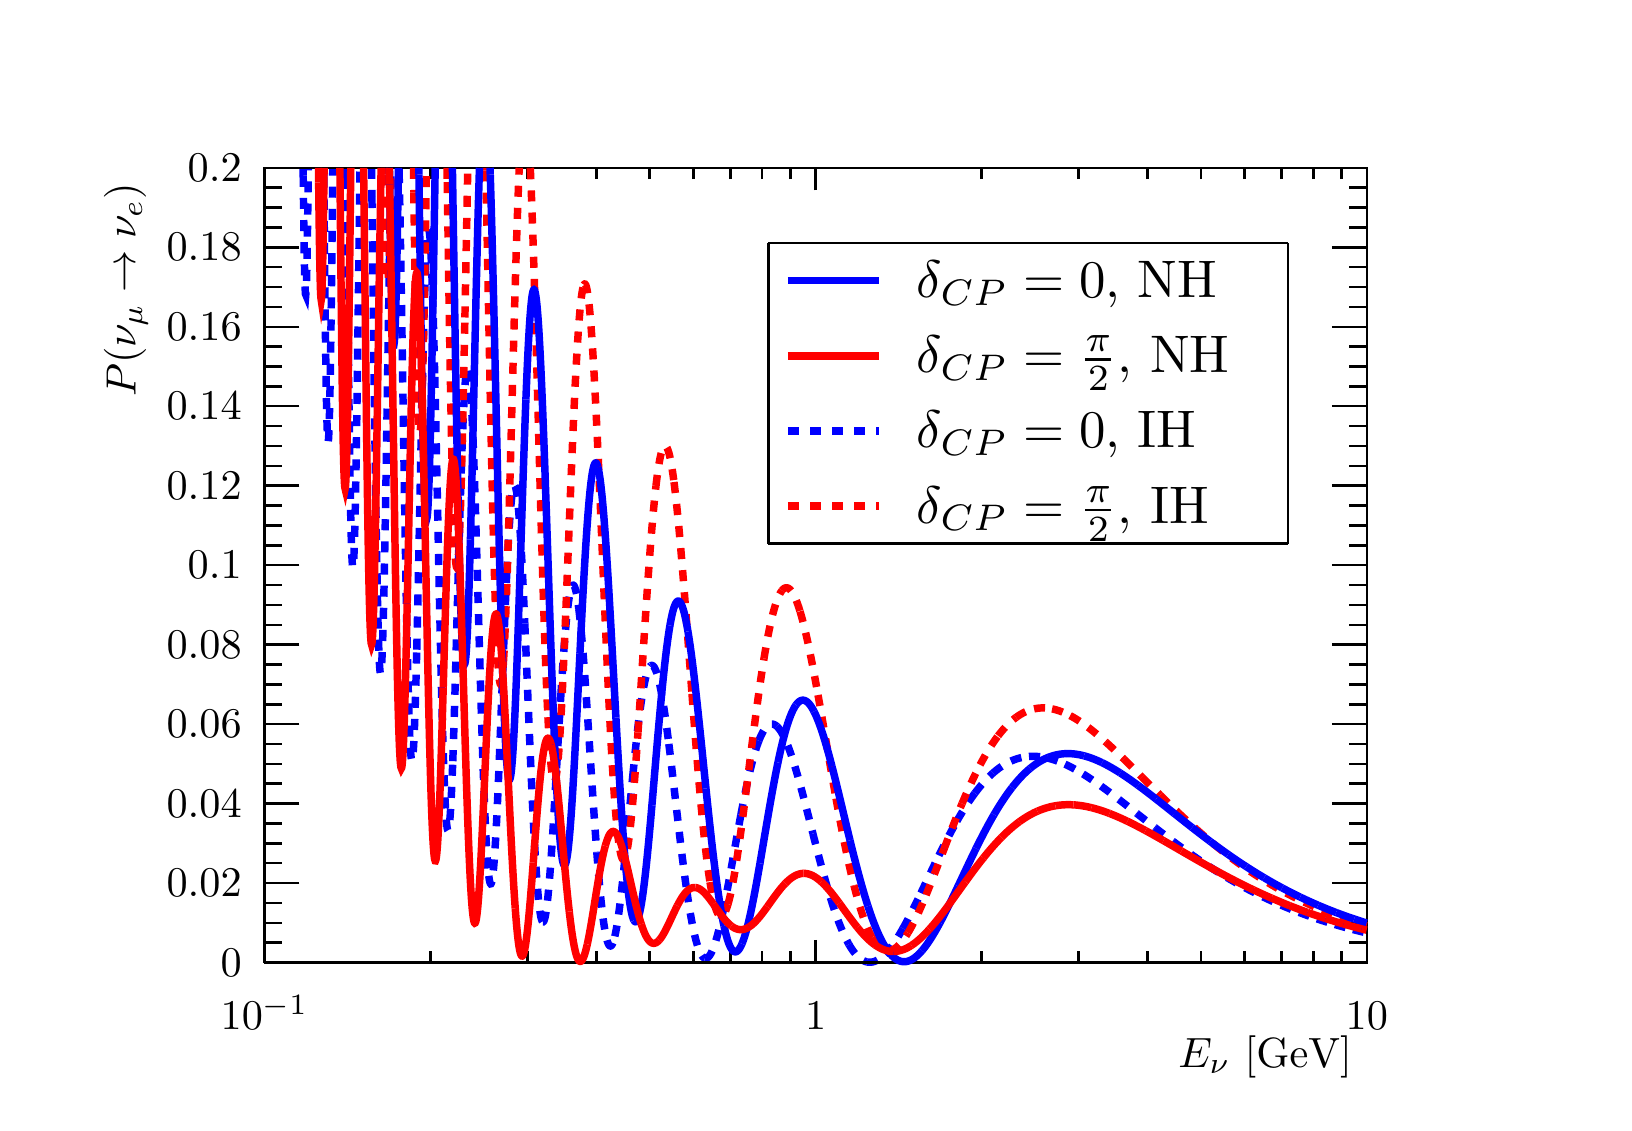
\begin{tikzpicture}
\pgfdeclareplotmark{cross} {
\pgfpathmoveto{\pgfpoint{-0.3\pgfplotmarksize}{\pgfplotmarksize}}
\pgfpathlineto{\pgfpoint{+0.3\pgfplotmarksize}{\pgfplotmarksize}}
\pgfpathlineto{\pgfpoint{+0.3\pgfplotmarksize}{0.3\pgfplotmarksize}}
\pgfpathlineto{\pgfpoint{+1\pgfplotmarksize}{0.3\pgfplotmarksize}}
\pgfpathlineto{\pgfpoint{+1\pgfplotmarksize}{-0.3\pgfplotmarksize}}
\pgfpathlineto{\pgfpoint{+0.3\pgfplotmarksize}{-0.3\pgfplotmarksize}}
\pgfpathlineto{\pgfpoint{+0.3\pgfplotmarksize}{-1.\pgfplotmarksize}}
\pgfpathlineto{\pgfpoint{-0.3\pgfplotmarksize}{-1.\pgfplotmarksize}}
\pgfpathlineto{\pgfpoint{-0.3\pgfplotmarksize}{-0.3\pgfplotmarksize}}
\pgfpathlineto{\pgfpoint{-1.\pgfplotmarksize}{-0.3\pgfplotmarksize}}
\pgfpathlineto{\pgfpoint{-1.\pgfplotmarksize}{0.3\pgfplotmarksize}}
\pgfpathlineto{\pgfpoint{-0.3\pgfplotmarksize}{0.3\pgfplotmarksize}}
\pgfpathclose
\pgfusepathqstroke
}
\pgfdeclareplotmark{cross*} {
\pgfpathmoveto{\pgfpoint{-0.3\pgfplotmarksize}{\pgfplotmarksize}}
\pgfpathlineto{\pgfpoint{+0.3\pgfplotmarksize}{\pgfplotmarksize}}
\pgfpathlineto{\pgfpoint{+0.3\pgfplotmarksize}{0.3\pgfplotmarksize}}
\pgfpathlineto{\pgfpoint{+1\pgfplotmarksize}{0.3\pgfplotmarksize}}
\pgfpathlineto{\pgfpoint{+1\pgfplotmarksize}{-0.3\pgfplotmarksize}}
\pgfpathlineto{\pgfpoint{+0.3\pgfplotmarksize}{-0.3\pgfplotmarksize}}
\pgfpathlineto{\pgfpoint{+0.3\pgfplotmarksize}{-1.\pgfplotmarksize}}
\pgfpathlineto{\pgfpoint{-0.3\pgfplotmarksize}{-1.\pgfplotmarksize}}
\pgfpathlineto{\pgfpoint{-0.3\pgfplotmarksize}{-0.3\pgfplotmarksize}}
\pgfpathlineto{\pgfpoint{-1.\pgfplotmarksize}{-0.3\pgfplotmarksize}}
\pgfpathlineto{\pgfpoint{-1.\pgfplotmarksize}{0.3\pgfplotmarksize}}
\pgfpathlineto{\pgfpoint{-0.3\pgfplotmarksize}{0.3\pgfplotmarksize}}
\pgfpathclose
\pgfusepathqfillstroke
}
\pgfdeclareplotmark{newstar} {
\pgfpathmoveto{\pgfqpoint{0pt}{\pgfplotmarksize}}
\pgfpathlineto{\pgfqpointpolar{44}{0.5\pgfplotmarksize}}
\pgfpathlineto{\pgfqpointpolar{18}{\pgfplotmarksize}}
\pgfpathlineto{\pgfqpointpolar{-20}{0.5\pgfplotmarksize}}
\pgfpathlineto{\pgfqpointpolar{-54}{\pgfplotmarksize}}
\pgfpathlineto{\pgfqpointpolar{-90}{0.5\pgfplotmarksize}}
\pgfpathlineto{\pgfqpointpolar{234}{\pgfplotmarksize}}
\pgfpathlineto{\pgfqpointpolar{198}{0.5\pgfplotmarksize}}
\pgfpathlineto{\pgfqpointpolar{162}{\pgfplotmarksize}}
\pgfpathlineto{\pgfqpointpolar{134}{0.5\pgfplotmarksize}}
\pgfpathclose
\pgfusepathqstroke
}
\pgfdeclareplotmark{newstar*} {
\pgfpathmoveto{\pgfqpoint{0pt}{\pgfplotmarksize}}
\pgfpathlineto{\pgfqpointpolar{44}{0.5\pgfplotmarksize}}
\pgfpathlineto{\pgfqpointpolar{18}{\pgfplotmarksize}}
\pgfpathlineto{\pgfqpointpolar{-20}{0.5\pgfplotmarksize}}
\pgfpathlineto{\pgfqpointpolar{-54}{\pgfplotmarksize}}
\pgfpathlineto{\pgfqpointpolar{-90}{0.5\pgfplotmarksize}}
\pgfpathlineto{\pgfqpointpolar{234}{\pgfplotmarksize}}
\pgfpathlineto{\pgfqpointpolar{198}{0.5\pgfplotmarksize}}
\pgfpathlineto{\pgfqpointpolar{162}{\pgfplotmarksize}}
\pgfpathlineto{\pgfqpointpolar{134}{0.5\pgfplotmarksize}}
\pgfpathclose
\pgfusepathqfillstroke
}
\definecolor{c}{rgb}{1,1,1};
\draw [color=c, fill=c] (0,0) rectangle (20,13.639);
\draw [color=c, fill=c] (3,1.77307) rectangle (17,11.8659);
\definecolor{c}{rgb}{0,0,0};
\draw [c,line width=0.9] (3,1.77307) -- (3,11.8659) -- (17,11.8659) -- (17,1.77307) -- (3,1.77307);
\definecolor{c}{rgb}{1,1,1};
\draw [color=c, fill=c] (3,1.77307) rectangle (17,11.8659);
\definecolor{c}{rgb}{0,0,0};
\draw [c,line width=0.9] (3,1.77307) -- (3,11.8659) -- (17,11.8659) -- (17,1.77307) -- (3,1.77307);
\definecolor{c}{rgb}{0,0,1};
\draw [c,dash pattern=on 4.00pt off 4.00pt ,line width=2.7] (3.49134,11.8659) -- (3.49233,11.7653);
\draw [c,dash pattern=on 4.00pt off 4.00pt ,line width=2.7] (3.49233,11.7653) -- (3.497,11.3524) -- (3.50167,11.0013) -- (3.50633,10.7152) -- (3.511,10.4963) -- (3.51567,10.3463) -- (3.52033,10.2657) -- (3.525,10.2545) -- (3.52967,10.3117) --
 (3.53433,10.4357) -- (3.539,10.624) -- (3.54367,10.8735) -- (3.54833,11.1803) -- (3.553,11.5399) -- (3.55673,11.8659);
\draw [c,dash pattern=on 4.00pt off 4.00pt ,line width=2.7] (3.7527,11.8659) -- (3.75367,11.7546);
\draw [c,dash pattern=on 4.00pt off 4.00pt ,line width=2.7] (3.75367,11.7546) -- (3.75833,11.244) -- (3.763,10.7647) -- (3.76767,10.3209) -- (3.77233,9.91617) -- (3.777,9.55399) -- (3.78167,9.23717) -- (3.78633,8.96812) -- (3.791,8.74873) --
 (3.79567,8.5804) -- (3.80033,8.46403) -- (3.805,8.4) -- (3.80967,8.38817) -- (3.81433,8.42791) -- (3.819,8.51812) -- (3.82367,8.65721) -- (3.82833,8.84314) -- (3.833,9.07346) -- (3.83767,9.34533) -- (3.84233,9.65554) -- (3.847,10.0005) --
 (3.85167,10.3765) -- (3.85633,10.7795) -- (3.861,11.205) -- (3.86567,11.6488) -- (3.86788,11.8659);
\draw [c,dash pattern=on 4.00pt off 4.00pt ,line width=2.7] (4.04177,11.8659) -- (4.043,11.7386);
\draw [c,dash pattern=on 4.00pt off 4.00pt ,line width=2.7] (4.043,11.7386) -- (4.04767,11.2611) -- (4.05233,10.7927) -- (4.057,10.3371) -- (4.06167,9.89744) -- (4.06633,9.47708) -- (4.071,9.079) -- (4.07567,8.70601) -- (4.08033,8.36069) --
 (4.085,8.04537) -- (4.08967,7.7621) -- (4.09433,7.51267) -- (4.099,7.29857) -- (4.10367,7.12101) -- (4.10833,6.98089) -- (4.113,6.87879) -- (4.11767,6.81501) -- (4.12233,6.78953) -- (4.127,6.80205) -- (4.13167,6.85195) -- (4.13633,6.93834) --
 (4.141,7.06007) -- (4.14567,7.21572) -- (4.15033,7.40361) -- (4.155,7.62185) -- (4.15967,7.86833) -- (4.16433,8.14076) -- (4.169,8.43666) -- (4.17367,8.75341) -- (4.17833,9.08826) -- (4.183,9.43834) -- (4.18767,9.80072) -- (4.19233,10.1724) --
 (4.197,10.5503) -- (4.20167,10.9315) -- (4.20633,11.3128) -- (4.211,11.6912) -- (4.21319,11.8659);
\draw [c,dash pattern=on 4.00pt off 4.00pt ,line width=2.7] (4.36041,11.8659) -- (4.365,11.496);
\draw [c,dash pattern=on 4.00pt off 4.00pt ,line width=2.7] (4.365,11.496) -- (4.36967,11.1138) -- (4.37433,10.7278) -- (4.379,10.3405) -- (4.38367,9.9544) -- (4.38833,9.57175) -- (4.393,9.19492) -- (4.39767,8.82616) -- (4.40233,8.46767) --
 (4.407,8.12155) -- (4.41167,7.78978) -- (4.41633,7.47426) -- (4.421,7.17673) -- (4.42567,6.89883) -- (4.43033,6.64203) -- (4.435,6.40767) -- (4.43967,6.19692) -- (4.44433,6.01079) -- (4.449,5.85013) -- (4.45367,5.71562) -- (4.45833,5.60777) --
 (4.463,5.5269) -- (4.46767,5.47319) -- (4.47233,5.44662) -- (4.477,5.44702) -- (4.48167,5.47406) -- (4.48633,5.52722) -- (4.491,5.60585) -- (4.49567,5.70915) -- (4.50033,5.83618) -- (4.505,5.98584) -- (4.50967,6.15695) -- (4.51433,6.34816) --
 (4.519,6.55806) -- (4.52367,6.78512) -- (4.52833,7.02772) -- (4.533,7.28418) -- (4.53767,7.55274) -- (4.54233,7.8316) -- (4.547,8.11891) -- (4.55167,8.4128) -- (4.55633,8.71136) -- (4.561,9.0127) -- (4.56567,9.31491) -- (4.57033,9.61612) --
 (4.575,9.91447) -- (4.57967,10.2081) -- (4.58433,10.4954) -- (4.589,10.7744);
\draw [c,dash pattern=on 4.00pt off 4.00pt ,line width=2.7] (4.589,10.7744) -- (4.59367,11.0436) -- (4.59833,11.3014) -- (4.603,11.5464) -- (4.60767,11.777) -- (4.6096,11.8659);
\draw [c,dash pattern=on 4.00pt off 4.00pt ,line width=2.7] (4.70909,11.8659) -- (4.71033,11.8102);
\draw [c,dash pattern=on 4.00pt off 4.00pt ,line width=2.7] (4.71033,11.8102) -- (4.715,11.586) -- (4.71967,11.3479) -- (4.72433,11.0972) -- (4.729,10.8352) -- (4.73367,10.5632) -- (4.73833,10.2827) -- (4.743,9.99506) -- (4.74767,9.70174) --
 (4.75233,9.40421) -- (4.757,9.10393) -- (4.76167,8.80237) -- (4.76633,8.501) -- (4.771,8.20125) -- (4.77567,7.90454) -- (4.78033,7.61227) -- (4.785,7.32578) -- (4.78967,7.04639) -- (4.79433,6.77536) -- (4.799,6.51389) -- (4.80367,6.26314) --
 (4.80833,6.02417) -- (4.813,5.79799) -- (4.81767,5.58556) -- (4.82233,5.38772) -- (4.827,5.20525) -- (4.83167,5.03884) -- (4.83633,4.88912) -- (4.841,4.75659) -- (4.84567,4.64169) -- (4.85033,4.54476) -- (4.855,4.46606) -- (4.85967,4.40575) --
 (4.86433,4.3639) -- (4.869,4.34049) -- (4.87367,4.33542) -- (4.87833,4.3485) -- (4.883,4.37945) -- (4.88767,4.42792) -- (4.89233,4.49347) -- (4.897,4.5756) -- (4.90167,4.67372) -- (4.90633,4.78719) -- (4.911,4.91528) -- (4.91567,5.05722) --
 (4.92033,5.21218) -- (4.925,5.37928) -- (4.92967,5.5576) -- (4.93433,5.74615);
\draw [c,dash pattern=on 4.00pt off 4.00pt ,line width=2.7] (4.93433,5.74615) -- (4.939,5.94394) -- (4.94367,6.14993) -- (4.94833,6.36305) -- (4.953,6.58222) -- (4.95767,6.80634) -- (4.96233,7.0343) -- (4.967,7.26498) -- (4.97167,7.49727) --
 (4.97633,7.73005) -- (4.981,7.96223) -- (4.98567,8.19271) -- (4.99033,8.42043) -- (4.995,8.64435) -- (4.99967,8.86344) -- (5.00433,9.07673) -- (5.009,9.28326) -- (5.01367,9.48212) -- (5.01833,9.67245) -- (5.023,9.85344) -- (5.02767,10.0243) --
 (5.03233,10.1843) -- (5.037,10.3328) -- (5.04167,10.4693) -- (5.04633,10.593) -- (5.051,10.7036) -- (5.05567,10.8006) -- (5.06033,10.8837) -- (5.065,10.9525) -- (5.06967,11.0068) -- (5.07433,11.0465) -- (5.079,11.0713) -- (5.08367,11.0813) --
 (5.08833,11.0765) -- (5.093,11.057) -- (5.09767,11.0228) -- (5.10233,10.9742) -- (5.107,10.9114) -- (5.11167,10.8348) -- (5.11633,10.7446) -- (5.121,10.6413) -- (5.12567,10.5253) -- (5.13033,10.3972) -- (5.135,10.2575) -- (5.13967,10.1068) --
 (5.14433,9.94565) -- (5.149,9.77481) -- (5.15367,9.59494) -- (5.15833,9.40675) -- (5.163,9.211);
\draw [c,dash pattern=on 4.00pt off 4.00pt ,line width=2.7] (5.163,9.211) -- (5.16767,9.00846) -- (5.17233,8.7999) -- (5.177,8.58615) -- (5.18167,8.36801) -- (5.18633,8.14631) -- (5.191,7.92187) -- (5.19567,7.69553) -- (5.20033,7.46812) --
 (5.205,7.24047) -- (5.20967,7.01339) -- (5.21433,6.78769) -- (5.219,6.56417) -- (5.22367,6.34361) -- (5.22833,6.12676) -- (5.233,5.91435) -- (5.23767,5.70711) -- (5.24233,5.50572) -- (5.247,5.31084) -- (5.25167,5.12309) -- (5.25633,4.94307) --
 (5.261,4.77133) -- (5.26567,4.6084) -- (5.27033,4.45477) -- (5.275,4.31087) -- (5.27967,4.17712) -- (5.28433,4.05388) -- (5.289,3.94147) -- (5.29367,3.84018) -- (5.29833,3.75024) -- (5.303,3.67185) -- (5.30767,3.60516) -- (5.31233,3.55027) --
 (5.317,3.50725) -- (5.32167,3.47613) -- (5.32633,3.45688) -- (5.331,3.44944) -- (5.33567,3.45372) -- (5.34033,3.46956) -- (5.345,3.49679) -- (5.34967,3.53519) -- (5.35433,3.58451) -- (5.359,3.64444) -- (5.36367,3.71468) -- (5.36833,3.79486) --
 (5.373,3.88461) -- (5.37767,3.98349) -- (5.38233,4.09108) -- (5.387,4.20691) -- (5.39167,4.33048);
\draw [c,dash pattern=on 4.00pt off 4.00pt ,line width=2.7] (5.39167,4.33048) -- (5.39633,4.46129) -- (5.401,4.59882) -- (5.40567,4.7425) -- (5.41033,4.89179) -- (5.415,5.04611) -- (5.41967,5.20487) -- (5.42433,5.36748) -- (5.429,5.53335) --
 (5.43367,5.70187) -- (5.43833,5.87243) -- (5.443,6.04443) -- (5.44767,6.21726) -- (5.45233,6.39033) -- (5.457,6.56304) -- (5.46167,6.73479) -- (5.46633,6.90502) -- (5.471,7.07315) -- (5.47567,7.23863) -- (5.48033,7.40092) -- (5.485,7.5595) --
 (5.48967,7.71385) -- (5.49433,7.8635) -- (5.499,8.00797) -- (5.50367,8.14681) -- (5.50833,8.27961) -- (5.513,8.40595) -- (5.51767,8.52547) -- (5.52233,8.63781) -- (5.527,8.74265) -- (5.53167,8.83968) -- (5.53633,8.92865) -- (5.541,9.00929) --
 (5.54567,9.0814) -- (5.55033,9.14479) -- (5.555,9.1993) -- (5.55967,9.2448) -- (5.56433,9.28119) -- (5.569,9.3084) -- (5.57367,9.32638) -- (5.57833,9.33512) -- (5.583,9.33462) -- (5.58767,9.32494) -- (5.59233,9.30612) -- (5.597,9.27828) --
 (5.60167,9.24152) -- (5.60633,9.19598) -- (5.611,9.14185) -- (5.61567,9.0793) -- (5.62033,9.00855);
\draw [c,dash pattern=on 4.00pt off 4.00pt ,line width=2.7] (5.62033,9.00855) -- (5.625,8.92984) -- (5.62967,8.84343) -- (5.63433,8.74958) -- (5.639,8.6486) -- (5.64367,8.5408) -- (5.64833,8.4265) -- (5.653,8.30605) -- (5.65767,8.17981) --
 (5.66233,8.04815) -- (5.667,7.91144) -- (5.67167,7.77009) -- (5.67633,7.6245) -- (5.681,7.47506) -- (5.68567,7.32221) -- (5.69033,7.16636) -- (5.695,7.00793) -- (5.69967,6.84736) -- (5.70433,6.68508) -- (5.709,6.5215) -- (5.71367,6.35707) --
 (5.71833,6.19221) -- (5.723,6.02735) -- (5.72767,5.8629) -- (5.73233,5.69928) -- (5.737,5.5369) -- (5.74167,5.37615) -- (5.74633,5.21743) -- (5.751,5.06113) -- (5.75567,4.90761) -- (5.76033,4.75723) -- (5.765,4.61035) -- (5.76967,4.4673) --
 (5.77433,4.32841) -- (5.779,4.19397) -- (5.78367,4.0643) -- (5.78833,3.93966) -- (5.793,3.82032) -- (5.79767,3.70653) -- (5.80233,3.59851) -- (5.807,3.49647) -- (5.81167,3.40062) -- (5.81633,3.31113) -- (5.821,3.22816) -- (5.82567,3.15185) --
 (5.83033,3.08232) -- (5.835,3.01968) -- (5.83967,2.96401) -- (5.84433,2.91538) -- (5.849,2.87384);
\draw [c,dash pattern=on 4.00pt off 4.00pt ,line width=2.7] (5.849,2.87384) -- (5.85367,2.83943) -- (5.85833,2.81215) -- (5.863,2.792) -- (5.86767,2.77896) -- (5.87233,2.77299) -- (5.877,2.77403) -- (5.88167,2.78202) -- (5.88633,2.79686) --
 (5.891,2.81844) -- (5.89567,2.84666) -- (5.90033,2.88136) -- (5.905,2.92242) -- (5.90967,2.96965) -- (5.91433,3.0229) -- (5.919,3.08196) -- (5.92367,3.14664) -- (5.92833,3.21673) -- (5.933,3.29201) -- (5.93767,3.37224) -- (5.94233,3.45718) --
 (5.947,3.54659) -- (5.95167,3.64021) -- (5.95633,3.73777) -- (5.961,3.839) -- (5.96567,3.94363) -- (5.97033,4.05138) -- (5.975,4.16195) -- (5.97967,4.27506) -- (5.98433,4.39042) -- (5.989,4.50774) -- (5.99367,4.62671) -- (5.99833,4.74705) --
 (6.003,4.86845) -- (6.00767,4.99062) -- (6.01233,5.11328) -- (6.017,5.23611) -- (6.02167,5.35884) -- (6.02633,5.48118) -- (6.031,5.60285) -- (6.03567,5.72357) -- (6.04033,5.84306) -- (6.045,5.96106) -- (6.04967,6.07731) -- (6.05433,6.19156) --
 (6.059,6.30354) -- (6.06367,6.41304) -- (6.06833,6.5198) -- (6.073,6.62361) -- (6.07767,6.72426);
\draw [c,dash pattern=on 4.00pt off 4.00pt ,line width=2.7] (6.07767,6.72426) -- (6.08233,6.82153) -- (6.087,6.91524) -- (6.09167,7.00518) -- (6.09633,7.09119) -- (6.101,7.1731) -- (6.10567,7.25075) -- (6.11033,7.32399) -- (6.115,7.3927) --
 (6.11967,7.45674) -- (6.12433,7.516) -- (6.129,7.57038) -- (6.13367,7.61979) -- (6.13833,7.66415) -- (6.143,7.70339) -- (6.14767,7.73746) -- (6.15233,7.7663) -- (6.157,7.78988) -- (6.16167,7.80818) -- (6.16633,7.82119) -- (6.171,7.82891) --
 (6.17567,7.83133) -- (6.18033,7.82849) -- (6.185,7.82041) -- (6.18967,7.80714) -- (6.19433,7.78871) -- (6.199,7.7652) -- (6.20367,7.73667) -- (6.20833,7.70321) -- (6.213,7.66489) -- (6.21767,7.62181) -- (6.22233,7.57408) -- (6.227,7.52181) --
 (6.23167,7.46513) -- (6.23633,7.40415) -- (6.241,7.33902) -- (6.24567,7.26987) -- (6.25033,7.19686) -- (6.255,7.12013) -- (6.25967,7.03985) -- (6.26433,6.95618) -- (6.269,6.86929) -- (6.27367,6.77935) -- (6.27833,6.68654) -- (6.283,6.59104) --
 (6.28767,6.49304) -- (6.29233,6.39272) -- (6.297,6.29027) -- (6.30167,6.18589) -- (6.30633,6.07977);
\draw [c,dash pattern=on 4.00pt off 4.00pt ,line width=2.7] (6.30633,6.07977) -- (6.311,5.9721) -- (6.31567,5.86308) -- (6.32033,5.7529) -- (6.325,5.64177) -- (6.32967,5.52987) -- (6.33433,5.4174) -- (6.339,5.30456) -- (6.34367,5.19155) --
 (6.34833,5.07854) -- (6.353,4.96574) -- (6.35767,4.85333) -- (6.36233,4.74149) -- (6.367,4.63041) -- (6.37167,4.52026) -- (6.37633,4.41123) -- (6.381,4.30348) -- (6.38567,4.19718) -- (6.39033,4.0925) -- (6.395,3.98959) -- (6.39967,3.88861) --
 (6.40433,3.78971) -- (6.409,3.69304) -- (6.41367,3.59872) -- (6.41833,3.5069) -- (6.423,3.41771) -- (6.42767,3.33127) -- (6.43233,3.24769) -- (6.437,3.16708) -- (6.44167,3.08956) -- (6.44633,3.01522) -- (6.451,2.94414) -- (6.45567,2.87642) --
 (6.46033,2.81214) -- (6.465,2.75136) -- (6.46967,2.69416) -- (6.47433,2.6406) -- (6.479,2.59072) -- (6.48367,2.54458) -- (6.48833,2.50221) -- (6.493,2.46365) -- (6.49767,2.42892) -- (6.50233,2.39805) -- (6.507,2.37104) -- (6.51167,2.34792) --
 (6.51633,2.32867) -- (6.521,2.3133) -- (6.52567,2.30178) -- (6.53033,2.29412) -- (6.535,2.29028);
\draw [c,dash pattern=on 4.00pt off 4.00pt ,line width=2.7] (6.535,2.29028) -- (6.53967,2.29023) -- (6.54433,2.29394) -- (6.549,2.30137) -- (6.55367,2.31248) -- (6.55833,2.32721) -- (6.563,2.34551) -- (6.56767,2.36732) -- (6.57233,2.39257) --
 (6.577,2.4212) -- (6.58167,2.45312) -- (6.58633,2.48826) -- (6.591,2.52654) -- (6.59567,2.56787) -- (6.60033,2.61215) -- (6.605,2.65931) -- (6.60967,2.70922) -- (6.61433,2.76181) -- (6.619,2.81696) -- (6.62367,2.87456) -- (6.62833,2.93451) --
 (6.633,2.9967) -- (6.63767,3.06101) -- (6.64233,3.12733) -- (6.647,3.19553) -- (6.65167,3.26551) -- (6.65633,3.33713) -- (6.661,3.41029) -- (6.66567,3.48485) -- (6.67033,3.56069) -- (6.675,3.63769) -- (6.67967,3.71573) -- (6.68433,3.79468) --
 (6.689,3.87441) -- (6.69367,3.95481) -- (6.69833,4.03574) -- (6.703,4.11708) -- (6.70767,4.19871) -- (6.71233,4.28052) -- (6.717,4.36237) -- (6.72167,4.44414) -- (6.72633,4.52573) -- (6.731,4.60701) -- (6.73567,4.68786) -- (6.74033,4.76818) --
 (6.745,4.84784) -- (6.74967,4.92675) -- (6.75433,5.00478) -- (6.759,5.08185) -- (6.76367,5.15784);
\draw [c,dash pattern=on 4.00pt off 4.00pt ,line width=2.7] (6.76367,5.15784) -- (6.76833,5.23265) -- (6.773,5.30619) -- (6.77767,5.37836) -- (6.78233,5.44907) -- (6.787,5.51823) -- (6.79167,5.58575) -- (6.79633,5.65155) -- (6.801,5.71555) --
 (6.80567,5.77767) -- (6.81033,5.83783) -- (6.815,5.89598) -- (6.81967,5.95203) -- (6.82433,6.00594) -- (6.829,6.05763) -- (6.83367,6.10704) -- (6.83833,6.15414) -- (6.843,6.19886) -- (6.84767,6.24116) -- (6.85233,6.28101) -- (6.857,6.31835) --
 (6.86167,6.35315) -- (6.86633,6.38539) -- (6.871,6.41504) -- (6.87567,6.44206) -- (6.88033,6.46644) -- (6.885,6.48817) -- (6.88967,6.50722) -- (6.89433,6.52359) -- (6.899,6.53728) -- (6.90367,6.54827) -- (6.90833,6.55656) -- (6.913,6.56217) --
 (6.91767,6.5651) -- (6.92233,6.56535) -- (6.927,6.56295) -- (6.93167,6.5579) -- (6.93633,6.55022) -- (6.941,6.53995) -- (6.94567,6.5271) -- (6.95033,6.51169) -- (6.955,6.49378) -- (6.95967,6.47337) -- (6.96433,6.45052) -- (6.969,6.42526) --
 (6.97367,6.39763) -- (6.97833,6.36768) -- (6.983,6.33545) -- (6.98767,6.30099) -- (6.99233,6.26435);
\draw [c,dash pattern=on 4.00pt off 4.00pt ,line width=2.7] (6.99233,6.26435) -- (6.997,6.22558) -- (7.00167,6.18475) -- (7.00633,6.14189) -- (7.011,6.09708) -- (7.01567,6.05037) -- (7.02033,6.00182) -- (7.025,5.9515) -- (7.02967,5.89947) --
 (7.03433,5.8458) -- (7.039,5.79055) -- (7.04367,5.7338) -- (7.04833,5.6756) -- (7.053,5.61603) -- (7.05767,5.55517) -- (7.06233,5.49308) -- (7.067,5.42984) -- (7.07167,5.36552) -- (7.07633,5.30019) -- (7.081,5.23392) -- (7.08567,5.1668) --
 (7.09033,5.09889) -- (7.095,5.03027) -- (7.09967,4.96102) -- (7.10433,4.8912) -- (7.109,4.8209) -- (7.11367,4.75019) -- (7.11833,4.67914) -- (7.123,4.60782) -- (7.12767,4.53632) -- (7.13233,4.46469) -- (7.137,4.39302) -- (7.14167,4.32138) --
 (7.14633,4.24983) -- (7.151,4.17845) -- (7.15567,4.1073) -- (7.16033,4.03646) -- (7.165,3.96598) -- (7.16967,3.89595) -- (7.17433,3.82641) -- (7.179,3.75745) -- (7.18367,3.68911) -- (7.18833,3.62146) -- (7.193,3.55457) -- (7.19767,3.48848) --
 (7.20233,3.42326) -- (7.207,3.35897) -- (7.21167,3.29565) -- (7.21633,3.23337) -- (7.221,3.17217);
\draw [c,dash pattern=on 4.00pt off 4.00pt ,line width=2.7] (7.221,3.17217) -- (7.22567,3.1121) -- (7.23033,3.05321) -- (7.235,2.99555) -- (7.23967,2.93916) -- (7.24433,2.88409) -- (7.249,2.83037) -- (7.25367,2.77806) -- (7.25833,2.72718) --
 (7.263,2.67777) -- (7.26767,2.62987) -- (7.27233,2.58351) -- (7.277,2.53872) -- (7.28167,2.49553) -- (7.28633,2.45397) -- (7.291,2.41406) -- (7.29567,2.37583) -- (7.30033,2.33929) -- (7.305,2.30447) -- (7.30967,2.27139) -- (7.31433,2.24007) --
 (7.319,2.21051) -- (7.32367,2.18273) -- (7.32833,2.15674) -- (7.333,2.13256) -- (7.33767,2.11018) -- (7.34233,2.08961) -- (7.347,2.07087) -- (7.35167,2.05394) -- (7.35633,2.03884) -- (7.361,2.02555) -- (7.36567,2.01409) -- (7.37033,2.00443) --
 (7.375,1.99659) -- (7.37967,1.99054) -- (7.38433,1.98628) -- (7.389,1.9838) -- (7.39367,1.98309) -- (7.39833,1.98414) -- (7.403,1.98692) -- (7.40767,1.99143) -- (7.41233,1.99764) -- (7.417,2.00554) -- (7.42167,2.0151) -- (7.42633,2.02631) --
 (7.431,2.03914) -- (7.43567,2.05357) -- (7.44033,2.06957) -- (7.445,2.08711) -- (7.44967,2.10618);
\draw [c,dash pattern=on 4.00pt off 4.00pt ,line width=2.7] (7.44967,2.10618) -- (7.45433,2.12673) -- (7.459,2.14875) -- (7.46367,2.17219) -- (7.46833,2.19704) -- (7.473,2.22325) -- (7.47767,2.2508) -- (7.48233,2.27964) -- (7.487,2.30975) --
 (7.49167,2.34109) -- (7.49633,2.37363) -- (7.501,2.40732) -- (7.50567,2.44214) -- (7.51033,2.47803) -- (7.515,2.51497) -- (7.51967,2.55292) -- (7.52433,2.59183) -- (7.529,2.63167) -- (7.53367,2.67239) -- (7.53833,2.71396) -- (7.543,2.75633) --
 (7.54767,2.79947) -- (7.55233,2.84333) -- (7.557,2.88788) -- (7.56167,2.93306) -- (7.56633,2.97884) -- (7.571,3.02518) -- (7.57567,3.07203) -- (7.58033,3.11936) -- (7.585,3.16712) -- (7.58967,3.21527) -- (7.59433,3.26376) -- (7.599,3.31257) --
 (7.60367,3.36164) -- (7.60833,3.41093) -- (7.613,3.46041) -- (7.61767,3.51003) -- (7.62233,3.55976) -- (7.627,3.60955) -- (7.63167,3.65936) -- (7.63633,3.70916) -- (7.641,3.7589) -- (7.64567,3.80855) -- (7.65033,3.85807) -- (7.655,3.90742) --
 (7.65967,3.95656) -- (7.66433,4.00547) -- (7.669,4.05409) -- (7.67367,4.1024) -- (7.67833,4.15037);
\draw [c,dash pattern=on 4.00pt off 4.00pt ,line width=2.7] (7.67833,4.15037) -- (7.683,4.19795) -- (7.68767,4.24511) -- (7.69233,4.29182) -- (7.697,4.33806) -- (7.70167,4.38378) -- (7.70633,4.42895) -- (7.711,4.47355) -- (7.71567,4.51755) --
 (7.72033,4.56091) -- (7.725,4.60362) -- (7.72967,4.64563) -- (7.73433,4.68693) -- (7.739,4.72749) -- (7.74367,4.76728) -- (7.74833,4.80628) -- (7.753,4.84447) -- (7.75767,4.88182) -- (7.76233,4.91831) -- (7.767,4.95392) -- (7.77167,4.98863) --
 (7.77633,5.02243) -- (7.781,5.05528) -- (7.78567,5.08718) -- (7.79033,5.11811) -- (7.795,5.14805) -- (7.79967,5.17698) -- (7.80433,5.2049) -- (7.809,5.23179) -- (7.81367,5.25763) -- (7.81833,5.28241) -- (7.823,5.30613) -- (7.82767,5.32877) --
 (7.83233,5.35032) -- (7.837,5.37077) -- (7.84167,5.39013) -- (7.84633,5.40837) -- (7.851,5.4255) -- (7.85567,5.4415) -- (7.86033,5.45638) -- (7.865,5.47012) -- (7.86967,5.48274) -- (7.87433,5.49422) -- (7.879,5.50456) -- (7.88367,5.51376) --
 (7.88833,5.52183) -- (7.893,5.52876) -- (7.89767,5.53455) -- (7.90233,5.53922) -- (7.907,5.54275);
\draw [c,dash pattern=on 4.00pt off 4.00pt ,line width=2.7] (7.907,5.54275) -- (7.91167,5.54516) -- (7.91633,5.54644) -- (7.921,5.54661) -- (7.92567,5.54567) -- (7.93033,5.54362) -- (7.935,5.54047) -- (7.93967,5.53624) -- (7.94433,5.53092) --
 (7.949,5.52453) -- (7.95367,5.51707) -- (7.95833,5.50857) -- (7.963,5.49901) -- (7.96767,5.48843) -- (7.97233,5.47683) -- (7.977,5.46421) -- (7.98167,5.45061) -- (7.98633,5.43602) -- (7.991,5.42046) -- (7.99567,5.40394) -- (8.00033,5.38649) --
 (8.005,5.36811) -- (8.00967,5.34882) -- (8.01433,5.32864) -- (8.019,5.30758) -- (8.02367,5.28565) -- (8.02833,5.26289) -- (8.033,5.23929) -- (8.03767,5.21489) -- (8.04233,5.18969) -- (8.047,5.16372) -- (8.05167,5.137) -- (8.05633,5.10954) --
 (8.061,5.08136) -- (8.06567,5.05248) -- (8.07033,5.02292) -- (8.075,4.99271) -- (8.07967,4.96185) -- (8.08433,4.93038) -- (8.089,4.89831) -- (8.09367,4.86566) -- (8.09833,4.83245) -- (8.103,4.7987) -- (8.10767,4.76444) -- (8.11233,4.72968) --
 (8.117,4.69444) -- (8.12167,4.65876) -- (8.12633,4.62264) -- (8.131,4.5861) -- (8.13567,4.54918);
\draw [c,dash pattern=on 4.00pt off 4.00pt ,line width=2.7] (8.13567,4.54918) -- (8.14033,4.51189) -- (8.145,4.47424) -- (8.14967,4.43628) -- (8.15433,4.398) -- (8.159,4.35944) -- (8.16367,4.32062) -- (8.16833,4.28155) -- (8.173,4.24227) --
 (8.17767,4.20278) -- (8.18233,4.16311) -- (8.187,4.12328) -- (8.19167,4.08331) -- (8.19633,4.04323) -- (8.201,4.00305) -- (8.20567,3.96279) -- (8.21033,3.92247) -- (8.215,3.88211) -- (8.21967,3.84174) -- (8.22433,3.80137) -- (8.229,3.76102) --
 (8.23367,3.72071) -- (8.23833,3.68046) -- (8.243,3.64028) -- (8.24767,3.60021) -- (8.25233,3.56025) -- (8.257,3.52042) -- (8.26167,3.48075) -- (8.26633,3.44124) -- (8.271,3.40192) -- (8.27567,3.36281) -- (8.28033,3.32392) -- (8.285,3.28526) --
 (8.28967,3.24686) -- (8.29433,3.20872) -- (8.299,3.17088) -- (8.30367,3.13333) -- (8.30833,3.0961) -- (8.313,3.05921) -- (8.31767,3.02266) -- (8.32233,2.98647) -- (8.327,2.95065) -- (8.33167,2.91523) -- (8.33633,2.8802) -- (8.341,2.8456) --
 (8.34567,2.81141) -- (8.35033,2.77768) -- (8.355,2.74439) -- (8.35967,2.71157) -- (8.36433,2.67922);
\draw [c,dash pattern=on 4.00pt off 4.00pt ,line width=2.7] (8.36433,2.67922) -- (8.369,2.64736) -- (8.37367,2.616) -- (8.37833,2.58515) -- (8.383,2.55482) -- (8.38767,2.52501) -- (8.39233,2.49575) -- (8.397,2.46703) -- (8.40167,2.43887) --
 (8.40633,2.41127) -- (8.411,2.38425) -- (8.41567,2.35781) -- (8.42033,2.33195) -- (8.425,2.3067) -- (8.42967,2.28204) -- (8.43433,2.25799) -- (8.439,2.23456) -- (8.44367,2.21175) -- (8.44833,2.18957) -- (8.453,2.16802) -- (8.45767,2.1471) --
 (8.46233,2.12683) -- (8.467,2.1072) -- (8.47167,2.08822) -- (8.47633,2.0699) -- (8.481,2.05223) -- (8.48567,2.03521) -- (8.49033,2.01886) -- (8.495,2.00318) -- (8.49967,1.98816) -- (8.50433,1.97381) -- (8.509,1.96012) -- (8.51367,1.94711) --
 (8.51833,1.93477) -- (8.523,1.9231) -- (8.52767,1.9121) -- (8.53233,1.90177) -- (8.537,1.89211) -- (8.54167,1.88313) -- (8.54633,1.87481) -- (8.551,1.86716) -- (8.55567,1.86018) -- (8.56033,1.85386) -- (8.565,1.84821) -- (8.56967,1.84322) --
 (8.57433,1.83889) -- (8.579,1.83521) -- (8.58367,1.83219) -- (8.58833,1.82981) -- (8.593,1.82808);
\draw [c,dash pattern=on 4.00pt off 4.00pt ,line width=2.7] (8.593,1.82808) -- (8.59767,1.827) -- (8.60233,1.82655) -- (8.607,1.82674) -- (8.61167,1.82755) -- (8.61633,1.829) -- (8.621,1.83106) -- (8.62567,1.83374) -- (8.63033,1.83703) --
 (8.635,1.84093) -- (8.63967,1.84542) -- (8.64433,1.85051) -- (8.649,1.85619) -- (8.65367,1.86245) -- (8.65833,1.86928) -- (8.663,1.87669) -- (8.66767,1.88465) -- (8.67233,1.89318) -- (8.677,1.90225) -- (8.68167,1.91186) -- (8.68633,1.92201) --
 (8.691,1.93269) -- (8.69567,1.94388) -- (8.70033,1.95559) -- (8.705,1.9678) -- (8.70967,1.98051) -- (8.71433,1.99371) -- (8.719,2.00739) -- (8.72367,2.02154) -- (8.72833,2.03615) -- (8.733,2.05123) -- (8.73767,2.06674) -- (8.74233,2.0827) --
 (8.747,2.09909) -- (8.75167,2.1159) -- (8.75633,2.13312) -- (8.761,2.15074) -- (8.76567,2.16876) -- (8.77033,2.18717) -- (8.775,2.20595) -- (8.77967,2.2251) -- (8.78433,2.2446) -- (8.789,2.26446) -- (8.79367,2.28466) -- (8.79833,2.30518) --
 (8.803,2.32603) -- (8.80767,2.34719) -- (8.81233,2.36866) -- (8.817,2.39041) -- (8.82167,2.41245);
\draw [c,dash pattern=on 4.00pt off 4.00pt ,line width=2.7] (8.82167,2.41245) -- (8.82633,2.43476) -- (8.831,2.45734) -- (8.83567,2.48018) -- (8.84033,2.50326) -- (8.845,2.52657) -- (8.84967,2.55011) -- (8.85433,2.57387) -- (8.859,2.59784) --
 (8.86367,2.62201) -- (8.86833,2.64636) -- (8.873,2.6709) -- (8.87767,2.69561) -- (8.88233,2.72047) -- (8.887,2.74549) -- (8.89167,2.77065) -- (8.89633,2.79595) -- (8.901,2.82137) -- (8.90567,2.8469) -- (8.91033,2.87254) -- (8.915,2.89828) --
 (8.91967,2.9241) -- (8.92433,2.95) -- (8.929,2.97598) -- (8.93367,3.00201) -- (8.93833,3.0281) -- (8.943,3.05423) -- (8.94767,3.08039) -- (8.95233,3.10658) -- (8.957,3.13279) -- (8.96167,3.15901) -- (8.96633,3.18522) -- (8.971,3.21143) --
 (8.97567,3.23763) -- (8.98033,3.2638) -- (8.985,3.28994) -- (8.98967,3.31604) -- (8.99433,3.34209) -- (8.999,3.36808) -- (9.00367,3.39401) -- (9.00833,3.41988) -- (9.013,3.44566) -- (9.01767,3.47135) -- (9.02233,3.49696) -- (9.027,3.52246) --
 (9.03167,3.54785) -- (9.03633,3.57313) -- (9.041,3.59829) -- (9.04567,3.62331) -- (9.05033,3.64821);
\draw [c,dash pattern=on 4.00pt off 4.00pt ,line width=2.7] (9.05033,3.64821) -- (9.055,3.67296) -- (9.05967,3.69756) -- (9.06433,3.722) -- (9.069,3.74629) -- (9.07367,3.7704) -- (9.07833,3.79435) -- (9.083,3.81811) -- (9.08767,3.84168) --
 (9.09233,3.86507) -- (9.097,3.88825) -- (9.10167,3.91123) -- (9.10633,3.93401) -- (9.111,3.95657) -- (9.11567,3.97891) -- (9.12033,4.00102) -- (9.125,4.02291) -- (9.12967,4.04456) -- (9.13433,4.06597) -- (9.139,4.08714) -- (9.14367,4.10806) --
 (9.14833,4.12872) -- (9.153,4.14913) -- (9.15767,4.16927) -- (9.16233,4.18915) -- (9.167,4.20876) -- (9.17167,4.2281) -- (9.17633,4.24715) -- (9.181,4.26593) -- (9.18567,4.28442) -- (9.19033,4.30262) -- (9.195,4.32053) -- (9.19967,4.33814) --
 (9.20433,4.35546) -- (9.209,4.37247) -- (9.21367,4.38918) -- (9.21833,4.40558) -- (9.223,4.42168) -- (9.22767,4.43746) -- (9.23233,4.45292) -- (9.237,4.46807) -- (9.24167,4.48289) -- (9.24633,4.4974) -- (9.251,4.51158) -- (9.25567,4.52544) --
 (9.26033,4.53896) -- (9.265,4.55216) -- (9.26967,4.56503) -- (9.27433,4.57756) -- (9.279,4.58976);
\draw [c,dash pattern=on 4.00pt off 4.00pt ,line width=2.7] (9.279,4.58976) -- (9.28367,4.60162) -- (9.28833,4.61315) -- (9.293,4.62434) -- (9.29767,4.63519) -- (9.30233,4.6457) -- (9.307,4.65587) -- (9.31167,4.6657) -- (9.31633,4.67518) --
 (9.321,4.68433) -- (9.32567,4.69313) -- (9.33033,4.70158) -- (9.335,4.7097) -- (9.33967,4.71746) -- (9.34433,4.72489) -- (9.349,4.73197) -- (9.35367,4.7387) -- (9.35833,4.7451) -- (9.363,4.75114) -- (9.36767,4.75685) -- (9.37233,4.76221) --
 (9.377,4.76723) -- (9.38167,4.77191) -- (9.38633,4.77624) -- (9.391,4.78024) -- (9.39567,4.78389) -- (9.40033,4.78721) -- (9.405,4.79019) -- (9.40967,4.79283) -- (9.41433,4.79514) -- (9.419,4.79711) -- (9.42367,4.79875) -- (9.42833,4.80005) --
 (9.433,4.80103) -- (9.43767,4.80168) -- (9.44233,4.802) -- (9.447,4.80199) -- (9.45167,4.80166) -- (9.45633,4.801) -- (9.461,4.80003) -- (9.46567,4.79873) -- (9.47033,4.79712) -- (9.475,4.7952) -- (9.47967,4.79296) -- (9.48433,4.79041) --
 (9.489,4.78755) -- (9.49367,4.78438) -- (9.49833,4.78091) -- (9.503,4.77714) -- (9.50767,4.77306);
\draw [c,dash pattern=on 4.00pt off 4.00pt ,line width=2.7] (9.50767,4.77306) -- (9.51233,4.76869) -- (9.517,4.76403) -- (9.52167,4.75907) -- (9.52633,4.75382) -- (9.531,4.74828) -- (9.53567,4.74246) -- (9.54033,4.73636) -- (9.545,4.72998) --
 (9.54967,4.72331) -- (9.55433,4.71638) -- (9.559,4.70917) -- (9.56367,4.7017) -- (9.56833,4.69396) -- (9.573,4.68596) -- (9.57767,4.6777) -- (9.58233,4.66918) -- (9.587,4.6604) -- (9.59167,4.65138) -- (9.59633,4.64211) -- (9.601,4.63259) --
 (9.60567,4.62283) -- (9.61033,4.61284) -- (9.615,4.60261) -- (9.61967,4.59214) -- (9.62433,4.58145) -- (9.629,4.57053) -- (9.63367,4.55939) -- (9.63833,4.54804) -- (9.643,4.53646) -- (9.64767,4.52467) -- (9.65233,4.51268) -- (9.657,4.50048) --
 (9.66167,4.48807) -- (9.66633,4.47547) -- (9.671,4.46267) -- (9.67567,4.44968) -- (9.68033,4.4365) -- (9.685,4.42314) -- (9.68967,4.40959) -- (9.69433,4.39586) -- (9.699,4.38196) -- (9.70367,4.36789) -- (9.70833,4.35365) -- (9.713,4.33925) --
 (9.71767,4.32468) -- (9.72233,4.30996) -- (9.727,4.29508) -- (9.73167,4.28005) -- (9.73633,4.26487);
\draw [c,dash pattern=on 4.00pt off 4.00pt ,line width=2.7] (9.73633,4.26487) -- (9.741,4.24955) -- (9.74567,4.23409) -- (9.75033,4.21849) -- (9.755,4.20276) -- (9.75967,4.1869) -- (9.76433,4.17091) -- (9.769,4.1548) -- (9.77367,4.13857) --
 (9.77833,4.12223) -- (9.783,4.10577) -- (9.78767,4.0892) -- (9.79233,4.07252) -- (9.797,4.05575) -- (9.80167,4.03887) -- (9.80633,4.0219) -- (9.811,4.00483) -- (9.81567,3.98768) -- (9.82033,3.97044) -- (9.825,3.95312) -- (9.82967,3.93572) --
 (9.83433,3.91825) -- (9.839,3.9007) -- (9.84367,3.88309) -- (9.84833,3.8654) -- (9.853,3.84766) -- (9.85767,3.82986) -- (9.86233,3.812) -- (9.867,3.79409) -- (9.87167,3.77612) -- (9.87633,3.75812) -- (9.881,3.74007) -- (9.88567,3.72198) --
 (9.89033,3.70385) -- (9.895,3.68569) -- (9.89967,3.6675) -- (9.90433,3.64928) -- (9.909,3.63104) -- (9.91367,3.61277) -- (9.91833,3.59449) -- (9.923,3.57619) -- (9.92767,3.55788) -- (9.93233,3.53956) -- (9.937,3.52123) -- (9.94167,3.5029) --
 (9.94633,3.48457) -- (9.951,3.46624) -- (9.95567,3.44791) -- (9.96033,3.42959) -- (9.965,3.41129);
\draw [c,dash pattern=on 4.00pt off 4.00pt ,line width=2.7] (9.965,3.41129) -- (9.96967,3.39299) -- (9.97433,3.37472) -- (9.979,3.35646) -- (9.98367,3.33822) -- (9.98833,3.32) -- (9.993,3.30182) -- (9.99767,3.28366) -- (10.0023,3.26553) --
 (10.007,3.24744) -- (10.0117,3.22938) -- (10.0163,3.21136) -- (10.021,3.19339) -- (10.0257,3.17546) -- (10.0303,3.15757) -- (10.035,3.13974) -- (10.0397,3.12195) -- (10.0443,3.10422) -- (10.049,3.08655) -- (10.0537,3.06893) -- (10.0583,3.05138) --
 (10.063,3.03388) -- (10.0677,3.01645) -- (10.0723,2.99909) -- (10.077,2.9818) -- (10.0817,2.96458) -- (10.0863,2.94743) -- (10.091,2.93036) -- (10.0957,2.91336) -- (10.1003,2.89645) -- (10.105,2.87961) -- (10.1097,2.86286) -- (10.1143,2.84619) --
 (10.119,2.82961) -- (10.1237,2.81312) -- (10.1283,2.79672) -- (10.133,2.78042) -- (10.1377,2.7642) -- (10.1423,2.74808) -- (10.147,2.73206) -- (10.1517,2.71614) -- (10.1563,2.70032) -- (10.161,2.6846) -- (10.1657,2.66899) -- (10.1703,2.65348) --
 (10.175,2.63808) -- (10.1797,2.62279) -- (10.1843,2.60761) -- (10.189,2.59254) -- (10.1937,2.57758);
\draw [c,dash pattern=on 4.00pt off 4.00pt ,line width=2.7] (10.1937,2.57758) -- (10.1983,2.56273) -- (10.203,2.54801) -- (10.2077,2.53339) -- (10.2123,2.5189) -- (10.217,2.50453) -- (10.2217,2.49028) -- (10.2263,2.47615) -- (10.231,2.46214) --
 (10.2357,2.44825) -- (10.2403,2.4345) -- (10.245,2.42087) -- (10.2497,2.40736) -- (10.2543,2.39399) -- (10.259,2.38074) -- (10.2637,2.36763) -- (10.2683,2.35464) -- (10.273,2.34179) -- (10.2777,2.32908) -- (10.2823,2.31649) -- (10.287,2.30405) --
 (10.2917,2.29174) -- (10.2963,2.27956) -- (10.301,2.26752) -- (10.3057,2.25563) -- (10.3103,2.24387) -- (10.315,2.23225) -- (10.3197,2.22077) -- (10.3243,2.20943) -- (10.329,2.19823) -- (10.3337,2.18718) -- (10.3383,2.17627) -- (10.343,2.1655) --
 (10.3477,2.15488) -- (10.3523,2.1444) -- (10.357,2.13407) -- (10.3617,2.12388) -- (10.3663,2.11384) -- (10.371,2.10394) -- (10.3757,2.09419) -- (10.3803,2.08459) -- (10.385,2.07514) -- (10.3897,2.06583) -- (10.3943,2.05667) -- (10.399,2.04766) --
 (10.4037,2.0388) -- (10.4083,2.03009) -- (10.413,2.02152) -- (10.4177,2.01311) -- (10.4223,2.00484);
\draw [c,dash pattern=on 4.00pt off 4.00pt ,line width=2.7] (10.4223,2.00484) -- (10.427,1.99673) -- (10.4317,1.98876) -- (10.4363,1.98094) -- (10.441,1.97328) -- (10.4457,1.96576) -- (10.4503,1.95839) -- (10.455,1.95118) -- (10.4597,1.94411) --
 (10.4643,1.9372) -- (10.469,1.93043) -- (10.4737,1.92381) -- (10.4783,1.91735) -- (10.483,1.91103) -- (10.4877,1.90486) -- (10.4923,1.89885) -- (10.497,1.89298) -- (10.5017,1.88726) -- (10.5063,1.88169) -- (10.511,1.87627) -- (10.5157,1.871) --
 (10.5203,1.86588) -- (10.525,1.8609) -- (10.5297,1.85607) -- (10.5343,1.85139) -- (10.539,1.84686) -- (10.5437,1.84248) -- (10.5483,1.83824) -- (10.553,1.83415) -- (10.5577,1.8302) -- (10.5623,1.8264) -- (10.567,1.82275) -- (10.5717,1.81924) --
 (10.5763,1.81588) -- (10.581,1.81265) -- (10.5857,1.80958) -- (10.5903,1.80664) -- (10.595,1.80385) -- (10.5997,1.80121) -- (10.6043,1.7987) -- (10.609,1.79633) -- (10.6137,1.79411) -- (10.6183,1.79203) -- (10.623,1.79008) -- (10.6277,1.78828) --
 (10.6323,1.78661) -- (10.637,1.78508) -- (10.6417,1.78369) -- (10.6463,1.78244) -- (10.651,1.78132);
\draw [c,dash pattern=on 4.00pt off 4.00pt ,line width=2.7] (10.651,1.78132) -- (10.6557,1.78034) -- (10.6603,1.77949) -- (10.665,1.77878) -- (10.6697,1.7782) -- (10.6743,1.77775) -- (10.679,1.77744) -- (10.6837,1.77726) -- (10.6883,1.77721) --
 (10.693,1.77729) -- (10.6977,1.7775) -- (10.7023,1.77784) -- (10.707,1.7783) -- (10.7117,1.7789) -- (10.7163,1.77962) -- (10.721,1.78047) -- (10.7257,1.78144) -- (10.7303,1.78253) -- (10.735,1.78376) -- (10.7397,1.7851) -- (10.7443,1.78657) --
 (10.749,1.78815) -- (10.7537,1.78986) -- (10.7583,1.79169) -- (10.763,1.79363) -- (10.7677,1.7957) -- (10.7723,1.79788) -- (10.777,1.80018) -- (10.7817,1.80259) -- (10.7863,1.80512) -- (10.791,1.80777) -- (10.7957,1.81052) -- (10.8003,1.81339) --
 (10.805,1.81637) -- (10.8097,1.81946) -- (10.8143,1.82266) -- (10.819,1.82597) -- (10.8237,1.82939) -- (10.8283,1.83291) -- (10.833,1.83654) -- (10.8377,1.84028) -- (10.8423,1.84412) -- (10.847,1.84806) -- (10.8517,1.85211) -- (10.8563,1.85625) --
 (10.861,1.8605) -- (10.8657,1.86485) -- (10.8703,1.8693) -- (10.875,1.87384) -- (10.8797,1.87849);
\draw [c,dash pattern=on 4.00pt off 4.00pt ,line width=2.7] (10.8797,1.87849) -- (10.8843,1.88322) -- (10.889,1.88806) -- (10.8937,1.89299) -- (10.8983,1.89801) -- (10.903,1.90312) -- (10.9077,1.90833) -- (10.9123,1.91362) -- (10.917,1.91901) --
 (10.9217,1.92448) -- (10.9263,1.93005) -- (10.931,1.9357) -- (10.9357,1.94143) -- (10.9403,1.94725) -- (10.945,1.95316) -- (10.9497,1.95914) -- (10.9543,1.96521) -- (10.959,1.97136) -- (10.9637,1.9776) -- (10.9683,1.98391) -- (10.973,1.9903) --
 (10.9777,1.99676) -- (10.9823,2.0033) -- (10.987,2.00992) -- (10.9917,2.01662) -- (10.9963,2.02338) -- (11.001,2.03022) -- (11.0057,2.03713) -- (11.0103,2.04412) -- (11.015,2.05117) -- (11.0197,2.05829) -- (11.0243,2.06548) -- (11.029,2.07274) --
 (11.0337,2.08006) -- (11.0383,2.08745) -- (11.043,2.0949) -- (11.0477,2.10241) -- (11.0523,2.10999) -- (11.057,2.11763) -- (11.0617,2.12533) -- (11.0663,2.13309) -- (11.071,2.14091) -- (11.0757,2.14879) -- (11.0803,2.15672) -- (11.085,2.16471) --
 (11.0897,2.17276) -- (11.0943,2.18086) -- (11.099,2.18901) -- (11.1037,2.19721) -- (11.1083,2.20547);
\draw [c,dash pattern=on 4.00pt off 4.00pt ,line width=2.7] (11.1083,2.20547) -- (11.113,2.21377) -- (11.1177,2.22213) -- (11.1223,2.23054) -- (11.127,2.23899) -- (11.1317,2.24749) -- (11.1363,2.25604) -- (11.141,2.26463) -- (11.1457,2.27326) --
 (11.1503,2.28194) -- (11.155,2.29066) -- (11.1597,2.29943) -- (11.1643,2.30823) -- (11.169,2.31708) -- (11.1737,2.32596) -- (11.1783,2.33488) -- (11.183,2.34384) -- (11.1877,2.35284) -- (11.1923,2.36187) -- (11.197,2.37094) -- (11.2017,2.38004) --
 (11.2063,2.38917) -- (11.211,2.39834) -- (11.2157,2.40754) -- (11.2203,2.41676) -- (11.225,2.42602) -- (11.2297,2.43531) -- (11.2343,2.44463) -- (11.239,2.45397) -- (11.2437,2.46334) -- (11.2483,2.47274) -- (11.253,2.48216) -- (11.2577,2.4916) --
 (11.2623,2.50107) -- (11.267,2.51056) -- (11.2717,2.52008) -- (11.2763,2.52961) -- (11.281,2.53917) -- (11.2857,2.54874) -- (11.2903,2.55834) -- (11.295,2.56795) -- (11.2997,2.57758) -- (11.3043,2.58722) -- (11.309,2.59688) -- (11.3137,2.60656) --
 (11.3183,2.61625) -- (11.323,2.62596) -- (11.3277,2.63568) -- (11.3323,2.64541) -- (11.337,2.65515);
\draw [c,dash pattern=on 4.00pt off 4.00pt ,line width=2.7] (11.337,2.65515) -- (11.3417,2.6649) -- (11.3463,2.67466) -- (11.351,2.68443) -- (11.3557,2.69422) -- (11.3603,2.704) -- (11.365,2.7138) -- (11.3697,2.7236) -- (11.3743,2.73341) --
 (11.379,2.74323) -- (11.3837,2.75305) -- (11.3883,2.76287) -- (11.393,2.77269) -- (11.3977,2.78252) -- (11.4023,2.79235) -- (11.407,2.80219) -- (11.4117,2.81202) -- (11.4163,2.82185) -- (11.421,2.83168) -- (11.4257,2.84152) -- (11.4303,2.85135) --
 (11.435,2.86117) -- (11.4397,2.871) -- (11.4443,2.88082) -- (11.449,2.89063) -- (11.4537,2.90045) -- (11.4583,2.91025) -- (11.463,2.92005) -- (11.4677,2.92985) -- (11.4723,2.93963) -- (11.477,2.94941) -- (11.4817,2.95918) -- (11.4863,2.96895) --
 (11.491,2.9787) -- (11.4957,2.98844) -- (11.5003,2.99817) -- (11.505,3.0079) -- (11.5097,3.01761) -- (11.5143,3.0273) -- (11.519,3.03699) -- (11.5237,3.04666) -- (11.5283,3.05632) -- (11.533,3.06597) -- (11.5377,3.0756) -- (11.5423,3.08521) --
 (11.547,3.09481) -- (11.5517,3.1044) -- (11.5563,3.11396) -- (11.561,3.12351) -- (11.5657,3.13305);
\draw [c,dash pattern=on 4.00pt off 4.00pt ,line width=2.7] (11.5657,3.13305) -- (11.5703,3.14256) -- (11.575,3.15206) -- (11.5797,3.16154) -- (11.5843,3.17099) -- (11.589,3.18043) -- (11.5937,3.18985) -- (11.5983,3.19925) -- (11.603,3.20863) --
 (11.6077,3.21798) -- (11.6123,3.22731) -- (11.617,3.23662) -- (11.6217,3.24591) -- (11.6263,3.25518) -- (11.631,3.26442) -- (11.6357,3.27364) -- (11.6403,3.28283) -- (11.645,3.292) -- (11.6497,3.30114) -- (11.6543,3.31026) -- (11.659,3.31935) --
 (11.6637,3.32841) -- (11.6683,3.33745) -- (11.673,3.34646) -- (11.6777,3.35545) -- (11.6823,3.3644) -- (11.687,3.37333) -- (11.6917,3.38223) -- (11.6963,3.3911) -- (11.701,3.39995) -- (11.7057,3.40876) -- (11.7103,3.41754) -- (11.715,3.42629) --
 (11.7197,3.43502) -- (11.7243,3.44371) -- (11.729,3.45237) -- (11.7337,3.461) -- (11.7383,3.4696) -- (11.743,3.47816) -- (11.7477,3.4867) -- (11.7523,3.4952) -- (11.757,3.50367) -- (11.7617,3.5121) -- (11.7663,3.5205) -- (11.771,3.52887) --
 (11.7757,3.53721) -- (11.7803,3.54551) -- (11.785,3.55377) -- (11.7897,3.56201) -- (11.7943,3.5702);
\draw [c,dash pattern=on 4.00pt off 4.00pt ,line width=2.7] (11.7943,3.5702) -- (11.799,3.57836) -- (11.8037,3.58649) -- (11.8083,3.59458) -- (11.813,3.60264) -- (11.8177,3.61065) -- (11.8223,3.61864) -- (11.827,3.62658) -- (11.8317,3.63449) --
 (11.8363,3.64236) -- (11.841,3.6502) -- (11.8457,3.658) -- (11.8503,3.66576) -- (11.855,3.67348) -- (11.8597,3.68116) -- (11.8643,3.68881) -- (11.869,3.69642) -- (11.8737,3.70399) -- (11.8783,3.71152) -- (11.883,3.71901) -- (11.8877,3.72647) --
 (11.8923,3.73388) -- (11.897,3.74125) -- (11.9017,3.74859) -- (11.9063,3.75589) -- (11.911,3.76314) -- (11.9157,3.77036) -- (11.9203,3.77753) -- (11.925,3.78467) -- (11.9297,3.79176) -- (11.9343,3.79882) -- (11.939,3.80583) -- (11.9437,3.8128) --
 (11.9483,3.81974) -- (11.953,3.82663) -- (11.9577,3.83348) -- (11.9623,3.84029) -- (11.967,3.84705) -- (11.9717,3.85378) -- (11.9763,3.86046) -- (11.981,3.86711) -- (11.9857,3.87371) -- (11.9903,3.88027) -- (11.995,3.88678) -- (11.9997,3.89326) --
 (12.0043,3.89969) -- (12.009,3.90608) -- (12.0137,3.91243) -- (12.0183,3.91874) -- (12.023,3.925);
\draw [c,dash pattern=on 4.00pt off 4.00pt ,line width=2.7] (12.023,3.925) -- (12.0277,3.93122) -- (12.0323,3.9374) -- (12.037,3.94353) -- (12.0417,3.94963) -- (12.0463,3.95568) -- (12.051,3.96168) -- (12.0557,3.96765) -- (12.0603,3.97357) --
 (12.065,3.97945) -- (12.0697,3.98528) -- (12.0743,3.99107) -- (12.079,3.99682) -- (12.0837,4.00253) -- (12.0883,4.00819) -- (12.093,4.01381) -- (12.0977,4.01939) -- (12.1023,4.02492) -- (12.107,4.03041) -- (12.1117,4.03586) -- (12.1163,4.04126) --
 (12.121,4.04662) -- (12.1257,4.05193) -- (12.1303,4.05721) -- (12.135,4.06244) -- (12.1397,4.06762) -- (12.1443,4.07276) -- (12.149,4.07786) -- (12.1537,4.08292) -- (12.1583,4.08793) -- (12.163,4.0929) -- (12.1677,4.09783) -- (12.1723,4.10271) --
 (12.177,4.10754) -- (12.1817,4.11234) -- (12.1863,4.11709) -- (12.191,4.1218) -- (12.1957,4.12646) -- (12.2003,4.13109) -- (12.205,4.13566) -- (12.2097,4.1402) -- (12.2143,4.14469) -- (12.219,4.14914) -- (12.2237,4.15355) -- (12.2283,4.15791) --
 (12.233,4.16223) -- (12.2377,4.1665) -- (12.2423,4.17074) -- (12.247,4.17493) -- (12.2517,4.17907);
\draw [c,dash pattern=on 4.00pt off 4.00pt ,line width=2.7] (12.2517,4.17907) -- (12.2563,4.18318) -- (12.261,4.18724) -- (12.2657,4.19126) -- (12.2703,4.19523) -- (12.275,4.19917) -- (12.2797,4.20306) -- (12.2843,4.20691) -- (12.289,4.21071) --
 (12.2937,4.21447) -- (12.2983,4.21819) -- (12.303,4.22187) -- (12.3077,4.22551) -- (12.3123,4.2291) -- (12.317,4.23265) -- (12.3217,4.23616) -- (12.3263,4.23963) -- (12.331,4.24306) -- (12.3357,4.24644) -- (12.3403,4.24978) -- (12.345,4.25308) --
 (12.3497,4.25634) -- (12.3543,4.25956) -- (12.359,4.26273) -- (12.3637,4.26587) -- (12.3683,4.26896) -- (12.373,4.27201) -- (12.3777,4.27502) -- (12.3823,4.27799) -- (12.387,4.28092) -- (12.3917,4.28381) -- (12.3963,4.28665) -- (12.401,4.28946) --
 (12.4057,4.29222) -- (12.4103,4.29495) -- (12.415,4.29763) -- (12.4197,4.30028) -- (12.4243,4.30288) -- (12.429,4.30545) -- (12.4337,4.30797) -- (12.4383,4.31045) -- (12.443,4.3129) -- (12.4477,4.3153) -- (12.4523,4.31767) -- (12.457,4.31999) --
 (12.4617,4.32228) -- (12.4663,4.32453) -- (12.471,4.32673) -- (12.4757,4.3289) -- (12.4803,4.33103);
\draw [c,dash pattern=on 4.00pt off 4.00pt ,line width=2.7] (12.4803,4.33103) -- (12.485,4.33312) -- (12.4897,4.33517) -- (12.4943,4.33719) -- (12.499,4.33916) -- (12.5037,4.3411) -- (12.5083,4.343) -- (12.513,4.34486) -- (12.5177,4.34668) --
 (12.5223,4.34846) -- (12.527,4.35021) -- (12.5317,4.35192) -- (12.5363,4.35359) -- (12.541,4.35522) -- (12.5457,4.35682) -- (12.5503,4.35838) -- (12.555,4.3599) -- (12.5597,4.36139) -- (12.5643,4.36284) -- (12.569,4.36425) -- (12.5737,4.36562) --
 (12.5783,4.36696) -- (12.583,4.36827) -- (12.5877,4.36953) -- (12.5923,4.37076) -- (12.597,4.37196) -- (12.6017,4.37312) -- (12.6063,4.37424) -- (12.611,4.37533) -- (12.6157,4.37638) -- (12.6203,4.3774) -- (12.625,4.37838) -- (12.6297,4.37933) --
 (12.6343,4.38024) -- (12.639,4.38112) -- (12.6437,4.38196) -- (12.6483,4.38277) -- (12.653,4.38355) -- (12.6577,4.38429) -- (12.6623,4.38499) -- (12.667,4.38567) -- (12.6717,4.3863) -- (12.6763,4.38691) -- (12.681,4.38748) -- (12.6857,4.38802) --
 (12.6903,4.38853) -- (12.695,4.389) -- (12.6997,4.38944) -- (12.7043,4.38984) -- (12.709,4.39022);
\draw [c,dash pattern=on 4.00pt off 4.00pt ,line width=2.7] (12.709,4.39022) -- (12.7137,4.39056) -- (12.7183,4.39087) -- (12.723,4.39115) -- (12.7277,4.39139) -- (12.7323,4.3916) -- (12.737,4.39179) -- (12.7417,4.39194) -- (12.7463,4.39205) --
 (12.751,4.39214) -- (12.7557,4.3922) -- (12.7603,4.39222) -- (12.765,4.39222) -- (12.7697,4.39218) -- (12.7743,4.39211) -- (12.779,4.39201) -- (12.7837,4.39189) -- (12.7883,4.39173) -- (12.793,4.39154) -- (12.7977,4.39132) -- (12.8023,4.39108) --
 (12.807,4.3908) -- (12.8117,4.39049) -- (12.8163,4.39015) -- (12.821,4.38979) -- (12.8257,4.3894) -- (12.8303,4.38897) -- (12.835,4.38852) -- (12.8397,4.38804) -- (12.8443,4.38753) -- (12.849,4.387) -- (12.8537,4.38643) -- (12.8583,4.38584) --
 (12.863,4.38522) -- (12.8677,4.38457) -- (12.8723,4.38389) -- (12.877,4.38319) -- (12.8817,4.38246) -- (12.8863,4.3817) -- (12.891,4.38092) -- (12.8957,4.3801) -- (12.9003,4.37927) -- (12.905,4.3784) -- (12.9097,4.37751) -- (12.9143,4.37659) --
 (12.919,4.37565) -- (12.9237,4.37468) -- (12.9283,4.37369) -- (12.933,4.37267) -- (12.9377,4.37162);
\draw [c,dash pattern=on 4.00pt off 4.00pt ,line width=2.7] (12.9377,4.37162) -- (12.9423,4.37055) -- (12.947,4.36945) -- (12.9517,4.36833) -- (12.9563,4.36719) -- (12.961,4.36601) -- (12.9657,4.36482) -- (12.9703,4.3636) -- (12.975,4.36235) --
 (12.9797,4.36109) -- (12.9843,4.35979) -- (12.989,4.35848) -- (12.9937,4.35714) -- (12.9983,4.35577) -- (13.003,4.35439) -- (13.0077,4.35298) -- (13.0123,4.35154) -- (13.017,4.35008) -- (13.0217,4.34861) -- (13.0263,4.3471) -- (13.031,4.34558) --
 (13.0357,4.34403) -- (13.0403,4.34246) -- (13.045,4.34087) -- (13.0497,4.33926) -- (13.0543,4.33762) -- (13.059,4.33596) -- (13.0637,4.33428) -- (13.0683,4.33258) -- (13.073,4.33086) -- (13.0777,4.32912) -- (13.0823,4.32735) -- (13.087,4.32557) --
 (13.0917,4.32376) -- (13.0963,4.32194) -- (13.101,4.32009) -- (13.1057,4.31823) -- (13.1103,4.31634) -- (13.115,4.31443) -- (13.1197,4.3125) -- (13.1243,4.31056) -- (13.129,4.30859) -- (13.1337,4.3066) -- (13.1383,4.3046) -- (13.143,4.30257) --
 (13.1477,4.30053) -- (13.1523,4.29847) -- (13.157,4.29639) -- (13.1617,4.29429) -- (13.1663,4.29217);
\draw [c,dash pattern=on 4.00pt off 4.00pt ,line width=2.7] (13.1663,4.29217) -- (13.171,4.29003) -- (13.1757,4.28788) -- (13.1803,4.2857) -- (13.185,4.28351) -- (13.1897,4.2813) -- (13.1943,4.27907) -- (13.199,4.27683) -- (13.2037,4.27457) --
 (13.2083,4.27229) -- (13.213,4.26999) -- (13.2177,4.26768) -- (13.2223,4.26535) -- (13.227,4.263) -- (13.2317,4.26063) -- (13.2363,4.25825) -- (13.241,4.25586) -- (13.2457,4.25344) -- (13.2503,4.25101) -- (13.255,4.24857) -- (13.2597,4.2461) --
 (13.2643,4.24363) -- (13.269,4.24113) -- (13.2737,4.23862) -- (13.2783,4.2361) -- (13.283,4.23356) -- (13.2877,4.23101) -- (13.2923,4.22844) -- (13.297,4.22585) -- (13.3017,4.22325) -- (13.3063,4.22064) -- (13.311,4.21801) -- (13.3157,4.21537) --
 (13.3203,4.21271) -- (13.325,4.21004) -- (13.3297,4.20735) -- (13.3343,4.20465) -- (13.339,4.20194) -- (13.3437,4.19921) -- (13.3483,4.19647) -- (13.353,4.19372) -- (13.3577,4.19095) -- (13.3623,4.18817) -- (13.367,4.18537) -- (13.3717,4.18257) --
 (13.3763,4.17975) -- (13.381,4.17692) -- (13.3857,4.17407) -- (13.3903,4.17121) -- (13.395,4.16834);
\draw [c,dash pattern=on 4.00pt off 4.00pt ,line width=2.7] (13.395,4.16834) -- (13.3997,4.16546) -- (13.4043,4.16257) -- (13.409,4.15966) -- (13.4137,4.15674) -- (13.4183,4.15381) -- (13.423,4.15087) -- (13.4277,4.14792) -- (13.4323,4.14495) --
 (13.437,4.14197) -- (13.4417,4.13899) -- (13.4463,4.13599) -- (13.451,4.13298) -- (13.4557,4.12996) -- (13.4603,4.12693) -- (13.465,4.12389) -- (13.4697,4.12083) -- (13.4743,4.11777) -- (13.479,4.1147) -- (13.4837,4.11161) -- (13.4883,4.10852) --
 (13.493,4.10541) -- (13.4977,4.1023) -- (13.5023,4.09918) -- (13.507,4.09604) -- (13.5117,4.0929) -- (13.5163,4.08975) -- (13.521,4.08658) -- (13.5257,4.08341) -- (13.5303,4.08023) -- (13.535,4.07704) -- (13.5397,4.07384) -- (13.5443,4.07063) --
 (13.549,4.06742) -- (13.5537,4.06419) -- (13.5583,4.06096) -- (13.563,4.05772) -- (13.5677,4.05446) -- (13.5723,4.05121) -- (13.577,4.04794) -- (13.5817,4.04466) -- (13.5863,4.04138) -- (13.591,4.03809) -- (13.5957,4.03479) -- (13.6003,4.03148) --
 (13.605,4.02817) -- (13.6097,4.02484) -- (13.6143,4.02152) -- (13.619,4.01818) -- (13.6237,4.01483);
\draw [c,dash pattern=on 4.00pt off 4.00pt ,line width=2.7] (13.6237,4.01483) -- (13.6283,4.01148) -- (13.633,4.00812) -- (13.6377,4.00476) -- (13.6423,4.00139) -- (13.647,3.99801) -- (13.6517,3.99462) -- (13.6563,3.99123) -- (13.661,3.98783) --
 (13.6657,3.98443) -- (13.6703,3.98101) -- (13.675,3.9776) -- (13.6797,3.97417) -- (13.6843,3.97074) -- (13.689,3.96731) -- (13.6937,3.96386) -- (13.6983,3.96042) -- (13.703,3.95696) -- (13.7077,3.9535) -- (13.7123,3.95004) -- (13.717,3.94657) --
 (13.7217,3.94309) -- (13.7263,3.93961) -- (13.731,3.93613) -- (13.7357,3.93264) -- (13.7403,3.92914) -- (13.745,3.92564) -- (13.7497,3.92213) -- (13.7543,3.91862) -- (13.759,3.91511) -- (13.7637,3.91159) -- (13.7683,3.90806) -- (13.773,3.90453) --
 (13.7777,3.901) -- (13.7823,3.89746) -- (13.787,3.89392) -- (13.7917,3.89037) -- (13.7963,3.88682) -- (13.801,3.88327) -- (13.8057,3.87971) -- (13.8103,3.87615) -- (13.815,3.87258) -- (13.8197,3.86901) -- (13.8243,3.86544) -- (13.829,3.86186) --
 (13.8337,3.85828) -- (13.8383,3.8547) -- (13.843,3.85111) -- (13.8477,3.84752) -- (13.8523,3.84393);
\draw [c,dash pattern=on 4.00pt off 4.00pt ,line width=2.7] (13.8523,3.84393) -- (13.857,3.84033) -- (13.8617,3.83673) -- (13.8663,3.83313) -- (13.871,3.82953) -- (13.8757,3.82592) -- (13.8803,3.82231) -- (13.885,3.81869) -- (13.8897,3.81508) --
 (13.8943,3.81146) -- (13.899,3.80784) -- (13.9037,3.80422) -- (13.9083,3.80059) -- (13.913,3.79696) -- (13.9177,3.79333) -- (13.9223,3.7897) -- (13.927,3.78607) -- (13.9317,3.78243) -- (13.9363,3.77879) -- (13.941,3.77515) -- (13.9457,3.77151) --
 (13.9503,3.76787) -- (13.955,3.76422) -- (13.9597,3.76057) -- (13.9643,3.75693) -- (13.969,3.75328) -- (13.9737,3.74962) -- (13.9783,3.74597) -- (13.983,3.74232) -- (13.9877,3.73866) -- (13.9923,3.73501) -- (13.997,3.73135) -- (14.0017,3.72769) --
 (14.0063,3.72403) -- (14.011,3.72037) -- (14.0157,3.71671) -- (14.0203,3.71305) -- (14.025,3.70938) -- (14.0297,3.70572) -- (14.0343,3.70206) -- (14.039,3.69839) -- (14.0437,3.69473) -- (14.0483,3.69106) -- (14.053,3.68739) -- (14.0577,3.68373) --
 (14.0623,3.68006) -- (14.067,3.67639) -- (14.0717,3.67273) -- (14.0763,3.66906) -- (14.081,3.66539);
\draw [c,dash pattern=on 4.00pt off 4.00pt ,line width=2.7] (14.081,3.66539) -- (14.0857,3.66173) -- (14.0903,3.65806) -- (14.095,3.65439) -- (14.0997,3.65072) -- (14.1043,3.64706) -- (14.109,3.64339) -- (14.1137,3.63972) -- (14.1183,3.63606) --
 (14.123,3.63239) -- (14.1277,3.62873) -- (14.1323,3.62506) -- (14.137,3.6214) -- (14.1417,3.61773) -- (14.1463,3.61407) -- (14.151,3.61041) -- (14.1557,3.60675) -- (14.1603,3.60309) -- (14.165,3.59943) -- (14.1697,3.59577) -- (14.1743,3.59211) --
 (14.179,3.58845) -- (14.1837,3.58479) -- (14.1883,3.58114) -- (14.193,3.57749) -- (14.1977,3.57383) -- (14.2023,3.57018) -- (14.207,3.56653) -- (14.2117,3.56288) -- (14.2163,3.55923) -- (14.221,3.55559) -- (14.2257,3.55194) -- (14.2303,3.5483) --
 (14.235,3.54466) -- (14.2397,3.54102) -- (14.2443,3.53738) -- (14.249,3.53374) -- (14.2537,3.5301) -- (14.2583,3.52647) -- (14.263,3.52284) -- (14.2677,3.51921) -- (14.2723,3.51558) -- (14.277,3.51195) -- (14.2817,3.50833) -- (14.2863,3.5047) --
 (14.291,3.50108) -- (14.2957,3.49747) -- (14.3003,3.49385) -- (14.305,3.49023) -- (14.3097,3.48662);
\draw [c,dash pattern=on 4.00pt off 4.00pt ,line width=2.7] (14.3097,3.48662) -- (14.3143,3.48301) -- (14.319,3.4794) -- (14.3237,3.4758) -- (14.3283,3.47219) -- (14.333,3.46859) -- (14.3377,3.46499) -- (14.3423,3.4614) -- (14.347,3.4578) --
 (14.3517,3.45421) -- (14.3563,3.45062) -- (14.361,3.44704) -- (14.3657,3.44345) -- (14.3703,3.43987) -- (14.375,3.43629) -- (14.3797,3.43272) -- (14.3843,3.42915) -- (14.389,3.42558) -- (14.3937,3.42201) -- (14.3983,3.41844) -- (14.403,3.41488) --
 (14.4077,3.41132) -- (14.4123,3.40777) -- (14.417,3.40421) -- (14.4217,3.40066) -- (14.4263,3.39711) -- (14.431,3.39357) -- (14.4357,3.39003) -- (14.4403,3.38649) -- (14.445,3.38296) -- (14.4497,3.37942) -- (14.4543,3.3759) -- (14.459,3.37237) --
 (14.4637,3.36885) -- (14.4683,3.36533) -- (14.473,3.36181) -- (14.4777,3.3583) -- (14.4823,3.35479) -- (14.487,3.35129) -- (14.4917,3.34778) -- (14.4963,3.34429) -- (14.501,3.34079) -- (14.5057,3.3373) -- (14.5103,3.33381) -- (14.515,3.33033) --
 (14.5197,3.32684) -- (14.5243,3.32337) -- (14.529,3.31989) -- (14.5337,3.31642) -- (14.5383,3.31296);
\draw [c,dash pattern=on 4.00pt off 4.00pt ,line width=2.7] (14.5383,3.31296) -- (14.543,3.30949) -- (14.5477,3.30603) -- (14.5523,3.30258) -- (14.557,3.29913) -- (14.5617,3.29568) -- (14.5663,3.29223) -- (14.571,3.28879) -- (14.5757,3.28536) --
 (14.5803,3.28192) -- (14.585,3.2785) -- (14.5897,3.27507) -- (14.5943,3.27165) -- (14.599,3.26823) -- (14.6037,3.26482) -- (14.6083,3.26141) -- (14.613,3.25801) -- (14.6177,3.2546) -- (14.6223,3.25121) -- (14.627,3.24781) -- (14.6317,3.24443) --
 (14.6363,3.24104) -- (14.641,3.23766) -- (14.6457,3.23429) -- (14.6503,3.23091) -- (14.655,3.22755) -- (14.6597,3.22418) -- (14.6643,3.22082) -- (14.669,3.21747) -- (14.6737,3.21412) -- (14.6783,3.21077) -- (14.683,3.20743) -- (14.6877,3.20409) --
 (14.6923,3.20076) -- (14.697,3.19743) -- (14.7017,3.1941) -- (14.7063,3.19078) -- (14.711,3.18747) -- (14.7157,3.18415) -- (14.7203,3.18085) -- (14.725,3.17754) -- (14.7297,3.17425) -- (14.7343,3.17095) -- (14.739,3.16766) -- (14.7437,3.16438) --
 (14.7483,3.1611) -- (14.753,3.15782) -- (14.7577,3.15455) -- (14.7623,3.15129) -- (14.767,3.14803);
\draw [c,dash pattern=on 4.00pt off 4.00pt ,line width=2.7] (14.767,3.14803) -- (14.7717,3.14477) -- (14.7763,3.14152) -- (14.781,3.13827) -- (14.7857,3.13503) -- (14.7903,3.13179) -- (14.795,3.12855) -- (14.7997,3.12532) -- (14.8043,3.1221) --
 (14.809,3.11888) -- (14.8137,3.11567) -- (14.8183,3.11246) -- (14.823,3.10925) -- (14.8277,3.10605) -- (14.8323,3.10285) -- (14.837,3.09966) -- (14.8417,3.09648) -- (14.8463,3.0933) -- (14.851,3.09012) -- (14.8557,3.08695) -- (14.8603,3.08378) --
 (14.865,3.08062) -- (14.8697,3.07746) -- (14.8743,3.07431) -- (14.879,3.07116) -- (14.8837,3.06802) -- (14.8883,3.06488) -- (14.893,3.06175) -- (14.8977,3.05862) -- (14.9023,3.0555) -- (14.907,3.05238) -- (14.9117,3.04927) -- (14.9163,3.04616) --
 (14.921,3.04306) -- (14.9257,3.03996) -- (14.9303,3.03687) -- (14.935,3.03378) -- (14.9397,3.0307) -- (14.9443,3.02762) -- (14.949,3.02455) -- (14.9537,3.02148) -- (14.9583,3.01842) -- (14.963,3.01536) -- (14.9677,3.01231) -- (14.9723,3.00926) --
 (14.977,3.00622) -- (14.9817,3.00319) -- (14.9863,3.00015) -- (14.991,2.99713) -- (14.9957,2.99411);
\draw [c,dash pattern=on 4.00pt off 4.00pt ,line width=2.7] (14.9957,2.99411) -- (15.0003,2.99109) -- (15.005,2.98808) -- (15.0097,2.98507) -- (15.0143,2.98207) -- (15.019,2.97907) -- (15.0237,2.97608) -- (15.0283,2.9731) -- (15.033,2.97012) --
 (15.0377,2.96714) -- (15.0423,2.96417) -- (15.047,2.96121) -- (15.0517,2.95825) -- (15.0563,2.95529) -- (15.061,2.95234) -- (15.0657,2.9494) -- (15.0703,2.94646) -- (15.075,2.94353) -- (15.0797,2.9406) -- (15.0843,2.93768) -- (15.089,2.93476) --
 (15.0937,2.93185) -- (15.0983,2.92894) -- (15.103,2.92604) -- (15.1077,2.92314) -- (15.1123,2.92025) -- (15.117,2.91736) -- (15.1217,2.91448) -- (15.1263,2.9116) -- (15.131,2.90873) -- (15.1357,2.90587) -- (15.1403,2.90301) -- (15.145,2.90015) --
 (15.1497,2.8973) -- (15.1543,2.89446) -- (15.159,2.89162) -- (15.1637,2.88879) -- (15.1683,2.88596) -- (15.173,2.88314) -- (15.1777,2.88032) -- (15.1823,2.8775) -- (15.187,2.8747) -- (15.1917,2.8719) -- (15.1963,2.8691) -- (15.201,2.86631) --
 (15.2057,2.86352) -- (15.2103,2.86074) -- (15.215,2.85797) -- (15.2197,2.8552) -- (15.2243,2.85243);
\draw [c,dash pattern=on 4.00pt off 4.00pt ,line width=2.7] (15.2243,2.85243) -- (15.229,2.84967) -- (15.2337,2.84692) -- (15.2383,2.84417) -- (15.243,2.84142) -- (15.2477,2.83869) -- (15.2523,2.83595) -- (15.257,2.83323) -- (15.2617,2.8305) --
 (15.2663,2.82779) -- (15.271,2.82507) -- (15.2757,2.82237) -- (15.2803,2.81967) -- (15.285,2.81697) -- (15.2897,2.81428) -- (15.2943,2.8116) -- (15.299,2.80892) -- (15.3037,2.80624) -- (15.3083,2.80357) -- (15.313,2.80091) -- (15.3177,2.79825) --
 (15.3223,2.7956) -- (15.327,2.79295) -- (15.3317,2.79031) -- (15.3363,2.78767) -- (15.341,2.78504) -- (15.3457,2.78241) -- (15.3503,2.77979) -- (15.355,2.77717) -- (15.3597,2.77456) -- (15.3643,2.77196) -- (15.369,2.76936) -- (15.3737,2.76676) --
 (15.3783,2.76417) -- (15.383,2.76159) -- (15.3877,2.75901) -- (15.3923,2.75644) -- (15.397,2.75387) -- (15.4017,2.75131) -- (15.4063,2.74875) -- (15.411,2.7462) -- (15.4157,2.74365) -- (15.4203,2.74111) -- (15.425,2.73857) -- (15.4297,2.73604) --
 (15.4343,2.73352) -- (15.439,2.73099) -- (15.4437,2.72848) -- (15.4483,2.72597) -- (15.453,2.72346);
\draw [c,dash pattern=on 4.00pt off 4.00pt ,line width=2.7] (15.453,2.72346) -- (15.4577,2.72096) -- (15.4623,2.71847) -- (15.467,2.71598) -- (15.4717,2.7135) -- (15.4763,2.71102) -- (15.481,2.70855) -- (15.4857,2.70608) -- (15.4903,2.70362) --
 (15.495,2.70116) -- (15.4997,2.69871) -- (15.5043,2.69626) -- (15.509,2.69382) -- (15.5137,2.69138) -- (15.5183,2.68895) -- (15.523,2.68652) -- (15.5277,2.6841) -- (15.5323,2.68169) -- (15.537,2.67928) -- (15.5417,2.67687) -- (15.5463,2.67447) --
 (15.551,2.67208) -- (15.5557,2.66969) -- (15.5603,2.6673) -- (15.565,2.66492) -- (15.5697,2.66255) -- (15.5743,2.66018) -- (15.579,2.65782) -- (15.5837,2.65546) -- (15.5883,2.65311) -- (15.593,2.65076) -- (15.5977,2.64842) -- (15.6023,2.64608) --
 (15.607,2.64375) -- (15.6117,2.64142) -- (15.6163,2.6391) -- (15.621,2.63678) -- (15.6257,2.63447) -- (15.6303,2.63216) -- (15.635,2.62986) -- (15.6397,2.62756) -- (15.6443,2.62527) -- (15.649,2.62298) -- (15.6537,2.6207) -- (15.6583,2.61843) --
 (15.663,2.61616) -- (15.6677,2.61389) -- (15.6723,2.61163) -- (15.677,2.60937) -- (15.6817,2.60712);
\draw [c,dash pattern=on 4.00pt off 4.00pt ,line width=2.7] (15.6817,2.60712) -- (15.6863,2.60488) -- (15.691,2.60264) -- (15.6957,2.6004) -- (15.7003,2.59817) -- (15.705,2.59594) -- (15.7097,2.59372) -- (15.7143,2.59151) -- (15.719,2.5893) --
 (15.7237,2.58709) -- (15.7283,2.58489) -- (15.733,2.5827) -- (15.7377,2.58051) -- (15.7423,2.57832) -- (15.747,2.57614) -- (15.7517,2.57397) -- (15.7563,2.5718) -- (15.761,2.56963) -- (15.7657,2.56747) -- (15.7703,2.56532) -- (15.775,2.56317) --
 (15.7797,2.56102) -- (15.7843,2.55888) -- (15.789,2.55675) -- (15.7937,2.55462) -- (15.7983,2.55249) -- (15.803,2.55037) -- (15.8077,2.54825) -- (15.8123,2.54614) -- (15.817,2.54404) -- (15.8217,2.54194) -- (15.8263,2.53984) -- (15.831,2.53775) --
 (15.8357,2.53566) -- (15.8403,2.53358) -- (15.845,2.53151) -- (15.8497,2.52943) -- (15.8543,2.52737) -- (15.859,2.52531) -- (15.8637,2.52325) -- (15.8683,2.5212) -- (15.873,2.51915) -- (15.8777,2.51711) -- (15.8823,2.51507) -- (15.887,2.51304) --
 (15.8917,2.51101) -- (15.8963,2.50899) -- (15.901,2.50697) -- (15.9057,2.50495) -- (15.9103,2.50294);
\draw [c,dash pattern=on 4.00pt off 4.00pt ,line width=2.7] (15.9103,2.50294) -- (15.915,2.50094) -- (15.9197,2.49894) -- (15.9243,2.49695) -- (15.929,2.49496) -- (15.9337,2.49297) -- (15.9383,2.49099) -- (15.943,2.48902) -- (15.9477,2.48705) --
 (15.9523,2.48508) -- (15.957,2.48312) -- (15.9617,2.48116) -- (15.9663,2.47921) -- (15.971,2.47726) -- (15.9757,2.47532) -- (15.9803,2.47338) -- (15.985,2.47145) -- (15.9897,2.46952) -- (15.9943,2.4676) -- (15.999,2.46568) -- (16.0037,2.46376) --
 (16.0083,2.46185) -- (16.013,2.45995) -- (16.0177,2.45805) -- (16.0223,2.45615) -- (16.027,2.45426) -- (16.0317,2.45237) -- (16.0363,2.45049) -- (16.041,2.44861) -- (16.0457,2.44674) -- (16.0503,2.44487) -- (16.055,2.44301) -- (16.0597,2.44115) --
 (16.0643,2.43929) -- (16.069,2.43744) -- (16.0737,2.4356) -- (16.0783,2.43376) -- (16.083,2.43192) -- (16.0877,2.43009) -- (16.0923,2.42826) -- (16.097,2.42644) -- (16.1017,2.42462) -- (16.1063,2.4228) -- (16.111,2.42099) -- (16.1157,2.41919) --
 (16.1203,2.41739) -- (16.125,2.41559) -- (16.1297,2.4138) -- (16.1343,2.41201) -- (16.139,2.41023);
\draw [c,dash pattern=on 4.00pt off 4.00pt ,line width=2.7] (16.139,2.41023) -- (16.1437,2.40845) -- (16.1483,2.40668) -- (16.153,2.40491) -- (16.1577,2.40314) -- (16.1623,2.40138) -- (16.167,2.39963) -- (16.1717,2.39787) -- (16.1763,2.39613) --
 (16.181,2.39438) -- (16.1857,2.39264) -- (16.1903,2.39091) -- (16.195,2.38918) -- (16.1997,2.38745) -- (16.2043,2.38573) -- (16.209,2.38401) -- (16.2137,2.3823) -- (16.2183,2.38059) -- (16.223,2.37889) -- (16.2277,2.37719) -- (16.2323,2.37549) --
 (16.237,2.3738) -- (16.2417,2.37211) -- (16.2463,2.37043) -- (16.251,2.36875) -- (16.2557,2.36708) -- (16.2603,2.36541) -- (16.265,2.36374) -- (16.2697,2.36208) -- (16.2743,2.36042) -- (16.279,2.35877) -- (16.2837,2.35712) -- (16.2883,2.35547) --
 (16.293,2.35383) -- (16.2977,2.3522) -- (16.3023,2.35056) -- (16.307,2.34893) -- (16.3117,2.34731) -- (16.3163,2.34569) -- (16.321,2.34407) -- (16.3257,2.34246) -- (16.3303,2.34086) -- (16.335,2.33925) -- (16.3397,2.33765) -- (16.3443,2.33606) --
 (16.349,2.33447) -- (16.3537,2.33288) -- (16.3583,2.3313) -- (16.363,2.32972) -- (16.3677,2.32814);
\draw [c,dash pattern=on 4.00pt off 4.00pt ,line width=2.7] (16.3677,2.32814) -- (16.3723,2.32657) -- (16.377,2.325) -- (16.3817,2.32344) -- (16.3863,2.32188) -- (16.391,2.32033) -- (16.3957,2.31878) -- (16.4003,2.31723) -- (16.405,2.31569) --
 (16.4097,2.31415) -- (16.4143,2.31261) -- (16.419,2.31108) -- (16.4237,2.30955) -- (16.4283,2.30803) -- (16.433,2.30651) -- (16.4377,2.305) -- (16.4423,2.30349) -- (16.447,2.30198) -- (16.4517,2.30048) -- (16.4563,2.29898) -- (16.461,2.29748) --
 (16.4657,2.29599) -- (16.4703,2.2945) -- (16.475,2.29302) -- (16.4797,2.29154) -- (16.4843,2.29006) -- (16.489,2.28859) -- (16.4937,2.28712) -- (16.4983,2.28566) -- (16.503,2.28419) -- (16.5077,2.28274) -- (16.5123,2.28128) -- (16.517,2.27983) --
 (16.5217,2.27839) -- (16.5263,2.27695) -- (16.531,2.27551) -- (16.5357,2.27408) -- (16.5403,2.27264) -- (16.545,2.27122) -- (16.5497,2.2698) -- (16.5543,2.26838) -- (16.559,2.26696) -- (16.5637,2.26555) -- (16.5683,2.26414) -- (16.573,2.26274) --
 (16.5777,2.26134) -- (16.5823,2.25994) -- (16.587,2.25855) -- (16.5917,2.25716) -- (16.5963,2.25577);
\draw [c,dash pattern=on 4.00pt off 4.00pt ,line width=2.7] (16.5963,2.25577) -- (16.601,2.25439) -- (16.6057,2.25301) -- (16.6103,2.25163) -- (16.615,2.25026) -- (16.6197,2.2489) -- (16.6243,2.24753) -- (16.629,2.24617) -- (16.6337,2.24481) --
 (16.6383,2.24346) -- (16.643,2.24211) -- (16.6477,2.24077) -- (16.6523,2.23942) -- (16.657,2.23808) -- (16.6617,2.23675) -- (16.6663,2.23542) -- (16.671,2.23409) -- (16.6757,2.23276) -- (16.6803,2.23144) -- (16.685,2.23013) -- (16.6897,2.22881) --
 (16.6943,2.2275) -- (16.699,2.22619) -- (16.7037,2.22489) -- (16.7083,2.22359) -- (16.713,2.22229) -- (16.7177,2.221) -- (16.7223,2.21971) -- (16.727,2.21842) -- (16.7317,2.21714) -- (16.7363,2.21586) -- (16.741,2.21459) -- (16.7457,2.21331) --
 (16.7503,2.21204) -- (16.755,2.21078) -- (16.7597,2.20952) -- (16.7643,2.20826) -- (16.769,2.207) -- (16.7737,2.20575) -- (16.7783,2.2045) -- (16.783,2.20326) -- (16.7877,2.20201) -- (16.7923,2.20077) -- (16.797,2.19954) -- (16.8017,2.19831) --
 (16.8063,2.19708) -- (16.811,2.19585) -- (16.8157,2.19463) -- (16.8203,2.19341) -- (16.825,2.1922);
\draw [c,dash pattern=on 4.00pt off 4.00pt ,line width=2.7] (16.825,2.1922) -- (16.8297,2.19099) -- (16.8343,2.18978) -- (16.839,2.18857) -- (16.8437,2.18737) -- (16.8483,2.18617) -- (16.853,2.18497) -- (16.8577,2.18378) -- (16.8623,2.18259) --
 (16.867,2.18141) -- (16.8717,2.18022) -- (16.8763,2.17904) -- (16.881,2.17787) -- (16.8857,2.17669) -- (16.8903,2.17552) -- (16.895,2.17436) -- (16.8997,2.17319) -- (16.9043,2.17203) -- (16.909,2.17087) -- (16.9137,2.16972) -- (16.9183,2.16857) --
 (16.923,2.16742) -- (16.9277,2.16628) -- (16.9323,2.16513) -- (16.937,2.164) -- (16.9417,2.16286) -- (16.9463,2.16173) -- (16.951,2.1606) -- (16.9557,2.15947) -- (16.9603,2.15835) -- (16.965,2.15723) -- (16.9697,2.15611) -- (16.9743,2.155) --
 (16.979,2.15389) -- (16.9837,2.15278) -- (16.9883,2.15168) -- (16.993,2.15057) -- (16.9977,2.14947);
\definecolor{c}{rgb}{0,0,0};
\draw [c,line width=0.9] (3,1.77307) -- (17,1.77307);
\draw [c,line width=0.9] (3.00001,2.05948) -- (3.00001,1.77307);
\draw [anchor=base] (3.00001,0.92063) node[scale=1.52731, color=c, rotate=0]{$10^{-1}$};
\draw [c,line width=0.9] (5.10722,1.91628) -- (5.10722,1.77307);
\draw [c,line width=0.9] (6.33985,1.91628) -- (6.33985,1.77307);
\draw [c,line width=0.9] (7.21442,1.91628) -- (7.21442,1.77307);
\draw [c,line width=0.9] (7.89279,1.91628) -- (7.89279,1.77307);
\draw [c,line width=0.9] (8.44706,1.91628) -- (8.44706,1.77307);
\draw [c,line width=0.9] (8.91569,1.91628) -- (8.91569,1.77307);
\draw [c,line width=0.9] (9.32163,1.91628) -- (9.32163,1.77307);
\draw [c,line width=0.9] (9.6797,1.91628) -- (9.6797,1.77307);
\draw [c,line width=0.9] (10,2.05948) -- (10,1.77307);
\draw [anchor=base] (10,0.92063) node[scale=1.52731, color=c, rotate=0]{1};
\draw [c,line width=0.9] (12.1072,1.91628) -- (12.1072,1.77307);
\draw [c,line width=0.9] (13.3399,1.91628) -- (13.3399,1.77307);
\draw [c,line width=0.9] (14.2144,1.91628) -- (14.2144,1.77307);
\draw [c,line width=0.9] (14.8928,1.91628) -- (14.8928,1.77307);
\draw [c,line width=0.9] (15.4471,1.91628) -- (15.4471,1.77307);
\draw [c,line width=0.9] (15.9157,1.91628) -- (15.9157,1.77307);
\draw [c,line width=0.9] (16.3216,1.91628) -- (16.3216,1.77307);
\draw [c,line width=0.9] (16.6797,1.91628) -- (16.6797,1.77307);
\draw [c,line width=0.9] (17,2.05948) -- (17,1.77307);
\draw [anchor=base] (17,0.92063) node[scale=1.52731, color=c, rotate=0]{10};
\draw [anchor= east] (17,0.572837) node[scale=1.52731, color=c, rotate=0]{$E_{\nu}$ [GeV]};
\draw [c,line width=0.9] (3,11.8659) -- (17,11.8659);
\draw [c,line width=0.9] (3.00001,11.5795) -- (3.00001,11.8659);
\draw [c,line width=0.9] (5.10722,11.7227) -- (5.10722,11.8659);
\draw [c,line width=0.9] (6.33985,11.7227) -- (6.33985,11.8659);
\draw [c,line width=0.9] (7.21442,11.7227) -- (7.21442,11.8659);
\draw [c,line width=0.9] (7.89279,11.7227) -- (7.89279,11.8659);
\draw [c,line width=0.9] (8.44706,11.7227) -- (8.44706,11.8659);
\draw [c,line width=0.9] (8.91569,11.7227) -- (8.91569,11.8659);
\draw [c,line width=0.9] (9.32163,11.7227) -- (9.32163,11.8659);
\draw [c,line width=0.9] (9.6797,11.7227) -- (9.6797,11.8659);
\draw [c,line width=0.9] (10,11.5795) -- (10,11.8659);
\draw [c,line width=0.9] (12.1072,11.7227) -- (12.1072,11.8659);
\draw [c,line width=0.9] (13.3399,11.7227) -- (13.3399,11.8659);
\draw [c,line width=0.9] (14.2144,11.7227) -- (14.2144,11.8659);
\draw [c,line width=0.9] (14.8928,11.7227) -- (14.8928,11.8659);
\draw [c,line width=0.9] (15.4471,11.7227) -- (15.4471,11.8659);
\draw [c,line width=0.9] (15.9157,11.7227) -- (15.9157,11.8659);
\draw [c,line width=0.9] (16.3216,11.7227) -- (16.3216,11.8659);
\draw [c,line width=0.9] (16.6797,11.7227) -- (16.6797,11.8659);
\draw [c,line width=0.9] (17,11.5795) -- (17,11.8659);
\draw [c,line width=0.9] (3,1.77307) -- (3,11.8659);
\draw [c,line width=0.9] (3.444,1.77307) -- (3,1.77307);
\draw [c,line width=0.9] (3.222,2.02539) -- (3,2.02539);
\draw [c,line width=0.9] (3.222,2.27771) -- (3,2.27771);
\draw [c,line width=0.9] (3.222,2.53003) -- (3,2.53003);
\draw [c,line width=0.9] (3.444,2.78235) -- (3,2.78235);
\draw [c,line width=0.9] (3.222,3.03467) -- (3,3.03467);
\draw [c,line width=0.9] (3.222,3.28699) -- (3,3.28699);
\draw [c,line width=0.9] (3.222,3.53931) -- (3,3.53931);
\draw [c,line width=0.9] (3.444,3.79163) -- (3,3.79163);
\draw [c,line width=0.9] (3.222,4.04395) -- (3,4.04395);
\draw [c,line width=0.9] (3.222,4.29628) -- (3,4.29628);
\draw [c,line width=0.9] (3.222,4.5486) -- (3,4.5486);
\draw [c,line width=0.9] (3.444,4.80092) -- (3,4.80092);
\draw [c,line width=0.9] (3.222,5.05324) -- (3,5.05324);
\draw [c,line width=0.9] (3.222,5.30556) -- (3,5.30556);
\draw [c,line width=0.9] (3.222,5.55788) -- (3,5.55788);
\draw [c,line width=0.9] (3.444,5.8102) -- (3,5.8102);
\draw [c,line width=0.9] (3.222,6.06252) -- (3,6.06252);
\draw [c,line width=0.9] (3.222,6.31484) -- (3,6.31484);
\draw [c,line width=0.9] (3.222,6.56716) -- (3,6.56716);
\draw [c,line width=0.9] (3.444,6.81948) -- (3,6.81948);
\draw [c,line width=0.9] (3.222,7.07181) -- (3,7.07181);
\draw [c,line width=0.9] (3.222,7.32413) -- (3,7.32413);
\draw [c,line width=0.9] (3.222,7.57645) -- (3,7.57645);
\draw [c,line width=0.9] (3.444,7.82877) -- (3,7.82877);
\draw [c,line width=0.9] (3.222,8.08109) -- (3,8.08109);
\draw [c,line width=0.9] (3.222,8.33341) -- (3,8.33341);
\draw [c,line width=0.9] (3.222,8.58573) -- (3,8.58573);
\draw [c,line width=0.9] (3.444,8.83805) -- (3,8.83805);
\draw [c,line width=0.9] (3.222,9.09037) -- (3,9.09037);
\draw [c,line width=0.9] (3.222,9.34269) -- (3,9.34269);
\draw [c,line width=0.9] (3.222,9.59501) -- (3,9.59501);
\draw [c,line width=0.9] (3.444,9.84733) -- (3,9.84733);
\draw [c,line width=0.9] (3.222,10.0997) -- (3,10.0997);
\draw [c,line width=0.9] (3.222,10.352) -- (3,10.352);
\draw [c,line width=0.9] (3.222,10.6043) -- (3,10.6043);
\draw [c,line width=0.9] (3.444,10.8566) -- (3,10.8566);
\draw [c,line width=0.9] (3.222,11.1089) -- (3,11.1089);
\draw [c,line width=0.9] (3.222,11.3613) -- (3,11.3613);
\draw [c,line width=0.9] (3.222,11.6136) -- (3,11.6136);
\draw [c,line width=0.9] (3.444,11.8659) -- (3,11.8659);
\draw [anchor= east] (2.9,1.77307) node[scale=1.52731, color=c, rotate=0]{0};
\draw [anchor= east] (2.9,2.78235) node[scale=1.52731, color=c, rotate=0]{0.02};
\draw [anchor= east] (2.9,3.79163) node[scale=1.52731, color=c, rotate=0]{0.04};
\draw [anchor= east] (2.9,4.80092) node[scale=1.52731, color=c, rotate=0]{0.06};
\draw [anchor= east] (2.9,5.8102) node[scale=1.52731, color=c, rotate=0]{0.08};
\draw [anchor= east] (2.9,6.81948) node[scale=1.52731, color=c, rotate=0]{0.1};
\draw [anchor= east] (2.9,7.82877) node[scale=1.52731, color=c, rotate=0]{0.12};
\draw [anchor= east] (2.9,8.83805) node[scale=1.52731, color=c, rotate=0]{0.14};
\draw [anchor= east] (2.9,9.84733) node[scale=1.52731, color=c, rotate=0]{0.16};
\draw [anchor= east] (2.9,10.8566) node[scale=1.52731, color=c, rotate=0]{0.18};
\draw [anchor= east] (2.9,11.8659) node[scale=1.52731, color=c, rotate=0]{0.2};
\draw [anchor= east] (1.24,11.8659) node[scale=1.52731, color=c, rotate=90]{$P(\numu \rightarrow \nue)$};
\draw [c,line width=0.9] (17,1.77307) -- (17,11.8659);
\draw [c,line width=0.9] (16.556,1.77307) -- (17,1.77307);
\draw [c,line width=0.9] (16.778,2.02539) -- (17,2.02539);
\draw [c,line width=0.9] (16.778,2.27771) -- (17,2.27771);
\draw [c,line width=0.9] (16.778,2.53003) -- (17,2.53003);
\draw [c,line width=0.9] (16.556,2.78235) -- (17,2.78235);
\draw [c,line width=0.9] (16.778,3.03467) -- (17,3.03467);
\draw [c,line width=0.9] (16.778,3.28699) -- (17,3.28699);
\draw [c,line width=0.9] (16.778,3.53931) -- (17,3.53931);
\draw [c,line width=0.9] (16.556,3.79163) -- (17,3.79163);
\draw [c,line width=0.9] (16.778,4.04395) -- (17,4.04395);
\draw [c,line width=0.9] (16.778,4.29628) -- (17,4.29628);
\draw [c,line width=0.9] (16.778,4.5486) -- (17,4.5486);
\draw [c,line width=0.9] (16.556,4.80092) -- (17,4.80092);
\draw [c,line width=0.9] (16.778,5.05324) -- (17,5.05324);
\draw [c,line width=0.9] (16.778,5.30556) -- (17,5.30556);
\draw [c,line width=0.9] (16.778,5.55788) -- (17,5.55788);
\draw [c,line width=0.9] (16.556,5.8102) -- (17,5.8102);
\draw [c,line width=0.9] (16.778,6.06252) -- (17,6.06252);
\draw [c,line width=0.9] (16.778,6.31484) -- (17,6.31484);
\draw [c,line width=0.9] (16.778,6.56716) -- (17,6.56716);
\draw [c,line width=0.9] (16.556,6.81948) -- (17,6.81948);
\draw [c,line width=0.9] (16.778,7.07181) -- (17,7.07181);
\draw [c,line width=0.9] (16.778,7.32413) -- (17,7.32413);
\draw [c,line width=0.9] (16.778,7.57645) -- (17,7.57645);
\draw [c,line width=0.9] (16.556,7.82877) -- (17,7.82877);
\draw [c,line width=0.9] (16.778,8.08109) -- (17,8.08109);
\draw [c,line width=0.9] (16.778,8.33341) -- (17,8.33341);
\draw [c,line width=0.9] (16.778,8.58573) -- (17,8.58573);
\draw [c,line width=0.9] (16.556,8.83805) -- (17,8.83805);
\draw [c,line width=0.9] (16.778,9.09037) -- (17,9.09037);
\draw [c,line width=0.9] (16.778,9.34269) -- (17,9.34269);
\draw [c,line width=0.9] (16.778,9.59501) -- (17,9.59501);
\draw [c,line width=0.9] (16.556,9.84733) -- (17,9.84733);
\draw [c,line width=0.9] (16.778,10.0997) -- (17,10.0997);
\draw [c,line width=0.9] (16.778,10.352) -- (17,10.352);
\draw [c,line width=0.9] (16.778,10.6043) -- (17,10.6043);
\draw [c,line width=0.9] (16.556,10.8566) -- (17,10.8566);
\draw [c,line width=0.9] (16.778,11.1089) -- (17,11.1089);
\draw [c,line width=0.9] (16.778,11.3613) -- (17,11.3613);
\draw [c,line width=0.9] (16.778,11.6136) -- (17,11.6136);
\draw [c,line width=0.9] (16.556,11.8659) -- (17,11.8659);
\definecolor{c}{rgb}{1,0,0};
\draw [c,dash pattern=on 4.00pt off 4.00pt ,line width=2.7] (4.52244,11.8659) -- (4.52367,11.782);
\draw [c,dash pattern=on 4.00pt off 4.00pt ,line width=2.7] (4.52367,11.782) -- (4.52833,11.4947) -- (4.533,11.2395) -- (4.53767,11.0177) -- (4.54233,10.8301) -- (4.547,10.6775) -- (4.55167,10.5603) -- (4.55633,10.4788) -- (4.561,10.433) --
 (4.56567,10.4228) -- (4.57033,10.4478) -- (4.575,10.5075) -- (4.57967,10.601) -- (4.58433,10.7274) -- (4.589,10.8856) -- (4.59367,11.0743) -- (4.59833,11.2919) -- (4.603,11.5368) -- (4.60767,11.8073) -- (4.6086,11.8659);
\draw [c,dash pattern=on 4.00pt off 4.00pt ,line width=2.7] (4.89297,11.8659) -- (4.897,11.5551);
\draw [c,dash pattern=on 4.00pt off 4.00pt ,line width=2.7] (4.897,11.5551) -- (4.90167,11.2099) -- (4.90633,10.8806) -- (4.911,10.5685) -- (4.91567,10.275) -- (4.92033,10.001) -- (4.925,9.74774) -- (4.92967,9.51602) -- (4.93433,9.30669) --
 (4.939,9.12043) -- (4.94367,8.95784) -- (4.94833,8.81938) -- (4.953,8.70541) -- (4.95767,8.61617) -- (4.96233,8.55177) -- (4.967,8.51223) -- (4.97167,8.49745) -- (4.97633,8.5072) -- (4.981,8.54116) -- (4.98567,8.59891) -- (4.99033,8.6799) --
 (4.995,8.7835) -- (4.99967,8.909) -- (5.00433,9.05556) -- (5.009,9.22229) -- (5.01367,9.4082) -- (5.01833,9.61224) -- (5.023,9.83327) -- (5.02767,10.0701) -- (5.03233,10.3215) -- (5.037,10.5862) -- (5.04167,10.8627) -- (5.04633,11.1498) --
 (5.051,11.4461) -- (5.05567,11.7499) -- (5.05741,11.8659);
\draw [c,dash pattern=on 4.00pt off 4.00pt ,line width=2.7] (5.31903,11.8659) -- (5.32167,11.6844);
\draw [c,dash pattern=on 4.00pt off 4.00pt ,line width=2.7] (5.32167,11.6844) -- (5.32633,11.3668) -- (5.331,11.0532) -- (5.33567,10.7446) -- (5.34033,10.4419) -- (5.345,10.1463) -- (5.34967,9.8585) -- (5.35433,9.57949) -- (5.359,9.31011) --
 (5.36367,9.05117) -- (5.36833,8.80343) -- (5.373,8.5676) -- (5.37767,8.34437) -- (5.38233,8.13433) -- (5.387,7.93808) -- (5.39167,7.7561) -- (5.39633,7.58888) -- (5.401,7.4368) -- (5.40567,7.30023) -- (5.41033,7.17944) -- (5.415,7.07469) --
 (5.41967,6.98613) -- (5.42433,6.91391) -- (5.429,6.85808) -- (5.43367,6.81866) -- (5.43833,6.79559) -- (5.443,6.78878) -- (5.44767,6.79808) -- (5.45233,6.82328) -- (5.457,6.86413) -- (5.46167,6.92033) -- (5.46633,6.99151) -- (5.471,7.07728) --
 (5.47567,7.17721) -- (5.48033,7.2908) -- (5.485,7.41753) -- (5.48967,7.55685) -- (5.49433,7.70815) -- (5.499,7.8708) -- (5.50367,8.04416) -- (5.50833,8.22752) -- (5.513,8.42019) -- (5.51767,8.62141) -- (5.52233,8.83044) -- (5.527,9.04651) --
 (5.53167,9.26882) -- (5.53633,9.49658) -- (5.541,9.72899) -- (5.54567,9.96522);
\draw [c,dash pattern=on 4.00pt off 4.00pt ,line width=2.7] (5.54567,9.96522) -- (5.55033,10.2045) -- (5.555,10.4459) -- (5.55967,10.6887) -- (5.56433,10.932) -- (5.569,11.1751) -- (5.57367,11.4171) -- (5.57833,11.6573) -- (5.58243,11.8659);
\draw [c,dash pattern=on 4.00pt off 4.00pt ,line width=2.7] (5.81101,11.8659) -- (5.81167,11.8335);
\draw [c,dash pattern=on 4.00pt off 4.00pt ,line width=2.7] (5.81167,11.8335) -- (5.81633,11.6007) -- (5.821,11.3652) -- (5.82567,11.1275) -- (5.83033,10.8881) -- (5.835,10.6477) -- (5.83967,10.4068) -- (5.84433,10.1661) -- (5.849,9.92608) --
 (5.85367,9.68732) -- (5.85833,9.45039) -- (5.863,9.21582) -- (5.86767,8.98417) -- (5.87233,8.75595) -- (5.877,8.53168) -- (5.88167,8.31185) -- (5.88633,8.09694) -- (5.891,7.88741) -- (5.89567,7.68371) -- (5.90033,7.48627) -- (5.905,7.29549) --
 (5.90967,7.11176) -- (5.91433,6.93544) -- (5.919,6.76688) -- (5.92367,6.6064) -- (5.92833,6.4543) -- (5.933,6.31085) -- (5.93767,6.1763) -- (5.94233,6.05089) -- (5.947,5.93481) -- (5.95167,5.82826) -- (5.95633,5.73137) -- (5.961,5.64428) --
 (5.96567,5.5671) -- (5.97033,5.4999) -- (5.975,5.44275) -- (5.97967,5.39567) -- (5.98433,5.35868) -- (5.989,5.33176) -- (5.99367,5.31487) -- (5.99833,5.30794) -- (6.003,5.3109) -- (6.00767,5.32364) -- (6.01233,5.34603) -- (6.017,5.37791) --
 (6.02167,5.41913) -- (6.02633,5.46949) -- (6.031,5.52878) -- (6.03567,5.59679);
\draw [c,dash pattern=on 4.00pt off 4.00pt ,line width=2.7] (6.03567,5.59679) -- (6.04033,5.67325) -- (6.045,5.75792) -- (6.04967,5.85051) -- (6.05433,5.95073) -- (6.059,6.05829) -- (6.06367,6.17285) -- (6.06833,6.29408) -- (6.073,6.42165) --
 (6.07767,6.5552) -- (6.08233,6.69436) -- (6.087,6.83877) -- (6.09167,6.98803) -- (6.09633,7.14177) -- (6.101,7.29958) -- (6.10567,7.46107) -- (6.11033,7.62585) -- (6.115,7.79349) -- (6.11967,7.9636) -- (6.12433,8.13576) -- (6.129,8.30956) --
 (6.13367,8.4846) -- (6.13833,8.66046) -- (6.143,8.83675) -- (6.14767,9.01305) -- (6.15233,9.18898) -- (6.157,9.36413) -- (6.16167,9.53811) -- (6.16633,9.71055) -- (6.171,9.88107) -- (6.17567,10.0493) -- (6.18033,10.2149) -- (6.185,10.3775) --
 (6.18967,10.5367) -- (6.19433,10.6923) -- (6.199,10.8439) -- (6.20367,10.9912) -- (6.20833,11.1339) -- (6.213,11.2717) -- (6.21767,11.4044) -- (6.22233,11.5316) -- (6.227,11.6533) -- (6.23167,11.769) -- (6.23579,11.8659);
\draw [c,dash pattern=on 4.00pt off 4.00pt ,line width=2.7] (6.37608,11.8659) -- (6.37633,11.8603);
\draw [c,dash pattern=on 4.00pt off 4.00pt ,line width=2.7] (6.37633,11.8603) -- (6.381,11.7534) -- (6.38567,11.6409) -- (6.39033,11.5232) -- (6.395,11.4005) -- (6.39967,11.2729) -- (6.40433,11.1408) -- (6.409,11.0044) -- (6.41367,10.8638) --
 (6.41833,10.7195) -- (6.423,10.5716) -- (6.42767,10.4203) -- (6.43233,10.2661) -- (6.437,10.109) -- (6.44167,9.94951) -- (6.44633,9.78774) -- (6.451,9.62402) -- (6.45567,9.45862) -- (6.46033,9.29181) -- (6.465,9.12388) -- (6.46967,8.95508) --
 (6.47433,8.7857) -- (6.479,8.61601) -- (6.48367,8.44627) -- (6.48833,8.27676) -- (6.493,8.10774) -- (6.49767,7.93946) -- (6.50233,7.77219) -- (6.507,7.60618) -- (6.51167,7.44168) -- (6.51633,7.27892) -- (6.521,7.11816) -- (6.52567,6.95961) --
 (6.53033,6.80352) -- (6.535,6.65009) -- (6.53967,6.49955) -- (6.54433,6.3521) -- (6.549,6.20794) -- (6.55367,6.06727) -- (6.55833,5.93027) -- (6.563,5.79711) -- (6.56767,5.66798) -- (6.57233,5.54303) -- (6.577,5.42241) -- (6.58167,5.30628) --
 (6.58633,5.19476) -- (6.591,5.08799) -- (6.59567,4.98609) -- (6.60033,4.88917);
\draw [c,dash pattern=on 4.00pt off 4.00pt ,line width=2.7] (6.60033,4.88917) -- (6.605,4.79732) -- (6.60967,4.71064) -- (6.61433,4.62923) -- (6.619,4.55314) -- (6.62367,4.48245) -- (6.62833,4.41721) -- (6.633,4.35748) -- (6.63767,4.30329) --
 (6.64233,4.25467) -- (6.647,4.21165) -- (6.65167,4.17423) -- (6.65633,4.14242) -- (6.661,4.11622) -- (6.66567,4.09561) -- (6.67033,4.08057) -- (6.675,4.07108) -- (6.67967,4.06709) -- (6.68433,4.06855) -- (6.689,4.07543) -- (6.69367,4.08765) --
 (6.69833,4.10515) -- (6.703,4.12785) -- (6.70767,4.15567) -- (6.71233,4.18853) -- (6.717,4.22632) -- (6.72167,4.26895) -- (6.72633,4.3163) -- (6.731,4.36827) -- (6.73567,4.42473) -- (6.74033,4.48557) -- (6.745,4.55064) -- (6.74967,4.61983) --
 (6.75433,4.69298) -- (6.759,4.76996) -- (6.76367,4.85061) -- (6.76833,4.93479) -- (6.773,5.02235) -- (6.77767,5.11311) -- (6.78233,5.20693) -- (6.787,5.30364) -- (6.79167,5.40308) -- (6.79633,5.50507) -- (6.801,5.60944) -- (6.80567,5.71603) --
 (6.81033,5.82466) -- (6.815,5.93515) -- (6.81967,6.04734) -- (6.82433,6.16104) -- (6.829,6.27607);
\draw [c,dash pattern=on 4.00pt off 4.00pt ,line width=2.7] (6.829,6.27607) -- (6.83367,6.39227) -- (6.83833,6.50946) -- (6.843,6.62746) -- (6.84767,6.74608) -- (6.85233,6.86517) -- (6.857,6.98455) -- (6.86167,7.10404) -- (6.86633,7.22348) --
 (6.871,7.34269) -- (6.87567,7.46151) -- (6.88033,7.57977) -- (6.885,7.69732) -- (6.88967,7.81398) -- (6.89433,7.92961) -- (6.899,8.04405) -- (6.90367,8.15715) -- (6.90833,8.26876) -- (6.913,8.37874) -- (6.91767,8.48693) -- (6.92233,8.59322) --
 (6.927,8.69746) -- (6.93167,8.79952) -- (6.93633,8.89928) -- (6.941,8.99661) -- (6.94567,9.09141) -- (6.95033,9.18355) -- (6.955,9.27292) -- (6.95967,9.35943) -- (6.96433,9.44297) -- (6.969,9.52345) -- (6.97367,9.60078) -- (6.97833,9.67487) --
 (6.983,9.74564) -- (6.98767,9.81302) -- (6.99233,9.87694) -- (6.997,9.93733) -- (7.00167,9.99413) -- (7.00633,10.0473) -- (7.011,10.0967) -- (7.01567,10.1424) -- (7.02033,10.1844) -- (7.025,10.2225) -- (7.02967,10.2568) -- (7.03433,10.2872) --
 (7.039,10.3136) -- (7.04367,10.3362) -- (7.04833,10.3549) -- (7.053,10.3696) -- (7.05767,10.3804);
\draw [c,dash pattern=on 4.00pt off 4.00pt ,line width=2.7] (7.05767,10.3804) -- (7.06233,10.3873) -- (7.067,10.3902) -- (7.07167,10.3893) -- (7.07633,10.3844) -- (7.081,10.3757) -- (7.08567,10.3631) -- (7.09033,10.3467) -- (7.095,10.3266) --
 (7.09967,10.3026) -- (7.10433,10.275) -- (7.109,10.2437) -- (7.11367,10.2089) -- (7.11833,10.1704) -- (7.123,10.1285) -- (7.12767,10.0831) -- (7.13233,10.0343) -- (7.137,9.98225) -- (7.14167,9.92694) -- (7.14633,9.86846) -- (7.151,9.80689) --
 (7.15567,9.7423) -- (7.16033,9.67479) -- (7.165,9.60442) -- (7.16967,9.53128) -- (7.17433,9.45547) -- (7.179,9.37708) -- (7.18367,9.29619) -- (7.18833,9.2129) -- (7.193,9.1273) -- (7.19767,9.03949) -- (7.20233,8.94958) -- (7.207,8.85766) --
 (7.21167,8.76382) -- (7.21633,8.66819) -- (7.221,8.57085) -- (7.22567,8.47191) -- (7.23033,8.37148) -- (7.235,8.26966) -- (7.23967,8.16656) -- (7.24433,8.06229) -- (7.249,7.95694) -- (7.25367,7.85064) -- (7.25833,7.74348) -- (7.263,7.63557) --
 (7.26767,7.52702) -- (7.27233,7.41794) -- (7.277,7.30842) -- (7.28167,7.19858) -- (7.28633,7.08852);
\draw [c,dash pattern=on 4.00pt off 4.00pt ,line width=2.7] (7.28633,7.08852) -- (7.291,6.97834) -- (7.29567,6.86815) -- (7.30033,6.75805) -- (7.305,6.64814) -- (7.30967,6.53851) -- (7.31433,6.42928) -- (7.319,6.32053) -- (7.32367,6.21236) --
 (7.32833,6.10487) -- (7.333,5.99814) -- (7.33767,5.89228) -- (7.34233,5.78736) -- (7.347,5.68349) -- (7.35167,5.58074) -- (7.35633,5.47919) -- (7.361,5.37894) -- (7.36567,5.28006) -- (7.37033,5.18262) -- (7.375,5.08671) -- (7.37967,4.9924) --
 (7.38433,4.89976) -- (7.389,4.80886) -- (7.39367,4.71977) -- (7.39833,4.63255) -- (7.403,4.54726) -- (7.40767,4.46397) -- (7.41233,4.38273) -- (7.417,4.3036) -- (7.42167,4.22663) -- (7.42633,4.15186) -- (7.431,4.07936) -- (7.43567,4.00916) --
 (7.44033,3.9413) -- (7.445,3.87583) -- (7.44967,3.81278) -- (7.45433,3.75219) -- (7.459,3.6941) -- (7.46367,3.63852) -- (7.46833,3.58549) -- (7.473,3.53503) -- (7.47767,3.48717) -- (7.48233,3.44192) -- (7.487,3.39931) -- (7.49167,3.35934) --
 (7.49633,3.32203) -- (7.501,3.28738) -- (7.50567,3.25542) -- (7.51033,3.22613) -- (7.515,3.19952);
\draw [c,dash pattern=on 4.00pt off 4.00pt ,line width=2.7] (7.515,3.19952) -- (7.51967,3.1756) -- (7.52433,3.15436) -- (7.529,3.1358) -- (7.53367,3.1199) -- (7.53833,3.10667) -- (7.543,3.09608) -- (7.54767,3.08813) -- (7.55233,3.0828) --
 (7.557,3.08007) -- (7.56167,3.07992) -- (7.56633,3.08233) -- (7.571,3.08729) -- (7.57567,3.09475) -- (7.58033,3.10469) -- (7.585,3.11709) -- (7.58967,3.13192) -- (7.59433,3.14913) -- (7.599,3.1687) -- (7.60367,3.19059) -- (7.60833,3.21477) --
 (7.613,3.24118) -- (7.61767,3.2698) -- (7.62233,3.30058) -- (7.627,3.33347) -- (7.63167,3.36844) -- (7.63633,3.40543) -- (7.641,3.4444) -- (7.64567,3.4853) -- (7.65033,3.52808) -- (7.655,3.57269) -- (7.65967,3.61908) -- (7.66433,3.6672) --
 (7.669,3.71698) -- (7.67367,3.76839) -- (7.67833,3.82136) -- (7.683,3.87583) -- (7.68767,3.93176) -- (7.69233,3.98908) -- (7.697,4.04774) -- (7.70167,4.10767) -- (7.70633,4.16883) -- (7.711,4.23115) -- (7.71567,4.29456) -- (7.72033,4.35903) --
 (7.725,4.42447) -- (7.72967,4.49084) -- (7.73433,4.55807) -- (7.739,4.6261) -- (7.74367,4.69487);
\draw [c,dash pattern=on 4.00pt off 4.00pt ,line width=2.7] (7.74367,4.69487) -- (7.74833,4.76433) -- (7.753,4.83441) -- (7.75767,4.90505) -- (7.76233,4.97619) -- (7.767,5.04778) -- (7.77167,5.11974) -- (7.77633,5.19203) -- (7.781,5.26459) --
 (7.78567,5.33735) -- (7.79033,5.41026) -- (7.795,5.48326) -- (7.79967,5.5563) -- (7.80433,5.62931) -- (7.809,5.70224) -- (7.81367,5.77503) -- (7.81833,5.84764) -- (7.823,5.92) -- (7.82767,5.99206) -- (7.83233,6.06377) -- (7.837,6.13508) --
 (7.84167,6.20594) -- (7.84633,6.27629) -- (7.851,6.34608) -- (7.85567,6.41527) -- (7.86033,6.48381) -- (7.865,6.55166) -- (7.86967,6.61875) -- (7.87433,6.68506) -- (7.879,6.75054) -- (7.88367,6.81514) -- (7.88833,6.87882) -- (7.893,6.94154) --
 (7.89767,7.00326) -- (7.90233,7.06394) -- (7.907,7.12354) -- (7.91167,7.18203) -- (7.91633,7.23937) -- (7.921,7.29553) -- (7.92567,7.35047) -- (7.93033,7.40416) -- (7.935,7.45657) -- (7.93967,7.50767) -- (7.94433,7.55744) -- (7.949,7.60583) --
 (7.95367,7.65283) -- (7.95833,7.69841) -- (7.963,7.74255) -- (7.96767,7.78522) -- (7.97233,7.82641);
\draw [c,dash pattern=on 4.00pt off 4.00pt ,line width=2.7] (7.97233,7.82641) -- (7.977,7.86609) -- (7.98167,7.90424) -- (7.98633,7.94085) -- (7.991,7.97589) -- (7.99567,8.00935) -- (8.00033,8.04123) -- (8.005,8.07149) -- (8.00967,8.10014) --
 (8.01433,8.12716) -- (8.019,8.15254) -- (8.02367,8.17627) -- (8.02833,8.19834) -- (8.033,8.21876) -- (8.03767,8.2375) -- (8.04233,8.25457) -- (8.047,8.26997) -- (8.05167,8.28369) -- (8.05633,8.29573) -- (8.061,8.30609) -- (8.06567,8.31478) --
 (8.07033,8.32179) -- (8.075,8.32712) -- (8.07967,8.33079) -- (8.08433,8.3328) -- (8.089,8.33315) -- (8.09367,8.33185) -- (8.09833,8.32891) -- (8.103,8.32433) -- (8.10767,8.31813) -- (8.11233,8.31032) -- (8.117,8.30091) -- (8.12167,8.28991) --
 (8.12633,8.27734) -- (8.131,8.26321) -- (8.13567,8.24753) -- (8.14033,8.23032) -- (8.145,8.2116) -- (8.14967,8.19139) -- (8.15433,8.16969) -- (8.159,8.14654) -- (8.16367,8.12194) -- (8.16833,8.09593) -- (8.173,8.06852) -- (8.17767,8.03973) --
 (8.18233,8.00959) -- (8.187,7.97811) -- (8.19167,7.94532) -- (8.19633,7.91125) -- (8.201,7.87592);
\draw [c,dash pattern=on 4.00pt off 4.00pt ,line width=2.7] (8.201,7.87592) -- (8.20567,7.83934) -- (8.21033,7.80156) -- (8.215,7.76259) -- (8.21967,7.72246) -- (8.22433,7.68119) -- (8.229,7.63882) -- (8.23367,7.59537) -- (8.23833,7.55086) --
 (8.243,7.50534) -- (8.24767,7.45881) -- (8.25233,7.41132) -- (8.257,7.36289) -- (8.26167,7.31355) -- (8.26633,7.26333) -- (8.271,7.21226) -- (8.27567,7.16037) -- (8.28033,7.10769) -- (8.285,7.05425) -- (8.28967,7.00008) -- (8.29433,6.94521) --
 (8.299,6.88967) -- (8.30367,6.83349) -- (8.30833,6.7767) -- (8.313,6.71933) -- (8.31767,6.66142) -- (8.32233,6.60299) -- (8.327,6.54408) -- (8.33167,6.48471) -- (8.33633,6.42492) -- (8.341,6.36473) -- (8.34567,6.30418) -- (8.35033,6.2433) --
 (8.355,6.18212) -- (8.35967,6.12067) -- (8.36433,6.05897) -- (8.369,5.99706) -- (8.37367,5.93497) -- (8.37833,5.87273) -- (8.383,5.81036) -- (8.38767,5.7479) -- (8.39233,5.68538) -- (8.397,5.62282) -- (8.40167,5.56025) -- (8.40633,5.49771) --
 (8.411,5.43521) -- (8.41567,5.37279) -- (8.42033,5.31048) -- (8.425,5.24829) -- (8.42967,5.18627);
\draw [c,dash pattern=on 4.00pt off 4.00pt ,line width=2.7] (8.42967,5.18627) -- (8.43433,5.12443) -- (8.439,5.0628) -- (8.44367,5.00141) -- (8.44833,4.94028) -- (8.453,4.87944) -- (8.45767,4.81891) -- (8.46233,4.75872) -- (8.467,4.69889) --
 (8.47167,4.63944) -- (8.47633,4.5804) -- (8.481,4.5218) -- (8.48567,4.46364) -- (8.49033,4.40597) -- (8.495,4.34879) -- (8.49967,4.29213) -- (8.50433,4.236) -- (8.509,4.18044) -- (8.51367,4.12546) -- (8.51833,4.07107) -- (8.523,4.0173) --
 (8.52767,3.96417) -- (8.53233,3.91169) -- (8.537,3.85989) -- (8.54167,3.80877) -- (8.54633,3.75836) -- (8.551,3.70867) -- (8.55567,3.65972) -- (8.56033,3.61153) -- (8.565,3.5641) -- (8.56967,3.51745) -- (8.57433,3.4716) -- (8.579,3.42655) --
 (8.58367,3.38233) -- (8.58833,3.33894) -- (8.593,3.2964) -- (8.59767,3.25472) -- (8.60233,3.21391) -- (8.607,3.17397) -- (8.61167,3.13492) -- (8.61633,3.09677) -- (8.621,3.05953) -- (8.62567,3.02321) -- (8.63033,2.98781) -- (8.635,2.95334) --
 (8.63967,2.91981) -- (8.64433,2.88722) -- (8.649,2.85559) -- (8.65367,2.82491) -- (8.65833,2.7952);
\draw [c,dash pattern=on 4.00pt off 4.00pt ,line width=2.7] (8.65833,2.7952) -- (8.663,2.76645) -- (8.66767,2.73868) -- (8.67233,2.71188) -- (8.677,2.68606) -- (8.68167,2.66122) -- (8.68633,2.63736) -- (8.691,2.6145) -- (8.69567,2.59262) --
 (8.70033,2.57173) -- (8.705,2.55183) -- (8.70967,2.53293) -- (8.71433,2.51501) -- (8.719,2.49808) -- (8.72367,2.48215) -- (8.72833,2.4672) -- (8.733,2.45324) -- (8.73767,2.44027) -- (8.74233,2.42828) -- (8.747,2.41727) -- (8.75167,2.40723) --
 (8.75633,2.39817) -- (8.761,2.39008) -- (8.76567,2.38296) -- (8.77033,2.3768) -- (8.775,2.37159) -- (8.77967,2.36733) -- (8.78433,2.36402) -- (8.789,2.36165) -- (8.79367,2.36022) -- (8.79833,2.35971) -- (8.803,2.36012) -- (8.80767,2.36145) --
 (8.81233,2.36368) -- (8.817,2.36681) -- (8.82167,2.37083) -- (8.82633,2.37573) -- (8.831,2.38151) -- (8.83567,2.38815) -- (8.84033,2.39565) -- (8.845,2.404) -- (8.84967,2.41318) -- (8.85433,2.42319) -- (8.859,2.43402) -- (8.86367,2.44566) --
 (8.86833,2.4581) -- (8.873,2.47132) -- (8.87767,2.48532) -- (8.88233,2.50009) -- (8.887,2.51561);
\draw [c,dash pattern=on 4.00pt off 4.00pt ,line width=2.7] (8.887,2.51561) -- (8.89167,2.53187) -- (8.89633,2.54887) -- (8.901,2.56659) -- (8.90567,2.58501) -- (8.91033,2.60413) -- (8.915,2.62394) -- (8.91967,2.64442) -- (8.92433,2.66556) --
 (8.929,2.68734) -- (8.93367,2.70976) -- (8.93833,2.73281) -- (8.943,2.75646) -- (8.94767,2.78071) -- (8.95233,2.80554) -- (8.957,2.83095) -- (8.96167,2.85691) -- (8.96633,2.88341) -- (8.971,2.91045) -- (8.97567,2.938) -- (8.98033,2.96606) --
 (8.985,2.99461) -- (8.98967,3.02363) -- (8.99433,3.05312) -- (8.999,3.08306) -- (9.00367,3.11343) -- (9.00833,3.14423) -- (9.013,3.17543) -- (9.01767,3.20703) -- (9.02233,3.23901) -- (9.027,3.27136) -- (9.03167,3.30406) -- (9.03633,3.33711) --
 (9.041,3.37048) -- (9.04567,3.40416) -- (9.05033,3.43814) -- (9.055,3.4724) -- (9.05967,3.50694) -- (9.06433,3.54173) -- (9.069,3.57677) -- (9.07367,3.61204) -- (9.07833,3.64753) -- (9.083,3.68322) -- (9.08767,3.7191) -- (9.09233,3.75516) --
 (9.097,3.79139) -- (9.10167,3.82776) -- (9.10633,3.86427) -- (9.111,3.90091) -- (9.11567,3.93766);
\draw [c,dash pattern=on 4.00pt off 4.00pt ,line width=2.7] (9.11567,3.93766) -- (9.12033,3.97451) -- (9.125,4.01144) -- (9.12967,4.04845) -- (9.13433,4.08552) -- (9.139,4.12263) -- (9.14367,4.15979) -- (9.14833,4.19696) -- (9.153,4.23415) --
 (9.15767,4.27134) -- (9.16233,4.30851) -- (9.167,4.34566) -- (9.17167,4.38277) -- (9.17633,4.41984) -- (9.181,4.45685) -- (9.18567,4.49378) -- (9.19033,4.53063) -- (9.195,4.56739) -- (9.19967,4.60405) -- (9.20433,4.64059) -- (9.209,4.677) --
 (9.21367,4.71328) -- (9.21833,4.74941) -- (9.223,4.78538) -- (9.22767,4.82119) -- (9.23233,4.85681) -- (9.237,4.89225) -- (9.24167,4.9275) -- (9.24633,4.96253) -- (9.251,4.99735) -- (9.25567,5.03195) -- (9.26033,5.0663) -- (9.265,5.10042) --
 (9.26967,5.13428) -- (9.27433,5.16788) -- (9.279,5.20121) -- (9.28367,5.23427) -- (9.28833,5.26703) -- (9.293,5.2995) -- (9.29767,5.33167) -- (9.30233,5.36353) -- (9.307,5.39507) -- (9.31167,5.42629) -- (9.31633,5.45717) -- (9.321,5.48771) --
 (9.32567,5.51791) -- (9.33033,5.54775) -- (9.335,5.57723) -- (9.33967,5.60635) -- (9.34433,5.63509);
\draw [c,dash pattern=on 4.00pt off 4.00pt ,line width=2.7] (9.34433,5.63509) -- (9.349,5.66346) -- (9.35367,5.69144) -- (9.35833,5.71902) -- (9.363,5.74622) -- (9.36767,5.77301) -- (9.37233,5.79939) -- (9.377,5.82536) -- (9.38167,5.85091) --
 (9.38633,5.87605) -- (9.391,5.90075) -- (9.39567,5.92502) -- (9.40033,5.94886) -- (9.405,5.97226) -- (9.40967,5.99521) -- (9.41433,6.01771) -- (9.419,6.03977) -- (9.42367,6.06137) -- (9.42833,6.08251) -- (9.433,6.10318) -- (9.43767,6.1234) --
 (9.44233,6.14314) -- (9.447,6.16242) -- (9.45167,6.18122) -- (9.45633,6.19954) -- (9.461,6.21739) -- (9.46567,6.23475) -- (9.47033,6.25164) -- (9.475,6.26803) -- (9.47967,6.28395) -- (9.48433,6.29937) -- (9.489,6.31431) -- (9.49367,6.32875) --
 (9.49833,6.3427) -- (9.503,6.35616) -- (9.50767,6.36913) -- (9.51233,6.3816) -- (9.517,6.39358) -- (9.52167,6.40506) -- (9.52633,6.41604) -- (9.531,6.42653) -- (9.53567,6.43652) -- (9.54033,6.44601) -- (9.545,6.45501) -- (9.54967,6.46351) --
 (9.55433,6.47151) -- (9.559,6.47902) -- (9.56367,6.48603) -- (9.56833,6.49255) -- (9.573,6.49858);
\draw [c,dash pattern=on 4.00pt off 4.00pt ,line width=2.7] (9.573,6.49858) -- (9.57767,6.50411) -- (9.58233,6.50915) -- (9.587,6.51371) -- (9.59167,6.51777) -- (9.59633,6.52134) -- (9.601,6.52443) -- (9.60567,6.52704) -- (9.61033,6.52916) --
 (9.615,6.5308) -- (9.61967,6.53197) -- (9.62433,6.53265) -- (9.629,6.53286) -- (9.63367,6.5326) -- (9.63833,6.53187) -- (9.643,6.53067) -- (9.64767,6.529) -- (9.65233,6.52687) -- (9.657,6.52429) -- (9.66167,6.52124) -- (9.66633,6.51774) --
 (9.671,6.51379) -- (9.67567,6.50938) -- (9.68033,6.50454) -- (9.685,6.49925) -- (9.68967,6.49352) -- (9.69433,6.48735) -- (9.699,6.48076) -- (9.70367,6.47373) -- (9.70833,6.46628) -- (9.713,6.4584) -- (9.71767,6.45011) -- (9.72233,6.4414) --
 (9.727,6.43228) -- (9.73167,6.42275) -- (9.73633,6.41282) -- (9.741,6.40249) -- (9.74567,6.39176) -- (9.75033,6.38065) -- (9.755,6.36914) -- (9.75967,6.35725) -- (9.76433,6.34499) -- (9.769,6.33235) -- (9.77367,6.31933) -- (9.77833,6.30596) --
 (9.783,6.29222) -- (9.78767,6.27812) -- (9.79233,6.26367) -- (9.797,6.24887) -- (9.80167,6.23373);
\draw [c,dash pattern=on 4.00pt off 4.00pt ,line width=2.7] (9.80167,6.23373) -- (9.80633,6.21824) -- (9.811,6.20243) -- (9.81567,6.18628) -- (9.82033,6.16981) -- (9.825,6.15301) -- (9.82967,6.1359) -- (9.83433,6.11848) -- (9.839,6.10076) --
 (9.84367,6.08273) -- (9.84833,6.0644) -- (9.853,6.04578) -- (9.85767,6.02688) -- (9.86233,6.00769) -- (9.867,5.98823) -- (9.87167,5.96849) -- (9.87633,5.94848) -- (9.881,5.92821) -- (9.88567,5.90769) -- (9.89033,5.88691) -- (9.895,5.86588) --
 (9.89967,5.84461) -- (9.90433,5.82311) -- (9.909,5.80137) -- (9.91367,5.7794) -- (9.91833,5.75721) -- (9.923,5.7348) -- (9.92767,5.71217) -- (9.93233,5.68934) -- (9.937,5.66631) -- (9.94167,5.64308) -- (9.94633,5.61965) -- (9.951,5.59604) --
 (9.95567,5.57225) -- (9.96033,5.54827) -- (9.965,5.52413) -- (9.96967,5.49981) -- (9.97433,5.47533) -- (9.979,5.4507) -- (9.98367,5.42591) -- (9.98833,5.40097) -- (9.993,5.37589) -- (9.99767,5.35067) -- (10.0023,5.32531) -- (10.007,5.29983) --
 (10.0117,5.27422) -- (10.0163,5.24849) -- (10.021,5.22265) -- (10.0257,5.1967) -- (10.0303,5.17064);
\draw [c,dash pattern=on 4.00pt off 4.00pt ,line width=2.7] (10.0303,5.17064) -- (10.035,5.14449) -- (10.0397,5.11824) -- (10.0443,5.09189) -- (10.049,5.06546) -- (10.0537,5.03895) -- (10.0583,5.01237) -- (10.063,4.98571) -- (10.0677,4.95898) --
 (10.0723,4.93219) -- (10.077,4.90534) -- (10.0817,4.87843) -- (10.0863,4.85148) -- (10.091,4.82448) -- (10.0957,4.79744) -- (10.1003,4.77036) -- (10.105,4.74326) -- (10.1097,4.71612) -- (10.1143,4.68896) -- (10.119,4.66178) -- (10.1237,4.63458) --
 (10.1283,4.60738) -- (10.133,4.58017) -- (10.1377,4.55295) -- (10.1423,4.52574) -- (10.147,4.49853) -- (10.1517,4.47133) -- (10.1563,4.44414) -- (10.161,4.41698) -- (10.1657,4.38983) -- (10.1703,4.36271) -- (10.175,4.33561) -- (10.1797,4.30855) --
 (10.1843,4.28153) -- (10.189,4.25455) -- (10.1937,4.22761) -- (10.1983,4.20071) -- (10.203,4.17387) -- (10.2077,4.14709) -- (10.2123,4.12036) -- (10.217,4.09369) -- (10.2217,4.06709) -- (10.2263,4.04056) -- (10.231,4.0141) -- (10.2357,3.98771) --
 (10.2403,3.9614) -- (10.245,3.93518) -- (10.2497,3.90903) -- (10.2543,3.88298) -- (10.259,3.85702);
\draw [c,dash pattern=on 4.00pt off 4.00pt ,line width=2.7] (10.259,3.85702) -- (10.2637,3.83115) -- (10.2683,3.80538) -- (10.273,3.77971) -- (10.2777,3.75414) -- (10.2823,3.72868) -- (10.287,3.70333) -- (10.2917,3.67809) -- (10.2963,3.65297) --
 (10.301,3.62796) -- (10.3057,3.60307) -- (10.3103,3.57831) -- (10.315,3.55367) -- (10.3197,3.52915) -- (10.3243,3.50477) -- (10.329,3.48052) -- (10.3337,3.45641) -- (10.3383,3.43244) -- (10.343,3.4086) -- (10.3477,3.38491) -- (10.3523,3.36136) --
 (10.357,3.33796) -- (10.3617,3.31471) -- (10.3663,3.29161) -- (10.371,3.26866) -- (10.3757,3.24587) -- (10.3803,3.22323) -- (10.385,3.20076) -- (10.3897,3.17845) -- (10.3943,3.1563) -- (10.399,3.13431) -- (10.4037,3.1125) -- (10.4083,3.09085) --
 (10.413,3.06937) -- (10.4177,3.04807) -- (10.4223,3.02694) -- (10.427,3.00598) -- (10.4317,2.9852) -- (10.4363,2.9646) -- (10.441,2.94419) -- (10.4457,2.92395) -- (10.4503,2.9039) -- (10.455,2.88403) -- (10.4597,2.86434) -- (10.4643,2.84485) --
 (10.469,2.82554) -- (10.4737,2.80642) -- (10.4783,2.7875) -- (10.483,2.76876) -- (10.4877,2.75022);
\draw [c,dash pattern=on 4.00pt off 4.00pt ,line width=2.7] (10.4877,2.75022) -- (10.4923,2.73188) -- (10.497,2.71373) -- (10.5017,2.69577) -- (10.5063,2.67801) -- (10.511,2.66046) -- (10.5157,2.6431) -- (10.5203,2.62594) -- (10.525,2.60898) --
 (10.5297,2.59222) -- (10.5343,2.57567) -- (10.539,2.55932) -- (10.5437,2.54318) -- (10.5483,2.52723) -- (10.553,2.5115) -- (10.5577,2.49597) -- (10.5623,2.48065) -- (10.567,2.46553) -- (10.5717,2.45062) -- (10.5763,2.43592) -- (10.581,2.42143) --
 (10.5857,2.40714) -- (10.5903,2.39307) -- (10.595,2.3792) -- (10.5997,2.36555) -- (10.6043,2.3521) -- (10.609,2.33887) -- (10.6137,2.32585) -- (10.6183,2.31303) -- (10.623,2.30043) -- (10.6277,2.28804) -- (10.6323,2.27586) -- (10.637,2.26389) --
 (10.6417,2.25214) -- (10.6463,2.24059) -- (10.651,2.22926) -- (10.6557,2.21813) -- (10.6603,2.20722) -- (10.665,2.19652) -- (10.6697,2.18603) -- (10.6743,2.17575) -- (10.679,2.16568) -- (10.6837,2.15583) -- (10.6883,2.14618) -- (10.693,2.13674) --
 (10.6977,2.12752) -- (10.7023,2.1185) -- (10.707,2.10969) -- (10.7117,2.10109) -- (10.7163,2.0927);
\draw [c,dash pattern=on 4.00pt off 4.00pt ,line width=2.7] (10.7163,2.0927) -- (10.721,2.08451) -- (10.7257,2.07654) -- (10.7303,2.06877) -- (10.735,2.06121) -- (10.7397,2.05385) -- (10.7443,2.0467) -- (10.749,2.03976) -- (10.7537,2.03302) --
 (10.7583,2.02648) -- (10.763,2.02015) -- (10.7677,2.01402) -- (10.7723,2.00809) -- (10.777,2.00237) -- (10.7817,1.99684) -- (10.7863,1.99152) -- (10.791,1.9864) -- (10.7957,1.98147) -- (10.8003,1.97675) -- (10.805,1.97222) -- (10.8097,1.96788) --
 (10.8143,1.96375) -- (10.819,1.95981) -- (10.8237,1.95606) -- (10.8283,1.95251) -- (10.833,1.94914) -- (10.8377,1.94597) -- (10.8423,1.943) -- (10.847,1.94021) -- (10.8517,1.93761) -- (10.8563,1.9352) -- (10.861,1.93297) -- (10.8657,1.93094) --
 (10.8703,1.92908) -- (10.875,1.92742) -- (10.8797,1.92593) -- (10.8843,1.92463) -- (10.889,1.92351) -- (10.8937,1.92257) -- (10.8983,1.92181) -- (10.903,1.92123) -- (10.9077,1.92082) -- (10.9123,1.92059) -- (10.917,1.92053) -- (10.9217,1.92065) --
 (10.9263,1.92095) -- (10.931,1.92141) -- (10.9357,1.92204) -- (10.9403,1.92285) -- (10.945,1.92382);
\draw [c,dash pattern=on 4.00pt off 4.00pt ,line width=2.7] (10.945,1.92382) -- (10.9497,1.92496) -- (10.9543,1.92626) -- (10.959,1.92773) -- (10.9637,1.92937) -- (10.9683,1.93116) -- (10.973,1.93312) -- (10.9777,1.93524) -- (10.9823,1.93751) --
 (10.987,1.93995) -- (10.9917,1.94254) -- (10.9963,1.94528) -- (11.001,1.94818) -- (11.0057,1.95123) -- (11.0103,1.95444) -- (11.015,1.95779) -- (11.0197,1.96129) -- (11.0243,1.96494) -- (11.029,1.96874) -- (11.0337,1.97268) -- (11.0383,1.97677) --
 (11.043,1.98099) -- (11.0477,1.98536) -- (11.0523,1.98987) -- (11.057,1.99452) -- (11.0617,1.99931) -- (11.0663,2.00423) -- (11.071,2.00929) -- (11.0757,2.01448) -- (11.0803,2.0198) -- (11.085,2.02525) -- (11.0897,2.03083) -- (11.0943,2.03654) --
 (11.099,2.04238) -- (11.1037,2.04835) -- (11.1083,2.05443) -- (11.113,2.06064) -- (11.1177,2.06698) -- (11.1223,2.07343) -- (11.127,2.08) -- (11.1317,2.08669) -- (11.1363,2.0935) -- (11.141,2.10042) -- (11.1457,2.10745) -- (11.1503,2.1146) --
 (11.155,2.12186) -- (11.1597,2.12922) -- (11.1643,2.1367) -- (11.169,2.14428) -- (11.1737,2.15197);
\draw [c,dash pattern=on 4.00pt off 4.00pt ,line width=2.7] (11.1737,2.15197) -- (11.1783,2.15976) -- (11.183,2.16766) -- (11.1877,2.17566) -- (11.1923,2.18376) -- (11.197,2.19195) -- (11.2017,2.20025) -- (11.2063,2.20864) -- (11.211,2.21713) --
 (11.2157,2.22571) -- (11.2203,2.23438) -- (11.225,2.24314) -- (11.2297,2.252) -- (11.2343,2.26094) -- (11.239,2.26997) -- (11.2437,2.27909) -- (11.2483,2.28829) -- (11.253,2.29757) -- (11.2577,2.30694) -- (11.2623,2.31638) -- (11.267,2.32591) --
 (11.2717,2.33551) -- (11.2763,2.3452) -- (11.281,2.35495) -- (11.2857,2.36478) -- (11.2903,2.37469) -- (11.295,2.38467) -- (11.2997,2.39471) -- (11.3043,2.40483) -- (11.309,2.41501) -- (11.3137,2.42527) -- (11.3183,2.43558) -- (11.323,2.44597) --
 (11.3277,2.45641) -- (11.3323,2.46692) -- (11.337,2.47748) -- (11.3417,2.48811) -- (11.3463,2.4988) -- (11.351,2.50954) -- (11.3557,2.52034) -- (11.3603,2.53119) -- (11.365,2.54209) -- (11.3697,2.55305) -- (11.3743,2.56406) -- (11.379,2.57512) --
 (11.3837,2.58623) -- (11.3883,2.59738) -- (11.393,2.60859) -- (11.3977,2.61983) -- (11.4023,2.63112);
\draw [c,dash pattern=on 4.00pt off 4.00pt ,line width=2.7] (11.4023,2.63112) -- (11.407,2.64246) -- (11.4117,2.65383) -- (11.4163,2.66525) -- (11.421,2.67671) -- (11.4257,2.6882) -- (11.4303,2.69973) -- (11.435,2.7113) -- (11.4397,2.7229) --
 (11.4443,2.73454) -- (11.449,2.74621) -- (11.4537,2.75791) -- (11.4583,2.76965) -- (11.463,2.78141) -- (11.4677,2.7932) -- (11.4723,2.80502) -- (11.477,2.81686) -- (11.4817,2.82873) -- (11.4863,2.84063) -- (11.491,2.85255) -- (11.4957,2.86449) --
 (11.5003,2.87645) -- (11.505,2.88843) -- (11.5097,2.90043) -- (11.5143,2.91245) -- (11.519,2.92449) -- (11.5237,2.93654) -- (11.5283,2.94861) -- (11.533,2.9607) -- (11.5377,2.97279) -- (11.5423,2.9849) -- (11.547,2.99702) -- (11.5517,3.00915) --
 (11.5563,3.02129) -- (11.561,3.03344) -- (11.5657,3.0456) -- (11.5703,3.05777) -- (11.575,3.06994) -- (11.5797,3.08211) -- (11.5843,3.09429) -- (11.589,3.10647) -- (11.5937,3.11866) -- (11.5983,3.13085) -- (11.603,3.14303) -- (11.6077,3.15522) --
 (11.6123,3.16741) -- (11.617,3.17959) -- (11.6217,3.19177) -- (11.6263,3.20395) -- (11.631,3.21613);
\draw [c,dash pattern=on 4.00pt off 4.00pt ,line width=2.7] (11.631,3.21613) -- (11.6357,3.22829) -- (11.6403,3.24046) -- (11.645,3.25261) -- (11.6497,3.26476) -- (11.6543,3.2769) -- (11.659,3.28903) -- (11.6637,3.30115) -- (11.6683,3.31326) --
 (11.673,3.32536) -- (11.6777,3.33745) -- (11.6823,3.34952) -- (11.687,3.36158) -- (11.6917,3.37363) -- (11.6963,3.38566) -- (11.701,3.39767) -- (11.7057,3.40967) -- (11.7103,3.42165) -- (11.715,3.43362) -- (11.7197,3.44556) -- (11.7243,3.45749) --
 (11.729,3.46939) -- (11.7337,3.48128) -- (11.7383,3.49314) -- (11.743,3.50498) -- (11.7477,3.5168) -- (11.7523,3.52859) -- (11.757,3.54037) -- (11.7617,3.55211) -- (11.7663,3.56384) -- (11.771,3.57553) -- (11.7757,3.5872) -- (11.7803,3.59885) --
 (11.785,3.61046) -- (11.7897,3.62205) -- (11.7943,3.63361) -- (11.799,3.64514) -- (11.8037,3.65664) -- (11.8083,3.66811) -- (11.813,3.67955) -- (11.8177,3.69095) -- (11.8223,3.70233) -- (11.827,3.71367) -- (11.8317,3.72498) -- (11.8363,3.73626) --
 (11.841,3.7475) -- (11.8457,3.75871) -- (11.8503,3.76989) -- (11.855,3.78102) -- (11.8597,3.79213);
\draw [c,dash pattern=on 4.00pt off 4.00pt ,line width=2.7] (11.8597,3.79213) -- (11.8643,3.80319) -- (11.869,3.81422) -- (11.8737,3.82521) -- (11.8783,3.83616) -- (11.883,3.84708) -- (11.8877,3.85796) -- (11.8923,3.86879) -- (11.897,3.87959) --
 (11.9017,3.89035) -- (11.9063,3.90107) -- (11.911,3.91174) -- (11.9157,3.92238) -- (11.9203,3.93297) -- (11.925,3.94352) -- (11.9297,3.95403) -- (11.9343,3.9645) -- (11.939,3.97492) -- (11.9437,3.9853) -- (11.9483,3.99564) -- (11.953,4.00593) --
 (11.9577,4.01618) -- (11.9623,4.02638) -- (11.967,4.03654) -- (11.9717,4.04665) -- (11.9763,4.05671) -- (11.981,4.06673) -- (11.9857,4.0767) -- (11.9903,4.08663) -- (11.995,4.09651) -- (11.9997,4.10634) -- (12.0043,4.11612) -- (12.009,4.12586) --
 (12.0137,4.13555) -- (12.0183,4.14518) -- (12.023,4.15477) -- (12.0277,4.16431) -- (12.0323,4.17381) -- (12.037,4.18325) -- (12.0417,4.19264) -- (12.0463,4.20198) -- (12.051,4.21127) -- (12.0557,4.22051) -- (12.0603,4.2297) -- (12.065,4.23884) --
 (12.0697,4.24792) -- (12.0743,4.25696) -- (12.079,4.26594) -- (12.0837,4.27488) -- (12.0883,4.28376);
\draw [c,dash pattern=on 4.00pt off 4.00pt ,line width=2.7] (12.0883,4.28376) -- (12.093,4.29258) -- (12.0977,4.30136) -- (12.1023,4.31008) -- (12.107,4.31875) -- (12.1117,4.32737) -- (12.1163,4.33593) -- (12.121,4.34444) -- (12.1257,4.3529) --
 (12.1303,4.3613) -- (12.135,4.36965) -- (12.1397,4.37794) -- (12.1443,4.38618) -- (12.149,4.39437) -- (12.1537,4.4025) -- (12.1583,4.41058) -- (12.163,4.4186) -- (12.1677,4.42657) -- (12.1723,4.43448) -- (12.177,4.44234) -- (12.1817,4.45014) --
 (12.1863,4.45789) -- (12.191,4.46558) -- (12.1957,4.47322) -- (12.2003,4.4808) -- (12.205,4.48833) -- (12.2097,4.4958) -- (12.2143,4.50322) -- (12.219,4.51057) -- (12.2237,4.51788) -- (12.2283,4.52513) -- (12.233,4.53232) -- (12.2377,4.53945) --
 (12.2423,4.54653) -- (12.247,4.55355) -- (12.2517,4.56052) -- (12.2563,4.56743) -- (12.261,4.57429) -- (12.2657,4.58108) -- (12.2703,4.58783) -- (12.275,4.59451) -- (12.2797,4.60114) -- (12.2843,4.60771) -- (12.289,4.61423) -- (12.2937,4.62069) --
 (12.2983,4.62709) -- (12.303,4.63344) -- (12.3077,4.63973) -- (12.3123,4.64596) -- (12.317,4.65214);
\draw [c,dash pattern=on 4.00pt off 4.00pt ,line width=2.7] (12.317,4.65214) -- (12.3217,4.65826) -- (12.3263,4.66432) -- (12.331,4.67033) -- (12.3357,4.67628) -- (12.3403,4.68218) -- (12.345,4.68802) -- (12.3497,4.6938) -- (12.3543,4.69953) --
 (12.359,4.70519) -- (12.3637,4.71081) -- (12.3683,4.71637) -- (12.373,4.72187) -- (12.3777,4.72731) -- (12.3823,4.7327) -- (12.387,4.73803) -- (12.3917,4.74331) -- (12.3963,4.74853) -- (12.401,4.75369) -- (12.4057,4.7588) -- (12.4103,4.76385) --
 (12.415,4.76885) -- (12.4197,4.77379) -- (12.4243,4.77868) -- (12.429,4.78351) -- (12.4337,4.78828) -- (12.4383,4.793) -- (12.443,4.79767) -- (12.4477,4.80228) -- (12.4523,4.80683) -- (12.457,4.81133) -- (12.4617,4.81577) -- (12.4663,4.82016) --
 (12.471,4.82449) -- (12.4757,4.82877) -- (12.4803,4.833) -- (12.485,4.83717) -- (12.4897,4.84128) -- (12.4943,4.84534) -- (12.499,4.84935) -- (12.5037,4.8533) -- (12.5083,4.8572) -- (12.513,4.86105) -- (12.5177,4.86484) -- (12.5223,4.86858) --
 (12.527,4.87226) -- (12.5317,4.87589) -- (12.5363,4.87947) -- (12.541,4.88299) -- (12.5457,4.88647);
\draw [c,dash pattern=on 4.00pt off 4.00pt ,line width=2.7] (12.5457,4.88647) -- (12.5503,4.88988) -- (12.555,4.89325) -- (12.5597,4.89656) -- (12.5643,4.89982) -- (12.569,4.90303) -- (12.5737,4.90618) -- (12.5783,4.90929) -- (12.583,4.91234) --
 (12.5877,4.91534) -- (12.5923,4.91829) -- (12.597,4.92118) -- (12.6017,4.92403) -- (12.6063,4.92682) -- (12.611,4.92956) -- (12.6157,4.93225) -- (12.6203,4.93489) -- (12.625,4.93748) -- (12.6297,4.94002) -- (12.6343,4.94251) -- (12.639,4.94495) --
 (12.6437,4.94734) -- (12.6483,4.94968) -- (12.653,4.95196) -- (12.6577,4.9542) -- (12.6623,4.95639) -- (12.667,4.95853) -- (12.6717,4.96062) -- (12.6763,4.96267) -- (12.681,4.96466) -- (12.6857,4.9666) -- (12.6903,4.9685) -- (12.695,4.97035) --
 (12.6997,4.97215) -- (12.7043,4.9739) -- (12.709,4.9756) -- (12.7137,4.97726) -- (12.7183,4.97887) -- (12.723,4.98043) -- (12.7277,4.98194) -- (12.7323,4.98341) -- (12.737,4.98483) -- (12.7417,4.9862) -- (12.7463,4.98753) -- (12.751,4.98881) --
 (12.7557,4.99005) -- (12.7603,4.99124) -- (12.765,4.99238) -- (12.7697,4.99348) -- (12.7743,4.99453);
\draw [c,dash pattern=on 4.00pt off 4.00pt ,line width=2.7] (12.7743,4.99453) -- (12.779,4.99554) -- (12.7837,4.9965) -- (12.7883,4.99742) -- (12.793,4.99829) -- (12.7977,4.99912) -- (12.8023,4.99991) -- (12.807,5.00065) -- (12.8117,5.00135) --
 (12.8163,5.002) -- (12.821,5.00261) -- (12.8257,5.00318) -- (12.8303,5.0037) -- (12.835,5.00418) -- (12.8397,5.00462) -- (12.8443,5.00501) -- (12.849,5.00537) -- (12.8537,5.00568) -- (12.8583,5.00595) -- (12.863,5.00617) -- (12.8677,5.00636) --
 (12.8723,5.0065) -- (12.877,5.00661) -- (12.8817,5.00667) -- (12.8863,5.00669) -- (12.891,5.00667) -- (12.8957,5.00661) -- (12.9003,5.00651) -- (12.905,5.00637) -- (12.9097,5.00619) -- (12.9143,5.00598) -- (12.919,5.00572) -- (12.9237,5.00542) --
 (12.9283,5.00508) -- (12.933,5.00471) -- (12.9377,5.00429) -- (12.9423,5.00384) -- (12.947,5.00335) -- (12.9517,5.00282) -- (12.9563,5.00225) -- (12.961,5.00165) -- (12.9657,5.00101) -- (12.9703,5.00033) -- (12.975,4.99961) -- (12.9797,4.99886) --
 (12.9843,4.99807) -- (12.989,4.99725) -- (12.9937,4.99639) -- (12.9983,4.99549) -- (13.003,4.99455);
\draw [c,dash pattern=on 4.00pt off 4.00pt ,line width=2.7] (13.003,4.99455) -- (13.0077,4.99358) -- (13.0123,4.99258) -- (13.017,4.99154) -- (13.0217,4.99046) -- (13.0263,4.98935) -- (13.031,4.98821) -- (13.0357,4.98703) -- (13.0403,4.98582) --
 (13.045,4.98457) -- (13.0497,4.98329) -- (13.0543,4.98197) -- (13.059,4.98063) -- (13.0637,4.97924) -- (13.0683,4.97783) -- (13.073,4.97638) -- (13.0777,4.9749) -- (13.0823,4.97339) -- (13.087,4.97184) -- (13.0917,4.97027) -- (13.0963,4.96866) --
 (13.101,4.96702) -- (13.1057,4.96535) -- (13.1103,4.96364) -- (13.115,4.96191) -- (13.1197,4.96014) -- (13.1243,4.95835) -- (13.129,4.95652) -- (13.1337,4.95466) -- (13.1383,4.95278) -- (13.143,4.95086) -- (13.1477,4.94891) -- (13.1523,4.94694) --
 (13.157,4.94493) -- (13.1617,4.9429) -- (13.1663,4.94083) -- (13.171,4.93874) -- (13.1757,4.93662) -- (13.1803,4.93447) -- (13.185,4.93229) -- (13.1897,4.93009) -- (13.1943,4.92786) -- (13.199,4.92559) -- (13.2037,4.92331) -- (13.2083,4.92099) --
 (13.213,4.91865) -- (13.2177,4.91628) -- (13.2223,4.91388) -- (13.227,4.91146) -- (13.2317,4.90901);
\draw [c,dash pattern=on 4.00pt off 4.00pt ,line width=2.7] (13.2317,4.90901) -- (13.2363,4.90654) -- (13.241,4.90404) -- (13.2457,4.90151) -- (13.2503,4.89896) -- (13.255,4.89638) -- (13.2597,4.89378) -- (13.2643,4.89115) -- (13.269,4.8885) --
 (13.2737,4.88582) -- (13.2783,4.88312) -- (13.283,4.88039) -- (13.2877,4.87764) -- (13.2923,4.87487) -- (13.297,4.87207) -- (13.3017,4.86925) -- (13.3063,4.86641) -- (13.311,4.86354) -- (13.3157,4.86065) -- (13.3203,4.85774) -- (13.325,4.8548) --
 (13.3297,4.85184) -- (13.3343,4.84886) -- (13.339,4.84586) -- (13.3437,4.84283) -- (13.3483,4.83979) -- (13.353,4.83672) -- (13.3577,4.83363) -- (13.3623,4.83052) -- (13.367,4.82739) -- (13.3717,4.82424) -- (13.3763,4.82106) -- (13.381,4.81787) --
 (13.3857,4.81466) -- (13.3903,4.81142) -- (13.395,4.80817) -- (13.3997,4.8049) -- (13.4043,4.8016) -- (13.409,4.79829) -- (13.4137,4.79496) -- (13.4183,4.7916) -- (13.423,4.78823) -- (13.4277,4.78485) -- (13.4323,4.78144) -- (13.437,4.77801) --
 (13.4417,4.77457) -- (13.4463,4.7711) -- (13.451,4.76762) -- (13.4557,4.76412) -- (13.4603,4.76061);
\draw [c,dash pattern=on 4.00pt off 4.00pt ,line width=2.7] (13.4603,4.76061) -- (13.465,4.75707) -- (13.4697,4.75352) -- (13.4743,4.74995) -- (13.479,4.74637) -- (13.4837,4.74277) -- (13.4883,4.73915) -- (13.493,4.73551) -- (13.4977,4.73186) --
 (13.5023,4.72819) -- (13.507,4.72451) -- (13.5117,4.72081) -- (13.5163,4.71709) -- (13.521,4.71336) -- (13.5257,4.70961) -- (13.5303,4.70585) -- (13.535,4.70207) -- (13.5397,4.69828) -- (13.5443,4.69448) -- (13.549,4.69065) -- (13.5537,4.68682) --
 (13.5583,4.68297) -- (13.563,4.6791) -- (13.5677,4.67522) -- (13.5723,4.67133) -- (13.577,4.66742) -- (13.5817,4.6635) -- (13.5863,4.65957) -- (13.591,4.65562) -- (13.5957,4.65166) -- (13.6003,4.64769) -- (13.605,4.6437) -- (13.6097,4.6397) --
 (13.6143,4.63569) -- (13.619,4.63167) -- (13.6237,4.62763) -- (13.6283,4.62358) -- (13.633,4.61952) -- (13.6377,4.61545) -- (13.6423,4.61136) -- (13.647,4.60727) -- (13.6517,4.60316) -- (13.6563,4.59904) -- (13.661,4.59491) -- (13.6657,4.59077) --
 (13.6703,4.58662) -- (13.675,4.58245) -- (13.6797,4.57828) -- (13.6843,4.5741) -- (13.689,4.5699);
\draw [c,dash pattern=on 4.00pt off 4.00pt ,line width=2.7] (13.689,4.5699) -- (13.6937,4.5657) -- (13.6983,4.56148) -- (13.703,4.55726) -- (13.7077,4.55302) -- (13.7123,4.54878) -- (13.717,4.54452) -- (13.7217,4.54026) -- (13.7263,4.53598) --
 (13.731,4.5317) -- (13.7357,4.52741) -- (13.7403,4.52311) -- (13.745,4.5188) -- (13.7497,4.51448) -- (13.7543,4.51015) -- (13.759,4.50582) -- (13.7637,4.50147) -- (13.7683,4.49712) -- (13.773,4.49276) -- (13.7777,4.48839) -- (13.7823,4.48402) --
 (13.787,4.47963) -- (13.7917,4.47524) -- (13.7963,4.47084) -- (13.801,4.46644) -- (13.8057,4.46202) -- (13.8103,4.4576) -- (13.815,4.45317) -- (13.8197,4.44874) -- (13.8243,4.4443) -- (13.829,4.43985) -- (13.8337,4.43539) -- (13.8383,4.43093) --
 (13.843,4.42646) -- (13.8477,4.42199) -- (13.8523,4.41751) -- (13.857,4.41302) -- (13.8617,4.40853) -- (13.8663,4.40403) -- (13.871,4.39953) -- (13.8757,4.39502) -- (13.8803,4.3905) -- (13.885,4.38598) -- (13.8897,4.38145) -- (13.8943,4.37692) --
 (13.899,4.37239) -- (13.9037,4.36785) -- (13.9083,4.3633) -- (13.913,4.35875) -- (13.9177,4.35419);
\draw [c,dash pattern=on 4.00pt off 4.00pt ,line width=2.7] (13.9177,4.35419) -- (13.9223,4.34963) -- (13.927,4.34507) -- (13.9317,4.3405) -- (13.9363,4.33593) -- (13.941,4.33135) -- (13.9457,4.32677) -- (13.9503,4.32218) -- (13.955,4.31759) --
 (13.9597,4.313) -- (13.9643,4.3084) -- (13.969,4.3038) -- (13.9737,4.2992) -- (13.9783,4.29459) -- (13.983,4.28998) -- (13.9877,4.28537) -- (13.9923,4.28075) -- (13.997,4.27613) -- (14.0017,4.27151) -- (14.0063,4.26688) -- (14.011,4.26226) --
 (14.0157,4.25762) -- (14.0203,4.25299) -- (14.025,4.24835) -- (14.0297,4.24372) -- (14.0343,4.23908) -- (14.039,4.23443) -- (14.0437,4.22979) -- (14.0483,4.22514) -- (14.053,4.22049) -- (14.0577,4.21584) -- (14.0623,4.21119) -- (14.067,4.20653) --
 (14.0717,4.20188) -- (14.0763,4.19722) -- (14.081,4.19256) -- (14.0857,4.1879) -- (14.0903,4.18324) -- (14.095,4.17858) -- (14.0997,4.17391) -- (14.1043,4.16925) -- (14.109,4.16458) -- (14.1137,4.15992) -- (14.1183,4.15525) -- (14.123,4.15058) --
 (14.1277,4.14591) -- (14.1323,4.14124) -- (14.137,4.13657) -- (14.1417,4.1319) -- (14.1463,4.12723);
\draw [c,dash pattern=on 4.00pt off 4.00pt ,line width=2.7] (14.1463,4.12723) -- (14.151,4.12256) -- (14.1557,4.11789) -- (14.1603,4.11322) -- (14.165,4.10855) -- (14.1697,4.10388) -- (14.1743,4.0992) -- (14.179,4.09453) -- (14.1837,4.08986) --
 (14.1883,4.08519) -- (14.193,4.08052) -- (14.1977,4.07585) -- (14.2023,4.07118) -- (14.207,4.06651) -- (14.2117,4.06185) -- (14.2163,4.05718) -- (14.221,4.05251) -- (14.2257,4.04785) -- (14.2303,4.04318) -- (14.235,4.03852) -- (14.2397,4.03386) --
 (14.2443,4.0292) -- (14.249,4.02454) -- (14.2537,4.01988) -- (14.2583,4.01522) -- (14.263,4.01056) -- (14.2677,4.00591) -- (14.2723,4.00126) -- (14.277,3.9966) -- (14.2817,3.99195) -- (14.2863,3.98731) -- (14.291,3.98266) -- (14.2957,3.97801) --
 (14.3003,3.97337) -- (14.305,3.96873) -- (14.3097,3.96409) -- (14.3143,3.95945) -- (14.319,3.95482) -- (14.3237,3.95019) -- (14.3283,3.94556) -- (14.333,3.94093) -- (14.3377,3.9363) -- (14.3423,3.93168) -- (14.347,3.92706) -- (14.3517,3.92244) --
 (14.3563,3.91782) -- (14.361,3.91321) -- (14.3657,3.9086) -- (14.3703,3.90399) -- (14.375,3.89938);
\draw [c,dash pattern=on 4.00pt off 4.00pt ,line width=2.7] (14.375,3.89938) -- (14.3797,3.89478) -- (14.3843,3.89018) -- (14.389,3.88559) -- (14.3937,3.88099) -- (14.3983,3.8764) -- (14.403,3.87181) -- (14.4077,3.86723) -- (14.4123,3.86265) --
 (14.417,3.85807) -- (14.4217,3.85349) -- (14.4263,3.84892) -- (14.431,3.84435) -- (14.4357,3.83979) -- (14.4403,3.83523) -- (14.445,3.83067) -- (14.4497,3.82611) -- (14.4543,3.82156) -- (14.459,3.81702) -- (14.4637,3.81247) -- (14.4683,3.80793) --
 (14.473,3.8034) -- (14.4777,3.79886) -- (14.4823,3.79433) -- (14.487,3.78981) -- (14.4917,3.78529) -- (14.4963,3.78077) -- (14.501,3.77626) -- (14.5057,3.77175) -- (14.5103,3.76725) -- (14.515,3.76275) -- (14.5197,3.75825) -- (14.5243,3.75376) --
 (14.529,3.74927) -- (14.5337,3.74479) -- (14.5383,3.74031) -- (14.543,3.73583) -- (14.5477,3.73136) -- (14.5523,3.7269) -- (14.557,3.72243) -- (14.5617,3.71798) -- (14.5663,3.71352) -- (14.571,3.70908) -- (14.5757,3.70463) -- (14.5803,3.70019) --
 (14.585,3.69576) -- (14.5897,3.69133) -- (14.5943,3.68691) -- (14.599,3.68249) -- (14.6037,3.67807);
\draw [c,dash pattern=on 4.00pt off 4.00pt ,line width=2.7] (14.6037,3.67807) -- (14.6083,3.67366) -- (14.613,3.66926) -- (14.6177,3.66486) -- (14.6223,3.66046) -- (14.627,3.65607) -- (14.6317,3.65169) -- (14.6363,3.64731) -- (14.641,3.64293) --
 (14.6457,3.63856) -- (14.6503,3.6342) -- (14.655,3.62984) -- (14.6597,3.62548) -- (14.6643,3.62113) -- (14.669,3.61679) -- (14.6737,3.61245) -- (14.6783,3.60812) -- (14.683,3.60379) -- (14.6877,3.59947) -- (14.6923,3.59515) -- (14.697,3.59084) --
 (14.7017,3.58653) -- (14.7063,3.58223) -- (14.711,3.57794) -- (14.7157,3.57365) -- (14.7203,3.56936) -- (14.725,3.56509) -- (14.7297,3.56081) -- (14.7343,3.55655) -- (14.739,3.55228) -- (14.7437,3.54803) -- (14.7483,3.54378) -- (14.753,3.53953) --
 (14.7577,3.5353) -- (14.7623,3.53106) -- (14.767,3.52684) -- (14.7717,3.52262) -- (14.7763,3.5184) -- (14.781,3.51419) -- (14.7857,3.50999) -- (14.7903,3.50579) -- (14.795,3.5016) -- (14.7997,3.49741) -- (14.8043,3.49323) -- (14.809,3.48906) --
 (14.8137,3.48489) -- (14.8183,3.48073) -- (14.823,3.47657) -- (14.8277,3.47242) -- (14.8323,3.46828);
\draw [c,dash pattern=on 4.00pt off 4.00pt ,line width=2.7] (14.8323,3.46828) -- (14.837,3.46414) -- (14.8417,3.46001) -- (14.8463,3.45589) -- (14.851,3.45177) -- (14.8557,3.44766) -- (14.8603,3.44355) -- (14.865,3.43945) -- (14.8697,3.43536) --
 (14.8743,3.43127) -- (14.879,3.42719) -- (14.8837,3.42311) -- (14.8883,3.41904) -- (14.893,3.41498) -- (14.8977,3.41093) -- (14.9023,3.40688) -- (14.907,3.40283) -- (14.9117,3.3988) -- (14.9163,3.39477) -- (14.921,3.39074) -- (14.9257,3.38672) --
 (14.9303,3.38271) -- (14.935,3.37871) -- (14.9397,3.37471) -- (14.9443,3.37072) -- (14.949,3.36673) -- (14.9537,3.36275) -- (14.9583,3.35878) -- (14.963,3.35482) -- (14.9677,3.35086) -- (14.9723,3.34691) -- (14.977,3.34296) -- (14.9817,3.33902) --
 (14.9863,3.33509) -- (14.991,3.33116) -- (14.9957,3.32724) -- (15.0003,3.32333) -- (15.005,3.31942) -- (15.0097,3.31552) -- (15.0143,3.31163) -- (15.019,3.30775) -- (15.0237,3.30387) -- (15.0283,3.29999) -- (15.033,3.29613) -- (15.0377,3.29227) --
 (15.0423,3.28842) -- (15.047,3.28457) -- (15.0517,3.28073) -- (15.0563,3.2769) -- (15.061,3.27307);
\draw [c,dash pattern=on 4.00pt off 4.00pt ,line width=2.7] (15.061,3.27307) -- (15.0657,3.26926) -- (15.0703,3.26544) -- (15.075,3.26164) -- (15.0797,3.25784) -- (15.0843,3.25405) -- (15.089,3.25027) -- (15.0937,3.24649) -- (15.0983,3.24272) --
 (15.103,3.23895) -- (15.1077,3.2352) -- (15.1123,3.23145) -- (15.117,3.2277) -- (15.1217,3.22397) -- (15.1263,3.22024) -- (15.131,3.21651) -- (15.1357,3.2128) -- (15.1403,3.20909) -- (15.145,3.20539) -- (15.1497,3.20169) -- (15.1543,3.198) --
 (15.159,3.19432) -- (15.1637,3.19065) -- (15.1683,3.18698) -- (15.173,3.18332) -- (15.1777,3.17966) -- (15.1823,3.17602) -- (15.187,3.17238) -- (15.1917,3.16874) -- (15.1963,3.16512) -- (15.201,3.1615) -- (15.2057,3.15789) -- (15.2103,3.15428) --
 (15.215,3.15068) -- (15.2197,3.14709) -- (15.2243,3.14351) -- (15.229,3.13993) -- (15.2337,3.13636) -- (15.2383,3.1328) -- (15.243,3.12924) -- (15.2477,3.12569) -- (15.2523,3.12215) -- (15.257,3.11861) -- (15.2617,3.11509) -- (15.2663,3.11156) --
 (15.271,3.10805) -- (15.2757,3.10454) -- (15.2803,3.10104) -- (15.285,3.09755) -- (15.2897,3.09406);
\draw [c,dash pattern=on 4.00pt off 4.00pt ,line width=2.7] (15.2897,3.09406) -- (15.2943,3.09058) -- (15.299,3.08711) -- (15.3037,3.08365) -- (15.3083,3.08019) -- (15.313,3.07674) -- (15.3177,3.07329) -- (15.3223,3.06985) -- (15.327,3.06642) --
 (15.3317,3.063) -- (15.3363,3.05958) -- (15.341,3.05617) -- (15.3457,3.05277) -- (15.3503,3.04938) -- (15.355,3.04599) -- (15.3597,3.04261) -- (15.3643,3.03923) -- (15.369,3.03587) -- (15.3737,3.03251) -- (15.3783,3.02915) -- (15.383,3.02581) --
 (15.3877,3.02247) -- (15.3923,3.01913) -- (15.397,3.01581) -- (15.4017,3.01249) -- (15.4063,3.00918) -- (15.411,3.00587) -- (15.4157,3.00258) -- (15.4203,2.99929) -- (15.425,2.996) -- (15.4297,2.99273) -- (15.4343,2.98946) -- (15.439,2.98619) --
 (15.4437,2.98294) -- (15.4483,2.97969) -- (15.453,2.97645) -- (15.4577,2.97321) -- (15.4623,2.96998) -- (15.467,2.96676) -- (15.4717,2.96355) -- (15.4763,2.96034) -- (15.481,2.95714) -- (15.4857,2.95395) -- (15.4903,2.95076) -- (15.495,2.94758) --
 (15.4997,2.94441) -- (15.5043,2.94125) -- (15.509,2.93809) -- (15.5137,2.93494) -- (15.5183,2.93179);
\draw [c,dash pattern=on 4.00pt off 4.00pt ,line width=2.7] (15.5183,2.93179) -- (15.523,2.92865) -- (15.5277,2.92552) -- (15.5323,2.9224) -- (15.537,2.91928) -- (15.5417,2.91617) -- (15.5463,2.91307) -- (15.551,2.90997) -- (15.5557,2.90688) --
 (15.5603,2.9038) -- (15.565,2.90072) -- (15.5697,2.89765) -- (15.5743,2.89459) -- (15.579,2.89154) -- (15.5837,2.88849) -- (15.5883,2.88545) -- (15.593,2.88241) -- (15.5977,2.87938) -- (15.6023,2.87636) -- (15.607,2.87335) -- (15.6117,2.87034) --
 (15.6163,2.86734) -- (15.621,2.86435) -- (15.6257,2.86136) -- (15.6303,2.85838) -- (15.635,2.85541) -- (15.6397,2.85244) -- (15.6443,2.84948) -- (15.649,2.84653) -- (15.6537,2.84358) -- (15.6583,2.84064) -- (15.663,2.83771) -- (15.6677,2.83478) --
 (15.6723,2.83186) -- (15.677,2.82895) -- (15.6817,2.82604) -- (15.6863,2.82314) -- (15.691,2.82025) -- (15.6957,2.81736) -- (15.7003,2.81449) -- (15.705,2.81161) -- (15.7097,2.80875) -- (15.7143,2.80589) -- (15.719,2.80303) -- (15.7237,2.80019) --
 (15.7283,2.79735) -- (15.733,2.79452) -- (15.7377,2.79169) -- (15.7423,2.78887) -- (15.747,2.78606);
\draw [c,dash pattern=on 4.00pt off 4.00pt ,line width=2.7] (15.747,2.78606) -- (15.7517,2.78325) -- (15.7563,2.78045) -- (15.761,2.77766) -- (15.7657,2.77487) -- (15.7703,2.77209) -- (15.775,2.76932) -- (15.7797,2.76655) -- (15.7843,2.76379) --
 (15.789,2.76104) -- (15.7937,2.75829) -- (15.7983,2.75555) -- (15.803,2.75282) -- (15.8077,2.75009) -- (15.8123,2.74737) -- (15.817,2.74466) -- (15.8217,2.74195) -- (15.8263,2.73925) -- (15.831,2.73655) -- (15.8357,2.73386) -- (15.8403,2.73118) --
 (15.845,2.72851) -- (15.8497,2.72584) -- (15.8543,2.72317) -- (15.859,2.72052) -- (15.8637,2.71787) -- (15.8683,2.71522) -- (15.873,2.71259) -- (15.8777,2.70996) -- (15.8823,2.70733) -- (15.887,2.70471) -- (15.8917,2.7021) -- (15.8963,2.6995) --
 (15.901,2.6969) -- (15.9057,2.69431) -- (15.9103,2.69172) -- (15.915,2.68914) -- (15.9197,2.68657) -- (15.9243,2.684) -- (15.929,2.68144) -- (15.9337,2.67888) -- (15.9383,2.67633) -- (15.943,2.67379) -- (15.9477,2.67126) -- (15.9523,2.66873) --
 (15.957,2.6662) -- (15.9617,2.66368) -- (15.9663,2.66117) -- (15.971,2.65867) -- (15.9757,2.65617);
\draw [c,dash pattern=on 4.00pt off 4.00pt ,line width=2.7] (15.9757,2.65617) -- (15.9803,2.65368) -- (15.985,2.65119) -- (15.9897,2.64871) -- (15.9943,2.64624) -- (15.999,2.64377) -- (16.0037,2.64131) -- (16.0083,2.63885) -- (16.013,2.6364) --
 (16.0177,2.63396) -- (16.0223,2.63152) -- (16.027,2.62909) -- (16.0317,2.62667) -- (16.0363,2.62425) -- (16.041,2.62183) -- (16.0457,2.61943) -- (16.0503,2.61703) -- (16.055,2.61463) -- (16.0597,2.61224) -- (16.0643,2.60986) -- (16.069,2.60748) --
 (16.0737,2.60511) -- (16.0783,2.60275) -- (16.083,2.60039) -- (16.0877,2.59804) -- (16.0923,2.59569) -- (16.097,2.59335) -- (16.1017,2.59101) -- (16.1063,2.58868) -- (16.111,2.58636) -- (16.1157,2.58404) -- (16.1203,2.58173) -- (16.125,2.57943) --
 (16.1297,2.57713) -- (16.1343,2.57483) -- (16.139,2.57254) -- (16.1437,2.57026) -- (16.1483,2.56799) -- (16.153,2.56572) -- (16.1577,2.56345) -- (16.1623,2.56119) -- (16.167,2.55894) -- (16.1717,2.55669) -- (16.1763,2.55445) -- (16.181,2.55221) --
 (16.1857,2.54998) -- (16.1903,2.54776) -- (16.195,2.54554) -- (16.1997,2.54333) -- (16.2043,2.54112);
\draw [c,dash pattern=on 4.00pt off 4.00pt ,line width=2.7] (16.2043,2.54112) -- (16.209,2.53892) -- (16.2137,2.53672) -- (16.2183,2.53453) -- (16.223,2.53235) -- (16.2277,2.53017) -- (16.2323,2.528) -- (16.237,2.52583) -- (16.2417,2.52367) --
 (16.2463,2.52151) -- (16.251,2.51936) -- (16.2557,2.51722) -- (16.2603,2.51508) -- (16.265,2.51294) -- (16.2697,2.51081) -- (16.2743,2.50869) -- (16.279,2.50657) -- (16.2837,2.50446) -- (16.2883,2.50236) -- (16.293,2.50025) -- (16.2977,2.49816) --
 (16.3023,2.49607) -- (16.307,2.49398) -- (16.3117,2.49191) -- (16.3163,2.48983) -- (16.321,2.48776) -- (16.3257,2.4857) -- (16.3303,2.48364) -- (16.335,2.48159) -- (16.3397,2.47955) -- (16.3443,2.47751) -- (16.349,2.47547) -- (16.3537,2.47344) --
 (16.3583,2.47142) -- (16.363,2.4694) -- (16.3677,2.46738) -- (16.3723,2.46537) -- (16.377,2.46337) -- (16.3817,2.46137) -- (16.3863,2.45938) -- (16.391,2.45739) -- (16.3957,2.45541) -- (16.4003,2.45343) -- (16.405,2.45146) -- (16.4097,2.44949) --
 (16.4143,2.44753) -- (16.419,2.44557) -- (16.4237,2.44362) -- (16.4283,2.44168) -- (16.433,2.43974);
\draw [c,dash pattern=on 4.00pt off 4.00pt ,line width=2.7] (16.433,2.43974) -- (16.4377,2.4378) -- (16.4423,2.43587) -- (16.447,2.43395) -- (16.4517,2.43203) -- (16.4563,2.43011) -- (16.461,2.4282) -- (16.4657,2.4263) -- (16.4703,2.4244) --
 (16.475,2.4225) -- (16.4797,2.42061) -- (16.4843,2.41873) -- (16.489,2.41685) -- (16.4937,2.41498) -- (16.4983,2.41311) -- (16.503,2.41124) -- (16.5077,2.40938) -- (16.5123,2.40753) -- (16.517,2.40568) -- (16.5217,2.40384) -- (16.5263,2.402) --
 (16.531,2.40016) -- (16.5357,2.39833) -- (16.5403,2.39651) -- (16.545,2.39469) -- (16.5497,2.39287) -- (16.5543,2.39107) -- (16.559,2.38926) -- (16.5637,2.38746) -- (16.5683,2.38567) -- (16.573,2.38388) -- (16.5777,2.38209) -- (16.5823,2.38031) --
 (16.587,2.37853) -- (16.5917,2.37676) -- (16.5963,2.375) -- (16.601,2.37324) -- (16.6057,2.37148) -- (16.6103,2.36973) -- (16.615,2.36798) -- (16.6197,2.36624) -- (16.6243,2.3645) -- (16.629,2.36277) -- (16.6337,2.36104) -- (16.6383,2.35932) --
 (16.643,2.3576) -- (16.6477,2.35589) -- (16.6523,2.35418) -- (16.657,2.35247) -- (16.6617,2.35077);
\draw [c,dash pattern=on 4.00pt off 4.00pt ,line width=2.7] (16.6617,2.35077) -- (16.6663,2.34908) -- (16.671,2.34739) -- (16.6757,2.3457) -- (16.6803,2.34402) -- (16.685,2.34234) -- (16.6897,2.34067) -- (16.6943,2.33901) -- (16.699,2.33734) --
 (16.7037,2.33568) -- (16.7083,2.33403) -- (16.713,2.33238) -- (16.7177,2.33074) -- (16.7223,2.3291) -- (16.727,2.32746) -- (16.7317,2.32583) -- (16.7363,2.3242) -- (16.741,2.32258) -- (16.7457,2.32096) -- (16.7503,2.31935) -- (16.755,2.31774) --
 (16.7597,2.31614) -- (16.7643,2.31454) -- (16.769,2.31294) -- (16.7737,2.31135) -- (16.7783,2.30977) -- (16.783,2.30818) -- (16.7877,2.30661) -- (16.7923,2.30503) -- (16.797,2.30346) -- (16.8017,2.3019) -- (16.8063,2.30034) -- (16.811,2.29878) --
 (16.8157,2.29723) -- (16.8203,2.29568) -- (16.825,2.29414) -- (16.8297,2.2926) -- (16.8343,2.29107) -- (16.839,2.28954) -- (16.8437,2.28801) -- (16.8483,2.28649) -- (16.853,2.28497) -- (16.8577,2.28346) -- (16.8623,2.28195) -- (16.867,2.28045) --
 (16.8717,2.27894) -- (16.8763,2.27745) -- (16.881,2.27596) -- (16.8857,2.27447) -- (16.8903,2.27298);
\draw [c,dash pattern=on 4.00pt off 4.00pt ,line width=2.7] (16.8903,2.27298) -- (16.895,2.2715) -- (16.8997,2.27003) -- (16.9043,2.26856) -- (16.909,2.26709) -- (16.9137,2.26563) -- (16.9183,2.26417) -- (16.923,2.26271) -- (16.9277,2.26126) --
 (16.9323,2.25981) -- (16.937,2.25837) -- (16.9417,2.25693) -- (16.9463,2.2555) -- (16.951,2.25407) -- (16.9557,2.25264) -- (16.9603,2.25122) -- (16.965,2.2498) -- (16.9697,2.24838) -- (16.9743,2.24697) -- (16.979,2.24557) -- (16.9837,2.24416) --
 (16.9883,2.24277) -- (16.993,2.24137) -- (16.9977,2.23998);
\definecolor{c}{rgb}{0,0,1};
\draw [c,line width=2.7] (4.58775,11.8659) -- (4.589,11.7664);
\draw [c,line width=2.7] (4.589,11.7664) -- (4.59367,11.4214) -- (4.59833,11.1034) -- (4.603,10.8136) -- (4.60767,10.5534) -- (4.61233,10.3238) -- (4.617,10.1258) -- (4.62167,9.95993) -- (4.62633,9.82681) -- (4.631,9.72672) -- (4.63567,9.65975) --
 (4.64033,9.62586) -- (4.645,9.62476) -- (4.64967,9.65602) -- (4.65433,9.71901) -- (4.659,9.81294) -- (4.66367,9.93684) -- (4.66833,10.0896) -- (4.673,10.27) -- (4.67767,10.4765) -- (4.68233,10.7077) -- (4.687,10.9618) -- (4.69167,11.2372) --
 (4.69633,11.5319) -- (4.701,11.844) -- (4.70131,11.8659);
\draw [c,line width=2.7] (4.96131,11.8659) -- (4.96233,11.783);
\draw [c,line width=2.7] (4.96233,11.783) -- (4.967,11.4148) -- (4.97167,11.0556) -- (4.97633,10.7069) -- (4.981,10.3702) -- (4.98567,10.0465) -- (4.99033,9.73737) -- (4.995,9.44378) -- (4.99967,9.16685) -- (5.00433,8.90758) -- (5.009,8.66686) --
 (5.01367,8.44552) -- (5.01833,8.24425) -- (5.023,8.06368) -- (5.02767,7.90433) -- (5.03233,7.76662) -- (5.037,7.65087) -- (5.04167,7.5573) -- (5.04633,7.48602) -- (5.051,7.43708) -- (5.05567,7.41038) -- (5.06033,7.40575) -- (5.065,7.42294) --
 (5.06967,7.46158) -- (5.07433,7.52124) -- (5.079,7.60137) -- (5.08367,7.70138) -- (5.08833,7.82055) -- (5.093,7.95814) -- (5.09767,8.11331) -- (5.10233,8.28514) -- (5.107,8.47269) -- (5.11167,8.67494) -- (5.11633,8.8908) -- (5.121,9.11918) --
 (5.12567,9.35891) -- (5.13033,9.6088) -- (5.135,9.86764) -- (5.13967,10.1342) -- (5.14433,10.4071) -- (5.149,10.6853) -- (5.15367,10.9673) -- (5.15833,11.2519) -- (5.163,11.5378) -- (5.16767,11.8238) -- (5.16836,11.8659);
\draw [c,line width=2.7] (5.38712,11.8659) -- (5.39167,11.5848);
\draw [c,line width=2.7] (5.39167,11.5848) -- (5.39633,11.2941) -- (5.401,11.0023) -- (5.40567,10.7103) -- (5.41033,10.4191) -- (5.415,10.1295) -- (5.41967,9.84261) -- (5.42433,9.55918) -- (5.429,9.2801) -- (5.43367,9.00622) -- (5.43833,8.73836) --
 (5.443,8.4773) -- (5.44767,8.2238) -- (5.45233,7.97858) -- (5.457,7.74233) -- (5.46167,7.51571) -- (5.46633,7.29933) -- (5.471,7.09376) -- (5.47567,6.89953) -- (5.48033,6.71712) -- (5.485,6.54699) -- (5.48967,6.38953) -- (5.49433,6.24509) --
 (5.499,6.11398) -- (5.50367,5.99646) -- (5.50833,5.89275) -- (5.513,5.803) -- (5.51767,5.72735) -- (5.52233,5.66586) -- (5.527,5.61855) -- (5.53167,5.58542) -- (5.53633,5.56639) -- (5.541,5.56136) -- (5.54567,5.57017) -- (5.55033,5.59263) --
 (5.555,5.62851) -- (5.55967,5.67753) -- (5.56433,5.73937) -- (5.569,5.81368) -- (5.57367,5.90009) -- (5.57833,5.99817) -- (5.583,6.10746) -- (5.58767,6.22749) -- (5.59233,6.35775) -- (5.597,6.4977) -- (5.60167,6.64678) -- (5.60633,6.80441) --
 (5.611,6.96999) -- (5.61567,7.1429);
\draw [c,line width=2.7] (5.61567,7.1429) -- (5.62033,7.3225) -- (5.625,7.50814) -- (5.62967,7.69916) -- (5.63433,7.8949) -- (5.639,8.09467) -- (5.64367,8.2978) -- (5.64833,8.50359) -- (5.653,8.71137) -- (5.65767,8.92044) -- (5.66233,9.13014) --
 (5.667,9.33977) -- (5.67167,9.54868) -- (5.67633,9.7562) -- (5.681,9.96169) -- (5.68567,10.1645) -- (5.69033,10.364) -- (5.695,10.5597) -- (5.69967,10.7508) -- (5.70433,10.9369) -- (5.709,11.1174) -- (5.71367,11.2918) -- (5.71833,11.4595) --
 (5.723,11.6201) -- (5.72767,11.7732) -- (5.73065,11.8659);
\draw [c,line width=2.7] (5.8648,11.8659) -- (5.86767,11.7791);
\draw [c,line width=2.7] (5.86767,11.7791) -- (5.87233,11.6302) -- (5.877,11.4742) -- (5.88167,11.3115) -- (5.88633,11.1426) -- (5.891,10.9679) -- (5.89567,10.7877) -- (5.90033,10.6027) -- (5.905,10.4131) -- (5.90967,10.2196) -- (5.91433,10.0225) --
 (5.919,9.8223) -- (5.92367,9.61955) -- (5.92833,9.41471) -- (5.933,9.20824) -- (5.93767,9.00064) -- (5.94233,8.79237) -- (5.947,8.58391) -- (5.95167,8.37574) -- (5.95633,8.16831) -- (5.961,7.96209) -- (5.96567,7.75754) -- (5.97033,7.55508) --
 (5.975,7.35517) -- (5.97967,7.15821) -- (5.98433,6.96462) -- (5.989,6.77481) -- (5.99367,6.58915) -- (5.99833,6.40803) -- (6.003,6.23179) -- (6.00767,6.06079) -- (6.01233,5.89534) -- (6.017,5.73577) -- (6.02167,5.58236) -- (6.02633,5.4354) --
 (6.031,5.29514) -- (6.03567,5.16182) -- (6.04033,5.03567) -- (6.045,4.91689) -- (6.04967,4.80566) -- (6.05433,4.70215) -- (6.059,4.60651) -- (6.06367,4.51886) -- (6.06833,4.43931) -- (6.073,4.36794) -- (6.07767,4.30484) -- (6.08233,4.25004) --
 (6.087,4.20358) -- (6.09167,4.16546);
\draw [c,line width=2.7] (6.09167,4.16546) -- (6.09633,4.13569) -- (6.101,4.11423) -- (6.10567,4.10103) -- (6.11033,4.09605) -- (6.115,4.09919) -- (6.11967,4.11037) -- (6.12433,4.12946) -- (6.129,4.15634) -- (6.13367,4.19086) -- (6.13833,4.23287) --
 (6.143,4.28219) -- (6.14767,4.33862) -- (6.15233,4.40198) -- (6.157,4.47203) -- (6.16167,4.54856) -- (6.16633,4.63133) -- (6.171,4.72008) -- (6.17567,4.81456) -- (6.18033,4.9145) -- (6.185,5.01961) -- (6.18967,5.12962) -- (6.19433,5.24424) --
 (6.199,5.36315) -- (6.20367,5.48606) -- (6.20833,5.61265) -- (6.213,5.74261) -- (6.21767,5.87561) -- (6.22233,6.01135) -- (6.227,6.14949) -- (6.23167,6.2897) -- (6.23633,6.43166) -- (6.241,6.57505) -- (6.24567,6.71953) -- (6.25033,6.86478) --
 (6.255,7.01048) -- (6.25967,7.15631) -- (6.26433,7.30194) -- (6.269,7.44706) -- (6.27367,7.59136) -- (6.27833,7.73455) -- (6.283,7.8763) -- (6.28767,8.01635) -- (6.29233,8.15438) -- (6.297,8.29014) -- (6.30167,8.42333) -- (6.30633,8.5537) --
 (6.311,8.68099) -- (6.31567,8.80494) -- (6.32033,8.92533);
\draw [c,line width=2.7] (6.32033,8.92533) -- (6.325,9.04192) -- (6.32967,9.15449) -- (6.33433,9.26284) -- (6.339,9.36675) -- (6.34367,9.46604) -- (6.34833,9.56054) -- (6.353,9.65007) -- (6.35767,9.73449) -- (6.36233,9.81363) -- (6.367,9.88738) --
 (6.37167,9.95561) -- (6.37633,10.0182) -- (6.381,10.0751) -- (6.38567,10.1261) -- (6.39033,10.1713) -- (6.395,10.2105) -- (6.39967,10.2437) -- (6.40433,10.2708) -- (6.409,10.2919) -- (6.41367,10.3069) -- (6.41833,10.3158) -- (6.423,10.3186) --
 (6.42767,10.3153) -- (6.43233,10.306) -- (6.437,10.2907) -- (6.44167,10.2694) -- (6.44633,10.2423) -- (6.451,10.2093) -- (6.45567,10.1705) -- (6.46033,10.1261) -- (6.465,10.0761) -- (6.46967,10.0207) -- (6.47433,9.95993) -- (6.479,9.89394) --
 (6.48367,9.82287) -- (6.48833,9.74685) -- (6.493,9.66604) -- (6.49767,9.58058) -- (6.50233,9.49063) -- (6.507,9.39637) -- (6.51167,9.29796) -- (6.51633,9.19558) -- (6.521,9.08942) -- (6.52567,8.97965) -- (6.53033,8.86648) -- (6.535,8.7501) --
 (6.53967,8.63071) -- (6.54433,8.50851) -- (6.549,8.3837);
\draw [c,line width=2.7] (6.549,8.3837) -- (6.55367,8.2565) -- (6.55833,8.12711) -- (6.563,7.99575) -- (6.56767,7.86262) -- (6.57233,7.72794) -- (6.577,7.59192) -- (6.58167,7.45478) -- (6.58633,7.31673) -- (6.591,7.17798) -- (6.59567,7.03875) --
 (6.60033,6.89925) -- (6.605,6.75968) -- (6.60967,6.62025) -- (6.61433,6.48117) -- (6.619,6.34264) -- (6.62367,6.20486) -- (6.62833,6.06802) -- (6.633,5.93233) -- (6.63767,5.79796) -- (6.64233,5.6651) -- (6.647,5.53394) -- (6.65167,5.40465) --
 (6.65633,5.27741) -- (6.661,5.15237) -- (6.66567,5.02971) -- (6.67033,4.90957) -- (6.675,4.79212) -- (6.67967,4.67749) -- (6.68433,4.56583) -- (6.689,4.45727) -- (6.69367,4.35194) -- (6.69833,4.24996) -- (6.703,4.15144) -- (6.70767,4.0565) --
 (6.71233,3.96524) -- (6.717,3.87775) -- (6.72167,3.79413) -- (6.72633,3.71445) -- (6.731,3.63879) -- (6.73567,3.56723) -- (6.74033,3.49982) -- (6.745,3.43662) -- (6.74967,3.37768) -- (6.75433,3.32304) -- (6.759,3.27273) -- (6.76367,3.2268) --
 (6.76833,3.18525) -- (6.773,3.14811) -- (6.77767,3.11538);
\draw [c,line width=2.7] (6.77767,3.11538) -- (6.78233,3.08707) -- (6.787,3.06317) -- (6.79167,3.04368) -- (6.79633,3.02857) -- (6.801,3.01783) -- (6.80567,3.01142) -- (6.81033,3.00931) -- (6.815,3.01147) -- (6.81967,3.01784) -- (6.82433,3.02838) --
 (6.829,3.04303) -- (6.83367,3.06172) -- (6.83833,3.0844) -- (6.843,3.11099) -- (6.84767,3.14141) -- (6.85233,3.17558) -- (6.857,3.21342) -- (6.86167,3.25485) -- (6.86633,3.29975) -- (6.871,3.34805) -- (6.87567,3.39963) -- (6.88033,3.4544) --
 (6.885,3.51225) -- (6.88967,3.57306) -- (6.89433,3.63672) -- (6.899,3.70312) -- (6.90367,3.77214) -- (6.90833,3.84365) -- (6.913,3.91754) -- (6.91767,3.99368) -- (6.92233,4.07194) -- (6.927,4.15219) -- (6.93167,4.23431) -- (6.93633,4.31816) --
 (6.941,4.40361) -- (6.94567,4.49054) -- (6.95033,4.5788) -- (6.955,4.66826) -- (6.95967,4.75879) -- (6.96433,4.85026) -- (6.969,4.94254) -- (6.97367,5.03548) -- (6.97833,5.12896) -- (6.983,5.22284) -- (6.98767,5.317) -- (6.99233,5.4113) --
 (6.997,5.50561) -- (7.00167,5.59981) -- (7.00633,5.69378);
\draw [c,line width=2.7] (7.00633,5.69378) -- (7.011,5.78737) -- (7.01567,5.88048) -- (7.02033,5.97298) -- (7.025,6.06475) -- (7.02967,6.15567) -- (7.03433,6.24564) -- (7.039,6.33453) -- (7.04367,6.42223) -- (7.04833,6.50865) -- (7.053,6.59367) --
 (7.05767,6.67719) -- (7.06233,6.75912) -- (7.067,6.83935) -- (7.07167,6.91779) -- (7.07633,6.99436) -- (7.081,7.06896) -- (7.08567,7.14152) -- (7.09033,7.21195) -- (7.095,7.28017) -- (7.09967,7.34611) -- (7.10433,7.40971) -- (7.109,7.47089) --
 (7.11367,7.52959) -- (7.11833,7.58575) -- (7.123,7.63931) -- (7.12767,7.69023) -- (7.13233,7.73845) -- (7.137,7.78393) -- (7.14167,7.82663) -- (7.14633,7.86651) -- (7.151,7.90353) -- (7.15567,7.93767) -- (7.16033,7.96889) -- (7.165,7.99718) --
 (7.16967,8.02251) -- (7.17433,8.04488) -- (7.179,8.06425) -- (7.18367,8.08064) -- (7.18833,8.09402) -- (7.193,8.10441) -- (7.19767,8.11179) -- (7.20233,8.11618) -- (7.207,8.11758) -- (7.21167,8.11601) -- (7.21633,8.11147) -- (7.221,8.104) --
 (7.22567,8.09359) -- (7.23033,8.08029) -- (7.235,8.06412);
\draw [c,line width=2.7] (7.235,8.06412) -- (7.23967,8.0451) -- (7.24433,8.02327) -- (7.249,7.99866) -- (7.25367,7.97132) -- (7.25833,7.94128) -- (7.263,7.90858) -- (7.26767,7.87328) -- (7.27233,7.83541) -- (7.277,7.79504) -- (7.28167,7.7522) --
 (7.28633,7.70696) -- (7.291,7.65937) -- (7.29567,7.60949) -- (7.30033,7.55738) -- (7.305,7.5031) -- (7.30967,7.44672) -- (7.31433,7.3883) -- (7.319,7.32791) -- (7.32367,7.26561) -- (7.32833,7.20148) -- (7.333,7.13558) -- (7.33767,7.068) --
 (7.34233,6.99879) -- (7.347,6.92804) -- (7.35167,6.85582) -- (7.35633,6.78221) -- (7.361,6.70728) -- (7.36567,6.6311) -- (7.37033,6.55376) -- (7.375,6.47534) -- (7.37967,6.39591) -- (7.38433,6.31555) -- (7.389,6.23433) -- (7.39367,6.15235) --
 (7.39833,6.06967) -- (7.403,5.98638) -- (7.40767,5.90255) -- (7.41233,5.81826) -- (7.417,5.73359) -- (7.42167,5.64863) -- (7.42633,5.56343) -- (7.431,5.47809) -- (7.43567,5.39268) -- (7.44033,5.30727) -- (7.445,5.22193) -- (7.44967,5.13675) --
 (7.45433,5.0518) -- (7.459,4.96714) -- (7.46367,4.88285);
\draw [c,line width=2.7] (7.46367,4.88285) -- (7.46833,4.799) -- (7.473,4.71566) -- (7.47767,4.6329) -- (7.48233,4.55077) -- (7.487,4.46936) -- (7.49167,4.38872) -- (7.49633,4.30892) -- (7.501,4.23002) -- (7.50567,4.15207) -- (7.51033,4.07514) --
 (7.515,3.99928) -- (7.51967,3.92456) -- (7.52433,3.85102) -- (7.529,3.77871) -- (7.53367,3.7077) -- (7.53833,3.63802) -- (7.543,3.56973) -- (7.54767,3.50287) -- (7.55233,3.43748) -- (7.557,3.37362) -- (7.56167,3.31131) -- (7.56633,3.2506) --
 (7.571,3.19153) -- (7.57567,3.13413) -- (7.58033,3.07843) -- (7.585,3.02447) -- (7.58967,2.97227) -- (7.59433,2.92187) -- (7.599,2.8733) -- (7.60367,2.82657) -- (7.60833,2.7817) -- (7.613,2.73873) -- (7.61767,2.69767) -- (7.62233,2.65853) --
 (7.627,2.62134) -- (7.63167,2.5861) -- (7.63633,2.55282) -- (7.641,2.52153) -- (7.64567,2.49222) -- (7.65033,2.46491) -- (7.655,2.43959) -- (7.65967,2.41628) -- (7.66433,2.39496) -- (7.669,2.37565) -- (7.67367,2.35834) -- (7.67833,2.34303) --
 (7.683,2.32971) -- (7.68767,2.31838) -- (7.69233,2.30902);
\draw [c,line width=2.7] (7.69233,2.30902) -- (7.697,2.30163) -- (7.70167,2.2962) -- (7.70633,2.29271) -- (7.711,2.29115) -- (7.71567,2.2915) -- (7.72033,2.29376) -- (7.725,2.29789) -- (7.72967,2.30388) -- (7.73433,2.31171) -- (7.739,2.32135) --
 (7.74367,2.33279) -- (7.74833,2.34599) -- (7.753,2.36094) -- (7.75767,2.3776) -- (7.76233,2.39596) -- (7.767,2.41596) -- (7.77167,2.4376) -- (7.77633,2.46084) -- (7.781,2.48564) -- (7.78567,2.51197) -- (7.79033,2.5398) -- (7.795,2.5691) --
 (7.79967,2.59982) -- (7.80433,2.63194) -- (7.809,2.66542) -- (7.81367,2.70021) -- (7.81833,2.73628) -- (7.823,2.7736) -- (7.82767,2.81212) -- (7.83233,2.8518) -- (7.837,2.8926) -- (7.84167,2.93449) -- (7.84633,2.97741) -- (7.851,3.02134) --
 (7.85567,3.06622) -- (7.86033,3.11202) -- (7.865,3.15869) -- (7.86967,3.20619) -- (7.87433,3.25448) -- (7.879,3.30351) -- (7.88367,3.35324) -- (7.88833,3.40363) -- (7.893,3.45463) -- (7.89767,3.50621) -- (7.90233,3.55831) -- (7.907,3.6109) --
 (7.91167,3.66392) -- (7.91633,3.71735) -- (7.921,3.77113);
\draw [c,line width=2.7] (7.921,3.77113) -- (7.92567,3.82523) -- (7.93033,3.87959) -- (7.935,3.93418) -- (7.93967,3.98895) -- (7.94433,4.04387) -- (7.949,4.09889) -- (7.95367,4.15397) -- (7.95833,4.20907) -- (7.963,4.26415) -- (7.96767,4.31917) --
 (7.97233,4.37409) -- (7.977,4.42886) -- (7.98167,4.48346) -- (7.98633,4.53784) -- (7.991,4.59197) -- (7.99567,4.6458) -- (8.00033,4.6993) -- (8.005,4.75244) -- (8.00967,4.80518) -- (8.01433,4.85749) -- (8.019,4.90932) -- (8.02367,4.96066) --
 (8.02833,5.01145) -- (8.033,5.06168) -- (8.03767,5.11131) -- (8.04233,5.16031) -- (8.047,5.20864) -- (8.05167,5.25629) -- (8.05633,5.30322) -- (8.061,5.3494) -- (8.06567,5.39481) -- (8.07033,5.43942) -- (8.075,5.4832) -- (8.07967,5.52613) --
 (8.08433,5.56818) -- (8.089,5.60934) -- (8.09367,5.64958) -- (8.09833,5.68888) -- (8.103,5.72721) -- (8.10767,5.76456) -- (8.11233,5.8009) -- (8.117,5.83623) -- (8.12167,5.87052) -- (8.12633,5.90375) -- (8.131,5.93591) -- (8.13567,5.96699) --
 (8.14033,5.99697) -- (8.145,6.02583) -- (8.14967,6.05357);
\draw [c,line width=2.7] (8.14967,6.05357) -- (8.15433,6.08017) -- (8.159,6.10562) -- (8.16367,6.12991) -- (8.16833,6.15303) -- (8.173,6.17498) -- (8.17767,6.19574) -- (8.18233,6.21531) -- (8.187,6.23369) -- (8.19167,6.25086) -- (8.19633,6.26682) --
 (8.201,6.28157) -- (8.20567,6.29511) -- (8.21033,6.30743) -- (8.215,6.31854) -- (8.21967,6.32842) -- (8.22433,6.33709) -- (8.229,6.34454) -- (8.23367,6.35077) -- (8.23833,6.35579) -- (8.243,6.3596) -- (8.24767,6.3622) -- (8.25233,6.3636) --
 (8.257,6.36379) -- (8.26167,6.3628) -- (8.26633,6.36062) -- (8.271,6.35725) -- (8.27567,6.35272) -- (8.28033,6.34702) -- (8.285,6.34016) -- (8.28967,6.33216) -- (8.29433,6.32302) -- (8.299,6.31276) -- (8.30367,6.30138) -- (8.30833,6.28889) --
 (8.313,6.27532) -- (8.31767,6.26066) -- (8.32233,6.24494) -- (8.327,6.22816) -- (8.33167,6.21034) -- (8.33633,6.1915) -- (8.341,6.17165) -- (8.34567,6.15081) -- (8.35033,6.12898) -- (8.355,6.1062) -- (8.35967,6.08246) -- (8.36433,6.0578) --
 (8.369,6.03222) -- (8.37367,6.00575) -- (8.37833,5.9784);
\draw [c,line width=2.7] (8.37833,5.9784) -- (8.383,5.9502) -- (8.38767,5.92115) -- (8.39233,5.89128) -- (8.397,5.8606) -- (8.40167,5.82915) -- (8.40633,5.79692) -- (8.411,5.76396) -- (8.41567,5.73027) -- (8.42033,5.69587) -- (8.425,5.66079) --
 (8.42967,5.62505) -- (8.43433,5.58867) -- (8.439,5.55166) -- (8.44367,5.51405) -- (8.44833,5.47586) -- (8.453,5.43712) -- (8.45767,5.39783) -- (8.46233,5.35803) -- (8.467,5.31774) -- (8.47167,5.27697) -- (8.47633,5.23575) -- (8.481,5.19411) --
 (8.48567,5.15205) -- (8.49033,5.10961) -- (8.495,5.0668) -- (8.49967,5.02365) -- (8.50433,4.98017) -- (8.509,4.9364) -- (8.51367,4.89235) -- (8.51833,4.84804) -- (8.523,4.80349) -- (8.52767,4.75874) -- (8.53233,4.71378) -- (8.537,4.66866) --
 (8.54167,4.62339) -- (8.54633,4.57798) -- (8.551,4.53247) -- (8.55567,4.48687) -- (8.56033,4.4412) -- (8.565,4.39548) -- (8.56967,4.34974) -- (8.57433,4.30399) -- (8.579,4.25825) -- (8.58367,4.21254) -- (8.58833,4.16689) -- (8.593,4.12131) --
 (8.59767,4.07582) -- (8.60233,4.03043) -- (8.607,3.98518);
\draw [c,line width=2.7] (8.607,3.98518) -- (8.61167,3.94007) -- (8.61633,3.89513) -- (8.621,3.85037) -- (8.62567,3.80581) -- (8.63033,3.76146) -- (8.635,3.71736) -- (8.63967,3.6735) -- (8.64433,3.62992) -- (8.649,3.58661) -- (8.65367,3.54361) --
 (8.65833,3.50093) -- (8.663,3.45858) -- (8.66767,3.41658) -- (8.67233,3.37494) -- (8.677,3.33368) -- (8.68167,3.29282) -- (8.68633,3.25236) -- (8.691,3.21231) -- (8.69567,3.17271) -- (8.70033,3.13355) -- (8.705,3.09485) -- (8.70967,3.05662) --
 (8.71433,3.01888) -- (8.719,2.98163) -- (8.72367,2.94489) -- (8.72833,2.90867) -- (8.733,2.87298) -- (8.73767,2.83784) -- (8.74233,2.80324) -- (8.747,2.7692) -- (8.75167,2.73574) -- (8.75633,2.70286) -- (8.761,2.67056) -- (8.76567,2.63886) --
 (8.77033,2.60777) -- (8.775,2.5773) -- (8.77967,2.54744) -- (8.78433,2.51821) -- (8.789,2.48962) -- (8.79367,2.46168) -- (8.79833,2.43438) -- (8.803,2.40774) -- (8.80767,2.38176) -- (8.81233,2.35644) -- (8.817,2.3318) -- (8.82167,2.30783) --
 (8.82633,2.28454) -- (8.831,2.26194) -- (8.83567,2.24003);
\draw [c,line width=2.7] (8.83567,2.24003) -- (8.84033,2.2188) -- (8.845,2.19828) -- (8.84967,2.17845) -- (8.85433,2.15932) -- (8.859,2.14089) -- (8.86367,2.12317) -- (8.86833,2.10616) -- (8.873,2.08985) -- (8.87767,2.07425) -- (8.88233,2.05936) --
 (8.887,2.04518) -- (8.89167,2.03171) -- (8.89633,2.01896) -- (8.901,2.00691) -- (8.90567,1.99557) -- (8.91033,1.98494) -- (8.915,1.97501) -- (8.91967,1.96579) -- (8.92433,1.95728) -- (8.929,1.94947) -- (8.93367,1.94236) -- (8.93833,1.93594) --
 (8.943,1.93022) -- (8.94767,1.9252) -- (8.95233,1.92086) -- (8.957,1.9172) -- (8.96167,1.91423) -- (8.96633,1.91194) -- (8.971,1.91032) -- (8.97567,1.90937) -- (8.98033,1.90909) -- (8.985,1.90946) -- (8.98967,1.91049) -- (8.99433,1.91218) --
 (8.999,1.9145) -- (9.00367,1.91747) -- (9.00833,1.92107) -- (9.013,1.9253) -- (9.01767,1.93015) -- (9.02233,1.93562) -- (9.027,1.9417) -- (9.03167,1.94838) -- (9.03633,1.95566) -- (9.041,1.96353) -- (9.04567,1.97198) -- (9.05033,1.981) --
 (9.055,1.9906) -- (9.05967,2.00075) -- (9.06433,2.01146);
\draw [c,line width=2.7] (9.06433,2.01146) -- (9.069,2.02272) -- (9.07367,2.03451) -- (9.07833,2.04683) -- (9.083,2.05968) -- (9.08767,2.07304) -- (9.09233,2.0869) -- (9.097,2.10127) -- (9.10167,2.11612) -- (9.10633,2.13145) -- (9.111,2.14725) --
 (9.11567,2.16352) -- (9.12033,2.18024) -- (9.125,2.19741) -- (9.12967,2.21501) -- (9.13433,2.23304) -- (9.139,2.25149) -- (9.14367,2.27035) -- (9.14833,2.28961) -- (9.153,2.30926) -- (9.15767,2.32929) -- (9.16233,2.3497) -- (9.167,2.37046) --
 (9.17167,2.39158) -- (9.17633,2.41305) -- (9.181,2.43485) -- (9.18567,2.45697) -- (9.19033,2.47941) -- (9.195,2.50216) -- (9.19967,2.5252) -- (9.20433,2.54853) -- (9.209,2.57214) -- (9.21367,2.59602) -- (9.21833,2.62015) -- (9.223,2.64453) --
 (9.22767,2.66915) -- (9.23233,2.694) -- (9.237,2.71908) -- (9.24167,2.74436) -- (9.24633,2.76984) -- (9.251,2.79551) -- (9.25567,2.82137) -- (9.26033,2.8474) -- (9.265,2.87359) -- (9.26967,2.89994) -- (9.27433,2.92643) -- (9.279,2.95305) --
 (9.28367,2.9798) -- (9.28833,3.00667) -- (9.293,3.03365);
\draw [c,line width=2.7] (9.293,3.03365) -- (9.29767,3.06072) -- (9.30233,3.08788) -- (9.307,3.11513) -- (9.31167,3.14244) -- (9.31633,3.16982) -- (9.321,3.19725) -- (9.32567,3.22473) -- (9.33033,3.25224) -- (9.335,3.27978) -- (9.33967,3.30733) --
 (9.34433,3.3349) -- (9.349,3.36247) -- (9.35367,3.39003) -- (9.35833,3.41758) -- (9.363,3.44511) -- (9.36767,3.4726) -- (9.37233,3.50005) -- (9.377,3.52746) -- (9.38167,3.55481) -- (9.38633,3.5821) -- (9.391,3.60932) -- (9.39567,3.63646) --
 (9.40033,3.66352) -- (9.405,3.69048) -- (9.40967,3.71734) -- (9.41433,3.74409) -- (9.419,3.77073) -- (9.42367,3.79725) -- (9.42833,3.82364) -- (9.433,3.84989) -- (9.43767,3.876) -- (9.44233,3.90196) -- (9.447,3.92776) -- (9.45167,3.9534) --
 (9.45633,3.97888) -- (9.461,4.00418) -- (9.46567,4.02929) -- (9.47033,4.05422) -- (9.475,4.07896) -- (9.47967,4.1035) -- (9.48433,4.12783) -- (9.489,4.15196) -- (9.49367,4.17586) -- (9.49833,4.19955) -- (9.503,4.22301) -- (9.50767,4.24624) --
 (9.51233,4.26923) -- (9.517,4.29198) -- (9.52167,4.31449);
\draw [c,line width=2.7] (9.52167,4.31449) -- (9.52633,4.33674) -- (9.531,4.35874) -- (9.53567,4.38048) -- (9.54033,4.40195) -- (9.545,4.42315) -- (9.54967,4.44408) -- (9.55433,4.46474) -- (9.559,4.48511) -- (9.56367,4.50519) -- (9.56833,4.52499) --
 (9.573,4.5445) -- (9.57767,4.5637) -- (9.58233,4.58261) -- (9.587,4.60122) -- (9.59167,4.61952) -- (9.59633,4.63751) -- (9.601,4.65519) -- (9.60567,4.67256) -- (9.61033,4.6896) -- (9.615,4.70633) -- (9.61967,4.72273) -- (9.62433,4.73881) --
 (9.629,4.75456) -- (9.63367,4.76998) -- (9.63833,4.78507) -- (9.643,4.79982) -- (9.64767,4.81424) -- (9.65233,4.82832) -- (9.657,4.84206) -- (9.66167,4.85546) -- (9.66633,4.86852) -- (9.671,4.88123) -- (9.67567,4.89359) -- (9.68033,4.90561) --
 (9.685,4.91728) -- (9.68967,4.92861) -- (9.69433,4.93958) -- (9.699,4.9502) -- (9.70367,4.96047) -- (9.70833,4.97038) -- (9.713,4.97995) -- (9.71767,4.98916) -- (9.72233,4.99802) -- (9.727,5.00652) -- (9.73167,5.01467) -- (9.73633,5.02246) --
 (9.741,5.0299) -- (9.74567,5.03699) -- (9.75033,5.04372);
\draw [c,line width=2.7] (9.75033,5.04372) -- (9.755,5.0501) -- (9.75967,5.05612) -- (9.76433,5.06179) -- (9.769,5.06711) -- (9.77367,5.07207) -- (9.77833,5.07669) -- (9.783,5.08095) -- (9.78767,5.08486) -- (9.79233,5.08843) -- (9.797,5.09164) --
 (9.80167,5.09451) -- (9.80633,5.09703) -- (9.811,5.0992) -- (9.81567,5.10103) -- (9.82033,5.10252) -- (9.825,5.10367) -- (9.82967,5.10448) -- (9.83433,5.10494) -- (9.839,5.10508) -- (9.84367,5.10487) -- (9.84833,5.10433) -- (9.853,5.10346) --
 (9.85767,5.10226) -- (9.86233,5.10074) -- (9.867,5.09888) -- (9.87167,5.0967) -- (9.87633,5.0942) -- (9.881,5.09138) -- (9.88567,5.08824) -- (9.89033,5.08478) -- (9.895,5.08101) -- (9.89967,5.07693) -- (9.90433,5.07254) -- (9.909,5.06784) --
 (9.91367,5.06284) -- (9.91833,5.05753) -- (9.923,5.05193) -- (9.92767,5.04603) -- (9.93233,5.03983) -- (9.937,5.03334) -- (9.94167,5.02657) -- (9.94633,5.01951) -- (9.951,5.01216) -- (9.95567,5.00453) -- (9.96033,4.99663) -- (9.965,4.98845) --
 (9.96967,4.98) -- (9.97433,4.97128) -- (9.979,4.96229);
\draw [c,line width=2.7] (9.979,4.96229) -- (9.98367,4.95304) -- (9.98833,4.94353) -- (9.993,4.93376) -- (9.99767,4.92374) -- (10.0023,4.91347) -- (10.007,4.90295) -- (10.0117,4.89219) -- (10.0163,4.88118) -- (10.021,4.86994) -- (10.0257,4.85846) --
 (10.0303,4.84675) -- (10.035,4.83481) -- (10.0397,4.82265) -- (10.0443,4.81026) -- (10.049,4.79766) -- (10.0537,4.78484) -- (10.0583,4.7718) -- (10.063,4.75856) -- (10.0677,4.74512) -- (10.0723,4.73147) -- (10.077,4.71763) -- (10.0817,4.70359) --
 (10.0863,4.68936) -- (10.091,4.67494) -- (10.0957,4.66033) -- (10.1003,4.64555) -- (10.105,4.63059) -- (10.1097,4.61545) -- (10.1143,4.60014) -- (10.119,4.58467) -- (10.1237,4.56903) -- (10.1283,4.55323) -- (10.133,4.53728) -- (10.1377,4.52117) --
 (10.1423,4.50491) -- (10.147,4.48851) -- (10.1517,4.47196) -- (10.1563,4.45527) -- (10.161,4.43845) -- (10.1657,4.42149) -- (10.1703,4.40441) -- (10.175,4.3872) -- (10.1797,4.36987) -- (10.1843,4.35242) -- (10.189,4.33486) -- (10.1937,4.31718) --
 (10.1983,4.2994) -- (10.203,4.28151) -- (10.2077,4.26352);
\draw [c,line width=2.7] (10.2077,4.26352) -- (10.2123,4.24543) -- (10.217,4.22725) -- (10.2217,4.20897) -- (10.2263,4.19061) -- (10.231,4.17216) -- (10.2357,4.15364) -- (10.2403,4.13503) -- (10.245,4.11635) -- (10.2497,4.0976) -- (10.2543,4.07879)
 -- (10.259,4.0599) -- (10.2637,4.04096) -- (10.2683,4.02196) -- (10.273,4.0029) -- (10.2777,3.9838) -- (10.2823,3.96464) -- (10.287,3.94544) -- (10.2917,3.9262) -- (10.2963,3.90691) -- (10.301,3.8876) -- (10.3057,3.86825) -- (10.3103,3.84887) --
 (10.315,3.82946) -- (10.3197,3.81003) -- (10.3243,3.79058) -- (10.329,3.77112) -- (10.3337,3.75163) -- (10.3383,3.73214) -- (10.343,3.71264) -- (10.3477,3.69313) -- (10.3523,3.67363) -- (10.357,3.65412) -- (10.3617,3.63461) -- (10.3663,3.61511) --
 (10.371,3.59562) -- (10.3757,3.57614) -- (10.3803,3.55668) -- (10.385,3.53723) -- (10.3897,3.5178) -- (10.3943,3.49839) -- (10.399,3.47901) -- (10.4037,3.45966) -- (10.4083,3.44034) -- (10.413,3.42105) -- (10.4177,3.40179) -- (10.4223,3.38258) --
 (10.427,3.3634) -- (10.4317,3.34427) -- (10.4363,3.32518);
\draw [c,line width=2.7] (10.4363,3.32518) -- (10.441,3.30614) -- (10.4457,3.28715) -- (10.4503,3.26821) -- (10.455,3.24933) -- (10.4597,3.2305) -- (10.4643,3.21173) -- (10.469,3.19303) -- (10.4737,3.17439) -- (10.4783,3.15581) -- (10.483,3.13731) --
 (10.4877,3.11887) -- (10.4923,3.10051) -- (10.497,3.08222) -- (10.5017,3.06401) -- (10.5063,3.04587) -- (10.511,3.02782) -- (10.5157,3.00985) -- (10.5203,2.99196) -- (10.525,2.97417) -- (10.5297,2.95646) -- (10.5343,2.93883) -- (10.539,2.92131) --
 (10.5437,2.90387) -- (10.5483,2.88653) -- (10.553,2.86929) -- (10.5577,2.85215) -- (10.5623,2.83511) -- (10.567,2.81817) -- (10.5717,2.80134) -- (10.5763,2.78461) -- (10.581,2.76798) -- (10.5857,2.75147) -- (10.5903,2.73507) -- (10.595,2.71878) --
 (10.5997,2.7026) -- (10.6043,2.68654) -- (10.609,2.67059) -- (10.6137,2.65476) -- (10.6183,2.63905) -- (10.623,2.62346) -- (10.6277,2.60799) -- (10.6323,2.59265) -- (10.637,2.57743) -- (10.6417,2.56233) -- (10.6463,2.54736) -- (10.651,2.53252) --
 (10.6557,2.5178) -- (10.6603,2.50322) -- (10.665,2.48876);
\draw [c,line width=2.7] (10.665,2.48876) -- (10.6697,2.47444) -- (10.6743,2.46025) -- (10.679,2.4462) -- (10.6837,2.43228) -- (10.6883,2.41849) -- (10.693,2.40484) -- (10.6977,2.39133) -- (10.7023,2.37796) -- (10.707,2.36473) -- (10.7117,2.35164) --
 (10.7163,2.33869) -- (10.721,2.32588) -- (10.7257,2.31321) -- (10.7303,2.30069) -- (10.735,2.28831) -- (10.7397,2.27607) -- (10.7443,2.26398) -- (10.749,2.25203) -- (10.7537,2.24024) -- (10.7583,2.22858) -- (10.763,2.21708) -- (10.7677,2.20572) --
 (10.7723,2.19452) -- (10.777,2.18346) -- (10.7817,2.17255) -- (10.7863,2.16179) -- (10.791,2.15118) -- (10.7957,2.14072) -- (10.8003,2.13041) -- (10.805,2.12025) -- (10.8097,2.11025) -- (10.8143,2.10039) -- (10.819,2.09069) -- (10.8237,2.08114) --
 (10.8283,2.07175) -- (10.833,2.0625) -- (10.8377,2.05341) -- (10.8423,2.04447) -- (10.847,2.03569) -- (10.8517,2.02706) -- (10.8563,2.01858) -- (10.861,2.01026) -- (10.8657,2.00209) -- (10.8703,1.99407) -- (10.875,1.98621) -- (10.8797,1.9785) --
 (10.8843,1.97094) -- (10.889,1.96354) -- (10.8937,1.9563);
\draw [c,line width=2.7] (10.8937,1.9563) -- (10.8983,1.9492) -- (10.903,1.94226) -- (10.9077,1.93547) -- (10.9123,1.92884) -- (10.917,1.92236) -- (10.9217,1.91603) -- (10.9263,1.90985) -- (10.931,1.90383) -- (10.9357,1.89796) -- (10.9403,1.89224) --
 (10.945,1.88668) -- (10.9497,1.88126) -- (10.9543,1.876) -- (10.959,1.87089) -- (10.9637,1.86593) -- (10.9683,1.86112) -- (10.973,1.85646) -- (10.9777,1.85195) -- (10.9823,1.84758) -- (10.987,1.84337) -- (10.9917,1.83931) -- (10.9963,1.83539) --
 (11.001,1.83163) -- (11.0057,1.82801) -- (11.0103,1.82453) -- (11.015,1.82121) -- (11.0197,1.81803) -- (11.0243,1.81499) -- (11.029,1.8121) -- (11.0337,1.80935) -- (11.0383,1.80675) -- (11.043,1.8043) -- (11.0477,1.80198) -- (11.0523,1.79981) --
 (11.057,1.79778) -- (11.0617,1.79589) -- (11.0663,1.79414) -- (11.071,1.79253) -- (11.0757,1.79106) -- (11.0803,1.78973) -- (11.085,1.78854) -- (11.0897,1.78748) -- (11.0943,1.78656) -- (11.099,1.78578) -- (11.1037,1.78513) -- (11.1083,1.78462) --
 (11.113,1.78424) -- (11.1177,1.784) -- (11.1223,1.78389);
\draw [c,line width=2.7] (11.1223,1.78389) -- (11.127,1.78391) -- (11.1317,1.78406) -- (11.1363,1.78434) -- (11.141,1.78475) -- (11.1457,1.78529) -- (11.1503,1.78596) -- (11.155,1.78676) -- (11.1597,1.78768) -- (11.1643,1.78873) -- (11.169,1.78991)
 -- (11.1737,1.7912) -- (11.1783,1.79263) -- (11.183,1.79417) -- (11.1877,1.79584) -- (11.1923,1.79763) -- (11.197,1.79954) -- (11.2017,1.80156) -- (11.2063,1.80371) -- (11.211,1.80597) -- (11.2157,1.80836) -- (11.2203,1.81085) -- (11.225,1.81347) --
 (11.2297,1.81619) -- (11.2343,1.81903) -- (11.239,1.82199) -- (11.2437,1.82505) -- (11.2483,1.82823) -- (11.253,1.83151) -- (11.2577,1.83491) -- (11.2623,1.83841) -- (11.267,1.84202) -- (11.2717,1.84573) -- (11.2763,1.84956) -- (11.281,1.85348) --
 (11.2857,1.85751) -- (11.2903,1.86164) -- (11.295,1.86588) -- (11.2997,1.87021) -- (11.3043,1.87465) -- (11.309,1.87918) -- (11.3137,1.88382) -- (11.3183,1.88854) -- (11.323,1.89337) -- (11.3277,1.89829) -- (11.3323,1.90331) -- (11.337,1.90842) --
 (11.3417,1.91362) -- (11.3463,1.91891) -- (11.351,1.92429);
\draw [c,line width=2.7] (11.351,1.92429) -- (11.3557,1.92977) -- (11.3603,1.93533) -- (11.365,1.94098) -- (11.3697,1.94671) -- (11.3743,1.95254) -- (11.379,1.95844) -- (11.3837,1.96444) -- (11.3883,1.97051) -- (11.393,1.97667) -- (11.3977,1.9829) --
 (11.4023,1.98922) -- (11.407,1.99562) -- (11.4117,2.00209) -- (11.4163,2.00865) -- (11.421,2.01528) -- (11.4257,2.02198) -- (11.4303,2.02876) -- (11.435,2.03561) -- (11.4397,2.04254) -- (11.4443,2.04954) -- (11.449,2.0566) -- (11.4537,2.06374) --
 (11.4583,2.07095) -- (11.463,2.07822) -- (11.4677,2.08556) -- (11.4723,2.09297) -- (11.477,2.10044) -- (11.4817,2.10798) -- (11.4863,2.11558) -- (11.491,2.12324) -- (11.4957,2.13096) -- (11.5003,2.13875) -- (11.505,2.14659) -- (11.5097,2.15449) --
 (11.5143,2.16245) -- (11.519,2.17047) -- (11.5237,2.17854) -- (11.5283,2.18667) -- (11.533,2.19485) -- (11.5377,2.20309) -- (11.5423,2.21137) -- (11.547,2.21971) -- (11.5517,2.2281) -- (11.5563,2.23654) -- (11.561,2.24503) -- (11.5657,2.25356) --
 (11.5703,2.26214) -- (11.575,2.27077) -- (11.5797,2.27944);
\draw [c,line width=2.7] (11.5797,2.27944) -- (11.5843,2.28816) -- (11.589,2.29692) -- (11.5937,2.30572) -- (11.5983,2.31456) -- (11.603,2.32345) -- (11.6077,2.33237) -- (11.6123,2.34134) -- (11.617,2.35034) -- (11.6217,2.35938) -- (11.6263,2.36845)
 -- (11.631,2.37756) -- (11.6357,2.38671) -- (11.6403,2.39589) -- (11.645,2.4051) -- (11.6497,2.41434) -- (11.6543,2.42362) -- (11.659,2.43293) -- (11.6637,2.44226) -- (11.6683,2.45163) -- (11.673,2.46102) -- (11.6777,2.47044) -- (11.6823,2.47989) --
 (11.687,2.48936) -- (11.6917,2.49886) -- (11.6963,2.50838) -- (11.701,2.51793) -- (11.7057,2.5275) -- (11.7103,2.53709) -- (11.715,2.5467) -- (11.7197,2.55633) -- (11.7243,2.56598) -- (11.729,2.57565) -- (11.7337,2.58534) -- (11.7383,2.59504) --
 (11.743,2.60476) -- (11.7477,2.6145) -- (11.7523,2.62425) -- (11.757,2.63402) -- (11.7617,2.6438) -- (11.7663,2.65359) -- (11.771,2.6634) -- (11.7757,2.67321) -- (11.7803,2.68304) -- (11.785,2.69288) -- (11.7897,2.70272) -- (11.7943,2.71258) --
 (11.799,2.72244) -- (11.8037,2.73231) -- (11.8083,2.74219);
\draw [c,line width=2.7] (11.8083,2.74219) -- (11.813,2.75207) -- (11.8177,2.76196) -- (11.8223,2.77185) -- (11.827,2.78174) -- (11.8317,2.79164) -- (11.8363,2.80155) -- (11.841,2.81145) -- (11.8457,2.82135) -- (11.8503,2.83126) -- (11.855,2.84117)
 -- (11.8597,2.85107) -- (11.8643,2.86097) -- (11.869,2.87088) -- (11.8737,2.88078) -- (11.8783,2.89067) -- (11.883,2.90056) -- (11.8877,2.91045) -- (11.8923,2.92034) -- (11.897,2.93021) -- (11.9017,2.94009) -- (11.9063,2.94995) -- (11.911,2.95981)
 -- (11.9157,2.96966) -- (11.9203,2.9795) -- (11.925,2.98934) -- (11.9297,2.99916) -- (11.9343,3.00898) -- (11.939,3.01878) -- (11.9437,3.02857) -- (11.9483,3.03835) -- (11.953,3.04812) -- (11.9577,3.05788) -- (11.9623,3.06762) -- (11.967,3.07735) --
 (11.9717,3.08707) -- (11.9763,3.09677) -- (11.981,3.10645) -- (11.9857,3.11612) -- (11.9903,3.12578) -- (11.995,3.13542) -- (11.9997,3.14504) -- (12.0043,3.15464) -- (12.009,3.16422) -- (12.0137,3.17379) -- (12.0183,3.18334) -- (12.023,3.19286) --
 (12.0277,3.20237) -- (12.0323,3.21186) -- (12.037,3.22133);
\draw [c,line width=2.7] (12.037,3.22133) -- (12.0417,3.23077) -- (12.0463,3.2402) -- (12.051,3.2496) -- (12.0557,3.25898) -- (12.0603,3.26834) -- (12.065,3.27767) -- (12.0697,3.28698) -- (12.0743,3.29627) -- (12.079,3.30553) -- (12.0837,3.31477) --
 (12.0883,3.32398) -- (12.093,3.33316) -- (12.0977,3.34232) -- (12.1023,3.35146) -- (12.107,3.36056) -- (12.1117,3.36964) -- (12.1163,3.3787) -- (12.121,3.38772) -- (12.1257,3.39672) -- (12.1303,3.40568) -- (12.135,3.41462) -- (12.1397,3.42353) --
 (12.1443,3.43241) -- (12.149,3.44126) -- (12.1537,3.45008) -- (12.1583,3.45887) -- (12.163,3.46763) -- (12.1677,3.47636) -- (12.1723,3.48506) -- (12.177,3.49372) -- (12.1817,3.50236) -- (12.1863,3.51096) -- (12.191,3.51952) -- (12.1957,3.52806) --
 (12.2003,3.53656) -- (12.205,3.54503) -- (12.2097,3.55347) -- (12.2143,3.56187) -- (12.219,3.57023) -- (12.2237,3.57857) -- (12.2283,3.58686) -- (12.233,3.59513) -- (12.2377,3.60335) -- (12.2423,3.61155) -- (12.247,3.6197) -- (12.2517,3.62782) --
 (12.2563,3.63591) -- (12.261,3.64395) -- (12.2657,3.65197);
\draw [c,line width=2.7] (12.2657,3.65197) -- (12.2703,3.65994) -- (12.275,3.66788) -- (12.2797,3.67578) -- (12.2843,3.68364) -- (12.289,3.69146) -- (12.2937,3.69925) -- (12.2983,3.707) -- (12.303,3.71471) -- (12.3077,3.72238) -- (12.3123,3.73002) --
 (12.317,3.73761) -- (12.3217,3.74517) -- (12.3263,3.75269) -- (12.331,3.76016) -- (12.3357,3.7676) -- (12.3403,3.775) -- (12.345,3.78236) -- (12.3497,3.78968) -- (12.3543,3.79696) -- (12.359,3.8042) -- (12.3637,3.81139) -- (12.3683,3.81855) --
 (12.373,3.82567) -- (12.3777,3.83275) -- (12.3823,3.83978) -- (12.387,3.84677) -- (12.3917,3.85373) -- (12.3963,3.86064) -- (12.401,3.86751) -- (12.4057,3.87434) -- (12.4103,3.88113) -- (12.415,3.88787) -- (12.4197,3.89457) -- (12.4243,3.90124) --
 (12.429,3.90786) -- (12.4337,3.91443) -- (12.4383,3.92097) -- (12.443,3.92746) -- (12.4477,3.93391) -- (12.4523,3.94032) -- (12.457,3.94669) -- (12.4617,3.95301) -- (12.4663,3.95929) -- (12.471,3.96553) -- (12.4757,3.97172) -- (12.4803,3.97787) --
 (12.485,3.98398) -- (12.4897,3.99005) -- (12.4943,3.99607);
\draw [c,line width=2.7] (12.4943,3.99607) -- (12.499,4.00205) -- (12.5037,4.00799) -- (12.5083,4.01388) -- (12.513,4.01973) -- (12.5177,4.02554) -- (12.5223,4.0313) -- (12.527,4.03702) -- (12.5317,4.04269) -- (12.5363,4.04833) -- (12.541,4.05392) --
 (12.5457,4.05946) -- (12.5503,4.06496) -- (12.555,4.07042) -- (12.5597,4.07584) -- (12.5643,4.08121) -- (12.569,4.08654) -- (12.5737,4.09182) -- (12.5783,4.09706) -- (12.583,4.10226) -- (12.5877,4.10741) -- (12.5923,4.11252) -- (12.597,4.11759) --
 (12.6017,4.12261) -- (12.6063,4.12759) -- (12.611,4.13252) -- (12.6157,4.13742) -- (12.6203,4.14226) -- (12.625,4.14707) -- (12.6297,4.15183) -- (12.6343,4.15655) -- (12.639,4.16122) -- (12.6437,4.16585) -- (12.6483,4.17044) -- (12.653,4.17498) --
 (12.6577,4.17948) -- (12.6623,4.18393) -- (12.667,4.18835) -- (12.6717,4.19272) -- (12.6763,4.19704) -- (12.681,4.20133) -- (12.6857,4.20557) -- (12.6903,4.20976) -- (12.695,4.21392) -- (12.6997,4.21803) -- (12.7043,4.22209) -- (12.709,4.22612) --
 (12.7137,4.2301) -- (12.7183,4.23404) -- (12.723,4.23793);
\draw [c,line width=2.7] (12.723,4.23793) -- (12.7277,4.24178) -- (12.7323,4.24559) -- (12.737,4.24936) -- (12.7417,4.25309) -- (12.7463,4.25677) -- (12.751,4.26041) -- (12.7557,4.26401) -- (12.7603,4.26756) -- (12.765,4.27107) -- (12.7697,4.27454)
 -- (12.7743,4.27797) -- (12.779,4.28136) -- (12.7837,4.2847) -- (12.7883,4.288) -- (12.793,4.29126) -- (12.7977,4.29448) -- (12.8023,4.29766) -- (12.807,4.3008) -- (12.8117,4.30389) -- (12.8163,4.30694) -- (12.821,4.30995) -- (12.8257,4.31292) --
 (12.8303,4.31585) -- (12.835,4.31874) -- (12.8397,4.32159) -- (12.8443,4.32439) -- (12.849,4.32716) -- (12.8537,4.32988) -- (12.8583,4.33257) -- (12.863,4.33521) -- (12.8677,4.33781) -- (12.8723,4.34037) -- (12.877,4.3429) -- (12.8817,4.34538) --
 (12.8863,4.34782) -- (12.891,4.35022) -- (12.8957,4.35259) -- (12.9003,4.35491) -- (12.905,4.35719) -- (12.9097,4.35944) -- (12.9143,4.36164) -- (12.919,4.36381) -- (12.9237,4.36593) -- (12.9283,4.36802) -- (12.933,4.37007) -- (12.9377,4.37208) --
 (12.9423,4.37405) -- (12.947,4.37598) -- (12.9517,4.37787);
\draw [c,line width=2.7] (12.9517,4.37787) -- (12.9563,4.37973) -- (12.961,4.38155) -- (12.9657,4.38333) -- (12.9703,4.38507) -- (12.975,4.38677) -- (12.9797,4.38844) -- (12.9843,4.39006) -- (12.989,4.39165) -- (12.9937,4.39321) -- (12.9983,4.39472)
 -- (13.003,4.3962) -- (13.0077,4.39764) -- (13.0123,4.39905) -- (13.017,4.40042) -- (13.0217,4.40175) -- (13.0263,4.40304) -- (13.031,4.4043) -- (13.0357,4.40553) -- (13.0403,4.40671) -- (13.045,4.40786) -- (13.0497,4.40898) -- (13.0543,4.41006) --
 (13.059,4.4111) -- (13.0637,4.41211) -- (13.0683,4.41308) -- (13.073,4.41402) -- (13.0777,4.41492) -- (13.0823,4.41579) -- (13.087,4.41662) -- (13.0917,4.41742) -- (13.0963,4.41819) -- (13.101,4.41892) -- (13.1057,4.41961) -- (13.1103,4.42027) --
 (13.115,4.4209) -- (13.1197,4.42149) -- (13.1243,4.42206) -- (13.129,4.42258) -- (13.1337,4.42308) -- (13.1383,4.42354) -- (13.143,4.42396) -- (13.1477,4.42436) -- (13.1523,4.42472) -- (13.157,4.42505) -- (13.1617,4.42534) -- (13.1663,4.42561) --
 (13.171,4.42584) -- (13.1757,4.42604) -- (13.1803,4.42621);
\draw [c,line width=2.7] (13.1803,4.42621) -- (13.185,4.42634) -- (13.1897,4.42645) -- (13.1943,4.42652) -- (13.199,4.42656) -- (13.2037,4.42657) -- (13.2083,4.42655) -- (13.213,4.4265) -- (13.2177,4.42642) -- (13.2223,4.4263) -- (13.227,4.42616) --
 (13.2317,4.42599) -- (13.2363,4.42578) -- (13.241,4.42555) -- (13.2457,4.42529) -- (13.2503,4.42499) -- (13.255,4.42467) -- (13.2597,4.42432) -- (13.2643,4.42393) -- (13.269,4.42352) -- (13.2737,4.42308) -- (13.2783,4.42261) -- (13.283,4.42211) --
 (13.2877,4.42159) -- (13.2923,4.42103) -- (13.297,4.42045) -- (13.3017,4.41984) -- (13.3063,4.4192) -- (13.311,4.41853) -- (13.3157,4.41784) -- (13.3203,4.41712) -- (13.325,4.41637) -- (13.3297,4.41559) -- (13.3343,4.41478) -- (13.339,4.41395) --
 (13.3437,4.4131) -- (13.3483,4.41221) -- (13.353,4.4113) -- (13.3577,4.41036) -- (13.3623,4.4094) -- (13.367,4.40841) -- (13.3717,4.40739) -- (13.3763,4.40635) -- (13.381,4.40528) -- (13.3857,4.40419) -- (13.3903,4.40307) -- (13.395,4.40193) --
 (13.3997,4.40076) -- (13.4043,4.39957) -- (13.409,4.39835);
\draw [c,line width=2.7] (13.409,4.39835) -- (13.4137,4.39711) -- (13.4183,4.39584) -- (13.423,4.39455) -- (13.4277,4.39324) -- (13.4323,4.3919) -- (13.437,4.39053) -- (13.4417,4.38915) -- (13.4463,4.38774) -- (13.451,4.3863) -- (13.4557,4.38484) --
 (13.4603,4.38336) -- (13.465,4.38186) -- (13.4697,4.38033) -- (13.4743,4.37878) -- (13.479,4.37721) -- (13.4837,4.37562) -- (13.4883,4.374) -- (13.493,4.37236) -- (13.4977,4.3707) -- (13.5023,4.36902) -- (13.507,4.36731) -- (13.5117,4.36559) --
 (13.5163,4.36384) -- (13.521,4.36207) -- (13.5257,4.36028) -- (13.5303,4.35847) -- (13.535,4.35664) -- (13.5397,4.35478) -- (13.5443,4.35291) -- (13.549,4.35102) -- (13.5537,4.3491) -- (13.5583,4.34717) -- (13.563,4.34521) -- (13.5677,4.34324) --
 (13.5723,4.34125) -- (13.577,4.33923) -- (13.5817,4.3372) -- (13.5863,4.33515) -- (13.591,4.33307) -- (13.5957,4.33098) -- (13.6003,4.32887) -- (13.605,4.32674) -- (13.6097,4.3246) -- (13.6143,4.32243) -- (13.619,4.32025) -- (13.6237,4.31804) --
 (13.6283,4.31582) -- (13.633,4.31358) -- (13.6377,4.31133);
\draw [c,line width=2.7] (13.6377,4.31133) -- (13.6423,4.30905) -- (13.647,4.30676) -- (13.6517,4.30445) -- (13.6563,4.30212) -- (13.661,4.29978) -- (13.6657,4.29742) -- (13.6703,4.29504) -- (13.675,4.29264) -- (13.6797,4.29023) -- (13.6843,4.2878)
 -- (13.689,4.28536) -- (13.6937,4.2829) -- (13.6983,4.28042) -- (13.703,4.27793) -- (13.7077,4.27542) -- (13.7123,4.27289) -- (13.717,4.27035) -- (13.7217,4.2678) -- (13.7263,4.26522) -- (13.731,4.26264) -- (13.7357,4.26003) -- (13.7403,4.25742) --
 (13.745,4.25478) -- (13.7497,4.25214) -- (13.7543,4.24948) -- (13.759,4.2468) -- (13.7637,4.24411) -- (13.7683,4.2414) -- (13.773,4.23869) -- (13.7777,4.23595) -- (13.7823,4.2332) -- (13.787,4.23044) -- (13.7917,4.22767) -- (13.7963,4.22488) --
 (13.801,4.22208) -- (13.8057,4.21926) -- (13.8103,4.21644) -- (13.815,4.2136) -- (13.8197,4.21074) -- (13.8243,4.20787) -- (13.829,4.20499) -- (13.8337,4.2021) -- (13.8383,4.1992) -- (13.843,4.19628) -- (13.8477,4.19335) -- (13.8523,4.19041) --
 (13.857,4.18745) -- (13.8617,4.18449) -- (13.8663,4.18151);
\draw [c,line width=2.7] (13.8663,4.18151) -- (13.871,4.17852) -- (13.8757,4.17552) -- (13.8803,4.17251) -- (13.885,4.16949) -- (13.8897,4.16645) -- (13.8943,4.1634) -- (13.899,4.16035) -- (13.9037,4.15728) -- (13.9083,4.1542) -- (13.913,4.15111) --
 (13.9177,4.14801) -- (13.9223,4.1449) -- (13.927,4.14178) -- (13.9317,4.13865) -- (13.9363,4.13551) -- (13.941,4.13236) -- (13.9457,4.12919) -- (13.9503,4.12602) -- (13.955,4.12284) -- (13.9597,4.11965) -- (13.9643,4.11645) -- (13.969,4.11324) --
 (13.9737,4.11002) -- (13.9783,4.1068) -- (13.983,4.10356) -- (13.9877,4.10031) -- (13.9923,4.09706) -- (13.997,4.09379) -- (14.0017,4.09052) -- (14.0063,4.08724) -- (14.011,4.08395) -- (14.0157,4.08065) -- (14.0203,4.07735) -- (14.025,4.07403) --
 (14.0297,4.07071) -- (14.0343,4.06738) -- (14.039,4.06404) -- (14.0437,4.0607) -- (14.0483,4.05734) -- (14.053,4.05398) -- (14.0577,4.05061) -- (14.0623,4.04723) -- (14.067,4.04385) -- (14.0717,4.04046) -- (14.0763,4.03706) -- (14.081,4.03366) --
 (14.0857,4.03024) -- (14.0903,4.02682) -- (14.095,4.0234);
\draw [c,line width=2.7] (14.095,4.0234) -- (14.0997,4.01997) -- (14.1043,4.01653) -- (14.109,4.01308) -- (14.1137,4.00963) -- (14.1183,4.00617) -- (14.123,4.00271) -- (14.1277,3.99924) -- (14.1323,3.99576) -- (14.137,3.99228) -- (14.1417,3.98879) --
 (14.1463,3.98529) -- (14.151,3.98179) -- (14.1557,3.97829) -- (14.1603,3.97478) -- (14.165,3.97126) -- (14.1697,3.96774) -- (14.1743,3.96421) -- (14.179,3.96068) -- (14.1837,3.95714) -- (14.1883,3.9536) -- (14.193,3.95005) -- (14.1977,3.9465) --
 (14.2023,3.94294) -- (14.207,3.93938) -- (14.2117,3.93582) -- (14.2163,3.93224) -- (14.221,3.92867) -- (14.2257,3.92509) -- (14.2303,3.92151) -- (14.235,3.91792) -- (14.2397,3.91433) -- (14.2443,3.91073) -- (14.249,3.90713) -- (14.2537,3.90352) --
 (14.2583,3.89992) -- (14.263,3.89631) -- (14.2677,3.89269) -- (14.2723,3.88907) -- (14.277,3.88545) -- (14.2817,3.88182) -- (14.2863,3.87819) -- (14.291,3.87456) -- (14.2957,3.87093) -- (14.3003,3.86729) -- (14.305,3.86364) -- (14.3097,3.86) --
 (14.3143,3.85635) -- (14.319,3.8527) -- (14.3237,3.84905);
\draw [c,line width=2.7] (14.3237,3.84905) -- (14.3283,3.84539) -- (14.333,3.84173) -- (14.3377,3.83807) -- (14.3423,3.83441) -- (14.347,3.83074) -- (14.3517,3.82707) -- (14.3563,3.8234) -- (14.361,3.81973) -- (14.3657,3.81605) -- (14.3703,3.81238)
 -- (14.375,3.8087) -- (14.3797,3.80501) -- (14.3843,3.80133) -- (14.389,3.79765) -- (14.3937,3.79396) -- (14.3983,3.79027) -- (14.403,3.78658) -- (14.4077,3.78289) -- (14.4123,3.7792) -- (14.417,3.7755) -- (14.4217,3.7718) -- (14.4263,3.76811) --
 (14.431,3.76441) -- (14.4357,3.76071) -- (14.4403,3.75701) -- (14.445,3.75331) -- (14.4497,3.7496) -- (14.4543,3.7459) -- (14.459,3.74219) -- (14.4637,3.73849) -- (14.4683,3.73478) -- (14.473,3.73107) -- (14.4777,3.72737) -- (14.4823,3.72366) --
 (14.487,3.71995) -- (14.4917,3.71624) -- (14.4963,3.71253) -- (14.501,3.70882) -- (14.5057,3.70511) -- (14.5103,3.7014) -- (14.515,3.69769) -- (14.5197,3.69398) -- (14.5243,3.69026) -- (14.529,3.68655) -- (14.5337,3.68284) -- (14.5383,3.67913) --
 (14.543,3.67542) -- (14.5477,3.67171) -- (14.5523,3.668);
\draw [c,line width=2.7] (14.5523,3.668) -- (14.557,3.66429) -- (14.5617,3.66058) -- (14.5663,3.65687) -- (14.571,3.65316) -- (14.5757,3.64945) -- (14.5803,3.64574) -- (14.585,3.64203) -- (14.5897,3.63833) -- (14.5943,3.63462) -- (14.599,3.63091) --
 (14.6037,3.62721) -- (14.6083,3.62351) -- (14.613,3.6198) -- (14.6177,3.6161) -- (14.6223,3.6124) -- (14.627,3.6087) -- (14.6317,3.605) -- (14.6363,3.6013) -- (14.641,3.5976) -- (14.6457,3.59391) -- (14.6503,3.59021) -- (14.655,3.58652) --
 (14.6597,3.58283) -- (14.6643,3.57914) -- (14.669,3.57545) -- (14.6737,3.57176) -- (14.6783,3.56808) -- (14.683,3.56439) -- (14.6877,3.56071) -- (14.6923,3.55703) -- (14.697,3.55335) -- (14.7017,3.54967) -- (14.7063,3.54599) -- (14.711,3.54232) --
 (14.7157,3.53865) -- (14.7203,3.53498) -- (14.725,3.53131) -- (14.7297,3.52764) -- (14.7343,3.52398) -- (14.739,3.52031) -- (14.7437,3.51665) -- (14.7483,3.51299) -- (14.753,3.50934) -- (14.7577,3.50568) -- (14.7623,3.50203) -- (14.767,3.49838) --
 (14.7717,3.49473) -- (14.7763,3.49109) -- (14.781,3.48745);
\draw [c,line width=2.7] (14.781,3.48745) -- (14.7857,3.48381) -- (14.7903,3.48017) -- (14.795,3.47653) -- (14.7997,3.4729) -- (14.8043,3.46927) -- (14.809,3.46564) -- (14.8137,3.46202) -- (14.8183,3.4584) -- (14.823,3.45478) -- (14.8277,3.45116) --
 (14.8323,3.44755) -- (14.837,3.44393) -- (14.8417,3.44033) -- (14.8463,3.43672) -- (14.851,3.43312) -- (14.8557,3.42952) -- (14.8603,3.42592) -- (14.865,3.42233) -- (14.8697,3.41874) -- (14.8743,3.41515) -- (14.879,3.41156) -- (14.8837,3.40798) --
 (14.8883,3.4044) -- (14.893,3.40083) -- (14.8977,3.39726) -- (14.9023,3.39369) -- (14.907,3.39012) -- (14.9117,3.38656) -- (14.9163,3.383) -- (14.921,3.37945) -- (14.9257,3.37589) -- (14.9303,3.37234) -- (14.935,3.3688) -- (14.9397,3.36526) --
 (14.9443,3.36172) -- (14.949,3.35818) -- (14.9537,3.35465) -- (14.9583,3.35113) -- (14.963,3.3476) -- (14.9677,3.34408) -- (14.9723,3.34056) -- (14.977,3.33705) -- (14.9817,3.33354) -- (14.9863,3.33003) -- (14.991,3.32653) -- (14.9957,3.32303) --
 (15.0003,3.31954) -- (15.005,3.31605) -- (15.0097,3.31256);
\draw [c,line width=2.7] (15.0097,3.31256) -- (15.0143,3.30908) -- (15.019,3.3056) -- (15.0237,3.30212) -- (15.0283,3.29865) -- (15.033,3.29519) -- (15.0377,3.29172) -- (15.0423,3.28826) -- (15.047,3.28481) -- (15.0517,3.28136) -- (15.0563,3.27791)
 -- (15.061,3.27446) -- (15.0657,3.27103) -- (15.0703,3.26759) -- (15.075,3.26416) -- (15.0797,3.26073) -- (15.0843,3.25731) -- (15.089,3.25389) -- (15.0937,3.25048) -- (15.0983,3.24707) -- (15.103,3.24366) -- (15.1077,3.24026) -- (15.1123,3.23686)
 -- (15.117,3.23347) -- (15.1217,3.23008) -- (15.1263,3.2267) -- (15.131,3.22332) -- (15.1357,3.21994) -- (15.1403,3.21657) -- (15.145,3.21321) -- (15.1497,3.20985) -- (15.1543,3.20649) -- (15.159,3.20313) -- (15.1637,3.19979) -- (15.1683,3.19644) --
 (15.173,3.1931) -- (15.1777,3.18977) -- (15.1823,3.18644) -- (15.187,3.18311) -- (15.1917,3.17979) -- (15.1963,3.17647) -- (15.201,3.17316) -- (15.2057,3.16985) -- (15.2103,3.16655) -- (15.215,3.16325) -- (15.2197,3.15996) -- (15.2243,3.15667) --
 (15.229,3.15339) -- (15.2337,3.15011) -- (15.2383,3.14683);
\draw [c,line width=2.7] (15.2383,3.14683) -- (15.243,3.14356) -- (15.2477,3.1403) -- (15.2523,3.13704) -- (15.257,3.13378) -- (15.2617,3.13053) -- (15.2663,3.12729) -- (15.271,3.12405) -- (15.2757,3.12081) -- (15.2803,3.11758) -- (15.285,3.11435) --
 (15.2897,3.11113) -- (15.2943,3.10791) -- (15.299,3.1047) -- (15.3037,3.1015) -- (15.3083,3.09829) -- (15.313,3.0951) -- (15.3177,3.0919) -- (15.3223,3.08872) -- (15.327,3.08554) -- (15.3317,3.08236) -- (15.3363,3.07919) -- (15.341,3.07602) --
 (15.3457,3.07286) -- (15.3503,3.0697) -- (15.355,3.06655) -- (15.3597,3.0634) -- (15.3643,3.06026) -- (15.369,3.05712) -- (15.3737,3.05399) -- (15.3783,3.05086) -- (15.383,3.04774) -- (15.3877,3.04462) -- (15.3923,3.04151) -- (15.397,3.03841) --
 (15.4017,3.0353) -- (15.4063,3.03221) -- (15.411,3.02912) -- (15.4157,3.02603) -- (15.4203,3.02295) -- (15.425,3.01987) -- (15.4297,3.0168) -- (15.4343,3.01374) -- (15.439,3.01068) -- (15.4437,3.00762) -- (15.4483,3.00457) -- (15.453,3.00153) --
 (15.4577,2.99849) -- (15.4623,2.99546) -- (15.467,2.99243);
\draw [c,line width=2.7] (15.467,2.99243) -- (15.4717,2.9894) -- (15.4763,2.98638) -- (15.481,2.98337) -- (15.4857,2.98036) -- (15.4903,2.97736) -- (15.495,2.97436) -- (15.4997,2.97137) -- (15.5043,2.96838) -- (15.509,2.9654) -- (15.5137,2.96242) --
 (15.5183,2.95945) -- (15.523,2.95649) -- (15.5277,2.95353) -- (15.5323,2.95057) -- (15.537,2.94762) -- (15.5417,2.94468) -- (15.5463,2.94174) -- (15.551,2.9388) -- (15.5557,2.93587) -- (15.5603,2.93295) -- (15.565,2.93003) -- (15.5697,2.92712) --
 (15.5743,2.92421) -- (15.579,2.92131) -- (15.5837,2.91841) -- (15.5883,2.91552) -- (15.593,2.91263) -- (15.5977,2.90975) -- (15.6023,2.90688) -- (15.607,2.90401) -- (15.6117,2.90114) -- (15.6163,2.89828) -- (15.621,2.89543) -- (15.6257,2.89258) --
 (15.6303,2.88973) -- (15.635,2.8869) -- (15.6397,2.88406) -- (15.6443,2.88124) -- (15.649,2.87841) -- (15.6537,2.8756) -- (15.6583,2.87279) -- (15.663,2.86998) -- (15.6677,2.86718) -- (15.6723,2.86438) -- (15.677,2.86159) -- (15.6817,2.85881) --
 (15.6863,2.85603) -- (15.691,2.85326) -- (15.6957,2.85049);
\draw [c,line width=2.7] (15.6957,2.85049) -- (15.7003,2.84772) -- (15.705,2.84497) -- (15.7097,2.84221) -- (15.7143,2.83947) -- (15.719,2.83673) -- (15.7237,2.83399) -- (15.7283,2.83126) -- (15.733,2.82853) -- (15.7377,2.82581) -- (15.7423,2.8231)
 -- (15.747,2.82039) -- (15.7517,2.81769) -- (15.7563,2.81499) -- (15.761,2.81229) -- (15.7657,2.80961) -- (15.7703,2.80692) -- (15.775,2.80425) -- (15.7797,2.80158) -- (15.7843,2.79891) -- (15.789,2.79625) -- (15.7937,2.79359) -- (15.7983,2.79094)
 -- (15.803,2.7883) -- (15.8077,2.78566) -- (15.8123,2.78303) -- (15.817,2.7804) -- (15.8217,2.77777) -- (15.8263,2.77516) -- (15.831,2.77254) -- (15.8357,2.76994) -- (15.8403,2.76733) -- (15.845,2.76474) -- (15.8497,2.76215) -- (15.8543,2.75956) --
 (15.859,2.75698) -- (15.8637,2.7544) -- (15.8683,2.75184) -- (15.873,2.74927) -- (15.8777,2.74671) -- (15.8823,2.74416) -- (15.887,2.74161) -- (15.8917,2.73907) -- (15.8963,2.73653) -- (15.901,2.734) -- (15.9057,2.73147) -- (15.9103,2.72895) --
 (15.915,2.72643) -- (15.9197,2.72392) -- (15.9243,2.72142);
\draw [c,line width=2.7] (15.9243,2.72142) -- (15.929,2.71891) -- (15.9337,2.71642) -- (15.9383,2.71393) -- (15.943,2.71145) -- (15.9477,2.70897) -- (15.9523,2.70649) -- (15.957,2.70402) -- (15.9617,2.70156) -- (15.9663,2.6991) -- (15.971,2.69665) --
 (15.9757,2.6942) -- (15.9803,2.69176) -- (15.985,2.68932) -- (15.9897,2.68689) -- (15.9943,2.68447) -- (15.999,2.68204) -- (16.0037,2.67963) -- (16.0083,2.67722) -- (16.013,2.67481) -- (16.0177,2.67241) -- (16.0223,2.67002) -- (16.027,2.66763) --
 (16.0317,2.66524) -- (16.0363,2.66286) -- (16.041,2.66049) -- (16.0457,2.65812) -- (16.0503,2.65576) -- (16.055,2.6534) -- (16.0597,2.65105) -- (16.0643,2.6487) -- (16.069,2.64636) -- (16.0737,2.64402) -- (16.0783,2.64169) -- (16.083,2.63936) --
 (16.0877,2.63704) -- (16.0923,2.63472) -- (16.097,2.63241) -- (16.1017,2.6301) -- (16.1063,2.6278) -- (16.111,2.62551) -- (16.1157,2.62322) -- (16.1203,2.62093) -- (16.125,2.61865) -- (16.1297,2.61637) -- (16.1343,2.6141) -- (16.139,2.61184) --
 (16.1437,2.60958) -- (16.1483,2.60732) -- (16.153,2.60507);
\draw [c,line width=2.7] (16.153,2.60507) -- (16.1577,2.60283) -- (16.1623,2.60059) -- (16.167,2.59835) -- (16.1717,2.59612) -- (16.1763,2.5939) -- (16.181,2.59168) -- (16.1857,2.58947) -- (16.1903,2.58726) -- (16.195,2.58505) -- (16.1997,2.58285) --
 (16.2043,2.58066) -- (16.209,2.57847) -- (16.2137,2.57629) -- (16.2183,2.57411) -- (16.223,2.57193) -- (16.2277,2.56977) -- (16.2323,2.5676) -- (16.237,2.56544) -- (16.2417,2.56329) -- (16.2463,2.56114) -- (16.251,2.559) -- (16.2557,2.55686) --
 (16.2603,2.55472) -- (16.265,2.55259) -- (16.2697,2.55047) -- (16.2743,2.54835) -- (16.279,2.54624) -- (16.2837,2.54413) -- (16.2883,2.54202) -- (16.293,2.53992) -- (16.2977,2.53783) -- (16.3023,2.53574) -- (16.307,2.53366) -- (16.3117,2.53158) --
 (16.3163,2.5295) -- (16.321,2.52743) -- (16.3257,2.52537) -- (16.3303,2.52331) -- (16.335,2.52125) -- (16.3397,2.5192) -- (16.3443,2.51716) -- (16.349,2.51512) -- (16.3537,2.51308) -- (16.3583,2.51105) -- (16.363,2.50902) -- (16.3677,2.507) --
 (16.3723,2.50498) -- (16.377,2.50297) -- (16.3817,2.50097);
\draw [c,line width=2.7] (16.3817,2.50097) -- (16.3863,2.49896) -- (16.391,2.49697) -- (16.3957,2.49497) -- (16.4003,2.49299) -- (16.405,2.491) -- (16.4097,2.48903) -- (16.4143,2.48705) -- (16.419,2.48508) -- (16.4237,2.48312) -- (16.4283,2.48116) --
 (16.433,2.47921) -- (16.4377,2.47726) -- (16.4423,2.47531) -- (16.447,2.47337) -- (16.4517,2.47144) -- (16.4563,2.4695) -- (16.461,2.46758) -- (16.4657,2.46566) -- (16.4703,2.46374) -- (16.475,2.46183) -- (16.4797,2.45992) -- (16.4843,2.45802) --
 (16.489,2.45612) -- (16.4937,2.45422) -- (16.4983,2.45234) -- (16.503,2.45045) -- (16.5077,2.44857) -- (16.5123,2.4467) -- (16.517,2.44483) -- (16.5217,2.44296) -- (16.5263,2.4411) -- (16.531,2.43924) -- (16.5357,2.43739) -- (16.5403,2.43554) --
 (16.545,2.4337) -- (16.5497,2.43186) -- (16.5543,2.43003) -- (16.559,2.4282) -- (16.5637,2.42637) -- (16.5683,2.42455) -- (16.573,2.42273) -- (16.5777,2.42092) -- (16.5823,2.41912) -- (16.587,2.41731) -- (16.5917,2.41551) -- (16.5963,2.41372) --
 (16.601,2.41193) -- (16.6057,2.41015) -- (16.6103,2.40837);
\draw [c,line width=2.7] (16.6103,2.40837) -- (16.615,2.40659) -- (16.6197,2.40482) -- (16.6243,2.40305) -- (16.629,2.40129) -- (16.6337,2.39953) -- (16.6383,2.39778) -- (16.643,2.39603) -- (16.6477,2.39428) -- (16.6523,2.39254) -- (16.657,2.39081)
 -- (16.6617,2.38908) -- (16.6663,2.38735) -- (16.671,2.38562) -- (16.6757,2.38391) -- (16.6803,2.38219) -- (16.685,2.38048) -- (16.6897,2.37877) -- (16.6943,2.37707) -- (16.699,2.37538) -- (16.7037,2.37368) -- (16.7083,2.37199) -- (16.713,2.37031)
 -- (16.7177,2.36863) -- (16.7223,2.36695) -- (16.727,2.36528) -- (16.7317,2.36361) -- (16.7363,2.36195) -- (16.741,2.36029) -- (16.7457,2.35864) -- (16.7503,2.35699) -- (16.755,2.35534) -- (16.7597,2.3537) -- (16.7643,2.35206) -- (16.769,2.35043) --
 (16.7737,2.3488) -- (16.7783,2.34717) -- (16.783,2.34555) -- (16.7877,2.34393) -- (16.7923,2.34232) -- (16.797,2.34071) -- (16.8017,2.33911) -- (16.8063,2.33751) -- (16.811,2.33591) -- (16.8157,2.33432) -- (16.8203,2.33273) -- (16.825,2.33114) --
 (16.8297,2.32956) -- (16.8343,2.32799) -- (16.839,2.32642);
\draw [c,line width=2.7] (16.839,2.32642) -- (16.8437,2.32485) -- (16.8483,2.32328) -- (16.853,2.32172) -- (16.8577,2.32017) -- (16.8623,2.31862) -- (16.867,2.31707) -- (16.8717,2.31553) -- (16.8763,2.31399) -- (16.881,2.31245) -- (16.8857,2.31092)
 -- (16.8903,2.30939) -- (16.895,2.30787) -- (16.8997,2.30635) -- (16.9043,2.30483) -- (16.909,2.30332) -- (16.9137,2.30181) -- (16.9183,2.30031) -- (16.923,2.29881) -- (16.9277,2.29731) -- (16.9323,2.29582) -- (16.937,2.29433) -- (16.9417,2.29284)
 -- (16.9463,2.29136) -- (16.951,2.28989) -- (16.9557,2.28841) -- (16.9603,2.28694) -- (16.965,2.28548) -- (16.9697,2.28402) -- (16.9743,2.28256) -- (16.979,2.2811) -- (16.9837,2.27965) -- (16.9883,2.27821) -- (16.993,2.27677) -- (16.9977,2.27533);
\definecolor{c}{rgb}{1,0,0};
\draw [c,line width=2.7] (3.6864,11.8659) -- (3.68833,11.6824);
\draw [c,line width=2.7] (3.68833,11.6824) -- (3.693,11.2922) -- (3.69767,10.9579) -- (3.70233,10.6819) -- (3.707,10.466) -- (3.71167,10.3114) -- (3.71633,10.2185) -- (3.721,10.1874) -- (3.72567,10.2171) -- (3.73033,10.3064) -- (3.735,10.4533) --
 (3.73967,10.6552) -- (3.74433,10.9091) -- (3.749,11.2114) -- (3.75367,11.5582) -- (3.75738,11.8659);
\draw [c,line width=2.7] (3.95842,11.8659) -- (3.959,11.801);
\draw [c,line width=2.7] (3.959,11.801) -- (3.96367,11.2957) -- (3.96833,10.8129) -- (3.973,10.3563) -- (3.97767,9.92918) -- (3.98233,9.5347) -- (3.987,9.1756) -- (3.99167,8.85432) -- (3.99633,8.57294) -- (4.001,8.33316) -- (4.00567,8.13632) --
 (4.01033,7.98337) -- (4.015,7.87487) -- (4.01967,7.811) -- (4.02433,7.79155) -- (4.029,7.81596) -- (4.03367,7.88328) -- (4.03833,7.99224) -- (4.043,8.1412) -- (4.04767,8.32823) -- (4.05233,8.5511) -- (4.057,8.8073) -- (4.06167,9.0941) --
 (4.06633,9.40852) -- (4.071,9.7474) -- (4.07567,10.1074) -- (4.08033,10.4851) -- (4.085,10.8769) -- (4.08967,11.2792) -- (4.09433,11.6883) -- (4.09635,11.8659);
\draw [c,line width=2.7] (4.25957,11.8659) -- (4.26233,11.6102);
\draw [c,line width=2.7] (4.26233,11.6102) -- (4.267,11.1771) -- (4.27167,10.7449) -- (4.27633,10.3164) -- (4.281,9.89454) -- (4.28567,9.48194) -- (4.29033,9.08122) -- (4.295,8.6949) -- (4.29967,8.32533) -- (4.30433,7.97475) -- (4.309,7.64522) --
 (4.31367,7.33863) -- (4.31833,7.0567) -- (4.323,6.80095) -- (4.32767,6.57268) -- (4.33233,6.37303) -- (4.337,6.20289) -- (4.34167,6.06295) -- (4.34633,5.95369) -- (4.351,5.87536) -- (4.35567,5.828) -- (4.36033,5.81145) -- (4.365,5.82534) --
 (4.36967,5.86908) -- (4.37433,5.9419) -- (4.379,6.04285) -- (4.38367,6.17079) -- (4.38833,6.32442) -- (4.393,6.50227) -- (4.39767,6.70275) -- (4.40233,6.92413) -- (4.407,7.16454) -- (4.41167,7.42203) -- (4.41633,7.69457) -- (4.421,7.98003) --
 (4.42567,8.27623) -- (4.43033,8.58096) -- (4.435,8.89197) -- (4.43967,9.20698) -- (4.44433,9.52374) -- (4.449,9.84001) -- (4.45367,10.1536) -- (4.45833,10.4622) -- (4.463,10.7639) -- (4.46767,11.0565) -- (4.47233,11.3381) -- (4.477,11.6068) --
 (4.48167,11.8609) -- (4.48177,11.8659);
\draw [c,line width=2.7] (4.58506,11.8659) -- (4.589,11.6551);
\draw [c,line width=2.7] (4.589,11.6551) -- (4.59367,11.3908) -- (4.59833,11.1129) -- (4.603,10.8231) -- (4.60767,10.5231) -- (4.61233,10.2144) -- (4.617,9.8988) -- (4.62167,9.57801) -- (4.62633,9.25376) -- (4.631,8.92778) -- (4.63567,8.60179) --
 (4.64033,8.27748) -- (4.645,7.95655) -- (4.64967,7.64061) -- (4.65433,7.33126) -- (4.659,7.03003) -- (4.66367,6.73839) -- (4.66833,6.45774) -- (4.673,6.1894) -- (4.67767,5.93461) -- (4.68233,5.69452) -- (4.687,5.47017) -- (4.69167,5.26254) --
 (4.69633,5.07246) -- (4.701,4.9007) -- (4.70567,4.74788) -- (4.71033,4.61453) -- (4.715,4.50108) -- (4.71967,4.40782) -- (4.72433,4.33495) -- (4.729,4.28256) -- (4.73367,4.2506) -- (4.73833,4.23895) -- (4.743,4.24736) -- (4.74767,4.27548) --
 (4.75233,4.32287) -- (4.757,4.38898) -- (4.76167,4.47317) -- (4.76633,4.57473) -- (4.771,4.69285) -- (4.77567,4.82664) -- (4.78033,4.97516) -- (4.785,5.1374) -- (4.78967,5.31226) -- (4.79433,5.49864) -- (4.799,5.69535) -- (4.80367,5.90119) --
 (4.80833,6.11491) -- (4.813,6.33524);
\draw [c,line width=2.7] (4.813,6.33524) -- (4.81767,6.5609) -- (4.82233,6.79059) -- (4.827,7.023) -- (4.83167,7.25685) -- (4.83633,7.49082) -- (4.841,7.72366) -- (4.84567,7.95411) -- (4.85033,8.18093) -- (4.855,8.40293) -- (4.85967,8.61895) --
 (4.86433,8.82789) -- (4.869,9.02868) -- (4.87367,9.2203) -- (4.87833,9.4018) -- (4.883,9.57229) -- (4.88767,9.73094) -- (4.89233,9.87699) -- (4.897,10.0097) -- (4.90167,10.1286) -- (4.90633,10.233) -- (4.911,10.3225) -- (4.91567,10.3966) --
 (4.92033,10.4551) -- (4.925,10.4978) -- (4.92967,10.5245) -- (4.93433,10.535) -- (4.939,10.5295) -- (4.94367,10.5079) -- (4.94833,10.4705) -- (4.953,10.4174) -- (4.95767,10.349) -- (4.96233,10.2656) -- (4.967,10.1675) -- (4.97167,10.0554) --
 (4.97633,9.9298) -- (4.981,9.79122) -- (4.98567,9.64035) -- (4.99033,9.4779) -- (4.995,9.30462) -- (4.99967,9.12129) -- (5.00433,8.92874) -- (5.009,8.72783) -- (5.01367,8.51944) -- (5.01833,8.30447) -- (5.023,8.08385) -- (5.02767,7.85852) --
 (5.03233,7.62944) -- (5.037,7.39755) -- (5.04167,7.16381);
\draw [c,line width=2.7] (5.04167,7.16381) -- (5.04633,6.92919) -- (5.051,6.69461) -- (5.05567,6.46103) -- (5.06033,6.22936) -- (5.065,6.0005) -- (5.06967,5.77534) -- (5.07433,5.55471) -- (5.079,5.33946) -- (5.08367,5.13036) -- (5.08833,4.92817) --
 (5.093,4.73362) -- (5.09767,4.54737) -- (5.10233,4.37006) -- (5.107,4.20228) -- (5.11167,4.04457) -- (5.11633,3.89742) -- (5.121,3.76128) -- (5.12567,3.63654) -- (5.13033,3.52354) -- (5.135,3.42257) -- (5.13967,3.33387) -- (5.14433,3.25761) --
 (5.149,3.19393) -- (5.15367,3.14289) -- (5.15833,3.10454) -- (5.163,3.07883) -- (5.16767,3.0657) -- (5.17233,3.06501) -- (5.177,3.07658) -- (5.18167,3.1002) -- (5.18633,3.1356) -- (5.191,3.18245) -- (5.19567,3.24042) -- (5.20033,3.3091) --
 (5.205,3.38807) -- (5.20967,3.47686) -- (5.21433,3.57496) -- (5.219,3.68186) -- (5.22367,3.79699) -- (5.22833,3.91976) -- (5.233,4.04959) -- (5.23767,4.18584) -- (5.24233,4.32786) -- (5.247,4.47501) -- (5.25167,4.62661) -- (5.25633,4.78199) --
 (5.261,4.94047) -- (5.26567,5.10136) -- (5.27033,5.26397);
\draw [c,line width=2.7] (5.27033,5.26397) -- (5.275,5.42762) -- (5.27967,5.59163) -- (5.28433,5.75532) -- (5.289,5.91803) -- (5.29367,6.07912) -- (5.29833,6.23794) -- (5.303,6.39386) -- (5.30767,6.5463) -- (5.31233,6.69466) -- (5.317,6.83839) --
 (5.32167,6.97695) -- (5.32633,7.10983) -- (5.331,7.23654) -- (5.33567,7.35664) -- (5.34033,7.46969) -- (5.345,7.5753) -- (5.34967,7.67311) -- (5.35433,7.7628) -- (5.359,7.84405) -- (5.36367,7.91662) -- (5.36833,7.98027) -- (5.373,8.0348) --
 (5.37767,8.08007) -- (5.38233,8.11595) -- (5.387,8.14235) -- (5.39167,8.15921) -- (5.39633,8.16651) -- (5.401,8.16427) -- (5.40567,8.15254) -- (5.41033,8.1314) -- (5.415,8.10095) -- (5.41967,8.06135) -- (5.42433,8.01275) -- (5.429,7.95537) --
 (5.43367,7.88944) -- (5.43833,7.8152) -- (5.443,7.73295) -- (5.44767,7.64298) -- (5.45233,7.54563) -- (5.457,7.44124) -- (5.46167,7.33018) -- (5.46633,7.21284) -- (5.471,7.08963) -- (5.47567,6.96095) -- (5.48033,6.82725) -- (5.485,6.68896) --
 (5.48967,6.54653) -- (5.49433,6.40044) -- (5.499,6.25114);
\draw [c,line width=2.7] (5.499,6.25114) -- (5.50367,6.09911) -- (5.50833,5.94483) -- (5.513,5.78877) -- (5.51767,5.63141) -- (5.52233,5.47323) -- (5.527,5.31469) -- (5.53167,5.15628) -- (5.53633,4.99845) -- (5.541,4.84166) -- (5.54567,4.68635) --
 (5.55033,4.53297) -- (5.555,4.38193) -- (5.55967,4.23366) -- (5.56433,4.08854) -- (5.569,3.94698) -- (5.57367,3.80932) -- (5.57833,3.67594) -- (5.583,3.54716) -- (5.58767,3.4233) -- (5.59233,3.30466) -- (5.597,3.19152) -- (5.60167,3.08414) --
 (5.60633,2.98275) -- (5.611,2.88756) -- (5.61567,2.79879) -- (5.62033,2.71659) -- (5.625,2.64113) -- (5.62967,2.57252) -- (5.63433,2.51089) -- (5.639,2.4563) -- (5.64367,2.40883) -- (5.64833,2.36852) -- (5.653,2.33539) -- (5.65767,2.30943) --
 (5.66233,2.29063) -- (5.667,2.27893) -- (5.67167,2.27428) -- (5.67633,2.27659) -- (5.681,2.28576) -- (5.68567,2.30167) -- (5.69033,2.32417) -- (5.695,2.35311) -- (5.69967,2.38833) -- (5.70433,2.42962) -- (5.709,2.47678) -- (5.71367,2.5296) --
 (5.71833,2.58785) -- (5.723,2.65127) -- (5.72767,2.71962);
\draw [c,line width=2.7] (5.72767,2.71962) -- (5.73233,2.79263) -- (5.737,2.87002) -- (5.74167,2.9515) -- (5.74633,3.03679) -- (5.751,3.12558) -- (5.75567,3.21756) -- (5.76033,3.31244) -- (5.765,3.40988) -- (5.76967,3.50958) -- (5.77433,3.61121) --
 (5.779,3.71445) -- (5.78367,3.81898) -- (5.78833,3.92448) -- (5.793,4.03062) -- (5.79767,4.1371) -- (5.80233,4.24359) -- (5.807,4.34979) -- (5.81167,4.45539) -- (5.81633,4.56008) -- (5.821,4.66358) -- (5.82567,4.7656) -- (5.83033,4.86585) --
 (5.835,4.96407) -- (5.83967,5.06) -- (5.84433,5.15337) -- (5.849,5.24396) -- (5.85367,5.33151) -- (5.85833,5.41583) -- (5.863,5.49668) -- (5.86767,5.57387) -- (5.87233,5.64723) -- (5.877,5.71656) -- (5.88167,5.78172) -- (5.88633,5.84254) --
 (5.891,5.8989) -- (5.89567,5.95068) -- (5.90033,5.99776) -- (5.905,6.04004) -- (5.90967,6.07745) -- (5.91433,6.10991) -- (5.919,6.13738) -- (5.92367,6.1598) -- (5.92833,6.17714) -- (5.933,6.1894) -- (5.93767,6.19657) -- (5.94233,6.19866) --
 (5.947,6.19569) -- (5.95167,6.18769) -- (5.95633,6.17472);
\draw [c,line width=2.7] (5.95633,6.17472) -- (5.961,6.15682) -- (5.96567,6.13407) -- (5.97033,6.10656) -- (5.975,6.07437) -- (5.97967,6.0376) -- (5.98433,5.99636) -- (5.989,5.95079) -- (5.99367,5.901) -- (5.99833,5.84713) -- (6.003,5.78934) --
 (6.00767,5.72777) -- (6.01233,5.66259) -- (6.017,5.59397) -- (6.02167,5.52207) -- (6.02633,5.44709) -- (6.031,5.36921) -- (6.03567,5.2886) -- (6.04033,5.20548) -- (6.045,5.12004) -- (6.04967,5.03246) -- (6.05433,4.94297) -- (6.059,4.85176) --
 (6.06367,4.75904) -- (6.06833,4.66502) -- (6.073,4.5699) -- (6.07767,4.4739) -- (6.08233,4.37721) -- (6.087,4.28005) -- (6.09167,4.18261) -- (6.09633,4.08511) -- (6.101,3.98775) -- (6.10567,3.89071) -- (6.11033,3.7942) -- (6.115,3.6984) --
 (6.11967,3.60351) -- (6.12433,3.5097) -- (6.129,3.41716) -- (6.13367,3.32606) -- (6.13833,3.23656) -- (6.143,3.14883) -- (6.14767,3.06302) -- (6.15233,2.97929) -- (6.157,2.89778) -- (6.16167,2.81863) -- (6.16633,2.74197) -- (6.171,2.66791) --
 (6.17567,2.59659) -- (6.18033,2.5281) -- (6.185,2.46255);
\draw [c,line width=2.7] (6.185,2.46255) -- (6.18967,2.40004) -- (6.19433,2.34065) -- (6.199,2.28446) -- (6.20367,2.23155) -- (6.20833,2.18197) -- (6.213,2.13579) -- (6.21767,2.09304) -- (6.22233,2.05378) -- (6.227,2.01804) -- (6.23167,1.98584) --
 (6.23633,1.95719) -- (6.241,1.93212) -- (6.24567,1.91062) -- (6.25033,1.89268) -- (6.255,1.87831) -- (6.25967,1.86747) -- (6.26433,1.86014) -- (6.269,1.85629) -- (6.27367,1.85588) -- (6.27833,1.85886) -- (6.283,1.86519) -- (6.28767,1.87481) --
 (6.29233,1.88764) -- (6.297,1.90364) -- (6.30167,1.92271) -- (6.30633,1.94478) -- (6.311,1.96976) -- (6.31567,1.99758) -- (6.32033,2.02813) -- (6.325,2.06131) -- (6.32967,2.09703) -- (6.33433,2.13518) -- (6.339,2.17565) -- (6.34367,2.21833) --
 (6.34833,2.26311) -- (6.353,2.30986) -- (6.35767,2.35848) -- (6.36233,2.40884) -- (6.367,2.46081) -- (6.37167,2.51428) -- (6.37633,2.56912) -- (6.381,2.62519) -- (6.38567,2.68239) -- (6.39033,2.74056) -- (6.395,2.7996) -- (6.39967,2.85937) --
 (6.40433,2.91974) -- (6.409,2.98059) -- (6.41367,3.04179);
\draw [c,line width=2.7] (6.41367,3.04179) -- (6.41833,3.10322) -- (6.423,3.16475) -- (6.42767,3.22627) -- (6.43233,3.28764) -- (6.437,3.34875) -- (6.44167,3.40949) -- (6.44633,3.46973) -- (6.451,3.52938) -- (6.45567,3.58831) -- (6.46033,3.64642) --
 (6.465,3.70361) -- (6.46967,3.75978) -- (6.47433,3.81482) -- (6.479,3.86865) -- (6.48367,3.92117) -- (6.48833,3.9723) -- (6.493,4.02194) -- (6.49767,4.07003) -- (6.50233,4.11649) -- (6.507,4.16123) -- (6.51167,4.2042) -- (6.51633,4.24533) --
 (6.521,4.28456) -- (6.52567,4.32183) -- (6.53033,4.35709) -- (6.535,4.39029) -- (6.53967,4.42139) -- (6.54433,4.45035) -- (6.549,4.47714) -- (6.55367,4.50171) -- (6.55833,4.52406) -- (6.563,4.54415) -- (6.56767,4.56196) -- (6.57233,4.57748) --
 (6.577,4.5907) -- (6.58167,4.60162) -- (6.58633,4.61023) -- (6.591,4.61653) -- (6.59567,4.62053) -- (6.60033,4.62224) -- (6.605,4.62166) -- (6.60967,4.61883) -- (6.61433,4.61375) -- (6.619,4.60646) -- (6.62367,4.59697) -- (6.62833,4.58532) --
 (6.633,4.57154) -- (6.63767,4.55567) -- (6.64233,4.53775);
\draw [c,line width=2.7] (6.64233,4.53775) -- (6.647,4.51782) -- (6.65167,4.49593) -- (6.65633,4.47212) -- (6.661,4.44644) -- (6.66567,4.41895) -- (6.67033,4.38969) -- (6.675,4.35874) -- (6.67967,4.32614) -- (6.68433,4.29196) -- (6.689,4.25626) --
 (6.69367,4.2191) -- (6.69833,4.18055) -- (6.703,4.14067) -- (6.70767,4.09955) -- (6.71233,4.05723) -- (6.717,4.0138) -- (6.72167,3.96933) -- (6.72633,3.92388) -- (6.731,3.87753) -- (6.73567,3.83035) -- (6.74033,3.78242) -- (6.745,3.73381) --
 (6.74967,3.68459) -- (6.75433,3.63484) -- (6.759,3.58463) -- (6.76367,3.53403) -- (6.76833,3.48312) -- (6.773,3.43196) -- (6.77767,3.38064) -- (6.78233,3.32921) -- (6.787,3.27776) -- (6.79167,3.22635) -- (6.79633,3.17505) -- (6.801,3.12393) --
 (6.80567,3.07305) -- (6.81033,3.02249) -- (6.815,2.97229) -- (6.81967,2.92254) -- (6.82433,2.87328) -- (6.829,2.82458) -- (6.83367,2.77649) -- (6.83833,2.72908) -- (6.843,2.68239) -- (6.84767,2.63649) -- (6.85233,2.59141) -- (6.857,2.54722) --
 (6.86167,2.50396) -- (6.86633,2.46167) -- (6.871,2.4204);
\draw [c,line width=2.7] (6.871,2.4204) -- (6.87567,2.38018) -- (6.88033,2.34107) -- (6.885,2.3031) -- (6.88967,2.2663) -- (6.89433,2.2307) -- (6.899,2.19634) -- (6.90367,2.16325) -- (6.90833,2.13145) -- (6.913,2.10098) -- (6.91767,2.07184) --
 (6.92233,2.04407) -- (6.927,2.01768) -- (6.93167,1.99268) -- (6.93633,1.9691) -- (6.941,1.94695) -- (6.94567,1.92622) -- (6.95033,1.90694) -- (6.955,1.88911) -- (6.95967,1.87274) -- (6.96433,1.85782) -- (6.969,1.84435) -- (6.97367,1.83233) --
 (6.97833,1.82177) -- (6.983,1.81265) -- (6.98767,1.80497) -- (6.99233,1.79871) -- (6.997,1.79387) -- (7.00167,1.79044) -- (7.00633,1.78839) -- (7.011,1.78772) -- (7.01567,1.7884) -- (7.02033,1.79042) -- (7.025,1.79375) -- (7.02967,1.79838) --
 (7.03433,1.80429) -- (7.039,1.81143) -- (7.04367,1.8198) -- (7.04833,1.82936) -- (7.053,1.84009) -- (7.05767,1.85195) -- (7.06233,1.86492) -- (7.067,1.87896) -- (7.07167,1.89404) -- (7.07633,1.91013) -- (7.081,1.9272) -- (7.08567,1.9452) --
 (7.09033,1.96411) -- (7.095,1.98389) -- (7.09967,2.00449);
\draw [c,line width=2.7] (7.09967,2.00449) -- (7.10433,2.02589) -- (7.109,2.04805) -- (7.11367,2.07093) -- (7.11833,2.09448) -- (7.123,2.11867) -- (7.12767,2.14347) -- (7.13233,2.16883) -- (7.137,2.19471) -- (7.14167,2.22107) -- (7.14633,2.24788) --
 (7.151,2.27509) -- (7.15567,2.30266) -- (7.16033,2.33056) -- (7.165,2.35875) -- (7.16967,2.38718) -- (7.17433,2.41581) -- (7.179,2.44462) -- (7.18367,2.47356) -- (7.18833,2.50259) -- (7.193,2.53168) -- (7.19767,2.56078) -- (7.20233,2.58987) --
 (7.207,2.6189) -- (7.21167,2.64784) -- (7.21633,2.67666) -- (7.221,2.70531) -- (7.22567,2.73378) -- (7.23033,2.76202) -- (7.235,2.79) -- (7.23967,2.8177) -- (7.24433,2.84507) -- (7.249,2.87209) -- (7.25367,2.89874) -- (7.25833,2.92498) --
 (7.263,2.95079) -- (7.26767,2.97613) -- (7.27233,3.00099) -- (7.277,3.02534) -- (7.28167,3.04915) -- (7.28633,3.07241) -- (7.291,3.09509) -- (7.29567,3.11716) -- (7.30033,3.13862) -- (7.305,3.15944) -- (7.30967,3.1796) -- (7.31433,3.19909) --
 (7.319,3.21789) -- (7.32367,3.23598) -- (7.32833,3.25335);
\draw [c,line width=2.7] (7.32833,3.25335) -- (7.333,3.27) -- (7.33767,3.2859) -- (7.34233,3.30104) -- (7.347,3.31542) -- (7.35167,3.32903) -- (7.35633,3.34185) -- (7.361,3.35389) -- (7.36567,3.36513) -- (7.37033,3.37557) -- (7.375,3.38521) --
 (7.37967,3.39404) -- (7.38433,3.40206) -- (7.389,3.40927) -- (7.39367,3.41567) -- (7.39833,3.42126) -- (7.403,3.42604) -- (7.40767,3.43001) -- (7.41233,3.43317) -- (7.417,3.43554) -- (7.42167,3.4371) -- (7.42633,3.43788) -- (7.431,3.43787) --
 (7.43567,3.43709) -- (7.44033,3.43553) -- (7.445,3.43322) -- (7.44967,3.43015) -- (7.45433,3.42634) -- (7.459,3.42179) -- (7.46367,3.41653) -- (7.46833,3.41055) -- (7.473,3.40388) -- (7.47767,3.39652) -- (7.48233,3.38849) -- (7.487,3.37981) --
 (7.49167,3.37048) -- (7.49633,3.36052) -- (7.501,3.34996) -- (7.50567,3.33879) -- (7.51033,3.32704) -- (7.515,3.31473) -- (7.51967,3.30187) -- (7.52433,3.28848) -- (7.529,3.27458) -- (7.53367,3.26019) -- (7.53833,3.24531) -- (7.543,3.22998) --
 (7.54767,3.21421) -- (7.55233,3.19802) -- (7.557,3.18142);
\draw [c,line width=2.7] (7.557,3.18142) -- (7.56167,3.16445) -- (7.56633,3.14711) -- (7.571,3.12942) -- (7.57567,3.11141) -- (7.58033,3.09309) -- (7.585,3.07449) -- (7.58967,3.05562) -- (7.59433,3.0365) -- (7.599,3.01716) -- (7.60367,2.99761) --
 (7.60833,2.97787) -- (7.613,2.95796) -- (7.61767,2.9379) -- (7.62233,2.91771) -- (7.627,2.89741) -- (7.63167,2.87702) -- (7.63633,2.85655) -- (7.641,2.83603) -- (7.64567,2.81547) -- (7.65033,2.7949) -- (7.655,2.77432) -- (7.65967,2.75376) --
 (7.66433,2.73323) -- (7.669,2.71276) -- (7.67367,2.69236) -- (7.67833,2.67204) -- (7.683,2.65182) -- (7.68767,2.63173) -- (7.69233,2.61176) -- (7.697,2.59195) -- (7.70167,2.5723) -- (7.70633,2.55283) -- (7.711,2.53356) -- (7.71567,2.51449) --
 (7.72033,2.49565) -- (7.725,2.47704) -- (7.72967,2.45867) -- (7.73433,2.44057) -- (7.739,2.42274) -- (7.74367,2.40519) -- (7.74833,2.38794) -- (7.753,2.371) -- (7.75767,2.35437) -- (7.76233,2.33807) -- (7.767,2.32211) -- (7.77167,2.30649) --
 (7.77633,2.29123) -- (7.781,2.27633) -- (7.78567,2.2618);
\draw [c,line width=2.7] (7.78567,2.2618) -- (7.79033,2.24765) -- (7.795,2.23389) -- (7.79967,2.22051) -- (7.80433,2.20754) -- (7.809,2.19497) -- (7.81367,2.1828) -- (7.81833,2.17106) -- (7.823,2.15973) -- (7.82767,2.14882) -- (7.83233,2.13835) --
 (7.837,2.1283) -- (7.84167,2.11868) -- (7.84633,2.1095) -- (7.851,2.10075) -- (7.85567,2.09245) -- (7.86033,2.08458) -- (7.865,2.07716) -- (7.86967,2.07017) -- (7.87433,2.06363) -- (7.879,2.05753) -- (7.88367,2.05186) -- (7.88833,2.04664) --
 (7.893,2.04185) -- (7.89767,2.0375) -- (7.90233,2.03359) -- (7.907,2.0301) -- (7.91167,2.02705) -- (7.91633,2.02442) -- (7.921,2.02221) -- (7.92567,2.02042) -- (7.93033,2.01904) -- (7.935,2.01808) -- (7.93967,2.01752) -- (7.94433,2.01736) --
 (7.949,2.01759) -- (7.95367,2.01822) -- (7.95833,2.01923) -- (7.963,2.02062) -- (7.96767,2.02238) -- (7.97233,2.0245) -- (7.977,2.02699) -- (7.98167,2.02983) -- (7.98633,2.03301) -- (7.991,2.03654) -- (7.99567,2.04039) -- (8.00033,2.04457) --
 (8.005,2.04906) -- (8.00967,2.05386) -- (8.01433,2.05897);
\draw [c,line width=2.7] (8.01433,2.05897) -- (8.019,2.06436) -- (8.02367,2.07004) -- (8.02833,2.07599) -- (8.033,2.08222) -- (8.03767,2.0887) -- (8.04233,2.09543) -- (8.047,2.1024) -- (8.05167,2.1096) -- (8.05633,2.11703) -- (8.061,2.12467) --
 (8.06567,2.13251) -- (8.07033,2.14055) -- (8.075,2.14878) -- (8.07967,2.15719) -- (8.08433,2.16577) -- (8.089,2.1745) -- (8.09367,2.18339) -- (8.09833,2.19242) -- (8.103,2.20158) -- (8.10767,2.21086) -- (8.11233,2.22026) -- (8.117,2.22976) --
 (8.12167,2.23936) -- (8.12633,2.24905) -- (8.131,2.25881) -- (8.13567,2.26864) -- (8.14033,2.27853) -- (8.145,2.28847) -- (8.14967,2.29846) -- (8.15433,2.30848) -- (8.159,2.31852) -- (8.16367,2.32858) -- (8.16833,2.33865) -- (8.173,2.34873) --
 (8.17767,2.35879) -- (8.18233,2.36883) -- (8.187,2.37886) -- (8.19167,2.38885) -- (8.19633,2.3988) -- (8.201,2.4087) -- (8.20567,2.41855) -- (8.21033,2.42834) -- (8.215,2.43806) -- (8.21967,2.44771) -- (8.22433,2.45727) -- (8.229,2.46674) --
 (8.23367,2.47611) -- (8.23833,2.48538) -- (8.243,2.49455);
\draw [c,line width=2.7] (8.243,2.49455) -- (8.24767,2.5036) -- (8.25233,2.51253) -- (8.257,2.52133) -- (8.26167,2.53) -- (8.26633,2.53853) -- (8.271,2.54692) -- (8.27567,2.55516) -- (8.28033,2.56324) -- (8.285,2.57117) -- (8.28967,2.57894) --
 (8.29433,2.58654) -- (8.299,2.59397) -- (8.30367,2.60122) -- (8.30833,2.6083) -- (8.313,2.61519) -- (8.31767,2.62189) -- (8.32233,2.62841) -- (8.327,2.63473) -- (8.33167,2.64086) -- (8.33633,2.64679) -- (8.341,2.65252) -- (8.34567,2.65804) --
 (8.35033,2.66336) -- (8.355,2.66847) -- (8.35967,2.67337) -- (8.36433,2.67805) -- (8.369,2.68253) -- (8.37367,2.68678) -- (8.37833,2.69083) -- (8.383,2.69465) -- (8.38767,2.69826) -- (8.39233,2.70165) -- (8.397,2.70481) -- (8.40167,2.70776) --
 (8.40633,2.71049) -- (8.411,2.713) -- (8.41567,2.71528) -- (8.42033,2.71735) -- (8.425,2.7192) -- (8.42967,2.72083) -- (8.43433,2.72223) -- (8.439,2.72342) -- (8.44367,2.7244) -- (8.44833,2.72516) -- (8.453,2.7257) -- (8.45767,2.72603) --
 (8.46233,2.72615) -- (8.467,2.72605) -- (8.47167,2.72575);
\draw [c,line width=2.7] (8.47167,2.72575) -- (8.47633,2.72525) -- (8.481,2.72453) -- (8.48567,2.72362) -- (8.49033,2.7225) -- (8.495,2.72119) -- (8.49967,2.71968) -- (8.50433,2.71798) -- (8.509,2.71608) -- (8.51367,2.714) -- (8.51833,2.71174) --
 (8.523,2.70929) -- (8.52767,2.70666) -- (8.53233,2.70386) -- (8.537,2.70088) -- (8.54167,2.69774) -- (8.54633,2.69443) -- (8.551,2.69096) -- (8.55567,2.68733) -- (8.56033,2.68354) -- (8.565,2.6796) -- (8.56967,2.67551) -- (8.57433,2.67128) --
 (8.579,2.66691) -- (8.58367,2.6624) -- (8.58833,2.65776) -- (8.593,2.65299) -- (8.59767,2.64809) -- (8.60233,2.64308) -- (8.607,2.63795) -- (8.61167,2.6327) -- (8.61633,2.62735) -- (8.621,2.62189) -- (8.62567,2.61634) -- (8.63033,2.61069) --
 (8.635,2.60494) -- (8.63967,2.59912) -- (8.64433,2.5932) -- (8.649,2.58721) -- (8.65367,2.58115) -- (8.65833,2.57502) -- (8.663,2.56882) -- (8.66767,2.56256) -- (8.67233,2.55624) -- (8.677,2.54988) -- (8.68167,2.54346) -- (8.68633,2.537) --
 (8.691,2.5305) -- (8.69567,2.52397) -- (8.70033,2.51741);
\draw [c,line width=2.7] (8.70033,2.51741) -- (8.705,2.51082) -- (8.70967,2.50421) -- (8.71433,2.49758) -- (8.719,2.49093) -- (8.72367,2.48428) -- (8.72833,2.47762) -- (8.733,2.47096) -- (8.73767,2.46431) -- (8.74233,2.45766) -- (8.747,2.45102) --
 (8.75167,2.4444) -- (8.75633,2.4378) -- (8.761,2.43122) -- (8.76567,2.42467) -- (8.77033,2.41814) -- (8.775,2.41165) -- (8.77967,2.4052) -- (8.78433,2.3988) -- (8.789,2.39243) -- (8.79367,2.38612) -- (8.79833,2.37986) -- (8.803,2.37365) --
 (8.80767,2.3675) -- (8.81233,2.36142) -- (8.817,2.3554) -- (8.82167,2.34945) -- (8.82633,2.34358) -- (8.831,2.33777) -- (8.83567,2.33205) -- (8.84033,2.32641) -- (8.845,2.32085) -- (8.84967,2.31538) -- (8.85433,2.31) -- (8.859,2.30471) --
 (8.86367,2.29952) -- (8.86833,2.29442) -- (8.873,2.28943) -- (8.87767,2.28453) -- (8.88233,2.27975) -- (8.887,2.27507) -- (8.89167,2.27049) -- (8.89633,2.26604) -- (8.901,2.26169) -- (8.90567,2.25746) -- (8.91033,2.25335) -- (8.915,2.24935) --
 (8.91967,2.24548) -- (8.92433,2.24173) -- (8.929,2.2381);
\draw [c,line width=2.7] (8.929,2.2381) -- (8.93367,2.23461) -- (8.93833,2.23123) -- (8.943,2.22799) -- (8.94767,2.22488) -- (8.95233,2.2219) -- (8.957,2.21905) -- (8.96167,2.21633) -- (8.96633,2.21375) -- (8.971,2.2113) -- (8.97567,2.209) --
 (8.98033,2.20683) -- (8.985,2.20479) -- (8.98967,2.2029) -- (8.99433,2.20114) -- (8.999,2.19953) -- (9.00367,2.19805) -- (9.00833,2.19672) -- (9.013,2.19553) -- (9.01767,2.19447) -- (9.02233,2.19356) -- (9.027,2.19279) -- (9.03167,2.19217) --
 (9.03633,2.19168) -- (9.041,2.19134) -- (9.04567,2.19114) -- (9.05033,2.19107) -- (9.055,2.19115) -- (9.05967,2.19137) -- (9.06433,2.19173) -- (9.069,2.19223) -- (9.07367,2.19287) -- (9.07833,2.19365) -- (9.083,2.19456) -- (9.08767,2.19562) --
 (9.09233,2.19681) -- (9.097,2.19813) -- (9.10167,2.19959) -- (9.10633,2.20118) -- (9.111,2.20291) -- (9.11567,2.20477) -- (9.12033,2.20676) -- (9.125,2.20887) -- (9.12967,2.21112) -- (9.13433,2.2135) -- (9.139,2.216) -- (9.14367,2.21862) --
 (9.14833,2.22137) -- (9.153,2.22424) -- (9.15767,2.22723);
\draw [c,line width=2.7] (9.15767,2.22723) -- (9.16233,2.23034) -- (9.167,2.23356) -- (9.17167,2.23691) -- (9.17633,2.24036) -- (9.181,2.24393) -- (9.18567,2.24761) -- (9.19033,2.2514) -- (9.195,2.2553) -- (9.19967,2.2593) -- (9.20433,2.2634) --
 (9.209,2.26761) -- (9.21367,2.27192) -- (9.21833,2.27633) -- (9.223,2.28083) -- (9.22767,2.28542) -- (9.23233,2.29011) -- (9.237,2.29489) -- (9.24167,2.29975) -- (9.24633,2.30471) -- (9.251,2.30974) -- (9.25567,2.31486) -- (9.26033,2.32006) --
 (9.265,2.32533) -- (9.26967,2.33068) -- (9.27433,2.33611) -- (9.279,2.3416) -- (9.28367,2.34716) -- (9.28833,2.35279) -- (9.293,2.35848) -- (9.29767,2.36424) -- (9.30233,2.37006) -- (9.307,2.37593) -- (9.31167,2.38186) -- (9.31633,2.38784) --
 (9.321,2.39387) -- (9.32567,2.39995) -- (9.33033,2.40607) -- (9.335,2.41224) -- (9.33967,2.41845) -- (9.34433,2.4247) -- (9.349,2.43098) -- (9.35367,2.4373) -- (9.35833,2.44365) -- (9.363,2.45003) -- (9.36767,2.45644) -- (9.37233,2.46287) --
 (9.377,2.46933) -- (9.38167,2.47581) -- (9.38633,2.4823);
\draw [c,line width=2.7] (9.38633,2.4823) -- (9.391,2.48881) -- (9.39567,2.49533) -- (9.40033,2.50187) -- (9.405,2.50841) -- (9.40967,2.51496) -- (9.41433,2.52152) -- (9.419,2.52807) -- (9.42367,2.53463) -- (9.42833,2.54118) -- (9.433,2.54773) --
 (9.43767,2.55428) -- (9.44233,2.56081) -- (9.447,2.56733) -- (9.45167,2.57384) -- (9.45633,2.58034) -- (9.461,2.58682) -- (9.46567,2.59327) -- (9.47033,2.59971) -- (9.475,2.60612) -- (9.47967,2.61251) -- (9.48433,2.61887) -- (9.489,2.6252) --
 (9.49367,2.63149) -- (9.49833,2.63776) -- (9.503,2.64398) -- (9.50767,2.65017) -- (9.51233,2.65633) -- (9.517,2.66244) -- (9.52167,2.6685) -- (9.52633,2.67452) -- (9.531,2.6805) -- (9.53567,2.68642) -- (9.54033,2.6923) -- (9.545,2.69812) --
 (9.54967,2.70389) -- (9.55433,2.70961) -- (9.559,2.71526) -- (9.56367,2.72086) -- (9.56833,2.7264) -- (9.573,2.73188) -- (9.57767,2.73729) -- (9.58233,2.74264) -- (9.587,2.74792) -- (9.59167,2.75313) -- (9.59633,2.75828) -- (9.601,2.76335) --
 (9.60567,2.76835) -- (9.61033,2.77328) -- (9.615,2.77813);
\draw [c,line width=2.7] (9.615,2.77813) -- (9.61967,2.78291) -- (9.62433,2.78761) -- (9.629,2.79223) -- (9.63367,2.79678) -- (9.63833,2.80124) -- (9.643,2.80562) -- (9.64767,2.80991) -- (9.65233,2.81413) -- (9.657,2.81825) -- (9.66167,2.82229) --
 (9.66633,2.82625) -- (9.671,2.83011) -- (9.67567,2.83389) -- (9.68033,2.83758) -- (9.685,2.84117) -- (9.68967,2.84468) -- (9.69433,2.84809) -- (9.699,2.85141) -- (9.70367,2.85463) -- (9.70833,2.85776) -- (9.713,2.86079) -- (9.71767,2.86373) --
 (9.72233,2.86658) -- (9.727,2.86932) -- (9.73167,2.87197) -- (9.73633,2.87452) -- (9.741,2.87697) -- (9.74567,2.87932) -- (9.75033,2.88157) -- (9.755,2.88372) -- (9.75967,2.88577) -- (9.76433,2.88772) -- (9.769,2.88957) -- (9.77367,2.89131) --
 (9.77833,2.89296) -- (9.783,2.8945) -- (9.78767,2.89594) -- (9.79233,2.89728) -- (9.797,2.89852) -- (9.80167,2.89965) -- (9.80633,2.90068) -- (9.811,2.90161) -- (9.81567,2.90244) -- (9.82033,2.90316) -- (9.825,2.90378) -- (9.82967,2.90429) --
 (9.83433,2.90471) -- (9.839,2.90502) -- (9.84367,2.90523);
\draw [c,line width=2.7] (9.84367,2.90523) -- (9.84833,2.90534) -- (9.853,2.90534) -- (9.85767,2.90524) -- (9.86233,2.90504) -- (9.867,2.90474) -- (9.87167,2.90434) -- (9.87633,2.90383) -- (9.881,2.90323) -- (9.88567,2.90252) -- (9.89033,2.90172) --
 (9.895,2.90082) -- (9.89967,2.89981) -- (9.90433,2.89871) -- (9.909,2.89751) -- (9.91367,2.89621) -- (9.91833,2.89481) -- (9.923,2.89332) -- (9.92767,2.89173) -- (9.93233,2.89004) -- (9.937,2.88826) -- (9.94167,2.88639) -- (9.94633,2.88442) --
 (9.951,2.88235) -- (9.95567,2.8802) -- (9.96033,2.87795) -- (9.965,2.87561) -- (9.96967,2.87318) -- (9.97433,2.87066) -- (9.979,2.86805) -- (9.98367,2.86535) -- (9.98833,2.86257) -- (9.993,2.85969) -- (9.99767,2.85673) -- (10.0023,2.85369) --
 (10.007,2.85056) -- (10.0117,2.84735) -- (10.0163,2.84405) -- (10.021,2.84068) -- (10.0257,2.83722) -- (10.0303,2.83368) -- (10.035,2.83006) -- (10.0397,2.82636) -- (10.0443,2.82259) -- (10.049,2.81874) -- (10.0537,2.81482) -- (10.0583,2.81082) --
 (10.063,2.80674) -- (10.0677,2.8026) -- (10.0723,2.79838);
\draw [c,line width=2.7] (10.0723,2.79838) -- (10.077,2.79409) -- (10.0817,2.78973) -- (10.0863,2.78531) -- (10.091,2.78082) -- (10.0957,2.77626) -- (10.1003,2.77163) -- (10.105,2.76694) -- (10.1097,2.76219) -- (10.1143,2.75738) -- (10.119,2.7525) --
 (10.1237,2.74757) -- (10.1283,2.74258) -- (10.133,2.73753) -- (10.1377,2.73242) -- (10.1423,2.72726) -- (10.147,2.72204) -- (10.1517,2.71677) -- (10.1563,2.71145) -- (10.161,2.70608) -- (10.1657,2.70066) -- (10.1703,2.69519) -- (10.175,2.68967) --
 (10.1797,2.68411) -- (10.1843,2.6785) -- (10.189,2.67285) -- (10.1937,2.66715) -- (10.1983,2.66142) -- (10.203,2.65564) -- (10.2077,2.64983) -- (10.2123,2.64397) -- (10.217,2.63808) -- (10.2217,2.63216) -- (10.2263,2.6262) -- (10.231,2.62021) --
 (10.2357,2.61418) -- (10.2403,2.60813) -- (10.245,2.60204) -- (10.2497,2.59593) -- (10.2543,2.58979) -- (10.259,2.58363) -- (10.2637,2.57744) -- (10.2683,2.57122) -- (10.273,2.56499) -- (10.2777,2.55873) -- (10.2823,2.55245) -- (10.287,2.54615) --
 (10.2917,2.53984) -- (10.2963,2.53351) -- (10.301,2.52716);
\draw [c,line width=2.7] (10.301,2.52716) -- (10.3057,2.5208) -- (10.3103,2.51443) -- (10.315,2.50804) -- (10.3197,2.50165) -- (10.3243,2.49524) -- (10.329,2.48883) -- (10.3337,2.4824) -- (10.3383,2.47598) -- (10.343,2.46954) -- (10.3477,2.46311) --
 (10.3523,2.45667) -- (10.357,2.45023) -- (10.3617,2.44378) -- (10.3663,2.43734) -- (10.371,2.4309) -- (10.3757,2.42446) -- (10.3803,2.41803) -- (10.385,2.4116) -- (10.3897,2.40518) -- (10.3943,2.39877) -- (10.399,2.39236) -- (10.4037,2.38596) --
 (10.4083,2.37957) -- (10.413,2.3732) -- (10.4177,2.36683) -- (10.4223,2.36048) -- (10.427,2.35414) -- (10.4317,2.34782) -- (10.4363,2.34152) -- (10.441,2.33523) -- (10.4457,2.32896) -- (10.4503,2.32271) -- (10.455,2.31648) -- (10.4597,2.31027) --
 (10.4643,2.30408) -- (10.469,2.29792) -- (10.4737,2.29178) -- (10.4783,2.28566) -- (10.483,2.27957) -- (10.4877,2.27351) -- (10.4923,2.26748) -- (10.497,2.26147) -- (10.5017,2.2555) -- (10.5063,2.24955) -- (10.511,2.24363) -- (10.5157,2.23775) --
 (10.5203,2.2319) -- (10.525,2.22609) -- (10.5297,2.2203);
\draw [c,line width=2.7] (10.5297,2.2203) -- (10.5343,2.21456) -- (10.539,2.20885) -- (10.5437,2.20317) -- (10.5483,2.19754) -- (10.553,2.19194) -- (10.5577,2.18638) -- (10.5623,2.18087) -- (10.567,2.17539) -- (10.5717,2.16996) -- (10.5763,2.16456)
 -- (10.581,2.15921) -- (10.5857,2.15391) -- (10.5903,2.14864) -- (10.595,2.14343) -- (10.5997,2.13826) -- (10.6043,2.13313) -- (10.609,2.12805) -- (10.6137,2.12302) -- (10.6183,2.11804) -- (10.623,2.11311) -- (10.6277,2.10823) -- (10.6323,2.10339)
 -- (10.637,2.09861) -- (10.6417,2.09388) -- (10.6463,2.0892) -- (10.651,2.08458) -- (10.6557,2.08) -- (10.6603,2.07548) -- (10.665,2.07102) -- (10.6697,2.06661) -- (10.6743,2.06225) -- (10.679,2.05795) -- (10.6837,2.05371) -- (10.6883,2.04952) --
 (10.693,2.04539) -- (10.6977,2.04132) -- (10.7023,2.0373) -- (10.707,2.03334) -- (10.7117,2.02945) -- (10.7163,2.02561) -- (10.721,2.02183) -- (10.7257,2.01811) -- (10.7303,2.01445) -- (10.735,2.01085) -- (10.7397,2.00732) -- (10.7443,2.00384) --
 (10.749,2.00043) -- (10.7537,1.99708) -- (10.7583,1.99379);
\draw [c,line width=2.7] (10.7583,1.99379) -- (10.763,1.99056) -- (10.7677,1.9874) -- (10.7723,1.9843) -- (10.777,1.98127) -- (10.7817,1.9783) -- (10.7863,1.97539) -- (10.791,1.97255) -- (10.7957,1.96977) -- (10.8003,1.96706) -- (10.805,1.96441) --
 (10.8097,1.96182) -- (10.8143,1.95931) -- (10.819,1.95686) -- (10.8237,1.95447) -- (10.8283,1.95215) -- (10.833,1.9499) -- (10.8377,1.94771) -- (10.8423,1.94559) -- (10.847,1.94354) -- (10.8517,1.94156) -- (10.8563,1.93964) -- (10.861,1.93779) --
 (10.8657,1.936) -- (10.8703,1.93428) -- (10.875,1.93264) -- (10.8797,1.93105) -- (10.8843,1.92954) -- (10.889,1.92809) -- (10.8937,1.92671) -- (10.8983,1.9254) -- (10.903,1.92416) -- (10.9077,1.92298) -- (10.9123,1.92187) -- (10.917,1.92083) --
 (10.9217,1.91986) -- (10.9263,1.91896) -- (10.931,1.91812) -- (10.9357,1.91735) -- (10.9403,1.91665) -- (10.945,1.91602) -- (10.9497,1.91545) -- (10.9543,1.91495) -- (10.959,1.91452) -- (10.9637,1.91416) -- (10.9683,1.91386) -- (10.973,1.91363) --
 (10.9777,1.91347) -- (10.9823,1.91338) -- (10.987,1.91335);
\draw [c,line width=2.7] (10.987,1.91335) -- (10.9917,1.91339) -- (10.9963,1.91349) -- (11.001,1.91367) -- (11.0057,1.91391) -- (11.0103,1.91421) -- (11.015,1.91459) -- (11.0197,1.91502) -- (11.0243,1.91553) -- (11.029,1.9161) -- (11.0337,1.91673) --
 (11.0383,1.91743) -- (11.043,1.9182) -- (11.0477,1.91903) -- (11.0523,1.91993) -- (11.057,1.92089) -- (11.0617,1.92191) -- (11.0663,1.923) -- (11.071,1.92415) -- (11.0757,1.92537) -- (11.0803,1.92665) -- (11.085,1.928) -- (11.0897,1.9294) --
 (11.0943,1.93087) -- (11.099,1.9324) -- (11.1037,1.934) -- (11.1083,1.93566) -- (11.113,1.93737) -- (11.1177,1.93915) -- (11.1223,1.94099) -- (11.127,1.9429) -- (11.1317,1.94486) -- (11.1363,1.94688) -- (11.141,1.94896) -- (11.1457,1.9511) --
 (11.1503,1.95331) -- (11.155,1.95557) -- (11.1597,1.95789) -- (11.1643,1.96026) -- (11.169,1.9627) -- (11.1737,1.96519) -- (11.1783,1.96775) -- (11.183,1.97035) -- (11.1877,1.97302) -- (11.1923,1.97574) -- (11.197,1.97852) -- (11.2017,1.98135) --
 (11.2063,1.98424) -- (11.211,1.98719) -- (11.2157,1.99018);
\draw [c,line width=2.7] (11.2157,1.99018) -- (11.2203,1.99324) -- (11.225,1.99634) -- (11.2297,1.9995) -- (11.2343,2.00272) -- (11.239,2.00599) -- (11.2437,2.0093) -- (11.2483,2.01267) -- (11.253,2.0161) -- (11.2577,2.01957) -- (11.2623,2.0231) --
 (11.267,2.02667) -- (11.2717,2.0303) -- (11.2763,2.03397) -- (11.281,2.0377) -- (11.2857,2.04147) -- (11.2903,2.04529) -- (11.295,2.04916) -- (11.2997,2.05308) -- (11.3043,2.05704) -- (11.309,2.06105) -- (11.3137,2.06511) -- (11.3183,2.06921) --
 (11.323,2.07336) -- (11.3277,2.07756) -- (11.3323,2.0818) -- (11.337,2.08608) -- (11.3417,2.09041) -- (11.3463,2.09478) -- (11.351,2.09919) -- (11.3557,2.10365) -- (11.3603,2.10814) -- (11.365,2.11268) -- (11.3697,2.11727) -- (11.3743,2.12189) --
 (11.379,2.12655) -- (11.3837,2.13125) -- (11.3883,2.13599) -- (11.393,2.14077) -- (11.3977,2.14559) -- (11.4023,2.15045) -- (11.407,2.15535) -- (11.4117,2.16028) -- (11.4163,2.16525) -- (11.421,2.17025) -- (11.4257,2.17529) -- (11.4303,2.18037) --
 (11.435,2.18548) -- (11.4397,2.19063) -- (11.4443,2.19581);
\draw [c,line width=2.7] (11.4443,2.19581) -- (11.449,2.20102) -- (11.4537,2.20627) -- (11.4583,2.21155) -- (11.463,2.21686) -- (11.4677,2.22221) -- (11.4723,2.22758) -- (11.477,2.23299) -- (11.4817,2.23843) -- (11.4863,2.2439) -- (11.491,2.24939) --
 (11.4957,2.25492) -- (11.5003,2.26047) -- (11.505,2.26606) -- (11.5097,2.27167) -- (11.5143,2.27731) -- (11.519,2.28297) -- (11.5237,2.28866) -- (11.5283,2.29438) -- (11.533,2.30012) -- (11.5377,2.30589) -- (11.5423,2.31169) -- (11.547,2.3175) --
 (11.5517,2.32334) -- (11.5563,2.32921) -- (11.561,2.3351) -- (11.5657,2.34101) -- (11.5703,2.34694) -- (11.575,2.35289) -- (11.5797,2.35887) -- (11.5843,2.36486) -- (11.589,2.37088) -- (11.5937,2.37691) -- (11.5983,2.38297) -- (11.603,2.38904) --
 (11.6077,2.39513) -- (11.6123,2.40124) -- (11.617,2.40737) -- (11.6217,2.41351) -- (11.6263,2.41968) -- (11.631,2.42585) -- (11.6357,2.43205) -- (11.6403,2.43826) -- (11.645,2.44448) -- (11.6497,2.45072) -- (11.6543,2.45698) -- (11.659,2.46324) --
 (11.6637,2.46952) -- (11.6683,2.47582) -- (11.673,2.48212);
\draw [c,line width=2.7] (11.673,2.48212) -- (11.6777,2.48844) -- (11.6823,2.49477) -- (11.687,2.50111) -- (11.6917,2.50747) -- (11.6963,2.51383) -- (11.701,2.5202) -- (11.7057,2.52658) -- (11.7103,2.53298) -- (11.715,2.53938) -- (11.7197,2.54579) --
 (11.7243,2.5522) -- (11.729,2.55863) -- (11.7337,2.56506) -- (11.7383,2.5715) -- (11.743,2.57795) -- (11.7477,2.5844) -- (11.7523,2.59086) -- (11.757,2.59732) -- (11.7617,2.60379) -- (11.7663,2.61026) -- (11.771,2.61674) -- (11.7757,2.62322) --
 (11.7803,2.6297) -- (11.785,2.63619) -- (11.7897,2.64268) -- (11.7943,2.64917) -- (11.799,2.65567) -- (11.8037,2.66216) -- (11.8083,2.66866) -- (11.813,2.67516) -- (11.8177,2.68166) -- (11.8223,2.68815) -- (11.827,2.69465) -- (11.8317,2.70115) --
 (11.8363,2.70765) -- (11.841,2.71414) -- (11.8457,2.72064) -- (11.8503,2.72713) -- (11.855,2.73362) -- (11.8597,2.74011) -- (11.8643,2.74659) -- (11.869,2.75308) -- (11.8737,2.75955) -- (11.8783,2.76603) -- (11.883,2.7725) -- (11.8877,2.77896) --
 (11.8923,2.78542) -- (11.897,2.79188) -- (11.9017,2.79833);
\draw [c,line width=2.7] (11.9017,2.79833) -- (11.9063,2.80477) -- (11.911,2.81121) -- (11.9157,2.81764) -- (11.9203,2.82407) -- (11.925,2.83048) -- (11.9297,2.83689) -- (11.9343,2.84329) -- (11.939,2.84969) -- (11.9437,2.85607) -- (11.9483,2.86245)
 -- (11.953,2.86882) -- (11.9577,2.87518) -- (11.9623,2.88153) -- (11.967,2.88787) -- (11.9717,2.8942) -- (11.9763,2.90052) -- (11.981,2.90683) -- (11.9857,2.91313) -- (11.9903,2.91941) -- (11.995,2.92569) -- (11.9997,2.93195) -- (12.0043,2.93821) --
 (12.009,2.94445) -- (12.0137,2.95067) -- (12.0183,2.95689) -- (12.023,2.96309) -- (12.0277,2.96928) -- (12.0323,2.97545) -- (12.037,2.98161) -- (12.0417,2.98776) -- (12.0463,2.99389) -- (12.051,3.00001) -- (12.0557,3.00612) -- (12.0603,3.01221) --
 (12.065,3.01828) -- (12.0697,3.02434) -- (12.0743,3.03038) -- (12.079,3.03641) -- (12.0837,3.04242) -- (12.0883,3.04841) -- (12.093,3.05439) -- (12.0977,3.06035) -- (12.1023,3.0663) -- (12.107,3.07222) -- (12.1117,3.07813) -- (12.1163,3.08402) --
 (12.121,3.0899) -- (12.1257,3.09576) -- (12.1303,3.10159);
\draw [c,line width=2.7] (12.1303,3.10159) -- (12.135,3.10741) -- (12.1397,3.11321) -- (12.1443,3.119) -- (12.149,3.12476) -- (12.1537,3.1305) -- (12.1583,3.13623) -- (12.163,3.14193) -- (12.1677,3.14762) -- (12.1723,3.15328) -- (12.177,3.15893) --
 (12.1817,3.16455) -- (12.1863,3.17016) -- (12.191,3.17574) -- (12.1957,3.1813) -- (12.2003,3.18684) -- (12.205,3.19236) -- (12.2097,3.19786) -- (12.2143,3.20334) -- (12.219,3.2088) -- (12.2237,3.21423) -- (12.2283,3.21965) -- (12.233,3.22504) --
 (12.2377,3.2304) -- (12.2423,3.23575) -- (12.247,3.24107) -- (12.2517,3.24637) -- (12.2563,3.25165) -- (12.261,3.25691) -- (12.2657,3.26214) -- (12.2703,3.26735) -- (12.275,3.27253) -- (12.2797,3.27769) -- (12.2843,3.28283) -- (12.289,3.28795) --
 (12.2937,3.29304) -- (12.2983,3.2981) -- (12.303,3.30315) -- (12.3077,3.30816) -- (12.3123,3.31316) -- (12.317,3.31813) -- (12.3217,3.32307) -- (12.3263,3.32799) -- (12.331,3.33289) -- (12.3357,3.33776) -- (12.3403,3.3426) -- (12.345,3.34742) --
 (12.3497,3.35222) -- (12.3543,3.35699) -- (12.359,3.36173);
\draw [c,line width=2.7] (12.359,3.36173) -- (12.3637,3.36645) -- (12.3683,3.37115) -- (12.373,3.37581) -- (12.3777,3.38046) -- (12.3823,3.38507) -- (12.387,3.38966) -- (12.3917,3.39423) -- (12.3963,3.39876) -- (12.401,3.40328) -- (12.4057,3.40776)
 -- (12.4103,3.41222) -- (12.415,3.41665) -- (12.4197,3.42106) -- (12.4243,3.42544) -- (12.429,3.42979) -- (12.4337,3.43412) -- (12.4383,3.43842) -- (12.443,3.44269) -- (12.4477,3.44694) -- (12.4523,3.45116) -- (12.457,3.45535) -- (12.4617,3.45952)
 -- (12.4663,3.46365) -- (12.471,3.46777) -- (12.4757,3.47185) -- (12.4803,3.47591) -- (12.485,3.47994) -- (12.4897,3.48394) -- (12.4943,3.48791) -- (12.499,3.49186) -- (12.5037,3.49578) -- (12.5083,3.49967) -- (12.513,3.50354) -- (12.5177,3.50737)
 -- (12.5223,3.51118) -- (12.527,3.51497) -- (12.5317,3.51872) -- (12.5363,3.52245) -- (12.541,3.52615) -- (12.5457,3.52982) -- (12.5503,3.53346) -- (12.555,3.53708) -- (12.5597,3.54066) -- (12.5643,3.54422) -- (12.569,3.54776) -- (12.5737,3.55126)
 -- (12.5783,3.55474) -- (12.583,3.55819) -- (12.5877,3.56161);
\draw [c,line width=2.7] (12.5877,3.56161) -- (12.5923,3.565) -- (12.597,3.56836) -- (12.6017,3.5717) -- (12.6063,3.57501) -- (12.611,3.57829) -- (12.6157,3.58154) -- (12.6203,3.58477) -- (12.625,3.58797) -- (12.6297,3.59113) -- (12.6343,3.59428) --
 (12.639,3.59739) -- (12.6437,3.60047) -- (12.6483,3.60353) -- (12.653,3.60656) -- (12.6577,3.60956) -- (12.6623,3.61253) -- (12.667,3.61548) -- (12.6717,3.6184) -- (12.6763,3.62129) -- (12.681,3.62415) -- (12.6857,3.62698) -- (12.6903,3.62979) --
 (12.695,3.63257) -- (12.6997,3.63532) -- (12.7043,3.63804) -- (12.709,3.64073) -- (12.7137,3.6434) -- (12.7183,3.64604) -- (12.723,3.64865) -- (12.7277,3.65123) -- (12.7323,3.65379) -- (12.737,3.65632) -- (12.7417,3.65882) -- (12.7463,3.66129) --
 (12.751,3.66374) -- (12.7557,3.66615) -- (12.7603,3.66855) -- (12.765,3.67091) -- (12.7697,3.67324) -- (12.7743,3.67555) -- (12.779,3.67783) -- (12.7837,3.68009) -- (12.7883,3.68231) -- (12.793,3.68451) -- (12.7977,3.68668) -- (12.8023,3.68883) --
 (12.807,3.69094) -- (12.8117,3.69303) -- (12.8163,3.6951);
\draw [c,line width=2.7] (12.8163,3.6951) -- (12.821,3.69713) -- (12.8257,3.69914) -- (12.8303,3.70112) -- (12.835,3.70308) -- (12.8397,3.70501) -- (12.8443,3.70691) -- (12.849,3.70879) -- (12.8537,3.71063) -- (12.8583,3.71246) -- (12.863,3.71425) --
 (12.8677,3.71602) -- (12.8723,3.71776) -- (12.877,3.71948) -- (12.8817,3.72117) -- (12.8863,3.72283) -- (12.891,3.72447) -- (12.8957,3.72608) -- (12.9003,3.72766) -- (12.905,3.72922) -- (12.9097,3.73075) -- (12.9143,3.73226) -- (12.919,3.73374) --
 (12.9237,3.73519) -- (12.9283,3.73662) -- (12.933,3.73803) -- (12.9377,3.7394) -- (12.9423,3.74076) -- (12.947,3.74208) -- (12.9517,3.74338) -- (12.9563,3.74466) -- (12.961,3.74591) -- (12.9657,3.74714) -- (12.9703,3.74834) -- (12.975,3.74951) --
 (12.9797,3.75066) -- (12.9843,3.75178) -- (12.989,3.75288) -- (12.9937,3.75396) -- (12.9983,3.75501) -- (13.003,3.75603) -- (13.0077,3.75704) -- (13.0123,3.75801) -- (13.017,3.75896) -- (13.0217,3.75989) -- (13.0263,3.76079) -- (13.031,3.76167) --
 (13.0357,3.76253) -- (13.0403,3.76336) -- (13.045,3.76416);
\draw [c,line width=2.7] (13.045,3.76416) -- (13.0497,3.76495) -- (13.0543,3.7657) -- (13.059,3.76644) -- (13.0637,3.76715) -- (13.0683,3.76784) -- (13.073,3.7685) -- (13.0777,3.76914) -- (13.0823,3.76976) -- (13.087,3.77035) -- (13.0917,3.77092) --
 (13.0963,3.77147) -- (13.101,3.77199) -- (13.1057,3.77249) -- (13.1103,3.77297) -- (13.115,3.77342) -- (13.1197,3.77386) -- (13.1243,3.77427) -- (13.129,3.77465) -- (13.1337,3.77502) -- (13.1383,3.77536) -- (13.143,3.77568) -- (13.1477,3.77598) --
 (13.1523,3.77625) -- (13.157,3.7765) -- (13.1617,3.77673) -- (13.1663,3.77694) -- (13.171,3.77713) -- (13.1757,3.7773) -- (13.1803,3.77744) -- (13.185,3.77756) -- (13.1897,3.77766) -- (13.1943,3.77774) -- (13.199,3.7778) -- (13.2037,3.77783) --
 (13.2083,3.77785) -- (13.213,3.77784) -- (13.2177,3.77782) -- (13.2223,3.77777) -- (13.227,3.7777) -- (13.2317,3.77761) -- (13.2363,3.7775) -- (13.241,3.77737) -- (13.2457,3.77722) -- (13.2503,3.77705) -- (13.255,3.77685) -- (13.2597,3.77664) --
 (13.2643,3.77641) -- (13.269,3.77616) -- (13.2737,3.77589);
\draw [c,line width=2.7] (13.2737,3.77589) -- (13.2783,3.77559) -- (13.283,3.77528) -- (13.2877,3.77495) -- (13.2923,3.7746) -- (13.297,3.77423) -- (13.3017,3.77384) -- (13.3063,3.77343) -- (13.311,3.773) -- (13.3157,3.77255) -- (13.3203,3.77209) --
 (13.325,3.7716) -- (13.3297,3.7711) -- (13.3343,3.77057) -- (13.339,3.77003) -- (13.3437,3.76947) -- (13.3483,3.76889) -- (13.353,3.7683) -- (13.3577,3.76768) -- (13.3623,3.76705) -- (13.367,3.76639) -- (13.3717,3.76572) -- (13.3763,3.76504) --
 (13.381,3.76433) -- (13.3857,3.76361) -- (13.3903,3.76286) -- (13.395,3.7621) -- (13.3997,3.76133) -- (13.4043,3.76053) -- (13.409,3.75972) -- (13.4137,3.75889) -- (13.4183,3.75805) -- (13.423,3.75719) -- (13.4277,3.75631) -- (13.4323,3.75541) --
 (13.437,3.7545) -- (13.4417,3.75357) -- (13.4463,3.75262) -- (13.451,3.75166) -- (13.4557,3.75068) -- (13.4603,3.74968) -- (13.465,3.74867) -- (13.4697,3.74764) -- (13.4743,3.7466) -- (13.479,3.74554) -- (13.4837,3.74446) -- (13.4883,3.74337) --
 (13.493,3.74226) -- (13.4977,3.74114) -- (13.5023,3.74);
\draw [c,line width=2.7] (13.5023,3.74) -- (13.507,3.73885) -- (13.5117,3.73768) -- (13.5163,3.73649) -- (13.521,3.73529) -- (13.5257,3.73408) -- (13.5303,3.73285) -- (13.535,3.7316) -- (13.5397,3.73034) -- (13.5443,3.72907) -- (13.549,3.72778) --
 (13.5537,3.72648) -- (13.5583,3.72516) -- (13.563,3.72383) -- (13.5677,3.72248) -- (13.5723,3.72112) -- (13.577,3.71975) -- (13.5817,3.71836) -- (13.5863,3.71696) -- (13.591,3.71554) -- (13.5957,3.71411) -- (13.6003,3.71267) -- (13.605,3.71121) --
 (13.6097,3.70974) -- (13.6143,3.70826) -- (13.619,3.70676) -- (13.6237,3.70525) -- (13.6283,3.70372) -- (13.633,3.70219) -- (13.6377,3.70064) -- (13.6423,3.69908) -- (13.647,3.6975) -- (13.6517,3.69591) -- (13.6563,3.69431) -- (13.661,3.6927) --
 (13.6657,3.69107) -- (13.6703,3.68944) -- (13.675,3.68779) -- (13.6797,3.68612) -- (13.6843,3.68445) -- (13.689,3.68276) -- (13.6937,3.68107) -- (13.6983,3.67936) -- (13.703,3.67763) -- (13.7077,3.6759) -- (13.7123,3.67416) -- (13.717,3.6724) --
 (13.7217,3.67063) -- (13.7263,3.66885) -- (13.731,3.66706);
\draw [c,line width=2.7] (13.731,3.66706) -- (13.7357,3.66526) -- (13.7403,3.66345) -- (13.745,3.66162) -- (13.7497,3.65979) -- (13.7543,3.65794) -- (13.759,3.65609) -- (13.7637,3.65422) -- (13.7683,3.65234) -- (13.773,3.65046) -- (13.7777,3.64856)
 -- (13.7823,3.64665) -- (13.787,3.64473) -- (13.7917,3.6428) -- (13.7963,3.64086) -- (13.801,3.63891) -- (13.8057,3.63695) -- (13.8103,3.63498) -- (13.815,3.633) -- (13.8197,3.63102) -- (13.8243,3.62902) -- (13.829,3.62701) -- (13.8337,3.62499) --
 (13.8383,3.62297) -- (13.843,3.62093) -- (13.8477,3.61888) -- (13.8523,3.61683) -- (13.857,3.61477) -- (13.8617,3.61269) -- (13.8663,3.61061) -- (13.871,3.60852) -- (13.8757,3.60642) -- (13.8803,3.60432) -- (13.885,3.6022) -- (13.8897,3.60007) --
 (13.8943,3.59794) -- (13.899,3.5958) -- (13.9037,3.59365) -- (13.9083,3.59149) -- (13.913,3.58932) -- (13.9177,3.58715) -- (13.9223,3.58497) -- (13.927,3.58278) -- (13.9317,3.58058) -- (13.9363,3.57837) -- (13.941,3.57616) -- (13.9457,3.57394) --
 (13.9503,3.57171) -- (13.955,3.56947) -- (13.9597,3.56723);
\draw [c,line width=2.7] (13.9597,3.56723) -- (13.9643,3.56497) -- (13.969,3.56271) -- (13.9737,3.56045) -- (13.9783,3.55818) -- (13.983,3.55589) -- (13.9877,3.55361) -- (13.9923,3.55131) -- (13.997,3.54901) -- (14.0017,3.5467) -- (14.0063,3.54439)
 -- (14.011,3.54207) -- (14.0157,3.53974) -- (14.0203,3.5374) -- (14.025,3.53506) -- (14.0297,3.53271) -- (14.0343,3.53036) -- (14.039,3.528) -- (14.0437,3.52563) -- (14.0483,3.52326) -- (14.053,3.52088) -- (14.0577,3.5185) -- (14.0623,3.51611) --
 (14.067,3.51371) -- (14.0717,3.51131) -- (14.0763,3.5089) -- (14.081,3.50649) -- (14.0857,3.50407) -- (14.0903,3.50164) -- (14.095,3.49921) -- (14.0997,3.49678) -- (14.1043,3.49433) -- (14.109,3.49189) -- (14.1137,3.48944) -- (14.1183,3.48698) --
 (14.123,3.48452) -- (14.1277,3.48205) -- (14.1323,3.47958) -- (14.137,3.4771) -- (14.1417,3.47462) -- (14.1463,3.47213) -- (14.151,3.46964) -- (14.1557,3.46715) -- (14.1603,3.46464) -- (14.165,3.46214) -- (14.1697,3.45963) -- (14.1743,3.45712) --
 (14.179,3.4546) -- (14.1837,3.45207) -- (14.1883,3.44955);
\draw [c,line width=2.7] (14.1883,3.44955) -- (14.193,3.44702) -- (14.1977,3.44448) -- (14.2023,3.44194) -- (14.207,3.4394) -- (14.2117,3.43685) -- (14.2163,3.4343) -- (14.221,3.43174) -- (14.2257,3.42918) -- (14.2303,3.42662) -- (14.235,3.42405) --
 (14.2397,3.42148) -- (14.2443,3.41891) -- (14.249,3.41633) -- (14.2537,3.41375) -- (14.2583,3.41117) -- (14.263,3.40858) -- (14.2677,3.40599) -- (14.2723,3.40339) -- (14.277,3.4008) -- (14.2817,3.3982) -- (14.2863,3.39559) -- (14.291,3.39299) --
 (14.2957,3.39038) -- (14.3003,3.38776) -- (14.305,3.38515) -- (14.3097,3.38253) -- (14.3143,3.37991) -- (14.319,3.37729) -- (14.3237,3.37466) -- (14.3283,3.37203) -- (14.333,3.3694) -- (14.3377,3.36676) -- (14.3423,3.36413) -- (14.347,3.36149) --
 (14.3517,3.35885) -- (14.3563,3.3562) -- (14.361,3.35356) -- (14.3657,3.35091) -- (14.3703,3.34826) -- (14.375,3.34561) -- (14.3797,3.34295) -- (14.3843,3.34029) -- (14.389,3.33764) -- (14.3937,3.33498) -- (14.3983,3.33231) -- (14.403,3.32965) --
 (14.4077,3.32698) -- (14.4123,3.32431) -- (14.417,3.32164);
\draw [c,line width=2.7] (14.417,3.32164) -- (14.4217,3.31897) -- (14.4263,3.3163) -- (14.431,3.31363) -- (14.4357,3.31095) -- (14.4403,3.30827) -- (14.445,3.30559) -- (14.4497,3.30291) -- (14.4543,3.30023) -- (14.459,3.29755) -- (14.4637,3.29486) --
 (14.4683,3.29218) -- (14.473,3.28949) -- (14.4777,3.2868) -- (14.4823,3.28412) -- (14.487,3.28143) -- (14.4917,3.27873) -- (14.4963,3.27604) -- (14.501,3.27335) -- (14.5057,3.27066) -- (14.5103,3.26796) -- (14.515,3.26527) -- (14.5197,3.26257) --
 (14.5243,3.25987) -- (14.529,3.25718) -- (14.5337,3.25448) -- (14.5383,3.25178) -- (14.543,3.24908) -- (14.5477,3.24638) -- (14.5523,3.24368) -- (14.557,3.24098) -- (14.5617,3.23828) -- (14.5663,3.23558) -- (14.571,3.23287) -- (14.5757,3.23017) --
 (14.5803,3.22747) -- (14.585,3.22477) -- (14.5897,3.22206) -- (14.5943,3.21936) -- (14.599,3.21666) -- (14.6037,3.21396) -- (14.6083,3.21125) -- (14.613,3.20855) -- (14.6177,3.20585) -- (14.6223,3.20314) -- (14.627,3.20044) -- (14.6317,3.19774) --
 (14.6363,3.19504) -- (14.641,3.19233) -- (14.6457,3.18963);
\draw [c,line width=2.7] (14.6457,3.18963) -- (14.6503,3.18693) -- (14.655,3.18423) -- (14.6597,3.18153) -- (14.6643,3.17883) -- (14.669,3.17613) -- (14.6737,3.17343) -- (14.6783,3.17073) -- (14.683,3.16803) -- (14.6877,3.16533) -- (14.6923,3.16263)
 -- (14.697,3.15993) -- (14.7017,3.15724) -- (14.7063,3.15454) -- (14.711,3.15185) -- (14.7157,3.14915) -- (14.7203,3.14646) -- (14.725,3.14377) -- (14.7297,3.14107) -- (14.7343,3.13838) -- (14.739,3.13569) -- (14.7437,3.133) -- (14.7483,3.13031) --
 (14.753,3.12763) -- (14.7577,3.12494) -- (14.7623,3.12225) -- (14.767,3.11957) -- (14.7717,3.11689) -- (14.7763,3.11421) -- (14.781,3.11152) -- (14.7857,3.10884) -- (14.7903,3.10617) -- (14.795,3.10349) -- (14.7997,3.10081) -- (14.8043,3.09814) --
 (14.809,3.09546) -- (14.8137,3.09279) -- (14.8183,3.09012) -- (14.823,3.08745) -- (14.8277,3.08478) -- (14.8323,3.08212) -- (14.837,3.07945) -- (14.8417,3.07679) -- (14.8463,3.07413) -- (14.851,3.07147) -- (14.8557,3.06881) -- (14.8603,3.06615) --
 (14.865,3.0635) -- (14.8697,3.06084) -- (14.8743,3.05819);
\draw [c,line width=2.7] (14.8743,3.05819) -- (14.879,3.05554) -- (14.8837,3.05289) -- (14.8883,3.05024) -- (14.893,3.0476) -- (14.8977,3.04495) -- (14.9023,3.04231) -- (14.907,3.03967) -- (14.9117,3.03704) -- (14.9163,3.0344) -- (14.921,3.03176) --
 (14.9257,3.02913) -- (14.9303,3.0265) -- (14.935,3.02387) -- (14.9397,3.02125) -- (14.9443,3.01862) -- (14.949,3.016) -- (14.9537,3.01338) -- (14.9583,3.01076) -- (14.963,3.00815) -- (14.9677,3.00553) -- (14.9723,3.00292) -- (14.977,3.00031) --
 (14.9817,2.9977) -- (14.9863,2.9951) -- (14.991,2.9925) -- (14.9957,2.9899) -- (15.0003,2.9873) -- (15.005,2.9847) -- (15.0097,2.98211) -- (15.0143,2.97952) -- (15.019,2.97693) -- (15.0237,2.97434) -- (15.0283,2.97176) -- (15.033,2.96917) --
 (15.0377,2.9666) -- (15.0423,2.96402) -- (15.047,2.96144) -- (15.0517,2.95887) -- (15.0563,2.9563) -- (15.061,2.95373) -- (15.0657,2.95117) -- (15.0703,2.94861) -- (15.075,2.94605) -- (15.0797,2.94349) -- (15.0843,2.94094) -- (15.089,2.93839) --
 (15.0937,2.93584) -- (15.0983,2.93329) -- (15.103,2.93075);
\draw [c,line width=2.7] (15.103,2.93075) -- (15.1077,2.92821) -- (15.1123,2.92567) -- (15.117,2.92313) -- (15.1217,2.9206) -- (15.1263,2.91807) -- (15.131,2.91554) -- (15.1357,2.91302) -- (15.1403,2.91049) -- (15.145,2.90797) -- (15.1497,2.90546) --
 (15.1543,2.90295) -- (15.159,2.90043) -- (15.1637,2.89793) -- (15.1683,2.89542) -- (15.173,2.89292) -- (15.1777,2.89042) -- (15.1823,2.88792) -- (15.187,2.88543) -- (15.1917,2.88294) -- (15.1963,2.88045) -- (15.201,2.87797) -- (15.2057,2.87549) --
 (15.2103,2.87301) -- (15.215,2.87053) -- (15.2197,2.86806) -- (15.2243,2.86559) -- (15.229,2.86313) -- (15.2337,2.86066) -- (15.2383,2.8582) -- (15.243,2.85575) -- (15.2477,2.85329) -- (15.2523,2.85084) -- (15.257,2.84839) -- (15.2617,2.84595) --
 (15.2663,2.84351) -- (15.271,2.84107) -- (15.2757,2.83863) -- (15.2803,2.8362) -- (15.285,2.83377) -- (15.2897,2.83135) -- (15.2943,2.82893) -- (15.299,2.82651) -- (15.3037,2.82409) -- (15.3083,2.82168) -- (15.313,2.81927) -- (15.3177,2.81686) --
 (15.3223,2.81446) -- (15.327,2.81206) -- (15.3317,2.80966);
\draw [c,line width=2.7] (15.3317,2.80966) -- (15.3363,2.80727) -- (15.341,2.80488) -- (15.3457,2.8025) -- (15.3503,2.80011) -- (15.355,2.79773) -- (15.3597,2.79536) -- (15.3643,2.79298) -- (15.369,2.79061) -- (15.3737,2.78825) -- (15.3783,2.78589)
 -- (15.383,2.78353) -- (15.3877,2.78117) -- (15.3923,2.77882) -- (15.397,2.77647) -- (15.4017,2.77412) -- (15.4063,2.77178) -- (15.411,2.76944) -- (15.4157,2.76711) -- (15.4203,2.76477) -- (15.425,2.76245) -- (15.4297,2.76012) -- (15.4343,2.7578) --
 (15.439,2.75548) -- (15.4437,2.75317) -- (15.4483,2.75085) -- (15.453,2.74855) -- (15.4577,2.74624) -- (15.4623,2.74394) -- (15.467,2.74165) -- (15.4717,2.73935) -- (15.4763,2.73706) -- (15.481,2.73478) -- (15.4857,2.73249) -- (15.4903,2.73021) --
 (15.495,2.72794) -- (15.4997,2.72567) -- (15.5043,2.7234) -- (15.509,2.72113) -- (15.5137,2.71887) -- (15.5183,2.71661) -- (15.523,2.71436) -- (15.5277,2.71211) -- (15.5323,2.70986) -- (15.537,2.70762) -- (15.5417,2.70538) -- (15.5463,2.70314) --
 (15.551,2.70091) -- (15.5557,2.69868) -- (15.5603,2.69645);
\draw [c,line width=2.7] (15.5603,2.69645) -- (15.565,2.69423) -- (15.5697,2.69201) -- (15.5743,2.6898) -- (15.579,2.68759) -- (15.5837,2.68538) -- (15.5883,2.68318) -- (15.593,2.68098) -- (15.5977,2.67878) -- (15.6023,2.67659) -- (15.607,2.6744) --
 (15.6117,2.67222) -- (15.6163,2.67004) -- (15.621,2.66786) -- (15.6257,2.66569) -- (15.6303,2.66352) -- (15.635,2.66135) -- (15.6397,2.65919) -- (15.6443,2.65703) -- (15.649,2.65487) -- (15.6537,2.65272) -- (15.6583,2.65057) -- (15.663,2.64843) --
 (15.6677,2.64629) -- (15.6723,2.64415) -- (15.677,2.64202) -- (15.6817,2.63989) -- (15.6863,2.63776) -- (15.691,2.63564) -- (15.6957,2.63352) -- (15.7003,2.63141) -- (15.705,2.6293) -- (15.7097,2.62719) -- (15.7143,2.62509) -- (15.719,2.62299) --
 (15.7237,2.6209) -- (15.7283,2.6188) -- (15.733,2.61672) -- (15.7377,2.61463) -- (15.7423,2.61255) -- (15.747,2.61047) -- (15.7517,2.6084) -- (15.7563,2.60633) -- (15.761,2.60427) -- (15.7657,2.60221) -- (15.7703,2.60015) -- (15.775,2.59809) --
 (15.7797,2.59604) -- (15.7843,2.594) -- (15.789,2.59195);
\draw [c,line width=2.7] (15.789,2.59195) -- (15.7937,2.58992) -- (15.7983,2.58788) -- (15.803,2.58585) -- (15.8077,2.58382) -- (15.8123,2.5818) -- (15.817,2.57978) -- (15.8217,2.57776) -- (15.8263,2.57575) -- (15.831,2.57374) -- (15.8357,2.57174) --
 (15.8403,2.56973) -- (15.845,2.56774) -- (15.8497,2.56574) -- (15.8543,2.56375) -- (15.859,2.56177) -- (15.8637,2.55979) -- (15.8683,2.55781) -- (15.873,2.55583) -- (15.8777,2.55386) -- (15.8823,2.5519) -- (15.887,2.54993) -- (15.8917,2.54797) --
 (15.8963,2.54602) -- (15.901,2.54407) -- (15.9057,2.54212) -- (15.9103,2.54017) -- (15.915,2.53823) -- (15.9197,2.5363) -- (15.9243,2.53436) -- (15.929,2.53243) -- (15.9337,2.53051) -- (15.9383,2.52859) -- (15.943,2.52667) -- (15.9477,2.52476) --
 (15.9523,2.52285) -- (15.957,2.52094) -- (15.9617,2.51904) -- (15.9663,2.51714) -- (15.971,2.51524) -- (15.9757,2.51335) -- (15.9803,2.51146) -- (15.985,2.50958) -- (15.9897,2.5077) -- (15.9943,2.50582) -- (15.999,2.50395) -- (16.0037,2.50208) --
 (16.0083,2.50022) -- (16.013,2.49836) -- (16.0177,2.4965);
\draw [c,line width=2.7] (16.0177,2.4965) -- (16.0223,2.49465) -- (16.027,2.4928) -- (16.0317,2.49095) -- (16.0363,2.48911) -- (16.041,2.48727) -- (16.0457,2.48544) -- (16.0503,2.4836) -- (16.055,2.48178) -- (16.0597,2.47995) -- (16.0643,2.47813) --
 (16.069,2.47632) -- (16.0737,2.4745) -- (16.0783,2.4727) -- (16.083,2.47089) -- (16.0877,2.46909) -- (16.0923,2.46729) -- (16.097,2.4655) -- (16.1017,2.46371) -- (16.1063,2.46192) -- (16.111,2.46014) -- (16.1157,2.45836) -- (16.1203,2.45659) --
 (16.125,2.45482) -- (16.1297,2.45305) -- (16.1343,2.45128) -- (16.139,2.44952) -- (16.1437,2.44777) -- (16.1483,2.44602) -- (16.153,2.44427) -- (16.1577,2.44252) -- (16.1623,2.44078) -- (16.167,2.43904) -- (16.1717,2.43731) -- (16.1763,2.43558) --
 (16.181,2.43385) -- (16.1857,2.43213) -- (16.1903,2.43041) -- (16.195,2.42869) -- (16.1997,2.42698) -- (16.2043,2.42527) -- (16.209,2.42357) -- (16.2137,2.42186) -- (16.2183,2.42017) -- (16.223,2.41847) -- (16.2277,2.41678) -- (16.2323,2.4151) --
 (16.237,2.41341) -- (16.2417,2.41173) -- (16.2463,2.41006);
\draw [c,line width=2.7] (16.2463,2.41006) -- (16.251,2.40839) -- (16.2557,2.40672) -- (16.2603,2.40505) -- (16.265,2.40339) -- (16.2697,2.40174) -- (16.2743,2.40008) -- (16.279,2.39843) -- (16.2837,2.39678) -- (16.2883,2.39514) -- (16.293,2.3935) --
 (16.2977,2.39187) -- (16.3023,2.39023) -- (16.307,2.38861) -- (16.3117,2.38698) -- (16.3163,2.38536) -- (16.321,2.38374) -- (16.3257,2.38213) -- (16.3303,2.38052) -- (16.335,2.37891) -- (16.3397,2.37731) -- (16.3443,2.37571) -- (16.349,2.37411) --
 (16.3537,2.37252) -- (16.3583,2.37093) -- (16.363,2.36934) -- (16.3677,2.36776) -- (16.3723,2.36618) -- (16.377,2.36461) -- (16.3817,2.36304) -- (16.3863,2.36147) -- (16.391,2.3599) -- (16.3957,2.35834) -- (16.4003,2.35678) -- (16.405,2.35523) --
 (16.4097,2.35368) -- (16.4143,2.35213) -- (16.419,2.35059) -- (16.4237,2.34905) -- (16.4283,2.34751) -- (16.433,2.34598) -- (16.4377,2.34445) -- (16.4423,2.34293) -- (16.447,2.3414) -- (16.4517,2.33988) -- (16.4563,2.33837) -- (16.461,2.33686) --
 (16.4657,2.33535) -- (16.4703,2.33384) -- (16.475,2.33234);
\draw [c,line width=2.7] (16.475,2.33234) -- (16.4797,2.33084) -- (16.4843,2.32935) -- (16.489,2.32786) -- (16.4937,2.32637) -- (16.4983,2.32488) -- (16.503,2.3234) -- (16.5077,2.32193) -- (16.5123,2.32045) -- (16.517,2.31898) -- (16.5217,2.31751) --
 (16.5263,2.31605) -- (16.531,2.31459) -- (16.5357,2.31313) -- (16.5403,2.31168) -- (16.545,2.31023) -- (16.5497,2.30878) -- (16.5543,2.30734) -- (16.559,2.3059) -- (16.5637,2.30446) -- (16.5683,2.30303) -- (16.573,2.30159) -- (16.5777,2.30017) --
 (16.5823,2.29874) -- (16.587,2.29732) -- (16.5917,2.29591) -- (16.5963,2.29449) -- (16.601,2.29308) -- (16.6057,2.29168) -- (16.6103,2.29027) -- (16.615,2.28887) -- (16.6197,2.28748) -- (16.6243,2.28608) -- (16.629,2.28469) -- (16.6337,2.2833) --
 (16.6383,2.28192) -- (16.643,2.28054) -- (16.6477,2.27916) -- (16.6523,2.27779) -- (16.657,2.27642) -- (16.6617,2.27505) -- (16.6663,2.27369) -- (16.671,2.27232) -- (16.6757,2.27097) -- (16.6803,2.26961) -- (16.685,2.26826) -- (16.6897,2.26691) --
 (16.6943,2.26557) -- (16.699,2.26423) -- (16.7037,2.26289);
\draw [c,line width=2.7] (16.7037,2.26289) -- (16.7083,2.26155) -- (16.713,2.26022) -- (16.7177,2.25889) -- (16.7223,2.25757) -- (16.727,2.25624) -- (16.7317,2.25492) -- (16.7363,2.25361) -- (16.741,2.2523) -- (16.7457,2.25099) -- (16.7503,2.24968)
 -- (16.755,2.24838) -- (16.7597,2.24708) -- (16.7643,2.24578) -- (16.769,2.24448) -- (16.7737,2.24319) -- (16.7783,2.24191) -- (16.783,2.24062) -- (16.7877,2.23934) -- (16.7923,2.23806) -- (16.797,2.23679) -- (16.8017,2.23551) -- (16.8063,2.23425)
 -- (16.811,2.23298) -- (16.8157,2.23172) -- (16.8203,2.23046) -- (16.825,2.2292) -- (16.8297,2.22795) -- (16.8343,2.2267) -- (16.839,2.22545) -- (16.8437,2.22421) -- (16.8483,2.22296) -- (16.853,2.22173) -- (16.8577,2.22049) -- (16.8623,2.21926) --
 (16.867,2.21803) -- (16.8717,2.2168) -- (16.8763,2.21558) -- (16.881,2.21436) -- (16.8857,2.21314) -- (16.8903,2.21193) -- (16.895,2.21072) -- (16.8997,2.20951) -- (16.9043,2.2083) -- (16.909,2.2071) -- (16.9137,2.2059) -- (16.9183,2.20471) --
 (16.923,2.20351) -- (16.9277,2.20232) -- (16.9323,2.20114);
\draw [c,line width=2.7] (16.9323,2.20114) -- (16.937,2.19995) -- (16.9417,2.19877) -- (16.9463,2.19759) -- (16.951,2.19642) -- (16.9557,2.19524) -- (16.9603,2.19407) -- (16.965,2.19291) -- (16.9697,2.19174) -- (16.9743,2.19058) -- (16.979,2.18942)
 -- (16.9837,2.18827) -- (16.9883,2.18712) -- (16.993,2.18597) -- (16.9977,2.18482);
\definecolor{c}{rgb}{1,1,1};
\draw [color=c, fill=c] (9.4,7.09226) rectangle (16,10.9112);
\definecolor{c}{rgb}{0,0,0};
\draw [c,line width=0.9] (9.4,7.09226) -- (16,7.09226);
\draw [c,line width=0.9] (16,7.09226) -- (16,10.9112);
\draw [c,line width=0.9] (16,10.9112) -- (9.4,10.9112);
\draw [c,line width=0.9] (9.4,10.9112) -- (9.4,7.09226);
\draw [anchor=base west] (11.05,10.219) node[scale=1.90914, color=c, rotate=0]{$\dcp=0$, NH};
\definecolor{c}{rgb}{0,0,1};
\draw [c,line width=2.7] (9.6475,10.4338) -- (10.8025,10.4338);
\definecolor{c}{rgb}{0,0,0};
\draw [anchor=base west] (11.05,9.26427) node[scale=1.90914, color=c, rotate=0]{$\dcp=\frac{\pi}{2}$, NH};
\definecolor{c}{rgb}{1,0,0};
\draw [c,line width=2.7] (9.6475,9.47908) -- (10.8025,9.47908);
\definecolor{c}{rgb}{0,0,0};
\draw [anchor=base west] (11.05,8.30954) node[scale=1.90914, color=c, rotate=0]{$\dcp=0$, IH};
\definecolor{c}{rgb}{0,0,1};
\draw [c,dash pattern=on 4.00pt off 4.00pt ,line width=2.7] (9.6475,8.52435) -- (10.8025,8.52435);
\definecolor{c}{rgb}{0,0,0};
\draw [anchor=base west] (11.05,7.35481) node[scale=1.90914, color=c, rotate=0]{$\dcp=\frac{\pi}{2}$, IH};
\definecolor{c}{rgb}{1,0,0};
\draw [c,dash pattern=on 4.00pt off 4.00pt ,line width=2.7] (9.6475,7.56963) -- (10.8025,7.56963);
\definecolor{c}{rgb}{1,1,1};
\draw [color=c, fill=c] (2,12.8206) rectangle (18,13.5708);
\definecolor{c}{rgb}{0,0,0};
%\draw (10,13.1957) node[scale=1.3364, color=c, rotate=0]{\nue appearance probability as a function of neutrino energy};
\end{tikzpicture}

    \end{adjustbox}
    \caption{\numu to \nue transition probabilities for various values of \dcp and for both mass hierarchies.}
  \end{subfigure}
  \hfill
  \begin{subfigure}[t]{0.49\textwidth}
    \begin{adjustbox}{max totalsize={\textwidth}, center}
      \input{files/figures/theory/anueAppMatter}
    \end{adjustbox}
    \caption{\anumu to \anue transition probabilities for various values of \dcp and for both mass hierarchies.}
  \end{subfigure}
  \caption[\nue and \anue appearance probabilities in matter.]{\nue(\anue) appearance probabilities for an initial \numu(\anumu) as a function of energy in matter at a baseline of 1300~km. For both figures, a constant density of the Earth of $2.85~\text{g~cm}^{-3}$ is assumed. NH and IH refer to the normal and inverted mass hierarchies respectively.}
  \label{fig:threeNuMatter}
\end{figure}

\section{A brief history of the neutrino}
\label{sec:theory:history}

\subsection{Direct detection of the neutrino}
\label{sec:theory:history:detection}

% Pauli's hypothesis of the neutrino
The existence of the neutrino as a particle carrying no electric charge was first hypothesised in 1930 by Wolfgang Pauli as a solution to issues observed in the spectrum produced by nuclear $\beta$-decay~\cite{pauliNeutrino}.
At the time, the existence of only 3 subatomic particles was known, the electron, the proton and the photon~\cite{ideaOfNeutrino}.
 
\begin{figure}[h]
  \centering
  \includegraphics[width=.7\linewidth]{files/figures/theory/betaDecaySpectrum}
  \caption[Differential electron energy spectrum for the $\beta$-decay of tritium.]{Differential electron energy spectrum for the $\beta$-decay of tritium. The endpoint $E_{0}$ lies at 18.574~keV. Taken from~\cite{betaDecay}.}
  \label{fig:betaDecay}
\end{figure}

In contrast to $\alpha$- and $\gamma$-decay, the energy spectrum of the emitted particle in $\beta$-decay is observed to be continuous~\cite{ideaOfNeutrino} as shown in \citefig{fig:betaDecay}.
Given that $\beta$-decay appeared to be a two-body decay (as $\alpha$- and $\gamma$-decay are) of the form
\begin{equation}
  A \rightarrow B + \electron
\end{equation}
this seemed to violate the principle of conservation of energy.
For a two-body decay the emitted electron should be monochromatic with an energy of
\begin{equation}
  E = \left( \frac{m_{A}^{2} - m_{B}^{2} + m_{e}^{2}}{2 m_{A}} \right)c^{2} \, .
\end{equation}

To rectify this, Pauli proposed the existence of a neutral particle which escaped the nucleus without detection during $\beta$-decay.
He originally named this particle the ``neutron'', although this name would be used for the neutral baryon after its discovery by Chadwick in 1932~\cite{neutronDiscovery} and the neutrino would instead be known by its modern name.

We now know that an electron neutrino (antineutrino) is emitted during $\beta^{+}$- ($\beta^{-}$-) decay. The generic equation for $\beta^{-}$ decay of an atom is
\begin{equation}
  ^{A}_{Z}X~\rightarrow~^{A}_{Z+1}X' + e^{-} + \bar{\nu}_{e} \,,
\end{equation}
where $A$ is the mass number of the atom, and $Z$ is the atomic number. 

% Experimental discovery by Cowan and Reines
Experimental confirmation of the neutrino's existence came in 1956 where the reaction
\begin{equation}
  \bar{\nu}_{e} + p \rightarrow e^{+} + n
  \label{eq:cowanReines}
\end{equation}
was first observed at the Savannah River Plant, South Carolina. The experiment utilised the large neutrino flux from a nuclear reactor incident on the protons in a tank of water sandwiched between scintillation counters.
This water contained a solution of cadmium chloride which emits a photon upon neutron capture.
In the event of the reaction shown in eq.~(\ref{eq:cowanReines}), the outgoing positron would annihilate with an electron in the water, resulting in a prompt coincidence signal.
An additional check was made by requiring a delayed photon from the capture of the outgoing neutron~\cite{cowanReines}.

% Discovery of numu
Up to this point, only electron neutrinos had been observed (counterparts to the electron).
However in 1937 the muon, a heavier counterpart to the electron, was observed~\cite{muonDiscovery}.
In 1962 the existence of a neutrino corresponding to the muon was confirmed at Brookhaven Alternatng Gradient Synchrotron.
These muon neutrinos and antineutrinos ($\nu_{\mu}$ and $\bar{\nu}_{\mu}$) were produced by colliding a beam of protons with a beryllium target, producing charged pions and kaons.
These mesons subsequently decayed via the channels
\begin{align}
    K^{\pm} \rightarrow \mu^{\pm} + \nu_{\mu}(\bar{\nu}_{\mu}) \\
    \pi^{\pm} \rightarrow \mu^{\pm} + \nu_{\mu}(\bar{\nu}_{\mu})
\end{align}
to produce the desired neutrinos and antineutrinos.

The resulting neutrino interactions were then observed in a spark chamber.
Interactions arising from muon neutrinos and antineutrinos were identified by the prescence of one or more long tracks originating from within the fiducial volume of the detector at the same time as the beam pulse~\cite{numuDiscovery}.   

% C. S. Wu's discovery of neutrino helicity and parity violation?

% nutau discovery from DONUT
The discovery of the tau lepton in $e^{+}e^{-}$ collisions in 1975~\cite{tauLepton} led to the theorisation of a corresponding neutrino, in keeping with the two already identified for the electron and muon leptons.
However, due to the high mass of the tau lepton ($1777~\text{MeV}/c^{2}$ compared to $0.5110~\text{MeV}/c^{2}$ and $105.7~\text{MeV}/c^{2}$ for the electron and muon respectively~\cite{pdg2018}) a higher energy beam was required for direct observation of the tau neutrino since the $K^{\pm}$ and $\pi^{\pm}$ mesons typically used in beam neutrino experiments did not have high enough masses to decay to a tau lepton-neutrino pair.

From 1997, the DONuT (Direct Observation of the Nu Tau) collaboration fired a beam of 800~GeV protons from the Tevatron into a tungsten alloy target.
Although this process produced many $\pi^{\pm}$ and $K^{\pm}$ mesons, the centre of mass energy was high enough in this case to produce significant numbers of $D_{s}$ mesons~\cite{donutFinal}.
These $D_{s}$ mesons decay leptonically to $\tau^{+}\nu_{\tau}$ with a branching fraction of 5.48\%~\cite{pdg2020}, producing a flux of tau neutrinos.
In 2000 the collaboration reported the observation of 4 tau neutrino charged current interactions with an estimated background of 0.34 events, thus confirming the tau neutrino's existence~\cite{tauNeutrino}.  

Since this discovery no evidence for further leptons, charged or neutral, has been observed.
Results from the LEP (Large Electron Positron) collider also indicate that the number of neutrino flavours is 3.
This result was inferred by observing the width of the $Z$ boson using $e^{+}e^{-}$ collisions.
The width of the $Z$ boson, $\Gamma_{Z}$ is given as
\begin{equation}
  \Gamma_{Z} = \Gamma_{ee} + \Gamma_{\mu\mu} + \Gamma_{\tau\tau} + \Gamma_{\text{hadrons}} + N_{\nu}\Gamma_{\nu\nu}
\end{equation}
where the various terms are the partial decay widths of the $Z$ boson into various particles and $N_{\nu}$ is the number of neutrino flavours.
These partial decay widths can be calculated from Z-boson couplings and standard model parameters.
By precisely measuring both $m_{Z}$ and $\Gamma_{Z}$ it was determined that $N_{\nu} = 2.9840 \pm 0.0082$, confirming that only 3 flavours of neutrino exist for $m_{\nu} < m_{Z}/2$~\cite{zBosonWidth}.
One such plot showing combined measurements from the various LEP experiments is shown in \citefig{fig:zBosonWidth}, clearly showing the preference of the data for the three neutrino case.

\begin{figure}[h]
  \centering
  \includegraphics[width=.5\linewidth]{files/figures/theory/zBosonWidth}
  \caption[Hadron production cross-section around $Z$ boson resonance.]{From~\cite{zBosonWidth}, this plot shows the hadron production cross-section as a function of centre of mass energy around the $Z$ boson resonance. The data are from the four LEP experiments and are shown as the points. It can clearly be seen that the data prefers the three neutrino case.}
  \label{fig:zBosonWidth}
\end{figure}

\subsection{The solar neutrino problem and neutrino oscillations}
\label{sec:theory:history:oscillations}

% Solar neutrino problem and discovery of oscillations
At the same time as these various new particles were being discovered, anomalies were observed in the rate of neutrinos produced by the Sun, where a large flux of electron neutrinos is produced by nuclear fusion and the decay of the various fusion products. 
By the 1960s it became possible to detect some of these neutrinos.
Ray Davis's Homestake experiment first published measurements in 1968 which showed a large deficit in the number of detected neutrinos compared with theoretical predictions.

The detector consisted of a tank of 390,000 litres of tetrachloroethylene ($\text{C}_{2}\text{Cl}_{4}$), which equates to a mass of chlorine (the target nucleus) of 520 tons.
The detector was located in the Homestake gold mine at Lead, South Dakota.
The neutrinos were detected via the reaction
\begin{equation}
  \nu_{e} + ^{37}\text{Cl} \rightarrow e^{-} + ^{37}\text{Ar} \, .
\end{equation}
Following this, the argon was extracted from the tank and its radioactive decay measured thus giving a measurement of the number of electron neutrino interactions~\cite{rayDavis}.

However, this experiment was only sensitive to the electron neutrino flux and it was therefore not apparent that this deficit was caused by oscillations rather than mismodelling of the solar neutrino flux.
While anomalies in the number of detected neutrinos continued to be found throughout the 1980s, simultaneously reactor and accelerator neutrino experiments were unable to confirm the prescence of oscillations~\cite{neutrinoHistory}.

It wasn't until 1998 that confirmation of neutrino oscillations would come from the Super-Kamiokande experiment and their studies of atmospheric neutrinos.
Atmospheric neutrinos are primarily produced through the decays of particles produced by collisions of cosmic rays with nuclei in the atmosphere via the channel
\begin{equation}
  \pi^{\pm} \rightarrow \mu^{\pm} + \nu_{\mu}(\bar{\nu}_{\mu}) \, , 
\end{equation}
where the muon then decays via
\begin{equation}
  \mu^{\pm} \rightarrow e^{\pm} + \bar{\nu}_{\mu}(\nu_{\mu}) + \nu_{e}(\bar{\nu}_{e}) \, .
\end{equation}
This gives an expected ratio of the neutrino fluxes of
\begin{equation}
  \frac{\nu_{\mu} + \bar{\nu}_{\mu}}{\nu_{e} + \bar{\nu}_{e}} \approx 2
\end{equation}
where this ratio crucially does not rely on modelling in the same manner as predictions of solar neutrino rates.

The Super-Kamiokande detector consists of a 50~kton water Cherenkov detector which is instrumented with photomultiplier tubes (PMTs).
When neutrinos interact within the detector, the outgoing particles are identified by the Cherenkov light rings they produce.
The different characteristics of the rings produced by muons and electrons allow the identification of both muon and electron neutrino interactions.

The experiment found an asymmetry in the number of detected atmospheric muon neutrinos travelling up and down but no similar effect was observed for electron neutrinos.
This was thought to be caused by the different distances travelled by upwards- and downwards-going atmospheric neutrinos.
An atmospheric neutrino travelling vertically downwards travels a distance of roughly 15~km, while an atmospheric neutrino travelling vertically upwards travels a distance of roughly 13000~km.
This was taken to be evidence of muon neutrinos oscillating into tau neutrinos as they passed through the Earth~\cite{superK}.
Plots showing this asymmetry are shown in \citefig{fig:superKResults}.

\begin{figure}[h]
  \centering
  \includegraphics[width=\linewidth]{files/figures/theory/superKResults}
  \caption[Super-Kamiokande atmospheric neutrino results as a function of zenith angle.]{Results from~\cite{superK} showing the number of electron and muon neutrino-like events as a function of cosine of the zenith angle, $\theta$. Upward-going particles have $\cos\theta<0$ while downward-going particles have $\cos\theta>0$ The points show the data while the cross-hatched boxes show the expected number of events in the case of no oscillations (with statistical uncertainty). The black line shows the expectation for the case where muon neutrinos oscillate into tau neutrinos. Various momentum ranges are shown separately. For multi-GeV muon neutrino-like events, fully contained and partially contained events are shown separately.}
  \label{fig:superKResults}
\end{figure}

Further strengthening the case for oscillations, the Sudbury Neutrino Observatory (SNO) published results in 2002 which analysed both the charged current and neutral current interactions of $^{8}\text{B}$ neutrinos produced in the Sun.
The detector consisted of 1~ktons of heavy water ($\text{D}_{2}\text{O}$) surrounded by inward facing PMTs which detected Cherenkov light produced by charged particles.

Neutral current events were observed via the reaction
\begin{equation}
  \nu_{x} + d \rightarrow p + n + \nu_{x} \, ,
\end{equation}
where $x = e, \mu, \tau$.
This reaction should occur equally often for all flavours of neutrinos.
These events were identified by observing the photons emitted during neutron capture on deuterons or, later in the experiment, $^{35}\text{Cl}$ atoms which were added in the form of NaCl.  

Charged current interactions of electron neutrinos were observed via the channel
\begin{equation}
  \nu_{e} + d \rightarrow p + p + e^{-} \, .
\end{equation}
It was not possible to detect the charged current interactions of muon or tau neutrinos due to the low energy of $^{8}\text{B}$ neutrinos.
These interactions were identified by the Cherenkov light produced by the emitted electron.

The results showed that the flux of solar electron neutrinos was approximately one third of the total flux and thus that some solar electron neutrinos had oscillated into different flavours~\cite{SNO}.
These observations of oscillations also confirmed the massive nature of neutrinos where they had once been believed to be massless.

Further confirmations of the existence of oscillations would come from reactor neutrino experiments (KamLAND in 2003~\cite{kamland2003}) and from long-baseline accelerator neutrino experiments (K2K in 2003~\cite{k2kDisapp} and MINOS in 2006~\cite{minosDisapp}).

%%%% Current state of oscillations
\section{Current state of neutrino physics}
\label{sec:theory:currentState}

%%% Current state of PMNS matrix
%It is widely accepted today that the left-handed flavour neutrino flavour states are formed from linear combinations of the mass eigenstates in the relation
%\begin{equation}
%  \nu_{lL}(x) = \sum_{j=1}^{3} U_{lj} \nu_{jL}(x)
%\end{equation}
%where $l = e, \mu, \tau$ and $U$ is the Pontecorvo-Maki-Nakagawa-Sakata (PMNS) matrix.
%This unitary matrix is more commonly parameterised in terms of three mixing angles ($\theta_{12}, \theta_{13}, \theta_{23}$) and one complex phase, $\dcp$ as
%\begin{equation}
%  U =
%  \begin{bmatrix}
%    c_{12}c_{13} & s_{12}c_{13} & s_{13} e^{-i\dcp} \\
%    -s_{12}c_{23}-c_{12}s_{23}s_{13}e^{i\dcp} & c_{12}c_{23}-s_{12}s_{23}s_{13}e^{i\dcp} & s_{23}c_{13} \\
%    s_{12}s_{23}-c_{12}c_{23}s_{13}e^{i\dcp} & -c_{12}s_{23}-s_{12}c_{23}s_{13}e^{i\dcp} & c_{23}c_{13}
%  \end{bmatrix}
%\end{equation}
%where $s_{ij} = \text{sin}\theta_{ij}$, $c_{ij} = \text{cos}\theta_{ij}$, $\theta_{ij} = [0, \pi/2]$ and $\dcp = [0, 2\pi]$.
%These mixing angles control the strength of the oscillations while $\dcp$ specifies the difference in the oscillation of neutrinos and antineutrinos.
%The frequencies of the oscillations are controlled by the differences between the squares of the masses of the mass eigenstates, $\Delta m_{ij}^{2} = m_{i}^{2} - m_{j}^{2}$ where $i \neq j$.
%The two independent mass splittings which are usually referred to are $m^{2}_{21}$ and $m^{2}_{31}$~\cite{pdg2018}.

% Uncertainty on each of the various parameters
Today the phenomenon of neutrino oscillations is widely accepted. 
However, the values of the parameters involved in neutrino oscillation are yet to be precisely determined.
The most recent global fit of these parameters gives the values shown in \citetab{tab:nufit4}, along with the associated uncertainties, and shows that significant questions still exist in the field of neutrino oscillations.
\citefig{fig:nufit4Contours} shows the confidence limits obtained for the various parameters.

Given that the mass hierarchy is unknown and that $\deltami{21} \ll |\deltami{31}| \simeq |\deltami{32}|$, it is easier to express the larger mass splitting in terms that depend on the true mass hierarchy.
We denote this mass splitting as \deltami{3l} where
\begin{equation}
  \deltami{3l} =
  \begin{cases}
    \deltami{31} > 0 & \text{for NH} , \\
    \deltami{32} < 0 & \text{for IH} \, .
  \end{cases}
\end{equation}

\begin{table}
  \caption[Global best-fit values of neutrino oscillation parameters.]{Current best-fit values of neutrino oscillation parameters for normal (inverted) hierarchy, with associated uncertainties. The lower table shows the results with the constraints from the Super-Kamiokande atmospheric neutrino data while the upper table is shown without this constraint. Taken from~\cite{nufit4}.}
  \label{tab:nufit4}
  \centering
  \begin{tabular}{c c}
    \hline
    \hline
    \multicolumn{2}{c}{Without SK atmospheric constraint} \\
    \hline
    Parameter & Best fit \\
    \hline
    \ssthetai{12} & $0.310^{+0.013}_{-0.012}$ \\[.2cm]
    \ssthetai{23} & $0.580^{+0.017}_{-0.021}$ ($0.584^{+0.016}_{-0.020}$) \\[.2cm]
    \ssthetai{13} & $0.02241^{+0.00065}_{-0.00065}$ ($0.02264^{+0.00066}_{-0.00066}$) \\[.2cm]
    $\dcp/^{\circ}$ & $215^{+40}_{-29}$ ($284^{+27}_{-29}$) \\[.2cm]
    \hline
    $\frac{\deltami{21}}{10^{-5}~\text{eV}^{2}}$ & $7.39^{+0.21}_{-0.20}$\\[.2cm]
    $\frac{\deltami{3l}}{10^{-3}~\text{eV}^{2}}$ & $+2.525^{+0.033}_{-0.032}$ ($-2.512^{+0.034}_{-0.032}$) \\[.2cm]
    \hline
    \hline
    \multicolumn{2}{c}{With SK atmospheric constraint} \\
    \hline
    Parameter & Best fit \\
    \hline
    \ssthetai{12} & $0.310^{+0.013}_{-0.012}$ \\[.2cm]
    \ssthetai{23} & $0.582^{+0.015}_{-0.019}$ ($0.582^{+0.015}_{-0.018}$) \\[.2cm]
    \ssthetai{13} & $0.02240^{+0.00065}_{-0.00066}$ ($0.02263^{+0.00065}_{-0.00066}$) \\[.2cm]
    $\dcp/^{\circ}$ & $217^{+40}_{-28}$ ($280^{+25}_{-28}$) \\[.2cm]
    \hline
    $\frac{\deltami{21}}{10^{-5}~\text{eV}^{2}}$ & $7.39^{+0.21}_{-0.20}$ \\[.2cm]
    $\frac{\deltami{3l}}{10^{-3}~\text{eV}^{2}}$ & $+2.525^{+0.033}_{-0.031}$ ($-2.512^{+0.034}_{-0.031}$) \\[.2cm]
    \hline
  \end{tabular}
\end{table}

Although the absolute values of $\Delta m^{2}_{21}$ and $\Delta m^{2}_{31}$ have $\pm1\sigma$ uncertainties of less than 3\% and 2\% respectively, the sign of $\Delta m^{2}_{31}$ is not known, i.e. it is not known whether $\nu_{3}$ is the lightest or the heaviest mass eigenstate.

While the current global best fit disfavours the inverted hierarchy, the evidence is not conclusive.
The inverted hierarchy is disfavoured with $\Delta \chi^{2}=4.7$ ($\Delta \chi^{2}=9.3$ if Super-Kamiokande atmospheric data is included)~\cite{nufit4}.

\begin{figure}[h]
  \centering
  \includegraphics[width=.75\linewidth]{files/figures/theory/nufit4Contours}
  \caption[Global 2-dimensional limits on oscillation parameters.]{Contours from~\cite{nufit4}. Moving outwards, the contours refer to $1\sigma$, 90\%, $2\sigma$, 99\% and $3\sigma$ confidence limits. The coloured regions show the contours without the Super-Kamiokande atmospheric data while the black lines show the limits with this data.}
  \label{fig:nufit4Contours}
\end{figure}

The global fit also shows that CP-conserving values of $\dcp$ are disfavoured but this preference is slight.
In fact $\sim72\%$ of $\dcp$ values fall within the $\pm3\sigma$ limits~\cite{nufit4}.
However, recent results from the Tokai to Kamioka (T2K) experiment show more stringent limits on the value of $\dcp$, excluding nearly $50\%$ of the values of $\dcp$ at $3\sigma$~\cite{t2kRecent}.
However, this result is not yet at the exacting standard of proof required in high energy physics and more work will be needed to confirm or disprove current hints about CP-violation and the neutrino mass hierarchy.

It is also hoped that the next generation of neutrino experiments will enable precision measurements of the mixing angles of the PMNS matrix, thus enabling tests of its unitarity.

%%% Go over current experiments that measure each of these parameters
\subsection{Measurement of \thetai{12} and \deltami{21}}
\label{sec:theory:currentState:solar}
%%% SNO, super K, borexino experiments

These parameters are often known as \thetai{\text{sol}} and \deltami{\text{sol}} due to their primary measurement using the solar neutrino flux.
The solar neutrino experiments setting the tightest constraints include the Sudbury Neutrino Observatory (SNO)~\cite{snoCombined}, Super-Kamiokande~\cite{superKReview} and Borexino~\cite{borexino} experiments.
Each of these experiments primarily detect \nue produced by $^{8}\text{B}$ decays, the spectra of which is shown in \citefig{fig:solarNuFluxes}.
Measurements of the oscillation parameters are made by comparing the measured neutrino fluxes with those predicted by solar models~\cite{solarModel} and then using this to constrain the oscillation parameters.

\begin{figure}[h]
  \centering
  \includegraphics[width=.7\linewidth]{files/figures/theory/solarNeutrinoSpectrum}
  \caption[Solar neutrino spectrum.]{Solar neutrino spectrum. Taken from~\cite{solarNuFluxes}. Although $^{8}\text{B}$ neutrinos are not the most numerous, they are more readily detected than other more numerous neutrinos which are lower energy.}
  \label{fig:solarNuFluxes}
\end{figure}

The SNO detector is a Cherenkov detector with an inner target mass of 1~kt of heavy water located near Sudbury, Canada.
This heavy water target allows it to measure both charged and neutral current neutrino interactions and distinguish between the two~\cite{snoCombined}. An upgraded version of the experiment, SNO+, is currently taking data~\cite{snoPlus}. 
The Super-Kamiokande detector consists of a water Cherenkov detector with a 22~kt fiducial mass located 1000~m underground in Kamioka, Japan and began taking data in 1996~\cite{superKReview}.
Finally, in contrast to the other two experiments which use Cherenkov light to detector charged particles, the Borexino experiment instead uses a spherical tank containing 278~t of liquid scintillator to detect neutrino interactions.

Additionally, the Kamioka Liquid Scintillator Antineutrino Detector (KamLAND) experiment, located in Japan, is also able to constrain \thetai{12} and \deltami{21} using the flux of \anue from a number of nuclear reactors located at baselines of around 100~km in Japan.
The detector consists of 1~kt of liquid scintillator surround by photomultiplier tubes~\cite{kamland}.
Electron antineutrinos are detected via inverse beta decay and resulting emission of a positron and a neutron (which undergoes neutron capture).
The measured rate of antineutrinos is then compared to that expected based on the output of the various reactors.

The KamLAND best fit point lies at $\deltami{21} = 7.54^{+0.19}_{-0.18} \times 10^{-5}~\text{eV}^{2}$ and $\ssthetai{12}=0.325^{+0.039}_{-0.039}$~\cite{kamland}.
This result is in slight tension with those measured by solar experiments, for example SNO gives a measurement of $\deltami{21}=7.41^{+0.21}_{-0.19} \times 10^{-5}~\text{eV}^{2}$ and $\ssthetai{12}=0.308^{+0.014}_{-0.014}$.
This tension is shown in greater detail in \citefig{fig:kamlandPlusSolar} where one can see that the best fit point measured by the solar neutrino experiments lies outside of the 99.73\% confidence limit.

\begin{figure}[h]
  \centering
  \includegraphics[width=.7\linewidth]{files/figures/theory/kamlandPlusSolar}
  \caption[Combined limits from the KamLAND experiment and solar neutrino experiments.]{Combined results from the KamLAND experiment and solar neutrino experiments from~\cite{kamland}.}
  \label{fig:kamlandPlusSolar}
\end{figure}

\subsection{Measurement of \thetai{13}}
\label{sec:theory:currentState:theta13}

\thetai{13} is usually measured using reactor neutrino experiments at baselines of $\order{\SI{1}{\kilo\metre}}$, however it is also possible to measure it using long-baseline \nue appearance in a beam of \numu.
Energies for long baseline experiments are $\order{\SI{1}{\giga\electronvolt}}$ which, given the value of \deltami{32}, requires a baseline of a few \SI{100}{\kilo\metre} to observe oscillations.
Typically, electron antineutrinos emitted by reactors are of a much lower energy (around \SI{4}{\mega\electronvolt}) and thus baselines of around a kilometre are required.
The \anue survival probability can be approximated as 
\begin{equation}
  P(\anue \rightarrow \anue) = 1 - \sstwothetai{13}\sin^{2}\left( 1.27 \frac{\deltami{31}L}{E} \right) + \order{10^{-3}}
\end{equation}
where the smallness of the third term is due to the smallness of the ratio $\deltami{21}/\deltami{21}$~\cite{kuze2013measurements}.

For many years, due to its small size, a measurement of \thetai{13} was not able to be made and only upper limits could be determined.
However, a non-zero value of \thetai{13} was determined in 2012 by the Daya Bay experiment which found a value of $\sstwothetai{13} = 0.092\pm0.016(\text{stat.})\pm0.005(\text{syst.})$~\cite{dayaBay}.

The Daya Bay experiment consists of electron antineutrino detectors situated at three underground sites, two of which are positioned close to reactors and a far site which is \SI{1910}{\metre} and \SI{1540}{\metre} from the two near sites.
The detector medium is Gd-loaded liquid scintillator which is surrounded by PMTs to detect charged particles and gamma rays coming from neutron capture~\cite{dayaBayDetector}.

Results from the Reactor Experiment for Neutrino Oscillation (RENO)~\cite{reno} and Double Chooz~\cite{doubleChooz} experiments, which operate under similar principles to Daya Bay, are in agreement with this measurement.
Up to date measurements of \thetai{13} from these experiments, along with those from the long-baseline experiment T2K are shown in \citefig{fig:theta13Measurements}.

\begin{figure}[h]
  \centering
  \includegraphics[width=.7\linewidth]{files/figures/theory/theta13Measurements}
  \caption[Results from the Double Chooz experiment along with recent results from other reactor antineutrino experiments and the T2K experiment.]{Most recent results from the Double Chooz (DC) experiment along with recent results from other reactor antineutrino experiments and the T2K experiment. Associated uncertainties for each measurement are shown. Taken from~\cite{dcIV}.}
  \label{fig:theta13Measurements}
\end{figure}

\subsection{Measurement of \thetai{23} and \deltami{32}}
\label{sec:theory:currentState:lbl}

Measurements of \thetai{23} and \deltami{32} are primarily made by observing long baseline \numu disappearance and \nue appearance.
There are both accelerator neutrino experiments such as MINOS, MINOS+, T2K and NOvA and experiments which detect atmospheric neutrinos such as Super-Kamiokande and IceCube which aim to measure these parameters.

All of the accelerator experiments utilise two detectors, a near detector within a few hundred metres of the neutrino production target and a far detector several hundred kilometres away where the oscillated spectrum is measured.
\citetab{tab:lblExp} shows the baseline, peak beam energy, far detector technology and operating years for each of these experiments.
For these experiments, the near detector constrains systematic uncertainties on the neutrino beam flux and cross-section while the far detector measures the number of neutrino events as a function of neutrino flavour and energy.

\begin{table}
  \caption[Current and previous long baseline experiments.]{Table showing basic information about current and previous long baseline accelerator neutrino experiments.}
  \label{tab:lblExp}
  \centering
  \begin{tabular}{c c c c c}
    \hline
    \hline
    Name & Far detector & L [\si{\kilo\metre}] & $E_{\nu}$ [\si{\giga\electronvolt}] & Year \\
    \hline
    MINOS  & Iron scintillator                  & 735 & 3   & 2005-2013 \\
    MINOS+ & Iron scintillator                  & 735 & 7   & 2013-2016 \\
    T2K    & Water Cherenkov                    & 295 & 0.6 & 2010- \\
    NOvA   & Liquid scintillator tracking calorimeter & 810 & 2   & 2014- \\
    \hline
  \end{tabular}
\end{table}

Atmospheric neutrino experiments utilise the flux of \numu and \nue created by pion decay in the atmosphere.
Depending on the direction from which the neutrino enters the detector, it may have travelled a wide variety of distances from its point of production.
For example, if travelling upwards it may have travelled the diameter of the Earth, while if travelling downwards it may only have travelled a few kilometres from its point of production.

The Super-Kamiokande experiment is a water Cherenkov detector with a \SI{22.5}{\kilo\tonne} fiducial mass which also acts as the far detector for the T2K experiment.
The IceCube experiment is situated at the South Pole and consists of multiple vertical `strings' of PMTs which are sunk in to the antarctic ice over a \SI{1}{\km\cubic} volume.
The central part of the volume (known as ``DeepCore'') is more densely instrumented and allows for the detection of lower energy neutrinos (a threshold of \SI{5}{\giga\electronvolt})~\cite{icecube}.

\citefig{fig:theta23deltam} shows the current limits set by these various experiments on \ssthetai{23} and \deltami{32}.
One can see clearly that the octant of \thetai{23} is not yet known.

\begin{figure}[h]
  \centering
  \includegraphics[width=.5\linewidth]{files/figures/theory/theta23Deltam}
  \caption[Experimental limits on \ssthetai{23} and \deltami{3l}.]{$2\sigma$ limits on \ssthetai{23} and \deltami{3l} from~\cite{nufit4} from various experiments. The upper panel shows the limits under the assumption that the mass hierarchy is normal while the lower panel shows the same limits under the assumption that the mass hierarchy is inverted. The filled blue area is the combined $2\sigma$ limit.}
  \label{fig:theta23deltam}
\end{figure}

\subsection{Measurement of \dcp}
\label{sec:theory:currentState:dcp}

The CP-violating phase of the PMNS matrix, \dcp, is the least well-known of any of the neutrino oscillation parameters.
The value of \dcp is primarily measured using the appearance of \nue in a \numu beam and \anue in a \anumu beam.
The long baseline experiments, T2K, NOvA and MINOS have all set limits on the value of \dcp thus far.
However, in order to attain a $5\sigma$ measurement of \dcp, the next generation of oscillation experiments will be required.

\begin{figure}[h]
  \centering
  \includegraphics[width=.5\linewidth]{files/figures/theory/t2kDelta}
  \caption[Limits from the T2K experiment on various neutrino oscillation parameters]{Limits from the T2K experiment on various neutrino oscillation parameters, including \dcp from~\cite{t2kRecent}.}
  \label{fig:t2kLimits}
\end{figure}


% DUNE section
\chapter{The Deep Underground Neutrino Experiment}
\label{ch:dune}

The Deep Underground Neutrino Experiment (DUNE) is a long-baseline neutrino oscillation experiment currently under construction at two sites in the USA~(\cite{tdrVol1}, \cite{tdrVol2}, \cite{tdrVol3}, \cite{tdrVol4}).
The near detector site which will host the beam production facilities and the multi-component near detector is located at Fermilab, Illinois while the far detector site will be located at Sanford Underground Research Facility (SURF), South Dakota.
This will provide a baseline of approximately 1300~km.
A cartoon showing the arrangement of the detectors is shown in Figure~\ref{fig:duneCartoon}.

\begin{figure}[h]
  \centering
  \includegraphics[width=.9\linewidth]{files/figures/dune_detector/duneCartoon}
  \caption{Cartoon showing the arrangement of DUNE (not to scale) with the neutrino beam propagating from Fermilab to SURF along its 1300~km baseline. Taken from~\cite{tdrVol1}.}
  \label{fig:duneCartoon}
\end{figure}

In this chapter, the DUNE detector will be discussed.
Section~\ref{sec:dune:overview} will provide an overview of the detector, its motivation and its physics goals.
Section~\ref{sec:dune:fd} will discuss the design of the far detector.
Section~\ref{sec:dune:nd} will discuss the design of the near detector and Section~\ref{sec:dune:beam} will discuss the design of the beam.

\section{Overview}
\label{sec:dune:overview}
As discussed in Section~\ref{sec:history:currentState}, several questions remain in the field of neutrino oscillations.
Namely, the ordering of the neutrino mass eigenstates is not yet known and the value of $\delta_{CP}$ in the PMNS matrix remains unknown, which could imply that neutrinos violate Charge-Parity symmetry if it is proven that $\delta_{CP} \neq 0, \pi$.
Additionally, DUNE aims to be able to resolve the octant of $\theta_{23}$ (i.e. is $\theta_{23} > \pi/4$ or $< \pi/4$?) and usher in a new era of precision measurements of the PMNS matrix. 
DUNE aims to answer these questions, among others.

Due to the large volume of the far detector, it is also designed to observe neutrinos from a galactic core-collapse supernova if one should occur during the running time of the experiments.
This same large far detector mass will also allow it to search for certain Beyond the Standard Model (BSM) processes such as baryon number violation via proton decay.
A range of other BSM processes will also be explored by the experiment.

% Physics goals
% Oscillations first and foremost are the most important - refer to what is in the historical context chapter
DUNE aims to achieve its oscillation physics goals by simultaneously measuring the rates of $\nu_{\mu}$, $\bar{\nu}_{\mu}$, $\nu_{e}$ and $\bar{\nu}_{e}$ interactions in the near and far detectors.
Enhanced fluxes of $\bar{\nu}_{\mu}$ and $\bar{\nu}_{e}$ are achieved by changing the polarity of the focussing horns used to produced the beam (see Section~\ref{sec:dune:beam} for details).
In terms of terminology, the enhanced neutrino beam is produced using the Forward Horn Current (FHC) polarity while the the enhanced antineutrino beam is produced usign the Reverse Horn Current (RHC) polarity.

\begin{table}
  \caption{Table from~\cite{tdrVol2} showing the expected DUNE oscillation physics milestones and their required exposure in years, assuming true neutrino mass hierarchy and equal running in with both forward and reverse horn currents. The best fit parameters in~\cite{nufit4} are used.}
  \label{tab:physicsMilestones}
  \centering
  \begin{tabular}{c c}
    \hline
    Physics milestone & Exposure (staged years) \\
    \hline
    $5\sigma$ mass ordering ($\delta_{CP} = -\pi/2$) & 1 \\
    $5\sigma$ mass ordering (all $\delta_{CP}$ values) & 2 \\
    $3\sigma$ CP violation ($\delta_{CP}=-\pi/2$) & 3 \\
    $3\sigma$ CP violation (50\% of $\delta_{CP}$ values) & 5 \\
    $5\sigma$ CP violation ($\delta_{CP}=-\pi/2$) & 7 \\
    $5\sigma$ CP violation (50\% of $\delta_{CP}$ values) & 10 \\
    $3\sigma$ CP violation (75\% of $\delta_{CP}$ values) & 13 \\
    $\delta_{CP}$ resolution of $10^{\circ}$ ($\delta_{CP}=0$) & 8 \\
    $\delta_{CP}$ resolution of $20^{\circ}$ ($\delta_{CP}=-\pi/2$) & 12 \\
    $\text{sin}^{2}2\theta_{13}$ resolution of 0.004 & 15 \\
    \hline
  \end{tabular}
\end{table}

% Supernova neutrinos

% Baryon number violation

% Quick bit on BSM physics

\section{Far detector}
\label{sec:dune:fd}
% LAr TPC concept

% Explanation of single and dual phase concepts

\blindtext

\section{Near detector}
\label{sec:dune:nd}

\blindtext

\section{Beam}
\label{sec:dune:beam}

\blindtext

\chapter{DUNE long baseline analysis}
\label{sec:dune_lbl}

%%% Overall point of this chapter: How do our uncertainties relate to our ability to measure CPV
As covered in \citechap{sec:dune}, DUNE's primary goal is to make a measurement of CP violation (CPV) in the lepton sector.
Prior to any construction of the experiment, it is important to assess DUNE's eventual sensitivity to both CPV and other oscillation physics, such as the neutrino mass ordering.

\section{Summary of DUNE systematic uncertainties}
\label{sec:dune_lbl:systs}

This section gives a summary of the systematic uncertainties used in DUNE's long baseline analysis and where they are derived from.
\citesec{sec:dune_lbl:systs:flux} details the systematics deriving from lack of knowledge about the neutrino beam (commonly referred to as the `flux' systematics).
\citesec{sec:dune_lbl:systs:xsec} gives details of those systematics relating to lack of knowledge surrounding neutrino interactions with matter.
Finally, \citesec{sec:dune_lbl:systs:det} outlines the systematic uncertainties which derive from the uncertainty surrounding detector effects, for example the energy scale of the detector.

\subsection{Flux}
\label{sec:dune_lbl:systs:flux}

Uncertainties in the neutrino beam flux primarily arise from two sources: uncertainties in the production of hadrons by protons striking the beam target and uncertainties in the design parameters of the beam such as the horn currents or positioning (commonly referred to as the ``focussing uncertainties''.

The focussing uncertainties are evaluated by varying the beamline parameters within their tolerances and observing the resulting changes in the neutrino fluxes.
Hadron production uncertainties are estimated using uncertainties from thin target data experiments such as NA49~\cite{na49} with large uncertainties assigned to those interactions that are not covered by data.

\citefig{fig:fluxUncertainties} shows these uncertainties as a function of neutrino energy for the \numu and \anumu fluxes in both neutrino and antineutrino mode.
One can see that, at nearly all energies, hadron production uncertainties are larger than focussing uncertainties.

\begin{figure}[h]
  \centering
  \includegraphics[width=.8\linewidth]{files/figures/dune_detector/fluxUncertainties}
  \caption[Far detector flux uncertainties for \numu and \anumu]{Far detector \numu and \anumu flux uncertainties as a function of neutrino energy, from~\cite{tdrVol2}. The uncertainties are separated into those resulting from hadron production and those resulting from the focussing uncertainties.}
  \label{fig:fluxUncertainties}
\end{figure}

\subsection{Neutrino interaction (cross-section)}
\label{sec:dune_lbl:systs:xsec}

%Uncertainties in the neutrino interaction model come from a variety of sources. 
The primary model used in the DUNE long-baseline analysis is that provided by the chosen neutrino interaction generator, Generates Events for Neutrino Interaction Experiments (GENIE)~\cite{genie}.
The version of GENIE used in the DUNE long-baseline analysis is v2.12.0~\cite{tdrVol2}.

The interaction model takes a neutrino flux and provides a spectrum of final states produced by said neutrinos interacting with the target medium.
For the most part, these interactions are modelled as factorising the interaction into three parts: an initial nuclear state, the neutrino interaction with a nucleon and the propagation of final state particles through the nucleus.

%% Might need to move section on neutrino nucleus interactions to here

The systematic uncertainties used in this analysis relate to all three elements of this modelling picture amongst other categories.
The interaction model systematics can be divided into categories covering each of the following areas~\cite{tdrVol2}: 
\begin{itemize}
	\item Initial nuclear state
	\item Quasielastic processes
	\item Multinucleon (2p2h) processes
	\item Pion production processes
	\item High $W$ processes and neutral current processes
	\item Final state interactions
	\item Neutrino flavour dependent uncertainties
\end{itemize}

Many of the systematic uncertainties are included as standard in GENIE, while others are developed specifically for the DUNE long-baseline analysis.
These uncertainties take the form of either continuous weights or discrete model comparisons.
These uncertainties are derived from a variety of sources, including freedoms in theoretical models, current experimental measurements and observed discrepancies between models and experiments.

\subsection{Detector}
\label{sec:dune_lbl:systs:det}

Detector systematics in the DUNE long-baseline analysis primarily take the form of bin-to-bin shifts, rather than the weights typically used for the flux and cross-section systematics.
For various particle types there exist multi-parameter energy scale shifts of the form
\begin{equation}
E_{\alpha,~\text{reco}}' = E_{\alpha,~\text{reco}} \left( p_{0} + p_{1} \sqrt{E_{\alpha,~\text{reco}}} + \frac{p_{2}}{\sqrt{E_{\alpha,~\text{reco}}+0.1}} \right) \, ,
\label{eq:energyResponse}	
\end{equation}
where the $p_{n}$ are allowed to vary in any fits.
\citetab{tab:energyScaleParams} shows the $1\sigma$ values of the $p_{n}$ for each of the particle types.
All of these uncertainties are treated as uncorrelated between the near and far detectors.

The values of the $p_{0}$ (the absolute scale factors) are motivated by those values achieved in current long baseline neutrino experiments which use similar reconstruction techniques.
For example, the NOvA experiment quotes an absolute muon energy scale of $<1\%$ and a proton energy scale of 5\%~\cite{nova2018}.

\begin{table}
	\caption[$1\sigma$ uncertainties for the detector energy response used in the DUNE long baseline analysis]{$1\sigma$ uncertainties for the detector energy response used in the DUNE long baseline analysis. The muon curvature uncertainty only applies to those muons in the near detector which pass into the magnetised section of the detector.}
	\label{tab:energyScaleParams}
	\centering
	\begin{tabular}{c c c c}
		\hline
		\hline
		Particle types & \multicolumn{3}{c}{$1\sigma$ variation} \\
		& $p_{0}$ & $p_{1}$ & $p_{2}$ \\
		\hline
		All, except muons      & 2\%   & 1\%   & 2\%   \\
		$\mu$ (range)          & 2\%   & 2\%   & 2\%   \\
		$\mu$ (curvature)      & 1\%   & 1\%   & 1\%   \\
		$p$, \pipm             & 5\%   & 5\%   & 5\%   \\
		$e$, $\gamma$, \pizero & 2.5\% & 2.5\% & 2.5\% \\
		$n$                    & 20\%  & 30\%  & 30\% \\
		\hline
	\end{tabular}
\end{table}

\citefig{fig:protonEScale} shows 10 possible realisations of the proton energy response.
To produce each of these response functions, the $p_{n}$ are each independently thrown according to a Gaussian distribution with the appropriate width from \citetab{tab:energyScaleParams}.
One can see that between the different throws there are significant differences in both the magnitude and shape of response function between different throws.

\begin{figure}[h]
	\begin{adjustbox}{max totalsize=.6\textwidth, center}
		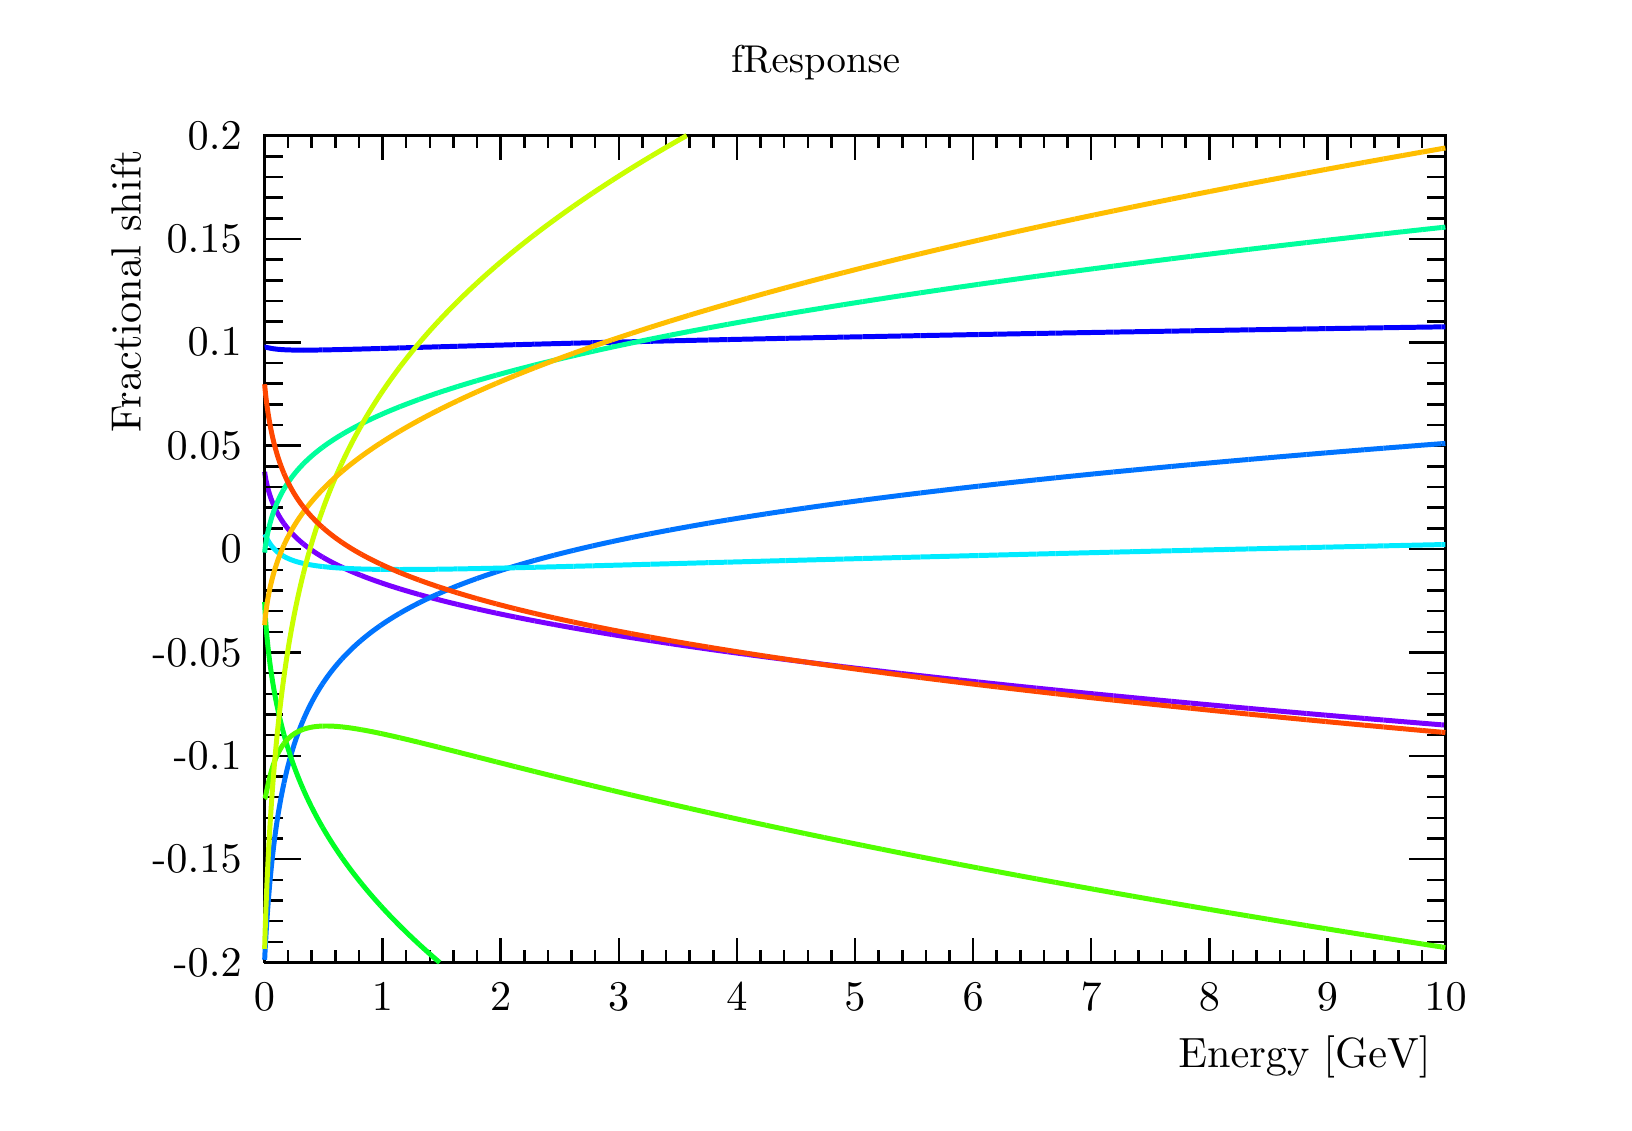
\begin{tikzpicture}
\pgfdeclareplotmark{cross} {
\pgfpathmoveto{\pgfpoint{-0.3\pgfplotmarksize}{\pgfplotmarksize}}
\pgfpathlineto{\pgfpoint{+0.3\pgfplotmarksize}{\pgfplotmarksize}}
\pgfpathlineto{\pgfpoint{+0.3\pgfplotmarksize}{0.3\pgfplotmarksize}}
\pgfpathlineto{\pgfpoint{+1\pgfplotmarksize}{0.3\pgfplotmarksize}}
\pgfpathlineto{\pgfpoint{+1\pgfplotmarksize}{-0.3\pgfplotmarksize}}
\pgfpathlineto{\pgfpoint{+0.3\pgfplotmarksize}{-0.3\pgfplotmarksize}}
\pgfpathlineto{\pgfpoint{+0.3\pgfplotmarksize}{-1.\pgfplotmarksize}}
\pgfpathlineto{\pgfpoint{-0.3\pgfplotmarksize}{-1.\pgfplotmarksize}}
\pgfpathlineto{\pgfpoint{-0.3\pgfplotmarksize}{-0.3\pgfplotmarksize}}
\pgfpathlineto{\pgfpoint{-1.\pgfplotmarksize}{-0.3\pgfplotmarksize}}
\pgfpathlineto{\pgfpoint{-1.\pgfplotmarksize}{0.3\pgfplotmarksize}}
\pgfpathlineto{\pgfpoint{-0.3\pgfplotmarksize}{0.3\pgfplotmarksize}}
\pgfpathclose
\pgfusepathqstroke
}
\pgfdeclareplotmark{cross*} {
\pgfpathmoveto{\pgfpoint{-0.3\pgfplotmarksize}{\pgfplotmarksize}}
\pgfpathlineto{\pgfpoint{+0.3\pgfplotmarksize}{\pgfplotmarksize}}
\pgfpathlineto{\pgfpoint{+0.3\pgfplotmarksize}{0.3\pgfplotmarksize}}
\pgfpathlineto{\pgfpoint{+1\pgfplotmarksize}{0.3\pgfplotmarksize}}
\pgfpathlineto{\pgfpoint{+1\pgfplotmarksize}{-0.3\pgfplotmarksize}}
\pgfpathlineto{\pgfpoint{+0.3\pgfplotmarksize}{-0.3\pgfplotmarksize}}
\pgfpathlineto{\pgfpoint{+0.3\pgfplotmarksize}{-1.\pgfplotmarksize}}
\pgfpathlineto{\pgfpoint{-0.3\pgfplotmarksize}{-1.\pgfplotmarksize}}
\pgfpathlineto{\pgfpoint{-0.3\pgfplotmarksize}{-0.3\pgfplotmarksize}}
\pgfpathlineto{\pgfpoint{-1.\pgfplotmarksize}{-0.3\pgfplotmarksize}}
\pgfpathlineto{\pgfpoint{-1.\pgfplotmarksize}{0.3\pgfplotmarksize}}
\pgfpathlineto{\pgfpoint{-0.3\pgfplotmarksize}{0.3\pgfplotmarksize}}
\pgfpathclose
\pgfusepathqfillstroke
}
\pgfdeclareplotmark{newstar} {
\pgfpathmoveto{\pgfqpoint{0pt}{\pgfplotmarksize}}
\pgfpathlineto{\pgfqpointpolar{44}{0.5\pgfplotmarksize}}
\pgfpathlineto{\pgfqpointpolar{18}{\pgfplotmarksize}}
\pgfpathlineto{\pgfqpointpolar{-20}{0.5\pgfplotmarksize}}
\pgfpathlineto{\pgfqpointpolar{-54}{\pgfplotmarksize}}
\pgfpathlineto{\pgfqpointpolar{-90}{0.5\pgfplotmarksize}}
\pgfpathlineto{\pgfqpointpolar{234}{\pgfplotmarksize}}
\pgfpathlineto{\pgfqpointpolar{198}{0.5\pgfplotmarksize}}
\pgfpathlineto{\pgfqpointpolar{162}{\pgfplotmarksize}}
\pgfpathlineto{\pgfqpointpolar{134}{0.5\pgfplotmarksize}}
\pgfpathclose
\pgfusepathqstroke
}
\pgfdeclareplotmark{newstar*} {
\pgfpathmoveto{\pgfqpoint{0pt}{\pgfplotmarksize}}
\pgfpathlineto{\pgfqpointpolar{44}{0.5\pgfplotmarksize}}
\pgfpathlineto{\pgfqpointpolar{18}{\pgfplotmarksize}}
\pgfpathlineto{\pgfqpointpolar{-20}{0.5\pgfplotmarksize}}
\pgfpathlineto{\pgfqpointpolar{-54}{\pgfplotmarksize}}
\pgfpathlineto{\pgfqpointpolar{-90}{0.5\pgfplotmarksize}}
\pgfpathlineto{\pgfqpointpolar{234}{\pgfplotmarksize}}
\pgfpathlineto{\pgfqpointpolar{198}{0.5\pgfplotmarksize}}
\pgfpathlineto{\pgfqpointpolar{162}{\pgfplotmarksize}}
\pgfpathlineto{\pgfqpointpolar{134}{0.5\pgfplotmarksize}}
\pgfpathclose
\pgfusepathqfillstroke
}
\definecolor{c}{rgb}{1,1,1};
\draw [color=c, fill=c] (0,0) rectangle (20,13.639);
\draw [color=c, fill=c] (3,1.77307) rectangle (18,12.2751);
\definecolor{c}{rgb}{0,0,0};
\draw [c,line width=0.9] (3,1.77307) -- (3,12.2751) -- (18,12.2751) -- (18,1.77307) -- (3,1.77307);
\definecolor{c}{rgb}{1,1,1};
\draw [color=c, fill=c] (3,1.77307) rectangle (18,12.2751);
\definecolor{c}{rgb}{0,0,0};
\draw [c,line width=0.9] (3,1.77307) -- (3,12.2751) -- (18,12.2751) -- (18,1.77307) -- (3,1.77307);
\definecolor{c}{rgb}{0.48,0,1};
\draw [c,line width=1.8] (3.0025,8.00548) -- (3.0075,7.96716) -- (3.0125,7.93646) -- (3.0175,7.9093) -- (3.0225,7.88446) -- (3.0275,7.86135) -- (3.0325,7.83965) -- (3.0375,7.81911) -- (3.0425,7.79958) -- (3.0475,7.78094) -- (3.0525,7.7631) --
 (3.0575,7.74598) -- (3.0625,7.7295) -- (3.0675,7.71363) -- (3.0725,7.69831) -- (3.0775,7.68351) -- (3.0825,7.66918) -- (3.0875,7.65529) -- (3.0925,7.64182) -- (3.0975,7.62875) -- (3.1025,7.61604) -- (3.1075,7.60368) -- (3.1125,7.59164) --
 (3.1175,7.57992) -- (3.1225,7.56849) -- (3.1275,7.55735) -- (3.1325,7.54647) -- (3.1375,7.53584) -- (3.1425,7.52545) -- (3.1475,7.5153) -- (3.1525,7.50537) -- (3.1575,7.49564) -- (3.1625,7.48612) -- (3.1675,7.4768) -- (3.1725,7.46766) --
 (3.1775,7.4587) -- (3.1825,7.44991) -- (3.1875,7.44129) -- (3.1925,7.43282) -- (3.1975,7.42451) -- (3.2025,7.41635) -- (3.2075,7.40832) -- (3.2125,7.40044) -- (3.2175,7.39269) -- (3.2225,7.38506) -- (3.2275,7.37756) -- (3.2325,7.37018) --
 (3.2375,7.36292) -- (3.2425,7.35577) -- (3.2475,7.34873);
\draw [c,line width=1.8] (3.2475,7.34873) -- (3.2525,7.34179) -- (3.2575,7.33495) -- (3.2625,7.32822) -- (3.2675,7.32157) -- (3.2725,7.31503) -- (3.2775,7.30857) -- (3.2825,7.3022) -- (3.2875,7.29592) -- (3.2925,7.28972) -- (3.2975,7.2836) --
 (3.3025,7.27756) -- (3.3075,7.2716) -- (3.3125,7.26571) -- (3.3175,7.2599) -- (3.3225,7.25415) -- (3.3275,7.24848) -- (3.3325,7.24287) -- (3.3375,7.23733) -- (3.3425,7.23185) -- (3.3475,7.22644) -- (3.3525,7.22108) -- (3.3575,7.21579) --
 (3.3625,7.21055) -- (3.3675,7.20537) -- (3.3725,7.20025) -- (3.3775,7.19518) -- (3.3825,7.19016) -- (3.3875,7.18519) -- (3.3925,7.18028) -- (3.3975,7.17542) -- (3.4025,7.1706) -- (3.4075,7.16583) -- (3.4125,7.16111) -- (3.4175,7.15643) --
 (3.4225,7.1518) -- (3.4275,7.14722) -- (3.4325,7.14267) -- (3.4375,7.13817) -- (3.4425,7.13371) -- (3.4475,7.12929) -- (3.4525,7.1249) -- (3.4575,7.12056) -- (3.4625,7.11626) -- (3.4675,7.11199) -- (3.4725,7.10776) -- (3.4775,7.10356) --
 (3.4825,7.0994) -- (3.4875,7.09528) -- (3.4925,7.09119);
\draw [c,line width=1.8] (3.4925,7.09119) -- (3.4975,7.08713) -- (3.5025,7.08311) -- (3.5075,7.07911) -- (3.5125,7.07515) -- (3.5175,7.07122) -- (3.5225,7.06733) -- (3.5275,7.06346) -- (3.5325,7.05962) -- (3.5375,7.05581) -- (3.5425,7.05202) --
 (3.5475,7.04827) -- (3.5525,7.04455) -- (3.5575,7.04085) -- (3.5625,7.03717) -- (3.5675,7.03353) -- (3.5725,7.02991) -- (3.5775,7.02631) -- (3.5825,7.02274) -- (3.5875,7.0192) -- (3.5925,7.01568) -- (3.5975,7.01218) -- (3.6025,7.00871) --
 (3.6075,7.00526) -- (3.6125,7.00183) -- (3.6175,6.99843) -- (3.6225,6.99505) -- (3.6275,6.99169) -- (3.6325,6.98835) -- (3.6375,6.98503) -- (3.6425,6.98173) -- (3.6475,6.97846) -- (3.6525,6.9752) -- (3.6575,6.97197) -- (3.6625,6.96875) --
 (3.6675,6.96556) -- (3.6725,6.96238) -- (3.6775,6.95922) -- (3.6825,6.95608) -- (3.6875,6.95296) -- (3.6925,6.94986) -- (3.6975,6.94677) -- (3.7025,6.94371) -- (3.7075,6.94066) -- (3.7125,6.93763) -- (3.7175,6.93461) -- (3.7225,6.93161) --
 (3.7275,6.92863) -- (3.7325,6.92567) -- (3.7375,6.92272);
\draw [c,line width=1.8] (3.7375,6.92272) -- (3.7425,6.91978) -- (3.7475,6.91687) -- (3.7525,6.91396) -- (3.7575,6.91108) -- (3.7625,6.90821) -- (3.7675,6.90535) -- (3.7725,6.90251) -- (3.7775,6.89968) -- (3.7825,6.89687) -- (3.7875,6.89407) --
 (3.7925,6.89129) -- (3.7975,6.88852) -- (3.8025,6.88576) -- (3.8075,6.88302) -- (3.8125,6.88029) -- (3.8175,6.87758) -- (3.8225,6.87488) -- (3.8275,6.87219) -- (3.8325,6.86951) -- (3.8375,6.86685) -- (3.8425,6.8642) -- (3.8475,6.86156) --
 (3.8525,6.85893) -- (3.8575,6.85632) -- (3.8625,6.85372) -- (3.8675,6.85113) -- (3.8725,6.84855) -- (3.8775,6.84598) -- (3.8825,6.84343) -- (3.8875,6.84088) -- (3.8925,6.83835) -- (3.8975,6.83583) -- (3.9025,6.83332) -- (3.9075,6.83082) --
 (3.9125,6.82833) -- (3.9175,6.82585) -- (3.9225,6.82339) -- (3.9275,6.82093) -- (3.9325,6.81848) -- (3.9375,6.81605) -- (3.9425,6.81362) -- (3.9475,6.81121) -- (3.9525,6.8088) -- (3.9575,6.80641) -- (3.9625,6.80402) -- (3.9675,6.80164) --
 (3.9725,6.79928) -- (3.9775,6.79692) -- (3.9825,6.79457);
\draw [c,line width=1.8] (3.9825,6.79457) -- (3.9875,6.79224) -- (3.9925,6.78991) -- (3.9975,6.78759) -- (4.0025,6.78528) -- (4.0075,6.78297) -- (4.0125,6.78068) -- (4.0175,6.7784) -- (4.0225,6.77612) -- (4.0275,6.77385) -- (4.0325,6.7716) --
 (4.0375,6.76935) -- (4.0425,6.76711) -- (4.0475,6.76487) -- (4.0525,6.76265) -- (4.0575,6.76043) -- (4.0625,6.75822) -- (4.0675,6.75602) -- (4.0725,6.75383) -- (4.0775,6.75165) -- (4.0825,6.74947) -- (4.0875,6.7473) -- (4.0925,6.74514) --
 (4.0975,6.74298) -- (4.1025,6.74084) -- (4.1075,6.7387) -- (4.1125,6.73657) -- (4.1175,6.73445) -- (4.1225,6.73233) -- (4.1275,6.73022) -- (4.1325,6.72812) -- (4.1375,6.72602) -- (4.1425,6.72393) -- (4.1475,6.72185) -- (4.1525,6.71978) --
 (4.1575,6.71771) -- (4.1625,6.71565) -- (4.1675,6.7136) -- (4.1725,6.71155) -- (4.1775,6.70951) -- (4.1825,6.70748) -- (4.1875,6.70545) -- (4.1925,6.70343) -- (4.1975,6.70142) -- (4.2025,6.69941) -- (4.2075,6.69741) -- (4.2125,6.69541) --
 (4.2175,6.69343) -- (4.2225,6.69144) -- (4.2275,6.68947);
\draw [c,line width=1.8] (4.2275,6.68947) -- (4.2325,6.6875) -- (4.2375,6.68553) -- (4.2425,6.68358) -- (4.2475,6.68162) -- (4.2525,6.67968) -- (4.2575,6.67774) -- (4.2625,6.6758) -- (4.2675,6.67387) -- (4.2725,6.67195) -- (4.2775,6.67003) --
 (4.2825,6.66812) -- (4.2875,6.66622) -- (4.2925,6.66432) -- (4.2975,6.66242) -- (4.3025,6.66053) -- (4.3075,6.65865) -- (4.3125,6.65677) -- (4.3175,6.6549) -- (4.3225,6.65303) -- (4.3275,6.65117) -- (4.3325,6.64931) -- (4.3375,6.64746) --
 (4.3425,6.64561) -- (4.3475,6.64377) -- (4.3525,6.64194) -- (4.3575,6.6401) -- (4.3625,6.63828) -- (4.3675,6.63646) -- (4.3725,6.63464) -- (4.3775,6.63283) -- (4.3825,6.63102) -- (4.3875,6.62922) -- (4.3925,6.62743) -- (4.3975,6.62563) --
 (4.4025,6.62385) -- (4.4075,6.62206) -- (4.4125,6.62029) -- (4.4175,6.61851) -- (4.4225,6.61675) -- (4.4275,6.61498) -- (4.4325,6.61322) -- (4.4375,6.61147) -- (4.4425,6.60972) -- (4.4475,6.60797) -- (4.4525,6.60623) -- (4.4575,6.6045) --
 (4.4625,6.60276) -- (4.4675,6.60104) -- (4.4725,6.59931);
\draw [c,line width=1.8] (4.4725,6.59931) -- (4.4775,6.59759) -- (4.4825,6.59588) -- (4.4875,6.59417) -- (4.4925,6.59246) -- (4.4975,6.59076) -- (4.5025,6.58906) -- (4.5075,6.58737) -- (4.5125,6.58568) -- (4.5175,6.58399) -- (4.5225,6.58231) --
 (4.5275,6.58064) -- (4.5325,6.57896) -- (4.5375,6.57729) -- (4.5425,6.57563) -- (4.5475,6.57397) -- (4.5525,6.57231) -- (4.5575,6.57066) -- (4.5625,6.56901) -- (4.5675,6.56736) -- (4.5725,6.56572) -- (4.5775,6.56408) -- (4.5825,6.56245) --
 (4.5875,6.56082) -- (4.5925,6.55919) -- (4.5975,6.55757) -- (4.6025,6.55595) -- (4.6075,6.55433) -- (4.6125,6.55272) -- (4.6175,6.55111) -- (4.6225,6.54951) -- (4.6275,6.54791) -- (4.6325,6.54631) -- (4.6375,6.54472) -- (4.6425,6.54313) --
 (4.6475,6.54154) -- (4.6525,6.53996) -- (4.6575,6.53838) -- (4.6625,6.5368) -- (4.6675,6.53523) -- (4.6725,6.53366) -- (4.6775,6.53209) -- (4.6825,6.53053) -- (4.6875,6.52897) -- (4.6925,6.52742) -- (4.6975,6.52586) -- (4.7025,6.52431) --
 (4.7075,6.52277) -- (4.7125,6.52122) -- (4.7175,6.51969);
\draw [c,line width=1.8] (4.7175,6.51969) -- (4.7225,6.51815) -- (4.7275,6.51662) -- (4.7325,6.51509) -- (4.7375,6.51356) -- (4.7425,6.51204) -- (4.7475,6.51052) -- (4.7525,6.509) -- (4.7575,6.50748) -- (4.7625,6.50597) -- (4.7675,6.50447) --
 (4.7725,6.50296) -- (4.7775,6.50146) -- (4.7825,6.49996) -- (4.7875,6.49846) -- (4.7925,6.49697) -- (4.7975,6.49548) -- (4.8025,6.494) -- (4.8075,6.49251) -- (4.8125,6.49103) -- (4.8175,6.48955) -- (4.8225,6.48808) -- (4.8275,6.48661) --
 (4.8325,6.48514) -- (4.8375,6.48367) -- (4.8425,6.48221) -- (4.8475,6.48075) -- (4.8525,6.47929) -- (4.8575,6.47783) -- (4.8625,6.47638) -- (4.8675,6.47493) -- (4.8725,6.47348) -- (4.8775,6.47204) -- (4.8825,6.4706) -- (4.8875,6.46916) --
 (4.8925,6.46772) -- (4.8975,6.46629) -- (4.9025,6.46486) -- (4.9075,6.46343) -- (4.9125,6.46201) -- (4.9175,6.46058) -- (4.9225,6.45917) -- (4.9275,6.45775) -- (4.9325,6.45633) -- (4.9375,6.45492) -- (4.9425,6.45351) -- (4.9475,6.4521) --
 (4.9525,6.4507) -- (4.9575,6.4493) -- (4.9625,6.4479);
\draw [c,line width=1.8] (4.9625,6.4479) -- (4.9675,6.4465) -- (4.9725,6.44511) -- (4.9775,6.44372) -- (4.9825,6.44233) -- (4.9875,6.44094) -- (4.9925,6.43956) -- (4.9975,6.43817) -- (5.0025,6.43679) -- (5.0075,6.43542) -- (5.0125,6.43404) --
 (5.0175,6.43267) -- (5.0225,6.4313) -- (5.0275,6.42993) -- (5.0325,6.42857) -- (5.0375,6.42721) -- (5.0425,6.42584) -- (5.0475,6.42449) -- (5.0525,6.42313) -- (5.0575,6.42178) -- (5.0625,6.42043) -- (5.0675,6.41908) -- (5.0725,6.41773) --
 (5.0775,6.41639) -- (5.0825,6.41504) -- (5.0875,6.4137) -- (5.0925,6.41237) -- (5.0975,6.41103) -- (5.1025,6.4097) -- (5.1075,6.40837) -- (5.1125,6.40704) -- (5.1175,6.40571) -- (5.1225,6.40439) -- (5.1275,6.40307) -- (5.1325,6.40175) --
 (5.1375,6.40043) -- (5.1425,6.39911) -- (5.1475,6.3978) -- (5.1525,6.39649) -- (5.1575,6.39518) -- (5.1625,6.39387) -- (5.1675,6.39257) -- (5.1725,6.39126) -- (5.1775,6.38996) -- (5.1825,6.38866) -- (5.1875,6.38737) -- (5.1925,6.38607) --
 (5.1975,6.38478) -- (5.2025,6.38349) -- (5.2075,6.3822);
\draw [c,line width=1.8] (5.2075,6.3822) -- (5.2125,6.38091) -- (5.2175,6.37963) -- (5.2225,6.37835) -- (5.2275,6.37707) -- (5.2325,6.37579) -- (5.2375,6.37451) -- (5.2425,6.37324) -- (5.2475,6.37196) -- (5.2525,6.37069) -- (5.2575,6.36942) --
 (5.2625,6.36816) -- (5.2675,6.36689) -- (5.2725,6.36563) -- (5.2775,6.36437) -- (5.2825,6.36311) -- (5.2875,6.36185) -- (5.2925,6.3606) -- (5.2975,6.35934) -- (5.3025,6.35809) -- (5.3075,6.35684) -- (5.3125,6.35559) -- (5.3175,6.35435) --
 (5.3225,6.3531) -- (5.3275,6.35186) -- (5.3325,6.35062) -- (5.3375,6.34938) -- (5.3425,6.34815) -- (5.3475,6.34691) -- (5.3525,6.34568) -- (5.3575,6.34445) -- (5.3625,6.34322) -- (5.3675,6.34199) -- (5.3725,6.34076) -- (5.3775,6.33954) --
 (5.3825,6.33832) -- (5.3875,6.3371) -- (5.3925,6.33588) -- (5.3975,6.33466) -- (5.4025,6.33344) -- (5.4075,6.33223) -- (5.4125,6.33102) -- (5.4175,6.32981) -- (5.4225,6.3286) -- (5.4275,6.32739) -- (5.4325,6.32619) -- (5.4375,6.32498) --
 (5.4425,6.32378) -- (5.4475,6.32258) -- (5.4525,6.32138);
\draw [c,line width=1.8] (5.4525,6.32138) -- (5.4575,6.32018) -- (5.4625,6.31899) -- (5.4675,6.3178) -- (5.4725,6.3166) -- (5.4775,6.31541) -- (5.4825,6.31422) -- (5.4875,6.31304) -- (5.4925,6.31185) -- (5.4975,6.31067) -- (5.5025,6.30949) --
 (5.5075,6.3083) -- (5.5125,6.30713) -- (5.5175,6.30595) -- (5.5225,6.30477) -- (5.5275,6.3036) -- (5.5325,6.30242) -- (5.5375,6.30125) -- (5.5425,6.30008) -- (5.5475,6.29892) -- (5.5525,6.29775) -- (5.5575,6.29658) -- (5.5625,6.29542) --
 (5.5675,6.29426) -- (5.5725,6.2931) -- (5.5775,6.29194) -- (5.5825,6.29078) -- (5.5875,6.28963) -- (5.5925,6.28847) -- (5.5975,6.28732) -- (5.6025,6.28617) -- (5.6075,6.28502) -- (5.6125,6.28387) -- (5.6175,6.28272) -- (5.6225,6.28158) --
 (5.6275,6.28043) -- (5.6325,6.27929) -- (5.6375,6.27815) -- (5.6425,6.27701) -- (5.6475,6.27587) -- (5.6525,6.27474) -- (5.6575,6.2736) -- (5.6625,6.27247) -- (5.6675,6.27133) -- (5.6725,6.2702) -- (5.6775,6.26907) -- (5.6825,6.26795) --
 (5.6875,6.26682) -- (5.6925,6.26569) -- (5.6975,6.26457);
\draw [c,line width=1.8] (5.6975,6.26457) -- (5.7025,6.26345) -- (5.7075,6.26233) -- (5.7125,6.26121) -- (5.7175,6.26009) -- (5.7225,6.25897) -- (5.7275,6.25785) -- (5.7325,6.25674) -- (5.7375,6.25563) -- (5.7425,6.25452) -- (5.7475,6.25341) --
 (5.7525,6.2523) -- (5.7575,6.25119) -- (5.7625,6.25008) -- (5.7675,6.24898) -- (5.7725,6.24788) -- (5.7775,6.24677) -- (5.7825,6.24567) -- (5.7875,6.24457) -- (5.7925,6.24347) -- (5.7975,6.24238) -- (5.8025,6.24128) -- (5.8075,6.24019) --
 (5.8125,6.23909) -- (5.8175,6.238) -- (5.8225,6.23691) -- (5.8275,6.23582) -- (5.8325,6.23474) -- (5.8375,6.23365) -- (5.8425,6.23256) -- (5.8475,6.23148) -- (5.8525,6.2304) -- (5.8575,6.22931) -- (5.8625,6.22823) -- (5.8675,6.22716) --
 (5.8725,6.22608) -- (5.8775,6.225) -- (5.8825,6.22393) -- (5.8875,6.22285) -- (5.8925,6.22178) -- (5.8975,6.22071) -- (5.9025,6.21964) -- (5.9075,6.21857) -- (5.9125,6.2175) -- (5.9175,6.21643) -- (5.9225,6.21537) -- (5.9275,6.2143) --
 (5.9325,6.21324) -- (5.9375,6.21218) -- (5.9425,6.21112);
\draw [c,line width=1.8] (5.9425,6.21112) -- (5.9475,6.21006) -- (5.9525,6.209) -- (5.9575,6.20794) -- (5.9625,6.20689) -- (5.9675,6.20583) -- (5.9725,6.20478) -- (5.9775,6.20372) -- (5.9825,6.20267) -- (5.9875,6.20162) -- (5.9925,6.20057) --
 (5.9975,6.19953) -- (6.0025,6.19848) -- (6.0075,6.19743) -- (6.0125,6.19639) -- (6.0175,6.19535) -- (6.0225,6.1943) -- (6.0275,6.19326) -- (6.0325,6.19222) -- (6.0375,6.19118) -- (6.0425,6.19015) -- (6.0475,6.18911) -- (6.0525,6.18807) --
 (6.0575,6.18704) -- (6.0625,6.18601) -- (6.0675,6.18497) -- (6.0725,6.18394) -- (6.0775,6.18291) -- (6.0825,6.18188) -- (6.0875,6.18086) -- (6.0925,6.17983) -- (6.0975,6.1788) -- (6.1025,6.17778) -- (6.1075,6.17676) -- (6.1125,6.17573) --
 (6.1175,6.17471) -- (6.1225,6.17369) -- (6.1275,6.17267) -- (6.1325,6.17166) -- (6.1375,6.17064) -- (6.1425,6.16962) -- (6.1475,6.16861) -- (6.1525,6.16759) -- (6.1575,6.16658) -- (6.1625,6.16557) -- (6.1675,6.16456) -- (6.1725,6.16355) --
 (6.1775,6.16254) -- (6.1825,6.16153) -- (6.1875,6.16053);
\draw [c,line width=1.8] (6.1875,6.16053) -- (6.1925,6.15952) -- (6.1975,6.15852) -- (6.2025,6.15751) -- (6.2075,6.15651) -- (6.2125,6.15551) -- (6.2175,6.15451) -- (6.2225,6.15351) -- (6.2275,6.15251) -- (6.2325,6.15151) -- (6.2375,6.15052) --
 (6.2425,6.14952) -- (6.2475,6.14853) -- (6.2525,6.14753) -- (6.2575,6.14654) -- (6.2625,6.14555) -- (6.2675,6.14456) -- (6.2725,6.14357) -- (6.2775,6.14258) -- (6.2825,6.14159) -- (6.2875,6.14061) -- (6.2925,6.13962) -- (6.2975,6.13864) --
 (6.3025,6.13765) -- (6.3075,6.13667) -- (6.3125,6.13569) -- (6.3175,6.13471) -- (6.3225,6.13373) -- (6.3275,6.13275) -- (6.3325,6.13177) -- (6.3375,6.1308) -- (6.3425,6.12982) -- (6.3475,6.12884) -- (6.3525,6.12787) -- (6.3575,6.1269) --
 (6.3625,6.12593) -- (6.3675,6.12495) -- (6.3725,6.12398) -- (6.3775,6.12301) -- (6.3825,6.12205) -- (6.3875,6.12108) -- (6.3925,6.12011) -- (6.3975,6.11915) -- (6.4025,6.11818) -- (6.4075,6.11722) -- (6.4125,6.11625) -- (6.4175,6.11529) --
 (6.4225,6.11433) -- (6.4275,6.11337) -- (6.4325,6.11241);
\draw [c,line width=1.8] (6.4325,6.11241) -- (6.4375,6.11145) -- (6.4425,6.11049) -- (6.4475,6.10954) -- (6.4525,6.10858) -- (6.4575,6.10763) -- (6.4625,6.10667) -- (6.4675,6.10572) -- (6.4725,6.10477) -- (6.4775,6.10382) -- (6.4825,6.10287) --
 (6.4875,6.10192) -- (6.4925,6.10097) -- (6.4975,6.10002) -- (6.5025,6.09907) -- (6.5075,6.09813) -- (6.5125,6.09718) -- (6.5175,6.09624) -- (6.5225,6.09529) -- (6.5275,6.09435) -- (6.5325,6.09341) -- (6.5375,6.09247) -- (6.5425,6.09153) --
 (6.5475,6.09059) -- (6.5525,6.08965) -- (6.5575,6.08871) -- (6.5625,6.08777) -- (6.5675,6.08684) -- (6.5725,6.0859) -- (6.5775,6.08497) -- (6.5825,6.08404) -- (6.5875,6.0831) -- (6.5925,6.08217) -- (6.5975,6.08124) -- (6.6025,6.08031) --
 (6.6075,6.07938) -- (6.6125,6.07845) -- (6.6175,6.07752) -- (6.6225,6.0766) -- (6.6275,6.07567) -- (6.6325,6.07475) -- (6.6375,6.07382) -- (6.6425,6.0729) -- (6.6475,6.07198) -- (6.6525,6.07105) -- (6.6575,6.07013) -- (6.6625,6.06921) --
 (6.6675,6.06829) -- (6.6725,6.06737) -- (6.6775,6.06646);
\draw [c,line width=1.8] (6.6775,6.06646) -- (6.6825,6.06554) -- (6.6875,6.06462) -- (6.6925,6.06371) -- (6.6975,6.06279) -- (6.7025,6.06188) -- (6.7075,6.06096) -- (6.7125,6.06005) -- (6.7175,6.05914) -- (6.7225,6.05823) -- (6.7275,6.05732) --
 (6.7325,6.05641) -- (6.7375,6.0555) -- (6.7425,6.05459) -- (6.7475,6.05369) -- (6.7525,6.05278) -- (6.7575,6.05187) -- (6.7625,6.05097) -- (6.7675,6.05007) -- (6.7725,6.04916) -- (6.7775,6.04826) -- (6.7825,6.04736) -- (6.7875,6.04646) --
 (6.7925,6.04556) -- (6.7975,6.04466) -- (6.8025,6.04376) -- (6.8075,6.04286) -- (6.8125,6.04196) -- (6.8175,6.04107) -- (6.8225,6.04017) -- (6.8275,6.03928) -- (6.8325,6.03838) -- (6.8375,6.03749) -- (6.8425,6.0366) -- (6.8475,6.0357) --
 (6.8525,6.03481) -- (6.8575,6.03392) -- (6.8625,6.03303) -- (6.8675,6.03214) -- (6.8725,6.03125) -- (6.8775,6.03037) -- (6.8825,6.02948) -- (6.8875,6.02859) -- (6.8925,6.02771) -- (6.8975,6.02682) -- (6.9025,6.02594) -- (6.9075,6.02506) --
 (6.9125,6.02417) -- (6.9175,6.02329) -- (6.9225,6.02241);
\draw [c,line width=1.8] (6.9225,6.02241) -- (6.9275,6.02153) -- (6.9325,6.02065) -- (6.9375,6.01977) -- (6.9425,6.01889) -- (6.9475,6.01801) -- (6.9525,6.01714) -- (6.9575,6.01626) -- (6.9625,6.01539) -- (6.9675,6.01451) -- (6.9725,6.01364) --
 (6.9775,6.01276) -- (6.9825,6.01189) -- (6.9875,6.01102) -- (6.9925,6.01015) -- (6.9975,6.00928) -- (7.0025,6.00841) -- (7.0075,6.00754) -- (7.0125,6.00667) -- (7.0175,6.0058) -- (7.0225,6.00493) -- (7.0275,6.00406) -- (7.0325,6.0032) --
 (7.0375,6.00233) -- (7.0425,6.00147) -- (7.0475,6.0006) -- (7.0525,5.99974) -- (7.0575,5.99888) -- (7.0625,5.99802) -- (7.0675,5.99716) -- (7.0725,5.99629) -- (7.0775,5.99543) -- (7.0825,5.99458) -- (7.0875,5.99372) -- (7.0925,5.99286) --
 (7.0975,5.992) -- (7.1025,5.99114) -- (7.1075,5.99029) -- (7.1125,5.98943) -- (7.1175,5.98858) -- (7.1225,5.98772) -- (7.1275,5.98687) -- (7.1325,5.98602) -- (7.1375,5.98516) -- (7.1425,5.98431) -- (7.1475,5.98346) -- (7.1525,5.98261) --
 (7.1575,5.98176) -- (7.1625,5.98091) -- (7.1675,5.98006);
\draw [c,line width=1.8] (7.1675,5.98006) -- (7.1725,5.97922) -- (7.1775,5.97837) -- (7.1825,5.97752) -- (7.1875,5.97668) -- (7.1925,5.97583) -- (7.1975,5.97499) -- (7.2025,5.97414) -- (7.2075,5.9733) -- (7.2125,5.97246) -- (7.2175,5.97162) --
 (7.2225,5.97077) -- (7.2275,5.96993) -- (7.2325,5.96909) -- (7.2375,5.96825) -- (7.2425,5.96741) -- (7.2475,5.96658) -- (7.2525,5.96574) -- (7.2575,5.9649) -- (7.2625,5.96406) -- (7.2675,5.96323) -- (7.2725,5.96239) -- (7.2775,5.96156) --
 (7.2825,5.96072) -- (7.2875,5.95989) -- (7.2925,5.95906) -- (7.2975,5.95823) -- (7.3025,5.95739) -- (7.3075,5.95656) -- (7.3125,5.95573) -- (7.3175,5.9549) -- (7.3225,5.95407) -- (7.3275,5.95324) -- (7.3325,5.95242) -- (7.3375,5.95159) --
 (7.3425,5.95076) -- (7.3475,5.94994) -- (7.3525,5.94911) -- (7.3575,5.94828) -- (7.3625,5.94746) -- (7.3675,5.94664) -- (7.3725,5.94581) -- (7.3775,5.94499) -- (7.3825,5.94417) -- (7.3875,5.94335) -- (7.3925,5.94252) -- (7.3975,5.9417) --
 (7.4025,5.94088) -- (7.4075,5.94006) -- (7.4125,5.93925);
\draw [c,line width=1.8] (7.4125,5.93925) -- (7.4175,5.93843) -- (7.4225,5.93761) -- (7.4275,5.93679) -- (7.4325,5.93598) -- (7.4375,5.93516) -- (7.4425,5.93434) -- (7.4475,5.93353) -- (7.4525,5.93272) -- (7.4575,5.9319) -- (7.4625,5.93109) --
 (7.4675,5.93028) -- (7.4725,5.92946) -- (7.4775,5.92865) -- (7.4825,5.92784) -- (7.4875,5.92703) -- (7.4925,5.92622) -- (7.4975,5.92541) -- (7.5025,5.9246) -- (7.5075,5.9238) -- (7.5125,5.92299) -- (7.5175,5.92218) -- (7.5225,5.92138) --
 (7.5275,5.92057) -- (7.5325,5.91976) -- (7.5375,5.91896) -- (7.5425,5.91815) -- (7.5475,5.91735) -- (7.5525,5.91655) -- (7.5575,5.91575) -- (7.5625,5.91494) -- (7.5675,5.91414) -- (7.5725,5.91334) -- (7.5775,5.91254) -- (7.5825,5.91174) --
 (7.5875,5.91094) -- (7.5925,5.91014) -- (7.5975,5.90934) -- (7.6025,5.90855) -- (7.6075,5.90775) -- (7.6125,5.90695) -- (7.6175,5.90616) -- (7.6225,5.90536) -- (7.6275,5.90457) -- (7.6325,5.90377) -- (7.6375,5.90298) -- (7.6425,5.90218) --
 (7.6475,5.90139) -- (7.6525,5.9006) -- (7.6575,5.89981);
\draw [c,line width=1.8] (7.6575,5.89981) -- (7.6625,5.89901) -- (7.6675,5.89822) -- (7.6725,5.89743) -- (7.6775,5.89664) -- (7.6825,5.89585) -- (7.6875,5.89506) -- (7.6925,5.89428) -- (7.6975,5.89349) -- (7.7025,5.8927) -- (7.7075,5.89191) --
 (7.7125,5.89113) -- (7.7175,5.89034) -- (7.7225,5.88956) -- (7.7275,5.88877) -- (7.7325,5.88799) -- (7.7375,5.8872) -- (7.7425,5.88642) -- (7.7475,5.88564) -- (7.7525,5.88486) -- (7.7575,5.88407) -- (7.7625,5.88329) -- (7.7675,5.88251) --
 (7.7725,5.88173) -- (7.7775,5.88095) -- (7.7825,5.88017) -- (7.7875,5.87939) -- (7.7925,5.87862) -- (7.7975,5.87784) -- (7.8025,5.87706) -- (7.8075,5.87628) -- (7.8125,5.87551) -- (7.8175,5.87473) -- (7.8225,5.87396) -- (7.8275,5.87318) --
 (7.8325,5.87241) -- (7.8375,5.87163) -- (7.8425,5.87086) -- (7.8475,5.87009) -- (7.8525,5.86932) -- (7.8575,5.86854) -- (7.8625,5.86777) -- (7.8675,5.867) -- (7.8725,5.86623) -- (7.8775,5.86546) -- (7.8825,5.86469) -- (7.8875,5.86392) --
 (7.8925,5.86315) -- (7.8975,5.86239) -- (7.9025,5.86162);
\draw [c,line width=1.8] (7.9025,5.86162) -- (7.9075,5.86085) -- (7.9125,5.86009) -- (7.9175,5.85932) -- (7.9225,5.85855) -- (7.9275,5.85779) -- (7.9325,5.85702) -- (7.9375,5.85626) -- (7.9425,5.8555) -- (7.9475,5.85473) -- (7.9525,5.85397) --
 (7.9575,5.85321) -- (7.9625,5.85245) -- (7.9675,5.85168) -- (7.9725,5.85092) -- (7.9775,5.85016) -- (7.9825,5.8494) -- (7.9875,5.84864) -- (7.9925,5.84788) -- (7.9975,5.84713) -- (8.0025,5.84637) -- (8.0075,5.84561) -- (8.0125,5.84485) --
 (8.0175,5.8441) -- (8.0225,5.84334) -- (8.0275,5.84258) -- (8.0325,5.84183) -- (8.0375,5.84107) -- (8.0425,5.84032) -- (8.0475,5.83956) -- (8.0525,5.83881) -- (8.0575,5.83806) -- (8.0625,5.8373) -- (8.0675,5.83655) -- (8.0725,5.8358) --
 (8.0775,5.83505) -- (8.0825,5.8343) -- (8.0875,5.83355) -- (8.0925,5.8328) -- (8.0975,5.83205) -- (8.1025,5.8313) -- (8.1075,5.83055) -- (8.1125,5.8298) -- (8.1175,5.82905) -- (8.1225,5.82831) -- (8.1275,5.82756) -- (8.1325,5.82681) --
 (8.1375,5.82607) -- (8.1425,5.82532) -- (8.1475,5.82458);
\draw [c,line width=1.8] (8.1475,5.82458) -- (8.1525,5.82383) -- (8.1575,5.82309) -- (8.1625,5.82234) -- (8.1675,5.8216) -- (8.1725,5.82086) -- (8.1775,5.82012) -- (8.1825,5.81937) -- (8.1875,5.81863) -- (8.1925,5.81789) -- (8.1975,5.81715) --
 (8.2025,5.81641) -- (8.2075,5.81567) -- (8.2125,5.81493) -- (8.2175,5.81419) -- (8.2225,5.81345) -- (8.2275,5.81271) -- (8.2325,5.81198) -- (8.2375,5.81124) -- (8.2425,5.8105) -- (8.2475,5.80977) -- (8.2525,5.80903) -- (8.2575,5.80829) --
 (8.2625,5.80756) -- (8.2675,5.80682) -- (8.2725,5.80609) -- (8.2775,5.80536) -- (8.2825,5.80462) -- (8.2875,5.80389) -- (8.2925,5.80316) -- (8.2975,5.80242) -- (8.3025,5.80169) -- (8.3075,5.80096) -- (8.3125,5.80023) -- (8.3175,5.7995) --
 (8.3225,5.79877) -- (8.3275,5.79804) -- (8.3325,5.79731) -- (8.3375,5.79658) -- (8.3425,5.79585) -- (8.3475,5.79512) -- (8.3525,5.79439) -- (8.3575,5.79367) -- (8.3625,5.79294) -- (8.3675,5.79221) -- (8.3725,5.79149) -- (8.3775,5.79076) --
 (8.3825,5.79004) -- (8.3875,5.78931) -- (8.3925,5.78859);
\draw [c,line width=1.8] (8.3925,5.78859) -- (8.3975,5.78786) -- (8.4025,5.78714) -- (8.4075,5.78642) -- (8.4125,5.78569) -- (8.4175,5.78497) -- (8.4225,5.78425) -- (8.4275,5.78353) -- (8.4325,5.78281) -- (8.4375,5.78208) -- (8.4425,5.78136) --
 (8.4475,5.78064) -- (8.4525,5.77992) -- (8.4575,5.7792) -- (8.4625,5.77849) -- (8.4675,5.77777) -- (8.4725,5.77705) -- (8.4775,5.77633) -- (8.4825,5.77561) -- (8.4875,5.7749) -- (8.4925,5.77418) -- (8.4975,5.77346) -- (8.5025,5.77275) --
 (8.5075,5.77203) -- (8.5125,5.77132) -- (8.5175,5.7706) -- (8.5225,5.76989) -- (8.5275,5.76918) -- (8.5325,5.76846) -- (8.5375,5.76775) -- (8.5425,5.76704) -- (8.5475,5.76632) -- (8.5525,5.76561) -- (8.5575,5.7649) -- (8.5625,5.76419) --
 (8.5675,5.76348) -- (8.5725,5.76277) -- (8.5775,5.76206) -- (8.5825,5.76135) -- (8.5875,5.76064) -- (8.5925,5.75993) -- (8.5975,5.75922) -- (8.6025,5.75851) -- (8.6075,5.75781) -- (8.6125,5.7571) -- (8.6175,5.75639) -- (8.6225,5.75568) --
 (8.6275,5.75498) -- (8.6325,5.75427) -- (8.6375,5.75357);
\draw [c,line width=1.8] (8.6375,5.75357) -- (8.6425,5.75286) -- (8.6475,5.75216) -- (8.6525,5.75145) -- (8.6575,5.75075) -- (8.6625,5.75005) -- (8.6675,5.74934) -- (8.6725,5.74864) -- (8.6775,5.74794) -- (8.6825,5.74723) -- (8.6875,5.74653) --
 (8.6925,5.74583) -- (8.6975,5.74513) -- (8.7025,5.74443) -- (8.7075,5.74373) -- (8.7125,5.74303) -- (8.7175,5.74233) -- (8.7225,5.74163) -- (8.7275,5.74093) -- (8.7325,5.74023) -- (8.7375,5.73953) -- (8.7425,5.73884) -- (8.7475,5.73814) --
 (8.7525,5.73744) -- (8.7575,5.73675) -- (8.7625,5.73605) -- (8.7675,5.73535) -- (8.7725,5.73466) -- (8.7775,5.73396) -- (8.7825,5.73327) -- (8.7875,5.73257) -- (8.7925,5.73188) -- (8.7975,5.73119) -- (8.8025,5.73049) -- (8.8075,5.7298) --
 (8.8125,5.72911) -- (8.8175,5.72841) -- (8.8225,5.72772) -- (8.8275,5.72703) -- (8.8325,5.72634) -- (8.8375,5.72565) -- (8.8425,5.72496) -- (8.8475,5.72427) -- (8.8525,5.72358) -- (8.8575,5.72289) -- (8.8625,5.7222) -- (8.8675,5.72151) --
 (8.8725,5.72082) -- (8.8775,5.72013) -- (8.8825,5.71944);
\draw [c,line width=1.8] (8.8825,5.71944) -- (8.8875,5.71876) -- (8.8925,5.71807) -- (8.8975,5.71738) -- (8.9025,5.7167) -- (8.9075,5.71601) -- (8.9125,5.71532) -- (8.9175,5.71464) -- (8.9225,5.71395) -- (8.9275,5.71327) -- (8.9325,5.71258) --
 (8.9375,5.7119) -- (8.9425,5.71122) -- (8.9475,5.71053) -- (8.9525,5.70985) -- (8.9575,5.70917) -- (8.9625,5.70849) -- (8.9675,5.7078) -- (8.9725,5.70712) -- (8.9775,5.70644) -- (8.9825,5.70576) -- (8.9875,5.70508) -- (8.9925,5.7044) --
 (8.9975,5.70372) -- (9.0025,5.70304) -- (9.0075,5.70236) -- (9.0125,5.70168) -- (9.0175,5.701) -- (9.0225,5.70032) -- (9.0275,5.69965) -- (9.0325,5.69897) -- (9.0375,5.69829) -- (9.0425,5.69761) -- (9.0475,5.69694) -- (9.0525,5.69626) --
 (9.0575,5.69559) -- (9.0625,5.69491) -- (9.0675,5.69423) -- (9.0725,5.69356) -- (9.0775,5.69288) -- (9.0825,5.69221) -- (9.0875,5.69154) -- (9.0925,5.69086) -- (9.0975,5.69019) -- (9.1025,5.68952) -- (9.1075,5.68884) -- (9.1125,5.68817) --
 (9.1175,5.6875) -- (9.1225,5.68683) -- (9.1275,5.68616);
\draw [c,line width=1.8] (9.1275,5.68616) -- (9.1325,5.68548) -- (9.1375,5.68481) -- (9.1425,5.68414) -- (9.1475,5.68347) -- (9.1525,5.6828) -- (9.1575,5.68213) -- (9.1625,5.68147) -- (9.1675,5.6808) -- (9.1725,5.68013) -- (9.1775,5.67946) --
 (9.1825,5.67879) -- (9.1875,5.67812) -- (9.1925,5.67746) -- (9.1975,5.67679) -- (9.2025,5.67612) -- (9.2075,5.67546) -- (9.2125,5.67479) -- (9.2175,5.67413) -- (9.2225,5.67346) -- (9.2275,5.6728) -- (9.2325,5.67213) -- (9.2375,5.67147) --
 (9.2425,5.6708) -- (9.2475,5.67014) -- (9.2525,5.66948) -- (9.2575,5.66881) -- (9.2625,5.66815) -- (9.2675,5.66749) -- (9.2725,5.66682) -- (9.2775,5.66616) -- (9.2825,5.6655) -- (9.2875,5.66484) -- (9.2925,5.66418) -- (9.2975,5.66352) --
 (9.3025,5.66286) -- (9.3075,5.6622) -- (9.3125,5.66154) -- (9.3175,5.66088) -- (9.3225,5.66022) -- (9.3275,5.65956) -- (9.3325,5.6589) -- (9.3375,5.65824) -- (9.3425,5.65759) -- (9.3475,5.65693) -- (9.3525,5.65627) -- (9.3575,5.65561) --
 (9.3625,5.65496) -- (9.3675,5.6543) -- (9.3725,5.65365);
\draw [c,line width=1.8] (9.3725,5.65365) -- (9.3775,5.65299) -- (9.3825,5.65233) -- (9.3875,5.65168) -- (9.3925,5.65102) -- (9.3975,5.65037) -- (9.4025,5.64971) -- (9.4075,5.64906) -- (9.4125,5.64841) -- (9.4175,5.64775) -- (9.4225,5.6471) --
 (9.4275,5.64645) -- (9.4325,5.6458) -- (9.4375,5.64514) -- (9.4425,5.64449) -- (9.4475,5.64384) -- (9.4525,5.64319) -- (9.4575,5.64254) -- (9.4625,5.64189) -- (9.4675,5.64124) -- (9.4725,5.64059) -- (9.4775,5.63994) -- (9.4825,5.63929) --
 (9.4875,5.63864) -- (9.4925,5.63799) -- (9.4975,5.63734) -- (9.5025,5.63669) -- (9.5075,5.63604) -- (9.5125,5.6354) -- (9.5175,5.63475) -- (9.5225,5.6341) -- (9.5275,5.63346) -- (9.5325,5.63281) -- (9.5375,5.63216) -- (9.5425,5.63152) --
 (9.5475,5.63087) -- (9.5525,5.63023) -- (9.5575,5.62958) -- (9.5625,5.62893) -- (9.5675,5.62829) -- (9.5725,5.62765) -- (9.5775,5.627) -- (9.5825,5.62636) -- (9.5875,5.62572) -- (9.5925,5.62507) -- (9.5975,5.62443) -- (9.6025,5.62379) --
 (9.6075,5.62314) -- (9.6125,5.6225) -- (9.6175,5.62186);
\draw [c,line width=1.8] (9.6175,5.62186) -- (9.6225,5.62122) -- (9.6275,5.62058) -- (9.6325,5.61994) -- (9.6375,5.6193) -- (9.6425,5.61866) -- (9.6475,5.61802) -- (9.6525,5.61738) -- (9.6575,5.61674) -- (9.6625,5.6161) -- (9.6675,5.61546) --
 (9.6725,5.61482) -- (9.6775,5.61418) -- (9.6825,5.61354) -- (9.6875,5.61291) -- (9.6925,5.61227) -- (9.6975,5.61163) -- (9.7025,5.61099) -- (9.7075,5.61036) -- (9.7125,5.60972) -- (9.7175,5.60909) -- (9.7225,5.60845) -- (9.7275,5.60781) --
 (9.7325,5.60718) -- (9.7375,5.60654) -- (9.7425,5.60591) -- (9.7475,5.60527) -- (9.7525,5.60464) -- (9.7575,5.60401) -- (9.7625,5.60337) -- (9.7675,5.60274) -- (9.7725,5.60211) -- (9.7775,5.60147) -- (9.7825,5.60084) -- (9.7875,5.60021) --
 (9.7925,5.59958) -- (9.7975,5.59895) -- (9.8025,5.59831) -- (9.8075,5.59768) -- (9.8125,5.59705) -- (9.8175,5.59642) -- (9.8225,5.59579) -- (9.8275,5.59516) -- (9.8325,5.59453) -- (9.8375,5.5939) -- (9.8425,5.59327) -- (9.8475,5.59264) --
 (9.8525,5.59201) -- (9.8575,5.59139) -- (9.8625,5.59076);
\draw [c,line width=1.8] (9.8625,5.59076) -- (9.8675,5.59013) -- (9.8725,5.5895) -- (9.8775,5.58887) -- (9.8825,5.58825) -- (9.8875,5.58762) -- (9.8925,5.58699) -- (9.8975,5.58637) -- (9.9025,5.58574) -- (9.9075,5.58512) -- (9.9125,5.58449) --
 (9.9175,5.58386) -- (9.9225,5.58324) -- (9.9275,5.58261) -- (9.9325,5.58199) -- (9.9375,5.58137) -- (9.9425,5.58074) -- (9.9475,5.58012) -- (9.9525,5.57949) -- (9.9575,5.57887) -- (9.9625,5.57825) -- (9.9675,5.57763) -- (9.9725,5.577) --
 (9.9775,5.57638) -- (9.9825,5.57576) -- (9.9875,5.57514) -- (9.9925,5.57452) -- (9.9975,5.57389) -- (10.0025,5.57327) -- (10.0075,5.57265) -- (10.0125,5.57203) -- (10.0175,5.57141) -- (10.0225,5.57079) -- (10.0275,5.57017) -- (10.0325,5.56955) --
 (10.0375,5.56894) -- (10.0425,5.56832) -- (10.0475,5.5677) -- (10.0525,5.56708) -- (10.0575,5.56646) -- (10.0625,5.56584) -- (10.0675,5.56523) -- (10.0725,5.56461) -- (10.0775,5.56399) -- (10.0825,5.56337) -- (10.0875,5.56276) -- (10.0925,5.56214)
 -- (10.0975,5.56153) -- (10.1025,5.56091) -- (10.1075,5.56029);
\draw [c,line width=1.8] (10.1075,5.56029) -- (10.1125,5.55968) -- (10.1175,5.55906) -- (10.1225,5.55845) -- (10.1275,5.55784) -- (10.1325,5.55722) -- (10.1375,5.55661) -- (10.1425,5.55599) -- (10.1475,5.55538) -- (10.1525,5.55477) --
 (10.1575,5.55415) -- (10.1625,5.55354) -- (10.1675,5.55293) -- (10.1725,5.55232) -- (10.1775,5.5517) -- (10.1825,5.55109) -- (10.1875,5.55048) -- (10.1925,5.54987) -- (10.1975,5.54926) -- (10.2025,5.54865) -- (10.2075,5.54804) -- (10.2125,5.54743)
 -- (10.2175,5.54682) -- (10.2225,5.54621) -- (10.2275,5.5456) -- (10.2325,5.54499) -- (10.2375,5.54438) -- (10.2425,5.54377) -- (10.2475,5.54316) -- (10.2525,5.54255) -- (10.2575,5.54194) -- (10.2625,5.54134) -- (10.2675,5.54073) --
 (10.2725,5.54012) -- (10.2775,5.53951) -- (10.2825,5.53891) -- (10.2875,5.5383) -- (10.2925,5.53769) -- (10.2975,5.53709) -- (10.3025,5.53648) -- (10.3075,5.53588) -- (10.3125,5.53527) -- (10.3175,5.53467) -- (10.3225,5.53406) -- (10.3275,5.53346)
 -- (10.3325,5.53285) -- (10.3375,5.53225) -- (10.3425,5.53164) -- (10.3475,5.53104) -- (10.3525,5.53044);
\draw [c,line width=1.8] (10.3525,5.53044) -- (10.3575,5.52983) -- (10.3625,5.52923) -- (10.3675,5.52863) -- (10.3725,5.52802) -- (10.3775,5.52742) -- (10.3825,5.52682) -- (10.3875,5.52622) -- (10.3925,5.52562) -- (10.3975,5.52501) --
 (10.4025,5.52441) -- (10.4075,5.52381) -- (10.4125,5.52321) -- (10.4175,5.52261) -- (10.4225,5.52201) -- (10.4275,5.52141) -- (10.4325,5.52081) -- (10.4375,5.52021) -- (10.4425,5.51961) -- (10.4475,5.51901) -- (10.4525,5.51841) -- (10.4575,5.51781)
 -- (10.4625,5.51722) -- (10.4675,5.51662) -- (10.4725,5.51602) -- (10.4775,5.51542) -- (10.4825,5.51482) -- (10.4875,5.51423) -- (10.4925,5.51363) -- (10.4975,5.51303) -- (10.5025,5.51244) -- (10.5075,5.51184) -- (10.5125,5.51124) --
 (10.5175,5.51065) -- (10.5225,5.51005) -- (10.5275,5.50946) -- (10.5325,5.50886) -- (10.5375,5.50827) -- (10.5425,5.50767) -- (10.5475,5.50708) -- (10.5525,5.50648) -- (10.5575,5.50589) -- (10.5625,5.5053) -- (10.5675,5.5047) -- (10.5725,5.50411) --
 (10.5775,5.50352) -- (10.5825,5.50292) -- (10.5875,5.50233) -- (10.5925,5.50174) -- (10.5975,5.50114);
\draw [c,line width=1.8] (10.5975,5.50114) -- (10.6025,5.50055) -- (10.6075,5.49996) -- (10.6125,5.49937) -- (10.6175,5.49878) -- (10.6225,5.49819) -- (10.6275,5.4976) -- (10.6325,5.49701) -- (10.6375,5.49642) -- (10.6425,5.49582) --
 (10.6475,5.49523) -- (10.6525,5.49464) -- (10.6575,5.49406) -- (10.6625,5.49347) -- (10.6675,5.49288) -- (10.6725,5.49229) -- (10.6775,5.4917) -- (10.6825,5.49111) -- (10.6875,5.49052) -- (10.6925,5.48993) -- (10.6975,5.48935) -- (10.7025,5.48876)
 -- (10.7075,5.48817) -- (10.7125,5.48758) -- (10.7175,5.487) -- (10.7225,5.48641) -- (10.7275,5.48582) -- (10.7325,5.48524) -- (10.7375,5.48465) -- (10.7425,5.48407) -- (10.7475,5.48348) -- (10.7525,5.48289) -- (10.7575,5.48231) -- (10.7625,5.48172)
 -- (10.7675,5.48114) -- (10.7725,5.48056) -- (10.7775,5.47997) -- (10.7825,5.47939) -- (10.7875,5.4788) -- (10.7925,5.47822) -- (10.7975,5.47764) -- (10.8025,5.47705) -- (10.8075,5.47647) -- (10.8125,5.47589) -- (10.8175,5.4753) -- (10.8225,5.47472)
 -- (10.8275,5.47414) -- (10.8325,5.47356) -- (10.8375,5.47298) -- (10.8425,5.47239);
\draw [c,line width=1.8] (10.8425,5.47239) -- (10.8475,5.47181) -- (10.8525,5.47123) -- (10.8575,5.47065) -- (10.8625,5.47007) -- (10.8675,5.46949) -- (10.8725,5.46891) -- (10.8775,5.46833) -- (10.8825,5.46775) -- (10.8875,5.46717) --
 (10.8925,5.46659) -- (10.8975,5.46601) -- (10.9025,5.46543) -- (10.9075,5.46485) -- (10.9125,5.46427) -- (10.9175,5.4637) -- (10.9225,5.46312) -- (10.9275,5.46254) -- (10.9325,5.46196) -- (10.9375,5.46138) -- (10.9425,5.46081) -- (10.9475,5.46023)
 -- (10.9525,5.45965) -- (10.9575,5.45908) -- (10.9625,5.4585) -- (10.9675,5.45792) -- (10.9725,5.45735) -- (10.9775,5.45677) -- (10.9825,5.4562) -- (10.9875,5.45562) -- (10.9925,5.45504) -- (10.9975,5.45447) -- (11.0025,5.45389) -- (11.0075,5.45332)
 -- (11.0125,5.45275) -- (11.0175,5.45217) -- (11.0225,5.4516) -- (11.0275,5.45102) -- (11.0325,5.45045) -- (11.0375,5.44988) -- (11.0425,5.4493) -- (11.0475,5.44873) -- (11.0525,5.44816) -- (11.0575,5.44758) -- (11.0625,5.44701) -- (11.0675,5.44644)
 -- (11.0725,5.44587) -- (11.0775,5.4453) -- (11.0825,5.44472) -- (11.0875,5.44415);
\draw [c,line width=1.8] (11.0875,5.44415) -- (11.0925,5.44358) -- (11.0975,5.44301) -- (11.1025,5.44244) -- (11.1075,5.44187) -- (11.1125,5.4413) -- (11.1175,5.44073) -- (11.1225,5.44016) -- (11.1275,5.43959) -- (11.1325,5.43902) --
 (11.1375,5.43845) -- (11.1425,5.43788) -- (11.1475,5.43731) -- (11.1525,5.43674) -- (11.1575,5.43617) -- (11.1625,5.43561) -- (11.1675,5.43504) -- (11.1725,5.43447) -- (11.1775,5.4339) -- (11.1825,5.43333) -- (11.1875,5.43277) -- (11.1925,5.4322) --
 (11.1975,5.43163) -- (11.2025,5.43107) -- (11.2075,5.4305) -- (11.2125,5.42993) -- (11.2175,5.42937) -- (11.2225,5.4288) -- (11.2275,5.42823) -- (11.2325,5.42767) -- (11.2375,5.4271) -- (11.2425,5.42654) -- (11.2475,5.42597) -- (11.2525,5.42541) --
 (11.2575,5.42484) -- (11.2625,5.42428) -- (11.2675,5.42372) -- (11.2725,5.42315) -- (11.2775,5.42259) -- (11.2825,5.42202) -- (11.2875,5.42146) -- (11.2925,5.4209) -- (11.2975,5.42033) -- (11.3025,5.41977) -- (11.3075,5.41921) -- (11.3125,5.41865)
 -- (11.3175,5.41808) -- (11.3225,5.41752) -- (11.3275,5.41696) -- (11.3325,5.4164);
\draw [c,line width=1.8] (11.3325,5.4164) -- (11.3375,5.41584) -- (11.3425,5.41527) -- (11.3475,5.41471) -- (11.3525,5.41415) -- (11.3575,5.41359) -- (11.3625,5.41303) -- (11.3675,5.41247) -- (11.3725,5.41191) -- (11.3775,5.41135) --
 (11.3825,5.41079) -- (11.3875,5.41023) -- (11.3925,5.40967) -- (11.3975,5.40911) -- (11.4025,5.40855) -- (11.4075,5.40799) -- (11.4125,5.40743) -- (11.4175,5.40688) -- (11.4225,5.40632) -- (11.4275,5.40576) -- (11.4325,5.4052) -- (11.4375,5.40464)
 -- (11.4425,5.40409) -- (11.4475,5.40353) -- (11.4525,5.40297) -- (11.4575,5.40241) -- (11.4625,5.40186) -- (11.4675,5.4013) -- (11.4725,5.40074) -- (11.4775,5.40019) -- (11.4825,5.39963) -- (11.4875,5.39908) -- (11.4925,5.39852) --
 (11.4975,5.39797) -- (11.5025,5.39741) -- (11.5075,5.39686) -- (11.5125,5.3963) -- (11.5175,5.39575) -- (11.5225,5.39519) -- (11.5275,5.39464) -- (11.5325,5.39408) -- (11.5375,5.39353) -- (11.5425,5.39297) -- (11.5475,5.39242) -- (11.5525,5.39187)
 -- (11.5575,5.39131) -- (11.5625,5.39076) -- (11.5675,5.39021) -- (11.5725,5.38966) -- (11.5775,5.3891);
\draw [c,line width=1.8] (11.5775,5.3891) -- (11.5825,5.38855) -- (11.5875,5.388) -- (11.5925,5.38745) -- (11.5975,5.38689) -- (11.6025,5.38634) -- (11.6075,5.38579) -- (11.6125,5.38524) -- (11.6175,5.38469) -- (11.6225,5.38414) -- (11.6275,5.38359)
 -- (11.6325,5.38304) -- (11.6375,5.38249) -- (11.6425,5.38194) -- (11.6475,5.38139) -- (11.6525,5.38084) -- (11.6575,5.38029) -- (11.6625,5.37974) -- (11.6675,5.37919) -- (11.6725,5.37864) -- (11.6775,5.37809) -- (11.6825,5.37754) --
 (11.6875,5.37699) -- (11.6925,5.37644) -- (11.6975,5.3759) -- (11.7025,5.37535) -- (11.7075,5.3748) -- (11.7125,5.37425) -- (11.7175,5.3737) -- (11.7225,5.37316) -- (11.7275,5.37261) -- (11.7325,5.37206) -- (11.7375,5.37152) -- (11.7425,5.37097) --
 (11.7475,5.37042) -- (11.7525,5.36988) -- (11.7575,5.36933) -- (11.7625,5.36878) -- (11.7675,5.36824) -- (11.7725,5.36769) -- (11.7775,5.36715) -- (11.7825,5.3666) -- (11.7875,5.36606) -- (11.7925,5.36551) -- (11.7975,5.36497) -- (11.8025,5.36442)
 -- (11.8075,5.36388) -- (11.8125,5.36333) -- (11.8175,5.36279) -- (11.8225,5.36225);
\draw [c,line width=1.8] (11.8225,5.36225) -- (11.8275,5.3617) -- (11.8325,5.36116) -- (11.8375,5.36062) -- (11.8425,5.36007) -- (11.8475,5.35953) -- (11.8525,5.35899) -- (11.8575,5.35845) -- (11.8625,5.3579) -- (11.8675,5.35736) -- (11.8725,5.35682)
 -- (11.8775,5.35628) -- (11.8825,5.35573) -- (11.8875,5.35519) -- (11.8925,5.35465) -- (11.8975,5.35411) -- (11.9025,5.35357) -- (11.9075,5.35303) -- (11.9125,5.35249) -- (11.9175,5.35195) -- (11.9225,5.35141) -- (11.9275,5.35087) --
 (11.9325,5.35033) -- (11.9375,5.34979) -- (11.9425,5.34925) -- (11.9475,5.34871) -- (11.9525,5.34817) -- (11.9575,5.34763) -- (11.9625,5.34709) -- (11.9675,5.34655) -- (11.9725,5.34601) -- (11.9775,5.34547) -- (11.9825,5.34494) -- (11.9875,5.3444)
 -- (11.9925,5.34386) -- (11.9975,5.34332) -- (12.0025,5.34278) -- (12.0075,5.34225) -- (12.0125,5.34171) -- (12.0175,5.34117) -- (12.0225,5.34064) -- (12.0275,5.3401) -- (12.0325,5.33956) -- (12.0375,5.33903) -- (12.0425,5.33849) --
 (12.0475,5.33795) -- (12.0525,5.33742) -- (12.0575,5.33688) -- (12.0625,5.33635) -- (12.0675,5.33581);
\draw [c,line width=1.8] (12.0675,5.33581) -- (12.0725,5.33528) -- (12.0775,5.33474) -- (12.0825,5.33421) -- (12.0875,5.33367) -- (12.0925,5.33314) -- (12.0975,5.3326) -- (12.1025,5.33207) -- (12.1075,5.33153) -- (12.1125,5.331) -- (12.1175,5.33047)
 -- (12.1225,5.32993) -- (12.1275,5.3294) -- (12.1325,5.32887) -- (12.1375,5.32833) -- (12.1425,5.3278) -- (12.1475,5.32727) -- (12.1525,5.32673) -- (12.1575,5.3262) -- (12.1625,5.32567) -- (12.1675,5.32514) -- (12.1725,5.3246) -- (12.1775,5.32407)
 -- (12.1825,5.32354) -- (12.1875,5.32301) -- (12.1925,5.32248) -- (12.1975,5.32195) -- (12.2025,5.32142) -- (12.2075,5.32089) -- (12.2125,5.32035) -- (12.2175,5.31982) -- (12.2225,5.31929) -- (12.2275,5.31876) -- (12.2325,5.31823) --
 (12.2375,5.3177) -- (12.2425,5.31717) -- (12.2475,5.31664) -- (12.2525,5.31611) -- (12.2575,5.31559) -- (12.2625,5.31506) -- (12.2675,5.31453) -- (12.2725,5.314) -- (12.2775,5.31347) -- (12.2825,5.31294) -- (12.2875,5.31241) -- (12.2925,5.31189) --
 (12.2975,5.31136) -- (12.3025,5.31083) -- (12.3075,5.3103) -- (12.3125,5.30977);
\draw [c,line width=1.8] (12.3125,5.30977) -- (12.3175,5.30925) -- (12.3225,5.30872) -- (12.3275,5.30819) -- (12.3325,5.30767) -- (12.3375,5.30714) -- (12.3425,5.30661) -- (12.3475,5.30609) -- (12.3525,5.30556) -- (12.3575,5.30503) --
 (12.3625,5.30451) -- (12.3675,5.30398) -- (12.3725,5.30346) -- (12.3775,5.30293) -- (12.3825,5.30241) -- (12.3875,5.30188) -- (12.3925,5.30136) -- (12.3975,5.30083) -- (12.4025,5.30031) -- (12.4075,5.29978) -- (12.4125,5.29926) -- (12.4175,5.29873)
 -- (12.4225,5.29821) -- (12.4275,5.29769) -- (12.4325,5.29716) -- (12.4375,5.29664) -- (12.4425,5.29612) -- (12.4475,5.29559) -- (12.4525,5.29507) -- (12.4575,5.29455) -- (12.4625,5.29402) -- (12.4675,5.2935) -- (12.4725,5.29298) --
 (12.4775,5.29246) -- (12.4825,5.29193) -- (12.4875,5.29141) -- (12.4925,5.29089) -- (12.4975,5.29037) -- (12.5025,5.28985) -- (12.5075,5.28933) -- (12.5125,5.28881) -- (12.5175,5.28828) -- (12.5225,5.28776) -- (12.5275,5.28724) -- (12.5325,5.28672)
 -- (12.5375,5.2862) -- (12.5425,5.28568) -- (12.5475,5.28516) -- (12.5525,5.28464) -- (12.5575,5.28412);
\draw [c,line width=1.8] (12.5575,5.28412) -- (12.5625,5.2836) -- (12.5675,5.28308) -- (12.5725,5.28256) -- (12.5775,5.28204) -- (12.5825,5.28153) -- (12.5875,5.28101) -- (12.5925,5.28049) -- (12.5975,5.27997) -- (12.6025,5.27945) --
 (12.6075,5.27893) -- (12.6125,5.27841) -- (12.6175,5.2779) -- (12.6225,5.27738) -- (12.6275,5.27686) -- (12.6325,5.27634) -- (12.6375,5.27583) -- (12.6425,5.27531) -- (12.6475,5.27479) -- (12.6525,5.27427) -- (12.6575,5.27376) -- (12.6625,5.27324)
 -- (12.6675,5.27272) -- (12.6725,5.27221) -- (12.6775,5.27169) -- (12.6825,5.27118) -- (12.6875,5.27066) -- (12.6925,5.27014) -- (12.6975,5.26963) -- (12.7025,5.26911) -- (12.7075,5.2686) -- (12.7125,5.26808) -- (12.7175,5.26757) --
 (12.7225,5.26705) -- (12.7275,5.26654) -- (12.7325,5.26602) -- (12.7375,5.26551) -- (12.7425,5.265) -- (12.7475,5.26448) -- (12.7525,5.26397) -- (12.7575,5.26345) -- (12.7625,5.26294) -- (12.7675,5.26243) -- (12.7725,5.26191) -- (12.7775,5.2614) --
 (12.7825,5.26089) -- (12.7875,5.26037) -- (12.7925,5.25986) -- (12.7975,5.25935) -- (12.8025,5.25884);
\draw [c,line width=1.8] (12.8025,5.25884) -- (12.8075,5.25832) -- (12.8125,5.25781) -- (12.8175,5.2573) -- (12.8225,5.25679) -- (12.8275,5.25628) -- (12.8325,5.25576) -- (12.8375,5.25525) -- (12.8425,5.25474) -- (12.8475,5.25423) --
 (12.8525,5.25372) -- (12.8575,5.25321) -- (12.8625,5.2527) -- (12.8675,5.25219) -- (12.8725,5.25168) -- (12.8775,5.25117) -- (12.8825,5.25066) -- (12.8875,5.25015) -- (12.8925,5.24964) -- (12.8975,5.24913) -- (12.9025,5.24862) -- (12.9075,5.24811)
 -- (12.9125,5.2476) -- (12.9175,5.24709) -- (12.9225,5.24658) -- (12.9275,5.24607) -- (12.9325,5.24556) -- (12.9375,5.24505) -- (12.9425,5.24455) -- (12.9475,5.24404) -- (12.9525,5.24353) -- (12.9575,5.24302) -- (12.9625,5.24251) --
 (12.9675,5.24201) -- (12.9725,5.2415) -- (12.9775,5.24099) -- (12.9825,5.24048) -- (12.9875,5.23998) -- (12.9925,5.23947) -- (12.9975,5.23896) -- (13.0025,5.23846) -- (13.0075,5.23795) -- (13.0125,5.23744) -- (13.0175,5.23694) -- (13.0225,5.23643)
 -- (13.0275,5.23592) -- (13.0325,5.23542) -- (13.0375,5.23491) -- (13.0425,5.23441) -- (13.0475,5.2339);
\draw [c,line width=1.8] (13.0475,5.2339) -- (13.0525,5.2334) -- (13.0575,5.23289) -- (13.0625,5.23239) -- (13.0675,5.23188) -- (13.0725,5.23138) -- (13.0775,5.23087) -- (13.0825,5.23037) -- (13.0875,5.22986) -- (13.0925,5.22936) -- (13.0975,5.22885)
 -- (13.1025,5.22835) -- (13.1075,5.22785) -- (13.1125,5.22734) -- (13.1175,5.22684) -- (13.1225,5.22634) -- (13.1275,5.22583) -- (13.1325,5.22533) -- (13.1375,5.22483) -- (13.1425,5.22432) -- (13.1475,5.22382) -- (13.1525,5.22332) --
 (13.1575,5.22282) -- (13.1625,5.22231) -- (13.1675,5.22181) -- (13.1725,5.22131) -- (13.1775,5.22081) -- (13.1825,5.22031) -- (13.1875,5.21981) -- (13.1925,5.2193) -- (13.1975,5.2188) -- (13.2025,5.2183) -- (13.2075,5.2178) -- (13.2125,5.2173) --
 (13.2175,5.2168) -- (13.2225,5.2163) -- (13.2275,5.2158) -- (13.2325,5.2153) -- (13.2375,5.2148) -- (13.2425,5.2143) -- (13.2475,5.2138) -- (13.2525,5.2133) -- (13.2575,5.2128) -- (13.2625,5.2123) -- (13.2675,5.2118) -- (13.2725,5.2113) --
 (13.2775,5.2108) -- (13.2825,5.2103) -- (13.2875,5.2098) -- (13.2925,5.2093);
\draw [c,line width=1.8] (13.2925,5.2093) -- (13.2975,5.20881) -- (13.3025,5.20831) -- (13.3075,5.20781) -- (13.3125,5.20731) -- (13.3175,5.20681) -- (13.3225,5.20632) -- (13.3275,5.20582) -- (13.3325,5.20532) -- (13.3375,5.20482) --
 (13.3425,5.20433) -- (13.3475,5.20383) -- (13.3525,5.20333) -- (13.3575,5.20283) -- (13.3625,5.20234) -- (13.3675,5.20184) -- (13.3725,5.20134) -- (13.3775,5.20085) -- (13.3825,5.20035) -- (13.3875,5.19985) -- (13.3925,5.19936) -- (13.3975,5.19886)
 -- (13.4025,5.19837) -- (13.4075,5.19787) -- (13.4125,5.19738) -- (13.4175,5.19688) -- (13.4225,5.19639) -- (13.4275,5.19589) -- (13.4325,5.1954) -- (13.4375,5.1949) -- (13.4425,5.19441) -- (13.4475,5.19391) -- (13.4525,5.19342) -- (13.4575,5.19292)
 -- (13.4625,5.19243) -- (13.4675,5.19193) -- (13.4725,5.19144) -- (13.4775,5.19095) -- (13.4825,5.19045) -- (13.4875,5.18996) -- (13.4925,5.18947) -- (13.4975,5.18897) -- (13.5025,5.18848) -- (13.5075,5.18799) -- (13.5125,5.18749) -- (13.5175,5.187)
 -- (13.5225,5.18651) -- (13.5275,5.18602) -- (13.5325,5.18552) -- (13.5375,5.18503);
\draw [c,line width=1.8] (13.5375,5.18503) -- (13.5425,5.18454) -- (13.5475,5.18405) -- (13.5525,5.18356) -- (13.5575,5.18306) -- (13.5625,5.18257) -- (13.5675,5.18208) -- (13.5725,5.18159) -- (13.5775,5.1811) -- (13.5825,5.18061) --
 (13.5875,5.18012) -- (13.5925,5.17963) -- (13.5975,5.17914) -- (13.6025,5.17865) -- (13.6075,5.17815) -- (13.6125,5.17766) -- (13.6175,5.17717) -- (13.6225,5.17668) -- (13.6275,5.17619) -- (13.6325,5.1757) -- (13.6375,5.17522) -- (13.6425,5.17473)
 -- (13.6475,5.17424) -- (13.6525,5.17375) -- (13.6575,5.17326) -- (13.6625,5.17277) -- (13.6675,5.17228) -- (13.6725,5.17179) -- (13.6775,5.1713) -- (13.6825,5.17081) -- (13.6875,5.17033) -- (13.6925,5.16984) -- (13.6975,5.16935) --
 (13.7025,5.16886) -- (13.7075,5.16837) -- (13.7125,5.16789) -- (13.7175,5.1674) -- (13.7225,5.16691) -- (13.7275,5.16642) -- (13.7325,5.16594) -- (13.7375,5.16545) -- (13.7425,5.16496) -- (13.7475,5.16448) -- (13.7525,5.16399) -- (13.7575,5.1635) --
 (13.7625,5.16302) -- (13.7675,5.16253) -- (13.7725,5.16204) -- (13.7775,5.16156) -- (13.7825,5.16107);
\draw [c,line width=1.8] (13.7825,5.16107) -- (13.7875,5.16059) -- (13.7925,5.1601) -- (13.7975,5.15962) -- (13.8025,5.15913) -- (13.8075,5.15864) -- (13.8125,5.15816) -- (13.8175,5.15767) -- (13.8225,5.15719) -- (13.8275,5.1567) -- (13.8325,5.15622)
 -- (13.8375,5.15574) -- (13.8425,5.15525) -- (13.8475,5.15477) -- (13.8525,5.15428) -- (13.8575,5.1538) -- (13.8625,5.15331) -- (13.8675,5.15283) -- (13.8725,5.15235) -- (13.8775,5.15186) -- (13.8825,5.15138) -- (13.8875,5.1509) -- (13.8925,5.15041)
 -- (13.8975,5.14993) -- (13.9025,5.14945) -- (13.9075,5.14896) -- (13.9125,5.14848) -- (13.9175,5.148) -- (13.9225,5.14752) -- (13.9275,5.14703) -- (13.9325,5.14655) -- (13.9375,5.14607) -- (13.9425,5.14559) -- (13.9475,5.14511) -- (13.9525,5.14462)
 -- (13.9575,5.14414) -- (13.9625,5.14366) -- (13.9675,5.14318) -- (13.9725,5.1427) -- (13.9775,5.14222) -- (13.9825,5.14174) -- (13.9875,5.14125) -- (13.9925,5.14077) -- (13.9975,5.14029) -- (14.0025,5.13981) -- (14.0075,5.13933) --
 (14.0125,5.13885) -- (14.0175,5.13837) -- (14.0225,5.13789) -- (14.0275,5.13741);
\draw [c,line width=1.8] (14.0275,5.13741) -- (14.0325,5.13693) -- (14.0375,5.13645) -- (14.0425,5.13597) -- (14.0475,5.13549) -- (14.0525,5.13501) -- (14.0575,5.13454) -- (14.0625,5.13406) -- (14.0675,5.13358) -- (14.0725,5.1331) --
 (14.0775,5.13262) -- (14.0825,5.13214) -- (14.0875,5.13166) -- (14.0925,5.13118) -- (14.0975,5.13071) -- (14.1025,5.13023) -- (14.1075,5.12975) -- (14.1125,5.12927) -- (14.1175,5.12879) -- (14.1225,5.12832) -- (14.1275,5.12784) -- (14.1325,5.12736)
 -- (14.1375,5.12688) -- (14.1425,5.12641) -- (14.1475,5.12593) -- (14.1525,5.12545) -- (14.1575,5.12498) -- (14.1625,5.1245) -- (14.1675,5.12402) -- (14.1725,5.12355) -- (14.1775,5.12307) -- (14.1825,5.12259) -- (14.1875,5.12212) --
 (14.1925,5.12164) -- (14.1975,5.12117) -- (14.2025,5.12069) -- (14.2075,5.12021) -- (14.2125,5.11974) -- (14.2175,5.11926) -- (14.2225,5.11879) -- (14.2275,5.11831) -- (14.2325,5.11784) -- (14.2375,5.11736) -- (14.2425,5.11689) -- (14.2475,5.11641)
 -- (14.2525,5.11594) -- (14.2575,5.11546) -- (14.2625,5.11499) -- (14.2675,5.11452) -- (14.2725,5.11404);
\draw [c,line width=1.8] (14.2725,5.11404) -- (14.2775,5.11357) -- (14.2825,5.11309) -- (14.2875,5.11262) -- (14.2925,5.11215) -- (14.2975,5.11167) -- (14.3025,5.1112) -- (14.3075,5.11073) -- (14.3125,5.11025) -- (14.3175,5.10978) --
 (14.3225,5.10931) -- (14.3275,5.10883) -- (14.3325,5.10836) -- (14.3375,5.10789) -- (14.3425,5.10742) -- (14.3475,5.10694) -- (14.3525,5.10647) -- (14.3575,5.106) -- (14.3625,5.10553) -- (14.3675,5.10506) -- (14.3725,5.10458) -- (14.3775,5.10411) --
 (14.3825,5.10364) -- (14.3875,5.10317) -- (14.3925,5.1027) -- (14.3975,5.10223) -- (14.4025,5.10176) -- (14.4075,5.10128) -- (14.4125,5.10081) -- (14.4175,5.10034) -- (14.4225,5.09987) -- (14.4275,5.0994) -- (14.4325,5.09893) -- (14.4375,5.09846) --
 (14.4425,5.09799) -- (14.4475,5.09752) -- (14.4525,5.09705) -- (14.4575,5.09658) -- (14.4625,5.09611) -- (14.4675,5.09564) -- (14.4725,5.09517) -- (14.4775,5.0947) -- (14.4825,5.09423) -- (14.4875,5.09376) -- (14.4925,5.0933) -- (14.4975,5.09283) --
 (14.5025,5.09236) -- (14.5075,5.09189) -- (14.5125,5.09142) -- (14.5175,5.09095);
\draw [c,line width=1.8] (14.5175,5.09095) -- (14.5225,5.09048) -- (14.5275,5.09001) -- (14.5325,5.08955) -- (14.5375,5.08908) -- (14.5425,5.08861) -- (14.5475,5.08814) -- (14.5525,5.08768) -- (14.5575,5.08721) -- (14.5625,5.08674) --
 (14.5675,5.08627) -- (14.5725,5.08581) -- (14.5775,5.08534) -- (14.5825,5.08487) -- (14.5875,5.0844) -- (14.5925,5.08394) -- (14.5975,5.08347) -- (14.6025,5.083) -- (14.6075,5.08254) -- (14.6125,5.08207) -- (14.6175,5.0816) -- (14.6225,5.08114) --
 (14.6275,5.08067) -- (14.6325,5.08021) -- (14.6375,5.07974) -- (14.6425,5.07928) -- (14.6475,5.07881) -- (14.6525,5.07834) -- (14.6575,5.07788) -- (14.6625,5.07741) -- (14.6675,5.07695) -- (14.6725,5.07648) -- (14.6775,5.07602) -- (14.6825,5.07555)
 -- (14.6875,5.07509) -- (14.6925,5.07462) -- (14.6975,5.07416) -- (14.7025,5.07369) -- (14.7075,5.07323) -- (14.7125,5.07277) -- (14.7175,5.0723) -- (14.7225,5.07184) -- (14.7275,5.07137) -- (14.7325,5.07091) -- (14.7375,5.07045) --
 (14.7425,5.06998) -- (14.7475,5.06952) -- (14.7525,5.06906) -- (14.7575,5.06859) -- (14.7625,5.06813);
\draw [c,line width=1.8] (14.7625,5.06813) -- (14.7675,5.06767) -- (14.7725,5.0672) -- (14.7775,5.06674) -- (14.7825,5.06628) -- (14.7875,5.06582) -- (14.7925,5.06535) -- (14.7975,5.06489) -- (14.8025,5.06443) -- (14.8075,5.06397) --
 (14.8125,5.06351) -- (14.8175,5.06304) -- (14.8225,5.06258) -- (14.8275,5.06212) -- (14.8325,5.06166) -- (14.8375,5.0612) -- (14.8425,5.06074) -- (14.8475,5.06027) -- (14.8525,5.05981) -- (14.8575,5.05935) -- (14.8625,5.05889) -- (14.8675,5.05843)
 -- (14.8725,5.05797) -- (14.8775,5.05751) -- (14.8825,5.05705) -- (14.8875,5.05659) -- (14.8925,5.05613) -- (14.8975,5.05567) -- (14.9025,5.05521) -- (14.9075,5.05475) -- (14.9125,5.05429) -- (14.9175,5.05383) -- (14.9225,5.05337) --
 (14.9275,5.05291) -- (14.9325,5.05245) -- (14.9375,5.05199) -- (14.9425,5.05153) -- (14.9475,5.05107) -- (14.9525,5.05061) -- (14.9575,5.05015) -- (14.9625,5.04969) -- (14.9675,5.04924) -- (14.9725,5.04878) -- (14.9775,5.04832) -- (14.9825,5.04786)
 -- (14.9875,5.0474) -- (14.9925,5.04694) -- (14.9975,5.04649) -- (15.0025,5.04603) -- (15.0075,5.04557);
\draw [c,line width=1.8] (15.0075,5.04557) -- (15.0125,5.04511) -- (15.0175,5.04465) -- (15.0225,5.0442) -- (15.0275,5.04374) -- (15.0325,5.04328) -- (15.0375,5.04282) -- (15.0425,5.04237) -- (15.0475,5.04191) -- (15.0525,5.04145) -- (15.0575,5.041)
 -- (15.0625,5.04054) -- (15.0675,5.04008) -- (15.0725,5.03963) -- (15.0775,5.03917) -- (15.0825,5.03871) -- (15.0875,5.03826) -- (15.0925,5.0378) -- (15.0975,5.03735) -- (15.1025,5.03689) -- (15.1075,5.03643) -- (15.1125,5.03598) --
 (15.1175,5.03552) -- (15.1225,5.03507) -- (15.1275,5.03461) -- (15.1325,5.03416) -- (15.1375,5.0337) -- (15.1425,5.03325) -- (15.1475,5.03279) -- (15.1525,5.03234) -- (15.1575,5.03188) -- (15.1625,5.03143) -- (15.1675,5.03097) -- (15.1725,5.03052)
 -- (15.1775,5.03006) -- (15.1825,5.02961) -- (15.1875,5.02916) -- (15.1925,5.0287) -- (15.1975,5.02825) -- (15.2025,5.02779) -- (15.2075,5.02734) -- (15.2125,5.02689) -- (15.2175,5.02643) -- (15.2225,5.02598) -- (15.2275,5.02553) --
 (15.2325,5.02507) -- (15.2375,5.02462) -- (15.2425,5.02417) -- (15.2475,5.02371) -- (15.2525,5.02326);
\draw [c,line width=1.8] (15.2525,5.02326) -- (15.2575,5.02281) -- (15.2625,5.02236) -- (15.2675,5.0219) -- (15.2725,5.02145) -- (15.2775,5.021) -- (15.2825,5.02055) -- (15.2875,5.02009) -- (15.2925,5.01964) -- (15.2975,5.01919) -- (15.3025,5.01874)
 -- (15.3075,5.01829) -- (15.3125,5.01784) -- (15.3175,5.01738) -- (15.3225,5.01693) -- (15.3275,5.01648) -- (15.3325,5.01603) -- (15.3375,5.01558) -- (15.3425,5.01513) -- (15.3475,5.01468) -- (15.3525,5.01423) -- (15.3575,5.01378) --
 (15.3625,5.01332) -- (15.3675,5.01287) -- (15.3725,5.01242) -- (15.3775,5.01197) -- (15.3825,5.01152) -- (15.3875,5.01107) -- (15.3925,5.01062) -- (15.3975,5.01017) -- (15.4025,5.00972) -- (15.4075,5.00927) -- (15.4125,5.00882) -- (15.4175,5.00837)
 -- (15.4225,5.00793) -- (15.4275,5.00748) -- (15.4325,5.00703) -- (15.4375,5.00658) -- (15.4425,5.00613) -- (15.4475,5.00568) -- (15.4525,5.00523) -- (15.4575,5.00478) -- (15.4625,5.00433) -- (15.4675,5.00389) -- (15.4725,5.00344) --
 (15.4775,5.00299) -- (15.4825,5.00254) -- (15.4875,5.00209) -- (15.4925,5.00164) -- (15.4975,5.0012);
\draw [c,line width=1.8] (15.4975,5.0012) -- (15.5025,5.00075) -- (15.5075,5.0003) -- (15.5125,4.99985) -- (15.5175,4.99941) -- (15.5225,4.99896) -- (15.5275,4.99851) -- (15.5325,4.99806) -- (15.5375,4.99762) -- (15.5425,4.99717) -- (15.5475,4.99672)
 -- (15.5525,4.99628) -- (15.5575,4.99583) -- (15.5625,4.99538) -- (15.5675,4.99494) -- (15.5725,4.99449) -- (15.5775,4.99404) -- (15.5825,4.9936) -- (15.5875,4.99315) -- (15.5925,4.9927) -- (15.5975,4.99226) -- (15.6025,4.99181) -- (15.6075,4.99137)
 -- (15.6125,4.99092) -- (15.6175,4.99048) -- (15.6225,4.99003) -- (15.6275,4.98958) -- (15.6325,4.98914) -- (15.6375,4.98869) -- (15.6425,4.98825) -- (15.6475,4.9878) -- (15.6525,4.98736) -- (15.6575,4.98691) -- (15.6625,4.98647) --
 (15.6675,4.98603) -- (15.6725,4.98558) -- (15.6775,4.98514) -- (15.6825,4.98469) -- (15.6875,4.98425) -- (15.6925,4.9838) -- (15.6975,4.98336) -- (15.7025,4.98292) -- (15.7075,4.98247) -- (15.7125,4.98203) -- (15.7175,4.98158) -- (15.7225,4.98114)
 -- (15.7275,4.9807) -- (15.7325,4.98025) -- (15.7375,4.97981) -- (15.7425,4.97937);
\draw [c,line width=1.8] (15.7425,4.97937) -- (15.7475,4.97892) -- (15.7525,4.97848) -- (15.7575,4.97804) -- (15.7625,4.9776) -- (15.7675,4.97715) -- (15.7725,4.97671) -- (15.7775,4.97627) -- (15.7825,4.97583) -- (15.7875,4.97538) --
 (15.7925,4.97494) -- (15.7975,4.9745) -- (15.8025,4.97406) -- (15.8075,4.97361) -- (15.8125,4.97317) -- (15.8175,4.97273) -- (15.8225,4.97229) -- (15.8275,4.97185) -- (15.8325,4.97141) -- (15.8375,4.97096) -- (15.8425,4.97052) -- (15.8475,4.97008)
 -- (15.8525,4.96964) -- (15.8575,4.9692) -- (15.8625,4.96876) -- (15.8675,4.96832) -- (15.8725,4.96788) -- (15.8775,4.96744) -- (15.8825,4.967) -- (15.8875,4.96656) -- (15.8925,4.96612) -- (15.8975,4.96568) -- (15.9025,4.96524) -- (15.9075,4.9648)
 -- (15.9125,4.96436) -- (15.9175,4.96392) -- (15.9225,4.96348) -- (15.9275,4.96304) -- (15.9325,4.9626) -- (15.9375,4.96216) -- (15.9425,4.96172) -- (15.9475,4.96128) -- (15.9525,4.96084) -- (15.9575,4.9604) -- (15.9625,4.95996) -- (15.9675,4.95952)
 -- (15.9725,4.95908) -- (15.9775,4.95864) -- (15.9825,4.95821) -- (15.9875,4.95777);
\draw [c,line width=1.8] (15.9875,4.95777) -- (15.9925,4.95733) -- (15.9975,4.95689) -- (16.0025,4.95645) -- (16.0075,4.95601) -- (16.0125,4.95558) -- (16.0175,4.95514) -- (16.0225,4.9547) -- (16.0275,4.95426) -- (16.0325,4.95382) --
 (16.0375,4.95339) -- (16.0425,4.95295) -- (16.0475,4.95251) -- (16.0525,4.95207) -- (16.0575,4.95164) -- (16.0625,4.9512) -- (16.0675,4.95076) -- (16.0725,4.95033) -- (16.0775,4.94989) -- (16.0825,4.94945) -- (16.0875,4.94901) -- (16.0925,4.94858)
 -- (16.0975,4.94814) -- (16.1025,4.94771) -- (16.1075,4.94727) -- (16.1125,4.94683) -- (16.1175,4.9464) -- (16.1225,4.94596) -- (16.1275,4.94552) -- (16.1325,4.94509) -- (16.1375,4.94465) -- (16.1425,4.94422) -- (16.1475,4.94378) --
 (16.1525,4.94335) -- (16.1575,4.94291) -- (16.1625,4.94247) -- (16.1675,4.94204) -- (16.1725,4.9416) -- (16.1775,4.94117) -- (16.1825,4.94073) -- (16.1875,4.9403) -- (16.1925,4.93986) -- (16.1975,4.93943) -- (16.2025,4.93899) -- (16.2075,4.93856) --
 (16.2125,4.93813) -- (16.2175,4.93769) -- (16.2225,4.93726) -- (16.2275,4.93682) -- (16.2325,4.93639);
\draw [c,line width=1.8] (16.2325,4.93639) -- (16.2375,4.93595) -- (16.2425,4.93552) -- (16.2475,4.93509) -- (16.2525,4.93465) -- (16.2575,4.93422) -- (16.2625,4.93379) -- (16.2675,4.93335) -- (16.2725,4.93292) -- (16.2775,4.93249) --
 (16.2825,4.93205) -- (16.2875,4.93162) -- (16.2925,4.93119) -- (16.2975,4.93075) -- (16.3025,4.93032) -- (16.3075,4.92989) -- (16.3125,4.92945) -- (16.3175,4.92902) -- (16.3225,4.92859) -- (16.3275,4.92816) -- (16.3325,4.92772) -- (16.3375,4.92729)
 -- (16.3425,4.92686) -- (16.3475,4.92643) -- (16.3525,4.926) -- (16.3575,4.92556) -- (16.3625,4.92513) -- (16.3675,4.9247) -- (16.3725,4.92427) -- (16.3775,4.92384) -- (16.3825,4.92341) -- (16.3875,4.92297) -- (16.3925,4.92254) -- (16.3975,4.92211)
 -- (16.4025,4.92168) -- (16.4075,4.92125) -- (16.4125,4.92082) -- (16.4175,4.92039) -- (16.4225,4.91996) -- (16.4275,4.91953) -- (16.4325,4.9191) -- (16.4375,4.91867) -- (16.4425,4.91824) -- (16.4475,4.91781) -- (16.4525,4.91738) --
 (16.4575,4.91694) -- (16.4625,4.91651) -- (16.4675,4.91608) -- (16.4725,4.91565) -- (16.4775,4.91523);
\draw [c,line width=1.8] (16.4775,4.91523) -- (16.4825,4.9148) -- (16.4875,4.91437) -- (16.4925,4.91394) -- (16.4975,4.91351) -- (16.5025,4.91308) -- (16.5075,4.91265) -- (16.5125,4.91222) -- (16.5175,4.91179) -- (16.5225,4.91136) --
 (16.5275,4.91093) -- (16.5325,4.9105) -- (16.5375,4.91007) -- (16.5425,4.90965) -- (16.5475,4.90922) -- (16.5525,4.90879) -- (16.5575,4.90836) -- (16.5625,4.90793) -- (16.5675,4.9075) -- (16.5725,4.90708) -- (16.5775,4.90665) -- (16.5825,4.90622) --
 (16.5875,4.90579) -- (16.5925,4.90536) -- (16.5975,4.90494) -- (16.6025,4.90451) -- (16.6075,4.90408) -- (16.6125,4.90365) -- (16.6175,4.90323) -- (16.6225,4.9028) -- (16.6275,4.90237) -- (16.6325,4.90194) -- (16.6375,4.90152) -- (16.6425,4.90109)
 -- (16.6475,4.90066) -- (16.6525,4.90024) -- (16.6575,4.89981) -- (16.6625,4.89938) -- (16.6675,4.89896) -- (16.6725,4.89853) -- (16.6775,4.8981) -- (16.6825,4.89768) -- (16.6875,4.89725) -- (16.6925,4.89682) -- (16.6975,4.8964) -- (16.7025,4.89597)
 -- (16.7075,4.89555) -- (16.7125,4.89512) -- (16.7175,4.8947) -- (16.7225,4.89427);
\draw [c,line width=1.8] (16.7225,4.89427) -- (16.7275,4.89384) -- (16.7325,4.89342) -- (16.7375,4.89299) -- (16.7425,4.89257) -- (16.7475,4.89214) -- (16.7525,4.89172) -- (16.7575,4.89129) -- (16.7625,4.89087) -- (16.7675,4.89044) --
 (16.7725,4.89002) -- (16.7775,4.88959) -- (16.7825,4.88917) -- (16.7875,4.88874) -- (16.7925,4.88832) -- (16.7975,4.8879) -- (16.8025,4.88747) -- (16.8075,4.88705) -- (16.8125,4.88662) -- (16.8175,4.8862) -- (16.8225,4.88578) -- (16.8275,4.88535) --
 (16.8325,4.88493) -- (16.8375,4.8845) -- (16.8425,4.88408) -- (16.8475,4.88366) -- (16.8525,4.88323) -- (16.8575,4.88281) -- (16.8625,4.88239) -- (16.8675,4.88196) -- (16.8725,4.88154) -- (16.8775,4.88112) -- (16.8825,4.8807) -- (16.8875,4.88027) --
 (16.8925,4.87985) -- (16.8975,4.87943) -- (16.9025,4.879) -- (16.9075,4.87858) -- (16.9125,4.87816) -- (16.9175,4.87774) -- (16.9225,4.87731) -- (16.9275,4.87689) -- (16.9325,4.87647) -- (16.9375,4.87605) -- (16.9425,4.87563) -- (16.9475,4.8752) --
 (16.9525,4.87478) -- (16.9575,4.87436) -- (16.9625,4.87394) -- (16.9675,4.87352);
\draw [c,line width=1.8] (16.9675,4.87352) -- (16.9725,4.8731) -- (16.9775,4.87268) -- (16.9825,4.87225) -- (16.9875,4.87183) -- (16.9925,4.87141) -- (16.9975,4.87099) -- (17.0025,4.87057) -- (17.0075,4.87015) -- (17.0125,4.86973) --
 (17.0175,4.86931) -- (17.0225,4.86889) -- (17.0275,4.86847) -- (17.0325,4.86805) -- (17.0375,4.86763) -- (17.0425,4.86721) -- (17.0475,4.86678) -- (17.0525,4.86636) -- (17.0575,4.86594) -- (17.0625,4.86552) -- (17.0675,4.8651) -- (17.0725,4.86469)
 -- (17.0775,4.86426) -- (17.0825,4.86385) -- (17.0875,4.86343) -- (17.0925,4.86301) -- (17.0975,4.86259) -- (17.1025,4.86217) -- (17.1075,4.86175) -- (17.1125,4.86133) -- (17.1175,4.86091) -- (17.1225,4.86049) -- (17.1275,4.86007) --
 (17.1325,4.85965) -- (17.1375,4.85923) -- (17.1425,4.85882) -- (17.1475,4.8584) -- (17.1525,4.85798) -- (17.1575,4.85756) -- (17.1625,4.85714) -- (17.1675,4.85672) -- (17.1725,4.85631) -- (17.1775,4.85589) -- (17.1825,4.85547) -- (17.1875,4.85505)
 -- (17.1925,4.85463) -- (17.1975,4.85422) -- (17.2025,4.8538) -- (17.2075,4.85338) -- (17.2125,4.85296);
\draw [c,line width=1.8] (17.2125,4.85296) -- (17.2175,4.85255) -- (17.2225,4.85213) -- (17.2275,4.85171) -- (17.2325,4.85129) -- (17.2375,4.85088) -- (17.2425,4.85046) -- (17.2475,4.85004) -- (17.2525,4.84963) -- (17.2575,4.84921) --
 (17.2625,4.84879) -- (17.2675,4.84837) -- (17.2725,4.84796) -- (17.2775,4.84754) -- (17.2825,4.84713) -- (17.2875,4.84671) -- (17.2925,4.84629) -- (17.2975,4.84588) -- (17.3025,4.84546) -- (17.3075,4.84504) -- (17.3125,4.84463) -- (17.3175,4.84421)
 -- (17.3225,4.8438) -- (17.3275,4.84338) -- (17.3325,4.84297) -- (17.3375,4.84255) -- (17.3425,4.84213) -- (17.3475,4.84172) -- (17.3525,4.8413) -- (17.3575,4.84089) -- (17.3625,4.84047) -- (17.3675,4.84006) -- (17.3725,4.83964) -- (17.3775,4.83923)
 -- (17.3825,4.83881) -- (17.3875,4.8384) -- (17.3925,4.83798) -- (17.3975,4.83757) -- (17.4025,4.83715) -- (17.4075,4.83674) -- (17.4125,4.83633) -- (17.4175,4.83591) -- (17.4225,4.8355) -- (17.4275,4.83508) -- (17.4325,4.83467) -- (17.4375,4.83425)
 -- (17.4425,4.83384) -- (17.4475,4.83343) -- (17.4525,4.83301) -- (17.4575,4.8326);
\draw [c,line width=1.8] (17.4575,4.8326) -- (17.4625,4.83219) -- (17.4675,4.83177) -- (17.4725,4.83136) -- (17.4775,4.83095) -- (17.4825,4.83053) -- (17.4875,4.83012) -- (17.4925,4.82971) -- (17.4975,4.82929) -- (17.5025,4.82888) --
 (17.5075,4.82847) -- (17.5125,4.82805) -- (17.5175,4.82764) -- (17.5225,4.82723) -- (17.5275,4.82682) -- (17.5325,4.8264) -- (17.5375,4.82599) -- (17.5425,4.82558) -- (17.5475,4.82517) -- (17.5525,4.82475) -- (17.5575,4.82434) -- (17.5625,4.82393)
 -- (17.5675,4.82352) -- (17.5725,4.82311) -- (17.5775,4.82269) -- (17.5825,4.82228) -- (17.5875,4.82187) -- (17.5925,4.82146) -- (17.5975,4.82105) -- (17.6025,4.82064) -- (17.6075,4.82022) -- (17.6125,4.81981) -- (17.6175,4.8194) --
 (17.6225,4.81899) -- (17.6275,4.81858) -- (17.6325,4.81817) -- (17.6375,4.81776) -- (17.6425,4.81735) -- (17.6475,4.81694) -- (17.6525,4.81652) -- (17.6575,4.81611) -- (17.6625,4.8157) -- (17.6675,4.81529) -- (17.6725,4.81488) -- (17.6775,4.81447)
 -- (17.6825,4.81406) -- (17.6875,4.81365) -- (17.6925,4.81324) -- (17.6975,4.81283) -- (17.7025,4.81242);
\draw [c,line width=1.8] (17.7025,4.81242) -- (17.7075,4.81201) -- (17.7125,4.8116) -- (17.7175,4.81119) -- (17.7225,4.81078) -- (17.7275,4.81037) -- (17.7325,4.80996) -- (17.7375,4.80955) -- (17.7425,4.80914) -- (17.7475,4.80874) --
 (17.7525,4.80833) -- (17.7575,4.80792) -- (17.7625,4.80751) -- (17.7675,4.8071) -- (17.7725,4.80669) -- (17.7775,4.80628) -- (17.7825,4.80587) -- (17.7875,4.80546) -- (17.7925,4.80506) -- (17.7975,4.80465) -- (17.8025,4.80424) -- (17.8075,4.80383)
 -- (17.8125,4.80342) -- (17.8175,4.80301) -- (17.8225,4.80261) -- (17.8275,4.8022) -- (17.8325,4.80179) -- (17.8375,4.80138) -- (17.8425,4.80097) -- (17.8475,4.80057) -- (17.8525,4.80016) -- (17.8575,4.79975) -- (17.8625,4.79934) --
 (17.8675,4.79894) -- (17.8725,4.79853) -- (17.8775,4.79812) -- (17.8825,4.79771) -- (17.8875,4.79731) -- (17.8925,4.7969) -- (17.8975,4.79649) -- (17.9025,4.79609) -- (17.9075,4.79568) -- (17.9125,4.79527) -- (17.9175,4.79487) -- (17.9225,4.79446)
 -- (17.9275,4.79405) -- (17.9325,4.79365) -- (17.9375,4.79324) -- (17.9425,4.79283) -- (17.9475,4.79243);
\draw [c,line width=1.8] (17.9475,4.79243) -- (17.9525,4.79202) -- (17.9575,4.79161) -- (17.9625,4.79121) -- (17.9675,4.7908) -- (17.9725,4.7904) -- (17.9775,4.78999) -- (17.9825,4.78958) -- (17.9875,4.78918) -- (17.9925,4.78877) --
 (17.9975,4.78837);
\definecolor{c}{rgb}{0,0,0};
\draw [c,line width=0.9] (3,1.77307) -- (18,1.77307);
\draw [c,line width=0.9] (3,2.07994) -- (3,1.77307);
\draw [c,line width=0.9] (3.3,1.9265) -- (3.3,1.77307);
\draw [c,line width=0.9] (3.6,1.9265) -- (3.6,1.77307);
\draw [c,line width=0.9] (3.9,1.9265) -- (3.9,1.77307);
\draw [c,line width=0.9] (4.2,1.9265) -- (4.2,1.77307);
\draw [c,line width=0.9] (4.5,2.07994) -- (4.5,1.77307);
\draw [c,line width=0.9] (4.8,1.9265) -- (4.8,1.77307);
\draw [c,line width=0.9] (5.1,1.9265) -- (5.1,1.77307);
\draw [c,line width=0.9] (5.4,1.9265) -- (5.4,1.77307);
\draw [c,line width=0.9] (5.7,1.9265) -- (5.7,1.77307);
\draw [c,line width=0.9] (6,2.07994) -- (6,1.77307);
\draw [c,line width=0.9] (6.3,1.9265) -- (6.3,1.77307);
\draw [c,line width=0.9] (6.6,1.9265) -- (6.6,1.77307);
\draw [c,line width=0.9] (6.9,1.9265) -- (6.9,1.77307);
\draw [c,line width=0.9] (7.2,1.9265) -- (7.2,1.77307);
\draw [c,line width=0.9] (7.5,2.07994) -- (7.5,1.77307);
\draw [c,line width=0.9] (7.8,1.9265) -- (7.8,1.77307);
\draw [c,line width=0.9] (8.1,1.9265) -- (8.1,1.77307);
\draw [c,line width=0.9] (8.4,1.9265) -- (8.4,1.77307);
\draw [c,line width=0.9] (8.7,1.9265) -- (8.7,1.77307);
\draw [c,line width=0.9] (9,2.07994) -- (9,1.77307);
\draw [c,line width=0.9] (9.3,1.9265) -- (9.3,1.77307);
\draw [c,line width=0.9] (9.6,1.9265) -- (9.6,1.77307);
\draw [c,line width=0.9] (9.9,1.9265) -- (9.9,1.77307);
\draw [c,line width=0.9] (10.2,1.9265) -- (10.2,1.77307);
\draw [c,line width=0.9] (10.5,2.07994) -- (10.5,1.77307);
\draw [c,line width=0.9] (10.8,1.9265) -- (10.8,1.77307);
\draw [c,line width=0.9] (11.1,1.9265) -- (11.1,1.77307);
\draw [c,line width=0.9] (11.4,1.9265) -- (11.4,1.77307);
\draw [c,line width=0.9] (11.7,1.9265) -- (11.7,1.77307);
\draw [c,line width=0.9] (12,2.07994) -- (12,1.77307);
\draw [c,line width=0.9] (12.3,1.9265) -- (12.3,1.77307);
\draw [c,line width=0.9] (12.6,1.9265) -- (12.6,1.77307);
\draw [c,line width=0.9] (12.9,1.9265) -- (12.9,1.77307);
\draw [c,line width=0.9] (13.2,1.9265) -- (13.2,1.77307);
\draw [c,line width=0.9] (13.5,2.07994) -- (13.5,1.77307);
\draw [c,line width=0.9] (13.8,1.9265) -- (13.8,1.77307);
\draw [c,line width=0.9] (14.1,1.9265) -- (14.1,1.77307);
\draw [c,line width=0.9] (14.4,1.9265) -- (14.4,1.77307);
\draw [c,line width=0.9] (14.7,1.9265) -- (14.7,1.77307);
\draw [c,line width=0.9] (15,2.07994) -- (15,1.77307);
\draw [c,line width=0.9] (15.3,1.9265) -- (15.3,1.77307);
\draw [c,line width=0.9] (15.6,1.9265) -- (15.6,1.77307);
\draw [c,line width=0.9] (15.9,1.9265) -- (15.9,1.77307);
\draw [c,line width=0.9] (16.2,1.9265) -- (16.2,1.77307);
\draw [c,line width=0.9] (16.5,2.07994) -- (16.5,1.77307);
\draw [c,line width=0.9] (16.8,1.9265) -- (16.8,1.77307);
\draw [c,line width=0.9] (17.1,1.9265) -- (17.1,1.77307);
\draw [c,line width=0.9] (17.4,1.9265) -- (17.4,1.77307);
\draw [c,line width=0.9] (17.7,1.9265) -- (17.7,1.77307);
\draw [c,line width=0.9] (18,2.07994) -- (18,1.77307);
\draw [c,line width=0.9] (18,2.07994) -- (18,1.77307);
\draw [anchor=base] (3,1.15931) node[scale=1.52731, color=c, rotate=0]{0};
\draw [anchor=base] (4.5,1.15931) node[scale=1.52731, color=c, rotate=0]{1};
\draw [anchor=base] (6,1.15931) node[scale=1.52731, color=c, rotate=0]{2};
\draw [anchor=base] (7.5,1.15931) node[scale=1.52731, color=c, rotate=0]{3};
\draw [anchor=base] (9,1.15931) node[scale=1.52731, color=c, rotate=0]{4};
\draw [anchor=base] (10.5,1.15931) node[scale=1.52731, color=c, rotate=0]{5};
\draw [anchor=base] (12,1.15931) node[scale=1.52731, color=c, rotate=0]{6};
\draw [anchor=base] (13.5,1.15931) node[scale=1.52731, color=c, rotate=0]{7};
\draw [anchor=base] (15,1.15931) node[scale=1.52731, color=c, rotate=0]{8};
\draw [anchor=base] (16.5,1.15931) node[scale=1.52731, color=c, rotate=0]{9};
\draw [anchor=base] (18,1.15931) node[scale=1.52731, color=c, rotate=0]{10};
\draw [anchor= east] (18,0.572837) node[scale=1.52731, color=c, rotate=0]{Energy [GeV]};
\draw [c,line width=0.9] (3,12.2751) -- (18,12.2751);
\draw [c,line width=0.9] (3,11.9682) -- (3,12.2751);
\draw [c,line width=0.9] (3.3,12.1216) -- (3.3,12.2751);
\draw [c,line width=0.9] (3.6,12.1216) -- (3.6,12.2751);
\draw [c,line width=0.9] (3.9,12.1216) -- (3.9,12.2751);
\draw [c,line width=0.9] (4.2,12.1216) -- (4.2,12.2751);
\draw [c,line width=0.9] (4.5,11.9682) -- (4.5,12.2751);
\draw [c,line width=0.9] (4.8,12.1216) -- (4.8,12.2751);
\draw [c,line width=0.9] (5.1,12.1216) -- (5.1,12.2751);
\draw [c,line width=0.9] (5.4,12.1216) -- (5.4,12.2751);
\draw [c,line width=0.9] (5.7,12.1216) -- (5.7,12.2751);
\draw [c,line width=0.9] (6,11.9682) -- (6,12.2751);
\draw [c,line width=0.9] (6.3,12.1216) -- (6.3,12.2751);
\draw [c,line width=0.9] (6.6,12.1216) -- (6.6,12.2751);
\draw [c,line width=0.9] (6.9,12.1216) -- (6.9,12.2751);
\draw [c,line width=0.9] (7.2,12.1216) -- (7.2,12.2751);
\draw [c,line width=0.9] (7.5,11.9682) -- (7.5,12.2751);
\draw [c,line width=0.9] (7.8,12.1216) -- (7.8,12.2751);
\draw [c,line width=0.9] (8.1,12.1216) -- (8.1,12.2751);
\draw [c,line width=0.9] (8.4,12.1216) -- (8.4,12.2751);
\draw [c,line width=0.9] (8.7,12.1216) -- (8.7,12.2751);
\draw [c,line width=0.9] (9,11.9682) -- (9,12.2751);
\draw [c,line width=0.9] (9.3,12.1216) -- (9.3,12.2751);
\draw [c,line width=0.9] (9.6,12.1216) -- (9.6,12.2751);
\draw [c,line width=0.9] (9.9,12.1216) -- (9.9,12.2751);
\draw [c,line width=0.9] (10.2,12.1216) -- (10.2,12.2751);
\draw [c,line width=0.9] (10.5,11.9682) -- (10.5,12.2751);
\draw [c,line width=0.9] (10.8,12.1216) -- (10.8,12.2751);
\draw [c,line width=0.9] (11.1,12.1216) -- (11.1,12.2751);
\draw [c,line width=0.9] (11.4,12.1216) -- (11.4,12.2751);
\draw [c,line width=0.9] (11.7,12.1216) -- (11.7,12.2751);
\draw [c,line width=0.9] (12,11.9682) -- (12,12.2751);
\draw [c,line width=0.9] (12.3,12.1216) -- (12.3,12.2751);
\draw [c,line width=0.9] (12.6,12.1216) -- (12.6,12.2751);
\draw [c,line width=0.9] (12.9,12.1216) -- (12.9,12.2751);
\draw [c,line width=0.9] (13.2,12.1216) -- (13.2,12.2751);
\draw [c,line width=0.9] (13.5,11.9682) -- (13.5,12.2751);
\draw [c,line width=0.9] (13.8,12.1216) -- (13.8,12.2751);
\draw [c,line width=0.9] (14.1,12.1216) -- (14.1,12.2751);
\draw [c,line width=0.9] (14.4,12.1216) -- (14.4,12.2751);
\draw [c,line width=0.9] (14.7,12.1216) -- (14.7,12.2751);
\draw [c,line width=0.9] (15,11.9682) -- (15,12.2751);
\draw [c,line width=0.9] (15.3,12.1216) -- (15.3,12.2751);
\draw [c,line width=0.9] (15.6,12.1216) -- (15.6,12.2751);
\draw [c,line width=0.9] (15.9,12.1216) -- (15.9,12.2751);
\draw [c,line width=0.9] (16.2,12.1216) -- (16.2,12.2751);
\draw [c,line width=0.9] (16.5,11.9682) -- (16.5,12.2751);
\draw [c,line width=0.9] (16.8,12.1216) -- (16.8,12.2751);
\draw [c,line width=0.9] (17.1,12.1216) -- (17.1,12.2751);
\draw [c,line width=0.9] (17.4,12.1216) -- (17.4,12.2751);
\draw [c,line width=0.9] (17.7,12.1216) -- (17.7,12.2751);
\draw [c,line width=0.9] (18,11.9682) -- (18,12.2751);
\draw [c,line width=0.9] (18,11.9682) -- (18,12.2751);
\draw [c,line width=0.9] (3,1.77307) -- (3,12.2751);
\draw [c,line width=0.9] (3.462,1.77307) -- (3,1.77307);
\draw [c,line width=0.9] (3.231,2.03562) -- (3,2.03562);
\draw [c,line width=0.9] (3.231,2.29817) -- (3,2.29817);
\draw [c,line width=0.9] (3.231,2.56072) -- (3,2.56072);
\draw [c,line width=0.9] (3.231,2.82327) -- (3,2.82327);
\draw [c,line width=0.9] (3.462,3.08582) -- (3,3.08582);
\draw [c,line width=0.9] (3.231,3.34837) -- (3,3.34837);
\draw [c,line width=0.9] (3.231,3.61092) -- (3,3.61092);
\draw [c,line width=0.9] (3.231,3.87347) -- (3,3.87347);
\draw [c,line width=0.9] (3.231,4.13602) -- (3,4.13602);
\draw [c,line width=0.9] (3.462,4.39857) -- (3,4.39857);
\draw [c,line width=0.9] (3.231,4.66112) -- (3,4.66112);
\draw [c,line width=0.9] (3.231,4.92367) -- (3,4.92367);
\draw [c,line width=0.9] (3.231,5.18622) -- (3,5.18622);
\draw [c,line width=0.9] (3.231,5.44877) -- (3,5.44877);
\draw [c,line width=0.9] (3.462,5.71132) -- (3,5.71132);
\draw [c,line width=0.9] (3.231,5.97387) -- (3,5.97387);
\draw [c,line width=0.9] (3.231,6.23642) -- (3,6.23642);
\draw [c,line width=0.9] (3.231,6.49897) -- (3,6.49897);
\draw [c,line width=0.9] (3.231,6.76152) -- (3,6.76152);
\draw [c,line width=0.9] (3.462,7.02407) -- (3,7.02407);
\draw [c,line width=0.9] (3.231,7.28662) -- (3,7.28662);
\draw [c,line width=0.9] (3.231,7.54917) -- (3,7.54917);
\draw [c,line width=0.9] (3.231,7.81172) -- (3,7.81172);
\draw [c,line width=0.9] (3.231,8.07427) -- (3,8.07427);
\draw [c,line width=0.9] (3.462,8.33682) -- (3,8.33682);
\draw [c,line width=0.9] (3.231,8.59937) -- (3,8.59937);
\draw [c,line width=0.9] (3.231,8.86192) -- (3,8.86192);
\draw [c,line width=0.9] (3.231,9.12447) -- (3,9.12447);
\draw [c,line width=0.9] (3.231,9.38702) -- (3,9.38702);
\draw [c,line width=0.9] (3.462,9.64957) -- (3,9.64957);
\draw [c,line width=0.9] (3.231,9.91212) -- (3,9.91212);
\draw [c,line width=0.9] (3.231,10.1747) -- (3,10.1747);
\draw [c,line width=0.9] (3.231,10.4372) -- (3,10.4372);
\draw [c,line width=0.9] (3.231,10.6998) -- (3,10.6998);
\draw [c,line width=0.9] (3.462,10.9623) -- (3,10.9623);
\draw [c,line width=0.9] (3.231,11.2249) -- (3,11.2249);
\draw [c,line width=0.9] (3.231,11.4874) -- (3,11.4874);
\draw [c,line width=0.9] (3.231,11.75) -- (3,11.75);
\draw [c,line width=0.9] (3.231,12.0125) -- (3,12.0125);
\draw [c,line width=0.9] (3.462,12.2751) -- (3,12.2751);
\draw [anchor= east] (2.9,1.77307) node[scale=1.52731, color=c, rotate=0]{-0.2};
\draw [anchor= east] (2.9,3.08582) node[scale=1.52731, color=c, rotate=0]{-0.15};
\draw [anchor= east] (2.9,4.39857) node[scale=1.52731, color=c, rotate=0]{-0.1};
\draw [anchor= east] (2.9,5.71132) node[scale=1.52731, color=c, rotate=0]{-0.05};
\draw [anchor= east] (2.9,7.02407) node[scale=1.52731, color=c, rotate=0]{0};
\draw [anchor= east] (2.9,8.33682) node[scale=1.52731, color=c, rotate=0]{0.05};
\draw [anchor= east] (2.9,9.64957) node[scale=1.52731, color=c, rotate=0]{0.1};
\draw [anchor= east] (2.9,10.9623) node[scale=1.52731, color=c, rotate=0]{0.15};
\draw [anchor= east] (2.9,12.2751) node[scale=1.52731, color=c, rotate=0]{0.2};
\draw [anchor= east] (1.24,12.2751) node[scale=1.52731, color=c, rotate=90]{Fractional shift};
\draw [c,line width=0.9] (18,1.77307) -- (18,12.2751);
\draw [c,line width=0.9] (17.538,1.77307) -- (18,1.77307);
\draw [c,line width=0.9] (17.769,2.03562) -- (18,2.03562);
\draw [c,line width=0.9] (17.769,2.29817) -- (18,2.29817);
\draw [c,line width=0.9] (17.769,2.56072) -- (18,2.56072);
\draw [c,line width=0.9] (17.769,2.82327) -- (18,2.82327);
\draw [c,line width=0.9] (17.538,3.08582) -- (18,3.08582);
\draw [c,line width=0.9] (17.769,3.34837) -- (18,3.34837);
\draw [c,line width=0.9] (17.769,3.61092) -- (18,3.61092);
\draw [c,line width=0.9] (17.769,3.87347) -- (18,3.87347);
\draw [c,line width=0.9] (17.769,4.13602) -- (18,4.13602);
\draw [c,line width=0.9] (17.538,4.39857) -- (18,4.39857);
\draw [c,line width=0.9] (17.769,4.66112) -- (18,4.66112);
\draw [c,line width=0.9] (17.769,4.92367) -- (18,4.92367);
\draw [c,line width=0.9] (17.769,5.18622) -- (18,5.18622);
\draw [c,line width=0.9] (17.769,5.44877) -- (18,5.44877);
\draw [c,line width=0.9] (17.538,5.71132) -- (18,5.71132);
\draw [c,line width=0.9] (17.769,5.97387) -- (18,5.97387);
\draw [c,line width=0.9] (17.769,6.23642) -- (18,6.23642);
\draw [c,line width=0.9] (17.769,6.49897) -- (18,6.49897);
\draw [c,line width=0.9] (17.769,6.76152) -- (18,6.76152);
\draw [c,line width=0.9] (17.538,7.02407) -- (18,7.02407);
\draw [c,line width=0.9] (17.769,7.28662) -- (18,7.28662);
\draw [c,line width=0.9] (17.769,7.54917) -- (18,7.54917);
\draw [c,line width=0.9] (17.769,7.81172) -- (18,7.81172);
\draw [c,line width=0.9] (17.769,8.07427) -- (18,8.07427);
\draw [c,line width=0.9] (17.538,8.33682) -- (18,8.33682);
\draw [c,line width=0.9] (17.769,8.59937) -- (18,8.59937);
\draw [c,line width=0.9] (17.769,8.86192) -- (18,8.86192);
\draw [c,line width=0.9] (17.769,9.12447) -- (18,9.12447);
\draw [c,line width=0.9] (17.769,9.38702) -- (18,9.38702);
\draw [c,line width=0.9] (17.538,9.64957) -- (18,9.64957);
\draw [c,line width=0.9] (17.769,9.91212) -- (18,9.91212);
\draw [c,line width=0.9] (17.769,10.1747) -- (18,10.1747);
\draw [c,line width=0.9] (17.769,10.4372) -- (18,10.4372);
\draw [c,line width=0.9] (17.769,10.6998) -- (18,10.6998);
\draw [c,line width=0.9] (17.538,10.9623) -- (18,10.9623);
\draw [c,line width=0.9] (17.769,11.2249) -- (18,11.2249);
\draw [c,line width=0.9] (17.769,11.4874) -- (18,11.4874);
\draw [c,line width=0.9] (17.769,11.75) -- (18,11.75);
\draw [c,line width=0.9] (17.769,12.0125) -- (18,12.0125);
\draw [c,line width=0.9] (17.538,12.2751) -- (18,12.2751);
\definecolor{c}{rgb}{0.0133331,0,1};
\draw [c,line width=1.8] (3.0025,9.58809) -- (3.0075,9.58889) -- (3.0125,9.58849) -- (3.0175,9.58766) -- (3.0225,9.58665) -- (3.0275,9.58554) -- (3.0325,9.58439) -- (3.0375,9.58322) -- (3.0425,9.58206) -- (3.0475,9.58092) -- (3.0525,9.57979) --
 (3.0575,9.5787) -- (3.0625,9.57763) -- (3.0675,9.5766) -- (3.0725,9.5756) -- (3.0775,9.57463) -- (3.0825,9.57369) -- (3.0875,9.57278) -- (3.0925,9.57191) -- (3.0975,9.57107) -- (3.1025,9.57025) -- (3.1075,9.56947) -- (3.1125,9.56871) --
 (3.1175,9.56798) -- (3.1225,9.56727) -- (3.1275,9.56659) -- (3.1325,9.56594) -- (3.1375,9.56531) -- (3.1425,9.5647) -- (3.1475,9.56411) -- (3.1525,9.56354) -- (3.1575,9.563) -- (3.1625,9.56247) -- (3.1675,9.56196) -- (3.1725,9.56147) --
 (3.1775,9.561) -- (3.1825,9.56055) -- (3.1875,9.56011) -- (3.1925,9.55969) -- (3.1975,9.55928) -- (3.2025,9.55889) -- (3.2075,9.55851) -- (3.2125,9.55814) -- (3.2175,9.55779) -- (3.2225,9.55745) -- (3.2275,9.55713) -- (3.2325,9.55681) --
 (3.2375,9.55651) -- (3.2425,9.55622) -- (3.2475,9.55594);
\draw [c,line width=1.8] (3.2475,9.55594) -- (3.2525,9.55567) -- (3.2575,9.55541) -- (3.2625,9.55516) -- (3.2675,9.55492) -- (3.2725,9.55469) -- (3.2775,9.55446) -- (3.2825,9.55425) -- (3.2875,9.55405) -- (3.2925,9.55385) -- (3.2975,9.55366) --
 (3.3025,9.55348) -- (3.3075,9.55331) -- (3.3125,9.55314) -- (3.3175,9.55298) -- (3.3225,9.55283) -- (3.3275,9.55268) -- (3.3325,9.55254) -- (3.3375,9.55241) -- (3.3425,9.55228) -- (3.3475,9.55216) -- (3.3525,9.55205) -- (3.3575,9.55194) --
 (3.3625,9.55184) -- (3.3675,9.55174) -- (3.3725,9.55165) -- (3.3775,9.55156) -- (3.3825,9.55147) -- (3.3875,9.5514) -- (3.3925,9.55132) -- (3.3975,9.55125) -- (3.4025,9.55119) -- (3.4075,9.55113) -- (3.4125,9.55107) -- (3.4175,9.55102) --
 (3.4225,9.55097) -- (3.4275,9.55093) -- (3.4325,9.55089) -- (3.4375,9.55086) -- (3.4425,9.55082) -- (3.4475,9.55079) -- (3.4525,9.55077) -- (3.4575,9.55075) -- (3.4625,9.55073) -- (3.4675,9.55071) -- (3.4725,9.5507) -- (3.4775,9.55069) --
 (3.4825,9.55069) -- (3.4875,9.55068) -- (3.4925,9.55068);
\draw [c,line width=1.8] (3.4925,9.55068) -- (3.4975,9.55069) -- (3.5025,9.55069) -- (3.5075,9.5507) -- (3.5125,9.55071) -- (3.5175,9.55072) -- (3.5225,9.55074) -- (3.5275,9.55076) -- (3.5325,9.55078) -- (3.5375,9.5508) -- (3.5425,9.55083) --
 (3.5475,9.55085) -- (3.5525,9.55089) -- (3.5575,9.55092) -- (3.5625,9.55095) -- (3.5675,9.55099) -- (3.5725,9.55103) -- (3.5775,9.55107) -- (3.5825,9.55111) -- (3.5875,9.55115) -- (3.5925,9.5512) -- (3.5975,9.55125) -- (3.6025,9.5513) --
 (3.6075,9.55135) -- (3.6125,9.5514) -- (3.6175,9.55146) -- (3.6225,9.55151) -- (3.6275,9.55157) -- (3.6325,9.55163) -- (3.6375,9.55169) -- (3.6425,9.55176) -- (3.6475,9.55182) -- (3.6525,9.55189) -- (3.6575,9.55195) -- (3.6625,9.55202) --
 (3.6675,9.55209) -- (3.6725,9.55216) -- (3.6775,9.55224) -- (3.6825,9.55231) -- (3.6875,9.55239) -- (3.6925,9.55246) -- (3.6975,9.55254) -- (3.7025,9.55262) -- (3.7075,9.5527) -- (3.7125,9.55278) -- (3.7175,9.55287) -- (3.7225,9.55295) --
 (3.7275,9.55303) -- (3.7325,9.55312) -- (3.7375,9.55321);
\draw [c,line width=1.8] (3.7375,9.55321) -- (3.7425,9.5533) -- (3.7475,9.55338) -- (3.7525,9.55347) -- (3.7575,9.55357) -- (3.7625,9.55366) -- (3.7675,9.55375) -- (3.7725,9.55384) -- (3.7775,9.55394) -- (3.7825,9.55404) -- (3.7875,9.55413) --
 (3.7925,9.55423) -- (3.7975,9.55433) -- (3.8025,9.55443) -- (3.8075,9.55453) -- (3.8125,9.55463) -- (3.8175,9.55473) -- (3.8225,9.55483) -- (3.8275,9.55494) -- (3.8325,9.55504) -- (3.8375,9.55514) -- (3.8425,9.55525) -- (3.8475,9.55536) --
 (3.8525,9.55546) -- (3.8575,9.55557) -- (3.8625,9.55568) -- (3.8675,9.55579) -- (3.8725,9.5559) -- (3.8775,9.55601) -- (3.8825,9.55612) -- (3.8875,9.55623) -- (3.8925,9.55634) -- (3.8975,9.55645) -- (3.9025,9.55657) -- (3.9075,9.55668) --
 (3.9125,9.55679) -- (3.9175,9.55691) -- (3.9225,9.55702) -- (3.9275,9.55714) -- (3.9325,9.55726) -- (3.9375,9.55737) -- (3.9425,9.55749) -- (3.9475,9.55761) -- (3.9525,9.55773) -- (3.9575,9.55785) -- (3.9625,9.55797) -- (3.9675,9.55809) --
 (3.9725,9.55821) -- (3.9775,9.55833) -- (3.9825,9.55845);
\draw [c,line width=1.8] (3.9825,9.55845) -- (3.9875,9.55857) -- (3.9925,9.55869) -- (3.9975,9.55882) -- (4.0025,9.55894) -- (4.0075,9.55906) -- (4.0125,9.55919) -- (4.0175,9.55931) -- (4.0225,9.55944) -- (4.0275,9.55956) -- (4.0325,9.55969) --
 (4.0375,9.55981) -- (4.0425,9.55994) -- (4.0475,9.56007) -- (4.0525,9.56019) -- (4.0575,9.56032) -- (4.0625,9.56045) -- (4.0675,9.56058) -- (4.0725,9.5607) -- (4.0775,9.56083) -- (4.0825,9.56096) -- (4.0875,9.56109) -- (4.0925,9.56122) --
 (4.0975,9.56135) -- (4.1025,9.56148) -- (4.1075,9.56161) -- (4.1125,9.56174) -- (4.1175,9.56187) -- (4.1225,9.562) -- (4.1275,9.56213) -- (4.1325,9.56227) -- (4.1375,9.5624) -- (4.1425,9.56253) -- (4.1475,9.56266) -- (4.1525,9.5628) --
 (4.1575,9.56293) -- (4.1625,9.56306) -- (4.1675,9.5632) -- (4.1725,9.56333) -- (4.1775,9.56346) -- (4.1825,9.5636) -- (4.1875,9.56373) -- (4.1925,9.56387) -- (4.1975,9.564) -- (4.2025,9.56414) -- (4.2075,9.56427) -- (4.2125,9.56441) --
 (4.2175,9.56454) -- (4.2225,9.56468) -- (4.2275,9.56482);
\draw [c,line width=1.8] (4.2275,9.56482) -- (4.2325,9.56495) -- (4.2375,9.56509) -- (4.2425,9.56522) -- (4.2475,9.56536) -- (4.2525,9.5655) -- (4.2575,9.56564) -- (4.2625,9.56577) -- (4.2675,9.56591) -- (4.2725,9.56605) -- (4.2775,9.56619) --
 (4.2825,9.56632) -- (4.2875,9.56646) -- (4.2925,9.5666) -- (4.2975,9.56674) -- (4.3025,9.56688) -- (4.3075,9.56702) -- (4.3125,9.56716) -- (4.3175,9.5673) -- (4.3225,9.56743) -- (4.3275,9.56757) -- (4.3325,9.56771) -- (4.3375,9.56785) --
 (4.3425,9.56799) -- (4.3475,9.56813) -- (4.3525,9.56827) -- (4.3575,9.56841) -- (4.3625,9.56855) -- (4.3675,9.56869) -- (4.3725,9.56883) -- (4.3775,9.56897) -- (4.3825,9.56911) -- (4.3875,9.56925) -- (4.3925,9.5694) -- (4.3975,9.56954) --
 (4.4025,9.56968) -- (4.4075,9.56982) -- (4.4125,9.56996) -- (4.4175,9.5701) -- (4.4225,9.57024) -- (4.4275,9.57038) -- (4.4325,9.57053) -- (4.4375,9.57067) -- (4.4425,9.57081) -- (4.4475,9.57095) -- (4.4525,9.57109) -- (4.4575,9.57123) --
 (4.4625,9.57138) -- (4.4675,9.57152) -- (4.4725,9.57166);
\draw [c,line width=1.8] (4.4725,9.57166) -- (4.4775,9.5718) -- (4.4825,9.57195) -- (4.4875,9.57209) -- (4.4925,9.57223) -- (4.4975,9.57237) -- (4.5025,9.57252) -- (4.5075,9.57266) -- (4.5125,9.5728) -- (4.5175,9.57294) -- (4.5225,9.57309) --
 (4.5275,9.57323) -- (4.5325,9.57337) -- (4.5375,9.57352) -- (4.5425,9.57366) -- (4.5475,9.5738) -- (4.5525,9.57395) -- (4.5575,9.57409) -- (4.5625,9.57423) -- (4.5675,9.57438) -- (4.5725,9.57452) -- (4.5775,9.57466) -- (4.5825,9.57481) --
 (4.5875,9.57495) -- (4.5925,9.57509) -- (4.5975,9.57524) -- (4.6025,9.57538) -- (4.6075,9.57552) -- (4.6125,9.57567) -- (4.6175,9.57581) -- (4.6225,9.57595) -- (4.6275,9.5761) -- (4.6325,9.57624) -- (4.6375,9.57639) -- (4.6425,9.57653) --
 (4.6475,9.57667) -- (4.6525,9.57682) -- (4.6575,9.57696) -- (4.6625,9.57711) -- (4.6675,9.57725) -- (4.6725,9.57739) -- (4.6775,9.57754) -- (4.6825,9.57768) -- (4.6875,9.57783) -- (4.6925,9.57797) -- (4.6975,9.57811) -- (4.7025,9.57826) --
 (4.7075,9.5784) -- (4.7125,9.57855) -- (4.7175,9.57869);
\draw [c,line width=1.8] (4.7175,9.57869) -- (4.7225,9.57883) -- (4.7275,9.57898) -- (4.7325,9.57912) -- (4.7375,9.57927) -- (4.7425,9.57941) -- (4.7475,9.57956) -- (4.7525,9.5797) -- (4.7575,9.57984) -- (4.7625,9.57999) -- (4.7675,9.58013) --
 (4.7725,9.58028) -- (4.7775,9.58042) -- (4.7825,9.58057) -- (4.7875,9.58071) -- (4.7925,9.58085) -- (4.7975,9.581) -- (4.8025,9.58114) -- (4.8075,9.58129) -- (4.8125,9.58143) -- (4.8175,9.58158) -- (4.8225,9.58172) -- (4.8275,9.58186) --
 (4.8325,9.58201) -- (4.8375,9.58215) -- (4.8425,9.5823) -- (4.8475,9.58244) -- (4.8525,9.58259) -- (4.8575,9.58273) -- (4.8625,9.58287) -- (4.8675,9.58302) -- (4.8725,9.58316) -- (4.8775,9.58331) -- (4.8825,9.58345) -- (4.8875,9.58359) --
 (4.8925,9.58374) -- (4.8975,9.58388) -- (4.9025,9.58403) -- (4.9075,9.58417) -- (4.9125,9.58432) -- (4.9175,9.58446) -- (4.9225,9.5846) -- (4.9275,9.58475) -- (4.9325,9.58489) -- (4.9375,9.58504) -- (4.9425,9.58518) -- (4.9475,9.58532) --
 (4.9525,9.58547) -- (4.9575,9.58561) -- (4.9625,9.58576);
\draw [c,line width=1.8] (4.9625,9.58576) -- (4.9675,9.5859) -- (4.9725,9.58604) -- (4.9775,9.58619) -- (4.9825,9.58633) -- (4.9875,9.58647) -- (4.9925,9.58662) -- (4.9975,9.58676) -- (5.0025,9.58691) -- (5.0075,9.58705) -- (5.0125,9.58719) --
 (5.0175,9.58734) -- (5.0225,9.58748) -- (5.0275,9.58762) -- (5.0325,9.58777) -- (5.0375,9.58791) -- (5.0425,9.58805) -- (5.0475,9.5882) -- (5.0525,9.58834) -- (5.0575,9.58849) -- (5.0625,9.58863) -- (5.0675,9.58877) -- (5.0725,9.58892) --
 (5.0775,9.58906) -- (5.0825,9.5892) -- (5.0875,9.58935) -- (5.0925,9.58949) -- (5.0975,9.58963) -- (5.1025,9.58978) -- (5.1075,9.58992) -- (5.1125,9.59006) -- (5.1175,9.59021) -- (5.1225,9.59035) -- (5.1275,9.59049) -- (5.1325,9.59063) --
 (5.1375,9.59078) -- (5.1425,9.59092) -- (5.1475,9.59106) -- (5.1525,9.59121) -- (5.1575,9.59135) -- (5.1625,9.59149) -- (5.1675,9.59163) -- (5.1725,9.59178) -- (5.1775,9.59192) -- (5.1825,9.59206) -- (5.1875,9.59221) -- (5.1925,9.59235) --
 (5.1975,9.59249) -- (5.2025,9.59263) -- (5.2075,9.59278);
\draw [c,line width=1.8] (5.2075,9.59278) -- (5.2125,9.59292) -- (5.2175,9.59306) -- (5.2225,9.5932) -- (5.2275,9.59335) -- (5.2325,9.59349) -- (5.2375,9.59363) -- (5.2425,9.59377) -- (5.2475,9.59391) -- (5.2525,9.59406) -- (5.2575,9.5942) --
 (5.2625,9.59434) -- (5.2675,9.59448) -- (5.2725,9.59463) -- (5.2775,9.59477) -- (5.2825,9.59491) -- (5.2875,9.59505) -- (5.2925,9.59519) -- (5.2975,9.59534) -- (5.3025,9.59548) -- (5.3075,9.59562) -- (5.3125,9.59576) -- (5.3175,9.5959) --
 (5.3225,9.59604) -- (5.3275,9.59619) -- (5.3325,9.59633) -- (5.3375,9.59647) -- (5.3425,9.59661) -- (5.3475,9.59675) -- (5.3525,9.59689) -- (5.3575,9.59703) -- (5.3625,9.59718) -- (5.3675,9.59732) -- (5.3725,9.59746) -- (5.3775,9.5976) --
 (5.3825,9.59774) -- (5.3875,9.59788) -- (5.3925,9.59802) -- (5.3975,9.59816) -- (5.4025,9.59831) -- (5.4075,9.59845) -- (5.4125,9.59859) -- (5.4175,9.59873) -- (5.4225,9.59887) -- (5.4275,9.59901) -- (5.4325,9.59915) -- (5.4375,9.59929) --
 (5.4425,9.59943) -- (5.4475,9.59957) -- (5.4525,9.59971);
\draw [c,line width=1.8] (5.4525,9.59971) -- (5.4575,9.59985) -- (5.4625,9.59999) -- (5.4675,9.60013) -- (5.4725,9.60027) -- (5.4775,9.60041) -- (5.4825,9.60055) -- (5.4875,9.60069) -- (5.4925,9.60083) -- (5.4975,9.60098) -- (5.5025,9.60112) --
 (5.5075,9.60126) -- (5.5125,9.6014) -- (5.5175,9.60154) -- (5.5225,9.60168) -- (5.5275,9.60182) -- (5.5325,9.60196) -- (5.5375,9.60209) -- (5.5425,9.60223) -- (5.5475,9.60237) -- (5.5525,9.60251) -- (5.5575,9.60265) -- (5.5625,9.60279) --
 (5.5675,9.60293) -- (5.5725,9.60307) -- (5.5775,9.60321) -- (5.5825,9.60335) -- (5.5875,9.60349) -- (5.5925,9.60363) -- (5.5975,9.60377) -- (5.6025,9.60391) -- (5.6075,9.60405) -- (5.6125,9.60419) -- (5.6175,9.60432) -- (5.6225,9.60446) --
 (5.6275,9.6046) -- (5.6325,9.60474) -- (5.6375,9.60488) -- (5.6425,9.60502) -- (5.6475,9.60516) -- (5.6525,9.6053) -- (5.6575,9.60543) -- (5.6625,9.60557) -- (5.6675,9.60571) -- (5.6725,9.60585) -- (5.6775,9.60599) -- (5.6825,9.60613) --
 (5.6875,9.60627) -- (5.6925,9.6064) -- (5.6975,9.60654);
\draw [c,line width=1.8] (5.6975,9.60654) -- (5.7025,9.60668) -- (5.7075,9.60682) -- (5.7125,9.60696) -- (5.7175,9.60709) -- (5.7225,9.60723) -- (5.7275,9.60737) -- (5.7325,9.60751) -- (5.7375,9.60765) -- (5.7425,9.60778) -- (5.7475,9.60792) --
 (5.7525,9.60806) -- (5.7575,9.6082) -- (5.7625,9.60833) -- (5.7675,9.60847) -- (5.7725,9.60861) -- (5.7775,9.60875) -- (5.7825,9.60888) -- (5.7875,9.60902) -- (5.7925,9.60916) -- (5.7975,9.6093) -- (5.8025,9.60943) -- (5.8075,9.60957) --
 (5.8125,9.60971) -- (5.8175,9.60984) -- (5.8225,9.60998) -- (5.8275,9.61012) -- (5.8325,9.61025) -- (5.8375,9.61039) -- (5.8425,9.61053) -- (5.8475,9.61067) -- (5.8525,9.6108) -- (5.8575,9.61094) -- (5.8625,9.61107) -- (5.8675,9.61121) --
 (5.8725,9.61135) -- (5.8775,9.61148) -- (5.8825,9.61162) -- (5.8875,9.61176) -- (5.8925,9.61189) -- (5.8975,9.61203) -- (5.9025,9.61217) -- (5.9075,9.6123) -- (5.9125,9.61244) -- (5.9175,9.61257) -- (5.9225,9.61271) -- (5.9275,9.61285) --
 (5.9325,9.61298) -- (5.9375,9.61312) -- (5.9425,9.61325);
\draw [c,line width=1.8] (5.9425,9.61325) -- (5.9475,9.61339) -- (5.9525,9.61352) -- (5.9575,9.61366) -- (5.9625,9.6138) -- (5.9675,9.61393) -- (5.9725,9.61407) -- (5.9775,9.6142) -- (5.9825,9.61434) -- (5.9875,9.61447) -- (5.9925,9.61461) --
 (5.9975,9.61474) -- (6.0025,9.61488) -- (6.0075,9.61501) -- (6.0125,9.61515) -- (6.0175,9.61528) -- (6.0225,9.61542) -- (6.0275,9.61555) -- (6.0325,9.61569) -- (6.0375,9.61582) -- (6.0425,9.61596) -- (6.0475,9.61609) -- (6.0525,9.61623) --
 (6.0575,9.61636) -- (6.0625,9.6165) -- (6.0675,9.61663) -- (6.0725,9.61676) -- (6.0775,9.6169) -- (6.0825,9.61703) -- (6.0875,9.61717) -- (6.0925,9.6173) -- (6.0975,9.61744) -- (6.1025,9.61757) -- (6.1075,9.6177) -- (6.1125,9.61784) --
 (6.1175,9.61797) -- (6.1225,9.6181) -- (6.1275,9.61824) -- (6.1325,9.61837) -- (6.1375,9.61851) -- (6.1425,9.61864) -- (6.1475,9.61877) -- (6.1525,9.61891) -- (6.1575,9.61904) -- (6.1625,9.61917) -- (6.1675,9.61931) -- (6.1725,9.61944) --
 (6.1775,9.61957) -- (6.1825,9.61971) -- (6.1875,9.61984);
\draw [c,line width=1.8] (6.1875,9.61984) -- (6.1925,9.61997) -- (6.1975,9.62011) -- (6.2025,9.62024) -- (6.2075,9.62037) -- (6.2125,9.62051) -- (6.2175,9.62064) -- (6.2225,9.62077) -- (6.2275,9.6209) -- (6.2325,9.62104) -- (6.2375,9.62117) --
 (6.2425,9.6213) -- (6.2475,9.62144) -- (6.2525,9.62157) -- (6.2575,9.6217) -- (6.2625,9.62183) -- (6.2675,9.62197) -- (6.2725,9.6221) -- (6.2775,9.62223) -- (6.2825,9.62236) -- (6.2875,9.62249) -- (6.2925,9.62263) -- (6.2975,9.62276) --
 (6.3025,9.62289) -- (6.3075,9.62302) -- (6.3125,9.62316) -- (6.3175,9.62329) -- (6.3225,9.62342) -- (6.3275,9.62355) -- (6.3325,9.62368) -- (6.3375,9.62381) -- (6.3425,9.62395) -- (6.3475,9.62408) -- (6.3525,9.62421) -- (6.3575,9.62434) --
 (6.3625,9.62447) -- (6.3675,9.6246) -- (6.3725,9.62473) -- (6.3775,9.62487) -- (6.3825,9.625) -- (6.3875,9.62513) -- (6.3925,9.62526) -- (6.3975,9.62539) -- (6.4025,9.62552) -- (6.4075,9.62565) -- (6.4125,9.62578) -- (6.4175,9.62591) --
 (6.4225,9.62605) -- (6.4275,9.62618) -- (6.4325,9.62631);
\draw [c,line width=1.8] (6.4325,9.62631) -- (6.4375,9.62644) -- (6.4425,9.62657) -- (6.4475,9.6267) -- (6.4525,9.62683) -- (6.4575,9.62696) -- (6.4625,9.62709) -- (6.4675,9.62722) -- (6.4725,9.62735) -- (6.4775,9.62748) -- (6.4825,9.62761) --
 (6.4875,9.62774) -- (6.4925,9.62787) -- (6.4975,9.628) -- (6.5025,9.62813) -- (6.5075,9.62826) -- (6.5125,9.62839) -- (6.5175,9.62852) -- (6.5225,9.62865) -- (6.5275,9.62878) -- (6.5325,9.62891) -- (6.5375,9.62904) -- (6.5425,9.62917) --
 (6.5475,9.6293) -- (6.5525,9.62943) -- (6.5575,9.62956) -- (6.5625,9.62969) -- (6.5675,9.62982) -- (6.5725,9.62995) -- (6.5775,9.63008) -- (6.5825,9.63021) -- (6.5875,9.63033) -- (6.5925,9.63046) -- (6.5975,9.63059) -- (6.6025,9.63072) --
 (6.6075,9.63085) -- (6.6125,9.63098) -- (6.6175,9.63111) -- (6.6225,9.63124) -- (6.6275,9.63137) -- (6.6325,9.63149) -- (6.6375,9.63162) -- (6.6425,9.63175) -- (6.6475,9.63188) -- (6.6525,9.63201) -- (6.6575,9.63214) -- (6.6625,9.63227) --
 (6.6675,9.63239) -- (6.6725,9.63252) -- (6.6775,9.63265);
\draw [c,line width=1.8] (6.6775,9.63265) -- (6.6825,9.63278) -- (6.6875,9.63291) -- (6.6925,9.63303) -- (6.6975,9.63316) -- (6.7025,9.63329) -- (6.7075,9.63342) -- (6.7125,9.63355) -- (6.7175,9.63367) -- (6.7225,9.6338) -- (6.7275,9.63393) --
 (6.7325,9.63406) -- (6.7375,9.63419) -- (6.7425,9.63431) -- (6.7475,9.63444) -- (6.7525,9.63457) -- (6.7575,9.6347) -- (6.7625,9.63482) -- (6.7675,9.63495) -- (6.7725,9.63508) -- (6.7775,9.63521) -- (6.7825,9.63533) -- (6.7875,9.63546) --
 (6.7925,9.63559) -- (6.7975,9.63571) -- (6.8025,9.63584) -- (6.8075,9.63597) -- (6.8125,9.6361) -- (6.8175,9.63622) -- (6.8225,9.63635) -- (6.8275,9.63648) -- (6.8325,9.6366) -- (6.8375,9.63673) -- (6.8425,9.63686) -- (6.8475,9.63698) --
 (6.8525,9.63711) -- (6.8575,9.63724) -- (6.8625,9.63736) -- (6.8675,9.63749) -- (6.8725,9.63762) -- (6.8775,9.63774) -- (6.8825,9.63787) -- (6.8875,9.63799) -- (6.8925,9.63812) -- (6.8975,9.63825) -- (6.9025,9.63837) -- (6.9075,9.6385) --
 (6.9125,9.63862) -- (6.9175,9.63875) -- (6.9225,9.63888);
\draw [c,line width=1.8] (6.9225,9.63888) -- (6.9275,9.639) -- (6.9325,9.63913) -- (6.9375,9.63925) -- (6.9425,9.63938) -- (6.9475,9.63951) -- (6.9525,9.63963) -- (6.9575,9.63976) -- (6.9625,9.63988) -- (6.9675,9.64001) -- (6.9725,9.64013) --
 (6.9775,9.64026) -- (6.9825,9.64038) -- (6.9875,9.64051) -- (6.9925,9.64063) -- (6.9975,9.64076) -- (7.0025,9.64088) -- (7.0075,9.64101) -- (7.0125,9.64113) -- (7.0175,9.64126) -- (7.0225,9.64138) -- (7.0275,9.64151) -- (7.0325,9.64163) --
 (7.0375,9.64176) -- (7.0425,9.64188) -- (7.0475,9.64201) -- (7.0525,9.64213) -- (7.0575,9.64226) -- (7.0625,9.64238) -- (7.0675,9.64251) -- (7.0725,9.64263) -- (7.0775,9.64276) -- (7.0825,9.64288) -- (7.0875,9.643) -- (7.0925,9.64313) --
 (7.0975,9.64325) -- (7.1025,9.64338) -- (7.1075,9.6435) -- (7.1125,9.64363) -- (7.1175,9.64375) -- (7.1225,9.64387) -- (7.1275,9.644) -- (7.1325,9.64412) -- (7.1375,9.64425) -- (7.1425,9.64437) -- (7.1475,9.64449) -- (7.1525,9.64462) --
 (7.1575,9.64474) -- (7.1625,9.64486) -- (7.1675,9.64499);
\draw [c,line width=1.8] (7.1675,9.64499) -- (7.1725,9.64511) -- (7.1775,9.64523) -- (7.1825,9.64536) -- (7.1875,9.64548) -- (7.1925,9.6456) -- (7.1975,9.64573) -- (7.2025,9.64585) -- (7.2075,9.64597) -- (7.2125,9.6461) -- (7.2175,9.64622) --
 (7.2225,9.64634) -- (7.2275,9.64647) -- (7.2325,9.64659) -- (7.2375,9.64671) -- (7.2425,9.64684) -- (7.2475,9.64696) -- (7.2525,9.64708) -- (7.2575,9.6472) -- (7.2625,9.64733) -- (7.2675,9.64745) -- (7.2725,9.64757) -- (7.2775,9.64769) --
 (7.2825,9.64782) -- (7.2875,9.64794) -- (7.2925,9.64806) -- (7.2975,9.64818) -- (7.3025,9.64831) -- (7.3075,9.64843) -- (7.3125,9.64855) -- (7.3175,9.64867) -- (7.3225,9.6488) -- (7.3275,9.64892) -- (7.3325,9.64904) -- (7.3375,9.64916) --
 (7.3425,9.64928) -- (7.3475,9.64941) -- (7.3525,9.64953) -- (7.3575,9.64965) -- (7.3625,9.64977) -- (7.3675,9.64989) -- (7.3725,9.65001) -- (7.3775,9.65014) -- (7.3825,9.65026) -- (7.3875,9.65038) -- (7.3925,9.6505) -- (7.3975,9.65062) --
 (7.4025,9.65074) -- (7.4075,9.65087) -- (7.4125,9.65099);
\draw [c,line width=1.8] (7.4125,9.65099) -- (7.4175,9.65111) -- (7.4225,9.65123) -- (7.4275,9.65135) -- (7.4325,9.65147) -- (7.4375,9.65159) -- (7.4425,9.65171) -- (7.4475,9.65184) -- (7.4525,9.65196) -- (7.4575,9.65208) -- (7.4625,9.6522) --
 (7.4675,9.65232) -- (7.4725,9.65244) -- (7.4775,9.65256) -- (7.4825,9.65268) -- (7.4875,9.6528) -- (7.4925,9.65292) -- (7.4975,9.65304) -- (7.5025,9.65316) -- (7.5075,9.65329) -- (7.5125,9.65341) -- (7.5175,9.65353) -- (7.5225,9.65365) --
 (7.5275,9.65377) -- (7.5325,9.65389) -- (7.5375,9.65401) -- (7.5425,9.65413) -- (7.5475,9.65425) -- (7.5525,9.65437) -- (7.5575,9.65449) -- (7.5625,9.65461) -- (7.5675,9.65473) -- (7.5725,9.65485) -- (7.5775,9.65497) -- (7.5825,9.65509) --
 (7.5875,9.65521) -- (7.5925,9.65533) -- (7.5975,9.65545) -- (7.6025,9.65557) -- (7.6075,9.65569) -- (7.6125,9.65581) -- (7.6175,9.65593) -- (7.6225,9.65605) -- (7.6275,9.65617) -- (7.6325,9.65628) -- (7.6375,9.6564) -- (7.6425,9.65652) --
 (7.6475,9.65664) -- (7.6525,9.65676) -- (7.6575,9.65688);
\draw [c,line width=1.8] (7.6575,9.65688) -- (7.6625,9.657) -- (7.6675,9.65712) -- (7.6725,9.65724) -- (7.6775,9.65736) -- (7.6825,9.65748) -- (7.6875,9.6576) -- (7.6925,9.65771) -- (7.6975,9.65783) -- (7.7025,9.65795) -- (7.7075,9.65807) --
 (7.7125,9.65819) -- (7.7175,9.65831) -- (7.7225,9.65843) -- (7.7275,9.65855) -- (7.7325,9.65866) -- (7.7375,9.65878) -- (7.7425,9.6589) -- (7.7475,9.65902) -- (7.7525,9.65914) -- (7.7575,9.65926) -- (7.7625,9.65938) -- (7.7675,9.65949) --
 (7.7725,9.65961) -- (7.7775,9.65973) -- (7.7825,9.65985) -- (7.7875,9.65997) -- (7.7925,9.66009) -- (7.7975,9.6602) -- (7.8025,9.66032) -- (7.8075,9.66044) -- (7.8125,9.66056) -- (7.8175,9.66068) -- (7.8225,9.66079) -- (7.8275,9.66091) --
 (7.8325,9.66103) -- (7.8375,9.66115) -- (7.8425,9.66126) -- (7.8475,9.66138) -- (7.8525,9.6615) -- (7.8575,9.66162) -- (7.8625,9.66173) -- (7.8675,9.66185) -- (7.8725,9.66197) -- (7.8775,9.66209) -- (7.8825,9.6622) -- (7.8875,9.66232) --
 (7.8925,9.66244) -- (7.8975,9.66256) -- (7.9025,9.66267);
\draw [c,line width=1.8] (7.9025,9.66267) -- (7.9075,9.66279) -- (7.9125,9.66291) -- (7.9175,9.66302) -- (7.9225,9.66314) -- (7.9275,9.66326) -- (7.9325,9.66338) -- (7.9375,9.66349) -- (7.9425,9.66361) -- (7.9475,9.66373) -- (7.9525,9.66384) --
 (7.9575,9.66396) -- (7.9625,9.66408) -- (7.9675,9.66419) -- (7.9725,9.66431) -- (7.9775,9.66443) -- (7.9825,9.66454) -- (7.9875,9.66466) -- (7.9925,9.66478) -- (7.9975,9.66489) -- (8.0025,9.66501) -- (8.0075,9.66513) -- (8.0125,9.66524) --
 (8.0175,9.66536) -- (8.0225,9.66547) -- (8.0275,9.66559) -- (8.0325,9.66571) -- (8.0375,9.66582) -- (8.0425,9.66594) -- (8.0475,9.66605) -- (8.0525,9.66617) -- (8.0575,9.66629) -- (8.0625,9.6664) -- (8.0675,9.66652) -- (8.0725,9.66663) --
 (8.0775,9.66675) -- (8.0825,9.66687) -- (8.0875,9.66698) -- (8.0925,9.6671) -- (8.0975,9.66721) -- (8.1025,9.66733) -- (8.1075,9.66744) -- (8.1125,9.66756) -- (8.1175,9.66768) -- (8.1225,9.66779) -- (8.1275,9.66791) -- (8.1325,9.66802) --
 (8.1375,9.66814) -- (8.1425,9.66825) -- (8.1475,9.66837);
\draw [c,line width=1.8] (8.1475,9.66837) -- (8.1525,9.66848) -- (8.1575,9.6686) -- (8.1625,9.66871) -- (8.1675,9.66883) -- (8.1725,9.66894) -- (8.1775,9.66906) -- (8.1825,9.66917) -- (8.1875,9.66929) -- (8.1925,9.6694) -- (8.1975,9.66952) --
 (8.2025,9.66963) -- (8.2075,9.66975) -- (8.2125,9.66986) -- (8.2175,9.66998) -- (8.2225,9.67009) -- (8.2275,9.67021) -- (8.2325,9.67032) -- (8.2375,9.67044) -- (8.2425,9.67055) -- (8.2475,9.67066) -- (8.2525,9.67078) -- (8.2575,9.67089) --
 (8.2625,9.67101) -- (8.2675,9.67112) -- (8.2725,9.67124) -- (8.2775,9.67135) -- (8.2825,9.67146) -- (8.2875,9.67158) -- (8.2925,9.67169) -- (8.2975,9.67181) -- (8.3025,9.67192) -- (8.3075,9.67204) -- (8.3125,9.67215) -- (8.3175,9.67226) --
 (8.3225,9.67238) -- (8.3275,9.67249) -- (8.3325,9.6726) -- (8.3375,9.67272) -- (8.3425,9.67283) -- (8.3475,9.67295) -- (8.3525,9.67306) -- (8.3575,9.67317) -- (8.3625,9.67329) -- (8.3675,9.6734) -- (8.3725,9.67351) -- (8.3775,9.67363) --
 (8.3825,9.67374) -- (8.3875,9.67385) -- (8.3925,9.67397);
\draw [c,line width=1.8] (8.3925,9.67397) -- (8.3975,9.67408) -- (8.4025,9.67419) -- (8.4075,9.67431) -- (8.4125,9.67442) -- (8.4175,9.67453) -- (8.4225,9.67465) -- (8.4275,9.67476) -- (8.4325,9.67487) -- (8.4375,9.67499) -- (8.4425,9.6751) --
 (8.4475,9.67521) -- (8.4525,9.67533) -- (8.4575,9.67544) -- (8.4625,9.67555) -- (8.4675,9.67566) -- (8.4725,9.67578) -- (8.4775,9.67589) -- (8.4825,9.676) -- (8.4875,9.67612) -- (8.4925,9.67623) -- (8.4975,9.67634) -- (8.5025,9.67645) --
 (8.5075,9.67657) -- (8.5125,9.67668) -- (8.5175,9.67679) -- (8.5225,9.6769) -- (8.5275,9.67702) -- (8.5325,9.67713) -- (8.5375,9.67724) -- (8.5425,9.67735) -- (8.5475,9.67746) -- (8.5525,9.67758) -- (8.5575,9.67769) -- (8.5625,9.6778) --
 (8.5675,9.67791) -- (8.5725,9.67802) -- (8.5775,9.67814) -- (8.5825,9.67825) -- (8.5875,9.67836) -- (8.5925,9.67847) -- (8.5975,9.67858) -- (8.6025,9.6787) -- (8.6075,9.67881) -- (8.6125,9.67892) -- (8.6175,9.67903) -- (8.6225,9.67914) --
 (8.6275,9.67925) -- (8.6325,9.67937) -- (8.6375,9.67948);
\draw [c,line width=1.8] (8.6375,9.67948) -- (8.6425,9.67959) -- (8.6475,9.6797) -- (8.6525,9.67981) -- (8.6575,9.67992) -- (8.6625,9.68004) -- (8.6675,9.68015) -- (8.6725,9.68026) -- (8.6775,9.68037) -- (8.6825,9.68048) -- (8.6875,9.68059) --
 (8.6925,9.6807) -- (8.6975,9.68081) -- (8.7025,9.68093) -- (8.7075,9.68104) -- (8.7125,9.68115) -- (8.7175,9.68126) -- (8.7225,9.68137) -- (8.7275,9.68148) -- (8.7325,9.68159) -- (8.7375,9.6817) -- (8.7425,9.68181) -- (8.7475,9.68192) --
 (8.7525,9.68203) -- (8.7575,9.68215) -- (8.7625,9.68226) -- (8.7675,9.68237) -- (8.7725,9.68248) -- (8.7775,9.68259) -- (8.7825,9.6827) -- (8.7875,9.68281) -- (8.7925,9.68292) -- (8.7975,9.68303) -- (8.8025,9.68314) -- (8.8075,9.68325) --
 (8.8125,9.68336) -- (8.8175,9.68347) -- (8.8225,9.68358) -- (8.8275,9.68369) -- (8.8325,9.6838) -- (8.8375,9.68391) -- (8.8425,9.68402) -- (8.8475,9.68413) -- (8.8525,9.68424) -- (8.8575,9.68435) -- (8.8625,9.68446) -- (8.8675,9.68457) --
 (8.8725,9.68468) -- (8.8775,9.68479) -- (8.8825,9.6849);
\draw [c,line width=1.8] (8.8825,9.6849) -- (8.8875,9.68501) -- (8.8925,9.68512) -- (8.8975,9.68523) -- (8.9025,9.68534) -- (8.9075,9.68545) -- (8.9125,9.68556) -- (8.9175,9.68567) -- (8.9225,9.68578) -- (8.9275,9.68589) -- (8.9325,9.686) --
 (8.9375,9.68611) -- (8.9425,9.68622) -- (8.9475,9.68633) -- (8.9525,9.68644) -- (8.9575,9.68655) -- (8.9625,9.68666) -- (8.9675,9.68676) -- (8.9725,9.68687) -- (8.9775,9.68698) -- (8.9825,9.68709) -- (8.9875,9.6872) -- (8.9925,9.68731) --
 (8.9975,9.68742) -- (9.0025,9.68753) -- (9.0075,9.68764) -- (9.0125,9.68775) -- (9.0175,9.68786) -- (9.0225,9.68796) -- (9.0275,9.68807) -- (9.0325,9.68818) -- (9.0375,9.68829) -- (9.0425,9.6884) -- (9.0475,9.68851) -- (9.0525,9.68862) --
 (9.0575,9.68873) -- (9.0625,9.68883) -- (9.0675,9.68894) -- (9.0725,9.68905) -- (9.0775,9.68916) -- (9.0825,9.68927) -- (9.0875,9.68938) -- (9.0925,9.68949) -- (9.0975,9.68959) -- (9.1025,9.6897) -- (9.1075,9.68981) -- (9.1125,9.68992) --
 (9.1175,9.69003) -- (9.1225,9.69014) -- (9.1275,9.69024);
\draw [c,line width=1.8] (9.1275,9.69024) -- (9.1325,9.69035) -- (9.1375,9.69046) -- (9.1425,9.69057) -- (9.1475,9.69068) -- (9.1525,9.69078) -- (9.1575,9.69089) -- (9.1625,9.691) -- (9.1675,9.69111) -- (9.1725,9.69122) -- (9.1775,9.69132) --
 (9.1825,9.69143) -- (9.1875,9.69154) -- (9.1925,9.69165) -- (9.1975,9.69176) -- (9.2025,9.69186) -- (9.2075,9.69197) -- (9.2125,9.69208) -- (9.2175,9.69219) -- (9.2225,9.69229) -- (9.2275,9.6924) -- (9.2325,9.69251) -- (9.2375,9.69262) --
 (9.2425,9.69272) -- (9.2475,9.69283) -- (9.2525,9.69294) -- (9.2575,9.69305) -- (9.2625,9.69315) -- (9.2675,9.69326) -- (9.2725,9.69337) -- (9.2775,9.69347) -- (9.2825,9.69358) -- (9.2875,9.69369) -- (9.2925,9.6938) -- (9.2975,9.6939) --
 (9.3025,9.69401) -- (9.3075,9.69412) -- (9.3125,9.69422) -- (9.3175,9.69433) -- (9.3225,9.69444) -- (9.3275,9.69454) -- (9.3325,9.69465) -- (9.3375,9.69476) -- (9.3425,9.69487) -- (9.3475,9.69497) -- (9.3525,9.69508) -- (9.3575,9.69519) --
 (9.3625,9.69529) -- (9.3675,9.6954) -- (9.3725,9.69551);
\draw [c,line width=1.8] (9.3725,9.69551) -- (9.3775,9.69561) -- (9.3825,9.69572) -- (9.3875,9.69582) -- (9.3925,9.69593) -- (9.3975,9.69604) -- (9.4025,9.69614) -- (9.4075,9.69625) -- (9.4125,9.69636) -- (9.4175,9.69646) -- (9.4225,9.69657) --
 (9.4275,9.69668) -- (9.4325,9.69678) -- (9.4375,9.69689) -- (9.4425,9.69699) -- (9.4475,9.6971) -- (9.4525,9.69721) -- (9.4575,9.69731) -- (9.4625,9.69742) -- (9.4675,9.69753) -- (9.4725,9.69763) -- (9.4775,9.69774) -- (9.4825,9.69784) --
 (9.4875,9.69795) -- (9.4925,9.69805) -- (9.4975,9.69816) -- (9.5025,9.69827) -- (9.5075,9.69837) -- (9.5125,9.69848) -- (9.5175,9.69858) -- (9.5225,9.69869) -- (9.5275,9.6988) -- (9.5325,9.6989) -- (9.5375,9.69901) -- (9.5425,9.69911) --
 (9.5475,9.69922) -- (9.5525,9.69932) -- (9.5575,9.69943) -- (9.5625,9.69953) -- (9.5675,9.69964) -- (9.5725,9.69974) -- (9.5775,9.69985) -- (9.5825,9.69995) -- (9.5875,9.70006) -- (9.5925,9.70017) -- (9.5975,9.70027) -- (9.6025,9.70038) --
 (9.6075,9.70048) -- (9.6125,9.70059) -- (9.6175,9.70069);
\draw [c,line width=1.8] (9.6175,9.70069) -- (9.6225,9.7008) -- (9.6275,9.7009) -- (9.6325,9.70101) -- (9.6375,9.70111) -- (9.6425,9.70122) -- (9.6475,9.70132) -- (9.6525,9.70143) -- (9.6575,9.70153) -- (9.6625,9.70164) -- (9.6675,9.70174) --
 (9.6725,9.70185) -- (9.6775,9.70195) -- (9.6825,9.70205) -- (9.6875,9.70216) -- (9.6925,9.70226) -- (9.6975,9.70237) -- (9.7025,9.70247) -- (9.7075,9.70258) -- (9.7125,9.70268) -- (9.7175,9.70279) -- (9.7225,9.70289) -- (9.7275,9.703) --
 (9.7325,9.7031) -- (9.7375,9.7032) -- (9.7425,9.70331) -- (9.7475,9.70341) -- (9.7525,9.70352) -- (9.7575,9.70362) -- (9.7625,9.70373) -- (9.7675,9.70383) -- (9.7725,9.70393) -- (9.7775,9.70404) -- (9.7825,9.70414) -- (9.7875,9.70425) --
 (9.7925,9.70435) -- (9.7975,9.70445) -- (9.8025,9.70456) -- (9.8075,9.70466) -- (9.8125,9.70477) -- (9.8175,9.70487) -- (9.8225,9.70497) -- (9.8275,9.70508) -- (9.8325,9.70518) -- (9.8375,9.70529) -- (9.8425,9.70539) -- (9.8475,9.70549) --
 (9.8525,9.7056) -- (9.8575,9.7057) -- (9.8625,9.7058);
\draw [c,line width=1.8] (9.8625,9.7058) -- (9.8675,9.70591) -- (9.8725,9.70601) -- (9.8775,9.70611) -- (9.8825,9.70622) -- (9.8875,9.70632) -- (9.8925,9.70642) -- (9.8975,9.70653) -- (9.9025,9.70663) -- (9.9075,9.70673) -- (9.9125,9.70684) --
 (9.9175,9.70694) -- (9.9225,9.70704) -- (9.9275,9.70715) -- (9.9325,9.70725) -- (9.9375,9.70735) -- (9.9425,9.70746) -- (9.9475,9.70756) -- (9.9525,9.70766) -- (9.9575,9.70777) -- (9.9625,9.70787) -- (9.9675,9.70797) -- (9.9725,9.70808) --
 (9.9775,9.70818) -- (9.9825,9.70828) -- (9.9875,9.70838) -- (9.9925,9.70849) -- (9.9975,9.70859) -- (10.0025,9.70869) -- (10.0075,9.7088) -- (10.0125,9.7089) -- (10.0175,9.709) -- (10.0225,9.7091) -- (10.0275,9.70921) -- (10.0325,9.70931) --
 (10.0375,9.70941) -- (10.0425,9.70951) -- (10.0475,9.70962) -- (10.0525,9.70972) -- (10.0575,9.70982) -- (10.0625,9.70992) -- (10.0675,9.71003) -- (10.0725,9.71013) -- (10.0775,9.71023) -- (10.0825,9.71033) -- (10.0875,9.71044) -- (10.0925,9.71054)
 -- (10.0975,9.71064) -- (10.1025,9.71074) -- (10.1075,9.71085);
\draw [c,line width=1.8] (10.1075,9.71085) -- (10.1125,9.71095) -- (10.1175,9.71105) -- (10.1225,9.71115) -- (10.1275,9.71125) -- (10.1325,9.71136) -- (10.1375,9.71146) -- (10.1425,9.71156) -- (10.1475,9.71166) -- (10.1525,9.71176) --
 (10.1575,9.71187) -- (10.1625,9.71197) -- (10.1675,9.71207) -- (10.1725,9.71217) -- (10.1775,9.71227) -- (10.1825,9.71238) -- (10.1875,9.71248) -- (10.1925,9.71258) -- (10.1975,9.71268) -- (10.2025,9.71278) -- (10.2075,9.71288) -- (10.2125,9.71299)
 -- (10.2175,9.71309) -- (10.2225,9.71319) -- (10.2275,9.71329) -- (10.2325,9.71339) -- (10.2375,9.71349) -- (10.2425,9.71359) -- (10.2475,9.7137) -- (10.2525,9.7138) -- (10.2575,9.7139) -- (10.2625,9.714) -- (10.2675,9.7141) -- (10.2725,9.7142) --
 (10.2775,9.7143) -- (10.2825,9.71441) -- (10.2875,9.71451) -- (10.2925,9.71461) -- (10.2975,9.71471) -- (10.3025,9.71481) -- (10.3075,9.71491) -- (10.3125,9.71501) -- (10.3175,9.71511) -- (10.3225,9.71521) -- (10.3275,9.71531) -- (10.3325,9.71542)
 -- (10.3375,9.71552) -- (10.3425,9.71562) -- (10.3475,9.71572) -- (10.3525,9.71582);
\draw [c,line width=1.8] (10.3525,9.71582) -- (10.3575,9.71592) -- (10.3625,9.71602) -- (10.3675,9.71612) -- (10.3725,9.71622) -- (10.3775,9.71632) -- (10.3825,9.71642) -- (10.3875,9.71653) -- (10.3925,9.71663) -- (10.3975,9.71673) --
 (10.4025,9.71683) -- (10.4075,9.71693) -- (10.4125,9.71703) -- (10.4175,9.71713) -- (10.4225,9.71723) -- (10.4275,9.71733) -- (10.4325,9.71743) -- (10.4375,9.71753) -- (10.4425,9.71763) -- (10.4475,9.71773) -- (10.4525,9.71783) -- (10.4575,9.71793)
 -- (10.4625,9.71803) -- (10.4675,9.71813) -- (10.4725,9.71823) -- (10.4775,9.71833) -- (10.4825,9.71843) -- (10.4875,9.71853) -- (10.4925,9.71863) -- (10.4975,9.71873) -- (10.5025,9.71883) -- (10.5075,9.71893) -- (10.5125,9.71903) --
 (10.5175,9.71913) -- (10.5225,9.71923) -- (10.5275,9.71933) -- (10.5325,9.71943) -- (10.5375,9.71953) -- (10.5425,9.71963) -- (10.5475,9.71973) -- (10.5525,9.71983) -- (10.5575,9.71993) -- (10.5625,9.72003) -- (10.5675,9.72013) -- (10.5725,9.72023)
 -- (10.5775,9.72033) -- (10.5825,9.72043) -- (10.5875,9.72053) -- (10.5925,9.72063) -- (10.5975,9.72073);
\draw [c,line width=1.8] (10.5975,9.72073) -- (10.6025,9.72083) -- (10.6075,9.72093) -- (10.6125,9.72103) -- (10.6175,9.72113) -- (10.6225,9.72123) -- (10.6275,9.72132) -- (10.6325,9.72143) -- (10.6375,9.72152) -- (10.6425,9.72162) --
 (10.6475,9.72172) -- (10.6525,9.72182) -- (10.6575,9.72192) -- (10.6625,9.72202) -- (10.6675,9.72212) -- (10.6725,9.72222) -- (10.6775,9.72232) -- (10.6825,9.72242) -- (10.6875,9.72252) -- (10.6925,9.72262) -- (10.6975,9.72271) -- (10.7025,9.72281)
 -- (10.7075,9.72291) -- (10.7125,9.72301) -- (10.7175,9.72311) -- (10.7225,9.72321) -- (10.7275,9.72331) -- (10.7325,9.72341) -- (10.7375,9.72351) -- (10.7425,9.7236) -- (10.7475,9.7237) -- (10.7525,9.7238) -- (10.7575,9.7239) -- (10.7625,9.724) --
 (10.7675,9.7241) -- (10.7725,9.7242) -- (10.7775,9.72429) -- (10.7825,9.72439) -- (10.7875,9.72449) -- (10.7925,9.72459) -- (10.7975,9.72469) -- (10.8025,9.72479) -- (10.8075,9.72489) -- (10.8125,9.72498) -- (10.8175,9.72508) -- (10.8225,9.72518) --
 (10.8275,9.72528) -- (10.8325,9.72538) -- (10.8375,9.72548) -- (10.8425,9.72557);
\draw [c,line width=1.8] (10.8425,9.72557) -- (10.8475,9.72567) -- (10.8525,9.72577) -- (10.8575,9.72587) -- (10.8625,9.72597) -- (10.8675,9.72607) -- (10.8725,9.72616) -- (10.8775,9.72626) -- (10.8825,9.72636) -- (10.8875,9.72646) --
 (10.8925,9.72656) -- (10.8975,9.72665) -- (10.9025,9.72675) -- (10.9075,9.72685) -- (10.9125,9.72695) -- (10.9175,9.72705) -- (10.9225,9.72714) -- (10.9275,9.72724) -- (10.9325,9.72734) -- (10.9375,9.72744) -- (10.9425,9.72754) -- (10.9475,9.72763)
 -- (10.9525,9.72773) -- (10.9575,9.72783) -- (10.9625,9.72793) -- (10.9675,9.72802) -- (10.9725,9.72812) -- (10.9775,9.72822) -- (10.9825,9.72832) -- (10.9875,9.72841) -- (10.9925,9.72851) -- (10.9975,9.72861) -- (11.0025,9.72871) --
 (11.0075,9.7288) -- (11.0125,9.7289) -- (11.0175,9.729) -- (11.0225,9.7291) -- (11.0275,9.72919) -- (11.0325,9.72929) -- (11.0375,9.72939) -- (11.0425,9.72949) -- (11.0475,9.72958) -- (11.0525,9.72968) -- (11.0575,9.72978) -- (11.0625,9.72987) --
 (11.0675,9.72997) -- (11.0725,9.73007) -- (11.0775,9.73017) -- (11.0825,9.73026) -- (11.0875,9.73036);
\draw [c,line width=1.8] (11.0875,9.73036) -- (11.0925,9.73046) -- (11.0975,9.73055) -- (11.1025,9.73065) -- (11.1075,9.73075) -- (11.1125,9.73085) -- (11.1175,9.73094) -- (11.1225,9.73104) -- (11.1275,9.73114) -- (11.1325,9.73123) --
 (11.1375,9.73133) -- (11.1425,9.73143) -- (11.1475,9.73152) -- (11.1525,9.73162) -- (11.1575,9.73172) -- (11.1625,9.73181) -- (11.1675,9.73191) -- (11.1725,9.73201) -- (11.1775,9.7321) -- (11.1825,9.7322) -- (11.1875,9.7323) -- (11.1925,9.73239) --
 (11.1975,9.73249) -- (11.2025,9.73259) -- (11.2075,9.73268) -- (11.2125,9.73278) -- (11.2175,9.73288) -- (11.2225,9.73297) -- (11.2275,9.73307) -- (11.2325,9.73316) -- (11.2375,9.73326) -- (11.2425,9.73336) -- (11.2475,9.73345) -- (11.2525,9.73355)
 -- (11.2575,9.73365) -- (11.2625,9.73374) -- (11.2675,9.73384) -- (11.2725,9.73393) -- (11.2775,9.73403) -- (11.2825,9.73413) -- (11.2875,9.73422) -- (11.2925,9.73432) -- (11.2975,9.73442) -- (11.3025,9.73451) -- (11.3075,9.73461) --
 (11.3125,9.7347) -- (11.3175,9.7348) -- (11.3225,9.73489) -- (11.3275,9.73499) -- (11.3325,9.73509);
\draw [c,line width=1.8] (11.3325,9.73509) -- (11.3375,9.73518) -- (11.3425,9.73528) -- (11.3475,9.73537) -- (11.3525,9.73547) -- (11.3575,9.73557) -- (11.3625,9.73566) -- (11.3675,9.73576) -- (11.3725,9.73585) -- (11.3775,9.73595) --
 (11.3825,9.73604) -- (11.3875,9.73614) -- (11.3925,9.73624) -- (11.3975,9.73633) -- (11.4025,9.73643) -- (11.4075,9.73652) -- (11.4125,9.73662) -- (11.4175,9.73671) -- (11.4225,9.73681) -- (11.4275,9.7369) -- (11.4325,9.737) -- (11.4375,9.73709) --
 (11.4425,9.73719) -- (11.4475,9.73729) -- (11.4525,9.73738) -- (11.4575,9.73748) -- (11.4625,9.73757) -- (11.4675,9.73767) -- (11.4725,9.73776) -- (11.4775,9.73786) -- (11.4825,9.73795) -- (11.4875,9.73805) -- (11.4925,9.73814) -- (11.4975,9.73824)
 -- (11.5025,9.73833) -- (11.5075,9.73843) -- (11.5125,9.73852) -- (11.5175,9.73862) -- (11.5225,9.73871) -- (11.5275,9.73881) -- (11.5325,9.7389) -- (11.5375,9.739) -- (11.5425,9.73909) -- (11.5475,9.73919) -- (11.5525,9.73928) -- (11.5575,9.73938)
 -- (11.5625,9.73947) -- (11.5675,9.73957) -- (11.5725,9.73966) -- (11.5775,9.73976);
\draw [c,line width=1.8] (11.5775,9.73976) -- (11.5825,9.73985) -- (11.5875,9.73995) -- (11.5925,9.74004) -- (11.5975,9.74014) -- (11.6025,9.74023) -- (11.6075,9.74032) -- (11.6125,9.74042) -- (11.6175,9.74051) -- (11.6225,9.74061) --
 (11.6275,9.7407) -- (11.6325,9.7408) -- (11.6375,9.74089) -- (11.6425,9.74099) -- (11.6475,9.74108) -- (11.6525,9.74118) -- (11.6575,9.74127) -- (11.6625,9.74136) -- (11.6675,9.74146) -- (11.6725,9.74155) -- (11.6775,9.74165) -- (11.6825,9.74174) --
 (11.6875,9.74184) -- (11.6925,9.74193) -- (11.6975,9.74202) -- (11.7025,9.74212) -- (11.7075,9.74221) -- (11.7125,9.74231) -- (11.7175,9.7424) -- (11.7225,9.7425) -- (11.7275,9.74259) -- (11.7325,9.74268) -- (11.7375,9.74278) -- (11.7425,9.74287) --
 (11.7475,9.74297) -- (11.7525,9.74306) -- (11.7575,9.74315) -- (11.7625,9.74325) -- (11.7675,9.74334) -- (11.7725,9.74344) -- (11.7775,9.74353) -- (11.7825,9.74362) -- (11.7875,9.74372) -- (11.7925,9.74381) -- (11.7975,9.7439) -- (11.8025,9.744) --
 (11.8075,9.74409) -- (11.8125,9.74419) -- (11.8175,9.74428) -- (11.8225,9.74437);
\draw [c,line width=1.8] (11.8225,9.74437) -- (11.8275,9.74447) -- (11.8325,9.74456) -- (11.8375,9.74465) -- (11.8425,9.74475) -- (11.8475,9.74484) -- (11.8525,9.74494) -- (11.8575,9.74503) -- (11.8625,9.74512) -- (11.8675,9.74522) --
 (11.8725,9.74531) -- (11.8775,9.7454) -- (11.8825,9.74549) -- (11.8875,9.74559) -- (11.8925,9.74568) -- (11.8975,9.74578) -- (11.9025,9.74587) -- (11.9075,9.74596) -- (11.9125,9.74606) -- (11.9175,9.74615) -- (11.9225,9.74624) -- (11.9275,9.74634)
 -- (11.9325,9.74643) -- (11.9375,9.74652) -- (11.9425,9.74661) -- (11.9475,9.74671) -- (11.9525,9.7468) -- (11.9575,9.74689) -- (11.9625,9.74699) -- (11.9675,9.74708) -- (11.9725,9.74717) -- (11.9775,9.74727) -- (11.9825,9.74736) --
 (11.9875,9.74745) -- (11.9925,9.74754) -- (11.9975,9.74764) -- (12.0025,9.74773) -- (12.0075,9.74782) -- (12.0125,9.74792) -- (12.0175,9.74801) -- (12.0225,9.7481) -- (12.0275,9.74819) -- (12.0325,9.74829) -- (12.0375,9.74838) -- (12.0425,9.74847)
 -- (12.0475,9.74857) -- (12.0525,9.74866) -- (12.0575,9.74875) -- (12.0625,9.74884) -- (12.0675,9.74894);
\draw [c,line width=1.8] (12.0675,9.74894) -- (12.0725,9.74903) -- (12.0775,9.74912) -- (12.0825,9.74921) -- (12.0875,9.74931) -- (12.0925,9.7494) -- (12.0975,9.74949) -- (12.1025,9.74958) -- (12.1075,9.74968) -- (12.1125,9.74977) --
 (12.1175,9.74986) -- (12.1225,9.74995) -- (12.1275,9.75005) -- (12.1325,9.75014) -- (12.1375,9.75023) -- (12.1425,9.75032) -- (12.1475,9.75041) -- (12.1525,9.75051) -- (12.1575,9.7506) -- (12.1625,9.75069) -- (12.1675,9.75078) -- (12.1725,9.75088)
 -- (12.1775,9.75097) -- (12.1825,9.75106) -- (12.1875,9.75115) -- (12.1925,9.75124) -- (12.1975,9.75134) -- (12.2025,9.75143) -- (12.2075,9.75152) -- (12.2125,9.75161) -- (12.2175,9.7517) -- (12.2225,9.7518) -- (12.2275,9.75189) -- (12.2325,9.75198)
 -- (12.2375,9.75207) -- (12.2425,9.75216) -- (12.2475,9.75226) -- (12.2525,9.75235) -- (12.2575,9.75244) -- (12.2625,9.75253) -- (12.2675,9.75262) -- (12.2725,9.75272) -- (12.2775,9.75281) -- (12.2825,9.7529) -- (12.2875,9.75299) --
 (12.2925,9.75308) -- (12.2975,9.75317) -- (12.3025,9.75326) -- (12.3075,9.75336) -- (12.3125,9.75345);
\draw [c,line width=1.8] (12.3125,9.75345) -- (12.3175,9.75354) -- (12.3225,9.75363) -- (12.3275,9.75372) -- (12.3325,9.75381) -- (12.3375,9.75391) -- (12.3425,9.754) -- (12.3475,9.75409) -- (12.3525,9.75418) -- (12.3575,9.75427) -- (12.3625,9.75436)
 -- (12.3675,9.75445) -- (12.3725,9.75455) -- (12.3775,9.75464) -- (12.3825,9.75473) -- (12.3875,9.75482) -- (12.3925,9.75491) -- (12.3975,9.755) -- (12.4025,9.75509) -- (12.4075,9.75518) -- (12.4125,9.75527) -- (12.4175,9.75537) -- (12.4225,9.75546)
 -- (12.4275,9.75555) -- (12.4325,9.75564) -- (12.4375,9.75573) -- (12.4425,9.75582) -- (12.4475,9.75591) -- (12.4525,9.756) -- (12.4575,9.75609) -- (12.4625,9.75619) -- (12.4675,9.75628) -- (12.4725,9.75637) -- (12.4775,9.75646) -- (12.4825,9.75655)
 -- (12.4875,9.75664) -- (12.4925,9.75673) -- (12.4975,9.75682) -- (12.5025,9.75691) -- (12.5075,9.757) -- (12.5125,9.75709) -- (12.5175,9.75718) -- (12.5225,9.75728) -- (12.5275,9.75737) -- (12.5325,9.75746) -- (12.5375,9.75755) -- (12.5425,9.75764)
 -- (12.5475,9.75773) -- (12.5525,9.75782) -- (12.5575,9.75791);
\draw [c,line width=1.8] (12.5575,9.75791) -- (12.5625,9.758) -- (12.5675,9.75809) -- (12.5725,9.75818) -- (12.5775,9.75827) -- (12.5825,9.75836) -- (12.5875,9.75845) -- (12.5925,9.75854) -- (12.5975,9.75863) -- (12.6025,9.75872) -- (12.6075,9.75881)
 -- (12.6125,9.75891) -- (12.6175,9.759) -- (12.6225,9.75909) -- (12.6275,9.75918) -- (12.6325,9.75927) -- (12.6375,9.75936) -- (12.6425,9.75945) -- (12.6475,9.75954) -- (12.6525,9.75963) -- (12.6575,9.75972) -- (12.6625,9.75981) -- (12.6675,9.7599)
 -- (12.6725,9.75999) -- (12.6775,9.76008) -- (12.6825,9.76017) -- (12.6875,9.76026) -- (12.6925,9.76035) -- (12.6975,9.76044) -- (12.7025,9.76053) -- (12.7075,9.76062) -- (12.7125,9.76071) -- (12.7175,9.7608) -- (12.7225,9.76089) --
 (12.7275,9.76098) -- (12.7325,9.76107) -- (12.7375,9.76116) -- (12.7425,9.76125) -- (12.7475,9.76134) -- (12.7525,9.76143) -- (12.7575,9.76152) -- (12.7625,9.76161) -- (12.7675,9.7617) -- (12.7725,9.76179) -- (12.7775,9.76188) -- (12.7825,9.76197)
 -- (12.7875,9.76206) -- (12.7925,9.76215) -- (12.7975,9.76224) -- (12.8025,9.76232);
\draw [c,line width=1.8] (12.8025,9.76232) -- (12.8075,9.76241) -- (12.8125,9.7625) -- (12.8175,9.76259) -- (12.8225,9.76268) -- (12.8275,9.76277) -- (12.8325,9.76286) -- (12.8375,9.76295) -- (12.8425,9.76304) -- (12.8475,9.76313) --
 (12.8525,9.76322) -- (12.8575,9.76331) -- (12.8625,9.7634) -- (12.8675,9.76349) -- (12.8725,9.76358) -- (12.8775,9.76367) -- (12.8825,9.76376) -- (12.8875,9.76385) -- (12.8925,9.76394) -- (12.8975,9.76402) -- (12.9025,9.76411) -- (12.9075,9.7642) --
 (12.9125,9.76429) -- (12.9175,9.76438) -- (12.9225,9.76447) -- (12.9275,9.76456) -- (12.9325,9.76465) -- (12.9375,9.76474) -- (12.9425,9.76483) -- (12.9475,9.76492) -- (12.9525,9.765) -- (12.9575,9.76509) -- (12.9625,9.76518) -- (12.9675,9.76527) --
 (12.9725,9.76536) -- (12.9775,9.76545) -- (12.9825,9.76554) -- (12.9875,9.76563) -- (12.9925,9.76572) -- (12.9975,9.76581) -- (13.0025,9.76589) -- (13.0075,9.76598) -- (13.0125,9.76607) -- (13.0175,9.76616) -- (13.0225,9.76625) -- (13.0275,9.76634)
 -- (13.0325,9.76643) -- (13.0375,9.76652) -- (13.0425,9.7666) -- (13.0475,9.76669);
\draw [c,line width=1.8] (13.0475,9.76669) -- (13.0525,9.76678) -- (13.0575,9.76687) -- (13.0625,9.76696) -- (13.0675,9.76705) -- (13.0725,9.76714) -- (13.0775,9.76722) -- (13.0825,9.76731) -- (13.0875,9.7674) -- (13.0925,9.76749) --
 (13.0975,9.76758) -- (13.1025,9.76767) -- (13.1075,9.76776) -- (13.1125,9.76784) -- (13.1175,9.76793) -- (13.1225,9.76802) -- (13.1275,9.76811) -- (13.1325,9.7682) -- (13.1375,9.76829) -- (13.1425,9.76837) -- (13.1475,9.76846) -- (13.1525,9.76855)
 -- (13.1575,9.76864) -- (13.1625,9.76873) -- (13.1675,9.76882) -- (13.1725,9.7689) -- (13.1775,9.76899) -- (13.1825,9.76908) -- (13.1875,9.76917) -- (13.1925,9.76926) -- (13.1975,9.76935) -- (13.2025,9.76943) -- (13.2075,9.76952) --
 (13.2125,9.76961) -- (13.2175,9.7697) -- (13.2225,9.76978) -- (13.2275,9.76987) -- (13.2325,9.76996) -- (13.2375,9.77005) -- (13.2425,9.77014) -- (13.2475,9.77023) -- (13.2525,9.77031) -- (13.2575,9.7704) -- (13.2625,9.77049) -- (13.2675,9.77058) --
 (13.2725,9.77066) -- (13.2775,9.77075) -- (13.2825,9.77084) -- (13.2875,9.77093) -- (13.2925,9.77102);
\draw [c,line width=1.8] (13.2925,9.77102) -- (13.2975,9.7711) -- (13.3025,9.77119) -- (13.3075,9.77128) -- (13.3125,9.77137) -- (13.3175,9.77145) -- (13.3225,9.77154) -- (13.3275,9.77163) -- (13.3325,9.77172) -- (13.3375,9.7718) -- (13.3425,9.77189)
 -- (13.3475,9.77198) -- (13.3525,9.77207) -- (13.3575,9.77216) -- (13.3625,9.77224) -- (13.3675,9.77233) -- (13.3725,9.77242) -- (13.3775,9.77251) -- (13.3825,9.77259) -- (13.3875,9.77268) -- (13.3925,9.77277) -- (13.3975,9.77285) --
 (13.4025,9.77294) -- (13.4075,9.77303) -- (13.4125,9.77312) -- (13.4175,9.7732) -- (13.4225,9.77329) -- (13.4275,9.77338) -- (13.4325,9.77347) -- (13.4375,9.77355) -- (13.4425,9.77364) -- (13.4475,9.77373) -- (13.4525,9.77382) -- (13.4575,9.7739) --
 (13.4625,9.77399) -- (13.4675,9.77408) -- (13.4725,9.77416) -- (13.4775,9.77425) -- (13.4825,9.77434) -- (13.4875,9.77443) -- (13.4925,9.77451) -- (13.4975,9.7746) -- (13.5025,9.77469) -- (13.5075,9.77477) -- (13.5125,9.77486) -- (13.5175,9.77495)
 -- (13.5225,9.77503) -- (13.5275,9.77512) -- (13.5325,9.77521) -- (13.5375,9.7753);
\draw [c,line width=1.8] (13.5375,9.7753) -- (13.5425,9.77538) -- (13.5475,9.77547) -- (13.5525,9.77556) -- (13.5575,9.77564) -- (13.5625,9.77573) -- (13.5675,9.77582) -- (13.5725,9.7759) -- (13.5775,9.77599) -- (13.5825,9.77608) -- (13.5875,9.77616)
 -- (13.5925,9.77625) -- (13.5975,9.77634) -- (13.6025,9.77642) -- (13.6075,9.77651) -- (13.6125,9.7766) -- (13.6175,9.77668) -- (13.6225,9.77677) -- (13.6275,9.77686) -- (13.6325,9.77694) -- (13.6375,9.77703) -- (13.6425,9.77712) -- (13.6475,9.7772)
 -- (13.6525,9.77729) -- (13.6575,9.77738) -- (13.6625,9.77746) -- (13.6675,9.77755) -- (13.6725,9.77763) -- (13.6775,9.77772) -- (13.6825,9.77781) -- (13.6875,9.77789) -- (13.6925,9.77798) -- (13.6975,9.77807) -- (13.7025,9.77815) --
 (13.7075,9.77824) -- (13.7125,9.77833) -- (13.7175,9.77841) -- (13.7225,9.7785) -- (13.7275,9.77858) -- (13.7325,9.77867) -- (13.7375,9.77876) -- (13.7425,9.77884) -- (13.7475,9.77893) -- (13.7525,9.77902) -- (13.7575,9.7791) -- (13.7625,9.77919) --
 (13.7675,9.77927) -- (13.7725,9.77936) -- (13.7775,9.77945) -- (13.7825,9.77953);
\draw [c,line width=1.8] (13.7825,9.77953) -- (13.7875,9.77962) -- (13.7925,9.7797) -- (13.7975,9.77979) -- (13.8025,9.77988) -- (13.8075,9.77996) -- (13.8125,9.78005) -- (13.8175,9.78013) -- (13.8225,9.78022) -- (13.8275,9.78031) --
 (13.8325,9.78039) -- (13.8375,9.78048) -- (13.8425,9.78056) -- (13.8475,9.78065) -- (13.8525,9.78074) -- (13.8575,9.78082) -- (13.8625,9.78091) -- (13.8675,9.78099) -- (13.8725,9.78108) -- (13.8775,9.78116) -- (13.8825,9.78125) -- (13.8875,9.78133)
 -- (13.8925,9.78142) -- (13.8975,9.78151) -- (13.9025,9.78159) -- (13.9075,9.78168) -- (13.9125,9.78176) -- (13.9175,9.78185) -- (13.9225,9.78193) -- (13.9275,9.78202) -- (13.9325,9.78211) -- (13.9375,9.78219) -- (13.9425,9.78228) --
 (13.9475,9.78236) -- (13.9525,9.78245) -- (13.9575,9.78253) -- (13.9625,9.78262) -- (13.9675,9.7827) -- (13.9725,9.78279) -- (13.9775,9.78288) -- (13.9825,9.78296) -- (13.9875,9.78305) -- (13.9925,9.78313) -- (13.9975,9.78322) -- (14.0025,9.7833) --
 (14.0075,9.78339) -- (14.0125,9.78347) -- (14.0175,9.78356) -- (14.0225,9.78364) -- (14.0275,9.78373);
\draw [c,line width=1.8] (14.0275,9.78373) -- (14.0325,9.78381) -- (14.0375,9.7839) -- (14.0425,9.78398) -- (14.0475,9.78407) -- (14.0525,9.78415) -- (14.0575,9.78424) -- (14.0625,9.78432) -- (14.0675,9.78441) -- (14.0725,9.78449) --
 (14.0775,9.78458) -- (14.0825,9.78466) -- (14.0875,9.78475) -- (14.0925,9.78483) -- (14.0975,9.78492) -- (14.1025,9.785) -- (14.1075,9.78509) -- (14.1125,9.78517) -- (14.1175,9.78526) -- (14.1225,9.78534) -- (14.1275,9.78543) -- (14.1325,9.78551) --
 (14.1375,9.7856) -- (14.1425,9.78568) -- (14.1475,9.78577) -- (14.1525,9.78585) -- (14.1575,9.78594) -- (14.1625,9.78602) -- (14.1675,9.78611) -- (14.1725,9.78619) -- (14.1775,9.78628) -- (14.1825,9.78636) -- (14.1875,9.78645) -- (14.1925,9.78653)
 -- (14.1975,9.78662) -- (14.2025,9.7867) -- (14.2075,9.78679) -- (14.2125,9.78687) -- (14.2175,9.78695) -- (14.2225,9.78704) -- (14.2275,9.78712) -- (14.2325,9.78721) -- (14.2375,9.78729) -- (14.2425,9.78738) -- (14.2475,9.78746) --
 (14.2525,9.78755) -- (14.2575,9.78763) -- (14.2625,9.78771) -- (14.2675,9.7878) -- (14.2725,9.78788);
\draw [c,line width=1.8] (14.2725,9.78788) -- (14.2775,9.78797) -- (14.2825,9.78805) -- (14.2875,9.78814) -- (14.2925,9.78822) -- (14.2975,9.78831) -- (14.3025,9.78839) -- (14.3075,9.78847) -- (14.3125,9.78856) -- (14.3175,9.78864) --
 (14.3225,9.78873) -- (14.3275,9.78881) -- (14.3325,9.78889) -- (14.3375,9.78898) -- (14.3425,9.78906) -- (14.3475,9.78915) -- (14.3525,9.78923) -- (14.3575,9.78932) -- (14.3625,9.7894) -- (14.3675,9.78948) -- (14.3725,9.78957) -- (14.3775,9.78965)
 -- (14.3825,9.78974) -- (14.3875,9.78982) -- (14.3925,9.7899) -- (14.3975,9.78999) -- (14.4025,9.79007) -- (14.4075,9.79016) -- (14.4125,9.79024) -- (14.4175,9.79032) -- (14.4225,9.79041) -- (14.4275,9.79049) -- (14.4325,9.79058) --
 (14.4375,9.79066) -- (14.4425,9.79074) -- (14.4475,9.79083) -- (14.4525,9.79091) -- (14.4575,9.791) -- (14.4625,9.79108) -- (14.4675,9.79116) -- (14.4725,9.79125) -- (14.4775,9.79133) -- (14.4825,9.79141) -- (14.4875,9.7915) -- (14.4925,9.79158) --
 (14.4975,9.79167) -- (14.5025,9.79175) -- (14.5075,9.79183) -- (14.5125,9.79192) -- (14.5175,9.792);
\draw [c,line width=1.8] (14.5175,9.792) -- (14.5225,9.79208) -- (14.5275,9.79217) -- (14.5325,9.79225) -- (14.5375,9.79233) -- (14.5425,9.79242) -- (14.5475,9.7925) -- (14.5525,9.79259) -- (14.5575,9.79267) -- (14.5625,9.79275) -- (14.5675,9.79284)
 -- (14.5725,9.79292) -- (14.5775,9.793) -- (14.5825,9.79309) -- (14.5875,9.79317) -- (14.5925,9.79325) -- (14.5975,9.79334) -- (14.6025,9.79342) -- (14.6075,9.7935) -- (14.6125,9.79359) -- (14.6175,9.79367) -- (14.6225,9.79375) -- (14.6275,9.79384)
 -- (14.6325,9.79392) -- (14.6375,9.794) -- (14.6425,9.79409) -- (14.6475,9.79417) -- (14.6525,9.79425) -- (14.6575,9.79434) -- (14.6625,9.79442) -- (14.6675,9.7945) -- (14.6725,9.79459) -- (14.6775,9.79467) -- (14.6825,9.79475) -- (14.6875,9.79483)
 -- (14.6925,9.79492) -- (14.6975,9.795) -- (14.7025,9.79508) -- (14.7075,9.79517) -- (14.7125,9.79525) -- (14.7175,9.79533) -- (14.7225,9.79542) -- (14.7275,9.7955) -- (14.7325,9.79558) -- (14.7375,9.79566) -- (14.7425,9.79575) -- (14.7475,9.79583)
 -- (14.7525,9.79591) -- (14.7575,9.796) -- (14.7625,9.79608);
\draw [c,line width=1.8] (14.7625,9.79608) -- (14.7675,9.79616) -- (14.7725,9.79624) -- (14.7775,9.79633) -- (14.7825,9.79641) -- (14.7875,9.79649) -- (14.7925,9.79658) -- (14.7975,9.79666) -- (14.8025,9.79674) -- (14.8075,9.79682) --
 (14.8125,9.79691) -- (14.8175,9.79699) -- (14.8225,9.79707) -- (14.8275,9.79715) -- (14.8325,9.79724) -- (14.8375,9.79732) -- (14.8425,9.7974) -- (14.8475,9.79749) -- (14.8525,9.79757) -- (14.8575,9.79765) -- (14.8625,9.79773) -- (14.8675,9.79782)
 -- (14.8725,9.7979) -- (14.8775,9.79798) -- (14.8825,9.79806) -- (14.8875,9.79815) -- (14.8925,9.79823) -- (14.8975,9.79831) -- (14.9025,9.79839) -- (14.9075,9.79848) -- (14.9125,9.79856) -- (14.9175,9.79864) -- (14.9225,9.79872) --
 (14.9275,9.79881) -- (14.9325,9.79889) -- (14.9375,9.79897) -- (14.9425,9.79905) -- (14.9475,9.79913) -- (14.9525,9.79922) -- (14.9575,9.7993) -- (14.9625,9.79938) -- (14.9675,9.79946) -- (14.9725,9.79955) -- (14.9775,9.79963) -- (14.9825,9.79971)
 -- (14.9875,9.79979) -- (14.9925,9.79987) -- (14.9975,9.79996) -- (15.0025,9.80004) -- (15.0075,9.80012);
\draw [c,line width=1.8] (15.0075,9.80012) -- (15.0125,9.8002) -- (15.0175,9.80028) -- (15.0225,9.80037) -- (15.0275,9.80045) -- (15.0325,9.80053) -- (15.0375,9.80061) -- (15.0425,9.8007) -- (15.0475,9.80078) -- (15.0525,9.80086) -- (15.0575,9.80094)
 -- (15.0625,9.80102) -- (15.0675,9.8011) -- (15.0725,9.80119) -- (15.0775,9.80127) -- (15.0825,9.80135) -- (15.0875,9.80143) -- (15.0925,9.80151) -- (15.0975,9.8016) -- (15.1025,9.80168) -- (15.1075,9.80176) -- (15.1125,9.80184) -- (15.1175,9.80192)
 -- (15.1225,9.80201) -- (15.1275,9.80209) -- (15.1325,9.80217) -- (15.1375,9.80225) -- (15.1425,9.80233) -- (15.1475,9.80241) -- (15.1525,9.8025) -- (15.1575,9.80258) -- (15.1625,9.80266) -- (15.1675,9.80274) -- (15.1725,9.80282) -- (15.1775,9.8029)
 -- (15.1825,9.80299) -- (15.1875,9.80307) -- (15.1925,9.80315) -- (15.1975,9.80323) -- (15.2025,9.80331) -- (15.2075,9.80339) -- (15.2125,9.80348) -- (15.2175,9.80356) -- (15.2225,9.80364) -- (15.2275,9.80372) -- (15.2325,9.8038) --
 (15.2375,9.80388) -- (15.2425,9.80396) -- (15.2475,9.80404) -- (15.2525,9.80413);
\draw [c,line width=1.8] (15.2525,9.80413) -- (15.2575,9.80421) -- (15.2625,9.80429) -- (15.2675,9.80437) -- (15.2725,9.80445) -- (15.2775,9.80453) -- (15.2825,9.80462) -- (15.2875,9.8047) -- (15.2925,9.80478) -- (15.2975,9.80486) --
 (15.3025,9.80494) -- (15.3075,9.80502) -- (15.3125,9.8051) -- (15.3175,9.80518) -- (15.3225,9.80526) -- (15.3275,9.80535) -- (15.3325,9.80543) -- (15.3375,9.80551) -- (15.3425,9.80559) -- (15.3475,9.80567) -- (15.3525,9.80575) -- (15.3575,9.80583)
 -- (15.3625,9.80591) -- (15.3675,9.80599) -- (15.3725,9.80608) -- (15.3775,9.80616) -- (15.3825,9.80624) -- (15.3875,9.80632) -- (15.3925,9.8064) -- (15.3975,9.80648) -- (15.4025,9.80656) -- (15.4075,9.80664) -- (15.4125,9.80672) -- (15.4175,9.8068)
 -- (15.4225,9.80689) -- (15.4275,9.80697) -- (15.4325,9.80705) -- (15.4375,9.80713) -- (15.4425,9.80721) -- (15.4475,9.80729) -- (15.4525,9.80737) -- (15.4575,9.80745) -- (15.4625,9.80753) -- (15.4675,9.80761) -- (15.4725,9.80769) --
 (15.4775,9.80777) -- (15.4825,9.80786) -- (15.4875,9.80794) -- (15.4925,9.80802) -- (15.4975,9.8081);
\draw [c,line width=1.8] (15.4975,9.8081) -- (15.5025,9.80818) -- (15.5075,9.80826) -- (15.5125,9.80834) -- (15.5175,9.80842) -- (15.5225,9.8085) -- (15.5275,9.80858) -- (15.5325,9.80866) -- (15.5375,9.80874) -- (15.5425,9.80882) -- (15.5475,9.8089)
 -- (15.5525,9.80898) -- (15.5575,9.80906) -- (15.5625,9.80914) -- (15.5675,9.80923) -- (15.5725,9.80931) -- (15.5775,9.80939) -- (15.5825,9.80947) -- (15.5875,9.80955) -- (15.5925,9.80963) -- (15.5975,9.80971) -- (15.6025,9.80979) --
 (15.6075,9.80987) -- (15.6125,9.80995) -- (15.6175,9.81003) -- (15.6225,9.81011) -- (15.6275,9.81019) -- (15.6325,9.81027) -- (15.6375,9.81035) -- (15.6425,9.81043) -- (15.6475,9.81051) -- (15.6525,9.81059) -- (15.6575,9.81067) -- (15.6625,9.81075)
 -- (15.6675,9.81083) -- (15.6725,9.81091) -- (15.6775,9.81099) -- (15.6825,9.81107) -- (15.6875,9.81115) -- (15.6925,9.81123) -- (15.6975,9.81131) -- (15.7025,9.81139) -- (15.7075,9.81147) -- (15.7125,9.81155) -- (15.7175,9.81163) --
 (15.7225,9.81171) -- (15.7275,9.81179) -- (15.7325,9.81187) -- (15.7375,9.81195) -- (15.7425,9.81203);
\draw [c,line width=1.8] (15.7425,9.81203) -- (15.7475,9.81211) -- (15.7525,9.81219) -- (15.7575,9.81227) -- (15.7625,9.81235) -- (15.7675,9.81243) -- (15.7725,9.81251) -- (15.7775,9.81259) -- (15.7825,9.81267) -- (15.7875,9.81275) --
 (15.7925,9.81283) -- (15.7975,9.81291) -- (15.8025,9.81299) -- (15.8075,9.81307) -- (15.8125,9.81315) -- (15.8175,9.81323) -- (15.8225,9.81331) -- (15.8275,9.81339) -- (15.8325,9.81347) -- (15.8375,9.81355) -- (15.8425,9.81363) -- (15.8475,9.81371)
 -- (15.8525,9.81379) -- (15.8575,9.81387) -- (15.8625,9.81395) -- (15.8675,9.81403) -- (15.8725,9.81411) -- (15.8775,9.81419) -- (15.8825,9.81427) -- (15.8875,9.81435) -- (15.8925,9.81443) -- (15.8975,9.81451) -- (15.9025,9.81459) --
 (15.9075,9.81467) -- (15.9125,9.81475) -- (15.9175,9.81483) -- (15.9225,9.81491) -- (15.9275,9.81499) -- (15.9325,9.81506) -- (15.9375,9.81514) -- (15.9425,9.81522) -- (15.9475,9.8153) -- (15.9525,9.81538) -- (15.9575,9.81546) -- (15.9625,9.81554)
 -- (15.9675,9.81562) -- (15.9725,9.8157) -- (15.9775,9.81578) -- (15.9825,9.81586) -- (15.9875,9.81594);
\draw [c,line width=1.8] (15.9875,9.81594) -- (15.9925,9.81602) -- (15.9975,9.8161) -- (16.0025,9.81618) -- (16.0075,9.81625) -- (16.0125,9.81633) -- (16.0175,9.81641) -- (16.0225,9.81649) -- (16.0275,9.81657) -- (16.0325,9.81665) --
 (16.0375,9.81673) -- (16.0425,9.81681) -- (16.0475,9.81689) -- (16.0525,9.81697) -- (16.0575,9.81705) -- (16.0625,9.81713) -- (16.0675,9.81721) -- (16.0725,9.81728) -- (16.0775,9.81736) -- (16.0825,9.81744) -- (16.0875,9.81752) -- (16.0925,9.8176)
 -- (16.0975,9.81768) -- (16.1025,9.81776) -- (16.1075,9.81784) -- (16.1125,9.81792) -- (16.1175,9.818) -- (16.1225,9.81808) -- (16.1275,9.81815) -- (16.1325,9.81823) -- (16.1375,9.81831) -- (16.1425,9.81839) -- (16.1475,9.81847) -- (16.1525,9.81855)
 -- (16.1575,9.81863) -- (16.1625,9.81871) -- (16.1675,9.81878) -- (16.1725,9.81886) -- (16.1775,9.81894) -- (16.1825,9.81902) -- (16.1875,9.8191) -- (16.1925,9.81918) -- (16.1975,9.81926) -- (16.2025,9.81934) -- (16.2075,9.81942) --
 (16.2125,9.81949) -- (16.2175,9.81957) -- (16.2225,9.81965) -- (16.2275,9.81973) -- (16.2325,9.81981);
\draw [c,line width=1.8] (16.2325,9.81981) -- (16.2375,9.81989) -- (16.2425,9.81997) -- (16.2475,9.82004) -- (16.2525,9.82012) -- (16.2575,9.8202) -- (16.2625,9.82028) -- (16.2675,9.82036) -- (16.2725,9.82044) -- (16.2775,9.82052) --
 (16.2825,9.82059) -- (16.2875,9.82067) -- (16.2925,9.82075) -- (16.2975,9.82083) -- (16.3025,9.82091) -- (16.3075,9.82099) -- (16.3125,9.82107) -- (16.3175,9.82114) -- (16.3225,9.82122) -- (16.3275,9.8213) -- (16.3325,9.82138) -- (16.3375,9.82146)
 -- (16.3425,9.82154) -- (16.3475,9.82162) -- (16.3525,9.82169) -- (16.3575,9.82177) -- (16.3625,9.82185) -- (16.3675,9.82193) -- (16.3725,9.82201) -- (16.3775,9.82209) -- (16.3825,9.82216) -- (16.3875,9.82224) -- (16.3925,9.82232) --
 (16.3975,9.8224) -- (16.4025,9.82248) -- (16.4075,9.82255) -- (16.4125,9.82263) -- (16.4175,9.82271) -- (16.4225,9.82279) -- (16.4275,9.82287) -- (16.4325,9.82295) -- (16.4375,9.82302) -- (16.4425,9.8231) -- (16.4475,9.82318) -- (16.4525,9.82326) --
 (16.4575,9.82334) -- (16.4625,9.82341) -- (16.4675,9.82349) -- (16.4725,9.82357) -- (16.4775,9.82365);
\draw [c,line width=1.8] (16.4775,9.82365) -- (16.4825,9.82373) -- (16.4875,9.8238) -- (16.4925,9.82388) -- (16.4975,9.82396) -- (16.5025,9.82404) -- (16.5075,9.82412) -- (16.5125,9.82419) -- (16.5175,9.82427) -- (16.5225,9.82435) --
 (16.5275,9.82443) -- (16.5325,9.82451) -- (16.5375,9.82458) -- (16.5425,9.82466) -- (16.5475,9.82474) -- (16.5525,9.82482) -- (16.5575,9.82489) -- (16.5625,9.82497) -- (16.5675,9.82505) -- (16.5725,9.82513) -- (16.5775,9.82521) -- (16.5825,9.82528)
 -- (16.5875,9.82536) -- (16.5925,9.82544) -- (16.5975,9.82552) -- (16.6025,9.82559) -- (16.6075,9.82567) -- (16.6125,9.82575) -- (16.6175,9.82583) -- (16.6225,9.82591) -- (16.6275,9.82598) -- (16.6325,9.82606) -- (16.6375,9.82614) --
 (16.6425,9.82622) -- (16.6475,9.82629) -- (16.6525,9.82637) -- (16.6575,9.82645) -- (16.6625,9.82653) -- (16.6675,9.8266) -- (16.6725,9.82668) -- (16.6775,9.82676) -- (16.6825,9.82684) -- (16.6875,9.82691) -- (16.6925,9.82699) -- (16.6975,9.82707)
 -- (16.7025,9.82715) -- (16.7075,9.82722) -- (16.7125,9.8273) -- (16.7175,9.82738) -- (16.7225,9.82746);
\draw [c,line width=1.8] (16.7225,9.82746) -- (16.7275,9.82753) -- (16.7325,9.82761) -- (16.7375,9.82769) -- (16.7425,9.82777) -- (16.7475,9.82784) -- (16.7525,9.82792) -- (16.7575,9.828) -- (16.7625,9.82808) -- (16.7675,9.82815) -- (16.7725,9.82823)
 -- (16.7775,9.82831) -- (16.7825,9.82839) -- (16.7875,9.82846) -- (16.7925,9.82854) -- (16.7975,9.82862) -- (16.8025,9.82869) -- (16.8075,9.82877) -- (16.8125,9.82885) -- (16.8175,9.82893) -- (16.8225,9.829) -- (16.8275,9.82908) -- (16.8325,9.82916)
 -- (16.8375,9.82923) -- (16.8425,9.82931) -- (16.8475,9.82939) -- (16.8525,9.82947) -- (16.8575,9.82954) -- (16.8625,9.82962) -- (16.8675,9.8297) -- (16.8725,9.82977) -- (16.8775,9.82985) -- (16.8825,9.82993) -- (16.8875,9.83) -- (16.8925,9.83008)
 -- (16.8975,9.83016) -- (16.9025,9.83024) -- (16.9075,9.83031) -- (16.9125,9.83039) -- (16.9175,9.83047) -- (16.9225,9.83054) -- (16.9275,9.83062) -- (16.9325,9.8307) -- (16.9375,9.83077) -- (16.9425,9.83085) -- (16.9475,9.83093) --
 (16.9525,9.83101) -- (16.9575,9.83108) -- (16.9625,9.83116) -- (16.9675,9.83123);
\draw [c,line width=1.8] (16.9675,9.83123) -- (16.9725,9.83131) -- (16.9775,9.83139) -- (16.9825,9.83147) -- (16.9875,9.83154) -- (16.9925,9.83162) -- (16.9975,9.8317) -- (17.0025,9.83177) -- (17.0075,9.83185) -- (17.0125,9.83193) -- (17.0175,9.832)
 -- (17.0225,9.83208) -- (17.0275,9.83216) -- (17.0325,9.83223) -- (17.0375,9.83231) -- (17.0425,9.83239) -- (17.0475,9.83246) -- (17.0525,9.83254) -- (17.0575,9.83262) -- (17.0625,9.83269) -- (17.0675,9.83277) -- (17.0725,9.83285) --
 (17.0775,9.83292) -- (17.0825,9.833) -- (17.0875,9.83308) -- (17.0925,9.83315) -- (17.0975,9.83323) -- (17.1025,9.8333) -- (17.1075,9.83338) -- (17.1125,9.83346) -- (17.1175,9.83353) -- (17.1225,9.83361) -- (17.1275,9.83369) -- (17.1325,9.83376) --
 (17.1375,9.83384) -- (17.1425,9.83392) -- (17.1475,9.83399) -- (17.1525,9.83407) -- (17.1575,9.83415) -- (17.1625,9.83422) -- (17.1675,9.8343) -- (17.1725,9.83437) -- (17.1775,9.83445) -- (17.1825,9.83453) -- (17.1875,9.8346) -- (17.1925,9.83468) --
 (17.1975,9.83476) -- (17.2025,9.83483) -- (17.2075,9.83491) -- (17.2125,9.83498);
\draw [c,line width=1.8] (17.2125,9.83498) -- (17.2175,9.83506) -- (17.2225,9.83514) -- (17.2275,9.83521) -- (17.2325,9.83529) -- (17.2375,9.83537) -- (17.2425,9.83544) -- (17.2475,9.83552) -- (17.2525,9.83559) -- (17.2575,9.83567) --
 (17.2625,9.83575) -- (17.2675,9.83582) -- (17.2725,9.8359) -- (17.2775,9.83597) -- (17.2825,9.83605) -- (17.2875,9.83613) -- (17.2925,9.8362) -- (17.2975,9.83628) -- (17.3025,9.83635) -- (17.3075,9.83643) -- (17.3125,9.83651) -- (17.3175,9.83658) --
 (17.3225,9.83666) -- (17.3275,9.83673) -- (17.3325,9.83681) -- (17.3375,9.83689) -- (17.3425,9.83696) -- (17.3475,9.83704) -- (17.3525,9.83711) -- (17.3575,9.83719) -- (17.3625,9.83727) -- (17.3675,9.83734) -- (17.3725,9.83742) -- (17.3775,9.83749)
 -- (17.3825,9.83757) -- (17.3875,9.83764) -- (17.3925,9.83772) -- (17.3975,9.8378) -- (17.4025,9.83787) -- (17.4075,9.83795) -- (17.4125,9.83802) -- (17.4175,9.8381) -- (17.4225,9.83817) -- (17.4275,9.83825) -- (17.4325,9.83833) -- (17.4375,9.8384)
 -- (17.4425,9.83848) -- (17.4475,9.83855) -- (17.4525,9.83863) -- (17.4575,9.8387);
\draw [c,line width=1.8] (17.4575,9.8387) -- (17.4625,9.83878) -- (17.4675,9.83886) -- (17.4725,9.83893) -- (17.4775,9.83901) -- (17.4825,9.83908) -- (17.4875,9.83916) -- (17.4925,9.83923) -- (17.4975,9.83931) -- (17.5025,9.83938) --
 (17.5075,9.83946) -- (17.5125,9.83954) -- (17.5175,9.83961) -- (17.5225,9.83969) -- (17.5275,9.83976) -- (17.5325,9.83984) -- (17.5375,9.83991) -- (17.5425,9.83999) -- (17.5475,9.84006) -- (17.5525,9.84014) -- (17.5575,9.84021) -- (17.5625,9.84029)
 -- (17.5675,9.84037) -- (17.5725,9.84044) -- (17.5775,9.84052) -- (17.5825,9.84059) -- (17.5875,9.84067) -- (17.5925,9.84074) -- (17.5975,9.84082) -- (17.6025,9.84089) -- (17.6075,9.84097) -- (17.6125,9.84104) -- (17.6175,9.84112) --
 (17.6225,9.84119) -- (17.6275,9.84127) -- (17.6325,9.84134) -- (17.6375,9.84142) -- (17.6425,9.84149) -- (17.6475,9.84157) -- (17.6525,9.84165) -- (17.6575,9.84172) -- (17.6625,9.84179) -- (17.6675,9.84187) -- (17.6725,9.84195) -- (17.6775,9.84202)
 -- (17.6825,9.8421) -- (17.6875,9.84217) -- (17.6925,9.84225) -- (17.6975,9.84232) -- (17.7025,9.8424);
\draw [c,line width=1.8] (17.7025,9.8424) -- (17.7075,9.84247) -- (17.7125,9.84255) -- (17.7175,9.84262) -- (17.7225,9.8427) -- (17.7275,9.84277) -- (17.7325,9.84285) -- (17.7375,9.84292) -- (17.7425,9.843) -- (17.7475,9.84307) -- (17.7525,9.84315)
 -- (17.7575,9.84322) -- (17.7625,9.8433) -- (17.7675,9.84337) -- (17.7725,9.84345) -- (17.7775,9.84352) -- (17.7825,9.8436) -- (17.7875,9.84367) -- (17.7925,9.84375) -- (17.7975,9.84382) -- (17.8025,9.84389) -- (17.8075,9.84397) -- (17.8125,9.84404)
 -- (17.8175,9.84412) -- (17.8225,9.84419) -- (17.8275,9.84427) -- (17.8325,9.84434) -- (17.8375,9.84442) -- (17.8425,9.84449) -- (17.8475,9.84457) -- (17.8525,9.84464) -- (17.8575,9.84472) -- (17.8625,9.84479) -- (17.8675,9.84487) --
 (17.8725,9.84494) -- (17.8775,9.84502) -- (17.8825,9.84509) -- (17.8875,9.84517) -- (17.8925,9.84524) -- (17.8975,9.84531) -- (17.9025,9.84539) -- (17.9075,9.84546) -- (17.9125,9.84554) -- (17.9175,9.84561) -- (17.9225,9.84569) -- (17.9275,9.84576)
 -- (17.9325,9.84584) -- (17.9375,9.84591) -- (17.9425,9.84599) -- (17.9475,9.84606);
\draw [c,line width=1.8] (17.9475,9.84606) -- (17.9525,9.84614) -- (17.9575,9.84621) -- (17.9625,9.84628) -- (17.9675,9.84636) -- (17.9725,9.84643) -- (17.9775,9.84651) -- (17.9825,9.84658) -- (17.9875,9.84666) -- (17.9925,9.84673) --
 (17.9975,9.8468);
\definecolor{c}{rgb}{0,0.453333,1};
\draw [c,line width=1.8] (3.0025,1.80837) -- (3.0075,1.91074) -- (3.0125,2.00394) -- (3.0175,2.0913) -- (3.0225,2.17398) -- (3.0275,2.25264) -- (3.0325,2.3277) -- (3.0375,2.39952) -- (3.0425,2.46837) -- (3.0475,2.53448) -- (3.0525,2.59805) --
 (3.0575,2.65925) -- (3.0625,2.71825) -- (3.0675,2.77518) -- (3.0725,2.83017) -- (3.0775,2.88333) -- (3.0825,2.93477) -- (3.0875,2.98459) -- (3.0925,3.03287) -- (3.0975,3.07969) -- (3.1025,3.12513) -- (3.1075,3.16926) -- (3.1125,3.21214) --
 (3.1175,3.25383) -- (3.1225,3.2944) -- (3.1275,3.33389) -- (3.1325,3.37234) -- (3.1375,3.40981) -- (3.1425,3.44635) -- (3.1475,3.48198) -- (3.1525,3.51674) -- (3.1575,3.55068) -- (3.1625,3.58383) -- (3.1675,3.61622) -- (3.1725,3.64787) --
 (3.1775,3.67882) -- (3.1825,3.70909) -- (3.1875,3.73871) -- (3.1925,3.7677) -- (3.1975,3.79608) -- (3.2025,3.82389) -- (3.2075,3.85113) -- (3.2125,3.87782) -- (3.2175,3.90399) -- (3.2225,3.92966) -- (3.2275,3.95483) -- (3.2325,3.97953) --
 (3.2375,4.00377) -- (3.2425,4.02757) -- (3.2475,4.05093);
\draw [c,line width=1.8] (3.2475,4.05093) -- (3.2525,4.07388) -- (3.2575,4.09643) -- (3.2625,4.11858) -- (3.2675,4.14035) -- (3.2725,4.16176) -- (3.2775,4.1828) -- (3.2825,4.2035) -- (3.2875,4.22386) -- (3.2925,4.24389) -- (3.2975,4.26361) --
 (3.3025,4.28301) -- (3.3075,4.30211) -- (3.3125,4.32091) -- (3.3175,4.33944) -- (3.3225,4.35768) -- (3.3275,4.37565) -- (3.3325,4.39336) -- (3.3375,4.41081) -- (3.3425,4.428) -- (3.3475,4.44496) -- (3.3525,4.46167) -- (3.3575,4.47816) --
 (3.3625,4.49441) -- (3.3675,4.51045) -- (3.3725,4.52626) -- (3.3775,4.54187) -- (3.3825,4.55727) -- (3.3875,4.57247) -- (3.3925,4.58747) -- (3.3975,4.60228) -- (3.4025,4.6169) -- (3.4075,4.63133) -- (3.4125,4.64559) -- (3.4175,4.65967) --
 (3.4225,4.67358) -- (3.4275,4.68732) -- (3.4325,4.70089) -- (3.4375,4.71431) -- (3.4425,4.72756) -- (3.4475,4.74066) -- (3.4525,4.75361) -- (3.4575,4.76641) -- (3.4625,4.77907) -- (3.4675,4.79158) -- (3.4725,4.80395) -- (3.4775,4.81618) --
 (3.4825,4.82829) -- (3.4875,4.84025) -- (3.4925,4.85209);
\draw [c,line width=1.8] (3.4925,4.85209) -- (3.4975,4.86381) -- (3.5025,4.87539) -- (3.5075,4.88686) -- (3.5125,4.89821) -- (3.5175,4.90944) -- (3.5225,4.92055) -- (3.5275,4.93155) -- (3.5325,4.94244) -- (3.5375,4.95322) -- (3.5425,4.96389) --
 (3.5475,4.97446) -- (3.5525,4.98492) -- (3.5575,4.99528) -- (3.5625,5.00555) -- (3.5675,5.01571) -- (3.5725,5.02578) -- (3.5775,5.03575) -- (3.5825,5.04563) -- (3.5875,5.05541) -- (3.5925,5.06511) -- (3.5975,5.07472) -- (3.6025,5.08424) --
 (3.6075,5.09367) -- (3.6125,5.10302) -- (3.6175,5.11229) -- (3.6225,5.12147) -- (3.6275,5.13058) -- (3.6325,5.1396) -- (3.6375,5.14855) -- (3.6425,5.15742) -- (3.6475,5.16621) -- (3.6525,5.17493) -- (3.6575,5.18358) -- (3.6625,5.19215) --
 (3.6675,5.20066) -- (3.6725,5.20909) -- (3.6775,5.21745) -- (3.6825,5.22575) -- (3.6875,5.23398) -- (3.6925,5.24214) -- (3.6975,5.25024) -- (3.7025,5.25827) -- (3.7075,5.26624) -- (3.7125,5.27415) -- (3.7175,5.28199) -- (3.7225,5.28978) --
 (3.7275,5.2975) -- (3.7325,5.30517) -- (3.7375,5.31278);
\draw [c,line width=1.8] (3.7375,5.31278) -- (3.7425,5.32033) -- (3.7475,5.32782) -- (3.7525,5.33526) -- (3.7575,5.34264) -- (3.7625,5.34997) -- (3.7675,5.35725) -- (3.7725,5.36447) -- (3.7775,5.37164) -- (3.7825,5.37876) -- (3.7875,5.38583) --
 (3.7925,5.39285) -- (3.7975,5.39981) -- (3.8025,5.40673) -- (3.8075,5.41361) -- (3.8125,5.42043) -- (3.8175,5.42721) -- (3.8225,5.43394) -- (3.8275,5.44062) -- (3.8325,5.44726) -- (3.8375,5.45385) -- (3.8425,5.4604) -- (3.8475,5.46691) --
 (3.8525,5.47337) -- (3.8575,5.47979) -- (3.8625,5.48617) -- (3.8675,5.49251) -- (3.8725,5.49881) -- (3.8775,5.50506) -- (3.8825,5.51128) -- (3.8875,5.51745) -- (3.8925,5.52359) -- (3.8975,5.52969) -- (3.9025,5.53575) -- (3.9075,5.54177) --
 (3.9125,5.54775) -- (3.9175,5.5537) -- (3.9225,5.55961) -- (3.9275,5.56548) -- (3.9325,5.57132) -- (3.9375,5.57713) -- (3.9425,5.5829) -- (3.9475,5.58863) -- (3.9525,5.59433) -- (3.9575,5.6) -- (3.9625,5.60563) -- (3.9675,5.61123) --
 (3.9725,5.61679) -- (3.9775,5.62233) -- (3.9825,5.62783);
\draw [c,line width=1.8] (3.9825,5.62783) -- (3.9875,5.6333) -- (3.9925,5.63874) -- (3.9975,5.64415) -- (4.0025,5.64953) -- (4.0075,5.65488) -- (4.0125,5.66019) -- (4.0175,5.66548) -- (4.0225,5.67074) -- (4.0275,5.67597) -- (4.0325,5.68117) --
 (4.0375,5.68634) -- (4.0425,5.69148) -- (4.0475,5.6966) -- (4.0525,5.70169) -- (4.0575,5.70675) -- (4.0625,5.71178) -- (4.0675,5.71679) -- (4.0725,5.72177) -- (4.0775,5.72673) -- (4.0825,5.73165) -- (4.0875,5.73656) -- (4.0925,5.74143) --
 (4.0975,5.74628) -- (4.1025,5.75111) -- (4.1075,5.75591) -- (4.1125,5.76069) -- (4.1175,5.76544) -- (4.1225,5.77017) -- (4.1275,5.77487) -- (4.1325,5.77956) -- (4.1375,5.78421) -- (4.1425,5.78885) -- (4.1475,5.79346) -- (4.1525,5.79805) --
 (4.1575,5.80261) -- (4.1625,5.80716) -- (4.1675,5.81168) -- (4.1725,5.81618) -- (4.1775,5.82066) -- (4.1825,5.82511) -- (4.1875,5.82955) -- (4.1925,5.83396) -- (4.1975,5.83836) -- (4.2025,5.84273) -- (4.2075,5.84708) -- (4.2125,5.85141) --
 (4.2175,5.85572) -- (4.2225,5.86001) -- (4.2275,5.86428);
\draw [c,line width=1.8] (4.2275,5.86428) -- (4.2325,5.86853) -- (4.2375,5.87277) -- (4.2425,5.87698) -- (4.2475,5.88117) -- (4.2525,5.88535) -- (4.2575,5.8895) -- (4.2625,5.89364) -- (4.2675,5.89776) -- (4.2725,5.90186) -- (4.2775,5.90594) --
 (4.2825,5.91) -- (4.2875,5.91405) -- (4.2925,5.91807) -- (4.2975,5.92208) -- (4.3025,5.92608) -- (4.3075,5.93005) -- (4.3125,5.93401) -- (4.3175,5.93795) -- (4.3225,5.94187) -- (4.3275,5.94578) -- (4.3325,5.94967) -- (4.3375,5.95355) --
 (4.3425,5.9574) -- (4.3475,5.96125) -- (4.3525,5.96507) -- (4.3575,5.96888) -- (4.3625,5.97267) -- (4.3675,5.97645) -- (4.3725,5.98021) -- (4.3775,5.98396) -- (4.3825,5.98769) -- (4.3875,5.99141) -- (4.3925,5.99511) -- (4.3975,5.99879) --
 (4.4025,6.00247) -- (4.4075,6.00612) -- (4.4125,6.00976) -- (4.4175,6.01339) -- (4.4225,6.017) -- (4.4275,6.0206) -- (4.4325,6.02419) -- (4.4375,6.02776) -- (4.4425,6.03131) -- (4.4475,6.03485) -- (4.4525,6.03838) -- (4.4575,6.0419) --
 (4.4625,6.0454) -- (4.4675,6.04889) -- (4.4725,6.05236);
\draw [c,line width=1.8] (4.4725,6.05236) -- (4.4775,6.05582) -- (4.4825,6.05927) -- (4.4875,6.0627) -- (4.4925,6.06612) -- (4.4975,6.06953) -- (4.5025,6.07293) -- (4.5075,6.07631) -- (4.5125,6.07968) -- (4.5175,6.08304) -- (4.5225,6.08639) --
 (4.5275,6.08972) -- (4.5325,6.09304) -- (4.5375,6.09635) -- (4.5425,6.09965) -- (4.5475,6.10293) -- (4.5525,6.1062) -- (4.5575,6.10946) -- (4.5625,6.11271) -- (4.5675,6.11595) -- (4.5725,6.11918) -- (4.5775,6.12239) -- (4.5825,6.12559) --
 (4.5875,6.12879) -- (4.5925,6.13197) -- (4.5975,6.13514) -- (4.6025,6.13829) -- (4.6075,6.14144) -- (4.6125,6.14458) -- (4.6175,6.1477) -- (4.6225,6.15082) -- (4.6275,6.15392) -- (4.6325,6.15701) -- (4.6375,6.16009) -- (4.6425,6.16317) --
 (4.6475,6.16623) -- (4.6525,6.16928) -- (4.6575,6.17232) -- (4.6625,6.17535) -- (4.6675,6.17837) -- (4.6725,6.18138) -- (4.6775,6.18438) -- (4.6825,6.18737) -- (4.6875,6.19035) -- (4.6925,6.19332) -- (4.6975,6.19628) -- (4.7025,6.19923) --
 (4.7075,6.20217) -- (4.7125,6.2051) -- (4.7175,6.20802);
\draw [c,line width=1.8] (4.7175,6.20802) -- (4.7225,6.21093) -- (4.7275,6.21384) -- (4.7325,6.21673) -- (4.7375,6.21961) -- (4.7425,6.22249) -- (4.7475,6.22535) -- (4.7525,6.22821) -- (4.7575,6.23106) -- (4.7625,6.23389) -- (4.7675,6.23672) --
 (4.7725,6.23954) -- (4.7775,6.24236) -- (4.7825,6.24516) -- (4.7875,6.24795) -- (4.7925,6.25074) -- (4.7975,6.25351) -- (4.8025,6.25628) -- (4.8075,6.25904) -- (4.8125,6.26179) -- (4.8175,6.26454) -- (4.8225,6.26727) -- (4.8275,6.27) --
 (4.8325,6.27271) -- (4.8375,6.27542) -- (4.8425,6.27812) -- (4.8475,6.28082) -- (4.8525,6.2835) -- (4.8575,6.28618) -- (4.8625,6.28885) -- (4.8675,6.29151) -- (4.8725,6.29416) -- (4.8775,6.29681) -- (4.8825,6.29944) -- (4.8875,6.30207) --
 (4.8925,6.3047) -- (4.8975,6.30731) -- (4.9025,6.30992) -- (4.9075,6.31252) -- (4.9125,6.31511) -- (4.9175,6.31769) -- (4.9225,6.32027) -- (4.9275,6.32284) -- (4.9325,6.3254) -- (4.9375,6.32795) -- (4.9425,6.3305) -- (4.9475,6.33304) --
 (4.9525,6.33557) -- (4.9575,6.3381) -- (4.9625,6.34062);
\draw [c,line width=1.8] (4.9625,6.34062) -- (4.9675,6.34313) -- (4.9725,6.34563) -- (4.9775,6.34813) -- (4.9825,6.35062) -- (4.9875,6.3531) -- (4.9925,6.35558) -- (4.9975,6.35805) -- (5.0025,6.36051) -- (5.0075,6.36297) -- (5.0125,6.36542) --
 (5.0175,6.36786) -- (5.0225,6.3703) -- (5.0275,6.37273) -- (5.0325,6.37515) -- (5.0375,6.37756) -- (5.0425,6.37997) -- (5.0475,6.38238) -- (5.0525,6.38477) -- (5.0575,6.38717) -- (5.0625,6.38955) -- (5.0675,6.39193) -- (5.0725,6.3943) --
 (5.0775,6.39666) -- (5.0825,6.39902) -- (5.0875,6.40137) -- (5.0925,6.40372) -- (5.0975,6.40606) -- (5.1025,6.4084) -- (5.1075,6.41072) -- (5.1125,6.41305) -- (5.1175,6.41536) -- (5.1225,6.41767) -- (5.1275,6.41998) -- (5.1325,6.42227) --
 (5.1375,6.42457) -- (5.1425,6.42685) -- (5.1475,6.42913) -- (5.1525,6.43141) -- (5.1575,6.43368) -- (5.1625,6.43594) -- (5.1675,6.4382) -- (5.1725,6.44045) -- (5.1775,6.44269) -- (5.1825,6.44493) -- (5.1875,6.44717) -- (5.1925,6.4494) --
 (5.1975,6.45162) -- (5.2025,6.45384) -- (5.2075,6.45605);
\draw [c,line width=1.8] (5.2075,6.45605) -- (5.2125,6.45826) -- (5.2175,6.46046) -- (5.2225,6.46266) -- (5.2275,6.46485) -- (5.2325,6.46704) -- (5.2375,6.46922) -- (5.2425,6.47139) -- (5.2475,6.47356) -- (5.2525,6.47573) -- (5.2575,6.47789) --
 (5.2625,6.48004) -- (5.2675,6.48219) -- (5.2725,6.48433) -- (5.2775,6.48647) -- (5.2825,6.4886) -- (5.2875,6.49073) -- (5.2925,6.49286) -- (5.2975,6.49497) -- (5.3025,6.49709) -- (5.3075,6.4992) -- (5.3125,6.5013) -- (5.3175,6.5034) --
 (5.3225,6.50549) -- (5.3275,6.50758) -- (5.3325,6.50967) -- (5.3375,6.51174) -- (5.3425,6.51382) -- (5.3475,6.51589) -- (5.3525,6.51795) -- (5.3575,6.52001) -- (5.3625,6.52207) -- (5.3675,6.52412) -- (5.3725,6.52616) -- (5.3775,6.5282) --
 (5.3825,6.53024) -- (5.3875,6.53227) -- (5.3925,6.5343) -- (5.3975,6.53632) -- (5.4025,6.53834) -- (5.4075,6.54036) -- (5.4125,6.54236) -- (5.4175,6.54437) -- (5.4225,6.54637) -- (5.4275,6.54837) -- (5.4325,6.55036) -- (5.4375,6.55234) --
 (5.4425,6.55433) -- (5.4475,6.5563) -- (5.4525,6.55828);
\draw [c,line width=1.8] (5.4525,6.55828) -- (5.4575,6.56025) -- (5.4625,6.56221) -- (5.4675,6.56417) -- (5.4725,6.56613) -- (5.4775,6.56808) -- (5.4825,6.57003) -- (5.4875,6.57197) -- (5.4925,6.57391) -- (5.4975,6.57585) -- (5.5025,6.57778) --
 (5.5075,6.57971) -- (5.5125,6.58163) -- (5.5175,6.58355) -- (5.5225,6.58546) -- (5.5275,6.58738) -- (5.5325,6.58928) -- (5.5375,6.59119) -- (5.5425,6.59308) -- (5.5475,6.59498) -- (5.5525,6.59687) -- (5.5575,6.59876) -- (5.5625,6.60064) --
 (5.5675,6.60252) -- (5.5725,6.60439) -- (5.5775,6.60626) -- (5.5825,6.60813) -- (5.5875,6.60999) -- (5.5925,6.61185) -- (5.5975,6.61371) -- (5.6025,6.61556) -- (5.6075,6.61741) -- (5.6125,6.61925) -- (5.6175,6.62109) -- (5.6225,6.62293) --
 (5.6275,6.62476) -- (5.6325,6.62659) -- (5.6375,6.62842) -- (5.6425,6.63024) -- (5.6475,6.63206) -- (5.6525,6.63387) -- (5.6575,6.63568) -- (5.6625,6.63749) -- (5.6675,6.6393) -- (5.6725,6.6411) -- (5.6775,6.64289) -- (5.6825,6.64469) --
 (5.6875,6.64647) -- (5.6925,6.64826) -- (5.6975,6.65004);
\draw [c,line width=1.8] (5.6975,6.65004) -- (5.7025,6.65182) -- (5.7075,6.6536) -- (5.7125,6.65537) -- (5.7175,6.65714) -- (5.7225,6.6589) -- (5.7275,6.66066) -- (5.7325,6.66242) -- (5.7375,6.66418) -- (5.7425,6.66593) -- (5.7475,6.66768) --
 (5.7525,6.66942) -- (5.7575,6.67116) -- (5.7625,6.6729) -- (5.7675,6.67463) -- (5.7725,6.67637) -- (5.7775,6.67809) -- (5.7825,6.67982) -- (5.7875,6.68154) -- (5.7925,6.68326) -- (5.7975,6.68497) -- (5.8025,6.68668) -- (5.8075,6.68839) --
 (5.8125,6.6901) -- (5.8175,6.6918) -- (5.8225,6.6935) -- (5.8275,6.69519) -- (5.8325,6.69689) -- (5.8375,6.69858) -- (5.8425,6.70026) -- (5.8475,6.70194) -- (5.8525,6.70362) -- (5.8575,6.7053) -- (5.8625,6.70697) -- (5.8675,6.70865) --
 (5.8725,6.71031) -- (5.8775,6.71198) -- (5.8825,6.71364) -- (5.8875,6.7153) -- (5.8925,6.71695) -- (5.8975,6.71861) -- (5.9025,6.72025) -- (5.9075,6.7219) -- (5.9125,6.72354) -- (5.9175,6.72518) -- (5.9225,6.72682) -- (5.9275,6.72846) --
 (5.9325,6.73009) -- (5.9375,6.73172) -- (5.9425,6.73334);
\draw [c,line width=1.8] (5.9425,6.73334) -- (5.9475,6.73497) -- (5.9525,6.73659) -- (5.9575,6.7382) -- (5.9625,6.73982) -- (5.9675,6.74143) -- (5.9725,6.74304) -- (5.9775,6.74464) -- (5.9825,6.74625) -- (5.9875,6.74785) -- (5.9925,6.74944) --
 (5.9975,6.75104) -- (6.0025,6.75263) -- (6.0075,6.75422) -- (6.0125,6.75581) -- (6.0175,6.75739) -- (6.0225,6.75897) -- (6.0275,6.76055) -- (6.0325,6.76212) -- (6.0375,6.7637) -- (6.0425,6.76527) -- (6.0475,6.76683) -- (6.0525,6.7684) --
 (6.0575,6.76996) -- (6.0625,6.77152) -- (6.0675,6.77308) -- (6.0725,6.77463) -- (6.0775,6.77618) -- (6.0825,6.77773) -- (6.0875,6.77928) -- (6.0925,6.78082) -- (6.0975,6.78236) -- (6.1025,6.7839) -- (6.1075,6.78543) -- (6.1125,6.78697) --
 (6.1175,6.7885) -- (6.1225,6.79003) -- (6.1275,6.79155) -- (6.1325,6.79308) -- (6.1375,6.7946) -- (6.1425,6.79611) -- (6.1475,6.79763) -- (6.1525,6.79914) -- (6.1575,6.80065) -- (6.1625,6.80216) -- (6.1675,6.80367) -- (6.1725,6.80517) --
 (6.1775,6.80667) -- (6.1825,6.80817) -- (6.1875,6.80966);
\draw [c,line width=1.8] (6.1875,6.80966) -- (6.1925,6.81116) -- (6.1975,6.81265) -- (6.2025,6.81414) -- (6.2075,6.81562) -- (6.2125,6.81711) -- (6.2175,6.81859) -- (6.2225,6.82007) -- (6.2275,6.82154) -- (6.2325,6.82302) -- (6.2375,6.82449) --
 (6.2425,6.82596) -- (6.2475,6.82742) -- (6.2525,6.82889) -- (6.2575,6.83035) -- (6.2625,6.83181) -- (6.2675,6.83327) -- (6.2725,6.83473) -- (6.2775,6.83618) -- (6.2825,6.83763) -- (6.2875,6.83908) -- (6.2925,6.84053) -- (6.2975,6.84197) --
 (6.3025,6.84341) -- (6.3075,6.84485) -- (6.3125,6.84629) -- (6.3175,6.84772) -- (6.3225,6.84916) -- (6.3275,6.85059) -- (6.3325,6.85202) -- (6.3375,6.85344) -- (6.3425,6.85487) -- (6.3475,6.85629) -- (6.3525,6.85771) -- (6.3575,6.85913) --
 (6.3625,6.86054) -- (6.3675,6.86195) -- (6.3725,6.86337) -- (6.3775,6.86477) -- (6.3825,6.86618) -- (6.3875,6.86759) -- (6.3925,6.86899) -- (6.3975,6.87039) -- (6.4025,6.87179) -- (6.4075,6.87318) -- (6.4125,6.87458) -- (6.4175,6.87597) --
 (6.4225,6.87736) -- (6.4275,6.87875) -- (6.4325,6.88013);
\draw [c,line width=1.8] (6.4325,6.88013) -- (6.4375,6.88152) -- (6.4425,6.8829) -- (6.4475,6.88428) -- (6.4525,6.88566) -- (6.4575,6.88703) -- (6.4625,6.88841) -- (6.4675,6.88978) -- (6.4725,6.89115) -- (6.4775,6.89252) -- (6.4825,6.89388) --
 (6.4875,6.89525) -- (6.4925,6.89661) -- (6.4975,6.89797) -- (6.5025,6.89932) -- (6.5075,6.90068) -- (6.5125,6.90203) -- (6.5175,6.90339) -- (6.5225,6.90474) -- (6.5275,6.90608) -- (6.5325,6.90743) -- (6.5375,6.90877) -- (6.5425,6.91011) --
 (6.5475,6.91145) -- (6.5525,6.91279) -- (6.5575,6.91413) -- (6.5625,6.91546) -- (6.5675,6.9168) -- (6.5725,6.91813) -- (6.5775,6.91946) -- (6.5825,6.92078) -- (6.5875,6.92211) -- (6.5925,6.92343) -- (6.5975,6.92475) -- (6.6025,6.92607) --
 (6.6075,6.92739) -- (6.6125,6.9287) -- (6.6175,6.93002) -- (6.6225,6.93133) -- (6.6275,6.93264) -- (6.6325,6.93395) -- (6.6375,6.93525) -- (6.6425,6.93656) -- (6.6475,6.93786) -- (6.6525,6.93916) -- (6.6575,6.94046) -- (6.6625,6.94176) --
 (6.6675,6.94306) -- (6.6725,6.94435) -- (6.6775,6.94564);
\draw [c,line width=1.8] (6.6775,6.94564) -- (6.6825,6.94693) -- (6.6875,6.94822) -- (6.6925,6.94951) -- (6.6975,6.95079) -- (6.7025,6.95208) -- (6.7075,6.95336) -- (6.7125,6.95464) -- (6.7175,6.95591) -- (6.7225,6.95719) -- (6.7275,6.95847) --
 (6.7325,6.95974) -- (6.7375,6.96101) -- (6.7425,6.96228) -- (6.7475,6.96355) -- (6.7525,6.96481) -- (6.7575,6.96608) -- (6.7625,6.96734) -- (6.7675,6.9686) -- (6.7725,6.96986) -- (6.7775,6.97112) -- (6.7825,6.97237) -- (6.7875,6.97363) --
 (6.7925,6.97488) -- (6.7975,6.97613) -- (6.8025,6.97738) -- (6.8075,6.97863) -- (6.8125,6.97988) -- (6.8175,6.98112) -- (6.8225,6.98236) -- (6.8275,6.9836) -- (6.8325,6.98484) -- (6.8375,6.98608) -- (6.8425,6.98732) -- (6.8475,6.98855) --
 (6.8525,6.98979) -- (6.8575,6.99102) -- (6.8625,6.99225) -- (6.8675,6.99348) -- (6.8725,6.9947) -- (6.8775,6.99593) -- (6.8825,6.99715) -- (6.8875,6.99837) -- (6.8925,6.99959) -- (6.8975,7.00081) -- (6.9025,7.00203) -- (6.9075,7.00324) --
 (6.9125,7.00446) -- (6.9175,7.00567) -- (6.9225,7.00688);
\draw [c,line width=1.8] (6.9225,7.00688) -- (6.9275,7.00809) -- (6.9325,7.0093) -- (6.9375,7.01051) -- (6.9425,7.01171) -- (6.9475,7.01292) -- (6.9525,7.01412) -- (6.9575,7.01532) -- (6.9625,7.01652) -- (6.9675,7.01771) -- (6.9725,7.01891) --
 (6.9775,7.0201) -- (6.9825,7.0213) -- (6.9875,7.02249) -- (6.9925,7.02368) -- (6.9975,7.02487) -- (7.0025,7.02605) -- (7.0075,7.02724) -- (7.0125,7.02842) -- (7.0175,7.02961) -- (7.0225,7.03079) -- (7.0275,7.03197) -- (7.0325,7.03315) --
 (7.0375,7.03432) -- (7.0425,7.0355) -- (7.0475,7.03667) -- (7.0525,7.03784) -- (7.0575,7.03902) -- (7.0625,7.04018) -- (7.0675,7.04135) -- (7.0725,7.04252) -- (7.0775,7.04369) -- (7.0825,7.04485) -- (7.0875,7.04601) -- (7.0925,7.04717) --
 (7.0975,7.04833) -- (7.1025,7.04949) -- (7.1075,7.05065) -- (7.1125,7.0518) -- (7.1175,7.05296) -- (7.1225,7.05411) -- (7.1275,7.05526) -- (7.1325,7.05641) -- (7.1375,7.05756) -- (7.1425,7.05871) -- (7.1475,7.05985) -- (7.1525,7.061) --
 (7.1575,7.06214) -- (7.1625,7.06328) -- (7.1675,7.06442);
\draw [c,line width=1.8] (7.1675,7.06442) -- (7.1725,7.06556) -- (7.1775,7.0667) -- (7.1825,7.06784) -- (7.1875,7.06897) -- (7.1925,7.07011) -- (7.1975,7.07124) -- (7.2025,7.07237) -- (7.2075,7.0735) -- (7.2125,7.07463) -- (7.2175,7.07576) --
 (7.2225,7.07688) -- (7.2275,7.07801) -- (7.2325,7.07913) -- (7.2375,7.08025) -- (7.2425,7.08137) -- (7.2475,7.08249) -- (7.2525,7.08361) -- (7.2575,7.08473) -- (7.2625,7.08584) -- (7.2675,7.08696) -- (7.2725,7.08807) -- (7.2775,7.08918) --
 (7.2825,7.09029) -- (7.2875,7.0914) -- (7.2925,7.09251) -- (7.2975,7.09361) -- (7.3025,7.09472) -- (7.3075,7.09582) -- (7.3125,7.09693) -- (7.3175,7.09803) -- (7.3225,7.09913) -- (7.3275,7.10023) -- (7.3325,7.10133) -- (7.3375,7.10242) --
 (7.3425,7.10352) -- (7.3475,7.10461) -- (7.3525,7.1057) -- (7.3575,7.1068) -- (7.3625,7.10789) -- (7.3675,7.10898) -- (7.3725,7.11006) -- (7.3775,7.11115) -- (7.3825,7.11224) -- (7.3875,7.11332) -- (7.3925,7.1144) -- (7.3975,7.11549) --
 (7.4025,7.11657) -- (7.4075,7.11765) -- (7.4125,7.11872);
\draw [c,line width=1.8] (7.4125,7.11872) -- (7.4175,7.1198) -- (7.4225,7.12088) -- (7.4275,7.12195) -- (7.4325,7.12303) -- (7.4375,7.1241) -- (7.4425,7.12517) -- (7.4475,7.12624) -- (7.4525,7.12731) -- (7.4575,7.12838) -- (7.4625,7.12944) --
 (7.4675,7.13051) -- (7.4725,7.13157) -- (7.4775,7.13264) -- (7.4825,7.1337) -- (7.4875,7.13476) -- (7.4925,7.13582) -- (7.4975,7.13688) -- (7.5025,7.13794) -- (7.5075,7.13899) -- (7.5125,7.14005) -- (7.5175,7.1411) -- (7.5225,7.14215) --
 (7.5275,7.14321) -- (7.5325,7.14426) -- (7.5375,7.14531) -- (7.5425,7.14635) -- (7.5475,7.1474) -- (7.5525,7.14845) -- (7.5575,7.14949) -- (7.5625,7.15054) -- (7.5675,7.15158) -- (7.5725,7.15262) -- (7.5775,7.15366) -- (7.5825,7.1547) --
 (7.5875,7.15574) -- (7.5925,7.15678) -- (7.5975,7.15781) -- (7.6025,7.15885) -- (7.6075,7.15988) -- (7.6125,7.16092) -- (7.6175,7.16195) -- (7.6225,7.16298) -- (7.6275,7.16401) -- (7.6325,7.16504) -- (7.6375,7.16607) -- (7.6425,7.16709) --
 (7.6475,7.16812) -- (7.6525,7.16914) -- (7.6575,7.17017);
\draw [c,line width=1.8] (7.6575,7.17017) -- (7.6625,7.17119) -- (7.6675,7.17221) -- (7.6725,7.17323) -- (7.6775,7.17425) -- (7.6825,7.17527) -- (7.6875,7.17628) -- (7.6925,7.1773) -- (7.6975,7.17831) -- (7.7025,7.17933) -- (7.7075,7.18034) --
 (7.7125,7.18135) -- (7.7175,7.18236) -- (7.7225,7.18337) -- (7.7275,7.18438) -- (7.7325,7.18539) -- (7.7375,7.1864) -- (7.7425,7.1874) -- (7.7475,7.18841) -- (7.7525,7.18941) -- (7.7575,7.19041) -- (7.7625,7.19142) -- (7.7675,7.19242) --
 (7.7725,7.19342) -- (7.7775,7.19442) -- (7.7825,7.19541) -- (7.7875,7.19641) -- (7.7925,7.19741) -- (7.7975,7.1984) -- (7.8025,7.19939) -- (7.8075,7.20039) -- (7.8125,7.20138) -- (7.8175,7.20237) -- (7.8225,7.20336) -- (7.8275,7.20435) --
 (7.8325,7.20534) -- (7.8375,7.20632) -- (7.8425,7.20731) -- (7.8475,7.20829) -- (7.8525,7.20928) -- (7.8575,7.21026) -- (7.8625,7.21124) -- (7.8675,7.21222) -- (7.8725,7.2132) -- (7.8775,7.21418) -- (7.8825,7.21516) -- (7.8875,7.21614) --
 (7.8925,7.21711) -- (7.8975,7.21809) -- (7.9025,7.21906);
\draw [c,line width=1.8] (7.9025,7.21906) -- (7.9075,7.22004) -- (7.9125,7.22101) -- (7.9175,7.22198) -- (7.9225,7.22295) -- (7.9275,7.22392) -- (7.9325,7.22489) -- (7.9375,7.22586) -- (7.9425,7.22683) -- (7.9475,7.22779) -- (7.9525,7.22876) --
 (7.9575,7.22972) -- (7.9625,7.23068) -- (7.9675,7.23165) -- (7.9725,7.23261) -- (7.9775,7.23357) -- (7.9825,7.23453) -- (7.9875,7.23549) -- (7.9925,7.23644) -- (7.9975,7.2374) -- (8.0025,7.23836) -- (8.0075,7.23931) -- (8.0125,7.24027) --
 (8.0175,7.24122) -- (8.0225,7.24217) -- (8.0275,7.24312) -- (8.0325,7.24407) -- (8.0375,7.24502) -- (8.0425,7.24597) -- (8.0475,7.24692) -- (8.0525,7.24787) -- (8.0575,7.24881) -- (8.0625,7.24976) -- (8.0675,7.2507) -- (8.0725,7.25164) --
 (8.0775,7.25259) -- (8.0825,7.25353) -- (8.0875,7.25447) -- (8.0925,7.25541) -- (8.0975,7.25635) -- (8.1025,7.25729) -- (8.1075,7.25822) -- (8.1125,7.25916) -- (8.1175,7.2601) -- (8.1225,7.26103) -- (8.1275,7.26196) -- (8.1325,7.2629) --
 (8.1375,7.26383) -- (8.1425,7.26476) -- (8.1475,7.26569);
\draw [c,line width=1.8] (8.1475,7.26569) -- (8.1525,7.26662) -- (8.1575,7.26755) -- (8.1625,7.26848) -- (8.1675,7.2694) -- (8.1725,7.27033) -- (8.1775,7.27126) -- (8.1825,7.27218) -- (8.1875,7.2731) -- (8.1925,7.27403) -- (8.1975,7.27495) --
 (8.2025,7.27587) -- (8.2075,7.27679) -- (8.2125,7.27771) -- (8.2175,7.27863) -- (8.2225,7.27955) -- (8.2275,7.28046) -- (8.2325,7.28138) -- (8.2375,7.28229) -- (8.2425,7.28321) -- (8.2475,7.28412) -- (8.2525,7.28504) -- (8.2575,7.28595) --
 (8.2625,7.28686) -- (8.2675,7.28777) -- (8.2725,7.28868) -- (8.2775,7.28959) -- (8.2825,7.2905) -- (8.2875,7.2914) -- (8.2925,7.29231) -- (8.2975,7.29321) -- (8.3025,7.29412) -- (8.3075,7.29502) -- (8.3125,7.29593) -- (8.3175,7.29683) --
 (8.3225,7.29773) -- (8.3275,7.29863) -- (8.3325,7.29953) -- (8.3375,7.30043) -- (8.3425,7.30133) -- (8.3475,7.30223) -- (8.3525,7.30312) -- (8.3575,7.30402) -- (8.3625,7.30492) -- (8.3675,7.30581) -- (8.3725,7.3067) -- (8.3775,7.3076) --
 (8.3825,7.30849) -- (8.3875,7.30938) -- (8.3925,7.31027);
\draw [c,line width=1.8] (8.3925,7.31027) -- (8.3975,7.31116) -- (8.4025,7.31205) -- (8.4075,7.31294) -- (8.4125,7.31383) -- (8.4175,7.31471) -- (8.4225,7.3156) -- (8.4275,7.31649) -- (8.4325,7.31737) -- (8.4375,7.31825) -- (8.4425,7.31914) --
 (8.4475,7.32002) -- (8.4525,7.3209) -- (8.4575,7.32178) -- (8.4625,7.32266) -- (8.4675,7.32354) -- (8.4725,7.32442) -- (8.4775,7.3253) -- (8.4825,7.32617) -- (8.4875,7.32705) -- (8.4925,7.32793) -- (8.4975,7.3288) -- (8.5025,7.32968) --
 (8.5075,7.33055) -- (8.5125,7.33142) -- (8.5175,7.33229) -- (8.5225,7.33316) -- (8.5275,7.33404) -- (8.5325,7.33491) -- (8.5375,7.33577) -- (8.5425,7.33664) -- (8.5475,7.33751) -- (8.5525,7.33838) -- (8.5575,7.33924) -- (8.5625,7.34011) --
 (8.5675,7.34097) -- (8.5725,7.34184) -- (8.5775,7.3427) -- (8.5825,7.34356) -- (8.5875,7.34442) -- (8.5925,7.34529) -- (8.5975,7.34615) -- (8.6025,7.34701) -- (8.6075,7.34786) -- (8.6125,7.34872) -- (8.6175,7.34958) -- (8.6225,7.35044) --
 (8.6275,7.35129) -- (8.6325,7.35215) -- (8.6375,7.353);
\draw [c,line width=1.8] (8.6375,7.353) -- (8.6425,7.35386) -- (8.6475,7.35471) -- (8.6525,7.35556) -- (8.6575,7.35642) -- (8.6625,7.35727) -- (8.6675,7.35812) -- (8.6725,7.35897) -- (8.6775,7.35982) -- (8.6825,7.36066) -- (8.6875,7.36151) --
 (8.6925,7.36236) -- (8.6975,7.36321) -- (8.7025,7.36405) -- (8.7075,7.3649) -- (8.7125,7.36574) -- (8.7175,7.36659) -- (8.7225,7.36743) -- (8.7275,7.36827) -- (8.7325,7.36911) -- (8.7375,7.36995) -- (8.7425,7.37079) -- (8.7475,7.37163) --
 (8.7525,7.37247) -- (8.7575,7.37331) -- (8.7625,7.37415) -- (8.7675,7.37499) -- (8.7725,7.37582) -- (8.7775,7.37666) -- (8.7825,7.37749) -- (8.7875,7.37833) -- (8.7925,7.37916) -- (8.7975,7.37999) -- (8.8025,7.38083) -- (8.8075,7.38166) --
 (8.8125,7.38249) -- (8.8175,7.38332) -- (8.8225,7.38415) -- (8.8275,7.38498) -- (8.8325,7.38581) -- (8.8375,7.38663) -- (8.8425,7.38746) -- (8.8475,7.38829) -- (8.8525,7.38911) -- (8.8575,7.38994) -- (8.8625,7.39076) -- (8.8675,7.39159) --
 (8.8725,7.39241) -- (8.8775,7.39323) -- (8.8825,7.39405);
\draw [c,line width=1.8] (8.8825,7.39405) -- (8.8875,7.39488) -- (8.8925,7.3957) -- (8.8975,7.39652) -- (8.9025,7.39734) -- (8.9075,7.39816) -- (8.9125,7.39897) -- (8.9175,7.39979) -- (8.9225,7.40061) -- (8.9275,7.40142) -- (8.9325,7.40224) --
 (8.9375,7.40305) -- (8.9425,7.40387) -- (8.9475,7.40468) -- (8.9525,7.4055) -- (8.9575,7.40631) -- (8.9625,7.40712) -- (8.9675,7.40793) -- (8.9725,7.40874) -- (8.9775,7.40955) -- (8.9825,7.41036) -- (8.9875,7.41117) -- (8.9925,7.41198) --
 (8.9975,7.41279) -- (9.0025,7.41359) -- (9.0075,7.4144) -- (9.0125,7.41521) -- (9.0175,7.41601) -- (9.0225,7.41682) -- (9.0275,7.41762) -- (9.0325,7.41842) -- (9.0375,7.41923) -- (9.0425,7.42003) -- (9.0475,7.42083) -- (9.0525,7.42163) --
 (9.0575,7.42243) -- (9.0625,7.42323) -- (9.0675,7.42403) -- (9.0725,7.42483) -- (9.0775,7.42563) -- (9.0825,7.42642) -- (9.0875,7.42722) -- (9.0925,7.42802) -- (9.0975,7.42881) -- (9.1025,7.42961) -- (9.1075,7.4304) -- (9.1125,7.43119) --
 (9.1175,7.43199) -- (9.1225,7.43278) -- (9.1275,7.43357);
\draw [c,line width=1.8] (9.1275,7.43357) -- (9.1325,7.43436) -- (9.1375,7.43515) -- (9.1425,7.43595) -- (9.1475,7.43673) -- (9.1525,7.43752) -- (9.1575,7.43831) -- (9.1625,7.4391) -- (9.1675,7.43989) -- (9.1725,7.44067) -- (9.1775,7.44146) --
 (9.1825,7.44225) -- (9.1875,7.44303) -- (9.1925,7.44382) -- (9.1975,7.4446) -- (9.2025,7.44538) -- (9.2075,7.44617) -- (9.2125,7.44695) -- (9.2175,7.44773) -- (9.2225,7.44851) -- (9.2275,7.44929) -- (9.2325,7.45007) -- (9.2375,7.45085) --
 (9.2425,7.45163) -- (9.2475,7.45241) -- (9.2525,7.45319) -- (9.2575,7.45396) -- (9.2625,7.45474) -- (9.2675,7.45552) -- (9.2725,7.45629) -- (9.2775,7.45707) -- (9.2825,7.45784) -- (9.2875,7.45861) -- (9.2925,7.45939) -- (9.2975,7.46016) --
 (9.3025,7.46093) -- (9.3075,7.4617) -- (9.3125,7.46247) -- (9.3175,7.46325) -- (9.3225,7.46402) -- (9.3275,7.46479) -- (9.3325,7.46555) -- (9.3375,7.46632) -- (9.3425,7.46709) -- (9.3475,7.46786) -- (9.3525,7.46862) -- (9.3575,7.46939) --
 (9.3625,7.47016) -- (9.3675,7.47092) -- (9.3725,7.47169);
\draw [c,line width=1.8] (9.3725,7.47169) -- (9.3775,7.47245) -- (9.3825,7.47321) -- (9.3875,7.47398) -- (9.3925,7.47474) -- (9.3975,7.4755) -- (9.4025,7.47626) -- (9.4075,7.47702) -- (9.4125,7.47778) -- (9.4175,7.47854) -- (9.4225,7.4793) --
 (9.4275,7.48006) -- (9.4325,7.48082) -- (9.4375,7.48158) -- (9.4425,7.48233) -- (9.4475,7.48309) -- (9.4525,7.48385) -- (9.4575,7.4846) -- (9.4625,7.48536) -- (9.4675,7.48611) -- (9.4725,7.48686) -- (9.4775,7.48762) -- (9.4825,7.48837) --
 (9.4875,7.48912) -- (9.4925,7.48987) -- (9.4975,7.49063) -- (9.5025,7.49138) -- (9.5075,7.49213) -- (9.5125,7.49288) -- (9.5175,7.49363) -- (9.5225,7.49438) -- (9.5275,7.49512) -- (9.5325,7.49587) -- (9.5375,7.49662) -- (9.5425,7.49736) --
 (9.5475,7.49811) -- (9.5525,7.49886) -- (9.5575,7.4996) -- (9.5625,7.50035) -- (9.5675,7.50109) -- (9.5725,7.50183) -- (9.5775,7.50258) -- (9.5825,7.50332) -- (9.5875,7.50406) -- (9.5925,7.5048) -- (9.5975,7.50555) -- (9.6025,7.50629) --
 (9.6075,7.50703) -- (9.6125,7.50777) -- (9.6175,7.50851);
\draw [c,line width=1.8] (9.6175,7.50851) -- (9.6225,7.50924) -- (9.6275,7.50998) -- (9.6325,7.51072) -- (9.6375,7.51146) -- (9.6425,7.51219) -- (9.6475,7.51293) -- (9.6525,7.51367) -- (9.6575,7.5144) -- (9.6625,7.51514) -- (9.6675,7.51587) --
 (9.6725,7.5166) -- (9.6775,7.51734) -- (9.6825,7.51807) -- (9.6875,7.5188) -- (9.6925,7.51953) -- (9.6975,7.52027) -- (9.7025,7.521) -- (9.7075,7.52173) -- (9.7125,7.52246) -- (9.7175,7.52319) -- (9.7225,7.52392) -- (9.7275,7.52464) --
 (9.7325,7.52537) -- (9.7375,7.5261) -- (9.7425,7.52683) -- (9.7475,7.52755) -- (9.7525,7.52828) -- (9.7575,7.52901) -- (9.7625,7.52973) -- (9.7675,7.53045) -- (9.7725,7.53118) -- (9.7775,7.5319) -- (9.7825,7.53263) -- (9.7875,7.53335) --
 (9.7925,7.53407) -- (9.7975,7.53479) -- (9.8025,7.53551) -- (9.8075,7.53623) -- (9.8125,7.53696) -- (9.8175,7.53768) -- (9.8225,7.53839) -- (9.8275,7.53911) -- (9.8325,7.53983) -- (9.8375,7.54055) -- (9.8425,7.54127) -- (9.8475,7.54199) --
 (9.8525,7.5427) -- (9.8575,7.54342) -- (9.8625,7.54413);
\draw [c,line width=1.8] (9.8625,7.54413) -- (9.8675,7.54485) -- (9.8725,7.54556) -- (9.8775,7.54628) -- (9.8825,7.54699) -- (9.8875,7.54771) -- (9.8925,7.54842) -- (9.8975,7.54913) -- (9.9025,7.54984) -- (9.9075,7.55056) -- (9.9125,7.55127) --
 (9.9175,7.55198) -- (9.9225,7.55269) -- (9.9275,7.5534) -- (9.9325,7.55411) -- (9.9375,7.55482) -- (9.9425,7.55552) -- (9.9475,7.55623) -- (9.9525,7.55694) -- (9.9575,7.55765) -- (9.9625,7.55835) -- (9.9675,7.55906) -- (9.9725,7.55977) --
 (9.9775,7.56047) -- (9.9825,7.56118) -- (9.9875,7.56188) -- (9.9925,7.56259) -- (9.9975,7.56329) -- (10.0025,7.56399) -- (10.0075,7.5647) -- (10.0125,7.5654) -- (10.0175,7.5661) -- (10.0225,7.5668) -- (10.0275,7.5675) -- (10.0325,7.5682) --
 (10.0375,7.5689) -- (10.0425,7.5696) -- (10.0475,7.5703) -- (10.0525,7.571) -- (10.0575,7.5717) -- (10.0625,7.5724) -- (10.0675,7.57309) -- (10.0725,7.57379) -- (10.0775,7.57449) -- (10.0825,7.57518) -- (10.0875,7.57588) -- (10.0925,7.57658) --
 (10.0975,7.57727) -- (10.1025,7.57796) -- (10.1075,7.57866);
\draw [c,line width=1.8] (10.1075,7.57866) -- (10.1125,7.57935) -- (10.1175,7.58005) -- (10.1225,7.58074) -- (10.1275,7.58143) -- (10.1325,7.58212) -- (10.1375,7.58281) -- (10.1425,7.58351) -- (10.1475,7.5842) -- (10.1525,7.58489) --
 (10.1575,7.58558) -- (10.1625,7.58627) -- (10.1675,7.58696) -- (10.1725,7.58764) -- (10.1775,7.58833) -- (10.1825,7.58902) -- (10.1875,7.58971) -- (10.1925,7.59039) -- (10.1975,7.59108) -- (10.2025,7.59177) -- (10.2075,7.59245) -- (10.2125,7.59314)
 -- (10.2175,7.59382) -- (10.2225,7.59451) -- (10.2275,7.59519) -- (10.2325,7.59587) -- (10.2375,7.59656) -- (10.2425,7.59724) -- (10.2475,7.59792) -- (10.2525,7.5986) -- (10.2575,7.59929) -- (10.2625,7.59997) -- (10.2675,7.60065) --
 (10.2725,7.60133) -- (10.2775,7.60201) -- (10.2825,7.60269) -- (10.2875,7.60337) -- (10.2925,7.60405) -- (10.2975,7.60472) -- (10.3025,7.6054) -- (10.3075,7.60608) -- (10.3125,7.60676) -- (10.3175,7.60743) -- (10.3225,7.60811) -- (10.3275,7.60879)
 -- (10.3325,7.60946) -- (10.3375,7.61014) -- (10.3425,7.61081) -- (10.3475,7.61149) -- (10.3525,7.61216);
\draw [c,line width=1.8] (10.3525,7.61216) -- (10.3575,7.61283) -- (10.3625,7.61351) -- (10.3675,7.61418) -- (10.3725,7.61485) -- (10.3775,7.61552) -- (10.3825,7.61619) -- (10.3875,7.61687) -- (10.3925,7.61754) -- (10.3975,7.61821) --
 (10.4025,7.61888) -- (10.4075,7.61955) -- (10.4125,7.62022) -- (10.4175,7.62088) -- (10.4225,7.62155) -- (10.4275,7.62222) -- (10.4325,7.62289) -- (10.4375,7.62356) -- (10.4425,7.62422) -- (10.4475,7.62489) -- (10.4525,7.62555) -- (10.4575,7.62622)
 -- (10.4625,7.62689) -- (10.4675,7.62755) -- (10.4725,7.62822) -- (10.4775,7.62888) -- (10.4825,7.62954) -- (10.4875,7.63021) -- (10.4925,7.63087) -- (10.4975,7.63153) -- (10.5025,7.63219) -- (10.5075,7.63286) -- (10.5125,7.63352) --
 (10.5175,7.63418) -- (10.5225,7.63484) -- (10.5275,7.6355) -- (10.5325,7.63616) -- (10.5375,7.63682) -- (10.5425,7.63748) -- (10.5475,7.63814) -- (10.5525,7.6388) -- (10.5575,7.63945) -- (10.5625,7.64011) -- (10.5675,7.64077) -- (10.5725,7.64143) --
 (10.5775,7.64208) -- (10.5825,7.64274) -- (10.5875,7.64339) -- (10.5925,7.64405) -- (10.5975,7.64471);
\draw [c,line width=1.8] (10.5975,7.64471) -- (10.6025,7.64536) -- (10.6075,7.64601) -- (10.6125,7.64667) -- (10.6175,7.64732) -- (10.6225,7.64798) -- (10.6275,7.64863) -- (10.6325,7.64928) -- (10.6375,7.64993) -- (10.6425,7.65058) --
 (10.6475,7.65124) -- (10.6525,7.65189) -- (10.6575,7.65254) -- (10.6625,7.65319) -- (10.6675,7.65384) -- (10.6725,7.65449) -- (10.6775,7.65514) -- (10.6825,7.65579) -- (10.6875,7.65643) -- (10.6925,7.65708) -- (10.6975,7.65773) -- (10.7025,7.65838)
 -- (10.7075,7.65903) -- (10.7125,7.65967) -- (10.7175,7.66032) -- (10.7225,7.66096) -- (10.7275,7.66161) -- (10.7325,7.66226) -- (10.7375,7.6629) -- (10.7425,7.66354) -- (10.7475,7.66419) -- (10.7525,7.66483) -- (10.7575,7.66548) --
 (10.7625,7.66612) -- (10.7675,7.66676) -- (10.7725,7.6674) -- (10.7775,7.66805) -- (10.7825,7.66869) -- (10.7875,7.66933) -- (10.7925,7.66997) -- (10.7975,7.67061) -- (10.8025,7.67125) -- (10.8075,7.67189) -- (10.8125,7.67253) -- (10.8175,7.67317)
 -- (10.8225,7.67381) -- (10.8275,7.67445) -- (10.8325,7.67509) -- (10.8375,7.67572) -- (10.8425,7.67636);
\draw [c,line width=1.8] (10.8425,7.67636) -- (10.8475,7.677) -- (10.8525,7.67764) -- (10.8575,7.67827) -- (10.8625,7.67891) -- (10.8675,7.67954) -- (10.8725,7.68018) -- (10.8775,7.68081) -- (10.8825,7.68145) -- (10.8875,7.68208) -- (10.8925,7.68272)
 -- (10.8975,7.68335) -- (10.9025,7.68399) -- (10.9075,7.68462) -- (10.9125,7.68525) -- (10.9175,7.68588) -- (10.9225,7.68652) -- (10.9275,7.68715) -- (10.9325,7.68778) -- (10.9375,7.68841) -- (10.9425,7.68904) -- (10.9475,7.68967) --
 (10.9525,7.6903) -- (10.9575,7.69093) -- (10.9625,7.69156) -- (10.9675,7.69219) -- (10.9725,7.69282) -- (10.9775,7.69345) -- (10.9825,7.69407) -- (10.9875,7.6947) -- (10.9925,7.69533) -- (10.9975,7.69596) -- (11.0025,7.69658) -- (11.0075,7.69721) --
 (11.0125,7.69783) -- (11.0175,7.69846) -- (11.0225,7.69909) -- (11.0275,7.69971) -- (11.0325,7.70034) -- (11.0375,7.70096) -- (11.0425,7.70158) -- (11.0475,7.70221) -- (11.0525,7.70283) -- (11.0575,7.70345) -- (11.0625,7.70408) -- (11.0675,7.7047)
 -- (11.0725,7.70532) -- (11.0775,7.70594) -- (11.0825,7.70656) -- (11.0875,7.70719);
\draw [c,line width=1.8] (11.0875,7.70719) -- (11.0925,7.70781) -- (11.0975,7.70843) -- (11.1025,7.70905) -- (11.1075,7.70967) -- (11.1125,7.71029) -- (11.1175,7.71091) -- (11.1225,7.71152) -- (11.1275,7.71214) -- (11.1325,7.71276) --
 (11.1375,7.71338) -- (11.1425,7.714) -- (11.1475,7.71461) -- (11.1525,7.71523) -- (11.1575,7.71585) -- (11.1625,7.71646) -- (11.1675,7.71708) -- (11.1725,7.71769) -- (11.1775,7.71831) -- (11.1825,7.71892) -- (11.1875,7.71954) -- (11.1925,7.72015) --
 (11.1975,7.72077) -- (11.2025,7.72138) -- (11.2075,7.72199) -- (11.2125,7.72261) -- (11.2175,7.72322) -- (11.2225,7.72383) -- (11.2275,7.72445) -- (11.2325,7.72506) -- (11.2375,7.72567) -- (11.2425,7.72628) -- (11.2475,7.72689) -- (11.2525,7.7275)
 -- (11.2575,7.72811) -- (11.2625,7.72872) -- (11.2675,7.72933) -- (11.2725,7.72994) -- (11.2775,7.73055) -- (11.2825,7.73116) -- (11.2875,7.73177) -- (11.2925,7.73238) -- (11.2975,7.73298) -- (11.3025,7.73359) -- (11.3075,7.7342) -- (11.3125,7.7348)
 -- (11.3175,7.73541) -- (11.3225,7.73602) -- (11.3275,7.73662) -- (11.3325,7.73723);
\draw [c,line width=1.8] (11.3325,7.73723) -- (11.3375,7.73783) -- (11.3425,7.73844) -- (11.3475,7.73904) -- (11.3525,7.73965) -- (11.3575,7.74025) -- (11.3625,7.74086) -- (11.3675,7.74146) -- (11.3725,7.74206) -- (11.3775,7.74267) --
 (11.3825,7.74327) -- (11.3875,7.74387) -- (11.3925,7.74447) -- (11.3975,7.74507) -- (11.4025,7.74568) -- (11.4075,7.74628) -- (11.4125,7.74688) -- (11.4175,7.74748) -- (11.4225,7.74808) -- (11.4275,7.74868) -- (11.4325,7.74928) -- (11.4375,7.74988)
 -- (11.4425,7.75048) -- (11.4475,7.75107) -- (11.4525,7.75167) -- (11.4575,7.75227) -- (11.4625,7.75287) -- (11.4675,7.75347) -- (11.4725,7.75406) -- (11.4775,7.75466) -- (11.4825,7.75526) -- (11.4875,7.75585) -- (11.4925,7.75645) --
 (11.4975,7.75705) -- (11.5025,7.75764) -- (11.5075,7.75824) -- (11.5125,7.75883) -- (11.5175,7.75943) -- (11.5225,7.76002) -- (11.5275,7.76061) -- (11.5325,7.76121) -- (11.5375,7.7618) -- (11.5425,7.76239) -- (11.5475,7.76299) -- (11.5525,7.76358)
 -- (11.5575,7.76417) -- (11.5625,7.76476) -- (11.5675,7.76536) -- (11.5725,7.76595) -- (11.5775,7.76654);
\draw [c,line width=1.8] (11.5775,7.76654) -- (11.5825,7.76713) -- (11.5875,7.76772) -- (11.5925,7.76831) -- (11.5975,7.7689) -- (11.6025,7.76949) -- (11.6075,7.77008) -- (11.6125,7.77067) -- (11.6175,7.77126) -- (11.6225,7.77185) --
 (11.6275,7.77243) -- (11.6325,7.77302) -- (11.6375,7.77361) -- (11.6425,7.7742) -- (11.6475,7.77478) -- (11.6525,7.77537) -- (11.6575,7.77596) -- (11.6625,7.77654) -- (11.6675,7.77713) -- (11.6725,7.77772) -- (11.6775,7.7783) -- (11.6825,7.77889) --
 (11.6875,7.77947) -- (11.6925,7.78006) -- (11.6975,7.78064) -- (11.7025,7.78122) -- (11.7075,7.78181) -- (11.7125,7.78239) -- (11.7175,7.78297) -- (11.7225,7.78356) -- (11.7275,7.78414) -- (11.7325,7.78472) -- (11.7375,7.7853) -- (11.7425,7.78589)
 -- (11.7475,7.78647) -- (11.7525,7.78705) -- (11.7575,7.78763) -- (11.7625,7.78821) -- (11.7675,7.78879) -- (11.7725,7.78937) -- (11.7775,7.78995) -- (11.7825,7.79053) -- (11.7875,7.79111) -- (11.7925,7.79169) -- (11.7975,7.79227) --
 (11.8025,7.79285) -- (11.8075,7.79342) -- (11.8125,7.794) -- (11.8175,7.79458) -- (11.8225,7.79516);
\draw [c,line width=1.8] (11.8225,7.79516) -- (11.8275,7.79573) -- (11.8325,7.79631) -- (11.8375,7.79689) -- (11.8425,7.79746) -- (11.8475,7.79804) -- (11.8525,7.79862) -- (11.8575,7.79919) -- (11.8625,7.79977) -- (11.8675,7.80034) --
 (11.8725,7.80092) -- (11.8775,7.80149) -- (11.8825,7.80207) -- (11.8875,7.80264) -- (11.8925,7.80321) -- (11.8975,7.80379) -- (11.9025,7.80436) -- (11.9075,7.80493) -- (11.9125,7.80551) -- (11.9175,7.80608) -- (11.9225,7.80665) -- (11.9275,7.80722)
 -- (11.9325,7.80779) -- (11.9375,7.80836) -- (11.9425,7.80894) -- (11.9475,7.80951) -- (11.9525,7.81008) -- (11.9575,7.81065) -- (11.9625,7.81122) -- (11.9675,7.81179) -- (11.9725,7.81236) -- (11.9775,7.81292) -- (11.9825,7.81349) --
 (11.9875,7.81406) -- (11.9925,7.81463) -- (11.9975,7.8152) -- (12.0025,7.81577) -- (12.0075,7.81633) -- (12.0125,7.8169) -- (12.0175,7.81747) -- (12.0225,7.81804) -- (12.0275,7.8186) -- (12.0325,7.81917) -- (12.0375,7.81973) -- (12.0425,7.8203) --
 (12.0475,7.82087) -- (12.0525,7.82143) -- (12.0575,7.822) -- (12.0625,7.82256) -- (12.0675,7.82313);
\draw [c,line width=1.8] (12.0675,7.82313) -- (12.0725,7.82369) -- (12.0775,7.82425) -- (12.0825,7.82482) -- (12.0875,7.82538) -- (12.0925,7.82594) -- (12.0975,7.82651) -- (12.1025,7.82707) -- (12.1075,7.82763) -- (12.1125,7.82819) --
 (12.1175,7.82876) -- (12.1225,7.82932) -- (12.1275,7.82988) -- (12.1325,7.83044) -- (12.1375,7.831) -- (12.1425,7.83156) -- (12.1475,7.83212) -- (12.1525,7.83268) -- (12.1575,7.83324) -- (12.1625,7.8338) -- (12.1675,7.83436) -- (12.1725,7.83492) --
 (12.1775,7.83548) -- (12.1825,7.83604) -- (12.1875,7.8366) -- (12.1925,7.83716) -- (12.1975,7.83771) -- (12.2025,7.83827) -- (12.2075,7.83883) -- (12.2125,7.83939) -- (12.2175,7.83994) -- (12.2225,7.8405) -- (12.2275,7.84106) -- (12.2325,7.84161) --
 (12.2375,7.84217) -- (12.2425,7.84272) -- (12.2475,7.84328) -- (12.2525,7.84383) -- (12.2575,7.84439) -- (12.2625,7.84494) -- (12.2675,7.8455) -- (12.2725,7.84605) -- (12.2775,7.84661) -- (12.2825,7.84716) -- (12.2875,7.84771) -- (12.2925,7.84827)
 -- (12.2975,7.84882) -- (12.3025,7.84937) -- (12.3075,7.84993) -- (12.3125,7.85048);
\draw [c,line width=1.8] (12.3125,7.85048) -- (12.3175,7.85103) -- (12.3225,7.85158) -- (12.3275,7.85213) -- (12.3325,7.85268) -- (12.3375,7.85324) -- (12.3425,7.85379) -- (12.3475,7.85434) -- (12.3525,7.85489) -- (12.3575,7.85544) --
 (12.3625,7.85599) -- (12.3675,7.85654) -- (12.3725,7.85709) -- (12.3775,7.85764) -- (12.3825,7.85818) -- (12.3875,7.85873) -- (12.3925,7.85928) -- (12.3975,7.85983) -- (12.4025,7.86038) -- (12.4075,7.86093) -- (12.4125,7.86147) -- (12.4175,7.86202)
 -- (12.4225,7.86257) -- (12.4275,7.86311) -- (12.4325,7.86366) -- (12.4375,7.86421) -- (12.4425,7.86475) -- (12.4475,7.8653) -- (12.4525,7.86584) -- (12.4575,7.86639) -- (12.4625,7.86694) -- (12.4675,7.86748) -- (12.4725,7.86802) --
 (12.4775,7.86857) -- (12.4825,7.86911) -- (12.4875,7.86966) -- (12.4925,7.8702) -- (12.4975,7.87074) -- (12.5025,7.87129) -- (12.5075,7.87183) -- (12.5125,7.87237) -- (12.5175,7.87292) -- (12.5225,7.87346) -- (12.5275,7.874) -- (12.5325,7.87454) --
 (12.5375,7.87508) -- (12.5425,7.87563) -- (12.5475,7.87617) -- (12.5525,7.87671) -- (12.5575,7.87725);
\draw [c,line width=1.8] (12.5575,7.87725) -- (12.5625,7.87779) -- (12.5675,7.87833) -- (12.5725,7.87887) -- (12.5775,7.87941) -- (12.5825,7.87995) -- (12.5875,7.88049) -- (12.5925,7.88103) -- (12.5975,7.88157) -- (12.6025,7.8821) --
 (12.6075,7.88264) -- (12.6125,7.88318) -- (12.6175,7.88372) -- (12.6225,7.88426) -- (12.6275,7.88479) -- (12.6325,7.88533) -- (12.6375,7.88587) -- (12.6425,7.88641) -- (12.6475,7.88694) -- (12.6525,7.88748) -- (12.6575,7.88801) -- (12.6625,7.88855)
 -- (12.6675,7.88909) -- (12.6725,7.88962) -- (12.6775,7.89016) -- (12.6825,7.89069) -- (12.6875,7.89123) -- (12.6925,7.89176) -- (12.6975,7.8923) -- (12.7025,7.89283) -- (12.7075,7.89336) -- (12.7125,7.8939) -- (12.7175,7.89443) -- (12.7225,7.89496)
 -- (12.7275,7.8955) -- (12.7325,7.89603) -- (12.7375,7.89656) -- (12.7425,7.8971) -- (12.7475,7.89763) -- (12.7525,7.89816) -- (12.7575,7.89869) -- (12.7625,7.89922) -- (12.7675,7.89975) -- (12.7725,7.90029) -- (12.7775,7.90082) -- (12.7825,7.90135)
 -- (12.7875,7.90188) -- (12.7925,7.90241) -- (12.7975,7.90294) -- (12.8025,7.90347);
\draw [c,line width=1.8] (12.8025,7.90347) -- (12.8075,7.904) -- (12.8125,7.90453) -- (12.8175,7.90506) -- (12.8225,7.90558) -- (12.8275,7.90611) -- (12.8325,7.90664) -- (12.8375,7.90717) -- (12.8425,7.9077) -- (12.8475,7.90822) -- (12.8525,7.90875)
 -- (12.8575,7.90928) -- (12.8625,7.90981) -- (12.8675,7.91033) -- (12.8725,7.91086) -- (12.8775,7.91139) -- (12.8825,7.91191) -- (12.8875,7.91244) -- (12.8925,7.91297) -- (12.8975,7.91349) -- (12.9025,7.91402) -- (12.9075,7.91454) --
 (12.9125,7.91507) -- (12.9175,7.91559) -- (12.9225,7.91612) -- (12.9275,7.91664) -- (12.9325,7.91716) -- (12.9375,7.91769) -- (12.9425,7.91821) -- (12.9475,7.91874) -- (12.9525,7.91926) -- (12.9575,7.91978) -- (12.9625,7.9203) -- (12.9675,7.92083)
 -- (12.9725,7.92135) -- (12.9775,7.92187) -- (12.9825,7.92239) -- (12.9875,7.92292) -- (12.9925,7.92344) -- (12.9975,7.92396) -- (13.0025,7.92448) -- (13.0075,7.925) -- (13.0125,7.92552) -- (13.0175,7.92604) -- (13.0225,7.92656) -- (13.0275,7.92708)
 -- (13.0325,7.9276) -- (13.0375,7.92812) -- (13.0425,7.92864) -- (13.0475,7.92916);
\draw [c,line width=1.8] (13.0475,7.92916) -- (13.0525,7.92968) -- (13.0575,7.9302) -- (13.0625,7.93072) -- (13.0675,7.93124) -- (13.0725,7.93176) -- (13.0775,7.93227) -- (13.0825,7.93279) -- (13.0875,7.93331) -- (13.0925,7.93383) --
 (13.0975,7.93434) -- (13.1025,7.93486) -- (13.1075,7.93538) -- (13.1125,7.93589) -- (13.1175,7.93641) -- (13.1225,7.93693) -- (13.1275,7.93744) -- (13.1325,7.93796) -- (13.1375,7.93847) -- (13.1425,7.93899) -- (13.1475,7.9395) -- (13.1525,7.94002)
 -- (13.1575,7.94053) -- (13.1625,7.94105) -- (13.1675,7.94156) -- (13.1725,7.94208) -- (13.1775,7.94259) -- (13.1825,7.94311) -- (13.1875,7.94362) -- (13.1925,7.94413) -- (13.1975,7.94465) -- (13.2025,7.94516) -- (13.2075,7.94567) --
 (13.2125,7.94618) -- (13.2175,7.9467) -- (13.2225,7.94721) -- (13.2275,7.94772) -- (13.2325,7.94823) -- (13.2375,7.94874) -- (13.2425,7.94925) -- (13.2475,7.94977) -- (13.2525,7.95028) -- (13.2575,7.95079) -- (13.2625,7.9513) -- (13.2675,7.95181) --
 (13.2725,7.95232) -- (13.2775,7.95283) -- (13.2825,7.95334) -- (13.2875,7.95385) -- (13.2925,7.95436);
\draw [c,line width=1.8] (13.2925,7.95436) -- (13.2975,7.95487) -- (13.3025,7.95538) -- (13.3075,7.95588) -- (13.3125,7.95639) -- (13.3175,7.9569) -- (13.3225,7.95741) -- (13.3275,7.95792) -- (13.3325,7.95843) -- (13.3375,7.95893) --
 (13.3425,7.95944) -- (13.3475,7.95995) -- (13.3525,7.96046) -- (13.3575,7.96096) -- (13.3625,7.96147) -- (13.3675,7.96198) -- (13.3725,7.96248) -- (13.3775,7.96299) -- (13.3825,7.96349) -- (13.3875,7.964) -- (13.3925,7.9645) -- (13.3975,7.96501) --
 (13.4025,7.96552) -- (13.4075,7.96602) -- (13.4125,7.96653) -- (13.4175,7.96703) -- (13.4225,7.96753) -- (13.4275,7.96804) -- (13.4325,7.96854) -- (13.4375,7.96905) -- (13.4425,7.96955) -- (13.4475,7.97005) -- (13.4525,7.97056) -- (13.4575,7.97106)
 -- (13.4625,7.97156) -- (13.4675,7.97206) -- (13.4725,7.97257) -- (13.4775,7.97307) -- (13.4825,7.97357) -- (13.4875,7.97407) -- (13.4925,7.97457) -- (13.4975,7.97508) -- (13.5025,7.97558) -- (13.5075,7.97608) -- (13.5125,7.97658) --
 (13.5175,7.97708) -- (13.5225,7.97758) -- (13.5275,7.97808) -- (13.5325,7.97858) -- (13.5375,7.97908);
\draw [c,line width=1.8] (13.5375,7.97908) -- (13.5425,7.97958) -- (13.5475,7.98008) -- (13.5525,7.98058) -- (13.5575,7.98108) -- (13.5625,7.98158) -- (13.5675,7.98208) -- (13.5725,7.98257) -- (13.5775,7.98307) -- (13.5825,7.98357) --
 (13.5875,7.98407) -- (13.5925,7.98457) -- (13.5975,7.98507) -- (13.6025,7.98556) -- (13.6075,7.98606) -- (13.6125,7.98656) -- (13.6175,7.98705) -- (13.6225,7.98755) -- (13.6275,7.98805) -- (13.6325,7.98854) -- (13.6375,7.98904) -- (13.6425,7.98954)
 -- (13.6475,7.99003) -- (13.6525,7.99053) -- (13.6575,7.99102) -- (13.6625,7.99152) -- (13.6675,7.99201) -- (13.6725,7.99251) -- (13.6775,7.993) -- (13.6825,7.9935) -- (13.6875,7.99399) -- (13.6925,7.99449) -- (13.6975,7.99498) -- (13.7025,7.99547)
 -- (13.7075,7.99597) -- (13.7125,7.99646) -- (13.7175,7.99695) -- (13.7225,7.99745) -- (13.7275,7.99794) -- (13.7325,7.99843) -- (13.7375,7.99893) -- (13.7425,7.99942) -- (13.7475,7.99991) -- (13.7525,8.0004) -- (13.7575,8.00089) --
 (13.7625,8.00139) -- (13.7675,8.00188) -- (13.7725,8.00237) -- (13.7775,8.00286) -- (13.7825,8.00335);
\draw [c,line width=1.8] (13.7825,8.00335) -- (13.7875,8.00384) -- (13.7925,8.00433) -- (13.7975,8.00482) -- (13.8025,8.00531) -- (13.8075,8.0058) -- (13.8125,8.00629) -- (13.8175,8.00678) -- (13.8225,8.00727) -- (13.8275,8.00776) --
 (13.8325,8.00825) -- (13.8375,8.00874) -- (13.8425,8.00923) -- (13.8475,8.00972) -- (13.8525,8.01021) -- (13.8575,8.01069) -- (13.8625,8.01118) -- (13.8675,8.01167) -- (13.8725,8.01216) -- (13.8775,8.01265) -- (13.8825,8.01313) -- (13.8875,8.01362)
 -- (13.8925,8.01411) -- (13.8975,8.01459) -- (13.9025,8.01508) -- (13.9075,8.01557) -- (13.9125,8.01605) -- (13.9175,8.01654) -- (13.9225,8.01702) -- (13.9275,8.01751) -- (13.9325,8.018) -- (13.9375,8.01848) -- (13.9425,8.01897) -- (13.9475,8.01945)
 -- (13.9525,8.01994) -- (13.9575,8.02042) -- (13.9625,8.02091) -- (13.9675,8.02139) -- (13.9725,8.02188) -- (13.9775,8.02236) -- (13.9825,8.02284) -- (13.9875,8.02333) -- (13.9925,8.02381) -- (13.9975,8.02429) -- (14.0025,8.02478) --
 (14.0075,8.02526) -- (14.0125,8.02574) -- (14.0175,8.02623) -- (14.0225,8.02671) -- (14.0275,8.02719);
\draw [c,line width=1.8] (14.0275,8.02719) -- (14.0325,8.02767) -- (14.0375,8.02816) -- (14.0425,8.02864) -- (14.0475,8.02912) -- (14.0525,8.0296) -- (14.0575,8.03008) -- (14.0625,8.03056) -- (14.0675,8.03104) -- (14.0725,8.03152) --
 (14.0775,8.03201) -- (14.0825,8.03249) -- (14.0875,8.03297) -- (14.0925,8.03345) -- (14.0975,8.03393) -- (14.1025,8.03441) -- (14.1075,8.03489) -- (14.1125,8.03536) -- (14.1175,8.03584) -- (14.1225,8.03632) -- (14.1275,8.0368) -- (14.1325,8.03728)
 -- (14.1375,8.03776) -- (14.1425,8.03824) -- (14.1475,8.03872) -- (14.1525,8.03919) -- (14.1575,8.03967) -- (14.1625,8.04015) -- (14.1675,8.04063) -- (14.1725,8.0411) -- (14.1775,8.04158) -- (14.1825,8.04206) -- (14.1875,8.04254) --
 (14.1925,8.04301) -- (14.1975,8.04349) -- (14.2025,8.04397) -- (14.2075,8.04444) -- (14.2125,8.04492) -- (14.2175,8.04539) -- (14.2225,8.04587) -- (14.2275,8.04635) -- (14.2325,8.04682) -- (14.2375,8.0473) -- (14.2425,8.04777) -- (14.2475,8.04825)
 -- (14.2525,8.04872) -- (14.2575,8.0492) -- (14.2625,8.04967) -- (14.2675,8.05014) -- (14.2725,8.05062);
\draw [c,line width=1.8] (14.2725,8.05062) -- (14.2775,8.05109) -- (14.2825,8.05157) -- (14.2875,8.05204) -- (14.2925,8.05251) -- (14.2975,8.05299) -- (14.3025,8.05346) -- (14.3075,8.05393) -- (14.3125,8.05441) -- (14.3175,8.05488) --
 (14.3225,8.05535) -- (14.3275,8.05582) -- (14.3325,8.0563) -- (14.3375,8.05677) -- (14.3425,8.05724) -- (14.3475,8.05771) -- (14.3525,8.05818) -- (14.3575,8.05865) -- (14.3625,8.05912) -- (14.3675,8.0596) -- (14.3725,8.06007) -- (14.3775,8.06054) --
 (14.3825,8.06101) -- (14.3875,8.06148) -- (14.3925,8.06195) -- (14.3975,8.06242) -- (14.4025,8.06289) -- (14.4075,8.06336) -- (14.4125,8.06383) -- (14.4175,8.0643) -- (14.4225,8.06477) -- (14.4275,8.06524) -- (14.4325,8.0657) -- (14.4375,8.06617) --
 (14.4425,8.06664) -- (14.4475,8.06711) -- (14.4525,8.06758) -- (14.4575,8.06805) -- (14.4625,8.06851) -- (14.4675,8.06898) -- (14.4725,8.06945) -- (14.4775,8.06992) -- (14.4825,8.07038) -- (14.4875,8.07085) -- (14.4925,8.07132) -- (14.4975,8.07179)
 -- (14.5025,8.07225) -- (14.5075,8.07272) -- (14.5125,8.07319) -- (14.5175,8.07365);
\draw [c,line width=1.8] (14.5175,8.07365) -- (14.5225,8.07412) -- (14.5275,8.07458) -- (14.5325,8.07505) -- (14.5375,8.07552) -- (14.5425,8.07598) -- (14.5475,8.07645) -- (14.5525,8.07691) -- (14.5575,8.07738) -- (14.5625,8.07784) --
 (14.5675,8.07831) -- (14.5725,8.07877) -- (14.5775,8.07924) -- (14.5825,8.0797) -- (14.5875,8.08016) -- (14.5925,8.08063) -- (14.5975,8.08109) -- (14.6025,8.08155) -- (14.6075,8.08202) -- (14.6125,8.08248) -- (14.6175,8.08294) -- (14.6225,8.08341)
 -- (14.6275,8.08387) -- (14.6325,8.08433) -- (14.6375,8.08479) -- (14.6425,8.08526) -- (14.6475,8.08572) -- (14.6525,8.08618) -- (14.6575,8.08664) -- (14.6625,8.08711) -- (14.6675,8.08757) -- (14.6725,8.08803) -- (14.6775,8.08849) --
 (14.6825,8.08895) -- (14.6875,8.08941) -- (14.6925,8.08987) -- (14.6975,8.09033) -- (14.7025,8.09079) -- (14.7075,8.09125) -- (14.7125,8.09171) -- (14.7175,8.09217) -- (14.7225,8.09264) -- (14.7275,8.09309) -- (14.7325,8.09355) -- (14.7375,8.09401)
 -- (14.7425,8.09447) -- (14.7475,8.09493) -- (14.7525,8.09539) -- (14.7575,8.09585) -- (14.7625,8.09631);
\draw [c,line width=1.8] (14.7625,8.09631) -- (14.7675,8.09677) -- (14.7725,8.09723) -- (14.7775,8.09768) -- (14.7825,8.09814) -- (14.7875,8.0986) -- (14.7925,8.09906) -- (14.7975,8.09951) -- (14.8025,8.09997) -- (14.8075,8.10043) --
 (14.8125,8.10089) -- (14.8175,8.10134) -- (14.8225,8.1018) -- (14.8275,8.10226) -- (14.8325,8.10271) -- (14.8375,8.10317) -- (14.8425,8.10363) -- (14.8475,8.10408) -- (14.8525,8.10454) -- (14.8575,8.105) -- (14.8625,8.10545) -- (14.8675,8.10591) --
 (14.8725,8.10636) -- (14.8775,8.10682) -- (14.8825,8.10727) -- (14.8875,8.10773) -- (14.8925,8.10818) -- (14.8975,8.10864) -- (14.9025,8.10909) -- (14.9075,8.10955) -- (14.9125,8.11) -- (14.9175,8.11045) -- (14.9225,8.11091) -- (14.9275,8.11136) --
 (14.9325,8.11182) -- (14.9375,8.11227) -- (14.9425,8.11272) -- (14.9475,8.11318) -- (14.9525,8.11363) -- (14.9575,8.11408) -- (14.9625,8.11454) -- (14.9675,8.11499) -- (14.9725,8.11544) -- (14.9775,8.11589) -- (14.9825,8.11634) -- (14.9875,8.1168)
 -- (14.9925,8.11725) -- (14.9975,8.1177) -- (15.0025,8.11815) -- (15.0075,8.1186);
\draw [c,line width=1.8] (15.0075,8.1186) -- (15.0125,8.11905) -- (15.0175,8.11951) -- (15.0225,8.11996) -- (15.0275,8.12041) -- (15.0325,8.12086) -- (15.0375,8.12131) -- (15.0425,8.12176) -- (15.0475,8.12221) -- (15.0525,8.12266) --
 (15.0575,8.12311) -- (15.0625,8.12356) -- (15.0675,8.12401) -- (15.0725,8.12446) -- (15.0775,8.12491) -- (15.0825,8.12536) -- (15.0875,8.12581) -- (15.0925,8.12626) -- (15.0975,8.12671) -- (15.1025,8.12715) -- (15.1075,8.1276) -- (15.1125,8.12805)
 -- (15.1175,8.1285) -- (15.1225,8.12895) -- (15.1275,8.1294) -- (15.1325,8.12984) -- (15.1375,8.13029) -- (15.1425,8.13074) -- (15.1475,8.13119) -- (15.1525,8.13163) -- (15.1575,8.13208) -- (15.1625,8.13253) -- (15.1675,8.13298) -- (15.1725,8.13342)
 -- (15.1775,8.13387) -- (15.1825,8.13432) -- (15.1875,8.13476) -- (15.1925,8.13521) -- (15.1975,8.13565) -- (15.2025,8.1361) -- (15.2075,8.13655) -- (15.2125,8.13699) -- (15.2175,8.13744) -- (15.2225,8.13788) -- (15.2275,8.13833) --
 (15.2325,8.13877) -- (15.2375,8.13922) -- (15.2425,8.13966) -- (15.2475,8.14011) -- (15.2525,8.14055);
\draw [c,line width=1.8] (15.2525,8.14055) -- (15.2575,8.141) -- (15.2625,8.14144) -- (15.2675,8.14188) -- (15.2725,8.14233) -- (15.2775,8.14277) -- (15.2825,8.14322) -- (15.2875,8.14366) -- (15.2925,8.1441) -- (15.2975,8.14455) -- (15.3025,8.14499)
 -- (15.3075,8.14543) -- (15.3125,8.14588) -- (15.3175,8.14632) -- (15.3225,8.14676) -- (15.3275,8.1472) -- (15.3325,8.14765) -- (15.3375,8.14809) -- (15.3425,8.14853) -- (15.3475,8.14897) -- (15.3525,8.14941) -- (15.3575,8.14986) -- (15.3625,8.1503)
 -- (15.3675,8.15074) -- (15.3725,8.15118) -- (15.3775,8.15162) -- (15.3825,8.15206) -- (15.3875,8.1525) -- (15.3925,8.15294) -- (15.3975,8.15338) -- (15.4025,8.15382) -- (15.4075,8.15426) -- (15.4125,8.15471) -- (15.4175,8.15514) --
 (15.4225,8.15558) -- (15.4275,8.15602) -- (15.4325,8.15646) -- (15.4375,8.1569) -- (15.4425,8.15734) -- (15.4475,8.15778) -- (15.4525,8.15822) -- (15.4575,8.15866) -- (15.4625,8.1591) -- (15.4675,8.15954) -- (15.4725,8.15998) -- (15.4775,8.16041) --
 (15.4825,8.16085) -- (15.4875,8.16129) -- (15.4925,8.16173) -- (15.4975,8.16217);
\draw [c,line width=1.8] (15.4975,8.16217) -- (15.5025,8.1626) -- (15.5075,8.16304) -- (15.5125,8.16348) -- (15.5175,8.16392) -- (15.5225,8.16435) -- (15.5275,8.16479) -- (15.5325,8.16523) -- (15.5375,8.16566) -- (15.5425,8.1661) -- (15.5475,8.16654)
 -- (15.5525,8.16698) -- (15.5575,8.16741) -- (15.5625,8.16785) -- (15.5675,8.16828) -- (15.5725,8.16872) -- (15.5775,8.16916) -- (15.5825,8.16959) -- (15.5875,8.17003) -- (15.5925,8.17046) -- (15.5975,8.1709) -- (15.6025,8.17133) --
 (15.6075,8.17177) -- (15.6125,8.1722) -- (15.6175,8.17264) -- (15.6225,8.17307) -- (15.6275,8.17351) -- (15.6325,8.17394) -- (15.6375,8.17437) -- (15.6425,8.17481) -- (15.6475,8.17524) -- (15.6525,8.17568) -- (15.6575,8.17611) -- (15.6625,8.17654)
 -- (15.6675,8.17698) -- (15.6725,8.17741) -- (15.6775,8.17784) -- (15.6825,8.17828) -- (15.6875,8.17871) -- (15.6925,8.17914) -- (15.6975,8.17957) -- (15.7025,8.18001) -- (15.7075,8.18044) -- (15.7125,8.18087) -- (15.7175,8.1813) --
 (15.7225,8.18174) -- (15.7275,8.18217) -- (15.7325,8.1826) -- (15.7375,8.18303) -- (15.7425,8.18346);
\draw [c,line width=1.8] (15.7425,8.18346) -- (15.7475,8.18389) -- (15.7525,8.18432) -- (15.7575,8.18476) -- (15.7625,8.18519) -- (15.7675,8.18562) -- (15.7725,8.18605) -- (15.7775,8.18648) -- (15.7825,8.18691) -- (15.7875,8.18734) --
 (15.7925,8.18777) -- (15.7975,8.1882) -- (15.8025,8.18863) -- (15.8075,8.18906) -- (15.8125,8.18949) -- (15.8175,8.18992) -- (15.8225,8.19035) -- (15.8275,8.19078) -- (15.8325,8.19121) -- (15.8375,8.19164) -- (15.8425,8.19206) -- (15.8475,8.19249)
 -- (15.8525,8.19292) -- (15.8575,8.19335) -- (15.8625,8.19378) -- (15.8675,8.19421) -- (15.8725,8.19464) -- (15.8775,8.19506) -- (15.8825,8.19549) -- (15.8875,8.19592) -- (15.8925,8.19635) -- (15.8975,8.19677) -- (15.9025,8.1972) --
 (15.9075,8.19763) -- (15.9125,8.19806) -- (15.9175,8.19848) -- (15.9225,8.19891) -- (15.9275,8.19934) -- (15.9325,8.19976) -- (15.9375,8.20019) -- (15.9425,8.20062) -- (15.9475,8.20104) -- (15.9525,8.20147) -- (15.9575,8.2019) -- (15.9625,8.20232)
 -- (15.9675,8.20275) -- (15.9725,8.20317) -- (15.9775,8.2036) -- (15.9825,8.20402) -- (15.9875,8.20445);
\draw [c,line width=1.8] (15.9875,8.20445) -- (15.9925,8.20487) -- (15.9975,8.2053) -- (16.0025,8.20572) -- (16.0075,8.20615) -- (16.0125,8.20657) -- (16.0175,8.207) -- (16.0225,8.20742) -- (16.0275,8.20785) -- (16.0325,8.20827) -- (16.0375,8.2087)
 -- (16.0425,8.20912) -- (16.0475,8.20954) -- (16.0525,8.20997) -- (16.0575,8.21039) -- (16.0625,8.21081) -- (16.0675,8.21124) -- (16.0725,8.21166) -- (16.0775,8.21208) -- (16.0825,8.21251) -- (16.0875,8.21293) -- (16.0925,8.21335) --
 (16.0975,8.21377) -- (16.1025,8.2142) -- (16.1075,8.21462) -- (16.1125,8.21504) -- (16.1175,8.21546) -- (16.1225,8.21589) -- (16.1275,8.21631) -- (16.1325,8.21673) -- (16.1375,8.21715) -- (16.1425,8.21757) -- (16.1475,8.21799) -- (16.1525,8.21842)
 -- (16.1575,8.21884) -- (16.1625,8.21926) -- (16.1675,8.21968) -- (16.1725,8.2201) -- (16.1775,8.22052) -- (16.1825,8.22094) -- (16.1875,8.22136) -- (16.1925,8.22178) -- (16.1975,8.2222) -- (16.2025,8.22262) -- (16.2075,8.22304) -- (16.2125,8.22346)
 -- (16.2175,8.22388) -- (16.2225,8.2243) -- (16.2275,8.22472) -- (16.2325,8.22514);
\draw [c,line width=1.8] (16.2325,8.22514) -- (16.2375,8.22556) -- (16.2425,8.22598) -- (16.2475,8.2264) -- (16.2525,8.22682) -- (16.2575,8.22723) -- (16.2625,8.22765) -- (16.2675,8.22807) -- (16.2725,8.22849) -- (16.2775,8.22891) --
 (16.2825,8.22933) -- (16.2875,8.22974) -- (16.2925,8.23016) -- (16.2975,8.23058) -- (16.3025,8.231) -- (16.3075,8.23142) -- (16.3125,8.23183) -- (16.3175,8.23225) -- (16.3225,8.23267) -- (16.3275,8.23309) -- (16.3325,8.2335) -- (16.3375,8.23392) --
 (16.3425,8.23434) -- (16.3475,8.23475) -- (16.3525,8.23517) -- (16.3575,8.23559) -- (16.3625,8.236) -- (16.3675,8.23642) -- (16.3725,8.23683) -- (16.3775,8.23725) -- (16.3825,8.23767) -- (16.3875,8.23808) -- (16.3925,8.2385) -- (16.3975,8.23891) --
 (16.4025,8.23933) -- (16.4075,8.23974) -- (16.4125,8.24016) -- (16.4175,8.24057) -- (16.4225,8.24099) -- (16.4275,8.2414) -- (16.4325,8.24182) -- (16.4375,8.24223) -- (16.4425,8.24265) -- (16.4475,8.24306) -- (16.4525,8.24348) -- (16.4575,8.24389)
 -- (16.4625,8.2443) -- (16.4675,8.24472) -- (16.4725,8.24513) -- (16.4775,8.24555);
\draw [c,line width=1.8] (16.4775,8.24555) -- (16.4825,8.24596) -- (16.4875,8.24637) -- (16.4925,8.24679) -- (16.4975,8.2472) -- (16.5025,8.24761) -- (16.5075,8.24802) -- (16.5125,8.24844) -- (16.5175,8.24885) -- (16.5225,8.24926) --
 (16.5275,8.24968) -- (16.5325,8.25009) -- (16.5375,8.2505) -- (16.5425,8.25091) -- (16.5475,8.25132) -- (16.5525,8.25174) -- (16.5575,8.25215) -- (16.5625,8.25256) -- (16.5675,8.25297) -- (16.5725,8.25338) -- (16.5775,8.25379) -- (16.5825,8.25421)
 -- (16.5875,8.25462) -- (16.5925,8.25503) -- (16.5975,8.25544) -- (16.6025,8.25585) -- (16.6075,8.25626) -- (16.6125,8.25667) -- (16.6175,8.25708) -- (16.6225,8.25749) -- (16.6275,8.2579) -- (16.6325,8.25831) -- (16.6375,8.25872) --
 (16.6425,8.25913) -- (16.6475,8.25954) -- (16.6525,8.25995) -- (16.6575,8.26036) -- (16.6625,8.26077) -- (16.6675,8.26118) -- (16.6725,8.26159) -- (16.6775,8.262) -- (16.6825,8.26241) -- (16.6875,8.26282) -- (16.6925,8.26322) -- (16.6975,8.26363) --
 (16.7025,8.26404) -- (16.7075,8.26445) -- (16.7125,8.26486) -- (16.7175,8.26527) -- (16.7225,8.26567);
\draw [c,line width=1.8] (16.7225,8.26567) -- (16.7275,8.26608) -- (16.7325,8.26649) -- (16.7375,8.2669) -- (16.7425,8.26731) -- (16.7475,8.26771) -- (16.7525,8.26812) -- (16.7575,8.26853) -- (16.7625,8.26894) -- (16.7675,8.26934) --
 (16.7725,8.26975) -- (16.7775,8.27016) -- (16.7825,8.27056) -- (16.7875,8.27097) -- (16.7925,8.27138) -- (16.7975,8.27178) -- (16.8025,8.27219) -- (16.8075,8.2726) -- (16.8125,8.273) -- (16.8175,8.27341) -- (16.8225,8.27381) -- (16.8275,8.27422) --
 (16.8325,8.27463) -- (16.8375,8.27503) -- (16.8425,8.27544) -- (16.8475,8.27584) -- (16.8525,8.27625) -- (16.8575,8.27665) -- (16.8625,8.27706) -- (16.8675,8.27746) -- (16.8725,8.27787) -- (16.8775,8.27827) -- (16.8825,8.27868) -- (16.8875,8.27908)
 -- (16.8925,8.27949) -- (16.8975,8.27989) -- (16.9025,8.28029) -- (16.9075,8.2807) -- (16.9125,8.2811) -- (16.9175,8.28151) -- (16.9225,8.28191) -- (16.9275,8.28231) -- (16.9325,8.28272) -- (16.9375,8.28312) -- (16.9425,8.28352) -- (16.9475,8.28393)
 -- (16.9525,8.28433) -- (16.9575,8.28473) -- (16.9625,8.28514) -- (16.9675,8.28554);
\draw [c,line width=1.8] (16.9675,8.28554) -- (16.9725,8.28594) -- (16.9775,8.28634) -- (16.9825,8.28675) -- (16.9875,8.28715) -- (16.9925,8.28755) -- (16.9975,8.28795) -- (17.0025,8.28836) -- (17.0075,8.28876) -- (17.0125,8.28916) --
 (17.0175,8.28956) -- (17.0225,8.28996) -- (17.0275,8.29036) -- (17.0325,8.29077) -- (17.0375,8.29117) -- (17.0425,8.29157) -- (17.0475,8.29197) -- (17.0525,8.29237) -- (17.0575,8.29277) -- (17.0625,8.29317) -- (17.0675,8.29357) -- (17.0725,8.29397)
 -- (17.0775,8.29437) -- (17.0825,8.29477) -- (17.0875,8.29517) -- (17.0925,8.29558) -- (17.0975,8.29597) -- (17.1025,8.29637) -- (17.1075,8.29677) -- (17.1125,8.29717) -- (17.1175,8.29757) -- (17.1225,8.29797) -- (17.1275,8.29837) --
 (17.1325,8.29877) -- (17.1375,8.29917) -- (17.1425,8.29957) -- (17.1475,8.29997) -- (17.1525,8.30037) -- (17.1575,8.30077) -- (17.1625,8.30117) -- (17.1675,8.30156) -- (17.1725,8.30196) -- (17.1775,8.30236) -- (17.1825,8.30276) -- (17.1875,8.30316)
 -- (17.1925,8.30356) -- (17.1975,8.30395) -- (17.2025,8.30435) -- (17.2075,8.30475) -- (17.2125,8.30515);
\draw [c,line width=1.8] (17.2125,8.30515) -- (17.2175,8.30554) -- (17.2225,8.30594) -- (17.2275,8.30634) -- (17.2325,8.30674) -- (17.2375,8.30713) -- (17.2425,8.30753) -- (17.2475,8.30793) -- (17.2525,8.30832) -- (17.2575,8.30872) --
 (17.2625,8.30912) -- (17.2675,8.30951) -- (17.2725,8.30991) -- (17.2775,8.31031) -- (17.2825,8.3107) -- (17.2875,8.3111) -- (17.2925,8.3115) -- (17.2975,8.31189) -- (17.3025,8.31229) -- (17.3075,8.31268) -- (17.3125,8.31308) -- (17.3175,8.31347) --
 (17.3225,8.31387) -- (17.3275,8.31426) -- (17.3325,8.31466) -- (17.3375,8.31505) -- (17.3425,8.31545) -- (17.3475,8.31584) -- (17.3525,8.31624) -- (17.3575,8.31663) -- (17.3625,8.31703) -- (17.3675,8.31742) -- (17.3725,8.31782) -- (17.3775,8.31821)
 -- (17.3825,8.31861) -- (17.3875,8.319) -- (17.3925,8.31939) -- (17.3975,8.31979) -- (17.4025,8.32018) -- (17.4075,8.32058) -- (17.4125,8.32097) -- (17.4175,8.32136) -- (17.4225,8.32176) -- (17.4275,8.32215) -- (17.4325,8.32254) -- (17.4375,8.32294)
 -- (17.4425,8.32333) -- (17.4475,8.32372) -- (17.4525,8.32411) -- (17.4575,8.32451);
\draw [c,line width=1.8] (17.4575,8.32451) -- (17.4625,8.3249) -- (17.4675,8.32529) -- (17.4725,8.32568) -- (17.4775,8.32608) -- (17.4825,8.32647) -- (17.4875,8.32686) -- (17.4925,8.32725) -- (17.4975,8.32764) -- (17.5025,8.32804) --
 (17.5075,8.32843) -- (17.5125,8.32882) -- (17.5175,8.32921) -- (17.5225,8.3296) -- (17.5275,8.32999) -- (17.5325,8.33039) -- (17.5375,8.33078) -- (17.5425,8.33117) -- (17.5475,8.33156) -- (17.5525,8.33195) -- (17.5575,8.33234) -- (17.5625,8.33273)
 -- (17.5675,8.33312) -- (17.5725,8.33351) -- (17.5775,8.3339) -- (17.5825,8.33429) -- (17.5875,8.33468) -- (17.5925,8.33507) -- (17.5975,8.33546) -- (17.6025,8.33585) -- (17.6075,8.33624) -- (17.6125,8.33663) -- (17.6175,8.33702) --
 (17.6225,8.33741) -- (17.6275,8.3378) -- (17.6325,8.33819) -- (17.6375,8.33858) -- (17.6425,8.33897) -- (17.6475,8.33936) -- (17.6525,8.33974) -- (17.6575,8.34013) -- (17.6625,8.34052) -- (17.6675,8.34091) -- (17.6725,8.3413) -- (17.6775,8.34169) --
 (17.6825,8.34208) -- (17.6875,8.34246) -- (17.6925,8.34285) -- (17.6975,8.34324) -- (17.7025,8.34363);
\draw [c,line width=1.8] (17.7025,8.34363) -- (17.7075,8.34402) -- (17.7125,8.3444) -- (17.7175,8.34479) -- (17.7225,8.34518) -- (17.7275,8.34556) -- (17.7325,8.34595) -- (17.7375,8.34634) -- (17.7425,8.34673) -- (17.7475,8.34711) -- (17.7525,8.3475)
 -- (17.7575,8.34789) -- (17.7625,8.34827) -- (17.7675,8.34866) -- (17.7725,8.34905) -- (17.7775,8.34943) -- (17.7825,8.34982) -- (17.7875,8.35021) -- (17.7925,8.35059) -- (17.7975,8.35098) -- (17.8025,8.35136) -- (17.8075,8.35175) --
 (17.8125,8.35214) -- (17.8175,8.35252) -- (17.8225,8.35291) -- (17.8275,8.35329) -- (17.8325,8.35368) -- (17.8375,8.35406) -- (17.8425,8.35445) -- (17.8475,8.35483) -- (17.8525,8.35522) -- (17.8575,8.3556) -- (17.8625,8.35599) -- (17.8675,8.35637)
 -- (17.8725,8.35676) -- (17.8775,8.35714) -- (17.8825,8.35753) -- (17.8875,8.35791) -- (17.8925,8.3583) -- (17.8975,8.35868) -- (17.9025,8.35906) -- (17.9075,8.35945) -- (17.9125,8.35983) -- (17.9175,8.36022) -- (17.9225,8.3606) -- (17.9275,8.36098)
 -- (17.9325,8.36137) -- (17.9375,8.36175) -- (17.9425,8.36213) -- (17.9475,8.36252);
\draw [c,line width=1.8] (17.9475,8.36252) -- (17.9525,8.3629) -- (17.9575,8.36328) -- (17.9625,8.36366) -- (17.9675,8.36405) -- (17.9725,8.36443) -- (17.9775,8.36481) -- (17.9825,8.3652) -- (17.9875,8.36558) -- (17.9925,8.36596) --
 (17.9975,8.36634);
\definecolor{c}{rgb}{0,0.92,1};
\draw [c,line width=1.8] (3.0025,7.21437) -- (3.0075,7.20592) -- (3.0125,7.19598) -- (3.0175,7.1858) -- (3.0225,7.1757) -- (3.0275,7.1658) -- (3.0325,7.15618) -- (3.0375,7.14685) -- (3.0425,7.13782) -- (3.0475,7.12908) -- (3.0525,7.12064) --
 (3.0575,7.11249) -- (3.0625,7.10461) -- (3.0675,7.09699) -- (3.0725,7.08963) -- (3.0775,7.08251) -- (3.0825,7.07562) -- (3.0875,7.06896) -- (3.0925,7.0625) -- (3.0975,7.05625) -- (3.1025,7.05019) -- (3.1075,7.04432) -- (3.1125,7.03863) --
 (3.1175,7.0331) -- (3.1225,7.02774) -- (3.1275,7.02253) -- (3.1325,7.01747) -- (3.1375,7.01255) -- (3.1425,7.00777) -- (3.1475,7.00312) -- (3.1525,6.9986) -- (3.1575,6.9942) -- (3.1625,6.98992) -- (3.1675,6.98574) -- (3.1725,6.98168) --
 (3.1775,6.97772) -- (3.1825,6.97385) -- (3.1875,6.97009) -- (3.1925,6.96641) -- (3.1975,6.96283) -- (3.2025,6.95933) -- (3.2075,6.95592) -- (3.2125,6.95258) -- (3.2175,6.94933) -- (3.2225,6.94614) -- (3.2275,6.94303) -- (3.2325,6.93999) --
 (3.2375,6.93702) -- (3.2425,6.93412) -- (3.2475,6.93128);
\draw [c,line width=1.8] (3.2475,6.93128) -- (3.2525,6.92849) -- (3.2575,6.92577) -- (3.2625,6.92311) -- (3.2675,6.9205) -- (3.2725,6.91795) -- (3.2775,6.91545) -- (3.2825,6.913) -- (3.2875,6.91061) -- (3.2925,6.90826) -- (3.2975,6.90595) --
 (3.3025,6.90369) -- (3.3075,6.90148) -- (3.3125,6.89931) -- (3.3175,6.89718) -- (3.3225,6.8951) -- (3.3275,6.89305) -- (3.3325,6.89104) -- (3.3375,6.88907) -- (3.3425,6.88713) -- (3.3475,6.88524) -- (3.3525,6.88337) -- (3.3575,6.88154) --
 (3.3625,6.87975) -- (3.3675,6.87798) -- (3.3725,6.87625) -- (3.3775,6.87455) -- (3.3825,6.87287) -- (3.3875,6.87123) -- (3.3925,6.86962) -- (3.3975,6.86803) -- (3.4025,6.86647) -- (3.4075,6.86494) -- (3.4125,6.86343) -- (3.4175,6.86195) --
 (3.4225,6.8605) -- (3.4275,6.85906) -- (3.4325,6.85766) -- (3.4375,6.85627) -- (3.4425,6.85491) -- (3.4475,6.85357) -- (3.4525,6.85225) -- (3.4575,6.85095) -- (3.4625,6.84968) -- (3.4675,6.84842) -- (3.4725,6.84718) -- (3.4775,6.84597) --
 (3.4825,6.84477) -- (3.4875,6.84359) -- (3.4925,6.84243);
\draw [c,line width=1.8] (3.4925,6.84243) -- (3.4975,6.84129) -- (3.5025,6.84017) -- (3.5075,6.83906) -- (3.5125,6.83797) -- (3.5175,6.8369) -- (3.5225,6.83584) -- (3.5275,6.8348) -- (3.5325,6.83377) -- (3.5375,6.83276) -- (3.5425,6.83177) --
 (3.5475,6.83079) -- (3.5525,6.82982) -- (3.5575,6.82887) -- (3.5625,6.82793) -- (3.5675,6.82701) -- (3.5725,6.8261) -- (3.5775,6.8252) -- (3.5825,6.82432) -- (3.5875,6.82344) -- (3.5925,6.82259) -- (3.5975,6.82174) -- (3.6025,6.8209) --
 (3.6075,6.82008) -- (3.6125,6.81927) -- (3.6175,6.81847) -- (3.6225,6.81768) -- (3.6275,6.81691) -- (3.6325,6.81614) -- (3.6375,6.81539) -- (3.6425,6.81464) -- (3.6475,6.81391) -- (3.6525,6.81318) -- (3.6575,6.81247) -- (3.6625,6.81176) --
 (3.6675,6.81107) -- (3.6725,6.81038) -- (3.6775,6.80971) -- (3.6825,6.80904) -- (3.6875,6.80838) -- (3.6925,6.80774) -- (3.6975,6.8071) -- (3.7025,6.80647) -- (3.7075,6.80584) -- (3.7125,6.80523) -- (3.7175,6.80463) -- (3.7225,6.80403) --
 (3.7275,6.80344) -- (3.7325,6.80286) -- (3.7375,6.80228);
\draw [c,line width=1.8] (3.7375,6.80228) -- (3.7425,6.80172) -- (3.7475,6.80116) -- (3.7525,6.80061) -- (3.7575,6.80006) -- (3.7625,6.79953) -- (3.7675,6.799) -- (3.7725,6.79848) -- (3.7775,6.79796) -- (3.7825,6.79745) -- (3.7875,6.79695) --
 (3.7925,6.79646) -- (3.7975,6.79597) -- (3.8025,6.79549) -- (3.8075,6.79501) -- (3.8125,6.79454) -- (3.8175,6.79408) -- (3.8225,6.79362) -- (3.8275,6.79317) -- (3.8325,6.79272) -- (3.8375,6.79228) -- (3.8425,6.79185) -- (3.8475,6.79142) --
 (3.8525,6.791) -- (3.8575,6.79058) -- (3.8625,6.79017) -- (3.8675,6.78976) -- (3.8725,6.78936) -- (3.8775,6.78897) -- (3.8825,6.78858) -- (3.8875,6.78819) -- (3.8925,6.78781) -- (3.8975,6.78744) -- (3.9025,6.78707) -- (3.9075,6.7867) --
 (3.9125,6.78634) -- (3.9175,6.78598) -- (3.9225,6.78563) -- (3.9275,6.78529) -- (3.9325,6.78495) -- (3.9375,6.78461) -- (3.9425,6.78427) -- (3.9475,6.78395) -- (3.9525,6.78362) -- (3.9575,6.7833) -- (3.9625,6.78298) -- (3.9675,6.78267) --
 (3.9725,6.78236) -- (3.9775,6.78206) -- (3.9825,6.78176);
\draw [c,line width=1.8] (3.9825,6.78176) -- (3.9875,6.78147) -- (3.9925,6.78117) -- (3.9975,6.78089) -- (4.0025,6.7806) -- (4.0075,6.78032) -- (4.0125,6.78005) -- (4.0175,6.77977) -- (4.0225,6.7795) -- (4.0275,6.77924) -- (4.0325,6.77898) --
 (4.0375,6.77872) -- (4.0425,6.77846) -- (4.0475,6.77821) -- (4.0525,6.77796) -- (4.0575,6.77772) -- (4.0625,6.77748) -- (4.0675,6.77724) -- (4.0725,6.777) -- (4.0775,6.77677) -- (4.0825,6.77654) -- (4.0875,6.77632) -- (4.0925,6.7761) --
 (4.0975,6.77588) -- (4.1025,6.77566) -- (4.1075,6.77545) -- (4.1125,6.77524) -- (4.1175,6.77503) -- (4.1225,6.77483) -- (4.1275,6.77462) -- (4.1325,6.77443) -- (4.1375,6.77423) -- (4.1425,6.77404) -- (4.1475,6.77385) -- (4.1525,6.77366) --
 (4.1575,6.77347) -- (4.1625,6.77329) -- (4.1675,6.77311) -- (4.1725,6.77293) -- (4.1775,6.77276) -- (4.1825,6.77259) -- (4.1875,6.77242) -- (4.1925,6.77225) -- (4.1975,6.77209) -- (4.2025,6.77193) -- (4.2075,6.77177) -- (4.2125,6.77161) --
 (4.2175,6.77146) -- (4.2225,6.7713) -- (4.2275,6.77115);
\draw [c,line width=1.8] (4.2275,6.77115) -- (4.2325,6.77101) -- (4.2375,6.77086) -- (4.2425,6.77072) -- (4.2475,6.77058) -- (4.2525,6.77044) -- (4.2575,6.7703) -- (4.2625,6.77017) -- (4.2675,6.77003) -- (4.2725,6.7699) -- (4.2775,6.76978) --
 (4.2825,6.76965) -- (4.2875,6.76953) -- (4.2925,6.76941) -- (4.2975,6.76929) -- (4.3025,6.76917) -- (4.3075,6.76905) -- (4.3125,6.76894) -- (4.3175,6.76883) -- (4.3225,6.76872) -- (4.3275,6.76861) -- (4.3325,6.7685) -- (4.3375,6.7684) --
 (4.3425,6.7683) -- (4.3475,6.7682) -- (4.3525,6.7681) -- (4.3575,6.768) -- (4.3625,6.7679) -- (4.3675,6.76781) -- (4.3725,6.76772) -- (4.3775,6.76763) -- (4.3825,6.76754) -- (4.3875,6.76746) -- (4.3925,6.76737) -- (4.3975,6.76729) --
 (4.4025,6.76721) -- (4.4075,6.76713) -- (4.4125,6.76705) -- (4.4175,6.76697) -- (4.4225,6.7669) -- (4.4275,6.76682) -- (4.4325,6.76675) -- (4.4375,6.76668) -- (4.4425,6.76661) -- (4.4475,6.76654) -- (4.4525,6.76648) -- (4.4575,6.76641) --
 (4.4625,6.76635) -- (4.4675,6.76629) -- (4.4725,6.76623);
\draw [c,line width=1.8] (4.4725,6.76623) -- (4.4775,6.76617) -- (4.4825,6.76612) -- (4.4875,6.76606) -- (4.4925,6.76601) -- (4.4975,6.76595) -- (4.5025,6.7659) -- (4.5075,6.76585) -- (4.5125,6.7658) -- (4.5175,6.76576) -- (4.5225,6.76571) --
 (4.5275,6.76567) -- (4.5325,6.76562) -- (4.5375,6.76558) -- (4.5425,6.76554) -- (4.5475,6.7655) -- (4.5525,6.76546) -- (4.5575,6.76542) -- (4.5625,6.76539) -- (4.5675,6.76535) -- (4.5725,6.76532) -- (4.5775,6.76529) -- (4.5825,6.76526) --
 (4.5875,6.76523) -- (4.5925,6.7652) -- (4.5975,6.76517) -- (4.6025,6.76515) -- (4.6075,6.76512) -- (4.6125,6.7651) -- (4.6175,6.76508) -- (4.6225,6.76505) -- (4.6275,6.76503) -- (4.6325,6.76501) -- (4.6375,6.765) -- (4.6425,6.76498) --
 (4.6475,6.76496) -- (4.6525,6.76495) -- (4.6575,6.76493) -- (4.6625,6.76492) -- (4.6675,6.76491) -- (4.6725,6.7649) -- (4.6775,6.76489) -- (4.6825,6.76488) -- (4.6875,6.76487) -- (4.6925,6.76486) -- (4.6975,6.76486) -- (4.7025,6.76485) --
 (4.7075,6.76485) -- (4.7125,6.76485) -- (4.7175,6.76485);
\draw [c,line width=1.8] (4.7175,6.76485) -- (4.7225,6.76484) -- (4.7275,6.76484) -- (4.7325,6.76485) -- (4.7375,6.76485) -- (4.7425,6.76485) -- (4.7475,6.76485) -- (4.7525,6.76486) -- (4.7575,6.76486) -- (4.7625,6.76487) -- (4.7675,6.76488) --
 (4.7725,6.76489) -- (4.7775,6.7649) -- (4.7825,6.76491) -- (4.7875,6.76492) -- (4.7925,6.76493) -- (4.7975,6.76494) -- (4.8025,6.76495) -- (4.8075,6.76497) -- (4.8125,6.76498) -- (4.8175,6.765) -- (4.8225,6.76502) -- (4.8275,6.76503) --
 (4.8325,6.76505) -- (4.8375,6.76507) -- (4.8425,6.76509) -- (4.8475,6.76511) -- (4.8525,6.76513) -- (4.8575,6.76515) -- (4.8625,6.76518) -- (4.8675,6.7652) -- (4.8725,6.76523) -- (4.8775,6.76525) -- (4.8825,6.76528) -- (4.8875,6.7653) --
 (4.8925,6.76533) -- (4.8975,6.76536) -- (4.9025,6.76539) -- (4.9075,6.76542) -- (4.9125,6.76545) -- (4.9175,6.76548) -- (4.9225,6.76551) -- (4.9275,6.76554) -- (4.9325,6.76558) -- (4.9375,6.76561) -- (4.9425,6.76564) -- (4.9475,6.76568) --
 (4.9525,6.76572) -- (4.9575,6.76575) -- (4.9625,6.76579);
\draw [c,line width=1.8] (4.9625,6.76579) -- (4.9675,6.76583) -- (4.9725,6.76587) -- (4.9775,6.7659) -- (4.9825,6.76594) -- (4.9875,6.76598) -- (4.9925,6.76603) -- (4.9975,6.76607) -- (5.0025,6.76611) -- (5.0075,6.76615) -- (5.0125,6.7662) --
 (5.0175,6.76624) -- (5.0225,6.76628) -- (5.0275,6.76633) -- (5.0325,6.76638) -- (5.0375,6.76642) -- (5.0425,6.76647) -- (5.0475,6.76652) -- (5.0525,6.76657) -- (5.0575,6.76661) -- (5.0625,6.76666) -- (5.0675,6.76671) -- (5.0725,6.76676) --
 (5.0775,6.76682) -- (5.0825,6.76687) -- (5.0875,6.76692) -- (5.0925,6.76697) -- (5.0975,6.76702) -- (5.1025,6.76708) -- (5.1075,6.76713) -- (5.1125,6.76719) -- (5.1175,6.76724) -- (5.1225,6.7673) -- (5.1275,6.76736) -- (5.1325,6.76741) --
 (5.1375,6.76747) -- (5.1425,6.76753) -- (5.1475,6.76759) -- (5.1525,6.76765) -- (5.1575,6.76771) -- (5.1625,6.76777) -- (5.1675,6.76783) -- (5.1725,6.76789) -- (5.1775,6.76795) -- (5.1825,6.76801) -- (5.1875,6.76807) -- (5.1925,6.76814) --
 (5.1975,6.7682) -- (5.2025,6.76826) -- (5.2075,6.76833);
\draw [c,line width=1.8] (5.2075,6.76833) -- (5.2125,6.76839) -- (5.2175,6.76846) -- (5.2225,6.76852) -- (5.2275,6.76859) -- (5.2325,6.76866) -- (5.2375,6.76872) -- (5.2425,6.76879) -- (5.2475,6.76886) -- (5.2525,6.76893) -- (5.2575,6.769) --
 (5.2625,6.76907) -- (5.2675,6.76914) -- (5.2725,6.76921) -- (5.2775,6.76928) -- (5.2825,6.76935) -- (5.2875,6.76942) -- (5.2925,6.76949) -- (5.2975,6.76956) -- (5.3025,6.76964) -- (5.3075,6.76971) -- (5.3125,6.76978) -- (5.3175,6.76986) --
 (5.3225,6.76993) -- (5.3275,6.77) -- (5.3325,6.77008) -- (5.3375,6.77016) -- (5.3425,6.77023) -- (5.3475,6.77031) -- (5.3525,6.77038) -- (5.3575,6.77046) -- (5.3625,6.77054) -- (5.3675,6.77062) -- (5.3725,6.77069) -- (5.3775,6.77077) --
 (5.3825,6.77085) -- (5.3875,6.77093) -- (5.3925,6.77101) -- (5.3975,6.77109) -- (5.4025,6.77117) -- (5.4075,6.77125) -- (5.4125,6.77133) -- (5.4175,6.77141) -- (5.4225,6.7715) -- (5.4275,6.77158) -- (5.4325,6.77166) -- (5.4375,6.77174) --
 (5.4425,6.77183) -- (5.4475,6.77191) -- (5.4525,6.77199);
\draw [c,line width=1.8] (5.4525,6.77199) -- (5.4575,6.77208) -- (5.4625,6.77216) -- (5.4675,6.77225) -- (5.4725,6.77233) -- (5.4775,6.77242) -- (5.4825,6.7725) -- (5.4875,6.77259) -- (5.4925,6.77268) -- (5.4975,6.77276) -- (5.5025,6.77285) --
 (5.5075,6.77294) -- (5.5125,6.77303) -- (5.5175,6.77311) -- (5.5225,6.7732) -- (5.5275,6.77329) -- (5.5325,6.77338) -- (5.5375,6.77347) -- (5.5425,6.77356) -- (5.5475,6.77365) -- (5.5525,6.77374) -- (5.5575,6.77383) -- (5.5625,6.77392) --
 (5.5675,6.77401) -- (5.5725,6.7741) -- (5.5775,6.77419) -- (5.5825,6.77428) -- (5.5875,6.77438) -- (5.5925,6.77447) -- (5.5975,6.77456) -- (5.6025,6.77465) -- (5.6075,6.77475) -- (5.6125,6.77484) -- (5.6175,6.77494) -- (5.6225,6.77503) --
 (5.6275,6.77512) -- (5.6325,6.77522) -- (5.6375,6.77531) -- (5.6425,6.77541) -- (5.6475,6.7755) -- (5.6525,6.7756) -- (5.6575,6.7757) -- (5.6625,6.77579) -- (5.6675,6.77589) -- (5.6725,6.77599) -- (5.6775,6.77608) -- (5.6825,6.77618) --
 (5.6875,6.77628) -- (5.6925,6.77637) -- (5.6975,6.77647);
\draw [c,line width=1.8] (5.6975,6.77647) -- (5.7025,6.77657) -- (5.7075,6.77667) -- (5.7125,6.77677) -- (5.7175,6.77687) -- (5.7225,6.77697) -- (5.7275,6.77707) -- (5.7325,6.77717) -- (5.7375,6.77727) -- (5.7425,6.77737) -- (5.7475,6.77747) --
 (5.7525,6.77757) -- (5.7575,6.77767) -- (5.7625,6.77777) -- (5.7675,6.77787) -- (5.7725,6.77797) -- (5.7775,6.77807) -- (5.7825,6.77817) -- (5.7875,6.77828) -- (5.7925,6.77838) -- (5.7975,6.77848) -- (5.8025,6.77858) -- (5.8075,6.77869) --
 (5.8125,6.77879) -- (5.8175,6.77889) -- (5.8225,6.779) -- (5.8275,6.7791) -- (5.8325,6.77921) -- (5.8375,6.77931) -- (5.8425,6.77942) -- (5.8475,6.77952) -- (5.8525,6.77962) -- (5.8575,6.77973) -- (5.8625,6.77984) -- (5.8675,6.77994) --
 (5.8725,6.78005) -- (5.8775,6.78015) -- (5.8825,6.78026) -- (5.8875,6.78036) -- (5.8925,6.78047) -- (5.8975,6.78058) -- (5.9025,6.78069) -- (5.9075,6.78079) -- (5.9125,6.7809) -- (5.9175,6.78101) -- (5.9225,6.78112) -- (5.9275,6.78122) --
 (5.9325,6.78133) -- (5.9375,6.78144) -- (5.9425,6.78155);
\draw [c,line width=1.8] (5.9425,6.78155) -- (5.9475,6.78166) -- (5.9525,6.78176) -- (5.9575,6.78187) -- (5.9625,6.78198) -- (5.9675,6.78209) -- (5.9725,6.7822) -- (5.9775,6.78231) -- (5.9825,6.78242) -- (5.9875,6.78253) -- (5.9925,6.78264) --
 (5.9975,6.78275) -- (6.0025,6.78286) -- (6.0075,6.78297) -- (6.0125,6.78308) -- (6.0175,6.7832) -- (6.0225,6.78331) -- (6.0275,6.78342) -- (6.0325,6.78353) -- (6.0375,6.78364) -- (6.0425,6.78375) -- (6.0475,6.78387) -- (6.0525,6.78398) --
 (6.0575,6.78409) -- (6.0625,6.7842) -- (6.0675,6.78432) -- (6.0725,6.78443) -- (6.0775,6.78454) -- (6.0825,6.78465) -- (6.0875,6.78477) -- (6.0925,6.78488) -- (6.0975,6.78499) -- (6.1025,6.78511) -- (6.1075,6.78522) -- (6.1125,6.78534) --
 (6.1175,6.78545) -- (6.1225,6.78557) -- (6.1275,6.78568) -- (6.1325,6.78579) -- (6.1375,6.78591) -- (6.1425,6.78602) -- (6.1475,6.78614) -- (6.1525,6.78625) -- (6.1575,6.78637) -- (6.1625,6.78649) -- (6.1675,6.7866) -- (6.1725,6.78672) --
 (6.1775,6.78683) -- (6.1825,6.78695) -- (6.1875,6.78707);
\draw [c,line width=1.8] (6.1875,6.78707) -- (6.1925,6.78718) -- (6.1975,6.7873) -- (6.2025,6.78741) -- (6.2075,6.78753) -- (6.2125,6.78765) -- (6.2175,6.78777) -- (6.2225,6.78788) -- (6.2275,6.788) -- (6.2325,6.78812) -- (6.2375,6.78823) --
 (6.2425,6.78835) -- (6.2475,6.78847) -- (6.2525,6.78859) -- (6.2575,6.78871) -- (6.2625,6.78882) -- (6.2675,6.78894) -- (6.2725,6.78906) -- (6.2775,6.78918) -- (6.2825,6.7893) -- (6.2875,6.78942) -- (6.2925,6.78954) -- (6.2975,6.78966) --
 (6.3025,6.78977) -- (6.3075,6.78989) -- (6.3125,6.79001) -- (6.3175,6.79013) -- (6.3225,6.79025) -- (6.3275,6.79037) -- (6.3325,6.79049) -- (6.3375,6.79061) -- (6.3425,6.79073) -- (6.3475,6.79085) -- (6.3525,6.79097) -- (6.3575,6.79109) --
 (6.3625,6.79121) -- (6.3675,6.79133) -- (6.3725,6.79145) -- (6.3775,6.79158) -- (6.3825,6.7917) -- (6.3875,6.79182) -- (6.3925,6.79194) -- (6.3975,6.79206) -- (6.4025,6.79218) -- (6.4075,6.7923) -- (6.4125,6.79243) -- (6.4175,6.79255) --
 (6.4225,6.79267) -- (6.4275,6.79279) -- (6.4325,6.79291);
\draw [c,line width=1.8] (6.4325,6.79291) -- (6.4375,6.79303) -- (6.4425,6.79316) -- (6.4475,6.79328) -- (6.4525,6.7934) -- (6.4575,6.79352) -- (6.4625,6.79365) -- (6.4675,6.79377) -- (6.4725,6.79389) -- (6.4775,6.79402) -- (6.4825,6.79414) --
 (6.4875,6.79426) -- (6.4925,6.79438) -- (6.4975,6.79451) -- (6.5025,6.79463) -- (6.5075,6.79476) -- (6.5125,6.79488) -- (6.5175,6.795) -- (6.5225,6.79513) -- (6.5275,6.79525) -- (6.5325,6.79537) -- (6.5375,6.7955) -- (6.5425,6.79562) --
 (6.5475,6.79575) -- (6.5525,6.79587) -- (6.5575,6.796) -- (6.5625,6.79612) -- (6.5675,6.79624) -- (6.5725,6.79637) -- (6.5775,6.79649) -- (6.5825,6.79662) -- (6.5875,6.79674) -- (6.5925,6.79687) -- (6.5975,6.79699) -- (6.6025,6.79712) --
 (6.6075,6.79724) -- (6.6125,6.79737) -- (6.6175,6.7975) -- (6.6225,6.79762) -- (6.6275,6.79775) -- (6.6325,6.79787) -- (6.6375,6.798) -- (6.6425,6.79812) -- (6.6475,6.79825) -- (6.6525,6.79838) -- (6.6575,6.7985) -- (6.6625,6.79863) --
 (6.6675,6.79875) -- (6.6725,6.79888) -- (6.6775,6.79901);
\draw [c,line width=1.8] (6.6775,6.79901) -- (6.6825,6.79913) -- (6.6875,6.79926) -- (6.6925,6.79939) -- (6.6975,6.79951) -- (6.7025,6.79964) -- (6.7075,6.79977) -- (6.7125,6.79989) -- (6.7175,6.80002) -- (6.7225,6.80015) -- (6.7275,6.80028) --
 (6.7325,6.8004) -- (6.7375,6.80053) -- (6.7425,6.80066) -- (6.7475,6.80078) -- (6.7525,6.80091) -- (6.7575,6.80104) -- (6.7625,6.80117) -- (6.7675,6.80129) -- (6.7725,6.80142) -- (6.7775,6.80155) -- (6.7825,6.80168) -- (6.7875,6.80181) --
 (6.7925,6.80193) -- (6.7975,6.80206) -- (6.8025,6.80219) -- (6.8075,6.80232) -- (6.8125,6.80245) -- (6.8175,6.80258) -- (6.8225,6.8027) -- (6.8275,6.80283) -- (6.8325,6.80296) -- (6.8375,6.80309) -- (6.8425,6.80322) -- (6.8475,6.80335) --
 (6.8525,6.80348) -- (6.8575,6.80361) -- (6.8625,6.80373) -- (6.8675,6.80386) -- (6.8725,6.80399) -- (6.8775,6.80412) -- (6.8825,6.80425) -- (6.8875,6.80438) -- (6.8925,6.80451) -- (6.8975,6.80464) -- (6.9025,6.80477) -- (6.9075,6.8049) --
 (6.9125,6.80503) -- (6.9175,6.80516) -- (6.9225,6.80529);
\draw [c,line width=1.8] (6.9225,6.80529) -- (6.9275,6.80542) -- (6.9325,6.80555) -- (6.9375,6.80568) -- (6.9425,6.8058) -- (6.9475,6.80593) -- (6.9525,6.80606) -- (6.9575,6.80619) -- (6.9625,6.80632) -- (6.9675,6.80646) -- (6.9725,6.80659) --
 (6.9775,6.80672) -- (6.9825,6.80685) -- (6.9875,6.80698) -- (6.9925,6.80711) -- (6.9975,6.80724) -- (7.0025,6.80737) -- (7.0075,6.8075) -- (7.0125,6.80763) -- (7.0175,6.80776) -- (7.0225,6.80789) -- (7.0275,6.80802) -- (7.0325,6.80815) --
 (7.0375,6.80828) -- (7.0425,6.80841) -- (7.0475,6.80854) -- (7.0525,6.80868) -- (7.0575,6.80881) -- (7.0625,6.80894) -- (7.0675,6.80907) -- (7.0725,6.8092) -- (7.0775,6.80933) -- (7.0825,6.80946) -- (7.0875,6.80959) -- (7.0925,6.80972) --
 (7.0975,6.80986) -- (7.1025,6.80999) -- (7.1075,6.81012) -- (7.1125,6.81025) -- (7.1175,6.81038) -- (7.1225,6.81051) -- (7.1275,6.81065) -- (7.1325,6.81078) -- (7.1375,6.81091) -- (7.1425,6.81104) -- (7.1475,6.81117) -- (7.1525,6.81131) --
 (7.1575,6.81144) -- (7.1625,6.81157) -- (7.1675,6.8117);
\draw [c,line width=1.8] (7.1675,6.8117) -- (7.1725,6.81183) -- (7.1775,6.81196) -- (7.1825,6.8121) -- (7.1875,6.81223) -- (7.1925,6.81236) -- (7.1975,6.81249) -- (7.2025,6.81263) -- (7.2075,6.81276) -- (7.2125,6.81289) -- (7.2175,6.81302) --
 (7.2225,6.81316) -- (7.2275,6.81329) -- (7.2325,6.81342) -- (7.2375,6.81355) -- (7.2425,6.81369) -- (7.2475,6.81382) -- (7.2525,6.81395) -- (7.2575,6.81408) -- (7.2625,6.81422) -- (7.2675,6.81435) -- (7.2725,6.81448) -- (7.2775,6.81462) --
 (7.2825,6.81475) -- (7.2875,6.81488) -- (7.2925,6.81501) -- (7.2975,6.81515) -- (7.3025,6.81528) -- (7.3075,6.81541) -- (7.3125,6.81555) -- (7.3175,6.81568) -- (7.3225,6.81581) -- (7.3275,6.81595) -- (7.3325,6.81608) -- (7.3375,6.81621) --
 (7.3425,6.81635) -- (7.3475,6.81648) -- (7.3525,6.81661) -- (7.3575,6.81675) -- (7.3625,6.81688) -- (7.3675,6.81701) -- (7.3725,6.81715) -- (7.3775,6.81728) -- (7.3825,6.81741) -- (7.3875,6.81755) -- (7.3925,6.81768) -- (7.3975,6.81781) --
 (7.4025,6.81795) -- (7.4075,6.81808) -- (7.4125,6.81822);
\draw [c,line width=1.8] (7.4125,6.81822) -- (7.4175,6.81835) -- (7.4225,6.81848) -- (7.4275,6.81862) -- (7.4325,6.81875) -- (7.4375,6.81888) -- (7.4425,6.81902) -- (7.4475,6.81915) -- (7.4525,6.81929) -- (7.4575,6.81942) -- (7.4625,6.81955) --
 (7.4675,6.81969) -- (7.4725,6.81982) -- (7.4775,6.81996) -- (7.4825,6.82009) -- (7.4875,6.82022) -- (7.4925,6.82036) -- (7.4975,6.82049) -- (7.5025,6.82063) -- (7.5075,6.82076) -- (7.5125,6.8209) -- (7.5175,6.82103) -- (7.5225,6.82116) --
 (7.5275,6.8213) -- (7.5325,6.82143) -- (7.5375,6.82157) -- (7.5425,6.8217) -- (7.5475,6.82184) -- (7.5525,6.82197) -- (7.5575,6.82211) -- (7.5625,6.82224) -- (7.5675,6.82237) -- (7.5725,6.82251) -- (7.5775,6.82264) -- (7.5825,6.82278) --
 (7.5875,6.82291) -- (7.5925,6.82305) -- (7.5975,6.82318) -- (7.6025,6.82332) -- (7.6075,6.82345) -- (7.6125,6.82359) -- (7.6175,6.82372) -- (7.6225,6.82386) -- (7.6275,6.82399) -- (7.6325,6.82413) -- (7.6375,6.82426) -- (7.6425,6.8244) --
 (7.6475,6.82453) -- (7.6525,6.82467) -- (7.6575,6.8248);
\draw [c,line width=1.8] (7.6575,6.8248) -- (7.6625,6.82493) -- (7.6675,6.82507) -- (7.6725,6.8252) -- (7.6775,6.82534) -- (7.6825,6.82548) -- (7.6875,6.82561) -- (7.6925,6.82575) -- (7.6975,6.82588) -- (7.7025,6.82602) -- (7.7075,6.82615) --
 (7.7125,6.82629) -- (7.7175,6.82642) -- (7.7225,6.82656) -- (7.7275,6.82669) -- (7.7325,6.82683) -- (7.7375,6.82696) -- (7.7425,6.8271) -- (7.7475,6.82723) -- (7.7525,6.82737) -- (7.7575,6.8275) -- (7.7625,6.82764) -- (7.7675,6.82777) --
 (7.7725,6.82791) -- (7.7775,6.82804) -- (7.7825,6.82818) -- (7.7875,6.82831) -- (7.7925,6.82845) -- (7.7975,6.82859) -- (7.8025,6.82872) -- (7.8075,6.82886) -- (7.8125,6.82899) -- (7.8175,6.82913) -- (7.8225,6.82926) -- (7.8275,6.8294) --
 (7.8325,6.82953) -- (7.8375,6.82967) -- (7.8425,6.8298) -- (7.8475,6.82994) -- (7.8525,6.83008) -- (7.8575,6.83021) -- (7.8625,6.83035) -- (7.8675,6.83048) -- (7.8725,6.83062) -- (7.8775,6.83075) -- (7.8825,6.83089) -- (7.8875,6.83103) --
 (7.8925,6.83116) -- (7.8975,6.8313) -- (7.9025,6.83143);
\draw [c,line width=1.8] (7.9025,6.83143) -- (7.9075,6.83157) -- (7.9125,6.8317) -- (7.9175,6.83184) -- (7.9225,6.83198) -- (7.9275,6.83211) -- (7.9325,6.83225) -- (7.9375,6.83238) -- (7.9425,6.83252) -- (7.9475,6.83265) -- (7.9525,6.83279) --
 (7.9575,6.83293) -- (7.9625,6.83306) -- (7.9675,6.8332) -- (7.9725,6.83333) -- (7.9775,6.83347) -- (7.9825,6.83361) -- (7.9875,6.83374) -- (7.9925,6.83388) -- (7.9975,6.83401) -- (8.0025,6.83415) -- (8.0075,6.83429) -- (8.0125,6.83442) --
 (8.0175,6.83456) -- (8.0225,6.83469) -- (8.0275,6.83483) -- (8.0325,6.83496) -- (8.0375,6.8351) -- (8.0425,6.83524) -- (8.0475,6.83537) -- (8.0525,6.83551) -- (8.0575,6.83565) -- (8.0625,6.83578) -- (8.0675,6.83592) -- (8.0725,6.83605) --
 (8.0775,6.83619) -- (8.0825,6.83633) -- (8.0875,6.83646) -- (8.0925,6.8366) -- (8.0975,6.83673) -- (8.1025,6.83687) -- (8.1075,6.83701) -- (8.1125,6.83714) -- (8.1175,6.83728) -- (8.1225,6.83741) -- (8.1275,6.83755) -- (8.1325,6.83769) --
 (8.1375,6.83782) -- (8.1425,6.83796) -- (8.1475,6.83809);
\draw [c,line width=1.8] (8.1475,6.83809) -- (8.1525,6.83823) -- (8.1575,6.83837) -- (8.1625,6.8385) -- (8.1675,6.83864) -- (8.1725,6.83878) -- (8.1775,6.83891) -- (8.1825,6.83905) -- (8.1875,6.83918) -- (8.1925,6.83932) -- (8.1975,6.83946) --
 (8.2025,6.83959) -- (8.2075,6.83973) -- (8.2125,6.83987) -- (8.2175,6.84) -- (8.2225,6.84014) -- (8.2275,6.84027) -- (8.2325,6.84041) -- (8.2375,6.84055) -- (8.2425,6.84068) -- (8.2475,6.84082) -- (8.2525,6.84096) -- (8.2575,6.84109) --
 (8.2625,6.84123) -- (8.2675,6.84136) -- (8.2725,6.8415) -- (8.2775,6.84164) -- (8.2825,6.84177) -- (8.2875,6.84191) -- (8.2925,6.84205) -- (8.2975,6.84218) -- (8.3025,6.84232) -- (8.3075,6.84245) -- (8.3125,6.84259) -- (8.3175,6.84273) --
 (8.3225,6.84286) -- (8.3275,6.843) -- (8.3325,6.84314) -- (8.3375,6.84327) -- (8.3425,6.84341) -- (8.3475,6.84354) -- (8.3525,6.84368) -- (8.3575,6.84382) -- (8.3625,6.84395) -- (8.3675,6.84409) -- (8.3725,6.84423) -- (8.3775,6.84436) --
 (8.3825,6.8445) -- (8.3875,6.84464) -- (8.3925,6.84477);
\draw [c,line width=1.8] (8.3925,6.84477) -- (8.3975,6.84491) -- (8.4025,6.84505) -- (8.4075,6.84518) -- (8.4125,6.84532) -- (8.4175,6.84545) -- (8.4225,6.84559) -- (8.4275,6.84573) -- (8.4325,6.84586) -- (8.4375,6.846) -- (8.4425,6.84614) --
 (8.4475,6.84627) -- (8.4525,6.84641) -- (8.4575,6.84654) -- (8.4625,6.84668) -- (8.4675,6.84682) -- (8.4725,6.84695) -- (8.4775,6.84709) -- (8.4825,6.84723) -- (8.4875,6.84736) -- (8.4925,6.8475) -- (8.4975,6.84764) -- (8.5025,6.84777) --
 (8.5075,6.84791) -- (8.5125,6.84804) -- (8.5175,6.84818) -- (8.5225,6.84832) -- (8.5275,6.84845) -- (8.5325,6.84859) -- (8.5375,6.84873) -- (8.5425,6.84886) -- (8.5475,6.849) -- (8.5525,6.84914) -- (8.5575,6.84927) -- (8.5625,6.84941) --
 (8.5675,6.84955) -- (8.5725,6.84968) -- (8.5775,6.84982) -- (8.5825,6.84995) -- (8.5875,6.85009) -- (8.5925,6.85023) -- (8.5975,6.85036) -- (8.6025,6.8505) -- (8.6075,6.85064) -- (8.6125,6.85077) -- (8.6175,6.85091) -- (8.6225,6.85104) --
 (8.6275,6.85118) -- (8.6325,6.85132) -- (8.6375,6.85145);
\draw [c,line width=1.8] (8.6375,6.85145) -- (8.6425,6.85159) -- (8.6475,6.85173) -- (8.6525,6.85186) -- (8.6575,6.852) -- (8.6625,6.85214) -- (8.6675,6.85227) -- (8.6725,6.85241) -- (8.6775,6.85254) -- (8.6825,6.85268) -- (8.6875,6.85282) --
 (8.6925,6.85295) -- (8.6975,6.85309) -- (8.7025,6.85323) -- (8.7075,6.85336) -- (8.7125,6.8535) -- (8.7175,6.85363) -- (8.7225,6.85377) -- (8.7275,6.85391) -- (8.7325,6.85404) -- (8.7375,6.85418) -- (8.7425,6.85432) -- (8.7475,6.85445) --
 (8.7525,6.85459) -- (8.7575,6.85472) -- (8.7625,6.85486) -- (8.7675,6.855) -- (8.7725,6.85513) -- (8.7775,6.85527) -- (8.7825,6.85541) -- (8.7875,6.85554) -- (8.7925,6.85568) -- (8.7975,6.85581) -- (8.8025,6.85595) -- (8.8075,6.85609) --
 (8.8125,6.85622) -- (8.8175,6.85636) -- (8.8225,6.8565) -- (8.8275,6.85663) -- (8.8325,6.85677) -- (8.8375,6.8569) -- (8.8425,6.85704) -- (8.8475,6.85718) -- (8.8525,6.85731) -- (8.8575,6.85745) -- (8.8625,6.85758) -- (8.8675,6.85772) --
 (8.8725,6.85786) -- (8.8775,6.85799) -- (8.8825,6.85813);
\draw [c,line width=1.8] (8.8825,6.85813) -- (8.8875,6.85827) -- (8.8925,6.8584) -- (8.8975,6.85854) -- (8.9025,6.85867) -- (8.9075,6.85881) -- (8.9125,6.85895) -- (8.9175,6.85908) -- (8.9225,6.85922) -- (8.9275,6.85935) -- (8.9325,6.85949) --
 (8.9375,6.85963) -- (8.9425,6.85976) -- (8.9475,6.8599) -- (8.9525,6.86003) -- (8.9575,6.86017) -- (8.9625,6.86031) -- (8.9675,6.86044) -- (8.9725,6.86058) -- (8.9775,6.86071) -- (8.9825,6.86085) -- (8.9875,6.86099) -- (8.9925,6.86112) --
 (8.9975,6.86126) -- (9.0025,6.86139) -- (9.0075,6.86153) -- (9.0125,6.86167) -- (9.0175,6.8618) -- (9.0225,6.86194) -- (9.0275,6.86207) -- (9.0325,6.86221) -- (9.0375,6.86235) -- (9.0425,6.86248) -- (9.0475,6.86262) -- (9.0525,6.86275) --
 (9.0575,6.86289) -- (9.0625,6.86303) -- (9.0675,6.86316) -- (9.0725,6.8633) -- (9.0775,6.86343) -- (9.0825,6.86357) -- (9.0875,6.86371) -- (9.0925,6.86384) -- (9.0975,6.86398) -- (9.1025,6.86411) -- (9.1075,6.86425) -- (9.1125,6.86438) --
 (9.1175,6.86452) -- (9.1225,6.86466) -- (9.1275,6.86479);
\draw [c,line width=1.8] (9.1275,6.86479) -- (9.1325,6.86493) -- (9.1375,6.86506) -- (9.1425,6.8652) -- (9.1475,6.86533) -- (9.1525,6.86547) -- (9.1575,6.86561) -- (9.1625,6.86574) -- (9.1675,6.86588) -- (9.1725,6.86601) -- (9.1775,6.86615) --
 (9.1825,6.86629) -- (9.1875,6.86642) -- (9.1925,6.86656) -- (9.1975,6.86669) -- (9.2025,6.86683) -- (9.2075,6.86696) -- (9.2125,6.8671) -- (9.2175,6.86724) -- (9.2225,6.86737) -- (9.2275,6.86751) -- (9.2325,6.86764) -- (9.2375,6.86778) --
 (9.2425,6.86791) -- (9.2475,6.86805) -- (9.2525,6.86818) -- (9.2575,6.86832) -- (9.2625,6.86846) -- (9.2675,6.86859) -- (9.2725,6.86873) -- (9.2775,6.86886) -- (9.2825,6.869) -- (9.2875,6.86913) -- (9.2925,6.86927) -- (9.2975,6.8694) --
 (9.3025,6.86954) -- (9.3075,6.86968) -- (9.3125,6.86981) -- (9.3175,6.86995) -- (9.3225,6.87008) -- (9.3275,6.87022) -- (9.3325,6.87035) -- (9.3375,6.87049) -- (9.3425,6.87062) -- (9.3475,6.87076) -- (9.3525,6.87089) -- (9.3575,6.87103) --
 (9.3625,6.87117) -- (9.3675,6.8713) -- (9.3725,6.87144);
\draw [c,line width=1.8] (9.3725,6.87144) -- (9.3775,6.87157) -- (9.3825,6.87171) -- (9.3875,6.87184) -- (9.3925,6.87198) -- (9.3975,6.87211) -- (9.4025,6.87225) -- (9.4075,6.87238) -- (9.4125,6.87252) -- (9.4175,6.87265) -- (9.4225,6.87279) --
 (9.4275,6.87292) -- (9.4325,6.87306) -- (9.4375,6.87319) -- (9.4425,6.87333) -- (9.4475,6.87347) -- (9.4525,6.8736) -- (9.4575,6.87374) -- (9.4625,6.87387) -- (9.4675,6.87401) -- (9.4725,6.87414) -- (9.4775,6.87428) -- (9.4825,6.87441) --
 (9.4875,6.87455) -- (9.4925,6.87468) -- (9.4975,6.87482) -- (9.5025,6.87495) -- (9.5075,6.87509) -- (9.5125,6.87522) -- (9.5175,6.87536) -- (9.5225,6.87549) -- (9.5275,6.87563) -- (9.5325,6.87576) -- (9.5375,6.8759) -- (9.5425,6.87603) --
 (9.5475,6.87617) -- (9.5525,6.8763) -- (9.5575,6.87644) -- (9.5625,6.87657) -- (9.5675,6.87671) -- (9.5725,6.87684) -- (9.5775,6.87698) -- (9.5825,6.87711) -- (9.5875,6.87725) -- (9.5925,6.87738) -- (9.5975,6.87752) -- (9.6025,6.87765) --
 (9.6075,6.87779) -- (9.6125,6.87792) -- (9.6175,6.87806);
\draw [c,line width=1.8] (9.6175,6.87806) -- (9.6225,6.87819) -- (9.6275,6.87833) -- (9.6325,6.87846) -- (9.6375,6.8786) -- (9.6425,6.87873) -- (9.6475,6.87886) -- (9.6525,6.879) -- (9.6575,6.87913) -- (9.6625,6.87927) -- (9.6675,6.8794) --
 (9.6725,6.87954) -- (9.6775,6.87967) -- (9.6825,6.87981) -- (9.6875,6.87994) -- (9.6925,6.88008) -- (9.6975,6.88021) -- (9.7025,6.88035) -- (9.7075,6.88048) -- (9.7125,6.88062) -- (9.7175,6.88075) -- (9.7225,6.88089) -- (9.7275,6.88102) --
 (9.7325,6.88115) -- (9.7375,6.88129) -- (9.7425,6.88142) -- (9.7475,6.88156) -- (9.7525,6.88169) -- (9.7575,6.88183) -- (9.7625,6.88196) -- (9.7675,6.8821) -- (9.7725,6.88223) -- (9.7775,6.88236) -- (9.7825,6.8825) -- (9.7875,6.88263) --
 (9.7925,6.88277) -- (9.7975,6.8829) -- (9.8025,6.88304) -- (9.8075,6.88317) -- (9.8125,6.88331) -- (9.8175,6.88344) -- (9.8225,6.88357) -- (9.8275,6.88371) -- (9.8325,6.88384) -- (9.8375,6.88398) -- (9.8425,6.88411) -- (9.8475,6.88425) --
 (9.8525,6.88438) -- (9.8575,6.88451) -- (9.8625,6.88465);
\draw [c,line width=1.8] (9.8625,6.88465) -- (9.8675,6.88478) -- (9.8725,6.88492) -- (9.8775,6.88505) -- (9.8825,6.88519) -- (9.8875,6.88532) -- (9.8925,6.88545) -- (9.8975,6.88559) -- (9.9025,6.88572) -- (9.9075,6.88586) -- (9.9125,6.88599) --
 (9.9175,6.88612) -- (9.9225,6.88626) -- (9.9275,6.88639) -- (9.9325,6.88653) -- (9.9375,6.88666) -- (9.9425,6.88679) -- (9.9475,6.88693) -- (9.9525,6.88706) -- (9.9575,6.8872) -- (9.9625,6.88733) -- (9.9675,6.88746) -- (9.9725,6.8876) --
 (9.9775,6.88773) -- (9.9825,6.88787) -- (9.9875,6.888) -- (9.9925,6.88813) -- (9.9975,6.88827) -- (10.0025,6.8884) -- (10.0075,6.88854) -- (10.0125,6.88867) -- (10.0175,6.8888) -- (10.0225,6.88894) -- (10.0275,6.88907) -- (10.0325,6.8892) --
 (10.0375,6.88934) -- (10.0425,6.88947) -- (10.0475,6.88961) -- (10.0525,6.88974) -- (10.0575,6.88987) -- (10.0625,6.89001) -- (10.0675,6.89014) -- (10.0725,6.89027) -- (10.0775,6.89041) -- (10.0825,6.89054) -- (10.0875,6.89068) -- (10.0925,6.89081)
 -- (10.0975,6.89094) -- (10.1025,6.89108) -- (10.1075,6.89121);
\draw [c,line width=1.8] (10.1075,6.89121) -- (10.1125,6.89134) -- (10.1175,6.89148) -- (10.1225,6.89161) -- (10.1275,6.89174) -- (10.1325,6.89188) -- (10.1375,6.89201) -- (10.1425,6.89214) -- (10.1475,6.89228) -- (10.1525,6.89241) --
 (10.1575,6.89255) -- (10.1625,6.89268) -- (10.1675,6.89281) -- (10.1725,6.89295) -- (10.1775,6.89308) -- (10.1825,6.89321) -- (10.1875,6.89335) -- (10.1925,6.89348) -- (10.1975,6.89361) -- (10.2025,6.89375) -- (10.2075,6.89388) -- (10.2125,6.89401)
 -- (10.2175,6.89415) -- (10.2225,6.89428) -- (10.2275,6.89441) -- (10.2325,6.89455) -- (10.2375,6.89468) -- (10.2425,6.89481) -- (10.2475,6.89494) -- (10.2525,6.89508) -- (10.2575,6.89521) -- (10.2625,6.89534) -- (10.2675,6.89548) --
 (10.2725,6.89561) -- (10.2775,6.89574) -- (10.2825,6.89588) -- (10.2875,6.89601) -- (10.2925,6.89614) -- (10.2975,6.89628) -- (10.3025,6.89641) -- (10.3075,6.89654) -- (10.3125,6.89667) -- (10.3175,6.89681) -- (10.3225,6.89694) -- (10.3275,6.89707)
 -- (10.3325,6.89721) -- (10.3375,6.89734) -- (10.3425,6.89747) -- (10.3475,6.89761) -- (10.3525,6.89774);
\draw [c,line width=1.8] (10.3525,6.89774) -- (10.3575,6.89787) -- (10.3625,6.898) -- (10.3675,6.89814) -- (10.3725,6.89827) -- (10.3775,6.8984) -- (10.3825,6.89854) -- (10.3875,6.89867) -- (10.3925,6.8988) -- (10.3975,6.89893) -- (10.4025,6.89907)
 -- (10.4075,6.8992) -- (10.4125,6.89933) -- (10.4175,6.89946) -- (10.4225,6.8996) -- (10.4275,6.89973) -- (10.4325,6.89986) -- (10.4375,6.89999) -- (10.4425,6.90013) -- (10.4475,6.90026) -- (10.4525,6.90039) -- (10.4575,6.90053) -- (10.4625,6.90066)
 -- (10.4675,6.90079) -- (10.4725,6.90092) -- (10.4775,6.90106) -- (10.4825,6.90119) -- (10.4875,6.90132) -- (10.4925,6.90145) -- (10.4975,6.90159) -- (10.5025,6.90172) -- (10.5075,6.90185) -- (10.5125,6.90198) -- (10.5175,6.90211) --
 (10.5225,6.90225) -- (10.5275,6.90238) -- (10.5325,6.90251) -- (10.5375,6.90264) -- (10.5425,6.90278) -- (10.5475,6.90291) -- (10.5525,6.90304) -- (10.5575,6.90317) -- (10.5625,6.90331) -- (10.5675,6.90344) -- (10.5725,6.90357) -- (10.5775,6.9037)
 -- (10.5825,6.90383) -- (10.5875,6.90397) -- (10.5925,6.9041) -- (10.5975,6.90423);
\draw [c,line width=1.8] (10.5975,6.90423) -- (10.6025,6.90436) -- (10.6075,6.9045) -- (10.6125,6.90463) -- (10.6175,6.90476) -- (10.6225,6.90489) -- (10.6275,6.90502) -- (10.6325,6.90516) -- (10.6375,6.90529) -- (10.6425,6.90542) --
 (10.6475,6.90555) -- (10.6525,6.90568) -- (10.6575,6.90582) -- (10.6625,6.90595) -- (10.6675,6.90608) -- (10.6725,6.90621) -- (10.6775,6.90634) -- (10.6825,6.90648) -- (10.6875,6.90661) -- (10.6925,6.90674) -- (10.6975,6.90687) -- (10.7025,6.907) --
 (10.7075,6.90713) -- (10.7125,6.90727) -- (10.7175,6.9074) -- (10.7225,6.90753) -- (10.7275,6.90766) -- (10.7325,6.90779) -- (10.7375,6.90793) -- (10.7425,6.90806) -- (10.7475,6.90819) -- (10.7525,6.90832) -- (10.7575,6.90845) -- (10.7625,6.90858)
 -- (10.7675,6.90871) -- (10.7725,6.90885) -- (10.7775,6.90898) -- (10.7825,6.90911) -- (10.7875,6.90924) -- (10.7925,6.90937) -- (10.7975,6.9095) -- (10.8025,6.90964) -- (10.8075,6.90977) -- (10.8125,6.9099) -- (10.8175,6.91003) -- (10.8225,6.91016)
 -- (10.8275,6.91029) -- (10.8325,6.91042) -- (10.8375,6.91056) -- (10.8425,6.91069);
\draw [c,line width=1.8] (10.8425,6.91069) -- (10.8475,6.91082) -- (10.8525,6.91095) -- (10.8575,6.91108) -- (10.8625,6.91121) -- (10.8675,6.91134) -- (10.8725,6.91148) -- (10.8775,6.91161) -- (10.8825,6.91174) -- (10.8875,6.91187) -- (10.8925,6.912)
 -- (10.8975,6.91213) -- (10.9025,6.91226) -- (10.9075,6.91239) -- (10.9125,6.91252) -- (10.9175,6.91266) -- (10.9225,6.91279) -- (10.9275,6.91292) -- (10.9325,6.91305) -- (10.9375,6.91318) -- (10.9425,6.91331) -- (10.9475,6.91344) --
 (10.9525,6.91357) -- (10.9575,6.9137) -- (10.9625,6.91384) -- (10.9675,6.91397) -- (10.9725,6.9141) -- (10.9775,6.91423) -- (10.9825,6.91436) -- (10.9875,6.91449) -- (10.9925,6.91462) -- (10.9975,6.91475) -- (11.0025,6.91488) -- (11.0075,6.91501) --
 (11.0125,6.91514) -- (11.0175,6.91528) -- (11.0225,6.91541) -- (11.0275,6.91554) -- (11.0325,6.91567) -- (11.0375,6.9158) -- (11.0425,6.91593) -- (11.0475,6.91606) -- (11.0525,6.91619) -- (11.0575,6.91632) -- (11.0625,6.91645) -- (11.0675,6.91658)
 -- (11.0725,6.91671) -- (11.0775,6.91684) -- (11.0825,6.91697) -- (11.0875,6.91711);
\draw [c,line width=1.8] (11.0875,6.91711) -- (11.0925,6.91724) -- (11.0975,6.91737) -- (11.1025,6.9175) -- (11.1075,6.91763) -- (11.1125,6.91776) -- (11.1175,6.91789) -- (11.1225,6.91802) -- (11.1275,6.91815) -- (11.1325,6.91828) --
 (11.1375,6.91841) -- (11.1425,6.91854) -- (11.1475,6.91867) -- (11.1525,6.9188) -- (11.1575,6.91893) -- (11.1625,6.91906) -- (11.1675,6.91919) -- (11.1725,6.91932) -- (11.1775,6.91945) -- (11.1825,6.91958) -- (11.1875,6.91971) -- (11.1925,6.91984)
 -- (11.1975,6.91997) -- (11.2025,6.9201) -- (11.2075,6.92023) -- (11.2125,6.92036) -- (11.2175,6.9205) -- (11.2225,6.92063) -- (11.2275,6.92076) -- (11.2325,6.92089) -- (11.2375,6.92102) -- (11.2425,6.92115) -- (11.2475,6.92128) -- (11.2525,6.92141)
 -- (11.2575,6.92154) -- (11.2625,6.92167) -- (11.2675,6.9218) -- (11.2725,6.92193) -- (11.2775,6.92206) -- (11.2825,6.92219) -- (11.2875,6.92232) -- (11.2925,6.92245) -- (11.2975,6.92258) -- (11.3025,6.92271) -- (11.3075,6.92284) --
 (11.3125,6.92297) -- (11.3175,6.92309) -- (11.3225,6.92322) -- (11.3275,6.92335) -- (11.3325,6.92348);
\draw [c,line width=1.8] (11.3325,6.92348) -- (11.3375,6.92361) -- (11.3425,6.92374) -- (11.3475,6.92387) -- (11.3525,6.924) -- (11.3575,6.92413) -- (11.3625,6.92426) -- (11.3675,6.92439) -- (11.3725,6.92452) -- (11.3775,6.92465) -- (11.3825,6.92478)
 -- (11.3875,6.92491) -- (11.3925,6.92504) -- (11.3975,6.92517) -- (11.4025,6.9253) -- (11.4075,6.92543) -- (11.4125,6.92556) -- (11.4175,6.92569) -- (11.4225,6.92582) -- (11.4275,6.92595) -- (11.4325,6.92608) -- (11.4375,6.92621) --
 (11.4425,6.92634) -- (11.4475,6.92647) -- (11.4525,6.92659) -- (11.4575,6.92672) -- (11.4625,6.92685) -- (11.4675,6.92698) -- (11.4725,6.92711) -- (11.4775,6.92724) -- (11.4825,6.92737) -- (11.4875,6.9275) -- (11.4925,6.92763) -- (11.4975,6.92776)
 -- (11.5025,6.92789) -- (11.5075,6.92802) -- (11.5125,6.92815) -- (11.5175,6.92828) -- (11.5225,6.9284) -- (11.5275,6.92853) -- (11.5325,6.92866) -- (11.5375,6.92879) -- (11.5425,6.92892) -- (11.5475,6.92905) -- (11.5525,6.92918) --
 (11.5575,6.92931) -- (11.5625,6.92944) -- (11.5675,6.92957) -- (11.5725,6.9297) -- (11.5775,6.92982);
\draw [c,line width=1.8] (11.5775,6.92982) -- (11.5825,6.92995) -- (11.5875,6.93008) -- (11.5925,6.93021) -- (11.5975,6.93034) -- (11.6025,6.93047) -- (11.6075,6.9306) -- (11.6125,6.93073) -- (11.6175,6.93086) -- (11.6225,6.93098) --
 (11.6275,6.93111) -- (11.6325,6.93124) -- (11.6375,6.93137) -- (11.6425,6.9315) -- (11.6475,6.93163) -- (11.6525,6.93176) -- (11.6575,6.93189) -- (11.6625,6.93201) -- (11.6675,6.93214) -- (11.6725,6.93227) -- (11.6775,6.9324) -- (11.6825,6.93253) --
 (11.6875,6.93266) -- (11.6925,6.93279) -- (11.6975,6.93291) -- (11.7025,6.93304) -- (11.7075,6.93317) -- (11.7125,6.9333) -- (11.7175,6.93343) -- (11.7225,6.93356) -- (11.7275,6.93369) -- (11.7325,6.93381) -- (11.7375,6.93394) -- (11.7425,6.93407)
 -- (11.7475,6.9342) -- (11.7525,6.93433) -- (11.7575,6.93446) -- (11.7625,6.93458) -- (11.7675,6.93471) -- (11.7725,6.93484) -- (11.7775,6.93497) -- (11.7825,6.9351) -- (11.7875,6.93523) -- (11.7925,6.93535) -- (11.7975,6.93548) -- (11.8025,6.93561)
 -- (11.8075,6.93574) -- (11.8125,6.93587) -- (11.8175,6.936) -- (11.8225,6.93612);
\draw [c,line width=1.8] (11.8225,6.93612) -- (11.8275,6.93625) -- (11.8325,6.93638) -- (11.8375,6.93651) -- (11.8425,6.93664) -- (11.8475,6.93676) -- (11.8525,6.93689) -- (11.8575,6.93702) -- (11.8625,6.93715) -- (11.8675,6.93728) --
 (11.8725,6.9374) -- (11.8775,6.93753) -- (11.8825,6.93766) -- (11.8875,6.93779) -- (11.8925,6.93792) -- (11.8975,6.93804) -- (11.9025,6.93817) -- (11.9075,6.9383) -- (11.9125,6.93843) -- (11.9175,6.93856) -- (11.9225,6.93868) -- (11.9275,6.93881) --
 (11.9325,6.93894) -- (11.9375,6.93907) -- (11.9425,6.93919) -- (11.9475,6.93932) -- (11.9525,6.93945) -- (11.9575,6.93958) -- (11.9625,6.9397) -- (11.9675,6.93983) -- (11.9725,6.93996) -- (11.9775,6.94009) -- (11.9825,6.94022) -- (11.9875,6.94034)
 -- (11.9925,6.94047) -- (11.9975,6.9406) -- (12.0025,6.94073) -- (12.0075,6.94085) -- (12.0125,6.94098) -- (12.0175,6.94111) -- (12.0225,6.94124) -- (12.0275,6.94136) -- (12.0325,6.94149) -- (12.0375,6.94162) -- (12.0425,6.94175) --
 (12.0475,6.94187) -- (12.0525,6.942) -- (12.0575,6.94213) -- (12.0625,6.94226) -- (12.0675,6.94238);
\draw [c,line width=1.8] (12.0675,6.94238) -- (12.0725,6.94251) -- (12.0775,6.94264) -- (12.0825,6.94276) -- (12.0875,6.94289) -- (12.0925,6.94302) -- (12.0975,6.94315) -- (12.1025,6.94327) -- (12.1075,6.9434) -- (12.1125,6.94353) --
 (12.1175,6.94366) -- (12.1225,6.94378) -- (12.1275,6.94391) -- (12.1325,6.94404) -- (12.1375,6.94416) -- (12.1425,6.94429) -- (12.1475,6.94442) -- (12.1525,6.94454) -- (12.1575,6.94467) -- (12.1625,6.9448) -- (12.1675,6.94493) -- (12.1725,6.94505)
 -- (12.1775,6.94518) -- (12.1825,6.94531) -- (12.1875,6.94543) -- (12.1925,6.94556) -- (12.1975,6.94569) -- (12.2025,6.94581) -- (12.2075,6.94594) -- (12.2125,6.94607) -- (12.2175,6.94619) -- (12.2225,6.94632) -- (12.2275,6.94645) --
 (12.2325,6.94658) -- (12.2375,6.9467) -- (12.2425,6.94683) -- (12.2475,6.94696) -- (12.2525,6.94708) -- (12.2575,6.94721) -- (12.2625,6.94734) -- (12.2675,6.94746) -- (12.2725,6.94759) -- (12.2775,6.94772) -- (12.2825,6.94784) -- (12.2875,6.94797)
 -- (12.2925,6.94809) -- (12.2975,6.94822) -- (12.3025,6.94835) -- (12.3075,6.94847) -- (12.3125,6.9486);
\draw [c,line width=1.8] (12.3125,6.9486) -- (12.3175,6.94873) -- (12.3225,6.94885) -- (12.3275,6.94898) -- (12.3325,6.94911) -- (12.3375,6.94923) -- (12.3425,6.94936) -- (12.3475,6.94949) -- (12.3525,6.94961) -- (12.3575,6.94974) --
 (12.3625,6.94987) -- (12.3675,6.94999) -- (12.3725,6.95012) -- (12.3775,6.95024) -- (12.3825,6.95037) -- (12.3875,6.9505) -- (12.3925,6.95062) -- (12.3975,6.95075) -- (12.4025,6.95088) -- (12.4075,6.951) -- (12.4125,6.95113) -- (12.4175,6.95125) --
 (12.4225,6.95138) -- (12.4275,6.95151) -- (12.4325,6.95163) -- (12.4375,6.95176) -- (12.4425,6.95188) -- (12.4475,6.95201) -- (12.4525,6.95214) -- (12.4575,6.95226) -- (12.4625,6.95239) -- (12.4675,6.95251) -- (12.4725,6.95264) -- (12.4775,6.95277)
 -- (12.4825,6.95289) -- (12.4875,6.95302) -- (12.4925,6.95314) -- (12.4975,6.95327) -- (12.5025,6.9534) -- (12.5075,6.95352) -- (12.5125,6.95365) -- (12.5175,6.95377) -- (12.5225,6.9539) -- (12.5275,6.95402) -- (12.5325,6.95415) -- (12.5375,6.95428)
 -- (12.5425,6.9544) -- (12.5475,6.95453) -- (12.5525,6.95465) -- (12.5575,6.95478);
\draw [c,line width=1.8] (12.5575,6.95478) -- (12.5625,6.95491) -- (12.5675,6.95503) -- (12.5725,6.95516) -- (12.5775,6.95528) -- (12.5825,6.95541) -- (12.5875,6.95553) -- (12.5925,6.95566) -- (12.5975,6.95578) -- (12.6025,6.95591) --
 (12.6075,6.95604) -- (12.6125,6.95616) -- (12.6175,6.95629) -- (12.6225,6.95641) -- (12.6275,6.95654) -- (12.6325,6.95666) -- (12.6375,6.95679) -- (12.6425,6.95691) -- (12.6475,6.95704) -- (12.6525,6.95716) -- (12.6575,6.95729) -- (12.6625,6.95741)
 -- (12.6675,6.95754) -- (12.6725,6.95767) -- (12.6775,6.95779) -- (12.6825,6.95792) -- (12.6875,6.95804) -- (12.6925,6.95817) -- (12.6975,6.95829) -- (12.7025,6.95842) -- (12.7075,6.95854) -- (12.7125,6.95867) -- (12.7175,6.95879) --
 (12.7225,6.95892) -- (12.7275,6.95904) -- (12.7325,6.95917) -- (12.7375,6.95929) -- (12.7425,6.95942) -- (12.7475,6.95954) -- (12.7525,6.95967) -- (12.7575,6.95979) -- (12.7625,6.95992) -- (12.7675,6.96004) -- (12.7725,6.96017) -- (12.7775,6.96029)
 -- (12.7825,6.96042) -- (12.7875,6.96054) -- (12.7925,6.96067) -- (12.7975,6.96079) -- (12.8025,6.96092);
\draw [c,line width=1.8] (12.8025,6.96092) -- (12.8075,6.96104) -- (12.8125,6.96117) -- (12.8175,6.96129) -- (12.8225,6.96142) -- (12.8275,6.96154) -- (12.8325,6.96167) -- (12.8375,6.96179) -- (12.8425,6.96192) -- (12.8475,6.96204) --
 (12.8525,6.96216) -- (12.8575,6.96229) -- (12.8625,6.96241) -- (12.8675,6.96254) -- (12.8725,6.96266) -- (12.8775,6.96279) -- (12.8825,6.96291) -- (12.8875,6.96304) -- (12.8925,6.96316) -- (12.8975,6.96329) -- (12.9025,6.96341) -- (12.9075,6.96354)
 -- (12.9125,6.96366) -- (12.9175,6.96378) -- (12.9225,6.96391) -- (12.9275,6.96403) -- (12.9325,6.96416) -- (12.9375,6.96428) -- (12.9425,6.96441) -- (12.9475,6.96453) -- (12.9525,6.96465) -- (12.9575,6.96478) -- (12.9625,6.9649) --
 (12.9675,6.96503) -- (12.9725,6.96515) -- (12.9775,6.96528) -- (12.9825,6.9654) -- (12.9875,6.96553) -- (12.9925,6.96565) -- (12.9975,6.96577) -- (13.0025,6.9659) -- (13.0075,6.96602) -- (13.0125,6.96615) -- (13.0175,6.96627) -- (13.0225,6.96639) --
 (13.0275,6.96652) -- (13.0325,6.96664) -- (13.0375,6.96677) -- (13.0425,6.96689) -- (13.0475,6.96701);
\draw [c,line width=1.8] (13.0475,6.96701) -- (13.0525,6.96714) -- (13.0575,6.96726) -- (13.0625,6.96739) -- (13.0675,6.96751) -- (13.0725,6.96763) -- (13.0775,6.96776) -- (13.0825,6.96788) -- (13.0875,6.96801) -- (13.0925,6.96813) --
 (13.0975,6.96825) -- (13.1025,6.96838) -- (13.1075,6.9685) -- (13.1125,6.96863) -- (13.1175,6.96875) -- (13.1225,6.96887) -- (13.1275,6.969) -- (13.1325,6.96912) -- (13.1375,6.96924) -- (13.1425,6.96937) -- (13.1475,6.96949) -- (13.1525,6.96962) --
 (13.1575,6.96974) -- (13.1625,6.96986) -- (13.1675,6.96999) -- (13.1725,6.97011) -- (13.1775,6.97023) -- (13.1825,6.97036) -- (13.1875,6.97048) -- (13.1925,6.9706) -- (13.1975,6.97073) -- (13.2025,6.97085) -- (13.2075,6.97097) -- (13.2125,6.9711) --
 (13.2175,6.97122) -- (13.2225,6.97135) -- (13.2275,6.97147) -- (13.2325,6.97159) -- (13.2375,6.97172) -- (13.2425,6.97184) -- (13.2475,6.97196) -- (13.2525,6.97209) -- (13.2575,6.97221) -- (13.2625,6.97233) -- (13.2675,6.97246) -- (13.2725,6.97258)
 -- (13.2775,6.9727) -- (13.2825,6.97283) -- (13.2875,6.97295) -- (13.2925,6.97307);
\draw [c,line width=1.8] (13.2925,6.97307) -- (13.2975,6.9732) -- (13.3025,6.97332) -- (13.3075,6.97344) -- (13.3125,6.97356) -- (13.3175,6.97369) -- (13.3225,6.97381) -- (13.3275,6.97393) -- (13.3325,6.97406) -- (13.3375,6.97418) -- (13.3425,6.9743)
 -- (13.3475,6.97443) -- (13.3525,6.97455) -- (13.3575,6.97467) -- (13.3625,6.9748) -- (13.3675,6.97492) -- (13.3725,6.97504) -- (13.3775,6.97516) -- (13.3825,6.97529) -- (13.3875,6.97541) -- (13.3925,6.97553) -- (13.3975,6.97566) --
 (13.4025,6.97578) -- (13.4075,6.9759) -- (13.4125,6.97602) -- (13.4175,6.97615) -- (13.4225,6.97627) -- (13.4275,6.97639) -- (13.4325,6.97652) -- (13.4375,6.97664) -- (13.4425,6.97676) -- (13.4475,6.97688) -- (13.4525,6.97701) -- (13.4575,6.97713)
 -- (13.4625,6.97725) -- (13.4675,6.97737) -- (13.4725,6.9775) -- (13.4775,6.97762) -- (13.4825,6.97774) -- (13.4875,6.97786) -- (13.4925,6.97799) -- (13.4975,6.97811) -- (13.5025,6.97823) -- (13.5075,6.97835) -- (13.5125,6.97848) -- (13.5175,6.9786)
 -- (13.5225,6.97872) -- (13.5275,6.97885) -- (13.5325,6.97897) -- (13.5375,6.97909);
\draw [c,line width=1.8] (13.5375,6.97909) -- (13.5425,6.97921) -- (13.5475,6.97933) -- (13.5525,6.97946) -- (13.5575,6.97958) -- (13.5625,6.9797) -- (13.5675,6.97982) -- (13.5725,6.97995) -- (13.5775,6.98007) -- (13.5825,6.98019) --
 (13.5875,6.98031) -- (13.5925,6.98044) -- (13.5975,6.98056) -- (13.6025,6.98068) -- (13.6075,6.9808) -- (13.6125,6.98092) -- (13.6175,6.98105) -- (13.6225,6.98117) -- (13.6275,6.98129) -- (13.6325,6.98141) -- (13.6375,6.98153) -- (13.6425,6.98166)
 -- (13.6475,6.98178) -- (13.6525,6.9819) -- (13.6575,6.98202) -- (13.6625,6.98214) -- (13.6675,6.98227) -- (13.6725,6.98239) -- (13.6775,6.98251) -- (13.6825,6.98263) -- (13.6875,6.98275) -- (13.6925,6.98288) -- (13.6975,6.983) -- (13.7025,6.98312)
 -- (13.7075,6.98324) -- (13.7125,6.98336) -- (13.7175,6.98349) -- (13.7225,6.98361) -- (13.7275,6.98373) -- (13.7325,6.98385) -- (13.7375,6.98397) -- (13.7425,6.98409) -- (13.7475,6.98422) -- (13.7525,6.98434) -- (13.7575,6.98446) --
 (13.7625,6.98458) -- (13.7675,6.9847) -- (13.7725,6.98482) -- (13.7775,6.98495) -- (13.7825,6.98507);
\draw [c,line width=1.8] (13.7825,6.98507) -- (13.7875,6.98519) -- (13.7925,6.98531) -- (13.7975,6.98543) -- (13.8025,6.98555) -- (13.8075,6.98568) -- (13.8125,6.9858) -- (13.8175,6.98592) -- (13.8225,6.98604) -- (13.8275,6.98616) --
 (13.8325,6.98628) -- (13.8375,6.9864) -- (13.8425,6.98653) -- (13.8475,6.98665) -- (13.8525,6.98677) -- (13.8575,6.98689) -- (13.8625,6.98701) -- (13.8675,6.98713) -- (13.8725,6.98725) -- (13.8775,6.98738) -- (13.8825,6.9875) -- (13.8875,6.98762) --
 (13.8925,6.98774) -- (13.8975,6.98786) -- (13.9025,6.98798) -- (13.9075,6.9881) -- (13.9125,6.98822) -- (13.9175,6.98835) -- (13.9225,6.98847) -- (13.9275,6.98859) -- (13.9325,6.98871) -- (13.9375,6.98883) -- (13.9425,6.98895) -- (13.9475,6.98907)
 -- (13.9525,6.98919) -- (13.9575,6.98931) -- (13.9625,6.98944) -- (13.9675,6.98956) -- (13.9725,6.98968) -- (13.9775,6.9898) -- (13.9825,6.98992) -- (13.9875,6.99004) -- (13.9925,6.99016) -- (13.9975,6.99028) -- (14.0025,6.9904) -- (14.0075,6.99052)
 -- (14.0125,6.99064) -- (14.0175,6.99077) -- (14.0225,6.99089) -- (14.0275,6.99101);
\draw [c,line width=1.8] (14.0275,6.99101) -- (14.0325,6.99113) -- (14.0375,6.99125) -- (14.0425,6.99137) -- (14.0475,6.99149) -- (14.0525,6.99161) -- (14.0575,6.99173) -- (14.0625,6.99185) -- (14.0675,6.99197) -- (14.0725,6.99209) --
 (14.0775,6.99221) -- (14.0825,6.99234) -- (14.0875,6.99246) -- (14.0925,6.99258) -- (14.0975,6.9927) -- (14.1025,6.99282) -- (14.1075,6.99294) -- (14.1125,6.99306) -- (14.1175,6.99318) -- (14.1225,6.9933) -- (14.1275,6.99342) -- (14.1325,6.99354) --
 (14.1375,6.99366) -- (14.1425,6.99378) -- (14.1475,6.9939) -- (14.1525,6.99402) -- (14.1575,6.99414) -- (14.1625,6.99426) -- (14.1675,6.99438) -- (14.1725,6.9945) -- (14.1775,6.99462) -- (14.1825,6.99474) -- (14.1875,6.99486) -- (14.1925,6.99499) --
 (14.1975,6.99511) -- (14.2025,6.99523) -- (14.2075,6.99535) -- (14.2125,6.99547) -- (14.2175,6.99559) -- (14.2225,6.99571) -- (14.2275,6.99583) -- (14.2325,6.99595) -- (14.2375,6.99607) -- (14.2425,6.99619) -- (14.2475,6.99631) -- (14.2525,6.99643)
 -- (14.2575,6.99655) -- (14.2625,6.99667) -- (14.2675,6.99679) -- (14.2725,6.99691);
\draw [c,line width=1.8] (14.2725,6.99691) -- (14.2775,6.99703) -- (14.2825,6.99715) -- (14.2875,6.99727) -- (14.2925,6.99739) -- (14.2975,6.99751) -- (14.3025,6.99763) -- (14.3075,6.99775) -- (14.3125,6.99787) -- (14.3175,6.99799) --
 (14.3225,6.99811) -- (14.3275,6.99823) -- (14.3325,6.99835) -- (14.3375,6.99847) -- (14.3425,6.99859) -- (14.3475,6.99871) -- (14.3525,6.99883) -- (14.3575,6.99895) -- (14.3625,6.99907) -- (14.3675,6.99919) -- (14.3725,6.99931) -- (14.3775,6.99942)
 -- (14.3825,6.99954) -- (14.3875,6.99966) -- (14.3925,6.99978) -- (14.3975,6.9999) -- (14.4025,7.00002) -- (14.4075,7.00014) -- (14.4125,7.00026) -- (14.4175,7.00038) -- (14.4225,7.0005) -- (14.4275,7.00062) -- (14.4325,7.00074) -- (14.4375,7.00086)
 -- (14.4425,7.00098) -- (14.4475,7.0011) -- (14.4525,7.00122) -- (14.4575,7.00134) -- (14.4625,7.00146) -- (14.4675,7.00158) -- (14.4725,7.0017) -- (14.4775,7.00182) -- (14.4825,7.00194) -- (14.4875,7.00205) -- (14.4925,7.00217) -- (14.4975,7.00229)
 -- (14.5025,7.00241) -- (14.5075,7.00253) -- (14.5125,7.00265) -- (14.5175,7.00277);
\draw [c,line width=1.8] (14.5175,7.00277) -- (14.5225,7.00289) -- (14.5275,7.00301) -- (14.5325,7.00313) -- (14.5375,7.00325) -- (14.5425,7.00337) -- (14.5475,7.00349) -- (14.5525,7.0036) -- (14.5575,7.00372) -- (14.5625,7.00384) --
 (14.5675,7.00396) -- (14.5725,7.00408) -- (14.5775,7.0042) -- (14.5825,7.00432) -- (14.5875,7.00444) -- (14.5925,7.00456) -- (14.5975,7.00468) -- (14.6025,7.0048) -- (14.6075,7.00491) -- (14.6125,7.00503) -- (14.6175,7.00515) -- (14.6225,7.00527) --
 (14.6275,7.00539) -- (14.6325,7.00551) -- (14.6375,7.00563) -- (14.6425,7.00575) -- (14.6475,7.00587) -- (14.6525,7.00598) -- (14.6575,7.0061) -- (14.6625,7.00622) -- (14.6675,7.00634) -- (14.6725,7.00646) -- (14.6775,7.00658) -- (14.6825,7.0067) --
 (14.6875,7.00682) -- (14.6925,7.00693) -- (14.6975,7.00705) -- (14.7025,7.00717) -- (14.7075,7.00729) -- (14.7125,7.00741) -- (14.7175,7.00753) -- (14.7225,7.00765) -- (14.7275,7.00776) -- (14.7325,7.00788) -- (14.7375,7.008) -- (14.7425,7.00812) --
 (14.7475,7.00824) -- (14.7525,7.00836) -- (14.7575,7.00848) -- (14.7625,7.00859);
\draw [c,line width=1.8] (14.7625,7.00859) -- (14.7675,7.00871) -- (14.7725,7.00883) -- (14.7775,7.00895) -- (14.7825,7.00907) -- (14.7875,7.00919) -- (14.7925,7.00931) -- (14.7975,7.00942) -- (14.8025,7.00954) -- (14.8075,7.00966) --
 (14.8125,7.00978) -- (14.8175,7.0099) -- (14.8225,7.01002) -- (14.8275,7.01013) -- (14.8325,7.01025) -- (14.8375,7.01037) -- (14.8425,7.01049) -- (14.8475,7.01061) -- (14.8525,7.01072) -- (14.8575,7.01084) -- (14.8625,7.01096) -- (14.8675,7.01108)
 -- (14.8725,7.0112) -- (14.8775,7.01132) -- (14.8825,7.01143) -- (14.8875,7.01155) -- (14.8925,7.01167) -- (14.8975,7.01179) -- (14.9025,7.01191) -- (14.9075,7.01202) -- (14.9125,7.01214) -- (14.9175,7.01226) -- (14.9225,7.01238) -- (14.9275,7.0125)
 -- (14.9325,7.01261) -- (14.9375,7.01273) -- (14.9425,7.01285) -- (14.9475,7.01297) -- (14.9525,7.01309) -- (14.9575,7.0132) -- (14.9625,7.01332) -- (14.9675,7.01344) -- (14.9725,7.01356) -- (14.9775,7.01368) -- (14.9825,7.01379) --
 (14.9875,7.01391) -- (14.9925,7.01403) -- (14.9975,7.01415) -- (15.0025,7.01426) -- (15.0075,7.01438);
\draw [c,line width=1.8] (15.0075,7.01438) -- (15.0125,7.0145) -- (15.0175,7.01462) -- (15.0225,7.01473) -- (15.0275,7.01485) -- (15.0325,7.01497) -- (15.0375,7.01509) -- (15.0425,7.01521) -- (15.0475,7.01532) -- (15.0525,7.01544) --
 (15.0575,7.01556) -- (15.0625,7.01568) -- (15.0675,7.01579) -- (15.0725,7.01591) -- (15.0775,7.01603) -- (15.0825,7.01615) -- (15.0875,7.01626) -- (15.0925,7.01638) -- (15.0975,7.0165) -- (15.1025,7.01662) -- (15.1075,7.01673) -- (15.1125,7.01685)
 -- (15.1175,7.01697) -- (15.1225,7.01709) -- (15.1275,7.0172) -- (15.1325,7.01732) -- (15.1375,7.01744) -- (15.1425,7.01755) -- (15.1475,7.01767) -- (15.1525,7.01779) -- (15.1575,7.01791) -- (15.1625,7.01802) -- (15.1675,7.01814) --
 (15.1725,7.01826) -- (15.1775,7.01838) -- (15.1825,7.01849) -- (15.1875,7.01861) -- (15.1925,7.01873) -- (15.1975,7.01884) -- (15.2025,7.01896) -- (15.2075,7.01908) -- (15.2125,7.0192) -- (15.2175,7.01931) -- (15.2225,7.01943) -- (15.2275,7.01955)
 -- (15.2325,7.01966) -- (15.2375,7.01978) -- (15.2425,7.0199) -- (15.2475,7.02001) -- (15.2525,7.02013);
\draw [c,line width=1.8] (15.2525,7.02013) -- (15.2575,7.02025) -- (15.2625,7.02037) -- (15.2675,7.02048) -- (15.2725,7.0206) -- (15.2775,7.02072) -- (15.2825,7.02083) -- (15.2875,7.02095) -- (15.2925,7.02107) -- (15.2975,7.02118) -- (15.3025,7.0213)
 -- (15.3075,7.02142) -- (15.3125,7.02153) -- (15.3175,7.02165) -- (15.3225,7.02177) -- (15.3275,7.02188) -- (15.3325,7.022) -- (15.3375,7.02212) -- (15.3425,7.02223) -- (15.3475,7.02235) -- (15.3525,7.02247) -- (15.3575,7.02258) -- (15.3625,7.0227)
 -- (15.3675,7.02282) -- (15.3725,7.02293) -- (15.3775,7.02305) -- (15.3825,7.02317) -- (15.3875,7.02328) -- (15.3925,7.0234) -- (15.3975,7.02352) -- (15.4025,7.02363) -- (15.4075,7.02375) -- (15.4125,7.02387) -- (15.4175,7.02398) -- (15.4225,7.0241)
 -- (15.4275,7.02422) -- (15.4325,7.02433) -- (15.4375,7.02445) -- (15.4425,7.02457) -- (15.4475,7.02468) -- (15.4525,7.0248) -- (15.4575,7.02492) -- (15.4625,7.02503) -- (15.4675,7.02515) -- (15.4725,7.02526) -- (15.4775,7.02538) -- (15.4825,7.0255)
 -- (15.4875,7.02561) -- (15.4925,7.02573) -- (15.4975,7.02585);
\draw [c,line width=1.8] (15.4975,7.02585) -- (15.5025,7.02596) -- (15.5075,7.02608) -- (15.5125,7.02619) -- (15.5175,7.02631) -- (15.5225,7.02643) -- (15.5275,7.02654) -- (15.5325,7.02666) -- (15.5375,7.02678) -- (15.5425,7.02689) --
 (15.5475,7.02701) -- (15.5525,7.02712) -- (15.5575,7.02724) -- (15.5625,7.02736) -- (15.5675,7.02747) -- (15.5725,7.02759) -- (15.5775,7.0277) -- (15.5825,7.02782) -- (15.5875,7.02794) -- (15.5925,7.02805) -- (15.5975,7.02817) -- (15.6025,7.02828)
 -- (15.6075,7.0284) -- (15.6125,7.02852) -- (15.6175,7.02863) -- (15.6225,7.02875) -- (15.6275,7.02886) -- (15.6325,7.02898) -- (15.6375,7.02909) -- (15.6425,7.02921) -- (15.6475,7.02933) -- (15.6525,7.02944) -- (15.6575,7.02956) --
 (15.6625,7.02967) -- (15.6675,7.02979) -- (15.6725,7.02991) -- (15.6775,7.03002) -- (15.6825,7.03014) -- (15.6875,7.03025) -- (15.6925,7.03037) -- (15.6975,7.03048) -- (15.7025,7.0306) -- (15.7075,7.03071) -- (15.7125,7.03083) -- (15.7175,7.03095)
 -- (15.7225,7.03106) -- (15.7275,7.03118) -- (15.7325,7.03129) -- (15.7375,7.03141) -- (15.7425,7.03152);
\draw [c,line width=1.8] (15.7425,7.03152) -- (15.7475,7.03164) -- (15.7525,7.03175) -- (15.7575,7.03187) -- (15.7625,7.03199) -- (15.7675,7.0321) -- (15.7725,7.03222) -- (15.7775,7.03233) -- (15.7825,7.03245) -- (15.7875,7.03256) --
 (15.7925,7.03268) -- (15.7975,7.03279) -- (15.8025,7.03291) -- (15.8075,7.03302) -- (15.8125,7.03314) -- (15.8175,7.03325) -- (15.8225,7.03337) -- (15.8275,7.03349) -- (15.8325,7.0336) -- (15.8375,7.03372) -- (15.8425,7.03383) -- (15.8475,7.03395)
 -- (15.8525,7.03406) -- (15.8575,7.03418) -- (15.8625,7.03429) -- (15.8675,7.03441) -- (15.8725,7.03452) -- (15.8775,7.03464) -- (15.8825,7.03475) -- (15.8875,7.03487) -- (15.8925,7.03498) -- (15.8975,7.0351) -- (15.9025,7.03521) --
 (15.9075,7.03533) -- (15.9125,7.03544) -- (15.9175,7.03556) -- (15.9225,7.03567) -- (15.9275,7.03579) -- (15.9325,7.0359) -- (15.9375,7.03602) -- (15.9425,7.03613) -- (15.9475,7.03625) -- (15.9525,7.03636) -- (15.9575,7.03648) -- (15.9625,7.03659)
 -- (15.9675,7.03671) -- (15.9725,7.03682) -- (15.9775,7.03694) -- (15.9825,7.03705) -- (15.9875,7.03717);
\draw [c,line width=1.8] (15.9875,7.03717) -- (15.9925,7.03728) -- (15.9975,7.0374) -- (16.0025,7.03751) -- (16.0075,7.03763) -- (16.0125,7.03774) -- (16.0175,7.03785) -- (16.0225,7.03797) -- (16.0275,7.03808) -- (16.0325,7.0382) -- (16.0375,7.03831)
 -- (16.0425,7.03843) -- (16.0475,7.03854) -- (16.0525,7.03866) -- (16.0575,7.03877) -- (16.0625,7.03889) -- (16.0675,7.039) -- (16.0725,7.03912) -- (16.0775,7.03923) -- (16.0825,7.03934) -- (16.0875,7.03946) -- (16.0925,7.03957) -- (16.0975,7.03969)
 -- (16.1025,7.0398) -- (16.1075,7.03992) -- (16.1125,7.04003) -- (16.1175,7.04015) -- (16.1225,7.04026) -- (16.1275,7.04037) -- (16.1325,7.04049) -- (16.1375,7.0406) -- (16.1425,7.04072) -- (16.1475,7.04083) -- (16.1525,7.04095) -- (16.1575,7.04106)
 -- (16.1625,7.04118) -- (16.1675,7.04129) -- (16.1725,7.0414) -- (16.1775,7.04152) -- (16.1825,7.04163) -- (16.1875,7.04175) -- (16.1925,7.04186) -- (16.1975,7.04198) -- (16.2025,7.04209) -- (16.2075,7.0422) -- (16.2125,7.04232) -- (16.2175,7.04243)
 -- (16.2225,7.04255) -- (16.2275,7.04266) -- (16.2325,7.04277);
\draw [c,line width=1.8] (16.2325,7.04277) -- (16.2375,7.04289) -- (16.2425,7.043) -- (16.2475,7.04312) -- (16.2525,7.04323) -- (16.2575,7.04334) -- (16.2625,7.04346) -- (16.2675,7.04357) -- (16.2725,7.04369) -- (16.2775,7.0438) -- (16.2825,7.04391)
 -- (16.2875,7.04403) -- (16.2925,7.04414) -- (16.2975,7.04426) -- (16.3025,7.04437) -- (16.3075,7.04448) -- (16.3125,7.0446) -- (16.3175,7.04471) -- (16.3225,7.04483) -- (16.3275,7.04494) -- (16.3325,7.04505) -- (16.3375,7.04517) --
 (16.3425,7.04528) -- (16.3475,7.04539) -- (16.3525,7.04551) -- (16.3575,7.04562) -- (16.3625,7.04574) -- (16.3675,7.04585) -- (16.3725,7.04596) -- (16.3775,7.04608) -- (16.3825,7.04619) -- (16.3875,7.0463) -- (16.3925,7.04642) -- (16.3975,7.04653)
 -- (16.4025,7.04664) -- (16.4075,7.04676) -- (16.4125,7.04687) -- (16.4175,7.04699) -- (16.4225,7.0471) -- (16.4275,7.04721) -- (16.4325,7.04733) -- (16.4375,7.04744) -- (16.4425,7.04755) -- (16.4475,7.04767) -- (16.4525,7.04778) --
 (16.4575,7.04789) -- (16.4625,7.04801) -- (16.4675,7.04812) -- (16.4725,7.04823) -- (16.4775,7.04835);
\draw [c,line width=1.8] (16.4775,7.04835) -- (16.4825,7.04846) -- (16.4875,7.04857) -- (16.4925,7.04869) -- (16.4975,7.0488) -- (16.5025,7.04891) -- (16.5075,7.04903) -- (16.5125,7.04914) -- (16.5175,7.04925) -- (16.5225,7.04937) --
 (16.5275,7.04948) -- (16.5325,7.04959) -- (16.5375,7.04971) -- (16.5425,7.04982) -- (16.5475,7.04993) -- (16.5525,7.05005) -- (16.5575,7.05016) -- (16.5625,7.05027) -- (16.5675,7.05039) -- (16.5725,7.0505) -- (16.5775,7.05061) -- (16.5825,7.05072)
 -- (16.5875,7.05084) -- (16.5925,7.05095) -- (16.5975,7.05106) -- (16.6025,7.05118) -- (16.6075,7.05129) -- (16.6125,7.0514) -- (16.6175,7.05152) -- (16.6225,7.05163) -- (16.6275,7.05174) -- (16.6325,7.05186) -- (16.6375,7.05197) --
 (16.6425,7.05208) -- (16.6475,7.05219) -- (16.6525,7.05231) -- (16.6575,7.05242) -- (16.6625,7.05253) -- (16.6675,7.05265) -- (16.6725,7.05276) -- (16.6775,7.05287) -- (16.6825,7.05298) -- (16.6875,7.0531) -- (16.6925,7.05321) -- (16.6975,7.05332)
 -- (16.7025,7.05343) -- (16.7075,7.05355) -- (16.7125,7.05366) -- (16.7175,7.05377) -- (16.7225,7.05389);
\draw [c,line width=1.8] (16.7225,7.05389) -- (16.7275,7.054) -- (16.7325,7.05411) -- (16.7375,7.05422) -- (16.7425,7.05434) -- (16.7475,7.05445) -- (16.7525,7.05456) -- (16.7575,7.05467) -- (16.7625,7.05479) -- (16.7675,7.0549) -- (16.7725,7.05501)
 -- (16.7775,7.05512) -- (16.7825,7.05524) -- (16.7875,7.05535) -- (16.7925,7.05546) -- (16.7975,7.05557) -- (16.8025,7.05569) -- (16.8075,7.0558) -- (16.8125,7.05591) -- (16.8175,7.05602) -- (16.8225,7.05614) -- (16.8275,7.05625) --
 (16.8325,7.05636) -- (16.8375,7.05647) -- (16.8425,7.05659) -- (16.8475,7.0567) -- (16.8525,7.05681) -- (16.8575,7.05692) -- (16.8625,7.05704) -- (16.8675,7.05715) -- (16.8725,7.05726) -- (16.8775,7.05737) -- (16.8825,7.05749) -- (16.8875,7.0576) --
 (16.8925,7.05771) -- (16.8975,7.05782) -- (16.9025,7.05793) -- (16.9075,7.05805) -- (16.9125,7.05816) -- (16.9175,7.05827) -- (16.9225,7.05838) -- (16.9275,7.0585) -- (16.9325,7.05861) -- (16.9375,7.05872) -- (16.9425,7.05883) -- (16.9475,7.05894)
 -- (16.9525,7.05906) -- (16.9575,7.05917) -- (16.9625,7.05928) -- (16.9675,7.05939);
\draw [c,line width=1.8] (16.9675,7.05939) -- (16.9725,7.0595) -- (16.9775,7.05962) -- (16.9825,7.05973) -- (16.9875,7.05984) -- (16.9925,7.05995) -- (16.9975,7.06006) -- (17.0025,7.06018) -- (17.0075,7.06029) -- (17.0125,7.0604) -- (17.0175,7.06051)
 -- (17.0225,7.06062) -- (17.0275,7.06073) -- (17.0325,7.06085) -- (17.0375,7.06096) -- (17.0425,7.06107) -- (17.0475,7.06118) -- (17.0525,7.06129) -- (17.0575,7.06141) -- (17.0625,7.06152) -- (17.0675,7.06163) -- (17.0725,7.06174) --
 (17.0775,7.06185) -- (17.0825,7.06196) -- (17.0875,7.06208) -- (17.0925,7.06219) -- (17.0975,7.0623) -- (17.1025,7.06241) -- (17.1075,7.06252) -- (17.1125,7.06263) -- (17.1175,7.06275) -- (17.1225,7.06286) -- (17.1275,7.06297) -- (17.1325,7.06308)
 -- (17.1375,7.06319) -- (17.1425,7.0633) -- (17.1475,7.06342) -- (17.1525,7.06353) -- (17.1575,7.06364) -- (17.1625,7.06375) -- (17.1675,7.06386) -- (17.1725,7.06397) -- (17.1775,7.06408) -- (17.1825,7.0642) -- (17.1875,7.06431) -- (17.1925,7.06442)
 -- (17.1975,7.06453) -- (17.2025,7.06464) -- (17.2075,7.06475) -- (17.2125,7.06486);
\draw [c,line width=1.8] (17.2125,7.06486) -- (17.2175,7.06498) -- (17.2225,7.06509) -- (17.2275,7.0652) -- (17.2325,7.06531) -- (17.2375,7.06542) -- (17.2425,7.06553) -- (17.2475,7.06564) -- (17.2525,7.06575) -- (17.2575,7.06587) --
 (17.2625,7.06598) -- (17.2675,7.06609) -- (17.2725,7.0662) -- (17.2775,7.06631) -- (17.2825,7.06642) -- (17.2875,7.06653) -- (17.2925,7.06664) -- (17.2975,7.06676) -- (17.3025,7.06687) -- (17.3075,7.06698) -- (17.3125,7.06709) -- (17.3175,7.0672) --
 (17.3225,7.06731) -- (17.3275,7.06742) -- (17.3325,7.06753) -- (17.3375,7.06764) -- (17.3425,7.06775) -- (17.3475,7.06787) -- (17.3525,7.06798) -- (17.3575,7.06809) -- (17.3625,7.0682) -- (17.3675,7.06831) -- (17.3725,7.06842) -- (17.3775,7.06853)
 -- (17.3825,7.06864) -- (17.3875,7.06875) -- (17.3925,7.06886) -- (17.3975,7.06897) -- (17.4025,7.06909) -- (17.4075,7.0692) -- (17.4125,7.06931) -- (17.4175,7.06942) -- (17.4225,7.06953) -- (17.4275,7.06964) -- (17.4325,7.06975) --
 (17.4375,7.06986) -- (17.4425,7.06997) -- (17.4475,7.07008) -- (17.4525,7.07019) -- (17.4575,7.0703);
\draw [c,line width=1.8] (17.4575,7.0703) -- (17.4625,7.07042) -- (17.4675,7.07053) -- (17.4725,7.07064) -- (17.4775,7.07075) -- (17.4825,7.07086) -- (17.4875,7.07097) -- (17.4925,7.07108) -- (17.4975,7.07119) -- (17.5025,7.0713) -- (17.5075,7.07141)
 -- (17.5125,7.07152) -- (17.5175,7.07163) -- (17.5225,7.07174) -- (17.5275,7.07185) -- (17.5325,7.07196) -- (17.5375,7.07207) -- (17.5425,7.07218) -- (17.5475,7.07229) -- (17.5525,7.0724) -- (17.5575,7.07252) -- (17.5625,7.07263) --
 (17.5675,7.07274) -- (17.5725,7.07285) -- (17.5775,7.07296) -- (17.5825,7.07307) -- (17.5875,7.07318) -- (17.5925,7.07329) -- (17.5975,7.0734) -- (17.6025,7.07351) -- (17.6075,7.07362) -- (17.6125,7.07373) -- (17.6175,7.07384) -- (17.6225,7.07395)
 -- (17.6275,7.07406) -- (17.6325,7.07417) -- (17.6375,7.07428) -- (17.6425,7.07439) -- (17.6475,7.0745) -- (17.6525,7.07461) -- (17.6575,7.07472) -- (17.6625,7.07483) -- (17.6675,7.07494) -- (17.6725,7.07505) -- (17.6775,7.07516) --
 (17.6825,7.07527) -- (17.6875,7.07538) -- (17.6925,7.07549) -- (17.6975,7.0756) -- (17.7025,7.07571);
\draw [c,line width=1.8] (17.7025,7.07571) -- (17.7075,7.07582) -- (17.7125,7.07593) -- (17.7175,7.07604) -- (17.7225,7.07615) -- (17.7275,7.07626) -- (17.7325,7.07637) -- (17.7375,7.07648) -- (17.7425,7.07659) -- (17.7475,7.0767) --
 (17.7525,7.07681) -- (17.7575,7.07692) -- (17.7625,7.07703) -- (17.7675,7.07714) -- (17.7725,7.07725) -- (17.7775,7.07736) -- (17.7825,7.07747) -- (17.7875,7.07758) -- (17.7925,7.07769) -- (17.7975,7.0778) -- (17.8025,7.07791) -- (17.8075,7.07802)
 -- (17.8125,7.07813) -- (17.8175,7.07824) -- (17.8225,7.07835) -- (17.8275,7.07846) -- (17.8325,7.07857) -- (17.8375,7.07868) -- (17.8425,7.07879) -- (17.8475,7.0789) -- (17.8525,7.07901) -- (17.8575,7.07912) -- (17.8625,7.07923) --
 (17.8675,7.07934) -- (17.8725,7.07945) -- (17.8775,7.07956) -- (17.8825,7.07967) -- (17.8875,7.07977) -- (17.8925,7.07988) -- (17.8975,7.07999) -- (17.9025,7.0801) -- (17.9075,7.08021) -- (17.9125,7.08032) -- (17.9175,7.08043) -- (17.9225,7.08054)
 -- (17.9275,7.08065) -- (17.9325,7.08076) -- (17.9375,7.08087) -- (17.9425,7.08098) -- (17.9475,7.08109);
\draw [c,line width=1.8] (17.9475,7.08109) -- (17.9525,7.0812) -- (17.9575,7.08131) -- (17.9625,7.08142) -- (17.9675,7.08153) -- (17.9725,7.08164) -- (17.9775,7.08175) -- (17.9825,7.08185) -- (17.9875,7.08196) -- (17.9925,7.08207) --
 (17.9975,7.08218);
\definecolor{c}{rgb}{0,1,0.613333};
\draw [c,line width=1.8] (3.0025,6.97924) -- (3.0075,7.02748) -- (3.0125,7.06565) -- (3.0175,7.09921) -- (3.0225,7.12979) -- (3.0275,7.15817) -- (3.0325,7.18478) -- (3.0375,7.20992) -- (3.0425,7.2338) -- (3.0475,7.25658) -- (3.0525,7.27837) --
 (3.0575,7.29928) -- (3.0625,7.31939) -- (3.0675,7.33876) -- (3.0725,7.35745) -- (3.0775,7.37552) -- (3.0825,7.393) -- (3.0875,7.40995) -- (3.0925,7.42639) -- (3.0975,7.44235) -- (3.1025,7.45787) -- (3.1075,7.47296) -- (3.1125,7.48766) --
 (3.1175,7.50198) -- (3.1225,7.51594) -- (3.1275,7.52957) -- (3.1325,7.54287) -- (3.1375,7.55587) -- (3.1425,7.56857) -- (3.1475,7.581) -- (3.1525,7.59316) -- (3.1575,7.60506) -- (3.1625,7.61672) -- (3.1675,7.62814) -- (3.1725,7.63935) --
 (3.1775,7.65033) -- (3.1825,7.66111) -- (3.1875,7.67169) -- (3.1925,7.68208) -- (3.1975,7.69228) -- (3.2025,7.70231) -- (3.2075,7.71216) -- (3.2125,7.72185) -- (3.2175,7.73138) -- (3.2225,7.74075) -- (3.2275,7.74998) -- (3.2325,7.75906) --
 (3.2375,7.768) -- (3.2425,7.7768) -- (3.2475,7.78548);
\draw [c,line width=1.8] (3.2475,7.78548) -- (3.2525,7.79402) -- (3.2575,7.80245) -- (3.2625,7.81075) -- (3.2675,7.81894) -- (3.2725,7.82702) -- (3.2775,7.83499) -- (3.2825,7.84285) -- (3.2875,7.85061) -- (3.2925,7.85826) -- (3.2975,7.86582) --
 (3.3025,7.87329) -- (3.3075,7.88066) -- (3.3125,7.88794) -- (3.3175,7.89514) -- (3.3225,7.90225) -- (3.3275,7.90927) -- (3.3325,7.91622) -- (3.3375,7.92308) -- (3.3425,7.92987) -- (3.3475,7.93658) -- (3.3525,7.94322) -- (3.3575,7.94979) --
 (3.3625,7.95628) -- (3.3675,7.96271) -- (3.3725,7.96907) -- (3.3775,7.97537) -- (3.3825,7.9816) -- (3.3875,7.98777) -- (3.3925,7.99387) -- (3.3975,7.99992) -- (3.4025,8.00591) -- (3.4075,8.01184) -- (3.4125,8.01771) -- (3.4175,8.02353) --
 (3.4225,8.02929) -- (3.4275,8.03501) -- (3.4325,8.04067) -- (3.4375,8.04628) -- (3.4425,8.05184) -- (3.4475,8.05735) -- (3.4525,8.06281) -- (3.4575,8.06822) -- (3.4625,8.07359) -- (3.4675,8.07892) -- (3.4725,8.0842) -- (3.4775,8.08944) --
 (3.4825,8.09463) -- (3.4875,8.09978) -- (3.4925,8.10489);
\draw [c,line width=1.8] (3.4925,8.10489) -- (3.4975,8.10996) -- (3.5025,8.11499) -- (3.5075,8.11998) -- (3.5125,8.12494) -- (3.5175,8.12985) -- (3.5225,8.13473) -- (3.5275,8.13957) -- (3.5325,8.14438) -- (3.5375,8.14915) -- (3.5425,8.15388) --
 (3.5475,8.15859) -- (3.5525,8.16325) -- (3.5575,8.16789) -- (3.5625,8.17249) -- (3.5675,8.17706) -- (3.5725,8.1816) -- (3.5775,8.18611) -- (3.5825,8.19059) -- (3.5875,8.19504) -- (3.5925,8.19946) -- (3.5975,8.20385) -- (3.6025,8.20821) --
 (3.6075,8.21254) -- (3.6125,8.21684) -- (3.6175,8.22112) -- (3.6225,8.22537) -- (3.6275,8.22959) -- (3.6325,8.23379) -- (3.6375,8.23796) -- (3.6425,8.24211) -- (3.6475,8.24623) -- (3.6525,8.25033) -- (3.6575,8.2544) -- (3.6625,8.25845) --
 (3.6675,8.26247) -- (3.6725,8.26647) -- (3.6775,8.27045) -- (3.6825,8.2744) -- (3.6875,8.27834) -- (3.6925,8.28225) -- (3.6975,8.28613) -- (3.7025,8.29) -- (3.7075,8.29385) -- (3.7125,8.29767) -- (3.7175,8.30147) -- (3.7225,8.30526) --
 (3.7275,8.30902) -- (3.7325,8.31276) -- (3.7375,8.31649);
\draw [c,line width=1.8] (3.7375,8.31649) -- (3.7425,8.32019) -- (3.7475,8.32387) -- (3.7525,8.32754) -- (3.7575,8.33118) -- (3.7625,8.33481) -- (3.7675,8.33842) -- (3.7725,8.34201) -- (3.7775,8.34559) -- (3.7825,8.34914) -- (3.7875,8.35268) --
 (3.7925,8.3562) -- (3.7975,8.3597) -- (3.8025,8.36319) -- (3.8075,8.36666) -- (3.8125,8.37012) -- (3.8175,8.37355) -- (3.8225,8.37698) -- (3.8275,8.38038) -- (3.8325,8.38377) -- (3.8375,8.38714) -- (3.8425,8.3905) -- (3.8475,8.39385) --
 (3.8525,8.39717) -- (3.8575,8.40049) -- (3.8625,8.40379) -- (3.8675,8.40707) -- (3.8725,8.41034) -- (3.8775,8.4136) -- (3.8825,8.41684) -- (3.8875,8.42006) -- (3.8925,8.42328) -- (3.8975,8.42648) -- (3.9025,8.42966) -- (3.9075,8.43283) --
 (3.9125,8.43599) -- (3.9175,8.43914) -- (3.9225,8.44227) -- (3.9275,8.44539) -- (3.9325,8.4485) -- (3.9375,8.4516) -- (3.9425,8.45468) -- (3.9475,8.45775) -- (3.9525,8.46081) -- (3.9575,8.46385) -- (3.9625,8.46689) -- (3.9675,8.46991) --
 (3.9725,8.47292) -- (3.9775,8.47592) -- (3.9825,8.4789);
\draw [c,line width=1.8] (3.9825,8.4789) -- (3.9875,8.48188) -- (3.9925,8.48484) -- (3.9975,8.48779) -- (4.0025,8.49074) -- (4.0075,8.49367) -- (4.0125,8.49659) -- (4.0175,8.4995) -- (4.0225,8.50239) -- (4.0275,8.50528) -- (4.0325,8.50816) --
 (4.0375,8.51102) -- (4.0425,8.51388) -- (4.0475,8.51673) -- (4.0525,8.51956) -- (4.0575,8.52239) -- (4.0625,8.5252) -- (4.0675,8.52801) -- (4.0725,8.5308) -- (4.0775,8.53359) -- (4.0825,8.53637) -- (4.0875,8.53913) -- (4.0925,8.54189) --
 (4.0975,8.54464) -- (4.1025,8.54738) -- (4.1075,8.55011) -- (4.1125,8.55283) -- (4.1175,8.55554) -- (4.1225,8.55824) -- (4.1275,8.56094) -- (4.1325,8.56362) -- (4.1375,8.5663) -- (4.1425,8.56896) -- (4.1475,8.57162) -- (4.1525,8.57427) --
 (4.1575,8.57691) -- (4.1625,8.57955) -- (4.1675,8.58217) -- (4.1725,8.58479) -- (4.1775,8.5874) -- (4.1825,8.59) -- (4.1875,8.59259) -- (4.1925,8.59517) -- (4.1975,8.59775) -- (4.2025,8.60031) -- (4.2075,8.60287) -- (4.2125,8.60543) --
 (4.2175,8.60797) -- (4.2225,8.61051) -- (4.2275,8.61304);
\draw [c,line width=1.8] (4.2275,8.61304) -- (4.2325,8.61556) -- (4.2375,8.61807) -- (4.2425,8.62058) -- (4.2475,8.62308) -- (4.2525,8.62557) -- (4.2575,8.62806) -- (4.2625,8.63053) -- (4.2675,8.633) -- (4.2725,8.63547) -- (4.2775,8.63792) --
 (4.2825,8.64037) -- (4.2875,8.64281) -- (4.2925,8.64525) -- (4.2975,8.64768) -- (4.3025,8.6501) -- (4.3075,8.65252) -- (4.3125,8.65492) -- (4.3175,8.65732) -- (4.3225,8.65972) -- (4.3275,8.66211) -- (4.3325,8.66449) -- (4.3375,8.66687) --
 (4.3425,8.66923) -- (4.3475,8.6716) -- (4.3525,8.67395) -- (4.3575,8.6763) -- (4.3625,8.67865) -- (4.3675,8.68098) -- (4.3725,8.68332) -- (4.3775,8.68564) -- (4.3825,8.68796) -- (4.3875,8.69027) -- (4.3925,8.69258) -- (4.3975,8.69488) --
 (4.4025,8.69718) -- (4.4075,8.69946) -- (4.4125,8.70175) -- (4.4175,8.70403) -- (4.4225,8.7063) -- (4.4275,8.70856) -- (4.4325,8.71082) -- (4.4375,8.71308) -- (4.4425,8.71533) -- (4.4475,8.71757) -- (4.4525,8.71981) -- (4.4575,8.72204) --
 (4.4625,8.72427) -- (4.4675,8.72649) -- (4.4725,8.72871);
\draw [c,line width=1.8] (4.4725,8.72871) -- (4.4775,8.73092) -- (4.4825,8.73312) -- (4.4875,8.73532) -- (4.4925,8.73752) -- (4.4975,8.73971) -- (4.5025,8.74189) -- (4.5075,8.74407) -- (4.5125,8.74624) -- (4.5175,8.74841) -- (4.5225,8.75058) --
 (4.5275,8.75273) -- (4.5325,8.75489) -- (4.5375,8.75704) -- (4.5425,8.75918) -- (4.5475,8.76132) -- (4.5525,8.76345) -- (4.5575,8.76558) -- (4.5625,8.76771) -- (4.5675,8.76983) -- (4.5725,8.77194) -- (4.5775,8.77405) -- (4.5825,8.77616) --
 (4.5875,8.77826) -- (4.5925,8.78035) -- (4.5975,8.78244) -- (4.6025,8.78453) -- (4.6075,8.78661) -- (4.6125,8.78869) -- (4.6175,8.79076) -- (4.6225,8.79283) -- (4.6275,8.79489) -- (4.6325,8.79695) -- (4.6375,8.79901) -- (4.6425,8.80106) --
 (4.6475,8.8031) -- (4.6525,8.80515) -- (4.6575,8.80718) -- (4.6625,8.80922) -- (4.6675,8.81125) -- (4.6725,8.81327) -- (4.6775,8.81529) -- (4.6825,8.81731) -- (4.6875,8.81932) -- (4.6925,8.82133) -- (4.6975,8.82333) -- (4.7025,8.82533) --
 (4.7075,8.82732) -- (4.7125,8.82932) -- (4.7175,8.8313);
\draw [c,line width=1.8] (4.7175,8.8313) -- (4.7225,8.83329) -- (4.7275,8.83527) -- (4.7325,8.83724) -- (4.7375,8.83921) -- (4.7425,8.84118) -- (4.7475,8.84314) -- (4.7525,8.8451) -- (4.7575,8.84706) -- (4.7625,8.84901) -- (4.7675,8.85096) --
 (4.7725,8.8529) -- (4.7775,8.85484) -- (4.7825,8.85678) -- (4.7875,8.85871) -- (4.7925,8.86064) -- (4.7975,8.86256) -- (4.8025,8.86449) -- (4.8075,8.8664) -- (4.8125,8.86832) -- (4.8175,8.87023) -- (4.8225,8.87214) -- (4.8275,8.87404) --
 (4.8325,8.87594) -- (4.8375,8.87783) -- (4.8425,8.87973) -- (4.8475,8.88161) -- (4.8525,8.8835) -- (4.8575,8.88538) -- (4.8625,8.88726) -- (4.8675,8.88914) -- (4.8725,8.89101) -- (4.8775,8.89287) -- (4.8825,8.89474) -- (4.8875,8.8966) --
 (4.8925,8.89846) -- (4.8975,8.90031) -- (4.9025,8.90216) -- (4.9075,8.90401) -- (4.9125,8.90586) -- (4.9175,8.9077) -- (4.9225,8.90954) -- (4.9275,8.91137) -- (4.9325,8.9132) -- (4.9375,8.91503) -- (4.9425,8.91685) -- (4.9475,8.91868) --
 (4.9525,8.92049) -- (4.9575,8.92231) -- (4.9625,8.92412);
\draw [c,line width=1.8] (4.9625,8.92412) -- (4.9675,8.92593) -- (4.9725,8.92774) -- (4.9775,8.92954) -- (4.9825,8.93134) -- (4.9875,8.93313) -- (4.9925,8.93493) -- (4.9975,8.93672) -- (5.0025,8.9385) -- (5.0075,8.94029) -- (5.0125,8.94207) --
 (5.0175,8.94385) -- (5.0225,8.94562) -- (5.0275,8.9474) -- (5.0325,8.94916) -- (5.0375,8.95093) -- (5.0425,8.95269) -- (5.0475,8.95445) -- (5.0525,8.95621) -- (5.0575,8.95797) -- (5.0625,8.95972) -- (5.0675,8.96147) -- (5.0725,8.96321) --
 (5.0775,8.96496) -- (5.0825,8.9667) -- (5.0875,8.96843) -- (5.0925,8.97017) -- (5.0975,8.9719) -- (5.1025,8.97363) -- (5.1075,8.97535) -- (5.1125,8.97708) -- (5.1175,8.9788) -- (5.1225,8.98052) -- (5.1275,8.98223) -- (5.1325,8.98394) --
 (5.1375,8.98565) -- (5.1425,8.98736) -- (5.1475,8.98907) -- (5.1525,8.99077) -- (5.1575,8.99247) -- (5.1625,8.99416) -- (5.1675,8.99586) -- (5.1725,8.99755) -- (5.1775,8.99924) -- (5.1825,9.00092) -- (5.1875,9.00261) -- (5.1925,9.00429) --
 (5.1975,9.00596) -- (5.2025,9.00764) -- (5.2075,9.00931);
\draw [c,line width=1.8] (5.2075,9.00931) -- (5.2125,9.01098) -- (5.2175,9.01265) -- (5.2225,9.01432) -- (5.2275,9.01598) -- (5.2325,9.01764) -- (5.2375,9.0193) -- (5.2425,9.02095) -- (5.2475,9.02261) -- (5.2525,9.02426) -- (5.2575,9.02591) --
 (5.2625,9.02755) -- (5.2675,9.02919) -- (5.2725,9.03084) -- (5.2775,9.03247) -- (5.2825,9.03411) -- (5.2875,9.03574) -- (5.2925,9.03737) -- (5.2975,9.039) -- (5.3025,9.04063) -- (5.3075,9.04225) -- (5.3125,9.04388) -- (5.3175,9.0455) --
 (5.3225,9.04711) -- (5.3275,9.04873) -- (5.3325,9.05034) -- (5.3375,9.05195) -- (5.3425,9.05356) -- (5.3475,9.05516) -- (5.3525,9.05677) -- (5.3575,9.05837) -- (5.3625,9.05997) -- (5.3675,9.06156) -- (5.3725,9.06316) -- (5.3775,9.06475) --
 (5.3825,9.06634) -- (5.3875,9.06793) -- (5.3925,9.06951) -- (5.3975,9.0711) -- (5.4025,9.07268) -- (5.4075,9.07426) -- (5.4125,9.07583) -- (5.4175,9.07741) -- (5.4225,9.07898) -- (5.4275,9.08055) -- (5.4325,9.08212) -- (5.4375,9.08369) --
 (5.4425,9.08525) -- (5.4475,9.08681) -- (5.4525,9.08837);
\draw [c,line width=1.8] (5.4525,9.08837) -- (5.4575,9.08993) -- (5.4625,9.09149) -- (5.4675,9.09304) -- (5.4725,9.09459) -- (5.4775,9.09614) -- (5.4825,9.09769) -- (5.4875,9.09923) -- (5.4925,9.10078) -- (5.4975,9.10232) -- (5.5025,9.10386) --
 (5.5075,9.10539) -- (5.5125,9.10693) -- (5.5175,9.10846) -- (5.5225,9.10999) -- (5.5275,9.11152) -- (5.5325,9.11305) -- (5.5375,9.11457) -- (5.5425,9.1161) -- (5.5475,9.11762) -- (5.5525,9.11914) -- (5.5575,9.12066) -- (5.5625,9.12217) --
 (5.5675,9.12368) -- (5.5725,9.1252) -- (5.5775,9.12671) -- (5.5825,9.12821) -- (5.5875,9.12972) -- (5.5925,9.13122) -- (5.5975,9.13272) -- (5.6025,9.13422) -- (5.6075,9.13572) -- (5.6125,9.13722) -- (5.6175,9.13871) -- (5.6225,9.14021) --
 (5.6275,9.1417) -- (5.6325,9.14319) -- (5.6375,9.14467) -- (5.6425,9.14616) -- (5.6475,9.14764) -- (5.6525,9.14912) -- (5.6575,9.1506) -- (5.6625,9.15208) -- (5.6675,9.15356) -- (5.6725,9.15503) -- (5.6775,9.1565) -- (5.6825,9.15798) --
 (5.6875,9.15944) -- (5.6925,9.16091) -- (5.6975,9.16238);
\draw [c,line width=1.8] (5.6975,9.16238) -- (5.7025,9.16384) -- (5.7075,9.1653) -- (5.7125,9.16676) -- (5.7175,9.16822) -- (5.7225,9.16968) -- (5.7275,9.17113) -- (5.7325,9.17259) -- (5.7375,9.17404) -- (5.7425,9.17549) -- (5.7475,9.17694) --
 (5.7525,9.17838) -- (5.7575,9.17983) -- (5.7625,9.18127) -- (5.7675,9.18271) -- (5.7725,9.18415) -- (5.7775,9.18559) -- (5.7825,9.18703) -- (5.7875,9.18846) -- (5.7925,9.18989) -- (5.7975,9.19132) -- (5.8025,9.19275) -- (5.8075,9.19418) --
 (5.8125,9.19561) -- (5.8175,9.19703) -- (5.8225,9.19845) -- (5.8275,9.19988) -- (5.8325,9.2013) -- (5.8375,9.20271) -- (5.8425,9.20413) -- (5.8475,9.20555) -- (5.8525,9.20696) -- (5.8575,9.20837) -- (5.8625,9.20978) -- (5.8675,9.21119) --
 (5.8725,9.2126) -- (5.8775,9.214) -- (5.8825,9.21541) -- (5.8875,9.21681) -- (5.8925,9.21821) -- (5.8975,9.21961) -- (5.9025,9.22101) -- (5.9075,9.2224) -- (5.9125,9.2238) -- (5.9175,9.22519) -- (5.9225,9.22658) -- (5.9275,9.22797) --
 (5.9325,9.22936) -- (5.9375,9.23075) -- (5.9425,9.23213);
\draw [c,line width=1.8] (5.9425,9.23213) -- (5.9475,9.23352) -- (5.9525,9.2349) -- (5.9575,9.23628) -- (5.9625,9.23766) -- (5.9675,9.23904) -- (5.9725,9.24041) -- (5.9775,9.24179) -- (5.9825,9.24316) -- (5.9875,9.24453) -- (5.9925,9.2459) --
 (5.9975,9.24727) -- (6.0025,9.24864) -- (6.0075,9.25001) -- (6.0125,9.25137) -- (6.0175,9.25274) -- (6.0225,9.2541) -- (6.0275,9.25546) -- (6.0325,9.25682) -- (6.0375,9.25817) -- (6.0425,9.25953) -- (6.0475,9.26089) -- (6.0525,9.26224) --
 (6.0575,9.26359) -- (6.0625,9.26494) -- (6.0675,9.26629) -- (6.0725,9.26764) -- (6.0775,9.26898) -- (6.0825,9.27033) -- (6.0875,9.27167) -- (6.0925,9.27302) -- (6.0975,9.27436) -- (6.1025,9.27569) -- (6.1075,9.27703) -- (6.1125,9.27837) --
 (6.1175,9.27971) -- (6.1225,9.28104) -- (6.1275,9.28237) -- (6.1325,9.2837) -- (6.1375,9.28503) -- (6.1425,9.28636) -- (6.1475,9.28769) -- (6.1525,9.28901) -- (6.1575,9.29034) -- (6.1625,9.29166) -- (6.1675,9.29298) -- (6.1725,9.2943) --
 (6.1775,9.29562) -- (6.1825,9.29694) -- (6.1875,9.29826);
\draw [c,line width=1.8] (6.1875,9.29826) -- (6.1925,9.29957) -- (6.1975,9.30089) -- (6.2025,9.3022) -- (6.2075,9.30351) -- (6.2125,9.30482) -- (6.2175,9.30613) -- (6.2225,9.30744) -- (6.2275,9.30874) -- (6.2325,9.31005) -- (6.2375,9.31135) --
 (6.2425,9.31266) -- (6.2475,9.31396) -- (6.2525,9.31526) -- (6.2575,9.31656) -- (6.2625,9.31785) -- (6.2675,9.31915) -- (6.2725,9.32044) -- (6.2775,9.32174) -- (6.2825,9.32303) -- (6.2875,9.32432) -- (6.2925,9.32561) -- (6.2975,9.3269) --
 (6.3025,9.32819) -- (6.3075,9.32947) -- (6.3125,9.33076) -- (6.3175,9.33204) -- (6.3225,9.33332) -- (6.3275,9.33461) -- (6.3325,9.33589) -- (6.3375,9.33716) -- (6.3425,9.33844) -- (6.3475,9.33972) -- (6.3525,9.34099) -- (6.3575,9.34227) --
 (6.3625,9.34354) -- (6.3675,9.34481) -- (6.3725,9.34608) -- (6.3775,9.34735) -- (6.3825,9.34862) -- (6.3875,9.34989) -- (6.3925,9.35115) -- (6.3975,9.35242) -- (6.4025,9.35368) -- (6.4075,9.35494) -- (6.4125,9.3562) -- (6.4175,9.35747) --
 (6.4225,9.35872) -- (6.4275,9.35998) -- (6.4325,9.36124);
\draw [c,line width=1.8] (6.4325,9.36124) -- (6.4375,9.36249) -- (6.4425,9.36375) -- (6.4475,9.365) -- (6.4525,9.36625) -- (6.4575,9.3675) -- (6.4625,9.36875) -- (6.4675,9.37) -- (6.4725,9.37125) -- (6.4775,9.3725) -- (6.4825,9.37374) --
 (6.4875,9.37499) -- (6.4925,9.37623) -- (6.4975,9.37747) -- (6.5025,9.37871) -- (6.5075,9.37995) -- (6.5125,9.38119) -- (6.5175,9.38243) -- (6.5225,9.38366) -- (6.5275,9.3849) -- (6.5325,9.38613) -- (6.5375,9.38737) -- (6.5425,9.3886) --
 (6.5475,9.38983) -- (6.5525,9.39106) -- (6.5575,9.39229) -- (6.5625,9.39352) -- (6.5675,9.39474) -- (6.5725,9.39597) -- (6.5775,9.39719) -- (6.5825,9.39842) -- (6.5875,9.39964) -- (6.5925,9.40086) -- (6.5975,9.40208) -- (6.6025,9.4033) --
 (6.6075,9.40452) -- (6.6125,9.40574) -- (6.6175,9.40695) -- (6.6225,9.40817) -- (6.6275,9.40938) -- (6.6325,9.41059) -- (6.6375,9.41181) -- (6.6425,9.41302) -- (6.6475,9.41423) -- (6.6525,9.41544) -- (6.6575,9.41664) -- (6.6625,9.41785) --
 (6.6675,9.41906) -- (6.6725,9.42026) -- (6.6775,9.42146);
\draw [c,line width=1.8] (6.6775,9.42146) -- (6.6825,9.42267) -- (6.6875,9.42387) -- (6.6925,9.42507) -- (6.6975,9.42627) -- (6.7025,9.42747) -- (6.7075,9.42867) -- (6.7125,9.42986) -- (6.7175,9.43106) -- (6.7225,9.43225) -- (6.7275,9.43345) --
 (6.7325,9.43464) -- (6.7375,9.43583) -- (6.7425,9.43702) -- (6.7475,9.43821) -- (6.7525,9.4394) -- (6.7575,9.44059) -- (6.7625,9.44178) -- (6.7675,9.44296) -- (6.7725,9.44415) -- (6.7775,9.44533) -- (6.7825,9.44651) -- (6.7875,9.44769) --
 (6.7925,9.44888) -- (6.7975,9.45006) -- (6.8025,9.45123) -- (6.8075,9.45241) -- (6.8125,9.45359) -- (6.8175,9.45477) -- (6.8225,9.45594) -- (6.8275,9.45712) -- (6.8325,9.45829) -- (6.8375,9.45946) -- (6.8425,9.46063) -- (6.8475,9.4618) --
 (6.8525,9.46297) -- (6.8575,9.46414) -- (6.8625,9.46531) -- (6.8675,9.46648) -- (6.8725,9.46764) -- (6.8775,9.46881) -- (6.8825,9.46997) -- (6.8875,9.47114) -- (6.8925,9.4723) -- (6.8975,9.47346) -- (6.9025,9.47462) -- (6.9075,9.47578) --
 (6.9125,9.47694) -- (6.9175,9.4781) -- (6.9225,9.47925);
\draw [c,line width=1.8] (6.9225,9.47925) -- (6.9275,9.48041) -- (6.9325,9.48156) -- (6.9375,9.48272) -- (6.9425,9.48387) -- (6.9475,9.48502) -- (6.9525,9.48617) -- (6.9575,9.48732) -- (6.9625,9.48847) -- (6.9675,9.48962) -- (6.9725,9.49077) --
 (6.9775,9.49192) -- (6.9825,9.49306) -- (6.9875,9.49421) -- (6.9925,9.49535) -- (6.9975,9.4965) -- (7.0025,9.49764) -- (7.0075,9.49878) -- (7.0125,9.49992) -- (7.0175,9.50106) -- (7.0225,9.5022) -- (7.0275,9.50334) -- (7.0325,9.50448) --
 (7.0375,9.50561) -- (7.0425,9.50675) -- (7.0475,9.50788) -- (7.0525,9.50902) -- (7.0575,9.51015) -- (7.0625,9.51128) -- (7.0675,9.51241) -- (7.0725,9.51355) -- (7.0775,9.51467) -- (7.0825,9.5158) -- (7.0875,9.51693) -- (7.0925,9.51806) --
 (7.0975,9.51919) -- (7.1025,9.52031) -- (7.1075,9.52143) -- (7.1125,9.52256) -- (7.1175,9.52368) -- (7.1225,9.5248) -- (7.1275,9.52592) -- (7.1325,9.52705) -- (7.1375,9.52816) -- (7.1425,9.52928) -- (7.1475,9.5304) -- (7.1525,9.53152) --
 (7.1575,9.53264) -- (7.1625,9.53375) -- (7.1675,9.53487);
\draw [c,line width=1.8] (7.1675,9.53487) -- (7.1725,9.53598) -- (7.1775,9.53709) -- (7.1825,9.53821) -- (7.1875,9.53932) -- (7.1925,9.54043) -- (7.1975,9.54154) -- (7.2025,9.54265) -- (7.2075,9.54375) -- (7.2125,9.54486) -- (7.2175,9.54597) --
 (7.2225,9.54707) -- (7.2275,9.54818) -- (7.2325,9.54928) -- (7.2375,9.55039) -- (7.2425,9.55149) -- (7.2475,9.55259) -- (7.2525,9.55369) -- (7.2575,9.55479) -- (7.2625,9.55589) -- (7.2675,9.55699) -- (7.2725,9.55809) -- (7.2775,9.55919) --
 (7.2825,9.56028) -- (7.2875,9.56138) -- (7.2925,9.56247) -- (7.2975,9.56357) -- (7.3025,9.56466) -- (7.3075,9.56575) -- (7.3125,9.56685) -- (7.3175,9.56794) -- (7.3225,9.56903) -- (7.3275,9.57012) -- (7.3325,9.57121) -- (7.3375,9.57229) --
 (7.3425,9.57338) -- (7.3475,9.57447) -- (7.3525,9.57555) -- (7.3575,9.57664) -- (7.3625,9.57772) -- (7.3675,9.57881) -- (7.3725,9.57989) -- (7.3775,9.58097) -- (7.3825,9.58205) -- (7.3875,9.58313) -- (7.3925,9.58421) -- (7.3975,9.58529) --
 (7.4025,9.58637) -- (7.4075,9.58745) -- (7.4125,9.58852);
\draw [c,line width=1.8] (7.4125,9.58852) -- (7.4175,9.5896) -- (7.4225,9.59067) -- (7.4275,9.59175) -- (7.4325,9.59282) -- (7.4375,9.5939) -- (7.4425,9.59497) -- (7.4475,9.59604) -- (7.4525,9.59711) -- (7.4575,9.59818) -- (7.4625,9.59925) --
 (7.4675,9.60032) -- (7.4725,9.60139) -- (7.4775,9.60246) -- (7.4825,9.60352) -- (7.4875,9.60459) -- (7.4925,9.60565) -- (7.4975,9.60672) -- (7.5025,9.60778) -- (7.5075,9.60884) -- (7.5125,9.60991) -- (7.5175,9.61097) -- (7.5225,9.61203) --
 (7.5275,9.61309) -- (7.5325,9.61415) -- (7.5375,9.61521) -- (7.5425,9.61627) -- (7.5475,9.61732) -- (7.5525,9.61838) -- (7.5575,9.61944) -- (7.5625,9.62049) -- (7.5675,9.62154) -- (7.5725,9.6226) -- (7.5775,9.62365) -- (7.5825,9.6247) --
 (7.5875,9.62576) -- (7.5925,9.62681) -- (7.5975,9.62786) -- (7.6025,9.62891) -- (7.6075,9.62996) -- (7.6125,9.63101) -- (7.6175,9.63205) -- (7.6225,9.6331) -- (7.6275,9.63415) -- (7.6325,9.63519) -- (7.6375,9.63624) -- (7.6425,9.63728) --
 (7.6475,9.63833) -- (7.6525,9.63937) -- (7.6575,9.64041);
\draw [c,line width=1.8] (7.6575,9.64041) -- (7.6625,9.64145) -- (7.6675,9.64249) -- (7.6725,9.64353) -- (7.6775,9.64457) -- (7.6825,9.64561) -- (7.6875,9.64665) -- (7.6925,9.64769) -- (7.6975,9.64873) -- (7.7025,9.64976) -- (7.7075,9.6508) --
 (7.7125,9.65183) -- (7.7175,9.65287) -- (7.7225,9.6539) -- (7.7275,9.65493) -- (7.7325,9.65597) -- (7.7375,9.657) -- (7.7425,9.65803) -- (7.7475,9.65906) -- (7.7525,9.66009) -- (7.7575,9.66112) -- (7.7625,9.66215) -- (7.7675,9.66317) --
 (7.7725,9.6642) -- (7.7775,9.66523) -- (7.7825,9.66625) -- (7.7875,9.66728) -- (7.7925,9.6683) -- (7.7975,9.66933) -- (7.8025,9.67035) -- (7.8075,9.67137) -- (7.8125,9.6724) -- (7.8175,9.67342) -- (7.8225,9.67444) -- (7.8275,9.67546) --
 (7.8325,9.67648) -- (7.8375,9.6775) -- (7.8425,9.67852) -- (7.8475,9.67953) -- (7.8525,9.68055) -- (7.8575,9.68157) -- (7.8625,9.68258) -- (7.8675,9.6836) -- (7.8725,9.68461) -- (7.8775,9.68563) -- (7.8825,9.68664) -- (7.8875,9.68765) --
 (7.8925,9.68866) -- (7.8975,9.68968) -- (7.9025,9.69069);
\draw [c,line width=1.8] (7.9025,9.69069) -- (7.9075,9.6917) -- (7.9125,9.69271) -- (7.9175,9.69372) -- (7.9225,9.69472) -- (7.9275,9.69573) -- (7.9325,9.69674) -- (7.9375,9.69775) -- (7.9425,9.69875) -- (7.9475,9.69976) -- (7.9525,9.70076) --
 (7.9575,9.70177) -- (7.9625,9.70277) -- (7.9675,9.70377) -- (7.9725,9.70478) -- (7.9775,9.70578) -- (7.9825,9.70678) -- (7.9875,9.70778) -- (7.9925,9.70878) -- (7.9975,9.70978) -- (8.0025,9.71078) -- (8.0075,9.71178) -- (8.0125,9.71277) --
 (8.0175,9.71377) -- (8.0225,9.71477) -- (8.0275,9.71576) -- (8.0325,9.71676) -- (8.0375,9.71775) -- (8.0425,9.71875) -- (8.0475,9.71974) -- (8.0525,9.72073) -- (8.0575,9.72173) -- (8.0625,9.72272) -- (8.0675,9.72371) -- (8.0725,9.7247) --
 (8.0775,9.72569) -- (8.0825,9.72668) -- (8.0875,9.72767) -- (8.0925,9.72866) -- (8.0975,9.72964) -- (8.1025,9.73063) -- (8.1075,9.73162) -- (8.1125,9.7326) -- (8.1175,9.73359) -- (8.1225,9.73457) -- (8.1275,9.73556) -- (8.1325,9.73654) --
 (8.1375,9.73752) -- (8.1425,9.73851) -- (8.1475,9.73949);
\draw [c,line width=1.8] (8.1475,9.73949) -- (8.1525,9.74047) -- (8.1575,9.74145) -- (8.1625,9.74243) -- (8.1675,9.74341) -- (8.1725,9.74439) -- (8.1775,9.74537) -- (8.1825,9.74635) -- (8.1875,9.74732) -- (8.1925,9.7483) -- (8.1975,9.74928) --
 (8.2025,9.75025) -- (8.2075,9.75123) -- (8.2125,9.7522) -- (8.2175,9.75318) -- (8.2225,9.75415) -- (8.2275,9.75513) -- (8.2325,9.7561) -- (8.2375,9.75707) -- (8.2425,9.75804) -- (8.2475,9.75901) -- (8.2525,9.75998) -- (8.2575,9.76095) --
 (8.2625,9.76192) -- (8.2675,9.76289) -- (8.2725,9.76386) -- (8.2775,9.76483) -- (8.2825,9.76579) -- (8.2875,9.76676) -- (8.2925,9.76773) -- (8.2975,9.76869) -- (8.3025,9.76966) -- (8.3075,9.77062) -- (8.3125,9.77159) -- (8.3175,9.77255) --
 (8.3225,9.77351) -- (8.3275,9.77447) -- (8.3325,9.77544) -- (8.3375,9.7764) -- (8.3425,9.77736) -- (8.3475,9.77832) -- (8.3525,9.77928) -- (8.3575,9.78024) -- (8.3625,9.7812) -- (8.3675,9.78215) -- (8.3725,9.78311) -- (8.3775,9.78407) --
 (8.3825,9.78502) -- (8.3875,9.78598) -- (8.3925,9.78694);
\draw [c,line width=1.8] (8.3925,9.78694) -- (8.3975,9.78789) -- (8.4025,9.78885) -- (8.4075,9.7898) -- (8.4125,9.79075) -- (8.4175,9.79171) -- (8.4225,9.79266) -- (8.4275,9.79361) -- (8.4325,9.79456) -- (8.4375,9.79551) -- (8.4425,9.79646) --
 (8.4475,9.79741) -- (8.4525,9.79836) -- (8.4575,9.79931) -- (8.4625,9.80026) -- (8.4675,9.80121) -- (8.4725,9.80215) -- (8.4775,9.8031) -- (8.4825,9.80405) -- (8.4875,9.80499) -- (8.4925,9.80594) -- (8.4975,9.80688) -- (8.5025,9.80783) --
 (8.5075,9.80877) -- (8.5125,9.80971) -- (8.5175,9.81066) -- (8.5225,9.8116) -- (8.5275,9.81254) -- (8.5325,9.81348) -- (8.5375,9.81442) -- (8.5425,9.81536) -- (8.5475,9.8163) -- (8.5525,9.81724) -- (8.5575,9.81818) -- (8.5625,9.81912) --
 (8.5675,9.82006) -- (8.5725,9.82099) -- (8.5775,9.82193) -- (8.5825,9.82286) -- (8.5875,9.8238) -- (8.5925,9.82474) -- (8.5975,9.82567) -- (8.6025,9.8266) -- (8.6075,9.82754) -- (8.6125,9.82847) -- (8.6175,9.8294) -- (8.6225,9.83034) --
 (8.6275,9.83127) -- (8.6325,9.8322) -- (8.6375,9.83313);
\draw [c,line width=1.8] (8.6375,9.83313) -- (8.6425,9.83406) -- (8.6475,9.83499) -- (8.6525,9.83592) -- (8.6575,9.83685) -- (8.6625,9.83778) -- (8.6675,9.83871) -- (8.6725,9.83963) -- (8.6775,9.84056) -- (8.6825,9.84149) -- (8.6875,9.84241) --
 (8.6925,9.84334) -- (8.6975,9.84426) -- (8.7025,9.84519) -- (8.7075,9.84611) -- (8.7125,9.84704) -- (8.7175,9.84796) -- (8.7225,9.84888) -- (8.7275,9.8498) -- (8.7325,9.85073) -- (8.7375,9.85165) -- (8.7425,9.85257) -- (8.7475,9.85349) --
 (8.7525,9.85441) -- (8.7575,9.85533) -- (8.7625,9.85625) -- (8.7675,9.85717) -- (8.7725,9.85808) -- (8.7775,9.859) -- (8.7825,9.85992) -- (8.7875,9.86084) -- (8.7925,9.86175) -- (8.7975,9.86267) -- (8.8025,9.86358) -- (8.8075,9.8645) --
 (8.8125,9.86541) -- (8.8175,9.86633) -- (8.8225,9.86724) -- (8.8275,9.86815) -- (8.8325,9.86907) -- (8.8375,9.86998) -- (8.8425,9.87089) -- (8.8475,9.8718) -- (8.8525,9.87271) -- (8.8575,9.87362) -- (8.8625,9.87453) -- (8.8675,9.87544) --
 (8.8725,9.87635) -- (8.8775,9.87726) -- (8.8825,9.87817);
\draw [c,line width=1.8] (8.8825,9.87817) -- (8.8875,9.87907) -- (8.8925,9.87998) -- (8.8975,9.88089) -- (8.9025,9.88179) -- (8.9075,9.8827) -- (8.9125,9.88361) -- (8.9175,9.88451) -- (8.9225,9.88542) -- (8.9275,9.88632) -- (8.9325,9.88722) --
 (8.9375,9.88813) -- (8.9425,9.88903) -- (8.9475,9.88993) -- (8.9525,9.89083) -- (8.9575,9.89173) -- (8.9625,9.89264) -- (8.9675,9.89354) -- (8.9725,9.89444) -- (8.9775,9.89534) -- (8.9825,9.89623) -- (8.9875,9.89713) -- (8.9925,9.89803) --
 (8.9975,9.89893) -- (9.0025,9.89983) -- (9.0075,9.90072) -- (9.0125,9.90162) -- (9.0175,9.90252) -- (9.0225,9.90341) -- (9.0275,9.90431) -- (9.0325,9.9052) -- (9.0375,9.9061) -- (9.0425,9.90699) -- (9.0475,9.90788) -- (9.0525,9.90878) --
 (9.0575,9.90967) -- (9.0625,9.91056) -- (9.0675,9.91145) -- (9.0725,9.91235) -- (9.0775,9.91324) -- (9.0825,9.91413) -- (9.0875,9.91502) -- (9.0925,9.91591) -- (9.0975,9.9168) -- (9.1025,9.91769) -- (9.1075,9.91857) -- (9.1125,9.91946) --
 (9.1175,9.92035) -- (9.1225,9.92124) -- (9.1275,9.92212);
\draw [c,line width=1.8] (9.1275,9.92212) -- (9.1325,9.92301) -- (9.1375,9.9239) -- (9.1425,9.92478) -- (9.1475,9.92567) -- (9.1525,9.92655) -- (9.1575,9.92744) -- (9.1625,9.92832) -- (9.1675,9.9292) -- (9.1725,9.93009) -- (9.1775,9.93097) --
 (9.1825,9.93185) -- (9.1875,9.93273) -- (9.1925,9.93361) -- (9.1975,9.93449) -- (9.2025,9.93538) -- (9.2075,9.93626) -- (9.2125,9.93714) -- (9.2175,9.93801) -- (9.2225,9.93889) -- (9.2275,9.93977) -- (9.2325,9.94065) -- (9.2375,9.94153) --
 (9.2425,9.94241) -- (9.2475,9.94328) -- (9.2525,9.94416) -- (9.2575,9.94503) -- (9.2625,9.94591) -- (9.2675,9.94679) -- (9.2725,9.94766) -- (9.2775,9.94853) -- (9.2825,9.94941) -- (9.2875,9.95028) -- (9.2925,9.95116) -- (9.2975,9.95203) --
 (9.3025,9.9529) -- (9.3075,9.95377) -- (9.3125,9.95465) -- (9.3175,9.95552) -- (9.3225,9.95639) -- (9.3275,9.95726) -- (9.3325,9.95813) -- (9.3375,9.959) -- (9.3425,9.95987) -- (9.3475,9.96074) -- (9.3525,9.9616) -- (9.3575,9.96247) --
 (9.3625,9.96334) -- (9.3675,9.96421) -- (9.3725,9.96507);
\draw [c,line width=1.8] (9.3725,9.96507) -- (9.3775,9.96594) -- (9.3825,9.96681) -- (9.3875,9.96767) -- (9.3925,9.96854) -- (9.3975,9.9694) -- (9.4025,9.97027) -- (9.4075,9.97113) -- (9.4125,9.972) -- (9.4175,9.97286) -- (9.4225,9.97372) --
 (9.4275,9.97458) -- (9.4325,9.97545) -- (9.4375,9.97631) -- (9.4425,9.97717) -- (9.4475,9.97803) -- (9.4525,9.97889) -- (9.4575,9.97975) -- (9.4625,9.98061) -- (9.4675,9.98147) -- (9.4725,9.98233) -- (9.4775,9.98319) -- (9.4825,9.98405) --
 (9.4875,9.98491) -- (9.4925,9.98576) -- (9.4975,9.98662) -- (9.5025,9.98748) -- (9.5075,9.98833) -- (9.5125,9.98919) -- (9.5175,9.99005) -- (9.5225,9.9909) -- (9.5275,9.99176) -- (9.5325,9.99261) -- (9.5375,9.99347) -- (9.5425,9.99432) --
 (9.5475,9.99517) -- (9.5525,9.99603) -- (9.5575,9.99688) -- (9.5625,9.99773) -- (9.5675,9.99858) -- (9.5725,9.99944) -- (9.5775,10.0003) -- (9.5825,10.0011) -- (9.5875,10.002) -- (9.5925,10.0028) -- (9.5975,10.0037) -- (9.6025,10.0045) --
 (9.6075,10.0054) -- (9.6125,10.0062) -- (9.6175,10.0071);
\draw [c,line width=1.8] (9.6175,10.0071) -- (9.6225,10.0079) -- (9.6275,10.0088) -- (9.6325,10.0096) -- (9.6375,10.0105) -- (9.6425,10.0113) -- (9.6475,10.0122) -- (9.6525,10.013) -- (9.6575,10.0139) -- (9.6625,10.0147) -- (9.6675,10.0155) --
 (9.6725,10.0164) -- (9.6775,10.0172) -- (9.6825,10.0181) -- (9.6875,10.0189) -- (9.6925,10.0198) -- (9.6975,10.0206) -- (9.7025,10.0214) -- (9.7075,10.0223) -- (9.7125,10.0231) -- (9.7175,10.024) -- (9.7225,10.0248) -- (9.7275,10.0257) --
 (9.7325,10.0265) -- (9.7375,10.0273) -- (9.7425,10.0282) -- (9.7475,10.029) -- (9.7525,10.0299) -- (9.7575,10.0307) -- (9.7625,10.0315) -- (9.7675,10.0324) -- (9.7725,10.0332) -- (9.7775,10.034) -- (9.7825,10.0349) -- (9.7875,10.0357) --
 (9.7925,10.0365) -- (9.7975,10.0374) -- (9.8025,10.0382) -- (9.8075,10.0391) -- (9.8125,10.0399) -- (9.8175,10.0407) -- (9.8225,10.0416) -- (9.8275,10.0424) -- (9.8325,10.0432) -- (9.8375,10.0441) -- (9.8425,10.0449) -- (9.8475,10.0457) --
 (9.8525,10.0465) -- (9.8575,10.0474) -- (9.8625,10.0482);
\draw [c,line width=1.8] (9.8625,10.0482) -- (9.8675,10.049) -- (9.8725,10.0499) -- (9.8775,10.0507) -- (9.8825,10.0515) -- (9.8875,10.0524) -- (9.8925,10.0532) -- (9.8975,10.054) -- (9.9025,10.0548) -- (9.9075,10.0557) -- (9.9125,10.0565) --
 (9.9175,10.0573) -- (9.9225,10.0582) -- (9.9275,10.059) -- (9.9325,10.0598) -- (9.9375,10.0606) -- (9.9425,10.0615) -- (9.9475,10.0623) -- (9.9525,10.0631) -- (9.9575,10.0639) -- (9.9625,10.0648) -- (9.9675,10.0656) -- (9.9725,10.0664) --
 (9.9775,10.0672) -- (9.9825,10.068) -- (9.9875,10.0689) -- (9.9925,10.0697) -- (9.9975,10.0705) -- (10.0025,10.0713) -- (10.0075,10.0722) -- (10.0125,10.073) -- (10.0175,10.0738) -- (10.0225,10.0746) -- (10.0275,10.0754) -- (10.0325,10.0763) --
 (10.0375,10.0771) -- (10.0425,10.0779) -- (10.0475,10.0787) -- (10.0525,10.0795) -- (10.0575,10.0803) -- (10.0625,10.0812) -- (10.0675,10.082) -- (10.0725,10.0828) -- (10.0775,10.0836) -- (10.0825,10.0844) -- (10.0875,10.0852) -- (10.0925,10.0861)
 -- (10.0975,10.0869) -- (10.1025,10.0877) -- (10.1075,10.0885);
\draw [c,line width=1.8] (10.1075,10.0885) -- (10.1125,10.0893) -- (10.1175,10.0901) -- (10.1225,10.0909) -- (10.1275,10.0918) -- (10.1325,10.0926) -- (10.1375,10.0934) -- (10.1425,10.0942) -- (10.1475,10.095) -- (10.1525,10.0958) --
 (10.1575,10.0966) -- (10.1625,10.0974) -- (10.1675,10.0982) -- (10.1725,10.0991) -- (10.1775,10.0999) -- (10.1825,10.1007) -- (10.1875,10.1015) -- (10.1925,10.1023) -- (10.1975,10.1031) -- (10.2025,10.1039) -- (10.2075,10.1047) -- (10.2125,10.1055)
 -- (10.2175,10.1063) -- (10.2225,10.1071) -- (10.2275,10.1079) -- (10.2325,10.1088) -- (10.2375,10.1096) -- (10.2425,10.1104) -- (10.2475,10.1112) -- (10.2525,10.112) -- (10.2575,10.1128) -- (10.2625,10.1136) -- (10.2675,10.1144) --
 (10.2725,10.1152) -- (10.2775,10.116) -- (10.2825,10.1168) -- (10.2875,10.1176) -- (10.2925,10.1184) -- (10.2975,10.1192) -- (10.3025,10.12) -- (10.3075,10.1208) -- (10.3125,10.1216) -- (10.3175,10.1224) -- (10.3225,10.1232) -- (10.3275,10.124) --
 (10.3325,10.1248) -- (10.3375,10.1256) -- (10.3425,10.1264) -- (10.3475,10.1272) -- (10.3525,10.128);
\draw [c,line width=1.8] (10.3525,10.128) -- (10.3575,10.1288) -- (10.3625,10.1296) -- (10.3675,10.1304) -- (10.3725,10.1312) -- (10.3775,10.132) -- (10.3825,10.1328) -- (10.3875,10.1336) -- (10.3925,10.1344) -- (10.3975,10.1352) -- (10.4025,10.136)
 -- (10.4075,10.1368) -- (10.4125,10.1376) -- (10.4175,10.1384) -- (10.4225,10.1392) -- (10.4275,10.14) -- (10.4325,10.1408) -- (10.4375,10.1415) -- (10.4425,10.1423) -- (10.4475,10.1431) -- (10.4525,10.1439) -- (10.4575,10.1447) -- (10.4625,10.1455)
 -- (10.4675,10.1463) -- (10.4725,10.1471) -- (10.4775,10.1479) -- (10.4825,10.1487) -- (10.4875,10.1495) -- (10.4925,10.1503) -- (10.4975,10.151) -- (10.5025,10.1518) -- (10.5075,10.1526) -- (10.5125,10.1534) -- (10.5175,10.1542) -- (10.5225,10.155)
 -- (10.5275,10.1558) -- (10.5325,10.1566) -- (10.5375,10.1574) -- (10.5425,10.1581) -- (10.5475,10.1589) -- (10.5525,10.1597) -- (10.5575,10.1605) -- (10.5625,10.1613) -- (10.5675,10.1621) -- (10.5725,10.1629) -- (10.5775,10.1636) --
 (10.5825,10.1644) -- (10.5875,10.1652) -- (10.5925,10.166) -- (10.5975,10.1668);
\draw [c,line width=1.8] (10.5975,10.1668) -- (10.6025,10.1676) -- (10.6075,10.1684) -- (10.6125,10.1691) -- (10.6175,10.1699) -- (10.6225,10.1707) -- (10.6275,10.1715) -- (10.6325,10.1723) -- (10.6375,10.173) -- (10.6425,10.1738) --
 (10.6475,10.1746) -- (10.6525,10.1754) -- (10.6575,10.1762) -- (10.6625,10.1769) -- (10.6675,10.1777) -- (10.6725,10.1785) -- (10.6775,10.1793) -- (10.6825,10.1801) -- (10.6875,10.1808) -- (10.6925,10.1816) -- (10.6975,10.1824) -- (10.7025,10.1832)
 -- (10.7075,10.184) -- (10.7125,10.1847) -- (10.7175,10.1855) -- (10.7225,10.1863) -- (10.7275,10.1871) -- (10.7325,10.1878) -- (10.7375,10.1886) -- (10.7425,10.1894) -- (10.7475,10.1902) -- (10.7525,10.1909) -- (10.7575,10.1917) --
 (10.7625,10.1925) -- (10.7675,10.1933) -- (10.7725,10.194) -- (10.7775,10.1948) -- (10.7825,10.1956) -- (10.7875,10.1964) -- (10.7925,10.1971) -- (10.7975,10.1979) -- (10.8025,10.1987) -- (10.8075,10.1995) -- (10.8125,10.2002) -- (10.8175,10.201) --
 (10.8225,10.2018) -- (10.8275,10.2025) -- (10.8325,10.2033) -- (10.8375,10.2041) -- (10.8425,10.2049);
\draw [c,line width=1.8] (10.8425,10.2049) -- (10.8475,10.2056) -- (10.8525,10.2064) -- (10.8575,10.2072) -- (10.8625,10.2079) -- (10.8675,10.2087) -- (10.8725,10.2095) -- (10.8775,10.2102) -- (10.8825,10.211) -- (10.8875,10.2118) --
 (10.8925,10.2125) -- (10.8975,10.2133) -- (10.9025,10.2141) -- (10.9075,10.2148) -- (10.9125,10.2156) -- (10.9175,10.2164) -- (10.9225,10.2171) -- (10.9275,10.2179) -- (10.9325,10.2187) -- (10.9375,10.2194) -- (10.9425,10.2202) -- (10.9475,10.221)
 -- (10.9525,10.2217) -- (10.9575,10.2225) -- (10.9625,10.2233) -- (10.9675,10.224) -- (10.9725,10.2248) -- (10.9775,10.2255) -- (10.9825,10.2263) -- (10.9875,10.2271) -- (10.9925,10.2278) -- (10.9975,10.2286) -- (11.0025,10.2294) --
 (11.0075,10.2301) -- (11.0125,10.2309) -- (11.0175,10.2316) -- (11.0225,10.2324) -- (11.0275,10.2332) -- (11.0325,10.2339) -- (11.0375,10.2347) -- (11.0425,10.2354) -- (11.0475,10.2362) -- (11.0525,10.237) -- (11.0575,10.2377) -- (11.0625,10.2385)
 -- (11.0675,10.2392) -- (11.0725,10.24) -- (11.0775,10.2407) -- (11.0825,10.2415) -- (11.0875,10.2423);
\draw [c,line width=1.8] (11.0875,10.2423) -- (11.0925,10.243) -- (11.0975,10.2438) -- (11.1025,10.2445) -- (11.1075,10.2453) -- (11.1125,10.246) -- (11.1175,10.2468) -- (11.1225,10.2475) -- (11.1275,10.2483) -- (11.1325,10.2491) -- (11.1375,10.2498)
 -- (11.1425,10.2506) -- (11.1475,10.2513) -- (11.1525,10.2521) -- (11.1575,10.2528) -- (11.1625,10.2536) -- (11.1675,10.2543) -- (11.1725,10.2551) -- (11.1775,10.2558) -- (11.1825,10.2566) -- (11.1875,10.2573) -- (11.1925,10.2581) --
 (11.1975,10.2588) -- (11.2025,10.2596) -- (11.2075,10.2603) -- (11.2125,10.2611) -- (11.2175,10.2618) -- (11.2225,10.2626) -- (11.2275,10.2633) -- (11.2325,10.2641) -- (11.2375,10.2648) -- (11.2425,10.2656) -- (11.2475,10.2663) -- (11.2525,10.2671)
 -- (11.2575,10.2678) -- (11.2625,10.2686) -- (11.2675,10.2693) -- (11.2725,10.2701) -- (11.2775,10.2708) -- (11.2825,10.2716) -- (11.2875,10.2723) -- (11.2925,10.2731) -- (11.2975,10.2738) -- (11.3025,10.2746) -- (11.3075,10.2753) --
 (11.3125,10.276) -- (11.3175,10.2768) -- (11.3225,10.2775) -- (11.3275,10.2783) -- (11.3325,10.279);
\draw [c,line width=1.8] (11.3325,10.279) -- (11.3375,10.2798) -- (11.3425,10.2805) -- (11.3475,10.2813) -- (11.3525,10.282) -- (11.3575,10.2827) -- (11.3625,10.2835) -- (11.3675,10.2842) -- (11.3725,10.285) -- (11.3775,10.2857) -- (11.3825,10.2865)
 -- (11.3875,10.2872) -- (11.3925,10.2879) -- (11.3975,10.2887) -- (11.4025,10.2894) -- (11.4075,10.2902) -- (11.4125,10.2909) -- (11.4175,10.2916) -- (11.4225,10.2924) -- (11.4275,10.2931) -- (11.4325,10.2939) -- (11.4375,10.2946) --
 (11.4425,10.2953) -- (11.4475,10.2961) -- (11.4525,10.2968) -- (11.4575,10.2976) -- (11.4625,10.2983) -- (11.4675,10.299) -- (11.4725,10.2998) -- (11.4775,10.3005) -- (11.4825,10.3012) -- (11.4875,10.302) -- (11.4925,10.3027) -- (11.4975,10.3035) --
 (11.5025,10.3042) -- (11.5075,10.3049) -- (11.5125,10.3057) -- (11.5175,10.3064) -- (11.5225,10.3071) -- (11.5275,10.3079) -- (11.5325,10.3086) -- (11.5375,10.3093) -- (11.5425,10.3101) -- (11.5475,10.3108) -- (11.5525,10.3115) -- (11.5575,10.3123)
 -- (11.5625,10.313) -- (11.5675,10.3137) -- (11.5725,10.3145) -- (11.5775,10.3152);
\draw [c,line width=1.8] (11.5775,10.3152) -- (11.5825,10.3159) -- (11.5875,10.3167) -- (11.5925,10.3174) -- (11.5975,10.3181) -- (11.6025,10.3189) -- (11.6075,10.3196) -- (11.6125,10.3203) -- (11.6175,10.321) -- (11.6225,10.3218) --
 (11.6275,10.3225) -- (11.6325,10.3232) -- (11.6375,10.324) -- (11.6425,10.3247) -- (11.6475,10.3254) -- (11.6525,10.3262) -- (11.6575,10.3269) -- (11.6625,10.3276) -- (11.6675,10.3283) -- (11.6725,10.3291) -- (11.6775,10.3298) -- (11.6825,10.3305)
 -- (11.6875,10.3313) -- (11.6925,10.332) -- (11.6975,10.3327) -- (11.7025,10.3334) -- (11.7075,10.3342) -- (11.7125,10.3349) -- (11.7175,10.3356) -- (11.7225,10.3363) -- (11.7275,10.3371) -- (11.7325,10.3378) -- (11.7375,10.3385) --
 (11.7425,10.3392) -- (11.7475,10.34) -- (11.7525,10.3407) -- (11.7575,10.3414) -- (11.7625,10.3421) -- (11.7675,10.3429) -- (11.7725,10.3436) -- (11.7775,10.3443) -- (11.7825,10.345) -- (11.7875,10.3457) -- (11.7925,10.3465) -- (11.7975,10.3472) --
 (11.8025,10.3479) -- (11.8075,10.3486) -- (11.8125,10.3494) -- (11.8175,10.3501) -- (11.8225,10.3508);
\draw [c,line width=1.8] (11.8225,10.3508) -- (11.8275,10.3515) -- (11.8325,10.3522) -- (11.8375,10.353) -- (11.8425,10.3537) -- (11.8475,10.3544) -- (11.8525,10.3551) -- (11.8575,10.3558) -- (11.8625,10.3566) -- (11.8675,10.3573) -- (11.8725,10.358)
 -- (11.8775,10.3587) -- (11.8825,10.3594) -- (11.8875,10.3601) -- (11.8925,10.3609) -- (11.8975,10.3616) -- (11.9025,10.3623) -- (11.9075,10.363) -- (11.9125,10.3637) -- (11.9175,10.3645) -- (11.9225,10.3652) -- (11.9275,10.3659) --
 (11.9325,10.3666) -- (11.9375,10.3673) -- (11.9425,10.368) -- (11.9475,10.3687) -- (11.9525,10.3695) -- (11.9575,10.3702) -- (11.9625,10.3709) -- (11.9675,10.3716) -- (11.9725,10.3723) -- (11.9775,10.373) -- (11.9825,10.3737) -- (11.9875,10.3745) --
 (11.9925,10.3752) -- (11.9975,10.3759) -- (12.0025,10.3766) -- (12.0075,10.3773) -- (12.0125,10.378) -- (12.0175,10.3787) -- (12.0225,10.3795) -- (12.0275,10.3802) -- (12.0325,10.3809) -- (12.0375,10.3816) -- (12.0425,10.3823) -- (12.0475,10.383) --
 (12.0525,10.3837) -- (12.0575,10.3844) -- (12.0625,10.3851) -- (12.0675,10.3858);
\draw [c,line width=1.8] (12.0675,10.3858) -- (12.0725,10.3866) -- (12.0775,10.3873) -- (12.0825,10.388) -- (12.0875,10.3887) -- (12.0925,10.3894) -- (12.0975,10.3901) -- (12.1025,10.3908) -- (12.1075,10.3915) -- (12.1125,10.3922) --
 (12.1175,10.3929) -- (12.1225,10.3936) -- (12.1275,10.3944) -- (12.1325,10.3951) -- (12.1375,10.3958) -- (12.1425,10.3965) -- (12.1475,10.3972) -- (12.1525,10.3979) -- (12.1575,10.3986) -- (12.1625,10.3993) -- (12.1675,10.4) -- (12.1725,10.4007) --
 (12.1775,10.4014) -- (12.1825,10.4021) -- (12.1875,10.4028) -- (12.1925,10.4035) -- (12.1975,10.4042) -- (12.2025,10.4049) -- (12.2075,10.4056) -- (12.2125,10.4063) -- (12.2175,10.407) -- (12.2225,10.4078) -- (12.2275,10.4085) -- (12.2325,10.4092)
 -- (12.2375,10.4099) -- (12.2425,10.4106) -- (12.2475,10.4113) -- (12.2525,10.412) -- (12.2575,10.4127) -- (12.2625,10.4134) -- (12.2675,10.4141) -- (12.2725,10.4148) -- (12.2775,10.4155) -- (12.2825,10.4162) -- (12.2875,10.4169) --
 (12.2925,10.4176) -- (12.2975,10.4183) -- (12.3025,10.419) -- (12.3075,10.4197) -- (12.3125,10.4204);
\draw [c,line width=1.8] (12.3125,10.4204) -- (12.3175,10.4211) -- (12.3225,10.4218) -- (12.3275,10.4225) -- (12.3325,10.4232) -- (12.3375,10.4239) -- (12.3425,10.4246) -- (12.3475,10.4253) -- (12.3525,10.426) -- (12.3575,10.4267) --
 (12.3625,10.4274) -- (12.3675,10.4281) -- (12.3725,10.4288) -- (12.3775,10.4295) -- (12.3825,10.4301) -- (12.3875,10.4308) -- (12.3925,10.4315) -- (12.3975,10.4322) -- (12.4025,10.4329) -- (12.4075,10.4336) -- (12.4125,10.4343) -- (12.4175,10.435)
 -- (12.4225,10.4357) -- (12.4275,10.4364) -- (12.4325,10.4371) -- (12.4375,10.4378) -- (12.4425,10.4385) -- (12.4475,10.4392) -- (12.4525,10.4399) -- (12.4575,10.4406) -- (12.4625,10.4413) -- (12.4675,10.442) -- (12.4725,10.4427) --
 (12.4775,10.4433) -- (12.4825,10.444) -- (12.4875,10.4447) -- (12.4925,10.4454) -- (12.4975,10.4461) -- (12.5025,10.4468) -- (12.5075,10.4475) -- (12.5125,10.4482) -- (12.5175,10.4489) -- (12.5225,10.4496) -- (12.5275,10.4503) -- (12.5325,10.451) --
 (12.5375,10.4516) -- (12.5425,10.4523) -- (12.5475,10.453) -- (12.5525,10.4537) -- (12.5575,10.4544);
\draw [c,line width=1.8] (12.5575,10.4544) -- (12.5625,10.4551) -- (12.5675,10.4558) -- (12.5725,10.4565) -- (12.5775,10.4572) -- (12.5825,10.4578) -- (12.5875,10.4585) -- (12.5925,10.4592) -- (12.5975,10.4599) -- (12.6025,10.4606) --
 (12.6075,10.4613) -- (12.6125,10.462) -- (12.6175,10.4627) -- (12.6225,10.4634) -- (12.6275,10.464) -- (12.6325,10.4647) -- (12.6375,10.4654) -- (12.6425,10.4661) -- (12.6475,10.4668) -- (12.6525,10.4675) -- (12.6575,10.4682) -- (12.6625,10.4688) --
 (12.6675,10.4695) -- (12.6725,10.4702) -- (12.6775,10.4709) -- (12.6825,10.4716) -- (12.6875,10.4723) -- (12.6925,10.4729) -- (12.6975,10.4736) -- (12.7025,10.4743) -- (12.7075,10.475) -- (12.7125,10.4757) -- (12.7175,10.4764) -- (12.7225,10.4771)
 -- (12.7275,10.4777) -- (12.7325,10.4784) -- (12.7375,10.4791) -- (12.7425,10.4798) -- (12.7475,10.4805) -- (12.7525,10.4811) -- (12.7575,10.4818) -- (12.7625,10.4825) -- (12.7675,10.4832) -- (12.7725,10.4839) -- (12.7775,10.4846) --
 (12.7825,10.4852) -- (12.7875,10.4859) -- (12.7925,10.4866) -- (12.7975,10.4873) -- (12.8025,10.488);
\draw [c,line width=1.8] (12.8025,10.488) -- (12.8075,10.4886) -- (12.8125,10.4893) -- (12.8175,10.49) -- (12.8225,10.4907) -- (12.8275,10.4914) -- (12.8325,10.492) -- (12.8375,10.4927) -- (12.8425,10.4934) -- (12.8475,10.4941) -- (12.8525,10.4947)
 -- (12.8575,10.4954) -- (12.8625,10.4961) -- (12.8675,10.4968) -- (12.8725,10.4975) -- (12.8775,10.4981) -- (12.8825,10.4988) -- (12.8875,10.4995) -- (12.8925,10.5002) -- (12.8975,10.5008) -- (12.9025,10.5015) -- (12.9075,10.5022) --
 (12.9125,10.5029) -- (12.9175,10.5035) -- (12.9225,10.5042) -- (12.9275,10.5049) -- (12.9325,10.5056) -- (12.9375,10.5062) -- (12.9425,10.5069) -- (12.9475,10.5076) -- (12.9525,10.5083) -- (12.9575,10.5089) -- (12.9625,10.5096) -- (12.9675,10.5103)
 -- (12.9725,10.511) -- (12.9775,10.5116) -- (12.9825,10.5123) -- (12.9875,10.513) -- (12.9925,10.5137) -- (12.9975,10.5143) -- (13.0025,10.515) -- (13.0075,10.5157) -- (13.0125,10.5163) -- (13.0175,10.517) -- (13.0225,10.5177) -- (13.0275,10.5184)
 -- (13.0325,10.519) -- (13.0375,10.5197) -- (13.0425,10.5204) -- (13.0475,10.521);
\draw [c,line width=1.8] (13.0475,10.521) -- (13.0525,10.5217) -- (13.0575,10.5224) -- (13.0625,10.5231) -- (13.0675,10.5237) -- (13.0725,10.5244) -- (13.0775,10.5251) -- (13.0825,10.5257) -- (13.0875,10.5264) -- (13.0925,10.5271) --
 (13.0975,10.5277) -- (13.1025,10.5284) -- (13.1075,10.5291) -- (13.1125,10.5297) -- (13.1175,10.5304) -- (13.1225,10.5311) -- (13.1275,10.5317) -- (13.1325,10.5324) -- (13.1375,10.5331) -- (13.1425,10.5338) -- (13.1475,10.5344) -- (13.1525,10.5351)
 -- (13.1575,10.5358) -- (13.1625,10.5364) -- (13.1675,10.5371) -- (13.1725,10.5378) -- (13.1775,10.5384) -- (13.1825,10.5391) -- (13.1875,10.5398) -- (13.1925,10.5404) -- (13.1975,10.5411) -- (13.2025,10.5417) -- (13.2075,10.5424) --
 (13.2125,10.5431) -- (13.2175,10.5437) -- (13.2225,10.5444) -- (13.2275,10.5451) -- (13.2325,10.5457) -- (13.2375,10.5464) -- (13.2425,10.5471) -- (13.2475,10.5477) -- (13.2525,10.5484) -- (13.2575,10.5491) -- (13.2625,10.5497) -- (13.2675,10.5504)
 -- (13.2725,10.551) -- (13.2775,10.5517) -- (13.2825,10.5524) -- (13.2875,10.553) -- (13.2925,10.5537);
\draw [c,line width=1.8] (13.2925,10.5537) -- (13.2975,10.5543) -- (13.3025,10.555) -- (13.3075,10.5557) -- (13.3125,10.5563) -- (13.3175,10.557) -- (13.3225,10.5577) -- (13.3275,10.5583) -- (13.3325,10.559) -- (13.3375,10.5596) -- (13.3425,10.5603)
 -- (13.3475,10.561) -- (13.3525,10.5616) -- (13.3575,10.5623) -- (13.3625,10.5629) -- (13.3675,10.5636) -- (13.3725,10.5643) -- (13.3775,10.5649) -- (13.3825,10.5656) -- (13.3875,10.5662) -- (13.3925,10.5669) -- (13.3975,10.5675) --
 (13.4025,10.5682) -- (13.4075,10.5689) -- (13.4125,10.5695) -- (13.4175,10.5702) -- (13.4225,10.5708) -- (13.4275,10.5715) -- (13.4325,10.5722) -- (13.4375,10.5728) -- (13.4425,10.5735) -- (13.4475,10.5741) -- (13.4525,10.5748) -- (13.4575,10.5754)
 -- (13.4625,10.5761) -- (13.4675,10.5767) -- (13.4725,10.5774) -- (13.4775,10.5781) -- (13.4825,10.5787) -- (13.4875,10.5794) -- (13.4925,10.58) -- (13.4975,10.5807) -- (13.5025,10.5813) -- (13.5075,10.582) -- (13.5125,10.5826) -- (13.5175,10.5833)
 -- (13.5225,10.5839) -- (13.5275,10.5846) -- (13.5325,10.5853) -- (13.5375,10.5859);
\draw [c,line width=1.8] (13.5375,10.5859) -- (13.5425,10.5866) -- (13.5475,10.5872) -- (13.5525,10.5879) -- (13.5575,10.5885) -- (13.5625,10.5892) -- (13.5675,10.5898) -- (13.5725,10.5905) -- (13.5775,10.5911) -- (13.5825,10.5918) --
 (13.5875,10.5924) -- (13.5925,10.5931) -- (13.5975,10.5937) -- (13.6025,10.5944) -- (13.6075,10.595) -- (13.6125,10.5957) -- (13.6175,10.5963) -- (13.6225,10.597) -- (13.6275,10.5976) -- (13.6325,10.5983) -- (13.6375,10.5989) -- (13.6425,10.5996) --
 (13.6475,10.6002) -- (13.6525,10.6009) -- (13.6575,10.6015) -- (13.6625,10.6022) -- (13.6675,10.6028) -- (13.6725,10.6035) -- (13.6775,10.6041) -- (13.6825,10.6048) -- (13.6875,10.6054) -- (13.6925,10.6061) -- (13.6975,10.6067) -- (13.7025,10.6074)
 -- (13.7075,10.608) -- (13.7125,10.6087) -- (13.7175,10.6093) -- (13.7225,10.61) -- (13.7275,10.6106) -- (13.7325,10.6113) -- (13.7375,10.6119) -- (13.7425,10.6126) -- (13.7475,10.6132) -- (13.7525,10.6138) -- (13.7575,10.6145) -- (13.7625,10.6151)
 -- (13.7675,10.6158) -- (13.7725,10.6164) -- (13.7775,10.6171) -- (13.7825,10.6177);
\draw [c,line width=1.8] (13.7825,10.6177) -- (13.7875,10.6184) -- (13.7925,10.619) -- (13.7975,10.6197) -- (13.8025,10.6203) -- (13.8075,10.6209) -- (13.8125,10.6216) -- (13.8175,10.6222) -- (13.8225,10.6229) -- (13.8275,10.6235) --
 (13.8325,10.6242) -- (13.8375,10.6248) -- (13.8425,10.6255) -- (13.8475,10.6261) -- (13.8525,10.6267) -- (13.8575,10.6274) -- (13.8625,10.628) -- (13.8675,10.6287) -- (13.8725,10.6293) -- (13.8775,10.63) -- (13.8825,10.6306) -- (13.8875,10.6312) --
 (13.8925,10.6319) -- (13.8975,10.6325) -- (13.9025,10.6332) -- (13.9075,10.6338) -- (13.9125,10.6344) -- (13.9175,10.6351) -- (13.9225,10.6357) -- (13.9275,10.6364) -- (13.9325,10.637) -- (13.9375,10.6376) -- (13.9425,10.6383) -- (13.9475,10.6389)
 -- (13.9525,10.6396) -- (13.9575,10.6402) -- (13.9625,10.6408) -- (13.9675,10.6415) -- (13.9725,10.6421) -- (13.9775,10.6428) -- (13.9825,10.6434) -- (13.9875,10.644) -- (13.9925,10.6447) -- (13.9975,10.6453) -- (14.0025,10.646) -- (14.0075,10.6466)
 -- (14.0125,10.6472) -- (14.0175,10.6479) -- (14.0225,10.6485) -- (14.0275,10.6491);
\draw [c,line width=1.8] (14.0275,10.6491) -- (14.0325,10.6498) -- (14.0375,10.6504) -- (14.0425,10.6511) -- (14.0475,10.6517) -- (14.0525,10.6523) -- (14.0575,10.653) -- (14.0625,10.6536) -- (14.0675,10.6542) -- (14.0725,10.6549) --
 (14.0775,10.6555) -- (14.0825,10.6561) -- (14.0875,10.6568) -- (14.0925,10.6574) -- (14.0975,10.658) -- (14.1025,10.6587) -- (14.1075,10.6593) -- (14.1125,10.66) -- (14.1175,10.6606) -- (14.1225,10.6612) -- (14.1275,10.6619) -- (14.1325,10.6625) --
 (14.1375,10.6631) -- (14.1425,10.6638) -- (14.1475,10.6644) -- (14.1525,10.665) -- (14.1575,10.6657) -- (14.1625,10.6663) -- (14.1675,10.6669) -- (14.1725,10.6676) -- (14.1775,10.6682) -- (14.1825,10.6688) -- (14.1875,10.6695) -- (14.1925,10.6701)
 -- (14.1975,10.6707) -- (14.2025,10.6714) -- (14.2075,10.672) -- (14.2125,10.6726) -- (14.2175,10.6732) -- (14.2225,10.6739) -- (14.2275,10.6745) -- (14.2325,10.6751) -- (14.2375,10.6758) -- (14.2425,10.6764) -- (14.2475,10.677) -- (14.2525,10.6777)
 -- (14.2575,10.6783) -- (14.2625,10.6789) -- (14.2675,10.6796) -- (14.2725,10.6802);
\draw [c,line width=1.8] (14.2725,10.6802) -- (14.2775,10.6808) -- (14.2825,10.6814) -- (14.2875,10.6821) -- (14.2925,10.6827) -- (14.2975,10.6833) -- (14.3025,10.684) -- (14.3075,10.6846) -- (14.3125,10.6852) -- (14.3175,10.6858) --
 (14.3225,10.6865) -- (14.3275,10.6871) -- (14.3325,10.6877) -- (14.3375,10.6884) -- (14.3425,10.689) -- (14.3475,10.6896) -- (14.3525,10.6902) -- (14.3575,10.6909) -- (14.3625,10.6915) -- (14.3675,10.6921) -- (14.3725,10.6927) -- (14.3775,10.6934)
 -- (14.3825,10.694) -- (14.3875,10.6946) -- (14.3925,10.6953) -- (14.3975,10.6959) -- (14.4025,10.6965) -- (14.4075,10.6971) -- (14.4125,10.6978) -- (14.4175,10.6984) -- (14.4225,10.699) -- (14.4275,10.6996) -- (14.4325,10.7003) -- (14.4375,10.7009)
 -- (14.4425,10.7015) -- (14.4475,10.7021) -- (14.4525,10.7028) -- (14.4575,10.7034) -- (14.4625,10.704) -- (14.4675,10.7046) -- (14.4725,10.7052) -- (14.4775,10.7059) -- (14.4825,10.7065) -- (14.4875,10.7071) -- (14.4925,10.7077) --
 (14.4975,10.7084) -- (14.5025,10.709) -- (14.5075,10.7096) -- (14.5125,10.7102) -- (14.5175,10.7109);
\draw [c,line width=1.8] (14.5175,10.7109) -- (14.5225,10.7115) -- (14.5275,10.7121) -- (14.5325,10.7127) -- (14.5375,10.7133) -- (14.5425,10.714) -- (14.5475,10.7146) -- (14.5525,10.7152) -- (14.5575,10.7158) -- (14.5625,10.7165) --
 (14.5675,10.7171) -- (14.5725,10.7177) -- (14.5775,10.7183) -- (14.5825,10.7189) -- (14.5875,10.7196) -- (14.5925,10.7202) -- (14.5975,10.7208) -- (14.6025,10.7214) -- (14.6075,10.722) -- (14.6125,10.7227) -- (14.6175,10.7233) -- (14.6225,10.7239)
 -- (14.6275,10.7245) -- (14.6325,10.7251) -- (14.6375,10.7257) -- (14.6425,10.7264) -- (14.6475,10.727) -- (14.6525,10.7276) -- (14.6575,10.7282) -- (14.6625,10.7288) -- (14.6675,10.7295) -- (14.6725,10.7301) -- (14.6775,10.7307) --
 (14.6825,10.7313) -- (14.6875,10.7319) -- (14.6925,10.7325) -- (14.6975,10.7332) -- (14.7025,10.7338) -- (14.7075,10.7344) -- (14.7125,10.735) -- (14.7175,10.7356) -- (14.7225,10.7362) -- (14.7275,10.7369) -- (14.7325,10.7375) -- (14.7375,10.7381)
 -- (14.7425,10.7387) -- (14.7475,10.7393) -- (14.7525,10.7399) -- (14.7575,10.7406) -- (14.7625,10.7412);
\draw [c,line width=1.8] (14.7625,10.7412) -- (14.7675,10.7418) -- (14.7725,10.7424) -- (14.7775,10.743) -- (14.7825,10.7436) -- (14.7875,10.7443) -- (14.7925,10.7449) -- (14.7975,10.7455) -- (14.8025,10.7461) -- (14.8075,10.7467) --
 (14.8125,10.7473) -- (14.8175,10.7479) -- (14.8225,10.7485) -- (14.8275,10.7492) -- (14.8325,10.7498) -- (14.8375,10.7504) -- (14.8425,10.751) -- (14.8475,10.7516) -- (14.8525,10.7522) -- (14.8575,10.7528) -- (14.8625,10.7535) -- (14.8675,10.7541)
 -- (14.8725,10.7547) -- (14.8775,10.7553) -- (14.8825,10.7559) -- (14.8875,10.7565) -- (14.8925,10.7571) -- (14.8975,10.7577) -- (14.9025,10.7583) -- (14.9075,10.759) -- (14.9125,10.7596) -- (14.9175,10.7602) -- (14.9225,10.7608) --
 (14.9275,10.7614) -- (14.9325,10.762) -- (14.9375,10.7626) -- (14.9425,10.7632) -- (14.9475,10.7638) -- (14.9525,10.7645) -- (14.9575,10.7651) -- (14.9625,10.7657) -- (14.9675,10.7663) -- (14.9725,10.7669) -- (14.9775,10.7675) -- (14.9825,10.7681)
 -- (14.9875,10.7687) -- (14.9925,10.7693) -- (14.9975,10.7699) -- (15.0025,10.7705) -- (15.0075,10.7712);
\draw [c,line width=1.8] (15.0075,10.7712) -- (15.0125,10.7718) -- (15.0175,10.7724) -- (15.0225,10.773) -- (15.0275,10.7736) -- (15.0325,10.7742) -- (15.0375,10.7748) -- (15.0425,10.7754) -- (15.0475,10.776) -- (15.0525,10.7766) -- (15.0575,10.7772)
 -- (15.0625,10.7778) -- (15.0675,10.7784) -- (15.0725,10.7791) -- (15.0775,10.7797) -- (15.0825,10.7803) -- (15.0875,10.7809) -- (15.0925,10.7815) -- (15.0975,10.7821) -- (15.1025,10.7827) -- (15.1075,10.7833) -- (15.1125,10.7839) --
 (15.1175,10.7845) -- (15.1225,10.7851) -- (15.1275,10.7857) -- (15.1325,10.7863) -- (15.1375,10.7869) -- (15.1425,10.7875) -- (15.1475,10.7881) -- (15.1525,10.7887) -- (15.1575,10.7893) -- (15.1625,10.7899) -- (15.1675,10.7906) -- (15.1725,10.7912)
 -- (15.1775,10.7918) -- (15.1825,10.7924) -- (15.1875,10.793) -- (15.1925,10.7936) -- (15.1975,10.7942) -- (15.2025,10.7948) -- (15.2075,10.7954) -- (15.2125,10.796) -- (15.2175,10.7966) -- (15.2225,10.7972) -- (15.2275,10.7978) -- (15.2325,10.7984)
 -- (15.2375,10.799) -- (15.2425,10.7996) -- (15.2475,10.8002) -- (15.2525,10.8008);
\draw [c,line width=1.8] (15.2525,10.8008) -- (15.2575,10.8014) -- (15.2625,10.802) -- (15.2675,10.8026) -- (15.2725,10.8032) -- (15.2775,10.8038) -- (15.2825,10.8044) -- (15.2875,10.805) -- (15.2925,10.8056) -- (15.2975,10.8062) -- (15.3025,10.8068)
 -- (15.3075,10.8074) -- (15.3125,10.808) -- (15.3175,10.8086) -- (15.3225,10.8092) -- (15.3275,10.8098) -- (15.3325,10.8104) -- (15.3375,10.811) -- (15.3425,10.8116) -- (15.3475,10.8122) -- (15.3525,10.8128) -- (15.3575,10.8134) -- (15.3625,10.814)
 -- (15.3675,10.8146) -- (15.3725,10.8152) -- (15.3775,10.8158) -- (15.3825,10.8164) -- (15.3875,10.817) -- (15.3925,10.8176) -- (15.3975,10.8182) -- (15.4025,10.8188) -- (15.4075,10.8194) -- (15.4125,10.82) -- (15.4175,10.8206) -- (15.4225,10.8212)
 -- (15.4275,10.8218) -- (15.4325,10.8224) -- (15.4375,10.823) -- (15.4425,10.8236) -- (15.4475,10.8242) -- (15.4525,10.8248) -- (15.4575,10.8254) -- (15.4625,10.826) -- (15.4675,10.8266) -- (15.4725,10.8272) -- (15.4775,10.8277) -- (15.4825,10.8283)
 -- (15.4875,10.8289) -- (15.4925,10.8295) -- (15.4975,10.8301);
\draw [c,line width=1.8] (15.4975,10.8301) -- (15.5025,10.8307) -- (15.5075,10.8313) -- (15.5125,10.8319) -- (15.5175,10.8325) -- (15.5225,10.8331) -- (15.5275,10.8337) -- (15.5325,10.8343) -- (15.5375,10.8349) -- (15.5425,10.8355) --
 (15.5475,10.8361) -- (15.5525,10.8367) -- (15.5575,10.8373) -- (15.5625,10.8379) -- (15.5675,10.8385) -- (15.5725,10.839) -- (15.5775,10.8396) -- (15.5825,10.8402) -- (15.5875,10.8408) -- (15.5925,10.8414) -- (15.5975,10.842) -- (15.6025,10.8426) --
 (15.6075,10.8432) -- (15.6125,10.8438) -- (15.6175,10.8444) -- (15.6225,10.845) -- (15.6275,10.8456) -- (15.6325,10.8462) -- (15.6375,10.8467) -- (15.6425,10.8473) -- (15.6475,10.8479) -- (15.6525,10.8485) -- (15.6575,10.8491) -- (15.6625,10.8497)
 -- (15.6675,10.8503) -- (15.6725,10.8509) -- (15.6775,10.8515) -- (15.6825,10.8521) -- (15.6875,10.8527) -- (15.6925,10.8532) -- (15.6975,10.8538) -- (15.7025,10.8544) -- (15.7075,10.855) -- (15.7125,10.8556) -- (15.7175,10.8562) --
 (15.7225,10.8568) -- (15.7275,10.8574) -- (15.7325,10.858) -- (15.7375,10.8586) -- (15.7425,10.8591);
\draw [c,line width=1.8] (15.7425,10.8591) -- (15.7475,10.8597) -- (15.7525,10.8603) -- (15.7575,10.8609) -- (15.7625,10.8615) -- (15.7675,10.8621) -- (15.7725,10.8627) -- (15.7775,10.8633) -- (15.7825,10.8639) -- (15.7875,10.8644) --
 (15.7925,10.865) -- (15.7975,10.8656) -- (15.8025,10.8662) -- (15.8075,10.8668) -- (15.8125,10.8674) -- (15.8175,10.868) -- (15.8225,10.8686) -- (15.8275,10.8691) -- (15.8325,10.8697) -- (15.8375,10.8703) -- (15.8425,10.8709) -- (15.8475,10.8715) --
 (15.8525,10.8721) -- (15.8575,10.8727) -- (15.8625,10.8732) -- (15.8675,10.8738) -- (15.8725,10.8744) -- (15.8775,10.875) -- (15.8825,10.8756) -- (15.8875,10.8762) -- (15.8925,10.8768) -- (15.8975,10.8773) -- (15.9025,10.8779) -- (15.9075,10.8785)
 -- (15.9125,10.8791) -- (15.9175,10.8797) -- (15.9225,10.8803) -- (15.9275,10.8809) -- (15.9325,10.8814) -- (15.9375,10.882) -- (15.9425,10.8826) -- (15.9475,10.8832) -- (15.9525,10.8838) -- (15.9575,10.8844) -- (15.9625,10.8849) --
 (15.9675,10.8855) -- (15.9725,10.8861) -- (15.9775,10.8867) -- (15.9825,10.8873) -- (15.9875,10.8879);
\draw [c,line width=1.8] (15.9875,10.8879) -- (15.9925,10.8884) -- (15.9975,10.889) -- (16.0025,10.8896) -- (16.0075,10.8902) -- (16.0125,10.8908) -- (16.0175,10.8914) -- (16.0225,10.8919) -- (16.0275,10.8925) -- (16.0325,10.8931) --
 (16.0375,10.8937) -- (16.0425,10.8943) -- (16.0475,10.8949) -- (16.0525,10.8954) -- (16.0575,10.896) -- (16.0625,10.8966) -- (16.0675,10.8972) -- (16.0725,10.8978) -- (16.0775,10.8983) -- (16.0825,10.8989) -- (16.0875,10.8995) -- (16.0925,10.9001)
 -- (16.0975,10.9007) -- (16.1025,10.9012) -- (16.1075,10.9018) -- (16.1125,10.9024) -- (16.1175,10.903) -- (16.1225,10.9036) -- (16.1275,10.9041) -- (16.1325,10.9047) -- (16.1375,10.9053) -- (16.1425,10.9059) -- (16.1475,10.9065) -- (16.1525,10.907)
 -- (16.1575,10.9076) -- (16.1625,10.9082) -- (16.1675,10.9088) -- (16.1725,10.9094) -- (16.1775,10.9099) -- (16.1825,10.9105) -- (16.1875,10.9111) -- (16.1925,10.9117) -- (16.1975,10.9122) -- (16.2025,10.9128) -- (16.2075,10.9134) --
 (16.2125,10.914) -- (16.2175,10.9146) -- (16.2225,10.9151) -- (16.2275,10.9157) -- (16.2325,10.9163);
\draw [c,line width=1.8] (16.2325,10.9163) -- (16.2375,10.9169) -- (16.2425,10.9174) -- (16.2475,10.918) -- (16.2525,10.9186) -- (16.2575,10.9192) -- (16.2625,10.9197) -- (16.2675,10.9203) -- (16.2725,10.9209) -- (16.2775,10.9215) --
 (16.2825,10.9221) -- (16.2875,10.9226) -- (16.2925,10.9232) -- (16.2975,10.9238) -- (16.3025,10.9244) -- (16.3075,10.9249) -- (16.3125,10.9255) -- (16.3175,10.9261) -- (16.3225,10.9267) -- (16.3275,10.9272) -- (16.3325,10.9278) -- (16.3375,10.9284)
 -- (16.3425,10.929) -- (16.3475,10.9295) -- (16.3525,10.9301) -- (16.3575,10.9307) -- (16.3625,10.9313) -- (16.3675,10.9318) -- (16.3725,10.9324) -- (16.3775,10.933) -- (16.3825,10.9336) -- (16.3875,10.9341) -- (16.3925,10.9347) -- (16.3975,10.9353)
 -- (16.4025,10.9358) -- (16.4075,10.9364) -- (16.4125,10.937) -- (16.4175,10.9376) -- (16.4225,10.9381) -- (16.4275,10.9387) -- (16.4325,10.9393) -- (16.4375,10.9399) -- (16.4425,10.9404) -- (16.4475,10.941) -- (16.4525,10.9416) -- (16.4575,10.9421)
 -- (16.4625,10.9427) -- (16.4675,10.9433) -- (16.4725,10.9439) -- (16.4775,10.9444);
\draw [c,line width=1.8] (16.4775,10.9444) -- (16.4825,10.945) -- (16.4875,10.9456) -- (16.4925,10.9461) -- (16.4975,10.9467) -- (16.5025,10.9473) -- (16.5075,10.9479) -- (16.5125,10.9484) -- (16.5175,10.949) -- (16.5225,10.9496) -- (16.5275,10.9501)
 -- (16.5325,10.9507) -- (16.5375,10.9513) -- (16.5425,10.9519) -- (16.5475,10.9524) -- (16.5525,10.953) -- (16.5575,10.9536) -- (16.5625,10.9541) -- (16.5675,10.9547) -- (16.5725,10.9553) -- (16.5775,10.9558) -- (16.5825,10.9564) -- (16.5875,10.957)
 -- (16.5925,10.9575) -- (16.5975,10.9581) -- (16.6025,10.9587) -- (16.6075,10.9593) -- (16.6125,10.9598) -- (16.6175,10.9604) -- (16.6225,10.961) -- (16.6275,10.9615) -- (16.6325,10.9621) -- (16.6375,10.9627) -- (16.6425,10.9632) --
 (16.6475,10.9638) -- (16.6525,10.9644) -- (16.6575,10.9649) -- (16.6625,10.9655) -- (16.6675,10.9661) -- (16.6725,10.9666) -- (16.6775,10.9672) -- (16.6825,10.9678) -- (16.6875,10.9683) -- (16.6925,10.9689) -- (16.6975,10.9695) -- (16.7025,10.97) --
 (16.7075,10.9706) -- (16.7125,10.9712) -- (16.7175,10.9717) -- (16.7225,10.9723);
\draw [c,line width=1.8] (16.7225,10.9723) -- (16.7275,10.9729) -- (16.7325,10.9734) -- (16.7375,10.974) -- (16.7425,10.9746) -- (16.7475,10.9751) -- (16.7525,10.9757) -- (16.7575,10.9763) -- (16.7625,10.9768) -- (16.7675,10.9774) -- (16.7725,10.978)
 -- (16.7775,10.9785) -- (16.7825,10.9791) -- (16.7875,10.9796) -- (16.7925,10.9802) -- (16.7975,10.9808) -- (16.8025,10.9813) -- (16.8075,10.9819) -- (16.8125,10.9825) -- (16.8175,10.983) -- (16.8225,10.9836) -- (16.8275,10.9842) --
 (16.8325,10.9847) -- (16.8375,10.9853) -- (16.8425,10.9859) -- (16.8475,10.9864) -- (16.8525,10.987) -- (16.8575,10.9875) -- (16.8625,10.9881) -- (16.8675,10.9887) -- (16.8725,10.9892) -- (16.8775,10.9898) -- (16.8825,10.9904) -- (16.8875,10.9909)
 -- (16.8925,10.9915) -- (16.8975,10.992) -- (16.9025,10.9926) -- (16.9075,10.9932) -- (16.9125,10.9937) -- (16.9175,10.9943) -- (16.9225,10.9949) -- (16.9275,10.9954) -- (16.9325,10.996) -- (16.9375,10.9965) -- (16.9425,10.9971) -- (16.9475,10.9977)
 -- (16.9525,10.9982) -- (16.9575,10.9988) -- (16.9625,10.9993) -- (16.9675,10.9999);
\draw [c,line width=1.8] (16.9675,10.9999) -- (16.9725,11.0005) -- (16.9775,11.001) -- (16.9825,11.0016) -- (16.9875,11.0021) -- (16.9925,11.0027) -- (16.9975,11.0033) -- (17.0025,11.0038) -- (17.0075,11.0044) -- (17.0125,11.0049) --
 (17.0175,11.0055) -- (17.0225,11.0061) -- (17.0275,11.0066) -- (17.0325,11.0072) -- (17.0375,11.0077) -- (17.0425,11.0083) -- (17.0475,11.0089) -- (17.0525,11.0094) -- (17.0575,11.01) -- (17.0625,11.0105) -- (17.0675,11.0111) -- (17.0725,11.0117) --
 (17.0775,11.0122) -- (17.0825,11.0128) -- (17.0875,11.0133) -- (17.0925,11.0139) -- (17.0975,11.0144) -- (17.1025,11.015) -- (17.1075,11.0156) -- (17.1125,11.0161) -- (17.1175,11.0167) -- (17.1225,11.0172) -- (17.1275,11.0178) -- (17.1325,11.0183)
 -- (17.1375,11.0189) -- (17.1425,11.0195) -- (17.1475,11.02) -- (17.1525,11.0206) -- (17.1575,11.0211) -- (17.1625,11.0217) -- (17.1675,11.0222) -- (17.1725,11.0228) -- (17.1775,11.0234) -- (17.1825,11.0239) -- (17.1875,11.0245) -- (17.1925,11.025)
 -- (17.1975,11.0256) -- (17.2025,11.0261) -- (17.2075,11.0267) -- (17.2125,11.0272);
\draw [c,line width=1.8] (17.2125,11.0272) -- (17.2175,11.0278) -- (17.2225,11.0284) -- (17.2275,11.0289) -- (17.2325,11.0295) -- (17.2375,11.03) -- (17.2425,11.0306) -- (17.2475,11.0311) -- (17.2525,11.0317) -- (17.2575,11.0322) -- (17.2625,11.0328)
 -- (17.2675,11.0333) -- (17.2725,11.0339) -- (17.2775,11.0345) -- (17.2825,11.035) -- (17.2875,11.0356) -- (17.2925,11.0361) -- (17.2975,11.0367) -- (17.3025,11.0372) -- (17.3075,11.0378) -- (17.3125,11.0383) -- (17.3175,11.0389) --
 (17.3225,11.0394) -- (17.3275,11.04) -- (17.3325,11.0405) -- (17.3375,11.0411) -- (17.3425,11.0416) -- (17.3475,11.0422) -- (17.3525,11.0428) -- (17.3575,11.0433) -- (17.3625,11.0439) -- (17.3675,11.0444) -- (17.3725,11.045) -- (17.3775,11.0455) --
 (17.3825,11.0461) -- (17.3875,11.0466) -- (17.3925,11.0472) -- (17.3975,11.0477) -- (17.4025,11.0483) -- (17.4075,11.0488) -- (17.4125,11.0494) -- (17.4175,11.0499) -- (17.4225,11.0505) -- (17.4275,11.051) -- (17.4325,11.0516) -- (17.4375,11.0521)
 -- (17.4425,11.0527) -- (17.4475,11.0532) -- (17.4525,11.0538) -- (17.4575,11.0543);
\draw [c,line width=1.8] (17.4575,11.0543) -- (17.4625,11.0549) -- (17.4675,11.0554) -- (17.4725,11.056) -- (17.4775,11.0565) -- (17.4825,11.0571) -- (17.4875,11.0576) -- (17.4925,11.0582) -- (17.4975,11.0587) -- (17.5025,11.0593) --
 (17.5075,11.0598) -- (17.5125,11.0604) -- (17.5175,11.0609) -- (17.5225,11.0615) -- (17.5275,11.062) -- (17.5325,11.0626) -- (17.5375,11.0631) -- (17.5425,11.0637) -- (17.5475,11.0642) -- (17.5525,11.0648) -- (17.5575,11.0653) -- (17.5625,11.0659)
 -- (17.5675,11.0664) -- (17.5725,11.067) -- (17.5775,11.0675) -- (17.5825,11.0681) -- (17.5875,11.0686) -- (17.5925,11.0692) -- (17.5975,11.0697) -- (17.6025,11.0703) -- (17.6075,11.0708) -- (17.6125,11.0713) -- (17.6175,11.0719) --
 (17.6225,11.0724) -- (17.6275,11.073) -- (17.6325,11.0735) -- (17.6375,11.0741) -- (17.6425,11.0746) -- (17.6475,11.0752) -- (17.6525,11.0757) -- (17.6575,11.0763) -- (17.6625,11.0768) -- (17.6675,11.0774) -- (17.6725,11.0779) -- (17.6775,11.0785)
 -- (17.6825,11.079) -- (17.6875,11.0795) -- (17.6925,11.0801) -- (17.6975,11.0806) -- (17.7025,11.0812);
\draw [c,line width=1.8] (17.7025,11.0812) -- (17.7075,11.0817) -- (17.7125,11.0823) -- (17.7175,11.0828) -- (17.7225,11.0834) -- (17.7275,11.0839) -- (17.7325,11.0845) -- (17.7375,11.085) -- (17.7425,11.0855) -- (17.7475,11.0861) --
 (17.7525,11.0866) -- (17.7575,11.0872) -- (17.7625,11.0877) -- (17.7675,11.0883) -- (17.7725,11.0888) -- (17.7775,11.0894) -- (17.7825,11.0899) -- (17.7875,11.0904) -- (17.7925,11.091) -- (17.7975,11.0915) -- (17.8025,11.0921) -- (17.8075,11.0926)
 -- (17.8125,11.0932) -- (17.8175,11.0937) -- (17.8225,11.0942) -- (17.8275,11.0948) -- (17.8325,11.0953) -- (17.8375,11.0959) -- (17.8425,11.0964) -- (17.8475,11.097) -- (17.8525,11.0975) -- (17.8575,11.098) -- (17.8625,11.0986) -- (17.8675,11.0991)
 -- (17.8725,11.0997) -- (17.8775,11.1002) -- (17.8825,11.1008) -- (17.8875,11.1013) -- (17.8925,11.1018) -- (17.8975,11.1024) -- (17.9025,11.1029) -- (17.9075,11.1035) -- (17.9125,11.104) -- (17.9175,11.1045) -- (17.9225,11.1051) --
 (17.9275,11.1056) -- (17.9325,11.1062) -- (17.9375,11.1067) -- (17.9425,11.1072) -- (17.9475,11.1078);
\draw [c,line width=1.8] (17.9475,11.1078) -- (17.9525,11.1083) -- (17.9575,11.1089) -- (17.9625,11.1094) -- (17.9675,11.1099) -- (17.9725,11.1105) -- (17.9775,11.111) -- (17.9825,11.1116) -- (17.9875,11.1121) -- (17.9925,11.1126) --
 (17.9975,11.1132);
\definecolor{c}{rgb}{0,1,0.146667};
\draw [c,line width=1.8] (3.0025,6.35046) -- (3.0075,6.23944) -- (3.0125,6.15558) -- (3.0175,6.08361) -- (3.0225,6.01905) -- (3.0275,5.95979) -- (3.0325,5.90464) -- (3.0375,5.85283) -- (3.0425,5.80382) -- (3.0475,5.75723) -- (3.0525,5.71275) --
 (3.0575,5.67015) -- (3.0625,5.62923) -- (3.0675,5.58984) -- (3.0725,5.55184) -- (3.0775,5.51511) -- (3.0825,5.47956) -- (3.0875,5.44511) -- (3.0925,5.41166) -- (3.0975,5.37917) -- (3.1025,5.34756) -- (3.1075,5.31679) -- (3.1125,5.28679) --
 (3.1175,5.25754) -- (3.1225,5.22899) -- (3.1275,5.20109) -- (3.1325,5.17383) -- (3.1375,5.14716) -- (3.1425,5.12106) -- (3.1475,5.0955) -- (3.1525,5.07046) -- (3.1575,5.04591) -- (3.1625,5.02183) -- (3.1675,4.9982) -- (3.1725,4.975) --
 (3.1775,4.95222) -- (3.1825,4.92984) -- (3.1875,4.90784) -- (3.1925,4.88621) -- (3.1975,4.86493) -- (3.2025,4.844) -- (3.2075,4.82339) -- (3.2125,4.80311) -- (3.2175,4.78313) -- (3.2225,4.76344) -- (3.2275,4.74405) -- (3.2325,4.72493) --
 (3.2375,4.70607) -- (3.2425,4.68748) -- (3.2475,4.66914);
\draw [c,line width=1.8] (3.2475,4.66914) -- (3.2525,4.65104) -- (3.2575,4.63318) -- (3.2625,4.61555) -- (3.2675,4.59814) -- (3.2725,4.58095) -- (3.2775,4.56397) -- (3.2825,4.54719) -- (3.2875,4.53061) -- (3.2925,4.51423) -- (3.2975,4.49803) --
 (3.3025,4.48201) -- (3.3075,4.46618) -- (3.3125,4.45052) -- (3.3175,4.43502) -- (3.3225,4.41969) -- (3.3275,4.40453) -- (3.3325,4.38952) -- (3.3375,4.37466) -- (3.3425,4.35995) -- (3.3475,4.34539) -- (3.3525,4.33097) -- (3.3575,4.31669) --
 (3.3625,4.30255) -- (3.3675,4.28854) -- (3.3725,4.27466) -- (3.3775,4.26091) -- (3.3825,4.24728) -- (3.3875,4.23378) -- (3.3925,4.22039) -- (3.3975,4.20712) -- (3.4025,4.19396) -- (3.4075,4.18092) -- (3.4125,4.16799) -- (3.4175,4.15516) --
 (3.4225,4.14244) -- (3.4275,4.12982) -- (3.4325,4.11731) -- (3.4375,4.10489) -- (3.4425,4.09257) -- (3.4475,4.08035) -- (3.4525,4.06822) -- (3.4575,4.05618) -- (3.4625,4.04423) -- (3.4675,4.03237) -- (3.4725,4.0206) -- (3.4775,4.00892) --
 (3.4825,3.99731) -- (3.4875,3.98579) -- (3.4925,3.97436);
\draw [c,line width=1.8] (3.4925,3.97436) -- (3.4975,3.963) -- (3.5025,3.95172) -- (3.5075,3.94052) -- (3.5125,3.92939) -- (3.5175,3.91834) -- (3.5225,3.90736) -- (3.5275,3.89645) -- (3.5325,3.88561) -- (3.5375,3.87485) -- (3.5425,3.86415) --
 (3.5475,3.85352) -- (3.5525,3.84296) -- (3.5575,3.83246) -- (3.5625,3.82202) -- (3.5675,3.81165) -- (3.5725,3.80135) -- (3.5775,3.7911) -- (3.5825,3.78092) -- (3.5875,3.77079) -- (3.5925,3.76072) -- (3.5975,3.75072) -- (3.6025,3.74076) --
 (3.6075,3.73087) -- (3.6125,3.72103) -- (3.6175,3.71125) -- (3.6225,3.70152) -- (3.6275,3.69184) -- (3.6325,3.68221) -- (3.6375,3.67264) -- (3.6425,3.66312) -- (3.6475,3.65365) -- (3.6525,3.64423) -- (3.6575,3.63486) -- (3.6625,3.62553) --
 (3.6675,3.61626) -- (3.6725,3.60703) -- (3.6775,3.59785) -- (3.6825,3.58871) -- (3.6875,3.57962) -- (3.6925,3.57058) -- (3.6975,3.56157) -- (3.7025,3.55262) -- (3.7075,3.5437) -- (3.7125,3.53483) -- (3.7175,3.526) -- (3.7225,3.51721) --
 (3.7275,3.50847) -- (3.7325,3.49976) -- (3.7375,3.49109);
\draw [c,line width=1.8] (3.7375,3.49109) -- (3.7425,3.48247) -- (3.7475,3.47388) -- (3.7525,3.46533) -- (3.7575,3.45682) -- (3.7625,3.44835) -- (3.7675,3.43991) -- (3.7725,3.43152) -- (3.7775,3.42315) -- (3.7825,3.41483) -- (3.7875,3.40654) --
 (3.7925,3.39829) -- (3.7975,3.39007) -- (3.8025,3.38188) -- (3.8075,3.37373) -- (3.8125,3.36561) -- (3.8175,3.35753) -- (3.8225,3.34948) -- (3.8275,3.34146) -- (3.8325,3.33348) -- (3.8375,3.32553) -- (3.8425,3.31761) -- (3.8475,3.30972) --
 (3.8525,3.30186) -- (3.8575,3.29403) -- (3.8625,3.28623) -- (3.8675,3.27846) -- (3.8725,3.27073) -- (3.8775,3.26302) -- (3.8825,3.25534) -- (3.8875,3.24769) -- (3.8925,3.24007) -- (3.8975,3.23248) -- (3.9025,3.22491) -- (3.9075,3.21737) --
 (3.9125,3.20986) -- (3.9175,3.20238) -- (3.9225,3.19493) -- (3.9275,3.1875) -- (3.9325,3.1801) -- (3.9375,3.17272) -- (3.9425,3.16537) -- (3.9475,3.15805) -- (3.9525,3.15075) -- (3.9575,3.14348) -- (3.9625,3.13623) -- (3.9675,3.12901) --
 (3.9725,3.12181) -- (3.9775,3.11463) -- (3.9825,3.10748);
\draw [c,line width=1.8] (3.9825,3.10748) -- (3.9875,3.10036) -- (3.9925,3.09326) -- (3.9975,3.08618) -- (4.0025,3.07912) -- (4.0075,3.07209) -- (4.0125,3.06508) -- (4.0175,3.05809) -- (4.0225,3.05113) -- (4.0275,3.04419) -- (4.0325,3.03727) --
 (4.0375,3.03037) -- (4.0425,3.02349) -- (4.0475,3.01664) -- (4.0525,3.00981) -- (4.0575,3.00299) -- (4.0625,2.9962) -- (4.0675,2.98943) -- (4.0725,2.98268) -- (4.0775,2.97596) -- (4.0825,2.96925) -- (4.0875,2.96256) -- (4.0925,2.95589) --
 (4.0975,2.94924) -- (4.1025,2.94261) -- (4.1075,2.936) -- (4.1125,2.92942) -- (4.1175,2.92284) -- (4.1225,2.91629) -- (4.1275,2.90976) -- (4.1325,2.90325) -- (4.1375,2.89675) -- (4.1425,2.89028) -- (4.1475,2.88382) -- (4.1525,2.87738) --
 (4.1575,2.87096) -- (4.1625,2.86455) -- (4.1675,2.85817) -- (4.1725,2.8518) -- (4.1775,2.84545) -- (4.1825,2.83911) -- (4.1875,2.8328) -- (4.1925,2.8265) -- (4.1975,2.82022) -- (4.2025,2.81395) -- (4.2075,2.8077) -- (4.2125,2.80147) --
 (4.2175,2.79526) -- (4.2225,2.78906) -- (4.2275,2.78288);
\draw [c,line width=1.8] (4.2275,2.78288) -- (4.2325,2.77671) -- (4.2375,2.77056) -- (4.2425,2.76443) -- (4.2475,2.75831) -- (4.2525,2.7522) -- (4.2575,2.74612) -- (4.2625,2.74005) -- (4.2675,2.73399) -- (4.2725,2.72795) -- (4.2775,2.72192) --
 (4.2825,2.71591) -- (4.2875,2.70992) -- (4.2925,2.70394) -- (4.2975,2.69797) -- (4.3025,2.69202) -- (4.3075,2.68608) -- (4.3125,2.68016) -- (4.3175,2.67425) -- (4.3225,2.66836) -- (4.3275,2.66248) -- (4.3325,2.65661) -- (4.3375,2.65076) --
 (4.3425,2.64493) -- (4.3475,2.6391) -- (4.3525,2.63329) -- (4.3575,2.6275) -- (4.3625,2.62171) -- (4.3675,2.61594) -- (4.3725,2.61019) -- (4.3775,2.60445) -- (4.3825,2.59872) -- (4.3875,2.593) -- (4.3925,2.5873) -- (4.3975,2.58161) --
 (4.4025,2.57593) -- (4.4075,2.57027) -- (4.4125,2.56462) -- (4.4175,2.55898) -- (4.4225,2.55335) -- (4.4275,2.54774) -- (4.4325,2.54213) -- (4.4375,2.53655) -- (4.4425,2.53097) -- (4.4475,2.5254) -- (4.4525,2.51985) -- (4.4575,2.51431) --
 (4.4625,2.50878) -- (4.4675,2.50327) -- (4.4725,2.49776);
\draw [c,line width=1.8] (4.4725,2.49776) -- (4.4775,2.49227) -- (4.4825,2.48679) -- (4.4875,2.48132) -- (4.4925,2.47586) -- (4.4975,2.47041) -- (4.5025,2.46498) -- (4.5075,2.45955) -- (4.5125,2.45414) -- (4.5175,2.44874) -- (4.5225,2.44335) --
 (4.5275,2.43797) -- (4.5325,2.4326) -- (4.5375,2.42724) -- (4.5425,2.4219) -- (4.5475,2.41656) -- (4.5525,2.41123) -- (4.5575,2.40592) -- (4.5625,2.40062) -- (4.5675,2.39532) -- (4.5725,2.39004) -- (4.5775,2.38477) -- (4.5825,2.37951) --
 (4.5875,2.37426) -- (4.5925,2.36902) -- (4.5975,2.36379) -- (4.6025,2.35857) -- (4.6075,2.35336) -- (4.6125,2.34816) -- (4.6175,2.34297) -- (4.6225,2.33779) -- (4.6275,2.33262) -- (4.6325,2.32746) -- (4.6375,2.32231) -- (4.6425,2.31717) --
 (4.6475,2.31203) -- (4.6525,2.30691) -- (4.6575,2.3018) -- (4.6625,2.2967) -- (4.6675,2.29161) -- (4.6725,2.28652) -- (4.6775,2.28145) -- (4.6825,2.27639) -- (4.6875,2.27133) -- (4.6925,2.26628) -- (4.6975,2.26125) -- (4.7025,2.25622) --
 (4.7075,2.2512) -- (4.7125,2.24619) -- (4.7175,2.24119);
\draw [c,line width=1.8] (4.7175,2.24119) -- (4.7225,2.2362) -- (4.7275,2.23122) -- (4.7325,2.22625) -- (4.7375,2.22128) -- (4.7425,2.21633) -- (4.7475,2.21138) -- (4.7525,2.20644) -- (4.7575,2.20151) -- (4.7625,2.19659) -- (4.7675,2.19168) --
 (4.7725,2.18678) -- (4.7775,2.18188) -- (4.7825,2.17699) -- (4.7875,2.17212) -- (4.7925,2.16725) -- (4.7975,2.16238) -- (4.8025,2.15753) -- (4.8075,2.15269) -- (4.8125,2.14785) -- (4.8175,2.14302) -- (4.8225,2.1382) -- (4.8275,2.13339) --
 (4.8325,2.12858) -- (4.8375,2.12379) -- (4.8425,2.119) -- (4.8475,2.11422) -- (4.8525,2.10945) -- (4.8575,2.10468) -- (4.8625,2.09992) -- (4.8675,2.09518) -- (4.8725,2.09043) -- (4.8775,2.0857) -- (4.8825,2.08098) -- (4.8875,2.07626) --
 (4.8925,2.07155) -- (4.8975,2.06684) -- (4.9025,2.06215) -- (4.9075,2.05746) -- (4.9125,2.05278) -- (4.9175,2.04811) -- (4.9225,2.04344) -- (4.9275,2.03879) -- (4.9325,2.03413) -- (4.9375,2.02949) -- (4.9425,2.02486) -- (4.9475,2.02023) --
 (4.9525,2.01561) -- (4.9575,2.01099) -- (4.9625,2.00638);
\draw [c,line width=1.8] (4.9625,2.00638) -- (4.9675,2.00178) -- (4.9725,1.99719) -- (4.9775,1.99261) -- (4.9825,1.98803) -- (4.9875,1.98346) -- (4.9925,1.97889) -- (4.9975,1.97433) -- (5.0025,1.96978) -- (5.0075,1.96524) -- (5.0125,1.9607) --
 (5.0175,1.95617) -- (5.0225,1.95165) -- (5.0275,1.94713) -- (5.0325,1.94262) -- (5.0375,1.93812) -- (5.0425,1.93362) -- (5.0475,1.92913) -- (5.0525,1.92465) -- (5.0575,1.92017) -- (5.0625,1.9157) -- (5.0675,1.91124) -- (5.0725,1.90678) --
 (5.0775,1.90233) -- (5.0825,1.89788) -- (5.0875,1.89345) -- (5.0925,1.88902) -- (5.0975,1.88459) -- (5.1025,1.88017) -- (5.1075,1.87576) -- (5.1125,1.87135) -- (5.1175,1.86695) -- (5.1225,1.86256) -- (5.1275,1.85817) -- (5.1325,1.85379) --
 (5.1375,1.84942) -- (5.1425,1.84505) -- (5.1475,1.84069) -- (5.1525,1.83633) -- (5.1575,1.83198) -- (5.1625,1.82764) -- (5.1675,1.8233) -- (5.1725,1.81897) -- (5.1775,1.81464) -- (5.1825,1.81032) -- (5.1875,1.80601) -- (5.1925,1.8017) --
 (5.1975,1.79739) -- (5.2025,1.7931) -- (5.2075,1.78881);
\draw [c,line width=1.8] (5.2075,1.78881) -- (5.2125,1.78452) -- (5.2175,1.78024) -- (5.2225,1.77597) -- (5.2259,1.77307);
\definecolor{c}{rgb}{0.32,1,0};
\draw [c,line width=1.8] (3.0025,3.85287) -- (3.0075,3.85951) -- (3.0125,3.87829) -- (3.0175,3.90081) -- (3.0225,3.92475) -- (3.0275,3.94911) -- (3.0325,3.97341) -- (3.0375,3.99735) -- (3.0425,4.0208) -- (3.0475,4.04365) -- (3.0525,4.06587) --
 (3.0575,4.08742) -- (3.0625,4.10831) -- (3.0675,4.12853) -- (3.0725,4.1481) -- (3.0775,4.16703) -- (3.0825,4.18534) -- (3.0875,4.20304) -- (3.0925,4.22017) -- (3.0975,4.23673) -- (3.1025,4.25275) -- (3.1075,4.26824) -- (3.1125,4.28324) --
 (3.1175,4.29776) -- (3.1225,4.31181) -- (3.1275,4.32541) -- (3.1325,4.33859) -- (3.1375,4.35135) -- (3.1425,4.36372) -- (3.1475,4.37571) -- (3.1525,4.38733) -- (3.1575,4.3986) -- (3.1625,4.40952) -- (3.1675,4.42013) -- (3.1725,4.43041) --
 (3.1775,4.4404) -- (3.1825,4.45009) -- (3.1875,4.4595) -- (3.1925,4.46863) -- (3.1975,4.47751) -- (3.2025,4.48613) -- (3.2075,4.49451) -- (3.2125,4.50265) -- (3.2175,4.51056) -- (3.2225,4.51826) -- (3.2275,4.52573) -- (3.2325,4.53301) --
 (3.2375,4.54008) -- (3.2425,4.54696) -- (3.2475,4.55365);
\draw [c,line width=1.8] (3.2475,4.55365) -- (3.2525,4.56017) -- (3.2575,4.5665) -- (3.2625,4.57267) -- (3.2675,4.57867) -- (3.2725,4.58452) -- (3.2775,4.5902) -- (3.2825,4.59574) -- (3.2875,4.60113) -- (3.2925,4.60638) -- (3.2975,4.61149) --
 (3.3025,4.61647) -- (3.3075,4.62132) -- (3.3125,4.62604) -- (3.3175,4.63064) -- (3.3225,4.63512) -- (3.3275,4.63948) -- (3.3325,4.64373) -- (3.3375,4.64787) -- (3.3425,4.65191) -- (3.3475,4.65584) -- (3.3525,4.65967) -- (3.3575,4.6634) --
 (3.3625,4.66703) -- (3.3675,4.67057) -- (3.3725,4.67402) -- (3.3775,4.67738) -- (3.3825,4.68065) -- (3.3875,4.68384) -- (3.3925,4.68694) -- (3.3975,4.68997) -- (3.4025,4.69292) -- (3.4075,4.69579) -- (3.4125,4.69858) -- (3.4175,4.7013) --
 (3.4225,4.70395) -- (3.4275,4.70654) -- (3.4325,4.70905) -- (3.4375,4.71149) -- (3.4425,4.71388) -- (3.4475,4.71619) -- (3.4525,4.71845) -- (3.4575,4.72064) -- (3.4625,4.72278) -- (3.4675,4.72486) -- (3.4725,4.72688) -- (3.4775,4.72884) --
 (3.4825,4.73075) -- (3.4875,4.73261) -- (3.4925,4.73442);
\draw [c,line width=1.8] (3.4925,4.73442) -- (3.4975,4.73617) -- (3.5025,4.73788) -- (3.5075,4.73953) -- (3.5125,4.74114) -- (3.5175,4.7427) -- (3.5225,4.74422) -- (3.5275,4.74569) -- (3.5325,4.74712) -- (3.5375,4.7485) -- (3.5425,4.74984) --
 (3.5475,4.75114) -- (3.5525,4.7524) -- (3.5575,4.75362) -- (3.5625,4.7548) -- (3.5675,4.75595) -- (3.5725,4.75705) -- (3.5775,4.75812) -- (3.5825,4.75915) -- (3.5875,4.76015) -- (3.5925,4.76111) -- (3.5975,4.76204) -- (3.6025,4.76294) --
 (3.6075,4.7638) -- (3.6125,4.76463) -- (3.6175,4.76543) -- (3.6225,4.76619) -- (3.6275,4.76693) -- (3.6325,4.76764) -- (3.6375,4.76831) -- (3.6425,4.76896) -- (3.6475,4.76958) -- (3.6525,4.77018) -- (3.6575,4.77074) -- (3.6625,4.77128) --
 (3.6675,4.77179) -- (3.6725,4.77228) -- (3.6775,4.77274) -- (3.6825,4.77318) -- (3.6875,4.77359) -- (3.6925,4.77397) -- (3.6975,4.77434) -- (3.7025,4.77468) -- (3.7075,4.775) -- (3.7125,4.77529) -- (3.7175,4.77556) -- (3.7225,4.77581) --
 (3.7275,4.77604) -- (3.7325,4.77625) -- (3.7375,4.77644);
\draw [c,line width=1.8] (3.7375,4.77644) -- (3.7425,4.77661) -- (3.7475,4.77675) -- (3.7525,4.77688) -- (3.7575,4.77699) -- (3.7625,4.77708) -- (3.7675,4.77715) -- (3.7725,4.7772) -- (3.7775,4.77723) -- (3.7825,4.77725) -- (3.7875,4.77724) --
 (3.7925,4.77722) -- (3.7975,4.77719) -- (3.8025,4.77713) -- (3.8075,4.77706) -- (3.8125,4.77698) -- (3.8175,4.77688) -- (3.8225,4.77676) -- (3.8275,4.77662) -- (3.8325,4.77647) -- (3.8375,4.77631) -- (3.8425,4.77613) -- (3.8475,4.77594) --
 (3.8525,4.77573) -- (3.8575,4.77551) -- (3.8625,4.77527) -- (3.8675,4.77502) -- (3.8725,4.77476) -- (3.8775,4.77448) -- (3.8825,4.77419) -- (3.8875,4.77389) -- (3.8925,4.77357) -- (3.8975,4.77325) -- (3.9025,4.7729) -- (3.9075,4.77255) --
 (3.9125,4.77219) -- (3.9175,4.77181) -- (3.9225,4.77142) -- (3.9275,4.77102) -- (3.9325,4.77061) -- (3.9375,4.77019) -- (3.9425,4.76975) -- (3.9475,4.76931) -- (3.9525,4.76885) -- (3.9575,4.76839) -- (3.9625,4.76791) -- (3.9675,4.76742) --
 (3.9725,4.76693) -- (3.9775,4.76642) -- (3.9825,4.7659);
\draw [c,line width=1.8] (3.9825,4.7659) -- (3.9875,4.76538) -- (3.9925,4.76484) -- (3.9975,4.7643) -- (4.0025,4.76374) -- (4.0075,4.76318) -- (4.0125,4.7626) -- (4.0175,4.76202) -- (4.0225,4.76143) -- (4.0275,4.76083) -- (4.0325,4.76022) --
 (4.0375,4.7596) -- (4.0425,4.75898) -- (4.0475,4.75835) -- (4.0525,4.7577) -- (4.0575,4.75706) -- (4.0625,4.7564) -- (4.0675,4.75573) -- (4.0725,4.75506) -- (4.0775,4.75438) -- (4.0825,4.75369) -- (4.0875,4.75299) -- (4.0925,4.75229) --
 (4.0975,4.75158) -- (4.1025,4.75086) -- (4.1075,4.75014) -- (4.1125,4.74941) -- (4.1175,4.74867) -- (4.1225,4.74792) -- (4.1275,4.74717) -- (4.1325,4.74641) -- (4.1375,4.74565) -- (4.1425,4.74488) -- (4.1475,4.7441) -- (4.1525,4.74332) --
 (4.1575,4.74253) -- (4.1625,4.74173) -- (4.1675,4.74093) -- (4.1725,4.74012) -- (4.1775,4.73931) -- (4.1825,4.73849) -- (4.1875,4.73766) -- (4.1925,4.73683) -- (4.1975,4.73599) -- (4.2025,4.73515) -- (4.2075,4.7343) -- (4.2125,4.73345) --
 (4.2175,4.73259) -- (4.2225,4.73173) -- (4.2275,4.73086);
\draw [c,line width=1.8] (4.2275,4.73086) -- (4.2325,4.72998) -- (4.2375,4.7291) -- (4.2425,4.72822) -- (4.2475,4.72733) -- (4.2525,4.72644) -- (4.2575,4.72554) -- (4.2625,4.72464) -- (4.2675,4.72373) -- (4.2725,4.72282) -- (4.2775,4.7219) --
 (4.2825,4.72098) -- (4.2875,4.72005) -- (4.2925,4.71912) -- (4.2975,4.71818) -- (4.3025,4.71724) -- (4.3075,4.7163) -- (4.3125,4.71535) -- (4.3175,4.7144) -- (4.3225,4.71344) -- (4.3275,4.71248) -- (4.3325,4.71152) -- (4.3375,4.71055) --
 (4.3425,4.70958) -- (4.3475,4.7086) -- (4.3525,4.70762) -- (4.3575,4.70664) -- (4.3625,4.70565) -- (4.3675,4.70466) -- (4.3725,4.70367) -- (4.3775,4.70267) -- (4.3825,4.70167) -- (4.3875,4.70066) -- (4.3925,4.69966) -- (4.3975,4.69864) --
 (4.4025,4.69763) -- (4.4075,4.69661) -- (4.4125,4.69559) -- (4.4175,4.69456) -- (4.4225,4.69353) -- (4.4275,4.6925) -- (4.4325,4.69147) -- (4.4375,4.69043) -- (4.4425,4.68939) -- (4.4475,4.68834) -- (4.4525,4.6873) -- (4.4575,4.68625) --
 (4.4625,4.68519) -- (4.4675,4.68414) -- (4.4725,4.68308);
\draw [c,line width=1.8] (4.4725,4.68308) -- (4.4775,4.68202) -- (4.4825,4.68095) -- (4.4875,4.67989) -- (4.4925,4.67882) -- (4.4975,4.67774) -- (4.5025,4.67667) -- (4.5075,4.67559) -- (4.5125,4.67451) -- (4.5175,4.67343) -- (4.5225,4.67234) --
 (4.5275,4.67125) -- (4.5325,4.67016) -- (4.5375,4.66907) -- (4.5425,4.66798) -- (4.5475,4.66688) -- (4.5525,4.66578) -- (4.5575,4.66468) -- (4.5625,4.66357) -- (4.5675,4.66246) -- (4.5725,4.66135) -- (4.5775,4.66024) -- (4.5825,4.65913) --
 (4.5875,4.65801) -- (4.5925,4.65689) -- (4.5975,4.65577) -- (4.6025,4.65465) -- (4.6075,4.65353) -- (4.6125,4.6524) -- (4.6175,4.65127) -- (4.6225,4.65014) -- (4.6275,4.64901) -- (4.6325,4.64787) -- (4.6375,4.64674) -- (4.6425,4.6456) --
 (4.6475,4.64446) -- (4.6525,4.64332) -- (4.6575,4.64217) -- (4.6625,4.64103) -- (4.6675,4.63988) -- (4.6725,4.63873) -- (4.6775,4.63758) -- (4.6825,4.63643) -- (4.6875,4.63527) -- (4.6925,4.63412) -- (4.6975,4.63296) -- (4.7025,4.6318) --
 (4.7075,4.63064) -- (4.7125,4.62947) -- (4.7175,4.62831);
\draw [c,line width=1.8] (4.7175,4.62831) -- (4.7225,4.62714) -- (4.7275,4.62598) -- (4.7325,4.62481) -- (4.7375,4.62364) -- (4.7425,4.62246) -- (4.7475,4.62129) -- (4.7525,4.62012) -- (4.7575,4.61894) -- (4.7625,4.61776) -- (4.7675,4.61658) --
 (4.7725,4.6154) -- (4.7775,4.61422) -- (4.7825,4.61303) -- (4.7875,4.61185) -- (4.7925,4.61066) -- (4.7975,4.60947) -- (4.8025,4.60829) -- (4.8075,4.6071) -- (4.8125,4.6059) -- (4.8175,4.60471) -- (4.8225,4.60352) -- (4.8275,4.60232) --
 (4.8325,4.60113) -- (4.8375,4.59993) -- (4.8425,4.59873) -- (4.8475,4.59753) -- (4.8525,4.59633) -- (4.8575,4.59512) -- (4.8625,4.59392) -- (4.8675,4.59272) -- (4.8725,4.59151) -- (4.8775,4.5903) -- (4.8825,4.5891) -- (4.8875,4.58789) --
 (4.8925,4.58668) -- (4.8975,4.58547) -- (4.9025,4.58425) -- (4.9075,4.58304) -- (4.9125,4.58183) -- (4.9175,4.58061) -- (4.9225,4.5794) -- (4.9275,4.57818) -- (4.9325,4.57696) -- (4.9375,4.57574) -- (4.9425,4.57452) -- (4.9475,4.5733) --
 (4.9525,4.57208) -- (4.9575,4.57086) -- (4.9625,4.56963);
\draw [c,line width=1.8] (4.9625,4.56963) -- (4.9675,4.56841) -- (4.9725,4.56718) -- (4.9775,4.56596) -- (4.9825,4.56473) -- (4.9875,4.5635) -- (4.9925,4.56228) -- (4.9975,4.56105) -- (5.0025,4.55982) -- (5.0075,4.55859) -- (5.0125,4.55735) --
 (5.0175,4.55612) -- (5.0225,4.55489) -- (5.0275,4.55366) -- (5.0325,4.55242) -- (5.0375,4.55119) -- (5.0425,4.54995) -- (5.0475,4.54871) -- (5.0525,4.54748) -- (5.0575,4.54624) -- (5.0625,4.545) -- (5.0675,4.54376) -- (5.0725,4.54252) --
 (5.0775,4.54128) -- (5.0825,4.54004) -- (5.0875,4.5388) -- (5.0925,4.53755) -- (5.0975,4.53631) -- (5.1025,4.53507) -- (5.1075,4.53382) -- (5.1125,4.53258) -- (5.1175,4.53133) -- (5.1225,4.53009) -- (5.1275,4.52884) -- (5.1325,4.52759) --
 (5.1375,4.52635) -- (5.1425,4.5251) -- (5.1475,4.52385) -- (5.1525,4.5226) -- (5.1575,4.52135) -- (5.1625,4.5201) -- (5.1675,4.51885) -- (5.1725,4.5176) -- (5.1775,4.51635) -- (5.1825,4.51509) -- (5.1875,4.51384) -- (5.1925,4.51259) --
 (5.1975,4.51133) -- (5.2025,4.51008) -- (5.2075,4.50883);
\draw [c,line width=1.8] (5.2075,4.50883) -- (5.2125,4.50757) -- (5.2175,4.50632) -- (5.2225,4.50506) -- (5.2275,4.5038) -- (5.2325,4.50255) -- (5.2375,4.50129) -- (5.2425,4.50003) -- (5.2475,4.49878) -- (5.2525,4.49752) -- (5.2575,4.49626) --
 (5.2625,4.495) -- (5.2675,4.49374) -- (5.2725,4.49248) -- (5.2775,4.49122) -- (5.2825,4.48996) -- (5.2875,4.4887) -- (5.2925,4.48744) -- (5.2975,4.48618) -- (5.3025,4.48492) -- (5.3075,4.48366) -- (5.3125,4.48239) -- (5.3175,4.48113) --
 (5.3225,4.47987) -- (5.3275,4.47861) -- (5.3325,4.47734) -- (5.3375,4.47608) -- (5.3425,4.47481) -- (5.3475,4.47355) -- (5.3525,4.47229) -- (5.3575,4.47102) -- (5.3625,4.46976) -- (5.3675,4.46849) -- (5.3725,4.46723) -- (5.3775,4.46596) --
 (5.3825,4.46469) -- (5.3875,4.46343) -- (5.3925,4.46216) -- (5.3975,4.4609) -- (5.4025,4.45963) -- (5.4075,4.45836) -- (5.4125,4.4571) -- (5.4175,4.45583) -- (5.4225,4.45456) -- (5.4275,4.45329) -- (5.4325,4.45203) -- (5.4375,4.45076) --
 (5.4425,4.44949) -- (5.4475,4.44822) -- (5.4525,4.44695);
\draw [c,line width=1.8] (5.4525,4.44695) -- (5.4575,4.44568) -- (5.4625,4.44442) -- (5.4675,4.44315) -- (5.4725,4.44188) -- (5.4775,4.44061) -- (5.4825,4.43934) -- (5.4875,4.43807) -- (5.4925,4.4368) -- (5.4975,4.43553) -- (5.5025,4.43426) --
 (5.5075,4.43299) -- (5.5125,4.43172) -- (5.5175,4.43045) -- (5.5225,4.42918) -- (5.5275,4.42791) -- (5.5325,4.42664) -- (5.5375,4.42537) -- (5.5425,4.4241) -- (5.5475,4.42283) -- (5.5525,4.42156) -- (5.5575,4.42029) -- (5.5625,4.41901) --
 (5.5675,4.41774) -- (5.5725,4.41647) -- (5.5775,4.4152) -- (5.5825,4.41393) -- (5.5875,4.41266) -- (5.5925,4.41139) -- (5.5975,4.41012) -- (5.6025,4.40884) -- (5.6075,4.40757) -- (5.6125,4.4063) -- (5.6175,4.40503) -- (5.6225,4.40376) --
 (5.6275,4.40249) -- (5.6325,4.40122) -- (5.6375,4.39994) -- (5.6425,4.39867) -- (5.6475,4.3974) -- (5.6525,4.39613) -- (5.6575,4.39486) -- (5.6625,4.39359) -- (5.6675,4.39231) -- (5.6725,4.39104) -- (5.6775,4.38977) -- (5.6825,4.3885) --
 (5.6875,4.38723) -- (5.6925,4.38595) -- (5.6975,4.38468);
\draw [c,line width=1.8] (5.6975,4.38468) -- (5.7025,4.38341) -- (5.7075,4.38214) -- (5.7125,4.38087) -- (5.7175,4.3796) -- (5.7225,4.37832) -- (5.7275,4.37705) -- (5.7325,4.37578) -- (5.7375,4.37451) -- (5.7425,4.37324) -- (5.7475,4.37197) --
 (5.7525,4.3707) -- (5.7575,4.36943) -- (5.7625,4.36815) -- (5.7675,4.36688) -- (5.7725,4.36561) -- (5.7775,4.36434) -- (5.7825,4.36307) -- (5.7875,4.3618) -- (5.7925,4.36053) -- (5.7975,4.35926) -- (5.8025,4.35799) -- (5.8075,4.35672) --
 (5.8125,4.35544) -- (5.8175,4.35417) -- (5.8225,4.3529) -- (5.8275,4.35163) -- (5.8325,4.35036) -- (5.8375,4.34909) -- (5.8425,4.34782) -- (5.8475,4.34655) -- (5.8525,4.34528) -- (5.8575,4.34401) -- (5.8625,4.34274) -- (5.8675,4.34147) --
 (5.8725,4.3402) -- (5.8775,4.33893) -- (5.8825,4.33767) -- (5.8875,4.3364) -- (5.8925,4.33513) -- (5.8975,4.33386) -- (5.9025,4.33259) -- (5.9075,4.33132) -- (5.9125,4.33005) -- (5.9175,4.32878) -- (5.9225,4.32751) -- (5.9275,4.32625) --
 (5.9325,4.32498) -- (5.9375,4.32371) -- (5.9425,4.32244);
\draw [c,line width=1.8] (5.9425,4.32244) -- (5.9475,4.32117) -- (5.9525,4.31991) -- (5.9575,4.31864) -- (5.9625,4.31737) -- (5.9675,4.3161) -- (5.9725,4.31484) -- (5.9775,4.31357) -- (5.9825,4.3123) -- (5.9875,4.31104) -- (5.9925,4.30977) --
 (5.9975,4.3085) -- (6.0025,4.30724) -- (6.0075,4.30597) -- (6.0125,4.30471) -- (6.0175,4.30344) -- (6.0225,4.30217) -- (6.0275,4.30091) -- (6.0325,4.29964) -- (6.0375,4.29838) -- (6.0425,4.29711) -- (6.0475,4.29585) -- (6.0525,4.29458) --
 (6.0575,4.29332) -- (6.0625,4.29205) -- (6.0675,4.29079) -- (6.0725,4.28953) -- (6.0775,4.28826) -- (6.0825,4.287) -- (6.0875,4.28574) -- (6.0925,4.28447) -- (6.0975,4.28321) -- (6.1025,4.28195) -- (6.1075,4.28068) -- (6.1125,4.27942) --
 (6.1175,4.27816) -- (6.1225,4.2769) -- (6.1275,4.27563) -- (6.1325,4.27437) -- (6.1375,4.27311) -- (6.1425,4.27185) -- (6.1475,4.27059) -- (6.1525,4.26933) -- (6.1575,4.26807) -- (6.1625,4.26681) -- (6.1675,4.26554) -- (6.1725,4.26428) --
 (6.1775,4.26302) -- (6.1825,4.26176) -- (6.1875,4.2605);
\draw [c,line width=1.8] (6.1875,4.2605) -- (6.1925,4.25925) -- (6.1975,4.25799) -- (6.2025,4.25673) -- (6.2075,4.25547) -- (6.2125,4.25421) -- (6.2175,4.25295) -- (6.2225,4.25169) -- (6.2275,4.25043) -- (6.2325,4.24918) -- (6.2375,4.24792) --
 (6.2425,4.24666) -- (6.2475,4.2454) -- (6.2525,4.24415) -- (6.2575,4.24289) -- (6.2625,4.24163) -- (6.2675,4.24038) -- (6.2725,4.23912) -- (6.2775,4.23787) -- (6.2825,4.23661) -- (6.2875,4.23536) -- (6.2925,4.2341) -- (6.2975,4.23285) --
 (6.3025,4.23159) -- (6.3075,4.23034) -- (6.3125,4.22908) -- (6.3175,4.22783) -- (6.3225,4.22657) -- (6.3275,4.22532) -- (6.3325,4.22407) -- (6.3375,4.22281) -- (6.3425,4.22156) -- (6.3475,4.22031) -- (6.3525,4.21906) -- (6.3575,4.2178) --
 (6.3625,4.21655) -- (6.3675,4.2153) -- (6.3725,4.21405) -- (6.3775,4.2128) -- (6.3825,4.21155) -- (6.3875,4.2103) -- (6.3925,4.20905) -- (6.3975,4.2078) -- (6.4025,4.20655) -- (6.4075,4.2053) -- (6.4125,4.20405) -- (6.4175,4.2028) --
 (6.4225,4.20155) -- (6.4275,4.2003) -- (6.4325,4.19905);
\draw [c,line width=1.8] (6.4325,4.19905) -- (6.4375,4.1978) -- (6.4425,4.19655) -- (6.4475,4.19531) -- (6.4525,4.19406) -- (6.4575,4.19281) -- (6.4625,4.19157) -- (6.4675,4.19032) -- (6.4725,4.18907) -- (6.4775,4.18783) -- (6.4825,4.18658) --
 (6.4875,4.18533) -- (6.4925,4.18409) -- (6.4975,4.18284) -- (6.5025,4.1816) -- (6.5075,4.18035) -- (6.5125,4.17911) -- (6.5175,4.17787) -- (6.5225,4.17662) -- (6.5275,4.17538) -- (6.5325,4.17413) -- (6.5375,4.17289) -- (6.5425,4.17165) --
 (6.5475,4.17041) -- (6.5525,4.16916) -- (6.5575,4.16792) -- (6.5625,4.16668) -- (6.5675,4.16544) -- (6.5725,4.1642) -- (6.5775,4.16296) -- (6.5825,4.16172) -- (6.5875,4.16048) -- (6.5925,4.15924) -- (6.5975,4.158) -- (6.6025,4.15676) --
 (6.6075,4.15552) -- (6.6125,4.15428) -- (6.6175,4.15304) -- (6.6225,4.1518) -- (6.6275,4.15056) -- (6.6325,4.14932) -- (6.6375,4.14809) -- (6.6425,4.14685) -- (6.6475,4.14561) -- (6.6525,4.14438) -- (6.6575,4.14314) -- (6.6625,4.1419) --
 (6.6675,4.14067) -- (6.6725,4.13943) -- (6.6775,4.1382);
\draw [c,line width=1.8] (6.6775,4.1382) -- (6.6825,4.13696) -- (6.6875,4.13573) -- (6.6925,4.13449) -- (6.6975,4.13326) -- (6.7025,4.13202) -- (6.7075,4.13079) -- (6.7125,4.12956) -- (6.7175,4.12832) -- (6.7225,4.12709) -- (6.7275,4.12586) --
 (6.7325,4.12463) -- (6.7375,4.12339) -- (6.7425,4.12216) -- (6.7475,4.12093) -- (6.7525,4.1197) -- (6.7575,4.11847) -- (6.7625,4.11724) -- (6.7675,4.11601) -- (6.7725,4.11478) -- (6.7775,4.11355) -- (6.7825,4.11232) -- (6.7875,4.11109) --
 (6.7925,4.10986) -- (6.7975,4.10863) -- (6.8025,4.1074) -- (6.8075,4.10618) -- (6.8125,4.10495) -- (6.8175,4.10372) -- (6.8225,4.10249) -- (6.8275,4.10127) -- (6.8325,4.10004) -- (6.8375,4.09881) -- (6.8425,4.09759) -- (6.8475,4.09636) --
 (6.8525,4.09514) -- (6.8575,4.09391) -- (6.8625,4.09269) -- (6.8675,4.09146) -- (6.8725,4.09024) -- (6.8775,4.08901) -- (6.8825,4.08779) -- (6.8875,4.08657) -- (6.8925,4.08534) -- (6.8975,4.08412) -- (6.9025,4.0829) -- (6.9075,4.08168) --
 (6.9125,4.08046) -- (6.9175,4.07923) -- (6.9225,4.07801);
\draw [c,line width=1.8] (6.9225,4.07801) -- (6.9275,4.07679) -- (6.9325,4.07557) -- (6.9375,4.07435) -- (6.9425,4.07313) -- (6.9475,4.07191) -- (6.9525,4.07069) -- (6.9575,4.06947) -- (6.9625,4.06825) -- (6.9675,4.06704) -- (6.9725,4.06582) --
 (6.9775,4.0646) -- (6.9825,4.06338) -- (6.9875,4.06217) -- (6.9925,4.06095) -- (6.9975,4.05973) -- (7.0025,4.05852) -- (7.0075,4.0573) -- (7.0125,4.05608) -- (7.0175,4.05487) -- (7.0225,4.05365) -- (7.0275,4.05244) -- (7.0325,4.05122) --
 (7.0375,4.05001) -- (7.0425,4.0488) -- (7.0475,4.04758) -- (7.0525,4.04637) -- (7.0575,4.04516) -- (7.0625,4.04394) -- (7.0675,4.04273) -- (7.0725,4.04152) -- (7.0775,4.04031) -- (7.0825,4.0391) -- (7.0875,4.03788) -- (7.0925,4.03667) --
 (7.0975,4.03546) -- (7.1025,4.03425) -- (7.1075,4.03304) -- (7.1125,4.03183) -- (7.1175,4.03062) -- (7.1225,4.02941) -- (7.1275,4.02821) -- (7.1325,4.027) -- (7.1375,4.02579) -- (7.1425,4.02458) -- (7.1475,4.02337) -- (7.1525,4.02217) --
 (7.1575,4.02096) -- (7.1625,4.01975) -- (7.1675,4.01855);
\draw [c,line width=1.8] (7.1675,4.01855) -- (7.1725,4.01734) -- (7.1775,4.01614) -- (7.1825,4.01493) -- (7.1875,4.01373) -- (7.1925,4.01252) -- (7.1975,4.01132) -- (7.2025,4.01011) -- (7.2075,4.00891) -- (7.2125,4.0077) -- (7.2175,4.0065) --
 (7.2225,4.0053) -- (7.2275,4.0041) -- (7.2325,4.00289) -- (7.2375,4.00169) -- (7.2425,4.00049) -- (7.2475,3.99929) -- (7.2525,3.99809) -- (7.2575,3.99689) -- (7.2625,3.99569) -- (7.2675,3.99449) -- (7.2725,3.99329) -- (7.2775,3.99209) --
 (7.2825,3.99089) -- (7.2875,3.98969) -- (7.2925,3.98849) -- (7.2975,3.98729) -- (7.3025,3.9861) -- (7.3075,3.9849) -- (7.3125,3.9837) -- (7.3175,3.9825) -- (7.3225,3.98131) -- (7.3275,3.98011) -- (7.3325,3.97892) -- (7.3375,3.97772) --
 (7.3425,3.97652) -- (7.3475,3.97533) -- (7.3525,3.97413) -- (7.3575,3.97294) -- (7.3625,3.97175) -- (7.3675,3.97055) -- (7.3725,3.96936) -- (7.3775,3.96817) -- (7.3825,3.96697) -- (7.3875,3.96578) -- (7.3925,3.96459) -- (7.3975,3.9634) --
 (7.4025,3.9622) -- (7.4075,3.96101) -- (7.4125,3.95982);
\draw [c,line width=1.8] (7.4125,3.95982) -- (7.4175,3.95863) -- (7.4225,3.95744) -- (7.4275,3.95625) -- (7.4325,3.95506) -- (7.4375,3.95387) -- (7.4425,3.95268) -- (7.4475,3.95149) -- (7.4525,3.95031) -- (7.4575,3.94912) -- (7.4625,3.94793) --
 (7.4675,3.94674) -- (7.4725,3.94555) -- (7.4775,3.94437) -- (7.4825,3.94318) -- (7.4875,3.94199) -- (7.4925,3.94081) -- (7.4975,3.93962) -- (7.5025,3.93844) -- (7.5075,3.93725) -- (7.5125,3.93607) -- (7.5175,3.93488) -- (7.5225,3.9337) --
 (7.5275,3.93252) -- (7.5325,3.93133) -- (7.5375,3.93015) -- (7.5425,3.92897) -- (7.5475,3.92778) -- (7.5525,3.9266) -- (7.5575,3.92542) -- (7.5625,3.92424) -- (7.5675,3.92306) -- (7.5725,3.92188) -- (7.5775,3.9207) -- (7.5825,3.91952) --
 (7.5875,3.91834) -- (7.5925,3.91716) -- (7.5975,3.91598) -- (7.6025,3.9148) -- (7.6075,3.91362) -- (7.6125,3.91244) -- (7.6175,3.91126) -- (7.6225,3.91008) -- (7.6275,3.90891) -- (7.6325,3.90773) -- (7.6375,3.90655) -- (7.6425,3.90538) --
 (7.6475,3.9042) -- (7.6525,3.90302) -- (7.6575,3.90185);
\draw [c,line width=1.8] (7.6575,3.90185) -- (7.6625,3.90067) -- (7.6675,3.8995) -- (7.6725,3.89832) -- (7.6775,3.89715) -- (7.6825,3.89597) -- (7.6875,3.8948) -- (7.6925,3.89363) -- (7.6975,3.89245) -- (7.7025,3.89128) -- (7.7075,3.89011) --
 (7.7125,3.88894) -- (7.7175,3.88777) -- (7.7225,3.88659) -- (7.7275,3.88542) -- (7.7325,3.88425) -- (7.7375,3.88308) -- (7.7425,3.88191) -- (7.7475,3.88074) -- (7.7525,3.87957) -- (7.7575,3.8784) -- (7.7625,3.87723) -- (7.7675,3.87606) --
 (7.7725,3.8749) -- (7.7775,3.87373) -- (7.7825,3.87256) -- (7.7875,3.87139) -- (7.7925,3.87022) -- (7.7975,3.86906) -- (7.8025,3.86789) -- (7.8075,3.86673) -- (7.8125,3.86556) -- (7.8175,3.86439) -- (7.8225,3.86323) -- (7.8275,3.86206) --
 (7.8325,3.8609) -- (7.8375,3.85973) -- (7.8425,3.85857) -- (7.8475,3.85741) -- (7.8525,3.85624) -- (7.8575,3.85508) -- (7.8625,3.85392) -- (7.8675,3.85276) -- (7.8725,3.85159) -- (7.8775,3.85043) -- (7.8825,3.84927) -- (7.8875,3.84811) --
 (7.8925,3.84695) -- (7.8975,3.84579) -- (7.9025,3.84463);
\draw [c,line width=1.8] (7.9025,3.84463) -- (7.9075,3.84347) -- (7.9125,3.84231) -- (7.9175,3.84115) -- (7.9225,3.83999) -- (7.9275,3.83883) -- (7.9325,3.83767) -- (7.9375,3.83651) -- (7.9425,3.83536) -- (7.9475,3.8342) -- (7.9525,3.83304) --
 (7.9575,3.83188) -- (7.9625,3.83073) -- (7.9675,3.82957) -- (7.9725,3.82841) -- (7.9775,3.82726) -- (7.9825,3.8261) -- (7.9875,3.82495) -- (7.9925,3.82379) -- (7.9975,3.82264) -- (8.0025,3.82149) -- (8.0075,3.82033) -- (8.0125,3.81918) --
 (8.0175,3.81803) -- (8.0225,3.81687) -- (8.0275,3.81572) -- (8.0325,3.81457) -- (8.0375,3.81342) -- (8.0425,3.81226) -- (8.0475,3.81111) -- (8.0525,3.80996) -- (8.0575,3.80881) -- (8.0625,3.80766) -- (8.0675,3.80651) -- (8.0725,3.80536) --
 (8.0775,3.80421) -- (8.0825,3.80306) -- (8.0875,3.80191) -- (8.0925,3.80076) -- (8.0975,3.79962) -- (8.1025,3.79847) -- (8.1075,3.79732) -- (8.1125,3.79617) -- (8.1175,3.79503) -- (8.1225,3.79388) -- (8.1275,3.79273) -- (8.1325,3.79159) --
 (8.1375,3.79044) -- (8.1425,3.7893) -- (8.1475,3.78815);
\draw [c,line width=1.8] (8.1475,3.78815) -- (8.1525,3.78701) -- (8.1575,3.78586) -- (8.1625,3.78472) -- (8.1675,3.78357) -- (8.1725,3.78243) -- (8.1775,3.78129) -- (8.1825,3.78014) -- (8.1875,3.779) -- (8.1925,3.77786) -- (8.1975,3.77672) --
 (8.2025,3.77557) -- (8.2075,3.77443) -- (8.2125,3.77329) -- (8.2175,3.77215) -- (8.2225,3.77101) -- (8.2275,3.76987) -- (8.2325,3.76873) -- (8.2375,3.76759) -- (8.2425,3.76645) -- (8.2475,3.76531) -- (8.2525,3.76417) -- (8.2575,3.76304) --
 (8.2625,3.7619) -- (8.2675,3.76076) -- (8.2725,3.75962) -- (8.2775,3.75848) -- (8.2825,3.75735) -- (8.2875,3.75621) -- (8.2925,3.75507) -- (8.2975,3.75394) -- (8.3025,3.7528) -- (8.3075,3.75167) -- (8.3125,3.75053) -- (8.3175,3.7494) --
 (8.3225,3.74826) -- (8.3275,3.74713) -- (8.3325,3.746) -- (8.3375,3.74486) -- (8.3425,3.74373) -- (8.3475,3.7426) -- (8.3525,3.74146) -- (8.3575,3.74033) -- (8.3625,3.7392) -- (8.3675,3.73807) -- (8.3725,3.73693) -- (8.3775,3.7358) --
 (8.3825,3.73467) -- (8.3875,3.73354) -- (8.3925,3.73241);
\draw [c,line width=1.8] (8.3925,3.73241) -- (8.3975,3.73128) -- (8.4025,3.73015) -- (8.4075,3.72902) -- (8.4125,3.72789) -- (8.4175,3.72677) -- (8.4225,3.72564) -- (8.4275,3.72451) -- (8.4325,3.72338) -- (8.4375,3.72225) -- (8.4425,3.72113) --
 (8.4475,3.72) -- (8.4525,3.71887) -- (8.4575,3.71775) -- (8.4625,3.71662) -- (8.4675,3.71549) -- (8.4725,3.71437) -- (8.4775,3.71324) -- (8.4825,3.71212) -- (8.4875,3.71099) -- (8.4925,3.70987) -- (8.4975,3.70875) -- (8.5025,3.70762) --
 (8.5075,3.7065) -- (8.5125,3.70538) -- (8.5175,3.70425) -- (8.5225,3.70313) -- (8.5275,3.70201) -- (8.5325,3.70089) -- (8.5375,3.69976) -- (8.5425,3.69864) -- (8.5475,3.69752) -- (8.5525,3.6964) -- (8.5575,3.69528) -- (8.5625,3.69416) --
 (8.5675,3.69304) -- (8.5725,3.69192) -- (8.5775,3.6908) -- (8.5825,3.68968) -- (8.5875,3.68857) -- (8.5925,3.68745) -- (8.5975,3.68633) -- (8.6025,3.68521) -- (8.6075,3.68409) -- (8.6125,3.68298) -- (8.6175,3.68186) -- (8.6225,3.68074) --
 (8.6275,3.67963) -- (8.6325,3.67851) -- (8.6375,3.6774);
\draw [c,line width=1.8] (8.6375,3.6774) -- (8.6425,3.67628) -- (8.6475,3.67517) -- (8.6525,3.67405) -- (8.6575,3.67294) -- (8.6625,3.67182) -- (8.6675,3.67071) -- (8.6725,3.66959) -- (8.6775,3.66848) -- (8.6825,3.66737) -- (8.6875,3.66626) --
 (8.6925,3.66514) -- (8.6975,3.66403) -- (8.7025,3.66292) -- (8.7075,3.66181) -- (8.7125,3.6607) -- (8.7175,3.65958) -- (8.7225,3.65847) -- (8.7275,3.65736) -- (8.7325,3.65625) -- (8.7375,3.65514) -- (8.7425,3.65403) -- (8.7475,3.65293) --
 (8.7525,3.65182) -- (8.7575,3.65071) -- (8.7625,3.6496) -- (8.7675,3.64849) -- (8.7725,3.64738) -- (8.7775,3.64628) -- (8.7825,3.64517) -- (8.7875,3.64406) -- (8.7925,3.64296) -- (8.7975,3.64185) -- (8.8025,3.64074) -- (8.8075,3.63964) --
 (8.8125,3.63853) -- (8.8175,3.63743) -- (8.8225,3.63632) -- (8.8275,3.63522) -- (8.8325,3.63411) -- (8.8375,3.63301) -- (8.8425,3.63191) -- (8.8475,3.6308) -- (8.8525,3.6297) -- (8.8575,3.6286) -- (8.8625,3.62749) -- (8.8675,3.62639) --
 (8.8725,3.62529) -- (8.8775,3.62419) -- (8.8825,3.62309);
\draw [c,line width=1.8] (8.8825,3.62309) -- (8.8875,3.62198) -- (8.8925,3.62088) -- (8.8975,3.61978) -- (8.9025,3.61868) -- (8.9075,3.61758) -- (8.9125,3.61648) -- (8.9175,3.61538) -- (8.9225,3.61429) -- (8.9275,3.61319) -- (8.9325,3.61209) --
 (8.9375,3.61099) -- (8.9425,3.60989) -- (8.9475,3.60879) -- (8.9525,3.6077) -- (8.9575,3.6066) -- (8.9625,3.6055) -- (8.9675,3.60441) -- (8.9725,3.60331) -- (8.9775,3.60221) -- (8.9825,3.60112) -- (8.9875,3.60002) -- (8.9925,3.59893) --
 (8.9975,3.59783) -- (9.0025,3.59674) -- (9.0075,3.59564) -- (9.0125,3.59455) -- (9.0175,3.59346) -- (9.0225,3.59236) -- (9.0275,3.59127) -- (9.0325,3.59018) -- (9.0375,3.58908) -- (9.0425,3.58799) -- (9.0475,3.5869) -- (9.0525,3.58581) --
 (9.0575,3.58472) -- (9.0625,3.58363) -- (9.0675,3.58254) -- (9.0725,3.58144) -- (9.0775,3.58035) -- (9.0825,3.57926) -- (9.0875,3.57817) -- (9.0925,3.57709) -- (9.0975,3.576) -- (9.1025,3.57491) -- (9.1075,3.57382) -- (9.1125,3.57273) --
 (9.1175,3.57164) -- (9.1225,3.57055) -- (9.1275,3.56947);
\draw [c,line width=1.8] (9.1275,3.56947) -- (9.1325,3.56838) -- (9.1375,3.56729) -- (9.1425,3.56621) -- (9.1475,3.56512) -- (9.1525,3.56403) -- (9.1575,3.56295) -- (9.1625,3.56186) -- (9.1675,3.56078) -- (9.1725,3.55969) -- (9.1775,3.55861) --
 (9.1825,3.55752) -- (9.1875,3.55644) -- (9.1925,3.55535) -- (9.1975,3.55427) -- (9.2025,3.55319) -- (9.2075,3.5521) -- (9.2125,3.55102) -- (9.2175,3.54994) -- (9.2225,3.54886) -- (9.2275,3.54778) -- (9.2325,3.54669) -- (9.2375,3.54561) --
 (9.2425,3.54453) -- (9.2475,3.54345) -- (9.2525,3.54237) -- (9.2575,3.54129) -- (9.2625,3.54021) -- (9.2675,3.53913) -- (9.2725,3.53805) -- (9.2775,3.53697) -- (9.2825,3.53589) -- (9.2875,3.53481) -- (9.2925,3.53374) -- (9.2975,3.53266) --
 (9.3025,3.53158) -- (9.3075,3.5305) -- (9.3125,3.52943) -- (9.3175,3.52835) -- (9.3225,3.52727) -- (9.3275,3.5262) -- (9.3325,3.52512) -- (9.3375,3.52404) -- (9.3425,3.52297) -- (9.3475,3.52189) -- (9.3525,3.52082) -- (9.3575,3.51974) --
 (9.3625,3.51867) -- (9.3675,3.51759) -- (9.3725,3.51652);
\draw [c,line width=1.8] (9.3725,3.51652) -- (9.3775,3.51545) -- (9.3825,3.51437) -- (9.3875,3.5133) -- (9.3925,3.51223) -- (9.3975,3.51115) -- (9.4025,3.51008) -- (9.4075,3.50901) -- (9.4125,3.50794) -- (9.4175,3.50687) -- (9.4225,3.5058) --
 (9.4275,3.50472) -- (9.4325,3.50365) -- (9.4375,3.50258) -- (9.4425,3.50151) -- (9.4475,3.50044) -- (9.4525,3.49937) -- (9.4575,3.4983) -- (9.4625,3.49724) -- (9.4675,3.49617) -- (9.4725,3.4951) -- (9.4775,3.49403) -- (9.4825,3.49296) --
 (9.4875,3.49189) -- (9.4925,3.49083) -- (9.4975,3.48976) -- (9.5025,3.48869) -- (9.5075,3.48763) -- (9.5125,3.48656) -- (9.5175,3.48549) -- (9.5225,3.48443) -- (9.5275,3.48336) -- (9.5325,3.4823) -- (9.5375,3.48123) -- (9.5425,3.48017) --
 (9.5475,3.4791) -- (9.5525,3.47804) -- (9.5575,3.47697) -- (9.5625,3.47591) -- (9.5675,3.47485) -- (9.5725,3.47378) -- (9.5775,3.47272) -- (9.5825,3.47166) -- (9.5875,3.4706) -- (9.5925,3.46953) -- (9.5975,3.46847) -- (9.6025,3.46741) --
 (9.6075,3.46635) -- (9.6125,3.46529) -- (9.6175,3.46423);
\draw [c,line width=1.8] (9.6175,3.46423) -- (9.6225,3.46317) -- (9.6275,3.46211) -- (9.6325,3.46105) -- (9.6375,3.45999) -- (9.6425,3.45893) -- (9.6475,3.45787) -- (9.6525,3.45681) -- (9.6575,3.45575) -- (9.6625,3.45469) -- (9.6675,3.45363) --
 (9.6725,3.45258) -- (9.6775,3.45152) -- (9.6825,3.45046) -- (9.6875,3.4494) -- (9.6925,3.44835) -- (9.6975,3.44729) -- (9.7025,3.44623) -- (9.7075,3.44518) -- (9.7125,3.44412) -- (9.7175,3.44307) -- (9.7225,3.44201) -- (9.7275,3.44096) --
 (9.7325,3.4399) -- (9.7375,3.43885) -- (9.7425,3.43779) -- (9.7475,3.43674) -- (9.7525,3.43569) -- (9.7575,3.43463) -- (9.7625,3.43358) -- (9.7675,3.43253) -- (9.7725,3.43147) -- (9.7775,3.43042) -- (9.7825,3.42937) -- (9.7875,3.42832) --
 (9.7925,3.42727) -- (9.7975,3.42621) -- (9.8025,3.42516) -- (9.8075,3.42411) -- (9.8125,3.42306) -- (9.8175,3.42201) -- (9.8225,3.42096) -- (9.8275,3.41991) -- (9.8325,3.41886) -- (9.8375,3.41781) -- (9.8425,3.41676) -- (9.8475,3.41572) --
 (9.8525,3.41467) -- (9.8575,3.41362) -- (9.8625,3.41257);
\draw [c,line width=1.8] (9.8625,3.41257) -- (9.8675,3.41152) -- (9.8725,3.41048) -- (9.8775,3.40943) -- (9.8825,3.40838) -- (9.8875,3.40734) -- (9.8925,3.40629) -- (9.8975,3.40524) -- (9.9025,3.4042) -- (9.9075,3.40315) -- (9.9125,3.40211) --
 (9.9175,3.40106) -- (9.9225,3.40002) -- (9.9275,3.39897) -- (9.9325,3.39793) -- (9.9375,3.39688) -- (9.9425,3.39584) -- (9.9475,3.39479) -- (9.9525,3.39375) -- (9.9575,3.39271) -- (9.9625,3.39167) -- (9.9675,3.39062) -- (9.9725,3.38958) --
 (9.9775,3.38854) -- (9.9825,3.3875) -- (9.9875,3.38646) -- (9.9925,3.38541) -- (9.9975,3.38437) -- (10.0025,3.38333) -- (10.0075,3.38229) -- (10.0125,3.38125) -- (10.0175,3.38021) -- (10.0225,3.37917) -- (10.0275,3.37813) -- (10.0325,3.37709) --
 (10.0375,3.37605) -- (10.0425,3.37501) -- (10.0475,3.37398) -- (10.0525,3.37294) -- (10.0575,3.3719) -- (10.0625,3.37086) -- (10.0675,3.36982) -- (10.0725,3.36879) -- (10.0775,3.36775) -- (10.0825,3.36671) -- (10.0875,3.36568) -- (10.0925,3.36464)
 -- (10.0975,3.3636) -- (10.1025,3.36257) -- (10.1075,3.36153);
\draw [c,line width=1.8] (10.1075,3.36153) -- (10.1125,3.3605) -- (10.1175,3.35946) -- (10.1225,3.35843) -- (10.1275,3.35739) -- (10.1325,3.35636) -- (10.1375,3.35533) -- (10.1425,3.35429) -- (10.1475,3.35326) -- (10.1525,3.35222) --
 (10.1575,3.35119) -- (10.1625,3.35016) -- (10.1675,3.34913) -- (10.1725,3.34809) -- (10.1775,3.34706) -- (10.1825,3.34603) -- (10.1875,3.345) -- (10.1925,3.34397) -- (10.1975,3.34294) -- (10.2025,3.34191) -- (10.2075,3.34087) -- (10.2125,3.33984) --
 (10.2175,3.33881) -- (10.2225,3.33778) -- (10.2275,3.33676) -- (10.2325,3.33573) -- (10.2375,3.3347) -- (10.2425,3.33367) -- (10.2475,3.33264) -- (10.2525,3.33161) -- (10.2575,3.33058) -- (10.2625,3.32956) -- (10.2675,3.32853) -- (10.2725,3.3275) --
 (10.2775,3.32647) -- (10.2825,3.32545) -- (10.2875,3.32442) -- (10.2925,3.32339) -- (10.2975,3.32237) -- (10.3025,3.32134) -- (10.3075,3.32032) -- (10.3125,3.31929) -- (10.3175,3.31827) -- (10.3225,3.31724) -- (10.3275,3.31622) -- (10.3325,3.31519)
 -- (10.3375,3.31417) -- (10.3425,3.31314) -- (10.3475,3.31212) -- (10.3525,3.3111);
\draw [c,line width=1.8] (10.3525,3.3111) -- (10.3575,3.31007) -- (10.3625,3.30905) -- (10.3675,3.30803) -- (10.3725,3.307) -- (10.3775,3.30598) -- (10.3825,3.30496) -- (10.3875,3.30394) -- (10.3925,3.30292) -- (10.3975,3.3019) -- (10.4025,3.30088)
 -- (10.4075,3.29985) -- (10.4125,3.29883) -- (10.4175,3.29781) -- (10.4225,3.29679) -- (10.4275,3.29577) -- (10.4325,3.29475) -- (10.4375,3.29373) -- (10.4425,3.29272) -- (10.4475,3.2917) -- (10.4525,3.29068) -- (10.4575,3.28966) --
 (10.4625,3.28864) -- (10.4675,3.28762) -- (10.4725,3.28661) -- (10.4775,3.28559) -- (10.4825,3.28457) -- (10.4875,3.28355) -- (10.4925,3.28254) -- (10.4975,3.28152) -- (10.5025,3.28051) -- (10.5075,3.27949) -- (10.5125,3.27847) -- (10.5175,3.27746)
 -- (10.5225,3.27644) -- (10.5275,3.27543) -- (10.5325,3.27441) -- (10.5375,3.2734) -- (10.5425,3.27238) -- (10.5475,3.27137) -- (10.5525,3.27036) -- (10.5575,3.26934) -- (10.5625,3.26833) -- (10.5675,3.26732) -- (10.5725,3.2663) -- (10.5775,3.26529)
 -- (10.5825,3.26428) -- (10.5875,3.26327) -- (10.5925,3.26225) -- (10.5975,3.26124);
\draw [c,line width=1.8] (10.5975,3.26124) -- (10.6025,3.26023) -- (10.6075,3.25922) -- (10.6125,3.25821) -- (10.6175,3.2572) -- (10.6225,3.25619) -- (10.6275,3.25518) -- (10.6325,3.25417) -- (10.6375,3.25316) -- (10.6425,3.25215) --
 (10.6475,3.25114) -- (10.6525,3.25013) -- (10.6575,3.24912) -- (10.6625,3.24811) -- (10.6675,3.2471) -- (10.6725,3.2461) -- (10.6775,3.24509) -- (10.6825,3.24408) -- (10.6875,3.24307) -- (10.6925,3.24206) -- (10.6975,3.24106) -- (10.7025,3.24005) --
 (10.7075,3.23904) -- (10.7125,3.23804) -- (10.7175,3.23703) -- (10.7225,3.23603) -- (10.7275,3.23502) -- (10.7325,3.23402) -- (10.7375,3.23301) -- (10.7425,3.23201) -- (10.7475,3.231) -- (10.7525,3.23) -- (10.7575,3.22899) -- (10.7625,3.22799) --
 (10.7675,3.22698) -- (10.7725,3.22598) -- (10.7775,3.22498) -- (10.7825,3.22397) -- (10.7875,3.22297) -- (10.7925,3.22197) -- (10.7975,3.22097) -- (10.8025,3.21996) -- (10.8075,3.21896) -- (10.8125,3.21796) -- (10.8175,3.21696) -- (10.8225,3.21596)
 -- (10.8275,3.21496) -- (10.8325,3.21396) -- (10.8375,3.21296) -- (10.8425,3.21196);
\draw [c,line width=1.8] (10.8425,3.21196) -- (10.8475,3.21096) -- (10.8525,3.20996) -- (10.8575,3.20896) -- (10.8625,3.20796) -- (10.8675,3.20696) -- (10.8725,3.20596) -- (10.8775,3.20496) -- (10.8825,3.20396) -- (10.8875,3.20296) --
 (10.8925,3.20197) -- (10.8975,3.20097) -- (10.9025,3.19997) -- (10.9075,3.19897) -- (10.9125,3.19798) -- (10.9175,3.19698) -- (10.9225,3.19598) -- (10.9275,3.19499) -- (10.9325,3.19399) -- (10.9375,3.19299) -- (10.9425,3.192) -- (10.9475,3.191) --
 (10.9525,3.19001) -- (10.9575,3.18901) -- (10.9625,3.18802) -- (10.9675,3.18702) -- (10.9725,3.18603) -- (10.9775,3.18503) -- (10.9825,3.18404) -- (10.9875,3.18305) -- (10.9925,3.18205) -- (10.9975,3.18106) -- (11.0025,3.18007) -- (11.0075,3.17907)
 -- (11.0125,3.17808) -- (11.0175,3.17709) -- (11.0225,3.1761) -- (11.0275,3.1751) -- (11.0325,3.17411) -- (11.0375,3.17312) -- (11.0425,3.17213) -- (11.0475,3.17114) -- (11.0525,3.17015) -- (11.0575,3.16916) -- (11.0625,3.16817) -- (11.0675,3.16718)
 -- (11.0725,3.16619) -- (11.0775,3.1652) -- (11.0825,3.16421) -- (11.0875,3.16322);
\draw [c,line width=1.8] (11.0875,3.16322) -- (11.0925,3.16223) -- (11.0975,3.16124) -- (11.1025,3.16025) -- (11.1075,3.15926) -- (11.1125,3.15828) -- (11.1175,3.15729) -- (11.1225,3.1563) -- (11.1275,3.15531) -- (11.1325,3.15433) --
 (11.1375,3.15334) -- (11.1425,3.15235) -- (11.1475,3.15137) -- (11.1525,3.15038) -- (11.1575,3.14939) -- (11.1625,3.14841) -- (11.1675,3.14742) -- (11.1725,3.14644) -- (11.1775,3.14545) -- (11.1825,3.14447) -- (11.1875,3.14348) -- (11.1925,3.1425)
 -- (11.1975,3.14151) -- (11.2025,3.14053) -- (11.2075,3.13954) -- (11.2125,3.13856) -- (11.2175,3.13758) -- (11.2225,3.13659) -- (11.2275,3.13561) -- (11.2325,3.13463) -- (11.2375,3.13365) -- (11.2425,3.13266) -- (11.2475,3.13168) --
 (11.2525,3.1307) -- (11.2575,3.12972) -- (11.2625,3.12874) -- (11.2675,3.12775) -- (11.2725,3.12677) -- (11.2775,3.12579) -- (11.2825,3.12481) -- (11.2875,3.12383) -- (11.2925,3.12285) -- (11.2975,3.12187) -- (11.3025,3.12089) -- (11.3075,3.11991)
 -- (11.3125,3.11893) -- (11.3175,3.11795) -- (11.3225,3.11697) -- (11.3275,3.116) -- (11.3325,3.11502);
\draw [c,line width=1.8] (11.3325,3.11502) -- (11.3375,3.11404) -- (11.3425,3.11306) -- (11.3475,3.11208) -- (11.3525,3.11111) -- (11.3575,3.11013) -- (11.3625,3.10915) -- (11.3675,3.10817) -- (11.3725,3.1072) -- (11.3775,3.10622) --
 (11.3825,3.10524) -- (11.3875,3.10427) -- (11.3925,3.10329) -- (11.3975,3.10232) -- (11.4025,3.10134) -- (11.4075,3.10037) -- (11.4125,3.09939) -- (11.4175,3.09842) -- (11.4225,3.09744) -- (11.4275,3.09647) -- (11.4325,3.09549) -- (11.4375,3.09452)
 -- (11.4425,3.09354) -- (11.4475,3.09257) -- (11.4525,3.0916) -- (11.4575,3.09062) -- (11.4625,3.08965) -- (11.4675,3.08868) -- (11.4725,3.08771) -- (11.4775,3.08673) -- (11.4825,3.08576) -- (11.4875,3.08479) -- (11.4925,3.08382) --
 (11.4975,3.08285) -- (11.5025,3.08188) -- (11.5075,3.08091) -- (11.5125,3.07993) -- (11.5175,3.07896) -- (11.5225,3.07799) -- (11.5275,3.07702) -- (11.5325,3.07605) -- (11.5375,3.07508) -- (11.5425,3.07411) -- (11.5475,3.07315) -- (11.5525,3.07218)
 -- (11.5575,3.07121) -- (11.5625,3.07024) -- (11.5675,3.06927) -- (11.5725,3.0683) -- (11.5775,3.06733);
\draw [c,line width=1.8] (11.5775,3.06733) -- (11.5825,3.06637) -- (11.5875,3.0654) -- (11.5925,3.06443) -- (11.5975,3.06346) -- (11.6025,3.0625) -- (11.6075,3.06153) -- (11.6125,3.06056) -- (11.6175,3.0596) -- (11.6225,3.05863) -- (11.6275,3.05767)
 -- (11.6325,3.0567) -- (11.6375,3.05573) -- (11.6425,3.05477) -- (11.6475,3.0538) -- (11.6525,3.05284) -- (11.6575,3.05187) -- (11.6625,3.05091) -- (11.6675,3.04995) -- (11.6725,3.04898) -- (11.6775,3.04802) -- (11.6825,3.04705) -- (11.6875,3.04609)
 -- (11.6925,3.04513) -- (11.6975,3.04416) -- (11.7025,3.0432) -- (11.7075,3.04224) -- (11.7125,3.04128) -- (11.7175,3.04031) -- (11.7225,3.03935) -- (11.7275,3.03839) -- (11.7325,3.03743) -- (11.7375,3.03647) -- (11.7425,3.03551) --
 (11.7475,3.03455) -- (11.7525,3.03358) -- (11.7575,3.03262) -- (11.7625,3.03166) -- (11.7675,3.0307) -- (11.7725,3.02974) -- (11.7775,3.02878) -- (11.7825,3.02782) -- (11.7875,3.02687) -- (11.7925,3.02591) -- (11.7975,3.02495) -- (11.8025,3.02399)
 -- (11.8075,3.02303) -- (11.8125,3.02207) -- (11.8175,3.02111) -- (11.8225,3.02016);
\draw [c,line width=1.8] (11.8225,3.02016) -- (11.8275,3.0192) -- (11.8325,3.01824) -- (11.8375,3.01728) -- (11.8425,3.01633) -- (11.8475,3.01537) -- (11.8525,3.01441) -- (11.8575,3.01346) -- (11.8625,3.0125) -- (11.8675,3.01154) -- (11.8725,3.01059)
 -- (11.8775,3.00963) -- (11.8825,3.00868) -- (11.8875,3.00772) -- (11.8925,3.00677) -- (11.8975,3.00581) -- (11.9025,3.00486) -- (11.9075,3.0039) -- (11.9125,3.00295) -- (11.9175,3.00199) -- (11.9225,3.00104) -- (11.9275,3.00009) --
 (11.9325,2.99913) -- (11.9375,2.99818) -- (11.9425,2.99723) -- (11.9475,2.99627) -- (11.9525,2.99532) -- (11.9575,2.99437) -- (11.9625,2.99342) -- (11.9675,2.99247) -- (11.9725,2.99151) -- (11.9775,2.99056) -- (11.9825,2.98961) -- (11.9875,2.98866)
 -- (11.9925,2.98771) -- (11.9975,2.98676) -- (12.0025,2.98581) -- (12.0075,2.98486) -- (12.0125,2.98391) -- (12.0175,2.98296) -- (12.0225,2.98201) -- (12.0275,2.98106) -- (12.0325,2.98011) -- (12.0375,2.97916) -- (12.0425,2.97821) --
 (12.0475,2.97726) -- (12.0525,2.97631) -- (12.0575,2.97536) -- (12.0625,2.97442) -- (12.0675,2.97347);
\draw [c,line width=1.8] (12.0675,2.97347) -- (12.0725,2.97252) -- (12.0775,2.97157) -- (12.0825,2.97062) -- (12.0875,2.96968) -- (12.0925,2.96873) -- (12.0975,2.96778) -- (12.1025,2.96684) -- (12.1075,2.96589) -- (12.1125,2.96494) -- (12.1175,2.964)
 -- (12.1225,2.96305) -- (12.1275,2.96211) -- (12.1325,2.96116) -- (12.1375,2.96022) -- (12.1425,2.95927) -- (12.1475,2.95833) -- (12.1525,2.95738) -- (12.1575,2.95644) -- (12.1625,2.95549) -- (12.1675,2.95455) -- (12.1725,2.9536) --
 (12.1775,2.95266) -- (12.1825,2.95172) -- (12.1875,2.95077) -- (12.1925,2.94983) -- (12.1975,2.94889) -- (12.2025,2.94795) -- (12.2075,2.947) -- (12.2125,2.94606) -- (12.2175,2.94512) -- (12.2225,2.94418) -- (12.2275,2.94324) -- (12.2325,2.94229) --
 (12.2375,2.94135) -- (12.2425,2.94041) -- (12.2475,2.93947) -- (12.2525,2.93853) -- (12.2575,2.93759) -- (12.2625,2.93665) -- (12.2675,2.93571) -- (12.2725,2.93477) -- (12.2775,2.93383) -- (12.2825,2.93289) -- (12.2875,2.93195) -- (12.2925,2.93101)
 -- (12.2975,2.93007) -- (12.3025,2.92913) -- (12.3075,2.92819) -- (12.3125,2.92726);
\draw [c,line width=1.8] (12.3125,2.92726) -- (12.3175,2.92632) -- (12.3225,2.92538) -- (12.3275,2.92444) -- (12.3325,2.9235) -- (12.3375,2.92257) -- (12.3425,2.92163) -- (12.3475,2.92069) -- (12.3525,2.91976) -- (12.3575,2.91882) --
 (12.3625,2.91788) -- (12.3675,2.91695) -- (12.3725,2.91601) -- (12.3775,2.91507) -- (12.3825,2.91414) -- (12.3875,2.9132) -- (12.3925,2.91227) -- (12.3975,2.91133) -- (12.4025,2.9104) -- (12.4075,2.90946) -- (12.4125,2.90853) -- (12.4175,2.90759) --
 (12.4225,2.90666) -- (12.4275,2.90573) -- (12.4325,2.90479) -- (12.4375,2.90386) -- (12.4425,2.90292) -- (12.4475,2.90199) -- (12.4525,2.90106) -- (12.4575,2.90013) -- (12.4625,2.89919) -- (12.4675,2.89826) -- (12.4725,2.89733) -- (12.4775,2.8964)
 -- (12.4825,2.89546) -- (12.4875,2.89453) -- (12.4925,2.8936) -- (12.4975,2.89267) -- (12.5025,2.89174) -- (12.5075,2.89081) -- (12.5125,2.88988) -- (12.5175,2.88895) -- (12.5225,2.88802) -- (12.5275,2.88708) -- (12.5325,2.88616) --
 (12.5375,2.88523) -- (12.5425,2.8843) -- (12.5475,2.88337) -- (12.5525,2.88244) -- (12.5575,2.88151);
\draw [c,line width=1.8] (12.5575,2.88151) -- (12.5625,2.88058) -- (12.5675,2.87965) -- (12.5725,2.87872) -- (12.5775,2.87779) -- (12.5825,2.87687) -- (12.5875,2.87594) -- (12.5925,2.87501) -- (12.5975,2.87408) -- (12.6025,2.87315) --
 (12.6075,2.87223) -- (12.6125,2.8713) -- (12.6175,2.87037) -- (12.6225,2.86945) -- (12.6275,2.86852) -- (12.6325,2.86759) -- (12.6375,2.86667) -- (12.6425,2.86574) -- (12.6475,2.86482) -- (12.6525,2.86389) -- (12.6575,2.86297) -- (12.6625,2.86204)
 -- (12.6675,2.86112) -- (12.6725,2.86019) -- (12.6775,2.85927) -- (12.6825,2.85834) -- (12.6875,2.85742) -- (12.6925,2.85649) -- (12.6975,2.85557) -- (12.7025,2.85465) -- (12.7075,2.85372) -- (12.7125,2.8528) -- (12.7175,2.85188) --
 (12.7225,2.85095) -- (12.7275,2.85003) -- (12.7325,2.84911) -- (12.7375,2.84818) -- (12.7425,2.84726) -- (12.7475,2.84634) -- (12.7525,2.84542) -- (12.7575,2.8445) -- (12.7625,2.84358) -- (12.7675,2.84265) -- (12.7725,2.84173) -- (12.7775,2.84081)
 -- (12.7825,2.83989) -- (12.7875,2.83897) -- (12.7925,2.83805) -- (12.7975,2.83713) -- (12.8025,2.83621);
\draw [c,line width=1.8] (12.8025,2.83621) -- (12.8075,2.83529) -- (12.8125,2.83437) -- (12.8175,2.83345) -- (12.8225,2.83253) -- (12.8275,2.83161) -- (12.8325,2.83069) -- (12.8375,2.82978) -- (12.8425,2.82886) -- (12.8475,2.82794) --
 (12.8525,2.82702) -- (12.8575,2.8261) -- (12.8625,2.82518) -- (12.8675,2.82427) -- (12.8725,2.82335) -- (12.8775,2.82243) -- (12.8825,2.82152) -- (12.8875,2.8206) -- (12.8925,2.81968) -- (12.8975,2.81876) -- (12.9025,2.81785) -- (12.9075,2.81693) --
 (12.9125,2.81602) -- (12.9175,2.8151) -- (12.9225,2.81418) -- (12.9275,2.81327) -- (12.9325,2.81235) -- (12.9375,2.81144) -- (12.9425,2.81052) -- (12.9475,2.80961) -- (12.9525,2.80869) -- (12.9575,2.80778) -- (12.9625,2.80687) -- (12.9675,2.80595)
 -- (12.9725,2.80504) -- (12.9775,2.80412) -- (12.9825,2.80321) -- (12.9875,2.8023) -- (12.9925,2.80138) -- (12.9975,2.80047) -- (13.0025,2.79956) -- (13.0075,2.79865) -- (13.0125,2.79773) -- (13.0175,2.79682) -- (13.0225,2.79591) -- (13.0275,2.795)
 -- (13.0325,2.79409) -- (13.0375,2.79317) -- (13.0425,2.79226) -- (13.0475,2.79135);
\draw [c,line width=1.8] (13.0475,2.79135) -- (13.0525,2.79044) -- (13.0575,2.78953) -- (13.0625,2.78862) -- (13.0675,2.78771) -- (13.0725,2.7868) -- (13.0775,2.78589) -- (13.0825,2.78498) -- (13.0875,2.78407) -- (13.0925,2.78316) --
 (13.0975,2.78225) -- (13.1025,2.78134) -- (13.1075,2.78043) -- (13.1125,2.77952) -- (13.1175,2.77861) -- (13.1225,2.77771) -- (13.1275,2.7768) -- (13.1325,2.77589) -- (13.1375,2.77498) -- (13.1425,2.77407) -- (13.1475,2.77317) -- (13.1525,2.77226)
 -- (13.1575,2.77135) -- (13.1625,2.77044) -- (13.1675,2.76954) -- (13.1725,2.76863) -- (13.1775,2.76772) -- (13.1825,2.76682) -- (13.1875,2.76591) -- (13.1925,2.765) -- (13.1975,2.7641) -- (13.2025,2.76319) -- (13.2075,2.76229) -- (13.2125,2.76138)
 -- (13.2175,2.76048) -- (13.2225,2.75957) -- (13.2275,2.75867) -- (13.2325,2.75776) -- (13.2375,2.75686) -- (13.2425,2.75595) -- (13.2475,2.75505) -- (13.2525,2.75415) -- (13.2575,2.75324) -- (13.2625,2.75234) -- (13.2675,2.75144) --
 (13.2725,2.75053) -- (13.2775,2.74963) -- (13.2825,2.74873) -- (13.2875,2.74782) -- (13.2925,2.74692);
\draw [c,line width=1.8] (13.2925,2.74692) -- (13.2975,2.74602) -- (13.3025,2.74512) -- (13.3075,2.74421) -- (13.3125,2.74331) -- (13.3175,2.74241) -- (13.3225,2.74151) -- (13.3275,2.74061) -- (13.3325,2.73971) -- (13.3375,2.73881) --
 (13.3425,2.7379) -- (13.3475,2.737) -- (13.3525,2.7361) -- (13.3575,2.7352) -- (13.3625,2.7343) -- (13.3675,2.7334) -- (13.3725,2.7325) -- (13.3775,2.7316) -- (13.3825,2.7307) -- (13.3875,2.7298) -- (13.3925,2.72891) -- (13.3975,2.72801) --
 (13.4025,2.72711) -- (13.4075,2.72621) -- (13.4125,2.72531) -- (13.4175,2.72441) -- (13.4225,2.72351) -- (13.4275,2.72262) -- (13.4325,2.72172) -- (13.4375,2.72082) -- (13.4425,2.71992) -- (13.4475,2.71903) -- (13.4525,2.71813) -- (13.4575,2.71723)
 -- (13.4625,2.71634) -- (13.4675,2.71544) -- (13.4725,2.71454) -- (13.4775,2.71365) -- (13.4825,2.71275) -- (13.4875,2.71185) -- (13.4925,2.71096) -- (13.4975,2.71006) -- (13.5025,2.70917) -- (13.5075,2.70827) -- (13.5125,2.70738) --
 (13.5175,2.70648) -- (13.5225,2.70559) -- (13.5275,2.70469) -- (13.5325,2.7038) -- (13.5375,2.7029);
\draw [c,line width=1.8] (13.5375,2.7029) -- (13.5425,2.70201) -- (13.5475,2.70112) -- (13.5525,2.70022) -- (13.5575,2.69933) -- (13.5625,2.69844) -- (13.5675,2.69754) -- (13.5725,2.69665) -- (13.5775,2.69576) -- (13.5825,2.69486) --
 (13.5875,2.69397) -- (13.5925,2.69308) -- (13.5975,2.69219) -- (13.6025,2.6913) -- (13.6075,2.6904) -- (13.6125,2.68951) -- (13.6175,2.68862) -- (13.6225,2.68773) -- (13.6275,2.68684) -- (13.6325,2.68595) -- (13.6375,2.68506) -- (13.6425,2.68417) --
 (13.6475,2.68327) -- (13.6525,2.68238) -- (13.6575,2.68149) -- (13.6625,2.6806) -- (13.6675,2.67971) -- (13.6725,2.67882) -- (13.6775,2.67794) -- (13.6825,2.67705) -- (13.6875,2.67616) -- (13.6925,2.67527) -- (13.6975,2.67438) -- (13.7025,2.67349)
 -- (13.7075,2.6726) -- (13.7125,2.67171) -- (13.7175,2.67083) -- (13.7225,2.66994) -- (13.7275,2.66905) -- (13.7325,2.66816) -- (13.7375,2.66727) -- (13.7425,2.66639) -- (13.7475,2.6655) -- (13.7525,2.66461) -- (13.7575,2.66373) -- (13.7625,2.66284)
 -- (13.7675,2.66195) -- (13.7725,2.66107) -- (13.7775,2.66018) -- (13.7825,2.65929);
\draw [c,line width=1.8] (13.7825,2.65929) -- (13.7875,2.65841) -- (13.7925,2.65752) -- (13.7975,2.65664) -- (13.8025,2.65575) -- (13.8075,2.65487) -- (13.8125,2.65398) -- (13.8175,2.6531) -- (13.8225,2.65221) -- (13.8275,2.65133) --
 (13.8325,2.65044) -- (13.8375,2.64956) -- (13.8425,2.64867) -- (13.8475,2.64779) -- (13.8525,2.64691) -- (13.8575,2.64602) -- (13.8625,2.64514) -- (13.8675,2.64426) -- (13.8725,2.64337) -- (13.8775,2.64249) -- (13.8825,2.64161) -- (13.8875,2.64073)
 -- (13.8925,2.63984) -- (13.8975,2.63896) -- (13.9025,2.63808) -- (13.9075,2.6372) -- (13.9125,2.63631) -- (13.9175,2.63543) -- (13.9225,2.63455) -- (13.9275,2.63367) -- (13.9325,2.63279) -- (13.9375,2.63191) -- (13.9425,2.63103) --
 (13.9475,2.63015) -- (13.9525,2.62927) -- (13.9575,2.62839) -- (13.9625,2.62751) -- (13.9675,2.62663) -- (13.9725,2.62575) -- (13.9775,2.62487) -- (13.9825,2.62399) -- (13.9875,2.62311) -- (13.9925,2.62223) -- (13.9975,2.62135) -- (14.0025,2.62047)
 -- (14.0075,2.61959) -- (14.0125,2.61871) -- (14.0175,2.61783) -- (14.0225,2.61696) -- (14.0275,2.61608);
\draw [c,line width=1.8] (14.0275,2.61608) -- (14.0325,2.6152) -- (14.0375,2.61432) -- (14.0425,2.61344) -- (14.0475,2.61257) -- (14.0525,2.61169) -- (14.0575,2.61081) -- (14.0625,2.60994) -- (14.0675,2.60906) -- (14.0725,2.60818) --
 (14.0775,2.60731) -- (14.0825,2.60643) -- (14.0875,2.60555) -- (14.0925,2.60468) -- (14.0975,2.6038) -- (14.1025,2.60293) -- (14.1075,2.60205) -- (14.1125,2.60117) -- (14.1175,2.6003) -- (14.1225,2.59942) -- (14.1275,2.59855) -- (14.1325,2.59768) --
 (14.1375,2.5968) -- (14.1425,2.59593) -- (14.1475,2.59505) -- (14.1525,2.59418) -- (14.1575,2.5933) -- (14.1625,2.59243) -- (14.1675,2.59156) -- (14.1725,2.59068) -- (14.1775,2.58981) -- (14.1825,2.58894) -- (14.1875,2.58806) -- (14.1925,2.58719) --
 (14.1975,2.58632) -- (14.2025,2.58545) -- (14.2075,2.58457) -- (14.2125,2.5837) -- (14.2175,2.58283) -- (14.2225,2.58196) -- (14.2275,2.58108) -- (14.2325,2.58021) -- (14.2375,2.57934) -- (14.2425,2.57847) -- (14.2475,2.5776) -- (14.2525,2.57673) --
 (14.2575,2.57586) -- (14.2625,2.57499) -- (14.2675,2.57412) -- (14.2725,2.57325);
\draw [c,line width=1.8] (14.2725,2.57325) -- (14.2775,2.57238) -- (14.2825,2.57151) -- (14.2875,2.57064) -- (14.2925,2.56977) -- (14.2975,2.5689) -- (14.3025,2.56803) -- (14.3075,2.56716) -- (14.3125,2.56629) -- (14.3175,2.56542) --
 (14.3225,2.56455) -- (14.3275,2.56368) -- (14.3325,2.56281) -- (14.3375,2.56195) -- (14.3425,2.56108) -- (14.3475,2.56021) -- (14.3525,2.55934) -- (14.3575,2.55847) -- (14.3625,2.55761) -- (14.3675,2.55674) -- (14.3725,2.55587) -- (14.3775,2.55501)
 -- (14.3825,2.55414) -- (14.3875,2.55327) -- (14.3925,2.55241) -- (14.3975,2.55154) -- (14.4025,2.55067) -- (14.4075,2.54981) -- (14.4125,2.54894) -- (14.4175,2.54807) -- (14.4225,2.54721) -- (14.4275,2.54634) -- (14.4325,2.54548) --
 (14.4375,2.54461) -- (14.4425,2.54375) -- (14.4475,2.54288) -- (14.4525,2.54202) -- (14.4575,2.54115) -- (14.4625,2.54029) -- (14.4675,2.53942) -- (14.4725,2.53856) -- (14.4775,2.5377) -- (14.4825,2.53683) -- (14.4875,2.53597) -- (14.4925,2.53511)
 -- (14.4975,2.53424) -- (14.5025,2.53338) -- (14.5075,2.53252) -- (14.5125,2.53165) -- (14.5175,2.53079);
\draw [c,line width=1.8] (14.5175,2.53079) -- (14.5225,2.52993) -- (14.5275,2.52906) -- (14.5325,2.5282) -- (14.5375,2.52734) -- (14.5425,2.52648) -- (14.5475,2.52562) -- (14.5525,2.52475) -- (14.5575,2.52389) -- (14.5625,2.52303) --
 (14.5675,2.52217) -- (14.5725,2.52131) -- (14.5775,2.52045) -- (14.5825,2.51959) -- (14.5875,2.51873) -- (14.5925,2.51787) -- (14.5975,2.51701) -- (14.6025,2.51615) -- (14.6075,2.51529) -- (14.6125,2.51443) -- (14.6175,2.51357) -- (14.6225,2.51271)
 -- (14.6275,2.51185) -- (14.6325,2.51099) -- (14.6375,2.51013) -- (14.6425,2.50927) -- (14.6475,2.50841) -- (14.6525,2.50755) -- (14.6575,2.50669) -- (14.6625,2.50584) -- (14.6675,2.50498) -- (14.6725,2.50412) -- (14.6775,2.50326) --
 (14.6825,2.5024) -- (14.6875,2.50155) -- (14.6925,2.50069) -- (14.6975,2.49983) -- (14.7025,2.49897) -- (14.7075,2.49812) -- (14.7125,2.49726) -- (14.7175,2.4964) -- (14.7225,2.49555) -- (14.7275,2.49469) -- (14.7325,2.49383) -- (14.7375,2.49298) --
 (14.7425,2.49212) -- (14.7475,2.49127) -- (14.7525,2.49041) -- (14.7575,2.48955) -- (14.7625,2.4887);
\draw [c,line width=1.8] (14.7625,2.4887) -- (14.7675,2.48784) -- (14.7725,2.48699) -- (14.7775,2.48613) -- (14.7825,2.48528) -- (14.7875,2.48442) -- (14.7925,2.48357) -- (14.7975,2.48272) -- (14.8025,2.48186) -- (14.8075,2.48101) --
 (14.8125,2.48015) -- (14.8175,2.4793) -- (14.8225,2.47845) -- (14.8275,2.47759) -- (14.8325,2.47674) -- (14.8375,2.47589) -- (14.8425,2.47503) -- (14.8475,2.47418) -- (14.8525,2.47333) -- (14.8575,2.47247) -- (14.8625,2.47162) -- (14.8675,2.47077)
 -- (14.8725,2.46992) -- (14.8775,2.46907) -- (14.8825,2.46821) -- (14.8875,2.46736) -- (14.8925,2.46651) -- (14.8975,2.46566) -- (14.9025,2.46481) -- (14.9075,2.46396) -- (14.9125,2.46311) -- (14.9175,2.46226) -- (14.9225,2.4614) --
 (14.9275,2.46055) -- (14.9325,2.4597) -- (14.9375,2.45885) -- (14.9425,2.458) -- (14.9475,2.45715) -- (14.9525,2.4563) -- (14.9575,2.45545) -- (14.9625,2.4546) -- (14.9675,2.45375) -- (14.9725,2.45291) -- (14.9775,2.45206) -- (14.9825,2.45121) --
 (14.9875,2.45036) -- (14.9925,2.44951) -- (14.9975,2.44866) -- (15.0025,2.44781) -- (15.0075,2.44697);
\draw [c,line width=1.8] (15.0075,2.44697) -- (15.0125,2.44612) -- (15.0175,2.44527) -- (15.0225,2.44442) -- (15.0275,2.44357) -- (15.0325,2.44273) -- (15.0375,2.44188) -- (15.0425,2.44103) -- (15.0475,2.44018) -- (15.0525,2.43934) --
 (15.0575,2.43849) -- (15.0625,2.43764) -- (15.0675,2.4368) -- (15.0725,2.43595) -- (15.0775,2.43511) -- (15.0825,2.43426) -- (15.0875,2.43341) -- (15.0925,2.43257) -- (15.0975,2.43172) -- (15.1025,2.43088) -- (15.1075,2.43003) -- (15.1125,2.42919)
 -- (15.1175,2.42834) -- (15.1225,2.4275) -- (15.1275,2.42665) -- (15.1325,2.42581) -- (15.1375,2.42496) -- (15.1425,2.42412) -- (15.1475,2.42327) -- (15.1525,2.42243) -- (15.1575,2.42159) -- (15.1625,2.42074) -- (15.1675,2.4199) -- (15.1725,2.41906)
 -- (15.1775,2.41821) -- (15.1825,2.41737) -- (15.1875,2.41653) -- (15.1925,2.41568) -- (15.1975,2.41484) -- (15.2025,2.414) -- (15.2075,2.41316) -- (15.2125,2.41231) -- (15.2175,2.41147) -- (15.2225,2.41063) -- (15.2275,2.40979) -- (15.2325,2.40895)
 -- (15.2375,2.4081) -- (15.2425,2.40726) -- (15.2475,2.40642) -- (15.2525,2.40558);
\draw [c,line width=1.8] (15.2525,2.40558) -- (15.2575,2.40474) -- (15.2625,2.4039) -- (15.2675,2.40306) -- (15.2725,2.40222) -- (15.2775,2.40138) -- (15.2825,2.40054) -- (15.2875,2.3997) -- (15.2925,2.39886) -- (15.2975,2.39802) -- (15.3025,2.39718)
 -- (15.3075,2.39634) -- (15.3125,2.3955) -- (15.3175,2.39466) -- (15.3225,2.39382) -- (15.3275,2.39298) -- (15.3325,2.39214) -- (15.3375,2.3913) -- (15.3425,2.39046) -- (15.3475,2.38962) -- (15.3525,2.38879) -- (15.3575,2.38795) -- (15.3625,2.38711)
 -- (15.3675,2.38627) -- (15.3725,2.38543) -- (15.3775,2.3846) -- (15.3825,2.38376) -- (15.3875,2.38292) -- (15.3925,2.38208) -- (15.3975,2.38125) -- (15.4025,2.38041) -- (15.4075,2.37957) -- (15.4125,2.37874) -- (15.4175,2.3779) -- (15.4225,2.37706)
 -- (15.4275,2.37623) -- (15.4325,2.37539) -- (15.4375,2.37456) -- (15.4425,2.37372) -- (15.4475,2.37288) -- (15.4525,2.37205) -- (15.4575,2.37121) -- (15.4625,2.37038) -- (15.4675,2.36954) -- (15.4725,2.36871) -- (15.4775,2.36787) --
 (15.4825,2.36704) -- (15.4875,2.3662) -- (15.4925,2.36537) -- (15.4975,2.36453);
\draw [c,line width=1.8] (15.4975,2.36453) -- (15.5025,2.3637) -- (15.5075,2.36287) -- (15.5125,2.36203) -- (15.5175,2.3612) -- (15.5225,2.36036) -- (15.5275,2.35953) -- (15.5325,2.3587) -- (15.5375,2.35786) -- (15.5425,2.35703) -- (15.5475,2.3562)
 -- (15.5525,2.35537) -- (15.5575,2.35453) -- (15.5625,2.3537) -- (15.5675,2.35287) -- (15.5725,2.35204) -- (15.5775,2.3512) -- (15.5825,2.35037) -- (15.5875,2.34954) -- (15.5925,2.34871) -- (15.5975,2.34788) -- (15.6025,2.34705) -- (15.6075,2.34621)
 -- (15.6125,2.34538) -- (15.6175,2.34455) -- (15.6225,2.34372) -- (15.6275,2.34289) -- (15.6325,2.34206) -- (15.6375,2.34123) -- (15.6425,2.3404) -- (15.6475,2.33957) -- (15.6525,2.33874) -- (15.6575,2.33791) -- (15.6625,2.33708) --
 (15.6675,2.33625) -- (15.6725,2.33542) -- (15.6775,2.33459) -- (15.6825,2.33376) -- (15.6875,2.33293) -- (15.6925,2.3321) -- (15.6975,2.33127) -- (15.7025,2.33045) -- (15.7075,2.32962) -- (15.7125,2.32879) -- (15.7175,2.32796) -- (15.7225,2.32713)
 -- (15.7275,2.3263) -- (15.7325,2.32548) -- (15.7375,2.32465) -- (15.7425,2.32382);
\draw [c,line width=1.8] (15.7425,2.32382) -- (15.7475,2.32299) -- (15.7525,2.32217) -- (15.7575,2.32134) -- (15.7625,2.32051) -- (15.7675,2.31968) -- (15.7725,2.31886) -- (15.7775,2.31803) -- (15.7825,2.3172) -- (15.7875,2.31638) --
 (15.7925,2.31555) -- (15.7975,2.31473) -- (15.8025,2.3139) -- (15.8075,2.31307) -- (15.8125,2.31225) -- (15.8175,2.31142) -- (15.8225,2.3106) -- (15.8275,2.30977) -- (15.8325,2.30895) -- (15.8375,2.30812) -- (15.8425,2.3073) -- (15.8475,2.30647) --
 (15.8525,2.30565) -- (15.8575,2.30482) -- (15.8625,2.304) -- (15.8675,2.30317) -- (15.8725,2.30235) -- (15.8775,2.30153) -- (15.8825,2.3007) -- (15.8875,2.29988) -- (15.8925,2.29905) -- (15.8975,2.29823) -- (15.9025,2.29741) -- (15.9075,2.29658) --
 (15.9125,2.29576) -- (15.9175,2.29494) -- (15.9225,2.29412) -- (15.9275,2.29329) -- (15.9325,2.29247) -- (15.9375,2.29165) -- (15.9425,2.29083) -- (15.9475,2.29) -- (15.9525,2.28918) -- (15.9575,2.28836) -- (15.9625,2.28754) -- (15.9675,2.28672) --
 (15.9725,2.2859) -- (15.9775,2.28507) -- (15.9825,2.28425) -- (15.9875,2.28343);
\draw [c,line width=1.8] (15.9875,2.28343) -- (15.9925,2.28261) -- (15.9975,2.28179) -- (16.0025,2.28097) -- (16.0075,2.28015) -- (16.0125,2.27933) -- (16.0175,2.27851) -- (16.0225,2.27769) -- (16.0275,2.27687) -- (16.0325,2.27605) --
 (16.0375,2.27523) -- (16.0425,2.27441) -- (16.0475,2.27359) -- (16.0525,2.27277) -- (16.0575,2.27195) -- (16.0625,2.27113) -- (16.0675,2.27031) -- (16.0725,2.26949) -- (16.0775,2.26868) -- (16.0825,2.26786) -- (16.0875,2.26704) -- (16.0925,2.26622)
 -- (16.0975,2.2654) -- (16.1025,2.26458) -- (16.1075,2.26377) -- (16.1125,2.26295) -- (16.1175,2.26213) -- (16.1225,2.26131) -- (16.1275,2.2605) -- (16.1325,2.25968) -- (16.1375,2.25886) -- (16.1425,2.25804) -- (16.1475,2.25723) -- (16.1525,2.25641)
 -- (16.1575,2.25559) -- (16.1625,2.25478) -- (16.1675,2.25396) -- (16.1725,2.25314) -- (16.1775,2.25233) -- (16.1825,2.25151) -- (16.1875,2.2507) -- (16.1925,2.24988) -- (16.1975,2.24907) -- (16.2025,2.24825) -- (16.2075,2.24743) --
 (16.2125,2.24662) -- (16.2175,2.2458) -- (16.2225,2.24499) -- (16.2275,2.24417) -- (16.2325,2.24336);
\draw [c,line width=1.8] (16.2325,2.24336) -- (16.2375,2.24255) -- (16.2425,2.24173) -- (16.2475,2.24092) -- (16.2525,2.2401) -- (16.2575,2.23929) -- (16.2625,2.23847) -- (16.2675,2.23766) -- (16.2725,2.23685) -- (16.2775,2.23603) --
 (16.2825,2.23522) -- (16.2875,2.23441) -- (16.2925,2.23359) -- (16.2975,2.23278) -- (16.3025,2.23197) -- (16.3075,2.23116) -- (16.3125,2.23034) -- (16.3175,2.22953) -- (16.3225,2.22872) -- (16.3275,2.22791) -- (16.3325,2.22709) -- (16.3375,2.22628)
 -- (16.3425,2.22547) -- (16.3475,2.22466) -- (16.3525,2.22385) -- (16.3575,2.22304) -- (16.3625,2.22222) -- (16.3675,2.22141) -- (16.3725,2.2206) -- (16.3775,2.21979) -- (16.3825,2.21898) -- (16.3875,2.21817) -- (16.3925,2.21736) --
 (16.3975,2.21655) -- (16.4025,2.21574) -- (16.4075,2.21493) -- (16.4125,2.21412) -- (16.4175,2.21331) -- (16.4225,2.2125) -- (16.4275,2.21169) -- (16.4325,2.21088) -- (16.4375,2.21007) -- (16.4425,2.20926) -- (16.4475,2.20845) -- (16.4525,2.20764)
 -- (16.4575,2.20683) -- (16.4625,2.20602) -- (16.4675,2.20522) -- (16.4725,2.20441) -- (16.4775,2.2036);
\draw [c,line width=1.8] (16.4775,2.2036) -- (16.4825,2.20279) -- (16.4875,2.20198) -- (16.4925,2.20117) -- (16.4975,2.20037) -- (16.5025,2.19956) -- (16.5075,2.19875) -- (16.5125,2.19794) -- (16.5175,2.19714) -- (16.5225,2.19633) --
 (16.5275,2.19552) -- (16.5325,2.19471) -- (16.5375,2.19391) -- (16.5425,2.1931) -- (16.5475,2.19229) -- (16.5525,2.19149) -- (16.5575,2.19068) -- (16.5625,2.18987) -- (16.5675,2.18907) -- (16.5725,2.18826) -- (16.5775,2.18746) -- (16.5825,2.18665)
 -- (16.5875,2.18584) -- (16.5925,2.18504) -- (16.5975,2.18423) -- (16.6025,2.18343) -- (16.6075,2.18262) -- (16.6125,2.18182) -- (16.6175,2.18101) -- (16.6225,2.18021) -- (16.6275,2.1794) -- (16.6325,2.1786) -- (16.6375,2.1778) -- (16.6425,2.17699)
 -- (16.6475,2.17619) -- (16.6525,2.17538) -- (16.6575,2.17458) -- (16.6625,2.17378) -- (16.6675,2.17297) -- (16.6725,2.17217) -- (16.6775,2.17136) -- (16.6825,2.17056) -- (16.6875,2.16976) -- (16.6925,2.16896) -- (16.6975,2.16815) --
 (16.7025,2.16735) -- (16.7075,2.16655) -- (16.7125,2.16574) -- (16.7175,2.16494) -- (16.7225,2.16414);
\draw [c,line width=1.8] (16.7225,2.16414) -- (16.7275,2.16334) -- (16.7325,2.16254) -- (16.7375,2.16173) -- (16.7425,2.16093) -- (16.7475,2.16013) -- (16.7525,2.15933) -- (16.7575,2.15853) -- (16.7625,2.15773) -- (16.7675,2.15692) --
 (16.7725,2.15612) -- (16.7775,2.15532) -- (16.7825,2.15452) -- (16.7875,2.15372) -- (16.7925,2.15292) -- (16.7975,2.15212) -- (16.8025,2.15132) -- (16.8075,2.15052) -- (16.8125,2.14972) -- (16.8175,2.14892) -- (16.8225,2.14812) -- (16.8275,2.14732)
 -- (16.8325,2.14652) -- (16.8375,2.14572) -- (16.8425,2.14492) -- (16.8475,2.14412) -- (16.8525,2.14332) -- (16.8575,2.14252) -- (16.8625,2.14173) -- (16.8675,2.14093) -- (16.8725,2.14013) -- (16.8775,2.13933) -- (16.8825,2.13853) --
 (16.8875,2.13773) -- (16.8925,2.13693) -- (16.8975,2.13614) -- (16.9025,2.13534) -- (16.9075,2.13454) -- (16.9125,2.13374) -- (16.9175,2.13295) -- (16.9225,2.13215) -- (16.9275,2.13135) -- (16.9325,2.13055) -- (16.9375,2.12976) -- (16.9425,2.12896)
 -- (16.9475,2.12816) -- (16.9525,2.12737) -- (16.9575,2.12657) -- (16.9625,2.12577) -- (16.9675,2.12498);
\draw [c,line width=1.8] (16.9675,2.12498) -- (16.9725,2.12418) -- (16.9775,2.12338) -- (16.9825,2.12259) -- (16.9875,2.12179) -- (16.9925,2.121) -- (16.9975,2.1202) -- (17.0025,2.11941) -- (17.0075,2.11861) -- (17.0125,2.11782) -- (17.0175,2.11702)
 -- (17.0225,2.11623) -- (17.0275,2.11543) -- (17.0325,2.11464) -- (17.0375,2.11384) -- (17.0425,2.11305) -- (17.0475,2.11225) -- (17.0525,2.11146) -- (17.0575,2.11066) -- (17.0625,2.10987) -- (17.0675,2.10908) -- (17.0725,2.10828) --
 (17.0775,2.10749) -- (17.0825,2.1067) -- (17.0875,2.1059) -- (17.0925,2.10511) -- (17.0975,2.10432) -- (17.1025,2.10352) -- (17.1075,2.10273) -- (17.1125,2.10194) -- (17.1175,2.10114) -- (17.1225,2.10035) -- (17.1275,2.09956) -- (17.1325,2.09877) --
 (17.1375,2.09797) -- (17.1425,2.09718) -- (17.1475,2.09639) -- (17.1525,2.0956) -- (17.1575,2.09481) -- (17.1625,2.09401) -- (17.1675,2.09322) -- (17.1725,2.09243) -- (17.1775,2.09164) -- (17.1825,2.09085) -- (17.1875,2.09006) -- (17.1925,2.08927)
 -- (17.1975,2.08848) -- (17.2025,2.08769) -- (17.2075,2.0869) -- (17.2125,2.0861);
\draw [c,line width=1.8] (17.2125,2.0861) -- (17.2175,2.08531) -- (17.2225,2.08452) -- (17.2275,2.08373) -- (17.2325,2.08294) -- (17.2375,2.08215) -- (17.2425,2.08136) -- (17.2475,2.08057) -- (17.2525,2.07979) -- (17.2575,2.079) -- (17.2625,2.07821)
 -- (17.2675,2.07742) -- (17.2725,2.07663) -- (17.2775,2.07584) -- (17.2825,2.07505) -- (17.2875,2.07426) -- (17.2925,2.07347) -- (17.2975,2.07269) -- (17.3025,2.0719) -- (17.3075,2.07111) -- (17.3125,2.07032) -- (17.3175,2.06953) --
 (17.3225,2.06874) -- (17.3275,2.06796) -- (17.3325,2.06717) -- (17.3375,2.06638) -- (17.3425,2.06559) -- (17.3475,2.06481) -- (17.3525,2.06402) -- (17.3575,2.06323) -- (17.3625,2.06245) -- (17.3675,2.06166) -- (17.3725,2.06087) -- (17.3775,2.06009)
 -- (17.3825,2.0593) -- (17.3875,2.05851) -- (17.3925,2.05773) -- (17.3975,2.05694) -- (17.4025,2.05615) -- (17.4075,2.05537) -- (17.4125,2.05458) -- (17.4175,2.0538) -- (17.4225,2.05301) -- (17.4275,2.05223) -- (17.4325,2.05144) -- (17.4375,2.05066)
 -- (17.4425,2.04987) -- (17.4475,2.04909) -- (17.4525,2.0483) -- (17.4575,2.04752);
\draw [c,line width=1.8] (17.4575,2.04752) -- (17.4625,2.04673) -- (17.4675,2.04595) -- (17.4725,2.04516) -- (17.4775,2.04438) -- (17.4825,2.04359) -- (17.4875,2.04281) -- (17.4925,2.04203) -- (17.4975,2.04124) -- (17.5025,2.04046) --
 (17.5075,2.03968) -- (17.5125,2.03889) -- (17.5175,2.03811) -- (17.5225,2.03733) -- (17.5275,2.03654) -- (17.5325,2.03576) -- (17.5375,2.03498) -- (17.5425,2.03419) -- (17.5475,2.03341) -- (17.5525,2.03263) -- (17.5575,2.03185) -- (17.5625,2.03106)
 -- (17.5675,2.03028) -- (17.5725,2.0295) -- (17.5775,2.02872) -- (17.5825,2.02794) -- (17.5875,2.02715) -- (17.5925,2.02637) -- (17.5975,2.02559) -- (17.6025,2.02481) -- (17.6075,2.02403) -- (17.6125,2.02325) -- (17.6175,2.02247) --
 (17.6225,2.02169) -- (17.6275,2.0209) -- (17.6325,2.02012) -- (17.6375,2.01934) -- (17.6425,2.01856) -- (17.6475,2.01778) -- (17.6525,2.017) -- (17.6575,2.01622) -- (17.6625,2.01544) -- (17.6675,2.01466) -- (17.6725,2.01388) -- (17.6775,2.0131) --
 (17.6825,2.01232) -- (17.6875,2.01154) -- (17.6925,2.01076) -- (17.6975,2.00999) -- (17.7025,2.00921);
\draw [c,line width=1.8] (17.7025,2.00921) -- (17.7075,2.00843) -- (17.7125,2.00765) -- (17.7175,2.00687) -- (17.7225,2.00609) -- (17.7275,2.00531) -- (17.7325,2.00453) -- (17.7375,2.00376) -- (17.7425,2.00298) -- (17.7475,2.0022) --
 (17.7525,2.00142) -- (17.7575,2.00064) -- (17.7625,1.99987) -- (17.7675,1.99909) -- (17.7725,1.99831) -- (17.7775,1.99753) -- (17.7825,1.99676) -- (17.7875,1.99598) -- (17.7925,1.9952) -- (17.7975,1.99442) -- (17.8025,1.99365) -- (17.8075,1.99287)
 -- (17.8125,1.99209) -- (17.8175,1.99132) -- (17.8225,1.99054) -- (17.8275,1.98977) -- (17.8325,1.98899) -- (17.8375,1.98821) -- (17.8425,1.98744) -- (17.8475,1.98666) -- (17.8525,1.98589) -- (17.8575,1.98511) -- (17.8625,1.98433) --
 (17.8675,1.98356) -- (17.8725,1.98278) -- (17.8775,1.98201) -- (17.8825,1.98123) -- (17.8875,1.98046) -- (17.8925,1.97968) -- (17.8975,1.97891) -- (17.9025,1.97813) -- (17.9075,1.97736) -- (17.9125,1.97659) -- (17.9175,1.97581) -- (17.9225,1.97504)
 -- (17.9275,1.97426) -- (17.9325,1.97349) -- (17.9375,1.97272) -- (17.9425,1.97194) -- (17.9475,1.97117);
\draw [c,line width=1.8] (17.9475,1.97117) -- (17.9525,1.97039) -- (17.9575,1.96962) -- (17.9625,1.96885) -- (17.9675,1.96807) -- (17.9725,1.9673) -- (17.9775,1.96653) -- (17.9825,1.96576) -- (17.9875,1.96498) -- (17.9925,1.96421) --
 (17.9975,1.96344);
\definecolor{c}{rgb}{0.786667,1,0};
\draw [c,line width=1.8] (3.0025,1.94737) -- (3.0075,2.13081) -- (3.0125,2.28485) -- (3.0175,2.42425) -- (3.0225,2.55351) -- (3.0275,2.67485) -- (3.0325,2.7896) -- (3.0375,2.89867) -- (3.0425,3.00272) -- (3.0475,3.10229) -- (3.0525,3.19779) --
 (3.0575,3.28957) -- (3.0625,3.37793) -- (3.0675,3.46312) -- (3.0725,3.54537) -- (3.0775,3.62488) -- (3.0825,3.70183) -- (3.0875,3.77636) -- (3.0925,3.84864) -- (3.0975,3.91878) -- (3.1025,3.9869) -- (3.1075,4.05312) -- (3.1125,4.11753) --
 (3.1175,4.18023) -- (3.1225,4.2413) -- (3.1275,4.30081) -- (3.1325,4.35886) -- (3.1375,4.41549) -- (3.1425,4.47077) -- (3.1475,4.52478) -- (3.1525,4.57755) -- (3.1575,4.62914) -- (3.1625,4.6796) -- (3.1675,4.72898) -- (3.1725,4.77732) --
 (3.1775,4.82466) -- (3.1825,4.87104) -- (3.1875,4.9165) -- (3.1925,4.96106) -- (3.1975,5.00477) -- (3.2025,5.04765) -- (3.2075,5.08974) -- (3.2125,5.13105) -- (3.2175,5.17163) -- (3.2225,5.21148) -- (3.2275,5.25064) -- (3.2325,5.28913) --
 (3.2375,5.32697) -- (3.2425,5.36418) -- (3.2475,5.40078);
\draw [c,line width=1.8] (3.2475,5.40078) -- (3.2525,5.43679) -- (3.2575,5.47223) -- (3.2625,5.50711) -- (3.2675,5.54146) -- (3.2725,5.57528) -- (3.2775,5.60859) -- (3.2825,5.64142) -- (3.2875,5.67376) -- (3.2925,5.70563) -- (3.2975,5.73706) --
 (3.3025,5.76804) -- (3.3075,5.79859) -- (3.3125,5.82873) -- (3.3175,5.85846) -- (3.3225,5.8878) -- (3.3275,5.91675) -- (3.3325,5.94532) -- (3.3375,5.97353) -- (3.3425,6.00137) -- (3.3475,6.02887) -- (3.3525,6.05604) -- (3.3575,6.08286) --
 (3.3625,6.10937) -- (3.3675,6.13556) -- (3.3725,6.16143) -- (3.3775,6.18701) -- (3.3825,6.21229) -- (3.3875,6.23729) -- (3.3925,6.262) -- (3.3975,6.28643) -- (3.4025,6.3106) -- (3.4075,6.3345) -- (3.4125,6.35814) -- (3.4175,6.38153) --
 (3.4225,6.40468) -- (3.4275,6.42758) -- (3.4325,6.45024) -- (3.4375,6.47267) -- (3.4425,6.49488) -- (3.4475,6.51686) -- (3.4525,6.53862) -- (3.4575,6.56017) -- (3.4625,6.58151) -- (3.4675,6.60264) -- (3.4725,6.62357) -- (3.4775,6.6443) --
 (3.4825,6.66484) -- (3.4875,6.68519) -- (3.4925,6.70535);
\draw [c,line width=1.8] (3.4925,6.70535) -- (3.4975,6.72532) -- (3.5025,6.74512) -- (3.5075,6.76474) -- (3.5125,6.78418) -- (3.5175,6.80346) -- (3.5225,6.82256) -- (3.5275,6.8415) -- (3.5325,6.86028) -- (3.5375,6.8789) -- (3.5425,6.89737) --
 (3.5475,6.91568) -- (3.5525,6.93384) -- (3.5575,6.95185) -- (3.5625,6.96971) -- (3.5675,6.98743) -- (3.5725,7.00501) -- (3.5775,7.02245) -- (3.5825,7.03975) -- (3.5875,7.05692) -- (3.5925,7.07396) -- (3.5975,7.09086) -- (3.6025,7.10764) --
 (3.6075,7.12429) -- (3.6125,7.14082) -- (3.6175,7.15723) -- (3.6225,7.17351) -- (3.6275,7.18967) -- (3.6325,7.20572) -- (3.6375,7.22166) -- (3.6425,7.23748) -- (3.6475,7.25318) -- (3.6525,7.26878) -- (3.6575,7.28427) -- (3.6625,7.29965) --
 (3.6675,7.31493) -- (3.6725,7.3301) -- (3.6775,7.34517) -- (3.6825,7.36014) -- (3.6875,7.37501) -- (3.6925,7.38978) -- (3.6975,7.40446) -- (3.7025,7.41903) -- (3.7075,7.43352) -- (3.7125,7.44791) -- (3.7175,7.46221) -- (3.7225,7.47642) --
 (3.7275,7.49054) -- (3.7325,7.50457) -- (3.7375,7.51852);
\draw [c,line width=1.8] (3.7375,7.51852) -- (3.7425,7.53238) -- (3.7475,7.54615) -- (3.7525,7.55984) -- (3.7575,7.57345) -- (3.7625,7.58698) -- (3.7675,7.60042) -- (3.7725,7.61379) -- (3.7775,7.62708) -- (3.7825,7.64029) -- (3.7875,7.65343) --
 (3.7925,7.66648) -- (3.7975,7.67947) -- (3.8025,7.69238) -- (3.8075,7.70522) -- (3.8125,7.71798) -- (3.8175,7.73068) -- (3.8225,7.7433) -- (3.8275,7.75586) -- (3.8325,7.76835) -- (3.8375,7.78076) -- (3.8425,7.79312) -- (3.8475,7.8054) --
 (3.8525,7.81762) -- (3.8575,7.82978) -- (3.8625,7.84187) -- (3.8675,7.8539) -- (3.8725,7.86586) -- (3.8775,7.87777) -- (3.8825,7.88961) -- (3.8875,7.90139) -- (3.8925,7.91312) -- (3.8975,7.92478) -- (3.9025,7.93638) -- (3.9075,7.94793) --
 (3.9125,7.95942) -- (3.9175,7.97086) -- (3.9225,7.98223) -- (3.9275,7.99355) -- (3.9325,8.00482) -- (3.9375,8.01604) -- (3.9425,8.02719) -- (3.9475,8.0383) -- (3.9525,8.04935) -- (3.9575,8.06036) -- (3.9625,8.07131) -- (3.9675,8.0822) --
 (3.9725,8.09305) -- (3.9775,8.10385) -- (3.9825,8.1146);
\draw [c,line width=1.8] (3.9825,8.1146) -- (3.9875,8.1253) -- (3.9925,8.13595) -- (3.9975,8.14656) -- (4.0025,8.15711) -- (4.0075,8.16763) -- (4.0125,8.17809) -- (4.0175,8.18851) -- (4.0225,8.19888) -- (4.0275,8.2092) -- (4.0325,8.21948) --
 (4.0375,8.22972) -- (4.0425,8.23991) -- (4.0475,8.25006) -- (4.0525,8.26017) -- (4.0575,8.27024) -- (4.0625,8.28026) -- (4.0675,8.29024) -- (4.0725,8.30018) -- (4.0775,8.31007) -- (4.0825,8.31993) -- (4.0875,8.32975) -- (4.0925,8.33952) --
 (4.0975,8.34926) -- (4.1025,8.35896) -- (4.1075,8.36861) -- (4.1125,8.37823) -- (4.1175,8.38782) -- (4.1225,8.39736) -- (4.1275,8.40687) -- (4.1325,8.41634) -- (4.1375,8.42577) -- (4.1425,8.43516) -- (4.1475,8.44452) -- (4.1525,8.45385) --
 (4.1575,8.46313) -- (4.1625,8.47239) -- (4.1675,8.4816) -- (4.1725,8.49079) -- (4.1775,8.49993) -- (4.1825,8.50905) -- (4.1875,8.51813) -- (4.1925,8.52718) -- (4.1975,8.53619) -- (4.2025,8.54517) -- (4.2075,8.55412) -- (4.2125,8.56303) --
 (4.2175,8.57192) -- (4.2225,8.58077) -- (4.2275,8.58959);
\draw [c,line width=1.8] (4.2275,8.58959) -- (4.2325,8.59838) -- (4.2375,8.60713) -- (4.2425,8.61586) -- (4.2475,8.62456) -- (4.2525,8.63322) -- (4.2575,8.64186) -- (4.2625,8.65046) -- (4.2675,8.65904) -- (4.2725,8.66758) -- (4.2775,8.6761) --
 (4.2825,8.68459) -- (4.2875,8.69305) -- (4.2925,8.70148) -- (4.2975,8.70988) -- (4.3025,8.71825) -- (4.3075,8.7266) -- (4.3125,8.73492) -- (4.3175,8.74321) -- (4.3225,8.75147) -- (4.3275,8.75971) -- (4.3325,8.76792) -- (4.3375,8.7761) --
 (4.3425,8.78426) -- (4.3475,8.79239) -- (4.3525,8.80049) -- (4.3575,8.80857) -- (4.3625,8.81663) -- (4.3675,8.82465) -- (4.3725,8.83265) -- (4.3775,8.84063) -- (4.3825,8.84858) -- (4.3875,8.85651) -- (4.3925,8.86441) -- (4.3975,8.87229) --
 (4.4025,8.88015) -- (4.4075,8.88798) -- (4.4125,8.89578) -- (4.4175,8.90357) -- (4.4225,8.91132) -- (4.4275,8.91906) -- (4.4325,8.92677) -- (4.4375,8.93446) -- (4.4425,8.94213) -- (4.4475,8.94977) -- (4.4525,8.95739) -- (4.4575,8.96499) --
 (4.4625,8.97257) -- (4.4675,8.98012) -- (4.4725,8.98765);
\draw [c,line width=1.8] (4.4725,8.98765) -- (4.4775,8.99517) -- (4.4825,9.00265) -- (4.4875,9.01012) -- (4.4925,9.01757) -- (4.4975,9.02499) -- (4.5025,9.0324) -- (4.5075,9.03978) -- (4.5125,9.04714) -- (4.5175,9.05448) -- (4.5225,9.0618) --
 (4.5275,9.0691) -- (4.5325,9.07638) -- (4.5375,9.08364) -- (4.5425,9.09088) -- (4.5475,9.0981) -- (4.5525,9.1053) -- (4.5575,9.11248) -- (4.5625,9.11965) -- (4.5675,9.12679) -- (4.5725,9.13391) -- (4.5775,9.14101) -- (4.5825,9.1481) --
 (4.5875,9.15516) -- (4.5925,9.16221) -- (4.5975,9.16924) -- (4.6025,9.17625) -- (4.6075,9.18324) -- (4.6125,9.19021) -- (4.6175,9.19717) -- (4.6225,9.2041) -- (4.6275,9.21102) -- (4.6325,9.21792) -- (4.6375,9.22481) -- (4.6425,9.23167) --
 (4.6475,9.23852) -- (4.6525,9.24535) -- (4.6575,9.25216) -- (4.6625,9.25896) -- (4.6675,9.26574) -- (4.6725,9.2725) -- (4.6775,9.27924) -- (4.6825,9.28597) -- (4.6875,9.29268) -- (4.6925,9.29938) -- (4.6975,9.30606) -- (4.7025,9.31272) --
 (4.7075,9.31937) -- (4.7125,9.32599) -- (4.7175,9.33261);
\draw [c,line width=1.8] (4.7175,9.33261) -- (4.7225,9.3392) -- (4.7275,9.34579) -- (4.7325,9.35235) -- (4.7375,9.3589) -- (4.7425,9.36544) -- (4.7475,9.37195) -- (4.7525,9.37846) -- (4.7575,9.38494) -- (4.7625,9.39142) -- (4.7675,9.39787) --
 (4.7725,9.40432) -- (4.7775,9.41074) -- (4.7825,9.41716) -- (4.7875,9.42355) -- (4.7925,9.42994) -- (4.7975,9.4363) -- (4.8025,9.44266) -- (4.8075,9.44899) -- (4.8125,9.45532) -- (4.8175,9.46163) -- (4.8225,9.46792) -- (4.8275,9.4742) --
 (4.8325,9.48047) -- (4.8375,9.48672) -- (4.8425,9.49296) -- (4.8475,9.49919) -- (4.8525,9.5054) -- (4.8575,9.5116) -- (4.8625,9.51778) -- (4.8675,9.52395) -- (4.8725,9.53011) -- (4.8775,9.53625) -- (4.8825,9.54238) -- (4.8875,9.54849) --
 (4.8925,9.5546) -- (4.8975,9.56069) -- (4.9025,9.56676) -- (4.9075,9.57283) -- (4.9125,9.57888) -- (4.9175,9.58492) -- (4.9225,9.59094) -- (4.9275,9.59695) -- (4.9325,9.60295) -- (4.9375,9.60894) -- (4.9425,9.61491) -- (4.9475,9.62087) --
 (4.9525,9.62682) -- (4.9575,9.63276) -- (4.9625,9.63868);
\draw [c,line width=1.8] (4.9625,9.63868) -- (4.9675,9.64459) -- (4.9725,9.65049) -- (4.9775,9.65638) -- (4.9825,9.66226) -- (4.9875,9.66812) -- (4.9925,9.67397) -- (4.9975,9.67981) -- (5.0025,9.68564) -- (5.0075,9.69145) -- (5.0125,9.69726) --
 (5.0175,9.70305) -- (5.0225,9.70883) -- (5.0275,9.7146) -- (5.0325,9.72036) -- (5.0375,9.72611) -- (5.0425,9.73184) -- (5.0475,9.73757) -- (5.0525,9.74328) -- (5.0575,9.74898) -- (5.0625,9.75467) -- (5.0675,9.76035) -- (5.0725,9.76602) --
 (5.0775,9.77167) -- (5.0825,9.77732) -- (5.0875,9.78295) -- (5.0925,9.78858) -- (5.0975,9.79419) -- (5.1025,9.79979) -- (5.1075,9.80538) -- (5.1125,9.81096) -- (5.1175,9.81654) -- (5.1225,9.8221) -- (5.1275,9.82765) -- (5.1325,9.83318) --
 (5.1375,9.83871) -- (5.1425,9.84423) -- (5.1475,9.84974) -- (5.1525,9.85524) -- (5.1575,9.86072) -- (5.1625,9.8662) -- (5.1675,9.87167) -- (5.1725,9.87713) -- (5.1775,9.88257) -- (5.1825,9.88801) -- (5.1875,9.89344) -- (5.1925,9.89885) --
 (5.1975,9.90426) -- (5.2025,9.90966) -- (5.2075,9.91505);
\draw [c,line width=1.8] (5.2075,9.91505) -- (5.2125,9.92043) -- (5.2175,9.92579) -- (5.2225,9.93115) -- (5.2275,9.9365) -- (5.2325,9.94184) -- (5.2375,9.94717) -- (5.2425,9.95249) -- (5.2475,9.9578) -- (5.2525,9.96311) -- (5.2575,9.9684) --
 (5.2625,9.97368) -- (5.2675,9.97896) -- (5.2725,9.98422) -- (5.2775,9.98948) -- (5.2825,9.99472) -- (5.2875,9.99996) -- (5.2925,10.0052) -- (5.2975,10.0104) -- (5.3025,10.0156) -- (5.3075,10.0208) -- (5.3125,10.026) -- (5.3175,10.0312) --
 (5.3225,10.0364) -- (5.3275,10.0415) -- (5.3325,10.0467) -- (5.3375,10.0518) -- (5.3425,10.057) -- (5.3475,10.0621) -- (5.3525,10.0672) -- (5.3575,10.0724) -- (5.3625,10.0775) -- (5.3675,10.0826) -- (5.3725,10.0876) -- (5.3775,10.0927) --
 (5.3825,10.0978) -- (5.3875,10.1029) -- (5.3925,10.1079) -- (5.3975,10.113) -- (5.4025,10.118) -- (5.4075,10.123) -- (5.4125,10.1281) -- (5.4175,10.1331) -- (5.4225,10.1381) -- (5.4275,10.1431) -- (5.4325,10.1481) -- (5.4375,10.153) --
 (5.4425,10.158) -- (5.4475,10.163) -- (5.4525,10.1679);
\draw [c,line width=1.8] (5.4525,10.1679) -- (5.4575,10.1729) -- (5.4625,10.1778) -- (5.4675,10.1828) -- (5.4725,10.1877) -- (5.4775,10.1926) -- (5.4825,10.1975) -- (5.4875,10.2024) -- (5.4925,10.2073) -- (5.4975,10.2122) -- (5.5025,10.2171) --
 (5.5075,10.222) -- (5.5125,10.2268) -- (5.5175,10.2317) -- (5.5225,10.2365) -- (5.5275,10.2414) -- (5.5325,10.2462) -- (5.5375,10.2511) -- (5.5425,10.2559) -- (5.5475,10.2607) -- (5.5525,10.2655) -- (5.5575,10.2703) -- (5.5625,10.2751) --
 (5.5675,10.2799) -- (5.5725,10.2846) -- (5.5775,10.2894) -- (5.5825,10.2942) -- (5.5875,10.2989) -- (5.5925,10.3037) -- (5.5975,10.3084) -- (5.6025,10.3132) -- (5.6075,10.3179) -- (5.6125,10.3226) -- (5.6175,10.3273) -- (5.6225,10.332) --
 (5.6275,10.3367) -- (5.6325,10.3414) -- (5.6375,10.3461) -- (5.6425,10.3508) -- (5.6475,10.3555) -- (5.6525,10.3601) -- (5.6575,10.3648) -- (5.6625,10.3694) -- (5.6675,10.3741) -- (5.6725,10.3787) -- (5.6775,10.3834) -- (5.6825,10.388) --
 (5.6875,10.3926) -- (5.6925,10.3972) -- (5.6975,10.4018);
\draw [c,line width=1.8] (5.6975,10.4018) -- (5.7025,10.4064) -- (5.7075,10.411) -- (5.7125,10.4156) -- (5.7175,10.4202) -- (5.7225,10.4247) -- (5.7275,10.4293) -- (5.7325,10.4339) -- (5.7375,10.4384) -- (5.7425,10.443) -- (5.7475,10.4475) --
 (5.7525,10.4521) -- (5.7575,10.4566) -- (5.7625,10.4611) -- (5.7675,10.4656) -- (5.7725,10.4701) -- (5.7775,10.4746) -- (5.7825,10.4791) -- (5.7875,10.4836) -- (5.7925,10.4881) -- (5.7975,10.4926) -- (5.8025,10.4971) -- (5.8075,10.5015) --
 (5.8125,10.506) -- (5.8175,10.5104) -- (5.8225,10.5149) -- (5.8275,10.5193) -- (5.8325,10.5238) -- (5.8375,10.5282) -- (5.8425,10.5326) -- (5.8475,10.5371) -- (5.8525,10.5415) -- (5.8575,10.5459) -- (5.8625,10.5503) -- (5.8675,10.5547) --
 (5.8725,10.5591) -- (5.8775,10.5634) -- (5.8825,10.5678) -- (5.8875,10.5722) -- (5.8925,10.5766) -- (5.8975,10.5809) -- (5.9025,10.5853) -- (5.9075,10.5896) -- (5.9125,10.594) -- (5.9175,10.5983) -- (5.9225,10.6027) -- (5.9275,10.607) --
 (5.9325,10.6113) -- (5.9375,10.6156) -- (5.9425,10.6199);
\draw [c,line width=1.8] (5.9425,10.6199) -- (5.9475,10.6242) -- (5.9525,10.6285) -- (5.9575,10.6328) -- (5.9625,10.6371) -- (5.9675,10.6414) -- (5.9725,10.6457) -- (5.9775,10.65) -- (5.9825,10.6542) -- (5.9875,10.6585) -- (5.9925,10.6627) --
 (5.9975,10.667) -- (6.0025,10.6712) -- (6.0075,10.6755) -- (6.0125,10.6797) -- (6.0175,10.6839) -- (6.0225,10.6882) -- (6.0275,10.6924) -- (6.0325,10.6966) -- (6.0375,10.7008) -- (6.0425,10.705) -- (6.0475,10.7092) -- (6.0525,10.7134) --
 (6.0575,10.7176) -- (6.0625,10.7218) -- (6.0675,10.726) -- (6.0725,10.7301) -- (6.0775,10.7343) -- (6.0825,10.7385) -- (6.0875,10.7426) -- (6.0925,10.7468) -- (6.0975,10.7509) -- (6.1025,10.7551) -- (6.1075,10.7592) -- (6.1125,10.7633) --
 (6.1175,10.7675) -- (6.1225,10.7716) -- (6.1275,10.7757) -- (6.1325,10.7798) -- (6.1375,10.7839) -- (6.1425,10.788) -- (6.1475,10.7921) -- (6.1525,10.7962) -- (6.1575,10.8003) -- (6.1625,10.8044) -- (6.1675,10.8085) -- (6.1725,10.8126) --
 (6.1775,10.8166) -- (6.1825,10.8207) -- (6.1875,10.8248);
\draw [c,line width=1.8] (6.1875,10.8248) -- (6.1925,10.8288) -- (6.1975,10.8329) -- (6.2025,10.8369) -- (6.2075,10.841) -- (6.2125,10.845) -- (6.2175,10.849) -- (6.2225,10.8531) -- (6.2275,10.8571) -- (6.2325,10.8611) -- (6.2375,10.8651) --
 (6.2425,10.8691) -- (6.2475,10.8731) -- (6.2525,10.8771) -- (6.2575,10.8811) -- (6.2625,10.8851) -- (6.2675,10.8891) -- (6.2725,10.8931) -- (6.2775,10.8971) -- (6.2825,10.901) -- (6.2875,10.905) -- (6.2925,10.909) -- (6.2975,10.9129) --
 (6.3025,10.9169) -- (6.3075,10.9208) -- (6.3125,10.9248) -- (6.3175,10.9287) -- (6.3225,10.9327) -- (6.3275,10.9366) -- (6.3325,10.9405) -- (6.3375,10.9445) -- (6.3425,10.9484) -- (6.3475,10.9523) -- (6.3525,10.9562) -- (6.3575,10.9601) --
 (6.3625,10.964) -- (6.3675,10.9679) -- (6.3725,10.9718) -- (6.3775,10.9757) -- (6.3825,10.9796) -- (6.3875,10.9835) -- (6.3925,10.9874) -- (6.3975,10.9912) -- (6.4025,10.9951) -- (6.4075,10.999) -- (6.4125,11.0028) -- (6.4175,11.0067) --
 (6.4225,11.0105) -- (6.4275,11.0144) -- (6.4325,11.0182);
\draw [c,line width=1.8] (6.4325,11.0182) -- (6.4375,11.0221) -- (6.4425,11.0259) -- (6.4475,11.0298) -- (6.4525,11.0336) -- (6.4575,11.0374) -- (6.4625,11.0412) -- (6.4675,11.045) -- (6.4725,11.0489) -- (6.4775,11.0527) -- (6.4825,11.0565) --
 (6.4875,11.0603) -- (6.4925,11.0641) -- (6.4975,11.0679) -- (6.5025,11.0717) -- (6.5075,11.0754) -- (6.5125,11.0792) -- (6.5175,11.083) -- (6.5225,11.0868) -- (6.5275,11.0905) -- (6.5325,11.0943) -- (6.5375,11.0981) -- (6.5425,11.1018) --
 (6.5475,11.1056) -- (6.5525,11.1093) -- (6.5575,11.1131) -- (6.5625,11.1168) -- (6.5675,11.1206) -- (6.5725,11.1243) -- (6.5775,11.128) -- (6.5825,11.1318) -- (6.5875,11.1355) -- (6.5925,11.1392) -- (6.5975,11.1429) -- (6.6025,11.1466) --
 (6.6075,11.1503) -- (6.6125,11.154) -- (6.6175,11.1577) -- (6.6225,11.1614) -- (6.6275,11.1651) -- (6.6325,11.1688) -- (6.6375,11.1725) -- (6.6425,11.1762) -- (6.6475,11.1799) -- (6.6525,11.1836) -- (6.6575,11.1872) -- (6.6625,11.1909) --
 (6.6675,11.1946) -- (6.6725,11.1982) -- (6.6775,11.2019);
\draw [c,line width=1.8] (6.6775,11.2019) -- (6.6825,11.2055) -- (6.6875,11.2092) -- (6.6925,11.2128) -- (6.6975,11.2165) -- (6.7025,11.2201) -- (6.7075,11.2238) -- (6.7125,11.2274) -- (6.7175,11.231) -- (6.7225,11.2346) -- (6.7275,11.2383) --
 (6.7325,11.2419) -- (6.7375,11.2455) -- (6.7425,11.2491) -- (6.7475,11.2527) -- (6.7525,11.2563) -- (6.7575,11.2599) -- (6.7625,11.2635) -- (6.7675,11.2671) -- (6.7725,11.2707) -- (6.7775,11.2743) -- (6.7825,11.2779) -- (6.7875,11.2815) --
 (6.7925,11.285) -- (6.7975,11.2886) -- (6.8025,11.2922) -- (6.8075,11.2958) -- (6.8125,11.2993) -- (6.8175,11.3029) -- (6.8225,11.3064) -- (6.8275,11.31) -- (6.8325,11.3136) -- (6.8375,11.3171) -- (6.8425,11.3206) -- (6.8475,11.3242) --
 (6.8525,11.3277) -- (6.8575,11.3313) -- (6.8625,11.3348) -- (6.8675,11.3383) -- (6.8725,11.3418) -- (6.8775,11.3454) -- (6.8825,11.3489) -- (6.8875,11.3524) -- (6.8925,11.3559) -- (6.8975,11.3594) -- (6.9025,11.3629) -- (6.9075,11.3664) --
 (6.9125,11.3699) -- (6.9175,11.3734) -- (6.9225,11.3769);
\draw [c,line width=1.8] (6.9225,11.3769) -- (6.9275,11.3804) -- (6.9325,11.3839) -- (6.9375,11.3874) -- (6.9425,11.3909) -- (6.9475,11.3943) -- (6.9525,11.3978) -- (6.9575,11.4013) -- (6.9625,11.4047) -- (6.9675,11.4082) -- (6.9725,11.4117) --
 (6.9775,11.4151) -- (6.9825,11.4186) -- (6.9875,11.422) -- (6.9925,11.4255) -- (6.9975,11.4289) -- (7.0025,11.4324) -- (7.0075,11.4358) -- (7.0125,11.4393) -- (7.0175,11.4427) -- (7.0225,11.4461) -- (7.0275,11.4496) -- (7.0325,11.453) --
 (7.0375,11.4564) -- (7.0425,11.4598) -- (7.0475,11.4632) -- (7.0525,11.4666) -- (7.0575,11.4701) -- (7.0625,11.4735) -- (7.0675,11.4769) -- (7.0725,11.4803) -- (7.0775,11.4837) -- (7.0825,11.4871) -- (7.0875,11.4905) -- (7.0925,11.4938) --
 (7.0975,11.4972) -- (7.1025,11.5006) -- (7.1075,11.504) -- (7.1125,11.5074) -- (7.1175,11.5108) -- (7.1225,11.5141) -- (7.1275,11.5175) -- (7.1325,11.5209) -- (7.1375,11.5242) -- (7.1425,11.5276) -- (7.1475,11.5309) -- (7.1525,11.5343) --
 (7.1575,11.5376) -- (7.1625,11.541) -- (7.1675,11.5443);
\draw [c,line width=1.8] (7.1675,11.5443) -- (7.1725,11.5477) -- (7.1775,11.551) -- (7.1825,11.5544) -- (7.1875,11.5577) -- (7.1925,11.561) -- (7.1975,11.5644) -- (7.2025,11.5677) -- (7.2075,11.571) -- (7.2125,11.5743) -- (7.2175,11.5777) --
 (7.2225,11.581) -- (7.2275,11.5843) -- (7.2325,11.5876) -- (7.2375,11.5909) -- (7.2425,11.5942) -- (7.2475,11.5975) -- (7.2525,11.6008) -- (7.2575,11.6041) -- (7.2625,11.6074) -- (7.2675,11.6107) -- (7.2725,11.614) -- (7.2775,11.6173) --
 (7.2825,11.6206) -- (7.2875,11.6238) -- (7.2925,11.6271) -- (7.2975,11.6304) -- (7.3025,11.6337) -- (7.3075,11.6369) -- (7.3125,11.6402) -- (7.3175,11.6435) -- (7.3225,11.6467) -- (7.3275,11.65) -- (7.3325,11.6532) -- (7.3375,11.6565) --
 (7.3425,11.6597) -- (7.3475,11.663) -- (7.3525,11.6662) -- (7.3575,11.6695) -- (7.3625,11.6727) -- (7.3675,11.676) -- (7.3725,11.6792) -- (7.3775,11.6824) -- (7.3825,11.6857) -- (7.3875,11.6889) -- (7.3925,11.6921) -- (7.3975,11.6953) --
 (7.4025,11.6986) -- (7.4075,11.7018) -- (7.4125,11.705);
\draw [c,line width=1.8] (7.4125,11.705) -- (7.4175,11.7082) -- (7.4225,11.7114) -- (7.4275,11.7146) -- (7.4325,11.7178) -- (7.4375,11.721) -- (7.4425,11.7242) -- (7.4475,11.7274) -- (7.4525,11.7306) -- (7.4575,11.7338) -- (7.4625,11.737) --
 (7.4675,11.7402) -- (7.4725,11.7434) -- (7.4775,11.7466) -- (7.4825,11.7498) -- (7.4875,11.7529) -- (7.4925,11.7561) -- (7.4975,11.7593) -- (7.5025,11.7625) -- (7.5075,11.7656) -- (7.5125,11.7688) -- (7.5175,11.772) -- (7.5225,11.7751) --
 (7.5275,11.7783) -- (7.5325,11.7814) -- (7.5375,11.7846) -- (7.5425,11.7877) -- (7.5475,11.7909) -- (7.5525,11.794) -- (7.5575,11.7972) -- (7.5625,11.8003) -- (7.5675,11.8035) -- (7.5725,11.8066) -- (7.5775,11.8097) -- (7.5825,11.8129) --
 (7.5875,11.816) -- (7.5925,11.8191) -- (7.5975,11.8222) -- (7.6025,11.8254) -- (7.6075,11.8285) -- (7.6125,11.8316) -- (7.6175,11.8347) -- (7.6225,11.8378) -- (7.6275,11.841) -- (7.6325,11.8441) -- (7.6375,11.8472) -- (7.6425,11.8503) --
 (7.6475,11.8534) -- (7.6525,11.8565) -- (7.6575,11.8596);
\draw [c,line width=1.8] (7.6575,11.8596) -- (7.6625,11.8627) -- (7.6675,11.8658) -- (7.6725,11.8689) -- (7.6775,11.8719) -- (7.6825,11.875) -- (7.6875,11.8781) -- (7.6925,11.8812) -- (7.6975,11.8843) -- (7.7025,11.8874) -- (7.7075,11.8904) --
 (7.7125,11.8935) -- (7.7175,11.8966) -- (7.7225,11.8996) -- (7.7275,11.9027) -- (7.7325,11.9058) -- (7.7375,11.9088) -- (7.7425,11.9119) -- (7.7475,11.915) -- (7.7525,11.918) -- (7.7575,11.9211) -- (7.7625,11.9241) -- (7.7675,11.9272) --
 (7.7725,11.9302) -- (7.7775,11.9333) -- (7.7825,11.9363) -- (7.7875,11.9393) -- (7.7925,11.9424) -- (7.7975,11.9454) -- (7.8025,11.9484) -- (7.8075,11.9515) -- (7.8125,11.9545) -- (7.8175,11.9575) -- (7.8225,11.9606) -- (7.8275,11.9636) --
 (7.8325,11.9666) -- (7.8375,11.9696) -- (7.8425,11.9726) -- (7.8475,11.9756) -- (7.8525,11.9787) -- (7.8575,11.9817) -- (7.8625,11.9847) -- (7.8675,11.9877) -- (7.8725,11.9907) -- (7.8775,11.9937) -- (7.8825,11.9967) -- (7.8875,11.9997) --
 (7.8925,12.0027) -- (7.8975,12.0057) -- (7.9025,12.0087);
\draw [c,line width=1.8] (7.9025,12.0087) -- (7.9075,12.0117) -- (7.9125,12.0146) -- (7.9175,12.0176) -- (7.9225,12.0206) -- (7.9275,12.0236) -- (7.9325,12.0266) -- (7.9375,12.0295) -- (7.9425,12.0325) -- (7.9475,12.0355) -- (7.9525,12.0385) --
 (7.9575,12.0414) -- (7.9625,12.0444) -- (7.9675,12.0474) -- (7.9725,12.0503) -- (7.9775,12.0533) -- (7.9825,12.0562) -- (7.9875,12.0592) -- (7.9925,12.0622) -- (7.9975,12.0651) -- (8.0025,12.0681) -- (8.0075,12.071) -- (8.0125,12.074) --
 (8.0175,12.0769) -- (8.0225,12.0798) -- (8.0275,12.0828) -- (8.0325,12.0857) -- (8.0375,12.0887) -- (8.0425,12.0916) -- (8.0475,12.0945) -- (8.0525,12.0975) -- (8.0575,12.1004) -- (8.0625,12.1033) -- (8.0675,12.1062) -- (8.0725,12.1092) --
 (8.0775,12.1121) -- (8.0825,12.115) -- (8.0875,12.1179) -- (8.0925,12.1208) -- (8.0975,12.1237) -- (8.1025,12.1267) -- (8.1075,12.1296) -- (8.1125,12.1325) -- (8.1175,12.1354) -- (8.1225,12.1383) -- (8.1275,12.1412) -- (8.1325,12.1441) --
 (8.1375,12.147) -- (8.1425,12.1499) -- (8.1475,12.1528);
\draw [c,line width=1.8] (8.1475,12.1528) -- (8.1525,12.1557) -- (8.1575,12.1586) -- (8.1625,12.1614) -- (8.1675,12.1643) -- (8.1725,12.1672) -- (8.1775,12.1701) -- (8.1825,12.173) -- (8.1875,12.1759) -- (8.1925,12.1787) -- (8.1975,12.1816) --
 (8.2025,12.1845) -- (8.2075,12.1874) -- (8.2125,12.1902) -- (8.2175,12.1931) -- (8.2225,12.196) -- (8.2275,12.1988) -- (8.2325,12.2017) -- (8.2375,12.2045) -- (8.2425,12.2074) -- (8.2475,12.2103) -- (8.2525,12.2131) -- (8.2575,12.216) --
 (8.2625,12.2188) -- (8.2675,12.2217) -- (8.2725,12.2245) -- (8.2775,12.2274) -- (8.2825,12.2302) -- (8.2875,12.233) -- (8.2925,12.2359) -- (8.2975,12.2387) -- (8.3025,12.2416) -- (8.3075,12.2444) -- (8.3125,12.2472) -- (8.3175,12.2501) --
 (8.3225,12.2529) -- (8.3275,12.2557) -- (8.3325,12.2585) -- (8.3375,12.2614) -- (8.3425,12.2642) -- (8.3475,12.267) -- (8.3525,12.2698) -- (8.3575,12.2727) -- (8.3625,12.2751);
\definecolor{c}{rgb}{1,0.746667,0};
\draw [c,line width=1.8] (3.0025,6.05796) -- (3.0075,6.1242) -- (3.0125,6.17453) -- (3.0175,6.21785) -- (3.0225,6.25679) -- (3.0275,6.29258) -- (3.0325,6.32592) -- (3.0375,6.35727) -- (3.0425,6.38694) -- (3.0475,6.41515) -- (3.0525,6.4421) --
 (3.0575,6.46792) -- (3.0625,6.49271) -- (3.0675,6.51659) -- (3.0725,6.53962) -- (3.0775,6.56188) -- (3.0825,6.58343) -- (3.0875,6.60432) -- (3.0925,6.62458) -- (3.0975,6.64428) -- (3.1025,6.66343) -- (3.1075,6.68208) -- (3.1125,6.70025) --
 (3.1175,6.71797) -- (3.1225,6.73526) -- (3.1275,6.75215) -- (3.1325,6.76866) -- (3.1375,6.7848) -- (3.1425,6.8006) -- (3.1475,6.81607) -- (3.1525,6.83122) -- (3.1575,6.84608) -- (3.1625,6.86064) -- (3.1675,6.87493) -- (3.1725,6.88896) --
 (3.1775,6.90273) -- (3.1825,6.91626) -- (3.1875,6.92955) -- (3.1925,6.94262) -- (3.1975,6.95547) -- (3.2025,6.96812) -- (3.2075,6.98056) -- (3.2125,6.99281) -- (3.2175,7.00487) -- (3.2225,7.01675) -- (3.2275,7.02846) -- (3.2325,7.03999) --
 (3.2375,7.05137) -- (3.2425,7.06258) -- (3.2475,7.07364);
\draw [c,line width=1.8] (3.2475,7.07364) -- (3.2525,7.08455) -- (3.2575,7.09532) -- (3.2625,7.10594) -- (3.2675,7.11643) -- (3.2725,7.12679) -- (3.2775,7.13702) -- (3.2825,7.14713) -- (3.2875,7.15711) -- (3.2925,7.16697) -- (3.2975,7.17673) --
 (3.3025,7.18636) -- (3.3075,7.19589) -- (3.3125,7.20532) -- (3.3175,7.21464) -- (3.3225,7.22386) -- (3.3275,7.23298) -- (3.3325,7.24201) -- (3.3375,7.25094) -- (3.3425,7.25978) -- (3.3475,7.26853) -- (3.3525,7.2772) -- (3.3575,7.28578) --
 (3.3625,7.29427) -- (3.3675,7.30269) -- (3.3725,7.31102) -- (3.3775,7.31928) -- (3.3825,7.32746) -- (3.3875,7.33557) -- (3.3925,7.34361) -- (3.3975,7.35157) -- (3.4025,7.35947) -- (3.4075,7.36729) -- (3.4125,7.37505) -- (3.4175,7.38274) --
 (3.4225,7.39037) -- (3.4275,7.39794) -- (3.4325,7.40545) -- (3.4375,7.41289) -- (3.4425,7.42027) -- (3.4475,7.4276) -- (3.4525,7.43487) -- (3.4575,7.44208) -- (3.4625,7.44924) -- (3.4675,7.45635) -- (3.4725,7.4634) -- (3.4775,7.4704) --
 (3.4825,7.47734) -- (3.4875,7.48424) -- (3.4925,7.49109);
\draw [c,line width=1.8] (3.4925,7.49109) -- (3.4975,7.49789) -- (3.5025,7.50464) -- (3.5075,7.51134) -- (3.5125,7.518) -- (3.5175,7.52462) -- (3.5225,7.53119) -- (3.5275,7.53771) -- (3.5325,7.54419) -- (3.5375,7.55063) -- (3.5425,7.55703) --
 (3.5475,7.56339) -- (3.5525,7.5697) -- (3.5575,7.57598) -- (3.5625,7.58221) -- (3.5675,7.58841) -- (3.5725,7.59457) -- (3.5775,7.6007) -- (3.5825,7.60678) -- (3.5875,7.61283) -- (3.5925,7.61884) -- (3.5975,7.62482) -- (3.6025,7.63077) --
 (3.6075,7.63668) -- (3.6125,7.64255) -- (3.6175,7.64839) -- (3.6225,7.6542) -- (3.6275,7.65998) -- (3.6325,7.66573) -- (3.6375,7.67144) -- (3.6425,7.67712) -- (3.6475,7.68277) -- (3.6525,7.6884) -- (3.6575,7.69399) -- (3.6625,7.69955) --
 (3.6675,7.70508) -- (3.6725,7.71059) -- (3.6775,7.71607) -- (3.6825,7.72151) -- (3.6875,7.72694) -- (3.6925,7.73233) -- (3.6975,7.7377) -- (3.7025,7.74304) -- (3.7075,7.74835) -- (3.7125,7.75364) -- (3.7175,7.7589) -- (3.7225,7.76414) --
 (3.7275,7.76935) -- (3.7325,7.77454) -- (3.7375,7.77971);
\draw [c,line width=1.8] (3.7375,7.77971) -- (3.7425,7.78485) -- (3.7475,7.78996) -- (3.7525,7.79505) -- (3.7575,7.80012) -- (3.7625,7.80517) -- (3.7675,7.81019) -- (3.7725,7.8152) -- (3.7775,7.82017) -- (3.7825,7.82513) -- (3.7875,7.83007) --
 (3.7925,7.83498) -- (3.7975,7.83987) -- (3.8025,7.84475) -- (3.8075,7.8496) -- (3.8125,7.85443) -- (3.8175,7.85924) -- (3.8225,7.86403) -- (3.8275,7.8688) -- (3.8325,7.87355) -- (3.8375,7.87828) -- (3.8425,7.883) -- (3.8475,7.88769) --
 (3.8525,7.89237) -- (3.8575,7.89702) -- (3.8625,7.90166) -- (3.8675,7.90628) -- (3.8725,7.91088) -- (3.8775,7.91546) -- (3.8825,7.92003) -- (3.8875,7.92458) -- (3.8925,7.92911) -- (3.8975,7.93362) -- (3.9025,7.93812) -- (3.9075,7.9426) --
 (3.9125,7.94707) -- (3.9175,7.95151) -- (3.9225,7.95594) -- (3.9275,7.96036) -- (3.9325,7.96476) -- (3.9375,7.96914) -- (3.9425,7.97351) -- (3.9475,7.97786) -- (3.9525,7.98219) -- (3.9575,7.98652) -- (3.9625,7.99082) -- (3.9675,7.99511) --
 (3.9725,7.99939) -- (3.9775,8.00365) -- (3.9825,8.00789);
\draw [c,line width=1.8] (3.9825,8.00789) -- (3.9875,8.01213) -- (3.9925,8.01634) -- (3.9975,8.02055) -- (4.0025,8.02474) -- (4.0075,8.02891) -- (4.0125,8.03307) -- (4.0175,8.03722) -- (4.0225,8.04136) -- (4.0275,8.04548) -- (4.0325,8.04958) --
 (4.0375,8.05368) -- (4.0425,8.05776) -- (4.0475,8.06183) -- (4.0525,8.06588) -- (4.0575,8.06993) -- (4.0625,8.07395) -- (4.0675,8.07797) -- (4.0725,8.08198) -- (4.0775,8.08597) -- (4.0825,8.08995) -- (4.0875,8.09392) -- (4.0925,8.09787) --
 (4.0975,8.10182) -- (4.1025,8.10575) -- (4.1075,8.10967) -- (4.1125,8.11358) -- (4.1175,8.11747) -- (4.1225,8.12136) -- (4.1275,8.12523) -- (4.1325,8.12909) -- (4.1375,8.13295) -- (4.1425,8.13679) -- (4.1475,8.14061) -- (4.1525,8.14443) --
 (4.1575,8.14824) -- (4.1625,8.15204) -- (4.1675,8.15582) -- (4.1725,8.1596) -- (4.1775,8.16336) -- (4.1825,8.16712) -- (4.1875,8.17086) -- (4.1925,8.17459) -- (4.1975,8.17832) -- (4.2025,8.18203) -- (4.2075,8.18573) -- (4.2125,8.18942) --
 (4.2175,8.19311) -- (4.2225,8.19678) -- (4.2275,8.20044);
\draw [c,line width=1.8] (4.2275,8.20044) -- (4.2325,8.20409) -- (4.2375,8.20774) -- (4.2425,8.21137) -- (4.2475,8.215) -- (4.2525,8.21861) -- (4.2575,8.22222) -- (4.2625,8.22581) -- (4.2675,8.2294) -- (4.2725,8.23298) -- (4.2775,8.23655) --
 (4.2825,8.24011) -- (4.2875,8.24366) -- (4.2925,8.2472) -- (4.2975,8.25073) -- (4.3025,8.25426) -- (4.3075,8.25777) -- (4.3125,8.26128) -- (4.3175,8.26478) -- (4.3225,8.26826) -- (4.3275,8.27175) -- (4.3325,8.27522) -- (4.3375,8.27868) --
 (4.3425,8.28214) -- (4.3475,8.28558) -- (4.3525,8.28902) -- (4.3575,8.29245) -- (4.3625,8.29588) -- (4.3675,8.29929) -- (4.3725,8.3027) -- (4.3775,8.3061) -- (4.3825,8.30949) -- (4.3875,8.31287) -- (4.3925,8.31624) -- (4.3975,8.31961) --
 (4.4025,8.32297) -- (4.4075,8.32632) -- (4.4125,8.32966) -- (4.4175,8.333) -- (4.4225,8.33633) -- (4.4275,8.33965) -- (4.4325,8.34296) -- (4.4375,8.34627) -- (4.4425,8.34957) -- (4.4475,8.35286) -- (4.4525,8.35614) -- (4.4575,8.35942) --
 (4.4625,8.36269) -- (4.4675,8.36595) -- (4.4725,8.36921);
\draw [c,line width=1.8] (4.4725,8.36921) -- (4.4775,8.37246) -- (4.4825,8.3757) -- (4.4875,8.37893) -- (4.4925,8.38216) -- (4.4975,8.38538) -- (4.5025,8.3886) -- (4.5075,8.3918) -- (4.5125,8.395) -- (4.5175,8.3982) -- (4.5225,8.40139) --
 (4.5275,8.40457) -- (4.5325,8.40774) -- (4.5375,8.41091) -- (4.5425,8.41407) -- (4.5475,8.41722) -- (4.5525,8.42037) -- (4.5575,8.42351) -- (4.5625,8.42664) -- (4.5675,8.42977) -- (4.5725,8.43289) -- (4.5775,8.43601) -- (4.5825,8.43912) --
 (4.5875,8.44222) -- (4.5925,8.44532) -- (4.5975,8.44841) -- (4.6025,8.4515) -- (4.6075,8.45457) -- (4.6125,8.45765) -- (4.6175,8.46071) -- (4.6225,8.46378) -- (4.6275,8.46683) -- (4.6325,8.46988) -- (4.6375,8.47292) -- (4.6425,8.47596) --
 (4.6475,8.47899) -- (4.6525,8.48202) -- (4.6575,8.48504) -- (4.6625,8.48805) -- (4.6675,8.49106) -- (4.6725,8.49406) -- (4.6775,8.49706) -- (4.6825,8.50005) -- (4.6875,8.50303) -- (4.6925,8.50601) -- (4.6975,8.50899) -- (4.7025,8.51196) --
 (4.7075,8.51492) -- (4.7125,8.51788) -- (4.7175,8.52083);
\draw [c,line width=1.8] (4.7175,8.52083) -- (4.7225,8.52378) -- (4.7275,8.52672) -- (4.7325,8.52966) -- (4.7375,8.53259) -- (4.7425,8.53552) -- (4.7475,8.53844) -- (4.7525,8.54136) -- (4.7575,8.54427) -- (4.7625,8.54717) -- (4.7675,8.55007) --
 (4.7725,8.55297) -- (4.7775,8.55586) -- (4.7825,8.55874) -- (4.7875,8.56162) -- (4.7925,8.5645) -- (4.7975,8.56737) -- (4.8025,8.57023) -- (4.8075,8.57309) -- (4.8125,8.57595) -- (4.8175,8.5788) -- (4.8225,8.58164) -- (4.8275,8.58448) --
 (4.8325,8.58732) -- (4.8375,8.59015) -- (4.8425,8.59298) -- (4.8475,8.5958) -- (4.8525,8.59861) -- (4.8575,8.60143) -- (4.8625,8.60423) -- (4.8675,8.60703) -- (4.8725,8.60983) -- (4.8775,8.61263) -- (4.8825,8.61541) -- (4.8875,8.6182) --
 (4.8925,8.62098) -- (4.8975,8.62375) -- (4.9025,8.62652) -- (4.9075,8.62929) -- (4.9125,8.63205) -- (4.9175,8.63481) -- (4.9225,8.63756) -- (4.9275,8.64031) -- (4.9325,8.64305) -- (4.9375,8.64579) -- (4.9425,8.64853) -- (4.9475,8.65126) --
 (4.9525,8.65398) -- (4.9575,8.6567) -- (4.9625,8.65942);
\draw [c,line width=1.8] (4.9625,8.65942) -- (4.9675,8.66214) -- (4.9725,8.66484) -- (4.9775,8.66755) -- (4.9825,8.67025) -- (4.9875,8.67295) -- (4.9925,8.67564) -- (4.9975,8.67833) -- (5.0025,8.68101) -- (5.0075,8.68369) -- (5.0125,8.68637) --
 (5.0175,8.68904) -- (5.0225,8.69171) -- (5.0275,8.69437) -- (5.0325,8.69703) -- (5.0375,8.69969) -- (5.0425,8.70234) -- (5.0475,8.70498) -- (5.0525,8.70763) -- (5.0575,8.71027) -- (5.0625,8.7129) -- (5.0675,8.71554) -- (5.0725,8.71816) --
 (5.0775,8.72079) -- (5.0825,8.72341) -- (5.0875,8.72602) -- (5.0925,8.72864) -- (5.0975,8.73125) -- (5.1025,8.73385) -- (5.1075,8.73645) -- (5.1125,8.73905) -- (5.1175,8.74164) -- (5.1225,8.74423) -- (5.1275,8.74682) -- (5.1325,8.7494) --
 (5.1375,8.75198) -- (5.1425,8.75456) -- (5.1475,8.75713) -- (5.1525,8.7597) -- (5.1575,8.76226) -- (5.1625,8.76482) -- (5.1675,8.76738) -- (5.1725,8.76993) -- (5.1775,8.77248) -- (5.1825,8.77503) -- (5.1875,8.77757) -- (5.1925,8.78011) --
 (5.1975,8.78264) -- (5.2025,8.78518) -- (5.2075,8.78771);
\draw [c,line width=1.8] (5.2075,8.78771) -- (5.2125,8.79023) -- (5.2175,8.79275) -- (5.2225,8.79527) -- (5.2275,8.79778) -- (5.2325,8.8003) -- (5.2375,8.8028) -- (5.2425,8.80531) -- (5.2475,8.80781) -- (5.2525,8.81031) -- (5.2575,8.8128) --
 (5.2625,8.81529) -- (5.2675,8.81778) -- (5.2725,8.82027) -- (5.2775,8.82275) -- (5.2825,8.82523) -- (5.2875,8.8277) -- (5.2925,8.83017) -- (5.2975,8.83264) -- (5.3025,8.8351) -- (5.3075,8.83757) -- (5.3125,8.84002) -- (5.3175,8.84248) --
 (5.3225,8.84493) -- (5.3275,8.84738) -- (5.3325,8.84983) -- (5.3375,8.85227) -- (5.3425,8.85471) -- (5.3475,8.85714) -- (5.3525,8.85958) -- (5.3575,8.86201) -- (5.3625,8.86443) -- (5.3675,8.86686) -- (5.3725,8.86928) -- (5.3775,8.8717) --
 (5.3825,8.87411) -- (5.3875,8.87652) -- (5.3925,8.87893) -- (5.3975,8.88134) -- (5.4025,8.88374) -- (5.4075,8.88614) -- (5.4125,8.88853) -- (5.4175,8.89093) -- (5.4225,8.89332) -- (5.4275,8.89571) -- (5.4325,8.89809) -- (5.4375,8.90047) --
 (5.4425,8.90285) -- (5.4475,8.90523) -- (5.4525,8.9076);
\draw [c,line width=1.8] (5.4525,8.9076) -- (5.4575,8.90997) -- (5.4625,8.91234) -- (5.4675,8.9147) -- (5.4725,8.91706) -- (5.4775,8.91942) -- (5.4825,8.92178) -- (5.4875,8.92413) -- (5.4925,8.92648) -- (5.4975,8.92883) -- (5.5025,8.93117) --
 (5.5075,8.93351) -- (5.5125,8.93585) -- (5.5175,8.93819) -- (5.5225,8.94052) -- (5.5275,8.94285) -- (5.5325,8.94518) -- (5.5375,8.9475) -- (5.5425,8.94983) -- (5.5475,8.95214) -- (5.5525,8.95446) -- (5.5575,8.95678) -- (5.5625,8.95909) --
 (5.5675,8.9614) -- (5.5725,8.9637) -- (5.5775,8.966) -- (5.5825,8.96831) -- (5.5875,8.9706) -- (5.5925,8.9729) -- (5.5975,8.97519) -- (5.6025,8.97748) -- (5.6075,8.97977) -- (5.6125,8.98205) -- (5.6175,8.98434) -- (5.6225,8.98662) --
 (5.6275,8.98889) -- (5.6325,8.99117) -- (5.6375,8.99344) -- (5.6425,8.99571) -- (5.6475,8.99798) -- (5.6525,9.00024) -- (5.6575,9.0025) -- (5.6625,9.00476) -- (5.6675,9.00702) -- (5.6725,9.00927) -- (5.6775,9.01152) -- (5.6825,9.01377) --
 (5.6875,9.01602) -- (5.6925,9.01826) -- (5.6975,9.0205);
\draw [c,line width=1.8] (5.6975,9.0205) -- (5.7025,9.02274) -- (5.7075,9.02498) -- (5.7125,9.02722) -- (5.7175,9.02945) -- (5.7225,9.03168) -- (5.7275,9.0339) -- (5.7325,9.03613) -- (5.7375,9.03835) -- (5.7425,9.04057) -- (5.7475,9.04279) --
 (5.7525,9.045) -- (5.7575,9.04722) -- (5.7625,9.04943) -- (5.7675,9.05163) -- (5.7725,9.05384) -- (5.7775,9.05604) -- (5.7825,9.05824) -- (5.7875,9.06044) -- (5.7925,9.06264) -- (5.7975,9.06483) -- (5.8025,9.06703) -- (5.8075,9.06921) --
 (5.8125,9.0714) -- (5.8175,9.07359) -- (5.8225,9.07577) -- (5.8275,9.07795) -- (5.8325,9.08013) -- (5.8375,9.0823) -- (5.8425,9.08448) -- (5.8475,9.08665) -- (5.8525,9.08882) -- (5.8575,9.09098) -- (5.8625,9.09315) -- (5.8675,9.09531) --
 (5.8725,9.09747) -- (5.8775,9.09963) -- (5.8825,9.10178) -- (5.8875,9.10394) -- (5.8925,9.10609) -- (5.8975,9.10824) -- (5.9025,9.11038) -- (5.9075,9.11253) -- (5.9125,9.11467) -- (5.9175,9.11681) -- (5.9225,9.11895) -- (5.9275,9.12108) --
 (5.9325,9.12322) -- (5.9375,9.12535) -- (5.9425,9.12748);
\draw [c,line width=1.8] (5.9425,9.12748) -- (5.9475,9.12961) -- (5.9525,9.13173) -- (5.9575,9.13385) -- (5.9625,9.13598) -- (5.9675,9.13809) -- (5.9725,9.14021) -- (5.9775,9.14233) -- (5.9825,9.14444) -- (5.9875,9.14655) -- (5.9925,9.14866) --
 (5.9975,9.15077) -- (6.0025,9.15287) -- (6.0075,9.15497) -- (6.0125,9.15707) -- (6.0175,9.15917) -- (6.0225,9.16127) -- (6.0275,9.16336) -- (6.0325,9.16545) -- (6.0375,9.16754) -- (6.0425,9.16963) -- (6.0475,9.17172) -- (6.0525,9.1738) --
 (6.0575,9.17589) -- (6.0625,9.17797) -- (6.0675,9.18004) -- (6.0725,9.18212) -- (6.0775,9.18419) -- (6.0825,9.18627) -- (6.0875,9.18834) -- (6.0925,9.19041) -- (6.0975,9.19247) -- (6.1025,9.19454) -- (6.1075,9.1966) -- (6.1125,9.19866) --
 (6.1175,9.20072) -- (6.1225,9.20278) -- (6.1275,9.20483) -- (6.1325,9.20688) -- (6.1375,9.20893) -- (6.1425,9.21098) -- (6.1475,9.21303) -- (6.1525,9.21508) -- (6.1575,9.21712) -- (6.1625,9.21916) -- (6.1675,9.2212) -- (6.1725,9.22324) --
 (6.1775,9.22528) -- (6.1825,9.22731) -- (6.1875,9.22934);
\draw [c,line width=1.8] (6.1875,9.22934) -- (6.1925,9.23137) -- (6.1975,9.2334) -- (6.2025,9.23543) -- (6.2075,9.23745) -- (6.2125,9.23948) -- (6.2175,9.2415) -- (6.2225,9.24352) -- (6.2275,9.24553) -- (6.2325,9.24755) -- (6.2375,9.24956) --
 (6.2425,9.25158) -- (6.2475,9.25358) -- (6.2525,9.25559) -- (6.2575,9.2576) -- (6.2625,9.25961) -- (6.2675,9.26161) -- (6.2725,9.26361) -- (6.2775,9.26561) -- (6.2825,9.26761) -- (6.2875,9.2696) -- (6.2925,9.2716) -- (6.2975,9.27359) --
 (6.3025,9.27558) -- (6.3075,9.27757) -- (6.3125,9.27956) -- (6.3175,9.28154) -- (6.3225,9.28353) -- (6.3275,9.28551) -- (6.3325,9.28749) -- (6.3375,9.28947) -- (6.3425,9.29145) -- (6.3475,9.29342) -- (6.3525,9.29539) -- (6.3575,9.29737) --
 (6.3625,9.29934) -- (6.3675,9.3013) -- (6.3725,9.30327) -- (6.3775,9.30524) -- (6.3825,9.3072) -- (6.3875,9.30916) -- (6.3925,9.31112) -- (6.3975,9.31308) -- (6.4025,9.31504) -- (6.4075,9.31699) -- (6.4125,9.31895) -- (6.4175,9.3209) --
 (6.4225,9.32285) -- (6.4275,9.3248) -- (6.4325,9.32674);
\draw [c,line width=1.8] (6.4325,9.32674) -- (6.4375,9.32869) -- (6.4425,9.33063) -- (6.4475,9.33257) -- (6.4525,9.33451) -- (6.4575,9.33645) -- (6.4625,9.33839) -- (6.4675,9.34033) -- (6.4725,9.34226) -- (6.4775,9.34419) -- (6.4825,9.34612) --
 (6.4875,9.34805) -- (6.4925,9.34998) -- (6.4975,9.3519) -- (6.5025,9.35383) -- (6.5075,9.35575) -- (6.5125,9.35767) -- (6.5175,9.35959) -- (6.5225,9.36151) -- (6.5275,9.36343) -- (6.5325,9.36534) -- (6.5375,9.36725) -- (6.5425,9.36917) --
 (6.5475,9.37108) -- (6.5525,9.37298) -- (6.5575,9.37489) -- (6.5625,9.3768) -- (6.5675,9.3787) -- (6.5725,9.3806) -- (6.5775,9.3825) -- (6.5825,9.3844) -- (6.5875,9.3863) -- (6.5925,9.3882) -- (6.5975,9.39009) -- (6.6025,9.39199) -- (6.6075,9.39388)
 -- (6.6125,9.39577) -- (6.6175,9.39766) -- (6.6225,9.39955) -- (6.6275,9.40143) -- (6.6325,9.40332) -- (6.6375,9.4052) -- (6.6425,9.40708) -- (6.6475,9.40896) -- (6.6525,9.41084) -- (6.6575,9.41271) -- (6.6625,9.41459) -- (6.6675,9.41646) --
 (6.6725,9.41834) -- (6.6775,9.42021);
\draw [c,line width=1.8] (6.6775,9.42021) -- (6.6825,9.42208) -- (6.6875,9.42395) -- (6.6925,9.42581) -- (6.6975,9.42768) -- (6.7025,9.42954) -- (6.7075,9.4314) -- (6.7125,9.43326) -- (6.7175,9.43512) -- (6.7225,9.43698) -- (6.7275,9.43884) --
 (6.7325,9.44069) -- (6.7375,9.44255) -- (6.7425,9.4444) -- (6.7475,9.44625) -- (6.7525,9.4481) -- (6.7575,9.44995) -- (6.7625,9.4518) -- (6.7675,9.45364) -- (6.7725,9.45549) -- (6.7775,9.45733) -- (6.7825,9.45917) -- (6.7875,9.46101) --
 (6.7925,9.46285) -- (6.7975,9.46468) -- (6.8025,9.46652) -- (6.8075,9.46835) -- (6.8125,9.47019) -- (6.8175,9.47202) -- (6.8225,9.47385) -- (6.8275,9.47568) -- (6.8325,9.47751) -- (6.8375,9.47933) -- (6.8425,9.48116) -- (6.8475,9.48298) --
 (6.8525,9.4848) -- (6.8575,9.48662) -- (6.8625,9.48844) -- (6.8675,9.49026) -- (6.8725,9.49208) -- (6.8775,9.49389) -- (6.8825,9.49571) -- (6.8875,9.49752) -- (6.8925,9.49933) -- (6.8975,9.50114) -- (6.9025,9.50295) -- (6.9075,9.50476) --
 (6.9125,9.50656) -- (6.9175,9.50837) -- (6.9225,9.51017);
\draw [c,line width=1.8] (6.9225,9.51017) -- (6.9275,9.51197) -- (6.9325,9.51377) -- (6.9375,9.51557) -- (6.9425,9.51737) -- (6.9475,9.51917) -- (6.9525,9.52096) -- (6.9575,9.52276) -- (6.9625,9.52455) -- (6.9675,9.52634) -- (6.9725,9.52813) --
 (6.9775,9.52992) -- (6.9825,9.53171) -- (6.9875,9.53349) -- (6.9925,9.53528) -- (6.9975,9.53706) -- (7.0025,9.53885) -- (7.0075,9.54063) -- (7.0125,9.54241) -- (7.0175,9.54419) -- (7.0225,9.54597) -- (7.0275,9.54774) -- (7.0325,9.54952) --
 (7.0375,9.55129) -- (7.0425,9.55306) -- (7.0475,9.55484) -- (7.0525,9.55661) -- (7.0575,9.55837) -- (7.0625,9.56014) -- (7.0675,9.56191) -- (7.0725,9.56367) -- (7.0775,9.56544) -- (7.0825,9.5672) -- (7.0875,9.56896) -- (7.0925,9.57072) --
 (7.0975,9.57248) -- (7.1025,9.57424) -- (7.1075,9.576) -- (7.1125,9.57775) -- (7.1175,9.57951) -- (7.1225,9.58126) -- (7.1275,9.58301) -- (7.1325,9.58476) -- (7.1375,9.58651) -- (7.1425,9.58826) -- (7.1475,9.59001) -- (7.1525,9.59175) --
 (7.1575,9.5935) -- (7.1625,9.59524) -- (7.1675,9.59698);
\draw [c,line width=1.8] (7.1675,9.59698) -- (7.1725,9.59873) -- (7.1775,9.60047) -- (7.1825,9.6022) -- (7.1875,9.60394) -- (7.1925,9.60568) -- (7.1975,9.60741) -- (7.2025,9.60915) -- (7.2075,9.61088) -- (7.2125,9.61261) -- (7.2175,9.61434) --
 (7.2225,9.61607) -- (7.2275,9.6178) -- (7.2325,9.61953) -- (7.2375,9.62125) -- (7.2425,9.62298) -- (7.2475,9.6247) -- (7.2525,9.62643) -- (7.2575,9.62815) -- (7.2625,9.62987) -- (7.2675,9.63159) -- (7.2725,9.6333) -- (7.2775,9.63502) --
 (7.2825,9.63674) -- (7.2875,9.63845) -- (7.2925,9.64017) -- (7.2975,9.64188) -- (7.3025,9.64359) -- (7.3075,9.6453) -- (7.3125,9.64701) -- (7.3175,9.64872) -- (7.3225,9.65042) -- (7.3275,9.65213) -- (7.3325,9.65383) -- (7.3375,9.65554) --
 (7.3425,9.65724) -- (7.3475,9.65894) -- (7.3525,9.66064) -- (7.3575,9.66234) -- (7.3625,9.66404) -- (7.3675,9.66573) -- (7.3725,9.66743) -- (7.3775,9.66912) -- (7.3825,9.67082) -- (7.3875,9.67251) -- (7.3925,9.6742) -- (7.3975,9.67589) --
 (7.4025,9.67758) -- (7.4075,9.67927) -- (7.4125,9.68096);
\draw [c,line width=1.8] (7.4125,9.68096) -- (7.4175,9.68264) -- (7.4225,9.68433) -- (7.4275,9.68601) -- (7.4325,9.68769) -- (7.4375,9.68938) -- (7.4425,9.69106) -- (7.4475,9.69274) -- (7.4525,9.69442) -- (7.4575,9.69609) -- (7.4625,9.69777) --
 (7.4675,9.69944) -- (7.4725,9.70112) -- (7.4775,9.70279) -- (7.4825,9.70446) -- (7.4875,9.70613) -- (7.4925,9.7078) -- (7.4975,9.70947) -- (7.5025,9.71114) -- (7.5075,9.71281) -- (7.5125,9.71447) -- (7.5175,9.71614) -- (7.5225,9.7178) --
 (7.5275,9.71947) -- (7.5325,9.72113) -- (7.5375,9.72279) -- (7.5425,9.72445) -- (7.5475,9.72611) -- (7.5525,9.72777) -- (7.5575,9.72942) -- (7.5625,9.73108) -- (7.5675,9.73273) -- (7.5725,9.73439) -- (7.5775,9.73604) -- (7.5825,9.73769) --
 (7.5875,9.73934) -- (7.5925,9.74099) -- (7.5975,9.74264) -- (7.6025,9.74429) -- (7.6075,9.74593) -- (7.6125,9.74758) -- (7.6175,9.74922) -- (7.6225,9.75087) -- (7.6275,9.75251) -- (7.6325,9.75415) -- (7.6375,9.75579) -- (7.6425,9.75743) --
 (7.6475,9.75907) -- (7.6525,9.76071) -- (7.6575,9.76234);
\draw [c,line width=1.8] (7.6575,9.76234) -- (7.6625,9.76398) -- (7.6675,9.76561) -- (7.6725,9.76725) -- (7.6775,9.76888) -- (7.6825,9.77051) -- (7.6875,9.77214) -- (7.6925,9.77377) -- (7.6975,9.7754) -- (7.7025,9.77703) -- (7.7075,9.77866) --
 (7.7125,9.78028) -- (7.7175,9.78191) -- (7.7225,9.78353) -- (7.7275,9.78515) -- (7.7325,9.78678) -- (7.7375,9.7884) -- (7.7425,9.79002) -- (7.7475,9.79164) -- (7.7525,9.79325) -- (7.7575,9.79487) -- (7.7625,9.79649) -- (7.7675,9.7981) --
 (7.7725,9.79972) -- (7.7775,9.80133) -- (7.7825,9.80294) -- (7.7875,9.80456) -- (7.7925,9.80617) -- (7.7975,9.80778) -- (7.8025,9.80939) -- (7.8075,9.81099) -- (7.8125,9.8126) -- (7.8175,9.81421) -- (7.8225,9.81581) -- (7.8275,9.81742) --
 (7.8325,9.81902) -- (7.8375,9.82062) -- (7.8425,9.82222) -- (7.8475,9.82382) -- (7.8525,9.82542) -- (7.8575,9.82702) -- (7.8625,9.82862) -- (7.8675,9.83021) -- (7.8725,9.83181) -- (7.8775,9.83341) -- (7.8825,9.835) -- (7.8875,9.83659) --
 (7.8925,9.83819) -- (7.8975,9.83978) -- (7.9025,9.84137);
\draw [c,line width=1.8] (7.9025,9.84137) -- (7.9075,9.84296) -- (7.9125,9.84454) -- (7.9175,9.84613) -- (7.9225,9.84772) -- (7.9275,9.84931) -- (7.9325,9.85089) -- (7.9375,9.85247) -- (7.9425,9.85406) -- (7.9475,9.85564) -- (7.9525,9.85722) --
 (7.9575,9.8588) -- (7.9625,9.86038) -- (7.9675,9.86196) -- (7.9725,9.86354) -- (7.9775,9.86511) -- (7.9825,9.86669) -- (7.9875,9.86827) -- (7.9925,9.86984) -- (7.9975,9.87141) -- (8.0025,9.87299) -- (8.0075,9.87456) -- (8.0125,9.87613) --
 (8.0175,9.8777) -- (8.0225,9.87927) -- (8.0275,9.88084) -- (8.0325,9.8824) -- (8.0375,9.88397) -- (8.0425,9.88554) -- (8.0475,9.8871) -- (8.0525,9.88866) -- (8.0575,9.89023) -- (8.0625,9.89179) -- (8.0675,9.89335) -- (8.0725,9.89491) --
 (8.0775,9.89647) -- (8.0825,9.89803) -- (8.0875,9.89959) -- (8.0925,9.90114) -- (8.0975,9.9027) -- (8.1025,9.90426) -- (8.1075,9.90581) -- (8.1125,9.90736) -- (8.1175,9.90892) -- (8.1225,9.91047) -- (8.1275,9.91202) -- (8.1325,9.91357) --
 (8.1375,9.91512) -- (8.1425,9.91667) -- (8.1475,9.91822);
\draw [c,line width=1.8] (8.1475,9.91822) -- (8.1525,9.91976) -- (8.1575,9.92131) -- (8.1625,9.92286) -- (8.1675,9.9244) -- (8.1725,9.92594) -- (8.1775,9.92749) -- (8.1825,9.92903) -- (8.1875,9.93057) -- (8.1925,9.93211) -- (8.1975,9.93365) --
 (8.2025,9.93519) -- (8.2075,9.93673) -- (8.2125,9.93826) -- (8.2175,9.9398) -- (8.2225,9.94133) -- (8.2275,9.94287) -- (8.2325,9.9444) -- (8.2375,9.94594) -- (8.2425,9.94747) -- (8.2475,9.949) -- (8.2525,9.95053) -- (8.2575,9.95206) --
 (8.2625,9.95359) -- (8.2675,9.95512) -- (8.2725,9.95664) -- (8.2775,9.95817) -- (8.2825,9.9597) -- (8.2875,9.96122) -- (8.2925,9.96275) -- (8.2975,9.96427) -- (8.3025,9.96579) -- (8.3075,9.96731) -- (8.3125,9.96883) -- (8.3175,9.97035) --
 (8.3225,9.97187) -- (8.3275,9.97339) -- (8.3325,9.97491) -- (8.3375,9.97643) -- (8.3425,9.97794) -- (8.3475,9.97946) -- (8.3525,9.98097) -- (8.3575,9.98249) -- (8.3625,9.984) -- (8.3675,9.98551) -- (8.3725,9.98702) -- (8.3775,9.98853) --
 (8.3825,9.99004) -- (8.3875,9.99155) -- (8.3925,9.99306);
\draw [c,line width=1.8] (8.3925,9.99306) -- (8.3975,9.99457) -- (8.4025,9.99608) -- (8.4075,9.99758) -- (8.4125,9.99909) -- (8.4175,10.0006) -- (8.4225,10.0021) -- (8.4275,10.0036) -- (8.4325,10.0051) -- (8.4375,10.0066) -- (8.4425,10.0081) --
 (8.4475,10.0096) -- (8.4525,10.0111) -- (8.4575,10.0126) -- (8.4625,10.0141) -- (8.4675,10.0156) -- (8.4725,10.0171) -- (8.4775,10.0186) -- (8.4825,10.0201) -- (8.4875,10.0216) -- (8.4925,10.0231) -- (8.4975,10.0246) -- (8.5025,10.0261) --
 (8.5075,10.0275) -- (8.5125,10.029) -- (8.5175,10.0305) -- (8.5225,10.032) -- (8.5275,10.0335) -- (8.5325,10.035) -- (8.5375,10.0365) -- (8.5425,10.038) -- (8.5475,10.0394) -- (8.5525,10.0409) -- (8.5575,10.0424) -- (8.5625,10.0439) --
 (8.5675,10.0454) -- (8.5725,10.0469) -- (8.5775,10.0483) -- (8.5825,10.0498) -- (8.5875,10.0513) -- (8.5925,10.0528) -- (8.5975,10.0543) -- (8.6025,10.0557) -- (8.6075,10.0572) -- (8.6125,10.0587) -- (8.6175,10.0602) -- (8.6225,10.0616) --
 (8.6275,10.0631) -- (8.6325,10.0646) -- (8.6375,10.066);
\draw [c,line width=1.8] (8.6375,10.066) -- (8.6425,10.0675) -- (8.6475,10.069) -- (8.6525,10.0705) -- (8.6575,10.0719) -- (8.6625,10.0734) -- (8.6675,10.0749) -- (8.6725,10.0763) -- (8.6775,10.0778) -- (8.6825,10.0793) -- (8.6875,10.0807) --
 (8.6925,10.0822) -- (8.6975,10.0837) -- (8.7025,10.0851) -- (8.7075,10.0866) -- (8.7125,10.088) -- (8.7175,10.0895) -- (8.7225,10.091) -- (8.7275,10.0924) -- (8.7325,10.0939) -- (8.7375,10.0953) -- (8.7425,10.0968) -- (8.7475,10.0983) --
 (8.7525,10.0997) -- (8.7575,10.1012) -- (8.7625,10.1026) -- (8.7675,10.1041) -- (8.7725,10.1055) -- (8.7775,10.107) -- (8.7825,10.1084) -- (8.7875,10.1099) -- (8.7925,10.1113) -- (8.7975,10.1128) -- (8.8025,10.1142) -- (8.8075,10.1157) --
 (8.8125,10.1171) -- (8.8175,10.1186) -- (8.8225,10.12) -- (8.8275,10.1215) -- (8.8325,10.1229) -- (8.8375,10.1243) -- (8.8425,10.1258) -- (8.8475,10.1272) -- (8.8525,10.1287) -- (8.8575,10.1301) -- (8.8625,10.1316) -- (8.8675,10.133) --
 (8.8725,10.1344) -- (8.8775,10.1359) -- (8.8825,10.1373);
\draw [c,line width=1.8] (8.8825,10.1373) -- (8.8875,10.1387) -- (8.8925,10.1402) -- (8.8975,10.1416) -- (8.9025,10.1431) -- (8.9075,10.1445) -- (8.9125,10.1459) -- (8.9175,10.1474) -- (8.9225,10.1488) -- (8.9275,10.1502) -- (8.9325,10.1517) --
 (8.9375,10.1531) -- (8.9425,10.1545) -- (8.9475,10.1559) -- (8.9525,10.1574) -- (8.9575,10.1588) -- (8.9625,10.1602) -- (8.9675,10.1616) -- (8.9725,10.1631) -- (8.9775,10.1645) -- (8.9825,10.1659) -- (8.9875,10.1673) -- (8.9925,10.1688) --
 (8.9975,10.1702) -- (9.0025,10.1716) -- (9.0075,10.173) -- (9.0125,10.1745) -- (9.0175,10.1759) -- (9.0225,10.1773) -- (9.0275,10.1787) -- (9.0325,10.1801) -- (9.0375,10.1816) -- (9.0425,10.183) -- (9.0475,10.1844) -- (9.0525,10.1858) --
 (9.0575,10.1872) -- (9.0625,10.1886) -- (9.0675,10.19) -- (9.0725,10.1915) -- (9.0775,10.1929) -- (9.0825,10.1943) -- (9.0875,10.1957) -- (9.0925,10.1971) -- (9.0975,10.1985) -- (9.1025,10.1999) -- (9.1075,10.2013) -- (9.1125,10.2027) --
 (9.1175,10.2041) -- (9.1225,10.2056) -- (9.1275,10.207);
\draw [c,line width=1.8] (9.1275,10.207) -- (9.1325,10.2084) -- (9.1375,10.2098) -- (9.1425,10.2112) -- (9.1475,10.2126) -- (9.1525,10.214) -- (9.1575,10.2154) -- (9.1625,10.2168) -- (9.1675,10.2182) -- (9.1725,10.2196) -- (9.1775,10.221) --
 (9.1825,10.2224) -- (9.1875,10.2238) -- (9.1925,10.2252) -- (9.1975,10.2266) -- (9.2025,10.228) -- (9.2075,10.2294) -- (9.2125,10.2308) -- (9.2175,10.2322) -- (9.2225,10.2336) -- (9.2275,10.2349) -- (9.2325,10.2363) -- (9.2375,10.2377) --
 (9.2425,10.2391) -- (9.2475,10.2405) -- (9.2525,10.2419) -- (9.2575,10.2433) -- (9.2625,10.2447) -- (9.2675,10.2461) -- (9.2725,10.2475) -- (9.2775,10.2488) -- (9.2825,10.2502) -- (9.2875,10.2516) -- (9.2925,10.253) -- (9.2975,10.2544) --
 (9.3025,10.2558) -- (9.3075,10.2572) -- (9.3125,10.2585) -- (9.3175,10.2599) -- (9.3225,10.2613) -- (9.3275,10.2627) -- (9.3325,10.2641) -- (9.3375,10.2655) -- (9.3425,10.2668) -- (9.3475,10.2682) -- (9.3525,10.2696) -- (9.3575,10.271) --
 (9.3625,10.2723) -- (9.3675,10.2737) -- (9.3725,10.2751);
\draw [c,line width=1.8] (9.3725,10.2751) -- (9.3775,10.2765) -- (9.3825,10.2778) -- (9.3875,10.2792) -- (9.3925,10.2806) -- (9.3975,10.282) -- (9.4025,10.2833) -- (9.4075,10.2847) -- (9.4125,10.2861) -- (9.4175,10.2875) -- (9.4225,10.2888) --
 (9.4275,10.2902) -- (9.4325,10.2916) -- (9.4375,10.2929) -- (9.4425,10.2943) -- (9.4475,10.2957) -- (9.4525,10.297) -- (9.4575,10.2984) -- (9.4625,10.2998) -- (9.4675,10.3011) -- (9.4725,10.3025) -- (9.4775,10.3039) -- (9.4825,10.3052) --
 (9.4875,10.3066) -- (9.4925,10.3079) -- (9.4975,10.3093) -- (9.5025,10.3107) -- (9.5075,10.312) -- (9.5125,10.3134) -- (9.5175,10.3148) -- (9.5225,10.3161) -- (9.5275,10.3175) -- (9.5325,10.3188) -- (9.5375,10.3202) -- (9.5425,10.3215) --
 (9.5475,10.3229) -- (9.5525,10.3243) -- (9.5575,10.3256) -- (9.5625,10.327) -- (9.5675,10.3283) -- (9.5725,10.3297) -- (9.5775,10.331) -- (9.5825,10.3324) -- (9.5875,10.3337) -- (9.5925,10.3351) -- (9.5975,10.3364) -- (9.6025,10.3378) --
 (9.6075,10.3391) -- (9.6125,10.3405) -- (9.6175,10.3418);
\draw [c,line width=1.8] (9.6175,10.3418) -- (9.6225,10.3432) -- (9.6275,10.3445) -- (9.6325,10.3459) -- (9.6375,10.3472) -- (9.6425,10.3486) -- (9.6475,10.3499) -- (9.6525,10.3512) -- (9.6575,10.3526) -- (9.6625,10.3539) -- (9.6675,10.3553) --
 (9.6725,10.3566) -- (9.6775,10.358) -- (9.6825,10.3593) -- (9.6875,10.3606) -- (9.6925,10.362) -- (9.6975,10.3633) -- (9.7025,10.3647) -- (9.7075,10.366) -- (9.7125,10.3673) -- (9.7175,10.3687) -- (9.7225,10.37) -- (9.7275,10.3713) --
 (9.7325,10.3727) -- (9.7375,10.374) -- (9.7425,10.3753) -- (9.7475,10.3767) -- (9.7525,10.378) -- (9.7575,10.3793) -- (9.7625,10.3807) -- (9.7675,10.382) -- (9.7725,10.3833) -- (9.7775,10.3847) -- (9.7825,10.386) -- (9.7875,10.3873) --
 (9.7925,10.3887) -- (9.7975,10.39) -- (9.8025,10.3913) -- (9.8075,10.3926) -- (9.8125,10.394) -- (9.8175,10.3953) -- (9.8225,10.3966) -- (9.8275,10.398) -- (9.8325,10.3993) -- (9.8375,10.4006) -- (9.8425,10.4019) -- (9.8475,10.4032) --
 (9.8525,10.4046) -- (9.8575,10.4059) -- (9.8625,10.4072);
\draw [c,line width=1.8] (9.8625,10.4072) -- (9.8675,10.4085) -- (9.8725,10.4099) -- (9.8775,10.4112) -- (9.8825,10.4125) -- (9.8875,10.4138) -- (9.8925,10.4151) -- (9.8975,10.4165) -- (9.9025,10.4178) -- (9.9075,10.4191) -- (9.9125,10.4204) --
 (9.9175,10.4217) -- (9.9225,10.423) -- (9.9275,10.4243) -- (9.9325,10.4257) -- (9.9375,10.427) -- (9.9425,10.4283) -- (9.9475,10.4296) -- (9.9525,10.4309) -- (9.9575,10.4322) -- (9.9625,10.4335) -- (9.9675,10.4349) -- (9.9725,10.4362) --
 (9.9775,10.4375) -- (9.9825,10.4388) -- (9.9875,10.4401) -- (9.9925,10.4414) -- (9.9975,10.4427) -- (10.0025,10.444) -- (10.0075,10.4453) -- (10.0125,10.4466) -- (10.0175,10.4479) -- (10.0225,10.4492) -- (10.0275,10.4505) -- (10.0325,10.4518) --
 (10.0375,10.4531) -- (10.0425,10.4545) -- (10.0475,10.4558) -- (10.0525,10.4571) -- (10.0575,10.4584) -- (10.0625,10.4597) -- (10.0675,10.461) -- (10.0725,10.4623) -- (10.0775,10.4636) -- (10.0825,10.4649) -- (10.0875,10.4662) -- (10.0925,10.4675)
 -- (10.0975,10.4688) -- (10.1025,10.4701) -- (10.1075,10.4714);
\draw [c,line width=1.8] (10.1075,10.4714) -- (10.1125,10.4726) -- (10.1175,10.4739) -- (10.1225,10.4752) -- (10.1275,10.4765) -- (10.1325,10.4778) -- (10.1375,10.4791) -- (10.1425,10.4804) -- (10.1475,10.4817) -- (10.1525,10.483) --
 (10.1575,10.4843) -- (10.1625,10.4856) -- (10.1675,10.4869) -- (10.1725,10.4882) -- (10.1775,10.4895) -- (10.1825,10.4907) -- (10.1875,10.492) -- (10.1925,10.4933) -- (10.1975,10.4946) -- (10.2025,10.4959) -- (10.2075,10.4972) -- (10.2125,10.4985)
 -- (10.2175,10.4998) -- (10.2225,10.501) -- (10.2275,10.5023) -- (10.2325,10.5036) -- (10.2375,10.5049) -- (10.2425,10.5062) -- (10.2475,10.5075) -- (10.2525,10.5087) -- (10.2575,10.51) -- (10.2625,10.5113) -- (10.2675,10.5126) -- (10.2725,10.5139)
 -- (10.2775,10.5152) -- (10.2825,10.5164) -- (10.2875,10.5177) -- (10.2925,10.519) -- (10.2975,10.5203) -- (10.3025,10.5215) -- (10.3075,10.5228) -- (10.3125,10.5241) -- (10.3175,10.5254) -- (10.3225,10.5267) -- (10.3275,10.5279) --
 (10.3325,10.5292) -- (10.3375,10.5305) -- (10.3425,10.5318) -- (10.3475,10.533) -- (10.3525,10.5343);
\draw [c,line width=1.8] (10.3525,10.5343) -- (10.3575,10.5356) -- (10.3625,10.5368) -- (10.3675,10.5381) -- (10.3725,10.5394) -- (10.3775,10.5407) -- (10.3825,10.5419) -- (10.3875,10.5432) -- (10.3925,10.5445) -- (10.3975,10.5457) --
 (10.4025,10.547) -- (10.4075,10.5483) -- (10.4125,10.5495) -- (10.4175,10.5508) -- (10.4225,10.5521) -- (10.4275,10.5533) -- (10.4325,10.5546) -- (10.4375,10.5559) -- (10.4425,10.5571) -- (10.4475,10.5584) -- (10.4525,10.5597) -- (10.4575,10.5609)
 -- (10.4625,10.5622) -- (10.4675,10.5635) -- (10.4725,10.5647) -- (10.4775,10.566) -- (10.4825,10.5672) -- (10.4875,10.5685) -- (10.4925,10.5698) -- (10.4975,10.571) -- (10.5025,10.5723) -- (10.5075,10.5735) -- (10.5125,10.5748) -- (10.5175,10.5761)
 -- (10.5225,10.5773) -- (10.5275,10.5786) -- (10.5325,10.5798) -- (10.5375,10.5811) -- (10.5425,10.5823) -- (10.5475,10.5836) -- (10.5525,10.5849) -- (10.5575,10.5861) -- (10.5625,10.5874) -- (10.5675,10.5886) -- (10.5725,10.5899) --
 (10.5775,10.5911) -- (10.5825,10.5924) -- (10.5875,10.5936) -- (10.5925,10.5949) -- (10.5975,10.5961);
\draw [c,line width=1.8] (10.5975,10.5961) -- (10.6025,10.5974) -- (10.6075,10.5986) -- (10.6125,10.5999) -- (10.6175,10.6011) -- (10.6225,10.6024) -- (10.6275,10.6036) -- (10.6325,10.6049) -- (10.6375,10.6061) -- (10.6425,10.6074) --
 (10.6475,10.6086) -- (10.6525,10.6099) -- (10.6575,10.6111) -- (10.6625,10.6124) -- (10.6675,10.6136) -- (10.6725,10.6148) -- (10.6775,10.6161) -- (10.6825,10.6173) -- (10.6875,10.6186) -- (10.6925,10.6198) -- (10.6975,10.6211) -- (10.7025,10.6223)
 -- (10.7075,10.6235) -- (10.7125,10.6248) -- (10.7175,10.626) -- (10.7225,10.6273) -- (10.7275,10.6285) -- (10.7325,10.6297) -- (10.7375,10.631) -- (10.7425,10.6322) -- (10.7475,10.6335) -- (10.7525,10.6347) -- (10.7575,10.6359) -- (10.7625,10.6372)
 -- (10.7675,10.6384) -- (10.7725,10.6396) -- (10.7775,10.6409) -- (10.7825,10.6421) -- (10.7875,10.6433) -- (10.7925,10.6446) -- (10.7975,10.6458) -- (10.8025,10.647) -- (10.8075,10.6483) -- (10.8125,10.6495) -- (10.8175,10.6507) -- (10.8225,10.652)
 -- (10.8275,10.6532) -- (10.8325,10.6544) -- (10.8375,10.6557) -- (10.8425,10.6569);
\draw [c,line width=1.8] (10.8425,10.6569) -- (10.8475,10.6581) -- (10.8525,10.6593) -- (10.8575,10.6606) -- (10.8625,10.6618) -- (10.8675,10.663) -- (10.8725,10.6643) -- (10.8775,10.6655) -- (10.8825,10.6667) -- (10.8875,10.6679) --
 (10.8925,10.6692) -- (10.8975,10.6704) -- (10.9025,10.6716) -- (10.9075,10.6728) -- (10.9125,10.6741) -- (10.9175,10.6753) -- (10.9225,10.6765) -- (10.9275,10.6777) -- (10.9325,10.679) -- (10.9375,10.6802) -- (10.9425,10.6814) -- (10.9475,10.6826)
 -- (10.9525,10.6838) -- (10.9575,10.6851) -- (10.9625,10.6863) -- (10.9675,10.6875) -- (10.9725,10.6887) -- (10.9775,10.6899) -- (10.9825,10.6912) -- (10.9875,10.6924) -- (10.9925,10.6936) -- (10.9975,10.6948) -- (11.0025,10.696) --
 (11.0075,10.6972) -- (11.0125,10.6985) -- (11.0175,10.6997) -- (11.0225,10.7009) -- (11.0275,10.7021) -- (11.0325,10.7033) -- (11.0375,10.7045) -- (11.0425,10.7057) -- (11.0475,10.707) -- (11.0525,10.7082) -- (11.0575,10.7094) -- (11.0625,10.7106)
 -- (11.0675,10.7118) -- (11.0725,10.713) -- (11.0775,10.7142) -- (11.0825,10.7154) -- (11.0875,10.7166);
\draw [c,line width=1.8] (11.0875,10.7166) -- (11.0925,10.7178) -- (11.0975,10.7191) -- (11.1025,10.7203) -- (11.1075,10.7215) -- (11.1125,10.7227) -- (11.1175,10.7239) -- (11.1225,10.7251) -- (11.1275,10.7263) -- (11.1325,10.7275) --
 (11.1375,10.7287) -- (11.1425,10.7299) -- (11.1475,10.7311) -- (11.1525,10.7323) -- (11.1575,10.7335) -- (11.1625,10.7347) -- (11.1675,10.7359) -- (11.1725,10.7371) -- (11.1775,10.7383) -- (11.1825,10.7395) -- (11.1875,10.7407) -- (11.1925,10.7419)
 -- (11.1975,10.7431) -- (11.2025,10.7443) -- (11.2075,10.7456) -- (11.2125,10.7467) -- (11.2175,10.7479) -- (11.2225,10.7491) -- (11.2275,10.7503) -- (11.2325,10.7515) -- (11.2375,10.7527) -- (11.2425,10.7539) -- (11.2475,10.7551) --
 (11.2525,10.7563) -- (11.2575,10.7575) -- (11.2625,10.7587) -- (11.2675,10.7599) -- (11.2725,10.7611) -- (11.2775,10.7623) -- (11.2825,10.7635) -- (11.2875,10.7647) -- (11.2925,10.7659) -- (11.2975,10.7671) -- (11.3025,10.7683) -- (11.3075,10.7695)
 -- (11.3125,10.7707) -- (11.3175,10.7719) -- (11.3225,10.773) -- (11.3275,10.7742) -- (11.3325,10.7754);
\draw [c,line width=1.8] (11.3325,10.7754) -- (11.3375,10.7766) -- (11.3425,10.7778) -- (11.3475,10.779) -- (11.3525,10.7802) -- (11.3575,10.7814) -- (11.3625,10.7826) -- (11.3675,10.7837) -- (11.3725,10.7849) -- (11.3775,10.7861) --
 (11.3825,10.7873) -- (11.3875,10.7885) -- (11.3925,10.7897) -- (11.3975,10.7909) -- (11.4025,10.792) -- (11.4075,10.7932) -- (11.4125,10.7944) -- (11.4175,10.7956) -- (11.4225,10.7968) -- (11.4275,10.798) -- (11.4325,10.7992) -- (11.4375,10.8003) --
 (11.4425,10.8015) -- (11.4475,10.8027) -- (11.4525,10.8039) -- (11.4575,10.8051) -- (11.4625,10.8062) -- (11.4675,10.8074) -- (11.4725,10.8086) -- (11.4775,10.8098) -- (11.4825,10.811) -- (11.4875,10.8121) -- (11.4925,10.8133) -- (11.4975,10.8145)
 -- (11.5025,10.8157) -- (11.5075,10.8168) -- (11.5125,10.818) -- (11.5175,10.8192) -- (11.5225,10.8204) -- (11.5275,10.8216) -- (11.5325,10.8227) -- (11.5375,10.8239) -- (11.5425,10.8251) -- (11.5475,10.8263) -- (11.5525,10.8274) --
 (11.5575,10.8286) -- (11.5625,10.8298) -- (11.5675,10.8309) -- (11.5725,10.8321) -- (11.5775,10.8333);
\draw [c,line width=1.8] (11.5775,10.8333) -- (11.5825,10.8345) -- (11.5875,10.8356) -- (11.5925,10.8368) -- (11.5975,10.838) -- (11.6025,10.8391) -- (11.6075,10.8403) -- (11.6125,10.8415) -- (11.6175,10.8427) -- (11.6225,10.8438) -- (11.6275,10.845)
 -- (11.6325,10.8462) -- (11.6375,10.8473) -- (11.6425,10.8485) -- (11.6475,10.8497) -- (11.6525,10.8508) -- (11.6575,10.852) -- (11.6625,10.8532) -- (11.6675,10.8543) -- (11.6725,10.8555) -- (11.6775,10.8567) -- (11.6825,10.8578) -- (11.6875,10.859)
 -- (11.6925,10.8601) -- (11.6975,10.8613) -- (11.7025,10.8625) -- (11.7075,10.8636) -- (11.7125,10.8648) -- (11.7175,10.866) -- (11.7225,10.8671) -- (11.7275,10.8683) -- (11.7325,10.8694) -- (11.7375,10.8706) -- (11.7425,10.8718) --
 (11.7475,10.8729) -- (11.7525,10.8741) -- (11.7575,10.8752) -- (11.7625,10.8764) -- (11.7675,10.8776) -- (11.7725,10.8787) -- (11.7775,10.8799) -- (11.7825,10.881) -- (11.7875,10.8822) -- (11.7925,10.8833) -- (11.7975,10.8845) -- (11.8025,10.8857)
 -- (11.8075,10.8868) -- (11.8125,10.888) -- (11.8175,10.8891) -- (11.8225,10.8903);
\draw [c,line width=1.8] (11.8225,10.8903) -- (11.8275,10.8914) -- (11.8325,10.8926) -- (11.8375,10.8937) -- (11.8425,10.8949) -- (11.8475,10.896) -- (11.8525,10.8972) -- (11.8575,10.8983) -- (11.8625,10.8995) -- (11.8675,10.9007) --
 (11.8725,10.9018) -- (11.8775,10.903) -- (11.8825,10.9041) -- (11.8875,10.9053) -- (11.8925,10.9064) -- (11.8975,10.9076) -- (11.9025,10.9087) -- (11.9075,10.9099) -- (11.9125,10.911) -- (11.9175,10.9121) -- (11.9225,10.9133) -- (11.9275,10.9144) --
 (11.9325,10.9156) -- (11.9375,10.9167) -- (11.9425,10.9179) -- (11.9475,10.919) -- (11.9525,10.9202) -- (11.9575,10.9213) -- (11.9625,10.9225) -- (11.9675,10.9236) -- (11.9725,10.9248) -- (11.9775,10.9259) -- (11.9825,10.927) -- (11.9875,10.9282) --
 (11.9925,10.9293) -- (11.9975,10.9305) -- (12.0025,10.9316) -- (12.0075,10.9327) -- (12.0125,10.9339) -- (12.0175,10.935) -- (12.0225,10.9362) -- (12.0275,10.9373) -- (12.0325,10.9385) -- (12.0375,10.9396) -- (12.0425,10.9407) -- (12.0475,10.9419)
 -- (12.0525,10.943) -- (12.0575,10.9441) -- (12.0625,10.9453) -- (12.0675,10.9464);
\draw [c,line width=1.8] (12.0675,10.9464) -- (12.0725,10.9476) -- (12.0775,10.9487) -- (12.0825,10.9498) -- (12.0875,10.951) -- (12.0925,10.9521) -- (12.0975,10.9532) -- (12.1025,10.9544) -- (12.1075,10.9555) -- (12.1125,10.9566) --
 (12.1175,10.9578) -- (12.1225,10.9589) -- (12.1275,10.9601) -- (12.1325,10.9612) -- (12.1375,10.9623) -- (12.1425,10.9635) -- (12.1475,10.9646) -- (12.1525,10.9657) -- (12.1575,10.9668) -- (12.1625,10.968) -- (12.1675,10.9691) -- (12.1725,10.9702)
 -- (12.1775,10.9714) -- (12.1825,10.9725) -- (12.1875,10.9736) -- (12.1925,10.9748) -- (12.1975,10.9759) -- (12.2025,10.977) -- (12.2075,10.9781) -- (12.2125,10.9793) -- (12.2175,10.9804) -- (12.2225,10.9815) -- (12.2275,10.9827) --
 (12.2325,10.9838) -- (12.2375,10.9849) -- (12.2425,10.986) -- (12.2475,10.9872) -- (12.2525,10.9883) -- (12.2575,10.9894) -- (12.2625,10.9905) -- (12.2675,10.9917) -- (12.2725,10.9928) -- (12.2775,10.9939) -- (12.2825,10.995) -- (12.2875,10.9962) --
 (12.2925,10.9973) -- (12.2975,10.9984) -- (12.3025,10.9995) -- (12.3075,11.0006) -- (12.3125,11.0018);
\draw [c,line width=1.8] (12.3125,11.0018) -- (12.3175,11.0029) -- (12.3225,11.004) -- (12.3275,11.0051) -- (12.3325,11.0063) -- (12.3375,11.0074) -- (12.3425,11.0085) -- (12.3475,11.0096) -- (12.3525,11.0107) -- (12.3575,11.0119) -- (12.3625,11.013)
 -- (12.3675,11.0141) -- (12.3725,11.0152) -- (12.3775,11.0163) -- (12.3825,11.0174) -- (12.3875,11.0186) -- (12.3925,11.0197) -- (12.3975,11.0208) -- (12.4025,11.0219) -- (12.4075,11.023) -- (12.4125,11.0241) -- (12.4175,11.0253) --
 (12.4225,11.0264) -- (12.4275,11.0275) -- (12.4325,11.0286) -- (12.4375,11.0297) -- (12.4425,11.0308) -- (12.4475,11.0319) -- (12.4525,11.033) -- (12.4575,11.0342) -- (12.4625,11.0353) -- (12.4675,11.0364) -- (12.4725,11.0375) -- (12.4775,11.0386)
 -- (12.4825,11.0397) -- (12.4875,11.0408) -- (12.4925,11.0419) -- (12.4975,11.043) -- (12.5025,11.0442) -- (12.5075,11.0453) -- (12.5125,11.0464) -- (12.5175,11.0475) -- (12.5225,11.0486) -- (12.5275,11.0497) -- (12.5325,11.0508) --
 (12.5375,11.0519) -- (12.5425,11.053) -- (12.5475,11.0541) -- (12.5525,11.0552) -- (12.5575,11.0563);
\draw [c,line width=1.8] (12.5575,11.0563) -- (12.5625,11.0575) -- (12.5675,11.0586) -- (12.5725,11.0597) -- (12.5775,11.0608) -- (12.5825,11.0619) -- (12.5875,11.063) -- (12.5925,11.0641) -- (12.5975,11.0652) -- (12.6025,11.0663) --
 (12.6075,11.0674) -- (12.6125,11.0685) -- (12.6175,11.0696) -- (12.6225,11.0707) -- (12.6275,11.0718) -- (12.6325,11.0729) -- (12.6375,11.074) -- (12.6425,11.0751) -- (12.6475,11.0762) -- (12.6525,11.0773) -- (12.6575,11.0784) -- (12.6625,11.0795)
 -- (12.6675,11.0806) -- (12.6725,11.0817) -- (12.6775,11.0828) -- (12.6825,11.0839) -- (12.6875,11.085) -- (12.6925,11.0861) -- (12.6975,11.0872) -- (12.7025,11.0883) -- (12.7075,11.0894) -- (12.7125,11.0905) -- (12.7175,11.0916) --
 (12.7225,11.0927) -- (12.7275,11.0938) -- (12.7325,11.0949) -- (12.7375,11.096) -- (12.7425,11.0971) -- (12.7475,11.0982) -- (12.7525,11.0993) -- (12.7575,11.1003) -- (12.7625,11.1014) -- (12.7675,11.1025) -- (12.7725,11.1036) -- (12.7775,11.1047)
 -- (12.7825,11.1058) -- (12.7875,11.1069) -- (12.7925,11.108) -- (12.7975,11.1091) -- (12.8025,11.1102);
\draw [c,line width=1.8] (12.8025,11.1102) -- (12.8075,11.1113) -- (12.8125,11.1124) -- (12.8175,11.1135) -- (12.8225,11.1145) -- (12.8275,11.1156) -- (12.8325,11.1167) -- (12.8375,11.1178) -- (12.8425,11.1189) -- (12.8475,11.12) -- (12.8525,11.1211)
 -- (12.8575,11.1222) -- (12.8625,11.1233) -- (12.8675,11.1243) -- (12.8725,11.1254) -- (12.8775,11.1265) -- (12.8825,11.1276) -- (12.8875,11.1287) -- (12.8925,11.1298) -- (12.8975,11.1309) -- (12.9025,11.1319) -- (12.9075,11.133) --
 (12.9125,11.1341) -- (12.9175,11.1352) -- (12.9225,11.1363) -- (12.9275,11.1374) -- (12.9325,11.1385) -- (12.9375,11.1395) -- (12.9425,11.1406) -- (12.9475,11.1417) -- (12.9525,11.1428) -- (12.9575,11.1439) -- (12.9625,11.145) -- (12.9675,11.146) --
 (12.9725,11.1471) -- (12.9775,11.1482) -- (12.9825,11.1493) -- (12.9875,11.1504) -- (12.9925,11.1514) -- (12.9975,11.1525) -- (13.0025,11.1536) -- (13.0075,11.1547) -- (13.0125,11.1558) -- (13.0175,11.1568) -- (13.0225,11.1579) -- (13.0275,11.159)
 -- (13.0325,11.1601) -- (13.0375,11.1612) -- (13.0425,11.1622) -- (13.0475,11.1633);
\draw [c,line width=1.8] (13.0475,11.1633) -- (13.0525,11.1644) -- (13.0575,11.1655) -- (13.0625,11.1665) -- (13.0675,11.1676) -- (13.0725,11.1687) -- (13.0775,11.1698) -- (13.0825,11.1708) -- (13.0875,11.1719) -- (13.0925,11.173) --
 (13.0975,11.1741) -- (13.1025,11.1751) -- (13.1075,11.1762) -- (13.1125,11.1773) -- (13.1175,11.1784) -- (13.1225,11.1794) -- (13.1275,11.1805) -- (13.1325,11.1816) -- (13.1375,11.1826) -- (13.1425,11.1837) -- (13.1475,11.1848) -- (13.1525,11.1859)
 -- (13.1575,11.1869) -- (13.1625,11.188) -- (13.1675,11.1891) -- (13.1725,11.1901) -- (13.1775,11.1912) -- (13.1825,11.1923) -- (13.1875,11.1934) -- (13.1925,11.1944) -- (13.1975,11.1955) -- (13.2025,11.1966) -- (13.2075,11.1976) --
 (13.2125,11.1987) -- (13.2175,11.1998) -- (13.2225,11.2008) -- (13.2275,11.2019) -- (13.2325,11.203) -- (13.2375,11.204) -- (13.2425,11.2051) -- (13.2475,11.2062) -- (13.2525,11.2072) -- (13.2575,11.2083) -- (13.2625,11.2094) -- (13.2675,11.2104) --
 (13.2725,11.2115) -- (13.2775,11.2126) -- (13.2825,11.2136) -- (13.2875,11.2147) -- (13.2925,11.2157);
\draw [c,line width=1.8] (13.2925,11.2157) -- (13.2975,11.2168) -- (13.3025,11.2179) -- (13.3075,11.2189) -- (13.3125,11.22) -- (13.3175,11.2211) -- (13.3225,11.2221) -- (13.3275,11.2232) -- (13.3325,11.2242) -- (13.3375,11.2253) -- (13.3425,11.2264)
 -- (13.3475,11.2274) -- (13.3525,11.2285) -- (13.3575,11.2296) -- (13.3625,11.2306) -- (13.3675,11.2317) -- (13.3725,11.2327) -- (13.3775,11.2338) -- (13.3825,11.2348) -- (13.3875,11.2359) -- (13.3925,11.237) -- (13.3975,11.238) -- (13.4025,11.2391)
 -- (13.4075,11.2401) -- (13.4125,11.2412) -- (13.4175,11.2423) -- (13.4225,11.2433) -- (13.4275,11.2444) -- (13.4325,11.2454) -- (13.4375,11.2465) -- (13.4425,11.2475) -- (13.4475,11.2486) -- (13.4525,11.2496) -- (13.4575,11.2507) --
 (13.4625,11.2518) -- (13.4675,11.2528) -- (13.4725,11.2539) -- (13.4775,11.2549) -- (13.4825,11.256) -- (13.4875,11.257) -- (13.4925,11.2581) -- (13.4975,11.2591) -- (13.5025,11.2602) -- (13.5075,11.2612) -- (13.5125,11.2623) -- (13.5175,11.2633) --
 (13.5225,11.2644) -- (13.5275,11.2654) -- (13.5325,11.2665) -- (13.5375,11.2675);
\draw [c,line width=1.8] (13.5375,11.2675) -- (13.5425,11.2686) -- (13.5475,11.2696) -- (13.5525,11.2707) -- (13.5575,11.2717) -- (13.5625,11.2728) -- (13.5675,11.2738) -- (13.5725,11.2749) -- (13.5775,11.2759) -- (13.5825,11.277) -- (13.5875,11.278)
 -- (13.5925,11.2791) -- (13.5975,11.2801) -- (13.6025,11.2812) -- (13.6075,11.2822) -- (13.6125,11.2833) -- (13.6175,11.2843) -- (13.6225,11.2854) -- (13.6275,11.2864) -- (13.6325,11.2874) -- (13.6375,11.2885) -- (13.6425,11.2895) --
 (13.6475,11.2906) -- (13.6525,11.2916) -- (13.6575,11.2927) -- (13.6625,11.2937) -- (13.6675,11.2948) -- (13.6725,11.2958) -- (13.6775,11.2968) -- (13.6825,11.2979) -- (13.6875,11.2989) -- (13.6925,11.3) -- (13.6975,11.301) -- (13.7025,11.3021) --
 (13.7075,11.3031) -- (13.7125,11.3041) -- (13.7175,11.3052) -- (13.7225,11.3062) -- (13.7275,11.3073) -- (13.7325,11.3083) -- (13.7375,11.3093) -- (13.7425,11.3104) -- (13.7475,11.3114) -- (13.7525,11.3125) -- (13.7575,11.3135) -- (13.7625,11.3145)
 -- (13.7675,11.3156) -- (13.7725,11.3166) -- (13.7775,11.3177) -- (13.7825,11.3187);
\draw [c,line width=1.8] (13.7825,11.3187) -- (13.7875,11.3197) -- (13.7925,11.3208) -- (13.7975,11.3218) -- (13.8025,11.3228) -- (13.8075,11.3239) -- (13.8125,11.3249) -- (13.8175,11.3259) -- (13.8225,11.327) -- (13.8275,11.328) -- (13.8325,11.3291)
 -- (13.8375,11.3301) -- (13.8425,11.3311) -- (13.8475,11.3322) -- (13.8525,11.3332) -- (13.8575,11.3342) -- (13.8625,11.3353) -- (13.8675,11.3363) -- (13.8725,11.3373) -- (13.8775,11.3384) -- (13.8825,11.3394) -- (13.8875,11.3404) --
 (13.8925,11.3415) -- (13.8975,11.3425) -- (13.9025,11.3435) -- (13.9075,11.3446) -- (13.9125,11.3456) -- (13.9175,11.3466) -- (13.9225,11.3476) -- (13.9275,11.3487) -- (13.9325,11.3497) -- (13.9375,11.3507) -- (13.9425,11.3518) -- (13.9475,11.3528)
 -- (13.9525,11.3538) -- (13.9575,11.3549) -- (13.9625,11.3559) -- (13.9675,11.3569) -- (13.9725,11.3579) -- (13.9775,11.359) -- (13.9825,11.36) -- (13.9875,11.361) -- (13.9925,11.362) -- (13.9975,11.3631) -- (14.0025,11.3641) -- (14.0075,11.3651) --
 (14.0125,11.3662) -- (14.0175,11.3672) -- (14.0225,11.3682) -- (14.0275,11.3692);
\draw [c,line width=1.8] (14.0275,11.3692) -- (14.0325,11.3703) -- (14.0375,11.3713) -- (14.0425,11.3723) -- (14.0475,11.3733) -- (14.0525,11.3744) -- (14.0575,11.3754) -- (14.0625,11.3764) -- (14.0675,11.3774) -- (14.0725,11.3785) --
 (14.0775,11.3795) -- (14.0825,11.3805) -- (14.0875,11.3815) -- (14.0925,11.3825) -- (14.0975,11.3836) -- (14.1025,11.3846) -- (14.1075,11.3856) -- (14.1125,11.3866) -- (14.1175,11.3877) -- (14.1225,11.3887) -- (14.1275,11.3897) -- (14.1325,11.3907)
 -- (14.1375,11.3917) -- (14.1425,11.3928) -- (14.1475,11.3938) -- (14.1525,11.3948) -- (14.1575,11.3958) -- (14.1625,11.3968) -- (14.1675,11.3978) -- (14.1725,11.3989) -- (14.1775,11.3999) -- (14.1825,11.4009) -- (14.1875,11.4019) --
 (14.1925,11.4029) -- (14.1975,11.404) -- (14.2025,11.405) -- (14.2075,11.406) -- (14.2125,11.407) -- (14.2175,11.408) -- (14.2225,11.409) -- (14.2275,11.4101) -- (14.2325,11.4111) -- (14.2375,11.4121) -- (14.2425,11.4131) -- (14.2475,11.4141) --
 (14.2525,11.4151) -- (14.2575,11.4161) -- (14.2625,11.4172) -- (14.2675,11.4182) -- (14.2725,11.4192);
\draw [c,line width=1.8] (14.2725,11.4192) -- (14.2775,11.4202) -- (14.2825,11.4212) -- (14.2875,11.4222) -- (14.2925,11.4232) -- (14.2975,11.4243) -- (14.3025,11.4253) -- (14.3075,11.4263) -- (14.3125,11.4273) -- (14.3175,11.4283) --
 (14.3225,11.4293) -- (14.3275,11.4303) -- (14.3325,11.4313) -- (14.3375,11.4323) -- (14.3425,11.4334) -- (14.3475,11.4344) -- (14.3525,11.4354) -- (14.3575,11.4364) -- (14.3625,11.4374) -- (14.3675,11.4384) -- (14.3725,11.4394) -- (14.3775,11.4404)
 -- (14.3825,11.4414) -- (14.3875,11.4424) -- (14.3925,11.4434) -- (14.3975,11.4445) -- (14.4025,11.4455) -- (14.4075,11.4465) -- (14.4125,11.4475) -- (14.4175,11.4485) -- (14.4225,11.4495) -- (14.4275,11.4505) -- (14.4325,11.4515) --
 (14.4375,11.4525) -- (14.4425,11.4535) -- (14.4475,11.4545) -- (14.4525,11.4555) -- (14.4575,11.4565) -- (14.4625,11.4575) -- (14.4675,11.4585) -- (14.4725,11.4595) -- (14.4775,11.4605) -- (14.4825,11.4615) -- (14.4875,11.4626) -- (14.4925,11.4636)
 -- (14.4975,11.4646) -- (14.5025,11.4656) -- (14.5075,11.4666) -- (14.5125,11.4676) -- (14.5175,11.4686);
\draw [c,line width=1.8] (14.5175,11.4686) -- (14.5225,11.4696) -- (14.5275,11.4706) -- (14.5325,11.4716) -- (14.5375,11.4726) -- (14.5425,11.4736) -- (14.5475,11.4746) -- (14.5525,11.4756) -- (14.5575,11.4766) -- (14.5625,11.4776) --
 (14.5675,11.4786) -- (14.5725,11.4796) -- (14.5775,11.4806) -- (14.5825,11.4816) -- (14.5875,11.4826) -- (14.5925,11.4836) -- (14.5975,11.4846) -- (14.6025,11.4856) -- (14.6075,11.4866) -- (14.6125,11.4876) -- (14.6175,11.4886) -- (14.6225,11.4896)
 -- (14.6275,11.4906) -- (14.6325,11.4916) -- (14.6375,11.4926) -- (14.6425,11.4936) -- (14.6475,11.4945) -- (14.6525,11.4955) -- (14.6575,11.4965) -- (14.6625,11.4975) -- (14.6675,11.4985) -- (14.6725,11.4995) -- (14.6775,11.5005) --
 (14.6825,11.5015) -- (14.6875,11.5025) -- (14.6925,11.5035) -- (14.6975,11.5045) -- (14.7025,11.5055) -- (14.7075,11.5065) -- (14.7125,11.5075) -- (14.7175,11.5085) -- (14.7225,11.5095) -- (14.7275,11.5105) -- (14.7325,11.5115) -- (14.7375,11.5124)
 -- (14.7425,11.5134) -- (14.7475,11.5144) -- (14.7525,11.5154) -- (14.7575,11.5164) -- (14.7625,11.5174);
\draw [c,line width=1.8] (14.7625,11.5174) -- (14.7675,11.5184) -- (14.7725,11.5194) -- (14.7775,11.5204) -- (14.7825,11.5214) -- (14.7875,11.5224) -- (14.7925,11.5233) -- (14.7975,11.5243) -- (14.8025,11.5253) -- (14.8075,11.5263) --
 (14.8125,11.5273) -- (14.8175,11.5283) -- (14.8225,11.5293) -- (14.8275,11.5303) -- (14.8325,11.5313) -- (14.8375,11.5322) -- (14.8425,11.5332) -- (14.8475,11.5342) -- (14.8525,11.5352) -- (14.8575,11.5362) -- (14.8625,11.5372) -- (14.8675,11.5382)
 -- (14.8725,11.5392) -- (14.8775,11.5401) -- (14.8825,11.5411) -- (14.8875,11.5421) -- (14.8925,11.5431) -- (14.8975,11.5441) -- (14.9025,11.5451) -- (14.9075,11.5461) -- (14.9125,11.547) -- (14.9175,11.548) -- (14.9225,11.549) -- (14.9275,11.55) --
 (14.9325,11.551) -- (14.9375,11.552) -- (14.9425,11.5529) -- (14.9475,11.5539) -- (14.9525,11.5549) -- (14.9575,11.5559) -- (14.9625,11.5569) -- (14.9675,11.5579) -- (14.9725,11.5588) -- (14.9775,11.5598) -- (14.9825,11.5608) -- (14.9875,11.5618) --
 (14.9925,11.5628) -- (14.9975,11.5637) -- (15.0025,11.5647) -- (15.0075,11.5657);
\draw [c,line width=1.8] (15.0075,11.5657) -- (15.0125,11.5667) -- (15.0175,11.5677) -- (15.0225,11.5686) -- (15.0275,11.5696) -- (15.0325,11.5706) -- (15.0375,11.5716) -- (15.0425,11.5726) -- (15.0475,11.5735) -- (15.0525,11.5745) --
 (15.0575,11.5755) -- (15.0625,11.5765) -- (15.0675,11.5775) -- (15.0725,11.5784) -- (15.0775,11.5794) -- (15.0825,11.5804) -- (15.0875,11.5814) -- (15.0925,11.5823) -- (15.0975,11.5833) -- (15.1025,11.5843) -- (15.1075,11.5853) -- (15.1125,11.5862)
 -- (15.1175,11.5872) -- (15.1225,11.5882) -- (15.1275,11.5892) -- (15.1325,11.5901) -- (15.1375,11.5911) -- (15.1425,11.5921) -- (15.1475,11.5931) -- (15.1525,11.594) -- (15.1575,11.595) -- (15.1625,11.596) -- (15.1675,11.597) -- (15.1725,11.5979)
 -- (15.1775,11.5989) -- (15.1825,11.5999) -- (15.1875,11.6009) -- (15.1925,11.6018) -- (15.1975,11.6028) -- (15.2025,11.6038) -- (15.2075,11.6048) -- (15.2125,11.6057) -- (15.2175,11.6067) -- (15.2225,11.6077) -- (15.2275,11.6086) --
 (15.2325,11.6096) -- (15.2375,11.6106) -- (15.2425,11.6116) -- (15.2475,11.6125) -- (15.2525,11.6135);
\draw [c,line width=1.8] (15.2525,11.6135) -- (15.2575,11.6145) -- (15.2625,11.6154) -- (15.2675,11.6164) -- (15.2725,11.6174) -- (15.2775,11.6183) -- (15.2825,11.6193) -- (15.2875,11.6203) -- (15.2925,11.6212) -- (15.2975,11.6222) --
 (15.3025,11.6232) -- (15.3075,11.6242) -- (15.3125,11.6251) -- (15.3175,11.6261) -- (15.3225,11.6271) -- (15.3275,11.628) -- (15.3325,11.629) -- (15.3375,11.63) -- (15.3425,11.6309) -- (15.3475,11.6319) -- (15.3525,11.6329) -- (15.3575,11.6338) --
 (15.3625,11.6348) -- (15.3675,11.6357) -- (15.3725,11.6367) -- (15.3775,11.6377) -- (15.3825,11.6386) -- (15.3875,11.6396) -- (15.3925,11.6406) -- (15.3975,11.6415) -- (15.4025,11.6425) -- (15.4075,11.6435) -- (15.4125,11.6444) -- (15.4175,11.6454)
 -- (15.4225,11.6464) -- (15.4275,11.6473) -- (15.4325,11.6483) -- (15.4375,11.6492) -- (15.4425,11.6502) -- (15.4475,11.6512) -- (15.4525,11.6521) -- (15.4575,11.6531) -- (15.4625,11.6541) -- (15.4675,11.655) -- (15.4725,11.656) -- (15.4775,11.6569)
 -- (15.4825,11.6579) -- (15.4875,11.6589) -- (15.4925,11.6598) -- (15.4975,11.6608);
\draw [c,line width=1.8] (15.4975,11.6608) -- (15.5025,11.6617) -- (15.5075,11.6627) -- (15.5125,11.6637) -- (15.5175,11.6646) -- (15.5225,11.6656) -- (15.5275,11.6665) -- (15.5325,11.6675) -- (15.5375,11.6685) -- (15.5425,11.6694) --
 (15.5475,11.6704) -- (15.5525,11.6713) -- (15.5575,11.6723) -- (15.5625,11.6732) -- (15.5675,11.6742) -- (15.5725,11.6752) -- (15.5775,11.6761) -- (15.5825,11.6771) -- (15.5875,11.678) -- (15.5925,11.679) -- (15.5975,11.6799) -- (15.6025,11.6809) --
 (15.6075,11.6819) -- (15.6125,11.6828) -- (15.6175,11.6838) -- (15.6225,11.6847) -- (15.6275,11.6857) -- (15.6325,11.6866) -- (15.6375,11.6876) -- (15.6425,11.6885) -- (15.6475,11.6895) -- (15.6525,11.6904) -- (15.6575,11.6914) -- (15.6625,11.6924)
 -- (15.6675,11.6933) -- (15.6725,11.6943) -- (15.6775,11.6952) -- (15.6825,11.6962) -- (15.6875,11.6971) -- (15.6925,11.6981) -- (15.6975,11.699) -- (15.7025,11.7) -- (15.7075,11.7009) -- (15.7125,11.7019) -- (15.7175,11.7028) -- (15.7225,11.7038)
 -- (15.7275,11.7047) -- (15.7325,11.7057) -- (15.7375,11.7066) -- (15.7425,11.7076);
\draw [c,line width=1.8] (15.7425,11.7076) -- (15.7475,11.7085) -- (15.7525,11.7095) -- (15.7575,11.7104) -- (15.7625,11.7114) -- (15.7675,11.7123) -- (15.7725,11.7133) -- (15.7775,11.7142) -- (15.7825,11.7152) -- (15.7875,11.7161) --
 (15.7925,11.7171) -- (15.7975,11.718) -- (15.8025,11.719) -- (15.8075,11.7199) -- (15.8125,11.7209) -- (15.8175,11.7218) -- (15.8225,11.7228) -- (15.8275,11.7237) -- (15.8325,11.7247) -- (15.8375,11.7256) -- (15.8425,11.7266) -- (15.8475,11.7275) --
 (15.8525,11.7284) -- (15.8575,11.7294) -- (15.8625,11.7303) -- (15.8675,11.7313) -- (15.8725,11.7322) -- (15.8775,11.7332) -- (15.8825,11.7341) -- (15.8875,11.7351) -- (15.8925,11.736) -- (15.8975,11.7369) -- (15.9025,11.7379) -- (15.9075,11.7388)
 -- (15.9125,11.7398) -- (15.9175,11.7407) -- (15.9225,11.7417) -- (15.9275,11.7426) -- (15.9325,11.7436) -- (15.9375,11.7445) -- (15.9425,11.7454) -- (15.9475,11.7464) -- (15.9525,11.7473) -- (15.9575,11.7483) -- (15.9625,11.7492) --
 (15.9675,11.7502) -- (15.9725,11.7511) -- (15.9775,11.752) -- (15.9825,11.753) -- (15.9875,11.7539);
\draw [c,line width=1.8] (15.9875,11.7539) -- (15.9925,11.7549) -- (15.9975,11.7558) -- (16.0025,11.7567) -- (16.0075,11.7577) -- (16.0125,11.7586) -- (16.0175,11.7596) -- (16.0225,11.7605) -- (16.0275,11.7614) -- (16.0325,11.7624) --
 (16.0375,11.7633) -- (16.0425,11.7643) -- (16.0475,11.7652) -- (16.0525,11.7661) -- (16.0575,11.7671) -- (16.0625,11.768) -- (16.0675,11.7689) -- (16.0725,11.7699) -- (16.0775,11.7708) -- (16.0825,11.7718) -- (16.0875,11.7727) -- (16.0925,11.7736)
 -- (16.0975,11.7746) -- (16.1025,11.7755) -- (16.1075,11.7764) -- (16.1125,11.7774) -- (16.1175,11.7783) -- (16.1225,11.7793) -- (16.1275,11.7802) -- (16.1325,11.7811) -- (16.1375,11.7821) -- (16.1425,11.783) -- (16.1475,11.7839) --
 (16.1525,11.7849) -- (16.1575,11.7858) -- (16.1625,11.7867) -- (16.1675,11.7877) -- (16.1725,11.7886) -- (16.1775,11.7895) -- (16.1825,11.7905) -- (16.1875,11.7914) -- (16.1925,11.7923) -- (16.1975,11.7933) -- (16.2025,11.7942) -- (16.2075,11.7951)
 -- (16.2125,11.7961) -- (16.2175,11.797) -- (16.2225,11.7979) -- (16.2275,11.7989) -- (16.2325,11.7998);
\draw [c,line width=1.8] (16.2325,11.7998) -- (16.2375,11.8007) -- (16.2425,11.8017) -- (16.2475,11.8026) -- (16.2525,11.8035) -- (16.2575,11.8045) -- (16.2625,11.8054) -- (16.2675,11.8063) -- (16.2725,11.8072) -- (16.2775,11.8082) --
 (16.2825,11.8091) -- (16.2875,11.81) -- (16.2925,11.811) -- (16.2975,11.8119) -- (16.3025,11.8128) -- (16.3075,11.8138) -- (16.3125,11.8147) -- (16.3175,11.8156) -- (16.3225,11.8165) -- (16.3275,11.8175) -- (16.3325,11.8184) -- (16.3375,11.8193) --
 (16.3425,11.8202) -- (16.3475,11.8212) -- (16.3525,11.8221) -- (16.3575,11.823) -- (16.3625,11.824) -- (16.3675,11.8249) -- (16.3725,11.8258) -- (16.3775,11.8267) -- (16.3825,11.8277) -- (16.3875,11.8286) -- (16.3925,11.8295) -- (16.3975,11.8304) --
 (16.4025,11.8314) -- (16.4075,11.8323) -- (16.4125,11.8332) -- (16.4175,11.8341) -- (16.4225,11.8351) -- (16.4275,11.836) -- (16.4325,11.8369) -- (16.4375,11.8378) -- (16.4425,11.8388) -- (16.4475,11.8397) -- (16.4525,11.8406) -- (16.4575,11.8415)
 -- (16.4625,11.8425) -- (16.4675,11.8434) -- (16.4725,11.8443) -- (16.4775,11.8452);
\draw [c,line width=1.8] (16.4775,11.8452) -- (16.4825,11.8462) -- (16.4875,11.8471) -- (16.4925,11.848) -- (16.4975,11.8489) -- (16.5025,11.8498) -- (16.5075,11.8508) -- (16.5125,11.8517) -- (16.5175,11.8526) -- (16.5225,11.8535) --
 (16.5275,11.8545) -- (16.5325,11.8554) -- (16.5375,11.8563) -- (16.5425,11.8572) -- (16.5475,11.8581) -- (16.5525,11.8591) -- (16.5575,11.86) -- (16.5625,11.8609) -- (16.5675,11.8618) -- (16.5725,11.8627) -- (16.5775,11.8637) -- (16.5825,11.8646) --
 (16.5875,11.8655) -- (16.5925,11.8664) -- (16.5975,11.8673) -- (16.6025,11.8682) -- (16.6075,11.8692) -- (16.6125,11.8701) -- (16.6175,11.871) -- (16.6225,11.8719) -- (16.6275,11.8728) -- (16.6325,11.8738) -- (16.6375,11.8747) -- (16.6425,11.8756)
 -- (16.6475,11.8765) -- (16.6525,11.8774) -- (16.6575,11.8783) -- (16.6625,11.8793) -- (16.6675,11.8802) -- (16.6725,11.8811) -- (16.6775,11.882) -- (16.6825,11.8829) -- (16.6875,11.8838) -- (16.6925,11.8847) -- (16.6975,11.8857) --
 (16.7025,11.8866) -- (16.7075,11.8875) -- (16.7125,11.8884) -- (16.7175,11.8893) -- (16.7225,11.8902);
\draw [c,line width=1.8] (16.7225,11.8902) -- (16.7275,11.8912) -- (16.7325,11.8921) -- (16.7375,11.893) -- (16.7425,11.8939) -- (16.7475,11.8948) -- (16.7525,11.8957) -- (16.7575,11.8966) -- (16.7625,11.8975) -- (16.7675,11.8985) --
 (16.7725,11.8994) -- (16.7775,11.9003) -- (16.7825,11.9012) -- (16.7875,11.9021) -- (16.7925,11.903) -- (16.7975,11.9039) -- (16.8025,11.9048) -- (16.8075,11.9058) -- (16.8125,11.9067) -- (16.8175,11.9076) -- (16.8225,11.9085) -- (16.8275,11.9094)
 -- (16.8325,11.9103) -- (16.8375,11.9112) -- (16.8425,11.9121) -- (16.8475,11.913) -- (16.8525,11.9139) -- (16.8575,11.9149) -- (16.8625,11.9158) -- (16.8675,11.9167) -- (16.8725,11.9176) -- (16.8775,11.9185) -- (16.8825,11.9194) --
 (16.8875,11.9203) -- (16.8925,11.9212) -- (16.8975,11.9221) -- (16.9025,11.923) -- (16.9075,11.9239) -- (16.9125,11.9249) -- (16.9175,11.9258) -- (16.9225,11.9267) -- (16.9275,11.9276) -- (16.9325,11.9285) -- (16.9375,11.9294) -- (16.9425,11.9303)
 -- (16.9475,11.9312) -- (16.9525,11.9321) -- (16.9575,11.933) -- (16.9625,11.9339) -- (16.9675,11.9348);
\draw [c,line width=1.8] (16.9675,11.9348) -- (16.9725,11.9357) -- (16.9775,11.9366) -- (16.9825,11.9375) -- (16.9875,11.9384) -- (16.9925,11.9394) -- (16.9975,11.9403) -- (17.0025,11.9412) -- (17.0075,11.9421) -- (17.0125,11.943) --
 (17.0175,11.9439) -- (17.0225,11.9448) -- (17.0275,11.9457) -- (17.0325,11.9466) -- (17.0375,11.9475) -- (17.0425,11.9484) -- (17.0475,11.9493) -- (17.0525,11.9502) -- (17.0575,11.9511) -- (17.0625,11.952) -- (17.0675,11.9529) -- (17.0725,11.9538)
 -- (17.0775,11.9547) -- (17.0825,11.9556) -- (17.0875,11.9565) -- (17.0925,11.9574) -- (17.0975,11.9583) -- (17.1025,11.9592) -- (17.1075,11.9601) -- (17.1125,11.961) -- (17.1175,11.9619) -- (17.1225,11.9628) -- (17.1275,11.9637) --
 (17.1325,11.9646) -- (17.1375,11.9655) -- (17.1425,11.9664) -- (17.1475,11.9673) -- (17.1525,11.9682) -- (17.1575,11.9691) -- (17.1625,11.97) -- (17.1675,11.9709) -- (17.1725,11.9718) -- (17.1775,11.9727) -- (17.1825,11.9736) -- (17.1875,11.9745) --
 (17.1925,11.9754) -- (17.1975,11.9763) -- (17.2025,11.9772) -- (17.2075,11.9781) -- (17.2125,11.979);
\draw [c,line width=1.8] (17.2125,11.979) -- (17.2175,11.9799) -- (17.2225,11.9808) -- (17.2275,11.9817) -- (17.2325,11.9826) -- (17.2375,11.9835) -- (17.2425,11.9844) -- (17.2475,11.9853) -- (17.2525,11.9862) -- (17.2575,11.9871) -- (17.2625,11.988)
 -- (17.2675,11.9889) -- (17.2725,11.9898) -- (17.2775,11.9907) -- (17.2825,11.9916) -- (17.2875,11.9924) -- (17.2925,11.9933) -- (17.2975,11.9942) -- (17.3025,11.9951) -- (17.3075,11.996) -- (17.3125,11.9969) -- (17.3175,11.9978) --
 (17.3225,11.9987) -- (17.3275,11.9996) -- (17.3325,12.0005) -- (17.3375,12.0014) -- (17.3425,12.0023) -- (17.3475,12.0032) -- (17.3525,12.0041) -- (17.3575,12.005) -- (17.3625,12.0059) -- (17.3675,12.0068) -- (17.3725,12.0076) -- (17.3775,12.0085)
 -- (17.3825,12.0094) -- (17.3875,12.0103) -- (17.3925,12.0112) -- (17.3975,12.0121) -- (17.4025,12.013) -- (17.4075,12.0139) -- (17.4125,12.0148) -- (17.4175,12.0157) -- (17.4225,12.0166) -- (17.4275,12.0174) -- (17.4325,12.0183) --
 (17.4375,12.0192) -- (17.4425,12.0201) -- (17.4475,12.021) -- (17.4525,12.0219) -- (17.4575,12.0228);
\draw [c,line width=1.8] (17.4575,12.0228) -- (17.4625,12.0237) -- (17.4675,12.0246) -- (17.4725,12.0255) -- (17.4775,12.0263) -- (17.4825,12.0272) -- (17.4875,12.0281) -- (17.4925,12.029) -- (17.4975,12.0299) -- (17.5025,12.0308) --
 (17.5075,12.0317) -- (17.5125,12.0326) -- (17.5175,12.0335) -- (17.5225,12.0343) -- (17.5275,12.0352) -- (17.5325,12.0361) -- (17.5375,12.037) -- (17.5425,12.0379) -- (17.5475,12.0388) -- (17.5525,12.0397) -- (17.5575,12.0406) -- (17.5625,12.0414)
 -- (17.5675,12.0423) -- (17.5725,12.0432) -- (17.5775,12.0441) -- (17.5825,12.045) -- (17.5875,12.0459) -- (17.5925,12.0468) -- (17.5975,12.0476) -- (17.6025,12.0485) -- (17.6075,12.0494) -- (17.6125,12.0503) -- (17.6175,12.0512) --
 (17.6225,12.0521) -- (17.6275,12.0529) -- (17.6325,12.0538) -- (17.6375,12.0547) -- (17.6425,12.0556) -- (17.6475,12.0565) -- (17.6525,12.0574) -- (17.6575,12.0582) -- (17.6625,12.0591) -- (17.6675,12.06) -- (17.6725,12.0609) -- (17.6775,12.0618) --
 (17.6825,12.0627) -- (17.6875,12.0635) -- (17.6925,12.0644) -- (17.6975,12.0653) -- (17.7025,12.0662);
\draw [c,line width=1.8] (17.7025,12.0662) -- (17.7075,12.0671) -- (17.7125,12.068) -- (17.7175,12.0688) -- (17.7225,12.0697) -- (17.7275,12.0706) -- (17.7325,12.0715) -- (17.7375,12.0724) -- (17.7425,12.0732) -- (17.7475,12.0741) -- (17.7525,12.075)
 -- (17.7575,12.0759) -- (17.7625,12.0768) -- (17.7675,12.0776) -- (17.7725,12.0785) -- (17.7775,12.0794) -- (17.7825,12.0803) -- (17.7875,12.0812) -- (17.7925,12.082) -- (17.7975,12.0829) -- (17.8025,12.0838) -- (17.8075,12.0847) --
 (17.8125,12.0856) -- (17.8175,12.0864) -- (17.8225,12.0873) -- (17.8275,12.0882) -- (17.8325,12.0891) -- (17.8375,12.0899) -- (17.8425,12.0908) -- (17.8475,12.0917) -- (17.8525,12.0926) -- (17.8575,12.0935) -- (17.8625,12.0943) -- (17.8675,12.0952)
 -- (17.8725,12.0961) -- (17.8775,12.097) -- (17.8825,12.0978) -- (17.8875,12.0987) -- (17.8925,12.0996) -- (17.8975,12.1005) -- (17.9025,12.1013) -- (17.9075,12.1022) -- (17.9125,12.1031) -- (17.9175,12.104) -- (17.9225,12.1048) -- (17.9275,12.1057)
 -- (17.9325,12.1066) -- (17.9375,12.1075) -- (17.9425,12.1083) -- (17.9475,12.1092);
\draw [c,line width=1.8] (17.9475,12.1092) -- (17.9525,12.1101) -- (17.9575,12.111) -- (17.9625,12.1118) -- (17.9675,12.1127) -- (17.9725,12.1136) -- (17.9775,12.1145) -- (17.9825,12.1153) -- (17.9875,12.1162) -- (17.9925,12.1171) --
 (17.9975,12.118);
\definecolor{c}{rgb}{1,0.28,0};
\draw [c,line width=1.8] (3.0025,9.11767) -- (3.0075,9.05883) -- (3.0125,9.00885) -- (3.0175,8.96339) -- (3.0225,8.9211) -- (3.0275,8.88132) -- (3.0325,8.84365) -- (3.0375,8.80781) -- (3.0425,8.77359) -- (3.0475,8.74083) -- (3.0525,8.7094) --
 (3.0575,8.67918) -- (3.0625,8.65008) -- (3.0675,8.62202) -- (3.0725,8.59493) -- (3.0775,8.56874) -- (3.0825,8.5434) -- (3.0875,8.51884) -- (3.0925,8.49504) -- (3.0975,8.47194) -- (3.1025,8.44951) -- (3.1075,8.42771) -- (3.1125,8.40651) --
 (3.1175,8.38587) -- (3.1225,8.36578) -- (3.1275,8.3462) -- (3.1325,8.32711) -- (3.1375,8.30848) -- (3.1425,8.29031) -- (3.1475,8.27256) -- (3.1525,8.25521) -- (3.1575,8.23826) -- (3.1625,8.22169) -- (3.1675,8.20547) -- (3.1725,8.1896) --
 (3.1775,8.17406) -- (3.1825,8.15884) -- (3.1875,8.14393) -- (3.1925,8.12931) -- (3.1975,8.11498) -- (3.2025,8.10092) -- (3.2075,8.08713) -- (3.2125,8.07359) -- (3.2175,8.0603) -- (3.2225,8.04725) -- (3.2275,8.03443) -- (3.2325,8.02183) --
 (3.2375,8.00945) -- (3.2425,7.99728) -- (3.2475,7.98531);
\draw [c,line width=1.8] (3.2475,7.98531) -- (3.2525,7.97353) -- (3.2575,7.96195) -- (3.2625,7.95055) -- (3.2675,7.93933) -- (3.2725,7.92828) -- (3.2775,7.91741) -- (3.2825,7.90669) -- (3.2875,7.89614) -- (3.2925,7.88574) -- (3.2975,7.87549) --
 (3.3025,7.86538) -- (3.3075,7.85542) -- (3.3125,7.8456) -- (3.3175,7.83591) -- (3.3225,7.82635) -- (3.3275,7.81693) -- (3.3325,7.80762) -- (3.3375,7.79844) -- (3.3425,7.78938) -- (3.3475,7.78043) -- (3.3525,7.7716) -- (3.3575,7.76287) --
 (3.3625,7.75426) -- (3.3675,7.74575) -- (3.3725,7.73734) -- (3.3775,7.72903) -- (3.3825,7.72082) -- (3.3875,7.7127) -- (3.3925,7.70468) -- (3.3975,7.69675) -- (3.4025,7.68891) -- (3.4075,7.68116) -- (3.4125,7.67349) -- (3.4175,7.66591) --
 (3.4225,7.65841) -- (3.4275,7.65098) -- (3.4325,7.64364) -- (3.4375,7.63638) -- (3.4425,7.62919) -- (3.4475,7.62207) -- (3.4525,7.61502) -- (3.4575,7.60805) -- (3.4625,7.60115) -- (3.4675,7.59431) -- (3.4725,7.58754) -- (3.4775,7.58084) --
 (3.4825,7.5742) -- (3.4875,7.56763) -- (3.4925,7.56112);
\draw [c,line width=1.8] (3.4925,7.56112) -- (3.4975,7.55466) -- (3.5025,7.54827) -- (3.5075,7.54194) -- (3.5125,7.53566) -- (3.5175,7.52944) -- (3.5225,7.52328) -- (3.5275,7.51717) -- (3.5325,7.51111) -- (3.5375,7.50511) -- (3.5425,7.49915) --
 (3.5475,7.49325) -- (3.5525,7.4874) -- (3.5575,7.4816) -- (3.5625,7.47585) -- (3.5675,7.47014) -- (3.5725,7.46448) -- (3.5775,7.45887) -- (3.5825,7.4533) -- (3.5875,7.44778) -- (3.5925,7.4423) -- (3.5975,7.43686) -- (3.6025,7.43146) --
 (3.6075,7.42611) -- (3.6125,7.4208) -- (3.6175,7.41553) -- (3.6225,7.4103) -- (3.6275,7.4051) -- (3.6325,7.39995) -- (3.6375,7.39483) -- (3.6425,7.38976) -- (3.6475,7.38472) -- (3.6525,7.37971) -- (3.6575,7.37474) -- (3.6625,7.36981) --
 (3.6675,7.36491) -- (3.6725,7.36004) -- (3.6775,7.35521) -- (3.6825,7.35042) -- (3.6875,7.34565) -- (3.6925,7.34092) -- (3.6975,7.33622) -- (3.7025,7.33155) -- (3.7075,7.32691) -- (3.7125,7.3223) -- (3.7175,7.31773) -- (3.7225,7.31318) --
 (3.7275,7.30866) -- (3.7325,7.30417) -- (3.7375,7.29971);
\draw [c,line width=1.8] (3.7375,7.29971) -- (3.7425,7.29528) -- (3.7475,7.29088) -- (3.7525,7.2865) -- (3.7575,7.28215) -- (3.7625,7.27783) -- (3.7675,7.27353) -- (3.7725,7.26926) -- (3.7775,7.26502) -- (3.7825,7.2608) -- (3.7875,7.25661) --
 (3.7925,7.25244) -- (3.7975,7.2483) -- (3.8025,7.24418) -- (3.8075,7.24008) -- (3.8125,7.23601) -- (3.8175,7.23196) -- (3.8225,7.22793) -- (3.8275,7.22393) -- (3.8325,7.21995) -- (3.8375,7.21599) -- (3.8425,7.21206) -- (3.8475,7.20814) --
 (3.8525,7.20425) -- (3.8575,7.20038) -- (3.8625,7.19653) -- (3.8675,7.1927) -- (3.8725,7.18889) -- (3.8775,7.1851) -- (3.8825,7.18133) -- (3.8875,7.17758) -- (3.8925,7.17385) -- (3.8975,7.17014) -- (3.9025,7.16645) -- (3.9075,7.16278) --
 (3.9125,7.15913) -- (3.9175,7.1555) -- (3.9225,7.15188) -- (3.9275,7.14828) -- (3.9325,7.1447) -- (3.9375,7.14114) -- (3.9425,7.1376) -- (3.9475,7.13407) -- (3.9525,7.13056) -- (3.9575,7.12707) -- (3.9625,7.12359) -- (3.9675,7.12013) --
 (3.9725,7.11669) -- (3.9775,7.11326) -- (3.9825,7.10985);
\draw [c,line width=1.8] (3.9825,7.10985) -- (3.9875,7.10646) -- (3.9925,7.10308) -- (3.9975,7.09972) -- (4.0025,7.09637) -- (4.0075,7.09304) -- (4.0125,7.08973) -- (4.0175,7.08642) -- (4.0225,7.08314) -- (4.0275,7.07987) -- (4.0325,7.07661) --
 (4.0375,7.07337) -- (4.0425,7.07014) -- (4.0475,7.06693) -- (4.0525,7.06373) -- (4.0575,7.06054) -- (4.0625,7.05737) -- (4.0675,7.05421) -- (4.0725,7.05107) -- (4.0775,7.04794) -- (4.0825,7.04482) -- (4.0875,7.04172) -- (4.0925,7.03862) --
 (4.0975,7.03555) -- (4.1025,7.03248) -- (4.1075,7.02943) -- (4.1125,7.02639) -- (4.1175,7.02336) -- (4.1225,7.02034) -- (4.1275,7.01734) -- (4.1325,7.01435) -- (4.1375,7.01137) -- (4.1425,7.00841) -- (4.1475,7.00545) -- (4.1525,7.00251) --
 (4.1575,6.99958) -- (4.1625,6.99666) -- (4.1675,6.99375) -- (4.1725,6.99085) -- (4.1775,6.98796) -- (4.1825,6.98509) -- (4.1875,6.98222) -- (4.1925,6.97937) -- (4.1975,6.97653) -- (4.2025,6.9737) -- (4.2075,6.97088) -- (4.2125,6.96807) --
 (4.2175,6.96527) -- (4.2225,6.96248) -- (4.2275,6.9597);
\draw [c,line width=1.8] (4.2275,6.9597) -- (4.2325,6.95693) -- (4.2375,6.95417) -- (4.2425,6.95142) -- (4.2475,6.94869) -- (4.2525,6.94596) -- (4.2575,6.94324) -- (4.2625,6.94053) -- (4.2675,6.93783) -- (4.2725,6.93514) -- (4.2775,6.93246) --
 (4.2825,6.92979) -- (4.2875,6.92713) -- (4.2925,6.92448) -- (4.2975,6.92183) -- (4.3025,6.9192) -- (4.3075,6.91658) -- (4.3125,6.91396) -- (4.3175,6.91136) -- (4.3225,6.90876) -- (4.3275,6.90617) -- (4.3325,6.90359) -- (4.3375,6.90102) --
 (4.3425,6.89845) -- (4.3475,6.8959) -- (4.3525,6.89335) -- (4.3575,6.89082) -- (4.3625,6.88829) -- (4.3675,6.88577) -- (4.3725,6.88326) -- (4.3775,6.88075) -- (4.3825,6.87825) -- (4.3875,6.87577) -- (4.3925,6.87329) -- (4.3975,6.87081) --
 (4.4025,6.86835) -- (4.4075,6.86589) -- (4.4125,6.86344) -- (4.4175,6.861) -- (4.4225,6.85857) -- (4.4275,6.85614) -- (4.4325,6.85373) -- (4.4375,6.85132) -- (4.4425,6.84891) -- (4.4475,6.84652) -- (4.4525,6.84413) -- (4.4575,6.84175) --
 (4.4625,6.83937) -- (4.4675,6.83701) -- (4.4725,6.83465);
\draw [c,line width=1.8] (4.4725,6.83465) -- (4.4775,6.83229) -- (4.4825,6.82995) -- (4.4875,6.82761) -- (4.4925,6.82528) -- (4.4975,6.82295) -- (4.5025,6.82063) -- (4.5075,6.81832) -- (4.5125,6.81602) -- (4.5175,6.81372) -- (4.5225,6.81143) --
 (4.5275,6.80915) -- (4.5325,6.80687) -- (4.5375,6.8046) -- (4.5425,6.80233) -- (4.5475,6.80007) -- (4.5525,6.79782) -- (4.5575,6.79558) -- (4.5625,6.79334) -- (4.5675,6.7911) -- (4.5725,6.78888) -- (4.5775,6.78666) -- (4.5825,6.78444) --
 (4.5875,6.78223) -- (4.5925,6.78003) -- (4.5975,6.77783) -- (4.6025,6.77564) -- (4.6075,6.77346) -- (4.6125,6.77128) -- (4.6175,6.76911) -- (4.6225,6.76694) -- (4.6275,6.76478) -- (4.6325,6.76263) -- (4.6375,6.76048) -- (4.6425,6.75834) --
 (4.6475,6.7562) -- (4.6525,6.75407) -- (4.6575,6.75194) -- (4.6625,6.74982) -- (4.6675,6.7477) -- (4.6725,6.74559) -- (4.6775,6.74349) -- (4.6825,6.74139) -- (4.6875,6.7393) -- (4.6925,6.73721) -- (4.6975,6.73512) -- (4.7025,6.73305) --
 (4.7075,6.73097) -- (4.7125,6.72891) -- (4.7175,6.72685);
\draw [c,line width=1.8] (4.7175,6.72685) -- (4.7225,6.72479) -- (4.7275,6.72274) -- (4.7325,6.72069) -- (4.7375,6.71865) -- (4.7425,6.71661) -- (4.7475,6.71458) -- (4.7525,6.71256) -- (4.7575,6.71054) -- (4.7625,6.70852) -- (4.7675,6.70651) --
 (4.7725,6.7045) -- (4.7775,6.7025) -- (4.7825,6.7005) -- (4.7875,6.69851) -- (4.7925,6.69652) -- (4.7975,6.69454) -- (4.8025,6.69256) -- (4.8075,6.69059) -- (4.8125,6.68862) -- (4.8175,6.68666) -- (4.8225,6.6847) -- (4.8275,6.68275) --
 (4.8325,6.6808) -- (4.8375,6.67885) -- (4.8425,6.67691) -- (4.8475,6.67497) -- (4.8525,6.67304) -- (4.8575,6.67111) -- (4.8625,6.66919) -- (4.8675,6.66727) -- (4.8725,6.66536) -- (4.8775,6.66345) -- (4.8825,6.66154) -- (4.8875,6.65964) --
 (4.8925,6.65774) -- (4.8975,6.65585) -- (4.9025,6.65396) -- (4.9075,6.65208) -- (4.9125,6.6502) -- (4.9175,6.64832) -- (4.9225,6.64645) -- (4.9275,6.64458) -- (4.9325,6.64272) -- (4.9375,6.64086) -- (4.9425,6.63901) -- (4.9475,6.63715) --
 (4.9525,6.63531) -- (4.9575,6.63346) -- (4.9625,6.63162);
\draw [c,line width=1.8] (4.9625,6.63162) -- (4.9675,6.62979) -- (4.9725,6.62796) -- (4.9775,6.62613) -- (4.9825,6.62431) -- (4.9875,6.62249) -- (4.9925,6.62067) -- (4.9975,6.61886) -- (5.0025,6.61705) -- (5.0075,6.61525) -- (5.0125,6.61345) --
 (5.0175,6.61165) -- (5.0225,6.60986) -- (5.0275,6.60807) -- (5.0325,6.60628) -- (5.0375,6.6045) -- (5.0425,6.60272) -- (5.0475,6.60095) -- (5.0525,6.59917) -- (5.0575,6.59741) -- (5.0625,6.59564) -- (5.0675,6.59388) -- (5.0725,6.59213) --
 (5.0775,6.59037) -- (5.0825,6.58862) -- (5.0875,6.58688) -- (5.0925,6.58513) -- (5.0975,6.5834) -- (5.1025,6.58166) -- (5.1075,6.57993) -- (5.1125,6.5782) -- (5.1175,6.57647) -- (5.1225,6.57475) -- (5.1275,6.57303) -- (5.1325,6.57132) --
 (5.1375,6.5696) -- (5.1425,6.5679) -- (5.1475,6.56619) -- (5.1525,6.56449) -- (5.1575,6.56279) -- (5.1625,6.56109) -- (5.1675,6.5594) -- (5.1725,6.55771) -- (5.1775,6.55603) -- (5.1825,6.55435) -- (5.1875,6.55267) -- (5.1925,6.55099) --
 (5.1975,6.54932) -- (5.2025,6.54765) -- (5.2075,6.54598);
\draw [c,line width=1.8] (5.2075,6.54598) -- (5.2125,6.54432) -- (5.2175,6.54266) -- (5.2225,6.541) -- (5.2275,6.53934) -- (5.2325,6.53769) -- (5.2375,6.53604) -- (5.2425,6.5344) -- (5.2475,6.53276) -- (5.2525,6.53112) -- (5.2575,6.52948) --
 (5.2625,6.52785) -- (5.2675,6.52622) -- (5.2725,6.52459) -- (5.2775,6.52297) -- (5.2825,6.52134) -- (5.2875,6.51973) -- (5.2925,6.51811) -- (5.2975,6.5165) -- (5.3025,6.51489) -- (5.3075,6.51328) -- (5.3125,6.51168) -- (5.3175,6.51008) --
 (5.3225,6.50848) -- (5.3275,6.50688) -- (5.3325,6.50529) -- (5.3375,6.5037) -- (5.3425,6.50211) -- (5.3475,6.50053) -- (5.3525,6.49895) -- (5.3575,6.49737) -- (5.3625,6.49579) -- (5.3675,6.49422) -- (5.3725,6.49265) -- (5.3775,6.49108) --
 (5.3825,6.48951) -- (5.3875,6.48795) -- (5.3925,6.48639) -- (5.3975,6.48483) -- (5.4025,6.48328) -- (5.4075,6.48173) -- (5.4125,6.48018) -- (5.4175,6.47863) -- (5.4225,6.47708) -- (5.4275,6.47554) -- (5.4325,6.474) -- (5.4375,6.47247) --
 (5.4425,6.47093) -- (5.4475,6.4694) -- (5.4525,6.46787);
\draw [c,line width=1.8] (5.4525,6.46787) -- (5.4575,6.46635) -- (5.4625,6.46482) -- (5.4675,6.4633) -- (5.4725,6.46178) -- (5.4775,6.46027) -- (5.4825,6.45875) -- (5.4875,6.45724) -- (5.4925,6.45573) -- (5.4975,6.45422) -- (5.5025,6.45272) --
 (5.5075,6.45122) -- (5.5125,6.44972) -- (5.5175,6.44822) -- (5.5225,6.44673) -- (5.5275,6.44523) -- (5.5325,6.44375) -- (5.5375,6.44226) -- (5.5425,6.44077) -- (5.5475,6.43929) -- (5.5525,6.43781) -- (5.5575,6.43633) -- (5.5625,6.43486) --
 (5.5675,6.43338) -- (5.5725,6.43191) -- (5.5775,6.43044) -- (5.5825,6.42898) -- (5.5875,6.42751) -- (5.5925,6.42605) -- (5.5975,6.42459) -- (5.6025,6.42313) -- (5.6075,6.42168) -- (5.6125,6.42022) -- (5.6175,6.41877) -- (5.6225,6.41732) --
 (5.6275,6.41588) -- (5.6325,6.41443) -- (5.6375,6.41299) -- (5.6425,6.41155) -- (5.6475,6.41011) -- (5.6525,6.40868) -- (5.6575,6.40725) -- (5.6625,6.40581) -- (5.6675,6.40439) -- (5.6725,6.40296) -- (5.6775,6.40153) -- (5.6825,6.40011) --
 (5.6875,6.39869) -- (5.6925,6.39727) -- (5.6975,6.39586);
\draw [c,line width=1.8] (5.6975,6.39586) -- (5.7025,6.39444) -- (5.7075,6.39303) -- (5.7125,6.39162) -- (5.7175,6.39021) -- (5.7225,6.38881) -- (5.7275,6.3874) -- (5.7325,6.386) -- (5.7375,6.3846) -- (5.7425,6.3832) -- (5.7475,6.38181) --
 (5.7525,6.38041) -- (5.7575,6.37902) -- (5.7625,6.37763) -- (5.7675,6.37624) -- (5.7725,6.37486) -- (5.7775,6.37347) -- (5.7825,6.37209) -- (5.7875,6.37071) -- (5.7925,6.36933) -- (5.7975,6.36796) -- (5.8025,6.36658) -- (5.8075,6.36521) --
 (5.8125,6.36384) -- (5.8175,6.36247) -- (5.8225,6.36111) -- (5.8275,6.35974) -- (5.8325,6.35838) -- (5.8375,6.35702) -- (5.8425,6.35566) -- (5.8475,6.3543) -- (5.8525,6.35295) -- (5.8575,6.35159) -- (5.8625,6.35024) -- (5.8675,6.34889) --
 (5.8725,6.34755) -- (5.8775,6.3462) -- (5.8825,6.34486) -- (5.8875,6.34351) -- (5.8925,6.34217) -- (5.8975,6.34084) -- (5.9025,6.3395) -- (5.9075,6.33816) -- (5.9125,6.33683) -- (5.9175,6.3355) -- (5.9225,6.33417) -- (5.9275,6.33284) --
 (5.9325,6.33152) -- (5.9375,6.33019) -- (5.9425,6.32887);
\draw [c,line width=1.8] (5.9425,6.32887) -- (5.9475,6.32755) -- (5.9525,6.32623) -- (5.9575,6.32491) -- (5.9625,6.3236) -- (5.9675,6.32228) -- (5.9725,6.32097) -- (5.9775,6.31966) -- (5.9825,6.31835) -- (5.9875,6.31705) -- (5.9925,6.31574) --
 (5.9975,6.31444) -- (6.0025,6.31314) -- (6.0075,6.31184) -- (6.0125,6.31054) -- (6.0175,6.30924) -- (6.0225,6.30795) -- (6.0275,6.30665) -- (6.0325,6.30536) -- (6.0375,6.30407) -- (6.0425,6.30278) -- (6.0475,6.30149) -- (6.0525,6.30021) --
 (6.0575,6.29893) -- (6.0625,6.29764) -- (6.0675,6.29636) -- (6.0725,6.29508) -- (6.0775,6.29381) -- (6.0825,6.29253) -- (6.0875,6.29126) -- (6.0925,6.28999) -- (6.0975,6.28872) -- (6.1025,6.28745) -- (6.1075,6.28618) -- (6.1125,6.28491) --
 (6.1175,6.28365) -- (6.1225,6.28239) -- (6.1275,6.28112) -- (6.1325,6.27986) -- (6.1375,6.27861) -- (6.1425,6.27735) -- (6.1475,6.2761) -- (6.1525,6.27484) -- (6.1575,6.27359) -- (6.1625,6.27234) -- (6.1675,6.27109) -- (6.1725,6.26984) --
 (6.1775,6.2686) -- (6.1825,6.26735) -- (6.1875,6.26611);
\draw [c,line width=1.8] (6.1875,6.26611) -- (6.1925,6.26487) -- (6.1975,6.26363) -- (6.2025,6.26239) -- (6.2075,6.26115) -- (6.2125,6.25992) -- (6.2175,6.25868) -- (6.2225,6.25745) -- (6.2275,6.25622) -- (6.2325,6.25499) -- (6.2375,6.25376) --
 (6.2425,6.25254) -- (6.2475,6.25131) -- (6.2525,6.25009) -- (6.2575,6.24886) -- (6.2625,6.24764) -- (6.2675,6.24642) -- (6.2725,6.24521) -- (6.2775,6.24399) -- (6.2825,6.24277) -- (6.2875,6.24156) -- (6.2925,6.24035) -- (6.2975,6.23914) --
 (6.3025,6.23793) -- (6.3075,6.23672) -- (6.3125,6.23551) -- (6.3175,6.23431) -- (6.3225,6.2331) -- (6.3275,6.2319) -- (6.3325,6.2307) -- (6.3375,6.2295) -- (6.3425,6.2283) -- (6.3475,6.2271) -- (6.3525,6.22591) -- (6.3575,6.22471) --
 (6.3625,6.22352) -- (6.3675,6.22233) -- (6.3725,6.22114) -- (6.3775,6.21995) -- (6.3825,6.21876) -- (6.3875,6.21757) -- (6.3925,6.21639) -- (6.3975,6.2152) -- (6.4025,6.21402) -- (6.4075,6.21284) -- (6.4125,6.21166) -- (6.4175,6.21048) --
 (6.4225,6.20931) -- (6.4275,6.20813) -- (6.4325,6.20695);
\draw [c,line width=1.8] (6.4325,6.20695) -- (6.4375,6.20578) -- (6.4425,6.20461) -- (6.4475,6.20344) -- (6.4525,6.20227) -- (6.4575,6.2011) -- (6.4625,6.19993) -- (6.4675,6.19877) -- (6.4725,6.1976) -- (6.4775,6.19644) -- (6.4825,6.19528) --
 (6.4875,6.19412) -- (6.4925,6.19296) -- (6.4975,6.1918) -- (6.5025,6.19064) -- (6.5075,6.18949) -- (6.5125,6.18833) -- (6.5175,6.18718) -- (6.5225,6.18603) -- (6.5275,6.18488) -- (6.5325,6.18373) -- (6.5375,6.18258) -- (6.5425,6.18143) --
 (6.5475,6.18029) -- (6.5525,6.17914) -- (6.5575,6.178) -- (6.5625,6.17686) -- (6.5675,6.17572) -- (6.5725,6.17458) -- (6.5775,6.17344) -- (6.5825,6.1723) -- (6.5875,6.17117) -- (6.5925,6.17003) -- (6.5975,6.1689) -- (6.6025,6.16776) --
 (6.6075,6.16663) -- (6.6125,6.1655) -- (6.6175,6.16437) -- (6.6225,6.16325) -- (6.6275,6.16212) -- (6.6325,6.16099) -- (6.6375,6.15987) -- (6.6425,6.15875) -- (6.6475,6.15762) -- (6.6525,6.1565) -- (6.6575,6.15538) -- (6.6625,6.15426) --
 (6.6675,6.15315) -- (6.6725,6.15203) -- (6.6775,6.15091);
\draw [c,line width=1.8] (6.6775,6.15091) -- (6.6825,6.1498) -- (6.6875,6.14869) -- (6.6925,6.14758) -- (6.6975,6.14646) -- (6.7025,6.14536) -- (6.7075,6.14425) -- (6.7125,6.14314) -- (6.7175,6.14203) -- (6.7225,6.14093) -- (6.7275,6.13982) --
 (6.7325,6.13872) -- (6.7375,6.13762) -- (6.7425,6.13652) -- (6.7475,6.13542) -- (6.7525,6.13432) -- (6.7575,6.13322) -- (6.7625,6.13213) -- (6.7675,6.13103) -- (6.7725,6.12994) -- (6.7775,6.12884) -- (6.7825,6.12775) -- (6.7875,6.12666) --
 (6.7925,6.12557) -- (6.7975,6.12448) -- (6.8025,6.12339) -- (6.8075,6.12231) -- (6.8125,6.12122) -- (6.8175,6.12013) -- (6.8225,6.11905) -- (6.8275,6.11797) -- (6.8325,6.11689) -- (6.8375,6.11581) -- (6.8425,6.11473) -- (6.8475,6.11365) --
 (6.8525,6.11257) -- (6.8575,6.11149) -- (6.8625,6.11042) -- (6.8675,6.10934) -- (6.8725,6.10827) -- (6.8775,6.1072) -- (6.8825,6.10613) -- (6.8875,6.10506) -- (6.8925,6.10399) -- (6.8975,6.10292) -- (6.9025,6.10185) -- (6.9075,6.10079) --
 (6.9125,6.09972) -- (6.9175,6.09866) -- (6.9225,6.09759);
\draw [c,line width=1.8] (6.9225,6.09759) -- (6.9275,6.09653) -- (6.9325,6.09547) -- (6.9375,6.09441) -- (6.9425,6.09335) -- (6.9475,6.09229) -- (6.9525,6.09124) -- (6.9575,6.09018) -- (6.9625,6.08912) -- (6.9675,6.08807) -- (6.9725,6.08702) --
 (6.9775,6.08596) -- (6.9825,6.08491) -- (6.9875,6.08386) -- (6.9925,6.08281) -- (6.9975,6.08176) -- (7.0025,6.08072) -- (7.0075,6.07967) -- (7.0125,6.07862) -- (7.0175,6.07758) -- (7.0225,6.07654) -- (7.0275,6.07549) -- (7.0325,6.07445) --
 (7.0375,6.07341) -- (7.0425,6.07237) -- (7.0475,6.07133) -- (7.0525,6.07029) -- (7.0575,6.06926) -- (7.0625,6.06822) -- (7.0675,6.06718) -- (7.0725,6.06615) -- (7.0775,6.06512) -- (7.0825,6.06408) -- (7.0875,6.06305) -- (7.0925,6.06202) --
 (7.0975,6.06099) -- (7.1025,6.05996) -- (7.1075,6.05894) -- (7.1125,6.05791) -- (7.1175,6.05688) -- (7.1225,6.05586) -- (7.1275,6.05483) -- (7.1325,6.05381) -- (7.1375,6.05279) -- (7.1425,6.05177) -- (7.1475,6.05075) -- (7.1525,6.04973) --
 (7.1575,6.04871) -- (7.1625,6.04769) -- (7.1675,6.04667);
\draw [c,line width=1.8] (7.1675,6.04667) -- (7.1725,6.04566) -- (7.1775,6.04464) -- (7.1825,6.04363) -- (7.1875,6.04261) -- (7.1925,6.0416) -- (7.1975,6.04059) -- (7.2025,6.03958) -- (7.2075,6.03857) -- (7.2125,6.03756) -- (7.2175,6.03655) --
 (7.2225,6.03554) -- (7.2275,6.03453) -- (7.2325,6.03353) -- (7.2375,6.03252) -- (7.2425,6.03152) -- (7.2475,6.03052) -- (7.2525,6.02951) -- (7.2575,6.02851) -- (7.2625,6.02751) -- (7.2675,6.02651) -- (7.2725,6.02551) -- (7.2775,6.02452) --
 (7.2825,6.02352) -- (7.2875,6.02252) -- (7.2925,6.02153) -- (7.2975,6.02053) -- (7.3025,6.01954) -- (7.3075,6.01854) -- (7.3125,6.01755) -- (7.3175,6.01656) -- (7.3225,6.01557) -- (7.3275,6.01458) -- (7.3325,6.01359) -- (7.3375,6.0126) --
 (7.3425,6.01162) -- (7.3475,6.01063) -- (7.3525,6.00964) -- (7.3575,6.00866) -- (7.3625,6.00768) -- (7.3675,6.00669) -- (7.3725,6.00571) -- (7.3775,6.00473) -- (7.3825,6.00375) -- (7.3875,6.00277) -- (7.3925,6.00179) -- (7.3975,6.00081) --
 (7.4025,5.99983) -- (7.4075,5.99886) -- (7.4125,5.99788);
\draw [c,line width=1.8] (7.4125,5.99788) -- (7.4175,5.9969) -- (7.4225,5.99593) -- (7.4275,5.99496) -- (7.4325,5.99398) -- (7.4375,5.99301) -- (7.4425,5.99204) -- (7.4475,5.99107) -- (7.4525,5.9901) -- (7.4575,5.98913) -- (7.4625,5.98816) --
 (7.4675,5.9872) -- (7.4725,5.98623) -- (7.4775,5.98526) -- (7.4825,5.9843) -- (7.4875,5.98333) -- (7.4925,5.98237) -- (7.4975,5.98141) -- (7.5025,5.98045) -- (7.5075,5.97949) -- (7.5125,5.97852) -- (7.5175,5.97756) -- (7.5225,5.97661) --
 (7.5275,5.97565) -- (7.5325,5.97469) -- (7.5375,5.97373) -- (7.5425,5.97278) -- (7.5475,5.97182) -- (7.5525,5.97087) -- (7.5575,5.96991) -- (7.5625,5.96896) -- (7.5675,5.96801) -- (7.5725,5.96706) -- (7.5775,5.96611) -- (7.5825,5.96516) --
 (7.5875,5.96421) -- (7.5925,5.96326) -- (7.5975,5.96231) -- (7.6025,5.96137) -- (7.6075,5.96042) -- (7.6125,5.95947) -- (7.6175,5.95853) -- (7.6225,5.95758) -- (7.6275,5.95664) -- (7.6325,5.9557) -- (7.6375,5.95476) -- (7.6425,5.95382) --
 (7.6475,5.95288) -- (7.6525,5.95194) -- (7.6575,5.951);
\draw [c,line width=1.8] (7.6575,5.951) -- (7.6625,5.95006) -- (7.6675,5.94912) -- (7.6725,5.94818) -- (7.6775,5.94725) -- (7.6825,5.94631) -- (7.6875,5.94538) -- (7.6925,5.94444) -- (7.6975,5.94351) -- (7.7025,5.94258) -- (7.7075,5.94165) --
 (7.7125,5.94071) -- (7.7175,5.93978) -- (7.7225,5.93885) -- (7.7275,5.93792) -- (7.7325,5.937) -- (7.7375,5.93607) -- (7.7425,5.93514) -- (7.7475,5.93422) -- (7.7525,5.93329) -- (7.7575,5.93236) -- (7.7625,5.93144) -- (7.7675,5.93052) --
 (7.7725,5.92959) -- (7.7775,5.92867) -- (7.7825,5.92775) -- (7.7875,5.92683) -- (7.7925,5.92591) -- (7.7975,5.92499) -- (7.8025,5.92407) -- (7.8075,5.92315) -- (7.8125,5.92223) -- (7.8175,5.92132) -- (7.8225,5.9204) -- (7.8275,5.91949) --
 (7.8325,5.91857) -- (7.8375,5.91766) -- (7.8425,5.91674) -- (7.8475,5.91583) -- (7.8525,5.91492) -- (7.8575,5.91401) -- (7.8625,5.9131) -- (7.8675,5.91219) -- (7.8725,5.91128) -- (7.8775,5.91037) -- (7.8825,5.90946) -- (7.8875,5.90855) --
 (7.8925,5.90764) -- (7.8975,5.90674) -- (7.9025,5.90583);
\draw [c,line width=1.8] (7.9025,5.90583) -- (7.9075,5.90493) -- (7.9125,5.90402) -- (7.9175,5.90312) -- (7.9225,5.90222) -- (7.9275,5.90131) -- (7.9325,5.90041) -- (7.9375,5.89951) -- (7.9425,5.89861) -- (7.9475,5.89771) -- (7.9525,5.89681) --
 (7.9575,5.89591) -- (7.9625,5.89502) -- (7.9675,5.89412) -- (7.9725,5.89322) -- (7.9775,5.89233) -- (7.9825,5.89143) -- (7.9875,5.89054) -- (7.9925,5.88964) -- (7.9975,5.88875) -- (8.0025,5.88786) -- (8.0075,5.88696) -- (8.0125,5.88607) --
 (8.0175,5.88518) -- (8.0225,5.88429) -- (8.0275,5.8834) -- (8.0325,5.88251) -- (8.0375,5.88162) -- (8.0425,5.88073) -- (8.0475,5.87985) -- (8.0525,5.87896) -- (8.0575,5.87807) -- (8.0625,5.87719) -- (8.0675,5.8763) -- (8.0725,5.87542) --
 (8.0775,5.87454) -- (8.0825,5.87365) -- (8.0875,5.87277) -- (8.0925,5.87189) -- (8.0975,5.87101) -- (8.1025,5.87013) -- (8.1075,5.86925) -- (8.1125,5.86837) -- (8.1175,5.86749) -- (8.1225,5.86661) -- (8.1275,5.86573) -- (8.1325,5.86486) --
 (8.1375,5.86398) -- (8.1425,5.8631) -- (8.1475,5.86223);
\draw [c,line width=1.8] (8.1475,5.86223) -- (8.1525,5.86135) -- (8.1575,5.86048) -- (8.1625,5.85961) -- (8.1675,5.85873) -- (8.1725,5.85786) -- (8.1775,5.85699) -- (8.1825,5.85612) -- (8.1875,5.85525) -- (8.1925,5.85438) -- (8.1975,5.85351) --
 (8.2025,5.85264) -- (8.2075,5.85177) -- (8.2125,5.8509) -- (8.2175,5.85004) -- (8.2225,5.84917) -- (8.2275,5.8483) -- (8.2325,5.84744) -- (8.2375,5.84657) -- (8.2425,5.84571) -- (8.2475,5.84485) -- (8.2525,5.84398) -- (8.2575,5.84312) --
 (8.2625,5.84226) -- (8.2675,5.8414) -- (8.2725,5.84054) -- (8.2775,5.83968) -- (8.2825,5.83882) -- (8.2875,5.83796) -- (8.2925,5.8371) -- (8.2975,5.83624) -- (8.3025,5.83538) -- (8.3075,5.83453) -- (8.3125,5.83367) -- (8.3175,5.83282) --
 (8.3225,5.83196) -- (8.3275,5.83111) -- (8.3325,5.83025) -- (8.3375,5.8294) -- (8.3425,5.82855) -- (8.3475,5.82769) -- (8.3525,5.82684) -- (8.3575,5.82599) -- (8.3625,5.82514) -- (8.3675,5.82429) -- (8.3725,5.82344) -- (8.3775,5.82259) --
 (8.3825,5.82174) -- (8.3875,5.82089) -- (8.3925,5.82005);
\draw [c,line width=1.8] (8.3925,5.82005) -- (8.3975,5.8192) -- (8.4025,5.81835) -- (8.4075,5.81751) -- (8.4125,5.81666) -- (8.4175,5.81582) -- (8.4225,5.81497) -- (8.4275,5.81413) -- (8.4325,5.81329) -- (8.4375,5.81244) -- (8.4425,5.8116) --
 (8.4475,5.81076) -- (8.4525,5.80992) -- (8.4575,5.80908) -- (8.4625,5.80824) -- (8.4675,5.8074) -- (8.4725,5.80656) -- (8.4775,5.80572) -- (8.4825,5.80488) -- (8.4875,5.80405) -- (8.4925,5.80321) -- (8.4975,5.80237) -- (8.5025,5.80154) --
 (8.5075,5.8007) -- (8.5125,5.79987) -- (8.5175,5.79903) -- (8.5225,5.7982) -- (8.5275,5.79736) -- (8.5325,5.79653) -- (8.5375,5.7957) -- (8.5425,5.79487) -- (8.5475,5.79404) -- (8.5525,5.79321) -- (8.5575,5.79238) -- (8.5625,5.79155) --
 (8.5675,5.79072) -- (8.5725,5.78989) -- (8.5775,5.78906) -- (8.5825,5.78823) -- (8.5875,5.78741) -- (8.5925,5.78658) -- (8.5975,5.78575) -- (8.6025,5.78493) -- (8.6075,5.7841) -- (8.6125,5.78328) -- (8.6175,5.78245) -- (8.6225,5.78163) --
 (8.6275,5.78081) -- (8.6325,5.77999) -- (8.6375,5.77916);
\draw [c,line width=1.8] (8.6375,5.77916) -- (8.6425,5.77834) -- (8.6475,5.77752) -- (8.6525,5.7767) -- (8.6575,5.77588) -- (8.6625,5.77506) -- (8.6675,5.77424) -- (8.6725,5.77342) -- (8.6775,5.7726) -- (8.6825,5.77179) -- (8.6875,5.77097) --
 (8.6925,5.77015) -- (8.6975,5.76934) -- (8.7025,5.76852) -- (8.7075,5.76771) -- (8.7125,5.76689) -- (8.7175,5.76608) -- (8.7225,5.76526) -- (8.7275,5.76445) -- (8.7325,5.76364) -- (8.7375,5.76283) -- (8.7425,5.76201) -- (8.7475,5.7612) --
 (8.7525,5.76039) -- (8.7575,5.75958) -- (8.7625,5.75877) -- (8.7675,5.75796) -- (8.7725,5.75715) -- (8.7775,5.75635) -- (8.7825,5.75554) -- (8.7875,5.75473) -- (8.7925,5.75392) -- (8.7975,5.75312) -- (8.8025,5.75231) -- (8.8075,5.75151) --
 (8.8125,5.7507) -- (8.8175,5.7499) -- (8.8225,5.74909) -- (8.8275,5.74829) -- (8.8325,5.74748) -- (8.8375,5.74668) -- (8.8425,5.74588) -- (8.8475,5.74508) -- (8.8525,5.74428) -- (8.8575,5.74348) -- (8.8625,5.74267) -- (8.8675,5.74188) --
 (8.8725,5.74108) -- (8.8775,5.74028) -- (8.8825,5.73948);
\draw [c,line width=1.8] (8.8825,5.73948) -- (8.8875,5.73868) -- (8.8925,5.73788) -- (8.8975,5.73708) -- (8.9025,5.73629) -- (8.9075,5.73549) -- (8.9125,5.7347) -- (8.9175,5.7339) -- (8.9225,5.73311) -- (8.9275,5.73231) -- (8.9325,5.73152) --
 (8.9375,5.73072) -- (8.9425,5.72993) -- (8.9475,5.72914) -- (8.9525,5.72835) -- (8.9575,5.72755) -- (8.9625,5.72676) -- (8.9675,5.72597) -- (8.9725,5.72518) -- (8.9775,5.72439) -- (8.9825,5.7236) -- (8.9875,5.72281) -- (8.9925,5.72202) --
 (8.9975,5.72124) -- (9.0025,5.72045) -- (9.0075,5.71966) -- (9.0125,5.71887) -- (9.0175,5.71809) -- (9.0225,5.7173) -- (9.0275,5.71652) -- (9.0325,5.71573) -- (9.0375,5.71495) -- (9.0425,5.71416) -- (9.0475,5.71338) -- (9.0525,5.71259) --
 (9.0575,5.71181) -- (9.0625,5.71103) -- (9.0675,5.71025) -- (9.0725,5.70947) -- (9.0775,5.70868) -- (9.0825,5.7079) -- (9.0875,5.70712) -- (9.0925,5.70634) -- (9.0975,5.70556) -- (9.1025,5.70479) -- (9.1075,5.70401) -- (9.1125,5.70323) --
 (9.1175,5.70245) -- (9.1225,5.70167) -- (9.1275,5.7009);
\draw [c,line width=1.8] (9.1275,5.7009) -- (9.1325,5.70012) -- (9.1375,5.69934) -- (9.1425,5.69857) -- (9.1475,5.69779) -- (9.1525,5.69702) -- (9.1575,5.69624) -- (9.1625,5.69547) -- (9.1675,5.6947) -- (9.1725,5.69392) -- (9.1775,5.69315) --
 (9.1825,5.69238) -- (9.1875,5.69161) -- (9.1925,5.69084) -- (9.1975,5.69006) -- (9.2025,5.68929) -- (9.2075,5.68852) -- (9.2125,5.68775) -- (9.2175,5.68699) -- (9.2225,5.68622) -- (9.2275,5.68545) -- (9.2325,5.68468) -- (9.2375,5.68391) --
 (9.2425,5.68314) -- (9.2475,5.68238) -- (9.2525,5.68161) -- (9.2575,5.68085) -- (9.2625,5.68008) -- (9.2675,5.67931) -- (9.2725,5.67855) -- (9.2775,5.67779) -- (9.2825,5.67702) -- (9.2875,5.67626) -- (9.2925,5.67549) -- (9.2975,5.67473) --
 (9.3025,5.67397) -- (9.3075,5.67321) -- (9.3125,5.67245) -- (9.3175,5.67169) -- (9.3225,5.67092) -- (9.3275,5.67016) -- (9.3325,5.6694) -- (9.3375,5.66864) -- (9.3425,5.66789) -- (9.3475,5.66713) -- (9.3525,5.66637) -- (9.3575,5.66561) --
 (9.3625,5.66485) -- (9.3675,5.6641) -- (9.3725,5.66334);
\draw [c,line width=1.8] (9.3725,5.66334) -- (9.3775,5.66258) -- (9.3825,5.66183) -- (9.3875,5.66107) -- (9.3925,5.66032) -- (9.3975,5.65956) -- (9.4025,5.65881) -- (9.4075,5.65805) -- (9.4125,5.6573) -- (9.4175,5.65655) -- (9.4225,5.65579) --
 (9.4275,5.65504) -- (9.4325,5.65429) -- (9.4375,5.65354) -- (9.4425,5.65279) -- (9.4475,5.65203) -- (9.4525,5.65128) -- (9.4575,5.65053) -- (9.4625,5.64978) -- (9.4675,5.64904) -- (9.4725,5.64829) -- (9.4775,5.64754) -- (9.4825,5.64679) --
 (9.4875,5.64604) -- (9.4925,5.64529) -- (9.4975,5.64455) -- (9.5025,5.6438) -- (9.5075,5.64305) -- (9.5125,5.64231) -- (9.5175,5.64156) -- (9.5225,5.64082) -- (9.5275,5.64007) -- (9.5325,5.63933) -- (9.5375,5.63859) -- (9.5425,5.63784) --
 (9.5475,5.6371) -- (9.5525,5.63636) -- (9.5575,5.63561) -- (9.5625,5.63487) -- (9.5675,5.63413) -- (9.5725,5.63339) -- (9.5775,5.63265) -- (9.5825,5.63191) -- (9.5875,5.63117) -- (9.5925,5.63043) -- (9.5975,5.62969) -- (9.6025,5.62895) --
 (9.6075,5.62821) -- (9.6125,5.62747) -- (9.6175,5.62673);
\draw [c,line width=1.8] (9.6175,5.62673) -- (9.6225,5.62599) -- (9.6275,5.62526) -- (9.6325,5.62452) -- (9.6375,5.62378) -- (9.6425,5.62305) -- (9.6475,5.62231) -- (9.6525,5.62158) -- (9.6575,5.62084) -- (9.6625,5.62011) -- (9.6675,5.61937) --
 (9.6725,5.61864) -- (9.6775,5.61791) -- (9.6825,5.61717) -- (9.6875,5.61644) -- (9.6925,5.61571) -- (9.6975,5.61497) -- (9.7025,5.61424) -- (9.7075,5.61351) -- (9.7125,5.61278) -- (9.7175,5.61205) -- (9.7225,5.61132) -- (9.7275,5.61059) --
 (9.7325,5.60986) -- (9.7375,5.60913) -- (9.7425,5.6084) -- (9.7475,5.60767) -- (9.7525,5.60694) -- (9.7575,5.60622) -- (9.7625,5.60549) -- (9.7675,5.60476) -- (9.7725,5.60403) -- (9.7775,5.60331) -- (9.7825,5.60258) -- (9.7875,5.60186) --
 (9.7925,5.60113) -- (9.7975,5.60041) -- (9.8025,5.59968) -- (9.8075,5.59896) -- (9.8125,5.59823) -- (9.8175,5.59751) -- (9.8225,5.59679) -- (9.8275,5.59606) -- (9.8325,5.59534) -- (9.8375,5.59462) -- (9.8425,5.5939) -- (9.8475,5.59317) --
 (9.8525,5.59245) -- (9.8575,5.59173) -- (9.8625,5.59101);
\draw [c,line width=1.8] (9.8625,5.59101) -- (9.8675,5.59029) -- (9.8725,5.58957) -- (9.8775,5.58885) -- (9.8825,5.58813) -- (9.8875,5.58742) -- (9.8925,5.5867) -- (9.8975,5.58598) -- (9.9025,5.58526) -- (9.9075,5.58454) -- (9.9125,5.58383) --
 (9.9175,5.58311) -- (9.9225,5.58239) -- (9.9275,5.58168) -- (9.9325,5.58096) -- (9.9375,5.58025) -- (9.9425,5.57953) -- (9.9475,5.57882) -- (9.9525,5.5781) -- (9.9575,5.57739) -- (9.9625,5.57667) -- (9.9675,5.57596) -- (9.9725,5.57525) --
 (9.9775,5.57454) -- (9.9825,5.57382) -- (9.9875,5.57311) -- (9.9925,5.5724) -- (9.9975,5.57169) -- (10.0025,5.57098) -- (10.0075,5.57027) -- (10.0125,5.56956) -- (10.0175,5.56885) -- (10.0225,5.56814) -- (10.0275,5.56743) -- (10.0325,5.56672) --
 (10.0375,5.56601) -- (10.0425,5.5653) -- (10.0475,5.56459) -- (10.0525,5.56389) -- (10.0575,5.56318) -- (10.0625,5.56247) -- (10.0675,5.56176) -- (10.0725,5.56106) -- (10.0775,5.56035) -- (10.0825,5.55965) -- (10.0875,5.55894) -- (10.0925,5.55824)
 -- (10.0975,5.55753) -- (10.1025,5.55683) -- (10.1075,5.55612);
\draw [c,line width=1.8] (10.1075,5.55612) -- (10.1125,5.55542) -- (10.1175,5.55472) -- (10.1225,5.55401) -- (10.1275,5.55331) -- (10.1325,5.55261) -- (10.1375,5.5519) -- (10.1425,5.5512) -- (10.1475,5.5505) -- (10.1525,5.5498) -- (10.1575,5.5491) --
 (10.1625,5.5484) -- (10.1675,5.5477) -- (10.1725,5.547) -- (10.1775,5.5463) -- (10.1825,5.5456) -- (10.1875,5.5449) -- (10.1925,5.5442) -- (10.1975,5.5435) -- (10.2025,5.54281) -- (10.2075,5.54211) -- (10.2125,5.54141) -- (10.2175,5.54071) --
 (10.2225,5.54002) -- (10.2275,5.53932) -- (10.2325,5.53862) -- (10.2375,5.53793) -- (10.2425,5.53723) -- (10.2475,5.53654) -- (10.2525,5.53584) -- (10.2575,5.53515) -- (10.2625,5.53445) -- (10.2675,5.53376) -- (10.2725,5.53307) -- (10.2775,5.53237)
 -- (10.2825,5.53168) -- (10.2875,5.53099) -- (10.2925,5.53029) -- (10.2975,5.5296) -- (10.3025,5.52891) -- (10.3075,5.52822) -- (10.3125,5.52753) -- (10.3175,5.52684) -- (10.3225,5.52615) -- (10.3275,5.52546) -- (10.3325,5.52477) --
 (10.3375,5.52408) -- (10.3425,5.52339) -- (10.3475,5.5227) -- (10.3525,5.52201);
\draw [c,line width=1.8] (10.3525,5.52201) -- (10.3575,5.52132) -- (10.3625,5.52063) -- (10.3675,5.51994) -- (10.3725,5.51926) -- (10.3775,5.51857) -- (10.3825,5.51788) -- (10.3875,5.5172) -- (10.3925,5.51651) -- (10.3975,5.51582) --
 (10.4025,5.51514) -- (10.4075,5.51445) -- (10.4125,5.51377) -- (10.4175,5.51308) -- (10.4225,5.5124) -- (10.4275,5.51171) -- (10.4325,5.51103) -- (10.4375,5.51035) -- (10.4425,5.50966) -- (10.4475,5.50898) -- (10.4525,5.5083) -- (10.4575,5.50762) --
 (10.4625,5.50693) -- (10.4675,5.50625) -- (10.4725,5.50557) -- (10.4775,5.50489) -- (10.4825,5.50421) -- (10.4875,5.50353) -- (10.4925,5.50285) -- (10.4975,5.50217) -- (10.5025,5.50149) -- (10.5075,5.50081) -- (10.5125,5.50013) -- (10.5175,5.49945)
 -- (10.5225,5.49877) -- (10.5275,5.49809) -- (10.5325,5.49741) -- (10.5375,5.49674) -- (10.5425,5.49606) -- (10.5475,5.49538) -- (10.5525,5.49471) -- (10.5575,5.49403) -- (10.5625,5.49335) -- (10.5675,5.49268) -- (10.5725,5.492) -- (10.5775,5.49133)
 -- (10.5825,5.49065) -- (10.5875,5.48998) -- (10.5925,5.4893) -- (10.5975,5.48863);
\draw [c,line width=1.8] (10.5975,5.48863) -- (10.6025,5.48795) -- (10.6075,5.48728) -- (10.6125,5.48661) -- (10.6175,5.48593) -- (10.6225,5.48526) -- (10.6275,5.48459) -- (10.6325,5.48391) -- (10.6375,5.48324) -- (10.6425,5.48257) --
 (10.6475,5.4819) -- (10.6525,5.48123) -- (10.6575,5.48056) -- (10.6625,5.47989) -- (10.6675,5.47922) -- (10.6725,5.47855) -- (10.6775,5.47788) -- (10.6825,5.47721) -- (10.6875,5.47654) -- (10.6925,5.47587) -- (10.6975,5.4752) -- (10.7025,5.47453) --
 (10.7075,5.47386) -- (10.7125,5.4732) -- (10.7175,5.47253) -- (10.7225,5.47186) -- (10.7275,5.4712) -- (10.7325,5.47053) -- (10.7375,5.46986) -- (10.7425,5.4692) -- (10.7475,5.46853) -- (10.7525,5.46786) -- (10.7575,5.4672) -- (10.7625,5.46653) --
 (10.7675,5.46587) -- (10.7725,5.46521) -- (10.7775,5.46454) -- (10.7825,5.46388) -- (10.7875,5.46321) -- (10.7925,5.46255) -- (10.7975,5.46189) -- (10.8025,5.46122) -- (10.8075,5.46056) -- (10.8125,5.4599) -- (10.8175,5.45924) -- (10.8225,5.45858)
 -- (10.8275,5.45791) -- (10.8325,5.45725) -- (10.8375,5.45659) -- (10.8425,5.45593);
\draw [c,line width=1.8] (10.8425,5.45593) -- (10.8475,5.45527) -- (10.8525,5.45461) -- (10.8575,5.45395) -- (10.8625,5.45329) -- (10.8675,5.45263) -- (10.8725,5.45197) -- (10.8775,5.45131) -- (10.8825,5.45066) -- (10.8875,5.45) -- (10.8925,5.44934)
 -- (10.8975,5.44868) -- (10.9025,5.44803) -- (10.9075,5.44737) -- (10.9125,5.44671) -- (10.9175,5.44605) -- (10.9225,5.4454) -- (10.9275,5.44474) -- (10.9325,5.44409) -- (10.9375,5.44343) -- (10.9425,5.44278) -- (10.9475,5.44212) --
 (10.9525,5.44147) -- (10.9575,5.44081) -- (10.9625,5.44016) -- (10.9675,5.4395) -- (10.9725,5.43885) -- (10.9775,5.4382) -- (10.9825,5.43754) -- (10.9875,5.43689) -- (10.9925,5.43624) -- (10.9975,5.43559) -- (11.0025,5.43493) -- (11.0075,5.43428) --
 (11.0125,5.43363) -- (11.0175,5.43298) -- (11.0225,5.43233) -- (11.0275,5.43168) -- (11.0325,5.43103) -- (11.0375,5.43038) -- (11.0425,5.42973) -- (11.0475,5.42908) -- (11.0525,5.42843) -- (11.0575,5.42778) -- (11.0625,5.42713) -- (11.0675,5.42648)
 -- (11.0725,5.42583) -- (11.0775,5.42518) -- (11.0825,5.42453) -- (11.0875,5.42389);
\draw [c,line width=1.8] (11.0875,5.42389) -- (11.0925,5.42324) -- (11.0975,5.42259) -- (11.1025,5.42194) -- (11.1075,5.4213) -- (11.1125,5.42065) -- (11.1175,5.42001) -- (11.1225,5.41936) -- (11.1275,5.41871) -- (11.1325,5.41807) --
 (11.1375,5.41742) -- (11.1425,5.41678) -- (11.1475,5.41613) -- (11.1525,5.41549) -- (11.1575,5.41484) -- (11.1625,5.4142) -- (11.1675,5.41356) -- (11.1725,5.41291) -- (11.1775,5.41227) -- (11.1825,5.41163) -- (11.1875,5.41098) -- (11.1925,5.41034)
 -- (11.1975,5.4097) -- (11.2025,5.40906) -- (11.2075,5.40842) -- (11.2125,5.40778) -- (11.2175,5.40713) -- (11.2225,5.40649) -- (11.2275,5.40585) -- (11.2325,5.40521) -- (11.2375,5.40457) -- (11.2425,5.40393) -- (11.2475,5.40329) --
 (11.2525,5.40265) -- (11.2575,5.40201) -- (11.2625,5.40137) -- (11.2675,5.40074) -- (11.2725,5.4001) -- (11.2775,5.39946) -- (11.2825,5.39882) -- (11.2875,5.39818) -- (11.2925,5.39755) -- (11.2975,5.39691) -- (11.3025,5.39627) -- (11.3075,5.39564)
 -- (11.3125,5.395) -- (11.3175,5.39436) -- (11.3225,5.39373) -- (11.3275,5.39309) -- (11.3325,5.39246);
\draw [c,line width=1.8] (11.3325,5.39246) -- (11.3375,5.39182) -- (11.3425,5.39118) -- (11.3475,5.39055) -- (11.3525,5.38992) -- (11.3575,5.38928) -- (11.3625,5.38865) -- (11.3675,5.38801) -- (11.3725,5.38738) -- (11.3775,5.38675) --
 (11.3825,5.38611) -- (11.3875,5.38548) -- (11.3925,5.38485) -- (11.3975,5.38422) -- (11.4025,5.38358) -- (11.4075,5.38295) -- (11.4125,5.38232) -- (11.4175,5.38169) -- (11.4225,5.38106) -- (11.4275,5.38043) -- (11.4325,5.3798) -- (11.4375,5.37916)
 -- (11.4425,5.37853) -- (11.4475,5.3779) -- (11.4525,5.37727) -- (11.4575,5.37664) -- (11.4625,5.37602) -- (11.4675,5.37539) -- (11.4725,5.37476) -- (11.4775,5.37413) -- (11.4825,5.3735) -- (11.4875,5.37287) -- (11.4925,5.37224) -- (11.4975,5.37162)
 -- (11.5025,5.37099) -- (11.5075,5.37036) -- (11.5125,5.36974) -- (11.5175,5.36911) -- (11.5225,5.36848) -- (11.5275,5.36786) -- (11.5325,5.36723) -- (11.5375,5.3666) -- (11.5425,5.36598) -- (11.5475,5.36535) -- (11.5525,5.36473) -- (11.5575,5.3641)
 -- (11.5625,5.36348) -- (11.5675,5.36285) -- (11.5725,5.36223) -- (11.5775,5.36161);
\draw [c,line width=1.8] (11.5775,5.36161) -- (11.5825,5.36098) -- (11.5875,5.36036) -- (11.5925,5.35974) -- (11.5975,5.35911) -- (11.6025,5.35849) -- (11.6075,5.35787) -- (11.6125,5.35724) -- (11.6175,5.35662) -- (11.6225,5.356) -- (11.6275,5.35538)
 -- (11.6325,5.35476) -- (11.6375,5.35414) -- (11.6425,5.35351) -- (11.6475,5.35289) -- (11.6525,5.35227) -- (11.6575,5.35165) -- (11.6625,5.35103) -- (11.6675,5.35041) -- (11.6725,5.34979) -- (11.6775,5.34917) -- (11.6825,5.34855) --
 (11.6875,5.34794) -- (11.6925,5.34732) -- (11.6975,5.3467) -- (11.7025,5.34608) -- (11.7075,5.34546) -- (11.7125,5.34484) -- (11.7175,5.34423) -- (11.7225,5.34361) -- (11.7275,5.34299) -- (11.7325,5.34238) -- (11.7375,5.34176) -- (11.7425,5.34114)
 -- (11.7475,5.34053) -- (11.7525,5.33991) -- (11.7575,5.33929) -- (11.7625,5.33868) -- (11.7675,5.33806) -- (11.7725,5.33745) -- (11.7775,5.33683) -- (11.7825,5.33622) -- (11.7875,5.3356) -- (11.7925,5.33499) -- (11.7975,5.33437) --
 (11.8025,5.33376) -- (11.8075,5.33315) -- (11.8125,5.33253) -- (11.8175,5.33192) -- (11.8225,5.33131);
\draw [c,line width=1.8] (11.8225,5.33131) -- (11.8275,5.3307) -- (11.8325,5.33008) -- (11.8375,5.32947) -- (11.8425,5.32886) -- (11.8475,5.32825) -- (11.8525,5.32763) -- (11.8575,5.32702) -- (11.8625,5.32641) -- (11.8675,5.3258) -- (11.8725,5.32519)
 -- (11.8775,5.32458) -- (11.8825,5.32397) -- (11.8875,5.32336) -- (11.8925,5.32275) -- (11.8975,5.32214) -- (11.9025,5.32153) -- (11.9075,5.32092) -- (11.9125,5.32031) -- (11.9175,5.3197) -- (11.9225,5.31909) -- (11.9275,5.31849) --
 (11.9325,5.31788) -- (11.9375,5.31727) -- (11.9425,5.31666) -- (11.9475,5.31605) -- (11.9525,5.31545) -- (11.9575,5.31484) -- (11.9625,5.31423) -- (11.9675,5.31363) -- (11.9725,5.31302) -- (11.9775,5.31241) -- (11.9825,5.31181) -- (11.9875,5.3112)
 -- (11.9925,5.3106) -- (11.9975,5.30999) -- (12.0025,5.30938) -- (12.0075,5.30878) -- (12.0125,5.30817) -- (12.0175,5.30757) -- (12.0225,5.30697) -- (12.0275,5.30636) -- (12.0325,5.30576) -- (12.0375,5.30515) -- (12.0425,5.30455) --
 (12.0475,5.30395) -- (12.0525,5.30334) -- (12.0575,5.30274) -- (12.0625,5.30214) -- (12.0675,5.30154);
\draw [c,line width=1.8] (12.0675,5.30154) -- (12.0725,5.30093) -- (12.0775,5.30033) -- (12.0825,5.29973) -- (12.0875,5.29913) -- (12.0925,5.29853) -- (12.0975,5.29792) -- (12.1025,5.29732) -- (12.1075,5.29672) -- (12.1125,5.29612) --
 (12.1175,5.29552) -- (12.1225,5.29492) -- (12.1275,5.29432) -- (12.1325,5.29372) -- (12.1375,5.29312) -- (12.1425,5.29252) -- (12.1475,5.29192) -- (12.1525,5.29132) -- (12.1575,5.29072) -- (12.1625,5.29013) -- (12.1675,5.28953) -- (12.1725,5.28893)
 -- (12.1775,5.28833) -- (12.1825,5.28773) -- (12.1875,5.28714) -- (12.1925,5.28654) -- (12.1975,5.28594) -- (12.2025,5.28534) -- (12.2075,5.28475) -- (12.2125,5.28415) -- (12.2175,5.28355) -- (12.2225,5.28296) -- (12.2275,5.28236) --
 (12.2325,5.28177) -- (12.2375,5.28117) -- (12.2425,5.28058) -- (12.2475,5.27998) -- (12.2525,5.27939) -- (12.2575,5.27879) -- (12.2625,5.2782) -- (12.2675,5.2776) -- (12.2725,5.27701) -- (12.2775,5.27641) -- (12.2825,5.27582) -- (12.2875,5.27523) --
 (12.2925,5.27463) -- (12.2975,5.27404) -- (12.3025,5.27345) -- (12.3075,5.27285) -- (12.3125,5.27226);
\draw [c,line width=1.8] (12.3125,5.27226) -- (12.3175,5.27167) -- (12.3225,5.27108) -- (12.3275,5.27048) -- (12.3325,5.26989) -- (12.3375,5.2693) -- (12.3425,5.26871) -- (12.3475,5.26812) -- (12.3525,5.26753) -- (12.3575,5.26694) --
 (12.3625,5.26635) -- (12.3675,5.26576) -- (12.3725,5.26517) -- (12.3775,5.26458) -- (12.3825,5.26399) -- (12.3875,5.2634) -- (12.3925,5.26281) -- (12.3975,5.26222) -- (12.4025,5.26163) -- (12.4075,5.26104) -- (12.4125,5.26045) -- (12.4175,5.25986)
 -- (12.4225,5.25927) -- (12.4275,5.25869) -- (12.4325,5.2581) -- (12.4375,5.25751) -- (12.4425,5.25692) -- (12.4475,5.25634) -- (12.4525,5.25575) -- (12.4575,5.25516) -- (12.4625,5.25458) -- (12.4675,5.25399) -- (12.4725,5.2534) -- (12.4775,5.25282)
 -- (12.4825,5.25223) -- (12.4875,5.25164) -- (12.4925,5.25106) -- (12.4975,5.25047) -- (12.5025,5.24989) -- (12.5075,5.2493) -- (12.5125,5.24872) -- (12.5175,5.24813) -- (12.5225,5.24755) -- (12.5275,5.24697) -- (12.5325,5.24638) -- (12.5375,5.2458)
 -- (12.5425,5.24521) -- (12.5475,5.24463) -- (12.5525,5.24405) -- (12.5575,5.24346);
\draw [c,line width=1.8] (12.5575,5.24346) -- (12.5625,5.24288) -- (12.5675,5.2423) -- (12.5725,5.24172) -- (12.5775,5.24113) -- (12.5825,5.24055) -- (12.5875,5.23997) -- (12.5925,5.23939) -- (12.5975,5.23881) -- (12.6025,5.23822) --
 (12.6075,5.23764) -- (12.6125,5.23706) -- (12.6175,5.23648) -- (12.6225,5.2359) -- (12.6275,5.23532) -- (12.6325,5.23474) -- (12.6375,5.23416) -- (12.6425,5.23358) -- (12.6475,5.233) -- (12.6525,5.23242) -- (12.6575,5.23184) -- (12.6625,5.23126) --
 (12.6675,5.23068) -- (12.6725,5.23011) -- (12.6775,5.22953) -- (12.6825,5.22895) -- (12.6875,5.22837) -- (12.6925,5.22779) -- (12.6975,5.22721) -- (12.7025,5.22664) -- (12.7075,5.22606) -- (12.7125,5.22548) -- (12.7175,5.22491) -- (12.7225,5.22433)
 -- (12.7275,5.22375) -- (12.7325,5.22317) -- (12.7375,5.2226) -- (12.7425,5.22202) -- (12.7475,5.22145) -- (12.7525,5.22087) -- (12.7575,5.22029) -- (12.7625,5.21972) -- (12.7675,5.21914) -- (12.7725,5.21857) -- (12.7775,5.21799) --
 (12.7825,5.21742) -- (12.7875,5.21684) -- (12.7925,5.21627) -- (12.7975,5.2157) -- (12.8025,5.21512);
\draw [c,line width=1.8] (12.8025,5.21512) -- (12.8075,5.21455) -- (12.8125,5.21397) -- (12.8175,5.2134) -- (12.8225,5.21283) -- (12.8275,5.21225) -- (12.8325,5.21168) -- (12.8375,5.21111) -- (12.8425,5.21054) -- (12.8475,5.20996) --
 (12.8525,5.20939) -- (12.8575,5.20882) -- (12.8625,5.20825) -- (12.8675,5.20768) -- (12.8725,5.2071) -- (12.8775,5.20653) -- (12.8825,5.20596) -- (12.8875,5.20539) -- (12.8925,5.20482) -- (12.8975,5.20425) -- (12.9025,5.20368) -- (12.9075,5.20311)
 -- (12.9125,5.20254) -- (12.9175,5.20197) -- (12.9225,5.2014) -- (12.9275,5.20083) -- (12.9325,5.20026) -- (12.9375,5.19969) -- (12.9425,5.19912) -- (12.9475,5.19855) -- (12.9525,5.19799) -- (12.9575,5.19742) -- (12.9625,5.19685) --
 (12.9675,5.19628) -- (12.9725,5.19571) -- (12.9775,5.19514) -- (12.9825,5.19458) -- (12.9875,5.19401) -- (12.9925,5.19344) -- (12.9975,5.19288) -- (13.0025,5.19231) -- (13.0075,5.19174) -- (13.0125,5.19117) -- (13.0175,5.19061) -- (13.0225,5.19004)
 -- (13.0275,5.18948) -- (13.0325,5.18891) -- (13.0375,5.18834) -- (13.0425,5.18778) -- (13.0475,5.18721);
\draw [c,line width=1.8] (13.0475,5.18721) -- (13.0525,5.18665) -- (13.0575,5.18608) -- (13.0625,5.18552) -- (13.0675,5.18495) -- (13.0725,5.18439) -- (13.0775,5.18383) -- (13.0825,5.18326) -- (13.0875,5.1827) -- (13.0925,5.18213) --
 (13.0975,5.18157) -- (13.1025,5.18101) -- (13.1075,5.18044) -- (13.1125,5.17988) -- (13.1175,5.17932) -- (13.1225,5.17875) -- (13.1275,5.17819) -- (13.1325,5.17763) -- (13.1375,5.17707) -- (13.1425,5.17651) -- (13.1475,5.17594) -- (13.1525,5.17538)
 -- (13.1575,5.17482) -- (13.1625,5.17426) -- (13.1675,5.1737) -- (13.1725,5.17314) -- (13.1775,5.17258) -- (13.1825,5.17202) -- (13.1875,5.17145) -- (13.1925,5.17089) -- (13.1975,5.17033) -- (13.2025,5.16977) -- (13.2075,5.16921) --
 (13.2125,5.16865) -- (13.2175,5.1681) -- (13.2225,5.16754) -- (13.2275,5.16698) -- (13.2325,5.16642) -- (13.2375,5.16586) -- (13.2425,5.1653) -- (13.2475,5.16474) -- (13.2525,5.16418) -- (13.2575,5.16362) -- (13.2625,5.16307) -- (13.2675,5.16251) --
 (13.2725,5.16195) -- (13.2775,5.16139) -- (13.2825,5.16084) -- (13.2875,5.16028) -- (13.2925,5.15972);
\draw [c,line width=1.8] (13.2925,5.15972) -- (13.2975,5.15917) -- (13.3025,5.15861) -- (13.3075,5.15805) -- (13.3125,5.1575) -- (13.3175,5.15694) -- (13.3225,5.15638) -- (13.3275,5.15583) -- (13.3325,5.15527) -- (13.3375,5.15472) --
 (13.3425,5.15416) -- (13.3475,5.15361) -- (13.3525,5.15305) -- (13.3575,5.1525) -- (13.3625,5.15194) -- (13.3675,5.15139) -- (13.3725,5.15083) -- (13.3775,5.15028) -- (13.3825,5.14972) -- (13.3875,5.14917) -- (13.3925,5.14862) -- (13.3975,5.14806)
 -- (13.4025,5.14751) -- (13.4075,5.14696) -- (13.4125,5.1464) -- (13.4175,5.14585) -- (13.4225,5.1453) -- (13.4275,5.14475) -- (13.4325,5.14419) -- (13.4375,5.14364) -- (13.4425,5.14309) -- (13.4475,5.14254) -- (13.4525,5.14198) -- (13.4575,5.14143)
 -- (13.4625,5.14088) -- (13.4675,5.14033) -- (13.4725,5.13978) -- (13.4775,5.13923) -- (13.4825,5.13868) -- (13.4875,5.13813) -- (13.4925,5.13758) -- (13.4975,5.13703) -- (13.5025,5.13648) -- (13.5075,5.13593) -- (13.5125,5.13538) --
 (13.5175,5.13483) -- (13.5225,5.13428) -- (13.5275,5.13373) -- (13.5325,5.13318) -- (13.5375,5.13263);
\draw [c,line width=1.8] (13.5375,5.13263) -- (13.5425,5.13208) -- (13.5475,5.13153) -- (13.5525,5.13098) -- (13.5575,5.13043) -- (13.5625,5.12989) -- (13.5675,5.12934) -- (13.5725,5.12879) -- (13.5775,5.12824) -- (13.5825,5.12769) --
 (13.5875,5.12715) -- (13.5925,5.1266) -- (13.5975,5.12605) -- (13.6025,5.12551) -- (13.6075,5.12496) -- (13.6125,5.12441) -- (13.6175,5.12387) -- (13.6225,5.12332) -- (13.6275,5.12277) -- (13.6325,5.12223) -- (13.6375,5.12168) -- (13.6425,5.12114)
 -- (13.6475,5.12059) -- (13.6525,5.12004) -- (13.6575,5.1195) -- (13.6625,5.11895) -- (13.6675,5.11841) -- (13.6725,5.11786) -- (13.6775,5.11732) -- (13.6825,5.11678) -- (13.6875,5.11623) -- (13.6925,5.11569) -- (13.6975,5.11514) -- (13.7025,5.1146)
 -- (13.7075,5.11406) -- (13.7125,5.11351) -- (13.7175,5.11297) -- (13.7225,5.11243) -- (13.7275,5.11188) -- (13.7325,5.11134) -- (13.7375,5.1108) -- (13.7425,5.11025) -- (13.7475,5.10971) -- (13.7525,5.10917) -- (13.7575,5.10863) --
 (13.7625,5.10808) -- (13.7675,5.10754) -- (13.7725,5.107) -- (13.7775,5.10646) -- (13.7825,5.10592);
\draw [c,line width=1.8] (13.7825,5.10592) -- (13.7875,5.10538) -- (13.7925,5.10484) -- (13.7975,5.10429) -- (13.8025,5.10375) -- (13.8075,5.10321) -- (13.8125,5.10267) -- (13.8175,5.10213) -- (13.8225,5.10159) -- (13.8275,5.10105) --
 (13.8325,5.10051) -- (13.8375,5.09997) -- (13.8425,5.09943) -- (13.8475,5.09889) -- (13.8525,5.09835) -- (13.8575,5.09782) -- (13.8625,5.09728) -- (13.8675,5.09674) -- (13.8725,5.0962) -- (13.8775,5.09566) -- (13.8825,5.09512) -- (13.8875,5.09458)
 -- (13.8925,5.09405) -- (13.8975,5.09351) -- (13.9025,5.09297) -- (13.9075,5.09243) -- (13.9125,5.0919) -- (13.9175,5.09136) -- (13.9225,5.09082) -- (13.9275,5.09028) -- (13.9325,5.08975) -- (13.9375,5.08921) -- (13.9425,5.08867) --
 (13.9475,5.08814) -- (13.9525,5.0876) -- (13.9575,5.08706) -- (13.9625,5.08653) -- (13.9675,5.08599) -- (13.9725,5.08546) -- (13.9775,5.08492) -- (13.9825,5.08439) -- (13.9875,5.08385) -- (13.9925,5.08332) -- (13.9975,5.08278) -- (14.0025,5.08225)
 -- (14.0075,5.08171) -- (14.0125,5.08118) -- (14.0175,5.08064) -- (14.0225,5.08011) -- (14.0275,5.07957);
\draw [c,line width=1.8] (14.0275,5.07957) -- (14.0325,5.07904) -- (14.0375,5.07851) -- (14.0425,5.07797) -- (14.0475,5.07744) -- (14.0525,5.07691) -- (14.0575,5.07637) -- (14.0625,5.07584) -- (14.0675,5.07531) -- (14.0725,5.07477) --
 (14.0775,5.07424) -- (14.0825,5.07371) -- (14.0875,5.07318) -- (14.0925,5.07265) -- (14.0975,5.07211) -- (14.1025,5.07158) -- (14.1075,5.07105) -- (14.1125,5.07052) -- (14.1175,5.06999) -- (14.1225,5.06946) -- (14.1275,5.06892) -- (14.1325,5.06839)
 -- (14.1375,5.06786) -- (14.1425,5.06733) -- (14.1475,5.0668) -- (14.1525,5.06627) -- (14.1575,5.06574) -- (14.1625,5.06521) -- (14.1675,5.06468) -- (14.1725,5.06415) -- (14.1775,5.06362) -- (14.1825,5.06309) -- (14.1875,5.06256) --
 (14.1925,5.06203) -- (14.1975,5.0615) -- (14.2025,5.06097) -- (14.2075,5.06045) -- (14.2125,5.05992) -- (14.2175,5.05939) -- (14.2225,5.05886) -- (14.2275,5.05833) -- (14.2325,5.0578) -- (14.2375,5.05728) -- (14.2425,5.05675) -- (14.2475,5.05622) --
 (14.2525,5.05569) -- (14.2575,5.05517) -- (14.2625,5.05464) -- (14.2675,5.05411) -- (14.2725,5.05358);
\draw [c,line width=1.8] (14.2725,5.05358) -- (14.2775,5.05306) -- (14.2825,5.05253) -- (14.2875,5.052) -- (14.2925,5.05148) -- (14.2975,5.05095) -- (14.3025,5.05042) -- (14.3075,5.0499) -- (14.3125,5.04937) -- (14.3175,5.04885) -- (14.3225,5.04832)
 -- (14.3275,5.0478) -- (14.3325,5.04727) -- (14.3375,5.04675) -- (14.3425,5.04622) -- (14.3475,5.0457) -- (14.3525,5.04517) -- (14.3575,5.04465) -- (14.3625,5.04412) -- (14.3675,5.0436) -- (14.3725,5.04307) -- (14.3775,5.04255) -- (14.3825,5.04203)
 -- (14.3875,5.0415) -- (14.3925,5.04098) -- (14.3975,5.04045) -- (14.4025,5.03993) -- (14.4075,5.03941) -- (14.4125,5.03889) -- (14.4175,5.03836) -- (14.4225,5.03784) -- (14.4275,5.03732) -- (14.4325,5.03679) -- (14.4375,5.03627) --
 (14.4425,5.03575) -- (14.4475,5.03523) -- (14.4525,5.03471) -- (14.4575,5.03418) -- (14.4625,5.03366) -- (14.4675,5.03314) -- (14.4725,5.03262) -- (14.4775,5.0321) -- (14.4825,5.03158) -- (14.4875,5.03106) -- (14.4925,5.03053) -- (14.4975,5.03001)
 -- (14.5025,5.02949) -- (14.5075,5.02897) -- (14.5125,5.02845) -- (14.5175,5.02793);
\draw [c,line width=1.8] (14.5175,5.02793) -- (14.5225,5.02741) -- (14.5275,5.02689) -- (14.5325,5.02637) -- (14.5375,5.02585) -- (14.5425,5.02533) -- (14.5475,5.02481) -- (14.5525,5.0243) -- (14.5575,5.02378) -- (14.5625,5.02326) --
 (14.5675,5.02274) -- (14.5725,5.02222) -- (14.5775,5.0217) -- (14.5825,5.02118) -- (14.5875,5.02066) -- (14.5925,5.02015) -- (14.5975,5.01963) -- (14.6025,5.01911) -- (14.6075,5.01859) -- (14.6125,5.01807) -- (14.6175,5.01756) -- (14.6225,5.01704)
 -- (14.6275,5.01652) -- (14.6325,5.01601) -- (14.6375,5.01549) -- (14.6425,5.01497) -- (14.6475,5.01446) -- (14.6525,5.01394) -- (14.6575,5.01342) -- (14.6625,5.01291) -- (14.6675,5.01239) -- (14.6725,5.01187) -- (14.6775,5.01136) --
 (14.6825,5.01084) -- (14.6875,5.01033) -- (14.6925,5.00981) -- (14.6975,5.0093) -- (14.7025,5.00878) -- (14.7075,5.00827) -- (14.7125,5.00775) -- (14.7175,5.00724) -- (14.7225,5.00672) -- (14.7275,5.00621) -- (14.7325,5.00569) -- (14.7375,5.00518)
 -- (14.7425,5.00466) -- (14.7475,5.00415) -- (14.7525,5.00364) -- (14.7575,5.00312) -- (14.7625,5.00261);
\draw [c,line width=1.8] (14.7625,5.00261) -- (14.7675,5.00209) -- (14.7725,5.00158) -- (14.7775,5.00107) -- (14.7825,5.00056) -- (14.7875,5.00004) -- (14.7925,4.99953) -- (14.7975,4.99902) -- (14.8025,4.9985) -- (14.8075,4.99799) --
 (14.8125,4.99748) -- (14.8175,4.99697) -- (14.8225,4.99646) -- (14.8275,4.99594) -- (14.8325,4.99543) -- (14.8375,4.99492) -- (14.8425,4.99441) -- (14.8475,4.9939) -- (14.8525,4.99339) -- (14.8575,4.99287) -- (14.8625,4.99236) -- (14.8675,4.99185)
 -- (14.8725,4.99134) -- (14.8775,4.99083) -- (14.8825,4.99032) -- (14.8875,4.98981) -- (14.8925,4.9893) -- (14.8975,4.98879) -- (14.9025,4.98828) -- (14.9075,4.98777) -- (14.9125,4.98726) -- (14.9175,4.98675) -- (14.9225,4.98624) --
 (14.9275,4.98573) -- (14.9325,4.98522) -- (14.9375,4.98471) -- (14.9425,4.9842) -- (14.9475,4.9837) -- (14.9525,4.98319) -- (14.9575,4.98268) -- (14.9625,4.98217) -- (14.9675,4.98166) -- (14.9725,4.98115) -- (14.9775,4.98065) -- (14.9825,4.98014) --
 (14.9875,4.97963) -- (14.9925,4.97912) -- (14.9975,4.97861) -- (15.0025,4.97811) -- (15.0075,4.9776);
\draw [c,line width=1.8] (15.0075,4.9776) -- (15.0125,4.97709) -- (15.0175,4.97659) -- (15.0225,4.97608) -- (15.0275,4.97557) -- (15.0325,4.97506) -- (15.0375,4.97456) -- (15.0425,4.97405) -- (15.0475,4.97355) -- (15.0525,4.97304) --
 (15.0575,4.97253) -- (15.0625,4.97203) -- (15.0675,4.97152) -- (15.0725,4.97102) -- (15.0775,4.97051) -- (15.0825,4.97001) -- (15.0875,4.9695) -- (15.0925,4.96899) -- (15.0975,4.96849) -- (15.1025,4.96798) -- (15.1075,4.96748) -- (15.1125,4.96698)
 -- (15.1175,4.96647) -- (15.1225,4.96597) -- (15.1275,4.96546) -- (15.1325,4.96496) -- (15.1375,4.96445) -- (15.1425,4.96395) -- (15.1475,4.96345) -- (15.1525,4.96294) -- (15.1575,4.96244) -- (15.1625,4.96194) -- (15.1675,4.96143) --
 (15.1725,4.96093) -- (15.1775,4.96043) -- (15.1825,4.95992) -- (15.1875,4.95942) -- (15.1925,4.95892) -- (15.1975,4.95841) -- (15.2025,4.95791) -- (15.2075,4.95741) -- (15.2125,4.95691) -- (15.2175,4.95641) -- (15.2225,4.9559) -- (15.2275,4.9554) --
 (15.2325,4.9549) -- (15.2375,4.9544) -- (15.2425,4.9539) -- (15.2475,4.9534) -- (15.2525,4.95289);
\draw [c,line width=1.8] (15.2525,4.95289) -- (15.2575,4.95239) -- (15.2625,4.95189) -- (15.2675,4.95139) -- (15.2725,4.95089) -- (15.2775,4.95039) -- (15.2825,4.94989) -- (15.2875,4.94939) -- (15.2925,4.94889) -- (15.2975,4.94839) --
 (15.3025,4.94789) -- (15.3075,4.94739) -- (15.3125,4.94689) -- (15.3175,4.94639) -- (15.3225,4.94589) -- (15.3275,4.94539) -- (15.3325,4.94489) -- (15.3375,4.94439) -- (15.3425,4.94389) -- (15.3475,4.94339) -- (15.3525,4.9429) -- (15.3575,4.9424) --
 (15.3625,4.9419) -- (15.3675,4.9414) -- (15.3725,4.9409) -- (15.3775,4.9404) -- (15.3825,4.93991) -- (15.3875,4.93941) -- (15.3925,4.93891) -- (15.3975,4.93841) -- (15.4025,4.93791) -- (15.4075,4.93742) -- (15.4125,4.93692) -- (15.4175,4.93642) --
 (15.4225,4.93593) -- (15.4275,4.93543) -- (15.4325,4.93493) -- (15.4375,4.93443) -- (15.4425,4.93394) -- (15.4475,4.93344) -- (15.4525,4.93295) -- (15.4575,4.93245) -- (15.4625,4.93195) -- (15.4675,4.93146) -- (15.4725,4.93096) -- (15.4775,4.93047)
 -- (15.4825,4.92997) -- (15.4875,4.92947) -- (15.4925,4.92898) -- (15.4975,4.92848);
\draw [c,line width=1.8] (15.4975,4.92848) -- (15.5025,4.92799) -- (15.5075,4.92749) -- (15.5125,4.927) -- (15.5175,4.9265) -- (15.5225,4.92601) -- (15.5275,4.92551) -- (15.5325,4.92502) -- (15.5375,4.92452) -- (15.5425,4.92403) -- (15.5475,4.92354)
 -- (15.5525,4.92304) -- (15.5575,4.92255) -- (15.5625,4.92205) -- (15.5675,4.92156) -- (15.5725,4.92107) -- (15.5775,4.92057) -- (15.5825,4.92008) -- (15.5875,4.91959) -- (15.5925,4.91909) -- (15.5975,4.9186) -- (15.6025,4.91811) --
 (15.6075,4.91762) -- (15.6125,4.91712) -- (15.6175,4.91663) -- (15.6225,4.91614) -- (15.6275,4.91565) -- (15.6325,4.91515) -- (15.6375,4.91466) -- (15.6425,4.91417) -- (15.6475,4.91368) -- (15.6525,4.91319) -- (15.6575,4.91269) -- (15.6625,4.9122)
 -- (15.6675,4.91171) -- (15.6725,4.91122) -- (15.6775,4.91073) -- (15.6825,4.91024) -- (15.6875,4.90975) -- (15.6925,4.90926) -- (15.6975,4.90877) -- (15.7025,4.90828) -- (15.7075,4.90779) -- (15.7125,4.9073) -- (15.7175,4.90681) --
 (15.7225,4.90631) -- (15.7275,4.90582) -- (15.7325,4.90533) -- (15.7375,4.90485) -- (15.7425,4.90436);
\draw [c,line width=1.8] (15.7425,4.90436) -- (15.7475,4.90387) -- (15.7525,4.90338) -- (15.7575,4.90289) -- (15.7625,4.9024) -- (15.7675,4.90191) -- (15.7725,4.90142) -- (15.7775,4.90093) -- (15.7825,4.90044) -- (15.7875,4.89995) --
 (15.7925,4.89947) -- (15.7975,4.89898) -- (15.8025,4.89849) -- (15.8075,4.898) -- (15.8125,4.89751) -- (15.8175,4.89703) -- (15.8225,4.89654) -- (15.8275,4.89605) -- (15.8325,4.89556) -- (15.8375,4.89507) -- (15.8425,4.89459) -- (15.8475,4.8941) --
 (15.8525,4.89361) -- (15.8575,4.89313) -- (15.8625,4.89264) -- (15.8675,4.89215) -- (15.8725,4.89166) -- (15.8775,4.89118) -- (15.8825,4.89069) -- (15.8875,4.89021) -- (15.8925,4.88972) -- (15.8975,4.88923) -- (15.9025,4.88875) -- (15.9075,4.88826)
 -- (15.9125,4.88778) -- (15.9175,4.88729) -- (15.9225,4.8868) -- (15.9275,4.88632) -- (15.9325,4.88583) -- (15.9375,4.88535) -- (15.9425,4.88486) -- (15.9475,4.88438) -- (15.9525,4.88389) -- (15.9575,4.88341) -- (15.9625,4.88292) --
 (15.9675,4.88244) -- (15.9725,4.88196) -- (15.9775,4.88147) -- (15.9825,4.88099) -- (15.9875,4.8805);
\draw [c,line width=1.8] (15.9875,4.8805) -- (15.9925,4.88002) -- (15.9975,4.87953) -- (16.0025,4.87905) -- (16.0075,4.87857) -- (16.0125,4.87808) -- (16.0175,4.8776) -- (16.0225,4.87712) -- (16.0275,4.87663) -- (16.0325,4.87615) -- (16.0375,4.87567)
 -- (16.0425,4.87518) -- (16.0475,4.8747) -- (16.0525,4.87422) -- (16.0575,4.87374) -- (16.0625,4.87325) -- (16.0675,4.87277) -- (16.0725,4.87229) -- (16.0775,4.87181) -- (16.0825,4.87133) -- (16.0875,4.87084) -- (16.0925,4.87036) --
 (16.0975,4.86988) -- (16.1025,4.8694) -- (16.1075,4.86892) -- (16.1125,4.86843) -- (16.1175,4.86795) -- (16.1225,4.86747) -- (16.1275,4.86699) -- (16.1325,4.86651) -- (16.1375,4.86603) -- (16.1425,4.86555) -- (16.1475,4.86507) -- (16.1525,4.86459)
 -- (16.1575,4.86411) -- (16.1625,4.86363) -- (16.1675,4.86315) -- (16.1725,4.86267) -- (16.1775,4.86219) -- (16.1825,4.86171) -- (16.1875,4.86123) -- (16.1925,4.86075) -- (16.1975,4.86027) -- (16.2025,4.85979) -- (16.2075,4.85931) --
 (16.2125,4.85883) -- (16.2175,4.85835) -- (16.2225,4.85787) -- (16.2275,4.85739) -- (16.2325,4.85691);
\draw [c,line width=1.8] (16.2325,4.85691) -- (16.2375,4.85644) -- (16.2425,4.85596) -- (16.2475,4.85548) -- (16.2525,4.855) -- (16.2575,4.85452) -- (16.2625,4.85404) -- (16.2675,4.85357) -- (16.2725,4.85309) -- (16.2775,4.85261) -- (16.2825,4.85213)
 -- (16.2875,4.85165) -- (16.2925,4.85118) -- (16.2975,4.8507) -- (16.3025,4.85022) -- (16.3075,4.84975) -- (16.3125,4.84927) -- (16.3175,4.84879) -- (16.3225,4.84831) -- (16.3275,4.84784) -- (16.3325,4.84736) -- (16.3375,4.84688) --
 (16.3425,4.84641) -- (16.3475,4.84593) -- (16.3525,4.84546) -- (16.3575,4.84498) -- (16.3625,4.8445) -- (16.3675,4.84403) -- (16.3725,4.84355) -- (16.3775,4.84308) -- (16.3825,4.8426) -- (16.3875,4.84212) -- (16.3925,4.84165) -- (16.3975,4.84117) --
 (16.4025,4.8407) -- (16.4075,4.84022) -- (16.4125,4.83975) -- (16.4175,4.83927) -- (16.4225,4.8388) -- (16.4275,4.83832) -- (16.4325,4.83785) -- (16.4375,4.83738) -- (16.4425,4.8369) -- (16.4475,4.83643) -- (16.4525,4.83595) -- (16.4575,4.83548) --
 (16.4625,4.835) -- (16.4675,4.83453) -- (16.4725,4.83406) -- (16.4775,4.83358);
\draw [c,line width=1.8] (16.4775,4.83358) -- (16.4825,4.83311) -- (16.4875,4.83264) -- (16.4925,4.83216) -- (16.4975,4.83169) -- (16.5025,4.83122) -- (16.5075,4.83074) -- (16.5125,4.83027) -- (16.5175,4.8298) -- (16.5225,4.82932) --
 (16.5275,4.82885) -- (16.5325,4.82838) -- (16.5375,4.82791) -- (16.5425,4.82744) -- (16.5475,4.82696) -- (16.5525,4.82649) -- (16.5575,4.82602) -- (16.5625,4.82555) -- (16.5675,4.82508) -- (16.5725,4.8246) -- (16.5775,4.82413) -- (16.5825,4.82366)
 -- (16.5875,4.82319) -- (16.5925,4.82272) -- (16.5975,4.82225) -- (16.6025,4.82178) -- (16.6075,4.8213) -- (16.6125,4.82083) -- (16.6175,4.82036) -- (16.6225,4.81989) -- (16.6275,4.81942) -- (16.6325,4.81895) -- (16.6375,4.81848) --
 (16.6425,4.81801) -- (16.6475,4.81754) -- (16.6525,4.81707) -- (16.6575,4.8166) -- (16.6625,4.81613) -- (16.6675,4.81566) -- (16.6725,4.81519) -- (16.6775,4.81472) -- (16.6825,4.81425) -- (16.6875,4.81378) -- (16.6925,4.81331) -- (16.6975,4.81284)
 -- (16.7025,4.81238) -- (16.7075,4.81191) -- (16.7125,4.81144) -- (16.7175,4.81097) -- (16.7225,4.8105);
\draw [c,line width=1.8] (16.7225,4.8105) -- (16.7275,4.81003) -- (16.7325,4.80956) -- (16.7375,4.8091) -- (16.7425,4.80863) -- (16.7475,4.80816) -- (16.7525,4.80769) -- (16.7575,4.80722) -- (16.7625,4.80676) -- (16.7675,4.80629) -- (16.7725,4.80582)
 -- (16.7775,4.80535) -- (16.7825,4.80488) -- (16.7875,4.80442) -- (16.7925,4.80395) -- (16.7975,4.80348) -- (16.8025,4.80302) -- (16.8075,4.80255) -- (16.8125,4.80208) -- (16.8175,4.80162) -- (16.8225,4.80115) -- (16.8275,4.80068) --
 (16.8325,4.80022) -- (16.8375,4.79975) -- (16.8425,4.79928) -- (16.8475,4.79882) -- (16.8525,4.79835) -- (16.8575,4.79789) -- (16.8625,4.79742) -- (16.8675,4.79695) -- (16.8725,4.79649) -- (16.8775,4.79602) -- (16.8825,4.79556) -- (16.8875,4.79509)
 -- (16.8925,4.79463) -- (16.8975,4.79416) -- (16.9025,4.7937) -- (16.9075,4.79323) -- (16.9125,4.79277) -- (16.9175,4.7923) -- (16.9225,4.79184) -- (16.9275,4.79137) -- (16.9325,4.79091) -- (16.9375,4.79044) -- (16.9425,4.78998) -- (16.9475,4.78952)
 -- (16.9525,4.78905) -- (16.9575,4.78859) -- (16.9625,4.78812) -- (16.9675,4.78766);
\draw [c,line width=1.8] (16.9675,4.78766) -- (16.9725,4.7872) -- (16.9775,4.78673) -- (16.9825,4.78627) -- (16.9875,4.78581) -- (16.9925,4.78534) -- (16.9975,4.78488) -- (17.0025,4.78442) -- (17.0075,4.78395) -- (17.0125,4.78349) --
 (17.0175,4.78303) -- (17.0225,4.78256) -- (17.0275,4.7821) -- (17.0325,4.78164) -- (17.0375,4.78118) -- (17.0425,4.78071) -- (17.0475,4.78025) -- (17.0525,4.77979) -- (17.0575,4.77933) -- (17.0625,4.77887) -- (17.0675,4.7784) -- (17.0725,4.77794) --
 (17.0775,4.77748) -- (17.0825,4.77702) -- (17.0875,4.77656) -- (17.0925,4.7761) -- (17.0975,4.77564) -- (17.1025,4.77517) -- (17.1075,4.77471) -- (17.1125,4.77425) -- (17.1175,4.77379) -- (17.1225,4.77333) -- (17.1275,4.77287) -- (17.1325,4.77241)
 -- (17.1375,4.77195) -- (17.1425,4.77149) -- (17.1475,4.77103) -- (17.1525,4.77057) -- (17.1575,4.77011) -- (17.1625,4.76965) -- (17.1675,4.76919) -- (17.1725,4.76873) -- (17.1775,4.76827) -- (17.1825,4.76781) -- (17.1875,4.76735) --
 (17.1925,4.76689) -- (17.1975,4.76643) -- (17.2025,4.76597) -- (17.2075,4.76551) -- (17.2125,4.76505);
\draw [c,line width=1.8] (17.2125,4.76505) -- (17.2175,4.76459) -- (17.2225,4.76413) -- (17.2275,4.76368) -- (17.2325,4.76322) -- (17.2375,4.76276) -- (17.2425,4.7623) -- (17.2475,4.76184) -- (17.2525,4.76138) -- (17.2575,4.76093) --
 (17.2625,4.76047) -- (17.2675,4.76001) -- (17.2725,4.75955) -- (17.2775,4.75909) -- (17.2825,4.75864) -- (17.2875,4.75818) -- (17.2925,4.75772) -- (17.2975,4.75726) -- (17.3025,4.75681) -- (17.3075,4.75635) -- (17.3125,4.75589) -- (17.3175,4.75543)
 -- (17.3225,4.75498) -- (17.3275,4.75452) -- (17.3325,4.75406) -- (17.3375,4.75361) -- (17.3425,4.75315) -- (17.3475,4.75269) -- (17.3525,4.75224) -- (17.3575,4.75178) -- (17.3625,4.75132) -- (17.3675,4.75087) -- (17.3725,4.75041) --
 (17.3775,4.74996) -- (17.3825,4.7495) -- (17.3875,4.74904) -- (17.3925,4.74859) -- (17.3975,4.74813) -- (17.4025,4.74768) -- (17.4075,4.74722) -- (17.4125,4.74677) -- (17.4175,4.74631) -- (17.4225,4.74586) -- (17.4275,4.7454) -- (17.4325,4.74495) --
 (17.4375,4.74449) -- (17.4425,4.74404) -- (17.4475,4.74358) -- (17.4525,4.74313) -- (17.4575,4.74267);
\draw [c,line width=1.8] (17.4575,4.74267) -- (17.4625,4.74222) -- (17.4675,4.74176) -- (17.4725,4.74131) -- (17.4775,4.74086) -- (17.4825,4.7404) -- (17.4875,4.73995) -- (17.4925,4.73949) -- (17.4975,4.73904) -- (17.5025,4.73859) --
 (17.5075,4.73813) -- (17.5125,4.73768) -- (17.5175,4.73723) -- (17.5225,4.73677) -- (17.5275,4.73632) -- (17.5325,4.73587) -- (17.5375,4.73541) -- (17.5425,4.73496) -- (17.5475,4.73451) -- (17.5525,4.73406) -- (17.5575,4.7336) -- (17.5625,4.73315)
 -- (17.5675,4.7327) -- (17.5725,4.73224) -- (17.5775,4.73179) -- (17.5825,4.73134) -- (17.5875,4.73089) -- (17.5925,4.73044) -- (17.5975,4.72998) -- (17.6025,4.72953) -- (17.6075,4.72908) -- (17.6125,4.72863) -- (17.6175,4.72818) --
 (17.6225,4.72773) -- (17.6275,4.72727) -- (17.6325,4.72682) -- (17.6375,4.72637) -- (17.6425,4.72592) -- (17.6475,4.72547) -- (17.6525,4.72502) -- (17.6575,4.72457) -- (17.6625,4.72412) -- (17.6675,4.72367) -- (17.6725,4.72322) -- (17.6775,4.72276)
 -- (17.6825,4.72231) -- (17.6875,4.72186) -- (17.6925,4.72141) -- (17.6975,4.72096) -- (17.7025,4.72051);
\draw [c,line width=1.8] (17.7025,4.72051) -- (17.7075,4.72006) -- (17.7125,4.71961) -- (17.7175,4.71916) -- (17.7225,4.71871) -- (17.7275,4.71827) -- (17.7325,4.71782) -- (17.7375,4.71737) -- (17.7425,4.71692) -- (17.7475,4.71647) --
 (17.7525,4.71602) -- (17.7575,4.71557) -- (17.7625,4.71512) -- (17.7675,4.71467) -- (17.7725,4.71422) -- (17.7775,4.71377) -- (17.7825,4.71333) -- (17.7875,4.71288) -- (17.7925,4.71243) -- (17.7975,4.71198) -- (17.8025,4.71153) -- (17.8075,4.71108)
 -- (17.8125,4.71064) -- (17.8175,4.71019) -- (17.8225,4.70974) -- (17.8275,4.70929) -- (17.8325,4.70884) -- (17.8375,4.7084) -- (17.8425,4.70795) -- (17.8475,4.7075) -- (17.8525,4.70705) -- (17.8575,4.70661) -- (17.8625,4.70616) -- (17.8675,4.70571)
 -- (17.8725,4.70526) -- (17.8775,4.70482) -- (17.8825,4.70437) -- (17.8875,4.70392) -- (17.8925,4.70348) -- (17.8975,4.70303) -- (17.9025,4.70258) -- (17.9075,4.70214) -- (17.9125,4.70169) -- (17.9175,4.70124) -- (17.9225,4.7008) --
 (17.9275,4.70035) -- (17.9325,4.69991) -- (17.9375,4.69946) -- (17.9425,4.69902) -- (17.9475,4.69857);
\draw [c,line width=1.8] (17.9475,4.69857) -- (17.9525,4.69812) -- (17.9575,4.69768) -- (17.9625,4.69723) -- (17.9675,4.69679) -- (17.9725,4.69634) -- (17.9775,4.6959) -- (17.9825,4.69545) -- (17.9875,4.69501) -- (17.9925,4.69456) --
 (17.9975,4.69412);
\definecolor{c}{rgb}{1,1,1};
\draw [color=c, fill=c] (2,12.8206) rectangle (18,13.5708);
\definecolor{c}{rgb}{0,0,0};
\draw (10,13.1957) node[scale=1.40004, color=c, rotate=0]{fResponse};
\end{tikzpicture}

	\end{adjustbox}
	\caption[Example proton energy responses as a function of proton energy.]{Example proton energy responses as a function of proton energy. The functions are derived from \citeeq{eq:energyResponse} with Gaussian throws for $p_{0}$, $p_{1}$ and $p_{2}$.}
	\label{fig:protonEScale}
\end{figure}

Additionally, a 2\% uncertainty is assigned to the the resolution of each of muon, charged hadrons, electromagnetic objects while a 40\% uncertainty is applied to the resolution of neutrons.

There are however, some detector systematics which are implemented as weights. 
Notably a normalisation uncertainty of 1\% is applied to both \numu and \nue events.

Furthermore, systematic uncertainties for the near detector acceptance are devised based upon simulation.
The acceptance of the DUNE ND is quite different to that of the FD due to the vastly different dimensions of the two detectors
The muon acceptance of the DUNE near detector as a function of muon transverse and longitudinal momentum is shown in \citefigL{fig:ndAcceptance}. 
Muons are considered to be accepted if they either stop within ND-LAr or if they exit ND-LAr and pass into ND-GAr where their momentum may be measured from track curvature.
Those muons which exit ND-LAr without passing into ND-GAr are not accepted.

Neutrino events are rejected where they produce deposits of more than \SI{30}{\MeV} in the veto region of ND-LAr.
This veto region is defined as the outer \SI{30}{\cm} of the active region on all sides.
The resulting hadronic acceptance is shown in \citefigR{fig:ndAcceptance}.
One can see that the acceptance declines sharply as hadronic energy increases.

\begin{figure}[h]
	\begin{minipage}[t]{.5\textwidth}
		\begin{adjustbox}{max totalsize=\linewidth, center}
			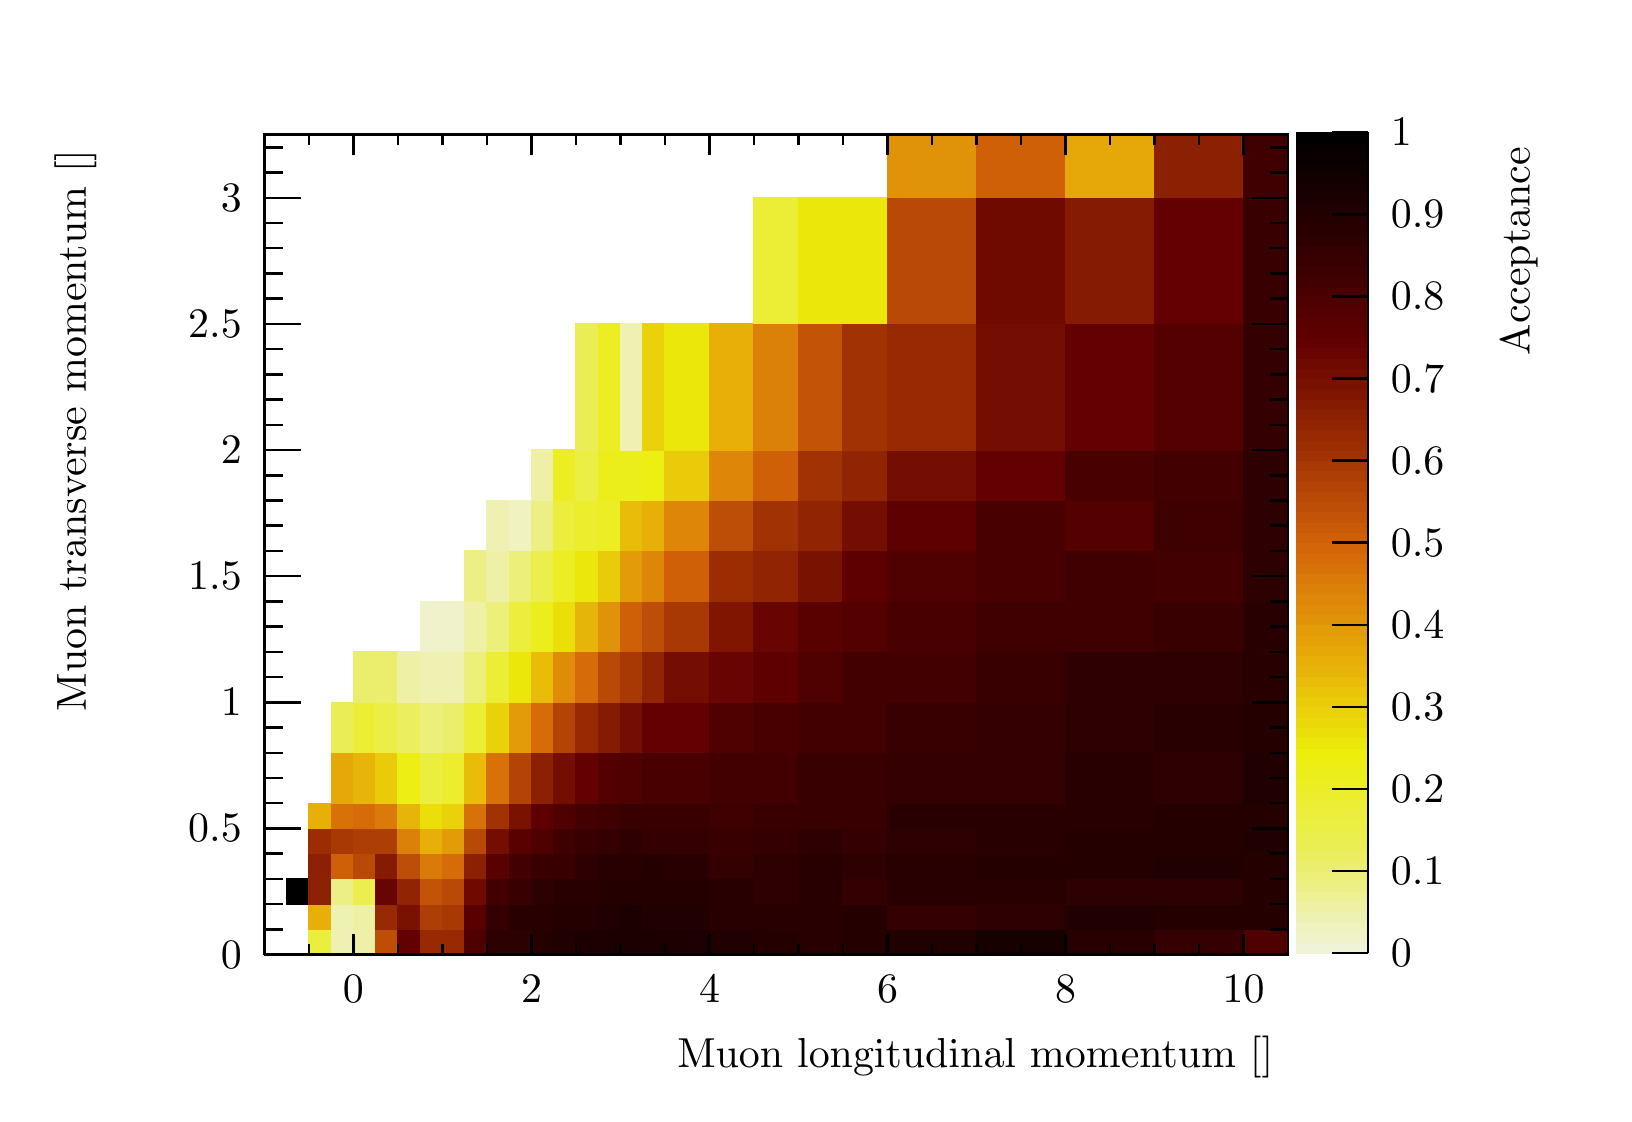
\begin{tikzpicture}
\pgfdeclareplotmark{cross} {
\pgfpathmoveto{\pgfpoint{-0.3\pgfplotmarksize}{\pgfplotmarksize}}
\pgfpathlineto{\pgfpoint{+0.3\pgfplotmarksize}{\pgfplotmarksize}}
\pgfpathlineto{\pgfpoint{+0.3\pgfplotmarksize}{0.3\pgfplotmarksize}}
\pgfpathlineto{\pgfpoint{+1\pgfplotmarksize}{0.3\pgfplotmarksize}}
\pgfpathlineto{\pgfpoint{+1\pgfplotmarksize}{-0.3\pgfplotmarksize}}
\pgfpathlineto{\pgfpoint{+0.3\pgfplotmarksize}{-0.3\pgfplotmarksize}}
\pgfpathlineto{\pgfpoint{+0.3\pgfplotmarksize}{-1.\pgfplotmarksize}}
\pgfpathlineto{\pgfpoint{-0.3\pgfplotmarksize}{-1.\pgfplotmarksize}}
\pgfpathlineto{\pgfpoint{-0.3\pgfplotmarksize}{-0.3\pgfplotmarksize}}
\pgfpathlineto{\pgfpoint{-1.\pgfplotmarksize}{-0.3\pgfplotmarksize}}
\pgfpathlineto{\pgfpoint{-1.\pgfplotmarksize}{0.3\pgfplotmarksize}}
\pgfpathlineto{\pgfpoint{-0.3\pgfplotmarksize}{0.3\pgfplotmarksize}}
\pgfpathclose
\pgfusepathqstroke
}
\pgfdeclareplotmark{cross*} {
\pgfpathmoveto{\pgfpoint{-0.3\pgfplotmarksize}{\pgfplotmarksize}}
\pgfpathlineto{\pgfpoint{+0.3\pgfplotmarksize}{\pgfplotmarksize}}
\pgfpathlineto{\pgfpoint{+0.3\pgfplotmarksize}{0.3\pgfplotmarksize}}
\pgfpathlineto{\pgfpoint{+1\pgfplotmarksize}{0.3\pgfplotmarksize}}
\pgfpathlineto{\pgfpoint{+1\pgfplotmarksize}{-0.3\pgfplotmarksize}}
\pgfpathlineto{\pgfpoint{+0.3\pgfplotmarksize}{-0.3\pgfplotmarksize}}
\pgfpathlineto{\pgfpoint{+0.3\pgfplotmarksize}{-1.\pgfplotmarksize}}
\pgfpathlineto{\pgfpoint{-0.3\pgfplotmarksize}{-1.\pgfplotmarksize}}
\pgfpathlineto{\pgfpoint{-0.3\pgfplotmarksize}{-0.3\pgfplotmarksize}}
\pgfpathlineto{\pgfpoint{-1.\pgfplotmarksize}{-0.3\pgfplotmarksize}}
\pgfpathlineto{\pgfpoint{-1.\pgfplotmarksize}{0.3\pgfplotmarksize}}
\pgfpathlineto{\pgfpoint{-0.3\pgfplotmarksize}{0.3\pgfplotmarksize}}
\pgfpathclose
\pgfusepathqfillstroke
}
\pgfdeclareplotmark{newstar} {
\pgfpathmoveto{\pgfqpoint{0pt}{\pgfplotmarksize}}
\pgfpathlineto{\pgfqpointpolar{44}{0.5\pgfplotmarksize}}
\pgfpathlineto{\pgfqpointpolar{18}{\pgfplotmarksize}}
\pgfpathlineto{\pgfqpointpolar{-20}{0.5\pgfplotmarksize}}
\pgfpathlineto{\pgfqpointpolar{-54}{\pgfplotmarksize}}
\pgfpathlineto{\pgfqpointpolar{-90}{0.5\pgfplotmarksize}}
\pgfpathlineto{\pgfqpointpolar{234}{\pgfplotmarksize}}
\pgfpathlineto{\pgfqpointpolar{198}{0.5\pgfplotmarksize}}
\pgfpathlineto{\pgfqpointpolar{162}{\pgfplotmarksize}}
\pgfpathlineto{\pgfqpointpolar{134}{0.5\pgfplotmarksize}}
\pgfpathclose
\pgfusepathqstroke
}
\pgfdeclareplotmark{newstar*} {
\pgfpathmoveto{\pgfqpoint{0pt}{\pgfplotmarksize}}
\pgfpathlineto{\pgfqpointpolar{44}{0.5\pgfplotmarksize}}
\pgfpathlineto{\pgfqpointpolar{18}{\pgfplotmarksize}}
\pgfpathlineto{\pgfqpointpolar{-20}{0.5\pgfplotmarksize}}
\pgfpathlineto{\pgfqpointpolar{-54}{\pgfplotmarksize}}
\pgfpathlineto{\pgfqpointpolar{-90}{0.5\pgfplotmarksize}}
\pgfpathlineto{\pgfqpointpolar{234}{\pgfplotmarksize}}
\pgfpathlineto{\pgfqpointpolar{198}{0.5\pgfplotmarksize}}
\pgfpathlineto{\pgfqpointpolar{162}{\pgfplotmarksize}}
\pgfpathlineto{\pgfqpointpolar{134}{0.5\pgfplotmarksize}}
\pgfpathclose
\pgfusepathqfillstroke
}
\definecolor{c}{rgb}{1,1,1};
\draw [color=c, fill=c] (0,0) rectangle (20,13.5227);
\draw [color=c, fill=c] (3,1.75795) rectangle (16,12.1705);
\definecolor{c}{rgb}{0,0,0};
\draw [c,line width=0.9] (3,1.75795) -- (3,12.1705) -- (16,12.1705) -- (16,1.75795) -- (3,1.75795);
\definecolor{c}{rgb}{1,1,1};
\draw [color=c, fill=c] (3,1.75795) rectangle (16,12.1705);
\definecolor{c}{rgb}{0,0,0};
\draw [c,line width=0.9] (3,1.75795) -- (3,12.1705) -- (16,12.1705) -- (16,1.75795) -- (3,1.75795);
\definecolor{c}{rgb}{0.922426,0.933333,0.238725};
\draw [color=c, fill=c] (3.56522,1.75795) rectangle (3.84783,2.07834);
\definecolor{c}{rgb}{0.936875,0.945351,0.697027};
\draw [color=c, fill=c] (3.84783,1.75795) rectangle (4.13043,2.07834);
\definecolor{c}{rgb}{0.933839,0.943453,0.645794};
\draw [color=c, fill=c] (4.13043,1.75795) rectangle (4.41304,2.07834);
\definecolor{c}{rgb}{0.742157,0.306863,0.0257353};
\draw [color=c, fill=c] (4.41304,1.75795) rectangle (4.69565,2.07834);
\definecolor{c}{rgb}{0.388235,0,0.00392157};
\draw [color=c, fill=c] (4.69565,1.75795) rectangle (4.97826,2.07834);
\definecolor{c}{rgb}{0.590809,0.159926,0.0110294};
\draw [color=c, fill=c] (4.97826,1.75795) rectangle (5.26087,2.07834);
\draw [color=c, fill=c] (5.26087,1.75795) rectangle (5.54348,2.07834);
\definecolor{c}{rgb}{0.308824,0,0.00392157};
\draw [color=c, fill=c] (5.54348,1.75795) rectangle (5.82609,2.07834);
\definecolor{c}{rgb}{0.176471,0,0.00392157};
\draw [color=c, fill=c] (5.82609,1.75795) rectangle (6.1087,2.07834);
\draw [color=c, fill=c] (6.1087,1.75795) rectangle (6.3913,2.07834);
\definecolor{c}{rgb}{0.143382,0,0.00318627};
\draw [color=c, fill=c] (6.3913,1.75795) rectangle (6.67391,2.07834);
\definecolor{c}{rgb}{0.126838,0,0.00281863};
\draw [color=c, fill=c] (6.67391,1.75795) rectangle (6.95652,2.07834);
\definecolor{c}{rgb}{0.110294,0,0.00245098};
\draw [color=c, fill=c] (6.95652,1.75795) rectangle (7.23913,2.07834);
\draw [color=c, fill=c] (7.23913,1.75795) rectangle (7.52174,2.07834);
\draw [color=c, fill=c] (7.52174,1.75795) rectangle (7.80435,2.07834);
\draw [color=c, fill=c] (7.80435,1.75795) rectangle (8.08696,2.07834);
\draw [color=c, fill=c] (8.08696,1.75795) rectangle (8.65217,2.07834);
\definecolor{c}{rgb}{0.126838,0,0.00281863};
\draw [color=c, fill=c] (8.65217,1.75795) rectangle (9.21739,2.07834);
\definecolor{c}{rgb}{0.143382,0,0.00318627};
\draw [color=c, fill=c] (9.21739,1.75795) rectangle (9.78261,2.07834);
\definecolor{c}{rgb}{0.159926,0,0.00355392};
\draw [color=c, fill=c] (9.78261,1.75795) rectangle (10.3478,2.07834);
\definecolor{c}{rgb}{0.143382,0,0.00318627};
\draw [color=c, fill=c] (10.3478,1.75795) rectangle (10.913,2.07834);
\definecolor{c}{rgb}{0.126838,0,0.00281863};
\draw [color=c, fill=c] (10.913,1.75795) rectangle (12.0435,2.07834);
\definecolor{c}{rgb}{0.0882353,0,0.00196078};
\draw [color=c, fill=c] (12.0435,1.75795) rectangle (13.1739,2.07834);
\definecolor{c}{rgb}{0.159926,0,0.00355392};
\draw [color=c, fill=c] (13.1739,1.75795) rectangle (14.3043,2.07834);
\definecolor{c}{rgb}{0.202941,0,0.00392157};
\draw [color=c, fill=c] (14.3043,1.75795) rectangle (15.4348,2.07834);
\definecolor{c}{rgb}{0.308824,0,0.00392157};
\draw [color=c, fill=c] (15.4348,1.75795) rectangle (16,2.07834);
\definecolor{c}{rgb}{0.904534,0.684559,0.0324755};
\draw [color=c, fill=c] (3.56522,2.07834) rectangle (3.84783,2.39872);
\definecolor{c}{rgb}{0.936875,0.945351,0.697027};
\draw [color=c, fill=c] (3.84783,2.07834) rectangle (4.13043,2.39872);
\definecolor{c}{rgb}{0.933839,0.943453,0.645794};
\draw [color=c, fill=c] (4.13043,2.07834) rectangle (4.41304,2.39872);
\definecolor{c}{rgb}{0.590809,0.159926,0.0110294};
\draw [color=c, fill=c] (4.41304,2.07834) rectangle (4.69565,2.39872);
\definecolor{c}{rgb}{0.479044,0.0716912,0.00710784};
\draw [color=c, fill=c] (4.69565,2.07834) rectangle (4.97826,2.39872);
\definecolor{c}{rgb}{0.680392,0.245098,0.0191176};
\draw [color=c, fill=c] (4.97826,2.07834) rectangle (5.26087,2.39872);
\definecolor{c}{rgb}{0.659804,0.22451,0.0169118};
\draw [color=c, fill=c] (5.26087,2.07834) rectangle (5.54348,2.39872);
\definecolor{c}{rgb}{0.348529,0,0.00392157};
\draw [color=c, fill=c] (5.54348,2.07834) rectangle (5.82609,2.39872);
\definecolor{c}{rgb}{0.202941,0,0.00392157};
\draw [color=c, fill=c] (5.82609,2.07834) rectangle (6.1087,2.39872);
\definecolor{c}{rgb}{0.159926,0,0.00355392};
\draw [color=c, fill=c] (6.1087,2.07834) rectangle (6.3913,2.39872);
\draw [color=c, fill=c] (6.3913,2.07834) rectangle (6.67391,2.39872);
\definecolor{c}{rgb}{0.143382,0,0.00318627};
\draw [color=c, fill=c] (6.67391,2.07834) rectangle (6.95652,2.39872);
\draw [color=c, fill=c] (6.95652,2.07834) rectangle (7.23913,2.39872);
\definecolor{c}{rgb}{0.126838,0,0.00281863};
\draw [color=c, fill=c] (7.23913,2.07834) rectangle (7.52174,2.39872);
\definecolor{c}{rgb}{0.110294,0,0.00245098};
\draw [color=c, fill=c] (7.52174,2.07834) rectangle (7.80435,2.39872);
\definecolor{c}{rgb}{0.126838,0,0.00281863};
\draw [color=c, fill=c] (7.80435,2.07834) rectangle (8.08696,2.39872);
\draw [color=c, fill=c] (8.08696,2.07834) rectangle (8.65217,2.39872);
\definecolor{c}{rgb}{0.159926,0,0.00355392};
\draw [color=c, fill=c] (8.65217,2.07834) rectangle (9.21739,2.39872);
\draw [color=c, fill=c] (9.21739,2.07834) rectangle (9.78261,2.39872);
\draw [color=c, fill=c] (9.78261,2.07834) rectangle (10.3478,2.39872);
\definecolor{c}{rgb}{0.143382,0,0.00318627};
\draw [color=c, fill=c] (10.3478,2.07834) rectangle (10.913,2.39872);
\definecolor{c}{rgb}{0.202941,0,0.00392157};
\draw [color=c, fill=c] (10.913,2.07834) rectangle (12.0435,2.39872);
\definecolor{c}{rgb}{0.176471,0,0.00392157};
\draw [color=c, fill=c] (12.0435,2.07834) rectangle (13.1739,2.39872);
\definecolor{c}{rgb}{0.126838,0,0.00281863};
\draw [color=c, fill=c] (13.1739,2.07834) rectangle (14.3043,2.39872);
\definecolor{c}{rgb}{0.143382,0,0.00318627};
\draw [color=c, fill=c] (14.3043,2.07834) rectangle (15.4348,2.39872);
\draw [color=c, fill=c] (15.4348,2.07834) rectangle (16,2.39872);
\definecolor{c}{rgb}{0.00551471,0,0.000122549};
\draw [color=c, fill=c] (3.28261,2.39872) rectangle (3.56522,2.71911);
\definecolor{c}{rgb}{0.548897,0.126838,0.00955882};
\draw [color=c, fill=c] (3.56522,2.39872) rectangle (3.84783,2.71911);
\definecolor{c}{rgb}{0.926755,0.939026,0.526249};
\draw [color=c, fill=c] (3.84783,2.39872) rectangle (4.13043,2.71911);
\definecolor{c}{rgb}{0.920221,0.933333,0.30049};
\draw [color=c, fill=c] (4.13043,2.39872) rectangle (4.41304,2.71911);
\definecolor{c}{rgb}{0.409191,0.0165441,0.00465686};
\draw [color=c, fill=c] (4.41304,2.39872) rectangle (4.69565,2.71911);
\definecolor{c}{rgb}{0.569853,0.143382,0.0102941};
\draw [color=c, fill=c] (4.69565,2.39872) rectangle (4.97826,2.71911);
\definecolor{c}{rgb}{0.762745,0.327451,0.0279412};
\draw [color=c, fill=c] (4.97826,2.39872) rectangle (5.26087,2.71911);
\definecolor{c}{rgb}{0.721569,0.286275,0.0235294};
\draw [color=c, fill=c] (5.26087,2.39872) rectangle (5.54348,2.71911);
\definecolor{c}{rgb}{0.437132,0.0386029,0.00563726};
\draw [color=c, fill=c] (5.54348,2.39872) rectangle (5.82609,2.71911);
\definecolor{c}{rgb}{0.2625,0,0.00392157};
\draw [color=c, fill=c] (5.82609,2.39872) rectangle (6.1087,2.71911);
\definecolor{c}{rgb}{0.222794,0,0.00392157};
\draw [color=c, fill=c] (6.1087,2.39872) rectangle (6.3913,2.71911);
\definecolor{c}{rgb}{0.176471,0,0.00392157};
\draw [color=c, fill=c] (6.3913,2.39872) rectangle (6.67391,2.71911);
\definecolor{c}{rgb}{0.159926,0,0.00355392};
\draw [color=c, fill=c] (6.67391,2.39872) rectangle (6.95652,2.71911);
\draw [color=c, fill=c] (6.95652,2.39872) rectangle (7.23913,2.71911);
\definecolor{c}{rgb}{0.143382,0,0.00318627};
\draw [color=c, fill=c] (7.23913,2.39872) rectangle (7.52174,2.71911);
\draw [color=c, fill=c] (7.52174,2.39872) rectangle (7.80435,2.71911);
\draw [color=c, fill=c] (7.80435,2.39872) rectangle (8.08696,2.71911);
\draw [color=c, fill=c] (8.08696,2.39872) rectangle (8.65217,2.71911);
\definecolor{c}{rgb}{0.159926,0,0.00355392};
\draw [color=c, fill=c] (8.65217,2.39872) rectangle (9.21739,2.71911);
\definecolor{c}{rgb}{0.176471,0,0.00392157};
\draw [color=c, fill=c] (9.21739,2.39872) rectangle (9.78261,2.71911);
\definecolor{c}{rgb}{0.159926,0,0.00355392};
\draw [color=c, fill=c] (9.78261,2.39872) rectangle (10.3478,2.71911);
\definecolor{c}{rgb}{0.202941,0,0.00392157};
\draw [color=c, fill=c] (10.3478,2.39872) rectangle (10.913,2.71911);
\definecolor{c}{rgb}{0.159926,0,0.00355392};
\draw [color=c, fill=c] (10.913,2.39872) rectangle (12.0435,2.71911);
\draw [color=c, fill=c] (12.0435,2.39872) rectangle (13.1739,2.71911);
\definecolor{c}{rgb}{0.176471,0,0.00392157};
\draw [color=c, fill=c] (13.1739,2.39872) rectangle (14.3043,2.71911);
\draw [color=c, fill=c] (14.3043,2.39872) rectangle (15.4348,2.71911);
\definecolor{c}{rgb}{0.143382,0,0.00318627};
\draw [color=c, fill=c] (15.4348,2.39872) rectangle (16,2.71911);
\definecolor{c}{rgb}{0.548897,0.126838,0.00955882};
\draw [color=c, fill=c] (3.56522,2.71911) rectangle (3.84783,3.03949);
\definecolor{c}{rgb}{0.810784,0.37549,0.0330882};
\draw [color=c, fill=c] (3.84783,2.71911) rectangle (4.13043,3.03949);
\definecolor{c}{rgb}{0.721569,0.286275,0.0235294};
\draw [color=c, fill=c] (4.13043,2.71911) rectangle (4.41304,3.03949);
\definecolor{c}{rgb}{0.520956,0.104779,0.00857843};
\draw [color=c, fill=c] (4.41304,2.71911) rectangle (4.69565,3.03949);
\definecolor{c}{rgb}{0.742157,0.306863,0.0257353};
\draw [color=c, fill=c] (4.69565,2.71911) rectangle (4.97826,3.03949);
\definecolor{c}{rgb}{0.853431,0.478186,0.0340686};
\draw [color=c, fill=c] (4.97826,2.71911) rectangle (5.26087,3.03949);
\definecolor{c}{rgb}{0.83799,0.420711,0.0349265};
\draw [color=c, fill=c] (5.26087,2.71911) rectangle (5.54348,3.03949);
\definecolor{c}{rgb}{0.548897,0.126838,0.00955882};
\draw [color=c, fill=c] (5.54348,2.71911) rectangle (5.82609,3.03949);
\definecolor{c}{rgb}{0.348529,0,0.00392157};
\draw [color=c, fill=c] (5.82609,2.71911) rectangle (6.1087,3.03949);
\definecolor{c}{rgb}{0.2625,0,0.00392157};
\draw [color=c, fill=c] (6.1087,2.71911) rectangle (6.3913,3.03949);
\definecolor{c}{rgb}{0.222794,0,0.00392157};
\draw [color=c, fill=c] (6.3913,2.71911) rectangle (6.67391,3.03949);
\draw [color=c, fill=c] (6.67391,2.71911) rectangle (6.95652,3.03949);
\definecolor{c}{rgb}{0.176471,0,0.00392157};
\draw [color=c, fill=c] (6.95652,2.71911) rectangle (7.23913,3.03949);
\definecolor{c}{rgb}{0.159926,0,0.00355392};
\draw [color=c, fill=c] (7.23913,2.71911) rectangle (7.52174,3.03949);
\draw [color=c, fill=c] (7.52174,2.71911) rectangle (7.80435,3.03949);
\definecolor{c}{rgb}{0.143382,0,0.00318627};
\draw [color=c, fill=c] (7.80435,2.71911) rectangle (8.08696,3.03949);
\definecolor{c}{rgb}{0.159926,0,0.00355392};
\draw [color=c, fill=c] (8.08696,2.71911) rectangle (8.65217,3.03949);
\definecolor{c}{rgb}{0.202941,0,0.00392157};
\draw [color=c, fill=c] (8.65217,2.71911) rectangle (9.21739,3.03949);
\definecolor{c}{rgb}{0.176471,0,0.00392157};
\draw [color=c, fill=c] (9.21739,2.71911) rectangle (9.78261,3.03949);
\definecolor{c}{rgb}{0.159926,0,0.00355392};
\draw [color=c, fill=c] (9.78261,2.71911) rectangle (10.3478,3.03949);
\definecolor{c}{rgb}{0.176471,0,0.00392157};
\draw [color=c, fill=c] (10.3478,2.71911) rectangle (10.913,3.03949);
\definecolor{c}{rgb}{0.159926,0,0.00355392};
\draw [color=c, fill=c] (10.913,2.71911) rectangle (12.0435,3.03949);
\definecolor{c}{rgb}{0.143382,0,0.00318627};
\draw [color=c, fill=c] (12.0435,2.71911) rectangle (13.1739,3.03949);
\draw [color=c, fill=c] (13.1739,2.71911) rectangle (14.3043,3.03949);
\definecolor{c}{rgb}{0.126838,0,0.00281863};
\draw [color=c, fill=c] (14.3043,2.71911) rectangle (15.4348,3.03949);
\definecolor{c}{rgb}{0.143382,0,0.00318627};
\draw [color=c, fill=c] (15.4348,2.71911) rectangle (16,3.03949);
\definecolor{c}{rgb}{0.611765,0.176471,0.0117647};
\draw [color=c, fill=c] (3.56522,3.03949) rectangle (3.84783,3.35988);
\definecolor{c}{rgb}{0.659804,0.22451,0.0169118};
\draw [color=c, fill=c] (3.84783,3.03949) rectangle (4.13043,3.35988);
\definecolor{c}{rgb}{0.680392,0.245098,0.0191176};
\draw [color=c, fill=c] (4.13043,3.03949) rectangle (4.41304,3.35988);
\draw [color=c, fill=c] (4.41304,3.03949) rectangle (4.69565,3.35988);
\definecolor{c}{rgb}{0.860049,0.502819,0.033701};
\draw [color=c, fill=c] (4.69565,3.03949) rectangle (4.97826,3.35988);
\definecolor{c}{rgb}{0.904534,0.684559,0.0324755};
\draw [color=c, fill=c] (4.97826,3.03949) rectangle (5.26087,3.35988);
\definecolor{c}{rgb}{0.888726,0.609559,0.0321078};
\draw [color=c, fill=c] (5.26087,3.03949) rectangle (5.54348,3.35988);
\definecolor{c}{rgb}{0.721569,0.286275,0.0235294};
\draw [color=c, fill=c] (5.54348,3.03949) rectangle (5.82609,3.35988);
\definecolor{c}{rgb}{0.458088,0.0551471,0.00637255};
\draw [color=c, fill=c] (5.82609,3.03949) rectangle (6.1087,3.35988);
\definecolor{c}{rgb}{0.348529,0,0.00392157};
\draw [color=c, fill=c] (6.1087,3.03949) rectangle (6.3913,3.35988);
\definecolor{c}{rgb}{0.308824,0,0.00392157};
\draw [color=c, fill=c] (6.3913,3.03949) rectangle (6.67391,3.35988);
\definecolor{c}{rgb}{0.242647,0,0.00392157};
\draw [color=c, fill=c] (6.67391,3.03949) rectangle (6.95652,3.35988);
\definecolor{c}{rgb}{0.222794,0,0.00392157};
\draw [color=c, fill=c] (6.95652,3.03949) rectangle (7.23913,3.35988);
\definecolor{c}{rgb}{0.202941,0,0.00392157};
\draw [color=c, fill=c] (7.23913,3.03949) rectangle (7.52174,3.35988);
\definecolor{c}{rgb}{0.176471,0,0.00392157};
\draw [color=c, fill=c] (7.52174,3.03949) rectangle (7.80435,3.35988);
\definecolor{c}{rgb}{0.202941,0,0.00392157};
\draw [color=c, fill=c] (7.80435,3.03949) rectangle (8.08696,3.35988);
\draw [color=c, fill=c] (8.08696,3.03949) rectangle (8.65217,3.35988);
\definecolor{c}{rgb}{0.222794,0,0.00392157};
\draw [color=c, fill=c] (8.65217,3.03949) rectangle (9.21739,3.35988);
\definecolor{c}{rgb}{0.202941,0,0.00392157};
\draw [color=c, fill=c] (9.21739,3.03949) rectangle (9.78261,3.35988);
\definecolor{c}{rgb}{0.176471,0,0.00392157};
\draw [color=c, fill=c] (9.78261,3.03949) rectangle (10.3478,3.35988);
\definecolor{c}{rgb}{0.202941,0,0.00392157};
\draw [color=c, fill=c] (10.3478,3.03949) rectangle (10.913,3.35988);
\definecolor{c}{rgb}{0.176471,0,0.00392157};
\draw [color=c, fill=c] (10.913,3.03949) rectangle (12.0435,3.35988);
\definecolor{c}{rgb}{0.159926,0,0.00355392};
\draw [color=c, fill=c] (12.0435,3.03949) rectangle (13.1739,3.35988);
\definecolor{c}{rgb}{0.143382,0,0.00318627};
\draw [color=c, fill=c] (13.1739,3.03949) rectangle (14.3043,3.35988);
\draw [color=c, fill=c] (14.3043,3.03949) rectangle (15.4348,3.35988);
\definecolor{c}{rgb}{0.126838,0,0.00281863};
\draw [color=c, fill=c] (15.4348,3.03949) rectangle (16,3.35988);
\definecolor{c}{rgb}{0.904534,0.684559,0.0324755};
\draw [color=c, fill=c] (3.56522,3.35988) rectangle (3.84783,3.68026);
\definecolor{c}{rgb}{0.844608,0.445343,0.0345588};
\draw [color=c, fill=c] (3.84783,3.35988) rectangle (4.13043,3.68026);
\definecolor{c}{rgb}{0.83799,0.420711,0.0349265};
\draw [color=c, fill=c] (4.13043,3.35988) rectangle (4.41304,3.68026);
\definecolor{c}{rgb}{0.853431,0.478186,0.0340686};
\draw [color=c, fill=c] (4.41304,3.35988) rectangle (4.69565,3.68026);
\definecolor{c}{rgb}{0.907108,0.710294,0.0335784};
\draw [color=c, fill=c] (4.69565,3.35988) rectangle (4.97826,3.68026);
\definecolor{c}{rgb}{0.923407,0.873284,0.0405637};
\draw [color=c, fill=c] (4.97826,3.35988) rectangle (5.26087,3.68026);
\definecolor{c}{rgb}{0.91826,0.821814,0.0383578};
\draw [color=c, fill=c] (5.26087,3.35988) rectangle (5.54348,3.68026);
\definecolor{c}{rgb}{0.844608,0.445343,0.0345588};
\draw [color=c, fill=c] (5.54348,3.35988) rectangle (5.82609,3.68026);
\definecolor{c}{rgb}{0.632353,0.197059,0.0139706};
\draw [color=c, fill=c] (5.82609,3.35988) rectangle (6.1087,3.68026);
\definecolor{c}{rgb}{0.479044,0.0716912,0.00710784};
\draw [color=c, fill=c] (6.1087,3.35988) rectangle (6.3913,3.68026);
\definecolor{c}{rgb}{0.368382,0,0.00392157};
\draw [color=c, fill=c] (6.3913,3.35988) rectangle (6.67391,3.68026);
\definecolor{c}{rgb}{0.308824,0,0.00392157};
\draw [color=c, fill=c] (6.67391,3.35988) rectangle (6.95652,3.68026);
\definecolor{c}{rgb}{0.2625,0,0.00392157};
\draw [color=c, fill=c] (6.95652,3.35988) rectangle (7.23913,3.68026);
\definecolor{c}{rgb}{0.242647,0,0.00392157};
\draw [color=c, fill=c] (7.23913,3.35988) rectangle (7.52174,3.68026);
\definecolor{c}{rgb}{0.222794,0,0.00392157};
\draw [color=c, fill=c] (7.52174,3.35988) rectangle (7.80435,3.68026);
\draw [color=c, fill=c] (7.80435,3.35988) rectangle (8.08696,3.68026);
\draw [color=c, fill=c] (8.08696,3.35988) rectangle (8.65217,3.68026);
\definecolor{c}{rgb}{0.242647,0,0.00392157};
\draw [color=c, fill=c] (8.65217,3.35988) rectangle (9.21739,3.68026);
\definecolor{c}{rgb}{0.222794,0,0.00392157};
\draw [color=c, fill=c] (9.21739,3.35988) rectangle (9.78261,3.68026);
\draw [color=c, fill=c] (9.78261,3.35988) rectangle (10.3478,3.68026);
\draw [color=c, fill=c] (10.3478,3.35988) rectangle (10.913,3.68026);
\definecolor{c}{rgb}{0.159926,0,0.00355392};
\draw [color=c, fill=c] (10.913,3.35988) rectangle (12.0435,3.68026);
\draw [color=c, fill=c] (12.0435,3.35988) rectangle (13.1739,3.68026);
\draw [color=c, fill=c] (13.1739,3.35988) rectangle (14.3043,3.68026);
\definecolor{c}{rgb}{0.143382,0,0.00318627};
\draw [color=c, fill=c] (14.3043,3.35988) rectangle (15.4348,3.68026);
\draw [color=c, fill=c] (15.4348,3.35988) rectangle (16,3.68026);
\definecolor{c}{rgb}{0.901961,0.658824,0.0313726};
\draw [color=c, fill=c] (3.84783,3.68026) rectangle (4.13043,4.32103);
\definecolor{c}{rgb}{0.907108,0.710294,0.0335784};
\draw [color=c, fill=c] (4.13043,3.68026) rectangle (4.41304,4.32103);
\definecolor{c}{rgb}{0.915686,0.796078,0.0372549};
\draw [color=c, fill=c] (4.41304,3.68026) rectangle (4.69565,4.32103);
\definecolor{c}{rgb}{0.928309,0.933333,0.0740196};
\draw [color=c, fill=c] (4.69565,3.68026) rectangle (4.97826,4.32103);
\definecolor{c}{rgb}{0.922426,0.933333,0.238725};
\draw [color=c, fill=c] (4.97826,3.68026) rectangle (5.26087,4.32103);
\definecolor{c}{rgb}{0.924632,0.933333,0.176961};
\draw [color=c, fill=c] (5.26087,3.68026) rectangle (5.54348,4.32103);
\definecolor{c}{rgb}{0.909681,0.736029,0.0346814};
\draw [color=c, fill=c] (5.54348,3.68026) rectangle (5.82609,4.32103);
\definecolor{c}{rgb}{0.844608,0.445343,0.0345588};
\draw [color=c, fill=c] (5.82609,3.68026) rectangle (6.1087,4.32103);
\definecolor{c}{rgb}{0.70098,0.265686,0.0213235};
\draw [color=c, fill=c] (6.1087,3.68026) rectangle (6.3913,4.32103);
\definecolor{c}{rgb}{0.548897,0.126838,0.00955882};
\draw [color=c, fill=c] (6.3913,3.68026) rectangle (6.67391,4.32103);
\definecolor{c}{rgb}{0.458088,0.0551471,0.00637255};
\draw [color=c, fill=c] (6.67391,3.68026) rectangle (6.95652,4.32103);
\definecolor{c}{rgb}{0.388235,0,0.00392157};
\draw [color=c, fill=c] (6.95652,3.68026) rectangle (7.23913,4.32103);
\definecolor{c}{rgb}{0.328676,0,0.00392157};
\draw [color=c, fill=c] (7.23913,3.68026) rectangle (7.52174,4.32103);
\definecolor{c}{rgb}{0.308824,0,0.00392157};
\draw [color=c, fill=c] (7.52174,3.68026) rectangle (7.80435,4.32103);
\definecolor{c}{rgb}{0.282353,0,0.00392157};
\draw [color=c, fill=c] (7.80435,3.68026) rectangle (8.08696,4.32103);
\draw [color=c, fill=c] (8.08696,3.68026) rectangle (8.65217,4.32103);
\definecolor{c}{rgb}{0.2625,0,0.00392157};
\draw [color=c, fill=c] (8.65217,3.68026) rectangle (9.21739,4.32103);
\draw [color=c, fill=c] (9.21739,3.68026) rectangle (9.78261,4.32103);
\definecolor{c}{rgb}{0.222794,0,0.00392157};
\draw [color=c, fill=c] (9.78261,3.68026) rectangle (10.3478,4.32103);
\draw [color=c, fill=c] (10.3478,3.68026) rectangle (10.913,4.32103);
\definecolor{c}{rgb}{0.202941,0,0.00392157};
\draw [color=c, fill=c] (10.913,3.68026) rectangle (12.0435,4.32103);
\draw [color=c, fill=c] (12.0435,3.68026) rectangle (13.1739,4.32103);
\definecolor{c}{rgb}{0.159926,0,0.00355392};
\draw [color=c, fill=c] (13.1739,3.68026) rectangle (14.3043,4.32103);
\definecolor{c}{rgb}{0.176471,0,0.00392157};
\draw [color=c, fill=c] (14.3043,3.68026) rectangle (15.4348,4.32103);
\definecolor{c}{rgb}{0.126838,0,0.00281863};
\draw [color=c, fill=c] (15.4348,3.68026) rectangle (16,4.32103);
\definecolor{c}{rgb}{0.919118,0.933333,0.331373};
\draw [color=c, fill=c] (3.84783,4.32103) rectangle (4.13043,4.9618);
\definecolor{c}{rgb}{0.923529,0.933333,0.207843};
\draw [color=c, fill=c] (4.13043,4.32103) rectangle (4.41304,4.9618);
\definecolor{c}{rgb}{0.921324,0.933333,0.269608};
\draw [color=c, fill=c] (4.41304,4.32103) rectangle (4.69565,4.9618);
\definecolor{c}{rgb}{0.917647,0.933333,0.372549};
\draw [color=c, fill=c] (4.69565,4.32103) rectangle (4.97826,4.9618);
\definecolor{c}{rgb}{0.923719,0.937128,0.475016};
\draw [color=c, fill=c] (4.97826,4.32103) rectangle (5.26087,4.9618);
\definecolor{c}{rgb}{0.920683,0.935231,0.423782};
\draw [color=c, fill=c] (5.26087,4.32103) rectangle (5.54348,4.9618);
\definecolor{c}{rgb}{0.923529,0.933333,0.207843};
\draw [color=c, fill=c] (5.54348,4.32103) rectangle (5.82609,4.9618);
\definecolor{c}{rgb}{0.91826,0.821814,0.0383578};
\draw [color=c, fill=c] (5.82609,4.32103) rectangle (6.1087,4.9618);
\definecolor{c}{rgb}{0.888726,0.609559,0.0321078};
\draw [color=c, fill=c] (6.1087,4.32103) rectangle (6.3913,4.9618);
\definecolor{c}{rgb}{0.83799,0.420711,0.0349265};
\draw [color=c, fill=c] (6.3913,4.32103) rectangle (6.67391,4.9618);
\definecolor{c}{rgb}{0.70098,0.265686,0.0213235};
\draw [color=c, fill=c] (6.67391,4.32103) rectangle (6.95652,4.9618);
\definecolor{c}{rgb}{0.590809,0.159926,0.0110294};
\draw [color=c, fill=c] (6.95652,4.32103) rectangle (7.23913,4.9618);
\definecolor{c}{rgb}{0.520956,0.104779,0.00857843};
\draw [color=c, fill=c] (7.23913,4.32103) rectangle (7.52174,4.9618);
\definecolor{c}{rgb}{0.458088,0.0551471,0.00637255};
\draw [color=c, fill=c] (7.52174,4.32103) rectangle (7.80435,4.9618);
\definecolor{c}{rgb}{0.388235,0,0.00392157};
\draw [color=c, fill=c] (7.80435,4.32103) rectangle (8.08696,4.9618);
\draw [color=c, fill=c] (8.08696,4.32103) rectangle (8.65217,4.9618);
\definecolor{c}{rgb}{0.308824,0,0.00392157};
\draw [color=c, fill=c] (8.65217,4.32103) rectangle (9.21739,4.9618);
\definecolor{c}{rgb}{0.282353,0,0.00392157};
\draw [color=c, fill=c] (9.21739,4.32103) rectangle (9.78261,4.9618);
\definecolor{c}{rgb}{0.2625,0,0.00392157};
\draw [color=c, fill=c] (9.78261,4.32103) rectangle (10.3478,4.9618);
\draw [color=c, fill=c] (10.3478,4.32103) rectangle (10.913,4.9618);
\definecolor{c}{rgb}{0.222794,0,0.00392157};
\draw [color=c, fill=c] (10.913,4.32103) rectangle (12.0435,4.9618);
\definecolor{c}{rgb}{0.202941,0,0.00392157};
\draw [color=c, fill=c] (12.0435,4.32103) rectangle (13.1739,4.9618);
\definecolor{c}{rgb}{0.176471,0,0.00392157};
\draw [color=c, fill=c] (13.1739,4.32103) rectangle (14.3043,4.9618);
\definecolor{c}{rgb}{0.159926,0,0.00355392};
\draw [color=c, fill=c] (14.3043,4.32103) rectangle (15.4348,4.9618);
\definecolor{c}{rgb}{0.143382,0,0.00318627};
\draw [color=c, fill=c] (15.4348,4.32103) rectangle (16,4.9618);
\definecolor{c}{rgb}{0.920683,0.935231,0.423782};
\draw [color=c, fill=c] (4.13043,4.9618) rectangle (4.41304,5.60257);
\draw [color=c, fill=c] (4.41304,4.9618) rectangle (4.69565,5.60257);
\definecolor{c}{rgb}{0.933839,0.943453,0.645794};
\draw [color=c, fill=c] (4.69565,4.9618) rectangle (4.97826,5.60257);
\definecolor{c}{rgb}{0.936875,0.945351,0.697027};
\draw [color=c, fill=c] (4.97826,4.9618) rectangle (5.26087,5.60257);
\draw [color=c, fill=c] (5.26087,4.9618) rectangle (5.54348,5.60257);
\definecolor{c}{rgb}{0.923719,0.937128,0.475016};
\draw [color=c, fill=c] (5.54348,4.9618) rectangle (5.82609,5.60257);
\definecolor{c}{rgb}{0.923529,0.933333,0.207843};
\draw [color=c, fill=c] (5.82609,4.9618) rectangle (6.1087,5.60257);
\definecolor{c}{rgb}{0.926838,0.907598,0.0420343};
\draw [color=c, fill=c] (6.1087,4.9618) rectangle (6.3913,5.60257);
\definecolor{c}{rgb}{0.909681,0.736029,0.0346814};
\draw [color=c, fill=c] (6.3913,4.9618) rectangle (6.67391,5.60257);
\definecolor{c}{rgb}{0.873284,0.552083,0.0329657};
\draw [color=c, fill=c] (6.67391,4.9618) rectangle (6.95652,5.60257);
\definecolor{c}{rgb}{0.83799,0.420711,0.0349265};
\draw [color=c, fill=c] (6.95652,4.9618) rectangle (7.23913,5.60257);
\definecolor{c}{rgb}{0.721569,0.286275,0.0235294};
\draw [color=c, fill=c] (7.23913,4.9618) rectangle (7.52174,5.60257);
\definecolor{c}{rgb}{0.659804,0.22451,0.0169118};
\draw [color=c, fill=c] (7.52174,4.9618) rectangle (7.80435,5.60257);
\definecolor{c}{rgb}{0.569853,0.143382,0.0102941};
\draw [color=c, fill=c] (7.80435,4.9618) rectangle (8.08696,5.60257);
\definecolor{c}{rgb}{0.458088,0.0551471,0.00637255};
\draw [color=c, fill=c] (8.08696,4.9618) rectangle (8.65217,5.60257);
\definecolor{c}{rgb}{0.409191,0.0165441,0.00465686};
\draw [color=c, fill=c] (8.65217,4.9618) rectangle (9.21739,5.60257);
\definecolor{c}{rgb}{0.368382,0,0.00392157};
\draw [color=c, fill=c] (9.21739,4.9618) rectangle (9.78261,5.60257);
\definecolor{c}{rgb}{0.308824,0,0.00392157};
\draw [color=c, fill=c] (9.78261,4.9618) rectangle (10.3478,5.60257);
\definecolor{c}{rgb}{0.2625,0,0.00392157};
\draw [color=c, fill=c] (10.3478,4.9618) rectangle (10.913,5.60257);
\draw [color=c, fill=c] (10.913,4.9618) rectangle (12.0435,5.60257);
\definecolor{c}{rgb}{0.222794,0,0.00392157};
\draw [color=c, fill=c] (12.0435,4.9618) rectangle (13.1739,5.60257);
\definecolor{c}{rgb}{0.176471,0,0.00392157};
\draw [color=c, fill=c] (13.1739,4.9618) rectangle (14.3043,5.60257);
\draw [color=c, fill=c] (14.3043,4.9618) rectangle (15.4348,5.60257);
\definecolor{c}{rgb}{0.159926,0,0.00355392};
\draw [color=c, fill=c] (15.4348,4.9618) rectangle (16,5.60257);
\definecolor{c}{rgb}{0.942948,0.949146,0.799494};
\draw [color=c, fill=c] (4.97826,5.60257) rectangle (5.26087,6.24334);
\draw [color=c, fill=c] (5.26087,5.60257) rectangle (5.54348,6.24334);
\definecolor{c}{rgb}{0.933839,0.943453,0.645794};
\draw [color=c, fill=c] (5.54348,5.60257) rectangle (5.82609,6.24334);
\definecolor{c}{rgb}{0.923719,0.937128,0.475016};
\draw [color=c, fill=c] (5.82609,5.60257) rectangle (6.1087,6.24334);
\definecolor{c}{rgb}{0.922426,0.933333,0.238725};
\draw [color=c, fill=c] (6.1087,5.60257) rectangle (6.3913,6.24334);
\definecolor{c}{rgb}{0.927206,0.933333,0.104902};
\draw [color=c, fill=c] (6.3913,5.60257) rectangle (6.67391,6.24334);
\definecolor{c}{rgb}{0.923407,0.873284,0.0405637};
\draw [color=c, fill=c] (6.67391,5.60257) rectangle (6.95652,6.24334);
\definecolor{c}{rgb}{0.907108,0.710294,0.0335784};
\draw [color=c, fill=c] (6.95652,5.60257) rectangle (7.23913,6.24334);
\definecolor{c}{rgb}{0.879902,0.576716,0.032598};
\draw [color=c, fill=c] (7.23913,5.60257) rectangle (7.52174,6.24334);
\definecolor{c}{rgb}{0.810784,0.37549,0.0330882};
\draw [color=c, fill=c] (7.52174,5.60257) rectangle (7.80435,6.24334);
\definecolor{c}{rgb}{0.742157,0.306863,0.0257353};
\draw [color=c, fill=c] (7.80435,5.60257) rectangle (8.08696,6.24334);
\definecolor{c}{rgb}{0.659804,0.22451,0.0169118};
\draw [color=c, fill=c] (8.08696,5.60257) rectangle (8.65217,6.24334);
\definecolor{c}{rgb}{0.5,0.0882353,0.00784314};
\draw [color=c, fill=c] (8.65217,5.60257) rectangle (9.21739,6.24334);
\definecolor{c}{rgb}{0.409191,0.0165441,0.00465686};
\draw [color=c, fill=c] (9.21739,5.60257) rectangle (9.78261,6.24334);
\definecolor{c}{rgb}{0.348529,0,0.00392157};
\draw [color=c, fill=c] (9.78261,5.60257) rectangle (10.3478,6.24334);
\definecolor{c}{rgb}{0.328676,0,0.00392157};
\draw [color=c, fill=c] (10.3478,5.60257) rectangle (10.913,6.24334);
\definecolor{c}{rgb}{0.282353,0,0.00392157};
\draw [color=c, fill=c] (10.913,5.60257) rectangle (12.0435,6.24334);
\definecolor{c}{rgb}{0.242647,0,0.00392157};
\draw [color=c, fill=c] (12.0435,5.60257) rectangle (13.1739,6.24334);
\draw [color=c, fill=c] (13.1739,5.60257) rectangle (14.3043,6.24334);
\definecolor{c}{rgb}{0.222794,0,0.00392157};
\draw [color=c, fill=c] (14.3043,5.60257) rectangle (15.4348,6.24334);
\definecolor{c}{rgb}{0.159926,0,0.00355392};
\draw [color=c, fill=c] (15.4348,5.60257) rectangle (16,6.24334);
\definecolor{c}{rgb}{0.926755,0.939026,0.526249};
\draw [color=c, fill=c] (5.54348,6.24334) rectangle (5.82609,6.88411);
\definecolor{c}{rgb}{0.933839,0.943453,0.645794};
\draw [color=c, fill=c] (5.82609,6.24334) rectangle (6.1087,6.88411);
\definecolor{c}{rgb}{0.923719,0.937128,0.475016};
\draw [color=c, fill=c] (6.1087,6.24334) rectangle (6.3913,6.88411);
\definecolor{c}{rgb}{0.920221,0.933333,0.30049};
\draw [color=c, fill=c] (6.3913,6.24334) rectangle (6.67391,6.88411);
\definecolor{c}{rgb}{0.926103,0.933333,0.135784};
\draw [color=c, fill=c] (6.67391,6.24334) rectangle (6.95652,6.88411);
\definecolor{c}{rgb}{0.926838,0.907598,0.0420343};
\draw [color=c, fill=c] (6.95652,6.24334) rectangle (7.23913,6.88411);
\definecolor{c}{rgb}{0.915686,0.796078,0.0372549};
\draw [color=c, fill=c] (7.23913,6.24334) rectangle (7.52174,6.88411);
\definecolor{c}{rgb}{0.888726,0.609559,0.0321078};
\draw [color=c, fill=c] (7.52174,6.24334) rectangle (7.80435,6.88411);
\definecolor{c}{rgb}{0.866667,0.527451,0.0333333};
\draw [color=c, fill=c] (7.80435,6.24334) rectangle (8.08696,6.88411);
\definecolor{c}{rgb}{0.810784,0.37549,0.0330882};
\draw [color=c, fill=c] (8.08696,6.24334) rectangle (8.65217,6.88411);
\definecolor{c}{rgb}{0.611765,0.176471,0.0117647};
\draw [color=c, fill=c] (8.65217,6.24334) rectangle (9.21739,6.88411);
\definecolor{c}{rgb}{0.569853,0.143382,0.0102941};
\draw [color=c, fill=c] (9.21739,6.24334) rectangle (9.78261,6.88411);
\definecolor{c}{rgb}{0.479044,0.0716912,0.00710784};
\draw [color=c, fill=c] (9.78261,6.24334) rectangle (10.3478,6.88411);
\definecolor{c}{rgb}{0.368382,0,0.00392157};
\draw [color=c, fill=c] (10.3478,6.24334) rectangle (10.913,6.88411);
\definecolor{c}{rgb}{0.308824,0,0.00392157};
\draw [color=c, fill=c] (10.913,6.24334) rectangle (12.0435,6.88411);
\definecolor{c}{rgb}{0.282353,0,0.00392157};
\draw [color=c, fill=c] (12.0435,6.24334) rectangle (13.1739,6.88411);
\definecolor{c}{rgb}{0.242647,0,0.00392157};
\draw [color=c, fill=c] (13.1739,6.24334) rectangle (14.3043,6.88411);
\definecolor{c}{rgb}{0.2625,0,0.00392157};
\draw [color=c, fill=c] (14.3043,6.24334) rectangle (15.4348,6.88411);
\definecolor{c}{rgb}{0.176471,0,0.00392157};
\draw [color=c, fill=c] (15.4348,6.24334) rectangle (16,6.88411);
\definecolor{c}{rgb}{0.936875,0.945351,0.697027};
\draw [color=c, fill=c] (5.82609,6.88411) rectangle (6.1087,7.52488);
\definecolor{c}{rgb}{0.939911,0.947249,0.748261};
\draw [color=c, fill=c] (6.1087,6.88411) rectangle (6.3913,7.52488);
\definecolor{c}{rgb}{0.926755,0.939026,0.526249};
\draw [color=c, fill=c] (6.3913,6.88411) rectangle (6.67391,7.52488);
\definecolor{c}{rgb}{0.922426,0.933333,0.238725};
\draw [color=c, fill=c] (6.67391,6.88411) rectangle (6.95652,7.52488);
\definecolor{c}{rgb}{0.924632,0.933333,0.176961};
\draw [color=c, fill=c] (6.95652,6.88411) rectangle (7.23913,7.52488);
\definecolor{c}{rgb}{0.926103,0.933333,0.135784};
\draw [color=c, fill=c] (7.23913,6.88411) rectangle (7.52174,7.52488);
\definecolor{c}{rgb}{0.909681,0.736029,0.0346814};
\draw [color=c, fill=c] (7.52174,6.88411) rectangle (7.80435,7.52488);
\definecolor{c}{rgb}{0.904534,0.684559,0.0324755};
\draw [color=c, fill=c] (7.80435,6.88411) rectangle (8.08696,7.52488);
\definecolor{c}{rgb}{0.866667,0.527451,0.0333333};
\draw [color=c, fill=c] (8.08696,6.88411) rectangle (8.65217,7.52488);
\definecolor{c}{rgb}{0.742157,0.306863,0.0257353};
\draw [color=c, fill=c] (8.65217,6.88411) rectangle (9.21739,7.52488);
\definecolor{c}{rgb}{0.632353,0.197059,0.0139706};
\draw [color=c, fill=c] (9.21739,6.88411) rectangle (9.78261,7.52488);
\definecolor{c}{rgb}{0.569853,0.143382,0.0102941};
\draw [color=c, fill=c] (9.78261,6.88411) rectangle (10.3478,7.52488);
\definecolor{c}{rgb}{0.458088,0.0551471,0.00637255};
\draw [color=c, fill=c] (10.3478,6.88411) rectangle (10.913,7.52488);
\definecolor{c}{rgb}{0.368382,0,0.00392157};
\draw [color=c, fill=c] (10.913,6.88411) rectangle (12.0435,7.52488);
\definecolor{c}{rgb}{0.282353,0,0.00392157};
\draw [color=c, fill=c] (12.0435,6.88411) rectangle (13.1739,7.52488);
\definecolor{c}{rgb}{0.328676,0,0.00392157};
\draw [color=c, fill=c] (13.1739,6.88411) rectangle (14.3043,7.52488);
\definecolor{c}{rgb}{0.242647,0,0.00392157};
\draw [color=c, fill=c] (14.3043,6.88411) rectangle (15.4348,7.52488);
\definecolor{c}{rgb}{0.176471,0,0.00392157};
\draw [color=c, fill=c] (15.4348,6.88411) rectangle (16,7.52488);
\definecolor{c}{rgb}{0.933839,0.943453,0.645794};
\draw [color=c, fill=c] (6.3913,7.52488) rectangle (6.67391,8.16565);
\definecolor{c}{rgb}{0.926103,0.933333,0.135784};
\draw [color=c, fill=c] (6.67391,7.52488) rectangle (6.95652,8.16565);
\definecolor{c}{rgb}{0.921324,0.933333,0.269608};
\draw [color=c, fill=c] (6.95652,7.52488) rectangle (7.23913,8.16565);
\definecolor{c}{rgb}{0.927206,0.933333,0.104902};
\draw [color=c, fill=c] (7.23913,7.52488) rectangle (7.52174,8.16565);
\draw [color=c, fill=c] (7.52174,7.52488) rectangle (7.80435,8.16565);
\definecolor{c}{rgb}{0.928309,0.933333,0.0740196};
\draw [color=c, fill=c] (7.80435,7.52488) rectangle (8.08696,8.16565);
\definecolor{c}{rgb}{0.915686,0.796078,0.0372549};
\draw [color=c, fill=c] (8.08696,7.52488) rectangle (8.65217,8.16565);
\definecolor{c}{rgb}{0.866667,0.527451,0.0333333};
\draw [color=c, fill=c] (8.65217,7.52488) rectangle (9.21739,8.16565);
\definecolor{c}{rgb}{0.810784,0.37549,0.0330882};
\draw [color=c, fill=c] (9.21739,7.52488) rectangle (9.78261,8.16565);
\definecolor{c}{rgb}{0.632353,0.197059,0.0139706};
\draw [color=c, fill=c] (9.78261,7.52488) rectangle (10.3478,8.16565);
\definecolor{c}{rgb}{0.569853,0.143382,0.0102941};
\draw [color=c, fill=c] (10.3478,7.52488) rectangle (10.913,8.16565);
\definecolor{c}{rgb}{0.458088,0.0551471,0.00637255};
\draw [color=c, fill=c] (10.913,7.52488) rectangle (12.0435,8.16565);
\definecolor{c}{rgb}{0.388235,0,0.00392157};
\draw [color=c, fill=c] (12.0435,7.52488) rectangle (13.1739,8.16565);
\definecolor{c}{rgb}{0.282353,0,0.00392157};
\draw [color=c, fill=c] (13.1739,7.52488) rectangle (14.3043,8.16565);
\definecolor{c}{rgb}{0.2625,0,0.00392157};
\draw [color=c, fill=c] (14.3043,7.52488) rectangle (15.4348,8.16565);
\definecolor{c}{rgb}{0.176471,0,0.00392157};
\draw [color=c, fill=c] (15.4348,7.52488) rectangle (16,8.16565);
\definecolor{c}{rgb}{0.919118,0.933333,0.331373};
\draw [color=c, fill=c] (6.95652,8.16565) rectangle (7.23913,9.76757);
\definecolor{c}{rgb}{0.926103,0.933333,0.135784};
\draw [color=c, fill=c] (7.23913,8.16565) rectangle (7.52174,9.76757);
\definecolor{c}{rgb}{0.936875,0.945351,0.697027};
\draw [color=c, fill=c] (7.52174,8.16565) rectangle (7.80435,9.76757);
\definecolor{c}{rgb}{0.91826,0.821814,0.0383578};
\draw [color=c, fill=c] (7.80435,8.16565) rectangle (8.08696,9.76757);
\definecolor{c}{rgb}{0.926838,0.907598,0.0420343};
\draw [color=c, fill=c] (8.08696,8.16565) rectangle (8.65217,9.76757);
\definecolor{c}{rgb}{0.904534,0.684559,0.0324755};
\draw [color=c, fill=c] (8.65217,8.16565) rectangle (9.21739,9.76757);
\definecolor{c}{rgb}{0.860049,0.502819,0.033701};
\draw [color=c, fill=c] (9.21739,8.16565) rectangle (9.78261,9.76757);
\definecolor{c}{rgb}{0.762745,0.327451,0.0279412};
\draw [color=c, fill=c] (9.78261,8.16565) rectangle (10.3478,9.76757);
\definecolor{c}{rgb}{0.632353,0.197059,0.0139706};
\draw [color=c, fill=c] (10.3478,8.16565) rectangle (10.913,9.76757);
\definecolor{c}{rgb}{0.590809,0.159926,0.0110294};
\draw [color=c, fill=c] (10.913,8.16565) rectangle (12.0435,9.76757);
\definecolor{c}{rgb}{0.458088,0.0551471,0.00637255};
\draw [color=c, fill=c] (12.0435,8.16565) rectangle (13.1739,9.76757);
\definecolor{c}{rgb}{0.388235,0,0.00392157};
\draw [color=c, fill=c] (13.1739,8.16565) rectangle (14.3043,9.76757);
\definecolor{c}{rgb}{0.328676,0,0.00392157};
\draw [color=c, fill=c] (14.3043,8.16565) rectangle (15.4348,9.76757);
\definecolor{c}{rgb}{0.202941,0,0.00392157};
\draw [color=c, fill=c] (15.4348,8.16565) rectangle (16,9.76757);
\definecolor{c}{rgb}{0.923529,0.933333,0.207843};
\draw [color=c, fill=c] (9.21739,9.76757) rectangle (9.78261,11.3695);
\definecolor{c}{rgb}{0.926838,0.907598,0.0420343};
\draw [color=c, fill=c] (9.78261,9.76757) rectangle (10.3478,11.3695);
\draw [color=c, fill=c] (10.3478,9.76757) rectangle (10.913,11.3695);
\definecolor{c}{rgb}{0.721569,0.286275,0.0235294};
\draw [color=c, fill=c] (10.913,9.76757) rectangle (12.0435,11.3695);
\definecolor{c}{rgb}{0.437132,0.0386029,0.00563726};
\draw [color=c, fill=c] (12.0435,9.76757) rectangle (13.1739,11.3695);
\definecolor{c}{rgb}{0.520956,0.104779,0.00857843};
\draw [color=c, fill=c] (13.1739,9.76757) rectangle (14.3043,11.3695);
\definecolor{c}{rgb}{0.388235,0,0.00392157};
\draw [color=c, fill=c] (14.3043,9.76757) rectangle (15.4348,11.3695);
\definecolor{c}{rgb}{0.222794,0,0.00392157};
\draw [color=c, fill=c] (15.4348,9.76757) rectangle (16,11.3695);
\definecolor{c}{rgb}{0.879902,0.576716,0.032598};
\draw [color=c, fill=c] (10.913,11.3695) rectangle (12.0435,12.1705);
\definecolor{c}{rgb}{0.810784,0.37549,0.0330882};
\draw [color=c, fill=c] (12.0435,11.3695) rectangle (13.1739,12.1705);
\definecolor{c}{rgb}{0.901961,0.658824,0.0313726};
\draw [color=c, fill=c] (13.1739,11.3695) rectangle (14.3043,12.1705);
\definecolor{c}{rgb}{0.548897,0.126838,0.00955882};
\draw [color=c, fill=c] (14.3043,11.3695) rectangle (15.4348,12.1705);
\definecolor{c}{rgb}{0.242647,0,0.00392157};
\draw [color=c, fill=c] (15.4348,11.3695) rectangle (16,12.1705);
\definecolor{c}{rgb}{0,0,0};
\draw [c,line width=0.9] (3,1.75795) -- (16,1.75795);
\draw [c,line width=0.9] (4.13043,2.02165) -- (4.13043,1.75795);
\draw [c,line width=0.9] (4.69565,1.8898) -- (4.69565,1.75795);
\draw [c,line width=0.9] (5.26087,1.8898) -- (5.26087,1.75795);
\draw [c,line width=0.9] (5.82609,1.8898) -- (5.82609,1.75795);
\draw [c,line width=0.9] (6.3913,2.02165) -- (6.3913,1.75795);
\draw [c,line width=0.9] (6.95652,1.8898) -- (6.95652,1.75795);
\draw [c,line width=0.9] (7.52174,1.8898) -- (7.52174,1.75795);
\draw [c,line width=0.9] (8.08696,1.8898) -- (8.08696,1.75795);
\draw [c,line width=0.9] (8.65217,2.02165) -- (8.65217,1.75795);
\draw [c,line width=0.9] (9.21739,1.8898) -- (9.21739,1.75795);
\draw [c,line width=0.9] (9.78261,1.8898) -- (9.78261,1.75795);
\draw [c,line width=0.9] (10.3478,1.8898) -- (10.3478,1.75795);
\draw [c,line width=0.9] (10.913,2.02165) -- (10.913,1.75795);
\draw [c,line width=0.9] (11.4783,1.8898) -- (11.4783,1.75795);
\draw [c,line width=0.9] (12.0435,1.8898) -- (12.0435,1.75795);
\draw [c,line width=0.9] (12.6087,1.8898) -- (12.6087,1.75795);
\draw [c,line width=0.9] (13.1739,2.02165) -- (13.1739,1.75795);
\draw [c,line width=0.9] (13.7391,1.8898) -- (13.7391,1.75795);
\draw [c,line width=0.9] (14.3043,1.8898) -- (14.3043,1.75795);
\draw [c,line width=0.9] (14.8696,1.8898) -- (14.8696,1.75795);
\draw [c,line width=0.9] (15.4348,2.02165) -- (15.4348,1.75795);
\draw [c,line width=0.9] (4.13043,2.02165) -- (4.13043,1.75795);
\draw [c,line width=0.9] (3.56522,1.8898) -- (3.56522,1.75795);
\draw [c,line width=0.9] (15.4348,2.02165) -- (15.4348,1.75795);
\draw [anchor=base] (4.13043,1.14943) node[scale=1.5143, color=c, rotate=0]{0};
\draw [anchor=base] (6.3913,1.14943) node[scale=1.5143, color=c, rotate=0]{2};
\draw [anchor=base] (8.65217,1.14943) node[scale=1.5143, color=c, rotate=0]{4};
\draw [anchor=base] (10.913,1.14943) node[scale=1.5143, color=c, rotate=0]{6};
\draw [anchor=base] (13.1739,1.14943) node[scale=1.5143, color=c, rotate=0]{8};
\draw [anchor=base] (15.4348,1.14943) node[scale=1.5143, color=c, rotate=0]{10};
\draw [anchor= east] (16,0.459773) node[scale=1.5143, color=c, rotate=0]{Muon longitudinal momentum [\si{\GeV\per\clight}]};
\draw [c,line width=0.9] (3,12.1705) -- (16,12.1705);
\draw [c,line width=0.9] (4.13043,11.9068) -- (4.13043,12.1705);
\draw [c,line width=0.9] (4.69565,12.0386) -- (4.69565,12.1705);
\draw [c,line width=0.9] (5.26087,12.0386) -- (5.26087,12.1705);
\draw [c,line width=0.9] (5.82609,12.0386) -- (5.82609,12.1705);
\draw [c,line width=0.9] (6.3913,11.9068) -- (6.3913,12.1705);
\draw [c,line width=0.9] (6.95652,12.0386) -- (6.95652,12.1705);
\draw [c,line width=0.9] (7.52174,12.0386) -- (7.52174,12.1705);
\draw [c,line width=0.9] (8.08696,12.0386) -- (8.08696,12.1705);
\draw [c,line width=0.9] (8.65217,11.9068) -- (8.65217,12.1705);
\draw [c,line width=0.9] (9.21739,12.0386) -- (9.21739,12.1705);
\draw [c,line width=0.9] (9.78261,12.0386) -- (9.78261,12.1705);
\draw [c,line width=0.9] (10.3478,12.0386) -- (10.3478,12.1705);
\draw [c,line width=0.9] (10.913,11.9068) -- (10.913,12.1705);
\draw [c,line width=0.9] (11.4783,12.0386) -- (11.4783,12.1705);
\draw [c,line width=0.9] (12.0435,12.0386) -- (12.0435,12.1705);
\draw [c,line width=0.9] (12.6087,12.0386) -- (12.6087,12.1705);
\draw [c,line width=0.9] (13.1739,11.9068) -- (13.1739,12.1705);
\draw [c,line width=0.9] (13.7391,12.0386) -- (13.7391,12.1705);
\draw [c,line width=0.9] (14.3043,12.0386) -- (14.3043,12.1705);
\draw [c,line width=0.9] (14.8696,12.0386) -- (14.8696,12.1705);
\draw [c,line width=0.9] (15.4348,11.9068) -- (15.4348,12.1705);
\draw [c,line width=0.9] (4.13043,11.9068) -- (4.13043,12.1705);
\draw [c,line width=0.9] (3.56522,12.0386) -- (3.56522,12.1705);
\draw [c,line width=0.9] (15.4348,11.9068) -- (15.4348,12.1705);
\draw [c,line width=0.9] (3,1.75795) -- (3,12.1705);
\draw [c,line width=0.9] (3.462,1.75795) -- (3,1.75795);
\draw [c,line width=0.9] (3.231,2.07834) -- (3,2.07834);
\draw [c,line width=0.9] (3.231,2.39872) -- (3,2.39872);
\draw [c,line width=0.9] (3.231,2.71911) -- (3,2.71911);
\draw [c,line width=0.9] (3.231,3.03949) -- (3,3.03949);
\draw [c,line width=0.9] (3.462,3.35988) -- (3,3.35988);
\draw [c,line width=0.9] (3.231,3.68026) -- (3,3.68026);
\draw [c,line width=0.9] (3.231,4.00065) -- (3,4.00065);
\draw [c,line width=0.9] (3.231,4.32103) -- (3,4.32103);
\draw [c,line width=0.9] (3.231,4.64142) -- (3,4.64142);
\draw [c,line width=0.9] (3.462,4.9618) -- (3,4.9618);
\draw [c,line width=0.9] (3.231,5.28219) -- (3,5.28219);
\draw [c,line width=0.9] (3.231,5.60257) -- (3,5.60257);
\draw [c,line width=0.9] (3.231,5.92295) -- (3,5.92295);
\draw [c,line width=0.9] (3.231,6.24334) -- (3,6.24334);
\draw [c,line width=0.9] (3.462,6.56372) -- (3,6.56372);
\draw [c,line width=0.9] (3.231,6.88411) -- (3,6.88411);
\draw [c,line width=0.9] (3.231,7.20449) -- (3,7.20449);
\draw [c,line width=0.9] (3.231,7.52488) -- (3,7.52488);
\draw [c,line width=0.9] (3.231,7.84526) -- (3,7.84526);
\draw [c,line width=0.9] (3.462,8.16565) -- (3,8.16565);
\draw [c,line width=0.9] (3.231,8.48603) -- (3,8.48603);
\draw [c,line width=0.9] (3.231,8.80642) -- (3,8.80642);
\draw [c,line width=0.9] (3.231,9.1268) -- (3,9.1268);
\draw [c,line width=0.9] (3.231,9.44719) -- (3,9.44719);
\draw [c,line width=0.9] (3.462,9.76757) -- (3,9.76757);
\draw [c,line width=0.9] (3.231,10.088) -- (3,10.088);
\draw [c,line width=0.9] (3.231,10.4083) -- (3,10.4083);
\draw [c,line width=0.9] (3.231,10.7287) -- (3,10.7287);
\draw [c,line width=0.9] (3.231,11.0491) -- (3,11.0491);
\draw [c,line width=0.9] (3.462,11.3695) -- (3,11.3695);
\draw [c,line width=0.9] (3.462,11.3695) -- (3,11.3695);
\draw [c,line width=0.9] (3.231,11.6899) -- (3,11.6899);
\draw [c,line width=0.9] (3.231,12.0103) -- (3,12.0103);
\draw [anchor= east] (2.9,1.75795) node[scale=1.5143, color=c, rotate=0]{0};
\draw [anchor= east] (2.9,3.35988) node[scale=1.5143, color=c, rotate=0]{0.5};
\draw [anchor= east] (2.9,4.9618) node[scale=1.5143, color=c, rotate=0]{1};
\draw [anchor= east] (2.9,6.56372) node[scale=1.5143, color=c, rotate=0]{1.5};
\draw [anchor= east] (2.9,8.16565) node[scale=1.5143, color=c, rotate=0]{2};
\draw [anchor= east] (2.9,9.76757) node[scale=1.5143, color=c, rotate=0]{2.5};
\draw [anchor= east] (2.9,11.3695) node[scale=1.5143, color=c, rotate=0]{3};
\draw [anchor= east] (0.6,12.1705) node[scale=1.5143, color=c, rotate=90]{Muon transverse momentum [\si{\GeV\per\clight}] };
\draw [c,line width=0.9] (16,1.75795) -- (16,12.1705);
\draw [c,line width=0.9] (15.538,1.75795) -- (16,1.75795);
\draw [c,line width=0.9] (15.769,2.07834) -- (16,2.07834);
\draw [c,line width=0.9] (15.769,2.39872) -- (16,2.39872);
\draw [c,line width=0.9] (15.769,2.71911) -- (16,2.71911);
\draw [c,line width=0.9] (15.769,3.03949) -- (16,3.03949);
\draw [c,line width=0.9] (15.538,3.35988) -- (16,3.35988);
\draw [c,line width=0.9] (15.769,3.68026) -- (16,3.68026);
\draw [c,line width=0.9] (15.769,4.00065) -- (16,4.00065);
\draw [c,line width=0.9] (15.769,4.32103) -- (16,4.32103);
\draw [c,line width=0.9] (15.769,4.64142) -- (16,4.64142);
\draw [c,line width=0.9] (15.538,4.9618) -- (16,4.9618);
\draw [c,line width=0.9] (15.769,5.28219) -- (16,5.28219);
\draw [c,line width=0.9] (15.769,5.60257) -- (16,5.60257);
\draw [c,line width=0.9] (15.769,5.92295) -- (16,5.92295);
\draw [c,line width=0.9] (15.769,6.24334) -- (16,6.24334);
\draw [c,line width=0.9] (15.538,6.56372) -- (16,6.56372);
\draw [c,line width=0.9] (15.769,6.88411) -- (16,6.88411);
\draw [c,line width=0.9] (15.769,7.20449) -- (16,7.20449);
\draw [c,line width=0.9] (15.769,7.52488) -- (16,7.52488);
\draw [c,line width=0.9] (15.769,7.84526) -- (16,7.84526);
\draw [c,line width=0.9] (15.538,8.16565) -- (16,8.16565);
\draw [c,line width=0.9] (15.769,8.48603) -- (16,8.48603);
\draw [c,line width=0.9] (15.769,8.80642) -- (16,8.80642);
\draw [c,line width=0.9] (15.769,9.1268) -- (16,9.1268);
\draw [c,line width=0.9] (15.769,9.44719) -- (16,9.44719);
\draw [c,line width=0.9] (15.538,9.76757) -- (16,9.76757);
\draw [c,line width=0.9] (15.769,10.088) -- (16,10.088);
\draw [c,line width=0.9] (15.769,10.4083) -- (16,10.4083);
\draw [c,line width=0.9] (15.769,10.7287) -- (16,10.7287);
\draw [c,line width=0.9] (15.769,11.0491) -- (16,11.0491);
\draw [c,line width=0.9] (15.538,11.3695) -- (16,11.3695);
\draw [c,line width=0.9] (15.538,11.3695) -- (16,11.3695);
\draw [c,line width=0.9] (15.769,11.6899) -- (16,11.6899);
\draw [c,line width=0.9] (15.769,12.0103) -- (16,12.0103);
\definecolor{c}{rgb}{0.945984,0.951044,0.850727};
\draw [color=c, fill=c] (16.108,1.77557) rectangle (17.017,1.90589);
\definecolor{c}{rgb}{0.942948,0.949146,0.799494};
\draw [color=c, fill=c] (16.108,1.90589) rectangle (17.017,2.03622);
\definecolor{c}{rgb}{0.939911,0.947249,0.748261};
\draw [color=c, fill=c] (16.108,2.03622) rectangle (17.017,2.16655);
\definecolor{c}{rgb}{0.936875,0.945351,0.697027};
\draw [color=c, fill=c] (16.108,2.16655) rectangle (17.017,2.29688);
\definecolor{c}{rgb}{0.933839,0.943453,0.645794};
\draw [color=c, fill=c] (16.108,2.29688) rectangle (17.017,2.4272);
\definecolor{c}{rgb}{0.929791,0.940923,0.577483};
\draw [color=c, fill=c] (16.108,2.4272) rectangle (17.017,2.55753);
\definecolor{c}{rgb}{0.926755,0.939026,0.526249};
\draw [color=c, fill=c] (16.108,2.55753) rectangle (17.017,2.68786);
\definecolor{c}{rgb}{0.923719,0.937128,0.475016};
\draw [color=c, fill=c] (16.108,2.68786) rectangle (17.017,2.81818);
\definecolor{c}{rgb}{0.920683,0.935231,0.423782};
\draw [color=c, fill=c] (16.108,2.81818) rectangle (17.017,2.94851);
\definecolor{c}{rgb}{0.917647,0.933333,0.372549};
\draw [color=c, fill=c] (16.108,2.94851) rectangle (17.017,3.07884);
\definecolor{c}{rgb}{0.919118,0.933333,0.331373};
\draw [color=c, fill=c] (16.108,3.07884) rectangle (17.017,3.20916);
\definecolor{c}{rgb}{0.920221,0.933333,0.30049};
\draw [color=c, fill=c] (16.108,3.20916) rectangle (17.017,3.33949);
\definecolor{c}{rgb}{0.921324,0.933333,0.269608};
\draw [color=c, fill=c] (16.108,3.33949) rectangle (17.017,3.46982);
\definecolor{c}{rgb}{0.922426,0.933333,0.238725};
\draw [color=c, fill=c] (16.108,3.46982) rectangle (17.017,3.60014);
\definecolor{c}{rgb}{0.923529,0.933333,0.207843};
\draw [color=c, fill=c] (16.108,3.60014) rectangle (17.017,3.73047);
\definecolor{c}{rgb}{0.924632,0.933333,0.176961};
\draw [color=c, fill=c] (16.108,3.73047) rectangle (17.017,3.8608);
\definecolor{c}{rgb}{0.926103,0.933333,0.135784};
\draw [color=c, fill=c] (16.108,3.8608) rectangle (17.017,3.99112);
\definecolor{c}{rgb}{0.927206,0.933333,0.104902};
\draw [color=c, fill=c] (16.108,3.99112) rectangle (17.017,4.12145);
\definecolor{c}{rgb}{0.928309,0.933333,0.0740196};
\draw [color=c, fill=c] (16.108,4.12145) rectangle (17.017,4.25178);
\definecolor{c}{rgb}{0.929412,0.933333,0.0431373};
\draw [color=c, fill=c] (16.108,4.25178) rectangle (17.017,4.3821);
\definecolor{c}{rgb}{0.926838,0.907598,0.0420343};
\draw [color=c, fill=c] (16.108,4.3821) rectangle (17.017,4.51243);
\definecolor{c}{rgb}{0.923407,0.873284,0.0405637};
\draw [color=c, fill=c] (16.108,4.51243) rectangle (17.017,4.64276);
\definecolor{c}{rgb}{0.920833,0.847549,0.0394608};
\draw [color=c, fill=c] (16.108,4.64276) rectangle (17.017,4.77308);
\definecolor{c}{rgb}{0.91826,0.821814,0.0383578};
\draw [color=c, fill=c] (16.108,4.77308) rectangle (17.017,4.90341);
\definecolor{c}{rgb}{0.915686,0.796078,0.0372549};
\draw [color=c, fill=c] (16.108,4.90341) rectangle (17.017,5.03374);
\definecolor{c}{rgb}{0.913113,0.770343,0.036152};
\draw [color=c, fill=c] (16.108,5.03374) rectangle (17.017,5.16406);
\definecolor{c}{rgb}{0.909681,0.736029,0.0346814};
\draw [color=c, fill=c] (16.108,5.16406) rectangle (17.017,5.29439);
\definecolor{c}{rgb}{0.907108,0.710294,0.0335784};
\draw [color=c, fill=c] (16.108,5.29439) rectangle (17.017,5.42472);
\definecolor{c}{rgb}{0.904534,0.684559,0.0324755};
\draw [color=c, fill=c] (16.108,5.42472) rectangle (17.017,5.55504);
\definecolor{c}{rgb}{0.901961,0.658824,0.0313726};
\draw [color=c, fill=c] (16.108,5.55504) rectangle (17.017,5.68537);
\definecolor{c}{rgb}{0.895343,0.634191,0.0317402};
\draw [color=c, fill=c] (16.108,5.68537) rectangle (17.017,5.8157);
\definecolor{c}{rgb}{0.888726,0.609559,0.0321078};
\draw [color=c, fill=c] (16.108,5.8157) rectangle (17.017,5.94602);
\definecolor{c}{rgb}{0.879902,0.576716,0.032598};
\draw [color=c, fill=c] (16.108,5.94602) rectangle (17.017,6.07635);
\definecolor{c}{rgb}{0.873284,0.552083,0.0329657};
\draw [color=c, fill=c] (16.108,6.07635) rectangle (17.017,6.20668);
\definecolor{c}{rgb}{0.866667,0.527451,0.0333333};
\draw [color=c, fill=c] (16.108,6.20668) rectangle (17.017,6.337);
\definecolor{c}{rgb}{0.860049,0.502819,0.033701};
\draw [color=c, fill=c] (16.108,6.337) rectangle (17.017,6.46733);
\definecolor{c}{rgb}{0.853431,0.478186,0.0340686};
\draw [color=c, fill=c] (16.108,6.46733) rectangle (17.017,6.59766);
\definecolor{c}{rgb}{0.844608,0.445343,0.0345588};
\draw [color=c, fill=c] (16.108,6.59766) rectangle (17.017,6.72798);
\definecolor{c}{rgb}{0.83799,0.420711,0.0349265};
\draw [color=c, fill=c] (16.108,6.72798) rectangle (17.017,6.85831);
\definecolor{c}{rgb}{0.831373,0.396078,0.0352941};
\draw [color=c, fill=c] (16.108,6.85831) rectangle (17.017,6.98864);
\definecolor{c}{rgb}{0.810784,0.37549,0.0330882};
\draw [color=c, fill=c] (16.108,6.98864) rectangle (17.017,7.11896);
\definecolor{c}{rgb}{0.790196,0.354902,0.0308824};
\draw [color=c, fill=c] (16.108,7.11896) rectangle (17.017,7.24929);
\definecolor{c}{rgb}{0.762745,0.327451,0.0279412};
\draw [color=c, fill=c] (16.108,7.24929) rectangle (17.017,7.37962);
\definecolor{c}{rgb}{0.742157,0.306863,0.0257353};
\draw [color=c, fill=c] (16.108,7.37962) rectangle (17.017,7.50994);
\definecolor{c}{rgb}{0.721569,0.286275,0.0235294};
\draw [color=c, fill=c] (16.108,7.50994) rectangle (17.017,7.64027);
\definecolor{c}{rgb}{0.70098,0.265686,0.0213235};
\draw [color=c, fill=c] (16.108,7.64027) rectangle (17.017,7.7706);
\definecolor{c}{rgb}{0.680392,0.245098,0.0191176};
\draw [color=c, fill=c] (16.108,7.7706) rectangle (17.017,7.90092);
\definecolor{c}{rgb}{0.659804,0.22451,0.0169118};
\draw [color=c, fill=c] (16.108,7.90092) rectangle (17.017,8.03125);
\definecolor{c}{rgb}{0.632353,0.197059,0.0139706};
\draw [color=c, fill=c] (16.108,8.03125) rectangle (17.017,8.16158);
\definecolor{c}{rgb}{0.611765,0.176471,0.0117647};
\draw [color=c, fill=c] (16.108,8.16158) rectangle (17.017,8.2919);
\definecolor{c}{rgb}{0.590809,0.159926,0.0110294};
\draw [color=c, fill=c] (16.108,8.2919) rectangle (17.017,8.42223);
\definecolor{c}{rgb}{0.569853,0.143382,0.0102941};
\draw [color=c, fill=c] (16.108,8.42223) rectangle (17.017,8.55256);
\definecolor{c}{rgb}{0.548897,0.126838,0.00955882};
\draw [color=c, fill=c] (16.108,8.55256) rectangle (17.017,8.68288);
\definecolor{c}{rgb}{0.520956,0.104779,0.00857843};
\draw [color=c, fill=c] (16.108,8.68288) rectangle (17.017,8.81321);
\definecolor{c}{rgb}{0.5,0.0882353,0.00784314};
\draw [color=c, fill=c] (16.108,8.81321) rectangle (17.017,8.94354);
\definecolor{c}{rgb}{0.479044,0.0716912,0.00710784};
\draw [color=c, fill=c] (16.108,8.94354) rectangle (17.017,9.07386);
\definecolor{c}{rgb}{0.458088,0.0551471,0.00637255};
\draw [color=c, fill=c] (16.108,9.07386) rectangle (17.017,9.20419);
\definecolor{c}{rgb}{0.437132,0.0386029,0.00563726};
\draw [color=c, fill=c] (16.108,9.20419) rectangle (17.017,9.33452);
\definecolor{c}{rgb}{0.409191,0.0165441,0.00465686};
\draw [color=c, fill=c] (16.108,9.33452) rectangle (17.017,9.46484);
\definecolor{c}{rgb}{0.388235,0,0.00392157};
\draw [color=c, fill=c] (16.108,9.46484) rectangle (17.017,9.59517);
\definecolor{c}{rgb}{0.368382,0,0.00392157};
\draw [color=c, fill=c] (16.108,9.59517) rectangle (17.017,9.7255);
\definecolor{c}{rgb}{0.348529,0,0.00392157};
\draw [color=c, fill=c] (16.108,9.7255) rectangle (17.017,9.85582);
\definecolor{c}{rgb}{0.328676,0,0.00392157};
\draw [color=c, fill=c] (16.108,9.85582) rectangle (17.017,9.98615);
\definecolor{c}{rgb}{0.308824,0,0.00392157};
\draw [color=c, fill=c] (16.108,9.98615) rectangle (17.017,10.1165);
\definecolor{c}{rgb}{0.282353,0,0.00392157};
\draw [color=c, fill=c] (16.108,10.1165) rectangle (17.017,10.2468);
\definecolor{c}{rgb}{0.2625,0,0.00392157};
\draw [color=c, fill=c] (16.108,10.2468) rectangle (17.017,10.3771);
\definecolor{c}{rgb}{0.242647,0,0.00392157};
\draw [color=c, fill=c] (16.108,10.3771) rectangle (17.017,10.5075);
\definecolor{c}{rgb}{0.222794,0,0.00392157};
\draw [color=c, fill=c] (16.108,10.5075) rectangle (17.017,10.6378);
\definecolor{c}{rgb}{0.202941,0,0.00392157};
\draw [color=c, fill=c] (16.108,10.6378) rectangle (17.017,10.7681);
\definecolor{c}{rgb}{0.176471,0,0.00392157};
\draw [color=c, fill=c] (16.108,10.7681) rectangle (17.017,10.8984);
\definecolor{c}{rgb}{0.159926,0,0.00355392};
\draw [color=c, fill=c] (16.108,10.8984) rectangle (17.017,11.0288);
\definecolor{c}{rgb}{0.143382,0,0.00318627};
\draw [color=c, fill=c] (16.108,11.0288) rectangle (17.017,11.1591);
\definecolor{c}{rgb}{0.126838,0,0.00281863};
\draw [color=c, fill=c] (16.108,11.1591) rectangle (17.017,11.2894);
\definecolor{c}{rgb}{0.110294,0,0.00245098};
\draw [color=c, fill=c] (16.108,11.2894) rectangle (17.017,11.4197);
\definecolor{c}{rgb}{0.0882353,0,0.00196078};
\draw [color=c, fill=c] (16.108,11.4197) rectangle (17.017,11.5501);
\definecolor{c}{rgb}{0.0716912,0,0.00159314};
\draw [color=c, fill=c] (16.108,11.5501) rectangle (17.017,11.6804);
\definecolor{c}{rgb}{0.0551471,0,0.00122549};
\draw [color=c, fill=c] (16.108,11.6804) rectangle (17.017,11.8107);
\definecolor{c}{rgb}{0.0386029,0,0.000857843};
\draw [color=c, fill=c] (16.108,11.8107) rectangle (17.017,11.9411);
\definecolor{c}{rgb}{0.0220588,0,0.000490196};
\draw [color=c, fill=c] (16.108,11.9411) rectangle (17.017,12.0714);
\definecolor{c}{rgb}{0.00551471,0,0.000122549};
\draw [color=c, fill=c] (16.108,12.0714) rectangle (17.017,12.2017);
\definecolor{c}{rgb}{0,0,0};
\draw [c,line width=0.9] (17.017,1.77557) -- (17.017,12.2017);
\draw [c,line width=0.9] (16.5544,1.77557) -- (17.017,1.77557);
\draw [c,line width=0.9] (16.5544,2.81818) -- (17.017,2.81818);
\draw [c,line width=0.9] (16.5544,3.8608) -- (17.017,3.8608);
\draw [c,line width=0.9] (16.5544,4.90341) -- (17.017,4.90341);
\draw [c,line width=0.9] (16.5544,5.94602) -- (17.017,5.94602);
\draw [c,line width=0.9] (16.5544,6.98864) -- (17.017,6.98864);
\draw [c,line width=0.9] (16.5544,8.03125) -- (17.017,8.03125);
\draw [c,line width=0.9] (16.5544,9.07386) -- (17.017,9.07386);
\draw [c,line width=0.9] (16.5544,10.1165) -- (17.017,10.1165);
\draw [c,line width=0.9] (16.5544,11.1591) -- (17.017,11.1591);
\draw [c,line width=0.9] (16.5544,12.2017) -- (17.017,12.2017);
\draw [anchor= west] (17.117,1.77557) node[scale=1.5143, color=c, rotate=0]{0};
\draw [anchor= west] (17.117,2.81818) node[scale=1.5143, color=c, rotate=0]{0.1};
\draw [anchor= west] (17.117,3.8608) node[scale=1.5143, color=c, rotate=0]{0.2};
\draw [anchor= west] (17.117,4.90341) node[scale=1.5143, color=c, rotate=0]{0.3};
\draw [anchor= west] (17.117,5.94602) node[scale=1.5143, color=c, rotate=0]{0.4};
\draw [anchor= west] (17.117,6.98864) node[scale=1.5143, color=c, rotate=0]{0.5};
\draw [anchor= west] (17.117,8.03125) node[scale=1.5143, color=c, rotate=0]{0.6};
\draw [anchor= west] (17.117,9.07386) node[scale=1.5143, color=c, rotate=0]{0.7};
\draw [anchor= west] (17.117,10.1165) node[scale=1.5143, color=c, rotate=0]{0.8};
\draw [anchor= west] (17.117,11.1591) node[scale=1.5143, color=c, rotate=0]{0.9};
\draw [anchor= west] (17.117,12.2017) node[scale=1.5143, color=c, rotate=0]{1};
\draw [anchor= east] (18.937,12.2017) node[scale=1.5143, color=c, rotate=90]{Acceptance};
\end{tikzpicture}

		\end{adjustbox}
	\end{minipage}
	\hfill
	\begin{minipage}[t]{.5\textwidth}
		\begin{adjustbox}{max totalsize=\linewidth, center}
			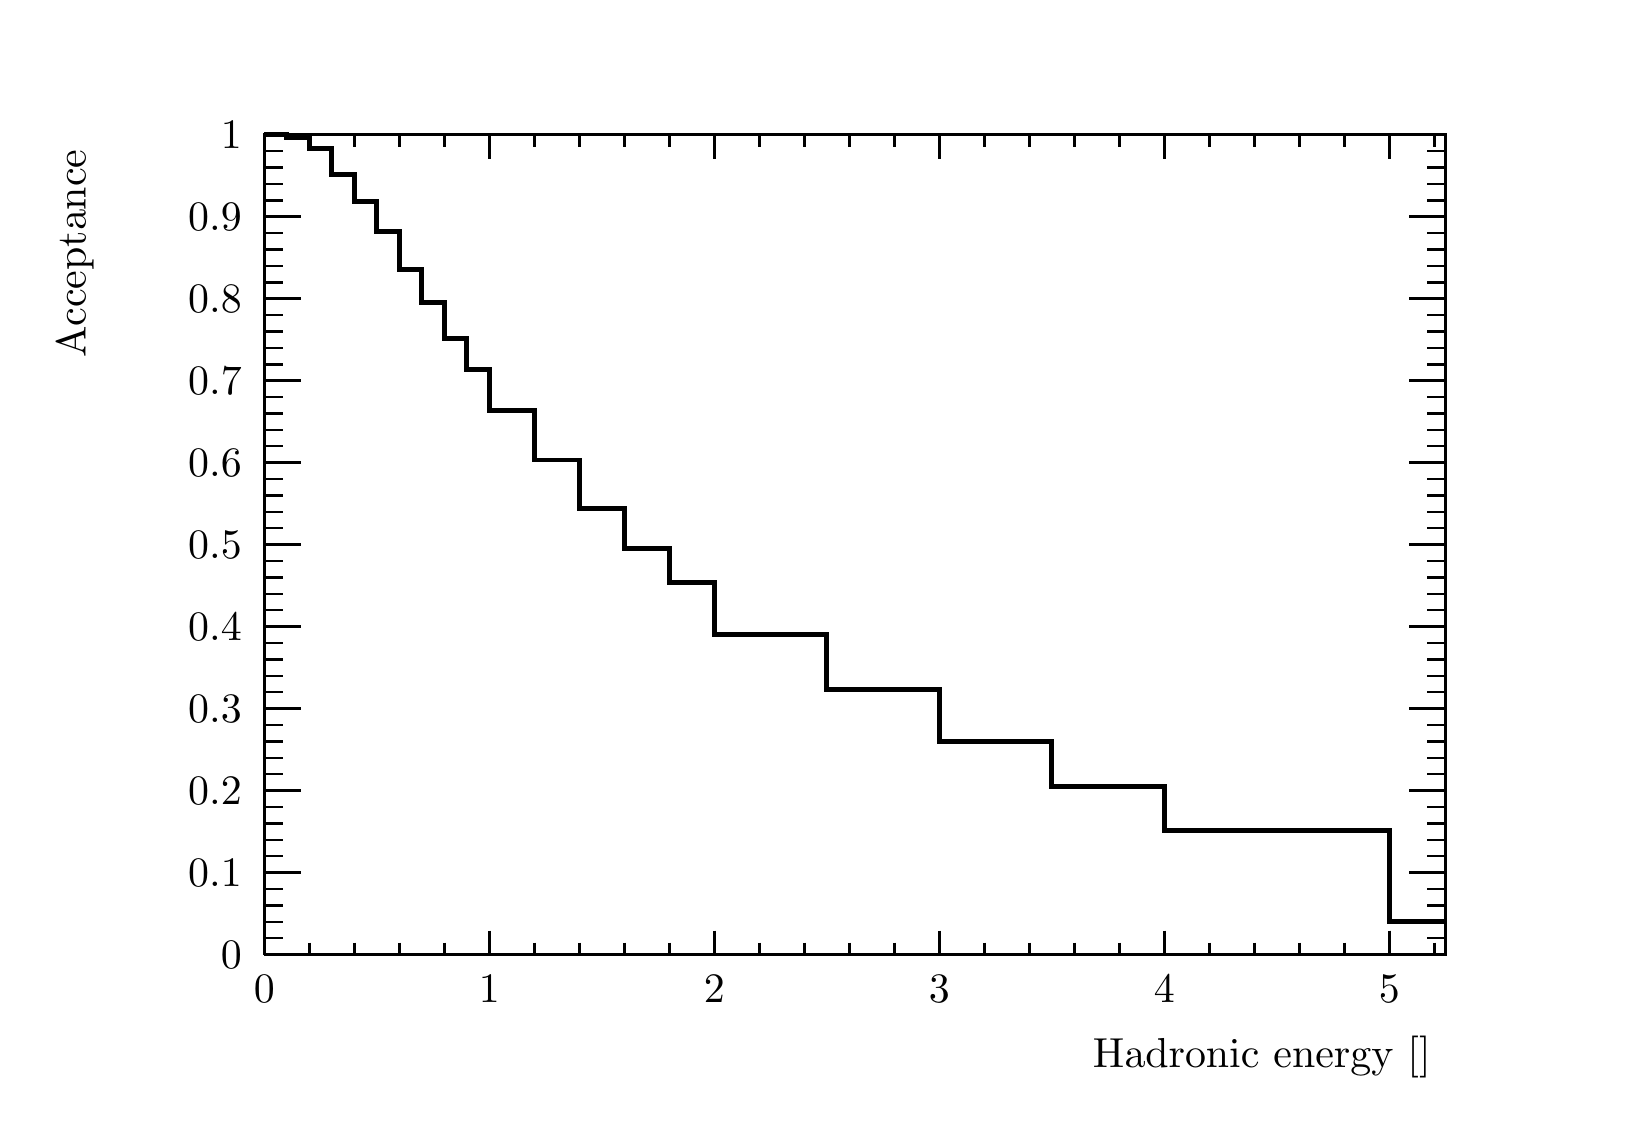
\begin{tikzpicture}
\pgfdeclareplotmark{cross} {
\pgfpathmoveto{\pgfpoint{-0.3\pgfplotmarksize}{\pgfplotmarksize}}
\pgfpathlineto{\pgfpoint{+0.3\pgfplotmarksize}{\pgfplotmarksize}}
\pgfpathlineto{\pgfpoint{+0.3\pgfplotmarksize}{0.3\pgfplotmarksize}}
\pgfpathlineto{\pgfpoint{+1\pgfplotmarksize}{0.3\pgfplotmarksize}}
\pgfpathlineto{\pgfpoint{+1\pgfplotmarksize}{-0.3\pgfplotmarksize}}
\pgfpathlineto{\pgfpoint{+0.3\pgfplotmarksize}{-0.3\pgfplotmarksize}}
\pgfpathlineto{\pgfpoint{+0.3\pgfplotmarksize}{-1.\pgfplotmarksize}}
\pgfpathlineto{\pgfpoint{-0.3\pgfplotmarksize}{-1.\pgfplotmarksize}}
\pgfpathlineto{\pgfpoint{-0.3\pgfplotmarksize}{-0.3\pgfplotmarksize}}
\pgfpathlineto{\pgfpoint{-1.\pgfplotmarksize}{-0.3\pgfplotmarksize}}
\pgfpathlineto{\pgfpoint{-1.\pgfplotmarksize}{0.3\pgfplotmarksize}}
\pgfpathlineto{\pgfpoint{-0.3\pgfplotmarksize}{0.3\pgfplotmarksize}}
\pgfpathclose
\pgfusepathqstroke
}
\pgfdeclareplotmark{cross*} {
\pgfpathmoveto{\pgfpoint{-0.3\pgfplotmarksize}{\pgfplotmarksize}}
\pgfpathlineto{\pgfpoint{+0.3\pgfplotmarksize}{\pgfplotmarksize}}
\pgfpathlineto{\pgfpoint{+0.3\pgfplotmarksize}{0.3\pgfplotmarksize}}
\pgfpathlineto{\pgfpoint{+1\pgfplotmarksize}{0.3\pgfplotmarksize}}
\pgfpathlineto{\pgfpoint{+1\pgfplotmarksize}{-0.3\pgfplotmarksize}}
\pgfpathlineto{\pgfpoint{+0.3\pgfplotmarksize}{-0.3\pgfplotmarksize}}
\pgfpathlineto{\pgfpoint{+0.3\pgfplotmarksize}{-1.\pgfplotmarksize}}
\pgfpathlineto{\pgfpoint{-0.3\pgfplotmarksize}{-1.\pgfplotmarksize}}
\pgfpathlineto{\pgfpoint{-0.3\pgfplotmarksize}{-0.3\pgfplotmarksize}}
\pgfpathlineto{\pgfpoint{-1.\pgfplotmarksize}{-0.3\pgfplotmarksize}}
\pgfpathlineto{\pgfpoint{-1.\pgfplotmarksize}{0.3\pgfplotmarksize}}
\pgfpathlineto{\pgfpoint{-0.3\pgfplotmarksize}{0.3\pgfplotmarksize}}
\pgfpathclose
\pgfusepathqfillstroke
}
\pgfdeclareplotmark{newstar} {
\pgfpathmoveto{\pgfqpoint{0pt}{\pgfplotmarksize}}
\pgfpathlineto{\pgfqpointpolar{44}{0.5\pgfplotmarksize}}
\pgfpathlineto{\pgfqpointpolar{18}{\pgfplotmarksize}}
\pgfpathlineto{\pgfqpointpolar{-20}{0.5\pgfplotmarksize}}
\pgfpathlineto{\pgfqpointpolar{-54}{\pgfplotmarksize}}
\pgfpathlineto{\pgfqpointpolar{-90}{0.5\pgfplotmarksize}}
\pgfpathlineto{\pgfqpointpolar{234}{\pgfplotmarksize}}
\pgfpathlineto{\pgfqpointpolar{198}{0.5\pgfplotmarksize}}
\pgfpathlineto{\pgfqpointpolar{162}{\pgfplotmarksize}}
\pgfpathlineto{\pgfqpointpolar{134}{0.5\pgfplotmarksize}}
\pgfpathclose
\pgfusepathqstroke
}
\pgfdeclareplotmark{newstar*} {
\pgfpathmoveto{\pgfqpoint{0pt}{\pgfplotmarksize}}
\pgfpathlineto{\pgfqpointpolar{44}{0.5\pgfplotmarksize}}
\pgfpathlineto{\pgfqpointpolar{18}{\pgfplotmarksize}}
\pgfpathlineto{\pgfqpointpolar{-20}{0.5\pgfplotmarksize}}
\pgfpathlineto{\pgfqpointpolar{-54}{\pgfplotmarksize}}
\pgfpathlineto{\pgfqpointpolar{-90}{0.5\pgfplotmarksize}}
\pgfpathlineto{\pgfqpointpolar{234}{\pgfplotmarksize}}
\pgfpathlineto{\pgfqpointpolar{198}{0.5\pgfplotmarksize}}
\pgfpathlineto{\pgfqpointpolar{162}{\pgfplotmarksize}}
\pgfpathlineto{\pgfqpointpolar{134}{0.5\pgfplotmarksize}}
\pgfpathclose
\pgfusepathqfillstroke
}
\definecolor{c}{rgb}{1,1,1};
\draw [color=c, fill=c] (0,0) rectangle (20,13.5227);
\draw [color=c, fill=c] (3,1.75795) rectangle (18,12.1705);
\definecolor{c}{rgb}{0,0,0};
\draw [c,line width=0.9] (3,1.75795) -- (3,12.1705) -- (18,12.1705) -- (18,1.75795) -- (3,1.75795);
\definecolor{c}{rgb}{1,1,1};
\draw [color=c, fill=c] (3,1.75795) rectangle (18,12.1705);
\definecolor{c}{rgb}{0,0,0};
\draw [c,line width=0.9] (3,1.75795) -- (3,12.1705) -- (18,12.1705) -- (18,1.75795) -- (3,1.75795);
\draw [c,line width=1.8] (3,12.1669) -- (3.28571,12.1669) -- (3.28571,12.1337) -- (3.57143,12.1337) -- (3.57143,11.9974) -- (3.85714,11.9974) -- (3.85714,11.6598) -- (4.14286,11.6598) -- (4.14286,11.3159) -- (4.42857,11.3159) -- (4.42857,10.9376) --
 (4.71429,10.9376) -- (4.71429,10.4567) -- (5,10.4567) -- (5,10.038) -- (5.28571,10.038) -- (5.28571,9.58251) -- (5.57143,9.58251) -- (5.57143,9.19266) -- (5.85714,9.19266) -- (5.85714,8.6728) -- (6.42857,8.6728) -- (6.42857,8.03916) -- (7,8.03916)
 -- (7,7.41873) -- (7.57143,7.41873) -- (7.57143,6.91137) -- (8.14286,6.91137) -- (8.14286,6.48146) -- (8.71429,6.48146) -- (8.71429,5.82387) -- (10.1429,5.82387) -- (10.1429,5.12498) -- (11.5714,5.12498) -- (11.5714,4.45809) -- (13,4.45809) --
 (13,3.88768) -- (14.4286,3.88768) -- (14.4286,3.33927) -- (17.2857,3.33927) -- (17.2857,2.18148) -- (18,2.18148);
\draw [c,line width=0.9] (3,1.75795) -- (18,1.75795);
\draw [c,line width=0.9] (3,2.06222) -- (3,1.75795);
\draw [c,line width=0.9] (3.57143,1.91009) -- (3.57143,1.75795);
\draw [c,line width=0.9] (4.14286,1.91009) -- (4.14286,1.75795);
\draw [c,line width=0.9] (4.71429,1.91009) -- (4.71429,1.75795);
\draw [c,line width=0.9] (5.28571,1.91009) -- (5.28571,1.75795);
\draw [c,line width=0.9] (5.85714,2.06222) -- (5.85714,1.75795);
\draw [c,line width=0.9] (6.42857,1.91009) -- (6.42857,1.75795);
\draw [c,line width=0.9] (7,1.91009) -- (7,1.75795);
\draw [c,line width=0.9] (7.57143,1.91009) -- (7.57143,1.75795);
\draw [c,line width=0.9] (8.14286,1.91009) -- (8.14286,1.75795);
\draw [c,line width=0.9] (8.71429,2.06222) -- (8.71429,1.75795);
\draw [c,line width=0.9] (9.28571,1.91009) -- (9.28571,1.75795);
\draw [c,line width=0.9] (9.85714,1.91009) -- (9.85714,1.75795);
\draw [c,line width=0.9] (10.4286,1.91009) -- (10.4286,1.75795);
\draw [c,line width=0.9] (11,1.91009) -- (11,1.75795);
\draw [c,line width=0.9] (11.5714,2.06222) -- (11.5714,1.75795);
\draw [c,line width=0.9] (12.1429,1.91009) -- (12.1429,1.75795);
\draw [c,line width=0.9] (12.7143,1.91009) -- (12.7143,1.75795);
\draw [c,line width=0.9] (13.2857,1.91009) -- (13.2857,1.75795);
\draw [c,line width=0.9] (13.8571,1.91009) -- (13.8571,1.75795);
\draw [c,line width=0.9] (14.4286,2.06222) -- (14.4286,1.75795);
\draw [c,line width=0.9] (15,1.91009) -- (15,1.75795);
\draw [c,line width=0.9] (15.5714,1.91009) -- (15.5714,1.75795);
\draw [c,line width=0.9] (16.1429,1.91009) -- (16.1429,1.75795);
\draw [c,line width=0.9] (16.7143,1.91009) -- (16.7143,1.75795);
\draw [c,line width=0.9] (17.2857,2.06222) -- (17.2857,1.75795);
\draw [c,line width=0.9] (17.2857,2.06222) -- (17.2857,1.75795);
\draw [c,line width=0.9] (17.8571,1.91009) -- (17.8571,1.75795);
\draw [anchor=base] (3,1.14943) node[scale=1.5143, color=c, rotate=0]{0};
\draw [anchor=base] (5.85714,1.14943) node[scale=1.5143, color=c, rotate=0]{1};
\draw [anchor=base] (8.71429,1.14943) node[scale=1.5143, color=c, rotate=0]{2};
\draw [anchor=base] (11.5714,1.14943) node[scale=1.5143, color=c, rotate=0]{3};
\draw [anchor=base] (14.4286,1.14943) node[scale=1.5143, color=c, rotate=0]{4};
\draw [anchor=base] (17.2857,1.14943) node[scale=1.5143, color=c, rotate=0]{5};
\draw [anchor= east] (18,0.459773) node[scale=1.5143, color=c, rotate=0]{Hadronic energy [\si{\GeV}] };
\draw [c,line width=0.9] (3,12.1705) -- (18,12.1705);
\draw [c,line width=0.9] (3,11.8662) -- (3,12.1705);
\draw [c,line width=0.9] (3.57143,12.0183) -- (3.57143,12.1705);
\draw [c,line width=0.9] (4.14286,12.0183) -- (4.14286,12.1705);
\draw [c,line width=0.9] (4.71429,12.0183) -- (4.71429,12.1705);
\draw [c,line width=0.9] (5.28571,12.0183) -- (5.28571,12.1705);
\draw [c,line width=0.9] (5.85714,11.8662) -- (5.85714,12.1705);
\draw [c,line width=0.9] (6.42857,12.0183) -- (6.42857,12.1705);
\draw [c,line width=0.9] (7,12.0183) -- (7,12.1705);
\draw [c,line width=0.9] (7.57143,12.0183) -- (7.57143,12.1705);
\draw [c,line width=0.9] (8.14286,12.0183) -- (8.14286,12.1705);
\draw [c,line width=0.9] (8.71429,11.8662) -- (8.71429,12.1705);
\draw [c,line width=0.9] (9.28571,12.0183) -- (9.28571,12.1705);
\draw [c,line width=0.9] (9.85714,12.0183) -- (9.85714,12.1705);
\draw [c,line width=0.9] (10.4286,12.0183) -- (10.4286,12.1705);
\draw [c,line width=0.9] (11,12.0183) -- (11,12.1705);
\draw [c,line width=0.9] (11.5714,11.8662) -- (11.5714,12.1705);
\draw [c,line width=0.9] (12.1429,12.0183) -- (12.1429,12.1705);
\draw [c,line width=0.9] (12.7143,12.0183) -- (12.7143,12.1705);
\draw [c,line width=0.9] (13.2857,12.0183) -- (13.2857,12.1705);
\draw [c,line width=0.9] (13.8571,12.0183) -- (13.8571,12.1705);
\draw [c,line width=0.9] (14.4286,11.8662) -- (14.4286,12.1705);
\draw [c,line width=0.9] (15,12.0183) -- (15,12.1705);
\draw [c,line width=0.9] (15.5714,12.0183) -- (15.5714,12.1705);
\draw [c,line width=0.9] (16.1429,12.0183) -- (16.1429,12.1705);
\draw [c,line width=0.9] (16.7143,12.0183) -- (16.7143,12.1705);
\draw [c,line width=0.9] (17.2857,11.8662) -- (17.2857,12.1705);
\draw [c,line width=0.9] (17.2857,11.8662) -- (17.2857,12.1705);
\draw [c,line width=0.9] (17.8571,12.0183) -- (17.8571,12.1705);
\draw [c,line width=0.9] (3,1.75795) -- (3,12.1705);
\draw [c,line width=0.9] (3.462,1.75795) -- (3,1.75795);
\draw [c,line width=0.9] (3.231,1.9662) -- (3,1.9662);
\draw [c,line width=0.9] (3.231,2.17445) -- (3,2.17445);
\draw [c,line width=0.9] (3.231,2.3827) -- (3,2.3827);
\draw [c,line width=0.9] (3.231,2.59095) -- (3,2.59095);
\draw [c,line width=0.9] (3.462,2.7992) -- (3,2.7992);
\draw [c,line width=0.9] (3.231,3.00745) -- (3,3.00745);
\draw [c,line width=0.9] (3.231,3.2157) -- (3,3.2157);
\draw [c,line width=0.9] (3.231,3.42395) -- (3,3.42395);
\draw [c,line width=0.9] (3.231,3.6322) -- (3,3.6322);
\draw [c,line width=0.9] (3.462,3.84045) -- (3,3.84045);
\draw [c,line width=0.9] (3.231,4.0487) -- (3,4.0487);
\draw [c,line width=0.9] (3.231,4.25695) -- (3,4.25695);
\draw [c,line width=0.9] (3.231,4.4652) -- (3,4.4652);
\draw [c,line width=0.9] (3.231,4.67345) -- (3,4.67345);
\draw [c,line width=0.9] (3.462,4.8817) -- (3,4.8817);
\draw [c,line width=0.9] (3.231,5.08995) -- (3,5.08995);
\draw [c,line width=0.9] (3.231,5.2982) -- (3,5.2982);
\draw [c,line width=0.9] (3.231,5.50645) -- (3,5.50645);
\draw [c,line width=0.9] (3.231,5.7147) -- (3,5.7147);
\draw [c,line width=0.9] (3.462,5.92295) -- (3,5.92295);
\draw [c,line width=0.9] (3.231,6.1312) -- (3,6.1312);
\draw [c,line width=0.9] (3.231,6.33945) -- (3,6.33945);
\draw [c,line width=0.9] (3.231,6.5477) -- (3,6.5477);
\draw [c,line width=0.9] (3.231,6.75595) -- (3,6.75595);
\draw [c,line width=0.9] (3.462,6.9642) -- (3,6.9642);
\draw [c,line width=0.9] (3.231,7.17245) -- (3,7.17245);
\draw [c,line width=0.9] (3.231,7.3807) -- (3,7.3807);
\draw [c,line width=0.9] (3.231,7.58895) -- (3,7.58895);
\draw [c,line width=0.9] (3.231,7.7972) -- (3,7.7972);
\draw [c,line width=0.9] (3.462,8.00545) -- (3,8.00545);
\draw [c,line width=0.9] (3.231,8.2137) -- (3,8.2137);
\draw [c,line width=0.9] (3.231,8.42195) -- (3,8.42195);
\draw [c,line width=0.9] (3.231,8.6302) -- (3,8.6302);
\draw [c,line width=0.9] (3.231,8.83845) -- (3,8.83845);
\draw [c,line width=0.9] (3.462,9.0467) -- (3,9.0467);
\draw [c,line width=0.9] (3.231,9.25495) -- (3,9.25495);
\draw [c,line width=0.9] (3.231,9.4632) -- (3,9.4632);
\draw [c,line width=0.9] (3.231,9.67145) -- (3,9.67145);
\draw [c,line width=0.9] (3.231,9.8797) -- (3,9.8797);
\draw [c,line width=0.9] (3.462,10.088) -- (3,10.088);
\draw [c,line width=0.9] (3.231,10.2962) -- (3,10.2962);
\draw [c,line width=0.9] (3.231,10.5045) -- (3,10.5045);
\draw [c,line width=0.9] (3.231,10.7127) -- (3,10.7127);
\draw [c,line width=0.9] (3.231,10.921) -- (3,10.921);
\draw [c,line width=0.9] (3.462,11.1292) -- (3,11.1292);
\draw [c,line width=0.9] (3.231,11.3375) -- (3,11.3375);
\draw [c,line width=0.9] (3.231,11.5457) -- (3,11.5457);
\draw [c,line width=0.9] (3.231,11.754) -- (3,11.754);
\draw [c,line width=0.9] (3.231,11.9622) -- (3,11.9622);
\draw [c,line width=0.9] (3.462,12.1705) -- (3,12.1705);
\draw [anchor= east] (2.9,1.75795) node[scale=1.5143, color=c, rotate=0]{0};
\draw [anchor= east] (2.9,2.7992) node[scale=1.5143, color=c, rotate=0]{0.1};
\draw [anchor= east] (2.9,3.84045) node[scale=1.5143, color=c, rotate=0]{0.2};
\draw [anchor= east] (2.9,4.8817) node[scale=1.5143, color=c, rotate=0]{0.3};
\draw [anchor= east] (2.9,5.92295) node[scale=1.5143, color=c, rotate=0]{0.4};
\draw [anchor= east] (2.9,6.9642) node[scale=1.5143, color=c, rotate=0]{0.5};
\draw [anchor= east] (2.9,8.00545) node[scale=1.5143, color=c, rotate=0]{0.6};
\draw [anchor= east] (2.9,9.0467) node[scale=1.5143, color=c, rotate=0]{0.7};
\draw [anchor= east] (2.9,10.088) node[scale=1.5143, color=c, rotate=0]{0.8};
\draw [anchor= east] (2.9,11.1292) node[scale=1.5143, color=c, rotate=0]{0.9};
\draw [anchor= east] (2.9,12.1705) node[scale=1.5143, color=c, rotate=0]{1};
\draw [anchor= east] (0.6,12.1705) node[scale=1.5143, color=c, rotate=90]{Acceptance};
\draw [c,line width=0.9] (18,1.75795) -- (18,12.1705);
\draw [c,line width=0.9] (17.538,1.75795) -- (18,1.75795);
\draw [c,line width=0.9] (17.769,1.9662) -- (18,1.9662);
\draw [c,line width=0.9] (17.769,2.17445) -- (18,2.17445);
\draw [c,line width=0.9] (17.769,2.3827) -- (18,2.3827);
\draw [c,line width=0.9] (17.769,2.59095) -- (18,2.59095);
\draw [c,line width=0.9] (17.538,2.7992) -- (18,2.7992);
\draw [c,line width=0.9] (17.769,3.00745) -- (18,3.00745);
\draw [c,line width=0.9] (17.769,3.2157) -- (18,3.2157);
\draw [c,line width=0.9] (17.769,3.42395) -- (18,3.42395);
\draw [c,line width=0.9] (17.769,3.6322) -- (18,3.6322);
\draw [c,line width=0.9] (17.538,3.84045) -- (18,3.84045);
\draw [c,line width=0.9] (17.769,4.0487) -- (18,4.0487);
\draw [c,line width=0.9] (17.769,4.25695) -- (18,4.25695);
\draw [c,line width=0.9] (17.769,4.4652) -- (18,4.4652);
\draw [c,line width=0.9] (17.769,4.67345) -- (18,4.67345);
\draw [c,line width=0.9] (17.538,4.8817) -- (18,4.8817);
\draw [c,line width=0.9] (17.769,5.08995) -- (18,5.08995);
\draw [c,line width=0.9] (17.769,5.2982) -- (18,5.2982);
\draw [c,line width=0.9] (17.769,5.50645) -- (18,5.50645);
\draw [c,line width=0.9] (17.769,5.7147) -- (18,5.7147);
\draw [c,line width=0.9] (17.538,5.92295) -- (18,5.92295);
\draw [c,line width=0.9] (17.769,6.1312) -- (18,6.1312);
\draw [c,line width=0.9] (17.769,6.33945) -- (18,6.33945);
\draw [c,line width=0.9] (17.769,6.5477) -- (18,6.5477);
\draw [c,line width=0.9] (17.769,6.75595) -- (18,6.75595);
\draw [c,line width=0.9] (17.538,6.9642) -- (18,6.9642);
\draw [c,line width=0.9] (17.769,7.17245) -- (18,7.17245);
\draw [c,line width=0.9] (17.769,7.3807) -- (18,7.3807);
\draw [c,line width=0.9] (17.769,7.58895) -- (18,7.58895);
\draw [c,line width=0.9] (17.769,7.7972) -- (18,7.7972);
\draw [c,line width=0.9] (17.538,8.00545) -- (18,8.00545);
\draw [c,line width=0.9] (17.769,8.2137) -- (18,8.2137);
\draw [c,line width=0.9] (17.769,8.42195) -- (18,8.42195);
\draw [c,line width=0.9] (17.769,8.6302) -- (18,8.6302);
\draw [c,line width=0.9] (17.769,8.83845) -- (18,8.83845);
\draw [c,line width=0.9] (17.538,9.0467) -- (18,9.0467);
\draw [c,line width=0.9] (17.769,9.25495) -- (18,9.25495);
\draw [c,line width=0.9] (17.769,9.4632) -- (18,9.4632);
\draw [c,line width=0.9] (17.769,9.67145) -- (18,9.67145);
\draw [c,line width=0.9] (17.769,9.8797) -- (18,9.8797);
\draw [c,line width=0.9] (17.538,10.088) -- (18,10.088);
\draw [c,line width=0.9] (17.769,10.2962) -- (18,10.2962);
\draw [c,line width=0.9] (17.769,10.5045) -- (18,10.5045);
\draw [c,line width=0.9] (17.769,10.7127) -- (18,10.7127);
\draw [c,line width=0.9] (17.769,10.921) -- (18,10.921);
\draw [c,line width=0.9] (17.538,11.1292) -- (18,11.1292);
\draw [c,line width=0.9] (17.769,11.3375) -- (18,11.3375);
\draw [c,line width=0.9] (17.769,11.5457) -- (18,11.5457);
\draw [c,line width=0.9] (17.769,11.754) -- (18,11.754);
\draw [c,line width=0.9] (17.769,11.9622) -- (18,11.9622);
\draw [c,line width=0.9] (17.538,12.1705) -- (18,12.1705);
\end{tikzpicture}

		\end{adjustbox}
	\end{minipage}
	\caption[Muonic and hadronic acceptance for CC neutrino interactions in ND-LAr]{Left: Muonic acceptance for CC muon neutrino interactions in ND-LAr as a function of transverse and longitudinal muon momentum. Right: Hadronic acceptance for CC muon neutrino interactions in ND-LAr as a function of true hadronic energy. Both from~\cite{Abi:2020qib}.}
	\label{fig:ndAcceptance}
\end{figure}

The uncertainty on the muon and hadron acceptance is produced from the respective plots in \citefig{fig:ndAcceptance} with a higher uncertainty in regions where the acceptance is rapidly changing and thus vulnerable to mismodelling.

Unlike their FD counterparts, the ND detector parameters are not allowed to vary in the fit.
Instead, they are incorporated into a covariance matrix.
This covariance matrix is formed by throwing all ND detector uncertainties simultaneously according to their documented uncertainties and comparing the resulting spectra with the nominal prediction.
The bin-to-bin covariance is then determined using these comparisons.
This method protects against over-constraining of ND parameters due to the limitations of the simplified ND reconstruction.

\section{DUNE sensitivites}
\label{sec:dune_lbl:sensitivities}

\subsection{General sensitivity methods}
\label{sec:dune_lbl:sensitivities:general}

DUNE's oscillation sensitivities are computed using the CAFAna package.
%% Move CAFAna stuff here I think

The oscillation sensitivities are computed by simultaneously fitting the oscillation parameters and nuisance parameters to four FD spectra (\numu disappearance, \anumu disappearance, \nue appearance and \anue appearance) and the nuisance parameters to the two ND spectra (\numu unoscillated and \anumu unoscillated).
Examples of the four FD spectra are shown in \citefig{fig:fdEventRates}.
The two ND samples are two dimensional, binned in reconstructed neutrino energy and reconstructed inelasticity, $y_{\text{reco}}$, where
\begin{equation}
	y_{\text{reco}} = 1 - \frac{E_{\mu,~\text{reco}}}{E_{\nu,~\text{reco}}} \, ,
\end{equation}
where $E_{\mu,~\text{reco}}$ and $E_{\nu,~\text{reco}}$ are the reconstructed muon and neutrino energies respectively.
These two-dimensional samples are shown in \citefig{fig:ndEventRates}.

\begin{figure}[h]
	\begin{minipage}[t]{.5\linewidth}
		\begin{adjustbox}{max totalsize=\linewidth, center}
			\input{files/figures/dune_lbl/h2NDNumuFHC}
		\end{adjustbox}
	\end{minipage}
	\hfill
	\begin{minipage}[t]{.5\linewidth}
		\begin{adjustbox}{max totalsize=\linewidth, center}
			\begin{tikzpicture}
\pgfdeclareplotmark{cross} {
\pgfpathmoveto{\pgfpoint{-0.3\pgfplotmarksize}{\pgfplotmarksize}}
\pgfpathlineto{\pgfpoint{+0.3\pgfplotmarksize}{\pgfplotmarksize}}
\pgfpathlineto{\pgfpoint{+0.3\pgfplotmarksize}{0.3\pgfplotmarksize}}
\pgfpathlineto{\pgfpoint{+1\pgfplotmarksize}{0.3\pgfplotmarksize}}
\pgfpathlineto{\pgfpoint{+1\pgfplotmarksize}{-0.3\pgfplotmarksize}}
\pgfpathlineto{\pgfpoint{+0.3\pgfplotmarksize}{-0.3\pgfplotmarksize}}
\pgfpathlineto{\pgfpoint{+0.3\pgfplotmarksize}{-1.\pgfplotmarksize}}
\pgfpathlineto{\pgfpoint{-0.3\pgfplotmarksize}{-1.\pgfplotmarksize}}
\pgfpathlineto{\pgfpoint{-0.3\pgfplotmarksize}{-0.3\pgfplotmarksize}}
\pgfpathlineto{\pgfpoint{-1.\pgfplotmarksize}{-0.3\pgfplotmarksize}}
\pgfpathlineto{\pgfpoint{-1.\pgfplotmarksize}{0.3\pgfplotmarksize}}
\pgfpathlineto{\pgfpoint{-0.3\pgfplotmarksize}{0.3\pgfplotmarksize}}
\pgfpathclose
\pgfusepathqstroke
}
\pgfdeclareplotmark{cross*} {
\pgfpathmoveto{\pgfpoint{-0.3\pgfplotmarksize}{\pgfplotmarksize}}
\pgfpathlineto{\pgfpoint{+0.3\pgfplotmarksize}{\pgfplotmarksize}}
\pgfpathlineto{\pgfpoint{+0.3\pgfplotmarksize}{0.3\pgfplotmarksize}}
\pgfpathlineto{\pgfpoint{+1\pgfplotmarksize}{0.3\pgfplotmarksize}}
\pgfpathlineto{\pgfpoint{+1\pgfplotmarksize}{-0.3\pgfplotmarksize}}
\pgfpathlineto{\pgfpoint{+0.3\pgfplotmarksize}{-0.3\pgfplotmarksize}}
\pgfpathlineto{\pgfpoint{+0.3\pgfplotmarksize}{-1.\pgfplotmarksize}}
\pgfpathlineto{\pgfpoint{-0.3\pgfplotmarksize}{-1.\pgfplotmarksize}}
\pgfpathlineto{\pgfpoint{-0.3\pgfplotmarksize}{-0.3\pgfplotmarksize}}
\pgfpathlineto{\pgfpoint{-1.\pgfplotmarksize}{-0.3\pgfplotmarksize}}
\pgfpathlineto{\pgfpoint{-1.\pgfplotmarksize}{0.3\pgfplotmarksize}}
\pgfpathlineto{\pgfpoint{-0.3\pgfplotmarksize}{0.3\pgfplotmarksize}}
\pgfpathclose
\pgfusepathqfillstroke
}
\pgfdeclareplotmark{newstar} {
\pgfpathmoveto{\pgfqpoint{0pt}{\pgfplotmarksize}}
\pgfpathlineto{\pgfqpointpolar{44}{0.5\pgfplotmarksize}}
\pgfpathlineto{\pgfqpointpolar{18}{\pgfplotmarksize}}
\pgfpathlineto{\pgfqpointpolar{-20}{0.5\pgfplotmarksize}}
\pgfpathlineto{\pgfqpointpolar{-54}{\pgfplotmarksize}}
\pgfpathlineto{\pgfqpointpolar{-90}{0.5\pgfplotmarksize}}
\pgfpathlineto{\pgfqpointpolar{234}{\pgfplotmarksize}}
\pgfpathlineto{\pgfqpointpolar{198}{0.5\pgfplotmarksize}}
\pgfpathlineto{\pgfqpointpolar{162}{\pgfplotmarksize}}
\pgfpathlineto{\pgfqpointpolar{134}{0.5\pgfplotmarksize}}
\pgfpathclose
\pgfusepathqstroke
}
\pgfdeclareplotmark{newstar*} {
\pgfpathmoveto{\pgfqpoint{0pt}{\pgfplotmarksize}}
\pgfpathlineto{\pgfqpointpolar{44}{0.5\pgfplotmarksize}}
\pgfpathlineto{\pgfqpointpolar{18}{\pgfplotmarksize}}
\pgfpathlineto{\pgfqpointpolar{-20}{0.5\pgfplotmarksize}}
\pgfpathlineto{\pgfqpointpolar{-54}{\pgfplotmarksize}}
\pgfpathlineto{\pgfqpointpolar{-90}{0.5\pgfplotmarksize}}
\pgfpathlineto{\pgfqpointpolar{234}{\pgfplotmarksize}}
\pgfpathlineto{\pgfqpointpolar{198}{0.5\pgfplotmarksize}}
\pgfpathlineto{\pgfqpointpolar{162}{\pgfplotmarksize}}
\pgfpathlineto{\pgfqpointpolar{134}{0.5\pgfplotmarksize}}
\pgfpathclose
\pgfusepathqfillstroke
}
\definecolor{c}{rgb}{1,1,1};
\draw [color=c, fill=c] (0,0) rectangle (20,13.639);
\draw [color=c, fill=c] (3,1.77307) rectangle (16,12.2751);
\definecolor{c}{rgb}{0,0,0};
\draw [c,line width=0.9] (3,1.77307) -- (3,12.2751) -- (16,12.2751) -- (16,1.77307) -- (3,1.77307);
\definecolor{c}{rgb}{1,1,1};
\draw [color=c, fill=c] (3,1.77307) rectangle (16,12.2751);
\definecolor{c}{rgb}{0,0,0};
\draw [c,line width=0.9] (3,1.77307) -- (3,12.2751) -- (16,12.2751) -- (16,1.77307) -- (3,1.77307);
\definecolor{c}{rgb}{0.945984,0.951044,0.850727};
\draw [color=c, fill=c] (3,1.77307) rectangle (3.65,2.82327);
\definecolor{c}{rgb}{0.929791,0.940923,0.577483};
\draw [color=c, fill=c] (3.65,1.77307) rectangle (4.3,2.82327);
\definecolor{c}{rgb}{0.922426,0.933333,0.238725};
\draw [color=c, fill=c] (4.3,1.77307) rectangle (4.625,2.82327);
\definecolor{c}{rgb}{0.907108,0.710294,0.0335784};
\draw [color=c, fill=c] (4.625,1.77307) rectangle (4.95,2.82327);
\definecolor{c}{rgb}{0.632353,0.197059,0.0139706};
\draw [color=c, fill=c] (4.95,1.77307) rectangle (5.275,2.82327);
\definecolor{c}{rgb}{0.308824,0,0.00392157};
\draw [color=c, fill=c] (5.275,1.77307) rectangle (5.6,2.82327);
\definecolor{c}{rgb}{0.0882353,0,0.00196078};
\draw [color=c, fill=c] (5.6,1.77307) rectangle (5.925,2.82327);
\definecolor{c}{rgb}{0.00551471,0,0.000122549};
\draw [color=c, fill=c] (5.925,1.77307) rectangle (6.25,2.82327);
\draw [color=c, fill=c] (6.25,1.77307) rectangle (6.575,2.82327);
\definecolor{c}{rgb}{0.0882353,0,0.00196078};
\draw [color=c, fill=c] (6.575,1.77307) rectangle (6.9,2.82327);
\definecolor{c}{rgb}{0.308824,0,0.00392157};
\draw [color=c, fill=c] (6.9,1.77307) rectangle (7.225,2.82327);
\definecolor{c}{rgb}{0.548897,0.126838,0.00955882};
\draw [color=c, fill=c] (7.225,1.77307) rectangle (7.55,2.82327);
\definecolor{c}{rgb}{0.790196,0.354902,0.0308824};
\draw [color=c, fill=c] (7.55,1.77307) rectangle (7.875,2.82327);
\definecolor{c}{rgb}{0.888726,0.609559,0.0321078};
\draw [color=c, fill=c] (7.875,1.77307) rectangle (8.2,2.82327);
\definecolor{c}{rgb}{0.927206,0.933333,0.104902};
\draw [color=c, fill=c] (8.2,1.77307) rectangle (9.5,2.82327);
\definecolor{c}{rgb}{0.926755,0.939026,0.526249};
\draw [color=c, fill=c] (9.5,1.77307) rectangle (10.8,2.82327);
\definecolor{c}{rgb}{0.936875,0.945351,0.697027};
\draw [color=c, fill=c] (10.8,1.77307) rectangle (16,2.82327);
\definecolor{c}{rgb}{0.945984,0.951044,0.850727};
\draw [color=c, fill=c] (3,2.82327) rectangle (3.65,3.87347);
\definecolor{c}{rgb}{0.933839,0.943453,0.645794};
\draw [color=c, fill=c] (3.65,2.82327) rectangle (4.3,3.87347);
\definecolor{c}{rgb}{0.923719,0.937128,0.475016};
\draw [color=c, fill=c] (4.3,2.82327) rectangle (4.625,3.87347);
\definecolor{c}{rgb}{0.923529,0.933333,0.207843};
\draw [color=c, fill=c] (4.625,2.82327) rectangle (4.95,3.87347);
\definecolor{c}{rgb}{0.904534,0.684559,0.0324755};
\draw [color=c, fill=c] (4.95,2.82327) rectangle (5.275,3.87347);
\definecolor{c}{rgb}{0.762745,0.327451,0.0279412};
\draw [color=c, fill=c] (5.275,2.82327) rectangle (5.6,3.87347);
\definecolor{c}{rgb}{0.590809,0.159926,0.0110294};
\draw [color=c, fill=c] (5.6,2.82327) rectangle (5.925,3.87347);
\definecolor{c}{rgb}{0.520956,0.104779,0.00857843};
\draw [color=c, fill=c] (5.925,2.82327) rectangle (6.25,3.87347);
\definecolor{c}{rgb}{0.590809,0.159926,0.0110294};
\draw [color=c, fill=c] (6.25,2.82327) rectangle (6.575,3.87347);
\definecolor{c}{rgb}{0.721569,0.286275,0.0235294};
\draw [color=c, fill=c] (6.575,2.82327) rectangle (6.9,3.87347);
\definecolor{c}{rgb}{0.853431,0.478186,0.0340686};
\draw [color=c, fill=c] (6.9,2.82327) rectangle (7.225,3.87347);
\definecolor{c}{rgb}{0.904534,0.684559,0.0324755};
\draw [color=c, fill=c] (7.225,2.82327) rectangle (7.55,3.87347);
\definecolor{c}{rgb}{0.923407,0.873284,0.0405637};
\draw [color=c, fill=c] (7.55,2.82327) rectangle (7.875,3.87347);
\definecolor{c}{rgb}{0.926103,0.933333,0.135784};
\draw [color=c, fill=c] (7.875,2.82327) rectangle (8.2,3.87347);
\definecolor{c}{rgb}{0.920683,0.935231,0.423782};
\draw [color=c, fill=c] (8.2,2.82327) rectangle (9.5,3.87347);
\definecolor{c}{rgb}{0.939911,0.947249,0.748261};
\draw [color=c, fill=c] (9.5,2.82327) rectangle (10.8,3.87347);
\definecolor{c}{rgb}{0.942948,0.949146,0.799494};
\draw [color=c, fill=c] (10.8,2.82327) rectangle (16,3.87347);
\definecolor{c}{rgb}{0.945984,0.951044,0.850727};
\draw [color=c, fill=c] (3,3.87347) rectangle (3.65,4.92367);
\definecolor{c}{rgb}{0.933839,0.943453,0.645794};
\draw [color=c, fill=c] (3.65,3.87347) rectangle (4.3,4.92367);
\definecolor{c}{rgb}{0.923719,0.937128,0.475016};
\draw [color=c, fill=c] (4.3,3.87347) rectangle (4.625,4.92367);
\definecolor{c}{rgb}{0.917647,0.933333,0.372549};
\draw [color=c, fill=c] (4.625,3.87347) rectangle (4.95,4.92367);
\definecolor{c}{rgb}{0.923529,0.933333,0.207843};
\draw [color=c, fill=c] (4.95,3.87347) rectangle (5.275,4.92367);
\definecolor{c}{rgb}{0.923407,0.873284,0.0405637};
\draw [color=c, fill=c] (5.275,3.87347) rectangle (5.6,4.92367);
\definecolor{c}{rgb}{0.909681,0.736029,0.0346814};
\draw [color=c, fill=c] (5.6,3.87347) rectangle (5.925,4.92367);
\definecolor{c}{rgb}{0.907108,0.710294,0.0335784};
\draw [color=c, fill=c] (5.925,3.87347) rectangle (6.25,4.92367);
\definecolor{c}{rgb}{0.913113,0.770343,0.036152};
\draw [color=c, fill=c] (6.25,3.87347) rectangle (6.575,4.92367);
\definecolor{c}{rgb}{0.920833,0.847549,0.0394608};
\draw [color=c, fill=c] (6.575,3.87347) rectangle (6.9,4.92367);
\definecolor{c}{rgb}{0.927206,0.933333,0.104902};
\draw [color=c, fill=c] (6.9,3.87347) rectangle (7.225,4.92367);
\definecolor{c}{rgb}{0.922426,0.933333,0.238725};
\draw [color=c, fill=c] (7.225,3.87347) rectangle (7.55,4.92367);
\definecolor{c}{rgb}{0.917647,0.933333,0.372549};
\draw [color=c, fill=c] (7.55,3.87347) rectangle (7.875,4.92367);
\definecolor{c}{rgb}{0.923719,0.937128,0.475016};
\draw [color=c, fill=c] (7.875,3.87347) rectangle (8.2,4.92367);
\definecolor{c}{rgb}{0.936875,0.945351,0.697027};
\draw [color=c, fill=c] (8.2,3.87347) rectangle (9.5,4.92367);
\definecolor{c}{rgb}{0.942948,0.949146,0.799494};
\draw [color=c, fill=c] (9.5,3.87347) rectangle (10.8,4.92367);
\definecolor{c}{rgb}{0.945984,0.951044,0.850727};
\draw [color=c, fill=c] (10.8,3.87347) rectangle (16,4.92367);
\draw [color=c, fill=c] (3,4.92367) rectangle (3.65,5.97387);
\definecolor{c}{rgb}{0.933839,0.943453,0.645794};
\draw [color=c, fill=c] (3.65,4.92367) rectangle (4.3,5.97387);
\definecolor{c}{rgb}{0.926755,0.939026,0.526249};
\draw [color=c, fill=c] (4.3,4.92367) rectangle (4.625,5.97387);
\draw [color=c, fill=c] (4.625,4.92367) rectangle (4.95,5.97387);
\draw [color=c, fill=c] (4.95,4.92367) rectangle (5.275,5.97387);
\definecolor{c}{rgb}{0.917647,0.933333,0.372549};
\draw [color=c, fill=c] (5.275,4.92367) rectangle (5.6,5.97387);
\definecolor{c}{rgb}{0.921324,0.933333,0.269608};
\draw [color=c, fill=c] (5.6,4.92367) rectangle (5.925,5.97387);
\definecolor{c}{rgb}{0.922426,0.933333,0.238725};
\draw [color=c, fill=c] (5.925,4.92367) rectangle (6.25,5.97387);
\definecolor{c}{rgb}{0.921324,0.933333,0.269608};
\draw [color=c, fill=c] (6.25,4.92367) rectangle (6.575,5.97387);
\definecolor{c}{rgb}{0.919118,0.933333,0.331373};
\draw [color=c, fill=c] (6.575,4.92367) rectangle (6.9,5.97387);
\definecolor{c}{rgb}{0.923719,0.937128,0.475016};
\draw [color=c, fill=c] (6.9,4.92367) rectangle (7.225,5.97387);
\definecolor{c}{rgb}{0.929791,0.940923,0.577483};
\draw [color=c, fill=c] (7.225,4.92367) rectangle (7.55,5.97387);
\definecolor{c}{rgb}{0.936875,0.945351,0.697027};
\draw [color=c, fill=c] (7.55,4.92367) rectangle (7.875,5.97387);
\definecolor{c}{rgb}{0.939911,0.947249,0.748261};
\draw [color=c, fill=c] (7.875,4.92367) rectangle (8.2,5.97387);
\definecolor{c}{rgb}{0.942948,0.949146,0.799494};
\draw [color=c, fill=c] (8.2,4.92367) rectangle (9.5,5.97387);
\definecolor{c}{rgb}{0.945984,0.951044,0.850727};
\draw [color=c, fill=c] (9.5,4.92367) rectangle (10.8,5.97387);
\draw [color=c, fill=c] (10.8,4.92367) rectangle (16,5.97387);
\definecolor{c}{rgb}{0.936875,0.945351,0.697027};
\draw [color=c, fill=c] (3.65,5.97387) rectangle (4.3,8.07427);
\definecolor{c}{rgb}{0.929791,0.940923,0.577483};
\draw [color=c, fill=c] (4.3,5.97387) rectangle (4.625,8.07427);
\draw [color=c, fill=c] (4.625,5.97387) rectangle (4.95,8.07427);
\definecolor{c}{rgb}{0.933839,0.943453,0.645794};
\draw [color=c, fill=c] (4.95,5.97387) rectangle (5.275,8.07427);
\definecolor{c}{rgb}{0.936875,0.945351,0.697027};
\draw [color=c, fill=c] (5.275,5.97387) rectangle (5.6,8.07427);
\draw [color=c, fill=c] (5.6,5.97387) rectangle (5.925,8.07427);
\draw [color=c, fill=c] (5.925,5.97387) rectangle (6.25,8.07427);
\definecolor{c}{rgb}{0.939911,0.947249,0.748261};
\draw [color=c, fill=c] (6.25,5.97387) rectangle (6.575,8.07427);
\draw [color=c, fill=c] (6.575,5.97387) rectangle (6.9,8.07427);
\definecolor{c}{rgb}{0.942948,0.949146,0.799494};
\draw [color=c, fill=c] (6.9,5.97387) rectangle (7.225,8.07427);
\draw [color=c, fill=c] (7.225,5.97387) rectangle (7.55,8.07427);
\draw [color=c, fill=c] (7.55,5.97387) rectangle (7.875,8.07427);
\definecolor{c}{rgb}{0.945984,0.951044,0.850727};
\draw [color=c, fill=c] (7.875,5.97387) rectangle (8.2,8.07427);
\draw [color=c, fill=c] (8.2,5.97387) rectangle (9.5,8.07427);
\draw [color=c, fill=c] (9.5,5.97387) rectangle (10.8,8.07427);
\draw [color=c, fill=c] (10.8,5.97387) rectangle (16,8.07427);
\draw [color=c, fill=c] (3,8.07427) rectangle (3.65,12.2751);
\draw [color=c, fill=c] (3.65,8.07427) rectangle (4.3,12.2751);
\definecolor{c}{rgb}{0.942948,0.949146,0.799494};
\draw [color=c, fill=c] (4.3,8.07427) rectangle (4.625,12.2751);
\draw [color=c, fill=c] (4.625,8.07427) rectangle (4.95,12.2751);
\draw [color=c, fill=c] (4.95,8.07427) rectangle (5.275,12.2751);
\draw [color=c, fill=c] (5.275,8.07427) rectangle (5.6,12.2751);
\definecolor{c}{rgb}{0.945984,0.951044,0.850727};
\draw [color=c, fill=c] (5.6,8.07427) rectangle (5.925,12.2751);
\draw [color=c, fill=c] (5.925,8.07427) rectangle (6.25,12.2751);
\draw [color=c, fill=c] (6.25,8.07427) rectangle (6.575,12.2751);
\draw [color=c, fill=c] (6.575,8.07427) rectangle (6.9,12.2751);
\draw [color=c, fill=c] (6.9,8.07427) rectangle (7.225,12.2751);
\draw [color=c, fill=c] (7.225,8.07427) rectangle (7.55,12.2751);
\draw [color=c, fill=c] (7.55,8.07427) rectangle (7.875,12.2751);
\draw [color=c, fill=c] (7.875,8.07427) rectangle (8.2,12.2751);
\draw [color=c, fill=c] (8.2,8.07427) rectangle (9.5,12.2751);
\draw [color=c, fill=c] (9.5,8.07427) rectangle (10.8,12.2751);
\draw [color=c, fill=c] (10.8,8.07427) rectangle (16,12.2751);
\definecolor{c}{rgb}{0,0,0};
\draw [c,line width=0.9] (3,1.77307) -- (16,1.77307);
\draw [c,line width=0.9] (3,2.03903) -- (3,1.77307);
\draw [c,line width=0.9] (3.65,1.90605) -- (3.65,1.77307);
\draw [c,line width=0.9] (4.3,1.90605) -- (4.3,1.77307);
\draw [c,line width=0.9] (4.95,1.90605) -- (4.95,1.77307);
\draw [c,line width=0.9] (5.6,2.03903) -- (5.6,1.77307);
\draw [c,line width=0.9] (6.25,1.90605) -- (6.25,1.77307);
\draw [c,line width=0.9] (6.9,1.90605) -- (6.9,1.77307);
\draw [c,line width=0.9] (7.55,1.90605) -- (7.55,1.77307);
\draw [c,line width=0.9] (8.2,2.03903) -- (8.2,1.77307);
\draw [c,line width=0.9] (8.85,1.90605) -- (8.85,1.77307);
\draw [c,line width=0.9] (9.5,1.90605) -- (9.5,1.77307);
\draw [c,line width=0.9] (10.15,1.90605) -- (10.15,1.77307);
\draw [c,line width=0.9] (10.8,2.03903) -- (10.8,1.77307);
\draw [c,line width=0.9] (11.45,1.90605) -- (11.45,1.77307);
\draw [c,line width=0.9] (12.1,1.90605) -- (12.1,1.77307);
\draw [c,line width=0.9] (12.75,1.90605) -- (12.75,1.77307);
\draw [c,line width=0.9] (13.4,2.03903) -- (13.4,1.77307);
\draw [c,line width=0.9] (14.05,1.90605) -- (14.05,1.77307);
\draw [c,line width=0.9] (14.7,1.90605) -- (14.7,1.77307);
\draw [c,line width=0.9] (15.35,1.90605) -- (15.35,1.77307);
\draw [c,line width=0.9] (16,2.03903) -- (16,1.77307);
\draw [anchor=base] (3,1.15931) node[scale=1.52731, color=c, rotate=0]{0};
\draw [anchor=base] (5.6,1.15931) node[scale=1.52731, color=c, rotate=0]{2};
\draw [anchor=base] (8.2,1.15931) node[scale=1.52731, color=c, rotate=0]{4};
\draw [anchor=base] (10.8,1.15931) node[scale=1.52731, color=c, rotate=0]{6};
\draw [anchor=base] (13.4,1.15931) node[scale=1.52731, color=c, rotate=0]{8};
\draw [anchor=base] (16,1.15931) node[scale=1.52731, color=c, rotate=0]{10};
\draw [anchor= east] (16,0.572837) node[scale=1.52731, color=c, rotate=0]{$E_{\nu~\text{reco}}$ [\si{\GeV}] };
\draw [c,line width=0.9] (3,12.2751) -- (16,12.2751);
\draw [c,line width=0.9] (3,12.0091) -- (3,12.2751);
\draw [c,line width=0.9] (3.65,12.1421) -- (3.65,12.2751);
\draw [c,line width=0.9] (4.3,12.1421) -- (4.3,12.2751);
\draw [c,line width=0.9] (4.95,12.1421) -- (4.95,12.2751);
\draw [c,line width=0.9] (5.6,12.0091) -- (5.6,12.2751);
\draw [c,line width=0.9] (6.25,12.1421) -- (6.25,12.2751);
\draw [c,line width=0.9] (6.9,12.1421) -- (6.9,12.2751);
\draw [c,line width=0.9] (7.55,12.1421) -- (7.55,12.2751);
\draw [c,line width=0.9] (8.2,12.0091) -- (8.2,12.2751);
\draw [c,line width=0.9] (8.85,12.1421) -- (8.85,12.2751);
\draw [c,line width=0.9] (9.5,12.1421) -- (9.5,12.2751);
\draw [c,line width=0.9] (10.15,12.1421) -- (10.15,12.2751);
\draw [c,line width=0.9] (10.8,12.0091) -- (10.8,12.2751);
\draw [c,line width=0.9] (11.45,12.1421) -- (11.45,12.2751);
\draw [c,line width=0.9] (12.1,12.1421) -- (12.1,12.2751);
\draw [c,line width=0.9] (12.75,12.1421) -- (12.75,12.2751);
\draw [c,line width=0.9] (13.4,12.0091) -- (13.4,12.2751);
\draw [c,line width=0.9] (14.05,12.1421) -- (14.05,12.2751);
\draw [c,line width=0.9] (14.7,12.1421) -- (14.7,12.2751);
\draw [c,line width=0.9] (15.35,12.1421) -- (15.35,12.2751);
\draw [c,line width=0.9] (16,12.0091) -- (16,12.2751);
\draw [c,line width=0.9] (3,1.77307) -- (3,12.2751);
\draw [c,line width=0.9] (3.462,1.77307) -- (3,1.77307);
\draw [c,line width=0.9] (3.231,2.29817) -- (3,2.29817);
\draw [c,line width=0.9] (3.231,2.82327) -- (3,2.82327);
\draw [c,line width=0.9] (3.231,3.34837) -- (3,3.34837);
\draw [c,line width=0.9] (3.462,3.87347) -- (3,3.87347);
\draw [c,line width=0.9] (3.231,4.39857) -- (3,4.39857);
\draw [c,line width=0.9] (3.231,4.92367) -- (3,4.92367);
\draw [c,line width=0.9] (3.231,5.44877) -- (3,5.44877);
\draw [c,line width=0.9] (3.462,5.97387) -- (3,5.97387);
\draw [c,line width=0.9] (3.231,6.49897) -- (3,6.49897);
\draw [c,line width=0.9] (3.231,7.02407) -- (3,7.02407);
\draw [c,line width=0.9] (3.231,7.54917) -- (3,7.54917);
\draw [c,line width=0.9] (3.462,8.07427) -- (3,8.07427);
\draw [c,line width=0.9] (3.231,8.59937) -- (3,8.59937);
\draw [c,line width=0.9] (3.231,9.12447) -- (3,9.12447);
\draw [c,line width=0.9] (3.231,9.64957) -- (3,9.64957);
\draw [c,line width=0.9] (3.462,10.1747) -- (3,10.1747);
\draw [c,line width=0.9] (3.231,10.6998) -- (3,10.6998);
\draw [c,line width=0.9] (3.231,11.2249) -- (3,11.2249);
\draw [c,line width=0.9] (3.231,11.75) -- (3,11.75);
\draw [c,line width=0.9] (3.462,12.2751) -- (3,12.2751);
\draw [c,line width=0.9] (3.462,12.2751) -- (3,12.2751);
\draw [anchor= east] (2.9,1.77307) node[scale=1.52731, color=c, rotate=0]{0};
\draw [anchor= east] (2.9,3.87347) node[scale=1.52731, color=c, rotate=0]{0.2};
\draw [anchor= east] (2.9,5.97387) node[scale=1.52731, color=c, rotate=0]{0.4};
\draw [anchor= east] (2.9,8.07427) node[scale=1.52731, color=c, rotate=0]{0.6};
\draw [anchor= east] (2.9,10.1747) node[scale=1.52731, color=c, rotate=0]{0.8};
\draw [anchor= east] (2.9,12.2751) node[scale=1.52731, color=c, rotate=0]{1};
\draw [anchor= east] (1.24,12.2751) node[scale=1.52731, color=c, rotate=90]{$y_{\text{reco}}$};
\draw [c,line width=0.9] (16,1.77307) -- (16,12.2751);
\draw [c,line width=0.9] (15.538,1.77307) -- (16,1.77307);
\draw [c,line width=0.9] (15.769,2.29817) -- (16,2.29817);
\draw [c,line width=0.9] (15.769,2.82327) -- (16,2.82327);
\draw [c,line width=0.9] (15.769,3.34837) -- (16,3.34837);
\draw [c,line width=0.9] (15.538,3.87347) -- (16,3.87347);
\draw [c,line width=0.9] (15.769,4.39857) -- (16,4.39857);
\draw [c,line width=0.9] (15.769,4.92367) -- (16,4.92367);
\draw [c,line width=0.9] (15.769,5.44877) -- (16,5.44877);
\draw [c,line width=0.9] (15.538,5.97387) -- (16,5.97387);
\draw [c,line width=0.9] (15.769,6.49897) -- (16,6.49897);
\draw [c,line width=0.9] (15.769,7.02407) -- (16,7.02407);
\draw [c,line width=0.9] (15.769,7.54917) -- (16,7.54917);
\draw [c,line width=0.9] (15.538,8.07427) -- (16,8.07427);
\draw [c,line width=0.9] (15.769,8.59937) -- (16,8.59937);
\draw [c,line width=0.9] (15.769,9.12447) -- (16,9.12447);
\draw [c,line width=0.9] (15.769,9.64957) -- (16,9.64957);
\draw [c,line width=0.9] (15.538,10.1747) -- (16,10.1747);
\draw [c,line width=0.9] (15.769,10.6998) -- (16,10.6998);
\draw [c,line width=0.9] (15.769,11.2249) -- (16,11.2249);
\draw [c,line width=0.9] (15.769,11.75) -- (16,11.75);
\draw [c,line width=0.9] (15.538,12.2751) -- (16,12.2751);
\draw [c,line width=0.9] (15.538,12.2751) -- (16,12.2751);
\definecolor{c}{rgb}{0.945984,0.951044,0.850727};
\draw [color=c, fill=c] (16.1032,1.79083) rectangle (17.0201,1.92228);
\definecolor{c}{rgb}{0.942948,0.949146,0.799494};
\draw [color=c, fill=c] (16.1032,1.92228) rectangle (17.0201,2.05373);
\definecolor{c}{rgb}{0.939911,0.947249,0.748261};
\draw [color=c, fill=c] (16.1032,2.05373) rectangle (17.0201,2.18517);
\definecolor{c}{rgb}{0.936875,0.945351,0.697027};
\draw [color=c, fill=c] (16.1032,2.18517) rectangle (17.0201,2.31662);
\definecolor{c}{rgb}{0.933839,0.943453,0.645794};
\draw [color=c, fill=c] (16.1032,2.31662) rectangle (17.0201,2.44807);
\definecolor{c}{rgb}{0.929791,0.940923,0.577483};
\draw [color=c, fill=c] (16.1032,2.44807) rectangle (17.0201,2.57951);
\definecolor{c}{rgb}{0.926755,0.939026,0.526249};
\draw [color=c, fill=c] (16.1032,2.57951) rectangle (17.0201,2.71096);
\definecolor{c}{rgb}{0.923719,0.937128,0.475016};
\draw [color=c, fill=c] (16.1032,2.71096) rectangle (17.0201,2.84241);
\definecolor{c}{rgb}{0.920683,0.935231,0.423782};
\draw [color=c, fill=c] (16.1032,2.84241) rectangle (17.0201,2.97385);
\definecolor{c}{rgb}{0.917647,0.933333,0.372549};
\draw [color=c, fill=c] (16.1032,2.97385) rectangle (17.0201,3.1053);
\definecolor{c}{rgb}{0.919118,0.933333,0.331373};
\draw [color=c, fill=c] (16.1032,3.1053) rectangle (17.0201,3.23675);
\definecolor{c}{rgb}{0.920221,0.933333,0.30049};
\draw [color=c, fill=c] (16.1032,3.23675) rectangle (17.0201,3.36819);
\definecolor{c}{rgb}{0.921324,0.933333,0.269608};
\draw [color=c, fill=c] (16.1032,3.36819) rectangle (17.0201,3.49964);
\definecolor{c}{rgb}{0.922426,0.933333,0.238725};
\draw [color=c, fill=c] (16.1032,3.49964) rectangle (17.0201,3.63109);
\definecolor{c}{rgb}{0.923529,0.933333,0.207843};
\draw [color=c, fill=c] (16.1032,3.63109) rectangle (17.0201,3.76254);
\definecolor{c}{rgb}{0.924632,0.933333,0.176961};
\draw [color=c, fill=c] (16.1032,3.76254) rectangle (17.0201,3.89398);
\definecolor{c}{rgb}{0.926103,0.933333,0.135784};
\draw [color=c, fill=c] (16.1032,3.89398) rectangle (17.0201,4.02543);
\definecolor{c}{rgb}{0.927206,0.933333,0.104902};
\draw [color=c, fill=c] (16.1032,4.02543) rectangle (17.0201,4.15688);
\definecolor{c}{rgb}{0.928309,0.933333,0.0740196};
\draw [color=c, fill=c] (16.1032,4.15688) rectangle (17.0201,4.28832);
\definecolor{c}{rgb}{0.929412,0.933333,0.0431373};
\draw [color=c, fill=c] (16.1032,4.28832) rectangle (17.0201,4.41977);
\definecolor{c}{rgb}{0.926838,0.907598,0.0420343};
\draw [color=c, fill=c] (16.1032,4.41977) rectangle (17.0201,4.55122);
\definecolor{c}{rgb}{0.923407,0.873284,0.0405637};
\draw [color=c, fill=c] (16.1032,4.55122) rectangle (17.0201,4.68266);
\definecolor{c}{rgb}{0.920833,0.847549,0.0394608};
\draw [color=c, fill=c] (16.1032,4.68266) rectangle (17.0201,4.81411);
\definecolor{c}{rgb}{0.91826,0.821814,0.0383578};
\draw [color=c, fill=c] (16.1032,4.81411) rectangle (17.0201,4.94556);
\definecolor{c}{rgb}{0.915686,0.796078,0.0372549};
\draw [color=c, fill=c] (16.1032,4.94556) rectangle (17.0201,5.07701);
\definecolor{c}{rgb}{0.913113,0.770343,0.036152};
\draw [color=c, fill=c] (16.1032,5.07701) rectangle (17.0201,5.20845);
\definecolor{c}{rgb}{0.909681,0.736029,0.0346814};
\draw [color=c, fill=c] (16.1032,5.20845) rectangle (17.0201,5.3399);
\definecolor{c}{rgb}{0.907108,0.710294,0.0335784};
\draw [color=c, fill=c] (16.1032,5.3399) rectangle (17.0201,5.47135);
\definecolor{c}{rgb}{0.904534,0.684559,0.0324755};
\draw [color=c, fill=c] (16.1032,5.47135) rectangle (17.0201,5.60279);
\definecolor{c}{rgb}{0.901961,0.658824,0.0313726};
\draw [color=c, fill=c] (16.1032,5.60279) rectangle (17.0201,5.73424);
\definecolor{c}{rgb}{0.895343,0.634191,0.0317402};
\draw [color=c, fill=c] (16.1032,5.73424) rectangle (17.0201,5.86569);
\definecolor{c}{rgb}{0.888726,0.609559,0.0321078};
\draw [color=c, fill=c] (16.1032,5.86569) rectangle (17.0201,5.99713);
\definecolor{c}{rgb}{0.879902,0.576716,0.032598};
\draw [color=c, fill=c] (16.1032,5.99713) rectangle (17.0201,6.12858);
\definecolor{c}{rgb}{0.873284,0.552083,0.0329657};
\draw [color=c, fill=c] (16.1032,6.12858) rectangle (17.0201,6.26003);
\definecolor{c}{rgb}{0.866667,0.527451,0.0333333};
\draw [color=c, fill=c] (16.1032,6.26003) rectangle (17.0201,6.39148);
\definecolor{c}{rgb}{0.860049,0.502819,0.033701};
\draw [color=c, fill=c] (16.1032,6.39148) rectangle (17.0201,6.52292);
\definecolor{c}{rgb}{0.853431,0.478186,0.0340686};
\draw [color=c, fill=c] (16.1032,6.52292) rectangle (17.0201,6.65437);
\definecolor{c}{rgb}{0.844608,0.445343,0.0345588};
\draw [color=c, fill=c] (16.1032,6.65437) rectangle (17.0201,6.78582);
\definecolor{c}{rgb}{0.83799,0.420711,0.0349265};
\draw [color=c, fill=c] (16.1032,6.78582) rectangle (17.0201,6.91726);
\definecolor{c}{rgb}{0.831373,0.396078,0.0352941};
\draw [color=c, fill=c] (16.1032,6.91726) rectangle (17.0201,7.04871);
\definecolor{c}{rgb}{0.810784,0.37549,0.0330882};
\draw [color=c, fill=c] (16.1032,7.04871) rectangle (17.0201,7.18016);
\definecolor{c}{rgb}{0.790196,0.354902,0.0308824};
\draw [color=c, fill=c] (16.1032,7.18016) rectangle (17.0201,7.3116);
\definecolor{c}{rgb}{0.762745,0.327451,0.0279412};
\draw [color=c, fill=c] (16.1032,7.3116) rectangle (17.0201,7.44305);
\definecolor{c}{rgb}{0.742157,0.306863,0.0257353};
\draw [color=c, fill=c] (16.1032,7.44305) rectangle (17.0201,7.5745);
\definecolor{c}{rgb}{0.721569,0.286275,0.0235294};
\draw [color=c, fill=c] (16.1032,7.5745) rectangle (17.0201,7.70595);
\definecolor{c}{rgb}{0.70098,0.265686,0.0213235};
\draw [color=c, fill=c] (16.1032,7.70595) rectangle (17.0201,7.83739);
\definecolor{c}{rgb}{0.680392,0.245098,0.0191176};
\draw [color=c, fill=c] (16.1032,7.83739) rectangle (17.0201,7.96884);
\definecolor{c}{rgb}{0.659804,0.22451,0.0169118};
\draw [color=c, fill=c] (16.1032,7.96884) rectangle (17.0201,8.10029);
\definecolor{c}{rgb}{0.632353,0.197059,0.0139706};
\draw [color=c, fill=c] (16.1032,8.10029) rectangle (17.0201,8.23173);
\definecolor{c}{rgb}{0.611765,0.176471,0.0117647};
\draw [color=c, fill=c] (16.1032,8.23173) rectangle (17.0201,8.36318);
\definecolor{c}{rgb}{0.590809,0.159926,0.0110294};
\draw [color=c, fill=c] (16.1032,8.36318) rectangle (17.0201,8.49463);
\definecolor{c}{rgb}{0.569853,0.143382,0.0102941};
\draw [color=c, fill=c] (16.1032,8.49463) rectangle (17.0201,8.62607);
\definecolor{c}{rgb}{0.548897,0.126838,0.00955882};
\draw [color=c, fill=c] (16.1032,8.62607) rectangle (17.0201,8.75752);
\definecolor{c}{rgb}{0.520956,0.104779,0.00857843};
\draw [color=c, fill=c] (16.1032,8.75752) rectangle (17.0201,8.88897);
\definecolor{c}{rgb}{0.5,0.0882353,0.00784314};
\draw [color=c, fill=c] (16.1032,8.88897) rectangle (17.0201,9.02042);
\definecolor{c}{rgb}{0.479044,0.0716912,0.00710784};
\draw [color=c, fill=c] (16.1032,9.02042) rectangle (17.0201,9.15186);
\definecolor{c}{rgb}{0.458088,0.0551471,0.00637255};
\draw [color=c, fill=c] (16.1032,9.15186) rectangle (17.0201,9.28331);
\definecolor{c}{rgb}{0.437132,0.0386029,0.00563726};
\draw [color=c, fill=c] (16.1032,9.28331) rectangle (17.0201,9.41476);
\definecolor{c}{rgb}{0.409191,0.0165441,0.00465686};
\draw [color=c, fill=c] (16.1032,9.41476) rectangle (17.0201,9.5462);
\definecolor{c}{rgb}{0.388235,0,0.00392157};
\draw [color=c, fill=c] (16.1032,9.5462) rectangle (17.0201,9.67765);
\definecolor{c}{rgb}{0.368382,0,0.00392157};
\draw [color=c, fill=c] (16.1032,9.67765) rectangle (17.0201,9.8091);
\definecolor{c}{rgb}{0.348529,0,0.00392157};
\draw [color=c, fill=c] (16.1032,9.8091) rectangle (17.0201,9.94054);
\definecolor{c}{rgb}{0.328676,0,0.00392157};
\draw [color=c, fill=c] (16.1032,9.94054) rectangle (17.0201,10.072);
\definecolor{c}{rgb}{0.308824,0,0.00392157};
\draw [color=c, fill=c] (16.1032,10.072) rectangle (17.0201,10.2034);
\definecolor{c}{rgb}{0.282353,0,0.00392157};
\draw [color=c, fill=c] (16.1032,10.2034) rectangle (17.0201,10.3349);
\definecolor{c}{rgb}{0.2625,0,0.00392157};
\draw [color=c, fill=c] (16.1032,10.3349) rectangle (17.0201,10.4663);
\definecolor{c}{rgb}{0.242647,0,0.00392157};
\draw [color=c, fill=c] (16.1032,10.4663) rectangle (17.0201,10.5978);
\definecolor{c}{rgb}{0.222794,0,0.00392157};
\draw [color=c, fill=c] (16.1032,10.5978) rectangle (17.0201,10.7292);
\definecolor{c}{rgb}{0.202941,0,0.00392157};
\draw [color=c, fill=c] (16.1032,10.7292) rectangle (17.0201,10.8607);
\definecolor{c}{rgb}{0.176471,0,0.00392157};
\draw [color=c, fill=c] (16.1032,10.8607) rectangle (17.0201,10.9921);
\definecolor{c}{rgb}{0.159926,0,0.00355392};
\draw [color=c, fill=c] (16.1032,10.9921) rectangle (17.0201,11.1236);
\definecolor{c}{rgb}{0.143382,0,0.00318627};
\draw [color=c, fill=c] (16.1032,11.1236) rectangle (17.0201,11.255);
\definecolor{c}{rgb}{0.126838,0,0.00281863};
\draw [color=c, fill=c] (16.1032,11.255) rectangle (17.0201,11.3865);
\definecolor{c}{rgb}{0.110294,0,0.00245098};
\draw [color=c, fill=c] (16.1032,11.3865) rectangle (17.0201,11.5179);
\definecolor{c}{rgb}{0.0882353,0,0.00196078};
\draw [color=c, fill=c] (16.1032,11.5179) rectangle (17.0201,11.6494);
\definecolor{c}{rgb}{0.0716912,0,0.00159314};
\draw [color=c, fill=c] (16.1032,11.6494) rectangle (17.0201,11.7808);
\definecolor{c}{rgb}{0.0551471,0,0.00122549};
\draw [color=c, fill=c] (16.1032,11.7808) rectangle (17.0201,11.9122);
\definecolor{c}{rgb}{0.0386029,0,0.000857843};
\draw [color=c, fill=c] (16.1032,11.9122) rectangle (17.0201,12.0437);
\definecolor{c}{rgb}{0.0220588,0,0.000490196};
\draw [color=c, fill=c] (16.1032,12.0437) rectangle (17.0201,12.1751);
\definecolor{c}{rgb}{0.00551471,0,0.000122549};
\draw [color=c, fill=c] (16.1032,12.1751) rectangle (17.0201,12.3066);
\definecolor{c}{rgb}{0,0,0};
\draw [c,line width=0.9] (17.0201,1.79083) -- (17.0201,12.3066);
\draw [c,line width=0.9] (16.5575,1.79083) -- (17.0201,1.79083);
\draw [c,line width=0.9] (16.5575,4.22381) -- (17.0201,4.22381);
\draw [c,line width=0.9] (16.5575,6.65679) -- (17.0201,6.65679);
\draw [c,line width=0.9] (16.5575,9.08976) -- (17.0201,9.08976);
\draw [c,line width=0.9] (16.5575,11.5227) -- (17.0201,11.5227);
\draw [c,line width=0.9] (16.5575,11.5227) -- (17.0201,11.5227);
\draw [anchor= west] (17.1201,1.79083) node[scale=1.52731, color=c, rotate=0]{0};
\draw [anchor= west] (17.1201,4.22381) node[scale=1.52731, color=c, rotate=0]{2000};
\draw [anchor= west] (17.1201,6.65679) node[scale=1.52731, color=c, rotate=0]{4000};
\draw [anchor= west] (17.1201,9.08976) node[scale=1.52731, color=c, rotate=0]{6000};
\draw [anchor= west] (17.1201,11.5227) node[scale=1.52731, color=c, rotate=0]{8000};
\draw [anchor=base west] (17.0201,12.3748) node[scale=1.52731, color=c, rotate=0]{$\times10^{3}$};
\draw [anchor= east] (19.1001,12.3066) node[scale=1.52731, color=c, rotate=90]{Events / \si{\GeV} / \si{\year} };
\end{tikzpicture}

		\end{adjustbox}
	\end{minipage}
	\caption[Two-dimensional DUNE ND event rates used in the long-baseline analysis]{Two-dimensional DUNE ND event rates used in the long-baseline analysis. Left: Sample with the beam in neutrino mode. Right: Sample with the beam in antineutrino mode.}
	\label{fig:ndEventRates}
\end{figure}

In these fits Gaussian penalty terms on \thetai{12}, \deltami{21} and $\rho$ are applied (since DUNE will not be able to constrain these parameters).
The width and central values of these penalty terms are taken from the NuFit 4.0 global fit~\cite{nufit4}.
A penalty term on \thetai{13} may also be included.
DUNE will eventually be able to constrain \thetai{13} with a similar precision to existing reactor experiments. 
However, this is expected to take around 15 years of running~\cite{tdrVol2}.
The other oscillation parameters, \ssthetai{23}, \deltami{32} and \dcp are allowed to vary freely.

The compatibility of a particular set of near and far detector data with a given set of oscillation parameters and nuisance parameter values is evaluated using a negative log-likelihood ratio.
In the high statistics limit, this log-likelihood ratio converges to a $\chi^{2}$~\cite{pdg2018}.
The expression for this $\chi^{2}$ for a given set of oscillation parameters, $\bm{\theta}$, and nuisance parameters, $\vb{x}$ is given by
\begin{align}
	\chi^{2} \left( \bm{\theta}, \vb{x} \right) &= -2 \log \mathcal{L} \left( \bm{\theta}, \vb{x} \right) \\
	&= 2 \sum_{i}^{N_{\text{bins}}} \left[ M_{i} (\bm{\theta}, \vb{x}) - D_{i} + D_{i} \ln \left( \frac{D_{i}}{M_{i}(\bm{\theta}, \vb{x})} \right) \right] + \sum_{j}^{N_{\text{systs}}} \left[ \frac{\Delta x_{j}}{\sigma_{j}} \right]^{2} \\
	&+ \sum_{k}^{N^{\text{ND}}_{\text{bins}}} \sum_{l}^{ N_{\text{bins}}^{\text{ND}} } \left(  M_{k} (\vb{x}) - D_{k} \right) V_{kl}^{-1} \left( M_{l}(\vb{x}) - D_{l} \right) \, ,
\end{align}
where $D_{i}$ and $M_{i}(\bm{\theta}, \vb{x})$ are the fake data and Monte Carlo expectation for a given set of $\bm{\theta}$ and $\vb{x}$ for the $i$th bin respectively. 
$V_{kl}$ is the ND covariance matrix mentioned in \citesec{sec:dune_lbl:systs:det}.
$\Delta x_{j}$ is the difference between the nominal and current value of the $j$th nuisance parameter and $\sigma_{j}$ is the prior uncertainty on said parameter.
The best fit values for the $\bm{\theta}$ and $\vb{x}$ occur at the minimum value of $\chi^{2}$.

In order to avoid reporting a false minimum $\chi^{2}$ as the true one, each fit is repeated at multiple sets of oscillation parameters. 
The values of \dcp tested are $-\pi$, $-\pi/2$, 0 and $\pi/2$. 
Additionally, both neutrino mass hierarchies are tested along with both octants of \thetai{23}.
From these, the fit which provides the lowest \chisquare is selected as the best fit point.

%% Something about Asimovs

\subsection{Constraints on systematic parameters}

\citefig{fig:systConstraints} shows the systematics used in the DUNE long-baseline analysis.
For each parameter, the ratio of the post-fit to pre-fit uncertainties is shown.
The constraints with just the FD are shown in red, while the green lines show the combined near and far detector constraints.
One can see that, as expected, the FD detector parameters are not significantly more constrained with the addition of the ND samples. 

\begin{figure}[h]
	\centering
	\includegraphics[width=.8\linewidth]{files/figures/dune_lbl/constraintsWithLines}
	\caption[DUNE systematic constraints with and without a near detector constraint]{Ratio of post-fit to pre-fit systematic constraints for a 15 year staged exposure. The constraints with (green) and without a ND constraint (red) are shown. The systematics are separated by category. Taken from~\cite{Abi:2020qib}.}
	\label{fig:systConstraints}
\end{figure}

There is also significant variation in the level at which various cross-section parameters are constrained. 
For the most part, these parameters are not well constrained by the FD only, showing the utility of the ND.
Similarly, the flux parameters become significantly more constrained with the addition of the ND.

\subsection{Mass hierarchy}
\label{sec:dune_lbl:sensitivities:mh}

DUNE's sensitivity to the neutrino mass hierarchy is measured using the statistic $\Delta \chisquare = \chi^{2}_{\text{B}} - \chi^{2}_{\text{A}}$, where $A$ and $B$ are two possible hypotheses.
This provides a measure of how well the data can exclude hypothesis $B$ in favour of $A$.
In the case of the neutrino mass hierarchy, the relevant question is to what level DUNE can exclude the inverted hierarchy in favour of the normal hierarchy (in the case of true normal hierarchy), $\chi^{2}_{\text{IH}} - \chi^{2}_{\text{NH}}$, and vice versa if the hierarchy is truly inverted.

This is verified for various true values of \dcp, for both hierarchies in \citefig{fig:mhSens}.
For each \dcp point $\Delta \chisquare$ is calculated by first calculating $\chi^{2}_{\text{true}}$ (where this can be either the normal or inverted hierarchy) and then calculating the \chisquare value for the same value of \dcp but with the hierarchy fixed to the incorrect value.
The square root of $\Delta \chisquare$ is then taken to provide a crude significance.

\begin{figure}[h]
	\begin{adjustbox}{max totalsize=.6\linewidth, center}
		\input{files/figures/dune_lbl/mh_sens_both}
	\end{adjustbox}
	\caption[DUNE sensitivity to the neutrino mass hierarchy as a function of true \dcp.]{DUNE sensitivities to the neutrino mass hierarchy as a function of true \dcp for a 7 year staged exposure. The black line shows the statistics only case. The blue line shows the case where only the detector systematics are used. The red line shows the case where all systematics are used. Solid lines show the case for true normal mass hierarchy while dashed lines show the case for true inverted mass hierarchy.}
	\label{fig:mhSens}
\end{figure}

\citefig{fig:mhSens} shows the results of this in the statistics only case (for 7 years of staged running), with just the detector systematics and with all the systematics included.
It is immediately apparent that DUNE will be highly sensitive to the neutrino mass hierarchy, surpassing the common particle physics threshold of $\sqrt{\Delta \chisquare} = 5$ at all values of \dcp and for both true hierarchies.
One can see that the addition of detector systematics reduces the sensitivity somewhat, with remaining systematics reducing it further.
However, it is clear that, even with a fairly substantial increase in systematic uncertainties, DUNE will still be able to quickly resolve the neutrino mass hierarchy.

\subsection{Charge-parity symmetry violation}
\label{sec:dune_lbl:sensitivities:cpv}

In a similar manner to the mass hierarchy, DUNE's sensitivity to CP-violation in the lepton sector is calculated using the likelihood ratio, $\Delta \chisquare$.
In this case DUNE is attempting to exclude the models where $\dcp = 0,~\pi$ (CP-conserving values of \dcp).
Therefore, $\Delta \chisquare = \chi^{2}_{\dcp=0,\pi} - \chi^{2}_{\text{CPV}}$.

\begin{figure}[h]
	\begin{minipage}[t]{.5\linewidth}
		\begin{adjustbox}{max totalsize=\linewidth, center}
			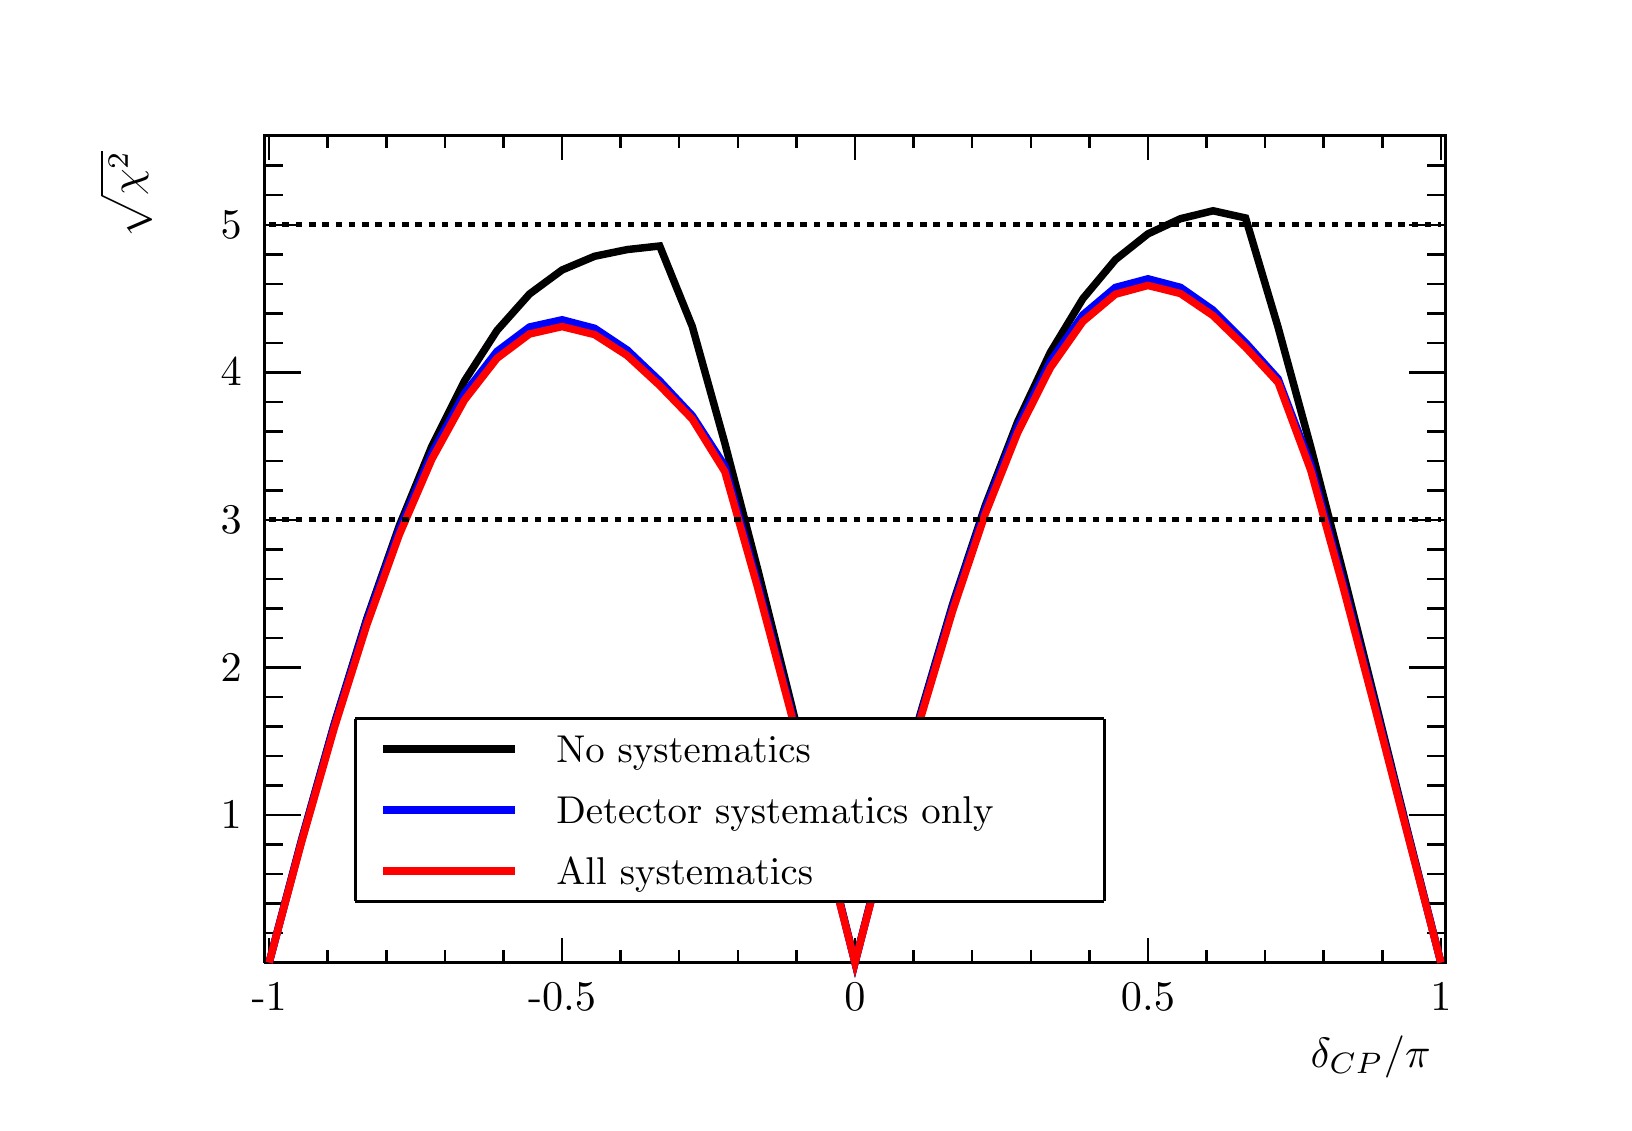
\begin{tikzpicture}
\pgfdeclareplotmark{cross} {
\pgfpathmoveto{\pgfpoint{-0.3\pgfplotmarksize}{\pgfplotmarksize}}
\pgfpathlineto{\pgfpoint{+0.3\pgfplotmarksize}{\pgfplotmarksize}}
\pgfpathlineto{\pgfpoint{+0.3\pgfplotmarksize}{0.3\pgfplotmarksize}}
\pgfpathlineto{\pgfpoint{+1\pgfplotmarksize}{0.3\pgfplotmarksize}}
\pgfpathlineto{\pgfpoint{+1\pgfplotmarksize}{-0.3\pgfplotmarksize}}
\pgfpathlineto{\pgfpoint{+0.3\pgfplotmarksize}{-0.3\pgfplotmarksize}}
\pgfpathlineto{\pgfpoint{+0.3\pgfplotmarksize}{-1.\pgfplotmarksize}}
\pgfpathlineto{\pgfpoint{-0.3\pgfplotmarksize}{-1.\pgfplotmarksize}}
\pgfpathlineto{\pgfpoint{-0.3\pgfplotmarksize}{-0.3\pgfplotmarksize}}
\pgfpathlineto{\pgfpoint{-1.\pgfplotmarksize}{-0.3\pgfplotmarksize}}
\pgfpathlineto{\pgfpoint{-1.\pgfplotmarksize}{0.3\pgfplotmarksize}}
\pgfpathlineto{\pgfpoint{-0.3\pgfplotmarksize}{0.3\pgfplotmarksize}}
\pgfpathclose
\pgfusepathqstroke
}
\pgfdeclareplotmark{cross*} {
\pgfpathmoveto{\pgfpoint{-0.3\pgfplotmarksize}{\pgfplotmarksize}}
\pgfpathlineto{\pgfpoint{+0.3\pgfplotmarksize}{\pgfplotmarksize}}
\pgfpathlineto{\pgfpoint{+0.3\pgfplotmarksize}{0.3\pgfplotmarksize}}
\pgfpathlineto{\pgfpoint{+1\pgfplotmarksize}{0.3\pgfplotmarksize}}
\pgfpathlineto{\pgfpoint{+1\pgfplotmarksize}{-0.3\pgfplotmarksize}}
\pgfpathlineto{\pgfpoint{+0.3\pgfplotmarksize}{-0.3\pgfplotmarksize}}
\pgfpathlineto{\pgfpoint{+0.3\pgfplotmarksize}{-1.\pgfplotmarksize}}
\pgfpathlineto{\pgfpoint{-0.3\pgfplotmarksize}{-1.\pgfplotmarksize}}
\pgfpathlineto{\pgfpoint{-0.3\pgfplotmarksize}{-0.3\pgfplotmarksize}}
\pgfpathlineto{\pgfpoint{-1.\pgfplotmarksize}{-0.3\pgfplotmarksize}}
\pgfpathlineto{\pgfpoint{-1.\pgfplotmarksize}{0.3\pgfplotmarksize}}
\pgfpathlineto{\pgfpoint{-0.3\pgfplotmarksize}{0.3\pgfplotmarksize}}
\pgfpathclose
\pgfusepathqfillstroke
}
\pgfdeclareplotmark{newstar} {
\pgfpathmoveto{\pgfqpoint{0pt}{\pgfplotmarksize}}
\pgfpathlineto{\pgfqpointpolar{44}{0.5\pgfplotmarksize}}
\pgfpathlineto{\pgfqpointpolar{18}{\pgfplotmarksize}}
\pgfpathlineto{\pgfqpointpolar{-20}{0.5\pgfplotmarksize}}
\pgfpathlineto{\pgfqpointpolar{-54}{\pgfplotmarksize}}
\pgfpathlineto{\pgfqpointpolar{-90}{0.5\pgfplotmarksize}}
\pgfpathlineto{\pgfqpointpolar{234}{\pgfplotmarksize}}
\pgfpathlineto{\pgfqpointpolar{198}{0.5\pgfplotmarksize}}
\pgfpathlineto{\pgfqpointpolar{162}{\pgfplotmarksize}}
\pgfpathlineto{\pgfqpointpolar{134}{0.5\pgfplotmarksize}}
\pgfpathclose
\pgfusepathqstroke
}
\pgfdeclareplotmark{newstar*} {
\pgfpathmoveto{\pgfqpoint{0pt}{\pgfplotmarksize}}
\pgfpathlineto{\pgfqpointpolar{44}{0.5\pgfplotmarksize}}
\pgfpathlineto{\pgfqpointpolar{18}{\pgfplotmarksize}}
\pgfpathlineto{\pgfqpointpolar{-20}{0.5\pgfplotmarksize}}
\pgfpathlineto{\pgfqpointpolar{-54}{\pgfplotmarksize}}
\pgfpathlineto{\pgfqpointpolar{-90}{0.5\pgfplotmarksize}}
\pgfpathlineto{\pgfqpointpolar{234}{\pgfplotmarksize}}
\pgfpathlineto{\pgfqpointpolar{198}{0.5\pgfplotmarksize}}
\pgfpathlineto{\pgfqpointpolar{162}{\pgfplotmarksize}}
\pgfpathlineto{\pgfqpointpolar{134}{0.5\pgfplotmarksize}}
\pgfpathclose
\pgfusepathqfillstroke
}
\definecolor{c}{rgb}{1,1,1};
\draw [color=c, fill=c] (0,0) rectangle (20,13.639);
\draw [color=c, fill=c] (3,1.77307) rectangle (18,12.2751);
\definecolor{c}{rgb}{0,0,0};
\draw [c,line width=0.9] (3,1.77307) -- (3,12.2751) -- (18,12.2751) -- (18,1.77307) -- (3,1.77307);
\definecolor{c}{rgb}{1,1,1};
\draw [color=c, fill=c] (3,1.77307) rectangle (18,12.2751);
\definecolor{c}{rgb}{0,0,0};
\draw [c,line width=0.9] (3,1.77307) -- (3,12.2751) -- (18,12.2751) -- (18,1.77307) -- (3,1.77307);
\draw [c,line width=0.9] (3,1.77307) -- (18,1.77307);
\draw [c,line width=0.9] (3.05952,2.07994) -- (3.05952,1.77307);
\draw [c,line width=0.9] (3.80357,1.9265) -- (3.80357,1.77307);
\draw [c,line width=0.9] (4.54762,1.9265) -- (4.54762,1.77307);
\draw [c,line width=0.9] (5.29167,1.9265) -- (5.29167,1.77307);
\draw [c,line width=0.9] (6.03571,1.9265) -- (6.03571,1.77307);
\draw [c,line width=0.9] (6.77976,2.07994) -- (6.77976,1.77307);
\draw [c,line width=0.9] (7.52381,1.9265) -- (7.52381,1.77307);
\draw [c,line width=0.9] (8.26786,1.9265) -- (8.26786,1.77307);
\draw [c,line width=0.9] (9.0119,1.9265) -- (9.0119,1.77307);
\draw [c,line width=0.9] (9.75595,1.9265) -- (9.75595,1.77307);
\draw [c,line width=0.9] (10.5,2.07994) -- (10.5,1.77307);
\draw [c,line width=0.9] (11.244,1.9265) -- (11.244,1.77307);
\draw [c,line width=0.9] (11.9881,1.9265) -- (11.9881,1.77307);
\draw [c,line width=0.9] (12.7321,1.9265) -- (12.7321,1.77307);
\draw [c,line width=0.9] (13.4762,1.9265) -- (13.4762,1.77307);
\draw [c,line width=0.9] (14.2202,2.07994) -- (14.2202,1.77307);
\draw [c,line width=0.9] (14.9643,1.9265) -- (14.9643,1.77307);
\draw [c,line width=0.9] (15.7083,1.9265) -- (15.7083,1.77307);
\draw [c,line width=0.9] (16.4524,1.9265) -- (16.4524,1.77307);
\draw [c,line width=0.9] (17.1964,1.9265) -- (17.1964,1.77307);
\draw [c,line width=0.9] (17.9405,2.07994) -- (17.9405,1.77307);
\draw [c,line width=0.9] (3.05952,2.07994) -- (3.05952,1.77307);
\draw [c,line width=0.9] (17.9405,2.07994) -- (17.9405,1.77307);
\draw [anchor=base] (3.05952,1.15931) node[scale=1.52731, color=c, rotate=0]{-1};
\draw [anchor=base] (6.77976,1.15931) node[scale=1.52731, color=c, rotate=0]{-0.5};
\draw [anchor=base] (10.5,1.15931) node[scale=1.52731, color=c, rotate=0]{0};
\draw [anchor=base] (14.2202,1.15931) node[scale=1.52731, color=c, rotate=0]{0.5};
\draw [anchor=base] (17.9405,1.15931) node[scale=1.52731, color=c, rotate=0]{1};
\draw [anchor= east] (18,0.572837) node[scale=1.52731, color=c, rotate=0]{$\delta_{CP} / \pi$};
\draw [c,line width=0.9] (3,12.2751) -- (18,12.2751);
\draw [c,line width=0.9] (3.05952,11.9682) -- (3.05952,12.2751);
\draw [c,line width=0.9] (3.80357,12.1216) -- (3.80357,12.2751);
\draw [c,line width=0.9] (4.54762,12.1216) -- (4.54762,12.2751);
\draw [c,line width=0.9] (5.29167,12.1216) -- (5.29167,12.2751);
\draw [c,line width=0.9] (6.03571,12.1216) -- (6.03571,12.2751);
\draw [c,line width=0.9] (6.77976,11.9682) -- (6.77976,12.2751);
\draw [c,line width=0.9] (7.52381,12.1216) -- (7.52381,12.2751);
\draw [c,line width=0.9] (8.26786,12.1216) -- (8.26786,12.2751);
\draw [c,line width=0.9] (9.0119,12.1216) -- (9.0119,12.2751);
\draw [c,line width=0.9] (9.75595,12.1216) -- (9.75595,12.2751);
\draw [c,line width=0.9] (10.5,11.9682) -- (10.5,12.2751);
\draw [c,line width=0.9] (11.244,12.1216) -- (11.244,12.2751);
\draw [c,line width=0.9] (11.9881,12.1216) -- (11.9881,12.2751);
\draw [c,line width=0.9] (12.7321,12.1216) -- (12.7321,12.2751);
\draw [c,line width=0.9] (13.4762,12.1216) -- (13.4762,12.2751);
\draw [c,line width=0.9] (14.2202,11.9682) -- (14.2202,12.2751);
\draw [c,line width=0.9] (14.9643,12.1216) -- (14.9643,12.2751);
\draw [c,line width=0.9] (15.7083,12.1216) -- (15.7083,12.2751);
\draw [c,line width=0.9] (16.4524,12.1216) -- (16.4524,12.2751);
\draw [c,line width=0.9] (17.1964,12.1216) -- (17.1964,12.2751);
\draw [c,line width=0.9] (17.9405,11.9682) -- (17.9405,12.2751);
\draw [c,line width=0.9] (3.05952,11.9682) -- (3.05952,12.2751);
\draw [c,line width=0.9] (17.9405,11.9682) -- (17.9405,12.2751);
\draw [c,line width=0.9] (3,1.77307) -- (3,12.2751);
\draw [c,line width=0.9] (3.462,3.64567) -- (3,3.64567);
\draw [c,line width=0.9] (3.231,4.02052) -- (3,4.02052);
\draw [c,line width=0.9] (3.231,4.39538) -- (3,4.39538);
\draw [c,line width=0.9] (3.231,4.77024) -- (3,4.77024);
\draw [c,line width=0.9] (3.231,5.14509) -- (3,5.14509);
\draw [c,line width=0.9] (3.462,5.51995) -- (3,5.51995);
\draw [c,line width=0.9] (3.231,5.89481) -- (3,5.89481);
\draw [c,line width=0.9] (3.231,6.26967) -- (3,6.26967);
\draw [c,line width=0.9] (3.231,6.64452) -- (3,6.64452);
\draw [c,line width=0.9] (3.231,7.01938) -- (3,7.01938);
\draw [c,line width=0.9] (3.462,7.39424) -- (3,7.39424);
\draw [c,line width=0.9] (3.231,7.76909) -- (3,7.76909);
\draw [c,line width=0.9] (3.231,8.14395) -- (3,8.14395);
\draw [c,line width=0.9] (3.231,8.51881) -- (3,8.51881);
\draw [c,line width=0.9] (3.231,8.89367) -- (3,8.89367);
\draw [c,line width=0.9] (3.462,9.26852) -- (3,9.26852);
\draw [c,line width=0.9] (3.231,9.64338) -- (3,9.64338);
\draw [c,line width=0.9] (3.231,10.0182) -- (3,10.0182);
\draw [c,line width=0.9] (3.231,10.3931) -- (3,10.3931);
\draw [c,line width=0.9] (3.231,10.768) -- (3,10.768);
\draw [c,line width=0.9] (3.462,11.1428) -- (3,11.1428);
\draw [c,line width=0.9] (3.462,3.64567) -- (3,3.64567);
\draw [c,line width=0.9] (3.231,3.27081) -- (3,3.27081);
\draw [c,line width=0.9] (3.231,2.89595) -- (3,2.89595);
\draw [c,line width=0.9] (3.231,2.52109) -- (3,2.52109);
\draw [c,line width=0.9] (3.231,2.14624) -- (3,2.14624);
\draw [c,line width=0.9] (3.462,11.1428) -- (3,11.1428);
\draw [c,line width=0.9] (3.231,11.5177) -- (3,11.5177);
\draw [c,line width=0.9] (3.231,11.8925) -- (3,11.8925);
\draw [c,line width=0.9] (3.231,12.2674) -- (3,12.2674);
\draw [anchor= east] (2.9,3.64567) node[scale=1.52731, color=c, rotate=0]{1};
\draw [anchor= east] (2.9,5.51995) node[scale=1.52731, color=c, rotate=0]{2};
\draw [anchor= east] (2.9,7.39424) node[scale=1.52731, color=c, rotate=0]{3};
\draw [anchor= east] (2.9,9.26852) node[scale=1.52731, color=c, rotate=0]{4};
\draw [anchor= east] (2.9,11.1428) node[scale=1.52731, color=c, rotate=0]{5};
\draw [anchor= east] (1.24,12.2751) node[scale=1.52731, color=c, rotate=90]{$\sqrt{ \chi^{2} }$};
\draw [c,line width=0.9] (18,1.77307) -- (18,12.2751);
\draw [c,line width=0.9] (17.538,3.64567) -- (18,3.64567);
\draw [c,line width=0.9] (17.769,4.02052) -- (18,4.02052);
\draw [c,line width=0.9] (17.769,4.39538) -- (18,4.39538);
\draw [c,line width=0.9] (17.769,4.77024) -- (18,4.77024);
\draw [c,line width=0.9] (17.769,5.14509) -- (18,5.14509);
\draw [c,line width=0.9] (17.538,5.51995) -- (18,5.51995);
\draw [c,line width=0.9] (17.769,5.89481) -- (18,5.89481);
\draw [c,line width=0.9] (17.769,6.26967) -- (18,6.26967);
\draw [c,line width=0.9] (17.769,6.64452) -- (18,6.64452);
\draw [c,line width=0.9] (17.769,7.01938) -- (18,7.01938);
\draw [c,line width=0.9] (17.538,7.39424) -- (18,7.39424);
\draw [c,line width=0.9] (17.769,7.76909) -- (18,7.76909);
\draw [c,line width=0.9] (17.769,8.14395) -- (18,8.14395);
\draw [c,line width=0.9] (17.769,8.51881) -- (18,8.51881);
\draw [c,line width=0.9] (17.769,8.89367) -- (18,8.89367);
\draw [c,line width=0.9] (17.538,9.26852) -- (18,9.26852);
\draw [c,line width=0.9] (17.769,9.64338) -- (18,9.64338);
\draw [c,line width=0.9] (17.769,10.0182) -- (18,10.0182);
\draw [c,line width=0.9] (17.769,10.3931) -- (18,10.3931);
\draw [c,line width=0.9] (17.769,10.768) -- (18,10.768);
\draw [c,line width=0.9] (17.538,11.1428) -- (18,11.1428);
\draw [c,line width=0.9] (17.538,3.64567) -- (18,3.64567);
\draw [c,line width=0.9] (17.769,3.27081) -- (18,3.27081);
\draw [c,line width=0.9] (17.769,2.89595) -- (18,2.89595);
\draw [c,line width=0.9] (17.769,2.52109) -- (18,2.52109);
\draw [c,line width=0.9] (17.769,2.14624) -- (18,2.14624);
\draw [c,line width=0.9] (17.538,11.1428) -- (18,11.1428);
\draw [c,line width=0.9] (17.769,11.5177) -- (18,11.5177);
\draw [c,line width=0.9] (17.769,11.8925) -- (18,11.8925);
\draw [c,line width=0.9] (17.769,12.2674) -- (18,12.2674);
\draw [c,line width=2.7] (3.05952,1.77307) -- (3.47288,3.33785) -- (3.88624,4.80397) -- (4.2996,6.1401) -- (4.71296,7.32189) -- (5.12632,8.33136) -- (5.53968,9.15795) -- (5.95304,9.79956) -- (6.3664,10.2637) -- (6.77976,10.5684) -- (7.19312,10.7429)
 -- (7.60648,10.8278) -- (8.01984,10.8733) -- (8.4332,9.85149) -- (8.84656,8.37) -- (9.25992,6.78334) -- (9.67328,5.12821) -- (10.0866,3.44506) -- (10.5,1.77307) -- (10.9134,3.39288) -- (11.3267,4.9214) -- (11.7401,6.32506) -- (12.1534,7.57311) --
 (12.5668,8.64304) -- (12.9802,9.5211) -- (13.3935,10.2038) -- (13.8069,10.6991) -- (14.2202,11.0271) -- (14.6336,11.2198) -- (15.047,11.3204) -- (15.4603,11.2289) -- (15.8737,9.83928) -- (16.287,8.32379) -- (16.7004,6.71988) -- (17.1138,5.06682) --
 (17.5271,3.40434) -- (17.9405,1.77307);
\definecolor{c}{rgb}{0,0,1};
\draw [c,line width=2.7] (3.05952,1.77307) -- (3.47288,3.32667) -- (3.88624,4.7871) -- (4.2996,6.11229) -- (4.71296,7.27285) -- (5.12632,8.24169) -- (5.53968,8.99948) -- (5.95304,9.53465) -- (6.3664,9.84443) -- (6.77976,9.93602) -- (7.19312,9.82806)
 -- (7.60648,9.55298) -- (8.01984,9.15979) -- (8.4332,8.71931) -- (8.84656,8.08045) -- (9.25992,6.60367) -- (9.67328,5.03153) -- (10.0866,3.40685) -- (10.5,1.77307) -- (10.9134,3.37158) -- (11.3267,4.89142) -- (11.7401,6.29078) -- (12.1534,7.53012)
 -- (12.5668,8.57744) -- (12.9802,9.40606) -- (13.3935,9.99829) -- (13.8069,10.3467) -- (14.2202,10.4564) -- (14.6336,10.3479) -- (15.047,10.0589) -- (15.4603,9.64583) -- (15.8737,9.18555) -- (16.287,8.09798) -- (16.7004,6.58937) -- (17.1138,5.00291)
 -- (17.5271,3.38226) -- (17.9405,1.77307);
\definecolor{c}{rgb}{1,0,0};
\draw [c,line width=2.7] (3.05952,1.77307) -- (3.47288,3.30852) -- (3.88624,4.75063) -- (4.2996,6.06105) -- (4.71296,7.20812) -- (5.12632,8.16611) -- (5.53968,8.91607) -- (5.95304,9.44675) -- (6.3664,9.75556) -- (6.77976,9.84976) -- (7.19312,9.7479)
 -- (7.60648,9.48214) -- (8.01984,9.10131) -- (8.4332,8.67462) -- (8.84656,8.00828) -- (9.25992,6.54804) -- (9.67328,4.99419) -- (10.0866,3.38759) -- (10.5,1.77307) -- (10.9134,3.35307) -- (11.3267,4.85678) -- (11.7401,6.24109) -- (12.1534,7.46813)
 -- (12.5668,8.50501) -- (12.9802,9.32593) -- (13.3935,9.91346) -- (13.8069,10.2604) -- (14.2202,10.3721) -- (14.6336,10.2691) -- (15.047,9.98875) -- (15.4603,9.58682) -- (15.8737,9.13908) -- (16.287,8.0275) -- (16.7004,6.53519) -- (17.1138,4.96565)
 -- (17.5271,3.36292) -- (17.9405,1.77307);
\definecolor{c}{rgb}{0,0,0};
\draw [c,dash pattern=on 2.40pt off 2.40pt ,line width=1.8] (3.05952,7.39424) -- (17.9405,7.39424);
\draw [c,dash pattern=on 2.40pt off 2.40pt ,line width=1.8] (3.05952,11.1428) -- (17.9405,11.1428);
\definecolor{c}{rgb}{1,1,1};
\draw [color=c, fill=c] (4.15473,2.55014) rectangle (13.6676,4.87106);
\definecolor{c}{rgb}{0,0,0};
\draw [c,line width=0.9] (4.15473,2.55014) -- (13.6676,2.55014);
\draw [c,line width=0.9] (13.6676,2.55014) -- (13.6676,4.87106);
\draw [c,line width=0.9] (13.6676,4.87106) -- (4.15473,4.87106);
\draw [c,line width=0.9] (4.15473,4.87106) -- (4.15473,2.55014);
\draw [anchor=base west] (6.53295,4.31017) node[scale=1.40004, color=c, rotate=0]{No systematics};
\definecolor{c}{rgb}{1,1,1};
\draw [c, fill=c] (4.51146,4.21347) -- (6.17622,4.21347) -- (6.17622,4.75501) -- (4.51146,4.75501);
\definecolor{c}{rgb}{0,0,0};
\draw [c,line width=2.7] (4.51146,4.48424) -- (6.17622,4.48424);
\foreach \P in {(5.34384,4.48424)}{\draw[mark options={color=c,fill=c},mark size=2.402402pt, line width=0.000000pt, mark=*,mark size=1pt] plot coordinates {\P};}
\draw [anchor=base west] (6.53295,3.53653) node[scale=1.40004, color=c, rotate=0]{Detector systematics only};
\definecolor{c}{rgb}{1,1,1};
\draw [c, fill=c] (4.51146,3.43983) -- (6.17622,3.43983) -- (6.17622,3.98138) -- (4.51146,3.98138);
\definecolor{c}{rgb}{0,0,1};
\draw [c,line width=2.7] (4.51146,3.7106) -- (6.17622,3.7106);
\foreach \P in {(5.34384,3.7106)}{\draw[mark options={color=c,fill=c},mark size=2.402402pt, line width=0.000000pt, mark=*,mark size=1pt] plot coordinates {\P};}
\definecolor{c}{rgb}{0,0,0};
\draw [anchor=base west] (6.53295,2.76289) node[scale=1.40004, color=c, rotate=0]{All systematics};
\definecolor{c}{rgb}{1,1,1};
\draw [c, fill=c] (4.51146,2.66619) -- (6.17622,2.66619) -- (6.17622,3.20774) -- (4.51146,3.20774);
\definecolor{c}{rgb}{1,0,0};
\draw [c,line width=2.7] (4.51146,2.93696) -- (6.17622,2.93696);
\foreach \P in {(5.34384,2.93696)}{\draw[mark options={color=c,fill=c},mark size=2.402402pt, line width=0.000000pt, mark=*,mark size=1pt] plot coordinates {\P};}
\end{tikzpicture}

		\end{adjustbox}
	\end{minipage}
	\hfill
	\begin{minipage}[t]{.5\linewidth}
		\begin{adjustbox}{max totalsize=\linewidth, center}
			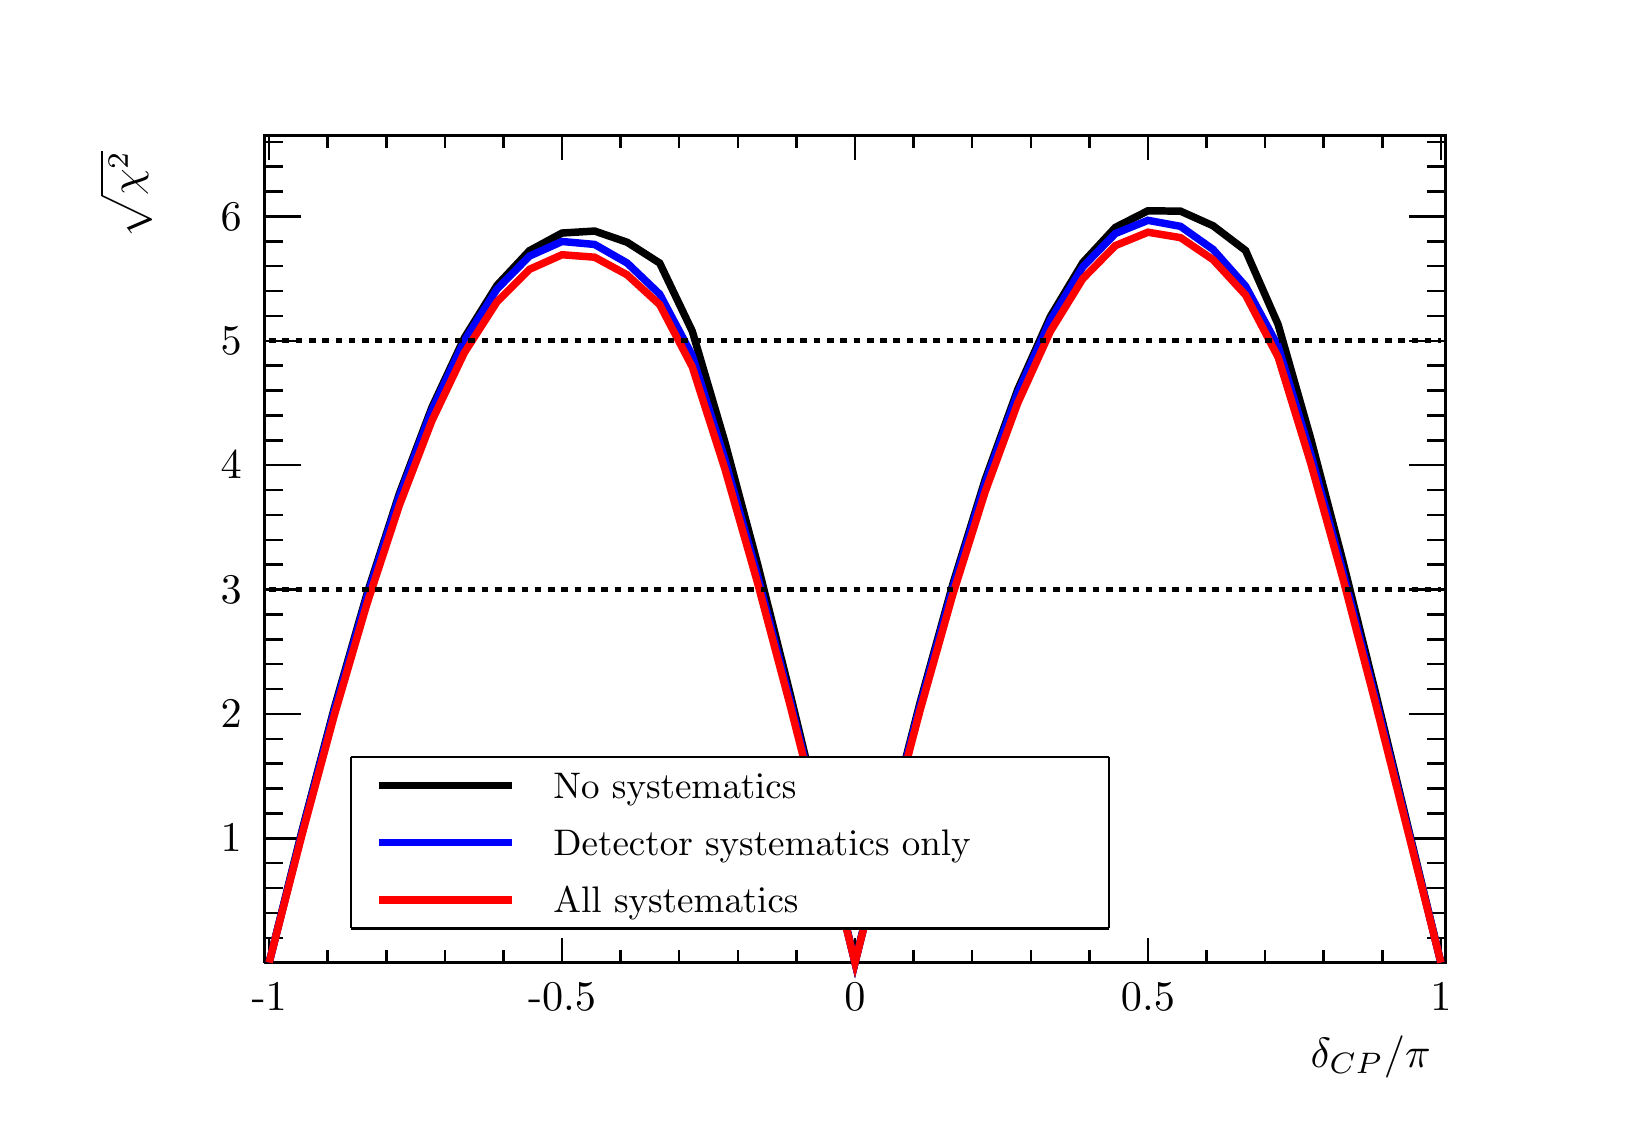
\begin{tikzpicture}
\pgfdeclareplotmark{cross} {
\pgfpathmoveto{\pgfpoint{-0.3\pgfplotmarksize}{\pgfplotmarksize}}
\pgfpathlineto{\pgfpoint{+0.3\pgfplotmarksize}{\pgfplotmarksize}}
\pgfpathlineto{\pgfpoint{+0.3\pgfplotmarksize}{0.3\pgfplotmarksize}}
\pgfpathlineto{\pgfpoint{+1\pgfplotmarksize}{0.3\pgfplotmarksize}}
\pgfpathlineto{\pgfpoint{+1\pgfplotmarksize}{-0.3\pgfplotmarksize}}
\pgfpathlineto{\pgfpoint{+0.3\pgfplotmarksize}{-0.3\pgfplotmarksize}}
\pgfpathlineto{\pgfpoint{+0.3\pgfplotmarksize}{-1.\pgfplotmarksize}}
\pgfpathlineto{\pgfpoint{-0.3\pgfplotmarksize}{-1.\pgfplotmarksize}}
\pgfpathlineto{\pgfpoint{-0.3\pgfplotmarksize}{-0.3\pgfplotmarksize}}
\pgfpathlineto{\pgfpoint{-1.\pgfplotmarksize}{-0.3\pgfplotmarksize}}
\pgfpathlineto{\pgfpoint{-1.\pgfplotmarksize}{0.3\pgfplotmarksize}}
\pgfpathlineto{\pgfpoint{-0.3\pgfplotmarksize}{0.3\pgfplotmarksize}}
\pgfpathclose
\pgfusepathqstroke
}
\pgfdeclareplotmark{cross*} {
\pgfpathmoveto{\pgfpoint{-0.3\pgfplotmarksize}{\pgfplotmarksize}}
\pgfpathlineto{\pgfpoint{+0.3\pgfplotmarksize}{\pgfplotmarksize}}
\pgfpathlineto{\pgfpoint{+0.3\pgfplotmarksize}{0.3\pgfplotmarksize}}
\pgfpathlineto{\pgfpoint{+1\pgfplotmarksize}{0.3\pgfplotmarksize}}
\pgfpathlineto{\pgfpoint{+1\pgfplotmarksize}{-0.3\pgfplotmarksize}}
\pgfpathlineto{\pgfpoint{+0.3\pgfplotmarksize}{-0.3\pgfplotmarksize}}
\pgfpathlineto{\pgfpoint{+0.3\pgfplotmarksize}{-1.\pgfplotmarksize}}
\pgfpathlineto{\pgfpoint{-0.3\pgfplotmarksize}{-1.\pgfplotmarksize}}
\pgfpathlineto{\pgfpoint{-0.3\pgfplotmarksize}{-0.3\pgfplotmarksize}}
\pgfpathlineto{\pgfpoint{-1.\pgfplotmarksize}{-0.3\pgfplotmarksize}}
\pgfpathlineto{\pgfpoint{-1.\pgfplotmarksize}{0.3\pgfplotmarksize}}
\pgfpathlineto{\pgfpoint{-0.3\pgfplotmarksize}{0.3\pgfplotmarksize}}
\pgfpathclose
\pgfusepathqfillstroke
}
\pgfdeclareplotmark{newstar} {
\pgfpathmoveto{\pgfqpoint{0pt}{\pgfplotmarksize}}
\pgfpathlineto{\pgfqpointpolar{44}{0.5\pgfplotmarksize}}
\pgfpathlineto{\pgfqpointpolar{18}{\pgfplotmarksize}}
\pgfpathlineto{\pgfqpointpolar{-20}{0.5\pgfplotmarksize}}
\pgfpathlineto{\pgfqpointpolar{-54}{\pgfplotmarksize}}
\pgfpathlineto{\pgfqpointpolar{-90}{0.5\pgfplotmarksize}}
\pgfpathlineto{\pgfqpointpolar{234}{\pgfplotmarksize}}
\pgfpathlineto{\pgfqpointpolar{198}{0.5\pgfplotmarksize}}
\pgfpathlineto{\pgfqpointpolar{162}{\pgfplotmarksize}}
\pgfpathlineto{\pgfqpointpolar{134}{0.5\pgfplotmarksize}}
\pgfpathclose
\pgfusepathqstroke
}
\pgfdeclareplotmark{newstar*} {
\pgfpathmoveto{\pgfqpoint{0pt}{\pgfplotmarksize}}
\pgfpathlineto{\pgfqpointpolar{44}{0.5\pgfplotmarksize}}
\pgfpathlineto{\pgfqpointpolar{18}{\pgfplotmarksize}}
\pgfpathlineto{\pgfqpointpolar{-20}{0.5\pgfplotmarksize}}
\pgfpathlineto{\pgfqpointpolar{-54}{\pgfplotmarksize}}
\pgfpathlineto{\pgfqpointpolar{-90}{0.5\pgfplotmarksize}}
\pgfpathlineto{\pgfqpointpolar{234}{\pgfplotmarksize}}
\pgfpathlineto{\pgfqpointpolar{198}{0.5\pgfplotmarksize}}
\pgfpathlineto{\pgfqpointpolar{162}{\pgfplotmarksize}}
\pgfpathlineto{\pgfqpointpolar{134}{0.5\pgfplotmarksize}}
\pgfpathclose
\pgfusepathqfillstroke
}
\definecolor{c}{rgb}{1,1,1};
\draw [color=c, fill=c] (0,0) rectangle (20,13.639);
\draw [color=c, fill=c] (3,1.77307) rectangle (18,12.2751);
\definecolor{c}{rgb}{0,0,0};
\draw [c,line width=0.9] (3,1.77307) -- (3,12.2751) -- (18,12.2751) -- (18,1.77307) -- (3,1.77307);
\definecolor{c}{rgb}{1,1,1};
\draw [color=c, fill=c] (3,1.77307) rectangle (18,12.2751);
\definecolor{c}{rgb}{0,0,0};
\draw [c,line width=0.9] (3,1.77307) -- (3,12.2751) -- (18,12.2751) -- (18,1.77307) -- (3,1.77307);
\draw [c,line width=0.9] (3,1.77307) -- (18,1.77307);
\draw [c,line width=0.9] (3.05952,2.07994) -- (3.05952,1.77307);
\draw [c,line width=0.9] (3.80357,1.9265) -- (3.80357,1.77307);
\draw [c,line width=0.9] (4.54762,1.9265) -- (4.54762,1.77307);
\draw [c,line width=0.9] (5.29167,1.9265) -- (5.29167,1.77307);
\draw [c,line width=0.9] (6.03571,1.9265) -- (6.03571,1.77307);
\draw [c,line width=0.9] (6.77976,2.07994) -- (6.77976,1.77307);
\draw [c,line width=0.9] (7.52381,1.9265) -- (7.52381,1.77307);
\draw [c,line width=0.9] (8.26786,1.9265) -- (8.26786,1.77307);
\draw [c,line width=0.9] (9.0119,1.9265) -- (9.0119,1.77307);
\draw [c,line width=0.9] (9.75595,1.9265) -- (9.75595,1.77307);
\draw [c,line width=0.9] (10.5,2.07994) -- (10.5,1.77307);
\draw [c,line width=0.9] (11.244,1.9265) -- (11.244,1.77307);
\draw [c,line width=0.9] (11.9881,1.9265) -- (11.9881,1.77307);
\draw [c,line width=0.9] (12.7321,1.9265) -- (12.7321,1.77307);
\draw [c,line width=0.9] (13.4762,1.9265) -- (13.4762,1.77307);
\draw [c,line width=0.9] (14.2202,2.07994) -- (14.2202,1.77307);
\draw [c,line width=0.9] (14.9643,1.9265) -- (14.9643,1.77307);
\draw [c,line width=0.9] (15.7083,1.9265) -- (15.7083,1.77307);
\draw [c,line width=0.9] (16.4524,1.9265) -- (16.4524,1.77307);
\draw [c,line width=0.9] (17.1964,1.9265) -- (17.1964,1.77307);
\draw [c,line width=0.9] (17.9405,2.07994) -- (17.9405,1.77307);
\draw [c,line width=0.9] (3.05952,2.07994) -- (3.05952,1.77307);
\draw [c,line width=0.9] (17.9405,2.07994) -- (17.9405,1.77307);
\draw [anchor=base] (3.05952,1.15931) node[scale=1.52731, color=c, rotate=0]{-1};
\draw [anchor=base] (6.77976,1.15931) node[scale=1.52731, color=c, rotate=0]{-0.5};
\draw [anchor=base] (10.5,1.15931) node[scale=1.52731, color=c, rotate=0]{0};
\draw [anchor=base] (14.2202,1.15931) node[scale=1.52731, color=c, rotate=0]{0.5};
\draw [anchor=base] (17.9405,1.15931) node[scale=1.52731, color=c, rotate=0]{1};
\draw [anchor= east] (18,0.572837) node[scale=1.52731, color=c, rotate=0]{$\delta_{CP} / \pi$};
\draw [c,line width=0.9] (3,12.2751) -- (18,12.2751);
\draw [c,line width=0.9] (3.05952,11.9682) -- (3.05952,12.2751);
\draw [c,line width=0.9] (3.80357,12.1216) -- (3.80357,12.2751);
\draw [c,line width=0.9] (4.54762,12.1216) -- (4.54762,12.2751);
\draw [c,line width=0.9] (5.29167,12.1216) -- (5.29167,12.2751);
\draw [c,line width=0.9] (6.03571,12.1216) -- (6.03571,12.2751);
\draw [c,line width=0.9] (6.77976,11.9682) -- (6.77976,12.2751);
\draw [c,line width=0.9] (7.52381,12.1216) -- (7.52381,12.2751);
\draw [c,line width=0.9] (8.26786,12.1216) -- (8.26786,12.2751);
\draw [c,line width=0.9] (9.0119,12.1216) -- (9.0119,12.2751);
\draw [c,line width=0.9] (9.75595,12.1216) -- (9.75595,12.2751);
\draw [c,line width=0.9] (10.5,11.9682) -- (10.5,12.2751);
\draw [c,line width=0.9] (11.244,12.1216) -- (11.244,12.2751);
\draw [c,line width=0.9] (11.9881,12.1216) -- (11.9881,12.2751);
\draw [c,line width=0.9] (12.7321,12.1216) -- (12.7321,12.2751);
\draw [c,line width=0.9] (13.4762,12.1216) -- (13.4762,12.2751);
\draw [c,line width=0.9] (14.2202,11.9682) -- (14.2202,12.2751);
\draw [c,line width=0.9] (14.9643,12.1216) -- (14.9643,12.2751);
\draw [c,line width=0.9] (15.7083,12.1216) -- (15.7083,12.2751);
\draw [c,line width=0.9] (16.4524,12.1216) -- (16.4524,12.2751);
\draw [c,line width=0.9] (17.1964,12.1216) -- (17.1964,12.2751);
\draw [c,line width=0.9] (17.9405,11.9682) -- (17.9405,12.2751);
\draw [c,line width=0.9] (3.05952,11.9682) -- (3.05952,12.2751);
\draw [c,line width=0.9] (17.9405,11.9682) -- (17.9405,12.2751);
\draw [c,line width=0.9] (3,1.77307) -- (3,12.2751);
\draw [c,line width=0.9] (3.462,3.35114) -- (3,3.35114);
\draw [c,line width=0.9] (3.231,3.66704) -- (3,3.66704);
\draw [c,line width=0.9] (3.231,3.98294) -- (3,3.98294);
\draw [c,line width=0.9] (3.231,4.29884) -- (3,4.29884);
\draw [c,line width=0.9] (3.231,4.61474) -- (3,4.61474);
\draw [c,line width=0.9] (3.462,4.93064) -- (3,4.93064);
\draw [c,line width=0.9] (3.231,5.24654) -- (3,5.24654);
\draw [c,line width=0.9] (3.231,5.56244) -- (3,5.56244);
\draw [c,line width=0.9] (3.231,5.87834) -- (3,5.87834);
\draw [c,line width=0.9] (3.231,6.19424) -- (3,6.19424);
\draw [c,line width=0.9] (3.462,6.51014) -- (3,6.51014);
\draw [c,line width=0.9] (3.231,6.82604) -- (3,6.82604);
\draw [c,line width=0.9] (3.231,7.14194) -- (3,7.14194);
\draw [c,line width=0.9] (3.231,7.45784) -- (3,7.45784);
\draw [c,line width=0.9] (3.231,7.77373) -- (3,7.77373);
\draw [c,line width=0.9] (3.462,8.08963) -- (3,8.08963);
\draw [c,line width=0.9] (3.231,8.40553) -- (3,8.40553);
\draw [c,line width=0.9] (3.231,8.72143) -- (3,8.72143);
\draw [c,line width=0.9] (3.231,9.03733) -- (3,9.03733);
\draw [c,line width=0.9] (3.231,9.35323) -- (3,9.35323);
\draw [c,line width=0.9] (3.462,9.66913) -- (3,9.66913);
\draw [c,line width=0.9] (3.231,9.98503) -- (3,9.98503);
\draw [c,line width=0.9] (3.231,10.3009) -- (3,10.3009);
\draw [c,line width=0.9] (3.231,10.6168) -- (3,10.6168);
\draw [c,line width=0.9] (3.231,10.9327) -- (3,10.9327);
\draw [c,line width=0.9] (3.462,11.2486) -- (3,11.2486);
\draw [c,line width=0.9] (3.462,3.35114) -- (3,3.35114);
\draw [c,line width=0.9] (3.231,3.03524) -- (3,3.03524);
\draw [c,line width=0.9] (3.231,2.71934) -- (3,2.71934);
\draw [c,line width=0.9] (3.231,2.40344) -- (3,2.40344);
\draw [c,line width=0.9] (3.231,2.08754) -- (3,2.08754);
\draw [c,line width=0.9] (3.462,11.2486) -- (3,11.2486);
\draw [c,line width=0.9] (3.231,11.5645) -- (3,11.5645);
\draw [c,line width=0.9] (3.231,11.8804) -- (3,11.8804);
\draw [c,line width=0.9] (3.231,12.1963) -- (3,12.1963);
\draw [anchor= east] (2.9,3.35114) node[scale=1.52731, color=c, rotate=0]{1};
\draw [anchor= east] (2.9,4.93064) node[scale=1.52731, color=c, rotate=0]{2};
\draw [anchor= east] (2.9,6.51014) node[scale=1.52731, color=c, rotate=0]{3};
\draw [anchor= east] (2.9,8.08963) node[scale=1.52731, color=c, rotate=0]{4};
\draw [anchor= east] (2.9,9.66913) node[scale=1.52731, color=c, rotate=0]{5};
\draw [anchor= east] (2.9,11.2486) node[scale=1.52731, color=c, rotate=0]{6};
\draw [anchor= east] (1.24,12.2751) node[scale=1.52731, color=c, rotate=90]{$\sqrt{ \chi^{2} }$};
\draw [c,line width=0.9] (18,1.77307) -- (18,12.2751);
\draw [c,line width=0.9] (17.538,3.35114) -- (18,3.35114);
\draw [c,line width=0.9] (17.769,3.66704) -- (18,3.66704);
\draw [c,line width=0.9] (17.769,3.98294) -- (18,3.98294);
\draw [c,line width=0.9] (17.769,4.29884) -- (18,4.29884);
\draw [c,line width=0.9] (17.769,4.61474) -- (18,4.61474);
\draw [c,line width=0.9] (17.538,4.93064) -- (18,4.93064);
\draw [c,line width=0.9] (17.769,5.24654) -- (18,5.24654);
\draw [c,line width=0.9] (17.769,5.56244) -- (18,5.56244);
\draw [c,line width=0.9] (17.769,5.87834) -- (18,5.87834);
\draw [c,line width=0.9] (17.769,6.19424) -- (18,6.19424);
\draw [c,line width=0.9] (17.538,6.51014) -- (18,6.51014);
\draw [c,line width=0.9] (17.769,6.82604) -- (18,6.82604);
\draw [c,line width=0.9] (17.769,7.14194) -- (18,7.14194);
\draw [c,line width=0.9] (17.769,7.45784) -- (18,7.45784);
\draw [c,line width=0.9] (17.769,7.77373) -- (18,7.77373);
\draw [c,line width=0.9] (17.538,8.08963) -- (18,8.08963);
\draw [c,line width=0.9] (17.769,8.40553) -- (18,8.40553);
\draw [c,line width=0.9] (17.769,8.72143) -- (18,8.72143);
\draw [c,line width=0.9] (17.769,9.03733) -- (18,9.03733);
\draw [c,line width=0.9] (17.769,9.35323) -- (18,9.35323);
\draw [c,line width=0.9] (17.538,9.66913) -- (18,9.66913);
\draw [c,line width=0.9] (17.769,9.98503) -- (18,9.98503);
\draw [c,line width=0.9] (17.769,10.3009) -- (18,10.3009);
\draw [c,line width=0.9] (17.769,10.6168) -- (18,10.6168);
\draw [c,line width=0.9] (17.769,10.9327) -- (18,10.9327);
\draw [c,line width=0.9] (17.538,11.2486) -- (18,11.2486);
\draw [c,line width=0.9] (17.538,3.35114) -- (18,3.35114);
\draw [c,line width=0.9] (17.769,3.03524) -- (18,3.03524);
\draw [c,line width=0.9] (17.769,2.71934) -- (18,2.71934);
\draw [c,line width=0.9] (17.769,2.40344) -- (18,2.40344);
\draw [c,line width=0.9] (17.769,2.08754) -- (18,2.08754);
\draw [c,line width=0.9] (17.538,11.2486) -- (18,11.2486);
\draw [c,line width=0.9] (17.769,11.5645) -- (18,11.5645);
\draw [c,line width=0.9] (17.769,11.8804) -- (18,11.8804);
\draw [c,line width=0.9] (17.769,12.1963) -- (18,12.1963);
\draw [c,line width=2.7] (3.05952,1.77307) -- (3.47288,3.43116) -- (3.88624,5.00182) -- (4.2996,6.4452) -- (4.71296,7.7278) -- (5.12632,8.82218) -- (5.53968,9.708) -- (5.95304,10.373) -- (6.3664,10.8141) -- (6.77976,11.038) -- (7.19312,11.063) --
 (7.60648,10.9205) -- (8.01984,10.656) -- (8.4332,9.79109) -- (8.84656,8.38708) -- (9.25992,6.84323) -- (9.67328,5.19766) -- (10.0866,3.49229) -- (10.5,1.77307) -- (10.9134,3.46183) -- (11.3267,5.07613) -- (11.7401,6.57113) -- (12.1534,7.90723) --
 (12.5668,9.05057) -- (12.9802,9.97487) -- (13.3935,10.6632) -- (13.8069,11.1096) -- (14.2202,11.3204) -- (14.6336,11.3155) -- (15.047,11.1303) -- (15.4603,10.816) -- (15.8737,9.87595) -- (16.287,8.42903) -- (16.7004,6.85164) -- (17.1138,5.18634) --
 (17.5271,3.47788) -- (17.9405,1.77307);
\definecolor{c}{rgb}{0,0,1};
\draw [c,line width=2.7] (3.05952,1.77307) -- (3.47288,3.4123) -- (3.88624,4.97155) -- (4.2996,6.41047) -- (4.71296,7.69272) -- (5.12632,8.78711) -- (5.53968,9.67057) -- (5.95304,10.3257) -- (6.3664,10.7453) -- (6.77976,10.9303) -- (7.19312,10.8929)
 -- (7.60648,10.6569) -- (8.01984,10.2613) -- (8.4332,9.48296) -- (8.84656,8.16636) -- (9.25992,6.69708) -- (9.67328,5.11322) -- (10.0866,3.45713) -- (10.5,1.77307) -- (10.9134,3.43855) -- (11.3267,5.03785) -- (11.7401,6.52715) -- (12.1534,7.86237)
 -- (12.5668,9.00653) -- (12.9802,9.92945) -- (13.3935,10.6086) -- (13.8069,11.0318) -- (14.2202,11.1991) -- (14.6336,11.1228) -- (15.047,10.8297) -- (15.4603,10.3629) -- (15.8737,9.59968) -- (16.287,8.23334) -- (16.7004,6.72366) -- (17.1138,5.11329)
 -- (17.5271,3.44816) -- (17.9405,1.77307);
\definecolor{c}{rgb}{1,0,0};
\draw [c,line width=2.7] (3.05952,1.77307) -- (3.47288,3.38027) -- (3.88624,4.91019) -- (4.2996,6.32155) -- (4.71296,7.57896) -- (5.12632,8.65266) -- (5.53968,9.51941) -- (5.95304,10.1634) -- (6.3664,10.5771) -- (6.77976,10.7622) -- (7.19312,10.7308)
 -- (7.60648,10.5067) -- (8.01984,10.128) -- (8.4332,9.33814) -- (8.84656,8.04578) -- (9.25992,6.60409) -- (9.67328,5.05001) -- (10.0866,3.42455) -- (10.5,1.77307) -- (10.9134,3.40654) -- (11.3267,4.97764) -- (11.7401,6.4403) -- (12.1534,7.75289) --
 (12.5668,8.87865) -- (12.9802,9.78756) -- (13.3935,10.458) -- (13.8069,10.8783) -- (14.2202,11.048) -- (14.6336,10.9795) -- (15.047,10.6995) -- (15.4603,10.2503) -- (15.8737,9.46081) -- (16.287,8.11693) -- (16.7004,6.63336) -- (17.1138,5.05168) --
 (17.5271,3.41607) -- (17.9405,1.77307);
\definecolor{c}{rgb}{0,0,0};
\draw [c,dash pattern=on 2.40pt off 2.40pt ,line width=1.8] (3.05952,6.51014) -- (17.9405,6.51014);
\draw [c,dash pattern=on 2.40pt off 2.40pt ,line width=1.8] (3.05952,9.66913) -- (17.9405,9.66913);
\definecolor{c}{rgb}{1,1,1};
\draw [color=c, fill=c] (4.09742,2.2063) rectangle (13.7249,4.38395);
\definecolor{c}{rgb}{0,0,0};
\draw [c,line width=0.9] (4.09742,2.2063) -- (13.7249,2.2063);
\draw [c,line width=0.9] (13.7249,2.2063) -- (13.7249,4.38395);
\draw [c,line width=0.9] (13.7249,4.38395) -- (4.09742,4.38395);
\draw [c,line width=0.9] (4.09742,4.38395) -- (4.09742,2.2063);
\draw [anchor=base west] (6.5043,3.85769) node[scale=1.3364, color=c, rotate=0]{No systematics};
\draw [c,line width=2.7] (4.45845,4.02101) -- (6.14327,4.02101);
\draw [anchor=base west] (6.5043,3.13181) node[scale=1.3364, color=c, rotate=0]{Detector systematics only};
\definecolor{c}{rgb}{1,1,1};
\draw [c, fill=c] (4.45845,3.04107) -- (6.14327,3.04107) -- (6.14327,3.54919) -- (4.45845,3.54919);
\definecolor{c}{rgb}{0,0,1};
\draw [c,line width=2.7] (4.45845,3.29513) -- (6.14327,3.29513);
\foreach \P in {(5.30086,3.29513)}{\draw[mark options={color=c,fill=c},mark size=2.402402pt, line width=0.000000pt, mark=*,mark size=1pt] plot coordinates {\P};}
\definecolor{c}{rgb}{0,0,0};
\draw [anchor=base west] (6.5043,2.40592) node[scale=1.3364, color=c, rotate=0]{All systematics};
\definecolor{c}{rgb}{1,0,0};
\draw [c,line width=2.7] (4.45845,2.56925) -- (6.14327,2.56925);
\end{tikzpicture}

		\end{adjustbox}
	\end{minipage}
	\caption[DUNE sensitivities to CP-violation in the lepton sector as a function of true \dcp.]{DUNE sensitivities to CP-violation in the lepton sector as a function of true \dcp. The black line shows the statistics only case. The blue line shows the case where only the detector systematics are used. The red line shows the case where all systematics are used.}
	\label{fig:cpvSens}
\end{figure}


\chapter{DUNE Near Detector driven reweighting}
\label{ch:dune_ndrwt}

% This just dumps some pseudolatin in so you can see some text in place.
\blindtext


% HPTPC section
\chapter{Characterisation of the downstream time of flight system}
\label{sec:hptpc_dtof_characterisation}

This chapter discusses the characterisation of a time of flight system.
This time of flight system was used to identify particle species in a beam test at CERN during the summer of 2018.
Further details of this beam test are given in \citesec{sec:hptpc_beam_flux}.

\citesec{sec:hptpc_dtof_characterisation:dtof} describes the downstream time of flight system, while \citesec{sec:hptpc_dtof_characterisation:characterisation} describes the characterisation of the PMTs and bars.

\section{The downstream time of flight system}
\label{sec:hptpc_dtof_characterisation:dtof}

The downstream time of flight system (DToF) consists of 10 bars made up of Nuvia NuDET plastic scintillator which has a wavelength of maximum emission of \SI{425}{\milli\metre} and a decay time constant of \SI{2.5}{\nano\second}~\cite{nuvia}.
Each bar measures $\SI{10}{\centi\metre} \times \SI{1}{\centi\metre} \times \SI{140}{\centi\metre}$ with a curved cutout at either end.
The curved cutouts accomodate a 5'' Hamamatsu Photonics R6594 PMT~\cite{hamamatsu}.
A diagram of one such bar is shown in \citefig{fig:barDiag}.

\begin{figure}
  \centering
  \includegraphics[width=.8\linewidth]{files/figures/hptpc_dtof_characterisation/barDiag}
  \caption[HPTPC DToF bar diagram.]{Computer generated drawing of one of the scintillator bars from two views with measurements.}
  \label{fig:barDiag}
\end{figure}

The bars and PMTs are arranged in two rows of five bars to ensure complete coverage for any particles impinging on the detector.
This gives the DToF a total active area of $\SI{1.40}{\metre} \times \SI{0.78}{\metre}$.
\citefig{fig:dtofDiag} shows diagrams of the DToF system along with various dimensions of sections of the detector.
Each of the bars is wrapped individually in a reflective milar sheet in order to maximise the light yield as well as keeping external light out of the bar.

\begin{figure}[h]
  \begin{minipage}[t]{.5\linewidth}
    \includegraphics[width=\linewidth]{files/figures/hptpc_dtof_characterisation/dstofFront}
  \end{minipage}
  \hfill
  \begin{minipage}[t]{.4\linewidth}
    \includegraphics[width=\linewidth]{files/figures/hptpc_dtof_characterisation/dstofDiag}
  \end{minipage}
  \caption[Diagrams of the HPTPC DToF.]{Diagrams of the DToF from multiple views along with measurements.}
  \label{fig:dtofDiag}
\end{figure}

Each of the PMTs is attached to the scintillator bar via a 3D-printed support which is glued to the bar.
A layer of optical grease is applied to the end of the scintillator bar where it meets the PMT.
This ensures good optical coupling between the PMT and scintillator bar and minimises light loss.

The vertical position of a particle striking the DToF can be determined by observing in which bar a signal is seen.
The horizontal position of the same particle can be inferred by measuring the time difference between signals being observed in PMTs at opposite ends of the same bar.

However, in order to effectively convert this time measurement to one of position, two factors must be measured.
Firstly, the relationship between the time difference in signals being observed in the PMTs and the position of a particle along the bar must be measured.
Secondly, the time (and therefore position) resolution of the bars and PMTs must be measured.
The procedure and results of these measurements are discussed in \citesec{sec:hptpc_dtof_characterisation:characterisation}.

\section{Characterisation of the bars}
\label{sec:hptpc_dtof_characterisation:characterisation}

\subsection{PMT characterisation}
\label{sec:hptpc_dtof_characterisation:characterisation:pmt}

Prior to testing the bars with the PMTs attached, the gain of each PMT is measured.
This is done in order to determine where to place each PMT within the detector.
A PMT with a higher gain will have a higher light collection efficiency and so will be more likely to detect light from a given charged particle.
These higher gain PMTs are attached to the bars upon which the beam centre impinges and so will observe the highest flux of particles.

The gain of a PMT can be expressed as
\begin{equation}
  G = \frac{N_{\text{SE}}}{N_{\text{PE}}} \, ,
  \label{eq:gainEq}
\end{equation}
where $N_{\text{SE}}$ is the number of output signal electrons from the anode of the PMT and $N_{\text{PE}}$ is the number of photoelectrons liberated from the photocathode.
This gain measurement is performed by pulsing an LED lamp directly into the photocathode of each PMT with the same voltage used for each LED pulse.
The output waveform produced by the PMT is then read by an oscilloscope.
This testing is performed with the PMT inside a light-tight box.

$N_{\text{SE}}$ can be determined from the output PMT waveform in the following manner.
The waveform is in voltage units and can be converted to current by dividing by the resistance of the oscilloscope, $R$.
The relationship between charge, $Q$, and current, $I$, is given by
\begin{equation}
  Q = \int I(t) \, dt
\end{equation}
where $Q$ is in coulombs, $I$ is amperes and $t$ is in seconds.
Therefore, $N_{\text{SE}}$ can be expressed as
\begin{equation}
  N_{\text{SE}} = \frac{1}{R q_{e}} \int V(t) \, dt
\end{equation}
where $q_{e}$ is the elementary charge of the electron.
This process is then repeated a number of times.
An example of the gaussian distribution produced from a number of waveforms is shown in \citefig{fig:N_se}.

\begin{figure}[h]
  \begin{adjustbox}{max totalsize={.8\textwidth}, center}
    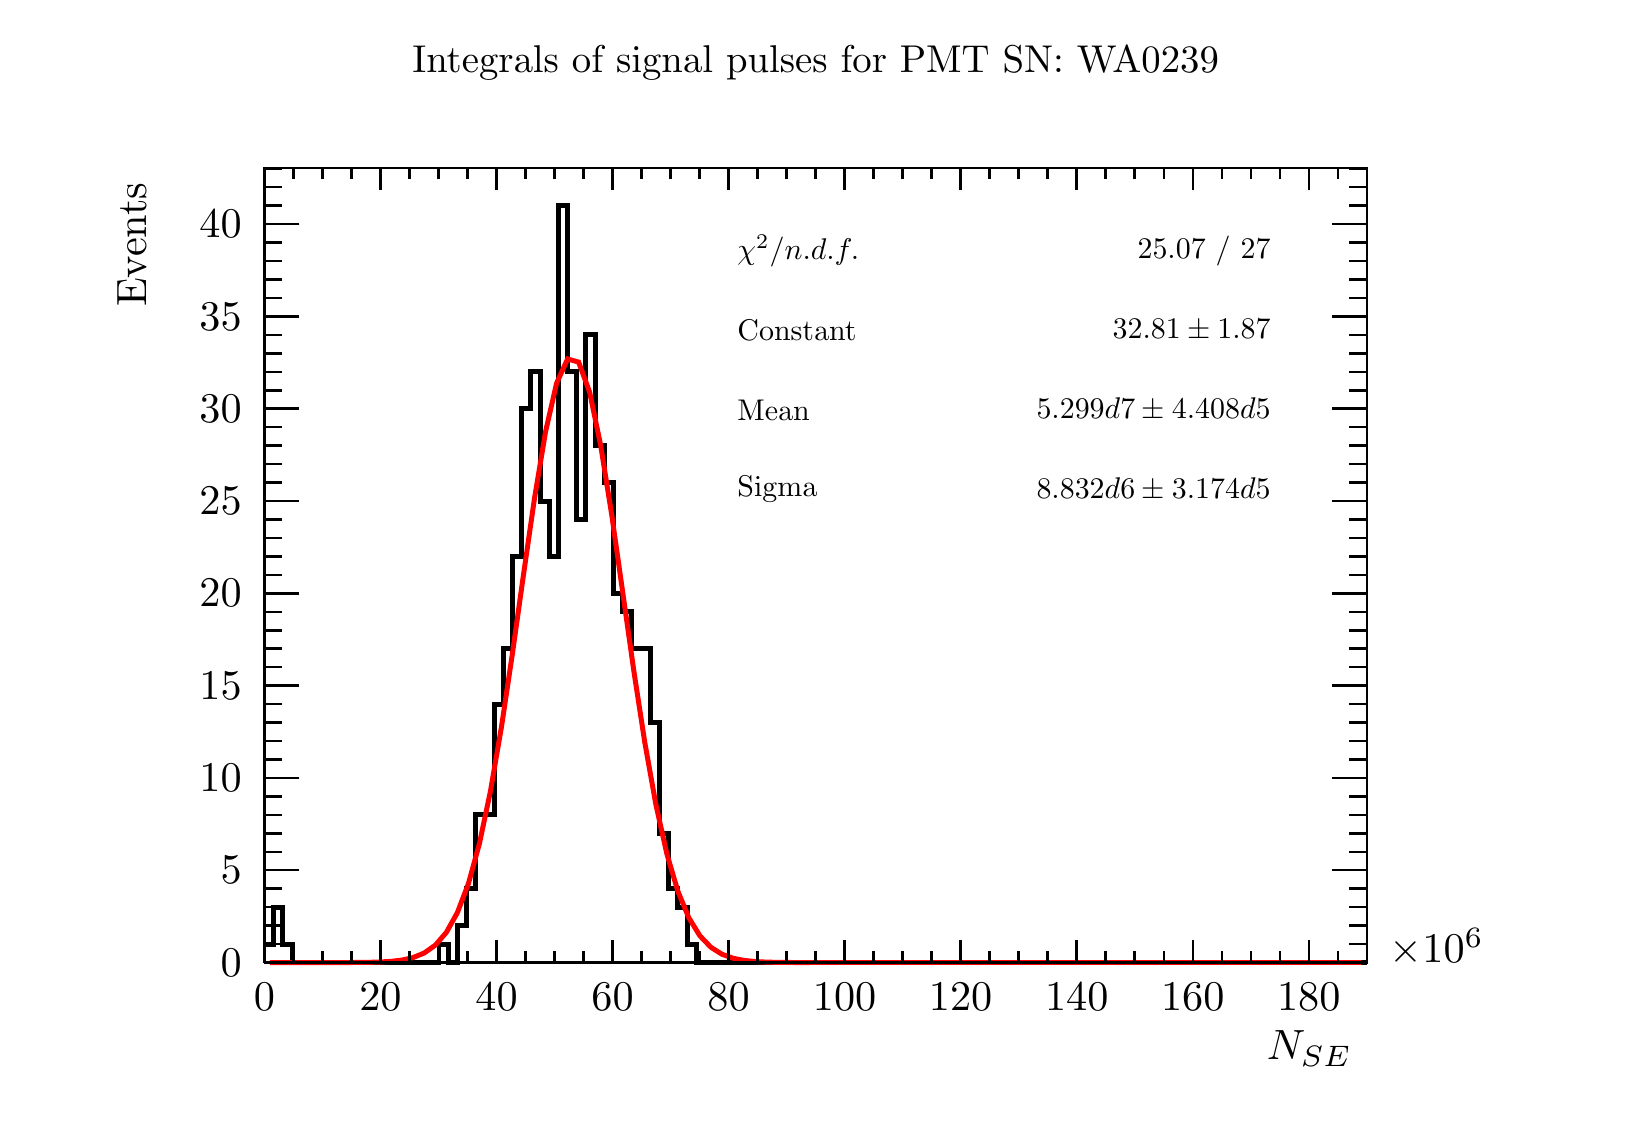
\begin{tikzpicture}
\pgfdeclareplotmark{cross} {
\pgfpathmoveto{\pgfpoint{-0.3\pgfplotmarksize}{\pgfplotmarksize}}
\pgfpathlineto{\pgfpoint{+0.3\pgfplotmarksize}{\pgfplotmarksize}}
\pgfpathlineto{\pgfpoint{+0.3\pgfplotmarksize}{0.3\pgfplotmarksize}}
\pgfpathlineto{\pgfpoint{+1\pgfplotmarksize}{0.3\pgfplotmarksize}}
\pgfpathlineto{\pgfpoint{+1\pgfplotmarksize}{-0.3\pgfplotmarksize}}
\pgfpathlineto{\pgfpoint{+0.3\pgfplotmarksize}{-0.3\pgfplotmarksize}}
\pgfpathlineto{\pgfpoint{+0.3\pgfplotmarksize}{-1.\pgfplotmarksize}}
\pgfpathlineto{\pgfpoint{-0.3\pgfplotmarksize}{-1.\pgfplotmarksize}}
\pgfpathlineto{\pgfpoint{-0.3\pgfplotmarksize}{-0.3\pgfplotmarksize}}
\pgfpathlineto{\pgfpoint{-1.\pgfplotmarksize}{-0.3\pgfplotmarksize}}
\pgfpathlineto{\pgfpoint{-1.\pgfplotmarksize}{0.3\pgfplotmarksize}}
\pgfpathlineto{\pgfpoint{-0.3\pgfplotmarksize}{0.3\pgfplotmarksize}}
\pgfpathclose
\pgfusepathqstroke
}
\pgfdeclareplotmark{cross*} {
\pgfpathmoveto{\pgfpoint{-0.3\pgfplotmarksize}{\pgfplotmarksize}}
\pgfpathlineto{\pgfpoint{+0.3\pgfplotmarksize}{\pgfplotmarksize}}
\pgfpathlineto{\pgfpoint{+0.3\pgfplotmarksize}{0.3\pgfplotmarksize}}
\pgfpathlineto{\pgfpoint{+1\pgfplotmarksize}{0.3\pgfplotmarksize}}
\pgfpathlineto{\pgfpoint{+1\pgfplotmarksize}{-0.3\pgfplotmarksize}}
\pgfpathlineto{\pgfpoint{+0.3\pgfplotmarksize}{-0.3\pgfplotmarksize}}
\pgfpathlineto{\pgfpoint{+0.3\pgfplotmarksize}{-1.\pgfplotmarksize}}
\pgfpathlineto{\pgfpoint{-0.3\pgfplotmarksize}{-1.\pgfplotmarksize}}
\pgfpathlineto{\pgfpoint{-0.3\pgfplotmarksize}{-0.3\pgfplotmarksize}}
\pgfpathlineto{\pgfpoint{-1.\pgfplotmarksize}{-0.3\pgfplotmarksize}}
\pgfpathlineto{\pgfpoint{-1.\pgfplotmarksize}{0.3\pgfplotmarksize}}
\pgfpathlineto{\pgfpoint{-0.3\pgfplotmarksize}{0.3\pgfplotmarksize}}
\pgfpathclose
\pgfusepathqfillstroke
}
\pgfdeclareplotmark{newstar} {
\pgfpathmoveto{\pgfqpoint{0pt}{\pgfplotmarksize}}
\pgfpathlineto{\pgfqpointpolar{44}{0.5\pgfplotmarksize}}
\pgfpathlineto{\pgfqpointpolar{18}{\pgfplotmarksize}}
\pgfpathlineto{\pgfqpointpolar{-20}{0.5\pgfplotmarksize}}
\pgfpathlineto{\pgfqpointpolar{-54}{\pgfplotmarksize}}
\pgfpathlineto{\pgfqpointpolar{-90}{0.5\pgfplotmarksize}}
\pgfpathlineto{\pgfqpointpolar{234}{\pgfplotmarksize}}
\pgfpathlineto{\pgfqpointpolar{198}{0.5\pgfplotmarksize}}
\pgfpathlineto{\pgfqpointpolar{162}{\pgfplotmarksize}}
\pgfpathlineto{\pgfqpointpolar{134}{0.5\pgfplotmarksize}}
\pgfpathclose
\pgfusepathqstroke
}
\pgfdeclareplotmark{newstar*} {
\pgfpathmoveto{\pgfqpoint{0pt}{\pgfplotmarksize}}
\pgfpathlineto{\pgfqpointpolar{44}{0.5\pgfplotmarksize}}
\pgfpathlineto{\pgfqpointpolar{18}{\pgfplotmarksize}}
\pgfpathlineto{\pgfqpointpolar{-20}{0.5\pgfplotmarksize}}
\pgfpathlineto{\pgfqpointpolar{-54}{\pgfplotmarksize}}
\pgfpathlineto{\pgfqpointpolar{-90}{0.5\pgfplotmarksize}}
\pgfpathlineto{\pgfqpointpolar{234}{\pgfplotmarksize}}
\pgfpathlineto{\pgfqpointpolar{198}{0.5\pgfplotmarksize}}
\pgfpathlineto{\pgfqpointpolar{162}{\pgfplotmarksize}}
\pgfpathlineto{\pgfqpointpolar{134}{0.5\pgfplotmarksize}}
\pgfpathclose
\pgfusepathqfillstroke
}
\definecolor{c}{rgb}{1,1,1};
\draw [color=c, fill=c] (0,0) rectangle (20,13.639);
\draw [color=c, fill=c] (3,1.77307) rectangle (17,11.8659);
\definecolor{c}{rgb}{0,0,0};
\draw [c,line width=0.9] (3,1.77307) -- (3,11.8659) -- (17,11.8659) -- (17,1.77307) -- (3,1.77307);
\definecolor{c}{rgb}{1,1,1};
\draw [color=c, fill=c] (3,1.77307) rectangle (17,11.8659);
\definecolor{c}{rgb}{0,0,0};
\draw [c,line width=0.9] (3,1.77307) -- (3,11.8659) -- (17,11.8659) -- (17,1.77307) -- (3,1.77307);
\draw [c,line width=1.8] (3,2.00751) -- (3.11667,2.00751) -- (3.11667,2.4764) -- (3.23333,2.4764) -- (3.23333,2.00751) -- (3.35,2.00751) -- (3.35,1.77307) -- (3.46667,1.77307) -- (3.46667,1.77307) -- (3.58333,1.77307) -- (3.58333,1.77307) --
 (3.7,1.77307) -- (3.7,1.77307) -- (3.81667,1.77307) -- (3.81667,1.77307) -- (3.93333,1.77307) -- (3.93333,1.77307) -- (4.05,1.77307) -- (4.05,1.77307) -- (4.16667,1.77307) -- (4.16667,1.77307) -- (4.28333,1.77307) -- (4.28333,1.77307) --
 (4.4,1.77307) -- (4.4,1.77307) -- (4.51667,1.77307) -- (4.51667,1.77307) -- (4.63333,1.77307) -- (4.63333,1.77307) -- (4.75,1.77307) -- (4.75,1.77307) -- (4.86667,1.77307) -- (4.86667,1.77307) -- (4.98333,1.77307) -- (4.98333,1.77307) --
 (5.1,1.77307) -- (5.1,1.77307) -- (5.21667,1.77307) -- (5.21667,2.00751) -- (5.33333,2.00751) -- (5.33333,1.77307) -- (5.45,1.77307) -- (5.45,2.24195) -- (5.56667,2.24195) -- (5.56667,2.71084) -- (5.68333,2.71084) -- (5.68333,3.64862) --
 (5.8,3.64862) -- (5.8,3.64862) -- (5.91667,3.64862) -- (5.91667,5.05529) -- (6.03333,5.05529) -- (6.03333,5.75862) -- (6.15,5.75862) -- (6.15,6.93085) -- (6.26667,6.93085) -- (6.26667,8.8064) -- (6.38333,8.8064) -- (6.38333,9.27529) -- (6.5,9.27529)
 -- (6.5,7.63418) -- (6.61667,7.63418) -- (6.61667,6.93085) -- (6.73333,6.93085) -- (6.73333,11.3853) -- (6.85,11.3853) -- (6.85,9.27529) -- (6.96667,9.27529) -- (6.96667,7.39973) -- (7.08333,7.39973) -- (7.08333,9.74418) -- (7.2,9.74418) --
 (7.2,8.33751) -- (7.31667,8.33751) -- (7.31667,7.86862) -- (7.43333,7.86862) -- (7.43333,6.46196) -- (7.55,6.46196) -- (7.55,6.22751) -- (7.66667,6.22751) -- (7.66667,5.75862) -- (7.78333,5.75862) -- (7.78333,5.75862) -- (7.9,5.75862) --
 (7.9,4.82084) -- (8.01667,4.82084) -- (8.01667,3.41418) -- (8.13333,3.41418) -- (8.13333,2.71084) -- (8.25,2.71084) -- (8.25,2.4764) -- (8.36667,2.4764) -- (8.36667,2.00751) -- (8.48333,2.00751) -- (8.48333,1.77307) -- (8.6,1.77307) -- (8.6,1.77307)
 -- (8.71667,1.77307) -- (8.71667,1.77307) -- (8.83333,1.77307) -- (8.83333,1.77307) -- (8.95,1.77307) -- (8.95,1.77307) -- (9.06667,1.77307) -- (9.06667,1.77307) -- (9.18333,1.77307) -- (9.18333,1.77307) -- (9.3,1.77307) -- (9.3,1.77307) --
 (9.41667,1.77307) -- (9.41667,1.77307) -- (9.53333,1.77307) -- (9.53333,1.77307) -- (9.65,1.77307) -- (9.65,1.77307) -- (9.76667,1.77307) -- (9.76667,1.77307) -- (9.88333,1.77307) -- (9.88333,1.77307) -- (10,1.77307) -- (10,1.77307) --
 (10.1167,1.77307) -- (10.1167,1.77307) -- (10.2333,1.77307) -- (10.2333,1.77307) -- (10.35,1.77307) -- (10.35,1.77307) -- (10.4667,1.77307) -- (10.4667,1.77307) -- (10.5833,1.77307) -- (10.5833,1.77307) -- (10.7,1.77307) -- (10.7,1.77307) --
 (10.8167,1.77307) -- (10.8167,1.77307) -- (10.9333,1.77307) -- (10.9333,1.77307) -- (11.05,1.77307) -- (11.05,1.77307) -- (11.1667,1.77307) -- (11.1667,1.77307) -- (11.2833,1.77307) -- (11.2833,1.77307) -- (11.4,1.77307) -- (11.4,1.77307) --
 (11.5167,1.77307) -- (11.5167,1.77307) -- (11.6333,1.77307) -- (11.6333,1.77307) -- (11.75,1.77307) -- (11.75,1.77307) -- (11.8667,1.77307) -- (11.8667,1.77307) -- (11.9833,1.77307) -- (11.9833,1.77307) -- (12.1,1.77307) -- (12.1,1.77307) --
 (12.2167,1.77307) -- (12.2167,1.77307) -- (12.3333,1.77307) -- (12.3333,1.77307) -- (12.45,1.77307) -- (12.45,1.77307) -- (12.5667,1.77307) -- (12.5667,1.77307) -- (12.6833,1.77307) -- (12.6833,1.77307) -- (12.8,1.77307) -- (12.8,1.77307) --
 (12.9167,1.77307) -- (12.9167,1.77307) -- (13.0333,1.77307) -- (13.0333,1.77307) -- (13.15,1.77307) -- (13.15,1.77307) -- (13.2667,1.77307) -- (13.2667,1.77307) -- (13.3833,1.77307) -- (13.3833,1.77307) -- (13.5,1.77307) -- (13.5,1.77307) --
 (13.6167,1.77307) -- (13.6167,1.77307) -- (13.7333,1.77307) -- (13.7333,1.77307) -- (13.85,1.77307) -- (13.85,1.77307) -- (13.9667,1.77307) -- (13.9667,1.77307) -- (14.0833,1.77307) -- (14.0833,1.77307) -- (14.2,1.77307) -- (14.2,1.77307) --
 (14.3167,1.77307) -- (14.3167,1.77307) -- (14.4333,1.77307) -- (14.4333,1.77307) -- (14.55,1.77307) -- (14.55,1.77307) -- (14.6667,1.77307) -- (14.6667,1.77307) -- (14.7833,1.77307) -- (14.7833,1.77307) -- (14.9,1.77307) -- (14.9,1.77307) --
 (15.0167,1.77307) -- (15.0167,1.77307) -- (15.1333,1.77307) -- (15.1333,1.77307) -- (15.25,1.77307) -- (15.25,1.77307) -- (15.3667,1.77307) -- (15.3667,1.77307) -- (15.4833,1.77307) -- (15.4833,1.77307) -- (15.6,1.77307) -- (15.6,1.77307) --
 (15.7167,1.77307) -- (15.7167,1.77307) -- (15.8333,1.77307) -- (15.8333,1.77307) -- (15.95,1.77307) -- (15.95,1.77307) -- (16.0667,1.77307) -- (16.0667,1.77307) -- (16.1833,1.77307) -- (16.1833,1.77307) -- (16.3,1.77307) -- (16.3,1.77307) --
 (16.4167,1.77307) -- (16.4167,1.77307) -- (16.5333,1.77307) -- (16.5333,1.77307) -- (16.65,1.77307) -- (16.65,1.77307) -- (16.7667,1.77307) -- (16.7667,1.77307) -- (16.8833,1.77307) -- (16.8833,1.77307) -- (17,1.77307);
\definecolor{c}{rgb}{1,0,0};
\draw [c,line width=1.8] (3.07,1.77307) -- (3.21,1.77307) -- (3.35,1.77307) -- (3.49,1.77307) -- (3.63,1.77307) -- (3.77,1.77307) -- (3.91,1.77307) -- (4.05,1.77307) -- (4.19,1.77435) -- (4.33,1.77614) -- (4.47,1.78011) -- (4.61,1.78845) --
 (4.75,1.80517) -- (4.89,1.837) -- (5.03,1.89465) -- (5.17,1.99382) -- (5.31,2.15575) -- (5.45,2.40645) -- (5.59,2.77398) -- (5.73,3.28325) -- (5.87,3.9486) -- (6.01,4.76533) -- (6.15,5.70256) -- (6.29,6.69998) -- (6.43,7.67119) -- (6.57,8.51452) --
 (6.71,9.12997) -- (6.85,9.43852) -- (6.99,9.3988) -- (7.13,9.0162) -- (7.27,8.34167) -- (7.41,7.46056) -- (7.55,6.47492) -- (7.69,5.48431) -- (7.83,4.56993) -- (7.97,3.78551) -- (8.11,3.1556) -- (8.25,2.67991) -- (8.39,2.34099) -- (8.53,2.11265) --
 (8.67,1.96693) -- (8.81,1.87874) -- (8.95,1.82806) -- (9.09,1.80039) -- (9.23,1.78603) -- (9.37,1.77894) -- (9.51,1.77561) -- (9.65,1.77411) -- (9.79,1.77307) -- (9.93,1.77307);
\draw [c,line width=1.8] (9.93,1.77307) -- (10.07,1.77307) -- (10.21,1.77307) -- (10.35,1.77307) -- (10.49,1.77307) -- (10.63,1.77307) -- (10.77,1.77307) -- (10.91,1.77307) -- (11.05,1.77307) -- (11.19,1.77307) -- (11.33,1.77307) -- (11.47,1.77307)
 -- (11.61,1.77307) -- (11.75,1.77307) -- (11.89,1.77307) -- (12.03,1.77307) -- (12.17,1.77307) -- (12.31,1.77307) -- (12.45,1.77307) -- (12.59,1.77307) -- (12.73,1.77307) -- (12.87,1.77307) -- (13.01,1.77307) -- (13.15,1.77307) -- (13.29,1.77307) --
 (13.43,1.77307) -- (13.57,1.77307) -- (13.71,1.77307) -- (13.85,1.77307) -- (13.99,1.77307) -- (14.13,1.77307) -- (14.27,1.77307) -- (14.41,1.77307) -- (14.55,1.77307) -- (14.69,1.77307) -- (14.83,1.77307) -- (14.97,1.77307) -- (15.11,1.77307) --
 (15.25,1.77307) -- (15.39,1.77307) -- (15.53,1.77307) -- (15.67,1.77307) -- (15.81,1.77307) -- (15.95,1.77307) -- (16.09,1.77307) -- (16.23,1.77307) -- (16.37,1.77307) -- (16.51,1.77307) -- (16.65,1.77307) -- (16.79,1.77307);
\draw [c,line width=1.8] (16.79,1.77307) -- (16.93,1.77307);
\definecolor{c}{rgb}{1,1,1};
\draw [color=c, fill=c] (8.48138,7.27794) rectangle (16.3037,11.3181);
\definecolor{c}{rgb}{0,0,0};
\draw [anchor= west] (8.87249,10.813) node[scale=1.08185, color=c, rotate=0]{$\chi^{2} / \text{n.d.f.} $};
\draw [anchor= east] (15.9126,10.813) node[scale=1.08185, color=c, rotate=0]{ 25.07 / 27};
\draw [anchor= west] (8.87249,9.80301) node[scale=1.08185, color=c, rotate=0]{Constant };
\draw [anchor= east] (15.9126,9.80301) node[scale=1.08185, color=c, rotate=0]{$ 32.81 \pm 1.87$};
\draw [anchor= west] (8.87249,8.79298) node[scale=1.08185, color=c, rotate=0]{Mean     };
\draw [anchor= east] (15.9126,8.79298) node[scale=1.08185, color=c, rotate=0]{$ \num{5.299d7} \pm \num{4.408d5}$};
\draw [anchor= west] (8.87249,7.78295) node[scale=1.08185, color=c, rotate=0]{Sigma    };
\draw [anchor= east] (15.9126,7.78295) node[scale=1.08185, color=c, rotate=0]{$ \num{8.832d6} \pm \num{3.174d5}$};
\draw [c,line width=0.9] (3,1.77307) -- (17,1.77307);
\draw [c,line width=0.9] (3,2.05948) -- (3,1.77307);
\draw [c,line width=0.9] (3.36842,1.91628) -- (3.36842,1.77307);
\draw [c,line width=0.9] (3.73684,1.91628) -- (3.73684,1.77307);
\draw [c,line width=0.9] (4.10526,1.91628) -- (4.10526,1.77307);
\draw [c,line width=0.9] (4.47368,2.05948) -- (4.47368,1.77307);
\draw [c,line width=0.9] (4.8421,1.91628) -- (4.8421,1.77307);
\draw [c,line width=0.9] (5.21053,1.91628) -- (5.21053,1.77307);
\draw [c,line width=0.9] (5.57895,1.91628) -- (5.57895,1.77307);
\draw [c,line width=0.9] (5.94737,2.05948) -- (5.94737,1.77307);
\draw [c,line width=0.9] (6.31579,1.91628) -- (6.31579,1.77307);
\draw [c,line width=0.9] (6.68421,1.91628) -- (6.68421,1.77307);
\draw [c,line width=0.9] (7.05263,1.91628) -- (7.05263,1.77307);
\draw [c,line width=0.9] (7.42105,2.05948) -- (7.42105,1.77307);
\draw [c,line width=0.9] (7.78947,1.91628) -- (7.78947,1.77307);
\draw [c,line width=0.9] (8.1579,1.91628) -- (8.1579,1.77307);
\draw [c,line width=0.9] (8.52632,1.91628) -- (8.52632,1.77307);
\draw [c,line width=0.9] (8.89474,2.05948) -- (8.89474,1.77307);
\draw [c,line width=0.9] (9.26316,1.91628) -- (9.26316,1.77307);
\draw [c,line width=0.9] (9.63158,1.91628) -- (9.63158,1.77307);
\draw [c,line width=0.9] (10,1.91628) -- (10,1.77307);
\draw [c,line width=0.9] (10.3684,2.05948) -- (10.3684,1.77307);
\draw [c,line width=0.9] (10.7368,1.91628) -- (10.7368,1.77307);
\draw [c,line width=0.9] (11.1053,1.91628) -- (11.1053,1.77307);
\draw [c,line width=0.9] (11.4737,1.91628) -- (11.4737,1.77307);
\draw [c,line width=0.9] (11.8421,2.05948) -- (11.8421,1.77307);
\draw [c,line width=0.9] (12.2105,1.91628) -- (12.2105,1.77307);
\draw [c,line width=0.9] (12.5789,1.91628) -- (12.5789,1.77307);
\draw [c,line width=0.9] (12.9474,1.91628) -- (12.9474,1.77307);
\draw [c,line width=0.9] (13.3158,2.05948) -- (13.3158,1.77307);
\draw [c,line width=0.9] (13.6842,1.91628) -- (13.6842,1.77307);
\draw [c,line width=0.9] (14.0526,1.91628) -- (14.0526,1.77307);
\draw [c,line width=0.9] (14.4211,1.91628) -- (14.4211,1.77307);
\draw [c,line width=0.9] (14.7895,2.05948) -- (14.7895,1.77307);
\draw [c,line width=0.9] (15.1579,1.91628) -- (15.1579,1.77307);
\draw [c,line width=0.9] (15.5263,1.91628) -- (15.5263,1.77307);
\draw [c,line width=0.9] (15.8947,1.91628) -- (15.8947,1.77307);
\draw [c,line width=0.9] (16.2632,2.05948) -- (16.2632,1.77307);
\draw [c,line width=0.9] (16.2632,2.05948) -- (16.2632,1.77307);
\draw [c,line width=0.9] (16.6316,1.91628) -- (16.6316,1.77307);
\draw [anchor=base] (3,1.15931) node[scale=1.52731, color=c, rotate=0]{0};
\draw [anchor=base] (4.47368,1.15931) node[scale=1.52731, color=c, rotate=0]{20};
\draw [anchor=base] (5.94737,1.15931) node[scale=1.52731, color=c, rotate=0]{40};
\draw [anchor=base] (7.42105,1.15931) node[scale=1.52731, color=c, rotate=0]{60};
\draw [anchor=base] (8.89474,1.15931) node[scale=1.52731, color=c, rotate=0]{80};
\draw [anchor=base] (10.3684,1.15931) node[scale=1.52731, color=c, rotate=0]{100};
\draw [anchor=base] (11.8421,1.15931) node[scale=1.52731, color=c, rotate=0]{120};
\draw [anchor=base] (13.3158,1.15931) node[scale=1.52731, color=c, rotate=0]{140};
\draw [anchor=base] (14.7895,1.15931) node[scale=1.52731, color=c, rotate=0]{160};
\draw [anchor=base] (16.2632,1.15931) node[scale=1.52731, color=c, rotate=0]{180};
\draw [anchor=base west] (17.1,1.77307) node[scale=1.52731, color=c, rotate=0]{$\times10^{6}$};
\draw [anchor= east] (17,0.681948) node[scale=1.52731, color=c, rotate=0]{$N_{\text{SE}}$};
\draw [c,line width=0.9] (3,11.8659) -- (17,11.8659);
\draw [c,line width=0.9] (3,11.5795) -- (3,11.8659);
\draw [c,line width=0.9] (3.36842,11.7227) -- (3.36842,11.8659);
\draw [c,line width=0.9] (3.73684,11.7227) -- (3.73684,11.8659);
\draw [c,line width=0.9] (4.10526,11.7227) -- (4.10526,11.8659);
\draw [c,line width=0.9] (4.47368,11.5795) -- (4.47368,11.8659);
\draw [c,line width=0.9] (4.8421,11.7227) -- (4.8421,11.8659);
\draw [c,line width=0.9] (5.21053,11.7227) -- (5.21053,11.8659);
\draw [c,line width=0.9] (5.57895,11.7227) -- (5.57895,11.8659);
\draw [c,line width=0.9] (5.94737,11.5795) -- (5.94737,11.8659);
\draw [c,line width=0.9] (6.31579,11.7227) -- (6.31579,11.8659);
\draw [c,line width=0.9] (6.68421,11.7227) -- (6.68421,11.8659);
\draw [c,line width=0.9] (7.05263,11.7227) -- (7.05263,11.8659);
\draw [c,line width=0.9] (7.42105,11.5795) -- (7.42105,11.8659);
\draw [c,line width=0.9] (7.78947,11.7227) -- (7.78947,11.8659);
\draw [c,line width=0.9] (8.1579,11.7227) -- (8.1579,11.8659);
\draw [c,line width=0.9] (8.52632,11.7227) -- (8.52632,11.8659);
\draw [c,line width=0.9] (8.89474,11.5795) -- (8.89474,11.8659);
\draw [c,line width=0.9] (9.26316,11.7227) -- (9.26316,11.8659);
\draw [c,line width=0.9] (9.63158,11.7227) -- (9.63158,11.8659);
\draw [c,line width=0.9] (10,11.7227) -- (10,11.8659);
\draw [c,line width=0.9] (10.3684,11.5795) -- (10.3684,11.8659);
\draw [c,line width=0.9] (10.7368,11.7227) -- (10.7368,11.8659);
\draw [c,line width=0.9] (11.1053,11.7227) -- (11.1053,11.8659);
\draw [c,line width=0.9] (11.4737,11.7227) -- (11.4737,11.8659);
\draw [c,line width=0.9] (11.8421,11.5795) -- (11.8421,11.8659);
\draw [c,line width=0.9] (12.2105,11.7227) -- (12.2105,11.8659);
\draw [c,line width=0.9] (12.5789,11.7227) -- (12.5789,11.8659);
\draw [c,line width=0.9] (12.9474,11.7227) -- (12.9474,11.8659);
\draw [c,line width=0.9] (13.3158,11.5795) -- (13.3158,11.8659);
\draw [c,line width=0.9] (13.6842,11.7227) -- (13.6842,11.8659);
\draw [c,line width=0.9] (14.0526,11.7227) -- (14.0526,11.8659);
\draw [c,line width=0.9] (14.4211,11.7227) -- (14.4211,11.8659);
\draw [c,line width=0.9] (14.7895,11.5795) -- (14.7895,11.8659);
\draw [c,line width=0.9] (15.1579,11.7227) -- (15.1579,11.8659);
\draw [c,line width=0.9] (15.5263,11.7227) -- (15.5263,11.8659);
\draw [c,line width=0.9] (15.8947,11.7227) -- (15.8947,11.8659);
\draw [c,line width=0.9] (16.2632,11.5795) -- (16.2632,11.8659);
\draw [c,line width=0.9] (16.2632,11.5795) -- (16.2632,11.8659);
\draw [c,line width=0.9] (16.6316,11.7227) -- (16.6316,11.8659);
\draw [c,line width=0.9] (3,1.77307) -- (3,11.8659);
\draw [c,line width=0.9] (3.444,1.77307) -- (3,1.77307);
\draw [c,line width=0.9] (3.222,2.00751) -- (3,2.00751);
\draw [c,line width=0.9] (3.222,2.24195) -- (3,2.24195);
\draw [c,line width=0.9] (3.222,2.4764) -- (3,2.4764);
\draw [c,line width=0.9] (3.222,2.71084) -- (3,2.71084);
\draw [c,line width=0.9] (3.444,2.94529) -- (3,2.94529);
\draw [c,line width=0.9] (3.222,3.17973) -- (3,3.17973);
\draw [c,line width=0.9] (3.222,3.41418) -- (3,3.41418);
\draw [c,line width=0.9] (3.222,3.64862) -- (3,3.64862);
\draw [c,line width=0.9] (3.222,3.88307) -- (3,3.88307);
\draw [c,line width=0.9] (3.444,4.11751) -- (3,4.11751);
\draw [c,line width=0.9] (3.222,4.35196) -- (3,4.35196);
\draw [c,line width=0.9] (3.222,4.5864) -- (3,4.5864);
\draw [c,line width=0.9] (3.222,4.82084) -- (3,4.82084);
\draw [c,line width=0.9] (3.222,5.05529) -- (3,5.05529);
\draw [c,line width=0.9] (3.444,5.28973) -- (3,5.28973);
\draw [c,line width=0.9] (3.222,5.52418) -- (3,5.52418);
\draw [c,line width=0.9] (3.222,5.75862) -- (3,5.75862);
\draw [c,line width=0.9] (3.222,5.99307) -- (3,5.99307);
\draw [c,line width=0.9] (3.222,6.22751) -- (3,6.22751);
\draw [c,line width=0.9] (3.444,6.46196) -- (3,6.46196);
\draw [c,line width=0.9] (3.222,6.6964) -- (3,6.6964);
\draw [c,line width=0.9] (3.222,6.93085) -- (3,6.93085);
\draw [c,line width=0.9] (3.222,7.16529) -- (3,7.16529);
\draw [c,line width=0.9] (3.222,7.39973) -- (3,7.39973);
\draw [c,line width=0.9] (3.444,7.63418) -- (3,7.63418);
\draw [c,line width=0.9] (3.222,7.86862) -- (3,7.86862);
\draw [c,line width=0.9] (3.222,8.10307) -- (3,8.10307);
\draw [c,line width=0.9] (3.222,8.33751) -- (3,8.33751);
\draw [c,line width=0.9] (3.222,8.57196) -- (3,8.57196);
\draw [c,line width=0.9] (3.444,8.8064) -- (3,8.8064);
\draw [c,line width=0.9] (3.222,9.04085) -- (3,9.04085);
\draw [c,line width=0.9] (3.222,9.27529) -- (3,9.27529);
\draw [c,line width=0.9] (3.222,9.50974) -- (3,9.50974);
\draw [c,line width=0.9] (3.222,9.74418) -- (3,9.74418);
\draw [c,line width=0.9] (3.444,9.97862) -- (3,9.97862);
\draw [c,line width=0.9] (3.222,10.2131) -- (3,10.2131);
\draw [c,line width=0.9] (3.222,10.4475) -- (3,10.4475);
\draw [c,line width=0.9] (3.222,10.682) -- (3,10.682);
\draw [c,line width=0.9] (3.222,10.9164) -- (3,10.9164);
\draw [c,line width=0.9] (3.444,11.1508) -- (3,11.1508);
\draw [c,line width=0.9] (3.444,11.1508) -- (3,11.1508);
\draw [c,line width=0.9] (3.222,11.3853) -- (3,11.3853);
\draw [c,line width=0.9] (3.222,11.6197) -- (3,11.6197);
\draw [c,line width=0.9] (3.222,11.8542) -- (3,11.8542);
\draw [anchor= east] (2.9,1.77307) node[scale=1.52731, color=c, rotate=0]{0};
\draw [anchor= east] (2.9,2.94529) node[scale=1.52731, color=c, rotate=0]{5};
\draw [anchor= east] (2.9,4.11751) node[scale=1.52731, color=c, rotate=0]{10};
\draw [anchor= east] (2.9,5.28973) node[scale=1.52731, color=c, rotate=0]{15};
\draw [anchor= east] (2.9,6.46196) node[scale=1.52731, color=c, rotate=0]{20};
\draw [anchor= east] (2.9,7.63418) node[scale=1.52731, color=c, rotate=0]{25};
\draw [anchor= east] (2.9,8.8064) node[scale=1.52731, color=c, rotate=0]{30};
\draw [anchor= east] (2.9,9.97862) node[scale=1.52731, color=c, rotate=0]{35};
\draw [anchor= east] (2.9,11.1508) node[scale=1.52731, color=c, rotate=0]{40};
\draw [anchor= east] (1.31232,11.8659) node[scale=1.52731, color=c, rotate=90]{ Events};
\draw [c,line width=0.9] (17,1.77307) -- (17,11.8659);
\draw [c,line width=0.9] (16.556,1.77307) -- (17,1.77307);
\draw [c,line width=0.9] (16.778,2.00751) -- (17,2.00751);
\draw [c,line width=0.9] (16.778,2.24195) -- (17,2.24195);
\draw [c,line width=0.9] (16.778,2.4764) -- (17,2.4764);
\draw [c,line width=0.9] (16.778,2.71084) -- (17,2.71084);
\draw [c,line width=0.9] (16.556,2.94529) -- (17,2.94529);
\draw [c,line width=0.9] (16.778,3.17973) -- (17,3.17973);
\draw [c,line width=0.9] (16.778,3.41418) -- (17,3.41418);
\draw [c,line width=0.9] (16.778,3.64862) -- (17,3.64862);
\draw [c,line width=0.9] (16.778,3.88307) -- (17,3.88307);
\draw [c,line width=0.9] (16.556,4.11751) -- (17,4.11751);
\draw [c,line width=0.9] (16.778,4.35196) -- (17,4.35196);
\draw [c,line width=0.9] (16.778,4.5864) -- (17,4.5864);
\draw [c,line width=0.9] (16.778,4.82084) -- (17,4.82084);
\draw [c,line width=0.9] (16.778,5.05529) -- (17,5.05529);
\draw [c,line width=0.9] (16.556,5.28973) -- (17,5.28973);
\draw [c,line width=0.9] (16.778,5.52418) -- (17,5.52418);
\draw [c,line width=0.9] (16.778,5.75862) -- (17,5.75862);
\draw [c,line width=0.9] (16.778,5.99307) -- (17,5.99307);
\draw [c,line width=0.9] (16.778,6.22751) -- (17,6.22751);
\draw [c,line width=0.9] (16.556,6.46196) -- (17,6.46196);
\draw [c,line width=0.9] (16.778,6.6964) -- (17,6.6964);
\draw [c,line width=0.9] (16.778,6.93085) -- (17,6.93085);
\draw [c,line width=0.9] (16.778,7.16529) -- (17,7.16529);
\draw [c,line width=0.9] (16.778,7.39973) -- (17,7.39973);
\draw [c,line width=0.9] (16.556,7.63418) -- (17,7.63418);
\draw [c,line width=0.9] (16.778,7.86862) -- (17,7.86862);
\draw [c,line width=0.9] (16.778,8.10307) -- (17,8.10307);
\draw [c,line width=0.9] (16.778,8.33751) -- (17,8.33751);
\draw [c,line width=0.9] (16.778,8.57196) -- (17,8.57196);
\draw [c,line width=0.9] (16.556,8.8064) -- (17,8.8064);
\draw [c,line width=0.9] (16.778,9.04085) -- (17,9.04085);
\draw [c,line width=0.9] (16.778,9.27529) -- (17,9.27529);
\draw [c,line width=0.9] (16.778,9.50974) -- (17,9.50974);
\draw [c,line width=0.9] (16.778,9.74418) -- (17,9.74418);
\draw [c,line width=0.9] (16.556,9.97862) -- (17,9.97862);
\draw [c,line width=0.9] (16.778,10.2131) -- (17,10.2131);
\draw [c,line width=0.9] (16.778,10.4475) -- (17,10.4475);
\draw [c,line width=0.9] (16.778,10.682) -- (17,10.682);
\draw [c,line width=0.9] (16.778,10.9164) -- (17,10.9164);
\draw [c,line width=0.9] (16.556,11.1508) -- (17,11.1508);
\draw [c,line width=0.9] (16.556,11.1508) -- (17,11.1508);
\draw [c,line width=0.9] (16.778,11.3853) -- (17,11.3853);
\draw [c,line width=0.9] (16.778,11.6197) -- (17,11.6197);
\draw [c,line width=0.9] (16.778,11.8542) -- (17,11.8542);
\definecolor{c}{rgb}{1,1,1};
\draw [color=c, fill=c] (8.48138,7.27794) rectangle (16.3037,11.3181);
\definecolor{c}{rgb}{0,0,0};
\draw [anchor= west] (8.87249,10.813) node[scale=1.08185, color=c, rotate=0]{$\chi^{2} / \text{n.d.f.} $};
\draw [anchor= east] (15.9126,10.813) node[scale=1.08185, color=c, rotate=0]{ 25.07 / 27};
\draw [anchor= west] (8.87249,9.80301) node[scale=1.08185, color=c, rotate=0]{Constant };
\draw [anchor= east] (15.9126,9.80301) node[scale=1.08185, color=c, rotate=0]{$ 32.81 \pm 1.87$};
\draw [anchor= west] (8.87249,8.79298) node[scale=1.08185, color=c, rotate=0]{Mean     };
\draw [anchor= east] (15.9126,8.79298) node[scale=1.08185, color=c, rotate=0]{$ \num{5.299d7} \pm \num{4.408d5}$};
\draw [anchor= west] (8.87249,7.78295) node[scale=1.08185, color=c, rotate=0]{Sigma    };
\draw [anchor= east] (15.9126,7.78295) node[scale=1.08185, color=c, rotate=0]{$ \num{8.832d6} \pm \num{3.174d5}$};
\definecolor{c}{rgb}{1,1,1};
\draw [color=c, fill=c] (2,12.8206) rectangle (18,13.5708);
\definecolor{c}{rgb}{0,0,0};
\draw (10,13.1957) node[scale=1.40004, color=c, rotate=0]{Integrals of signal pulses for PMT SN: WA0239};
\end{tikzpicture}

  \end{adjustbox}
  \caption[Signal electron multiplicity distribution for a PMT.]{Signal electron distribution for a PMT with a gaussian fitted (red).}
  \label{fig:N_se}
\end{figure}

$N_{\text{PE}}$ can be estimated from the distributions such as the one shown in \citefig{fig:N_se}.
The mean number of signal electrons produced by the PMT, $\mu_{\text{SE}}$, is proportional to the mean number of photoelectrons, $\mu_{\text{PE}}$.
The standard deviation of the distribution of $N_{\text{SE}}$, $\sigma_{\text{SE}}$, is proportional to $\sqrt{N_{\text{PE}}}$~\cite{photoelectrons}.
This is due to the fact that the number of photoelectrons liberated by a light pulse obeys Poisson statistics, with mean $\mu_{\text{PE}}$ and standard deviation $\sigma_{\text{PE}}$ (assuming the number of incident photons in constant).
Given that for a Poisson distribution, $\sigma_{\text{PE}} = \sqrt{mu_{\text{PE}}}$ and using \citeeq{eq:gainEq}, the mean number of photoelectrons produced by the LED pulse can be estimated as
\begin{equation}
  N_{\text{PE}} = \left( \frac{ \mu_{\text{SE}} }{ \sigma_{\text{SE}} }  \right)^{2} \, .
\end{equation}
The gain of the PMT can then be estimated by taking $N_{\text{SE}} = \mu_{\text{SE}}$ and using \citeeq{eq:gain}.

This process is repeated at multiple different PMT voltages with the gain being measured at each point.
An example of the relationship between voltage and gain is shown in \citefig{fig:gainEx}.
Here, a function of the form
\begin{equation}
  G = p_{0} V^{p_{1}}
  \label{eq:gain}
\end{equation}
is fitted, where the values of $p_{0}$ and $p_{1}$ are determined in the fit.
Each PMT is tested to ensure that its gain obeys this relationship.
Those PMTs which produce larger gains at a given voltage and whose voltage to gain relationships fit the analytic expectation well are attached to bars near the centre of the detector

\begin{figure}[h]
  \centering
  \begin{adjustbox}{max totalsize={.8\textwidth}, center}
    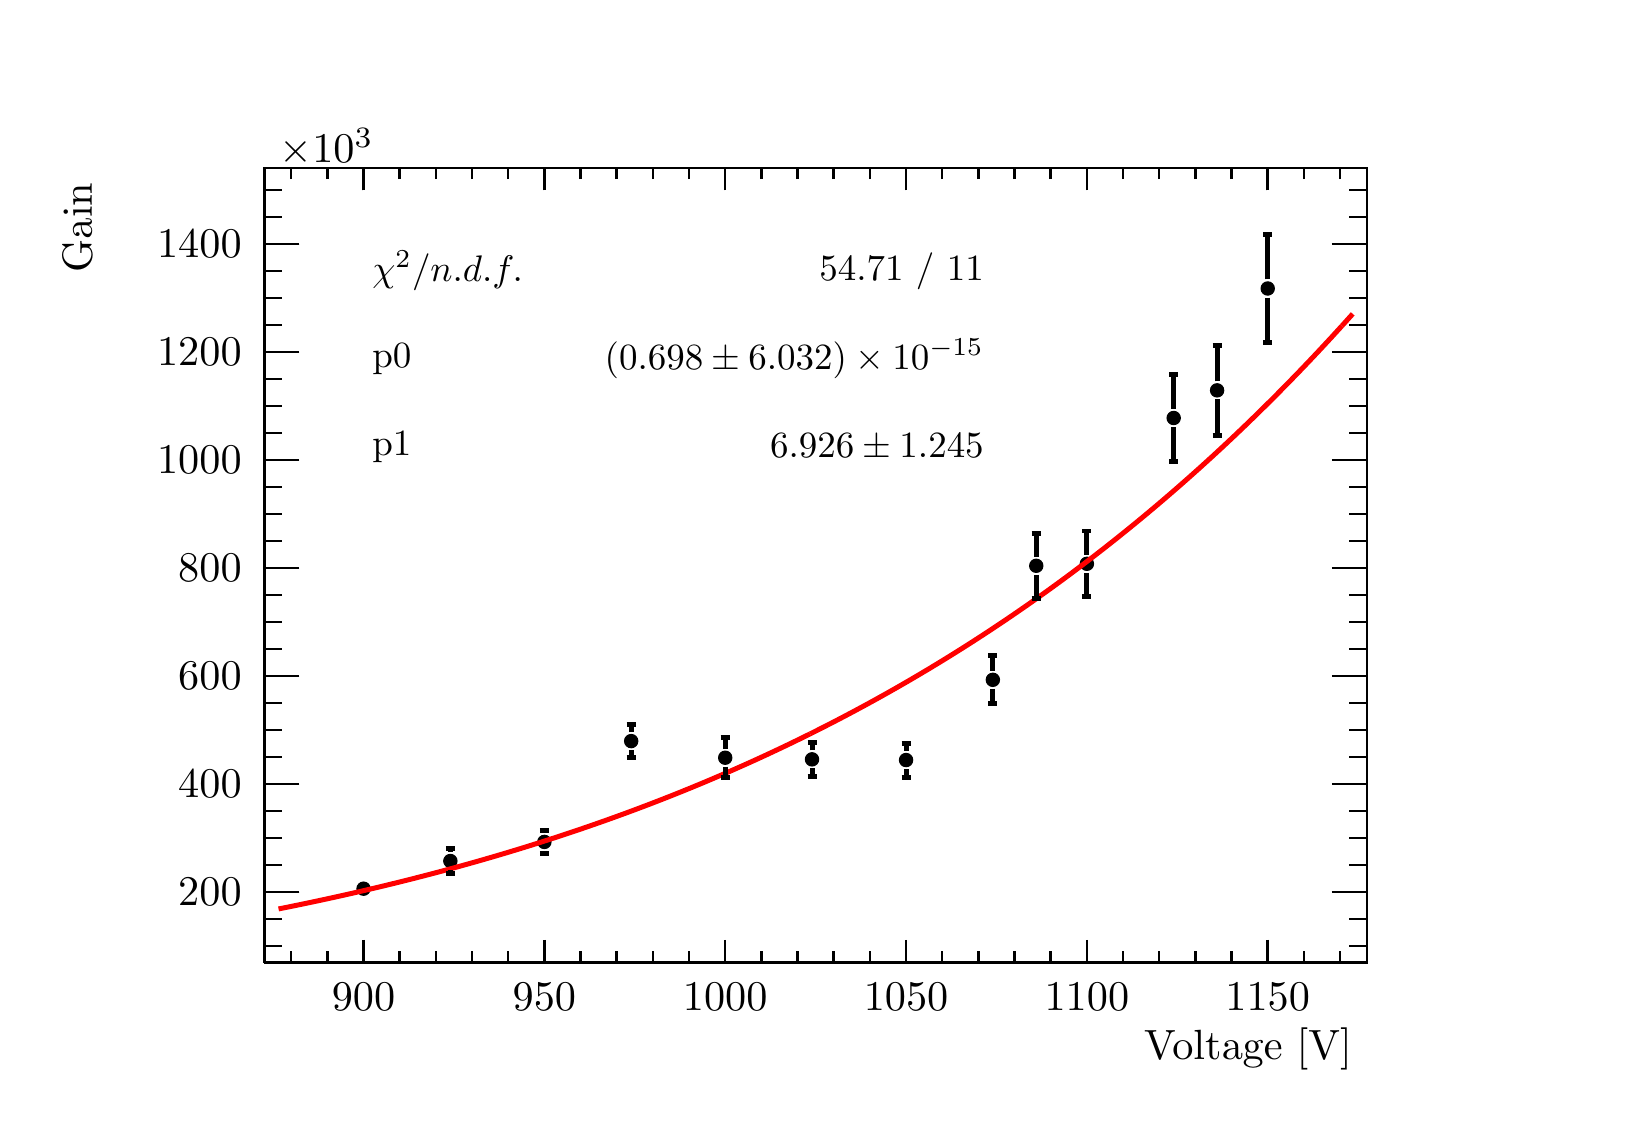
\begin{tikzpicture}
\pgfdeclareplotmark{cross} {
\pgfpathmoveto{\pgfpoint{-0.3\pgfplotmarksize}{\pgfplotmarksize}}
\pgfpathlineto{\pgfpoint{+0.3\pgfplotmarksize}{\pgfplotmarksize}}
\pgfpathlineto{\pgfpoint{+0.3\pgfplotmarksize}{0.3\pgfplotmarksize}}
\pgfpathlineto{\pgfpoint{+1\pgfplotmarksize}{0.3\pgfplotmarksize}}
\pgfpathlineto{\pgfpoint{+1\pgfplotmarksize}{-0.3\pgfplotmarksize}}
\pgfpathlineto{\pgfpoint{+0.3\pgfplotmarksize}{-0.3\pgfplotmarksize}}
\pgfpathlineto{\pgfpoint{+0.3\pgfplotmarksize}{-1.\pgfplotmarksize}}
\pgfpathlineto{\pgfpoint{-0.3\pgfplotmarksize}{-1.\pgfplotmarksize}}
\pgfpathlineto{\pgfpoint{-0.3\pgfplotmarksize}{-0.3\pgfplotmarksize}}
\pgfpathlineto{\pgfpoint{-1.\pgfplotmarksize}{-0.3\pgfplotmarksize}}
\pgfpathlineto{\pgfpoint{-1.\pgfplotmarksize}{0.3\pgfplotmarksize}}
\pgfpathlineto{\pgfpoint{-0.3\pgfplotmarksize}{0.3\pgfplotmarksize}}
\pgfpathclose
\pgfusepathqstroke
}
\pgfdeclareplotmark{cross*} {
\pgfpathmoveto{\pgfpoint{-0.3\pgfplotmarksize}{\pgfplotmarksize}}
\pgfpathlineto{\pgfpoint{+0.3\pgfplotmarksize}{\pgfplotmarksize}}
\pgfpathlineto{\pgfpoint{+0.3\pgfplotmarksize}{0.3\pgfplotmarksize}}
\pgfpathlineto{\pgfpoint{+1\pgfplotmarksize}{0.3\pgfplotmarksize}}
\pgfpathlineto{\pgfpoint{+1\pgfplotmarksize}{-0.3\pgfplotmarksize}}
\pgfpathlineto{\pgfpoint{+0.3\pgfplotmarksize}{-0.3\pgfplotmarksize}}
\pgfpathlineto{\pgfpoint{+0.3\pgfplotmarksize}{-1.\pgfplotmarksize}}
\pgfpathlineto{\pgfpoint{-0.3\pgfplotmarksize}{-1.\pgfplotmarksize}}
\pgfpathlineto{\pgfpoint{-0.3\pgfplotmarksize}{-0.3\pgfplotmarksize}}
\pgfpathlineto{\pgfpoint{-1.\pgfplotmarksize}{-0.3\pgfplotmarksize}}
\pgfpathlineto{\pgfpoint{-1.\pgfplotmarksize}{0.3\pgfplotmarksize}}
\pgfpathlineto{\pgfpoint{-0.3\pgfplotmarksize}{0.3\pgfplotmarksize}}
\pgfpathclose
\pgfusepathqfillstroke
}
\pgfdeclareplotmark{newstar} {
\pgfpathmoveto{\pgfqpoint{0pt}{\pgfplotmarksize}}
\pgfpathlineto{\pgfqpointpolar{44}{0.5\pgfplotmarksize}}
\pgfpathlineto{\pgfqpointpolar{18}{\pgfplotmarksize}}
\pgfpathlineto{\pgfqpointpolar{-20}{0.5\pgfplotmarksize}}
\pgfpathlineto{\pgfqpointpolar{-54}{\pgfplotmarksize}}
\pgfpathlineto{\pgfqpointpolar{-90}{0.5\pgfplotmarksize}}
\pgfpathlineto{\pgfqpointpolar{234}{\pgfplotmarksize}}
\pgfpathlineto{\pgfqpointpolar{198}{0.5\pgfplotmarksize}}
\pgfpathlineto{\pgfqpointpolar{162}{\pgfplotmarksize}}
\pgfpathlineto{\pgfqpointpolar{134}{0.5\pgfplotmarksize}}
\pgfpathclose
\pgfusepathqstroke
}
\pgfdeclareplotmark{newstar*} {
\pgfpathmoveto{\pgfqpoint{0pt}{\pgfplotmarksize}}
\pgfpathlineto{\pgfqpointpolar{44}{0.5\pgfplotmarksize}}
\pgfpathlineto{\pgfqpointpolar{18}{\pgfplotmarksize}}
\pgfpathlineto{\pgfqpointpolar{-20}{0.5\pgfplotmarksize}}
\pgfpathlineto{\pgfqpointpolar{-54}{\pgfplotmarksize}}
\pgfpathlineto{\pgfqpointpolar{-90}{0.5\pgfplotmarksize}}
\pgfpathlineto{\pgfqpointpolar{234}{\pgfplotmarksize}}
\pgfpathlineto{\pgfqpointpolar{198}{0.5\pgfplotmarksize}}
\pgfpathlineto{\pgfqpointpolar{162}{\pgfplotmarksize}}
\pgfpathlineto{\pgfqpointpolar{134}{0.5\pgfplotmarksize}}
\pgfpathclose
\pgfusepathqfillstroke
}
\definecolor{c}{rgb}{1,1,1};
\draw [color=c, fill=c] (0,0) rectangle (20,13.639);
\draw [color=c, fill=c] (3,1.77307) rectangle (17,11.8659);
\definecolor{c}{rgb}{0,0,0};
\draw [c,line width=0.9] (3,1.77307) -- (3,11.8659) -- (17,11.8659) -- (17,1.77307) -- (3,1.77307);
\definecolor{c}{rgb}{1,1,1};
\draw [color=c, fill=c] (3,1.77307) rectangle (17,11.8659);
\definecolor{c}{rgb}{0,0,0};
\draw [c,line width=0.9] (3,1.77307) -- (3,11.8659) -- (17,11.8659) -- (17,1.77307) -- (3,1.77307);
\draw [c,line width=0.9] (3,1.77307) -- (17,1.77307);
\draw [c,line width=0.9] (4.25853,2.05948) -- (4.25853,1.77307);
\draw [c,line width=0.9] (4.71785,1.91628) -- (4.71785,1.77307);
\draw [c,line width=0.9] (5.17717,1.91628) -- (5.17717,1.77307);
\draw [c,line width=0.9] (5.63648,1.91628) -- (5.63648,1.77307);
\draw [c,line width=0.9] (6.0958,1.91628) -- (6.0958,1.77307);
\draw [c,line width=0.9] (6.55512,2.05948) -- (6.55512,1.77307);
\draw [c,line width=0.9] (7.01444,1.91628) -- (7.01444,1.77307);
\draw [c,line width=0.9] (7.47375,1.91628) -- (7.47375,1.77307);
\draw [c,line width=0.9] (7.93307,1.91628) -- (7.93307,1.77307);
\draw [c,line width=0.9] (8.39239,1.91628) -- (8.39239,1.77307);
\draw [c,line width=0.9] (8.85171,2.05948) -- (8.85171,1.77307);
\draw [c,line width=0.9] (9.31102,1.91628) -- (9.31102,1.77307);
\draw [c,line width=0.9] (9.77034,1.91628) -- (9.77034,1.77307);
\draw [c,line width=0.9] (10.2297,1.91628) -- (10.2297,1.77307);
\draw [c,line width=0.9] (10.689,1.91628) -- (10.689,1.77307);
\draw [c,line width=0.9] (11.1483,2.05948) -- (11.1483,1.77307);
\draw [c,line width=0.9] (11.6076,1.91628) -- (11.6076,1.77307);
\draw [c,line width=0.9] (12.0669,1.91628) -- (12.0669,1.77307);
\draw [c,line width=0.9] (12.5262,1.91628) -- (12.5262,1.77307);
\draw [c,line width=0.9] (12.9856,1.91628) -- (12.9856,1.77307);
\draw [c,line width=0.9] (13.4449,2.05948) -- (13.4449,1.77307);
\draw [c,line width=0.9] (13.9042,1.91628) -- (13.9042,1.77307);
\draw [c,line width=0.9] (14.3635,1.91628) -- (14.3635,1.77307);
\draw [c,line width=0.9] (14.8228,1.91628) -- (14.8228,1.77307);
\draw [c,line width=0.9] (15.2822,1.91628) -- (15.2822,1.77307);
\draw [c,line width=0.9] (15.7415,2.05948) -- (15.7415,1.77307);
\draw [c,line width=0.9] (4.25853,2.05948) -- (4.25853,1.77307);
\draw [c,line width=0.9] (3.79921,1.91628) -- (3.79921,1.77307);
\draw [c,line width=0.9] (3.3399,1.91628) -- (3.3399,1.77307);
\draw [c,line width=0.9] (15.7415,2.05948) -- (15.7415,1.77307);
\draw [c,line width=0.9] (16.2008,1.91628) -- (16.2008,1.77307);
\draw [c,line width=0.9] (16.6601,1.91628) -- (16.6601,1.77307);
\draw [anchor=base] (4.25853,1.15931) node[scale=1.52731, color=c, rotate=0]{900};
\draw [anchor=base] (6.55512,1.15931) node[scale=1.52731, color=c, rotate=0]{950};
\draw [anchor=base] (8.85171,1.15931) node[scale=1.52731, color=c, rotate=0]{1000};
\draw [anchor=base] (11.1483,1.15931) node[scale=1.52731, color=c, rotate=0]{1050};
\draw [anchor=base] (13.4449,1.15931) node[scale=1.52731, color=c, rotate=0]{1100};
\draw [anchor=base] (15.7415,1.15931) node[scale=1.52731, color=c, rotate=0]{1150};
\draw [anchor= east] (17,0.681948) node[scale=1.52731, color=c, rotate=0]{ Voltage [V]};
\draw [c,line width=0.9] (3,11.8659) -- (17,11.8659);
\draw [c,line width=0.9] (4.25853,11.5795) -- (4.25853,11.8659);
\draw [c,line width=0.9] (4.71785,11.7227) -- (4.71785,11.8659);
\draw [c,line width=0.9] (5.17717,11.7227) -- (5.17717,11.8659);
\draw [c,line width=0.9] (5.63648,11.7227) -- (5.63648,11.8659);
\draw [c,line width=0.9] (6.0958,11.7227) -- (6.0958,11.8659);
\draw [c,line width=0.9] (6.55512,11.5795) -- (6.55512,11.8659);
\draw [c,line width=0.9] (7.01444,11.7227) -- (7.01444,11.8659);
\draw [c,line width=0.9] (7.47375,11.7227) -- (7.47375,11.8659);
\draw [c,line width=0.9] (7.93307,11.7227) -- (7.93307,11.8659);
\draw [c,line width=0.9] (8.39239,11.7227) -- (8.39239,11.8659);
\draw [c,line width=0.9] (8.85171,11.5795) -- (8.85171,11.8659);
\draw [c,line width=0.9] (9.31102,11.7227) -- (9.31102,11.8659);
\draw [c,line width=0.9] (9.77034,11.7227) -- (9.77034,11.8659);
\draw [c,line width=0.9] (10.2297,11.7227) -- (10.2297,11.8659);
\draw [c,line width=0.9] (10.689,11.7227) -- (10.689,11.8659);
\draw [c,line width=0.9] (11.1483,11.5795) -- (11.1483,11.8659);
\draw [c,line width=0.9] (11.6076,11.7227) -- (11.6076,11.8659);
\draw [c,line width=0.9] (12.0669,11.7227) -- (12.0669,11.8659);
\draw [c,line width=0.9] (12.5262,11.7227) -- (12.5262,11.8659);
\draw [c,line width=0.9] (12.9856,11.7227) -- (12.9856,11.8659);
\draw [c,line width=0.9] (13.4449,11.5795) -- (13.4449,11.8659);
\draw [c,line width=0.9] (13.9042,11.7227) -- (13.9042,11.8659);
\draw [c,line width=0.9] (14.3635,11.7227) -- (14.3635,11.8659);
\draw [c,line width=0.9] (14.8228,11.7227) -- (14.8228,11.8659);
\draw [c,line width=0.9] (15.2822,11.7227) -- (15.2822,11.8659);
\draw [c,line width=0.9] (15.7415,11.5795) -- (15.7415,11.8659);
\draw [c,line width=0.9] (4.25853,11.5795) -- (4.25853,11.8659);
\draw [c,line width=0.9] (3.79921,11.7227) -- (3.79921,11.8659);
\draw [c,line width=0.9] (3.3399,11.7227) -- (3.3399,11.8659);
\draw [c,line width=0.9] (15.7415,11.5795) -- (15.7415,11.8659);
\draw [c,line width=0.9] (16.2008,11.7227) -- (16.2008,11.8659);
\draw [c,line width=0.9] (16.6601,11.7227) -- (16.6601,11.8659);
\draw [c,line width=0.9] (3,1.77307) -- (3,11.8659);
\draw [c,line width=0.9] (3.444,2.67094) -- (3,2.67094);
\draw [c,line width=0.9] (3.222,3.01379) -- (3,3.01379);
\draw [c,line width=0.9] (3.222,3.35663) -- (3,3.35663);
\draw [c,line width=0.9] (3.222,3.69948) -- (3,3.69948);
\draw [c,line width=0.9] (3.444,4.04233) -- (3,4.04233);
\draw [c,line width=0.9] (3.222,4.38517) -- (3,4.38517);
\draw [c,line width=0.9] (3.222,4.72802) -- (3,4.72802);
\draw [c,line width=0.9] (3.222,5.07086) -- (3,5.07086);
\draw [c,line width=0.9] (3.444,5.41371) -- (3,5.41371);
\draw [c,line width=0.9] (3.222,5.75656) -- (3,5.75656);
\draw [c,line width=0.9] (3.222,6.0994) -- (3,6.0994);
\draw [c,line width=0.9] (3.222,6.44225) -- (3,6.44225);
\draw [c,line width=0.9] (3.444,6.78509) -- (3,6.78509);
\draw [c,line width=0.9] (3.222,7.12794) -- (3,7.12794);
\draw [c,line width=0.9] (3.222,7.47078) -- (3,7.47078);
\draw [c,line width=0.9] (3.222,7.81363) -- (3,7.81363);
\draw [c,line width=0.9] (3.444,8.15648) -- (3,8.15648);
\draw [c,line width=0.9] (3.222,8.49932) -- (3,8.49932);
\draw [c,line width=0.9] (3.222,8.84217) -- (3,8.84217);
\draw [c,line width=0.9] (3.222,9.18501) -- (3,9.18501);
\draw [c,line width=0.9] (3.444,9.52786) -- (3,9.52786);
\draw [c,line width=0.9] (3.222,9.8707) -- (3,9.8707);
\draw [c,line width=0.9] (3.222,10.2136) -- (3,10.2136);
\draw [c,line width=0.9] (3.222,10.5564) -- (3,10.5564);
\draw [c,line width=0.9] (3.444,10.8992) -- (3,10.8992);
\draw [c,line width=0.9] (3.444,2.67094) -- (3,2.67094);
\draw [c,line width=0.9] (3.222,2.3281) -- (3,2.3281);
\draw [c,line width=0.9] (3.222,1.98525) -- (3,1.98525);
\draw [c,line width=0.9] (3.444,10.8992) -- (3,10.8992);
\draw [c,line width=0.9] (3.222,11.2421) -- (3,11.2421);
\draw [c,line width=0.9] (3.222,11.5849) -- (3,11.5849);
\draw [anchor= east] (2.9,2.67094) node[scale=1.52731, color=c, rotate=0]{200};
\draw [anchor= east] (2.9,4.04233) node[scale=1.52731, color=c, rotate=0]{400};
\draw [anchor= east] (2.9,5.41371) node[scale=1.52731, color=c, rotate=0]{600};
\draw [anchor= east] (2.9,6.78509) node[scale=1.52731, color=c, rotate=0]{800};
\draw [anchor= east] (2.9,8.15648) node[scale=1.52731, color=c, rotate=0]{1000};
\draw [anchor= east] (2.9,9.52786) node[scale=1.52731, color=c, rotate=0]{1200};
\draw [anchor= east] (2.9,10.8992) node[scale=1.52731, color=c, rotate=0]{1400};
\draw [anchor=base west] (3,11.9341) node[scale=1.52731, color=c, rotate=0]{$\times10^{3}$};
\draw [anchor= east] (0.624642,11.8659) node[scale=1.52731, color=c, rotate=90]{ Gain};
\draw [c,line width=0.9] (17,1.77307) -- (17,11.8659);
\draw [c,line width=0.9] (16.556,2.67094) -- (17,2.67094);
\draw [c,line width=0.9] (16.778,3.01379) -- (17,3.01379);
\draw [c,line width=0.9] (16.778,3.35663) -- (17,3.35663);
\draw [c,line width=0.9] (16.778,3.69948) -- (17,3.69948);
\draw [c,line width=0.9] (16.556,4.04233) -- (17,4.04233);
\draw [c,line width=0.9] (16.778,4.38517) -- (17,4.38517);
\draw [c,line width=0.9] (16.778,4.72802) -- (17,4.72802);
\draw [c,line width=0.9] (16.778,5.07086) -- (17,5.07086);
\draw [c,line width=0.9] (16.556,5.41371) -- (17,5.41371);
\draw [c,line width=0.9] (16.778,5.75656) -- (17,5.75656);
\draw [c,line width=0.9] (16.778,6.0994) -- (17,6.0994);
\draw [c,line width=0.9] (16.778,6.44225) -- (17,6.44225);
\draw [c,line width=0.9] (16.556,6.78509) -- (17,6.78509);
\draw [c,line width=0.9] (16.778,7.12794) -- (17,7.12794);
\draw [c,line width=0.9] (16.778,7.47078) -- (17,7.47078);
\draw [c,line width=0.9] (16.778,7.81363) -- (17,7.81363);
\draw [c,line width=0.9] (16.556,8.15648) -- (17,8.15648);
\draw [c,line width=0.9] (16.778,8.49932) -- (17,8.49932);
\draw [c,line width=0.9] (16.778,8.84217) -- (17,8.84217);
\draw [c,line width=0.9] (16.778,9.18501) -- (17,9.18501);
\draw [c,line width=0.9] (16.556,9.52786) -- (17,9.52786);
\draw [c,line width=0.9] (16.778,9.8707) -- (17,9.8707);
\draw [c,line width=0.9] (16.778,10.2136) -- (17,10.2136);
\draw [c,line width=0.9] (16.778,10.5564) -- (17,10.5564);
\draw [c,line width=0.9] (16.556,10.8992) -- (17,10.8992);
\draw [c,line width=0.9] (16.556,2.67094) -- (17,2.67094);
\draw [c,line width=0.9] (16.778,2.3281) -- (17,2.3281);
\draw [c,line width=0.9] (16.778,1.98525) -- (17,1.98525);
\draw [c,line width=0.9] (16.556,10.8992) -- (17,10.8992);
\draw [c,line width=0.9] (16.778,11.2421) -- (17,11.2421);
\draw [c,line width=0.9] (16.778,11.5849) -- (17,11.5849);
\foreach \P in {(4.25853,2.71105), (5.36089,3.06272), (6.55512,3.30505), (7.65748,4.5854), (8.85171,4.37434), (9.95407,4.35366), (11.1483,4.34486), (12.2507,5.36374), (12.8018,6.81202), (13.4449,6.83732), (14.5472,8.68883), (15.0984,9.03984),
 (15.7415,10.3335)}{\draw[mark options={color=c,fill=c},mark size=2.402402pt,mark=*] plot coordinates {\P};}
\definecolor{c}{rgb}{1,0,0};
\draw [c,line width=1.8] (3.17913,2.45386) -- (3.31693,2.4815) -- (3.45472,2.50971) -- (3.59252,2.53849) -- (3.73031,2.56786) -- (3.86811,2.59782) -- (4.00591,2.62838) -- (4.1437,2.65956) -- (4.2815,2.69136) -- (4.41929,2.72379) -- (4.55709,2.75687)
 -- (4.69488,2.7906) -- (4.83268,2.825) -- (4.97047,2.86008) -- (5.10827,2.89584) -- (5.24606,2.93231) -- (5.38386,2.96948) -- (5.52165,3.00738) -- (5.65945,3.04601) -- (5.79724,3.08538) -- (5.93504,3.12551) -- (6.07283,3.16641) -- (6.21063,3.2081)
 -- (6.34843,3.25057) -- (6.48622,3.29385) -- (6.62402,3.33796) -- (6.76181,3.38289) -- (6.89961,3.42867) -- (7.0374,3.4753) -- (7.1752,3.52281) -- (7.31299,3.5712) -- (7.45079,3.62049) -- (7.58858,3.67069) -- (7.72638,3.72182) -- (7.86417,3.77389)
 -- (8.00197,3.82691) -- (8.13976,3.88091) -- (8.27756,3.93588) -- (8.41535,3.99186) -- (8.55315,4.04885) -- (8.69094,4.10687) -- (8.82874,4.16593) -- (8.96654,4.22605) -- (9.10433,4.28725) -- (9.24213,4.34954) -- (9.37992,4.41294) --
 (9.51772,4.47746) -- (9.65551,4.54312) -- (9.79331,4.60994) -- (9.9311,4.67794);
\draw [c,line width=1.8] (9.9311,4.67794) -- (10.0689,4.74712) -- (10.2067,4.81752) -- (10.3445,4.88914) -- (10.4823,4.962) -- (10.6201,5.03613) -- (10.7579,5.11154) -- (10.8957,5.18824) -- (11.0335,5.26627) -- (11.1713,5.34562) -- (11.3091,5.42633)
 -- (11.4469,5.50842) -- (11.5846,5.5919) -- (11.7224,5.67679) -- (11.8602,5.76311) -- (11.998,5.85089) -- (12.1358,5.94014) -- (12.2736,6.03088) -- (12.4114,6.12314) -- (12.5492,6.21693) -- (12.687,6.31228) -- (12.8248,6.4092) -- (12.9626,6.50772)
 -- (13.1004,6.60787) -- (13.2382,6.70966) -- (13.376,6.81311) -- (13.5138,6.91825) -- (13.6516,7.0251) -- (13.7894,7.13369) -- (13.9272,7.24403) -- (14.065,7.35615) -- (14.2028,7.47008) -- (14.3406,7.58584) -- (14.4783,7.70345) -- (14.6161,7.82294)
 -- (14.7539,7.94433) -- (14.8917,8.06765) -- (15.0295,8.19291) -- (15.1673,8.32016) -- (15.3051,8.44942) -- (15.4429,8.5807) -- (15.5807,8.71404) -- (15.7185,8.84947) -- (15.8563,8.98701) -- (15.9941,9.12668) -- (16.1319,9.26852) --
 (16.2697,9.41255) -- (16.4075,9.55881) -- (16.5453,9.70732) -- (16.6831,9.8581);
\draw [c,line width=1.8] (16.6831,9.8581) -- (16.8209,10.0112);
\definecolor{c}{rgb}{1,1,1};
\draw [color=c, fill=c] (3.75358,7.76504) rectangle (12.7507,11.1175);
\definecolor{c}{rgb}{0,0,0};
\draw [anchor= west] (4.20344,10.5587) node[scale=1.3364, color=c, rotate=0]{$\chi^{2} / \text{n.d.f.} $};
\draw [anchor= east] (12.3009,10.5587) node[scale=1.3364, color=c, rotate=0]{ 54.71 / 11};
\draw [anchor= west] (4.20344,9.44126) node[scale=1.3364, color=c, rotate=0]{p0       };
\draw [anchor= east] (12.3009,9.44126) node[scale=1.3364, color=c, rotate=0]{$ \num{6.978d-16} \pm \num{6.032d-15}$};
\draw [anchor= west] (4.20344,8.32378) node[scale=1.3364, color=c, rotate=0]{p1       };
\draw [anchor= east] (12.3009,8.32378) node[scale=1.3364, color=c, rotate=0]{$ 6.926 \pm 1.245$};
\draw [c,line width=1.8] (5.36089,3.17734) -- (5.36089,3.2271);
\draw [c,line width=1.8] (5.30359,3.2271) -- (5.4182,3.2271);
\draw [c,line width=1.8] (5.36089,2.94811) -- (5.36089,2.89834);
\draw [c,line width=1.8] (5.30359,2.89834) -- (5.4182,2.89834);
\draw [c,line width=1.8] (6.55512,3.41967) -- (6.55512,3.44871);
\draw [c,line width=1.8] (6.49781,3.44871) -- (6.61242,3.44871);
\draw [c,line width=1.8] (6.55512,3.19044) -- (6.55512,3.1614);
\draw [c,line width=1.8] (6.49781,3.1614) -- (6.61242,3.1614);
\draw [c,line width=1.8] (7.65748,4.70001) -- (7.65748,4.79579);
\draw [c,line width=1.8] (7.60017,4.79579) -- (7.71479,4.79579);
\draw [c,line width=1.8] (7.65748,4.47078) -- (7.65748,4.375);
\draw [c,line width=1.8] (7.60017,4.375) -- (7.71479,4.375);
\draw [c,line width=1.8] (8.85171,4.48895) -- (8.85171,4.63068);
\draw [c,line width=1.8] (8.7944,4.63068) -- (8.90901,4.63068);
\draw [c,line width=1.8] (8.85171,4.25973) -- (8.85171,4.118);
\draw [c,line width=1.8] (8.7944,4.118) -- (8.90901,4.118);
\draw [c,line width=1.8] (9.95407,4.46827) -- (9.95407,4.57027);
\draw [c,line width=1.8] (9.89676,4.57027) -- (10.0114,4.57027);
\draw [c,line width=1.8] (9.95407,4.23905) -- (9.95407,4.13706);
\draw [c,line width=1.8] (9.89676,4.13706) -- (10.0114,4.13706);
\draw [c,line width=1.8] (11.1483,4.45948) -- (11.1483,4.56081);
\draw [c,line width=1.8] (11.091,4.56081) -- (11.2056,4.56081);
\draw [c,line width=1.8] (11.1483,4.23025) -- (11.1483,4.12891);
\draw [c,line width=1.8] (11.091,4.12891) -- (11.2056,4.12891);
\draw [c,line width=1.8] (12.2507,5.47835) -- (12.2507,5.6703);
\draw [c,line width=1.8] (12.1933,5.6703) -- (12.308,5.6703);
\draw [c,line width=1.8] (12.2507,5.24913) -- (12.2507,5.05718);
\draw [c,line width=1.8] (12.1933,5.05718) -- (12.308,5.05718);
\draw [c,line width=1.8] (12.8018,6.92663) -- (12.8018,7.22262);
\draw [c,line width=1.8] (12.7445,7.22262) -- (12.8591,7.22262);
\draw [c,line width=1.8] (12.8018,6.6974) -- (12.8018,6.40141);
\draw [c,line width=1.8] (12.7445,6.40141) -- (12.8591,6.40141);
\draw [c,line width=1.8] (13.4449,6.95193) -- (13.4449,7.25373);
\draw [c,line width=1.8] (13.3876,7.25373) -- (13.5022,7.25373);
\draw [c,line width=1.8] (13.4449,6.7227) -- (13.4449,6.4209);
\draw [c,line width=1.8] (13.3876,6.4209) -- (13.5022,6.4209);
\draw [c,line width=1.8] (14.5472,8.80345) -- (14.5472,9.24699);
\draw [c,line width=1.8] (14.4899,9.24699) -- (14.6046,9.24699);
\draw [c,line width=1.8] (14.5472,8.57422) -- (14.5472,8.13068);
\draw [c,line width=1.8] (14.4899,8.13068) -- (14.6046,8.13068);
\draw [c,line width=1.8] (15.0984,9.15446) -- (15.0984,9.614);
\draw [c,line width=1.8] (15.0411,9.614) -- (15.1557,9.614);
\draw [c,line width=1.8] (15.0984,8.92523) -- (15.0984,8.46569);
\draw [c,line width=1.8] (15.0411,8.46569) -- (15.1557,8.46569);
\draw [c,line width=1.8] (15.7415,10.4481) -- (15.7415,11.0248);
\draw [c,line width=1.8] (15.6842,11.0248) -- (15.7988,11.0248);
\draw [c,line width=1.8] (15.7415,10.2189) -- (15.7415,9.64217);
\draw [c,line width=1.8] (15.6842,9.64217) -- (15.7988,9.64217);
\definecolor{c}{rgb}{1,1,1};
\draw [color=c, fill=c] (3.75358,7.76504) rectangle (12.7507,11.1175);
\definecolor{c}{rgb}{0,0,0};
\draw [anchor= west] (4.20344,10.5587) node[scale=1.3364, color=c, rotate=0]{$\chi^{2} / \text{n.d.f.} $};
\draw [anchor= east] (12.3009,10.5587) node[scale=1.3364, color=c, rotate=0]{ 54.71 / 11};
\draw [anchor= west] (4.20344,9.44126) node[scale=1.3364, color=c, rotate=0]{p0       };
\draw [anchor= east] (12.3009,9.44126) node[scale=1.3364, color=c, rotate=0]{$ (0.698 \pm 6.032) \times 10^{-15}$};
\draw [anchor= west] (4.20344,8.32378) node[scale=1.3364, color=c, rotate=0]{p1       };
\draw [anchor= east] (12.3009,8.32378) node[scale=1.3364, color=c, rotate=0]{$ 6.926 \pm 1.245$};
\definecolor{c}{rgb}{1,1,1};
\draw [color=c, fill=c] (2,12.8206) rectangle (18,13.5708);
\definecolor{c}{rgb}{0,0,0};
%\draw (10,13.1957) node[scale=1.20912, color=c, rotate=0]{PMT gain with varying voltage (PMT 0446, 1.5V amp., 1.5V offset)};
\end{tikzpicture}

  \end{adjustbox}
  \caption[Example of relationship between PMT voltage and gain.]{An example of the relationship between PMT voltage and gain. A curve of the form $p_{0} V^{p_{1}}$ is fitted and shown in red.}
  \label{fig:gainEx}
\end{figure}

\subsection{Measurements of bar time and position resolution}
\label{sec:hptpc_dtof_characterisation:characterisation:barRes}

In order to measure the time and position resolution of the bars, the PMTs are attached to the bars as stated in \citesec{sec:hptpc_dtof_characterisation:dtof}.
Following this, the bars are placed into a light-tight box to ensure that the PMTs do not observe light from outside sources.

A $^{90}\text{Sr}$ source is the primary tool used to evaluate the time and position resolution of the bars.
$^{90}\text{Sr}$ decays almost entirely via $\beta$-decay with an end-point of \SI{0.546}{\mega\electronvolt} to $^{90}\text{Y}$ which itself decays via $\beta$-decay with an end-point of \SI{2.28}{\mega\electronvolt}~\cite{strontium}.
These decay electrons are minimum-ionising particles, which means they have a similar energy loss profile to the particles the DToF is exposed to in the T10 beamline.
These electrons cause the bar to emit scintillation light as they traverse it.
This scintillation light is recorded by the PMTs at either end of the bar.

The $^{90}\text{Sr}$ source is placed at several measured points along the bar's long axis (\SI{16}{\cm}, \SI{32}{\cm}, \SI{48}{\cm} to the left and right of the bar centre).
The voltage of each PMT is adjusted to alter the size of the PMT signals such that, when a trigger of \SI{-15}{\milli\volt} is used, the average pulse minimum is \SI{-35}{\milli\volt}.
At each of these positions, 1000 waveforms are captured from each PMT at three different trigger levels (\SI{-10}{\milli\volt}, \SI{-15}{\milli\volt} and \SI{-20}{\milli\volt}).

The time difference between signal pulses is calculated by making a correlation graph of the two PMT pulses and finding the time of the maximum.
This maximum is taken as the time difference between signals.
This process is repeated for each trigger threshold and source position.
In each case a distribution such as the one shown in \citefig{fig:deltaTEx} is produced.
A gaussian is then fitted to the distribution (shown in red in \citefig{fig:deltaTEx}).
The difference in arrival times is taken to be equal to the mean of the gaussian while the time resolution is taken to be the standard deviation of the gaussian.

\begin{figure}[h]
  \begin{adjustbox}{max totalsize={.8\textwidth}, center}
    \begin{tikzpicture}
\pgfdeclareplotmark{cross} {
\pgfpathmoveto{\pgfpoint{-0.3\pgfplotmarksize}{\pgfplotmarksize}}
\pgfpathlineto{\pgfpoint{+0.3\pgfplotmarksize}{\pgfplotmarksize}}
\pgfpathlineto{\pgfpoint{+0.3\pgfplotmarksize}{0.3\pgfplotmarksize}}
\pgfpathlineto{\pgfpoint{+1\pgfplotmarksize}{0.3\pgfplotmarksize}}
\pgfpathlineto{\pgfpoint{+1\pgfplotmarksize}{-0.3\pgfplotmarksize}}
\pgfpathlineto{\pgfpoint{+0.3\pgfplotmarksize}{-0.3\pgfplotmarksize}}
\pgfpathlineto{\pgfpoint{+0.3\pgfplotmarksize}{-1.\pgfplotmarksize}}
\pgfpathlineto{\pgfpoint{-0.3\pgfplotmarksize}{-1.\pgfplotmarksize}}
\pgfpathlineto{\pgfpoint{-0.3\pgfplotmarksize}{-0.3\pgfplotmarksize}}
\pgfpathlineto{\pgfpoint{-1.\pgfplotmarksize}{-0.3\pgfplotmarksize}}
\pgfpathlineto{\pgfpoint{-1.\pgfplotmarksize}{0.3\pgfplotmarksize}}
\pgfpathlineto{\pgfpoint{-0.3\pgfplotmarksize}{0.3\pgfplotmarksize}}
\pgfpathclose
\pgfusepathqstroke
}
\pgfdeclareplotmark{cross*} {
\pgfpathmoveto{\pgfpoint{-0.3\pgfplotmarksize}{\pgfplotmarksize}}
\pgfpathlineto{\pgfpoint{+0.3\pgfplotmarksize}{\pgfplotmarksize}}
\pgfpathlineto{\pgfpoint{+0.3\pgfplotmarksize}{0.3\pgfplotmarksize}}
\pgfpathlineto{\pgfpoint{+1\pgfplotmarksize}{0.3\pgfplotmarksize}}
\pgfpathlineto{\pgfpoint{+1\pgfplotmarksize}{-0.3\pgfplotmarksize}}
\pgfpathlineto{\pgfpoint{+0.3\pgfplotmarksize}{-0.3\pgfplotmarksize}}
\pgfpathlineto{\pgfpoint{+0.3\pgfplotmarksize}{-1.\pgfplotmarksize}}
\pgfpathlineto{\pgfpoint{-0.3\pgfplotmarksize}{-1.\pgfplotmarksize}}
\pgfpathlineto{\pgfpoint{-0.3\pgfplotmarksize}{-0.3\pgfplotmarksize}}
\pgfpathlineto{\pgfpoint{-1.\pgfplotmarksize}{-0.3\pgfplotmarksize}}
\pgfpathlineto{\pgfpoint{-1.\pgfplotmarksize}{0.3\pgfplotmarksize}}
\pgfpathlineto{\pgfpoint{-0.3\pgfplotmarksize}{0.3\pgfplotmarksize}}
\pgfpathclose
\pgfusepathqfillstroke
}
\pgfdeclareplotmark{newstar} {
\pgfpathmoveto{\pgfqpoint{0pt}{\pgfplotmarksize}}
\pgfpathlineto{\pgfqpointpolar{44}{0.5\pgfplotmarksize}}
\pgfpathlineto{\pgfqpointpolar{18}{\pgfplotmarksize}}
\pgfpathlineto{\pgfqpointpolar{-20}{0.5\pgfplotmarksize}}
\pgfpathlineto{\pgfqpointpolar{-54}{\pgfplotmarksize}}
\pgfpathlineto{\pgfqpointpolar{-90}{0.5\pgfplotmarksize}}
\pgfpathlineto{\pgfqpointpolar{234}{\pgfplotmarksize}}
\pgfpathlineto{\pgfqpointpolar{198}{0.5\pgfplotmarksize}}
\pgfpathlineto{\pgfqpointpolar{162}{\pgfplotmarksize}}
\pgfpathlineto{\pgfqpointpolar{134}{0.5\pgfplotmarksize}}
\pgfpathclose
\pgfusepathqstroke
}
\pgfdeclareplotmark{newstar*} {
\pgfpathmoveto{\pgfqpoint{0pt}{\pgfplotmarksize}}
\pgfpathlineto{\pgfqpointpolar{44}{0.5\pgfplotmarksize}}
\pgfpathlineto{\pgfqpointpolar{18}{\pgfplotmarksize}}
\pgfpathlineto{\pgfqpointpolar{-20}{0.5\pgfplotmarksize}}
\pgfpathlineto{\pgfqpointpolar{-54}{\pgfplotmarksize}}
\pgfpathlineto{\pgfqpointpolar{-90}{0.5\pgfplotmarksize}}
\pgfpathlineto{\pgfqpointpolar{234}{\pgfplotmarksize}}
\pgfpathlineto{\pgfqpointpolar{198}{0.5\pgfplotmarksize}}
\pgfpathlineto{\pgfqpointpolar{162}{\pgfplotmarksize}}
\pgfpathlineto{\pgfqpointpolar{134}{0.5\pgfplotmarksize}}
\pgfpathclose
\pgfusepathqfillstroke
}
\definecolor{c}{rgb}{1,1,1};
\draw [color=c, fill=c] (0,0) rectangle (20,13.639);
\draw [color=c, fill=c] (3,1.77307) rectangle (17,11.8659);
\definecolor{c}{rgb}{0,0,0};
\draw [c,line width=0.9] (3,1.77307) -- (3,11.8659) -- (17,11.8659) -- (17,1.77307) -- (3,1.77307);
\definecolor{c}{rgb}{1,1,1};
\draw [color=c, fill=c] (3,1.77307) rectangle (17,11.8659);
\definecolor{c}{rgb}{0,0,0};
\draw [c,line width=0.9] (3,1.77307) -- (3,11.8659) -- (17,11.8659) -- (17,1.77307) -- (3,1.77307);
\draw [c,line width=1.8] (7.06,2.40731) -- (7.06,2.49558);
\draw [c,line width=1.8] (7.06,2.49558) -- (7.06,2.58385);
\draw [c,line width=1.8] (6.92,2.49558) -- (7.06,2.49558);
\draw [c,line width=1.8] (7.06,2.49558) -- (7.2,2.49558);
\foreach \P in {(7.06,2.49558)}{\draw[mark options={color=c,fill=c},mark size=2.402402pt,mark=*,mark size=1pt] plot coordinates {\P};}
\draw [c,line width=1.8] (7.34,5.28268) -- (7.34,5.48269);
\draw [c,line width=1.8] (7.34,5.48269) -- (7.34,5.68269);
\draw [c,line width=1.8] (7.2,5.48269) -- (7.34,5.48269);
\draw [c,line width=1.8] (7.34,5.48269) -- (7.48,5.48269);
\foreach \P in {(7.34,5.48269)}{\draw[mark options={color=c,fill=c},mark size=2.402402pt,mark=*,mark size=1pt] plot coordinates {\P};}
\draw [c,line width=1.8] (7.62,10.7521) -- (7.62,11.0687);
\draw [c,line width=1.8] (7.62,11.0687) -- (7.62,11.3853);
\draw [c,line width=1.8] (7.48,11.0687) -- (7.62,11.0687);
\draw [c,line width=1.8] (7.62,11.0687) -- (7.76,11.0687);
\foreach \P in {(7.62,11.0687)}{\draw[mark options={color=c,fill=c},mark size=2.402402pt,mark=*,mark size=1pt] plot coordinates {\P};}
\draw [c,line width=1.8] (7.9,6.43913) -- (7.9,6.6689);
\draw [c,line width=1.8] (7.9,6.6689) -- (7.9,6.89867);
\draw [c,line width=1.8] (7.76,6.6689) -- (7.9,6.6689);
\draw [c,line width=1.8] (7.9,6.6689) -- (8.04,6.6689);
\foreach \P in {(7.9,6.6689)}{\draw[mark options={color=c,fill=c},mark size=2.402402pt,mark=*,mark size=1pt] plot coordinates {\P};}
\draw [c,line width=1.8] (8.18,3.052) -- (8.18,3.17496);
\draw [c,line width=1.8] (8.18,3.17496) -- (8.18,3.29791);
\draw [c,line width=1.8] (8.04,3.17496) -- (8.18,3.17496);
\draw [c,line width=1.8] (8.18,3.17496) -- (8.32,3.17496);
\foreach \P in {(8.18,3.17496)}{\draw[mark options={color=c,fill=c},mark size=2.402402pt,mark=*,mark size=1pt] plot coordinates {\P};}
\draw [c,line width=1.8] (8.46,1.82883) -- (8.46,1.85934);
\draw [c,line width=1.8] (8.46,1.85934) -- (8.46,1.88984);
\draw [c,line width=1.8] (8.32,1.85934) -- (8.46,1.85934);
\draw [c,line width=1.8] (8.46,1.85934) -- (8.6,1.85934);
\foreach \P in {(8.46,1.85934)}{\draw[mark options={color=c,fill=c},mark size=2.402402pt,mark=*,mark size=1pt] plot coordinates {\P};}
\definecolor{c}{rgb}{1,1,1};
\draw [color=c, fill=c] (8.25215,6.44699) rectangle (16.2464,10.7736);
\definecolor{c}{rgb}{0,0,0};
\draw [anchor= west] (8.65186,10.2328) node[scale=1.08185, color=c, rotate=0]{$\chi^{2} / \text{n.d.f.} $};
\draw [anchor= east] (15.8467,10.2328) node[scale=1.08185, color=c, rotate=0]{ 23.83 / 3};
\draw [anchor= west] (8.65186,9.15115) node[scale=1.08185, color=c, rotate=0]{Constant };
\draw [anchor= east] (15.8467,9.15115) node[scale=1.08185, color=c, rotate=0]{$ 783.1 \pm 23.7$};
\draw [anchor= west] (8.65186,8.06948) node[scale=1.08185, color=c, rotate=0]{Mean     };
\draw [anchor= east] (15.8467,8.06948) node[scale=1.08185, color=c, rotate=0]{$ \num{-6.695d-9} \pm \num{1.770d-11}$};
\draw [anchor= west] (8.65186,6.98782) node[scale=1.08185, color=c, rotate=0]{Sigma    };
\draw [anchor= east] (15.8467,6.98782) node[scale=1.08185, color=c, rotate=0]{$ \num{7.517d-10} \pm \num{1.483d-11}$};
\definecolor{c}{rgb}{1,0,0};
\draw [c,line width=2.7] (6.51225,1.77307) -- (6.53675,1.77307) -- (6.56125,1.77452) -- (6.58575,1.77519) -- (6.61025,1.77616) -- (6.63475,1.77753) -- (6.65925,1.77945) -- (6.68375,1.78211) -- (6.70825,1.78577) -- (6.73275,1.79077) --
 (6.75725,1.79751) -- (6.78175,1.80653) -- (6.80625,1.81848) -- (6.83075,1.83417) -- (6.85525,1.85457) -- (6.87975,1.88084) -- (6.90425,1.91434) -- (6.92875,1.95666) -- (6.95325,2.0096) -- (6.97775,2.07517) -- (7.00225,2.15559) -- (7.02675,2.25323)
 -- (7.05125,2.37059) -- (7.07575,2.51022) -- (7.10025,2.67461) -- (7.12475,2.86615) -- (7.14925,3.08694) -- (7.17375,3.3387) -- (7.19825,3.62258) -- (7.22275,3.93907) -- (7.24725,4.28781) -- (7.27175,4.66749) -- (7.29625,5.07573) --
 (7.32075,5.50902) -- (7.34525,5.96265) -- (7.36975,6.4308) -- (7.39425,6.90654) -- (7.41875,7.38203) -- (7.44325,7.84864) -- (7.46775,8.29724) -- (7.49225,8.71848) -- (7.51675,9.10306) -- (7.54125,9.44214) -- (7.56575,9.72763) -- (7.59025,9.9525) --
 (7.61475,10.1111) -- (7.63925,10.1994) -- (7.66375,10.2151) -- (7.68825,10.1578) -- (7.71275,10.0289);
\draw [c,line width=2.7] (7.71275,10.0289) -- (7.73725,9.83189) -- (7.76175,9.57163) -- (7.78625,9.2546) -- (7.81075,8.88849) -- (7.83525,8.48187) -- (7.85975,8.04386) -- (7.88425,7.58383) -- (7.90875,7.11106) -- (7.93325,6.63442) -- (7.95775,6.1621)
 -- (7.98225,5.70146) -- (8.00675,5.25881) -- (8.03125,4.83932) -- (8.05575,4.44703) -- (8.08025,4.08479) -- (8.10475,3.75437) -- (8.12925,3.45651) -- (8.15375,3.19108) -- (8.17825,2.95719) -- (8.20275,2.75334) -- (8.22725,2.57757) --
 (8.25175,2.42762) -- (8.27625,2.30102) -- (8.30075,2.19523) -- (8.32525,2.10772) -- (8.34975,2.03606) -- (8.37425,1.97796) -- (8.39875,1.93132) -- (8.42325,1.89424) -- (8.44775,1.86505) -- (8.47225,1.84228) -- (8.49675,1.8247) -- (8.52125,1.81126)
 -- (8.54575,1.80107) -- (8.57025,1.79342) -- (8.59475,1.78773) -- (8.61925,1.78354) -- (8.64375,1.78049) -- (8.66825,1.77828) -- (8.69275,1.77669) -- (8.71725,1.77557) -- (8.74175,1.77478) -- (8.76625,1.77423) -- (8.79075,1.77307) --
 (8.81525,1.77307) -- (8.83975,1.77307) -- (8.86425,1.77307) -- (8.88875,1.77307) -- (8.91325,1.77307);
\draw [c,line width=2.7] (8.91325,1.77307) -- (8.93775,1.77307);
\definecolor{c}{rgb}{0,0,0};
\draw [c,line width=0.9] (3,1.77307) -- (17,1.77307);
\draw [c,line width=0.9] (3,2.05948) -- (3,1.77307);
\draw [c,line width=0.9] (3.35,1.91628) -- (3.35,1.77307);
\draw [c,line width=0.9] (3.7,1.91628) -- (3.7,1.77307);
\draw [c,line width=0.9] (4.05,1.91628) -- (4.05,1.77307);
\draw [c,line width=0.9] (4.4,1.91628) -- (4.4,1.77307);
\draw [c,line width=0.9] (4.75,2.05948) -- (4.75,1.77307);
\draw [c,line width=0.9] (5.1,1.91628) -- (5.1,1.77307);
\draw [c,line width=0.9] (5.45,1.91628) -- (5.45,1.77307);
\draw [c,line width=0.9] (5.8,1.91628) -- (5.8,1.77307);
\draw [c,line width=0.9] (6.15,1.91628) -- (6.15,1.77307);
\draw [c,line width=0.9] (6.5,2.05948) -- (6.5,1.77307);
\draw [c,line width=0.9] (6.85,1.91628) -- (6.85,1.77307);
\draw [c,line width=0.9] (7.2,1.91628) -- (7.2,1.77307);
\draw [c,line width=0.9] (7.55,1.91628) -- (7.55,1.77307);
\draw [c,line width=0.9] (7.9,1.91628) -- (7.9,1.77307);
\draw [c,line width=0.9] (8.25,2.05948) -- (8.25,1.77307);
\draw [c,line width=0.9] (8.6,1.91628) -- (8.6,1.77307);
\draw [c,line width=0.9] (8.95,1.91628) -- (8.95,1.77307);
\draw [c,line width=0.9] (9.3,1.91628) -- (9.3,1.77307);
\draw [c,line width=0.9] (9.65,1.91628) -- (9.65,1.77307);
\draw [c,line width=0.9] (10,2.05948) -- (10,1.77307);
\draw [c,line width=0.9] (10.35,1.91628) -- (10.35,1.77307);
\draw [c,line width=0.9] (10.7,1.91628) -- (10.7,1.77307);
\draw [c,line width=0.9] (11.05,1.91628) -- (11.05,1.77307);
\draw [c,line width=0.9] (11.4,1.91628) -- (11.4,1.77307);
\draw [c,line width=0.9] (11.75,2.05948) -- (11.75,1.77307);
\draw [c,line width=0.9] (12.1,1.91628) -- (12.1,1.77307);
\draw [c,line width=0.9] (12.45,1.91628) -- (12.45,1.77307);
\draw [c,line width=0.9] (12.8,1.91628) -- (12.8,1.77307);
\draw [c,line width=0.9] (13.15,1.91628) -- (13.15,1.77307);
\draw [c,line width=0.9] (13.5,2.05948) -- (13.5,1.77307);
\draw [c,line width=0.9] (13.85,1.91628) -- (13.85,1.77307);
\draw [c,line width=0.9] (14.2,1.91628) -- (14.2,1.77307);
\draw [c,line width=0.9] (14.55,1.91628) -- (14.55,1.77307);
\draw [c,line width=0.9] (14.9,1.91628) -- (14.9,1.77307);
\draw [c,line width=0.9] (15.25,2.05948) -- (15.25,1.77307);
\draw [c,line width=0.9] (15.6,1.91628) -- (15.6,1.77307);
\draw [c,line width=0.9] (15.95,1.91628) -- (15.95,1.77307);
\draw [c,line width=0.9] (16.3,1.91628) -- (16.3,1.77307);
\draw [c,line width=0.9] (16.65,1.91628) -- (16.65,1.77307);
\draw [c,line width=0.9] (17,2.05948) -- (17,1.77307);
\draw [anchor=base] (3,1.15931) node[scale=1.52731, color=c, rotate=0]{-20};
\draw [anchor=base] (4.75,1.15931) node[scale=1.52731, color=c, rotate=0]{-15};
\draw [anchor=base] (6.5,1.15931) node[scale=1.52731, color=c, rotate=0]{-10};
\draw [anchor=base] (8.25,1.15931) node[scale=1.52731, color=c, rotate=0]{-5};
\draw [anchor=base] (10,1.15931) node[scale=1.52731, color=c, rotate=0]{0};
\draw [anchor=base] (11.75,1.15931) node[scale=1.52731, color=c, rotate=0]{5};
\draw [anchor=base] (13.5,1.15931) node[scale=1.52731, color=c, rotate=0]{10};
\draw [anchor=base] (15.25,1.15931) node[scale=1.52731, color=c, rotate=0]{15};
\draw [anchor=base] (17,1.15931) node[scale=1.52731, color=c, rotate=0]{20};
%\draw [anchor=base west] (17.1,1.77307) node[scale=1.52731, color=c, rotate=0]{$\times10^{-9}$};
\draw [anchor= east] (17,0.681948) node[scale=1.52731, color=c, rotate=0]{$\Delta t$ [\si{\nano\second}]};
\draw [c,line width=0.9] (3,11.8659) -- (17,11.8659);
\draw [c,line width=0.9] (3,11.5795) -- (3,11.8659);
\draw [c,line width=0.9] (3.35,11.7227) -- (3.35,11.8659);
\draw [c,line width=0.9] (3.7,11.7227) -- (3.7,11.8659);
\draw [c,line width=0.9] (4.05,11.7227) -- (4.05,11.8659);
\draw [c,line width=0.9] (4.4,11.7227) -- (4.4,11.8659);
\draw [c,line width=0.9] (4.75,11.5795) -- (4.75,11.8659);
\draw [c,line width=0.9] (5.1,11.7227) -- (5.1,11.8659);
\draw [c,line width=0.9] (5.45,11.7227) -- (5.45,11.8659);
\draw [c,line width=0.9] (5.8,11.7227) -- (5.8,11.8659);
\draw [c,line width=0.9] (6.15,11.7227) -- (6.15,11.8659);
\draw [c,line width=0.9] (6.5,11.5795) -- (6.5,11.8659);
\draw [c,line width=0.9] (6.85,11.7227) -- (6.85,11.8659);
\draw [c,line width=0.9] (7.2,11.7227) -- (7.2,11.8659);
\draw [c,line width=0.9] (7.55,11.7227) -- (7.55,11.8659);
\draw [c,line width=0.9] (7.9,11.7227) -- (7.9,11.8659);
\draw [c,line width=0.9] (8.25,11.5795) -- (8.25,11.8659);
\draw [c,line width=0.9] (8.6,11.7227) -- (8.6,11.8659);
\draw [c,line width=0.9] (8.95,11.7227) -- (8.95,11.8659);
\draw [c,line width=0.9] (9.3,11.7227) -- (9.3,11.8659);
\draw [c,line width=0.9] (9.65,11.7227) -- (9.65,11.8659);
\draw [c,line width=0.9] (10,11.5795) -- (10,11.8659);
\draw [c,line width=0.9] (10.35,11.7227) -- (10.35,11.8659);
\draw [c,line width=0.9] (10.7,11.7227) -- (10.7,11.8659);
\draw [c,line width=0.9] (11.05,11.7227) -- (11.05,11.8659);
\draw [c,line width=0.9] (11.4,11.7227) -- (11.4,11.8659);
\draw [c,line width=0.9] (11.75,11.5795) -- (11.75,11.8659);
\draw [c,line width=0.9] (12.1,11.7227) -- (12.1,11.8659);
\draw [c,line width=0.9] (12.45,11.7227) -- (12.45,11.8659);
\draw [c,line width=0.9] (12.8,11.7227) -- (12.8,11.8659);
\draw [c,line width=0.9] (13.15,11.7227) -- (13.15,11.8659);
\draw [c,line width=0.9] (13.5,11.5795) -- (13.5,11.8659);
\draw [c,line width=0.9] (13.85,11.7227) -- (13.85,11.8659);
\draw [c,line width=0.9] (14.2,11.7227) -- (14.2,11.8659);
\draw [c,line width=0.9] (14.55,11.7227) -- (14.55,11.8659);
\draw [c,line width=0.9] (14.9,11.7227) -- (14.9,11.8659);
\draw [c,line width=0.9] (15.25,11.5795) -- (15.25,11.8659);
\draw [c,line width=0.9] (15.6,11.7227) -- (15.6,11.8659);
\draw [c,line width=0.9] (15.95,11.7227) -- (15.95,11.8659);
\draw [c,line width=0.9] (16.3,11.7227) -- (16.3,11.8659);
\draw [c,line width=0.9] (16.65,11.7227) -- (16.65,11.8659);
\draw [c,line width=0.9] (17,11.5795) -- (17,11.8659);
\draw [c,line width=0.9] (3,1.77307) -- (3,11.8659);
\draw [c,line width=0.9] (3.444,1.77307) -- (3,1.77307);
\draw [c,line width=0.9] (3.222,1.98874) -- (3,1.98874);
\draw [c,line width=0.9] (3.222,2.20442) -- (3,2.20442);
\draw [c,line width=0.9] (3.222,2.42009) -- (3,2.42009);
\draw [c,line width=0.9] (3.222,2.63577) -- (3,2.63577);
\draw [c,line width=0.9] (3.444,2.85144) -- (3,2.85144);
\draw [c,line width=0.9] (3.222,3.06712) -- (3,3.06712);
\draw [c,line width=0.9] (3.222,3.28279) -- (3,3.28279);
\draw [c,line width=0.9] (3.222,3.49847) -- (3,3.49847);
\draw [c,line width=0.9] (3.222,3.71415) -- (3,3.71415);
\draw [c,line width=0.9] (3.444,3.92982) -- (3,3.92982);
\draw [c,line width=0.9] (3.222,4.1455) -- (3,4.1455);
\draw [c,line width=0.9] (3.222,4.36117) -- (3,4.36117);
\draw [c,line width=0.9] (3.222,4.57685) -- (3,4.57685);
\draw [c,line width=0.9] (3.222,4.79252) -- (3,4.79252);
\draw [c,line width=0.9] (3.444,5.0082) -- (3,5.0082);
\draw [c,line width=0.9] (3.222,5.22387) -- (3,5.22387);
\draw [c,line width=0.9] (3.222,5.43955) -- (3,5.43955);
\draw [c,line width=0.9] (3.222,5.65523) -- (3,5.65523);
\draw [c,line width=0.9] (3.222,5.8709) -- (3,5.8709);
\draw [c,line width=0.9] (3.444,6.08658) -- (3,6.08658);
\draw [c,line width=0.9] (3.222,6.30225) -- (3,6.30225);
\draw [c,line width=0.9] (3.222,6.51793) -- (3,6.51793);
\draw [c,line width=0.9] (3.222,6.7336) -- (3,6.7336);
\draw [c,line width=0.9] (3.222,6.94928) -- (3,6.94928);
\draw [c,line width=0.9] (3.444,7.16495) -- (3,7.16495);
\draw [c,line width=0.9] (3.222,7.38063) -- (3,7.38063);
\draw [c,line width=0.9] (3.222,7.59631) -- (3,7.59631);
\draw [c,line width=0.9] (3.222,7.81198) -- (3,7.81198);
\draw [c,line width=0.9] (3.222,8.02766) -- (3,8.02766);
\draw [c,line width=0.9] (3.444,8.24333) -- (3,8.24333);
\draw [c,line width=0.9] (3.222,8.45901) -- (3,8.45901);
\draw [c,line width=0.9] (3.222,8.67468) -- (3,8.67468);
\draw [c,line width=0.9] (3.222,8.89036) -- (3,8.89036);
\draw [c,line width=0.9] (3.222,9.10603) -- (3,9.10603);
\draw [c,line width=0.9] (3.444,9.32171) -- (3,9.32171);
\draw [c,line width=0.9] (3.222,9.53738) -- (3,9.53738);
\draw [c,line width=0.9] (3.222,9.75306) -- (3,9.75306);
\draw [c,line width=0.9] (3.222,9.96874) -- (3,9.96874);
\draw [c,line width=0.9] (3.222,10.1844) -- (3,10.1844);
\draw [c,line width=0.9] (3.444,10.4001) -- (3,10.4001);
\draw [c,line width=0.9] (3.222,10.6158) -- (3,10.6158);
\draw [c,line width=0.9] (3.222,10.8314) -- (3,10.8314);
\draw [c,line width=0.9] (3.222,11.0471) -- (3,11.0471);
\draw [c,line width=0.9] (3.222,11.2628) -- (3,11.2628);
\draw [c,line width=0.9] (3.444,11.4785) -- (3,11.4785);
\draw [c,line width=0.9] (3.444,11.4785) -- (3,11.4785);
\draw [c,line width=0.9] (3.222,11.6941) -- (3,11.6941);
\draw [anchor= east] (2.9,1.77307) node[scale=1.52731, color=c, rotate=0]{0};
\draw [anchor= east] (2.9,2.85144) node[scale=1.52731, color=c, rotate=0]{100};
\draw [anchor= east] (2.9,3.92982) node[scale=1.52731, color=c, rotate=0]{200};
\draw [anchor= east] (2.9,5.0082) node[scale=1.52731, color=c, rotate=0]{300};
\draw [anchor= east] (2.9,6.08658) node[scale=1.52731, color=c, rotate=0]{400};
\draw [anchor= east] (2.9,7.16495) node[scale=1.52731, color=c, rotate=0]{500};
\draw [anchor= east] (2.9,8.24333) node[scale=1.52731, color=c, rotate=0]{600};
\draw [anchor= east] (2.9,9.32171) node[scale=1.52731, color=c, rotate=0]{700};
\draw [anchor= east] (2.9,10.4001) node[scale=1.52731, color=c, rotate=0]{800};
\draw [anchor= east] (2.9,11.4785) node[scale=1.52731, color=c, rotate=0]{900};
\draw [anchor= east] (1.4,11.8659) node[scale=1.52731, color=c, rotate=90]{Entries / \SI{0.4}{\nano\second}};
\draw [c,line width=0.9] (17,1.77307) -- (17,11.8659);
\draw [c,line width=0.9] (16.556,1.77307) -- (17,1.77307);
\draw [c,line width=0.9] (16.778,1.98874) -- (17,1.98874);
\draw [c,line width=0.9] (16.778,2.20442) -- (17,2.20442);
\draw [c,line width=0.9] (16.778,2.42009) -- (17,2.42009);
\draw [c,line width=0.9] (16.778,2.63577) -- (17,2.63577);
\draw [c,line width=0.9] (16.556,2.85144) -- (17,2.85144);
\draw [c,line width=0.9] (16.778,3.06712) -- (17,3.06712);
\draw [c,line width=0.9] (16.778,3.28279) -- (17,3.28279);
\draw [c,line width=0.9] (16.778,3.49847) -- (17,3.49847);
\draw [c,line width=0.9] (16.778,3.71415) -- (17,3.71415);
\draw [c,line width=0.9] (16.556,3.92982) -- (17,3.92982);
\draw [c,line width=0.9] (16.778,4.1455) -- (17,4.1455);
\draw [c,line width=0.9] (16.778,4.36117) -- (17,4.36117);
\draw [c,line width=0.9] (16.778,4.57685) -- (17,4.57685);
\draw [c,line width=0.9] (16.778,4.79252) -- (17,4.79252);
\draw [c,line width=0.9] (16.556,5.0082) -- (17,5.0082);
\draw [c,line width=0.9] (16.778,5.22387) -- (17,5.22387);
\draw [c,line width=0.9] (16.778,5.43955) -- (17,5.43955);
\draw [c,line width=0.9] (16.778,5.65523) -- (17,5.65523);
\draw [c,line width=0.9] (16.778,5.8709) -- (17,5.8709);
\draw [c,line width=0.9] (16.556,6.08658) -- (17,6.08658);
\draw [c,line width=0.9] (16.778,6.30225) -- (17,6.30225);
\draw [c,line width=0.9] (16.778,6.51793) -- (17,6.51793);
\draw [c,line width=0.9] (16.778,6.7336) -- (17,6.7336);
\draw [c,line width=0.9] (16.778,6.94928) -- (17,6.94928);
\draw [c,line width=0.9] (16.556,7.16495) -- (17,7.16495);
\draw [c,line width=0.9] (16.778,7.38063) -- (17,7.38063);
\draw [c,line width=0.9] (16.778,7.59631) -- (17,7.59631);
\draw [c,line width=0.9] (16.778,7.81198) -- (17,7.81198);
\draw [c,line width=0.9] (16.778,8.02766) -- (17,8.02766);
\draw [c,line width=0.9] (16.556,8.24333) -- (17,8.24333);
\draw [c,line width=0.9] (16.778,8.45901) -- (17,8.45901);
\draw [c,line width=0.9] (16.778,8.67468) -- (17,8.67468);
\draw [c,line width=0.9] (16.778,8.89036) -- (17,8.89036);
\draw [c,line width=0.9] (16.778,9.10603) -- (17,9.10603);
\draw [c,line width=0.9] (16.556,9.32171) -- (17,9.32171);
\draw [c,line width=0.9] (16.778,9.53738) -- (17,9.53738);
\draw [c,line width=0.9] (16.778,9.75306) -- (17,9.75306);
\draw [c,line width=0.9] (16.778,9.96874) -- (17,9.96874);
\draw [c,line width=0.9] (16.778,10.1844) -- (17,10.1844);
\draw [c,line width=0.9] (16.556,10.4001) -- (17,10.4001);
\draw [c,line width=0.9] (16.778,10.6158) -- (17,10.6158);
\draw [c,line width=0.9] (16.778,10.8314) -- (17,10.8314);
\draw [c,line width=0.9] (16.778,11.0471) -- (17,11.0471);
\draw [c,line width=0.9] (16.778,11.2628) -- (17,11.2628);
\draw [c,line width=0.9] (16.556,11.4785) -- (17,11.4785);
\draw [c,line width=0.9] (16.556,11.4785) -- (17,11.4785);
\draw [c,line width=0.9] (16.778,11.6941) -- (17,11.6941);
\definecolor{c}{rgb}{1,1,1};
\draw [color=c, fill=c] (8.25215,6.44699) rectangle (16.2464,10.7736);
\definecolor{c}{rgb}{0,0,0};
\draw [anchor= west] (8.65186,10.2328) node[scale=1.08185, color=c, rotate=0]{$\chi^{2} / \text{n.d.f.} $};
\draw [anchor= east] (15.8467,10.2328) node[scale=1.08185, color=c, rotate=0]{ 23.83 / 3};
\draw [anchor= west] (8.65186,9.15115) node[scale=1.08185, color=c, rotate=0]{Constant };
\draw [anchor= east] (15.8467,9.15115) node[scale=1.08185, color=c, rotate=0]{$ 783.1 \pm 23.7$};
\draw [anchor= west] (8.65186,8.06948) node[scale=1.08185, color=c, rotate=0]{Mean     };
\draw [anchor= east] (15.8467,8.06948) node[scale=1.08185, color=c, rotate=0]{$ (-6.695 \pm 0.018) \times 10^{-9}$};
\draw [anchor= west] (8.65186,6.98782) node[scale=1.08185, color=c, rotate=0]{Sigma    };
\draw [anchor= east] (15.8467,6.98782) node[scale=1.08185, color=c, rotate=0]{$ (7.517 \pm 0.1483)\times 10^{-10}$};
\definecolor{c}{rgb}{1,1,1};
\draw [color=c, fill=c] (2,12.8206) rectangle (18,13.5708);
\definecolor{c}{rgb}{0,0,0};
%\draw (10,13.1957) node[scale=1.40004, color=c, rotate=0]{$D1716 ^{90}Sr at 16cm, trig PMTB 15mV thresh$};
\end{tikzpicture}

  \end{adjustbox}
  \caption[Example of difference in signal arrival times for a PMT.]{Example of the difference in arrival times for a PMT. A $^{90}\text{Sr}$ source is held in a fixed position. A gaussian is fitted to the data points (shown in red).}
  \label{fig:deltaTEx}
\end{figure}

By measuring the difference in arrival time as a function of the $^{90}\text{Sr}$ position it is possible to derive a relationship between the two.
An example of such a distribution is shown in \citefigL{fig:barTimeDiffRes}.

\begin{figure}[h]
  \begin{minipage}[t]{.5\textwidth}
    \begin{adjustbox}{max totalsize={\textwidth}, center}
      \begin{tikzpicture}
\pgfdeclareplotmark{cross} {
\pgfpathmoveto{\pgfpoint{-0.3\pgfplotmarksize}{\pgfplotmarksize}}
\pgfpathlineto{\pgfpoint{+0.3\pgfplotmarksize}{\pgfplotmarksize}}
\pgfpathlineto{\pgfpoint{+0.3\pgfplotmarksize}{0.3\pgfplotmarksize}}
\pgfpathlineto{\pgfpoint{+1\pgfplotmarksize}{0.3\pgfplotmarksize}}
\pgfpathlineto{\pgfpoint{+1\pgfplotmarksize}{-0.3\pgfplotmarksize}}
\pgfpathlineto{\pgfpoint{+0.3\pgfplotmarksize}{-0.3\pgfplotmarksize}}
\pgfpathlineto{\pgfpoint{+0.3\pgfplotmarksize}{-1.\pgfplotmarksize}}
\pgfpathlineto{\pgfpoint{-0.3\pgfplotmarksize}{-1.\pgfplotmarksize}}
\pgfpathlineto{\pgfpoint{-0.3\pgfplotmarksize}{-0.3\pgfplotmarksize}}
\pgfpathlineto{\pgfpoint{-1.\pgfplotmarksize}{-0.3\pgfplotmarksize}}
\pgfpathlineto{\pgfpoint{-1.\pgfplotmarksize}{0.3\pgfplotmarksize}}
\pgfpathlineto{\pgfpoint{-0.3\pgfplotmarksize}{0.3\pgfplotmarksize}}
\pgfpathclose
\pgfusepathqstroke
}
\pgfdeclareplotmark{cross*} {
\pgfpathmoveto{\pgfpoint{-0.3\pgfplotmarksize}{\pgfplotmarksize}}
\pgfpathlineto{\pgfpoint{+0.3\pgfplotmarksize}{\pgfplotmarksize}}
\pgfpathlineto{\pgfpoint{+0.3\pgfplotmarksize}{0.3\pgfplotmarksize}}
\pgfpathlineto{\pgfpoint{+1\pgfplotmarksize}{0.3\pgfplotmarksize}}
\pgfpathlineto{\pgfpoint{+1\pgfplotmarksize}{-0.3\pgfplotmarksize}}
\pgfpathlineto{\pgfpoint{+0.3\pgfplotmarksize}{-0.3\pgfplotmarksize}}
\pgfpathlineto{\pgfpoint{+0.3\pgfplotmarksize}{-1.\pgfplotmarksize}}
\pgfpathlineto{\pgfpoint{-0.3\pgfplotmarksize}{-1.\pgfplotmarksize}}
\pgfpathlineto{\pgfpoint{-0.3\pgfplotmarksize}{-0.3\pgfplotmarksize}}
\pgfpathlineto{\pgfpoint{-1.\pgfplotmarksize}{-0.3\pgfplotmarksize}}
\pgfpathlineto{\pgfpoint{-1.\pgfplotmarksize}{0.3\pgfplotmarksize}}
\pgfpathlineto{\pgfpoint{-0.3\pgfplotmarksize}{0.3\pgfplotmarksize}}
\pgfpathclose
\pgfusepathqfillstroke
}
\pgfdeclareplotmark{newstar} {
\pgfpathmoveto{\pgfqpoint{0pt}{\pgfplotmarksize}}
\pgfpathlineto{\pgfqpointpolar{44}{0.5\pgfplotmarksize}}
\pgfpathlineto{\pgfqpointpolar{18}{\pgfplotmarksize}}
\pgfpathlineto{\pgfqpointpolar{-20}{0.5\pgfplotmarksize}}
\pgfpathlineto{\pgfqpointpolar{-54}{\pgfplotmarksize}}
\pgfpathlineto{\pgfqpointpolar{-90}{0.5\pgfplotmarksize}}
\pgfpathlineto{\pgfqpointpolar{234}{\pgfplotmarksize}}
\pgfpathlineto{\pgfqpointpolar{198}{0.5\pgfplotmarksize}}
\pgfpathlineto{\pgfqpointpolar{162}{\pgfplotmarksize}}
\pgfpathlineto{\pgfqpointpolar{134}{0.5\pgfplotmarksize}}
\pgfpathclose
\pgfusepathqstroke
}
\pgfdeclareplotmark{newstar*} {
\pgfpathmoveto{\pgfqpoint{0pt}{\pgfplotmarksize}}
\pgfpathlineto{\pgfqpointpolar{44}{0.5\pgfplotmarksize}}
\pgfpathlineto{\pgfqpointpolar{18}{\pgfplotmarksize}}
\pgfpathlineto{\pgfqpointpolar{-20}{0.5\pgfplotmarksize}}
\pgfpathlineto{\pgfqpointpolar{-54}{\pgfplotmarksize}}
\pgfpathlineto{\pgfqpointpolar{-90}{0.5\pgfplotmarksize}}
\pgfpathlineto{\pgfqpointpolar{234}{\pgfplotmarksize}}
\pgfpathlineto{\pgfqpointpolar{198}{0.5\pgfplotmarksize}}
\pgfpathlineto{\pgfqpointpolar{162}{\pgfplotmarksize}}
\pgfpathlineto{\pgfqpointpolar{134}{0.5\pgfplotmarksize}}
\pgfpathclose
\pgfusepathqfillstroke
}
\definecolor{c}{rgb}{1,1,1};
\draw [color=c, fill=c] (0,0) rectangle (20,13.639);
\draw [color=c, fill=c] (2.49284,1.76218) rectangle (17.5072,11.8768);
\definecolor{c}{rgb}{0,0,0};
\draw [c,line width=0.9] (2.49284,1.76218) -- (2.49284,11.8768) -- (17.5072,11.8768) -- (17.5072,1.76218) -- (2.49284,1.76218);
\definecolor{c}{rgb}{1,1,1};
\draw [color=c, fill=c] (2.49284,1.76218) rectangle (17.5072,11.8768);
\definecolor{c}{rgb}{0,0,0};
\draw [c,line width=0.9] (2.49284,1.76218) -- (2.49284,11.8768) -- (17.5072,11.8768) -- (17.5072,1.76218) -- (2.49284,1.76218);
\draw [c,line width=0.9] (2.49284,1.76218) -- (17.5072,1.76218);
\draw [c,line width=0.9] (4.26536,2.06935) -- (4.26536,1.76218);
\draw [c,line width=0.9] (4.91703,1.91576) -- (4.91703,1.76218);
\draw [c,line width=0.9] (5.56869,1.91576) -- (5.56869,1.76218);
\draw [c,line width=0.9] (6.22035,1.91576) -- (6.22035,1.76218);
\draw [c,line width=0.9] (6.87202,2.06935) -- (6.87202,1.76218);
\draw [c,line width=0.9] (7.52368,1.91576) -- (7.52368,1.76218);
\draw [c,line width=0.9] (8.17534,1.91576) -- (8.17534,1.76218);
\draw [c,line width=0.9] (8.82701,1.91576) -- (8.82701,1.76218);
\draw [c,line width=0.9] (9.47867,2.06935) -- (9.47867,1.76218);
\draw [c,line width=0.9] (10.1303,1.91576) -- (10.1303,1.76218);
\draw [c,line width=0.9] (10.782,1.91576) -- (10.782,1.76218);
\draw [c,line width=0.9] (11.4337,1.91576) -- (11.4337,1.76218);
\draw [c,line width=0.9] (12.0853,2.06935) -- (12.0853,1.76218);
\draw [c,line width=0.9] (12.737,1.91576) -- (12.737,1.76218);
\draw [c,line width=0.9] (13.3886,1.91576) -- (13.3886,1.76218);
\draw [c,line width=0.9] (14.0403,1.91576) -- (14.0403,1.76218);
\draw [c,line width=0.9] (14.692,2.06935) -- (14.692,1.76218);
\draw [c,line width=0.9] (15.3436,1.91576) -- (15.3436,1.76218);
\draw [c,line width=0.9] (15.9953,1.91576) -- (15.9953,1.76218);
\draw [c,line width=0.9] (16.647,1.91576) -- (16.647,1.76218);
\draw [c,line width=0.9] (17.2986,2.06935) -- (17.2986,1.76218);
\draw [c,line width=0.9] (4.26536,2.06935) -- (4.26536,1.76218);
\draw [c,line width=0.9] (3.6137,1.91576) -- (3.6137,1.76218);
\draw [c,line width=0.9] (2.96203,1.91576) -- (2.96203,1.76218);
\draw [c,line width=0.9] (17.2986,2.06935) -- (17.2986,1.76218);
\draw [anchor=base] (4.26536,1.14842) node[scale=1.52731, color=c, rotate=0]{20};
\draw [anchor=base] (6.87202,1.14842) node[scale=1.52731, color=c, rotate=0]{40};
\draw [anchor=base] (9.47867,1.14842) node[scale=1.52731, color=c, rotate=0]{60};
\draw [anchor=base] (12.0853,1.14842) node[scale=1.52731, color=c, rotate=0]{80};
\draw [anchor=base] (14.692,1.14842) node[scale=1.52731, color=c, rotate=0]{100};
\draw [anchor=base] (17.2986,1.14842) node[scale=1.52731, color=c, rotate=0]{120};
\draw [anchor= east] (17.5072,0.561948) node[scale=1.52731, color=c, rotate=0]{Source position [\si{\cm}]};
\draw [c,line width=0.9] (2.49284,11.8768) -- (17.5072,11.8768);
\draw [c,line width=0.9] (4.26536,11.5696) -- (4.26536,11.8768);
\draw [c,line width=0.9] (4.91703,11.7232) -- (4.91703,11.8768);
\draw [c,line width=0.9] (5.56869,11.7232) -- (5.56869,11.8768);
\draw [c,line width=0.9] (6.22035,11.7232) -- (6.22035,11.8768);
\draw [c,line width=0.9] (6.87202,11.5696) -- (6.87202,11.8768);
\draw [c,line width=0.9] (7.52368,11.7232) -- (7.52368,11.8768);
\draw [c,line width=0.9] (8.17534,11.7232) -- (8.17534,11.8768);
\draw [c,line width=0.9] (8.82701,11.7232) -- (8.82701,11.8768);
\draw [c,line width=0.9] (9.47867,11.5696) -- (9.47867,11.8768);
\draw [c,line width=0.9] (10.1303,11.7232) -- (10.1303,11.8768);
\draw [c,line width=0.9] (10.782,11.7232) -- (10.782,11.8768);
\draw [c,line width=0.9] (11.4337,11.7232) -- (11.4337,11.8768);
\draw [c,line width=0.9] (12.0853,11.5696) -- (12.0853,11.8768);
\draw [c,line width=0.9] (12.737,11.7232) -- (12.737,11.8768);
\draw [c,line width=0.9] (13.3886,11.7232) -- (13.3886,11.8768);
\draw [c,line width=0.9] (14.0403,11.7232) -- (14.0403,11.8768);
\draw [c,line width=0.9] (14.692,11.5696) -- (14.692,11.8768);
\draw [c,line width=0.9] (15.3436,11.7232) -- (15.3436,11.8768);
\draw [c,line width=0.9] (15.9953,11.7232) -- (15.9953,11.8768);
\draw [c,line width=0.9] (16.647,11.7232) -- (16.647,11.8768);
\draw [c,line width=0.9] (17.2986,11.5696) -- (17.2986,11.8768);
\draw [c,line width=0.9] (4.26536,11.5696) -- (4.26536,11.8768);
\draw [c,line width=0.9] (3.6137,11.7232) -- (3.6137,11.8768);
\draw [c,line width=0.9] (2.96203,11.7232) -- (2.96203,11.8768);
\draw [c,line width=0.9] (17.2986,11.5696) -- (17.2986,11.8768);
\draw [c,line width=0.9] (2.49284,1.76218) -- (2.49284,11.8768);
\draw [c,line width=0.9] (2.93779,2.94633) -- (2.49284,2.94633);
\draw [c,line width=0.9] (2.71532,3.27049) -- (2.49284,3.27049);
\draw [c,line width=0.9] (2.71532,3.59465) -- (2.49284,3.59465);
\draw [c,line width=0.9] (2.71532,3.91881) -- (2.49284,3.91881);
\draw [c,line width=0.9] (2.93779,4.24297) -- (2.49284,4.24297);
\draw [c,line width=0.9] (2.71532,4.56713) -- (2.49284,4.56713);
\draw [c,line width=0.9] (2.71532,4.89129) -- (2.49284,4.89129);
\draw [c,line width=0.9] (2.71532,5.21545) -- (2.49284,5.21545);
\draw [c,line width=0.9] (2.93779,5.53961) -- (2.49284,5.53961);
\draw [c,line width=0.9] (2.71532,5.86377) -- (2.49284,5.86377);
\draw [c,line width=0.9] (2.71532,6.18794) -- (2.49284,6.18794);
\draw [c,line width=0.9] (2.71532,6.5121) -- (2.49284,6.5121);
\draw [c,line width=0.9] (2.93779,6.83626) -- (2.49284,6.83626);
\draw [c,line width=0.9] (2.71532,7.16042) -- (2.49284,7.16042);
\draw [c,line width=0.9] (2.71532,7.48458) -- (2.49284,7.48458);
\draw [c,line width=0.9] (2.71532,7.80874) -- (2.49284,7.80874);
\draw [c,line width=0.9] (2.93779,8.1329) -- (2.49284,8.1329);
\draw [c,line width=0.9] (2.71532,8.45706) -- (2.49284,8.45706);
\draw [c,line width=0.9] (2.71532,8.78122) -- (2.49284,8.78122);
\draw [c,line width=0.9] (2.71532,9.10538) -- (2.49284,9.10538);
\draw [c,line width=0.9] (2.93779,9.42954) -- (2.49284,9.42954);
\draw [c,line width=0.9] (2.71532,9.7537) -- (2.49284,9.7537);
\draw [c,line width=0.9] (2.71532,10.0779) -- (2.49284,10.0779);
\draw [c,line width=0.9] (2.71532,10.402) -- (2.49284,10.402);
\draw [c,line width=0.9] (2.93779,10.7262) -- (2.49284,10.7262);
\draw [c,line width=0.9] (2.93779,2.94633) -- (2.49284,2.94633);
\draw [c,line width=0.9] (2.71532,2.62217) -- (2.49284,2.62217);
\draw [c,line width=0.9] (2.71532,2.29801) -- (2.49284,2.29801);
\draw [c,line width=0.9] (2.71532,1.97384) -- (2.49284,1.97384);
\draw [c,line width=0.9] (2.93779,10.7262) -- (2.49284,10.7262);
\draw [c,line width=0.9] (2.71532,11.0503) -- (2.49284,11.0503);
\draw [c,line width=0.9] (2.71532,11.3745) -- (2.49284,11.3745);
\draw [c,line width=0.9] (2.71532,11.6987) -- (2.49284,11.6987);
\draw [anchor= east] (2.39284,2.94633) node[scale=1.52731, color=c, rotate=0]{-6};
\draw [anchor= east] (2.39284,4.24297) node[scale=1.52731, color=c, rotate=0]{-4};
\draw [anchor= east] (2.39284,5.53961) node[scale=1.52731, color=c, rotate=0]{-2};
\draw [anchor= east] (2.39284,6.83626) node[scale=1.52731, color=c, rotate=0]{0};
\draw [anchor= east] (2.39284,8.1329) node[scale=1.52731, color=c, rotate=0]{2};
\draw [anchor= east] (2.39284,9.42954) node[scale=1.52731, color=c, rotate=0]{4};
\draw [anchor= east] (2.39284,10.7262) node[scale=1.52731, color=c, rotate=0]{6};
%\draw [anchor=base west] (2.49284,11.945) node[scale=1.52731, color=c, rotate=0]{$\times10^{-9}$};
\draw [anchor= east] (0.732837,11.8768) node[scale=1.52731, color=c, rotate=90]{$\Delta t$ [\si{\ns}]};
\draw [c,line width=0.9] (17.5072,1.76218) -- (17.5072,11.8768);
\draw [c,line width=0.9] (17.0622,2.94633) -- (17.5072,2.94633);
\draw [c,line width=0.9] (17.2847,3.27049) -- (17.5072,3.27049);
\draw [c,line width=0.9] (17.2847,3.59465) -- (17.5072,3.59465);
\draw [c,line width=0.9] (17.2847,3.91881) -- (17.5072,3.91881);
\draw [c,line width=0.9] (17.0622,4.24297) -- (17.5072,4.24297);
\draw [c,line width=0.9] (17.2847,4.56713) -- (17.5072,4.56713);
\draw [c,line width=0.9] (17.2847,4.89129) -- (17.5072,4.89129);
\draw [c,line width=0.9] (17.2847,5.21545) -- (17.5072,5.21545);
\draw [c,line width=0.9] (17.0622,5.53961) -- (17.5072,5.53961);
\draw [c,line width=0.9] (17.2847,5.86377) -- (17.5072,5.86377);
\draw [c,line width=0.9] (17.2847,6.18794) -- (17.5072,6.18794);
\draw [c,line width=0.9] (17.2847,6.5121) -- (17.5072,6.5121);
\draw [c,line width=0.9] (17.0622,6.83626) -- (17.5072,6.83626);
\draw [c,line width=0.9] (17.2847,7.16042) -- (17.5072,7.16042);
\draw [c,line width=0.9] (17.2847,7.48458) -- (17.5072,7.48458);
\draw [c,line width=0.9] (17.2847,7.80874) -- (17.5072,7.80874);
\draw [c,line width=0.9] (17.0622,8.1329) -- (17.5072,8.1329);
\draw [c,line width=0.9] (17.2847,8.45706) -- (17.5072,8.45706);
\draw [c,line width=0.9] (17.2847,8.78122) -- (17.5072,8.78122);
\draw [c,line width=0.9] (17.2847,9.10538) -- (17.5072,9.10538);
\draw [c,line width=0.9] (17.0622,9.42954) -- (17.5072,9.42954);
\draw [c,line width=0.9] (17.2847,9.7537) -- (17.5072,9.7537);
\draw [c,line width=0.9] (17.2847,10.0779) -- (17.5072,10.0779);
\draw [c,line width=0.9] (17.2847,10.402) -- (17.5072,10.402);
\draw [c,line width=0.9] (17.0622,10.7262) -- (17.5072,10.7262);
\draw [c,line width=0.9] (17.0622,2.94633) -- (17.5072,2.94633);
\draw [c,line width=0.9] (17.2847,2.62217) -- (17.5072,2.62217);
\draw [c,line width=0.9] (17.2847,2.29801) -- (17.5072,2.29801);
\draw [c,line width=0.9] (17.2847,1.97384) -- (17.5072,1.97384);
\draw [c,line width=0.9] (17.0622,10.7262) -- (17.5072,10.7262);
\draw [c,line width=0.9] (17.2847,11.0503) -- (17.5072,11.0503);
\draw [c,line width=0.9] (17.2847,11.3745) -- (17.5072,11.3745);
\draw [c,line width=0.9] (17.2847,11.6987) -- (17.5072,11.6987);
\definecolor{c}{rgb}{0,0,1};
\foreach \P in {(3.74403,2.61936), (5.82935,4.10118), (7.91468,5.53906), (10,6.86469), (12.0853,8.22387), (14.1706,9.65905), (16.256,11.0141)}{\draw[mark options={color=c,fill=c},mark size=2.402402pt, line width=0.000000pt, mark=*] plot coordinates
 {\P};}
\draw [c,line width=2.7] (3.03046,2.20554) -- (3.16731,2.29703) -- (3.30416,2.38852) -- (3.44101,2.48001) -- (3.57786,2.5715) -- (3.71471,2.66299) -- (3.85156,2.75448) -- (3.9884,2.84596) -- (4.12525,2.93745) -- (4.2621,3.02894) -- (4.39895,3.12043)
 -- (4.5358,3.21192) -- (4.67265,3.30341) -- (4.8095,3.3949) -- (4.94635,3.48638) -- (5.0832,3.57787) -- (5.22005,3.66936) -- (5.3569,3.76085) -- (5.49375,3.85234) -- (5.6306,3.94383) -- (5.76745,4.03532) -- (5.90429,4.12681) -- (6.04114,4.21829) --
 (6.17799,4.30978) -- (6.31484,4.40127) -- (6.45169,4.49276) -- (6.58854,4.58425) -- (6.72539,4.67574) -- (6.86224,4.76723) -- (6.99909,4.85871) -- (7.13594,4.9502) -- (7.27279,5.04169) -- (7.40964,5.13318) -- (7.54649,5.22467) -- (7.68334,5.31616)
 -- (7.82019,5.40765) -- (7.95704,5.49914) -- (8.09388,5.59062) -- (8.23073,5.68211) -- (8.36758,5.7736) -- (8.50443,5.86509) -- (8.64128,5.95658) -- (8.77813,6.04807) -- (8.91498,6.13956) -- (9.05183,6.23104) -- (9.18868,6.32253) --
 (9.32553,6.41402) -- (9.46238,6.50551) -- (9.59923,6.597) -- (9.73608,6.68849);
\draw [c,line width=2.7] (9.73608,6.68849) -- (9.87293,6.77998) -- (10.0098,6.87146) -- (10.1466,6.96295) -- (10.2835,7.05444) -- (10.4203,7.14593) -- (10.5572,7.23742) -- (10.694,7.32891) -- (10.8309,7.4204) -- (10.9677,7.51189) -- (11.1046,7.60337)
 -- (11.2414,7.69486) -- (11.3783,7.78635) -- (11.5151,7.87784) -- (11.652,7.96933) -- (11.7888,8.06082) -- (11.9257,8.15231) -- (12.0625,8.24379) -- (12.1994,8.33528) -- (12.3362,8.42677) -- (12.4731,8.51826) -- (12.6099,8.60975) --
 (12.7468,8.70124) -- (12.8836,8.79273) -- (13.0205,8.88422) -- (13.1573,8.9757) -- (13.2942,9.06719) -- (13.431,9.15868) -- (13.5679,9.25017) -- (13.7047,9.34166) -- (13.8416,9.43315) -- (13.9784,9.52464) -- (14.1153,9.61612) -- (14.2521,9.70761) --
 (14.389,9.7991) -- (14.5258,9.89059) -- (14.6627,9.98208) -- (14.7995,10.0736) -- (14.9364,10.1651) -- (15.0732,10.2565) -- (15.21,10.348) -- (15.3469,10.4395) -- (15.4837,10.531) -- (15.6206,10.6225) -- (15.7574,10.714) -- (15.8943,10.8055) --
 (16.0311,10.897) -- (16.168,10.9885) -- (16.3048,11.0799) -- (16.4417,11.1714);
\draw [c,line width=2.7] (16.4417,11.1714) -- (16.5785,11.2629);
\draw [c,line width=2.7] (3.03046,2.20554) -- (3.16731,2.29703) -- (3.30416,2.38852) -- (3.44101,2.48001) -- (3.57786,2.5715) -- (3.71471,2.66299) -- (3.85156,2.75448) -- (3.9884,2.84596) -- (4.12525,2.93745) -- (4.2621,3.02894) -- (4.39895,3.12043)
 -- (4.5358,3.21192) -- (4.67265,3.30341) -- (4.8095,3.3949) -- (4.94635,3.48638) -- (5.0832,3.57787) -- (5.22005,3.66936) -- (5.3569,3.76085) -- (5.49375,3.85234) -- (5.6306,3.94383) -- (5.76745,4.03532) -- (5.90429,4.12681) -- (6.04114,4.21829) --
 (6.17799,4.30978) -- (6.31484,4.40127) -- (6.45169,4.49276) -- (6.58854,4.58425) -- (6.72539,4.67574) -- (6.86224,4.76723) -- (6.99909,4.85871) -- (7.13594,4.9502) -- (7.27279,5.04169) -- (7.40964,5.13318) -- (7.54649,5.22467) -- (7.68334,5.31616)
 -- (7.82019,5.40765) -- (7.95704,5.49914) -- (8.09388,5.59062) -- (8.23073,5.68211) -- (8.36758,5.7736) -- (8.50443,5.86509) -- (8.64128,5.95658) -- (8.77813,6.04807) -- (8.91498,6.13956) -- (9.05183,6.23104) -- (9.18868,6.32253) --
 (9.32553,6.41402) -- (9.46238,6.50551) -- (9.59923,6.597) -- (9.73608,6.68849);
\draw [c,line width=2.7] (9.73608,6.68849) -- (9.87293,6.77998) -- (10.0098,6.87146) -- (10.1466,6.96295) -- (10.2835,7.05444) -- (10.4203,7.14593) -- (10.5572,7.23742) -- (10.694,7.32891) -- (10.8309,7.4204) -- (10.9677,7.51189) -- (11.1046,7.60337)
 -- (11.2414,7.69486) -- (11.3783,7.78635) -- (11.5151,7.87784) -- (11.652,7.96933) -- (11.7888,8.06082) -- (11.9257,8.15231) -- (12.0625,8.24379) -- (12.1994,8.33528) -- (12.3362,8.42677) -- (12.4731,8.51826) -- (12.6099,8.60975) --
 (12.7468,8.70124) -- (12.8836,8.79273) -- (13.0205,8.88422) -- (13.1573,8.9757) -- (13.2942,9.06719) -- (13.431,9.15868) -- (13.5679,9.25017) -- (13.7047,9.34166) -- (13.8416,9.43315) -- (13.9784,9.52464) -- (14.1153,9.61612) -- (14.2521,9.70761) --
 (14.389,9.7991) -- (14.5258,9.89059) -- (14.6627,9.98208) -- (14.7995,10.0736) -- (14.9364,10.1651) -- (15.0732,10.2565) -- (15.21,10.348) -- (15.3469,10.4395) -- (15.4837,10.531) -- (15.6206,10.6225) -- (15.7574,10.714) -- (15.8943,10.8055) --
 (16.0311,10.897) -- (16.168,10.9885) -- (16.3048,11.0799) -- (16.4417,11.1714);
\draw [c,line width=2.7] (16.4417,11.1714) -- (16.5785,11.2629);
\definecolor{c}{rgb}{0,1,1};
\foreach \P in {(3.74403,2.63521), (5.82935,4.07181), (7.91468,5.54747), (10,6.88907), (12.0853,8.22367), (14.1706,9.65514), (16.256,11.0918)}{\draw[mark options={color=c,fill=c},mark size=2.402402pt, line width=0.000000pt, mark=*] plot coordinates
 {\P};}
\draw [c,line width=2.7] (3.03046,2.19052) -- (3.16731,2.28249) -- (3.30416,2.37447) -- (3.44101,2.46644) -- (3.57786,2.55842) -- (3.71471,2.6504) -- (3.85156,2.74237) -- (3.9884,2.83435) -- (4.12525,2.92632) -- (4.2621,3.0183) -- (4.39895,3.11027)
 -- (4.5358,3.20225) -- (4.67265,3.29423) -- (4.8095,3.3862) -- (4.94635,3.47818) -- (5.0832,3.57015) -- (5.22005,3.66213) -- (5.3569,3.75411) -- (5.49375,3.84608) -- (5.6306,3.93806) -- (5.76745,4.03003) -- (5.90429,4.12201) -- (6.04114,4.21399) --
 (6.17799,4.30596) -- (6.31484,4.39794) -- (6.45169,4.48991) -- (6.58854,4.58189) -- (6.72539,4.67386) -- (6.86224,4.76584) -- (6.99909,4.85782) -- (7.13594,4.94979) -- (7.27279,5.04177) -- (7.40964,5.13374) -- (7.54649,5.22572) -- (7.68334,5.3177)
 -- (7.82019,5.40967) -- (7.95704,5.50165) -- (8.09388,5.59362) -- (8.23073,5.6856) -- (8.36758,5.77758) -- (8.50443,5.86955) -- (8.64128,5.96153) -- (8.77813,6.0535) -- (8.91498,6.14548) -- (9.05183,6.23745) -- (9.18868,6.32943) -- (9.32553,6.42141)
 -- (9.46238,6.51338) -- (9.59923,6.60536) -- (9.73608,6.69733);
\draw [c,line width=2.7] (9.73608,6.69733) -- (9.87293,6.78931) -- (10.0098,6.88129) -- (10.1466,6.97326) -- (10.2835,7.06524) -- (10.4203,7.15721) -- (10.5572,7.24919) -- (10.694,7.34117) -- (10.8309,7.43314) -- (10.9677,7.52512) --
 (11.1046,7.61709) -- (11.2414,7.70907) -- (11.3783,7.80104) -- (11.5151,7.89302) -- (11.652,7.985) -- (11.7888,8.07697) -- (11.9257,8.16895) -- (12.0625,8.26092) -- (12.1994,8.3529) -- (12.3362,8.44488) -- (12.4731,8.53685) -- (12.6099,8.62883) --
 (12.7468,8.7208) -- (12.8836,8.81278) -- (13.0205,8.90476) -- (13.1573,8.99673) -- (13.2942,9.08871) -- (13.431,9.18068) -- (13.5679,9.27266) -- (13.7047,9.36463) -- (13.8416,9.45661) -- (13.9784,9.54859) -- (14.1153,9.64056) -- (14.2521,9.73254) --
 (14.389,9.82451) -- (14.5258,9.91649) -- (14.6627,10.0085) -- (14.7995,10.1004) -- (14.9364,10.1924) -- (15.0732,10.2844) -- (15.21,10.3764) -- (15.3469,10.4683) -- (15.4837,10.5603) -- (15.6206,10.6523) -- (15.7574,10.7443) -- (15.8943,10.8362) --
 (16.0311,10.9282) -- (16.168,11.0202) -- (16.3048,11.1122) -- (16.4417,11.2042);
\draw [c,line width=2.7] (16.4417,11.2042) -- (16.5785,11.2961);
\draw [c,line width=2.7] (3.03046,2.19052) -- (3.16731,2.28249) -- (3.30416,2.37447) -- (3.44101,2.46644) -- (3.57786,2.55842) -- (3.71471,2.6504) -- (3.85156,2.74237) -- (3.9884,2.83435) -- (4.12525,2.92632) -- (4.2621,3.0183) -- (4.39895,3.11027)
 -- (4.5358,3.20225) -- (4.67265,3.29423) -- (4.8095,3.3862) -- (4.94635,3.47818) -- (5.0832,3.57015) -- (5.22005,3.66213) -- (5.3569,3.75411) -- (5.49375,3.84608) -- (5.6306,3.93806) -- (5.76745,4.03003) -- (5.90429,4.12201) -- (6.04114,4.21399) --
 (6.17799,4.30596) -- (6.31484,4.39794) -- (6.45169,4.48991) -- (6.58854,4.58189) -- (6.72539,4.67386) -- (6.86224,4.76584) -- (6.99909,4.85782) -- (7.13594,4.94979) -- (7.27279,5.04177) -- (7.40964,5.13374) -- (7.54649,5.22572) -- (7.68334,5.3177)
 -- (7.82019,5.40967) -- (7.95704,5.50165) -- (8.09388,5.59362) -- (8.23073,5.6856) -- (8.36758,5.77758) -- (8.50443,5.86955) -- (8.64128,5.96153) -- (8.77813,6.0535) -- (8.91498,6.14548) -- (9.05183,6.23745) -- (9.18868,6.32943) -- (9.32553,6.42141)
 -- (9.46238,6.51338) -- (9.59923,6.60536) -- (9.73608,6.69733);
\draw [c,line width=2.7] (9.73608,6.69733) -- (9.87293,6.78931) -- (10.0098,6.88129) -- (10.1466,6.97326) -- (10.2835,7.06524) -- (10.4203,7.15721) -- (10.5572,7.24919) -- (10.694,7.34117) -- (10.8309,7.43314) -- (10.9677,7.52512) --
 (11.1046,7.61709) -- (11.2414,7.70907) -- (11.3783,7.80104) -- (11.5151,7.89302) -- (11.652,7.985) -- (11.7888,8.07697) -- (11.9257,8.16895) -- (12.0625,8.26092) -- (12.1994,8.3529) -- (12.3362,8.44488) -- (12.4731,8.53685) -- (12.6099,8.62883) --
 (12.7468,8.7208) -- (12.8836,8.81278) -- (13.0205,8.90476) -- (13.1573,8.99673) -- (13.2942,9.08871) -- (13.431,9.18068) -- (13.5679,9.27266) -- (13.7047,9.36463) -- (13.8416,9.45661) -- (13.9784,9.54859) -- (14.1153,9.64056) -- (14.2521,9.73254) --
 (14.389,9.82451) -- (14.5258,9.91649) -- (14.6627,10.0085) -- (14.7995,10.1004) -- (14.9364,10.1924) -- (15.0732,10.2844) -- (15.21,10.3764) -- (15.3469,10.4683) -- (15.4837,10.5603) -- (15.6206,10.6523) -- (15.7574,10.7443) -- (15.8943,10.8362) --
 (16.0311,10.9282) -- (16.168,11.0202) -- (16.3048,11.1122) -- (16.4417,11.2042);
\draw [c,line width=2.7] (16.4417,11.2042) -- (16.5785,11.2961);
\definecolor{c}{rgb}{0,1,0};
\foreach \P in {(3.74403,2.67022), (5.82935,4.08549), (7.91468,5.52457), (10,6.91253), (12.0853,8.27106), (14.1706,9.71128), (16.256,11.0908)}{\draw[mark options={color=c,fill=c},mark size=2.402402pt, line width=0.000000pt, mark=*] plot coordinates
 {\P};}
\draw [c,line width=2.7] (3.03046,2.20784) -- (3.16731,2.29992) -- (3.30416,2.392) -- (3.44101,2.48408) -- (3.57786,2.57617) -- (3.71471,2.66825) -- (3.85156,2.76033) -- (3.9884,2.85241) -- (4.12525,2.94449) -- (4.2621,3.03657) -- (4.39895,3.12865)
 -- (4.5358,3.22073) -- (4.67265,3.31282) -- (4.8095,3.4049) -- (4.94635,3.49698) -- (5.0832,3.58906) -- (5.22005,3.68114) -- (5.3569,3.77322) -- (5.49375,3.8653) -- (5.6306,3.95738) -- (5.76745,4.04947) -- (5.90429,4.14155) -- (6.04114,4.23363) --
 (6.17799,4.32571) -- (6.31484,4.41779) -- (6.45169,4.50987) -- (6.58854,4.60195) -- (6.72539,4.69403) -- (6.86224,4.78612) -- (6.99909,4.8782) -- (7.13594,4.97028) -- (7.27279,5.06236) -- (7.40964,5.15444) -- (7.54649,5.24652) -- (7.68334,5.3386) --
 (7.82019,5.43069) -- (7.95704,5.52277) -- (8.09388,5.61485) -- (8.23073,5.70693) -- (8.36758,5.79901) -- (8.50443,5.89109) -- (8.64128,5.98317) -- (8.77813,6.07525) -- (8.91498,6.16734) -- (9.05183,6.25942) -- (9.18868,6.3515) -- (9.32553,6.44358)
 -- (9.46238,6.53566) -- (9.59923,6.62774) -- (9.73608,6.71982);
\draw [c,line width=2.7] (9.73608,6.71982) -- (9.87293,6.8119) -- (10.0098,6.90399) -- (10.1466,6.99607) -- (10.2835,7.08815) -- (10.4203,7.18023) -- (10.5572,7.27231) -- (10.694,7.36439) -- (10.8309,7.45647) -- (10.9677,7.54855) -- (11.1046,7.64064)
 -- (11.2414,7.73272) -- (11.3783,7.8248) -- (11.5151,7.91688) -- (11.652,8.00896) -- (11.7888,8.10104) -- (11.9257,8.19312) -- (12.0625,8.2852) -- (12.1994,8.37729) -- (12.3362,8.46937) -- (12.4731,8.56145) -- (12.6099,8.65353) -- (12.7468,8.74561)
 -- (12.8836,8.83769) -- (13.0205,8.92977) -- (13.1573,9.02186) -- (13.2942,9.11394) -- (13.431,9.20602) -- (13.5679,9.2981) -- (13.7047,9.39018) -- (13.8416,9.48226) -- (13.9784,9.57434) -- (14.1153,9.66642) -- (14.2521,9.75851) -- (14.389,9.85059)
 -- (14.5258,9.94267) -- (14.6627,10.0347) -- (14.7995,10.1268) -- (14.9364,10.2189) -- (15.0732,10.311) -- (15.21,10.4031) -- (15.3469,10.4952) -- (15.4837,10.5872) -- (15.6206,10.6793) -- (15.7574,10.7714) -- (15.8943,10.8635) -- (16.0311,10.9556)
 -- (16.168,11.0476) -- (16.3048,11.1397) -- (16.4417,11.2318);
\draw [c,line width=2.7] (16.4417,11.2318) -- (16.5785,11.3239);
\draw [c,line width=2.7] (3.03046,2.20784) -- (3.16731,2.29992) -- (3.30416,2.392) -- (3.44101,2.48408) -- (3.57786,2.57617) -- (3.71471,2.66825) -- (3.85156,2.76033) -- (3.9884,2.85241) -- (4.12525,2.94449) -- (4.2621,3.03657) -- (4.39895,3.12865)
 -- (4.5358,3.22073) -- (4.67265,3.31282) -- (4.8095,3.4049) -- (4.94635,3.49698) -- (5.0832,3.58906) -- (5.22005,3.68114) -- (5.3569,3.77322) -- (5.49375,3.8653) -- (5.6306,3.95738) -- (5.76745,4.04947) -- (5.90429,4.14155) -- (6.04114,4.23363) --
 (6.17799,4.32571) -- (6.31484,4.41779) -- (6.45169,4.50987) -- (6.58854,4.60195) -- (6.72539,4.69403) -- (6.86224,4.78612) -- (6.99909,4.8782) -- (7.13594,4.97028) -- (7.27279,5.06236) -- (7.40964,5.15444) -- (7.54649,5.24652) -- (7.68334,5.3386) --
 (7.82019,5.43069) -- (7.95704,5.52277) -- (8.09388,5.61485) -- (8.23073,5.70693) -- (8.36758,5.79901) -- (8.50443,5.89109) -- (8.64128,5.98317) -- (8.77813,6.07525) -- (8.91498,6.16734) -- (9.05183,6.25942) -- (9.18868,6.3515) -- (9.32553,6.44358)
 -- (9.46238,6.53566) -- (9.59923,6.62774) -- (9.73608,6.71982);
\draw [c,line width=2.7] (9.73608,6.71982) -- (9.87293,6.8119) -- (10.0098,6.90399) -- (10.1466,6.99607) -- (10.2835,7.08815) -- (10.4203,7.18023) -- (10.5572,7.27231) -- (10.694,7.36439) -- (10.8309,7.45647) -- (10.9677,7.54855) -- (11.1046,7.64064)
 -- (11.2414,7.73272) -- (11.3783,7.8248) -- (11.5151,7.91688) -- (11.652,8.00896) -- (11.7888,8.10104) -- (11.9257,8.19312) -- (12.0625,8.2852) -- (12.1994,8.37729) -- (12.3362,8.46937) -- (12.4731,8.56145) -- (12.6099,8.65353) -- (12.7468,8.74561)
 -- (12.8836,8.83769) -- (13.0205,8.92977) -- (13.1573,9.02186) -- (13.2942,9.11394) -- (13.431,9.20602) -- (13.5679,9.2981) -- (13.7047,9.39018) -- (13.8416,9.48226) -- (13.9784,9.57434) -- (14.1153,9.66642) -- (14.2521,9.75851) -- (14.389,9.85059)
 -- (14.5258,9.94267) -- (14.6627,10.0347) -- (14.7995,10.1268) -- (14.9364,10.2189) -- (15.0732,10.311) -- (15.21,10.4031) -- (15.3469,10.4952) -- (15.4837,10.5872) -- (15.6206,10.6793) -- (15.7574,10.7714) -- (15.8943,10.8635) -- (16.0311,10.9556)
 -- (16.168,11.0476) -- (16.3048,11.1397) -- (16.4417,11.2318);
\draw [c,line width=2.7] (16.4417,11.2318) -- (16.5785,11.3239);
\definecolor{c}{rgb}{1,1,1};
\draw [color=c, fill=c] (2,12.8206) rectangle (18,13.5708);
\draw [color=c, fill=c] (3.52436,7.90831) rectangle (11.5473,11.49);
\definecolor{c}{rgb}{0,0,0};
\draw [anchor=base west] (3.72493,10.8408) node[scale=1.59095, color=c, rotate=0]{Trigger thresholds};
\draw [anchor=base west] (5.53009,9.94538) node[scale=1.59095, color=c, rotate=0]{\SI{-10}{\milli\volt}};
\definecolor{c}{rgb}{0,0,0.8};
\draw [c,line width=1.8] (4.52722,10.2615) -- (4.52722,10.4155);
\draw [c,line width=1.8] (4.52722,10.0322) -- (4.52722,9.87822);
\draw [c,line width=1.8] (4.38682,10.4155) -- (4.66762,10.4155);
\draw [c,line width=1.8] (4.38682,9.87822) -- (4.66762,9.87822);
\definecolor{c}{rgb}{0,0,1};
\foreach \P in {(4.52722,10.1468)}{\draw[mark options={color=c,fill=c},mark size=2.402402pt, line width=0.000000pt, mark=*] plot coordinates {\P};}
\definecolor{c}{rgb}{0,0,0};
\draw [anchor=base west] (5.53009,9.04996) node[scale=1.59095, color=c, rotate=0]{\SI{-15}{\milli\volt}};
\definecolor{c}{rgb}{0,0.8,0.8};
\draw [c,line width=1.8] (4.52722,9.36605) -- (4.52722,9.52006);
\draw [c,line width=1.8] (4.52722,9.13682) -- (4.52722,8.98281);
\draw [c,line width=1.8] (4.38682,9.52006) -- (4.66762,9.52006);
\draw [c,line width=1.8] (4.38682,8.98281) -- (4.66762,8.98281);
\definecolor{c}{rgb}{0,1,1};
\foreach \P in {(4.52722,9.25143)}{\draw[mark options={color=c,fill=c},mark size=2.402402pt, line width=0.000000pt, mark=*] plot coordinates {\P};}
\definecolor{c}{rgb}{0,0,0};
\draw [anchor=base west] (5.53009,8.15455) node[scale=1.59095, color=c, rotate=0]{\SI{-20}{\milli\volt}};
\definecolor{c}{rgb}{0,0.8,0};
\draw [c,line width=1.8] (4.52722,8.47063) -- (4.52722,8.62464);
\draw [c,line width=1.8] (4.52722,8.2414) -- (4.52722,8.08739);
\draw [c,line width=1.8] (4.38682,8.62464) -- (4.66762,8.62464);
\draw [c,line width=1.8] (4.38682,8.08739) -- (4.66762,8.08739);
\definecolor{c}{rgb}{0,1,0};
\foreach \P in {(4.52722,8.35602)}{\draw[mark options={color=c,fill=c},mark size=2.402402pt, line width=0.000000pt, mark=*] plot coordinates {\P};}
\end{tikzpicture}

    \end{adjustbox}
  \end{minipage}
  \hfill
  \begin{minipage}[t]{.5\textwidth}
    \begin{adjustbox}{max totalsize={\textwidth}, center}
      \begin{tikzpicture}
\pgfdeclareplotmark{cross} {
\pgfpathmoveto{\pgfpoint{-0.3\pgfplotmarksize}{\pgfplotmarksize}}
\pgfpathlineto{\pgfpoint{+0.3\pgfplotmarksize}{\pgfplotmarksize}}
\pgfpathlineto{\pgfpoint{+0.3\pgfplotmarksize}{0.3\pgfplotmarksize}}
\pgfpathlineto{\pgfpoint{+1\pgfplotmarksize}{0.3\pgfplotmarksize}}
\pgfpathlineto{\pgfpoint{+1\pgfplotmarksize}{-0.3\pgfplotmarksize}}
\pgfpathlineto{\pgfpoint{+0.3\pgfplotmarksize}{-0.3\pgfplotmarksize}}
\pgfpathlineto{\pgfpoint{+0.3\pgfplotmarksize}{-1.\pgfplotmarksize}}
\pgfpathlineto{\pgfpoint{-0.3\pgfplotmarksize}{-1.\pgfplotmarksize}}
\pgfpathlineto{\pgfpoint{-0.3\pgfplotmarksize}{-0.3\pgfplotmarksize}}
\pgfpathlineto{\pgfpoint{-1.\pgfplotmarksize}{-0.3\pgfplotmarksize}}
\pgfpathlineto{\pgfpoint{-1.\pgfplotmarksize}{0.3\pgfplotmarksize}}
\pgfpathlineto{\pgfpoint{-0.3\pgfplotmarksize}{0.3\pgfplotmarksize}}
\pgfpathclose
\pgfusepathqstroke
}
\pgfdeclareplotmark{cross*} {
\pgfpathmoveto{\pgfpoint{-0.3\pgfplotmarksize}{\pgfplotmarksize}}
\pgfpathlineto{\pgfpoint{+0.3\pgfplotmarksize}{\pgfplotmarksize}}
\pgfpathlineto{\pgfpoint{+0.3\pgfplotmarksize}{0.3\pgfplotmarksize}}
\pgfpathlineto{\pgfpoint{+1\pgfplotmarksize}{0.3\pgfplotmarksize}}
\pgfpathlineto{\pgfpoint{+1\pgfplotmarksize}{-0.3\pgfplotmarksize}}
\pgfpathlineto{\pgfpoint{+0.3\pgfplotmarksize}{-0.3\pgfplotmarksize}}
\pgfpathlineto{\pgfpoint{+0.3\pgfplotmarksize}{-1.\pgfplotmarksize}}
\pgfpathlineto{\pgfpoint{-0.3\pgfplotmarksize}{-1.\pgfplotmarksize}}
\pgfpathlineto{\pgfpoint{-0.3\pgfplotmarksize}{-0.3\pgfplotmarksize}}
\pgfpathlineto{\pgfpoint{-1.\pgfplotmarksize}{-0.3\pgfplotmarksize}}
\pgfpathlineto{\pgfpoint{-1.\pgfplotmarksize}{0.3\pgfplotmarksize}}
\pgfpathlineto{\pgfpoint{-0.3\pgfplotmarksize}{0.3\pgfplotmarksize}}
\pgfpathclose
\pgfusepathqfillstroke
}
\pgfdeclareplotmark{newstar} {
\pgfpathmoveto{\pgfqpoint{0pt}{\pgfplotmarksize}}
\pgfpathlineto{\pgfqpointpolar{44}{0.5\pgfplotmarksize}}
\pgfpathlineto{\pgfqpointpolar{18}{\pgfplotmarksize}}
\pgfpathlineto{\pgfqpointpolar{-20}{0.5\pgfplotmarksize}}
\pgfpathlineto{\pgfqpointpolar{-54}{\pgfplotmarksize}}
\pgfpathlineto{\pgfqpointpolar{-90}{0.5\pgfplotmarksize}}
\pgfpathlineto{\pgfqpointpolar{234}{\pgfplotmarksize}}
\pgfpathlineto{\pgfqpointpolar{198}{0.5\pgfplotmarksize}}
\pgfpathlineto{\pgfqpointpolar{162}{\pgfplotmarksize}}
\pgfpathlineto{\pgfqpointpolar{134}{0.5\pgfplotmarksize}}
\pgfpathclose
\pgfusepathqstroke
}
\pgfdeclareplotmark{newstar*} {
\pgfpathmoveto{\pgfqpoint{0pt}{\pgfplotmarksize}}
\pgfpathlineto{\pgfqpointpolar{44}{0.5\pgfplotmarksize}}
\pgfpathlineto{\pgfqpointpolar{18}{\pgfplotmarksize}}
\pgfpathlineto{\pgfqpointpolar{-20}{0.5\pgfplotmarksize}}
\pgfpathlineto{\pgfqpointpolar{-54}{\pgfplotmarksize}}
\pgfpathlineto{\pgfqpointpolar{-90}{0.5\pgfplotmarksize}}
\pgfpathlineto{\pgfqpointpolar{234}{\pgfplotmarksize}}
\pgfpathlineto{\pgfqpointpolar{198}{0.5\pgfplotmarksize}}
\pgfpathlineto{\pgfqpointpolar{162}{\pgfplotmarksize}}
\pgfpathlineto{\pgfqpointpolar{134}{0.5\pgfplotmarksize}}
\pgfpathclose
\pgfusepathqfillstroke
}
\definecolor{c}{rgb}{1,1,1};
\draw [color=c, fill=c] (0,0) rectangle (20,13.639);
\draw [color=c, fill=c] (3,1.77307) rectangle (17,11.8659);
\definecolor{c}{rgb}{0,0,0};
\draw [c,line width=0.9] (3,1.77307) -- (3,11.8659) -- (17,11.8659) -- (17,1.77307) -- (3,1.77307);
\definecolor{c}{rgb}{1,1,1};
\draw [color=c, fill=c] (3,1.77307) rectangle (17,11.8659);
\definecolor{c}{rgb}{0,0,0};
\draw [c,line width=0.9] (3,1.77307) -- (3,11.8659) -- (17,11.8659) -- (17,1.77307) -- (3,1.77307);
\draw [c,line width=0.9] (3,1.77307) -- (17,1.77307);
\draw [c,line width=0.9] (4.65278,2.05948) -- (4.65278,1.77307);
\draw [c,line width=0.9] (5.26042,1.91628) -- (5.26042,1.77307);
\draw [c,line width=0.9] (5.86806,1.91628) -- (5.86806,1.77307);
\draw [c,line width=0.9] (6.47569,1.91628) -- (6.47569,1.77307);
\draw [c,line width=0.9] (7.08333,2.05948) -- (7.08333,1.77307);
\draw [c,line width=0.9] (7.69097,1.91628) -- (7.69097,1.77307);
\draw [c,line width=0.9] (8.29861,1.91628) -- (8.29861,1.77307);
\draw [c,line width=0.9] (8.90625,1.91628) -- (8.90625,1.77307);
\draw [c,line width=0.9] (9.51389,2.05948) -- (9.51389,1.77307);
\draw [c,line width=0.9] (10.1215,1.91628) -- (10.1215,1.77307);
\draw [c,line width=0.9] (10.7292,1.91628) -- (10.7292,1.77307);
\draw [c,line width=0.9] (11.3368,1.91628) -- (11.3368,1.77307);
\draw [c,line width=0.9] (11.9444,2.05948) -- (11.9444,1.77307);
\draw [c,line width=0.9] (12.5521,1.91628) -- (12.5521,1.77307);
\draw [c,line width=0.9] (13.1597,1.91628) -- (13.1597,1.77307);
\draw [c,line width=0.9] (13.7674,1.91628) -- (13.7674,1.77307);
\draw [c,line width=0.9] (14.375,2.05948) -- (14.375,1.77307);
\draw [c,line width=0.9] (14.9826,1.91628) -- (14.9826,1.77307);
\draw [c,line width=0.9] (15.5903,1.91628) -- (15.5903,1.77307);
\draw [c,line width=0.9] (16.1979,1.91628) -- (16.1979,1.77307);
\draw [c,line width=0.9] (16.8056,2.05948) -- (16.8056,1.77307);
\draw [c,line width=0.9] (4.65278,2.05948) -- (4.65278,1.77307);
\draw [c,line width=0.9] (4.04514,1.91628) -- (4.04514,1.77307);
\draw [c,line width=0.9] (3.4375,1.91628) -- (3.4375,1.77307);
\draw [c,line width=0.9] (16.8056,2.05948) -- (16.8056,1.77307);
\draw [anchor=base] (4.65278,1.15931) node[scale=1.52731, color=c, rotate=0]{20};
\draw [anchor=base] (7.08333,1.15931) node[scale=1.52731, color=c, rotate=0]{40};
\draw [anchor=base] (9.51389,1.15931) node[scale=1.52731, color=c, rotate=0]{60};
\draw [anchor=base] (11.9444,1.15931) node[scale=1.52731, color=c, rotate=0]{80};
\draw [anchor=base] (14.375,1.15931) node[scale=1.52731, color=c, rotate=0]{100};
\draw [anchor=base] (16.8056,1.15931) node[scale=1.52731, color=c, rotate=0]{120};
\draw [anchor= east] (17,0.572837) node[scale=1.52731, color=c, rotate=0]{Source position [\si{\cm}]};
\draw [c,line width=0.9] (3,11.8659) -- (17,11.8659);
\draw [c,line width=0.9] (4.65278,11.5795) -- (4.65278,11.8659);
\draw [c,line width=0.9] (5.26042,11.7227) -- (5.26042,11.8659);
\draw [c,line width=0.9] (5.86806,11.7227) -- (5.86806,11.8659);
\draw [c,line width=0.9] (6.47569,11.7227) -- (6.47569,11.8659);
\draw [c,line width=0.9] (7.08333,11.5795) -- (7.08333,11.8659);
\draw [c,line width=0.9] (7.69097,11.7227) -- (7.69097,11.8659);
\draw [c,line width=0.9] (8.29861,11.7227) -- (8.29861,11.8659);
\draw [c,line width=0.9] (8.90625,11.7227) -- (8.90625,11.8659);
\draw [c,line width=0.9] (9.51389,11.5795) -- (9.51389,11.8659);
\draw [c,line width=0.9] (10.1215,11.7227) -- (10.1215,11.8659);
\draw [c,line width=0.9] (10.7292,11.7227) -- (10.7292,11.8659);
\draw [c,line width=0.9] (11.3368,11.7227) -- (11.3368,11.8659);
\draw [c,line width=0.9] (11.9444,11.5795) -- (11.9444,11.8659);
\draw [c,line width=0.9] (12.5521,11.7227) -- (12.5521,11.8659);
\draw [c,line width=0.9] (13.1597,11.7227) -- (13.1597,11.8659);
\draw [c,line width=0.9] (13.7674,11.7227) -- (13.7674,11.8659);
\draw [c,line width=0.9] (14.375,11.5795) -- (14.375,11.8659);
\draw [c,line width=0.9] (14.9826,11.7227) -- (14.9826,11.8659);
\draw [c,line width=0.9] (15.5903,11.7227) -- (15.5903,11.8659);
\draw [c,line width=0.9] (16.1979,11.7227) -- (16.1979,11.8659);
\draw [c,line width=0.9] (16.8056,11.5795) -- (16.8056,11.8659);
\draw [c,line width=0.9] (4.65278,11.5795) -- (4.65278,11.8659);
\draw [c,line width=0.9] (4.04514,11.7227) -- (4.04514,11.8659);
\draw [c,line width=0.9] (3.4375,11.7227) -- (3.4375,11.8659);
\draw [c,line width=0.9] (16.8056,11.5795) -- (16.8056,11.8659);
\draw [c,line width=0.9] (3,1.77307) -- (3,11.8659);
\draw [c,line width=0.9] (3.444,1.77307) -- (3,1.77307);
\draw [c,line width=0.9] (3.222,2.02539) -- (3,2.02539);
\draw [c,line width=0.9] (3.222,2.27771) -- (3,2.27771);
\draw [c,line width=0.9] (3.222,2.53003) -- (3,2.53003);
\draw [c,line width=0.9] (3.444,2.78235) -- (3,2.78235);
\draw [c,line width=0.9] (3.222,3.03467) -- (3,3.03467);
\draw [c,line width=0.9] (3.222,3.28699) -- (3,3.28699);
\draw [c,line width=0.9] (3.222,3.53931) -- (3,3.53931);
\draw [c,line width=0.9] (3.444,3.79163) -- (3,3.79163);
\draw [c,line width=0.9] (3.222,4.04395) -- (3,4.04395);
\draw [c,line width=0.9] (3.222,4.29628) -- (3,4.29628);
\draw [c,line width=0.9] (3.222,4.5486) -- (3,4.5486);
\draw [c,line width=0.9] (3.444,4.80092) -- (3,4.80092);
\draw [c,line width=0.9] (3.222,5.05324) -- (3,5.05324);
\draw [c,line width=0.9] (3.222,5.30556) -- (3,5.30556);
\draw [c,line width=0.9] (3.222,5.55788) -- (3,5.55788);
\draw [c,line width=0.9] (3.444,5.8102) -- (3,5.8102);
\draw [c,line width=0.9] (3.222,6.06252) -- (3,6.06252);
\draw [c,line width=0.9] (3.222,6.31484) -- (3,6.31484);
\draw [c,line width=0.9] (3.222,6.56716) -- (3,6.56716);
\draw [c,line width=0.9] (3.444,6.81948) -- (3,6.81948);
\draw [c,line width=0.9] (3.222,7.07181) -- (3,7.07181);
\draw [c,line width=0.9] (3.222,7.32413) -- (3,7.32413);
\draw [c,line width=0.9] (3.222,7.57645) -- (3,7.57645);
\draw [c,line width=0.9] (3.444,7.82877) -- (3,7.82877);
\draw [c,line width=0.9] (3.222,8.08109) -- (3,8.08109);
\draw [c,line width=0.9] (3.222,8.33341) -- (3,8.33341);
\draw [c,line width=0.9] (3.222,8.58573) -- (3,8.58573);
\draw [c,line width=0.9] (3.444,8.83805) -- (3,8.83805);
\draw [c,line width=0.9] (3.222,9.09037) -- (3,9.09037);
\draw [c,line width=0.9] (3.222,9.34269) -- (3,9.34269);
\draw [c,line width=0.9] (3.222,9.59501) -- (3,9.59501);
\draw [c,line width=0.9] (3.444,9.84733) -- (3,9.84733);
\draw [c,line width=0.9] (3.222,10.0997) -- (3,10.0997);
\draw [c,line width=0.9] (3.222,10.352) -- (3,10.352);
\draw [c,line width=0.9] (3.222,10.6043) -- (3,10.6043);
\draw [c,line width=0.9] (3.444,10.8566) -- (3,10.8566);
\draw [c,line width=0.9] (3.222,11.1089) -- (3,11.1089);
\draw [c,line width=0.9] (3.222,11.3613) -- (3,11.3613);
\draw [c,line width=0.9] (3.222,11.6136) -- (3,11.6136);
\draw [c,line width=0.9] (3.444,11.8659) -- (3,11.8659);
\draw [anchor= east] (2.9,1.77307) node[scale=1.52731, color=c, rotate=0]{0};
\draw [anchor= east] (2.9,2.78235) node[scale=1.52731, color=c, rotate=0]{0.2};
\draw [anchor= east] (2.9,3.79163) node[scale=1.52731, color=c, rotate=0]{0.4};
\draw [anchor= east] (2.9,4.80092) node[scale=1.52731, color=c, rotate=0]{0.6};
\draw [anchor= east] (2.9,5.8102) node[scale=1.52731, color=c, rotate=0]{0.8};
\draw [anchor= east] (2.9,6.81948) node[scale=1.52731, color=c, rotate=0]{1};
\draw [anchor= east] (2.9,7.82877) node[scale=1.52731, color=c, rotate=0]{1.2};
\draw [anchor= east] (2.9,8.83805) node[scale=1.52731, color=c, rotate=0]{1.4};
\draw [anchor= east] (2.9,9.84733) node[scale=1.52731, color=c, rotate=0]{1.6};
\draw [anchor= east] (2.9,10.8566) node[scale=1.52731, color=c, rotate=0]{1.8};
\draw [anchor= east] (2.9,11.8659) node[scale=1.52731, color=c, rotate=0]{2};
%\draw [anchor=base west] (3,11.9341) node[scale=1.52731, color=c, rotate=0]{$\times10^{-9}$};
\draw [anchor= east] (1.24,11.8659) node[scale=1.52731, color=c, rotate=90]{Time resolution [\si{\nano\second}]};
\draw [c,line width=0.9] (17,1.77307) -- (17,11.8659);
\draw [c,line width=0.9] (16.556,1.77307) -- (17,1.77307);
\draw [c,line width=0.9] (16.778,2.02539) -- (17,2.02539);
\draw [c,line width=0.9] (16.778,2.27771) -- (17,2.27771);
\draw [c,line width=0.9] (16.778,2.53003) -- (17,2.53003);
\draw [c,line width=0.9] (16.556,2.78235) -- (17,2.78235);
\draw [c,line width=0.9] (16.778,3.03467) -- (17,3.03467);
\draw [c,line width=0.9] (16.778,3.28699) -- (17,3.28699);
\draw [c,line width=0.9] (16.778,3.53931) -- (17,3.53931);
\draw [c,line width=0.9] (16.556,3.79163) -- (17,3.79163);
\draw [c,line width=0.9] (16.778,4.04395) -- (17,4.04395);
\draw [c,line width=0.9] (16.778,4.29628) -- (17,4.29628);
\draw [c,line width=0.9] (16.778,4.5486) -- (17,4.5486);
\draw [c,line width=0.9] (16.556,4.80092) -- (17,4.80092);
\draw [c,line width=0.9] (16.778,5.05324) -- (17,5.05324);
\draw [c,line width=0.9] (16.778,5.30556) -- (17,5.30556);
\draw [c,line width=0.9] (16.778,5.55788) -- (17,5.55788);
\draw [c,line width=0.9] (16.556,5.8102) -- (17,5.8102);
\draw [c,line width=0.9] (16.778,6.06252) -- (17,6.06252);
\draw [c,line width=0.9] (16.778,6.31484) -- (17,6.31484);
\draw [c,line width=0.9] (16.778,6.56716) -- (17,6.56716);
\draw [c,line width=0.9] (16.556,6.81948) -- (17,6.81948);
\draw [c,line width=0.9] (16.778,7.07181) -- (17,7.07181);
\draw [c,line width=0.9] (16.778,7.32413) -- (17,7.32413);
\draw [c,line width=0.9] (16.778,7.57645) -- (17,7.57645);
\draw [c,line width=0.9] (16.556,7.82877) -- (17,7.82877);
\draw [c,line width=0.9] (16.778,8.08109) -- (17,8.08109);
\draw [c,line width=0.9] (16.778,8.33341) -- (17,8.33341);
\draw [c,line width=0.9] (16.778,8.58573) -- (17,8.58573);
\draw [c,line width=0.9] (16.556,8.83805) -- (17,8.83805);
\draw [c,line width=0.9] (16.778,9.09037) -- (17,9.09037);
\draw [c,line width=0.9] (16.778,9.34269) -- (17,9.34269);
\draw [c,line width=0.9] (16.778,9.59501) -- (17,9.59501);
\draw [c,line width=0.9] (16.556,9.84733) -- (17,9.84733);
\draw [c,line width=0.9] (16.778,10.0997) -- (17,10.0997);
\draw [c,line width=0.9] (16.778,10.352) -- (17,10.352);
\draw [c,line width=0.9] (16.778,10.6043) -- (17,10.6043);
\draw [c,line width=0.9] (16.556,10.8566) -- (17,10.8566);
\draw [c,line width=0.9] (16.778,11.1089) -- (17,11.1089);
\draw [c,line width=0.9] (16.778,11.3613) -- (17,11.3613);
\draw [c,line width=0.9] (16.778,11.6136) -- (17,11.6136);
\draw [c,line width=0.9] (16.556,11.8659) -- (17,11.8659);
\definecolor{c}{rgb}{0,0,0.8};
\draw [c,line width=1.8] (4.16667,5.98509) -- (6.11111,5.84775) -- (8.05556,5.53534) -- (10,6.36052) -- (11.9444,6.37402) -- (13.8889,6.66515) -- (15.8333,6.34011);
\draw [c,line width=1.8] (4.16667,5.98509) -- (4.16667,6.06411);
\draw [c,line width=1.8] (4.10936,6.06411) -- (4.22397,6.06411);
\draw [c,line width=1.8] (4.16667,5.98509) -- (4.16667,5.90607);
\draw [c,line width=1.8] (4.10936,5.90607) -- (4.22397,5.90607);
\draw [c,line width=1.8] (6.11111,5.84775) -- (6.11111,5.93156);
\draw [c,line width=1.8] (6.0538,5.93156) -- (6.16842,5.93156);
\draw [c,line width=1.8] (6.11111,5.84775) -- (6.11111,5.76394);
\draw [c,line width=1.8] (6.0538,5.76394) -- (6.16842,5.76394);
\draw [c,line width=1.8] (8.05556,5.53534) -- (8.05556,5.60074);
\draw [c,line width=1.8] (7.99825,5.60074) -- (8.11286,5.60074);
\draw [c,line width=1.8] (8.05556,5.53534) -- (8.05556,5.46994);
\draw [c,line width=1.8] (7.99825,5.46994) -- (8.11286,5.46994);
\draw [c,line width=1.8] (10,6.36052) -- (10,6.4506);
\draw [c,line width=1.8] (9.94269,6.4506) -- (10.0573,6.4506);
\draw [c,line width=1.8] (10,6.36052) -- (10,6.27044);
\draw [c,line width=1.8] (9.94269,6.27044) -- (10.0573,6.27044);
\draw [c,line width=1.8] (11.9444,6.37402) -- (11.9444,6.45468);
\draw [c,line width=1.8] (11.8871,6.45468) -- (12.0018,6.45468);
\draw [c,line width=1.8] (11.9444,6.37402) -- (11.9444,6.29335);
\draw [c,line width=1.8] (11.8871,6.29335) -- (12.0018,6.29335);
\draw [c,line width=1.8] (13.8889,6.66515) -- (13.8889,6.75316);
\draw [c,line width=1.8] (13.8316,6.75316) -- (13.9462,6.75316);
\draw [c,line width=1.8] (13.8889,6.66515) -- (13.8889,6.57714);
\draw [c,line width=1.8] (13.8316,6.57714) -- (13.9462,6.57714);
\draw [c,line width=1.8] (15.8333,6.34011) -- (15.8333,6.4273);
\draw [c,line width=1.8] (15.776,6.4273) -- (15.8906,6.4273);
\draw [c,line width=1.8] (15.8333,6.34011) -- (15.8333,6.25292);
\draw [c,line width=1.8] (15.776,6.25292) -- (15.8906,6.25292);
\definecolor{c}{rgb}{1,1,1};
\draw [color=c, fill=c] (2,12.8206) rectangle (18,13.5708);
\definecolor{c}{rgb}{0,0,0};
%\draw (10,13.1957) node[scale=1.40004, color=c, rotate=0]{Graph};
\definecolor{c}{rgb}{0,0.8,0.8};
\draw [c,line width=1.8] (4.16667,5.32349) -- (4.16667,5.40077);
\draw [c,line width=1.8] (4.10936,5.40077) -- (4.22397,5.40077);
\draw [c,line width=1.8] (4.16667,5.32349) -- (4.16667,5.24622);
\draw [c,line width=1.8] (4.10936,5.24622) -- (4.22397,5.24622);
\draw [c,line width=1.8] (6.11111,5.70334) -- (6.11111,5.78466);
\draw [c,line width=1.8] (6.0538,5.78466) -- (6.16842,5.78466);
\draw [c,line width=1.8] (6.11111,5.70334) -- (6.11111,5.62203);
\draw [c,line width=1.8] (6.0538,5.62203) -- (6.16842,5.62203);
\draw [c,line width=1.8] (8.05556,5.48788) -- (8.05556,5.55617);
\draw [c,line width=1.8] (7.99825,5.55617) -- (8.11286,5.55617);
\draw [c,line width=1.8] (8.05556,5.48788) -- (8.05556,5.41958);
\draw [c,line width=1.8] (7.99825,5.41958) -- (8.11286,5.41958);
\draw [c,line width=1.8] (10,6.08039) -- (10,6.15143);
\draw [c,line width=1.8] (9.94269,6.15143) -- (10.0573,6.15143);
\draw [c,line width=1.8] (10,6.08039) -- (10,6.00934);
\draw [c,line width=1.8] (9.94269,6.00934) -- (10.0573,6.00934);
\draw [c,line width=1.8] (11.9444,5.89527) -- (11.9444,5.94834);
\draw [c,line width=1.8] (11.8871,5.94834) -- (12.0018,5.94834);
\draw [c,line width=1.8] (11.9444,5.89527) -- (11.9444,5.8422);
\draw [c,line width=1.8] (11.8871,5.8422) -- (12.0018,5.8422);
\draw [c,line width=1.8] (13.8889,6.20781) -- (13.8889,6.26561);
\draw [c,line width=1.8] (13.8316,6.26561) -- (13.9462,6.26561);
\draw [c,line width=1.8] (13.8889,6.20781) -- (13.8889,6.15001);
\draw [c,line width=1.8] (13.8316,6.15001) -- (13.9462,6.15001);
\draw [c,line width=1.8] (15.8333,6.20984) -- (15.8333,6.27819);
\draw [c,line width=1.8] (15.776,6.27819) -- (15.8906,6.27819);
\draw [c,line width=1.8] (15.8333,6.20984) -- (15.8333,6.14149);
\draw [c,line width=1.8] (15.776,6.14149) -- (15.8906,6.14149);
\draw [c,line width=1.8] (4.16667,5.32349) -- (6.11111,5.70334) -- (8.05556,5.48788) -- (10,6.08039) -- (11.9444,5.89527) -- (13.8889,6.20781) -- (15.8333,6.20984);
\definecolor{c}{rgb}{0,0.8,0};
\draw [c,line width=1.8] (4.16667,5.34196) -- (4.16667,5.42887);
\draw [c,line width=1.8] (4.10936,5.42887) -- (4.22397,5.42887);
\draw [c,line width=1.8] (4.16667,5.34196) -- (4.16667,5.25505);
\draw [c,line width=1.8] (4.10936,5.25505) -- (4.22397,5.25505);
\draw [c,line width=1.8] (6.11111,5.37893) -- (6.11111,5.45813);
\draw [c,line width=1.8] (6.0538,5.45813) -- (6.16842,5.45813);
\draw [c,line width=1.8] (6.11111,5.37893) -- (6.11111,5.29973);
\draw [c,line width=1.8] (6.0538,5.29973) -- (6.16842,5.29973);
\draw [c,line width=1.8] (8.05556,5.43582) -- (8.05556,5.52308);
\draw [c,line width=1.8] (7.99825,5.52308) -- (8.11286,5.52308);
\draw [c,line width=1.8] (8.05556,5.43582) -- (8.05556,5.34856);
\draw [c,line width=1.8] (7.99825,5.34856) -- (8.11286,5.34856);
\draw [c,line width=1.8] (10,5.72461) -- (10,5.80754);
\draw [c,line width=1.8] (9.94269,5.80754) -- (10.0573,5.80754);
\draw [c,line width=1.8] (10,5.72461) -- (10,5.64169);
\draw [c,line width=1.8] (9.94269,5.64169) -- (10.0573,5.64169);
\draw [c,line width=1.8] (11.9444,5.66797) -- (11.9444,5.73163);
\draw [c,line width=1.8] (11.8871,5.73163) -- (12.0018,5.73163);
\draw [c,line width=1.8] (11.9444,5.66797) -- (11.9444,5.60432);
\draw [c,line width=1.8] (11.8871,5.60432) -- (12.0018,5.60432);
\draw [c,line width=1.8] (13.8889,6.09882) -- (13.8889,6.15273);
\draw [c,line width=1.8] (13.8316,6.15273) -- (13.9462,6.15273);
\draw [c,line width=1.8] (13.8889,6.09882) -- (13.8889,6.0449);
\draw [c,line width=1.8] (13.8316,6.0449) -- (13.9462,6.0449);
\draw [c,line width=1.8] (15.8333,6.15371) -- (15.8333,6.22691);
\draw [c,line width=1.8] (15.776,6.22691) -- (15.8906,6.22691);
\draw [c,line width=1.8] (15.8333,6.15371) -- (15.8333,6.0805);
\draw [c,line width=1.8] (15.776,6.0805) -- (15.8906,6.0805);
\draw [c,line width=1.8] (4.16667,5.34196) -- (6.11111,5.37893) -- (8.05556,5.43582) -- (10,5.72461) -- (11.9444,5.66797) -- (13.8889,6.09882) -- (15.8333,6.15371);
\definecolor{c}{rgb}{1,1,1};
\draw [color=c, fill=c] (4.95702,7.44986) rectangle (14.2407,10.9742);
\definecolor{c}{rgb}{0,0,0};
\draw [anchor=base west] (5.18911,10.3354) node[scale=1.59095, color=c, rotate=0]{Trigger thresholds};
\draw [anchor=base west] (7.27794,9.45433) node[scale=1.59095, color=c, rotate=0]{\SI{-10}{\milli\volt}};
\definecolor{c}{rgb}{0,0,0.8};
\draw [c,line width=1.8] (5.30516,9.65258) -- (6.9298,9.65258);
\definecolor{c}{rgb}{0,0,0};
\draw [anchor=base west] (7.27794,8.57325) node[scale=1.59095, color=c, rotate=0]{\SI{-15}{\milli\volt}};
\definecolor{c}{rgb}{0,0.8,0.8};
\draw [c,line width=1.8] (5.30516,8.77149) -- (6.9298,8.77149);
\definecolor{c}{rgb}{0,0,0};
\draw [anchor=base west] (7.27794,7.69216) node[scale=1.59095, color=c, rotate=0]{\SI{-20}{\milli\volt}};
\definecolor{c}{rgb}{0,0.8,0};
\draw [c,line width=1.8] (5.30516,7.8904) -- (6.9298,7.8904);
\end{tikzpicture}

    \end{adjustbox}
  \end{minipage}
  \caption[Examples of bar time difference and time resolution as a function of source position.]{Left: Example of bar time difference as a function of $^{90}\text{Sr}$ source position for various trigger thresholds. Right: Example of bar time resolution as a function of $^{90}\text{Sr}$ source position for various trigger thresholds. }
  \label{fig:barTimeDiffRes}
\end{figure}

One can derive two pieces of information from \citefigL{fig:barTimeDiffRes}.
Firstly, the relationship between the source position and signal arrival time appears to be linear.
When a first order polynomial is fitted to the data points, one finds that the signal propagates down the bar at approximately \SI{7.5}{\cm\per\nano\second}.
This was found to be constant for all bars.
Secondly, the trigger threshold has no effect on the relationship between source position and signal arrival time difference.

\citefig{fig:barTimeDiffRes} right, shows that the time resolution remains roughly constant as a function of source position along the bar, with some slight variation depending on the trigger threshold used.
Lower trigger thresholds appear to slightly degrade the timing resolution.
Across all bars, the time resolution is found to be approximately \SI{0.9}{\nano\second}.
When combined with the measurement of the bar signal propagation, this equates to a position resolution of \SI{7}{\cm}.

\section{Conclusions}
\label{sec:hptpc_dtof_characterisation:conclusions}

In this chapter the construction and characterisation of a time of flight system is described. 
As part of this characterisation, the time and position resolution of the system is measured.
The time resolution is found to be approximately \SI{0.9}{\ns} while the equivalent position resolution is measured as \SI{7}{\cm}.

This system is utilised during a 2018 beam test at CERN.
The resulting analysis is detailed in \citechap{sec:hptpc_beam_flux}.

\chapter{Measurements of the CERN T10 beam flux}
\label{sec:hptpc_beam_flux}

\section{Motivation}
\label{sec:hptpc_beam_flux:motivation}

As mentioned in \citesec{sec:theory:currentState}, one of the targets of the next generation of long baseline neutrino oscillation experiments is the measurement of \dcp.
In order to make this measurement, systematic uncertainties will have to be significantly reduced.
In the current generation of neutrino oscillation experiments, uncertainties relating to the neutrino-nucleus interaction model make up a large part of the overall systematic budget.
For example, NOvA's most recent results assign systematic uncertainties from its interaction model of $3.2-5.8\%$ on its \nue and \anue signal rates~\cite{novaRecent}.
The T2K experiment has reported systematic uncertainties of $7-9\%$ on the rate of far detector electron-like events (after the near detector constraint has been applied) where cross-section uncertainties are the largest part of this~\cite{t2kRecent}.

Reducing these systematic uncertainties relies upon better modelling of neutrino-nucleus interactions.
It is also important to have an accurate interaction model in order to infer the neutrino energy from the observed events.
A illustrative diagram showcasing the dependence on the interaction model is shown in \citefig{fig:fsiDiag}.

\begin{figure}[h]
  \centering
  \includegraphics[width=\linewidth]{files/figures/hptpc_beam_flux/fsiDiag}
  \caption[Simplified diagram of nuclear effects in neutrino nucleus interactions]{Simplified diagram of nuclear effects in neutrino nucleus interactions for a hypothetical quasielastic \numu interaction. Taken from~\cite{nuisanceTalk}.}
  \label{fig:fsiDiag}
\end{figure}

As \citefig{fig:fsiDiag} shows, in the simplest case a neutrino nucleus interaction (in this case a CC quasi-elastic one) can be thought of as a neutrino interacting with a free nucleon.
However, within a nucleus the nucleons are not static -- they have some initial momentum which will modify the kinematics of the outgoing particle.
Additionally within a nucleus, additional effects can occur due to correlations between nucleons.
Finally, as the outgoing particles propagate through the nucleus they can interact with other nucleons.
These `final state interactions' (FSI) can modify both the outgoing particles and their kinematics.

Given that in a detector only the outgoing particles can be observed, we are reliant on neutrino interaction models of the initial nuclear state, nuclear effects and FSI in order to correctly reconstruct the neutrino energy.
For example, at the DUNE experiment the primary neutrino interaction type is resonant single pion production, caused by the interaction of a neutrino with a nucleon within an argon nucleus.
This can be represented for muon neutrinos as
\begin{align}
  \numu + p &\rightarrow \muminus + \Delta^{++} \rightarrow \muminus + p + \piplus \\
  \numu + n &\rightarrow \muminus + \Delta^{+} \rightarrow \muminus + n + \piplus \\
  \numu + n &\rightarrow \muminus + \Delta^{+} \rightarrow \muminus + p + \pizero \, .
\end{align}

However, the pions emitted in this process can interact with other nucleons as they progress through the nucleus, leading to their absorption.
If this occurs, the outgoing pion will not be detected and the reconstructed hadronic energy will be biased by the mass of the pion.

Models of final state interactions are not consistent between different neutrino interaction generators.
Of the most commonly used neutrino interaction generators, GENIE~\cite{genie}, NuWro~\cite{nuwro} and NEUT~\cite{neut} all model FSI using intranuclear cascade models tuned on external hadron-nucleus scattering data.
The generator GiBUU~\cite{gibuu} meanwhile, solves the semi-classical Boltzmann-Uehling-Uhlenbeck equation in order to simulate FSI.

However, proton-nucleus scattering measurements are either sparse or non-existent in the energy region of interest or on the desired nucleus.
This is shown in \citefig{fig:protonNucleus} which compares data with a semi-empirical model.
One can see that, for several of the displayed nuclei, large energy regions have no measurements.
This lack of data leads to different parametrisations being used by different neutrino interaction generators.

\begin{figure}[h]
  \centering
  \includegraphics[width=.8\linewidth]{files/figures/hptpc_beam_flux/DataProtonCrossSections}
  \caption[Proton-nucleus cross-section data compared with a semi-empirical model]{Total reaction cross-sections for protons on a variety of nuclei. The points represent data from~\cite{protonXSecData} while the curves are a semi-empirical model~\cite{protonXSecModel}. Figure from~\cite{hptpcProposal}.}
  \label{fig:protonNucleus}
\end{figure}

\citefig{fig:generatorProtons} shows that these differing parametrisations can lead to discrepant final state kinematics between the generators, particularly at low proton energies.
\citefig{fig:generatorProtons} also shows that much of the discrepancy lies below the proton track production threshold in liquid argon.
Mismodelling of these nuclear effects can lead to significant biases in the measurement of neutrino oscillation parameters~\cite{nuclearMismodelOsc}, an undesirable outcome for future long baseline experiments.

High pressure gas TPCs (HPgTPCs) provide an excellent opportunity to gather proton-nucleus data in these regions of very low proton energy due to low thresholds required for track reconstruction.
To this end, a HPgTPC prototype has been constructed and exposed to a charged particle beam at CERN.
In order to access a flux of low energy protons, the beam was moderated and the HPgTPC was placed in an off-axis position. 
An overview of the beam test is given in \citesec{sec:hptpc_beam_flux:overview} while measurements of the beam flux are presented in \citesec{sec:hptpc_beam_flux:results}

\section{The 2018 beam test}
\label{sec:hptpc_beam_flux:overview}

\subsection{The T10 beamline}
\label{sec:hptpc_beam_flux:overview:t10}

The beam test took place at the T10 beam line in the East Area at CERN.
The T10 beam is derived from the PS beam, consists primarily of protons, charged pions and electrons and has a momentum range of \SIrange{0.8}{6.5}{\giga\electronvolt\per\clight} (corresponds to a proton kinetic energy range of \SIrange{0.3}{5.6}{\giga\electronvolt})~\cite{t10Report}.

\citefig{fig:t10Calc} shows the calculated intensity of the T10 beam as a function of beam momentum, separated by particle species.
One can see that charged pions dominate at all momenta, with the effect becoming more pronounced at lower beam momenta.

\begin{figure}[h]
  \centering
  \includegraphics[width=.6\linewidth]{files/figures/hptpc_beam_flux/t10Comp}
  \caption[Calculated intensity of the CERN T10 beam as a function of selected beam momentum and particle species.]{Calculated intensity of the CERN T10 beam as a function of selected beam momentum and particle species, from~\cite{t10Report}.}
  \label{fig:t10Calc}
\end{figure}

\citefig{fig:unmoderatedBeam}, left, shows the time of flight spectrum for the unmoderated T10 beam at a momentum setting of \SI{0.8}{\giga\electronvolt\per\clight}.
In this case the baseline is \SI{10.8}{\metre}.
Within \citefig{fig:unmoderatedBeam}, left, there are several peaks caused by different particle species, including protons.
The particle identification process will be covered in more detail in \citesec{sec:hptpc_beam_flux:methods}.
One can see from \citefig{fig:unmoderatedBeam}, right, that even at this momentum setting there is a negligible flux of protons with kinetic energies of less than \SI{0.1}{\giga\electronvolt}.

\begin{figure}[h]
  \begin{minipage}[t]{.5\textwidth}
    \begin{adjustbox}{max totalsize=\textwidth, center}
      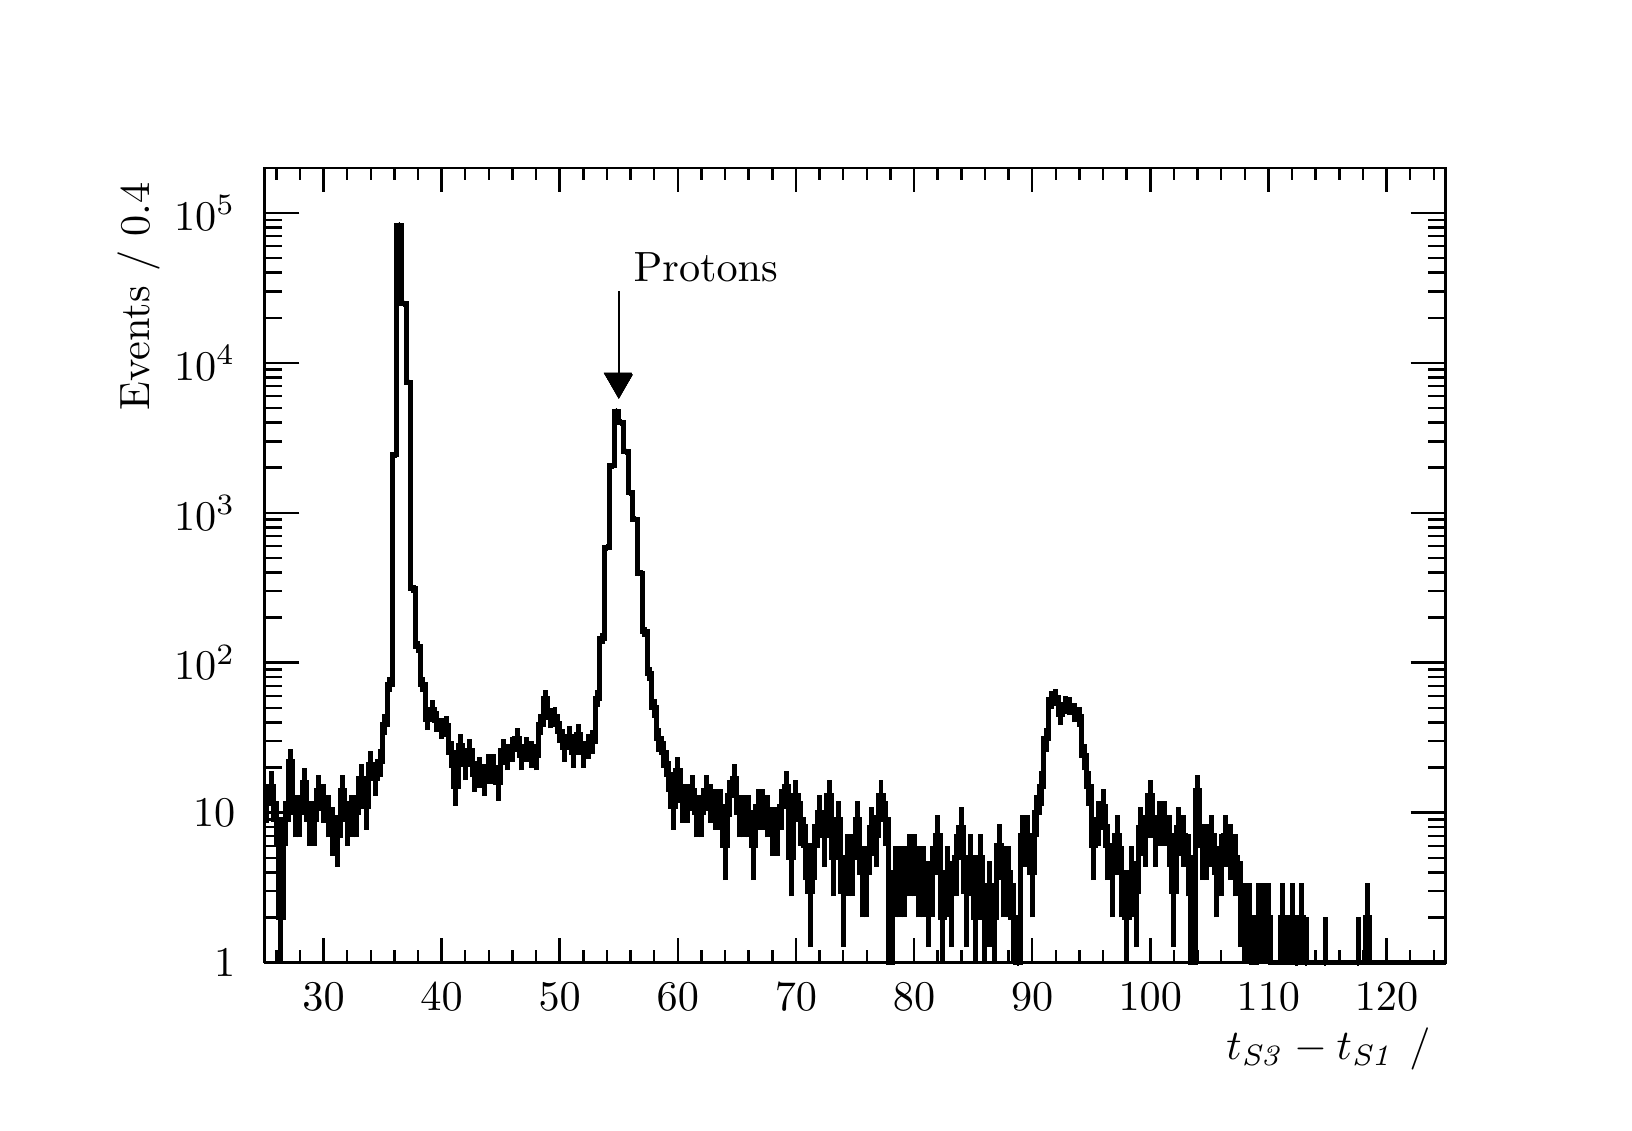
\begin{tikzpicture}
\pgfdeclareplotmark{cross} {
\pgfpathmoveto{\pgfpoint{-0.3\pgfplotmarksize}{\pgfplotmarksize}}
\pgfpathlineto{\pgfpoint{+0.3\pgfplotmarksize}{\pgfplotmarksize}}
\pgfpathlineto{\pgfpoint{+0.3\pgfplotmarksize}{0.3\pgfplotmarksize}}
\pgfpathlineto{\pgfpoint{+1\pgfplotmarksize}{0.3\pgfplotmarksize}}
\pgfpathlineto{\pgfpoint{+1\pgfplotmarksize}{-0.3\pgfplotmarksize}}
\pgfpathlineto{\pgfpoint{+0.3\pgfplotmarksize}{-0.3\pgfplotmarksize}}
\pgfpathlineto{\pgfpoint{+0.3\pgfplotmarksize}{-1.\pgfplotmarksize}}
\pgfpathlineto{\pgfpoint{-0.3\pgfplotmarksize}{-1.\pgfplotmarksize}}
\pgfpathlineto{\pgfpoint{-0.3\pgfplotmarksize}{-0.3\pgfplotmarksize}}
\pgfpathlineto{\pgfpoint{-1.\pgfplotmarksize}{-0.3\pgfplotmarksize}}
\pgfpathlineto{\pgfpoint{-1.\pgfplotmarksize}{0.3\pgfplotmarksize}}
\pgfpathlineto{\pgfpoint{-0.3\pgfplotmarksize}{0.3\pgfplotmarksize}}
\pgfpathclose
\pgfusepathqstroke
}
\pgfdeclareplotmark{cross*} {
\pgfpathmoveto{\pgfpoint{-0.3\pgfplotmarksize}{\pgfplotmarksize}}
\pgfpathlineto{\pgfpoint{+0.3\pgfplotmarksize}{\pgfplotmarksize}}
\pgfpathlineto{\pgfpoint{+0.3\pgfplotmarksize}{0.3\pgfplotmarksize}}
\pgfpathlineto{\pgfpoint{+1\pgfplotmarksize}{0.3\pgfplotmarksize}}
\pgfpathlineto{\pgfpoint{+1\pgfplotmarksize}{-0.3\pgfplotmarksize}}
\pgfpathlineto{\pgfpoint{+0.3\pgfplotmarksize}{-0.3\pgfplotmarksize}}
\pgfpathlineto{\pgfpoint{+0.3\pgfplotmarksize}{-1.\pgfplotmarksize}}
\pgfpathlineto{\pgfpoint{-0.3\pgfplotmarksize}{-1.\pgfplotmarksize}}
\pgfpathlineto{\pgfpoint{-0.3\pgfplotmarksize}{-0.3\pgfplotmarksize}}
\pgfpathlineto{\pgfpoint{-1.\pgfplotmarksize}{-0.3\pgfplotmarksize}}
\pgfpathlineto{\pgfpoint{-1.\pgfplotmarksize}{0.3\pgfplotmarksize}}
\pgfpathlineto{\pgfpoint{-0.3\pgfplotmarksize}{0.3\pgfplotmarksize}}
\pgfpathclose
\pgfusepathqfillstroke
}
\pgfdeclareplotmark{newstar} {
\pgfpathmoveto{\pgfqpoint{0pt}{\pgfplotmarksize}}
\pgfpathlineto{\pgfqpointpolar{44}{0.5\pgfplotmarksize}}
\pgfpathlineto{\pgfqpointpolar{18}{\pgfplotmarksize}}
\pgfpathlineto{\pgfqpointpolar{-20}{0.5\pgfplotmarksize}}
\pgfpathlineto{\pgfqpointpolar{-54}{\pgfplotmarksize}}
\pgfpathlineto{\pgfqpointpolar{-90}{0.5\pgfplotmarksize}}
\pgfpathlineto{\pgfqpointpolar{234}{\pgfplotmarksize}}
\pgfpathlineto{\pgfqpointpolar{198}{0.5\pgfplotmarksize}}
\pgfpathlineto{\pgfqpointpolar{162}{\pgfplotmarksize}}
\pgfpathlineto{\pgfqpointpolar{134}{0.5\pgfplotmarksize}}
\pgfpathclose
\pgfusepathqstroke
}
\pgfdeclareplotmark{newstar*} {
\pgfpathmoveto{\pgfqpoint{0pt}{\pgfplotmarksize}}
\pgfpathlineto{\pgfqpointpolar{44}{0.5\pgfplotmarksize}}
\pgfpathlineto{\pgfqpointpolar{18}{\pgfplotmarksize}}
\pgfpathlineto{\pgfqpointpolar{-20}{0.5\pgfplotmarksize}}
\pgfpathlineto{\pgfqpointpolar{-54}{\pgfplotmarksize}}
\pgfpathlineto{\pgfqpointpolar{-90}{0.5\pgfplotmarksize}}
\pgfpathlineto{\pgfqpointpolar{234}{\pgfplotmarksize}}
\pgfpathlineto{\pgfqpointpolar{198}{0.5\pgfplotmarksize}}
\pgfpathlineto{\pgfqpointpolar{162}{\pgfplotmarksize}}
\pgfpathlineto{\pgfqpointpolar{134}{0.5\pgfplotmarksize}}
\pgfpathclose
\pgfusepathqfillstroke
}
\definecolor{c}{rgb}{1,1,1};
\draw [color=c, fill=c] (0,0) rectangle (20,13.639);
\draw [color=c, fill=c] (3,1.77307) rectangle (18,11.8659);
\definecolor{c}{rgb}{0,0,0};
\draw [c,line width=0.9] (3,1.77307) -- (3,11.8659) -- (18,11.8659) -- (18,1.77307) -- (3,1.77307);
\definecolor{c}{rgb}{1,1,1};
\draw [color=c, fill=c] (3,1.77307) rectangle (18,11.8659);
\definecolor{c}{rgb}{0,0,0};
\draw [c,line width=0.9] (3,1.77307) -- (3,11.8659) -- (18,11.8659) -- (18,1.77307) -- (3,1.77307);
\draw [c,line width=1.8] (3.03,3.54611) -- (3.03,3.82776);
\draw [c,line width=1.8] (3.03,3.82776) -- (3.03,4.03747);
\foreach \P in {(3.03,3.82776)}{\draw[mark options={color=c,fill=c},mark size=2.402402pt, line width=0.000000pt, mark=*,mark size=1pt] plot coordinates {\P};}
\draw [c,line width=1.8] (3.09,3.76531) -- (3.09,4.01227);
\draw [c,line width=1.8] (3.09,4.01227) -- (3.09,4.20219);
\foreach \P in {(3.09,4.01227)}{\draw[mark options={color=c,fill=c},mark size=2.402402pt, line width=0.000000pt, mark=*,mark size=1pt] plot coordinates {\P};}
\draw [c,line width=1.8] (3.15,3.25462) -- (3.15,3.58989);
\draw [c,line width=1.8] (3.15,3.58989) -- (3.15,3.82776);
\foreach \P in {(3.15,3.58989)}{\draw[mark options={color=c,fill=c},mark size=2.402402pt, line width=0.000000pt, mark=*,mark size=1pt] plot coordinates {\P};}
\draw [c,line width=1.8] (3.21,1.77307) -- (3.21,2.34621);
\draw [c,line width=1.8] (3.21,2.34621) -- (3.21,2.78842);
\foreach \P in {(3.21,2.34621)}{\draw[mark options={color=c,fill=c},mark size=2.402402pt, line width=0.000000pt, mark=*,mark size=1pt] plot coordinates {\P};}
\draw [c,line width=1.8] (3.27,3.25462) -- (3.27,3.58989);
\draw [c,line width=1.8] (3.27,3.58989) -- (3.27,3.82776);
\foreach \P in {(3.27,3.58989)}{\draw[mark options={color=c,fill=c},mark size=2.402402pt, line width=0.000000pt, mark=*,mark size=1pt] plot coordinates {\P};}
\draw [c,line width=1.8] (3.33,4.13069) -- (3.33,4.32896);
\draw [c,line width=1.8] (3.33,4.32896) -- (3.33,4.48876);
\foreach \P in {(3.33,4.32896)}{\draw[mark options={color=c,fill=c},mark size=2.402402pt, line width=0.000000pt, mark=*,mark size=1pt] plot coordinates {\P};}
\draw [c,line width=1.8] (3.39,3.36269) -- (3.39,3.677);
\draw [c,line width=1.8] (3.39,3.677) -- (3.39,3.9042);
\foreach \P in {(3.39,3.677)}{\draw[mark options={color=c,fill=c},mark size=2.402402pt, line width=0.000000pt, mark=*,mark size=1pt] plot coordinates {\P};}
\draw [c,line width=1.8] (3.45,3.36269) -- (3.45,3.677);
\draw [c,line width=1.8] (3.45,3.677) -- (3.45,3.9042);
\foreach \P in {(3.45,3.677)}{\draw[mark options={color=c,fill=c},mark size=2.402402pt, line width=0.000000pt, mark=*,mark size=1pt] plot coordinates {\P};}
\draw [c,line width=1.8] (3.51,3.82776) -- (3.51,4.06564);
\draw [c,line width=1.8] (3.51,4.06564) -- (3.51,4.25015);
\foreach \P in {(3.51,4.06564)}{\draw[mark options={color=c,fill=c},mark size=2.402402pt, line width=0.000000pt, mark=*,mark size=1pt] plot coordinates {\P};}
\draw [c,line width=1.8] (3.57,3.25462) -- (3.57,3.58989);
\draw [c,line width=1.8] (3.57,3.58989) -- (3.57,3.82776);
\foreach \P in {(3.57,3.58989)}{\draw[mark options={color=c,fill=c},mark size=2.402402pt, line width=0.000000pt, mark=*,mark size=1pt] plot coordinates {\P};}
\draw [c,line width=1.8] (3.63,3.25462) -- (3.63,3.58989);
\draw [c,line width=1.8] (3.63,3.58989) -- (3.63,3.82776);
\foreach \P in {(3.63,3.58989)}{\draw[mark options={color=c,fill=c},mark size=2.402402pt, line width=0.000000pt, mark=*,mark size=1pt] plot coordinates {\P};}
\draw [c,line width=1.8] (3.69,3.6981) -- (3.69,3.95522);
\draw [c,line width=1.8] (3.69,3.95522) -- (3.69,4.15107);
\foreach \P in {(3.69,3.95522)}{\draw[mark options={color=c,fill=c},mark size=2.402402pt, line width=0.000000pt, mark=*,mark size=1pt] plot coordinates {\P};}
\draw [c,line width=1.8] (3.75,3.54611) -- (3.75,3.82776);
\draw [c,line width=1.8] (3.75,3.82776) -- (3.75,4.03747);
\foreach \P in {(3.75,3.82776)}{\draw[mark options={color=c,fill=c},mark size=2.402402pt, line width=0.000000pt, mark=*,mark size=1pt] plot coordinates {\P};}
\draw [c,line width=1.8] (3.81,3.36269) -- (3.81,3.677);
\draw [c,line width=1.8] (3.81,3.677) -- (3.81,3.9042);
\foreach \P in {(3.81,3.677)}{\draw[mark options={color=c,fill=c},mark size=2.402402pt, line width=0.000000pt, mark=*,mark size=1pt] plot coordinates {\P};}
\draw [c,line width=1.8] (3.87,3.13176) -- (3.87,3.49249);
\draw [c,line width=1.8] (3.87,3.49249) -- (3.87,3.74282);
\foreach \P in {(3.87,3.49249)}{\draw[mark options={color=c,fill=c},mark size=2.402402pt, line width=0.000000pt, mark=*,mark size=1pt] plot coordinates {\P};}
\draw [c,line width=1.8] (3.93,2.98952) -- (3.93,3.38208);
\draw [c,line width=1.8] (3.93,3.38208) -- (3.93,3.64718);
\foreach \P in {(3.93,3.38208)}{\draw[mark options={color=c,fill=c},mark size=2.402402pt, line width=0.000000pt, mark=*,mark size=1pt] plot coordinates {\P};}
\draw [c,line width=1.8] (3.99,3.6981) -- (3.99,3.95522);
\draw [c,line width=1.8] (3.99,3.95522) -- (3.99,4.15107);
\foreach \P in {(3.99,3.95522)}{\draw[mark options={color=c,fill=c},mark size=2.402402pt, line width=0.000000pt, mark=*,mark size=1pt] plot coordinates {\P};}
\draw [c,line width=1.8] (4.05,3.25462) -- (4.05,3.58989);
\draw [c,line width=1.8] (4.05,3.58989) -- (4.05,3.82776);
\foreach \P in {(4.05,3.58989)}{\draw[mark options={color=c,fill=c},mark size=2.402402pt, line width=0.000000pt, mark=*,mark size=1pt] plot coordinates {\P};}
\draw [c,line width=1.8] (4.11,3.36269) -- (4.11,3.677);
\draw [c,line width=1.8] (4.11,3.677) -- (4.11,3.9042);
\foreach \P in {(4.11,3.677)}{\draw[mark options={color=c,fill=c},mark size=2.402402pt, line width=0.000000pt, mark=*,mark size=1pt] plot coordinates {\P};}
\draw [c,line width=1.8] (4.17,3.36269) -- (4.17,3.677);
\draw [c,line width=1.8] (4.17,3.677) -- (4.17,3.9042);
\foreach \P in {(4.17,3.677)}{\draw[mark options={color=c,fill=c},mark size=2.402402pt, line width=0.000000pt, mark=*,mark size=1pt] plot coordinates {\P};}
\draw [c,line width=1.8] (4.23,3.88608) -- (4.23,4.11577);
\draw [c,line width=1.8] (4.23,4.11577) -- (4.23,4.29532);
\foreach \P in {(4.23,4.11577)}{\draw[mark options={color=c,fill=c},mark size=2.402402pt, line width=0.000000pt, mark=*,mark size=1pt] plot coordinates {\P};}
\draw [c,line width=1.8] (4.29,3.4591) -- (4.29,3.75581);
\draw [c,line width=1.8] (4.29,3.75581) -- (4.29,3.97372);
\foreach \P in {(4.29,3.75581)}{\draw[mark options={color=c,fill=c},mark size=2.402402pt, line width=0.000000pt, mark=*,mark size=1pt] plot coordinates {\P};}
\draw [c,line width=1.8] (4.35,4.08693) -- (4.35,4.29049);
\draw [c,line width=1.8] (4.35,4.29049) -- (4.35,4.45371);
\foreach \P in {(4.35,4.29049)}{\draw[mark options={color=c,fill=c},mark size=2.402402pt, line width=0.000000pt, mark=*,mark size=1pt] plot coordinates {\P};}
\draw [c,line width=1.8] (4.41,3.88608) -- (4.41,4.11577);
\draw [c,line width=1.8] (4.41,4.11577) -- (4.41,4.29532);
\foreach \P in {(4.41,4.11577)}{\draw[mark options={color=c,fill=c},mark size=2.402402pt, line width=0.000000pt, mark=*,mark size=1pt] plot coordinates {\P};}
\draw [c,line width=1.8] (4.47,4.13069) -- (4.47,4.32896);
\draw [c,line width=1.8] (4.47,4.32896) -- (4.47,4.48876);
\foreach \P in {(4.47,4.32896)}{\draw[mark options={color=c,fill=c},mark size=2.402402pt, line width=0.000000pt, mark=*,mark size=1pt] plot coordinates {\P};}
\draw [c,line width=1.8] (4.53,4.65806) -- (4.53,4.80236);
\draw [c,line width=1.8] (4.53,4.80236) -- (4.53,4.92517);
\foreach \P in {(4.53,4.80236)}{\draw[mark options={color=c,fill=c},mark size=2.402402pt, line width=0.000000pt, mark=*,mark size=1pt] plot coordinates {\P};}
\draw [c,line width=1.8] (4.59,5.20563) -- (4.59,5.30931);
\draw [c,line width=1.8] (4.59,5.30931) -- (4.59,5.40143);
\foreach \P in {(4.59,5.30931)}{\draw[mark options={color=c,fill=c},mark size=2.402402pt, line width=0.000000pt, mark=*,mark size=1pt] plot coordinates {\P};}
\draw [c,line width=1.8] (4.65,8.20245) -- (4.65,8.21939);
\draw [c,line width=1.8] (4.65,8.21939) -- (4.65,8.236);
\foreach \P in {(4.65,8.21939)}{\draw[mark options={color=c,fill=c},mark size=2.402402pt, line width=0.000000pt, mark=*,mark size=1pt] plot coordinates {\P};}
\draw [c,line width=1.8] (4.71,11.1309) -- (4.71,11.1338);
\draw [c,line width=1.8] (4.71,11.1338) -- (4.71,11.1367);
\foreach \P in {(4.71,11.1338)}{\draw[mark options={color=c,fill=c},mark size=2.402402pt, line width=0.000000pt, mark=*,mark size=1pt] plot coordinates {\P};}
\draw [c,line width=1.8] (4.77,10.1393) -- (4.77,10.1446);
\draw [c,line width=1.8] (4.77,10.1446) -- (4.77,10.1498);
\foreach \P in {(4.77,10.1446)}{\draw[mark options={color=c,fill=c},mark size=2.402402pt, line width=0.000000pt, mark=*,mark size=1pt] plot coordinates {\P};}
\draw [c,line width=1.8] (4.83,9.13276) -- (4.83,9.14241);
\draw [c,line width=1.8] (4.83,9.14241) -- (4.83,9.15195);
\foreach \P in {(4.83,9.14241)}{\draw[mark options={color=c,fill=c},mark size=2.402402pt, line width=0.000000pt, mark=*,mark size=1pt] plot coordinates {\P};}
\draw [c,line width=1.8] (4.89,6.47086) -- (4.89,6.51913);
\draw [c,line width=1.8] (4.89,6.51913) -- (4.89,6.56474);
\foreach \P in {(4.89,6.51913)}{\draw[mark options={color=c,fill=c},mark size=2.402402pt, line width=0.000000pt, mark=*,mark size=1pt] plot coordinates {\P};}
\draw [c,line width=1.8] (4.95,5.70855) -- (4.95,5.78506);
\draw [c,line width=1.8] (4.95,5.78506) -- (4.95,5.8551);
\foreach \P in {(4.95,5.78506)}{\draw[mark options={color=c,fill=c},mark size=2.402402pt, line width=0.000000pt, mark=*,mark size=1pt] plot coordinates {\P};}
\draw [c,line width=1.8] (5.01,5.20563) -- (5.01,5.30931);
\draw [c,line width=1.8] (5.01,5.30931) -- (5.01,5.40143);
\foreach \P in {(5.01,5.30931)}{\draw[mark options={color=c,fill=c},mark size=2.402402pt, line width=0.000000pt, mark=*,mark size=1pt] plot coordinates {\P};}
\draw [c,line width=1.8] (5.07,4.72505) -- (5.07,4.86363);
\draw [c,line width=1.8] (5.07,4.86363) -- (5.07,4.98229);
\foreach \P in {(5.07,4.86363)}{\draw[mark options={color=c,fill=c},mark size=2.402402pt, line width=0.000000pt, mark=*,mark size=1pt] plot coordinates {\P};}
\draw [c,line width=1.8] (5.13,4.86363) -- (5.13,4.9911);
\draw [c,line width=1.8] (5.13,4.9911) -- (5.13,5.10151);
\foreach \P in {(5.13,4.9911)}{\draw[mark options={color=c,fill=c},mark size=2.402402pt, line width=0.000000pt, mark=*,mark size=1pt] plot coordinates {\P};}
\draw [c,line width=1.8] (5.19,4.7033) -- (5.19,4.84371);
\draw [c,line width=1.8] (5.19,4.84371) -- (5.19,4.9637);
\foreach \P in {(5.19,4.84371)}{\draw[mark options={color=c,fill=c},mark size=2.402402pt, line width=0.000000pt, mark=*,mark size=1pt] plot coordinates {\P};}
\draw [c,line width=1.8] (5.25,4.61032) -- (5.25,4.75883);
\draw [c,line width=1.8] (5.25,4.75883) -- (5.25,4.88468);
\foreach \P in {(5.25,4.75883)}{\draw[mark options={color=c,fill=c},mark size=2.402402pt, line width=0.000000pt, mark=*,mark size=1pt] plot coordinates {\P};}
\draw [c,line width=1.8] (5.31,4.63452) -- (5.31,4.78088);
\draw [c,line width=1.8] (5.31,4.78088) -- (5.31,4.90518);
\foreach \P in {(5.31,4.78088)}{\draw[mark options={color=c,fill=c},mark size=2.402402pt, line width=0.000000pt, mark=*,mark size=1pt] plot coordinates {\P};}
\draw [c,line width=1.8] (5.37,4.25015) -- (5.37,4.43466);
\draw [c,line width=1.8] (5.37,4.43466) -- (5.37,4.58541);
\foreach \P in {(5.37,4.43466)}{\draw[mark options={color=c,fill=c},mark size=2.402402pt, line width=0.000000pt, mark=*,mark size=1pt] plot coordinates {\P};}
\draw [c,line width=1.8] (5.43,3.76531) -- (5.43,4.01227);
\draw [c,line width=1.8] (5.43,4.01227) -- (5.43,4.20219);
\foreach \P in {(5.43,4.01227)}{\draw[mark options={color=c,fill=c},mark size=2.402402pt, line width=0.000000pt, mark=*,mark size=1pt] plot coordinates {\P};}
\draw [c,line width=1.8] (5.49,4.35517) -- (5.49,4.52837);
\draw [c,line width=1.8] (5.49,4.52837) -- (5.49,4.6715);
\foreach \P in {(5.49,4.52837)}{\draw[mark options={color=c,fill=c},mark size=2.402402pt, line width=0.000000pt, mark=*,mark size=1pt] plot coordinates {\P};}
\draw [c,line width=1.8] (5.55,4.08693) -- (5.55,4.29049);
\draw [c,line width=1.8] (5.55,4.29049) -- (5.55,4.45371);
\foreach \P in {(5.55,4.29049)}{\draw[mark options={color=c,fill=c},mark size=2.402402pt, line width=0.000000pt, mark=*,mark size=1pt] plot coordinates {\P};}
\draw [c,line width=1.8] (5.61,4.28658) -- (5.61,4.46709);
\draw [c,line width=1.8] (5.61,4.46709) -- (5.61,4.61516);
\foreach \P in {(5.61,4.46709)}{\draw[mark options={color=c,fill=c},mark size=2.402402pt, line width=0.000000pt, mark=*,mark size=1pt] plot coordinates {\P};}
\draw [c,line width=1.8] (5.67,3.94077) -- (5.67,4.16303);
\draw [c,line width=1.8] (5.67,4.16303) -- (5.67,4.33803);
\foreach \P in {(5.67,4.16303)}{\draw[mark options={color=c,fill=c},mark size=2.402402pt, line width=0.000000pt, mark=*,mark size=1pt] plot coordinates {\P};}
\draw [c,line width=1.8] (5.73,3.99225) -- (5.73,4.20773);
\draw [c,line width=1.8] (5.73,4.20773) -- (5.73,4.37852);
\foreach \P in {(5.73,4.20773)}{\draw[mark options={color=c,fill=c},mark size=2.402402pt, line width=0.000000pt, mark=*,mark size=1pt] plot coordinates {\P};}
\draw [c,line width=1.8] (5.79,3.88608) -- (5.79,4.11577);
\draw [c,line width=1.8] (5.79,4.11577) -- (5.79,4.29532);
\foreach \P in {(5.79,4.11577)}{\draw[mark options={color=c,fill=c},mark size=2.402402pt, line width=0.000000pt, mark=*,mark size=1pt] plot coordinates {\P};}
\draw [c,line width=1.8] (5.85,4.04087) -- (5.85,4.25015);
\draw [c,line width=1.8] (5.85,4.25015) -- (5.85,4.41701);
\foreach \P in {(5.85,4.25015)}{\draw[mark options={color=c,fill=c},mark size=2.402402pt, line width=0.000000pt, mark=*,mark size=1pt] plot coordinates {\P};}
\draw [c,line width=1.8] (5.91,4.04087) -- (5.91,4.25015);
\draw [c,line width=1.8] (5.91,4.25015) -- (5.91,4.41701);
\foreach \P in {(5.91,4.25015)}{\draw[mark options={color=c,fill=c},mark size=2.402402pt, line width=0.000000pt, mark=*,mark size=1pt] plot coordinates {\P};}
\draw [c,line width=1.8] (5.97,3.82776) -- (5.97,4.06564);
\draw [c,line width=1.8] (5.97,4.06564) -- (5.97,4.25015);
\foreach \P in {(5.97,4.06564)}{\draw[mark options={color=c,fill=c},mark size=2.402402pt, line width=0.000000pt, mark=*,mark size=1pt] plot coordinates {\P};}
\draw [c,line width=1.8] (6.03,4.28658) -- (6.03,4.46709);
\draw [c,line width=1.8] (6.03,4.46709) -- (6.03,4.61516);
\foreach \P in {(6.03,4.46709)}{\draw[mark options={color=c,fill=c},mark size=2.402402pt, line width=0.000000pt, mark=*,mark size=1pt] plot coordinates {\P};}
\draw [c,line width=1.8] (6.09,4.21212) -- (6.09,4.4009);
\draw [c,line width=1.8] (6.09,4.4009) -- (6.09,4.5545);
\foreach \P in {(6.09,4.4009)}{\draw[mark options={color=c,fill=c},mark size=2.402402pt, line width=0.000000pt, mark=*,mark size=1pt] plot coordinates {\P};}
\draw [c,line width=1.8] (6.15,4.32155) -- (6.15,4.49829);
\draw [c,line width=1.8] (6.15,4.49829) -- (6.15,4.64383);
\foreach \P in {(6.15,4.49829)}{\draw[mark options={color=c,fill=c},mark size=2.402402pt, line width=0.000000pt, mark=*,mark size=1pt] plot coordinates {\P};}
\draw [c,line width=1.8] (6.21,4.44883) -- (6.21,4.61253);
\draw [c,line width=1.8] (6.21,4.61253) -- (6.21,4.74911);
\foreach \P in {(6.21,4.61253)}{\draw[mark options={color=c,fill=c},mark size=2.402402pt, line width=0.000000pt, mark=*,mark size=1pt] plot coordinates {\P};}
\draw [c,line width=1.8] (6.27,4.21212) -- (6.27,4.4009);
\draw [c,line width=1.8] (6.27,4.4009) -- (6.27,4.5545);
\foreach \P in {(6.27,4.4009)}{\draw[mark options={color=c,fill=c},mark size=2.402402pt, line width=0.000000pt, mark=*,mark size=1pt] plot coordinates {\P};}
\draw [c,line width=1.8] (6.33,4.32155) -- (6.33,4.49829);
\draw [c,line width=1.8] (6.33,4.49829) -- (6.33,4.64383);
\foreach \P in {(6.33,4.49829)}{\draw[mark options={color=c,fill=c},mark size=2.402402pt, line width=0.000000pt, mark=*,mark size=1pt] plot coordinates {\P};}
\draw [c,line width=1.8] (6.39,4.25015) -- (6.39,4.43466);
\draw [c,line width=1.8] (6.39,4.43466) -- (6.39,4.58541);
\foreach \P in {(6.39,4.43466)}{\draw[mark options={color=c,fill=c},mark size=2.402402pt, line width=0.000000pt, mark=*,mark size=1pt] plot coordinates {\P};}
\draw [c,line width=1.8] (6.45,4.21212) -- (6.45,4.4009);
\draw [c,line width=1.8] (6.45,4.4009) -- (6.45,4.5545);
\foreach \P in {(6.45,4.4009)}{\draw[mark options={color=c,fill=c},mark size=2.402402pt, line width=0.000000pt, mark=*,mark size=1pt] plot coordinates {\P};}
\draw [c,line width=1.8] (6.51,4.65806) -- (6.51,4.80236);
\draw [c,line width=1.8] (6.51,4.80236) -- (6.51,4.92517);
\foreach \P in {(6.51,4.80236)}{\draw[mark options={color=c,fill=c},mark size=2.402402pt, line width=0.000000pt, mark=*,mark size=1pt] plot coordinates {\P};}
\draw [c,line width=1.8] (6.57,5.01413) -- (6.57,5.13052);
\draw [c,line width=1.8] (6.57,5.13052) -- (6.57,5.23254);
\foreach \P in {(6.57,5.13052)}{\draw[mark options={color=c,fill=c},mark size=2.402402pt, line width=0.000000pt, mark=*,mark size=1pt] plot coordinates {\P};}
\draw [c,line width=1.8] (6.63,4.74627) -- (6.63,4.88309);
\draw [c,line width=1.8] (6.63,4.88309) -- (6.63,5.00045);
\foreach \P in {(6.63,4.88309)}{\draw[mark options={color=c,fill=c},mark size=2.402402pt, line width=0.000000pt, mark=*,mark size=1pt] plot coordinates {\P};}
\draw [c,line width=1.8] (6.69,4.76698) -- (6.69,4.9021);
\draw [c,line width=1.8] (6.69,4.9021) -- (6.69,5.01821);
\foreach \P in {(6.69,4.9021)}{\draw[mark options={color=c,fill=c},mark size=2.402402pt, line width=0.000000pt, mark=*,mark size=1pt] plot coordinates {\P};}
\draw [c,line width=1.8] (6.75,4.55977) -- (6.75,4.71288);
\draw [c,line width=1.8] (6.75,4.71288) -- (6.75,4.84201);
\foreach \P in {(6.75,4.71288)}{\draw[mark options={color=c,fill=c},mark size=2.402402pt, line width=0.000000pt, mark=*,mark size=1pt] plot coordinates {\P};}
\draw [c,line width=1.8] (6.81,4.32155) -- (6.81,4.49829);
\draw [c,line width=1.8] (6.81,4.49829) -- (6.81,4.64383);
\foreach \P in {(6.81,4.49829)}{\draw[mark options={color=c,fill=c},mark size=2.402402pt, line width=0.000000pt, mark=*,mark size=1pt] plot coordinates {\P};}
\draw [c,line width=1.8] (6.87,4.47793) -- (6.87,4.63878);
\draw [c,line width=1.8] (6.87,4.63878) -- (6.87,4.77338);
\foreach \P in {(6.87,4.63878)}{\draw[mark options={color=c,fill=c},mark size=2.402402pt, line width=0.000000pt, mark=*,mark size=1pt] plot coordinates {\P};}
\draw [c,line width=1.8] (6.93,4.25015) -- (6.93,4.43466);
\draw [c,line width=1.8] (6.93,4.43466) -- (6.93,4.58541);
\foreach \P in {(6.93,4.43466)}{\draw[mark options={color=c,fill=c},mark size=2.402402pt, line width=0.000000pt, mark=*,mark size=1pt] plot coordinates {\P};}
\draw [c,line width=1.8] (6.99,4.50608) -- (6.99,4.66422);
\draw [c,line width=1.8] (6.99,4.66422) -- (6.99,4.79692);
\foreach \P in {(6.99,4.66422)}{\draw[mark options={color=c,fill=c},mark size=2.402402pt, line width=0.000000pt, mark=*,mark size=1pt] plot coordinates {\P};}
\draw [c,line width=1.8] (7.05,4.25015) -- (7.05,4.43466);
\draw [c,line width=1.8] (7.05,4.43466) -- (7.05,4.58541);
\foreach \P in {(7.05,4.43466)}{\draw[mark options={color=c,fill=c},mark size=2.402402pt, line width=0.000000pt, mark=*,mark size=1pt] plot coordinates {\P};}
\draw [c,line width=1.8] (7.11,4.35517) -- (7.11,4.52837);
\draw [c,line width=1.8] (7.11,4.52837) -- (7.11,4.6715);
\foreach \P in {(7.11,4.52837)}{\draw[mark options={color=c,fill=c},mark size=2.402402pt, line width=0.000000pt, mark=*,mark size=1pt] plot coordinates {\P};}
\draw [c,line width=1.8] (7.17,4.41872) -- (7.17,4.58541);
\draw [c,line width=1.8] (7.17,4.58541) -- (7.17,4.72408);
\foreach \P in {(7.17,4.58541)}{\draw[mark options={color=c,fill=c},mark size=2.402402pt, line width=0.000000pt, mark=*,mark size=1pt] plot coordinates {\P};}
\draw [c,line width=1.8] (7.23,5.01413) -- (7.23,5.13052);
\draw [c,line width=1.8] (7.23,5.13052) -- (7.23,5.23254);
\foreach \P in {(7.23,5.13052)}{\draw[mark options={color=c,fill=c},mark size=2.402402pt, line width=0.000000pt, mark=*,mark size=1pt] plot coordinates {\P};}
\draw [c,line width=1.8] (7.29,5.81649) -- (7.29,5.88818);
\draw [c,line width=1.8] (7.29,5.88818) -- (7.29,5.95414);
\foreach \P in {(7.29,5.88818)}{\draw[mark options={color=c,fill=c},mark size=2.402402pt, line width=0.000000pt, mark=*,mark size=1pt] plot coordinates {\P};}
\draw [c,line width=1.8] (7.35,7.01097) -- (7.35,7.04579);
\draw [c,line width=1.8] (7.35,7.04579) -- (7.35,7.07921);
\foreach \P in {(7.35,7.04579)}{\draw[mark options={color=c,fill=c},mark size=2.402402pt, line width=0.000000pt, mark=*,mark size=1pt] plot coordinates {\P};}
\draw [c,line width=1.8] (7.41,8.06283) -- (7.41,8.08126);
\draw [c,line width=1.8] (7.41,8.08126) -- (7.41,8.09929);
\foreach \P in {(7.41,8.08126)}{\draw[mark options={color=c,fill=c},mark size=2.402402pt, line width=0.000000pt, mark=*,mark size=1pt] plot coordinates {\P};}
\draw [c,line width=1.8] (7.47,8.761) -- (7.47,8.77309);
\draw [c,line width=1.8] (7.47,8.77309) -- (7.47,8.785);
\foreach \P in {(7.47,8.77309)}{\draw[mark options={color=c,fill=c},mark size=2.402402pt, line width=0.000000pt, mark=*,mark size=1pt] plot coordinates {\P};}
\draw [c,line width=1.8] (7.53,8.61861) -- (7.53,8.63179);
\draw [c,line width=1.8] (7.53,8.63179) -- (7.53,8.64475);
\foreach \P in {(7.53,8.63179)}{\draw[mark options={color=c,fill=c},mark size=2.402402pt, line width=0.000000pt, mark=*,mark size=1pt] plot coordinates {\P};}
\draw [c,line width=1.8] (7.59,8.24857) -- (7.59,8.26505);
\draw [c,line width=1.8] (7.59,8.26505) -- (7.59,8.2812);
\foreach \P in {(7.59,8.26505)}{\draw[mark options={color=c,fill=c},mark size=2.402402pt, line width=0.000000pt, mark=*,mark size=1pt] plot coordinates {\P};}
\draw [c,line width=1.8] (7.65,7.71702) -- (7.65,7.73974);
\draw [c,line width=1.8] (7.65,7.73974) -- (7.65,7.76186);
\foreach \P in {(7.65,7.73974)}{\draw[mark options={color=c,fill=c},mark size=2.402402pt, line width=0.000000pt, mark=*,mark size=1pt] plot coordinates {\P};}
\draw [c,line width=1.8] (7.71,7.37439) -- (7.71,7.40234);
\draw [c,line width=1.8] (7.71,7.40234) -- (7.71,7.42938);
\foreach \P in {(7.71,7.40234)}{\draw[mark options={color=c,fill=c},mark size=2.402402pt, line width=0.000000pt, mark=*,mark size=1pt] plot coordinates {\P};}
\draw [c,line width=1.8] (7.77,6.67629) -- (7.77,6.71892);
\draw [c,line width=1.8] (7.77,6.71892) -- (7.77,6.75946);
\foreach \P in {(7.77,6.71892)}{\draw[mark options={color=c,fill=c},mark size=2.402402pt, line width=0.000000pt, mark=*,mark size=1pt] plot coordinates {\P};}
\draw [c,line width=1.8] (7.83,5.90685) -- (7.83,5.97473);
\draw [c,line width=1.8] (7.83,5.97473) -- (7.83,6.03745);
\foreach \P in {(7.83,5.97473)}{\draw[mark options={color=c,fill=c},mark size=2.402402pt, line width=0.000000pt, mark=*,mark size=1pt] plot coordinates {\P};}
\draw [c,line width=1.8] (7.89,5.35163) -- (7.89,5.44656);
\draw [c,line width=1.8] (7.89,5.44656) -- (7.89,5.53171);
\foreach \P in {(7.89,5.44656)}{\draw[mark options={color=c,fill=c},mark size=2.402402pt, line width=0.000000pt, mark=*,mark size=1pt] plot coordinates {\P};}
\draw [c,line width=1.8] (7.95,4.88172) -- (7.95,5.0078);
\draw [c,line width=1.8] (7.95,5.0078) -- (7.95,5.11717);
\foreach \P in {(7.95,5.0078)}{\draw[mark options={color=c,fill=c},mark size=2.402402pt, line width=0.000000pt, mark=*,mark size=1pt] plot coordinates {\P};}
\draw [c,line width=1.8] (8.01,4.44883) -- (8.01,4.61253);
\draw [c,line width=1.8] (8.01,4.61253) -- (8.01,4.74911);
\foreach \P in {(8.01,4.61253)}{\draw[mark options={color=c,fill=c},mark size=2.402402pt, line width=0.000000pt, mark=*,mark size=1pt] plot coordinates {\P};}
\draw [c,line width=1.8] (8.07,4.25015) -- (8.07,4.43466);
\draw [c,line width=1.8] (8.07,4.43466) -- (8.07,4.58541);
\foreach \P in {(8.07,4.43466)}{\draw[mark options={color=c,fill=c},mark size=2.402402pt, line width=0.000000pt, mark=*,mark size=1pt] plot coordinates {\P};}
\draw [c,line width=1.8] (8.13,3.94077) -- (8.13,4.16303);
\draw [c,line width=1.8] (8.13,4.16303) -- (8.13,4.33803);
\foreach \P in {(8.13,4.16303)}{\draw[mark options={color=c,fill=c},mark size=2.402402pt, line width=0.000000pt, mark=*,mark size=1pt] plot coordinates {\P};}
\draw [c,line width=1.8] (8.19,3.4591) -- (8.19,3.75581);
\draw [c,line width=1.8] (8.19,3.75581) -- (8.19,3.97372);
\foreach \P in {(8.19,3.75581)}{\draw[mark options={color=c,fill=c},mark size=2.402402pt, line width=0.000000pt, mark=*,mark size=1pt] plot coordinates {\P};}
\draw [c,line width=1.8] (8.25,3.99225) -- (8.25,4.20773);
\draw [c,line width=1.8] (8.25,4.20773) -- (8.25,4.37852);
\foreach \P in {(8.25,4.20773)}{\draw[mark options={color=c,fill=c},mark size=2.402402pt, line width=0.000000pt, mark=*,mark size=1pt] plot coordinates {\P};}
\draw [c,line width=1.8] (8.31,3.54611) -- (8.31,3.82776);
\draw [c,line width=1.8] (8.31,3.82776) -- (8.31,4.03747);
\foreach \P in {(8.31,3.82776)}{\draw[mark options={color=c,fill=c},mark size=2.402402pt, line width=0.000000pt, mark=*,mark size=1pt] plot coordinates {\P};}
\draw [c,line width=1.8] (8.37,3.54611) -- (8.37,3.82776);
\draw [c,line width=1.8] (8.37,3.82776) -- (8.37,4.03747);
\foreach \P in {(8.37,3.82776)}{\draw[mark options={color=c,fill=c},mark size=2.402402pt, line width=0.000000pt, mark=*,mark size=1pt] plot coordinates {\P};}
\draw [c,line width=1.8] (8.43,3.6981) -- (8.43,3.95522);
\draw [c,line width=1.8] (8.43,3.95522) -- (8.43,4.15107);
\foreach \P in {(8.43,3.95522)}{\draw[mark options={color=c,fill=c},mark size=2.402402pt, line width=0.000000pt, mark=*,mark size=1pt] plot coordinates {\P};}
\draw [c,line width=1.8] (8.49,3.36269) -- (8.49,3.677);
\draw [c,line width=1.8] (8.49,3.677) -- (8.49,3.9042);
\foreach \P in {(8.49,3.677)}{\draw[mark options={color=c,fill=c},mark size=2.402402pt, line width=0.000000pt, mark=*,mark size=1pt] plot coordinates {\P};}
\draw [c,line width=1.8] (8.55,3.36269) -- (8.55,3.677);
\draw [c,line width=1.8] (8.55,3.677) -- (8.55,3.9042);
\foreach \P in {(8.55,3.677)}{\draw[mark options={color=c,fill=c},mark size=2.402402pt, line width=0.000000pt, mark=*,mark size=1pt] plot coordinates {\P};}
\draw [c,line width=1.8] (8.61,3.6981) -- (8.61,3.95522);
\draw [c,line width=1.8] (8.61,3.95522) -- (8.61,4.15107);
\foreach \P in {(8.61,3.95522)}{\draw[mark options={color=c,fill=c},mark size=2.402402pt, line width=0.000000pt, mark=*,mark size=1pt] plot coordinates {\P};}
\draw [c,line width=1.8] (8.67,3.54611) -- (8.67,3.82776);
\draw [c,line width=1.8] (8.67,3.82776) -- (8.67,4.03747);
\foreach \P in {(8.67,3.82776)}{\draw[mark options={color=c,fill=c},mark size=2.402402pt, line width=0.000000pt, mark=*,mark size=1pt] plot coordinates {\P};}
\draw [c,line width=1.8] (8.73,3.4591) -- (8.73,3.75581);
\draw [c,line width=1.8] (8.73,3.75581) -- (8.73,3.97372);
\foreach \P in {(8.73,3.75581)}{\draw[mark options={color=c,fill=c},mark size=2.402402pt, line width=0.000000pt, mark=*,mark size=1pt] plot coordinates {\P};}
\draw [c,line width=1.8] (8.79,3.4591) -- (8.79,3.75581);
\draw [c,line width=1.8] (8.79,3.75581) -- (8.79,3.97372);
\foreach \P in {(8.79,3.75581)}{\draw[mark options={color=c,fill=c},mark size=2.402402pt, line width=0.000000pt, mark=*,mark size=1pt] plot coordinates {\P};}
\draw [c,line width=1.8] (8.85,2.82079) -- (8.85,3.25462);
\draw [c,line width=1.8] (8.85,3.25462) -- (8.85,3.53769);
\foreach \P in {(8.85,3.25462)}{\draw[mark options={color=c,fill=c},mark size=2.402402pt, line width=0.000000pt, mark=*,mark size=1pt] plot coordinates {\P};}
\draw [c,line width=1.8] (8.91,3.62535) -- (8.91,3.89395);
\draw [c,line width=1.8] (8.91,3.89395) -- (8.91,4.09635);
\foreach \P in {(8.91,3.89395)}{\draw[mark options={color=c,fill=c},mark size=2.402402pt, line width=0.000000pt, mark=*,mark size=1pt] plot coordinates {\P};}
\draw [c,line width=1.8] (8.97,3.88608) -- (8.97,4.11577);
\draw [c,line width=1.8] (8.97,4.11577) -- (8.97,4.29532);
\foreach \P in {(8.97,4.11577)}{\draw[mark options={color=c,fill=c},mark size=2.402402pt, line width=0.000000pt, mark=*,mark size=1pt] plot coordinates {\P};}
\draw [c,line width=1.8] (9.03,3.36269) -- (9.03,3.677);
\draw [c,line width=1.8] (9.03,3.677) -- (9.03,3.9042);
\foreach \P in {(9.03,3.677)}{\draw[mark options={color=c,fill=c},mark size=2.402402pt, line width=0.000000pt, mark=*,mark size=1pt] plot coordinates {\P};}
\draw [c,line width=1.8] (9.09,3.36269) -- (9.09,3.677);
\draw [c,line width=1.8] (9.09,3.677) -- (9.09,3.9042);
\foreach \P in {(9.09,3.677)}{\draw[mark options={color=c,fill=c},mark size=2.402402pt, line width=0.000000pt, mark=*,mark size=1pt] plot coordinates {\P};}
\draw [c,line width=1.8] (9.15,3.36269) -- (9.15,3.677);
\draw [c,line width=1.8] (9.15,3.677) -- (9.15,3.9042);
\foreach \P in {(9.15,3.677)}{\draw[mark options={color=c,fill=c},mark size=2.402402pt, line width=0.000000pt, mark=*,mark size=1pt] plot coordinates {\P};}
\draw [c,line width=1.8] (9.21,2.82079) -- (9.21,3.25462);
\draw [c,line width=1.8] (9.21,3.25462) -- (9.21,3.53769);
\foreach \P in {(9.21,3.25462)}{\draw[mark options={color=c,fill=c},mark size=2.402402pt, line width=0.000000pt, mark=*,mark size=1pt] plot coordinates {\P};}
\draw [c,line width=1.8] (9.27,3.4591) -- (9.27,3.75581);
\draw [c,line width=1.8] (9.27,3.75581) -- (9.27,3.97372);
\foreach \P in {(9.27,3.75581)}{\draw[mark options={color=c,fill=c},mark size=2.402402pt, line width=0.000000pt, mark=*,mark size=1pt] plot coordinates {\P};}
\draw [c,line width=1.8] (9.33,3.4591) -- (9.33,3.75581);
\draw [c,line width=1.8] (9.33,3.75581) -- (9.33,3.97372);
\foreach \P in {(9.33,3.75581)}{\draw[mark options={color=c,fill=c},mark size=2.402402pt, line width=0.000000pt, mark=*,mark size=1pt] plot coordinates {\P};}
\draw [c,line width=1.8] (9.39,3.36269) -- (9.39,3.677);
\draw [c,line width=1.8] (9.39,3.677) -- (9.39,3.9042);
\foreach \P in {(9.39,3.677)}{\draw[mark options={color=c,fill=c},mark size=2.402402pt, line width=0.000000pt, mark=*,mark size=1pt] plot coordinates {\P};}
\draw [c,line width=1.8] (9.45,3.13176) -- (9.45,3.49249);
\draw [c,line width=1.8] (9.45,3.49249) -- (9.45,3.74282);
\foreach \P in {(9.45,3.49249)}{\draw[mark options={color=c,fill=c},mark size=2.402402pt, line width=0.000000pt, mark=*,mark size=1pt] plot coordinates {\P};}
\draw [c,line width=1.8] (9.51,3.13176) -- (9.51,3.49249);
\draw [c,line width=1.8] (9.51,3.49249) -- (9.51,3.74282);
\foreach \P in {(9.51,3.49249)}{\draw[mark options={color=c,fill=c},mark size=2.402402pt, line width=0.000000pt, mark=*,mark size=1pt] plot coordinates {\P};}
\draw [c,line width=1.8] (9.57,3.4591) -- (9.57,3.75581);
\draw [c,line width=1.8] (9.57,3.75581) -- (9.57,3.97372);
\foreach \P in {(9.57,3.75581)}{\draw[mark options={color=c,fill=c},mark size=2.402402pt, line width=0.000000pt, mark=*,mark size=1pt] plot coordinates {\P};}
\draw [c,line width=1.8] (9.63,3.76531) -- (9.63,4.01227);
\draw [c,line width=1.8] (9.63,4.01227) -- (9.63,4.20219);
\foreach \P in {(9.63,4.01227)}{\draw[mark options={color=c,fill=c},mark size=2.402402pt, line width=0.000000pt, mark=*,mark size=1pt] plot coordinates {\P};}
\draw [c,line width=1.8] (9.69,2.61371) -- (9.69,3.10386);
\draw [c,line width=1.8] (9.69,3.10386) -- (9.69,3.40951);
\foreach \P in {(9.69,3.10386)}{\draw[mark options={color=c,fill=c},mark size=2.402402pt, line width=0.000000pt, mark=*,mark size=1pt] plot coordinates {\P};}
\draw [c,line width=1.8] (9.75,3.62535) -- (9.75,3.89395);
\draw [c,line width=1.8] (9.75,3.89395) -- (9.75,4.09635);
\foreach \P in {(9.75,3.89395)}{\draw[mark options={color=c,fill=c},mark size=2.402402pt, line width=0.000000pt, mark=*,mark size=1pt] plot coordinates {\P};}
\draw [c,line width=1.8] (9.81,3.25462) -- (9.81,3.58989);
\draw [c,line width=1.8] (9.81,3.58989) -- (9.81,3.82776);
\foreach \P in {(9.81,3.58989)}{\draw[mark options={color=c,fill=c},mark size=2.402402pt, line width=0.000000pt, mark=*,mark size=1pt] plot coordinates {\P};}
\draw [c,line width=1.8] (9.87,2.82079) -- (9.87,3.25462);
\draw [c,line width=1.8] (9.87,3.25462) -- (9.87,3.53769);
\foreach \P in {(9.87,3.25462)}{\draw[mark options={color=c,fill=c},mark size=2.402402pt, line width=0.000000pt, mark=*,mark size=1pt] plot coordinates {\P};}
\draw [c,line width=1.8] (9.93,1.96937) -- (9.93,2.68148);
\draw [c,line width=1.8] (9.93,2.68148) -- (9.93,3.05832);
\foreach \P in {(9.93,2.68148)}{\draw[mark options={color=c,fill=c},mark size=2.402402pt, line width=0.000000pt, mark=*,mark size=1pt] plot coordinates {\P};}
\draw [c,line width=1.8] (9.99,2.82079) -- (9.99,3.25462);
\draw [c,line width=1.8] (9.99,3.25462) -- (9.99,3.53769);
\foreach \P in {(9.99,3.25462)}{\draw[mark options={color=c,fill=c},mark size=2.402402pt, line width=0.000000pt, mark=*,mark size=1pt] plot coordinates {\P};}
\draw [c,line width=1.8] (10.05,3.36269) -- (10.05,3.677);
\draw [c,line width=1.8] (10.05,3.677) -- (10.05,3.9042);
\foreach \P in {(10.05,3.677)}{\draw[mark options={color=c,fill=c},mark size=2.402402pt, line width=0.000000pt, mark=*,mark size=1pt] plot coordinates {\P};}
\draw [c,line width=1.8] (10.11,2.98952) -- (10.11,3.38208);
\draw [c,line width=1.8] (10.11,3.38208) -- (10.11,3.64718);
\foreach \P in {(10.11,3.38208)}{\draw[mark options={color=c,fill=c},mark size=2.402402pt, line width=0.000000pt, mark=*,mark size=1pt] plot coordinates {\P};}
\draw [c,line width=1.8] (10.17,3.62535) -- (10.17,3.89395);
\draw [c,line width=1.8] (10.17,3.89395) -- (10.17,4.09635);
\foreach \P in {(10.17,3.89395)}{\draw[mark options={color=c,fill=c},mark size=2.402402pt, line width=0.000000pt, mark=*,mark size=1pt] plot coordinates {\P};}
\draw [c,line width=1.8] (10.23,2.61371) -- (10.23,3.10386);
\draw [c,line width=1.8] (10.23,3.10386) -- (10.23,3.40951);
\foreach \P in {(10.23,3.10386)}{\draw[mark options={color=c,fill=c},mark size=2.402402pt, line width=0.000000pt, mark=*,mark size=1pt] plot coordinates {\P};}
\draw [c,line width=1.8] (10.29,3.25462) -- (10.29,3.58989);
\draw [c,line width=1.8] (10.29,3.58989) -- (10.29,3.82776);
\foreach \P in {(10.29,3.58989)}{\draw[mark options={color=c,fill=c},mark size=2.402402pt, line width=0.000000pt, mark=*,mark size=1pt] plot coordinates {\P};}
\draw [c,line width=1.8] (10.35,1.96937) -- (10.35,2.68148);
\draw [c,line width=1.8] (10.35,2.68148) -- (10.35,3.05832);
\foreach \P in {(10.35,2.68148)}{\draw[mark options={color=c,fill=c},mark size=2.402402pt, line width=0.000000pt, mark=*,mark size=1pt] plot coordinates {\P};}
\draw [c,line width=1.8] (10.41,2.61371) -- (10.41,3.10386);
\draw [c,line width=1.8] (10.41,3.10386) -- (10.41,3.40951);
\foreach \P in {(10.41,3.10386)}{\draw[mark options={color=c,fill=c},mark size=2.402402pt, line width=0.000000pt, mark=*,mark size=1pt] plot coordinates {\P};}
\draw [c,line width=1.8] (10.47,2.61371) -- (10.47,3.10386);
\draw [c,line width=1.8] (10.47,3.10386) -- (10.47,3.40951);
\foreach \P in {(10.47,3.10386)}{\draw[mark options={color=c,fill=c},mark size=2.402402pt, line width=0.000000pt, mark=*,mark size=1pt] plot coordinates {\P};}
\draw [c,line width=1.8] (10.53,3.25462) -- (10.53,3.58989);
\draw [c,line width=1.8] (10.53,3.58989) -- (10.53,3.82776);
\foreach \P in {(10.53,3.58989)}{\draw[mark options={color=c,fill=c},mark size=2.402402pt, line width=0.000000pt, mark=*,mark size=1pt] plot coordinates {\P};}
\draw [c,line width=1.8] (10.59,2.34621) -- (10.59,2.91935);
\draw [c,line width=1.8] (10.59,2.91935) -- (10.59,3.25462);
\foreach \P in {(10.59,2.91935)}{\draw[mark options={color=c,fill=c},mark size=2.402402pt, line width=0.000000pt, mark=*,mark size=1pt] plot coordinates {\P};}
\draw [c,line width=1.8] (10.65,2.34621) -- (10.65,2.91935);
\draw [c,line width=1.8] (10.65,2.91935) -- (10.65,3.25462);
\foreach \P in {(10.65,2.91935)}{\draw[mark options={color=c,fill=c},mark size=2.402402pt, line width=0.000000pt, mark=*,mark size=1pt] plot coordinates {\P};}
\draw [c,line width=1.8] (10.71,3.13176) -- (10.71,3.49249);
\draw [c,line width=1.8] (10.71,3.49249) -- (10.71,3.74282);
\foreach \P in {(10.71,3.49249)}{\draw[mark options={color=c,fill=c},mark size=2.402402pt, line width=0.000000pt, mark=*,mark size=1pt] plot coordinates {\P};}
\draw [c,line width=1.8] (10.77,2.98952) -- (10.77,3.38208);
\draw [c,line width=1.8] (10.77,3.38208) -- (10.77,3.64718);
\foreach \P in {(10.77,3.38208)}{\draw[mark options={color=c,fill=c},mark size=2.402402pt, line width=0.000000pt, mark=*,mark size=1pt] plot coordinates {\P};}
\draw [c,line width=1.8] (10.83,3.62535) -- (10.83,3.89395);
\draw [c,line width=1.8] (10.83,3.89395) -- (10.83,4.09635);
\foreach \P in {(10.83,3.89395)}{\draw[mark options={color=c,fill=c},mark size=2.402402pt, line width=0.000000pt, mark=*,mark size=1pt] plot coordinates {\P};}
\draw [c,line width=1.8] (10.89,3.25462) -- (10.89,3.58989);
\draw [c,line width=1.8] (10.89,3.58989) -- (10.89,3.82776);
\foreach \P in {(10.89,3.58989)}{\draw[mark options={color=c,fill=c},mark size=2.402402pt, line width=0.000000pt, mark=*,mark size=1pt] plot coordinates {\P};}
\draw [c,line width=1.8] (11.01,2.34621) -- (11.01,2.91935);
\draw [c,line width=1.8] (11.01,2.91935) -- (11.01,3.25462);
\foreach \P in {(11.01,2.91935)}{\draw[mark options={color=c,fill=c},mark size=2.402402pt, line width=0.000000pt, mark=*,mark size=1pt] plot coordinates {\P};}
\draw [c,line width=1.8] (11.07,2.34621) -- (11.07,2.91935);
\draw [c,line width=1.8] (11.07,2.91935) -- (11.07,3.25462);
\foreach \P in {(11.07,2.91935)}{\draw[mark options={color=c,fill=c},mark size=2.402402pt, line width=0.000000pt, mark=*,mark size=1pt] plot coordinates {\P};}
\draw [c,line width=1.8] (11.13,2.34621) -- (11.13,2.91935);
\draw [c,line width=1.8] (11.13,2.91935) -- (11.13,3.25462);
\foreach \P in {(11.13,2.91935)}{\draw[mark options={color=c,fill=c},mark size=2.402402pt, line width=0.000000pt, mark=*,mark size=1pt] plot coordinates {\P};}
\draw [c,line width=1.8] (11.19,2.61371) -- (11.19,3.10386);
\draw [c,line width=1.8] (11.19,3.10386) -- (11.19,3.40951);
\foreach \P in {(11.19,3.10386)}{\draw[mark options={color=c,fill=c},mark size=2.402402pt, line width=0.000000pt, mark=*,mark size=1pt] plot coordinates {\P};}
\draw [c,line width=1.8] (11.25,2.61371) -- (11.25,3.10386);
\draw [c,line width=1.8] (11.25,3.10386) -- (11.25,3.40951);
\foreach \P in {(11.25,3.10386)}{\draw[mark options={color=c,fill=c},mark size=2.402402pt, line width=0.000000pt, mark=*,mark size=1pt] plot coordinates {\P};}
\draw [c,line width=1.8] (11.31,2.34621) -- (11.31,2.91935);
\draw [c,line width=1.8] (11.31,2.91935) -- (11.31,3.25462);
\foreach \P in {(11.31,2.91935)}{\draw[mark options={color=c,fill=c},mark size=2.402402pt, line width=0.000000pt, mark=*,mark size=1pt] plot coordinates {\P};}
\draw [c,line width=1.8] (11.37,2.34621) -- (11.37,2.91935);
\draw [c,line width=1.8] (11.37,2.91935) -- (11.37,3.25462);
\foreach \P in {(11.37,2.91935)}{\draw[mark options={color=c,fill=c},mark size=2.402402pt, line width=0.000000pt, mark=*,mark size=1pt] plot coordinates {\P};}
\draw [c,line width=1.8] (11.43,1.96937) -- (11.43,2.68148);
\draw [c,line width=1.8] (11.43,2.68148) -- (11.43,3.05832);
\foreach \P in {(11.43,2.68148)}{\draw[mark options={color=c,fill=c},mark size=2.402402pt, line width=0.000000pt, mark=*,mark size=1pt] plot coordinates {\P};}
\draw [c,line width=1.8] (11.49,2.34621) -- (11.49,2.91935);
\draw [c,line width=1.8] (11.49,2.91935) -- (11.49,3.25462);
\foreach \P in {(11.49,2.91935)}{\draw[mark options={color=c,fill=c},mark size=2.402402pt, line width=0.000000pt, mark=*,mark size=1pt] plot coordinates {\P};}
\draw [c,line width=1.8] (11.55,2.98952) -- (11.55,3.38208);
\draw [c,line width=1.8] (11.55,3.38208) -- (11.55,3.64718);
\foreach \P in {(11.55,3.38208)}{\draw[mark options={color=c,fill=c},mark size=2.402402pt, line width=0.000000pt, mark=*,mark size=1pt] plot coordinates {\P};}
\draw [c,line width=1.8] (11.61,1.77307) -- (11.61,2.34621);
\draw [c,line width=1.8] (11.61,2.34621) -- (11.61,2.78842);
\foreach \P in {(11.61,2.34621)}{\draw[mark options={color=c,fill=c},mark size=2.402402pt, line width=0.000000pt, mark=*,mark size=1pt] plot coordinates {\P};}
\draw [c,line width=1.8] (11.67,2.34621) -- (11.67,2.91935);
\draw [c,line width=1.8] (11.67,2.91935) -- (11.67,3.25462);
\foreach \P in {(11.67,2.91935)}{\draw[mark options={color=c,fill=c},mark size=2.402402pt, line width=0.000000pt, mark=*,mark size=1pt] plot coordinates {\P};}
\draw [c,line width=1.8] (11.73,1.96937) -- (11.73,2.68148);
\draw [c,line width=1.8] (11.73,2.68148) -- (11.73,3.05832);
\foreach \P in {(11.73,2.68148)}{\draw[mark options={color=c,fill=c},mark size=2.402402pt, line width=0.000000pt, mark=*,mark size=1pt] plot coordinates {\P};}
\draw [c,line width=1.8] (11.79,2.61371) -- (11.79,3.10386);
\draw [c,line width=1.8] (11.79,3.10386) -- (11.79,3.40951);
\foreach \P in {(11.79,3.10386)}{\draw[mark options={color=c,fill=c},mark size=2.402402pt, line width=0.000000pt, mark=*,mark size=1pt] plot coordinates {\P};}
\draw [c,line width=1.8] (11.85,3.13176) -- (11.85,3.49249);
\draw [c,line width=1.8] (11.85,3.49249) -- (11.85,3.74282);
\foreach \P in {(11.85,3.49249)}{\draw[mark options={color=c,fill=c},mark size=2.402402pt, line width=0.000000pt, mark=*,mark size=1pt] plot coordinates {\P};}
\draw [c,line width=1.8] (11.91,1.96937) -- (11.91,2.68148);
\draw [c,line width=1.8] (11.91,2.68148) -- (11.91,3.05832);
\foreach \P in {(11.91,2.68148)}{\draw[mark options={color=c,fill=c},mark size=2.402402pt, line width=0.000000pt, mark=*,mark size=1pt] plot coordinates {\P};}
\draw [c,line width=1.8] (11.97,2.61371) -- (11.97,3.10386);
\draw [c,line width=1.8] (11.97,3.10386) -- (11.97,3.40951);
\foreach \P in {(11.97,3.10386)}{\draw[mark options={color=c,fill=c},mark size=2.402402pt, line width=0.000000pt, mark=*,mark size=1pt] plot coordinates {\P};}
\draw [c,line width=1.8] (12.03,1.77307) -- (12.03,2.34621);
\draw [c,line width=1.8] (12.03,2.34621) -- (12.03,2.78842);
\foreach \P in {(12.03,2.34621)}{\draw[mark options={color=c,fill=c},mark size=2.402402pt, line width=0.000000pt, mark=*,mark size=1pt] plot coordinates {\P};}
\draw [c,line width=1.8] (12.09,2.61371) -- (12.09,3.10386);
\draw [c,line width=1.8] (12.09,3.10386) -- (12.09,3.40951);
\foreach \P in {(12.09,3.10386)}{\draw[mark options={color=c,fill=c},mark size=2.402402pt, line width=0.000000pt, mark=*,mark size=1pt] plot coordinates {\P};}
\draw [c,line width=1.8] (12.15,1.77307) -- (12.15,2.34621);
\draw [c,line width=1.8] (12.15,2.34621) -- (12.15,2.78842);
\foreach \P in {(12.15,2.34621)}{\draw[mark options={color=c,fill=c},mark size=2.402402pt, line width=0.000000pt, mark=*,mark size=1pt] plot coordinates {\P};}
\draw [c,line width=1.8] (12.21,1.96937) -- (12.21,2.68148);
\draw [c,line width=1.8] (12.21,2.68148) -- (12.21,3.05832);
\foreach \P in {(12.21,2.68148)}{\draw[mark options={color=c,fill=c},mark size=2.402402pt, line width=0.000000pt, mark=*,mark size=1pt] plot coordinates {\P};}
\draw [c,line width=1.8] (12.27,1.77307) -- (12.27,2.34621);
\draw [c,line width=1.8] (12.27,2.34621) -- (12.27,2.78842);
\foreach \P in {(12.27,2.34621)}{\draw[mark options={color=c,fill=c},mark size=2.402402pt, line width=0.000000pt, mark=*,mark size=1pt] plot coordinates {\P};}
\draw [c,line width=1.8] (12.33,2.82079) -- (12.33,3.25462);
\draw [c,line width=1.8] (12.33,3.25462) -- (12.33,3.53769);
\foreach \P in {(12.33,3.25462)}{\draw[mark options={color=c,fill=c},mark size=2.402402pt, line width=0.000000pt, mark=*,mark size=1pt] plot coordinates {\P};}
\draw [c,line width=1.8] (12.39,2.34621) -- (12.39,2.91935);
\draw [c,line width=1.8] (12.39,2.91935) -- (12.39,3.25462);
\foreach \P in {(12.39,2.91935)}{\draw[mark options={color=c,fill=c},mark size=2.402402pt, line width=0.000000pt, mark=*,mark size=1pt] plot coordinates {\P};}
\draw [c,line width=1.8] (12.45,2.34621) -- (12.45,2.91935);
\draw [c,line width=1.8] (12.45,2.91935) -- (12.45,3.25462);
\foreach \P in {(12.45,2.91935)}{\draw[mark options={color=c,fill=c},mark size=2.402402pt, line width=0.000000pt, mark=*,mark size=1pt] plot coordinates {\P};}
\draw [c,line width=1.8] (12.51,1.77307) -- (12.51,2.34621);
\draw [c,line width=1.8] (12.51,2.34621) -- (12.51,2.78842);
\foreach \P in {(12.51,2.34621)}{\draw[mark options={color=c,fill=c},mark size=2.402402pt, line width=0.000000pt, mark=*,mark size=1pt] plot coordinates {\P};}
\draw [c,line width=1.8] (12.57,1.77307) -- (12.57,2.34621);
\foreach \P in {(12.57,1.77307)}{\draw[mark options={color=c,fill=c},mark size=2.402402pt, line width=0.000000pt, mark=*,mark size=1pt] plot coordinates {\P};}
\draw [c,line width=1.8] (12.63,2.98952) -- (12.63,3.38208);
\draw [c,line width=1.8] (12.63,3.38208) -- (12.63,3.64718);
\foreach \P in {(12.63,3.38208)}{\draw[mark options={color=c,fill=c},mark size=2.402402pt, line width=0.000000pt, mark=*,mark size=1pt] plot coordinates {\P};}
\draw [c,line width=1.8] (12.69,2.98952) -- (12.69,3.38208);
\draw [c,line width=1.8] (12.69,3.38208) -- (12.69,3.64718);
\foreach \P in {(12.69,3.38208)}{\draw[mark options={color=c,fill=c},mark size=2.402402pt, line width=0.000000pt, mark=*,mark size=1pt] plot coordinates {\P};}
\draw [c,line width=1.8] (12.75,2.34621) -- (12.75,2.91935);
\draw [c,line width=1.8] (12.75,2.91935) -- (12.75,3.25462);
\foreach \P in {(12.75,2.91935)}{\draw[mark options={color=c,fill=c},mark size=2.402402pt, line width=0.000000pt, mark=*,mark size=1pt] plot coordinates {\P};}
\draw [c,line width=1.8] (12.81,3.36269) -- (12.81,3.677);
\draw [c,line width=1.8] (12.81,3.677) -- (12.81,3.9042);
\foreach \P in {(12.81,3.677)}{\draw[mark options={color=c,fill=c},mark size=2.402402pt, line width=0.000000pt, mark=*,mark size=1pt] plot coordinates {\P};}
\draw [c,line width=1.8] (12.87,3.76531) -- (12.87,4.01227);
\draw [c,line width=1.8] (12.87,4.01227) -- (12.87,4.20219);
\foreach \P in {(12.87,4.01227)}{\draw[mark options={color=c,fill=c},mark size=2.402402pt, line width=0.000000pt, mark=*,mark size=1pt] plot coordinates {\P};}
\draw [c,line width=1.8] (12.93,4.44883) -- (12.93,4.61253);
\draw [c,line width=1.8] (12.93,4.61253) -- (12.93,4.74911);
\foreach \P in {(12.93,4.61253)}{\draw[mark options={color=c,fill=c},mark size=2.402402pt, line width=0.000000pt, mark=*,mark size=1pt] plot coordinates {\P};}
\draw [c,line width=1.8] (12.99,4.99866) -- (12.99,5.11614);
\draw [c,line width=1.8] (12.99,5.11614) -- (12.99,5.219);
\foreach \P in {(12.99,5.11614)}{\draw[mark options={color=c,fill=c},mark size=2.402402pt, line width=0.000000pt, mark=*,mark size=1pt] plot coordinates {\P};}
\draw [c,line width=1.8] (13.05,5.02933) -- (13.05,5.14466);
\draw [c,line width=1.8] (13.05,5.14466) -- (13.05,5.24586);
\foreach \P in {(13.05,5.14466)}{\draw[mark options={color=c,fill=c},mark size=2.402402pt, line width=0.000000pt, mark=*,mark size=1pt] plot coordinates {\P};}
\draw [c,line width=1.8] (13.11,4.7872) -- (13.11,4.92068);
\draw [c,line width=1.8] (13.11,4.92068) -- (13.11,5.03558);
\foreach \P in {(13.11,4.92068)}{\draw[mark options={color=c,fill=c},mark size=2.402402pt, line width=0.000000pt, mark=*,mark size=1pt] plot coordinates {\P};}
\draw [c,line width=1.8] (13.17,4.9338) -- (13.17,5.05598);
\draw [c,line width=1.8] (13.17,5.05598) -- (13.17,5.16241);
\foreach \P in {(13.17,5.05598)}{\draw[mark options={color=c,fill=c},mark size=2.402402pt, line width=0.000000pt, mark=*,mark size=1pt] plot coordinates {\P};}
\draw [c,line width=1.8] (13.23,4.91679) -- (13.23,5.04023);
\draw [c,line width=1.8] (13.23,5.04023) -- (13.23,5.14761);
\foreach \P in {(13.23,5.04023)}{\draw[mark options={color=c,fill=c},mark size=2.402402pt, line width=0.000000pt, mark=*,mark size=1pt] plot coordinates {\P};}
\draw [c,line width=1.8] (13.29,4.82627) -- (13.29,4.95664);
\draw [c,line width=1.8] (13.29,4.95664) -- (13.29,5.06922);
\foreach \P in {(13.29,4.95664)}{\draw[mark options={color=c,fill=c},mark size=2.402402pt, line width=0.000000pt, mark=*,mark size=1pt] plot coordinates {\P};}
\draw [c,line width=1.8] (13.35,4.76698) -- (13.35,4.9021);
\draw [c,line width=1.8] (13.35,4.9021) -- (13.35,5.01821);
\foreach \P in {(13.35,4.9021)}{\draw[mark options={color=c,fill=c},mark size=2.402402pt, line width=0.000000pt, mark=*,mark size=1pt] plot coordinates {\P};}
\draw [c,line width=1.8] (13.41,4.21212) -- (13.41,4.4009);
\draw [c,line width=1.8] (13.41,4.4009) -- (13.41,4.5545);
\foreach \P in {(13.41,4.4009)}{\draw[mark options={color=c,fill=c},mark size=2.402402pt, line width=0.000000pt, mark=*,mark size=1pt] plot coordinates {\P};}
\draw [c,line width=1.8] (13.47,3.76531) -- (13.47,4.01227);
\draw [c,line width=1.8] (13.47,4.01227) -- (13.47,4.20219);
\foreach \P in {(13.47,4.01227)}{\draw[mark options={color=c,fill=c},mark size=2.402402pt, line width=0.000000pt, mark=*,mark size=1pt] plot coordinates {\P};}
\draw [c,line width=1.8] (13.53,2.82079) -- (13.53,3.25462);
\draw [c,line width=1.8] (13.53,3.25462) -- (13.53,3.53769);
\foreach \P in {(13.53,3.25462)}{\draw[mark options={color=c,fill=c},mark size=2.402402pt, line width=0.000000pt, mark=*,mark size=1pt] plot coordinates {\P};}
\draw [c,line width=1.8] (13.59,3.25462) -- (13.59,3.58989);
\draw [c,line width=1.8] (13.59,3.58989) -- (13.59,3.82776);
\foreach \P in {(13.59,3.58989)}{\draw[mark options={color=c,fill=c},mark size=2.402402pt, line width=0.000000pt, mark=*,mark size=1pt] plot coordinates {\P};}
\draw [c,line width=1.8] (13.65,3.4591) -- (13.65,3.75581);
\draw [c,line width=1.8] (13.65,3.75581) -- (13.65,3.97372);
\foreach \P in {(13.65,3.75581)}{\draw[mark options={color=c,fill=c},mark size=2.402402pt, line width=0.000000pt, mark=*,mark size=1pt] plot coordinates {\P};}
\draw [c,line width=1.8] (13.71,2.82079) -- (13.71,3.25462);
\draw [c,line width=1.8] (13.71,3.25462) -- (13.71,3.53769);
\foreach \P in {(13.71,3.25462)}{\draw[mark options={color=c,fill=c},mark size=2.402402pt, line width=0.000000pt, mark=*,mark size=1pt] plot coordinates {\P};}
\draw [c,line width=1.8] (13.77,2.34621) -- (13.77,2.91935);
\draw [c,line width=1.8] (13.77,2.91935) -- (13.77,3.25462);
\foreach \P in {(13.77,2.91935)}{\draw[mark options={color=c,fill=c},mark size=2.402402pt, line width=0.000000pt, mark=*,mark size=1pt] plot coordinates {\P};}
\draw [c,line width=1.8] (13.83,2.98952) -- (13.83,3.38208);
\draw [c,line width=1.8] (13.83,3.38208) -- (13.83,3.64718);
\foreach \P in {(13.83,3.38208)}{\draw[mark options={color=c,fill=c},mark size=2.402402pt, line width=0.000000pt, mark=*,mark size=1pt] plot coordinates {\P};}
\draw [c,line width=1.8] (13.89,2.34621) -- (13.89,2.91935);
\draw [c,line width=1.8] (13.89,2.91935) -- (13.89,3.25462);
\foreach \P in {(13.89,2.91935)}{\draw[mark options={color=c,fill=c},mark size=2.402402pt, line width=0.000000pt, mark=*,mark size=1pt] plot coordinates {\P};}
\draw [c,line width=1.8] (13.95,1.77307) -- (13.95,2.34621);
\draw [c,line width=1.8] (13.95,2.34621) -- (13.95,2.78842);
\foreach \P in {(13.95,2.34621)}{\draw[mark options={color=c,fill=c},mark size=2.402402pt, line width=0.000000pt, mark=*,mark size=1pt] plot coordinates {\P};}
\draw [c,line width=1.8] (14.01,2.34621) -- (14.01,2.91935);
\draw [c,line width=1.8] (14.01,2.91935) -- (14.01,3.25462);
\foreach \P in {(14.01,2.91935)}{\draw[mark options={color=c,fill=c},mark size=2.402402pt, line width=0.000000pt, mark=*,mark size=1pt] plot coordinates {\P};}
\draw [c,line width=1.8] (14.07,1.96937) -- (14.07,2.68148);
\draw [c,line width=1.8] (14.07,2.68148) -- (14.07,3.05832);
\foreach \P in {(14.07,2.68148)}{\draw[mark options={color=c,fill=c},mark size=2.402402pt, line width=0.000000pt, mark=*,mark size=1pt] plot coordinates {\P};}
\draw [c,line width=1.8] (14.13,3.13176) -- (14.13,3.49249);
\draw [c,line width=1.8] (14.13,3.49249) -- (14.13,3.74282);
\foreach \P in {(14.13,3.49249)}{\draw[mark options={color=c,fill=c},mark size=2.402402pt, line width=0.000000pt, mark=*,mark size=1pt] plot coordinates {\P};}
\draw [c,line width=1.8] (14.19,2.98952) -- (14.19,3.38208);
\draw [c,line width=1.8] (14.19,3.38208) -- (14.19,3.64718);
\foreach \P in {(14.19,3.38208)}{\draw[mark options={color=c,fill=c},mark size=2.402402pt, line width=0.000000pt, mark=*,mark size=1pt] plot coordinates {\P};}
\draw [c,line width=1.8] (14.25,3.62535) -- (14.25,3.89395);
\draw [c,line width=1.8] (14.25,3.89395) -- (14.25,4.09635);
\foreach \P in {(14.25,3.89395)}{\draw[mark options={color=c,fill=c},mark size=2.402402pt, line width=0.000000pt, mark=*,mark size=1pt] plot coordinates {\P};}
\draw [c,line width=1.8] (14.31,2.98952) -- (14.31,3.38208);
\draw [c,line width=1.8] (14.31,3.38208) -- (14.31,3.64718);
\foreach \P in {(14.31,3.38208)}{\draw[mark options={color=c,fill=c},mark size=2.402402pt, line width=0.000000pt, mark=*,mark size=1pt] plot coordinates {\P};}
\draw [c,line width=1.8] (14.37,3.25462) -- (14.37,3.58989);
\draw [c,line width=1.8] (14.37,3.58989) -- (14.37,3.82776);
\foreach \P in {(14.37,3.58989)}{\draw[mark options={color=c,fill=c},mark size=2.402402pt, line width=0.000000pt, mark=*,mark size=1pt] plot coordinates {\P};}
\draw [c,line width=1.8] (14.43,3.25462) -- (14.43,3.58989);
\draw [c,line width=1.8] (14.43,3.58989) -- (14.43,3.82776);
\foreach \P in {(14.43,3.58989)}{\draw[mark options={color=c,fill=c},mark size=2.402402pt, line width=0.000000pt, mark=*,mark size=1pt] plot coordinates {\P};}
\draw [c,line width=1.8] (14.49,2.98952) -- (14.49,3.38208);
\draw [c,line width=1.8] (14.49,3.38208) -- (14.49,3.64718);
\foreach \P in {(14.49,3.38208)}{\draw[mark options={color=c,fill=c},mark size=2.402402pt, line width=0.000000pt, mark=*,mark size=1pt] plot coordinates {\P};}
\draw [c,line width=1.8] (14.55,1.96937) -- (14.55,2.68148);
\draw [c,line width=1.8] (14.55,2.68148) -- (14.55,3.05832);
\foreach \P in {(14.55,2.68148)}{\draw[mark options={color=c,fill=c},mark size=2.402402pt, line width=0.000000pt, mark=*,mark size=1pt] plot coordinates {\P};}
\draw [c,line width=1.8] (14.61,3.13176) -- (14.61,3.49249);
\draw [c,line width=1.8] (14.61,3.49249) -- (14.61,3.74282);
\foreach \P in {(14.61,3.49249)}{\draw[mark options={color=c,fill=c},mark size=2.402402pt, line width=0.000000pt, mark=*,mark size=1pt] plot coordinates {\P};}
\draw [c,line width=1.8] (14.67,2.98952) -- (14.67,3.38208);
\draw [c,line width=1.8] (14.67,3.38208) -- (14.67,3.64718);
\foreach \P in {(14.67,3.38208)}{\draw[mark options={color=c,fill=c},mark size=2.402402pt, line width=0.000000pt, mark=*,mark size=1pt] plot coordinates {\P};}
\draw [c,line width=1.8] (14.73,2.61371) -- (14.73,3.10386);
\draw [c,line width=1.8] (14.73,3.10386) -- (14.73,3.40951);
\foreach \P in {(14.73,3.10386)}{\draw[mark options={color=c,fill=c},mark size=2.402402pt, line width=0.000000pt, mark=*,mark size=1pt] plot coordinates {\P};}
\draw [c,line width=1.8] (14.85,3.6981) -- (14.85,3.95522);
\draw [c,line width=1.8] (14.85,3.95522) -- (14.85,4.15107);
\foreach \P in {(14.85,3.95522)}{\draw[mark options={color=c,fill=c},mark size=2.402402pt, line width=0.000000pt, mark=*,mark size=1pt] plot coordinates {\P};}
\draw [c,line width=1.8] (14.91,2.82079) -- (14.91,3.25462);
\draw [c,line width=1.8] (14.91,3.25462) -- (14.91,3.53769);
\foreach \P in {(14.91,3.25462)}{\draw[mark options={color=c,fill=c},mark size=2.402402pt, line width=0.000000pt, mark=*,mark size=1pt] plot coordinates {\P};}
\draw [c,line width=1.8] (14.97,2.82079) -- (14.97,3.25462);
\draw [c,line width=1.8] (14.97,3.25462) -- (14.97,3.53769);
\foreach \P in {(14.97,3.25462)}{\draw[mark options={color=c,fill=c},mark size=2.402402pt, line width=0.000000pt, mark=*,mark size=1pt] plot coordinates {\P};}
\draw [c,line width=1.8] (15.03,2.98952) -- (15.03,3.38208);
\draw [c,line width=1.8] (15.03,3.38208) -- (15.03,3.64718);
\foreach \P in {(15.03,3.38208)}{\draw[mark options={color=c,fill=c},mark size=2.402402pt, line width=0.000000pt, mark=*,mark size=1pt] plot coordinates {\P};}
\draw [c,line width=1.8] (15.09,2.34621) -- (15.09,2.91935);
\draw [c,line width=1.8] (15.09,2.91935) -- (15.09,3.25462);
\foreach \P in {(15.09,2.91935)}{\draw[mark options={color=c,fill=c},mark size=2.402402pt, line width=0.000000pt, mark=*,mark size=1pt] plot coordinates {\P};}
\draw [c,line width=1.8] (15.15,2.61371) -- (15.15,3.10386);
\draw [c,line width=1.8] (15.15,3.10386) -- (15.15,3.40951);
\foreach \P in {(15.15,3.10386)}{\draw[mark options={color=c,fill=c},mark size=2.402402pt, line width=0.000000pt, mark=*,mark size=1pt] plot coordinates {\P};}
\draw [c,line width=1.8] (15.21,2.98952) -- (15.21,3.38208);
\draw [c,line width=1.8] (15.21,3.38208) -- (15.21,3.64718);
\foreach \P in {(15.21,3.38208)}{\draw[mark options={color=c,fill=c},mark size=2.402402pt, line width=0.000000pt, mark=*,mark size=1pt] plot coordinates {\P};}
\draw [c,line width=1.8] (15.27,2.82079) -- (15.27,3.25462);
\draw [c,line width=1.8] (15.27,3.25462) -- (15.27,3.53769);
\foreach \P in {(15.27,3.25462)}{\draw[mark options={color=c,fill=c},mark size=2.402402pt, line width=0.000000pt, mark=*,mark size=1pt] plot coordinates {\P};}
\draw [c,line width=1.8] (15.33,2.61371) -- (15.33,3.10386);
\draw [c,line width=1.8] (15.33,3.10386) -- (15.33,3.40951);
\foreach \P in {(15.33,3.10386)}{\draw[mark options={color=c,fill=c},mark size=2.402402pt, line width=0.000000pt, mark=*,mark size=1pt] plot coordinates {\P};}
\draw [c,line width=1.8] (15.39,1.96937) -- (15.39,2.68148);
\draw [c,line width=1.8] (15.39,2.68148) -- (15.39,3.05832);
\foreach \P in {(15.39,2.68148)}{\draw[mark options={color=c,fill=c},mark size=2.402402pt, line width=0.000000pt, mark=*,mark size=1pt] plot coordinates {\P};}
\draw [c,line width=1.8] (15.45,1.77307) -- (15.45,2.34621);
\draw [c,line width=1.8] (15.45,2.34621) -- (15.45,2.78842);
\foreach \P in {(15.45,2.34621)}{\draw[mark options={color=c,fill=c},mark size=2.402402pt, line width=0.000000pt, mark=*,mark size=1pt] plot coordinates {\P};}
\draw [c,line width=1.8] (15.51,1.77307) -- (15.51,2.34621);
\draw [c,line width=1.8] (15.51,2.34621) -- (15.51,2.78842);
\foreach \P in {(15.51,2.34621)}{\draw[mark options={color=c,fill=c},mark size=2.402402pt, line width=0.000000pt, mark=*,mark size=1pt] plot coordinates {\P};}
\draw [c,line width=1.8] (15.63,1.77307) -- (15.63,2.34621);
\draw [c,line width=1.8] (15.63,2.34621) -- (15.63,2.78842);
\foreach \P in {(15.63,2.34621)}{\draw[mark options={color=c,fill=c},mark size=2.402402pt, line width=0.000000pt, mark=*,mark size=1pt] plot coordinates {\P};}
\draw [c,line width=1.8] (15.69,1.77307) -- (15.69,2.34621);
\draw [c,line width=1.8] (15.69,2.34621) -- (15.69,2.78842);
\foreach \P in {(15.69,2.34621)}{\draw[mark options={color=c,fill=c},mark size=2.402402pt, line width=0.000000pt, mark=*,mark size=1pt] plot coordinates {\P};}
\draw [c,line width=1.8] (15.75,1.77307) -- (15.75,2.34621);
\draw [c,line width=1.8] (15.75,2.34621) -- (15.75,2.78842);
\foreach \P in {(15.75,2.34621)}{\draw[mark options={color=c,fill=c},mark size=2.402402pt, line width=0.000000pt, mark=*,mark size=1pt] plot coordinates {\P};}
\draw [c,line width=1.8] (15.93,1.77307) -- (15.93,2.34621);
\draw [c,line width=1.8] (15.93,2.34621) -- (15.93,2.78842);
\foreach \P in {(15.93,2.34621)}{\draw[mark options={color=c,fill=c},mark size=2.402402pt, line width=0.000000pt, mark=*,mark size=1pt] plot coordinates {\P};}
\draw [c,line width=1.8] (16.05,1.77307) -- (16.05,2.34621);
\draw [c,line width=1.8] (16.05,2.34621) -- (16.05,2.78842);
\foreach \P in {(16.05,2.34621)}{\draw[mark options={color=c,fill=c},mark size=2.402402pt, line width=0.000000pt, mark=*,mark size=1pt] plot coordinates {\P};}
\draw [c,line width=1.8] (16.11,1.77307) -- (16.11,2.34621);
\foreach \P in {(16.11,1.77307)}{\draw[mark options={color=c,fill=c},mark size=2.402402pt, line width=0.000000pt, mark=*,mark size=1pt] plot coordinates {\P};}
\draw [c,line width=1.8] (16.17,1.77307) -- (16.17,2.34621);
\draw [c,line width=1.8] (16.17,2.34621) -- (16.17,2.78842);
\foreach \P in {(16.17,2.34621)}{\draw[mark options={color=c,fill=c},mark size=2.402402pt, line width=0.000000pt, mark=*,mark size=1pt] plot coordinates {\P};}
\draw [c,line width=1.8] (16.23,1.77307) -- (16.23,2.34621);
\foreach \P in {(16.23,1.77307)}{\draw[mark options={color=c,fill=c},mark size=2.402402pt, line width=0.000000pt, mark=*,mark size=1pt] plot coordinates {\P};}
\draw [c,line width=1.8] (16.47,1.77307) -- (16.47,2.34621);
\foreach \P in {(16.47,1.77307)}{\draw[mark options={color=c,fill=c},mark size=2.402402pt, line width=0.000000pt, mark=*,mark size=1pt] plot coordinates {\P};}
\draw [c,line width=1.8] (16.89,1.77307) -- (16.89,2.34621);
\foreach \P in {(16.89,1.77307)}{\draw[mark options={color=c,fill=c},mark size=2.402402pt, line width=0.000000pt, mark=*,mark size=1pt] plot coordinates {\P};}
\draw [c,line width=1.8] (17.01,1.77307) -- (17.01,2.34621);
\draw [c,line width=1.8] (17.01,2.34621) -- (17.01,2.78842);
\foreach \P in {(17.01,2.34621)}{\draw[mark options={color=c,fill=c},mark size=2.402402pt, line width=0.000000pt, mark=*,mark size=1pt] plot coordinates {\P};}
\draw [c,line width=1.8] (3,3.82776) -- (3.06,3.82776) -- (3.06,4.01227) -- (3.12,4.01227) -- (3.12,3.58989) -- (3.18,3.58989) -- (3.18,2.34621) -- (3.24,2.34621) -- (3.24,3.58989) -- (3.3,3.58989) -- (3.3,4.32896) -- (3.36,4.32896) -- (3.36,3.677)
 -- (3.42,3.677) -- (3.42,3.677) -- (3.48,3.677) -- (3.48,4.06564) -- (3.54,4.06564) -- (3.54,3.58989) -- (3.6,3.58989) -- (3.6,3.58989) -- (3.66,3.58989) -- (3.66,3.95522) -- (3.72,3.95522) -- (3.72,3.82776) -- (3.78,3.82776) -- (3.78,3.677) --
 (3.84,3.677) -- (3.84,3.49249) -- (3.9,3.49249) -- (3.9,3.38208) -- (3.96,3.38208) -- (3.96,3.95522) -- (4.02,3.95522) -- (4.02,3.58989) -- (4.08,3.58989) -- (4.08,3.677) -- (4.14,3.677) -- (4.14,3.677) -- (4.2,3.677) -- (4.2,4.11577) --
 (4.26,4.11577) -- (4.26,3.75581) -- (4.32,3.75581) -- (4.32,4.29049) -- (4.38,4.29049) -- (4.38,4.11577) -- (4.44,4.11577) -- (4.44,4.32896) -- (4.5,4.32896) -- (4.5,4.80236) -- (4.56,4.80236) -- (4.56,5.30931) -- (4.62,5.30931) -- (4.62,8.21939) --
 (4.68,8.21939) -- (4.68,11.1338) -- (4.74,11.1338) -- (4.74,10.1446) -- (4.8,10.1446) -- (4.8,9.14241) -- (4.86,9.14241) -- (4.86,6.51913) -- (4.92,6.51913) -- (4.92,5.78506) -- (4.98,5.78506) -- (4.98,5.30931) -- (5.04,5.30931) -- (5.04,4.86363) --
 (5.1,4.86363) -- (5.1,4.9911) -- (5.16,4.9911) -- (5.16,4.84371) -- (5.22,4.84371) -- (5.22,4.75883) -- (5.28,4.75883) -- (5.28,4.78088) -- (5.34,4.78088) -- (5.34,4.43466) -- (5.4,4.43466) -- (5.4,4.01227) -- (5.46,4.01227) -- (5.46,4.52837) --
 (5.52,4.52837) -- (5.52,4.29049) -- (5.58,4.29049) -- (5.58,4.46709) -- (5.64,4.46709) -- (5.64,4.16303) -- (5.7,4.16303) -- (5.7,4.20773) -- (5.76,4.20773) -- (5.76,4.11577) -- (5.82,4.11577) -- (5.82,4.25015) -- (5.88,4.25015) -- (5.88,4.25015) --
 (5.94,4.25015) -- (5.94,4.06564) -- (6,4.06564) -- (6,4.46709) -- (6.06,4.46709) -- (6.06,4.4009) -- (6.12,4.4009) -- (6.12,4.49829) -- (6.18,4.49829) -- (6.18,4.61253) -- (6.24,4.61253) -- (6.24,4.4009) -- (6.3,4.4009) -- (6.3,4.49829) --
 (6.36,4.49829) -- (6.36,4.43466) -- (6.42,4.43466) -- (6.42,4.4009) -- (6.48,4.4009) -- (6.48,4.80236) -- (6.54,4.80236) -- (6.54,5.13052) -- (6.6,5.13052) -- (6.6,4.88309) -- (6.66,4.88309) -- (6.66,4.9021) -- (6.72,4.9021) -- (6.72,4.71288) --
 (6.78,4.71288) -- (6.78,4.49829) -- (6.84,4.49829) -- (6.84,4.63878) -- (6.9,4.63878) -- (6.9,4.43466) -- (6.96,4.43466) -- (6.96,4.66422) -- (7.02,4.66422) -- (7.02,4.43466) -- (7.08,4.43466) -- (7.08,4.52837) -- (7.14,4.52837) -- (7.14,4.58541) --
 (7.2,4.58541) -- (7.2,5.13052) -- (7.26,5.13052) -- (7.26,5.88818) -- (7.32,5.88818) -- (7.32,7.04579) -- (7.38,7.04579) -- (7.38,8.08126) -- (7.44,8.08126) -- (7.44,8.77309) -- (7.5,8.77309) -- (7.5,8.63179) -- (7.56,8.63179) -- (7.56,8.26505) --
 (7.62,8.26505) -- (7.62,7.73974) -- (7.68,7.73974) -- (7.68,7.40234) -- (7.74,7.40234) -- (7.74,6.71892) -- (7.8,6.71892) -- (7.8,5.97473) -- (7.86,5.97473) -- (7.86,5.44656) -- (7.92,5.44656) -- (7.92,5.0078) -- (7.98,5.0078) -- (7.98,4.61253) --
 (8.04,4.61253) -- (8.04,4.43466) -- (8.1,4.43466) -- (8.1,4.16303) -- (8.16,4.16303) -- (8.16,3.75581) -- (8.22,3.75581) -- (8.22,4.20773) -- (8.28,4.20773) -- (8.28,3.82776) -- (8.34,3.82776) -- (8.34,3.82776) -- (8.4,3.82776) -- (8.4,3.95522) --
 (8.46,3.95522) -- (8.46,3.677) -- (8.52,3.677) -- (8.52,3.677) -- (8.58,3.677) -- (8.58,3.95522) -- (8.64,3.95522) -- (8.64,3.82776) -- (8.7,3.82776) -- (8.7,3.75581) -- (8.76,3.75581) -- (8.76,3.75581) -- (8.82,3.75581) -- (8.82,3.25462) --
 (8.88,3.25462) -- (8.88,3.89395) -- (8.94,3.89395) -- (8.94,4.11577) -- (9,4.11577) -- (9,3.677) -- (9.06,3.677) -- (9.06,3.677) -- (9.12,3.677) -- (9.12,3.677) -- (9.18,3.677) -- (9.18,3.25462) -- (9.24,3.25462) -- (9.24,3.75581) -- (9.3,3.75581)
 -- (9.3,3.75581) -- (9.36,3.75581) -- (9.36,3.677) -- (9.42,3.677) -- (9.42,3.49249) -- (9.48,3.49249) -- (9.48,3.49249) -- (9.54,3.49249) -- (9.54,3.75581) -- (9.6,3.75581) -- (9.6,4.01227) -- (9.66,4.01227) -- (9.66,3.10386) -- (9.72,3.10386) --
 (9.72,3.89395) -- (9.78,3.89395) -- (9.78,3.58989) -- (9.84,3.58989) -- (9.84,3.25462) -- (9.9,3.25462) -- (9.9,2.68148) -- (9.96,2.68148) -- (9.96,3.25462) -- (10.02,3.25462) -- (10.02,3.677) -- (10.08,3.677) -- (10.08,3.38208) -- (10.14,3.38208)
 -- (10.14,3.89395) -- (10.2,3.89395) -- (10.2,3.10386) -- (10.26,3.10386) -- (10.26,3.58989) -- (10.32,3.58989) -- (10.32,2.68148) -- (10.38,2.68148) -- (10.38,3.10386) -- (10.44,3.10386) -- (10.44,3.10386) -- (10.5,3.10386) -- (10.5,3.58989) --
 (10.56,3.58989) -- (10.56,2.91935) -- (10.62,2.91935) -- (10.62,2.91935) -- (10.68,2.91935) -- (10.68,3.49249) -- (10.74,3.49249) -- (10.74,3.38208) -- (10.8,3.38208) -- (10.8,3.89395) -- (10.86,3.89395) -- (10.86,3.58989) -- (10.92,3.58989) --
 (10.92,1.77307) -- (10.98,1.77307) -- (10.98,2.91935) -- (11.04,2.91935) -- (11.04,2.91935) -- (11.1,2.91935) -- (11.1,2.91935) -- (11.16,2.91935) -- (11.16,3.10386) -- (11.22,3.10386) -- (11.22,3.10386) -- (11.28,3.10386) -- (11.28,2.91935) --
 (11.34,2.91935) -- (11.34,2.91935) -- (11.4,2.91935) -- (11.4,2.68148) -- (11.46,2.68148) -- (11.46,2.91935) -- (11.52,2.91935) -- (11.52,3.38208) -- (11.58,3.38208) -- (11.58,2.34621) -- (11.64,2.34621) -- (11.64,2.91935) -- (11.7,2.91935) --
 (11.7,2.68148) -- (11.76,2.68148) -- (11.76,3.10386) -- (11.82,3.10386) -- (11.82,3.49249) -- (11.88,3.49249) -- (11.88,2.68148) -- (11.94,2.68148) -- (11.94,3.10386) -- (12,3.10386) -- (12,2.34621) -- (12.06,2.34621) -- (12.06,3.10386) --
 (12.12,3.10386) -- (12.12,2.34621) -- (12.18,2.34621) -- (12.18,2.68148) -- (12.24,2.68148) -- (12.24,2.34621) -- (12.3,2.34621) -- (12.3,3.25462) -- (12.36,3.25462) -- (12.36,2.91935) -- (12.42,2.91935) -- (12.42,2.91935) -- (12.48,2.91935) --
 (12.48,2.34621) -- (12.54,2.34621) -- (12.54,1.77307) -- (12.6,1.77307) -- (12.6,3.38208) -- (12.66,3.38208) -- (12.66,3.38208) -- (12.72,3.38208) -- (12.72,2.91935) -- (12.78,2.91935) -- (12.78,3.677) -- (12.84,3.677) -- (12.84,4.01227) --
 (12.9,4.01227) -- (12.9,4.61253) -- (12.96,4.61253) -- (12.96,5.11614) -- (13.02,5.11614) -- (13.02,5.14466) -- (13.08,5.14466) -- (13.08,4.92068) -- (13.14,4.92068) -- (13.14,5.05598) -- (13.2,5.05598) -- (13.2,5.04023) -- (13.26,5.04023) --
 (13.26,4.95664) -- (13.32,4.95664) -- (13.32,4.9021) -- (13.38,4.9021) -- (13.38,4.4009) -- (13.44,4.4009) -- (13.44,4.01227) -- (13.5,4.01227) -- (13.5,3.25462) -- (13.56,3.25462) -- (13.56,3.58989) -- (13.62,3.58989) -- (13.62,3.75581) --
 (13.68,3.75581) -- (13.68,3.25462) -- (13.74,3.25462) -- (13.74,2.91935) -- (13.8,2.91935) -- (13.8,3.38208) -- (13.86,3.38208) -- (13.86,2.91935) -- (13.92,2.91935) -- (13.92,2.34621) -- (13.98,2.34621) -- (13.98,2.91935) -- (14.04,2.91935) --
 (14.04,2.68148) -- (14.1,2.68148) -- (14.1,3.49249) -- (14.16,3.49249) -- (14.16,3.38208) -- (14.22,3.38208) -- (14.22,3.89395) -- (14.28,3.89395) -- (14.28,3.38208) -- (14.34,3.38208) -- (14.34,3.58989) -- (14.4,3.58989) -- (14.4,3.58989) --
 (14.46,3.58989) -- (14.46,3.38208) -- (14.52,3.38208) -- (14.52,2.68148) -- (14.58,2.68148) -- (14.58,3.49249) -- (14.64,3.49249) -- (14.64,3.38208) -- (14.7,3.38208) -- (14.7,3.10386) -- (14.76,3.10386) -- (14.76,1.77307) -- (14.82,1.77307) --
 (14.82,3.95522) -- (14.88,3.95522) -- (14.88,3.25462) -- (14.94,3.25462) -- (14.94,3.25462) -- (15,3.25462) -- (15,3.38208) -- (15.06,3.38208) -- (15.06,2.91935) -- (15.12,2.91935) -- (15.12,3.10386) -- (15.18,3.10386) -- (15.18,3.38208) --
 (15.24,3.38208) -- (15.24,3.25462) -- (15.3,3.25462) -- (15.3,3.10386) -- (15.36,3.10386) -- (15.36,2.68148) -- (15.42,2.68148) -- (15.42,2.34621) -- (15.48,2.34621) -- (15.48,2.34621) -- (15.54,2.34621) -- (15.54,1.77307) -- (15.6,1.77307) --
 (15.6,2.34621) -- (15.66,2.34621) -- (15.66,2.34621) -- (15.72,2.34621) -- (15.72,2.34621) -- (15.78,2.34621) -- (15.78,1.77307) -- (15.84,1.77307) -- (15.84,1.77307) -- (15.9,1.77307) -- (15.9,2.34621) -- (15.96,2.34621) -- (15.96,1.77307) --
 (16.02,1.77307) -- (16.02,2.34621) -- (16.08,2.34621) -- (16.08,1.77307) -- (16.14,1.77307) -- (16.14,2.34621) -- (16.2,2.34621) -- (16.2,1.77307) -- (16.26,1.77307) -- (16.26,1.77307) -- (16.32,1.77307) -- (16.32,1.77307) -- (16.38,1.77307) --
 (16.38,1.77307) -- (16.44,1.77307) -- (16.44,1.77307) -- (16.5,1.77307) -- (16.5,1.77307) -- (16.56,1.77307) -- (16.56,1.77307) -- (16.62,1.77307) -- (16.62,1.77307) -- (16.68,1.77307) -- (16.68,1.77307) -- (16.74,1.77307) -- (16.74,1.77307) --
 (16.8,1.77307) -- (16.8,1.77307) -- (16.86,1.77307) -- (16.86,1.77307) -- (16.92,1.77307) -- (16.92,1.77307) -- (16.98,1.77307) -- (16.98,2.34621) -- (17.04,2.34621) -- (17.04,1.77307) -- (17.1,1.77307) -- (17.1,1.77307) -- (17.16,1.77307) --
 (17.16,1.77307) -- (17.22,1.77307) -- (17.22,1.77307) -- (17.28,1.77307) -- (17.28,1.77307) -- (17.34,1.77307) -- (17.34,1.77307) -- (17.4,1.77307) -- (17.4,1.77307) -- (17.46,1.77307) -- (17.46,1.77307) -- (17.52,1.77307) -- (17.52,1.77307) --
 (17.58,1.77307) -- (17.58,1.77307) -- (17.64,1.77307) -- (17.64,1.77307) -- (17.7,1.77307) -- (17.7,1.77307) -- (17.76,1.77307) -- (17.76,1.77307) -- (17.82,1.77307) -- (17.82,1.77307) -- (17.88,1.77307) -- (17.88,1.77307) -- (17.94,1.77307) --
 (17.94,1.77307) -- (18,1.77307);
\draw [c,line width=0.9] (3,1.77307) -- (18,1.77307);
\draw [c,line width=0.9] (3.75,2.07994) -- (3.75,1.77307);
\draw [c,line width=0.9] (4.05,1.9265) -- (4.05,1.77307);
\draw [c,line width=0.9] (4.35,1.9265) -- (4.35,1.77307);
\draw [c,line width=0.9] (4.65,1.9265) -- (4.65,1.77307);
\draw [c,line width=0.9] (4.95,1.9265) -- (4.95,1.77307);
\draw [c,line width=0.9] (5.25,2.07994) -- (5.25,1.77307);
\draw [c,line width=0.9] (5.55,1.9265) -- (5.55,1.77307);
\draw [c,line width=0.9] (5.85,1.9265) -- (5.85,1.77307);
\draw [c,line width=0.9] (6.15,1.9265) -- (6.15,1.77307);
\draw [c,line width=0.9] (6.45,1.9265) -- (6.45,1.77307);
\draw [c,line width=0.9] (6.75,2.07994) -- (6.75,1.77307);
\draw [c,line width=0.9] (7.05,1.9265) -- (7.05,1.77307);
\draw [c,line width=0.9] (7.35,1.9265) -- (7.35,1.77307);
\draw [c,line width=0.9] (7.65,1.9265) -- (7.65,1.77307);
\draw [c,line width=0.9] (7.95,1.9265) -- (7.95,1.77307);
\draw [c,line width=0.9] (8.25,2.07994) -- (8.25,1.77307);
\draw [c,line width=0.9] (8.55,1.9265) -- (8.55,1.77307);
\draw [c,line width=0.9] (8.85,1.9265) -- (8.85,1.77307);
\draw [c,line width=0.9] (9.15,1.9265) -- (9.15,1.77307);
\draw [c,line width=0.9] (9.45,1.9265) -- (9.45,1.77307);
\draw [c,line width=0.9] (9.75,2.07994) -- (9.75,1.77307);
\draw [c,line width=0.9] (10.05,1.9265) -- (10.05,1.77307);
\draw [c,line width=0.9] (10.35,1.9265) -- (10.35,1.77307);
\draw [c,line width=0.9] (10.65,1.9265) -- (10.65,1.77307);
\draw [c,line width=0.9] (10.95,1.9265) -- (10.95,1.77307);
\draw [c,line width=0.9] (11.25,2.07994) -- (11.25,1.77307);
\draw [c,line width=0.9] (11.55,1.9265) -- (11.55,1.77307);
\draw [c,line width=0.9] (11.85,1.9265) -- (11.85,1.77307);
\draw [c,line width=0.9] (12.15,1.9265) -- (12.15,1.77307);
\draw [c,line width=0.9] (12.45,1.9265) -- (12.45,1.77307);
\draw [c,line width=0.9] (12.75,2.07994) -- (12.75,1.77307);
\draw [c,line width=0.9] (13.05,1.9265) -- (13.05,1.77307);
\draw [c,line width=0.9] (13.35,1.9265) -- (13.35,1.77307);
\draw [c,line width=0.9] (13.65,1.9265) -- (13.65,1.77307);
\draw [c,line width=0.9] (13.95,1.9265) -- (13.95,1.77307);
\draw [c,line width=0.9] (14.25,2.07994) -- (14.25,1.77307);
\draw [c,line width=0.9] (14.55,1.9265) -- (14.55,1.77307);
\draw [c,line width=0.9] (14.85,1.9265) -- (14.85,1.77307);
\draw [c,line width=0.9] (15.15,1.9265) -- (15.15,1.77307);
\draw [c,line width=0.9] (15.45,1.9265) -- (15.45,1.77307);
\draw [c,line width=0.9] (15.75,2.07994) -- (15.75,1.77307);
\draw [c,line width=0.9] (16.05,1.9265) -- (16.05,1.77307);
\draw [c,line width=0.9] (16.35,1.9265) -- (16.35,1.77307);
\draw [c,line width=0.9] (16.65,1.9265) -- (16.65,1.77307);
\draw [c,line width=0.9] (16.95,1.9265) -- (16.95,1.77307);
\draw [c,line width=0.9] (17.25,2.07994) -- (17.25,1.77307);
\draw [c,line width=0.9] (3.75,2.07994) -- (3.75,1.77307);
\draw [c,line width=0.9] (3.45,1.9265) -- (3.45,1.77307);
\draw [c,line width=0.9] (3.15,1.9265) -- (3.15,1.77307);
\draw [c,line width=0.9] (17.25,2.07994) -- (17.25,1.77307);
\draw [c,line width=0.9] (17.55,1.9265) -- (17.55,1.77307);
\draw [c,line width=0.9] (17.85,1.9265) -- (17.85,1.77307);
\draw [anchor=base] (3.75,1.15931) node[scale=1.52731, color=c, rotate=0]{30};
\draw [anchor=base] (5.25,1.15931) node[scale=1.52731, color=c, rotate=0]{40};
\draw [anchor=base] (6.75,1.15931) node[scale=1.52731, color=c, rotate=0]{50};
\draw [anchor=base] (8.25,1.15931) node[scale=1.52731, color=c, rotate=0]{60};
\draw [anchor=base] (9.75,1.15931) node[scale=1.52731, color=c, rotate=0]{70};
\draw [anchor=base] (11.25,1.15931) node[scale=1.52731, color=c, rotate=0]{80};
\draw [anchor=base] (12.75,1.15931) node[scale=1.52731, color=c, rotate=0]{90};
\draw [anchor=base] (14.25,1.15931) node[scale=1.52731, color=c, rotate=0]{100};
\draw [anchor=base] (15.75,1.15931) node[scale=1.52731, color=c, rotate=0]{110};
\draw [anchor=base] (17.25,1.15931) node[scale=1.52731, color=c, rotate=0]{120};
\draw [anchor= east] (18,0.681948) node[scale=1.52731, color=c, rotate=0]{$t_{\SThree} - t_{\SOne}$ / \si{\nano\second}};
\draw [c,line width=0.9] (3,11.8659) -- (18,11.8659);
\draw [c,line width=0.9] (3.75,11.559) -- (3.75,11.8659);
\draw [c,line width=0.9] (4.05,11.7125) -- (4.05,11.8659);
\draw [c,line width=0.9] (4.35,11.7125) -- (4.35,11.8659);
\draw [c,line width=0.9] (4.65,11.7125) -- (4.65,11.8659);
\draw [c,line width=0.9] (4.95,11.7125) -- (4.95,11.8659);
\draw [c,line width=0.9] (5.25,11.559) -- (5.25,11.8659);
\draw [c,line width=0.9] (5.55,11.7125) -- (5.55,11.8659);
\draw [c,line width=0.9] (5.85,11.7125) -- (5.85,11.8659);
\draw [c,line width=0.9] (6.15,11.7125) -- (6.15,11.8659);
\draw [c,line width=0.9] (6.45,11.7125) -- (6.45,11.8659);
\draw [c,line width=0.9] (6.75,11.559) -- (6.75,11.8659);
\draw [c,line width=0.9] (7.05,11.7125) -- (7.05,11.8659);
\draw [c,line width=0.9] (7.35,11.7125) -- (7.35,11.8659);
\draw [c,line width=0.9] (7.65,11.7125) -- (7.65,11.8659);
\draw [c,line width=0.9] (7.95,11.7125) -- (7.95,11.8659);
\draw [c,line width=0.9] (8.25,11.559) -- (8.25,11.8659);
\draw [c,line width=0.9] (8.55,11.7125) -- (8.55,11.8659);
\draw [c,line width=0.9] (8.85,11.7125) -- (8.85,11.8659);
\draw [c,line width=0.9] (9.15,11.7125) -- (9.15,11.8659);
\draw [c,line width=0.9] (9.45,11.7125) -- (9.45,11.8659);
\draw [c,line width=0.9] (9.75,11.559) -- (9.75,11.8659);
\draw [c,line width=0.9] (10.05,11.7125) -- (10.05,11.8659);
\draw [c,line width=0.9] (10.35,11.7125) -- (10.35,11.8659);
\draw [c,line width=0.9] (10.65,11.7125) -- (10.65,11.8659);
\draw [c,line width=0.9] (10.95,11.7125) -- (10.95,11.8659);
\draw [c,line width=0.9] (11.25,11.559) -- (11.25,11.8659);
\draw [c,line width=0.9] (11.55,11.7125) -- (11.55,11.8659);
\draw [c,line width=0.9] (11.85,11.7125) -- (11.85,11.8659);
\draw [c,line width=0.9] (12.15,11.7125) -- (12.15,11.8659);
\draw [c,line width=0.9] (12.45,11.7125) -- (12.45,11.8659);
\draw [c,line width=0.9] (12.75,11.559) -- (12.75,11.8659);
\draw [c,line width=0.9] (13.05,11.7125) -- (13.05,11.8659);
\draw [c,line width=0.9] (13.35,11.7125) -- (13.35,11.8659);
\draw [c,line width=0.9] (13.65,11.7125) -- (13.65,11.8659);
\draw [c,line width=0.9] (13.95,11.7125) -- (13.95,11.8659);
\draw [c,line width=0.9] (14.25,11.559) -- (14.25,11.8659);
\draw [c,line width=0.9] (14.55,11.7125) -- (14.55,11.8659);
\draw [c,line width=0.9] (14.85,11.7125) -- (14.85,11.8659);
\draw [c,line width=0.9] (15.15,11.7125) -- (15.15,11.8659);
\draw [c,line width=0.9] (15.45,11.7125) -- (15.45,11.8659);
\draw [c,line width=0.9] (15.75,11.559) -- (15.75,11.8659);
\draw [c,line width=0.9] (16.05,11.7125) -- (16.05,11.8659);
\draw [c,line width=0.9] (16.35,11.7125) -- (16.35,11.8659);
\draw [c,line width=0.9] (16.65,11.7125) -- (16.65,11.8659);
\draw [c,line width=0.9] (16.95,11.7125) -- (16.95,11.8659);
\draw [c,line width=0.9] (17.25,11.559) -- (17.25,11.8659);
\draw [c,line width=0.9] (3.75,11.559) -- (3.75,11.8659);
\draw [c,line width=0.9] (3.45,11.7125) -- (3.45,11.8659);
\draw [c,line width=0.9] (3.15,11.7125) -- (3.15,11.8659);
\draw [c,line width=0.9] (17.25,11.559) -- (17.25,11.8659);
\draw [c,line width=0.9] (17.55,11.7125) -- (17.55,11.8659);
\draw [c,line width=0.9] (17.85,11.7125) -- (17.85,11.8659);
\draw [c,line width=0.9] (3,1.77307) -- (3,11.8659);
\draw [c,line width=0.9] (3.444,1.77307) -- (3,1.77307);
\draw [anchor= east] (2.82,1.77307) node[scale=1.52731, color=c, rotate=0]{1};
\draw [c,line width=0.9] (3.222,2.34621) -- (3,2.34621);
\draw [c,line width=0.9] (3.222,2.68148) -- (3,2.68148);
\draw [c,line width=0.9] (3.222,2.91935) -- (3,2.91935);
\draw [c,line width=0.9] (3.222,3.10386) -- (3,3.10386);
\draw [c,line width=0.9] (3.222,3.25462) -- (3,3.25462);
\draw [c,line width=0.9] (3.222,3.38208) -- (3,3.38208);
\draw [c,line width=0.9] (3.222,3.4925) -- (3,3.4925);
\draw [c,line width=0.9] (3.222,3.58989) -- (3,3.58989);
\draw [c,line width=0.9] (3.444,3.67701) -- (3,3.67701);
\draw [anchor= east] (2.82,3.67701) node[scale=1.52731, color=c, rotate=0]{10};
\draw [c,line width=0.9] (3.222,4.25015) -- (3,4.25015);
\draw [c,line width=0.9] (3.222,4.58542) -- (3,4.58542);
\draw [c,line width=0.9] (3.222,4.82329) -- (3,4.82329);
\draw [c,line width=0.9] (3.222,5.0078) -- (3,5.0078);
\draw [c,line width=0.9] (3.222,5.15856) -- (3,5.15856);
\draw [c,line width=0.9] (3.222,5.28602) -- (3,5.28602);
\draw [c,line width=0.9] (3.222,5.39643) -- (3,5.39643);
\draw [c,line width=0.9] (3.222,5.49383) -- (3,5.49383);
\draw [c,line width=0.9] (3.444,5.58094) -- (3,5.58094);
\draw [anchor= east] (2.82,5.58094) node[scale=1.52731, color=c, rotate=0]{$10^{2}$};
\draw [c,line width=0.9] (3.222,6.15409) -- (3,6.15409);
\draw [c,line width=0.9] (3.222,6.48935) -- (3,6.48935);
\draw [c,line width=0.9] (3.222,6.72723) -- (3,6.72723);
\draw [c,line width=0.9] (3.222,6.91174) -- (3,6.91174);
\draw [c,line width=0.9] (3.222,7.0625) -- (3,7.0625);
\draw [c,line width=0.9] (3.222,7.18996) -- (3,7.18996);
\draw [c,line width=0.9] (3.222,7.30037) -- (3,7.30037);
\draw [c,line width=0.9] (3.222,7.39776) -- (3,7.39776);
\draw [c,line width=0.9] (3.444,7.48488) -- (3,7.48488);
\draw [anchor= east] (2.82,7.48488) node[scale=1.52731, color=c, rotate=0]{$10^{3}$};
\draw [c,line width=0.9] (3.222,8.05803) -- (3,8.05803);
\draw [c,line width=0.9] (3.222,8.39329) -- (3,8.39329);
\draw [c,line width=0.9] (3.222,8.63117) -- (3,8.63117);
\draw [c,line width=0.9] (3.222,8.81568) -- (3,8.81568);
\draw [c,line width=0.9] (3.222,8.96644) -- (3,8.96644);
\draw [c,line width=0.9] (3.222,9.0939) -- (3,9.0939);
\draw [c,line width=0.9] (3.222,9.20431) -- (3,9.20431);
\draw [c,line width=0.9] (3.222,9.3017) -- (3,9.3017);
\draw [c,line width=0.9] (3.444,9.38882) -- (3,9.38882);
\draw [anchor= east] (2.82,9.38882) node[scale=1.52731, color=c, rotate=0]{$10^{4}$};
\draw [c,line width=0.9] (3.222,9.96196) -- (3,9.96196);
\draw [c,line width=0.9] (3.222,10.2972) -- (3,10.2972);
\draw [c,line width=0.9] (3.222,10.5351) -- (3,10.5351);
\draw [c,line width=0.9] (3.222,10.7196) -- (3,10.7196);
\draw [c,line width=0.9] (3.222,10.8704) -- (3,10.8704);
\draw [c,line width=0.9] (3.222,10.9978) -- (3,10.9978);
\draw [c,line width=0.9] (3.222,11.1082) -- (3,11.1082);
\draw [c,line width=0.9] (3.222,11.2056) -- (3,11.2056);
\draw [c,line width=0.9] (3.444,11.2928) -- (3,11.2928);
\draw [anchor= east] (2.82,11.2928) node[scale=1.52731, color=c, rotate=0]{$10^{5}$};
\draw [c,line width=0.9] (3.222,11.8659) -- (3,11.8659);
\draw [anchor= east] (1.4,11.8659) node[scale=1.52731, color=c, rotate=90]{Events / \SI{0.4}{\nano\second}};
\draw [c,line width=0.9] (18,1.77307) -- (18,11.8659);
\draw [c,line width=0.9] (17.556,1.77307) -- (18,1.77307);
\draw [c,line width=0.9] (17.778,2.34621) -- (18,2.34621);
\draw [c,line width=0.9] (17.778,2.68148) -- (18,2.68148);
\draw [c,line width=0.9] (17.778,2.91935) -- (18,2.91935);
\draw [c,line width=0.9] (17.778,3.10386) -- (18,3.10386);
\draw [c,line width=0.9] (17.778,3.25462) -- (18,3.25462);
\draw [c,line width=0.9] (17.778,3.38208) -- (18,3.38208);
\draw [c,line width=0.9] (17.778,3.4925) -- (18,3.4925);
\draw [c,line width=0.9] (17.778,3.58989) -- (18,3.58989);
\draw [c,line width=0.9] (17.556,3.67701) -- (18,3.67701);
\draw [c,line width=0.9] (17.778,4.25015) -- (18,4.25015);
\draw [c,line width=0.9] (17.778,4.58542) -- (18,4.58542);
\draw [c,line width=0.9] (17.778,4.82329) -- (18,4.82329);
\draw [c,line width=0.9] (17.778,5.0078) -- (18,5.0078);
\draw [c,line width=0.9] (17.778,5.15856) -- (18,5.15856);
\draw [c,line width=0.9] (17.778,5.28602) -- (18,5.28602);
\draw [c,line width=0.9] (17.778,5.39643) -- (18,5.39643);
\draw [c,line width=0.9] (17.778,5.49383) -- (18,5.49383);
\draw [c,line width=0.9] (17.556,5.58094) -- (18,5.58094);
\draw [c,line width=0.9] (17.778,6.15409) -- (18,6.15409);
\draw [c,line width=0.9] (17.778,6.48935) -- (18,6.48935);
\draw [c,line width=0.9] (17.778,6.72723) -- (18,6.72723);
\draw [c,line width=0.9] (17.778,6.91174) -- (18,6.91174);
\draw [c,line width=0.9] (17.778,7.0625) -- (18,7.0625);
\draw [c,line width=0.9] (17.778,7.18996) -- (18,7.18996);
\draw [c,line width=0.9] (17.778,7.30037) -- (18,7.30037);
\draw [c,line width=0.9] (17.778,7.39776) -- (18,7.39776);
\draw [c,line width=0.9] (17.556,7.48488) -- (18,7.48488);
\draw [c,line width=0.9] (17.778,8.05803) -- (18,8.05803);
\draw [c,line width=0.9] (17.778,8.39329) -- (18,8.39329);
\draw [c,line width=0.9] (17.778,8.63117) -- (18,8.63117);
\draw [c,line width=0.9] (17.778,8.81568) -- (18,8.81568);
\draw [c,line width=0.9] (17.778,8.96644) -- (18,8.96644);
\draw [c,line width=0.9] (17.778,9.0939) -- (18,9.0939);
\draw [c,line width=0.9] (17.778,9.20431) -- (18,9.20431);
\draw [c,line width=0.9] (17.778,9.3017) -- (18,9.3017);
\draw [c,line width=0.9] (17.556,9.38882) -- (18,9.38882);
\draw [c,line width=0.9] (17.778,9.96196) -- (18,9.96196);
\draw [c,line width=0.9] (17.778,10.2972) -- (18,10.2972);
\draw [c,line width=0.9] (17.778,10.5351) -- (18,10.5351);
\draw [c,line width=0.9] (17.778,10.7196) -- (18,10.7196);
\draw [c,line width=0.9] (17.778,10.8704) -- (18,10.8704);
\draw [c,line width=0.9] (17.778,10.9978) -- (18,10.9978);
\draw [c,line width=0.9] (17.778,11.1082) -- (18,11.1082);
\draw [c,line width=0.9] (17.778,11.2056) -- (18,11.2056);
\draw [c,line width=0.9] (17.556,11.2928) -- (18,11.2928);
\draw [c,line width=0.9] (17.778,11.8659) -- (18,11.8659);
\definecolor{c}{rgb}{1,1,1};
\draw [color=c, fill=c] (2,12.8206) rectangle (18,13.5708);
\definecolor{c}{rgb}{0,0,0};
%\draw (10,13.1957) node[scale=1.40004, color=c, rotate=0]{Time of flight};
\draw [c,line width=0.9] (7.5,10.2972) -- (7.5,9.24643);
\draw [c, fill=c] (7.66166,9.24643) -- (7.5,8.96643) -- (7.33834,9.24643);
\draw [c,line width=0.9] (7.66166,9.24643) -- (7.5,8.96643) -- (7.33834,9.24643) -- (7.66166,9.24643);
\draw [c,line width=0.9] (7.5,10.2972) -- (7.5,9.24643);
\draw [c, fill=c] (7.66166,9.24643) -- (7.5,8.96643) -- (7.33834,9.24643);
\draw [c,line width=0.9] (7.66166,9.24643) -- (7.5,8.96643) -- (7.33834,9.24643) -- (7.66166,9.24643);
\draw [c,line width=0.9] (7.5,10.2972) -- (7.5,9.24643);
\draw [c, fill=c] (7.66166,9.24643) -- (7.5,8.96643) -- (7.33834,9.24643);
\draw [c,line width=0.9] (7.66166,9.24643) -- (7.5,8.96643) -- (7.33834,9.24643) -- (7.66166,9.24643);
\draw [c,line width=0.9] (7.5,10.2972) -- (7.5,9.24643);
\draw [c, fill=c] (7.66166,9.24643) -- (7.5,8.96643) -- (7.33834,9.24643);
\draw [c,line width=0.9] (7.66166,9.24643) -- (7.5,8.96643) -- (7.33834,9.24643) -- (7.66166,9.24643);
\draw [anchor=base west] (7.5,10.4247) node[scale=1.52731, color=c, rotate=0]{Protons};
\end{tikzpicture}

    \end{adjustbox}
  \end{minipage}
  \begin{minipage}[t]{.5\textwidth}
    \begin{adjustbox}{max totalsize=\textwidth, center}
      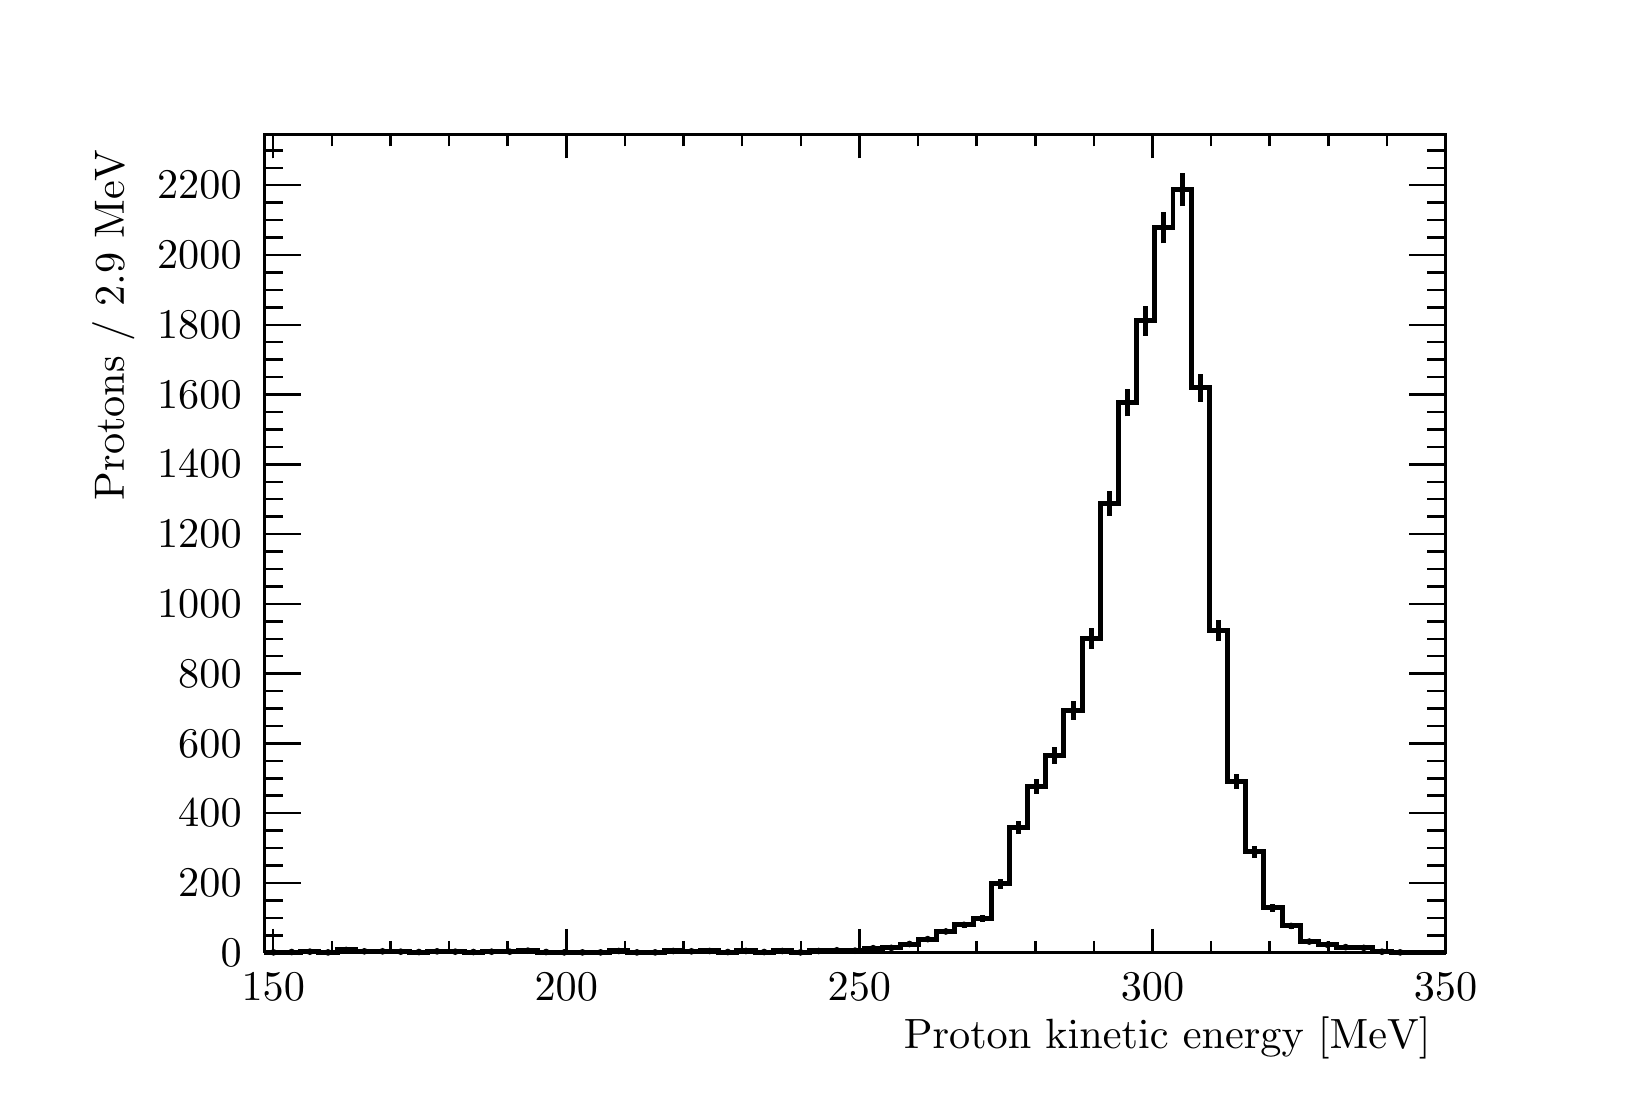
\begin{tikzpicture}
\pgfdeclareplotmark{cross} {
\pgfpathmoveto{\pgfpoint{-0.3\pgfplotmarksize}{\pgfplotmarksize}}
\pgfpathlineto{\pgfpoint{+0.3\pgfplotmarksize}{\pgfplotmarksize}}
\pgfpathlineto{\pgfpoint{+0.3\pgfplotmarksize}{0.3\pgfplotmarksize}}
\pgfpathlineto{\pgfpoint{+1\pgfplotmarksize}{0.3\pgfplotmarksize}}
\pgfpathlineto{\pgfpoint{+1\pgfplotmarksize}{-0.3\pgfplotmarksize}}
\pgfpathlineto{\pgfpoint{+0.3\pgfplotmarksize}{-0.3\pgfplotmarksize}}
\pgfpathlineto{\pgfpoint{+0.3\pgfplotmarksize}{-1.\pgfplotmarksize}}
\pgfpathlineto{\pgfpoint{-0.3\pgfplotmarksize}{-1.\pgfplotmarksize}}
\pgfpathlineto{\pgfpoint{-0.3\pgfplotmarksize}{-0.3\pgfplotmarksize}}
\pgfpathlineto{\pgfpoint{-1.\pgfplotmarksize}{-0.3\pgfplotmarksize}}
\pgfpathlineto{\pgfpoint{-1.\pgfplotmarksize}{0.3\pgfplotmarksize}}
\pgfpathlineto{\pgfpoint{-0.3\pgfplotmarksize}{0.3\pgfplotmarksize}}
\pgfpathclose
\pgfusepathqstroke
}
\pgfdeclareplotmark{cross*} {
\pgfpathmoveto{\pgfpoint{-0.3\pgfplotmarksize}{\pgfplotmarksize}}
\pgfpathlineto{\pgfpoint{+0.3\pgfplotmarksize}{\pgfplotmarksize}}
\pgfpathlineto{\pgfpoint{+0.3\pgfplotmarksize}{0.3\pgfplotmarksize}}
\pgfpathlineto{\pgfpoint{+1\pgfplotmarksize}{0.3\pgfplotmarksize}}
\pgfpathlineto{\pgfpoint{+1\pgfplotmarksize}{-0.3\pgfplotmarksize}}
\pgfpathlineto{\pgfpoint{+0.3\pgfplotmarksize}{-0.3\pgfplotmarksize}}
\pgfpathlineto{\pgfpoint{+0.3\pgfplotmarksize}{-1.\pgfplotmarksize}}
\pgfpathlineto{\pgfpoint{-0.3\pgfplotmarksize}{-1.\pgfplotmarksize}}
\pgfpathlineto{\pgfpoint{-0.3\pgfplotmarksize}{-0.3\pgfplotmarksize}}
\pgfpathlineto{\pgfpoint{-1.\pgfplotmarksize}{-0.3\pgfplotmarksize}}
\pgfpathlineto{\pgfpoint{-1.\pgfplotmarksize}{0.3\pgfplotmarksize}}
\pgfpathlineto{\pgfpoint{-0.3\pgfplotmarksize}{0.3\pgfplotmarksize}}
\pgfpathclose
\pgfusepathqfillstroke
}
\pgfdeclareplotmark{newstar} {
\pgfpathmoveto{\pgfqpoint{0pt}{\pgfplotmarksize}}
\pgfpathlineto{\pgfqpointpolar{44}{0.5\pgfplotmarksize}}
\pgfpathlineto{\pgfqpointpolar{18}{\pgfplotmarksize}}
\pgfpathlineto{\pgfqpointpolar{-20}{0.5\pgfplotmarksize}}
\pgfpathlineto{\pgfqpointpolar{-54}{\pgfplotmarksize}}
\pgfpathlineto{\pgfqpointpolar{-90}{0.5\pgfplotmarksize}}
\pgfpathlineto{\pgfqpointpolar{234}{\pgfplotmarksize}}
\pgfpathlineto{\pgfqpointpolar{198}{0.5\pgfplotmarksize}}
\pgfpathlineto{\pgfqpointpolar{162}{\pgfplotmarksize}}
\pgfpathlineto{\pgfqpointpolar{134}{0.5\pgfplotmarksize}}
\pgfpathclose
\pgfusepathqstroke
}
\pgfdeclareplotmark{newstar*} {
\pgfpathmoveto{\pgfqpoint{0pt}{\pgfplotmarksize}}
\pgfpathlineto{\pgfqpointpolar{44}{0.5\pgfplotmarksize}}
\pgfpathlineto{\pgfqpointpolar{18}{\pgfplotmarksize}}
\pgfpathlineto{\pgfqpointpolar{-20}{0.5\pgfplotmarksize}}
\pgfpathlineto{\pgfqpointpolar{-54}{\pgfplotmarksize}}
\pgfpathlineto{\pgfqpointpolar{-90}{0.5\pgfplotmarksize}}
\pgfpathlineto{\pgfqpointpolar{234}{\pgfplotmarksize}}
\pgfpathlineto{\pgfqpointpolar{198}{0.5\pgfplotmarksize}}
\pgfpathlineto{\pgfqpointpolar{162}{\pgfplotmarksize}}
\pgfpathlineto{\pgfqpointpolar{134}{0.5\pgfplotmarksize}}
\pgfpathclose
\pgfusepathqfillstroke
}
\definecolor{c}{rgb}{1,1,1};
\draw [color=c, fill=c] (0,0) rectangle (20,13.4957);
\draw [color=c, fill=c] (3,1.75444) rectangle (18,12.1461);
\definecolor{c}{rgb}{0,0,0};
\draw [c,line width=0.9] (3,1.75444) -- (3,12.1461) -- (18,12.1461) -- (18,1.75444) -- (3,1.75444);
\definecolor{c}{rgb}{1,1,1};
\draw [color=c, fill=c] (3,1.75444) rectangle (18,12.1461);
\definecolor{c}{rgb}{0,0,0};
\draw [c,line width=0.9] (3,1.75444) -- (3,12.1461) -- (18,12.1461) -- (18,1.75444) -- (3,1.75444);
\draw [c,line width=1.8] (3.11538,1.75444) -- (3.11538,1.75887);
\draw [c,line width=1.8] (3.11538,1.75887) -- (3.11538,1.7633);
\foreach \P in {(3.11538,1.75887)}{\draw[mark options={color=c,fill=c},mark size=2.402402pt,mark=*,mark size=1pt] plot coordinates {\P};}
\draw [c,line width=1.8] (3.34615,1.75704) -- (3.34615,1.7633);
\draw [c,line width=1.8] (3.34615,1.7633) -- (3.34615,1.76957);
\foreach \P in {(3.34615,1.7633)}{\draw[mark options={color=c,fill=c},mark size=2.402402pt,mark=*,mark size=1pt] plot coordinates {\P};}
\draw [c,line width=1.8] (3.57692,1.76006) -- (3.57692,1.76773);
\draw [c,line width=1.8] (3.57692,1.76773) -- (3.57692,1.77541);
\foreach \P in {(3.57692,1.76773)}{\draw[mark options={color=c,fill=c},mark size=2.402402pt,mark=*,mark size=1pt] plot coordinates {\P};}
\draw [c,line width=1.8] (3.80769,1.75444) -- (3.80769,1.75887);
\draw [c,line width=1.8] (3.80769,1.75887) -- (3.80769,1.7633);
\foreach \P in {(3.80769,1.75887)}{\draw[mark options={color=c,fill=c},mark size=2.402402pt,mark=*,mark size=1pt] plot coordinates {\P};}
\draw [c,line width=1.8] (4.03846,1.77735) -- (4.03846,1.78989);
\draw [c,line width=1.8] (4.03846,1.78989) -- (4.03846,1.80242);
\foreach \P in {(4.03846,1.78989)}{\draw[mark options={color=c,fill=c},mark size=2.402402pt,mark=*,mark size=1pt] plot coordinates {\P};}
\draw [c,line width=1.8] (4.26923,1.7633) -- (4.26923,1.77216);
\draw [c,line width=1.8] (4.26923,1.77216) -- (4.26923,1.78102);
\foreach \P in {(4.26923,1.77216)}{\draw[mark options={color=c,fill=c},mark size=2.402402pt,mark=*,mark size=1pt] plot coordinates {\P};}
\draw [c,line width=1.8] (4.5,1.7633) -- (4.5,1.77216);
\draw [c,line width=1.8] (4.5,1.77216) -- (4.5,1.78102);
\foreach \P in {(4.5,1.77216)}{\draw[mark options={color=c,fill=c},mark size=2.402402pt,mark=*,mark size=1pt] plot coordinates {\P};}
\draw [c,line width=1.8] (4.73077,1.76006) -- (4.73077,1.76773);
\draw [c,line width=1.8] (4.73077,1.76773) -- (4.73077,1.77541);
\foreach \P in {(4.73077,1.76773)}{\draw[mark options={color=c,fill=c},mark size=2.402402pt,mark=*,mark size=1pt] plot coordinates {\P};}
\draw [c,line width=1.8] (4.96154,1.75704) -- (4.96154,1.7633);
\draw [c,line width=1.8] (4.96154,1.7633) -- (4.96154,1.76957);
\foreach \P in {(4.96154,1.7633)}{\draw[mark options={color=c,fill=c},mark size=2.402402pt,mark=*,mark size=1pt] plot coordinates {\P};}
\draw [c,line width=1.8] (5.19231,1.7633) -- (5.19231,1.77216);
\draw [c,line width=1.8] (5.19231,1.77216) -- (5.19231,1.78102);
\foreach \P in {(5.19231,1.77216)}{\draw[mark options={color=c,fill=c},mark size=2.402402pt,mark=*,mark size=1pt] plot coordinates {\P};}
\draw [c,line width=1.8] (5.42308,1.76006) -- (5.42308,1.76773);
\draw [c,line width=1.8] (5.42308,1.76773) -- (5.42308,1.77541);
\foreach \P in {(5.42308,1.76773)}{\draw[mark options={color=c,fill=c},mark size=2.402402pt,mark=*,mark size=1pt] plot coordinates {\P};}
\draw [c,line width=1.8] (5.65385,1.75704) -- (5.65385,1.7633);
\draw [c,line width=1.8] (5.65385,1.7633) -- (5.65385,1.76957);
\foreach \P in {(5.65385,1.7633)}{\draw[mark options={color=c,fill=c},mark size=2.402402pt,mark=*,mark size=1pt] plot coordinates {\P};}
\draw [c,line width=1.8] (5.88462,1.76006) -- (5.88462,1.76773);
\draw [c,line width=1.8] (5.88462,1.76773) -- (5.88462,1.77541);
\foreach \P in {(5.88462,1.76773)}{\draw[mark options={color=c,fill=c},mark size=2.402402pt,mark=*,mark size=1pt] plot coordinates {\P};}
\draw [c,line width=1.8] (6.11538,1.76006) -- (6.11538,1.76773);
\draw [c,line width=1.8] (6.11538,1.76773) -- (6.11538,1.77541);
\foreach \P in {(6.11538,1.76773)}{\draw[mark options={color=c,fill=c},mark size=2.402402pt,mark=*,mark size=1pt] plot coordinates {\P};}
\draw [c,line width=1.8] (6.34615,1.77017) -- (6.34615,1.78102);
\draw [c,line width=1.8] (6.34615,1.78102) -- (6.34615,1.79188);
\foreach \P in {(6.34615,1.78102)}{\draw[mark options={color=c,fill=c},mark size=2.402402pt,mark=*,mark size=1pt] plot coordinates {\P};}
\draw [c,line width=1.8] (6.57692,1.75704) -- (6.57692,1.7633);
\draw [c,line width=1.8] (6.57692,1.7633) -- (6.57692,1.76957);
\foreach \P in {(6.57692,1.7633)}{\draw[mark options={color=c,fill=c},mark size=2.402402pt,mark=*,mark size=1pt] plot coordinates {\P};}
\draw [c,line width=1.8] (6.80769,1.75444) -- (6.80769,1.75887);
\draw [c,line width=1.8] (6.80769,1.75887) -- (6.80769,1.7633);
\foreach \P in {(6.80769,1.75887)}{\draw[mark options={color=c,fill=c},mark size=2.402402pt,mark=*,mark size=1pt] plot coordinates {\P};}
\draw [c,line width=1.8] (7.03846,1.75444) -- (7.03846,1.75887);
\draw [c,line width=1.8] (7.03846,1.75887) -- (7.03846,1.7633);
\foreach \P in {(7.03846,1.75887)}{\draw[mark options={color=c,fill=c},mark size=2.402402pt,mark=*,mark size=1pt] plot coordinates {\P};}
\draw [c,line width=1.8] (7.26923,1.75444) -- (7.26923,1.75887);
\draw [c,line width=1.8] (7.26923,1.75887) -- (7.26923,1.7633);
\foreach \P in {(7.26923,1.75887)}{\draw[mark options={color=c,fill=c},mark size=2.402402pt,mark=*,mark size=1pt] plot coordinates {\P};}
\draw [c,line width=1.8] (7.5,1.76669) -- (7.5,1.77659);
\draw [c,line width=1.8] (7.5,1.77659) -- (7.5,1.7865);
\foreach \P in {(7.5,1.77659)}{\draw[mark options={color=c,fill=c},mark size=2.402402pt,mark=*,mark size=1pt] plot coordinates {\P};}
\draw [c,line width=1.8] (7.73077,1.75444) -- (7.73077,1.75887);
\draw [c,line width=1.8] (7.73077,1.75887) -- (7.73077,1.7633);
\foreach \P in {(7.73077,1.75887)}{\draw[mark options={color=c,fill=c},mark size=2.402402pt,mark=*,mark size=1pt] plot coordinates {\P};}
\draw [c,line width=1.8] (7.96154,1.75444) -- (7.96154,1.75887);
\draw [c,line width=1.8] (7.96154,1.75887) -- (7.96154,1.7633);
\foreach \P in {(7.96154,1.75887)}{\draw[mark options={color=c,fill=c},mark size=2.402402pt,mark=*,mark size=1pt] plot coordinates {\P};}
\draw [c,line width=1.8] (8.19231,1.76669) -- (8.19231,1.77659);
\draw [c,line width=1.8] (8.19231,1.77659) -- (8.19231,1.7865);
\foreach \P in {(8.19231,1.77659)}{\draw[mark options={color=c,fill=c},mark size=2.402402pt,mark=*,mark size=1pt] plot coordinates {\P};}
\draw [c,line width=1.8] (8.42308,1.7633) -- (8.42308,1.77216);
\draw [c,line width=1.8] (8.42308,1.77216) -- (8.42308,1.78102);
\foreach \P in {(8.42308,1.77216)}{\draw[mark options={color=c,fill=c},mark size=2.402402pt,mark=*,mark size=1pt] plot coordinates {\P};}
\draw [c,line width=1.8] (8.65385,1.76669) -- (8.65385,1.77659);
\draw [c,line width=1.8] (8.65385,1.77659) -- (8.65385,1.7865);
\foreach \P in {(8.65385,1.77659)}{\draw[mark options={color=c,fill=c},mark size=2.402402pt,mark=*,mark size=1pt] plot coordinates {\P};}
\draw [c,line width=1.8] (8.88462,1.75704) -- (8.88462,1.7633);
\draw [c,line width=1.8] (8.88462,1.7633) -- (8.88462,1.76957);
\foreach \P in {(8.88462,1.7633)}{\draw[mark options={color=c,fill=c},mark size=2.402402pt,mark=*,mark size=1pt] plot coordinates {\P};}
\draw [c,line width=1.8] (9.11539,1.76669) -- (9.11539,1.77659);
\draw [c,line width=1.8] (9.11539,1.77659) -- (9.11539,1.7865);
\foreach \P in {(9.11539,1.77659)}{\draw[mark options={color=c,fill=c},mark size=2.402402pt,mark=*,mark size=1pt] plot coordinates {\P};}
\draw [c,line width=1.8] (9.34615,1.75704) -- (9.34615,1.7633);
\draw [c,line width=1.8] (9.34615,1.7633) -- (9.34615,1.76957);
\foreach \P in {(9.34615,1.7633)}{\draw[mark options={color=c,fill=c},mark size=2.402402pt,mark=*,mark size=1pt] plot coordinates {\P};}
\draw [c,line width=1.8] (9.57692,1.76669) -- (9.57692,1.77659);
\draw [c,line width=1.8] (9.57692,1.77659) -- (9.57692,1.7865);
\foreach \P in {(9.57692,1.77659)}{\draw[mark options={color=c,fill=c},mark size=2.402402pt,mark=*,mark size=1pt] plot coordinates {\P};}
\draw [c,line width=1.8] (9.80769,1.75444) -- (9.80769,1.75887);
\draw [c,line width=1.8] (9.80769,1.75887) -- (9.80769,1.7633);
\foreach \P in {(9.80769,1.75887)}{\draw[mark options={color=c,fill=c},mark size=2.402402pt,mark=*,mark size=1pt] plot coordinates {\P};}
\draw [c,line width=1.8] (10.0385,1.76669) -- (10.0385,1.77659);
\draw [c,line width=1.8] (10.0385,1.77659) -- (10.0385,1.7865);
\foreach \P in {(10.0385,1.77659)}{\draw[mark options={color=c,fill=c},mark size=2.402402pt,mark=*,mark size=1pt] plot coordinates {\P};}
\draw [c,line width=1.8] (10.2692,1.77373) -- (10.2692,1.78546);
\draw [c,line width=1.8] (10.2692,1.78546) -- (10.2692,1.79718);
\foreach \P in {(10.2692,1.78546)}{\draw[mark options={color=c,fill=c},mark size=2.402402pt,mark=*,mark size=1pt] plot coordinates {\P};}
\draw [c,line width=1.8] (10.5,1.77017) -- (10.5,1.78102);
\draw [c,line width=1.8] (10.5,1.78102) -- (10.5,1.79188);
\foreach \P in {(10.5,1.78102)}{\draw[mark options={color=c,fill=c},mark size=2.402402pt,mark=*,mark size=1pt] plot coordinates {\P};}
\draw [c,line width=1.8] (10.7308,1.79606) -- (10.7308,1.81204);
\draw [c,line width=1.8] (10.7308,1.81204) -- (10.7308,1.82801);
\foreach \P in {(10.7308,1.81204)}{\draw[mark options={color=c,fill=c},mark size=2.402402pt,mark=*,mark size=1pt] plot coordinates {\P};}
\draw [c,line width=1.8] (10.9615,1.79989) -- (10.9615,1.81647);
\draw [c,line width=1.8] (10.9615,1.81647) -- (10.9615,1.83305);
\foreach \P in {(10.9615,1.81647)}{\draw[mark options={color=c,fill=c},mark size=2.402402pt,mark=*,mark size=1pt] plot coordinates {\P};}
\draw [c,line width=1.8] (11.1923,1.84305) -- (11.1923,1.86521);
\draw [c,line width=1.8] (11.1923,1.86521) -- (11.1923,1.88736);
\foreach \P in {(11.1923,1.86521)}{\draw[mark options={color=c,fill=c},mark size=2.402402pt,mark=*,mark size=1pt] plot coordinates {\P};}
\draw [c,line width=1.8] (11.4231,1.89956) -- (11.4231,1.92723);
\draw [c,line width=1.8] (11.4231,1.92723) -- (11.4231,1.9549);
\foreach \P in {(11.4231,1.92723)}{\draw[mark options={color=c,fill=c},mark size=2.402402pt,mark=*,mark size=1pt] plot coordinates {\P};}
\draw [c,line width=1.8] (11.6538,1.9901) -- (11.6538,2.02471);
\draw [c,line width=1.8] (11.6538,2.02471) -- (11.6538,2.05931);
\foreach \P in {(11.6538,2.02471)}{\draw[mark options={color=c,fill=c},mark size=2.402402pt,mark=*,mark size=1pt] plot coordinates {\P};}
\draw [c,line width=1.8] (11.8846,2.06926) -- (11.8846,2.10889);
\draw [c,line width=1.8] (11.8846,2.10889) -- (11.8846,2.14851);
\foreach \P in {(11.8846,2.10889)}{\draw[mark options={color=c,fill=c},mark size=2.402402pt,mark=*,mark size=1pt] plot coordinates {\P};}
\draw [c,line width=1.8] (12.1154,2.14478) -- (12.1154,2.18864);
\draw [c,line width=1.8] (12.1154,2.18864) -- (12.1154,2.2325);
\foreach \P in {(12.1154,2.18864)}{\draw[mark options={color=c,fill=c},mark size=2.402402pt,mark=*,mark size=1pt] plot coordinates {\P};}
\draw [c,line width=1.8] (12.3462,2.56935) -- (12.3462,2.63169);
\draw [c,line width=1.8] (12.3462,2.63169) -- (12.3462,2.69404);
\foreach \P in {(12.3462,2.63169)}{\draw[mark options={color=c,fill=c},mark size=2.402402pt,mark=*,mark size=1pt] plot coordinates {\P};}
\draw [c,line width=1.8] (12.5769,3.26538) -- (12.5769,3.34945);
\draw [c,line width=1.8] (12.5769,3.34945) -- (12.5769,3.43351);
\foreach \P in {(12.5769,3.34945)}{\draw[mark options={color=c,fill=c},mark size=2.402402pt,mark=*,mark size=1pt] plot coordinates {\P};}
\draw [c,line width=1.8] (12.8077,3.77106) -- (12.8077,3.86782);
\draw [c,line width=1.8] (12.8077,3.86782) -- (12.8077,3.96459);
\foreach \P in {(12.8077,3.86782)}{\draw[mark options={color=c,fill=c},mark size=2.402402pt,mark=*,mark size=1pt] plot coordinates {\P};}
\draw [c,line width=1.8] (13.0385,4.1524) -- (13.0385,4.25771);
\draw [c,line width=1.8] (13.0385,4.25771) -- (13.0385,4.36303);
\foreach \P in {(13.0385,4.25771)}{\draw[mark options={color=c,fill=c},mark size=2.402402pt,mark=*,mark size=1pt] plot coordinates {\P};}
\draw [c,line width=1.8] (13.2692,4.71254) -- (13.2692,4.82926);
\draw [c,line width=1.8] (13.2692,4.82926) -- (13.2692,4.94597);
\foreach \P in {(13.2692,4.82926)}{\draw[mark options={color=c,fill=c},mark size=2.402402pt,mark=*,mark size=1pt] plot coordinates {\P};}
\draw [c,line width=1.8] (13.5,5.60904) -- (13.5,5.74195);
\draw [c,line width=1.8] (13.5,5.74195) -- (13.5,5.87487);
\foreach \P in {(13.5,5.74195)}{\draw[mark options={color=c,fill=c},mark size=2.402402pt,mark=*,mark size=1pt] plot coordinates {\P};}
\draw [c,line width=1.8] (13.7308,7.302) -- (13.7308,7.46101);
\draw [c,line width=1.8] (13.7308,7.46101) -- (13.7308,7.62002);
\foreach \P in {(13.7308,7.46101)}{\draw[mark options={color=c,fill=c},mark size=2.402402pt,mark=*,mark size=1pt] plot coordinates {\P};}
\draw [c,line width=1.8] (13.9615,8.5655) -- (13.9615,8.74145);
\draw [c,line width=1.8] (13.9615,8.74145) -- (13.9615,8.91739);
\foreach \P in {(13.9615,8.74145)}{\draw[mark options={color=c,fill=c},mark size=2.402402pt,mark=*,mark size=1pt] plot coordinates {\P};}
\draw [c,line width=1.8] (14.1923,9.58965) -- (14.1923,9.7782);
\draw [c,line width=1.8] (14.1923,9.7782) -- (14.1923,9.96675);
\foreach \P in {(14.1923,9.7782)}{\draw[mark options={color=c,fill=c},mark size=2.402402pt,mark=*,mark size=1pt] plot coordinates {\P};}
\draw [c,line width=1.8] (14.4231,10.7636) -- (14.4231,10.9656);
\draw [c,line width=1.8] (14.4231,10.9656) -- (14.4231,11.1676);
\foreach \P in {(14.4231,10.9656)}{\draw[mark options={color=c,fill=c},mark size=2.402402pt,mark=*,mark size=1pt] plot coordinates {\P};}
\draw [c,line width=1.8] (14.6538,11.2369) -- (14.6538,11.4441);
\draw [c,line width=1.8] (14.6538,11.4441) -- (14.6538,11.6513);
\foreach \P in {(14.6538,11.4441)}{\draw[mark options={color=c,fill=c},mark size=2.402402pt,mark=*,mark size=1pt] plot coordinates {\P};}
\draw [c,line width=1.8] (14.8846,8.75363) -- (14.8846,8.93196);
\draw [c,line width=1.8] (14.8846,8.93196) -- (14.8846,9.11029);
\foreach \P in {(14.8846,8.93196)}{\draw[mark options={color=c,fill=c},mark size=2.402402pt,mark=*,mark size=1pt] plot coordinates {\P};}
\draw [c,line width=1.8] (15.1154,5.70925) -- (15.1154,5.84385);
\draw [c,line width=1.8] (15.1154,5.84385) -- (15.1154,5.97846);
\foreach \P in {(15.1154,5.84385)}{\draw[mark options={color=c,fill=c},mark size=2.402402pt,mark=*,mark size=1pt] plot coordinates {\P};}
\draw [c,line width=1.8] (15.3462,3.83168) -- (15.3462,3.92985);
\draw [c,line width=1.8] (15.3462,3.92985) -- (15.3462,4.02802);
\foreach \P in {(15.3462,3.92985)}{\draw[mark options={color=c,fill=c},mark size=2.402402pt,mark=*,mark size=1pt] plot coordinates {\P};}
\draw [c,line width=1.8] (15.5769,2.95956) -- (15.5769,3.03488);
\draw [c,line width=1.8] (15.5769,3.03488) -- (15.5769,3.11019);
\foreach \P in {(15.5769,3.03488)}{\draw[mark options={color=c,fill=c},mark size=2.402402pt,mark=*,mark size=1pt] plot coordinates {\P};}
\draw [c,line width=1.8] (15.8077,2.27566) -- (15.8077,2.32598);
\draw [c,line width=1.8] (15.8077,2.32598) -- (15.8077,2.37631);
\foreach \P in {(15.8077,2.32598)}{\draw[mark options={color=c,fill=c},mark size=2.402402pt,mark=*,mark size=1pt] plot coordinates {\P};}
\draw [c,line width=1.8] (16.0385,2.05672) -- (16.0385,2.09559);
\draw [c,line width=1.8] (16.0385,2.09559) -- (16.0385,2.13447);
\foreach \P in {(16.0385,2.09559)}{\draw[mark options={color=c,fill=c},mark size=2.402402pt,mark=*,mark size=1pt] plot coordinates {\P};}
\draw [c,line width=1.8] (16.2692,1.87116) -- (16.2692,1.89622);
\draw [c,line width=1.8] (16.2692,1.89622) -- (16.2692,1.92128);
\foreach \P in {(16.2692,1.89622)}{\draw[mark options={color=c,fill=c},mark size=2.402402pt,mark=*,mark size=1pt] plot coordinates {\P};}
\draw [c,line width=1.8] (16.5,1.8351) -- (16.5,1.85634);
\draw [c,line width=1.8] (16.5,1.85634) -- (16.5,1.87759);
\foreach \P in {(16.5,1.85634)}{\draw[mark options={color=c,fill=c},mark size=2.402402pt,mark=*,mark size=1pt] plot coordinates {\P};}
\draw [c,line width=1.8] (16.7308,1.80761) -- (16.7308,1.82533);
\draw [c,line width=1.8] (16.7308,1.82533) -- (16.7308,1.84305);
\foreach \P in {(16.7308,1.82533)}{\draw[mark options={color=c,fill=c},mark size=2.402402pt,mark=*,mark size=1pt] plot coordinates {\P};}
\draw [c,line width=1.8] (16.9615,1.79989) -- (16.9615,1.81647);
\draw [c,line width=1.8] (16.9615,1.81647) -- (16.9615,1.83305);
\foreach \P in {(16.9615,1.81647)}{\draw[mark options={color=c,fill=c},mark size=2.402402pt,mark=*,mark size=1pt] plot coordinates {\P};}
\draw [c,line width=1.8] (17.1923,1.76006) -- (17.1923,1.76773);
\draw [c,line width=1.8] (17.1923,1.76773) -- (17.1923,1.77541);
\foreach \P in {(17.1923,1.76773)}{\draw[mark options={color=c,fill=c},mark size=2.402402pt,mark=*,mark size=1pt] plot coordinates {\P};}
\draw [c,line width=1.8] (17.4231,1.75444) -- (17.4231,1.75887);
\draw [c,line width=1.8] (17.4231,1.75887) -- (17.4231,1.7633);
\foreach \P in {(17.4231,1.75887)}{\draw[mark options={color=c,fill=c},mark size=2.402402pt,mark=*,mark size=1pt] plot coordinates {\P};}
\draw [c,line width=1.8] (3,1.75887) -- (3.23077,1.75887) -- (3.23077,1.7633) -- (3.46154,1.7633) -- (3.46154,1.76773) -- (3.69231,1.76773) -- (3.69231,1.75887) -- (3.92308,1.75887) -- (3.92308,1.78989) -- (4.15385,1.78989) -- (4.15385,1.77216) --
 (4.38462,1.77216) -- (4.38462,1.77216) -- (4.61538,1.77216) -- (4.61538,1.76773) -- (4.84615,1.76773) -- (4.84615,1.7633) -- (5.07692,1.7633) -- (5.07692,1.77216) -- (5.30769,1.77216) -- (5.30769,1.76773) -- (5.53846,1.76773) -- (5.53846,1.7633) --
 (5.76923,1.7633) -- (5.76923,1.76773) -- (6,1.76773) -- (6,1.76773) -- (6.23077,1.76773) -- (6.23077,1.78102) -- (6.46154,1.78102) -- (6.46154,1.7633) -- (6.69231,1.7633) -- (6.69231,1.75887) -- (6.92308,1.75887) -- (6.92308,1.75887) --
 (7.15385,1.75887) -- (7.15385,1.75887) -- (7.38462,1.75887) -- (7.38462,1.77659) -- (7.61538,1.77659) -- (7.61538,1.75887) -- (7.84615,1.75887) -- (7.84615,1.75887) -- (8.07692,1.75887) -- (8.07692,1.77659) -- (8.30769,1.77659) -- (8.30769,1.77216)
 -- (8.53846,1.77216) -- (8.53846,1.77659) -- (8.76923,1.77659) -- (8.76923,1.7633) -- (9,1.7633) -- (9,1.77659) -- (9.23077,1.77659) -- (9.23077,1.7633) -- (9.46154,1.7633) -- (9.46154,1.77659) -- (9.69231,1.77659) -- (9.69231,1.75887) --
 (9.92308,1.75887) -- (9.92308,1.77659) -- (10.1538,1.77659) -- (10.1538,1.78546) -- (10.3846,1.78546) -- (10.3846,1.78102) -- (10.6154,1.78102) -- (10.6154,1.81204) -- (10.8462,1.81204) -- (10.8462,1.81647) -- (11.0769,1.81647) -- (11.0769,1.86521)
 -- (11.3077,1.86521) -- (11.3077,1.92723) -- (11.5385,1.92723) -- (11.5385,2.02471) -- (11.7692,2.02471) -- (11.7692,2.10889) -- (12,2.10889) -- (12,2.18864) -- (12.2308,2.18864) -- (12.2308,2.63169) -- (12.4615,2.63169) -- (12.4615,3.34945) --
 (12.6923,3.34945) -- (12.6923,3.86782) -- (12.9231,3.86782) -- (12.9231,4.25771) -- (13.1538,4.25771) -- (13.1538,4.82926) -- (13.3846,4.82926) -- (13.3846,5.74195) -- (13.6154,5.74195) -- (13.6154,7.46101) -- (13.8462,7.46101) -- (13.8462,8.74145)
 -- (14.0769,8.74145) -- (14.0769,9.7782) -- (14.3077,9.7782) -- (14.3077,10.9656) -- (14.5385,10.9656) -- (14.5385,11.4441) -- (14.7692,11.4441) -- (14.7692,8.93196) -- (15,8.93196) -- (15,5.84385) -- (15.2308,5.84385) -- (15.2308,3.92985) --
 (15.4615,3.92985) -- (15.4615,3.03488) -- (15.6923,3.03488) -- (15.6923,2.32598) -- (15.9231,2.32598) -- (15.9231,2.09559) -- (16.1538,2.09559) -- (16.1538,1.89622) -- (16.3846,1.89622) -- (16.3846,1.85634) -- (16.6154,1.85634) -- (16.6154,1.82533)
 -- (16.8462,1.82533) -- (16.8462,1.81647) -- (17.0769,1.81647) -- (17.0769,1.76773) -- (17.3077,1.76773) -- (17.3077,1.75887) -- (17.5385,1.75887) -- (17.5385,1.75444) -- (17.7692,1.75444) -- (17.7692,1.75444) -- (18,1.75444);
\draw [c,line width=0.9] (3,1.75444) -- (18,1.75444);
\draw [c,line width=0.9] (3.11166,2.05809) -- (3.11166,1.75444);
\draw [c,line width=0.9] (3.85608,1.90627) -- (3.85608,1.75444);
\draw [c,line width=0.9] (4.6005,1.90627) -- (4.6005,1.75444);
\draw [c,line width=0.9] (5.34491,1.90627) -- (5.34491,1.75444);
\draw [c,line width=0.9] (6.08933,1.90627) -- (6.08933,1.75444);
\draw [c,line width=0.9] (6.83375,2.05809) -- (6.83375,1.75444);
\draw [c,line width=0.9] (7.57816,1.90627) -- (7.57816,1.75444);
\draw [c,line width=0.9] (8.32258,1.90627) -- (8.32258,1.75444);
\draw [c,line width=0.9] (9.067,1.90627) -- (9.067,1.75444);
\draw [c,line width=0.9] (9.81141,1.90627) -- (9.81141,1.75444);
\draw [c,line width=0.9] (10.5558,2.05809) -- (10.5558,1.75444);
\draw [c,line width=0.9] (11.3002,1.90627) -- (11.3002,1.75444);
\draw [c,line width=0.9] (12.0447,1.90627) -- (12.0447,1.75444);
\draw [c,line width=0.9] (12.7891,1.90627) -- (12.7891,1.75444);
\draw [c,line width=0.9] (13.5335,1.90627) -- (13.5335,1.75444);
\draw [c,line width=0.9] (14.2779,2.05809) -- (14.2779,1.75444);
\draw [c,line width=0.9] (15.0223,1.90627) -- (15.0223,1.75444);
\draw [c,line width=0.9] (15.7667,1.90627) -- (15.7667,1.75444);
\draw [c,line width=0.9] (16.5112,1.90627) -- (16.5112,1.75444);
\draw [c,line width=0.9] (17.2556,1.90627) -- (17.2556,1.75444);
\draw [c,line width=0.9] (18,2.05809) -- (18,1.75444);
\draw [c,line width=0.9] (3.11166,2.05809) -- (3.11166,1.75444);
\draw [c,line width=0.9] (18,2.05809) -- (18,1.75444);
\draw [anchor=base] (3.11166,1.14713) node[scale=1.52731, color=c, rotate=0]{150};
\draw [anchor=base] (6.83375,1.14713) node[scale=1.52731, color=c, rotate=0]{200};
\draw [anchor=base] (10.5558,1.14713) node[scale=1.52731, color=c, rotate=0]{250};
\draw [anchor=base] (14.2779,1.14713) node[scale=1.52731, color=c, rotate=0]{300};
\draw [anchor=base] (18,1.14713) node[scale=1.52731, color=c, rotate=0]{350};
\draw [anchor= east] (18,0.674785) node[scale=1.52731, color=c, rotate=0]{ Proton kinetic energy [MeV]};
\draw [c,line width=0.9] (3,12.1461) -- (18,12.1461);
\draw [c,line width=0.9] (3.11166,11.8425) -- (3.11166,12.1461);
\draw [c,line width=0.9] (3.85608,11.9943) -- (3.85608,12.1461);
\draw [c,line width=0.9] (4.6005,11.9943) -- (4.6005,12.1461);
\draw [c,line width=0.9] (5.34491,11.9943) -- (5.34491,12.1461);
\draw [c,line width=0.9] (6.08933,11.9943) -- (6.08933,12.1461);
\draw [c,line width=0.9] (6.83375,11.8425) -- (6.83375,12.1461);
\draw [c,line width=0.9] (7.57816,11.9943) -- (7.57816,12.1461);
\draw [c,line width=0.9] (8.32258,11.9943) -- (8.32258,12.1461);
\draw [c,line width=0.9] (9.067,11.9943) -- (9.067,12.1461);
\draw [c,line width=0.9] (9.81141,11.9943) -- (9.81141,12.1461);
\draw [c,line width=0.9] (10.5558,11.8425) -- (10.5558,12.1461);
\draw [c,line width=0.9] (11.3002,11.9943) -- (11.3002,12.1461);
\draw [c,line width=0.9] (12.0447,11.9943) -- (12.0447,12.1461);
\draw [c,line width=0.9] (12.7891,11.9943) -- (12.7891,12.1461);
\draw [c,line width=0.9] (13.5335,11.9943) -- (13.5335,12.1461);
\draw [c,line width=0.9] (14.2779,11.8425) -- (14.2779,12.1461);
\draw [c,line width=0.9] (15.0223,11.9943) -- (15.0223,12.1461);
\draw [c,line width=0.9] (15.7667,11.9943) -- (15.7667,12.1461);
\draw [c,line width=0.9] (16.5112,11.9943) -- (16.5112,12.1461);
\draw [c,line width=0.9] (17.2556,11.9943) -- (17.2556,12.1461);
\draw [c,line width=0.9] (18,11.8425) -- (18,12.1461);
\draw [c,line width=0.9] (3.11166,11.8425) -- (3.11166,12.1461);
\draw [c,line width=0.9] (18,11.8425) -- (18,12.1461);
\draw [c,line width=0.9] (3,1.75444) -- (3,12.1461);
\draw [c,line width=0.9] (3.462,1.75444) -- (3,1.75444);
\draw [c,line width=0.9] (3.231,1.97597) -- (3,1.97597);
\draw [c,line width=0.9] (3.231,2.1975) -- (3,2.1975);
\draw [c,line width=0.9] (3.231,2.41903) -- (3,2.41903);
\draw [c,line width=0.9] (3.462,2.64055) -- (3,2.64055);
\draw [c,line width=0.9] (3.231,2.86208) -- (3,2.86208);
\draw [c,line width=0.9] (3.231,3.08361) -- (3,3.08361);
\draw [c,line width=0.9] (3.231,3.30514) -- (3,3.30514);
\draw [c,line width=0.9] (3.462,3.52667) -- (3,3.52667);
\draw [c,line width=0.9] (3.231,3.7482) -- (3,3.7482);
\draw [c,line width=0.9] (3.231,3.96972) -- (3,3.96972);
\draw [c,line width=0.9] (3.231,4.19125) -- (3,4.19125);
\draw [c,line width=0.9] (3.462,4.41278) -- (3,4.41278);
\draw [c,line width=0.9] (3.231,4.63431) -- (3,4.63431);
\draw [c,line width=0.9] (3.231,4.85584) -- (3,4.85584);
\draw [c,line width=0.9] (3.231,5.07737) -- (3,5.07737);
\draw [c,line width=0.9] (3.462,5.29889) -- (3,5.29889);
\draw [c,line width=0.9] (3.231,5.52042) -- (3,5.52042);
\draw [c,line width=0.9] (3.231,5.74195) -- (3,5.74195);
\draw [c,line width=0.9] (3.231,5.96348) -- (3,5.96348);
\draw [c,line width=0.9] (3.462,6.18501) -- (3,6.18501);
\draw [c,line width=0.9] (3.231,6.40654) -- (3,6.40654);
\draw [c,line width=0.9] (3.231,6.62807) -- (3,6.62807);
\draw [c,line width=0.9] (3.231,6.84959) -- (3,6.84959);
\draw [c,line width=0.9] (3.462,7.07112) -- (3,7.07112);
\draw [c,line width=0.9] (3.231,7.29265) -- (3,7.29265);
\draw [c,line width=0.9] (3.231,7.51418) -- (3,7.51418);
\draw [c,line width=0.9] (3.231,7.73571) -- (3,7.73571);
\draw [c,line width=0.9] (3.462,7.95724) -- (3,7.95724);
\draw [c,line width=0.9] (3.231,8.17876) -- (3,8.17876);
\draw [c,line width=0.9] (3.231,8.40029) -- (3,8.40029);
\draw [c,line width=0.9] (3.231,8.62182) -- (3,8.62182);
\draw [c,line width=0.9] (3.462,8.84335) -- (3,8.84335);
\draw [c,line width=0.9] (3.231,9.06488) -- (3,9.06488);
\draw [c,line width=0.9] (3.231,9.28641) -- (3,9.28641);
\draw [c,line width=0.9] (3.231,9.50793) -- (3,9.50793);
\draw [c,line width=0.9] (3.462,9.72946) -- (3,9.72946);
\draw [c,line width=0.9] (3.231,9.95099) -- (3,9.95099);
\draw [c,line width=0.9] (3.231,10.1725) -- (3,10.1725);
\draw [c,line width=0.9] (3.231,10.394) -- (3,10.394);
\draw [c,line width=0.9] (3.462,10.6156) -- (3,10.6156);
\draw [c,line width=0.9] (3.231,10.8371) -- (3,10.8371);
\draw [c,line width=0.9] (3.231,11.0586) -- (3,11.0586);
\draw [c,line width=0.9] (3.231,11.2802) -- (3,11.2802);
\draw [c,line width=0.9] (3.462,11.5017) -- (3,11.5017);
\draw [c,line width=0.9] (3.462,11.5017) -- (3,11.5017);
\draw [c,line width=0.9] (3.231,11.7232) -- (3,11.7232);
\draw [c,line width=0.9] (3.231,11.9447) -- (3,11.9447);
\draw [anchor= east] (2.9,1.75444) node[scale=1.52731, color=c, rotate=0]{0};
\draw [anchor= east] (2.9,2.64055) node[scale=1.52731, color=c, rotate=0]{200};
\draw [anchor= east] (2.9,3.52667) node[scale=1.52731, color=c, rotate=0]{400};
\draw [anchor= east] (2.9,4.41278) node[scale=1.52731, color=c, rotate=0]{600};
\draw [anchor= east] (2.9,5.29889) node[scale=1.52731, color=c, rotate=0]{800};
\draw [anchor= east] (2.9,6.18501) node[scale=1.52731, color=c, rotate=0]{1000};
\draw [anchor= east] (2.9,7.07112) node[scale=1.52731, color=c, rotate=0]{1200};
\draw [anchor= east] (2.9,7.95724) node[scale=1.52731, color=c, rotate=0]{1400};
\draw [anchor= east] (2.9,8.84335) node[scale=1.52731, color=c, rotate=0]{1600};
\draw [anchor= east] (2.9,9.72946) node[scale=1.52731, color=c, rotate=0]{1800};
\draw [anchor= east] (2.9,10.6156) node[scale=1.52731, color=c, rotate=0]{2000};
\draw [anchor= east] (2.9,11.5017) node[scale=1.52731, color=c, rotate=0]{2200};
\draw [anchor= east] (1.08,12.1461) node[scale=1.52731, color=c, rotate=90]{Protons / 2.9~MeV};
\draw [c,line width=0.9] (18,1.75444) -- (18,12.1461);
\draw [c,line width=0.9] (17.538,1.75444) -- (18,1.75444);
\draw [c,line width=0.9] (17.769,1.97597) -- (18,1.97597);
\draw [c,line width=0.9] (17.769,2.1975) -- (18,2.1975);
\draw [c,line width=0.9] (17.769,2.41903) -- (18,2.41903);
\draw [c,line width=0.9] (17.538,2.64055) -- (18,2.64055);
\draw [c,line width=0.9] (17.769,2.86208) -- (18,2.86208);
\draw [c,line width=0.9] (17.769,3.08361) -- (18,3.08361);
\draw [c,line width=0.9] (17.769,3.30514) -- (18,3.30514);
\draw [c,line width=0.9] (17.538,3.52667) -- (18,3.52667);
\draw [c,line width=0.9] (17.769,3.7482) -- (18,3.7482);
\draw [c,line width=0.9] (17.769,3.96972) -- (18,3.96972);
\draw [c,line width=0.9] (17.769,4.19125) -- (18,4.19125);
\draw [c,line width=0.9] (17.538,4.41278) -- (18,4.41278);
\draw [c,line width=0.9] (17.769,4.63431) -- (18,4.63431);
\draw [c,line width=0.9] (17.769,4.85584) -- (18,4.85584);
\draw [c,line width=0.9] (17.769,5.07737) -- (18,5.07737);
\draw [c,line width=0.9] (17.538,5.29889) -- (18,5.29889);
\draw [c,line width=0.9] (17.769,5.52042) -- (18,5.52042);
\draw [c,line width=0.9] (17.769,5.74195) -- (18,5.74195);
\draw [c,line width=0.9] (17.769,5.96348) -- (18,5.96348);
\draw [c,line width=0.9] (17.538,6.18501) -- (18,6.18501);
\draw [c,line width=0.9] (17.769,6.40654) -- (18,6.40654);
\draw [c,line width=0.9] (17.769,6.62807) -- (18,6.62807);
\draw [c,line width=0.9] (17.769,6.84959) -- (18,6.84959);
\draw [c,line width=0.9] (17.538,7.07112) -- (18,7.07112);
\draw [c,line width=0.9] (17.769,7.29265) -- (18,7.29265);
\draw [c,line width=0.9] (17.769,7.51418) -- (18,7.51418);
\draw [c,line width=0.9] (17.769,7.73571) -- (18,7.73571);
\draw [c,line width=0.9] (17.538,7.95724) -- (18,7.95724);
\draw [c,line width=0.9] (17.769,8.17876) -- (18,8.17876);
\draw [c,line width=0.9] (17.769,8.40029) -- (18,8.40029);
\draw [c,line width=0.9] (17.769,8.62182) -- (18,8.62182);
\draw [c,line width=0.9] (17.538,8.84335) -- (18,8.84335);
\draw [c,line width=0.9] (17.769,9.06488) -- (18,9.06488);
\draw [c,line width=0.9] (17.769,9.28641) -- (18,9.28641);
\draw [c,line width=0.9] (17.769,9.50793) -- (18,9.50793);
\draw [c,line width=0.9] (17.538,9.72946) -- (18,9.72946);
\draw [c,line width=0.9] (17.769,9.95099) -- (18,9.95099);
\draw [c,line width=0.9] (17.769,10.1725) -- (18,10.1725);
\draw [c,line width=0.9] (17.769,10.394) -- (18,10.394);
\draw [c,line width=0.9] (17.538,10.6156) -- (18,10.6156);
\draw [c,line width=0.9] (17.769,10.8371) -- (18,10.8371);
\draw [c,line width=0.9] (17.769,11.0586) -- (18,11.0586);
\draw [c,line width=0.9] (17.769,11.2802) -- (18,11.2802);
\draw [c,line width=0.9] (17.538,11.5017) -- (18,11.5017);
\draw [c,line width=0.9] (17.538,11.5017) -- (18,11.5017);
\draw [c,line width=0.9] (17.769,11.7232) -- (18,11.7232);
\draw [c,line width=0.9] (17.769,11.9447) -- (18,11.9447);
\definecolor{c}{rgb}{1,1,1};
\draw [color=c, fill=c] (2,12.686) rectangle (18,13.4282);
\definecolor{c}{rgb}{0,0,0};
%\draw (10,13.0571) node[scale=1.40004, color=c, rotate=0]{Proton kinetic energy measured in $\mathit{S3}$};
\end{tikzpicture}

    \end{adjustbox}
  \end{minipage}
  \caption[Time of flight spectrum and proton kinetic energy for the unmoderated and unbent T10 beam]{Left: Time of flight spectrum of the unmoderated and unbent CERN T10 beam across a baseline of \SI{10.8}{\metre}. Right: Measured kinetic energies of protons in the unmoderated and unbent CERN T10 beam.}
  \label{fig:unmoderatedBeam}
\end{figure}

It is necessary to modify the T10 beam for several reasons, one of them being the lack of the low energy protons.
Additionally, it is important to reduce the multiplicity of particles entering the HPgTPC due to the speed of the optical readout which could otherwise become overwhelmed.
Finally, it is desirable to modify the proton-minimum ionising particle (MIP) ratio in order to isolate more particles which are of interest to a cross-section analysis.

Therefore, two modification are made to the beam flux in order to achieve these goals.
Firstly up to four \SI{10 x 10 x 10}{\cm} acrylic moderator blocks are placed in the beam.
These blocks have the effect of scattering the incident particles and reducing their energy.
Additionally, the HPgTPC is moved to an off-axis angle in order to maximise the ratio of protons to MIPs.
From previous GEANT~\cite{geant} simulations it is determined that the optimal off-axis angle for the HPgTPC is between \ang{2} and \ang{3}.
However, due to space constraints in the beam hall, the HPgTPC could not be moved this far off-axis.
Instead, the beam was steered approximately \ang{1} off its nominal axis to increase the angle between the beam and the HPgTPC.
A bird's-eye view diagram of the experimental setup, which shows the beam position relative to the HPgTPC, is shown in \citefig{fig:beamSetup}.

\begin{figure}[h]
  \centering
  \includegraphics[width=\linewidth]{files/figures/hptpc_beam_flux/hptpc_t10_planview}
  \caption[Bird's-eye view of the experimental setup within the T10 beam area]{Bird's-eye view of the experimental setup within the T10 beam area, from~\cite{beampaper}.}
  \label{fig:beamSetup}
\end{figure}

The effectiveness of this off-axis technique was assessed using several timing points which were used to measure the particle species and energies upstream and downstream of the HPgTPC prototype.
These timing points are shown in \citefig{fig:beamSetup} and, from upstream to downstream, consist of:
\begin{itemize}
    \item \SOne, a \SI{40 x 40 x 5}{\mm} plastic scintillator cross, described in \citesec{sec:hptpc_beam_flux:overview:s1s2};
    \item \STwo, a \SI{120 x 120 x 5}{\mm} plastic scintillator tile, used for coincidence measurements with \SOne, described in \citesec{sec:hptpc_beam_flux:overview:s1s2};
    \item \SThree, a large panel of plastic scintillator bars placed directly upstream of the TPC vessel, described in \citesec{sec:hptpc_beam_flux:overview:s3};
    \item \SFour, a large panel of plastic scintillator bars placed directly downstream of the HPgTPC, which is described in \citesec{sec:hptpc_beam_flux:overview:s4} (its characterisation is described in \citesec{sec:hptpc_dtof_characterisation}).
\end{itemize}
The moderator blocks were placed on a tripod stand in between \SOne and \STwo.

\subsection{Survey and coordinate system}
\label{sec:hptpc_beam_flux:overview:survey}

The distances to the various objects in the beamline from an origin point is measured by the CERN Survey, Mechatronics and Measurements (SMM) group to a precision of \SI{0.5}{\mm}.
Specifically, multiple points on each of \SOne, \STwo, \SThree, \SFour and the HPgTPC prototype were measured.
From these measurements, the distance between various timing points is calculated and displayed in \citetab{tab:pointDistances}, calculated using this survey data

\begin{table}
  \centering
  \caption[Calculated distances between objects within the T10 beamline during the beam test]{Calculated distances between objects within the T10 beamline during the beam test}
  \label{tab:pointDistances}
  \begin{tabular}{c c}
    \hline
    \hline
    Points & Distance between centres / m \\
    \hline
    $\text{Beam monitor} - \SOne$ & \num{0.288(1)} \\
    $\SOne - \STwo$ & \num{1.419(1)} \\
    $\SOne - \SThree$ & \num{10.756(1)} \\
    $\SThree - \text{TPC US side}$ & \num{1.323(2)} \\
    $\text{TPC DS side} - \SFour$ & \num{0.918(2)} \\
    $\STwo - \SFour$ & \num{12.651(1)} \\
    \hline
  \end{tabular}
\end{table}

The coordinate systeam used in this analysis is a right-handed coordinate system defined by the following directions: the $+\hat{z}$ direction is defined as the nominal beam axis, the $+\hat{y}$ direction is defined as vertically upwards and the $\hat{x}$ direction is defined as the horizontal direction which is perpendicular to the beam direction.
The origin is take to be at \SOne.
The $\hat{x}$ and $\hat{z}$ axes are labelled in \citefig{fig:beamSetup}.
In this analysis, the results are given in terms of the angles $\theta$ and $\phi$.
$\theta$ is measured in the $\hat{x}-\hat{z}$ plane with positive angle measured in the $+\hat{x}$ direction while $\phi$ is measured in the $\hat{y}-\hat{z}$ with positive angles measured in the $+\hat{y}$ direction.

\citefig{fig:angDistS1} shows the angular distribution of objects within the beamline as viewed from \SOne.
\citetab{tab:angDistS1} shows the angular extent of various beamline components as measured from \SOne.
Both of these use the data from the survey in order to calculate the results.

\begin{figure}[h]
  \begin{adjustbox}{max totalsize=.8\textwidth, center}
    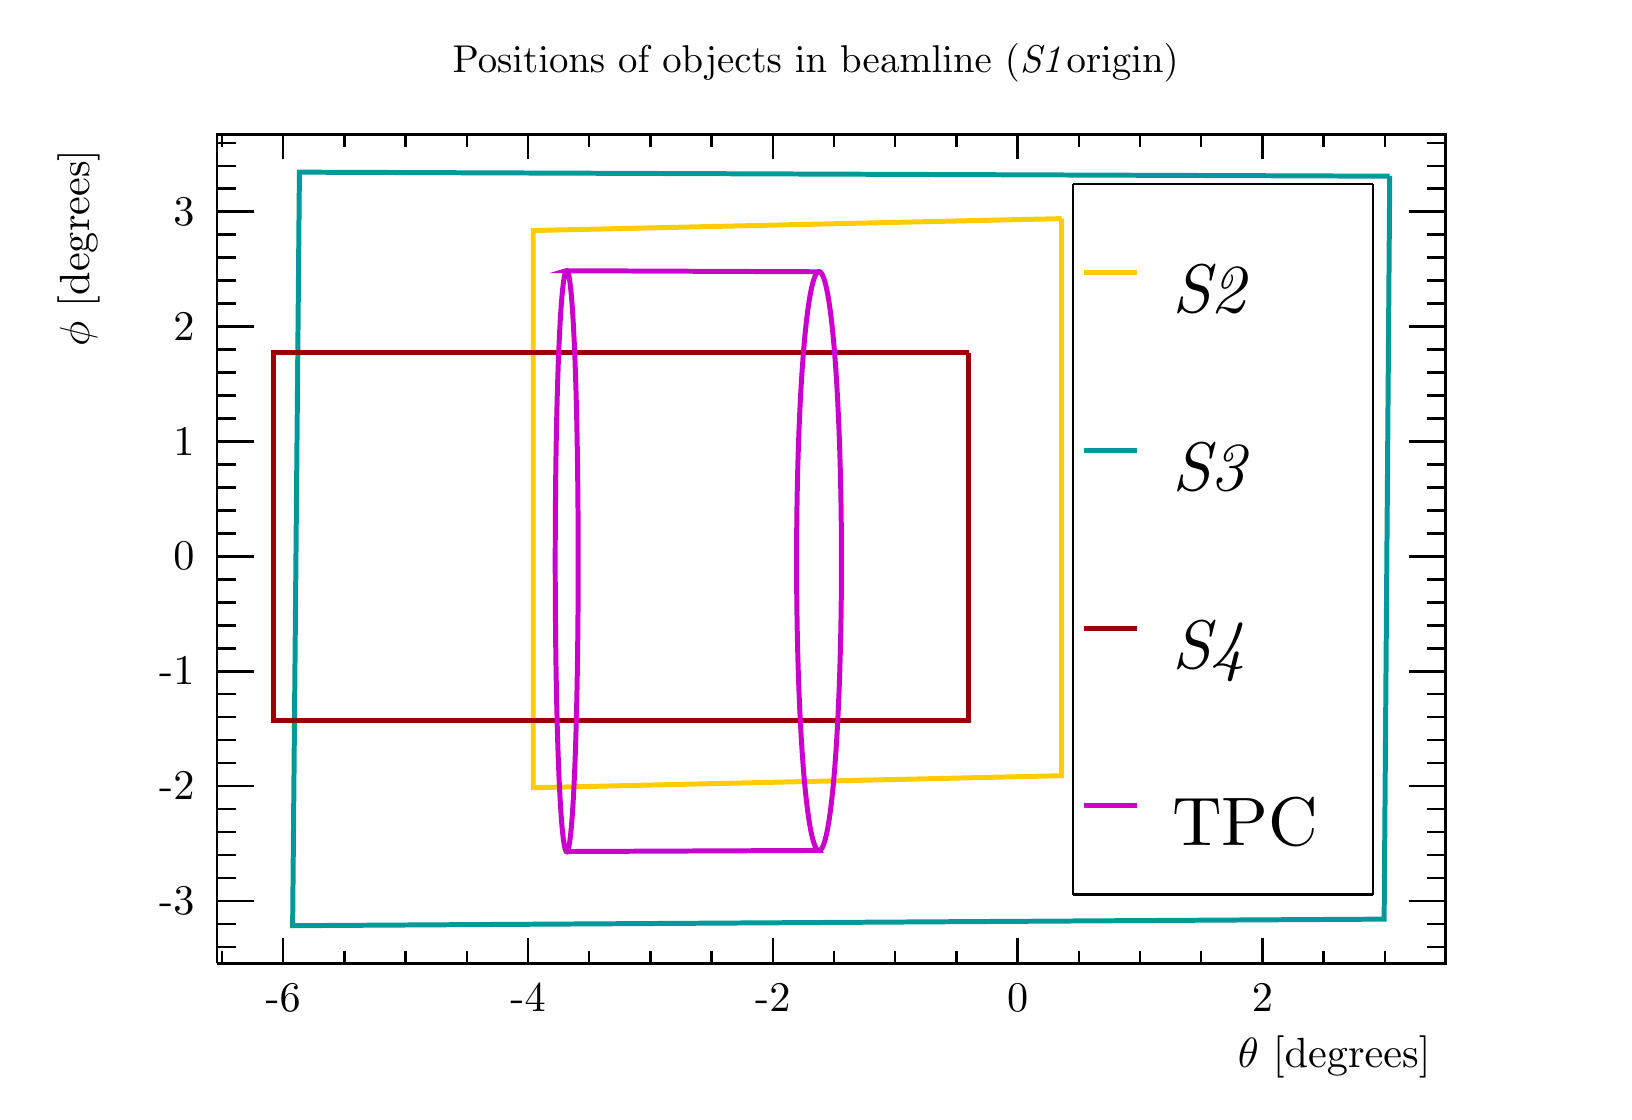
\begin{tikzpicture}
\pgfdeclareplotmark{cross} {
\pgfpathmoveto{\pgfpoint{-0.3\pgfplotmarksize}{\pgfplotmarksize}}
\pgfpathlineto{\pgfpoint{+0.3\pgfplotmarksize}{\pgfplotmarksize}}
\pgfpathlineto{\pgfpoint{+0.3\pgfplotmarksize}{0.3\pgfplotmarksize}}
\pgfpathlineto{\pgfpoint{+1\pgfplotmarksize}{0.3\pgfplotmarksize}}
\pgfpathlineto{\pgfpoint{+1\pgfplotmarksize}{-0.3\pgfplotmarksize}}
\pgfpathlineto{\pgfpoint{+0.3\pgfplotmarksize}{-0.3\pgfplotmarksize}}
\pgfpathlineto{\pgfpoint{+0.3\pgfplotmarksize}{-1.\pgfplotmarksize}}
\pgfpathlineto{\pgfpoint{-0.3\pgfplotmarksize}{-1.\pgfplotmarksize}}
\pgfpathlineto{\pgfpoint{-0.3\pgfplotmarksize}{-0.3\pgfplotmarksize}}
\pgfpathlineto{\pgfpoint{-1.\pgfplotmarksize}{-0.3\pgfplotmarksize}}
\pgfpathlineto{\pgfpoint{-1.\pgfplotmarksize}{0.3\pgfplotmarksize}}
\pgfpathlineto{\pgfpoint{-0.3\pgfplotmarksize}{0.3\pgfplotmarksize}}
\pgfpathclose
\pgfusepathqstroke
}
\pgfdeclareplotmark{cross*} {
\pgfpathmoveto{\pgfpoint{-0.3\pgfplotmarksize}{\pgfplotmarksize}}
\pgfpathlineto{\pgfpoint{+0.3\pgfplotmarksize}{\pgfplotmarksize}}
\pgfpathlineto{\pgfpoint{+0.3\pgfplotmarksize}{0.3\pgfplotmarksize}}
\pgfpathlineto{\pgfpoint{+1\pgfplotmarksize}{0.3\pgfplotmarksize}}
\pgfpathlineto{\pgfpoint{+1\pgfplotmarksize}{-0.3\pgfplotmarksize}}
\pgfpathlineto{\pgfpoint{+0.3\pgfplotmarksize}{-0.3\pgfplotmarksize}}
\pgfpathlineto{\pgfpoint{+0.3\pgfplotmarksize}{-1.\pgfplotmarksize}}
\pgfpathlineto{\pgfpoint{-0.3\pgfplotmarksize}{-1.\pgfplotmarksize}}
\pgfpathlineto{\pgfpoint{-0.3\pgfplotmarksize}{-0.3\pgfplotmarksize}}
\pgfpathlineto{\pgfpoint{-1.\pgfplotmarksize}{-0.3\pgfplotmarksize}}
\pgfpathlineto{\pgfpoint{-1.\pgfplotmarksize}{0.3\pgfplotmarksize}}
\pgfpathlineto{\pgfpoint{-0.3\pgfplotmarksize}{0.3\pgfplotmarksize}}
\pgfpathclose
\pgfusepathqfillstroke
}
\pgfdeclareplotmark{newstar} {
\pgfpathmoveto{\pgfqpoint{0pt}{\pgfplotmarksize}}
\pgfpathlineto{\pgfqpointpolar{44}{0.5\pgfplotmarksize}}
\pgfpathlineto{\pgfqpointpolar{18}{\pgfplotmarksize}}
\pgfpathlineto{\pgfqpointpolar{-20}{0.5\pgfplotmarksize}}
\pgfpathlineto{\pgfqpointpolar{-54}{\pgfplotmarksize}}
\pgfpathlineto{\pgfqpointpolar{-90}{0.5\pgfplotmarksize}}
\pgfpathlineto{\pgfqpointpolar{234}{\pgfplotmarksize}}
\pgfpathlineto{\pgfqpointpolar{198}{0.5\pgfplotmarksize}}
\pgfpathlineto{\pgfqpointpolar{162}{\pgfplotmarksize}}
\pgfpathlineto{\pgfqpointpolar{134}{0.5\pgfplotmarksize}}
\pgfpathclose
\pgfusepathqstroke
}
\pgfdeclareplotmark{newstar*} {
\pgfpathmoveto{\pgfqpoint{0pt}{\pgfplotmarksize}}
\pgfpathlineto{\pgfqpointpolar{44}{0.5\pgfplotmarksize}}
\pgfpathlineto{\pgfqpointpolar{18}{\pgfplotmarksize}}
\pgfpathlineto{\pgfqpointpolar{-20}{0.5\pgfplotmarksize}}
\pgfpathlineto{\pgfqpointpolar{-54}{\pgfplotmarksize}}
\pgfpathlineto{\pgfqpointpolar{-90}{0.5\pgfplotmarksize}}
\pgfpathlineto{\pgfqpointpolar{234}{\pgfplotmarksize}}
\pgfpathlineto{\pgfqpointpolar{198}{0.5\pgfplotmarksize}}
\pgfpathlineto{\pgfqpointpolar{162}{\pgfplotmarksize}}
\pgfpathlineto{\pgfqpointpolar{134}{0.5\pgfplotmarksize}}
\pgfpathclose
\pgfusepathqfillstroke
}
\definecolor{c}{rgb}{1,1,1};
\draw [color=c, fill=c] (0,0) rectangle (20,13.4957);
\draw [color=c, fill=c] (2.4,1.61948) rectangle (18,12.1461);
\definecolor{c}{rgb}{0,0,0};
\draw [c,line width=0.9] (2.4,1.61948) -- (2.4,12.1461) -- (18,12.1461) -- (18,1.61948) -- (2.4,1.61948);
\definecolor{c}{rgb}{1,1,1};
\draw [color=c, fill=c] (2.4,1.61948) rectangle (18,12.1461);
\definecolor{c}{rgb}{0,0,0};
\draw [c,line width=0.9] (2.4,1.61948) -- (2.4,12.1461) -- (18,12.1461) -- (18,1.61948) -- (2.4,1.61948);
\draw [c,line width=0.9] (2.4,1.61948) -- (18,1.61948);
\draw [c,line width=0.9] (3.23864,1.93528) -- (3.23864,1.61948);
\draw [c,line width=0.9] (4.01586,1.77738) -- (4.01586,1.61948);
\draw [c,line width=0.9] (4.79308,1.77738) -- (4.79308,1.61948);
\draw [c,line width=0.9] (5.5703,1.77738) -- (5.5703,1.61948);
\draw [c,line width=0.9] (6.34753,1.93528) -- (6.34753,1.61948);
\draw [c,line width=0.9] (7.12475,1.77738) -- (7.12475,1.61948);
\draw [c,line width=0.9] (7.90197,1.77738) -- (7.90197,1.61948);
\draw [c,line width=0.9] (8.67919,1.77738) -- (8.67919,1.61948);
\draw [c,line width=0.9] (9.45641,1.93528) -- (9.45641,1.61948);
\draw [c,line width=0.9] (10.2336,1.77738) -- (10.2336,1.61948);
\draw [c,line width=0.9] (11.0109,1.77738) -- (11.0109,1.61948);
\draw [c,line width=0.9] (11.7881,1.77738) -- (11.7881,1.61948);
\draw [c,line width=0.9] (12.5653,1.93528) -- (12.5653,1.61948);
\draw [c,line width=0.9] (13.3425,1.77738) -- (13.3425,1.61948);
\draw [c,line width=0.9] (14.1197,1.77738) -- (14.1197,1.61948);
\draw [c,line width=0.9] (14.897,1.77738) -- (14.897,1.61948);
\draw [c,line width=0.9] (15.6742,1.93528) -- (15.6742,1.61948);
\draw [c,line width=0.9] (3.23864,1.93528) -- (3.23864,1.61948);
\draw [c,line width=0.9] (2.46142,1.77738) -- (2.46142,1.61948);
\draw [c,line width=0.9] (15.6742,1.93528) -- (15.6742,1.61948);
\draw [c,line width=0.9] (16.4514,1.77738) -- (16.4514,1.61948);
\draw [c,line width=0.9] (17.2286,1.77738) -- (17.2286,1.61948);
\draw [anchor=base] (3.23864,1.01218) node[scale=1.52731, color=c, rotate=0]{-6};
\draw [anchor=base] (6.34753,1.01218) node[scale=1.52731, color=c, rotate=0]{-4};
\draw [anchor=base] (9.45641,1.01218) node[scale=1.52731, color=c, rotate=0]{-2};
\draw [anchor=base] (12.5653,1.01218) node[scale=1.52731, color=c, rotate=0]{0};
\draw [anchor=base] (15.6742,1.01218) node[scale=1.52731, color=c, rotate=0]{2};
\draw [anchor= east] (18,0.431862) node[scale=1.52731, color=c, rotate=0]{$ \theta$ [degrees]};
\draw [c,line width=0.9] (2.4,12.1461) -- (18,12.1461);
\draw [c,line width=0.9] (3.23864,11.8303) -- (3.23864,12.1461);
\draw [c,line width=0.9] (4.01586,11.9882) -- (4.01586,12.1461);
\draw [c,line width=0.9] (4.79308,11.9882) -- (4.79308,12.1461);
\draw [c,line width=0.9] (5.5703,11.9882) -- (5.5703,12.1461);
\draw [c,line width=0.9] (6.34753,11.8303) -- (6.34753,12.1461);
\draw [c,line width=0.9] (7.12475,11.9882) -- (7.12475,12.1461);
\draw [c,line width=0.9] (7.90197,11.9882) -- (7.90197,12.1461);
\draw [c,line width=0.9] (8.67919,11.9882) -- (8.67919,12.1461);
\draw [c,line width=0.9] (9.45641,11.8303) -- (9.45641,12.1461);
\draw [c,line width=0.9] (10.2336,11.9882) -- (10.2336,12.1461);
\draw [c,line width=0.9] (11.0109,11.9882) -- (11.0109,12.1461);
\draw [c,line width=0.9] (11.7881,11.9882) -- (11.7881,12.1461);
\draw [c,line width=0.9] (12.5653,11.8303) -- (12.5653,12.1461);
\draw [c,line width=0.9] (13.3425,11.9882) -- (13.3425,12.1461);
\draw [c,line width=0.9] (14.1197,11.9882) -- (14.1197,12.1461);
\draw [c,line width=0.9] (14.897,11.9882) -- (14.897,12.1461);
\draw [c,line width=0.9] (15.6742,11.8303) -- (15.6742,12.1461);
\draw [c,line width=0.9] (3.23864,11.8303) -- (3.23864,12.1461);
\draw [c,line width=0.9] (2.46142,11.9882) -- (2.46142,12.1461);
\draw [c,line width=0.9] (15.6742,11.8303) -- (15.6742,12.1461);
\draw [c,line width=0.9] (16.4514,11.9882) -- (16.4514,12.1461);
\draw [c,line width=0.9] (17.2286,11.9882) -- (17.2286,12.1461);
\draw [c,line width=0.9] (2.4,1.61948) -- (2.4,12.1461);
\draw [c,line width=0.9] (2.868,2.41096) -- (2.4,2.41096);
\draw [c,line width=0.9] (2.634,2.70278) -- (2.4,2.70278);
\draw [c,line width=0.9] (2.634,2.99459) -- (2.4,2.99459);
\draw [c,line width=0.9] (2.634,3.28641) -- (2.4,3.28641);
\draw [c,line width=0.9] (2.634,3.57822) -- (2.4,3.57822);
\draw [c,line width=0.9] (2.868,3.87004) -- (2.4,3.87004);
\draw [c,line width=0.9] (2.634,4.16185) -- (2.4,4.16185);
\draw [c,line width=0.9] (2.634,4.45367) -- (2.4,4.45367);
\draw [c,line width=0.9] (2.634,4.74548) -- (2.4,4.74548);
\draw [c,line width=0.9] (2.634,5.0373) -- (2.4,5.0373);
\draw [c,line width=0.9] (2.868,5.32911) -- (2.4,5.32911);
\draw [c,line width=0.9] (2.634,5.62093) -- (2.4,5.62093);
\draw [c,line width=0.9] (2.634,5.91274) -- (2.4,5.91274);
\draw [c,line width=0.9] (2.634,6.20456) -- (2.4,6.20456);
\draw [c,line width=0.9] (2.634,6.49638) -- (2.4,6.49638);
\draw [c,line width=0.9] (2.868,6.78819) -- (2.4,6.78819);
\draw [c,line width=0.9] (2.634,7.08001) -- (2.4,7.08001);
\draw [c,line width=0.9] (2.634,7.37182) -- (2.4,7.37182);
\draw [c,line width=0.9] (2.634,7.66364) -- (2.4,7.66364);
\draw [c,line width=0.9] (2.634,7.95545) -- (2.4,7.95545);
\draw [c,line width=0.9] (2.868,8.24727) -- (2.4,8.24727);
\draw [c,line width=0.9] (2.634,8.53908) -- (2.4,8.53908);
\draw [c,line width=0.9] (2.634,8.8309) -- (2.4,8.8309);
\draw [c,line width=0.9] (2.634,9.12271) -- (2.4,9.12271);
\draw [c,line width=0.9] (2.634,9.41453) -- (2.4,9.41453);
\draw [c,line width=0.9] (2.868,9.70634) -- (2.4,9.70634);
\draw [c,line width=0.9] (2.634,9.99816) -- (2.4,9.99816);
\draw [c,line width=0.9] (2.634,10.29) -- (2.4,10.29);
\draw [c,line width=0.9] (2.634,10.5818) -- (2.4,10.5818);
\draw [c,line width=0.9] (2.634,10.8736) -- (2.4,10.8736);
\draw [c,line width=0.9] (2.868,11.1654) -- (2.4,11.1654);
\draw [c,line width=0.9] (2.868,2.41096) -- (2.4,2.41096);
\draw [c,line width=0.9] (2.634,2.11915) -- (2.4,2.11915);
\draw [c,line width=0.9] (2.634,1.82733) -- (2.4,1.82733);
\draw [c,line width=0.9] (2.868,11.1654) -- (2.4,11.1654);
\draw [c,line width=0.9] (2.634,11.4572) -- (2.4,11.4572);
\draw [c,line width=0.9] (2.634,11.749) -- (2.4,11.749);
\draw [c,line width=0.9] (2.634,12.0409) -- (2.4,12.0409);
\draw [anchor= east] (2.3,2.41096) node[scale=1.52731, color=c, rotate=0]{-3};
\draw [anchor= east] (2.3,3.87004) node[scale=1.52731, color=c, rotate=0]{-2};
\draw [anchor= east] (2.3,5.32911) node[scale=1.52731, color=c, rotate=0]{-1};
\draw [anchor= east] (2.3,6.78819) node[scale=1.52731, color=c, rotate=0]{0};
\draw [anchor= east] (2.3,8.24727) node[scale=1.52731, color=c, rotate=0]{1};
\draw [anchor= east] (2.3,9.70634) node[scale=1.52731, color=c, rotate=0]{2};
\draw [anchor= east] (2.3,11.1654) node[scale=1.52731, color=c, rotate=0]{3};
\draw [anchor= east] (0.64,12.1461) node[scale=1.52731, color=c, rotate=90]{$ \phi$ [degrees]};
\draw [c,line width=0.9] (18,1.61948) -- (18,12.1461);
\draw [c,line width=0.9] (17.532,2.41096) -- (18,2.41096);
\draw [c,line width=0.9] (17.766,2.70278) -- (18,2.70278);
\draw [c,line width=0.9] (17.766,2.99459) -- (18,2.99459);
\draw [c,line width=0.9] (17.766,3.28641) -- (18,3.28641);
\draw [c,line width=0.9] (17.766,3.57822) -- (18,3.57822);
\draw [c,line width=0.9] (17.532,3.87004) -- (18,3.87004);
\draw [c,line width=0.9] (17.766,4.16185) -- (18,4.16185);
\draw [c,line width=0.9] (17.766,4.45367) -- (18,4.45367);
\draw [c,line width=0.9] (17.766,4.74548) -- (18,4.74548);
\draw [c,line width=0.9] (17.766,5.0373) -- (18,5.0373);
\draw [c,line width=0.9] (17.532,5.32911) -- (18,5.32911);
\draw [c,line width=0.9] (17.766,5.62093) -- (18,5.62093);
\draw [c,line width=0.9] (17.766,5.91274) -- (18,5.91274);
\draw [c,line width=0.9] (17.766,6.20456) -- (18,6.20456);
\draw [c,line width=0.9] (17.766,6.49638) -- (18,6.49638);
\draw [c,line width=0.9] (17.532,6.78819) -- (18,6.78819);
\draw [c,line width=0.9] (17.766,7.08001) -- (18,7.08001);
\draw [c,line width=0.9] (17.766,7.37182) -- (18,7.37182);
\draw [c,line width=0.9] (17.766,7.66364) -- (18,7.66364);
\draw [c,line width=0.9] (17.766,7.95545) -- (18,7.95545);
\draw [c,line width=0.9] (17.532,8.24727) -- (18,8.24727);
\draw [c,line width=0.9] (17.766,8.53908) -- (18,8.53908);
\draw [c,line width=0.9] (17.766,8.8309) -- (18,8.8309);
\draw [c,line width=0.9] (17.766,9.12271) -- (18,9.12271);
\draw [c,line width=0.9] (17.766,9.41453) -- (18,9.41453);
\draw [c,line width=0.9] (17.532,9.70634) -- (18,9.70634);
\draw [c,line width=0.9] (17.766,9.99816) -- (18,9.99816);
\draw [c,line width=0.9] (17.766,10.29) -- (18,10.29);
\draw [c,line width=0.9] (17.766,10.5818) -- (18,10.5818);
\draw [c,line width=0.9] (17.766,10.8736) -- (18,10.8736);
\draw [c,line width=0.9] (17.532,11.1654) -- (18,11.1654);
\draw [c,line width=0.9] (17.532,2.41096) -- (18,2.41096);
\draw [c,line width=0.9] (17.766,2.11915) -- (18,2.11915);
\draw [c,line width=0.9] (17.766,1.82733) -- (18,1.82733);
\draw [c,line width=0.9] (17.532,11.1654) -- (18,11.1654);
\draw [c,line width=0.9] (17.766,11.4572) -- (18,11.4572);
\draw [c,line width=0.9] (17.766,11.749) -- (18,11.749);
\draw [c,line width=0.9] (17.766,12.0409) -- (18,12.0409);
\definecolor{c}{rgb}{1,0.8,0};
\draw [c,line width=1.8] (13.123,11.0775) -- (13.123,4.00254) -- (6.41361,3.85009) -- (6.41361,10.9264) -- (13.123,11.0775);
\definecolor{c}{rgb}{0,0.6,0.6};
\draw [c,line width=1.8] (17.2909,11.6163) -- (3.44422,11.6676) -- (3.35799,2.09797) -- (17.22,2.18131) -- (17.2909,11.6163);
\definecolor{c}{rgb}{0.6,0,0};
\draw [c,line width=1.8] (11.9426,9.37206) -- (3.10909,9.37206) -- (3.10909,4.70729) -- (11.9426,4.70729) -- (11.9426,9.37206);
\definecolor{c}{rgb}{0.8,0,0.8};
\draw [c,line width=1.8] (6.83226,10.4157) -- (6.82314,10.3986) -- (6.81412,10.3672) -- (6.80521,10.3217) -- (6.79645,10.2624) -- (6.78788,10.1897) -- (6.77953,10.104) -- (6.77142,10.0055) -- (6.76359,9.89494) -- (6.75605,9.77263) --
 (6.74885,9.63914) -- (6.74199,9.49505) -- (6.73552,9.34093) -- (6.72943,9.17739) -- (6.72376,9.00508) -- (6.71852,8.82465) -- (6.71374,8.63678) -- (6.70941,8.44217) -- (6.70557,8.24152) -- (6.70221,8.03556) -- (6.69935,7.82503) -- (6.697,7.61067) --
 (6.69517,7.39324) -- (6.69385,7.17349) -- (6.69306,6.9522) -- (6.6928,6.73012) -- (6.69306,6.50804) -- (6.69385,6.28672) -- (6.69517,6.06693) -- (6.697,5.84944) -- (6.69935,5.635) -- (6.70221,5.42438) -- (6.70557,5.21831) -- (6.70941,5.01753) --
 (6.71374,4.82277) -- (6.71852,4.63474) -- (6.72376,4.45413) -- (6.72943,4.28163) -- (6.73552,4.11789) -- (6.74199,3.96355) -- (6.74885,3.81922) -- (6.75605,3.68549) -- (6.76359,3.56292) -- (6.77142,3.45203) -- (6.77953,3.35333) -- (6.78788,3.26727)
 -- (6.79645,3.19426) -- (6.80521,3.13469) -- (6.81412,3.08889) -- (6.82314,3.05715) -- (6.83226,3.0397) -- (6.84142,3.03673) -- (6.8506,3.04837) -- (6.85976,3.07469) -- (6.86885,3.11572) -- (6.87785,3.17139) -- (6.88671,3.24161) -- (6.8954,3.3262)
 -- (6.90388,3.42493) -- (6.91211,3.53747) -- (6.92006,3.66348) -- (6.92769,3.80249) -- (6.93496,3.95402) -- (6.94184,4.11749) -- (6.9483,4.29226) -- (6.95431,4.47764) -- (6.95985,4.67288) -- (6.96487,4.87717) -- (6.96936,5.08963) -- (6.9733,5.30937)
 -- (6.97667,5.53544) -- (6.97945,5.76682) -- (6.98163,6.00252) -- (6.98319,6.24147) -- (6.98413,6.4826) -- (6.98444,6.72484) -- (6.98413,6.96709) -- (6.98319,7.20826) -- (6.98163,7.44728) -- (6.97945,7.68305) -- (6.97667,7.91455) -- (6.9733,8.14075)
 -- (6.96936,8.36064) -- (6.96487,8.57329) -- (6.95985,8.77777) -- (6.95431,8.97322) -- (6.9483,9.15884) -- (6.94184,9.33386) -- (6.93496,9.49759) -- (6.92769,9.6494) -- (6.92006,9.7887) -- (6.91211,9.91501) -- (6.90388,10.0279) -- (6.8954,10.1269)
 -- (6.88671,10.2118) -- (6.87785,10.2824) -- (6.86885,10.3384) -- (6.85976,10.3797) -- (6.8506,10.4064) -- (6.84142,10.4184) -- (6.83226,10.4157) -- (10.0306,10.4025);
\draw [c,line width=1.8] (10.0306,3.05337) -- (10.0485,3.05045) -- (10.0665,3.06209) -- (10.0843,3.08835) -- (10.1021,3.12926) -- (10.1197,3.18477) -- (10.137,3.25476) -- (10.154,3.33907) -- (10.1705,3.43746) -- (10.1866,3.54962) -- (10.2022,3.67518)
 -- (10.2171,3.8137) -- (10.2313,3.96468) -- (10.2447,4.12756) -- (10.2573,4.30169) -- (10.2691,4.48639) -- (10.2799,4.6809) -- (10.2897,4.88442) -- (10.2985,5.09609) -- (10.3062,5.315) -- (10.3127,5.54021) -- (10.3182,5.77072) -- (10.3224,6.00552)
 -- (10.3255,6.24356) -- (10.3273,6.48377) -- (10.3279,6.72508) -- (10.3273,6.96641) -- (10.3255,7.20666) -- (10.3224,7.44476) -- (10.3182,7.67964) -- (10.3127,7.91026) -- (10.3062,8.1356) -- (10.2985,8.35466) -- (10.2897,8.56651) --
 (10.2799,8.77022) -- (10.2691,8.96495) -- (10.2573,9.14988) -- (10.2447,9.32426) -- (10.2313,9.4874) -- (10.2171,9.63865) -- (10.2022,9.77747) -- (10.1866,9.90332) -- (10.1705,10.0158) -- (10.154,10.1145) -- (10.137,10.1991) -- (10.1197,10.2695) --
 (10.1021,10.3253) -- (10.0843,10.3665) -- (10.0665,10.3931) -- (10.0485,10.4051) -- (10.0306,10.4025) -- (10.0128,10.3855) -- (9.99516,10.3542) -- (9.97776,10.3089) -- (9.96065,10.2499) -- (9.9439,10.1775) -- (9.92757,10.0921) -- (9.91173,9.99402)
 -- (9.89642,9.88383) -- (9.8817,9.76198) -- (9.86762,9.62899) -- (9.85423,9.48543) -- (9.84156,9.33188) -- (9.82967,9.16894) -- (9.81859,8.99725) -- (9.80836,8.81747) -- (9.799,8.63027) -- (9.79055,8.43635) -- (9.78303,8.23641) -- (9.77647,8.03118)
 -- (9.77088,7.82139) -- (9.76629,7.60779) -- (9.7627,7.39112) -- (9.76013,7.17214) -- (9.75859,6.95162) -- (9.75807,6.73033) -- (9.75859,6.50902) -- (9.76013,6.28848) -- (9.7627,6.06946) -- (9.76629,5.85273) -- (9.77088,5.63905) -- (9.77647,5.42916)
 -- (9.78303,5.22382) -- (9.79055,5.02376) -- (9.799,4.82969) -- (9.80836,4.64234) -- (9.81859,4.46238) -- (9.82967,4.2905) -- (9.84156,4.12736) -- (9.85423,3.97358) -- (9.86762,3.82979) -- (9.8817,3.69656) -- (9.89642,3.57445) -- (9.91173,3.46399)
 -- (9.92757,3.36567) -- (9.9439,3.27994) -- (9.96065,3.20723) -- (9.97776,3.14791) -- (9.99516,3.10231) -- (10.0128,3.07072) -- (10.0306,3.05337) -- (6.83226,3.0397);
\definecolor{c}{rgb}{1,1,1};
\draw [color=c, fill=c] (2,12.686) rectangle (18,13.4282);
\definecolor{c}{rgb}{0,0,0};
\draw (10,13.0571) node[scale=1.40004, color=c, rotate=0]{Positions of objects in beamline (\SOne origin)};
\definecolor{c}{rgb}{1,1,1};
\draw [color=c, fill=c] (13.2665,2.49284) rectangle (17.0774,11.5186);
\definecolor{c}{rgb}{0,0,0};
\draw [c,line width=0.9] (13.2665,2.49284) -- (17.0774,2.49284);
\draw [c,line width=0.9] (17.0774,2.49284) -- (17.0774,11.5186);
\draw [c,line width=0.9] (17.0774,11.5186) -- (13.2665,11.5186);
\draw [c,line width=0.9] (13.2665,11.5186) -- (13.2665,2.49284);
\draw [anchor=base west] (14.2192,9.8827) node[scale=2.48189, color=c, rotate=0]{\STwo};
\definecolor{c}{rgb}{1,0.8,0};
\draw [c,line width=1.8] (13.4094,10.3904) -- (14.0763,10.3904);
\definecolor{c}{rgb}{0,0,0};
\draw [anchor=base west] (14.2192,7.62625) node[scale=2.48189, color=c, rotate=0]{\SThree};
\definecolor{c}{rgb}{0,0.6,0.6};
\draw [c,line width=1.8] (13.4094,8.13395) -- (14.0763,8.13395);
\definecolor{c}{rgb}{0,0,0};
\draw [anchor=base west] (14.2192,5.36981) node[scale=2.48189, color=c, rotate=0]{\SFour};
\definecolor{c}{rgb}{0.6,0,0};
\draw [c,line width=1.8] (13.4094,5.87751) -- (14.0763,5.87751);
\definecolor{c}{rgb}{0,0,0};
\draw [anchor=base west] (14.2192,3.11336) node[scale=2.48189, color=c, rotate=0]{TPC};
\definecolor{c}{rgb}{0.8,0,0.8};
\draw [c,line width=1.8] (13.4094,3.62106) -- (14.0763,3.62106);
\end{tikzpicture}

  \end{adjustbox}
  \caption[Angular distribution of objects in the T10 beamline]{Angular distribution of objects within the T10 beamline. The origin here is at \SOne.}
  \label{fig:angDistS1}
\end{figure}

\begin{table}
  \centering
  \caption[Angular extent of components within the T10 beamline with \SOne as the origin]{Angular extent of components within the T10 beamline with \SOne as the origin.}
  \label{tab:angDistS1}
  \begin{tabular}{c c c c c}
    \hline
    \hline
    Object & $\theta_{\text{min}}$ & $\theta_{\text{max}}$ & $\phi_{\text{min}}$ & $\theta_{\text{max}}$ \\
    \hline
    \STwo & $\ang{-3.96} \pm \ang{0.03}$ & $\ang{0.36} \pm \ang{0.03}$ & $\ang{-2.01} \pm \ang{0.03}$ & $\ang{2.94} \pm \ang{0.03}$\\
    \SThree & $\ang{-5.923} \pm \ang{0.004}$ & $\ang{3.040} \pm \ang{0.004}$ & $\ang{-3.215} \pm \ang{0.004}$ & $\ang{3.344} \pm \ang{0.004}$ \\
    \SFour & $\ang{-6.083} \pm \ang{0.003}$ & $\ang{-0.401} \pm \ang{0.003}$ & $\ang{-1.426} \pm \ang{0.003}$ & $\ang{1.771} \pm \ang{0.003}$ \\
    TPC US face & $\ang{-3.59} \pm \ang{0.01}$ & $\ang{-1.44} \pm \ang{0.01}$ & $\ang{-2.66} \pm \ang{0.01}$ & $\ang{2.58} \pm \ang{0.01}$ \\
    TPC DS face & $\ang{-3.778} \pm \ang{0.009}$ & $\ang{-1.806} \pm \ang{0.009}$ & $\ang{-2.440} \pm \ang{0.009}$ & $\ang{2.361} \pm \ang{0.009}$ \\
    \hline 
  \end{tabular}
\end{table}

\citefig{fig:beamlinePics} shows images of the beamline with the various components of the ToF systems as well as the HPTPC and moderator blocks labelled.
In this particular image, all four moderator blocks are placed on the tripod stand.

\begin{figure}[h]
  \centering
  \includegraphics[width=\linewidth]{files/figures/hptpc_beam_flux/S1S2S3S4}
  \caption[Images of the test beam setup with various objects labelled]{Images of the T10 beamline with the apparatus used in the beam test labelled. Left: the downstream part of the beamline. Right: The upstream part of the beamline. Image from~\cite{beampaper}.}
  \label{fig:beamlinePics}
\end{figure}

\SThree and \SFour each have their own independent DAQ systems which process data from \SOne and \STwo plus either \SThree or \SFour.
The data from these two systems is synchronised offline using a signal from the PS indicating the arrival of a beam spill which is recorded by both DAQs.

T10 receives $1-3$ spills from the PS every supercycle, which has a normal duration of \SI{33}{\second}.
The duration of each of these spills is approximately \SI{0.4}{\second}.
The minimum separation in time of these spills is \SI{1}{\second} which means that the beam spill arrival signal has a frequency of less than \SI{1}{\hertz}.
This means that spills in the two DAQs can be matched by using this signal in combination with the DAQ file timestamps.

\citetab{tab:nSpills} shows the number of recorded spills used for each moderator block configuration for the variable block analysis.
One can see that significantly more spills are recorded in the 4 block configuration.
This is because this is the configuration that was used for the majority of the beam test.

\begin{table}
  \centering
  \caption[Number of recorded spills for each moderator block configuration used in T10 beam flux analysis]{Number of recorded spills for each moderator block configuration used in T10 beam flux analysis}
  \label{tab:nSpills}
  \begin{tabular}{c c}
    \hline
    \hline
    Number of moderator blocks & Recorded spills \\
    \hline
    0 & 257 \\
    1 & 254 \\
    2 & 267 \\
    3 & 220 \\
    4 & 3884 \\
    \hline
  \end{tabular}
\end{table}

\subsection{The upstream beam counters (\SOne and \STwo)}
\label{sec:hptpc_beam_flux:overview:s1s2}

The \SOne beam counter consists of a cross formed from two pieces of plastic scintillator and is shown in the left hand image of \citefig{fig:s1s2Pic}.
This cross measures \SI{40 x 40 x 5}{\milli\metre} and is attached to four 1'' Hamamatsu Photonics R4998 PMTs at each end which are used to read out the light signals.

\begin{figure}[h]
  \centering
  \includegraphics[width=.7\linewidth]{files/figures/hptpc_beam_flux/S1S2FrontOn}
  \caption[The upstream beam counters \SOne and \STwo]{Images of the upstream beam counters \SOne (left) and \STwo (right) from~\cite{beampaper}.}
  \label{fig:s1s2Pic}
\end{figure}

The time resolution of the \SOne beam counter is measured using the DAQ of the upstream ToF and found to be around \SI{30}{\pico\second}.
This measurement is made by taking the average distribution of the four PMT hit times. However, because this measurement is not centred at zero, we instead calculate the quantity
\begin{equation}
  t_{\text{ave}} = \frac{1}{4} ((t_{\text{PMT1}}+t_{\text{PMT2}}) - (t_{\text{PMT3}}+t_{\text{PMT4}}))
  \label{eq:tAve}
\end{equation}
where the $t_{\text{PMT}n}$ refer to the four PMTs used to read out \SOne.
This quantity has the same spread as the average hit time but is centred at zero.
An example of the distribution produced is shown in \citefig{fig:s1Res} which contains the data from one run.

\begin{figure}[h]
  \begin{adjustbox}{max totalsize=.7\textwidth, center}
    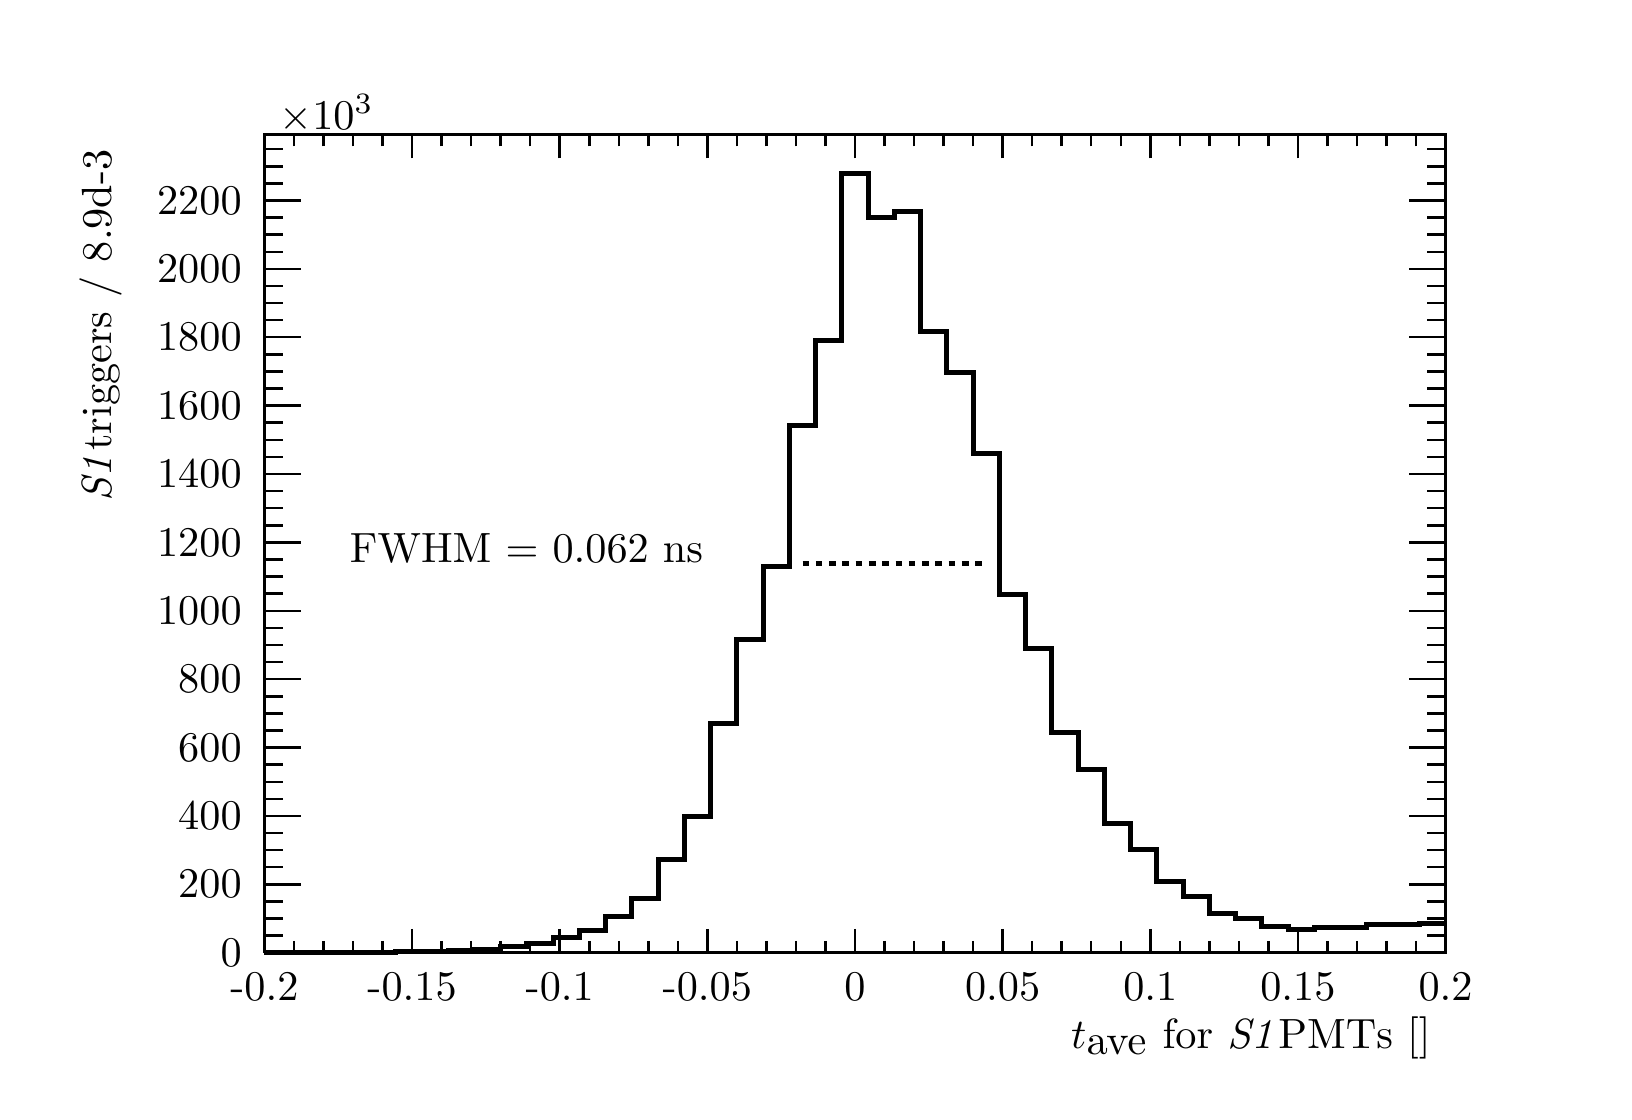
\begin{tikzpicture}
\pgfdeclareplotmark{cross} {
\pgfpathmoveto{\pgfpoint{-0.3\pgfplotmarksize}{\pgfplotmarksize}}
\pgfpathlineto{\pgfpoint{+0.3\pgfplotmarksize}{\pgfplotmarksize}}
\pgfpathlineto{\pgfpoint{+0.3\pgfplotmarksize}{0.3\pgfplotmarksize}}
\pgfpathlineto{\pgfpoint{+1\pgfplotmarksize}{0.3\pgfplotmarksize}}
\pgfpathlineto{\pgfpoint{+1\pgfplotmarksize}{-0.3\pgfplotmarksize}}
\pgfpathlineto{\pgfpoint{+0.3\pgfplotmarksize}{-0.3\pgfplotmarksize}}
\pgfpathlineto{\pgfpoint{+0.3\pgfplotmarksize}{-1.\pgfplotmarksize}}
\pgfpathlineto{\pgfpoint{-0.3\pgfplotmarksize}{-1.\pgfplotmarksize}}
\pgfpathlineto{\pgfpoint{-0.3\pgfplotmarksize}{-0.3\pgfplotmarksize}}
\pgfpathlineto{\pgfpoint{-1.\pgfplotmarksize}{-0.3\pgfplotmarksize}}
\pgfpathlineto{\pgfpoint{-1.\pgfplotmarksize}{0.3\pgfplotmarksize}}
\pgfpathlineto{\pgfpoint{-0.3\pgfplotmarksize}{0.3\pgfplotmarksize}}
\pgfpathclose
\pgfusepathqstroke
}
\pgfdeclareplotmark{cross*} {
\pgfpathmoveto{\pgfpoint{-0.3\pgfplotmarksize}{\pgfplotmarksize}}
\pgfpathlineto{\pgfpoint{+0.3\pgfplotmarksize}{\pgfplotmarksize}}
\pgfpathlineto{\pgfpoint{+0.3\pgfplotmarksize}{0.3\pgfplotmarksize}}
\pgfpathlineto{\pgfpoint{+1\pgfplotmarksize}{0.3\pgfplotmarksize}}
\pgfpathlineto{\pgfpoint{+1\pgfplotmarksize}{-0.3\pgfplotmarksize}}
\pgfpathlineto{\pgfpoint{+0.3\pgfplotmarksize}{-0.3\pgfplotmarksize}}
\pgfpathlineto{\pgfpoint{+0.3\pgfplotmarksize}{-1.\pgfplotmarksize}}
\pgfpathlineto{\pgfpoint{-0.3\pgfplotmarksize}{-1.\pgfplotmarksize}}
\pgfpathlineto{\pgfpoint{-0.3\pgfplotmarksize}{-0.3\pgfplotmarksize}}
\pgfpathlineto{\pgfpoint{-1.\pgfplotmarksize}{-0.3\pgfplotmarksize}}
\pgfpathlineto{\pgfpoint{-1.\pgfplotmarksize}{0.3\pgfplotmarksize}}
\pgfpathlineto{\pgfpoint{-0.3\pgfplotmarksize}{0.3\pgfplotmarksize}}
\pgfpathclose
\pgfusepathqfillstroke
}
\pgfdeclareplotmark{newstar} {
\pgfpathmoveto{\pgfqpoint{0pt}{\pgfplotmarksize}}
\pgfpathlineto{\pgfqpointpolar{44}{0.5\pgfplotmarksize}}
\pgfpathlineto{\pgfqpointpolar{18}{\pgfplotmarksize}}
\pgfpathlineto{\pgfqpointpolar{-20}{0.5\pgfplotmarksize}}
\pgfpathlineto{\pgfqpointpolar{-54}{\pgfplotmarksize}}
\pgfpathlineto{\pgfqpointpolar{-90}{0.5\pgfplotmarksize}}
\pgfpathlineto{\pgfqpointpolar{234}{\pgfplotmarksize}}
\pgfpathlineto{\pgfqpointpolar{198}{0.5\pgfplotmarksize}}
\pgfpathlineto{\pgfqpointpolar{162}{\pgfplotmarksize}}
\pgfpathlineto{\pgfqpointpolar{134}{0.5\pgfplotmarksize}}
\pgfpathclose
\pgfusepathqstroke
}
\pgfdeclareplotmark{newstar*} {
\pgfpathmoveto{\pgfqpoint{0pt}{\pgfplotmarksize}}
\pgfpathlineto{\pgfqpointpolar{44}{0.5\pgfplotmarksize}}
\pgfpathlineto{\pgfqpointpolar{18}{\pgfplotmarksize}}
\pgfpathlineto{\pgfqpointpolar{-20}{0.5\pgfplotmarksize}}
\pgfpathlineto{\pgfqpointpolar{-54}{\pgfplotmarksize}}
\pgfpathlineto{\pgfqpointpolar{-90}{0.5\pgfplotmarksize}}
\pgfpathlineto{\pgfqpointpolar{234}{\pgfplotmarksize}}
\pgfpathlineto{\pgfqpointpolar{198}{0.5\pgfplotmarksize}}
\pgfpathlineto{\pgfqpointpolar{162}{\pgfplotmarksize}}
\pgfpathlineto{\pgfqpointpolar{134}{0.5\pgfplotmarksize}}
\pgfpathclose
\pgfusepathqfillstroke
}
\definecolor{c}{rgb}{1,1,1};
\draw [color=c, fill=c] (0,0) rectangle (20,13.4957);
\draw [color=c, fill=c] (3,1.75444) rectangle (18,12.1461);
\definecolor{c}{rgb}{0,0,0};
\draw [c,line width=0.9] (3,1.75444) -- (3,12.1461) -- (18,12.1461) -- (18,1.75444) -- (3,1.75444);
\definecolor{c}{rgb}{1,1,1};
\draw [color=c, fill=c] (3,1.75444) rectangle (18,12.1461);
\definecolor{c}{rgb}{0,0,0};
\draw [c,line width=0.9] (3,1.75444) -- (3,12.1461) -- (18,12.1461) -- (18,1.75444) -- (3,1.75444);
\draw [c,line width=1.8] (3,1.75651) -- (3.33333,1.75651) -- (3.33333,1.75672) -- (3.66667,1.75672) -- (3.66667,1.75782) -- (4,1.75782) -- (4,1.75928) -- (4.33333,1.75928) -- (4.33333,1.76265) -- (4.66667,1.76265) -- (4.66667,1.76637) -- (5,1.76637)
 -- (5,1.77413) -- (5.33333,1.77413) -- (5.33333,1.78786) -- (5.66667,1.78786) -- (5.66667,1.80025) -- (6,1.80025) -- (6,1.83002) -- (6.33333,1.83002) -- (6.33333,1.8656) -- (6.66667,1.8656) -- (6.66667,1.94289) -- (7,1.94289) -- (7,2.03217) --
 (7.33333,2.03217) -- (7.33333,2.21951) -- (7.66667,2.21951) -- (7.66667,2.44174) -- (8,2.44174) -- (8,2.9414) -- (8.33333,2.9414) -- (8.33333,3.48698) -- (8.66667,3.48698) -- (8.66667,4.66096) -- (9,4.66096) -- (9,5.73419) -- (9.33333,5.73419) --
 (9.33333,6.66117) -- (9.66667,6.66117) -- (9.66667,8.44555) -- (10,8.44555) -- (10,9.52377) -- (10.3333,9.52377) -- (10.3333,11.6513) -- (10.6667,11.6513) -- (10.6667,11.0943) -- (11,11.0943) -- (11,11.169) -- (11.3333,11.169) -- (11.3333,9.64689)
 -- (11.6667,9.64689) -- (11.6667,9.12428) -- (12,9.12428) -- (12,8.09889) -- (12.3333,8.09889) -- (12.3333,6.29961) -- (12.6667,6.29961) -- (12.6667,5.61671) -- (13,5.61671) -- (13,4.54715) -- (13.3333,4.54715) -- (13.3333,4.0756) --
 (13.6667,4.0756) -- (13.6667,3.39822) -- (14,3.39822) -- (14,3.07106) -- (14.3333,3.07106) -- (14.3333,2.65631) -- (14.6667,2.65631) -- (14.6667,2.46793) -- (15,2.46793) -- (15,2.25342) -- (15.3333,2.25342) -- (15.3333,2.18649) -- (15.6667,2.18649)
 -- (15.6667,2.08911) -- (16,2.08911) -- (16,2.05201) -- (16.3333,2.05201) -- (16.3333,2.07377) -- (16.6667,2.07377) -- (16.6667,2.07323) -- (17,2.07323) -- (17,2.1138) -- (17.3333,2.1138) -- (17.3333,2.11352) -- (17.6667,2.11352) --
 (17.6667,2.12843) -- (18,2.12843);
\draw [c,line width=0.9] (3,1.75444) -- (18,1.75444);
\draw [c,line width=0.9] (3,2.05809) -- (3,1.75444);
\draw [c,line width=0.9] (3.375,1.90627) -- (3.375,1.75444);
\draw [c,line width=0.9] (3.75,1.90627) -- (3.75,1.75444);
\draw [c,line width=0.9] (4.125,1.90627) -- (4.125,1.75444);
\draw [c,line width=0.9] (4.5,1.90627) -- (4.5,1.75444);
\draw [c,line width=0.9] (4.875,2.05809) -- (4.875,1.75444);
\draw [c,line width=0.9] (5.25,1.90627) -- (5.25,1.75444);
\draw [c,line width=0.9] (5.625,1.90627) -- (5.625,1.75444);
\draw [c,line width=0.9] (6,1.90627) -- (6,1.75444);
\draw [c,line width=0.9] (6.375,1.90627) -- (6.375,1.75444);
\draw [c,line width=0.9] (6.75,2.05809) -- (6.75,1.75444);
\draw [c,line width=0.9] (7.125,1.90627) -- (7.125,1.75444);
\draw [c,line width=0.9] (7.5,1.90627) -- (7.5,1.75444);
\draw [c,line width=0.9] (7.875,1.90627) -- (7.875,1.75444);
\draw [c,line width=0.9] (8.25,1.90627) -- (8.25,1.75444);
\draw [c,line width=0.9] (8.625,2.05809) -- (8.625,1.75444);
\draw [c,line width=0.9] (9,1.90627) -- (9,1.75444);
\draw [c,line width=0.9] (9.375,1.90627) -- (9.375,1.75444);
\draw [c,line width=0.9] (9.75,1.90627) -- (9.75,1.75444);
\draw [c,line width=0.9] (10.125,1.90627) -- (10.125,1.75444);
\draw [c,line width=0.9] (10.5,2.05809) -- (10.5,1.75444);
\draw [c,line width=0.9] (10.875,1.90627) -- (10.875,1.75444);
\draw [c,line width=0.9] (11.25,1.90627) -- (11.25,1.75444);
\draw [c,line width=0.9] (11.625,1.90627) -- (11.625,1.75444);
\draw [c,line width=0.9] (12,1.90627) -- (12,1.75444);
\draw [c,line width=0.9] (12.375,2.05809) -- (12.375,1.75444);
\draw [c,line width=0.9] (12.75,1.90627) -- (12.75,1.75444);
\draw [c,line width=0.9] (13.125,1.90627) -- (13.125,1.75444);
\draw [c,line width=0.9] (13.5,1.90627) -- (13.5,1.75444);
\draw [c,line width=0.9] (13.875,1.90627) -- (13.875,1.75444);
\draw [c,line width=0.9] (14.25,2.05809) -- (14.25,1.75444);
\draw [c,line width=0.9] (14.625,1.90627) -- (14.625,1.75444);
\draw [c,line width=0.9] (15,1.90627) -- (15,1.75444);
\draw [c,line width=0.9] (15.375,1.90627) -- (15.375,1.75444);
\draw [c,line width=0.9] (15.75,1.90627) -- (15.75,1.75444);
\draw [c,line width=0.9] (16.125,2.05809) -- (16.125,1.75444);
\draw [c,line width=0.9] (16.5,1.90627) -- (16.5,1.75444);
\draw [c,line width=0.9] (16.875,1.90627) -- (16.875,1.75444);
\draw [c,line width=0.9] (17.25,1.90627) -- (17.25,1.75444);
\draw [c,line width=0.9] (17.625,1.90627) -- (17.625,1.75444);
\draw [c,line width=0.9] (18,2.05809) -- (18,1.75444);
\draw [anchor=base] (3,1.14713) node[scale=1.52731, color=c, rotate=0]{-0.2};
\draw [anchor=base] (4.875,1.14713) node[scale=1.52731, color=c, rotate=0]{-0.15};
\draw [anchor=base] (6.75,1.14713) node[scale=1.52731, color=c, rotate=0]{-0.1};
\draw [anchor=base] (8.625,1.14713) node[scale=1.52731, color=c, rotate=0]{-0.05};
\draw [anchor=base] (10.5,1.14713) node[scale=1.52731, color=c, rotate=0]{0};
\draw [anchor=base] (12.375,1.14713) node[scale=1.52731, color=c, rotate=0]{0.05};
\draw [anchor=base] (14.25,1.14713) node[scale=1.52731, color=c, rotate=0]{0.1};
\draw [anchor=base] (16.125,1.14713) node[scale=1.52731, color=c, rotate=0]{0.15};
\draw [anchor=base] (18,1.14713) node[scale=1.52731, color=c, rotate=0]{0.2};
\draw [anchor= east] (18,0.674785) node[scale=1.52731, color=c, rotate=0]{$t_{\textrm{ave}}$ for \SOne PMTs [\si{\nano\second}]};
\draw [c,line width=0.9] (3,12.1461) -- (18,12.1461);
\draw [c,line width=0.9] (3,11.8425) -- (3,12.1461);
\draw [c,line width=0.9] (3.375,11.9943) -- (3.375,12.1461);
\draw [c,line width=0.9] (3.75,11.9943) -- (3.75,12.1461);
\draw [c,line width=0.9] (4.125,11.9943) -- (4.125,12.1461);
\draw [c,line width=0.9] (4.5,11.9943) -- (4.5,12.1461);
\draw [c,line width=0.9] (4.875,11.8425) -- (4.875,12.1461);
\draw [c,line width=0.9] (5.25,11.9943) -- (5.25,12.1461);
\draw [c,line width=0.9] (5.625,11.9943) -- (5.625,12.1461);
\draw [c,line width=0.9] (6,11.9943) -- (6,12.1461);
\draw [c,line width=0.9] (6.375,11.9943) -- (6.375,12.1461);
\draw [c,line width=0.9] (6.75,11.8425) -- (6.75,12.1461);
\draw [c,line width=0.9] (7.125,11.9943) -- (7.125,12.1461);
\draw [c,line width=0.9] (7.5,11.9943) -- (7.5,12.1461);
\draw [c,line width=0.9] (7.875,11.9943) -- (7.875,12.1461);
\draw [c,line width=0.9] (8.25,11.9943) -- (8.25,12.1461);
\draw [c,line width=0.9] (8.625,11.8425) -- (8.625,12.1461);
\draw [c,line width=0.9] (9,11.9943) -- (9,12.1461);
\draw [c,line width=0.9] (9.375,11.9943) -- (9.375,12.1461);
\draw [c,line width=0.9] (9.75,11.9943) -- (9.75,12.1461);
\draw [c,line width=0.9] (10.125,11.9943) -- (10.125,12.1461);
\draw [c,line width=0.9] (10.5,11.8425) -- (10.5,12.1461);
\draw [c,line width=0.9] (10.875,11.9943) -- (10.875,12.1461);
\draw [c,line width=0.9] (11.25,11.9943) -- (11.25,12.1461);
\draw [c,line width=0.9] (11.625,11.9943) -- (11.625,12.1461);
\draw [c,line width=0.9] (12,11.9943) -- (12,12.1461);
\draw [c,line width=0.9] (12.375,11.8425) -- (12.375,12.1461);
\draw [c,line width=0.9] (12.75,11.9943) -- (12.75,12.1461);
\draw [c,line width=0.9] (13.125,11.9943) -- (13.125,12.1461);
\draw [c,line width=0.9] (13.5,11.9943) -- (13.5,12.1461);
\draw [c,line width=0.9] (13.875,11.9943) -- (13.875,12.1461);
\draw [c,line width=0.9] (14.25,11.8425) -- (14.25,12.1461);
\draw [c,line width=0.9] (14.625,11.9943) -- (14.625,12.1461);
\draw [c,line width=0.9] (15,11.9943) -- (15,12.1461);
\draw [c,line width=0.9] (15.375,11.9943) -- (15.375,12.1461);
\draw [c,line width=0.9] (15.75,11.9943) -- (15.75,12.1461);
\draw [c,line width=0.9] (16.125,11.8425) -- (16.125,12.1461);
\draw [c,line width=0.9] (16.5,11.9943) -- (16.5,12.1461);
\draw [c,line width=0.9] (16.875,11.9943) -- (16.875,12.1461);
\draw [c,line width=0.9] (17.25,11.9943) -- (17.25,12.1461);
\draw [c,line width=0.9] (17.625,11.9943) -- (17.625,12.1461);
\draw [c,line width=0.9] (18,11.8425) -- (18,12.1461);
\draw [c,line width=0.9] (3,1.75444) -- (3,12.1461);
\draw [c,line width=0.9] (3.462,1.75444) -- (3,1.75444);
\draw [c,line width=0.9] (3.231,1.97157) -- (3,1.97157);
\draw [c,line width=0.9] (3.231,2.1887) -- (3,2.1887);
\draw [c,line width=0.9] (3.231,2.40582) -- (3,2.40582);
\draw [c,line width=0.9] (3.462,2.62295) -- (3,2.62295);
\draw [c,line width=0.9] (3.231,2.84008) -- (3,2.84008);
\draw [c,line width=0.9] (3.231,3.0572) -- (3,3.0572);
\draw [c,line width=0.9] (3.231,3.27433) -- (3,3.27433);
\draw [c,line width=0.9] (3.462,3.49146) -- (3,3.49146);
\draw [c,line width=0.9] (3.231,3.70859) -- (3,3.70859);
\draw [c,line width=0.9] (3.231,3.92571) -- (3,3.92571);
\draw [c,line width=0.9] (3.231,4.14284) -- (3,4.14284);
\draw [c,line width=0.9] (3.462,4.35997) -- (3,4.35997);
\draw [c,line width=0.9] (3.231,4.57709) -- (3,4.57709);
\draw [c,line width=0.9] (3.231,4.79422) -- (3,4.79422);
\draw [c,line width=0.9] (3.231,5.01135) -- (3,5.01135);
\draw [c,line width=0.9] (3.462,5.22847) -- (3,5.22847);
\draw [c,line width=0.9] (3.231,5.4456) -- (3,5.4456);
\draw [c,line width=0.9] (3.231,5.66273) -- (3,5.66273);
\draw [c,line width=0.9] (3.231,5.87986) -- (3,5.87986);
\draw [c,line width=0.9] (3.462,6.09698) -- (3,6.09698);
\draw [c,line width=0.9] (3.231,6.31411) -- (3,6.31411);
\draw [c,line width=0.9] (3.231,6.53124) -- (3,6.53124);
\draw [c,line width=0.9] (3.231,6.74836) -- (3,6.74836);
\draw [c,line width=0.9] (3.462,6.96549) -- (3,6.96549);
\draw [c,line width=0.9] (3.231,7.18262) -- (3,7.18262);
\draw [c,line width=0.9] (3.231,7.39975) -- (3,7.39975);
\draw [c,line width=0.9] (3.231,7.61687) -- (3,7.61687);
\draw [c,line width=0.9] (3.462,7.834) -- (3,7.834);
\draw [c,line width=0.9] (3.231,8.05113) -- (3,8.05113);
\draw [c,line width=0.9] (3.231,8.26825) -- (3,8.26825);
\draw [c,line width=0.9] (3.231,8.48538) -- (3,8.48538);
\draw [c,line width=0.9] (3.462,8.70251) -- (3,8.70251);
\draw [c,line width=0.9] (3.231,8.91963) -- (3,8.91963);
\draw [c,line width=0.9] (3.231,9.13676) -- (3,9.13676);
\draw [c,line width=0.9] (3.231,9.35389) -- (3,9.35389);
\draw [c,line width=0.9] (3.462,9.57102) -- (3,9.57102);
\draw [c,line width=0.9] (3.231,9.78814) -- (3,9.78814);
\draw [c,line width=0.9] (3.231,10.0053) -- (3,10.0053);
\draw [c,line width=0.9] (3.231,10.2224) -- (3,10.2224);
\draw [c,line width=0.9] (3.462,10.4395) -- (3,10.4395);
\draw [c,line width=0.9] (3.231,10.6567) -- (3,10.6567);
\draw [c,line width=0.9] (3.231,10.8738) -- (3,10.8738);
\draw [c,line width=0.9] (3.231,11.0909) -- (3,11.0909);
\draw [c,line width=0.9] (3.462,11.308) -- (3,11.308);
\draw [c,line width=0.9] (3.462,11.308) -- (3,11.308);
\draw [c,line width=0.9] (3.231,11.5252) -- (3,11.5252);
\draw [c,line width=0.9] (3.231,11.7423) -- (3,11.7423);
\draw [c,line width=0.9] (3.231,11.9594) -- (3,11.9594);
\draw [anchor= east] (2.9,1.75444) node[scale=1.52731, color=c, rotate=0]{0};
\draw [anchor= east] (2.9,2.62295) node[scale=1.52731, color=c, rotate=0]{200};
\draw [anchor= east] (2.9,3.49146) node[scale=1.52731, color=c, rotate=0]{400};
\draw [anchor= east] (2.9,4.35997) node[scale=1.52731, color=c, rotate=0]{600};
\draw [anchor= east] (2.9,5.22847) node[scale=1.52731, color=c, rotate=0]{800};
\draw [anchor= east] (2.9,6.09698) node[scale=1.52731, color=c, rotate=0]{1000};
\draw [anchor= east] (2.9,6.96549) node[scale=1.52731, color=c, rotate=0]{1200};
\draw [anchor= east] (2.9,7.834) node[scale=1.52731, color=c, rotate=0]{1400};
\draw [anchor= east] (2.9,8.70251) node[scale=1.52731, color=c, rotate=0]{1600};
\draw [anchor= east] (2.9,9.57102) node[scale=1.52731, color=c, rotate=0]{1800};
\draw [anchor= east] (2.9,10.4395) node[scale=1.52731, color=c, rotate=0]{2000};
\draw [anchor= east] (2.9,11.308) node[scale=1.52731, color=c, rotate=0]{2200};
\draw [anchor=base west] (3,12.2136) node[scale=1.52731, color=c, rotate=0]{$\times10^{3}$};
\draw [anchor= east] (0.92,12.1461) node[scale=1.52731, color=c, rotate=90]{\SOne triggers / \SI{8.9d-3}{\nano\second}};
\draw [c,line width=0.9] (18,1.75444) -- (18,12.1461);
\draw [c,line width=0.9] (17.538,1.75444) -- (18,1.75444);
\draw [c,line width=0.9] (17.769,1.97157) -- (18,1.97157);
\draw [c,line width=0.9] (17.769,2.1887) -- (18,2.1887);
\draw [c,line width=0.9] (17.769,2.40582) -- (18,2.40582);
\draw [c,line width=0.9] (17.538,2.62295) -- (18,2.62295);
\draw [c,line width=0.9] (17.769,2.84008) -- (18,2.84008);
\draw [c,line width=0.9] (17.769,3.0572) -- (18,3.0572);
\draw [c,line width=0.9] (17.769,3.27433) -- (18,3.27433);
\draw [c,line width=0.9] (17.538,3.49146) -- (18,3.49146);
\draw [c,line width=0.9] (17.769,3.70859) -- (18,3.70859);
\draw [c,line width=0.9] (17.769,3.92571) -- (18,3.92571);
\draw [c,line width=0.9] (17.769,4.14284) -- (18,4.14284);
\draw [c,line width=0.9] (17.538,4.35997) -- (18,4.35997);
\draw [c,line width=0.9] (17.769,4.57709) -- (18,4.57709);
\draw [c,line width=0.9] (17.769,4.79422) -- (18,4.79422);
\draw [c,line width=0.9] (17.769,5.01135) -- (18,5.01135);
\draw [c,line width=0.9] (17.538,5.22847) -- (18,5.22847);
\draw [c,line width=0.9] (17.769,5.4456) -- (18,5.4456);
\draw [c,line width=0.9] (17.769,5.66273) -- (18,5.66273);
\draw [c,line width=0.9] (17.769,5.87986) -- (18,5.87986);
\draw [c,line width=0.9] (17.538,6.09698) -- (18,6.09698);
\draw [c,line width=0.9] (17.769,6.31411) -- (18,6.31411);
\draw [c,line width=0.9] (17.769,6.53124) -- (18,6.53124);
\draw [c,line width=0.9] (17.769,6.74836) -- (18,6.74836);
\draw [c,line width=0.9] (17.538,6.96549) -- (18,6.96549);
\draw [c,line width=0.9] (17.769,7.18262) -- (18,7.18262);
\draw [c,line width=0.9] (17.769,7.39975) -- (18,7.39975);
\draw [c,line width=0.9] (17.769,7.61687) -- (18,7.61687);
\draw [c,line width=0.9] (17.538,7.834) -- (18,7.834);
\draw [c,line width=0.9] (17.769,8.05113) -- (18,8.05113);
\draw [c,line width=0.9] (17.769,8.26825) -- (18,8.26825);
\draw [c,line width=0.9] (17.769,8.48538) -- (18,8.48538);
\draw [c,line width=0.9] (17.538,8.70251) -- (18,8.70251);
\draw [c,line width=0.9] (17.769,8.91963) -- (18,8.91963);
\draw [c,line width=0.9] (17.769,9.13676) -- (18,9.13676);
\draw [c,line width=0.9] (17.769,9.35389) -- (18,9.35389);
\draw [c,line width=0.9] (17.538,9.57102) -- (18,9.57102);
\draw [c,line width=0.9] (17.769,9.78814) -- (18,9.78814);
\draw [c,line width=0.9] (17.769,10.0053) -- (18,10.0053);
\draw [c,line width=0.9] (17.769,10.2224) -- (18,10.2224);
\draw [c,line width=0.9] (17.538,10.4395) -- (18,10.4395);
\draw [c,line width=0.9] (17.769,10.6567) -- (18,10.6567);
\draw [c,line width=0.9] (17.769,10.8738) -- (18,10.8738);
\draw [c,line width=0.9] (17.769,11.0909) -- (18,11.0909);
\draw [c,line width=0.9] (17.538,11.308) -- (18,11.308);
\draw [c,line width=0.9] (17.538,11.308) -- (18,11.308);
\draw [c,line width=0.9] (17.769,11.5252) -- (18,11.5252);
\draw [c,line width=0.9] (17.769,11.7423) -- (18,11.7423);
\draw [c,line width=0.9] (17.769,11.9594) -- (18,11.9594);
\definecolor{c}{rgb}{1,1,1};
\draw [color=c, fill=c] (2,12.686) rectangle (18,13.4282);
\definecolor{c}{rgb}{0,0,0};
%\draw (10,13.0571) node[scale=1.40004, color=c, rotate=0]{Measurement of the difference S1 PMT trigger times};
\draw [c,dash pattern=on 2.40pt off 2.40pt ,line width=1.8] (9.83333,6.70287) -- (12.1667,6.70287);
\draw [anchor=base west] (3.89685,6.70487) node[scale=1.52731, color=c, rotate=0]{FWHM = 0.062 ns};
\end{tikzpicture}

  \end{adjustbox}
  \caption[Example of \SOne time resolution measurement]{An example of an \SOne time resolution measurement made using the quantity $t_{\text{ave}}$, defined in \citeeq{eq:tAve}.}
  \label{fig:s1Res}
\end{figure}

\STwo consists of a single piece of plastic scintillator, measuring \SI{120 x 120 x 5}{\milli\metre} which is read out, via a light guide, by a 2'' Hamamatsu Photonics R1309 PMT~\cite{hamamatsu}.
An image of \STwo is shown on the right of \citefig{fig:s1s2Pic} where the light guide is also indicated.
\STwo is situated \SI{1.419(1)}{\metre} downstream of \SOne and away from the nominal beam axis.
This off-axis positioning means that all of the beam particles impinging on the HPgTPC should pass through \STwo.

The analog signals produced by the PMTs in \SOne and \STwo are fed into LeCroy 620AL NIM discriminator units with a threshold of \SI{30}{\milli\volt}.
These discriminated signals were then fed into a NIM coincidence unit.
The output of this unit was recorded by the DAQ system of the downstream time of flight panel (\SFour).
The signals from \SOne and \STwo were fed individually into the DAQ system of the upstream time of flight panel (\SThree).

\subsection{The upstream time of flight detector (\SThree)}
\label{sec:hptpc_beam_flux:overview:s3}

\SThree (also referred to as the upstream time of flight system) is situated \SI{1.323(2)}{\metre} upstream of the upstream side of the TPC and \SI{10.756(1)}{\metre} in the beamline.
It consists of 22 bars of EJ-200~\cite{ej200} plastic scintillator.
20 of these bars measure \SI{168 x 6 x 1}{\centi\metre} while the remaining 2 measure \SI{150 x 6 x 1}{\centi\metre}~\cite{s3Paper}.
The bars are arranged in a staggered setup with an overlap between the bars of \SI{5}{\milli\metre} while the two smaller bars are placed at the top and bottom of the panel.
The total active area of the detector is \SI{2.0214}{\centi\metre\square}.
Schematic diagrams of \SThree are shown in \citefig{fig:s3Diag} along with dimensions.

\begin{figure}[h]
  \begin{minipage}[t]{.55\linewidth}
    \includegraphics[width=\linewidth]{files/figures/hptpc_beam_flux/uToF_sketch}
  \end{minipage}
  \hfill
  \begin{minipage}[t]{.41\linewidth}
    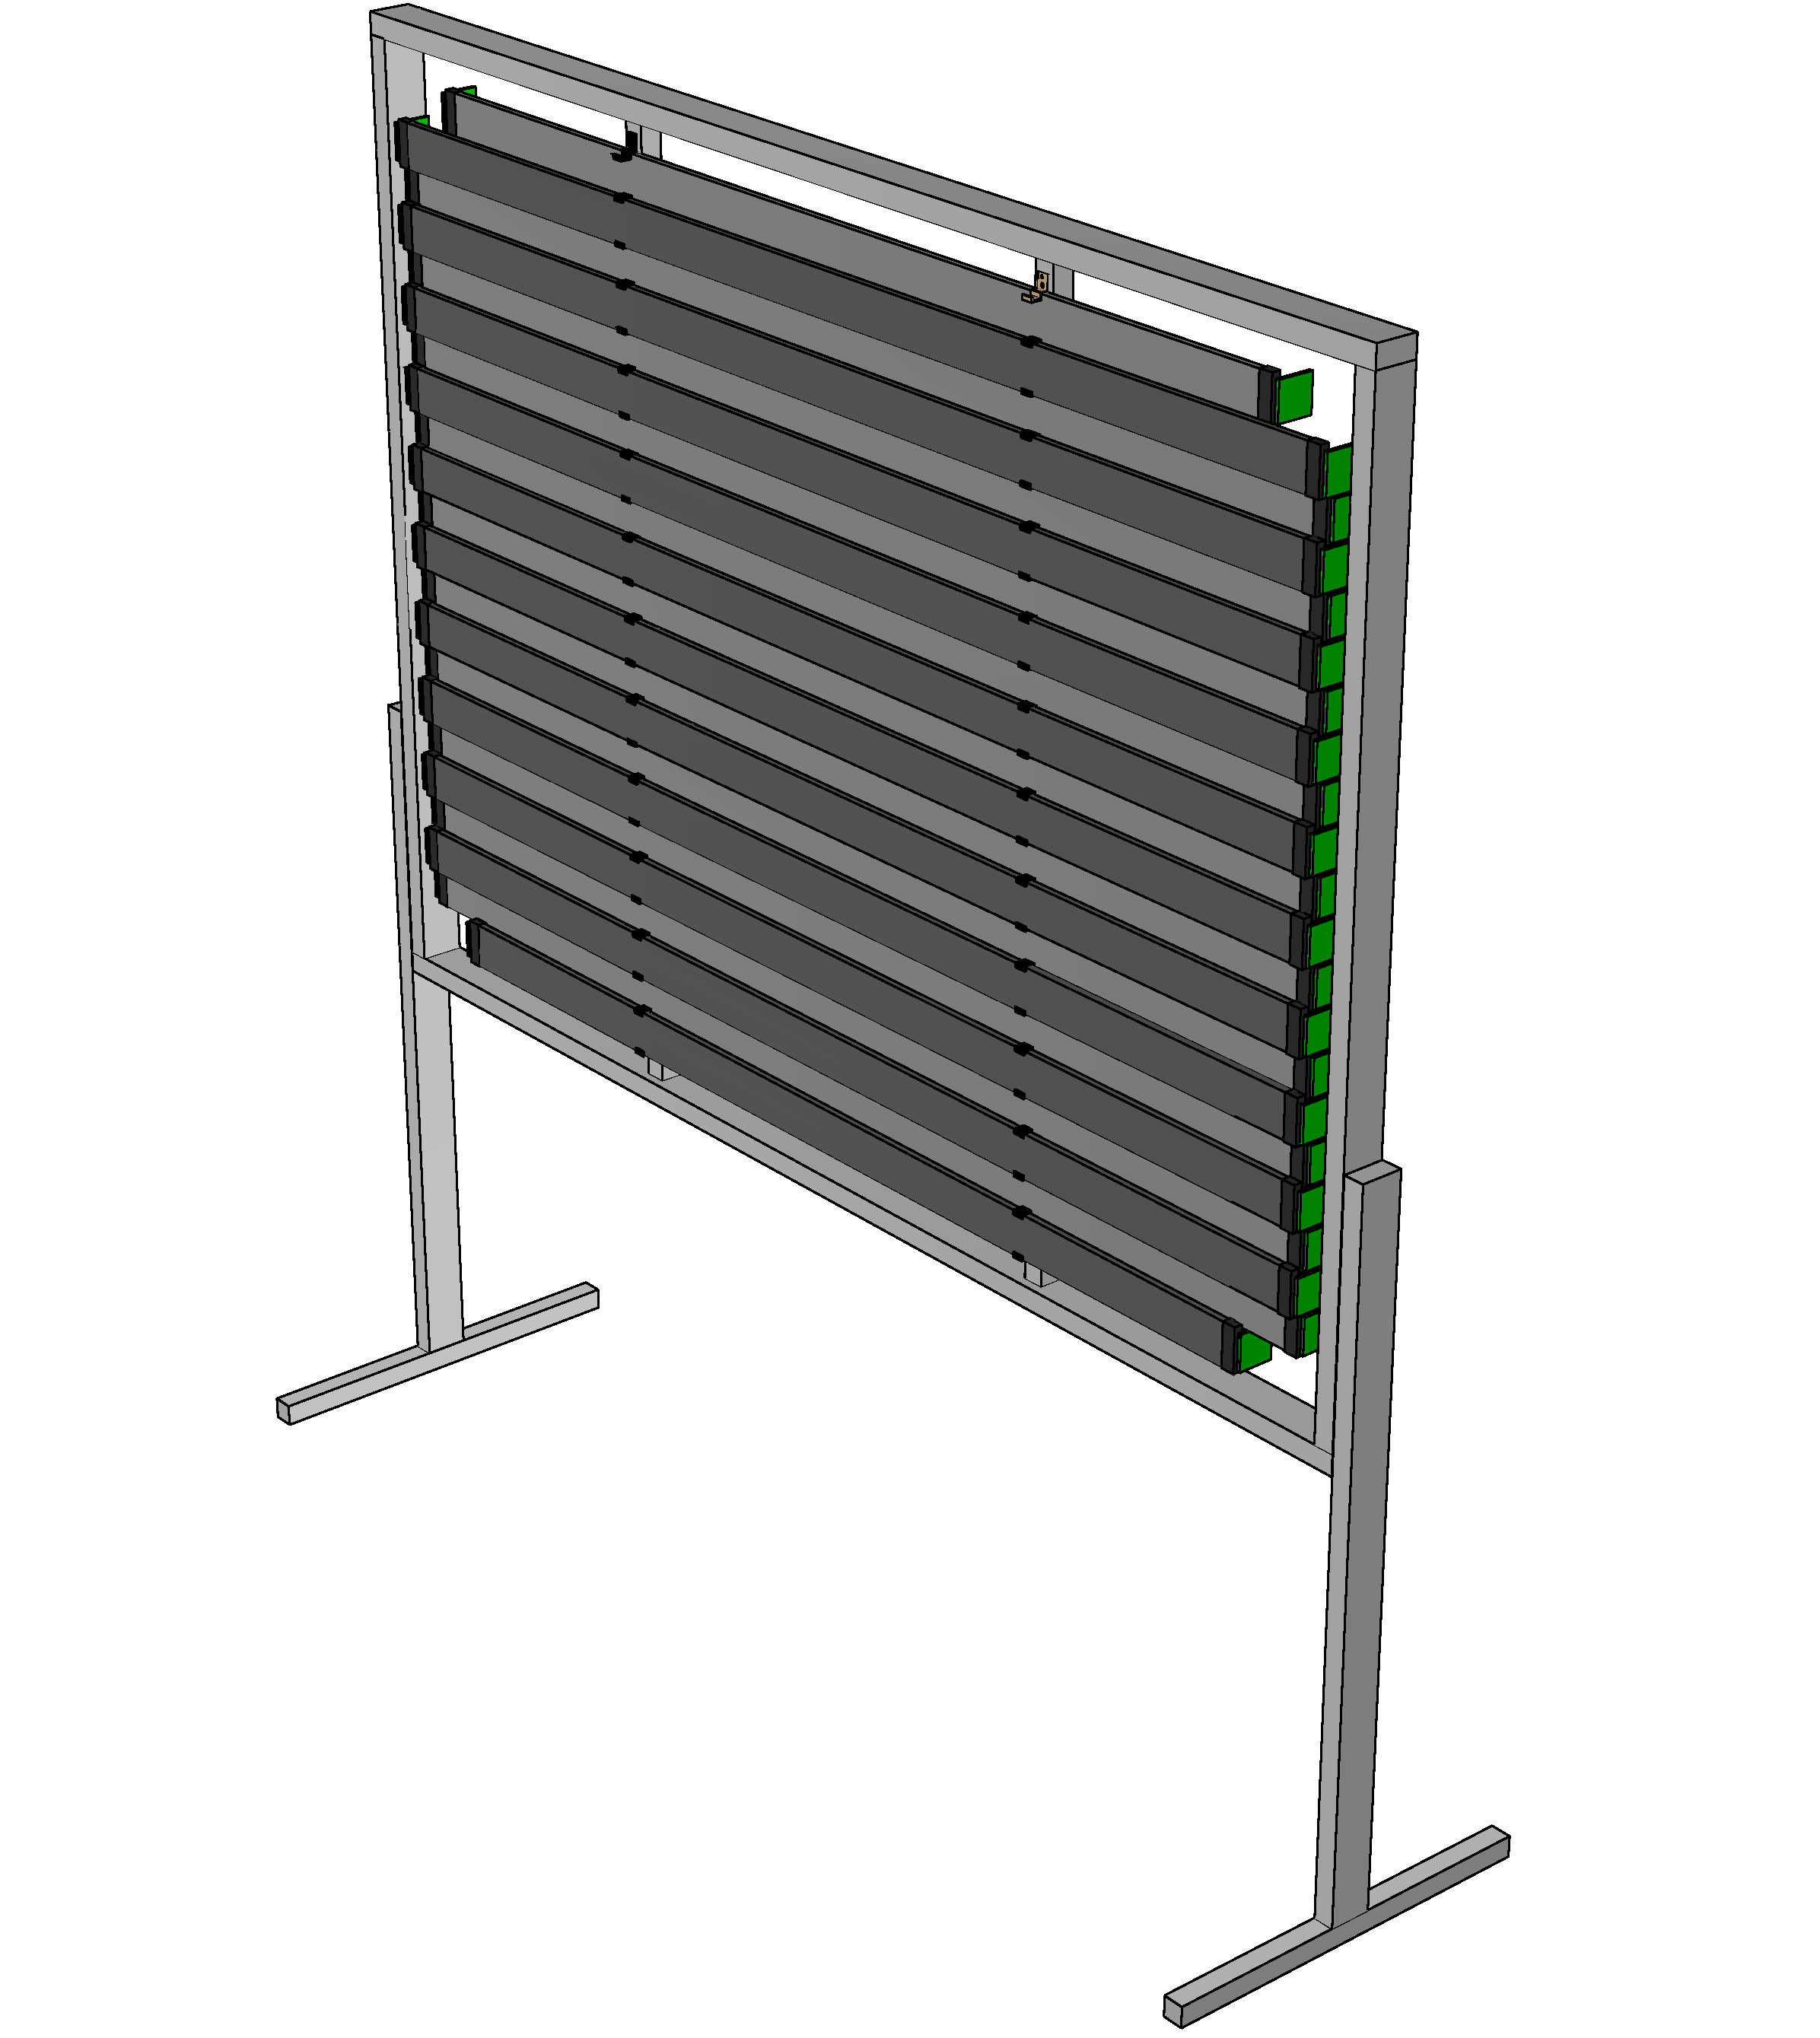
\includegraphics[width=\linewidth]{files/figures/hptpc_beam_flux/uTOF_rot}
  \end{minipage}
  \caption[Schematic diagrams of \SThree]{Front-on and rotated schematic diagrams of \SThree from~\cite{s3Paper} along with dimensions.}
  \label{fig:s3Diag}
\end{figure}

EJ-200 plastic scintillator (of which the bars are made) has a brightness of \num{10000}~photons/MeV deposited.
Additionally, it has a large optical attenuation length (\SI{4}{\metre}) along with a fast rise time and decay time constant (\SI{0.9}{\nano\second} and \SI{2.1}{\nano\second} respectively.
The scintillation emission spectrum peaks at a wavelength of \SI{435}{\nano\metre}~\cite{ej200}.
In order to increase the light collection capabilities of the bars while excluding background light, they are wrapped in aluminium foil which has a reflectivity of 60\%.

The scintillation photons produced by the bars are detected by S13360-6050PE Hamamatsu Photonics~\cite{hamamatsu} silicon photomultipliers (SiPMs) arranged at either end of the bar.
These photosensors, each measuring \SI{6 x 6}{\milli\metre}, are arranged in groups of eight and then coupled to the end of the bar.
These photomultipliers have a wavelength range that is well suited to the scintillation light produced by the bars (the sensitivity of the SiPMs at a wavelength of \SI{450}{\nano\metre} is 40\%~\cite{hamamatsu}).
The anode signals produced by these SiPMs are read out, summed and shaped by a dedicated circuit as described in~\cite{s3SiPM}.

These signals, along with those from \SOne and \STwo, are then fed into a DAQ based upon the SAMPIC chip, further details of which are given in~\cite{sampic}.

\SThree triggers are formed in the following manner, shown graphically in \citefig{fig:s3Trigger}, and are intended to identify the prescence of a beam particle travelling between \SOne and \SThree.
An \SOne signal is considered to have occurred when at least three of the four \SOne PMTs register a signal above the threshold of \SI{30}{\milli\volt}.
An \SThree signal is deemed to have occurred if the SiPMs on either end of a given bar register a signal above a threshold of \SI{30}{\milli\volt}.
If an \SOne signal and an \SThree signal occur within a time window of \SI{70}{\nano\second}, the DAQ is triggered and writes the event.
The DAQ also acquires signals from the coincidence of \SOne and \STwo as well as the signal indicating the start of the beam spill.

\begin{figure}[h]
  \centering
  \includegraphics[width=.8\linewidth]{files/figures/hptpc_beam_flux/utofTrig}
  \caption[Trigger logic for the upstream time of flight DAQ]{Trigger logic showing the necessary conditions for the identification of a $\SOne-\SThree$ beam particle by the upstream ToF DAQ.}
  \label{fig:s3Trigger}
\end{figure}


\subsection{The downstream time of flight detector (\SFour)}
\label{sec:hptpc_beam_flux:overview:s4}

The design of \SFour is primarily discussed in \citesec{sec:hptpc_dtof_characterisation:dtof}, however it will be briefly revisited here.
\SFour consists of 10 scintillator bars which together form an active area of \SI{1.40 x 0.78}{\metre}.
A diagram of one such bar is shown in \citefig{fig:barDiag}.
Each of these scintillator bars has a PMT attached to each end and these observe the scintillation light produced by charged particles traversing the bars.
A diagram of \SFour is shown in \citefig{fig:dtofDiag}.

The anode signal of each of the PMTs is fed into a LeCroy 620AL NIM discriminator with a threshold of \SI{-20}{\milli\volt}.
Any PMT signals above this threshold are digitised using a time-to-digital converted (TDC)
Additionally, the signal indicating the start of a beam spill as well as a signal indicating a coincidence between \SOne and \STwo were fed into the TDC.
A particle (either beam induced or otherwise) is considered to have been observed in \SFour if a signal above the discriminator threshold is recorded in both PMTs on the same bar, within \SI{20}{\nano\second} of each other.

Unlike the UToF DAQ system, the DToF DAQ is operated in self-triggering mode and thus acquired data both inside and outside the beam spill.


\subsection{The HPTPC prototype}
\label{sec:hptpc_beam_flux:overview:hptpc}

The relevant specifications of the HPTPC prototype for this study are the location and wall thickness of the pressure vessel.
The upstream face of HPTPC is located \SI{1.323(2)}{\metre} downstream of the \SThree panel while the downstream face is located \SI{0.918(2)}{\metre} upstream of \SFour.
\citefig{fig:angDistS1} shows that, from the point of view of the beam, most of the  TPC volume is covered by \STwo, \SThree and \SFour.
The angular position of the TPC is at approximately $\theta = \ang{-2.5}$.
With the beam steering, this means that the centre of the TPC lies approximately \ang{3.5} off-axis.

The pressure vessel itself is made out of 304L stainless steel, has an outer diameter of \SI{142}{\centi\metre} and a vessel wall thickness of \SI{1}{\centi\metre}~\cite{deisting2021high}.
This vessel wall thickness is equivalent to the range of proton with a kinetic energy of roughly \SI{80}{\mega\electronvolt}~\cite{protonRangeTables}.

The main cylindrical body of the vessel is \SI{73.6}{\centi\metre} in length while the rounded sections at the end of this volume each have a length of \SI{32.5}{\centi\metre}~\cite{deisting2021high}.
Interior to the cylindrical body is the active volume of the TPC.
This active TPC volume measures \SI{111}{\centi\metre} in diameter and \SI{48}{\centi\metre} in the drift direction and is formed by a series of copper rings which make up the field cage.
A diagram of the HPTPC, showing a cross-sectional view of the active volume, is shown in \citefig{fig:hptpc}.

\begin{figure}[h]
  \centering
  \includegraphics[width=.7\linewidth]{files/figures/hptpc_beam_flux/vesselView}
  \caption[Cross-sectional view of the HPTPC prototype]{Cross-sectional view of the HPTPC prototype with the door open, from~\cite{beampaper}. The drift volume formed by the copper rings is clearly visible. The direction of the beam during the beam test is indicated.}
  \label{fig:hptpc}
\end{figure}

\section{Methods}
\label{sec:hptpc_beam_flux:methods}

In a beamline such as the T10 beamline at CERN, charged particles are selected using by momentum using a magnetic field.
This results in a beam of particles that are all of the same momentum but of different species.
Different particles of the same momentum will take different times to cover the same distance.
The time of flight, $t$, of a particle of mass, $m$, with a momentum, $p$, is given by
\begin{equation}
  t = L \sqrt{ \frac{1}{c^{2}} + \frac{m^{2}}{p^{2}} }\, ,
  \label{eq:tof}
\end{equation}
where $L$ is the distance travelled by the particle.
\citefig{fig:tofVsMom}, left and right, show the time of flight for various particles as a function of particle momentum for the $\SOne - \SThree$ and  $\STwo - \SFour$ distances respectively.
If the beam momentum is known, by measuring a particle's time of flight it should be possible to identify the particle in question.
One can see that, assuming a time resolution of around \SI{1}{\nano\second}, it should be possible to distinguish between deuterons, protons and pions/muons at the momenta used in this study.

\begin{figure}[h]
  \begin{minipage}[t]{.5\linewidth}
    \begin{adjustbox}{max totalsize=\textwidth, center}
      \begin{tikzpicture}
\pgfdeclareplotmark{cross} {
\pgfpathmoveto{\pgfpoint{-0.3\pgfplotmarksize}{\pgfplotmarksize}}
\pgfpathlineto{\pgfpoint{+0.3\pgfplotmarksize}{\pgfplotmarksize}}
\pgfpathlineto{\pgfpoint{+0.3\pgfplotmarksize}{0.3\pgfplotmarksize}}
\pgfpathlineto{\pgfpoint{+1\pgfplotmarksize}{0.3\pgfplotmarksize}}
\pgfpathlineto{\pgfpoint{+1\pgfplotmarksize}{-0.3\pgfplotmarksize}}
\pgfpathlineto{\pgfpoint{+0.3\pgfplotmarksize}{-0.3\pgfplotmarksize}}
\pgfpathlineto{\pgfpoint{+0.3\pgfplotmarksize}{-1.\pgfplotmarksize}}
\pgfpathlineto{\pgfpoint{-0.3\pgfplotmarksize}{-1.\pgfplotmarksize}}
\pgfpathlineto{\pgfpoint{-0.3\pgfplotmarksize}{-0.3\pgfplotmarksize}}
\pgfpathlineto{\pgfpoint{-1.\pgfplotmarksize}{-0.3\pgfplotmarksize}}
\pgfpathlineto{\pgfpoint{-1.\pgfplotmarksize}{0.3\pgfplotmarksize}}
\pgfpathlineto{\pgfpoint{-0.3\pgfplotmarksize}{0.3\pgfplotmarksize}}
\pgfpathclose
\pgfusepathqstroke
}
\pgfdeclareplotmark{cross*} {
\pgfpathmoveto{\pgfpoint{-0.3\pgfplotmarksize}{\pgfplotmarksize}}
\pgfpathlineto{\pgfpoint{+0.3\pgfplotmarksize}{\pgfplotmarksize}}
\pgfpathlineto{\pgfpoint{+0.3\pgfplotmarksize}{0.3\pgfplotmarksize}}
\pgfpathlineto{\pgfpoint{+1\pgfplotmarksize}{0.3\pgfplotmarksize}}
\pgfpathlineto{\pgfpoint{+1\pgfplotmarksize}{-0.3\pgfplotmarksize}}
\pgfpathlineto{\pgfpoint{+0.3\pgfplotmarksize}{-0.3\pgfplotmarksize}}
\pgfpathlineto{\pgfpoint{+0.3\pgfplotmarksize}{-1.\pgfplotmarksize}}
\pgfpathlineto{\pgfpoint{-0.3\pgfplotmarksize}{-1.\pgfplotmarksize}}
\pgfpathlineto{\pgfpoint{-0.3\pgfplotmarksize}{-0.3\pgfplotmarksize}}
\pgfpathlineto{\pgfpoint{-1.\pgfplotmarksize}{-0.3\pgfplotmarksize}}
\pgfpathlineto{\pgfpoint{-1.\pgfplotmarksize}{0.3\pgfplotmarksize}}
\pgfpathlineto{\pgfpoint{-0.3\pgfplotmarksize}{0.3\pgfplotmarksize}}
\pgfpathclose
\pgfusepathqfillstroke
}
\pgfdeclareplotmark{newstar} {
\pgfpathmoveto{\pgfqpoint{0pt}{\pgfplotmarksize}}
\pgfpathlineto{\pgfqpointpolar{44}{0.5\pgfplotmarksize}}
\pgfpathlineto{\pgfqpointpolar{18}{\pgfplotmarksize}}
\pgfpathlineto{\pgfqpointpolar{-20}{0.5\pgfplotmarksize}}
\pgfpathlineto{\pgfqpointpolar{-54}{\pgfplotmarksize}}
\pgfpathlineto{\pgfqpointpolar{-90}{0.5\pgfplotmarksize}}
\pgfpathlineto{\pgfqpointpolar{234}{\pgfplotmarksize}}
\pgfpathlineto{\pgfqpointpolar{198}{0.5\pgfplotmarksize}}
\pgfpathlineto{\pgfqpointpolar{162}{\pgfplotmarksize}}
\pgfpathlineto{\pgfqpointpolar{134}{0.5\pgfplotmarksize}}
\pgfpathclose
\pgfusepathqstroke
}
\pgfdeclareplotmark{newstar*} {
\pgfpathmoveto{\pgfqpoint{0pt}{\pgfplotmarksize}}
\pgfpathlineto{\pgfqpointpolar{44}{0.5\pgfplotmarksize}}
\pgfpathlineto{\pgfqpointpolar{18}{\pgfplotmarksize}}
\pgfpathlineto{\pgfqpointpolar{-20}{0.5\pgfplotmarksize}}
\pgfpathlineto{\pgfqpointpolar{-54}{\pgfplotmarksize}}
\pgfpathlineto{\pgfqpointpolar{-90}{0.5\pgfplotmarksize}}
\pgfpathlineto{\pgfqpointpolar{234}{\pgfplotmarksize}}
\pgfpathlineto{\pgfqpointpolar{198}{0.5\pgfplotmarksize}}
\pgfpathlineto{\pgfqpointpolar{162}{\pgfplotmarksize}}
\pgfpathlineto{\pgfqpointpolar{134}{0.5\pgfplotmarksize}}
\pgfpathclose
\pgfusepathqfillstroke
}
\definecolor{c}{rgb}{1,1,1};
\draw [color=c, fill=c] (0,0) rectangle (20,13.639);
\draw [color=c, fill=c] (2.60745,1.76218) rectangle (17.0201,11.8768);
\definecolor{c}{rgb}{0,0,0};
\draw [c,line width=0.9] (2.60745,1.76218) -- (2.60745,11.8768) -- (17.0201,11.8768) -- (17.0201,1.76218) -- (2.60745,1.76218);
\definecolor{c}{rgb}{1,1,1};
\draw [color=c, fill=c] (2.60745,1.76218) rectangle (17.0201,11.8768);
\definecolor{c}{rgb}{0,0,0};
\draw [c,line width=0.9] (2.60745,1.76218) -- (2.60745,11.8768) -- (17.0201,11.8768) -- (17.0201,1.76218) -- (2.60745,1.76218);
\definecolor{c}{rgb}{0,0.8,0.8};
\draw [c,line width=1.8] (2.67951,3.58458) -- (2.82364,3.40401) -- (2.96777,3.25475) -- (3.11189,3.12999) -- (3.25602,3.02465) -- (3.40014,2.93493) -- (3.54427,2.85792) -- (3.6884,2.79135) -- (3.83252,2.73344) -- (3.97665,2.68276) --
 (4.12077,2.63817) -- (4.2649,2.59875) -- (4.40903,2.56374) -- (4.55315,2.53252) -- (4.69728,2.50455) -- (4.8414,2.47942) -- (4.98553,2.45675) -- (5.12966,2.43624) -- (5.27378,2.41763) -- (5.41791,2.40068) -- (5.56203,2.38522) -- (5.70616,2.37107) --
 (5.85029,2.35809) -- (5.99441,2.34616) -- (6.13854,2.33516) -- (6.28266,2.32501) -- (6.42679,2.31562) -- (6.57092,2.30691) -- (6.71504,2.29883) -- (6.85917,2.29131) -- (7.0033,2.2843) -- (7.14742,2.27777) -- (7.29155,2.27166) -- (7.43567,2.26594) --
 (7.5798,2.26058) -- (7.72393,2.25555) -- (7.86805,2.25083) -- (8.01218,2.24638) -- (8.1563,2.24219) -- (8.30043,2.23824) -- (8.44456,2.23451) -- (8.58868,2.23099) -- (8.73281,2.22766) -- (8.87693,2.2245) -- (9.02106,2.22151) -- (9.16519,2.21867) --
 (9.30931,2.21598) -- (9.45344,2.21342) -- (9.59756,2.21098) -- (9.74169,2.20866);
\draw [c,line width=1.8] (9.74169,2.20866) -- (9.88582,2.20645) -- (10.0299,2.20435) -- (10.1741,2.20234) -- (10.3182,2.20042) -- (10.4623,2.19858) -- (10.6064,2.19683) -- (10.7506,2.19516) -- (10.8947,2.19355) -- (11.0388,2.19201) --
 (11.183,2.19054) -- (11.3271,2.18913) -- (11.4712,2.18777) -- (11.6153,2.18647) -- (11.7595,2.18522) -- (11.9036,2.18401) -- (12.0477,2.18286) -- (12.1918,2.18175) -- (12.336,2.18068) -- (12.4801,2.17965) -- (12.6242,2.17865) -- (12.7683,2.17769) --
 (12.9125,2.17677) -- (13.0566,2.17588) -- (13.2007,2.17502) -- (13.3448,2.17419) -- (13.489,2.17339) -- (13.6331,2.17261) -- (13.7772,2.17187) -- (13.9213,2.17114) -- (14.0655,2.17044) -- (14.2096,2.16976) -- (14.3537,2.16911) -- (14.4979,2.16847)
 -- (14.642,2.16786) -- (14.7861,2.16726) -- (14.9302,2.16668) -- (15.0744,2.16612) -- (15.2185,2.16558) -- (15.3626,2.16505) -- (15.5067,2.16454) -- (15.6509,2.16404) -- (15.795,2.16356) -- (15.9391,2.16309) -- (16.0832,2.16263) -- (16.2274,2.16219)
 -- (16.3715,2.16176) -- (16.5156,2.16134) -- (16.6597,2.16093) -- (16.8039,2.16053);
\draw [c,line width=1.8] (16.8039,2.16053) -- (16.948,2.16015);
\definecolor{c}{rgb}{0,0,0};
\draw [c,line width=0.9] (2.60745,1.76218) -- (17.0201,1.76218);
\draw [c,line width=0.9] (2.60745,2.05704) -- (2.60745,1.76218);
\draw [c,line width=0.9] (2.92773,1.90961) -- (2.92773,1.76218);
\draw [c,line width=0.9] (3.24801,1.90961) -- (3.24801,1.76218);
\draw [c,line width=0.9] (3.56829,1.90961) -- (3.56829,1.76218);
\draw [c,line width=0.9] (3.88857,1.90961) -- (3.88857,1.76218);
\draw [c,line width=0.9] (4.20885,2.05704) -- (4.20885,1.76218);
\draw [c,line width=0.9] (4.52913,1.90961) -- (4.52913,1.76218);
\draw [c,line width=0.9] (4.84941,1.90961) -- (4.84941,1.76218);
\draw [c,line width=0.9] (5.16969,1.90961) -- (5.16969,1.76218);
\draw [c,line width=0.9] (5.48997,1.90961) -- (5.48997,1.76218);
\draw [c,line width=0.9] (5.81025,2.05704) -- (5.81025,1.76218);
\draw [c,line width=0.9] (6.13053,1.90961) -- (6.13053,1.76218);
\draw [c,line width=0.9] (6.45081,1.90961) -- (6.45081,1.76218);
\draw [c,line width=0.9] (6.77109,1.90961) -- (6.77109,1.76218);
\draw [c,line width=0.9] (7.09137,1.90961) -- (7.09137,1.76218);
\draw [c,line width=0.9] (7.41165,2.05704) -- (7.41165,1.76218);
\draw [c,line width=0.9] (7.73193,1.90961) -- (7.73193,1.76218);
\draw [c,line width=0.9] (8.05221,1.90961) -- (8.05221,1.76218);
\draw [c,line width=0.9] (8.37249,1.90961) -- (8.37249,1.76218);
\draw [c,line width=0.9] (8.69277,1.90961) -- (8.69277,1.76218);
\draw [c,line width=0.9] (9.01305,2.05704) -- (9.01305,1.76218);
\draw [c,line width=0.9] (9.33333,1.90961) -- (9.33333,1.76218);
\draw [c,line width=0.9] (9.65361,1.90961) -- (9.65361,1.76218);
\draw [c,line width=0.9] (9.97389,1.90961) -- (9.97389,1.76218);
\draw [c,line width=0.9] (10.2942,1.90961) -- (10.2942,1.76218);
\draw [c,line width=0.9] (10.6145,2.05704) -- (10.6145,1.76218);
\draw [c,line width=0.9] (10.9347,1.90961) -- (10.9347,1.76218);
\draw [c,line width=0.9] (11.255,1.90961) -- (11.255,1.76218);
\draw [c,line width=0.9] (11.5753,1.90961) -- (11.5753,1.76218);
\draw [c,line width=0.9] (11.8956,1.90961) -- (11.8956,1.76218);
\draw [c,line width=0.9] (12.2159,2.05704) -- (12.2159,1.76218);
\draw [c,line width=0.9] (12.5361,1.90961) -- (12.5361,1.76218);
\draw [c,line width=0.9] (12.8564,1.90961) -- (12.8564,1.76218);
\draw [c,line width=0.9] (13.1767,1.90961) -- (13.1767,1.76218);
\draw [c,line width=0.9] (13.497,1.90961) -- (13.497,1.76218);
\draw [c,line width=0.9] (13.8173,2.05704) -- (13.8173,1.76218);
\draw [c,line width=0.9] (14.1375,1.90961) -- (14.1375,1.76218);
\draw [c,line width=0.9] (14.4578,1.90961) -- (14.4578,1.76218);
\draw [c,line width=0.9] (14.7781,1.90961) -- (14.7781,1.76218);
\draw [c,line width=0.9] (15.0984,1.90961) -- (15.0984,1.76218);
\draw [c,line width=0.9] (15.4187,2.05704) -- (15.4187,1.76218);
\draw [c,line width=0.9] (15.7389,1.90961) -- (15.7389,1.76218);
\draw [c,line width=0.9] (16.0592,1.90961) -- (16.0592,1.76218);
\draw [c,line width=0.9] (16.3795,1.90961) -- (16.3795,1.76218);
\draw [c,line width=0.9] (16.6998,1.90961) -- (16.6998,1.76218);
\draw [c,line width=0.9] (17.0201,2.05704) -- (17.0201,1.76218);
\draw [anchor=base] (2.60745,1.14842) node[scale=1.52731, color=c, rotate=0]{0.1};
\draw [anchor=base] (4.20885,1.14842) node[scale=1.52731, color=c, rotate=0]{0.2};
\draw [anchor=base] (5.81025,1.14842) node[scale=1.52731, color=c, rotate=0]{0.3};
\draw [anchor=base] (7.41165,1.14842) node[scale=1.52731, color=c, rotate=0]{0.4};
\draw [anchor=base] (9.01305,1.14842) node[scale=1.52731, color=c, rotate=0]{0.5};
\draw [anchor=base] (10.6145,1.14842) node[scale=1.52731, color=c, rotate=0]{0.6};
\draw [anchor=base] (12.2159,1.14842) node[scale=1.52731, color=c, rotate=0]{0.7};
\draw [anchor=base] (13.8173,1.14842) node[scale=1.52731, color=c, rotate=0]{0.8};
\draw [anchor=base] (15.4187,1.14842) node[scale=1.52731, color=c, rotate=0]{0.9};
\draw [anchor=base] (17.0201,1.14842) node[scale=1.52731, color=c, rotate=0]{1};
\draw [anchor= east] (17.0201,0.561948) node[scale=1.52731, color=c, rotate=0]{ Particle momentum [\si{\giga\electronvolt\per\clight}]};
\draw [c,line width=0.9] (2.60745,11.8768) -- (17.0201,11.8768);
\draw [c,line width=0.9] (2.60745,11.5819) -- (2.60745,11.8768);
\draw [c,line width=0.9] (2.92773,11.7294) -- (2.92773,11.8768);
\draw [c,line width=0.9] (3.24801,11.7294) -- (3.24801,11.8768);
\draw [c,line width=0.9] (3.56829,11.7294) -- (3.56829,11.8768);
\draw [c,line width=0.9] (3.88857,11.7294) -- (3.88857,11.8768);
\draw [c,line width=0.9] (4.20885,11.5819) -- (4.20885,11.8768);
\draw [c,line width=0.9] (4.52913,11.7294) -- (4.52913,11.8768);
\draw [c,line width=0.9] (4.84941,11.7294) -- (4.84941,11.8768);
\draw [c,line width=0.9] (5.16969,11.7294) -- (5.16969,11.8768);
\draw [c,line width=0.9] (5.48997,11.7294) -- (5.48997,11.8768);
\draw [c,line width=0.9] (5.81025,11.5819) -- (5.81025,11.8768);
\draw [c,line width=0.9] (6.13053,11.7294) -- (6.13053,11.8768);
\draw [c,line width=0.9] (6.45081,11.7294) -- (6.45081,11.8768);
\draw [c,line width=0.9] (6.77109,11.7294) -- (6.77109,11.8768);
\draw [c,line width=0.9] (7.09137,11.7294) -- (7.09137,11.8768);
\draw [c,line width=0.9] (7.41165,11.5819) -- (7.41165,11.8768);
\draw [c,line width=0.9] (7.73193,11.7294) -- (7.73193,11.8768);
\draw [c,line width=0.9] (8.05221,11.7294) -- (8.05221,11.8768);
\draw [c,line width=0.9] (8.37249,11.7294) -- (8.37249,11.8768);
\draw [c,line width=0.9] (8.69277,11.7294) -- (8.69277,11.8768);
\draw [c,line width=0.9] (9.01305,11.5819) -- (9.01305,11.8768);
\draw [c,line width=0.9] (9.33333,11.7294) -- (9.33333,11.8768);
\draw [c,line width=0.9] (9.65361,11.7294) -- (9.65361,11.8768);
\draw [c,line width=0.9] (9.97389,11.7294) -- (9.97389,11.8768);
\draw [c,line width=0.9] (10.2942,11.7294) -- (10.2942,11.8768);
\draw [c,line width=0.9] (10.6145,11.5819) -- (10.6145,11.8768);
\draw [c,line width=0.9] (10.9347,11.7294) -- (10.9347,11.8768);
\draw [c,line width=0.9] (11.255,11.7294) -- (11.255,11.8768);
\draw [c,line width=0.9] (11.5753,11.7294) -- (11.5753,11.8768);
\draw [c,line width=0.9] (11.8956,11.7294) -- (11.8956,11.8768);
\draw [c,line width=0.9] (12.2159,11.5819) -- (12.2159,11.8768);
\draw [c,line width=0.9] (12.5361,11.7294) -- (12.5361,11.8768);
\draw [c,line width=0.9] (12.8564,11.7294) -- (12.8564,11.8768);
\draw [c,line width=0.9] (13.1767,11.7294) -- (13.1767,11.8768);
\draw [c,line width=0.9] (13.497,11.7294) -- (13.497,11.8768);
\draw [c,line width=0.9] (13.8173,11.5819) -- (13.8173,11.8768);
\draw [c,line width=0.9] (14.1375,11.7294) -- (14.1375,11.8768);
\draw [c,line width=0.9] (14.4578,11.7294) -- (14.4578,11.8768);
\draw [c,line width=0.9] (14.7781,11.7294) -- (14.7781,11.8768);
\draw [c,line width=0.9] (15.0984,11.7294) -- (15.0984,11.8768);
\draw [c,line width=0.9] (15.4187,11.5819) -- (15.4187,11.8768);
\draw [c,line width=0.9] (15.7389,11.7294) -- (15.7389,11.8768);
\draw [c,line width=0.9] (16.0592,11.7294) -- (16.0592,11.8768);
\draw [c,line width=0.9] (16.3795,11.7294) -- (16.3795,11.8768);
\draw [c,line width=0.9] (16.6998,11.7294) -- (16.6998,11.8768);
\draw [c,line width=0.9] (17.0201,11.5819) -- (17.0201,11.8768);
\draw [c,line width=0.9] (2.60745,1.76218) -- (2.60745,11.8768);
\draw [c,line width=0.9] (3.05241,2.35715) -- (2.60745,2.35715);
\draw [c,line width=0.9] (2.82993,2.65464) -- (2.60745,2.65464);
\draw [c,line width=0.9] (2.82993,2.95213) -- (2.60745,2.95213);
\draw [c,line width=0.9] (2.82993,3.24962) -- (2.60745,3.24962);
\draw [c,line width=0.9] (3.05241,3.54711) -- (2.60745,3.54711);
\draw [c,line width=0.9] (2.82993,3.8446) -- (2.60745,3.8446);
\draw [c,line width=0.9] (2.82993,4.14209) -- (2.60745,4.14209);
\draw [c,line width=0.9] (2.82993,4.43958) -- (2.60745,4.43958);
\draw [c,line width=0.9] (3.05241,4.73706) -- (2.60745,4.73706);
\draw [c,line width=0.9] (2.82993,5.03455) -- (2.60745,5.03455);
\draw [c,line width=0.9] (2.82993,5.33204) -- (2.60745,5.33204);
\draw [c,line width=0.9] (2.82993,5.62953) -- (2.60745,5.62953);
\draw [c,line width=0.9] (3.05241,5.92702) -- (2.60745,5.92702);
\draw [c,line width=0.9] (2.82993,6.22451) -- (2.60745,6.22451);
\draw [c,line width=0.9] (2.82993,6.522) -- (2.60745,6.522);
\draw [c,line width=0.9] (2.82993,6.81948) -- (2.60745,6.81948);
\draw [c,line width=0.9] (3.05241,7.11697) -- (2.60745,7.11697);
\draw [c,line width=0.9] (2.82993,7.41446) -- (2.60745,7.41446);
\draw [c,line width=0.9] (2.82993,7.71195) -- (2.60745,7.71195);
\draw [c,line width=0.9] (2.82993,8.00944) -- (2.60745,8.00944);
\draw [c,line width=0.9] (3.05241,8.30693) -- (2.60745,8.30693);
\draw [c,line width=0.9] (2.82993,8.60442) -- (2.60745,8.60442);
\draw [c,line width=0.9] (2.82993,8.90191) -- (2.60745,8.90191);
\draw [c,line width=0.9] (2.82993,9.19939) -- (2.60745,9.19939);
\draw [c,line width=0.9] (3.05241,9.49688) -- (2.60745,9.49688);
\draw [c,line width=0.9] (2.82993,9.79437) -- (2.60745,9.79437);
\draw [c,line width=0.9] (2.82993,10.0919) -- (2.60745,10.0919);
\draw [c,line width=0.9] (2.82993,10.3893) -- (2.60745,10.3893);
\draw [c,line width=0.9] (3.05241,10.6868) -- (2.60745,10.6868);
\draw [c,line width=0.9] (2.82993,10.9843) -- (2.60745,10.9843);
\draw [c,line width=0.9] (2.82993,11.2818) -- (2.60745,11.2818);
\draw [c,line width=0.9] (2.82993,11.5793) -- (2.60745,11.5793);
\draw [c,line width=0.9] (3.05241,11.8768) -- (2.60745,11.8768);
\draw [c,line width=0.9] (3.05241,2.35715) -- (2.60745,2.35715);
\draw [c,line width=0.9] (2.82993,2.05967) -- (2.60745,2.05967);
\draw [c,line width=0.9] (2.82993,1.76218) -- (2.60745,1.76218);
\draw [anchor= east] (2.50745,2.35715) node[scale=1.52731, color=c, rotate=0]{40};
\draw [anchor= east] (2.50745,3.54711) node[scale=1.52731, color=c, rotate=0]{60};
\draw [anchor= east] (2.50745,4.73706) node[scale=1.52731, color=c, rotate=0]{80};
\draw [anchor= east] (2.50745,5.92702) node[scale=1.52731, color=c, rotate=0]{100};
\draw [anchor= east] (2.50745,7.11697) node[scale=1.52731, color=c, rotate=0]{120};
\draw [anchor= east] (2.50745,8.30693) node[scale=1.52731, color=c, rotate=0]{140};
\draw [anchor= east] (2.50745,9.49688) node[scale=1.52731, color=c, rotate=0]{160};
\draw [anchor= east] (2.50745,10.6868) node[scale=1.52731, color=c, rotate=0]{180};
\draw [anchor= east] (2.50745,11.8768) node[scale=1.52731, color=c, rotate=0]{200};
\draw [anchor= east] (0.84745,11.8768) node[scale=1.52731, color=c, rotate=90]{ Time of flight [\si{\nano\second}]};
\draw [c,line width=0.9] (17.0201,1.76218) -- (17.0201,11.8768);
\draw [c,line width=0.9] (16.5751,2.35715) -- (17.0201,2.35715);
\draw [c,line width=0.9] (16.7976,2.65464) -- (17.0201,2.65464);
\draw [c,line width=0.9] (16.7976,2.95213) -- (17.0201,2.95213);
\draw [c,line width=0.9] (16.7976,3.24962) -- (17.0201,3.24962);
\draw [c,line width=0.9] (16.5751,3.54711) -- (17.0201,3.54711);
\draw [c,line width=0.9] (16.7976,3.8446) -- (17.0201,3.8446);
\draw [c,line width=0.9] (16.7976,4.14209) -- (17.0201,4.14209);
\draw [c,line width=0.9] (16.7976,4.43958) -- (17.0201,4.43958);
\draw [c,line width=0.9] (16.5751,4.73706) -- (17.0201,4.73706);
\draw [c,line width=0.9] (16.7976,5.03455) -- (17.0201,5.03455);
\draw [c,line width=0.9] (16.7976,5.33204) -- (17.0201,5.33204);
\draw [c,line width=0.9] (16.7976,5.62953) -- (17.0201,5.62953);
\draw [c,line width=0.9] (16.5751,5.92702) -- (17.0201,5.92702);
\draw [c,line width=0.9] (16.7976,6.22451) -- (17.0201,6.22451);
\draw [c,line width=0.9] (16.7976,6.522) -- (17.0201,6.522);
\draw [c,line width=0.9] (16.7976,6.81948) -- (17.0201,6.81948);
\draw [c,line width=0.9] (16.5751,7.11697) -- (17.0201,7.11697);
\draw [c,line width=0.9] (16.7976,7.41446) -- (17.0201,7.41446);
\draw [c,line width=0.9] (16.7976,7.71195) -- (17.0201,7.71195);
\draw [c,line width=0.9] (16.7976,8.00944) -- (17.0201,8.00944);
\draw [c,line width=0.9] (16.5751,8.30693) -- (17.0201,8.30693);
\draw [c,line width=0.9] (16.7976,8.60442) -- (17.0201,8.60442);
\draw [c,line width=0.9] (16.7976,8.90191) -- (17.0201,8.90191);
\draw [c,line width=0.9] (16.7976,9.19939) -- (17.0201,9.19939);
\draw [c,line width=0.9] (16.5751,9.49688) -- (17.0201,9.49688);
\draw [c,line width=0.9] (16.7976,9.79437) -- (17.0201,9.79437);
\draw [c,line width=0.9] (16.7976,10.0919) -- (17.0201,10.0919);
\draw [c,line width=0.9] (16.7976,10.3893) -- (17.0201,10.3893);
\draw [c,line width=0.9] (16.5751,10.6868) -- (17.0201,10.6868);
\draw [c,line width=0.9] (16.7976,10.9843) -- (17.0201,10.9843);
\draw [c,line width=0.9] (16.7976,11.2818) -- (17.0201,11.2818);
\draw [c,line width=0.9] (16.7976,11.5793) -- (17.0201,11.5793);
\draw [c,line width=0.9] (16.5751,11.8768) -- (17.0201,11.8768);
\draw [c,line width=0.9] (16.5751,2.35715) -- (17.0201,2.35715);
\draw [c,line width=0.9] (16.7976,2.05967) -- (17.0201,2.05967);
\draw [c,line width=0.9] (16.7976,1.76218) -- (17.0201,1.76218);
\definecolor{c}{rgb}{1,0,0};
\draw [c,line width=1.8] (3.78368,11.8768) -- (3.83252,11.671);
\draw [c,line width=1.8] (3.83252,11.671) -- (3.97665,11.1235) -- (4.12077,10.6276) -- (4.2649,10.1764) -- (4.40903,9.76425) -- (4.55315,9.38637) -- (4.69728,9.03875) -- (4.8414,8.71797) -- (4.98553,8.42111) -- (5.12966,8.14566) -- (5.27378,7.88943)
 -- (5.41791,7.65056) -- (5.56203,7.42737) -- (5.70616,7.21843) -- (5.85029,7.02246) -- (5.99441,6.83832) -- (6.13854,6.66503) -- (6.28266,6.50169) -- (6.42679,6.34749) -- (6.57092,6.20173) -- (6.71504,6.06376) -- (6.85917,5.933) -- (7.0033,5.80893)
 -- (7.14742,5.69107) -- (7.29155,5.57899) -- (7.43567,5.47231) -- (7.5798,5.37065) -- (7.72393,5.2737) -- (7.86805,5.18115) -- (8.01218,5.09273) -- (8.1563,5.00819) -- (8.30043,4.92729) -- (8.44456,4.84982) -- (8.58868,4.77557) -- (8.73281,4.70437)
 -- (8.87693,4.63605) -- (9.02106,4.57044) -- (9.16519,4.5074) -- (9.30931,4.4468) -- (9.45344,4.3885) -- (9.59756,4.33238) -- (9.74169,4.27834) -- (9.88582,4.22628) -- (10.0299,4.17608) -- (10.1741,4.12767) -- (10.3182,4.08096) -- (10.4623,4.03587)
 -- (10.6064,3.99232) -- (10.7506,3.95024);
\draw [c,line width=1.8] (10.7506,3.95024) -- (10.8947,3.90957) -- (11.0388,3.87024) -- (11.183,3.83219) -- (11.3271,3.79537) -- (11.4712,3.75972) -- (11.6153,3.72519) -- (11.7595,3.69175) -- (11.9036,3.65933) -- (12.0477,3.62791) --
 (12.1918,3.59744) -- (12.336,3.56787) -- (12.4801,3.53918) -- (12.6242,3.51134) -- (12.7683,3.4843) -- (12.9125,3.45804) -- (13.0566,3.43252) -- (13.2007,3.40773) -- (13.3448,3.38363) -- (13.489,3.36019) -- (13.6331,3.3374) -- (13.7772,3.31523) --
 (13.9213,3.29365) -- (14.0655,3.27265) -- (14.2096,3.25221) -- (14.3537,3.2323) -- (14.4979,3.21291) -- (14.642,3.19402) -- (14.7861,3.17561) -- (14.9302,3.15767) -- (15.0744,3.14019) -- (15.2185,3.12314) -- (15.3626,3.10651) -- (15.5067,3.09029) --
 (15.6509,3.07446) -- (15.795,3.05902) -- (15.9391,3.04395) -- (16.0832,3.02923) -- (16.2274,3.01487) -- (16.3715,3.00084) -- (16.5156,2.98714) -- (16.6597,2.97375) -- (16.8039,2.96067) -- (16.948,2.94789);
\definecolor{c}{rgb}{0,0,1};
\draw [c,line width=1.8] (2.67951,3.05203) -- (2.82364,2.93124) -- (2.96777,2.83249) -- (3.11189,2.75078) -- (3.25602,2.68244) -- (3.40014,2.62473) -- (3.54427,2.5756) -- (3.6884,2.53343) -- (3.83252,2.497) -- (3.97665,2.46531) -- (4.12077,2.43759)
 -- (4.2649,2.41321) -- (4.40903,2.39166) -- (4.55315,2.37252) -- (4.69728,2.35545) -- (4.8414,2.34017) -- (4.98553,2.32643) -- (5.12966,2.31404) -- (5.27378,2.30282) -- (5.41791,2.29264) -- (5.56203,2.28337) -- (5.70616,2.27491) -- (5.85029,2.26717)
 -- (5.99441,2.26006) -- (6.13854,2.25353) -- (6.28266,2.2475) -- (6.42679,2.24194) -- (6.57092,2.23679) -- (6.71504,2.23201) -- (6.85917,2.22758) -- (7.0033,2.22345) -- (7.14742,2.2196) -- (7.29155,2.21601) -- (7.43567,2.21265) -- (7.5798,2.20951)
 -- (7.72393,2.20656) -- (7.86805,2.20379) -- (8.01218,2.20119) -- (8.1563,2.19874) -- (8.30043,2.19644) -- (8.44456,2.19426) -- (8.58868,2.1922) -- (8.73281,2.19026) -- (8.87693,2.18842) -- (9.02106,2.18668) -- (9.16519,2.18503) -- (9.30931,2.18346)
 -- (9.45344,2.18197) -- (9.59756,2.18055) -- (9.74169,2.1792);
\draw [c,line width=1.8] (9.74169,2.1792) -- (9.88582,2.17792) -- (10.0299,2.1767) -- (10.1741,2.17553) -- (10.3182,2.17442) -- (10.4623,2.17336) -- (10.6064,2.17234) -- (10.7506,2.17137) -- (10.8947,2.17044) -- (11.0388,2.16955) -- (11.183,2.16869)
 -- (11.3271,2.16788) -- (11.4712,2.16709) -- (11.6153,2.16634) -- (11.7595,2.16561) -- (11.9036,2.16492) -- (12.0477,2.16425) -- (12.1918,2.16361) -- (12.336,2.16299) -- (12.4801,2.16239) -- (12.6242,2.16182) -- (12.7683,2.16127) --
 (12.9125,2.16073) -- (13.0566,2.16022) -- (13.2007,2.15972) -- (13.3448,2.15924) -- (13.489,2.15878) -- (13.6331,2.15833) -- (13.7772,2.1579) -- (13.9213,2.15748) -- (14.0655,2.15708) -- (14.2096,2.15669) -- (14.3537,2.15631) -- (14.4979,2.15594) --
 (14.642,2.15559) -- (14.7861,2.15524) -- (14.9302,2.15491) -- (15.0744,2.15459) -- (15.2185,2.15427) -- (15.3626,2.15397) -- (15.5067,2.15367) -- (15.6509,2.15339) -- (15.795,2.15311) -- (15.9391,2.15284) -- (16.0832,2.15258) -- (16.2274,2.15232) --
 (16.3715,2.15207) -- (16.5156,2.15183) -- (16.6597,2.1516) -- (16.8039,2.15137);
\draw [c,line width=1.8] (16.8039,2.15137) -- (16.948,2.15115);
\definecolor{c}{rgb}{1,0.6,0.2};
\draw [c,line width=1.8] (2.67951,10.4165) -- (2.82364,9.62568) -- (2.96777,8.95373) -- (3.11189,8.37623) -- (3.25602,7.87499) -- (3.40014,7.43621) -- (3.54427,7.04923) -- (3.6884,6.70565) -- (3.83252,6.39883) -- (3.97665,6.12337) -- (4.12077,5.8749)
 -- (4.2649,5.64981) -- (4.40903,5.44511) -- (4.55315,5.25828) -- (4.69728,5.08721) -- (4.8414,4.9301) -- (4.98553,4.78541) -- (5.12966,4.65181) -- (5.27378,4.52817) -- (5.41791,4.41348) -- (5.56203,4.30688) -- (5.70616,4.2076) -- (5.85029,4.11497)
 -- (5.99441,4.02841) -- (6.13854,3.94737) -- (6.28266,3.8714) -- (6.42679,3.80006) -- (6.57092,3.733) -- (6.71504,3.66987) -- (6.85917,3.61036) -- (7.0033,3.5542) -- (7.14742,3.50115) -- (7.29155,3.45098) -- (7.43567,3.40348) -- (7.5798,3.35846) --
 (7.72393,3.31576) -- (7.86805,3.27522) -- (8.01218,3.2367) -- (8.1563,3.20007) -- (8.30043,3.16519) -- (8.44456,3.13198) -- (8.58868,3.10031) -- (8.73281,3.07011) -- (8.87693,3.04127) -- (9.02106,3.01373) -- (9.16519,2.98739) -- (9.30931,2.96221) --
 (9.45344,2.9381) -- (9.59756,2.91501) -- (9.74169,2.89289);
\draw [c,line width=1.8] (9.74169,2.89289) -- (9.88582,2.87167) -- (10.0299,2.85132) -- (10.1741,2.83179) -- (10.3182,2.81303) -- (10.4623,2.79501) -- (10.6064,2.77768) -- (10.7506,2.76102) -- (10.8947,2.74498) -- (11.0388,2.72955) --
 (11.183,2.71468) -- (11.3271,2.70035) -- (11.4712,2.68655) -- (11.6153,2.67323) -- (11.7595,2.66038) -- (11.9036,2.64799) -- (12.0477,2.63602) -- (12.1918,2.62446) -- (12.336,2.61329) -- (12.4801,2.60249) -- (12.6242,2.59205) -- (12.7683,2.58195) --
 (12.9125,2.57218) -- (13.0566,2.56272) -- (13.2007,2.55356) -- (13.3448,2.5447) -- (13.489,2.5361) -- (13.6331,2.52778) -- (13.7772,2.5197) -- (13.9213,2.51187) -- (14.0655,2.50428) -- (14.2096,2.49691) -- (14.3537,2.48976) -- (14.4979,2.48282) --
 (14.642,2.47607) -- (14.7861,2.46952) -- (14.9302,2.46316) -- (15.0744,2.45697) -- (15.2185,2.45096) -- (15.3626,2.44512) -- (15.5067,2.43943) -- (15.6509,2.4339) -- (15.795,2.42852) -- (15.9391,2.42328) -- (16.0832,2.41818) -- (16.2274,2.41321) --
 (16.3715,2.40837) -- (16.5156,2.40366) -- (16.6597,2.39907) -- (16.8039,2.3946);
\draw [c,line width=1.8] (16.8039,2.3946) -- (16.948,2.39024);
\definecolor{c}{rgb}{0,0,0};
\draw [c,line width=1.8] (6.55527,11.8768) -- (6.57092,11.8437);
\draw [c,line width=1.8] (6.57092,11.8437) -- (6.71504,11.5542) -- (6.85917,11.2792) -- (7.0033,11.0176) -- (7.14742,10.7686) -- (7.29155,10.5312) -- (7.43567,10.3046) -- (7.5798,10.0882) -- (7.72393,9.88131) -- (7.86805,9.6833) -- (8.01218,9.49364)
 -- (8.1563,9.31182) -- (8.30043,9.13736) -- (8.44456,8.96986) -- (8.58868,8.8089) -- (8.73281,8.65412) -- (8.87693,8.50519) -- (9.02106,8.36177) -- (9.16519,8.22359) -- (9.30931,8.09037) -- (9.45344,7.96186) -- (9.59756,7.83781) -- (9.74169,7.718)
 -- (9.88582,7.60224) -- (10.0299,7.49032) -- (10.1741,7.38206) -- (10.3182,7.27729) -- (10.4623,7.17585) -- (10.6064,7.0776) -- (10.7506,6.98238) -- (10.8947,6.89007) -- (11.0388,6.80054) -- (11.183,6.71367) -- (11.3271,6.62935) -- (11.4712,6.54747)
 -- (11.6153,6.46793) -- (11.7595,6.39065) -- (11.9036,6.31552) -- (12.0477,6.24247) -- (12.1918,6.17141) -- (12.336,6.10226) -- (12.4801,6.03497) -- (12.6242,5.96944) -- (12.7683,5.90562) -- (12.9125,5.84345) -- (13.0566,5.78287) --
 (13.2007,5.72382) -- (13.3448,5.66624) -- (13.489,5.61009);
\draw [c,line width=1.8] (13.489,5.61009) -- (13.6331,5.55531) -- (13.7772,5.50186) -- (13.9213,5.44969) -- (14.0655,5.39877) -- (14.2096,5.34904) -- (14.3537,5.30047) -- (14.4979,5.25303) -- (14.642,5.20667) -- (14.7861,5.16136) -- (14.9302,5.11707)
 -- (15.0744,5.07377) -- (15.2185,5.03142) -- (15.3626,4.99001) -- (15.5067,4.94949) -- (15.6509,4.90984) -- (15.795,4.87104) -- (15.9391,4.83306) -- (16.0832,4.79588) -- (16.2274,4.75947) -- (16.3715,4.72381) -- (16.5156,4.68889) --
 (16.6597,4.65467) -- (16.8039,4.62115) -- (16.948,4.58829);
\definecolor{c}{rgb}{1,1,1};
\draw [color=c, fill=c] (9.11175,8.45272) rectangle (16.7908,11.49);
\definecolor{c}{rgb}{0,0,0};
\draw [anchor=base west] (10.0716,10.756) node[scale=1.40004, color=c, rotate=0]{Pion};
\definecolor{c}{rgb}{0,0.8,0.8};
\draw [c,line width=1.8] (9.25573,10.9838) -- (9.92765,10.9838);
\definecolor{c}{rgb}{0,0,0};
\draw [anchor=base west] (14.3845,10.756) node[scale=1.40004, color=c, rotate=0]{Muon};
\definecolor{c}{rgb}{0,0,1};
\draw [c,line width=1.8] (13.5686,10.9838) -- (14.2406,10.9838);
\definecolor{c}{rgb}{0,0,0};
\draw [anchor=base west] (10.0716,9.74355) node[scale=1.40004, color=c, rotate=0]{Kaon};
\definecolor{c}{rgb}{1,0.6,0.2};
\draw [c,line width=1.8] (9.25573,9.97135) -- (9.92765,9.97135);
\definecolor{c}{rgb}{0,0,0};
\draw [anchor=base west] (14.3845,9.74355) node[scale=1.40004, color=c, rotate=0]{Proton};
\definecolor{c}{rgb}{1,0,0};
\draw [c,line width=1.8] (13.5686,9.97135) -- (14.2406,9.97135);
\definecolor{c}{rgb}{0,0,0};
\draw [anchor=base west] (10.0716,8.73114) node[scale=1.40004, color=c, rotate=0]{Deuteron};
\draw [c,line width=1.8] (9.25573,8.95893) -- (9.92765,8.95893);
\definecolor{c}{rgb}{1,1,1};
\draw [color=c, fill=c] (2,12.8206) rectangle (18,13.5708);
\definecolor{c}{rgb}{0,0,0};
%\draw (10,13.1957) node[scale=1.40004, color=c, rotate=0]{Predicted time of flight from S1 to S3};
\end{tikzpicture}

    \end{adjustbox}
  \end{minipage}
  \hfill
  \begin{minipage}[t]{.5\linewidth}
    \begin{adjustbox}{max totalsize=\textwidth, center}
      \begin{tikzpicture}
\pgfdeclareplotmark{cross} {
\pgfpathmoveto{\pgfpoint{-0.3\pgfplotmarksize}{\pgfplotmarksize}}
\pgfpathlineto{\pgfpoint{+0.3\pgfplotmarksize}{\pgfplotmarksize}}
\pgfpathlineto{\pgfpoint{+0.3\pgfplotmarksize}{0.3\pgfplotmarksize}}
\pgfpathlineto{\pgfpoint{+1\pgfplotmarksize}{0.3\pgfplotmarksize}}
\pgfpathlineto{\pgfpoint{+1\pgfplotmarksize}{-0.3\pgfplotmarksize}}
\pgfpathlineto{\pgfpoint{+0.3\pgfplotmarksize}{-0.3\pgfplotmarksize}}
\pgfpathlineto{\pgfpoint{+0.3\pgfplotmarksize}{-1.\pgfplotmarksize}}
\pgfpathlineto{\pgfpoint{-0.3\pgfplotmarksize}{-1.\pgfplotmarksize}}
\pgfpathlineto{\pgfpoint{-0.3\pgfplotmarksize}{-0.3\pgfplotmarksize}}
\pgfpathlineto{\pgfpoint{-1.\pgfplotmarksize}{-0.3\pgfplotmarksize}}
\pgfpathlineto{\pgfpoint{-1.\pgfplotmarksize}{0.3\pgfplotmarksize}}
\pgfpathlineto{\pgfpoint{-0.3\pgfplotmarksize}{0.3\pgfplotmarksize}}
\pgfpathclose
\pgfusepathqstroke
}
\pgfdeclareplotmark{cross*} {
\pgfpathmoveto{\pgfpoint{-0.3\pgfplotmarksize}{\pgfplotmarksize}}
\pgfpathlineto{\pgfpoint{+0.3\pgfplotmarksize}{\pgfplotmarksize}}
\pgfpathlineto{\pgfpoint{+0.3\pgfplotmarksize}{0.3\pgfplotmarksize}}
\pgfpathlineto{\pgfpoint{+1\pgfplotmarksize}{0.3\pgfplotmarksize}}
\pgfpathlineto{\pgfpoint{+1\pgfplotmarksize}{-0.3\pgfplotmarksize}}
\pgfpathlineto{\pgfpoint{+0.3\pgfplotmarksize}{-0.3\pgfplotmarksize}}
\pgfpathlineto{\pgfpoint{+0.3\pgfplotmarksize}{-1.\pgfplotmarksize}}
\pgfpathlineto{\pgfpoint{-0.3\pgfplotmarksize}{-1.\pgfplotmarksize}}
\pgfpathlineto{\pgfpoint{-0.3\pgfplotmarksize}{-0.3\pgfplotmarksize}}
\pgfpathlineto{\pgfpoint{-1.\pgfplotmarksize}{-0.3\pgfplotmarksize}}
\pgfpathlineto{\pgfpoint{-1.\pgfplotmarksize}{0.3\pgfplotmarksize}}
\pgfpathlineto{\pgfpoint{-0.3\pgfplotmarksize}{0.3\pgfplotmarksize}}
\pgfpathclose
\pgfusepathqfillstroke
}
\pgfdeclareplotmark{newstar} {
\pgfpathmoveto{\pgfqpoint{0pt}{\pgfplotmarksize}}
\pgfpathlineto{\pgfqpointpolar{44}{0.5\pgfplotmarksize}}
\pgfpathlineto{\pgfqpointpolar{18}{\pgfplotmarksize}}
\pgfpathlineto{\pgfqpointpolar{-20}{0.5\pgfplotmarksize}}
\pgfpathlineto{\pgfqpointpolar{-54}{\pgfplotmarksize}}
\pgfpathlineto{\pgfqpointpolar{-90}{0.5\pgfplotmarksize}}
\pgfpathlineto{\pgfqpointpolar{234}{\pgfplotmarksize}}
\pgfpathlineto{\pgfqpointpolar{198}{0.5\pgfplotmarksize}}
\pgfpathlineto{\pgfqpointpolar{162}{\pgfplotmarksize}}
\pgfpathlineto{\pgfqpointpolar{134}{0.5\pgfplotmarksize}}
\pgfpathclose
\pgfusepathqstroke
}
\pgfdeclareplotmark{newstar*} {
\pgfpathmoveto{\pgfqpoint{0pt}{\pgfplotmarksize}}
\pgfpathlineto{\pgfqpointpolar{44}{0.5\pgfplotmarksize}}
\pgfpathlineto{\pgfqpointpolar{18}{\pgfplotmarksize}}
\pgfpathlineto{\pgfqpointpolar{-20}{0.5\pgfplotmarksize}}
\pgfpathlineto{\pgfqpointpolar{-54}{\pgfplotmarksize}}
\pgfpathlineto{\pgfqpointpolar{-90}{0.5\pgfplotmarksize}}
\pgfpathlineto{\pgfqpointpolar{234}{\pgfplotmarksize}}
\pgfpathlineto{\pgfqpointpolar{198}{0.5\pgfplotmarksize}}
\pgfpathlineto{\pgfqpointpolar{162}{\pgfplotmarksize}}
\pgfpathlineto{\pgfqpointpolar{134}{0.5\pgfplotmarksize}}
\pgfpathclose
\pgfusepathqfillstroke
}
\definecolor{c}{rgb}{1,1,1};
\draw [color=c, fill=c] (0,0) rectangle (20,13.639);
\draw [color=c, fill=c] (2.6,1.77307) rectangle (17,11.8659);
\definecolor{c}{rgb}{0,0,0};
\draw [c,line width=0.9] (2.6,1.77307) -- (2.6,11.8659) -- (17,11.8659) -- (17,1.77307) -- (2.6,1.77307);
\definecolor{c}{rgb}{1,1,1};
\draw [color=c, fill=c] (2.6,1.77307) rectangle (17,11.8659);
\definecolor{c}{rgb}{0,0,0};
\draw [c,line width=0.9] (2.6,1.77307) -- (2.6,11.8659) -- (17,11.8659) -- (17,1.77307) -- (2.6,1.77307);
\definecolor{c}{rgb}{0,0.8,0.8};
\draw [c,line width=1.8] (2.672,3.82229) -- (2.816,3.66545) -- (2.96,3.5358) -- (3.104,3.42742) -- (3.248,3.33593) -- (3.392,3.258) -- (3.536,3.19111) -- (3.68,3.13328) -- (3.824,3.08298) -- (3.968,3.03896) -- (4.112,3.00023) -- (4.256,2.96599) --
 (4.4,2.93558) -- (4.544,2.90845) -- (4.688,2.88416) -- (4.832,2.86233) -- (4.976,2.84264) -- (5.12,2.82483) -- (5.264,2.80866) -- (5.408,2.79394) -- (5.552,2.78051) -- (5.696,2.76822) -- (5.84,2.75694) -- (5.984,2.74658) -- (6.128,2.73703) --
 (6.272,2.72821) -- (6.416,2.72005) -- (6.56,2.71249) -- (6.704,2.70547) -- (6.848,2.69893) -- (6.992,2.69285) -- (7.136,2.68717) -- (7.28,2.68186) -- (7.424,2.6769) -- (7.568,2.67224) -- (7.712,2.66787) -- (7.856,2.66377) -- (8,2.65991) --
 (8.144,2.65627) -- (8.288,2.65284) -- (8.432,2.6496) -- (8.576,2.64654) -- (8.72,2.64365) -- (8.864,2.6409) -- (9.008,2.63831) -- (9.152,2.63584) -- (9.296,2.6335) -- (9.44,2.63128) -- (9.584,2.62916) -- (9.728,2.62715);
\draw [c,line width=1.8] (9.728,2.62715) -- (9.872,2.62523) -- (10.016,2.6234) -- (10.16,2.62165) -- (10.304,2.61999) -- (10.448,2.61839) -- (10.592,2.61687) -- (10.736,2.61541) -- (10.88,2.61402) -- (11.024,2.61268) -- (11.168,2.6114) --
 (11.312,2.61018) -- (11.456,2.609) -- (11.6,2.60787) -- (11.744,2.60678) -- (11.888,2.60574) -- (12.032,2.60473) -- (12.176,2.60377) -- (12.32,2.60284) -- (12.464,2.60194) -- (12.608,2.60108) -- (12.752,2.60025) -- (12.896,2.59945) --
 (13.04,2.59867) -- (13.184,2.59793) -- (13.328,2.5972) -- (13.472,2.59651) -- (13.616,2.59583) -- (13.76,2.59518) -- (13.904,2.59456) -- (14.048,2.59395) -- (14.192,2.59336) -- (14.336,2.59279) -- (14.48,2.59224) -- (14.624,2.5917) --
 (14.768,2.59118) -- (14.912,2.59068) -- (15.056,2.59019) -- (15.2,2.58972) -- (15.344,2.58926) -- (15.488,2.58882) -- (15.632,2.58839) -- (15.776,2.58797) -- (15.92,2.58756) -- (16.064,2.58716) -- (16.208,2.58678) -- (16.352,2.5864) --
 (16.496,2.58604) -- (16.64,2.58569) -- (16.784,2.58534);
\draw [c,line width=1.8] (16.784,2.58534) -- (16.928,2.58501);
\definecolor{c}{rgb}{0,0,0};
\draw [c,line width=0.9] (2.6,1.77307) -- (17,1.77307);
\draw [c,line width=0.9] (2.6,2.06767) -- (2.6,1.77307);
\draw [c,line width=0.9] (2.92,1.92037) -- (2.92,1.77307);
\draw [c,line width=0.9] (3.24,1.92037) -- (3.24,1.77307);
\draw [c,line width=0.9] (3.56,1.92037) -- (3.56,1.77307);
\draw [c,line width=0.9] (3.88,1.92037) -- (3.88,1.77307);
\draw [c,line width=0.9] (4.2,2.06767) -- (4.2,1.77307);
\draw [c,line width=0.9] (4.52,1.92037) -- (4.52,1.77307);
\draw [c,line width=0.9] (4.84,1.92037) -- (4.84,1.77307);
\draw [c,line width=0.9] (5.16,1.92037) -- (5.16,1.77307);
\draw [c,line width=0.9] (5.48,1.92037) -- (5.48,1.77307);
\draw [c,line width=0.9] (5.8,2.06767) -- (5.8,1.77307);
\draw [c,line width=0.9] (6.12,1.92037) -- (6.12,1.77307);
\draw [c,line width=0.9] (6.44,1.92037) -- (6.44,1.77307);
\draw [c,line width=0.9] (6.76,1.92037) -- (6.76,1.77307);
\draw [c,line width=0.9] (7.08,1.92037) -- (7.08,1.77307);
\draw [c,line width=0.9] (7.4,2.06767) -- (7.4,1.77307);
\draw [c,line width=0.9] (7.72,1.92037) -- (7.72,1.77307);
\draw [c,line width=0.9] (8.04,1.92037) -- (8.04,1.77307);
\draw [c,line width=0.9] (8.36,1.92037) -- (8.36,1.77307);
\draw [c,line width=0.9] (8.68,1.92037) -- (8.68,1.77307);
\draw [c,line width=0.9] (9,2.06767) -- (9,1.77307);
\draw [c,line width=0.9] (9.32,1.92037) -- (9.32,1.77307);
\draw [c,line width=0.9] (9.64,1.92037) -- (9.64,1.77307);
\draw [c,line width=0.9] (9.96,1.92037) -- (9.96,1.77307);
\draw [c,line width=0.9] (10.28,1.92037) -- (10.28,1.77307);
\draw [c,line width=0.9] (10.6,2.06767) -- (10.6,1.77307);
\draw [c,line width=0.9] (10.92,1.92037) -- (10.92,1.77307);
\draw [c,line width=0.9] (11.24,1.92037) -- (11.24,1.77307);
\draw [c,line width=0.9] (11.56,1.92037) -- (11.56,1.77307);
\draw [c,line width=0.9] (11.88,1.92037) -- (11.88,1.77307);
\draw [c,line width=0.9] (12.2,2.06767) -- (12.2,1.77307);
\draw [c,line width=0.9] (12.52,1.92037) -- (12.52,1.77307);
\draw [c,line width=0.9] (12.84,1.92037) -- (12.84,1.77307);
\draw [c,line width=0.9] (13.16,1.92037) -- (13.16,1.77307);
\draw [c,line width=0.9] (13.48,1.92037) -- (13.48,1.77307);
\draw [c,line width=0.9] (13.8,2.06767) -- (13.8,1.77307);
\draw [c,line width=0.9] (14.12,1.92037) -- (14.12,1.77307);
\draw [c,line width=0.9] (14.44,1.92037) -- (14.44,1.77307);
\draw [c,line width=0.9] (14.76,1.92037) -- (14.76,1.77307);
\draw [c,line width=0.9] (15.08,1.92037) -- (15.08,1.77307);
\draw [c,line width=0.9] (15.4,2.06767) -- (15.4,1.77307);
\draw [c,line width=0.9] (15.72,1.92037) -- (15.72,1.77307);
\draw [c,line width=0.9] (16.04,1.92037) -- (16.04,1.77307);
\draw [c,line width=0.9] (16.36,1.92037) -- (16.36,1.77307);
\draw [c,line width=0.9] (16.68,1.92037) -- (16.68,1.77307);
\draw [c,line width=0.9] (17,2.06767) -- (17,1.77307);
\draw [anchor=base] (2.6,1.15931) node[scale=1.52731, color=c, rotate=0]{0.1};
\draw [anchor=base] (4.2,1.15931) node[scale=1.52731, color=c, rotate=0]{0.2};
\draw [anchor=base] (5.8,1.15931) node[scale=1.52731, color=c, rotate=0]{0.3};
\draw [anchor=base] (7.4,1.15931) node[scale=1.52731, color=c, rotate=0]{0.4};
\draw [anchor=base] (9,1.15931) node[scale=1.52731, color=c, rotate=0]{0.5};
\draw [anchor=base] (10.6,1.15931) node[scale=1.52731, color=c, rotate=0]{0.6};
\draw [anchor=base] (12.2,1.15931) node[scale=1.52731, color=c, rotate=0]{0.7};
\draw [anchor=base] (13.8,1.15931) node[scale=1.52731, color=c, rotate=0]{0.8};
\draw [anchor=base] (15.4,1.15931) node[scale=1.52731, color=c, rotate=0]{0.9};
\draw [anchor=base] (17,1.15931) node[scale=1.52731, color=c, rotate=0]{1};
\draw [anchor= east] (17,0.572837) node[scale=1.52731, color=c, rotate=0]{ Particle momentum [\si{\giga\electronvolt\per\clight}]};
\draw [c,line width=0.9] (2.6,11.8659) -- (17,11.8659);
\draw [c,line width=0.9] (2.6,11.5713) -- (2.6,11.8659);
\draw [c,line width=0.9] (2.92,11.7186) -- (2.92,11.8659);
\draw [c,line width=0.9] (3.24,11.7186) -- (3.24,11.8659);
\draw [c,line width=0.9] (3.56,11.7186) -- (3.56,11.8659);
\draw [c,line width=0.9] (3.88,11.7186) -- (3.88,11.8659);
\draw [c,line width=0.9] (4.2,11.5713) -- (4.2,11.8659);
\draw [c,line width=0.9] (4.52,11.7186) -- (4.52,11.8659);
\draw [c,line width=0.9] (4.84,11.7186) -- (4.84,11.8659);
\draw [c,line width=0.9] (5.16,11.7186) -- (5.16,11.8659);
\draw [c,line width=0.9] (5.48,11.7186) -- (5.48,11.8659);
\draw [c,line width=0.9] (5.8,11.5713) -- (5.8,11.8659);
\draw [c,line width=0.9] (6.12,11.7186) -- (6.12,11.8659);
\draw [c,line width=0.9] (6.44,11.7186) -- (6.44,11.8659);
\draw [c,line width=0.9] (6.76,11.7186) -- (6.76,11.8659);
\draw [c,line width=0.9] (7.08,11.7186) -- (7.08,11.8659);
\draw [c,line width=0.9] (7.4,11.5713) -- (7.4,11.8659);
\draw [c,line width=0.9] (7.72,11.7186) -- (7.72,11.8659);
\draw [c,line width=0.9] (8.04,11.7186) -- (8.04,11.8659);
\draw [c,line width=0.9] (8.36,11.7186) -- (8.36,11.8659);
\draw [c,line width=0.9] (8.68,11.7186) -- (8.68,11.8659);
\draw [c,line width=0.9] (9,11.5713) -- (9,11.8659);
\draw [c,line width=0.9] (9.32,11.7186) -- (9.32,11.8659);
\draw [c,line width=0.9] (9.64,11.7186) -- (9.64,11.8659);
\draw [c,line width=0.9] (9.96,11.7186) -- (9.96,11.8659);
\draw [c,line width=0.9] (10.28,11.7186) -- (10.28,11.8659);
\draw [c,line width=0.9] (10.6,11.5713) -- (10.6,11.8659);
\draw [c,line width=0.9] (10.92,11.7186) -- (10.92,11.8659);
\draw [c,line width=0.9] (11.24,11.7186) -- (11.24,11.8659);
\draw [c,line width=0.9] (11.56,11.7186) -- (11.56,11.8659);
\draw [c,line width=0.9] (11.88,11.7186) -- (11.88,11.8659);
\draw [c,line width=0.9] (12.2,11.5713) -- (12.2,11.8659);
\draw [c,line width=0.9] (12.52,11.7186) -- (12.52,11.8659);
\draw [c,line width=0.9] (12.84,11.7186) -- (12.84,11.8659);
\draw [c,line width=0.9] (13.16,11.7186) -- (13.16,11.8659);
\draw [c,line width=0.9] (13.48,11.7186) -- (13.48,11.8659);
\draw [c,line width=0.9] (13.8,11.5713) -- (13.8,11.8659);
\draw [c,line width=0.9] (14.12,11.7186) -- (14.12,11.8659);
\draw [c,line width=0.9] (14.44,11.7186) -- (14.44,11.8659);
\draw [c,line width=0.9] (14.76,11.7186) -- (14.76,11.8659);
\draw [c,line width=0.9] (15.08,11.7186) -- (15.08,11.8659);
\draw [c,line width=0.9] (15.4,11.5713) -- (15.4,11.8659);
\draw [c,line width=0.9] (15.72,11.7186) -- (15.72,11.8659);
\draw [c,line width=0.9] (16.04,11.7186) -- (16.04,11.8659);
\draw [c,line width=0.9] (16.36,11.7186) -- (16.36,11.8659);
\draw [c,line width=0.9] (16.68,11.7186) -- (16.68,11.8659);
\draw [c,line width=0.9] (17,11.5713) -- (17,11.8659);
\draw [c,line width=0.9] (2.6,1.77307) -- (2.6,11.8659);
\draw [c,line width=0.9] (3.044,2.9243) -- (2.6,2.9243);
\draw [c,line width=0.9] (2.822,3.37138) -- (2.6,3.37138);
\draw [c,line width=0.9] (2.822,3.81846) -- (2.6,3.81846);
\draw [c,line width=0.9] (2.822,4.26554) -- (2.6,4.26554);
\draw [c,line width=0.9] (2.822,4.71262) -- (2.6,4.71262);
\draw [c,line width=0.9] (3.044,5.1597) -- (2.6,5.1597);
\draw [c,line width=0.9] (2.822,5.60678) -- (2.6,5.60678);
\draw [c,line width=0.9] (2.822,6.05386) -- (2.6,6.05386);
\draw [c,line width=0.9] (2.822,6.50094) -- (2.6,6.50094);
\draw [c,line width=0.9] (2.822,6.94802) -- (2.6,6.94802);
\draw [c,line width=0.9] (3.044,7.3951) -- (2.6,7.3951);
\draw [c,line width=0.9] (2.822,7.84218) -- (2.6,7.84218);
\draw [c,line width=0.9] (2.822,8.28926) -- (2.6,8.28926);
\draw [c,line width=0.9] (2.822,8.73634) -- (2.6,8.73634);
\draw [c,line width=0.9] (2.822,9.18342) -- (2.6,9.18342);
\draw [c,line width=0.9] (3.044,9.6305) -- (2.6,9.6305);
\draw [c,line width=0.9] (2.822,10.0776) -- (2.6,10.0776);
\draw [c,line width=0.9] (2.822,10.5247) -- (2.6,10.5247);
\draw [c,line width=0.9] (2.822,10.9717) -- (2.6,10.9717);
\draw [c,line width=0.9] (2.822,11.4188) -- (2.6,11.4188);
\draw [c,line width=0.9] (3.044,11.8659) -- (2.6,11.8659);
\draw [c,line width=0.9] (3.044,2.9243) -- (2.6,2.9243);
\draw [c,line width=0.9] (2.822,2.47722) -- (2.6,2.47722);
\draw [c,line width=0.9] (2.822,2.03014) -- (2.6,2.03014);
\draw [anchor= east] (2.5,2.9243) node[scale=1.52731, color=c, rotate=0]{50};
\draw [anchor= east] (2.5,5.1597) node[scale=1.52731, color=c, rotate=0]{100};
\draw [anchor= east] (2.5,7.3951) node[scale=1.52731, color=c, rotate=0]{150};
\draw [anchor= east] (2.5,9.6305) node[scale=1.52731, color=c, rotate=0]{200};
\draw [anchor= east] (2.5,11.8659) node[scale=1.52731, color=c, rotate=0]{250};
\draw [anchor= east] (0.84,11.8659) node[scale=1.52731, color=c, rotate=90]{ Time of flight [\si{\nano\second}]};
\draw [c,line width=0.9] (17,1.77307) -- (17,11.8659);
\draw [c,line width=0.9] (16.556,2.9243) -- (17,2.9243);
\draw [c,line width=0.9] (16.778,3.37138) -- (17,3.37138);
\draw [c,line width=0.9] (16.778,3.81846) -- (17,3.81846);
\draw [c,line width=0.9] (16.778,4.26554) -- (17,4.26554);
\draw [c,line width=0.9] (16.778,4.71262) -- (17,4.71262);
\draw [c,line width=0.9] (16.556,5.1597) -- (17,5.1597);
\draw [c,line width=0.9] (16.778,5.60678) -- (17,5.60678);
\draw [c,line width=0.9] (16.778,6.05386) -- (17,6.05386);
\draw [c,line width=0.9] (16.778,6.50094) -- (17,6.50094);
\draw [c,line width=0.9] (16.778,6.94802) -- (17,6.94802);
\draw [c,line width=0.9] (16.556,7.3951) -- (17,7.3951);
\draw [c,line width=0.9] (16.778,7.84218) -- (17,7.84218);
\draw [c,line width=0.9] (16.778,8.28926) -- (17,8.28926);
\draw [c,line width=0.9] (16.778,8.73634) -- (17,8.73634);
\draw [c,line width=0.9] (16.778,9.18342) -- (17,9.18342);
\draw [c,line width=0.9] (16.556,9.6305) -- (17,9.6305);
\draw [c,line width=0.9] (16.778,10.0776) -- (17,10.0776);
\draw [c,line width=0.9] (16.778,10.5247) -- (17,10.5247);
\draw [c,line width=0.9] (16.778,10.9717) -- (17,10.9717);
\draw [c,line width=0.9] (16.778,11.4188) -- (17,11.4188);
\draw [c,line width=0.9] (16.556,11.8659) -- (17,11.8659);
\draw [c,line width=0.9] (16.556,2.9243) -- (17,2.9243);
\draw [c,line width=0.9] (16.778,2.47722) -- (17,2.47722);
\draw [c,line width=0.9] (16.778,2.03014) -- (17,2.03014);
\definecolor{c}{rgb}{1,0,0};
\draw [c,line width=1.8] (3.5596,11.8659) -- (3.68,11.3739);
\draw [c,line width=1.8] (3.68,11.3739) -- (3.824,10.8463) -- (3.968,10.3707) -- (4.112,9.93998) -- (4.256,9.54807) -- (4.4,9.19007) -- (4.544,8.86184) -- (4.688,8.55989) -- (4.832,8.28126) -- (4.976,8.0234) -- (5.12,7.78413) -- (5.264,7.56157) --
 (5.408,7.35408) -- (5.552,7.16021) -- (5.696,6.97872) -- (5.84,6.8085) -- (5.984,6.64856) -- (6.128,6.49803) -- (6.272,6.35615) -- (6.416,6.22221) -- (6.56,6.0956) -- (6.704,5.97575) -- (6.848,5.86217) -- (6.992,5.7544) -- (7.136,5.65203) --
 (7.28,5.55468) -- (7.424,5.46201) -- (7.568,5.37371) -- (7.712,5.28949) -- (7.856,5.20911) -- (8,5.13231) -- (8.144,5.05887) -- (8.288,4.9886) -- (8.432,4.9213) -- (8.576,4.85681) -- (8.72,4.79497) -- (8.864,4.73562) -- (9.008,4.67863) --
 (9.152,4.62388) -- (9.296,4.57123) -- (9.44,4.52059) -- (9.584,4.47185) -- (9.728,4.42491) -- (9.872,4.37968) -- (10.016,4.33608) -- (10.16,4.29404) -- (10.304,4.25346) -- (10.448,4.21429) -- (10.592,4.17646);
\draw [c,line width=1.8] (10.592,4.17646) -- (10.736,4.13991) -- (10.88,4.10458) -- (11.024,4.07042) -- (11.168,4.03737) -- (11.312,4.00539) -- (11.456,3.97442) -- (11.6,3.94443) -- (11.744,3.91538) -- (11.888,3.88723) -- (12.032,3.85993) --
 (12.176,3.83346) -- (12.32,3.80778) -- (12.464,3.78286) -- (12.608,3.75867) -- (12.752,3.73519) -- (12.896,3.71238) -- (13.04,3.69021) -- (13.184,3.66868) -- (13.328,3.64774) -- (13.472,3.62739) -- (13.616,3.60759) -- (13.76,3.58833) --
 (13.904,3.56959) -- (14.048,3.55135) -- (14.192,3.53359) -- (14.336,3.5163) -- (14.48,3.49945) -- (14.624,3.48305) -- (14.768,3.46706) -- (14.912,3.45148) -- (15.056,3.43629) -- (15.2,3.42147) -- (15.344,3.40703) -- (15.488,3.39294) --
 (15.632,3.37919) -- (15.776,3.36578) -- (15.92,3.35269) -- (16.064,3.33991) -- (16.208,3.32743) -- (16.352,3.31524) -- (16.496,3.30334) -- (16.64,3.29172) -- (16.784,3.28036) -- (16.928,3.26925);
\definecolor{c}{rgb}{0,0,1};
\draw [c,line width=1.8] (2.672,3.35971) -- (2.816,3.25479) -- (2.96,3.16902) -- (3.104,3.09804) -- (3.248,3.03868) -- (3.392,2.98855) -- (3.536,2.94587) -- (3.68,2.90925) -- (3.824,2.8776) -- (3.968,2.85008) -- (4.112,2.826) -- (4.256,2.80482) --
 (4.4,2.7861) -- (4.544,2.76948) -- (4.688,2.75465) -- (4.832,2.74137) -- (4.976,2.72944) -- (5.12,2.71868) -- (5.264,2.70893) -- (5.408,2.70009) -- (5.552,2.69204) -- (5.696,2.68469) -- (5.84,2.67796) -- (5.984,2.67179) -- (6.128,2.66612) --
 (6.272,2.66088) -- (6.416,2.65605) -- (6.56,2.65158) -- (6.704,2.64743) -- (6.848,2.64358) -- (6.992,2.63999) -- (7.136,2.63665) -- (7.28,2.63353) -- (7.424,2.63061) -- (7.568,2.62788) -- (7.712,2.62532) -- (7.856,2.62292) -- (8,2.62066) --
 (8.144,2.61853) -- (8.288,2.61653) -- (8.432,2.61464) -- (8.576,2.61285) -- (8.72,2.61116) -- (8.864,2.60956) -- (9.008,2.60805) -- (9.152,2.60662) -- (9.296,2.60525) -- (9.44,2.60396) -- (9.584,2.60273) -- (9.728,2.60156);
\draw [c,line width=1.8] (9.728,2.60156) -- (9.872,2.60044) -- (10.016,2.59938) -- (10.16,2.59837) -- (10.304,2.5974) -- (10.448,2.59648) -- (10.592,2.5956) -- (10.736,2.59475) -- (10.88,2.59394) -- (11.024,2.59317) -- (11.168,2.59243) --
 (11.312,2.59172) -- (11.456,2.59104) -- (11.6,2.59038) -- (11.744,2.58975) -- (11.888,2.58915) -- (12.032,2.58857) -- (12.176,2.58801) -- (12.32,2.58747) -- (12.464,2.58696) -- (12.608,2.58646) -- (12.752,2.58598) -- (12.896,2.58551) --
 (13.04,2.58507) -- (13.184,2.58464) -- (13.328,2.58422) -- (13.472,2.58382) -- (13.616,2.58343) -- (13.76,2.58305) -- (13.904,2.58269) -- (14.048,2.58234) -- (14.192,2.582) -- (14.336,2.58167) -- (14.48,2.58135) -- (14.624,2.58105) --
 (14.768,2.58075) -- (14.912,2.58046) -- (15.056,2.58018) -- (15.2,2.5799) -- (15.344,2.57964) -- (15.488,2.57938) -- (15.632,2.57913) -- (15.776,2.57889) -- (15.92,2.57866) -- (16.064,2.57843) -- (16.208,2.57821) -- (16.352,2.57799) --
 (16.496,2.57778) -- (16.64,2.57758) -- (16.784,2.57738);
\draw [c,line width=1.8] (16.784,2.57738) -- (16.928,2.57719);
\definecolor{c}{rgb}{1,0.6,0.2};
\draw [c,line width=1.8] (2.672,9.75663) -- (2.816,9.0697) -- (2.96,8.48604) -- (3.104,7.98441) -- (3.248,7.54902) -- (3.392,7.16789) -- (3.536,6.83175) -- (3.68,6.53332) -- (3.824,6.2668) -- (3.968,6.02753) -- (4.112,5.81171) -- (4.256,5.61619) --
 (4.4,5.43838) -- (4.544,5.2761) -- (4.688,5.12751) -- (4.832,4.99104) -- (4.976,4.86536) -- (5.12,4.74931) -- (5.264,4.64191) -- (5.408,4.54229) -- (5.552,4.4497) -- (5.696,4.36346) -- (5.84,4.283) -- (5.984,4.20781) -- (6.128,4.13742) --
 (6.272,4.07143) -- (6.416,4.00947) -- (6.56,3.95121) -- (6.704,3.89638) -- (6.848,3.84469) -- (6.992,3.79591) -- (7.136,3.74983) -- (7.28,3.70624) -- (7.424,3.66498) -- (7.568,3.62588) -- (7.712,3.58879) -- (7.856,3.55358) -- (8,3.52012) --
 (8.144,3.4883) -- (8.288,3.45801) -- (8.432,3.42916) -- (8.576,3.40165) -- (8.72,3.37541) -- (8.864,3.35037) -- (9.008,3.32644) -- (9.152,3.30357) -- (9.296,3.28169) -- (9.44,3.26075) -- (9.584,3.24069) -- (9.728,3.22148);
\draw [c,line width=1.8] (9.728,3.22148) -- (9.872,3.20305) -- (10.016,3.18537) -- (10.16,3.16841) -- (10.304,3.15211) -- (10.448,3.13646) -- (10.592,3.12141) -- (10.736,3.10693) -- (10.88,3.093) -- (11.024,3.07959) -- (11.168,3.06668) --
 (11.312,3.05424) -- (11.456,3.04225) -- (11.6,3.03068) -- (11.744,3.01952) -- (11.888,3.00875) -- (12.032,2.99836) -- (12.176,2.98831) -- (12.32,2.97861) -- (12.464,2.96923) -- (12.608,2.96016) -- (12.752,2.95139) -- (12.896,2.9429) --
 (13.04,2.93469) -- (13.184,2.92674) -- (13.328,2.91903) -- (13.472,2.91157) -- (13.616,2.90433) -- (13.76,2.89732) -- (13.904,2.89052) -- (14.048,2.88392) -- (14.192,2.87752) -- (14.336,2.87131) -- (14.48,2.86528) -- (14.624,2.85942) --
 (14.768,2.85373) -- (14.912,2.84821) -- (15.056,2.84284) -- (15.2,2.83761) -- (15.344,2.83253) -- (15.488,2.8276) -- (15.632,2.82279) -- (15.776,2.81812) -- (15.92,2.81357) -- (16.064,2.80914) -- (16.208,2.80482) -- (16.352,2.80062) --
 (16.496,2.79653) -- (16.64,2.79254) -- (16.784,2.78865);
\draw [c,line width=1.8] (16.784,2.78865) -- (16.928,2.78486);
\definecolor{c}{rgb}{0,0,0};
\draw [c,line width=1.8] (6.11466,11.8659) -- (6.128,11.8369);
\draw [c,line width=1.8] (6.128,11.8369) -- (6.272,11.5412) -- (6.416,11.2614) -- (6.56,10.9963) -- (6.704,10.7448) -- (6.848,10.5059) -- (6.992,10.2788) -- (7.136,10.0624) -- (7.28,9.85622) -- (7.424,9.65944) -- (7.568,9.47147) -- (7.712,9.29175) --
 (7.856,9.11976) -- (8,8.95502) -- (8.144,8.79708) -- (8.288,8.64555) -- (8.432,8.50005) -- (8.576,8.36024) -- (8.72,8.22579) -- (8.864,8.09642) -- (9.008,7.97185) -- (9.152,7.85183) -- (9.296,7.73611) -- (9.44,7.62448) -- (9.584,7.51673) --
 (9.728,7.41266) -- (9.872,7.31211) -- (10.016,7.21489) -- (10.16,7.12085) -- (10.304,7.02985) -- (10.448,6.94174) -- (10.592,6.85639) -- (10.736,6.77369) -- (10.88,6.6935) -- (11.024,6.61573) -- (11.168,6.54028) -- (11.312,6.46703) --
 (11.456,6.39591) -- (11.6,6.32683) -- (11.744,6.2597) -- (11.888,6.19444) -- (12.032,6.13099) -- (12.176,6.06926) -- (12.32,6.0092) -- (12.464,5.95074) -- (12.608,5.89383) -- (12.752,5.8384) -- (12.896,5.78439) -- (13.04,5.73177);
\draw [c,line width=1.8] (13.04,5.73177) -- (13.184,5.68048) -- (13.328,5.63046) -- (13.472,5.58169) -- (13.616,5.53411) -- (13.76,5.48768) -- (13.904,5.44237) -- (14.048,5.39813) -- (14.192,5.35494) -- (14.336,5.31275) -- (14.48,5.27154) --
 (14.624,5.23127) -- (14.768,5.19192) -- (14.912,5.15345) -- (15.056,5.11583) -- (15.2,5.07905) -- (15.344,5.04307) -- (15.488,5.00788) -- (15.632,4.97344) -- (15.776,4.93974) -- (15.92,4.90675) -- (16.064,4.87445) -- (16.208,4.84282) --
 (16.352,4.81185) -- (16.496,4.78152) -- (16.64,4.75179) -- (16.784,4.72267) -- (16.928,4.69414);
\definecolor{c}{rgb}{1,1,1};
\draw [color=c, fill=c] (11.8338,6.38968) rectangle (16.7335,11.4613);
\definecolor{c}{rgb}{0,0,0};
\draw [anchor=base west] (13.0587,10.7259) node[scale=1.46368, color=c, rotate=0]{Pion};
\definecolor{c}{rgb}{0,0.8,0.8};
\draw [c,line width=1.8] (12.0176,10.9542) -- (12.875,10.9542);
\definecolor{c}{rgb}{0,0,0};
\draw [anchor=base west] (13.0587,9.7116) node[scale=1.46368, color=c, rotate=0]{Muon};
\definecolor{c}{rgb}{0,0,1};
\draw [c,line width=1.8] (12.0176,9.93983) -- (12.875,9.93983);
\definecolor{c}{rgb}{0,0,0};
\draw [anchor=base west] (13.0587,8.69728) node[scale=1.46368, color=c, rotate=0]{Kaon};
\definecolor{c}{rgb}{1,0.6,0.2};
\draw [c,line width=1.8] (12.0176,8.9255) -- (12.875,8.9255);
\definecolor{c}{rgb}{0,0,0};
\draw [anchor=base west] (13.0587,7.68295) node[scale=1.46368, color=c, rotate=0]{Proton};
\definecolor{c}{rgb}{1,0,0};
\draw [c,line width=1.8] (12.0176,7.91117) -- (12.875,7.91117);
\definecolor{c}{rgb}{0,0,0};
\draw [anchor=base west] (13.0587,6.66862) node[scale=1.46368, color=c, rotate=0]{Deuteron};
\draw [c,line width=1.8] (12.0176,6.89685) -- (12.875,6.89685);
\definecolor{c}{rgb}{1,1,1};
\draw [color=c, fill=c] (2,12.8206) rectangle (18,13.5708);
\definecolor{c}{rgb}{0,0,0};
%\draw (10,13.1957) node[scale=1.40004, color=c, rotate=0]{Predicted time of flight from S2 to S4};
\end{tikzpicture}

    \end{adjustbox}
  \end{minipage}
  \caption[Predicted time of flight as a function of momentum for various particle types across the distances used in the HPgTPC beam test]{Predicted time of flight as a function of momentum for various particle types across the distances used in the HPgTPC beam test. Right: the $\SOne - \SThree$ distance. Left: the $\STwo - \SFour$ distance.}
  \label{fig:tofVsMom}
\end{figure}

The basic methods by which the time of flight systems are calibrated are discussed in \citesec{sec:hptpc_beam_flux:methods:general}.
The process used for the identification of particles in \SThree as well as corrections specific to \SThree are discussed in \citesec{sec:hptpc_beam_flux:methods:s3} while the same topics involving \SFour are discussed in \citesec{sec:hptpc_beam_flux:methods:s4}.

\subsection{Analysis methods}
\label{sec:hptpc_beam_flux:methods:general}

In this study two measurements of the beam flux are made, one with \SThree and one with \SFour.
In both cases we measure the time of flight of particle $t_{f}-t_{i}$ where $t_{i}$ is time at which the particle is detected at the initial upstream timing point and $t_{f}$ is the time at which the particle is detected at some final downstream timing point.
In the case of the UToF system, the measured time difference is $t_{\SThree} - t_{\SOne}$, while for the DToF system it is $t_{\SFour} - t_{\STwo}$.

The particular particle type distinction that is made in this study is between protons and MIPs.
At the momenta and with the beamline used in this study, MIPs are primarily charged pions and electrons.
At a momentum of \SI{0.8}{\giga\electronvolt\per\clight} a charged pion will take \SI{36.4}{\nano\second} to traverse the $\SOne - \SThree$ distance while a proton will take \SI{55.3}{\nano\second}.
At the same momentum, a charged pion will take \SI{42.8}{\nano\second} to travel the $\STwo - \SFour$ distance while a proton will take \SI{65.0}{\nano\second}.

Example time of flight spectra are shown in \citefig{fig:s3Tof}, divided between the various moderator block configurations.
Here one can see that there are two distinct populations, a faster peak situated at approximately \SI{36}{\nano\second}, caused by MIPs (primarily pions, muons and positrons) and a broader double peaked structure located between \SI{50}{\nano\second} and \SI{110}{\nano\second} which is caused by protons.
One can see that these positions agree with the theoretical expectation above.

\citefig{fig:s3Tof} also shows that the proton population has a distinct double peaked structure.
This is caused by the steering of the beam which was undertaken in order to increase the off-axis angle of the HPgTPC.
This steering in turn leads to a portion of the beam scattering in the steering magnets.
This scattered portion of the beam forms the slower, broader proton peak while the unscattered portion forms the quicker proton peak.

The 0 block sample also contains a third peak located at approximately \SI{95}{\nano\second} which is not visible in the other samples.
This is caused by deuterons which are moderated out in the other samples.

\begin{figure}[h]
  \begin{adjustbox}{max totalsize={.8\linewidth}, center}
    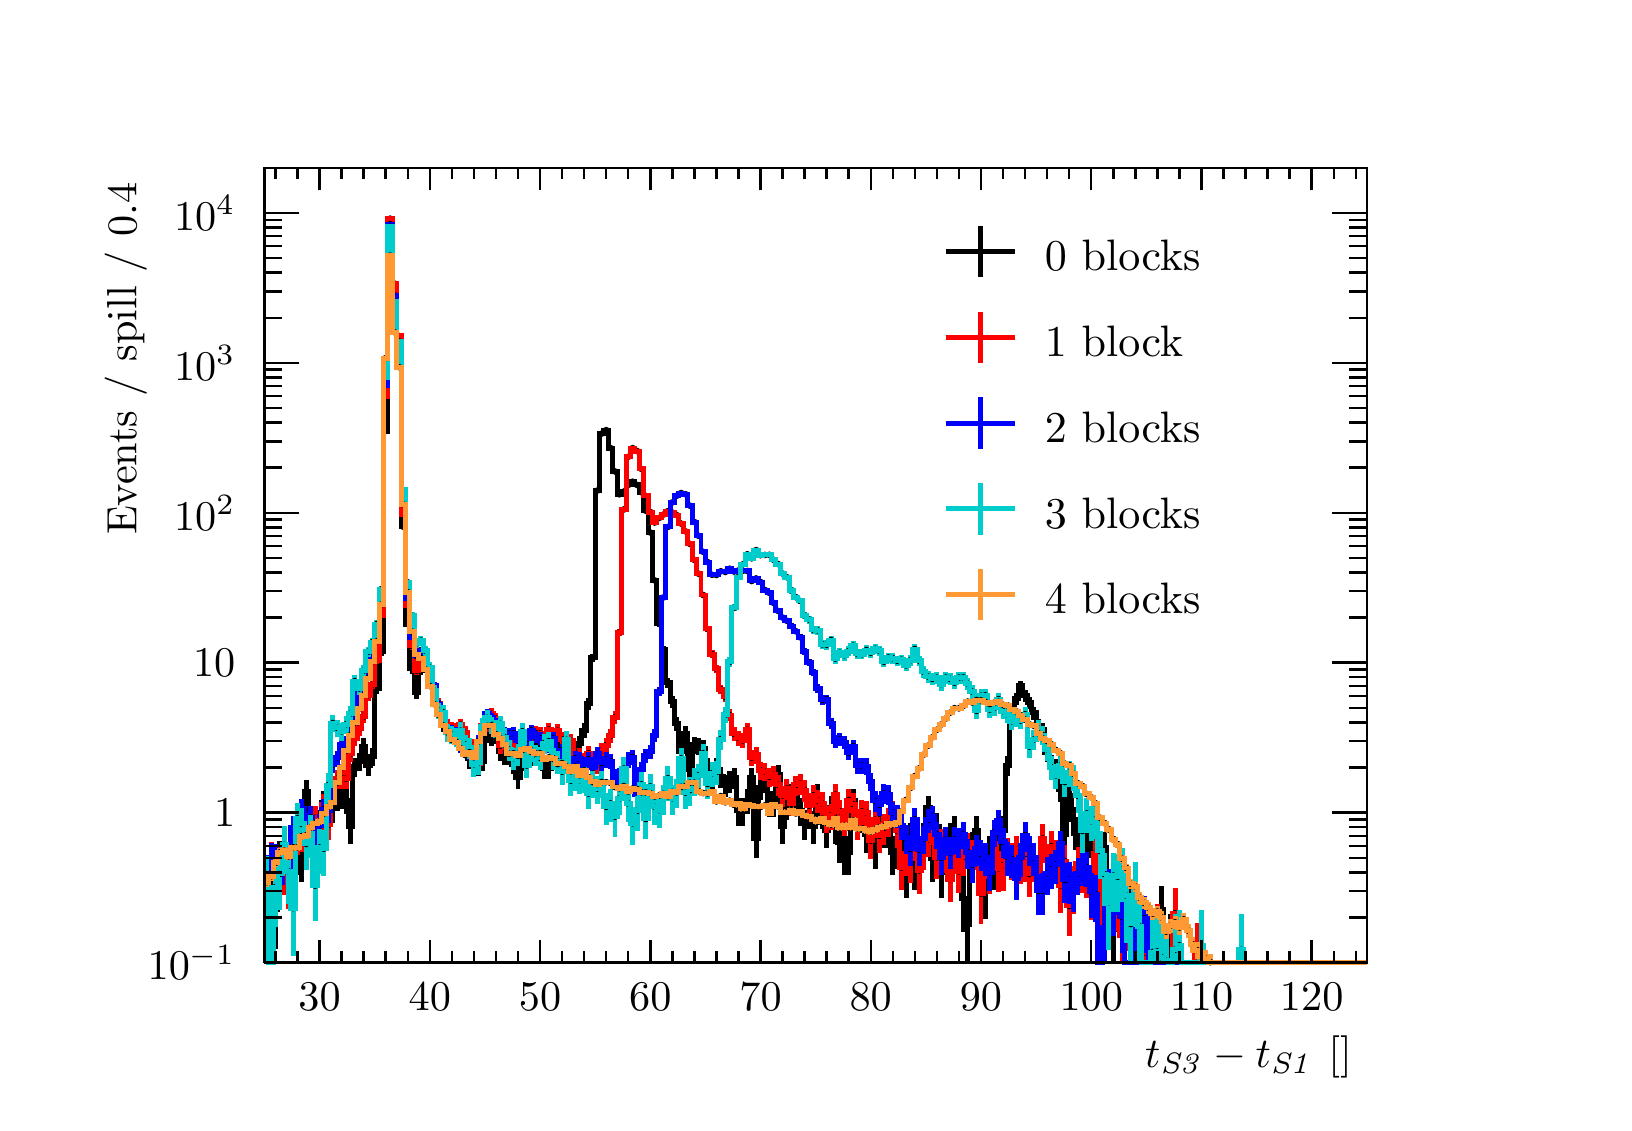
\begin{tikzpicture}
\pgfdeclareplotmark{cross} {
\pgfpathmoveto{\pgfpoint{-0.3\pgfplotmarksize}{\pgfplotmarksize}}
\pgfpathlineto{\pgfpoint{+0.3\pgfplotmarksize}{\pgfplotmarksize}}
\pgfpathlineto{\pgfpoint{+0.3\pgfplotmarksize}{0.3\pgfplotmarksize}}
\pgfpathlineto{\pgfpoint{+1\pgfplotmarksize}{0.3\pgfplotmarksize}}
\pgfpathlineto{\pgfpoint{+1\pgfplotmarksize}{-0.3\pgfplotmarksize}}
\pgfpathlineto{\pgfpoint{+0.3\pgfplotmarksize}{-0.3\pgfplotmarksize}}
\pgfpathlineto{\pgfpoint{+0.3\pgfplotmarksize}{-1.\pgfplotmarksize}}
\pgfpathlineto{\pgfpoint{-0.3\pgfplotmarksize}{-1.\pgfplotmarksize}}
\pgfpathlineto{\pgfpoint{-0.3\pgfplotmarksize}{-0.3\pgfplotmarksize}}
\pgfpathlineto{\pgfpoint{-1.\pgfplotmarksize}{-0.3\pgfplotmarksize}}
\pgfpathlineto{\pgfpoint{-1.\pgfplotmarksize}{0.3\pgfplotmarksize}}
\pgfpathlineto{\pgfpoint{-0.3\pgfplotmarksize}{0.3\pgfplotmarksize}}
\pgfpathclose
\pgfusepathqstroke
}
\pgfdeclareplotmark{cross*} {
\pgfpathmoveto{\pgfpoint{-0.3\pgfplotmarksize}{\pgfplotmarksize}}
\pgfpathlineto{\pgfpoint{+0.3\pgfplotmarksize}{\pgfplotmarksize}}
\pgfpathlineto{\pgfpoint{+0.3\pgfplotmarksize}{0.3\pgfplotmarksize}}
\pgfpathlineto{\pgfpoint{+1\pgfplotmarksize}{0.3\pgfplotmarksize}}
\pgfpathlineto{\pgfpoint{+1\pgfplotmarksize}{-0.3\pgfplotmarksize}}
\pgfpathlineto{\pgfpoint{+0.3\pgfplotmarksize}{-0.3\pgfplotmarksize}}
\pgfpathlineto{\pgfpoint{+0.3\pgfplotmarksize}{-1.\pgfplotmarksize}}
\pgfpathlineto{\pgfpoint{-0.3\pgfplotmarksize}{-1.\pgfplotmarksize}}
\pgfpathlineto{\pgfpoint{-0.3\pgfplotmarksize}{-0.3\pgfplotmarksize}}
\pgfpathlineto{\pgfpoint{-1.\pgfplotmarksize}{-0.3\pgfplotmarksize}}
\pgfpathlineto{\pgfpoint{-1.\pgfplotmarksize}{0.3\pgfplotmarksize}}
\pgfpathlineto{\pgfpoint{-0.3\pgfplotmarksize}{0.3\pgfplotmarksize}}
\pgfpathclose
\pgfusepathqfillstroke
}
\pgfdeclareplotmark{newstar} {
\pgfpathmoveto{\pgfqpoint{0pt}{\pgfplotmarksize}}
\pgfpathlineto{\pgfqpointpolar{44}{0.5\pgfplotmarksize}}
\pgfpathlineto{\pgfqpointpolar{18}{\pgfplotmarksize}}
\pgfpathlineto{\pgfqpointpolar{-20}{0.5\pgfplotmarksize}}
\pgfpathlineto{\pgfqpointpolar{-54}{\pgfplotmarksize}}
\pgfpathlineto{\pgfqpointpolar{-90}{0.5\pgfplotmarksize}}
\pgfpathlineto{\pgfqpointpolar{234}{\pgfplotmarksize}}
\pgfpathlineto{\pgfqpointpolar{198}{0.5\pgfplotmarksize}}
\pgfpathlineto{\pgfqpointpolar{162}{\pgfplotmarksize}}
\pgfpathlineto{\pgfqpointpolar{134}{0.5\pgfplotmarksize}}
\pgfpathclose
\pgfusepathqstroke
}
\pgfdeclareplotmark{newstar*} {
\pgfpathmoveto{\pgfqpoint{0pt}{\pgfplotmarksize}}
\pgfpathlineto{\pgfqpointpolar{44}{0.5\pgfplotmarksize}}
\pgfpathlineto{\pgfqpointpolar{18}{\pgfplotmarksize}}
\pgfpathlineto{\pgfqpointpolar{-20}{0.5\pgfplotmarksize}}
\pgfpathlineto{\pgfqpointpolar{-54}{\pgfplotmarksize}}
\pgfpathlineto{\pgfqpointpolar{-90}{0.5\pgfplotmarksize}}
\pgfpathlineto{\pgfqpointpolar{234}{\pgfplotmarksize}}
\pgfpathlineto{\pgfqpointpolar{198}{0.5\pgfplotmarksize}}
\pgfpathlineto{\pgfqpointpolar{162}{\pgfplotmarksize}}
\pgfpathlineto{\pgfqpointpolar{134}{0.5\pgfplotmarksize}}
\pgfpathclose
\pgfusepathqfillstroke
}
\definecolor{c}{rgb}{1,1,1};
\draw [color=c, fill=c] (0,0) rectangle (20,13.639);
\draw [color=c, fill=c] (3,1.77307) rectangle (17,11.8659);
\definecolor{c}{rgb}{0,0,0};
\draw [c,line width=0.9] (3,1.77307) -- (3,11.8659) -- (17,11.8659) -- (17,1.77307) -- (3,1.77307);
\definecolor{c}{rgb}{1,1,1};
\draw [color=c, fill=c] (3,1.77307) rectangle (17,11.8659);
\definecolor{c}{rgb}{0,0,0};
\draw [c,line width=0.9] (3,1.77307) -- (3,11.8659) -- (17,11.8659) -- (17,1.77307) -- (3,1.77307);
\draw [c,line width=0.9] (3,1.77307) -- (3.056,1.77307) -- (3.056,1.77307) -- (3.112,1.77307) -- (3.112,1.77307) -- (3.168,1.77307) -- (3.168,1.77307) -- (3.224,1.77307) -- (3.224,1.77307) -- (3.28,1.77307) -- (3.28,1.77307) -- (3.336,1.77307) --
 (3.336,1.77307) -- (3.392,1.77307) -- (3.392,1.77307) -- (3.448,1.77307) -- (3.448,1.77307) -- (3.504,1.77307) -- (3.504,1.77307) -- (3.56,1.77307) -- (3.56,1.77307) -- (3.616,1.77307) -- (3.616,1.77307) -- (3.672,1.77307) -- (3.672,1.77307) --
 (3.728,1.77307) -- (3.728,1.77307) -- (3.784,1.77307) -- (3.784,1.77307) -- (3.84,1.77307) -- (3.84,1.77307) -- (3.896,1.77307) -- (3.896,1.77307) -- (3.952,1.77307) -- (3.952,1.77307) -- (4.008,1.77307) -- (4.008,1.77307) -- (4.064,1.77307) --
 (4.064,1.77307) -- (4.12,1.77307) -- (4.12,1.77307) -- (4.176,1.77307) -- (4.176,1.77307) -- (4.232,1.77307) -- (4.232,1.77307) -- (4.288,1.77307) -- (4.288,1.77307) -- (4.344,1.77307) -- (4.344,1.77307) -- (4.4,1.77307) -- (4.4,1.77307) --
 (4.456,1.77307) -- (4.456,1.77307) -- (4.512,1.77307) -- (4.512,1.77307) -- (4.568,1.77307) -- (4.568,1.77307) -- (4.624,1.77307) -- (4.624,1.77307) -- (4.68,1.77307) -- (4.68,1.77307) -- (4.736,1.77307) -- (4.736,1.77307) -- (4.792,1.77307) --
 (4.792,1.77307) -- (4.848,1.77307) -- (4.848,1.77307) -- (4.904,1.77307) -- (4.904,1.77307) -- (4.96,1.77307) -- (4.96,1.77307) -- (5.016,1.77307) -- (5.016,1.77307) -- (5.072,1.77307) -- (5.072,1.77307) -- (5.128,1.77307) -- (5.128,1.77307) --
 (5.184,1.77307) -- (5.184,1.77307) -- (5.24,1.77307) -- (5.24,1.77307) -- (5.296,1.77307) -- (5.296,1.77307) -- (5.352,1.77307) -- (5.352,1.77307) -- (5.408,1.77307) -- (5.408,1.77307) -- (5.464,1.77307) -- (5.464,1.77307) -- (5.52,1.77307) --
 (5.52,1.77307) -- (5.576,1.77307) -- (5.576,1.77307) -- (5.632,1.77307) -- (5.632,1.77307) -- (5.688,1.77307) -- (5.688,1.77307) -- (5.744,1.77307) -- (5.744,1.77307) -- (5.8,1.77307) -- (5.8,1.77307) -- (5.856,1.77307) -- (5.856,1.77307) --
 (5.912,1.77307) -- (5.912,1.77307) -- (5.968,1.77307) -- (5.968,1.77307) -- (6.024,1.77307) -- (6.024,1.77307) -- (6.08,1.77307) -- (6.08,1.77307) -- (6.136,1.77307) -- (6.136,1.77307) -- (6.192,1.77307) -- (6.192,1.77307) -- (6.248,1.77307) --
 (6.248,1.77307) -- (6.304,1.77307) -- (6.304,1.77307) -- (6.36,1.77307) -- (6.36,1.77307) -- (6.416,1.77307) -- (6.416,1.77307) -- (6.472,1.77307) -- (6.472,1.77307) -- (6.528,1.77307) -- (6.528,1.77307) -- (6.584,1.77307) -- (6.584,1.77307) --
 (6.64,1.77307) -- (6.64,1.77307) -- (6.696,1.77307) -- (6.696,1.77307) -- (6.752,1.77307) -- (6.752,1.77307) -- (6.808,1.77307) -- (6.808,1.77307) -- (6.864,1.77307) -- (6.864,1.77307) -- (6.92,1.77307) -- (6.92,1.77307) -- (6.976,1.77307) --
 (6.976,1.77307) -- (7.032,1.77307) -- (7.032,1.77307) -- (7.088,1.77307) -- (7.088,1.77307) -- (7.144,1.77307) -- (7.144,1.77307) -- (7.2,1.77307) -- (7.2,1.77307) -- (7.256,1.77307) -- (7.256,1.77307) -- (7.312,1.77307) -- (7.312,1.77307) --
 (7.368,1.77307) -- (7.368,1.77307) -- (7.424,1.77307) -- (7.424,1.77307) -- (7.48,1.77307) -- (7.48,1.77307) -- (7.536,1.77307) -- (7.536,1.77307) -- (7.592,1.77307) -- (7.592,1.77307) -- (7.648,1.77307) -- (7.648,1.77307) -- (7.704,1.77307) --
 (7.704,1.77307) -- (7.76,1.77307) -- (7.76,1.77307) -- (7.816,1.77307) -- (7.816,1.77307) -- (7.872,1.77307) -- (7.872,1.77307) -- (7.928,1.77307) -- (7.928,1.77307) -- (7.984,1.77307) -- (7.984,1.77307) -- (8.04,1.77307) -- (8.04,1.77307) --
 (8.096,1.77307) -- (8.096,1.77307) -- (8.152,1.77307) -- (8.152,1.77307) -- (8.208,1.77307) -- (8.208,1.77307) -- (8.264,1.77307) -- (8.264,1.77307) -- (8.32,1.77307) -- (8.32,1.77307) -- (8.376,1.77307) -- (8.376,1.77307) -- (8.432,1.77307) --
 (8.432,1.77307) -- (8.488,1.77307) -- (8.488,1.77307) -- (8.544,1.77307) -- (8.544,1.77307) -- (8.6,1.77307) -- (8.6,1.77307) -- (8.656,1.77307) -- (8.656,1.77307) -- (8.712,1.77307) -- (8.712,1.77307) -- (8.768,1.77307) -- (8.768,1.77307) --
 (8.824,1.77307) -- (8.824,1.77307) -- (8.88,1.77307) -- (8.88,1.77307) -- (8.936,1.77307) -- (8.936,1.77307) -- (8.992,1.77307) -- (8.992,1.77307) -- (9.048,1.77307) -- (9.048,1.77307) -- (9.104,1.77307) -- (9.104,1.77307) -- (9.16,1.77307) --
 (9.16,1.77307) -- (9.216,1.77307) -- (9.216,1.77307) -- (9.272,1.77307) -- (9.272,1.77307) -- (9.328,1.77307) -- (9.328,1.77307) -- (9.384,1.77307) -- (9.384,1.77307) -- (9.44,1.77307) -- (9.44,1.77307) -- (9.496,1.77307) -- (9.496,1.77307) --
 (9.552,1.77307) -- (9.552,1.77307) -- (9.608,1.77307) -- (9.608,1.77307) -- (9.664,1.77307) -- (9.664,1.77307) -- (9.72,1.77307) -- (9.72,1.77307) -- (9.776,1.77307) -- (9.776,1.77307) -- (9.832,1.77307) -- (9.832,1.77307) -- (9.888,1.77307) --
 (9.888,1.77307) -- (9.944,1.77307) -- (9.944,1.77307) -- (10,1.77307) -- (10,1.77307) -- (10.056,1.77307) -- (10.056,1.77307) -- (10.112,1.77307) -- (10.112,1.77307) -- (10.168,1.77307) -- (10.168,1.77307) -- (10.224,1.77307) -- (10.224,1.77307) --
 (10.28,1.77307) -- (10.28,1.77307) -- (10.336,1.77307) -- (10.336,1.77307) -- (10.392,1.77307) -- (10.392,1.77307) -- (10.448,1.77307) -- (10.448,1.77307) -- (10.504,1.77307) -- (10.504,1.77307) -- (10.56,1.77307) -- (10.56,1.77307) --
 (10.616,1.77307) -- (10.616,1.77307) -- (10.672,1.77307) -- (10.672,1.77307) -- (10.728,1.77307) -- (10.728,1.77307) -- (10.784,1.77307) -- (10.784,1.77307) -- (10.84,1.77307) -- (10.84,1.77307) -- (10.896,1.77307) -- (10.896,1.77307) --
 (10.952,1.77307) -- (10.952,1.77307) -- (11.008,1.77307) -- (11.008,1.77307) -- (11.064,1.77307) -- (11.064,1.77307) -- (11.12,1.77307) -- (11.12,1.77307) -- (11.176,1.77307) -- (11.176,1.77307) -- (11.232,1.77307) -- (11.232,1.77307) --
 (11.288,1.77307) -- (11.288,1.77307) -- (11.344,1.77307) -- (11.344,1.77307) -- (11.4,1.77307) -- (11.4,1.77307) -- (11.456,1.77307) -- (11.456,1.77307) -- (11.512,1.77307) -- (11.512,1.77307) -- (11.568,1.77307) -- (11.568,1.77307) --
 (11.624,1.77307) -- (11.624,1.77307) -- (11.68,1.77307) -- (11.68,1.77307) -- (11.736,1.77307) -- (11.736,1.77307) -- (11.792,1.77307) -- (11.792,1.77307) -- (11.848,1.77307) -- (11.848,1.77307) -- (11.904,1.77307) -- (11.904,1.77307) --
 (11.96,1.77307) -- (11.96,1.77307) -- (12.016,1.77307) -- (12.016,1.77307) -- (12.072,1.77307) -- (12.072,1.77307) -- (12.128,1.77307) -- (12.128,1.77307) -- (12.184,1.77307) -- (12.184,1.77307) -- (12.24,1.77307) -- (12.24,1.77307) --
 (12.296,1.77307) -- (12.296,1.77307) -- (12.352,1.77307) -- (12.352,1.77307) -- (12.408,1.77307) -- (12.408,1.77307) -- (12.464,1.77307) -- (12.464,1.77307) -- (12.52,1.77307) -- (12.52,1.77307) -- (12.576,1.77307) -- (12.576,1.77307) --
 (12.632,1.77307) -- (12.632,1.77307) -- (12.688,1.77307) -- (12.688,1.77307) -- (12.744,1.77307) -- (12.744,1.77307) -- (12.8,1.77307) -- (12.8,1.77307) -- (12.856,1.77307) -- (12.856,1.77307) -- (12.912,1.77307) -- (12.912,1.77307) --
 (12.968,1.77307) -- (12.968,1.77307) -- (13.024,1.77307) -- (13.024,1.77307) -- (13.08,1.77307) -- (13.08,1.77307) -- (13.136,1.77307) -- (13.136,1.77307) -- (13.192,1.77307) -- (13.192,1.77307) -- (13.248,1.77307) -- (13.248,1.77307) --
 (13.304,1.77307) -- (13.304,1.77307) -- (13.36,1.77307) -- (13.36,1.77307) -- (13.416,1.77307) -- (13.416,1.77307) -- (13.472,1.77307) -- (13.472,1.77307) -- (13.528,1.77307) -- (13.528,1.77307) -- (13.584,1.77307) -- (13.584,1.77307) --
 (13.64,1.77307) -- (13.64,1.77307) -- (13.696,1.77307) -- (13.696,1.77307) -- (13.752,1.77307) -- (13.752,1.77307) -- (13.808,1.77307) -- (13.808,1.77307) -- (13.864,1.77307) -- (13.864,1.77307) -- (13.92,1.77307) -- (13.92,1.77307) --
 (13.976,1.77307) -- (13.976,1.77307) -- (14.032,1.77307) -- (14.032,1.77307) -- (14.088,1.77307) -- (14.088,1.77307) -- (14.144,1.77307) -- (14.144,1.77307) -- (14.2,1.77307) -- (14.2,1.77307) -- (14.256,1.77307) -- (14.256,1.77307) --
 (14.312,1.77307) -- (14.312,1.77307) -- (14.368,1.77307) -- (14.368,1.77307) -- (14.424,1.77307) -- (14.424,1.77307) -- (14.48,1.77307) -- (14.48,1.77307) -- (14.536,1.77307) -- (14.536,1.77307) -- (14.592,1.77307) -- (14.592,1.77307) --
 (14.648,1.77307) -- (14.648,1.77307) -- (14.704,1.77307) -- (14.704,1.77307) -- (14.76,1.77307) -- (14.76,1.77307) -- (14.816,1.77307) -- (14.816,1.77307) -- (14.872,1.77307) -- (14.872,1.77307) -- (14.928,1.77307) -- (14.928,1.77307) --
 (14.984,1.77307) -- (14.984,1.77307) -- (15.04,1.77307) -- (15.04,1.77307) -- (15.096,1.77307) -- (15.096,1.77307) -- (15.152,1.77307) -- (15.152,1.77307) -- (15.208,1.77307) -- (15.208,1.77307) -- (15.264,1.77307) -- (15.264,1.77307) --
 (15.32,1.77307) -- (15.32,1.77307) -- (15.376,1.77307) -- (15.376,1.77307) -- (15.432,1.77307) -- (15.432,1.77307) -- (15.488,1.77307) -- (15.488,1.77307) -- (15.544,1.77307) -- (15.544,1.77307) -- (15.6,1.77307) -- (15.6,1.77307) --
 (15.656,1.77307) -- (15.656,1.77307) -- (15.712,1.77307) -- (15.712,1.77307) -- (15.768,1.77307) -- (15.768,1.77307) -- (15.824,1.77307) -- (15.824,1.77307) -- (15.88,1.77307) -- (15.88,1.77307) -- (15.936,1.77307) -- (15.936,1.77307) --
 (15.992,1.77307) -- (15.992,1.77307) -- (16.048,1.77307) -- (16.048,1.77307) -- (16.104,1.77307) -- (16.104,1.77307) -- (16.16,1.77307) -- (16.16,1.77307) -- (16.216,1.77307) -- (16.216,1.77307) -- (16.272,1.77307) -- (16.272,1.77307) --
 (16.328,1.77307) -- (16.328,1.77307) -- (16.384,1.77307) -- (16.384,1.77307) -- (16.44,1.77307) -- (16.44,1.77307) -- (16.496,1.77307) -- (16.496,1.77307) -- (16.552,1.77307) -- (16.552,1.77307) -- (16.608,1.77307) -- (16.608,1.77307) --
 (16.664,1.77307) -- (16.664,1.77307) -- (16.72,1.77307) -- (16.72,1.77307) -- (16.776,1.77307) -- (16.776,1.77307) -- (16.832,1.77307) -- (16.832,1.77307) -- (16.888,1.77307) -- (16.888,1.77307) -- (16.944,1.77307) -- (16.944,1.77307) --
 (17,1.77307);
\draw [c,line width=0.9] (3,1.77307) -- (17,1.77307);
\draw [c,line width=0.9] (3.7,2.05948) -- (3.7,1.77307);
\draw [c,line width=0.9] (3.98,1.91628) -- (3.98,1.77307);
\draw [c,line width=0.9] (4.26,1.91628) -- (4.26,1.77307);
\draw [c,line width=0.9] (4.54,1.91628) -- (4.54,1.77307);
\draw [c,line width=0.9] (4.82,1.91628) -- (4.82,1.77307);
\draw [c,line width=0.9] (5.1,2.05948) -- (5.1,1.77307);
\draw [c,line width=0.9] (5.38,1.91628) -- (5.38,1.77307);
\draw [c,line width=0.9] (5.66,1.91628) -- (5.66,1.77307);
\draw [c,line width=0.9] (5.94,1.91628) -- (5.94,1.77307);
\draw [c,line width=0.9] (6.22,1.91628) -- (6.22,1.77307);
\draw [c,line width=0.9] (6.5,2.05948) -- (6.5,1.77307);
\draw [c,line width=0.9] (6.78,1.91628) -- (6.78,1.77307);
\draw [c,line width=0.9] (7.06,1.91628) -- (7.06,1.77307);
\draw [c,line width=0.9] (7.34,1.91628) -- (7.34,1.77307);
\draw [c,line width=0.9] (7.62,1.91628) -- (7.62,1.77307);
\draw [c,line width=0.9] (7.9,2.05948) -- (7.9,1.77307);
\draw [c,line width=0.9] (8.18,1.91628) -- (8.18,1.77307);
\draw [c,line width=0.9] (8.46,1.91628) -- (8.46,1.77307);
\draw [c,line width=0.9] (8.74,1.91628) -- (8.74,1.77307);
\draw [c,line width=0.9] (9.02,1.91628) -- (9.02,1.77307);
\draw [c,line width=0.9] (9.3,2.05948) -- (9.3,1.77307);
\draw [c,line width=0.9] (9.58,1.91628) -- (9.58,1.77307);
\draw [c,line width=0.9] (9.86,1.91628) -- (9.86,1.77307);
\draw [c,line width=0.9] (10.14,1.91628) -- (10.14,1.77307);
\draw [c,line width=0.9] (10.42,1.91628) -- (10.42,1.77307);
\draw [c,line width=0.9] (10.7,2.05948) -- (10.7,1.77307);
\draw [c,line width=0.9] (10.98,1.91628) -- (10.98,1.77307);
\draw [c,line width=0.9] (11.26,1.91628) -- (11.26,1.77307);
\draw [c,line width=0.9] (11.54,1.91628) -- (11.54,1.77307);
\draw [c,line width=0.9] (11.82,1.91628) -- (11.82,1.77307);
\draw [c,line width=0.9] (12.1,2.05948) -- (12.1,1.77307);
\draw [c,line width=0.9] (12.38,1.91628) -- (12.38,1.77307);
\draw [c,line width=0.9] (12.66,1.91628) -- (12.66,1.77307);
\draw [c,line width=0.9] (12.94,1.91628) -- (12.94,1.77307);
\draw [c,line width=0.9] (13.22,1.91628) -- (13.22,1.77307);
\draw [c,line width=0.9] (13.5,2.05948) -- (13.5,1.77307);
\draw [c,line width=0.9] (13.78,1.91628) -- (13.78,1.77307);
\draw [c,line width=0.9] (14.06,1.91628) -- (14.06,1.77307);
\draw [c,line width=0.9] (14.34,1.91628) -- (14.34,1.77307);
\draw [c,line width=0.9] (14.62,1.91628) -- (14.62,1.77307);
\draw [c,line width=0.9] (14.9,2.05948) -- (14.9,1.77307);
\draw [c,line width=0.9] (15.18,1.91628) -- (15.18,1.77307);
\draw [c,line width=0.9] (15.46,1.91628) -- (15.46,1.77307);
\draw [c,line width=0.9] (15.74,1.91628) -- (15.74,1.77307);
\draw [c,line width=0.9] (16.02,1.91628) -- (16.02,1.77307);
\draw [c,line width=0.9] (16.3,2.05948) -- (16.3,1.77307);
\draw [c,line width=0.9] (3.7,2.05948) -- (3.7,1.77307);
\draw [c,line width=0.9] (3.42,1.91628) -- (3.42,1.77307);
\draw [c,line width=0.9] (3.14,1.91628) -- (3.14,1.77307);
\draw [c,line width=0.9] (16.3,2.05948) -- (16.3,1.77307);
\draw [c,line width=0.9] (16.58,1.91628) -- (16.58,1.77307);
\draw [c,line width=0.9] (16.86,1.91628) -- (16.86,1.77307);
\draw [anchor=base] (3.7,1.15931) node[scale=1.52731, color=c, rotate=0]{30};
\draw [anchor=base] (5.1,1.15931) node[scale=1.52731, color=c, rotate=0]{40};
\draw [anchor=base] (6.5,1.15931) node[scale=1.52731, color=c, rotate=0]{50};
\draw [anchor=base] (7.9,1.15931) node[scale=1.52731, color=c, rotate=0]{60};
\draw [anchor=base] (9.3,1.15931) node[scale=1.52731, color=c, rotate=0]{70};
\draw [anchor=base] (10.7,1.15931) node[scale=1.52731, color=c, rotate=0]{80};
\draw [anchor=base] (12.1,1.15931) node[scale=1.52731, color=c, rotate=0]{90};
\draw [anchor=base] (13.5,1.15931) node[scale=1.52731, color=c, rotate=0]{100};
\draw [anchor=base] (14.9,1.15931) node[scale=1.52731, color=c, rotate=0]{110};
\draw [anchor=base] (16.3,1.15931) node[scale=1.52731, color=c, rotate=0]{120};
\draw [anchor= east] (17,0.572837) node[scale=1.52731, color=c, rotate=0]{$t_{\SThree} - t_{\SOne}$ [\si{\nano\second}]};
\draw [c,line width=0.9] (3,11.8659) -- (17,11.8659);
\draw [c,line width=0.9] (3.7,11.5795) -- (3.7,11.8659);
\draw [c,line width=0.9] (3.98,11.7227) -- (3.98,11.8659);
\draw [c,line width=0.9] (4.26,11.7227) -- (4.26,11.8659);
\draw [c,line width=0.9] (4.54,11.7227) -- (4.54,11.8659);
\draw [c,line width=0.9] (4.82,11.7227) -- (4.82,11.8659);
\draw [c,line width=0.9] (5.1,11.5795) -- (5.1,11.8659);
\draw [c,line width=0.9] (5.38,11.7227) -- (5.38,11.8659);
\draw [c,line width=0.9] (5.66,11.7227) -- (5.66,11.8659);
\draw [c,line width=0.9] (5.94,11.7227) -- (5.94,11.8659);
\draw [c,line width=0.9] (6.22,11.7227) -- (6.22,11.8659);
\draw [c,line width=0.9] (6.5,11.5795) -- (6.5,11.8659);
\draw [c,line width=0.9] (6.78,11.7227) -- (6.78,11.8659);
\draw [c,line width=0.9] (7.06,11.7227) -- (7.06,11.8659);
\draw [c,line width=0.9] (7.34,11.7227) -- (7.34,11.8659);
\draw [c,line width=0.9] (7.62,11.7227) -- (7.62,11.8659);
\draw [c,line width=0.9] (7.9,11.5795) -- (7.9,11.8659);
\draw [c,line width=0.9] (8.18,11.7227) -- (8.18,11.8659);
\draw [c,line width=0.9] (8.46,11.7227) -- (8.46,11.8659);
\draw [c,line width=0.9] (8.74,11.7227) -- (8.74,11.8659);
\draw [c,line width=0.9] (9.02,11.7227) -- (9.02,11.8659);
\draw [c,line width=0.9] (9.3,11.5795) -- (9.3,11.8659);
\draw [c,line width=0.9] (9.58,11.7227) -- (9.58,11.8659);
\draw [c,line width=0.9] (9.86,11.7227) -- (9.86,11.8659);
\draw [c,line width=0.9] (10.14,11.7227) -- (10.14,11.8659);
\draw [c,line width=0.9] (10.42,11.7227) -- (10.42,11.8659);
\draw [c,line width=0.9] (10.7,11.5795) -- (10.7,11.8659);
\draw [c,line width=0.9] (10.98,11.7227) -- (10.98,11.8659);
\draw [c,line width=0.9] (11.26,11.7227) -- (11.26,11.8659);
\draw [c,line width=0.9] (11.54,11.7227) -- (11.54,11.8659);
\draw [c,line width=0.9] (11.82,11.7227) -- (11.82,11.8659);
\draw [c,line width=0.9] (12.1,11.5795) -- (12.1,11.8659);
\draw [c,line width=0.9] (12.38,11.7227) -- (12.38,11.8659);
\draw [c,line width=0.9] (12.66,11.7227) -- (12.66,11.8659);
\draw [c,line width=0.9] (12.94,11.7227) -- (12.94,11.8659);
\draw [c,line width=0.9] (13.22,11.7227) -- (13.22,11.8659);
\draw [c,line width=0.9] (13.5,11.5795) -- (13.5,11.8659);
\draw [c,line width=0.9] (13.78,11.7227) -- (13.78,11.8659);
\draw [c,line width=0.9] (14.06,11.7227) -- (14.06,11.8659);
\draw [c,line width=0.9] (14.34,11.7227) -- (14.34,11.8659);
\draw [c,line width=0.9] (14.62,11.7227) -- (14.62,11.8659);
\draw [c,line width=0.9] (14.9,11.5795) -- (14.9,11.8659);
\draw [c,line width=0.9] (15.18,11.7227) -- (15.18,11.8659);
\draw [c,line width=0.9] (15.46,11.7227) -- (15.46,11.8659);
\draw [c,line width=0.9] (15.74,11.7227) -- (15.74,11.8659);
\draw [c,line width=0.9] (16.02,11.7227) -- (16.02,11.8659);
\draw [c,line width=0.9] (16.3,11.5795) -- (16.3,11.8659);
\draw [c,line width=0.9] (3.7,11.5795) -- (3.7,11.8659);
\draw [c,line width=0.9] (3.42,11.7227) -- (3.42,11.8659);
\draw [c,line width=0.9] (3.14,11.7227) -- (3.14,11.8659);
\draw [c,line width=0.9] (16.3,11.5795) -- (16.3,11.8659);
\draw [c,line width=0.9] (16.58,11.7227) -- (16.58,11.8659);
\draw [c,line width=0.9] (16.86,11.7227) -- (16.86,11.8659);
\draw [c,line width=0.9] (3,1.77307) -- (3,11.8659);
\draw [c,line width=0.9] (3.444,1.77307) -- (3,1.77307);
\draw [anchor= east] (2.82,1.77307) node[scale=1.52731, color=c, rotate=0]{$10^{-1}$};
\draw [c,line width=0.9] (3.222,2.34621) -- (3,2.34621);
\draw [c,line width=0.9] (3.222,2.68148) -- (3,2.68148);
\draw [c,line width=0.9] (3.222,2.91935) -- (3,2.91935);
\draw [c,line width=0.9] (3.222,3.10386) -- (3,3.10386);
\draw [c,line width=0.9] (3.222,3.25462) -- (3,3.25462);
\draw [c,line width=0.9] (3.222,3.38208) -- (3,3.38208);
\draw [c,line width=0.9] (3.222,3.4925) -- (3,3.4925);
\draw [c,line width=0.9] (3.222,3.58989) -- (3,3.58989);
\draw [c,line width=0.9] (3.444,3.67701) -- (3,3.67701);
\draw [anchor= east] (2.82,3.67701) node[scale=1.52731, color=c, rotate=0]{1};
\draw [c,line width=0.9] (3.222,4.25015) -- (3,4.25015);
\draw [c,line width=0.9] (3.222,4.58542) -- (3,4.58542);
\draw [c,line width=0.9] (3.222,4.82329) -- (3,4.82329);
\draw [c,line width=0.9] (3.222,5.0078) -- (3,5.0078);
\draw [c,line width=0.9] (3.222,5.15856) -- (3,5.15856);
\draw [c,line width=0.9] (3.222,5.28602) -- (3,5.28602);
\draw [c,line width=0.9] (3.222,5.39643) -- (3,5.39643);
\draw [c,line width=0.9] (3.222,5.49383) -- (3,5.49383);
\draw [c,line width=0.9] (3.444,5.58094) -- (3,5.58094);
\draw [anchor= east] (2.82,5.58094) node[scale=1.52731, color=c, rotate=0]{10};
\draw [c,line width=0.9] (3.222,6.15409) -- (3,6.15409);
\draw [c,line width=0.9] (3.222,6.48935) -- (3,6.48935);
\draw [c,line width=0.9] (3.222,6.72723) -- (3,6.72723);
\draw [c,line width=0.9] (3.222,6.91174) -- (3,6.91174);
\draw [c,line width=0.9] (3.222,7.0625) -- (3,7.0625);
\draw [c,line width=0.9] (3.222,7.18996) -- (3,7.18996);
\draw [c,line width=0.9] (3.222,7.30037) -- (3,7.30037);
\draw [c,line width=0.9] (3.222,7.39776) -- (3,7.39776);
\draw [c,line width=0.9] (3.444,7.48488) -- (3,7.48488);
\draw [anchor= east] (2.82,7.48488) node[scale=1.52731, color=c, rotate=0]{$10^{2}$};
\draw [c,line width=0.9] (3.222,8.05803) -- (3,8.05803);
\draw [c,line width=0.9] (3.222,8.39329) -- (3,8.39329);
\draw [c,line width=0.9] (3.222,8.63117) -- (3,8.63117);
\draw [c,line width=0.9] (3.222,8.81568) -- (3,8.81568);
\draw [c,line width=0.9] (3.222,8.96644) -- (3,8.96644);
\draw [c,line width=0.9] (3.222,9.0939) -- (3,9.0939);
\draw [c,line width=0.9] (3.222,9.20431) -- (3,9.20431);
\draw [c,line width=0.9] (3.222,9.3017) -- (3,9.3017);
\draw [c,line width=0.9] (3.444,9.38882) -- (3,9.38882);
\draw [anchor= east] (2.82,9.38882) node[scale=1.52731, color=c, rotate=0]{$10^{3}$};
\draw [c,line width=0.9] (3.222,9.96196) -- (3,9.96196);
\draw [c,line width=0.9] (3.222,10.2972) -- (3,10.2972);
\draw [c,line width=0.9] (3.222,10.5351) -- (3,10.5351);
\draw [c,line width=0.9] (3.222,10.7196) -- (3,10.7196);
\draw [c,line width=0.9] (3.222,10.8704) -- (3,10.8704);
\draw [c,line width=0.9] (3.222,10.9978) -- (3,10.9978);
\draw [c,line width=0.9] (3.222,11.1082) -- (3,11.1082);
\draw [c,line width=0.9] (3.222,11.2056) -- (3,11.2056);
\draw [c,line width=0.9] (3.444,11.2928) -- (3,11.2928);
\draw [anchor= east] (2.82,11.2928) node[scale=1.52731, color=c, rotate=0]{$10^{4}$};
\draw [c,line width=0.9] (3.222,11.8659) -- (3,11.8659);
\draw [anchor= east] (1.24,11.8659) node[scale=1.52731, color=c, rotate=90]{ Events / spill / \SI{0.4}{\nano\second}};
\draw [c,line width=0.9] (17,1.77307) -- (17,11.8659);
\draw [c,line width=0.9] (16.556,1.77307) -- (17,1.77307);
\draw [c,line width=0.9] (16.778,2.34621) -- (17,2.34621);
\draw [c,line width=0.9] (16.778,2.68148) -- (17,2.68148);
\draw [c,line width=0.9] (16.778,2.91935) -- (17,2.91935);
\draw [c,line width=0.9] (16.778,3.10386) -- (17,3.10386);
\draw [c,line width=0.9] (16.778,3.25462) -- (17,3.25462);
\draw [c,line width=0.9] (16.778,3.38208) -- (17,3.38208);
\draw [c,line width=0.9] (16.778,3.4925) -- (17,3.4925);
\draw [c,line width=0.9] (16.778,3.58989) -- (17,3.58989);
\draw [c,line width=0.9] (16.556,3.67701) -- (17,3.67701);
\draw [c,line width=0.9] (16.778,4.25015) -- (17,4.25015);
\draw [c,line width=0.9] (16.778,4.58542) -- (17,4.58542);
\draw [c,line width=0.9] (16.778,4.82329) -- (17,4.82329);
\draw [c,line width=0.9] (16.778,5.0078) -- (17,5.0078);
\draw [c,line width=0.9] (16.778,5.15856) -- (17,5.15856);
\draw [c,line width=0.9] (16.778,5.28602) -- (17,5.28602);
\draw [c,line width=0.9] (16.778,5.39643) -- (17,5.39643);
\draw [c,line width=0.9] (16.778,5.49383) -- (17,5.49383);
\draw [c,line width=0.9] (16.556,5.58094) -- (17,5.58094);
\draw [c,line width=0.9] (16.778,6.15409) -- (17,6.15409);
\draw [c,line width=0.9] (16.778,6.48935) -- (17,6.48935);
\draw [c,line width=0.9] (16.778,6.72723) -- (17,6.72723);
\draw [c,line width=0.9] (16.778,6.91174) -- (17,6.91174);
\draw [c,line width=0.9] (16.778,7.0625) -- (17,7.0625);
\draw [c,line width=0.9] (16.778,7.18996) -- (17,7.18996);
\draw [c,line width=0.9] (16.778,7.30037) -- (17,7.30037);
\draw [c,line width=0.9] (16.778,7.39776) -- (17,7.39776);
\draw [c,line width=0.9] (16.556,7.48488) -- (17,7.48488);
\draw [c,line width=0.9] (16.778,8.05803) -- (17,8.05803);
\draw [c,line width=0.9] (16.778,8.39329) -- (17,8.39329);
\draw [c,line width=0.9] (16.778,8.63117) -- (17,8.63117);
\draw [c,line width=0.9] (16.778,8.81568) -- (17,8.81568);
\draw [c,line width=0.9] (16.778,8.96644) -- (17,8.96644);
\draw [c,line width=0.9] (16.778,9.0939) -- (17,9.0939);
\draw [c,line width=0.9] (16.778,9.20431) -- (17,9.20431);
\draw [c,line width=0.9] (16.778,9.3017) -- (17,9.3017);
\draw [c,line width=0.9] (16.556,9.38882) -- (17,9.38882);
\draw [c,line width=0.9] (16.778,9.96196) -- (17,9.96196);
\draw [c,line width=0.9] (16.778,10.2972) -- (17,10.2972);
\draw [c,line width=0.9] (16.778,10.5351) -- (17,10.5351);
\draw [c,line width=0.9] (16.778,10.7196) -- (17,10.7196);
\draw [c,line width=0.9] (16.778,10.8704) -- (17,10.8704);
\draw [c,line width=0.9] (16.778,10.9978) -- (17,10.9978);
\draw [c,line width=0.9] (16.778,11.1082) -- (17,11.1082);
\draw [c,line width=0.9] (16.778,11.2056) -- (17,11.2056);
\draw [c,line width=0.9] (16.556,11.2928) -- (17,11.2928);
\draw [c,line width=0.9] (16.778,11.8659) -- (17,11.8659);
\draw [c,line width=1.8] (3.028,2.32696) -- (3.028,2.71955);
\draw [c,line width=1.8] (3.028,2.71955) -- (3.028,2.98467);
\foreach \P in {(3.028,2.71955)}{\draw[mark options={color=c,fill=c},mark size=2.402402pt,mark=*,mark size=1pt] plot coordinates {\P};}
\draw [c,line width=1.8] (3.084,2.59206) -- (3.084,2.92736);
\draw [c,line width=1.8] (3.084,2.92736) -- (3.084,3.16525);
\foreach \P in {(3.084,2.92736)}{\draw[mark options={color=c,fill=c},mark size=2.402402pt,mark=*,mark size=1pt] plot coordinates {\P};}
\draw [c,line width=1.8] (3.14,1.95114) -- (3.14,2.44133);
\draw [c,line width=1.8] (3.14,2.44133) -- (3.14,2.74699);
\foreach \P in {(3.14,2.44133)}{\draw[mark options={color=c,fill=c},mark size=2.402402pt,mark=*,mark size=1pt] plot coordinates {\P};}
\draw [c,line width=1.8] (3.196,2.79655) -- (3.196,3.09328);
\draw [c,line width=1.8] (3.196,3.09328) -- (3.196,3.3112);
\foreach \P in {(3.196,3.09328)}{\draw[mark options={color=c,fill=c},mark size=2.402402pt,mark=*,mark size=1pt] plot coordinates {\P};}
\draw [c,line width=1.8] (3.252,2.79655) -- (3.252,3.09328);
\draw [c,line width=1.8] (3.252,3.09328) -- (3.252,3.3112);
\foreach \P in {(3.252,3.09328)}{\draw[mark options={color=c,fill=c},mark size=2.402402pt,mark=*,mark size=1pt] plot coordinates {\P};}
\draw [c,line width=1.8] (3.308,2.59206) -- (3.308,2.92736);
\draw [c,line width=1.8] (3.308,2.92736) -- (3.308,3.16525);
\foreach \P in {(3.308,2.92736)}{\draw[mark options={color=c,fill=c},mark size=2.402402pt,mark=*,mark size=1pt] plot coordinates {\P};}
\draw [c,line width=1.8] (3.364,2.9628) -- (3.364,3.23142);
\draw [c,line width=1.8] (3.364,3.23142) -- (3.364,3.43384);
\foreach \P in {(3.364,3.23142)}{\draw[mark options={color=c,fill=c},mark size=2.402402pt,mark=*,mark size=1pt] plot coordinates {\P};}
\draw [c,line width=1.8] (3.42,2.88356) -- (3.42,3.16523);
\draw [c,line width=1.8] (3.42,3.16523) -- (3.42,3.37495);
\foreach \P in {(3.42,3.16523)}{\draw[mark options={color=c,fill=c},mark size=2.402402pt,mark=*,mark size=1pt] plot coordinates {\P};}
\draw [c,line width=1.8] (3.476,2.79655) -- (3.476,3.09328);
\draw [c,line width=1.8] (3.476,3.09328) -- (3.476,3.3112);
\foreach \P in {(3.476,3.09328)}{\draw[mark options={color=c,fill=c},mark size=2.402402pt,mark=*,mark size=1pt] plot coordinates {\P};}
\draw [c,line width=1.8] (3.532,3.78629) -- (3.532,3.95);
\draw [c,line width=1.8] (3.532,3.95) -- (3.532,4.08659);
\foreach \P in {(3.532,3.95)}{\draw[mark options={color=c,fill=c},mark size=2.402402pt,mark=*,mark size=1pt] plot coordinates {\P};}
\draw [c,line width=1.8] (3.588,3.37833) -- (3.588,3.58762);
\draw [c,line width=1.8] (3.588,3.58762) -- (3.588,3.75449);
\foreach \P in {(3.588,3.58762)}{\draw[mark options={color=c,fill=c},mark size=2.402402pt,mark=*,mark size=1pt] plot coordinates {\P};}
\draw [c,line width=1.8] (3.644,2.79655) -- (3.644,3.09328);
\draw [c,line width=1.8] (3.644,3.09328) -- (3.644,3.3112);
\foreach \P in {(3.644,3.09328)}{\draw[mark options={color=c,fill=c},mark size=2.402402pt,mark=*,mark size=1pt] plot coordinates {\P};}
\draw [c,line width=1.8] (3.7,3.3297) -- (3.7,3.54521);
\draw [c,line width=1.8] (3.7,3.54521) -- (3.7,3.716);
\foreach \P in {(3.7,3.54521)}{\draw[mark options={color=c,fill=c},mark size=2.402402pt,mark=*,mark size=1pt] plot coordinates {\P};}
\draw [c,line width=1.8] (3.756,3.62404) -- (3.756,3.80456);
\draw [c,line width=1.8] (3.756,3.80456) -- (3.756,3.95264);
\foreach \P in {(3.756,3.80456)}{\draw[mark options={color=c,fill=c},mark size=2.402402pt,mark=*,mark size=1pt] plot coordinates {\P};}
\draw [c,line width=1.8] (3.812,3.50981) -- (3.812,3.70318);
\draw [c,line width=1.8] (3.812,3.70318) -- (3.812,3.85979);
\foreach \P in {(3.812,3.70318)}{\draw[mark options={color=c,fill=c},mark size=2.402402pt,mark=*,mark size=1pt] plot coordinates {\P};}
\draw [c,line width=1.8] (3.868,3.54958) -- (3.868,3.73837);
\draw [c,line width=1.8] (3.868,3.73837) -- (3.868,3.89198);
\foreach \P in {(3.868,3.73837)}{\draw[mark options={color=c,fill=c},mark size=2.402402pt,mark=*,mark size=1pt] plot coordinates {\P};}
\draw [c,line width=1.8] (3.924,3.69262) -- (3.924,3.86584);
\draw [c,line width=1.8] (3.924,3.86584) -- (3.924,4.00898);
\foreach \P in {(3.924,3.86584)}{\draw[mark options={color=c,fill=c},mark size=2.402402pt,mark=*,mark size=1pt] plot coordinates {\P};}
\draw [c,line width=1.8] (3.98,3.72498) -- (3.98,3.89485);
\draw [c,line width=1.8] (3.98,3.89485) -- (3.98,4.0357);
\foreach \P in {(3.98,3.89485)}{\draw[mark options={color=c,fill=c},mark size=2.402402pt,mark=*,mark size=1pt] plot coordinates {\P};}
\draw [c,line width=1.8] (4.036,3.65901) -- (4.036,3.83577);
\draw [c,line width=1.8] (4.036,3.83577) -- (4.036,3.98131);
\foreach \P in {(4.036,3.83577)}{\draw[mark options={color=c,fill=c},mark size=2.402402pt,mark=*,mark size=1pt] plot coordinates {\P};}
\draw [c,line width=1.8] (4.092,3.27822) -- (4.092,3.5005);
\draw [c,line width=1.8] (4.092,3.5005) -- (4.092,3.67551);
\foreach \P in {(4.092,3.5005)}{\draw[mark options={color=c,fill=c},mark size=2.402402pt,mark=*,mark size=1pt] plot coordinates {\P};}
\draw [c,line width=1.8] (4.148,4.12466) -- (4.148,4.25815);
\draw [c,line width=1.8] (4.148,4.25815) -- (4.148,4.37306);
\foreach \P in {(4.148,4.25815)}{\draw[mark options={color=c,fill=c},mark size=2.402402pt,mark=*,mark size=1pt] plot coordinates {\P};}
\draw [c,line width=1.8] (4.204,4.2011) -- (4.204,4.32857);
\draw [c,line width=1.8] (4.204,4.32857) -- (4.204,4.43899);
\foreach \P in {(4.204,4.32857)}{\draw[mark options={color=c,fill=c},mark size=2.402402pt,mark=*,mark size=1pt] plot coordinates {\P};}
\draw [c,line width=1.8] (4.26,4.41083) -- (4.26,4.52314);
\draw [c,line width=1.8] (4.26,4.52314) -- (4.26,4.62201);
\foreach \P in {(4.26,4.52314)}{\draw[mark options={color=c,fill=c},mark size=2.402402pt,mark=*,mark size=1pt] plot coordinates {\P};}
\draw [c,line width=1.8] (4.316,4.14442) -- (4.316,4.27633);
\draw [c,line width=1.8] (4.316,4.27633) -- (4.316,4.39006);
\foreach \P in {(4.316,4.27633)}{\draw[mark options={color=c,fill=c},mark size=2.402402pt,mark=*,mark size=1pt] plot coordinates {\P};}
\draw [c,line width=1.8] (4.372,4.27127) -- (4.372,4.39345);
\draw [c,line width=1.8] (4.372,4.39345) -- (4.372,4.49989);
\foreach \P in {(4.372,4.39345)}{\draw[mark options={color=c,fill=c},mark size=2.402402pt,mark=*,mark size=1pt] plot coordinates {\P};}
\draw [c,line width=1.8] (4.428,5.18898) -- (4.428,5.25918);
\draw [c,line width=1.8] (4.428,5.25918) -- (4.428,5.32387);
\foreach \P in {(4.428,5.25918)}{\draw[mark options={color=c,fill=c},mark size=2.402402pt,mark=*,mark size=1pt] plot coordinates {\P};}
\draw [c,line width=1.8] (4.484,5.66535) -- (4.484,5.71798);
\draw [c,line width=1.8] (4.484,5.71798) -- (4.484,5.76746);
\foreach \P in {(4.484,5.71798)}{\draw[mark options={color=c,fill=c},mark size=2.402402pt,mark=*,mark size=1pt] plot coordinates {\P};}
\draw [c,line width=1.8] (4.54,8.51399) -- (4.54,8.52339);
\draw [c,line width=1.8] (4.54,8.52339) -- (4.54,8.53268);
\foreach \P in {(4.54,8.52339)}{\draw[mark options={color=c,fill=c},mark size=2.402402pt,mark=*,mark size=1pt] plot coordinates {\P};}
\draw [c,line width=1.8] (4.596,11.0391) -- (4.596,11.0412);
\draw [c,line width=1.8] (4.596,11.0412) -- (4.596,11.0432);
\foreach \P in {(4.596,11.0412)}{\draw[mark options={color=c,fill=c},mark size=2.402402pt,mark=*,mark size=1pt] plot coordinates {\P};}
\draw [c,line width=1.8] (4.652,10.3775) -- (4.652,10.3805);
\draw [c,line width=1.8] (4.652,10.3805) -- (4.652,10.3836);
\foreach \P in {(4.652,10.3805)}{\draw[mark options={color=c,fill=c},mark size=2.402402pt,mark=*,mark size=1pt] plot coordinates {\P};}
\draw [c,line width=1.8] (4.708,9.67656) -- (4.708,9.68122);
\draw [c,line width=1.8] (4.708,9.68122) -- (4.708,9.68585);
\foreach \P in {(4.708,9.68122)}{\draw[mark options={color=c,fill=c},mark size=2.402402pt,mark=*,mark size=1pt] plot coordinates {\P};}
\draw [c,line width=1.8] (4.764,7.28819) -- (4.764,7.30792);
\draw [c,line width=1.8] (4.764,7.30792) -- (4.764,7.32719);
\foreach \P in {(4.764,7.30792)}{\draw[mark options={color=c,fill=c},mark size=2.402402pt,mark=*,mark size=1pt] plot coordinates {\P};}
\draw [c,line width=1.8] (4.82,6.02863) -- (4.82,6.07088);
\draw [c,line width=1.8] (4.82,6.07088) -- (4.82,6.11108);
\foreach \P in {(4.82,6.07088)}{\draw[mark options={color=c,fill=c},mark size=2.402402pt,mark=*,mark size=1pt] plot coordinates {\P};}
\draw [c,line width=1.8] (4.876,5.44369) -- (4.876,5.50387);
\draw [c,line width=1.8] (4.876,5.50387) -- (4.876,5.55996);
\foreach \P in {(4.876,5.50387)}{\draw[mark options={color=c,fill=c},mark size=2.402402pt,mark=*,mark size=1pt] plot coordinates {\P};}
\draw [c,line width=1.8] (4.932,5.12361) -- (4.932,5.19663);
\draw [c,line width=1.8] (4.932,5.19663) -- (4.932,5.26372);
\foreach \P in {(4.932,5.19663)}{\draw[mark options={color=c,fill=c},mark size=2.402402pt,mark=*,mark size=1pt] plot coordinates {\P};}
\draw [c,line width=1.8] (4.988,5.43091) -- (4.988,5.49156);
\draw [c,line width=1.8] (4.988,5.49156) -- (4.988,5.54805);
\foreach \P in {(4.988,5.49156)}{\draw[mark options={color=c,fill=c},mark size=2.402402pt,mark=*,mark size=1pt] plot coordinates {\P};}
\draw [c,line width=1.8] (5.044,5.44791) -- (5.044,5.50793);
\draw [c,line width=1.8] (5.044,5.50793) -- (5.044,5.56389);
\foreach \P in {(5.044,5.50793)}{\draw[mark options={color=c,fill=c},mark size=2.402402pt,mark=*,mark size=1pt] plot coordinates {\P};}
\draw [c,line width=1.8] (5.1,5.31615) -- (5.1,5.38114);
\draw [c,line width=1.8] (5.1,5.38114) -- (5.1,5.4414);
\foreach \P in {(5.1,5.38114)}{\draw[mark options={color=c,fill=c},mark size=2.402402pt,mark=*,mark size=1pt] plot coordinates {\P};}
\draw [c,line width=1.8] (5.156,5.1599) -- (5.156,5.23133);
\draw [c,line width=1.8] (5.156,5.23133) -- (5.156,5.29708);
\foreach \P in {(5.156,5.23133)}{\draw[mark options={color=c,fill=c},mark size=2.402402pt,mark=*,mark size=1pt] plot coordinates {\P};}
\draw [c,line width=1.8] (5.212,4.95303) -- (5.212,5.03398);
\draw [c,line width=1.8] (5.212,5.03398) -- (5.212,5.1077);
\foreach \P in {(5.212,5.03398)}{\draw[mark options={color=c,fill=c},mark size=2.402402pt,mark=*,mark size=1pt] plot coordinates {\P};}
\draw [c,line width=1.8] (5.268,4.69935) -- (5.268,4.7937);
\draw [c,line width=1.8] (5.268,4.7937) -- (5.268,4.87839);
\foreach \P in {(5.268,4.7937)}{\draw[mark options={color=c,fill=c},mark size=2.402402pt,mark=*,mark size=1pt] plot coordinates {\P};}
\draw [c,line width=1.8] (5.324,4.60225) -- (5.324,4.7023);
\draw [c,line width=1.8] (5.324,4.7023) -- (5.324,4.79154);
\foreach \P in {(5.324,4.7023)}{\draw[mark options={color=c,fill=c},mark size=2.402402pt,mark=*,mark size=1pt] plot coordinates {\P};}
\draw [c,line width=1.8] (5.38,4.54309) -- (5.38,4.64678);
\draw [c,line width=1.8] (5.38,4.64678) -- (5.38,4.73891);
\foreach \P in {(5.38,4.64678)}{\draw[mark options={color=c,fill=c},mark size=2.402402pt,mark=*,mark size=1pt] plot coordinates {\P};}
\draw [c,line width=1.8] (5.436,4.6136) -- (5.436,4.71297);
\draw [c,line width=1.8] (5.436,4.71297) -- (5.436,4.80167);
\foreach \P in {(5.436,4.71297)}{\draw[mark options={color=c,fill=c},mark size=2.402402pt,mark=*,mark size=1pt] plot coordinates {\P};}
\draw [c,line width=1.8] (5.492,4.51823) -- (5.492,4.62349);
\draw [c,line width=1.8] (5.492,4.62349) -- (5.492,4.71685);
\foreach \P in {(5.492,4.62349)}{\draw[mark options={color=c,fill=c},mark size=2.402402pt,mark=*,mark size=1pt] plot coordinates {\P};}
\draw [c,line width=1.8] (5.548,4.57908) -- (5.548,4.68054);
\draw [c,line width=1.8] (5.548,4.68054) -- (5.548,4.7709);
\foreach \P in {(5.548,4.68054)}{\draw[mark options={color=c,fill=c},mark size=2.402402pt,mark=*,mark size=1pt] plot coordinates {\P};}
\draw [c,line width=1.8] (5.604,4.2369) -- (5.604,4.36165);
\draw [c,line width=1.8] (5.604,4.36165) -- (5.604,4.47002);
\foreach \P in {(5.604,4.36165)}{\draw[mark options={color=c,fill=c},mark size=2.402402pt,mark=*,mark size=1pt] plot coordinates {\P};}
\draw [c,line width=1.8] (5.66,4.36679) -- (5.66,4.48213);
\draw [c,line width=1.8] (5.66,4.48213) -- (5.66,4.58333);
\foreach \P in {(5.66,4.48213)}{\draw[mark options={color=c,fill=c},mark size=2.402402pt,mark=*,mark size=1pt] plot coordinates {\P};}
\draw [c,line width=1.8] (5.716,4.14442) -- (5.716,4.27633);
\draw [c,line width=1.8] (5.716,4.27633) -- (5.716,4.39006);
\foreach \P in {(5.716,4.27633)}{\draw[mark options={color=c,fill=c},mark size=2.402402pt,mark=*,mark size=1pt] plot coordinates {\P};}
\draw [c,line width=1.8] (5.772,4.2011) -- (5.772,4.32857);
\draw [c,line width=1.8] (5.772,4.32857) -- (5.772,4.43899);
\foreach \P in {(5.772,4.32857)}{\draw[mark options={color=c,fill=c},mark size=2.402402pt,mark=*,mark size=1pt] plot coordinates {\P};}
\draw [c,line width=1.8] (5.828,4.55526) -- (5.828,4.65819);
\draw [c,line width=1.8] (5.828,4.65819) -- (5.828,4.74972);
\foreach \P in {(5.828,4.65819)}{\draw[mark options={color=c,fill=c},mark size=2.402402pt,mark=*,mark size=1pt] plot coordinates {\P};}
\draw [c,line width=1.8] (5.884,4.51823) -- (5.884,4.62349);
\draw [c,line width=1.8] (5.884,4.62349) -- (5.884,4.71685);
\foreach \P in {(5.884,4.62349)}{\draw[mark options={color=c,fill=c},mark size=2.402402pt,mark=*,mark size=1pt] plot coordinates {\P};}
\draw [c,line width=1.8] (5.94,4.54309) -- (5.94,4.64678);
\draw [c,line width=1.8] (5.94,4.64678) -- (5.94,4.73891);
\foreach \P in {(5.94,4.64678)}{\draw[mark options={color=c,fill=c},mark size=2.402402pt,mark=*,mark size=1pt] plot coordinates {\P};}
\draw [c,line width=1.8] (5.996,4.33612) -- (5.996,4.45362);
\draw [c,line width=1.8] (5.996,4.45362) -- (5.996,4.55647);
\foreach \P in {(5.996,4.45362)}{\draw[mark options={color=c,fill=c},mark size=2.402402pt,mark=*,mark size=1pt] plot coordinates {\P};}
\draw [c,line width=1.8] (6.052,4.28795) -- (6.052,4.40891);
\draw [c,line width=1.8] (6.052,4.40891) -- (6.052,4.51441);
\foreach \P in {(6.052,4.40891)}{\draw[mark options={color=c,fill=c},mark size=2.402402pt,mark=*,mark size=1pt] plot coordinates {\P};}
\draw [c,line width=1.8] (6.108,4.28795) -- (6.108,4.40891);
\draw [c,line width=1.8] (6.108,4.40891) -- (6.108,4.51441);
\foreach \P in {(6.108,4.40891)}{\draw[mark options={color=c,fill=c},mark size=2.402402pt,mark=*,mark size=1pt] plot coordinates {\P};}
\draw [c,line width=1.8] (6.164,4.16373) -- (6.164,4.29411);
\draw [c,line width=1.8] (6.164,4.29411) -- (6.164,4.4067);
\foreach \P in {(6.164,4.29411)}{\draw[mark options={color=c,fill=c},mark size=2.402402pt,mark=*,mark size=1pt] plot coordinates {\P};}
\draw [c,line width=1.8] (6.22,3.97198) -- (6.22,4.11835);
\draw [c,line width=1.8] (6.22,4.11835) -- (6.22,4.24266);
\foreach \P in {(6.22,4.11835)}{\draw[mark options={color=c,fill=c},mark size=2.402402pt,mark=*,mark size=1pt] plot coordinates {\P};}
\draw [c,line width=1.8] (6.276,4.2011) -- (6.276,4.32857);
\draw [c,line width=1.8] (6.276,4.32857) -- (6.276,4.43899);
\foreach \P in {(6.276,4.32857)}{\draw[mark options={color=c,fill=c},mark size=2.402402pt,mark=*,mark size=1pt] plot coordinates {\P};}
\draw [c,line width=1.8] (6.332,4.35159) -- (6.332,4.468);
\draw [c,line width=1.8] (6.332,4.468) -- (6.332,4.57002);
\foreach \P in {(6.332,4.468)}{\draw[mark options={color=c,fill=c},mark size=2.402402pt,mark=*,mark size=1pt] plot coordinates {\P};}
\draw [c,line width=1.8] (6.388,4.27127) -- (6.388,4.39345);
\draw [c,line width=1.8] (6.388,4.39345) -- (6.388,4.49989);
\foreach \P in {(6.388,4.39345)}{\draw[mark options={color=c,fill=c},mark size=2.402402pt,mark=*,mark size=1pt] plot coordinates {\P};}
\draw [c,line width=1.8] (6.444,4.49262) -- (6.444,4.59952);
\draw [c,line width=1.8] (6.444,4.59952) -- (6.444,4.69417);
\foreach \P in {(6.444,4.59952)}{\draw[mark options={color=c,fill=c},mark size=2.402402pt,mark=*,mark size=1pt] plot coordinates {\P};}
\draw [c,line width=1.8] (6.5,4.28795) -- (6.5,4.40891);
\draw [c,line width=1.8] (6.5,4.40891) -- (6.5,4.51441);
\foreach \P in {(6.5,4.40891)}{\draw[mark options={color=c,fill=c},mark size=2.402402pt,mark=*,mark size=1pt] plot coordinates {\P};}
\draw [c,line width=1.8] (6.556,4.10444) -- (6.556,4.23957);
\draw [c,line width=1.8] (6.556,4.23957) -- (6.556,4.35569);
\foreach \P in {(6.556,4.23957)}{\draw[mark options={color=c,fill=c},mark size=2.402402pt,mark=*,mark size=1pt] plot coordinates {\P};}
\draw [c,line width=1.8] (6.612,4.10444) -- (6.612,4.23957);
\draw [c,line width=1.8] (6.612,4.23957) -- (6.612,4.35569);
\foreach \P in {(6.612,4.23957)}{\draw[mark options={color=c,fill=c},mark size=2.402402pt,mark=*,mark size=1pt] plot coordinates {\P};}
\draw [c,line width=1.8] (6.668,4.38172) -- (6.668,4.49603);
\draw [c,line width=1.8] (6.668,4.49603) -- (6.668,4.59643);
\foreach \P in {(6.668,4.49603)}{\draw[mark options={color=c,fill=c},mark size=2.402402pt,mark=*,mark size=1pt] plot coordinates {\P};}
\draw [c,line width=1.8] (6.724,4.3964) -- (6.724,4.5097);
\draw [c,line width=1.8] (6.724,4.5097) -- (6.724,4.60932);
\foreach \P in {(6.724,4.5097)}{\draw[mark options={color=c,fill=c},mark size=2.402402pt,mark=*,mark size=1pt] plot coordinates {\P};}
\draw [c,line width=1.8] (6.78,4.30431) -- (6.78,4.42408);
\draw [c,line width=1.8] (6.78,4.42408) -- (6.78,4.52868);
\foreach \P in {(6.78,4.42408)}{\draw[mark options={color=c,fill=c},mark size=2.402402pt,mark=*,mark size=1pt] plot coordinates {\P};}
\draw [c,line width=1.8] (6.836,4.2369) -- (6.836,4.36165);
\draw [c,line width=1.8] (6.836,4.36165) -- (6.836,4.47002);
\foreach \P in {(6.836,4.36165)}{\draw[mark options={color=c,fill=c},mark size=2.402402pt,mark=*,mark size=1pt] plot coordinates {\P};}
\draw [c,line width=1.8] (6.892,4.38172) -- (6.892,4.49603);
\draw [c,line width=1.8] (6.892,4.49603) -- (6.892,4.59643);
\foreach \P in {(6.892,4.49603)}{\draw[mark options={color=c,fill=c},mark size=2.402402pt,mark=*,mark size=1pt] plot coordinates {\P};}
\draw [c,line width=1.8] (6.948,4.25426) -- (6.948,4.3777);
\draw [c,line width=1.8] (6.948,4.3777) -- (6.948,4.48509);
\foreach \P in {(6.948,4.3777)}{\draw[mark options={color=c,fill=c},mark size=2.402402pt,mark=*,mark size=1pt] plot coordinates {\P};}
\draw [c,line width=1.8] (7.004,4.43897) -- (7.004,4.54939);
\draw [c,line width=1.8] (7.004,4.54939) -- (7.004,4.64679);
\foreach \P in {(7.004,4.54939)}{\draw[mark options={color=c,fill=c},mark size=2.402402pt,mark=*,mark size=1pt] plot coordinates {\P};}
\draw [c,line width=1.8] (7.06,4.6248) -- (7.06,4.7235);
\draw [c,line width=1.8] (7.06,4.7235) -- (7.06,4.81167);
\foreach \P in {(7.06,4.7235)}{\draw[mark options={color=c,fill=c},mark size=2.402402pt,mark=*,mark size=1pt] plot coordinates {\P};}
\draw [c,line width=1.8] (7.116,4.98274) -- (7.116,5.06225);
\draw [c,line width=1.8] (7.116,5.06225) -- (7.116,5.13478);
\foreach \P in {(7.116,5.06225)}{\draw[mark options={color=c,fill=c},mark size=2.402402pt,mark=*,mark size=1pt] plot coordinates {\P};}
\draw [c,line width=1.8] (7.172,5.58713) -- (7.172,5.64231);
\draw [c,line width=1.8] (7.172,5.64231) -- (7.172,5.69404);
\foreach \P in {(7.172,5.64231)}{\draw[mark options={color=c,fill=c},mark size=2.402402pt,mark=*,mark size=1pt] plot coordinates {\P};}
\draw [c,line width=1.8] (7.228,7.75279) -- (7.228,7.76769);
\draw [c,line width=1.8] (7.228,7.76769) -- (7.228,7.78232);
\foreach \P in {(7.228,7.76769)}{\draw[mark options={color=c,fill=c},mark size=2.402402pt,mark=*,mark size=1pt] plot coordinates {\P};}
\draw [c,line width=1.8] (7.284,8.4818) -- (7.284,8.49139);
\draw [c,line width=1.8] (7.284,8.49139) -- (7.284,8.50086);
\foreach \P in {(7.284,8.49139)}{\draw[mark options={color=c,fill=c},mark size=2.402402pt,mark=*,mark size=1pt] plot coordinates {\P};}
\draw [c,line width=1.8] (7.34,8.52539) -- (7.34,8.53472);
\draw [c,line width=1.8] (7.34,8.53472) -- (7.34,8.54396);
\foreach \P in {(7.34,8.53472)}{\draw[mark options={color=c,fill=c},mark size=2.402402pt,mark=*,mark size=1pt] plot coordinates {\P};}
\draw [c,line width=1.8] (7.396,8.29579) -- (7.396,8.30652);
\draw [c,line width=1.8] (7.396,8.30652) -- (7.396,8.31711);
\foreach \P in {(7.396,8.30652)}{\draw[mark options={color=c,fill=c},mark size=2.402402pt,mark=*,mark size=1pt] plot coordinates {\P};}
\draw [c,line width=1.8] (7.452,7.99672) -- (7.452,8.00957);
\draw [c,line width=1.8] (7.452,8.00957) -- (7.452,8.02223);
\foreach \P in {(7.452,8.00957)}{\draw[mark options={color=c,fill=c},mark size=2.402402pt,mark=*,mark size=1pt] plot coordinates {\P};}
\draw [c,line width=1.8] (7.508,7.70432) -- (7.508,7.71966);
\draw [c,line width=1.8] (7.508,7.71966) -- (7.508,7.73472);
\foreach \P in {(7.508,7.71966)}{\draw[mark options={color=c,fill=c},mark size=2.402402pt,mark=*,mark size=1pt] plot coordinates {\P};}
\draw [c,line width=1.8] (7.564,7.73938) -- (7.564,7.7544);
\draw [c,line width=1.8] (7.564,7.7544) -- (7.564,7.76915);
\foreach \P in {(7.564,7.7544)}{\draw[mark options={color=c,fill=c},mark size=2.402402pt,mark=*,mark size=1pt] plot coordinates {\P};}
\draw [c,line width=1.8] (7.62,7.82436) -- (7.62,7.83862);
\draw [c,line width=1.8] (7.62,7.83862) -- (7.62,7.85265);
\foreach \P in {(7.62,7.83862)}{\draw[mark options={color=c,fill=c},mark size=2.402402pt,mark=*,mark size=1pt] plot coordinates {\P};}
\draw [c,line width=1.8] (7.676,7.8653) -- (7.676,7.87922);
\draw [c,line width=1.8] (7.676,7.87922) -- (7.676,7.89291);
\foreach \P in {(7.676,7.87922)}{\draw[mark options={color=c,fill=c},mark size=2.402402pt,mark=*,mark size=1pt] plot coordinates {\P};}
\draw [c,line width=1.8] (7.732,7.82436) -- (7.732,7.83862);
\draw [c,line width=1.8] (7.732,7.83862) -- (7.732,7.85265);
\foreach \P in {(7.732,7.83862)}{\draw[mark options={color=c,fill=c},mark size=2.402402pt,mark=*,mark size=1pt] plot coordinates {\P};}
\draw [c,line width=1.8] (7.788,7.72987) -- (7.788,7.74497);
\draw [c,line width=1.8] (7.788,7.74497) -- (7.788,7.75981);
\foreach \P in {(7.788,7.74497)}{\draw[mark options={color=c,fill=c},mark size=2.402402pt,mark=*,mark size=1pt] plot coordinates {\P};}
\draw [c,line width=1.8] (7.844,7.49291) -- (7.844,7.51034);
\draw [c,line width=1.8] (7.844,7.51034) -- (7.844,7.52741);
\foreach \P in {(7.844,7.51034)}{\draw[mark options={color=c,fill=c},mark size=2.402402pt,mark=*,mark size=1pt] plot coordinates {\P};}
\draw [c,line width=1.8] (7.9,7.21429) -- (7.9,7.23492);
\draw [c,line width=1.8] (7.9,7.23492) -- (7.9,7.25505);
\foreach \P in {(7.9,7.23492)}{\draw[mark options={color=c,fill=c},mark size=2.402402pt,mark=*,mark size=1pt] plot coordinates {\P};}
\draw [c,line width=1.8] (7.956,6.59642) -- (7.956,6.62639);
\draw [c,line width=1.8] (7.956,6.62639) -- (7.956,6.65532);
\foreach \P in {(7.956,6.62639)}{\draw[mark options={color=c,fill=c},mark size=2.402402pt,mark=*,mark size=1pt] plot coordinates {\P};}
\draw [c,line width=1.8] (8.012,6.037) -- (8.012,6.07904);
\draw [c,line width=1.8] (8.012,6.07904) -- (8.012,6.11905);
\foreach \P in {(8.012,6.07904)}{\draw[mark options={color=c,fill=c},mark size=2.402402pt,mark=*,mark size=1pt] plot coordinates {\P};}
\draw [c,line width=1.8] (8.068,5.69722) -- (8.068,5.74884);
\draw [c,line width=1.8] (8.068,5.74884) -- (8.068,5.79743);
\foreach \P in {(8.068,5.74884)}{\draw[mark options={color=c,fill=c},mark size=2.402402pt,mark=*,mark size=1pt] plot coordinates {\P};}
\draw [c,line width=1.8] (8.124,5.26023) -- (8.124,5.32746);
\draw [c,line width=1.8] (8.124,5.32746) -- (8.124,5.38964);
\foreach \P in {(8.124,5.32746)}{\draw[mark options={color=c,fill=c},mark size=2.402402pt,mark=*,mark size=1pt] plot coordinates {\P};}
\draw [c,line width=1.8] (8.18,5.01145) -- (8.18,5.08959);
\draw [c,line width=1.8] (8.18,5.08959) -- (8.18,5.16098);
\foreach \P in {(8.18,5.08959)}{\draw[mark options={color=c,fill=c},mark size=2.402402pt,mark=*,mark size=1pt] plot coordinates {\P};}
\draw [c,line width=1.8] (8.236,4.7195) -- (8.236,4.81271);
\draw [c,line width=1.8] (8.236,4.81271) -- (8.236,4.89647);
\foreach \P in {(8.236,4.81271)}{\draw[mark options={color=c,fill=c},mark size=2.402402pt,mark=*,mark size=1pt] plot coordinates {\P};}
\draw [c,line width=1.8] (8.292,4.33612) -- (8.292,4.45362);
\draw [c,line width=1.8] (8.292,4.45362) -- (8.292,4.55647);
\foreach \P in {(8.292,4.45362)}{\draw[mark options={color=c,fill=c},mark size=2.402402pt,mark=*,mark size=1pt] plot coordinates {\P};}
\draw [c,line width=1.8] (8.348,4.57908) -- (8.348,4.68054);
\draw [c,line width=1.8] (8.348,4.68054) -- (8.348,4.7709);
\foreach \P in {(8.348,4.68054)}{\draw[mark options={color=c,fill=c},mark size=2.402402pt,mark=*,mark size=1pt] plot coordinates {\P};}
\draw [c,line width=1.8] (8.404,4.08373) -- (8.404,4.22056);
\draw [c,line width=1.8] (8.404,4.22056) -- (8.404,4.33793);
\foreach \P in {(8.404,4.22056)}{\draw[mark options={color=c,fill=c},mark size=2.402402pt,mark=*,mark size=1pt] plot coordinates {\P};}
\draw [c,line width=1.8] (8.46,4.42502) -- (8.46,4.53637);
\draw [c,line width=1.8] (8.46,4.53637) -- (8.46,4.63449);
\foreach \P in {(8.46,4.53637)}{\draw[mark options={color=c,fill=c},mark size=2.402402pt,mark=*,mark size=1pt] plot coordinates {\P};}
\draw [c,line width=1.8] (8.516,4.41083) -- (8.516,4.52314);
\draw [c,line width=1.8] (8.516,4.52314) -- (8.516,4.62201);
\foreach \P in {(8.516,4.52314)}{\draw[mark options={color=c,fill=c},mark size=2.402402pt,mark=*,mark size=1pt] plot coordinates {\P};}
\draw [c,line width=1.8] (8.572,4.38172) -- (8.572,4.49603);
\draw [c,line width=1.8] (8.572,4.49603) -- (8.572,4.59643);
\foreach \P in {(8.572,4.49603)}{\draw[mark options={color=c,fill=c},mark size=2.402402pt,mark=*,mark size=1pt] plot coordinates {\P};}
\draw [c,line width=1.8] (8.628,4.12466) -- (8.628,4.25815);
\draw [c,line width=1.8] (8.628,4.25815) -- (8.628,4.37306);
\foreach \P in {(8.628,4.25815)}{\draw[mark options={color=c,fill=c},mark size=2.402402pt,mark=*,mark size=1pt] plot coordinates {\P};}
\draw [c,line width=1.8] (8.684,3.94778) -- (8.684,4.0963);
\draw [c,line width=1.8] (8.684,4.0963) -- (8.684,4.22216);
\foreach \P in {(8.684,4.0963)}{\draw[mark options={color=c,fill=c},mark size=2.402402pt,mark=*,mark size=1pt] plot coordinates {\P};}
\draw [c,line width=1.8] (8.74,4.12466) -- (8.74,4.25815);
\draw [c,line width=1.8] (8.74,4.25815) -- (8.74,4.37306);
\foreach \P in {(8.74,4.25815)}{\draw[mark options={color=c,fill=c},mark size=2.402402pt,mark=*,mark size=1pt] plot coordinates {\P};}
\draw [c,line width=1.8] (8.796,3.99552) -- (8.796,4.13983);
\draw [c,line width=1.8] (8.796,4.13983) -- (8.796,4.26265);
\foreach \P in {(8.796,4.13983)}{\draw[mark options={color=c,fill=c},mark size=2.402402pt,mark=*,mark size=1pt] plot coordinates {\P};}
\draw [c,line width=1.8] (8.852,3.8708) -- (8.852,4.02638);
\draw [c,line width=1.8] (8.852,4.02638) -- (8.852,4.15727);
\foreach \P in {(8.852,4.02638)}{\draw[mark options={color=c,fill=c},mark size=2.402402pt,mark=*,mark size=1pt] plot coordinates {\P};}
\draw [c,line width=1.8] (8.908,3.92287) -- (8.908,4.07364);
\draw [c,line width=1.8] (8.908,4.07364) -- (8.908,4.20111);
\foreach \P in {(8.908,4.07364)}{\draw[mark options={color=c,fill=c},mark size=2.402402pt,mark=*,mark size=1pt] plot coordinates {\P};}
\draw [c,line width=1.8] (8.964,3.97198) -- (8.964,4.11835);
\draw [c,line width=1.8] (8.964,4.11835) -- (8.964,4.24266);
\foreach \P in {(8.964,4.11835)}{\draw[mark options={color=c,fill=c},mark size=2.402402pt,mark=*,mark size=1pt] plot coordinates {\P};}
\draw [c,line width=1.8] (9.02,3.50981) -- (9.02,3.70318);
\draw [c,line width=1.8] (9.02,3.70318) -- (9.02,3.85979);
\foreach \P in {(9.02,3.70318)}{\draw[mark options={color=c,fill=c},mark size=2.402402pt,mark=*,mark size=1pt] plot coordinates {\P};}
\draw [c,line width=1.8] (9.076,3.50981) -- (9.076,3.70318);
\draw [c,line width=1.8] (9.076,3.70318) -- (9.076,3.85979);
\foreach \P in {(9.076,3.70318)}{\draw[mark options={color=c,fill=c},mark size=2.402402pt,mark=*,mark size=1pt] plot coordinates {\P};}
\draw [c,line width=1.8] (9.132,3.65901) -- (9.132,3.83577);
\draw [c,line width=1.8] (9.132,3.83577) -- (9.132,3.98131);
\foreach \P in {(9.132,3.83577)}{\draw[mark options={color=c,fill=c},mark size=2.402402pt,mark=*,mark size=1pt] plot coordinates {\P};}
\draw [c,line width=1.8] (9.188,3.97198) -- (9.188,4.11835);
\draw [c,line width=1.8] (9.188,4.11835) -- (9.188,4.24266);
\foreach \P in {(9.188,4.11835)}{\draw[mark options={color=c,fill=c},mark size=2.402402pt,mark=*,mark size=1pt] plot coordinates {\P};}
\draw [c,line width=1.8] (9.244,3.10276) -- (9.244,3.34974);
\draw [c,line width=1.8] (9.244,3.34974) -- (9.244,3.53967);
\foreach \P in {(9.244,3.34974)}{\draw[mark options={color=c,fill=c},mark size=2.402402pt,mark=*,mark size=1pt] plot coordinates {\P};}
\draw [c,line width=1.8] (9.3,3.84354) -- (9.3,4.00169);
\draw [c,line width=1.8] (9.3,4.00169) -- (9.3,4.1344);
\foreach \P in {(9.3,4.00169)}{\draw[mark options={color=c,fill=c},mark size=2.402402pt,mark=*,mark size=1pt] plot coordinates {\P};}
\draw [c,line width=1.8] (9.356,3.92287) -- (9.356,4.07364);
\draw [c,line width=1.8] (9.356,4.07364) -- (9.356,4.20111);
\foreach \P in {(9.356,4.07364)}{\draw[mark options={color=c,fill=c},mark size=2.402402pt,mark=*,mark size=1pt] plot coordinates {\P};}
\draw [c,line width=1.8] (9.412,3.62404) -- (9.412,3.80456);
\draw [c,line width=1.8] (9.412,3.80456) -- (9.412,3.95264);
\foreach \P in {(9.412,3.80456)}{\draw[mark options={color=c,fill=c},mark size=2.402402pt,mark=*,mark size=1pt] plot coordinates {\P};}
\draw [c,line width=1.8] (9.468,3.62404) -- (9.468,3.80456);
\draw [c,line width=1.8] (9.468,3.80456) -- (9.468,3.95264);
\foreach \P in {(9.468,3.80456)}{\draw[mark options={color=c,fill=c},mark size=2.402402pt,mark=*,mark size=1pt] plot coordinates {\P};}
\draw [c,line width=1.8] (9.524,4.01844) -- (9.524,4.16076);
\draw [c,line width=1.8] (9.524,4.16076) -- (9.524,4.28215);
\foreach \P in {(9.524,4.16076)}{\draw[mark options={color=c,fill=c},mark size=2.402402pt,mark=*,mark size=1pt] plot coordinates {\P};}
\draw [c,line width=1.8] (9.58,3.27822) -- (9.58,3.5005);
\draw [c,line width=1.8] (9.58,3.5005) -- (9.58,3.67551);
\foreach \P in {(9.58,3.5005)}{\draw[mark options={color=c,fill=c},mark size=2.402402pt,mark=*,mark size=1pt] plot coordinates {\P};}
\draw [c,line width=1.8] (9.636,3.58761) -- (9.636,3.77213);
\draw [c,line width=1.8] (9.636,3.77213) -- (9.636,3.92289);
\foreach \P in {(9.636,3.77213)}{\draw[mark options={color=c,fill=c},mark size=2.402402pt,mark=*,mark size=1pt] plot coordinates {\P};}
\draw [c,line width=1.8] (9.692,3.72498) -- (9.692,3.89485);
\draw [c,line width=1.8] (9.692,3.89485) -- (9.692,4.0357);
\foreach \P in {(9.692,3.89485)}{\draw[mark options={color=c,fill=c},mark size=2.402402pt,mark=*,mark size=1pt] plot coordinates {\P};}
\draw [c,line width=1.8] (9.748,3.72498) -- (9.748,3.89485);
\draw [c,line width=1.8] (9.748,3.89485) -- (9.748,4.0357);
\foreach \P in {(9.748,3.89485)}{\draw[mark options={color=c,fill=c},mark size=2.402402pt,mark=*,mark size=1pt] plot coordinates {\P};}
\draw [c,line width=1.8] (9.804,3.50981) -- (9.804,3.70318);
\draw [c,line width=1.8] (9.804,3.70318) -- (9.804,3.85979);
\foreach \P in {(9.804,3.70318)}{\draw[mark options={color=c,fill=c},mark size=2.402402pt,mark=*,mark size=1pt] plot coordinates {\P};}
\draw [c,line width=1.8] (9.86,3.3297) -- (9.86,3.54521);
\draw [c,line width=1.8] (9.86,3.54521) -- (9.86,3.716);
\foreach \P in {(9.86,3.54521)}{\draw[mark options={color=c,fill=c},mark size=2.402402pt,mark=*,mark size=1pt] plot coordinates {\P};}
\draw [c,line width=1.8] (9.916,3.46814) -- (9.916,3.66643);
\draw [c,line width=1.8] (9.916,3.66643) -- (9.916,3.82624);
\foreach \P in {(9.916,3.66643)}{\draw[mark options={color=c,fill=c},mark size=2.402402pt,mark=*,mark size=1pt] plot coordinates {\P};}
\draw [c,line width=1.8] (9.972,3.27822) -- (9.972,3.5005);
\draw [c,line width=1.8] (9.972,3.5005) -- (9.972,3.67551);
\foreach \P in {(9.972,3.5005)}{\draw[mark options={color=c,fill=c},mark size=2.402402pt,mark=*,mark size=1pt] plot coordinates {\P};}
\draw [c,line width=1.8] (10.028,3.72498) -- (10.028,3.89485);
\draw [c,line width=1.8] (10.028,3.89485) -- (10.028,4.0357);
\foreach \P in {(10.028,3.89485)}{\draw[mark options={color=c,fill=c},mark size=2.402402pt,mark=*,mark size=1pt] plot coordinates {\P};}
\draw [c,line width=1.8] (10.084,3.46814) -- (10.084,3.66643);
\draw [c,line width=1.8] (10.084,3.66643) -- (10.084,3.82624);
\foreach \P in {(10.084,3.66643)}{\draw[mark options={color=c,fill=c},mark size=2.402402pt,mark=*,mark size=1pt] plot coordinates {\P};}
\draw [c,line width=1.8] (10.14,3.22353) -- (10.14,3.45324);
\draw [c,line width=1.8] (10.14,3.45324) -- (10.14,3.6328);
\foreach \P in {(10.14,3.45324)}{\draw[mark options={color=c,fill=c},mark size=2.402402pt,mark=*,mark size=1pt] plot coordinates {\P};}
\draw [c,line width=1.8] (10.196,3.54958) -- (10.196,3.73837);
\draw [c,line width=1.8] (10.196,3.73837) -- (10.196,3.89198);
\foreach \P in {(10.196,3.73837)}{\draw[mark options={color=c,fill=c},mark size=2.402402pt,mark=*,mark size=1pt] plot coordinates {\P};}
\draw [c,line width=1.8] (10.252,3.27822) -- (10.252,3.5005);
\draw [c,line width=1.8] (10.252,3.5005) -- (10.252,3.67551);
\foreach \P in {(10.252,3.5005)}{\draw[mark options={color=c,fill=c},mark size=2.402402pt,mark=*,mark size=1pt] plot coordinates {\P};}
\draw [c,line width=1.8] (10.308,3.03555) -- (10.308,3.29269);
\draw [c,line width=1.8] (10.308,3.29269) -- (10.308,3.48856);
\foreach \P in {(10.308,3.29269)}{\draw[mark options={color=c,fill=c},mark size=2.402402pt,mark=*,mark size=1pt] plot coordinates {\P};}
\draw [c,line width=1.8] (10.364,2.88356) -- (10.364,3.16523);
\draw [c,line width=1.8] (10.364,3.16523) -- (10.364,3.37495);
\foreach \P in {(10.364,3.16523)}{\draw[mark options={color=c,fill=c},mark size=2.402402pt,mark=*,mark size=1pt] plot coordinates {\P};}
\draw [c,line width=1.8] (10.42,2.88356) -- (10.42,3.16523);
\draw [c,line width=1.8] (10.42,3.16523) -- (10.42,3.37495);
\foreach \P in {(10.42,3.16523)}{\draw[mark options={color=c,fill=c},mark size=2.402402pt,mark=*,mark size=1pt] plot coordinates {\P};}
\draw [c,line width=1.8] (10.476,3.65901) -- (10.476,3.83577);
\draw [c,line width=1.8] (10.476,3.83577) -- (10.476,3.98131);
\foreach \P in {(10.476,3.83577)}{\draw[mark options={color=c,fill=c},mark size=2.402402pt,mark=*,mark size=1pt] plot coordinates {\P};}
\draw [c,line width=1.8] (10.532,3.3297) -- (10.532,3.54521);
\draw [c,line width=1.8] (10.532,3.54521) -- (10.532,3.716);
\foreach \P in {(10.532,3.54521)}{\draw[mark options={color=c,fill=c},mark size=2.402402pt,mark=*,mark size=1pt] plot coordinates {\P};}
\draw [c,line width=1.8] (10.588,3.42439) -- (10.588,3.62796);
\draw [c,line width=1.8] (10.588,3.62796) -- (10.588,3.79119);
\foreach \P in {(10.588,3.62796)}{\draw[mark options={color=c,fill=c},mark size=2.402402pt,mark=*,mark size=1pt] plot coordinates {\P};}
\draw [c,line width=1.8] (10.644,3.16521) -- (10.644,3.40311);
\draw [c,line width=1.8] (10.644,3.40311) -- (10.644,3.58763);
\foreach \P in {(10.644,3.40311)}{\draw[mark options={color=c,fill=c},mark size=2.402402pt,mark=*,mark size=1pt] plot coordinates {\P};}
\draw [c,line width=1.8] (10.7,3.10276) -- (10.7,3.34974);
\draw [c,line width=1.8] (10.7,3.34974) -- (10.7,3.53967);
\foreach \P in {(10.7,3.34974)}{\draw[mark options={color=c,fill=c},mark size=2.402402pt,mark=*,mark size=1pt] plot coordinates {\P};}
\draw [c,line width=1.8] (10.756,2.9628) -- (10.756,3.23142);
\draw [c,line width=1.8] (10.756,3.23142) -- (10.756,3.43384);
\foreach \P in {(10.756,3.23142)}{\draw[mark options={color=c,fill=c},mark size=2.402402pt,mark=*,mark size=1pt] plot coordinates {\P};}
\draw [c,line width=1.8] (10.812,3.22353) -- (10.812,3.45324);
\draw [c,line width=1.8] (10.812,3.45324) -- (10.812,3.6328);
\foreach \P in {(10.812,3.45324)}{\draw[mark options={color=c,fill=c},mark size=2.402402pt,mark=*,mark size=1pt] plot coordinates {\P};}
\draw [c,line width=1.8] (10.868,3.22353) -- (10.868,3.45324);
\draw [c,line width=1.8] (10.868,3.45324) -- (10.868,3.6328);
\foreach \P in {(10.868,3.45324)}{\draw[mark options={color=c,fill=c},mark size=2.402402pt,mark=*,mark size=1pt] plot coordinates {\P};}
\draw [c,line width=1.8] (10.924,3.22353) -- (10.924,3.45324);
\draw [c,line width=1.8] (10.924,3.45324) -- (10.924,3.6328);
\foreach \P in {(10.924,3.45324)}{\draw[mark options={color=c,fill=c},mark size=2.402402pt,mark=*,mark size=1pt] plot coordinates {\P};}
\draw [c,line width=1.8] (10.98,2.88356) -- (10.98,3.16523);
\draw [c,line width=1.8] (10.98,3.16523) -- (10.98,3.37495);
\foreach \P in {(10.98,3.16523)}{\draw[mark options={color=c,fill=c},mark size=2.402402pt,mark=*,mark size=1pt] plot coordinates {\P};}
\draw [c,line width=1.8] (11.036,2.9628) -- (11.036,3.23142);
\draw [c,line width=1.8] (11.036,3.23142) -- (11.036,3.43384);
\foreach \P in {(11.036,3.23142)}{\draw[mark options={color=c,fill=c},mark size=2.402402pt,mark=*,mark size=1pt] plot coordinates {\P};}
\draw [c,line width=1.8] (11.092,3.16521) -- (11.092,3.40311);
\draw [c,line width=1.8] (11.092,3.40311) -- (11.092,3.58763);
\foreach \P in {(11.092,3.40311)}{\draw[mark options={color=c,fill=c},mark size=2.402402pt,mark=*,mark size=1pt] plot coordinates {\P};}
\draw [c,line width=1.8] (11.148,2.59206) -- (11.148,2.92736);
\draw [c,line width=1.8] (11.148,2.92736) -- (11.148,3.16525);
\foreach \P in {(11.148,2.92736)}{\draw[mark options={color=c,fill=c},mark size=2.402402pt,mark=*,mark size=1pt] plot coordinates {\P};}
\draw [c,line width=1.8] (11.204,3.10276) -- (11.204,3.34974);
\draw [c,line width=1.8] (11.204,3.34974) -- (11.204,3.53967);
\foreach \P in {(11.204,3.34974)}{\draw[mark options={color=c,fill=c},mark size=2.402402pt,mark=*,mark size=1pt] plot coordinates {\P};}
\draw [c,line width=1.8] (11.26,2.70013) -- (11.26,3.01448);
\draw [c,line width=1.8] (11.26,3.01448) -- (11.26,3.24169);
\foreach \P in {(11.26,3.01448)}{\draw[mark options={color=c,fill=c},mark size=2.402402pt,mark=*,mark size=1pt] plot coordinates {\P};}
\draw [c,line width=1.8] (11.316,2.70013) -- (11.316,3.01448);
\draw [c,line width=1.8] (11.316,3.01448) -- (11.316,3.24169);
\foreach \P in {(11.316,3.01448)}{\draw[mark options={color=c,fill=c},mark size=2.402402pt,mark=*,mark size=1pt] plot coordinates {\P};}
\draw [c,line width=1.8] (11.372,3.10276) -- (11.372,3.34974);
\draw [c,line width=1.8] (11.372,3.34974) -- (11.372,3.53967);
\foreach \P in {(11.372,3.34974)}{\draw[mark options={color=c,fill=c},mark size=2.402402pt,mark=*,mark size=1pt] plot coordinates {\P};}
\draw [c,line width=1.8] (11.428,3.54958) -- (11.428,3.73837);
\draw [c,line width=1.8] (11.428,3.73837) -- (11.428,3.89198);
\foreach \P in {(11.428,3.73837)}{\draw[mark options={color=c,fill=c},mark size=2.402402pt,mark=*,mark size=1pt] plot coordinates {\P};}
\draw [c,line width=1.8] (11.484,2.79655) -- (11.484,3.09328);
\draw [c,line width=1.8] (11.484,3.09328) -- (11.484,3.3112);
\foreach \P in {(11.484,3.09328)}{\draw[mark options={color=c,fill=c},mark size=2.402402pt,mark=*,mark size=1pt] plot coordinates {\P};}
\draw [c,line width=1.8] (11.54,3.27822) -- (11.54,3.5005);
\draw [c,line width=1.8] (11.54,3.5005) -- (11.54,3.67551);
\foreach \P in {(11.54,3.5005)}{\draw[mark options={color=c,fill=c},mark size=2.402402pt,mark=*,mark size=1pt] plot coordinates {\P};}
\draw [c,line width=1.8] (11.596,2.59206) -- (11.596,2.92736);
\draw [c,line width=1.8] (11.596,2.92736) -- (11.596,3.16525);
\foreach \P in {(11.596,2.92736)}{\draw[mark options={color=c,fill=c},mark size=2.402402pt,mark=*,mark size=1pt] plot coordinates {\P};}
\draw [c,line width=1.8] (11.652,2.88356) -- (11.652,3.16523);
\draw [c,line width=1.8] (11.652,3.16523) -- (11.652,3.37495);
\foreach \P in {(11.652,3.16523)}{\draw[mark options={color=c,fill=c},mark size=2.402402pt,mark=*,mark size=1pt] plot coordinates {\P};}
\draw [c,line width=1.8] (11.708,3.10276) -- (11.708,3.34974);
\draw [c,line width=1.8] (11.708,3.34974) -- (11.708,3.53967);
\foreach \P in {(11.708,3.34974)}{\draw[mark options={color=c,fill=c},mark size=2.402402pt,mark=*,mark size=1pt] plot coordinates {\P};}
\draw [c,line width=1.8] (11.764,3.22353) -- (11.764,3.45324);
\draw [c,line width=1.8] (11.764,3.45324) -- (11.764,3.6328);
\foreach \P in {(11.764,3.45324)}{\draw[mark options={color=c,fill=c},mark size=2.402402pt,mark=*,mark size=1pt] plot coordinates {\P};}
\draw [c,line width=1.8] (11.82,2.70013) -- (11.82,3.01448);
\draw [c,line width=1.8] (11.82,3.01448) -- (11.82,3.24169);
\foreach \P in {(11.82,3.01448)}{\draw[mark options={color=c,fill=c},mark size=2.402402pt,mark=*,mark size=1pt] plot coordinates {\P};}
\draw [c,line width=1.8] (11.876,2.15822) -- (11.876,2.59209);
\draw [c,line width=1.8] (11.876,2.59209) -- (11.876,2.87518);
\foreach \P in {(11.876,2.59209)}{\draw[mark options={color=c,fill=c},mark size=2.402402pt,mark=*,mark size=1pt] plot coordinates {\P};}
\draw [c,line width=1.8] (11.932,1.77307) -- (11.932,2.25682);
\draw [c,line width=1.8] (11.932,2.25682) -- (11.932,2.59211);
\foreach \P in {(11.932,2.25682)}{\draw[mark options={color=c,fill=c},mark size=2.402402pt,mark=*,mark size=1pt] plot coordinates {\P};}
\draw [c,line width=1.8] (11.988,2.9628) -- (11.988,3.23142);
\draw [c,line width=1.8] (11.988,3.23142) -- (11.988,3.43384);
\foreach \P in {(11.988,3.23142)}{\draw[mark options={color=c,fill=c},mark size=2.402402pt,mark=*,mark size=1pt] plot coordinates {\P};}
\draw [c,line width=1.8] (12.044,3.22353) -- (12.044,3.45324);
\draw [c,line width=1.8] (12.044,3.45324) -- (12.044,3.6328);
\foreach \P in {(12.044,3.45324)}{\draw[mark options={color=c,fill=c},mark size=2.402402pt,mark=*,mark size=1pt] plot coordinates {\P};}
\draw [c,line width=1.8] (12.1,2.70013) -- (12.1,3.01448);
\draw [c,line width=1.8] (12.1,3.01448) -- (12.1,3.24169);
\foreach \P in {(12.1,3.01448)}{\draw[mark options={color=c,fill=c},mark size=2.402402pt,mark=*,mark size=1pt] plot coordinates {\P};}
\draw [c,line width=1.8] (12.156,2.32696) -- (12.156,2.71955);
\draw [c,line width=1.8] (12.156,2.71955) -- (12.156,2.98467);
\foreach \P in {(12.156,2.71955)}{\draw[mark options={color=c,fill=c},mark size=2.402402pt,mark=*,mark size=1pt] plot coordinates {\P};}
\draw [c,line width=1.8] (12.212,2.88356) -- (12.212,3.16523);
\draw [c,line width=1.8] (12.212,3.16523) -- (12.212,3.37495);
\foreach \P in {(12.212,3.16523)}{\draw[mark options={color=c,fill=c},mark size=2.402402pt,mark=*,mark size=1pt] plot coordinates {\P};}
\draw [c,line width=1.8] (12.268,2.70013) -- (12.268,3.01448);
\draw [c,line width=1.8] (12.268,3.01448) -- (12.268,3.24169);
\foreach \P in {(12.268,3.01448)}{\draw[mark options={color=c,fill=c},mark size=2.402402pt,mark=*,mark size=1pt] plot coordinates {\P};}
\draw [c,line width=1.8] (12.324,3.03555) -- (12.324,3.29269);
\draw [c,line width=1.8] (12.324,3.29269) -- (12.324,3.48856);
\foreach \P in {(12.324,3.29269)}{\draw[mark options={color=c,fill=c},mark size=2.402402pt,mark=*,mark size=1pt] plot coordinates {\P};}
\draw [c,line width=1.8] (12.38,3.22353) -- (12.38,3.45324);
\draw [c,line width=1.8] (12.38,3.45324) -- (12.38,3.6328);
\foreach \P in {(12.38,3.45324)}{\draw[mark options={color=c,fill=c},mark size=2.402402pt,mark=*,mark size=1pt] plot coordinates {\P};}
\draw [c,line width=1.8] (12.436,4.14442) -- (12.436,4.27633);
\draw [c,line width=1.8] (12.436,4.27633) -- (12.436,4.39006);
\foreach \P in {(12.436,4.27633)}{\draw[mark options={color=c,fill=c},mark size=2.402402pt,mark=*,mark size=1pt] plot coordinates {\P};}
\draw [c,line width=1.8] (12.492,4.8655) -- (12.492,4.95084);
\draw [c,line width=1.8] (12.492,4.95084) -- (12.492,5.0282);
\foreach \P in {(12.492,4.95084)}{\draw[mark options={color=c,fill=c},mark size=2.402402pt,mark=*,mark size=1pt] plot coordinates {\P};}
\draw [c,line width=1.8] (12.548,5.04601) -- (12.548,5.12254);
\draw [c,line width=1.8] (12.548,5.12254) -- (12.548,5.19257);
\foreach \P in {(12.548,5.12254)}{\draw[mark options={color=c,fill=c},mark size=2.402402pt,mark=*,mark size=1pt] plot coordinates {\P};}
\draw [c,line width=1.8] (12.604,5.2171) -- (12.604,5.28611);
\draw [c,line width=1.8] (12.604,5.28611) -- (12.604,5.3498);
\foreach \P in {(12.604,5.28611)}{\draw[mark options={color=c,fill=c},mark size=2.402402pt,mark=*,mark size=1pt] plot coordinates {\P};}
\draw [c,line width=1.8] (12.66,5.0857) -- (12.66,5.16041);
\draw [c,line width=1.8] (12.66,5.16041) -- (12.66,5.22893);
\foreach \P in {(12.66,5.16041)}{\draw[mark options={color=c,fill=c},mark size=2.402402pt,mark=*,mark size=1pt] plot coordinates {\P};}
\draw [c,line width=1.8] (12.716,4.99722) -- (12.716,5.07603);
\draw [c,line width=1.8] (12.716,5.07603) -- (12.716,5.14798);
\foreach \P in {(12.716,5.07603)}{\draw[mark options={color=c,fill=c},mark size=2.402402pt,mark=*,mark size=1pt] plot coordinates {\P};}
\draw [c,line width=1.8] (12.772,4.85708) -- (12.772,4.94286);
\draw [c,line width=1.8] (12.772,4.94286) -- (12.772,5.02057);
\foreach \P in {(12.772,4.94286)}{\draw[mark options={color=c,fill=c},mark size=2.402402pt,mark=*,mark size=1pt] plot coordinates {\P};}
\draw [c,line width=1.8] (12.828,4.68909) -- (12.828,4.78403);
\draw [c,line width=1.8] (12.828,4.78403) -- (12.828,4.86919);
\foreach \P in {(12.828,4.78403)}{\draw[mark options={color=c,fill=c},mark size=2.402402pt,mark=*,mark size=1pt] plot coordinates {\P};}
\draw [c,line width=1.8] (12.884,4.63586) -- (12.884,4.7339);
\draw [c,line width=1.8] (12.884,4.7339) -- (12.884,4.82154);
\foreach \P in {(12.884,4.7339)}{\draw[mark options={color=c,fill=c},mark size=2.402402pt,mark=*,mark size=1pt] plot coordinates {\P};}
\draw [c,line width=1.8] (12.94,4.32036) -- (12.94,4.43898);
\draw [c,line width=1.8] (12.94,4.43898) -- (12.94,4.5427);
\foreach \P in {(12.94,4.43898)}{\draw[mark options={color=c,fill=c},mark size=2.402402pt,mark=*,mark size=1pt] plot coordinates {\P};}
\draw [c,line width=1.8] (12.996,4.16373) -- (12.996,4.29411);
\draw [c,line width=1.8] (12.996,4.29411) -- (12.996,4.4067);
\foreach \P in {(12.996,4.29411)}{\draw[mark options={color=c,fill=c},mark size=2.402402pt,mark=*,mark size=1pt] plot coordinates {\P};}
\draw [c,line width=1.8] (13.052,4.10444) -- (13.052,4.23957);
\draw [c,line width=1.8] (13.052,4.23957) -- (13.052,4.35569);
\foreach \P in {(13.052,4.23957)}{\draw[mark options={color=c,fill=c},mark size=2.402402pt,mark=*,mark size=1pt] plot coordinates {\P};}
\draw [c,line width=1.8] (13.108,3.81539) -- (13.108,3.97625);
\draw [c,line width=1.8] (13.108,3.97625) -- (13.108,4.11086);
\foreach \P in {(13.108,3.97625)}{\draw[mark options={color=c,fill=c},mark size=2.402402pt,mark=*,mark size=1pt] plot coordinates {\P};}
\draw [c,line width=1.8] (13.164,3.16521) -- (13.164,3.40311);
\draw [c,line width=1.8] (13.164,3.40311) -- (13.164,3.58763);
\foreach \P in {(13.164,3.40311)}{\draw[mark options={color=c,fill=c},mark size=2.402402pt,mark=*,mark size=1pt] plot coordinates {\P};}
\draw [c,line width=1.8] (13.22,3.72498) -- (13.22,3.89485);
\draw [c,line width=1.8] (13.22,3.89485) -- (13.22,4.0357);
\foreach \P in {(13.22,3.89485)}{\draw[mark options={color=c,fill=c},mark size=2.402402pt,mark=*,mark size=1pt] plot coordinates {\P};}
\draw [c,line width=1.8] (13.276,3.37833) -- (13.276,3.58762);
\draw [c,line width=1.8] (13.276,3.58762) -- (13.276,3.75449);
\foreach \P in {(13.276,3.58762)}{\draw[mark options={color=c,fill=c},mark size=2.402402pt,mark=*,mark size=1pt] plot coordinates {\P};}
\draw [c,line width=1.8] (13.332,2.9628) -- (13.332,3.23142);
\draw [c,line width=1.8] (13.332,3.23142) -- (13.332,3.43384);
\foreach \P in {(13.332,3.23142)}{\draw[mark options={color=c,fill=c},mark size=2.402402pt,mark=*,mark size=1pt] plot coordinates {\P};}
\draw [c,line width=1.8] (13.388,2.70013) -- (13.388,3.01448);
\draw [c,line width=1.8] (13.388,3.01448) -- (13.388,3.24169);
\foreach \P in {(13.388,3.01448)}{\draw[mark options={color=c,fill=c},mark size=2.402402pt,mark=*,mark size=1pt] plot coordinates {\P};}
\draw [c,line width=1.8] (13.444,3.10276) -- (13.444,3.34974);
\draw [c,line width=1.8] (13.444,3.34974) -- (13.444,3.53967);
\foreach \P in {(13.444,3.34974)}{\draw[mark options={color=c,fill=c},mark size=2.402402pt,mark=*,mark size=1pt] plot coordinates {\P};}
\draw [c,line width=1.8] (13.5,3.10276) -- (13.5,3.34974);
\draw [c,line width=1.8] (13.5,3.34974) -- (13.5,3.53967);
\foreach \P in {(13.5,3.34974)}{\draw[mark options={color=c,fill=c},mark size=2.402402pt,mark=*,mark size=1pt] plot coordinates {\P};}
\draw [c,line width=1.8] (13.556,2.9628) -- (13.556,3.23142);
\draw [c,line width=1.8] (13.556,3.23142) -- (13.556,3.43384);
\foreach \P in {(13.556,3.23142)}{\draw[mark options={color=c,fill=c},mark size=2.402402pt,mark=*,mark size=1pt] plot coordinates {\P};}
\draw [c,line width=1.8] (13.612,2.88356) -- (13.612,3.16523);
\draw [c,line width=1.8] (13.612,3.16523) -- (13.612,3.37495);
\foreach \P in {(13.612,3.16523)}{\draw[mark options={color=c,fill=c},mark size=2.402402pt,mark=*,mark size=1pt] plot coordinates {\P};}
\draw [c,line width=1.8] (13.668,2.9628) -- (13.668,3.23142);
\draw [c,line width=1.8] (13.668,3.23142) -- (13.668,3.43384);
\foreach \P in {(13.668,3.23142)}{\draw[mark options={color=c,fill=c},mark size=2.402402pt,mark=*,mark size=1pt] plot coordinates {\P};}
\draw [c,line width=1.8] (13.724,2.15822) -- (13.724,2.59209);
\draw [c,line width=1.8] (13.724,2.59209) -- (13.724,2.87518);
\foreach \P in {(13.724,2.59209)}{\draw[mark options={color=c,fill=c},mark size=2.402402pt,mark=*,mark size=1pt] plot coordinates {\P};}
\draw [c,line width=1.8] (13.78,1.77307) -- (13.78,2.25682);
\draw [c,line width=1.8] (13.78,2.25682) -- (13.78,2.59211);
\foreach \P in {(13.78,2.25682)}{\draw[mark options={color=c,fill=c},mark size=2.402402pt,mark=*,mark size=1pt] plot coordinates {\P};}
\draw [c,line width=1.8] (13.836,2.15822) -- (13.836,2.59209);
\draw [c,line width=1.8] (13.836,2.59209) -- (13.836,2.87518);
\foreach \P in {(13.836,2.59209)}{\draw[mark options={color=c,fill=c},mark size=2.402402pt,mark=*,mark size=1pt] plot coordinates {\P};}
\draw [c,line width=1.8] (13.892,2.32696) -- (13.892,2.71955);
\draw [c,line width=1.8] (13.892,2.71955) -- (13.892,2.98467);
\foreach \P in {(13.892,2.71955)}{\draw[mark options={color=c,fill=c},mark size=2.402402pt,mark=*,mark size=1pt] plot coordinates {\P};}
\draw [c,line width=1.8] (13.948,1.95114) -- (13.948,2.44133);
\draw [c,line width=1.8] (13.948,2.44133) -- (13.948,2.74699);
\foreach \P in {(13.948,2.44133)}{\draw[mark options={color=c,fill=c},mark size=2.402402pt,mark=*,mark size=1pt] plot coordinates {\P};}
\draw [c,line width=1.8] (14.004,1.95114) -- (14.004,2.44133);
\draw [c,line width=1.8] (14.004,2.44133) -- (14.004,2.74699);
\foreach \P in {(14.004,2.44133)}{\draw[mark options={color=c,fill=c},mark size=2.402402pt,mark=*,mark size=1pt] plot coordinates {\P};}
\draw [c,line width=1.8] (14.06,2.15822) -- (14.06,2.59209);
\draw [c,line width=1.8] (14.06,2.59209) -- (14.06,2.87518);
\foreach \P in {(14.06,2.59209)}{\draw[mark options={color=c,fill=c},mark size=2.402402pt,mark=*,mark size=1pt] plot coordinates {\P};}
\draw [c,line width=1.8] (14.228,1.77307) -- (14.228,2.01895);
\draw [c,line width=1.8] (14.228,2.01895) -- (14.228,2.39581);
\foreach \P in {(14.228,2.01895)}{\draw[mark options={color=c,fill=c},mark size=2.402402pt,mark=*,mark size=1pt] plot coordinates {\P};}
\draw [c,line width=1.8] (14.34,1.77307) -- (14.34,2.01895);
\draw [c,line width=1.8] (14.34,2.01895) -- (14.34,2.39581);
\foreach \P in {(14.34,2.01895)}{\draw[mark options={color=c,fill=c},mark size=2.402402pt,mark=*,mark size=1pt] plot coordinates {\P};}
\draw [c,line width=1.8] (14.396,1.95114) -- (14.396,2.44133);
\draw [c,line width=1.8] (14.396,2.44133) -- (14.396,2.74699);
\foreach \P in {(14.396,2.44133)}{\draw[mark options={color=c,fill=c},mark size=2.402402pt,mark=*,mark size=1pt] plot coordinates {\P};}
\draw [c,line width=1.8] (14.508,1.77307) -- (14.508,2.01895);
\draw [c,line width=1.8] (14.508,2.01895) -- (14.508,2.39581);
\foreach \P in {(14.508,2.01895)}{\draw[mark options={color=c,fill=c},mark size=2.402402pt,mark=*,mark size=1pt] plot coordinates {\P};}
\draw [c,line width=1.8] (3,2.71955) -- (3.056,2.71955) -- (3.056,2.92736) -- (3.112,2.92736) -- (3.112,2.44133) -- (3.168,2.44133) -- (3.168,3.09328) -- (3.224,3.09328) -- (3.224,3.09328) -- (3.28,3.09328) -- (3.28,2.92736) -- (3.336,2.92736) --
 (3.336,3.23142) -- (3.392,3.23142) -- (3.392,3.16523) -- (3.448,3.16523) -- (3.448,3.09328) -- (3.504,3.09328) -- (3.504,3.95) -- (3.56,3.95) -- (3.56,3.58762) -- (3.616,3.58762) -- (3.616,3.09328) -- (3.672,3.09328) -- (3.672,3.54521) --
 (3.728,3.54521) -- (3.728,3.80456) -- (3.784,3.80456) -- (3.784,3.70318) -- (3.84,3.70318) -- (3.84,3.73837) -- (3.896,3.73837) -- (3.896,3.86584) -- (3.952,3.86584) -- (3.952,3.89485) -- (4.008,3.89485) -- (4.008,3.83577) -- (4.064,3.83577) --
 (4.064,3.5005) -- (4.12,3.5005) -- (4.12,4.25815) -- (4.176,4.25815) -- (4.176,4.32857) -- (4.232,4.32857) -- (4.232,4.52314) -- (4.288,4.52314) -- (4.288,4.27633) -- (4.344,4.27633) -- (4.344,4.39345) -- (4.4,4.39345) -- (4.4,5.25918) --
 (4.456,5.25918) -- (4.456,5.71798) -- (4.512,5.71798) -- (4.512,8.52339) -- (4.568,8.52339) -- (4.568,11.0412) -- (4.624,11.0412) -- (4.624,10.3805) -- (4.68,10.3805) -- (4.68,9.68122) -- (4.736,9.68122) -- (4.736,7.30792) -- (4.792,7.30792) --
 (4.792,6.07088) -- (4.848,6.07088) -- (4.848,5.50387) -- (4.904,5.50387) -- (4.904,5.19663) -- (4.96,5.19663) -- (4.96,5.49156) -- (5.016,5.49156) -- (5.016,5.50793) -- (5.072,5.50793) -- (5.072,5.38114) -- (5.128,5.38114) -- (5.128,5.23133) --
 (5.184,5.23133) -- (5.184,5.03398) -- (5.24,5.03398) -- (5.24,4.7937) -- (5.296,4.7937) -- (5.296,4.7023) -- (5.352,4.7023) -- (5.352,4.64678) -- (5.408,4.64678) -- (5.408,4.71297) -- (5.464,4.71297) -- (5.464,4.62349) -- (5.52,4.62349) --
 (5.52,4.68054) -- (5.576,4.68054) -- (5.576,4.36165) -- (5.632,4.36165) -- (5.632,4.48213) -- (5.688,4.48213) -- (5.688,4.27633) -- (5.744,4.27633) -- (5.744,4.32857) -- (5.8,4.32857) -- (5.8,4.65819) -- (5.856,4.65819) -- (5.856,4.62349) --
 (5.912,4.62349) -- (5.912,4.64678) -- (5.968,4.64678) -- (5.968,4.45362) -- (6.024,4.45362) -- (6.024,4.40891) -- (6.08,4.40891) -- (6.08,4.40891) -- (6.136,4.40891) -- (6.136,4.29411) -- (6.192,4.29411) -- (6.192,4.11835) -- (6.248,4.11835) --
 (6.248,4.32857) -- (6.304,4.32857) -- (6.304,4.468) -- (6.36,4.468) -- (6.36,4.39345) -- (6.416,4.39345) -- (6.416,4.59952) -- (6.472,4.59952) -- (6.472,4.40891) -- (6.528,4.40891) -- (6.528,4.23957) -- (6.584,4.23957) -- (6.584,4.23957) --
 (6.64,4.23957) -- (6.64,4.49603) -- (6.696,4.49603) -- (6.696,4.5097) -- (6.752,4.5097) -- (6.752,4.42408) -- (6.808,4.42408) -- (6.808,4.36165) -- (6.864,4.36165) -- (6.864,4.49603) -- (6.92,4.49603) -- (6.92,4.3777) -- (6.976,4.3777) --
 (6.976,4.54939) -- (7.032,4.54939) -- (7.032,4.7235) -- (7.088,4.7235) -- (7.088,5.06225) -- (7.144,5.06225) -- (7.144,5.64231) -- (7.2,5.64231) -- (7.2,7.76769) -- (7.256,7.76769) -- (7.256,8.49139) -- (7.312,8.49139) -- (7.312,8.53472) --
 (7.368,8.53472) -- (7.368,8.30652) -- (7.424,8.30652) -- (7.424,8.00957) -- (7.48,8.00957) -- (7.48,7.71966) -- (7.536,7.71966) -- (7.536,7.7544) -- (7.592,7.7544) -- (7.592,7.83862) -- (7.648,7.83862) -- (7.648,7.87922) -- (7.704,7.87922) --
 (7.704,7.83862) -- (7.76,7.83862) -- (7.76,7.74497) -- (7.816,7.74497) -- (7.816,7.51034) -- (7.872,7.51034) -- (7.872,7.23492) -- (7.928,7.23492) -- (7.928,6.62639) -- (7.984,6.62639) -- (7.984,6.07904) -- (8.04,6.07904) -- (8.04,5.74884) --
 (8.096,5.74884) -- (8.096,5.32746) -- (8.152,5.32746) -- (8.152,5.08959) -- (8.208,5.08959) -- (8.208,4.81271) -- (8.264,4.81271) -- (8.264,4.45362) -- (8.32,4.45362) -- (8.32,4.68054) -- (8.376,4.68054) -- (8.376,4.22056) -- (8.432,4.22056) --
 (8.432,4.53637) -- (8.488,4.53637) -- (8.488,4.52314) -- (8.544,4.52314) -- (8.544,4.49603) -- (8.6,4.49603) -- (8.6,4.25815) -- (8.656,4.25815) -- (8.656,4.0963) -- (8.712,4.0963) -- (8.712,4.25815) -- (8.768,4.25815) -- (8.768,4.13983) --
 (8.824,4.13983) -- (8.824,4.02638) -- (8.88,4.02638) -- (8.88,4.07364) -- (8.936,4.07364) -- (8.936,4.11835) -- (8.992,4.11835) -- (8.992,3.70318) -- (9.048,3.70318) -- (9.048,3.70318) -- (9.104,3.70318) -- (9.104,3.83577) -- (9.16,3.83577) --
 (9.16,4.11835) -- (9.216,4.11835) -- (9.216,3.34974) -- (9.272,3.34974) -- (9.272,4.00169) -- (9.328,4.00169) -- (9.328,4.07364) -- (9.384,4.07364) -- (9.384,3.80456) -- (9.44,3.80456) -- (9.44,3.80456) -- (9.496,3.80456) -- (9.496,4.16076) --
 (9.552,4.16076) -- (9.552,3.5005) -- (9.608,3.5005) -- (9.608,3.77213) -- (9.664,3.77213) -- (9.664,3.89485) -- (9.72,3.89485) -- (9.72,3.89485) -- (9.776,3.89485) -- (9.776,3.70318) -- (9.832,3.70318) -- (9.832,3.54521) -- (9.888,3.54521) --
 (9.888,3.66643) -- (9.944,3.66643) -- (9.944,3.5005) -- (10,3.5005) -- (10,3.89485) -- (10.056,3.89485) -- (10.056,3.66643) -- (10.112,3.66643) -- (10.112,3.45324) -- (10.168,3.45324) -- (10.168,3.73837) -- (10.224,3.73837) -- (10.224,3.5005) --
 (10.28,3.5005) -- (10.28,3.29269) -- (10.336,3.29269) -- (10.336,3.16523) -- (10.392,3.16523) -- (10.392,3.16523) -- (10.448,3.16523) -- (10.448,3.83577) -- (10.504,3.83577) -- (10.504,3.54521) -- (10.56,3.54521) -- (10.56,3.62796) --
 (10.616,3.62796) -- (10.616,3.40311) -- (10.672,3.40311) -- (10.672,3.34974) -- (10.728,3.34974) -- (10.728,3.23142) -- (10.784,3.23142) -- (10.784,3.45324) -- (10.84,3.45324) -- (10.84,3.45324) -- (10.896,3.45324) -- (10.896,3.45324) --
 (10.952,3.45324) -- (10.952,3.16523) -- (11.008,3.16523) -- (11.008,3.23142) -- (11.064,3.23142) -- (11.064,3.40311) -- (11.12,3.40311) -- (11.12,2.92736) -- (11.176,2.92736) -- (11.176,3.34974) -- (11.232,3.34974) -- (11.232,3.01448) --
 (11.288,3.01448) -- (11.288,3.01448) -- (11.344,3.01448) -- (11.344,3.34974) -- (11.4,3.34974) -- (11.4,3.73837) -- (11.456,3.73837) -- (11.456,3.09328) -- (11.512,3.09328) -- (11.512,3.5005) -- (11.568,3.5005) -- (11.568,2.92736) --
 (11.624,2.92736) -- (11.624,3.16523) -- (11.68,3.16523) -- (11.68,3.34974) -- (11.736,3.34974) -- (11.736,3.45324) -- (11.792,3.45324) -- (11.792,3.01448) -- (11.848,3.01448) -- (11.848,2.59209) -- (11.904,2.59209) -- (11.904,2.25682) --
 (11.96,2.25682) -- (11.96,3.23142) -- (12.016,3.23142) -- (12.016,3.45324) -- (12.072,3.45324) -- (12.072,3.01448) -- (12.128,3.01448) -- (12.128,2.71955) -- (12.184,2.71955) -- (12.184,3.16523) -- (12.24,3.16523) -- (12.24,3.01448) --
 (12.296,3.01448) -- (12.296,3.29269) -- (12.352,3.29269) -- (12.352,3.45324) -- (12.408,3.45324) -- (12.408,4.27633) -- (12.464,4.27633) -- (12.464,4.95084) -- (12.52,4.95084) -- (12.52,5.12254) -- (12.576,5.12254) -- (12.576,5.28611) --
 (12.632,5.28611) -- (12.632,5.16041) -- (12.688,5.16041) -- (12.688,5.07603) -- (12.744,5.07603) -- (12.744,4.94286) -- (12.8,4.94286) -- (12.8,4.78403) -- (12.856,4.78403) -- (12.856,4.7339) -- (12.912,4.7339) -- (12.912,4.43898) --
 (12.968,4.43898) -- (12.968,4.29411) -- (13.024,4.29411) -- (13.024,4.23957) -- (13.08,4.23957) -- (13.08,3.97625) -- (13.136,3.97625) -- (13.136,3.40311) -- (13.192,3.40311) -- (13.192,3.89485) -- (13.248,3.89485) -- (13.248,3.58762) --
 (13.304,3.58762) -- (13.304,3.23142) -- (13.36,3.23142) -- (13.36,3.01448) -- (13.416,3.01448) -- (13.416,3.34974) -- (13.472,3.34974) -- (13.472,3.34974) -- (13.528,3.34974) -- (13.528,3.23142) -- (13.584,3.23142) -- (13.584,3.16523) --
 (13.64,3.16523) -- (13.64,3.23142) -- (13.696,3.23142) -- (13.696,2.59209) -- (13.752,2.59209) -- (13.752,2.25682) -- (13.808,2.25682) -- (13.808,2.59209) -- (13.864,2.59209) -- (13.864,2.71955) -- (13.92,2.71955) -- (13.92,2.44133) --
 (13.976,2.44133) -- (13.976,2.44133) -- (14.032,2.44133) -- (14.032,2.59209) -- (14.088,2.59209) -- (14.088,1.77307) -- (14.144,1.77307) -- (14.144,1.77307) -- (14.2,1.77307) -- (14.2,2.01895) -- (14.256,2.01895) -- (14.256,1.77307) --
 (14.312,1.77307) -- (14.312,2.01895) -- (14.368,2.01895) -- (14.368,2.44133) -- (14.424,2.44133) -- (14.424,1.77307) -- (14.48,1.77307) -- (14.48,2.01895) -- (14.536,2.01895) -- (14.536,1.77307) -- (14.592,1.77307) -- (14.592,1.77307) --
 (14.648,1.77307) -- (14.648,1.77307) -- (14.704,1.77307) -- (14.704,1.77307) -- (14.76,1.77307) -- (14.76,1.77307) -- (14.816,1.77307) -- (14.816,1.77307) -- (14.872,1.77307) -- (14.872,1.77307) -- (14.928,1.77307) -- (14.928,1.77307) --
 (14.984,1.77307) -- (14.984,1.77307) -- (15.04,1.77307) -- (15.04,1.77307) -- (15.096,1.77307) -- (15.096,1.77307) -- (15.152,1.77307) -- (15.152,1.77307) -- (15.208,1.77307) -- (15.208,1.77307) -- (15.264,1.77307) -- (15.264,1.77307) --
 (15.32,1.77307) -- (15.32,1.77307) -- (15.376,1.77307) -- (15.376,1.77307) -- (15.432,1.77307) -- (15.432,1.77307) -- (15.488,1.77307) -- (15.488,1.77307) -- (15.544,1.77307) -- (15.544,1.77307) -- (15.6,1.77307) -- (15.6,1.77307) --
 (15.656,1.77307) -- (15.656,1.77307) -- (15.712,1.77307) -- (15.712,1.77307) -- (15.768,1.77307) -- (15.768,1.77307) -- (15.824,1.77307) -- (15.824,1.77307) -- (15.88,1.77307) -- (15.88,1.77307) -- (15.936,1.77307) -- (15.936,1.77307) --
 (15.992,1.77307) -- (15.992,1.77307) -- (16.048,1.77307) -- (16.048,1.77307) -- (16.104,1.77307) -- (16.104,1.77307) -- (16.16,1.77307) -- (16.16,1.77307) -- (16.216,1.77307) -- (16.216,1.77307) -- (16.272,1.77307) -- (16.272,1.77307) --
 (16.328,1.77307) -- (16.328,1.77307) -- (16.384,1.77307) -- (16.384,1.77307) -- (16.44,1.77307) -- (16.44,1.77307) -- (16.496,1.77307) -- (16.496,1.77307) -- (16.552,1.77307) -- (16.552,1.77307) -- (16.608,1.77307) -- (16.608,1.77307) --
 (16.664,1.77307) -- (16.664,1.77307) -- (16.72,1.77307) -- (16.72,1.77307) -- (16.776,1.77307) -- (16.776,1.77307) -- (16.832,1.77307) -- (16.832,1.77307) -- (16.888,1.77307) -- (16.888,1.77307) -- (16.944,1.77307) -- (16.944,1.77307) --
 (17,1.77307);
\definecolor{c}{rgb}{1,0,0};
\draw [c,line width=1.8] (3.028,2.54444) -- (3.028,2.85467);
\draw [c,line width=1.8] (3.028,2.85467) -- (3.028,3.07974);
\definecolor{c}{rgb}{0,0,0};
\foreach \P in {(3.028,2.85467)}{\draw[mark options={color=c,fill=c},mark size=2.402402pt,mark=*,mark size=1pt] plot coordinates {\P};}
\definecolor{c}{rgb}{1,0,0};
\draw [c,line width=1.8] (3.084,2.8479) -- (3.084,3.10426);
\draw [c,line width=1.8] (3.084,3.10426) -- (3.084,3.29966);
\definecolor{c}{rgb}{0,0,0};
\foreach \P in {(3.084,3.10426)}{\draw[mark options={color=c,fill=c},mark size=2.402402pt,mark=*,mark size=1pt] plot coordinates {\P};}
\definecolor{c}{rgb}{1,0,0};
\draw [c,line width=1.8] (3.14,2.72455) -- (3.14,2.99516);
\draw [c,line width=1.8] (3.14,2.99516) -- (3.14,3.19871);
\definecolor{c}{rgb}{0,0,0};
\foreach \P in {(3.14,2.99516)}{\draw[mark options={color=c,fill=c},mark size=2.402402pt,mark=*,mark size=1pt] plot coordinates {\P};}
\definecolor{c}{rgb}{1,0,0};
\draw [c,line width=1.8] (3.196,2.78148) -- (3.196,3.03978);
\draw [c,line width=1.8] (3.196,3.03978) -- (3.196,3.23631);
\definecolor{c}{rgb}{0,0,0};
\foreach \P in {(3.196,3.03978)}{\draw[mark options={color=c,fill=c},mark size=2.402402pt,mark=*,mark size=1pt] plot coordinates {\P};}
\definecolor{c}{rgb}{1,0,0};
\draw [c,line width=1.8] (3.252,2.62609) -- (3.252,2.94869);
\draw [c,line width=1.8] (3.252,2.94869) -- (3.252,3.18015);
\definecolor{c}{rgb}{0,0,0};
\foreach \P in {(3.252,2.94869)}{\draw[mark options={color=c,fill=c},mark size=2.402402pt,mark=*,mark size=1pt] plot coordinates {\P};}
\definecolor{c}{rgb}{1,0,0};
\draw [c,line width=1.8] (3.308,2.45304) -- (3.308,2.78408);
\draw [c,line width=1.8] (3.308,2.78408) -- (3.308,3.01984);
\definecolor{c}{rgb}{0,0,0};
\foreach \P in {(3.308,2.78408)}{\draw[mark options={color=c,fill=c},mark size=2.402402pt,mark=*,mark size=1pt] plot coordinates {\P};}
\definecolor{c}{rgb}{1,0,0};
\draw [c,line width=1.8] (3.364,3.03377) -- (3.364,3.25851);
\draw [c,line width=1.8] (3.364,3.25851) -- (3.364,3.43504);
\definecolor{c}{rgb}{0,0,0};
\foreach \P in {(3.364,3.25851)}{\draw[mark options={color=c,fill=c},mark size=2.402402pt,mark=*,mark size=1pt] plot coordinates {\P};}
\definecolor{c}{rgb}{1,0,0};
\draw [c,line width=1.8] (3.42,3.14084) -- (3.42,3.36751);
\draw [c,line width=1.8] (3.42,3.36751) -- (3.42,3.54522);
\definecolor{c}{rgb}{0,0,0};
\foreach \P in {(3.42,3.36751)}{\draw[mark options={color=c,fill=c},mark size=2.402402pt,mark=*,mark size=1pt] plot coordinates {\P};}
\definecolor{c}{rgb}{1,0,0};
\draw [c,line width=1.8] (3.476,3.17449) -- (3.476,3.39126);
\draw [c,line width=1.8] (3.476,3.39126) -- (3.476,3.56284);
\definecolor{c}{rgb}{0,0,0};
\foreach \P in {(3.476,3.39126)}{\draw[mark options={color=c,fill=c},mark size=2.402402pt,mark=*,mark size=1pt] plot coordinates {\P};}
\definecolor{c}{rgb}{1,0,0};
\draw [c,line width=1.8] (3.532,3.16449) -- (3.532,3.3773);
\draw [c,line width=1.8] (3.532,3.3773) -- (3.532,3.54639);
\definecolor{c}{rgb}{0,0,0};
\foreach \P in {(3.532,3.3773)}{\draw[mark options={color=c,fill=c},mark size=2.402402pt,mark=*,mark size=1pt] plot coordinates {\P};}
\definecolor{c}{rgb}{1,0,0};
\draw [c,line width=1.8] (3.588,3.39118) -- (3.588,3.58686);
\draw [c,line width=1.8] (3.588,3.58686) -- (3.588,3.74498);
\definecolor{c}{rgb}{0,0,0};
\foreach \P in {(3.588,3.58686)}{\draw[mark options={color=c,fill=c},mark size=2.402402pt,mark=*,mark size=1pt] plot coordinates {\P};}
\definecolor{c}{rgb}{1,0,0};
\draw [c,line width=1.8] (3.644,3.42915) -- (3.644,3.61168);
\draw [c,line width=1.8] (3.644,3.61168) -- (3.644,3.76112);
\definecolor{c}{rgb}{0,0,0};
\foreach \P in {(3.644,3.61168)}{\draw[mark options={color=c,fill=c},mark size=2.402402pt,mark=*,mark size=1pt] plot coordinates {\P};}
\definecolor{c}{rgb}{1,0,0};
\draw [c,line width=1.8] (3.7,3.26237) -- (3.7,3.46059);
\draw [c,line width=1.8] (3.7,3.46059) -- (3.7,3.62036);
\definecolor{c}{rgb}{0,0,0};
\foreach \P in {(3.7,3.46059)}{\draw[mark options={color=c,fill=c},mark size=2.402402pt,mark=*,mark size=1pt] plot coordinates {\P};}
\definecolor{c}{rgb}{1,0,0};
\draw [c,line width=1.8] (3.756,3.61675) -- (3.756,3.77612);
\draw [c,line width=1.8] (3.756,3.77612) -- (3.756,3.90967);
\definecolor{c}{rgb}{0,0,0};
\foreach \P in {(3.756,3.77612)}{\draw[mark options={color=c,fill=c},mark size=2.402402pt,mark=*,mark size=1pt] plot coordinates {\P};}
\definecolor{c}{rgb}{1,0,0};
\draw [c,line width=1.8] (3.812,3.32921) -- (3.812,3.52177);
\draw [c,line width=1.8] (3.812,3.52177) -- (3.812,3.67784);
\definecolor{c}{rgb}{0,0,0};
\foreach \P in {(3.812,3.52177)}{\draw[mark options={color=c,fill=c},mark size=2.402402pt,mark=*,mark size=1pt] plot coordinates {\P};}
\definecolor{c}{rgb}{1,0,0};
\draw [c,line width=1.8] (3.868,3.80563) -- (3.868,3.9573);
\draw [c,line width=1.8] (3.868,3.9573) -- (3.868,4.08542);
\definecolor{c}{rgb}{0,0,0};
\foreach \P in {(3.868,3.9573)}{\draw[mark options={color=c,fill=c},mark size=2.402402pt,mark=*,mark size=1pt] plot coordinates {\P};}
\definecolor{c}{rgb}{1,0,0};
\draw [c,line width=1.8] (3.924,3.97356) -- (3.924,4.10841);
\draw [c,line width=1.8] (3.924,4.10841) -- (3.924,4.22432);
\definecolor{c}{rgb}{0,0,0};
\foreach \P in {(3.924,4.10841)}{\draw[mark options={color=c,fill=c},mark size=2.402402pt,mark=*,mark size=1pt] plot coordinates {\P};}
\definecolor{c}{rgb}{1,0,0};
\draw [c,line width=1.8] (3.98,3.97836) -- (3.98,4.11288);
\draw [c,line width=1.8] (3.98,4.11288) -- (3.98,4.22854);
\definecolor{c}{rgb}{0,0,0};
\foreach \P in {(3.98,4.11288)}{\draw[mark options={color=c,fill=c},mark size=2.402402pt,mark=*,mark size=1pt] plot coordinates {\P};}
\definecolor{c}{rgb}{1,0,0};
\draw [c,line width=1.8] (4.036,3.98114) -- (4.036,4.10957);
\draw [c,line width=1.8] (4.036,4.10957) -- (4.036,4.22071);
\definecolor{c}{rgb}{0,0,0};
\foreach \P in {(4.036,4.10957)}{\draw[mark options={color=c,fill=c},mark size=2.402402pt,mark=*,mark size=1pt] plot coordinates {\P};}
\definecolor{c}{rgb}{1,0,0};
\draw [c,line width=1.8] (4.092,4.31556) -- (4.092,4.42227);
\draw [c,line width=1.8] (4.092,4.42227) -- (4.092,4.51677);
\definecolor{c}{rgb}{0,0,0};
\foreach \P in {(4.092,4.42227)}{\draw[mark options={color=c,fill=c},mark size=2.402402pt,mark=*,mark size=1pt] plot coordinates {\P};}
\definecolor{c}{rgb}{1,0,0};
\draw [c,line width=1.8] (4.148,4.52486) -- (4.148,4.62187);
\draw [c,line width=1.8] (4.148,4.62187) -- (4.148,4.70868);
\definecolor{c}{rgb}{0,0,0};
\foreach \P in {(4.148,4.62187)}{\draw[mark options={color=c,fill=c},mark size=2.402402pt,mark=*,mark size=1pt] plot coordinates {\P};}
\definecolor{c}{rgb}{1,0,0};
\draw [c,line width=1.8] (4.204,4.65568) -- (4.204,4.74574);
\draw [c,line width=1.8] (4.204,4.74574) -- (4.204,4.82696);
\definecolor{c}{rgb}{0,0,0};
\foreach \P in {(4.204,4.74574)}{\draw[mark options={color=c,fill=c},mark size=2.402402pt,mark=*,mark size=1pt] plot coordinates {\P};}
\definecolor{c}{rgb}{1,0,0};
\draw [c,line width=1.8] (4.26,4.81104) -- (4.26,4.89512);
\draw [c,line width=1.8] (4.26,4.89512) -- (4.26,4.97144);
\definecolor{c}{rgb}{0,0,0};
\foreach \P in {(4.26,4.89512)}{\draw[mark options={color=c,fill=c},mark size=2.402402pt,mark=*,mark size=1pt] plot coordinates {\P};}
\definecolor{c}{rgb}{1,0,0};
\draw [c,line width=1.8] (4.316,5.10034) -- (4.316,5.16822);
\draw [c,line width=1.8] (4.316,5.16822) -- (4.316,5.23094);
\definecolor{c}{rgb}{0,0,0};
\foreach \P in {(4.316,5.16822)}{\draw[mark options={color=c,fill=c},mark size=2.402402pt,mark=*,mark size=1pt] plot coordinates {\P};}
\definecolor{c}{rgb}{1,0,0};
\draw [c,line width=1.8] (4.372,5.24095) -- (4.372,5.30453);
\draw [c,line width=1.8] (4.372,5.30453) -- (4.372,5.36357);
\definecolor{c}{rgb}{0,0,0};
\foreach \P in {(4.372,5.30453)}{\draw[mark options={color=c,fill=c},mark size=2.402402pt,mark=*,mark size=1pt] plot coordinates {\P};}
\definecolor{c}{rgb}{1,0,0};
\draw [c,line width=1.8] (4.428,5.56454) -- (4.428,5.61525);
\draw [c,line width=1.8] (4.428,5.61525) -- (4.428,5.66304);
\definecolor{c}{rgb}{0,0,0};
\foreach \P in {(4.428,5.61525)}{\draw[mark options={color=c,fill=c},mark size=2.402402pt,mark=*,mark size=1pt] plot coordinates {\P};}
\definecolor{c}{rgb}{1,0,0};
\draw [c,line width=1.8] (4.484,6.15079) -- (4.484,6.1866);
\draw [c,line width=1.8] (4.484,6.1866) -- (4.484,6.22092);
\definecolor{c}{rgb}{0,0,0};
\foreach \P in {(4.484,6.1866)}{\draw[mark options={color=c,fill=c},mark size=2.402402pt,mark=*,mark size=1pt] plot coordinates {\P};}
\definecolor{c}{rgb}{1,0,0};
\draw [c,line width=1.8] (4.54,8.94999) -- (4.54,8.95664);
\draw [c,line width=1.8] (4.54,8.95664) -- (4.54,8.96324);
\definecolor{c}{rgb}{0,0,0};
\foreach \P in {(4.54,8.95664)}{\draw[mark options={color=c,fill=c},mark size=2.402402pt,mark=*,mark size=1pt] plot coordinates {\P};}
\definecolor{c}{rgb}{1,0,0};
\draw [c,line width=1.8] (4.596,11.2187) -- (4.596,11.2203);
\draw [c,line width=1.8] (4.596,11.2203) -- (4.596,11.222);
\definecolor{c}{rgb}{0,0,0};
\foreach \P in {(4.596,11.2203)}{\draw[mark options={color=c,fill=c},mark size=2.402402pt,mark=*,mark size=1pt] plot coordinates {\P};}
\definecolor{c}{rgb}{1,0,0};
\draw [c,line width=1.8] (4.652,10.3928) -- (4.652,10.3956);
\draw [c,line width=1.8] (4.652,10.3956) -- (4.652,10.3984);
\definecolor{c}{rgb}{0,0,0};
\foreach \P in {(4.652,10.3956)}{\draw[mark options={color=c,fill=c},mark size=2.402402pt,mark=*,mark size=1pt] plot coordinates {\P};}
\definecolor{c}{rgb}{1,0,0};
\draw [c,line width=1.8] (4.708,9.72742) -- (4.708,9.73157);
\draw [c,line width=1.8] (4.708,9.73157) -- (4.708,9.7357);
\definecolor{c}{rgb}{0,0,0};
\foreach \P in {(4.708,9.73157)}{\draw[mark options={color=c,fill=c},mark size=2.402402pt,mark=*,mark size=1pt] plot coordinates {\P};}
\definecolor{c}{rgb}{1,0,0};
\draw [c,line width=1.8] (4.764,7.44168) -- (4.764,7.45827);
\draw [c,line width=1.8] (4.764,7.45827) -- (4.764,7.47453);
\definecolor{c}{rgb}{0,0,0};
\foreach \P in {(4.764,7.45827)}{\draw[mark options={color=c,fill=c},mark size=2.402402pt,mark=*,mark size=1pt] plot coordinates {\P};}
\definecolor{c}{rgb}{1,0,0};
\draw [c,line width=1.8] (4.82,6.27635) -- (4.82,6.30978);
\draw [c,line width=1.8] (4.82,6.30978) -- (4.82,6.34191);
\definecolor{c}{rgb}{0,0,0};
\foreach \P in {(4.82,6.30978)}{\draw[mark options={color=c,fill=c},mark size=2.402402pt,mark=*,mark size=1pt] plot coordinates {\P};}
\definecolor{c}{rgb}{1,0,0};
\draw [c,line width=1.8] (4.876,5.74786) -- (4.876,5.79321);
\draw [c,line width=1.8] (4.876,5.79321) -- (4.876,5.83619);
\definecolor{c}{rgb}{0,0,0};
\foreach \P in {(4.876,5.79321)}{\draw[mark options={color=c,fill=c},mark size=2.402402pt,mark=*,mark size=1pt] plot coordinates {\P};}
\definecolor{c}{rgb}{1,0,0};
\draw [c,line width=1.8] (4.932,5.42378) -- (4.932,5.47975);
\draw [c,line width=1.8] (4.932,5.47975) -- (4.932,5.53218);
\definecolor{c}{rgb}{0,0,0};
\foreach \P in {(4.932,5.47975)}{\draw[mark options={color=c,fill=c},mark size=2.402402pt,mark=*,mark size=1pt] plot coordinates {\P};}
\definecolor{c}{rgb}{1,0,0};
\draw [c,line width=1.8] (4.988,5.66877) -- (4.988,5.71706);
\draw [c,line width=1.8] (4.988,5.71706) -- (4.988,5.76269);
\definecolor{c}{rgb}{0,0,0};
\foreach \P in {(4.988,5.71706)}{\draw[mark options={color=c,fill=c},mark size=2.402402pt,mark=*,mark size=1pt] plot coordinates {\P};}
\definecolor{c}{rgb}{1,0,0};
\draw [c,line width=1.8] (5.044,5.48354) -- (5.044,5.5378);
\draw [c,line width=1.8] (5.044,5.5378) -- (5.044,5.58872);
\definecolor{c}{rgb}{0,0,0};
\foreach \P in {(5.044,5.5378)}{\draw[mark options={color=c,fill=c},mark size=2.402402pt,mark=*,mark size=1pt] plot coordinates {\P};}
\definecolor{c}{rgb}{1,0,0};
\draw [c,line width=1.8] (5.1,5.40769) -- (5.1,5.46485);
\draw [c,line width=1.8] (5.1,5.46485) -- (5.1,5.51831);
\definecolor{c}{rgb}{0,0,0};
\foreach \P in {(5.1,5.46485)}{\draw[mark options={color=c,fill=c},mark size=2.402402pt,mark=*,mark size=1pt] plot coordinates {\P};}
\definecolor{c}{rgb}{1,0,0};
\draw [c,line width=1.8] (5.156,5.18204) -- (5.156,5.2476);
\draw [c,line width=1.8] (5.156,5.2476) -- (5.156,5.30833);
\definecolor{c}{rgb}{0,0,0};
\foreach \P in {(5.156,5.2476)}{\draw[mark options={color=c,fill=c},mark size=2.402402pt,mark=*,mark size=1pt] plot coordinates {\P};}
\definecolor{c}{rgb}{1,0,0};
\draw [c,line width=1.8] (5.212,4.99448) -- (5.212,5.06702);
\draw [c,line width=1.8] (5.212,5.06702) -- (5.212,5.13371);
\definecolor{c}{rgb}{0,0,0};
\foreach \P in {(5.212,5.06702)}{\draw[mark options={color=c,fill=c},mark size=2.402402pt,mark=*,mark size=1pt] plot coordinates {\P};}
\definecolor{c}{rgb}{1,0,0};
\draw [c,line width=1.8] (5.268,4.79628) -- (5.268,4.87823);
\draw [c,line width=1.8] (5.268,4.87823) -- (5.268,4.95279);
\definecolor{c}{rgb}{0,0,0};
\foreach \P in {(5.268,4.87823)}{\draw[mark options={color=c,fill=c},mark size=2.402402pt,mark=*,mark size=1pt] plot coordinates {\P};}
\definecolor{c}{rgb}{1,0,0};
\draw [c,line width=1.8] (5.324,4.70745) -- (5.324,4.79333);
\draw [c,line width=1.8] (5.324,4.79333) -- (5.324,4.87113);
\definecolor{c}{rgb}{0,0,0};
\foreach \P in {(5.324,4.79333)}{\draw[mark options={color=c,fill=c},mark size=2.402402pt,mark=*,mark size=1pt] plot coordinates {\P};}
\definecolor{c}{rgb}{1,0,0};
\draw [c,line width=1.8] (5.38,4.65767) -- (5.38,4.74898);
\draw [c,line width=1.8] (5.38,4.74898) -- (5.38,4.8312);
\definecolor{c}{rgb}{0,0,0};
\foreach \P in {(5.38,4.74898)}{\draw[mark options={color=c,fill=c},mark size=2.402402pt,mark=*,mark size=1pt] plot coordinates {\P};}
\definecolor{c}{rgb}{1,0,0};
\draw [c,line width=1.8] (5.436,4.65108) -- (5.436,4.73923);
\draw [c,line width=1.8] (5.436,4.73923) -- (5.436,4.81889);
\definecolor{c}{rgb}{0,0,0};
\foreach \P in {(5.436,4.73923)}{\draw[mark options={color=c,fill=c},mark size=2.402402pt,mark=*,mark size=1pt] plot coordinates {\P};}
\definecolor{c}{rgb}{1,0,0};
\draw [c,line width=1.8] (5.492,4.71057) -- (5.492,4.7954);
\draw [c,line width=1.8] (5.492,4.7954) -- (5.492,4.87234);
\definecolor{c}{rgb}{0,0,0};
\foreach \P in {(5.492,4.7954)}{\draw[mark options={color=c,fill=c},mark size=2.402402pt,mark=*,mark size=1pt] plot coordinates {\P};}
\definecolor{c}{rgb}{1,0,0};
\draw [c,line width=1.8] (5.548,4.59909) -- (5.548,4.69072);
\draw [c,line width=1.8] (5.548,4.69072) -- (5.548,4.7732);
\definecolor{c}{rgb}{0,0,0};
\foreach \P in {(5.548,4.69072)}{\draw[mark options={color=c,fill=c},mark size=2.402402pt,mark=*,mark size=1pt] plot coordinates {\P};}
\definecolor{c}{rgb}{1,0,0};
\draw [c,line width=1.8] (5.604,4.38672) -- (5.604,4.49049);
\draw [c,line width=1.8] (5.604,4.49049) -- (5.604,4.58269);
\definecolor{c}{rgb}{0,0,0};
\foreach \P in {(5.604,4.49049)}{\draw[mark options={color=c,fill=c},mark size=2.402402pt,mark=*,mark size=1pt] plot coordinates {\P};}
\definecolor{c}{rgb}{1,0,0};
\draw [c,line width=1.8] (5.66,4.42546) -- (5.66,4.52658);
\draw [c,line width=1.8] (5.66,4.52658) -- (5.66,4.61667);
\definecolor{c}{rgb}{0,0,0};
\foreach \P in {(5.66,4.52658)}{\draw[mark options={color=c,fill=c},mark size=2.402402pt,mark=*,mark size=1pt] plot coordinates {\P};}
\definecolor{c}{rgb}{1,0,0};
\draw [c,line width=1.8] (5.716,4.18366) -- (5.716,4.30035);
\draw [c,line width=1.8] (5.716,4.30035) -- (5.716,4.4026);
\definecolor{c}{rgb}{0,0,0};
\foreach \P in {(5.716,4.30035)}{\draw[mark options={color=c,fill=c},mark size=2.402402pt,mark=*,mark size=1pt] plot coordinates {\P};}
\definecolor{c}{rgb}{1,0,0};
\draw [c,line width=1.8] (5.772,4.69804) -- (5.772,4.78529);
\draw [c,line width=1.8] (5.772,4.78529) -- (5.772,4.8642);
\definecolor{c}{rgb}{0,0,0};
\foreach \P in {(5.772,4.78529)}{\draw[mark options={color=c,fill=c},mark size=2.402402pt,mark=*,mark size=1pt] plot coordinates {\P};}
\definecolor{c}{rgb}{1,0,0};
\draw [c,line width=1.8] (5.828,4.70298) -- (5.828,4.78711);
\draw [c,line width=1.8] (5.828,4.78711) -- (5.828,4.86347);
\definecolor{c}{rgb}{0,0,0};
\foreach \P in {(5.828,4.78711)}{\draw[mark options={color=c,fill=c},mark size=2.402402pt,mark=*,mark size=1pt] plot coordinates {\P};}
\definecolor{c}{rgb}{1,0,0};
\draw [c,line width=1.8] (5.884,4.85467) -- (5.884,4.93359);
\draw [c,line width=1.8] (5.884,4.93359) -- (5.884,5.00563);
\definecolor{c}{rgb}{0,0,0};
\foreach \P in {(5.884,4.93359)}{\draw[mark options={color=c,fill=c},mark size=2.402402pt,mark=*,mark size=1pt] plot coordinates {\P};}
\definecolor{c}{rgb}{1,0,0};
\draw [c,line width=1.8] (5.94,4.79069) -- (5.94,4.87328);
\draw [c,line width=1.8] (5.94,4.87328) -- (5.94,4.94835);
\definecolor{c}{rgb}{0,0,0};
\foreach \P in {(5.94,4.87328)}{\draw[mark options={color=c,fill=c},mark size=2.402402pt,mark=*,mark size=1pt] plot coordinates {\P};}
\definecolor{c}{rgb}{1,0,0};
\draw [c,line width=1.8] (5.996,4.42572) -- (5.996,4.52719);
\draw [c,line width=1.8] (5.996,4.52719) -- (5.996,4.61756);
\definecolor{c}{rgb}{0,0,0};
\foreach \P in {(5.996,4.52719)}{\draw[mark options={color=c,fill=c},mark size=2.402402pt,mark=*,mark size=1pt] plot coordinates {\P};}
\definecolor{c}{rgb}{1,0,0};
\draw [c,line width=1.8] (6.052,4.46796) -- (6.052,4.56783);
\draw [c,line width=1.8] (6.052,4.56783) -- (6.052,4.65692);
\definecolor{c}{rgb}{0,0,0};
\foreach \P in {(6.052,4.56783)}{\draw[mark options={color=c,fill=c},mark size=2.402402pt,mark=*,mark size=1pt] plot coordinates {\P};}
\definecolor{c}{rgb}{1,0,0};
\draw [c,line width=1.8] (6.108,4.48702) -- (6.108,4.58776);
\draw [c,line width=1.8] (6.108,4.58776) -- (6.108,4.67755);
\definecolor{c}{rgb}{0,0,0};
\foreach \P in {(6.108,4.58776)}{\draw[mark options={color=c,fill=c},mark size=2.402402pt,mark=*,mark size=1pt] plot coordinates {\P};}
\definecolor{c}{rgb}{1,0,0};
\draw [c,line width=1.8] (6.164,4.44558) -- (6.164,4.54373);
\draw [c,line width=1.8] (6.164,4.54373) -- (6.164,4.63145);
\definecolor{c}{rgb}{0,0,0};
\foreach \P in {(6.164,4.54373)}{\draw[mark options={color=c,fill=c},mark size=2.402402pt,mark=*,mark size=1pt] plot coordinates {\P};}
\definecolor{c}{rgb}{1,0,0};
\draw [c,line width=1.8] (6.22,4.40229) -- (6.22,4.50518);
\draw [c,line width=1.8] (6.22,4.50518) -- (6.22,4.59667);
\definecolor{c}{rgb}{0,0,0};
\foreach \P in {(6.22,4.50518)}{\draw[mark options={color=c,fill=c},mark size=2.402402pt,mark=*,mark size=1pt] plot coordinates {\P};}
\definecolor{c}{rgb}{1,0,0};
\draw [c,line width=1.8] (6.276,4.59761) -- (6.276,4.69131);
\draw [c,line width=1.8] (6.276,4.69131) -- (6.276,4.77547);
\definecolor{c}{rgb}{0,0,0};
\foreach \P in {(6.276,4.69131)}{\draw[mark options={color=c,fill=c},mark size=2.402402pt,mark=*,mark size=1pt] plot coordinates {\P};}
\definecolor{c}{rgb}{1,0,0};
\draw [c,line width=1.8] (6.332,4.42441) -- (6.332,4.52414);
\draw [c,line width=1.8] (6.332,4.52414) -- (6.332,4.61313);
\definecolor{c}{rgb}{0,0,0};
\foreach \P in {(6.332,4.52414)}{\draw[mark options={color=c,fill=c},mark size=2.402402pt,mark=*,mark size=1pt] plot coordinates {\P};}
\definecolor{c}{rgb}{1,0,0};
\draw [c,line width=1.8] (6.388,4.5501) -- (6.388,4.64239);
\draw [c,line width=1.8] (6.388,4.64239) -- (6.388,4.7254);
\definecolor{c}{rgb}{0,0,0};
\foreach \P in {(6.388,4.64239)}{\draw[mark options={color=c,fill=c},mark size=2.402402pt,mark=*,mark size=1pt] plot coordinates {\P};}
\definecolor{c}{rgb}{1,0,0};
\draw [c,line width=1.8] (6.444,4.59416) -- (6.444,4.6877);
\draw [c,line width=1.8] (6.444,4.6877) -- (6.444,4.77172);
\definecolor{c}{rgb}{0,0,0};
\foreach \P in {(6.444,4.6877)}{\draw[mark options={color=c,fill=c},mark size=2.402402pt,mark=*,mark size=1pt] plot coordinates {\P};}
\definecolor{c}{rgb}{1,0,0};
\draw [c,line width=1.8] (6.5,4.5868) -- (6.5,4.68302);
\draw [c,line width=1.8] (6.5,4.68302) -- (6.5,4.7692);
\definecolor{c}{rgb}{0,0,0};
\foreach \P in {(6.5,4.68302)}{\draw[mark options={color=c,fill=c},mark size=2.402402pt,mark=*,mark size=1pt] plot coordinates {\P};}
\definecolor{c}{rgb}{1,0,0};
\draw [c,line width=1.8] (6.556,4.4835) -- (6.556,4.57769);
\draw [c,line width=1.8] (6.556,4.57769) -- (6.556,4.66224);
\definecolor{c}{rgb}{0,0,0};
\foreach \P in {(6.556,4.57769)}{\draw[mark options={color=c,fill=c},mark size=2.402402pt,mark=*,mark size=1pt] plot coordinates {\P};}
\definecolor{c}{rgb}{1,0,0};
\draw [c,line width=1.8] (6.612,4.63984) -- (6.612,4.73217);
\draw [c,line width=1.8] (6.612,4.73217) -- (6.612,4.81521);
\definecolor{c}{rgb}{0,0,0};
\foreach \P in {(6.612,4.73217)}{\draw[mark options={color=c,fill=c},mark size=2.402402pt,mark=*,mark size=1pt] plot coordinates {\P};}
\definecolor{c}{rgb}{1,0,0};
\draw [c,line width=1.8] (6.668,4.46364) -- (6.668,4.56462);
\draw [c,line width=1.8] (6.668,4.56462) -- (6.668,4.6546);
\definecolor{c}{rgb}{0,0,0};
\foreach \P in {(6.668,4.56462)}{\draw[mark options={color=c,fill=c},mark size=2.402402pt,mark=*,mark size=1pt] plot coordinates {\P};}
\definecolor{c}{rgb}{1,0,0};
\draw [c,line width=1.8] (6.724,4.62686) -- (6.724,4.71821);
\draw [c,line width=1.8] (6.724,4.71821) -- (6.724,4.80048);
\definecolor{c}{rgb}{0,0,0};
\foreach \P in {(6.724,4.71821)}{\draw[mark options={color=c,fill=c},mark size=2.402402pt,mark=*,mark size=1pt] plot coordinates {\P};}
\definecolor{c}{rgb}{1,0,0};
\draw [c,line width=1.8] (6.78,4.51116) -- (6.78,4.60926);
\draw [c,line width=1.8] (6.78,4.60926) -- (6.78,4.69695);
\definecolor{c}{rgb}{0,0,0};
\foreach \P in {(6.78,4.60926)}{\draw[mark options={color=c,fill=c},mark size=2.402402pt,mark=*,mark size=1pt] plot coordinates {\P};}
\definecolor{c}{rgb}{1,0,0};
\draw [c,line width=1.8] (6.836,4.41386) -- (6.836,4.51679);
\draw [c,line width=1.8] (6.836,4.51679) -- (6.836,4.60831);
\definecolor{c}{rgb}{0,0,0};
\foreach \P in {(6.836,4.51679)}{\draw[mark options={color=c,fill=c},mark size=2.402402pt,mark=*,mark size=1pt] plot coordinates {\P};}
\definecolor{c}{rgb}{1,0,0};
\draw [c,line width=1.8] (6.892,4.48512) -- (6.892,4.58696);
\draw [c,line width=1.8] (6.892,4.58696) -- (6.892,4.67763);
\definecolor{c}{rgb}{0,0,0};
\foreach \P in {(6.892,4.58696)}{\draw[mark options={color=c,fill=c},mark size=2.402402pt,mark=*,mark size=1pt] plot coordinates {\P};}
\definecolor{c}{rgb}{1,0,0};
\draw [c,line width=1.8] (6.948,4.23589) -- (6.948,4.35035);
\draw [c,line width=1.8] (6.948,4.35035) -- (6.948,4.45088);
\definecolor{c}{rgb}{0,0,0};
\foreach \P in {(6.948,4.35035)}{\draw[mark options={color=c,fill=c},mark size=2.402402pt,mark=*,mark size=1pt] plot coordinates {\P};}
\definecolor{c}{rgb}{1,0,0};
\draw [c,line width=1.8] (7.004,4.2863) -- (7.004,4.39678);
\draw [c,line width=1.8] (7.004,4.39678) -- (7.004,4.49423);
\definecolor{c}{rgb}{0,0,0};
\foreach \P in {(7.004,4.39678)}{\draw[mark options={color=c,fill=c},mark size=2.402402pt,mark=*,mark size=1pt] plot coordinates {\P};}
\definecolor{c}{rgb}{1,0,0};
\draw [c,line width=1.8] (7.06,4.0678) -- (7.06,4.19341);
\draw [c,line width=1.8] (7.06,4.19341) -- (7.06,4.30244);
\definecolor{c}{rgb}{0,0,0};
\foreach \P in {(7.06,4.19341)}{\draw[mark options={color=c,fill=c},mark size=2.402402pt,mark=*,mark size=1pt] plot coordinates {\P};}
\definecolor{c}{rgb}{1,0,0};
\draw [c,line width=1.8] (7.116,4.31904) -- (7.116,4.42987);
\draw [c,line width=1.8] (7.116,4.42987) -- (7.116,4.52758);
\definecolor{c}{rgb}{0,0,0};
\foreach \P in {(7.116,4.42987)}{\draw[mark options={color=c,fill=c},mark size=2.402402pt,mark=*,mark size=1pt] plot coordinates {\P};}
\definecolor{c}{rgb}{1,0,0};
\draw [c,line width=1.8] (7.172,4.13483) -- (7.172,4.25841);
\draw [c,line width=1.8] (7.172,4.25841) -- (7.172,4.36591);
\definecolor{c}{rgb}{0,0,0};
\foreach \P in {(7.172,4.25841)}{\draw[mark options={color=c,fill=c},mark size=2.402402pt,mark=*,mark size=1pt] plot coordinates {\P};}
\definecolor{c}{rgb}{1,0,0};
\draw [c,line width=1.8] (7.228,4.16856) -- (7.228,4.28818);
\draw [c,line width=1.8] (7.228,4.28818) -- (7.228,4.39265);
\definecolor{c}{rgb}{0,0,0};
\foreach \P in {(7.228,4.28818)}{\draw[mark options={color=c,fill=c},mark size=2.402402pt,mark=*,mark size=1pt] plot coordinates {\P};}
\definecolor{c}{rgb}{1,0,0};
\draw [c,line width=1.8] (7.284,4.35988) -- (7.284,4.46659);
\draw [c,line width=1.8] (7.284,4.46659) -- (7.284,4.56109);
\definecolor{c}{rgb}{0,0,0};
\foreach \P in {(7.284,4.46659)}{\draw[mark options={color=c,fill=c},mark size=2.402402pt,mark=*,mark size=1pt] plot coordinates {\P};}
\definecolor{c}{rgb}{1,0,0};
\draw [c,line width=1.8] (7.34,4.43276) -- (7.34,4.5357);
\draw [c,line width=1.8] (7.34,4.5357) -- (7.34,4.62724);
\definecolor{c}{rgb}{0,0,0};
\foreach \P in {(7.34,4.5357)}{\draw[mark options={color=c,fill=c},mark size=2.402402pt,mark=*,mark size=1pt] plot coordinates {\P};}
\definecolor{c}{rgb}{1,0,0};
\draw [c,line width=1.8] (7.396,4.55597) -- (7.396,4.65249);
\draw [c,line width=1.8] (7.396,4.65249) -- (7.396,4.73891);
\definecolor{c}{rgb}{0,0,0};
\foreach \P in {(7.396,4.65249)}{\draw[mark options={color=c,fill=c},mark size=2.402402pt,mark=*,mark size=1pt] plot coordinates {\P};}
\definecolor{c}{rgb}{1,0,0};
\draw [c,line width=1.8] (7.452,4.80699) -- (7.452,4.88785);
\draw [c,line width=1.8] (7.452,4.88785) -- (7.452,4.9615);
\definecolor{c}{rgb}{0,0,0};
\foreach \P in {(7.452,4.88785)}{\draw[mark options={color=c,fill=c},mark size=2.402402pt,mark=*,mark size=1pt] plot coordinates {\P};}
\definecolor{c}{rgb}{1,0,0};
\draw [c,line width=1.8] (7.508,5.9256) -- (7.508,5.96693);
\draw [c,line width=1.8] (7.508,5.96693) -- (7.508,6.00628);
\definecolor{c}{rgb}{0,0,0};
\foreach \P in {(7.508,5.96693)}{\draw[mark options={color=c,fill=c},mark size=2.402402pt,mark=*,mark size=1pt] plot coordinates {\P};}
\definecolor{c}{rgb}{1,0,0};
\draw [c,line width=1.8] (7.564,7.51137) -- (7.564,7.52722);
\draw [c,line width=1.8] (7.564,7.52722) -- (7.564,7.54277);
\definecolor{c}{rgb}{0,0,0};
\foreach \P in {(7.564,7.52722)}{\draw[mark options={color=c,fill=c},mark size=2.402402pt,mark=*,mark size=1pt] plot coordinates {\P};}
\definecolor{c}{rgb}{1,0,0};
\draw [c,line width=1.8] (7.62,8.18585) -- (7.62,8.1964);
\draw [c,line width=1.8] (7.62,8.1964) -- (7.62,8.20681);
\definecolor{c}{rgb}{0,0,0};
\foreach \P in {(7.62,8.1964)}{\draw[mark options={color=c,fill=c},mark size=2.402402pt,mark=*,mark size=1pt] plot coordinates {\P};}
\definecolor{c}{rgb}{1,0,0};
\draw [c,line width=1.8] (7.676,8.29571) -- (7.676,8.30557);
\draw [c,line width=1.8] (7.676,8.30557) -- (7.676,8.31531);
\definecolor{c}{rgb}{0,0,0};
\foreach \P in {(7.676,8.30557)}{\draw[mark options={color=c,fill=c},mark size=2.402402pt,mark=*,mark size=1pt] plot coordinates {\P};}
\definecolor{c}{rgb}{1,0,0};
\draw [c,line width=1.8] (7.732,8.25934) -- (7.732,8.26943);
\draw [c,line width=1.8] (7.732,8.26943) -- (7.732,8.2794);
\definecolor{c}{rgb}{0,0,0};
\foreach \P in {(7.732,8.26943)}{\draw[mark options={color=c,fill=c},mark size=2.402402pt,mark=*,mark size=1pt] plot coordinates {\P};}
\definecolor{c}{rgb}{1,0,0};
\draw [c,line width=1.8] (7.788,8.03063) -- (7.788,8.04224);
\draw [c,line width=1.8] (7.788,8.04224) -- (7.788,8.05369);
\definecolor{c}{rgb}{0,0,0};
\foreach \P in {(7.788,8.04224)}{\draw[mark options={color=c,fill=c},mark size=2.402402pt,mark=*,mark size=1pt] plot coordinates {\P};}
\definecolor{c}{rgb}{1,0,0};
\draw [c,line width=1.8] (7.844,7.68524) -- (7.844,7.69955);
\draw [c,line width=1.8] (7.844,7.69955) -- (7.844,7.71362);
\definecolor{c}{rgb}{0,0,0};
\foreach \P in {(7.844,7.69955)}{\draw[mark options={color=c,fill=c},mark size=2.402402pt,mark=*,mark size=1pt] plot coordinates {\P};}
\definecolor{c}{rgb}{1,0,0};
\draw [c,line width=1.8] (7.9,7.47848) -- (7.9,7.4947);
\draw [c,line width=1.8] (7.9,7.4947) -- (7.9,7.51061);
\definecolor{c}{rgb}{0,0,0};
\foreach \P in {(7.9,7.4947)}{\draw[mark options={color=c,fill=c},mark size=2.402402pt,mark=*,mark size=1pt] plot coordinates {\P};}
\definecolor{c}{rgb}{1,0,0};
\draw [c,line width=1.8] (7.956,7.34405) -- (7.956,7.36157);
\draw [c,line width=1.8] (7.956,7.36157) -- (7.956,7.37872);
\definecolor{c}{rgb}{0,0,0};
\foreach \P in {(7.956,7.36157)}{\draw[mark options={color=c,fill=c},mark size=2.402402pt,mark=*,mark size=1pt] plot coordinates {\P};}
\definecolor{c}{rgb}{1,0,0};
\draw [c,line width=1.8] (8.012,7.40236) -- (8.012,7.41937);
\draw [c,line width=1.8] (8.012,7.41937) -- (8.012,7.43603);
\definecolor{c}{rgb}{0,0,0};
\foreach \P in {(8.012,7.41937)}{\draw[mark options={color=c,fill=c},mark size=2.402402pt,mark=*,mark size=1pt] plot coordinates {\P};}
\definecolor{c}{rgb}{1,0,0};
\draw [c,line width=1.8] (8.068,7.44619) -- (8.068,7.46269);
\draw [c,line width=1.8] (8.068,7.46269) -- (8.068,7.47886);
\definecolor{c}{rgb}{0,0,0};
\foreach \P in {(8.068,7.46269)}{\draw[mark options={color=c,fill=c},mark size=2.402402pt,mark=*,mark size=1pt] plot coordinates {\P};}
\definecolor{c}{rgb}{1,0,0};
\draw [c,line width=1.8] (8.124,7.48983) -- (8.124,7.50591);
\draw [c,line width=1.8] (8.124,7.50591) -- (8.124,7.52167);
\definecolor{c}{rgb}{0,0,0};
\foreach \P in {(8.124,7.50591)}{\draw[mark options={color=c,fill=c},mark size=2.402402pt,mark=*,mark size=1pt] plot coordinates {\P};}
\definecolor{c}{rgb}{1,0,0};
\draw [c,line width=1.8] (8.18,7.47155) -- (8.18,7.48772);
\draw [c,line width=1.8] (8.18,7.48772) -- (8.18,7.50359);
\definecolor{c}{rgb}{0,0,0};
\foreach \P in {(8.18,7.48772)}{\draw[mark options={color=c,fill=c},mark size=2.402402pt,mark=*,mark size=1pt] plot coordinates {\P};}
\definecolor{c}{rgb}{1,0,0};
\draw [c,line width=1.8] (8.236,7.43899) -- (8.236,7.45555);
\draw [c,line width=1.8] (8.236,7.45555) -- (8.236,7.47178);
\definecolor{c}{rgb}{0,0,0};
\foreach \P in {(8.236,7.45555)}{\draw[mark options={color=c,fill=c},mark size=2.402402pt,mark=*,mark size=1pt] plot coordinates {\P};}
\definecolor{c}{rgb}{1,0,0};
\draw [c,line width=1.8] (8.292,7.33035) -- (8.292,7.34803);
\draw [c,line width=1.8] (8.292,7.34803) -- (8.292,7.36535);
\definecolor{c}{rgb}{0,0,0};
\foreach \P in {(8.292,7.34803)}{\draw[mark options={color=c,fill=c},mark size=2.402402pt,mark=*,mark size=1pt] plot coordinates {\P};}
\definecolor{c}{rgb}{1,0,0};
\draw [c,line width=1.8] (8.348,7.22957) -- (8.348,7.2483);
\draw [c,line width=1.8] (8.348,7.2483) -- (8.348,7.26662);
\definecolor{c}{rgb}{0,0,0};
\foreach \P in {(8.348,7.2483)}{\draw[mark options={color=c,fill=c},mark size=2.402402pt,mark=*,mark size=1pt] plot coordinates {\P};}
\definecolor{c}{rgb}{1,0,0};
\draw [c,line width=1.8] (8.404,7.06955) -- (8.404,7.09025);
\draw [c,line width=1.8] (8.404,7.09025) -- (8.404,7.11044);
\definecolor{c}{rgb}{0,0,0};
\foreach \P in {(8.404,7.09025)}{\draw[mark options={color=c,fill=c},mark size=2.402402pt,mark=*,mark size=1pt] plot coordinates {\P};}
\definecolor{c}{rgb}{1,0,0};
\draw [c,line width=1.8] (8.46,6.86304) -- (8.46,6.88659);
\draw [c,line width=1.8] (8.46,6.88659) -- (8.46,6.90949);
\definecolor{c}{rgb}{0,0,0};
\foreach \P in {(8.46,6.88659)}{\draw[mark options={color=c,fill=c},mark size=2.402402pt,mark=*,mark size=1pt] plot coordinates {\P};}
\definecolor{c}{rgb}{1,0,0};
\draw [c,line width=1.8] (8.516,6.68428) -- (8.516,6.71048);
\draw [c,line width=1.8] (8.516,6.71048) -- (8.516,6.73587);
\definecolor{c}{rgb}{0,0,0};
\foreach \P in {(8.516,6.71048)}{\draw[mark options={color=c,fill=c},mark size=2.402402pt,mark=*,mark size=1pt] plot coordinates {\P};}
\definecolor{c}{rgb}{1,0,0};
\draw [c,line width=1.8] (8.572,6.40984) -- (8.572,6.44083);
\draw [c,line width=1.8] (8.572,6.44083) -- (8.572,6.47071);
\definecolor{c}{rgb}{0,0,0};
\foreach \P in {(8.572,6.44083)}{\draw[mark options={color=c,fill=c},mark size=2.402402pt,mark=*,mark size=1pt] plot coordinates {\P};}
\definecolor{c}{rgb}{1,0,0};
\draw [c,line width=1.8] (8.628,5.96962) -- (8.628,6.00965);
\draw [c,line width=1.8] (8.628,6.00965) -- (8.628,6.04784);
\definecolor{c}{rgb}{0,0,0};
\foreach \P in {(8.628,6.00965)}{\draw[mark options={color=c,fill=c},mark size=2.402402pt,mark=*,mark size=1pt] plot coordinates {\P};}
\definecolor{c}{rgb}{1,0,0};
\draw [c,line width=1.8] (8.684,5.63987) -- (8.684,5.68948);
\draw [c,line width=1.8] (8.684,5.68948) -- (8.684,5.73628);
\definecolor{c}{rgb}{0,0,0};
\foreach \P in {(8.684,5.68948)}{\draw[mark options={color=c,fill=c},mark size=2.402402pt,mark=*,mark size=1pt] plot coordinates {\P};}
\definecolor{c}{rgb}{1,0,0};
\draw [c,line width=1.8] (8.74,5.4505) -- (8.74,5.50568);
\draw [c,line width=1.8] (8.74,5.50568) -- (8.74,5.55741);
\definecolor{c}{rgb}{0,0,0};
\foreach \P in {(8.74,5.50568)}{\draw[mark options={color=c,fill=c},mark size=2.402402pt,mark=*,mark size=1pt] plot coordinates {\P};}
\definecolor{c}{rgb}{1,0,0};
\draw [c,line width=1.8] (8.796,5.17855) -- (8.796,5.24353);
\draw [c,line width=1.8] (8.796,5.24353) -- (8.796,5.30377);
\definecolor{c}{rgb}{0,0,0};
\foreach \P in {(8.796,5.24353)}{\draw[mark options={color=c,fill=c},mark size=2.402402pt,mark=*,mark size=1pt] plot coordinates {\P};}
\definecolor{c}{rgb}{1,0,0};
\draw [c,line width=1.8] (8.852,5.07614) -- (8.852,5.14719);
\draw [c,line width=1.8] (8.852,5.14719) -- (8.852,5.21262);
\definecolor{c}{rgb}{0,0,0};
\foreach \P in {(8.852,5.14719)}{\draw[mark options={color=c,fill=c},mark size=2.402402pt,mark=*,mark size=1pt] plot coordinates {\P};}
\definecolor{c}{rgb}{1,0,0};
\draw [c,line width=1.8] (8.908,4.83526) -- (8.908,4.91545);
\draw [c,line width=1.8] (8.908,4.91545) -- (8.908,4.98856);
\definecolor{c}{rgb}{0,0,0};
\foreach \P in {(8.908,4.91545)}{\draw[mark options={color=c,fill=c},mark size=2.402402pt,mark=*,mark size=1pt] plot coordinates {\P};}
\definecolor{c}{rgb}{1,0,0};
\draw [c,line width=1.8] (8.964,4.58095) -- (8.964,4.67599);
\draw [c,line width=1.8] (8.964,4.67599) -- (8.964,4.76123);
\definecolor{c}{rgb}{0,0,0};
\foreach \P in {(8.964,4.67599)}{\draw[mark options={color=c,fill=c},mark size=2.402402pt,mark=*,mark size=1pt] plot coordinates {\P};}
\definecolor{c}{rgb}{1,0,0};
\draw [c,line width=1.8] (9.02,4.52864) -- (9.02,4.62729);
\draw [c,line width=1.8] (9.02,4.62729) -- (9.02,4.71542);
\definecolor{c}{rgb}{0,0,0};
\foreach \P in {(9.02,4.62729)}{\draw[mark options={color=c,fill=c},mark size=2.402402pt,mark=*,mark size=1pt] plot coordinates {\P};}
\definecolor{c}{rgb}{1,0,0};
\draw [c,line width=1.8] (9.076,4.49799) -- (9.076,4.5952);
\draw [c,line width=1.8] (9.076,4.5952) -- (9.076,4.68217);
\definecolor{c}{rgb}{0,0,0};
\foreach \P in {(9.076,4.5952)}{\draw[mark options={color=c,fill=c},mark size=2.402402pt,mark=*,mark size=1pt] plot coordinates {\P};}
\definecolor{c}{rgb}{1,0,0};
\draw [c,line width=1.8] (9.132,4.6377) -- (9.132,4.7292);
\draw [c,line width=1.8] (9.132,4.7292) -- (9.132,4.81157);
\definecolor{c}{rgb}{0,0,0};
\foreach \P in {(9.132,4.7292)}{\draw[mark options={color=c,fill=c},mark size=2.402402pt,mark=*,mark size=1pt] plot coordinates {\P};}
\definecolor{c}{rgb}{1,0,0};
\draw [c,line width=1.8] (9.188,4.26512) -- (9.188,4.37727);
\draw [c,line width=1.8] (9.188,4.37727) -- (9.188,4.47602);
\definecolor{c}{rgb}{0,0,0};
\foreach \P in {(9.188,4.37727)}{\draw[mark options={color=c,fill=c},mark size=2.402402pt,mark=*,mark size=1pt] plot coordinates {\P};}
\definecolor{c}{rgb}{1,0,0};
\draw [c,line width=1.8] (9.244,4.30003) -- (9.244,4.41035);
\draw [c,line width=1.8] (9.244,4.41035) -- (9.244,4.50767);
\definecolor{c}{rgb}{0,0,0};
\foreach \P in {(9.244,4.41035)}{\draw[mark options={color=c,fill=c},mark size=2.402402pt,mark=*,mark size=1pt] plot coordinates {\P};}
\definecolor{c}{rgb}{1,0,0};
\draw [c,line width=1.8] (9.3,4.0937) -- (9.3,4.21613);
\draw [c,line width=1.8] (9.3,4.21613) -- (9.3,4.32276);
\definecolor{c}{rgb}{0,0,0};
\foreach \P in {(9.3,4.21613)}{\draw[mark options={color=c,fill=c},mark size=2.402402pt,mark=*,mark size=1pt] plot coordinates {\P};}
\definecolor{c}{rgb}{1,0,0};
\draw [c,line width=1.8] (9.356,4.0742) -- (9.356,4.19842);
\draw [c,line width=1.8] (9.356,4.19842) -- (9.356,4.30639);
\definecolor{c}{rgb}{0,0,0};
\foreach \P in {(9.356,4.19842)}{\draw[mark options={color=c,fill=c},mark size=2.402402pt,mark=*,mark size=1pt] plot coordinates {\P};}
\definecolor{c}{rgb}{1,0,0};
\draw [c,line width=1.8] (9.412,3.99744) -- (9.412,4.13136);
\draw [c,line width=1.8] (9.412,4.13136) -- (9.412,4.24658);
\definecolor{c}{rgb}{0,0,0};
\foreach \P in {(9.412,4.13136)}{\draw[mark options={color=c,fill=c},mark size=2.402402pt,mark=*,mark size=1pt] plot coordinates {\P};}
\definecolor{c}{rgb}{1,0,0};
\draw [c,line width=1.8] (9.468,4.01833) -- (9.468,4.15629);
\draw [c,line width=1.8] (9.468,4.15629) -- (9.468,4.2745);
\definecolor{c}{rgb}{0,0,0};
\foreach \P in {(9.468,4.15629)}{\draw[mark options={color=c,fill=c},mark size=2.402402pt,mark=*,mark size=1pt] plot coordinates {\P};}
\definecolor{c}{rgb}{1,0,0};
\draw [c,line width=1.8] (9.524,3.88512) -- (9.524,4.03028);
\draw [c,line width=1.8] (9.524,4.03028) -- (9.524,4.15371);
\definecolor{c}{rgb}{0,0,0};
\foreach \P in {(9.524,4.03028)}{\draw[mark options={color=c,fill=c},mark size=2.402402pt,mark=*,mark size=1pt] plot coordinates {\P};}
\definecolor{c}{rgb}{1,0,0};
\draw [c,line width=1.8] (9.58,3.74778) -- (9.58,3.89563);
\draw [c,line width=1.8] (9.58,3.89563) -- (9.58,4.02101);
\definecolor{c}{rgb}{0,0,0};
\foreach \P in {(9.58,3.89563)}{\draw[mark options={color=c,fill=c},mark size=2.402402pt,mark=*,mark size=1pt] plot coordinates {\P};}
\definecolor{c}{rgb}{1,0,0};
\draw [c,line width=1.8] (9.636,3.83556) -- (9.636,3.98246);
\draw [c,line width=1.8] (9.636,3.98246) -- (9.636,4.10715);
\definecolor{c}{rgb}{0,0,0};
\foreach \P in {(9.636,3.98246)}{\draw[mark options={color=c,fill=c},mark size=2.402402pt,mark=*,mark size=1pt] plot coordinates {\P};}
\definecolor{c}{rgb}{1,0,0};
\draw [c,line width=1.8] (9.692,3.63062) -- (9.692,3.78984);
\draw [c,line width=1.8] (9.692,3.78984) -- (9.692,3.92329);
\definecolor{c}{rgb}{0,0,0};
\foreach \P in {(9.692,3.78984)}{\draw[mark options={color=c,fill=c},mark size=2.402402pt,mark=*,mark size=1pt] plot coordinates {\P};}
\definecolor{c}{rgb}{1,0,0};
\draw [c,line width=1.8] (9.748,3.89298) -- (9.748,4.0292);
\draw [c,line width=1.8] (9.748,4.0292) -- (9.748,4.14612);
\definecolor{c}{rgb}{0,0,0};
\foreach \P in {(9.748,4.0292)}{\draw[mark options={color=c,fill=c},mark size=2.402402pt,mark=*,mark size=1pt] plot coordinates {\P};}
\definecolor{c}{rgb}{1,0,0};
\draw [c,line width=1.8] (9.804,3.89526) -- (9.804,4.04485);
\draw [c,line width=1.8] (9.804,4.04485) -- (9.804,4.17147);
\definecolor{c}{rgb}{0,0,0};
\foreach \P in {(9.804,4.04485)}{\draw[mark options={color=c,fill=c},mark size=2.402402pt,mark=*,mark size=1pt] plot coordinates {\P};}
\definecolor{c}{rgb}{1,0,0};
\draw [c,line width=1.8] (9.86,3.81468) -- (9.86,3.96341);
\draw [c,line width=1.8] (9.86,3.96341) -- (9.86,4.08943);
\definecolor{c}{rgb}{0,0,0};
\foreach \P in {(9.86,3.96341)}{\draw[mark options={color=c,fill=c},mark size=2.402402pt,mark=*,mark size=1pt] plot coordinates {\P};}
\definecolor{c}{rgb}{1,0,0};
\draw [c,line width=1.8] (9.916,3.58843) -- (9.916,3.76431);
\draw [c,line width=1.8] (9.916,3.76431) -- (9.916,3.90926);
\definecolor{c}{rgb}{0,0,0};
\foreach \P in {(9.916,3.76431)}{\draw[mark options={color=c,fill=c},mark size=2.402402pt,mark=*,mark size=1pt] plot coordinates {\P};}
\definecolor{c}{rgb}{1,0,0};
\draw [c,line width=1.8] (9.972,3.7447) -- (9.972,3.89752);
\draw [c,line width=1.8] (9.972,3.89752) -- (9.972,4.02645);
\definecolor{c}{rgb}{0,0,0};
\foreach \P in {(9.972,3.89752)}{\draw[mark options={color=c,fill=c},mark size=2.402402pt,mark=*,mark size=1pt] plot coordinates {\P};}
\definecolor{c}{rgb}{1,0,0};
\draw [c,line width=1.8] (10.028,3.67422) -- (10.028,3.83142);
\draw [c,line width=1.8] (10.028,3.83142) -- (10.028,3.96346);
\definecolor{c}{rgb}{0,0,0};
\foreach \P in {(10.028,3.83142)}{\draw[mark options={color=c,fill=c},mark size=2.402402pt,mark=*,mark size=1pt] plot coordinates {\P};}
\definecolor{c}{rgb}{1,0,0};
\draw [c,line width=1.8] (10.084,3.62944) -- (10.084,3.79517);
\draw [c,line width=1.8] (10.084,3.79517) -- (10.084,3.93317);
\definecolor{c}{rgb}{0,0,0};
\foreach \P in {(10.084,3.79517)}{\draw[mark options={color=c,fill=c},mark size=2.402402pt,mark=*,mark size=1pt] plot coordinates {\P};}
\definecolor{c}{rgb}{1,0,0};
\draw [c,line width=1.8] (10.14,3.41746) -- (10.14,3.60477);
\draw [c,line width=1.8] (10.14,3.60477) -- (10.14,3.75739);
\definecolor{c}{rgb}{0,0,0};
\foreach \P in {(10.14,3.60477)}{\draw[mark options={color=c,fill=c},mark size=2.402402pt,mark=*,mark size=1pt] plot coordinates {\P};}
\definecolor{c}{rgb}{1,0,0};
\draw [c,line width=1.8] (10.196,3.45532) -- (10.196,3.64045);
\draw [c,line width=1.8] (10.196,3.64045) -- (10.196,3.79162);
\definecolor{c}{rgb}{0,0,0};
\foreach \P in {(10.196,3.64045)}{\draw[mark options={color=c,fill=c},mark size=2.402402pt,mark=*,mark size=1pt] plot coordinates {\P};}
\definecolor{c}{rgb}{1,0,0};
\draw [c,line width=1.8] (10.252,3.7563) -- (10.252,3.90737);
\draw [c,line width=1.8] (10.252,3.90737) -- (10.252,4.03506);
\definecolor{c}{rgb}{0,0,0};
\foreach \P in {(10.252,3.90737)}{\draw[mark options={color=c,fill=c},mark size=2.402402pt,mark=*,mark size=1pt] plot coordinates {\P};}
\definecolor{c}{rgb}{1,0,0};
\draw [c,line width=1.8] (10.308,3.51947) -- (10.308,3.69442);
\draw [c,line width=1.8] (10.308,3.69442) -- (10.308,3.83875);
\definecolor{c}{rgb}{0,0,0};
\foreach \P in {(10.308,3.69442)}{\draw[mark options={color=c,fill=c},mark size=2.402402pt,mark=*,mark size=1pt] plot coordinates {\P};}
\definecolor{c}{rgb}{1,0,0};
\draw [c,line width=1.8] (10.364,3.37832) -- (10.364,3.57287);
\draw [c,line width=1.8] (10.364,3.57287) -- (10.364,3.73025);
\definecolor{c}{rgb}{0,0,0};
\foreach \P in {(10.364,3.57287)}{\draw[mark options={color=c,fill=c},mark size=2.402402pt,mark=*,mark size=1pt] plot coordinates {\P};}
\definecolor{c}{rgb}{1,0,0};
\draw [c,line width=1.8] (10.42,3.67253) -- (10.42,3.83718);
\draw [c,line width=1.8] (10.42,3.83718) -- (10.42,3.97443);
\definecolor{c}{rgb}{0,0,0};
\foreach \P in {(10.42,3.83718)}{\draw[mark options={color=c,fill=c},mark size=2.402402pt,mark=*,mark size=1pt] plot coordinates {\P};}
\definecolor{c}{rgb}{1,0,0};
\draw [c,line width=1.8] (10.476,3.62022) -- (10.476,3.78675);
\draw [c,line width=1.8] (10.476,3.78675) -- (10.476,3.9253);
\definecolor{c}{rgb}{0,0,0};
\foreach \P in {(10.476,3.78675)}{\draw[mark options={color=c,fill=c},mark size=2.402402pt,mark=*,mark size=1pt] plot coordinates {\P};}
\definecolor{c}{rgb}{1,0,0};
\draw [c,line width=1.8] (10.532,3.33189) -- (10.532,3.51839);
\draw [c,line width=1.8] (10.532,3.51839) -- (10.532,3.67046);
\definecolor{c}{rgb}{0,0,0};
\foreach \P in {(10.532,3.51839)}{\draw[mark options={color=c,fill=c},mark size=2.402402pt,mark=*,mark size=1pt] plot coordinates {\P};}
\definecolor{c}{rgb}{1,0,0};
\draw [c,line width=1.8] (10.588,3.51671) -- (10.588,3.69224);
\draw [c,line width=1.8] (10.588,3.69224) -- (10.588,3.83695);
\definecolor{c}{rgb}{0,0,0};
\foreach \P in {(10.588,3.69224)}{\draw[mark options={color=c,fill=c},mark size=2.402402pt,mark=*,mark size=1pt] plot coordinates {\P};}
\definecolor{c}{rgb}{1,0,0};
\draw [c,line width=1.8] (10.644,3.50877) -- (10.644,3.67912);
\draw [c,line width=1.8] (10.644,3.67912) -- (10.644,3.82029);
\definecolor{c}{rgb}{0,0,0};
\foreach \P in {(10.644,3.67912)}{\draw[mark options={color=c,fill=c},mark size=2.402402pt,mark=*,mark size=1pt] plot coordinates {\P};}
\definecolor{c}{rgb}{1,0,0};
\draw [c,line width=1.8] (10.7,3.08601) -- (10.7,3.32204);
\draw [c,line width=1.8] (10.7,3.32204) -- (10.7,3.50544);
\definecolor{c}{rgb}{0,0,0};
\foreach \P in {(10.7,3.32204)}{\draw[mark options={color=c,fill=c},mark size=2.402402pt,mark=*,mark size=1pt] plot coordinates {\P};}
\definecolor{c}{rgb}{1,0,0};
\draw [c,line width=1.8] (10.756,3.40102) -- (10.756,3.58813);
\draw [c,line width=1.8] (10.756,3.58813) -- (10.756,3.74061);
\definecolor{c}{rgb}{0,0,0};
\foreach \P in {(10.756,3.58813)}{\draw[mark options={color=c,fill=c},mark size=2.402402pt,mark=*,mark size=1pt] plot coordinates {\P};}
\definecolor{c}{rgb}{1,0,0};
\draw [c,line width=1.8] (10.812,3.16598) -- (10.812,3.38124);
\draw [c,line width=1.8] (10.812,3.38124) -- (10.812,3.55188);
\definecolor{c}{rgb}{0,0,0};
\foreach \P in {(10.812,3.38124)}{\draw[mark options={color=c,fill=c},mark size=2.402402pt,mark=*,mark size=1pt] plot coordinates {\P};}
\definecolor{c}{rgb}{1,0,0};
\draw [c,line width=1.8] (10.868,3.26534) -- (10.868,3.48292);
\draw [c,line width=1.8] (10.868,3.48292) -- (10.868,3.65502);
\definecolor{c}{rgb}{0,0,0};
\foreach \P in {(10.868,3.48292)}{\draw[mark options={color=c,fill=c},mark size=2.402402pt,mark=*,mark size=1pt] plot coordinates {\P};}
\definecolor{c}{rgb}{1,0,0};
\draw [c,line width=1.8] (10.924,3.37275) -- (10.924,3.57557);
\draw [c,line width=1.8] (10.924,3.57557) -- (10.924,3.73832);
\definecolor{c}{rgb}{0,0,0};
\foreach \P in {(10.924,3.57557)}{\draw[mark options={color=c,fill=c},mark size=2.402402pt,mark=*,mark size=1pt] plot coordinates {\P};}
\definecolor{c}{rgb}{1,0,0};
\draw [c,line width=1.8] (10.98,3.48445) -- (10.98,3.67032);
\draw [c,line width=1.8] (10.98,3.67032) -- (10.98,3.82197);
\definecolor{c}{rgb}{0,0,0};
\foreach \P in {(10.98,3.67032)}{\draw[mark options={color=c,fill=c},mark size=2.402402pt,mark=*,mark size=1pt] plot coordinates {\P};}
\definecolor{c}{rgb}{1,0,0};
\draw [c,line width=1.8] (11.036,3.22578) -- (11.036,3.44412);
\draw [c,line width=1.8] (11.036,3.44412) -- (11.036,3.61668);
\definecolor{c}{rgb}{0,0,0};
\foreach \P in {(11.036,3.44412)}{\draw[mark options={color=c,fill=c},mark size=2.402402pt,mark=*,mark size=1pt] plot coordinates {\P};}
\definecolor{c}{rgb}{1,0,0};
\draw [c,line width=1.8] (11.092,2.69251) -- (11.092,2.97913);
\draw [c,line width=1.8] (11.092,2.97913) -- (11.092,3.19156);
\definecolor{c}{rgb}{0,0,0};
\foreach \P in {(11.092,2.97913)}{\draw[mark options={color=c,fill=c},mark size=2.402402pt,mark=*,mark size=1pt] plot coordinates {\P};}
\definecolor{c}{rgb}{1,0,0};
\draw [c,line width=1.8] (11.148,2.8738) -- (11.148,3.13594);
\draw [c,line width=1.8] (11.148,3.13594) -- (11.148,3.33468);
\definecolor{c}{rgb}{0,0,0};
\foreach \P in {(11.148,3.13594)}{\draw[mark options={color=c,fill=c},mark size=2.402402pt,mark=*,mark size=1pt] plot coordinates {\P};}
\definecolor{c}{rgb}{1,0,0};
\draw [c,line width=1.8] (11.204,2.78445) -- (11.204,3.0958);
\draw [c,line width=1.8] (11.204,3.0958) -- (11.204,3.32145);
\definecolor{c}{rgb}{0,0,0};
\foreach \P in {(11.204,3.0958)}{\draw[mark options={color=c,fill=c},mark size=2.402402pt,mark=*,mark size=1pt] plot coordinates {\P};}
\definecolor{c}{rgb}{1,0,0};
\draw [c,line width=1.8] (11.26,3.20396) -- (11.26,3.43354);
\draw [c,line width=1.8] (11.26,3.43354) -- (11.26,3.61303);
\definecolor{c}{rgb}{0,0,0};
\foreach \P in {(11.26,3.43354)}{\draw[mark options={color=c,fill=c},mark size=2.402402pt,mark=*,mark size=1pt] plot coordinates {\P};}
\definecolor{c}{rgb}{1,0,0};
\draw [c,line width=1.8] (11.316,2.64653) -- (11.316,2.943);
\draw [c,line width=1.8] (11.316,2.943) -- (11.316,3.16077);
\definecolor{c}{rgb}{0,0,0};
\foreach \P in {(11.316,2.943)}{\draw[mark options={color=c,fill=c},mark size=2.402402pt,mark=*,mark size=1pt] plot coordinates {\P};}
\definecolor{c}{rgb}{1,0,0};
\draw [c,line width=1.8] (11.372,2.95315) -- (11.372,3.19477);
\draw [c,line width=1.8] (11.372,3.19477) -- (11.372,3.38152);
\definecolor{c}{rgb}{0,0,0};
\foreach \P in {(11.372,3.19477)}{\draw[mark options={color=c,fill=c},mark size=2.402402pt,mark=*,mark size=1pt] plot coordinates {\P};}
\definecolor{c}{rgb}{1,0,0};
\draw [c,line width=1.8] (11.428,3.11338) -- (11.428,3.33497);
\draw [c,line width=1.8] (11.428,3.33497) -- (11.428,3.50955);
\definecolor{c}{rgb}{0,0,0};
\foreach \P in {(11.428,3.33497)}{\draw[mark options={color=c,fill=c},mark size=2.402402pt,mark=*,mark size=1pt] plot coordinates {\P};}
\definecolor{c}{rgb}{1,0,0};
\draw [c,line width=1.8] (11.484,3.26542) -- (11.484,3.46382);
\draw [c,line width=1.8] (11.484,3.46382) -- (11.484,3.62371);
\definecolor{c}{rgb}{0,0,0};
\foreach \P in {(11.484,3.46382)}{\draw[mark options={color=c,fill=c},mark size=2.402402pt,mark=*,mark size=1pt] plot coordinates {\P};}
\definecolor{c}{rgb}{1,0,0};
\draw [c,line width=1.8] (11.54,2.83615) -- (11.54,3.10854);
\draw [c,line width=1.8] (11.54,3.10854) -- (11.54,3.31309);
\definecolor{c}{rgb}{0,0,0};
\foreach \P in {(11.54,3.10854)}{\draw[mark options={color=c,fill=c},mark size=2.402402pt,mark=*,mark size=1pt] plot coordinates {\P};}
\definecolor{c}{rgb}{1,0,0};
\draw [c,line width=1.8] (11.596,3.05804) -- (11.596,3.28865);
\draw [c,line width=1.8] (11.596,3.28865) -- (11.596,3.46877);
\definecolor{c}{rgb}{0,0,0};
\foreach \P in {(11.596,3.28865)}{\draw[mark options={color=c,fill=c},mark size=2.402402pt,mark=*,mark size=1pt] plot coordinates {\P};}
\definecolor{c}{rgb}{1,0,0};
\draw [c,line width=1.8] (11.652,2.91307) -- (11.652,3.17714);
\draw [c,line width=1.8] (11.652,3.17714) -- (11.652,3.37697);
\definecolor{c}{rgb}{0,0,0};
\foreach \P in {(11.652,3.17714)}{\draw[mark options={color=c,fill=c},mark size=2.402402pt,mark=*,mark size=1pt] plot coordinates {\P};}
\definecolor{c}{rgb}{1,0,0};
\draw [c,line width=1.8] (11.708,2.53705) -- (11.708,2.83386);
\draw [c,line width=1.8] (11.708,2.83386) -- (11.708,3.05182);
\definecolor{c}{rgb}{0,0,0};
\foreach \P in {(11.708,2.83386)}{\draw[mark options={color=c,fill=c},mark size=2.402402pt,mark=*,mark size=1pt] plot coordinates {\P};}
\definecolor{c}{rgb}{1,0,0};
\draw [c,line width=1.8] (11.764,3.06771) -- (11.764,3.30519);
\draw [c,line width=1.8] (11.764,3.30519) -- (11.764,3.48947);
\definecolor{c}{rgb}{0,0,0};
\foreach \P in {(11.764,3.30519)}{\draw[mark options={color=c,fill=c},mark size=2.402402pt,mark=*,mark size=1pt] plot coordinates {\P};}
\definecolor{c}{rgb}{1,0,0};
\draw [c,line width=1.8] (11.82,2.6512) -- (11.82,2.93056);
\draw [c,line width=1.8] (11.82,2.93056) -- (11.82,3.139);
\definecolor{c}{rgb}{0,0,0};
\foreach \P in {(11.82,2.93056)}{\draw[mark options={color=c,fill=c},mark size=2.402402pt,mark=*,mark size=1pt] plot coordinates {\P};}
\definecolor{c}{rgb}{1,0,0};
\draw [c,line width=1.8] (11.876,2.86891) -- (11.876,3.11448);
\draw [c,line width=1.8] (11.876,3.11448) -- (11.876,3.30357);
\definecolor{c}{rgb}{0,0,0};
\foreach \P in {(11.876,3.11448)}{\draw[mark options={color=c,fill=c},mark size=2.402402pt,mark=*,mark size=1pt] plot coordinates {\P};}
\definecolor{c}{rgb}{1,0,0};
\draw [c,line width=1.8] (11.932,2.96403) -- (11.932,3.21831);
\draw [c,line width=1.8] (11.932,3.21831) -- (11.932,3.41251);
\definecolor{c}{rgb}{0,0,0};
\foreach \P in {(11.932,3.21831)}{\draw[mark options={color=c,fill=c},mark size=2.402402pt,mark=*,mark size=1pt] plot coordinates {\P};}
\definecolor{c}{rgb}{1,0,0};
\draw [c,line width=1.8] (11.988,2.85009) -- (11.988,3.1241);
\draw [c,line width=1.8] (11.988,3.1241) -- (11.988,3.32955);
\definecolor{c}{rgb}{0,0,0};
\foreach \P in {(11.988,3.1241)}{\draw[mark options={color=c,fill=c},mark size=2.402402pt,mark=*,mark size=1pt] plot coordinates {\P};}
\definecolor{c}{rgb}{1,0,0};
\draw [c,line width=1.8] (12.044,2.95194) -- (12.044,3.19077);
\draw [c,line width=1.8] (12.044,3.19077) -- (12.044,3.37585);
\definecolor{c}{rgb}{0,0,0};
\foreach \P in {(12.044,3.19077)}{\draw[mark options={color=c,fill=c},mark size=2.402402pt,mark=*,mark size=1pt] plot coordinates {\P};}
\definecolor{c}{rgb}{1,0,0};
\draw [c,line width=1.8] (12.1,2.26052) -- (12.1,2.64845);
\draw [c,line width=1.8] (12.1,2.64845) -- (12.1,2.91145);
\definecolor{c}{rgb}{0,0,0};
\foreach \P in {(12.1,2.64845)}{\draw[mark options={color=c,fill=c},mark size=2.402402pt,mark=*,mark size=1pt] plot coordinates {\P};}
\definecolor{c}{rgb}{1,0,0};
\draw [c,line width=1.8] (12.156,2.83253) -- (12.156,3.08886);
\draw [c,line width=1.8] (12.156,3.08886) -- (12.156,3.28424);
\definecolor{c}{rgb}{0,0,0};
\foreach \P in {(12.156,3.08886)}{\draw[mark options={color=c,fill=c},mark size=2.402402pt,mark=*,mark size=1pt] plot coordinates {\P};}
\definecolor{c}{rgb}{1,0,0};
\draw [c,line width=1.8] (12.212,2.6398) -- (12.212,2.92046);
\draw [c,line width=1.8] (12.212,2.92046) -- (12.212,3.12962);
\definecolor{c}{rgb}{0,0,0};
\foreach \P in {(12.212,2.92046)}{\draw[mark options={color=c,fill=c},mark size=2.402402pt,mark=*,mark size=1pt] plot coordinates {\P};}
\definecolor{c}{rgb}{1,0,0};
\draw [c,line width=1.8] (12.268,3.03043) -- (12.268,3.28509);
\draw [c,line width=1.8] (12.268,3.28509) -- (12.268,3.47952);
\definecolor{c}{rgb}{0,0,0};
\foreach \P in {(12.268,3.28509)}{\draw[mark options={color=c,fill=c},mark size=2.402402pt,mark=*,mark size=1pt] plot coordinates {\P};}
\definecolor{c}{rgb}{1,0,0};
\draw [c,line width=1.8] (12.324,2.67108) -- (12.324,2.96919);
\draw [c,line width=1.8] (12.324,2.96919) -- (12.324,3.18784);
\definecolor{c}{rgb}{0,0,0};
\foreach \P in {(12.324,2.96919)}{\draw[mark options={color=c,fill=c},mark size=2.402402pt,mark=*,mark size=1pt] plot coordinates {\P};}
\definecolor{c}{rgb}{1,0,0};
\draw [c,line width=1.8] (12.38,2.68095) -- (12.38,3.0093);
\draw [c,line width=1.8] (12.38,3.0093) -- (12.38,3.24369);
\definecolor{c}{rgb}{0,0,0};
\foreach \P in {(12.38,3.0093)}{\draw[mark options={color=c,fill=c},mark size=2.402402pt,mark=*,mark size=1pt] plot coordinates {\P};}
\definecolor{c}{rgb}{1,0,0};
\draw [c,line width=1.8] (12.436,2.9221) -- (12.436,3.16259);
\draw [c,line width=1.8] (12.436,3.16259) -- (12.436,3.34867);
\definecolor{c}{rgb}{0,0,0};
\foreach \P in {(12.436,3.16259)}{\draw[mark options={color=c,fill=c},mark size=2.402402pt,mark=*,mark size=1pt] plot coordinates {\P};}
\definecolor{c}{rgb}{1,0,0};
\draw [c,line width=1.8] (12.492,2.82729) -- (12.492,3.08823);
\draw [c,line width=1.8] (12.492,3.08823) -- (12.492,3.28628);
\definecolor{c}{rgb}{0,0,0};
\foreach \P in {(12.492,3.08823)}{\draw[mark options={color=c,fill=c},mark size=2.402402pt,mark=*,mark size=1pt] plot coordinates {\P};}
\definecolor{c}{rgb}{1,0,0};
\draw [c,line width=1.8] (12.548,2.9704) -- (12.548,3.20385);
\draw [c,line width=1.8] (12.548,3.20385) -- (12.548,3.38569);
\definecolor{c}{rgb}{0,0,0};
\foreach \P in {(12.548,3.20385)}{\draw[mark options={color=c,fill=c},mark size=2.402402pt,mark=*,mark size=1pt] plot coordinates {\P};}
\definecolor{c}{rgb}{1,0,0};
\draw [c,line width=1.8] (12.604,2.76559) -- (12.604,3.03087);
\draw [c,line width=1.8] (12.604,3.03087) -- (12.604,3.2314);
\definecolor{c}{rgb}{0,0,0};
\foreach \P in {(12.604,3.03087)}{\draw[mark options={color=c,fill=c},mark size=2.402402pt,mark=*,mark size=1pt] plot coordinates {\P};}
\definecolor{c}{rgb}{1,0,0};
\draw [c,line width=1.8] (12.66,2.7951) -- (12.66,3.08785);
\draw [c,line width=1.8] (12.66,3.08785) -- (12.66,3.30361);
\definecolor{c}{rgb}{0,0,0};
\foreach \P in {(12.66,3.08785)}{\draw[mark options={color=c,fill=c},mark size=2.402402pt,mark=*,mark size=1pt] plot coordinates {\P};}
\definecolor{c}{rgb}{1,0,0};
\draw [c,line width=1.8] (12.716,2.6073) -- (12.716,2.89754);
\draw [c,line width=1.8] (12.716,2.89754) -- (12.716,3.11195);
\definecolor{c}{rgb}{0,0,0};
\foreach \P in {(12.716,2.89754)}{\draw[mark options={color=c,fill=c},mark size=2.402402pt,mark=*,mark size=1pt] plot coordinates {\P};}
\definecolor{c}{rgb}{1,0,0};
\draw [c,line width=1.8] (12.772,2.79982) -- (12.772,3.07129);
\draw [c,line width=1.8] (12.772,3.07129) -- (12.772,3.27532);
\definecolor{c}{rgb}{0,0,0};
\foreach \P in {(12.772,3.07129)}{\draw[mark options={color=c,fill=c},mark size=2.402402pt,mark=*,mark size=1pt] plot coordinates {\P};}
\definecolor{c}{rgb}{1,0,0};
\draw [c,line width=1.8] (12.828,2.57111) -- (12.828,2.87069);
\draw [c,line width=1.8] (12.828,2.87069) -- (12.828,3.09013);
\definecolor{c}{rgb}{0,0,0};
\foreach \P in {(12.828,2.87069)}{\draw[mark options={color=c,fill=c},mark size=2.402402pt,mark=*,mark size=1pt] plot coordinates {\P};}
\definecolor{c}{rgb}{1,0,0};
\draw [c,line width=1.8] (12.884,3.10802) -- (12.884,3.34822);
\draw [c,line width=1.8] (12.884,3.34822) -- (12.884,3.53412);
\definecolor{c}{rgb}{0,0,0};
\foreach \P in {(12.884,3.34822)}{\draw[mark options={color=c,fill=c},mark size=2.402402pt,mark=*,mark size=1pt] plot coordinates {\P};}
\definecolor{c}{rgb}{1,0,0};
\draw [c,line width=1.8] (12.94,2.79684) -- (12.94,3.06718);
\draw [c,line width=1.8] (12.94,3.06718) -- (12.94,3.27058);
\definecolor{c}{rgb}{0,0,0};
\foreach \P in {(12.94,3.06718)}{\draw[mark options={color=c,fill=c},mark size=2.402402pt,mark=*,mark size=1pt] plot coordinates {\P};}
\definecolor{c}{rgb}{1,0,0};
\draw [c,line width=1.8] (12.996,3.00394) -- (12.996,3.25066);
\draw [c,line width=1.8] (12.996,3.25066) -- (12.996,3.44043);
\definecolor{c}{rgb}{0,0,0};
\foreach \P in {(12.996,3.25066)}{\draw[mark options={color=c,fill=c},mark size=2.402402pt,mark=*,mark size=1pt] plot coordinates {\P};}
\definecolor{c}{rgb}{1,0,0};
\draw [c,line width=1.8] (13.052,2.82318) -- (13.052,3.11209);
\draw [c,line width=1.8] (13.052,3.11209) -- (13.052,3.32578);
\definecolor{c}{rgb}{0,0,0};
\foreach \P in {(13.052,3.11209)}{\draw[mark options={color=c,fill=c},mark size=2.402402pt,mark=*,mark size=1pt] plot coordinates {\P};}
\definecolor{c}{rgb}{1,0,0};
\draw [c,line width=1.8] (13.108,2.40676) -- (13.108,2.75168);
\draw [c,line width=1.8] (13.108,2.75168) -- (13.108,2.99434);
\definecolor{c}{rgb}{0,0,0};
\foreach \P in {(13.108,2.75168)}{\draw[mark options={color=c,fill=c},mark size=2.402402pt,mark=*,mark size=1pt] plot coordinates {\P};}
\definecolor{c}{rgb}{1,0,0};
\draw [c,line width=1.8] (13.164,2.78722) -- (13.164,3.0625);
\draw [c,line width=1.8] (13.164,3.0625) -- (13.164,3.26867);
\definecolor{c}{rgb}{0,0,0};
\foreach \P in {(13.164,3.0625)}{\draw[mark options={color=c,fill=c},mark size=2.402402pt,mark=*,mark size=1pt] plot coordinates {\P};}
\definecolor{c}{rgb}{1,0,0};
\draw [c,line width=1.8] (13.22,2.10925) -- (13.22,2.49171);
\draw [c,line width=1.8] (13.22,2.49171) -- (13.22,2.7522);
\definecolor{c}{rgb}{0,0,0};
\foreach \P in {(13.22,2.49171)}{\draw[mark options={color=c,fill=c},mark size=2.402402pt,mark=*,mark size=1pt] plot coordinates {\P};}
\definecolor{c}{rgb}{1,0,0};
\draw [c,line width=1.8] (13.276,2.3913) -- (13.276,2.75396);
\draw [c,line width=1.8] (13.276,2.75396) -- (13.276,3.0052);
\definecolor{c}{rgb}{0,0,0};
\foreach \P in {(13.276,2.75396)}{\draw[mark options={color=c,fill=c},mark size=2.402402pt,mark=*,mark size=1pt] plot coordinates {\P};}
\definecolor{c}{rgb}{1,0,0};
\draw [c,line width=1.8] (13.332,2.74549) -- (13.332,3.03048);
\draw [c,line width=1.8] (13.332,3.03048) -- (13.332,3.24202);
\definecolor{c}{rgb}{0,0,0};
\foreach \P in {(13.332,3.03048)}{\draw[mark options={color=c,fill=c},mark size=2.402402pt,mark=*,mark size=1pt] plot coordinates {\P};}
\definecolor{c}{rgb}{1,0,0};
\draw [c,line width=1.8] (13.388,2.65583) -- (13.388,2.94323);
\draw [c,line width=1.8] (13.388,2.94323) -- (13.388,3.15609);
\definecolor{c}{rgb}{0,0,0};
\foreach \P in {(13.388,2.94323)}{\draw[mark options={color=c,fill=c},mark size=2.402402pt,mark=*,mark size=1pt] plot coordinates {\P};}
\definecolor{c}{rgb}{1,0,0};
\draw [c,line width=1.8] (13.444,2.59719) -- (13.444,2.89549);
\draw [c,line width=1.8] (13.444,2.89549) -- (13.444,3.11424);
\definecolor{c}{rgb}{0,0,0};
\foreach \P in {(13.444,2.89549)}{\draw[mark options={color=c,fill=c},mark size=2.402402pt,mark=*,mark size=1pt] plot coordinates {\P};}
\definecolor{c}{rgb}{1,0,0};
\draw [c,line width=1.8] (13.5,2.31739) -- (13.5,2.68266);
\draw [c,line width=1.8] (13.5,2.68266) -- (13.5,2.93514);
\definecolor{c}{rgb}{0,0,0};
\foreach \P in {(13.5,2.68266)}{\draw[mark options={color=c,fill=c},mark size=2.402402pt,mark=*,mark size=1pt] plot coordinates {\P};}
\definecolor{c}{rgb}{1,0,0};
\draw [c,line width=1.8] (13.556,2.89875) -- (13.556,3.15753);
\draw [c,line width=1.8] (13.556,3.15753) -- (13.556,3.35434);
\definecolor{c}{rgb}{0,0,0};
\foreach \P in {(13.556,3.15753)}{\draw[mark options={color=c,fill=c},mark size=2.402402pt,mark=*,mark size=1pt] plot coordinates {\P};}
\definecolor{c}{rgb}{1,0,0};
\draw [c,line width=1.8] (13.612,1.77307) -- (13.612,2.24171);
\draw [c,line width=1.8] (13.612,2.24171) -- (13.612,2.55648);
\definecolor{c}{rgb}{0,0,0};
\foreach \P in {(13.612,2.24171)}{\draw[mark options={color=c,fill=c},mark size=2.402402pt,mark=*,mark size=1pt] plot coordinates {\P};}
\definecolor{c}{rgb}{1,0,0};
\draw [c,line width=1.8] (13.668,2.5653) -- (13.668,2.88306);
\draw [c,line width=1.8] (13.668,2.88306) -- (13.668,3.11204);
\definecolor{c}{rgb}{0,0,0};
\foreach \P in {(13.668,2.88306)}{\draw[mark options={color=c,fill=c},mark size=2.402402pt,mark=*,mark size=1pt] plot coordinates {\P};}
\definecolor{c}{rgb}{1,0,0};
\draw [c,line width=1.8] (13.724,2.18922) -- (13.724,2.62188);
\draw [c,line width=1.8] (13.724,2.62188) -- (13.724,2.90447);
\definecolor{c}{rgb}{0,0,0};
\foreach \P in {(13.724,2.62188)}{\draw[mark options={color=c,fill=c},mark size=2.402402pt,mark=*,mark size=1pt] plot coordinates {\P};}
\definecolor{c}{rgb}{1,0,0};
\draw [c,line width=1.8] (13.78,2.18764) -- (13.78,2.55931);
\draw [c,line width=1.8] (13.78,2.55931) -- (13.78,2.8148);
\definecolor{c}{rgb}{0,0,0};
\foreach \P in {(13.78,2.55931)}{\draw[mark options={color=c,fill=c},mark size=2.402402pt,mark=*,mark size=1pt] plot coordinates {\P};}
\definecolor{c}{rgb}{1,0,0};
\draw [c,line width=1.8] (13.836,2.1773) -- (13.836,2.6011);
\draw [c,line width=1.8] (13.836,2.6011) -- (13.836,2.87993);
\definecolor{c}{rgb}{0,0,0};
\foreach \P in {(13.836,2.6011)}{\draw[mark options={color=c,fill=c},mark size=2.402402pt,mark=*,mark size=1pt] plot coordinates {\P};}
\definecolor{c}{rgb}{1,0,0};
\draw [c,line width=1.8] (13.892,1.77307) -- (13.892,2.11331);
\draw [c,line width=1.8] (13.892,2.11331) -- (13.892,2.51548);
\definecolor{c}{rgb}{0,0,0};
\foreach \P in {(13.892,2.11331)}{\draw[mark options={color=c,fill=c},mark size=2.402402pt,mark=*,mark size=1pt] plot coordinates {\P};}
\definecolor{c}{rgb}{1,0,0};
\draw [c,line width=1.8] (13.948,2.20568) -- (13.948,2.6018);
\draw [c,line width=1.8] (13.948,2.6018) -- (13.948,2.8685);
\definecolor{c}{rgb}{0,0,0};
\foreach \P in {(13.948,2.6018)}{\draw[mark options={color=c,fill=c},mark size=2.402402pt,mark=*,mark size=1pt] plot coordinates {\P};}
\definecolor{c}{rgb}{1,0,0};
\draw [c,line width=1.8] (14.004,1.77307) -- (14.004,1.95407);
\draw [c,line width=1.8] (14.004,1.95407) -- (14.004,2.29974);
\definecolor{c}{rgb}{0,0,0};
\foreach \P in {(14.004,1.95407)}{\draw[mark options={color=c,fill=c},mark size=2.402402pt,mark=*,mark size=1pt] plot coordinates {\P};}
\definecolor{c}{rgb}{1,0,0};
\draw [c,line width=1.8] (14.06,1.81842) -- (14.06,2.27048);
\draw [c,line width=1.8] (14.06,2.27048) -- (14.06,2.5611);
\definecolor{c}{rgb}{0,0,0};
\foreach \P in {(14.06,2.27048)}{\draw[mark options={color=c,fill=c},mark size=2.402402pt,mark=*,mark size=1pt] plot coordinates {\P};}
\definecolor{c}{rgb}{1,0,0};
\draw [c,line width=1.8] (14.172,1.77307) -- (14.172,1.90208);
\draw [c,line width=1.8] (14.172,1.90208) -- (14.172,2.24547);
\definecolor{c}{rgb}{0,0,0};
\foreach \P in {(14.172,1.90208)}{\draw[mark options={color=c,fill=c},mark size=2.402402pt,mark=*,mark size=1pt] plot coordinates {\P};}
\definecolor{c}{rgb}{1,0,0};
\draw [c,line width=1.8] (14.228,1.77307) -- (14.228,2.20966);
\draw [c,line width=1.8] (14.228,2.20966) -- (14.228,2.52606);
\definecolor{c}{rgb}{0,0,0};
\foreach \P in {(14.228,2.20966)}{\draw[mark options={color=c,fill=c},mark size=2.402402pt,mark=*,mark size=1pt] plot coordinates {\P};}
\definecolor{c}{rgb}{1,0,0};
\draw [c,line width=1.8] (14.34,1.77307) -- (14.34,2.20537);
\draw [c,line width=1.8] (14.34,2.20537) -- (14.34,2.51859);
\definecolor{c}{rgb}{0,0,0};
\foreach \P in {(14.34,2.20537)}{\draw[mark options={color=c,fill=c},mark size=2.402402pt,mark=*,mark size=1pt] plot coordinates {\P};}
\definecolor{c}{rgb}{1,0,0};
\draw [c,line width=1.8] (14.564,1.87488) -- (14.564,2.39973);
\draw [c,line width=1.8] (14.564,2.39973) -- (14.564,2.71825);
\definecolor{c}{rgb}{0,0,0};
\foreach \P in {(14.564,2.39973)}{\draw[mark options={color=c,fill=c},mark size=2.402402pt,mark=*,mark size=1pt] plot coordinates {\P};}
\definecolor{c}{rgb}{1,0,0};
\draw [c,line width=1.8] (14.844,1.77307) -- (14.844,1.89021);
\draw [c,line width=1.8] (14.844,1.89021) -- (14.844,2.27759);
\definecolor{c}{rgb}{0,0,0};
\foreach \P in {(14.844,1.89021)}{\draw[mark options={color=c,fill=c},mark size=2.402402pt,mark=*,mark size=1pt] plot coordinates {\P};}
\definecolor{c}{rgb}{1,0,0};
\draw [c,line width=1.8] (3,2.85467) -- (3.056,2.85467) -- (3.056,3.10426) -- (3.112,3.10426) -- (3.112,2.99516) -- (3.168,2.99516) -- (3.168,3.03978) -- (3.224,3.03978) -- (3.224,2.94869) -- (3.28,2.94869) -- (3.28,2.78408) -- (3.336,2.78408) --
 (3.336,3.25851) -- (3.392,3.25851) -- (3.392,3.36751) -- (3.448,3.36751) -- (3.448,3.39126) -- (3.504,3.39126) -- (3.504,3.3773) -- (3.56,3.3773) -- (3.56,3.58686) -- (3.616,3.58686) -- (3.616,3.61168) -- (3.672,3.61168) -- (3.672,3.46059) --
 (3.728,3.46059) -- (3.728,3.77612) -- (3.784,3.77612) -- (3.784,3.52177) -- (3.84,3.52177) -- (3.84,3.9573) -- (3.896,3.9573) -- (3.896,4.10841) -- (3.952,4.10841) -- (3.952,4.11288) -- (4.008,4.11288) -- (4.008,4.10957) -- (4.064,4.10957) --
 (4.064,4.42227) -- (4.12,4.42227) -- (4.12,4.62187) -- (4.176,4.62187) -- (4.176,4.74574) -- (4.232,4.74574) -- (4.232,4.89512) -- (4.288,4.89512) -- (4.288,5.16822) -- (4.344,5.16822) -- (4.344,5.30453) -- (4.4,5.30453) -- (4.4,5.61525) --
 (4.456,5.61525) -- (4.456,6.1866) -- (4.512,6.1866) -- (4.512,8.95664) -- (4.568,8.95664) -- (4.568,11.2203) -- (4.624,11.2203) -- (4.624,10.3956) -- (4.68,10.3956) -- (4.68,9.73157) -- (4.736,9.73157) -- (4.736,7.45827) -- (4.792,7.45827) --
 (4.792,6.30978) -- (4.848,6.30978) -- (4.848,5.79321) -- (4.904,5.79321) -- (4.904,5.47975) -- (4.96,5.47975) -- (4.96,5.71706) -- (5.016,5.71706) -- (5.016,5.5378) -- (5.072,5.5378) -- (5.072,5.46485) -- (5.128,5.46485) -- (5.128,5.2476) --
 (5.184,5.2476) -- (5.184,5.06702) -- (5.24,5.06702) -- (5.24,4.87823) -- (5.296,4.87823) -- (5.296,4.79333) -- (5.352,4.79333) -- (5.352,4.74898) -- (5.408,4.74898) -- (5.408,4.73923) -- (5.464,4.73923) -- (5.464,4.7954) -- (5.52,4.7954) --
 (5.52,4.69072) -- (5.576,4.69072) -- (5.576,4.49049) -- (5.632,4.49049) -- (5.632,4.52658) -- (5.688,4.52658) -- (5.688,4.30035) -- (5.744,4.30035) -- (5.744,4.78529) -- (5.8,4.78529) -- (5.8,4.78711) -- (5.856,4.78711) -- (5.856,4.93359) --
 (5.912,4.93359) -- (5.912,4.87328) -- (5.968,4.87328) -- (5.968,4.52719) -- (6.024,4.52719) -- (6.024,4.56783) -- (6.08,4.56783) -- (6.08,4.58776) -- (6.136,4.58776) -- (6.136,4.54373) -- (6.192,4.54373) -- (6.192,4.50518) -- (6.248,4.50518) --
 (6.248,4.69131) -- (6.304,4.69131) -- (6.304,4.52414) -- (6.36,4.52414) -- (6.36,4.64239) -- (6.416,4.64239) -- (6.416,4.6877) -- (6.472,4.6877) -- (6.472,4.68302) -- (6.528,4.68302) -- (6.528,4.57769) -- (6.584,4.57769) -- (6.584,4.73217) --
 (6.64,4.73217) -- (6.64,4.56462) -- (6.696,4.56462) -- (6.696,4.71821) -- (6.752,4.71821) -- (6.752,4.60926) -- (6.808,4.60926) -- (6.808,4.51679) -- (6.864,4.51679) -- (6.864,4.58696) -- (6.92,4.58696) -- (6.92,4.35035) -- (6.976,4.35035) --
 (6.976,4.39678) -- (7.032,4.39678) -- (7.032,4.19341) -- (7.088,4.19341) -- (7.088,4.42987) -- (7.144,4.42987) -- (7.144,4.25841) -- (7.2,4.25841) -- (7.2,4.28818) -- (7.256,4.28818) -- (7.256,4.46659) -- (7.312,4.46659) -- (7.312,4.5357) --
 (7.368,4.5357) -- (7.368,4.65249) -- (7.424,4.65249) -- (7.424,4.88785) -- (7.48,4.88785) -- (7.48,5.96693) -- (7.536,5.96693) -- (7.536,7.52722) -- (7.592,7.52722) -- (7.592,8.1964) -- (7.648,8.1964) -- (7.648,8.30557) -- (7.704,8.30557) --
 (7.704,8.26943) -- (7.76,8.26943) -- (7.76,8.04224) -- (7.816,8.04224) -- (7.816,7.69955) -- (7.872,7.69955) -- (7.872,7.4947) -- (7.928,7.4947) -- (7.928,7.36157) -- (7.984,7.36157) -- (7.984,7.41937) -- (8.04,7.41937) -- (8.04,7.46269) --
 (8.096,7.46269) -- (8.096,7.50591) -- (8.152,7.50591) -- (8.152,7.48772) -- (8.208,7.48772) -- (8.208,7.45555) -- (8.264,7.45555) -- (8.264,7.34803) -- (8.32,7.34803) -- (8.32,7.2483) -- (8.376,7.2483) -- (8.376,7.09025) -- (8.432,7.09025) --
 (8.432,6.88659) -- (8.488,6.88659) -- (8.488,6.71048) -- (8.544,6.71048) -- (8.544,6.44083) -- (8.6,6.44083) -- (8.6,6.00965) -- (8.656,6.00965) -- (8.656,5.68948) -- (8.712,5.68948) -- (8.712,5.50568) -- (8.768,5.50568) -- (8.768,5.24353) --
 (8.824,5.24353) -- (8.824,5.14719) -- (8.88,5.14719) -- (8.88,4.91545) -- (8.936,4.91545) -- (8.936,4.67599) -- (8.992,4.67599) -- (8.992,4.62729) -- (9.048,4.62729) -- (9.048,4.5952) -- (9.104,4.5952) -- (9.104,4.7292) -- (9.16,4.7292) --
 (9.16,4.37727) -- (9.216,4.37727) -- (9.216,4.41035) -- (9.272,4.41035) -- (9.272,4.21613) -- (9.328,4.21613) -- (9.328,4.19842) -- (9.384,4.19842) -- (9.384,4.13136) -- (9.44,4.13136) -- (9.44,4.15629) -- (9.496,4.15629) -- (9.496,4.03028) --
 (9.552,4.03028) -- (9.552,3.89563) -- (9.608,3.89563) -- (9.608,3.98246) -- (9.664,3.98246) -- (9.664,3.78984) -- (9.72,3.78984) -- (9.72,4.0292) -- (9.776,4.0292) -- (9.776,4.04485) -- (9.832,4.04485) -- (9.832,3.96341) -- (9.888,3.96341) --
 (9.888,3.76431) -- (9.944,3.76431) -- (9.944,3.89752) -- (10,3.89752) -- (10,3.83142) -- (10.056,3.83142) -- (10.056,3.79517) -- (10.112,3.79517) -- (10.112,3.60477) -- (10.168,3.60477) -- (10.168,3.64045) -- (10.224,3.64045) -- (10.224,3.90737) --
 (10.28,3.90737) -- (10.28,3.69442) -- (10.336,3.69442) -- (10.336,3.57287) -- (10.392,3.57287) -- (10.392,3.83718) -- (10.448,3.83718) -- (10.448,3.78675) -- (10.504,3.78675) -- (10.504,3.51839) -- (10.56,3.51839) -- (10.56,3.69224) --
 (10.616,3.69224) -- (10.616,3.67912) -- (10.672,3.67912) -- (10.672,3.32204) -- (10.728,3.32204) -- (10.728,3.58813) -- (10.784,3.58813) -- (10.784,3.38124) -- (10.84,3.38124) -- (10.84,3.48292) -- (10.896,3.48292) -- (10.896,3.57557) --
 (10.952,3.57557) -- (10.952,3.67032) -- (11.008,3.67032) -- (11.008,3.44412) -- (11.064,3.44412) -- (11.064,2.97913) -- (11.12,2.97913) -- (11.12,3.13594) -- (11.176,3.13594) -- (11.176,3.0958) -- (11.232,3.0958) -- (11.232,3.43354) --
 (11.288,3.43354) -- (11.288,2.943) -- (11.344,2.943) -- (11.344,3.19477) -- (11.4,3.19477) -- (11.4,3.33497) -- (11.456,3.33497) -- (11.456,3.46382) -- (11.512,3.46382) -- (11.512,3.10854) -- (11.568,3.10854) -- (11.568,3.28865) -- (11.624,3.28865)
 -- (11.624,3.17714) -- (11.68,3.17714) -- (11.68,2.83386) -- (11.736,2.83386) -- (11.736,3.30519) -- (11.792,3.30519) -- (11.792,2.93056) -- (11.848,2.93056) -- (11.848,3.11448) -- (11.904,3.11448) -- (11.904,3.21831) -- (11.96,3.21831) --
 (11.96,3.1241) -- (12.016,3.1241) -- (12.016,3.19077) -- (12.072,3.19077) -- (12.072,2.64845) -- (12.128,2.64845) -- (12.128,3.08886) -- (12.184,3.08886) -- (12.184,2.92046) -- (12.24,2.92046) -- (12.24,3.28509) -- (12.296,3.28509) --
 (12.296,2.96919) -- (12.352,2.96919) -- (12.352,3.0093) -- (12.408,3.0093) -- (12.408,3.16259) -- (12.464,3.16259) -- (12.464,3.08823) -- (12.52,3.08823) -- (12.52,3.20385) -- (12.576,3.20385) -- (12.576,3.03087) -- (12.632,3.03087) --
 (12.632,3.08785) -- (12.688,3.08785) -- (12.688,2.89754) -- (12.744,2.89754) -- (12.744,3.07129) -- (12.8,3.07129) -- (12.8,2.87069) -- (12.856,2.87069) -- (12.856,3.34822) -- (12.912,3.34822) -- (12.912,3.06718) -- (12.968,3.06718) --
 (12.968,3.25066) -- (13.024,3.25066) -- (13.024,3.11209) -- (13.08,3.11209) -- (13.08,2.75168) -- (13.136,2.75168) -- (13.136,3.0625) -- (13.192,3.0625) -- (13.192,2.49171) -- (13.248,2.49171) -- (13.248,2.75396) -- (13.304,2.75396) --
 (13.304,3.03048) -- (13.36,3.03048) -- (13.36,2.94323) -- (13.416,2.94323) -- (13.416,2.89549) -- (13.472,2.89549) -- (13.472,2.68266) -- (13.528,2.68266) -- (13.528,3.15753) -- (13.584,3.15753) -- (13.584,2.24171) -- (13.64,2.24171) --
 (13.64,2.88306) -- (13.696,2.88306) -- (13.696,2.62188) -- (13.752,2.62188) -- (13.752,2.55931) -- (13.808,2.55931) -- (13.808,2.6011) -- (13.864,2.6011) -- (13.864,2.11331) -- (13.92,2.11331) -- (13.92,2.6018) -- (13.976,2.6018) -- (13.976,1.95407)
 -- (14.032,1.95407) -- (14.032,2.27048) -- (14.088,2.27048) -- (14.088,1.77307) -- (14.144,1.77307) -- (14.144,1.90208) -- (14.2,1.90208) -- (14.2,2.20966) -- (14.256,2.20966) -- (14.256,1.77307) -- (14.312,1.77307) -- (14.312,2.20537) --
 (14.368,2.20537) -- (14.368,1.77307) -- (14.424,1.77307) -- (14.424,1.77307) -- (14.48,1.77307) -- (14.48,1.77307) -- (14.536,1.77307) -- (14.536,2.39973) -- (14.592,2.39973) -- (14.592,1.77307) -- (14.648,1.77307) -- (14.648,1.77307) --
 (14.704,1.77307) -- (14.704,1.77307) -- (14.76,1.77307) -- (14.76,1.77307) -- (14.816,1.77307) -- (14.816,1.89021) -- (14.872,1.89021) -- (14.872,1.77307) -- (14.928,1.77307) -- (14.928,1.77307) -- (14.984,1.77307) -- (14.984,1.77307) --
 (15.04,1.77307) -- (15.04,1.77307) -- (15.096,1.77307) -- (15.096,1.77307) -- (15.152,1.77307) -- (15.152,1.77307) -- (15.208,1.77307) -- (15.208,1.77307) -- (15.264,1.77307) -- (15.264,1.77307) -- (15.32,1.77307) -- (15.32,1.77307) --
 (15.376,1.77307) -- (15.376,1.77307) -- (15.432,1.77307) -- (15.432,1.77307) -- (15.488,1.77307) -- (15.488,1.77307) -- (15.544,1.77307) -- (15.544,1.77307) -- (15.6,1.77307) -- (15.6,1.77307) -- (15.656,1.77307) -- (15.656,1.77307) --
 (15.712,1.77307) -- (15.712,1.77307) -- (15.768,1.77307) -- (15.768,1.77307) -- (15.824,1.77307) -- (15.824,1.77307) -- (15.88,1.77307) -- (15.88,1.77307) -- (15.936,1.77307) -- (15.936,1.77307) -- (15.992,1.77307) -- (15.992,1.77307) --
 (16.048,1.77307) -- (16.048,1.77307) -- (16.104,1.77307) -- (16.104,1.77307) -- (16.16,1.77307) -- (16.16,1.77307) -- (16.216,1.77307) -- (16.216,1.77307) -- (16.272,1.77307) -- (16.272,1.77307) -- (16.328,1.77307) -- (16.328,1.77307) --
 (16.384,1.77307) -- (16.384,1.77307) -- (16.44,1.77307) -- (16.44,1.77307) -- (16.496,1.77307) -- (16.496,1.77307) -- (16.552,1.77307) -- (16.552,1.77307) -- (16.608,1.77307) -- (16.608,1.77307) -- (16.664,1.77307) -- (16.664,1.77307) --
 (16.72,1.77307) -- (16.72,1.77307) -- (16.776,1.77307) -- (16.776,1.77307) -- (16.832,1.77307) -- (16.832,1.77307) -- (16.888,1.77307) -- (16.888,1.77307) -- (16.944,1.77307) -- (16.944,1.77307) -- (17,1.77307);
\definecolor{c}{rgb}{0,0,1};
\draw [c,line width=1.8] (3.028,2.2742) -- (3.028,2.59846);
\draw [c,line width=1.8] (3.028,2.59846) -- (3.028,2.83077);
\definecolor{c}{rgb}{0,0,0};
\foreach \P in {(3.028,2.59846)}{\draw[mark options={color=c,fill=c},mark size=2.402402pt,mark=*,mark size=1pt] plot coordinates {\P};}
\definecolor{c}{rgb}{0,0,1};
\draw [c,line width=1.8] (3.084,2.85754) -- (3.084,3.10189);
\draw [c,line width=1.8] (3.084,3.10189) -- (3.084,3.29027);
\definecolor{c}{rgb}{0,0,0};
\foreach \P in {(3.084,3.10189)}{\draw[mark options={color=c,fill=c},mark size=2.402402pt,mark=*,mark size=1pt] plot coordinates {\P};}
\definecolor{c}{rgb}{0,0,1};
\draw [c,line width=1.8] (3.14,2.84921) -- (3.14,3.08847);
\draw [c,line width=1.8] (3.14,3.08847) -- (3.14,3.27381);
\definecolor{c}{rgb}{0,0,0};
\foreach \P in {(3.14,3.08847)}{\draw[mark options={color=c,fill=c},mark size=2.402402pt,mark=*,mark size=1pt] plot coordinates {\P};}
\definecolor{c}{rgb}{0,0,1};
\draw [c,line width=1.8] (3.196,2.49323) -- (3.196,2.78916);
\draw [c,line width=1.8] (3.196,2.78916) -- (3.196,3.00664);
\definecolor{c}{rgb}{0,0,0};
\foreach \P in {(3.196,2.78916)}{\draw[mark options={color=c,fill=c},mark size=2.402402pt,mark=*,mark size=1pt] plot coordinates {\P};}
\definecolor{c}{rgb}{0,0,1};
\draw [c,line width=1.8] (3.252,2.96215) -- (3.252,3.1851);
\draw [c,line width=1.8] (3.252,3.1851) -- (3.252,3.36052);
\definecolor{c}{rgb}{0,0,0};
\foreach \P in {(3.252,3.1851)}{\draw[mark options={color=c,fill=c},mark size=2.402402pt,mark=*,mark size=1pt] plot coordinates {\P};}
\definecolor{c}{rgb}{0,0,1};
\draw [c,line width=1.8] (3.308,2.6958) -- (3.308,2.957);
\draw [c,line width=1.8] (3.308,2.957) -- (3.308,3.1552);
\definecolor{c}{rgb}{0,0,0};
\foreach \P in {(3.308,2.957)}{\draw[mark options={color=c,fill=c},mark size=2.402402pt,mark=*,mark size=1pt] plot coordinates {\P};}
\definecolor{c}{rgb}{0,0,1};
\draw [c,line width=1.8] (3.364,3.30156) -- (3.364,3.48725);
\draw [c,line width=1.8] (3.364,3.48725) -- (3.364,3.63879);
\definecolor{c}{rgb}{0,0,0};
\foreach \P in {(3.364,3.48725)}{\draw[mark options={color=c,fill=c},mark size=2.402402pt,mark=*,mark size=1pt] plot coordinates {\P};}
\definecolor{c}{rgb}{0,0,1};
\draw [c,line width=1.8] (3.42,3.32448) -- (3.42,3.50445);
\draw [c,line width=1.8] (3.42,3.50445) -- (3.42,3.65217);
\definecolor{c}{rgb}{0,0,0};
\foreach \P in {(3.42,3.50445)}{\draw[mark options={color=c,fill=c},mark size=2.402402pt,mark=*,mark size=1pt] plot coordinates {\P};}
\definecolor{c}{rgb}{0,0,1};
\draw [c,line width=1.8] (3.476,3.57298) -- (3.476,3.72489);
\draw [c,line width=1.8] (3.476,3.72489) -- (3.476,3.85318);
\definecolor{c}{rgb}{0,0,0};
\foreach \P in {(3.476,3.72489)}{\draw[mark options={color=c,fill=c},mark size=2.402402pt,mark=*,mark size=1pt] plot coordinates {\P};}
\definecolor{c}{rgb}{0,0,1};
\draw [c,line width=1.8] (3.532,3.34452) -- (3.532,3.52093);
\draw [c,line width=1.8] (3.532,3.52093) -- (3.532,3.66623);
\definecolor{c}{rgb}{0,0,0};
\foreach \P in {(3.532,3.52093)}{\draw[mark options={color=c,fill=c},mark size=2.402402pt,mark=*,mark size=1pt] plot coordinates {\P};}
\definecolor{c}{rgb}{0,0,1};
\draw [c,line width=1.8] (3.588,3.45057) -- (3.588,3.61745);
\draw [c,line width=1.8] (3.588,3.61745) -- (3.588,3.75624);
\definecolor{c}{rgb}{0,0,0};
\foreach \P in {(3.588,3.61745)}{\draw[mark options={color=c,fill=c},mark size=2.402402pt,mark=*,mark size=1pt] plot coordinates {\P};}
\definecolor{c}{rgb}{0,0,1};
\draw [c,line width=1.8] (3.644,3.06517) -- (3.644,3.27147);
\draw [c,line width=1.8] (3.644,3.27147) -- (3.644,3.43643);
\definecolor{c}{rgb}{0,0,0};
\foreach \P in {(3.644,3.27147)}{\draw[mark options={color=c,fill=c},mark size=2.402402pt,mark=*,mark size=1pt] plot coordinates {\P};}
\definecolor{c}{rgb}{0,0,1};
\draw [c,line width=1.8] (3.7,3.32086) -- (3.7,3.50995);
\draw [c,line width=1.8] (3.7,3.50995) -- (3.7,3.66375);
\definecolor{c}{rgb}{0,0,0};
\foreach \P in {(3.7,3.50995)}{\draw[mark options={color=c,fill=c},mark size=2.402402pt,mark=*,mark size=1pt] plot coordinates {\P};}
\definecolor{c}{rgb}{0,0,1};
\draw [c,line width=1.8] (3.756,3.56967) -- (3.756,3.7223);
\draw [c,line width=1.8] (3.756,3.7223) -- (3.756,3.85109);
\definecolor{c}{rgb}{0,0,0};
\foreach \P in {(3.756,3.7223)}{\draw[mark options={color=c,fill=c},mark size=2.402402pt,mark=*,mark size=1pt] plot coordinates {\P};}
\definecolor{c}{rgb}{0,0,1};
\draw [c,line width=1.8] (3.812,3.54891) -- (3.812,3.70384);
\draw [c,line width=1.8] (3.812,3.70384) -- (3.812,3.83427);
\definecolor{c}{rgb}{0,0,0};
\foreach \P in {(3.812,3.70384)}{\draw[mark options={color=c,fill=c},mark size=2.402402pt,mark=*,mark size=1pt] plot coordinates {\P};}
\definecolor{c}{rgb}{0,0,1};
\draw [c,line width=1.8] (3.868,4.17576) -- (3.868,4.28316);
\draw [c,line width=1.8] (3.868,4.28316) -- (3.868,4.37819);
\definecolor{c}{rgb}{0,0,0};
\foreach \P in {(3.868,4.28316)}{\draw[mark options={color=c,fill=c},mark size=2.402402pt,mark=*,mark size=1pt] plot coordinates {\P};}
\definecolor{c}{rgb}{0,0,1};
\draw [c,line width=1.8] (3.924,4.27642) -- (3.924,4.3758);
\draw [c,line width=1.8] (3.924,4.3758) -- (3.924,4.46451);
\definecolor{c}{rgb}{0,0,0};
\foreach \P in {(3.924,4.3758)}{\draw[mark options={color=c,fill=c},mark size=2.402402pt,mark=*,mark size=1pt] plot coordinates {\P};}
\definecolor{c}{rgb}{0,0,1};
\draw [c,line width=1.8] (3.98,4.45126) -- (3.98,4.54123);
\draw [c,line width=1.8] (3.98,4.54123) -- (3.98,4.62238);
\definecolor{c}{rgb}{0,0,0};
\foreach \P in {(3.98,4.54123)}{\draw[mark options={color=c,fill=c},mark size=2.402402pt,mark=*,mark size=1pt] plot coordinates {\P};}
\definecolor{c}{rgb}{0,0,1};
\draw [c,line width=1.8] (4.036,4.47723) -- (4.036,4.56613);
\draw [c,line width=1.8] (4.036,4.56613) -- (4.036,4.64639);
\definecolor{c}{rgb}{0,0,0};
\foreach \P in {(4.036,4.56613)}{\draw[mark options={color=c,fill=c},mark size=2.402402pt,mark=*,mark size=1pt] plot coordinates {\P};}
\definecolor{c}{rgb}{0,0,1};
\draw [c,line width=1.8] (4.092,4.75445) -- (4.092,4.82853);
\draw [c,line width=1.8] (4.092,4.82853) -- (4.092,4.89651);
\definecolor{c}{rgb}{0,0,0};
\foreach \P in {(4.092,4.82853)}{\draw[mark options={color=c,fill=c},mark size=2.402402pt,mark=*,mark size=1pt] plot coordinates {\P};}
\definecolor{c}{rgb}{0,0,1};
\draw [c,line width=1.8] (4.148,4.97346) -- (4.148,5.03956);
\draw [c,line width=1.8] (4.148,5.03956) -- (4.148,5.10077);
\definecolor{c}{rgb}{0,0,0};
\foreach \P in {(4.148,5.03956)}{\draw[mark options={color=c,fill=c},mark size=2.402402pt,mark=*,mark size=1pt] plot coordinates {\P};}
\definecolor{c}{rgb}{0,0,1};
\draw [c,line width=1.8] (4.204,5.12572) -- (4.204,5.18696);
\draw [c,line width=1.8] (4.204,5.18696) -- (4.204,5.24397);
\definecolor{c}{rgb}{0,0,0};
\foreach \P in {(4.204,5.18696)}{\draw[mark options={color=c,fill=c},mark size=2.402402pt,mark=*,mark size=1pt] plot coordinates {\P};}
\definecolor{c}{rgb}{0,0,1};
\draw [c,line width=1.8] (4.26,5.22418) -- (4.26,5.28089);
\draw [c,line width=1.8] (4.26,5.28089) -- (4.26,5.33396);
\definecolor{c}{rgb}{0,0,0};
\foreach \P in {(4.26,5.28089)}{\draw[mark options={color=c,fill=c},mark size=2.402402pt,mark=*,mark size=1pt] plot coordinates {\P};}
\definecolor{c}{rgb}{0,0,1};
\draw [c,line width=1.8] (4.316,5.35038) -- (4.316,5.40304);
\draw [c,line width=1.8] (4.316,5.40304) -- (4.316,5.45255);
\definecolor{c}{rgb}{0,0,0};
\foreach \P in {(4.316,5.40304)}{\draw[mark options={color=c,fill=c},mark size=2.402402pt,mark=*,mark size=1pt] plot coordinates {\P};}
\definecolor{c}{rgb}{0,0,1};
\draw [c,line width=1.8] (4.372,5.65574) -- (4.372,5.69932);
\draw [c,line width=1.8] (4.372,5.69932) -- (4.372,5.74072);
\definecolor{c}{rgb}{0,0,0};
\foreach \P in {(4.372,5.69932)}{\draw[mark options={color=c,fill=c},mark size=2.402402pt,mark=*,mark size=1pt] plot coordinates {\P};}
\definecolor{c}{rgb}{0,0,1};
\draw [c,line width=1.8] (4.428,5.83918) -- (4.428,5.87788);
\draw [c,line width=1.8] (4.428,5.87788) -- (4.428,5.91484);
\definecolor{c}{rgb}{0,0,0};
\foreach \P in {(4.428,5.87788)}{\draw[mark options={color=c,fill=c},mark size=2.402402pt,mark=*,mark size=1pt] plot coordinates {\P};}
\definecolor{c}{rgb}{0,0,1};
\draw [c,line width=1.8] (4.484,6.4197) -- (4.484,6.44728);
\draw [c,line width=1.8] (4.484,6.44728) -- (4.484,6.47397);
\definecolor{c}{rgb}{0,0,0};
\foreach \P in {(4.484,6.44728)}{\draw[mark options={color=c,fill=c},mark size=2.402402pt,mark=*,mark size=1pt] plot coordinates {\P};}
\definecolor{c}{rgb}{0,0,1};
\draw [c,line width=1.8] (4.54,9.09962) -- (4.54,9.10507);
\draw [c,line width=1.8] (4.54,9.10507) -- (4.54,9.11048);
\definecolor{c}{rgb}{0,0,0};
\foreach \P in {(4.54,9.10507)}{\draw[mark options={color=c,fill=c},mark size=2.402402pt,mark=*,mark size=1pt] plot coordinates {\P};}
\definecolor{c}{rgb}{0,0,1};
\draw [c,line width=1.8] (4.596,11.1475) -- (4.596,11.1491);
\draw [c,line width=1.8] (4.596,11.1491) -- (4.596,11.1507);
\definecolor{c}{rgb}{0,0,0};
\foreach \P in {(4.596,11.1491)}{\draw[mark options={color=c,fill=c},mark size=2.402402pt,mark=*,mark size=1pt] plot coordinates {\P};}
\definecolor{c}{rgb}{0,0,1};
\draw [c,line width=1.8] (4.652,10.244) -- (4.652,10.2467);
\draw [c,line width=1.8] (4.652,10.2467) -- (4.652,10.2494);
\definecolor{c}{rgb}{0,0,0};
\foreach \P in {(4.652,10.2467)}{\draw[mark options={color=c,fill=c},mark size=2.402402pt,mark=*,mark size=1pt] plot coordinates {\P};}
\definecolor{c}{rgb}{0,0,1};
\draw [c,line width=1.8] (4.708,9.6571) -- (4.708,9.66099);
\draw [c,line width=1.8] (4.708,9.66099) -- (4.708,9.66486);
\definecolor{c}{rgb}{0,0,0};
\foreach \P in {(4.708,9.66099)}{\draw[mark options={color=c,fill=c},mark size=2.402402pt,mark=*,mark size=1pt] plot coordinates {\P};}
\definecolor{c}{rgb}{0,0,1};
\draw [c,line width=1.8] (4.764,7.58253) -- (4.764,7.59611);
\draw [c,line width=1.8] (4.764,7.59611) -- (4.764,7.60947);
\definecolor{c}{rgb}{0,0,0};
\foreach \P in {(4.764,7.59611)}{\draw[mark options={color=c,fill=c},mark size=2.402402pt,mark=*,mark size=1pt] plot coordinates {\P};}
\definecolor{c}{rgb}{0,0,1};
\draw [c,line width=1.8] (4.82,6.37046) -- (4.82,6.39882);
\draw [c,line width=1.8] (4.82,6.39882) -- (4.82,6.42623);
\definecolor{c}{rgb}{0,0,0};
\foreach \P in {(4.82,6.39882)}{\draw[mark options={color=c,fill=c},mark size=2.402402pt,mark=*,mark size=1pt] plot coordinates {\P};}
\definecolor{c}{rgb}{0,0,1};
\draw [c,line width=1.8] (4.876,5.86846) -- (4.876,5.90653);
\draw [c,line width=1.8] (4.876,5.90653) -- (4.876,5.94292);
\definecolor{c}{rgb}{0,0,0};
\foreach \P in {(4.876,5.90653)}{\draw[mark options={color=c,fill=c},mark size=2.402402pt,mark=*,mark size=1pt] plot coordinates {\P};}
\definecolor{c}{rgb}{0,0,1};
\draw [c,line width=1.8] (4.932,5.62369) -- (4.932,5.66781);
\draw [c,line width=1.8] (4.932,5.66781) -- (4.932,5.7097);
\definecolor{c}{rgb}{0,0,0};
\foreach \P in {(4.932,5.66781)}{\draw[mark options={color=c,fill=c},mark size=2.402402pt,mark=*,mark size=1pt] plot coordinates {\P};}
\definecolor{c}{rgb}{0,0,1};
\draw [c,line width=1.8] (4.988,5.69629) -- (4.988,5.73846);
\draw [c,line width=1.8] (4.988,5.73846) -- (4.988,5.77857);
\definecolor{c}{rgb}{0,0,0};
\foreach \P in {(4.988,5.73846)}{\draw[mark options={color=c,fill=c},mark size=2.402402pt,mark=*,mark size=1pt] plot coordinates {\P};}
\definecolor{c}{rgb}{0,0,1};
\draw [c,line width=1.8] (5.044,5.64191) -- (5.044,5.6864);
\draw [c,line width=1.8] (5.044,5.6864) -- (5.044,5.72862);
\definecolor{c}{rgb}{0,0,0};
\foreach \P in {(5.044,5.6864)}{\draw[mark options={color=c,fill=c},mark size=2.402402pt,mark=*,mark size=1pt] plot coordinates {\P};}
\definecolor{c}{rgb}{0,0,1};
\draw [c,line width=1.8] (5.1,5.38276) -- (5.1,5.43407);
\draw [c,line width=1.8] (5.1,5.43407) -- (5.1,5.48238);
\definecolor{c}{rgb}{0,0,0};
\foreach \P in {(5.1,5.43407)}{\draw[mark options={color=c,fill=c},mark size=2.402402pt,mark=*,mark size=1pt] plot coordinates {\P};}
\definecolor{c}{rgb}{0,0,1};
\draw [c,line width=1.8] (5.156,5.23004) -- (5.156,5.28679);
\draw [c,line width=1.8] (5.156,5.28679) -- (5.156,5.33989);
\definecolor{c}{rgb}{0,0,0};
\foreach \P in {(5.156,5.28679)}{\draw[mark options={color=c,fill=c},mark size=2.402402pt,mark=*,mark size=1pt] plot coordinates {\P};}
\definecolor{c}{rgb}{0,0,1};
\draw [c,line width=1.8] (5.212,4.98654) -- (5.212,5.05168);
\draw [c,line width=1.8] (5.212,5.05168) -- (5.212,5.11207);
\definecolor{c}{rgb}{0,0,0};
\foreach \P in {(5.212,5.05168)}{\draw[mark options={color=c,fill=c},mark size=2.402402pt,mark=*,mark size=1pt] plot coordinates {\P};}
\definecolor{c}{rgb}{0,0,1};
\draw [c,line width=1.8] (5.268,4.85292) -- (5.268,4.92241);
\draw [c,line width=1.8] (5.268,4.92241) -- (5.268,4.98651);
\definecolor{c}{rgb}{0,0,0};
\foreach \P in {(5.268,4.92241)}{\draw[mark options={color=c,fill=c},mark size=2.402402pt,mark=*,mark size=1pt] plot coordinates {\P};}
\definecolor{c}{rgb}{0,0,1};
\draw [c,line width=1.8] (5.324,4.63573) -- (5.324,4.71488);
\draw [c,line width=1.8] (5.324,4.71488) -- (5.324,4.78712);
\definecolor{c}{rgb}{0,0,0};
\foreach \P in {(5.324,4.71488)}{\draw[mark options={color=c,fill=c},mark size=2.402402pt,mark=*,mark size=1pt] plot coordinates {\P};}
\definecolor{c}{rgb}{0,0,1};
\draw [c,line width=1.8] (5.38,4.62911) -- (5.38,4.71082);
\draw [c,line width=1.8] (5.38,4.71082) -- (5.38,4.78518);
\definecolor{c}{rgb}{0,0,0};
\foreach \P in {(5.38,4.71082)}{\draw[mark options={color=c,fill=c},mark size=2.402402pt,mark=*,mark size=1pt] plot coordinates {\P};}
\definecolor{c}{rgb}{0,0,1};
\draw [c,line width=1.8] (5.436,4.60895) -- (5.436,4.69105);
\draw [c,line width=1.8] (5.436,4.69105) -- (5.436,4.76573);
\definecolor{c}{rgb}{0,0,0};
\foreach \P in {(5.436,4.69105)}{\draw[mark options={color=c,fill=c},mark size=2.402402pt,mark=*,mark size=1pt] plot coordinates {\P};}
\definecolor{c}{rgb}{0,0,1};
\draw [c,line width=1.8] (5.492,4.43829) -- (5.492,4.52866);
\draw [c,line width=1.8] (5.492,4.52866) -- (5.492,4.61013);
\definecolor{c}{rgb}{0,0,0};
\foreach \P in {(5.492,4.52866)}{\draw[mark options={color=c,fill=c},mark size=2.402402pt,mark=*,mark size=1pt] plot coordinates {\P};}
\definecolor{c}{rgb}{0,0,1};
\draw [c,line width=1.8] (5.548,4.44932) -- (5.548,4.53799);
\draw [c,line width=1.8] (5.548,4.53799) -- (5.548,4.61807);
\definecolor{c}{rgb}{0,0,0};
\foreach \P in {(5.548,4.53799)}{\draw[mark options={color=c,fill=c},mark size=2.402402pt,mark=*,mark size=1pt] plot coordinates {\P};}
\definecolor{c}{rgb}{0,0,1};
\draw [c,line width=1.8] (5.604,4.34069) -- (5.604,4.43836);
\draw [c,line width=1.8] (5.604,4.43836) -- (5.604,4.5257);
\definecolor{c}{rgb}{0,0,0};
\foreach \P in {(5.604,4.43836)}{\draw[mark options={color=c,fill=c},mark size=2.402402pt,mark=*,mark size=1pt] plot coordinates {\P};}
\definecolor{c}{rgb}{0,0,1};
\draw [c,line width=1.8] (5.66,4.22288) -- (5.66,4.32705);
\draw [c,line width=1.8] (5.66,4.32705) -- (5.66,4.41954);
\definecolor{c}{rgb}{0,0,0};
\foreach \P in {(5.66,4.32705)}{\draw[mark options={color=c,fill=c},mark size=2.402402pt,mark=*,mark size=1pt] plot coordinates {\P};}
\definecolor{c}{rgb}{0,0,1};
\draw [c,line width=1.8] (5.716,4.49546) -- (5.716,4.58479);
\draw [c,line width=1.8] (5.716,4.58479) -- (5.716,4.66541);
\definecolor{c}{rgb}{0,0,0};
\foreach \P in {(5.716,4.58479)}{\draw[mark options={color=c,fill=c},mark size=2.402402pt,mark=*,mark size=1pt] plot coordinates {\P};}
\definecolor{c}{rgb}{0,0,1};
\draw [c,line width=1.8] (5.772,4.66826) -- (5.772,4.74767);
\draw [c,line width=1.8] (5.772,4.74767) -- (5.772,4.82011);
\definecolor{c}{rgb}{0,0,0};
\foreach \P in {(5.772,4.74767)}{\draw[mark options={color=c,fill=c},mark size=2.402402pt,mark=*,mark size=1pt] plot coordinates {\P};}
\definecolor{c}{rgb}{0,0,1};
\draw [c,line width=1.8] (5.828,4.86214) -- (5.828,4.93265);
\draw [c,line width=1.8] (5.828,4.93265) -- (5.828,4.99761);
\definecolor{c}{rgb}{0,0,0};
\foreach \P in {(5.828,4.93265)}{\draw[mark options={color=c,fill=c},mark size=2.402402pt,mark=*,mark size=1pt] plot coordinates {\P};}
\definecolor{c}{rgb}{0,0,1};
\draw [c,line width=1.8] (5.884,4.80743) -- (5.884,4.8807);
\draw [c,line width=1.8] (5.884,4.8807) -- (5.884,4.948);
\definecolor{c}{rgb}{0,0,0};
\foreach \P in {(5.884,4.8807)}{\draw[mark options={color=c,fill=c},mark size=2.402402pt,mark=*,mark size=1pt] plot coordinates {\P};}
\definecolor{c}{rgb}{0,0,1};
\draw [c,line width=1.8] (5.94,4.73279) -- (5.94,4.80797);
\draw [c,line width=1.8] (5.94,4.80797) -- (5.94,4.87687);
\definecolor{c}{rgb}{0,0,0};
\foreach \P in {(5.94,4.80797)}{\draw[mark options={color=c,fill=c},mark size=2.402402pt,mark=*,mark size=1pt] plot coordinates {\P};}
\definecolor{c}{rgb}{0,0,1};
\draw [c,line width=1.8] (5.996,4.66062) -- (5.996,4.73874);
\draw [c,line width=1.8] (5.996,4.73874) -- (5.996,4.81011);
\definecolor{c}{rgb}{0,0,0};
\foreach \P in {(5.996,4.73874)}{\draw[mark options={color=c,fill=c},mark size=2.402402pt,mark=*,mark size=1pt] plot coordinates {\P};}
\definecolor{c}{rgb}{0,0,1};
\draw [c,line width=1.8] (6.052,4.60694) -- (6.052,4.68832);
\draw [c,line width=1.8] (6.052,4.68832) -- (6.052,4.7624);
\definecolor{c}{rgb}{0,0,0};
\foreach \P in {(6.052,4.68832)}{\draw[mark options={color=c,fill=c},mark size=2.402402pt,mark=*,mark size=1pt] plot coordinates {\P};}
\definecolor{c}{rgb}{0,0,1};
\draw [c,line width=1.8] (6.108,4.59956) -- (6.108,4.6816);
\draw [c,line width=1.8] (6.108,4.6816) -- (6.108,4.75623);
\definecolor{c}{rgb}{0,0,0};
\foreach \P in {(6.108,4.6816)}{\draw[mark options={color=c,fill=c},mark size=2.402402pt,mark=*,mark size=1pt] plot coordinates {\P};}
\definecolor{c}{rgb}{0,0,1};
\draw [c,line width=1.8] (6.164,4.60162) -- (6.164,4.68385);
\draw [c,line width=1.8] (6.164,4.68385) -- (6.164,4.75863);
\definecolor{c}{rgb}{0,0,0};
\foreach \P in {(6.164,4.68385)}{\draw[mark options={color=c,fill=c},mark size=2.402402pt,mark=*,mark size=1pt] plot coordinates {\P};}
\definecolor{c}{rgb}{0,0,1};
\draw [c,line width=1.8] (6.22,4.50395) -- (6.22,4.59243);
\draw [c,line width=1.8] (6.22,4.59243) -- (6.22,4.67236);
\definecolor{c}{rgb}{0,0,0};
\foreach \P in {(6.22,4.59243)}{\draw[mark options={color=c,fill=c},mark size=2.402402pt,mark=*,mark size=1pt] plot coordinates {\P};}
\definecolor{c}{rgb}{0,0,1};
\draw [c,line width=1.8] (6.276,4.42429) -- (6.276,4.51738);
\draw [c,line width=1.8] (6.276,4.51738) -- (6.276,4.60104);
\definecolor{c}{rgb}{0,0,0};
\foreach \P in {(6.276,4.51738)}{\draw[mark options={color=c,fill=c},mark size=2.402402pt,mark=*,mark size=1pt] plot coordinates {\P};}
\definecolor{c}{rgb}{0,0,1};
\draw [c,line width=1.8] (6.332,4.52413) -- (6.332,4.61253);
\draw [c,line width=1.8] (6.332,4.61253) -- (6.332,4.69239);
\definecolor{c}{rgb}{0,0,0};
\foreach \P in {(6.332,4.61253)}{\draw[mark options={color=c,fill=c},mark size=2.402402pt,mark=*,mark size=1pt] plot coordinates {\P};}
\definecolor{c}{rgb}{0,0,1};
\draw [c,line width=1.8] (6.388,4.64036) -- (6.388,4.72174);
\draw [c,line width=1.8] (6.388,4.72174) -- (6.388,4.79582);
\definecolor{c}{rgb}{0,0,0};
\foreach \P in {(6.388,4.72174)}{\draw[mark options={color=c,fill=c},mark size=2.402402pt,mark=*,mark size=1pt] plot coordinates {\P};}
\definecolor{c}{rgb}{0,0,1};
\draw [c,line width=1.8] (6.444,4.55805) -- (6.444,4.64212);
\draw [c,line width=1.8] (6.444,4.64212) -- (6.444,4.71842);
\definecolor{c}{rgb}{0,0,0};
\foreach \P in {(6.444,4.64212)}{\draw[mark options={color=c,fill=c},mark size=2.402402pt,mark=*,mark size=1pt] plot coordinates {\P};}
\definecolor{c}{rgb}{0,0,1};
\draw [c,line width=1.8] (6.5,4.53585) -- (6.5,4.62155);
\draw [c,line width=1.8] (6.5,4.62155) -- (6.5,4.6992);
\definecolor{c}{rgb}{0,0,0};
\foreach \P in {(6.5,4.62155)}{\draw[mark options={color=c,fill=c},mark size=2.402402pt,mark=*,mark size=1pt] plot coordinates {\P};}
\definecolor{c}{rgb}{0,0,1};
\draw [c,line width=1.8] (6.556,4.4571) -- (6.556,4.54602);
\draw [c,line width=1.8] (6.556,4.54602) -- (6.556,4.6263);
\definecolor{c}{rgb}{0,0,0};
\foreach \P in {(6.556,4.54602)}{\draw[mark options={color=c,fill=c},mark size=2.402402pt,mark=*,mark size=1pt] plot coordinates {\P};}
\definecolor{c}{rgb}{0,0,1};
\draw [c,line width=1.8] (6.612,4.4406) -- (6.612,4.53098);
\draw [c,line width=1.8] (6.612,4.53098) -- (6.612,4.61244);
\definecolor{c}{rgb}{0,0,0};
\foreach \P in {(6.612,4.53098)}{\draw[mark options={color=c,fill=c},mark size=2.402402pt,mark=*,mark size=1pt] plot coordinates {\P};}
\definecolor{c}{rgb}{0,0,1};
\draw [c,line width=1.8] (6.668,4.5324) -- (6.668,4.61862);
\draw [c,line width=1.8] (6.668,4.61862) -- (6.668,4.69669);
\definecolor{c}{rgb}{0,0,0};
\foreach \P in {(6.668,4.61862)}{\draw[mark options={color=c,fill=c},mark size=2.402402pt,mark=*,mark size=1pt] plot coordinates {\P};}
\definecolor{c}{rgb}{0,0,1};
\draw [c,line width=1.8] (6.724,4.26131) -- (6.724,4.35968);
\draw [c,line width=1.8] (6.724,4.35968) -- (6.724,4.44759);
\definecolor{c}{rgb}{0,0,0};
\foreach \P in {(6.724,4.35968)}{\draw[mark options={color=c,fill=c},mark size=2.402402pt,mark=*,mark size=1pt] plot coordinates {\P};}
\definecolor{c}{rgb}{0,0,1};
\draw [c,line width=1.8] (6.78,4.37536) -- (6.78,4.46856);
\draw [c,line width=1.8] (6.78,4.46856) -- (6.78,4.55231);
\definecolor{c}{rgb}{0,0,0};
\foreach \P in {(6.78,4.46856)}{\draw[mark options={color=c,fill=c},mark size=2.402402pt,mark=*,mark size=1pt] plot coordinates {\P};}
\definecolor{c}{rgb}{0,0,1};
\draw [c,line width=1.8] (6.836,4.29979) -- (6.836,4.3984);
\draw [c,line width=1.8] (6.836,4.3984) -- (6.836,4.48649);
\definecolor{c}{rgb}{0,0,0};
\foreach \P in {(6.836,4.3984)}{\draw[mark options={color=c,fill=c},mark size=2.402402pt,mark=*,mark size=1pt] plot coordinates {\P};}
\definecolor{c}{rgb}{0,0,1};
\draw [c,line width=1.8] (6.892,4.16588) -- (6.892,4.27385);
\draw [c,line width=1.8] (6.892,4.27385) -- (6.892,4.36933);
\definecolor{c}{rgb}{0,0,0};
\foreach \P in {(6.892,4.27385)}{\draw[mark options={color=c,fill=c},mark size=2.402402pt,mark=*,mark size=1pt] plot coordinates {\P};}
\definecolor{c}{rgb}{0,0,1};
\draw [c,line width=1.8] (6.948,4.26371) -- (6.948,4.36514);
\draw [c,line width=1.8] (6.948,4.36514) -- (6.948,4.45547);
\definecolor{c}{rgb}{0,0,0};
\foreach \P in {(6.948,4.36514)}{\draw[mark options={color=c,fill=c},mark size=2.402402pt,mark=*,mark size=1pt] plot coordinates {\P};}
\definecolor{c}{rgb}{0,0,1};
\draw [c,line width=1.8] (7.004,4.25834) -- (7.004,4.35886);
\draw [c,line width=1.8] (7.004,4.35886) -- (7.004,4.44848);
\definecolor{c}{rgb}{0,0,0};
\foreach \P in {(7.004,4.35886)}{\draw[mark options={color=c,fill=c},mark size=2.402402pt,mark=*,mark size=1pt] plot coordinates {\P};}
\definecolor{c}{rgb}{0,0,1};
\draw [c,line width=1.8] (7.06,4.12288) -- (7.06,4.23383);
\draw [c,line width=1.8] (7.06,4.23383) -- (7.06,4.33163);
\definecolor{c}{rgb}{0,0,0};
\foreach \P in {(7.06,4.23383)}{\draw[mark options={color=c,fill=c},mark size=2.402402pt,mark=*,mark size=1pt] plot coordinates {\P};}
\definecolor{c}{rgb}{0,0,1};
\draw [c,line width=1.8] (7.116,4.25143) -- (7.116,4.35502);
\draw [c,line width=1.8] (7.116,4.35502) -- (7.116,4.44706);
\definecolor{c}{rgb}{0,0,0};
\foreach \P in {(7.116,4.35502)}{\draw[mark options={color=c,fill=c},mark size=2.402402pt,mark=*,mark size=1pt] plot coordinates {\P};}
\definecolor{c}{rgb}{0,0,1};
\draw [c,line width=1.8] (7.172,4.14011) -- (7.172,4.25064);
\draw [c,line width=1.8] (7.172,4.25064) -- (7.172,4.34812);
\definecolor{c}{rgb}{0,0,0};
\foreach \P in {(7.172,4.25064)}{\draw[mark options={color=c,fill=c},mark size=2.402402pt,mark=*,mark size=1pt] plot coordinates {\P};}
\definecolor{c}{rgb}{0,0,1};
\draw [c,line width=1.8] (7.228,4.32386) -- (7.228,4.42299);
\draw [c,line width=1.8] (7.228,4.42299) -- (7.228,4.51149);
\definecolor{c}{rgb}{0,0,0};
\foreach \P in {(7.228,4.42299)}{\draw[mark options={color=c,fill=c},mark size=2.402402pt,mark=*,mark size=1pt] plot coordinates {\P};}
\definecolor{c}{rgb}{0,0,1};
\draw [c,line width=1.8] (7.284,4.20911) -- (7.284,4.3098);
\draw [c,line width=1.8] (7.284,4.3098) -- (7.284,4.39955);
\definecolor{c}{rgb}{0,0,0};
\foreach \P in {(7.284,4.3098)}{\draw[mark options={color=c,fill=c},mark size=2.402402pt,mark=*,mark size=1pt] plot coordinates {\P};}
\definecolor{c}{rgb}{0,0,1};
\draw [c,line width=1.8] (7.34,4.24728) -- (7.34,4.34969);
\draw [c,line width=1.8] (7.34,4.34969) -- (7.34,4.4408);
\definecolor{c}{rgb}{0,0,0};
\foreach \P in {(7.34,4.34969)}{\draw[mark options={color=c,fill=c},mark size=2.402402pt,mark=*,mark size=1pt] plot coordinates {\P};}
\definecolor{c}{rgb}{0,0,1};
\draw [c,line width=1.8] (7.396,4.22861) -- (7.396,4.33211);
\draw [c,line width=1.8] (7.396,4.33211) -- (7.396,4.42408);
\definecolor{c}{rgb}{0,0,0};
\foreach \P in {(7.396,4.33211)}{\draw[mark options={color=c,fill=c},mark size=2.402402pt,mark=*,mark size=1pt] plot coordinates {\P};}
\definecolor{c}{rgb}{0,0,1};
\draw [c,line width=1.8] (7.452,4.00837) -- (7.452,4.12607);
\draw [c,line width=1.8] (7.452,4.12607) -- (7.452,4.22909);
\definecolor{c}{rgb}{0,0,0};
\foreach \P in {(7.452,4.12607)}{\draw[mark options={color=c,fill=c},mark size=2.402402pt,mark=*,mark size=1pt] plot coordinates {\P};}
\definecolor{c}{rgb}{0,0,1};
\draw [c,line width=1.8] (7.508,4.02911) -- (7.508,4.1456);
\draw [c,line width=1.8] (7.508,4.1456) -- (7.508,4.24768);
\definecolor{c}{rgb}{0,0,0};
\foreach \P in {(7.508,4.1456)}{\draw[mark options={color=c,fill=c},mark size=2.402402pt,mark=*,mark size=1pt] plot coordinates {\P};}
\definecolor{c}{rgb}{0,0,1};
\draw [c,line width=1.8] (7.564,3.91254) -- (7.564,4.03802);
\draw [c,line width=1.8] (7.564,4.03802) -- (7.564,4.14694);
\definecolor{c}{rgb}{0,0,0};
\foreach \P in {(7.564,4.03802)}{\draw[mark options={color=c,fill=c},mark size=2.402402pt,mark=*,mark size=1pt] plot coordinates {\P};}
\definecolor{c}{rgb}{0,0,1};
\draw [c,line width=1.8] (7.62,4.24278) -- (7.62,4.35048);
\draw [c,line width=1.8] (7.62,4.35048) -- (7.62,4.44576);
\definecolor{c}{rgb}{0,0,0};
\foreach \P in {(7.62,4.35048)}{\draw[mark options={color=c,fill=c},mark size=2.402402pt,mark=*,mark size=1pt] plot coordinates {\P};}
\definecolor{c}{rgb}{0,0,1};
\draw [c,line width=1.8] (7.676,4.27714) -- (7.676,4.38048);
\draw [c,line width=1.8] (7.676,4.38048) -- (7.676,4.47233);
\definecolor{c}{rgb}{0,0,0};
\foreach \P in {(7.676,4.38048)}{\draw[mark options={color=c,fill=c},mark size=2.402402pt,mark=*,mark size=1pt] plot coordinates {\P};}
\definecolor{c}{rgb}{0,0,1};
\draw [c,line width=1.8] (7.732,3.77222) -- (7.732,3.90909);
\draw [c,line width=1.8] (7.732,3.90909) -- (7.732,4.02648);
\definecolor{c}{rgb}{0,0,0};
\foreach \P in {(7.732,3.90909)}{\draw[mark options={color=c,fill=c},mark size=2.402402pt,mark=*,mark size=1pt] plot coordinates {\P};}
\definecolor{c}{rgb}{0,0,1};
\draw [c,line width=1.8] (7.788,4.11175) -- (7.788,4.22226);
\draw [c,line width=1.8] (7.788,4.22226) -- (7.788,4.31972);
\definecolor{c}{rgb}{0,0,0};
\foreach \P in {(7.788,4.22226)}{\draw[mark options={color=c,fill=c},mark size=2.402402pt,mark=*,mark size=1pt] plot coordinates {\P};}
\definecolor{c}{rgb}{0,0,1};
\draw [c,line width=1.8] (7.844,4.30237) -- (7.844,4.40203);
\draw [c,line width=1.8] (7.844,4.40203) -- (7.844,4.49096);
\definecolor{c}{rgb}{0,0,0};
\foreach \P in {(7.844,4.40203)}{\draw[mark options={color=c,fill=c},mark size=2.402402pt,mark=*,mark size=1pt] plot coordinates {\P};}
\definecolor{c}{rgb}{0,0,1};
\draw [c,line width=1.8] (7.9,4.3545) -- (7.9,4.44816);
\draw [c,line width=1.8] (7.9,4.44816) -- (7.9,4.53228);
\definecolor{c}{rgb}{0,0,0};
\foreach \P in {(7.9,4.44816)}{\draw[mark options={color=c,fill=c},mark size=2.402402pt,mark=*,mark size=1pt] plot coordinates {\P};}
\definecolor{c}{rgb}{0,0,1};
\draw [c,line width=1.8] (7.956,4.57108) -- (7.956,4.65658);
\draw [c,line width=1.8] (7.956,4.65658) -- (7.956,4.73405);
\definecolor{c}{rgb}{0,0,0};
\foreach \P in {(7.956,4.65658)}{\draw[mark options={color=c,fill=c},mark size=2.402402pt,mark=*,mark size=1pt] plot coordinates {\P};}
\definecolor{c}{rgb}{0,0,1};
\draw [c,line width=1.8] (8.012,5.15667) -- (8.012,5.21645);
\draw [c,line width=1.8] (8.012,5.21645) -- (8.012,5.27219);
\definecolor{c}{rgb}{0,0,0};
\foreach \P in {(8.012,5.21645)}{\draw[mark options={color=c,fill=c},mark size=2.402402pt,mark=*,mark size=1pt] plot coordinates {\P};}
\definecolor{c}{rgb}{0,0,1};
\draw [c,line width=1.8] (8.068,6.38218) -- (8.068,6.41024);
\draw [c,line width=1.8] (8.068,6.41024) -- (8.068,6.43738);
\definecolor{c}{rgb}{0,0,0};
\foreach \P in {(8.068,6.41024)}{\draw[mark options={color=c,fill=c},mark size=2.402402pt,mark=*,mark size=1pt] plot coordinates {\P};}
\definecolor{c}{rgb}{0,0,1};
\draw [c,line width=1.8] (8.124,7.28934) -- (8.124,7.30564);
\draw [c,line width=1.8] (8.124,7.30564) -- (8.124,7.32163);
\definecolor{c}{rgb}{0,0,0};
\foreach \P in {(8.124,7.30564)}{\draw[mark options={color=c,fill=c},mark size=2.402402pt,mark=*,mark size=1pt] plot coordinates {\P};}
\definecolor{c}{rgb}{0,0,1};
\draw [c,line width=1.8] (8.18,7.60277) -- (8.18,7.6162);
\draw [c,line width=1.8] (8.18,7.6162) -- (8.18,7.62943);
\definecolor{c}{rgb}{0,0,0};
\foreach \P in {(8.18,7.6162)}{\draw[mark options={color=c,fill=c},mark size=2.402402pt,mark=*,mark size=1pt] plot coordinates {\P};}
\definecolor{c}{rgb}{0,0,1};
\draw [c,line width=1.8] (8.236,7.68912) -- (8.236,7.7019);
\draw [c,line width=1.8] (8.236,7.7019) -- (8.236,7.71449);
\definecolor{c}{rgb}{0,0,0};
\foreach \P in {(8.236,7.7019)}{\draw[mark options={color=c,fill=c},mark size=2.402402pt,mark=*,mark size=1pt] plot coordinates {\P};}
\definecolor{c}{rgb}{0,0,1};
\draw [c,line width=1.8] (8.292,7.72271) -- (8.292,7.73527);
\draw [c,line width=1.8] (8.292,7.73527) -- (8.292,7.74764);
\definecolor{c}{rgb}{0,0,0};
\foreach \P in {(8.292,7.73527)}{\draw[mark options={color=c,fill=c},mark size=2.402402pt,mark=*,mark size=1pt] plot coordinates {\P};}
\definecolor{c}{rgb}{0,0,1};
\draw [c,line width=1.8] (8.348,7.70776) -- (8.348,7.72042);
\draw [c,line width=1.8] (8.348,7.72042) -- (8.348,7.73288);
\definecolor{c}{rgb}{0,0,0};
\foreach \P in {(8.348,7.72042)}{\draw[mark options={color=c,fill=c},mark size=2.402402pt,mark=*,mark size=1pt] plot coordinates {\P};}
\definecolor{c}{rgb}{0,0,1};
\draw [c,line width=1.8] (8.404,7.56157) -- (8.404,7.5754);
\draw [c,line width=1.8] (8.404,7.5754) -- (8.404,7.589);
\definecolor{c}{rgb}{0,0,0};
\foreach \P in {(8.404,7.5754)}{\draw[mark options={color=c,fill=c},mark size=2.402402pt,mark=*,mark size=1pt] plot coordinates {\P};}
\definecolor{c}{rgb}{0,0,1};
\draw [c,line width=1.8] (8.46,7.35146) -- (8.46,7.36715);
\draw [c,line width=1.8] (8.46,7.36715) -- (8.46,7.38255);
\definecolor{c}{rgb}{0,0,0};
\foreach \P in {(8.46,7.36715)}{\draw[mark options={color=c,fill=c},mark size=2.402402pt,mark=*,mark size=1pt] plot coordinates {\P};}
\definecolor{c}{rgb}{0,0,1};
\draw [c,line width=1.8] (8.516,7.17489) -- (8.516,7.19228);
\draw [c,line width=1.8] (8.516,7.19228) -- (8.516,7.20931);
\definecolor{c}{rgb}{0,0,0};
\foreach \P in {(8.516,7.19228)}{\draw[mark options={color=c,fill=c},mark size=2.402402pt,mark=*,mark size=1pt] plot coordinates {\P};}
\definecolor{c}{rgb}{0,0,1};
\draw [c,line width=1.8] (8.572,6.96979) -- (8.572,6.98947);
\draw [c,line width=1.8] (8.572,6.98947) -- (8.572,7.0087);
\definecolor{c}{rgb}{0,0,0};
\foreach \P in {(8.572,6.98947)}{\draw[mark options={color=c,fill=c},mark size=2.402402pt,mark=*,mark size=1pt] plot coordinates {\P};}
\definecolor{c}{rgb}{0,0,1};
\draw [c,line width=1.8] (8.628,6.83734) -- (8.628,6.8586);
\draw [c,line width=1.8] (8.628,6.8586) -- (8.628,6.87932);
\definecolor{c}{rgb}{0,0,0};
\foreach \P in {(8.628,6.8586)}{\draw[mark options={color=c,fill=c},mark size=2.402402pt,mark=*,mark size=1pt] plot coordinates {\P};}
\definecolor{c}{rgb}{0,0,1};
\draw [c,line width=1.8] (8.684,6.67393) -- (8.684,6.69751);
\draw [c,line width=1.8] (8.684,6.69751) -- (8.684,6.72044);
\definecolor{c}{rgb}{0,0,0};
\foreach \P in {(8.684,6.69751)}{\draw[mark options={color=c,fill=c},mark size=2.402402pt,mark=*,mark size=1pt] plot coordinates {\P};}
\definecolor{c}{rgb}{0,0,1};
\draw [c,line width=1.8] (8.74,6.67157) -- (8.74,6.69517);
\draw [c,line width=1.8] (8.74,6.69517) -- (8.74,6.71812);
\definecolor{c}{rgb}{0,0,0};
\foreach \P in {(8.74,6.69517)}{\draw[mark options={color=c,fill=c},mark size=2.402402pt,mark=*,mark size=1pt] plot coordinates {\P};}
\definecolor{c}{rgb}{0,0,1};
\draw [c,line width=1.8] (8.796,6.71894) -- (8.796,6.74199);
\draw [c,line width=1.8] (8.796,6.74199) -- (8.796,6.76442);
\definecolor{c}{rgb}{0,0,0};
\foreach \P in {(8.796,6.74199)}{\draw[mark options={color=c,fill=c},mark size=2.402402pt,mark=*,mark size=1pt] plot coordinates {\P};}
\definecolor{c}{rgb}{0,0,1};
\draw [c,line width=1.8] (8.852,6.71078) -- (8.852,6.73365);
\draw [c,line width=1.8] (8.852,6.73365) -- (8.852,6.75591);
\definecolor{c}{rgb}{0,0,0};
\foreach \P in {(8.852,6.73365)}{\draw[mark options={color=c,fill=c},mark size=2.402402pt,mark=*,mark size=1pt] plot coordinates {\P};}
\definecolor{c}{rgb}{0,0,1};
\draw [c,line width=1.8] (8.908,6.75195) -- (8.908,6.77436);
\draw [c,line width=1.8] (8.908,6.77436) -- (8.908,6.79617);
\definecolor{c}{rgb}{0,0,0};
\foreach \P in {(8.908,6.77436)}{\draw[mark options={color=c,fill=c},mark size=2.402402pt,mark=*,mark size=1pt] plot coordinates {\P};}
\definecolor{c}{rgb}{0,0,1};
\draw [c,line width=1.8] (8.964,6.71599) -- (8.964,6.739);
\draw [c,line width=1.8] (8.964,6.739) -- (8.964,6.76139);
\definecolor{c}{rgb}{0,0,0};
\foreach \P in {(8.964,6.739)}{\draw[mark options={color=c,fill=c},mark size=2.402402pt,mark=*,mark size=1pt] plot coordinates {\P};}
\definecolor{c}{rgb}{0,0,1};
\draw [c,line width=1.8] (9.02,6.73023) -- (9.02,6.75293);
\draw [c,line width=1.8] (9.02,6.75293) -- (9.02,6.77504);
\definecolor{c}{rgb}{0,0,0};
\foreach \P in {(9.02,6.75293)}{\draw[mark options={color=c,fill=c},mark size=2.402402pt,mark=*,mark size=1pt] plot coordinates {\P};}
\definecolor{c}{rgb}{0,0,1};
\draw [c,line width=1.8] (9.076,6.72485) -- (9.076,6.74772);
\draw [c,line width=1.8] (9.076,6.74772) -- (9.076,6.76998);
\definecolor{c}{rgb}{0,0,0};
\foreach \P in {(9.076,6.74772)}{\draw[mark options={color=c,fill=c},mark size=2.402402pt,mark=*,mark size=1pt] plot coordinates {\P};}
\definecolor{c}{rgb}{0,0,1};
\draw [c,line width=1.8] (9.132,6.72319) -- (9.132,6.7461);
\draw [c,line width=1.8] (9.132,6.7461) -- (9.132,6.76839);
\definecolor{c}{rgb}{0,0,0};
\foreach \P in {(9.132,6.7461)}{\draw[mark options={color=c,fill=c},mark size=2.402402pt,mark=*,mark size=1pt] plot coordinates {\P};}
\definecolor{c}{rgb}{0,0,1};
\draw [c,line width=1.8] (9.188,6.59447) -- (9.188,6.61886);
\draw [c,line width=1.8] (9.188,6.61886) -- (9.188,6.64255);
\definecolor{c}{rgb}{0,0,0};
\foreach \P in {(9.188,6.61886)}{\draw[mark options={color=c,fill=c},mark size=2.402402pt,mark=*,mark size=1pt] plot coordinates {\P};}
\definecolor{c}{rgb}{0,0,1};
\draw [c,line width=1.8] (9.244,6.62677) -- (9.244,6.65093);
\draw [c,line width=1.8] (9.244,6.65093) -- (9.244,6.6744);
\definecolor{c}{rgb}{0,0,0};
\foreach \P in {(9.244,6.65093)}{\draw[mark options={color=c,fill=c},mark size=2.402402pt,mark=*,mark size=1pt] plot coordinates {\P};}
\definecolor{c}{rgb}{0,0,1};
\draw [c,line width=1.8] (9.3,6.58071) -- (9.3,6.60573);
\draw [c,line width=1.8] (9.3,6.60573) -- (9.3,6.63001);
\definecolor{c}{rgb}{0,0,0};
\foreach \P in {(9.3,6.60573)}{\draw[mark options={color=c,fill=c},mark size=2.402402pt,mark=*,mark size=1pt] plot coordinates {\P};}
\definecolor{c}{rgb}{0,0,1};
\draw [c,line width=1.8] (9.356,6.47714) -- (9.356,6.50367);
\draw [c,line width=1.8] (9.356,6.50367) -- (9.356,6.52938);
\definecolor{c}{rgb}{0,0,0};
\foreach \P in {(9.356,6.50367)}{\draw[mark options={color=c,fill=c},mark size=2.402402pt,mark=*,mark size=1pt] plot coordinates {\P};}
\definecolor{c}{rgb}{0,0,1};
\draw [c,line width=1.8] (9.412,6.44125) -- (9.412,6.46829);
\draw [c,line width=1.8] (9.412,6.46829) -- (9.412,6.49447);
\definecolor{c}{rgb}{0,0,0};
\foreach \P in {(9.412,6.46829)}{\draw[mark options={color=c,fill=c},mark size=2.402402pt,mark=*,mark size=1pt] plot coordinates {\P};}
\definecolor{c}{rgb}{0,0,1};
\draw [c,line width=1.8] (9.468,6.31103) -- (9.468,6.34);
\draw [c,line width=1.8] (9.468,6.34) -- (9.468,6.36799);
\definecolor{c}{rgb}{0,0,0};
\foreach \P in {(9.468,6.34)}{\draw[mark options={color=c,fill=c},mark size=2.402402pt,mark=*,mark size=1pt] plot coordinates {\P};}
\definecolor{c}{rgb}{0,0,1};
\draw [c,line width=1.8] (9.524,6.20766) -- (9.524,6.23905);
\draw [c,line width=1.8] (9.524,6.23905) -- (9.524,6.26929);
\definecolor{c}{rgb}{0,0,0};
\foreach \P in {(9.524,6.23905)}{\draw[mark options={color=c,fill=c},mark size=2.402402pt,mark=*,mark size=1pt] plot coordinates {\P};}
\definecolor{c}{rgb}{0,0,1};
\draw [c,line width=1.8] (9.58,6.12182) -- (9.58,6.15501);
\draw [c,line width=1.8] (9.58,6.15501) -- (9.58,6.18692);
\definecolor{c}{rgb}{0,0,0};
\foreach \P in {(9.58,6.15501)}{\draw[mark options={color=c,fill=c},mark size=2.402402pt,mark=*,mark size=1pt] plot coordinates {\P};}
\definecolor{c}{rgb}{0,0,1};
\draw [c,line width=1.8] (9.636,6.07965) -- (9.636,6.11325);
\draw [c,line width=1.8] (9.636,6.11325) -- (9.636,6.14553);
\definecolor{c}{rgb}{0,0,0};
\foreach \P in {(9.636,6.11325)}{\draw[mark options={color=c,fill=c},mark size=2.402402pt,mark=*,mark size=1pt] plot coordinates {\P};}
\definecolor{c}{rgb}{0,0,1};
\draw [c,line width=1.8] (9.692,6.00977) -- (9.692,6.04526);
\draw [c,line width=1.8] (9.692,6.04526) -- (9.692,6.07929);
\definecolor{c}{rgb}{0,0,0};
\foreach \P in {(9.692,6.04526)}{\draw[mark options={color=c,fill=c},mark size=2.402402pt,mark=*,mark size=1pt] plot coordinates {\P};}
\definecolor{c}{rgb}{0,0,1};
\draw [c,line width=1.8] (9.748,5.94405) -- (9.748,5.98046);
\draw [c,line width=1.8] (9.748,5.98046) -- (9.748,6.01533);
\definecolor{c}{rgb}{0,0,0};
\foreach \P in {(9.748,5.98046)}{\draw[mark options={color=c,fill=c},mark size=2.402402pt,mark=*,mark size=1pt] plot coordinates {\P};}
\definecolor{c}{rgb}{0,0,1};
\draw [c,line width=1.8] (9.804,5.86535) -- (9.804,5.90373);
\draw [c,line width=1.8] (9.804,5.90373) -- (9.804,5.9404);
\definecolor{c}{rgb}{0,0,0};
\foreach \P in {(9.804,5.90373)}{\draw[mark options={color=c,fill=c},mark size=2.402402pt,mark=*,mark size=1pt] plot coordinates {\P};}
\definecolor{c}{rgb}{0,0,1};
\draw [c,line width=1.8] (9.86,5.68143) -- (9.86,5.72422);
\draw [c,line width=1.8] (9.86,5.72422) -- (9.86,5.76491);
\definecolor{c}{rgb}{0,0,0};
\foreach \P in {(9.86,5.72422)}{\draw[mark options={color=c,fill=c},mark size=2.402402pt,mark=*,mark size=1pt] plot coordinates {\P};}
\definecolor{c}{rgb}{0,0,1};
\draw [c,line width=1.8] (9.916,5.54064) -- (9.916,5.58725);
\draw [c,line width=1.8] (9.916,5.58725) -- (9.916,5.63137);
\definecolor{c}{rgb}{0,0,0};
\foreach \P in {(9.916,5.58725)}{\draw[mark options={color=c,fill=c},mark size=2.402402pt,mark=*,mark size=1pt] plot coordinates {\P};}
\definecolor{c}{rgb}{0,0,1};
\draw [c,line width=1.8] (9.972,5.40756) -- (9.972,5.45816);
\draw [c,line width=1.8] (9.972,5.45816) -- (9.972,5.50585);
\definecolor{c}{rgb}{0,0,0};
\foreach \P in {(9.972,5.45816)}{\draw[mark options={color=c,fill=c},mark size=2.402402pt,mark=*,mark size=1pt] plot coordinates {\P};}
\definecolor{c}{rgb}{0,0,1};
\draw [c,line width=1.8] (10.028,5.19616) -- (10.028,5.2533);
\draw [c,line width=1.8] (10.028,5.2533) -- (10.028,5.30676);
\definecolor{c}{rgb}{0,0,0};
\foreach \P in {(10.028,5.2533)}{\draw[mark options={color=c,fill=c},mark size=2.402402pt,mark=*,mark size=1pt] plot coordinates {\P};}
\definecolor{c}{rgb}{0,0,1};
\draw [c,line width=1.8] (10.084,5.04483) -- (10.084,5.1079);
\draw [c,line width=1.8] (10.084,5.1079) -- (10.084,5.1665);
\definecolor{c}{rgb}{0,0,0};
\foreach \P in {(10.084,5.1079)}{\draw[mark options={color=c,fill=c},mark size=2.402402pt,mark=*,mark size=1pt] plot coordinates {\P};}
\definecolor{c}{rgb}{0,0,1};
\draw [c,line width=1.8] (10.14,5.05421) -- (10.14,5.11786);
\draw [c,line width=1.8] (10.14,5.11786) -- (10.14,5.17697);
\definecolor{c}{rgb}{0,0,0};
\foreach \P in {(10.14,5.11786)}{\draw[mark options={color=c,fill=c},mark size=2.402402pt,mark=*,mark size=1pt] plot coordinates {\P};}
\definecolor{c}{rgb}{0,0,1};
\draw [c,line width=1.8] (10.196,4.73523) -- (10.196,4.81054);
\draw [c,line width=1.8] (10.196,4.81054) -- (10.196,4.87957);
\definecolor{c}{rgb}{0,0,0};
\foreach \P in {(10.196,4.81054)}{\draw[mark options={color=c,fill=c},mark size=2.402402pt,mark=*,mark size=1pt] plot coordinates {\P};}
\definecolor{c}{rgb}{0,0,1};
\draw [c,line width=1.8] (10.252,4.49871) -- (10.252,4.58592);
\draw [c,line width=1.8] (10.252,4.58592) -- (10.252,4.66481);
\definecolor{c}{rgb}{0,0,0};
\foreach \P in {(10.252,4.58592)}{\draw[mark options={color=c,fill=c},mark size=2.402402pt,mark=*,mark size=1pt] plot coordinates {\P};}
\definecolor{c}{rgb}{0,0,1};
\draw [c,line width=1.8] (10.308,4.51974) -- (10.308,4.60611);
\draw [c,line width=1.8] (10.308,4.60611) -- (10.308,4.6843);
\definecolor{c}{rgb}{0,0,0};
\foreach \P in {(10.308,4.60611)}{\draw[mark options={color=c,fill=c},mark size=2.402402pt,mark=*,mark size=1pt] plot coordinates {\P};}
\definecolor{c}{rgb}{0,0,1};
\draw [c,line width=1.8] (10.364,4.48407) -- (10.364,4.57111);
\draw [c,line width=1.8] (10.364,4.57111) -- (10.364,4.64986);
\definecolor{c}{rgb}{0,0,0};
\foreach \P in {(10.364,4.57111)}{\draw[mark options={color=c,fill=c},mark size=2.402402pt,mark=*,mark size=1pt] plot coordinates {\P};}
\definecolor{c}{rgb}{0,0,1};
\draw [c,line width=1.8] (10.42,4.34098) -- (10.42,4.43716);
\draw [c,line width=1.8] (10.42,4.43716) -- (10.42,4.5233);
\definecolor{c}{rgb}{0,0,0};
\foreach \P in {(10.42,4.43716)}{\draw[mark options={color=c,fill=c},mark size=2.402402pt,mark=*,mark size=1pt] plot coordinates {\P};}
\definecolor{c}{rgb}{0,0,1};
\draw [c,line width=1.8] (10.476,4.42996) -- (10.476,4.52107);
\draw [c,line width=1.8] (10.476,4.52107) -- (10.476,4.60313);
\definecolor{c}{rgb}{0,0,0};
\foreach \P in {(10.476,4.52107)}{\draw[mark options={color=c,fill=c},mark size=2.402402pt,mark=*,mark size=1pt] plot coordinates {\P};}
\definecolor{c}{rgb}{0,0,1};
\draw [c,line width=1.8] (10.532,4.17175) -- (10.532,4.27854);
\draw [c,line width=1.8] (10.532,4.27854) -- (10.532,4.37311);
\definecolor{c}{rgb}{0,0,0};
\foreach \P in {(10.532,4.27854)}{\draw[mark options={color=c,fill=c},mark size=2.402402pt,mark=*,mark size=1pt] plot coordinates {\P};}
\definecolor{c}{rgb}{0,0,1};
\draw [c,line width=1.8] (10.588,4.16875) -- (10.588,4.27444);
\draw [c,line width=1.8] (10.588,4.27444) -- (10.588,4.36814);
\definecolor{c}{rgb}{0,0,0};
\foreach \P in {(10.588,4.27444)}{\draw[mark options={color=c,fill=c},mark size=2.402402pt,mark=*,mark size=1pt] plot coordinates {\P};}
\definecolor{c}{rgb}{0,0,1};
\draw [c,line width=1.8] (10.644,4.15925) -- (10.644,4.26858);
\draw [c,line width=1.8] (10.644,4.26858) -- (10.644,4.36512);
\definecolor{c}{rgb}{0,0,0};
\foreach \P in {(10.644,4.26858)}{\draw[mark options={color=c,fill=c},mark size=2.402402pt,mark=*,mark size=1pt] plot coordinates {\P};}
\definecolor{c}{rgb}{0,0,1};
\draw [c,line width=1.8] (10.7,3.94675) -- (10.7,4.07239);
\draw [c,line width=1.8] (10.7,4.07239) -- (10.7,4.18144);
\definecolor{c}{rgb}{0,0,0};
\foreach \P in {(10.7,4.07239)}{\draw[mark options={color=c,fill=c},mark size=2.402402pt,mark=*,mark size=1pt] plot coordinates {\P};}
\definecolor{c}{rgb}{0,0,1};
\draw [c,line width=1.8] (10.756,3.68191) -- (10.756,3.82466);
\draw [c,line width=1.8] (10.756,3.82466) -- (10.756,3.94636);
\definecolor{c}{rgb}{0,0,0};
\foreach \P in {(10.756,3.82466)}{\draw[mark options={color=c,fill=c},mark size=2.402402pt,mark=*,mark size=1pt] plot coordinates {\P};}
\definecolor{c}{rgb}{0,0,1};
\draw [c,line width=1.8] (10.812,3.62959) -- (10.812,3.77614);
\draw [c,line width=1.8] (10.812,3.77614) -- (10.812,3.90058);
\definecolor{c}{rgb}{0,0,0};
\foreach \P in {(10.812,3.77614)}{\draw[mark options={color=c,fill=c},mark size=2.402402pt,mark=*,mark size=1pt] plot coordinates {\P};}
\definecolor{c}{rgb}{0,0,1};
\draw [c,line width=1.8] (10.868,3.78449) -- (10.868,3.91997);
\draw [c,line width=1.8] (10.868,3.91997) -- (10.868,4.03635);
\definecolor{c}{rgb}{0,0,0};
\foreach \P in {(10.868,3.91997)}{\draw[mark options={color=c,fill=c},mark size=2.402402pt,mark=*,mark size=1pt] plot coordinates {\P};}
\definecolor{c}{rgb}{0,0,1};
\draw [c,line width=1.8] (10.924,3.77353) -- (10.924,3.91219);
\draw [c,line width=1.8] (10.924,3.91219) -- (10.924,4.03091);
\definecolor{c}{rgb}{0,0,0};
\foreach \P in {(10.924,3.91219)}{\draw[mark options={color=c,fill=c},mark size=2.402402pt,mark=*,mark size=1pt] plot coordinates {\P};}
\definecolor{c}{rgb}{0,0,1};
\draw [c,line width=1.8] (10.98,3.51466) -- (10.98,3.6767);
\draw [c,line width=1.8] (10.98,3.6767) -- (10.98,3.81214);
\definecolor{c}{rgb}{0,0,0};
\foreach \P in {(10.98,3.6767)}{\draw[mark options={color=c,fill=c},mark size=2.402402pt,mark=*,mark size=1pt] plot coordinates {\P};}
\definecolor{c}{rgb}{0,0,1};
\draw [c,line width=1.8] (11.036,3.48438) -- (11.036,3.64337);
\draw [c,line width=1.8] (11.036,3.64337) -- (11.036,3.77666);
\definecolor{c}{rgb}{0,0,0};
\foreach \P in {(11.036,3.64337)}{\draw[mark options={color=c,fill=c},mark size=2.402402pt,mark=*,mark size=1pt] plot coordinates {\P};}
\definecolor{c}{rgb}{0,0,1};
\draw [c,line width=1.8] (11.092,3.33398) -- (11.092,3.51048);
\draw [c,line width=1.8] (11.092,3.51048) -- (11.092,3.65586);
\definecolor{c}{rgb}{0,0,0};
\foreach \P in {(11.092,3.51048)}{\draw[mark options={color=c,fill=c},mark size=2.402402pt,mark=*,mark size=1pt] plot coordinates {\P};}
\definecolor{c}{rgb}{0,0,1};
\draw [c,line width=1.8] (11.148,3.15678) -- (11.148,3.36073);
\draw [c,line width=1.8] (11.148,3.36073) -- (11.148,3.5242);
\definecolor{c}{rgb}{0,0,0};
\foreach \P in {(11.148,3.36073)}{\draw[mark options={color=c,fill=c},mark size=2.402402pt,mark=*,mark size=1pt] plot coordinates {\P};}
\definecolor{c}{rgb}{0,0,1};
\draw [c,line width=1.8] (11.204,3.00487) -- (11.204,3.21689);
\draw [c,line width=1.8] (11.204,3.21689) -- (11.204,3.38549);
\definecolor{c}{rgb}{0,0,0};
\foreach \P in {(11.204,3.21689)}{\draw[mark options={color=c,fill=c},mark size=2.402402pt,mark=*,mark size=1pt] plot coordinates {\P};}
\definecolor{c}{rgb}{0,0,1};
\draw [c,line width=1.8] (11.26,3.42544) -- (11.26,3.59216);
\draw [c,line width=1.8] (11.26,3.59216) -- (11.26,3.73084);
\definecolor{c}{rgb}{0,0,0};
\foreach \P in {(11.26,3.59216)}{\draw[mark options={color=c,fill=c},mark size=2.402402pt,mark=*,mark size=1pt] plot coordinates {\P};}
\definecolor{c}{rgb}{0,0,1};
\draw [c,line width=1.8] (11.316,2.99313) -- (11.316,3.20483);
\draw [c,line width=1.8] (11.316,3.20483) -- (11.316,3.37322);
\definecolor{c}{rgb}{0,0,0};
\foreach \P in {(11.316,3.20483)}{\draw[mark options={color=c,fill=c},mark size=2.402402pt,mark=*,mark size=1pt] plot coordinates {\P};}
\definecolor{c}{rgb}{0,0,1};
\draw [c,line width=1.8] (11.372,3.15109) -- (11.372,3.34728);
\draw [c,line width=1.8] (11.372,3.34728) -- (11.372,3.50573);
\definecolor{c}{rgb}{0,0,0};
\foreach \P in {(11.372,3.34728)}{\draw[mark options={color=c,fill=c},mark size=2.402402pt,mark=*,mark size=1pt] plot coordinates {\P};}
\definecolor{c}{rgb}{0,0,1};
\draw [c,line width=1.8] (11.428,3.41868) -- (11.428,3.58677);
\draw [c,line width=1.8] (11.428,3.58677) -- (11.428,3.7264);
\definecolor{c}{rgb}{0,0,0};
\foreach \P in {(11.428,3.58677)}{\draw[mark options={color=c,fill=c},mark size=2.402402pt,mark=*,mark size=1pt] plot coordinates {\P};}
\definecolor{c}{rgb}{0,0,1};
\draw [c,line width=1.8] (11.484,3.45777) -- (11.484,3.62478);
\draw [c,line width=1.8] (11.484,3.62478) -- (11.484,3.76366);
\definecolor{c}{rgb}{0,0,0};
\foreach \P in {(11.484,3.62478)}{\draw[mark options={color=c,fill=c},mark size=2.402402pt,mark=*,mark size=1pt] plot coordinates {\P};}
\definecolor{c}{rgb}{0,0,1};
\draw [c,line width=1.8] (11.54,3.21537) -- (11.54,3.40241);
\draw [c,line width=1.8] (11.54,3.40241) -- (11.54,3.55484);
\definecolor{c}{rgb}{0,0,0};
\foreach \P in {(11.54,3.40241)}{\draw[mark options={color=c,fill=c},mark size=2.402402pt,mark=*,mark size=1pt] plot coordinates {\P};}
\definecolor{c}{rgb}{0,0,1};
\draw [c,line width=1.8] (11.596,2.88247) -- (11.596,3.10573);
\draw [c,line width=1.8] (11.596,3.10573) -- (11.596,3.28135);
\definecolor{c}{rgb}{0,0,0};
\foreach \P in {(11.596,3.10573)}{\draw[mark options={color=c,fill=c},mark size=2.402402pt,mark=*,mark size=1pt] plot coordinates {\P};}
\definecolor{c}{rgb}{0,0,1};
\draw [c,line width=1.8] (11.652,3.13248) -- (11.652,3.33331);
\draw [c,line width=1.8] (11.652,3.33331) -- (11.652,3.49477);
\definecolor{c}{rgb}{0,0,0};
\foreach \P in {(11.652,3.33331)}{\draw[mark options={color=c,fill=c},mark size=2.402402pt,mark=*,mark size=1pt] plot coordinates {\P};}
\definecolor{c}{rgb}{0,0,1};
\draw [c,line width=1.8] (11.708,2.9633) -- (11.708,3.1724);
\draw [c,line width=1.8] (11.708,3.1724) -- (11.708,3.33915);
\definecolor{c}{rgb}{0,0,0};
\foreach \P in {(11.708,3.1724)}{\draw[mark options={color=c,fill=c},mark size=2.402402pt,mark=*,mark size=1pt] plot coordinates {\P};}
\definecolor{c}{rgb}{0,0,1};
\draw [c,line width=1.8] (11.764,3.14569) -- (11.764,3.33533);
\draw [c,line width=1.8] (11.764,3.33533) -- (11.764,3.48949);
\definecolor{c}{rgb}{0,0,0};
\foreach \P in {(11.764,3.33533)}{\draw[mark options={color=c,fill=c},mark size=2.402402pt,mark=*,mark size=1pt] plot coordinates {\P};}
\definecolor{c}{rgb}{0,0,1};
\draw [c,line width=1.8] (11.82,3.10081) -- (11.82,3.31582);
\draw [c,line width=1.8] (11.82,3.31582) -- (11.82,3.4863);
\definecolor{c}{rgb}{0,0,0};
\foreach \P in {(11.82,3.31582)}{\draw[mark options={color=c,fill=c},mark size=2.402402pt,mark=*,mark size=1pt] plot coordinates {\P};}
\definecolor{c}{rgb}{0,0,1};
\draw [c,line width=1.8] (11.876,3.214) -- (11.876,3.40068);
\draw [c,line width=1.8] (11.876,3.40068) -- (11.876,3.55288);
\definecolor{c}{rgb}{0,0,0};
\foreach \P in {(11.876,3.40068)}{\draw[mark options={color=c,fill=c},mark size=2.402402pt,mark=*,mark size=1pt] plot coordinates {\P};}
\definecolor{c}{rgb}{0,0,1};
\draw [c,line width=1.8] (11.932,2.9613) -- (11.932,3.17557);
\draw [c,line width=1.8] (11.932,3.17557) -- (11.932,3.34559);
\definecolor{c}{rgb}{0,0,0};
\foreach \P in {(11.932,3.17557)}{\draw[mark options={color=c,fill=c},mark size=2.402402pt,mark=*,mark size=1pt] plot coordinates {\P};}
\definecolor{c}{rgb}{0,0,1};
\draw [c,line width=1.8] (11.988,2.78146) -- (11.988,3.01779);
\draw [c,line width=1.8] (11.988,3.01779) -- (11.988,3.20138);
\definecolor{c}{rgb}{0,0,0};
\foreach \P in {(11.988,3.01779)}{\draw[mark options={color=c,fill=c},mark size=2.402402pt,mark=*,mark size=1pt] plot coordinates {\P};}
\definecolor{c}{rgb}{0,0,1};
\draw [c,line width=1.8] (12.044,2.99772) -- (12.044,3.21552);
\draw [c,line width=1.8] (12.044,3.21552) -- (12.044,3.38775);
\definecolor{c}{rgb}{0,0,0};
\foreach \P in {(12.044,3.21552)}{\draw[mark options={color=c,fill=c},mark size=2.402402pt,mark=*,mark size=1pt] plot coordinates {\P};}
\definecolor{c}{rgb}{0,0,1};
\draw [c,line width=1.8] (12.1,2.93573) -- (12.1,3.15239);
\draw [c,line width=1.8] (12.1,3.15239) -- (12.1,3.3239);
\definecolor{c}{rgb}{0,0,0};
\foreach \P in {(12.1,3.15239)}{\draw[mark options={color=c,fill=c},mark size=2.402402pt,mark=*,mark size=1pt] plot coordinates {\P};}
\definecolor{c}{rgb}{0,0,1};
\draw [c,line width=1.8] (12.156,2.87542) -- (12.156,3.10654);
\draw [c,line width=1.8] (12.156,3.10654) -- (12.156,3.28697);
\definecolor{c}{rgb}{0,0,0};
\foreach \P in {(12.156,3.10654)}{\draw[mark options={color=c,fill=c},mark size=2.402402pt,mark=*,mark size=1pt] plot coordinates {\P};}
\definecolor{c}{rgb}{0,0,1};
\draw [c,line width=1.8] (12.212,2.67738) -- (12.212,2.9196);
\draw [c,line width=1.8] (12.212,2.9196) -- (12.212,3.10671);
\definecolor{c}{rgb}{0,0,0};
\foreach \P in {(12.212,2.9196)}{\draw[mark options={color=c,fill=c},mark size=2.402402pt,mark=*,mark size=1pt] plot coordinates {\P};}
\definecolor{c}{rgb}{0,0,1};
\draw [c,line width=1.8] (12.268,3.23631) -- (12.268,3.42951);
\draw [c,line width=1.8] (12.268,3.42951) -- (12.268,3.58602);
\definecolor{c}{rgb}{0,0,0};
\foreach \P in {(12.268,3.42951)}{\draw[mark options={color=c,fill=c},mark size=2.402402pt,mark=*,mark size=1pt] plot coordinates {\P};}
\definecolor{c}{rgb}{0,0,1};
\draw [c,line width=1.8] (12.324,3.41063) -- (12.324,3.57163);
\draw [c,line width=1.8] (12.324,3.57163) -- (12.324,3.70634);
\definecolor{c}{rgb}{0,0,0};
\foreach \P in {(12.324,3.57163)}{\draw[mark options={color=c,fill=c},mark size=2.402402pt,mark=*,mark size=1pt] plot coordinates {\P};}
\definecolor{c}{rgb}{0,0,1};
\draw [c,line width=1.8] (12.38,3.09479) -- (12.38,3.30764);
\draw [c,line width=1.8] (12.38,3.30764) -- (12.38,3.47676);
\definecolor{c}{rgb}{0,0,0};
\foreach \P in {(12.38,3.30764)}{\draw[mark options={color=c,fill=c},mark size=2.402402pt,mark=*,mark size=1pt] plot coordinates {\P};}
\definecolor{c}{rgb}{0,0,1};
\draw [c,line width=1.8] (12.436,2.87539) -- (12.436,3.11467);
\draw [c,line width=1.8] (12.436,3.11467) -- (12.436,3.30002);
\definecolor{c}{rgb}{0,0,0};
\foreach \P in {(12.436,3.11467)}{\draw[mark options={color=c,fill=c},mark size=2.402402pt,mark=*,mark size=1pt] plot coordinates {\P};}
\definecolor{c}{rgb}{0,0,1};
\draw [c,line width=1.8] (12.492,2.8513) -- (12.492,3.08359);
\draw [c,line width=1.8] (12.492,3.08359) -- (12.492,3.26472);
\definecolor{c}{rgb}{0,0,0};
\foreach \P in {(12.492,3.08359)}{\draw[mark options={color=c,fill=c},mark size=2.402402pt,mark=*,mark size=1pt] plot coordinates {\P};}
\definecolor{c}{rgb}{0,0,1};
\draw [c,line width=1.8] (12.548,2.56609) -- (12.548,2.84587);
\draw [c,line width=1.8] (12.548,2.84587) -- (12.548,3.05454);
\definecolor{c}{rgb}{0,0,0};
\foreach \P in {(12.548,2.84587)}{\draw[mark options={color=c,fill=c},mark size=2.402402pt,mark=*,mark size=1pt] plot coordinates {\P};}
\definecolor{c}{rgb}{0,0,1};
\draw [c,line width=1.8] (12.604,2.86167) -- (12.604,3.10531);
\draw [c,line width=1.8] (12.604,3.10531) -- (12.604,3.29326);
\definecolor{c}{rgb}{0,0,0};
\foreach \P in {(12.604,3.10531)}{\draw[mark options={color=c,fill=c},mark size=2.402402pt,mark=*,mark size=1pt] plot coordinates {\P};}
\definecolor{c}{rgb}{0,0,1};
\draw [c,line width=1.8] (12.66,3.1864) -- (12.66,3.39289);
\draw [c,line width=1.8] (12.66,3.39289) -- (12.66,3.55798);
\definecolor{c}{rgb}{0,0,0};
\foreach \P in {(12.66,3.39289)}{\draw[mark options={color=c,fill=c},mark size=2.402402pt,mark=*,mark size=1pt] plot coordinates {\P};}
\definecolor{c}{rgb}{0,0,1};
\draw [c,line width=1.8] (12.716,3.00245) -- (12.716,3.21173);
\draw [c,line width=1.8] (12.716,3.21173) -- (12.716,3.3786);
\definecolor{c}{rgb}{0,0,0};
\foreach \P in {(12.716,3.21173)}{\draw[mark options={color=c,fill=c},mark size=2.402402pt,mark=*,mark size=1pt] plot coordinates {\P};}
\definecolor{c}{rgb}{0,0,1};
\draw [c,line width=1.8] (12.772,2.87472) -- (12.772,3.10567);
\draw [c,line width=1.8] (12.772,3.10567) -- (12.772,3.28599);
\definecolor{c}{rgb}{0,0,0};
\foreach \P in {(12.772,3.10567)}{\draw[mark options={color=c,fill=c},mark size=2.402402pt,mark=*,mark size=1pt] plot coordinates {\P};}
\definecolor{c}{rgb}{0,0,1};
\draw [c,line width=1.8] (12.828,2.38011) -- (12.828,2.6822);
\draw [c,line width=1.8] (12.828,2.6822) -- (12.828,2.90298);
\definecolor{c}{rgb}{0,0,0};
\foreach \P in {(12.828,2.6822)}{\draw[mark options={color=c,fill=c},mark size=2.402402pt,mark=*,mark size=1pt] plot coordinates {\P};}
\definecolor{c}{rgb}{0,0,1};
\draw [c,line width=1.8] (12.884,2.37653) -- (12.884,2.68351);
\draw [c,line width=1.8] (12.884,2.68351) -- (12.884,2.90688);
\definecolor{c}{rgb}{0,0,0};
\foreach \P in {(12.884,2.68351)}{\draw[mark options={color=c,fill=c},mark size=2.402402pt,mark=*,mark size=1pt] plot coordinates {\P};}
\definecolor{c}{rgb}{0,0,1};
\draw [c,line width=1.8] (12.94,2.63553) -- (12.94,2.90642);
\draw [c,line width=1.8] (12.94,2.90642) -- (12.94,3.11012);
\definecolor{c}{rgb}{0,0,0};
\foreach \P in {(12.94,2.90642)}{\draw[mark options={color=c,fill=c},mark size=2.402402pt,mark=*,mark size=1pt] plot coordinates {\P};}
\definecolor{c}{rgb}{0,0,1};
\draw [c,line width=1.8] (12.996,2.70518) -- (12.996,2.96036);
\draw [c,line width=1.8] (12.996,2.96036) -- (12.996,3.15508);
\definecolor{c}{rgb}{0,0,0};
\foreach \P in {(12.996,2.96036)}{\draw[mark options={color=c,fill=c},mark size=2.402402pt,mark=*,mark size=1pt] plot coordinates {\P};}
\definecolor{c}{rgb}{0,0,1};
\draw [c,line width=1.8] (13.052,2.77165) -- (13.052,3.01828);
\draw [c,line width=1.8] (13.052,3.01828) -- (13.052,3.20799);
\definecolor{c}{rgb}{0,0,0};
\foreach \P in {(13.052,3.01828)}{\draw[mark options={color=c,fill=c},mark size=2.402402pt,mark=*,mark size=1pt] plot coordinates {\P};}
\definecolor{c}{rgb}{0,0,1};
\draw [c,line width=1.8] (13.108,3.0778) -- (13.108,3.28181);
\draw [c,line width=1.8] (13.108,3.28181) -- (13.108,3.44531);
\definecolor{c}{rgb}{0,0,0};
\foreach \P in {(13.108,3.28181)}{\draw[mark options={color=c,fill=c},mark size=2.402402pt,mark=*,mark size=1pt] plot coordinates {\P};}
\definecolor{c}{rgb}{0,0,1};
\draw [c,line width=1.8] (13.164,2.52387) -- (13.164,2.82187);
\draw [c,line width=1.8] (13.164,2.82187) -- (13.164,3.04046);
\definecolor{c}{rgb}{0,0,0};
\foreach \P in {(13.164,2.82187)}{\draw[mark options={color=c,fill=c},mark size=2.402402pt,mark=*,mark size=1pt] plot coordinates {\P};}
\definecolor{c}{rgb}{0,0,1};
\draw [c,line width=1.8] (13.22,2.51185) -- (13.22,2.82611);
\draw [c,line width=1.8] (13.22,2.82611) -- (13.22,3.05327);
\definecolor{c}{rgb}{0,0,0};
\foreach \P in {(13.22,2.82611)}{\draw[mark options={color=c,fill=c},mark size=2.402402pt,mark=*,mark size=1pt] plot coordinates {\P};}
\definecolor{c}{rgb}{0,0,1};
\draw [c,line width=1.8] (13.276,2.41343) -- (13.276,2.70565);
\draw [c,line width=1.8] (13.276,2.70565) -- (13.276,2.92114);
\definecolor{c}{rgb}{0,0,0};
\foreach \P in {(13.276,2.70565)}{\draw[mark options={color=c,fill=c},mark size=2.402402pt,mark=*,mark size=1pt] plot coordinates {\P};}
\definecolor{c}{rgb}{0,0,1};
\draw [c,line width=1.8] (13.332,2.62878) -- (13.332,2.90108);
\draw [c,line width=1.8] (13.332,2.90108) -- (13.332,3.10558);
\definecolor{c}{rgb}{0,0,0};
\foreach \P in {(13.332,2.90108)}{\draw[mark options={color=c,fill=c},mark size=2.402402pt,mark=*,mark size=1pt] plot coordinates {\P};}
\definecolor{c}{rgb}{0,0,1};
\draw [c,line width=1.8] (13.388,2.74755) -- (13.388,3.0009);
\draw [c,line width=1.8] (13.388,3.0009) -- (13.388,3.19456);
\definecolor{c}{rgb}{0,0,0};
\foreach \P in {(13.388,3.0009)}{\draw[mark options={color=c,fill=c},mark size=2.402402pt,mark=*,mark size=1pt] plot coordinates {\P};}
\definecolor{c}{rgb}{0,0,1};
\draw [c,line width=1.8] (13.444,2.72724) -- (13.444,2.98388);
\draw [c,line width=1.8] (13.444,2.98388) -- (13.444,3.17945);
\definecolor{c}{rgb}{0,0,0};
\foreach \P in {(13.444,2.98388)}{\draw[mark options={color=c,fill=c},mark size=2.402402pt,mark=*,mark size=1pt] plot coordinates {\P};}
\definecolor{c}{rgb}{0,0,1};
\draw [c,line width=1.8] (13.5,2.3342) -- (13.5,2.67299);
\draw [c,line width=1.8] (13.5,2.67299) -- (13.5,2.91262);
\definecolor{c}{rgb}{0,0,0};
\foreach \P in {(13.5,2.67299)}{\draw[mark options={color=c,fill=c},mark size=2.402402pt,mark=*,mark size=1pt] plot coordinates {\P};}
\definecolor{c}{rgb}{0,0,1};
\draw [c,line width=1.8] (13.556,2.28437) -- (13.556,2.6423);
\draw [c,line width=1.8] (13.556,2.6423) -- (13.556,2.89127);
\definecolor{c}{rgb}{0,0,0};
\foreach \P in {(13.556,2.6423)}{\draw[mark options={color=c,fill=c},mark size=2.402402pt,mark=*,mark size=1pt] plot coordinates {\P};}
\definecolor{c}{rgb}{0,0,1};
\draw [c,line width=1.8] (13.668,1.77307) -- (13.668,2.21834);
\draw [c,line width=1.8] (13.668,2.21834) -- (13.668,2.5084);
\definecolor{c}{rgb}{0,0,0};
\foreach \P in {(13.668,2.21834)}{\draw[mark options={color=c,fill=c},mark size=2.402402pt,mark=*,mark size=1pt] plot coordinates {\P};}
\definecolor{c}{rgb}{0,0,1};
\draw [c,line width=1.8] (13.724,2.45957) -- (13.724,2.75077);
\draw [c,line width=1.8] (13.724,2.75077) -- (13.724,2.9657);
\definecolor{c}{rgb}{0,0,0};
\foreach \P in {(13.724,2.75077)}{\draw[mark options={color=c,fill=c},mark size=2.402402pt,mark=*,mark size=1pt] plot coordinates {\P};}
\definecolor{c}{rgb}{0,0,1};
\draw [c,line width=1.8] (13.78,2.1153) -- (13.78,2.49999);
\draw [c,line width=1.8] (13.78,2.49999) -- (13.78,2.76151);
\definecolor{c}{rgb}{0,0,0};
\foreach \P in {(13.78,2.49999)}{\draw[mark options={color=c,fill=c},mark size=2.402402pt,mark=*,mark size=1pt] plot coordinates {\P};}
\definecolor{c}{rgb}{0,0,1};
\draw [c,line width=1.8] (13.836,2.37354) -- (13.836,2.68072);
\draw [c,line width=1.8] (13.836,2.68072) -- (13.836,2.90418);
\definecolor{c}{rgb}{0,0,0};
\foreach \P in {(13.836,2.68072)}{\draw[mark options={color=c,fill=c},mark size=2.402402pt,mark=*,mark size=1pt] plot coordinates {\P};}
\definecolor{c}{rgb}{0,0,1};
\draw [c,line width=1.8] (13.892,1.89127) -- (13.892,2.35229);
\draw [c,line width=1.8] (13.892,2.35229) -- (13.892,2.64653);
\definecolor{c}{rgb}{0,0,0};
\foreach \P in {(13.892,2.35229)}{\draw[mark options={color=c,fill=c},mark size=2.402402pt,mark=*,mark size=1pt] plot coordinates {\P};}
\definecolor{c}{rgb}{0,0,1};
\draw [c,line width=1.8] (14.06,1.77307) -- (14.06,1.99685);
\draw [c,line width=1.8] (14.06,1.99685) -- (14.06,2.34033);
\definecolor{c}{rgb}{0,0,0};
\foreach \P in {(14.06,1.99685)}{\draw[mark options={color=c,fill=c},mark size=2.402402pt,mark=*,mark size=1pt] plot coordinates {\P};}
\definecolor{c}{rgb}{0,0,1};
\draw [c,line width=1.8] (14.172,1.8934) -- (14.172,2.33527);
\draw [c,line width=1.8] (14.172,2.33527) -- (14.172,2.6217);
\definecolor{c}{rgb}{0,0,0};
\foreach \P in {(14.172,2.33527)}{\draw[mark options={color=c,fill=c},mark size=2.402402pt,mark=*,mark size=1pt] plot coordinates {\P};}
\definecolor{c}{rgb}{0,0,1};
\draw [c,line width=1.8] (14.228,1.77307) -- (14.228,2.12834);
\draw [c,line width=1.8] (14.228,2.12834) -- (14.228,2.41465);
\definecolor{c}{rgb}{0,0,0};
\foreach \P in {(14.228,2.12834)}{\draw[mark options={color=c,fill=c},mark size=2.402402pt,mark=*,mark size=1pt] plot coordinates {\P};}
\definecolor{c}{rgb}{0,0,1};
\draw [c,line width=1.8] (14.284,1.77307) -- (14.284,1.82266);
\draw [c,line width=1.8] (14.284,1.82266) -- (14.284,2.16282);
\definecolor{c}{rgb}{0,0,0};
\foreach \P in {(14.284,1.82266)}{\draw[mark options={color=c,fill=c},mark size=2.402402pt,mark=*,mark size=1pt] plot coordinates {\P};}
\definecolor{c}{rgb}{0,0,1};
\draw [c,line width=1.8] (3,2.59846) -- (3.056,2.59846) -- (3.056,3.10189) -- (3.112,3.10189) -- (3.112,3.08847) -- (3.168,3.08847) -- (3.168,2.78916) -- (3.224,2.78916) -- (3.224,3.1851) -- (3.28,3.1851) -- (3.28,2.957) -- (3.336,2.957) --
 (3.336,3.48725) -- (3.392,3.48725) -- (3.392,3.50445) -- (3.448,3.50445) -- (3.448,3.72489) -- (3.504,3.72489) -- (3.504,3.52093) -- (3.56,3.52093) -- (3.56,3.61745) -- (3.616,3.61745) -- (3.616,3.27147) -- (3.672,3.27147) -- (3.672,3.50995) --
 (3.728,3.50995) -- (3.728,3.7223) -- (3.784,3.7223) -- (3.784,3.70384) -- (3.84,3.70384) -- (3.84,4.28316) -- (3.896,4.28316) -- (3.896,4.3758) -- (3.952,4.3758) -- (3.952,4.54123) -- (4.008,4.54123) -- (4.008,4.56613) -- (4.064,4.56613) --
 (4.064,4.82853) -- (4.12,4.82853) -- (4.12,5.03956) -- (4.176,5.03956) -- (4.176,5.18696) -- (4.232,5.18696) -- (4.232,5.28089) -- (4.288,5.28089) -- (4.288,5.40304) -- (4.344,5.40304) -- (4.344,5.69932) -- (4.4,5.69932) -- (4.4,5.87788) --
 (4.456,5.87788) -- (4.456,6.44728) -- (4.512,6.44728) -- (4.512,9.10507) -- (4.568,9.10507) -- (4.568,11.1491) -- (4.624,11.1491) -- (4.624,10.2467) -- (4.68,10.2467) -- (4.68,9.66099) -- (4.736,9.66099) -- (4.736,7.59611) -- (4.792,7.59611) --
 (4.792,6.39882) -- (4.848,6.39882) -- (4.848,5.90653) -- (4.904,5.90653) -- (4.904,5.66781) -- (4.96,5.66781) -- (4.96,5.73846) -- (5.016,5.73846) -- (5.016,5.6864) -- (5.072,5.6864) -- (5.072,5.43407) -- (5.128,5.43407) -- (5.128,5.28679) --
 (5.184,5.28679) -- (5.184,5.05168) -- (5.24,5.05168) -- (5.24,4.92241) -- (5.296,4.92241) -- (5.296,4.71488) -- (5.352,4.71488) -- (5.352,4.71082) -- (5.408,4.71082) -- (5.408,4.69105) -- (5.464,4.69105) -- (5.464,4.52866) -- (5.52,4.52866) --
 (5.52,4.53799) -- (5.576,4.53799) -- (5.576,4.43836) -- (5.632,4.43836) -- (5.632,4.32705) -- (5.688,4.32705) -- (5.688,4.58479) -- (5.744,4.58479) -- (5.744,4.74767) -- (5.8,4.74767) -- (5.8,4.93265) -- (5.856,4.93265) -- (5.856,4.8807) --
 (5.912,4.8807) -- (5.912,4.80797) -- (5.968,4.80797) -- (5.968,4.73874) -- (6.024,4.73874) -- (6.024,4.68832) -- (6.08,4.68832) -- (6.08,4.6816) -- (6.136,4.6816) -- (6.136,4.68385) -- (6.192,4.68385) -- (6.192,4.59243) -- (6.248,4.59243) --
 (6.248,4.51738) -- (6.304,4.51738) -- (6.304,4.61253) -- (6.36,4.61253) -- (6.36,4.72174) -- (6.416,4.72174) -- (6.416,4.64212) -- (6.472,4.64212) -- (6.472,4.62155) -- (6.528,4.62155) -- (6.528,4.54602) -- (6.584,4.54602) -- (6.584,4.53098) --
 (6.64,4.53098) -- (6.64,4.61862) -- (6.696,4.61862) -- (6.696,4.35968) -- (6.752,4.35968) -- (6.752,4.46856) -- (6.808,4.46856) -- (6.808,4.3984) -- (6.864,4.3984) -- (6.864,4.27385) -- (6.92,4.27385) -- (6.92,4.36514) -- (6.976,4.36514) --
 (6.976,4.35886) -- (7.032,4.35886) -- (7.032,4.23383) -- (7.088,4.23383) -- (7.088,4.35502) -- (7.144,4.35502) -- (7.144,4.25064) -- (7.2,4.25064) -- (7.2,4.42299) -- (7.256,4.42299) -- (7.256,4.3098) -- (7.312,4.3098) -- (7.312,4.34969) --
 (7.368,4.34969) -- (7.368,4.33211) -- (7.424,4.33211) -- (7.424,4.12607) -- (7.48,4.12607) -- (7.48,4.1456) -- (7.536,4.1456) -- (7.536,4.03802) -- (7.592,4.03802) -- (7.592,4.35048) -- (7.648,4.35048) -- (7.648,4.38048) -- (7.704,4.38048) --
 (7.704,3.90909) -- (7.76,3.90909) -- (7.76,4.22226) -- (7.816,4.22226) -- (7.816,4.40203) -- (7.872,4.40203) -- (7.872,4.44816) -- (7.928,4.44816) -- (7.928,4.65658) -- (7.984,4.65658) -- (7.984,5.21645) -- (8.04,5.21645) -- (8.04,6.41024) --
 (8.096,6.41024) -- (8.096,7.30564) -- (8.152,7.30564) -- (8.152,7.6162) -- (8.208,7.6162) -- (8.208,7.7019) -- (8.264,7.7019) -- (8.264,7.73527) -- (8.32,7.73527) -- (8.32,7.72042) -- (8.376,7.72042) -- (8.376,7.5754) -- (8.432,7.5754) --
 (8.432,7.36715) -- (8.488,7.36715) -- (8.488,7.19228) -- (8.544,7.19228) -- (8.544,6.98947) -- (8.6,6.98947) -- (8.6,6.8586) -- (8.656,6.8586) -- (8.656,6.69751) -- (8.712,6.69751) -- (8.712,6.69517) -- (8.768,6.69517) -- (8.768,6.74199) --
 (8.824,6.74199) -- (8.824,6.73365) -- (8.88,6.73365) -- (8.88,6.77436) -- (8.936,6.77436) -- (8.936,6.739) -- (8.992,6.739) -- (8.992,6.75293) -- (9.048,6.75293) -- (9.048,6.74772) -- (9.104,6.74772) -- (9.104,6.7461) -- (9.16,6.7461) --
 (9.16,6.61886) -- (9.216,6.61886) -- (9.216,6.65093) -- (9.272,6.65093) -- (9.272,6.60573) -- (9.328,6.60573) -- (9.328,6.50367) -- (9.384,6.50367) -- (9.384,6.46829) -- (9.44,6.46829) -- (9.44,6.34) -- (9.496,6.34) -- (9.496,6.23905) --
 (9.552,6.23905) -- (9.552,6.15501) -- (9.608,6.15501) -- (9.608,6.11325) -- (9.664,6.11325) -- (9.664,6.04526) -- (9.72,6.04526) -- (9.72,5.98046) -- (9.776,5.98046) -- (9.776,5.90373) -- (9.832,5.90373) -- (9.832,5.72422) -- (9.888,5.72422) --
 (9.888,5.58725) -- (9.944,5.58725) -- (9.944,5.45816) -- (10,5.45816) -- (10,5.2533) -- (10.056,5.2533) -- (10.056,5.1079) -- (10.112,5.1079) -- (10.112,5.11786) -- (10.168,5.11786) -- (10.168,4.81054) -- (10.224,4.81054) -- (10.224,4.58592) --
 (10.28,4.58592) -- (10.28,4.60611) -- (10.336,4.60611) -- (10.336,4.57111) -- (10.392,4.57111) -- (10.392,4.43716) -- (10.448,4.43716) -- (10.448,4.52107) -- (10.504,4.52107) -- (10.504,4.27854) -- (10.56,4.27854) -- (10.56,4.27444) --
 (10.616,4.27444) -- (10.616,4.26858) -- (10.672,4.26858) -- (10.672,4.07239) -- (10.728,4.07239) -- (10.728,3.82466) -- (10.784,3.82466) -- (10.784,3.77614) -- (10.84,3.77614) -- (10.84,3.91997) -- (10.896,3.91997) -- (10.896,3.91219) --
 (10.952,3.91219) -- (10.952,3.6767) -- (11.008,3.6767) -- (11.008,3.64337) -- (11.064,3.64337) -- (11.064,3.51048) -- (11.12,3.51048) -- (11.12,3.36073) -- (11.176,3.36073) -- (11.176,3.21689) -- (11.232,3.21689) -- (11.232,3.59216) --
 (11.288,3.59216) -- (11.288,3.20483) -- (11.344,3.20483) -- (11.344,3.34728) -- (11.4,3.34728) -- (11.4,3.58677) -- (11.456,3.58677) -- (11.456,3.62478) -- (11.512,3.62478) -- (11.512,3.40241) -- (11.568,3.40241) -- (11.568,3.10573) --
 (11.624,3.10573) -- (11.624,3.33331) -- (11.68,3.33331) -- (11.68,3.1724) -- (11.736,3.1724) -- (11.736,3.33533) -- (11.792,3.33533) -- (11.792,3.31582) -- (11.848,3.31582) -- (11.848,3.40068) -- (11.904,3.40068) -- (11.904,3.17557) --
 (11.96,3.17557) -- (11.96,3.01779) -- (12.016,3.01779) -- (12.016,3.21552) -- (12.072,3.21552) -- (12.072,3.15239) -- (12.128,3.15239) -- (12.128,3.10654) -- (12.184,3.10654) -- (12.184,2.9196) -- (12.24,2.9196) -- (12.24,3.42951) --
 (12.296,3.42951) -- (12.296,3.57163) -- (12.352,3.57163) -- (12.352,3.30764) -- (12.408,3.30764) -- (12.408,3.11467) -- (12.464,3.11467) -- (12.464,3.08359) -- (12.52,3.08359) -- (12.52,2.84587) -- (12.576,2.84587) -- (12.576,3.10531) --
 (12.632,3.10531) -- (12.632,3.39289) -- (12.688,3.39289) -- (12.688,3.21173) -- (12.744,3.21173) -- (12.744,3.10567) -- (12.8,3.10567) -- (12.8,2.6822) -- (12.856,2.6822) -- (12.856,2.68351) -- (12.912,2.68351) -- (12.912,2.90642) --
 (12.968,2.90642) -- (12.968,2.96036) -- (13.024,2.96036) -- (13.024,3.01828) -- (13.08,3.01828) -- (13.08,3.28181) -- (13.136,3.28181) -- (13.136,2.82187) -- (13.192,2.82187) -- (13.192,2.82611) -- (13.248,2.82611) -- (13.248,2.70565) --
 (13.304,2.70565) -- (13.304,2.90108) -- (13.36,2.90108) -- (13.36,3.0009) -- (13.416,3.0009) -- (13.416,2.98388) -- (13.472,2.98388) -- (13.472,2.67299) -- (13.528,2.67299) -- (13.528,2.6423) -- (13.584,2.6423) -- (13.584,1.77307) -- (13.64,1.77307)
 -- (13.64,2.21834) -- (13.696,2.21834) -- (13.696,2.75077) -- (13.752,2.75077) -- (13.752,2.49999) -- (13.808,2.49999) -- (13.808,2.68072) -- (13.864,2.68072) -- (13.864,2.35229) -- (13.92,2.35229) -- (13.92,1.77307) -- (13.976,1.77307) --
 (13.976,1.77307) -- (14.032,1.77307) -- (14.032,1.99685) -- (14.088,1.99685) -- (14.088,1.77307) -- (14.144,1.77307) -- (14.144,2.33527) -- (14.2,2.33527) -- (14.2,2.12834) -- (14.256,2.12834) -- (14.256,1.82266) -- (14.312,1.82266) --
 (14.312,1.77307) -- (14.368,1.77307) -- (14.368,1.77307) -- (14.424,1.77307) -- (14.424,1.77307) -- (14.48,1.77307) -- (14.48,1.77307) -- (14.536,1.77307) -- (14.536,1.77307) -- (14.592,1.77307) -- (14.592,1.77307) -- (14.648,1.77307) --
 (14.648,1.77307) -- (14.704,1.77307) -- (14.704,1.77307) -- (14.76,1.77307) -- (14.76,1.77307) -- (14.816,1.77307) -- (14.816,1.77307) -- (14.872,1.77307) -- (14.872,1.77307) -- (14.928,1.77307) -- (14.928,1.77307) -- (14.984,1.77307) --
 (14.984,1.77307) -- (15.04,1.77307) -- (15.04,1.77307) -- (15.096,1.77307) -- (15.096,1.77307) -- (15.152,1.77307) -- (15.152,1.77307) -- (15.208,1.77307) -- (15.208,1.77307) -- (15.264,1.77307) -- (15.264,1.77307) -- (15.32,1.77307) --
 (15.32,1.77307) -- (15.376,1.77307) -- (15.376,1.77307) -- (15.432,1.77307) -- (15.432,1.77307) -- (15.488,1.77307) -- (15.488,1.77307) -- (15.544,1.77307) -- (15.544,1.77307) -- (15.6,1.77307) -- (15.6,1.77307) -- (15.656,1.77307) --
 (15.656,1.77307) -- (15.712,1.77307) -- (15.712,1.77307) -- (15.768,1.77307) -- (15.768,1.77307) -- (15.824,1.77307) -- (15.824,1.77307) -- (15.88,1.77307) -- (15.88,1.77307) -- (15.936,1.77307) -- (15.936,1.77307) -- (15.992,1.77307) --
 (15.992,1.77307) -- (16.048,1.77307) -- (16.048,1.77307) -- (16.104,1.77307) -- (16.104,1.77307) -- (16.16,1.77307) -- (16.16,1.77307) -- (16.216,1.77307) -- (16.216,1.77307) -- (16.272,1.77307) -- (16.272,1.77307) -- (16.328,1.77307) --
 (16.328,1.77307) -- (16.384,1.77307) -- (16.384,1.77307) -- (16.44,1.77307) -- (16.44,1.77307) -- (16.496,1.77307) -- (16.496,1.77307) -- (16.552,1.77307) -- (16.552,1.77307) -- (16.608,1.77307) -- (16.608,1.77307) -- (16.664,1.77307) --
 (16.664,1.77307) -- (16.72,1.77307) -- (16.72,1.77307) -- (16.776,1.77307) -- (16.776,1.77307) -- (16.832,1.77307) -- (16.832,1.77307) -- (16.888,1.77307) -- (16.888,1.77307) -- (16.944,1.77307) -- (16.944,1.77307) -- (17,1.77307);
\definecolor{c}{rgb}{0,0.8,0.8};
\draw [c,line width=1.8] (3.028,2.38004) -- (3.028,2.83492);
\draw [c,line width=1.8] (3.028,2.83492) -- (3.028,3.12668);
\definecolor{c}{rgb}{0,0,0};
\foreach \P in {(3.028,2.83492)}{\draw[mark options={color=c,fill=c},mark size=2.402402pt,mark=*,mark size=1pt] plot coordinates {\P};}
\definecolor{c}{rgb}{0,0.8,0.8};
\draw [c,line width=1.8] (3.14,2.22749) -- (3.14,2.73176);
\draw [c,line width=1.8] (3.14,2.73176) -- (3.14,3.04273);
\definecolor{c}{rgb}{0,0,0};
\foreach \P in {(3.14,2.73176)}{\draw[mark options={color=c,fill=c},mark size=2.402402pt,mark=*,mark size=1pt] plot coordinates {\P};}
\definecolor{c}{rgb}{0,0.8,0.8};
\draw [c,line width=1.8] (3.196,2.44537) -- (3.196,2.89788);
\draw [c,line width=1.8] (3.196,2.89788) -- (3.196,3.18868);
\definecolor{c}{rgb}{0,0,0};
\foreach \P in {(3.196,2.89788)}{\draw[mark options={color=c,fill=c},mark size=2.402402pt,mark=*,mark size=1pt] plot coordinates {\P};}
\definecolor{c}{rgb}{0,0.8,0.8};
\draw [c,line width=1.8] (3.252,2.93632) -- (3.252,3.26696);
\draw [c,line width=1.8] (3.252,3.26696) -- (3.252,3.50251);
\definecolor{c}{rgb}{0,0,0};
\foreach \P in {(3.252,3.26696)}{\draw[mark options={color=c,fill=c},mark size=2.402402pt,mark=*,mark size=1pt] plot coordinates {\P};}
\definecolor{c}{rgb}{0,0.8,0.8};
\draw [c,line width=1.8] (3.308,2.52099) -- (3.308,2.93107);
\draw [c,line width=1.8] (3.308,2.93107) -- (3.308,3.20396);
\definecolor{c}{rgb}{0,0,0};
\foreach \P in {(3.308,2.93107)}{\draw[mark options={color=c,fill=c},mark size=2.402402pt,mark=*,mark size=1pt] plot coordinates {\P};}
\definecolor{c}{rgb}{0,0.8,0.8};
\draw [c,line width=1.8] (3.364,1.85783) -- (3.364,2.46474);
\draw [c,line width=1.8] (3.364,2.46474) -- (3.364,2.81097);
\definecolor{c}{rgb}{0,0,0};
\foreach \P in {(3.364,2.46474)}{\draw[mark options={color=c,fill=c},mark size=2.402402pt,mark=*,mark size=1pt] plot coordinates {\P};}
\definecolor{c}{rgb}{0,0.8,0.8};
\draw [c,line width=1.8] (3.42,3.35005) -- (3.42,3.60607);
\draw [c,line width=1.8] (3.42,3.60607) -- (3.42,3.80127);
\definecolor{c}{rgb}{0,0,0};
\foreach \P in {(3.42,3.60607)}{\draw[mark options={color=c,fill=c},mark size=2.402402pt,mark=*,mark size=1pt] plot coordinates {\P};}
\definecolor{c}{rgb}{0,0.8,0.8};
\draw [c,line width=1.8] (3.476,3.26421) -- (3.476,3.53312);
\draw [c,line width=1.8] (3.476,3.53312) -- (3.476,3.73571);
\definecolor{c}{rgb}{0,0,0};
\foreach \P in {(3.476,3.53312)}{\draw[mark options={color=c,fill=c},mark size=2.402402pt,mark=*,mark size=1pt] plot coordinates {\P};}
\definecolor{c}{rgb}{0,0.8,0.8};
\draw [c,line width=1.8] (3.532,2.95155) -- (3.532,3.27929);
\draw [c,line width=1.8] (3.532,3.27929) -- (3.532,3.51337);
\definecolor{c}{rgb}{0,0,0};
\foreach \P in {(3.532,3.27929)}{\draw[mark options={color=c,fill=c},mark size=2.402402pt,mark=*,mark size=1pt] plot coordinates {\P};}
\definecolor{c}{rgb}{0,0.8,0.8};
\draw [c,line width=1.8] (3.588,3.10699) -- (3.588,3.41737);
\draw [c,line width=1.8] (3.588,3.41737) -- (3.588,3.64251);
\definecolor{c}{rgb}{0,0,0};
\foreach \P in {(3.588,3.41737)}{\draw[mark options={color=c,fill=c},mark size=2.402402pt,mark=*,mark size=1pt] plot coordinates {\P};}
\definecolor{c}{rgb}{0,0.8,0.8};
\draw [c,line width=1.8] (3.644,2.30409) -- (3.644,2.74971);
\draw [c,line width=1.8] (3.644,2.74971) -- (3.644,3.03769);
\definecolor{c}{rgb}{0,0,0};
\foreach \P in {(3.644,2.74971)}{\draw[mark options={color=c,fill=c},mark size=2.402402pt,mark=*,mark size=1pt] plot coordinates {\P};}
\definecolor{c}{rgb}{0,0.8,0.8};
\draw [c,line width=1.8] (3.7,2.90119) -- (3.7,3.23408);
\draw [c,line width=1.8] (3.7,3.23408) -- (3.7,3.47077);
\definecolor{c}{rgb}{0,0,0};
\foreach \P in {(3.7,3.23408)}{\draw[mark options={color=c,fill=c},mark size=2.402402pt,mark=*,mark size=1pt] plot coordinates {\P};}
\definecolor{c}{rgb}{0,0.8,0.8};
\draw [c,line width=1.8] (3.756,2.87296) -- (3.756,3.21901);
\draw [c,line width=1.8] (3.756,3.21901) -- (3.756,3.46223);
\definecolor{c}{rgb}{0,0,0};
\foreach \P in {(3.756,3.21901)}{\draw[mark options={color=c,fill=c},mark size=2.402402pt,mark=*,mark size=1pt] plot coordinates {\P};}
\definecolor{c}{rgb}{0,0.8,0.8};
\draw [c,line width=1.8] (3.812,3.83188) -- (3.812,4.02773);
\draw [c,line width=1.8] (3.812,4.02773) -- (3.812,4.18596);
\definecolor{c}{rgb}{0,0,0};
\foreach \P in {(3.812,4.02773)}{\draw[mark options={color=c,fill=c},mark size=2.402402pt,mark=*,mark size=1pt] plot coordinates {\P};}
\definecolor{c}{rgb}{0,0.8,0.8};
\draw [c,line width=1.8] (3.868,4.70001) -- (3.868,4.81399);
\draw [c,line width=1.8] (3.868,4.81399) -- (3.868,4.91415);
\definecolor{c}{rgb}{0,0,0};
\foreach \P in {(3.868,4.81399)}{\draw[mark options={color=c,fill=c},mark size=2.402402pt,mark=*,mark size=1pt] plot coordinates {\P};}
\definecolor{c}{rgb}{0,0.8,0.8};
\draw [c,line width=1.8] (3.924,4.63131) -- (3.924,4.75336);
\draw [c,line width=1.8] (3.924,4.75336) -- (3.924,4.85969);
\definecolor{c}{rgb}{0,0,0};
\foreach \P in {(3.924,4.75336)}{\draw[mark options={color=c,fill=c},mark size=2.402402pt,mark=*,mark size=1pt] plot coordinates {\P};}
\definecolor{c}{rgb}{0,0.8,0.8};
\draw [c,line width=1.8] (3.98,4.58538) -- (3.98,4.70942);
\draw [c,line width=1.8] (3.98,4.70942) -- (3.98,4.81725);
\definecolor{c}{rgb}{0,0,0};
\foreach \P in {(3.98,4.70942)}{\draw[mark options={color=c,fill=c},mark size=2.402402pt,mark=*,mark size=1pt] plot coordinates {\P};}
\definecolor{c}{rgb}{0,0.8,0.8};
\draw [c,line width=1.8] (4.036,4.68246) -- (4.036,4.79874);
\draw [c,line width=1.8] (4.036,4.79874) -- (4.036,4.90066);
\definecolor{c}{rgb}{0,0,0};
\foreach \P in {(4.036,4.79874)}{\draw[mark options={color=c,fill=c},mark size=2.402402pt,mark=*,mark size=1pt] plot coordinates {\P};}
\definecolor{c}{rgb}{0,0.8,0.8};
\draw [c,line width=1.8] (4.092,4.82841) -- (4.092,4.9339);
\draw [c,line width=1.8] (4.092,4.9339) -- (4.092,5.02744);
\definecolor{c}{rgb}{0,0,0};
\foreach \P in {(4.092,4.9339)}{\draw[mark options={color=c,fill=c},mark size=2.402402pt,mark=*,mark size=1pt] plot coordinates {\P};}
\definecolor{c}{rgb}{0,0.8,0.8};
\draw [c,line width=1.8] (4.148,5.26388) -- (4.148,5.34562);
\draw [c,line width=1.8] (4.148,5.34562) -- (4.148,5.42);
\definecolor{c}{rgb}{0,0,0};
\foreach \P in {(4.148,5.34562)}{\draw[mark options={color=c,fill=c},mark size=2.402402pt,mark=*,mark size=1pt] plot coordinates {\P};}
\definecolor{c}{rgb}{0,0.8,0.8};
\draw [c,line width=1.8] (4.204,5.16485) -- (4.204,5.25334);
\draw [c,line width=1.8] (4.204,5.25334) -- (4.204,5.33326);
\definecolor{c}{rgb}{0,0,0};
\foreach \P in {(4.204,5.25334)}{\draw[mark options={color=c,fill=c},mark size=2.402402pt,mark=*,mark size=1pt] plot coordinates {\P};}
\definecolor{c}{rgb}{0,0.8,0.8};
\draw [c,line width=1.8] (4.26,5.40248) -- (4.26,5.48059);
\draw [c,line width=1.8] (4.26,5.48059) -- (4.26,5.55195);
\definecolor{c}{rgb}{0,0,0};
\foreach \P in {(4.26,5.48059)}{\draw[mark options={color=c,fill=c},mark size=2.402402pt,mark=*,mark size=1pt] plot coordinates {\P};}
\definecolor{c}{rgb}{0,0.8,0.8};
\draw [c,line width=1.8] (4.316,5.6534) -- (4.316,5.71911);
\draw [c,line width=1.8] (4.316,5.71911) -- (4.316,5.77997);
\definecolor{c}{rgb}{0,0,0};
\foreach \P in {(4.316,5.71911)}{\draw[mark options={color=c,fill=c},mark size=2.402402pt,mark=*,mark size=1pt] plot coordinates {\P};}
\definecolor{c}{rgb}{0,0.8,0.8};
\draw [c,line width=1.8] (4.372,5.78368) -- (4.372,5.84386);
\draw [c,line width=1.8] (4.372,5.84386) -- (4.372,5.89996);
\definecolor{c}{rgb}{0,0,0};
\foreach \P in {(4.372,5.84386)}{\draw[mark options={color=c,fill=c},mark size=2.402402pt,mark=*,mark size=1pt] plot coordinates {\P};}
\definecolor{c}{rgb}{0,0.8,0.8};
\draw [c,line width=1.8] (4.428,6.01892) -- (4.428,6.07124);
\draw [c,line width=1.8] (4.428,6.07124) -- (4.428,6.12044);
\definecolor{c}{rgb}{0,0,0};
\foreach \P in {(4.428,6.07124)}{\draw[mark options={color=c,fill=c},mark size=2.402402pt,mark=*,mark size=1pt] plot coordinates {\P};}
\definecolor{c}{rgb}{0,0.8,0.8};
\draw [c,line width=1.8] (4.484,6.47326) -- (4.484,6.51293);
\draw [c,line width=1.8] (4.484,6.51293) -- (4.484,6.55079);
\definecolor{c}{rgb}{0,0,0};
\foreach \P in {(4.484,6.51293)}{\draw[mark options={color=c,fill=c},mark size=2.402402pt,mark=*,mark size=1pt] plot coordinates {\P};}
\definecolor{c}{rgb}{0,0.8,0.8};
\draw [c,line width=1.8] (4.54,9.19964) -- (4.54,9.20726);
\draw [c,line width=1.8] (4.54,9.20726) -- (4.54,9.21482);
\definecolor{c}{rgb}{0,0,0};
\foreach \P in {(4.54,9.20726)}{\draw[mark options={color=c,fill=c},mark size=2.402402pt,mark=*,mark size=1pt] plot coordinates {\P};}
\definecolor{c}{rgb}{0,0.8,0.8};
\draw [c,line width=1.8] (4.596,11.1166) -- (4.596,11.119);
\draw [c,line width=1.8] (4.596,11.119) -- (4.596,11.1214);
\definecolor{c}{rgb}{0,0,0};
\foreach \P in {(4.596,11.119)}{\draw[mark options={color=c,fill=c},mark size=2.402402pt,mark=*,mark size=1pt] plot coordinates {\P};}
\definecolor{c}{rgb}{0,0.8,0.8};
\draw [c,line width=1.8] (4.652,10.162) -- (4.652,10.1663);
\draw [c,line width=1.8] (4.652,10.1663) -- (4.652,10.1705);
\definecolor{c}{rgb}{0,0,0};
\foreach \P in {(4.652,10.1663)}{\draw[mark options={color=c,fill=c},mark size=2.402402pt,mark=*,mark size=1pt] plot coordinates {\P};}
\definecolor{c}{rgb}{0,0.8,0.8};
\draw [c,line width=1.8] (4.708,9.65726) -- (4.708,9.66302);
\draw [c,line width=1.8] (4.708,9.66302) -- (4.708,9.66875);
\definecolor{c}{rgb}{0,0,0};
\foreach \P in {(4.708,9.66302)}{\draw[mark options={color=c,fill=c},mark size=2.402402pt,mark=*,mark size=1pt] plot coordinates {\P};}
\definecolor{c}{rgb}{0,0.8,0.8};
\draw [c,line width=1.8] (4.764,7.75726) -- (4.764,7.77539);
\draw [c,line width=1.8] (4.764,7.77539) -- (4.764,7.79314);
\definecolor{c}{rgb}{0,0,0};
\foreach \P in {(4.764,7.77539)}{\draw[mark options={color=c,fill=c},mark size=2.402402pt,mark=*,mark size=1pt] plot coordinates {\P};}
\definecolor{c}{rgb}{0,0.8,0.8};
\draw [c,line width=1.8] (4.82,6.56395) -- (4.82,6.60123);
\draw [c,line width=1.8] (4.82,6.60123) -- (4.82,6.63691);
\definecolor{c}{rgb}{0,0,0};
\foreach \P in {(4.82,6.60123)}{\draw[mark options={color=c,fill=c},mark size=2.402402pt,mark=*,mark size=1pt] plot coordinates {\P};}
\definecolor{c}{rgb}{0,0.8,0.8};
\draw [c,line width=1.8] (4.876,6.12644) -- (4.876,6.17471);
\draw [c,line width=1.8] (4.876,6.17471) -- (4.876,6.22031);
\definecolor{c}{rgb}{0,0,0};
\foreach \P in {(4.876,6.17471)}{\draw[mark options={color=c,fill=c},mark size=2.402402pt,mark=*,mark size=1pt] plot coordinates {\P};}
\definecolor{c}{rgb}{0,0.8,0.8};
\draw [c,line width=1.8] (4.932,5.7659) -- (4.932,5.82692);
\draw [c,line width=1.8] (4.932,5.82692) -- (4.932,5.88374);
\definecolor{c}{rgb}{0,0,0};
\foreach \P in {(4.932,5.82692)}{\draw[mark options={color=c,fill=c},mark size=2.402402pt,mark=*,mark size=1pt] plot coordinates {\P};}
\definecolor{c}{rgb}{0,0.8,0.8};
\draw [c,line width=1.8] (4.988,5.80256) -- (4.988,5.86135);
\draw [c,line width=1.8] (4.988,5.86135) -- (4.988,5.91624);
\definecolor{c}{rgb}{0,0,0};
\foreach \P in {(4.988,5.86135)}{\draw[mark options={color=c,fill=c},mark size=2.402402pt,mark=*,mark size=1pt] plot coordinates {\P};}
\definecolor{c}{rgb}{0,0.8,0.8};
\draw [c,line width=1.8] (5.044,5.66973) -- (5.044,5.7336);
\draw [c,line width=1.8] (5.044,5.7336) -- (5.044,5.79289);
\definecolor{c}{rgb}{0,0,0};
\foreach \P in {(5.044,5.7336)}{\draw[mark options={color=c,fill=c},mark size=2.402402pt,mark=*,mark size=1pt] plot coordinates {\P};}
\definecolor{c}{rgb}{0,0.8,0.8};
\draw [c,line width=1.8] (5.1,5.44337) -- (5.1,5.51784);
\draw [c,line width=1.8] (5.1,5.51784) -- (5.1,5.58616);
\definecolor{c}{rgb}{0,0,0};
\foreach \P in {(5.1,5.51784)}{\draw[mark options={color=c,fill=c},mark size=2.402402pt,mark=*,mark size=1pt] plot coordinates {\P};}
\definecolor{c}{rgb}{0,0.8,0.8};
\draw [c,line width=1.8] (5.156,5.13614) -- (5.156,5.22412);
\draw [c,line width=1.8] (5.156,5.22412) -- (5.156,5.30364);
\definecolor{c}{rgb}{0,0,0};
\foreach \P in {(5.156,5.22412)}{\draw[mark options={color=c,fill=c},mark size=2.402402pt,mark=*,mark size=1pt] plot coordinates {\P};}
\definecolor{c}{rgb}{0,0.8,0.8};
\draw [c,line width=1.8] (5.212,4.86929) -- (5.212,4.97228);
\draw [c,line width=1.8] (5.212,4.97228) -- (5.212,5.06385);
\definecolor{c}{rgb}{0,0,0};
\foreach \P in {(5.212,4.97228)}{\draw[mark options={color=c,fill=c},mark size=2.402402pt,mark=*,mark size=1pt] plot coordinates {\P};}
\definecolor{c}{rgb}{0,0.8,0.8};
\draw [c,line width=1.8] (5.268,4.84526) -- (5.268,4.95183);
\draw [c,line width=1.8] (5.268,4.95183) -- (5.268,5.04622);
\definecolor{c}{rgb}{0,0,0};
\foreach \P in {(5.268,4.95183)}{\draw[mark options={color=c,fill=c},mark size=2.402402pt,mark=*,mark size=1pt] plot coordinates {\P};}
\definecolor{c}{rgb}{0,0.8,0.8};
\draw [c,line width=1.8] (5.324,4.5685) -- (5.324,4.69484);
\draw [c,line width=1.8] (5.324,4.69484) -- (5.324,4.80441);
\definecolor{c}{rgb}{0,0,0};
\foreach \P in {(5.324,4.69484)}{\draw[mark options={color=c,fill=c},mark size=2.402402pt,mark=*,mark size=1pt] plot coordinates {\P};}
\definecolor{c}{rgb}{0,0.8,0.8};
\draw [c,line width=1.8] (5.38,4.54382) -- (5.38,4.66628);
\draw [c,line width=1.8] (5.38,4.66628) -- (5.38,4.77292);
\definecolor{c}{rgb}{0,0,0};
\foreach \P in {(5.38,4.66628)}{\draw[mark options={color=c,fill=c},mark size=2.402402pt,mark=*,mark size=1pt] plot coordinates {\P};}
\definecolor{c}{rgb}{0,0.8,0.8};
\draw [c,line width=1.8] (5.436,4.51264) -- (5.436,4.64306);
\draw [c,line width=1.8] (5.436,4.64306) -- (5.436,4.75568);
\definecolor{c}{rgb}{0,0,0};
\foreach \P in {(5.436,4.64306)}{\draw[mark options={color=c,fill=c},mark size=2.402402pt,mark=*,mark size=1pt] plot coordinates {\P};}
\definecolor{c}{rgb}{0,0.8,0.8};
\draw [c,line width=1.8] (5.492,4.59622) -- (5.492,4.7175);
\draw [c,line width=1.8] (5.492,4.7175) -- (5.492,4.82325);
\definecolor{c}{rgb}{0,0,0};
\foreach \P in {(5.492,4.7175)}{\draw[mark options={color=c,fill=c},mark size=2.402402pt,mark=*,mark size=1pt] plot coordinates {\P};}
\definecolor{c}{rgb}{0,0.8,0.8};
\draw [c,line width=1.8] (5.548,4.40456) -- (5.548,4.54255);
\draw [c,line width=1.8] (5.548,4.54255) -- (5.548,4.66077);
\definecolor{c}{rgb}{0,0,0};
\foreach \P in {(5.548,4.54255)}{\draw[mark options={color=c,fill=c},mark size=2.402402pt,mark=*,mark size=1pt] plot coordinates {\P};}
\definecolor{c}{rgb}{0,0.8,0.8};
\draw [c,line width=1.8] (5.604,4.35721) -- (5.604,4.49812);
\draw [c,line width=1.8] (5.604,4.49812) -- (5.604,4.61848);
\definecolor{c}{rgb}{0,0,0};
\foreach \P in {(5.604,4.49812)}{\draw[mark options={color=c,fill=c},mark size=2.402402pt,mark=*,mark size=1pt] plot coordinates {\P};}
\definecolor{c}{rgb}{0,0.8,0.8};
\draw [c,line width=1.8] (5.66,4.13573) -- (5.66,4.29232);
\draw [c,line width=1.8] (5.66,4.29232) -- (5.66,4.42393);
\definecolor{c}{rgb}{0,0,0};
\foreach \P in {(5.66,4.29232)}{\draw[mark options={color=c,fill=c},mark size=2.402402pt,mark=*,mark size=1pt] plot coordinates {\P};}
\definecolor{c}{rgb}{0,0.8,0.8};
\draw [c,line width=1.8] (5.716,4.15347) -- (5.716,4.31324);
\draw [c,line width=1.8] (5.716,4.31324) -- (5.716,4.44709);
\definecolor{c}{rgb}{0,0,0};
\foreach \P in {(5.716,4.31324)}{\draw[mark options={color=c,fill=c},mark size=2.402402pt,mark=*,mark size=1pt] plot coordinates {\P};}
\definecolor{c}{rgb}{0,0.8,0.8};
\draw [c,line width=1.8] (5.772,4.64411) -- (5.772,4.76669);
\draw [c,line width=1.8] (5.772,4.76669) -- (5.772,4.87341);
\definecolor{c}{rgb}{0,0,0};
\foreach \P in {(5.772,4.76669)}{\draw[mark options={color=c,fill=c},mark size=2.402402pt,mark=*,mark size=1pt] plot coordinates {\P};}
\definecolor{c}{rgb}{0,0.8,0.8};
\draw [c,line width=1.8] (5.828,4.76992) -- (5.828,4.88053);
\draw [c,line width=1.8] (5.828,4.88053) -- (5.828,4.97808);
\definecolor{c}{rgb}{0,0,0};
\foreach \P in {(5.828,4.88053)}{\draw[mark options={color=c,fill=c},mark size=2.402402pt,mark=*,mark size=1pt] plot coordinates {\P};}
\definecolor{c}{rgb}{0,0.8,0.8};
\draw [c,line width=1.8] (5.884,4.68037) -- (5.884,4.7959);
\draw [c,line width=1.8] (5.884,4.7959) -- (5.884,4.89724);
\definecolor{c}{rgb}{0,0,0};
\foreach \P in {(5.884,4.7959)}{\draw[mark options={color=c,fill=c},mark size=2.402402pt,mark=*,mark size=1pt] plot coordinates {\P};}
\definecolor{c}{rgb}{0,0.8,0.8};
\draw [c,line width=1.8] (5.94,4.62421) -- (5.94,4.74419);
\draw [c,line width=1.8] (5.94,4.74419) -- (5.94,4.84894);
\definecolor{c}{rgb}{0,0,0};
\foreach \P in {(5.94,4.74419)}{\draw[mark options={color=c,fill=c},mark size=2.402402pt,mark=*,mark size=1pt] plot coordinates {\P};}
\definecolor{c}{rgb}{0,0.8,0.8};
\draw [c,line width=1.8] (5.996,4.68962) -- (5.996,4.80388);
\draw [c,line width=1.8] (5.996,4.80388) -- (5.996,4.90425);
\definecolor{c}{rgb}{0,0,0};
\foreach \P in {(5.996,4.80388)}{\draw[mark options={color=c,fill=c},mark size=2.402402pt,mark=*,mark size=1pt] plot coordinates {\P};}
\definecolor{c}{rgb}{0,0.8,0.8};
\draw [c,line width=1.8] (6.052,4.50289) -- (6.052,4.63358);
\draw [c,line width=1.8] (6.052,4.63358) -- (6.052,4.7464);
\definecolor{c}{rgb}{0,0,0};
\foreach \P in {(6.052,4.63358)}{\draw[mark options={color=c,fill=c},mark size=2.402402pt,mark=*,mark size=1pt] plot coordinates {\P};}
\definecolor{c}{rgb}{0,0.8,0.8};
\draw [c,line width=1.8] (6.108,4.33561) -- (6.108,4.47747);
\draw [c,line width=1.8] (6.108,4.47747) -- (6.108,4.59852);
\definecolor{c}{rgb}{0,0,0};
\foreach \P in {(6.108,4.47747)}{\draw[mark options={color=c,fill=c},mark size=2.402402pt,mark=*,mark size=1pt] plot coordinates {\P};}
\definecolor{c}{rgb}{0,0.8,0.8};
\draw [c,line width=1.8] (6.164,4.21614) -- (6.164,4.37022);
\draw [c,line width=1.8] (6.164,4.37022) -- (6.164,4.50006);
\definecolor{c}{rgb}{0,0,0};
\foreach \P in {(6.164,4.37022)}{\draw[mark options={color=c,fill=c},mark size=2.402402pt,mark=*,mark size=1pt] plot coordinates {\P};}
\definecolor{c}{rgb}{0,0.8,0.8};
\draw [c,line width=1.8] (6.22,4.27167) -- (6.22,4.42346);
\draw [c,line width=1.8] (6.22,4.42346) -- (6.22,4.55167);
\definecolor{c}{rgb}{0,0,0};
\foreach \P in {(6.22,4.42346)}{\draw[mark options={color=c,fill=c},mark size=2.402402pt,mark=*,mark size=1pt] plot coordinates {\P};}
\definecolor{c}{rgb}{0,0.8,0.8};
\draw [c,line width=1.8] (6.276,4.58555) -- (6.276,4.70959);
\draw [c,line width=1.8] (6.276,4.70959) -- (6.276,4.81742);
\definecolor{c}{rgb}{0,0,0};
\foreach \P in {(6.276,4.70959)}{\draw[mark options={color=c,fill=c},mark size=2.402402pt,mark=*,mark size=1pt] plot coordinates {\P};}
\definecolor{c}{rgb}{0,0.8,0.8};
\draw [c,line width=1.8] (6.332,4.11801) -- (6.332,4.27571);
\draw [c,line width=1.8] (6.332,4.27571) -- (6.332,4.40809);
\definecolor{c}{rgb}{0,0,0};
\foreach \P in {(6.332,4.27571)}{\draw[mark options={color=c,fill=c},mark size=2.402402pt,mark=*,mark size=1pt] plot coordinates {\P};}
\definecolor{c}{rgb}{0,0.8,0.8};
\draw [c,line width=1.8] (6.388,4.32471) -- (6.388,4.46898);
\draw [c,line width=1.8] (6.388,4.46898) -- (6.388,4.59178);
\definecolor{c}{rgb}{0,0,0};
\foreach \P in {(6.388,4.46898)}{\draw[mark options={color=c,fill=c},mark size=2.402402pt,mark=*,mark size=1pt] plot coordinates {\P};}
\definecolor{c}{rgb}{0,0.8,0.8};
\draw [c,line width=1.8] (6.444,4.26573) -- (6.444,4.41506);
\draw [c,line width=1.8] (6.444,4.41506) -- (6.444,4.54151);
\definecolor{c}{rgb}{0,0,0};
\foreach \P in {(6.444,4.41506)}{\draw[mark options={color=c,fill=c},mark size=2.402402pt,mark=*,mark size=1pt] plot coordinates {\P};}
\definecolor{c}{rgb}{0,0.8,0.8};
\draw [c,line width=1.8] (6.5,4.22066) -- (6.5,4.37553);
\draw [c,line width=1.8] (6.5,4.37553) -- (6.5,4.50592);
\definecolor{c}{rgb}{0,0,0};
\foreach \P in {(6.5,4.37553)}{\draw[mark options={color=c,fill=c},mark size=2.402402pt,mark=*,mark size=1pt] plot coordinates {\P};}
\definecolor{c}{rgb}{0,0.8,0.8};
\draw [c,line width=1.8] (6.556,4.42409) -- (6.556,4.56103);
\draw [c,line width=1.8] (6.556,4.56103) -- (6.556,4.67849);
\definecolor{c}{rgb}{0,0,0};
\foreach \P in {(6.556,4.56103)}{\draw[mark options={color=c,fill=c},mark size=2.402402pt,mark=*,mark size=1pt] plot coordinates {\P};}
\definecolor{c}{rgb}{0,0.8,0.8};
\draw [c,line width=1.8] (6.612,4.44782) -- (6.612,4.58402);
\draw [c,line width=1.8] (6.612,4.58402) -- (6.612,4.70093);
\definecolor{c}{rgb}{0,0,0};
\foreach \P in {(6.612,4.58402)}{\draw[mark options={color=c,fill=c},mark size=2.402402pt,mark=*,mark size=1pt] plot coordinates {\P};}
\definecolor{c}{rgb}{0,0.8,0.8};
\draw [c,line width=1.8] (6.668,4.21714) -- (6.668,4.36993);
\draw [c,line width=1.8] (6.668,4.36993) -- (6.668,4.49884);
\definecolor{c}{rgb}{0,0,0};
\foreach \P in {(6.668,4.36993)}{\draw[mark options={color=c,fill=c},mark size=2.402402pt,mark=*,mark size=1pt] plot coordinates {\P};}
\definecolor{c}{rgb}{0,0.8,0.8};
\draw [c,line width=1.8] (6.724,4.16355) -- (6.724,4.32814);
\draw [c,line width=1.8] (6.724,4.32814) -- (6.724,4.46535);
\definecolor{c}{rgb}{0,0,0};
\foreach \P in {(6.724,4.32814)}{\draw[mark options={color=c,fill=c},mark size=2.402402pt,mark=*,mark size=1pt] plot coordinates {\P};}
\definecolor{c}{rgb}{0,0.8,0.8};
\draw [c,line width=1.8] (6.78,4.02893) -- (6.78,4.19806);
\draw [c,line width=1.8] (6.78,4.19806) -- (6.78,4.33839);
\definecolor{c}{rgb}{0,0,0};
\foreach \P in {(6.78,4.19806)}{\draw[mark options={color=c,fill=c},mark size=2.402402pt,mark=*,mark size=1pt] plot coordinates {\P};}
\definecolor{c}{rgb}{0,0.8,0.8};
\draw [c,line width=1.8] (6.836,4.46888) -- (6.836,4.60114);
\draw [c,line width=1.8] (6.836,4.60114) -- (6.836,4.71513);
\definecolor{c}{rgb}{0,0,0};
\foreach \P in {(6.836,4.60114)}{\draw[mark options={color=c,fill=c},mark size=2.402402pt,mark=*,mark size=1pt] plot coordinates {\P};}
\definecolor{c}{rgb}{0,0.8,0.8};
\draw [c,line width=1.8] (6.892,3.89017) -- (6.892,4.08457);
\draw [c,line width=1.8] (6.892,4.08457) -- (6.892,4.24186);
\definecolor{c}{rgb}{0,0,0};
\foreach \P in {(6.892,4.08457)}{\draw[mark options={color=c,fill=c},mark size=2.402402pt,mark=*,mark size=1pt] plot coordinates {\P};}
\definecolor{c}{rgb}{0,0.8,0.8};
\draw [c,line width=1.8] (6.948,3.95582) -- (6.948,4.13617);
\draw [c,line width=1.8] (6.948,4.13617) -- (6.948,4.28413);
\definecolor{c}{rgb}{0,0,0};
\foreach \P in {(6.948,4.13617)}{\draw[mark options={color=c,fill=c},mark size=2.402402pt,mark=*,mark size=1pt] plot coordinates {\P};}
\definecolor{c}{rgb}{0,0.8,0.8};
\draw [c,line width=1.8] (7.004,3.91977) -- (7.004,4.09111);
\draw [c,line width=1.8] (7.004,4.09111) -- (7.004,4.23297);
\definecolor{c}{rgb}{0,0,0};
\foreach \P in {(7.004,4.09111)}{\draw[mark options={color=c,fill=c},mark size=2.402402pt,mark=*,mark size=1pt] plot coordinates {\P};}
\definecolor{c}{rgb}{0,0.8,0.8};
\draw [c,line width=1.8] (7.06,3.92469) -- (7.06,4.10987);
\draw [c,line width=1.8] (7.06,4.10987) -- (7.06,4.26107);
\definecolor{c}{rgb}{0,0,0};
\foreach \P in {(7.06,4.10987)}{\draw[mark options={color=c,fill=c},mark size=2.402402pt,mark=*,mark size=1pt] plot coordinates {\P};}
\definecolor{c}{rgb}{0,0.8,0.8};
\draw [c,line width=1.8] (7.116,3.72041) -- (7.116,3.91936);
\draw [c,line width=1.8] (7.116,3.91936) -- (7.116,4.0796);
\definecolor{c}{rgb}{0,0,0};
\foreach \P in {(7.116,3.91936)}{\draw[mark options={color=c,fill=c},mark size=2.402402pt,mark=*,mark size=1pt] plot coordinates {\P};}
\definecolor{c}{rgb}{0,0.8,0.8};
\draw [c,line width=1.8] (7.172,3.86889) -- (7.172,4.05393);
\draw [c,line width=1.8] (7.172,4.05393) -- (7.172,4.20504);
\definecolor{c}{rgb}{0,0,0};
\foreach \P in {(7.172,4.05393)}{\draw[mark options={color=c,fill=c},mark size=2.402402pt,mark=*,mark size=1pt] plot coordinates {\P};}
\definecolor{c}{rgb}{0,0.8,0.8};
\draw [c,line width=1.8] (7.228,3.78605) -- (7.228,3.98425);
\draw [c,line width=1.8] (7.228,3.98425) -- (7.228,4.144);
\definecolor{c}{rgb}{0,0,0};
\foreach \P in {(7.228,3.98425)}{\draw[mark options={color=c,fill=c},mark size=2.402402pt,mark=*,mark size=1pt] plot coordinates {\P};}
\definecolor{c}{rgb}{0,0.8,0.8};
\draw [c,line width=1.8] (7.284,3.86145) -- (7.284,4.0487);
\draw [c,line width=1.8] (7.284,4.0487) -- (7.284,4.20127);
\definecolor{c}{rgb}{0,0,0};
\foreach \P in {(7.284,4.0487)}{\draw[mark options={color=c,fill=c},mark size=2.402402pt,mark=*,mark size=1pt] plot coordinates {\P};}
\definecolor{c}{rgb}{0,0.8,0.8};
\draw [c,line width=1.8] (7.34,3.52125) -- (7.34,3.75088);
\draw [c,line width=1.8] (7.34,3.75088) -- (7.34,3.9304);
\definecolor{c}{rgb}{0,0,0};
\foreach \P in {(7.34,3.75088)}{\draw[mark options={color=c,fill=c},mark size=2.402402pt,mark=*,mark size=1pt] plot coordinates {\P};}
\definecolor{c}{rgb}{0,0.8,0.8};
\draw [c,line width=1.8] (7.396,3.56169) -- (7.396,3.79316);
\draw [c,line width=1.8] (7.396,3.79316) -- (7.396,3.9738);
\definecolor{c}{rgb}{0,0,0};
\foreach \P in {(7.396,3.79316)}{\draw[mark options={color=c,fill=c},mark size=2.402402pt,mark=*,mark size=1pt] plot coordinates {\P};}
\definecolor{c}{rgb}{0,0.8,0.8};
\draw [c,line width=1.8] (7.452,3.36908) -- (7.452,3.62639);
\draw [c,line width=1.8] (7.452,3.62639) -- (7.452,3.82234);
\definecolor{c}{rgb}{0,0,0};
\foreach \P in {(7.452,3.62639)}{\draw[mark options={color=c,fill=c},mark size=2.402402pt,mark=*,mark size=1pt] plot coordinates {\P};}
\definecolor{c}{rgb}{0,0.8,0.8};
\draw [c,line width=1.8] (7.508,3.64483) -- (7.508,3.85757);
\draw [c,line width=1.8] (7.508,3.85757) -- (7.508,4.02662);
\definecolor{c}{rgb}{0,0,0};
\foreach \P in {(7.508,3.85757)}{\draw[mark options={color=c,fill=c},mark size=2.402402pt,mark=*,mark size=1pt] plot coordinates {\P};}
\definecolor{c}{rgb}{0,0.8,0.8};
\draw [c,line width=1.8] (7.564,4.06198) -- (7.564,4.23713);
\draw [c,line width=1.8] (7.564,4.23713) -- (7.564,4.38158);
\definecolor{c}{rgb}{0,0,0};
\foreach \P in {(7.564,4.23713)}{\draw[mark options={color=c,fill=c},mark size=2.402402pt,mark=*,mark size=1pt] plot coordinates {\P};}
\definecolor{c}{rgb}{0,0.8,0.8};
\draw [c,line width=1.8] (7.62,3.56126) -- (7.62,3.79323);
\draw [c,line width=1.8] (7.62,3.79323) -- (7.62,3.97417);
\definecolor{c}{rgb}{0,0,0};
\foreach \P in {(7.62,3.79323)}{\draw[mark options={color=c,fill=c},mark size=2.402402pt,mark=*,mark size=1pt] plot coordinates {\P};}
\definecolor{c}{rgb}{0,0.8,0.8};
\draw [c,line width=1.8] (7.676,3.26254) -- (7.676,3.54251);
\draw [c,line width=1.8] (7.676,3.54251) -- (7.676,3.75128);
\definecolor{c}{rgb}{0,0,0};
\foreach \P in {(7.676,3.54251)}{\draw[mark options={color=c,fill=c},mark size=2.402402pt,mark=*,mark size=1pt] plot coordinates {\P};}
\definecolor{c}{rgb}{0,0.8,0.8};
\draw [c,line width=1.8] (7.732,3.44949) -- (7.732,3.69835);
\draw [c,line width=1.8] (7.732,3.69835) -- (7.732,3.88938);
\definecolor{c}{rgb}{0,0,0};
\foreach \P in {(7.732,3.69835)}{\draw[mark options={color=c,fill=c},mark size=2.402402pt,mark=*,mark size=1pt] plot coordinates {\P};}
\definecolor{c}{rgb}{0,0.8,0.8};
\draw [c,line width=1.8] (7.788,3.84866) -- (7.788,4.03576);
\draw [c,line width=1.8] (7.788,4.03576) -- (7.788,4.18823);
\definecolor{c}{rgb}{0,0,0};
\foreach \P in {(7.788,4.03576)}{\draw[mark options={color=c,fill=c},mark size=2.402402pt,mark=*,mark size=1pt] plot coordinates {\P};}
\definecolor{c}{rgb}{0,0.8,0.8};
\draw [c,line width=1.8] (7.844,3.337) -- (7.844,3.59607);
\draw [c,line width=1.8] (7.844,3.59607) -- (7.844,3.79304);
\definecolor{c}{rgb}{0,0,0};
\foreach \P in {(7.844,3.59607)}{\draw[mark options={color=c,fill=c},mark size=2.402402pt,mark=*,mark size=1pt] plot coordinates {\P};}
\definecolor{c}{rgb}{0,0.8,0.8};
\draw [c,line width=1.8] (7.9,3.81847) -- (7.9,4.00934);
\draw [c,line width=1.8] (7.9,4.00934) -- (7.9,4.16431);
\definecolor{c}{rgb}{0,0,0};
\foreach \P in {(7.9,4.00934)}{\draw[mark options={color=c,fill=c},mark size=2.402402pt,mark=*,mark size=1pt] plot coordinates {\P};}
\definecolor{c}{rgb}{0,0.8,0.8};
\draw [c,line width=1.8] (7.956,3.52251) -- (7.956,3.75165);
\draw [c,line width=1.8] (7.956,3.75165) -- (7.956,3.93087);
\definecolor{c}{rgb}{0,0,0};
\foreach \P in {(7.956,3.75165)}{\draw[mark options={color=c,fill=c},mark size=2.402402pt,mark=*,mark size=1pt] plot coordinates {\P};}
\definecolor{c}{rgb}{0,0.8,0.8};
\draw [c,line width=1.8] (8.012,3.47636) -- (8.012,3.70915);
\draw [c,line width=1.8] (8.012,3.70915) -- (8.012,3.8906);
\definecolor{c}{rgb}{0,0,0};
\foreach \P in {(8.012,3.70915)}{\draw[mark options={color=c,fill=c},mark size=2.402402pt,mark=*,mark size=1pt] plot coordinates {\P};}
\definecolor{c}{rgb}{0,0.8,0.8};
\draw [c,line width=1.8] (8.068,3.64989) -- (8.068,3.86164);
\draw [c,line width=1.8] (8.068,3.86164) -- (8.068,4.03008);
\definecolor{c}{rgb}{0,0,0};
\foreach \P in {(8.068,3.86164)}{\draw[mark options={color=c,fill=c},mark size=2.402402pt,mark=*,mark size=1pt] plot coordinates {\P};}
\definecolor{c}{rgb}{0,0.8,0.8};
\draw [c,line width=1.8] (8.124,3.92694) -- (8.124,4.11375);
\draw [c,line width=1.8] (8.124,4.11375) -- (8.124,4.26604);
\definecolor{c}{rgb}{0,0,0};
\foreach \P in {(8.124,4.11375)}{\draw[mark options={color=c,fill=c},mark size=2.402402pt,mark=*,mark size=1pt] plot coordinates {\P};}
\definecolor{c}{rgb}{0,0.8,0.8};
\draw [c,line width=1.8] (8.18,3.64394) -- (8.18,3.86088);
\draw [c,line width=1.8] (8.18,3.86088) -- (8.18,4.03257);
\definecolor{c}{rgb}{0,0,0};
\foreach \P in {(8.18,3.86088)}{\draw[mark options={color=c,fill=c},mark size=2.402402pt,mark=*,mark size=1pt] plot coordinates {\P};}
\definecolor{c}{rgb}{0,0.8,0.8};
\draw [c,line width=1.8] (8.236,3.73494) -- (8.236,3.93988);
\draw [c,line width=1.8] (8.236,3.93988) -- (8.236,4.10398);
\definecolor{c}{rgb}{0,0,0};
\foreach \P in {(8.236,3.93988)}{\draw[mark options={color=c,fill=c},mark size=2.402402pt,mark=*,mark size=1pt] plot coordinates {\P};}
\definecolor{c}{rgb}{0,0.8,0.8};
\draw [c,line width=1.8] (8.292,4.20777) -- (8.292,4.36535);
\draw [c,line width=1.8] (8.292,4.36535) -- (8.292,4.49766);
\definecolor{c}{rgb}{0,0,0};
\foreach \P in {(8.292,4.36535)}{\draw[mark options={color=c,fill=c},mark size=2.402402pt,mark=*,mark size=1pt] plot coordinates {\P};}
\definecolor{c}{rgb}{0,0.8,0.8};
\draw [c,line width=1.8] (8.348,3.72458) -- (8.348,3.93161);
\draw [c,line width=1.8] (8.348,3.93161) -- (8.348,4.09705);
\definecolor{c}{rgb}{0,0,0};
\foreach \P in {(8.348,3.93161)}{\draw[mark options={color=c,fill=c},mark size=2.402402pt,mark=*,mark size=1pt] plot coordinates {\P};}
\definecolor{c}{rgb}{0,0.8,0.8};
\draw [c,line width=1.8] (8.404,3.75865) -- (8.404,3.9644);
\draw [c,line width=1.8] (8.404,3.9644) -- (8.404,4.12902);
\definecolor{c}{rgb}{0,0,0};
\foreach \P in {(8.404,3.9644)}{\draw[mark options={color=c,fill=c},mark size=2.402402pt,mark=*,mark size=1pt] plot coordinates {\P};}
\definecolor{c}{rgb}{0,0.8,0.8};
\draw [c,line width=1.8] (8.46,3.88603) -- (8.46,4.08042);
\draw [c,line width=1.8] (8.46,4.08042) -- (8.46,4.2377);
\definecolor{c}{rgb}{0,0,0};
\foreach \P in {(8.46,4.08042)}{\draw[mark options={color=c,fill=c},mark size=2.402402pt,mark=*,mark size=1pt] plot coordinates {\P};}
\definecolor{c}{rgb}{0,0.8,0.8};
\draw [c,line width=1.8] (8.516,3.97533) -- (8.516,4.15246);
\draw [c,line width=1.8] (8.516,4.15246) -- (8.516,4.29826);
\definecolor{c}{rgb}{0,0,0};
\foreach \P in {(8.516,4.15246)}{\draw[mark options={color=c,fill=c},mark size=2.402402pt,mark=*,mark size=1pt] plot coordinates {\P};}
\definecolor{c}{rgb}{0,0.8,0.8};
\draw [c,line width=1.8] (8.572,4.28636) -- (8.572,4.4305);
\draw [c,line width=1.8] (8.572,4.4305) -- (8.572,4.55321);
\definecolor{c}{rgb}{0,0,0};
\foreach \P in {(8.572,4.4305)}{\draw[mark options={color=c,fill=c},mark size=2.402402pt,mark=*,mark size=1pt] plot coordinates {\P};}
\definecolor{c}{rgb}{0,0.8,0.8};
\draw [c,line width=1.8] (8.628,3.85382) -- (8.628,4.04178);
\draw [c,line width=1.8] (8.628,4.04178) -- (8.628,4.19483);
\definecolor{c}{rgb}{0,0,0};
\foreach \P in {(8.628,4.04178)}{\draw[mark options={color=c,fill=c},mark size=2.402402pt,mark=*,mark size=1pt] plot coordinates {\P};}
\definecolor{c}{rgb}{0,0.8,0.8};
\draw [c,line width=1.8] (8.684,4.00314) -- (8.684,4.17678);
\draw [c,line width=1.8] (8.684,4.17678) -- (8.684,4.32022);
\definecolor{c}{rgb}{0,0,0};
\foreach \P in {(8.684,4.17678)}{\draw[mark options={color=c,fill=c},mark size=2.402402pt,mark=*,mark size=1pt] plot coordinates {\P};}
\definecolor{c}{rgb}{0,0.8,0.8};
\draw [c,line width=1.8] (8.74,4.03008) -- (8.74,4.19422);
\draw [c,line width=1.8] (8.74,4.19422) -- (8.74,4.33111);
\definecolor{c}{rgb}{0,0,0};
\foreach \P in {(8.74,4.19422)}{\draw[mark options={color=c,fill=c},mark size=2.402402pt,mark=*,mark size=1pt] plot coordinates {\P};}
\definecolor{c}{rgb}{0,0.8,0.8};
\draw [c,line width=1.8] (8.796,4.47749) -- (8.796,4.61052);
\draw [c,line width=1.8] (8.796,4.61052) -- (8.796,4.72508);
\definecolor{c}{rgb}{0,0,0};
\foreach \P in {(8.796,4.61052)}{\draw[mark options={color=c,fill=c},mark size=2.402402pt,mark=*,mark size=1pt] plot coordinates {\P};}
\definecolor{c}{rgb}{0,0.8,0.8};
\draw [c,line width=1.8] (8.852,4.81203) -- (8.852,4.91882);
\draw [c,line width=1.8] (8.852,4.91882) -- (8.852,5.01338);
\definecolor{c}{rgb}{0,0,0};
\foreach \P in {(8.852,4.91882)}{\draw[mark options={color=c,fill=c},mark size=2.402402pt,mark=*,mark size=1pt] plot coordinates {\P};}
\definecolor{c}{rgb}{0,0.8,0.8};
\draw [c,line width=1.8] (8.908,5.5217) -- (8.908,5.59112);
\draw [c,line width=1.8] (8.908,5.59112) -- (8.908,5.65516);
\definecolor{c}{rgb}{0,0,0};
\foreach \P in {(8.908,5.59112)}{\draw[mark options={color=c,fill=c},mark size=2.402402pt,mark=*,mark size=1pt] plot coordinates {\P};}
\definecolor{c}{rgb}{0,0.8,0.8};
\draw [c,line width=1.8] (8.964,6.23242) -- (8.964,6.27806);
\draw [c,line width=1.8] (8.964,6.27806) -- (8.964,6.32131);
\definecolor{c}{rgb}{0,0,0};
\foreach \P in {(8.964,6.27806)}{\draw[mark options={color=c,fill=c},mark size=2.402402pt,mark=*,mark size=1pt] plot coordinates {\P};}
\definecolor{c}{rgb}{0,0.8,0.8};
\draw [c,line width=1.8] (9.02,6.63245) -- (9.02,6.66831);
\draw [c,line width=1.8] (9.02,6.66831) -- (9.02,6.70268);
\definecolor{c}{rgb}{0,0,0};
\foreach \P in {(9.02,6.66831)}{\draw[mark options={color=c,fill=c},mark size=2.402402pt,mark=*,mark size=1pt] plot coordinates {\P};}
\definecolor{c}{rgb}{0,0.8,0.8};
\draw [c,line width=1.8] (9.076,6.79741) -- (9.076,6.82999);
\draw [c,line width=1.8] (9.076,6.82999) -- (9.076,6.86133);
\definecolor{c}{rgb}{0,0,0};
\foreach \P in {(9.076,6.82999)}{\draw[mark options={color=c,fill=c},mark size=2.402402pt,mark=*,mark size=1pt] plot coordinates {\P};}
\definecolor{c}{rgb}{0,0.8,0.8};
\draw [c,line width=1.8] (9.132,6.92752) -- (9.132,6.95761);
\draw [c,line width=1.8] (9.132,6.95761) -- (9.132,6.98665);
\definecolor{c}{rgb}{0,0,0};
\foreach \P in {(9.132,6.95761)}{\draw[mark options={color=c,fill=c},mark size=2.402402pt,mark=*,mark size=1pt] plot coordinates {\P};}
\definecolor{c}{rgb}{0,0.8,0.8};
\draw [c,line width=1.8] (9.188,6.87622) -- (9.188,6.90724);
\draw [c,line width=1.8] (9.188,6.90724) -- (9.188,6.93715);
\definecolor{c}{rgb}{0,0,0};
\foreach \P in {(9.188,6.90724)}{\draw[mark options={color=c,fill=c},mark size=2.402402pt,mark=*,mark size=1pt] plot coordinates {\P};}
\definecolor{c}{rgb}{0,0.8,0.8};
\draw [c,line width=1.8] (9.244,6.98196) -- (9.244,7.01107);
\draw [c,line width=1.8] (9.244,7.01107) -- (9.244,7.03919);
\definecolor{c}{rgb}{0,0,0};
\foreach \P in {(9.244,7.01107)}{\draw[mark options={color=c,fill=c},mark size=2.402402pt,mark=*,mark size=1pt] plot coordinates {\P};}
\definecolor{c}{rgb}{0,0.8,0.8};
\draw [c,line width=1.8] (9.3,6.91591) -- (9.3,6.9461);
\draw [c,line width=1.8] (9.3,6.9461) -- (9.3,6.97523);
\definecolor{c}{rgb}{0,0,0};
\foreach \P in {(9.3,6.9461)}{\draw[mark options={color=c,fill=c},mark size=2.402402pt,mark=*,mark size=1pt] plot coordinates {\P};}
\definecolor{c}{rgb}{0,0.8,0.8};
\draw [c,line width=1.8] (9.356,6.9198) -- (9.356,6.94986);
\draw [c,line width=1.8] (9.356,6.94986) -- (9.356,6.97887);
\definecolor{c}{rgb}{0,0,0};
\foreach \P in {(9.356,6.94986)}{\draw[mark options={color=c,fill=c},mark size=2.402402pt,mark=*,mark size=1pt] plot coordinates {\P};}
\definecolor{c}{rgb}{0,0.8,0.8};
\draw [c,line width=1.8] (9.412,6.92108) -- (9.412,6.95112);
\draw [c,line width=1.8] (9.412,6.95112) -- (9.412,6.98011);
\definecolor{c}{rgb}{0,0,0};
\foreach \P in {(9.412,6.95112)}{\draw[mark options={color=c,fill=c},mark size=2.402402pt,mark=*,mark size=1pt] plot coordinates {\P};}
\definecolor{c}{rgb}{0,0.8,0.8};
\draw [c,line width=1.8] (9.468,6.85601) -- (9.468,6.88732);
\draw [c,line width=1.8] (9.468,6.88732) -- (9.468,6.9175);
\definecolor{c}{rgb}{0,0,0};
\foreach \P in {(9.468,6.88732)}{\draw[mark options={color=c,fill=c},mark size=2.402402pt,mark=*,mark size=1pt] plot coordinates {\P};}
\definecolor{c}{rgb}{0,0.8,0.8};
\draw [c,line width=1.8] (9.524,6.80076) -- (9.524,6.83327);
\draw [c,line width=1.8] (9.524,6.83327) -- (9.524,6.86455);
\definecolor{c}{rgb}{0,0,0};
\foreach \P in {(9.524,6.83327)}{\draw[mark options={color=c,fill=c},mark size=2.402402pt,mark=*,mark size=1pt] plot coordinates {\P};}
\definecolor{c}{rgb}{0,0.8,0.8};
\draw [c,line width=1.8] (9.58,6.67892) -- (9.58,6.71386);
\draw [c,line width=1.8] (9.58,6.71386) -- (9.58,6.74739);
\definecolor{c}{rgb}{0,0,0};
\foreach \P in {(9.58,6.71386)}{\draw[mark options={color=c,fill=c},mark size=2.402402pt,mark=*,mark size=1pt] plot coordinates {\P};}
\definecolor{c}{rgb}{0,0.8,0.8};
\draw [c,line width=1.8] (9.636,6.63075) -- (9.636,6.66645);
\draw [c,line width=1.8] (9.636,6.66645) -- (9.636,6.70067);
\definecolor{c}{rgb}{0,0,0};
\foreach \P in {(9.636,6.66645)}{\draw[mark options={color=c,fill=c},mark size=2.402402pt,mark=*,mark size=1pt] plot coordinates {\P};}
\definecolor{c}{rgb}{0,0.8,0.8};
\draw [c,line width=1.8] (9.692,6.45809) -- (9.692,6.49835);
\draw [c,line width=1.8] (9.692,6.49835) -- (9.692,6.53674);
\definecolor{c}{rgb}{0,0,0};
\foreach \P in {(9.692,6.49835)}{\draw[mark options={color=c,fill=c},mark size=2.402402pt,mark=*,mark size=1pt] plot coordinates {\P};}
\definecolor{c}{rgb}{0,0.8,0.8};
\draw [c,line width=1.8] (9.748,6.37152) -- (9.748,6.4133);
\draw [c,line width=1.8] (9.748,6.4133) -- (9.748,6.45308);
\definecolor{c}{rgb}{0,0,0};
\foreach \P in {(9.748,6.4133)}{\draw[mark options={color=c,fill=c},mark size=2.402402pt,mark=*,mark size=1pt] plot coordinates {\P};}
\definecolor{c}{rgb}{0,0.8,0.8};
\draw [c,line width=1.8] (9.804,6.32172) -- (9.804,6.36531);
\draw [c,line width=1.8] (9.804,6.36531) -- (9.804,6.40671);
\definecolor{c}{rgb}{0,0,0};
\foreach \P in {(9.804,6.36531)}{\draw[mark options={color=c,fill=c},mark size=2.402402pt,mark=*,mark size=1pt] plot coordinates {\P};}
\definecolor{c}{rgb}{0,0.8,0.8};
\draw [c,line width=1.8] (9.86,6.13258) -- (9.86,6.18089);
\draw [c,line width=1.8] (9.86,6.18089) -- (9.86,6.22654);
\definecolor{c}{rgb}{0,0,0};
\foreach \P in {(9.86,6.18089)}{\draw[mark options={color=c,fill=c},mark size=2.402402pt,mark=*,mark size=1pt] plot coordinates {\P};}
\definecolor{c}{rgb}{0,0.8,0.8};
\draw [c,line width=1.8] (9.916,6.07892) -- (9.916,6.12962);
\draw [c,line width=1.8] (9.916,6.12962) -- (9.916,6.17739);
\definecolor{c}{rgb}{0,0,0};
\foreach \P in {(9.916,6.12962)}{\draw[mark options={color=c,fill=c},mark size=2.402402pt,mark=*,mark size=1pt] plot coordinates {\P};}
\definecolor{c}{rgb}{0,0.8,0.8};
\draw [c,line width=1.8] (9.972,5.94497) -- (9.972,5.99871);
\draw [c,line width=1.8] (9.972,5.99871) -- (9.972,6.04917);
\definecolor{c}{rgb}{0,0,0};
\foreach \P in {(9.972,5.99871)}{\draw[mark options={color=c,fill=c},mark size=2.402402pt,mark=*,mark size=1pt] plot coordinates {\P};}
\definecolor{c}{rgb}{0,0.8,0.8};
\draw [c,line width=1.8] (10.028,5.93689) -- (10.028,5.99135);
\draw [c,line width=1.8] (10.028,5.99135) -- (10.028,6.04245);
\definecolor{c}{rgb}{0,0,0};
\foreach \P in {(10.028,5.99135)}{\draw[mark options={color=c,fill=c},mark size=2.402402pt,mark=*,mark size=1pt] plot coordinates {\P};}
\definecolor{c}{rgb}{0,0.8,0.8};
\draw [c,line width=1.8] (10.084,5.75405) -- (10.084,5.81507);
\draw [c,line width=1.8] (10.084,5.81507) -- (10.084,5.87189);
\definecolor{c}{rgb}{0,0,0};
\foreach \P in {(10.084,5.81507)}{\draw[mark options={color=c,fill=c},mark size=2.402402pt,mark=*,mark size=1pt] plot coordinates {\P};}
\definecolor{c}{rgb}{0,0.8,0.8};
\draw [c,line width=1.8] (10.14,5.74728) -- (10.14,5.8098);
\draw [c,line width=1.8] (10.14,5.8098) -- (10.14,5.86793);
\definecolor{c}{rgb}{0,0,0};
\foreach \P in {(10.14,5.8098)}{\draw[mark options={color=c,fill=c},mark size=2.402402pt,mark=*,mark size=1pt] plot coordinates {\P};}
\definecolor{c}{rgb}{0,0.8,0.8};
\draw [c,line width=1.8] (10.196,5.80981) -- (10.196,5.86897);
\draw [c,line width=1.8] (10.196,5.86897) -- (10.196,5.92418);
\definecolor{c}{rgb}{0,0,0};
\foreach \P in {(10.196,5.86897)}{\draw[mark options={color=c,fill=c},mark size=2.402402pt,mark=*,mark size=1pt] plot coordinates {\P};}
\definecolor{c}{rgb}{0,0.8,0.8};
\draw [c,line width=1.8] (10.252,5.56685) -- (10.252,5.63386);
\draw [c,line width=1.8] (10.252,5.63386) -- (10.252,5.69585);
\definecolor{c}{rgb}{0,0,0};
\foreach \P in {(10.252,5.63386)}{\draw[mark options={color=c,fill=c},mark size=2.402402pt,mark=*,mark size=1pt] plot coordinates {\P};}
\definecolor{c}{rgb}{0,0.8,0.8};
\draw [c,line width=1.8] (10.308,5.64103) -- (10.308,5.70628);
\draw [c,line width=1.8] (10.308,5.70628) -- (10.308,5.76675);
\definecolor{c}{rgb}{0,0,0};
\foreach \P in {(10.308,5.70628)}{\draw[mark options={color=c,fill=c},mark size=2.402402pt,mark=*,mark size=1pt] plot coordinates {\P};}
\definecolor{c}{rgb}{0,0.8,0.8};
\draw [c,line width=1.8] (10.364,5.60853) -- (10.364,5.67617);
\draw [c,line width=1.8] (10.364,5.67617) -- (10.364,5.73869);
\definecolor{c}{rgb}{0,0,0};
\foreach \P in {(10.364,5.67617)}{\draw[mark options={color=c,fill=c},mark size=2.402402pt,mark=*,mark size=1pt] plot coordinates {\P};}
\definecolor{c}{rgb}{0,0.8,0.8};
\draw [c,line width=1.8] (10.42,5.66364) -- (10.42,5.72783);
\draw [c,line width=1.8] (10.42,5.72783) -- (10.42,5.78739);
\definecolor{c}{rgb}{0,0,0};
\foreach \P in {(10.42,5.72783)}{\draw[mark options={color=c,fill=c},mark size=2.402402pt,mark=*,mark size=1pt] plot coordinates {\P};}
\definecolor{c}{rgb}{0,0.8,0.8};
\draw [c,line width=1.8] (10.476,5.73394) -- (10.476,5.79655);
\draw [c,line width=1.8] (10.476,5.79655) -- (10.476,5.85476);
\definecolor{c}{rgb}{0,0,0};
\foreach \P in {(10.476,5.79655)}{\draw[mark options={color=c,fill=c},mark size=2.402402pt,mark=*,mark size=1pt] plot coordinates {\P};}
\definecolor{c}{rgb}{0,0.8,0.8};
\draw [c,line width=1.8] (10.532,5.62869) -- (10.532,5.69455);
\draw [c,line width=1.8] (10.532,5.69455) -- (10.532,5.75556);
\definecolor{c}{rgb}{0,0,0};
\foreach \P in {(10.532,5.69455)}{\draw[mark options={color=c,fill=c},mark size=2.402402pt,mark=*,mark size=1pt] plot coordinates {\P};}
\definecolor{c}{rgb}{0,0.8,0.8};
\draw [c,line width=1.8] (10.588,5.62313) -- (10.588,5.68954);
\draw [c,line width=1.8] (10.588,5.68954) -- (10.588,5.75101);
\definecolor{c}{rgb}{0,0,0};
\foreach \P in {(10.588,5.68954)}{\draw[mark options={color=c,fill=c},mark size=2.402402pt,mark=*,mark size=1pt] plot coordinates {\P};}
\definecolor{c}{rgb}{0,0.8,0.8};
\draw [c,line width=1.8] (10.644,5.67667) -- (10.644,5.74064);
\draw [c,line width=1.8] (10.644,5.74064) -- (10.644,5.80001);
\definecolor{c}{rgb}{0,0,0};
\foreach \P in {(10.644,5.74064)}{\draw[mark options={color=c,fill=c},mark size=2.402402pt,mark=*,mark size=1pt] plot coordinates {\P};}
\definecolor{c}{rgb}{0,0.8,0.8};
\draw [c,line width=1.8] (10.7,5.64191) -- (10.7,5.70807);
\draw [c,line width=1.8] (10.7,5.70807) -- (10.7,5.76932);
\definecolor{c}{rgb}{0,0,0};
\foreach \P in {(10.7,5.70807)}{\draw[mark options={color=c,fill=c},mark size=2.402402pt,mark=*,mark size=1pt] plot coordinates {\P};}
\definecolor{c}{rgb}{0,0.8,0.8};
\draw [c,line width=1.8] (10.756,5.69408) -- (10.756,5.7574);
\draw [c,line width=1.8] (10.756,5.7574) -- (10.756,5.81621);
\definecolor{c}{rgb}{0,0,0};
\foreach \P in {(10.756,5.7574)}{\draw[mark options={color=c,fill=c},mark size=2.402402pt,mark=*,mark size=1pt] plot coordinates {\P};}
\definecolor{c}{rgb}{0,0.8,0.8};
\draw [c,line width=1.8] (10.812,5.66988) -- (10.812,5.73333);
\draw [c,line width=1.8] (10.812,5.73333) -- (10.812,5.79226);
\definecolor{c}{rgb}{0,0,0};
\foreach \P in {(10.812,5.73333)}{\draw[mark options={color=c,fill=c},mark size=2.402402pt,mark=*,mark size=1pt] plot coordinates {\P};}
\definecolor{c}{rgb}{0,0.8,0.8};
\draw [c,line width=1.8] (10.868,5.52282) -- (10.868,5.59297);
\draw [c,line width=1.8] (10.868,5.59297) -- (10.868,5.65763);
\definecolor{c}{rgb}{0,0,0};
\foreach \P in {(10.868,5.59297)}{\draw[mark options={color=c,fill=c},mark size=2.402402pt,mark=*,mark size=1pt] plot coordinates {\P};}
\definecolor{c}{rgb}{0,0.8,0.8};
\draw [c,line width=1.8] (10.924,5.5789) -- (10.924,5.64724);
\draw [c,line width=1.8] (10.924,5.64724) -- (10.924,5.71036);
\definecolor{c}{rgb}{0,0,0};
\foreach \P in {(10.924,5.64724)}{\draw[mark options={color=c,fill=c},mark size=2.402402pt,mark=*,mark size=1pt] plot coordinates {\P};}
\definecolor{c}{rgb}{0,0.8,0.8};
\draw [c,line width=1.8] (10.98,5.56952) -- (10.98,5.63754);
\draw [c,line width=1.8] (10.98,5.63754) -- (10.98,5.7004);
\definecolor{c}{rgb}{0,0,0};
\foreach \P in {(10.98,5.63754)}{\draw[mark options={color=c,fill=c},mark size=2.402402pt,mark=*,mark size=1pt] plot coordinates {\P};}
\definecolor{c}{rgb}{0,0.8,0.8};
\draw [c,line width=1.8] (11.036,5.53823) -- (11.036,5.60737);
\draw [c,line width=1.8] (11.036,5.60737) -- (11.036,5.67117);
\definecolor{c}{rgb}{0,0,0};
\foreach \P in {(11.036,5.60737)}{\draw[mark options={color=c,fill=c},mark size=2.402402pt,mark=*,mark size=1pt] plot coordinates {\P};}
\definecolor{c}{rgb}{0,0.8,0.8};
\draw [c,line width=1.8] (11.092,5.55005) -- (11.092,5.61835);
\draw [c,line width=1.8] (11.092,5.61835) -- (11.092,5.68145);
\definecolor{c}{rgb}{0,0,0};
\foreach \P in {(11.092,5.61835)}{\draw[mark options={color=c,fill=c},mark size=2.402402pt,mark=*,mark size=1pt] plot coordinates {\P};}
\definecolor{c}{rgb}{0,0.8,0.8};
\draw [c,line width=1.8] (11.148,5.47523) -- (11.148,5.54726);
\draw [c,line width=1.8] (11.148,5.54726) -- (11.148,5.61352);
\definecolor{c}{rgb}{0,0,0};
\foreach \P in {(11.148,5.54726)}{\draw[mark options={color=c,fill=c},mark size=2.402402pt,mark=*,mark size=1pt] plot coordinates {\P};}
\definecolor{c}{rgb}{0,0.8,0.8};
\draw [c,line width=1.8] (11.204,5.53986) -- (11.204,5.61098);
\draw [c,line width=1.8] (11.204,5.61098) -- (11.204,5.67647);
\definecolor{c}{rgb}{0,0,0};
\foreach \P in {(11.204,5.61098)}{\draw[mark options={color=c,fill=c},mark size=2.402402pt,mark=*,mark size=1pt] plot coordinates {\P};}
\definecolor{c}{rgb}{0,0.8,0.8};
\draw [c,line width=1.8] (11.26,5.69084) -- (11.26,5.75444);
\draw [c,line width=1.8] (11.26,5.75444) -- (11.26,5.81349);
\definecolor{c}{rgb}{0,0,0};
\foreach \P in {(11.26,5.75444)}{\draw[mark options={color=c,fill=c},mark size=2.402402pt,mark=*,mark size=1pt] plot coordinates {\P};}
\definecolor{c}{rgb}{0,0.8,0.8};
\draw [c,line width=1.8] (11.316,5.53607) -- (11.316,5.60562);
\draw [c,line width=1.8] (11.316,5.60562) -- (11.316,5.66978);
\definecolor{c}{rgb}{0,0,0};
\foreach \P in {(11.316,5.60562)}{\draw[mark options={color=c,fill=c},mark size=2.402402pt,mark=*,mark size=1pt] plot coordinates {\P};}
\definecolor{c}{rgb}{0,0.8,0.8};
\draw [c,line width=1.8] (11.372,5.38915) -- (11.372,5.46577);
\draw [c,line width=1.8] (11.372,5.46577) -- (11.372,5.53588);
\definecolor{c}{rgb}{0,0,0};
\foreach \P in {(11.372,5.46577)}{\draw[mark options={color=c,fill=c},mark size=2.402402pt,mark=*,mark size=1pt] plot coordinates {\P};}
\definecolor{c}{rgb}{0,0.8,0.8};
\draw [c,line width=1.8] (11.428,5.32504) -- (11.428,5.40526);
\draw [c,line width=1.8] (11.428,5.40526) -- (11.428,5.47837);
\definecolor{c}{rgb}{0,0,0};
\foreach \P in {(11.428,5.40526)}{\draw[mark options={color=c,fill=c},mark size=2.402402pt,mark=*,mark size=1pt] plot coordinates {\P};}
\definecolor{c}{rgb}{0,0.8,0.8};
\draw [c,line width=1.8] (11.484,5.29538) -- (11.484,5.37636);
\draw [c,line width=1.8] (11.484,5.37636) -- (11.484,5.4501);
\definecolor{c}{rgb}{0,0,0};
\foreach \P in {(11.484,5.37636)}{\draw[mark options={color=c,fill=c},mark size=2.402402pt,mark=*,mark size=1pt] plot coordinates {\P};}
\definecolor{c}{rgb}{0,0.8,0.8};
\draw [c,line width=1.8] (11.54,5.31138) -- (11.54,5.39078);
\draw [c,line width=1.8] (11.54,5.39078) -- (11.54,5.46321);
\definecolor{c}{rgb}{0,0,0};
\foreach \P in {(11.54,5.39078)}{\draw[mark options={color=c,fill=c},mark size=2.402402pt,mark=*,mark size=1pt] plot coordinates {\P};}
\definecolor{c}{rgb}{0,0.8,0.8};
\draw [c,line width=1.8] (11.596,5.22689) -- (11.596,5.31024);
\draw [c,line width=1.8] (11.596,5.31024) -- (11.596,5.38596);
\definecolor{c}{rgb}{0,0,0};
\foreach \P in {(11.596,5.31024)}{\draw[mark options={color=c,fill=c},mark size=2.402402pt,mark=*,mark size=1pt] plot coordinates {\P};}
\definecolor{c}{rgb}{0,0.8,0.8};
\draw [c,line width=1.8] (11.652,5.314) -- (11.652,5.3922);
\draw [c,line width=1.8] (11.652,5.3922) -- (11.652,5.46363);
\definecolor{c}{rgb}{0,0,0};
\foreach \P in {(11.652,5.3922)}{\draw[mark options={color=c,fill=c},mark size=2.402402pt,mark=*,mark size=1pt] plot coordinates {\P};}
\definecolor{c}{rgb}{0,0.8,0.8};
\draw [c,line width=1.8] (11.708,5.29621) -- (11.708,5.37606);
\draw [c,line width=1.8] (11.708,5.37606) -- (11.708,5.44887);
\definecolor{c}{rgb}{0,0,0};
\foreach \P in {(11.708,5.37606)}{\draw[mark options={color=c,fill=c},mark size=2.402402pt,mark=*,mark size=1pt] plot coordinates {\P};}
\definecolor{c}{rgb}{0,0.8,0.8};
\draw [c,line width=1.8] (11.764,5.24529) -- (11.764,5.32753);
\draw [c,line width=1.8] (11.764,5.32753) -- (11.764,5.40232);
\definecolor{c}{rgb}{0,0,0};
\foreach \P in {(11.764,5.32753)}{\draw[mark options={color=c,fill=c},mark size=2.402402pt,mark=*,mark size=1pt] plot coordinates {\P};}
\definecolor{c}{rgb}{0,0.8,0.8};
\draw [c,line width=1.8] (11.82,5.31093) -- (11.82,5.39191);
\draw [c,line width=1.8] (11.82,5.39191) -- (11.82,5.46566);
\definecolor{c}{rgb}{0,0,0};
\foreach \P in {(11.82,5.39191)}{\draw[mark options={color=c,fill=c},mark size=2.402402pt,mark=*,mark size=1pt] plot coordinates {\P};}
\definecolor{c}{rgb}{0,0.8,0.8};
\draw [c,line width=1.8] (11.876,5.31403) -- (11.876,5.39415);
\draw [c,line width=1.8] (11.876,5.39415) -- (11.876,5.4672);
\definecolor{c}{rgb}{0,0,0};
\foreach \P in {(11.876,5.39415)}{\draw[mark options={color=c,fill=c},mark size=2.402402pt,mark=*,mark size=1pt] plot coordinates {\P};}
\definecolor{c}{rgb}{0,0.8,0.8};
\draw [c,line width=1.8] (11.932,5.23274) -- (11.932,5.31535);
\draw [c,line width=1.8] (11.932,5.31535) -- (11.932,5.39045);
\definecolor{c}{rgb}{0,0,0};
\foreach \P in {(11.932,5.31535)}{\draw[mark options={color=c,fill=c},mark size=2.402402pt,mark=*,mark size=1pt] plot coordinates {\P};}
\definecolor{c}{rgb}{0,0.8,0.8};
\draw [c,line width=1.8] (11.988,5.12455) -- (11.988,5.21398);
\draw [c,line width=1.8] (11.988,5.21398) -- (11.988,5.29467);
\definecolor{c}{rgb}{0,0,0};
\foreach \P in {(11.988,5.21398)}{\draw[mark options={color=c,fill=c},mark size=2.402402pt,mark=*,mark size=1pt] plot coordinates {\P};}
\definecolor{c}{rgb}{0,0.8,0.8};
\draw [c,line width=1.8] (12.044,4.86713) -- (12.044,4.96988);
\draw [c,line width=1.8] (12.044,4.96988) -- (12.044,5.06126);
\definecolor{c}{rgb}{0,0,0};
\foreach \P in {(12.044,4.96988)}{\draw[mark options={color=c,fill=c},mark size=2.402402pt,mark=*,mark size=1pt] plot coordinates {\P};}
\definecolor{c}{rgb}{0,0.8,0.8};
\draw [c,line width=1.8] (12.1,5.06898) -- (12.1,5.16114);
\draw [c,line width=1.8] (12.1,5.16114) -- (12.1,5.24404);
\definecolor{c}{rgb}{0,0,0};
\foreach \P in {(12.1,5.16114)}{\draw[mark options={color=c,fill=c},mark size=2.402402pt,mark=*,mark size=1pt] plot coordinates {\P};}
\definecolor{c}{rgb}{0,0.8,0.8};
\draw [c,line width=1.8] (12.156,5.07396) -- (12.156,5.16606);
\draw [c,line width=1.8] (12.156,5.16606) -- (12.156,5.24892);
\definecolor{c}{rgb}{0,0,0};
\foreach \P in {(12.156,5.16606)}{\draw[mark options={color=c,fill=c},mark size=2.402402pt,mark=*,mark size=1pt] plot coordinates {\P};}
\definecolor{c}{rgb}{0,0.8,0.8};
\draw [c,line width=1.8] (12.212,4.88303) -- (12.212,4.98738);
\draw [c,line width=1.8] (12.212,4.98738) -- (12.212,5.08002);
\definecolor{c}{rgb}{0,0,0};
\foreach \P in {(12.212,4.98738)}{\draw[mark options={color=c,fill=c},mark size=2.402402pt,mark=*,mark size=1pt] plot coordinates {\P};}
\definecolor{c}{rgb}{0,0.8,0.8};
\draw [c,line width=1.8] (12.268,4.90867) -- (12.268,5.00944);
\draw [c,line width=1.8] (12.268,5.00944) -- (12.268,5.09925);
\definecolor{c}{rgb}{0,0,0};
\foreach \P in {(12.268,5.00944)}{\draw[mark options={color=c,fill=c},mark size=2.402402pt,mark=*,mark size=1pt] plot coordinates {\P};}
\definecolor{c}{rgb}{0,0.8,0.8};
\draw [c,line width=1.8] (12.324,5.02262) -- (12.324,5.11722);
\draw [c,line width=1.8] (12.324,5.11722) -- (12.324,5.20211);
\definecolor{c}{rgb}{0,0,0};
\foreach \P in {(12.324,5.11722)}{\draw[mark options={color=c,fill=c},mark size=2.402402pt,mark=*,mark size=1pt] plot coordinates {\P};}
\definecolor{c}{rgb}{0,0.8,0.8};
\draw [c,line width=1.8] (12.38,4.86229) -- (12.38,4.96623);
\draw [c,line width=1.8] (12.38,4.96623) -- (12.38,5.05856);
\definecolor{c}{rgb}{0,0,0};
\foreach \P in {(12.38,4.96623)}{\draw[mark options={color=c,fill=c},mark size=2.402402pt,mark=*,mark size=1pt] plot coordinates {\P};}
\definecolor{c}{rgb}{0,0.8,0.8};
\draw [c,line width=1.8] (12.436,4.81694) -- (12.436,4.92621);
\draw [c,line width=1.8] (12.436,4.92621) -- (12.436,5.02271);
\definecolor{c}{rgb}{0,0,0};
\foreach \P in {(12.436,4.92621)}{\draw[mark options={color=c,fill=c},mark size=2.402402pt,mark=*,mark size=1pt] plot coordinates {\P};}
\definecolor{c}{rgb}{0,0.8,0.8};
\draw [c,line width=1.8] (12.492,4.72539) -- (12.492,4.83786);
\draw [c,line width=1.8] (12.492,4.83786) -- (12.492,4.93685);
\definecolor{c}{rgb}{0,0,0};
\foreach \P in {(12.492,4.83786)}{\draw[mark options={color=c,fill=c},mark size=2.402402pt,mark=*,mark size=1pt] plot coordinates {\P};}
\definecolor{c}{rgb}{0,0.8,0.8};
\draw [c,line width=1.8] (12.548,4.77037) -- (12.548,4.87961);
\draw [c,line width=1.8] (12.548,4.87961) -- (12.548,4.97608);
\definecolor{c}{rgb}{0,0,0};
\foreach \P in {(12.548,4.87961)}{\draw[mark options={color=c,fill=c},mark size=2.402402pt,mark=*,mark size=1pt] plot coordinates {\P};}
\definecolor{c}{rgb}{0,0.8,0.8};
\draw [c,line width=1.8] (12.604,4.73373) -- (12.604,4.84728);
\draw [c,line width=1.8] (12.604,4.84728) -- (12.604,4.94711);
\definecolor{c}{rgb}{0,0,0};
\foreach \P in {(12.604,4.84728)}{\draw[mark options={color=c,fill=c},mark size=2.402402pt,mark=*,mark size=1pt] plot coordinates {\P};}
\definecolor{c}{rgb}{0,0.8,0.8};
\draw [c,line width=1.8] (12.66,4.81907) -- (12.66,4.92611);
\draw [c,line width=1.8] (12.66,4.92611) -- (12.66,5.02086);
\definecolor{c}{rgb}{0,0,0};
\foreach \P in {(12.66,4.92611)}{\draw[mark options={color=c,fill=c},mark size=2.402402pt,mark=*,mark size=1pt] plot coordinates {\P};}
\definecolor{c}{rgb}{0,0.8,0.8};
\draw [c,line width=1.8] (12.716,4.37337) -- (12.716,4.51542);
\draw [c,line width=1.8] (12.716,4.51542) -- (12.716,4.63661);
\definecolor{c}{rgb}{0,0,0};
\foreach \P in {(12.716,4.51542)}{\draw[mark options={color=c,fill=c},mark size=2.402402pt,mark=*,mark size=1pt] plot coordinates {\P};}
\definecolor{c}{rgb}{0,0.8,0.8};
\draw [c,line width=1.8] (12.772,4.4687) -- (12.772,4.60613);
\draw [c,line width=1.8] (12.772,4.60613) -- (12.772,4.72394);
\definecolor{c}{rgb}{0,0,0};
\foreach \P in {(12.772,4.60613)}{\draw[mark options={color=c,fill=c},mark size=2.402402pt,mark=*,mark size=1pt] plot coordinates {\P};}
\definecolor{c}{rgb}{0,0.8,0.8};
\draw [c,line width=1.8] (12.828,4.62103) -- (12.828,4.74469);
\draw [c,line width=1.8] (12.828,4.74469) -- (12.828,4.85224);
\definecolor{c}{rgb}{0,0,0};
\foreach \P in {(12.828,4.74469)}{\draw[mark options={color=c,fill=c},mark size=2.402402pt,mark=*,mark size=1pt] plot coordinates {\P};}
\definecolor{c}{rgb}{0,0.8,0.8};
\draw [c,line width=1.8] (12.884,4.5335) -- (12.884,4.66208);
\draw [c,line width=1.8] (12.884,4.66208) -- (12.884,4.77334);
\definecolor{c}{rgb}{0,0,0};
\foreach \P in {(12.884,4.66208)}{\draw[mark options={color=c,fill=c},mark size=2.402402pt,mark=*,mark size=1pt] plot coordinates {\P};}
\definecolor{c}{rgb}{0,0.8,0.8};
\draw [c,line width=1.8] (12.94,4.33879) -- (12.94,4.48198);
\draw [c,line width=1.8] (12.94,4.48198) -- (12.94,4.604);
\definecolor{c}{rgb}{0,0,0};
\foreach \P in {(12.94,4.48198)}{\draw[mark options={color=c,fill=c},mark size=2.402402pt,mark=*,mark size=1pt] plot coordinates {\P};}
\definecolor{c}{rgb}{0,0.8,0.8};
\draw [c,line width=1.8] (12.996,4.08783) -- (12.996,4.25518);
\draw [c,line width=1.8] (12.996,4.25518) -- (12.996,4.39429);
\definecolor{c}{rgb}{0,0,0};
\foreach \P in {(12.996,4.25518)}{\draw[mark options={color=c,fill=c},mark size=2.402402pt,mark=*,mark size=1pt] plot coordinates {\P};}
\definecolor{c}{rgb}{0,0.8,0.8};
\draw [c,line width=1.8] (13.052,3.97736) -- (13.052,4.15024);
\draw [c,line width=1.8] (13.052,4.15024) -- (13.052,4.29314);
\definecolor{c}{rgb}{0,0,0};
\foreach \P in {(13.052,4.15024)}{\draw[mark options={color=c,fill=c},mark size=2.402402pt,mark=*,mark size=1pt] plot coordinates {\P};}
\definecolor{c}{rgb}{0,0.8,0.8};
\draw [c,line width=1.8] (13.108,4.10485) -- (13.108,4.27441);
\draw [c,line width=1.8] (13.108,4.27441) -- (13.108,4.41505);
\definecolor{c}{rgb}{0,0,0};
\foreach \P in {(13.108,4.27441)}{\draw[mark options={color=c,fill=c},mark size=2.402402pt,mark=*,mark size=1pt] plot coordinates {\P};}
\definecolor{c}{rgb}{0,0.8,0.8};
\draw [c,line width=1.8] (13.164,3.87824) -- (13.164,4.06595);
\draw [c,line width=1.8] (13.164,4.06595) -- (13.164,4.21883);
\definecolor{c}{rgb}{0,0,0};
\foreach \P in {(13.164,4.06595)}{\draw[mark options={color=c,fill=c},mark size=2.402402pt,mark=*,mark size=1pt] plot coordinates {\P};}
\definecolor{c}{rgb}{0,0.8,0.8};
\draw [c,line width=1.8] (13.22,4.006) -- (13.22,4.18427);
\draw [c,line width=1.8] (13.22,4.18427) -- (13.22,4.33085);
\definecolor{c}{rgb}{0,0,0};
\foreach \P in {(13.22,4.18427)}{\draw[mark options={color=c,fill=c},mark size=2.402402pt,mark=*,mark size=1pt] plot coordinates {\P};}
\definecolor{c}{rgb}{0,0.8,0.8};
\draw [c,line width=1.8] (13.276,3.94623) -- (13.276,4.12768);
\draw [c,line width=1.8] (13.276,4.12768) -- (13.276,4.27639);
\definecolor{c}{rgb}{0,0,0};
\foreach \P in {(13.276,4.12768)}{\draw[mark options={color=c,fill=c},mark size=2.402402pt,mark=*,mark size=1pt] plot coordinates {\P};}
\definecolor{c}{rgb}{0,0.8,0.8};
\draw [c,line width=1.8] (13.332,3.67533) -- (13.332,3.88872);
\draw [c,line width=1.8] (13.332,3.88872) -- (13.332,4.05817);
\definecolor{c}{rgb}{0,0,0};
\foreach \P in {(13.332,3.88872)}{\draw[mark options={color=c,fill=c},mark size=2.402402pt,mark=*,mark size=1pt] plot coordinates {\P};}
\definecolor{c}{rgb}{0,0.8,0.8};
\draw [c,line width=1.8] (13.388,3.1648) -- (13.388,3.44467);
\draw [c,line width=1.8] (13.388,3.44467) -- (13.388,3.65339);
\definecolor{c}{rgb}{0,0,0};
\foreach \P in {(13.388,3.44467)}{\draw[mark options={color=c,fill=c},mark size=2.402402pt,mark=*,mark size=1pt] plot coordinates {\P};}
\definecolor{c}{rgb}{0,0.8,0.8};
\draw [c,line width=1.8] (13.444,3.41758) -- (13.444,3.66646);
\draw [c,line width=1.8] (13.444,3.66646) -- (13.444,3.8575);
\definecolor{c}{rgb}{0,0,0};
\foreach \P in {(13.444,3.66646)}{\draw[mark options={color=c,fill=c},mark size=2.402402pt,mark=*,mark size=1pt] plot coordinates {\P};}
\definecolor{c}{rgb}{0,0.8,0.8};
\draw [c,line width=1.8] (13.5,3.31317) -- (13.5,3.56909);
\draw [c,line width=1.8] (13.5,3.56909) -- (13.5,3.76424);
\definecolor{c}{rgb}{0,0,0};
\foreach \P in {(13.5,3.56909)}{\draw[mark options={color=c,fill=c},mark size=2.402402pt,mark=*,mark size=1pt] plot coordinates {\P};}
\definecolor{c}{rgb}{0,0.8,0.8};
\draw [c,line width=1.8] (13.556,3.34489) -- (13.556,3.59063);
\draw [c,line width=1.8] (13.556,3.59063) -- (13.556,3.77983);
\definecolor{c}{rgb}{0,0,0};
\foreach \P in {(13.556,3.59063)}{\draw[mark options={color=c,fill=c},mark size=2.402402pt,mark=*,mark size=1pt] plot coordinates {\P};}
\definecolor{c}{rgb}{0,0.8,0.8};
\draw [c,line width=1.8] (13.612,2.83456) -- (13.612,3.19039);
\draw [c,line width=1.8] (13.612,3.19039) -- (13.612,3.43835);
\definecolor{c}{rgb}{0,0,0};
\foreach \P in {(13.612,3.19039)}{\draw[mark options={color=c,fill=c},mark size=2.402402pt,mark=*,mark size=1pt] plot coordinates {\P};}
\definecolor{c}{rgb}{0,0.8,0.8};
\draw [c,line width=1.8] (13.668,2.48747) -- (13.668,2.89753);
\draw [c,line width=1.8] (13.668,2.89753) -- (13.668,3.17041);
\definecolor{c}{rgb}{0,0,0};
\foreach \P in {(13.668,2.89753)}{\draw[mark options={color=c,fill=c},mark size=2.402402pt,mark=*,mark size=1pt] plot coordinates {\P};}
\definecolor{c}{rgb}{0,0.8,0.8};
\draw [c,line width=1.8] (13.724,1.93447) -- (13.724,2.54051);
\draw [c,line width=1.8] (13.724,2.54051) -- (13.724,2.88647);
\definecolor{c}{rgb}{0,0,0};
\foreach \P in {(13.724,2.54051)}{\draw[mark options={color=c,fill=c},mark size=2.402402pt,mark=*,mark size=1pt] plot coordinates {\P};}
\definecolor{c}{rgb}{0,0.8,0.8};
\draw [c,line width=1.8] (13.78,2.41817) -- (13.78,2.8767);
\draw [c,line width=1.8] (13.78,2.8767) -- (13.78,3.16994);
\definecolor{c}{rgb}{0,0,0};
\foreach \P in {(13.78,2.8767)}{\draw[mark options={color=c,fill=c},mark size=2.402402pt,mark=*,mark size=1pt] plot coordinates {\P};}
\definecolor{c}{rgb}{0,0.8,0.8};
\draw [c,line width=1.8] (13.836,2.41468) -- (13.836,2.86308);
\draw [c,line width=1.8] (13.836,2.86308) -- (13.836,3.1522);
\definecolor{c}{rgb}{0,0,0};
\foreach \P in {(13.836,2.86308)}{\draw[mark options={color=c,fill=c},mark size=2.402402pt,mark=*,mark size=1pt] plot coordinates {\P};}
\definecolor{c}{rgb}{0,0.8,0.8};
\draw [c,line width=1.8] (13.892,2.53593) -- (13.892,2.95081);
\draw [c,line width=1.8] (13.892,2.95081) -- (13.892,3.22579);
\definecolor{c}{rgb}{0,0,0};
\foreach \P in {(13.892,2.95081)}{\draw[mark options={color=c,fill=c},mark size=2.402402pt,mark=*,mark size=1pt] plot coordinates {\P};}
\definecolor{c}{rgb}{0,0.8,0.8};
\draw [c,line width=1.8] (13.948,2.02276) -- (13.948,2.62275);
\draw [c,line width=1.8] (13.948,2.62275) -- (13.948,2.96677);
\definecolor{c}{rgb}{0,0,0};
\foreach \P in {(13.948,2.62275)}{\draw[mark options={color=c,fill=c},mark size=2.402402pt,mark=*,mark size=1pt] plot coordinates {\P};}
\definecolor{c}{rgb}{0,0.8,0.8};
\draw [c,line width=1.8] (14.004,1.77307) -- (14.004,2.26268);
\draw [c,line width=1.8] (14.004,2.26268) -- (14.004,2.64793);
\definecolor{c}{rgb}{0,0,0};
\foreach \P in {(14.004,2.26268)}{\draw[mark options={color=c,fill=c},mark size=2.402402pt,mark=*,mark size=1pt] plot coordinates {\P};}
\definecolor{c}{rgb}{0,0.8,0.8};
\draw [c,line width=1.8] (14.06,2.22771) -- (14.06,2.74154);
\draw [c,line width=1.8] (14.06,2.74154) -- (14.06,3.05605);
\definecolor{c}{rgb}{0,0,0};
\foreach \P in {(14.06,2.74154)}{\draw[mark options={color=c,fill=c},mark size=2.402402pt,mark=*,mark size=1pt] plot coordinates {\P};}
\definecolor{c}{rgb}{0,0.8,0.8};
\draw [c,line width=1.8] (14.116,1.77307) -- (14.116,2.23255);
\draw [c,line width=1.8] (14.116,2.23255) -- (14.116,2.61903);
\definecolor{c}{rgb}{0,0,0};
\foreach \P in {(14.116,2.23255)}{\draw[mark options={color=c,fill=c},mark size=2.402402pt,mark=*,mark size=1pt] plot coordinates {\P};}
\definecolor{c}{rgb}{0,0.8,0.8};
\draw [c,line width=1.8] (14.284,1.77307) -- (14.284,1.90677);
\draw [c,line width=1.8] (14.284,1.90677) -- (14.284,2.35445);
\definecolor{c}{rgb}{0,0,0};
\foreach \P in {(14.284,1.90677)}{\draw[mark options={color=c,fill=c},mark size=2.402402pt,mark=*,mark size=1pt] plot coordinates {\P};}
\definecolor{c}{rgb}{0,0.8,0.8};
\draw [c,line width=1.8] (14.34,1.77307) -- (14.34,1.91445);
\draw [c,line width=1.8] (14.34,1.91445) -- (14.34,2.36429);
\definecolor{c}{rgb}{0,0,0};
\foreach \P in {(14.34,1.91445)}{\draw[mark options={color=c,fill=c},mark size=2.402402pt,mark=*,mark size=1pt] plot coordinates {\P};}
\definecolor{c}{rgb}{0,0.8,0.8};
\draw [c,line width=1.8] (14.396,1.77307) -- (14.396,1.837);
\draw [c,line width=1.8] (14.396,1.837) -- (14.396,2.29016);
\definecolor{c}{rgb}{0,0,0};
\foreach \P in {(14.396,1.837)}{\draw[mark options={color=c,fill=c},mark size=2.402402pt,mark=*,mark size=1pt] plot coordinates {\P};}
\definecolor{c}{rgb}{0,0.8,0.8};
\draw [c,line width=1.8] (14.452,1.77307) -- (14.452,1.79551);
\draw [c,line width=1.8] (14.452,1.79551) -- (14.452,2.24253);
\definecolor{c}{rgb}{0,0,0};
\foreach \P in {(14.452,1.79551)}{\draw[mark options={color=c,fill=c},mark size=2.402402pt,mark=*,mark size=1pt] plot coordinates {\P};}
\definecolor{c}{rgb}{0,0.8,0.8};
\draw [c,line width=1.8] (14.564,1.77307) -- (14.564,1.93637);
\draw [c,line width=1.8] (14.564,1.93637) -- (14.564,2.38751);
\definecolor{c}{rgb}{0,0,0};
\foreach \P in {(14.564,1.93637)}{\draw[mark options={color=c,fill=c},mark size=2.402402pt,mark=*,mark size=1pt] plot coordinates {\P};}
\definecolor{c}{rgb}{0,0.8,0.8};
\draw [c,line width=1.8] (14.62,1.77307) -- (14.62,1.99116);
\draw [c,line width=1.8] (14.62,1.99116) -- (14.62,2.44117);
\definecolor{c}{rgb}{0,0,0};
\foreach \P in {(14.62,1.99116)}{\draw[mark options={color=c,fill=c},mark size=2.402402pt,mark=*,mark size=1pt] plot coordinates {\P};}
\definecolor{c}{rgb}{0,0.8,0.8};
\draw [c,line width=1.8] (14.9,1.77307) -- (14.9,1.99062);
\draw [c,line width=1.8] (14.9,1.99062) -- (14.9,2.4406);
\definecolor{c}{rgb}{0,0,0};
\foreach \P in {(14.9,1.99062)}{\draw[mark options={color=c,fill=c},mark size=2.402402pt,mark=*,mark size=1pt] plot coordinates {\P};}
\definecolor{c}{rgb}{0,0.8,0.8};
\draw [c,line width=1.8] (15.404,1.77307) -- (15.404,1.93358);
\draw [c,line width=1.8] (15.404,1.93358) -- (15.404,2.38451);
\definecolor{c}{rgb}{0,0,0};
\foreach \P in {(15.404,1.93358)}{\draw[mark options={color=c,fill=c},mark size=2.402402pt,mark=*,mark size=1pt] plot coordinates {\P};}
\definecolor{c}{rgb}{0,0.8,0.8};
\draw [c,line width=1.8] (3,2.83492) -- (3.056,2.83492) -- (3.056,1.77307) -- (3.112,1.77307) -- (3.112,2.73176) -- (3.168,2.73176) -- (3.168,2.89788) -- (3.224,2.89788) -- (3.224,3.26696) -- (3.28,3.26696) -- (3.28,2.93107) -- (3.336,2.93107) --
 (3.336,2.46474) -- (3.392,2.46474) -- (3.392,3.60607) -- (3.448,3.60607) -- (3.448,3.53312) -- (3.504,3.53312) -- (3.504,3.27929) -- (3.56,3.27929) -- (3.56,3.41737) -- (3.616,3.41737) -- (3.616,2.74971) -- (3.672,2.74971) -- (3.672,3.23408) --
 (3.728,3.23408) -- (3.728,3.21901) -- (3.784,3.21901) -- (3.784,4.02773) -- (3.84,4.02773) -- (3.84,4.81399) -- (3.896,4.81399) -- (3.896,4.75336) -- (3.952,4.75336) -- (3.952,4.70942) -- (4.008,4.70942) -- (4.008,4.79874) -- (4.064,4.79874) --
 (4.064,4.9339) -- (4.12,4.9339) -- (4.12,5.34562) -- (4.176,5.34562) -- (4.176,5.25334) -- (4.232,5.25334) -- (4.232,5.48059) -- (4.288,5.48059) -- (4.288,5.71911) -- (4.344,5.71911) -- (4.344,5.84386) -- (4.4,5.84386) -- (4.4,6.07124) --
 (4.456,6.07124) -- (4.456,6.51293) -- (4.512,6.51293) -- (4.512,9.20726) -- (4.568,9.20726) -- (4.568,11.119) -- (4.624,11.119) -- (4.624,10.1663) -- (4.68,10.1663) -- (4.68,9.66302) -- (4.736,9.66302) -- (4.736,7.77539) -- (4.792,7.77539) --
 (4.792,6.60123) -- (4.848,6.60123) -- (4.848,6.17471) -- (4.904,6.17471) -- (4.904,5.82692) -- (4.96,5.82692) -- (4.96,5.86135) -- (5.016,5.86135) -- (5.016,5.7336) -- (5.072,5.7336) -- (5.072,5.51784) -- (5.128,5.51784) -- (5.128,5.22412) --
 (5.184,5.22412) -- (5.184,4.97228) -- (5.24,4.97228) -- (5.24,4.95183) -- (5.296,4.95183) -- (5.296,4.69484) -- (5.352,4.69484) -- (5.352,4.66628) -- (5.408,4.66628) -- (5.408,4.64306) -- (5.464,4.64306) -- (5.464,4.7175) -- (5.52,4.7175) --
 (5.52,4.54255) -- (5.576,4.54255) -- (5.576,4.49812) -- (5.632,4.49812) -- (5.632,4.29232) -- (5.688,4.29232) -- (5.688,4.31324) -- (5.744,4.31324) -- (5.744,4.76669) -- (5.8,4.76669) -- (5.8,4.88053) -- (5.856,4.88053) -- (5.856,4.7959) --
 (5.912,4.7959) -- (5.912,4.74419) -- (5.968,4.74419) -- (5.968,4.80388) -- (6.024,4.80388) -- (6.024,4.63358) -- (6.08,4.63358) -- (6.08,4.47747) -- (6.136,4.47747) -- (6.136,4.37022) -- (6.192,4.37022) -- (6.192,4.42346) -- (6.248,4.42346) --
 (6.248,4.70959) -- (6.304,4.70959) -- (6.304,4.27571) -- (6.36,4.27571) -- (6.36,4.46898) -- (6.416,4.46898) -- (6.416,4.41506) -- (6.472,4.41506) -- (6.472,4.37553) -- (6.528,4.37553) -- (6.528,4.56103) -- (6.584,4.56103) -- (6.584,4.58402) --
 (6.64,4.58402) -- (6.64,4.36993) -- (6.696,4.36993) -- (6.696,4.32814) -- (6.752,4.32814) -- (6.752,4.19806) -- (6.808,4.19806) -- (6.808,4.60114) -- (6.864,4.60114) -- (6.864,4.08457) -- (6.92,4.08457) -- (6.92,4.13617) -- (6.976,4.13617) --
 (6.976,4.09111) -- (7.032,4.09111) -- (7.032,4.10987) -- (7.088,4.10987) -- (7.088,3.91936) -- (7.144,3.91936) -- (7.144,4.05393) -- (7.2,4.05393) -- (7.2,3.98425) -- (7.256,3.98425) -- (7.256,4.0487) -- (7.312,4.0487) -- (7.312,3.75088) --
 (7.368,3.75088) -- (7.368,3.79316) -- (7.424,3.79316) -- (7.424,3.62639) -- (7.48,3.62639) -- (7.48,3.85757) -- (7.536,3.85757) -- (7.536,4.23713) -- (7.592,4.23713) -- (7.592,3.79323) -- (7.648,3.79323) -- (7.648,3.54251) -- (7.704,3.54251) --
 (7.704,3.69835) -- (7.76,3.69835) -- (7.76,4.03576) -- (7.816,4.03576) -- (7.816,3.59607) -- (7.872,3.59607) -- (7.872,4.00934) -- (7.928,4.00934) -- (7.928,3.75165) -- (7.984,3.75165) -- (7.984,3.70915) -- (8.04,3.70915) -- (8.04,3.86164) --
 (8.096,3.86164) -- (8.096,4.11375) -- (8.152,4.11375) -- (8.152,3.86088) -- (8.208,3.86088) -- (8.208,3.93988) -- (8.264,3.93988) -- (8.264,4.36535) -- (8.32,4.36535) -- (8.32,3.93161) -- (8.376,3.93161) -- (8.376,3.9644) -- (8.432,3.9644) --
 (8.432,4.08042) -- (8.488,4.08042) -- (8.488,4.15246) -- (8.544,4.15246) -- (8.544,4.4305) -- (8.6,4.4305) -- (8.6,4.04178) -- (8.656,4.04178) -- (8.656,4.17678) -- (8.712,4.17678) -- (8.712,4.19422) -- (8.768,4.19422) -- (8.768,4.61052) --
 (8.824,4.61052) -- (8.824,4.91882) -- (8.88,4.91882) -- (8.88,5.59112) -- (8.936,5.59112) -- (8.936,6.27806) -- (8.992,6.27806) -- (8.992,6.66831) -- (9.048,6.66831) -- (9.048,6.82999) -- (9.104,6.82999) -- (9.104,6.95761) -- (9.16,6.95761) --
 (9.16,6.90724) -- (9.216,6.90724) -- (9.216,7.01107) -- (9.272,7.01107) -- (9.272,6.9461) -- (9.328,6.9461) -- (9.328,6.94986) -- (9.384,6.94986) -- (9.384,6.95112) -- (9.44,6.95112) -- (9.44,6.88732) -- (9.496,6.88732) -- (9.496,6.83327) --
 (9.552,6.83327) -- (9.552,6.71386) -- (9.608,6.71386) -- (9.608,6.66645) -- (9.664,6.66645) -- (9.664,6.49835) -- (9.72,6.49835) -- (9.72,6.4133) -- (9.776,6.4133) -- (9.776,6.36531) -- (9.832,6.36531) -- (9.832,6.18089) -- (9.888,6.18089) --
 (9.888,6.12962) -- (9.944,6.12962) -- (9.944,5.99871) -- (10,5.99871) -- (10,5.99135) -- (10.056,5.99135) -- (10.056,5.81507) -- (10.112,5.81507) -- (10.112,5.8098) -- (10.168,5.8098) -- (10.168,5.86897) -- (10.224,5.86897) -- (10.224,5.63386) --
 (10.28,5.63386) -- (10.28,5.70628) -- (10.336,5.70628) -- (10.336,5.67617) -- (10.392,5.67617) -- (10.392,5.72783) -- (10.448,5.72783) -- (10.448,5.79655) -- (10.504,5.79655) -- (10.504,5.69455) -- (10.56,5.69455) -- (10.56,5.68954) --
 (10.616,5.68954) -- (10.616,5.74064) -- (10.672,5.74064) -- (10.672,5.70807) -- (10.728,5.70807) -- (10.728,5.7574) -- (10.784,5.7574) -- (10.784,5.73333) -- (10.84,5.73333) -- (10.84,5.59297) -- (10.896,5.59297) -- (10.896,5.64724) --
 (10.952,5.64724) -- (10.952,5.63754) -- (11.008,5.63754) -- (11.008,5.60737) -- (11.064,5.60737) -- (11.064,5.61835) -- (11.12,5.61835) -- (11.12,5.54726) -- (11.176,5.54726) -- (11.176,5.61098) -- (11.232,5.61098) -- (11.232,5.75444) --
 (11.288,5.75444) -- (11.288,5.60562) -- (11.344,5.60562) -- (11.344,5.46577) -- (11.4,5.46577) -- (11.4,5.40526) -- (11.456,5.40526) -- (11.456,5.37636) -- (11.512,5.37636) -- (11.512,5.39078) -- (11.568,5.39078) -- (11.568,5.31024) --
 (11.624,5.31024) -- (11.624,5.3922) -- (11.68,5.3922) -- (11.68,5.37606) -- (11.736,5.37606) -- (11.736,5.32753) -- (11.792,5.32753) -- (11.792,5.39191) -- (11.848,5.39191) -- (11.848,5.39415) -- (11.904,5.39415) -- (11.904,5.31535) --
 (11.96,5.31535) -- (11.96,5.21398) -- (12.016,5.21398) -- (12.016,4.96988) -- (12.072,4.96988) -- (12.072,5.16114) -- (12.128,5.16114) -- (12.128,5.16606) -- (12.184,5.16606) -- (12.184,4.98738) -- (12.24,4.98738) -- (12.24,5.00944) --
 (12.296,5.00944) -- (12.296,5.11722) -- (12.352,5.11722) -- (12.352,4.96623) -- (12.408,4.96623) -- (12.408,4.92621) -- (12.464,4.92621) -- (12.464,4.83786) -- (12.52,4.83786) -- (12.52,4.87961) -- (12.576,4.87961) -- (12.576,4.84728) --
 (12.632,4.84728) -- (12.632,4.92611) -- (12.688,4.92611) -- (12.688,4.51542) -- (12.744,4.51542) -- (12.744,4.60613) -- (12.8,4.60613) -- (12.8,4.74469) -- (12.856,4.74469) -- (12.856,4.66208) -- (12.912,4.66208) -- (12.912,4.48198) --
 (12.968,4.48198) -- (12.968,4.25518) -- (13.024,4.25518) -- (13.024,4.15024) -- (13.08,4.15024) -- (13.08,4.27441) -- (13.136,4.27441) -- (13.136,4.06595) -- (13.192,4.06595) -- (13.192,4.18427) -- (13.248,4.18427) -- (13.248,4.12768) --
 (13.304,4.12768) -- (13.304,3.88872) -- (13.36,3.88872) -- (13.36,3.44467) -- (13.416,3.44467) -- (13.416,3.66646) -- (13.472,3.66646) -- (13.472,3.56909) -- (13.528,3.56909) -- (13.528,3.59063) -- (13.584,3.59063) -- (13.584,3.19039) --
 (13.64,3.19039) -- (13.64,2.89753) -- (13.696,2.89753) -- (13.696,2.54051) -- (13.752,2.54051) -- (13.752,2.8767) -- (13.808,2.8767) -- (13.808,2.86308) -- (13.864,2.86308) -- (13.864,2.95081) -- (13.92,2.95081) -- (13.92,2.62275) --
 (13.976,2.62275) -- (13.976,2.26268) -- (14.032,2.26268) -- (14.032,2.74154) -- (14.088,2.74154) -- (14.088,2.23255) -- (14.144,2.23255) -- (14.144,1.77307) -- (14.2,1.77307) -- (14.2,1.77307) -- (14.256,1.77307) -- (14.256,1.90677) --
 (14.312,1.90677) -- (14.312,1.91445) -- (14.368,1.91445) -- (14.368,1.837) -- (14.424,1.837) -- (14.424,1.79551) -- (14.48,1.79551) -- (14.48,1.77307) -- (14.536,1.77307) -- (14.536,1.93637) -- (14.592,1.93637) -- (14.592,1.99116) --
 (14.648,1.99116) -- (14.648,1.77307) -- (14.704,1.77307) -- (14.704,1.77307) -- (14.76,1.77307) -- (14.76,1.77307) -- (14.816,1.77307) -- (14.816,1.77307) -- (14.872,1.77307) -- (14.872,1.99062) -- (14.928,1.99062) -- (14.928,1.77307) --
 (14.984,1.77307) -- (14.984,1.77307) -- (15.04,1.77307) -- (15.04,1.77307) -- (15.096,1.77307) -- (15.096,1.77307) -- (15.152,1.77307) -- (15.152,1.77307) -- (15.208,1.77307) -- (15.208,1.77307) -- (15.264,1.77307) -- (15.264,1.77307) --
 (15.32,1.77307) -- (15.32,1.77307) -- (15.376,1.77307) -- (15.376,1.93358) -- (15.432,1.93358) -- (15.432,1.77307) -- (15.488,1.77307) -- (15.488,1.77307) -- (15.544,1.77307) -- (15.544,1.77307) -- (15.6,1.77307) -- (15.6,1.77307) --
 (15.656,1.77307) -- (15.656,1.77307) -- (15.712,1.77307) -- (15.712,1.77307) -- (15.768,1.77307) -- (15.768,1.77307) -- (15.824,1.77307) -- (15.824,1.77307) -- (15.88,1.77307) -- (15.88,1.77307) -- (15.936,1.77307) -- (15.936,1.77307) --
 (15.992,1.77307) -- (15.992,1.77307) -- (16.048,1.77307) -- (16.048,1.77307) -- (16.104,1.77307) -- (16.104,1.77307) -- (16.16,1.77307) -- (16.16,1.77307) -- (16.216,1.77307) -- (16.216,1.77307) -- (16.272,1.77307) -- (16.272,1.77307) --
 (16.328,1.77307) -- (16.328,1.77307) -- (16.384,1.77307) -- (16.384,1.77307) -- (16.44,1.77307) -- (16.44,1.77307) -- (16.496,1.77307) -- (16.496,1.77307) -- (16.552,1.77307) -- (16.552,1.77307) -- (16.608,1.77307) -- (16.608,1.77307) --
 (16.664,1.77307) -- (16.664,1.77307) -- (16.72,1.77307) -- (16.72,1.77307) -- (16.776,1.77307) -- (16.776,1.77307) -- (16.832,1.77307) -- (16.832,1.77307) -- (16.888,1.77307) -- (16.888,1.77307) -- (16.944,1.77307) -- (16.944,1.77307) --
 (17,1.77307);
\definecolor{c}{rgb}{1,0.6,0.2};
\draw [c,line width=1.8] (3.028,2.72864) -- (3.028,2.79427);
\draw [c,line width=1.8] (3.028,2.79427) -- (3.028,2.85508);
\definecolor{c}{rgb}{0,0,0};
\foreach \P in {(3.028,2.79427)}{\draw[mark options={color=c,fill=c},mark size=2.402402pt,mark=*,mark size=1pt] plot coordinates {\P};}
\definecolor{c}{rgb}{1,0.6,0.2};
\draw [c,line width=1.8] (3.084,2.80512) -- (3.084,2.8675);
\draw [c,line width=1.8] (3.084,2.8675) -- (3.084,2.9255);
\definecolor{c}{rgb}{0,0,0};
\foreach \P in {(3.084,2.8675)}{\draw[mark options={color=c,fill=c},mark size=2.402402pt,mark=*,mark size=1pt] plot coordinates {\P};}
\definecolor{c}{rgb}{1,0.6,0.2};
\draw [c,line width=1.8] (3.14,2.98315) -- (3.14,3.03856);
\draw [c,line width=1.8] (3.14,3.03856) -- (3.14,3.09048);
\definecolor{c}{rgb}{0,0,0};
\foreach \P in {(3.14,3.03856)}{\draw[mark options={color=c,fill=c},mark size=2.402402pt,mark=*,mark size=1pt] plot coordinates {\P};}
\definecolor{c}{rgb}{1,0.6,0.2};
\draw [c,line width=1.8] (3.196,3.12228) -- (3.196,3.17384);
\draw [c,line width=1.8] (3.196,3.17384) -- (3.196,3.22238);
\definecolor{c}{rgb}{0,0,0};
\foreach \P in {(3.196,3.17384)}{\draw[mark options={color=c,fill=c},mark size=2.402402pt,mark=*,mark size=1pt] plot coordinates {\P};}
\definecolor{c}{rgb}{1,0.6,0.2};
\draw [c,line width=1.8] (3.252,3.14355) -- (3.252,3.19378);
\draw [c,line width=1.8] (3.252,3.19378) -- (3.252,3.24113);
\definecolor{c}{rgb}{0,0,0};
\foreach \P in {(3.252,3.19378)}{\draw[mark options={color=c,fill=c},mark size=2.402402pt,mark=*,mark size=1pt] plot coordinates {\P};}
\definecolor{c}{rgb}{1,0.6,0.2};
\draw [c,line width=1.8] (3.308,3.06964) -- (3.308,3.12188);
\draw [c,line width=1.8] (3.308,3.12188) -- (3.308,3.17101);
\definecolor{c}{rgb}{0,0,0};
\foreach \P in {(3.308,3.12188)}{\draw[mark options={color=c,fill=c},mark size=2.402402pt,mark=*,mark size=1pt] plot coordinates {\P};}
\definecolor{c}{rgb}{1,0.6,0.2};
\draw [c,line width=1.8] (3.364,3.18971) -- (3.364,3.23803);
\draw [c,line width=1.8] (3.364,3.23803) -- (3.364,3.28369);
\definecolor{c}{rgb}{0,0,0};
\foreach \P in {(3.364,3.23803)}{\draw[mark options={color=c,fill=c},mark size=2.402402pt,mark=*,mark size=1pt] plot coordinates {\P};}
\definecolor{c}{rgb}{1,0.6,0.2};
\draw [c,line width=1.8] (3.42,3.18764) -- (3.42,3.23721);
\draw [c,line width=1.8] (3.42,3.23721) -- (3.42,3.28398);
\definecolor{c}{rgb}{0,0,0};
\foreach \P in {(3.42,3.23721)}{\draw[mark options={color=c,fill=c},mark size=2.402402pt,mark=*,mark size=1pt] plot coordinates {\P};}
\definecolor{c}{rgb}{1,0.6,0.2};
\draw [c,line width=1.8] (3.476,3.33391) -- (3.476,3.37946);
\draw [c,line width=1.8] (3.476,3.37946) -- (3.476,3.42264);
\definecolor{c}{rgb}{0,0,0};
\foreach \P in {(3.476,3.37946)}{\draw[mark options={color=c,fill=c},mark size=2.402402pt,mark=*,mark size=1pt] plot coordinates {\P};}
\definecolor{c}{rgb}{1,0.6,0.2};
\draw [c,line width=1.8] (3.532,3.34602) -- (3.532,3.39101);
\draw [c,line width=1.8] (3.532,3.39101) -- (3.532,3.43368);
\definecolor{c}{rgb}{0,0,0};
\foreach \P in {(3.532,3.39101)}{\draw[mark options={color=c,fill=c},mark size=2.402402pt,mark=*,mark size=1pt] plot coordinates {\P};}
\definecolor{c}{rgb}{1,0.6,0.2};
\draw [c,line width=1.8] (3.588,3.44573) -- (3.588,3.48834);
\draw [c,line width=1.8] (3.588,3.48834) -- (3.588,3.52885);
\definecolor{c}{rgb}{0,0,0};
\foreach \P in {(3.588,3.48834)}{\draw[mark options={color=c,fill=c},mark size=2.402402pt,mark=*,mark size=1pt] plot coordinates {\P};}
\definecolor{c}{rgb}{1,0.6,0.2};
\draw [c,line width=1.8] (3.644,3.50154) -- (3.644,3.54269);
\draw [c,line width=1.8] (3.644,3.54269) -- (3.644,3.58188);
\definecolor{c}{rgb}{0,0,0};
\foreach \P in {(3.644,3.54269)}{\draw[mark options={color=c,fill=c},mark size=2.402402pt,mark=*,mark size=1pt] plot coordinates {\P};}
\definecolor{c}{rgb}{1,0.6,0.2};
\draw [c,line width=1.8] (3.7,3.52585) -- (3.7,3.56637);
\draw [c,line width=1.8] (3.7,3.56637) -- (3.7,3.605);
\definecolor{c}{rgb}{0,0,0};
\foreach \P in {(3.7,3.56637)}{\draw[mark options={color=c,fill=c},mark size=2.402402pt,mark=*,mark size=1pt] plot coordinates {\P};}
\definecolor{c}{rgb}{1,0.6,0.2};
\draw [c,line width=1.8] (3.756,3.6267) -- (3.756,3.66486);
\draw [c,line width=1.8] (3.756,3.66486) -- (3.756,3.70134);
\definecolor{c}{rgb}{0,0,0};
\foreach \P in {(3.756,3.66486)}{\draw[mark options={color=c,fill=c},mark size=2.402402pt,mark=*,mark size=1pt] plot coordinates {\P};}
\definecolor{c}{rgb}{1,0.6,0.2};
\draw [c,line width=1.8] (3.812,3.71531) -- (3.812,3.75199);
\draw [c,line width=1.8] (3.812,3.75199) -- (3.812,3.78712);
\definecolor{c}{rgb}{0,0,0};
\foreach \P in {(3.812,3.75199)}{\draw[mark options={color=c,fill=c},mark size=2.402402pt,mark=*,mark size=1pt] plot coordinates {\P};}
\definecolor{c}{rgb}{1,0.6,0.2};
\draw [c,line width=1.8] (3.868,3.76451) -- (3.868,3.79972);
\draw [c,line width=1.8] (3.868,3.79972) -- (3.868,3.8335);
\definecolor{c}{rgb}{0,0,0};
\foreach \P in {(3.868,3.79972)}{\draw[mark options={color=c,fill=c},mark size=2.402402pt,mark=*,mark size=1pt] plot coordinates {\P};}
\definecolor{c}{rgb}{1,0.6,0.2};
\draw [c,line width=1.8] (3.924,4.02632) -- (3.924,4.05633);
\draw [c,line width=1.8] (3.924,4.05633) -- (3.924,4.08529);
\definecolor{c}{rgb}{0,0,0};
\foreach \P in {(3.924,4.05633)}{\draw[mark options={color=c,fill=c},mark size=2.402402pt,mark=*,mark size=1pt] plot coordinates {\P};}
\definecolor{c}{rgb}{1,0.6,0.2};
\draw [c,line width=1.8] (3.98,4.22432) -- (3.98,4.25096);
\draw [c,line width=1.8] (3.98,4.25096) -- (3.98,4.27678);
\definecolor{c}{rgb}{0,0,0};
\foreach \P in {(3.98,4.25096)}{\draw[mark options={color=c,fill=c},mark size=2.402402pt,mark=*,mark size=1pt] plot coordinates {\P};}
\definecolor{c}{rgb}{1,0.6,0.2};
\draw [c,line width=1.8] (4.036,4.44191) -- (4.036,4.4649);
\draw [c,line width=1.8] (4.036,4.4649) -- (4.036,4.48727);
\definecolor{c}{rgb}{0,0,0};
\foreach \P in {(4.036,4.4649)}{\draw[mark options={color=c,fill=c},mark size=2.402402pt,mark=*,mark size=1pt] plot coordinates {\P};}
\definecolor{c}{rgb}{1,0.6,0.2};
\draw [c,line width=1.8] (4.092,4.64103) -- (4.092,4.66163);
\draw [c,line width=1.8] (4.092,4.66163) -- (4.092,4.68173);
\definecolor{c}{rgb}{0,0,0};
\foreach \P in {(4.092,4.66163)}{\draw[mark options={color=c,fill=c},mark size=2.402402pt,mark=*,mark size=1pt] plot coordinates {\P};}
\definecolor{c}{rgb}{1,0.6,0.2};
\draw [c,line width=1.8] (4.148,4.79767) -- (4.148,4.81631);
\draw [c,line width=1.8] (4.148,4.81631) -- (4.148,4.83453);
\definecolor{c}{rgb}{0,0,0};
\foreach \P in {(4.148,4.81631)}{\draw[mark options={color=c,fill=c},mark size=2.402402pt,mark=*,mark size=1pt] plot coordinates {\P};}
\definecolor{c}{rgb}{1,0.6,0.2};
\draw [c,line width=1.8] (4.204,4.98201) -- (4.204,4.99872);
\draw [c,line width=1.8] (4.204,4.99872) -- (4.204,5.0151);
\definecolor{c}{rgb}{0,0,0};
\foreach \P in {(4.204,4.99872)}{\draw[mark options={color=c,fill=c},mark size=2.402402pt,mark=*,mark size=1pt] plot coordinates {\P};}
\definecolor{c}{rgb}{1,0.6,0.2};
\draw [c,line width=1.8] (4.26,5.1535) -- (4.26,5.16855);
\draw [c,line width=1.8] (4.26,5.16855) -- (4.26,5.18334);
\definecolor{c}{rgb}{0,0,0};
\foreach \P in {(4.26,5.16855)}{\draw[mark options={color=c,fill=c},mark size=2.402402pt,mark=*,mark size=1pt] plot coordinates {\P};}
\definecolor{c}{rgb}{1,0.6,0.2};
\draw [c,line width=1.8] (4.316,5.37187) -- (4.316,5.38502);
\draw [c,line width=1.8] (4.316,5.38502) -- (4.316,5.39797);
\definecolor{c}{rgb}{0,0,0};
\foreach \P in {(4.316,5.38502)}{\draw[mark options={color=c,fill=c},mark size=2.402402pt,mark=*,mark size=1pt] plot coordinates {\P};}
\definecolor{c}{rgb}{1,0.6,0.2};
\draw [c,line width=1.8] (4.372,5.58641) -- (4.372,5.59798);
\draw [c,line width=1.8] (4.372,5.59798) -- (4.372,5.6094);
\definecolor{c}{rgb}{0,0,0};
\foreach \P in {(4.372,5.59798)}{\draw[mark options={color=c,fill=c},mark size=2.402402pt,mark=*,mark size=1pt] plot coordinates {\P};}
\definecolor{c}{rgb}{1,0.6,0.2};
\draw [c,line width=1.8] (4.428,5.84289) -- (4.428,5.85281);
\draw [c,line width=1.8] (4.428,5.85281) -- (4.428,5.86261);
\definecolor{c}{rgb}{0,0,0};
\foreach \P in {(4.428,5.85281)}{\draw[mark options={color=c,fill=c},mark size=2.402402pt,mark=*,mark size=1pt] plot coordinates {\P};}
\definecolor{c}{rgb}{1,0.6,0.2};
\draw [c,line width=1.8] (4.484,6.31234) -- (4.484,6.31982);
\draw [c,line width=1.8] (4.484,6.31982) -- (4.484,6.32724);
\definecolor{c}{rgb}{0,0,0};
\foreach \P in {(4.484,6.31982)}{\draw[mark options={color=c,fill=c},mark size=2.402402pt,mark=*,mark size=1pt] plot coordinates {\P};}
\definecolor{c}{rgb}{1,0.6,0.2};
\draw [c,line width=1.8] (4.54,9.44771) -- (4.54,9.44884);
\draw [c,line width=1.8] (4.54,9.44884) -- (4.54,9.44997);
\definecolor{c}{rgb}{0,0,0};
\foreach \P in {(4.54,9.44884)}{\draw[mark options={color=c,fill=c},mark size=2.402402pt,mark=*,mark size=1pt] plot coordinates {\P};}
\definecolor{c}{rgb}{1,0.6,0.2};
\draw [c,line width=1.8] (4.596,10.7503) -- (4.596,10.7508);
\draw [c,line width=1.8] (4.596,10.7508) -- (4.596,10.7513);
\definecolor{c}{rgb}{0,0,0};
\foreach \P in {(4.596,10.7508)}{\draw[mark options={color=c,fill=c},mark size=2.402402pt,mark=*,mark size=1pt] plot coordinates {\P};}
\definecolor{c}{rgb}{1,0.6,0.2};
\draw [c,line width=1.8] (4.652,9.77676) -- (4.652,9.77767);
\draw [c,line width=1.8] (4.652,9.77767) -- (4.652,9.77859);
\definecolor{c}{rgb}{0,0,0};
\foreach \P in {(4.652,9.77767)}{\draw[mark options={color=c,fill=c},mark size=2.402402pt,mark=*,mark size=1pt] plot coordinates {\P};}
\definecolor{c}{rgb}{1,0.6,0.2};
\draw [c,line width=1.8] (4.708,9.33331) -- (4.708,9.33451);
\draw [c,line width=1.8] (4.708,9.33451) -- (4.708,9.33571);
\definecolor{c}{rgb}{0,0,0};
\foreach \P in {(4.708,9.33451)}{\draw[mark options={color=c,fill=c},mark size=2.402402pt,mark=*,mark size=1pt] plot coordinates {\P};}
\definecolor{c}{rgb}{1,0.6,0.2};
\draw [c,line width=1.8] (4.764,7.58749) -- (4.764,7.59093);
\draw [c,line width=1.8] (4.764,7.59093) -- (4.764,7.59435);
\definecolor{c}{rgb}{0,0,0};
\foreach \P in {(4.764,7.59093)}{\draw[mark options={color=c,fill=c},mark size=2.402402pt,mark=*,mark size=1pt] plot coordinates {\P};}
\definecolor{c}{rgb}{1,0.6,0.2};
\draw [c,line width=1.8] (4.82,6.46865) -- (4.82,6.47542);
\draw [c,line width=1.8] (4.82,6.47542) -- (4.82,6.48214);
\definecolor{c}{rgb}{0,0,0};
\foreach \P in {(4.82,6.47542)}{\draw[mark options={color=c,fill=c},mark size=2.402402pt,mark=*,mark size=1pt] plot coordinates {\P};}
\definecolor{c}{rgb}{1,0.6,0.2};
\draw [c,line width=1.8] (4.876,5.96583) -- (4.876,5.97502);
\draw [c,line width=1.8] (4.876,5.97502) -- (4.876,5.98411);
\definecolor{c}{rgb}{0,0,0};
\foreach \P in {(4.876,5.97502)}{\draw[mark options={color=c,fill=c},mark size=2.402402pt,mark=*,mark size=1pt] plot coordinates {\P};}
\definecolor{c}{rgb}{1,0.6,0.2};
\draw [c,line width=1.8] (4.932,5.6715) -- (4.932,5.68249);
\draw [c,line width=1.8] (4.932,5.68249) -- (4.932,5.69333);
\definecolor{c}{rgb}{0,0,0};
\foreach \P in {(4.932,5.68249)}{\draw[mark options={color=c,fill=c},mark size=2.402402pt,mark=*,mark size=1pt] plot coordinates {\P};}
\definecolor{c}{rgb}{1,0.6,0.2};
\draw [c,line width=1.8] (4.988,5.62855) -- (4.988,5.63984);
\draw [c,line width=1.8] (4.988,5.63984) -- (4.988,5.65097);
\definecolor{c}{rgb}{0,0,0};
\foreach \P in {(4.988,5.63984)}{\draw[mark options={color=c,fill=c},mark size=2.402402pt,mark=*,mark size=1pt] plot coordinates {\P};}
\definecolor{c}{rgb}{1,0.6,0.2};
\draw [c,line width=1.8] (5.044,5.48371) -- (5.044,5.49602);
\draw [c,line width=1.8] (5.044,5.49602) -- (5.044,5.50815);
\definecolor{c}{rgb}{0,0,0};
\foreach \P in {(5.044,5.49602)}{\draw[mark options={color=c,fill=c},mark size=2.402402pt,mark=*,mark size=1pt] plot coordinates {\P};}
\definecolor{c}{rgb}{1,0.6,0.2};
\draw [c,line width=1.8] (5.1,5.27031) -- (5.1,5.2843);
\draw [c,line width=1.8] (5.1,5.2843) -- (5.1,5.29805);
\definecolor{c}{rgb}{0,0,0};
\foreach \P in {(5.1,5.2843)}{\draw[mark options={color=c,fill=c},mark size=2.402402pt,mark=*,mark size=1pt] plot coordinates {\P};}
\definecolor{c}{rgb}{1,0.6,0.2};
\draw [c,line width=1.8] (5.156,5.03813) -- (5.156,5.05427);
\draw [c,line width=1.8] (5.156,5.05427) -- (5.156,5.07011);
\definecolor{c}{rgb}{0,0,0};
\foreach \P in {(5.156,5.05427)}{\draw[mark options={color=c,fill=c},mark size=2.402402pt,mark=*,mark size=1pt] plot coordinates {\P};}
\definecolor{c}{rgb}{1,0.6,0.2};
\draw [c,line width=1.8] (5.212,4.90119) -- (5.212,4.91876);
\draw [c,line width=1.8] (5.212,4.91876) -- (5.212,4.93596);
\definecolor{c}{rgb}{0,0,0};
\foreach \P in {(5.212,4.91876)}{\draw[mark options={color=c,fill=c},mark size=2.402402pt,mark=*,mark size=1pt] plot coordinates {\P};}
\definecolor{c}{rgb}{1,0.6,0.2};
\draw [c,line width=1.8] (5.268,4.76594) -- (5.268,4.78494);
\draw [c,line width=1.8] (5.268,4.78494) -- (5.268,4.80351);
\definecolor{c}{rgb}{0,0,0};
\foreach \P in {(5.268,4.78494)}{\draw[mark options={color=c,fill=c},mark size=2.402402pt,mark=*,mark size=1pt] plot coordinates {\P};}
\definecolor{c}{rgb}{1,0.6,0.2};
\draw [c,line width=1.8] (5.324,4.68721) -- (5.324,4.70724);
\draw [c,line width=1.8] (5.324,4.70724) -- (5.324,4.72679);
\definecolor{c}{rgb}{0,0,0};
\foreach \P in {(5.324,4.70724)}{\draw[mark options={color=c,fill=c},mark size=2.402402pt,mark=*,mark size=1pt] plot coordinates {\P};}
\definecolor{c}{rgb}{1,0.6,0.2};
\draw [c,line width=1.8] (5.38,4.57917) -- (5.38,4.60037);
\draw [c,line width=1.8] (5.38,4.60037) -- (5.38,4.62104);
\definecolor{c}{rgb}{0,0,0};
\foreach \P in {(5.38,4.60037)}{\draw[mark options={color=c,fill=c},mark size=2.402402pt,mark=*,mark size=1pt] plot coordinates {\P};}
\definecolor{c}{rgb}{1,0.6,0.2};
\draw [c,line width=1.8] (5.436,4.55172) -- (5.436,4.57338);
\draw [c,line width=1.8] (5.436,4.57338) -- (5.436,4.59449);
\definecolor{c}{rgb}{0,0,0};
\foreach \P in {(5.436,4.57338)}{\draw[mark options={color=c,fill=c},mark size=2.402402pt,mark=*,mark size=1pt] plot coordinates {\P};}
\definecolor{c}{rgb}{1,0.6,0.2};
\draw [c,line width=1.8] (5.492,4.46909) -- (5.492,4.492);
\draw [c,line width=1.8] (5.492,4.492) -- (5.492,4.51429);
\definecolor{c}{rgb}{0,0,0};
\foreach \P in {(5.492,4.492)}{\draw[mark options={color=c,fill=c},mark size=2.402402pt,mark=*,mark size=1pt] plot coordinates {\P};}
\definecolor{c}{rgb}{1,0.6,0.2};
\draw [c,line width=1.8] (5.548,4.38514) -- (5.548,4.40898);
\draw [c,line width=1.8] (5.548,4.40898) -- (5.548,4.43215);
\definecolor{c}{rgb}{0,0,0};
\foreach \P in {(5.548,4.40898)}{\draw[mark options={color=c,fill=c},mark size=2.402402pt,mark=*,mark size=1pt] plot coordinates {\P};}
\definecolor{c}{rgb}{1,0.6,0.2};
\draw [c,line width=1.8] (5.604,4.4203) -- (5.604,4.44386);
\draw [c,line width=1.8] (5.604,4.44386) -- (5.604,4.46677);
\definecolor{c}{rgb}{0,0,0};
\foreach \P in {(5.604,4.44386)}{\draw[mark options={color=c,fill=c},mark size=2.402402pt,mark=*,mark size=1pt] plot coordinates {\P};}
\definecolor{c}{rgb}{1,0.6,0.2};
\draw [c,line width=1.8] (5.66,4.35616) -- (5.66,4.38053);
\draw [c,line width=1.8] (5.66,4.38053) -- (5.66,4.40421);
\definecolor{c}{rgb}{0,0,0};
\foreach \P in {(5.66,4.38053)}{\draw[mark options={color=c,fill=c},mark size=2.402402pt,mark=*,mark size=1pt] plot coordinates {\P};}
\definecolor{c}{rgb}{1,0.6,0.2};
\draw [c,line width=1.8] (5.716,4.55725) -- (5.716,4.57882);
\draw [c,line width=1.8] (5.716,4.57882) -- (5.716,4.59985);
\definecolor{c}{rgb}{0,0,0};
\foreach \P in {(5.716,4.57882)}{\draw[mark options={color=c,fill=c},mark size=2.402402pt,mark=*,mark size=1pt] plot coordinates {\P};}
\definecolor{c}{rgb}{1,0.6,0.2};
\draw [c,line width=1.8] (5.772,4.65753) -- (5.772,4.67783);
\draw [c,line width=1.8] (5.772,4.67783) -- (5.772,4.69765);
\definecolor{c}{rgb}{0,0,0};
\foreach \P in {(5.772,4.67783)}{\draw[mark options={color=c,fill=c},mark size=2.402402pt,mark=*,mark size=1pt] plot coordinates {\P};}
\definecolor{c}{rgb}{1,0.6,0.2};
\draw [c,line width=1.8] (5.828,4.75883) -- (5.828,4.77793);
\draw [c,line width=1.8] (5.828,4.77793) -- (5.828,4.7966);
\definecolor{c}{rgb}{0,0,0};
\foreach \P in {(5.828,4.77793)}{\draw[mark options={color=c,fill=c},mark size=2.402402pt,mark=*,mark size=1pt] plot coordinates {\P};}
\definecolor{c}{rgb}{1,0.6,0.2};
\draw [c,line width=1.8] (5.884,4.76649) -- (5.884,4.78567);
\draw [c,line width=1.8] (5.884,4.78567) -- (5.884,4.80441);
\definecolor{c}{rgb}{0,0,0};
\foreach \P in {(5.884,4.78567)}{\draw[mark options={color=c,fill=c},mark size=2.402402pt,mark=*,mark size=1pt] plot coordinates {\P};}
\definecolor{c}{rgb}{1,0.6,0.2};
\draw [c,line width=1.8] (5.94,4.65043) -- (5.94,4.67086);
\draw [c,line width=1.8] (5.94,4.67086) -- (5.94,4.69079);
\definecolor{c}{rgb}{0,0,0};
\foreach \P in {(5.94,4.67086)}{\draw[mark options={color=c,fill=c},mark size=2.402402pt,mark=*,mark size=1pt] plot coordinates {\P};}
\definecolor{c}{rgb}{1,0.6,0.2};
\draw [c,line width=1.8] (5.996,4.59845) -- (5.996,4.61961);
\draw [c,line width=1.8] (5.996,4.61961) -- (5.996,4.64025);
\definecolor{c}{rgb}{0,0,0};
\foreach \P in {(5.996,4.61961)}{\draw[mark options={color=c,fill=c},mark size=2.402402pt,mark=*,mark size=1pt] plot coordinates {\P};}
\definecolor{c}{rgb}{1,0.6,0.2};
\draw [c,line width=1.8] (6.052,4.51694) -- (6.052,4.53921);
\draw [c,line width=1.8] (6.052,4.53921) -- (6.052,4.56089);
\definecolor{c}{rgb}{0,0,0};
\foreach \P in {(6.052,4.53921)}{\draw[mark options={color=c,fill=c},mark size=2.402402pt,mark=*,mark size=1pt] plot coordinates {\P};}
\definecolor{c}{rgb}{1,0.6,0.2};
\draw [c,line width=1.8] (6.108,4.40131) -- (6.108,4.42501);
\draw [c,line width=1.8] (6.108,4.42501) -- (6.108,4.44806);
\definecolor{c}{rgb}{0,0,0};
\foreach \P in {(6.108,4.42501)}{\draw[mark options={color=c,fill=c},mark size=2.402402pt,mark=*,mark size=1pt] plot coordinates {\P};}
\definecolor{c}{rgb}{1,0.6,0.2};
\draw [c,line width=1.8] (6.164,4.40756) -- (6.164,4.43115);
\draw [c,line width=1.8] (6.164,4.43115) -- (6.164,4.45409);
\definecolor{c}{rgb}{0,0,0};
\foreach \P in {(6.164,4.43115)}{\draw[mark options={color=c,fill=c},mark size=2.402402pt,mark=*,mark size=1pt] plot coordinates {\P};}
\definecolor{c}{rgb}{1,0.6,0.2};
\draw [c,line width=1.8] (6.22,4.37356) -- (6.22,4.39771);
\draw [c,line width=1.8] (6.22,4.39771) -- (6.22,4.42118);
\definecolor{c}{rgb}{0,0,0};
\foreach \P in {(6.22,4.39771)}{\draw[mark options={color=c,fill=c},mark size=2.402402pt,mark=*,mark size=1pt] plot coordinates {\P};}
\definecolor{c}{rgb}{1,0.6,0.2};
\draw [c,line width=1.8] (6.276,4.45036) -- (6.276,4.47351);
\draw [c,line width=1.8] (6.276,4.47351) -- (6.276,4.49603);
\definecolor{c}{rgb}{0,0,0};
\foreach \P in {(6.276,4.47351)}{\draw[mark options={color=c,fill=c},mark size=2.402402pt,mark=*,mark size=1pt] plot coordinates {\P};}
\definecolor{c}{rgb}{1,0.6,0.2};
\draw [c,line width=1.8] (6.332,4.46545) -- (6.332,4.48824);
\draw [c,line width=1.8] (6.332,4.48824) -- (6.332,4.51041);
\definecolor{c}{rgb}{0,0,0};
\foreach \P in {(6.332,4.48824)}{\draw[mark options={color=c,fill=c},mark size=2.402402pt,mark=*,mark size=1pt] plot coordinates {\P};}
\definecolor{c}{rgb}{1,0.6,0.2};
\draw [c,line width=1.8] (6.388,4.42554) -- (6.388,4.44885);
\draw [c,line width=1.8] (6.388,4.44885) -- (6.388,4.47153);
\definecolor{c}{rgb}{0,0,0};
\foreach \P in {(6.388,4.44885)}{\draw[mark options={color=c,fill=c},mark size=2.402402pt,mark=*,mark size=1pt] plot coordinates {\P};}
\definecolor{c}{rgb}{1,0.6,0.2};
\draw [c,line width=1.8] (6.444,4.40545) -- (6.444,4.42901);
\draw [c,line width=1.8] (6.444,4.42901) -- (6.444,4.45193);
\definecolor{c}{rgb}{0,0,0};
\foreach \P in {(6.444,4.42901)}{\draw[mark options={color=c,fill=c},mark size=2.402402pt,mark=*,mark size=1pt] plot coordinates {\P};}
\definecolor{c}{rgb}{1,0.6,0.2};
\draw [c,line width=1.8] (6.5,4.408) -- (6.5,4.43152);
\draw [c,line width=1.8] (6.5,4.43152) -- (6.5,4.45438);
\definecolor{c}{rgb}{0,0,0};
\foreach \P in {(6.5,4.43152)}{\draw[mark options={color=c,fill=c},mark size=2.402402pt,mark=*,mark size=1pt] plot coordinates {\P};}
\definecolor{c}{rgb}{1,0.6,0.2};
\draw [c,line width=1.8] (6.556,4.33308) -- (6.556,4.35775);
\draw [c,line width=1.8] (6.556,4.35775) -- (6.556,4.3817);
\definecolor{c}{rgb}{0,0,0};
\foreach \P in {(6.556,4.35775)}{\draw[mark options={color=c,fill=c},mark size=2.402402pt,mark=*,mark size=1pt] plot coordinates {\P};}
\definecolor{c}{rgb}{1,0.6,0.2};
\draw [c,line width=1.8] (6.612,4.35523) -- (6.612,4.37965);
\draw [c,line width=1.8] (6.612,4.37965) -- (6.612,4.40336);
\definecolor{c}{rgb}{0,0,0};
\foreach \P in {(6.612,4.37965)}{\draw[mark options={color=c,fill=c},mark size=2.402402pt,mark=*,mark size=1pt] plot coordinates {\P};}
\definecolor{c}{rgb}{1,0.6,0.2};
\draw [c,line width=1.8] (6.668,4.33526) -- (6.668,4.35986);
\draw [c,line width=1.8] (6.668,4.35986) -- (6.668,4.38375);
\definecolor{c}{rgb}{0,0,0};
\foreach \P in {(6.668,4.35986)}{\draw[mark options={color=c,fill=c},mark size=2.402402pt,mark=*,mark size=1pt] plot coordinates {\P};}
\definecolor{c}{rgb}{1,0.6,0.2};
\draw [c,line width=1.8] (6.724,4.26922) -- (6.724,4.29486);
\draw [c,line width=1.8] (6.724,4.29486) -- (6.724,4.31973);
\definecolor{c}{rgb}{0,0,0};
\foreach \P in {(6.724,4.29486)}{\draw[mark options={color=c,fill=c},mark size=2.402402pt,mark=*,mark size=1pt] plot coordinates {\P};}
\definecolor{c}{rgb}{1,0.6,0.2};
\draw [c,line width=1.8] (6.78,4.28056) -- (6.78,4.30624);
\draw [c,line width=1.8] (6.78,4.30624) -- (6.78,4.33114);
\definecolor{c}{rgb}{0,0,0};
\foreach \P in {(6.78,4.30624)}{\draw[mark options={color=c,fill=c},mark size=2.402402pt,mark=*,mark size=1pt] plot coordinates {\P};}
\definecolor{c}{rgb}{1,0.6,0.2};
\draw [c,line width=1.8] (6.836,4.23796) -- (6.836,4.26414);
\draw [c,line width=1.8] (6.836,4.26414) -- (6.836,4.28952);
\definecolor{c}{rgb}{0,0,0};
\foreach \P in {(6.836,4.26414)}{\draw[mark options={color=c,fill=c},mark size=2.402402pt,mark=*,mark size=1pt] plot coordinates {\P};}
\definecolor{c}{rgb}{1,0.6,0.2};
\draw [c,line width=1.8] (6.892,4.17532) -- (6.892,4.20232);
\draw [c,line width=1.8] (6.892,4.20232) -- (6.892,4.22846);
\definecolor{c}{rgb}{0,0,0};
\foreach \P in {(6.892,4.20232)}{\draw[mark options={color=c,fill=c},mark size=2.402402pt,mark=*,mark size=1pt] plot coordinates {\P};}
\definecolor{c}{rgb}{1,0.6,0.2};
\draw [c,line width=1.8] (6.948,4.23559) -- (6.948,4.26193);
\draw [c,line width=1.8] (6.948,4.26193) -- (6.948,4.28746);
\definecolor{c}{rgb}{0,0,0};
\foreach \P in {(6.948,4.26193)}{\draw[mark options={color=c,fill=c},mark size=2.402402pt,mark=*,mark size=1pt] plot coordinates {\P};}
\definecolor{c}{rgb}{1,0.6,0.2};
\draw [c,line width=1.8] (7.004,4.12336) -- (7.004,4.15153);
\draw [c,line width=1.8] (7.004,4.15153) -- (7.004,4.17878);
\definecolor{c}{rgb}{0,0,0};
\foreach \P in {(7.004,4.15153)}{\draw[mark options={color=c,fill=c},mark size=2.402402pt,mark=*,mark size=1pt] plot coordinates {\P};}
\definecolor{c}{rgb}{1,0.6,0.2};
\draw [c,line width=1.8] (7.06,4.1894) -- (7.06,4.21633);
\draw [c,line width=1.8] (7.06,4.21633) -- (7.06,4.2424);
\definecolor{c}{rgb}{0,0,0};
\foreach \P in {(7.06,4.21633)}{\draw[mark options={color=c,fill=c},mark size=2.402402pt,mark=*,mark size=1pt] plot coordinates {\P};}
\definecolor{c}{rgb}{1,0.6,0.2};
\draw [c,line width=1.8] (7.116,4.09813) -- (7.116,4.12645);
\draw [c,line width=1.8] (7.116,4.12645) -- (7.116,4.15382);
\definecolor{c}{rgb}{0,0,0};
\foreach \P in {(7.116,4.12645)}{\draw[mark options={color=c,fill=c},mark size=2.402402pt,mark=*,mark size=1pt] plot coordinates {\P};}
\definecolor{c}{rgb}{1,0.6,0.2};
\draw [c,line width=1.8] (7.172,4.03775) -- (7.172,4.06726);
\draw [c,line width=1.8] (7.172,4.06726) -- (7.172,4.09575);
\definecolor{c}{rgb}{0,0,0};
\foreach \P in {(7.172,4.06726)}{\draw[mark options={color=c,fill=c},mark size=2.402402pt,mark=*,mark size=1pt] plot coordinates {\P};}
\definecolor{c}{rgb}{1,0.6,0.2};
\draw [c,line width=1.8] (7.228,4.00932) -- (7.228,4.03948);
\draw [c,line width=1.8] (7.228,4.03948) -- (7.228,4.06858);
\definecolor{c}{rgb}{0,0,0};
\foreach \P in {(7.228,4.03948)}{\draw[mark options={color=c,fill=c},mark size=2.402402pt,mark=*,mark size=1pt] plot coordinates {\P};}
\definecolor{c}{rgb}{1,0.6,0.2};
\draw [c,line width=1.8] (7.284,4.03527) -- (7.284,4.06494);
\draw [c,line width=1.8] (7.284,4.06494) -- (7.284,4.09359);
\definecolor{c}{rgb}{0,0,0};
\foreach \P in {(7.284,4.06494)}{\draw[mark options={color=c,fill=c},mark size=2.402402pt,mark=*,mark size=1pt] plot coordinates {\P};}
\definecolor{c}{rgb}{1,0.6,0.2};
\draw [c,line width=1.8] (7.34,4.03477) -- (7.34,4.06418);
\draw [c,line width=1.8] (7.34,4.06418) -- (7.34,4.09259);
\definecolor{c}{rgb}{0,0,0};
\foreach \P in {(7.34,4.06418)}{\draw[mark options={color=c,fill=c},mark size=2.402402pt,mark=*,mark size=1pt] plot coordinates {\P};}
\definecolor{c}{rgb}{1,0.6,0.2};
\draw [c,line width=1.8] (7.396,4.02421) -- (7.396,4.05409);
\draw [c,line width=1.8] (7.396,4.05409) -- (7.396,4.08293);
\definecolor{c}{rgb}{0,0,0};
\foreach \P in {(7.396,4.05409)}{\draw[mark options={color=c,fill=c},mark size=2.402402pt,mark=*,mark size=1pt] plot coordinates {\P};}
\definecolor{c}{rgb}{1,0.6,0.2};
\draw [c,line width=1.8] (7.452,3.97197) -- (7.452,4.00243);
\draw [c,line width=1.8] (7.452,4.00243) -- (7.452,4.03181);
\definecolor{c}{rgb}{0,0,0};
\foreach \P in {(7.452,4.00243)}{\draw[mark options={color=c,fill=c},mark size=2.402402pt,mark=*,mark size=1pt] plot coordinates {\P};}
\definecolor{c}{rgb}{1,0.6,0.2};
\draw [c,line width=1.8] (7.508,3.95575) -- (7.508,3.98686);
\draw [c,line width=1.8] (7.508,3.98686) -- (7.508,4.01685);
\definecolor{c}{rgb}{0,0,0};
\foreach \P in {(7.508,3.98686)}{\draw[mark options={color=c,fill=c},mark size=2.402402pt,mark=*,mark size=1pt] plot coordinates {\P};}
\definecolor{c}{rgb}{1,0.6,0.2};
\draw [c,line width=1.8] (7.564,3.98307) -- (7.564,4.0135);
\draw [c,line width=1.8] (7.564,4.0135) -- (7.564,4.04285);
\definecolor{c}{rgb}{0,0,0};
\foreach \P in {(7.564,4.0135)}{\draw[mark options={color=c,fill=c},mark size=2.402402pt,mark=*,mark size=1pt] plot coordinates {\P};}
\definecolor{c}{rgb}{1,0.6,0.2};
\draw [c,line width=1.8] (7.62,3.9143) -- (7.62,3.94605);
\draw [c,line width=1.8] (7.62,3.94605) -- (7.62,3.97663);
\definecolor{c}{rgb}{0,0,0};
\foreach \P in {(7.62,3.94605)}{\draw[mark options={color=c,fill=c},mark size=2.402402pt,mark=*,mark size=1pt] plot coordinates {\P};}
\definecolor{c}{rgb}{1,0.6,0.2};
\draw [c,line width=1.8] (7.676,3.95227) -- (7.676,3.98359);
\draw [c,line width=1.8] (7.676,3.98359) -- (7.676,4.01377);
\definecolor{c}{rgb}{0,0,0};
\foreach \P in {(7.676,3.98359)}{\draw[mark options={color=c,fill=c},mark size=2.402402pt,mark=*,mark size=1pt] plot coordinates {\P};}
\definecolor{c}{rgb}{1,0.6,0.2};
\draw [c,line width=1.8] (7.732,3.94426) -- (7.732,3.97562);
\draw [c,line width=1.8] (7.732,3.97562) -- (7.732,4.00584);
\definecolor{c}{rgb}{0,0,0};
\foreach \P in {(7.732,3.97562)}{\draw[mark options={color=c,fill=c},mark size=2.402402pt,mark=*,mark size=1pt] plot coordinates {\P};}
\definecolor{c}{rgb}{1,0.6,0.2};
\draw [c,line width=1.8] (7.788,3.90299) -- (7.788,3.9351);
\draw [c,line width=1.8] (7.788,3.9351) -- (7.788,3.96601);
\definecolor{c}{rgb}{0,0,0};
\foreach \P in {(7.788,3.9351)}{\draw[mark options={color=c,fill=c},mark size=2.402402pt,mark=*,mark size=1pt] plot coordinates {\P};}
\definecolor{c}{rgb}{1,0.6,0.2};
\draw [c,line width=1.8] (7.844,3.90117) -- (7.844,3.93351);
\draw [c,line width=1.8] (7.844,3.93351) -- (7.844,3.96462);
\definecolor{c}{rgb}{0,0,0};
\foreach \P in {(7.844,3.93351)}{\draw[mark options={color=c,fill=c},mark size=2.402402pt,mark=*,mark size=1pt] plot coordinates {\P};}
\definecolor{c}{rgb}{1,0.6,0.2};
\draw [c,line width=1.8] (7.9,3.89134) -- (7.9,3.92355);
\draw [c,line width=1.8] (7.9,3.92355) -- (7.9,3.95455);
\definecolor{c}{rgb}{0,0,0};
\foreach \P in {(7.9,3.92355)}{\draw[mark options={color=c,fill=c},mark size=2.402402pt,mark=*,mark size=1pt] plot coordinates {\P};}
\definecolor{c}{rgb}{1,0.6,0.2};
\draw [c,line width=1.8] (7.956,3.8498) -- (7.956,3.88289);
\draw [c,line width=1.8] (7.956,3.88289) -- (7.956,3.91472);
\definecolor{c}{rgb}{0,0,0};
\foreach \P in {(7.956,3.88289)}{\draw[mark options={color=c,fill=c},mark size=2.402402pt,mark=*,mark size=1pt] plot coordinates {\P};}
\definecolor{c}{rgb}{1,0.6,0.2};
\draw [c,line width=1.8] (8.012,3.86143) -- (8.012,3.89399);
\draw [c,line width=1.8] (8.012,3.89399) -- (8.012,3.92532);
\definecolor{c}{rgb}{0,0,0};
\foreach \P in {(8.012,3.89399)}{\draw[mark options={color=c,fill=c},mark size=2.402402pt,mark=*,mark size=1pt] plot coordinates {\P};}
\definecolor{c}{rgb}{1,0.6,0.2};
\draw [c,line width=1.8] (8.068,3.88361) -- (8.068,3.91639);
\draw [c,line width=1.8] (8.068,3.91639) -- (8.068,3.94792);
\definecolor{c}{rgb}{0,0,0};
\foreach \P in {(8.068,3.91639)}{\draw[mark options={color=c,fill=c},mark size=2.402402pt,mark=*,mark size=1pt] plot coordinates {\P};}
\definecolor{c}{rgb}{1,0.6,0.2};
\draw [c,line width=1.8] (8.124,3.85096) -- (8.124,3.88429);
\draw [c,line width=1.8] (8.124,3.88429) -- (8.124,3.91633);
\definecolor{c}{rgb}{0,0,0};
\foreach \P in {(8.124,3.88429)}{\draw[mark options={color=c,fill=c},mark size=2.402402pt,mark=*,mark size=1pt] plot coordinates {\P};}
\definecolor{c}{rgb}{1,0.6,0.2};
\draw [c,line width=1.8] (8.18,3.90882) -- (8.18,3.94058);
\draw [c,line width=1.8] (8.18,3.94058) -- (8.18,3.97117);
\definecolor{c}{rgb}{0,0,0};
\foreach \P in {(8.18,3.94058)}{\draw[mark options={color=c,fill=c},mark size=2.402402pt,mark=*,mark size=1pt] plot coordinates {\P};}
\definecolor{c}{rgb}{1,0.6,0.2};
\draw [c,line width=1.8] (8.236,3.90151) -- (8.236,3.93352);
\draw [c,line width=1.8] (8.236,3.93352) -- (8.236,3.96434);
\definecolor{c}{rgb}{0,0,0};
\foreach \P in {(8.236,3.93352)}{\draw[mark options={color=c,fill=c},mark size=2.402402pt,mark=*,mark size=1pt] plot coordinates {\P};}
\definecolor{c}{rgb}{1,0.6,0.2};
\draw [c,line width=1.8] (8.292,3.97385) -- (8.292,4.00438);
\draw [c,line width=1.8] (8.292,4.00438) -- (8.292,4.03383);
\definecolor{c}{rgb}{0,0,0};
\foreach \P in {(8.292,4.00438)}{\draw[mark options={color=c,fill=c},mark size=2.402402pt,mark=*,mark size=1pt] plot coordinates {\P};}
\definecolor{c}{rgb}{1,0.6,0.2};
\draw [c,line width=1.8] (8.348,3.98256) -- (8.348,4.0133);
\draw [c,line width=1.8] (8.348,4.0133) -- (8.348,4.04294);
\definecolor{c}{rgb}{0,0,0};
\foreach \P in {(8.348,4.0133)}{\draw[mark options={color=c,fill=c},mark size=2.402402pt,mark=*,mark size=1pt] plot coordinates {\P};}
\definecolor{c}{rgb}{1,0.6,0.2};
\draw [c,line width=1.8] (8.404,4.0275) -- (8.404,4.0572);
\draw [c,line width=1.8] (8.404,4.0572) -- (8.404,4.08587);
\definecolor{c}{rgb}{0,0,0};
\foreach \P in {(8.404,4.0572)}{\draw[mark options={color=c,fill=c},mark size=2.402402pt,mark=*,mark size=1pt] plot coordinates {\P};}
\definecolor{c}{rgb}{1,0.6,0.2};
\draw [c,line width=1.8] (8.46,4.02758) -- (8.46,4.05745);
\draw [c,line width=1.8] (8.46,4.05745) -- (8.46,4.08627);
\definecolor{c}{rgb}{0,0,0};
\foreach \P in {(8.46,4.05745)}{\draw[mark options={color=c,fill=c},mark size=2.402402pt,mark=*,mark size=1pt] plot coordinates {\P};}
\definecolor{c}{rgb}{1,0.6,0.2};
\draw [c,line width=1.8] (8.516,3.91671) -- (8.516,3.94855);
\draw [c,line width=1.8] (8.516,3.94855) -- (8.516,3.97922);
\definecolor{c}{rgb}{0,0,0};
\foreach \P in {(8.516,3.94855)}{\draw[mark options={color=c,fill=c},mark size=2.402402pt,mark=*,mark size=1pt] plot coordinates {\P};}
\definecolor{c}{rgb}{1,0.6,0.2};
\draw [c,line width=1.8] (8.572,3.89277) -- (8.572,3.92496);
\draw [c,line width=1.8] (8.572,3.92496) -- (8.572,3.95594);
\definecolor{c}{rgb}{0,0,0};
\foreach \P in {(8.572,3.92496)}{\draw[mark options={color=c,fill=c},mark size=2.402402pt,mark=*,mark size=1pt] plot coordinates {\P};}
\definecolor{c}{rgb}{1,0.6,0.2};
\draw [c,line width=1.8] (8.628,3.88825) -- (8.628,3.92055);
\draw [c,line width=1.8] (8.628,3.92055) -- (8.628,3.95165);
\definecolor{c}{rgb}{0,0,0};
\foreach \P in {(8.628,3.92055)}{\draw[mark options={color=c,fill=c},mark size=2.402402pt,mark=*,mark size=1pt] plot coordinates {\P};}
\definecolor{c}{rgb}{1,0.6,0.2};
\draw [c,line width=1.8] (8.684,3.91316) -- (8.684,3.94513);
\draw [c,line width=1.8] (8.684,3.94513) -- (8.684,3.97591);
\definecolor{c}{rgb}{0,0,0};
\foreach \P in {(8.684,3.94513)}{\draw[mark options={color=c,fill=c},mark size=2.402402pt,mark=*,mark size=1pt] plot coordinates {\P};}
\definecolor{c}{rgb}{1,0.6,0.2};
\draw [c,line width=1.8] (8.74,3.78539) -- (8.74,3.81964);
\draw [c,line width=1.8] (8.74,3.81964) -- (8.74,3.85252);
\definecolor{c}{rgb}{0,0,0};
\foreach \P in {(8.74,3.81964)}{\draw[mark options={color=c,fill=c},mark size=2.402402pt,mark=*,mark size=1pt] plot coordinates {\P};}
\definecolor{c}{rgb}{1,0.6,0.2};
\draw [c,line width=1.8] (8.796,3.85383) -- (8.796,3.88686);
\draw [c,line width=1.8] (8.796,3.88686) -- (8.796,3.91862);
\definecolor{c}{rgb}{0,0,0};
\foreach \P in {(8.796,3.88686)}{\draw[mark options={color=c,fill=c},mark size=2.402402pt,mark=*,mark size=1pt] plot coordinates {\P};}
\definecolor{c}{rgb}{1,0.6,0.2};
\draw [c,line width=1.8] (8.852,3.77375) -- (8.852,3.80853);
\draw [c,line width=1.8] (8.852,3.80853) -- (8.852,3.84192);
\definecolor{c}{rgb}{0,0,0};
\foreach \P in {(8.852,3.80853)}{\draw[mark options={color=c,fill=c},mark size=2.402402pt,mark=*,mark size=1pt] plot coordinates {\P};}
\definecolor{c}{rgb}{1,0.6,0.2};
\draw [c,line width=1.8] (8.908,3.79478) -- (8.908,3.82931);
\draw [c,line width=1.8] (8.908,3.82931) -- (8.908,3.86246);
\definecolor{c}{rgb}{0,0,0};
\foreach \P in {(8.908,3.82931)}{\draw[mark options={color=c,fill=c},mark size=2.402402pt,mark=*,mark size=1pt] plot coordinates {\P};}
\definecolor{c}{rgb}{1,0.6,0.2};
\draw [c,line width=1.8] (8.964,3.74041) -- (8.964,3.77564);
\draw [c,line width=1.8] (8.964,3.77564) -- (8.964,3.80943);
\definecolor{c}{rgb}{0,0,0};
\foreach \P in {(8.964,3.77564)}{\draw[mark options={color=c,fill=c},mark size=2.402402pt,mark=*,mark size=1pt] plot coordinates {\P};}
\definecolor{c}{rgb}{1,0.6,0.2};
\draw [c,line width=1.8] (9.02,3.75579) -- (9.02,3.79048);
\draw [c,line width=1.8] (9.02,3.79048) -- (9.02,3.82377);
\definecolor{c}{rgb}{0,0,0};
\foreach \P in {(9.02,3.79048)}{\draw[mark options={color=c,fill=c},mark size=2.402402pt,mark=*,mark size=1pt] plot coordinates {\P};}
\definecolor{c}{rgb}{1,0.6,0.2};
\draw [c,line width=1.8] (9.076,3.69056) -- (9.076,3.7272);
\draw [c,line width=1.8] (9.076,3.7272) -- (9.076,3.76229);
\definecolor{c}{rgb}{0,0,0};
\foreach \P in {(9.076,3.7272)}{\draw[mark options={color=c,fill=c},mark size=2.402402pt,mark=*,mark size=1pt] plot coordinates {\P};}
\definecolor{c}{rgb}{1,0.6,0.2};
\draw [c,line width=1.8] (9.132,3.74876) -- (9.132,3.78405);
\draw [c,line width=1.8] (9.132,3.78405) -- (9.132,3.81789);
\definecolor{c}{rgb}{0,0,0};
\foreach \P in {(9.132,3.78405)}{\draw[mark options={color=c,fill=c},mark size=2.402402pt,mark=*,mark size=1pt] plot coordinates {\P};}
\definecolor{c}{rgb}{1,0.6,0.2};
\draw [c,line width=1.8] (9.188,3.73354) -- (9.188,3.76879);
\draw [c,line width=1.8] (9.188,3.76879) -- (9.188,3.8026);
\definecolor{c}{rgb}{0,0,0};
\foreach \P in {(9.188,3.76879)}{\draw[mark options={color=c,fill=c},mark size=2.402402pt,mark=*,mark size=1pt] plot coordinates {\P};}
\definecolor{c}{rgb}{1,0.6,0.2};
\draw [c,line width=1.8] (9.244,3.71952) -- (9.244,3.7552);
\draw [c,line width=1.8] (9.244,3.7552) -- (9.244,3.7894);
\definecolor{c}{rgb}{0,0,0};
\foreach \P in {(9.244,3.7552)}{\draw[mark options={color=c,fill=c},mark size=2.402402pt,mark=*,mark size=1pt] plot coordinates {\P};}
\definecolor{c}{rgb}{1,0.6,0.2};
\draw [c,line width=1.8] (9.3,3.71302) -- (9.3,3.74896);
\draw [c,line width=1.8] (9.3,3.74896) -- (9.3,3.7834);
\definecolor{c}{rgb}{0,0,0};
\foreach \P in {(9.3,3.74896)}{\draw[mark options={color=c,fill=c},mark size=2.402402pt,mark=*,mark size=1pt] plot coordinates {\P};}
\definecolor{c}{rgb}{1,0.6,0.2};
\draw [c,line width=1.8] (9.356,3.73397) -- (9.356,3.7693);
\draw [c,line width=1.8] (9.356,3.7693) -- (9.356,3.80318);
\definecolor{c}{rgb}{0,0,0};
\foreach \P in {(9.356,3.7693)}{\draw[mark options={color=c,fill=c},mark size=2.402402pt,mark=*,mark size=1pt] plot coordinates {\P};}
\definecolor{c}{rgb}{1,0.6,0.2};
\draw [c,line width=1.8] (9.412,3.63266) -- (9.412,3.67032);
\draw [c,line width=1.8] (9.412,3.67032) -- (9.412,3.70633);
\definecolor{c}{rgb}{0,0,0};
\foreach \P in {(9.412,3.67032)}{\draw[mark options={color=c,fill=c},mark size=2.402402pt,mark=*,mark size=1pt] plot coordinates {\P};}
\definecolor{c}{rgb}{1,0.6,0.2};
\draw [c,line width=1.8] (9.468,3.74271) -- (9.468,3.77797);
\draw [c,line width=1.8] (9.468,3.77797) -- (9.468,3.81178);
\definecolor{c}{rgb}{0,0,0};
\foreach \P in {(9.468,3.77797)}{\draw[mark options={color=c,fill=c},mark size=2.402402pt,mark=*,mark size=1pt] plot coordinates {\P};}
\definecolor{c}{rgb}{1,0.6,0.2};
\draw [c,line width=1.8] (9.524,3.72) -- (9.524,3.75592);
\draw [c,line width=1.8] (9.524,3.75592) -- (9.524,3.79034);
\definecolor{c}{rgb}{0,0,0};
\foreach \P in {(9.524,3.75592)}{\draw[mark options={color=c,fill=c},mark size=2.402402pt,mark=*,mark size=1pt] plot coordinates {\P};}
\definecolor{c}{rgb}{1,0.6,0.2};
\draw [c,line width=1.8] (9.58,3.64177) -- (9.58,3.67914);
\draw [c,line width=1.8] (9.58,3.67914) -- (9.58,3.71488);
\definecolor{c}{rgb}{0,0,0};
\foreach \P in {(9.58,3.67914)}{\draw[mark options={color=c,fill=c},mark size=2.402402pt,mark=*,mark size=1pt] plot coordinates {\P};}
\definecolor{c}{rgb}{1,0.6,0.2};
\draw [c,line width=1.8] (9.636,3.64266) -- (9.636,3.68067);
\draw [c,line width=1.8] (9.636,3.68067) -- (9.636,3.717);
\definecolor{c}{rgb}{0,0,0};
\foreach \P in {(9.636,3.68067)}{\draw[mark options={color=c,fill=c},mark size=2.402402pt,mark=*,mark size=1pt] plot coordinates {\P};}
\definecolor{c}{rgb}{1,0.6,0.2};
\draw [c,line width=1.8] (9.692,3.67094) -- (9.692,3.70769);
\draw [c,line width=1.8] (9.692,3.70769) -- (9.692,3.74288);
\definecolor{c}{rgb}{0,0,0};
\foreach \P in {(9.692,3.70769)}{\draw[mark options={color=c,fill=c},mark size=2.402402pt,mark=*,mark size=1pt] plot coordinates {\P};}
\definecolor{c}{rgb}{1,0.6,0.2};
\draw [c,line width=1.8] (9.748,3.62856) -- (9.748,3.66646);
\draw [c,line width=1.8] (9.748,3.66646) -- (9.748,3.7027);
\definecolor{c}{rgb}{0,0,0};
\foreach \P in {(9.748,3.66646)}{\draw[mark options={color=c,fill=c},mark size=2.402402pt,mark=*,mark size=1pt] plot coordinates {\P};}
\definecolor{c}{rgb}{1,0.6,0.2};
\draw [c,line width=1.8] (9.804,3.65623) -- (9.804,3.69322);
\draw [c,line width=1.8] (9.804,3.69322) -- (9.804,3.72863);
\definecolor{c}{rgb}{0,0,0};
\foreach \P in {(9.804,3.69322)}{\draw[mark options={color=c,fill=c},mark size=2.402402pt,mark=*,mark size=1pt] plot coordinates {\P};}
\definecolor{c}{rgb}{1,0.6,0.2};
\draw [c,line width=1.8] (9.86,3.60666) -- (9.86,3.64505);
\draw [c,line width=1.8] (9.86,3.64505) -- (9.86,3.68173);
\definecolor{c}{rgb}{0,0,0};
\foreach \P in {(9.86,3.64505)}{\draw[mark options={color=c,fill=c},mark size=2.402402pt,mark=*,mark size=1pt] plot coordinates {\P};}
\definecolor{c}{rgb}{1,0.6,0.2};
\draw [c,line width=1.8] (9.916,3.58708) -- (9.916,3.62603);
\draw [c,line width=1.8] (9.916,3.62603) -- (9.916,3.66323);
\definecolor{c}{rgb}{0,0,0};
\foreach \P in {(9.916,3.62603)}{\draw[mark options={color=c,fill=c},mark size=2.402402pt,mark=*,mark size=1pt] plot coordinates {\P};}
\definecolor{c}{rgb}{1,0.6,0.2};
\draw [c,line width=1.8] (9.972,3.55442) -- (9.972,3.59353);
\draw [c,line width=1.8] (9.972,3.59353) -- (9.972,3.63087);
\definecolor{c}{rgb}{0,0,0};
\foreach \P in {(9.972,3.59353)}{\draw[mark options={color=c,fill=c},mark size=2.402402pt,mark=*,mark size=1pt] plot coordinates {\P};}
\definecolor{c}{rgb}{1,0.6,0.2};
\draw [c,line width=1.8] (10.028,3.51924) -- (10.028,3.55957);
\draw [c,line width=1.8] (10.028,3.55957) -- (10.028,3.59803);
\definecolor{c}{rgb}{0,0,0};
\foreach \P in {(10.028,3.55957)}{\draw[mark options={color=c,fill=c},mark size=2.402402pt,mark=*,mark size=1pt] plot coordinates {\P};}
\definecolor{c}{rgb}{1,0.6,0.2};
\draw [c,line width=1.8] (10.084,3.56039) -- (10.084,3.59993);
\draw [c,line width=1.8] (10.084,3.59993) -- (10.084,3.63766);
\definecolor{c}{rgb}{0,0,0};
\foreach \P in {(10.084,3.59993)}{\draw[mark options={color=c,fill=c},mark size=2.402402pt,mark=*,mark size=1pt] plot coordinates {\P};}
\definecolor{c}{rgb}{1,0.6,0.2};
\draw [c,line width=1.8] (10.14,3.50561) -- (10.14,3.54637);
\draw [c,line width=1.8] (10.14,3.54637) -- (10.14,3.58521);
\definecolor{c}{rgb}{0,0,0};
\foreach \P in {(10.14,3.54637)}{\draw[mark options={color=c,fill=c},mark size=2.402402pt,mark=*,mark size=1pt] plot coordinates {\P};}
\definecolor{c}{rgb}{1,0.6,0.2};
\draw [c,line width=1.8] (10.196,3.48452) -- (10.196,3.5256);
\draw [c,line width=1.8] (10.196,3.5256) -- (10.196,3.56473);
\definecolor{c}{rgb}{0,0,0};
\foreach \P in {(10.196,3.5256)}{\draw[mark options={color=c,fill=c},mark size=2.402402pt,mark=*,mark size=1pt] plot coordinates {\P};}
\definecolor{c}{rgb}{1,0.6,0.2};
\draw [c,line width=1.8] (10.252,3.55992) -- (10.252,3.59978);
\draw [c,line width=1.8] (10.252,3.59978) -- (10.252,3.63779);
\definecolor{c}{rgb}{0,0,0};
\foreach \P in {(10.252,3.59978)}{\draw[mark options={color=c,fill=c},mark size=2.402402pt,mark=*,mark size=1pt] plot coordinates {\P};}
\definecolor{c}{rgb}{1,0.6,0.2};
\draw [c,line width=1.8] (10.308,3.44682) -- (10.308,3.48874);
\draw [c,line width=1.8] (10.308,3.48874) -- (10.308,3.52864);
\definecolor{c}{rgb}{0,0,0};
\foreach \P in {(10.308,3.48874)}{\draw[mark options={color=c,fill=c},mark size=2.402402pt,mark=*,mark size=1pt] plot coordinates {\P};}
\definecolor{c}{rgb}{1,0.6,0.2};
\draw [c,line width=1.8] (10.364,3.46996) -- (10.364,3.51184);
\draw [c,line width=1.8] (10.364,3.51184) -- (10.364,3.55171);
\definecolor{c}{rgb}{0,0,0};
\foreach \P in {(10.364,3.51184)}{\draw[mark options={color=c,fill=c},mark size=2.402402pt,mark=*,mark size=1pt] plot coordinates {\P};}
\definecolor{c}{rgb}{1,0.6,0.2};
\draw [c,line width=1.8] (10.42,3.44354) -- (10.42,3.4855);
\draw [c,line width=1.8] (10.42,3.4855) -- (10.42,3.52544);
\definecolor{c}{rgb}{0,0,0};
\foreach \P in {(10.42,3.4855)}{\draw[mark options={color=c,fill=c},mark size=2.402402pt,mark=*,mark size=1pt] plot coordinates {\P};}
\definecolor{c}{rgb}{1,0.6,0.2};
\draw [c,line width=1.8] (10.476,3.53728) -- (10.476,3.5774);
\draw [c,line width=1.8] (10.476,3.5774) -- (10.476,3.61565);
\definecolor{c}{rgb}{0,0,0};
\foreach \P in {(10.476,3.5774)}{\draw[mark options={color=c,fill=c},mark size=2.402402pt,mark=*,mark size=1pt] plot coordinates {\P};}
\definecolor{c}{rgb}{1,0.6,0.2};
\draw [c,line width=1.8] (10.532,3.43629) -- (10.532,3.47866);
\draw [c,line width=1.8] (10.532,3.47866) -- (10.532,3.51896);
\definecolor{c}{rgb}{0,0,0};
\foreach \P in {(10.532,3.47866)}{\draw[mark options={color=c,fill=c},mark size=2.402402pt,mark=*,mark size=1pt] plot coordinates {\P};}
\definecolor{c}{rgb}{1,0.6,0.2};
\draw [c,line width=1.8] (10.588,3.42857) -- (10.588,3.47093);
\draw [c,line width=1.8] (10.588,3.47093) -- (10.588,3.51122);
\definecolor{c}{rgb}{0,0,0};
\foreach \P in {(10.588,3.47093)}{\draw[mark options={color=c,fill=c},mark size=2.402402pt,mark=*,mark size=1pt] plot coordinates {\P};}
\definecolor{c}{rgb}{1,0.6,0.2};
\draw [c,line width=1.8] (10.644,3.40794) -- (10.644,3.45096);
\draw [c,line width=1.8] (10.644,3.45096) -- (10.644,3.49186);
\definecolor{c}{rgb}{0,0,0};
\foreach \P in {(10.644,3.45096)}{\draw[mark options={color=c,fill=c},mark size=2.402402pt,mark=*,mark size=1pt] plot coordinates {\P};}
\definecolor{c}{rgb}{1,0.6,0.2};
\draw [c,line width=1.8] (10.7,3.39591) -- (10.7,3.43946);
\draw [c,line width=1.8] (10.7,3.43946) -- (10.7,3.48083);
\definecolor{c}{rgb}{0,0,0};
\foreach \P in {(10.7,3.43946)}{\draw[mark options={color=c,fill=c},mark size=2.402402pt,mark=*,mark size=1pt] plot coordinates {\P};}
\definecolor{c}{rgb}{1,0.6,0.2};
\draw [c,line width=1.8] (10.756,3.42115) -- (10.756,3.46436);
\draw [c,line width=1.8] (10.756,3.46436) -- (10.756,3.50542);
\definecolor{c}{rgb}{0,0,0};
\foreach \P in {(10.756,3.46436)}{\draw[mark options={color=c,fill=c},mark size=2.402402pt,mark=*,mark size=1pt] plot coordinates {\P};}
\definecolor{c}{rgb}{1,0.6,0.2};
\draw [c,line width=1.8] (10.812,3.45161) -- (10.812,3.49366);
\draw [c,line width=1.8] (10.812,3.49366) -- (10.812,3.53367);
\definecolor{c}{rgb}{0,0,0};
\foreach \P in {(10.812,3.49366)}{\draw[mark options={color=c,fill=c},mark size=2.402402pt,mark=*,mark size=1pt] plot coordinates {\P};}
\definecolor{c}{rgb}{1,0.6,0.2};
\draw [c,line width=1.8] (10.868,3.46029) -- (10.868,3.50228);
\draw [c,line width=1.8] (10.868,3.50228) -- (10.868,3.54224);
\definecolor{c}{rgb}{0,0,0};
\foreach \P in {(10.868,3.50228)}{\draw[mark options={color=c,fill=c},mark size=2.402402pt,mark=*,mark size=1pt] plot coordinates {\P};}
\definecolor{c}{rgb}{1,0.6,0.2};
\draw [c,line width=1.8] (10.924,3.49457) -- (10.924,3.53583);
\draw [c,line width=1.8] (10.924,3.53583) -- (10.924,3.57512);
\definecolor{c}{rgb}{0,0,0};
\foreach \P in {(10.924,3.53583)}{\draw[mark options={color=c,fill=c},mark size=2.402402pt,mark=*,mark size=1pt] plot coordinates {\P};}
\definecolor{c}{rgb}{1,0.6,0.2};
\draw [c,line width=1.8] (10.98,3.48628) -- (10.98,3.52673);
\draw [c,line width=1.8] (10.98,3.52673) -- (10.98,3.56529);
\definecolor{c}{rgb}{0,0,0};
\foreach \P in {(10.98,3.52673)}{\draw[mark options={color=c,fill=c},mark size=2.402402pt,mark=*,mark size=1pt] plot coordinates {\P};}
\definecolor{c}{rgb}{1,0.6,0.2};
\draw [c,line width=1.8] (11.036,3.50752) -- (11.036,3.54802);
\draw [c,line width=1.8] (11.036,3.54802) -- (11.036,3.58663);
\definecolor{c}{rgb}{0,0,0};
\foreach \P in {(11.036,3.54802)}{\draw[mark options={color=c,fill=c},mark size=2.402402pt,mark=*,mark size=1pt] plot coordinates {\P};}
\definecolor{c}{rgb}{1,0.6,0.2};
\draw [c,line width=1.8] (11.092,3.65622) -- (11.092,3.69317);
\draw [c,line width=1.8] (11.092,3.69317) -- (11.092,3.72854);
\definecolor{c}{rgb}{0,0,0};
\foreach \P in {(11.092,3.69317)}{\draw[mark options={color=c,fill=c},mark size=2.402402pt,mark=*,mark size=1pt] plot coordinates {\P};}
\definecolor{c}{rgb}{1,0.6,0.2};
\draw [c,line width=1.8] (11.148,3.80296) -- (11.148,3.83713);
\draw [c,line width=1.8] (11.148,3.83713) -- (11.148,3.86994);
\definecolor{c}{rgb}{0,0,0};
\foreach \P in {(11.148,3.83713)}{\draw[mark options={color=c,fill=c},mark size=2.402402pt,mark=*,mark size=1pt] plot coordinates {\P};}
\definecolor{c}{rgb}{1,0.6,0.2};
\draw [c,line width=1.8] (11.204,3.96081) -- (11.204,3.99163);
\draw [c,line width=1.8] (11.204,3.99163) -- (11.204,4.02134);
\definecolor{c}{rgb}{0,0,0};
\foreach \P in {(11.204,3.99163)}{\draw[mark options={color=c,fill=c},mark size=2.402402pt,mark=*,mark size=1pt] plot coordinates {\P};}
\definecolor{c}{rgb}{1,0.6,0.2};
\draw [c,line width=1.8] (11.26,4.11319) -- (11.26,4.14148);
\draw [c,line width=1.8] (11.26,4.14148) -- (11.26,4.16883);
\definecolor{c}{rgb}{0,0,0};
\foreach \P in {(11.26,4.14148)}{\draw[mark options={color=c,fill=c},mark size=2.402402pt,mark=*,mark size=1pt] plot coordinates {\P};}
\definecolor{c}{rgb}{1,0.6,0.2};
\draw [c,line width=1.8] (11.316,4.21245) -- (11.316,4.23874);
\draw [c,line width=1.8] (11.316,4.23874) -- (11.316,4.26422);
\definecolor{c}{rgb}{0,0,0};
\foreach \P in {(11.316,4.23874)}{\draw[mark options={color=c,fill=c},mark size=2.402402pt,mark=*,mark size=1pt] plot coordinates {\P};}
\definecolor{c}{rgb}{1,0.6,0.2};
\draw [c,line width=1.8] (11.372,4.39076) -- (11.372,4.41458);
\draw [c,line width=1.8] (11.372,4.41458) -- (11.372,4.43773);
\definecolor{c}{rgb}{0,0,0};
\foreach \P in {(11.372,4.41458)}{\draw[mark options={color=c,fill=c},mark size=2.402402pt,mark=*,mark size=1pt] plot coordinates {\P};}
\definecolor{c}{rgb}{1,0.6,0.2};
\draw [c,line width=1.8] (11.428,4.50465) -- (11.428,4.52677);
\draw [c,line width=1.8] (11.428,4.52677) -- (11.428,4.54831);
\definecolor{c}{rgb}{0,0,0};
\foreach \P in {(11.428,4.52677)}{\draw[mark options={color=c,fill=c},mark size=2.402402pt,mark=*,mark size=1pt] plot coordinates {\P};}
\definecolor{c}{rgb}{1,0.6,0.2};
\draw [c,line width=1.8] (11.484,4.61259) -- (11.484,4.63335);
\draw [c,line width=1.8] (11.484,4.63335) -- (11.484,4.65361);
\definecolor{c}{rgb}{0,0,0};
\foreach \P in {(11.484,4.63335)}{\draw[mark options={color=c,fill=c},mark size=2.402402pt,mark=*,mark size=1pt] plot coordinates {\P};}
\definecolor{c}{rgb}{1,0.6,0.2};
\draw [c,line width=1.8] (11.54,4.71057) -- (11.54,4.73014);
\draw [c,line width=1.8] (11.54,4.73014) -- (11.54,4.74926);
\definecolor{c}{rgb}{0,0,0};
\foreach \P in {(11.54,4.73014)}{\draw[mark options={color=c,fill=c},mark size=2.402402pt,mark=*,mark size=1pt] plot coordinates {\P};}
\definecolor{c}{rgb}{1,0.6,0.2};
\draw [c,line width=1.8] (11.596,4.77724) -- (11.596,4.79618);
\draw [c,line width=1.8] (11.596,4.79618) -- (11.596,4.81471);
\definecolor{c}{rgb}{0,0,0};
\foreach \P in {(11.596,4.79618)}{\draw[mark options={color=c,fill=c},mark size=2.402402pt,mark=*,mark size=1pt] plot coordinates {\P};}
\definecolor{c}{rgb}{1,0.6,0.2};
\draw [c,line width=1.8] (11.652,4.85412) -- (11.652,4.87208);
\draw [c,line width=1.8] (11.652,4.87208) -- (11.652,4.88965);
\definecolor{c}{rgb}{0,0,0};
\foreach \P in {(11.652,4.87208)}{\draw[mark options={color=c,fill=c},mark size=2.402402pt,mark=*,mark size=1pt] plot coordinates {\P};}
\definecolor{c}{rgb}{1,0.6,0.2};
\draw [c,line width=1.8] (11.708,4.9295) -- (11.708,4.94671);
\draw [c,line width=1.8] (11.708,4.94671) -- (11.708,4.96357);
\definecolor{c}{rgb}{0,0,0};
\foreach \P in {(11.708,4.94671)}{\draw[mark options={color=c,fill=c},mark size=2.402402pt,mark=*,mark size=1pt] plot coordinates {\P};}
\definecolor{c}{rgb}{1,0.6,0.2};
\draw [c,line width=1.8] (11.764,4.98663) -- (11.764,5.00327);
\draw [c,line width=1.8] (11.764,5.00327) -- (11.764,5.01959);
\definecolor{c}{rgb}{0,0,0};
\foreach \P in {(11.764,5.00327)}{\draw[mark options={color=c,fill=c},mark size=2.402402pt,mark=*,mark size=1pt] plot coordinates {\P};}
\definecolor{c}{rgb}{1,0.6,0.2};
\draw [c,line width=1.8] (11.82,4.98461) -- (11.82,5.00126);
\draw [c,line width=1.8] (11.82,5.00126) -- (11.82,5.01759);
\definecolor{c}{rgb}{0,0,0};
\foreach \P in {(11.82,5.00126)}{\draw[mark options={color=c,fill=c},mark size=2.402402pt,mark=*,mark size=1pt] plot coordinates {\P};}
\definecolor{c}{rgb}{1,0.6,0.2};
\draw [c,line width=1.8] (11.876,5.01771) -- (11.876,5.03401);
\draw [c,line width=1.8] (11.876,5.03401) -- (11.876,5.04999);
\definecolor{c}{rgb}{0,0,0};
\foreach \P in {(11.876,5.03401)}{\draw[mark options={color=c,fill=c},mark size=2.402402pt,mark=*,mark size=1pt] plot coordinates {\P};}
\definecolor{c}{rgb}{1,0.6,0.2};
\draw [c,line width=1.8] (11.932,5.07117) -- (11.932,5.08692);
\draw [c,line width=1.8] (11.932,5.08692) -- (11.932,5.10237);
\definecolor{c}{rgb}{0,0,0};
\foreach \P in {(11.932,5.08692)}{\draw[mark options={color=c,fill=c},mark size=2.402402pt,mark=*,mark size=1pt] plot coordinates {\P};}
\definecolor{c}{rgb}{1,0.6,0.2};
\draw [c,line width=1.8] (11.988,5.06083) -- (11.988,5.0767);
\draw [c,line width=1.8] (11.988,5.0767) -- (11.988,5.09227);
\definecolor{c}{rgb}{0,0,0};
\foreach \P in {(11.988,5.0767)}{\draw[mark options={color=c,fill=c},mark size=2.402402pt,mark=*,mark size=1pt] plot coordinates {\P};}
\definecolor{c}{rgb}{1,0.6,0.2};
\draw [c,line width=1.8] (12.044,5.09139) -- (12.044,5.107);
\draw [c,line width=1.8] (12.044,5.107) -- (12.044,5.12232);
\definecolor{c}{rgb}{0,0,0};
\foreach \P in {(12.044,5.107)}{\draw[mark options={color=c,fill=c},mark size=2.402402pt,mark=*,mark size=1pt] plot coordinates {\P};}
\definecolor{c}{rgb}{1,0.6,0.2};
\draw [c,line width=1.8] (12.1,5.08767) -- (12.1,5.10325);
\draw [c,line width=1.8] (12.1,5.10325) -- (12.1,5.11855);
\definecolor{c}{rgb}{0,0,0};
\foreach \P in {(12.1,5.10325)}{\draw[mark options={color=c,fill=c},mark size=2.402402pt,mark=*,mark size=1pt] plot coordinates {\P};}
\definecolor{c}{rgb}{1,0.6,0.2};
\draw [c,line width=1.8] (12.156,5.06518) -- (12.156,5.08099);
\draw [c,line width=1.8] (12.156,5.08099) -- (12.156,5.09651);
\definecolor{c}{rgb}{0,0,0};
\foreach \P in {(12.156,5.08099)}{\draw[mark options={color=c,fill=c},mark size=2.402402pt,mark=*,mark size=1pt] plot coordinates {\P};}
\definecolor{c}{rgb}{1,0.6,0.2};
\draw [c,line width=1.8] (12.212,5.04051) -- (12.212,5.0565);
\draw [c,line width=1.8] (12.212,5.0565) -- (12.212,5.07219);
\definecolor{c}{rgb}{0,0,0};
\foreach \P in {(12.212,5.0565)}{\draw[mark options={color=c,fill=c},mark size=2.402402pt,mark=*,mark size=1pt] plot coordinates {\P};}
\definecolor{c}{rgb}{1,0.6,0.2};
\draw [c,line width=1.8] (12.268,5.0578) -- (12.268,5.07383);
\draw [c,line width=1.8] (12.268,5.07383) -- (12.268,5.08955);
\definecolor{c}{rgb}{0,0,0};
\foreach \P in {(12.268,5.07383)}{\draw[mark options={color=c,fill=c},mark size=2.402402pt,mark=*,mark size=1pt] plot coordinates {\P};}
\definecolor{c}{rgb}{1,0.6,0.2};
\draw [c,line width=1.8] (12.324,5.0686) -- (12.324,5.08447);
\draw [c,line width=1.8] (12.324,5.08447) -- (12.324,5.10005);
\definecolor{c}{rgb}{0,0,0};
\foreach \P in {(12.324,5.08447)}{\draw[mark options={color=c,fill=c},mark size=2.402402pt,mark=*,mark size=1pt] plot coordinates {\P};}
\definecolor{c}{rgb}{1,0.6,0.2};
\draw [c,line width=1.8] (12.38,5.03102) -- (12.38,5.04718);
\draw [c,line width=1.8] (12.38,5.04718) -- (12.38,5.06303);
\definecolor{c}{rgb}{0,0,0};
\foreach \P in {(12.38,5.04718)}{\draw[mark options={color=c,fill=c},mark size=2.402402pt,mark=*,mark size=1pt] plot coordinates {\P};}
\definecolor{c}{rgb}{1,0.6,0.2};
\draw [c,line width=1.8] (12.436,5.02303) -- (12.436,5.03936);
\draw [c,line width=1.8] (12.436,5.03936) -- (12.436,5.05537);
\definecolor{c}{rgb}{0,0,0};
\foreach \P in {(12.436,5.03936)}{\draw[mark options={color=c,fill=c},mark size=2.402402pt,mark=*,mark size=1pt] plot coordinates {\P};}
\definecolor{c}{rgb}{1,0.6,0.2};
\draw [c,line width=1.8] (12.492,4.97495) -- (12.492,4.99165);
\draw [c,line width=1.8] (12.492,4.99165) -- (12.492,5.00803);
\definecolor{c}{rgb}{0,0,0};
\foreach \P in {(12.492,4.99165)}{\draw[mark options={color=c,fill=c},mark size=2.402402pt,mark=*,mark size=1pt] plot coordinates {\P};}
\definecolor{c}{rgb}{1,0.6,0.2};
\draw [c,line width=1.8] (12.548,4.94624) -- (12.548,4.96336);
\draw [c,line width=1.8] (12.548,4.96336) -- (12.548,4.98014);
\definecolor{c}{rgb}{0,0,0};
\foreach \P in {(12.548,4.96336)}{\draw[mark options={color=c,fill=c},mark size=2.402402pt,mark=*,mark size=1pt] plot coordinates {\P};}
\definecolor{c}{rgb}{1,0.6,0.2};
\draw [c,line width=1.8] (12.604,4.89572) -- (12.604,4.91327);
\draw [c,line width=1.8] (12.604,4.91327) -- (12.604,4.93046);
\definecolor{c}{rgb}{0,0,0};
\foreach \P in {(12.604,4.91327)}{\draw[mark options={color=c,fill=c},mark size=2.402402pt,mark=*,mark size=1pt] plot coordinates {\P};}
\definecolor{c}{rgb}{1,0.6,0.2};
\draw [c,line width=1.8] (12.66,4.84007) -- (12.66,4.8583);
\draw [c,line width=1.8] (12.66,4.8583) -- (12.66,4.87614);
\definecolor{c}{rgb}{0,0,0};
\foreach \P in {(12.66,4.8583)}{\draw[mark options={color=c,fill=c},mark size=2.402402pt,mark=*,mark size=1pt] plot coordinates {\P};}
\definecolor{c}{rgb}{1,0.6,0.2};
\draw [c,line width=1.8] (12.716,4.77922) -- (12.716,4.79801);
\draw [c,line width=1.8] (12.716,4.79801) -- (12.716,4.81637);
\definecolor{c}{rgb}{0,0,0};
\foreach \P in {(12.716,4.79801)}{\draw[mark options={color=c,fill=c},mark size=2.402402pt,mark=*,mark size=1pt] plot coordinates {\P};}
\definecolor{c}{rgb}{1,0.6,0.2};
\draw [c,line width=1.8] (12.772,4.76064) -- (12.772,4.77966);
\draw [c,line width=1.8] (12.772,4.77966) -- (12.772,4.79826);
\definecolor{c}{rgb}{0,0,0};
\foreach \P in {(12.772,4.77966)}{\draw[mark options={color=c,fill=c},mark size=2.402402pt,mark=*,mark size=1pt] plot coordinates {\P};}
\definecolor{c}{rgb}{1,0.6,0.2};
\draw [c,line width=1.8] (12.828,4.66422) -- (12.828,4.6844);
\draw [c,line width=1.8] (12.828,4.6844) -- (12.828,4.70411);
\definecolor{c}{rgb}{0,0,0};
\foreach \P in {(12.828,4.6844)}{\draw[mark options={color=c,fill=c},mark size=2.402402pt,mark=*,mark size=1pt] plot coordinates {\P};}
\definecolor{c}{rgb}{1,0.6,0.2};
\draw [c,line width=1.8] (12.884,4.59744) -- (12.884,4.61854);
\draw [c,line width=1.8] (12.884,4.61854) -- (12.884,4.63912);
\definecolor{c}{rgb}{0,0,0};
\foreach \P in {(12.884,4.61854)}{\draw[mark options={color=c,fill=c},mark size=2.402402pt,mark=*,mark size=1pt] plot coordinates {\P};}
\definecolor{c}{rgb}{1,0.6,0.2};
\draw [c,line width=1.8] (12.94,4.56658) -- (12.94,4.58797);
\draw [c,line width=1.8] (12.94,4.58797) -- (12.94,4.60882);
\definecolor{c}{rgb}{0,0,0};
\foreach \P in {(12.94,4.58797)}{\draw[mark options={color=c,fill=c},mark size=2.402402pt,mark=*,mark size=1pt] plot coordinates {\P};}
\definecolor{c}{rgb}{1,0.6,0.2};
\draw [c,line width=1.8] (12.996,4.5223) -- (12.996,4.54441);
\draw [c,line width=1.8] (12.996,4.54441) -- (12.996,4.56594);
\definecolor{c}{rgb}{0,0,0};
\foreach \P in {(12.996,4.54441)}{\draw[mark options={color=c,fill=c},mark size=2.402402pt,mark=*,mark size=1pt] plot coordinates {\P};}
\definecolor{c}{rgb}{1,0.6,0.2};
\draw [c,line width=1.8] (13.052,4.44884) -- (13.052,4.47185);
\draw [c,line width=1.8] (13.052,4.47185) -- (13.052,4.49425);
\definecolor{c}{rgb}{0,0,0};
\foreach \P in {(13.052,4.47185)}{\draw[mark options={color=c,fill=c},mark size=2.402402pt,mark=*,mark size=1pt] plot coordinates {\P};}
\definecolor{c}{rgb}{1,0.6,0.2};
\draw [c,line width=1.8] (13.108,4.40785) -- (13.108,4.43135);
\draw [c,line width=1.8] (13.108,4.43135) -- (13.108,4.4542);
\definecolor{c}{rgb}{0,0,0};
\foreach \P in {(13.108,4.43135)}{\draw[mark options={color=c,fill=c},mark size=2.402402pt,mark=*,mark size=1pt] plot coordinates {\P};}
\definecolor{c}{rgb}{1,0.6,0.2};
\draw [c,line width=1.8] (13.164,4.27465) -- (13.164,4.30025);
\draw [c,line width=1.8] (13.164,4.30025) -- (13.164,4.32508);
\definecolor{c}{rgb}{0,0,0};
\foreach \P in {(13.164,4.30025)}{\draw[mark options={color=c,fill=c},mark size=2.402402pt,mark=*,mark size=1pt] plot coordinates {\P};}
\definecolor{c}{rgb}{1,0.6,0.2};
\draw [c,line width=1.8] (13.22,4.25541) -- (13.22,4.28132);
\draw [c,line width=1.8] (13.22,4.28132) -- (13.22,4.30643);
\definecolor{c}{rgb}{0,0,0};
\foreach \P in {(13.22,4.28132)}{\draw[mark options={color=c,fill=c},mark size=2.402402pt,mark=*,mark size=1pt] plot coordinates {\P};}
\definecolor{c}{rgb}{1,0.6,0.2};
\draw [c,line width=1.8] (13.276,4.14375) -- (13.276,4.17147);
\draw [c,line width=1.8] (13.276,4.17147) -- (13.276,4.19829);
\definecolor{c}{rgb}{0,0,0};
\foreach \P in {(13.276,4.17147)}{\draw[mark options={color=c,fill=c},mark size=2.402402pt,mark=*,mark size=1pt] plot coordinates {\P};}
\definecolor{c}{rgb}{1,0.6,0.2};
\draw [c,line width=1.8] (13.332,4.02089) -- (13.332,4.05048);
\draw [c,line width=1.8] (13.332,4.05048) -- (13.332,4.07905);
\definecolor{c}{rgb}{0,0,0};
\foreach \P in {(13.332,4.05048)}{\draw[mark options={color=c,fill=c},mark size=2.402402pt,mark=*,mark size=1pt] plot coordinates {\P};}
\definecolor{c}{rgb}{1,0.6,0.2};
\draw [c,line width=1.8] (13.388,3.98372) -- (13.388,4.0141);
\draw [c,line width=1.8] (13.388,4.0141) -- (13.388,4.0434);
\definecolor{c}{rgb}{0,0,0};
\foreach \P in {(13.388,4.0141)}{\draw[mark options={color=c,fill=c},mark size=2.402402pt,mark=*,mark size=1pt] plot coordinates {\P};}
\definecolor{c}{rgb}{1,0.6,0.2};
\draw [c,line width=1.8] (13.444,3.8813) -- (13.444,3.91404);
\draw [c,line width=1.8] (13.444,3.91404) -- (13.444,3.94554);
\definecolor{c}{rgb}{0,0,0};
\foreach \P in {(13.444,3.91404)}{\draw[mark options={color=c,fill=c},mark size=2.402402pt,mark=*,mark size=1pt] plot coordinates {\P};}
\definecolor{c}{rgb}{1,0.6,0.2};
\draw [c,line width=1.8] (13.5,3.83797) -- (13.5,3.87132);
\draw [c,line width=1.8] (13.5,3.87132) -- (13.5,3.90339);
\definecolor{c}{rgb}{0,0,0};
\foreach \P in {(13.5,3.87132)}{\draw[mark options={color=c,fill=c},mark size=2.402402pt,mark=*,mark size=1pt] plot coordinates {\P};}
\definecolor{c}{rgb}{1,0.6,0.2};
\draw [c,line width=1.8] (13.556,3.75976) -- (13.556,3.79504);
\draw [c,line width=1.8] (13.556,3.79504) -- (13.556,3.82887);
\definecolor{c}{rgb}{0,0,0};
\foreach \P in {(13.556,3.79504)}{\draw[mark options={color=c,fill=c},mark size=2.402402pt,mark=*,mark size=1pt] plot coordinates {\P};}
\definecolor{c}{rgb}{1,0.6,0.2};
\draw [c,line width=1.8] (13.612,3.57379) -- (13.612,3.6128);
\draw [c,line width=1.8] (13.612,3.6128) -- (13.612,3.65006);
\definecolor{c}{rgb}{0,0,0};
\foreach \P in {(13.612,3.6128)}{\draw[mark options={color=c,fill=c},mark size=2.402402pt,mark=*,mark size=1pt] plot coordinates {\P};}
\definecolor{c}{rgb}{1,0.6,0.2};
\draw [c,line width=1.8] (13.668,3.50238) -- (13.668,3.54321);
\draw [c,line width=1.8] (13.668,3.54321) -- (13.668,3.58213);
\definecolor{c}{rgb}{0,0,0};
\foreach \P in {(13.668,3.54321)}{\draw[mark options={color=c,fill=c},mark size=2.402402pt,mark=*,mark size=1pt] plot coordinates {\P};}
\definecolor{c}{rgb}{1,0.6,0.2};
\draw [c,line width=1.8] (13.724,3.42112) -- (13.724,3.46404);
\draw [c,line width=1.8] (13.724,3.46404) -- (13.724,3.50484);
\definecolor{c}{rgb}{0,0,0};
\foreach \P in {(13.724,3.46404)}{\draw[mark options={color=c,fill=c},mark size=2.402402pt,mark=*,mark size=1pt] plot coordinates {\P};}
\definecolor{c}{rgb}{1,0.6,0.2};
\draw [c,line width=1.8] (13.78,3.2954) -- (13.78,3.34184);
\draw [c,line width=1.8] (13.78,3.34184) -- (13.78,3.3858);
\definecolor{c}{rgb}{0,0,0};
\foreach \P in {(13.78,3.34184)}{\draw[mark options={color=c,fill=c},mark size=2.402402pt,mark=*,mark size=1pt] plot coordinates {\P};}
\definecolor{c}{rgb}{1,0.6,0.2};
\draw [c,line width=1.8] (13.836,3.22835) -- (13.836,3.27666);
\draw [c,line width=1.8] (13.836,3.27666) -- (13.836,3.32231);
\definecolor{c}{rgb}{0,0,0};
\foreach \P in {(13.836,3.27666)}{\draw[mark options={color=c,fill=c},mark size=2.402402pt,mark=*,mark size=1pt] plot coordinates {\P};}
\definecolor{c}{rgb}{1,0.6,0.2};
\draw [c,line width=1.8] (13.892,3.03909) -- (13.892,3.09281);
\draw [c,line width=1.8] (13.892,3.09281) -- (13.892,3.14326);
\definecolor{c}{rgb}{0,0,0};
\foreach \P in {(13.892,3.09281)}{\draw[mark options={color=c,fill=c},mark size=2.402402pt,mark=*,mark size=1pt] plot coordinates {\P};}
\definecolor{c}{rgb}{1,0.6,0.2};
\draw [c,line width=1.8] (13.948,2.9154) -- (13.948,2.97378);
\draw [c,line width=1.8] (13.948,2.97378) -- (13.948,3.02831);
\definecolor{c}{rgb}{0,0,0};
\foreach \P in {(13.948,2.97378)}{\draw[mark options={color=c,fill=c},mark size=2.402402pt,mark=*,mark size=1pt] plot coordinates {\P};}
\definecolor{c}{rgb}{1,0.6,0.2};
\draw [c,line width=1.8] (14.004,2.70722) -- (14.004,2.77288);
\draw [c,line width=1.8] (14.004,2.77288) -- (14.004,2.83372);
\definecolor{c}{rgb}{0,0,0};
\foreach \P in {(14.004,2.77288)}{\draw[mark options={color=c,fill=c},mark size=2.402402pt,mark=*,mark size=1pt] plot coordinates {\P};}
\definecolor{c}{rgb}{1,0.6,0.2};
\draw [c,line width=1.8] (14.06,2.67208) -- (14.06,2.7394);
\draw [c,line width=1.8] (14.06,2.7394) -- (14.06,2.80165);
\definecolor{c}{rgb}{0,0,0};
\foreach \P in {(14.06,2.7394)}{\draw[mark options={color=c,fill=c},mark size=2.402402pt,mark=*,mark size=1pt] plot coordinates {\P};}
\definecolor{c}{rgb}{1,0.6,0.2};
\draw [c,line width=1.8] (14.116,2.522) -- (14.116,2.59675);
\draw [c,line width=1.8] (14.116,2.59675) -- (14.116,2.66529);
\definecolor{c}{rgb}{0,0,0};
\foreach \P in {(14.116,2.59675)}{\draw[mark options={color=c,fill=c},mark size=2.402402pt,mark=*,mark size=1pt] plot coordinates {\P};}
\definecolor{c}{rgb}{1,0.6,0.2};
\draw [c,line width=1.8] (14.172,2.45436) -- (14.172,2.53059);
\draw [c,line width=1.8] (14.172,2.53059) -- (14.172,2.60039);
\definecolor{c}{rgb}{0,0,0};
\foreach \P in {(14.172,2.53059)}{\draw[mark options={color=c,fill=c},mark size=2.402402pt,mark=*,mark size=1pt] plot coordinates {\P};}
\definecolor{c}{rgb}{1,0.6,0.2};
\draw [c,line width=1.8] (14.228,2.39036) -- (14.228,2.46986);
\draw [c,line width=1.8] (14.228,2.46986) -- (14.228,2.54238);
\definecolor{c}{rgb}{0,0,0};
\foreach \P in {(14.228,2.46986)}{\draw[mark options={color=c,fill=c},mark size=2.402402pt,mark=*,mark size=1pt] plot coordinates {\P};}
\definecolor{c}{rgb}{1,0.6,0.2};
\draw [c,line width=1.8] (14.284,2.31034) -- (14.284,2.3952);
\draw [c,line width=1.8] (14.284,2.3952) -- (14.284,2.47215);
\definecolor{c}{rgb}{0,0,0};
\foreach \P in {(14.284,2.3952)}{\draw[mark options={color=c,fill=c},mark size=2.402402pt,mark=*,mark size=1pt] plot coordinates {\P};}
\definecolor{c}{rgb}{1,0.6,0.2};
\draw [c,line width=1.8] (14.34,2.33838) -- (14.34,2.42045);
\draw [c,line width=1.8] (14.34,2.42045) -- (14.34,2.4951);
\definecolor{c}{rgb}{0,0,0};
\foreach \P in {(14.34,2.42045)}{\draw[mark options={color=c,fill=c},mark size=2.402402pt,mark=*,mark size=1pt] plot coordinates {\P};}
\definecolor{c}{rgb}{1,0.6,0.2};
\draw [c,line width=1.8] (14.396,2.26114) -- (14.396,2.34542);
\draw [c,line width=1.8] (14.396,2.34542) -- (14.396,2.42189);
\definecolor{c}{rgb}{0,0,0};
\foreach \P in {(14.396,2.34542)}{\draw[mark options={color=c,fill=c},mark size=2.402402pt,mark=*,mark size=1pt] plot coordinates {\P};}
\definecolor{c}{rgb}{1,0.6,0.2};
\draw [c,line width=1.8] (14.452,2.06778) -- (14.452,2.1658);
\draw [c,line width=1.8] (14.452,2.1658) -- (14.452,2.25343);
\definecolor{c}{rgb}{0,0,0};
\foreach \P in {(14.452,2.1658)}{\draw[mark options={color=c,fill=c},mark size=2.402402pt,mark=*,mark size=1pt] plot coordinates {\P};}
\definecolor{c}{rgb}{1,0.6,0.2};
\draw [c,line width=1.8] (14.508,2.1511) -- (14.508,2.24316);
\draw [c,line width=1.8] (14.508,2.24316) -- (14.508,2.32598);
\definecolor{c}{rgb}{0,0,0};
\foreach \P in {(14.508,2.24316)}{\draw[mark options={color=c,fill=c},mark size=2.402402pt,mark=*,mark size=1pt] plot coordinates {\P};}
\definecolor{c}{rgb}{1,0.6,0.2};
\draw [c,line width=1.8] (14.564,2.19415) -- (14.564,2.28385);
\draw [c,line width=1.8] (14.564,2.28385) -- (14.564,2.36477);
\definecolor{c}{rgb}{0,0,0};
\foreach \P in {(14.564,2.28385)}{\draw[mark options={color=c,fill=c},mark size=2.402402pt,mark=*,mark size=1pt] plot coordinates {\P};}
\definecolor{c}{rgb}{1,0.6,0.2};
\draw [c,line width=1.8] (14.62,2.12213) -- (14.62,2.21847);
\draw [c,line width=1.8] (14.62,2.21847) -- (14.62,2.30475);
\definecolor{c}{rgb}{0,0,0};
\foreach \P in {(14.62,2.21847)}{\draw[mark options={color=c,fill=c},mark size=2.402402pt,mark=*,mark size=1pt] plot coordinates {\P};}
\definecolor{c}{rgb}{1,0.6,0.2};
\draw [c,line width=1.8] (14.676,2.23276) -- (14.676,2.32178);
\draw [c,line width=1.8] (14.676,2.32178) -- (14.676,2.40214);
\definecolor{c}{rgb}{0,0,0};
\foreach \P in {(14.676,2.32178)}{\draw[mark options={color=c,fill=c},mark size=2.402402pt,mark=*,mark size=1pt] plot coordinates {\P};}
\definecolor{c}{rgb}{1,0.6,0.2};
\draw [c,line width=1.8] (14.732,2.08354) -- (14.732,2.17829);
\draw [c,line width=1.8] (14.732,2.17829) -- (14.732,2.2633);
\definecolor{c}{rgb}{0,0,0};
\foreach \P in {(14.732,2.17829)}{\draw[mark options={color=c,fill=c},mark size=2.402402pt,mark=*,mark size=1pt] plot coordinates {\P};}
\definecolor{c}{rgb}{1,0.6,0.2};
\draw [c,line width=1.8] (14.788,1.89841) -- (14.788,2.00563);
\draw [c,line width=1.8] (14.788,2.00563) -- (14.788,2.10052);
\definecolor{c}{rgb}{0,0,0};
\foreach \P in {(14.788,2.00563)}{\draw[mark options={color=c,fill=c},mark size=2.402402pt,mark=*,mark size=1pt] plot coordinates {\P};}
\definecolor{c}{rgb}{1,0.6,0.2};
\draw [c,line width=1.8] (14.844,1.81625) -- (14.844,1.93111);
\draw [c,line width=1.8] (14.844,1.93111) -- (14.844,2.03195);
\definecolor{c}{rgb}{0,0,0};
\foreach \P in {(14.844,1.93111)}{\draw[mark options={color=c,fill=c},mark size=2.402402pt,mark=*,mark size=1pt] plot coordinates {\P};}
\definecolor{c}{rgb}{1,0.6,0.2};
\draw [c,line width=1.8] (14.9,1.77307) -- (14.9,1.84788);
\draw [c,line width=1.8] (14.9,1.84788) -- (14.9,1.95117);
\definecolor{c}{rgb}{0,0,0};
\foreach \P in {(14.9,1.84788)}{\draw[mark options={color=c,fill=c},mark size=2.402402pt,mark=*,mark size=1pt] plot coordinates {\P};}
\definecolor{c}{rgb}{1,0.6,0.2};
\draw [c,line width=1.8] (14.956,1.77307) -- (14.956,1.82211);
\draw [c,line width=1.8] (14.956,1.82211) -- (14.956,1.9264);
\definecolor{c}{rgb}{0,0,0};
\foreach \P in {(14.956,1.82211)}{\draw[mark options={color=c,fill=c},mark size=2.402402pt,mark=*,mark size=1pt] plot coordinates {\P};}
\definecolor{c}{rgb}{1,0.6,0.2};
\draw [c,line width=1.8] (15.012,1.77307) -- (15.012,1.77786);
\draw [c,line width=1.8] (15.012,1.77786) -- (15.012,1.88639);
\definecolor{c}{rgb}{0,0,0};
\foreach \P in {(15.012,1.77786)}{\draw[mark options={color=c,fill=c},mark size=2.402402pt,mark=*,mark size=1pt] plot coordinates {\P};}
\definecolor{c}{rgb}{1,0.6,0.2};
\draw [c,line width=1.8] (3,2.79427) -- (3.056,2.79427) -- (3.056,2.8675) -- (3.112,2.8675) -- (3.112,3.03856) -- (3.168,3.03856) -- (3.168,3.17384) -- (3.224,3.17384) -- (3.224,3.19378) -- (3.28,3.19378) -- (3.28,3.12188) -- (3.336,3.12188) --
 (3.336,3.23803) -- (3.392,3.23803) -- (3.392,3.23721) -- (3.448,3.23721) -- (3.448,3.37946) -- (3.504,3.37946) -- (3.504,3.39101) -- (3.56,3.39101) -- (3.56,3.48834) -- (3.616,3.48834) -- (3.616,3.54269) -- (3.672,3.54269) -- (3.672,3.56637) --
 (3.728,3.56637) -- (3.728,3.66486) -- (3.784,3.66486) -- (3.784,3.75199) -- (3.84,3.75199) -- (3.84,3.79972) -- (3.896,3.79972) -- (3.896,4.05633) -- (3.952,4.05633) -- (3.952,4.25096) -- (4.008,4.25096) -- (4.008,4.4649) -- (4.064,4.4649) --
 (4.064,4.66163) -- (4.12,4.66163) -- (4.12,4.81631) -- (4.176,4.81631) -- (4.176,4.99872) -- (4.232,4.99872) -- (4.232,5.16855) -- (4.288,5.16855) -- (4.288,5.38502) -- (4.344,5.38502) -- (4.344,5.59798) -- (4.4,5.59798) -- (4.4,5.85281) --
 (4.456,5.85281) -- (4.456,6.31982) -- (4.512,6.31982) -- (4.512,9.44884) -- (4.568,9.44884) -- (4.568,10.7508) -- (4.624,10.7508) -- (4.624,9.77767) -- (4.68,9.77767) -- (4.68,9.33451) -- (4.736,9.33451) -- (4.736,7.59093) -- (4.792,7.59093) --
 (4.792,6.47542) -- (4.848,6.47542) -- (4.848,5.97502) -- (4.904,5.97502) -- (4.904,5.68249) -- (4.96,5.68249) -- (4.96,5.63984) -- (5.016,5.63984) -- (5.016,5.49602) -- (5.072,5.49602) -- (5.072,5.2843) -- (5.128,5.2843) -- (5.128,5.05427) --
 (5.184,5.05427) -- (5.184,4.91876) -- (5.24,4.91876) -- (5.24,4.78494) -- (5.296,4.78494) -- (5.296,4.70724) -- (5.352,4.70724) -- (5.352,4.60037) -- (5.408,4.60037) -- (5.408,4.57338) -- (5.464,4.57338) -- (5.464,4.492) -- (5.52,4.492) --
 (5.52,4.40898) -- (5.576,4.40898) -- (5.576,4.44386) -- (5.632,4.44386) -- (5.632,4.38053) -- (5.688,4.38053) -- (5.688,4.57882) -- (5.744,4.57882) -- (5.744,4.67783) -- (5.8,4.67783) -- (5.8,4.77793) -- (5.856,4.77793) -- (5.856,4.78567) --
 (5.912,4.78567) -- (5.912,4.67086) -- (5.968,4.67086) -- (5.968,4.61961) -- (6.024,4.61961) -- (6.024,4.53921) -- (6.08,4.53921) -- (6.08,4.42501) -- (6.136,4.42501) -- (6.136,4.43115) -- (6.192,4.43115) -- (6.192,4.39771) -- (6.248,4.39771) --
 (6.248,4.47351) -- (6.304,4.47351) -- (6.304,4.48824) -- (6.36,4.48824) -- (6.36,4.44885) -- (6.416,4.44885) -- (6.416,4.42901) -- (6.472,4.42901) -- (6.472,4.43152) -- (6.528,4.43152) -- (6.528,4.35775) -- (6.584,4.35775) -- (6.584,4.37965) --
 (6.64,4.37965) -- (6.64,4.35986) -- (6.696,4.35986) -- (6.696,4.29486) -- (6.752,4.29486) -- (6.752,4.30624) -- (6.808,4.30624) -- (6.808,4.26414) -- (6.864,4.26414) -- (6.864,4.20232) -- (6.92,4.20232) -- (6.92,4.26193) -- (6.976,4.26193) --
 (6.976,4.15153) -- (7.032,4.15153) -- (7.032,4.21633) -- (7.088,4.21633) -- (7.088,4.12645) -- (7.144,4.12645) -- (7.144,4.06726) -- (7.2,4.06726) -- (7.2,4.03948) -- (7.256,4.03948) -- (7.256,4.06494) -- (7.312,4.06494) -- (7.312,4.06418) --
 (7.368,4.06418) -- (7.368,4.05409) -- (7.424,4.05409) -- (7.424,4.00243) -- (7.48,4.00243) -- (7.48,3.98686) -- (7.536,3.98686) -- (7.536,4.0135) -- (7.592,4.0135) -- (7.592,3.94605) -- (7.648,3.94605) -- (7.648,3.98359) -- (7.704,3.98359) --
 (7.704,3.97562) -- (7.76,3.97562) -- (7.76,3.9351) -- (7.816,3.9351) -- (7.816,3.93351) -- (7.872,3.93351) -- (7.872,3.92355) -- (7.928,3.92355) -- (7.928,3.88289) -- (7.984,3.88289) -- (7.984,3.89399) -- (8.04,3.89399) -- (8.04,3.91639) --
 (8.096,3.91639) -- (8.096,3.88429) -- (8.152,3.88429) -- (8.152,3.94058) -- (8.208,3.94058) -- (8.208,3.93352) -- (8.264,3.93352) -- (8.264,4.00438) -- (8.32,4.00438) -- (8.32,4.0133) -- (8.376,4.0133) -- (8.376,4.0572) -- (8.432,4.0572) --
 (8.432,4.05745) -- (8.488,4.05745) -- (8.488,3.94855) -- (8.544,3.94855) -- (8.544,3.92496) -- (8.6,3.92496) -- (8.6,3.92055) -- (8.656,3.92055) -- (8.656,3.94513) -- (8.712,3.94513) -- (8.712,3.81964) -- (8.768,3.81964) -- (8.768,3.88686) --
 (8.824,3.88686) -- (8.824,3.80853) -- (8.88,3.80853) -- (8.88,3.82931) -- (8.936,3.82931) -- (8.936,3.77564) -- (8.992,3.77564) -- (8.992,3.79048) -- (9.048,3.79048) -- (9.048,3.7272) -- (9.104,3.7272) -- (9.104,3.78405) -- (9.16,3.78405) --
 (9.16,3.76879) -- (9.216,3.76879) -- (9.216,3.7552) -- (9.272,3.7552) -- (9.272,3.74896) -- (9.328,3.74896) -- (9.328,3.7693) -- (9.384,3.7693) -- (9.384,3.67032) -- (9.44,3.67032) -- (9.44,3.77797) -- (9.496,3.77797) -- (9.496,3.75592) --
 (9.552,3.75592) -- (9.552,3.67914) -- (9.608,3.67914) -- (9.608,3.68067) -- (9.664,3.68067) -- (9.664,3.70769) -- (9.72,3.70769) -- (9.72,3.66646) -- (9.776,3.66646) -- (9.776,3.69322) -- (9.832,3.69322) -- (9.832,3.64505) -- (9.888,3.64505) --
 (9.888,3.62603) -- (9.944,3.62603) -- (9.944,3.59353) -- (10,3.59353) -- (10,3.55957) -- (10.056,3.55957) -- (10.056,3.59993) -- (10.112,3.59993) -- (10.112,3.54637) -- (10.168,3.54637) -- (10.168,3.5256) -- (10.224,3.5256) -- (10.224,3.59978) --
 (10.28,3.59978) -- (10.28,3.48874) -- (10.336,3.48874) -- (10.336,3.51184) -- (10.392,3.51184) -- (10.392,3.4855) -- (10.448,3.4855) -- (10.448,3.5774) -- (10.504,3.5774) -- (10.504,3.47866) -- (10.56,3.47866) -- (10.56,3.47093) -- (10.616,3.47093)
 -- (10.616,3.45096) -- (10.672,3.45096) -- (10.672,3.43946) -- (10.728,3.43946) -- (10.728,3.46436) -- (10.784,3.46436) -- (10.784,3.49366) -- (10.84,3.49366) -- (10.84,3.50228) -- (10.896,3.50228) -- (10.896,3.53583) -- (10.952,3.53583) --
 (10.952,3.52673) -- (11.008,3.52673) -- (11.008,3.54802) -- (11.064,3.54802) -- (11.064,3.69317) -- (11.12,3.69317) -- (11.12,3.83713) -- (11.176,3.83713) -- (11.176,3.99163) -- (11.232,3.99163) -- (11.232,4.14148) -- (11.288,4.14148) --
 (11.288,4.23874) -- (11.344,4.23874) -- (11.344,4.41458) -- (11.4,4.41458) -- (11.4,4.52677) -- (11.456,4.52677) -- (11.456,4.63335) -- (11.512,4.63335) -- (11.512,4.73014) -- (11.568,4.73014) -- (11.568,4.79618) -- (11.624,4.79618) --
 (11.624,4.87208) -- (11.68,4.87208) -- (11.68,4.94671) -- (11.736,4.94671) -- (11.736,5.00327) -- (11.792,5.00327) -- (11.792,5.00126) -- (11.848,5.00126) -- (11.848,5.03401) -- (11.904,5.03401) -- (11.904,5.08692) -- (11.96,5.08692) --
 (11.96,5.0767) -- (12.016,5.0767) -- (12.016,5.107) -- (12.072,5.107) -- (12.072,5.10325) -- (12.128,5.10325) -- (12.128,5.08099) -- (12.184,5.08099) -- (12.184,5.0565) -- (12.24,5.0565) -- (12.24,5.07383) -- (12.296,5.07383) -- (12.296,5.08447) --
 (12.352,5.08447) -- (12.352,5.04718) -- (12.408,5.04718) -- (12.408,5.03936) -- (12.464,5.03936) -- (12.464,4.99165) -- (12.52,4.99165) -- (12.52,4.96336) -- (12.576,4.96336) -- (12.576,4.91327) -- (12.632,4.91327) -- (12.632,4.8583) --
 (12.688,4.8583) -- (12.688,4.79801) -- (12.744,4.79801) -- (12.744,4.77966) -- (12.8,4.77966) -- (12.8,4.6844) -- (12.856,4.6844) -- (12.856,4.61854) -- (12.912,4.61854) -- (12.912,4.58797) -- (12.968,4.58797) -- (12.968,4.54441) -- (13.024,4.54441)
 -- (13.024,4.47185) -- (13.08,4.47185) -- (13.08,4.43135) -- (13.136,4.43135) -- (13.136,4.30025) -- (13.192,4.30025) -- (13.192,4.28132) -- (13.248,4.28132) -- (13.248,4.17147) -- (13.304,4.17147) -- (13.304,4.05048) -- (13.36,4.05048) --
 (13.36,4.0141) -- (13.416,4.0141) -- (13.416,3.91404) -- (13.472,3.91404) -- (13.472,3.87132) -- (13.528,3.87132) -- (13.528,3.79504) -- (13.584,3.79504) -- (13.584,3.6128) -- (13.64,3.6128) -- (13.64,3.54321) -- (13.696,3.54321) -- (13.696,3.46404)
 -- (13.752,3.46404) -- (13.752,3.34184) -- (13.808,3.34184) -- (13.808,3.27666) -- (13.864,3.27666) -- (13.864,3.09281) -- (13.92,3.09281) -- (13.92,2.97378) -- (13.976,2.97378) -- (13.976,2.77288) -- (14.032,2.77288) -- (14.032,2.7394) --
 (14.088,2.7394) -- (14.088,2.59675) -- (14.144,2.59675) -- (14.144,2.53059) -- (14.2,2.53059) -- (14.2,2.46986) -- (14.256,2.46986) -- (14.256,2.3952) -- (14.312,2.3952) -- (14.312,2.42045) -- (14.368,2.42045) -- (14.368,2.34542) -- (14.424,2.34542)
 -- (14.424,2.1658) -- (14.48,2.1658) -- (14.48,2.24316) -- (14.536,2.24316) -- (14.536,2.28385) -- (14.592,2.28385) -- (14.592,2.21847) -- (14.648,2.21847) -- (14.648,2.32178) -- (14.704,2.32178) -- (14.704,2.17829) -- (14.76,2.17829) --
 (14.76,2.00563) -- (14.816,2.00563) -- (14.816,1.93111) -- (14.872,1.93111) -- (14.872,1.84788) -- (14.928,1.84788) -- (14.928,1.82211) -- (14.984,1.82211) -- (14.984,1.77786) -- (15.04,1.77786) -- (15.04,1.77307) -- (15.096,1.77307) --
 (15.096,1.77307) -- (15.152,1.77307) -- (15.152,1.77307) -- (15.208,1.77307) -- (15.208,1.77307) -- (15.264,1.77307) -- (15.264,1.77307) -- (15.32,1.77307) -- (15.32,1.77307) -- (15.376,1.77307) -- (15.376,1.77307) -- (15.432,1.77307) --
 (15.432,1.77307) -- (15.488,1.77307) -- (15.488,1.77307) -- (15.544,1.77307) -- (15.544,1.77307) -- (15.6,1.77307) -- (15.6,1.77307) -- (15.656,1.77307) -- (15.656,1.77307) -- (15.712,1.77307) -- (15.712,1.77307) -- (15.768,1.77307) --
 (15.768,1.77307) -- (15.824,1.77307) -- (15.824,1.77307) -- (15.88,1.77307) -- (15.88,1.77307) -- (15.936,1.77307) -- (15.936,1.77307) -- (15.992,1.77307) -- (15.992,1.77307) -- (16.048,1.77307) -- (16.048,1.77307) -- (16.104,1.77307) --
 (16.104,1.77307) -- (16.16,1.77307) -- (16.16,1.77307) -- (16.216,1.77307) -- (16.216,1.77307) -- (16.272,1.77307) -- (16.272,1.77307) -- (16.328,1.77307) -- (16.328,1.77307) -- (16.384,1.77307) -- (16.384,1.77307) -- (16.44,1.77307) --
 (16.44,1.77307) -- (16.496,1.77307) -- (16.496,1.77307) -- (16.552,1.77307) -- (16.552,1.77307) -- (16.608,1.77307) -- (16.608,1.77307) -- (16.664,1.77307) -- (16.664,1.77307) -- (16.72,1.77307) -- (16.72,1.77307) -- (16.776,1.77307) --
 (16.776,1.77307) -- (16.832,1.77307) -- (16.832,1.77307) -- (16.888,1.77307) -- (16.888,1.77307) -- (16.944,1.77307) -- (16.944,1.77307) -- (17,1.77307);
\definecolor{c}{rgb}{0,0,0};
\draw [c,line width=0.9] (3,1.77307) -- (17,1.77307);
\draw [c,line width=0.9] (3.7,2.05948) -- (3.7,1.77307);
\draw [c,line width=0.9] (3.98,1.91628) -- (3.98,1.77307);
\draw [c,line width=0.9] (4.26,1.91628) -- (4.26,1.77307);
\draw [c,line width=0.9] (4.54,1.91628) -- (4.54,1.77307);
\draw [c,line width=0.9] (4.82,1.91628) -- (4.82,1.77307);
\draw [c,line width=0.9] (5.1,2.05948) -- (5.1,1.77307);
\draw [c,line width=0.9] (5.38,1.91628) -- (5.38,1.77307);
\draw [c,line width=0.9] (5.66,1.91628) -- (5.66,1.77307);
\draw [c,line width=0.9] (5.94,1.91628) -- (5.94,1.77307);
\draw [c,line width=0.9] (6.22,1.91628) -- (6.22,1.77307);
\draw [c,line width=0.9] (6.5,2.05948) -- (6.5,1.77307);
\draw [c,line width=0.9] (6.78,1.91628) -- (6.78,1.77307);
\draw [c,line width=0.9] (7.06,1.91628) -- (7.06,1.77307);
\draw [c,line width=0.9] (7.34,1.91628) -- (7.34,1.77307);
\draw [c,line width=0.9] (7.62,1.91628) -- (7.62,1.77307);
\draw [c,line width=0.9] (7.9,2.05948) -- (7.9,1.77307);
\draw [c,line width=0.9] (8.18,1.91628) -- (8.18,1.77307);
\draw [c,line width=0.9] (8.46,1.91628) -- (8.46,1.77307);
\draw [c,line width=0.9] (8.74,1.91628) -- (8.74,1.77307);
\draw [c,line width=0.9] (9.02,1.91628) -- (9.02,1.77307);
\draw [c,line width=0.9] (9.3,2.05948) -- (9.3,1.77307);
\draw [c,line width=0.9] (9.58,1.91628) -- (9.58,1.77307);
\draw [c,line width=0.9] (9.86,1.91628) -- (9.86,1.77307);
\draw [c,line width=0.9] (10.14,1.91628) -- (10.14,1.77307);
\draw [c,line width=0.9] (10.42,1.91628) -- (10.42,1.77307);
\draw [c,line width=0.9] (10.7,2.05948) -- (10.7,1.77307);
\draw [c,line width=0.9] (10.98,1.91628) -- (10.98,1.77307);
\draw [c,line width=0.9] (11.26,1.91628) -- (11.26,1.77307);
\draw [c,line width=0.9] (11.54,1.91628) -- (11.54,1.77307);
\draw [c,line width=0.9] (11.82,1.91628) -- (11.82,1.77307);
\draw [c,line width=0.9] (12.1,2.05948) -- (12.1,1.77307);
\draw [c,line width=0.9] (12.38,1.91628) -- (12.38,1.77307);
\draw [c,line width=0.9] (12.66,1.91628) -- (12.66,1.77307);
\draw [c,line width=0.9] (12.94,1.91628) -- (12.94,1.77307);
\draw [c,line width=0.9] (13.22,1.91628) -- (13.22,1.77307);
\draw [c,line width=0.9] (13.5,2.05948) -- (13.5,1.77307);
\draw [c,line width=0.9] (13.78,1.91628) -- (13.78,1.77307);
\draw [c,line width=0.9] (14.06,1.91628) -- (14.06,1.77307);
\draw [c,line width=0.9] (14.34,1.91628) -- (14.34,1.77307);
\draw [c,line width=0.9] (14.62,1.91628) -- (14.62,1.77307);
\draw [c,line width=0.9] (14.9,2.05948) -- (14.9,1.77307);
\draw [c,line width=0.9] (15.18,1.91628) -- (15.18,1.77307);
\draw [c,line width=0.9] (15.46,1.91628) -- (15.46,1.77307);
\draw [c,line width=0.9] (15.74,1.91628) -- (15.74,1.77307);
\draw [c,line width=0.9] (16.02,1.91628) -- (16.02,1.77307);
\draw [c,line width=0.9] (16.3,2.05948) -- (16.3,1.77307);
\draw [c,line width=0.9] (3.7,2.05948) -- (3.7,1.77307);
\draw [c,line width=0.9] (3.42,1.91628) -- (3.42,1.77307);
\draw [c,line width=0.9] (3.14,1.91628) -- (3.14,1.77307);
\draw [c,line width=0.9] (16.3,2.05948) -- (16.3,1.77307);
\draw [c,line width=0.9] (16.58,1.91628) -- (16.58,1.77307);
\draw [c,line width=0.9] (16.86,1.91628) -- (16.86,1.77307);
\draw [c,line width=0.9] (3,11.8659) -- (17,11.8659);
\draw [c,line width=0.9] (3.7,11.5795) -- (3.7,11.8659);
\draw [c,line width=0.9] (3.98,11.7227) -- (3.98,11.8659);
\draw [c,line width=0.9] (4.26,11.7227) -- (4.26,11.8659);
\draw [c,line width=0.9] (4.54,11.7227) -- (4.54,11.8659);
\draw [c,line width=0.9] (4.82,11.7227) -- (4.82,11.8659);
\draw [c,line width=0.9] (5.1,11.5795) -- (5.1,11.8659);
\draw [c,line width=0.9] (5.38,11.7227) -- (5.38,11.8659);
\draw [c,line width=0.9] (5.66,11.7227) -- (5.66,11.8659);
\draw [c,line width=0.9] (5.94,11.7227) -- (5.94,11.8659);
\draw [c,line width=0.9] (6.22,11.7227) -- (6.22,11.8659);
\draw [c,line width=0.9] (6.5,11.5795) -- (6.5,11.8659);
\draw [c,line width=0.9] (6.78,11.7227) -- (6.78,11.8659);
\draw [c,line width=0.9] (7.06,11.7227) -- (7.06,11.8659);
\draw [c,line width=0.9] (7.34,11.7227) -- (7.34,11.8659);
\draw [c,line width=0.9] (7.62,11.7227) -- (7.62,11.8659);
\draw [c,line width=0.9] (7.9,11.5795) -- (7.9,11.8659);
\draw [c,line width=0.9] (8.18,11.7227) -- (8.18,11.8659);
\draw [c,line width=0.9] (8.46,11.7227) -- (8.46,11.8659);
\draw [c,line width=0.9] (8.74,11.7227) -- (8.74,11.8659);
\draw [c,line width=0.9] (9.02,11.7227) -- (9.02,11.8659);
\draw [c,line width=0.9] (9.3,11.5795) -- (9.3,11.8659);
\draw [c,line width=0.9] (9.58,11.7227) -- (9.58,11.8659);
\draw [c,line width=0.9] (9.86,11.7227) -- (9.86,11.8659);
\draw [c,line width=0.9] (10.14,11.7227) -- (10.14,11.8659);
\draw [c,line width=0.9] (10.42,11.7227) -- (10.42,11.8659);
\draw [c,line width=0.9] (10.7,11.5795) -- (10.7,11.8659);
\draw [c,line width=0.9] (10.98,11.7227) -- (10.98,11.8659);
\draw [c,line width=0.9] (11.26,11.7227) -- (11.26,11.8659);
\draw [c,line width=0.9] (11.54,11.7227) -- (11.54,11.8659);
\draw [c,line width=0.9] (11.82,11.7227) -- (11.82,11.8659);
\draw [c,line width=0.9] (12.1,11.5795) -- (12.1,11.8659);
\draw [c,line width=0.9] (12.38,11.7227) -- (12.38,11.8659);
\draw [c,line width=0.9] (12.66,11.7227) -- (12.66,11.8659);
\draw [c,line width=0.9] (12.94,11.7227) -- (12.94,11.8659);
\draw [c,line width=0.9] (13.22,11.7227) -- (13.22,11.8659);
\draw [c,line width=0.9] (13.5,11.5795) -- (13.5,11.8659);
\draw [c,line width=0.9] (13.78,11.7227) -- (13.78,11.8659);
\draw [c,line width=0.9] (14.06,11.7227) -- (14.06,11.8659);
\draw [c,line width=0.9] (14.34,11.7227) -- (14.34,11.8659);
\draw [c,line width=0.9] (14.62,11.7227) -- (14.62,11.8659);
\draw [c,line width=0.9] (14.9,11.5795) -- (14.9,11.8659);
\draw [c,line width=0.9] (15.18,11.7227) -- (15.18,11.8659);
\draw [c,line width=0.9] (15.46,11.7227) -- (15.46,11.8659);
\draw [c,line width=0.9] (15.74,11.7227) -- (15.74,11.8659);
\draw [c,line width=0.9] (16.02,11.7227) -- (16.02,11.8659);
\draw [c,line width=0.9] (16.3,11.5795) -- (16.3,11.8659);
\draw [c,line width=0.9] (3.7,11.5795) -- (3.7,11.8659);
\draw [c,line width=0.9] (3.42,11.7227) -- (3.42,11.8659);
\draw [c,line width=0.9] (3.14,11.7227) -- (3.14,11.8659);
\draw [c,line width=0.9] (16.3,11.5795) -- (16.3,11.8659);
\draw [c,line width=0.9] (16.58,11.7227) -- (16.58,11.8659);
\draw [c,line width=0.9] (16.86,11.7227) -- (16.86,11.8659);
\draw [c,line width=0.9] (3,1.77307) -- (3,11.8659);
\draw [c,line width=0.9] (3.444,1.77307) -- (3,1.77307);
\draw [c,line width=0.9] (3.222,2.34621) -- (3,2.34621);
\draw [c,line width=0.9] (3.222,2.68148) -- (3,2.68148);
\draw [c,line width=0.9] (3.222,2.91935) -- (3,2.91935);
\draw [c,line width=0.9] (3.222,3.10386) -- (3,3.10386);
\draw [c,line width=0.9] (3.222,3.25462) -- (3,3.25462);
\draw [c,line width=0.9] (3.222,3.38208) -- (3,3.38208);
\draw [c,line width=0.9] (3.222,3.4925) -- (3,3.4925);
\draw [c,line width=0.9] (3.222,3.58989) -- (3,3.58989);
\draw [c,line width=0.9] (3.444,3.67701) -- (3,3.67701);
\draw [c,line width=0.9] (3.222,4.25015) -- (3,4.25015);
\draw [c,line width=0.9] (3.222,4.58542) -- (3,4.58542);
\draw [c,line width=0.9] (3.222,4.82329) -- (3,4.82329);
\draw [c,line width=0.9] (3.222,5.0078) -- (3,5.0078);
\draw [c,line width=0.9] (3.222,5.15856) -- (3,5.15856);
\draw [c,line width=0.9] (3.222,5.28602) -- (3,5.28602);
\draw [c,line width=0.9] (3.222,5.39643) -- (3,5.39643);
\draw [c,line width=0.9] (3.222,5.49383) -- (3,5.49383);
\draw [c,line width=0.9] (3.444,5.58094) -- (3,5.58094);
\draw [c,line width=0.9] (3.222,6.15409) -- (3,6.15409);
\draw [c,line width=0.9] (3.222,6.48935) -- (3,6.48935);
\draw [c,line width=0.9] (3.222,6.72723) -- (3,6.72723);
\draw [c,line width=0.9] (3.222,6.91174) -- (3,6.91174);
\draw [c,line width=0.9] (3.222,7.0625) -- (3,7.0625);
\draw [c,line width=0.9] (3.222,7.18996) -- (3,7.18996);
\draw [c,line width=0.9] (3.222,7.30037) -- (3,7.30037);
\draw [c,line width=0.9] (3.222,7.39776) -- (3,7.39776);
\draw [c,line width=0.9] (3.444,7.48488) -- (3,7.48488);
\draw [c,line width=0.9] (3.222,8.05803) -- (3,8.05803);
\draw [c,line width=0.9] (3.222,8.39329) -- (3,8.39329);
\draw [c,line width=0.9] (3.222,8.63117) -- (3,8.63117);
\draw [c,line width=0.9] (3.222,8.81568) -- (3,8.81568);
\draw [c,line width=0.9] (3.222,8.96644) -- (3,8.96644);
\draw [c,line width=0.9] (3.222,9.0939) -- (3,9.0939);
\draw [c,line width=0.9] (3.222,9.20431) -- (3,9.20431);
\draw [c,line width=0.9] (3.222,9.3017) -- (3,9.3017);
\draw [c,line width=0.9] (3.444,9.38882) -- (3,9.38882);
\draw [c,line width=0.9] (3.222,9.96196) -- (3,9.96196);
\draw [c,line width=0.9] (3.222,10.2972) -- (3,10.2972);
\draw [c,line width=0.9] (3.222,10.5351) -- (3,10.5351);
\draw [c,line width=0.9] (3.222,10.7196) -- (3,10.7196);
\draw [c,line width=0.9] (3.222,10.8704) -- (3,10.8704);
\draw [c,line width=0.9] (3.222,10.9978) -- (3,10.9978);
\draw [c,line width=0.9] (3.222,11.1082) -- (3,11.1082);
\draw [c,line width=0.9] (3.222,11.2056) -- (3,11.2056);
\draw [c,line width=0.9] (3.444,11.2928) -- (3,11.2928);
\draw [c,line width=0.9] (3.222,11.8659) -- (3,11.8659);
\draw [c,line width=0.9] (17,1.77307) -- (17,11.8659);
\draw [c,line width=0.9] (16.556,1.77307) -- (17,1.77307);
\draw [c,line width=0.9] (16.778,2.34621) -- (17,2.34621);
\draw [c,line width=0.9] (16.778,2.68148) -- (17,2.68148);
\draw [c,line width=0.9] (16.778,2.91935) -- (17,2.91935);
\draw [c,line width=0.9] (16.778,3.10386) -- (17,3.10386);
\draw [c,line width=0.9] (16.778,3.25462) -- (17,3.25462);
\draw [c,line width=0.9] (16.778,3.38208) -- (17,3.38208);
\draw [c,line width=0.9] (16.778,3.4925) -- (17,3.4925);
\draw [c,line width=0.9] (16.778,3.58989) -- (17,3.58989);
\draw [c,line width=0.9] (16.556,3.67701) -- (17,3.67701);
\draw [c,line width=0.9] (16.778,4.25015) -- (17,4.25015);
\draw [c,line width=0.9] (16.778,4.58542) -- (17,4.58542);
\draw [c,line width=0.9] (16.778,4.82329) -- (17,4.82329);
\draw [c,line width=0.9] (16.778,5.0078) -- (17,5.0078);
\draw [c,line width=0.9] (16.778,5.15856) -- (17,5.15856);
\draw [c,line width=0.9] (16.778,5.28602) -- (17,5.28602);
\draw [c,line width=0.9] (16.778,5.39643) -- (17,5.39643);
\draw [c,line width=0.9] (16.778,5.49383) -- (17,5.49383);
\draw [c,line width=0.9] (16.556,5.58094) -- (17,5.58094);
\draw [c,line width=0.9] (16.778,6.15409) -- (17,6.15409);
\draw [c,line width=0.9] (16.778,6.48935) -- (17,6.48935);
\draw [c,line width=0.9] (16.778,6.72723) -- (17,6.72723);
\draw [c,line width=0.9] (16.778,6.91174) -- (17,6.91174);
\draw [c,line width=0.9] (16.778,7.0625) -- (17,7.0625);
\draw [c,line width=0.9] (16.778,7.18996) -- (17,7.18996);
\draw [c,line width=0.9] (16.778,7.30037) -- (17,7.30037);
\draw [c,line width=0.9] (16.778,7.39776) -- (17,7.39776);
\draw [c,line width=0.9] (16.556,7.48488) -- (17,7.48488);
\draw [c,line width=0.9] (16.778,8.05803) -- (17,8.05803);
\draw [c,line width=0.9] (16.778,8.39329) -- (17,8.39329);
\draw [c,line width=0.9] (16.778,8.63117) -- (17,8.63117);
\draw [c,line width=0.9] (16.778,8.81568) -- (17,8.81568);
\draw [c,line width=0.9] (16.778,8.96644) -- (17,8.96644);
\draw [c,line width=0.9] (16.778,9.0939) -- (17,9.0939);
\draw [c,line width=0.9] (16.778,9.20431) -- (17,9.20431);
\draw [c,line width=0.9] (16.778,9.3017) -- (17,9.3017);
\draw [c,line width=0.9] (16.556,9.38882) -- (17,9.38882);
\draw [c,line width=0.9] (16.778,9.96196) -- (17,9.96196);
\draw [c,line width=0.9] (16.778,10.2972) -- (17,10.2972);
\draw [c,line width=0.9] (16.778,10.5351) -- (17,10.5351);
\draw [c,line width=0.9] (16.778,10.7196) -- (17,10.7196);
\draw [c,line width=0.9] (16.778,10.8704) -- (17,10.8704);
\draw [c,line width=0.9] (16.778,10.9978) -- (17,10.9978);
\draw [c,line width=0.9] (16.778,11.1082) -- (17,11.1082);
\draw [c,line width=0.9] (16.778,11.2056) -- (17,11.2056);
\draw [c,line width=0.9] (16.556,11.2928) -- (17,11.2928);
\draw [c,line width=0.9] (16.778,11.8659) -- (17,11.8659);
\definecolor{c}{rgb}{1,1,1};
\draw [color=c, fill=c] (2,12.8206) rectangle (18,13.5708);
\definecolor{c}{rgb}{0,0,0};
%\draw (10,13.1957) node[scale=1.40004, color=c, rotate=0]{Time of flight as measured in S3};
\definecolor{c}{rgb}{1,1,1};
\draw [color=c, fill=c] (11.4613,5.90258) rectangle (16.4756,11.3467);
\definecolor{c}{rgb}{0,0,0};
\draw [anchor=base west] (12.7149,10.5573) node[scale=1.59095, color=c, rotate=0]{0 blocks};
\draw [c,line width=1.8] (11.6494,10.8023) -- (12.5269,10.8023);
\draw [c,line width=1.8] (12.0881,10.4756) -- (12.0881,11.1289);
\draw [anchor=base west] (12.7149,9.46848) node[scale=1.59095, color=c, rotate=0]{1 block};
\definecolor{c}{rgb}{1,0,0};
\draw [c,line width=1.8] (11.6494,9.71347) -- (12.5269,9.71347);
\draw [c,line width=1.8] (12.0881,9.38682) -- (12.0881,10.0401);
\definecolor{c}{rgb}{0,0,0};
\draw [anchor=base west] (12.7149,8.37966) node[scale=1.59095, color=c, rotate=0]{2 blocks};
\definecolor{c}{rgb}{0,0,1};
\draw [c,line width=1.8] (11.6494,8.62464) -- (12.5269,8.62464);
\draw [c,line width=1.8] (12.0881,8.29799) -- (12.0881,8.95129);
\definecolor{c}{rgb}{0,0,0};
\draw [anchor=base west] (12.7149,7.29083) node[scale=1.59095, color=c, rotate=0]{3 blocks};
\definecolor{c}{rgb}{0,0.8,0.8};
\draw [c,line width=1.8] (11.6494,7.53582) -- (12.5269,7.53582);
\draw [c,line width=1.8] (12.0881,7.20917) -- (12.0881,7.86246);
\definecolor{c}{rgb}{0,0,0};
\draw [anchor=base west] (12.7149,6.20201) node[scale=1.59095, color=c, rotate=0]{4 blocks};
\definecolor{c}{rgb}{1,0.6,0.2};
\draw [c,line width=1.8] (11.6494,6.44699) -- (12.5269,6.44699);
\draw [c,line width=1.8] (12.0881,6.12034) -- (12.0881,6.77364);
\end{tikzpicture}

  \end{adjustbox}
  \caption[Time of flight spectra for particles travelling between \SOne and \SThree for various numbers of moderator blocks]{Time of flight spectra for particles travelling between \SOne and \SThree for various numbers of moderator blocks}
  \label{fig:s3Tof}
\end{figure}

In this study, in order to identify the species of particle detected it is important to measure the time of flight of said given particle accurately.
With that in mind, it is important to calibrate the equipment used for cabling and equipment delays.
This is done by shifting the value of $t_{f}-t_{i}$ such that, for the unmoderated beam, the MIP peak is located at its expected value according to \citeeq{eq:tof}.
This procedure is performed for each ToF DAQs.
The resulting required shift for $t_{\SThree} - t_{\SOne}$ is \SI{65.0}{\nano\second} while for $t_{\SFour} - t_{\STwo}$ the required shift is \SI{43.7}{\nano\second}.

\subsection{\SThree specific methods}
\label{sec:hptpc_beam_flux:methods:s3}

One can see that the calibration has been performed correctly for \SThree in \citefig{fig:s3MassDistribution} which shows the reconstructed mass spectrum for the unmoderated beam.
This distribution is formed using the following equation:
\begin{equation}
  m^{2} = p^{2} \left( \left( \frac{t_{\SThree} - t_{\SOne}}{x_{\SThree} - x_{\SOne}} \right)^{2} - 1 \right) \, ,
  \label{eq:massDistribution}
\end{equation}
where $p$ has been set to \SI{0.8}{\giga\electronvolt\per\clight} and $x_{\SThree} - x_{\SOne}$ is equal to the distance between \SOne and \SThree.
One can observe that the predicted particle positions match well with the data.
Additionally, one can see that the MIP portion of the beam is made up predominantly of positrons, with a smaller component made up on pions.

\begin{figure}[h]
  \begin{adjustbox}{max totalsize=\textwidth, center}
    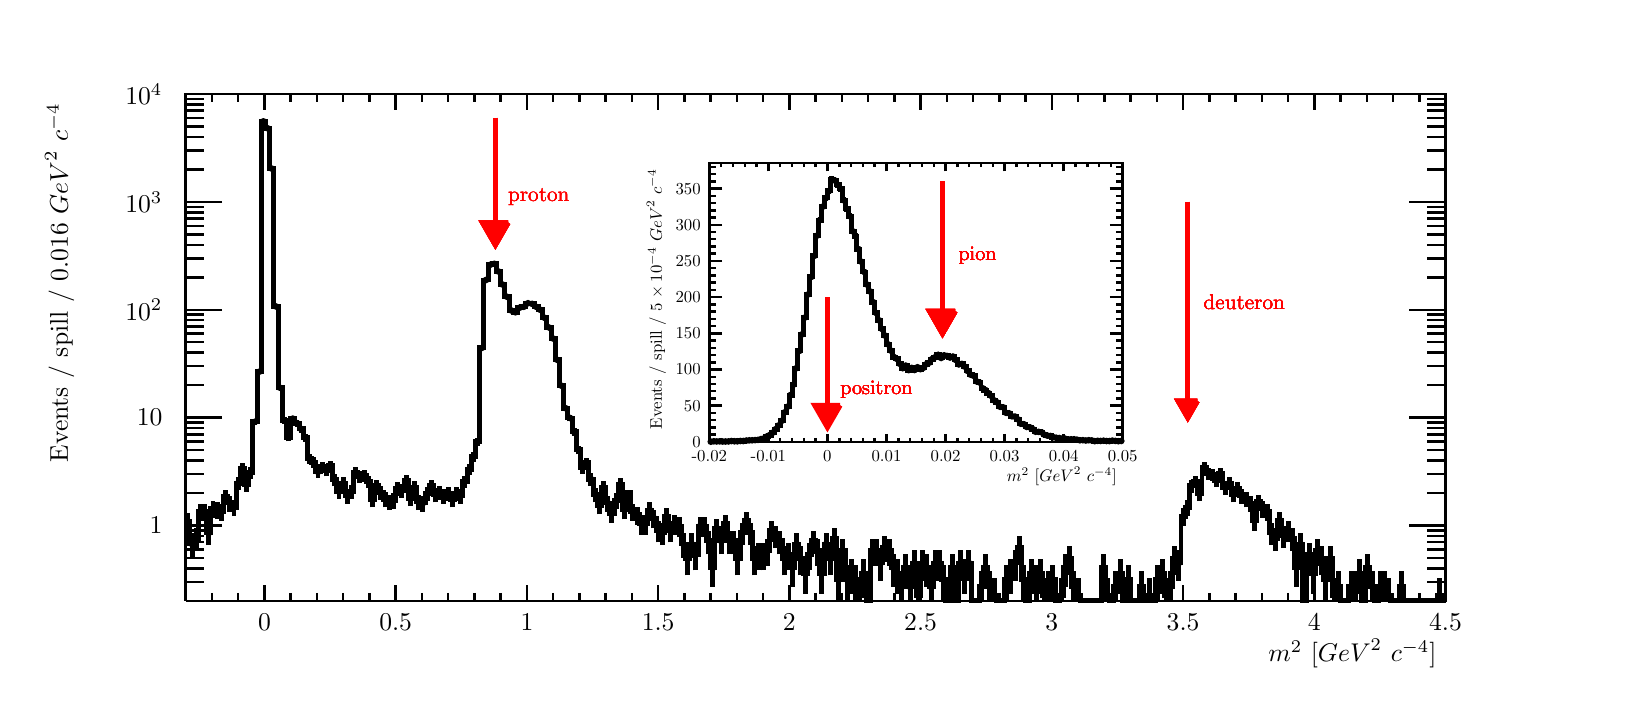
\begin{tikzpicture}
\pgfdeclareplotmark{cross} {
\pgfpathmoveto{\pgfpoint{-0.3\pgfplotmarksize}{\pgfplotmarksize}}
\pgfpathlineto{\pgfpoint{+0.3\pgfplotmarksize}{\pgfplotmarksize}}
\pgfpathlineto{\pgfpoint{+0.3\pgfplotmarksize}{0.3\pgfplotmarksize}}
\pgfpathlineto{\pgfpoint{+1\pgfplotmarksize}{0.3\pgfplotmarksize}}
\pgfpathlineto{\pgfpoint{+1\pgfplotmarksize}{-0.3\pgfplotmarksize}}
\pgfpathlineto{\pgfpoint{+0.3\pgfplotmarksize}{-0.3\pgfplotmarksize}}
\pgfpathlineto{\pgfpoint{+0.3\pgfplotmarksize}{-1.\pgfplotmarksize}}
\pgfpathlineto{\pgfpoint{-0.3\pgfplotmarksize}{-1.\pgfplotmarksize}}
\pgfpathlineto{\pgfpoint{-0.3\pgfplotmarksize}{-0.3\pgfplotmarksize}}
\pgfpathlineto{\pgfpoint{-1.\pgfplotmarksize}{-0.3\pgfplotmarksize}}
\pgfpathlineto{\pgfpoint{-1.\pgfplotmarksize}{0.3\pgfplotmarksize}}
\pgfpathlineto{\pgfpoint{-0.3\pgfplotmarksize}{0.3\pgfplotmarksize}}
\pgfpathclose
\pgfusepathqstroke
}
\pgfdeclareplotmark{cross*} {
\pgfpathmoveto{\pgfpoint{-0.3\pgfplotmarksize}{\pgfplotmarksize}}
\pgfpathlineto{\pgfpoint{+0.3\pgfplotmarksize}{\pgfplotmarksize}}
\pgfpathlineto{\pgfpoint{+0.3\pgfplotmarksize}{0.3\pgfplotmarksize}}
\pgfpathlineto{\pgfpoint{+1\pgfplotmarksize}{0.3\pgfplotmarksize}}
\pgfpathlineto{\pgfpoint{+1\pgfplotmarksize}{-0.3\pgfplotmarksize}}
\pgfpathlineto{\pgfpoint{+0.3\pgfplotmarksize}{-0.3\pgfplotmarksize}}
\pgfpathlineto{\pgfpoint{+0.3\pgfplotmarksize}{-1.\pgfplotmarksize}}
\pgfpathlineto{\pgfpoint{-0.3\pgfplotmarksize}{-1.\pgfplotmarksize}}
\pgfpathlineto{\pgfpoint{-0.3\pgfplotmarksize}{-0.3\pgfplotmarksize}}
\pgfpathlineto{\pgfpoint{-1.\pgfplotmarksize}{-0.3\pgfplotmarksize}}
\pgfpathlineto{\pgfpoint{-1.\pgfplotmarksize}{0.3\pgfplotmarksize}}
\pgfpathlineto{\pgfpoint{-0.3\pgfplotmarksize}{0.3\pgfplotmarksize}}
\pgfpathclose
\pgfusepathqfillstroke
}
\pgfdeclareplotmark{newstar} {
\pgfpathmoveto{\pgfqpoint{0pt}{\pgfplotmarksize}}
\pgfpathlineto{\pgfqpointpolar{44}{0.5\pgfplotmarksize}}
\pgfpathlineto{\pgfqpointpolar{18}{\pgfplotmarksize}}
\pgfpathlineto{\pgfqpointpolar{-20}{0.5\pgfplotmarksize}}
\pgfpathlineto{\pgfqpointpolar{-54}{\pgfplotmarksize}}
\pgfpathlineto{\pgfqpointpolar{-90}{0.5\pgfplotmarksize}}
\pgfpathlineto{\pgfqpointpolar{234}{\pgfplotmarksize}}
\pgfpathlineto{\pgfqpointpolar{198}{0.5\pgfplotmarksize}}
\pgfpathlineto{\pgfqpointpolar{162}{\pgfplotmarksize}}
\pgfpathlineto{\pgfqpointpolar{134}{0.5\pgfplotmarksize}}
\pgfpathclose
\pgfusepathqstroke
}
\pgfdeclareplotmark{newstar*} {
\pgfpathmoveto{\pgfqpoint{0pt}{\pgfplotmarksize}}
\pgfpathlineto{\pgfqpointpolar{44}{0.5\pgfplotmarksize}}
\pgfpathlineto{\pgfqpointpolar{18}{\pgfplotmarksize}}
\pgfpathlineto{\pgfqpointpolar{-20}{0.5\pgfplotmarksize}}
\pgfpathlineto{\pgfqpointpolar{-54}{\pgfplotmarksize}}
\pgfpathlineto{\pgfqpointpolar{-90}{0.5\pgfplotmarksize}}
\pgfpathlineto{\pgfqpointpolar{234}{\pgfplotmarksize}}
\pgfpathlineto{\pgfqpointpolar{198}{0.5\pgfplotmarksize}}
\pgfpathlineto{\pgfqpointpolar{162}{\pgfplotmarksize}}
\pgfpathlineto{\pgfqpointpolar{134}{0.5\pgfplotmarksize}}
\pgfpathclose
\pgfusepathqfillstroke
}
\definecolor{c}{rgb}{1,1,1};
\draw [color=c, fill=c] (0,0) rectangle (20,8.35902);
\draw [color=c, fill=c] (2,1.08667) rectangle (18,7.52312);
\definecolor{c}{rgb}{0,0,0};
\draw [c,line width=0.9] (2,1.08667) -- (2,7.52312) -- (18,7.52312) -- (18,1.08667) -- (2,1.08667);
\definecolor{c}{rgb}{1,1,1};
\draw [color=c, fill=c] (2,1.08667) rectangle (18,7.52312);
\definecolor{c}{rgb}{0,0,0};
\draw [c,line width=0.9] (2,1.08667) -- (2,7.52312) -- (18,7.52312) -- (18,1.08667) -- (2,1.08667);
\draw [c,line width=1.8] (2.02667,1.95243) -- (2.02667,2.08824);
\draw [c,line width=1.8] (2.02667,2.08824) -- (2.02667,2.19874);
\foreach \P in {(2.02667,2.08824)}{\draw[mark options={color=c,fill=c},mark size=2.402402pt,mark=*,mark size=1pt] plot coordinates {\P};}
\draw [c,line width=1.8] (2.08,1.63097) -- (2.08,1.80865);
\draw [c,line width=1.8] (2.08,1.80865) -- (2.08,1.94528);
\foreach \P in {(2.08,1.80865)}{\draw[mark options={color=c,fill=c},mark size=2.402402pt,mark=*,mark size=1pt] plot coordinates {\P};}
\draw [c,line width=1.8] (2.13333,1.71786) -- (2.13333,1.88311);
\draw [c,line width=1.8] (2.13333,1.88311) -- (2.13333,2.01229);
\foreach \P in {(2.13333,1.88311)}{\draw[mark options={color=c,fill=c},mark size=2.402402pt,mark=*,mark size=1pt] plot coordinates {\P};}
\draw [c,line width=1.8] (2.18667,2.10106) -- (2.18667,2.22099);
\draw [c,line width=1.8] (2.18667,2.22099) -- (2.18667,2.32074);
\foreach \P in {(2.18667,2.22099)}{\draw[mark options={color=c,fill=c},mark size=2.402402pt,mark=*,mark size=1pt] plot coordinates {\P};}
\draw [c,line width=1.8] (2.24,2.10106) -- (2.24,2.22099);
\draw [c,line width=1.8] (2.24,2.22099) -- (2.24,2.32074);
\foreach \P in {(2.24,2.22099)}{\draw[mark options={color=c,fill=c},mark size=2.402402pt,mark=*,mark size=1pt] plot coordinates {\P};}
\draw [c,line width=1.8] (2.29333,1.79424) -- (2.29333,1.94927);
\draw [c,line width=1.8] (2.29333,1.94927) -- (2.29333,2.07214);
\foreach \P in {(2.29333,1.94927)}{\draw[mark options={color=c,fill=c},mark size=2.402402pt,mark=*,mark size=1pt] plot coordinates {\P};}
\draw [c,line width=1.8] (2.34667,2.14366) -- (2.34667,2.25938);
\draw [c,line width=1.8] (2.34667,2.25938) -- (2.34667,2.35621);
\foreach \P in {(2.34667,2.25938)}{\draw[mark options={color=c,fill=c},mark size=2.402402pt,mark=*,mark size=1pt] plot coordinates {\P};}
\draw [c,line width=1.8] (2.4,2.12272) -- (2.4,2.24049);
\draw [c,line width=1.8] (2.4,2.24049) -- (2.4,2.33875);
\foreach \P in {(2.4,2.24049)}{\draw[mark options={color=c,fill=c},mark size=2.402402pt,mark=*,mark size=1pt] plot coordinates {\P};}
\draw [c,line width=1.8] (2.45333,2.10106) -- (2.45333,2.22099);
\draw [c,line width=1.8] (2.45333,2.22099) -- (2.45333,2.32074);
\foreach \P in {(2.45333,2.22099)}{\draw[mark options={color=c,fill=c},mark size=2.402402pt,mark=*,mark size=1pt] plot coordinates {\P};}
\draw [c,line width=1.8] (2.50667,2.3058) -- (2.50667,2.40681);
\draw [c,line width=1.8] (2.50667,2.40681) -- (2.50667,2.49314);
\foreach \P in {(2.50667,2.40681)}{\draw[mark options={color=c,fill=c},mark size=2.402402pt,mark=*,mark size=1pt] plot coordinates {\P};}
\draw [c,line width=1.8] (2.56,2.22099) -- (2.56,2.32945);
\draw [c,line width=1.8] (2.56,2.32945) -- (2.56,2.42115);
\foreach \P in {(2.56,2.32945)}{\draw[mark options={color=c,fill=c},mark size=2.402402pt,mark=*,mark size=1pt] plot coordinates {\P};}
\draw [c,line width=1.8] (2.61333,2.16391) -- (2.61333,2.27768);
\draw [c,line width=1.8] (2.61333,2.27768) -- (2.61333,2.37315);
\foreach \P in {(2.61333,2.27768)}{\draw[mark options={color=c,fill=c},mark size=2.402402pt,mark=*,mark size=1pt] plot coordinates {\P};}
\draw [c,line width=1.8] (2.66667,2.4954) -- (2.66667,2.58156);
\draw [c,line width=1.8] (2.66667,2.58156) -- (2.66667,2.65681);
\foreach \P in {(2.66667,2.58156)}{\draw[mark options={color=c,fill=c},mark size=2.402402pt,mark=*,mark size=1pt] plot coordinates {\P};}
\draw [c,line width=1.8] (2.72,2.70147) -- (2.72,2.77395);
\draw [c,line width=1.8] (2.72,2.77395) -- (2.72,2.83855);
\foreach \P in {(2.72,2.77395)}{\draw[mark options={color=c,fill=c},mark size=2.402402pt,mark=*,mark size=1pt] plot coordinates {\P};}
\draw [c,line width=1.8] (2.77333,2.47163) -- (2.77333,2.55953);
\draw [c,line width=1.8] (2.77333,2.55953) -- (2.77333,2.6361);
\foreach \P in {(2.77333,2.55953)}{\draw[mark options={color=c,fill=c},mark size=2.402402pt,mark=*,mark size=1pt] plot coordinates {\P};}
\draw [c,line width=1.8] (2.82667,2.64016) -- (2.82667,2.71647);
\draw [c,line width=1.8] (2.82667,2.71647) -- (2.82667,2.78409);
\foreach \P in {(2.82667,2.71647)}{\draw[mark options={color=c,fill=c},mark size=2.402402pt,mark=*,mark size=1pt] plot coordinates {\P};}
\draw [c,line width=1.8] (2.88,3.31814) -- (2.88,3.36132);
\draw [c,line width=1.8] (2.88,3.36132) -- (2.88,3.40158);
\foreach \P in {(2.88,3.36132)}{\draw[mark options={color=c,fill=c},mark size=2.402402pt,mark=*,mark size=1pt] plot coordinates {\P};}
\draw [c,line width=1.8] (2.93333,3.97116) -- (2.93333,3.9961);
\draw [c,line width=1.8] (2.93333,3.9961) -- (2.93333,4.02004);
\foreach \P in {(2.93333,3.9961)}{\draw[mark options={color=c,fill=c},mark size=2.402402pt,mark=*,mark size=1pt] plot coordinates {\P};}
\draw [c,line width=1.8] (2.98667,7.17425) -- (2.98667,7.17594);
\draw [c,line width=1.8] (2.98667,7.17594) -- (2.98667,7.17762);
\foreach \P in {(2.98667,7.17594)}{\draw[mark options={color=c,fill=c},mark size=2.402402pt,mark=*,mark size=1pt] plot coordinates {\P};}
\draw [c,line width=1.8] (3.04,7.08616) -- (3.04,7.08798);
\draw [c,line width=1.8] (3.04,7.08798) -- (3.04,7.0898);
\foreach \P in {(3.04,7.08798)}{\draw[mark options={color=c,fill=c},mark size=2.402402pt,mark=*,mark size=1pt] plot coordinates {\P};}
\draw [c,line width=1.8] (3.09333,6.57319) -- (3.09333,6.57599);
\draw [c,line width=1.8] (3.09333,6.57599) -- (3.09333,6.57878);
\foreach \P in {(3.09333,6.57599)}{\draw[mark options={color=c,fill=c},mark size=2.402402pt,mark=*,mark size=1pt] plot coordinates {\P};}
\draw [c,line width=1.8] (3.14667,4.81298) -- (3.14667,4.82527);
\draw [c,line width=1.8] (3.14667,4.82527) -- (3.14667,4.83732);
\foreach \P in {(3.14667,4.82527)}{\draw[mark options={color=c,fill=c},mark size=2.402402pt,mark=*,mark size=1pt] plot coordinates {\P};}
\draw [c,line width=1.8] (3.2,3.76259) -- (3.2,3.79232);
\draw [c,line width=1.8] (3.2,3.79232) -- (3.2,3.82063);
\foreach \P in {(3.2,3.79232)}{\draw[mark options={color=c,fill=c},mark size=2.402402pt,mark=*,mark size=1pt] plot coordinates {\P};}
\draw [c,line width=1.8] (3.25333,3.33603) -- (3.25333,3.37857);
\draw [c,line width=1.8] (3.25333,3.37857) -- (3.25333,3.41826);
\foreach \P in {(3.25333,3.37857)}{\draw[mark options={color=c,fill=c},mark size=2.402402pt,mark=*,mark size=1pt] plot coordinates {\P};}
\draw [c,line width=1.8] (3.30667,3.11094) -- (3.30667,3.16233);
\draw [c,line width=1.8] (3.30667,3.16233) -- (3.30667,3.20963);
\foreach \P in {(3.30667,3.16233)}{\draw[mark options={color=c,fill=c},mark size=2.402402pt,mark=*,mark size=1pt] plot coordinates {\P};}
\draw [c,line width=1.8] (3.36,3.35909) -- (3.36,3.40081);
\draw [c,line width=1.8] (3.36,3.40081) -- (3.36,3.43979);
\foreach \P in {(3.36,3.40081)}{\draw[mark options={color=c,fill=c},mark size=2.402402pt,mark=*,mark size=1pt] plot coordinates {\P};}
\draw [c,line width=1.8] (3.41333,3.29971) -- (3.41333,3.34356);
\draw [c,line width=1.8] (3.41333,3.34356) -- (3.41333,3.3844);
\foreach \P in {(3.41333,3.34356)}{\draw[mark options={color=c,fill=c},mark size=2.402402pt,mark=*,mark size=1pt] plot coordinates {\P};}
\draw [c,line width=1.8] (3.46667,3.22335) -- (3.46667,3.27011);
\draw [c,line width=1.8] (3.46667,3.27011) -- (3.46667,3.31346);
\foreach \P in {(3.46667,3.27011)}{\draw[mark options={color=c,fill=c},mark size=2.402402pt,mark=*,mark size=1pt] plot coordinates {\P};}
\draw [c,line width=1.8] (3.52,3.10666) -- (3.52,3.15824);
\draw [c,line width=1.8] (3.52,3.15824) -- (3.52,3.2057);
\foreach \P in {(3.52,3.15824)}{\draw[mark options={color=c,fill=c},mark size=2.402402pt,mark=*,mark size=1pt] plot coordinates {\P};}
\draw [c,line width=1.8] (3.57333,2.82891) -- (3.57333,2.89403);
\draw [c,line width=1.8] (3.57333,2.89403) -- (3.57333,2.95273);
\foreach \P in {(3.57333,2.89403)}{\draw[mark options={color=c,fill=c},mark size=2.402402pt,mark=*,mark size=1pt] plot coordinates {\P};}
\draw [c,line width=1.8] (3.62667,2.77961) -- (3.62667,2.84748);
\draw [c,line width=1.8] (3.62667,2.84748) -- (3.62667,2.9084);
\foreach \P in {(3.62667,2.84748)}{\draw[mark options={color=c,fill=c},mark size=2.402402pt,mark=*,mark size=1pt] plot coordinates {\P};}
\draw [c,line width=1.8] (3.68,2.6493) -- (3.68,2.72503);
\draw [c,line width=1.8] (3.68,2.72503) -- (3.68,2.79219);
\foreach \P in {(3.68,2.72503)}{\draw[mark options={color=c,fill=c},mark size=2.402402pt,mark=*,mark size=1pt] plot coordinates {\P};}
\draw [c,line width=1.8] (3.73333,2.71791) -- (3.73333,2.7894);
\draw [c,line width=1.8] (3.73333,2.7894) -- (3.73333,2.85321);
\foreach \P in {(3.73333,2.7894)}{\draw[mark options={color=c,fill=c},mark size=2.402402pt,mark=*,mark size=1pt] plot coordinates {\P};}
\draw [c,line width=1.8] (3.78667,2.66719) -- (3.78667,2.74178);
\draw [c,line width=1.8] (3.78667,2.74178) -- (3.78667,2.80806);
\foreach \P in {(3.78667,2.74178)}{\draw[mark options={color=c,fill=c},mark size=2.402402pt,mark=*,mark size=1pt] plot coordinates {\P};}
\draw [c,line width=1.8] (3.84,2.73393) -- (3.84,2.80446);
\draw [c,line width=1.8] (3.84,2.80446) -- (3.84,2.86751);
\foreach \P in {(3.84,2.80446)}{\draw[mark options={color=c,fill=c},mark size=2.402402pt,mark=*,mark size=1pt] plot coordinates {\P};}
\draw [c,line width=1.8] (3.89333,2.54035) -- (3.89333,2.62333);
\draw [c,line width=1.8] (3.89333,2.62333) -- (3.89333,2.69613);
\foreach \P in {(3.89333,2.62333)}{\draw[mark options={color=c,fill=c},mark size=2.402402pt,mark=*,mark size=1pt] plot coordinates {\P};}
\draw [c,line width=1.8] (3.94667,2.38037) -- (3.94667,2.47526);
\draw [c,line width=1.8] (3.94667,2.47526) -- (3.94667,2.55708);
\foreach \P in {(3.94667,2.47526)}{\draw[mark options={color=c,fill=c},mark size=2.402402pt,mark=*,mark size=1pt] plot coordinates {\P};}
\draw [c,line width=1.8] (4,2.4954) -- (4,2.58156);
\draw [c,line width=1.8] (4,2.58156) -- (4,2.65681);
\foreach \P in {(4,2.58156)}{\draw[mark options={color=c,fill=c},mark size=2.402402pt,mark=*,mark size=1pt] plot coordinates {\P};}
\draw [c,line width=1.8] (4.05333,2.32145) -- (4.05333,2.42115);
\draw [c,line width=1.8] (4.05333,2.42115) -- (4.05333,2.50651);
\foreach \P in {(4.05333,2.42115)}{\draw[mark options={color=c,fill=c},mark size=2.402402pt,mark=*,mark size=1pt] plot coordinates {\P};}
\draw [c,line width=1.8] (4.10667,2.38037) -- (4.10667,2.47526);
\draw [c,line width=1.8] (4.10667,2.47526) -- (4.10667,2.55708);
\foreach \P in {(4.10667,2.47526)}{\draw[mark options={color=c,fill=c},mark size=2.402402pt,mark=*,mark size=1pt] plot coordinates {\P};}
\draw [c,line width=1.8] (4.16,2.64016) -- (4.16,2.71647);
\draw [c,line width=1.8] (4.16,2.71647) -- (4.16,2.78409);
\foreach \P in {(4.16,2.71647)}{\draw[mark options={color=c,fill=c},mark size=2.402402pt,mark=*,mark size=1pt] plot coordinates {\P};}
\draw [c,line width=1.8] (4.21333,2.58224) -- (4.21333,2.66235);
\draw [c,line width=1.8] (4.21333,2.66235) -- (4.21333,2.73294);
\foreach \P in {(4.21333,2.66235)}{\draw[mark options={color=c,fill=c},mark size=2.402402pt,mark=*,mark size=1pt] plot coordinates {\P};}
\draw [c,line width=1.8] (4.26667,2.60216) -- (4.26667,2.68094);
\draw [c,line width=1.8] (4.26667,2.68094) -- (4.26667,2.7505);
\foreach \P in {(4.26667,2.68094)}{\draw[mark options={color=c,fill=c},mark size=2.402402pt,mark=*,mark size=1pt] plot coordinates {\P};}
\draw [c,line width=1.8] (4.32,2.51829) -- (4.32,2.60281);
\draw [c,line width=1.8] (4.32,2.60281) -- (4.32,2.67681);
\foreach \P in {(4.32,2.60281)}{\draw[mark options={color=c,fill=c},mark size=2.402402pt,mark=*,mark size=1pt] plot coordinates {\P};}
\draw [c,line width=1.8] (4.37333,2.27325) -- (4.37333,2.37706);
\draw [c,line width=1.8] (4.37333,2.37706) -- (4.37333,2.46542);
\foreach \P in {(4.37333,2.37706)}{\draw[mark options={color=c,fill=c},mark size=2.402402pt,mark=*,mark size=1pt] plot coordinates {\P};}
\draw [c,line width=1.8] (4.42667,2.45939) -- (4.42667,2.5482);
\draw [c,line width=1.8] (4.42667,2.5482) -- (4.42667,2.62545);
\foreach \P in {(4.42667,2.5482)}{\draw[mark options={color=c,fill=c},mark size=2.402402pt,mark=*,mark size=1pt] plot coordinates {\P};}
\draw [c,line width=1.8] (4.48,2.36616) -- (4.48,2.46219);
\draw [c,line width=1.8] (4.48,2.46219) -- (4.48,2.54485);
\foreach \P in {(4.48,2.46219)}{\draw[mark options={color=c,fill=c},mark size=2.402402pt,mark=*,mark size=1pt] plot coordinates {\P};}
\draw [c,line width=1.8] (4.53333,2.27325) -- (4.53333,2.37706);
\draw [c,line width=1.8] (4.53333,2.37706) -- (4.53333,2.46542);
\foreach \P in {(4.53333,2.37706)}{\draw[mark options={color=c,fill=c},mark size=2.402402pt,mark=*,mark size=1pt] plot coordinates {\P};}
\draw [c,line width=1.8] (4.58667,2.2389) -- (4.58667,2.34574);
\draw [c,line width=1.8] (4.58667,2.34574) -- (4.58667,2.43629);
\foreach \P in {(4.58667,2.34574)}{\draw[mark options={color=c,fill=c},mark size=2.402402pt,mark=*,mark size=1pt] plot coordinates {\P};}
\draw [c,line width=1.8] (4.64,2.25631) -- (4.64,2.36161);
\draw [c,line width=1.8] (4.64,2.36161) -- (4.64,2.45104);
\foreach \P in {(4.64,2.36161)}{\draw[mark options={color=c,fill=c},mark size=2.402402pt,mark=*,mark size=1pt] plot coordinates {\P};}
\draw [c,line width=1.8] (4.69333,2.42115) -- (4.69333,2.51285);
\draw [c,line width=1.8] (4.69333,2.51285) -- (4.69333,2.59228);
\foreach \P in {(4.69333,2.51285)}{\draw[mark options={color=c,fill=c},mark size=2.402402pt,mark=*,mark size=1pt] plot coordinates {\P};}
\draw [c,line width=1.8] (4.74667,2.39426) -- (4.74667,2.48806);
\draw [c,line width=1.8] (4.74667,2.48806) -- (4.74667,2.56906);
\foreach \P in {(4.74667,2.48806)}{\draw[mark options={color=c,fill=c},mark size=2.402402pt,mark=*,mark size=1pt] plot coordinates {\P};}
\draw [c,line width=1.8] (4.8,2.52942) -- (4.8,2.61316);
\draw [c,line width=1.8] (4.8,2.61316) -- (4.8,2.68655);
\foreach \P in {(4.8,2.61316)}{\draw[mark options={color=c,fill=c},mark size=2.402402pt,mark=*,mark size=1pt] plot coordinates {\P};}
\draw [c,line width=1.8] (4.85333,2.28974) -- (4.85333,2.39212);
\draw [c,line width=1.8] (4.85333,2.39212) -- (4.85333,2.47945);
\foreach \P in {(4.85333,2.39212)}{\draw[mark options={color=c,fill=c},mark size=2.402402pt,mark=*,mark size=1pt] plot coordinates {\P};}
\draw [c,line width=1.8] (4.90667,2.43416) -- (4.90667,2.52487);
\draw [c,line width=1.8] (4.90667,2.52487) -- (4.90667,2.60355);
\foreach \P in {(4.90667,2.52487)}{\draw[mark options={color=c,fill=c},mark size=2.402402pt,mark=*,mark size=1pt] plot coordinates {\P};}
\draw [c,line width=1.8] (4.96,2.2389) -- (4.96,2.34574);
\draw [c,line width=1.8] (4.96,2.34574) -- (4.96,2.43629);
\foreach \P in {(4.96,2.34574)}{\draw[mark options={color=c,fill=c},mark size=2.402402pt,mark=*,mark size=1pt] plot coordinates {\P};}
\draw [c,line width=1.8] (5.01333,2.22099) -- (5.01333,2.32945);
\draw [c,line width=1.8] (5.01333,2.32945) -- (5.01333,2.42115);
\foreach \P in {(5.01333,2.32945)}{\draw[mark options={color=c,fill=c},mark size=2.402402pt,mark=*,mark size=1pt] plot coordinates {\P};}
\draw [c,line width=1.8] (5.06667,2.35161) -- (5.06667,2.44882);
\draw [c,line width=1.8] (5.06667,2.44882) -- (5.06667,2.53235);
\foreach \P in {(5.06667,2.44882)}{\draw[mark options={color=c,fill=c},mark size=2.402402pt,mark=*,mark size=1pt] plot coordinates {\P};}
\draw [c,line width=1.8] (5.12,2.45939) -- (5.12,2.5482);
\draw [c,line width=1.8] (5.12,2.5482) -- (5.12,2.62545);
\foreach \P in {(5.12,2.5482)}{\draw[mark options={color=c,fill=c},mark size=2.402402pt,mark=*,mark size=1pt] plot coordinates {\P};}
\draw [c,line width=1.8] (5.17333,2.33671) -- (5.17333,2.43514);
\draw [c,line width=1.8] (5.17333,2.43514) -- (5.17333,2.51958);
\foreach \P in {(5.17333,2.43514)}{\draw[mark options={color=c,fill=c},mark size=2.402402pt,mark=*,mark size=1pt] plot coordinates {\P};}
\draw [c,line width=1.8] (5.22667,2.36616) -- (5.22667,2.46219);
\draw [c,line width=1.8] (5.22667,2.46219) -- (5.22667,2.54485);
\foreach \P in {(5.22667,2.46219)}{\draw[mark options={color=c,fill=c},mark size=2.402402pt,mark=*,mark size=1pt] plot coordinates {\P};}
\draw [c,line width=1.8] (5.28,2.32145) -- (5.28,2.42115);
\draw [c,line width=1.8] (5.28,2.42115) -- (5.28,2.50651);
\foreach \P in {(5.28,2.42115)}{\draw[mark options={color=c,fill=c},mark size=2.402402pt,mark=*,mark size=1pt] plot coordinates {\P};}
\draw [c,line width=1.8] (5.33333,2.35161) -- (5.33333,2.44882);
\draw [c,line width=1.8] (5.33333,2.44882) -- (5.33333,2.53235);
\foreach \P in {(5.33333,2.44882)}{\draw[mark options={color=c,fill=c},mark size=2.402402pt,mark=*,mark size=1pt] plot coordinates {\P};}
\draw [c,line width=1.8] (5.38667,2.27325) -- (5.38667,2.37706);
\draw [c,line width=1.8] (5.38667,2.37706) -- (5.38667,2.46542);
\foreach \P in {(5.38667,2.37706)}{\draw[mark options={color=c,fill=c},mark size=2.402402pt,mark=*,mark size=1pt] plot coordinates {\P};}
\draw [c,line width=1.8] (5.44,2.35161) -- (5.44,2.44882);
\draw [c,line width=1.8] (5.44,2.44882) -- (5.44,2.53235);
\foreach \P in {(5.44,2.44882)}{\draw[mark options={color=c,fill=c},mark size=2.402402pt,mark=*,mark size=1pt] plot coordinates {\P};}
\draw [c,line width=1.8] (5.49333,2.32145) -- (5.49333,2.42115);
\draw [c,line width=1.8] (5.49333,2.42115) -- (5.49333,2.50651);
\foreach \P in {(5.49333,2.42115)}{\draw[mark options={color=c,fill=c},mark size=2.402402pt,mark=*,mark size=1pt] plot coordinates {\P};}
\draw [c,line width=1.8] (5.54667,2.51829) -- (5.54667,2.60281);
\draw [c,line width=1.8] (5.54667,2.60281) -- (5.54667,2.67681);
\foreach \P in {(5.54667,2.60281)}{\draw[mark options={color=c,fill=c},mark size=2.402402pt,mark=*,mark size=1pt] plot coordinates {\P};}
\draw [c,line width=1.8] (5.6,2.68457) -- (5.6,2.75808);
\draw [c,line width=1.8] (5.6,2.75808) -- (5.6,2.8235);
\foreach \P in {(5.6,2.75808)}{\draw[mark options={color=c,fill=c},mark size=2.402402pt,mark=*,mark size=1pt] plot coordinates {\P};}
\draw [c,line width=1.8] (5.65333,2.85539) -- (5.65333,2.91908);
\draw [c,line width=1.8] (5.65333,2.91908) -- (5.65333,2.97661);
\foreach \P in {(5.65333,2.91908)}{\draw[mark options={color=c,fill=c},mark size=2.402402pt,mark=*,mark size=1pt] plot coordinates {\P};}
\draw [c,line width=1.8] (5.70667,3.05756) -- (5.70667,3.11131);
\draw [c,line width=1.8] (5.70667,3.11131) -- (5.70667,3.1606);
\foreach \P in {(5.70667,3.11131)}{\draw[mark options={color=c,fill=c},mark size=2.402402pt,mark=*,mark size=1pt] plot coordinates {\P};}
\draw [c,line width=1.8] (5.76,4.27932) -- (5.76,4.29857);
\draw [c,line width=1.8] (5.76,4.29857) -- (5.76,4.31722);
\foreach \P in {(5.76,4.29857)}{\draw[mark options={color=c,fill=c},mark size=2.402402pt,mark=*,mark size=1pt] plot coordinates {\P};}
\draw [c,line width=1.8] (5.81333,5.15212) -- (5.81333,5.16137);
\draw [c,line width=1.8] (5.81333,5.16137) -- (5.81333,5.17047);
\foreach \P in {(5.81333,5.16137)}{\draw[mark options={color=c,fill=c},mark size=2.402402pt,mark=*,mark size=1pt] plot coordinates {\P};}
\draw [c,line width=1.8] (5.86667,5.34635) -- (5.86667,5.35421);
\draw [c,line width=1.8] (5.86667,5.35421) -- (5.86667,5.36196);
\foreach \P in {(5.86667,5.35421)}{\draw[mark options={color=c,fill=c},mark size=2.402402pt,mark=*,mark size=1pt] plot coordinates {\P};}
\draw [c,line width=1.8] (5.92,5.35889) -- (5.92,5.36666);
\draw [c,line width=1.8] (5.92,5.36666) -- (5.92,5.37433);
\foreach \P in {(5.92,5.36666)}{\draw[mark options={color=c,fill=c},mark size=2.402402pt,mark=*,mark size=1pt] plot coordinates {\P};}
\draw [c,line width=1.8] (5.97333,5.26044) -- (5.97333,5.26888);
\draw [c,line width=1.8] (5.97333,5.26888) -- (5.97333,5.27721);
\foreach \P in {(5.97333,5.26888)}{\draw[mark options={color=c,fill=c},mark size=2.402402pt,mark=*,mark size=1pt] plot coordinates {\P};}
\draw [c,line width=1.8] (6.02667,5.09297) -- (6.02667,5.10269);
\draw [c,line width=1.8] (6.02667,5.10269) -- (6.02667,5.11225);
\foreach \P in {(6.02667,5.10269)}{\draw[mark options={color=c,fill=c},mark size=2.402402pt,mark=*,mark size=1pt] plot coordinates {\P};}
\draw [c,line width=1.8] (6.08,4.9372) -- (6.08,4.94828);
\draw [c,line width=1.8] (6.08,4.94828) -- (6.08,4.95915);
\foreach \P in {(6.08,4.94828)}{\draw[mark options={color=c,fill=c},mark size=2.402402pt,mark=*,mark size=1pt] plot coordinates {\P};}
\draw [c,line width=1.8] (6.13333,4.76236) -- (6.13333,4.77518);
\draw [c,line width=1.8] (6.13333,4.77518) -- (6.13333,4.78774);
\foreach \P in {(6.13333,4.77518)}{\draw[mark options={color=c,fill=c},mark size=2.402402pt,mark=*,mark size=1pt] plot coordinates {\P};}
\draw [c,line width=1.8] (6.18667,4.73862) -- (6.18667,4.75171);
\draw [c,line width=1.8] (6.18667,4.75171) -- (6.18667,4.76452);
\foreach \P in {(6.18667,4.75171)}{\draw[mark options={color=c,fill=c},mark size=2.402402pt,mark=*,mark size=1pt] plot coordinates {\P};}
\draw [c,line width=1.8] (6.24,4.79666) -- (6.24,4.80913);
\draw [c,line width=1.8] (6.24,4.80913) -- (6.24,4.82133);
\foreach \P in {(6.24,4.80913)}{\draw[mark options={color=c,fill=c},mark size=2.402402pt,mark=*,mark size=1pt] plot coordinates {\P};}
\draw [c,line width=1.8] (6.29333,4.80894) -- (6.29333,4.82128);
\draw [c,line width=1.8] (6.29333,4.82128) -- (6.29333,4.83336);
\foreach \P in {(6.29333,4.82128)}{\draw[mark options={color=c,fill=c},mark size=2.402402pt,mark=*,mark size=1pt] plot coordinates {\P};}
\draw [c,line width=1.8] (6.34667,4.85474) -- (6.34667,4.86661);
\draw [c,line width=1.8] (6.34667,4.86661) -- (6.34667,4.87825);
\foreach \P in {(6.34667,4.86661)}{\draw[mark options={color=c,fill=c},mark size=2.402402pt,mark=*,mark size=1pt] plot coordinates {\P};}
\draw [c,line width=1.8] (6.4,4.84624) -- (6.4,4.8582);
\draw [c,line width=1.8] (6.4,4.8582) -- (6.4,4.86992);
\foreach \P in {(6.4,4.8582)}{\draw[mark options={color=c,fill=c},mark size=2.402402pt,mark=*,mark size=1pt] plot coordinates {\P};}
\draw [c,line width=1.8] (6.45333,4.80793) -- (6.45333,4.82027);
\draw [c,line width=1.8] (6.45333,4.82027) -- (6.45333,4.83237);
\foreach \P in {(6.45333,4.82027)}{\draw[mark options={color=c,fill=c},mark size=2.402402pt,mark=*,mark size=1pt] plot coordinates {\P};}
\draw [c,line width=1.8] (6.50667,4.76889) -- (6.50667,4.78165);
\draw [c,line width=1.8] (6.50667,4.78165) -- (6.50667,4.79414);
\foreach \P in {(6.50667,4.78165)}{\draw[mark options={color=c,fill=c},mark size=2.402402pt,mark=*,mark size=1pt] plot coordinates {\P};}
\draw [c,line width=1.8] (6.56,4.66604) -- (6.56,4.67995);
\draw [c,line width=1.8] (6.56,4.67995) -- (6.56,4.69355);
\foreach \P in {(6.56,4.67995)}{\draw[mark options={color=c,fill=c},mark size=2.402402pt,mark=*,mark size=1pt] plot coordinates {\P};}
\draw [c,line width=1.8] (6.61333,4.54296) -- (6.61333,4.55838);
\draw [c,line width=1.8] (6.61333,4.55838) -- (6.61333,4.57342);
\foreach \P in {(6.61333,4.55838)}{\draw[mark options={color=c,fill=c},mark size=2.402402pt,mark=*,mark size=1pt] plot coordinates {\P};}
\draw [c,line width=1.8] (6.66667,4.4005) -- (6.66667,4.41789);
\draw [c,line width=1.8] (6.66667,4.41789) -- (6.66667,4.43479);
\foreach \P in {(6.66667,4.41789)}{\draw[mark options={color=c,fill=c},mark size=2.402402pt,mark=*,mark size=1pt] plot coordinates {\P};}
\draw [c,line width=1.8] (6.72,4.12491) -- (6.72,4.14683);
\draw [c,line width=1.8] (6.72,4.14683) -- (6.72,4.16797);
\foreach \P in {(6.72,4.14683)}{\draw[mark options={color=c,fill=c},mark size=2.402402pt,mark=*,mark size=1pt] plot coordinates {\P};}
\draw [c,line width=1.8] (6.77333,3.78952) -- (6.77333,3.81858);
\draw [c,line width=1.8] (6.77333,3.81858) -- (6.77333,3.84628);
\foreach \P in {(6.77333,3.81858)}{\draw[mark options={color=c,fill=c},mark size=2.402402pt,mark=*,mark size=1pt] plot coordinates {\P};}
\draw [c,line width=1.8] (6.82667,3.49525) -- (6.82667,3.53246);
\draw [c,line width=1.8] (6.82667,3.53246) -- (6.82667,3.56748);
\foreach \P in {(6.82667,3.53246)}{\draw[mark options={color=c,fill=c},mark size=2.402402pt,mark=*,mark size=1pt] plot coordinates {\P};}
\draw [c,line width=1.8] (6.88,3.36751) -- (6.88,3.40894);
\draw [c,line width=1.8] (6.88,3.40894) -- (6.88,3.44766);
\foreach \P in {(6.88,3.40894)}{\draw[mark options={color=c,fill=c},mark size=2.402402pt,mark=*,mark size=1pt] plot coordinates {\P};}
\draw [c,line width=1.8] (6.93333,3.18312) -- (6.93333,3.23149);
\draw [c,line width=1.8] (6.93333,3.23149) -- (6.93333,3.27621);
\foreach \P in {(6.93333,3.23149)}{\draw[mark options={color=c,fill=c},mark size=2.402402pt,mark=*,mark size=1pt] plot coordinates {\P};}
\draw [c,line width=1.8] (6.98667,2.94557) -- (6.98667,3.00462);
\draw [c,line width=1.8] (6.98667,3.00462) -- (6.98667,3.05833);
\foreach \P in {(6.98667,3.00462)}{\draw[mark options={color=c,fill=c},mark size=2.402402pt,mark=*,mark size=1pt] plot coordinates {\P};}
\draw [c,line width=1.8] (7.04,2.70147) -- (7.04,2.77395);
\draw [c,line width=1.8] (7.04,2.77395) -- (7.04,2.83855);
\foreach \P in {(7.04,2.77395)}{\draw[mark options={color=c,fill=c},mark size=2.402402pt,mark=*,mark size=1pt] plot coordinates {\P};}
\draw [c,line width=1.8] (7.09333,2.77223) -- (7.09333,2.84052);
\draw [c,line width=1.8] (7.09333,2.84052) -- (7.09333,2.90178);
\foreach \P in {(7.09333,2.84052)}{\draw[mark options={color=c,fill=c},mark size=2.402402pt,mark=*,mark size=1pt] plot coordinates {\P};}
\draw [c,line width=1.8] (7.14667,2.5511) -- (7.14667,2.63332);
\draw [c,line width=1.8] (7.14667,2.63332) -- (7.14667,2.70555);
\foreach \P in {(7.14667,2.63332)}{\draw[mark options={color=c,fill=c},mark size=2.402402pt,mark=*,mark size=1pt] plot coordinates {\P};}
\draw [c,line width=1.8] (7.2,2.33671) -- (7.2,2.43514);
\draw [c,line width=1.8] (7.2,2.43514) -- (7.2,2.51958);
\foreach \P in {(7.2,2.43514)}{\draw[mark options={color=c,fill=c},mark size=2.402402pt,mark=*,mark size=1pt] plot coordinates {\P};}
\draw [c,line width=1.8] (7.25333,2.18352) -- (7.25333,2.29544);
\draw [c,line width=1.8] (7.25333,2.29544) -- (7.25333,2.3896);
\foreach \P in {(7.25333,2.29544)}{\draw[mark options={color=c,fill=c},mark size=2.402402pt,mark=*,mark size=1pt] plot coordinates {\P};}
\draw [c,line width=1.8] (7.30667,2.43416) -- (7.30667,2.52487);
\draw [c,line width=1.8] (7.30667,2.52487) -- (7.30667,2.60355);
\foreach \P in {(7.30667,2.52487)}{\draw[mark options={color=c,fill=c},mark size=2.402402pt,mark=*,mark size=1pt] plot coordinates {\P};}
\draw [c,line width=1.8] (7.36,2.22099) -- (7.36,2.32945);
\draw [c,line width=1.8] (7.36,2.32945) -- (7.36,2.42115);
\foreach \P in {(7.36,2.32945)}{\draw[mark options={color=c,fill=c},mark size=2.402402pt,mark=*,mark size=1pt] plot coordinates {\P};}
\draw [c,line width=1.8] (7.41333,2.07862) -- (7.41333,2.20082);
\draw [c,line width=1.8] (7.41333,2.20082) -- (7.41333,2.30214);
\foreach \P in {(7.41333,2.20082)}{\draw[mark options={color=c,fill=c},mark size=2.402402pt,mark=*,mark size=1pt] plot coordinates {\P};}
\draw [c,line width=1.8] (7.46667,2.25631) -- (7.46667,2.36161);
\draw [c,line width=1.8] (7.46667,2.36161) -- (7.46667,2.45104);
\foreach \P in {(7.46667,2.36161)}{\draw[mark options={color=c,fill=c},mark size=2.402402pt,mark=*,mark size=1pt] plot coordinates {\P};}
\draw [c,line width=1.8] (7.52,2.48363) -- (7.52,2.57065);
\draw [c,line width=1.8] (7.52,2.57065) -- (7.52,2.64655);
\foreach \P in {(7.52,2.57065)}{\draw[mark options={color=c,fill=c},mark size=2.402402pt,mark=*,mark size=1pt] plot coordinates {\P};}
\draw [c,line width=1.8] (7.57333,2.12272) -- (7.57333,2.24049);
\draw [c,line width=1.8] (7.57333,2.24049) -- (7.57333,2.33875);
\foreach \P in {(7.57333,2.24049)}{\draw[mark options={color=c,fill=c},mark size=2.402402pt,mark=*,mark size=1pt] plot coordinates {\P};}
\draw [c,line width=1.8] (7.62667,2.36616) -- (7.62667,2.46219);
\draw [c,line width=1.8] (7.62667,2.46219) -- (7.62667,2.54485);
\foreach \P in {(7.62667,2.46219)}{\draw[mark options={color=c,fill=c},mark size=2.402402pt,mark=*,mark size=1pt] plot coordinates {\P};}
\draw [c,line width=1.8] (7.68,2.10106) -- (7.68,2.22099);
\draw [c,line width=1.8] (7.68,2.22099) -- (7.68,2.32074);
\foreach \P in {(7.68,2.22099)}{\draw[mark options={color=c,fill=c},mark size=2.402402pt,mark=*,mark size=1pt] plot coordinates {\P};}
\draw [c,line width=1.8] (7.73333,2.05534) -- (7.73333,2.17994);
\draw [c,line width=1.8] (7.73333,2.17994) -- (7.73333,2.28292);
\foreach \P in {(7.73333,2.17994)}{\draw[mark options={color=c,fill=c},mark size=2.402402pt,mark=*,mark size=1pt] plot coordinates {\P};}
\draw [c,line width=1.8] (7.78667,1.92382) -- (7.78667,2.06293);
\draw [c,line width=1.8] (7.78667,2.06293) -- (7.78667,2.17559);
\foreach \P in {(7.78667,2.06293)}{\draw[mark options={color=c,fill=c},mark size=2.402402pt,mark=*,mark size=1pt] plot coordinates {\P};}
\draw [c,line width=1.8] (7.84,1.92382) -- (7.84,2.06293);
\draw [c,line width=1.8] (7.84,2.06293) -- (7.84,2.17559);
\foreach \P in {(7.84,2.06293)}{\draw[mark options={color=c,fill=c},mark size=2.402402pt,mark=*,mark size=1pt] plot coordinates {\P};}
\draw [c,line width=1.8] (7.89333,2.12272) -- (7.89333,2.24049);
\draw [c,line width=1.8] (7.89333,2.24049) -- (7.89333,2.33875);
\foreach \P in {(7.89333,2.24049)}{\draw[mark options={color=c,fill=c},mark size=2.402402pt,mark=*,mark size=1pt] plot coordinates {\P};}
\draw [c,line width=1.8] (7.94667,2.006) -- (7.94667,2.13586);
\draw [c,line width=1.8] (7.94667,2.13586) -- (7.94667,2.24239);
\foreach \P in {(7.94667,2.13586)}{\draw[mark options={color=c,fill=c},mark size=2.402402pt,mark=*,mark size=1pt] plot coordinates {\P};}
\draw [c,line width=1.8] (8,1.82922) -- (8,1.97978);
\draw [c,line width=1.8] (8,1.97978) -- (8,2.09983);
\foreach \P in {(8,1.97978)}{\draw[mark options={color=c,fill=c},mark size=2.402402pt,mark=*,mark size=1pt] plot coordinates {\P};}
\draw [c,line width=1.8] (8.05333,1.79424) -- (8.05333,1.94927);
\draw [c,line width=1.8] (8.05333,1.94927) -- (8.05333,2.07214);
\foreach \P in {(8.05333,1.94927)}{\draw[mark options={color=c,fill=c},mark size=2.402402pt,mark=*,mark size=1pt] plot coordinates {\P};}
\draw [c,line width=1.8] (8.10667,2.03115) -- (8.10667,2.15831);
\draw [c,line width=1.8] (8.10667,2.15831) -- (8.10667,2.26301);
\foreach \P in {(8.10667,2.15831)}{\draw[mark options={color=c,fill=c},mark size=2.402402pt,mark=*,mark size=1pt] plot coordinates {\P};}
\draw [c,line width=1.8] (8.16,1.82922) -- (8.16,1.97978);
\draw [c,line width=1.8] (8.16,1.97978) -- (8.16,2.09983);
\foreach \P in {(8.16,1.97978)}{\draw[mark options={color=c,fill=c},mark size=2.402402pt,mark=*,mark size=1pt] plot coordinates {\P};}
\draw [c,line width=1.8] (8.21333,1.92382) -- (8.21333,2.06293);
\draw [c,line width=1.8] (8.21333,2.06293) -- (8.21333,2.17559);
\foreach \P in {(8.21333,2.06293)}{\draw[mark options={color=c,fill=c},mark size=2.402402pt,mark=*,mark size=1pt] plot coordinates {\P};}
\draw [c,line width=1.8] (8.26667,1.89384) -- (8.26667,2.03648);
\draw [c,line width=1.8] (8.26667,2.03648) -- (8.26667,2.15145);
\foreach \P in {(8.26667,2.03648)}{\draw[mark options={color=c,fill=c},mark size=2.402402pt,mark=*,mark size=1pt] plot coordinates {\P};}
\draw [c,line width=1.8] (8.32,1.63097) -- (8.32,1.80865);
\draw [c,line width=1.8] (8.32,1.80865) -- (8.32,1.94528);
\foreach \P in {(8.32,1.80865)}{\draw[mark options={color=c,fill=c},mark size=2.402402pt,mark=*,mark size=1pt] plot coordinates {\P};}
\draw [c,line width=1.8] (8.37333,1.41068) -- (8.37333,1.62414);
\draw [c,line width=1.8] (8.37333,1.62414) -- (8.37333,1.78091);
\foreach \P in {(8.37333,1.62414)}{\draw[mark options={color=c,fill=c},mark size=2.402402pt,mark=*,mark size=1pt] plot coordinates {\P};}
\draw [c,line width=1.8] (8.42667,1.63097) -- (8.42667,1.80865);
\draw [c,line width=1.8] (8.42667,1.80865) -- (8.42667,1.94528);
\foreach \P in {(8.42667,1.80865)}{\draw[mark options={color=c,fill=c},mark size=2.402402pt,mark=*,mark size=1pt] plot coordinates {\P};}
\draw [c,line width=1.8] (8.48,1.47327) -- (8.48,1.67591);
\draw [c,line width=1.8] (8.48,1.67591) -- (8.48,1.82678);
\foreach \P in {(8.48,1.67591)}{\draw[mark options={color=c,fill=c},mark size=2.402402pt,mark=*,mark size=1pt] plot coordinates {\P};}
\draw [c,line width=1.8] (8.53333,1.89384) -- (8.53333,2.03648);
\draw [c,line width=1.8] (8.53333,2.03648) -- (8.53333,2.15145);
\foreach \P in {(8.53333,2.03648)}{\draw[mark options={color=c,fill=c},mark size=2.402402pt,mark=*,mark size=1pt] plot coordinates {\P};}
\draw [c,line width=1.8] (8.58667,1.89384) -- (8.58667,2.03648);
\draw [c,line width=1.8] (8.58667,2.03648) -- (8.58667,2.15145);
\foreach \P in {(8.58667,2.03648)}{\draw[mark options={color=c,fill=c},mark size=2.402402pt,mark=*,mark size=1pt] plot coordinates {\P};}
\draw [c,line width=1.8] (8.64,1.67591) -- (8.64,1.84704);
\draw [c,line width=1.8] (8.64,1.84704) -- (8.64,1.97978);
\foreach \P in {(8.64,1.84704)}{\draw[mark options={color=c,fill=c},mark size=2.402402pt,mark=*,mark size=1pt] plot coordinates {\P};}
\draw [c,line width=1.8] (8.69333,1.26357) -- (8.69333,1.50477);
\draw [c,line width=1.8] (8.69333,1.50477) -- (8.69333,1.67591);
\foreach \P in {(8.69333,1.50477)}{\draw[mark options={color=c,fill=c},mark size=2.402402pt,mark=*,mark size=1pt] plot coordinates {\P};}
\draw [c,line width=1.8] (8.74667,1.86236) -- (8.74667,2.00881);
\draw [c,line width=1.8] (8.74667,2.00881) -- (8.74667,2.12623);
\foreach \P in {(8.74667,2.00881)}{\draw[mark options={color=c,fill=c},mark size=2.402402pt,mark=*,mark size=1pt] plot coordinates {\P};}
\draw [c,line width=1.8] (8.8,1.67591) -- (8.8,1.84704);
\draw [c,line width=1.8] (8.8,1.84704) -- (8.8,1.97978);
\foreach \P in {(8.8,1.84704)}{\draw[mark options={color=c,fill=c},mark size=2.402402pt,mark=*,mark size=1pt] plot coordinates {\P};}
\draw [c,line width=1.8] (8.85333,1.92382) -- (8.85333,2.06293);
\draw [c,line width=1.8] (8.85333,2.06293) -- (8.85333,2.17559);
\foreach \P in {(8.85333,2.06293)}{\draw[mark options={color=c,fill=c},mark size=2.402402pt,mark=*,mark size=1pt] plot coordinates {\P};}
\draw [c,line width=1.8] (8.90667,1.67591) -- (8.90667,1.84704);
\draw [c,line width=1.8] (8.90667,1.84704) -- (8.90667,1.97978);
\foreach \P in {(8.90667,1.84704)}{\draw[mark options={color=c,fill=c},mark size=2.402402pt,mark=*,mark size=1pt] plot coordinates {\P};}
\draw [c,line width=1.8] (8.96,1.67591) -- (8.96,1.84704);
\draw [c,line width=1.8] (8.96,1.84704) -- (8.96,1.97978);
\foreach \P in {(8.96,1.84704)}{\draw[mark options={color=c,fill=c},mark size=2.402402pt,mark=*,mark size=1pt] plot coordinates {\P};}
\draw [c,line width=1.8] (9.01333,1.41068) -- (9.01333,1.62414);
\draw [c,line width=1.8] (9.01333,1.62414) -- (9.01333,1.78091);
\foreach \P in {(9.01333,1.62414)}{\draw[mark options={color=c,fill=c},mark size=2.402402pt,mark=*,mark size=1pt] plot coordinates {\P};}
\draw [c,line width=1.8] (9.06667,1.79424) -- (9.06667,1.94927);
\draw [c,line width=1.8] (9.06667,1.94927) -- (9.06667,2.07214);
\foreach \P in {(9.06667,1.94927)}{\draw[mark options={color=c,fill=c},mark size=2.402402pt,mark=*,mark size=1pt] plot coordinates {\P};}
\draw [c,line width=1.8] (9.12,1.97978) -- (9.12,2.11253);
\draw [c,line width=1.8] (9.12,2.11253) -- (9.12,2.22099);
\foreach \P in {(9.12,2.11253)}{\draw[mark options={color=c,fill=c},mark size=2.402402pt,mark=*,mark size=1pt] plot coordinates {\P};}
\draw [c,line width=1.8] (9.17333,1.79424) -- (9.17333,1.94927);
\draw [c,line width=1.8] (9.17333,1.94927) -- (9.17333,2.07214);
\foreach \P in {(9.17333,1.94927)}{\draw[mark options={color=c,fill=c},mark size=2.402402pt,mark=*,mark size=1pt] plot coordinates {\P};}
\draw [c,line width=1.8] (9.22667,1.41068) -- (9.22667,1.62414);
\draw [c,line width=1.8] (9.22667,1.62414) -- (9.22667,1.78091);
\foreach \P in {(9.22667,1.62414)}{\draw[mark options={color=c,fill=c},mark size=2.402402pt,mark=*,mark size=1pt] plot coordinates {\P};}
\draw [c,line width=1.8] (9.28,1.47327) -- (9.28,1.67591);
\draw [c,line width=1.8] (9.28,1.67591) -- (9.28,1.82678);
\foreach \P in {(9.28,1.67591)}{\draw[mark options={color=c,fill=c},mark size=2.402402pt,mark=*,mark size=1pt] plot coordinates {\P};}
\draw [c,line width=1.8] (9.33333,1.47327) -- (9.33333,1.67591);
\draw [c,line width=1.8] (9.33333,1.67591) -- (9.33333,1.82678);
\foreach \P in {(9.33333,1.67591)}{\draw[mark options={color=c,fill=c},mark size=2.402402pt,mark=*,mark size=1pt] plot coordinates {\P};}
\draw [c,line width=1.8] (9.38667,1.53029) -- (9.38667,1.72352);
\draw [c,line width=1.8] (9.38667,1.72352) -- (9.38667,1.86914);
\foreach \P in {(9.38667,1.72352)}{\draw[mark options={color=c,fill=c},mark size=2.402402pt,mark=*,mark size=1pt] plot coordinates {\P};}
\draw [c,line width=1.8] (9.44,1.82922) -- (9.44,1.97978);
\draw [c,line width=1.8] (9.44,1.97978) -- (9.44,2.09983);
\foreach \P in {(9.44,1.97978)}{\draw[mark options={color=c,fill=c},mark size=2.402402pt,mark=*,mark size=1pt] plot coordinates {\P};}
\draw [c,line width=1.8] (9.49333,1.75721) -- (9.49333,1.91711);
\draw [c,line width=1.8] (9.49333,1.91711) -- (9.49333,2.04301);
\foreach \P in {(9.49333,1.91711)}{\draw[mark options={color=c,fill=c},mark size=2.402402pt,mark=*,mark size=1pt] plot coordinates {\P};}
\draw [c,line width=1.8] (9.54667,1.67591) -- (9.54667,1.84704);
\draw [c,line width=1.8] (9.54667,1.84704) -- (9.54667,1.97978);
\foreach \P in {(9.54667,1.84704)}{\draw[mark options={color=c,fill=c},mark size=2.402402pt,mark=*,mark size=1pt] plot coordinates {\P};}
\draw [c,line width=1.8] (9.6,1.41068) -- (9.6,1.62414);
\draw [c,line width=1.8] (9.6,1.62414) -- (9.6,1.78091);
\foreach \P in {(9.6,1.62414)}{\draw[mark options={color=c,fill=c},mark size=2.402402pt,mark=*,mark size=1pt] plot coordinates {\P};}
\draw [c,line width=1.8] (9.65333,1.47327) -- (9.65333,1.67591);
\draw [c,line width=1.8] (9.65333,1.67591) -- (9.65333,1.82678);
\foreach \P in {(9.65333,1.67591)}{\draw[mark options={color=c,fill=c},mark size=2.402402pt,mark=*,mark size=1pt] plot coordinates {\P};}
\draw [c,line width=1.8] (9.70667,1.26357) -- (9.70667,1.50477);
\draw [c,line width=1.8] (9.70667,1.50477) -- (9.70667,1.67591);
\foreach \P in {(9.70667,1.50477)}{\draw[mark options={color=c,fill=c},mark size=2.402402pt,mark=*,mark size=1pt] plot coordinates {\P};}
\draw [c,line width=1.8] (9.76,1.63097) -- (9.76,1.80865);
\draw [c,line width=1.8] (9.76,1.80865) -- (9.76,1.94528);
\foreach \P in {(9.76,1.80865)}{\draw[mark options={color=c,fill=c},mark size=2.402402pt,mark=*,mark size=1pt] plot coordinates {\P};}
\draw [c,line width=1.8] (9.81333,1.41068) -- (9.81333,1.62414);
\draw [c,line width=1.8] (9.81333,1.62414) -- (9.81333,1.78091);
\foreach \P in {(9.81333,1.62414)}{\draw[mark options={color=c,fill=c},mark size=2.402402pt,mark=*,mark size=1pt] plot coordinates {\P};}
\draw [c,line width=1.8] (9.86667,1.17518) -- (9.86667,1.4347);
\draw [c,line width=1.8] (9.86667,1.4347) -- (9.86667,1.61479);
\foreach \P in {(9.86667,1.4347)}{\draw[mark options={color=c,fill=c},mark size=2.402402pt,mark=*,mark size=1pt] plot coordinates {\P};}
\draw [c,line width=1.8] (9.92,1.47327) -- (9.92,1.67591);
\draw [c,line width=1.8] (9.92,1.67591) -- (9.92,1.82678);
\foreach \P in {(9.92,1.67591)}{\draw[mark options={color=c,fill=c},mark size=2.402402pt,mark=*,mark size=1pt] plot coordinates {\P};}
\draw [c,line width=1.8] (9.97333,1.67591) -- (9.97333,1.84704);
\draw [c,line width=1.8] (9.97333,1.84704) -- (9.97333,1.97978);
\foreach \P in {(9.97333,1.84704)}{\draw[mark options={color=c,fill=c},mark size=2.402402pt,mark=*,mark size=1pt] plot coordinates {\P};}
\draw [c,line width=1.8] (10.0267,1.53029) -- (10.0267,1.72352);
\draw [c,line width=1.8] (10.0267,1.72352) -- (10.0267,1.86914);
\foreach \P in {(10.0267,1.72352)}{\draw[mark options={color=c,fill=c},mark size=2.402402pt,mark=*,mark size=1pt] plot coordinates {\P};}
\draw [c,line width=1.8] (10.08,1.17518) -- (10.08,1.4347);
\draw [c,line width=1.8] (10.08,1.4347) -- (10.08,1.61479);
\foreach \P in {(10.08,1.4347)}{\draw[mark options={color=c,fill=c},mark size=2.402402pt,mark=*,mark size=1pt] plot coordinates {\P};}
\draw [c,line width=1.8] (10.1333,1.63097) -- (10.1333,1.80865);
\draw [c,line width=1.8] (10.1333,1.80865) -- (10.1333,1.94528);
\foreach \P in {(10.1333,1.80865)}{\draw[mark options={color=c,fill=c},mark size=2.402402pt,mark=*,mark size=1pt] plot coordinates {\P};}
\draw [c,line width=1.8] (10.1867,1.41068) -- (10.1867,1.62414);
\draw [c,line width=1.8] (10.1867,1.62414) -- (10.1867,1.78091);
\foreach \P in {(10.1867,1.62414)}{\draw[mark options={color=c,fill=c},mark size=2.402402pt,mark=*,mark size=1pt] plot coordinates {\P};}
\draw [c,line width=1.8] (10.24,1.71786) -- (10.24,1.88311);
\draw [c,line width=1.8] (10.24,1.88311) -- (10.24,2.01229);
\foreach \P in {(10.24,1.88311)}{\draw[mark options={color=c,fill=c},mark size=2.402402pt,mark=*,mark size=1pt] plot coordinates {\P};}
\draw [c,line width=1.8] (10.2933,1.08667) -- (10.2933,1.35527);
\draw [c,line width=1.8] (10.2933,1.35527) -- (10.2933,1.54599);
\foreach \P in {(10.2933,1.35527)}{\draw[mark options={color=c,fill=c},mark size=2.402402pt,mark=*,mark size=1pt] plot coordinates {\P};}
\draw [c,line width=1.8] (10.3467,1.53029) -- (10.3467,1.72352);
\draw [c,line width=1.8] (10.3467,1.72352) -- (10.3467,1.86914);
\foreach \P in {(10.3467,1.72352)}{\draw[mark options={color=c,fill=c},mark size=2.402402pt,mark=*,mark size=1pt] plot coordinates {\P};}
\draw [c,line width=1.8] (10.4,1.08667) -- (10.4,1.35527);
\draw [c,line width=1.8] (10.4,1.35527) -- (10.4,1.54599);
\foreach \P in {(10.4,1.35527)}{\draw[mark options={color=c,fill=c},mark size=2.402402pt,mark=*,mark size=1pt] plot coordinates {\P};}
\draw [c,line width=1.8] (10.4533,1.17518) -- (10.4533,1.4347);
\draw [c,line width=1.8] (10.4533,1.4347) -- (10.4533,1.61479);
\foreach \P in {(10.4533,1.4347)}{\draw[mark options={color=c,fill=c},mark size=2.402402pt,mark=*,mark size=1pt] plot coordinates {\P};}
\draw [c,line width=1.8] (10.5067,1.08667) -- (10.5067,1.35527);
\draw [c,line width=1.8] (10.5067,1.35527) -- (10.5067,1.54599);
\foreach \P in {(10.5067,1.35527)}{\draw[mark options={color=c,fill=c},mark size=2.402402pt,mark=*,mark size=1pt] plot coordinates {\P};}
\draw [c,line width=1.8] (10.56,1.08667) -- (10.56,1.15511);
\draw [c,line width=1.8] (10.56,1.15511) -- (10.56,1.375);
\foreach \P in {(10.56,1.15511)}{\draw[mark options={color=c,fill=c},mark size=2.402402pt,mark=*,mark size=1pt] plot coordinates {\P};}
\draw [c,line width=1.8] (10.6133,1.17518) -- (10.6133,1.4347);
\draw [c,line width=1.8] (10.6133,1.4347) -- (10.6133,1.61479);
\foreach \P in {(10.6133,1.4347)}{\draw[mark options={color=c,fill=c},mark size=2.402402pt,mark=*,mark size=1pt] plot coordinates {\P};}
\draw [c,line width=1.8] (10.72,1.53029) -- (10.72,1.72352);
\draw [c,line width=1.8] (10.72,1.72352) -- (10.72,1.86914);
\foreach \P in {(10.72,1.72352)}{\draw[mark options={color=c,fill=c},mark size=2.402402pt,mark=*,mark size=1pt] plot coordinates {\P};}
\draw [c,line width=1.8] (10.7733,1.53029) -- (10.7733,1.72352);
\draw [c,line width=1.8] (10.7733,1.72352) -- (10.7733,1.86914);
\foreach \P in {(10.7733,1.72352)}{\draw[mark options={color=c,fill=c},mark size=2.402402pt,mark=*,mark size=1pt] plot coordinates {\P};}
\draw [c,line width=1.8] (10.8267,1.34132) -- (10.8267,1.56745);
\draw [c,line width=1.8] (10.8267,1.56745) -- (10.8267,1.7309);
\foreach \P in {(10.8267,1.56745)}{\draw[mark options={color=c,fill=c},mark size=2.402402pt,mark=*,mark size=1pt] plot coordinates {\P};}
\draw [c,line width=1.8] (10.88,1.58262) -- (10.88,1.76761);
\draw [c,line width=1.8] (10.88,1.76761) -- (10.88,1.90851);
\foreach \P in {(10.88,1.76761)}{\draw[mark options={color=c,fill=c},mark size=2.402402pt,mark=*,mark size=1pt] plot coordinates {\P};}
\draw [c,line width=1.8] (10.9333,1.53029) -- (10.9333,1.72352);
\draw [c,line width=1.8] (10.9333,1.72352) -- (10.9333,1.86914);
\foreach \P in {(10.9333,1.72352)}{\draw[mark options={color=c,fill=c},mark size=2.402402pt,mark=*,mark size=1pt] plot coordinates {\P};}
\draw [c,line width=1.8] (10.9867,1.26357) -- (10.9867,1.50477);
\draw [c,line width=1.8] (10.9867,1.50477) -- (10.9867,1.67591);
\foreach \P in {(10.9867,1.50477)}{\draw[mark options={color=c,fill=c},mark size=2.402402pt,mark=*,mark size=1pt] plot coordinates {\P};}
\draw [c,line width=1.8] (11.04,1.17518) -- (11.04,1.4347);
\draw [c,line width=1.8] (11.04,1.4347) -- (11.04,1.61479);
\foreach \P in {(11.04,1.4347)}{\draw[mark options={color=c,fill=c},mark size=2.402402pt,mark=*,mark size=1pt] plot coordinates {\P};}
\draw [c,line width=1.8] (11.0933,1.08667) -- (11.0933,1.26357);
\draw [c,line width=1.8] (11.0933,1.26357) -- (11.0933,1.46722);
\foreach \P in {(11.0933,1.26357)}{\draw[mark options={color=c,fill=c},mark size=2.402402pt,mark=*,mark size=1pt] plot coordinates {\P};}
\draw [c,line width=1.8] (11.1467,1.26357) -- (11.1467,1.50477);
\draw [c,line width=1.8] (11.1467,1.50477) -- (11.1467,1.67591);
\foreach \P in {(11.1467,1.50477)}{\draw[mark options={color=c,fill=c},mark size=2.402402pt,mark=*,mark size=1pt] plot coordinates {\P};}
\draw [c,line width=1.8] (11.2,1.08667) -- (11.2,1.26357);
\draw [c,line width=1.8] (11.2,1.26357) -- (11.2,1.46722);
\foreach \P in {(11.2,1.26357)}{\draw[mark options={color=c,fill=c},mark size=2.402402pt,mark=*,mark size=1pt] plot coordinates {\P};}
\draw [c,line width=1.8] (11.2533,1.34132) -- (11.2533,1.56745);
\draw [c,line width=1.8] (11.2533,1.56745) -- (11.2533,1.7309);
\foreach \P in {(11.2533,1.56745)}{\draw[mark options={color=c,fill=c},mark size=2.402402pt,mark=*,mark size=1pt] plot coordinates {\P};}
\draw [c,line width=1.8] (11.3067,1.08667) -- (11.3067,1.15511);
\draw [c,line width=1.8] (11.3067,1.15511) -- (11.3067,1.375);
\foreach \P in {(11.3067,1.15511)}{\draw[mark options={color=c,fill=c},mark size=2.402402pt,mark=*,mark size=1pt] plot coordinates {\P};}
\draw [c,line width=1.8] (11.36,1.34132) -- (11.36,1.56745);
\draw [c,line width=1.8] (11.36,1.56745) -- (11.36,1.7309);
\foreach \P in {(11.36,1.56745)}{\draw[mark options={color=c,fill=c},mark size=2.402402pt,mark=*,mark size=1pt] plot coordinates {\P};}
\draw [c,line width=1.8] (11.4133,1.26357) -- (11.4133,1.50477);
\draw [c,line width=1.8] (11.4133,1.50477) -- (11.4133,1.67591);
\foreach \P in {(11.4133,1.50477)}{\draw[mark options={color=c,fill=c},mark size=2.402402pt,mark=*,mark size=1pt] plot coordinates {\P};}
\draw [c,line width=1.8] (11.4667,1.08667) -- (11.4667,1.26357);
\draw [c,line width=1.8] (11.4667,1.26357) -- (11.4667,1.46722);
\foreach \P in {(11.4667,1.26357)}{\draw[mark options={color=c,fill=c},mark size=2.402402pt,mark=*,mark size=1pt] plot coordinates {\P};}
\draw [c,line width=1.8] (11.52,1.34132) -- (11.52,1.56745);
\draw [c,line width=1.8] (11.52,1.56745) -- (11.52,1.7309);
\foreach \P in {(11.52,1.56745)}{\draw[mark options={color=c,fill=c},mark size=2.402402pt,mark=*,mark size=1pt] plot coordinates {\P};}
\draw [c,line width=1.8] (11.5733,1.34132) -- (11.5733,1.56745);
\draw [c,line width=1.8] (11.5733,1.56745) -- (11.5733,1.7309);
\foreach \P in {(11.5733,1.56745)}{\draw[mark options={color=c,fill=c},mark size=2.402402pt,mark=*,mark size=1pt] plot coordinates {\P};}
\draw [c,line width=1.8] (11.6267,1.08667) -- (11.6267,1.35527);
\draw [c,line width=1.8] (11.6267,1.35527) -- (11.6267,1.54599);
\foreach \P in {(11.6267,1.35527)}{\draw[mark options={color=c,fill=c},mark size=2.402402pt,mark=*,mark size=1pt] plot coordinates {\P};}
\draw [c,line width=1.8] (11.7333,1.26357) -- (11.7333,1.50477);
\draw [c,line width=1.8] (11.7333,1.50477) -- (11.7333,1.67591);
\foreach \P in {(11.7333,1.50477)}{\draw[mark options={color=c,fill=c},mark size=2.402402pt,mark=*,mark size=1pt] plot coordinates {\P};}
\draw [c,line width=1.8] (11.84,1.34132) -- (11.84,1.56745);
\draw [c,line width=1.8] (11.84,1.56745) -- (11.84,1.7309);
\foreach \P in {(11.84,1.56745)}{\draw[mark options={color=c,fill=c},mark size=2.402402pt,mark=*,mark size=1pt] plot coordinates {\P};}
\draw [c,line width=1.8] (11.8933,1.17518) -- (11.8933,1.4347);
\draw [c,line width=1.8] (11.8933,1.4347) -- (11.8933,1.61479);
\foreach \P in {(11.8933,1.4347)}{\draw[mark options={color=c,fill=c},mark size=2.402402pt,mark=*,mark size=1pt] plot coordinates {\P};}
\draw [c,line width=1.8] (11.9467,1.34132) -- (11.9467,1.56745);
\draw [c,line width=1.8] (11.9467,1.56745) -- (11.9467,1.7309);
\foreach \P in {(11.9467,1.56745)}{\draw[mark options={color=c,fill=c},mark size=2.402402pt,mark=*,mark size=1pt] plot coordinates {\P};}
\draw [c,line width=1.8] (12.1067,1.08667) -- (12.1067,1.26357);
\draw [c,line width=1.8] (12.1067,1.26357) -- (12.1067,1.46722);
\foreach \P in {(12.1067,1.26357)}{\draw[mark options={color=c,fill=c},mark size=2.402402pt,mark=*,mark size=1pt] plot coordinates {\P};}
\draw [c,line width=1.8] (12.16,1.26357) -- (12.16,1.50477);
\draw [c,line width=1.8] (12.16,1.50477) -- (12.16,1.67591);
\foreach \P in {(12.16,1.50477)}{\draw[mark options={color=c,fill=c},mark size=2.402402pt,mark=*,mark size=1pt] plot coordinates {\P};}
\draw [c,line width=1.8] (12.2133,1.08667) -- (12.2133,1.26357);
\draw [c,line width=1.8] (12.2133,1.26357) -- (12.2133,1.46722);
\foreach \P in {(12.2133,1.26357)}{\draw[mark options={color=c,fill=c},mark size=2.402402pt,mark=*,mark size=1pt] plot coordinates {\P};}
\draw [c,line width=1.8] (12.2667,1.08667) -- (12.2667,1.15511);
\draw [c,line width=1.8] (12.2667,1.15511) -- (12.2667,1.375);
\foreach \P in {(12.2667,1.15511)}{\draw[mark options={color=c,fill=c},mark size=2.402402pt,mark=*,mark size=1pt] plot coordinates {\P};}
\draw [c,line width=1.8] (12.4267,1.08667) -- (12.4267,1.35527);
\draw [c,line width=1.8] (12.4267,1.35527) -- (12.4267,1.54599);
\foreach \P in {(12.4267,1.35527)}{\draw[mark options={color=c,fill=c},mark size=2.402402pt,mark=*,mark size=1pt] plot coordinates {\P};}
\draw [c,line width=1.8] (12.48,1.17518) -- (12.48,1.4347);
\draw [c,line width=1.8] (12.48,1.4347) -- (12.48,1.61479);
\foreach \P in {(12.48,1.4347)}{\draw[mark options={color=c,fill=c},mark size=2.402402pt,mark=*,mark size=1pt] plot coordinates {\P};}
\draw [c,line width=1.8] (12.5333,1.34132) -- (12.5333,1.56745);
\draw [c,line width=1.8] (12.5333,1.56745) -- (12.5333,1.7309);
\foreach \P in {(12.5333,1.56745)}{\draw[mark options={color=c,fill=c},mark size=2.402402pt,mark=*,mark size=1pt] plot coordinates {\P};}
\draw [c,line width=1.8] (12.5867,1.58262) -- (12.5867,1.76761);
\draw [c,line width=1.8] (12.5867,1.76761) -- (12.5867,1.90851);
\foreach \P in {(12.5867,1.76761)}{\draw[mark options={color=c,fill=c},mark size=2.402402pt,mark=*,mark size=1pt] plot coordinates {\P};}
\draw [c,line width=1.8] (12.64,1.08667) -- (12.64,1.35527);
\draw [c,line width=1.8] (12.64,1.35527) -- (12.64,1.54599);
\foreach \P in {(12.64,1.35527)}{\draw[mark options={color=c,fill=c},mark size=2.402402pt,mark=*,mark size=1pt] plot coordinates {\P};}
\draw [c,line width=1.8] (12.7467,1.17518) -- (12.7467,1.4347);
\draw [c,line width=1.8] (12.7467,1.4347) -- (12.7467,1.61479);
\foreach \P in {(12.7467,1.4347)}{\draw[mark options={color=c,fill=c},mark size=2.402402pt,mark=*,mark size=1pt] plot coordinates {\P};}
\draw [c,line width=1.8] (12.8,1.08667) -- (12.8,1.35527);
\draw [c,line width=1.8] (12.8,1.35527) -- (12.8,1.54599);
\foreach \P in {(12.8,1.35527)}{\draw[mark options={color=c,fill=c},mark size=2.402402pt,mark=*,mark size=1pt] plot coordinates {\P};}
\draw [c,line width=1.8] (12.8533,1.17518) -- (12.8533,1.4347);
\draw [c,line width=1.8] (12.8533,1.4347) -- (12.8533,1.61479);
\foreach \P in {(12.8533,1.4347)}{\draw[mark options={color=c,fill=c},mark size=2.402402pt,mark=*,mark size=1pt] plot coordinates {\P};}
\draw [c,line width=1.8] (12.9067,1.08667) -- (12.9067,1.15511);
\draw [c,line width=1.8] (12.9067,1.15511) -- (12.9067,1.375);
\foreach \P in {(12.9067,1.15511)}{\draw[mark options={color=c,fill=c},mark size=2.402402pt,mark=*,mark size=1pt] plot coordinates {\P};}
\draw [c,line width=1.8] (12.96,1.08667) -- (12.96,1.26357);
\draw [c,line width=1.8] (12.96,1.26357) -- (12.96,1.46722);
\foreach \P in {(12.96,1.26357)}{\draw[mark options={color=c,fill=c},mark size=2.402402pt,mark=*,mark size=1pt] plot coordinates {\P};}
\draw [c,line width=1.8] (13.0133,1.08667) -- (13.0133,1.35527);
\draw [c,line width=1.8] (13.0133,1.35527) -- (13.0133,1.54599);
\foreach \P in {(13.0133,1.35527)}{\draw[mark options={color=c,fill=c},mark size=2.402402pt,mark=*,mark size=1pt] plot coordinates {\P};}
\draw [c,line width=1.8] (13.12,1.08667) -- (13.12,1.15511);
\draw [c,line width=1.8] (13.12,1.15511) -- (13.12,1.375);
\foreach \P in {(13.12,1.15511)}{\draw[mark options={color=c,fill=c},mark size=2.402402pt,mark=*,mark size=1pt] plot coordinates {\P};}
\draw [c,line width=1.8] (13.1733,1.26357) -- (13.1733,1.50477);
\draw [c,line width=1.8] (13.1733,1.50477) -- (13.1733,1.67591);
\foreach \P in {(13.1733,1.50477)}{\draw[mark options={color=c,fill=c},mark size=2.402402pt,mark=*,mark size=1pt] plot coordinates {\P};}
\draw [c,line width=1.8] (13.2267,1.41068) -- (13.2267,1.62414);
\draw [c,line width=1.8] (13.2267,1.62414) -- (13.2267,1.78091);
\foreach \P in {(13.2267,1.62414)}{\draw[mark options={color=c,fill=c},mark size=2.402402pt,mark=*,mark size=1pt] plot coordinates {\P};}
\draw [c,line width=1.8] (13.28,1.08667) -- (13.28,1.26357);
\draw [c,line width=1.8] (13.28,1.26357) -- (13.28,1.46722);
\foreach \P in {(13.28,1.26357)}{\draw[mark options={color=c,fill=c},mark size=2.402402pt,mark=*,mark size=1pt] plot coordinates {\P};}
\draw [c,line width=1.8] (13.3333,1.08667) -- (13.3333,1.15511);
\draw [c,line width=1.8] (13.3333,1.15511) -- (13.3333,1.375);
\foreach \P in {(13.3333,1.15511)}{\draw[mark options={color=c,fill=c},mark size=2.402402pt,mark=*,mark size=1pt] plot coordinates {\P};}
\draw [c,line width=1.8] (13.6533,1.26357) -- (13.6533,1.50477);
\draw [c,line width=1.8] (13.6533,1.50477) -- (13.6533,1.67591);
\foreach \P in {(13.6533,1.50477)}{\draw[mark options={color=c,fill=c},mark size=2.402402pt,mark=*,mark size=1pt] plot coordinates {\P};}
\draw [c,line width=1.8] (13.7067,1.08667) -- (13.7067,1.15511);
\draw [c,line width=1.8] (13.7067,1.15511) -- (13.7067,1.375);
\foreach \P in {(13.7067,1.15511)}{\draw[mark options={color=c,fill=c},mark size=2.402402pt,mark=*,mark size=1pt] plot coordinates {\P};}
\draw [c,line width=1.8] (13.8133,1.08667) -- (13.8133,1.26357);
\draw [c,line width=1.8] (13.8133,1.26357) -- (13.8133,1.46722);
\foreach \P in {(13.8133,1.26357)}{\draw[mark options={color=c,fill=c},mark size=2.402402pt,mark=*,mark size=1pt] plot coordinates {\P};}
\draw [c,line width=1.8] (13.8667,1.17518) -- (13.8667,1.4347);
\draw [c,line width=1.8] (13.8667,1.4347) -- (13.8667,1.61479);
\foreach \P in {(13.8667,1.4347)}{\draw[mark options={color=c,fill=c},mark size=2.402402pt,mark=*,mark size=1pt] plot coordinates {\P};}
\draw [c,line width=1.8] (13.9733,1.08667) -- (13.9733,1.35527);
\draw [c,line width=1.8] (13.9733,1.35527) -- (13.9733,1.54599);
\foreach \P in {(13.9733,1.35527)}{\draw[mark options={color=c,fill=c},mark size=2.402402pt,mark=*,mark size=1pt] plot coordinates {\P};}
\draw [c,line width=1.8] (14.1333,1.08667) -- (14.1333,1.26357);
\draw [c,line width=1.8] (14.1333,1.26357) -- (14.1333,1.46722);
\foreach \P in {(14.1333,1.26357)}{\draw[mark options={color=c,fill=c},mark size=2.402402pt,mark=*,mark size=1pt] plot coordinates {\P};}
\draw [c,line width=1.8] (14.24,1.08667) -- (14.24,1.15511);
\draw [c,line width=1.8] (14.24,1.15511) -- (14.24,1.375);
\foreach \P in {(14.24,1.15511)}{\draw[mark options={color=c,fill=c},mark size=2.402402pt,mark=*,mark size=1pt] plot coordinates {\P};}
\draw [c,line width=1.8] (14.3467,1.08667) -- (14.3467,1.35527);
\draw [c,line width=1.8] (14.3467,1.35527) -- (14.3467,1.54599);
\foreach \P in {(14.3467,1.35527)}{\draw[mark options={color=c,fill=c},mark size=2.402402pt,mark=*,mark size=1pt] plot coordinates {\P};}
\draw [c,line width=1.8] (14.4,1.17518) -- (14.4,1.4347);
\draw [c,line width=1.8] (14.4,1.4347) -- (14.4,1.61479);
\foreach \P in {(14.4,1.4347)}{\draw[mark options={color=c,fill=c},mark size=2.402402pt,mark=*,mark size=1pt] plot coordinates {\P};}
\draw [c,line width=1.8] (14.4533,1.08667) -- (14.4533,1.15511);
\draw [c,line width=1.8] (14.4533,1.15511) -- (14.4533,1.375);
\foreach \P in {(14.4533,1.15511)}{\draw[mark options={color=c,fill=c},mark size=2.402402pt,mark=*,mark size=1pt] plot coordinates {\P};}
\draw [c,line width=1.8] (14.5067,1.08667) -- (14.5067,1.26357);
\draw [c,line width=1.8] (14.5067,1.26357) -- (14.5067,1.46722);
\foreach \P in {(14.5067,1.26357)}{\draw[mark options={color=c,fill=c},mark size=2.402402pt,mark=*,mark size=1pt] plot coordinates {\P};}
\draw [c,line width=1.8] (14.56,1.41068) -- (14.56,1.62414);
\draw [c,line width=1.8] (14.56,1.62414) -- (14.56,1.78091);
\foreach \P in {(14.56,1.62414)}{\draw[mark options={color=c,fill=c},mark size=2.402402pt,mark=*,mark size=1pt] plot coordinates {\P};}
\draw [c,line width=1.8] (14.6133,1.34132) -- (14.6133,1.56745);
\draw [c,line width=1.8] (14.6133,1.56745) -- (14.6133,1.7309);
\foreach \P in {(14.6133,1.56745)}{\draw[mark options={color=c,fill=c},mark size=2.402402pt,mark=*,mark size=1pt] plot coordinates {\P};}
\draw [c,line width=1.8] (14.6667,2.03115) -- (14.6667,2.15831);
\draw [c,line width=1.8] (14.6667,2.15831) -- (14.6667,2.26301);
\foreach \P in {(14.6667,2.15831)}{\draw[mark options={color=c,fill=c},mark size=2.402402pt,mark=*,mark size=1pt] plot coordinates {\P};}
\draw [c,line width=1.8] (14.72,2.16391) -- (14.72,2.27768);
\draw [c,line width=1.8] (14.72,2.27768) -- (14.72,2.37315);
\foreach \P in {(14.72,2.27768)}{\draw[mark options={color=c,fill=c},mark size=2.402402pt,mark=*,mark size=1pt] plot coordinates {\P};}
\draw [c,line width=1.8] (14.7733,2.45939) -- (14.7733,2.5482);
\draw [c,line width=1.8] (14.7733,2.5482) -- (14.7733,2.62545);
\foreach \P in {(14.7733,2.5482)}{\draw[mark options={color=c,fill=c},mark size=2.402402pt,mark=*,mark size=1pt] plot coordinates {\P};}
\draw [c,line width=1.8] (14.8267,2.51829) -- (14.8267,2.60281);
\draw [c,line width=1.8] (14.8267,2.60281) -- (14.8267,2.67681);
\foreach \P in {(14.8267,2.60281)}{\draw[mark options={color=c,fill=c},mark size=2.402402pt,mark=*,mark size=1pt] plot coordinates {\P};}
\draw [c,line width=1.8] (14.88,2.35161) -- (14.88,2.44882);
\draw [c,line width=1.8] (14.88,2.44882) -- (14.88,2.53235);
\foreach \P in {(14.88,2.44882)}{\draw[mark options={color=c,fill=c},mark size=2.402402pt,mark=*,mark size=1pt] plot coordinates {\P};}
\draw [c,line width=1.8] (14.9333,2.70975) -- (14.9333,2.78172);
\draw [c,line width=1.8] (14.9333,2.78172) -- (14.9333,2.84592);
\foreach \P in {(14.9333,2.78172)}{\draw[mark options={color=c,fill=c},mark size=2.402402pt,mark=*,mark size=1pt] plot coordinates {\P};}
\draw [c,line width=1.8] (14.9867,2.62145) -- (14.9867,2.69897);
\draw [c,line width=1.8] (14.9867,2.69897) -- (14.9867,2.76754);
\foreach \P in {(14.9867,2.69897)}{\draw[mark options={color=c,fill=c},mark size=2.402402pt,mark=*,mark size=1pt] plot coordinates {\P};}
\draw [c,line width=1.8] (15.04,2.61188) -- (15.04,2.69002);
\draw [c,line width=1.8] (15.04,2.69002) -- (15.04,2.75908);
\foreach \P in {(15.04,2.69002)}{\draw[mark options={color=c,fill=c},mark size=2.402402pt,mark=*,mark size=1pt] plot coordinates {\P};}
\draw [c,line width=1.8] (15.0933,2.52942) -- (15.0933,2.61316);
\draw [c,line width=1.8] (15.0933,2.61316) -- (15.0933,2.68655);
\foreach \P in {(15.0933,2.61316)}{\draw[mark options={color=c,fill=c},mark size=2.402402pt,mark=*,mark size=1pt] plot coordinates {\P};}
\draw [c,line width=1.8] (15.1467,2.62145) -- (15.1467,2.69897);
\draw [c,line width=1.8] (15.1467,2.69897) -- (15.1467,2.76754);
\foreach \P in {(15.1467,2.69897)}{\draw[mark options={color=c,fill=c},mark size=2.402402pt,mark=*,mark size=1pt] plot coordinates {\P};}
\draw [c,line width=1.8] (15.2,2.43416) -- (15.2,2.52487);
\draw [c,line width=1.8] (15.2,2.52487) -- (15.2,2.60355);
\foreach \P in {(15.2,2.52487)}{\draw[mark options={color=c,fill=c},mark size=2.402402pt,mark=*,mark size=1pt] plot coordinates {\P};}
\draw [c,line width=1.8] (15.2533,2.4954) -- (15.2533,2.58156);
\draw [c,line width=1.8] (15.2533,2.58156) -- (15.2533,2.65681);
\foreach \P in {(15.2533,2.58156)}{\draw[mark options={color=c,fill=c},mark size=2.402402pt,mark=*,mark size=1pt] plot coordinates {\P};}
\draw [c,line width=1.8] (15.3067,2.33671) -- (15.3067,2.43514);
\draw [c,line width=1.8] (15.3067,2.43514) -- (15.3067,2.51958);
\foreach \P in {(15.3067,2.43514)}{\draw[mark options={color=c,fill=c},mark size=2.402402pt,mark=*,mark size=1pt] plot coordinates {\P};}
\draw [c,line width=1.8] (15.36,2.42115) -- (15.36,2.51285);
\draw [c,line width=1.8] (15.36,2.51285) -- (15.36,2.59228);
\foreach \P in {(15.36,2.51285)}{\draw[mark options={color=c,fill=c},mark size=2.402402pt,mark=*,mark size=1pt] plot coordinates {\P};}
\draw [c,line width=1.8] (15.4133,2.32145) -- (15.4133,2.42115);
\draw [c,line width=1.8] (15.4133,2.42115) -- (15.4133,2.50651);
\foreach \P in {(15.4133,2.42115)}{\draw[mark options={color=c,fill=c},mark size=2.402402pt,mark=*,mark size=1pt] plot coordinates {\P};}
\draw [c,line width=1.8] (15.4667,2.27325) -- (15.4667,2.37706);
\draw [c,line width=1.8] (15.4667,2.37706) -- (15.4667,2.46542);
\foreach \P in {(15.4667,2.37706)}{\draw[mark options={color=c,fill=c},mark size=2.402402pt,mark=*,mark size=1pt] plot coordinates {\P};}
\draw [c,line width=1.8] (15.52,2.22099) -- (15.52,2.32945);
\draw [c,line width=1.8] (15.52,2.32945) -- (15.52,2.42115);
\foreach \P in {(15.52,2.32945)}{\draw[mark options={color=c,fill=c},mark size=2.402402pt,mark=*,mark size=1pt] plot coordinates {\P};}
\draw [c,line width=1.8] (15.5733,1.97978) -- (15.5733,2.11253);
\draw [c,line width=1.8] (15.5733,2.11253) -- (15.5733,2.22099);
\foreach \P in {(15.5733,2.11253)}{\draw[mark options={color=c,fill=c},mark size=2.402402pt,mark=*,mark size=1pt] plot coordinates {\P};}
\draw [c,line width=1.8] (15.6267,2.2389) -- (15.6267,2.34574);
\draw [c,line width=1.8] (15.6267,2.34574) -- (15.6267,2.43629);
\foreach \P in {(15.6267,2.34574)}{\draw[mark options={color=c,fill=c},mark size=2.402402pt,mark=*,mark size=1pt] plot coordinates {\P};}
\draw [c,line width=1.8] (15.68,2.14366) -- (15.68,2.25938);
\draw [c,line width=1.8] (15.68,2.25938) -- (15.68,2.35621);
\foreach \P in {(15.68,2.25938)}{\draw[mark options={color=c,fill=c},mark size=2.402402pt,mark=*,mark size=1pt] plot coordinates {\P};}
\draw [c,line width=1.8] (15.7333,2.10106) -- (15.7333,2.22099);
\draw [c,line width=1.8] (15.7333,2.22099) -- (15.7333,2.32074);
\foreach \P in {(15.7333,2.22099)}{\draw[mark options={color=c,fill=c},mark size=2.402402pt,mark=*,mark size=1pt] plot coordinates {\P};}
\draw [c,line width=1.8] (15.7867,1.79424) -- (15.7867,1.94927);
\draw [c,line width=1.8] (15.7867,1.94927) -- (15.7867,2.07214);
\foreach \P in {(15.7867,1.94927)}{\draw[mark options={color=c,fill=c},mark size=2.402402pt,mark=*,mark size=1pt] plot coordinates {\P};}
\draw [c,line width=1.8] (15.84,1.71786) -- (15.84,1.88311);
\draw [c,line width=1.8] (15.84,1.88311) -- (15.84,2.01229);
\foreach \P in {(15.84,1.88311)}{\draw[mark options={color=c,fill=c},mark size=2.402402pt,mark=*,mark size=1pt] plot coordinates {\P};}
\draw [c,line width=1.8] (15.8933,1.97978) -- (15.8933,2.11253);
\draw [c,line width=1.8] (15.8933,2.11253) -- (15.8933,2.22099);
\foreach \P in {(15.8933,2.11253)}{\draw[mark options={color=c,fill=c},mark size=2.402402pt,mark=*,mark size=1pt] plot coordinates {\P};}
\draw [c,line width=1.8] (15.9467,1.75721) -- (15.9467,1.91711);
\draw [c,line width=1.8] (15.9467,1.91711) -- (15.9467,2.04301);
\foreach \P in {(15.9467,1.91711)}{\draw[mark options={color=c,fill=c},mark size=2.402402pt,mark=*,mark size=1pt] plot coordinates {\P};}
\draw [c,line width=1.8] (16,1.82922) -- (16,1.97978);
\draw [c,line width=1.8] (16,1.97978) -- (16,2.09983);
\foreach \P in {(16,1.97978)}{\draw[mark options={color=c,fill=c},mark size=2.402402pt,mark=*,mark size=1pt] plot coordinates {\P};}
\draw [c,line width=1.8] (16.0533,1.71786) -- (16.0533,1.88311);
\draw [c,line width=1.8] (16.0533,1.88311) -- (16.0533,2.01229);
\foreach \P in {(16.0533,1.88311)}{\draw[mark options={color=c,fill=c},mark size=2.402402pt,mark=*,mark size=1pt] plot coordinates {\P};}
\draw [c,line width=1.8] (16.1067,1.26357) -- (16.1067,1.50477);
\draw [c,line width=1.8] (16.1067,1.50477) -- (16.1067,1.67591);
\foreach \P in {(16.1067,1.50477)}{\draw[mark options={color=c,fill=c},mark size=2.402402pt,mark=*,mark size=1pt] plot coordinates {\P};}
\draw [c,line width=1.8] (16.16,1.63097) -- (16.16,1.80865);
\draw [c,line width=1.8] (16.16,1.80865) -- (16.16,1.94528);
\foreach \P in {(16.16,1.80865)}{\draw[mark options={color=c,fill=c},mark size=2.402402pt,mark=*,mark size=1pt] plot coordinates {\P};}
\draw [c,line width=1.8] (16.2667,1.47327) -- (16.2667,1.67591);
\draw [c,line width=1.8] (16.2667,1.67591) -- (16.2667,1.82678);
\foreach \P in {(16.2667,1.67591)}{\draw[mark options={color=c,fill=c},mark size=2.402402pt,mark=*,mark size=1pt] plot coordinates {\P};}
\draw [c,line width=1.8] (16.32,1.17518) -- (16.32,1.4347);
\draw [c,line width=1.8] (16.32,1.4347) -- (16.32,1.61479);
\foreach \P in {(16.32,1.4347)}{\draw[mark options={color=c,fill=c},mark size=2.402402pt,mark=*,mark size=1pt] plot coordinates {\P};}
\draw [c,line width=1.8] (16.3733,1.53029) -- (16.3733,1.72352);
\draw [c,line width=1.8] (16.3733,1.72352) -- (16.3733,1.86914);
\foreach \P in {(16.3733,1.72352)}{\draw[mark options={color=c,fill=c},mark size=2.402402pt,mark=*,mark size=1pt] plot coordinates {\P};}
\draw [c,line width=1.8] (16.4267,1.41068) -- (16.4267,1.62414);
\draw [c,line width=1.8] (16.4267,1.62414) -- (16.4267,1.78091);
\foreach \P in {(16.4267,1.62414)}{\draw[mark options={color=c,fill=c},mark size=2.402402pt,mark=*,mark size=1pt] plot coordinates {\P};}
\draw [c,line width=1.8] (16.48,1.08667) -- (16.48,1.35527);
\draw [c,line width=1.8] (16.48,1.35527) -- (16.48,1.54599);
\foreach \P in {(16.48,1.35527)}{\draw[mark options={color=c,fill=c},mark size=2.402402pt,mark=*,mark size=1pt] plot coordinates {\P};}
\draw [c,line width=1.8] (16.5333,1.41068) -- (16.5333,1.62414);
\draw [c,line width=1.8] (16.5333,1.62414) -- (16.5333,1.78091);
\foreach \P in {(16.5333,1.62414)}{\draw[mark options={color=c,fill=c},mark size=2.402402pt,mark=*,mark size=1pt] plot coordinates {\P};}
\draw [c,line width=1.8] (16.5867,1.08667) -- (16.5867,1.15511);
\draw [c,line width=1.8] (16.5867,1.15511) -- (16.5867,1.375);
\foreach \P in {(16.5867,1.15511)}{\draw[mark options={color=c,fill=c},mark size=2.402402pt,mark=*,mark size=1pt] plot coordinates {\P};}
\draw [c,line width=1.8] (16.64,1.08667) -- (16.64,1.26357);
\draw [c,line width=1.8] (16.64,1.26357) -- (16.64,1.46722);
\foreach \P in {(16.64,1.26357)}{\draw[mark options={color=c,fill=c},mark size=2.402402pt,mark=*,mark size=1pt] plot coordinates {\P};}
\draw [c,line width=1.8] (16.8,1.08667) -- (16.8,1.26357);
\draw [c,line width=1.8] (16.8,1.26357) -- (16.8,1.46722);
\foreach \P in {(16.8,1.26357)}{\draw[mark options={color=c,fill=c},mark size=2.402402pt,mark=*,mark size=1pt] plot coordinates {\P};}
\draw [c,line width=1.8] (16.8533,1.08667) -- (16.8533,1.26357);
\draw [c,line width=1.8] (16.8533,1.26357) -- (16.8533,1.46722);
\foreach \P in {(16.8533,1.26357)}{\draw[mark options={color=c,fill=c},mark size=2.402402pt,mark=*,mark size=1pt] plot coordinates {\P};}
\draw [c,line width=1.8] (16.9067,1.17518) -- (16.9067,1.4347);
\draw [c,line width=1.8] (16.9067,1.4347) -- (16.9067,1.61479);
\foreach \P in {(16.9067,1.4347)}{\draw[mark options={color=c,fill=c},mark size=2.402402pt,mark=*,mark size=1pt] plot coordinates {\P};}
\draw [c,line width=1.8] (17.0133,1.26357) -- (17.0133,1.50477);
\draw [c,line width=1.8] (17.0133,1.50477) -- (17.0133,1.67591);
\foreach \P in {(17.0133,1.50477)}{\draw[mark options={color=c,fill=c},mark size=2.402402pt,mark=*,mark size=1pt] plot coordinates {\P};}
\draw [c,line width=1.8] (17.0667,1.08667) -- (17.0667,1.26357);
\draw [c,line width=1.8] (17.0667,1.26357) -- (17.0667,1.46722);
\foreach \P in {(17.0667,1.26357)}{\draw[mark options={color=c,fill=c},mark size=2.402402pt,mark=*,mark size=1pt] plot coordinates {\P};}
\draw [c,line width=1.8] (17.1733,1.08667) -- (17.1733,1.26357);
\draw [c,line width=1.8] (17.1733,1.26357) -- (17.1733,1.46722);
\foreach \P in {(17.1733,1.26357)}{\draw[mark options={color=c,fill=c},mark size=2.402402pt,mark=*,mark size=1pt] plot coordinates {\P};}
\draw [c,line width=1.8] (17.2267,1.08667) -- (17.2267,1.26357);
\draw [c,line width=1.8] (17.2267,1.26357) -- (17.2267,1.46722);
\foreach \P in {(17.2267,1.26357)}{\draw[mark options={color=c,fill=c},mark size=2.402402pt,mark=*,mark size=1pt] plot coordinates {\P};}
\draw [c,line width=1.8] (17.28,1.08667) -- (17.28,1.15511);
\draw [c,line width=1.8] (17.28,1.15511) -- (17.28,1.375);
\foreach \P in {(17.28,1.15511)}{\draw[mark options={color=c,fill=c},mark size=2.402402pt,mark=*,mark size=1pt] plot coordinates {\P};}
\draw [c,line width=1.8] (17.44,1.08667) -- (17.44,1.26357);
\draw [c,line width=1.8] (17.44,1.26357) -- (17.44,1.46722);
\foreach \P in {(17.44,1.26357)}{\draw[mark options={color=c,fill=c},mark size=2.402402pt,mark=*,mark size=1pt] plot coordinates {\P};}
\draw [c,line width=1.8] (17.92,1.08667) -- (17.92,1.15511);
\draw [c,line width=1.8] (17.92,1.15511) -- (17.92,1.375);
\foreach \P in {(17.92,1.15511)}{\draw[mark options={color=c,fill=c},mark size=2.402402pt,mark=*,mark size=1pt] plot coordinates {\P};}
\draw [c,line width=1.8] (2,2.08824) -- (2.05333,2.08824) -- (2.05333,1.80865) -- (2.10667,1.80865) -- (2.10667,1.88311) -- (2.16,1.88311) -- (2.16,2.22099) -- (2.21333,2.22099) -- (2.21333,2.22099) -- (2.26667,2.22099) -- (2.26667,1.94927) --
 (2.32,1.94927) -- (2.32,2.25938) -- (2.37333,2.25938) -- (2.37333,2.24049) -- (2.42667,2.24049) -- (2.42667,2.22099) -- (2.48,2.22099) -- (2.48,2.40681) -- (2.53333,2.40681) -- (2.53333,2.32945) -- (2.58667,2.32945) -- (2.58667,2.27768) --
 (2.64,2.27768) -- (2.64,2.58156) -- (2.69333,2.58156) -- (2.69333,2.77395) -- (2.74667,2.77395) -- (2.74667,2.55953) -- (2.8,2.55953) -- (2.8,2.71647) -- (2.85333,2.71647) -- (2.85333,3.36132) -- (2.90667,3.36132) -- (2.90667,3.9961) --
 (2.96,3.9961) -- (2.96,7.17594) -- (3.01333,7.17594) -- (3.01333,7.08798) -- (3.06667,7.08798) -- (3.06667,6.57599) -- (3.12,6.57599) -- (3.12,4.82527) -- (3.17333,4.82527) -- (3.17333,3.79232) -- (3.22667,3.79232) -- (3.22667,3.37857) --
 (3.28,3.37857) -- (3.28,3.16233) -- (3.33333,3.16233) -- (3.33333,3.40081) -- (3.38667,3.40081) -- (3.38667,3.34356) -- (3.44,3.34356) -- (3.44,3.27011) -- (3.49333,3.27011) -- (3.49333,3.15824) -- (3.54667,3.15824) -- (3.54667,2.89403) --
 (3.6,2.89403) -- (3.6,2.84748) -- (3.65333,2.84748) -- (3.65333,2.72503) -- (3.70667,2.72503) -- (3.70667,2.7894) -- (3.76,2.7894) -- (3.76,2.74178) -- (3.81333,2.74178) -- (3.81333,2.80446) -- (3.86667,2.80446) -- (3.86667,2.62333) --
 (3.92,2.62333) -- (3.92,2.47526) -- (3.97333,2.47526) -- (3.97333,2.58156) -- (4.02667,2.58156) -- (4.02667,2.42115) -- (4.08,2.42115) -- (4.08,2.47526) -- (4.13333,2.47526) -- (4.13333,2.71647) -- (4.18667,2.71647) -- (4.18667,2.66235) --
 (4.24,2.66235) -- (4.24,2.68094) -- (4.29333,2.68094) -- (4.29333,2.60281) -- (4.34667,2.60281) -- (4.34667,2.37706) -- (4.4,2.37706) -- (4.4,2.5482) -- (4.45333,2.5482) -- (4.45333,2.46219) -- (4.50667,2.46219) -- (4.50667,2.37706) --
 (4.56,2.37706) -- (4.56,2.34574) -- (4.61333,2.34574) -- (4.61333,2.36161) -- (4.66667,2.36161) -- (4.66667,2.51285) -- (4.72,2.51285) -- (4.72,2.48806) -- (4.77333,2.48806) -- (4.77333,2.61316) -- (4.82667,2.61316) -- (4.82667,2.39212) --
 (4.88,2.39212) -- (4.88,2.52487) -- (4.93333,2.52487) -- (4.93333,2.34574) -- (4.98667,2.34574) -- (4.98667,2.32945) -- (5.04,2.32945) -- (5.04,2.44882) -- (5.09333,2.44882) -- (5.09333,2.5482) -- (5.14667,2.5482) -- (5.14667,2.43514) --
 (5.2,2.43514) -- (5.2,2.46219) -- (5.25333,2.46219) -- (5.25333,2.42115) -- (5.30667,2.42115) -- (5.30667,2.44882) -- (5.36,2.44882) -- (5.36,2.37706) -- (5.41333,2.37706) -- (5.41333,2.44882) -- (5.46667,2.44882) -- (5.46667,2.42115) --
 (5.52,2.42115) -- (5.52,2.60281) -- (5.57333,2.60281) -- (5.57333,2.75808) -- (5.62667,2.75808) -- (5.62667,2.91908) -- (5.68,2.91908) -- (5.68,3.11131) -- (5.73333,3.11131) -- (5.73333,4.29857) -- (5.78667,4.29857) -- (5.78667,5.16137) --
 (5.84,5.16137) -- (5.84,5.35421) -- (5.89333,5.35421) -- (5.89333,5.36666) -- (5.94667,5.36666) -- (5.94667,5.26888) -- (6,5.26888) -- (6,5.10269) -- (6.05333,5.10269) -- (6.05333,4.94828) -- (6.10667,4.94828) -- (6.10667,4.77518) -- (6.16,4.77518)
 -- (6.16,4.75171) -- (6.21333,4.75171) -- (6.21333,4.80913) -- (6.26667,4.80913) -- (6.26667,4.82128) -- (6.32,4.82128) -- (6.32,4.86661) -- (6.37333,4.86661) -- (6.37333,4.8582) -- (6.42667,4.8582) -- (6.42667,4.82027) -- (6.48,4.82027) --
 (6.48,4.78165) -- (6.53333,4.78165) -- (6.53333,4.67995) -- (6.58667,4.67995) -- (6.58667,4.55838) -- (6.64,4.55838) -- (6.64,4.41789) -- (6.69333,4.41789) -- (6.69333,4.14683) -- (6.74667,4.14683) -- (6.74667,3.81858) -- (6.8,3.81858) --
 (6.8,3.53246) -- (6.85333,3.53246) -- (6.85333,3.40894) -- (6.90667,3.40894) -- (6.90667,3.23149) -- (6.96,3.23149) -- (6.96,3.00462) -- (7.01333,3.00462) -- (7.01333,2.77395) -- (7.06667,2.77395) -- (7.06667,2.84052) -- (7.12,2.84052) --
 (7.12,2.63332) -- (7.17333,2.63332) -- (7.17333,2.43514) -- (7.22667,2.43514) -- (7.22667,2.29544) -- (7.28,2.29544) -- (7.28,2.52487) -- (7.33333,2.52487) -- (7.33333,2.32945) -- (7.38667,2.32945) -- (7.38667,2.20082) -- (7.44,2.20082) --
 (7.44,2.36161) -- (7.49333,2.36161) -- (7.49333,2.57065) -- (7.54667,2.57065) -- (7.54667,2.24049) -- (7.6,2.24049) -- (7.6,2.46219) -- (7.65333,2.46219) -- (7.65333,2.22099) -- (7.70667,2.22099) -- (7.70667,2.17994) -- (7.76,2.17994) --
 (7.76,2.06293) -- (7.81333,2.06293) -- (7.81333,2.06293) -- (7.86667,2.06293) -- (7.86667,2.24049) -- (7.92,2.24049) -- (7.92,2.13586) -- (7.97333,2.13586) -- (7.97333,1.97978) -- (8.02667,1.97978) -- (8.02667,1.94927) -- (8.08,1.94927) --
 (8.08,2.15831) -- (8.13333,2.15831) -- (8.13333,1.97978) -- (8.18667,1.97978) -- (8.18667,2.06293) -- (8.24,2.06293) -- (8.24,2.03648) -- (8.29333,2.03648) -- (8.29333,1.80865) -- (8.34667,1.80865) -- (8.34667,1.62414) -- (8.4,1.62414) --
 (8.4,1.80865) -- (8.45333,1.80865) -- (8.45333,1.67591) -- (8.50667,1.67591) -- (8.50667,2.03648) -- (8.56,2.03648) -- (8.56,2.03648) -- (8.61333,2.03648) -- (8.61333,1.84704) -- (8.66667,1.84704) -- (8.66667,1.50477) -- (8.72,1.50477) --
 (8.72,2.00881) -- (8.77333,2.00881) -- (8.77333,1.84704) -- (8.82667,1.84704) -- (8.82667,2.06293) -- (8.88,2.06293) -- (8.88,1.84704) -- (8.93333,1.84704) -- (8.93333,1.84704) -- (8.98667,1.84704) -- (8.98667,1.62414) -- (9.04,1.62414) --
 (9.04,1.94927) -- (9.09333,1.94927) -- (9.09333,2.11253) -- (9.14667,2.11253) -- (9.14667,1.94927) -- (9.2,1.94927) -- (9.2,1.62414) -- (9.25333,1.62414) -- (9.25333,1.67591) -- (9.30667,1.67591) -- (9.30667,1.67591) -- (9.36,1.67591) --
 (9.36,1.72352) -- (9.41333,1.72352) -- (9.41333,1.97978) -- (9.46667,1.97978) -- (9.46667,1.91711) -- (9.52,1.91711) -- (9.52,1.84704) -- (9.57333,1.84704) -- (9.57333,1.62414) -- (9.62667,1.62414) -- (9.62667,1.67591) -- (9.68,1.67591) --
 (9.68,1.50477) -- (9.73333,1.50477) -- (9.73333,1.80865) -- (9.78667,1.80865) -- (9.78667,1.62414) -- (9.84,1.62414) -- (9.84,1.4347) -- (9.89333,1.4347) -- (9.89333,1.67591) -- (9.94667,1.67591) -- (9.94667,1.84704) -- (10,1.84704) -- (10,1.72352)
 -- (10.0533,1.72352) -- (10.0533,1.4347) -- (10.1067,1.4347) -- (10.1067,1.80865) -- (10.16,1.80865) -- (10.16,1.62414) -- (10.2133,1.62414) -- (10.2133,1.88311) -- (10.2667,1.88311) -- (10.2667,1.35527) -- (10.32,1.35527) -- (10.32,1.72352) --
 (10.3733,1.72352) -- (10.3733,1.35527) -- (10.4267,1.35527) -- (10.4267,1.4347) -- (10.48,1.4347) -- (10.48,1.35527) -- (10.5333,1.35527) -- (10.5333,1.15511) -- (10.5867,1.15511) -- (10.5867,1.4347) -- (10.64,1.4347) -- (10.64,1.08667) --
 (10.6933,1.08667) -- (10.6933,1.72352) -- (10.7467,1.72352) -- (10.7467,1.72352) -- (10.8,1.72352) -- (10.8,1.56745) -- (10.8533,1.56745) -- (10.8533,1.76761) -- (10.9067,1.76761) -- (10.9067,1.72352) -- (10.96,1.72352) -- (10.96,1.50477) --
 (11.0133,1.50477) -- (11.0133,1.4347) -- (11.0667,1.4347) -- (11.0667,1.26357) -- (11.12,1.26357) -- (11.12,1.50477) -- (11.1733,1.50477) -- (11.1733,1.26357) -- (11.2267,1.26357) -- (11.2267,1.56745) -- (11.28,1.56745) -- (11.28,1.15511) --
 (11.3333,1.15511) -- (11.3333,1.56745) -- (11.3867,1.56745) -- (11.3867,1.50477) -- (11.44,1.50477) -- (11.44,1.26357) -- (11.4933,1.26357) -- (11.4933,1.56745) -- (11.5467,1.56745) -- (11.5467,1.56745) -- (11.6,1.56745) -- (11.6,1.35527) --
 (11.6533,1.35527) -- (11.6533,1.08667) -- (11.7067,1.08667) -- (11.7067,1.50477) -- (11.76,1.50477) -- (11.76,1.08667) -- (11.8133,1.08667) -- (11.8133,1.56745) -- (11.8667,1.56745) -- (11.8667,1.4347) -- (11.92,1.4347) -- (11.92,1.56745) --
 (11.9733,1.56745) -- (11.9733,1.08667) -- (12.0267,1.08667) -- (12.0267,1.08667) -- (12.08,1.08667) -- (12.08,1.26357) -- (12.1333,1.26357) -- (12.1333,1.50477) -- (12.1867,1.50477) -- (12.1867,1.26357) -- (12.24,1.26357) -- (12.24,1.15511) --
 (12.2933,1.15511) -- (12.2933,1.08667) -- (12.3467,1.08667) -- (12.3467,1.08667) -- (12.4,1.08667) -- (12.4,1.35527) -- (12.4533,1.35527) -- (12.4533,1.4347) -- (12.5067,1.4347) -- (12.5067,1.56745) -- (12.56,1.56745) -- (12.56,1.76761) --
 (12.6133,1.76761) -- (12.6133,1.35527) -- (12.6667,1.35527) -- (12.6667,1.08667) -- (12.72,1.08667) -- (12.72,1.4347) -- (12.7733,1.4347) -- (12.7733,1.35527) -- (12.8267,1.35527) -- (12.8267,1.4347) -- (12.88,1.4347) -- (12.88,1.15511) --
 (12.9333,1.15511) -- (12.9333,1.26357) -- (12.9867,1.26357) -- (12.9867,1.35527) -- (13.04,1.35527) -- (13.04,1.08667) -- (13.0933,1.08667) -- (13.0933,1.15511) -- (13.1467,1.15511) -- (13.1467,1.50477) -- (13.2,1.50477) -- (13.2,1.62414) --
 (13.2533,1.62414) -- (13.2533,1.26357) -- (13.3067,1.26357) -- (13.3067,1.15511) -- (13.36,1.15511) -- (13.36,1.08667) -- (13.4133,1.08667) -- (13.4133,1.08667) -- (13.4667,1.08667) -- (13.4667,1.08667) -- (13.52,1.08667) -- (13.52,1.08667) --
 (13.5733,1.08667) -- (13.5733,1.08667) -- (13.6267,1.08667) -- (13.6267,1.50477) -- (13.68,1.50477) -- (13.68,1.15511) -- (13.7333,1.15511) -- (13.7333,1.08667) -- (13.7867,1.08667) -- (13.7867,1.26357) -- (13.84,1.26357) -- (13.84,1.4347) --
 (13.8933,1.4347) -- (13.8933,1.08667) -- (13.9467,1.08667) -- (13.9467,1.35527) -- (14,1.35527) -- (14,1.08667) -- (14.0533,1.08667) -- (14.0533,1.08667) -- (14.1067,1.08667) -- (14.1067,1.26357) -- (14.16,1.26357) -- (14.16,1.08667) --
 (14.2133,1.08667) -- (14.2133,1.15511) -- (14.2667,1.15511) -- (14.2667,1.08667) -- (14.32,1.08667) -- (14.32,1.35527) -- (14.3733,1.35527) -- (14.3733,1.4347) -- (14.4267,1.4347) -- (14.4267,1.15511) -- (14.48,1.15511) -- (14.48,1.26357) --
 (14.5333,1.26357) -- (14.5333,1.62414) -- (14.5867,1.62414) -- (14.5867,1.56745) -- (14.64,1.56745) -- (14.64,2.15831) -- (14.6933,2.15831) -- (14.6933,2.27768) -- (14.7467,2.27768) -- (14.7467,2.5482) -- (14.8,2.5482) -- (14.8,2.60281) --
 (14.8533,2.60281) -- (14.8533,2.44882) -- (14.9067,2.44882) -- (14.9067,2.78172) -- (14.96,2.78172) -- (14.96,2.69897) -- (15.0133,2.69897) -- (15.0133,2.69002) -- (15.0667,2.69002) -- (15.0667,2.61316) -- (15.12,2.61316) -- (15.12,2.69897) --
 (15.1733,2.69897) -- (15.1733,2.52487) -- (15.2267,2.52487) -- (15.2267,2.58156) -- (15.28,2.58156) -- (15.28,2.43514) -- (15.3333,2.43514) -- (15.3333,2.51285) -- (15.3867,2.51285) -- (15.3867,2.42115) -- (15.44,2.42115) -- (15.44,2.37706) --
 (15.4933,2.37706) -- (15.4933,2.32945) -- (15.5467,2.32945) -- (15.5467,2.11253) -- (15.6,2.11253) -- (15.6,2.34574) -- (15.6533,2.34574) -- (15.6533,2.25938) -- (15.7067,2.25938) -- (15.7067,2.22099) -- (15.76,2.22099) -- (15.76,1.94927) --
 (15.8133,1.94927) -- (15.8133,1.88311) -- (15.8667,1.88311) -- (15.8667,2.11253) -- (15.92,2.11253) -- (15.92,1.91711) -- (15.9733,1.91711) -- (15.9733,1.97978) -- (16.0267,1.97978) -- (16.0267,1.88311) -- (16.08,1.88311) -- (16.08,1.50477) --
 (16.1333,1.50477) -- (16.1333,1.80865) -- (16.1867,1.80865) -- (16.1867,1.08667) -- (16.24,1.08667) -- (16.24,1.67591) -- (16.2933,1.67591) -- (16.2933,1.4347) -- (16.3467,1.4347) -- (16.3467,1.72352) -- (16.4,1.72352) -- (16.4,1.62414) --
 (16.4533,1.62414) -- (16.4533,1.35527) -- (16.5067,1.35527) -- (16.5067,1.62414) -- (16.56,1.62414) -- (16.56,1.15511) -- (16.6133,1.15511) -- (16.6133,1.26357) -- (16.6667,1.26357) -- (16.6667,1.08667) -- (16.72,1.08667) -- (16.72,1.08667) --
 (16.7733,1.08667) -- (16.7733,1.26357) -- (16.8267,1.26357) -- (16.8267,1.26357) -- (16.88,1.26357) -- (16.88,1.4347) -- (16.9333,1.4347) -- (16.9333,1.08667) -- (16.9867,1.08667) -- (16.9867,1.50477) -- (17.04,1.50477) -- (17.04,1.26357) --
 (17.0933,1.26357) -- (17.0933,1.08667) -- (17.1467,1.08667) -- (17.1467,1.26357) -- (17.2,1.26357) -- (17.2,1.26357) -- (17.2533,1.26357) -- (17.2533,1.15511) -- (17.3067,1.15511) -- (17.3067,1.08667) -- (17.36,1.08667) -- (17.36,1.08667) --
 (17.4133,1.08667) -- (17.4133,1.26357) -- (17.4667,1.26357) -- (17.4667,1.08667) -- (17.52,1.08667) -- (17.52,1.08667) -- (17.5733,1.08667) -- (17.5733,1.08667) -- (17.6267,1.08667) -- (17.6267,1.08667) -- (17.68,1.08667) -- (17.68,1.08667) --
 (17.7333,1.08667) -- (17.7333,1.08667) -- (17.7867,1.08667) -- (17.7867,1.08667) -- (17.84,1.08667) -- (17.84,1.08667) -- (17.8933,1.08667) -- (17.8933,1.15511) -- (17.9467,1.15511) -- (17.9467,1.08667) -- (18,1.08667);
\draw [c,line width=0.9] (2,1.08667) -- (18,1.08667);
\draw [c,line width=0.9] (3,1.28729) -- (3,1.08667);
\draw [c,line width=0.9] (3.33333,1.18698) -- (3.33333,1.08667);
\draw [c,line width=0.9] (3.66667,1.18698) -- (3.66667,1.08667);
\draw [c,line width=0.9] (4,1.18698) -- (4,1.08667);
\draw [c,line width=0.9] (4.33333,1.18698) -- (4.33333,1.08667);
\draw [c,line width=0.9] (4.66667,1.28729) -- (4.66667,1.08667);
\draw [c,line width=0.9] (5,1.18698) -- (5,1.08667);
\draw [c,line width=0.9] (5.33333,1.18698) -- (5.33333,1.08667);
\draw [c,line width=0.9] (5.66667,1.18698) -- (5.66667,1.08667);
\draw [c,line width=0.9] (6,1.18698) -- (6,1.08667);
\draw [c,line width=0.9] (6.33333,1.28729) -- (6.33333,1.08667);
\draw [c,line width=0.9] (6.66667,1.18698) -- (6.66667,1.08667);
\draw [c,line width=0.9] (7,1.18698) -- (7,1.08667);
\draw [c,line width=0.9] (7.33333,1.18698) -- (7.33333,1.08667);
\draw [c,line width=0.9] (7.66667,1.18698) -- (7.66667,1.08667);
\draw [c,line width=0.9] (8,1.28729) -- (8,1.08667);
\draw [c,line width=0.9] (8.33333,1.18698) -- (8.33333,1.08667);
\draw [c,line width=0.9] (8.66667,1.18698) -- (8.66667,1.08667);
\draw [c,line width=0.9] (9,1.18698) -- (9,1.08667);
\draw [c,line width=0.9] (9.33333,1.18698) -- (9.33333,1.08667);
\draw [c,line width=0.9] (9.66667,1.28729) -- (9.66667,1.08667);
\draw [c,line width=0.9] (10,1.18698) -- (10,1.08667);
\draw [c,line width=0.9] (10.3333,1.18698) -- (10.3333,1.08667);
\draw [c,line width=0.9] (10.6667,1.18698) -- (10.6667,1.08667);
\draw [c,line width=0.9] (11,1.18698) -- (11,1.08667);
\draw [c,line width=0.9] (11.3333,1.28729) -- (11.3333,1.08667);
\draw [c,line width=0.9] (11.6667,1.18698) -- (11.6667,1.08667);
\draw [c,line width=0.9] (12,1.18698) -- (12,1.08667);
\draw [c,line width=0.9] (12.3333,1.18698) -- (12.3333,1.08667);
\draw [c,line width=0.9] (12.6667,1.18698) -- (12.6667,1.08667);
\draw [c,line width=0.9] (13,1.28729) -- (13,1.08667);
\draw [c,line width=0.9] (13.3333,1.18698) -- (13.3333,1.08667);
\draw [c,line width=0.9] (13.6667,1.18698) -- (13.6667,1.08667);
\draw [c,line width=0.9] (14,1.18698) -- (14,1.08667);
\draw [c,line width=0.9] (14.3333,1.18698) -- (14.3333,1.08667);
\draw [c,line width=0.9] (14.6667,1.28729) -- (14.6667,1.08667);
\draw [c,line width=0.9] (15,1.18698) -- (15,1.08667);
\draw [c,line width=0.9] (15.3333,1.18698) -- (15.3333,1.08667);
\draw [c,line width=0.9] (15.6667,1.18698) -- (15.6667,1.08667);
\draw [c,line width=0.9] (16,1.18698) -- (16,1.08667);
\draw [c,line width=0.9] (16.3333,1.28729) -- (16.3333,1.08667);
\draw [c,line width=0.9] (16.6667,1.18698) -- (16.6667,1.08667);
\draw [c,line width=0.9] (17,1.18698) -- (17,1.08667);
\draw [c,line width=0.9] (17.3333,1.18698) -- (17.3333,1.08667);
\draw [c,line width=0.9] (17.6667,1.18698) -- (17.6667,1.08667);
\draw [c,line width=0.9] (18,1.28729) -- (18,1.08667);
\draw [c,line width=0.9] (3,1.28729) -- (3,1.08667);
\draw [c,line width=0.9] (2.66667,1.18698) -- (2.66667,1.08667);
\draw [c,line width=0.9] (2.33333,1.18698) -- (2.33333,1.08667);
\draw [c,line width=0.9] (2,1.18698) -- (2,1.08667);
\draw [anchor=base] (3,0.710517) node[scale=0.926243, color=c, rotate=0]{0};
\draw [anchor=base] (4.66667,0.710517) node[scale=0.926243, color=c, rotate=0]{0.5};
\draw [anchor=base] (6.33333,0.710517) node[scale=0.926243, color=c, rotate=0]{1};
\draw [anchor=base] (8,0.710517) node[scale=0.926243, color=c, rotate=0]{1.5};
\draw [anchor=base] (9.66667,0.710517) node[scale=0.926243, color=c, rotate=0]{2};
\draw [anchor=base] (11.3333,0.710517) node[scale=0.926243, color=c, rotate=0]{2.5};
\draw [anchor=base] (13,0.710517) node[scale=0.926243, color=c, rotate=0]{3};
\draw [anchor=base] (14.6667,0.710517) node[scale=0.926243, color=c, rotate=0]{3.5};
\draw [anchor=base] (16.3333,0.710517) node[scale=0.926243, color=c, rotate=0]{4};
\draw [anchor=base] (18,0.710517) node[scale=0.926243, color=c, rotate=0]{4.5};
\draw [anchor= east] (18,0.417951) node[scale=0.926243, color=c, rotate=0]{$m^{2}$ [$\text{GeV}^{2}~c^{-4}$]};
\draw [c,line width=0.9] (2,7.52312) -- (18,7.52312);
\draw [c,line width=0.9] (3,7.3225) -- (3,7.52312);
\draw [c,line width=0.9] (3.33333,7.42281) -- (3.33333,7.52312);
\draw [c,line width=0.9] (3.66667,7.42281) -- (3.66667,7.52312);
\draw [c,line width=0.9] (4,7.42281) -- (4,7.52312);
\draw [c,line width=0.9] (4.33333,7.42281) -- (4.33333,7.52312);
\draw [c,line width=0.9] (4.66667,7.3225) -- (4.66667,7.52312);
\draw [c,line width=0.9] (5,7.42281) -- (5,7.52312);
\draw [c,line width=0.9] (5.33333,7.42281) -- (5.33333,7.52312);
\draw [c,line width=0.9] (5.66667,7.42281) -- (5.66667,7.52312);
\draw [c,line width=0.9] (6,7.42281) -- (6,7.52312);
\draw [c,line width=0.9] (6.33333,7.3225) -- (6.33333,7.52312);
\draw [c,line width=0.9] (6.66667,7.42281) -- (6.66667,7.52312);
\draw [c,line width=0.9] (7,7.42281) -- (7,7.52312);
\draw [c,line width=0.9] (7.33333,7.42281) -- (7.33333,7.52312);
\draw [c,line width=0.9] (7.66667,7.42281) -- (7.66667,7.52312);
\draw [c,line width=0.9] (8,7.3225) -- (8,7.52312);
\draw [c,line width=0.9] (8.33333,7.42281) -- (8.33333,7.52312);
\draw [c,line width=0.9] (8.66667,7.42281) -- (8.66667,7.52312);
\draw [c,line width=0.9] (9,7.42281) -- (9,7.52312);
\draw [c,line width=0.9] (9.33333,7.42281) -- (9.33333,7.52312);
\draw [c,line width=0.9] (9.66667,7.3225) -- (9.66667,7.52312);
\draw [c,line width=0.9] (10,7.42281) -- (10,7.52312);
\draw [c,line width=0.9] (10.3333,7.42281) -- (10.3333,7.52312);
\draw [c,line width=0.9] (10.6667,7.42281) -- (10.6667,7.52312);
\draw [c,line width=0.9] (11,7.42281) -- (11,7.52312);
\draw [c,line width=0.9] (11.3333,7.3225) -- (11.3333,7.52312);
\draw [c,line width=0.9] (11.6667,7.42281) -- (11.6667,7.52312);
\draw [c,line width=0.9] (12,7.42281) -- (12,7.52312);
\draw [c,line width=0.9] (12.3333,7.42281) -- (12.3333,7.52312);
\draw [c,line width=0.9] (12.6667,7.42281) -- (12.6667,7.52312);
\draw [c,line width=0.9] (13,7.3225) -- (13,7.52312);
\draw [c,line width=0.9] (13.3333,7.42281) -- (13.3333,7.52312);
\draw [c,line width=0.9] (13.6667,7.42281) -- (13.6667,7.52312);
\draw [c,line width=0.9] (14,7.42281) -- (14,7.52312);
\draw [c,line width=0.9] (14.3333,7.42281) -- (14.3333,7.52312);
\draw [c,line width=0.9] (14.6667,7.3225) -- (14.6667,7.52312);
\draw [c,line width=0.9] (15,7.42281) -- (15,7.52312);
\draw [c,line width=0.9] (15.3333,7.42281) -- (15.3333,7.52312);
\draw [c,line width=0.9] (15.6667,7.42281) -- (15.6667,7.52312);
\draw [c,line width=0.9] (16,7.42281) -- (16,7.52312);
\draw [c,line width=0.9] (16.3333,7.3225) -- (16.3333,7.52312);
\draw [c,line width=0.9] (16.6667,7.42281) -- (16.6667,7.52312);
\draw [c,line width=0.9] (17,7.42281) -- (17,7.52312);
\draw [c,line width=0.9] (17.3333,7.42281) -- (17.3333,7.52312);
\draw [c,line width=0.9] (17.6667,7.42281) -- (17.6667,7.52312);
\draw [c,line width=0.9] (18,7.3225) -- (18,7.52312);
\draw [c,line width=0.9] (3,7.3225) -- (3,7.52312);
\draw [c,line width=0.9] (2.66667,7.42281) -- (2.66667,7.52312);
\draw [c,line width=0.9] (2.33333,7.42281) -- (2.33333,7.52312);
\draw [c,line width=0.9] (2,7.42281) -- (2,7.52312);
\draw [c,line width=0.9] (2,1.08667) -- (2,7.52312);
\draw [c,line width=0.9] (2.231,1.08667) -- (2,1.08667);
\draw [c,line width=0.9] (2.231,1.32788) -- (2,1.32788);
\draw [c,line width=0.9] (2.231,1.49901) -- (2,1.49901);
\draw [c,line width=0.9] (2.231,1.63175) -- (2,1.63175);
\draw [c,line width=0.9] (2.231,1.74021) -- (2,1.74021);
\draw [c,line width=0.9] (2.231,1.83191) -- (2,1.83191);
\draw [c,line width=0.9] (2.231,1.91135) -- (2,1.91135);
\draw [c,line width=0.9] (2.231,1.98142) -- (2,1.98142);
\draw [c,line width=0.9] (2.462,2.04409) -- (2,2.04409);
\draw [anchor= east] (1.82,2.04409) node[scale=0.926243, color=c, rotate=0]{1};
\draw [c,line width=0.9] (2.231,2.45643) -- (2,2.45643);
\draw [c,line width=0.9] (2.231,2.69763) -- (2,2.69763);
\draw [c,line width=0.9] (2.231,2.86877) -- (2,2.86877);
\draw [c,line width=0.9] (2.231,3.00151) -- (2,3.00151);
\draw [c,line width=0.9] (2.231,3.10997) -- (2,3.10997);
\draw [c,line width=0.9] (2.231,3.20167) -- (2,3.20167);
\draw [c,line width=0.9] (2.231,3.28111) -- (2,3.28111);
\draw [c,line width=0.9] (2.231,3.35117) -- (2,3.35117);
\draw [c,line width=0.9] (2.462,3.41385) -- (2,3.41385);
\draw [anchor= east] (1.82,3.41385) node[scale=0.926243, color=c, rotate=0]{10};
\draw [c,line width=0.9] (2.231,3.82619) -- (2,3.82619);
\draw [c,line width=0.9] (2.231,4.06739) -- (2,4.06739);
\draw [c,line width=0.9] (2.231,4.23852) -- (2,4.23852);
\draw [c,line width=0.9] (2.231,4.37127) -- (2,4.37127);
\draw [c,line width=0.9] (2.231,4.47973) -- (2,4.47973);
\draw [c,line width=0.9] (2.231,4.57143) -- (2,4.57143);
\draw [c,line width=0.9] (2.231,4.65086) -- (2,4.65086);
\draw [c,line width=0.9] (2.231,4.72093) -- (2,4.72093);
\draw [c,line width=0.9] (2.462,4.78361) -- (2,4.78361);
\draw [anchor= east] (1.82,4.78361) node[scale=0.926243, color=c, rotate=0]{$10^{2}$};
\draw [c,line width=0.9] (2.231,5.19594) -- (2,5.19594);
\draw [c,line width=0.9] (2.231,5.43715) -- (2,5.43715);
\draw [c,line width=0.9] (2.231,5.60828) -- (2,5.60828);
\draw [c,line width=0.9] (2.231,5.74102) -- (2,5.74102);
\draw [c,line width=0.9] (2.231,5.84948) -- (2,5.84948);
\draw [c,line width=0.9] (2.231,5.94118) -- (2,5.94118);
\draw [c,line width=0.9] (2.231,6.02062) -- (2,6.02062);
\draw [c,line width=0.9] (2.231,6.09069) -- (2,6.09069);
\draw [c,line width=0.9] (2.462,6.15336) -- (2,6.15336);
\draw [anchor= east] (1.82,6.15336) node[scale=0.926243, color=c, rotate=0]{$10^{3}$};
\draw [c,line width=0.9] (2.231,6.5657) -- (2,6.5657);
\draw [c,line width=0.9] (2.231,6.8069) -- (2,6.8069);
\draw [c,line width=0.9] (2.231,6.97804) -- (2,6.97804);
\draw [c,line width=0.9] (2.231,7.11078) -- (2,7.11078);
\draw [c,line width=0.9] (2.231,7.21924) -- (2,7.21924);
\draw [c,line width=0.9] (2.231,7.31094) -- (2,7.31094);
\draw [c,line width=0.9] (2.231,7.39038) -- (2,7.39038);
\draw [c,line width=0.9] (2.231,7.46044) -- (2,7.46044);
\draw [c,line width=0.9] (2.462,7.52312) -- (2,7.52312);
\draw [anchor= east] (1.82,7.52312) node[scale=0.926243, color=c, rotate=0]{$10^{4}$};
\draw [anchor= east] (0.4,7.52312) node[scale=0.926243, color=c, rotate=90]{ Events / spill / $0.016~\text{GeV}^{2}~c^{-4}$};
\draw [c,line width=0.9] (18,1.08667) -- (18,7.52312);
\draw [c,line width=0.9] (17.769,1.08667) -- (18,1.08667);
\draw [c,line width=0.9] (17.769,1.32788) -- (18,1.32788);
\draw [c,line width=0.9] (17.769,1.49901) -- (18,1.49901);
\draw [c,line width=0.9] (17.769,1.63175) -- (18,1.63175);
\draw [c,line width=0.9] (17.769,1.74021) -- (18,1.74021);
\draw [c,line width=0.9] (17.769,1.83191) -- (18,1.83191);
\draw [c,line width=0.9] (17.769,1.91135) -- (18,1.91135);
\draw [c,line width=0.9] (17.769,1.98142) -- (18,1.98142);
\draw [c,line width=0.9] (17.538,2.04409) -- (18,2.04409);
\draw [c,line width=0.9] (17.769,2.45643) -- (18,2.45643);
\draw [c,line width=0.9] (17.769,2.69763) -- (18,2.69763);
\draw [c,line width=0.9] (17.769,2.86877) -- (18,2.86877);
\draw [c,line width=0.9] (17.769,3.00151) -- (18,3.00151);
\draw [c,line width=0.9] (17.769,3.10997) -- (18,3.10997);
\draw [c,line width=0.9] (17.769,3.20167) -- (18,3.20167);
\draw [c,line width=0.9] (17.769,3.28111) -- (18,3.28111);
\draw [c,line width=0.9] (17.769,3.35117) -- (18,3.35117);
\draw [c,line width=0.9] (17.538,3.41385) -- (18,3.41385);
\draw [c,line width=0.9] (17.769,3.82619) -- (18,3.82619);
\draw [c,line width=0.9] (17.769,4.06739) -- (18,4.06739);
\draw [c,line width=0.9] (17.769,4.23852) -- (18,4.23852);
\draw [c,line width=0.9] (17.769,4.37127) -- (18,4.37127);
\draw [c,line width=0.9] (17.769,4.47973) -- (18,4.47973);
\draw [c,line width=0.9] (17.769,4.57143) -- (18,4.57143);
\draw [c,line width=0.9] (17.769,4.65086) -- (18,4.65086);
\draw [c,line width=0.9] (17.769,4.72093) -- (18,4.72093);
\draw [c,line width=0.9] (17.538,4.78361) -- (18,4.78361);
\draw [c,line width=0.9] (17.769,5.19594) -- (18,5.19594);
\draw [c,line width=0.9] (17.769,5.43715) -- (18,5.43715);
\draw [c,line width=0.9] (17.769,5.60828) -- (18,5.60828);
\draw [c,line width=0.9] (17.769,5.74102) -- (18,5.74102);
\draw [c,line width=0.9] (17.769,5.84948) -- (18,5.84948);
\draw [c,line width=0.9] (17.769,5.94118) -- (18,5.94118);
\draw [c,line width=0.9] (17.769,6.02062) -- (18,6.02062);
\draw [c,line width=0.9] (17.769,6.09069) -- (18,6.09069);
\draw [c,line width=0.9] (17.538,6.15336) -- (18,6.15336);
\draw [c,line width=0.9] (17.769,6.5657) -- (18,6.5657);
\draw [c,line width=0.9] (17.769,6.8069) -- (18,6.8069);
\draw [c,line width=0.9] (17.769,6.97804) -- (18,6.97804);
\draw [c,line width=0.9] (17.769,7.11078) -- (18,7.11078);
\draw [c,line width=0.9] (17.769,7.21924) -- (18,7.21924);
\draw [c,line width=0.9] (17.769,7.31094) -- (18,7.31094);
\draw [c,line width=0.9] (17.769,7.39038) -- (18,7.39038);
\draw [c,line width=0.9] (17.769,7.46044) -- (18,7.46044);
\draw [c,line width=0.9] (17.538,7.52312) -- (18,7.52312);
\definecolor{c}{rgb}{1,1,1};
\draw [color=c, fill=c] (2,7.85748) rectangle (18,8.31723);
\definecolor{c}{rgb}{0,0,0};
\definecolor{c}{rgb}{1,1,1};
\draw [color=c, fill=c] (7.6,2.50771) rectangle (14.6,7.10517);
\draw [color=c, fill=c] (8.65,3.10538) rectangle (13.9,6.64542);
\definecolor{c}{rgb}{0,0,0};
\draw [c,line width=0.9] (8.65,3.10538) -- (8.65,6.64542) -- (13.9,6.64542) -- (13.9,3.10538) -- (8.65,3.10538);
\definecolor{c}{rgb}{1,1,1};
\draw [color=c, fill=c] (8.65,3.10538) rectangle (13.9,6.64542);
\definecolor{c}{rgb}{0,0,0};
\draw [c,line width=0.9] (8.65,3.10538) -- (8.65,6.64542) -- (13.9,6.64542) -- (13.9,3.10538) -- (8.65,3.10538);
\draw [c,line width=1.8] (8.66875,3.10717) -- (8.66875,3.10826);
\draw [c,line width=1.8] (8.66875,3.10826) -- (8.66875,3.10935);
\foreach \P in {(8.66875,3.10826)}{\draw[mark options={color=c,fill=c},mark size=2.402402pt,mark=*,mark size=1pt] plot coordinates {\P};}
\draw [c,line width=1.8] (8.70625,3.11105) -- (8.70625,3.1128);
\draw [c,line width=1.8] (8.70625,3.1128) -- (8.70625,3.11455);
\foreach \P in {(8.70625,3.1128)}{\draw[mark options={color=c,fill=c},mark size=2.402402pt,mark=*,mark size=1pt] plot coordinates {\P};}
\draw [c,line width=1.8] (8.74375,3.10961) -- (8.74375,3.11115);
\draw [c,line width=1.8] (8.74375,3.11115) -- (8.74375,3.11269);
\foreach \P in {(8.74375,3.11115)}{\draw[mark options={color=c,fill=c},mark size=2.402402pt,mark=*,mark size=1pt] plot coordinates {\P};}
\draw [c,line width=1.8] (8.78125,3.11069) -- (8.78125,3.11239);
\draw [c,line width=1.8] (8.78125,3.11239) -- (8.78125,3.11409);
\foreach \P in {(8.78125,3.11239)}{\draw[mark options={color=c,fill=c},mark size=2.402402pt,mark=*,mark size=1pt] plot coordinates {\P};}
\draw [c,line width=1.8] (8.81875,3.1089) -- (8.81875,3.11033);
\draw [c,line width=1.8] (8.81875,3.11033) -- (8.81875,3.11175);
\foreach \P in {(8.81875,3.11033)}{\draw[mark options={color=c,fill=c},mark size=2.402402pt,mark=*,mark size=1pt] plot coordinates {\P};}
\draw [c,line width=1.8] (8.85625,3.1089) -- (8.85625,3.11033);
\draw [c,line width=1.8] (8.85625,3.11033) -- (8.85625,3.11175);
\foreach \P in {(8.85625,3.11033)}{\draw[mark options={color=c,fill=c},mark size=2.402402pt,mark=*,mark size=1pt] plot coordinates {\P};}
\draw [c,line width=1.8] (8.89375,3.10997) -- (8.89375,3.11156);
\draw [c,line width=1.8] (8.89375,3.11156) -- (8.89375,3.11316);
\foreach \P in {(8.89375,3.11156)}{\draw[mark options={color=c,fill=c},mark size=2.402402pt,mark=*,mark size=1pt] plot coordinates {\P};}
\draw [c,line width=1.8] (8.93125,3.114) -- (8.93125,3.1161);
\draw [c,line width=1.8] (8.93125,3.1161) -- (8.93125,3.1182);
\foreach \P in {(8.93125,3.1161)}{\draw[mark options={color=c,fill=c},mark size=2.402402pt,mark=*,mark size=1pt] plot coordinates {\P};}
\draw [c,line width=1.8] (8.96875,3.11142) -- (8.96875,3.11321);
\draw [c,line width=1.8] (8.96875,3.11321) -- (8.96875,3.11501);
\foreach \P in {(8.96875,3.11321)}{\draw[mark options={color=c,fill=c},mark size=2.402402pt,mark=*,mark size=1pt] plot coordinates {\P};}
\draw [c,line width=1.8] (9.00625,3.11105) -- (9.00625,3.1128);
\draw [c,line width=1.8] (9.00625,3.1128) -- (9.00625,3.11455);
\foreach \P in {(9.00625,3.1128)}{\draw[mark options={color=c,fill=c},mark size=2.402402pt,mark=*,mark size=1pt] plot coordinates {\P};}
\draw [c,line width=1.8] (9.04375,3.11474) -- (9.04375,3.11693);
\draw [c,line width=1.8] (9.04375,3.11693) -- (9.04375,3.11911);
\foreach \P in {(9.04375,3.11693)}{\draw[mark options={color=c,fill=c},mark size=2.402402pt,mark=*,mark size=1pt] plot coordinates {\P};}
\draw [c,line width=1.8] (9.08125,3.11437) -- (9.08125,3.11651);
\draw [c,line width=1.8] (9.08125,3.11651) -- (9.08125,3.11866);
\foreach \P in {(9.08125,3.11651)}{\draw[mark options={color=c,fill=c},mark size=2.402402pt,mark=*,mark size=1pt] plot coordinates {\P};}
\draw [c,line width=1.8] (9.11875,3.11965) -- (9.11875,3.12229);
\draw [c,line width=1.8] (9.11875,3.12229) -- (9.11875,3.12493);
\foreach \P in {(9.11875,3.12229)}{\draw[mark options={color=c,fill=c},mark size=2.402402pt,mark=*,mark size=1pt] plot coordinates {\P};}
\draw [c,line width=1.8] (9.15625,3.12232) -- (9.15625,3.12517);
\draw [c,line width=1.8] (9.15625,3.12517) -- (9.15625,3.12803);
\foreach \P in {(9.15625,3.12517)}{\draw[mark options={color=c,fill=c},mark size=2.402402pt,mark=*,mark size=1pt] plot coordinates {\P};}
\draw [c,line width=1.8] (9.19375,3.12308) -- (9.19375,3.126);
\draw [c,line width=1.8] (9.19375,3.126) -- (9.19375,3.12892);
\foreach \P in {(9.19375,3.126)}{\draw[mark options={color=c,fill=c},mark size=2.402402pt,mark=*,mark size=1pt] plot coordinates {\P};}
\draw [c,line width=1.8] (9.23125,3.125) -- (9.23125,3.12806);
\draw [c,line width=1.8] (9.23125,3.12806) -- (9.23125,3.13112);
\foreach \P in {(9.23125,3.12806)}{\draw[mark options={color=c,fill=c},mark size=2.402402pt,mark=*,mark size=1pt] plot coordinates {\P};}
\draw [c,line width=1.8] (9.26875,3.1277) -- (9.26875,3.13095);
\draw [c,line width=1.8] (9.26875,3.13095) -- (9.26875,3.1342);
\foreach \P in {(9.26875,3.13095)}{\draw[mark options={color=c,fill=c},mark size=2.402402pt,mark=*,mark size=1pt] plot coordinates {\P};}
\draw [c,line width=1.8] (9.30625,3.13702) -- (9.30625,3.14085);
\draw [c,line width=1.8] (9.30625,3.14085) -- (9.30625,3.14467);
\foreach \P in {(9.30625,3.14085)}{\draw[mark options={color=c,fill=c},mark size=2.402402pt,mark=*,mark size=1pt] plot coordinates {\P};}
\draw [c,line width=1.8] (9.34375,3.14524) -- (9.34375,3.14951);
\draw [c,line width=1.8] (9.34375,3.14951) -- (9.34375,3.15378);
\foreach \P in {(9.34375,3.14951)}{\draw[mark options={color=c,fill=c},mark size=2.402402pt,mark=*,mark size=1pt] plot coordinates {\P};}
\draw [c,line width=1.8] (9.38125,3.16893) -- (9.38125,3.17426);
\draw [c,line width=1.8] (9.38125,3.17426) -- (9.38125,3.17959);
\foreach \P in {(9.38125,3.17426)}{\draw[mark options={color=c,fill=c},mark size=2.402402pt,mark=*,mark size=1pt] plot coordinates {\P};}
\draw [c,line width=1.8] (9.41875,3.18681) -- (9.41875,3.19282);
\draw [c,line width=1.8] (9.41875,3.19282) -- (9.41875,3.19883);
\foreach \P in {(9.41875,3.19282)}{\draw[mark options={color=c,fill=c},mark size=2.402402pt,mark=*,mark size=1pt] plot coordinates {\P};}
\draw [c,line width=1.8] (9.45625,3.21637) -- (9.45625,3.22334);
\draw [c,line width=1.8] (9.45625,3.22334) -- (9.45625,3.23032);
\foreach \P in {(9.45625,3.22334)}{\draw[mark options={color=c,fill=c},mark size=2.402402pt,mark=*,mark size=1pt] plot coordinates {\P};}
\draw [c,line width=1.8] (9.49375,3.2589) -- (9.49375,3.26706);
\draw [c,line width=1.8] (9.49375,3.26706) -- (9.49375,3.27523);
\foreach \P in {(9.49375,3.26706)}{\draw[mark options={color=c,fill=c},mark size=2.402402pt,mark=*,mark size=1pt] plot coordinates {\P};}
\draw [c,line width=1.8] (9.53125,3.30602) -- (9.53125,3.31532);
\draw [c,line width=1.8] (9.53125,3.31532) -- (9.53125,3.32463);
\foreach \P in {(9.53125,3.31532)}{\draw[mark options={color=c,fill=c},mark size=2.402402pt,mark=*,mark size=1pt] plot coordinates {\P};}
\draw [c,line width=1.8] (9.56875,3.36256) -- (9.56875,3.37307);
\draw [c,line width=1.8] (9.56875,3.37307) -- (9.56875,3.38358);
\foreach \P in {(9.56875,3.37307)}{\draw[mark options={color=c,fill=c},mark size=2.402402pt,mark=*,mark size=1pt] plot coordinates {\P};}
\draw [c,line width=1.8] (9.60625,3.46787) -- (9.60625,3.48031);
\draw [c,line width=1.8] (9.60625,3.48031) -- (9.60625,3.49274);
\foreach \P in {(9.60625,3.48031)}{\draw[mark options={color=c,fill=c},mark size=2.402402pt,mark=*,mark size=1pt] plot coordinates {\P};}
\draw [c,line width=1.8] (9.64375,3.53932) -- (9.64375,3.5529);
\draw [c,line width=1.8] (9.64375,3.5529) -- (9.64375,3.56649);
\foreach \P in {(9.64375,3.5529)}{\draw[mark options={color=c,fill=c},mark size=2.402402pt,mark=*,mark size=1pt] plot coordinates {\P};}
\draw [c,line width=1.8] (9.68125,3.6849) -- (9.68125,3.70057);
\draw [c,line width=1.8] (9.68125,3.70057) -- (9.68125,3.71624);
\foreach \P in {(9.68125,3.70057)}{\draw[mark options={color=c,fill=c},mark size=2.402402pt,mark=*,mark size=1pt] plot coordinates {\P};}
\draw [c,line width=1.8] (9.71875,3.81605) -- (9.71875,3.83338);
\draw [c,line width=1.8] (9.71875,3.83338) -- (9.71875,3.85071);
\foreach \P in {(9.71875,3.83338)}{\draw[mark options={color=c,fill=c},mark size=2.402402pt,mark=*,mark size=1pt] plot coordinates {\P};}
\draw [c,line width=1.8] (9.75625,4.02162) -- (9.75625,4.04127);
\draw [c,line width=1.8] (9.75625,4.04127) -- (9.75625,4.06091);
\foreach \P in {(9.75625,4.04127)}{\draw[mark options={color=c,fill=c},mark size=2.402402pt,mark=*,mark size=1pt] plot coordinates {\P};}
\draw [c,line width=1.8] (9.79375,4.23969) -- (9.79375,4.26152);
\draw [c,line width=1.8] (9.79375,4.26152) -- (9.79375,4.28336);
\foreach \P in {(9.79375,4.26152)}{\draw[mark options={color=c,fill=c},mark size=2.402402pt,mark=*,mark size=1pt] plot coordinates {\P};}
\draw [c,line width=1.8] (9.83125,4.44896) -- (9.83125,4.47271);
\draw [c,line width=1.8] (9.83125,4.47271) -- (9.83125,4.49645);
\foreach \P in {(9.83125,4.47271)}{\draw[mark options={color=c,fill=c},mark size=2.402402pt,mark=*,mark size=1pt] plot coordinates {\P};}
\draw [c,line width=1.8] (9.86875,4.66083) -- (9.86875,4.68636);
\draw [c,line width=1.8] (9.86875,4.68636) -- (9.86875,4.7119);
\foreach \P in {(9.86875,4.68636)}{\draw[mark options={color=c,fill=c},mark size=2.402402pt,mark=*,mark size=1pt] plot coordinates {\P};}
\draw [c,line width=1.8] (9.90625,4.95101) -- (9.90625,4.9788);
\draw [c,line width=1.8] (9.90625,4.9788) -- (9.90625,5.0066);
\foreach \P in {(9.90625,4.9788)}{\draw[mark options={color=c,fill=c},mark size=2.402402pt,mark=*,mark size=1pt] plot coordinates {\P};}
\draw [c,line width=1.8] (9.94375,5.1709) -- (9.94375,5.2003);
\draw [c,line width=1.8] (9.94375,5.2003) -- (9.94375,5.22969);
\foreach \P in {(9.94375,5.2003)}{\draw[mark options={color=c,fill=c},mark size=2.402402pt,mark=*,mark size=1pt] plot coordinates {\P};}
\draw [c,line width=1.8] (9.98125,5.43595) -- (9.98125,5.46716);
\draw [c,line width=1.8] (9.98125,5.46716) -- (9.98125,5.49838);
\foreach \P in {(9.98125,5.46716)}{\draw[mark options={color=c,fill=c},mark size=2.402402pt,mark=*,mark size=1pt] plot coordinates {\P};}
\draw [c,line width=1.8] (10.0188,5.6925) -- (10.0188,5.72537);
\draw [c,line width=1.8] (10.0188,5.72537) -- (10.0188,5.75824);
\foreach \P in {(10.0188,5.72537)}{\draw[mark options={color=c,fill=c},mark size=2.402402pt,mark=*,mark size=1pt] plot coordinates {\P};}
\draw [c,line width=1.8] (10.0562,5.88803) -- (10.0562,5.92212);
\draw [c,line width=1.8] (10.0562,5.92212) -- (10.0562,5.9562);
\foreach \P in {(10.0562,5.92212)}{\draw[mark options={color=c,fill=c},mark size=2.402402pt,mark=*,mark size=1pt] plot coordinates {\P};}
\draw [c,line width=1.8] (10.0938,6.059) -- (10.0938,6.09412);
\draw [c,line width=1.8] (10.0938,6.09412) -- (10.0938,6.12923);
\foreach \P in {(10.0938,6.09412)}{\draw[mark options={color=c,fill=c},mark size=2.402402pt,mark=*,mark size=1pt] plot coordinates {\P};}
\draw [c,line width=1.8] (10.1313,6.16808) -- (10.1313,6.20383);
\draw [c,line width=1.8] (10.1313,6.20383) -- (10.1313,6.23958);
\foreach \P in {(10.1313,6.20383)}{\draw[mark options={color=c,fill=c},mark size=2.402402pt,mark=*,mark size=1pt] plot coordinates {\P};}
\draw [c,line width=1.8] (10.1687,6.25625) -- (10.1687,6.29251);
\draw [c,line width=1.8] (10.1687,6.29251) -- (10.1687,6.32877);
\foreach \P in {(10.1687,6.29251)}{\draw[mark options={color=c,fill=c},mark size=2.402402pt,mark=*,mark size=1pt] plot coordinates {\P};}
\draw [c,line width=1.8] (10.2063,6.40268) -- (10.2063,6.43976);
\draw [c,line width=1.8] (10.2063,6.43976) -- (10.2063,6.47685);
\foreach \P in {(10.2063,6.43976)}{\draw[mark options={color=c,fill=c},mark size=2.402402pt,mark=*,mark size=1pt] plot coordinates {\P};}
\draw [c,line width=1.8] (10.2437,6.38832) -- (10.2437,6.42533);
\draw [c,line width=1.8] (10.2437,6.42533) -- (10.2437,6.46233);
\foreach \P in {(10.2437,6.42533)}{\draw[mark options={color=c,fill=c},mark size=2.402402pt,mark=*,mark size=1pt] plot coordinates {\P};}
\draw [c,line width=1.8] (10.2812,6.335) -- (10.2812,6.37171);
\draw [c,line width=1.8] (10.2812,6.37171) -- (10.2812,6.40841);
\foreach \P in {(10.2812,6.37171)}{\draw[mark options={color=c,fill=c},mark size=2.402402pt,mark=*,mark size=1pt] plot coordinates {\P};}
\draw [c,line width=1.8] (10.3188,6.28168) -- (10.3188,6.31809);
\draw [c,line width=1.8] (10.3188,6.31809) -- (10.3188,6.35449);
\foreach \P in {(10.3188,6.31809)}{\draw[mark options={color=c,fill=c},mark size=2.402402pt,mark=*,mark size=1pt] plot coordinates {\P};}
\draw [c,line width=1.8] (10.3562,6.13856) -- (10.3562,6.17413);
\draw [c,line width=1.8] (10.3562,6.17413) -- (10.3562,6.20971);
\foreach \P in {(10.3562,6.17413)}{\draw[mark options={color=c,fill=c},mark size=2.402402pt,mark=*,mark size=1pt] plot coordinates {\P};}
\draw [c,line width=1.8] (10.3938,6.02989) -- (10.3938,6.06483);
\draw [c,line width=1.8] (10.3938,6.06483) -- (10.3938,6.09977);
\foreach \P in {(10.3938,6.06483)}{\draw[mark options={color=c,fill=c},mark size=2.402402pt,mark=*,mark size=1pt] plot coordinates {\P};}
\draw [c,line width=1.8] (10.4312,5.93846) -- (10.4312,5.97285);
\draw [c,line width=1.8] (10.4312,5.97285) -- (10.4312,6.00724);
\foreach \P in {(10.4312,5.97285)}{\draw[mark options={color=c,fill=c},mark size=2.402402pt,mark=*,mark size=1pt] plot coordinates {\P};}
\draw [c,line width=1.8] (10.4688,5.74783) -- (10.4688,5.78105);
\draw [c,line width=1.8] (10.4688,5.78105) -- (10.4688,5.81427);
\foreach \P in {(10.4688,5.78105)}{\draw[mark options={color=c,fill=c},mark size=2.402402pt,mark=*,mark size=1pt] plot coordinates {\P};}
\draw [c,line width=1.8] (10.5063,5.68635) -- (10.5063,5.71918);
\draw [c,line width=1.8] (10.5063,5.71918) -- (10.5063,5.75202);
\foreach \P in {(10.5063,5.71918)}{\draw[mark options={color=c,fill=c},mark size=2.402402pt,mark=*,mark size=1pt] plot coordinates {\P};}
\draw [c,line width=1.8] (10.5437,5.522) -- (10.5437,5.55378);
\draw [c,line width=1.8] (10.5437,5.55378) -- (10.5437,5.58556);
\foreach \P in {(10.5437,5.55378)}{\draw[mark options={color=c,fill=c},mark size=2.402402pt,mark=*,mark size=1pt] plot coordinates {\P};}
\draw [c,line width=1.8] (10.5813,5.36261) -- (10.5813,5.39333);
\draw [c,line width=1.8] (10.5813,5.39333) -- (10.5813,5.42405);
\foreach \P in {(10.5813,5.39333)}{\draw[mark options={color=c,fill=c},mark size=2.402402pt,mark=*,mark size=1pt] plot coordinates {\P};}
\draw [c,line width=1.8] (10.6187,5.23316) -- (10.6187,5.26299);
\draw [c,line width=1.8] (10.6187,5.26299) -- (10.6187,5.29283);
\foreach \P in {(10.6187,5.26299)}{\draw[mark options={color=c,fill=c},mark size=2.402402pt,mark=*,mark size=1pt] plot coordinates {\P};}
\draw [c,line width=1.8] (10.6562,5.07302) -- (10.6562,5.10172);
\draw [c,line width=1.8] (10.6562,5.10172) -- (10.6562,5.13041);
\foreach \P in {(10.6562,5.10172)}{\draw[mark options={color=c,fill=c},mark size=2.402402pt,mark=*,mark size=1pt] plot coordinates {\P};}
\draw [c,line width=1.8] (10.6938,4.98703) -- (10.6938,5.0151);
\draw [c,line width=1.8] (10.6938,5.0151) -- (10.6938,5.04317);
\foreach \P in {(10.6938,5.0151)}{\draw[mark options={color=c,fill=c},mark size=2.402402pt,mark=*,mark size=1pt] plot coordinates {\P};}
\draw [c,line width=1.8] (10.7312,4.85235) -- (10.7312,4.8794);
\draw [c,line width=1.8] (10.7312,4.8794) -- (10.7312,4.90645);
\foreach \P in {(10.7312,4.8794)}{\draw[mark options={color=c,fill=c},mark size=2.402402pt,mark=*,mark size=1pt] plot coordinates {\P};}
\draw [c,line width=1.8] (10.7688,4.71688) -- (10.7688,4.74287);
\draw [c,line width=1.8] (10.7688,4.74287) -- (10.7688,4.76886);
\foreach \P in {(10.7688,4.74287)}{\draw[mark options={color=c,fill=c},mark size=2.402402pt,mark=*,mark size=1pt] plot coordinates {\P};}
\draw [c,line width=1.8] (10.8062,4.6236) -- (10.8062,4.64883);
\draw [c,line width=1.8] (10.8062,4.64883) -- (10.8062,4.67406);
\foreach \P in {(10.8062,4.64883)}{\draw[mark options={color=c,fill=c},mark size=2.402402pt,mark=*,mark size=1pt] plot coordinates {\P};}
\draw [c,line width=1.8] (10.8438,4.51561) -- (10.8438,4.53994);
\draw [c,line width=1.8] (10.8438,4.53994) -- (10.8438,4.56426);
\foreach \P in {(10.8438,4.53994)}{\draw[mark options={color=c,fill=c},mark size=2.402402pt,mark=*,mark size=1pt] plot coordinates {\P};}
\draw [c,line width=1.8] (10.8813,4.43178) -- (10.8813,4.45538);
\draw [c,line width=1.8] (10.8813,4.45538) -- (10.8813,4.47898);
\foreach \P in {(10.8813,4.45538)}{\draw[mark options={color=c,fill=c},mark size=2.402402pt,mark=*,mark size=1pt] plot coordinates {\P};}
\draw [c,line width=1.8] (10.9187,4.32223) -- (10.9187,4.34484);
\draw [c,line width=1.8] (10.9187,4.34484) -- (10.9187,4.36745);
\foreach \P in {(10.9187,4.34484)}{\draw[mark options={color=c,fill=c},mark size=2.402402pt,mark=*,mark size=1pt] plot coordinates {\P};}
\draw [c,line width=1.8] (10.9563,4.24255) -- (10.9563,4.26441);
\draw [c,line width=1.8] (10.9563,4.26441) -- (10.9563,4.28627);
\foreach \P in {(10.9563,4.26441)}{\draw[mark options={color=c,fill=c},mark size=2.402402pt,mark=*,mark size=1pt] plot coordinates {\P};}
\draw [c,line width=1.8] (10.9937,4.16207) -- (10.9937,4.18315);
\draw [c,line width=1.8] (10.9937,4.18315) -- (10.9937,4.20424);
\foreach \P in {(10.9937,4.18315)}{\draw[mark options={color=c,fill=c},mark size=2.402402pt,mark=*,mark size=1pt] plot coordinates {\P};}
\draw [c,line width=1.8] (11.0312,4.1392) -- (11.0312,4.16006);
\draw [c,line width=1.8] (11.0312,4.16006) -- (11.0312,4.18091);
\foreach \P in {(11.0312,4.16006)}{\draw[mark options={color=c,fill=c},mark size=2.402402pt,mark=*,mark size=1pt] plot coordinates {\P};}
\draw [c,line width=1.8] (11.0688,4.07713) -- (11.0688,4.09736);
\draw [c,line width=1.8] (11.0688,4.09736) -- (11.0688,4.11759);
\foreach \P in {(11.0688,4.09736)}{\draw[mark options={color=c,fill=c},mark size=2.402402pt,mark=*,mark size=1pt] plot coordinates {\P};}
\draw [c,line width=1.8] (11.1062,4.02203) -- (11.1062,4.04168);
\draw [c,line width=1.8] (11.1062,4.04168) -- (11.1062,4.06133);
\foreach \P in {(11.1062,4.04168)}{\draw[mark options={color=c,fill=c},mark size=2.402402pt,mark=*,mark size=1pt] plot coordinates {\P};}
\draw [c,line width=1.8] (11.1438,4.05427) -- (11.1438,4.07426);
\draw [c,line width=1.8] (11.1438,4.07426) -- (11.1438,4.09425);
\foreach \P in {(11.1438,4.07426)}{\draw[mark options={color=c,fill=c},mark size=2.402402pt,mark=*,mark size=1pt] plot coordinates {\P};}
\draw [c,line width=1.8] (11.1812,3.99754) -- (11.1812,4.01693);
\draw [c,line width=1.8] (11.1812,4.01693) -- (11.1812,4.03632);
\foreach \P in {(11.1812,4.01693)}{\draw[mark options={color=c,fill=c},mark size=2.402402pt,mark=*,mark size=1pt] plot coordinates {\P};}
\draw [c,line width=1.8] (11.2188,4.0257) -- (11.2188,4.04539);
\draw [c,line width=1.8] (11.2188,4.04539) -- (11.2188,4.06508);
\foreach \P in {(11.2188,4.04539)}{\draw[mark options={color=c,fill=c},mark size=2.402402pt,mark=*,mark size=1pt] plot coordinates {\P};}
\draw [c,line width=1.8] (11.2563,3.99917) -- (11.2563,4.01858);
\draw [c,line width=1.8] (11.2563,4.01858) -- (11.2563,4.03799);
\foreach \P in {(11.2563,4.01858)}{\draw[mark options={color=c,fill=c},mark size=2.402402pt,mark=*,mark size=1pt] plot coordinates {\P};}
\draw [c,line width=1.8] (11.2937,4.03345) -- (11.2937,4.05323);
\draw [c,line width=1.8] (11.2937,4.05323) -- (11.2937,4.073);
\foreach \P in {(11.2937,4.05323)}{\draw[mark options={color=c,fill=c},mark size=2.402402pt,mark=*,mark size=1pt] plot coordinates {\P};}
\draw [c,line width=1.8] (11.3313,4.00978) -- (11.3313,4.0293);
\draw [c,line width=1.8] (11.3313,4.0293) -- (11.3313,4.04882);
\foreach \P in {(11.3313,4.0293)}{\draw[mark options={color=c,fill=c},mark size=2.402402pt,mark=*,mark size=1pt] plot coordinates {\P};}
\draw [c,line width=1.8] (11.3687,4.02733) -- (11.3687,4.04704);
\draw [c,line width=1.8] (11.3687,4.04704) -- (11.3687,4.06675);
\foreach \P in {(11.3687,4.04704)}{\draw[mark options={color=c,fill=c},mark size=2.402402pt,mark=*,mark size=1pt] plot coordinates {\P};}
\draw [c,line width=1.8] (11.4062,4.07183) -- (11.4062,4.092);
\draw [c,line width=1.8] (11.4062,4.092) -- (11.4062,4.11217);
\foreach \P in {(11.4062,4.092)}{\draw[mark options={color=c,fill=c},mark size=2.402402pt,mark=*,mark size=1pt] plot coordinates {\P};}
\draw [c,line width=1.8] (11.4438,4.09142) -- (11.4438,4.1118);
\draw [c,line width=1.8] (11.4438,4.1118) -- (11.4438,4.13217);
\foreach \P in {(11.4438,4.1118)}{\draw[mark options={color=c,fill=c},mark size=2.402402pt,mark=*,mark size=1pt] plot coordinates {\P};}
\draw [c,line width=1.8] (11.4812,4.13716) -- (11.4812,4.15799);
\draw [c,line width=1.8] (11.4812,4.15799) -- (11.4812,4.17883);
\foreach \P in {(11.4812,4.15799)}{\draw[mark options={color=c,fill=c},mark size=2.402402pt,mark=*,mark size=1pt] plot coordinates {\P};}
\draw [c,line width=1.8] (11.5188,4.15962) -- (11.5188,4.18068);
\draw [c,line width=1.8] (11.5188,4.18068) -- (11.5188,4.20174);
\foreach \P in {(11.5188,4.18068)}{\draw[mark options={color=c,fill=c},mark size=2.402402pt,mark=*,mark size=1pt] plot coordinates {\P};}
\draw [c,line width=1.8] (11.5562,4.18984) -- (11.5562,4.2112);
\draw [c,line width=1.8] (11.5562,4.2112) -- (11.5562,4.23256);
\foreach \P in {(11.5562,4.2112)}{\draw[mark options={color=c,fill=c},mark size=2.402402pt,mark=*,mark size=1pt] plot coordinates {\P};}
\draw [c,line width=1.8] (11.5938,4.15063) -- (11.5938,4.1716);
\draw [c,line width=1.8] (11.5938,4.1716) -- (11.5938,4.19258);
\foreach \P in {(11.5938,4.1716)}{\draw[mark options={color=c,fill=c},mark size=2.402402pt,mark=*,mark size=1pt] plot coordinates {\P};}
\draw [c,line width=1.8] (11.6313,4.18331) -- (11.6313,4.2046);
\draw [c,line width=1.8] (11.6313,4.2046) -- (11.6313,4.22589);
\foreach \P in {(11.6313,4.2046)}{\draw[mark options={color=c,fill=c},mark size=2.402402pt,mark=*,mark size=1pt] plot coordinates {\P};}
\draw [c,line width=1.8] (11.6687,4.17596) -- (11.6687,4.19718);
\draw [c,line width=1.8] (11.6687,4.19718) -- (11.6687,4.2184);
\foreach \P in {(11.6687,4.19718)}{\draw[mark options={color=c,fill=c},mark size=2.402402pt,mark=*,mark size=1pt] plot coordinates {\P};}
\draw [c,line width=1.8] (11.7063,4.15594) -- (11.7063,4.17697);
\draw [c,line width=1.8] (11.7063,4.17697) -- (11.7063,4.19799);
\foreach \P in {(11.7063,4.17697)}{\draw[mark options={color=c,fill=c},mark size=2.402402pt,mark=*,mark size=1pt] plot coordinates {\P};}
\draw [c,line width=1.8] (11.7437,4.16779) -- (11.7437,4.18893);
\draw [c,line width=1.8] (11.7437,4.18893) -- (11.7437,4.21007);
\foreach \P in {(11.7437,4.18893)}{\draw[mark options={color=c,fill=c},mark size=2.402402pt,mark=*,mark size=1pt] plot coordinates {\P};}
\draw [c,line width=1.8] (11.7812,4.12491) -- (11.7812,4.14562);
\draw [c,line width=1.8] (11.7812,4.14562) -- (11.7812,4.16633);
\foreach \P in {(11.7812,4.14562)}{\draw[mark options={color=c,fill=c},mark size=2.402402pt,mark=*,mark size=1pt] plot coordinates {\P};}
\draw [c,line width=1.8] (11.8188,4.06938) -- (11.8188,4.08952);
\draw [c,line width=1.8] (11.8188,4.08952) -- (11.8188,4.10967);
\foreach \P in {(11.8188,4.08952)}{\draw[mark options={color=c,fill=c},mark size=2.402402pt,mark=*,mark size=1pt] plot coordinates {\P};}
\draw [c,line width=1.8] (11.8562,4.0755) -- (11.8562,4.09571);
\draw [c,line width=1.8] (11.8562,4.09571) -- (11.8562,4.11592);
\foreach \P in {(11.8562,4.09571)}{\draw[mark options={color=c,fill=c},mark size=2.402402pt,mark=*,mark size=1pt] plot coordinates {\P};}
\draw [c,line width=1.8] (11.8938,4.04121) -- (11.8938,4.06106);
\draw [c,line width=1.8] (11.8938,4.06106) -- (11.8938,4.08092);
\foreach \P in {(11.8938,4.06106)}{\draw[mark options={color=c,fill=c},mark size=2.402402pt,mark=*,mark size=1pt] plot coordinates {\P};}
\draw [c,line width=1.8] (11.9312,3.98693) -- (11.9312,4.00621);
\draw [c,line width=1.8] (11.9312,4.00621) -- (11.9312,4.02548);
\foreach \P in {(11.9312,4.00621)}{\draw[mark options={color=c,fill=c},mark size=2.402402pt,mark=*,mark size=1pt] plot coordinates {\P};}
\draw [c,line width=1.8] (11.9688,3.94001) -- (11.9688,3.95877);
\draw [c,line width=1.8] (11.9688,3.95877) -- (11.9688,3.97753);
\foreach \P in {(11.9688,3.95877)}{\draw[mark options={color=c,fill=c},mark size=2.402402pt,mark=*,mark size=1pt] plot coordinates {\P};}
\draw [c,line width=1.8] (12.0063,3.92655) -- (12.0063,3.94516);
\draw [c,line width=1.8] (12.0063,3.94516) -- (12.0063,3.96377);
\foreach \P in {(12.0063,3.94516)}{\draw[mark options={color=c,fill=c},mark size=2.402402pt,mark=*,mark size=1pt] plot coordinates {\P};}
\draw [c,line width=1.8] (12.0437,3.85559) -- (12.0437,3.87339);
\draw [c,line width=1.8] (12.0437,3.87339) -- (12.0437,3.89119);
\foreach \P in {(12.0437,3.87339)}{\draw[mark options={color=c,fill=c},mark size=2.402402pt,mark=*,mark size=1pt] plot coordinates {\P};}
\draw [c,line width=1.8] (12.0813,3.84255) -- (12.0813,3.86019);
\draw [c,line width=1.8] (12.0813,3.86019) -- (12.0813,3.87784);
\foreach \P in {(12.0813,3.86019)}{\draw[mark options={color=c,fill=c},mark size=2.402402pt,mark=*,mark size=1pt] plot coordinates {\P};}
\draw [c,line width=1.8] (12.1187,3.77042) -- (12.1187,3.78718);
\draw [c,line width=1.8] (12.1187,3.78718) -- (12.1187,3.80395);
\foreach \P in {(12.1187,3.78718)}{\draw[mark options={color=c,fill=c},mark size=2.402402pt,mark=*,mark size=1pt] plot coordinates {\P};}
\draw [c,line width=1.8] (12.1562,3.74679) -- (12.1562,3.76326);
\draw [c,line width=1.8] (12.1562,3.76326) -- (12.1562,3.77973);
\foreach \P in {(12.1562,3.76326)}{\draw[mark options={color=c,fill=c},mark size=2.402402pt,mark=*,mark size=1pt] plot coordinates {\P};}
\draw [c,line width=1.8] (12.1938,3.70851) -- (12.1938,3.72449);
\draw [c,line width=1.8] (12.1938,3.72449) -- (12.1938,3.74047);
\foreach \P in {(12.1938,3.72449)}{\draw[mark options={color=c,fill=c},mark size=2.402402pt,mark=*,mark size=1pt] plot coordinates {\P};}
\draw [c,line width=1.8] (12.2312,3.67391) -- (12.2312,3.68943);
\draw [c,line width=1.8] (12.2312,3.68943) -- (12.2312,3.70495);
\foreach \P in {(12.2312,3.68943)}{\draw[mark options={color=c,fill=c},mark size=2.402402pt,mark=*,mark size=1pt] plot coordinates {\P};}
\draw [c,line width=1.8] (12.2688,3.61695) -- (12.2688,3.63168);
\draw [c,line width=1.8] (12.2688,3.63168) -- (12.2688,3.64642);
\foreach \P in {(12.2688,3.63168)}{\draw[mark options={color=c,fill=c},mark size=2.402402pt,mark=*,mark size=1pt] plot coordinates {\P};}
\draw [c,line width=1.8] (12.3062,3.59215) -- (12.3062,3.60652);
\draw [c,line width=1.8] (12.3062,3.60652) -- (12.3062,3.6209);
\foreach \P in {(12.3062,3.60652)}{\draw[mark options={color=c,fill=c},mark size=2.402402pt,mark=*,mark size=1pt] plot coordinates {\P};}
\draw [c,line width=1.8] (12.3438,3.53729) -- (12.3438,3.55084);
\draw [c,line width=1.8] (12.3438,3.55084) -- (12.3438,3.5644);
\foreach \P in {(12.3438,3.55084)}{\draw[mark options={color=c,fill=c},mark size=2.402402pt,mark=*,mark size=1pt] plot coordinates {\P};}
\draw [c,line width=1.8] (12.3813,3.53079) -- (12.3813,3.54424);
\draw [c,line width=1.8] (12.3813,3.54424) -- (12.3813,3.5577);
\foreach \P in {(12.3813,3.54424)}{\draw[mark options={color=c,fill=c},mark size=2.402402pt,mark=*,mark size=1pt] plot coordinates {\P};}
\draw [c,line width=1.8] (12.4187,3.4622) -- (12.4187,3.47453);
\draw [c,line width=1.8] (12.4187,3.47453) -- (12.4187,3.48687);
\foreach \P in {(12.4187,3.47453)}{\draw[mark options={color=c,fill=c},mark size=2.402402pt,mark=*,mark size=1pt] plot coordinates {\P};}
\draw [c,line width=1.8] (12.4563,3.45652) -- (12.4563,3.46876);
\draw [c,line width=1.8] (12.4563,3.46876) -- (12.4563,3.481);
\foreach \P in {(12.4563,3.46876)}{\draw[mark options={color=c,fill=c},mark size=2.402402pt,mark=*,mark size=1pt] plot coordinates {\P};}
\draw [c,line width=1.8] (12.4937,3.41842) -- (12.4937,3.42999);
\draw [c,line width=1.8] (12.4937,3.42999) -- (12.4937,3.44156);
\foreach \P in {(12.4937,3.42999)}{\draw[mark options={color=c,fill=c},mark size=2.402402pt,mark=*,mark size=1pt] plot coordinates {\P};}
\draw [c,line width=1.8] (12.5312,3.41518) -- (12.5312,3.42669);
\draw [c,line width=1.8] (12.5312,3.42669) -- (12.5312,3.4382);
\foreach \P in {(12.5312,3.42669)}{\draw[mark options={color=c,fill=c},mark size=2.402402pt,mark=*,mark size=1pt] plot coordinates {\P};}
\draw [c,line width=1.8] (12.5688,3.38076) -- (12.5688,3.39163);
\draw [c,line width=1.8] (12.5688,3.39163) -- (12.5688,3.40249);
\foreach \P in {(12.5688,3.39163)}{\draw[mark options={color=c,fill=c},mark size=2.402402pt,mark=*,mark size=1pt] plot coordinates {\P};}
\draw [c,line width=1.8] (12.6062,3.32619) -- (12.6062,3.33595);
\draw [c,line width=1.8] (12.6062,3.33595) -- (12.6062,3.3457);
\foreach \P in {(12.6062,3.33595)}{\draw[mark options={color=c,fill=c},mark size=2.402402pt,mark=*,mark size=1pt] plot coordinates {\P};}
\draw [c,line width=1.8] (12.6438,3.32014) -- (12.6438,3.32976);
\draw [c,line width=1.8] (12.6438,3.32976) -- (12.6438,3.33938);
\foreach \P in {(12.6438,3.32976)}{\draw[mark options={color=c,fill=c},mark size=2.402402pt,mark=*,mark size=1pt] plot coordinates {\P};}
\draw [c,line width=1.8] (12.6812,3.28667) -- (12.6812,3.29552);
\draw [c,line width=1.8] (12.6812,3.29552) -- (12.6812,3.30438);
\foreach \P in {(12.6812,3.29552)}{\draw[mark options={color=c,fill=c},mark size=2.402402pt,mark=*,mark size=1pt] plot coordinates {\P};}
\draw [c,line width=1.8] (12.7188,3.28183) -- (12.7188,3.29057);
\draw [c,line width=1.8] (12.7188,3.29057) -- (12.7188,3.29931);
\foreach \P in {(12.7188,3.29057)}{\draw[mark options={color=c,fill=c},mark size=2.402402pt,mark=*,mark size=1pt] plot coordinates {\P};}
\draw [c,line width=1.8] (12.7563,3.2597) -- (12.7563,3.26789);
\draw [c,line width=1.8] (12.7563,3.26789) -- (12.7563,3.27608);
\foreach \P in {(12.7563,3.26789)}{\draw[mark options={color=c,fill=c},mark size=2.402402pt,mark=*,mark size=1pt] plot coordinates {\P};}
\draw [c,line width=1.8] (12.7937,3.22718) -- (12.7937,3.23448);
\draw [c,line width=1.8] (12.7937,3.23448) -- (12.7937,3.24178);
\foreach \P in {(12.7937,3.23448)}{\draw[mark options={color=c,fill=c},mark size=2.402402pt,mark=*,mark size=1pt] plot coordinates {\P};}
\draw [c,line width=1.8] (12.8313,3.22558) -- (12.8313,3.23283);
\draw [c,line width=1.8] (12.8313,3.23283) -- (12.8313,3.24008);
\foreach \P in {(12.8313,3.23283)}{\draw[mark options={color=c,fill=c},mark size=2.402402pt,mark=*,mark size=1pt] plot coordinates {\P};}
\draw [c,line width=1.8] (12.8687,3.21917) -- (12.8687,3.22623);
\draw [c,line width=1.8] (12.8687,3.22623) -- (12.8687,3.23329);
\foreach \P in {(12.8687,3.22623)}{\draw[mark options={color=c,fill=c},mark size=2.402402pt,mark=*,mark size=1pt] plot coordinates {\P};}
\draw [c,line width=1.8] (12.9062,3.1908) -- (12.9062,3.19694);
\draw [c,line width=1.8] (12.9062,3.19694) -- (12.9062,3.20309);
\foreach \P in {(12.9062,3.19694)}{\draw[mark options={color=c,fill=c},mark size=2.402402pt,mark=*,mark size=1pt] plot coordinates {\P};}
\draw [c,line width=1.8] (12.9438,3.17925) -- (12.9438,3.18498);
\draw [c,line width=1.8] (12.9438,3.18498) -- (12.9438,3.19071);
\foreach \P in {(12.9438,3.18498)}{\draw[mark options={color=c,fill=c},mark size=2.402402pt,mark=*,mark size=1pt] plot coordinates {\P};}
\draw [c,line width=1.8] (12.9812,3.17488) -- (12.9812,3.18045);
\draw [c,line width=1.8] (12.9812,3.18045) -- (12.9812,3.18601);
\foreach \P in {(12.9812,3.18045)}{\draw[mark options={color=c,fill=c},mark size=2.402402pt,mark=*,mark size=1pt] plot coordinates {\P};}
\draw [c,line width=1.8] (13.0188,3.16022) -- (13.0188,3.16518);
\draw [c,line width=1.8] (13.0188,3.16518) -- (13.0188,3.17015);
\foreach \P in {(13.0188,3.16518)}{\draw[mark options={color=c,fill=c},mark size=2.402402pt,mark=*,mark size=1pt] plot coordinates {\P};}
\draw [c,line width=1.8] (13.0562,3.15311) -- (13.0562,3.15776);
\draw [c,line width=1.8] (13.0562,3.15776) -- (13.0562,3.16241);
\foreach \P in {(13.0562,3.15776)}{\draw[mark options={color=c,fill=c},mark size=2.402402pt,mark=*,mark size=1pt] plot coordinates {\P};}
\draw [c,line width=1.8] (13.0938,3.14996) -- (13.0938,3.15446);
\draw [c,line width=1.8] (13.0938,3.15446) -- (13.0938,3.15896);
\foreach \P in {(13.0938,3.15446)}{\draw[mark options={color=c,fill=c},mark size=2.402402pt,mark=*,mark size=1pt] plot coordinates {\P};}
\draw [c,line width=1.8] (13.1313,3.14289) -- (13.1313,3.14704);
\draw [c,line width=1.8] (13.1313,3.14704) -- (13.1313,3.15118);
\foreach \P in {(13.1313,3.14704)}{\draw[mark options={color=c,fill=c},mark size=2.402402pt,mark=*,mark size=1pt] plot coordinates {\P};}
\draw [c,line width=1.8] (13.1687,3.14172) -- (13.1687,3.1458);
\draw [c,line width=1.8] (13.1687,3.1458) -- (13.1687,3.14988);
\foreach \P in {(13.1687,3.1458)}{\draw[mark options={color=c,fill=c},mark size=2.402402pt,mark=*,mark size=1pt] plot coordinates {\P};}
\draw [c,line width=1.8] (13.2063,3.13352) -- (13.2063,3.13714);
\draw [c,line width=1.8] (13.2063,3.13714) -- (13.2063,3.14076);
\foreach \P in {(13.2063,3.13714)}{\draw[mark options={color=c,fill=c},mark size=2.402402pt,mark=*,mark size=1pt] plot coordinates {\P};}
\draw [c,line width=1.8] (13.2437,3.13468) -- (13.2437,3.13837);
\draw [c,line width=1.8] (13.2437,3.13837) -- (13.2437,3.14206);
\foreach \P in {(13.2437,3.13837)}{\draw[mark options={color=c,fill=c},mark size=2.402402pt,mark=*,mark size=1pt] plot coordinates {\P};}
\draw [c,line width=1.8] (13.2812,3.13507) -- (13.2812,3.13879);
\draw [c,line width=1.8] (13.2812,3.13879) -- (13.2812,3.1425);
\foreach \P in {(13.2812,3.13879)}{\draw[mark options={color=c,fill=c},mark size=2.402402pt,mark=*,mark size=1pt] plot coordinates {\P};}
\draw [c,line width=1.8] (13.3188,3.13041) -- (13.3188,3.13384);
\draw [c,line width=1.8] (13.3188,3.13384) -- (13.3188,3.13726);
\foreach \P in {(13.3188,3.13384)}{\draw[mark options={color=c,fill=c},mark size=2.402402pt,mark=*,mark size=1pt] plot coordinates {\P};}
\draw [c,line width=1.8] (13.3562,3.12308) -- (13.3562,3.126);
\draw [c,line width=1.8] (13.3562,3.126) -- (13.3562,3.12892);
\foreach \P in {(13.3562,3.126)}{\draw[mark options={color=c,fill=c},mark size=2.402402pt,mark=*,mark size=1pt] plot coordinates {\P};}
\draw [c,line width=1.8] (13.3938,3.12423) -- (13.3938,3.12724);
\draw [c,line width=1.8] (13.3938,3.12724) -- (13.3938,3.13024);
\foreach \P in {(13.3938,3.12724)}{\draw[mark options={color=c,fill=c},mark size=2.402402pt,mark=*,mark size=1pt] plot coordinates {\P};}
\draw [c,line width=1.8] (13.4312,3.12041) -- (13.4312,3.12311);
\draw [c,line width=1.8] (13.4312,3.12311) -- (13.4312,3.12582);
\foreach \P in {(13.4312,3.12311)}{\draw[mark options={color=c,fill=c},mark size=2.402402pt,mark=*,mark size=1pt] plot coordinates {\P};}
\draw [c,line width=1.8] (13.4688,3.12385) -- (13.4688,3.12682);
\draw [c,line width=1.8] (13.4688,3.12682) -- (13.4688,3.1298);
\foreach \P in {(13.4688,3.12682)}{\draw[mark options={color=c,fill=c},mark size=2.402402pt,mark=*,mark size=1pt] plot coordinates {\P};}
\draw [c,line width=1.8] (13.5063,3.12117) -- (13.5063,3.12394);
\draw [c,line width=1.8] (13.5063,3.12394) -- (13.5063,3.1267);
\foreach \P in {(13.5063,3.12394)}{\draw[mark options={color=c,fill=c},mark size=2.402402pt,mark=*,mark size=1pt] plot coordinates {\P};}
\draw [c,line width=1.8] (13.5437,3.11288) -- (13.5437,3.11486);
\draw [c,line width=1.8] (13.5437,3.11486) -- (13.5437,3.11684);
\foreach \P in {(13.5437,3.11486)}{\draw[mark options={color=c,fill=c},mark size=2.402402pt,mark=*,mark size=1pt] plot coordinates {\P};}
\draw [c,line width=1.8] (13.5813,3.11662) -- (13.5813,3.11899);
\draw [c,line width=1.8] (13.5813,3.11899) -- (13.5813,3.12136);
\foreach \P in {(13.5813,3.11899)}{\draw[mark options={color=c,fill=c},mark size=2.402402pt,mark=*,mark size=1pt] plot coordinates {\P};}
\draw [c,line width=1.8] (13.6187,3.11512) -- (13.6187,3.11734);
\draw [c,line width=1.8] (13.6187,3.11734) -- (13.6187,3.11956);
\foreach \P in {(13.6187,3.11734)}{\draw[mark options={color=c,fill=c},mark size=2.402402pt,mark=*,mark size=1pt] plot coordinates {\P};}
\draw [c,line width=1.8] (13.6562,3.11813) -- (13.6562,3.12064);
\draw [c,line width=1.8] (13.6562,3.12064) -- (13.6562,3.12315);
\foreach \P in {(13.6562,3.12064)}{\draw[mark options={color=c,fill=c},mark size=2.402402pt,mark=*,mark size=1pt] plot coordinates {\P};}
\draw [c,line width=1.8] (13.6938,3.11437) -- (13.6938,3.11651);
\draw [c,line width=1.8] (13.6938,3.11651) -- (13.6938,3.11866);
\foreach \P in {(13.6938,3.11651)}{\draw[mark options={color=c,fill=c},mark size=2.402402pt,mark=*,mark size=1pt] plot coordinates {\P};}
\draw [c,line width=1.8] (13.7312,3.11363) -- (13.7312,3.11569);
\draw [c,line width=1.8] (13.7312,3.11569) -- (13.7312,3.11775);
\foreach \P in {(13.7312,3.11569)}{\draw[mark options={color=c,fill=c},mark size=2.402402pt,mark=*,mark size=1pt] plot coordinates {\P};}
\draw [c,line width=1.8] (13.7688,3.11889) -- (13.7688,3.12146);
\draw [c,line width=1.8] (13.7688,3.12146) -- (13.7688,3.12404);
\foreach \P in {(13.7688,3.12146)}{\draw[mark options={color=c,fill=c},mark size=2.402402pt,mark=*,mark size=1pt] plot coordinates {\P};}
\draw [c,line width=1.8] (13.8062,3.11549) -- (13.8062,3.11775);
\draw [c,line width=1.8] (13.8062,3.11775) -- (13.8062,3.12001);
\foreach \P in {(13.8062,3.11775)}{\draw[mark options={color=c,fill=c},mark size=2.402402pt,mark=*,mark size=1pt] plot coordinates {\P};}
\draw [c,line width=1.8] (13.8438,3.11215) -- (13.8438,3.11404);
\draw [c,line width=1.8] (13.8438,3.11404) -- (13.8438,3.11593);
\foreach \P in {(13.8438,3.11404)}{\draw[mark options={color=c,fill=c},mark size=2.402402pt,mark=*,mark size=1pt] plot coordinates {\P};}
\draw [c,line width=1.8] (13.8813,3.11512) -- (13.8813,3.11734);
\draw [c,line width=1.8] (13.8813,3.11734) -- (13.8813,3.11956);
\foreach \P in {(13.8813,3.11734)}{\draw[mark options={color=c,fill=c},mark size=2.402402pt,mark=*,mark size=1pt] plot coordinates {\P};}
\draw [c,line width=1.8] (8.65,3.10826) -- (8.6875,3.10826) -- (8.6875,3.1128) -- (8.725,3.1128) -- (8.725,3.11115) -- (8.7625,3.11115) -- (8.7625,3.11239) -- (8.8,3.11239) -- (8.8,3.11033) -- (8.8375,3.11033) -- (8.8375,3.11033) -- (8.875,3.11033)
 -- (8.875,3.11156) -- (8.9125,3.11156) -- (8.9125,3.1161) -- (8.95,3.1161) -- (8.95,3.11321) -- (8.9875,3.11321) -- (8.9875,3.1128) -- (9.025,3.1128) -- (9.025,3.11693) -- (9.0625,3.11693) -- (9.0625,3.11651) -- (9.1,3.11651) -- (9.1,3.12229) --
 (9.1375,3.12229) -- (9.1375,3.12517) -- (9.175,3.12517) -- (9.175,3.126) -- (9.2125,3.126) -- (9.2125,3.12806) -- (9.25,3.12806) -- (9.25,3.13095) -- (9.2875,3.13095) -- (9.2875,3.14085) -- (9.325,3.14085) -- (9.325,3.14951) -- (9.3625,3.14951) --
 (9.3625,3.17426) -- (9.4,3.17426) -- (9.4,3.19282) -- (9.4375,3.19282) -- (9.4375,3.22334) -- (9.475,3.22334) -- (9.475,3.26706) -- (9.5125,3.26706) -- (9.5125,3.31532) -- (9.55,3.31532) -- (9.55,3.37307) -- (9.5875,3.37307) -- (9.5875,3.48031) --
 (9.625,3.48031) -- (9.625,3.5529) -- (9.6625,3.5529) -- (9.6625,3.70057) -- (9.7,3.70057) -- (9.7,3.83338) -- (9.7375,3.83338) -- (9.7375,4.04127) -- (9.775,4.04127) -- (9.775,4.26152) -- (9.8125,4.26152) -- (9.8125,4.47271) -- (9.85,4.47271) --
 (9.85,4.68636) -- (9.8875,4.68636) -- (9.8875,4.9788) -- (9.925,4.9788) -- (9.925,5.2003) -- (9.9625,5.2003) -- (9.9625,5.46716) -- (10,5.46716) -- (10,5.72537) -- (10.0375,5.72537) -- (10.0375,5.92212) -- (10.075,5.92212) -- (10.075,6.09412) --
 (10.1125,6.09412) -- (10.1125,6.20383) -- (10.15,6.20383) -- (10.15,6.29251) -- (10.1875,6.29251) -- (10.1875,6.43976) -- (10.225,6.43976) -- (10.225,6.42533) -- (10.2625,6.42533) -- (10.2625,6.37171) -- (10.3,6.37171) -- (10.3,6.31809) --
 (10.3375,6.31809) -- (10.3375,6.17413) -- (10.375,6.17413) -- (10.375,6.06483) -- (10.4125,6.06483) -- (10.4125,5.97285) -- (10.45,5.97285) -- (10.45,5.78105) -- (10.4875,5.78105) -- (10.4875,5.71918) -- (10.525,5.71918) -- (10.525,5.55378) --
 (10.5625,5.55378) -- (10.5625,5.39333) -- (10.6,5.39333) -- (10.6,5.26299) -- (10.6375,5.26299) -- (10.6375,5.10172) -- (10.675,5.10172) -- (10.675,5.0151) -- (10.7125,5.0151) -- (10.7125,4.8794) -- (10.75,4.8794) -- (10.75,4.74287) --
 (10.7875,4.74287) -- (10.7875,4.64883) -- (10.825,4.64883) -- (10.825,4.53994) -- (10.8625,4.53994) -- (10.8625,4.45538) -- (10.9,4.45538) -- (10.9,4.34484) -- (10.9375,4.34484) -- (10.9375,4.26441) -- (10.975,4.26441) -- (10.975,4.18315) --
 (11.0125,4.18315) -- (11.0125,4.16006) -- (11.05,4.16006) -- (11.05,4.09736) -- (11.0875,4.09736) -- (11.0875,4.04168) -- (11.125,4.04168) -- (11.125,4.07426) -- (11.1625,4.07426) -- (11.1625,4.01693) -- (11.2,4.01693) -- (11.2,4.04539) --
 (11.2375,4.04539) -- (11.2375,4.01858) -- (11.275,4.01858) -- (11.275,4.05323) -- (11.3125,4.05323) -- (11.3125,4.0293) -- (11.35,4.0293) -- (11.35,4.04704) -- (11.3875,4.04704) -- (11.3875,4.092) -- (11.425,4.092) -- (11.425,4.1118) --
 (11.4625,4.1118) -- (11.4625,4.15799) -- (11.5,4.15799) -- (11.5,4.18068) -- (11.5375,4.18068) -- (11.5375,4.2112) -- (11.575,4.2112) -- (11.575,4.1716) -- (11.6125,4.1716) -- (11.6125,4.2046) -- (11.65,4.2046) -- (11.65,4.19718) --
 (11.6875,4.19718) -- (11.6875,4.17697) -- (11.725,4.17697) -- (11.725,4.18893) -- (11.7625,4.18893) -- (11.7625,4.14562) -- (11.8,4.14562) -- (11.8,4.08952) -- (11.8375,4.08952) -- (11.8375,4.09571) -- (11.875,4.09571) -- (11.875,4.06106) --
 (11.9125,4.06106) -- (11.9125,4.00621) -- (11.95,4.00621) -- (11.95,3.95877) -- (11.9875,3.95877) -- (11.9875,3.94516) -- (12.025,3.94516) -- (12.025,3.87339) -- (12.0625,3.87339) -- (12.0625,3.86019) -- (12.1,3.86019) -- (12.1,3.78718) --
 (12.1375,3.78718) -- (12.1375,3.76326) -- (12.175,3.76326) -- (12.175,3.72449) -- (12.2125,3.72449) -- (12.2125,3.68943) -- (12.25,3.68943) -- (12.25,3.63168) -- (12.2875,3.63168) -- (12.2875,3.60652) -- (12.325,3.60652) -- (12.325,3.55084) --
 (12.3625,3.55084) -- (12.3625,3.54424) -- (12.4,3.54424) -- (12.4,3.47453) -- (12.4375,3.47453) -- (12.4375,3.46876) -- (12.475,3.46876) -- (12.475,3.42999) -- (12.5125,3.42999) -- (12.5125,3.42669) -- (12.55,3.42669) -- (12.55,3.39163) --
 (12.5875,3.39163) -- (12.5875,3.33595) -- (12.625,3.33595) -- (12.625,3.32976) -- (12.6625,3.32976) -- (12.6625,3.29552) -- (12.7,3.29552) -- (12.7,3.29057) -- (12.7375,3.29057) -- (12.7375,3.26789) -- (12.775,3.26789) -- (12.775,3.23448) --
 (12.8125,3.23448) -- (12.8125,3.23283) -- (12.85,3.23283) -- (12.85,3.22623) -- (12.8875,3.22623) -- (12.8875,3.19694) -- (12.925,3.19694) -- (12.925,3.18498) -- (12.9625,3.18498) -- (12.9625,3.18045) -- (13,3.18045) -- (13,3.16518) --
 (13.0375,3.16518) -- (13.0375,3.15776) -- (13.075,3.15776) -- (13.075,3.15446) -- (13.1125,3.15446) -- (13.1125,3.14704) -- (13.15,3.14704) -- (13.15,3.1458) -- (13.1875,3.1458) -- (13.1875,3.13714) -- (13.225,3.13714) -- (13.225,3.13837) --
 (13.2625,3.13837) -- (13.2625,3.13879) -- (13.3,3.13879) -- (13.3,3.13384) -- (13.3375,3.13384) -- (13.3375,3.126) -- (13.375,3.126) -- (13.375,3.12724) -- (13.4125,3.12724) -- (13.4125,3.12311) -- (13.45,3.12311) -- (13.45,3.12682) --
 (13.4875,3.12682) -- (13.4875,3.12394) -- (13.525,3.12394) -- (13.525,3.11486) -- (13.5625,3.11486) -- (13.5625,3.11899) -- (13.6,3.11899) -- (13.6,3.11734) -- (13.6375,3.11734) -- (13.6375,3.12064) -- (13.675,3.12064) -- (13.675,3.11651) --
 (13.7125,3.11651) -- (13.7125,3.11569) -- (13.75,3.11569) -- (13.75,3.12146) -- (13.7875,3.12146) -- (13.7875,3.11775) -- (13.825,3.11775) -- (13.825,3.11404) -- (13.8625,3.11404) -- (13.8625,3.11734) -- (13.9,3.11734);
\draw [c,line width=0.9] (8.65,3.10538) -- (13.9,3.10538);
\draw [c,line width=0.9] (8.65,3.20882) -- (8.65,3.10538);
\draw [c,line width=0.9] (8.8,3.1571) -- (8.8,3.10538);
\draw [c,line width=0.9] (8.95,3.1571) -- (8.95,3.10538);
\draw [c,line width=0.9] (9.1,3.1571) -- (9.1,3.10538);
\draw [c,line width=0.9] (9.25,3.1571) -- (9.25,3.10538);
\draw [c,line width=0.9] (9.4,3.20882) -- (9.4,3.10538);
\draw [c,line width=0.9] (9.55,3.1571) -- (9.55,3.10538);
\draw [c,line width=0.9] (9.7,3.1571) -- (9.7,3.10538);
\draw [c,line width=0.9] (9.85,3.1571) -- (9.85,3.10538);
\draw [c,line width=0.9] (10,3.1571) -- (10,3.10538);
\draw [c,line width=0.9] (10.15,3.20882) -- (10.15,3.10538);
\draw [c,line width=0.9] (10.3,3.1571) -- (10.3,3.10538);
\draw [c,line width=0.9] (10.45,3.1571) -- (10.45,3.10538);
\draw [c,line width=0.9] (10.6,3.1571) -- (10.6,3.10538);
\draw [c,line width=0.9] (10.75,3.1571) -- (10.75,3.10538);
\draw [c,line width=0.9] (10.9,3.20882) -- (10.9,3.10538);
\draw [c,line width=0.9] (11.05,3.1571) -- (11.05,3.10538);
\draw [c,line width=0.9] (11.2,3.1571) -- (11.2,3.10538);
\draw [c,line width=0.9] (11.35,3.1571) -- (11.35,3.10538);
\draw [c,line width=0.9] (11.5,3.1571) -- (11.5,3.10538);
\draw [c,line width=0.9] (11.65,3.20882) -- (11.65,3.10538);
\draw [c,line width=0.9] (11.8,3.1571) -- (11.8,3.10538);
\draw [c,line width=0.9] (11.95,3.1571) -- (11.95,3.10538);
\draw [c,line width=0.9] (12.1,3.1571) -- (12.1,3.10538);
\draw [c,line width=0.9] (12.25,3.1571) -- (12.25,3.10538);
\draw [c,line width=0.9] (12.4,3.20882) -- (12.4,3.10538);
\draw [c,line width=0.9] (12.55,3.1571) -- (12.55,3.10538);
\draw [c,line width=0.9] (12.7,3.1571) -- (12.7,3.10538);
\draw [c,line width=0.9] (12.85,3.1571) -- (12.85,3.10538);
\draw [c,line width=0.9] (13,3.1571) -- (13,3.10538);
\draw [c,line width=0.9] (13.15,3.20882) -- (13.15,3.10538);
\draw [c,line width=0.9] (13.3,3.1571) -- (13.3,3.10538);
\draw [c,line width=0.9] (13.45,3.1571) -- (13.45,3.10538);
\draw [c,line width=0.9] (13.6,3.1571) -- (13.6,3.10538);
\draw [c,line width=0.9] (13.75,3.1571) -- (13.75,3.10538);
\draw [c,line width=0.9] (13.9,3.20882) -- (13.9,3.10538);
\draw [c,line width=0.9] (8.65,3.20882) -- (8.65,3.10538);
\draw [anchor=base] (8.65,2.86171) node[scale=0.605385, color=c, rotate=0]{-0.02};
\draw [anchor=base] (9.4,2.86171) node[scale=0.605385, color=c, rotate=0]{-0.01};
\draw [anchor=base] (10.15,2.86171) node[scale=0.605385, color=c, rotate=0]{0};
\draw [anchor=base] (10.9,2.86171) node[scale=0.605385, color=c, rotate=0]{0.01};
\draw [anchor=base] (11.65,2.86171) node[scale=0.605385, color=c, rotate=0]{0.02};
\draw [anchor=base] (12.4,2.86171) node[scale=0.605385, color=c, rotate=0]{0.03};
\draw [anchor=base] (13.15,2.86171) node[scale=0.605385, color=c, rotate=0]{0.04};
\draw [anchor=base] (13.9,2.86171) node[scale=0.605385, color=c, rotate=0]{0.05};
\draw [anchor= east] (13.9,2.66402) node[scale=0.605385, color=c, rotate=0]{$m^{2}$ [$\text{GeV}^{2}~c^{-4}$]};
\draw [c,line width=0.9] (8.65,6.64542) -- (13.9,6.64542);
\draw [c,line width=0.9] (8.65,6.54198) -- (8.65,6.64542);
\draw [c,line width=0.9] (8.8,6.5937) -- (8.8,6.64542);
\draw [c,line width=0.9] (8.95,6.5937) -- (8.95,6.64542);
\draw [c,line width=0.9] (9.1,6.5937) -- (9.1,6.64542);
\draw [c,line width=0.9] (9.25,6.5937) -- (9.25,6.64542);
\draw [c,line width=0.9] (9.4,6.54198) -- (9.4,6.64542);
\draw [c,line width=0.9] (9.55,6.5937) -- (9.55,6.64542);
\draw [c,line width=0.9] (9.7,6.5937) -- (9.7,6.64542);
\draw [c,line width=0.9] (9.85,6.5937) -- (9.85,6.64542);
\draw [c,line width=0.9] (10,6.5937) -- (10,6.64542);
\draw [c,line width=0.9] (10.15,6.54198) -- (10.15,6.64542);
\draw [c,line width=0.9] (10.3,6.5937) -- (10.3,6.64542);
\draw [c,line width=0.9] (10.45,6.5937) -- (10.45,6.64542);
\draw [c,line width=0.9] (10.6,6.5937) -- (10.6,6.64542);
\draw [c,line width=0.9] (10.75,6.5937) -- (10.75,6.64542);
\draw [c,line width=0.9] (10.9,6.54198) -- (10.9,6.64542);
\draw [c,line width=0.9] (11.05,6.5937) -- (11.05,6.64542);
\draw [c,line width=0.9] (11.2,6.5937) -- (11.2,6.64542);
\draw [c,line width=0.9] (11.35,6.5937) -- (11.35,6.64542);
\draw [c,line width=0.9] (11.5,6.5937) -- (11.5,6.64542);
\draw [c,line width=0.9] (11.65,6.54198) -- (11.65,6.64542);
\draw [c,line width=0.9] (11.8,6.5937) -- (11.8,6.64542);
\draw [c,line width=0.9] (11.95,6.5937) -- (11.95,6.64542);
\draw [c,line width=0.9] (12.1,6.5937) -- (12.1,6.64542);
\draw [c,line width=0.9] (12.25,6.5937) -- (12.25,6.64542);
\draw [c,line width=0.9] (12.4,6.54198) -- (12.4,6.64542);
\draw [c,line width=0.9] (12.55,6.5937) -- (12.55,6.64542);
\draw [c,line width=0.9] (12.7,6.5937) -- (12.7,6.64542);
\draw [c,line width=0.9] (12.85,6.5937) -- (12.85,6.64542);
\draw [c,line width=0.9] (13,6.5937) -- (13,6.64542);
\draw [c,line width=0.9] (13.15,6.54198) -- (13.15,6.64542);
\draw [c,line width=0.9] (13.3,6.5937) -- (13.3,6.64542);
\draw [c,line width=0.9] (13.45,6.5937) -- (13.45,6.64542);
\draw [c,line width=0.9] (13.6,6.5937) -- (13.6,6.64542);
\draw [c,line width=0.9] (13.75,6.5937) -- (13.75,6.64542);
\draw [c,line width=0.9] (13.9,6.54198) -- (13.9,6.64542);
\draw [c,line width=0.9] (8.65,6.54198) -- (8.65,6.64542);
\draw [c,line width=0.9] (8.65,3.10538) -- (8.65,6.64542);
\draw [c,line width=0.9] (8.8117,3.10538) -- (8.65,3.10538);
\draw [c,line width=0.9] (8.73085,3.19729) -- (8.65,3.19729);
\draw [c,line width=0.9] (8.73085,3.2892) -- (8.65,3.2892);
\draw [c,line width=0.9] (8.73085,3.38111) -- (8.65,3.38111);
\draw [c,line width=0.9] (8.73085,3.47302) -- (8.65,3.47302);
\draw [c,line width=0.9] (8.8117,3.56493) -- (8.65,3.56493);
\draw [c,line width=0.9] (8.73085,3.65684) -- (8.65,3.65684);
\draw [c,line width=0.9] (8.73085,3.74875) -- (8.65,3.74875);
\draw [c,line width=0.9] (8.73085,3.84066) -- (8.65,3.84066);
\draw [c,line width=0.9] (8.73085,3.93258) -- (8.65,3.93258);
\draw [c,line width=0.9] (8.8117,4.02449) -- (8.65,4.02449);
\draw [c,line width=0.9] (8.73085,4.1164) -- (8.65,4.1164);
\draw [c,line width=0.9] (8.73085,4.20831) -- (8.65,4.20831);
\draw [c,line width=0.9] (8.73085,4.30022) -- (8.65,4.30022);
\draw [c,line width=0.9] (8.73085,4.39213) -- (8.65,4.39213);
\draw [c,line width=0.9] (8.8117,4.48404) -- (8.65,4.48404);
\draw [c,line width=0.9] (8.73085,4.57595) -- (8.65,4.57595);
\draw [c,line width=0.9] (8.73085,4.66786) -- (8.65,4.66786);
\draw [c,line width=0.9] (8.73085,4.75978) -- (8.65,4.75978);
\draw [c,line width=0.9] (8.73085,4.85169) -- (8.65,4.85169);
\draw [c,line width=0.9] (8.8117,4.9436) -- (8.65,4.9436);
\draw [c,line width=0.9] (8.73085,5.03551) -- (8.65,5.03551);
\draw [c,line width=0.9] (8.73085,5.12742) -- (8.65,5.12742);
\draw [c,line width=0.9] (8.73085,5.21933) -- (8.65,5.21933);
\draw [c,line width=0.9] (8.73085,5.31124) -- (8.65,5.31124);
\draw [c,line width=0.9] (8.8117,5.40315) -- (8.65,5.40315);
\draw [c,line width=0.9] (8.73085,5.49506) -- (8.65,5.49506);
\draw [c,line width=0.9] (8.73085,5.58697) -- (8.65,5.58697);
\draw [c,line width=0.9] (8.73085,5.67889) -- (8.65,5.67889);
\draw [c,line width=0.9] (8.73085,5.7708) -- (8.65,5.7708);
\draw [c,line width=0.9] (8.8117,5.86271) -- (8.65,5.86271);
\draw [c,line width=0.9] (8.73085,5.95462) -- (8.65,5.95462);
\draw [c,line width=0.9] (8.73085,6.04653) -- (8.65,6.04653);
\draw [c,line width=0.9] (8.73085,6.13844) -- (8.65,6.13844);
\draw [c,line width=0.9] (8.73085,6.23035) -- (8.65,6.23035);
\draw [c,line width=0.9] (8.8117,6.32226) -- (8.65,6.32226);
\draw [c,line width=0.9] (8.8117,6.32226) -- (8.65,6.32226);
\draw [c,line width=0.9] (8.73085,6.41417) -- (8.65,6.41417);
\draw [c,line width=0.9] (8.73085,6.50608) -- (8.65,6.50608);
\draw [c,line width=0.9] (8.73085,6.598) -- (8.65,6.598);
\draw [anchor= east] (8.615,3.10538) node[scale=0.605385, color=c, rotate=0]{0};
\draw [anchor= east] (8.615,3.56493) node[scale=0.605385, color=c, rotate=0]{50};
\draw [anchor= east] (8.615,4.02449) node[scale=0.605385, color=c, rotate=0]{100};
\draw [anchor= east] (8.615,4.48404) node[scale=0.605385, color=c, rotate=0]{150};
\draw [anchor= east] (8.615,4.9436) node[scale=0.605385, color=c, rotate=0]{200};
\draw [anchor= east] (8.615,5.40315) node[scale=0.605385, color=c, rotate=0]{250};
\draw [anchor= east] (8.615,5.86271) node[scale=0.605385, color=c, rotate=0]{300};
\draw [anchor= east] (8.615,6.32226) node[scale=0.605385, color=c, rotate=0]{350};
\draw [anchor= east] (7.978,6.64542) node[scale=0.605385, color=c, rotate=90]{Events / spill / $5\times10^{-4}~\text{GeV}^{2}~c^{-4}$};
\draw [c,line width=0.9] (13.9,3.10538) -- (13.9,6.64542);
\draw [c,line width=0.9] (13.7383,3.10538) -- (13.9,3.10538);
\draw [c,line width=0.9] (13.8191,3.19729) -- (13.9,3.19729);
\draw [c,line width=0.9] (13.8191,3.2892) -- (13.9,3.2892);
\draw [c,line width=0.9] (13.8191,3.38111) -- (13.9,3.38111);
\draw [c,line width=0.9] (13.8191,3.47302) -- (13.9,3.47302);
\draw [c,line width=0.9] (13.7383,3.56493) -- (13.9,3.56493);
\draw [c,line width=0.9] (13.8191,3.65684) -- (13.9,3.65684);
\draw [c,line width=0.9] (13.8191,3.74875) -- (13.9,3.74875);
\draw [c,line width=0.9] (13.8191,3.84066) -- (13.9,3.84066);
\draw [c,line width=0.9] (13.8191,3.93258) -- (13.9,3.93258);
\draw [c,line width=0.9] (13.7383,4.02449) -- (13.9,4.02449);
\draw [c,line width=0.9] (13.8191,4.1164) -- (13.9,4.1164);
\draw [c,line width=0.9] (13.8191,4.20831) -- (13.9,4.20831);
\draw [c,line width=0.9] (13.8191,4.30022) -- (13.9,4.30022);
\draw [c,line width=0.9] (13.8191,4.39213) -- (13.9,4.39213);
\draw [c,line width=0.9] (13.7383,4.48404) -- (13.9,4.48404);
\draw [c,line width=0.9] (13.8191,4.57595) -- (13.9,4.57595);
\draw [c,line width=0.9] (13.8191,4.66786) -- (13.9,4.66786);
\draw [c,line width=0.9] (13.8191,4.75978) -- (13.9,4.75978);
\draw [c,line width=0.9] (13.8191,4.85169) -- (13.9,4.85169);
\draw [c,line width=0.9] (13.7383,4.9436) -- (13.9,4.9436);
\draw [c,line width=0.9] (13.8191,5.03551) -- (13.9,5.03551);
\draw [c,line width=0.9] (13.8191,5.12742) -- (13.9,5.12742);
\draw [c,line width=0.9] (13.8191,5.21933) -- (13.9,5.21933);
\draw [c,line width=0.9] (13.8191,5.31124) -- (13.9,5.31124);
\draw [c,line width=0.9] (13.7383,5.40315) -- (13.9,5.40315);
\draw [c,line width=0.9] (13.8191,5.49506) -- (13.9,5.49506);
\draw [c,line width=0.9] (13.8191,5.58697) -- (13.9,5.58697);
\draw [c,line width=0.9] (13.8191,5.67889) -- (13.9,5.67889);
\draw [c,line width=0.9] (13.8191,5.7708) -- (13.9,5.7708);
\draw [c,line width=0.9] (13.7383,5.86271) -- (13.9,5.86271);
\draw [c,line width=0.9] (13.8191,5.95462) -- (13.9,5.95462);
\draw [c,line width=0.9] (13.8191,6.04653) -- (13.9,6.04653);
\draw [c,line width=0.9] (13.8191,6.13844) -- (13.9,6.13844);
\draw [c,line width=0.9] (13.8191,6.23035) -- (13.9,6.23035);
\draw [c,line width=0.9] (13.7383,6.32226) -- (13.9,6.32226);
\draw [c,line width=0.9] (13.7383,6.32226) -- (13.9,6.32226);
\draw [c,line width=0.9] (13.8191,6.41417) -- (13.9,6.41417);
\draw [c,line width=0.9] (13.8191,6.50608) -- (13.9,6.50608);
\draw [c,line width=0.9] (13.8191,6.598) -- (13.9,6.598);
\definecolor{c}{rgb}{1,1,1};
\draw [color=c, fill=c] (8.3,6.82932) rectangle (13.9,7.08218);
\definecolor{c}{rgb}{0,0,0};
\definecolor{c}{rgb}{1,0,0};
\draw [c,line width=1.8] (11.611,6.41417) -- (11.611,4.76465);
\draw [c, fill=c] (11.7727,4.76465) -- (11.611,4.48404) -- (11.4493,4.76465);
\draw [c,line width=1.8] (11.7727,4.76465) -- (11.611,4.48404) -- (11.4493,4.76465) -- (11.7727,4.76465);
\draw [c,line width=1.8] (11.611,6.41417) -- (11.611,4.76465);
\draw [c, fill=c] (11.7727,4.76465) -- (11.611,4.48404) -- (11.4493,4.76465);
\draw [c,line width=1.8] (11.7727,4.76465) -- (11.611,4.48404) -- (11.4493,4.76465) -- (11.7727,4.76465);
\draw [c,line width=1.8] (11.611,6.41417) -- (11.611,4.76465);
\draw [c, fill=c] (11.7727,4.76465) -- (11.611,4.48404) -- (11.4493,4.76465);
\draw [c,line width=1.8] (11.7727,4.76465) -- (11.611,4.48404) -- (11.4493,4.76465) -- (11.7727,4.76465);
\draw [c,line width=1.8] (11.611,6.41417) -- (11.611,4.76465);
\draw [c, fill=c] (11.7727,4.76465) -- (11.611,4.48404) -- (11.4493,4.76465);
\draw [c,line width=1.8] (11.7727,4.76465) -- (11.611,4.48404) -- (11.4493,4.76465) -- (11.7727,4.76465);
\draw [c,line width=1.8] (11.611,6.41417) -- (11.611,4.76465);
\draw [c, fill=c] (11.7727,4.76465) -- (11.611,4.48404) -- (11.4493,4.76465);
\draw [c,line width=1.8] (11.7727,4.76465) -- (11.611,4.48404) -- (11.4493,4.76465) -- (11.7727,4.76465);
\draw [c,line width=1.8] (11.611,6.41417) -- (11.611,4.76465);
\draw [c, fill=c] (11.7727,4.76465) -- (11.611,4.48404) -- (11.4493,4.76465);
\draw [c,line width=1.8] (11.7727,4.76465) -- (11.611,4.48404) -- (11.4493,4.76465) -- (11.7727,4.76465);
\draw [c,line width=1.8] (11.611,6.41417) -- (11.611,4.76465);
\draw [c, fill=c] (11.7727,4.76465) -- (11.611,4.48404) -- (11.4493,4.76465);
\draw [c,line width=1.8] (11.7727,4.76465) -- (11.611,4.48404) -- (11.4493,4.76465) -- (11.7727,4.76465);
\draw [c,line width=1.8] (10.15,4.9436) -- (10.15,3.56981);
\draw [c, fill=c] (10.3117,3.56981) -- (10.15,3.2892) -- (9.98832,3.56981);
\draw [c,line width=1.8] (10.3117,3.56981) -- (10.15,3.2892) -- (9.98832,3.56981) -- (10.3117,3.56981);
\draw [anchor=base west] (11.725,5.40315) node[scale=0.726462, color=c, rotate=0]{pion};
\draw [anchor=base west] (11.725,5.40315) node[scale=0.726462, color=c, rotate=0]{pion};
\draw [anchor=base west] (11.725,5.40315) node[scale=0.726462, color=c, rotate=0]{pion};
\draw [anchor=base west] (11.725,5.40315) node[scale=0.726462, color=c, rotate=0]{pion};
\draw [anchor=base west] (11.725,5.40315) node[scale=0.726462, color=c, rotate=0]{pion};
\draw [anchor=base west] (11.725,5.40315) node[scale=0.726462, color=c, rotate=0]{pion};
\draw [anchor=base west] (11.725,5.40315) node[scale=0.726462, color=c, rotate=0]{pion};
\draw [anchor=base west] (10.225,3.7028) node[scale=0.726462, color=c, rotate=0]{positron};
\draw [anchor=base west] (10.225,3.7028) node[scale=0.726462, color=c, rotate=0]{positron};
\draw [anchor=base west] (10.225,3.7028) node[scale=0.726462, color=c, rotate=0]{positron};
\draw [anchor=base west] (10.225,3.7028) node[scale=0.726462, color=c, rotate=0]{positron};
\draw [anchor=base west] (10.225,3.7028) node[scale=0.726462, color=c, rotate=0]{positron};
\draw [anchor=base west] (10.225,3.7028) node[scale=0.726462, color=c, rotate=0]{positron};
\draw [c,line width=1.8] (5.93267,7.21924) -- (5.93267,5.88828);
\draw [c, fill=c] (6.09433,5.88828) -- (5.93267,5.60828) -- (5.77101,5.88828);
\draw [c,line width=1.8] (6.09433,5.88828) -- (5.93267,5.60828) -- (5.77101,5.88828) -- (6.09433,5.88828);
\draw [c,line width=1.8] (5.93267,7.21924) -- (5.93267,5.88828);
\draw [c, fill=c] (6.09433,5.88828) -- (5.93267,5.60828) -- (5.77101,5.88828);
\draw [c,line width=1.8] (6.09433,5.88828) -- (5.93267,5.60828) -- (5.77101,5.88828) -- (6.09433,5.88828);
\draw [c,line width=1.8] (5.93267,7.21924) -- (5.93267,5.88828);
\draw [c, fill=c] (6.09433,5.88828) -- (5.93267,5.60828) -- (5.77101,5.88828);
\draw [c,line width=1.8] (6.09433,5.88828) -- (5.93267,5.60828) -- (5.77101,5.88828) -- (6.09433,5.88828);
\draw [c,line width=1.8] (5.93267,7.21924) -- (5.93267,5.88828);
\draw [c, fill=c] (6.09433,5.88828) -- (5.93267,5.60828) -- (5.77101,5.88828);
\draw [c,line width=1.8] (6.09433,5.88828) -- (5.93267,5.60828) -- (5.77101,5.88828) -- (6.09433,5.88828);
\draw [c,line width=1.8] (14.7263,6.15336) -- (14.7263,3.62385);
\draw [c, fill=c] (14.8476,3.62385) -- (14.7263,3.41385) -- (14.6051,3.62385);
\draw [c,line width=1.8] (14.8476,3.62385) -- (14.7263,3.41385) -- (14.6051,3.62385) -- (14.8476,3.62385);
\draw [c,line width=1.8] (14.7263,6.15336) -- (14.7263,3.62385);
\draw [c, fill=c] (14.8476,3.62385) -- (14.7263,3.41385) -- (14.6051,3.62385);
\draw [c,line width=1.8] (14.8476,3.62385) -- (14.7263,3.41385) -- (14.6051,3.62385) -- (14.8476,3.62385);
\draw [c,line width=1.8] (14.7263,6.15336) -- (14.7263,3.62385);
\draw [c, fill=c] (14.8476,3.62385) -- (14.7263,3.41385) -- (14.6051,3.62385);
\draw [c,line width=1.8] (14.8476,3.62385) -- (14.7263,3.41385) -- (14.6051,3.62385) -- (14.8476,3.62385);
\draw [c,line width=1.8] (14.7263,6.15336) -- (14.7263,3.62385);
\draw [c, fill=c] (14.8476,3.62385) -- (14.7263,3.41385) -- (14.6051,3.62385);
\draw [c,line width=1.8] (14.8476,3.62385) -- (14.7263,3.41385) -- (14.6051,3.62385) -- (14.8476,3.62385);
\draw [anchor=base west] (14.8333,4.78361) node[scale=0.765157, color=c, rotate=0]{deuteron};
\draw [anchor=base west] (14.8333,4.78361) node[scale=0.765157, color=c, rotate=0]{deuteron};
\draw [anchor=base west] (14.8333,4.78361) node[scale=0.765157, color=c, rotate=0]{deuteron};
\draw [anchor=base west] (14.8333,4.78361) node[scale=0.765157, color=c, rotate=0]{deuteron};
\draw [anchor=base west] (14.8333,4.78361) node[scale=0.765157, color=c, rotate=0]{deuteron};
\draw [anchor=base west] (6,6.15336) node[scale=0.765157, color=c, rotate=0]{proton};
\draw [anchor=base west] (6,6.15336) node[scale=0.765157, color=c, rotate=0]{proton};
\draw [anchor=base west] (6,6.15336) node[scale=0.765157, color=c, rotate=0]{proton};
\draw [anchor=base west] (6,6.15336) node[scale=0.765157, color=c, rotate=0]{proton};
\end{tikzpicture}

  \end{adjustbox}
  \caption[Reconstructed mass spectrum for \SThree]{Reconstructed mass spectrum for \SThree for the data taken without moderator blocks. The vertical red arrows show the predicted positions of the various particle species. Insert: Zoomed view of the MIP region of the same spectrum.}
  \label{fig:s3MassDistribution}
\end{figure}

\subsubsection{Particle identification}
\label{sec:hptpc_beam_flux:methods:s3:pid}

The UToF DAQ (see \citesec{sec:hptpc_beam_flux:overview:s3}) stores information about the size and time of signals observed by the SiPMs in \SThree.
As such, both timing and signal size cuts can be used to select protons and MIPs
This signal amplitude information is relevant due to the differing energy deposition of protons and MIPs at these momenta.

\citefig{fig:energyLoss} shows the mean energy loss for a variety of different materials as a function of $\beta \gamma$.
One can see that for all the materials, the minimum energy loss per unit distance occurs at $\beta\gamma \approx 3$ with a rapid rise at low values and a slower one at higher values.
For a charged pion with a momentum of \SI{0.8}{\giga\electronvolt\per\clight}, $\beta\gamma = 5.73$.
However, for a proton with the same momentum $\beta\gamma = 0.85$.
This leads protons to deposit more energy in the scintillator bars than the lighter MIPs.

\begin{figure}[h]
  \centering
  \includegraphics[width=.6\linewidth]{files/figures/hptpc_beam_flux/energyLoss}
  \caption[Mean energy loss for a variety of different materials.]{Mean energy loss for variety of different materials. Taken from~\cite{pdg2020}.}
  \label{fig:energyLoss}
\end{figure}

This greater energy deposition within the bars leads to an increased amount of scintillation light and so an increased signal size in the SiPMs.
Therefore, it is possible to use the SiPM signal size to discriminate between particle species.

\citefig{fig:tvsa} shows the relationship between $t_{\SThree} - t_{\SOne}$ and signal amplitude (here labelled as A1) for one of the bars in \SThree along with timing and signal cuts used to select particle types.
One can see that two populations are visible for all the different numbers of moderator blocks apart from \citefig{fig:tvsa:0} where three populations can be seen.
This third, slowest population is cause by deuterons.

The quicker population, produced by MIPs, does not appear to move with increasing numbers of moderator blocks.
This is because, even after moderation with 4 blocks, the particles are still in the minimum ionising regime.
However, the proton peak moves to higher amplitudes as the number of moderator blocks increases.
In this case, the protons already have $\beta\gamma < 3$ when the beam momentum is \SI{0.8}{\giga\electronvolt\per\clight}.
Looking at \citefig{fig:energyLoss} one can see that as $\beta\gamma$ falls further, as will occur when the protons are moderated, the energy loss and thus the amplitude rises.
Therefore, an amplitude cut can be used to select protons while reducing the number of background events.
Given that the gain of each SiPM array varies, the proton amplitude cut is determined by eye for each one individually.
The cut values vary in the range \SI{0.125}{\volt} to \SI{0.3}{\volt}.

\begin{figure}[t]
  \begin{subfigure}[t]{.5\textwidth}
    \begin{adjustbox}{max totalsize=\textwidth, center}
      \input{files/figures/hptpc_beam_flux/tvsa0}
    \end{adjustbox}
    \caption{0 blocks}
    \label{fig:tvsa:0}
  \end{subfigure}
  \hfill
  \begin{subfigure}[t]{.5\textwidth}
    \begin{adjustbox}{max totalsize=\textwidth, center}
      \input{files/figures/hptpc_beam_flux/tvsa1}      
    \end{adjustbox}
    \caption{1 block}
  \end{subfigure} \\
  \begin{subfigure}[t]{.5\textwidth}
    \begin{adjustbox}{max totalsize=\textwidth, center}
      \input{files/figures/hptpc_beam_flux/tvsa2}
    \end{adjustbox}
    \caption{2 blocks}
  \end{subfigure}
  \hfill
  \begin{subfigure}[t]{.5\textwidth}
    \begin{adjustbox}{max totalsize=\textwidth, center}
      \begin{tikzpicture}
\pgfdeclareplotmark{cross} {
\pgfpathmoveto{\pgfpoint{-0.3\pgfplotmarksize}{\pgfplotmarksize}}
\pgfpathlineto{\pgfpoint{+0.3\pgfplotmarksize}{\pgfplotmarksize}}
\pgfpathlineto{\pgfpoint{+0.3\pgfplotmarksize}{0.3\pgfplotmarksize}}
\pgfpathlineto{\pgfpoint{+1\pgfplotmarksize}{0.3\pgfplotmarksize}}
\pgfpathlineto{\pgfpoint{+1\pgfplotmarksize}{-0.3\pgfplotmarksize}}
\pgfpathlineto{\pgfpoint{+0.3\pgfplotmarksize}{-0.3\pgfplotmarksize}}
\pgfpathlineto{\pgfpoint{+0.3\pgfplotmarksize}{-1.\pgfplotmarksize}}
\pgfpathlineto{\pgfpoint{-0.3\pgfplotmarksize}{-1.\pgfplotmarksize}}
\pgfpathlineto{\pgfpoint{-0.3\pgfplotmarksize}{-0.3\pgfplotmarksize}}
\pgfpathlineto{\pgfpoint{-1.\pgfplotmarksize}{-0.3\pgfplotmarksize}}
\pgfpathlineto{\pgfpoint{-1.\pgfplotmarksize}{0.3\pgfplotmarksize}}
\pgfpathlineto{\pgfpoint{-0.3\pgfplotmarksize}{0.3\pgfplotmarksize}}
\pgfpathclose
\pgfusepathqstroke
}
\pgfdeclareplotmark{cross*} {
\pgfpathmoveto{\pgfpoint{-0.3\pgfplotmarksize}{\pgfplotmarksize}}
\pgfpathlineto{\pgfpoint{+0.3\pgfplotmarksize}{\pgfplotmarksize}}
\pgfpathlineto{\pgfpoint{+0.3\pgfplotmarksize}{0.3\pgfplotmarksize}}
\pgfpathlineto{\pgfpoint{+1\pgfplotmarksize}{0.3\pgfplotmarksize}}
\pgfpathlineto{\pgfpoint{+1\pgfplotmarksize}{-0.3\pgfplotmarksize}}
\pgfpathlineto{\pgfpoint{+0.3\pgfplotmarksize}{-0.3\pgfplotmarksize}}
\pgfpathlineto{\pgfpoint{+0.3\pgfplotmarksize}{-1.\pgfplotmarksize}}
\pgfpathlineto{\pgfpoint{-0.3\pgfplotmarksize}{-1.\pgfplotmarksize}}
\pgfpathlineto{\pgfpoint{-0.3\pgfplotmarksize}{-0.3\pgfplotmarksize}}
\pgfpathlineto{\pgfpoint{-1.\pgfplotmarksize}{-0.3\pgfplotmarksize}}
\pgfpathlineto{\pgfpoint{-1.\pgfplotmarksize}{0.3\pgfplotmarksize}}
\pgfpathlineto{\pgfpoint{-0.3\pgfplotmarksize}{0.3\pgfplotmarksize}}
\pgfpathclose
\pgfusepathqfillstroke
}
\pgfdeclareplotmark{newstar} {
\pgfpathmoveto{\pgfqpoint{0pt}{\pgfplotmarksize}}
\pgfpathlineto{\pgfqpointpolar{44}{0.5\pgfplotmarksize}}
\pgfpathlineto{\pgfqpointpolar{18}{\pgfplotmarksize}}
\pgfpathlineto{\pgfqpointpolar{-20}{0.5\pgfplotmarksize}}
\pgfpathlineto{\pgfqpointpolar{-54}{\pgfplotmarksize}}
\pgfpathlineto{\pgfqpointpolar{-90}{0.5\pgfplotmarksize}}
\pgfpathlineto{\pgfqpointpolar{234}{\pgfplotmarksize}}
\pgfpathlineto{\pgfqpointpolar{198}{0.5\pgfplotmarksize}}
\pgfpathlineto{\pgfqpointpolar{162}{\pgfplotmarksize}}
\pgfpathlineto{\pgfqpointpolar{134}{0.5\pgfplotmarksize}}
\pgfpathclose
\pgfusepathqstroke
}
\pgfdeclareplotmark{newstar*} {
\pgfpathmoveto{\pgfqpoint{0pt}{\pgfplotmarksize}}
\pgfpathlineto{\pgfqpointpolar{44}{0.5\pgfplotmarksize}}
\pgfpathlineto{\pgfqpointpolar{18}{\pgfplotmarksize}}
\pgfpathlineto{\pgfqpointpolar{-20}{0.5\pgfplotmarksize}}
\pgfpathlineto{\pgfqpointpolar{-54}{\pgfplotmarksize}}
\pgfpathlineto{\pgfqpointpolar{-90}{0.5\pgfplotmarksize}}
\pgfpathlineto{\pgfqpointpolar{234}{\pgfplotmarksize}}
\pgfpathlineto{\pgfqpointpolar{198}{0.5\pgfplotmarksize}}
\pgfpathlineto{\pgfqpointpolar{162}{\pgfplotmarksize}}
\pgfpathlineto{\pgfqpointpolar{134}{0.5\pgfplotmarksize}}
\pgfpathclose
\pgfusepathqfillstroke
}
\definecolor{c}{rgb}{1,1,1};
\draw [color=c, fill=c] (0,0) rectangle (20,13.639);
\draw [color=c, fill=c] (3,1.77307) rectangle (16.6,11.8659);
\definecolor{c}{rgb}{0,0,0};
\draw [c,line width=0.9] (3,1.77307) -- (3,11.8659) -- (16.6,11.8659) -- (16.6,1.77307) -- (3,1.77307);
\definecolor{c}{rgb}{1,1,1};
\draw [color=c, fill=c] (3,1.77307) rectangle (16.6,11.8659);
\definecolor{c}{rgb}{0,0,0};
\draw [c,line width=0.9] (3,1.77307) -- (3,11.8659) -- (16.6,11.8659) -- (16.6,1.77307) -- (3,1.77307);
\definecolor{c}{rgb}{0.939911,0.947249,0.748261};
\draw [color=c, fill=c] (4.36,2.17678) rectangle (4.496,2.27771);
\draw [color=c, fill=c] (5.176,2.17678) rectangle (5.312,2.27771);
\definecolor{c}{rgb}{0.924632,0.933333,0.176961};
\draw [color=c, fill=c] (5.176,2.37864) rectangle (5.312,2.47956);
\definecolor{c}{rgb}{0.879902,0.576716,0.032598};
\draw [color=c, fill=c] (5.176,2.47956) rectangle (5.312,2.58049);
\definecolor{c}{rgb}{0.924632,0.933333,0.176961};
\draw [color=c, fill=c] (5.312,2.47956) rectangle (5.448,2.58049);
\definecolor{c}{rgb}{0.939911,0.947249,0.748261};
\draw [color=c, fill=c] (5.448,2.47956) rectangle (5.584,2.58049);
\draw [color=c, fill=c] (5.584,2.47956) rectangle (5.72,2.58049);
\draw [color=c, fill=c] (5.04,2.58049) rectangle (5.176,2.68142);
\definecolor{c}{rgb}{0.83799,0.420711,0.0349265};
\draw [color=c, fill=c] (5.176,2.58049) rectangle (5.312,2.68142);
\definecolor{c}{rgb}{0.939911,0.947249,0.748261};
\draw [color=c, fill=c] (5.312,2.58049) rectangle (5.448,2.68142);
\draw [color=c, fill=c] (5.584,2.58049) rectangle (5.72,2.68142);
\draw [color=c, fill=c] (12.248,2.58049) rectangle (12.384,2.68142);
\definecolor{c}{rgb}{0.790196,0.354902,0.0308824};
\draw [color=c, fill=c] (5.176,2.68142) rectangle (5.312,2.78235);
\definecolor{c}{rgb}{0.919118,0.933333,0.331373};
\draw [color=c, fill=c] (5.584,2.68142) rectangle (5.72,2.78235);
\definecolor{c}{rgb}{0.939911,0.947249,0.748261};
\draw [color=c, fill=c] (5.856,2.68142) rectangle (5.992,2.78235);
\draw [color=c, fill=c] (5.04,2.78235) rectangle (5.176,2.88328);
\definecolor{c}{rgb}{0.762745,0.327451,0.0279412};
\draw [color=c, fill=c] (5.176,2.78235) rectangle (5.312,2.88328);
\definecolor{c}{rgb}{0.939911,0.947249,0.748261};
\draw [color=c, fill=c] (5.312,2.78235) rectangle (5.448,2.88328);
\draw [color=c, fill=c] (6.264,2.78235) rectangle (6.4,2.88328);
\definecolor{c}{rgb}{0.919118,0.933333,0.331373};
\draw [color=c, fill=c] (5.04,2.88328) rectangle (5.176,2.98421);
\definecolor{c}{rgb}{0.83799,0.420711,0.0349265};
\draw [color=c, fill=c] (5.176,2.88328) rectangle (5.312,2.98421);
\definecolor{c}{rgb}{0.939911,0.947249,0.748261};
\draw [color=c, fill=c] (5.04,2.98421) rectangle (5.176,3.08513);
\definecolor{c}{rgb}{0.810784,0.37549,0.0330882};
\draw [color=c, fill=c] (5.176,2.98421) rectangle (5.312,3.08513);
\definecolor{c}{rgb}{0.939911,0.947249,0.748261};
\draw [color=c, fill=c] (5.312,2.98421) rectangle (5.448,3.08513);
\draw [color=c, fill=c] (5.72,2.98421) rectangle (5.856,3.08513);
\draw [color=c, fill=c] (5.04,3.08513) rectangle (5.176,3.18606);
\definecolor{c}{rgb}{0.831373,0.396078,0.0352941};
\draw [color=c, fill=c] (5.176,3.08513) rectangle (5.312,3.18606);
\definecolor{c}{rgb}{0.939911,0.947249,0.748261};
\draw [color=c, fill=c] (6.264,3.08513) rectangle (6.4,3.18606);
\draw [color=c, fill=c] (7.352,3.08513) rectangle (7.488,3.18606);
\draw [color=c, fill=c] (4.768,3.18606) rectangle (4.904,3.28699);
\definecolor{c}{rgb}{0.83799,0.420711,0.0349265};
\draw [color=c, fill=c] (5.176,3.18606) rectangle (5.312,3.28699);
\definecolor{c}{rgb}{0.939911,0.947249,0.748261};
\draw [color=c, fill=c] (6.264,3.18606) rectangle (6.4,3.28699);
\definecolor{c}{rgb}{0.844608,0.445343,0.0345588};
\draw [color=c, fill=c] (5.176,3.28699) rectangle (5.312,3.38792);
\definecolor{c}{rgb}{0.939911,0.947249,0.748261};
\draw [color=c, fill=c] (5.72,3.28699) rectangle (5.856,3.38792);
\definecolor{c}{rgb}{0.879902,0.576716,0.032598};
\draw [color=c, fill=c] (5.176,3.38792) rectangle (5.312,3.48885);
\definecolor{c}{rgb}{0.939911,0.947249,0.748261};
\draw [color=c, fill=c] (5.312,3.38792) rectangle (5.448,3.48885);
\draw [color=c, fill=c] (5.448,3.38792) rectangle (5.584,3.48885);
\definecolor{c}{rgb}{0.810784,0.37549,0.0330882};
\draw [color=c, fill=c] (5.176,3.48885) rectangle (5.312,3.58978);
\definecolor{c}{rgb}{0.939911,0.947249,0.748261};
\draw [color=c, fill=c] (5.312,3.48885) rectangle (5.448,3.58978);
\draw [color=c, fill=c] (5.448,3.48885) rectangle (5.584,3.58978);
\draw [color=c, fill=c] (7.488,3.48885) rectangle (7.624,3.58978);
\definecolor{c}{rgb}{0.844608,0.445343,0.0345588};
\draw [color=c, fill=c] (5.176,3.58978) rectangle (5.312,3.6907);
\definecolor{c}{rgb}{0.924632,0.933333,0.176961};
\draw [color=c, fill=c] (5.312,3.58978) rectangle (5.448,3.6907);
\definecolor{c}{rgb}{0.939911,0.947249,0.748261};
\draw [color=c, fill=c] (3.68,3.6907) rectangle (3.816,3.79163);
\definecolor{c}{rgb}{0.831373,0.396078,0.0352941};
\draw [color=c, fill=c] (5.176,3.6907) rectangle (5.312,3.79163);
\definecolor{c}{rgb}{0.939911,0.947249,0.748261};
\draw [color=c, fill=c] (5.312,3.6907) rectangle (5.448,3.79163);
\draw [color=c, fill=c] (5.04,3.79163) rectangle (5.176,3.89256);
\definecolor{c}{rgb}{0.721569,0.286275,0.0235294};
\draw [color=c, fill=c] (5.176,3.79163) rectangle (5.312,3.89256);
\definecolor{c}{rgb}{0.919118,0.933333,0.331373};
\draw [color=c, fill=c] (5.312,3.79163) rectangle (5.448,3.89256);
\definecolor{c}{rgb}{0.939911,0.947249,0.748261};
\draw [color=c, fill=c] (7.216,3.79163) rectangle (7.352,3.89256);
\definecolor{c}{rgb}{0.659804,0.22451,0.0169118};
\draw [color=c, fill=c] (5.176,3.89256) rectangle (5.312,3.99349);
\definecolor{c}{rgb}{0.939911,0.947249,0.748261};
\draw [color=c, fill=c] (5.312,3.89256) rectangle (5.448,3.99349);
\definecolor{c}{rgb}{0.919118,0.933333,0.331373};
\draw [color=c, fill=c] (5.584,3.89256) rectangle (5.72,3.99349);
\definecolor{c}{rgb}{0.939911,0.947249,0.748261};
\draw [color=c, fill=c] (6.264,3.89256) rectangle (6.4,3.99349);
\draw [color=c, fill=c] (6.536,3.89256) rectangle (6.672,3.99349);
\draw [color=c, fill=c] (3.408,3.99349) rectangle (3.544,4.09442);
\definecolor{c}{rgb}{0.569853,0.143382,0.0102941};
\draw [color=c, fill=c] (5.176,3.99349) rectangle (5.312,4.09442);
\definecolor{c}{rgb}{0.91826,0.821814,0.0383578};
\draw [color=c, fill=c] (5.312,3.99349) rectangle (5.448,4.09442);
\definecolor{c}{rgb}{0.939911,0.947249,0.748261};
\draw [color=c, fill=c] (5.448,3.99349) rectangle (5.584,4.09442);
\definecolor{c}{rgb}{0.919118,0.933333,0.331373};
\draw [color=c, fill=c] (5.04,4.09442) rectangle (5.176,4.19535);
\definecolor{c}{rgb}{0.458088,0.0551471,0.00637255};
\draw [color=c, fill=c] (5.176,4.09442) rectangle (5.312,4.19535);
\definecolor{c}{rgb}{0.928309,0.933333,0.0740196};
\draw [color=c, fill=c] (5.312,4.09442) rectangle (5.448,4.19535);
\definecolor{c}{rgb}{0.919118,0.933333,0.331373};
\draw [color=c, fill=c] (5.04,4.19535) rectangle (5.176,4.29628);
\definecolor{c}{rgb}{0.368382,0,0.00392157};
\draw [color=c, fill=c] (5.176,4.19535) rectangle (5.312,4.29628);
\definecolor{c}{rgb}{0.895343,0.634191,0.0317402};
\draw [color=c, fill=c] (5.312,4.19535) rectangle (5.448,4.29628);
\definecolor{c}{rgb}{0.939911,0.947249,0.748261};
\draw [color=c, fill=c] (5.72,4.19535) rectangle (5.856,4.29628);
\definecolor{c}{rgb}{0.919118,0.933333,0.331373};
\draw [color=c, fill=c] (5.04,4.29628) rectangle (5.176,4.3972);
\definecolor{c}{rgb}{0.308824,0,0.00392157};
\draw [color=c, fill=c] (5.176,4.29628) rectangle (5.312,4.3972);
\definecolor{c}{rgb}{0.904534,0.684559,0.0324755};
\draw [color=c, fill=c] (5.312,4.29628) rectangle (5.448,4.3972);
\definecolor{c}{rgb}{0.939911,0.947249,0.748261};
\draw [color=c, fill=c] (5.72,4.29628) rectangle (5.856,4.3972);
\draw [color=c, fill=c] (7.352,4.29628) rectangle (7.488,4.3972);
\draw [color=c, fill=c] (9.12,4.29628) rectangle (9.256,4.3972);
\draw [color=c, fill=c] (4.36,4.3972) rectangle (4.496,4.49813);
\definecolor{c}{rgb}{0.222794,0,0.00392157};
\draw [color=c, fill=c] (5.176,4.3972) rectangle (5.312,4.49813);
\definecolor{c}{rgb}{0.831373,0.396078,0.0352941};
\draw [color=c, fill=c] (5.312,4.3972) rectangle (5.448,4.49813);
\definecolor{c}{rgb}{0.939911,0.947249,0.748261};
\draw [color=c, fill=c] (5.448,4.3972) rectangle (5.584,4.49813);
\draw [color=c, fill=c] (6.808,4.3972) rectangle (6.944,4.49813);
\draw [color=c, fill=c] (7.08,4.3972) rectangle (7.216,4.49813);
\draw [color=c, fill=c] (7.216,4.3972) rectangle (7.352,4.49813);
\draw [color=c, fill=c] (9.936,4.3972) rectangle (10.072,4.49813);
\definecolor{c}{rgb}{0.924632,0.933333,0.176961};
\draw [color=c, fill=c] (5.04,4.49813) rectangle (5.176,4.59906);
\definecolor{c}{rgb}{0.143382,0,0.00318627};
\draw [color=c, fill=c] (5.176,4.49813) rectangle (5.312,4.59906);
\definecolor{c}{rgb}{0.762745,0.327451,0.0279412};
\draw [color=c, fill=c] (5.312,4.49813) rectangle (5.448,4.59906);
\definecolor{c}{rgb}{0.919118,0.933333,0.331373};
\draw [color=c, fill=c] (5.584,4.49813) rectangle (5.72,4.59906);
\definecolor{c}{rgb}{0.939911,0.947249,0.748261};
\draw [color=c, fill=c] (6.264,4.49813) rectangle (6.4,4.59906);
\draw [color=c, fill=c] (6.808,4.49813) rectangle (6.944,4.59906);
\draw [color=c, fill=c] (9.528,4.49813) rectangle (9.664,4.59906);
\draw [color=c, fill=c] (9.936,4.49813) rectangle (10.072,4.59906);
\draw [color=c, fill=c] (5.04,4.59906) rectangle (5.176,4.69999);
\definecolor{c}{rgb}{0.110294,0,0.00245098};
\draw [color=c, fill=c] (5.176,4.59906) rectangle (5.312,4.69999);
\definecolor{c}{rgb}{0.590809,0.159926,0.0110294};
\draw [color=c, fill=c] (5.312,4.59906) rectangle (5.448,4.69999);
\definecolor{c}{rgb}{0.939911,0.947249,0.748261};
\draw [color=c, fill=c] (6.128,4.59906) rectangle (6.264,4.69999);
\definecolor{c}{rgb}{0.919118,0.933333,0.331373};
\draw [color=c, fill=c] (6.536,4.59906) rectangle (6.672,4.69999);
\definecolor{c}{rgb}{0.939911,0.947249,0.748261};
\draw [color=c, fill=c] (7.08,4.59906) rectangle (7.216,4.69999);
\draw [color=c, fill=c] (4.088,4.69999) rectangle (4.224,4.80092);
\draw [color=c, fill=c] (4.496,4.69999) rectangle (4.632,4.80092);
\draw [color=c, fill=c] (5.04,4.69999) rectangle (5.176,4.80092);
\definecolor{c}{rgb}{0.0882353,0,0.00196078};
\draw [color=c, fill=c] (5.176,4.69999) rectangle (5.312,4.80092);
\definecolor{c}{rgb}{0.590809,0.159926,0.0110294};
\draw [color=c, fill=c] (5.312,4.69999) rectangle (5.448,4.80092);
\definecolor{c}{rgb}{0.939911,0.947249,0.748261};
\draw [color=c, fill=c] (5.448,4.69999) rectangle (5.584,4.80092);
\draw [color=c, fill=c] (8.576,4.69999) rectangle (8.712,4.80092);
\draw [color=c, fill=c] (11.432,4.69999) rectangle (11.568,4.80092);
\draw [color=c, fill=c] (13.2,4.69999) rectangle (13.336,4.80092);
\draw [color=c, fill=c] (4.224,4.80092) rectangle (4.36,4.90185);
\draw [color=c, fill=c] (5.04,4.80092) rectangle (5.176,4.90185);
\definecolor{c}{rgb}{0.0386029,0,0.000857843};
\draw [color=c, fill=c] (5.176,4.80092) rectangle (5.312,4.90185);
\definecolor{c}{rgb}{0.458088,0.0551471,0.00637255};
\draw [color=c, fill=c] (5.312,4.80092) rectangle (5.448,4.90185);
\definecolor{c}{rgb}{0.939911,0.947249,0.748261};
\draw [color=c, fill=c] (5.448,4.80092) rectangle (5.584,4.90185);
\draw [color=c, fill=c] (9.392,4.80092) rectangle (9.528,4.90185);
\draw [color=c, fill=c] (10.208,4.80092) rectangle (10.344,4.90185);
\draw [color=c, fill=c] (11.024,4.80092) rectangle (11.16,4.90185);
\draw [color=c, fill=c] (11.976,4.80092) rectangle (12.112,4.90185);
\definecolor{c}{rgb}{0.0220588,0,0.000490196};
\draw [color=c, fill=c] (5.176,4.90185) rectangle (5.312,5.00277);
\definecolor{c}{rgb}{0.458088,0.0551471,0.00637255};
\draw [color=c, fill=c] (5.312,4.90185) rectangle (5.448,5.00277);
\definecolor{c}{rgb}{0.919118,0.933333,0.331373};
\draw [color=c, fill=c] (9.392,4.90185) rectangle (9.528,5.00277);
\definecolor{c}{rgb}{0.939911,0.947249,0.748261};
\draw [color=c, fill=c] (9.528,4.90185) rectangle (9.664,5.00277);
\draw [color=c, fill=c] (11.976,4.90185) rectangle (12.112,5.00277);
\draw [color=c, fill=c] (4.768,5.00277) rectangle (4.904,5.1037);
\definecolor{c}{rgb}{0.0220588,0,0.000490196};
\draw [color=c, fill=c] (5.176,5.00277) rectangle (5.312,5.1037);
\definecolor{c}{rgb}{0.437132,0.0386029,0.00563726};
\draw [color=c, fill=c] (5.312,5.00277) rectangle (5.448,5.1037);
\definecolor{c}{rgb}{0.939911,0.947249,0.748261};
\draw [color=c, fill=c] (5.448,5.00277) rectangle (5.584,5.1037);
\draw [color=c, fill=c] (5.584,5.00277) rectangle (5.72,5.1037);
\draw [color=c, fill=c] (6.4,5.00277) rectangle (6.536,5.1037);
\draw [color=c, fill=c] (6.944,5.00277) rectangle (7.08,5.1037);
\draw [color=c, fill=c] (9.936,5.00277) rectangle (10.072,5.1037);
\definecolor{c}{rgb}{0.924632,0.933333,0.176961};
\draw [color=c, fill=c] (5.04,5.1037) rectangle (5.176,5.20463);
\definecolor{c}{rgb}{0.00551471,0,0.000122549};
\draw [color=c, fill=c] (5.176,5.1037) rectangle (5.312,5.20463);
\definecolor{c}{rgb}{0.368382,0,0.00392157};
\draw [color=c, fill=c] (5.312,5.1037) rectangle (5.448,5.20463);
\definecolor{c}{rgb}{0.939911,0.947249,0.748261};
\draw [color=c, fill=c] (5.448,5.1037) rectangle (5.584,5.20463);
\draw [color=c, fill=c] (6.944,5.1037) rectangle (7.08,5.20463);
\draw [color=c, fill=c] (7.08,5.1037) rectangle (7.216,5.20463);
\draw [color=c, fill=c] (8.304,5.1037) rectangle (8.44,5.20463);
\draw [color=c, fill=c] (4.088,5.20463) rectangle (4.224,5.30556);
\definecolor{c}{rgb}{0.00551471,0,0.000122549};
\draw [color=c, fill=c] (5.176,5.20463) rectangle (5.312,5.30556);
\definecolor{c}{rgb}{0.348529,0,0.00392157};
\draw [color=c, fill=c] (5.312,5.20463) rectangle (5.448,5.30556);
\definecolor{c}{rgb}{0.939911,0.947249,0.748261};
\draw [color=c, fill=c] (5.448,5.20463) rectangle (5.584,5.30556);
\draw [color=c, fill=c] (5.584,5.20463) rectangle (5.72,5.30556);
\draw [color=c, fill=c] (7.488,5.20463) rectangle (7.624,5.30556);
\draw [color=c, fill=c] (8.712,5.20463) rectangle (8.848,5.30556);
\draw [color=c, fill=c] (8.848,5.20463) rectangle (8.984,5.30556);
\draw [color=c, fill=c] (8.984,5.20463) rectangle (9.12,5.30556);
\draw [color=c, fill=c] (9.12,5.20463) rectangle (9.256,5.30556);
\draw [color=c, fill=c] (4.768,5.30556) rectangle (4.904,5.40649);
\definecolor{c}{rgb}{0.00551471,0,0.000122549};
\draw [color=c, fill=c] (5.176,5.30556) rectangle (5.312,5.40649);
\definecolor{c}{rgb}{0.348529,0,0.00392157};
\draw [color=c, fill=c] (5.312,5.30556) rectangle (5.448,5.40649);
\definecolor{c}{rgb}{0.939911,0.947249,0.748261};
\draw [color=c, fill=c] (8.576,5.30556) rectangle (8.712,5.40649);
\draw [color=c, fill=c] (11.704,5.30556) rectangle (11.84,5.40649);
\draw [color=c, fill=c] (12.52,5.30556) rectangle (12.656,5.40649);
\draw [color=c, fill=c] (14.56,5.30556) rectangle (14.696,5.40649);
\draw [color=c, fill=c] (3.816,5.40649) rectangle (3.952,5.50742);
\definecolor{c}{rgb}{0.924632,0.933333,0.176961};
\draw [color=c, fill=c] (5.04,5.40649) rectangle (5.176,5.50742);
\definecolor{c}{rgb}{0.00551471,0,0.000122549};
\draw [color=c, fill=c] (5.176,5.40649) rectangle (5.312,5.50742);
\definecolor{c}{rgb}{0.308824,0,0.00392157};
\draw [color=c, fill=c] (5.312,5.40649) rectangle (5.448,5.50742);
\definecolor{c}{rgb}{0.939911,0.947249,0.748261};
\draw [color=c, fill=c] (5.448,5.40649) rectangle (5.584,5.50742);
\draw [color=c, fill=c] (6.944,5.40649) rectangle (7.08,5.50742);
\draw [color=c, fill=c] (7.488,5.40649) rectangle (7.624,5.50742);
\draw [color=c, fill=c] (8.44,5.40649) rectangle (8.576,5.50742);
\definecolor{c}{rgb}{0.919118,0.933333,0.331373};
\draw [color=c, fill=c] (4.904,5.50742) rectangle (5.04,5.60834);
\definecolor{c}{rgb}{0.0220588,0,0.000490196};
\draw [color=c, fill=c] (5.176,5.50742) rectangle (5.312,5.60834);
\definecolor{c}{rgb}{0.328676,0,0.00392157};
\draw [color=c, fill=c] (5.312,5.50742) rectangle (5.448,5.60834);
\definecolor{c}{rgb}{0.939911,0.947249,0.748261};
\draw [color=c, fill=c] (5.448,5.50742) rectangle (5.584,5.60834);
\draw [color=c, fill=c] (5.584,5.50742) rectangle (5.72,5.60834);
\draw [color=c, fill=c] (6.808,5.50742) rectangle (6.944,5.60834);
\draw [color=c, fill=c] (6.944,5.50742) rectangle (7.08,5.60834);
\draw [color=c, fill=c] (9.392,5.50742) rectangle (9.528,5.60834);
\draw [color=c, fill=c] (10.072,5.50742) rectangle (10.208,5.60834);
\draw [color=c, fill=c] (10.616,5.50742) rectangle (10.752,5.60834);
\draw [color=c, fill=c] (11.704,5.50742) rectangle (11.84,5.60834);
\draw [color=c, fill=c] (5.04,5.60834) rectangle (5.176,5.70927);
\definecolor{c}{rgb}{0.0386029,0,0.000857843};
\draw [color=c, fill=c] (5.176,5.60834) rectangle (5.312,5.70927);
\definecolor{c}{rgb}{0.308824,0,0.00392157};
\draw [color=c, fill=c] (5.312,5.60834) rectangle (5.448,5.70927);
\definecolor{c}{rgb}{0.939911,0.947249,0.748261};
\draw [color=c, fill=c] (5.448,5.60834) rectangle (5.584,5.70927);
\draw [color=c, fill=c] (5.584,5.60834) rectangle (5.72,5.70927);
\draw [color=c, fill=c] (5.992,5.60834) rectangle (6.128,5.70927);
\draw [color=c, fill=c] (8.44,5.60834) rectangle (8.576,5.70927);
\draw [color=c, fill=c] (10.616,5.60834) rectangle (10.752,5.70927);
\draw [color=c, fill=c] (4.224,5.70927) rectangle (4.36,5.8102);
\draw [color=c, fill=c] (5.04,5.70927) rectangle (5.176,5.8102);
\definecolor{c}{rgb}{0.0551471,0,0.00122549};
\draw [color=c, fill=c] (5.176,5.70927) rectangle (5.312,5.8102);
\definecolor{c}{rgb}{0.328676,0,0.00392157};
\draw [color=c, fill=c] (5.312,5.70927) rectangle (5.448,5.8102);
\definecolor{c}{rgb}{0.939911,0.947249,0.748261};
\draw [color=c, fill=c] (5.448,5.70927) rectangle (5.584,5.8102);
\draw [color=c, fill=c] (5.584,5.70927) rectangle (5.72,5.8102);
\draw [color=c, fill=c] (7.352,5.70927) rectangle (7.488,5.8102);
\draw [color=c, fill=c] (11.024,5.70927) rectangle (11.16,5.8102);
\draw [color=c, fill=c] (4.632,5.8102) rectangle (4.768,5.91113);
\draw [color=c, fill=c] (5.04,5.8102) rectangle (5.176,5.91113);
\definecolor{c}{rgb}{0.0551471,0,0.00122549};
\draw [color=c, fill=c] (5.176,5.8102) rectangle (5.312,5.91113);
\definecolor{c}{rgb}{0.348529,0,0.00392157};
\draw [color=c, fill=c] (5.312,5.8102) rectangle (5.448,5.91113);
\definecolor{c}{rgb}{0.919118,0.933333,0.331373};
\draw [color=c, fill=c] (6.128,5.8102) rectangle (6.264,5.91113);
\definecolor{c}{rgb}{0.939911,0.947249,0.748261};
\draw [color=c, fill=c] (6.264,5.8102) rectangle (6.4,5.91113);
\draw [color=c, fill=c] (7.352,5.8102) rectangle (7.488,5.91113);
\draw [color=c, fill=c] (7.488,5.8102) rectangle (7.624,5.91113);
\definecolor{c}{rgb}{0.0716912,0,0.00159314};
\draw [color=c, fill=c] (5.176,5.91113) rectangle (5.312,6.01206);
\definecolor{c}{rgb}{0.388235,0,0.00392157};
\draw [color=c, fill=c] (5.312,5.91113) rectangle (5.448,6.01206);
\definecolor{c}{rgb}{0.939911,0.947249,0.748261};
\draw [color=c, fill=c] (5.448,5.91113) rectangle (5.584,6.01206);
\draw [color=c, fill=c] (5.856,5.91113) rectangle (5.992,6.01206);
\draw [color=c, fill=c] (6.4,5.91113) rectangle (6.536,6.01206);
\draw [color=c, fill=c] (6.536,5.91113) rectangle (6.672,6.01206);
\draw [color=c, fill=c] (8.712,5.91113) rectangle (8.848,6.01206);
\draw [color=c, fill=c] (8.984,5.91113) rectangle (9.12,6.01206);
\draw [color=c, fill=c] (9.664,5.91113) rectangle (9.8,6.01206);
\draw [color=c, fill=c] (3.544,6.01206) rectangle (3.68,6.11299);
\definecolor{c}{rgb}{0.919118,0.933333,0.331373};
\draw [color=c, fill=c] (5.04,6.01206) rectangle (5.176,6.11299);
\definecolor{c}{rgb}{0.110294,0,0.00245098};
\draw [color=c, fill=c] (5.176,6.01206) rectangle (5.312,6.11299);
\definecolor{c}{rgb}{0.368382,0,0.00392157};
\draw [color=c, fill=c] (5.312,6.01206) rectangle (5.448,6.11299);
\definecolor{c}{rgb}{0.919118,0.933333,0.331373};
\draw [color=c, fill=c] (5.584,6.01206) rectangle (5.72,6.11299);
\definecolor{c}{rgb}{0.939911,0.947249,0.748261};
\draw [color=c, fill=c] (4.904,6.11299) rectangle (5.04,6.21391);
\draw [color=c, fill=c] (5.04,6.11299) rectangle (5.176,6.21391);
\definecolor{c}{rgb}{0.126838,0,0.00281863};
\draw [color=c, fill=c] (5.176,6.11299) rectangle (5.312,6.21391);
\definecolor{c}{rgb}{0.458088,0.0551471,0.00637255};
\draw [color=c, fill=c] (5.312,6.11299) rectangle (5.448,6.21391);
\definecolor{c}{rgb}{0.939911,0.947249,0.748261};
\draw [color=c, fill=c] (6.4,6.11299) rectangle (6.536,6.21391);
\draw [color=c, fill=c] (9.664,6.11299) rectangle (9.8,6.21391);
\draw [color=c, fill=c] (9.936,6.11299) rectangle (10.072,6.21391);
\draw [color=c, fill=c] (4.36,6.21391) rectangle (4.496,6.31484);
\draw [color=c, fill=c] (5.04,6.21391) rectangle (5.176,6.31484);
\definecolor{c}{rgb}{0.176471,0,0.00392157};
\draw [color=c, fill=c] (5.176,6.21391) rectangle (5.312,6.31484);
\definecolor{c}{rgb}{0.437132,0.0386029,0.00563726};
\draw [color=c, fill=c] (5.312,6.21391) rectangle (5.448,6.31484);
\definecolor{c}{rgb}{0.939911,0.947249,0.748261};
\draw [color=c, fill=c] (5.448,6.21391) rectangle (5.584,6.31484);
\draw [color=c, fill=c] (5.72,6.21391) rectangle (5.856,6.31484);
\draw [color=c, fill=c] (6.808,6.21391) rectangle (6.944,6.31484);
\draw [color=c, fill=c] (7.624,6.21391) rectangle (7.76,6.31484);
\definecolor{c}{rgb}{0.919118,0.933333,0.331373};
\draw [color=c, fill=c] (4.768,6.31484) rectangle (4.904,6.41577);
\definecolor{c}{rgb}{0.939911,0.947249,0.748261};
\draw [color=c, fill=c] (5.04,6.31484) rectangle (5.176,6.41577);
\definecolor{c}{rgb}{0.159926,0,0.00355392};
\draw [color=c, fill=c] (5.176,6.31484) rectangle (5.312,6.41577);
\definecolor{c}{rgb}{0.479044,0.0716912,0.00710784};
\draw [color=c, fill=c] (5.312,6.31484) rectangle (5.448,6.41577);
\definecolor{c}{rgb}{0.939911,0.947249,0.748261};
\draw [color=c, fill=c] (7.488,6.31484) rectangle (7.624,6.41577);
\draw [color=c, fill=c] (7.624,6.31484) rectangle (7.76,6.41577);
\draw [color=c, fill=c] (7.896,6.31484) rectangle (8.032,6.41577);
\draw [color=c, fill=c] (8.712,6.31484) rectangle (8.848,6.41577);
\draw [color=c, fill=c] (11.84,6.31484) rectangle (11.976,6.41577);
\draw [color=c, fill=c] (12.656,6.31484) rectangle (12.792,6.41577);
\definecolor{c}{rgb}{0.242647,0,0.00392157};
\draw [color=c, fill=c] (5.176,6.41577) rectangle (5.312,6.5167);
\definecolor{c}{rgb}{0.5,0.0882353,0.00784314};
\draw [color=c, fill=c] (5.312,6.41577) rectangle (5.448,6.5167);
\definecolor{c}{rgb}{0.939911,0.947249,0.748261};
\draw [color=c, fill=c] (5.448,6.41577) rectangle (5.584,6.5167);
\draw [color=c, fill=c] (5.72,6.41577) rectangle (5.856,6.5167);
\draw [color=c, fill=c] (9.528,6.41577) rectangle (9.664,6.5167);
\draw [color=c, fill=c] (13.88,6.41577) rectangle (14.016,6.5167);
\definecolor{c}{rgb}{0.919118,0.933333,0.331373};
\draw [color=c, fill=c] (4.768,6.5167) rectangle (4.904,6.61763);
\definecolor{c}{rgb}{0.939911,0.947249,0.748261};
\draw [color=c, fill=c] (5.04,6.5167) rectangle (5.176,6.61763);
\definecolor{c}{rgb}{0.282353,0,0.00392157};
\draw [color=c, fill=c] (5.176,6.5167) rectangle (5.312,6.61763);
\definecolor{c}{rgb}{0.569853,0.143382,0.0102941};
\draw [color=c, fill=c] (5.312,6.5167) rectangle (5.448,6.61763);
\definecolor{c}{rgb}{0.939911,0.947249,0.748261};
\draw [color=c, fill=c] (13.064,6.5167) rectangle (13.2,6.61763);
\draw [color=c, fill=c] (4.904,6.61763) rectangle (5.04,6.71856);
\definecolor{c}{rgb}{0.282353,0,0.00392157};
\draw [color=c, fill=c] (5.176,6.61763) rectangle (5.312,6.71856);
\definecolor{c}{rgb}{0.632353,0.197059,0.0139706};
\draw [color=c, fill=c] (5.312,6.61763) rectangle (5.448,6.71856);
\definecolor{c}{rgb}{0.939911,0.947249,0.748261};
\draw [color=c, fill=c] (3.816,6.71856) rectangle (3.952,6.81948);
\draw [color=c, fill=c] (4.632,6.71856) rectangle (4.768,6.81948);
\definecolor{c}{rgb}{0.282353,0,0.00392157};
\draw [color=c, fill=c] (5.176,6.71856) rectangle (5.312,6.81948);
\definecolor{c}{rgb}{0.590809,0.159926,0.0110294};
\draw [color=c, fill=c] (5.312,6.71856) rectangle (5.448,6.81948);
\definecolor{c}{rgb}{0.939911,0.947249,0.748261};
\draw [color=c, fill=c] (5.448,6.71856) rectangle (5.584,6.81948);
\draw [color=c, fill=c] (5.72,6.71856) rectangle (5.856,6.81948);
\draw [color=c, fill=c] (5.856,6.71856) rectangle (5.992,6.81948);
\draw [color=c, fill=c] (14.968,6.71856) rectangle (15.104,6.81948);
\definecolor{c}{rgb}{0.328676,0,0.00392157};
\draw [color=c, fill=c] (5.176,6.81948) rectangle (5.312,6.92041);
\definecolor{c}{rgb}{0.611765,0.176471,0.0117647};
\draw [color=c, fill=c] (5.312,6.81948) rectangle (5.448,6.92041);
\definecolor{c}{rgb}{0.939911,0.947249,0.748261};
\draw [color=c, fill=c] (6.264,6.81948) rectangle (6.4,6.92041);
\draw [color=c, fill=c] (6.808,6.81948) rectangle (6.944,6.92041);
\draw [color=c, fill=c] (4.904,6.92041) rectangle (5.04,7.02134);
\draw [color=c, fill=c] (5.04,6.92041) rectangle (5.176,7.02134);
\definecolor{c}{rgb}{0.348529,0,0.00392157};
\draw [color=c, fill=c] (5.176,6.92041) rectangle (5.312,7.02134);
\definecolor{c}{rgb}{0.611765,0.176471,0.0117647};
\draw [color=c, fill=c] (5.312,6.92041) rectangle (5.448,7.02134);
\definecolor{c}{rgb}{0.939911,0.947249,0.748261};
\draw [color=c, fill=c] (5.584,6.92041) rectangle (5.72,7.02134);
\draw [color=c, fill=c] (9.12,6.92041) rectangle (9.256,7.02134);
\draw [color=c, fill=c] (9.664,6.92041) rectangle (9.8,7.02134);
\draw [color=c, fill=c] (12.112,6.92041) rectangle (12.248,7.02134);
\definecolor{c}{rgb}{0.919118,0.933333,0.331373};
\draw [color=c, fill=c] (4.768,7.02134) rectangle (4.904,7.12227);
\definecolor{c}{rgb}{0.939911,0.947249,0.748261};
\draw [color=c, fill=c] (4.904,7.02134) rectangle (5.04,7.12227);
\draw [color=c, fill=c] (5.04,7.02134) rectangle (5.176,7.12227);
\definecolor{c}{rgb}{0.388235,0,0.00392157};
\draw [color=c, fill=c] (5.176,7.02134) rectangle (5.312,7.12227);
\definecolor{c}{rgb}{0.632353,0.197059,0.0139706};
\draw [color=c, fill=c] (5.312,7.02134) rectangle (5.448,7.12227);
\definecolor{c}{rgb}{0.388235,0,0.00392157};
\draw [color=c, fill=c] (5.176,7.12227) rectangle (5.312,7.2232);
\definecolor{c}{rgb}{0.721569,0.286275,0.0235294};
\draw [color=c, fill=c] (5.312,7.12227) rectangle (5.448,7.2232);
\definecolor{c}{rgb}{0.939911,0.947249,0.748261};
\draw [color=c, fill=c] (10.208,7.12227) rectangle (10.344,7.2232);
\draw [color=c, fill=c] (4.632,7.2232) rectangle (4.768,7.32413);
\definecolor{c}{rgb}{0.919118,0.933333,0.331373};
\draw [color=c, fill=c] (4.768,7.2232) rectangle (4.904,7.32413);
\definecolor{c}{rgb}{0.939911,0.947249,0.748261};
\draw [color=c, fill=c] (5.04,7.2232) rectangle (5.176,7.32413);
\definecolor{c}{rgb}{0.409191,0.0165441,0.00465686};
\draw [color=c, fill=c] (5.176,7.2232) rectangle (5.312,7.32413);
\definecolor{c}{rgb}{0.83799,0.420711,0.0349265};
\draw [color=c, fill=c] (5.312,7.2232) rectangle (5.448,7.32413);
\definecolor{c}{rgb}{0.939911,0.947249,0.748261};
\draw [color=c, fill=c] (5.448,7.2232) rectangle (5.584,7.32413);
\definecolor{c}{rgb}{0.919118,0.933333,0.331373};
\draw [color=c, fill=c] (4.904,7.32413) rectangle (5.04,7.42505);
\definecolor{c}{rgb}{0.928309,0.933333,0.0740196};
\draw [color=c, fill=c] (5.04,7.32413) rectangle (5.176,7.42505);
\definecolor{c}{rgb}{0.458088,0.0551471,0.00637255};
\draw [color=c, fill=c] (5.176,7.32413) rectangle (5.312,7.42505);
\definecolor{c}{rgb}{0.721569,0.286275,0.0235294};
\draw [color=c, fill=c] (5.312,7.32413) rectangle (5.448,7.42505);
\definecolor{c}{rgb}{0.939911,0.947249,0.748261};
\draw [color=c, fill=c] (4.904,7.42505) rectangle (5.04,7.52598);
\definecolor{c}{rgb}{0.924632,0.933333,0.176961};
\draw [color=c, fill=c] (5.04,7.42505) rectangle (5.176,7.52598);
\definecolor{c}{rgb}{0.458088,0.0551471,0.00637255};
\draw [color=c, fill=c] (5.176,7.42505) rectangle (5.312,7.52598);
\definecolor{c}{rgb}{0.721569,0.286275,0.0235294};
\draw [color=c, fill=c] (5.312,7.42505) rectangle (5.448,7.52598);
\definecolor{c}{rgb}{0.939911,0.947249,0.748261};
\draw [color=c, fill=c] (9.936,7.42505) rectangle (10.072,7.52598);
\draw [color=c, fill=c] (10.072,7.42505) rectangle (10.208,7.52598);
\draw [color=c, fill=c] (5.04,7.52598) rectangle (5.176,7.62691);
\definecolor{c}{rgb}{0.479044,0.0716912,0.00710784};
\draw [color=c, fill=c] (5.176,7.52598) rectangle (5.312,7.62691);
\definecolor{c}{rgb}{0.844608,0.445343,0.0345588};
\draw [color=c, fill=c] (5.312,7.52598) rectangle (5.448,7.62691);
\definecolor{c}{rgb}{0.919118,0.933333,0.331373};
\draw [color=c, fill=c] (4.904,7.62691) rectangle (5.04,7.72784);
\draw [color=c, fill=c] (5.04,7.62691) rectangle (5.176,7.72784);
\definecolor{c}{rgb}{0.5,0.0882353,0.00784314};
\draw [color=c, fill=c] (5.176,7.62691) rectangle (5.312,7.72784);
\definecolor{c}{rgb}{0.742157,0.306863,0.0257353};
\draw [color=c, fill=c] (5.312,7.62691) rectangle (5.448,7.72784);
\definecolor{c}{rgb}{0.939911,0.947249,0.748261};
\draw [color=c, fill=c] (6.536,7.62691) rectangle (6.672,7.72784);
\draw [color=c, fill=c] (6.672,7.62691) rectangle (6.808,7.72784);
\draw [color=c, fill=c] (5.04,7.72784) rectangle (5.176,7.82877);
\definecolor{c}{rgb}{0.5,0.0882353,0.00784314};
\draw [color=c, fill=c] (5.176,7.72784) rectangle (5.312,7.82877);
\definecolor{c}{rgb}{0.901961,0.658824,0.0313726};
\draw [color=c, fill=c] (5.312,7.72784) rectangle (5.448,7.82877);
\definecolor{c}{rgb}{0.939911,0.947249,0.748261};
\draw [color=c, fill=c] (5.584,7.72784) rectangle (5.72,7.82877);
\draw [color=c, fill=c] (6.264,7.72784) rectangle (6.4,7.82877);
\draw [color=c, fill=c] (5.04,7.82877) rectangle (5.176,7.9297);
\definecolor{c}{rgb}{0.520956,0.104779,0.00857843};
\draw [color=c, fill=c] (5.176,7.82877) rectangle (5.312,7.9297);
\definecolor{c}{rgb}{0.873284,0.552083,0.0329657};
\draw [color=c, fill=c] (5.312,7.82877) rectangle (5.448,7.9297);
\definecolor{c}{rgb}{0.939911,0.947249,0.748261};
\draw [color=c, fill=c] (5.448,7.82877) rectangle (5.584,7.9297);
\draw [color=c, fill=c] (6.536,7.82877) rectangle (6.672,7.9297);
\draw [color=c, fill=c] (7.08,7.82877) rectangle (7.216,7.9297);
\draw [color=c, fill=c] (4.768,7.9297) rectangle (4.904,8.03062);
\draw [color=c, fill=c] (4.904,7.9297) rectangle (5.04,8.03062);
\definecolor{c}{rgb}{0.569853,0.143382,0.0102941};
\draw [color=c, fill=c] (5.176,7.9297) rectangle (5.312,8.03062);
\definecolor{c}{rgb}{0.879902,0.576716,0.032598};
\draw [color=c, fill=c] (5.312,7.9297) rectangle (5.448,8.03062);
\definecolor{c}{rgb}{0.939911,0.947249,0.748261};
\draw [color=c, fill=c] (11.296,7.9297) rectangle (11.432,8.03062);
\draw [color=c, fill=c] (11.432,7.9297) rectangle (11.568,8.03062);
\draw [color=c, fill=c] (4.904,8.03062) rectangle (5.04,8.13155);
\definecolor{c}{rgb}{0.919118,0.933333,0.331373};
\draw [color=c, fill=c] (5.04,8.03062) rectangle (5.176,8.13155);
\definecolor{c}{rgb}{0.458088,0.0551471,0.00637255};
\draw [color=c, fill=c] (5.176,8.03062) rectangle (5.312,8.13155);
\definecolor{c}{rgb}{0.853431,0.478186,0.0340686};
\draw [color=c, fill=c] (5.312,8.03062) rectangle (5.448,8.13155);
\definecolor{c}{rgb}{0.939911,0.947249,0.748261};
\draw [color=c, fill=c] (6.4,8.03062) rectangle (6.536,8.13155);
\draw [color=c, fill=c] (7.76,8.03062) rectangle (7.896,8.13155);
\definecolor{c}{rgb}{0.928309,0.933333,0.0740196};
\draw [color=c, fill=c] (4.768,8.13155) rectangle (4.904,8.23248);
\definecolor{c}{rgb}{0.919118,0.933333,0.331373};
\draw [color=c, fill=c] (4.904,8.13155) rectangle (5.04,8.23248);
\draw [color=c, fill=c] (5.04,8.13155) rectangle (5.176,8.23248);
\definecolor{c}{rgb}{0.611765,0.176471,0.0117647};
\draw [color=c, fill=c] (5.176,8.13155) rectangle (5.312,8.23248);
\definecolor{c}{rgb}{0.790196,0.354902,0.0308824};
\draw [color=c, fill=c] (5.312,8.13155) rectangle (5.448,8.23248);
\definecolor{c}{rgb}{0.939911,0.947249,0.748261};
\draw [color=c, fill=c] (8.984,8.13155) rectangle (9.12,8.23248);
\draw [color=c, fill=c] (9.528,8.13155) rectangle (9.664,8.23248);
\draw [color=c, fill=c] (10.072,8.13155) rectangle (10.208,8.23248);
\draw [color=c, fill=c] (4.904,8.23248) rectangle (5.04,8.33341);
\definecolor{c}{rgb}{0.590809,0.159926,0.0110294};
\draw [color=c, fill=c] (5.176,8.23248) rectangle (5.312,8.33341);
\definecolor{c}{rgb}{0.853431,0.478186,0.0340686};
\draw [color=c, fill=c] (5.312,8.23248) rectangle (5.448,8.33341);
\definecolor{c}{rgb}{0.939911,0.947249,0.748261};
\draw [color=c, fill=c] (5.856,8.23248) rectangle (5.992,8.33341);
\draw [color=c, fill=c] (9.528,8.23248) rectangle (9.664,8.33341);
\definecolor{c}{rgb}{0.919118,0.933333,0.331373};
\draw [color=c, fill=c] (5.04,8.33341) rectangle (5.176,8.43434);
\definecolor{c}{rgb}{0.479044,0.0716912,0.00710784};
\draw [color=c, fill=c] (5.176,8.33341) rectangle (5.312,8.43434);
\definecolor{c}{rgb}{0.866667,0.527451,0.0333333};
\draw [color=c, fill=c] (5.312,8.33341) rectangle (5.448,8.43434);
\definecolor{c}{rgb}{0.939911,0.947249,0.748261};
\draw [color=c, fill=c] (5.584,8.33341) rectangle (5.72,8.43434);
\draw [color=c, fill=c] (7.352,8.33341) rectangle (7.488,8.43434);
\draw [color=c, fill=c] (7.896,8.33341) rectangle (8.032,8.43434);
\draw [color=c, fill=c] (9.528,8.33341) rectangle (9.664,8.43434);
\draw [color=c, fill=c] (4.904,8.43434) rectangle (5.04,8.53527);
\definecolor{c}{rgb}{0.924632,0.933333,0.176961};
\draw [color=c, fill=c] (5.04,8.43434) rectangle (5.176,8.53527);
\definecolor{c}{rgb}{0.569853,0.143382,0.0102941};
\draw [color=c, fill=c] (5.176,8.43434) rectangle (5.312,8.53527);
\definecolor{c}{rgb}{0.895343,0.634191,0.0317402};
\draw [color=c, fill=c] (5.312,8.43434) rectangle (5.448,8.53527);
\definecolor{c}{rgb}{0.919118,0.933333,0.331373};
\draw [color=c, fill=c] (9.528,8.43434) rectangle (9.664,8.53527);
\definecolor{c}{rgb}{0.939911,0.947249,0.748261};
\draw [color=c, fill=c] (4.904,8.53527) rectangle (5.04,8.6362);
\definecolor{c}{rgb}{0.928309,0.933333,0.0740196};
\draw [color=c, fill=c] (5.04,8.53527) rectangle (5.176,8.6362);
\definecolor{c}{rgb}{0.520956,0.104779,0.00857843};
\draw [color=c, fill=c] (5.176,8.53527) rectangle (5.312,8.6362);
\definecolor{c}{rgb}{0.895343,0.634191,0.0317402};
\draw [color=c, fill=c] (5.312,8.53527) rectangle (5.448,8.6362);
\definecolor{c}{rgb}{0.919118,0.933333,0.331373};
\draw [color=c, fill=c] (9.392,8.53527) rectangle (9.528,8.6362);
\definecolor{c}{rgb}{0.939911,0.947249,0.748261};
\draw [color=c, fill=c] (9.664,8.53527) rectangle (9.8,8.6362);
\draw [color=c, fill=c] (4.768,8.6362) rectangle (4.904,8.73712);
\draw [color=c, fill=c] (4.904,8.6362) rectangle (5.04,8.73712);
\draw [color=c, fill=c] (5.04,8.6362) rectangle (5.176,8.73712);
\definecolor{c}{rgb}{0.590809,0.159926,0.0110294};
\draw [color=c, fill=c] (5.176,8.6362) rectangle (5.312,8.73712);
\definecolor{c}{rgb}{0.888726,0.609559,0.0321078};
\draw [color=c, fill=c] (5.312,8.6362) rectangle (5.448,8.73712);
\definecolor{c}{rgb}{0.939911,0.947249,0.748261};
\draw [color=c, fill=c] (7.216,8.6362) rectangle (7.352,8.73712);
\draw [color=c, fill=c] (9.256,8.6362) rectangle (9.392,8.73712);
\draw [color=c, fill=c] (9.528,8.6362) rectangle (9.664,8.73712);
\definecolor{c}{rgb}{0.919118,0.933333,0.331373};
\draw [color=c, fill=c] (5.04,8.73712) rectangle (5.176,8.83805);
\definecolor{c}{rgb}{0.479044,0.0716912,0.00710784};
\draw [color=c, fill=c] (5.176,8.73712) rectangle (5.312,8.83805);
\definecolor{c}{rgb}{0.879902,0.576716,0.032598};
\draw [color=c, fill=c] (5.312,8.73712) rectangle (5.448,8.83805);
\definecolor{c}{rgb}{0.939911,0.947249,0.748261};
\draw [color=c, fill=c] (7.488,8.73712) rectangle (7.624,8.83805);
\draw [color=c, fill=c] (9.256,8.73712) rectangle (9.392,8.83805);
\definecolor{c}{rgb}{0.919118,0.933333,0.331373};
\draw [color=c, fill=c] (9.528,8.73712) rectangle (9.664,8.83805);
\draw [color=c, fill=c] (9.664,8.73712) rectangle (9.8,8.83805);
\definecolor{c}{rgb}{0.939911,0.947249,0.748261};
\draw [color=c, fill=c] (9.936,8.73712) rectangle (10.072,8.83805);
\draw [color=c, fill=c] (12.928,8.73712) rectangle (13.064,8.83805);
\definecolor{c}{rgb}{0.520956,0.104779,0.00857843};
\draw [color=c, fill=c] (5.176,8.83805) rectangle (5.312,8.93898);
\definecolor{c}{rgb}{0.873284,0.552083,0.0329657};
\draw [color=c, fill=c] (5.312,8.83805) rectangle (5.448,8.93898);
\definecolor{c}{rgb}{0.924632,0.933333,0.176961};
\draw [color=c, fill=c] (9.392,8.83805) rectangle (9.528,8.93898);
\definecolor{c}{rgb}{0.919118,0.933333,0.331373};
\draw [color=c, fill=c] (9.528,8.83805) rectangle (9.664,8.93898);
\draw [color=c, fill=c] (9.664,8.83805) rectangle (9.8,8.93898);
\draw [color=c, fill=c] (9.8,8.83805) rectangle (9.936,8.93898);
\definecolor{c}{rgb}{0.939911,0.947249,0.748261};
\draw [color=c, fill=c] (4.904,8.93898) rectangle (5.04,9.03991);
\definecolor{c}{rgb}{0.479044,0.0716912,0.00710784};
\draw [color=c, fill=c] (5.176,8.93898) rectangle (5.312,9.03991);
\definecolor{c}{rgb}{0.853431,0.478186,0.0340686};
\draw [color=c, fill=c] (5.312,8.93898) rectangle (5.448,9.03991);
\definecolor{c}{rgb}{0.939911,0.947249,0.748261};
\draw [color=c, fill=c] (9.12,8.93898) rectangle (9.256,9.03991);
\definecolor{c}{rgb}{0.928309,0.933333,0.0740196};
\draw [color=c, fill=c] (9.392,8.93898) rectangle (9.528,9.03991);
\draw [color=c, fill=c] (9.528,8.93898) rectangle (9.664,9.03991);
\definecolor{c}{rgb}{0.923407,0.873284,0.0405637};
\draw [color=c, fill=c] (9.664,8.93898) rectangle (9.8,9.03991);
\definecolor{c}{rgb}{0.913113,0.770343,0.036152};
\draw [color=c, fill=c] (9.8,8.93898) rectangle (9.936,9.03991);
\definecolor{c}{rgb}{0.939911,0.947249,0.748261};
\draw [color=c, fill=c] (10.752,8.93898) rectangle (10.888,9.03991);
\definecolor{c}{rgb}{0.928309,0.933333,0.0740196};
\draw [color=c, fill=c] (5.04,9.03991) rectangle (5.176,9.14084);
\definecolor{c}{rgb}{0.520956,0.104779,0.00857843};
\draw [color=c, fill=c] (5.176,9.03991) rectangle (5.312,9.14084);
\definecolor{c}{rgb}{0.873284,0.552083,0.0329657};
\draw [color=c, fill=c] (5.312,9.03991) rectangle (5.448,9.14084);
\definecolor{c}{rgb}{0.928309,0.933333,0.0740196};
\draw [color=c, fill=c] (9.392,9.03991) rectangle (9.528,9.14084);
\definecolor{c}{rgb}{0.913113,0.770343,0.036152};
\draw [color=c, fill=c] (9.528,9.03991) rectangle (9.664,9.14084);
\draw [color=c, fill=c] (9.664,9.03991) rectangle (9.8,9.14084);
\definecolor{c}{rgb}{0.909681,0.736029,0.0346814};
\draw [color=c, fill=c] (9.8,9.03991) rectangle (9.936,9.14084);
\definecolor{c}{rgb}{0.924632,0.933333,0.176961};
\draw [color=c, fill=c] (10.072,9.03991) rectangle (10.208,9.14084);
\definecolor{c}{rgb}{0.939911,0.947249,0.748261};
\draw [color=c, fill=c] (10.208,9.03991) rectangle (10.344,9.14084);
\draw [color=c, fill=c] (10.344,9.03991) rectangle (10.48,9.14084);
\draw [color=c, fill=c] (10.48,9.03991) rectangle (10.616,9.14084);
\draw [color=c, fill=c] (4.904,9.14084) rectangle (5.04,9.24177);
\definecolor{c}{rgb}{0.924632,0.933333,0.176961};
\draw [color=c, fill=c] (5.04,9.14084) rectangle (5.176,9.24177);
\definecolor{c}{rgb}{0.569853,0.143382,0.0102941};
\draw [color=c, fill=c] (5.176,9.14084) rectangle (5.312,9.24177);
\definecolor{c}{rgb}{0.91826,0.821814,0.0383578};
\draw [color=c, fill=c] (5.312,9.14084) rectangle (5.448,9.24177);
\definecolor{c}{rgb}{0.939911,0.947249,0.748261};
\draw [color=c, fill=c] (6.808,9.14084) rectangle (6.944,9.24177);
\draw [color=c, fill=c] (9.256,9.14084) rectangle (9.392,9.24177);
\definecolor{c}{rgb}{0.91826,0.821814,0.0383578};
\draw [color=c, fill=c] (9.392,9.14084) rectangle (9.528,9.24177);
\definecolor{c}{rgb}{0.888726,0.609559,0.0321078};
\draw [color=c, fill=c] (9.528,9.14084) rectangle (9.664,9.24177);
\definecolor{c}{rgb}{0.909681,0.736029,0.0346814};
\draw [color=c, fill=c] (9.664,9.14084) rectangle (9.8,9.24177);
\definecolor{c}{rgb}{0.888726,0.609559,0.0321078};
\draw [color=c, fill=c] (9.8,9.14084) rectangle (9.936,9.24177);
\definecolor{c}{rgb}{0.91826,0.821814,0.0383578};
\draw [color=c, fill=c] (9.936,9.14084) rectangle (10.072,9.24177);
\definecolor{c}{rgb}{0.923407,0.873284,0.0405637};
\draw [color=c, fill=c] (10.072,9.14084) rectangle (10.208,9.24177);
\definecolor{c}{rgb}{0.939911,0.947249,0.748261};
\draw [color=c, fill=c] (10.208,9.14084) rectangle (10.344,9.24177);
\definecolor{c}{rgb}{0.919118,0.933333,0.331373};
\draw [color=c, fill=c] (10.48,9.14084) rectangle (10.616,9.24177);
\definecolor{c}{rgb}{0.939911,0.947249,0.748261};
\draw [color=c, fill=c] (10.616,9.14084) rectangle (10.752,9.24177);
\draw [color=c, fill=c] (10.752,9.14084) rectangle (10.888,9.24177);
\draw [color=c, fill=c] (4.496,9.24177) rectangle (4.632,9.34269);
\definecolor{c}{rgb}{0.913113,0.770343,0.036152};
\draw [color=c, fill=c] (5.04,9.24177) rectangle (5.176,9.34269);
\definecolor{c}{rgb}{0.659804,0.22451,0.0169118};
\draw [color=c, fill=c] (5.176,9.24177) rectangle (5.312,9.34269);
\definecolor{c}{rgb}{0.901961,0.658824,0.0313726};
\draw [color=c, fill=c] (5.312,9.24177) rectangle (5.448,9.34269);
\definecolor{c}{rgb}{0.939911,0.947249,0.748261};
\draw [color=c, fill=c] (5.584,9.24177) rectangle (5.72,9.34269);
\draw [color=c, fill=c] (8.848,9.24177) rectangle (8.984,9.34269);
\definecolor{c}{rgb}{0.919118,0.933333,0.331373};
\draw [color=c, fill=c] (9.256,9.24177) rectangle (9.392,9.34269);
\definecolor{c}{rgb}{0.923407,0.873284,0.0405637};
\draw [color=c, fill=c] (9.392,9.24177) rectangle (9.528,9.34269);
\definecolor{c}{rgb}{0.873284,0.552083,0.0329657};
\draw [color=c, fill=c] (9.528,9.24177) rectangle (9.664,9.34269);
\draw [color=c, fill=c] (9.664,9.24177) rectangle (9.8,9.34269);
\definecolor{c}{rgb}{0.901961,0.658824,0.0313726};
\draw [color=c, fill=c] (9.8,9.24177) rectangle (9.936,9.34269);
\definecolor{c}{rgb}{0.873284,0.552083,0.0329657};
\draw [color=c, fill=c] (9.936,9.24177) rectangle (10.072,9.34269);
\definecolor{c}{rgb}{0.913113,0.770343,0.036152};
\draw [color=c, fill=c] (10.072,9.24177) rectangle (10.208,9.34269);
\definecolor{c}{rgb}{0.919118,0.933333,0.331373};
\draw [color=c, fill=c] (10.208,9.24177) rectangle (10.344,9.34269);
\definecolor{c}{rgb}{0.928309,0.933333,0.0740196};
\draw [color=c, fill=c] (10.344,9.24177) rectangle (10.48,9.34269);
\definecolor{c}{rgb}{0.939911,0.947249,0.748261};
\draw [color=c, fill=c] (10.616,9.24177) rectangle (10.752,9.34269);
\draw [color=c, fill=c] (11.16,9.24177) rectangle (11.296,9.34269);
\definecolor{c}{rgb}{0.928309,0.933333,0.0740196};
\draw [color=c, fill=c] (5.04,9.34269) rectangle (5.176,9.44362);
\definecolor{c}{rgb}{0.611765,0.176471,0.0117647};
\draw [color=c, fill=c] (5.176,9.34269) rectangle (5.312,9.44362);
\definecolor{c}{rgb}{0.91826,0.821814,0.0383578};
\draw [color=c, fill=c] (5.312,9.34269) rectangle (5.448,9.44362);
\definecolor{c}{rgb}{0.939911,0.947249,0.748261};
\draw [color=c, fill=c] (5.856,9.34269) rectangle (5.992,9.44362);
\draw [color=c, fill=c] (8.848,9.34269) rectangle (8.984,9.44362);
\draw [color=c, fill=c] (9.256,9.34269) rectangle (9.392,9.44362);
\definecolor{c}{rgb}{0.91826,0.821814,0.0383578};
\draw [color=c, fill=c] (9.392,9.34269) rectangle (9.528,9.44362);
\definecolor{c}{rgb}{0.831373,0.396078,0.0352941};
\draw [color=c, fill=c] (9.528,9.34269) rectangle (9.664,9.44362);
\definecolor{c}{rgb}{0.873284,0.552083,0.0329657};
\draw [color=c, fill=c] (9.664,9.34269) rectangle (9.8,9.44362);
\definecolor{c}{rgb}{0.866667,0.527451,0.0333333};
\draw [color=c, fill=c] (9.8,9.34269) rectangle (9.936,9.44362);
\definecolor{c}{rgb}{0.901961,0.658824,0.0313726};
\draw [color=c, fill=c] (9.936,9.34269) rectangle (10.072,9.44362);
\definecolor{c}{rgb}{0.91826,0.821814,0.0383578};
\draw [color=c, fill=c] (10.072,9.34269) rectangle (10.208,9.44362);
\definecolor{c}{rgb}{0.909681,0.736029,0.0346814};
\draw [color=c, fill=c] (10.208,9.34269) rectangle (10.344,9.44362);
\definecolor{c}{rgb}{0.939911,0.947249,0.748261};
\draw [color=c, fill=c] (10.344,9.34269) rectangle (10.48,9.44362);
\definecolor{c}{rgb}{0.919118,0.933333,0.331373};
\draw [color=c, fill=c] (10.48,9.34269) rectangle (10.616,9.44362);
\definecolor{c}{rgb}{0.924632,0.933333,0.176961};
\draw [color=c, fill=c] (10.616,9.34269) rectangle (10.752,9.44362);
\draw [color=c, fill=c] (10.752,9.34269) rectangle (10.888,9.44362);
\definecolor{c}{rgb}{0.939911,0.947249,0.748261};
\draw [color=c, fill=c] (11.024,9.34269) rectangle (11.16,9.44362);
\draw [color=c, fill=c] (5.04,9.44362) rectangle (5.176,9.54455);
\definecolor{c}{rgb}{0.70098,0.265686,0.0213235};
\draw [color=c, fill=c] (5.176,9.44362) rectangle (5.312,9.54455);
\definecolor{c}{rgb}{0.913113,0.770343,0.036152};
\draw [color=c, fill=c] (5.312,9.44362) rectangle (5.448,9.54455);
\definecolor{c}{rgb}{0.919118,0.933333,0.331373};
\draw [color=c, fill=c] (8.984,9.44362) rectangle (9.12,9.54455);
\definecolor{c}{rgb}{0.913113,0.770343,0.036152};
\draw [color=c, fill=c] (9.392,9.44362) rectangle (9.528,9.54455);
\definecolor{c}{rgb}{0.83799,0.420711,0.0349265};
\draw [color=c, fill=c] (9.528,9.44362) rectangle (9.664,9.54455);
\definecolor{c}{rgb}{0.866667,0.527451,0.0333333};
\draw [color=c, fill=c] (9.664,9.44362) rectangle (9.8,9.54455);
\definecolor{c}{rgb}{0.853431,0.478186,0.0340686};
\draw [color=c, fill=c] (9.8,9.44362) rectangle (9.936,9.54455);
\draw [color=c, fill=c] (9.936,9.44362) rectangle (10.072,9.54455);
\definecolor{c}{rgb}{0.91826,0.821814,0.0383578};
\draw [color=c, fill=c] (10.072,9.44362) rectangle (10.208,9.54455);
\definecolor{c}{rgb}{0.913113,0.770343,0.036152};
\draw [color=c, fill=c] (10.208,9.44362) rectangle (10.344,9.54455);
\definecolor{c}{rgb}{0.919118,0.933333,0.331373};
\draw [color=c, fill=c] (10.344,9.44362) rectangle (10.48,9.54455);
\definecolor{c}{rgb}{0.939911,0.947249,0.748261};
\draw [color=c, fill=c] (10.48,9.44362) rectangle (10.616,9.54455);
\draw [color=c, fill=c] (10.616,9.44362) rectangle (10.752,9.54455);
\draw [color=c, fill=c] (10.752,9.44362) rectangle (10.888,9.54455);
\draw [color=c, fill=c] (11.024,9.44362) rectangle (11.16,9.54455);
\draw [color=c, fill=c] (11.16,9.44362) rectangle (11.296,9.54455);
\draw [color=c, fill=c] (11.568,9.44362) rectangle (11.704,9.54455);
\draw [color=c, fill=c] (5.04,9.54455) rectangle (5.176,9.64548);
\definecolor{c}{rgb}{0.721569,0.286275,0.0235294};
\draw [color=c, fill=c] (5.176,9.54455) rectangle (5.312,9.64548);
\definecolor{c}{rgb}{0.904534,0.684559,0.0324755};
\draw [color=c, fill=c] (5.312,9.54455) rectangle (5.448,9.64548);
\definecolor{c}{rgb}{0.939911,0.947249,0.748261};
\draw [color=c, fill=c] (6.536,9.54455) rectangle (6.672,9.64548);
\draw [color=c, fill=c] (9.256,9.54455) rectangle (9.392,9.64548);
\definecolor{c}{rgb}{0.895343,0.634191,0.0317402};
\draw [color=c, fill=c] (9.392,9.54455) rectangle (9.528,9.64548);
\definecolor{c}{rgb}{0.853431,0.478186,0.0340686};
\draw [color=c, fill=c] (9.528,9.54455) rectangle (9.664,9.64548);
\definecolor{c}{rgb}{0.790196,0.354902,0.0308824};
\draw [color=c, fill=c] (9.664,9.54455) rectangle (9.8,9.64548);
\definecolor{c}{rgb}{0.844608,0.445343,0.0345588};
\draw [color=c, fill=c] (9.8,9.54455) rectangle (9.936,9.64548);
\draw [color=c, fill=c] (9.936,9.54455) rectangle (10.072,9.64548);
\definecolor{c}{rgb}{0.873284,0.552083,0.0329657};
\draw [color=c, fill=c] (10.072,9.54455) rectangle (10.208,9.64548);
\definecolor{c}{rgb}{0.91826,0.821814,0.0383578};
\draw [color=c, fill=c] (10.208,9.54455) rectangle (10.344,9.64548);
\definecolor{c}{rgb}{0.924632,0.933333,0.176961};
\draw [color=c, fill=c] (10.344,9.54455) rectangle (10.48,9.64548);
\draw [color=c, fill=c] (10.48,9.54455) rectangle (10.616,9.64548);
\draw [color=c, fill=c] (10.616,9.54455) rectangle (10.752,9.64548);
\definecolor{c}{rgb}{0.928309,0.933333,0.0740196};
\draw [color=c, fill=c] (10.752,9.54455) rectangle (10.888,9.64548);
\definecolor{c}{rgb}{0.919118,0.933333,0.331373};
\draw [color=c, fill=c] (10.888,9.54455) rectangle (11.024,9.64548);
\definecolor{c}{rgb}{0.928309,0.933333,0.0740196};
\draw [color=c, fill=c] (11.024,9.54455) rectangle (11.16,9.64548);
\definecolor{c}{rgb}{0.919118,0.933333,0.331373};
\draw [color=c, fill=c] (11.296,9.54455) rectangle (11.432,9.64548);
\definecolor{c}{rgb}{0.939911,0.947249,0.748261};
\draw [color=c, fill=c] (11.432,9.54455) rectangle (11.568,9.64548);
\draw [color=c, fill=c] (11.568,9.54455) rectangle (11.704,9.64548);
\draw [color=c, fill=c] (11.704,9.54455) rectangle (11.84,9.64548);
\definecolor{c}{rgb}{0.810784,0.37549,0.0330882};
\draw [color=c, fill=c] (5.176,9.64548) rectangle (5.312,9.74641);
\definecolor{c}{rgb}{0.923407,0.873284,0.0405637};
\draw [color=c, fill=c] (5.312,9.64548) rectangle (5.448,9.74641);
\definecolor{c}{rgb}{0.939911,0.947249,0.748261};
\draw [color=c, fill=c] (9.12,9.64548) rectangle (9.256,9.74641);
\draw [color=c, fill=c] (9.256,9.64548) rectangle (9.392,9.74641);
\definecolor{c}{rgb}{0.901961,0.658824,0.0313726};
\draw [color=c, fill=c] (9.392,9.64548) rectangle (9.528,9.74641);
\definecolor{c}{rgb}{0.853431,0.478186,0.0340686};
\draw [color=c, fill=c] (9.528,9.64548) rectangle (9.664,9.74641);
\definecolor{c}{rgb}{0.762745,0.327451,0.0279412};
\draw [color=c, fill=c] (9.664,9.64548) rectangle (9.8,9.74641);
\draw [color=c, fill=c] (9.8,9.64548) rectangle (9.936,9.74641);
\definecolor{c}{rgb}{0.831373,0.396078,0.0352941};
\draw [color=c, fill=c] (9.936,9.64548) rectangle (10.072,9.74641);
\definecolor{c}{rgb}{0.83799,0.420711,0.0349265};
\draw [color=c, fill=c] (10.072,9.64548) rectangle (10.208,9.74641);
\definecolor{c}{rgb}{0.904534,0.684559,0.0324755};
\draw [color=c, fill=c] (10.208,9.64548) rectangle (10.344,9.74641);
\definecolor{c}{rgb}{0.923407,0.873284,0.0405637};
\draw [color=c, fill=c] (10.344,9.64548) rectangle (10.48,9.74641);
\definecolor{c}{rgb}{0.928309,0.933333,0.0740196};
\draw [color=c, fill=c] (10.48,9.64548) rectangle (10.616,9.74641);
\definecolor{c}{rgb}{0.91826,0.821814,0.0383578};
\draw [color=c, fill=c] (10.616,9.64548) rectangle (10.752,9.74641);
\definecolor{c}{rgb}{0.913113,0.770343,0.036152};
\draw [color=c, fill=c] (10.752,9.64548) rectangle (10.888,9.74641);
\definecolor{c}{rgb}{0.919118,0.933333,0.331373};
\draw [color=c, fill=c] (10.888,9.64548) rectangle (11.024,9.74641);
\draw [color=c, fill=c] (11.024,9.64548) rectangle (11.16,9.74641);
\draw [color=c, fill=c] (11.296,9.64548) rectangle (11.432,9.74641);
\definecolor{c}{rgb}{0.928309,0.933333,0.0740196};
\draw [color=c, fill=c] (11.432,9.64548) rectangle (11.568,9.74641);
\definecolor{c}{rgb}{0.924632,0.933333,0.176961};
\draw [color=c, fill=c] (11.568,9.64548) rectangle (11.704,9.74641);
\draw [color=c, fill=c] (11.704,9.64548) rectangle (11.84,9.74641);
\definecolor{c}{rgb}{0.939911,0.947249,0.748261};
\draw [color=c, fill=c] (12.112,9.64548) rectangle (12.248,9.74641);
\definecolor{c}{rgb}{0.742157,0.306863,0.0257353};
\draw [color=c, fill=c] (5.176,9.74641) rectangle (5.312,9.84733);
\definecolor{c}{rgb}{0.939911,0.947249,0.748261};
\draw [color=c, fill=c] (5.312,9.74641) rectangle (5.448,9.84733);
\draw [color=c, fill=c] (5.448,9.74641) rectangle (5.584,9.84733);
\draw [color=c, fill=c] (8.712,9.74641) rectangle (8.848,9.84733);
\draw [color=c, fill=c] (9.256,9.74641) rectangle (9.392,9.84733);
\definecolor{c}{rgb}{0.873284,0.552083,0.0329657};
\draw [color=c, fill=c] (9.392,9.74641) rectangle (9.528,9.84733);
\definecolor{c}{rgb}{0.810784,0.37549,0.0330882};
\draw [color=c, fill=c] (9.528,9.74641) rectangle (9.664,9.84733);
\definecolor{c}{rgb}{0.831373,0.396078,0.0352941};
\draw [color=c, fill=c] (9.664,9.74641) rectangle (9.8,9.84733);
\definecolor{c}{rgb}{0.83799,0.420711,0.0349265};
\draw [color=c, fill=c] (9.8,9.74641) rectangle (9.936,9.84733);
\definecolor{c}{rgb}{0.853431,0.478186,0.0340686};
\draw [color=c, fill=c] (9.936,9.74641) rectangle (10.072,9.84733);
\definecolor{c}{rgb}{0.83799,0.420711,0.0349265};
\draw [color=c, fill=c] (10.072,9.74641) rectangle (10.208,9.84733);
\definecolor{c}{rgb}{0.895343,0.634191,0.0317402};
\draw [color=c, fill=c] (10.208,9.74641) rectangle (10.344,9.84733);
\draw [color=c, fill=c] (10.344,9.74641) rectangle (10.48,9.84733);
\definecolor{c}{rgb}{0.91826,0.821814,0.0383578};
\draw [color=c, fill=c] (10.48,9.74641) rectangle (10.616,9.84733);
\definecolor{c}{rgb}{0.904534,0.684559,0.0324755};
\draw [color=c, fill=c] (10.616,9.74641) rectangle (10.752,9.84733);
\definecolor{c}{rgb}{0.923407,0.873284,0.0405637};
\draw [color=c, fill=c] (10.752,9.74641) rectangle (10.888,9.84733);
\definecolor{c}{rgb}{0.919118,0.933333,0.331373};
\draw [color=c, fill=c] (10.888,9.74641) rectangle (11.024,9.84733);
\definecolor{c}{rgb}{0.909681,0.736029,0.0346814};
\draw [color=c, fill=c] (11.024,9.74641) rectangle (11.16,9.84733);
\definecolor{c}{rgb}{0.923407,0.873284,0.0405637};
\draw [color=c, fill=c] (11.16,9.74641) rectangle (11.296,9.84733);
\definecolor{c}{rgb}{0.924632,0.933333,0.176961};
\draw [color=c, fill=c] (11.432,9.74641) rectangle (11.568,9.84733);
\definecolor{c}{rgb}{0.939911,0.947249,0.748261};
\draw [color=c, fill=c] (11.568,9.74641) rectangle (11.704,9.84733);
\definecolor{c}{rgb}{0.924632,0.933333,0.176961};
\draw [color=c, fill=c] (11.704,9.74641) rectangle (11.84,9.84733);
\definecolor{c}{rgb}{0.939911,0.947249,0.748261};
\draw [color=c, fill=c] (11.84,9.74641) rectangle (11.976,9.84733);
\draw [color=c, fill=c] (11.976,9.74641) rectangle (12.112,9.84733);
\draw [color=c, fill=c] (12.112,9.74641) rectangle (12.248,9.84733);
\definecolor{c}{rgb}{0.853431,0.478186,0.0340686};
\draw [color=c, fill=c] (5.176,9.84733) rectangle (5.312,9.94826);
\definecolor{c}{rgb}{0.939911,0.947249,0.748261};
\draw [color=c, fill=c] (5.312,9.84733) rectangle (5.448,9.94826);
\draw [color=c, fill=c] (5.992,9.84733) rectangle (6.128,9.94826);
\draw [color=c, fill=c] (8.984,9.84733) rectangle (9.12,9.94826);
\draw [color=c, fill=c] (9.256,9.84733) rectangle (9.392,9.94826);
\definecolor{c}{rgb}{0.866667,0.527451,0.0333333};
\draw [color=c, fill=c] (9.392,9.84733) rectangle (9.528,9.94826);
\definecolor{c}{rgb}{0.844608,0.445343,0.0345588};
\draw [color=c, fill=c] (9.528,9.84733) rectangle (9.664,9.94826);
\definecolor{c}{rgb}{0.742157,0.306863,0.0257353};
\draw [color=c, fill=c] (9.664,9.84733) rectangle (9.8,9.94826);
\definecolor{c}{rgb}{0.790196,0.354902,0.0308824};
\draw [color=c, fill=c] (9.8,9.84733) rectangle (9.936,9.94826);
\draw [color=c, fill=c] (9.936,9.84733) rectangle (10.072,9.94826);
\definecolor{c}{rgb}{0.83799,0.420711,0.0349265};
\draw [color=c, fill=c] (10.072,9.84733) rectangle (10.208,9.94826);
\definecolor{c}{rgb}{0.853431,0.478186,0.0340686};
\draw [color=c, fill=c] (10.208,9.84733) rectangle (10.344,9.94826);
\definecolor{c}{rgb}{0.866667,0.527451,0.0333333};
\draw [color=c, fill=c] (10.344,9.84733) rectangle (10.48,9.94826);
\definecolor{c}{rgb}{0.923407,0.873284,0.0405637};
\draw [color=c, fill=c] (10.48,9.84733) rectangle (10.616,9.94826);
\definecolor{c}{rgb}{0.913113,0.770343,0.036152};
\draw [color=c, fill=c] (10.616,9.84733) rectangle (10.752,9.94826);
\definecolor{c}{rgb}{0.91826,0.821814,0.0383578};
\draw [color=c, fill=c] (10.752,9.84733) rectangle (10.888,9.94826);
\definecolor{c}{rgb}{0.904534,0.684559,0.0324755};
\draw [color=c, fill=c] (10.888,9.84733) rectangle (11.024,9.94826);
\definecolor{c}{rgb}{0.928309,0.933333,0.0740196};
\draw [color=c, fill=c] (11.024,9.84733) rectangle (11.16,9.94826);
\definecolor{c}{rgb}{0.923407,0.873284,0.0405637};
\draw [color=c, fill=c] (11.16,9.84733) rectangle (11.296,9.94826);
\definecolor{c}{rgb}{0.924632,0.933333,0.176961};
\draw [color=c, fill=c] (11.296,9.84733) rectangle (11.432,9.94826);
\definecolor{c}{rgb}{0.939911,0.947249,0.748261};
\draw [color=c, fill=c] (11.432,9.84733) rectangle (11.568,9.94826);
\definecolor{c}{rgb}{0.928309,0.933333,0.0740196};
\draw [color=c, fill=c] (11.568,9.84733) rectangle (11.704,9.94826);
\definecolor{c}{rgb}{0.923407,0.873284,0.0405637};
\draw [color=c, fill=c] (11.704,9.84733) rectangle (11.84,9.94826);
\definecolor{c}{rgb}{0.919118,0.933333,0.331373};
\draw [color=c, fill=c] (11.84,9.84733) rectangle (11.976,9.94826);
\definecolor{c}{rgb}{0.939911,0.947249,0.748261};
\draw [color=c, fill=c] (11.976,9.84733) rectangle (12.112,9.94826);
\draw [color=c, fill=c] (12.112,9.84733) rectangle (12.248,9.94826);
\draw [color=c, fill=c] (12.248,9.84733) rectangle (12.384,9.94826);
\draw [color=c, fill=c] (12.384,9.84733) rectangle (12.52,9.94826);
\draw [color=c, fill=c] (12.792,9.84733) rectangle (12.928,9.94826);
\definecolor{c}{rgb}{0.742157,0.306863,0.0257353};
\draw [color=c, fill=c] (5.176,9.94826) rectangle (5.312,10.0492);
\definecolor{c}{rgb}{0.939911,0.947249,0.748261};
\draw [color=c, fill=c] (5.312,9.94826) rectangle (5.448,10.0492);
\definecolor{c}{rgb}{0.928309,0.933333,0.0740196};
\draw [color=c, fill=c] (9.392,9.94826) rectangle (9.528,10.0492);
\definecolor{c}{rgb}{0.853431,0.478186,0.0340686};
\draw [color=c, fill=c] (9.528,9.94826) rectangle (9.664,10.0492);
\definecolor{c}{rgb}{0.810784,0.37549,0.0330882};
\draw [color=c, fill=c] (9.664,9.94826) rectangle (9.8,10.0492);
\definecolor{c}{rgb}{0.742157,0.306863,0.0257353};
\draw [color=c, fill=c] (9.8,9.94826) rectangle (9.936,10.0492);
\draw [color=c, fill=c] (9.936,9.94826) rectangle (10.072,10.0492);
\definecolor{c}{rgb}{0.866667,0.527451,0.0333333};
\draw [color=c, fill=c] (10.072,9.94826) rectangle (10.208,10.0492);
\definecolor{c}{rgb}{0.844608,0.445343,0.0345588};
\draw [color=c, fill=c] (10.208,9.94826) rectangle (10.344,10.0492);
\definecolor{c}{rgb}{0.895343,0.634191,0.0317402};
\draw [color=c, fill=c] (10.344,9.94826) rectangle (10.48,10.0492);
\definecolor{c}{rgb}{0.901961,0.658824,0.0313726};
\draw [color=c, fill=c] (10.48,9.94826) rectangle (10.616,10.0492);
\definecolor{c}{rgb}{0.928309,0.933333,0.0740196};
\draw [color=c, fill=c] (10.616,9.94826) rectangle (10.752,10.0492);
\definecolor{c}{rgb}{0.888726,0.609559,0.0321078};
\draw [color=c, fill=c] (10.752,9.94826) rectangle (10.888,10.0492);
\definecolor{c}{rgb}{0.91826,0.821814,0.0383578};
\draw [color=c, fill=c] (10.888,9.94826) rectangle (11.024,10.0492);
\definecolor{c}{rgb}{0.904534,0.684559,0.0324755};
\draw [color=c, fill=c] (11.024,9.94826) rectangle (11.16,10.0492);
\definecolor{c}{rgb}{0.913113,0.770343,0.036152};
\draw [color=c, fill=c] (11.16,9.94826) rectangle (11.296,10.0492);
\draw [color=c, fill=c] (11.296,9.94826) rectangle (11.432,10.0492);
\definecolor{c}{rgb}{0.909681,0.736029,0.0346814};
\draw [color=c, fill=c] (11.432,9.94826) rectangle (11.568,10.0492);
\definecolor{c}{rgb}{0.913113,0.770343,0.036152};
\draw [color=c, fill=c] (11.568,9.94826) rectangle (11.704,10.0492);
\definecolor{c}{rgb}{0.924632,0.933333,0.176961};
\draw [color=c, fill=c] (11.704,9.94826) rectangle (11.84,10.0492);
\draw [color=c, fill=c] (11.84,9.94826) rectangle (11.976,10.0492);
\definecolor{c}{rgb}{0.919118,0.933333,0.331373};
\draw [color=c, fill=c] (11.976,9.94826) rectangle (12.112,10.0492);
\draw [color=c, fill=c] (12.112,9.94826) rectangle (12.248,10.0492);
\definecolor{c}{rgb}{0.939911,0.947249,0.748261};
\draw [color=c, fill=c] (12.248,9.94826) rectangle (12.384,10.0492);
\definecolor{c}{rgb}{0.919118,0.933333,0.331373};
\draw [color=c, fill=c] (12.384,9.94826) rectangle (12.52,10.0492);
\definecolor{c}{rgb}{0.924632,0.933333,0.176961};
\draw [color=c, fill=c] (12.52,9.94826) rectangle (12.656,10.0492);
\definecolor{c}{rgb}{0.919118,0.933333,0.331373};
\draw [color=c, fill=c] (12.656,9.94826) rectangle (12.792,10.0492);
\definecolor{c}{rgb}{0.928309,0.933333,0.0740196};
\draw [color=c, fill=c] (12.792,9.94826) rectangle (12.928,10.0492);
\definecolor{c}{rgb}{0.939911,0.947249,0.748261};
\draw [color=c, fill=c] (13.064,9.94826) rectangle (13.2,10.0492);
\definecolor{c}{rgb}{0.873284,0.552083,0.0329657};
\draw [color=c, fill=c] (5.176,10.0492) rectangle (5.312,10.1501);
\definecolor{c}{rgb}{0.924632,0.933333,0.176961};
\draw [color=c, fill=c] (5.312,10.0492) rectangle (5.448,10.1501);
\draw [color=c, fill=c] (9.392,10.0492) rectangle (9.528,10.1501);
\definecolor{c}{rgb}{0.901961,0.658824,0.0313726};
\draw [color=c, fill=c] (9.528,10.0492) rectangle (9.664,10.1501);
\definecolor{c}{rgb}{0.853431,0.478186,0.0340686};
\draw [color=c, fill=c] (9.664,10.0492) rectangle (9.8,10.1501);
\definecolor{c}{rgb}{0.83799,0.420711,0.0349265};
\draw [color=c, fill=c] (9.8,10.0492) rectangle (9.936,10.1501);
\draw [color=c, fill=c] (9.936,10.0492) rectangle (10.072,10.1501);
\definecolor{c}{rgb}{0.866667,0.527451,0.0333333};
\draw [color=c, fill=c] (10.072,10.0492) rectangle (10.208,10.1501);
\definecolor{c}{rgb}{0.873284,0.552083,0.0329657};
\draw [color=c, fill=c] (10.208,10.0492) rectangle (10.344,10.1501);
\definecolor{c}{rgb}{0.904534,0.684559,0.0324755};
\draw [color=c, fill=c] (10.344,10.0492) rectangle (10.48,10.1501);
\definecolor{c}{rgb}{0.895343,0.634191,0.0317402};
\draw [color=c, fill=c] (10.48,10.0492) rectangle (10.616,10.1501);
\draw [color=c, fill=c] (10.616,10.0492) rectangle (10.752,10.1501);
\definecolor{c}{rgb}{0.923407,0.873284,0.0405637};
\draw [color=c, fill=c] (10.752,10.0492) rectangle (10.888,10.1501);
\definecolor{c}{rgb}{0.895343,0.634191,0.0317402};
\draw [color=c, fill=c] (10.888,10.0492) rectangle (11.024,10.1501);
\definecolor{c}{rgb}{0.904534,0.684559,0.0324755};
\draw [color=c, fill=c] (11.024,10.0492) rectangle (11.16,10.1501);
\definecolor{c}{rgb}{0.888726,0.609559,0.0321078};
\draw [color=c, fill=c] (11.16,10.0492) rectangle (11.296,10.1501);
\definecolor{c}{rgb}{0.923407,0.873284,0.0405637};
\draw [color=c, fill=c] (11.296,10.0492) rectangle (11.432,10.1501);
\definecolor{c}{rgb}{0.913113,0.770343,0.036152};
\draw [color=c, fill=c] (11.432,10.0492) rectangle (11.568,10.1501);
\definecolor{c}{rgb}{0.901961,0.658824,0.0313726};
\draw [color=c, fill=c] (11.568,10.0492) rectangle (11.704,10.1501);
\definecolor{c}{rgb}{0.913113,0.770343,0.036152};
\draw [color=c, fill=c] (11.704,10.0492) rectangle (11.84,10.1501);
\definecolor{c}{rgb}{0.904534,0.684559,0.0324755};
\draw [color=c, fill=c] (11.84,10.0492) rectangle (11.976,10.1501);
\definecolor{c}{rgb}{0.923407,0.873284,0.0405637};
\draw [color=c, fill=c] (11.976,10.0492) rectangle (12.112,10.1501);
\definecolor{c}{rgb}{0.909681,0.736029,0.0346814};
\draw [color=c, fill=c] (12.112,10.0492) rectangle (12.248,10.1501);
\definecolor{c}{rgb}{0.928309,0.933333,0.0740196};
\draw [color=c, fill=c] (12.248,10.0492) rectangle (12.384,10.1501);
\draw [color=c, fill=c] (12.384,10.0492) rectangle (12.52,10.1501);
\definecolor{c}{rgb}{0.923407,0.873284,0.0405637};
\draw [color=c, fill=c] (12.52,10.0492) rectangle (12.656,10.1501);
\definecolor{c}{rgb}{0.928309,0.933333,0.0740196};
\draw [color=c, fill=c] (12.656,10.0492) rectangle (12.792,10.1501);
\definecolor{c}{rgb}{0.919118,0.933333,0.331373};
\draw [color=c, fill=c] (12.792,10.0492) rectangle (12.928,10.1501);
\definecolor{c}{rgb}{0.939911,0.947249,0.748261};
\draw [color=c, fill=c] (5.04,10.1501) rectangle (5.176,10.251);
\definecolor{c}{rgb}{0.909681,0.736029,0.0346814};
\draw [color=c, fill=c] (5.176,10.1501) rectangle (5.312,10.251);
\definecolor{c}{rgb}{0.919118,0.933333,0.331373};
\draw [color=c, fill=c] (5.312,10.1501) rectangle (5.448,10.251);
\definecolor{c}{rgb}{0.939911,0.947249,0.748261};
\draw [color=c, fill=c] (5.856,10.1501) rectangle (5.992,10.251);
\draw [color=c, fill=c] (9.256,10.1501) rectangle (9.392,10.251);
\definecolor{c}{rgb}{0.928309,0.933333,0.0740196};
\draw [color=c, fill=c] (9.528,10.1501) rectangle (9.664,10.251);
\draw [color=c, fill=c] (9.664,10.1501) rectangle (9.8,10.251);
\definecolor{c}{rgb}{0.913113,0.770343,0.036152};
\draw [color=c, fill=c] (9.8,10.1501) rectangle (9.936,10.251);
\draw [color=c, fill=c] (9.936,10.1501) rectangle (10.072,10.251);
\definecolor{c}{rgb}{0.909681,0.736029,0.0346814};
\draw [color=c, fill=c] (10.072,10.1501) rectangle (10.208,10.251);
\definecolor{c}{rgb}{0.904534,0.684559,0.0324755};
\draw [color=c, fill=c] (10.208,10.1501) rectangle (10.344,10.251);
\definecolor{c}{rgb}{0.928309,0.933333,0.0740196};
\draw [color=c, fill=c] (10.344,10.1501) rectangle (10.48,10.251);
\definecolor{c}{rgb}{0.919118,0.933333,0.331373};
\draw [color=c, fill=c] (10.48,10.1501) rectangle (10.616,10.251);
\definecolor{c}{rgb}{0.909681,0.736029,0.0346814};
\draw [color=c, fill=c] (10.616,10.1501) rectangle (10.752,10.251);
\definecolor{c}{rgb}{0.91826,0.821814,0.0383578};
\draw [color=c, fill=c] (10.752,10.1501) rectangle (10.888,10.251);
\definecolor{c}{rgb}{0.919118,0.933333,0.331373};
\draw [color=c, fill=c] (10.888,10.1501) rectangle (11.024,10.251);
\definecolor{c}{rgb}{0.928309,0.933333,0.0740196};
\draw [color=c, fill=c] (11.024,10.1501) rectangle (11.16,10.251);
\definecolor{c}{rgb}{0.91826,0.821814,0.0383578};
\draw [color=c, fill=c] (11.16,10.1501) rectangle (11.296,10.251);
\definecolor{c}{rgb}{0.923407,0.873284,0.0405637};
\draw [color=c, fill=c] (11.296,10.1501) rectangle (11.432,10.251);
\definecolor{c}{rgb}{0.901961,0.658824,0.0313726};
\draw [color=c, fill=c] (11.432,10.1501) rectangle (11.568,10.251);
\definecolor{c}{rgb}{0.913113,0.770343,0.036152};
\draw [color=c, fill=c] (11.568,10.1501) rectangle (11.704,10.251);
\definecolor{c}{rgb}{0.904534,0.684559,0.0324755};
\draw [color=c, fill=c] (11.704,10.1501) rectangle (11.84,10.251);
\definecolor{c}{rgb}{0.909681,0.736029,0.0346814};
\draw [color=c, fill=c] (11.84,10.1501) rectangle (11.976,10.251);
\draw [color=c, fill=c] (11.976,10.1501) rectangle (12.112,10.251);
\definecolor{c}{rgb}{0.939911,0.947249,0.748261};
\draw [color=c, fill=c] (12.112,10.1501) rectangle (12.248,10.251);
\definecolor{c}{rgb}{0.91826,0.821814,0.0383578};
\draw [color=c, fill=c] (12.248,10.1501) rectangle (12.384,10.251);
\definecolor{c}{rgb}{0.913113,0.770343,0.036152};
\draw [color=c, fill=c] (12.384,10.1501) rectangle (12.52,10.251);
\definecolor{c}{rgb}{0.909681,0.736029,0.0346814};
\draw [color=c, fill=c] (12.52,10.1501) rectangle (12.656,10.251);
\definecolor{c}{rgb}{0.924632,0.933333,0.176961};
\draw [color=c, fill=c] (12.656,10.1501) rectangle (12.792,10.251);
\draw [color=c, fill=c] (12.792,10.1501) rectangle (12.928,10.251);
\definecolor{c}{rgb}{0.939911,0.947249,0.748261};
\draw [color=c, fill=c] (12.928,10.1501) rectangle (13.064,10.251);
\draw [color=c, fill=c] (13.064,10.1501) rectangle (13.2,10.251);
\draw [color=c, fill=c] (13.2,10.1501) rectangle (13.336,10.251);
\draw [color=c, fill=c] (5.04,10.251) rectangle (5.176,10.352);
\definecolor{c}{rgb}{0.928309,0.933333,0.0740196};
\draw [color=c, fill=c] (5.176,10.251) rectangle (5.312,10.352);
\definecolor{c}{rgb}{0.919118,0.933333,0.331373};
\draw [color=c, fill=c] (5.312,10.251) rectangle (5.448,10.352);
\definecolor{c}{rgb}{0.939911,0.947249,0.748261};
\draw [color=c, fill=c] (9.664,10.251) rectangle (9.8,10.352);
\definecolor{c}{rgb}{0.928309,0.933333,0.0740196};
\draw [color=c, fill=c] (9.8,10.251) rectangle (9.936,10.352);
\definecolor{c}{rgb}{0.924632,0.933333,0.176961};
\draw [color=c, fill=c] (9.936,10.251) rectangle (10.072,10.352);
\definecolor{c}{rgb}{0.928309,0.933333,0.0740196};
\draw [color=c, fill=c] (10.208,10.251) rectangle (10.344,10.352);
\definecolor{c}{rgb}{0.924632,0.933333,0.176961};
\draw [color=c, fill=c] (10.344,10.251) rectangle (10.48,10.352);
\definecolor{c}{rgb}{0.919118,0.933333,0.331373};
\draw [color=c, fill=c] (10.48,10.251) rectangle (10.616,10.352);
\definecolor{c}{rgb}{0.939911,0.947249,0.748261};
\draw [color=c, fill=c] (10.616,10.251) rectangle (10.752,10.352);
\draw [color=c, fill=c] (10.752,10.251) rectangle (10.888,10.352);
\definecolor{c}{rgb}{0.91826,0.821814,0.0383578};
\draw [color=c, fill=c] (10.888,10.251) rectangle (11.024,10.352);
\definecolor{c}{rgb}{0.919118,0.933333,0.331373};
\draw [color=c, fill=c] (11.024,10.251) rectangle (11.16,10.352);
\definecolor{c}{rgb}{0.923407,0.873284,0.0405637};
\draw [color=c, fill=c] (11.16,10.251) rectangle (11.296,10.352);
\definecolor{c}{rgb}{0.928309,0.933333,0.0740196};
\draw [color=c, fill=c] (11.296,10.251) rectangle (11.432,10.352);
\definecolor{c}{rgb}{0.924632,0.933333,0.176961};
\draw [color=c, fill=c] (11.432,10.251) rectangle (11.568,10.352);
\draw [color=c, fill=c] (11.568,10.251) rectangle (11.704,10.352);
\definecolor{c}{rgb}{0.928309,0.933333,0.0740196};
\draw [color=c, fill=c] (11.704,10.251) rectangle (11.84,10.352);
\definecolor{c}{rgb}{0.91826,0.821814,0.0383578};
\draw [color=c, fill=c] (11.84,10.251) rectangle (11.976,10.352);
\definecolor{c}{rgb}{0.928309,0.933333,0.0740196};
\draw [color=c, fill=c] (11.976,10.251) rectangle (12.112,10.352);
\definecolor{c}{rgb}{0.924632,0.933333,0.176961};
\draw [color=c, fill=c] (12.112,10.251) rectangle (12.248,10.352);
\definecolor{c}{rgb}{0.919118,0.933333,0.331373};
\draw [color=c, fill=c] (12.248,10.251) rectangle (12.384,10.352);
\definecolor{c}{rgb}{0.928309,0.933333,0.0740196};
\draw [color=c, fill=c] (12.384,10.251) rectangle (12.52,10.352);
\draw [color=c, fill=c] (12.52,10.251) rectangle (12.656,10.352);
\definecolor{c}{rgb}{0.924632,0.933333,0.176961};
\draw [color=c, fill=c] (12.656,10.251) rectangle (12.792,10.352);
\draw [color=c, fill=c] (12.792,10.251) rectangle (12.928,10.352);
\definecolor{c}{rgb}{0.928309,0.933333,0.0740196};
\draw [color=c, fill=c] (12.928,10.251) rectangle (13.064,10.352);
\definecolor{c}{rgb}{0.924632,0.933333,0.176961};
\draw [color=c, fill=c] (13.064,10.251) rectangle (13.2,10.352);
\definecolor{c}{rgb}{0.939911,0.947249,0.748261};
\draw [color=c, fill=c] (13.336,10.251) rectangle (13.472,10.352);
\definecolor{c}{rgb}{0.919118,0.933333,0.331373};
\draw [color=c, fill=c] (13.472,10.251) rectangle (13.608,10.352);
\draw [color=c, fill=c] (5.04,10.352) rectangle (5.176,10.4529);
\draw [color=c, fill=c] (5.176,10.352) rectangle (5.312,10.4529);
\definecolor{c}{rgb}{0.939911,0.947249,0.748261};
\draw [color=c, fill=c] (9.528,10.352) rectangle (9.664,10.4529);
\definecolor{c}{rgb}{0.919118,0.933333,0.331373};
\draw [color=c, fill=c] (10.072,10.352) rectangle (10.208,10.4529);
\draw [color=c, fill=c] (10.208,10.352) rectangle (10.344,10.4529);
\definecolor{c}{rgb}{0.939911,0.947249,0.748261};
\draw [color=c, fill=c] (10.616,10.352) rectangle (10.752,10.4529);
\draw [color=c, fill=c] (10.752,10.352) rectangle (10.888,10.4529);
\definecolor{c}{rgb}{0.919118,0.933333,0.331373};
\draw [color=c, fill=c] (11.024,10.352) rectangle (11.16,10.4529);
\definecolor{c}{rgb}{0.939911,0.947249,0.748261};
\draw [color=c, fill=c] (11.16,10.352) rectangle (11.296,10.4529);
\draw [color=c, fill=c] (11.296,10.352) rectangle (11.432,10.4529);
\definecolor{c}{rgb}{0.919118,0.933333,0.331373};
\draw [color=c, fill=c] (11.432,10.352) rectangle (11.568,10.4529);
\definecolor{c}{rgb}{0.939911,0.947249,0.748261};
\draw [color=c, fill=c] (11.704,10.352) rectangle (11.84,10.4529);
\definecolor{c}{rgb}{0.924632,0.933333,0.176961};
\draw [color=c, fill=c] (11.84,10.352) rectangle (11.976,10.4529);
\definecolor{c}{rgb}{0.939911,0.947249,0.748261};
\draw [color=c, fill=c] (11.976,10.352) rectangle (12.112,10.4529);
\definecolor{c}{rgb}{0.919118,0.933333,0.331373};
\draw [color=c, fill=c] (12.112,10.352) rectangle (12.248,10.4529);
\definecolor{c}{rgb}{0.928309,0.933333,0.0740196};
\draw [color=c, fill=c] (12.248,10.352) rectangle (12.384,10.4529);
\definecolor{c}{rgb}{0.924632,0.933333,0.176961};
\draw [color=c, fill=c] (12.384,10.352) rectangle (12.52,10.4529);
\draw [color=c, fill=c] (12.52,10.352) rectangle (12.656,10.4529);
\definecolor{c}{rgb}{0.919118,0.933333,0.331373};
\draw [color=c, fill=c] (12.656,10.352) rectangle (12.792,10.4529);
\draw [color=c, fill=c] (12.792,10.352) rectangle (12.928,10.4529);
\definecolor{c}{rgb}{0.939911,0.947249,0.748261};
\draw [color=c, fill=c] (12.928,10.352) rectangle (13.064,10.4529);
\draw [color=c, fill=c] (13.064,10.352) rectangle (13.2,10.4529);
\draw [color=c, fill=c] (13.2,10.352) rectangle (13.336,10.4529);
\draw [color=c, fill=c] (5.176,10.4529) rectangle (5.312,10.5538);
\draw [color=c, fill=c] (10.752,10.4529) rectangle (10.888,10.5538);
\draw [color=c, fill=c] (10.888,10.4529) rectangle (11.024,10.5538);
\draw [color=c, fill=c] (11.16,10.4529) rectangle (11.296,10.5538);
\draw [color=c, fill=c] (11.296,10.4529) rectangle (11.432,10.5538);
\definecolor{c}{rgb}{0.928309,0.933333,0.0740196};
\draw [color=c, fill=c] (11.568,10.4529) rectangle (11.704,10.5538);
\definecolor{c}{rgb}{0.919118,0.933333,0.331373};
\draw [color=c, fill=c] (11.704,10.4529) rectangle (11.84,10.5538);
\definecolor{c}{rgb}{0.939911,0.947249,0.748261};
\draw [color=c, fill=c] (12.112,10.4529) rectangle (12.248,10.5538);
\definecolor{c}{rgb}{0.928309,0.933333,0.0740196};
\draw [color=c, fill=c] (12.248,10.4529) rectangle (12.384,10.5538);
\draw [color=c, fill=c] (12.384,10.4529) rectangle (12.52,10.5538);
\definecolor{c}{rgb}{0.939911,0.947249,0.748261};
\draw [color=c, fill=c] (12.52,10.4529) rectangle (12.656,10.5538);
\definecolor{c}{rgb}{0.919118,0.933333,0.331373};
\draw [color=c, fill=c] (12.656,10.4529) rectangle (12.792,10.5538);
\definecolor{c}{rgb}{0.939911,0.947249,0.748261};
\draw [color=c, fill=c] (13.064,10.4529) rectangle (13.2,10.5538);
\draw [color=c, fill=c] (13.336,10.4529) rectangle (13.472,10.5538);
\draw [color=c, fill=c] (13.472,10.4529) rectangle (13.608,10.5538);
\definecolor{c}{rgb}{0.919118,0.933333,0.331373};
\draw [color=c, fill=c] (13.608,10.4529) rectangle (13.744,10.5538);
\definecolor{c}{rgb}{0.939911,0.947249,0.748261};
\draw [color=c, fill=c] (13.744,10.4529) rectangle (13.88,10.5538);
\draw [color=c, fill=c] (14.016,10.4529) rectangle (14.152,10.5538);
\draw [color=c, fill=c] (5.04,10.5538) rectangle (5.176,10.6548);
\definecolor{c}{rgb}{0.924632,0.933333,0.176961};
\draw [color=c, fill=c] (5.176,10.5538) rectangle (5.312,10.6548);
\definecolor{c}{rgb}{0.939911,0.947249,0.748261};
\draw [color=c, fill=c] (8.168,10.5538) rectangle (8.304,10.6548);
\draw [color=c, fill=c] (9.664,10.5538) rectangle (9.8,10.6548);
\draw [color=c, fill=c] (10.072,10.5538) rectangle (10.208,10.6548);
\draw [color=c, fill=c] (10.888,10.5538) rectangle (11.024,10.6548);
\draw [color=c, fill=c] (11.296,10.5538) rectangle (11.432,10.6548);
\draw [color=c, fill=c] (11.432,10.5538) rectangle (11.568,10.6548);
\definecolor{c}{rgb}{0.928309,0.933333,0.0740196};
\draw [color=c, fill=c] (11.568,10.5538) rectangle (11.704,10.6548);
\definecolor{c}{rgb}{0.939911,0.947249,0.748261};
\draw [color=c, fill=c] (11.84,10.5538) rectangle (11.976,10.6548);
\definecolor{c}{rgb}{0.919118,0.933333,0.331373};
\draw [color=c, fill=c] (11.976,10.5538) rectangle (12.112,10.6548);
\definecolor{c}{rgb}{0.939911,0.947249,0.748261};
\draw [color=c, fill=c] (12.112,10.5538) rectangle (12.248,10.6548);
\definecolor{c}{rgb}{0.919118,0.933333,0.331373};
\draw [color=c, fill=c] (12.248,10.5538) rectangle (12.384,10.6548);
\definecolor{c}{rgb}{0.939911,0.947249,0.748261};
\draw [color=c, fill=c] (12.384,10.5538) rectangle (12.52,10.6548);
\definecolor{c}{rgb}{0.919118,0.933333,0.331373};
\draw [color=c, fill=c] (12.52,10.5538) rectangle (12.656,10.6548);
\definecolor{c}{rgb}{0.939911,0.947249,0.748261};
\draw [color=c, fill=c] (12.792,10.5538) rectangle (12.928,10.6548);
\definecolor{c}{rgb}{0.928309,0.933333,0.0740196};
\draw [color=c, fill=c] (12.928,10.5538) rectangle (13.064,10.6548);
\definecolor{c}{rgb}{0.939911,0.947249,0.748261};
\draw [color=c, fill=c] (13.064,10.5538) rectangle (13.2,10.6548);
\definecolor{c}{rgb}{0.919118,0.933333,0.331373};
\draw [color=c, fill=c] (13.2,10.5538) rectangle (13.336,10.6548);
\draw [color=c, fill=c] (13.336,10.5538) rectangle (13.472,10.6548);
\definecolor{c}{rgb}{0.939911,0.947249,0.748261};
\draw [color=c, fill=c] (13.608,10.5538) rectangle (13.744,10.6548);
\draw [color=c, fill=c] (14.016,10.5538) rectangle (14.152,10.6548);
\draw [color=c, fill=c] (15.104,10.5538) rectangle (15.24,10.6548);
\draw [color=c, fill=c] (5.176,10.6548) rectangle (5.312,10.7557);
\draw [color=c, fill=c] (10.072,10.6548) rectangle (10.208,10.7557);
\draw [color=c, fill=c] (10.208,10.6548) rectangle (10.344,10.7557);
\draw [color=c, fill=c] (11.024,10.6548) rectangle (11.16,10.7557);
\draw [color=c, fill=c] (11.704,10.6548) rectangle (11.84,10.7557);
\definecolor{c}{rgb}{0.924632,0.933333,0.176961};
\draw [color=c, fill=c] (11.976,10.6548) rectangle (12.112,10.7557);
\definecolor{c}{rgb}{0.939911,0.947249,0.748261};
\draw [color=c, fill=c] (12.112,10.6548) rectangle (12.248,10.7557);
\draw [color=c, fill=c] (12.248,10.6548) rectangle (12.384,10.7557);
\definecolor{c}{rgb}{0.919118,0.933333,0.331373};
\draw [color=c, fill=c] (12.384,10.6548) rectangle (12.52,10.7557);
\definecolor{c}{rgb}{0.928309,0.933333,0.0740196};
\draw [color=c, fill=c] (12.52,10.6548) rectangle (12.656,10.7557);
\definecolor{c}{rgb}{0.939911,0.947249,0.748261};
\draw [color=c, fill=c] (12.792,10.6548) rectangle (12.928,10.7557);
\draw [color=c, fill=c] (13.2,10.6548) rectangle (13.336,10.7557);
\definecolor{c}{rgb}{0.919118,0.933333,0.331373};
\draw [color=c, fill=c] (13.336,10.6548) rectangle (13.472,10.7557);
\definecolor{c}{rgb}{0.939911,0.947249,0.748261};
\draw [color=c, fill=c] (13.472,10.6548) rectangle (13.608,10.7557);
\draw [color=c, fill=c] (13.608,10.6548) rectangle (13.744,10.7557);
\draw [color=c, fill=c] (13.744,10.6548) rectangle (13.88,10.7557);
\draw [color=c, fill=c] (5.176,10.7557) rectangle (5.312,10.8566);
\draw [color=c, fill=c] (12.656,10.7557) rectangle (12.792,10.8566);
\draw [color=c, fill=c] (12.792,10.7557) rectangle (12.928,10.8566);
\draw [color=c, fill=c] (13.608,10.7557) rectangle (13.744,10.8566);
\definecolor{c}{rgb}{0,0,0};
\draw [c,line width=0.9] (3,1.77307) -- (16.6,1.77307);
\draw [c,line width=0.9] (3,2.0513) -- (3,1.77307);
\draw [c,line width=0.9] (3.272,1.91218) -- (3.272,1.77307);
\draw [c,line width=0.9] (3.544,1.91218) -- (3.544,1.77307);
\draw [c,line width=0.9] (3.816,1.91218) -- (3.816,1.77307);
\draw [c,line width=0.9] (4.088,1.91218) -- (4.088,1.77307);
\draw [c,line width=0.9] (4.36,2.0513) -- (4.36,1.77307);
\draw [c,line width=0.9] (4.632,1.91218) -- (4.632,1.77307);
\draw [c,line width=0.9] (4.904,1.91218) -- (4.904,1.77307);
\draw [c,line width=0.9] (5.176,1.91218) -- (5.176,1.77307);
\draw [c,line width=0.9] (5.448,1.91218) -- (5.448,1.77307);
\draw [c,line width=0.9] (5.72,2.0513) -- (5.72,1.77307);
\draw [c,line width=0.9] (5.992,1.91218) -- (5.992,1.77307);
\draw [c,line width=0.9] (6.264,1.91218) -- (6.264,1.77307);
\draw [c,line width=0.9] (6.536,1.91218) -- (6.536,1.77307);
\draw [c,line width=0.9] (6.808,1.91218) -- (6.808,1.77307);
\draw [c,line width=0.9] (7.08,2.0513) -- (7.08,1.77307);
\draw [c,line width=0.9] (7.352,1.91218) -- (7.352,1.77307);
\draw [c,line width=0.9] (7.624,1.91218) -- (7.624,1.77307);
\draw [c,line width=0.9] (7.896,1.91218) -- (7.896,1.77307);
\draw [c,line width=0.9] (8.168,1.91218) -- (8.168,1.77307);
\draw [c,line width=0.9] (8.44,2.0513) -- (8.44,1.77307);
\draw [c,line width=0.9] (8.712,1.91218) -- (8.712,1.77307);
\draw [c,line width=0.9] (8.984,1.91218) -- (8.984,1.77307);
\draw [c,line width=0.9] (9.256,1.91218) -- (9.256,1.77307);
\draw [c,line width=0.9] (9.528,1.91218) -- (9.528,1.77307);
\draw [c,line width=0.9] (9.8,2.0513) -- (9.8,1.77307);
\draw [c,line width=0.9] (10.072,1.91218) -- (10.072,1.77307);
\draw [c,line width=0.9] (10.344,1.91218) -- (10.344,1.77307);
\draw [c,line width=0.9] (10.616,1.91218) -- (10.616,1.77307);
\draw [c,line width=0.9] (10.888,1.91218) -- (10.888,1.77307);
\draw [c,line width=0.9] (11.16,2.0513) -- (11.16,1.77307);
\draw [c,line width=0.9] (11.432,1.91218) -- (11.432,1.77307);
\draw [c,line width=0.9] (11.704,1.91218) -- (11.704,1.77307);
\draw [c,line width=0.9] (11.976,1.91218) -- (11.976,1.77307);
\draw [c,line width=0.9] (12.248,1.91218) -- (12.248,1.77307);
\draw [c,line width=0.9] (12.52,2.0513) -- (12.52,1.77307);
\draw [c,line width=0.9] (12.792,1.91218) -- (12.792,1.77307);
\draw [c,line width=0.9] (13.064,1.91218) -- (13.064,1.77307);
\draw [c,line width=0.9] (13.336,1.91218) -- (13.336,1.77307);
\draw [c,line width=0.9] (13.608,1.91218) -- (13.608,1.77307);
\draw [c,line width=0.9] (13.88,2.0513) -- (13.88,1.77307);
\draw [c,line width=0.9] (14.152,1.91218) -- (14.152,1.77307);
\draw [c,line width=0.9] (14.424,1.91218) -- (14.424,1.77307);
\draw [c,line width=0.9] (14.696,1.91218) -- (14.696,1.77307);
\draw [c,line width=0.9] (14.968,1.91218) -- (14.968,1.77307);
\draw [c,line width=0.9] (15.24,2.0513) -- (15.24,1.77307);
\draw [c,line width=0.9] (15.512,1.91218) -- (15.512,1.77307);
\draw [c,line width=0.9] (15.784,1.91218) -- (15.784,1.77307);
\draw [c,line width=0.9] (16.056,1.91218) -- (16.056,1.77307);
\draw [c,line width=0.9] (16.328,1.91218) -- (16.328,1.77307);
\draw [c,line width=0.9] (16.6,2.0513) -- (16.6,1.77307);
\draw [anchor=base] (3,1.0502) node[scale=1.84551, color=c, rotate=0]{20};
\draw [anchor=base] (4.36,1.0502) node[scale=1.84551, color=c, rotate=0]{30};
\draw [anchor=base] (5.72,1.0502) node[scale=1.84551, color=c, rotate=0]{40};
\draw [anchor=base] (7.08,1.0502) node[scale=1.84551, color=c, rotate=0]{50};
\draw [anchor=base] (8.44,1.0502) node[scale=1.84551, color=c, rotate=0]{60};
\draw [anchor=base] (9.8,1.0502) node[scale=1.84551, color=c, rotate=0]{70};
\draw [anchor=base] (11.16,1.0502) node[scale=1.84551, color=c, rotate=0]{80};
\draw [anchor=base] (12.52,1.0502) node[scale=1.84551, color=c, rotate=0]{90};
\draw [anchor=base] (13.88,1.0502) node[scale=1.84551, color=c, rotate=0]{100};
\draw [anchor=base] (15.24,1.0502) node[scale=1.84551, color=c, rotate=0]{110};
\draw [anchor=base] (16.6,1.0502) node[scale=1.84551, color=c, rotate=0]{120};
\draw [anchor= east] (16.6,0.463725) node[scale=1.84551, color=c, rotate=0]{$t_{\SThree}-t_{\SOne}$ [\si{\nano\second}]};
\draw [c,line width=0.9] (3,11.8659) -- (16.6,11.8659);
\draw [c,line width=0.9] (3,11.5877) -- (3,11.8659);
\draw [c,line width=0.9] (3.272,11.7268) -- (3.272,11.8659);
\draw [c,line width=0.9] (3.544,11.7268) -- (3.544,11.8659);
\draw [c,line width=0.9] (3.816,11.7268) -- (3.816,11.8659);
\draw [c,line width=0.9] (4.088,11.7268) -- (4.088,11.8659);
\draw [c,line width=0.9] (4.36,11.5877) -- (4.36,11.8659);
\draw [c,line width=0.9] (4.632,11.7268) -- (4.632,11.8659);
\draw [c,line width=0.9] (4.904,11.7268) -- (4.904,11.8659);
\draw [c,line width=0.9] (5.176,11.7268) -- (5.176,11.8659);
\draw [c,line width=0.9] (5.448,11.7268) -- (5.448,11.8659);
\draw [c,line width=0.9] (5.72,11.5877) -- (5.72,11.8659);
\draw [c,line width=0.9] (5.992,11.7268) -- (5.992,11.8659);
\draw [c,line width=0.9] (6.264,11.7268) -- (6.264,11.8659);
\draw [c,line width=0.9] (6.536,11.7268) -- (6.536,11.8659);
\draw [c,line width=0.9] (6.808,11.7268) -- (6.808,11.8659);
\draw [c,line width=0.9] (7.08,11.5877) -- (7.08,11.8659);
\draw [c,line width=0.9] (7.352,11.7268) -- (7.352,11.8659);
\draw [c,line width=0.9] (7.624,11.7268) -- (7.624,11.8659);
\draw [c,line width=0.9] (7.896,11.7268) -- (7.896,11.8659);
\draw [c,line width=0.9] (8.168,11.7268) -- (8.168,11.8659);
\draw [c,line width=0.9] (8.44,11.5877) -- (8.44,11.8659);
\draw [c,line width=0.9] (8.712,11.7268) -- (8.712,11.8659);
\draw [c,line width=0.9] (8.984,11.7268) -- (8.984,11.8659);
\draw [c,line width=0.9] (9.256,11.7268) -- (9.256,11.8659);
\draw [c,line width=0.9] (9.528,11.7268) -- (9.528,11.8659);
\draw [c,line width=0.9] (9.8,11.5877) -- (9.8,11.8659);
\draw [c,line width=0.9] (10.072,11.7268) -- (10.072,11.8659);
\draw [c,line width=0.9] (10.344,11.7268) -- (10.344,11.8659);
\draw [c,line width=0.9] (10.616,11.7268) -- (10.616,11.8659);
\draw [c,line width=0.9] (10.888,11.7268) -- (10.888,11.8659);
\draw [c,line width=0.9] (11.16,11.5877) -- (11.16,11.8659);
\draw [c,line width=0.9] (11.432,11.7268) -- (11.432,11.8659);
\draw [c,line width=0.9] (11.704,11.7268) -- (11.704,11.8659);
\draw [c,line width=0.9] (11.976,11.7268) -- (11.976,11.8659);
\draw [c,line width=0.9] (12.248,11.7268) -- (12.248,11.8659);
\draw [c,line width=0.9] (12.52,11.5877) -- (12.52,11.8659);
\draw [c,line width=0.9] (12.792,11.7268) -- (12.792,11.8659);
\draw [c,line width=0.9] (13.064,11.7268) -- (13.064,11.8659);
\draw [c,line width=0.9] (13.336,11.7268) -- (13.336,11.8659);
\draw [c,line width=0.9] (13.608,11.7268) -- (13.608,11.8659);
\draw [c,line width=0.9] (13.88,11.5877) -- (13.88,11.8659);
\draw [c,line width=0.9] (14.152,11.7268) -- (14.152,11.8659);
\draw [c,line width=0.9] (14.424,11.7268) -- (14.424,11.8659);
\draw [c,line width=0.9] (14.696,11.7268) -- (14.696,11.8659);
\draw [c,line width=0.9] (14.968,11.7268) -- (14.968,11.8659);
\draw [c,line width=0.9] (15.24,11.5877) -- (15.24,11.8659);
\draw [c,line width=0.9] (15.512,11.7268) -- (15.512,11.8659);
\draw [c,line width=0.9] (15.784,11.7268) -- (15.784,11.8659);
\draw [c,line width=0.9] (16.056,11.7268) -- (16.056,11.8659);
\draw [c,line width=0.9] (16.328,11.7268) -- (16.328,11.8659);
\draw [c,line width=0.9] (16.6,11.5877) -- (16.6,11.8659);
\draw [c,line width=0.9] (3,1.77307) -- (3,11.8659);
\draw [c,line width=0.9] (3.444,1.77307) -- (3,1.77307);
\draw [c,line width=0.9] (3.222,1.99735) -- (3,1.99735);
\draw [c,line width=0.9] (3.222,2.22164) -- (3,2.22164);
\draw [c,line width=0.9] (3.222,2.44592) -- (3,2.44592);
\draw [c,line width=0.9] (3.222,2.67021) -- (3,2.67021);
\draw [c,line width=0.9] (3.444,2.89449) -- (3,2.89449);
\draw [c,line width=0.9] (3.222,3.11878) -- (3,3.11878);
\draw [c,line width=0.9] (3.222,3.34306) -- (3,3.34306);
\draw [c,line width=0.9] (3.222,3.56735) -- (3,3.56735);
\draw [c,line width=0.9] (3.222,3.79163) -- (3,3.79163);
\draw [c,line width=0.9] (3.444,4.01592) -- (3,4.01592);
\draw [c,line width=0.9] (3.222,4.2402) -- (3,4.2402);
\draw [c,line width=0.9] (3.222,4.46449) -- (3,4.46449);
\draw [c,line width=0.9] (3.222,4.68877) -- (3,4.68877);
\draw [c,line width=0.9] (3.222,4.91306) -- (3,4.91306);
\draw [c,line width=0.9] (3.444,5.13734) -- (3,5.13734);
\draw [c,line width=0.9] (3.222,5.36163) -- (3,5.36163);
\draw [c,line width=0.9] (3.222,5.58592) -- (3,5.58592);
\draw [c,line width=0.9] (3.222,5.8102) -- (3,5.8102);
\draw [c,line width=0.9] (3.222,6.03449) -- (3,6.03449);
\draw [c,line width=0.9] (3.444,6.25877) -- (3,6.25877);
\draw [c,line width=0.9] (3.222,6.48306) -- (3,6.48306);
\draw [c,line width=0.9] (3.222,6.70734) -- (3,6.70734);
\draw [c,line width=0.9] (3.222,6.93163) -- (3,6.93163);
\draw [c,line width=0.9] (3.222,7.15591) -- (3,7.15591);
\draw [c,line width=0.9] (3.444,7.3802) -- (3,7.3802);
\draw [c,line width=0.9] (3.222,7.60448) -- (3,7.60448);
\draw [c,line width=0.9] (3.222,7.82877) -- (3,7.82877);
\draw [c,line width=0.9] (3.222,8.05305) -- (3,8.05305);
\draw [c,line width=0.9] (3.222,8.27734) -- (3,8.27734);
\draw [c,line width=0.9] (3.444,8.50162) -- (3,8.50162);
\draw [c,line width=0.9] (3.222,8.72591) -- (3,8.72591);
\draw [c,line width=0.9] (3.222,8.95019) -- (3,8.95019);
\draw [c,line width=0.9] (3.222,9.17448) -- (3,9.17448);
\draw [c,line width=0.9] (3.222,9.39876) -- (3,9.39876);
\draw [c,line width=0.9] (3.444,9.62305) -- (3,9.62305);
\draw [c,line width=0.9] (3.222,9.84733) -- (3,9.84733);
\draw [c,line width=0.9] (3.222,10.0716) -- (3,10.0716);
\draw [c,line width=0.9] (3.222,10.2959) -- (3,10.2959);
\draw [c,line width=0.9] (3.222,10.5202) -- (3,10.5202);
\draw [c,line width=0.9] (3.444,10.7445) -- (3,10.7445);
\draw [c,line width=0.9] (3.222,10.9688) -- (3,10.9688);
\draw [c,line width=0.9] (3.222,11.193) -- (3,11.193);
\draw [c,line width=0.9] (3.222,11.4173) -- (3,11.4173);
\draw [c,line width=0.9] (3.222,11.6416) -- (3,11.6416);
\draw [c,line width=0.9] (3.444,11.8659) -- (3,11.8659);
\draw [c,line width=0.9] (3.444,11.8659) -- (3,11.8659);
\draw [anchor= east] (2.9,1.77307) node[scale=1.84551, color=c, rotate=0]{0};
\draw [anchor= east] (2.9,2.89449) node[scale=1.84551, color=c, rotate=0]{0.05};
\draw [anchor= east] (2.9,4.01592) node[scale=1.84551, color=c, rotate=0]{0.1};
\draw [anchor= east] (2.9,5.13734) node[scale=1.84551, color=c, rotate=0]{0.15};
\draw [anchor= east] (2.9,6.25877) node[scale=1.84551, color=c, rotate=0]{0.2};
\draw [anchor= east] (2.9,7.3802) node[scale=1.84551, color=c, rotate=0]{0.25};
\draw [anchor= east] (2.9,8.50162) node[scale=1.84551, color=c, rotate=0]{0.3};
\draw [anchor= east] (2.9,9.62305) node[scale=1.84551, color=c, rotate=0]{0.35};
\draw [anchor= east] (2.9,10.7445) node[scale=1.84551, color=c, rotate=0]{0.4};
\draw [anchor= east] (2.9,11.8659) node[scale=1.84551, color=c, rotate=0]{0.45};
\draw [anchor= east] (0.888,11.8659) node[scale=1.84551, color=c, rotate=90]{A1 [\si{\volt}]};
\draw [c,line width=0.9] (16.6,1.77307) -- (16.6,11.8659);
\draw [c,line width=0.9] (16.156,1.77307) -- (16.6,1.77307);
\draw [c,line width=0.9] (16.378,1.99735) -- (16.6,1.99735);
\draw [c,line width=0.9] (16.378,2.22164) -- (16.6,2.22164);
\draw [c,line width=0.9] (16.378,2.44592) -- (16.6,2.44592);
\draw [c,line width=0.9] (16.378,2.67021) -- (16.6,2.67021);
\draw [c,line width=0.9] (16.156,2.89449) -- (16.6,2.89449);
\draw [c,line width=0.9] (16.378,3.11878) -- (16.6,3.11878);
\draw [c,line width=0.9] (16.378,3.34306) -- (16.6,3.34306);
\draw [c,line width=0.9] (16.378,3.56735) -- (16.6,3.56735);
\draw [c,line width=0.9] (16.378,3.79163) -- (16.6,3.79163);
\draw [c,line width=0.9] (16.156,4.01592) -- (16.6,4.01592);
\draw [c,line width=0.9] (16.378,4.2402) -- (16.6,4.2402);
\draw [c,line width=0.9] (16.378,4.46449) -- (16.6,4.46449);
\draw [c,line width=0.9] (16.378,4.68877) -- (16.6,4.68877);
\draw [c,line width=0.9] (16.378,4.91306) -- (16.6,4.91306);
\draw [c,line width=0.9] (16.156,5.13734) -- (16.6,5.13734);
\draw [c,line width=0.9] (16.378,5.36163) -- (16.6,5.36163);
\draw [c,line width=0.9] (16.378,5.58592) -- (16.6,5.58592);
\draw [c,line width=0.9] (16.378,5.8102) -- (16.6,5.8102);
\draw [c,line width=0.9] (16.378,6.03449) -- (16.6,6.03449);
\draw [c,line width=0.9] (16.156,6.25877) -- (16.6,6.25877);
\draw [c,line width=0.9] (16.378,6.48306) -- (16.6,6.48306);
\draw [c,line width=0.9] (16.378,6.70734) -- (16.6,6.70734);
\draw [c,line width=0.9] (16.378,6.93163) -- (16.6,6.93163);
\draw [c,line width=0.9] (16.378,7.15591) -- (16.6,7.15591);
\draw [c,line width=0.9] (16.156,7.3802) -- (16.6,7.3802);
\draw [c,line width=0.9] (16.378,7.60448) -- (16.6,7.60448);
\draw [c,line width=0.9] (16.378,7.82877) -- (16.6,7.82877);
\draw [c,line width=0.9] (16.378,8.05305) -- (16.6,8.05305);
\draw [c,line width=0.9] (16.378,8.27734) -- (16.6,8.27734);
\draw [c,line width=0.9] (16.156,8.50162) -- (16.6,8.50162);
\draw [c,line width=0.9] (16.378,8.72591) -- (16.6,8.72591);
\draw [c,line width=0.9] (16.378,8.95019) -- (16.6,8.95019);
\draw [c,line width=0.9] (16.378,9.17448) -- (16.6,9.17448);
\draw [c,line width=0.9] (16.378,9.39876) -- (16.6,9.39876);
\draw [c,line width=0.9] (16.156,9.62305) -- (16.6,9.62305);
\draw [c,line width=0.9] (16.378,9.84733) -- (16.6,9.84733);
\draw [c,line width=0.9] (16.378,10.0716) -- (16.6,10.0716);
\draw [c,line width=0.9] (16.378,10.2959) -- (16.6,10.2959);
\draw [c,line width=0.9] (16.378,10.5202) -- (16.6,10.5202);
\draw [c,line width=0.9] (16.156,10.7445) -- (16.6,10.7445);
\draw [c,line width=0.9] (16.378,10.9688) -- (16.6,10.9688);
\draw [c,line width=0.9] (16.378,11.193) -- (16.6,11.193);
\draw [c,line width=0.9] (16.378,11.4173) -- (16.6,11.4173);
\draw [c,line width=0.9] (16.378,11.6416) -- (16.6,11.6416);
\draw [c,line width=0.9] (16.156,11.8659) -- (16.6,11.8659);
\draw [c,line width=0.9] (16.156,11.8659) -- (16.6,11.8659);
\definecolor{c}{rgb}{0.945984,0.951044,0.850727};
\draw [color=c, fill=c] (16.7,1.77307) rectangle (17.6,1.89923);
\definecolor{c}{rgb}{0.942948,0.949146,0.799494};
\draw [color=c, fill=c] (16.7,1.89923) rectangle (17.6,2.02539);
\definecolor{c}{rgb}{0.939911,0.947249,0.748261};
\draw [color=c, fill=c] (16.7,2.02539) rectangle (17.6,2.15155);
\definecolor{c}{rgb}{0.936875,0.945351,0.697027};
\draw [color=c, fill=c] (16.7,2.15155) rectangle (17.6,2.27771);
\definecolor{c}{rgb}{0.933839,0.943453,0.645794};
\draw [color=c, fill=c] (16.7,2.27771) rectangle (17.6,2.40387);
\definecolor{c}{rgb}{0.929791,0.940923,0.577483};
\draw [color=c, fill=c] (16.7,2.40387) rectangle (17.6,2.53003);
\definecolor{c}{rgb}{0.926755,0.939026,0.526249};
\draw [color=c, fill=c] (16.7,2.53003) rectangle (17.6,2.65619);
\definecolor{c}{rgb}{0.923719,0.937128,0.475016};
\draw [color=c, fill=c] (16.7,2.65619) rectangle (17.6,2.78235);
\definecolor{c}{rgb}{0.920683,0.935231,0.423782};
\draw [color=c, fill=c] (16.7,2.78235) rectangle (17.6,2.90851);
\definecolor{c}{rgb}{0.917647,0.933333,0.372549};
\draw [color=c, fill=c] (16.7,2.90851) rectangle (17.6,3.03467);
\definecolor{c}{rgb}{0.919118,0.933333,0.331373};
\draw [color=c, fill=c] (16.7,3.03467) rectangle (17.6,3.16083);
\definecolor{c}{rgb}{0.920221,0.933333,0.30049};
\draw [color=c, fill=c] (16.7,3.16083) rectangle (17.6,3.28699);
\definecolor{c}{rgb}{0.921324,0.933333,0.269608};
\draw [color=c, fill=c] (16.7,3.28699) rectangle (17.6,3.41315);
\definecolor{c}{rgb}{0.922426,0.933333,0.238725};
\draw [color=c, fill=c] (16.7,3.41315) rectangle (17.6,3.53931);
\definecolor{c}{rgb}{0.923529,0.933333,0.207843};
\draw [color=c, fill=c] (16.7,3.53931) rectangle (17.6,3.66547);
\definecolor{c}{rgb}{0.924632,0.933333,0.176961};
\draw [color=c, fill=c] (16.7,3.66547) rectangle (17.6,3.79163);
\definecolor{c}{rgb}{0.926103,0.933333,0.135784};
\draw [color=c, fill=c] (16.7,3.79163) rectangle (17.6,3.91779);
\definecolor{c}{rgb}{0.927206,0.933333,0.104902};
\draw [color=c, fill=c] (16.7,3.91779) rectangle (17.6,4.04395);
\definecolor{c}{rgb}{0.928309,0.933333,0.0740196};
\draw [color=c, fill=c] (16.7,4.04395) rectangle (17.6,4.17011);
\definecolor{c}{rgb}{0.929412,0.933333,0.0431373};
\draw [color=c, fill=c] (16.7,4.17011) rectangle (17.6,4.29628);
\definecolor{c}{rgb}{0.926838,0.907598,0.0420343};
\draw [color=c, fill=c] (16.7,4.29628) rectangle (17.6,4.42244);
\definecolor{c}{rgb}{0.923407,0.873284,0.0405637};
\draw [color=c, fill=c] (16.7,4.42244) rectangle (17.6,4.5486);
\definecolor{c}{rgb}{0.920833,0.847549,0.0394608};
\draw [color=c, fill=c] (16.7,4.5486) rectangle (17.6,4.67476);
\definecolor{c}{rgb}{0.91826,0.821814,0.0383578};
\draw [color=c, fill=c] (16.7,4.67476) rectangle (17.6,4.80092);
\definecolor{c}{rgb}{0.915686,0.796078,0.0372549};
\draw [color=c, fill=c] (16.7,4.80092) rectangle (17.6,4.92708);
\definecolor{c}{rgb}{0.913113,0.770343,0.036152};
\draw [color=c, fill=c] (16.7,4.92708) rectangle (17.6,5.05324);
\definecolor{c}{rgb}{0.909681,0.736029,0.0346814};
\draw [color=c, fill=c] (16.7,5.05324) rectangle (17.6,5.1794);
\definecolor{c}{rgb}{0.907108,0.710294,0.0335784};
\draw [color=c, fill=c] (16.7,5.1794) rectangle (17.6,5.30556);
\definecolor{c}{rgb}{0.904534,0.684559,0.0324755};
\draw [color=c, fill=c] (16.7,5.30556) rectangle (17.6,5.43172);
\definecolor{c}{rgb}{0.901961,0.658824,0.0313726};
\draw [color=c, fill=c] (16.7,5.43172) rectangle (17.6,5.55788);
\definecolor{c}{rgb}{0.895343,0.634191,0.0317402};
\draw [color=c, fill=c] (16.7,5.55788) rectangle (17.6,5.68404);
\definecolor{c}{rgb}{0.888726,0.609559,0.0321078};
\draw [color=c, fill=c] (16.7,5.68404) rectangle (17.6,5.8102);
\definecolor{c}{rgb}{0.879902,0.576716,0.032598};
\draw [color=c, fill=c] (16.7,5.8102) rectangle (17.6,5.93636);
\definecolor{c}{rgb}{0.873284,0.552083,0.0329657};
\draw [color=c, fill=c] (16.7,5.93636) rectangle (17.6,6.06252);
\definecolor{c}{rgb}{0.866667,0.527451,0.0333333};
\draw [color=c, fill=c] (16.7,6.06252) rectangle (17.6,6.18868);
\definecolor{c}{rgb}{0.860049,0.502819,0.033701};
\draw [color=c, fill=c] (16.7,6.18868) rectangle (17.6,6.31484);
\definecolor{c}{rgb}{0.853431,0.478186,0.0340686};
\draw [color=c, fill=c] (16.7,6.31484) rectangle (17.6,6.441);
\definecolor{c}{rgb}{0.844608,0.445343,0.0345588};
\draw [color=c, fill=c] (16.7,6.441) rectangle (17.6,6.56716);
\definecolor{c}{rgb}{0.83799,0.420711,0.0349265};
\draw [color=c, fill=c] (16.7,6.56716) rectangle (17.6,6.69332);
\definecolor{c}{rgb}{0.831373,0.396078,0.0352941};
\draw [color=c, fill=c] (16.7,6.69332) rectangle (17.6,6.81948);
\definecolor{c}{rgb}{0.810784,0.37549,0.0330882};
\draw [color=c, fill=c] (16.7,6.81948) rectangle (17.6,6.94564);
\definecolor{c}{rgb}{0.790196,0.354902,0.0308824};
\draw [color=c, fill=c] (16.7,6.94564) rectangle (17.6,7.07181);
\definecolor{c}{rgb}{0.762745,0.327451,0.0279412};
\draw [color=c, fill=c] (16.7,7.07181) rectangle (17.6,7.19797);
\definecolor{c}{rgb}{0.742157,0.306863,0.0257353};
\draw [color=c, fill=c] (16.7,7.19797) rectangle (17.6,7.32413);
\definecolor{c}{rgb}{0.721569,0.286275,0.0235294};
\draw [color=c, fill=c] (16.7,7.32413) rectangle (17.6,7.45029);
\definecolor{c}{rgb}{0.70098,0.265686,0.0213235};
\draw [color=c, fill=c] (16.7,7.45029) rectangle (17.6,7.57645);
\definecolor{c}{rgb}{0.680392,0.245098,0.0191176};
\draw [color=c, fill=c] (16.7,7.57645) rectangle (17.6,7.70261);
\definecolor{c}{rgb}{0.659804,0.22451,0.0169118};
\draw [color=c, fill=c] (16.7,7.70261) rectangle (17.6,7.82877);
\definecolor{c}{rgb}{0.632353,0.197059,0.0139706};
\draw [color=c, fill=c] (16.7,7.82877) rectangle (17.6,7.95493);
\definecolor{c}{rgb}{0.611765,0.176471,0.0117647};
\draw [color=c, fill=c] (16.7,7.95493) rectangle (17.6,8.08109);
\definecolor{c}{rgb}{0.590809,0.159926,0.0110294};
\draw [color=c, fill=c] (16.7,8.08109) rectangle (17.6,8.20725);
\definecolor{c}{rgb}{0.569853,0.143382,0.0102941};
\draw [color=c, fill=c] (16.7,8.20725) rectangle (17.6,8.33341);
\definecolor{c}{rgb}{0.548897,0.126838,0.00955882};
\draw [color=c, fill=c] (16.7,8.33341) rectangle (17.6,8.45957);
\definecolor{c}{rgb}{0.520956,0.104779,0.00857843};
\draw [color=c, fill=c] (16.7,8.45957) rectangle (17.6,8.58573);
\definecolor{c}{rgb}{0.5,0.0882353,0.00784314};
\draw [color=c, fill=c] (16.7,8.58573) rectangle (17.6,8.71189);
\definecolor{c}{rgb}{0.479044,0.0716912,0.00710784};
\draw [color=c, fill=c] (16.7,8.71189) rectangle (17.6,8.83805);
\definecolor{c}{rgb}{0.458088,0.0551471,0.00637255};
\draw [color=c, fill=c] (16.7,8.83805) rectangle (17.6,8.96421);
\definecolor{c}{rgb}{0.437132,0.0386029,0.00563726};
\draw [color=c, fill=c] (16.7,8.96421) rectangle (17.6,9.09037);
\definecolor{c}{rgb}{0.409191,0.0165441,0.00465686};
\draw [color=c, fill=c] (16.7,9.09037) rectangle (17.6,9.21653);
\definecolor{c}{rgb}{0.388235,0,0.00392157};
\draw [color=c, fill=c] (16.7,9.21653) rectangle (17.6,9.34269);
\definecolor{c}{rgb}{0.368382,0,0.00392157};
\draw [color=c, fill=c] (16.7,9.34269) rectangle (17.6,9.46885);
\definecolor{c}{rgb}{0.348529,0,0.00392157};
\draw [color=c, fill=c] (16.7,9.46885) rectangle (17.6,9.59501);
\definecolor{c}{rgb}{0.328676,0,0.00392157};
\draw [color=c, fill=c] (16.7,9.59501) rectangle (17.6,9.72118);
\definecolor{c}{rgb}{0.308824,0,0.00392157};
\draw [color=c, fill=c] (16.7,9.72118) rectangle (17.6,9.84733);
\definecolor{c}{rgb}{0.282353,0,0.00392157};
\draw [color=c, fill=c] (16.7,9.84733) rectangle (17.6,9.9735);
\definecolor{c}{rgb}{0.2625,0,0.00392157};
\draw [color=c, fill=c] (16.7,9.9735) rectangle (17.6,10.0997);
\definecolor{c}{rgb}{0.242647,0,0.00392157};
\draw [color=c, fill=c] (16.7,10.0997) rectangle (17.6,10.2258);
\definecolor{c}{rgb}{0.222794,0,0.00392157};
\draw [color=c, fill=c] (16.7,10.2258) rectangle (17.6,10.352);
\definecolor{c}{rgb}{0.202941,0,0.00392157};
\draw [color=c, fill=c] (16.7,10.352) rectangle (17.6,10.4781);
\definecolor{c}{rgb}{0.176471,0,0.00392157};
\draw [color=c, fill=c] (16.7,10.4781) rectangle (17.6,10.6043);
\definecolor{c}{rgb}{0.159926,0,0.00355392};
\draw [color=c, fill=c] (16.7,10.6043) rectangle (17.6,10.7305);
\definecolor{c}{rgb}{0.143382,0,0.00318627};
\draw [color=c, fill=c] (16.7,10.7305) rectangle (17.6,10.8566);
\definecolor{c}{rgb}{0.126838,0,0.00281863};
\draw [color=c, fill=c] (16.7,10.8566) rectangle (17.6,10.9828);
\definecolor{c}{rgb}{0.110294,0,0.00245098};
\draw [color=c, fill=c] (16.7,10.9828) rectangle (17.6,11.1089);
\definecolor{c}{rgb}{0.0882353,0,0.00196078};
\draw [color=c, fill=c] (16.7,11.1089) rectangle (17.6,11.2351);
\definecolor{c}{rgb}{0.0716912,0,0.00159314};
\draw [color=c, fill=c] (16.7,11.2351) rectangle (17.6,11.3613);
\definecolor{c}{rgb}{0.0551471,0,0.00122549};
\draw [color=c, fill=c] (16.7,11.3613) rectangle (17.6,11.4874);
\definecolor{c}{rgb}{0.0386029,0,0.000857843};
\draw [color=c, fill=c] (16.7,11.4874) rectangle (17.6,11.6136);
\definecolor{c}{rgb}{0.0220588,0,0.000490196};
\draw [color=c, fill=c] (16.7,11.6136) rectangle (17.6,11.7397);
\definecolor{c}{rgb}{0.00551471,0,0.000122549};
\draw [color=c, fill=c] (16.7,11.7397) rectangle (17.6,11.8659);
\definecolor{c}{rgb}{0,0,0};
\draw [c,line width=0.9] (17.6,1.77307) -- (17.6,11.8659);
\draw [c,line width=0.9] (17.378,1.94151) -- (17.6,1.94151);
\draw [c,line width=0.9] (17.156,2.09545) -- (17.6,2.09545);
\draw [anchor= west] (17.904,2.09545) node[scale=1.84551, color=c, rotate=0]{1};
\draw [c,line width=0.9] (17.378,3.1082) -- (17.6,3.1082);
\draw [c,line width=0.9] (17.378,3.70062) -- (17.6,3.70062);
\draw [c,line width=0.9] (17.378,4.12095) -- (17.6,4.12095);
\draw [c,line width=0.9] (17.378,4.44698) -- (17.6,4.44698);
\draw [c,line width=0.9] (17.378,4.71337) -- (17.6,4.71337);
\draw [c,line width=0.9] (17.378,4.9386) -- (17.6,4.9386);
\draw [c,line width=0.9] (17.378,5.1337) -- (17.6,5.1337);
\draw [c,line width=0.9] (17.378,5.30579) -- (17.6,5.30579);
\draw [c,line width=0.9] (17.156,5.45973) -- (17.6,5.45973);
\draw [anchor= west] (17.904,5.45973) node[scale=1.84551, color=c, rotate=0]{10};
\draw [c,line width=0.9] (17.378,6.47248) -- (17.6,6.47248);
\draw [c,line width=0.9] (17.378,7.0649) -- (17.6,7.0649);
\draw [c,line width=0.9] (17.378,7.48523) -- (17.6,7.48523);
\draw [c,line width=0.9] (17.378,7.81126) -- (17.6,7.81126);
\draw [c,line width=0.9] (17.378,8.07765) -- (17.6,8.07765);
\draw [c,line width=0.9] (17.378,8.30288) -- (17.6,8.30288);
\draw [c,line width=0.9] (17.378,8.49798) -- (17.6,8.49798);
\draw [c,line width=0.9] (17.378,8.67007) -- (17.6,8.67007);
\draw [c,line width=0.9] (17.156,8.82401) -- (17.6,8.82401);
\draw [anchor= west] (17.904,8.82401) node[scale=1.84551, color=c, rotate=0]{$10^{2}$};
\draw [c,line width=0.9] (17.378,9.83676) -- (17.6,9.83676);
\draw [c,line width=0.9] (17.378,10.4292) -- (17.6,10.4292);
\draw [c,line width=0.9] (17.378,10.8495) -- (17.6,10.8495);
\draw [c,line width=0.9] (17.378,11.1755) -- (17.6,11.1755);
\draw [c,line width=0.9] (17.378,11.4419) -- (17.6,11.4419);
\draw [c,line width=0.9] (17.378,11.6672) -- (17.6,11.6672);
\draw [c,line width=0.9] (17.378,11.8623) -- (17.6,11.8623);
\draw [anchor= east] (19.52,11.8659) node[scale=1.84551, color=c, rotate=90]{Events / \SI{1}{\nano\second} / \SI{0.0045}{\volt} };
\definecolor{c}{rgb}{1,0,0};
\draw [c,dash pattern=on 2.40pt off 2.40pt ,line width=1.8] (7.488,6.25877) -- (7.488,11.8659);
\draw [c,dash pattern=on 2.40pt off 2.40pt ,line width=1.8] (7.488,6.25877) -- (15.92,6.25877);
\draw [c,dash pattern=on 2.40pt off 2.40pt ,line width=1.8] (15.92,6.25877) -- (15.92,11.8659);
\definecolor{c}{rgb}{0,0.8,0};
\draw [c,dash pattern=on 2.40pt off 2.40pt ,line width=1.8] (5.142,1.77307) -- (5.142,11.8659);
\draw [c,dash pattern=on 2.40pt off 2.40pt ,line width=1.8] (5.414,1.77307) -- (5.414,11.8659);
\definecolor{c}{rgb}{1,1,1};
\draw [color=c, fill=c] (2,12.8206) rectangle (18,13.5708);
\definecolor{c}{rgb}{0,0,0};
%\draw (10,13.1957) node[scale=1.40004, color=c, rotate=0]{3 blocks};
\end{tikzpicture}

    \end{adjustbox}
    \caption{3 blocks}
  \end{subfigure} \\

  \begin{subfigure}[t]{\textwidth}
    \begin{adjustbox}{max totalsize=.5\textwidth, center}
      \begin{tikzpicture}
\pgfdeclareplotmark{cross} {
\pgfpathmoveto{\pgfpoint{-0.3\pgfplotmarksize}{\pgfplotmarksize}}
\pgfpathlineto{\pgfpoint{+0.3\pgfplotmarksize}{\pgfplotmarksize}}
\pgfpathlineto{\pgfpoint{+0.3\pgfplotmarksize}{0.3\pgfplotmarksize}}
\pgfpathlineto{\pgfpoint{+1\pgfplotmarksize}{0.3\pgfplotmarksize}}
\pgfpathlineto{\pgfpoint{+1\pgfplotmarksize}{-0.3\pgfplotmarksize}}
\pgfpathlineto{\pgfpoint{+0.3\pgfplotmarksize}{-0.3\pgfplotmarksize}}
\pgfpathlineto{\pgfpoint{+0.3\pgfplotmarksize}{-1.\pgfplotmarksize}}
\pgfpathlineto{\pgfpoint{-0.3\pgfplotmarksize}{-1.\pgfplotmarksize}}
\pgfpathlineto{\pgfpoint{-0.3\pgfplotmarksize}{-0.3\pgfplotmarksize}}
\pgfpathlineto{\pgfpoint{-1.\pgfplotmarksize}{-0.3\pgfplotmarksize}}
\pgfpathlineto{\pgfpoint{-1.\pgfplotmarksize}{0.3\pgfplotmarksize}}
\pgfpathlineto{\pgfpoint{-0.3\pgfplotmarksize}{0.3\pgfplotmarksize}}
\pgfpathclose
\pgfusepathqstroke
}
\pgfdeclareplotmark{cross*} {
\pgfpathmoveto{\pgfpoint{-0.3\pgfplotmarksize}{\pgfplotmarksize}}
\pgfpathlineto{\pgfpoint{+0.3\pgfplotmarksize}{\pgfplotmarksize}}
\pgfpathlineto{\pgfpoint{+0.3\pgfplotmarksize}{0.3\pgfplotmarksize}}
\pgfpathlineto{\pgfpoint{+1\pgfplotmarksize}{0.3\pgfplotmarksize}}
\pgfpathlineto{\pgfpoint{+1\pgfplotmarksize}{-0.3\pgfplotmarksize}}
\pgfpathlineto{\pgfpoint{+0.3\pgfplotmarksize}{-0.3\pgfplotmarksize}}
\pgfpathlineto{\pgfpoint{+0.3\pgfplotmarksize}{-1.\pgfplotmarksize}}
\pgfpathlineto{\pgfpoint{-0.3\pgfplotmarksize}{-1.\pgfplotmarksize}}
\pgfpathlineto{\pgfpoint{-0.3\pgfplotmarksize}{-0.3\pgfplotmarksize}}
\pgfpathlineto{\pgfpoint{-1.\pgfplotmarksize}{-0.3\pgfplotmarksize}}
\pgfpathlineto{\pgfpoint{-1.\pgfplotmarksize}{0.3\pgfplotmarksize}}
\pgfpathlineto{\pgfpoint{-0.3\pgfplotmarksize}{0.3\pgfplotmarksize}}
\pgfpathclose
\pgfusepathqfillstroke
}
\pgfdeclareplotmark{newstar} {
\pgfpathmoveto{\pgfqpoint{0pt}{\pgfplotmarksize}}
\pgfpathlineto{\pgfqpointpolar{44}{0.5\pgfplotmarksize}}
\pgfpathlineto{\pgfqpointpolar{18}{\pgfplotmarksize}}
\pgfpathlineto{\pgfqpointpolar{-20}{0.5\pgfplotmarksize}}
\pgfpathlineto{\pgfqpointpolar{-54}{\pgfplotmarksize}}
\pgfpathlineto{\pgfqpointpolar{-90}{0.5\pgfplotmarksize}}
\pgfpathlineto{\pgfqpointpolar{234}{\pgfplotmarksize}}
\pgfpathlineto{\pgfqpointpolar{198}{0.5\pgfplotmarksize}}
\pgfpathlineto{\pgfqpointpolar{162}{\pgfplotmarksize}}
\pgfpathlineto{\pgfqpointpolar{134}{0.5\pgfplotmarksize}}
\pgfpathclose
\pgfusepathqstroke
}
\pgfdeclareplotmark{newstar*} {
\pgfpathmoveto{\pgfqpoint{0pt}{\pgfplotmarksize}}
\pgfpathlineto{\pgfqpointpolar{44}{0.5\pgfplotmarksize}}
\pgfpathlineto{\pgfqpointpolar{18}{\pgfplotmarksize}}
\pgfpathlineto{\pgfqpointpolar{-20}{0.5\pgfplotmarksize}}
\pgfpathlineto{\pgfqpointpolar{-54}{\pgfplotmarksize}}
\pgfpathlineto{\pgfqpointpolar{-90}{0.5\pgfplotmarksize}}
\pgfpathlineto{\pgfqpointpolar{234}{\pgfplotmarksize}}
\pgfpathlineto{\pgfqpointpolar{198}{0.5\pgfplotmarksize}}
\pgfpathlineto{\pgfqpointpolar{162}{\pgfplotmarksize}}
\pgfpathlineto{\pgfqpointpolar{134}{0.5\pgfplotmarksize}}
\pgfpathclose
\pgfusepathqfillstroke
}
\definecolor{c}{rgb}{1,1,1};
\draw [color=c, fill=c] (0,0) rectangle (20,13.639);
\draw [color=c, fill=c] (3,1.77307) rectangle (16.6,11.8659);
\definecolor{c}{rgb}{0,0,0};
\draw [c,line width=0.9] (3,1.77307) -- (3,11.8659) -- (16.6,11.8659) -- (16.6,1.77307) -- (3,1.77307);
\definecolor{c}{rgb}{1,1,1};
\draw [color=c, fill=c] (3,1.77307) rectangle (16.6,11.8659);
\definecolor{c}{rgb}{0,0,0};
\draw [c,line width=0.9] (3,1.77307) -- (3,11.8659) -- (16.6,11.8659) -- (16.6,1.77307) -- (3,1.77307);
\definecolor{c}{rgb}{0.945984,0.951044,0.850727};
\draw [color=c, fill=c] (5.312,2.07585) rectangle (5.448,2.17678);
\draw [color=c, fill=c] (5.176,2.17678) rectangle (5.312,2.27771);
\draw [color=c, fill=c] (5.312,2.27771) rectangle (5.448,2.37864);
\definecolor{c}{rgb}{0.926755,0.939026,0.526249};
\draw [color=c, fill=c] (5.856,2.27771) rectangle (5.992,2.37864);
\definecolor{c}{rgb}{0.945984,0.951044,0.850727};
\draw [color=c, fill=c] (6.672,2.27771) rectangle (6.808,2.37864);
\draw [color=c, fill=c] (7.08,2.27771) rectangle (7.216,2.37864);
\definecolor{c}{rgb}{0.919118,0.933333,0.331373};
\draw [color=c, fill=c] (5.04,2.37864) rectangle (5.176,2.47956);
\definecolor{c}{rgb}{0.866667,0.527451,0.0333333};
\draw [color=c, fill=c] (5.176,2.37864) rectangle (5.312,2.47956);
\definecolor{c}{rgb}{0.921324,0.933333,0.269608};
\draw [color=c, fill=c] (5.312,2.37864) rectangle (5.448,2.47956);
\definecolor{c}{rgb}{0.926755,0.939026,0.526249};
\draw [color=c, fill=c] (5.584,2.37864) rectangle (5.72,2.47956);
\definecolor{c}{rgb}{0.945984,0.951044,0.850727};
\draw [color=c, fill=c] (5.72,2.37864) rectangle (5.856,2.47956);
\draw [color=c, fill=c] (7.08,2.37864) rectangle (7.216,2.47956);
\draw [color=c, fill=c] (7.216,2.37864) rectangle (7.352,2.47956);
\draw [color=c, fill=c] (8.304,2.37864) rectangle (8.44,2.47956);
\draw [color=c, fill=c] (8.848,2.37864) rectangle (8.984,2.47956);
\definecolor{c}{rgb}{0.926755,0.939026,0.526249};
\draw [color=c, fill=c] (12.928,2.37864) rectangle (13.064,2.47956);
\definecolor{c}{rgb}{0.915686,0.796078,0.0372549};
\draw [color=c, fill=c] (5.04,2.47956) rectangle (5.176,2.58049);
\definecolor{c}{rgb}{0.659804,0.22451,0.0169118};
\draw [color=c, fill=c] (5.176,2.47956) rectangle (5.312,2.58049);
\definecolor{c}{rgb}{0.928309,0.933333,0.0740196};
\draw [color=c, fill=c] (5.312,2.47956) rectangle (5.448,2.58049);
\definecolor{c}{rgb}{0.923407,0.873284,0.0405637};
\draw [color=c, fill=c] (5.448,2.47956) rectangle (5.584,2.58049);
\definecolor{c}{rgb}{0.921324,0.933333,0.269608};
\draw [color=c, fill=c] (5.584,2.47956) rectangle (5.72,2.58049);
\definecolor{c}{rgb}{0.926755,0.939026,0.526249};
\draw [color=c, fill=c] (5.856,2.47956) rectangle (5.992,2.58049);
\definecolor{c}{rgb}{0.945984,0.951044,0.850727};
\draw [color=c, fill=c] (5.992,2.47956) rectangle (6.128,2.58049);
\draw [color=c, fill=c] (6.128,2.47956) rectangle (6.264,2.58049);
\draw [color=c, fill=c] (6.536,2.47956) rectangle (6.672,2.58049);
\draw [color=c, fill=c] (7.352,2.47956) rectangle (7.488,2.58049);
\draw [color=c, fill=c] (10.072,2.47956) rectangle (10.208,2.58049);
\draw [color=c, fill=c] (12.792,2.47956) rectangle (12.928,2.58049);
\draw [color=c, fill=c] (3.408,2.58049) rectangle (3.544,2.68142);
\definecolor{c}{rgb}{0.888726,0.609559,0.0321078};
\draw [color=c, fill=c] (5.04,2.58049) rectangle (5.176,2.68142);
\definecolor{c}{rgb}{0.590809,0.159926,0.0110294};
\draw [color=c, fill=c] (5.176,2.58049) rectangle (5.312,2.68142);
\definecolor{c}{rgb}{0.913113,0.770343,0.036152};
\draw [color=c, fill=c] (5.312,2.58049) rectangle (5.448,2.68142);
\definecolor{c}{rgb}{0.923529,0.933333,0.207843};
\draw [color=c, fill=c] (5.448,2.58049) rectangle (5.584,2.68142);
\definecolor{c}{rgb}{0.921324,0.933333,0.269608};
\draw [color=c, fill=c] (5.584,2.58049) rectangle (5.72,2.68142);
\definecolor{c}{rgb}{0.926755,0.939026,0.526249};
\draw [color=c, fill=c] (5.72,2.58049) rectangle (5.856,2.68142);
\definecolor{c}{rgb}{0.945984,0.951044,0.850727};
\draw [color=c, fill=c] (5.992,2.58049) rectangle (6.128,2.68142);
\draw [color=c, fill=c] (6.128,2.58049) rectangle (6.264,2.68142);
\draw [color=c, fill=c] (6.264,2.58049) rectangle (6.4,2.68142);
\draw [color=c, fill=c] (7.352,2.58049) rectangle (7.488,2.68142);
\draw [color=c, fill=c] (7.488,2.58049) rectangle (7.624,2.68142);
\draw [color=c, fill=c] (8.032,2.58049) rectangle (8.168,2.68142);
\draw [color=c, fill=c] (9.664,2.58049) rectangle (9.8,2.68142);
\draw [color=c, fill=c] (11.432,2.58049) rectangle (11.568,2.68142);
\draw [color=c, fill=c] (3.544,2.68142) rectangle (3.68,2.78235);
\draw [color=c, fill=c] (3.68,2.68142) rectangle (3.816,2.78235);
\draw [color=c, fill=c] (4.904,2.68142) rectangle (5.04,2.78235);
\definecolor{c}{rgb}{0.920833,0.847549,0.0394608};
\draw [color=c, fill=c] (5.04,2.68142) rectangle (5.176,2.78235);
\definecolor{c}{rgb}{0.569853,0.143382,0.0102941};
\draw [color=c, fill=c] (5.176,2.68142) rectangle (5.312,2.78235);
\definecolor{c}{rgb}{0.904534,0.684559,0.0324755};
\draw [color=c, fill=c] (5.312,2.68142) rectangle (5.448,2.78235);
\definecolor{c}{rgb}{0.929412,0.933333,0.0431373};
\draw [color=c, fill=c] (5.448,2.68142) rectangle (5.584,2.78235);
\definecolor{c}{rgb}{0.926755,0.939026,0.526249};
\draw [color=c, fill=c] (5.584,2.68142) rectangle (5.72,2.78235);
\draw [color=c, fill=c] (5.72,2.68142) rectangle (5.856,2.78235);
\draw [color=c, fill=c] (5.992,2.68142) rectangle (6.128,2.78235);
\draw [color=c, fill=c] (6.128,2.68142) rectangle (6.264,2.78235);
\draw [color=c, fill=c] (6.536,2.68142) rectangle (6.672,2.78235);
\draw [color=c, fill=c] (7.216,2.68142) rectangle (7.352,2.78235);
\definecolor{c}{rgb}{0.945984,0.951044,0.850727};
\draw [color=c, fill=c] (7.352,2.68142) rectangle (7.488,2.78235);
\draw [color=c, fill=c] (8.032,2.68142) rectangle (8.168,2.78235);
\draw [color=c, fill=c] (8.44,2.68142) rectangle (8.576,2.78235);
\draw [color=c, fill=c] (8.712,2.68142) rectangle (8.848,2.78235);
\draw [color=c, fill=c] (8.848,2.68142) rectangle (8.984,2.78235);
\draw [color=c, fill=c] (9.256,2.68142) rectangle (9.392,2.78235);
\draw [color=c, fill=c] (10.208,2.68142) rectangle (10.344,2.78235);
\draw [color=c, fill=c] (11.568,2.68142) rectangle (11.704,2.78235);
\draw [color=c, fill=c] (11.976,2.68142) rectangle (12.112,2.78235);
\definecolor{c}{rgb}{0.913113,0.770343,0.036152};
\draw [color=c, fill=c] (5.04,2.78235) rectangle (5.176,2.88328);
\definecolor{c}{rgb}{0.548897,0.126838,0.00955882};
\draw [color=c, fill=c] (5.176,2.78235) rectangle (5.312,2.88328);
\definecolor{c}{rgb}{0.91826,0.821814,0.0383578};
\draw [color=c, fill=c] (5.312,2.78235) rectangle (5.448,2.88328);
\definecolor{c}{rgb}{0.923529,0.933333,0.207843};
\draw [color=c, fill=c] (5.448,2.78235) rectangle (5.584,2.88328);
\draw [color=c, fill=c] (5.584,2.78235) rectangle (5.72,2.88328);
\definecolor{c}{rgb}{0.921324,0.933333,0.269608};
\draw [color=c, fill=c] (5.72,2.78235) rectangle (5.856,2.88328);
\definecolor{c}{rgb}{0.945984,0.951044,0.850727};
\draw [color=c, fill=c] (5.856,2.78235) rectangle (5.992,2.88328);
\draw [color=c, fill=c] (5.992,2.78235) rectangle (6.128,2.88328);
\draw [color=c, fill=c] (6.264,2.78235) rectangle (6.4,2.88328);
\draw [color=c, fill=c] (6.4,2.78235) rectangle (6.536,2.88328);
\definecolor{c}{rgb}{0.926755,0.939026,0.526249};
\draw [color=c, fill=c] (6.944,2.78235) rectangle (7.08,2.88328);
\draw [color=c, fill=c] (7.08,2.78235) rectangle (7.216,2.88328);
\definecolor{c}{rgb}{0.945984,0.951044,0.850727};
\draw [color=c, fill=c] (8.44,2.78235) rectangle (8.576,2.88328);
\draw [color=c, fill=c] (8.712,2.78235) rectangle (8.848,2.88328);
\draw [color=c, fill=c] (9.8,2.78235) rectangle (9.936,2.88328);
\draw [color=c, fill=c] (10.752,2.78235) rectangle (10.888,2.88328);
\draw [color=c, fill=c] (11.704,2.78235) rectangle (11.84,2.88328);
\definecolor{c}{rgb}{0.926103,0.933333,0.135784};
\draw [color=c, fill=c] (5.04,2.88328) rectangle (5.176,2.98421);
\definecolor{c}{rgb}{0.590809,0.159926,0.0110294};
\draw [color=c, fill=c] (5.176,2.88328) rectangle (5.312,2.98421);
\definecolor{c}{rgb}{0.91826,0.821814,0.0383578};
\draw [color=c, fill=c] (5.312,2.88328) rectangle (5.448,2.98421);
\definecolor{c}{rgb}{0.923529,0.933333,0.207843};
\draw [color=c, fill=c] (5.448,2.88328) rectangle (5.584,2.98421);
\draw [color=c, fill=c] (5.584,2.88328) rectangle (5.72,2.98421);
\definecolor{c}{rgb}{0.945984,0.951044,0.850727};
\draw [color=c, fill=c] (5.72,2.88328) rectangle (5.856,2.98421);
\draw [color=c, fill=c] (5.856,2.88328) rectangle (5.992,2.98421);
\draw [color=c, fill=c] (6.264,2.88328) rectangle (6.4,2.98421);
\draw [color=c, fill=c] (6.808,2.88328) rectangle (6.944,2.98421);
\draw [color=c, fill=c] (6.944,2.88328) rectangle (7.08,2.98421);
\draw [color=c, fill=c] (7.08,2.88328) rectangle (7.216,2.98421);
\draw [color=c, fill=c] (8.848,2.88328) rectangle (8.984,2.98421);
\draw [color=c, fill=c] (8.984,2.88328) rectangle (9.12,2.98421);
\draw [color=c, fill=c] (11.432,2.88328) rectangle (11.568,2.98421);
\draw [color=c, fill=c] (12.248,2.88328) rectangle (12.384,2.98421);
\draw [color=c, fill=c] (12.792,2.88328) rectangle (12.928,2.98421);
\draw [color=c, fill=c] (4.496,2.98421) rectangle (4.632,3.08513);
\definecolor{c}{rgb}{0.928309,0.933333,0.0740196};
\draw [color=c, fill=c] (5.04,2.98421) rectangle (5.176,3.08513);
\definecolor{c}{rgb}{0.590809,0.159926,0.0110294};
\draw [color=c, fill=c] (5.176,2.98421) rectangle (5.312,3.08513);
\definecolor{c}{rgb}{0.91826,0.821814,0.0383578};
\draw [color=c, fill=c] (5.312,2.98421) rectangle (5.448,3.08513);
\definecolor{c}{rgb}{0.926103,0.933333,0.135784};
\draw [color=c, fill=c] (5.448,2.98421) rectangle (5.584,3.08513);
\definecolor{c}{rgb}{0.923529,0.933333,0.207843};
\draw [color=c, fill=c] (5.584,2.98421) rectangle (5.72,3.08513);
\definecolor{c}{rgb}{0.945984,0.951044,0.850727};
\draw [color=c, fill=c] (6.128,2.98421) rectangle (6.264,3.08513);
\draw [color=c, fill=c] (6.672,2.98421) rectangle (6.808,3.08513);
\draw [color=c, fill=c] (7.216,2.98421) rectangle (7.352,3.08513);
\draw [color=c, fill=c] (8.712,2.98421) rectangle (8.848,3.08513);
\draw [color=c, fill=c] (9.12,2.98421) rectangle (9.256,3.08513);
\draw [color=c, fill=c] (11.84,2.98421) rectangle (11.976,3.08513);
\draw [color=c, fill=c] (12.928,2.98421) rectangle (13.064,3.08513);
\definecolor{c}{rgb}{0.926103,0.933333,0.135784};
\draw [color=c, fill=c] (5.04,3.08513) rectangle (5.176,3.18606);
\definecolor{c}{rgb}{0.590809,0.159926,0.0110294};
\draw [color=c, fill=c] (5.176,3.08513) rectangle (5.312,3.18606);
\definecolor{c}{rgb}{0.926838,0.907598,0.0420343};
\draw [color=c, fill=c] (5.312,3.08513) rectangle (5.448,3.18606);
\definecolor{c}{rgb}{0.945984,0.951044,0.850727};
\draw [color=c, fill=c] (5.448,3.08513) rectangle (5.584,3.18606);
\draw [color=c, fill=c] (5.584,3.08513) rectangle (5.72,3.18606);
\draw [color=c, fill=c] (5.72,3.08513) rectangle (5.856,3.18606);
\draw [color=c, fill=c] (5.856,3.08513) rectangle (5.992,3.18606);
\draw [color=c, fill=c] (5.992,3.08513) rectangle (6.128,3.18606);
\definecolor{c}{rgb}{0.926755,0.939026,0.526249};
\draw [color=c, fill=c] (6.4,3.08513) rectangle (6.536,3.18606);
\definecolor{c}{rgb}{0.945984,0.951044,0.850727};
\draw [color=c, fill=c] (6.808,3.08513) rectangle (6.944,3.18606);
\draw [color=c, fill=c] (7.08,3.08513) rectangle (7.216,3.18606);
\draw [color=c, fill=c] (7.352,3.08513) rectangle (7.488,3.18606);
\draw [color=c, fill=c] (8.848,3.08513) rectangle (8.984,3.18606);
\draw [color=c, fill=c] (4.904,3.18606) rectangle (5.04,3.28699);
\definecolor{c}{rgb}{0.923529,0.933333,0.207843};
\draw [color=c, fill=c] (5.04,3.18606) rectangle (5.176,3.28699);
\definecolor{c}{rgb}{0.590809,0.159926,0.0110294};
\draw [color=c, fill=c] (5.176,3.18606) rectangle (5.312,3.28699);
\definecolor{c}{rgb}{0.926838,0.907598,0.0420343};
\draw [color=c, fill=c] (5.312,3.18606) rectangle (5.448,3.28699);
\definecolor{c}{rgb}{0.945984,0.951044,0.850727};
\draw [color=c, fill=c] (5.448,3.18606) rectangle (5.584,3.28699);
\definecolor{c}{rgb}{0.923529,0.933333,0.207843};
\draw [color=c, fill=c] (5.584,3.18606) rectangle (5.72,3.28699);
\definecolor{c}{rgb}{0.945984,0.951044,0.850727};
\draw [color=c, fill=c] (5.856,3.18606) rectangle (5.992,3.28699);
\definecolor{c}{rgb}{0.926755,0.939026,0.526249};
\draw [color=c, fill=c] (5.992,3.18606) rectangle (6.128,3.28699);
\definecolor{c}{rgb}{0.945984,0.951044,0.850727};
\draw [color=c, fill=c] (11.568,3.18606) rectangle (11.704,3.28699);
\draw [color=c, fill=c] (11.84,3.18606) rectangle (11.976,3.28699);
\draw [color=c, fill=c] (12.112,3.18606) rectangle (12.248,3.28699);
\draw [color=c, fill=c] (5.04,3.28699) rectangle (5.176,3.38792);
\definecolor{c}{rgb}{0.611765,0.176471,0.0117647};
\draw [color=c, fill=c] (5.176,3.28699) rectangle (5.312,3.38792);
\definecolor{c}{rgb}{0.929412,0.933333,0.0431373};
\draw [color=c, fill=c] (5.312,3.28699) rectangle (5.448,3.38792);
\definecolor{c}{rgb}{0.923529,0.933333,0.207843};
\draw [color=c, fill=c] (5.448,3.28699) rectangle (5.584,3.38792);
\definecolor{c}{rgb}{0.928309,0.933333,0.0740196};
\draw [color=c, fill=c] (5.584,3.28699) rectangle (5.72,3.38792);
\definecolor{c}{rgb}{0.945984,0.951044,0.850727};
\draw [color=c, fill=c] (5.72,3.28699) rectangle (5.856,3.38792);
\draw [color=c, fill=c] (5.856,3.28699) rectangle (5.992,3.38792);
\draw [color=c, fill=c] (6.264,3.28699) rectangle (6.4,3.38792);
\draw [color=c, fill=c] (6.536,3.28699) rectangle (6.672,3.38792);
\draw [color=c, fill=c] (7.488,3.28699) rectangle (7.624,3.38792);
\draw [color=c, fill=c] (7.624,3.28699) rectangle (7.76,3.38792);
\draw [color=c, fill=c] (9.936,3.28699) rectangle (10.072,3.38792);
\draw [color=c, fill=c] (10.072,3.28699) rectangle (10.208,3.38792);
\draw [color=c, fill=c] (10.616,3.28699) rectangle (10.752,3.38792);
\draw [color=c, fill=c] (10.752,3.28699) rectangle (10.888,3.38792);
\draw [color=c, fill=c] (4.224,3.38792) rectangle (4.36,3.48885);
\definecolor{c}{rgb}{0.926755,0.939026,0.526249};
\draw [color=c, fill=c] (4.904,3.38792) rectangle (5.04,3.48885);
\draw [color=c, fill=c] (5.04,3.38792) rectangle (5.176,3.48885);
\definecolor{c}{rgb}{0.590809,0.159926,0.0110294};
\draw [color=c, fill=c] (5.176,3.38792) rectangle (5.312,3.48885);
\definecolor{c}{rgb}{0.920833,0.847549,0.0394608};
\draw [color=c, fill=c] (5.312,3.38792) rectangle (5.448,3.48885);
\definecolor{c}{rgb}{0.929412,0.933333,0.0431373};
\draw [color=c, fill=c] (5.448,3.38792) rectangle (5.584,3.48885);
\definecolor{c}{rgb}{0.919118,0.933333,0.331373};
\draw [color=c, fill=c] (5.584,3.38792) rectangle (5.72,3.48885);
\definecolor{c}{rgb}{0.945984,0.951044,0.850727};
\draw [color=c, fill=c] (5.992,3.38792) rectangle (6.128,3.48885);
\draw [color=c, fill=c] (6.264,3.38792) rectangle (6.4,3.48885);
\draw [color=c, fill=c] (6.536,3.38792) rectangle (6.672,3.48885);
\draw [color=c, fill=c] (6.944,3.38792) rectangle (7.08,3.48885);
\draw [color=c, fill=c] (7.624,3.38792) rectangle (7.76,3.48885);
\draw [color=c, fill=c] (8.44,3.38792) rectangle (8.576,3.48885);
\draw [color=c, fill=c] (11.296,3.38792) rectangle (11.432,3.48885);
\draw [color=c, fill=c] (11.432,3.38792) rectangle (11.568,3.48885);
\draw [color=c, fill=c] (11.568,3.38792) rectangle (11.704,3.48885);
\draw [color=c, fill=c] (12.792,3.38792) rectangle (12.928,3.48885);
\draw [color=c, fill=c] (4.496,3.48885) rectangle (4.632,3.58978);
\definecolor{c}{rgb}{0.919118,0.933333,0.331373};
\draw [color=c, fill=c] (5.04,3.48885) rectangle (5.176,3.58978);
\definecolor{c}{rgb}{0.548897,0.126838,0.00955882};
\draw [color=c, fill=c] (5.176,3.48885) rectangle (5.312,3.58978);
\definecolor{c}{rgb}{0.915686,0.796078,0.0372549};
\draw [color=c, fill=c] (5.312,3.48885) rectangle (5.448,3.58978);
\definecolor{c}{rgb}{0.919118,0.933333,0.331373};
\draw [color=c, fill=c] (5.448,3.48885) rectangle (5.584,3.58978);
\definecolor{c}{rgb}{0.926755,0.939026,0.526249};
\draw [color=c, fill=c] (5.584,3.48885) rectangle (5.72,3.58978);
\definecolor{c}{rgb}{0.945984,0.951044,0.850727};
\draw [color=c, fill=c] (5.856,3.48885) rectangle (5.992,3.58978);
\draw [color=c, fill=c] (5.992,3.48885) rectangle (6.128,3.58978);
\definecolor{c}{rgb}{0.926755,0.939026,0.526249};
\draw [color=c, fill=c] (6.264,3.48885) rectangle (6.4,3.58978);
\definecolor{c}{rgb}{0.945984,0.951044,0.850727};
\draw [color=c, fill=c] (6.4,3.48885) rectangle (6.536,3.58978);
\draw [color=c, fill=c] (9.8,3.48885) rectangle (9.936,3.58978);
\definecolor{c}{rgb}{0.926755,0.939026,0.526249};
\draw [color=c, fill=c] (10.616,3.48885) rectangle (10.752,3.58978);
\definecolor{c}{rgb}{0.945984,0.951044,0.850727};
\draw [color=c, fill=c] (3.544,3.58978) rectangle (3.68,3.6907);
\draw [color=c, fill=c] (4.224,3.58978) rectangle (4.36,3.6907);
\draw [color=c, fill=c] (4.36,3.58978) rectangle (4.496,3.6907);
\draw [color=c, fill=c] (4.496,3.58978) rectangle (4.632,3.6907);
\draw [color=c, fill=c] (4.632,3.58978) rectangle (4.768,3.6907);
\definecolor{c}{rgb}{0.926103,0.933333,0.135784};
\draw [color=c, fill=c] (5.04,3.58978) rectangle (5.176,3.6907);
\definecolor{c}{rgb}{0.479044,0.0716912,0.00710784};
\draw [color=c, fill=c] (5.176,3.58978) rectangle (5.312,3.6907);
\definecolor{c}{rgb}{0.909681,0.736029,0.0346814};
\draw [color=c, fill=c] (5.312,3.58978) rectangle (5.448,3.6907);
\definecolor{c}{rgb}{0.926755,0.939026,0.526249};
\draw [color=c, fill=c] (5.448,3.58978) rectangle (5.584,3.6907);
\definecolor{c}{rgb}{0.919118,0.933333,0.331373};
\draw [color=c, fill=c] (5.584,3.58978) rectangle (5.72,3.6907);
\definecolor{c}{rgb}{0.945984,0.951044,0.850727};
\draw [color=c, fill=c] (5.992,3.58978) rectangle (6.128,3.6907);
\draw [color=c, fill=c] (6.672,3.58978) rectangle (6.808,3.6907);
\draw [color=c, fill=c] (7.08,3.58978) rectangle (7.216,3.6907);
\definecolor{c}{rgb}{0.926755,0.939026,0.526249};
\draw [color=c, fill=c] (7.624,3.58978) rectangle (7.76,3.6907);
\definecolor{c}{rgb}{0.945984,0.951044,0.850727};
\draw [color=c, fill=c] (7.76,3.58978) rectangle (7.896,3.6907);
\draw [color=c, fill=c] (8.848,3.58978) rectangle (8.984,3.6907);
\draw [color=c, fill=c] (8.984,3.58978) rectangle (9.12,3.6907);
\draw [color=c, fill=c] (12.52,3.58978) rectangle (12.656,3.6907);
\draw [color=c, fill=c] (3.136,3.6907) rectangle (3.272,3.79163);
\draw [color=c, fill=c] (3.816,3.6907) rectangle (3.952,3.79163);
\definecolor{c}{rgb}{0.904534,0.684559,0.0324755};
\draw [color=c, fill=c] (5.04,3.6907) rectangle (5.176,3.79163);
\definecolor{c}{rgb}{0.368382,0,0.00392157};
\draw [color=c, fill=c] (5.176,3.6907) rectangle (5.312,3.79163);
\definecolor{c}{rgb}{0.895343,0.634191,0.0317402};
\draw [color=c, fill=c] (5.312,3.6907) rectangle (5.448,3.79163);
\definecolor{c}{rgb}{0.923529,0.933333,0.207843};
\draw [color=c, fill=c] (5.448,3.6907) rectangle (5.584,3.79163);
\definecolor{c}{rgb}{0.926755,0.939026,0.526249};
\draw [color=c, fill=c] (5.584,3.6907) rectangle (5.72,3.79163);
\definecolor{c}{rgb}{0.945984,0.951044,0.850727};
\draw [color=c, fill=c] (5.72,3.6907) rectangle (5.856,3.79163);
\draw [color=c, fill=c] (5.992,3.6907) rectangle (6.128,3.79163);
\draw [color=c, fill=c] (7.488,3.6907) rectangle (7.624,3.79163);
\draw [color=c, fill=c] (10.072,3.6907) rectangle (10.208,3.79163);
\draw [color=c, fill=c] (10.208,3.6907) rectangle (10.344,3.79163);
\draw [color=c, fill=c] (11.024,3.6907) rectangle (11.16,3.79163);
\definecolor{c}{rgb}{0.873284,0.552083,0.0329657};
\draw [color=c, fill=c] (5.04,3.79163) rectangle (5.176,3.89256);
\definecolor{c}{rgb}{0.282353,0,0.00392157};
\draw [color=c, fill=c] (5.176,3.79163) rectangle (5.312,3.89256);
\definecolor{c}{rgb}{0.83799,0.420711,0.0349265};
\draw [color=c, fill=c] (5.312,3.79163) rectangle (5.448,3.89256);
\definecolor{c}{rgb}{0.929412,0.933333,0.0431373};
\draw [color=c, fill=c] (5.448,3.79163) rectangle (5.584,3.89256);
\definecolor{c}{rgb}{0.921324,0.933333,0.269608};
\draw [color=c, fill=c] (5.584,3.79163) rectangle (5.72,3.89256);
\definecolor{c}{rgb}{0.945984,0.951044,0.850727};
\draw [color=c, fill=c] (5.72,3.79163) rectangle (5.856,3.89256);
\draw [color=c, fill=c] (6.128,3.79163) rectangle (6.264,3.89256);
\draw [color=c, fill=c] (6.536,3.79163) rectangle (6.672,3.89256);
\draw [color=c, fill=c] (7.488,3.79163) rectangle (7.624,3.89256);
\definecolor{c}{rgb}{0.926755,0.939026,0.526249};
\draw [color=c, fill=c] (7.624,3.79163) rectangle (7.76,3.89256);
\definecolor{c}{rgb}{0.945984,0.951044,0.850727};
\draw [color=c, fill=c] (8.032,3.79163) rectangle (8.168,3.89256);
\draw [color=c, fill=c] (8.44,3.79163) rectangle (8.576,3.89256);
\draw [color=c, fill=c] (8.712,3.79163) rectangle (8.848,3.89256);
\draw [color=c, fill=c] (8.984,3.79163) rectangle (9.12,3.89256);
\draw [color=c, fill=c] (9.256,3.79163) rectangle (9.392,3.89256);
\draw [color=c, fill=c] (9.528,3.79163) rectangle (9.664,3.89256);
\draw [color=c, fill=c] (9.8,3.79163) rectangle (9.936,3.89256);
\draw [color=c, fill=c] (9.936,3.79163) rectangle (10.072,3.89256);
\draw [color=c, fill=c] (10.48,3.79163) rectangle (10.616,3.89256);
\definecolor{c}{rgb}{0.926755,0.939026,0.526249};
\draw [color=c, fill=c] (11.024,3.79163) rectangle (11.16,3.89256);
\definecolor{c}{rgb}{0.945984,0.951044,0.850727};
\draw [color=c, fill=c] (11.16,3.79163) rectangle (11.296,3.89256);
\draw [color=c, fill=c] (12.248,3.79163) rectangle (12.384,3.89256);
\draw [color=c, fill=c] (12.52,3.79163) rectangle (12.656,3.89256);
\definecolor{c}{rgb}{0.926755,0.939026,0.526249};
\draw [color=c, fill=c] (12.928,3.79163) rectangle (13.064,3.89256);
\definecolor{c}{rgb}{0.945984,0.951044,0.850727};
\draw [color=c, fill=c] (13.472,3.79163) rectangle (13.608,3.89256);
\definecolor{c}{rgb}{0.919118,0.933333,0.331373};
\draw [color=c, fill=c] (3.816,3.89256) rectangle (3.952,3.99349);
\definecolor{c}{rgb}{0.926755,0.939026,0.526249};
\draw [color=c, fill=c] (4.632,3.89256) rectangle (4.768,3.99349);
\definecolor{c}{rgb}{0.945984,0.951044,0.850727};
\draw [color=c, fill=c] (4.904,3.89256) rectangle (5.04,3.99349);
\definecolor{c}{rgb}{0.860049,0.502819,0.033701};
\draw [color=c, fill=c] (5.04,3.89256) rectangle (5.176,3.99349);
\definecolor{c}{rgb}{0.176471,0,0.00392157};
\draw [color=c, fill=c] (5.176,3.89256) rectangle (5.312,3.99349);
\definecolor{c}{rgb}{0.721569,0.286275,0.0235294};
\draw [color=c, fill=c] (5.312,3.89256) rectangle (5.448,3.99349);
\definecolor{c}{rgb}{0.923407,0.873284,0.0405637};
\draw [color=c, fill=c] (5.448,3.89256) rectangle (5.584,3.99349);
\definecolor{c}{rgb}{0.926755,0.939026,0.526249};
\draw [color=c, fill=c] (5.584,3.89256) rectangle (5.72,3.99349);
\definecolor{c}{rgb}{0.945984,0.951044,0.850727};
\draw [color=c, fill=c] (5.72,3.89256) rectangle (5.856,3.99349);
\draw [color=c, fill=c] (5.992,3.89256) rectangle (6.128,3.99349);
\definecolor{c}{rgb}{0.926755,0.939026,0.526249};
\draw [color=c, fill=c] (6.128,3.89256) rectangle (6.264,3.99349);
\definecolor{c}{rgb}{0.945984,0.951044,0.850727};
\draw [color=c, fill=c] (6.4,3.89256) rectangle (6.536,3.99349);
\definecolor{c}{rgb}{0.926755,0.939026,0.526249};
\draw [color=c, fill=c] (6.536,3.89256) rectangle (6.672,3.99349);
\draw [color=c, fill=c] (6.672,3.89256) rectangle (6.808,3.99349);
\draw [color=c, fill=c] (6.808,3.89256) rectangle (6.944,3.99349);
\definecolor{c}{rgb}{0.945984,0.951044,0.850727};
\draw [color=c, fill=c] (6.944,3.89256) rectangle (7.08,3.99349);
\draw [color=c, fill=c] (7.08,3.89256) rectangle (7.216,3.99349);
\draw [color=c, fill=c] (8.168,3.89256) rectangle (8.304,3.99349);
\definecolor{c}{rgb}{0.926755,0.939026,0.526249};
\draw [color=c, fill=c] (8.576,3.89256) rectangle (8.712,3.99349);
\definecolor{c}{rgb}{0.945984,0.951044,0.850727};
\draw [color=c, fill=c] (8.712,3.89256) rectangle (8.848,3.99349);
\definecolor{c}{rgb}{0.919118,0.933333,0.331373};
\draw [color=c, fill=c] (8.848,3.89256) rectangle (8.984,3.99349);
\definecolor{c}{rgb}{0.945984,0.951044,0.850727};
\draw [color=c, fill=c] (8.984,3.89256) rectangle (9.12,3.99349);
\definecolor{c}{rgb}{0.919118,0.933333,0.331373};
\draw [color=c, fill=c] (9.256,3.89256) rectangle (9.392,3.99349);
\definecolor{c}{rgb}{0.945984,0.951044,0.850727};
\draw [color=c, fill=c] (9.392,3.89256) rectangle (9.528,3.99349);
\draw [color=c, fill=c] (9.664,3.89256) rectangle (9.8,3.99349);
\draw [color=c, fill=c] (9.8,3.89256) rectangle (9.936,3.99349);
\draw [color=c, fill=c] (10.208,3.89256) rectangle (10.344,3.99349);
\definecolor{c}{rgb}{0.926755,0.939026,0.526249};
\draw [color=c, fill=c] (11.024,3.89256) rectangle (11.16,3.99349);
\definecolor{c}{rgb}{0.945984,0.951044,0.850727};
\draw [color=c, fill=c] (11.296,3.89256) rectangle (11.432,3.99349);
\draw [color=c, fill=c] (12.248,3.89256) rectangle (12.384,3.99349);
\draw [color=c, fill=c] (13.88,3.89256) rectangle (14.016,3.99349);
\draw [color=c, fill=c] (14.696,3.89256) rectangle (14.832,3.99349);
\draw [color=c, fill=c] (4.088,3.99349) rectangle (4.224,4.09442);
\definecolor{c}{rgb}{0.926755,0.939026,0.526249};
\draw [color=c, fill=c] (4.224,3.99349) rectangle (4.36,4.09442);
\definecolor{c}{rgb}{0.945984,0.951044,0.850727};
\draw [color=c, fill=c] (4.496,3.99349) rectangle (4.632,4.09442);
\draw [color=c, fill=c] (4.632,3.99349) rectangle (4.768,4.09442);
\draw [color=c, fill=c] (4.768,3.99349) rectangle (4.904,4.09442);
\definecolor{c}{rgb}{0.926755,0.939026,0.526249};
\draw [color=c, fill=c] (4.904,3.99349) rectangle (5.04,4.09442);
\definecolor{c}{rgb}{0.873284,0.552083,0.0329657};
\draw [color=c, fill=c] (5.04,3.99349) rectangle (5.176,4.09442);
\definecolor{c}{rgb}{0.143382,0,0.00318627};
\draw [color=c, fill=c] (5.176,3.99349) rectangle (5.312,4.09442);
\definecolor{c}{rgb}{0.632353,0.197059,0.0139706};
\draw [color=c, fill=c] (5.312,3.99349) rectangle (5.448,4.09442);
\definecolor{c}{rgb}{0.919118,0.933333,0.331373};
\draw [color=c, fill=c] (5.448,3.99349) rectangle (5.584,4.09442);
\draw [color=c, fill=c] (5.584,3.99349) rectangle (5.72,4.09442);
\definecolor{c}{rgb}{0.945984,0.951044,0.850727};
\draw [color=c, fill=c] (5.72,3.99349) rectangle (5.856,4.09442);
\definecolor{c}{rgb}{0.921324,0.933333,0.269608};
\draw [color=c, fill=c] (5.856,3.99349) rectangle (5.992,4.09442);
\definecolor{c}{rgb}{0.945984,0.951044,0.850727};
\draw [color=c, fill=c] (6.128,3.99349) rectangle (6.264,4.09442);
\draw [color=c, fill=c] (6.264,3.99349) rectangle (6.4,4.09442);
\definecolor{c}{rgb}{0.919118,0.933333,0.331373};
\draw [color=c, fill=c] (6.4,3.99349) rectangle (6.536,4.09442);
\definecolor{c}{rgb}{0.945984,0.951044,0.850727};
\draw [color=c, fill=c] (6.808,3.99349) rectangle (6.944,4.09442);
\draw [color=c, fill=c] (7.08,3.99349) rectangle (7.216,4.09442);
\definecolor{c}{rgb}{0.926755,0.939026,0.526249};
\draw [color=c, fill=c] (7.216,3.99349) rectangle (7.352,4.09442);
\draw [color=c, fill=c] (7.352,3.99349) rectangle (7.488,4.09442);
\definecolor{c}{rgb}{0.945984,0.951044,0.850727};
\draw [color=c, fill=c] (7.488,3.99349) rectangle (7.624,4.09442);
\draw [color=c, fill=c] (7.624,3.99349) rectangle (7.76,4.09442);
\definecolor{c}{rgb}{0.926755,0.939026,0.526249};
\draw [color=c, fill=c] (7.76,3.99349) rectangle (7.896,4.09442);
\definecolor{c}{rgb}{0.945984,0.951044,0.850727};
\draw [color=c, fill=c] (8.032,3.99349) rectangle (8.168,4.09442);
\draw [color=c, fill=c] (8.304,3.99349) rectangle (8.44,4.09442);
\draw [color=c, fill=c] (8.712,3.99349) rectangle (8.848,4.09442);
\draw [color=c, fill=c] (9.12,3.99349) rectangle (9.256,4.09442);
\draw [color=c, fill=c] (9.256,3.99349) rectangle (9.392,4.09442);
\draw [color=c, fill=c] (9.392,3.99349) rectangle (9.528,4.09442);
\draw [color=c, fill=c] (9.664,3.99349) rectangle (9.8,4.09442);
\definecolor{c}{rgb}{0.926755,0.939026,0.526249};
\draw [color=c, fill=c] (9.8,3.99349) rectangle (9.936,4.09442);
\definecolor{c}{rgb}{0.919118,0.933333,0.331373};
\draw [color=c, fill=c] (10.072,3.99349) rectangle (10.208,4.09442);
\definecolor{c}{rgb}{0.945984,0.951044,0.850727};
\draw [color=c, fill=c] (10.888,3.99349) rectangle (11.024,4.09442);
\draw [color=c, fill=c] (11.16,3.99349) rectangle (11.296,4.09442);
\definecolor{c}{rgb}{0.926755,0.939026,0.526249};
\draw [color=c, fill=c] (11.296,3.99349) rectangle (11.432,4.09442);
\definecolor{c}{rgb}{0.945984,0.951044,0.850727};
\draw [color=c, fill=c] (11.432,3.99349) rectangle (11.568,4.09442);
\draw [color=c, fill=c] (11.568,3.99349) rectangle (11.704,4.09442);
\draw [color=c, fill=c] (13.064,3.99349) rectangle (13.2,4.09442);
\draw [color=c, fill=c] (13.336,3.99349) rectangle (13.472,4.09442);
\draw [color=c, fill=c] (3.68,4.09442) rectangle (3.816,4.19535);
\definecolor{c}{rgb}{0.921324,0.933333,0.269608};
\draw [color=c, fill=c] (3.952,4.09442) rectangle (4.088,4.19535);
\definecolor{c}{rgb}{0.926755,0.939026,0.526249};
\draw [color=c, fill=c] (4.36,4.09442) rectangle (4.496,4.19535);
\draw [color=c, fill=c] (4.496,4.09442) rectangle (4.632,4.19535);
\definecolor{c}{rgb}{0.945984,0.951044,0.850727};
\draw [color=c, fill=c] (4.632,4.09442) rectangle (4.768,4.19535);
\draw [color=c, fill=c] (4.768,4.09442) rectangle (4.904,4.19535);
\definecolor{c}{rgb}{0.860049,0.502819,0.033701};
\draw [color=c, fill=c] (5.04,4.09442) rectangle (5.176,4.19535);
\definecolor{c}{rgb}{0.110294,0,0.00245098};
\draw [color=c, fill=c] (5.176,4.09442) rectangle (5.312,4.19535);
\definecolor{c}{rgb}{0.569853,0.143382,0.0102941};
\draw [color=c, fill=c] (5.312,4.09442) rectangle (5.448,4.19535);
\definecolor{c}{rgb}{0.921324,0.933333,0.269608};
\draw [color=c, fill=c] (5.448,4.09442) rectangle (5.584,4.19535);
\definecolor{c}{rgb}{0.926755,0.939026,0.526249};
\draw [color=c, fill=c] (5.584,4.09442) rectangle (5.72,4.19535);
\definecolor{c}{rgb}{0.945984,0.951044,0.850727};
\draw [color=c, fill=c] (5.72,4.09442) rectangle (5.856,4.19535);
\draw [color=c, fill=c] (5.856,4.09442) rectangle (5.992,4.19535);
\definecolor{c}{rgb}{0.921324,0.933333,0.269608};
\draw [color=c, fill=c] (5.992,4.09442) rectangle (6.128,4.19535);
\definecolor{c}{rgb}{0.945984,0.951044,0.850727};
\draw [color=c, fill=c] (6.128,4.09442) rectangle (6.264,4.19535);
\definecolor{c}{rgb}{0.919118,0.933333,0.331373};
\draw [color=c, fill=c] (6.264,4.09442) rectangle (6.4,4.19535);
\definecolor{c}{rgb}{0.945984,0.951044,0.850727};
\draw [color=c, fill=c] (6.4,4.09442) rectangle (6.536,4.19535);
\definecolor{c}{rgb}{0.921324,0.933333,0.269608};
\draw [color=c, fill=c] (6.536,4.09442) rectangle (6.672,4.19535);
\definecolor{c}{rgb}{0.945984,0.951044,0.850727};
\draw [color=c, fill=c] (6.808,4.09442) rectangle (6.944,4.19535);
\draw [color=c, fill=c] (6.944,4.09442) rectangle (7.08,4.19535);
\definecolor{c}{rgb}{0.926755,0.939026,0.526249};
\draw [color=c, fill=c] (7.08,4.09442) rectangle (7.216,4.19535);
\draw [color=c, fill=c] (7.352,4.09442) rectangle (7.488,4.19535);
\definecolor{c}{rgb}{0.945984,0.951044,0.850727};
\draw [color=c, fill=c] (7.488,4.09442) rectangle (7.624,4.19535);
\draw [color=c, fill=c] (7.624,4.09442) rectangle (7.76,4.19535);
\draw [color=c, fill=c] (7.76,4.09442) rectangle (7.896,4.19535);
\draw [color=c, fill=c] (7.896,4.09442) rectangle (8.032,4.19535);
\definecolor{c}{rgb}{0.919118,0.933333,0.331373};
\draw [color=c, fill=c] (8.032,4.09442) rectangle (8.168,4.19535);
\definecolor{c}{rgb}{0.926755,0.939026,0.526249};
\draw [color=c, fill=c] (8.168,4.09442) rectangle (8.304,4.19535);
\draw [color=c, fill=c] (8.44,4.09442) rectangle (8.576,4.19535);
\draw [color=c, fill=c] (8.848,4.09442) rectangle (8.984,4.19535);
\draw [color=c, fill=c] (8.984,4.09442) rectangle (9.12,4.19535);
\definecolor{c}{rgb}{0.945984,0.951044,0.850727};
\draw [color=c, fill=c] (9.12,4.09442) rectangle (9.256,4.19535);
\definecolor{c}{rgb}{0.926755,0.939026,0.526249};
\draw [color=c, fill=c] (9.256,4.09442) rectangle (9.392,4.19535);
\draw [color=c, fill=c] (9.392,4.09442) rectangle (9.528,4.19535);
\definecolor{c}{rgb}{0.945984,0.951044,0.850727};
\draw [color=c, fill=c] (10.208,4.09442) rectangle (10.344,4.19535);
\definecolor{c}{rgb}{0.926755,0.939026,0.526249};
\draw [color=c, fill=c] (10.616,4.09442) rectangle (10.752,4.19535);
\definecolor{c}{rgb}{0.945984,0.951044,0.850727};
\draw [color=c, fill=c] (11.024,4.09442) rectangle (11.16,4.19535);
\draw [color=c, fill=c] (11.296,4.09442) rectangle (11.432,4.19535);
\draw [color=c, fill=c] (12.248,4.09442) rectangle (12.384,4.19535);
\draw [color=c, fill=c] (12.656,4.09442) rectangle (12.792,4.19535);
\draw [color=c, fill=c] (3.136,4.19535) rectangle (3.272,4.29628);
\draw [color=c, fill=c] (4.224,4.19535) rectangle (4.36,4.29628);
\definecolor{c}{rgb}{0.919118,0.933333,0.331373};
\draw [color=c, fill=c] (4.496,4.19535) rectangle (4.632,4.29628);
\definecolor{c}{rgb}{0.926755,0.939026,0.526249};
\draw [color=c, fill=c] (4.768,4.19535) rectangle (4.904,4.29628);
\definecolor{c}{rgb}{0.945984,0.951044,0.850727};
\draw [color=c, fill=c] (4.904,4.19535) rectangle (5.04,4.29628);
\definecolor{c}{rgb}{0.873284,0.552083,0.0329657};
\draw [color=c, fill=c] (5.04,4.19535) rectangle (5.176,4.29628);
\definecolor{c}{rgb}{0.0716912,0,0.00159314};
\draw [color=c, fill=c] (5.176,4.19535) rectangle (5.312,4.29628);
\definecolor{c}{rgb}{0.479044,0.0716912,0.00710784};
\draw [color=c, fill=c] (5.312,4.19535) rectangle (5.448,4.29628);
\definecolor{c}{rgb}{0.926838,0.907598,0.0420343};
\draw [color=c, fill=c] (5.448,4.19535) rectangle (5.584,4.29628);
\definecolor{c}{rgb}{0.929412,0.933333,0.0431373};
\draw [color=c, fill=c] (5.584,4.19535) rectangle (5.72,4.29628);
\definecolor{c}{rgb}{0.945984,0.951044,0.850727};
\draw [color=c, fill=c] (5.72,4.19535) rectangle (5.856,4.29628);
\definecolor{c}{rgb}{0.919118,0.933333,0.331373};
\draw [color=c, fill=c] (5.856,4.19535) rectangle (5.992,4.29628);
\definecolor{c}{rgb}{0.945984,0.951044,0.850727};
\draw [color=c, fill=c] (5.992,4.19535) rectangle (6.128,4.29628);
\definecolor{c}{rgb}{0.926755,0.939026,0.526249};
\draw [color=c, fill=c] (6.128,4.19535) rectangle (6.264,4.29628);
\draw [color=c, fill=c] (6.264,4.19535) rectangle (6.4,4.29628);
\definecolor{c}{rgb}{0.919118,0.933333,0.331373};
\draw [color=c, fill=c] (6.4,4.19535) rectangle (6.536,4.29628);
\definecolor{c}{rgb}{0.926755,0.939026,0.526249};
\draw [color=c, fill=c] (6.672,4.19535) rectangle (6.808,4.29628);
\draw [color=c, fill=c] (6.808,4.19535) rectangle (6.944,4.29628);
\definecolor{c}{rgb}{0.919118,0.933333,0.331373};
\draw [color=c, fill=c] (6.944,4.19535) rectangle (7.08,4.29628);
\definecolor{c}{rgb}{0.926755,0.939026,0.526249};
\draw [color=c, fill=c] (7.08,4.19535) rectangle (7.216,4.29628);
\definecolor{c}{rgb}{0.945984,0.951044,0.850727};
\draw [color=c, fill=c] (7.216,4.19535) rectangle (7.352,4.29628);
\definecolor{c}{rgb}{0.926755,0.939026,0.526249};
\draw [color=c, fill=c] (7.352,4.19535) rectangle (7.488,4.29628);
\definecolor{c}{rgb}{0.945984,0.951044,0.850727};
\draw [color=c, fill=c] (7.488,4.19535) rectangle (7.624,4.29628);
\draw [color=c, fill=c] (7.624,4.19535) rectangle (7.76,4.29628);
\definecolor{c}{rgb}{0.926755,0.939026,0.526249};
\draw [color=c, fill=c] (7.896,4.19535) rectangle (8.032,4.29628);
\definecolor{c}{rgb}{0.945984,0.951044,0.850727};
\draw [color=c, fill=c] (8.44,4.19535) rectangle (8.576,4.29628);
\definecolor{c}{rgb}{0.926755,0.939026,0.526249};
\draw [color=c, fill=c] (8.712,4.19535) rectangle (8.848,4.29628);
\definecolor{c}{rgb}{0.945984,0.951044,0.850727};
\draw [color=c, fill=c] (8.848,4.19535) rectangle (8.984,4.29628);
\draw [color=c, fill=c] (8.984,4.19535) rectangle (9.12,4.29628);
\definecolor{c}{rgb}{0.926755,0.939026,0.526249};
\draw [color=c, fill=c] (9.12,4.19535) rectangle (9.256,4.29628);
\definecolor{c}{rgb}{0.945984,0.951044,0.850727};
\draw [color=c, fill=c] (9.256,4.19535) rectangle (9.392,4.29628);
\draw [color=c, fill=c] (9.392,4.19535) rectangle (9.528,4.29628);
\draw [color=c, fill=c] (9.664,4.19535) rectangle (9.8,4.29628);
\draw [color=c, fill=c] (9.936,4.19535) rectangle (10.072,4.29628);
\draw [color=c, fill=c] (10.208,4.19535) rectangle (10.344,4.29628);
\draw [color=c, fill=c] (10.344,4.19535) rectangle (10.48,4.29628);
\draw [color=c, fill=c] (10.48,4.19535) rectangle (10.616,4.29628);
\definecolor{c}{rgb}{0.926755,0.939026,0.526249};
\draw [color=c, fill=c] (10.752,4.19535) rectangle (10.888,4.29628);
\definecolor{c}{rgb}{0.919118,0.933333,0.331373};
\draw [color=c, fill=c] (11.296,4.19535) rectangle (11.432,4.29628);
\definecolor{c}{rgb}{0.945984,0.951044,0.850727};
\draw [color=c, fill=c] (11.84,4.19535) rectangle (11.976,4.29628);
\draw [color=c, fill=c] (11.976,4.19535) rectangle (12.112,4.29628);
\draw [color=c, fill=c] (12.52,4.19535) rectangle (12.656,4.29628);
\draw [color=c, fill=c] (12.656,4.19535) rectangle (12.792,4.29628);
\definecolor{c}{rgb}{0.926755,0.939026,0.526249};
\draw [color=c, fill=c] (12.792,4.19535) rectangle (12.928,4.29628);
\definecolor{c}{rgb}{0.945984,0.951044,0.850727};
\draw [color=c, fill=c] (12.928,4.19535) rectangle (13.064,4.29628);
\draw [color=c, fill=c] (3.408,4.29628) rectangle (3.544,4.3972);
\definecolor{c}{rgb}{0.926755,0.939026,0.526249};
\draw [color=c, fill=c] (3.952,4.29628) rectangle (4.088,4.3972);
\definecolor{c}{rgb}{0.945984,0.951044,0.850727};
\draw [color=c, fill=c] (4.496,4.29628) rectangle (4.632,4.3972);
\definecolor{c}{rgb}{0.923529,0.933333,0.207843};
\draw [color=c, fill=c] (4.768,4.29628) rectangle (4.904,4.3972);
\definecolor{c}{rgb}{0.879902,0.576716,0.032598};
\draw [color=c, fill=c] (5.04,4.29628) rectangle (5.176,4.3972);
\definecolor{c}{rgb}{0.0386029,0,0.000857843};
\draw [color=c, fill=c] (5.176,4.29628) rectangle (5.312,4.3972);
\definecolor{c}{rgb}{0.409191,0.0165441,0.00465686};
\draw [color=c, fill=c] (5.312,4.29628) rectangle (5.448,4.3972);
\definecolor{c}{rgb}{0.913113,0.770343,0.036152};
\draw [color=c, fill=c] (5.448,4.29628) rectangle (5.584,4.3972);
\definecolor{c}{rgb}{0.921324,0.933333,0.269608};
\draw [color=c, fill=c] (5.584,4.29628) rectangle (5.72,4.3972);
\definecolor{c}{rgb}{0.919118,0.933333,0.331373};
\draw [color=c, fill=c] (5.72,4.29628) rectangle (5.856,4.3972);
\definecolor{c}{rgb}{0.945984,0.951044,0.850727};
\draw [color=c, fill=c] (5.992,4.29628) rectangle (6.128,4.3972);
\definecolor{c}{rgb}{0.926755,0.939026,0.526249};
\draw [color=c, fill=c] (6.128,4.29628) rectangle (6.264,4.3972);
\draw [color=c, fill=c] (6.264,4.29628) rectangle (6.4,4.3972);
\draw [color=c, fill=c] (6.4,4.29628) rectangle (6.536,4.3972);
\draw [color=c, fill=c] (6.536,4.29628) rectangle (6.672,4.3972);
\draw [color=c, fill=c] (6.944,4.29628) rectangle (7.08,4.3972);
\draw [color=c, fill=c] (7.216,4.29628) rectangle (7.352,4.3972);
\definecolor{c}{rgb}{0.919118,0.933333,0.331373};
\draw [color=c, fill=c] (7.352,4.29628) rectangle (7.488,4.3972);
\definecolor{c}{rgb}{0.926755,0.939026,0.526249};
\draw [color=c, fill=c] (7.488,4.29628) rectangle (7.624,4.3972);
\definecolor{c}{rgb}{0.945984,0.951044,0.850727};
\draw [color=c, fill=c] (7.624,4.29628) rectangle (7.76,4.3972);
\definecolor{c}{rgb}{0.926755,0.939026,0.526249};
\draw [color=c, fill=c] (8.032,4.29628) rectangle (8.168,4.3972);
\definecolor{c}{rgb}{0.945984,0.951044,0.850727};
\draw [color=c, fill=c] (8.168,4.29628) rectangle (8.304,4.3972);
\draw [color=c, fill=c] (8.304,4.29628) rectangle (8.44,4.3972);
\definecolor{c}{rgb}{0.926755,0.939026,0.526249};
\draw [color=c, fill=c] (8.44,4.29628) rectangle (8.576,4.3972);
\draw [color=c, fill=c] (8.984,4.29628) rectangle (9.12,4.3972);
\definecolor{c}{rgb}{0.945984,0.951044,0.850727};
\draw [color=c, fill=c] (9.12,4.29628) rectangle (9.256,4.3972);
\draw [color=c, fill=c] (9.256,4.29628) rectangle (9.392,4.3972);
\draw [color=c, fill=c] (9.392,4.29628) rectangle (9.528,4.3972);
\definecolor{c}{rgb}{0.926755,0.939026,0.526249};
\draw [color=c, fill=c] (9.528,4.29628) rectangle (9.664,4.3972);
\definecolor{c}{rgb}{0.945984,0.951044,0.850727};
\draw [color=c, fill=c] (9.8,4.29628) rectangle (9.936,4.3972);
\definecolor{c}{rgb}{0.926755,0.939026,0.526249};
\draw [color=c, fill=c] (10.072,4.29628) rectangle (10.208,4.3972);
\definecolor{c}{rgb}{0.945984,0.951044,0.850727};
\draw [color=c, fill=c] (10.208,4.29628) rectangle (10.344,4.3972);
\draw [color=c, fill=c] (10.888,4.29628) rectangle (11.024,4.3972);
\draw [color=c, fill=c] (11.024,4.29628) rectangle (11.16,4.3972);
\draw [color=c, fill=c] (11.16,4.29628) rectangle (11.296,4.3972);
\draw [color=c, fill=c] (11.568,4.29628) rectangle (11.704,4.3972);
\definecolor{c}{rgb}{0.926755,0.939026,0.526249};
\draw [color=c, fill=c] (11.84,4.29628) rectangle (11.976,4.3972);
\draw [color=c, fill=c] (12.384,4.29628) rectangle (12.52,4.3972);
\definecolor{c}{rgb}{0.945984,0.951044,0.850727};
\draw [color=c, fill=c] (13.2,4.29628) rectangle (13.336,4.3972);
\draw [color=c, fill=c] (3.272,4.3972) rectangle (3.408,4.49813);
\draw [color=c, fill=c] (3.408,4.3972) rectangle (3.544,4.49813);
\definecolor{c}{rgb}{0.926755,0.939026,0.526249};
\draw [color=c, fill=c] (3.544,4.3972) rectangle (3.68,4.49813);
\definecolor{c}{rgb}{0.945984,0.951044,0.850727};
\draw [color=c, fill=c] (3.816,4.3972) rectangle (3.952,4.49813);
\draw [color=c, fill=c] (4.224,4.3972) rectangle (4.36,4.49813);
\definecolor{c}{rgb}{0.919118,0.933333,0.331373};
\draw [color=c, fill=c] (4.632,4.3972) rectangle (4.768,4.49813);
\definecolor{c}{rgb}{0.860049,0.502819,0.033701};
\draw [color=c, fill=c] (5.04,4.3972) rectangle (5.176,4.49813);
\definecolor{c}{rgb}{0.0220588,0,0.000490196};
\draw [color=c, fill=c] (5.176,4.3972) rectangle (5.312,4.49813);
\definecolor{c}{rgb}{0.348529,0,0.00392157};
\draw [color=c, fill=c] (5.312,4.3972) rectangle (5.448,4.49813);
\definecolor{c}{rgb}{0.920833,0.847549,0.0394608};
\draw [color=c, fill=c] (5.448,4.3972) rectangle (5.584,4.49813);
\definecolor{c}{rgb}{0.926755,0.939026,0.526249};
\draw [color=c, fill=c] (5.584,4.3972) rectangle (5.72,4.49813);
\definecolor{c}{rgb}{0.945984,0.951044,0.850727};
\draw [color=c, fill=c] (5.72,4.3972) rectangle (5.856,4.49813);
\definecolor{c}{rgb}{0.919118,0.933333,0.331373};
\draw [color=c, fill=c] (5.856,4.3972) rectangle (5.992,4.49813);
\definecolor{c}{rgb}{0.926755,0.939026,0.526249};
\draw [color=c, fill=c] (5.992,4.3972) rectangle (6.128,4.49813);
\definecolor{c}{rgb}{0.919118,0.933333,0.331373};
\draw [color=c, fill=c] (6.128,4.3972) rectangle (6.264,4.49813);
\definecolor{c}{rgb}{0.945984,0.951044,0.850727};
\draw [color=c, fill=c] (6.264,4.3972) rectangle (6.4,4.49813);
\definecolor{c}{rgb}{0.926755,0.939026,0.526249};
\draw [color=c, fill=c] (6.4,4.3972) rectangle (6.536,4.49813);
\definecolor{c}{rgb}{0.945984,0.951044,0.850727};
\draw [color=c, fill=c] (6.536,4.3972) rectangle (6.672,4.49813);
\draw [color=c, fill=c] (6.672,4.3972) rectangle (6.808,4.49813);
\definecolor{c}{rgb}{0.926755,0.939026,0.526249};
\draw [color=c, fill=c] (6.808,4.3972) rectangle (6.944,4.49813);
\definecolor{c}{rgb}{0.945984,0.951044,0.850727};
\draw [color=c, fill=c] (6.944,4.3972) rectangle (7.08,4.49813);
\draw [color=c, fill=c] (7.08,4.3972) rectangle (7.216,4.49813);
\definecolor{c}{rgb}{0.926755,0.939026,0.526249};
\draw [color=c, fill=c] (7.216,4.3972) rectangle (7.352,4.49813);
\definecolor{c}{rgb}{0.921324,0.933333,0.269608};
\draw [color=c, fill=c] (7.352,4.3972) rectangle (7.488,4.49813);
\definecolor{c}{rgb}{0.945984,0.951044,0.850727};
\draw [color=c, fill=c] (7.624,4.3972) rectangle (7.76,4.49813);
\draw [color=c, fill=c] (7.76,4.3972) rectangle (7.896,4.49813);
\definecolor{c}{rgb}{0.926755,0.939026,0.526249};
\draw [color=c, fill=c] (7.896,4.3972) rectangle (8.032,4.49813);
\draw [color=c, fill=c] (8.44,4.3972) rectangle (8.576,4.49813);
\definecolor{c}{rgb}{0.945984,0.951044,0.850727};
\draw [color=c, fill=c] (8.576,4.3972) rectangle (8.712,4.49813);
\draw [color=c, fill=c] (8.712,4.3972) rectangle (8.848,4.49813);
\definecolor{c}{rgb}{0.926755,0.939026,0.526249};
\draw [color=c, fill=c] (8.984,4.3972) rectangle (9.12,4.49813);
\draw [color=c, fill=c] (9.256,4.3972) rectangle (9.392,4.49813);
\definecolor{c}{rgb}{0.945984,0.951044,0.850727};
\draw [color=c, fill=c] (9.392,4.3972) rectangle (9.528,4.49813);
\definecolor{c}{rgb}{0.926755,0.939026,0.526249};
\draw [color=c, fill=c] (9.664,4.3972) rectangle (9.8,4.49813);
\definecolor{c}{rgb}{0.945984,0.951044,0.850727};
\draw [color=c, fill=c] (9.8,4.3972) rectangle (9.936,4.49813);
\draw [color=c, fill=c] (10.208,4.3972) rectangle (10.344,4.49813);
\definecolor{c}{rgb}{0.926755,0.939026,0.526249};
\draw [color=c, fill=c] (10.344,4.3972) rectangle (10.48,4.49813);
\definecolor{c}{rgb}{0.945984,0.951044,0.850727};
\draw [color=c, fill=c] (11.024,4.3972) rectangle (11.16,4.49813);
\definecolor{c}{rgb}{0.921324,0.933333,0.269608};
\draw [color=c, fill=c] (11.16,4.3972) rectangle (11.296,4.49813);
\definecolor{c}{rgb}{0.926755,0.939026,0.526249};
\draw [color=c, fill=c] (11.432,4.3972) rectangle (11.568,4.49813);
\definecolor{c}{rgb}{0.945984,0.951044,0.850727};
\draw [color=c, fill=c] (11.568,4.3972) rectangle (11.704,4.49813);
\definecolor{c}{rgb}{0.926755,0.939026,0.526249};
\draw [color=c, fill=c] (12.384,4.3972) rectangle (12.52,4.49813);
\definecolor{c}{rgb}{0.945984,0.951044,0.850727};
\draw [color=c, fill=c] (3.544,4.49813) rectangle (3.68,4.59906);
\definecolor{c}{rgb}{0.926755,0.939026,0.526249};
\draw [color=c, fill=c] (3.68,4.49813) rectangle (3.816,4.59906);
\draw [color=c, fill=c] (4.36,4.49813) rectangle (4.496,4.59906);
\definecolor{c}{rgb}{0.945984,0.951044,0.850727};
\draw [color=c, fill=c] (4.496,4.49813) rectangle (4.632,4.59906);
\definecolor{c}{rgb}{0.921324,0.933333,0.269608};
\draw [color=c, fill=c] (4.632,4.49813) rectangle (4.768,4.59906);
\definecolor{c}{rgb}{0.926755,0.939026,0.526249};
\draw [color=c, fill=c] (4.768,4.49813) rectangle (4.904,4.59906);
\definecolor{c}{rgb}{0.921324,0.933333,0.269608};
\draw [color=c, fill=c] (4.904,4.49813) rectangle (5.04,4.59906);
\definecolor{c}{rgb}{0.879902,0.576716,0.032598};
\draw [color=c, fill=c] (5.04,4.49813) rectangle (5.176,4.59906);
\definecolor{c}{rgb}{0.00551471,0,0.000122549};
\draw [color=c, fill=c] (5.176,4.49813) rectangle (5.312,4.59906);
\definecolor{c}{rgb}{0.308824,0,0.00392157};
\draw [color=c, fill=c] (5.312,4.49813) rectangle (5.448,4.59906);
\definecolor{c}{rgb}{0.919118,0.933333,0.331373};
\draw [color=c, fill=c] (5.448,4.49813) rectangle (5.584,4.59906);
\definecolor{c}{rgb}{0.923529,0.933333,0.207843};
\draw [color=c, fill=c] (5.584,4.49813) rectangle (5.72,4.59906);
\draw [color=c, fill=c] (5.72,4.49813) rectangle (5.856,4.59906);
\definecolor{c}{rgb}{0.926755,0.939026,0.526249};
\draw [color=c, fill=c] (5.856,4.49813) rectangle (5.992,4.59906);
\draw [color=c, fill=c] (6.128,4.49813) rectangle (6.264,4.59906);
\definecolor{c}{rgb}{0.919118,0.933333,0.331373};
\draw [color=c, fill=c] (6.264,4.49813) rectangle (6.4,4.59906);
\definecolor{c}{rgb}{0.945984,0.951044,0.850727};
\draw [color=c, fill=c] (6.4,4.49813) rectangle (6.536,4.59906);
\draw [color=c, fill=c] (6.536,4.49813) rectangle (6.672,4.59906);
\definecolor{c}{rgb}{0.919118,0.933333,0.331373};
\draw [color=c, fill=c] (6.672,4.49813) rectangle (6.808,4.59906);
\definecolor{c}{rgb}{0.945984,0.951044,0.850727};
\draw [color=c, fill=c] (6.808,4.49813) rectangle (6.944,4.59906);
\draw [color=c, fill=c] (6.944,4.49813) rectangle (7.08,4.59906);
\draw [color=c, fill=c] (7.08,4.49813) rectangle (7.216,4.59906);
\draw [color=c, fill=c] (7.352,4.49813) rectangle (7.488,4.59906);
\draw [color=c, fill=c] (7.488,4.49813) rectangle (7.624,4.59906);
\draw [color=c, fill=c] (7.76,4.49813) rectangle (7.896,4.59906);
\draw [color=c, fill=c] (7.896,4.49813) rectangle (8.032,4.59906);
\definecolor{c}{rgb}{0.926755,0.939026,0.526249};
\draw [color=c, fill=c] (8.032,4.49813) rectangle (8.168,4.59906);
\draw [color=c, fill=c] (8.168,4.49813) rectangle (8.304,4.59906);
\definecolor{c}{rgb}{0.945984,0.951044,0.850727};
\draw [color=c, fill=c] (8.304,4.49813) rectangle (8.44,4.59906);
\draw [color=c, fill=c] (8.44,4.49813) rectangle (8.576,4.59906);
\definecolor{c}{rgb}{0.919118,0.933333,0.331373};
\draw [color=c, fill=c] (8.576,4.49813) rectangle (8.712,4.59906);
\definecolor{c}{rgb}{0.945984,0.951044,0.850727};
\draw [color=c, fill=c] (9.392,4.49813) rectangle (9.528,4.59906);
\draw [color=c, fill=c] (9.528,4.49813) rectangle (9.664,4.59906);
\draw [color=c, fill=c] (9.936,4.49813) rectangle (10.072,4.59906);
\draw [color=c, fill=c] (10.072,4.49813) rectangle (10.208,4.59906);
\draw [color=c, fill=c] (10.48,4.49813) rectangle (10.616,4.59906);
\draw [color=c, fill=c] (10.616,4.49813) rectangle (10.752,4.59906);
\draw [color=c, fill=c] (10.888,4.49813) rectangle (11.024,4.59906);
\draw [color=c, fill=c] (11.432,4.49813) rectangle (11.568,4.59906);
\definecolor{c}{rgb}{0.926755,0.939026,0.526249};
\draw [color=c, fill=c] (12.248,4.49813) rectangle (12.384,4.59906);
\definecolor{c}{rgb}{0.945984,0.951044,0.850727};
\draw [color=c, fill=c] (12.384,4.49813) rectangle (12.52,4.59906);
\definecolor{c}{rgb}{0.926755,0.939026,0.526249};
\draw [color=c, fill=c] (12.52,4.49813) rectangle (12.656,4.59906);
\definecolor{c}{rgb}{0.945984,0.951044,0.850727};
\draw [color=c, fill=c] (3.408,4.59906) rectangle (3.544,4.69999);
\definecolor{c}{rgb}{0.926755,0.939026,0.526249};
\draw [color=c, fill=c] (3.952,4.59906) rectangle (4.088,4.69999);
\definecolor{c}{rgb}{0.945984,0.951044,0.850727};
\draw [color=c, fill=c] (4.496,4.59906) rectangle (4.632,4.69999);
\definecolor{c}{rgb}{0.921324,0.933333,0.269608};
\draw [color=c, fill=c] (4.768,4.59906) rectangle (4.904,4.69999);
\definecolor{c}{rgb}{0.945984,0.951044,0.850727};
\draw [color=c, fill=c] (4.904,4.59906) rectangle (5.04,4.69999);
\definecolor{c}{rgb}{0.895343,0.634191,0.0317402};
\draw [color=c, fill=c] (5.04,4.59906) rectangle (5.176,4.69999);
\definecolor{c}{rgb}{0.00551471,0,0.000122549};
\draw [color=c, fill=c] (5.176,4.59906) rectangle (5.312,4.69999);
\definecolor{c}{rgb}{0.282353,0,0.00392157};
\draw [color=c, fill=c] (5.312,4.59906) rectangle (5.448,4.69999);
\definecolor{c}{rgb}{0.923407,0.873284,0.0405637};
\draw [color=c, fill=c] (5.448,4.59906) rectangle (5.584,4.69999);
\definecolor{c}{rgb}{0.923529,0.933333,0.207843};
\draw [color=c, fill=c] (5.584,4.59906) rectangle (5.72,4.69999);
\definecolor{c}{rgb}{0.919118,0.933333,0.331373};
\draw [color=c, fill=c] (5.72,4.59906) rectangle (5.856,4.69999);
\definecolor{c}{rgb}{0.926755,0.939026,0.526249};
\draw [color=c, fill=c] (5.856,4.59906) rectangle (5.992,4.69999);
\definecolor{c}{rgb}{0.919118,0.933333,0.331373};
\draw [color=c, fill=c] (6.128,4.59906) rectangle (6.264,4.69999);
\definecolor{c}{rgb}{0.945984,0.951044,0.850727};
\draw [color=c, fill=c] (6.264,4.59906) rectangle (6.4,4.69999);
\definecolor{c}{rgb}{0.919118,0.933333,0.331373};
\draw [color=c, fill=c] (6.4,4.59906) rectangle (6.536,4.69999);
\definecolor{c}{rgb}{0.945984,0.951044,0.850727};
\draw [color=c, fill=c] (6.536,4.59906) rectangle (6.672,4.69999);
\definecolor{c}{rgb}{0.923529,0.933333,0.207843};
\draw [color=c, fill=c] (6.672,4.59906) rectangle (6.808,4.69999);
\definecolor{c}{rgb}{0.919118,0.933333,0.331373};
\draw [color=c, fill=c] (6.808,4.59906) rectangle (6.944,4.69999);
\definecolor{c}{rgb}{0.926755,0.939026,0.526249};
\draw [color=c, fill=c] (6.944,4.59906) rectangle (7.08,4.69999);
\definecolor{c}{rgb}{0.945984,0.951044,0.850727};
\draw [color=c, fill=c] (7.216,4.59906) rectangle (7.352,4.69999);
\definecolor{c}{rgb}{0.921324,0.933333,0.269608};
\draw [color=c, fill=c] (7.352,4.59906) rectangle (7.488,4.69999);
\definecolor{c}{rgb}{0.945984,0.951044,0.850727};
\draw [color=c, fill=c] (7.488,4.59906) rectangle (7.624,4.69999);
\draw [color=c, fill=c] (8.032,4.59906) rectangle (8.168,4.69999);
\draw [color=c, fill=c] (8.304,4.59906) rectangle (8.44,4.69999);
\draw [color=c, fill=c] (8.44,4.59906) rectangle (8.576,4.69999);
\draw [color=c, fill=c] (8.576,4.59906) rectangle (8.712,4.69999);
\draw [color=c, fill=c] (8.712,4.59906) rectangle (8.848,4.69999);
\draw [color=c, fill=c] (9.528,4.59906) rectangle (9.664,4.69999);
\draw [color=c, fill=c] (9.664,4.59906) rectangle (9.8,4.69999);
\draw [color=c, fill=c] (9.8,4.59906) rectangle (9.936,4.69999);
\draw [color=c, fill=c] (10.072,4.59906) rectangle (10.208,4.69999);
\draw [color=c, fill=c] (10.208,4.59906) rectangle (10.344,4.69999);
\draw [color=c, fill=c] (10.344,4.59906) rectangle (10.48,4.69999);
\draw [color=c, fill=c] (10.616,4.59906) rectangle (10.752,4.69999);
\definecolor{c}{rgb}{0.926755,0.939026,0.526249};
\draw [color=c, fill=c] (11.16,4.59906) rectangle (11.296,4.69999);
\definecolor{c}{rgb}{0.945984,0.951044,0.850727};
\draw [color=c, fill=c] (11.432,4.59906) rectangle (11.568,4.69999);
\definecolor{c}{rgb}{0.926755,0.939026,0.526249};
\draw [color=c, fill=c] (11.976,4.59906) rectangle (12.112,4.69999);
\definecolor{c}{rgb}{0.945984,0.951044,0.850727};
\draw [color=c, fill=c] (12.112,4.59906) rectangle (12.248,4.69999);
\definecolor{c}{rgb}{0.926755,0.939026,0.526249};
\draw [color=c, fill=c] (12.248,4.59906) rectangle (12.384,4.69999);
\definecolor{c}{rgb}{0.945984,0.951044,0.850727};
\draw [color=c, fill=c] (12.656,4.59906) rectangle (12.792,4.69999);
\draw [color=c, fill=c] (12.792,4.59906) rectangle (12.928,4.69999);
\draw [color=c, fill=c] (13.472,4.59906) rectangle (13.608,4.69999);
\draw [color=c, fill=c] (13.744,4.59906) rectangle (13.88,4.69999);
\draw [color=c, fill=c] (4.088,4.69999) rectangle (4.224,4.80092);
\definecolor{c}{rgb}{0.919118,0.933333,0.331373};
\draw [color=c, fill=c] (4.36,4.69999) rectangle (4.496,4.80092);
\definecolor{c}{rgb}{0.926755,0.939026,0.526249};
\draw [color=c, fill=c] (4.496,4.69999) rectangle (4.632,4.80092);
\definecolor{c}{rgb}{0.945984,0.951044,0.850727};
\draw [color=c, fill=c] (4.632,4.69999) rectangle (4.768,4.80092);
\definecolor{c}{rgb}{0.919118,0.933333,0.331373};
\draw [color=c, fill=c] (4.768,4.69999) rectangle (4.904,4.80092);
\definecolor{c}{rgb}{0.926755,0.939026,0.526249};
\draw [color=c, fill=c] (4.904,4.69999) rectangle (5.04,4.80092);
\definecolor{c}{rgb}{0.913113,0.770343,0.036152};
\draw [color=c, fill=c] (5.04,4.69999) rectangle (5.176,4.80092);
\definecolor{c}{rgb}{0.00551471,0,0.000122549};
\draw [color=c, fill=c] (5.176,4.69999) rectangle (5.312,4.80092);
\definecolor{c}{rgb}{0.2625,0,0.00392157};
\draw [color=c, fill=c] (5.312,4.69999) rectangle (5.448,4.80092);
\definecolor{c}{rgb}{0.920833,0.847549,0.0394608};
\draw [color=c, fill=c] (5.448,4.69999) rectangle (5.584,4.80092);
\definecolor{c}{rgb}{0.919118,0.933333,0.331373};
\draw [color=c, fill=c] (5.584,4.69999) rectangle (5.72,4.80092);
\draw [color=c, fill=c] (5.72,4.69999) rectangle (5.856,4.80092);
\definecolor{c}{rgb}{0.945984,0.951044,0.850727};
\draw [color=c, fill=c] (5.856,4.69999) rectangle (5.992,4.80092);
\definecolor{c}{rgb}{0.919118,0.933333,0.331373};
\draw [color=c, fill=c] (6.128,4.69999) rectangle (6.264,4.80092);
\draw [color=c, fill=c] (6.264,4.69999) rectangle (6.4,4.80092);
\definecolor{c}{rgb}{0.945984,0.951044,0.850727};
\draw [color=c, fill=c] (6.4,4.69999) rectangle (6.536,4.80092);
\draw [color=c, fill=c] (6.536,4.69999) rectangle (6.672,4.80092);
\definecolor{c}{rgb}{0.919118,0.933333,0.331373};
\draw [color=c, fill=c] (6.672,4.69999) rectangle (6.808,4.80092);
\definecolor{c}{rgb}{0.945984,0.951044,0.850727};
\draw [color=c, fill=c] (6.808,4.69999) rectangle (6.944,4.80092);
\draw [color=c, fill=c] (7.08,4.69999) rectangle (7.216,4.80092);
\definecolor{c}{rgb}{0.919118,0.933333,0.331373};
\draw [color=c, fill=c] (7.216,4.69999) rectangle (7.352,4.80092);
\definecolor{c}{rgb}{0.945984,0.951044,0.850727};
\draw [color=c, fill=c] (7.488,4.69999) rectangle (7.624,4.80092);
\definecolor{c}{rgb}{0.926755,0.939026,0.526249};
\draw [color=c, fill=c] (7.76,4.69999) rectangle (7.896,4.80092);
\definecolor{c}{rgb}{0.945984,0.951044,0.850727};
\draw [color=c, fill=c] (7.896,4.69999) rectangle (8.032,4.80092);
\draw [color=c, fill=c] (8.032,4.69999) rectangle (8.168,4.80092);
\definecolor{c}{rgb}{0.921324,0.933333,0.269608};
\draw [color=c, fill=c] (8.304,4.69999) rectangle (8.44,4.80092);
\definecolor{c}{rgb}{0.926755,0.939026,0.526249};
\draw [color=c, fill=c] (8.44,4.69999) rectangle (8.576,4.80092);
\definecolor{c}{rgb}{0.919118,0.933333,0.331373};
\draw [color=c, fill=c] (8.712,4.69999) rectangle (8.848,4.80092);
\definecolor{c}{rgb}{0.945984,0.951044,0.850727};
\draw [color=c, fill=c] (8.848,4.69999) rectangle (8.984,4.80092);
\definecolor{c}{rgb}{0.926755,0.939026,0.526249};
\draw [color=c, fill=c] (8.984,4.69999) rectangle (9.12,4.80092);
\definecolor{c}{rgb}{0.945984,0.951044,0.850727};
\draw [color=c, fill=c] (9.12,4.69999) rectangle (9.256,4.80092);
\draw [color=c, fill=c] (9.256,4.69999) rectangle (9.392,4.80092);
\definecolor{c}{rgb}{0.926755,0.939026,0.526249};
\draw [color=c, fill=c] (9.936,4.69999) rectangle (10.072,4.80092);
\draw [color=c, fill=c] (10.208,4.69999) rectangle (10.344,4.80092);
\definecolor{c}{rgb}{0.945984,0.951044,0.850727};
\draw [color=c, fill=c] (10.344,4.69999) rectangle (10.48,4.80092);
\draw [color=c, fill=c] (10.48,4.69999) rectangle (10.616,4.80092);
\draw [color=c, fill=c] (10.616,4.69999) rectangle (10.752,4.80092);
\definecolor{c}{rgb}{0.926755,0.939026,0.526249};
\draw [color=c, fill=c] (10.752,4.69999) rectangle (10.888,4.80092);
\definecolor{c}{rgb}{0.945984,0.951044,0.850727};
\draw [color=c, fill=c] (10.888,4.69999) rectangle (11.024,4.80092);
\draw [color=c, fill=c] (11.024,4.69999) rectangle (11.16,4.80092);
\draw [color=c, fill=c] (11.296,4.69999) rectangle (11.432,4.80092);
\draw [color=c, fill=c] (11.432,4.69999) rectangle (11.568,4.80092);
\draw [color=c, fill=c] (11.976,4.69999) rectangle (12.112,4.80092);
\draw [color=c, fill=c] (12.384,4.69999) rectangle (12.52,4.80092);
\draw [color=c, fill=c] (13.2,4.69999) rectangle (13.336,4.80092);
\draw [color=c, fill=c] (13.472,4.69999) rectangle (13.608,4.80092);
\definecolor{c}{rgb}{0.926755,0.939026,0.526249};
\draw [color=c, fill=c] (13.608,4.69999) rectangle (13.744,4.80092);
\definecolor{c}{rgb}{0.945984,0.951044,0.850727};
\draw [color=c, fill=c] (3.544,4.80092) rectangle (3.68,4.90185);
\draw [color=c, fill=c] (3.952,4.80092) rectangle (4.088,4.90185);
\draw [color=c, fill=c] (4.088,4.80092) rectangle (4.224,4.90185);
\definecolor{c}{rgb}{0.919118,0.933333,0.331373};
\draw [color=c, fill=c] (4.36,4.80092) rectangle (4.496,4.90185);
\definecolor{c}{rgb}{0.926755,0.939026,0.526249};
\draw [color=c, fill=c] (4.632,4.80092) rectangle (4.768,4.90185);
\definecolor{c}{rgb}{0.923529,0.933333,0.207843};
\draw [color=c, fill=c] (4.768,4.80092) rectangle (4.904,4.90185);
\draw [color=c, fill=c] (4.904,4.80092) rectangle (5.04,4.90185);
\definecolor{c}{rgb}{0.926838,0.907598,0.0420343};
\draw [color=c, fill=c] (5.04,4.80092) rectangle (5.176,4.90185);
\definecolor{c}{rgb}{0.00551471,0,0.000122549};
\draw [color=c, fill=c] (5.176,4.80092) rectangle (5.312,4.90185);
\definecolor{c}{rgb}{0.242647,0,0.00392157};
\draw [color=c, fill=c] (5.312,4.80092) rectangle (5.448,4.90185);
\definecolor{c}{rgb}{0.926103,0.933333,0.135784};
\draw [color=c, fill=c] (5.448,4.80092) rectangle (5.584,4.90185);
\definecolor{c}{rgb}{0.923529,0.933333,0.207843};
\draw [color=c, fill=c] (5.584,4.80092) rectangle (5.72,4.90185);
\definecolor{c}{rgb}{0.919118,0.933333,0.331373};
\draw [color=c, fill=c] (5.856,4.80092) rectangle (5.992,4.90185);
\definecolor{c}{rgb}{0.945984,0.951044,0.850727};
\draw [color=c, fill=c] (5.992,4.80092) rectangle (6.128,4.90185);
\definecolor{c}{rgb}{0.926755,0.939026,0.526249};
\draw [color=c, fill=c] (6.128,4.80092) rectangle (6.264,4.90185);
\definecolor{c}{rgb}{0.919118,0.933333,0.331373};
\draw [color=c, fill=c] (6.264,4.80092) rectangle (6.4,4.90185);
\definecolor{c}{rgb}{0.945984,0.951044,0.850727};
\draw [color=c, fill=c] (6.4,4.80092) rectangle (6.536,4.90185);
\definecolor{c}{rgb}{0.926755,0.939026,0.526249};
\draw [color=c, fill=c] (6.536,4.80092) rectangle (6.672,4.90185);
\draw [color=c, fill=c] (6.808,4.80092) rectangle (6.944,4.90185);
\definecolor{c}{rgb}{0.945984,0.951044,0.850727};
\draw [color=c, fill=c] (6.944,4.80092) rectangle (7.08,4.90185);
\draw [color=c, fill=c] (7.624,4.80092) rectangle (7.76,4.90185);
\definecolor{c}{rgb}{0.919118,0.933333,0.331373};
\draw [color=c, fill=c] (7.76,4.80092) rectangle (7.896,4.90185);
\definecolor{c}{rgb}{0.926755,0.939026,0.526249};
\draw [color=c, fill=c] (7.896,4.80092) rectangle (8.032,4.90185);
\definecolor{c}{rgb}{0.945984,0.951044,0.850727};
\draw [color=c, fill=c] (8.032,4.80092) rectangle (8.168,4.90185);
\draw [color=c, fill=c] (8.168,4.80092) rectangle (8.304,4.90185);
\draw [color=c, fill=c] (8.304,4.80092) rectangle (8.44,4.90185);
\definecolor{c}{rgb}{0.926755,0.939026,0.526249};
\draw [color=c, fill=c] (8.44,4.80092) rectangle (8.576,4.90185);
\definecolor{c}{rgb}{0.945984,0.951044,0.850727};
\draw [color=c, fill=c] (8.576,4.80092) rectangle (8.712,4.90185);
\draw [color=c, fill=c] (8.712,4.80092) rectangle (8.848,4.90185);
\definecolor{c}{rgb}{0.926755,0.939026,0.526249};
\draw [color=c, fill=c] (8.848,4.80092) rectangle (8.984,4.90185);
\definecolor{c}{rgb}{0.945984,0.951044,0.850727};
\draw [color=c, fill=c] (8.984,4.80092) rectangle (9.12,4.90185);
\draw [color=c, fill=c] (9.12,4.80092) rectangle (9.256,4.90185);
\draw [color=c, fill=c] (9.256,4.80092) rectangle (9.392,4.90185);
\definecolor{c}{rgb}{0.926755,0.939026,0.526249};
\draw [color=c, fill=c] (9.528,4.80092) rectangle (9.664,4.90185);
\definecolor{c}{rgb}{0.919118,0.933333,0.331373};
\draw [color=c, fill=c] (9.664,4.80092) rectangle (9.8,4.90185);
\definecolor{c}{rgb}{0.926755,0.939026,0.526249};
\draw [color=c, fill=c] (10.072,4.80092) rectangle (10.208,4.90185);
\definecolor{c}{rgb}{0.945984,0.951044,0.850727};
\draw [color=c, fill=c] (10.616,4.80092) rectangle (10.752,4.90185);
\draw [color=c, fill=c] (10.752,4.80092) rectangle (10.888,4.90185);
\draw [color=c, fill=c] (10.888,4.80092) rectangle (11.024,4.90185);
\draw [color=c, fill=c] (11.568,4.80092) rectangle (11.704,4.90185);
\definecolor{c}{rgb}{0.919118,0.933333,0.331373};
\draw [color=c, fill=c] (11.704,4.80092) rectangle (11.84,4.90185);
\definecolor{c}{rgb}{0.926755,0.939026,0.526249};
\draw [color=c, fill=c] (11.976,4.80092) rectangle (12.112,4.90185);
\definecolor{c}{rgb}{0.945984,0.951044,0.850727};
\draw [color=c, fill=c] (12.52,4.80092) rectangle (12.656,4.90185);
\draw [color=c, fill=c] (12.792,4.80092) rectangle (12.928,4.90185);
\draw [color=c, fill=c] (13.336,4.80092) rectangle (13.472,4.90185);
\draw [color=c, fill=c] (3.408,4.90185) rectangle (3.544,5.00277);
\draw [color=c, fill=c] (3.816,4.90185) rectangle (3.952,5.00277);
\draw [color=c, fill=c] (4.36,4.90185) rectangle (4.496,5.00277);
\definecolor{c}{rgb}{0.926755,0.939026,0.526249};
\draw [color=c, fill=c] (4.904,4.90185) rectangle (5.04,5.00277);
\definecolor{c}{rgb}{0.913113,0.770343,0.036152};
\draw [color=c, fill=c] (5.04,4.90185) rectangle (5.176,5.00277);
\definecolor{c}{rgb}{0.00551471,0,0.000122549};
\draw [color=c, fill=c] (5.176,4.90185) rectangle (5.312,5.00277);
\definecolor{c}{rgb}{0.242647,0,0.00392157};
\draw [color=c, fill=c] (5.312,4.90185) rectangle (5.448,5.00277);
\definecolor{c}{rgb}{0.921324,0.933333,0.269608};
\draw [color=c, fill=c] (5.448,4.90185) rectangle (5.584,5.00277);
\definecolor{c}{rgb}{0.926755,0.939026,0.526249};
\draw [color=c, fill=c] (5.584,4.90185) rectangle (5.72,5.00277);
\definecolor{c}{rgb}{0.919118,0.933333,0.331373};
\draw [color=c, fill=c] (5.72,4.90185) rectangle (5.856,5.00277);
\draw [color=c, fill=c] (5.856,4.90185) rectangle (5.992,5.00277);
\definecolor{c}{rgb}{0.945984,0.951044,0.850727};
\draw [color=c, fill=c] (6.128,4.90185) rectangle (6.264,5.00277);
\definecolor{c}{rgb}{0.921324,0.933333,0.269608};
\draw [color=c, fill=c] (6.4,4.90185) rectangle (6.536,5.00277);
\definecolor{c}{rgb}{0.926755,0.939026,0.526249};
\draw [color=c, fill=c] (6.808,4.90185) rectangle (6.944,5.00277);
\definecolor{c}{rgb}{0.945984,0.951044,0.850727};
\draw [color=c, fill=c] (7.216,4.90185) rectangle (7.352,5.00277);
\definecolor{c}{rgb}{0.926755,0.939026,0.526249};
\draw [color=c, fill=c] (7.352,4.90185) rectangle (7.488,5.00277);
\definecolor{c}{rgb}{0.945984,0.951044,0.850727};
\draw [color=c, fill=c] (7.488,4.90185) rectangle (7.624,5.00277);
\draw [color=c, fill=c] (7.624,4.90185) rectangle (7.76,5.00277);
\draw [color=c, fill=c] (7.76,4.90185) rectangle (7.896,5.00277);
\definecolor{c}{rgb}{0.926755,0.939026,0.526249};
\draw [color=c, fill=c] (7.896,4.90185) rectangle (8.032,5.00277);
\definecolor{c}{rgb}{0.945984,0.951044,0.850727};
\draw [color=c, fill=c] (8.168,4.90185) rectangle (8.304,5.00277);
\draw [color=c, fill=c] (8.304,4.90185) rectangle (8.44,5.00277);
\draw [color=c, fill=c] (8.44,4.90185) rectangle (8.576,5.00277);
\draw [color=c, fill=c] (8.848,4.90185) rectangle (8.984,5.00277);
\draw [color=c, fill=c] (8.984,4.90185) rectangle (9.12,5.00277);
\draw [color=c, fill=c] (9.256,4.90185) rectangle (9.392,5.00277);
\definecolor{c}{rgb}{0.926755,0.939026,0.526249};
\draw [color=c, fill=c] (10.072,4.90185) rectangle (10.208,5.00277);
\definecolor{c}{rgb}{0.945984,0.951044,0.850727};
\draw [color=c, fill=c] (10.48,4.90185) rectangle (10.616,5.00277);
\draw [color=c, fill=c] (11.024,4.90185) rectangle (11.16,5.00277);
\draw [color=c, fill=c] (11.432,4.90185) rectangle (11.568,5.00277);
\draw [color=c, fill=c] (11.704,4.90185) rectangle (11.84,5.00277);
\draw [color=c, fill=c] (12.112,4.90185) rectangle (12.248,5.00277);
\definecolor{c}{rgb}{0.926755,0.939026,0.526249};
\draw [color=c, fill=c] (12.384,4.90185) rectangle (12.52,5.00277);
\definecolor{c}{rgb}{0.945984,0.951044,0.850727};
\draw [color=c, fill=c] (12.52,4.90185) rectangle (12.656,5.00277);
\draw [color=c, fill=c] (12.656,4.90185) rectangle (12.792,5.00277);
\draw [color=c, fill=c] (3.816,5.00277) rectangle (3.952,5.1037);
\draw [color=c, fill=c] (4.768,5.00277) rectangle (4.904,5.1037);
\definecolor{c}{rgb}{0.926838,0.907598,0.0420343};
\draw [color=c, fill=c] (5.04,5.00277) rectangle (5.176,5.1037);
\definecolor{c}{rgb}{0.00551471,0,0.000122549};
\draw [color=c, fill=c] (5.176,5.00277) rectangle (5.312,5.1037);
\definecolor{c}{rgb}{0.222794,0,0.00392157};
\draw [color=c, fill=c] (5.312,5.00277) rectangle (5.448,5.1037);
\definecolor{c}{rgb}{0.921324,0.933333,0.269608};
\draw [color=c, fill=c] (5.448,5.00277) rectangle (5.584,5.1037);
\definecolor{c}{rgb}{0.919118,0.933333,0.331373};
\draw [color=c, fill=c] (5.584,5.00277) rectangle (5.72,5.1037);
\definecolor{c}{rgb}{0.926755,0.939026,0.526249};
\draw [color=c, fill=c] (5.72,5.00277) rectangle (5.856,5.1037);
\definecolor{c}{rgb}{0.919118,0.933333,0.331373};
\draw [color=c, fill=c] (5.856,5.00277) rectangle (5.992,5.1037);
\definecolor{c}{rgb}{0.945984,0.951044,0.850727};
\draw [color=c, fill=c] (5.992,5.00277) rectangle (6.128,5.1037);
\draw [color=c, fill=c] (6.128,5.00277) rectangle (6.264,5.1037);
\definecolor{c}{rgb}{0.926755,0.939026,0.526249};
\draw [color=c, fill=c] (6.264,5.00277) rectangle (6.4,5.1037);
\definecolor{c}{rgb}{0.945984,0.951044,0.850727};
\draw [color=c, fill=c] (6.4,5.00277) rectangle (6.536,5.1037);
\definecolor{c}{rgb}{0.926755,0.939026,0.526249};
\draw [color=c, fill=c] (6.536,5.00277) rectangle (6.672,5.1037);
\definecolor{c}{rgb}{0.945984,0.951044,0.850727};
\draw [color=c, fill=c] (6.672,5.00277) rectangle (6.808,5.1037);
\draw [color=c, fill=c] (6.808,5.00277) rectangle (6.944,5.1037);
\definecolor{c}{rgb}{0.919118,0.933333,0.331373};
\draw [color=c, fill=c] (6.944,5.00277) rectangle (7.08,5.1037);
\definecolor{c}{rgb}{0.945984,0.951044,0.850727};
\draw [color=c, fill=c] (7.08,5.00277) rectangle (7.216,5.1037);
\definecolor{c}{rgb}{0.919118,0.933333,0.331373};
\draw [color=c, fill=c] (7.216,5.00277) rectangle (7.352,5.1037);
\definecolor{c}{rgb}{0.945984,0.951044,0.850727};
\draw [color=c, fill=c] (7.352,5.00277) rectangle (7.488,5.1037);
\draw [color=c, fill=c] (7.488,5.00277) rectangle (7.624,5.1037);
\draw [color=c, fill=c] (7.624,5.00277) rectangle (7.76,5.1037);
\definecolor{c}{rgb}{0.926755,0.939026,0.526249};
\draw [color=c, fill=c] (8.168,5.00277) rectangle (8.304,5.1037);
\draw [color=c, fill=c] (8.44,5.00277) rectangle (8.576,5.1037);
\definecolor{c}{rgb}{0.945984,0.951044,0.850727};
\draw [color=c, fill=c] (8.712,5.00277) rectangle (8.848,5.1037);
\definecolor{c}{rgb}{0.926755,0.939026,0.526249};
\draw [color=c, fill=c] (8.984,5.00277) rectangle (9.12,5.1037);
\draw [color=c, fill=c] (9.256,5.00277) rectangle (9.392,5.1037);
\definecolor{c}{rgb}{0.945984,0.951044,0.850727};
\draw [color=c, fill=c] (9.392,5.00277) rectangle (9.528,5.1037);
\draw [color=c, fill=c] (9.936,5.00277) rectangle (10.072,5.1037);
\definecolor{c}{rgb}{0.926755,0.939026,0.526249};
\draw [color=c, fill=c] (10.48,5.00277) rectangle (10.616,5.1037);
\definecolor{c}{rgb}{0.945984,0.951044,0.850727};
\draw [color=c, fill=c] (10.616,5.00277) rectangle (10.752,5.1037);
\draw [color=c, fill=c] (11.024,5.00277) rectangle (11.16,5.1037);
\draw [color=c, fill=c] (11.976,5.00277) rectangle (12.112,5.1037);
\draw [color=c, fill=c] (12.248,5.00277) rectangle (12.384,5.1037);
\definecolor{c}{rgb}{0.926755,0.939026,0.526249};
\draw [color=c, fill=c] (12.656,5.00277) rectangle (12.792,5.1037);
\definecolor{c}{rgb}{0.945984,0.951044,0.850727};
\draw [color=c, fill=c] (12.928,5.00277) rectangle (13.064,5.1037);
\draw [color=c, fill=c] (3.408,5.1037) rectangle (3.544,5.20463);
\draw [color=c, fill=c] (3.544,5.1037) rectangle (3.68,5.20463);
\draw [color=c, fill=c] (4.36,5.1037) rectangle (4.496,5.20463);
\draw [color=c, fill=c] (4.496,5.1037) rectangle (4.632,5.20463);
\definecolor{c}{rgb}{0.926755,0.939026,0.526249};
\draw [color=c, fill=c] (4.632,5.1037) rectangle (4.768,5.20463);
\draw [color=c, fill=c] (4.768,5.1037) rectangle (4.904,5.20463);
\draw [color=c, fill=c] (4.904,5.1037) rectangle (5.04,5.20463);
\definecolor{c}{rgb}{0.926103,0.933333,0.135784};
\draw [color=c, fill=c] (5.04,5.1037) rectangle (5.176,5.20463);
\definecolor{c}{rgb}{0.0220588,0,0.000490196};
\draw [color=c, fill=c] (5.176,5.1037) rectangle (5.312,5.20463);
\definecolor{c}{rgb}{0.222794,0,0.00392157};
\draw [color=c, fill=c] (5.312,5.1037) rectangle (5.448,5.20463);
\definecolor{c}{rgb}{0.929412,0.933333,0.0431373};
\draw [color=c, fill=c] (5.448,5.1037) rectangle (5.584,5.20463);
\definecolor{c}{rgb}{0.926103,0.933333,0.135784};
\draw [color=c, fill=c] (5.584,5.1037) rectangle (5.72,5.20463);
\definecolor{c}{rgb}{0.926755,0.939026,0.526249};
\draw [color=c, fill=c] (5.72,5.1037) rectangle (5.856,5.20463);
\draw [color=c, fill=c] (5.856,5.1037) rectangle (5.992,5.20463);
\definecolor{c}{rgb}{0.945984,0.951044,0.850727};
\draw [color=c, fill=c] (5.992,5.1037) rectangle (6.128,5.20463);
\definecolor{c}{rgb}{0.919118,0.933333,0.331373};
\draw [color=c, fill=c] (6.264,5.1037) rectangle (6.4,5.20463);
\definecolor{c}{rgb}{0.945984,0.951044,0.850727};
\draw [color=c, fill=c] (6.4,5.1037) rectangle (6.536,5.20463);
\definecolor{c}{rgb}{0.926755,0.939026,0.526249};
\draw [color=c, fill=c] (6.536,5.1037) rectangle (6.672,5.20463);
\definecolor{c}{rgb}{0.945984,0.951044,0.850727};
\draw [color=c, fill=c] (6.672,5.1037) rectangle (6.808,5.20463);
\definecolor{c}{rgb}{0.919118,0.933333,0.331373};
\draw [color=c, fill=c] (7.08,5.1037) rectangle (7.216,5.20463);
\definecolor{c}{rgb}{0.926755,0.939026,0.526249};
\draw [color=c, fill=c] (7.216,5.1037) rectangle (7.352,5.20463);
\draw [color=c, fill=c] (7.352,5.1037) rectangle (7.488,5.20463);
\definecolor{c}{rgb}{0.945984,0.951044,0.850727};
\draw [color=c, fill=c] (7.488,5.1037) rectangle (7.624,5.20463);
\definecolor{c}{rgb}{0.919118,0.933333,0.331373};
\draw [color=c, fill=c] (7.624,5.1037) rectangle (7.76,5.20463);
\definecolor{c}{rgb}{0.945984,0.951044,0.850727};
\draw [color=c, fill=c] (7.76,5.1037) rectangle (7.896,5.20463);
\draw [color=c, fill=c] (7.896,5.1037) rectangle (8.032,5.20463);
\draw [color=c, fill=c] (8.44,5.1037) rectangle (8.576,5.20463);
\definecolor{c}{rgb}{0.926755,0.939026,0.526249};
\draw [color=c, fill=c] (8.712,5.1037) rectangle (8.848,5.20463);
\definecolor{c}{rgb}{0.945984,0.951044,0.850727};
\draw [color=c, fill=c] (8.848,5.1037) rectangle (8.984,5.20463);
\draw [color=c, fill=c] (8.984,5.1037) rectangle (9.12,5.20463);
\draw [color=c, fill=c] (9.12,5.1037) rectangle (9.256,5.20463);
\draw [color=c, fill=c] (9.392,5.1037) rectangle (9.528,5.20463);
\draw [color=c, fill=c] (9.528,5.1037) rectangle (9.664,5.20463);
\draw [color=c, fill=c] (9.8,5.1037) rectangle (9.936,5.20463);
\draw [color=c, fill=c] (9.936,5.1037) rectangle (10.072,5.20463);
\draw [color=c, fill=c] (11.568,5.1037) rectangle (11.704,5.20463);
\definecolor{c}{rgb}{0.926755,0.939026,0.526249};
\draw [color=c, fill=c] (11.704,5.1037) rectangle (11.84,5.20463);
\definecolor{c}{rgb}{0.945984,0.951044,0.850727};
\draw [color=c, fill=c] (12.52,5.1037) rectangle (12.656,5.20463);
\draw [color=c, fill=c] (12.792,5.1037) rectangle (12.928,5.20463);
\draw [color=c, fill=c] (14.288,5.1037) rectangle (14.424,5.20463);
\draw [color=c, fill=c] (3.408,5.20463) rectangle (3.544,5.30556);
\draw [color=c, fill=c] (3.544,5.20463) rectangle (3.68,5.30556);
\draw [color=c, fill=c] (3.816,5.20463) rectangle (3.952,5.30556);
\draw [color=c, fill=c] (3.952,5.20463) rectangle (4.088,5.30556);
\draw [color=c, fill=c] (4.088,5.20463) rectangle (4.224,5.30556);
\draw [color=c, fill=c] (4.496,5.20463) rectangle (4.632,5.30556);
\draw [color=c, fill=c] (4.768,5.20463) rectangle (4.904,5.30556);
\definecolor{c}{rgb}{0.926755,0.939026,0.526249};
\draw [color=c, fill=c] (4.904,5.20463) rectangle (5.04,5.30556);
\definecolor{c}{rgb}{0.929412,0.933333,0.0431373};
\draw [color=c, fill=c] (5.04,5.20463) rectangle (5.176,5.30556);
\definecolor{c}{rgb}{0.0386029,0,0.000857843};
\draw [color=c, fill=c] (5.176,5.20463) rectangle (5.312,5.30556);
\definecolor{c}{rgb}{0.222794,0,0.00392157};
\draw [color=c, fill=c] (5.312,5.20463) rectangle (5.448,5.30556);
\definecolor{c}{rgb}{0.926838,0.907598,0.0420343};
\draw [color=c, fill=c] (5.448,5.20463) rectangle (5.584,5.30556);
\definecolor{c}{rgb}{0.945984,0.951044,0.850727};
\draw [color=c, fill=c] (5.584,5.20463) rectangle (5.72,5.30556);
\draw [color=c, fill=c] (5.72,5.20463) rectangle (5.856,5.30556);
\draw [color=c, fill=c] (5.856,5.20463) rectangle (5.992,5.30556);
\draw [color=c, fill=c] (5.992,5.20463) rectangle (6.128,5.30556);
\definecolor{c}{rgb}{0.926755,0.939026,0.526249};
\draw [color=c, fill=c] (6.264,5.20463) rectangle (6.4,5.30556);
\definecolor{c}{rgb}{0.945984,0.951044,0.850727};
\draw [color=c, fill=c] (6.536,5.20463) rectangle (6.672,5.30556);
\draw [color=c, fill=c] (6.808,5.20463) rectangle (6.944,5.30556);
\definecolor{c}{rgb}{0.923529,0.933333,0.207843};
\draw [color=c, fill=c] (6.944,5.20463) rectangle (7.08,5.30556);
\definecolor{c}{rgb}{0.945984,0.951044,0.850727};
\draw [color=c, fill=c] (7.08,5.20463) rectangle (7.216,5.30556);
\draw [color=c, fill=c] (7.352,5.20463) rectangle (7.488,5.30556);
\draw [color=c, fill=c] (7.488,5.20463) rectangle (7.624,5.30556);
\draw [color=c, fill=c] (8.168,5.20463) rectangle (8.304,5.30556);
\draw [color=c, fill=c] (8.44,5.20463) rectangle (8.576,5.30556);
\draw [color=c, fill=c] (8.576,5.20463) rectangle (8.712,5.30556);
\definecolor{c}{rgb}{0.926755,0.939026,0.526249};
\draw [color=c, fill=c] (8.712,5.20463) rectangle (8.848,5.30556);
\definecolor{c}{rgb}{0.945984,0.951044,0.850727};
\draw [color=c, fill=c] (9.8,5.20463) rectangle (9.936,5.30556);
\draw [color=c, fill=c] (9.936,5.20463) rectangle (10.072,5.30556);
\draw [color=c, fill=c] (10.208,5.20463) rectangle (10.344,5.30556);
\draw [color=c, fill=c] (10.344,5.20463) rectangle (10.48,5.30556);
\draw [color=c, fill=c] (10.752,5.20463) rectangle (10.888,5.30556);
\definecolor{c}{rgb}{0.926755,0.939026,0.526249};
\draw [color=c, fill=c] (11.024,5.20463) rectangle (11.16,5.30556);
\definecolor{c}{rgb}{0.945984,0.951044,0.850727};
\draw [color=c, fill=c] (11.296,5.20463) rectangle (11.432,5.30556);
\draw [color=c, fill=c] (11.432,5.20463) rectangle (11.568,5.30556);
\draw [color=c, fill=c] (11.568,5.20463) rectangle (11.704,5.30556);
\draw [color=c, fill=c] (11.704,5.20463) rectangle (11.84,5.30556);
\draw [color=c, fill=c] (12.384,5.20463) rectangle (12.52,5.30556);
\draw [color=c, fill=c] (12.52,5.20463) rectangle (12.656,5.30556);
\definecolor{c}{rgb}{0.926755,0.939026,0.526249};
\draw [color=c, fill=c] (4.36,5.30556) rectangle (4.496,5.40649);
\definecolor{c}{rgb}{0.945984,0.951044,0.850727};
\draw [color=c, fill=c] (4.496,5.30556) rectangle (4.632,5.40649);
\definecolor{c}{rgb}{0.919118,0.933333,0.331373};
\draw [color=c, fill=c] (4.768,5.30556) rectangle (4.904,5.40649);
\definecolor{c}{rgb}{0.945984,0.951044,0.850727};
\draw [color=c, fill=c] (4.904,5.30556) rectangle (5.04,5.40649);
\definecolor{c}{rgb}{0.91826,0.821814,0.0383578};
\draw [color=c, fill=c] (5.04,5.30556) rectangle (5.176,5.40649);
\definecolor{c}{rgb}{0.0386029,0,0.000857843};
\draw [color=c, fill=c] (5.176,5.30556) rectangle (5.312,5.40649);
\definecolor{c}{rgb}{0.242647,0,0.00392157};
\draw [color=c, fill=c] (5.312,5.30556) rectangle (5.448,5.40649);
\definecolor{c}{rgb}{0.91826,0.821814,0.0383578};
\draw [color=c, fill=c] (5.448,5.30556) rectangle (5.584,5.40649);
\definecolor{c}{rgb}{0.926755,0.939026,0.526249};
\draw [color=c, fill=c] (5.584,5.30556) rectangle (5.72,5.40649);
\definecolor{c}{rgb}{0.945984,0.951044,0.850727};
\draw [color=c, fill=c] (5.72,5.30556) rectangle (5.856,5.40649);
\definecolor{c}{rgb}{0.926755,0.939026,0.526249};
\draw [color=c, fill=c] (5.856,5.30556) rectangle (5.992,5.40649);
\definecolor{c}{rgb}{0.945984,0.951044,0.850727};
\draw [color=c, fill=c] (5.992,5.30556) rectangle (6.128,5.40649);
\definecolor{c}{rgb}{0.921324,0.933333,0.269608};
\draw [color=c, fill=c] (6.128,5.30556) rectangle (6.264,5.40649);
\definecolor{c}{rgb}{0.926755,0.939026,0.526249};
\draw [color=c, fill=c] (6.4,5.30556) rectangle (6.536,5.40649);
\draw [color=c, fill=c] (6.536,5.30556) rectangle (6.672,5.40649);
\draw [color=c, fill=c] (6.808,5.30556) rectangle (6.944,5.40649);
\definecolor{c}{rgb}{0.945984,0.951044,0.850727};
\draw [color=c, fill=c] (6.944,5.30556) rectangle (7.08,5.40649);
\draw [color=c, fill=c] (7.08,5.30556) rectangle (7.216,5.40649);
\definecolor{c}{rgb}{0.926755,0.939026,0.526249};
\draw [color=c, fill=c] (7.216,5.30556) rectangle (7.352,5.40649);
\definecolor{c}{rgb}{0.945984,0.951044,0.850727};
\draw [color=c, fill=c] (7.488,5.30556) rectangle (7.624,5.40649);
\draw [color=c, fill=c] (7.76,5.30556) rectangle (7.896,5.40649);
\definecolor{c}{rgb}{0.926755,0.939026,0.526249};
\draw [color=c, fill=c] (7.896,5.30556) rectangle (8.032,5.40649);
\definecolor{c}{rgb}{0.945984,0.951044,0.850727};
\draw [color=c, fill=c] (8.032,5.30556) rectangle (8.168,5.40649);
\draw [color=c, fill=c] (8.168,5.30556) rectangle (8.304,5.40649);
\draw [color=c, fill=c] (8.304,5.30556) rectangle (8.44,5.40649);
\draw [color=c, fill=c] (8.44,5.30556) rectangle (8.576,5.40649);
\draw [color=c, fill=c] (8.576,5.30556) rectangle (8.712,5.40649);
\draw [color=c, fill=c] (8.712,5.30556) rectangle (8.848,5.40649);
\draw [color=c, fill=c] (9.12,5.30556) rectangle (9.256,5.40649);
\definecolor{c}{rgb}{0.926755,0.939026,0.526249};
\draw [color=c, fill=c] (9.664,5.30556) rectangle (9.8,5.40649);
\definecolor{c}{rgb}{0.945984,0.951044,0.850727};
\draw [color=c, fill=c] (10.208,5.30556) rectangle (10.344,5.40649);
\draw [color=c, fill=c] (10.344,5.30556) rectangle (10.48,5.40649);
\definecolor{c}{rgb}{0.926755,0.939026,0.526249};
\draw [color=c, fill=c] (10.48,5.30556) rectangle (10.616,5.40649);
\definecolor{c}{rgb}{0.945984,0.951044,0.850727};
\draw [color=c, fill=c] (10.888,5.30556) rectangle (11.024,5.40649);
\definecolor{c}{rgb}{0.926755,0.939026,0.526249};
\draw [color=c, fill=c] (11.568,5.30556) rectangle (11.704,5.40649);
\definecolor{c}{rgb}{0.945984,0.951044,0.850727};
\draw [color=c, fill=c] (11.976,5.30556) rectangle (12.112,5.40649);
\draw [color=c, fill=c] (12.248,5.30556) rectangle (12.384,5.40649);
\draw [color=c, fill=c] (12.928,5.30556) rectangle (13.064,5.40649);
\draw [color=c, fill=c] (13.064,5.30556) rectangle (13.2,5.40649);
\definecolor{c}{rgb}{0.926755,0.939026,0.526249};
\draw [color=c, fill=c] (4.496,5.40649) rectangle (4.632,5.50742);
\draw [color=c, fill=c] (4.632,5.40649) rectangle (4.768,5.50742);
\definecolor{c}{rgb}{0.945984,0.951044,0.850727};
\draw [color=c, fill=c] (4.904,5.40649) rectangle (5.04,5.50742);
\definecolor{c}{rgb}{0.91826,0.821814,0.0383578};
\draw [color=c, fill=c] (5.04,5.40649) rectangle (5.176,5.50742);
\definecolor{c}{rgb}{0.0551471,0,0.00122549};
\draw [color=c, fill=c] (5.176,5.40649) rectangle (5.312,5.50742);
\definecolor{c}{rgb}{0.2625,0,0.00392157};
\draw [color=c, fill=c] (5.312,5.40649) rectangle (5.448,5.50742);
\definecolor{c}{rgb}{0.920833,0.847549,0.0394608};
\draw [color=c, fill=c] (5.448,5.40649) rectangle (5.584,5.50742);
\definecolor{c}{rgb}{0.926755,0.939026,0.526249};
\draw [color=c, fill=c] (5.584,5.40649) rectangle (5.72,5.50742);
\draw [color=c, fill=c] (5.72,5.40649) rectangle (5.856,5.50742);
\definecolor{c}{rgb}{0.921324,0.933333,0.269608};
\draw [color=c, fill=c] (5.856,5.40649) rectangle (5.992,5.50742);
\definecolor{c}{rgb}{0.926755,0.939026,0.526249};
\draw [color=c, fill=c] (6.128,5.40649) rectangle (6.264,5.50742);
\definecolor{c}{rgb}{0.945984,0.951044,0.850727};
\draw [color=c, fill=c] (6.4,5.40649) rectangle (6.536,5.50742);
\draw [color=c, fill=c] (6.536,5.40649) rectangle (6.672,5.50742);
\draw [color=c, fill=c] (7.216,5.40649) rectangle (7.352,5.50742);
\definecolor{c}{rgb}{0.926755,0.939026,0.526249};
\draw [color=c, fill=c] (7.488,5.40649) rectangle (7.624,5.50742);
\draw [color=c, fill=c] (7.624,5.40649) rectangle (7.76,5.50742);
\draw [color=c, fill=c] (7.896,5.40649) rectangle (8.032,5.50742);
\definecolor{c}{rgb}{0.945984,0.951044,0.850727};
\draw [color=c, fill=c] (8.168,5.40649) rectangle (8.304,5.50742);
\draw [color=c, fill=c] (8.712,5.40649) rectangle (8.848,5.50742);
\draw [color=c, fill=c] (8.848,5.40649) rectangle (8.984,5.50742);
\definecolor{c}{rgb}{0.926755,0.939026,0.526249};
\draw [color=c, fill=c] (9.256,5.40649) rectangle (9.392,5.50742);
\definecolor{c}{rgb}{0.945984,0.951044,0.850727};
\draw [color=c, fill=c] (9.392,5.40649) rectangle (9.528,5.50742);
\draw [color=c, fill=c] (9.528,5.40649) rectangle (9.664,5.50742);
\draw [color=c, fill=c] (9.8,5.40649) rectangle (9.936,5.50742);
\draw [color=c, fill=c] (9.936,5.40649) rectangle (10.072,5.50742);
\draw [color=c, fill=c] (10.344,5.40649) rectangle (10.48,5.50742);
\draw [color=c, fill=c] (10.48,5.40649) rectangle (10.616,5.50742);
\draw [color=c, fill=c] (10.752,5.40649) rectangle (10.888,5.50742);
\definecolor{c}{rgb}{0.919118,0.933333,0.331373};
\draw [color=c, fill=c] (11.16,5.40649) rectangle (11.296,5.50742);
\definecolor{c}{rgb}{0.945984,0.951044,0.850727};
\draw [color=c, fill=c] (11.976,5.40649) rectangle (12.112,5.50742);
\draw [color=c, fill=c] (12.112,5.40649) rectangle (12.248,5.50742);
\draw [color=c, fill=c] (12.792,5.40649) rectangle (12.928,5.50742);
\draw [color=c, fill=c] (3.272,5.50742) rectangle (3.408,5.60834);
\draw [color=c, fill=c] (3.816,5.50742) rectangle (3.952,5.60834);
\draw [color=c, fill=c] (4.632,5.50742) rectangle (4.768,5.60834);
\definecolor{c}{rgb}{0.926755,0.939026,0.526249};
\draw [color=c, fill=c] (4.768,5.50742) rectangle (4.904,5.60834);
\definecolor{c}{rgb}{0.919118,0.933333,0.331373};
\draw [color=c, fill=c] (4.904,5.50742) rectangle (5.04,5.60834);
\definecolor{c}{rgb}{0.926103,0.933333,0.135784};
\draw [color=c, fill=c] (5.04,5.50742) rectangle (5.176,5.60834);
\definecolor{c}{rgb}{0.0716912,0,0.00159314};
\draw [color=c, fill=c] (5.176,5.50742) rectangle (5.312,5.60834);
\definecolor{c}{rgb}{0.2625,0,0.00392157};
\draw [color=c, fill=c] (5.312,5.50742) rectangle (5.448,5.60834);
\definecolor{c}{rgb}{0.926838,0.907598,0.0420343};
\draw [color=c, fill=c] (5.448,5.50742) rectangle (5.584,5.60834);
\definecolor{c}{rgb}{0.926755,0.939026,0.526249};
\draw [color=c, fill=c] (5.72,5.50742) rectangle (5.856,5.60834);
\definecolor{c}{rgb}{0.945984,0.951044,0.850727};
\draw [color=c, fill=c] (5.856,5.50742) rectangle (5.992,5.60834);
\definecolor{c}{rgb}{0.926755,0.939026,0.526249};
\draw [color=c, fill=c] (5.992,5.50742) rectangle (6.128,5.60834);
\definecolor{c}{rgb}{0.919118,0.933333,0.331373};
\draw [color=c, fill=c] (6.4,5.50742) rectangle (6.536,5.60834);
\definecolor{c}{rgb}{0.945984,0.951044,0.850727};
\draw [color=c, fill=c] (6.536,5.50742) rectangle (6.672,5.60834);
\draw [color=c, fill=c] (6.808,5.50742) rectangle (6.944,5.60834);
\definecolor{c}{rgb}{0.926755,0.939026,0.526249};
\draw [color=c, fill=c] (6.944,5.50742) rectangle (7.08,5.60834);
\definecolor{c}{rgb}{0.945984,0.951044,0.850727};
\draw [color=c, fill=c] (7.216,5.50742) rectangle (7.352,5.60834);
\draw [color=c, fill=c] (7.488,5.50742) rectangle (7.624,5.60834);
\draw [color=c, fill=c] (7.624,5.50742) rectangle (7.76,5.60834);
\draw [color=c, fill=c] (7.76,5.50742) rectangle (7.896,5.60834);
\draw [color=c, fill=c] (7.896,5.50742) rectangle (8.032,5.60834);
\definecolor{c}{rgb}{0.926755,0.939026,0.526249};
\draw [color=c, fill=c] (8.168,5.50742) rectangle (8.304,5.60834);
\definecolor{c}{rgb}{0.945984,0.951044,0.850727};
\draw [color=c, fill=c] (8.712,5.50742) rectangle (8.848,5.60834);
\draw [color=c, fill=c] (9.12,5.50742) rectangle (9.256,5.60834);
\draw [color=c, fill=c] (10.616,5.50742) rectangle (10.752,5.60834);
\draw [color=c, fill=c] (10.752,5.50742) rectangle (10.888,5.60834);
\draw [color=c, fill=c] (11.16,5.50742) rectangle (11.296,5.60834);
\draw [color=c, fill=c] (12.52,5.50742) rectangle (12.656,5.60834);
\draw [color=c, fill=c] (3.136,5.60834) rectangle (3.272,5.70927);
\definecolor{c}{rgb}{0.926755,0.939026,0.526249};
\draw [color=c, fill=c] (4.224,5.60834) rectangle (4.36,5.70927);
\definecolor{c}{rgb}{0.945984,0.951044,0.850727};
\draw [color=c, fill=c] (4.36,5.60834) rectangle (4.496,5.70927);
\draw [color=c, fill=c] (4.496,5.60834) rectangle (4.632,5.70927);
\definecolor{c}{rgb}{0.926755,0.939026,0.526249};
\draw [color=c, fill=c] (4.632,5.60834) rectangle (4.768,5.70927);
\definecolor{c}{rgb}{0.923529,0.933333,0.207843};
\draw [color=c, fill=c] (4.904,5.60834) rectangle (5.04,5.70927);
\definecolor{c}{rgb}{0.926755,0.939026,0.526249};
\draw [color=c, fill=c] (5.04,5.60834) rectangle (5.176,5.70927);
\definecolor{c}{rgb}{0.0882353,0,0.00196078};
\draw [color=c, fill=c] (5.176,5.60834) rectangle (5.312,5.70927);
\definecolor{c}{rgb}{0.282353,0,0.00392157};
\draw [color=c, fill=c] (5.312,5.60834) rectangle (5.448,5.70927);
\definecolor{c}{rgb}{0.929412,0.933333,0.0431373};
\draw [color=c, fill=c] (5.448,5.60834) rectangle (5.584,5.70927);
\definecolor{c}{rgb}{0.926755,0.939026,0.526249};
\draw [color=c, fill=c] (5.584,5.60834) rectangle (5.72,5.70927);
\definecolor{c}{rgb}{0.945984,0.951044,0.850727};
\draw [color=c, fill=c] (5.856,5.60834) rectangle (5.992,5.70927);
\definecolor{c}{rgb}{0.921324,0.933333,0.269608};
\draw [color=c, fill=c] (5.992,5.60834) rectangle (6.128,5.70927);
\definecolor{c}{rgb}{0.926755,0.939026,0.526249};
\draw [color=c, fill=c] (6.128,5.60834) rectangle (6.264,5.70927);
\definecolor{c}{rgb}{0.945984,0.951044,0.850727};
\draw [color=c, fill=c] (6.264,5.60834) rectangle (6.4,5.70927);
\draw [color=c, fill=c] (6.4,5.60834) rectangle (6.536,5.70927);
\draw [color=c, fill=c] (6.536,5.60834) rectangle (6.672,5.70927);
\draw [color=c, fill=c] (7.352,5.60834) rectangle (7.488,5.70927);
\draw [color=c, fill=c] (7.624,5.60834) rectangle (7.76,5.70927);
\draw [color=c, fill=c] (7.76,5.60834) rectangle (7.896,5.70927);
\definecolor{c}{rgb}{0.926755,0.939026,0.526249};
\draw [color=c, fill=c] (7.896,5.60834) rectangle (8.032,5.70927);
\definecolor{c}{rgb}{0.945984,0.951044,0.850727};
\draw [color=c, fill=c] (8.304,5.60834) rectangle (8.44,5.70927);
\draw [color=c, fill=c] (8.576,5.60834) rectangle (8.712,5.70927);
\draw [color=c, fill=c] (8.712,5.60834) rectangle (8.848,5.70927);
\definecolor{c}{rgb}{0.919118,0.933333,0.331373};
\draw [color=c, fill=c] (8.848,5.60834) rectangle (8.984,5.70927);
\definecolor{c}{rgb}{0.945984,0.951044,0.850727};
\draw [color=c, fill=c] (8.984,5.60834) rectangle (9.12,5.70927);
\draw [color=c, fill=c] (9.664,5.60834) rectangle (9.8,5.70927);
\draw [color=c, fill=c] (9.8,5.60834) rectangle (9.936,5.70927);
\draw [color=c, fill=c] (10.344,5.60834) rectangle (10.48,5.70927);
\definecolor{c}{rgb}{0.926755,0.939026,0.526249};
\draw [color=c, fill=c] (10.752,5.60834) rectangle (10.888,5.70927);
\definecolor{c}{rgb}{0.945984,0.951044,0.850727};
\draw [color=c, fill=c] (10.888,5.60834) rectangle (11.024,5.70927);
\draw [color=c, fill=c] (11.432,5.60834) rectangle (11.568,5.70927);
\draw [color=c, fill=c] (11.568,5.60834) rectangle (11.704,5.70927);
\draw [color=c, fill=c] (11.84,5.60834) rectangle (11.976,5.70927);
\draw [color=c, fill=c] (11.976,5.60834) rectangle (12.112,5.70927);
\draw [color=c, fill=c] (12.384,5.60834) rectangle (12.52,5.70927);
\draw [color=c, fill=c] (12.656,5.60834) rectangle (12.792,5.70927);
\draw [color=c, fill=c] (3.272,5.70927) rectangle (3.408,5.8102);
\draw [color=c, fill=c] (4.36,5.70927) rectangle (4.496,5.8102);
\draw [color=c, fill=c] (4.632,5.70927) rectangle (4.768,5.8102);
\draw [color=c, fill=c] (4.768,5.70927) rectangle (4.904,5.8102);
\definecolor{c}{rgb}{0.921324,0.933333,0.269608};
\draw [color=c, fill=c] (4.904,5.70927) rectangle (5.04,5.8102);
\definecolor{c}{rgb}{0.929412,0.933333,0.0431373};
\draw [color=c, fill=c] (5.04,5.70927) rectangle (5.176,5.8102);
\definecolor{c}{rgb}{0.126838,0,0.00281863};
\draw [color=c, fill=c] (5.176,5.70927) rectangle (5.312,5.8102);
\definecolor{c}{rgb}{0.308824,0,0.00392157};
\draw [color=c, fill=c] (5.312,5.70927) rectangle (5.448,5.8102);
\definecolor{c}{rgb}{0.921324,0.933333,0.269608};
\draw [color=c, fill=c] (5.448,5.70927) rectangle (5.584,5.8102);
\definecolor{c}{rgb}{0.926755,0.939026,0.526249};
\draw [color=c, fill=c] (5.584,5.70927) rectangle (5.72,5.8102);
\definecolor{c}{rgb}{0.945984,0.951044,0.850727};
\draw [color=c, fill=c] (5.72,5.70927) rectangle (5.856,5.8102);
\definecolor{c}{rgb}{0.926755,0.939026,0.526249};
\draw [color=c, fill=c] (5.856,5.70927) rectangle (5.992,5.8102);
\definecolor{c}{rgb}{0.919118,0.933333,0.331373};
\draw [color=c, fill=c] (5.992,5.70927) rectangle (6.128,5.8102);
\definecolor{c}{rgb}{0.945984,0.951044,0.850727};
\draw [color=c, fill=c] (6.128,5.70927) rectangle (6.264,5.8102);
\draw [color=c, fill=c] (6.264,5.70927) rectangle (6.4,5.8102);
\draw [color=c, fill=c] (6.536,5.70927) rectangle (6.672,5.8102);
\draw [color=c, fill=c] (6.808,5.70927) rectangle (6.944,5.8102);
\definecolor{c}{rgb}{0.926755,0.939026,0.526249};
\draw [color=c, fill=c] (7.08,5.70927) rectangle (7.216,5.8102);
\definecolor{c}{rgb}{0.945984,0.951044,0.850727};
\draw [color=c, fill=c] (7.216,5.70927) rectangle (7.352,5.8102);
\draw [color=c, fill=c] (7.488,5.70927) rectangle (7.624,5.8102);
\definecolor{c}{rgb}{0.926755,0.939026,0.526249};
\draw [color=c, fill=c] (7.624,5.70927) rectangle (7.76,5.8102);
\definecolor{c}{rgb}{0.945984,0.951044,0.850727};
\draw [color=c, fill=c] (8.304,5.70927) rectangle (8.44,5.8102);
\definecolor{c}{rgb}{0.926755,0.939026,0.526249};
\draw [color=c, fill=c] (9.528,5.70927) rectangle (9.664,5.8102);
\definecolor{c}{rgb}{0.945984,0.951044,0.850727};
\draw [color=c, fill=c] (9.664,5.70927) rectangle (9.8,5.8102);
\draw [color=c, fill=c] (10.072,5.70927) rectangle (10.208,5.8102);
\draw [color=c, fill=c] (10.208,5.70927) rectangle (10.344,5.8102);
\draw [color=c, fill=c] (10.616,5.70927) rectangle (10.752,5.8102);
\draw [color=c, fill=c] (10.752,5.70927) rectangle (10.888,5.8102);
\draw [color=c, fill=c] (10.888,5.70927) rectangle (11.024,5.8102);
\draw [color=c, fill=c] (11.024,5.70927) rectangle (11.16,5.8102);
\draw [color=c, fill=c] (11.296,5.70927) rectangle (11.432,5.8102);
\draw [color=c, fill=c] (12.112,5.70927) rectangle (12.248,5.8102);
\draw [color=c, fill=c] (12.248,5.70927) rectangle (12.384,5.8102);
\draw [color=c, fill=c] (4.088,5.8102) rectangle (4.224,5.91113);
\draw [color=c, fill=c] (4.224,5.8102) rectangle (4.36,5.91113);
\definecolor{c}{rgb}{0.919118,0.933333,0.331373};
\draw [color=c, fill=c] (4.768,5.8102) rectangle (4.904,5.91113);
\definecolor{c}{rgb}{0.945984,0.951044,0.850727};
\draw [color=c, fill=c] (4.904,5.8102) rectangle (5.04,5.91113);
\definecolor{c}{rgb}{0.929412,0.933333,0.0431373};
\draw [color=c, fill=c] (5.04,5.8102) rectangle (5.176,5.91113);
\definecolor{c}{rgb}{0.143382,0,0.00318627};
\draw [color=c, fill=c] (5.176,5.8102) rectangle (5.312,5.91113);
\definecolor{c}{rgb}{0.328676,0,0.00392157};
\draw [color=c, fill=c] (5.312,5.8102) rectangle (5.448,5.91113);
\definecolor{c}{rgb}{0.923529,0.933333,0.207843};
\draw [color=c, fill=c] (5.448,5.8102) rectangle (5.584,5.91113);
\definecolor{c}{rgb}{0.921324,0.933333,0.269608};
\draw [color=c, fill=c] (5.584,5.8102) rectangle (5.72,5.91113);
\definecolor{c}{rgb}{0.945984,0.951044,0.850727};
\draw [color=c, fill=c] (5.72,5.8102) rectangle (5.856,5.91113);
\draw [color=c, fill=c] (6.4,5.8102) rectangle (6.536,5.91113);
\draw [color=c, fill=c] (6.672,5.8102) rectangle (6.808,5.91113);
\definecolor{c}{rgb}{0.926755,0.939026,0.526249};
\draw [color=c, fill=c] (7.08,5.8102) rectangle (7.216,5.91113);
\draw [color=c, fill=c] (7.216,5.8102) rectangle (7.352,5.91113);
\definecolor{c}{rgb}{0.945984,0.951044,0.850727};
\draw [color=c, fill=c] (7.488,5.8102) rectangle (7.624,5.91113);
\definecolor{c}{rgb}{0.926755,0.939026,0.526249};
\draw [color=c, fill=c] (7.76,5.8102) rectangle (7.896,5.91113);
\definecolor{c}{rgb}{0.945984,0.951044,0.850727};
\draw [color=c, fill=c] (7.896,5.8102) rectangle (8.032,5.91113);
\draw [color=c, fill=c] (8.44,5.8102) rectangle (8.576,5.91113);
\draw [color=c, fill=c] (9.392,5.8102) rectangle (9.528,5.91113);
\draw [color=c, fill=c] (10.072,5.8102) rectangle (10.208,5.91113);
\definecolor{c}{rgb}{0.926755,0.939026,0.526249};
\draw [color=c, fill=c] (10.344,5.8102) rectangle (10.48,5.91113);
\definecolor{c}{rgb}{0.945984,0.951044,0.850727};
\draw [color=c, fill=c] (11.024,5.8102) rectangle (11.16,5.91113);
\draw [color=c, fill=c] (12.928,5.8102) rectangle (13.064,5.91113);
\draw [color=c, fill=c] (3.68,5.91113) rectangle (3.816,6.01206);
\draw [color=c, fill=c] (4.36,5.91113) rectangle (4.496,6.01206);
\draw [color=c, fill=c] (4.632,5.91113) rectangle (4.768,6.01206);
\definecolor{c}{rgb}{0.919118,0.933333,0.331373};
\draw [color=c, fill=c] (4.768,5.91113) rectangle (4.904,6.01206);
\definecolor{c}{rgb}{0.926755,0.939026,0.526249};
\draw [color=c, fill=c] (4.904,5.91113) rectangle (5.04,6.01206);
\definecolor{c}{rgb}{0.928309,0.933333,0.0740196};
\draw [color=c, fill=c] (5.04,5.91113) rectangle (5.176,6.01206);
\definecolor{c}{rgb}{0.159926,0,0.00355392};
\draw [color=c, fill=c] (5.176,5.91113) rectangle (5.312,6.01206);
\definecolor{c}{rgb}{0.348529,0,0.00392157};
\draw [color=c, fill=c] (5.312,5.91113) rectangle (5.448,6.01206);
\definecolor{c}{rgb}{0.919118,0.933333,0.331373};
\draw [color=c, fill=c] (5.448,5.91113) rectangle (5.584,6.01206);
\definecolor{c}{rgb}{0.945984,0.951044,0.850727};
\draw [color=c, fill=c] (5.584,5.91113) rectangle (5.72,6.01206);
\draw [color=c, fill=c] (6.128,5.91113) rectangle (6.264,6.01206);
\draw [color=c, fill=c] (6.4,5.91113) rectangle (6.536,6.01206);
\definecolor{c}{rgb}{0.926755,0.939026,0.526249};
\draw [color=c, fill=c] (6.536,5.91113) rectangle (6.672,6.01206);
\draw [color=c, fill=c] (6.672,5.91113) rectangle (6.808,6.01206);
\definecolor{c}{rgb}{0.919118,0.933333,0.331373};
\draw [color=c, fill=c] (6.944,5.91113) rectangle (7.08,6.01206);
\definecolor{c}{rgb}{0.945984,0.951044,0.850727};
\draw [color=c, fill=c] (7.896,5.91113) rectangle (8.032,6.01206);
\draw [color=c, fill=c] (9.12,5.91113) rectangle (9.256,6.01206);
\draw [color=c, fill=c] (9.256,5.91113) rectangle (9.392,6.01206);
\draw [color=c, fill=c] (9.664,5.91113) rectangle (9.8,6.01206);
\draw [color=c, fill=c] (10.072,5.91113) rectangle (10.208,6.01206);
\draw [color=c, fill=c] (10.48,5.91113) rectangle (10.616,6.01206);
\draw [color=c, fill=c] (10.616,5.91113) rectangle (10.752,6.01206);
\definecolor{c}{rgb}{0.926755,0.939026,0.526249};
\draw [color=c, fill=c] (10.752,5.91113) rectangle (10.888,6.01206);
\definecolor{c}{rgb}{0.945984,0.951044,0.850727};
\draw [color=c, fill=c] (11.704,5.91113) rectangle (11.84,6.01206);
\draw [color=c, fill=c] (12.112,5.91113) rectangle (12.248,6.01206);
\draw [color=c, fill=c] (12.248,5.91113) rectangle (12.384,6.01206);
\draw [color=c, fill=c] (12.656,5.91113) rectangle (12.792,6.01206);
\draw [color=c, fill=c] (13.608,5.91113) rectangle (13.744,6.01206);
\draw [color=c, fill=c] (3.544,6.01206) rectangle (3.68,6.11299);
\draw [color=c, fill=c] (3.68,6.01206) rectangle (3.816,6.11299);
\draw [color=c, fill=c] (4.496,6.01206) rectangle (4.632,6.11299);
\draw [color=c, fill=c] (4.632,6.01206) rectangle (4.768,6.11299);
\definecolor{c}{rgb}{0.923529,0.933333,0.207843};
\draw [color=c, fill=c] (4.768,6.01206) rectangle (4.904,6.11299);
\draw [color=c, fill=c] (4.904,6.01206) rectangle (5.04,6.11299);
\definecolor{c}{rgb}{0.929412,0.933333,0.0431373};
\draw [color=c, fill=c] (5.04,6.01206) rectangle (5.176,6.11299);
\definecolor{c}{rgb}{0.176471,0,0.00392157};
\draw [color=c, fill=c] (5.176,6.01206) rectangle (5.312,6.11299);
\definecolor{c}{rgb}{0.388235,0,0.00392157};
\draw [color=c, fill=c] (5.312,6.01206) rectangle (5.448,6.11299);
\definecolor{c}{rgb}{0.923529,0.933333,0.207843};
\draw [color=c, fill=c] (5.448,6.01206) rectangle (5.584,6.11299);
\definecolor{c}{rgb}{0.926755,0.939026,0.526249};
\draw [color=c, fill=c] (5.584,6.01206) rectangle (5.72,6.11299);
\definecolor{c}{rgb}{0.945984,0.951044,0.850727};
\draw [color=c, fill=c] (5.856,6.01206) rectangle (5.992,6.11299);
\draw [color=c, fill=c] (6.264,6.01206) rectangle (6.4,6.11299);
\draw [color=c, fill=c] (6.672,6.01206) rectangle (6.808,6.11299);
\draw [color=c, fill=c] (7.08,6.01206) rectangle (7.216,6.11299);
\draw [color=c, fill=c] (7.352,6.01206) rectangle (7.488,6.11299);
\draw [color=c, fill=c] (7.76,6.01206) rectangle (7.896,6.11299);
\draw [color=c, fill=c] (8.712,6.01206) rectangle (8.848,6.11299);
\draw [color=c, fill=c] (9.12,6.01206) rectangle (9.256,6.11299);
\draw [color=c, fill=c] (9.528,6.01206) rectangle (9.664,6.11299);
\draw [color=c, fill=c] (9.8,6.01206) rectangle (9.936,6.11299);
\draw [color=c, fill=c] (10.208,6.01206) rectangle (10.344,6.11299);
\draw [color=c, fill=c] (11.704,6.01206) rectangle (11.84,6.11299);
\draw [color=c, fill=c] (4.088,6.11299) rectangle (4.224,6.21391);
\draw [color=c, fill=c] (4.632,6.11299) rectangle (4.768,6.21391);
\definecolor{c}{rgb}{0.921324,0.933333,0.269608};
\draw [color=c, fill=c] (4.904,6.11299) rectangle (5.04,6.21391);
\definecolor{c}{rgb}{0.926103,0.933333,0.135784};
\draw [color=c, fill=c] (5.04,6.11299) rectangle (5.176,6.21391);
\definecolor{c}{rgb}{0.202941,0,0.00392157};
\draw [color=c, fill=c] (5.176,6.11299) rectangle (5.312,6.21391);
\definecolor{c}{rgb}{0.409191,0.0165441,0.00465686};
\draw [color=c, fill=c] (5.312,6.11299) rectangle (5.448,6.21391);
\definecolor{c}{rgb}{0.928309,0.933333,0.0740196};
\draw [color=c, fill=c] (5.448,6.11299) rectangle (5.584,6.21391);
\definecolor{c}{rgb}{0.945984,0.951044,0.850727};
\draw [color=c, fill=c] (5.584,6.11299) rectangle (5.72,6.21391);
\definecolor{c}{rgb}{0.926755,0.939026,0.526249};
\draw [color=c, fill=c] (5.856,6.11299) rectangle (5.992,6.21391);
\definecolor{c}{rgb}{0.945984,0.951044,0.850727};
\draw [color=c, fill=c] (5.992,6.11299) rectangle (6.128,6.21391);
\definecolor{c}{rgb}{0.926755,0.939026,0.526249};
\draw [color=c, fill=c] (6.264,6.11299) rectangle (6.4,6.21391);
\definecolor{c}{rgb}{0.945984,0.951044,0.850727};
\draw [color=c, fill=c] (6.4,6.11299) rectangle (6.536,6.21391);
\definecolor{c}{rgb}{0.926755,0.939026,0.526249};
\draw [color=c, fill=c] (6.672,6.11299) rectangle (6.808,6.21391);
\definecolor{c}{rgb}{0.945984,0.951044,0.850727};
\draw [color=c, fill=c] (6.944,6.11299) rectangle (7.08,6.21391);
\draw [color=c, fill=c] (7.624,6.11299) rectangle (7.76,6.21391);
\draw [color=c, fill=c] (8.576,6.11299) rectangle (8.712,6.21391);
\draw [color=c, fill=c] (8.712,6.11299) rectangle (8.848,6.21391);
\draw [color=c, fill=c] (9.256,6.11299) rectangle (9.392,6.21391);
\draw [color=c, fill=c] (11.024,6.11299) rectangle (11.16,6.21391);
\draw [color=c, fill=c] (11.432,6.11299) rectangle (11.568,6.21391);
\draw [color=c, fill=c] (11.84,6.11299) rectangle (11.976,6.21391);
\draw [color=c, fill=c] (14.288,6.11299) rectangle (14.424,6.21391);
\draw [color=c, fill=c] (4.36,6.21391) rectangle (4.496,6.31484);
\draw [color=c, fill=c] (4.632,6.21391) rectangle (4.768,6.31484);
\definecolor{c}{rgb}{0.919118,0.933333,0.331373};
\draw [color=c, fill=c] (4.768,6.21391) rectangle (4.904,6.31484);
\definecolor{c}{rgb}{0.926755,0.939026,0.526249};
\draw [color=c, fill=c] (4.904,6.21391) rectangle (5.04,6.31484);
\definecolor{c}{rgb}{0.926103,0.933333,0.135784};
\draw [color=c, fill=c] (5.04,6.21391) rectangle (5.176,6.31484);
\definecolor{c}{rgb}{0.222794,0,0.00392157};
\draw [color=c, fill=c] (5.176,6.21391) rectangle (5.312,6.31484);
\definecolor{c}{rgb}{0.437132,0.0386029,0.00563726};
\draw [color=c, fill=c] (5.312,6.21391) rectangle (5.448,6.31484);
\definecolor{c}{rgb}{0.926103,0.933333,0.135784};
\draw [color=c, fill=c] (5.448,6.21391) rectangle (5.584,6.31484);
\definecolor{c}{rgb}{0.945984,0.951044,0.850727};
\draw [color=c, fill=c] (5.584,6.21391) rectangle (5.72,6.31484);
\draw [color=c, fill=c] (5.72,6.21391) rectangle (5.856,6.31484);
\draw [color=c, fill=c] (5.856,6.21391) rectangle (5.992,6.31484);
\draw [color=c, fill=c] (6.128,6.21391) rectangle (6.264,6.31484);
\draw [color=c, fill=c] (6.4,6.21391) rectangle (6.536,6.31484);
\draw [color=c, fill=c] (6.536,6.21391) rectangle (6.672,6.31484);
\draw [color=c, fill=c] (6.672,6.21391) rectangle (6.808,6.31484);
\draw [color=c, fill=c] (6.944,6.21391) rectangle (7.08,6.31484);
\draw [color=c, fill=c] (7.08,6.21391) rectangle (7.216,6.31484);
\definecolor{c}{rgb}{0.926755,0.939026,0.526249};
\draw [color=c, fill=c] (7.216,6.21391) rectangle (7.352,6.31484);
\definecolor{c}{rgb}{0.945984,0.951044,0.850727};
\draw [color=c, fill=c] (7.352,6.21391) rectangle (7.488,6.31484);
\draw [color=c, fill=c] (8.304,6.21391) rectangle (8.44,6.31484);
\draw [color=c, fill=c] (10.208,6.21391) rectangle (10.344,6.31484);
\draw [color=c, fill=c] (11.296,6.21391) rectangle (11.432,6.31484);
\draw [color=c, fill=c] (4.088,6.31484) rectangle (4.224,6.41577);
\draw [color=c, fill=c] (4.632,6.31484) rectangle (4.768,6.41577);
\definecolor{c}{rgb}{0.923529,0.933333,0.207843};
\draw [color=c, fill=c] (4.768,6.31484) rectangle (4.904,6.41577);
\definecolor{c}{rgb}{0.919118,0.933333,0.331373};
\draw [color=c, fill=c] (4.904,6.31484) rectangle (5.04,6.41577);
\definecolor{c}{rgb}{0.926838,0.907598,0.0420343};
\draw [color=c, fill=c] (5.04,6.31484) rectangle (5.176,6.41577);
\definecolor{c}{rgb}{0.242647,0,0.00392157};
\draw [color=c, fill=c] (5.176,6.31484) rectangle (5.312,6.41577);
\definecolor{c}{rgb}{0.458088,0.0551471,0.00637255};
\draw [color=c, fill=c] (5.312,6.31484) rectangle (5.448,6.41577);
\definecolor{c}{rgb}{0.921324,0.933333,0.269608};
\draw [color=c, fill=c] (5.448,6.31484) rectangle (5.584,6.41577);
\definecolor{c}{rgb}{0.926755,0.939026,0.526249};
\draw [color=c, fill=c] (5.584,6.31484) rectangle (5.72,6.41577);
\definecolor{c}{rgb}{0.945984,0.951044,0.850727};
\draw [color=c, fill=c] (5.856,6.31484) rectangle (5.992,6.41577);
\draw [color=c, fill=c] (6.264,6.31484) rectangle (6.4,6.41577);
\definecolor{c}{rgb}{0.926755,0.939026,0.526249};
\draw [color=c, fill=c] (6.944,6.31484) rectangle (7.08,6.41577);
\definecolor{c}{rgb}{0.945984,0.951044,0.850727};
\draw [color=c, fill=c] (7.216,6.31484) rectangle (7.352,6.41577);
\draw [color=c, fill=c] (7.896,6.31484) rectangle (8.032,6.41577);
\draw [color=c, fill=c] (8.032,6.31484) rectangle (8.168,6.41577);
\draw [color=c, fill=c] (8.44,6.31484) rectangle (8.576,6.41577);
\draw [color=c, fill=c] (8.576,6.31484) rectangle (8.712,6.41577);
\draw [color=c, fill=c] (8.712,6.31484) rectangle (8.848,6.41577);
\draw [color=c, fill=c] (8.984,6.31484) rectangle (9.12,6.41577);
\draw [color=c, fill=c] (9.12,6.31484) rectangle (9.256,6.41577);
\draw [color=c, fill=c] (11.16,6.31484) rectangle (11.296,6.41577);
\draw [color=c, fill=c] (11.568,6.31484) rectangle (11.704,6.41577);
\draw [color=c, fill=c] (12.112,6.31484) rectangle (12.248,6.41577);
\draw [color=c, fill=c] (4.224,6.41577) rectangle (4.36,6.5167);
\definecolor{c}{rgb}{0.926755,0.939026,0.526249};
\draw [color=c, fill=c] (4.496,6.41577) rectangle (4.632,6.5167);
\definecolor{c}{rgb}{0.923529,0.933333,0.207843};
\draw [color=c, fill=c] (4.768,6.41577) rectangle (4.904,6.5167);
\definecolor{c}{rgb}{0.919118,0.933333,0.331373};
\draw [color=c, fill=c] (4.904,6.41577) rectangle (5.04,6.5167);
\definecolor{c}{rgb}{0.923529,0.933333,0.207843};
\draw [color=c, fill=c] (5.04,6.41577) rectangle (5.176,6.5167);
\definecolor{c}{rgb}{0.2625,0,0.00392157};
\draw [color=c, fill=c] (5.176,6.41577) rectangle (5.312,6.5167);
\definecolor{c}{rgb}{0.5,0.0882353,0.00784314};
\draw [color=c, fill=c] (5.312,6.41577) rectangle (5.448,6.5167);
\definecolor{c}{rgb}{0.921324,0.933333,0.269608};
\draw [color=c, fill=c] (5.448,6.41577) rectangle (5.584,6.5167);
\definecolor{c}{rgb}{0.926755,0.939026,0.526249};
\draw [color=c, fill=c] (5.584,6.41577) rectangle (5.72,6.5167);
\definecolor{c}{rgb}{0.945984,0.951044,0.850727};
\draw [color=c, fill=c] (5.856,6.41577) rectangle (5.992,6.5167);
\draw [color=c, fill=c] (6.4,6.41577) rectangle (6.536,6.5167);
\draw [color=c, fill=c] (6.536,6.41577) rectangle (6.672,6.5167);
\draw [color=c, fill=c] (7.08,6.41577) rectangle (7.216,6.5167);
\definecolor{c}{rgb}{0.926755,0.939026,0.526249};
\draw [color=c, fill=c] (7.352,6.41577) rectangle (7.488,6.5167);
\draw [color=c, fill=c] (7.76,6.41577) rectangle (7.896,6.5167);
\definecolor{c}{rgb}{0.945984,0.951044,0.850727};
\draw [color=c, fill=c] (8.984,6.41577) rectangle (9.12,6.5167);
\draw [color=c, fill=c] (9.528,6.41577) rectangle (9.664,6.5167);
\draw [color=c, fill=c] (9.936,6.41577) rectangle (10.072,6.5167);
\draw [color=c, fill=c] (10.208,6.41577) rectangle (10.344,6.5167);
\draw [color=c, fill=c] (12.928,6.41577) rectangle (13.064,6.5167);
\draw [color=c, fill=c] (13.2,6.41577) rectangle (13.336,6.5167);
\draw [color=c, fill=c] (4.496,6.5167) rectangle (4.632,6.61763);
\draw [color=c, fill=c] (4.632,6.5167) rectangle (4.768,6.61763);
\definecolor{c}{rgb}{0.919118,0.933333,0.331373};
\draw [color=c, fill=c] (4.768,6.5167) rectangle (4.904,6.61763);
\definecolor{c}{rgb}{0.926755,0.939026,0.526249};
\draw [color=c, fill=c] (4.904,6.5167) rectangle (5.04,6.61763);
\definecolor{c}{rgb}{0.926103,0.933333,0.135784};
\draw [color=c, fill=c] (5.04,6.5167) rectangle (5.176,6.61763);
\definecolor{c}{rgb}{0.282353,0,0.00392157};
\draw [color=c, fill=c] (5.176,6.5167) rectangle (5.312,6.61763);
\definecolor{c}{rgb}{0.520956,0.104779,0.00857843};
\draw [color=c, fill=c] (5.312,6.5167) rectangle (5.448,6.61763);
\definecolor{c}{rgb}{0.926755,0.939026,0.526249};
\draw [color=c, fill=c] (5.448,6.5167) rectangle (5.584,6.61763);
\definecolor{c}{rgb}{0.945984,0.951044,0.850727};
\draw [color=c, fill=c] (5.72,6.5167) rectangle (5.856,6.61763);
\draw [color=c, fill=c] (5.856,6.5167) rectangle (5.992,6.61763);
\definecolor{c}{rgb}{0.926755,0.939026,0.526249};
\draw [color=c, fill=c] (6.128,6.5167) rectangle (6.264,6.61763);
\definecolor{c}{rgb}{0.945984,0.951044,0.850727};
\draw [color=c, fill=c] (6.264,6.5167) rectangle (6.4,6.61763);
\definecolor{c}{rgb}{0.926755,0.939026,0.526249};
\draw [color=c, fill=c] (6.672,6.5167) rectangle (6.808,6.61763);
\definecolor{c}{rgb}{0.945984,0.951044,0.850727};
\draw [color=c, fill=c] (6.808,6.5167) rectangle (6.944,6.61763);
\draw [color=c, fill=c] (7.488,6.5167) rectangle (7.624,6.61763);
\draw [color=c, fill=c] (8.032,6.5167) rectangle (8.168,6.61763);
\draw [color=c, fill=c] (8.168,6.5167) rectangle (8.304,6.61763);
\draw [color=c, fill=c] (10.888,6.5167) rectangle (11.024,6.61763);
\draw [color=c, fill=c] (4.224,6.61763) rectangle (4.36,6.71856);
\definecolor{c}{rgb}{0.919118,0.933333,0.331373};
\draw [color=c, fill=c] (4.632,6.61763) rectangle (4.768,6.71856);
\draw [color=c, fill=c] (4.768,6.61763) rectangle (4.904,6.71856);
\definecolor{c}{rgb}{0.923529,0.933333,0.207843};
\draw [color=c, fill=c] (4.904,6.61763) rectangle (5.04,6.71856);
\definecolor{c}{rgb}{0.929412,0.933333,0.0431373};
\draw [color=c, fill=c] (5.04,6.61763) rectangle (5.176,6.71856);
\definecolor{c}{rgb}{0.308824,0,0.00392157};
\draw [color=c, fill=c] (5.176,6.61763) rectangle (5.312,6.71856);
\definecolor{c}{rgb}{0.548897,0.126838,0.00955882};
\draw [color=c, fill=c] (5.312,6.61763) rectangle (5.448,6.71856);
\definecolor{c}{rgb}{0.919118,0.933333,0.331373};
\draw [color=c, fill=c] (5.448,6.61763) rectangle (5.584,6.71856);
\definecolor{c}{rgb}{0.926755,0.939026,0.526249};
\draw [color=c, fill=c] (5.584,6.61763) rectangle (5.72,6.71856);
\definecolor{c}{rgb}{0.945984,0.951044,0.850727};
\draw [color=c, fill=c] (5.856,6.61763) rectangle (5.992,6.71856);
\draw [color=c, fill=c] (5.992,6.61763) rectangle (6.128,6.71856);
\draw [color=c, fill=c] (6.536,6.61763) rectangle (6.672,6.71856);
\draw [color=c, fill=c] (6.808,6.61763) rectangle (6.944,6.71856);
\draw [color=c, fill=c] (7.08,6.61763) rectangle (7.216,6.71856);
\definecolor{c}{rgb}{0.926755,0.939026,0.526249};
\draw [color=c, fill=c] (7.624,6.61763) rectangle (7.76,6.71856);
\definecolor{c}{rgb}{0.945984,0.951044,0.850727};
\draw [color=c, fill=c] (7.76,6.61763) rectangle (7.896,6.71856);
\definecolor{c}{rgb}{0.926755,0.939026,0.526249};
\draw [color=c, fill=c] (8.44,6.61763) rectangle (8.576,6.71856);
\definecolor{c}{rgb}{0.945984,0.951044,0.850727};
\draw [color=c, fill=c] (9.256,6.61763) rectangle (9.392,6.71856);
\draw [color=c, fill=c] (9.528,6.61763) rectangle (9.664,6.71856);
\draw [color=c, fill=c] (9.664,6.61763) rectangle (9.8,6.71856);
\draw [color=c, fill=c] (12.112,6.61763) rectangle (12.248,6.71856);
\draw [color=c, fill=c] (4.496,6.71856) rectangle (4.632,6.81948);
\draw [color=c, fill=c] (4.632,6.71856) rectangle (4.768,6.81948);
\definecolor{c}{rgb}{0.919118,0.933333,0.331373};
\draw [color=c, fill=c] (4.768,6.71856) rectangle (4.904,6.81948);
\definecolor{c}{rgb}{0.929412,0.933333,0.0431373};
\draw [color=c, fill=c] (4.904,6.71856) rectangle (5.04,6.81948);
\draw [color=c, fill=c] (5.04,6.71856) rectangle (5.176,6.81948);
\definecolor{c}{rgb}{0.328676,0,0.00392157};
\draw [color=c, fill=c] (5.176,6.71856) rectangle (5.312,6.81948);
\definecolor{c}{rgb}{0.590809,0.159926,0.0110294};
\draw [color=c, fill=c] (5.312,6.71856) rectangle (5.448,6.81948);
\definecolor{c}{rgb}{0.945984,0.951044,0.850727};
\draw [color=c, fill=c] (5.448,6.71856) rectangle (5.584,6.81948);
\draw [color=c, fill=c] (5.856,6.71856) rectangle (5.992,6.81948);
\draw [color=c, fill=c] (5.992,6.71856) rectangle (6.128,6.81948);
\draw [color=c, fill=c] (6.536,6.71856) rectangle (6.672,6.81948);
\draw [color=c, fill=c] (7.216,6.71856) rectangle (7.352,6.81948);
\draw [color=c, fill=c] (7.624,6.71856) rectangle (7.76,6.81948);
\draw [color=c, fill=c] (9.664,6.71856) rectangle (9.8,6.81948);
\draw [color=c, fill=c] (9.936,6.71856) rectangle (10.072,6.81948);
\draw [color=c, fill=c] (10.616,6.71856) rectangle (10.752,6.81948);
\draw [color=c, fill=c] (4.496,6.81948) rectangle (4.632,6.92041);
\draw [color=c, fill=c] (4.632,6.81948) rectangle (4.768,6.92041);
\definecolor{c}{rgb}{0.921324,0.933333,0.269608};
\draw [color=c, fill=c] (4.768,6.81948) rectangle (4.904,6.92041);
\draw [color=c, fill=c] (4.904,6.81948) rectangle (5.04,6.92041);
\definecolor{c}{rgb}{0.920833,0.847549,0.0394608};
\draw [color=c, fill=c] (5.04,6.81948) rectangle (5.176,6.92041);
\definecolor{c}{rgb}{0.328676,0,0.00392157};
\draw [color=c, fill=c] (5.176,6.81948) rectangle (5.312,6.92041);
\definecolor{c}{rgb}{0.590809,0.159926,0.0110294};
\draw [color=c, fill=c] (5.312,6.81948) rectangle (5.448,6.92041);
\definecolor{c}{rgb}{0.926103,0.933333,0.135784};
\draw [color=c, fill=c] (5.448,6.81948) rectangle (5.584,6.92041);
\definecolor{c}{rgb}{0.945984,0.951044,0.850727};
\draw [color=c, fill=c] (5.584,6.81948) rectangle (5.72,6.92041);
\draw [color=c, fill=c] (7.352,6.81948) rectangle (7.488,6.92041);
\draw [color=c, fill=c] (7.488,6.81948) rectangle (7.624,6.92041);
\draw [color=c, fill=c] (7.896,6.81948) rectangle (8.032,6.92041);
\draw [color=c, fill=c] (8.168,6.81948) rectangle (8.304,6.92041);
\draw [color=c, fill=c] (9.392,6.81948) rectangle (9.528,6.92041);
\draw [color=c, fill=c] (10.072,6.81948) rectangle (10.208,6.92041);
\draw [color=c, fill=c] (11.296,6.81948) rectangle (11.432,6.92041);
\draw [color=c, fill=c] (12.384,6.81948) rectangle (12.52,6.92041);
\draw [color=c, fill=c] (13.064,6.81948) rectangle (13.2,6.92041);
\definecolor{c}{rgb}{0.928309,0.933333,0.0740196};
\draw [color=c, fill=c] (4.768,6.92041) rectangle (4.904,7.02134);
\definecolor{c}{rgb}{0.923529,0.933333,0.207843};
\draw [color=c, fill=c] (4.904,6.92041) rectangle (5.04,7.02134);
\definecolor{c}{rgb}{0.929412,0.933333,0.0431373};
\draw [color=c, fill=c] (5.04,6.92041) rectangle (5.176,7.02134);
\definecolor{c}{rgb}{0.348529,0,0.00392157};
\draw [color=c, fill=c] (5.176,6.92041) rectangle (5.312,7.02134);
\definecolor{c}{rgb}{0.590809,0.159926,0.0110294};
\draw [color=c, fill=c] (5.312,6.92041) rectangle (5.448,7.02134);
\definecolor{c}{rgb}{0.945984,0.951044,0.850727};
\draw [color=c, fill=c] (5.448,6.92041) rectangle (5.584,7.02134);
\draw [color=c, fill=c] (6.128,6.92041) rectangle (6.264,7.02134);
\draw [color=c, fill=c] (6.264,6.92041) rectangle (6.4,7.02134);
\definecolor{c}{rgb}{0.926755,0.939026,0.526249};
\draw [color=c, fill=c] (6.808,6.92041) rectangle (6.944,7.02134);
\definecolor{c}{rgb}{0.945984,0.951044,0.850727};
\draw [color=c, fill=c] (6.944,6.92041) rectangle (7.08,7.02134);
\draw [color=c, fill=c] (7.352,6.92041) rectangle (7.488,7.02134);
\draw [color=c, fill=c] (12.792,6.92041) rectangle (12.928,7.02134);
\draw [color=c, fill=c] (4.088,7.02134) rectangle (4.224,7.12227);
\definecolor{c}{rgb}{0.926755,0.939026,0.526249};
\draw [color=c, fill=c] (4.632,7.02134) rectangle (4.768,7.12227);
\definecolor{c}{rgb}{0.919118,0.933333,0.331373};
\draw [color=c, fill=c] (4.768,7.02134) rectangle (4.904,7.12227);
\definecolor{c}{rgb}{0.921324,0.933333,0.269608};
\draw [color=c, fill=c] (4.904,7.02134) rectangle (5.04,7.12227);
\definecolor{c}{rgb}{0.91826,0.821814,0.0383578};
\draw [color=c, fill=c] (5.04,7.02134) rectangle (5.176,7.12227);
\definecolor{c}{rgb}{0.368382,0,0.00392157};
\draw [color=c, fill=c] (5.176,7.02134) rectangle (5.312,7.12227);
\definecolor{c}{rgb}{0.632353,0.197059,0.0139706};
\draw [color=c, fill=c] (5.312,7.02134) rectangle (5.448,7.12227);
\definecolor{c}{rgb}{0.945984,0.951044,0.850727};
\draw [color=c, fill=c] (5.448,7.02134) rectangle (5.584,7.12227);
\definecolor{c}{rgb}{0.919118,0.933333,0.331373};
\draw [color=c, fill=c] (5.584,7.02134) rectangle (5.72,7.12227);
\definecolor{c}{rgb}{0.945984,0.951044,0.850727};
\draw [color=c, fill=c] (6.4,7.02134) rectangle (6.536,7.12227);
\draw [color=c, fill=c] (6.536,7.02134) rectangle (6.672,7.12227);
\draw [color=c, fill=c] (6.808,7.02134) rectangle (6.944,7.12227);
\draw [color=c, fill=c] (7.08,7.02134) rectangle (7.216,7.12227);
\definecolor{c}{rgb}{0.926755,0.939026,0.526249};
\draw [color=c, fill=c] (7.352,7.02134) rectangle (7.488,7.12227);
\definecolor{c}{rgb}{0.945984,0.951044,0.850727};
\draw [color=c, fill=c] (7.624,7.02134) rectangle (7.76,7.12227);
\draw [color=c, fill=c] (8.032,7.02134) rectangle (8.168,7.12227);
\draw [color=c, fill=c] (8.712,7.02134) rectangle (8.848,7.12227);
\draw [color=c, fill=c] (9.12,7.02134) rectangle (9.256,7.12227);
\draw [color=c, fill=c] (9.256,7.02134) rectangle (9.392,7.12227);
\draw [color=c, fill=c] (9.528,7.02134) rectangle (9.664,7.12227);
\draw [color=c, fill=c] (9.664,7.02134) rectangle (9.8,7.12227);
\draw [color=c, fill=c] (11.024,7.02134) rectangle (11.16,7.12227);
\definecolor{c}{rgb}{0.921324,0.933333,0.269608};
\draw [color=c, fill=c] (4.768,7.12227) rectangle (4.904,7.2232);
\definecolor{c}{rgb}{0.923529,0.933333,0.207843};
\draw [color=c, fill=c] (4.904,7.12227) rectangle (5.04,7.2232);
\definecolor{c}{rgb}{0.913113,0.770343,0.036152};
\draw [color=c, fill=c] (5.04,7.12227) rectangle (5.176,7.2232);
\definecolor{c}{rgb}{0.409191,0.0165441,0.00465686};
\draw [color=c, fill=c] (5.176,7.12227) rectangle (5.312,7.2232);
\definecolor{c}{rgb}{0.659804,0.22451,0.0169118};
\draw [color=c, fill=c] (5.312,7.12227) rectangle (5.448,7.2232);
\definecolor{c}{rgb}{0.945984,0.951044,0.850727};
\draw [color=c, fill=c] (5.448,7.12227) rectangle (5.584,7.2232);
\draw [color=c, fill=c] (5.584,7.12227) rectangle (5.72,7.2232);
\draw [color=c, fill=c] (5.992,7.12227) rectangle (6.128,7.2232);
\draw [color=c, fill=c] (6.4,7.12227) rectangle (6.536,7.2232);
\draw [color=c, fill=c] (6.536,7.12227) rectangle (6.672,7.2232);
\draw [color=c, fill=c] (6.672,7.12227) rectangle (6.808,7.2232);
\draw [color=c, fill=c] (7.896,7.12227) rectangle (8.032,7.2232);
\draw [color=c, fill=c] (9.256,7.12227) rectangle (9.392,7.2232);
\draw [color=c, fill=c] (9.528,7.12227) rectangle (9.664,7.2232);
\definecolor{c}{rgb}{0.926755,0.939026,0.526249};
\draw [color=c, fill=c] (9.664,7.12227) rectangle (9.8,7.2232);
\definecolor{c}{rgb}{0.945984,0.951044,0.850727};
\draw [color=c, fill=c] (11.296,7.12227) rectangle (11.432,7.2232);
\draw [color=c, fill=c] (12.928,7.12227) rectangle (13.064,7.2232);
\draw [color=c, fill=c] (4.496,7.2232) rectangle (4.632,7.32413);
\draw [color=c, fill=c] (4.632,7.2232) rectangle (4.768,7.32413);
\definecolor{c}{rgb}{0.921324,0.933333,0.269608};
\draw [color=c, fill=c] (4.904,7.2232) rectangle (5.04,7.32413);
\definecolor{c}{rgb}{0.913113,0.770343,0.036152};
\draw [color=c, fill=c] (5.04,7.2232) rectangle (5.176,7.32413);
\definecolor{c}{rgb}{0.409191,0.0165441,0.00465686};
\draw [color=c, fill=c] (5.176,7.2232) rectangle (5.312,7.32413);
\definecolor{c}{rgb}{0.70098,0.265686,0.0213235};
\draw [color=c, fill=c] (5.312,7.2232) rectangle (5.448,7.32413);
\definecolor{c}{rgb}{0.919118,0.933333,0.331373};
\draw [color=c, fill=c] (5.448,7.2232) rectangle (5.584,7.32413);
\definecolor{c}{rgb}{0.945984,0.951044,0.850727};
\draw [color=c, fill=c] (5.584,7.2232) rectangle (5.72,7.32413);
\draw [color=c, fill=c] (5.856,7.2232) rectangle (5.992,7.32413);
\draw [color=c, fill=c] (8.168,7.2232) rectangle (8.304,7.32413);
\draw [color=c, fill=c] (8.304,7.2232) rectangle (8.44,7.32413);
\draw [color=c, fill=c] (8.712,7.2232) rectangle (8.848,7.32413);
\draw [color=c, fill=c] (9.12,7.2232) rectangle (9.256,7.32413);
\draw [color=c, fill=c] (10.208,7.2232) rectangle (10.344,7.32413);
\definecolor{c}{rgb}{0.919118,0.933333,0.331373};
\draw [color=c, fill=c] (4.768,7.32413) rectangle (4.904,7.42505);
\definecolor{c}{rgb}{0.920833,0.847549,0.0394608};
\draw [color=c, fill=c] (4.904,7.32413) rectangle (5.04,7.42505);
\definecolor{c}{rgb}{0.901961,0.658824,0.0313726};
\draw [color=c, fill=c] (5.04,7.32413) rectangle (5.176,7.42505);
\definecolor{c}{rgb}{0.409191,0.0165441,0.00465686};
\draw [color=c, fill=c] (5.176,7.32413) rectangle (5.312,7.42505);
\definecolor{c}{rgb}{0.680392,0.245098,0.0191176};
\draw [color=c, fill=c] (5.312,7.32413) rectangle (5.448,7.42505);
\definecolor{c}{rgb}{0.926755,0.939026,0.526249};
\draw [color=c, fill=c] (5.448,7.32413) rectangle (5.584,7.42505);
\definecolor{c}{rgb}{0.945984,0.951044,0.850727};
\draw [color=c, fill=c] (6.536,7.32413) rectangle (6.672,7.42505);
\draw [color=c, fill=c] (7.488,7.32413) rectangle (7.624,7.42505);
\draw [color=c, fill=c] (8.44,7.32413) rectangle (8.576,7.42505);
\draw [color=c, fill=c] (8.576,7.32413) rectangle (8.712,7.42505);
\draw [color=c, fill=c] (9.12,7.32413) rectangle (9.256,7.42505);
\draw [color=c, fill=c] (10.48,7.32413) rectangle (10.616,7.42505);
\draw [color=c, fill=c] (11.296,7.32413) rectangle (11.432,7.42505);
\draw [color=c, fill=c] (12.928,7.32413) rectangle (13.064,7.42505);
\draw [color=c, fill=c] (4.088,7.42505) rectangle (4.224,7.52598);
\definecolor{c}{rgb}{0.926755,0.939026,0.526249};
\draw [color=c, fill=c] (4.768,7.42505) rectangle (4.904,7.52598);
\draw [color=c, fill=c] (4.904,7.42505) rectangle (5.04,7.52598);
\definecolor{c}{rgb}{0.907108,0.710294,0.0335784};
\draw [color=c, fill=c] (5.04,7.42505) rectangle (5.176,7.52598);
\definecolor{c}{rgb}{0.437132,0.0386029,0.00563726};
\draw [color=c, fill=c] (5.176,7.42505) rectangle (5.312,7.52598);
\definecolor{c}{rgb}{0.680392,0.245098,0.0191176};
\draw [color=c, fill=c] (5.312,7.42505) rectangle (5.448,7.52598);
\definecolor{c}{rgb}{0.945984,0.951044,0.850727};
\draw [color=c, fill=c] (5.584,7.42505) rectangle (5.72,7.52598);
\draw [color=c, fill=c] (6.128,7.42505) rectangle (6.264,7.52598);
\draw [color=c, fill=c] (6.4,7.42505) rectangle (6.536,7.52598);
\draw [color=c, fill=c] (7.76,7.42505) rectangle (7.896,7.52598);
\draw [color=c, fill=c] (8.032,7.42505) rectangle (8.168,7.52598);
\draw [color=c, fill=c] (8.168,7.42505) rectangle (8.304,7.52598);
\draw [color=c, fill=c] (9.12,7.42505) rectangle (9.256,7.52598);
\draw [color=c, fill=c] (10.888,7.42505) rectangle (11.024,7.52598);
\draw [color=c, fill=c] (12.52,7.42505) rectangle (12.656,7.52598);
\draw [color=c, fill=c] (4.496,7.52598) rectangle (4.632,7.62691);
\draw [color=c, fill=c] (4.768,7.52598) rectangle (4.904,7.62691);
\definecolor{c}{rgb}{0.923529,0.933333,0.207843};
\draw [color=c, fill=c] (4.904,7.52598) rectangle (5.04,7.62691);
\definecolor{c}{rgb}{0.926838,0.907598,0.0420343};
\draw [color=c, fill=c] (5.04,7.52598) rectangle (5.176,7.62691);
\definecolor{c}{rgb}{0.437132,0.0386029,0.00563726};
\draw [color=c, fill=c] (5.176,7.52598) rectangle (5.312,7.62691);
\definecolor{c}{rgb}{0.742157,0.306863,0.0257353};
\draw [color=c, fill=c] (5.312,7.52598) rectangle (5.448,7.62691);
\definecolor{c}{rgb}{0.919118,0.933333,0.331373};
\draw [color=c, fill=c] (5.448,7.52598) rectangle (5.584,7.62691);
\definecolor{c}{rgb}{0.945984,0.951044,0.850727};
\draw [color=c, fill=c] (5.584,7.52598) rectangle (5.72,7.62691);
\draw [color=c, fill=c] (5.856,7.52598) rectangle (5.992,7.62691);
\definecolor{c}{rgb}{0.926755,0.939026,0.526249};
\draw [color=c, fill=c] (6.536,7.52598) rectangle (6.672,7.62691);
\definecolor{c}{rgb}{0.945984,0.951044,0.850727};
\draw [color=c, fill=c] (7.624,7.52598) rectangle (7.76,7.62691);
\draw [color=c, fill=c] (7.76,7.52598) rectangle (7.896,7.62691);
\draw [color=c, fill=c] (8.304,7.52598) rectangle (8.44,7.62691);
\draw [color=c, fill=c] (8.44,7.52598) rectangle (8.576,7.62691);
\draw [color=c, fill=c] (8.712,7.52598) rectangle (8.848,7.62691);
\draw [color=c, fill=c] (9.256,7.52598) rectangle (9.392,7.62691);
\draw [color=c, fill=c] (9.8,7.52598) rectangle (9.936,7.62691);
\draw [color=c, fill=c] (10.208,7.52598) rectangle (10.344,7.62691);
\draw [color=c, fill=c] (13.064,7.52598) rectangle (13.2,7.62691);
\draw [color=c, fill=c] (4.496,7.62691) rectangle (4.632,7.72784);
\draw [color=c, fill=c] (4.632,7.62691) rectangle (4.768,7.72784);
\definecolor{c}{rgb}{0.926838,0.907598,0.0420343};
\draw [color=c, fill=c] (4.904,7.62691) rectangle (5.04,7.72784);
\definecolor{c}{rgb}{0.923407,0.873284,0.0405637};
\draw [color=c, fill=c] (5.04,7.62691) rectangle (5.176,7.72784);
\definecolor{c}{rgb}{0.458088,0.0551471,0.00637255};
\draw [color=c, fill=c] (5.176,7.62691) rectangle (5.312,7.72784);
\definecolor{c}{rgb}{0.721569,0.286275,0.0235294};
\draw [color=c, fill=c] (5.312,7.62691) rectangle (5.448,7.72784);
\definecolor{c}{rgb}{0.926755,0.939026,0.526249};
\draw [color=c, fill=c] (5.448,7.62691) rectangle (5.584,7.72784);
\draw [color=c, fill=c] (5.584,7.62691) rectangle (5.72,7.72784);
\definecolor{c}{rgb}{0.945984,0.951044,0.850727};
\draw [color=c, fill=c] (5.72,7.62691) rectangle (5.856,7.72784);
\definecolor{c}{rgb}{0.926755,0.939026,0.526249};
\draw [color=c, fill=c] (6.944,7.62691) rectangle (7.08,7.72784);
\definecolor{c}{rgb}{0.945984,0.951044,0.850727};
\draw [color=c, fill=c] (7.76,7.62691) rectangle (7.896,7.72784);
\definecolor{c}{rgb}{0.926755,0.939026,0.526249};
\draw [color=c, fill=c] (8.576,7.62691) rectangle (8.712,7.72784);
\definecolor{c}{rgb}{0.945984,0.951044,0.850727};
\draw [color=c, fill=c] (9.8,7.62691) rectangle (9.936,7.72784);
\definecolor{c}{rgb}{0.926755,0.939026,0.526249};
\draw [color=c, fill=c] (11.704,7.62691) rectangle (11.84,7.72784);
\draw [color=c, fill=c] (12.52,7.62691) rectangle (12.656,7.72784);
\definecolor{c}{rgb}{0.945984,0.951044,0.850727};
\draw [color=c, fill=c] (12.792,7.62691) rectangle (12.928,7.72784);
\definecolor{c}{rgb}{0.926755,0.939026,0.526249};
\draw [color=c, fill=c] (4.632,7.72784) rectangle (4.768,7.82877);
\definecolor{c}{rgb}{0.945984,0.951044,0.850727};
\draw [color=c, fill=c] (4.768,7.72784) rectangle (4.904,7.82877);
\definecolor{c}{rgb}{0.921324,0.933333,0.269608};
\draw [color=c, fill=c] (4.904,7.72784) rectangle (5.04,7.82877);
\definecolor{c}{rgb}{0.904534,0.684559,0.0324755};
\draw [color=c, fill=c] (5.04,7.72784) rectangle (5.176,7.82877);
\definecolor{c}{rgb}{0.458088,0.0551471,0.00637255};
\draw [color=c, fill=c] (5.176,7.72784) rectangle (5.312,7.82877);
\definecolor{c}{rgb}{0.790196,0.354902,0.0308824};
\draw [color=c, fill=c] (5.312,7.72784) rectangle (5.448,7.82877);
\definecolor{c}{rgb}{0.945984,0.951044,0.850727};
\draw [color=c, fill=c] (5.448,7.72784) rectangle (5.584,7.82877);
\draw [color=c, fill=c] (5.72,7.72784) rectangle (5.856,7.82877);
\definecolor{c}{rgb}{0.926755,0.939026,0.526249};
\draw [color=c, fill=c] (7.352,7.72784) rectangle (7.488,7.82877);
\definecolor{c}{rgb}{0.945984,0.951044,0.850727};
\draw [color=c, fill=c] (7.488,7.72784) rectangle (7.624,7.82877);
\draw [color=c, fill=c] (8.304,7.72784) rectangle (8.44,7.82877);
\draw [color=c, fill=c] (8.44,7.72784) rectangle (8.576,7.82877);
\draw [color=c, fill=c] (8.576,7.72784) rectangle (8.712,7.82877);
\draw [color=c, fill=c] (8.712,7.72784) rectangle (8.848,7.82877);
\draw [color=c, fill=c] (10.888,7.72784) rectangle (11.024,7.82877);
\draw [color=c, fill=c] (4.36,7.82877) rectangle (4.496,7.9297);
\definecolor{c}{rgb}{0.926755,0.939026,0.526249};
\draw [color=c, fill=c] (4.632,7.82877) rectangle (4.768,7.9297);
\definecolor{c}{rgb}{0.919118,0.933333,0.331373};
\draw [color=c, fill=c] (4.768,7.82877) rectangle (4.904,7.9297);
\definecolor{c}{rgb}{0.926103,0.933333,0.135784};
\draw [color=c, fill=c] (4.904,7.82877) rectangle (5.04,7.9297);
\definecolor{c}{rgb}{0.904534,0.684559,0.0324755};
\draw [color=c, fill=c] (5.04,7.82877) rectangle (5.176,7.9297);
\definecolor{c}{rgb}{0.479044,0.0716912,0.00710784};
\draw [color=c, fill=c] (5.176,7.82877) rectangle (5.312,7.9297);
\definecolor{c}{rgb}{0.810784,0.37549,0.0330882};
\draw [color=c, fill=c] (5.312,7.82877) rectangle (5.448,7.9297);
\definecolor{c}{rgb}{0.919118,0.933333,0.331373};
\draw [color=c, fill=c] (5.448,7.82877) rectangle (5.584,7.9297);
\definecolor{c}{rgb}{0.926755,0.939026,0.526249};
\draw [color=c, fill=c] (6.264,7.82877) rectangle (6.4,7.9297);
\definecolor{c}{rgb}{0.945984,0.951044,0.850727};
\draw [color=c, fill=c] (6.944,7.82877) rectangle (7.08,7.9297);
\draw [color=c, fill=c] (7.08,7.82877) rectangle (7.216,7.9297);
\draw [color=c, fill=c] (7.216,7.82877) rectangle (7.352,7.9297);
\draw [color=c, fill=c] (7.76,7.82877) rectangle (7.896,7.9297);
\draw [color=c, fill=c] (8.032,7.82877) rectangle (8.168,7.9297);
\draw [color=c, fill=c] (8.44,7.82877) rectangle (8.576,7.9297);
\definecolor{c}{rgb}{0.926755,0.939026,0.526249};
\draw [color=c, fill=c] (8.576,7.82877) rectangle (8.712,7.9297);
\definecolor{c}{rgb}{0.945984,0.951044,0.850727};
\draw [color=c, fill=c] (8.712,7.82877) rectangle (8.848,7.9297);
\draw [color=c, fill=c] (9.528,7.82877) rectangle (9.664,7.9297);
\draw [color=c, fill=c] (11.432,7.82877) rectangle (11.568,7.9297);
\draw [color=c, fill=c] (12.792,7.82877) rectangle (12.928,7.9297);
\draw [color=c, fill=c] (13.336,7.82877) rectangle (13.472,7.9297);
\definecolor{c}{rgb}{0.926755,0.939026,0.526249};
\draw [color=c, fill=c] (4.768,7.9297) rectangle (4.904,8.03062);
\definecolor{c}{rgb}{0.926838,0.907598,0.0420343};
\draw [color=c, fill=c] (4.904,7.9297) rectangle (5.04,8.03062);
\definecolor{c}{rgb}{0.907108,0.710294,0.0335784};
\draw [color=c, fill=c] (5.04,7.9297) rectangle (5.176,8.03062);
\definecolor{c}{rgb}{0.458088,0.0551471,0.00637255};
\draw [color=c, fill=c] (5.176,7.9297) rectangle (5.312,8.03062);
\definecolor{c}{rgb}{0.831373,0.396078,0.0352941};
\draw [color=c, fill=c] (5.312,7.9297) rectangle (5.448,8.03062);
\definecolor{c}{rgb}{0.919118,0.933333,0.331373};
\draw [color=c, fill=c] (5.584,7.9297) rectangle (5.72,8.03062);
\definecolor{c}{rgb}{0.945984,0.951044,0.850727};
\draw [color=c, fill=c] (6.128,7.9297) rectangle (6.264,8.03062);
\draw [color=c, fill=c] (7.76,7.9297) rectangle (7.896,8.03062);
\draw [color=c, fill=c] (10.072,7.9297) rectangle (10.208,8.03062);
\draw [color=c, fill=c] (10.208,7.9297) rectangle (10.344,8.03062);
\draw [color=c, fill=c] (10.888,7.9297) rectangle (11.024,8.03062);
\draw [color=c, fill=c] (13.472,7.9297) rectangle (13.608,8.03062);
\draw [color=c, fill=c] (4.36,8.03062) rectangle (4.496,8.13155);
\definecolor{c}{rgb}{0.926755,0.939026,0.526249};
\draw [color=c, fill=c] (4.632,8.03062) rectangle (4.768,8.13155);
\definecolor{c}{rgb}{0.919118,0.933333,0.331373};
\draw [color=c, fill=c] (4.768,8.03062) rectangle (4.904,8.13155);
\definecolor{c}{rgb}{0.928309,0.933333,0.0740196};
\draw [color=c, fill=c] (4.904,8.03062) rectangle (5.04,8.13155);
\definecolor{c}{rgb}{0.907108,0.710294,0.0335784};
\draw [color=c, fill=c] (5.04,8.03062) rectangle (5.176,8.13155);
\definecolor{c}{rgb}{0.458088,0.0551471,0.00637255};
\draw [color=c, fill=c] (5.176,8.03062) rectangle (5.312,8.13155);
\definecolor{c}{rgb}{0.762745,0.327451,0.0279412};
\draw [color=c, fill=c] (5.312,8.03062) rectangle (5.448,8.13155);
\definecolor{c}{rgb}{0.945984,0.951044,0.850727};
\draw [color=c, fill=c] (5.448,8.03062) rectangle (5.584,8.13155);
\draw [color=c, fill=c] (5.584,8.03062) rectangle (5.72,8.13155);
\draw [color=c, fill=c] (5.856,8.03062) rectangle (5.992,8.13155);
\draw [color=c, fill=c] (6.128,8.03062) rectangle (6.264,8.13155);
\draw [color=c, fill=c] (6.808,8.03062) rectangle (6.944,8.13155);
\draw [color=c, fill=c] (8.712,8.03062) rectangle (8.848,8.13155);
\draw [color=c, fill=c] (9.392,8.03062) rectangle (9.528,8.13155);
\draw [color=c, fill=c] (10.616,8.03062) rectangle (10.752,8.13155);
\definecolor{c}{rgb}{0.929412,0.933333,0.0431373};
\draw [color=c, fill=c] (4.904,8.13155) rectangle (5.04,8.23248);
\definecolor{c}{rgb}{0.904534,0.684559,0.0324755};
\draw [color=c, fill=c] (5.04,8.13155) rectangle (5.176,8.23248);
\definecolor{c}{rgb}{0.458088,0.0551471,0.00637255};
\draw [color=c, fill=c] (5.176,8.13155) rectangle (5.312,8.23248);
\definecolor{c}{rgb}{0.810784,0.37549,0.0330882};
\draw [color=c, fill=c] (5.312,8.13155) rectangle (5.448,8.23248);
\definecolor{c}{rgb}{0.926755,0.939026,0.526249};
\draw [color=c, fill=c] (5.448,8.13155) rectangle (5.584,8.23248);
\definecolor{c}{rgb}{0.945984,0.951044,0.850727};
\draw [color=c, fill=c] (5.584,8.13155) rectangle (5.72,8.23248);
\draw [color=c, fill=c] (5.856,8.13155) rectangle (5.992,8.23248);
\draw [color=c, fill=c] (6.128,8.13155) rectangle (6.264,8.23248);
\draw [color=c, fill=c] (6.808,8.13155) rectangle (6.944,8.23248);
\definecolor{c}{rgb}{0.926755,0.939026,0.526249};
\draw [color=c, fill=c] (7.488,8.13155) rectangle (7.624,8.23248);
\definecolor{c}{rgb}{0.945984,0.951044,0.850727};
\draw [color=c, fill=c] (7.76,8.13155) rectangle (7.896,8.23248);
\draw [color=c, fill=c] (8.032,8.13155) rectangle (8.168,8.23248);
\draw [color=c, fill=c] (8.304,8.13155) rectangle (8.44,8.23248);
\draw [color=c, fill=c] (8.44,8.13155) rectangle (8.576,8.23248);
\draw [color=c, fill=c] (9.256,8.13155) rectangle (9.392,8.23248);
\draw [color=c, fill=c] (10.616,8.13155) rectangle (10.752,8.23248);
\draw [color=c, fill=c] (11.568,8.13155) rectangle (11.704,8.23248);
\draw [color=c, fill=c] (12.656,8.13155) rectangle (12.792,8.23248);
\draw [color=c, fill=c] (13.2,8.13155) rectangle (13.336,8.23248);
\definecolor{c}{rgb}{0.919118,0.933333,0.331373};
\draw [color=c, fill=c] (4.768,8.23248) rectangle (4.904,8.33341);
\draw [color=c, fill=c] (4.904,8.23248) rectangle (5.04,8.33341);
\definecolor{c}{rgb}{0.909681,0.736029,0.0346814};
\draw [color=c, fill=c] (5.04,8.23248) rectangle (5.176,8.33341);
\definecolor{c}{rgb}{0.479044,0.0716912,0.00710784};
\draw [color=c, fill=c] (5.176,8.23248) rectangle (5.312,8.33341);
\definecolor{c}{rgb}{0.831373,0.396078,0.0352941};
\draw [color=c, fill=c] (5.312,8.23248) rectangle (5.448,8.33341);
\definecolor{c}{rgb}{0.945984,0.951044,0.850727};
\draw [color=c, fill=c] (5.448,8.23248) rectangle (5.584,8.33341);
\draw [color=c, fill=c] (7.08,8.23248) rectangle (7.216,8.33341);
\draw [color=c, fill=c] (7.352,8.23248) rectangle (7.488,8.33341);
\draw [color=c, fill=c] (7.624,8.23248) rectangle (7.76,8.33341);
\draw [color=c, fill=c] (7.76,8.23248) rectangle (7.896,8.33341);
\draw [color=c, fill=c] (7.896,8.23248) rectangle (8.032,8.33341);
\draw [color=c, fill=c] (9.8,8.23248) rectangle (9.936,8.33341);
\draw [color=c, fill=c] (10.208,8.23248) rectangle (10.344,8.33341);
\draw [color=c, fill=c] (10.888,8.23248) rectangle (11.024,8.33341);
\draw [color=c, fill=c] (11.976,8.23248) rectangle (12.112,8.33341);
\draw [color=c, fill=c] (3.544,8.33341) rectangle (3.68,8.43434);
\definecolor{c}{rgb}{0.926755,0.939026,0.526249};
\draw [color=c, fill=c] (4.632,8.33341) rectangle (4.768,8.43434);
\draw [color=c, fill=c] (4.768,8.33341) rectangle (4.904,8.43434);
\definecolor{c}{rgb}{0.919118,0.933333,0.331373};
\draw [color=c, fill=c] (4.904,8.33341) rectangle (5.04,8.43434);
\definecolor{c}{rgb}{0.888726,0.609559,0.0321078};
\draw [color=c, fill=c] (5.04,8.33341) rectangle (5.176,8.43434);
\definecolor{c}{rgb}{0.479044,0.0716912,0.00710784};
\draw [color=c, fill=c] (5.176,8.33341) rectangle (5.312,8.43434);
\definecolor{c}{rgb}{0.831373,0.396078,0.0352941};
\draw [color=c, fill=c] (5.312,8.33341) rectangle (5.448,8.43434);
\definecolor{c}{rgb}{0.919118,0.933333,0.331373};
\draw [color=c, fill=c] (5.448,8.33341) rectangle (5.584,8.43434);
\definecolor{c}{rgb}{0.945984,0.951044,0.850727};
\draw [color=c, fill=c] (6.536,8.33341) rectangle (6.672,8.43434);
\draw [color=c, fill=c] (6.808,8.33341) rectangle (6.944,8.43434);
\draw [color=c, fill=c] (7.76,8.33341) rectangle (7.896,8.43434);
\draw [color=c, fill=c] (7.896,8.33341) rectangle (8.032,8.43434);
\draw [color=c, fill=c] (8.032,8.33341) rectangle (8.168,8.43434);
\draw [color=c, fill=c] (8.848,8.33341) rectangle (8.984,8.43434);
\draw [color=c, fill=c] (10.072,8.33341) rectangle (10.208,8.43434);
\draw [color=c, fill=c] (10.208,8.33341) rectangle (10.344,8.43434);
\draw [color=c, fill=c] (11.296,8.33341) rectangle (11.432,8.43434);
\draw [color=c, fill=c] (12.248,8.33341) rectangle (12.384,8.43434);
\draw [color=c, fill=c] (12.656,8.33341) rectangle (12.792,8.43434);
\draw [color=c, fill=c] (3.408,8.43434) rectangle (3.544,8.53527);
\draw [color=c, fill=c] (4.632,8.43434) rectangle (4.768,8.53527);
\draw [color=c, fill=c] (4.768,8.43434) rectangle (4.904,8.53527);
\definecolor{c}{rgb}{0.926755,0.939026,0.526249};
\draw [color=c, fill=c] (4.904,8.43434) rectangle (5.04,8.53527);
\definecolor{c}{rgb}{0.895343,0.634191,0.0317402};
\draw [color=c, fill=c] (5.04,8.43434) rectangle (5.176,8.53527);
\definecolor{c}{rgb}{0.458088,0.0551471,0.00637255};
\draw [color=c, fill=c] (5.176,8.43434) rectangle (5.312,8.53527);
\definecolor{c}{rgb}{0.83799,0.420711,0.0349265};
\draw [color=c, fill=c] (5.312,8.43434) rectangle (5.448,8.53527);
\definecolor{c}{rgb}{0.945984,0.951044,0.850727};
\draw [color=c, fill=c] (5.448,8.43434) rectangle (5.584,8.53527);
\draw [color=c, fill=c] (5.584,8.43434) rectangle (5.72,8.53527);
\definecolor{c}{rgb}{0.926755,0.939026,0.526249};
\draw [color=c, fill=c] (5.72,8.43434) rectangle (5.856,8.53527);
\definecolor{c}{rgb}{0.945984,0.951044,0.850727};
\draw [color=c, fill=c] (5.856,8.43434) rectangle (5.992,8.53527);
\draw [color=c, fill=c] (5.992,8.43434) rectangle (6.128,8.53527);
\draw [color=c, fill=c] (6.672,8.43434) rectangle (6.808,8.53527);
\definecolor{c}{rgb}{0.926755,0.939026,0.526249};
\draw [color=c, fill=c] (7.352,8.43434) rectangle (7.488,8.53527);
\definecolor{c}{rgb}{0.945984,0.951044,0.850727};
\draw [color=c, fill=c] (7.488,8.43434) rectangle (7.624,8.53527);
\draw [color=c, fill=c] (8.032,8.43434) rectangle (8.168,8.53527);
\draw [color=c, fill=c] (8.168,8.43434) rectangle (8.304,8.53527);
\draw [color=c, fill=c] (8.44,8.43434) rectangle (8.576,8.53527);
\draw [color=c, fill=c] (13.2,8.43434) rectangle (13.336,8.53527);
\draw [color=c, fill=c] (13.608,8.43434) rectangle (13.744,8.53527);
\draw [color=c, fill=c] (4.904,8.53527) rectangle (5.04,8.6362);
\definecolor{c}{rgb}{0.907108,0.710294,0.0335784};
\draw [color=c, fill=c] (5.04,8.53527) rectangle (5.176,8.6362);
\definecolor{c}{rgb}{0.458088,0.0551471,0.00637255};
\draw [color=c, fill=c] (5.176,8.53527) rectangle (5.312,8.6362);
\definecolor{c}{rgb}{0.844608,0.445343,0.0345588};
\draw [color=c, fill=c] (5.312,8.53527) rectangle (5.448,8.6362);
\definecolor{c}{rgb}{0.945984,0.951044,0.850727};
\draw [color=c, fill=c] (5.584,8.53527) rectangle (5.72,8.6362);
\draw [color=c, fill=c] (6.536,8.53527) rectangle (6.672,8.6362);
\draw [color=c, fill=c] (7.488,8.53527) rectangle (7.624,8.6362);
\draw [color=c, fill=c] (7.896,8.53527) rectangle (8.032,8.6362);
\draw [color=c, fill=c] (8.168,8.53527) rectangle (8.304,8.6362);
\draw [color=c, fill=c] (8.712,8.53527) rectangle (8.848,8.6362);
\draw [color=c, fill=c] (12.248,8.53527) rectangle (12.384,8.6362);
\draw [color=c, fill=c] (4.496,8.6362) rectangle (4.632,8.73712);
\draw [color=c, fill=c] (4.632,8.6362) rectangle (4.768,8.73712);
\definecolor{c}{rgb}{0.919118,0.933333,0.331373};
\draw [color=c, fill=c] (4.768,8.6362) rectangle (4.904,8.73712);
\definecolor{c}{rgb}{0.923529,0.933333,0.207843};
\draw [color=c, fill=c] (4.904,8.6362) rectangle (5.04,8.73712);
\definecolor{c}{rgb}{0.913113,0.770343,0.036152};
\draw [color=c, fill=c] (5.04,8.6362) rectangle (5.176,8.73712);
\definecolor{c}{rgb}{0.458088,0.0551471,0.00637255};
\draw [color=c, fill=c] (5.176,8.6362) rectangle (5.312,8.73712);
\definecolor{c}{rgb}{0.831373,0.396078,0.0352941};
\draw [color=c, fill=c] (5.312,8.6362) rectangle (5.448,8.73712);
\definecolor{c}{rgb}{0.945984,0.951044,0.850727};
\draw [color=c, fill=c] (5.448,8.6362) rectangle (5.584,8.73712);
\draw [color=c, fill=c] (5.72,8.6362) rectangle (5.856,8.73712);
\draw [color=c, fill=c] (5.856,8.6362) rectangle (5.992,8.73712);
\draw [color=c, fill=c] (5.992,8.6362) rectangle (6.128,8.73712);
\draw [color=c, fill=c] (7.352,8.6362) rectangle (7.488,8.73712);
\draw [color=c, fill=c] (7.76,8.6362) rectangle (7.896,8.73712);
\draw [color=c, fill=c] (8.032,8.6362) rectangle (8.168,8.73712);
\definecolor{c}{rgb}{0.919118,0.933333,0.331373};
\draw [color=c, fill=c] (8.712,8.6362) rectangle (8.848,8.73712);
\definecolor{c}{rgb}{0.926755,0.939026,0.526249};
\draw [color=c, fill=c] (9.392,8.6362) rectangle (9.528,8.73712);
\definecolor{c}{rgb}{0.945984,0.951044,0.850727};
\draw [color=c, fill=c] (9.664,8.6362) rectangle (9.8,8.73712);
\draw [color=c, fill=c] (12.384,8.6362) rectangle (12.52,8.73712);
\draw [color=c, fill=c] (12.52,8.6362) rectangle (12.656,8.73712);
\draw [color=c, fill=c] (12.792,8.6362) rectangle (12.928,8.73712);
\draw [color=c, fill=c] (13.064,8.6362) rectangle (13.2,8.73712);
\definecolor{c}{rgb}{0.926755,0.939026,0.526249};
\draw [color=c, fill=c] (4.904,8.73712) rectangle (5.04,8.83805);
\definecolor{c}{rgb}{0.904534,0.684559,0.0324755};
\draw [color=c, fill=c] (5.04,8.73712) rectangle (5.176,8.83805);
\definecolor{c}{rgb}{0.479044,0.0716912,0.00710784};
\draw [color=c, fill=c] (5.176,8.73712) rectangle (5.312,8.83805);
\definecolor{c}{rgb}{0.844608,0.445343,0.0345588};
\draw [color=c, fill=c] (5.312,8.73712) rectangle (5.448,8.83805);
\definecolor{c}{rgb}{0.945984,0.951044,0.850727};
\draw [color=c, fill=c] (5.584,8.73712) rectangle (5.72,8.83805);
\definecolor{c}{rgb}{0.926755,0.939026,0.526249};
\draw [color=c, fill=c] (5.72,8.73712) rectangle (5.856,8.83805);
\definecolor{c}{rgb}{0.921324,0.933333,0.269608};
\draw [color=c, fill=c] (7.624,8.73712) rectangle (7.76,8.83805);
\definecolor{c}{rgb}{0.945984,0.951044,0.850727};
\draw [color=c, fill=c] (8.168,8.73712) rectangle (8.304,8.83805);
\draw [color=c, fill=c] (8.984,8.73712) rectangle (9.12,8.83805);
\draw [color=c, fill=c] (9.12,8.73712) rectangle (9.256,8.83805);
\draw [color=c, fill=c] (9.256,8.73712) rectangle (9.392,8.83805);
\draw [color=c, fill=c] (9.392,8.73712) rectangle (9.528,8.83805);
\draw [color=c, fill=c] (9.8,8.73712) rectangle (9.936,8.83805);
\draw [color=c, fill=c] (12.384,8.73712) rectangle (12.52,8.83805);
\draw [color=c, fill=c] (12.52,8.73712) rectangle (12.656,8.83805);
\draw [color=c, fill=c] (13.336,8.73712) rectangle (13.472,8.83805);
\draw [color=c, fill=c] (4.632,8.83805) rectangle (4.768,8.93898);
\draw [color=c, fill=c] (4.768,8.83805) rectangle (4.904,8.93898);
\definecolor{c}{rgb}{0.926755,0.939026,0.526249};
\draw [color=c, fill=c] (4.904,8.83805) rectangle (5.04,8.93898);
\definecolor{c}{rgb}{0.909681,0.736029,0.0346814};
\draw [color=c, fill=c] (5.04,8.83805) rectangle (5.176,8.93898);
\definecolor{c}{rgb}{0.479044,0.0716912,0.00710784};
\draw [color=c, fill=c] (5.176,8.83805) rectangle (5.312,8.93898);
\definecolor{c}{rgb}{0.844608,0.445343,0.0345588};
\draw [color=c, fill=c] (5.312,8.83805) rectangle (5.448,8.93898);
\definecolor{c}{rgb}{0.926755,0.939026,0.526249};
\draw [color=c, fill=c] (5.448,8.83805) rectangle (5.584,8.93898);
\definecolor{c}{rgb}{0.945984,0.951044,0.850727};
\draw [color=c, fill=c] (6.264,8.83805) rectangle (6.4,8.93898);
\definecolor{c}{rgb}{0.926755,0.939026,0.526249};
\draw [color=c, fill=c] (6.808,8.83805) rectangle (6.944,8.93898);
\definecolor{c}{rgb}{0.945984,0.951044,0.850727};
\draw [color=c, fill=c] (7.08,8.83805) rectangle (7.216,8.93898);
\draw [color=c, fill=c] (7.216,8.83805) rectangle (7.352,8.93898);
\draw [color=c, fill=c] (7.896,8.83805) rectangle (8.032,8.93898);
\draw [color=c, fill=c] (8.576,8.83805) rectangle (8.712,8.93898);
\draw [color=c, fill=c] (8.712,8.83805) rectangle (8.848,8.93898);
\draw [color=c, fill=c] (8.848,8.83805) rectangle (8.984,8.93898);
\draw [color=c, fill=c] (8.984,8.83805) rectangle (9.12,8.93898);
\draw [color=c, fill=c] (9.664,8.83805) rectangle (9.8,8.93898);
\draw [color=c, fill=c] (10.344,8.83805) rectangle (10.48,8.93898);
\draw [color=c, fill=c] (10.888,8.83805) rectangle (11.024,8.93898);
\draw [color=c, fill=c] (3.816,8.93898) rectangle (3.952,9.03991);
\draw [color=c, fill=c] (4.496,8.93898) rectangle (4.632,9.03991);
\definecolor{c}{rgb}{0.923529,0.933333,0.207843};
\draw [color=c, fill=c] (4.904,8.93898) rectangle (5.04,9.03991);
\definecolor{c}{rgb}{0.909681,0.736029,0.0346814};
\draw [color=c, fill=c] (5.04,8.93898) rectangle (5.176,9.03991);
\definecolor{c}{rgb}{0.5,0.0882353,0.00784314};
\draw [color=c, fill=c] (5.176,8.93898) rectangle (5.312,9.03991);
\definecolor{c}{rgb}{0.844608,0.445343,0.0345588};
\draw [color=c, fill=c] (5.312,8.93898) rectangle (5.448,9.03991);
\definecolor{c}{rgb}{0.945984,0.951044,0.850727};
\draw [color=c, fill=c] (5.448,8.93898) rectangle (5.584,9.03991);
\draw [color=c, fill=c] (5.584,8.93898) rectangle (5.72,9.03991);
\draw [color=c, fill=c] (5.72,8.93898) rectangle (5.856,9.03991);
\draw [color=c, fill=c] (6.128,8.93898) rectangle (6.264,9.03991);
\definecolor{c}{rgb}{0.926755,0.939026,0.526249};
\draw [color=c, fill=c] (6.536,8.93898) rectangle (6.672,9.03991);
\definecolor{c}{rgb}{0.919118,0.933333,0.331373};
\draw [color=c, fill=c] (7.896,8.93898) rectangle (8.032,9.03991);
\definecolor{c}{rgb}{0.945984,0.951044,0.850727};
\draw [color=c, fill=c] (8.712,8.93898) rectangle (8.848,9.03991);
\draw [color=c, fill=c] (8.848,8.93898) rectangle (8.984,9.03991);
\draw [color=c, fill=c] (8.984,8.93898) rectangle (9.12,9.03991);
\draw [color=c, fill=c] (9.256,8.93898) rectangle (9.392,9.03991);
\draw [color=c, fill=c] (9.392,8.93898) rectangle (9.528,9.03991);
\draw [color=c, fill=c] (9.528,8.93898) rectangle (9.664,9.03991);
\definecolor{c}{rgb}{0.919118,0.933333,0.331373};
\draw [color=c, fill=c] (9.664,8.93898) rectangle (9.8,9.03991);
\definecolor{c}{rgb}{0.945984,0.951044,0.850727};
\draw [color=c, fill=c] (9.936,8.93898) rectangle (10.072,9.03991);
\definecolor{c}{rgb}{0.926755,0.939026,0.526249};
\draw [color=c, fill=c] (10.48,8.93898) rectangle (10.616,9.03991);
\definecolor{c}{rgb}{0.945984,0.951044,0.850727};
\draw [color=c, fill=c] (12.384,8.93898) rectangle (12.52,9.03991);
\draw [color=c, fill=c] (12.928,8.93898) rectangle (13.064,9.03991);
\definecolor{c}{rgb}{0.919118,0.933333,0.331373};
\draw [color=c, fill=c] (4.904,9.03991) rectangle (5.04,9.14084);
\definecolor{c}{rgb}{0.913113,0.770343,0.036152};
\draw [color=c, fill=c] (5.04,9.03991) rectangle (5.176,9.14084);
\definecolor{c}{rgb}{0.520956,0.104779,0.00857843};
\draw [color=c, fill=c] (5.176,9.03991) rectangle (5.312,9.14084);
\definecolor{c}{rgb}{0.873284,0.552083,0.0329657};
\draw [color=c, fill=c] (5.312,9.03991) rectangle (5.448,9.14084);
\definecolor{c}{rgb}{0.926755,0.939026,0.526249};
\draw [color=c, fill=c] (5.448,9.03991) rectangle (5.584,9.14084);
\definecolor{c}{rgb}{0.945984,0.951044,0.850727};
\draw [color=c, fill=c] (5.584,9.03991) rectangle (5.72,9.14084);
\draw [color=c, fill=c] (5.72,9.03991) rectangle (5.856,9.14084);
\draw [color=c, fill=c] (6.264,9.03991) rectangle (6.4,9.14084);
\definecolor{c}{rgb}{0.926755,0.939026,0.526249};
\draw [color=c, fill=c] (8.984,9.03991) rectangle (9.12,9.14084);
\definecolor{c}{rgb}{0.945984,0.951044,0.850727};
\draw [color=c, fill=c] (9.392,9.03991) rectangle (9.528,9.14084);
\draw [color=c, fill=c] (9.664,9.03991) rectangle (9.8,9.14084);
\draw [color=c, fill=c] (9.936,9.03991) rectangle (10.072,9.14084);
\draw [color=c, fill=c] (10.344,9.03991) rectangle (10.48,9.14084);
\definecolor{c}{rgb}{0.926755,0.939026,0.526249};
\draw [color=c, fill=c] (10.48,9.03991) rectangle (10.616,9.14084);
\definecolor{c}{rgb}{0.945984,0.951044,0.850727};
\draw [color=c, fill=c] (10.888,9.03991) rectangle (11.024,9.14084);
\draw [color=c, fill=c] (11.16,9.03991) rectangle (11.296,9.14084);
\draw [color=c, fill=c] (12.52,9.03991) rectangle (12.656,9.14084);
\draw [color=c, fill=c] (12.656,9.03991) rectangle (12.792,9.14084);
\draw [color=c, fill=c] (13.2,9.03991) rectangle (13.336,9.14084);
\draw [color=c, fill=c] (4.768,9.14084) rectangle (4.904,9.24177);
\definecolor{c}{rgb}{0.921324,0.933333,0.269608};
\draw [color=c, fill=c] (4.904,9.14084) rectangle (5.04,9.24177);
\definecolor{c}{rgb}{0.913113,0.770343,0.036152};
\draw [color=c, fill=c] (5.04,9.14084) rectangle (5.176,9.24177);
\definecolor{c}{rgb}{0.569853,0.143382,0.0102941};
\draw [color=c, fill=c] (5.176,9.14084) rectangle (5.312,9.24177);
\definecolor{c}{rgb}{0.879902,0.576716,0.032598};
\draw [color=c, fill=c] (5.312,9.14084) rectangle (5.448,9.24177);
\definecolor{c}{rgb}{0.945984,0.951044,0.850727};
\draw [color=c, fill=c] (5.448,9.14084) rectangle (5.584,9.24177);
\draw [color=c, fill=c] (8.032,9.14084) rectangle (8.168,9.24177);
\draw [color=c, fill=c] (8.984,9.14084) rectangle (9.12,9.24177);
\definecolor{c}{rgb}{0.926755,0.939026,0.526249};
\draw [color=c, fill=c] (9.256,9.14084) rectangle (9.392,9.24177);
\definecolor{c}{rgb}{0.945984,0.951044,0.850727};
\draw [color=c, fill=c] (9.664,9.14084) rectangle (9.8,9.24177);
\draw [color=c, fill=c] (9.8,9.14084) rectangle (9.936,9.24177);
\draw [color=c, fill=c] (9.936,9.14084) rectangle (10.072,9.24177);
\draw [color=c, fill=c] (10.208,9.14084) rectangle (10.344,9.24177);
\draw [color=c, fill=c] (10.344,9.14084) rectangle (10.48,9.24177);
\draw [color=c, fill=c] (10.48,9.14084) rectangle (10.616,9.24177);
\definecolor{c}{rgb}{0.926755,0.939026,0.526249};
\draw [color=c, fill=c] (11.16,9.14084) rectangle (11.296,9.24177);
\draw [color=c, fill=c] (11.432,9.14084) rectangle (11.568,9.24177);
\definecolor{c}{rgb}{0.945984,0.951044,0.850727};
\draw [color=c, fill=c] (11.568,9.14084) rectangle (11.704,9.24177);
\draw [color=c, fill=c] (12.112,9.14084) rectangle (12.248,9.24177);
\draw [color=c, fill=c] (13.064,9.14084) rectangle (13.2,9.24177);
\draw [color=c, fill=c] (13.336,9.14084) rectangle (13.472,9.24177);
\draw [color=c, fill=c] (13.608,9.14084) rectangle (13.744,9.24177);
\definecolor{c}{rgb}{0.919118,0.933333,0.331373};
\draw [color=c, fill=c] (4.904,9.24177) rectangle (5.04,9.34269);
\definecolor{c}{rgb}{0.913113,0.770343,0.036152};
\draw [color=c, fill=c] (5.04,9.24177) rectangle (5.176,9.34269);
\definecolor{c}{rgb}{0.611765,0.176471,0.0117647};
\draw [color=c, fill=c] (5.176,9.24177) rectangle (5.312,9.34269);
\definecolor{c}{rgb}{0.895343,0.634191,0.0317402};
\draw [color=c, fill=c] (5.312,9.24177) rectangle (5.448,9.34269);
\definecolor{c}{rgb}{0.945984,0.951044,0.850727};
\draw [color=c, fill=c] (5.72,9.24177) rectangle (5.856,9.34269);
\draw [color=c, fill=c] (6.672,9.24177) rectangle (6.808,9.34269);
\draw [color=c, fill=c] (8.712,9.24177) rectangle (8.848,9.34269);
\draw [color=c, fill=c] (9.664,9.24177) rectangle (9.8,9.34269);
\draw [color=c, fill=c] (9.8,9.24177) rectangle (9.936,9.34269);
\definecolor{c}{rgb}{0.926755,0.939026,0.526249};
\draw [color=c, fill=c] (10.48,9.24177) rectangle (10.616,9.34269);
\draw [color=c, fill=c] (10.888,9.24177) rectangle (11.024,9.34269);
\definecolor{c}{rgb}{0.945984,0.951044,0.850727};
\draw [color=c, fill=c] (11.024,9.24177) rectangle (11.16,9.34269);
\draw [color=c, fill=c] (11.432,9.24177) rectangle (11.568,9.34269);
\definecolor{c}{rgb}{0.926755,0.939026,0.526249};
\draw [color=c, fill=c] (11.568,9.24177) rectangle (11.704,9.34269);
\definecolor{c}{rgb}{0.945984,0.951044,0.850727};
\draw [color=c, fill=c] (11.704,9.24177) rectangle (11.84,9.34269);
\definecolor{c}{rgb}{0.926755,0.939026,0.526249};
\draw [color=c, fill=c] (11.84,9.24177) rectangle (11.976,9.34269);
\definecolor{c}{rgb}{0.945984,0.951044,0.850727};
\draw [color=c, fill=c] (13.336,9.24177) rectangle (13.472,9.34269);
\draw [color=c, fill=c] (4.768,9.34269) rectangle (4.904,9.44362);
\definecolor{c}{rgb}{0.919118,0.933333,0.331373};
\draw [color=c, fill=c] (4.904,9.34269) rectangle (5.04,9.44362);
\definecolor{c}{rgb}{0.91826,0.821814,0.0383578};
\draw [color=c, fill=c] (5.04,9.34269) rectangle (5.176,9.44362);
\definecolor{c}{rgb}{0.659804,0.22451,0.0169118};
\draw [color=c, fill=c] (5.176,9.34269) rectangle (5.312,9.44362);
\definecolor{c}{rgb}{0.904534,0.684559,0.0324755};
\draw [color=c, fill=c] (5.312,9.34269) rectangle (5.448,9.44362);
\definecolor{c}{rgb}{0.945984,0.951044,0.850727};
\draw [color=c, fill=c] (5.448,9.34269) rectangle (5.584,9.44362);
\draw [color=c, fill=c] (6.128,9.34269) rectangle (6.264,9.44362);
\draw [color=c, fill=c] (8.44,9.34269) rectangle (8.576,9.44362);
\draw [color=c, fill=c] (8.712,9.34269) rectangle (8.848,9.44362);
\draw [color=c, fill=c] (9.664,9.34269) rectangle (9.8,9.44362);
\draw [color=c, fill=c] (9.8,9.34269) rectangle (9.936,9.44362);
\draw [color=c, fill=c] (10.888,9.34269) rectangle (11.024,9.44362);
\draw [color=c, fill=c] (11.296,9.34269) rectangle (11.432,9.44362);
\draw [color=c, fill=c] (11.432,9.34269) rectangle (11.568,9.44362);
\draw [color=c, fill=c] (11.568,9.34269) rectangle (11.704,9.44362);
\definecolor{c}{rgb}{0.919118,0.933333,0.331373};
\draw [color=c, fill=c] (11.84,9.34269) rectangle (11.976,9.44362);
\draw [color=c, fill=c] (11.976,9.34269) rectangle (12.112,9.44362);
\definecolor{c}{rgb}{0.926755,0.939026,0.526249};
\draw [color=c, fill=c] (12.112,9.34269) rectangle (12.248,9.44362);
\definecolor{c}{rgb}{0.945984,0.951044,0.850727};
\draw [color=c, fill=c] (12.384,9.34269) rectangle (12.52,9.44362);
\definecolor{c}{rgb}{0.926755,0.939026,0.526249};
\draw [color=c, fill=c] (4.904,9.44362) rectangle (5.04,9.54455);
\definecolor{c}{rgb}{0.91826,0.821814,0.0383578};
\draw [color=c, fill=c] (5.04,9.44362) rectangle (5.176,9.54455);
\definecolor{c}{rgb}{0.659804,0.22451,0.0169118};
\draw [color=c, fill=c] (5.176,9.44362) rectangle (5.312,9.54455);
\definecolor{c}{rgb}{0.901961,0.658824,0.0313726};
\draw [color=c, fill=c] (5.312,9.44362) rectangle (5.448,9.54455);
\definecolor{c}{rgb}{0.919118,0.933333,0.331373};
\draw [color=c, fill=c] (5.584,9.44362) rectangle (5.72,9.54455);
\definecolor{c}{rgb}{0.945984,0.951044,0.850727};
\draw [color=c, fill=c] (5.992,9.44362) rectangle (6.128,9.54455);
\draw [color=c, fill=c] (6.672,9.44362) rectangle (6.808,9.54455);
\draw [color=c, fill=c] (7.352,9.44362) rectangle (7.488,9.54455);
\draw [color=c, fill=c] (8.304,9.44362) rectangle (8.44,9.54455);
\draw [color=c, fill=c] (8.44,9.44362) rectangle (8.576,9.54455);
\draw [color=c, fill=c] (8.712,9.44362) rectangle (8.848,9.54455);
\draw [color=c, fill=c] (9.12,9.44362) rectangle (9.256,9.54455);
\draw [color=c, fill=c] (9.664,9.44362) rectangle (9.8,9.54455);
\draw [color=c, fill=c] (10.072,9.44362) rectangle (10.208,9.54455);
\definecolor{c}{rgb}{0.926755,0.939026,0.526249};
\draw [color=c, fill=c] (10.752,9.44362) rectangle (10.888,9.54455);
\draw [color=c, fill=c] (11.024,9.44362) rectangle (11.16,9.54455);
\definecolor{c}{rgb}{0.919118,0.933333,0.331373};
\draw [color=c, fill=c] (11.704,9.44362) rectangle (11.84,9.54455);
\definecolor{c}{rgb}{0.926755,0.939026,0.526249};
\draw [color=c, fill=c] (11.84,9.44362) rectangle (11.976,9.54455);
\definecolor{c}{rgb}{0.919118,0.933333,0.331373};
\draw [color=c, fill=c] (11.976,9.44362) rectangle (12.112,9.54455);
\definecolor{c}{rgb}{0.926103,0.933333,0.135784};
\draw [color=c, fill=c] (12.112,9.44362) rectangle (12.248,9.54455);
\definecolor{c}{rgb}{0.921324,0.933333,0.269608};
\draw [color=c, fill=c] (12.248,9.44362) rectangle (12.384,9.54455);
\definecolor{c}{rgb}{0.929412,0.933333,0.0431373};
\draw [color=c, fill=c] (12.384,9.44362) rectangle (12.52,9.54455);
\definecolor{c}{rgb}{0.945984,0.951044,0.850727};
\draw [color=c, fill=c] (12.52,9.44362) rectangle (12.656,9.54455);
\definecolor{c}{rgb}{0.926755,0.939026,0.526249};
\draw [color=c, fill=c] (12.656,9.44362) rectangle (12.792,9.54455);
\definecolor{c}{rgb}{0.945984,0.951044,0.850727};
\draw [color=c, fill=c] (14.288,9.44362) rectangle (14.424,9.54455);
\draw [color=c, fill=c] (4.904,9.54455) rectangle (5.04,9.64548);
\definecolor{c}{rgb}{0.928309,0.933333,0.0740196};
\draw [color=c, fill=c] (5.04,9.54455) rectangle (5.176,9.64548);
\definecolor{c}{rgb}{0.70098,0.265686,0.0213235};
\draw [color=c, fill=c] (5.176,9.54455) rectangle (5.312,9.64548);
\definecolor{c}{rgb}{0.913113,0.770343,0.036152};
\draw [color=c, fill=c] (5.312,9.54455) rectangle (5.448,9.64548);
\definecolor{c}{rgb}{0.945984,0.951044,0.850727};
\draw [color=c, fill=c] (5.448,9.54455) rectangle (5.584,9.64548);
\draw [color=c, fill=c] (5.584,9.54455) rectangle (5.72,9.64548);
\draw [color=c, fill=c] (6.264,9.54455) rectangle (6.4,9.64548);
\draw [color=c, fill=c] (7.216,9.54455) rectangle (7.352,9.64548);
\draw [color=c, fill=c] (7.896,9.54455) rectangle (8.032,9.64548);
\draw [color=c, fill=c] (8.44,9.54455) rectangle (8.576,9.64548);
\draw [color=c, fill=c] (9.256,9.54455) rectangle (9.392,9.64548);
\draw [color=c, fill=c] (10.208,9.54455) rectangle (10.344,9.64548);
\draw [color=c, fill=c] (10.616,9.54455) rectangle (10.752,9.64548);
\draw [color=c, fill=c] (10.752,9.54455) rectangle (10.888,9.64548);
\definecolor{c}{rgb}{0.926755,0.939026,0.526249};
\draw [color=c, fill=c] (11.024,9.54455) rectangle (11.16,9.64548);
\draw [color=c, fill=c] (11.16,9.54455) rectangle (11.296,9.64548);
\definecolor{c}{rgb}{0.919118,0.933333,0.331373};
\draw [color=c, fill=c] (11.432,9.54455) rectangle (11.568,9.64548);
\draw [color=c, fill=c] (11.704,9.54455) rectangle (11.84,9.64548);
\definecolor{c}{rgb}{0.923529,0.933333,0.207843};
\draw [color=c, fill=c] (11.84,9.54455) rectangle (11.976,9.64548);
\definecolor{c}{rgb}{0.926103,0.933333,0.135784};
\draw [color=c, fill=c] (11.976,9.54455) rectangle (12.112,9.64548);
\definecolor{c}{rgb}{0.91826,0.821814,0.0383578};
\draw [color=c, fill=c] (12.112,9.54455) rectangle (12.248,9.64548);
\definecolor{c}{rgb}{0.926838,0.907598,0.0420343};
\draw [color=c, fill=c] (12.248,9.54455) rectangle (12.384,9.64548);
\definecolor{c}{rgb}{0.929412,0.933333,0.0431373};
\draw [color=c, fill=c] (12.384,9.54455) rectangle (12.52,9.64548);
\definecolor{c}{rgb}{0.923529,0.933333,0.207843};
\draw [color=c, fill=c] (12.52,9.54455) rectangle (12.656,9.64548);
\definecolor{c}{rgb}{0.919118,0.933333,0.331373};
\draw [color=c, fill=c] (12.656,9.54455) rectangle (12.792,9.64548);
\draw [color=c, fill=c] (12.792,9.54455) rectangle (12.928,9.64548);
\definecolor{c}{rgb}{0.945984,0.951044,0.850727};
\draw [color=c, fill=c] (13.472,9.54455) rectangle (13.608,9.64548);
\definecolor{c}{rgb}{0.921324,0.933333,0.269608};
\draw [color=c, fill=c] (5.04,9.64548) rectangle (5.176,9.74641);
\definecolor{c}{rgb}{0.742157,0.306863,0.0257353};
\draw [color=c, fill=c] (5.176,9.64548) rectangle (5.312,9.74641);
\definecolor{c}{rgb}{0.907108,0.710294,0.0335784};
\draw [color=c, fill=c] (5.312,9.64548) rectangle (5.448,9.74641);
\definecolor{c}{rgb}{0.926755,0.939026,0.526249};
\draw [color=c, fill=c] (5.448,9.64548) rectangle (5.584,9.74641);
\definecolor{c}{rgb}{0.945984,0.951044,0.850727};
\draw [color=c, fill=c] (5.584,9.64548) rectangle (5.72,9.74641);
\draw [color=c, fill=c] (6.944,9.64548) rectangle (7.08,9.74641);
\draw [color=c, fill=c] (8.304,9.64548) rectangle (8.44,9.74641);
\draw [color=c, fill=c] (9.392,9.64548) rectangle (9.528,9.74641);
\draw [color=c, fill=c] (10.072,9.64548) rectangle (10.208,9.74641);
\draw [color=c, fill=c] (10.208,9.64548) rectangle (10.344,9.74641);
\draw [color=c, fill=c] (10.344,9.64548) rectangle (10.48,9.74641);
\draw [color=c, fill=c] (10.48,9.64548) rectangle (10.616,9.74641);
\draw [color=c, fill=c] (10.752,9.64548) rectangle (10.888,9.74641);
\draw [color=c, fill=c] (10.888,9.64548) rectangle (11.024,9.74641);
\draw [color=c, fill=c] (11.024,9.64548) rectangle (11.16,9.74641);
\definecolor{c}{rgb}{0.919118,0.933333,0.331373};
\draw [color=c, fill=c] (11.16,9.64548) rectangle (11.296,9.74641);
\definecolor{c}{rgb}{0.945984,0.951044,0.850727};
\draw [color=c, fill=c] (11.296,9.64548) rectangle (11.432,9.74641);
\definecolor{c}{rgb}{0.926755,0.939026,0.526249};
\draw [color=c, fill=c] (11.432,9.64548) rectangle (11.568,9.74641);
\definecolor{c}{rgb}{0.919118,0.933333,0.331373};
\draw [color=c, fill=c] (11.568,9.64548) rectangle (11.704,9.74641);
\definecolor{c}{rgb}{0.923529,0.933333,0.207843};
\draw [color=c, fill=c] (11.704,9.64548) rectangle (11.84,9.74641);
\draw [color=c, fill=c] (11.84,9.64548) rectangle (11.976,9.74641);
\definecolor{c}{rgb}{0.928309,0.933333,0.0740196};
\draw [color=c, fill=c] (11.976,9.64548) rectangle (12.112,9.74641);
\definecolor{c}{rgb}{0.920833,0.847549,0.0394608};
\draw [color=c, fill=c] (12.112,9.64548) rectangle (12.248,9.74641);
\definecolor{c}{rgb}{0.91826,0.821814,0.0383578};
\draw [color=c, fill=c] (12.248,9.64548) rectangle (12.384,9.74641);
\draw [color=c, fill=c] (12.384,9.64548) rectangle (12.52,9.74641);
\definecolor{c}{rgb}{0.926838,0.907598,0.0420343};
\draw [color=c, fill=c] (12.52,9.64548) rectangle (12.656,9.74641);
\definecolor{c}{rgb}{0.913113,0.770343,0.036152};
\draw [color=c, fill=c] (12.656,9.64548) rectangle (12.792,9.74641);
\definecolor{c}{rgb}{0.920833,0.847549,0.0394608};
\draw [color=c, fill=c] (12.792,9.64548) rectangle (12.928,9.74641);
\definecolor{c}{rgb}{0.929412,0.933333,0.0431373};
\draw [color=c, fill=c] (12.928,9.64548) rectangle (13.064,9.74641);
\definecolor{c}{rgb}{0.921324,0.933333,0.269608};
\draw [color=c, fill=c] (13.064,9.64548) rectangle (13.2,9.74641);
\definecolor{c}{rgb}{0.945984,0.951044,0.850727};
\draw [color=c, fill=c] (13.2,9.64548) rectangle (13.336,9.74641);
\draw [color=c, fill=c] (13.336,9.64548) rectangle (13.472,9.74641);
\draw [color=c, fill=c] (4.36,9.74641) rectangle (4.496,9.84733);
\definecolor{c}{rgb}{0.929412,0.933333,0.0431373};
\draw [color=c, fill=c] (5.04,9.74641) rectangle (5.176,9.84733);
\definecolor{c}{rgb}{0.762745,0.327451,0.0279412};
\draw [color=c, fill=c] (5.176,9.74641) rectangle (5.312,9.84733);
\definecolor{c}{rgb}{0.929412,0.933333,0.0431373};
\draw [color=c, fill=c] (5.312,9.74641) rectangle (5.448,9.84733);
\definecolor{c}{rgb}{0.945984,0.951044,0.850727};
\draw [color=c, fill=c] (5.584,9.74641) rectangle (5.72,9.84733);
\draw [color=c, fill=c] (7.488,9.74641) rectangle (7.624,9.84733);
\draw [color=c, fill=c] (9.936,9.74641) rectangle (10.072,9.84733);
\draw [color=c, fill=c] (10.616,9.74641) rectangle (10.752,9.84733);
\definecolor{c}{rgb}{0.926755,0.939026,0.526249};
\draw [color=c, fill=c] (10.752,9.74641) rectangle (10.888,9.84733);
\definecolor{c}{rgb}{0.945984,0.951044,0.850727};
\draw [color=c, fill=c] (10.888,9.74641) rectangle (11.024,9.84733);
\definecolor{c}{rgb}{0.926755,0.939026,0.526249};
\draw [color=c, fill=c] (11.024,9.74641) rectangle (11.16,9.84733);
\definecolor{c}{rgb}{0.919118,0.933333,0.331373};
\draw [color=c, fill=c] (11.16,9.74641) rectangle (11.296,9.84733);
\definecolor{c}{rgb}{0.926103,0.933333,0.135784};
\draw [color=c, fill=c] (11.296,9.74641) rectangle (11.432,9.84733);
\definecolor{c}{rgb}{0.919118,0.933333,0.331373};
\draw [color=c, fill=c] (11.432,9.74641) rectangle (11.568,9.84733);
\definecolor{c}{rgb}{0.920833,0.847549,0.0394608};
\draw [color=c, fill=c] (11.568,9.74641) rectangle (11.704,9.84733);
\definecolor{c}{rgb}{0.91826,0.821814,0.0383578};
\draw [color=c, fill=c] (11.704,9.74641) rectangle (11.84,9.84733);
\draw [color=c, fill=c] (11.84,9.74641) rectangle (11.976,9.84733);
\definecolor{c}{rgb}{0.909681,0.736029,0.0346814};
\draw [color=c, fill=c] (11.976,9.74641) rectangle (12.112,9.84733);
\draw [color=c, fill=c] (12.112,9.74641) rectangle (12.248,9.84733);
\draw [color=c, fill=c] (12.248,9.74641) rectangle (12.384,9.84733);
\definecolor{c}{rgb}{0.901961,0.658824,0.0313726};
\draw [color=c, fill=c] (12.384,9.74641) rectangle (12.52,9.84733);
\definecolor{c}{rgb}{0.91826,0.821814,0.0383578};
\draw [color=c, fill=c] (12.52,9.74641) rectangle (12.656,9.84733);
\draw [color=c, fill=c] (12.656,9.74641) rectangle (12.792,9.84733);
\definecolor{c}{rgb}{0.915686,0.796078,0.0372549};
\draw [color=c, fill=c] (12.792,9.74641) rectangle (12.928,9.84733);
\definecolor{c}{rgb}{0.923407,0.873284,0.0405637};
\draw [color=c, fill=c] (12.928,9.74641) rectangle (13.064,9.84733);
\draw [color=c, fill=c] (13.064,9.74641) rectangle (13.2,9.84733);
\definecolor{c}{rgb}{0.928309,0.933333,0.0740196};
\draw [color=c, fill=c] (13.2,9.74641) rectangle (13.336,9.84733);
\definecolor{c}{rgb}{0.926755,0.939026,0.526249};
\draw [color=c, fill=c] (13.336,9.74641) rectangle (13.472,9.84733);
\definecolor{c}{rgb}{0.945984,0.951044,0.850727};
\draw [color=c, fill=c] (13.472,9.74641) rectangle (13.608,9.84733);
\draw [color=c, fill=c] (13.608,9.74641) rectangle (13.744,9.84733);
\draw [color=c, fill=c] (13.744,9.74641) rectangle (13.88,9.84733);
\definecolor{c}{rgb}{0.923529,0.933333,0.207843};
\draw [color=c, fill=c] (5.04,9.84733) rectangle (5.176,9.94826);
\definecolor{c}{rgb}{0.83799,0.420711,0.0349265};
\draw [color=c, fill=c] (5.176,9.84733) rectangle (5.312,9.94826);
\definecolor{c}{rgb}{0.923529,0.933333,0.207843};
\draw [color=c, fill=c] (5.312,9.84733) rectangle (5.448,9.94826);
\definecolor{c}{rgb}{0.945984,0.951044,0.850727};
\draw [color=c, fill=c] (5.448,9.84733) rectangle (5.584,9.94826);
\draw [color=c, fill=c] (5.856,9.84733) rectangle (5.992,9.94826);
\draw [color=c, fill=c] (7.76,9.84733) rectangle (7.896,9.94826);
\draw [color=c, fill=c] (8.984,9.84733) rectangle (9.12,9.94826);
\draw [color=c, fill=c] (9.256,9.84733) rectangle (9.392,9.94826);
\draw [color=c, fill=c] (10.344,9.84733) rectangle (10.48,9.94826);
\definecolor{c}{rgb}{0.919118,0.933333,0.331373};
\draw [color=c, fill=c] (10.616,9.84733) rectangle (10.752,9.94826);
\definecolor{c}{rgb}{0.945984,0.951044,0.850727};
\draw [color=c, fill=c] (10.888,9.84733) rectangle (11.024,9.94826);
\draw [color=c, fill=c] (11.16,9.84733) rectangle (11.296,9.94826);
\definecolor{c}{rgb}{0.926755,0.939026,0.526249};
\draw [color=c, fill=c] (11.296,9.84733) rectangle (11.432,9.94826);
\definecolor{c}{rgb}{0.928309,0.933333,0.0740196};
\draw [color=c, fill=c] (11.432,9.84733) rectangle (11.568,9.94826);
\definecolor{c}{rgb}{0.923407,0.873284,0.0405637};
\draw [color=c, fill=c] (11.568,9.84733) rectangle (11.704,9.94826);
\definecolor{c}{rgb}{0.895343,0.634191,0.0317402};
\draw [color=c, fill=c] (11.704,9.84733) rectangle (11.84,9.94826);
\draw [color=c, fill=c] (11.84,9.84733) rectangle (11.976,9.94826);
\definecolor{c}{rgb}{0.879902,0.576716,0.032598};
\draw [color=c, fill=c] (11.976,9.84733) rectangle (12.112,9.94826);
\draw [color=c, fill=c] (12.112,9.84733) rectangle (12.248,9.94826);
\definecolor{c}{rgb}{0.873284,0.552083,0.0329657};
\draw [color=c, fill=c] (12.248,9.84733) rectangle (12.384,9.94826);
\definecolor{c}{rgb}{0.879902,0.576716,0.032598};
\draw [color=c, fill=c] (12.384,9.84733) rectangle (12.52,9.94826);
\definecolor{c}{rgb}{0.895343,0.634191,0.0317402};
\draw [color=c, fill=c] (12.52,9.84733) rectangle (12.656,9.94826);
\draw [color=c, fill=c] (12.656,9.84733) rectangle (12.792,9.94826);
\definecolor{c}{rgb}{0.907108,0.710294,0.0335784};
\draw [color=c, fill=c] (12.792,9.84733) rectangle (12.928,9.94826);
\definecolor{c}{rgb}{0.904534,0.684559,0.0324755};
\draw [color=c, fill=c] (12.928,9.84733) rectangle (13.064,9.94826);
\definecolor{c}{rgb}{0.907108,0.710294,0.0335784};
\draw [color=c, fill=c] (13.064,9.84733) rectangle (13.2,9.94826);
\definecolor{c}{rgb}{0.926838,0.907598,0.0420343};
\draw [color=c, fill=c] (13.2,9.84733) rectangle (13.336,9.94826);
\draw [color=c, fill=c] (13.336,9.84733) rectangle (13.472,9.94826);
\definecolor{c}{rgb}{0.921324,0.933333,0.269608};
\draw [color=c, fill=c] (13.472,9.84733) rectangle (13.608,9.94826);
\definecolor{c}{rgb}{0.919118,0.933333,0.331373};
\draw [color=c, fill=c] (13.608,9.84733) rectangle (13.744,9.94826);
\draw [color=c, fill=c] (13.744,9.84733) rectangle (13.88,9.94826);
\definecolor{c}{rgb}{0.921324,0.933333,0.269608};
\draw [color=c, fill=c] (13.88,9.84733) rectangle (14.016,9.94826);
\definecolor{c}{rgb}{0.945984,0.951044,0.850727};
\draw [color=c, fill=c] (14.016,9.84733) rectangle (14.152,9.94826);
\draw [color=c, fill=c] (14.288,9.84733) rectangle (14.424,9.94826);
\draw [color=c, fill=c] (4.904,9.94826) rectangle (5.04,10.0492);
\draw [color=c, fill=c] (5.04,9.94826) rectangle (5.176,10.0492);
\definecolor{c}{rgb}{0.873284,0.552083,0.0329657};
\draw [color=c, fill=c] (5.176,9.94826) rectangle (5.312,10.0492);
\definecolor{c}{rgb}{0.926755,0.939026,0.526249};
\draw [color=c, fill=c] (5.312,9.94826) rectangle (5.448,10.0492);
\definecolor{c}{rgb}{0.945984,0.951044,0.850727};
\draw [color=c, fill=c] (5.992,9.94826) rectangle (6.128,10.0492);
\draw [color=c, fill=c] (6.128,9.94826) rectangle (6.264,10.0492);
\draw [color=c, fill=c] (6.264,9.94826) rectangle (6.4,10.0492);
\draw [color=c, fill=c] (6.4,9.94826) rectangle (6.536,10.0492);
\draw [color=c, fill=c] (8.984,9.94826) rectangle (9.12,10.0492);
\draw [color=c, fill=c] (10.208,9.94826) rectangle (10.344,10.0492);
\draw [color=c, fill=c] (10.344,9.94826) rectangle (10.48,10.0492);
\draw [color=c, fill=c] (10.48,9.94826) rectangle (10.616,10.0492);
\draw [color=c, fill=c] (10.616,9.94826) rectangle (10.752,10.0492);
\definecolor{c}{rgb}{0.926755,0.939026,0.526249};
\draw [color=c, fill=c] (11.024,9.94826) rectangle (11.16,10.0492);
\definecolor{c}{rgb}{0.945984,0.951044,0.850727};
\draw [color=c, fill=c] (11.296,9.94826) rectangle (11.432,10.0492);
\definecolor{c}{rgb}{0.919118,0.933333,0.331373};
\draw [color=c, fill=c] (11.432,9.94826) rectangle (11.568,10.0492);
\definecolor{c}{rgb}{0.923407,0.873284,0.0405637};
\draw [color=c, fill=c] (11.568,9.94826) rectangle (11.704,10.0492);
\definecolor{c}{rgb}{0.909681,0.736029,0.0346814};
\draw [color=c, fill=c] (11.704,9.94826) rectangle (11.84,10.0492);
\definecolor{c}{rgb}{0.873284,0.552083,0.0329657};
\draw [color=c, fill=c] (11.84,9.94826) rectangle (11.976,10.0492);
\definecolor{c}{rgb}{0.879902,0.576716,0.032598};
\draw [color=c, fill=c] (11.976,9.94826) rectangle (12.112,10.0492);
\definecolor{c}{rgb}{0.860049,0.502819,0.033701};
\draw [color=c, fill=c] (12.112,9.94826) rectangle (12.248,10.0492);
\definecolor{c}{rgb}{0.853431,0.478186,0.0340686};
\draw [color=c, fill=c] (12.248,9.94826) rectangle (12.384,10.0492);
\definecolor{c}{rgb}{0.860049,0.502819,0.033701};
\draw [color=c, fill=c] (12.384,9.94826) rectangle (12.52,10.0492);
\definecolor{c}{rgb}{0.866667,0.527451,0.0333333};
\draw [color=c, fill=c] (12.52,9.94826) rectangle (12.656,10.0492);
\draw [color=c, fill=c] (12.656,9.94826) rectangle (12.792,10.0492);
\draw [color=c, fill=c] (12.792,9.94826) rectangle (12.928,10.0492);
\definecolor{c}{rgb}{0.888726,0.609559,0.0321078};
\draw [color=c, fill=c] (12.928,9.94826) rectangle (13.064,10.0492);
\definecolor{c}{rgb}{0.904534,0.684559,0.0324755};
\draw [color=c, fill=c] (13.064,9.94826) rectangle (13.2,10.0492);
\definecolor{c}{rgb}{0.888726,0.609559,0.0321078};
\draw [color=c, fill=c] (13.2,9.94826) rectangle (13.336,10.0492);
\definecolor{c}{rgb}{0.926103,0.933333,0.135784};
\draw [color=c, fill=c] (13.336,9.94826) rectangle (13.472,10.0492);
\definecolor{c}{rgb}{0.923407,0.873284,0.0405637};
\draw [color=c, fill=c] (13.472,9.94826) rectangle (13.608,10.0492);
\definecolor{c}{rgb}{0.945984,0.951044,0.850727};
\draw [color=c, fill=c] (13.608,9.94826) rectangle (13.744,10.0492);
\definecolor{c}{rgb}{0.928309,0.933333,0.0740196};
\draw [color=c, fill=c] (13.744,9.94826) rectangle (13.88,10.0492);
\definecolor{c}{rgb}{0.945984,0.951044,0.850727};
\draw [color=c, fill=c] (13.88,9.94826) rectangle (14.016,10.0492);
\definecolor{c}{rgb}{0.926755,0.939026,0.526249};
\draw [color=c, fill=c] (14.016,9.94826) rectangle (14.152,10.0492);
\definecolor{c}{rgb}{0.921324,0.933333,0.269608};
\draw [color=c, fill=c] (14.152,9.94826) rectangle (14.288,10.0492);
\definecolor{c}{rgb}{0.945984,0.951044,0.850727};
\draw [color=c, fill=c] (14.288,9.94826) rectangle (14.424,10.0492);
\definecolor{c}{rgb}{0.919118,0.933333,0.331373};
\draw [color=c, fill=c] (14.424,9.94826) rectangle (14.56,10.0492);
\definecolor{c}{rgb}{0.926755,0.939026,0.526249};
\draw [color=c, fill=c] (14.56,9.94826) rectangle (14.696,10.0492);
\definecolor{c}{rgb}{0.945984,0.951044,0.850727};
\draw [color=c, fill=c] (15.104,9.94826) rectangle (15.24,10.0492);
\draw [color=c, fill=c] (5.04,10.0492) rectangle (5.176,10.1501);
\definecolor{c}{rgb}{0.920833,0.847549,0.0394608};
\draw [color=c, fill=c] (5.176,10.0492) rectangle (5.312,10.1501);
\definecolor{c}{rgb}{0.921324,0.933333,0.269608};
\draw [color=c, fill=c] (5.312,10.0492) rectangle (5.448,10.1501);
\definecolor{c}{rgb}{0.945984,0.951044,0.850727};
\draw [color=c, fill=c] (5.448,10.0492) rectangle (5.584,10.1501);
\draw [color=c, fill=c] (5.72,10.0492) rectangle (5.856,10.1501);
\draw [color=c, fill=c] (6.4,10.0492) rectangle (6.536,10.1501);
\definecolor{c}{rgb}{0.926755,0.939026,0.526249};
\draw [color=c, fill=c] (11.16,10.0492) rectangle (11.296,10.1501);
\draw [color=c, fill=c] (11.296,10.0492) rectangle (11.432,10.1501);
\definecolor{c}{rgb}{0.919118,0.933333,0.331373};
\draw [color=c, fill=c] (11.432,10.0492) rectangle (11.568,10.1501);
\definecolor{c}{rgb}{0.928309,0.933333,0.0740196};
\draw [color=c, fill=c] (11.568,10.0492) rectangle (11.704,10.1501);
\definecolor{c}{rgb}{0.926103,0.933333,0.135784};
\draw [color=c, fill=c] (11.704,10.0492) rectangle (11.84,10.1501);
\definecolor{c}{rgb}{0.915686,0.796078,0.0372549};
\draw [color=c, fill=c] (11.84,10.0492) rectangle (11.976,10.1501);
\definecolor{c}{rgb}{0.901961,0.658824,0.0313726};
\draw [color=c, fill=c] (11.976,10.0492) rectangle (12.112,10.1501);
\definecolor{c}{rgb}{0.873284,0.552083,0.0329657};
\draw [color=c, fill=c] (12.112,10.0492) rectangle (12.248,10.1501);
\draw [color=c, fill=c] (12.248,10.0492) rectangle (12.384,10.1501);
\definecolor{c}{rgb}{0.879902,0.576716,0.032598};
\draw [color=c, fill=c] (12.384,10.0492) rectangle (12.52,10.1501);
\definecolor{c}{rgb}{0.873284,0.552083,0.0329657};
\draw [color=c, fill=c] (12.52,10.0492) rectangle (12.656,10.1501);
\definecolor{c}{rgb}{0.866667,0.527451,0.0333333};
\draw [color=c, fill=c] (12.656,10.0492) rectangle (12.792,10.1501);
\definecolor{c}{rgb}{0.860049,0.502819,0.033701};
\draw [color=c, fill=c] (12.792,10.0492) rectangle (12.928,10.1501);
\definecolor{c}{rgb}{0.895343,0.634191,0.0317402};
\draw [color=c, fill=c] (12.928,10.0492) rectangle (13.064,10.1501);
\definecolor{c}{rgb}{0.901961,0.658824,0.0313726};
\draw [color=c, fill=c] (13.064,10.0492) rectangle (13.2,10.1501);
\definecolor{c}{rgb}{0.915686,0.796078,0.0372549};
\draw [color=c, fill=c] (13.2,10.0492) rectangle (13.336,10.1501);
\definecolor{c}{rgb}{0.909681,0.736029,0.0346814};
\draw [color=c, fill=c] (13.336,10.0492) rectangle (13.472,10.1501);
\definecolor{c}{rgb}{0.928309,0.933333,0.0740196};
\draw [color=c, fill=c] (13.472,10.0492) rectangle (13.608,10.1501);
\definecolor{c}{rgb}{0.929412,0.933333,0.0431373};
\draw [color=c, fill=c] (13.608,10.0492) rectangle (13.744,10.1501);
\definecolor{c}{rgb}{0.926103,0.933333,0.135784};
\draw [color=c, fill=c] (13.744,10.0492) rectangle (13.88,10.1501);
\definecolor{c}{rgb}{0.919118,0.933333,0.331373};
\draw [color=c, fill=c] (13.88,10.0492) rectangle (14.016,10.1501);
\definecolor{c}{rgb}{0.921324,0.933333,0.269608};
\draw [color=c, fill=c] (14.016,10.0492) rectangle (14.152,10.1501);
\definecolor{c}{rgb}{0.926755,0.939026,0.526249};
\draw [color=c, fill=c] (14.152,10.0492) rectangle (14.288,10.1501);
\definecolor{c}{rgb}{0.923529,0.933333,0.207843};
\draw [color=c, fill=c] (14.288,10.0492) rectangle (14.424,10.1501);
\definecolor{c}{rgb}{0.919118,0.933333,0.331373};
\draw [color=c, fill=c] (14.424,10.0492) rectangle (14.56,10.1501);
\draw [color=c, fill=c] (14.56,10.0492) rectangle (14.696,10.1501);
\definecolor{c}{rgb}{0.926755,0.939026,0.526249};
\draw [color=c, fill=c] (14.696,10.0492) rectangle (14.832,10.1501);
\draw [color=c, fill=c] (5.04,10.1501) rectangle (5.176,10.251);
\definecolor{c}{rgb}{0.926838,0.907598,0.0420343};
\draw [color=c, fill=c] (5.176,10.1501) rectangle (5.312,10.251);
\definecolor{c}{rgb}{0.945984,0.951044,0.850727};
\draw [color=c, fill=c] (5.312,10.1501) rectangle (5.448,10.251);
\draw [color=c, fill=c] (5.584,10.1501) rectangle (5.72,10.251);
\draw [color=c, fill=c] (7.488,10.1501) rectangle (7.624,10.251);
\draw [color=c, fill=c] (9.528,10.1501) rectangle (9.664,10.251);
\draw [color=c, fill=c] (11.16,10.1501) rectangle (11.296,10.251);
\definecolor{c}{rgb}{0.926755,0.939026,0.526249};
\draw [color=c, fill=c] (11.568,10.1501) rectangle (11.704,10.251);
\definecolor{c}{rgb}{0.926838,0.907598,0.0420343};
\draw [color=c, fill=c] (11.704,10.1501) rectangle (11.84,10.251);
\definecolor{c}{rgb}{0.929412,0.933333,0.0431373};
\draw [color=c, fill=c] (11.84,10.1501) rectangle (11.976,10.251);
\definecolor{c}{rgb}{0.913113,0.770343,0.036152};
\draw [color=c, fill=c] (11.976,10.1501) rectangle (12.112,10.251);
\definecolor{c}{rgb}{0.909681,0.736029,0.0346814};
\draw [color=c, fill=c] (12.112,10.1501) rectangle (12.248,10.251);
\draw [color=c, fill=c] (12.248,10.1501) rectangle (12.384,10.251);
\definecolor{c}{rgb}{0.907108,0.710294,0.0335784};
\draw [color=c, fill=c] (12.384,10.1501) rectangle (12.52,10.251);
\definecolor{c}{rgb}{0.901961,0.658824,0.0313726};
\draw [color=c, fill=c] (12.52,10.1501) rectangle (12.656,10.251);
\definecolor{c}{rgb}{0.904534,0.684559,0.0324755};
\draw [color=c, fill=c] (12.656,10.1501) rectangle (12.792,10.251);
\definecolor{c}{rgb}{0.907108,0.710294,0.0335784};
\draw [color=c, fill=c] (12.792,10.1501) rectangle (12.928,10.251);
\definecolor{c}{rgb}{0.904534,0.684559,0.0324755};
\draw [color=c, fill=c] (12.928,10.1501) rectangle (13.064,10.251);
\definecolor{c}{rgb}{0.907108,0.710294,0.0335784};
\draw [color=c, fill=c] (13.064,10.1501) rectangle (13.2,10.251);
\definecolor{c}{rgb}{0.926838,0.907598,0.0420343};
\draw [color=c, fill=c] (13.2,10.1501) rectangle (13.336,10.251);
\definecolor{c}{rgb}{0.915686,0.796078,0.0372549};
\draw [color=c, fill=c] (13.336,10.1501) rectangle (13.472,10.251);
\definecolor{c}{rgb}{0.91826,0.821814,0.0383578};
\draw [color=c, fill=c] (13.472,10.1501) rectangle (13.608,10.251);
\definecolor{c}{rgb}{0.926838,0.907598,0.0420343};
\draw [color=c, fill=c] (13.608,10.1501) rectangle (13.744,10.251);
\definecolor{c}{rgb}{0.926755,0.939026,0.526249};
\draw [color=c, fill=c] (13.744,10.1501) rectangle (13.88,10.251);
\draw [color=c, fill=c] (14.016,10.1501) rectangle (14.152,10.251);
\definecolor{c}{rgb}{0.945984,0.951044,0.850727};
\draw [color=c, fill=c] (14.152,10.1501) rectangle (14.288,10.251);
\definecolor{c}{rgb}{0.919118,0.933333,0.331373};
\draw [color=c, fill=c] (14.832,10.1501) rectangle (14.968,10.251);
\definecolor{c}{rgb}{0.926103,0.933333,0.135784};
\draw [color=c, fill=c] (5.176,10.251) rectangle (5.312,10.352);
\definecolor{c}{rgb}{0.945984,0.951044,0.850727};
\draw [color=c, fill=c] (7.76,10.251) rectangle (7.896,10.352);
\draw [color=c, fill=c] (8.168,10.251) rectangle (8.304,10.352);
\definecolor{c}{rgb}{0.926755,0.939026,0.526249};
\draw [color=c, fill=c] (11.704,10.251) rectangle (11.84,10.352);
\draw [color=c, fill=c] (11.84,10.251) rectangle (11.976,10.352);
\definecolor{c}{rgb}{0.923529,0.933333,0.207843};
\draw [color=c, fill=c] (11.976,10.251) rectangle (12.112,10.352);
\definecolor{c}{rgb}{0.920833,0.847549,0.0394608};
\draw [color=c, fill=c] (12.112,10.251) rectangle (12.248,10.352);
\definecolor{c}{rgb}{0.915686,0.796078,0.0372549};
\draw [color=c, fill=c] (12.248,10.251) rectangle (12.384,10.352);
\definecolor{c}{rgb}{0.907108,0.710294,0.0335784};
\draw [color=c, fill=c] (12.384,10.251) rectangle (12.52,10.352);
\definecolor{c}{rgb}{0.913113,0.770343,0.036152};
\draw [color=c, fill=c] (12.52,10.251) rectangle (12.656,10.352);
\draw [color=c, fill=c] (12.656,10.251) rectangle (12.792,10.352);
\definecolor{c}{rgb}{0.904534,0.684559,0.0324755};
\draw [color=c, fill=c] (12.792,10.251) rectangle (12.928,10.352);
\draw [color=c, fill=c] (12.928,10.251) rectangle (13.064,10.352);
\definecolor{c}{rgb}{0.913113,0.770343,0.036152};
\draw [color=c, fill=c] (13.064,10.251) rectangle (13.2,10.352);
\definecolor{c}{rgb}{0.923529,0.933333,0.207843};
\draw [color=c, fill=c] (13.2,10.251) rectangle (13.336,10.352);
\definecolor{c}{rgb}{0.91826,0.821814,0.0383578};
\draw [color=c, fill=c] (13.336,10.251) rectangle (13.472,10.352);
\definecolor{c}{rgb}{0.926103,0.933333,0.135784};
\draw [color=c, fill=c] (13.472,10.251) rectangle (13.608,10.352);
\definecolor{c}{rgb}{0.923529,0.933333,0.207843};
\draw [color=c, fill=c] (13.608,10.251) rectangle (13.744,10.352);
\definecolor{c}{rgb}{0.929412,0.933333,0.0431373};
\draw [color=c, fill=c] (13.744,10.251) rectangle (13.88,10.352);
\definecolor{c}{rgb}{0.926755,0.939026,0.526249};
\draw [color=c, fill=c] (14.016,10.251) rectangle (14.152,10.352);
\definecolor{c}{rgb}{0.921324,0.933333,0.269608};
\draw [color=c, fill=c] (14.152,10.251) rectangle (14.288,10.352);
\definecolor{c}{rgb}{0.919118,0.933333,0.331373};
\draw [color=c, fill=c] (14.288,10.251) rectangle (14.424,10.352);
\definecolor{c}{rgb}{0.945984,0.951044,0.850727};
\draw [color=c, fill=c] (14.424,10.251) rectangle (14.56,10.352);
\definecolor{c}{rgb}{0.926755,0.939026,0.526249};
\draw [color=c, fill=c] (14.56,10.251) rectangle (14.696,10.352);
\draw [color=c, fill=c] (14.696,10.251) rectangle (14.832,10.352);
\definecolor{c}{rgb}{0.945984,0.951044,0.850727};
\draw [color=c, fill=c] (14.832,10.251) rectangle (14.968,10.352);
\draw [color=c, fill=c] (15.104,10.251) rectangle (15.24,10.352);
\draw [color=c, fill=c] (15.24,10.251) rectangle (15.376,10.352);
\definecolor{c}{rgb}{0.926103,0.933333,0.135784};
\draw [color=c, fill=c] (5.176,10.352) rectangle (5.312,10.4529);
\definecolor{c}{rgb}{0.926755,0.939026,0.526249};
\draw [color=c, fill=c] (5.312,10.352) rectangle (5.448,10.4529);
\definecolor{c}{rgb}{0.945984,0.951044,0.850727};
\draw [color=c, fill=c] (7.352,10.352) rectangle (7.488,10.4529);
\draw [color=c, fill=c] (10.344,10.352) rectangle (10.48,10.4529);
\definecolor{c}{rgb}{0.928309,0.933333,0.0740196};
\draw [color=c, fill=c] (11.976,10.352) rectangle (12.112,10.4529);
\definecolor{c}{rgb}{0.921324,0.933333,0.269608};
\draw [color=c, fill=c] (12.112,10.352) rectangle (12.248,10.4529);
\definecolor{c}{rgb}{0.929412,0.933333,0.0431373};
\draw [color=c, fill=c] (12.248,10.352) rectangle (12.384,10.4529);
\definecolor{c}{rgb}{0.928309,0.933333,0.0740196};
\draw [color=c, fill=c] (12.384,10.352) rectangle (12.52,10.4529);
\definecolor{c}{rgb}{0.91826,0.821814,0.0383578};
\draw [color=c, fill=c] (12.52,10.352) rectangle (12.656,10.4529);
\definecolor{c}{rgb}{0.913113,0.770343,0.036152};
\draw [color=c, fill=c] (12.656,10.352) rectangle (12.792,10.4529);
\definecolor{c}{rgb}{0.91826,0.821814,0.0383578};
\draw [color=c, fill=c] (12.792,10.352) rectangle (12.928,10.4529);
\definecolor{c}{rgb}{0.907108,0.710294,0.0335784};
\draw [color=c, fill=c] (12.928,10.352) rectangle (13.064,10.4529);
\definecolor{c}{rgb}{0.91826,0.821814,0.0383578};
\draw [color=c, fill=c] (13.064,10.352) rectangle (13.2,10.4529);
\draw [color=c, fill=c] (13.2,10.352) rectangle (13.336,10.4529);
\definecolor{c}{rgb}{0.915686,0.796078,0.0372549};
\draw [color=c, fill=c] (13.336,10.352) rectangle (13.472,10.4529);
\definecolor{c}{rgb}{0.923407,0.873284,0.0405637};
\draw [color=c, fill=c] (13.472,10.352) rectangle (13.608,10.4529);
\definecolor{c}{rgb}{0.928309,0.933333,0.0740196};
\draw [color=c, fill=c] (13.608,10.352) rectangle (13.744,10.4529);
\definecolor{c}{rgb}{0.921324,0.933333,0.269608};
\draw [color=c, fill=c] (13.744,10.352) rectangle (13.88,10.4529);
\definecolor{c}{rgb}{0.926103,0.933333,0.135784};
\draw [color=c, fill=c] (13.88,10.352) rectangle (14.016,10.4529);
\definecolor{c}{rgb}{0.926755,0.939026,0.526249};
\draw [color=c, fill=c] (14.016,10.352) rectangle (14.152,10.4529);
\draw [color=c, fill=c] (14.152,10.352) rectangle (14.288,10.4529);
\definecolor{c}{rgb}{0.945984,0.951044,0.850727};
\draw [color=c, fill=c] (14.696,10.352) rectangle (14.832,10.4529);
\draw [color=c, fill=c] (14.832,10.352) rectangle (14.968,10.4529);
\definecolor{c}{rgb}{0.926755,0.939026,0.526249};
\draw [color=c, fill=c] (14.968,10.352) rectangle (15.104,10.4529);
\draw [color=c, fill=c] (15.104,10.352) rectangle (15.24,10.4529);
\definecolor{c}{rgb}{0.913113,0.770343,0.036152};
\draw [color=c, fill=c] (5.176,10.4529) rectangle (5.312,10.5538);
\definecolor{c}{rgb}{0.945984,0.951044,0.850727};
\draw [color=c, fill=c] (5.312,10.4529) rectangle (5.448,10.5538);
\definecolor{c}{rgb}{0.921324,0.933333,0.269608};
\draw [color=c, fill=c] (11.976,10.4529) rectangle (12.112,10.5538);
\definecolor{c}{rgb}{0.923529,0.933333,0.207843};
\draw [color=c, fill=c] (12.112,10.4529) rectangle (12.248,10.5538);
\definecolor{c}{rgb}{0.929412,0.933333,0.0431373};
\draw [color=c, fill=c] (12.248,10.4529) rectangle (12.384,10.5538);
\definecolor{c}{rgb}{0.926838,0.907598,0.0420343};
\draw [color=c, fill=c] (12.384,10.4529) rectangle (12.52,10.5538);
\definecolor{c}{rgb}{0.909681,0.736029,0.0346814};
\draw [color=c, fill=c] (12.52,10.4529) rectangle (12.656,10.5538);
\definecolor{c}{rgb}{0.91826,0.821814,0.0383578};
\draw [color=c, fill=c] (12.656,10.4529) rectangle (12.792,10.5538);
\definecolor{c}{rgb}{0.923407,0.873284,0.0405637};
\draw [color=c, fill=c] (12.792,10.4529) rectangle (12.928,10.5538);
\definecolor{c}{rgb}{0.91826,0.821814,0.0383578};
\draw [color=c, fill=c] (12.928,10.4529) rectangle (13.064,10.5538);
\definecolor{c}{rgb}{0.901961,0.658824,0.0313726};
\draw [color=c, fill=c] (13.064,10.4529) rectangle (13.2,10.5538);
\definecolor{c}{rgb}{0.923407,0.873284,0.0405637};
\draw [color=c, fill=c] (13.2,10.4529) rectangle (13.336,10.5538);
\definecolor{c}{rgb}{0.909681,0.736029,0.0346814};
\draw [color=c, fill=c] (13.336,10.4529) rectangle (13.472,10.5538);
\definecolor{c}{rgb}{0.901961,0.658824,0.0313726};
\draw [color=c, fill=c] (13.472,10.4529) rectangle (13.608,10.5538);
\definecolor{c}{rgb}{0.91826,0.821814,0.0383578};
\draw [color=c, fill=c] (13.608,10.4529) rectangle (13.744,10.5538);
\definecolor{c}{rgb}{0.926103,0.933333,0.135784};
\draw [color=c, fill=c] (13.744,10.4529) rectangle (13.88,10.5538);
\definecolor{c}{rgb}{0.91826,0.821814,0.0383578};
\draw [color=c, fill=c] (13.88,10.4529) rectangle (14.016,10.5538);
\definecolor{c}{rgb}{0.923529,0.933333,0.207843};
\draw [color=c, fill=c] (14.016,10.4529) rectangle (14.152,10.5538);
\definecolor{c}{rgb}{0.945984,0.951044,0.850727};
\draw [color=c, fill=c] (14.152,10.4529) rectangle (14.288,10.5538);
\draw [color=c, fill=c] (14.288,10.4529) rectangle (14.424,10.5538);
\definecolor{c}{rgb}{0.926755,0.939026,0.526249};
\draw [color=c, fill=c] (14.424,10.4529) rectangle (14.56,10.5538);
\definecolor{c}{rgb}{0.945984,0.951044,0.850727};
\draw [color=c, fill=c] (14.696,10.4529) rectangle (14.832,10.5538);
\definecolor{c}{rgb}{0.926755,0.939026,0.526249};
\draw [color=c, fill=c] (14.832,10.4529) rectangle (14.968,10.5538);
\definecolor{c}{rgb}{0.945984,0.951044,0.850727};
\draw [color=c, fill=c] (14.968,10.4529) rectangle (15.104,10.5538);
\draw [color=c, fill=c] (15.104,10.4529) rectangle (15.24,10.5538);
\draw [color=c, fill=c] (5.04,10.5538) rectangle (5.176,10.6548);
\definecolor{c}{rgb}{0.926838,0.907598,0.0420343};
\draw [color=c, fill=c] (5.176,10.5538) rectangle (5.312,10.6548);
\definecolor{c}{rgb}{0.945984,0.951044,0.850727};
\draw [color=c, fill=c] (5.584,10.5538) rectangle (5.72,10.6548);
\draw [color=c, fill=c] (9.392,10.5538) rectangle (9.528,10.6548);
\draw [color=c, fill=c] (11.84,10.5538) rectangle (11.976,10.6548);
\draw [color=c, fill=c] (11.976,10.5538) rectangle (12.112,10.6548);
\definecolor{c}{rgb}{0.923529,0.933333,0.207843};
\draw [color=c, fill=c] (12.384,10.5538) rectangle (12.52,10.6548);
\definecolor{c}{rgb}{0.929412,0.933333,0.0431373};
\draw [color=c, fill=c] (12.52,10.5538) rectangle (12.656,10.6548);
\definecolor{c}{rgb}{0.921324,0.933333,0.269608};
\draw [color=c, fill=c] (12.656,10.5538) rectangle (12.792,10.6548);
\draw [color=c, fill=c] (12.792,10.5538) rectangle (12.928,10.6548);
\definecolor{c}{rgb}{0.929412,0.933333,0.0431373};
\draw [color=c, fill=c] (12.928,10.5538) rectangle (13.064,10.6548);
\definecolor{c}{rgb}{0.923529,0.933333,0.207843};
\draw [color=c, fill=c] (13.064,10.5538) rectangle (13.2,10.6548);
\definecolor{c}{rgb}{0.928309,0.933333,0.0740196};
\draw [color=c, fill=c] (13.2,10.5538) rectangle (13.336,10.6548);
\definecolor{c}{rgb}{0.929412,0.933333,0.0431373};
\draw [color=c, fill=c] (13.336,10.5538) rectangle (13.472,10.6548);
\definecolor{c}{rgb}{0.926838,0.907598,0.0420343};
\draw [color=c, fill=c] (13.472,10.5538) rectangle (13.608,10.6548);
\definecolor{c}{rgb}{0.91826,0.821814,0.0383578};
\draw [color=c, fill=c] (13.608,10.5538) rectangle (13.744,10.6548);
\definecolor{c}{rgb}{0.929412,0.933333,0.0431373};
\draw [color=c, fill=c] (13.744,10.5538) rectangle (13.88,10.6548);
\definecolor{c}{rgb}{0.919118,0.933333,0.331373};
\draw [color=c, fill=c] (13.88,10.5538) rectangle (14.016,10.6548);
\draw [color=c, fill=c] (14.016,10.5538) rectangle (14.152,10.6548);
\definecolor{c}{rgb}{0.945984,0.951044,0.850727};
\draw [color=c, fill=c] (14.832,10.5538) rectangle (14.968,10.6548);
\definecolor{c}{rgb}{0,0,0};
\draw [c,line width=0.9] (3,1.77307) -- (16.6,1.77307);
\draw [c,line width=0.9] (3,2.0513) -- (3,1.77307);
\draw [c,line width=0.9] (3.272,1.91218) -- (3.272,1.77307);
\draw [c,line width=0.9] (3.544,1.91218) -- (3.544,1.77307);
\draw [c,line width=0.9] (3.816,1.91218) -- (3.816,1.77307);
\draw [c,line width=0.9] (4.088,1.91218) -- (4.088,1.77307);
\draw [c,line width=0.9] (4.36,2.0513) -- (4.36,1.77307);
\draw [c,line width=0.9] (4.632,1.91218) -- (4.632,1.77307);
\draw [c,line width=0.9] (4.904,1.91218) -- (4.904,1.77307);
\draw [c,line width=0.9] (5.176,1.91218) -- (5.176,1.77307);
\draw [c,line width=0.9] (5.448,1.91218) -- (5.448,1.77307);
\draw [c,line width=0.9] (5.72,2.0513) -- (5.72,1.77307);
\draw [c,line width=0.9] (5.992,1.91218) -- (5.992,1.77307);
\draw [c,line width=0.9] (6.264,1.91218) -- (6.264,1.77307);
\draw [c,line width=0.9] (6.536,1.91218) -- (6.536,1.77307);
\draw [c,line width=0.9] (6.808,1.91218) -- (6.808,1.77307);
\draw [c,line width=0.9] (7.08,2.0513) -- (7.08,1.77307);
\draw [c,line width=0.9] (7.352,1.91218) -- (7.352,1.77307);
\draw [c,line width=0.9] (7.624,1.91218) -- (7.624,1.77307);
\draw [c,line width=0.9] (7.896,1.91218) -- (7.896,1.77307);
\draw [c,line width=0.9] (8.168,1.91218) -- (8.168,1.77307);
\draw [c,line width=0.9] (8.44,2.0513) -- (8.44,1.77307);
\draw [c,line width=0.9] (8.712,1.91218) -- (8.712,1.77307);
\draw [c,line width=0.9] (8.984,1.91218) -- (8.984,1.77307);
\draw [c,line width=0.9] (9.256,1.91218) -- (9.256,1.77307);
\draw [c,line width=0.9] (9.528,1.91218) -- (9.528,1.77307);
\draw [c,line width=0.9] (9.8,2.0513) -- (9.8,1.77307);
\draw [c,line width=0.9] (10.072,1.91218) -- (10.072,1.77307);
\draw [c,line width=0.9] (10.344,1.91218) -- (10.344,1.77307);
\draw [c,line width=0.9] (10.616,1.91218) -- (10.616,1.77307);
\draw [c,line width=0.9] (10.888,1.91218) -- (10.888,1.77307);
\draw [c,line width=0.9] (11.16,2.0513) -- (11.16,1.77307);
\draw [c,line width=0.9] (11.432,1.91218) -- (11.432,1.77307);
\draw [c,line width=0.9] (11.704,1.91218) -- (11.704,1.77307);
\draw [c,line width=0.9] (11.976,1.91218) -- (11.976,1.77307);
\draw [c,line width=0.9] (12.248,1.91218) -- (12.248,1.77307);
\draw [c,line width=0.9] (12.52,2.0513) -- (12.52,1.77307);
\draw [c,line width=0.9] (12.792,1.91218) -- (12.792,1.77307);
\draw [c,line width=0.9] (13.064,1.91218) -- (13.064,1.77307);
\draw [c,line width=0.9] (13.336,1.91218) -- (13.336,1.77307);
\draw [c,line width=0.9] (13.608,1.91218) -- (13.608,1.77307);
\draw [c,line width=0.9] (13.88,2.0513) -- (13.88,1.77307);
\draw [c,line width=0.9] (14.152,1.91218) -- (14.152,1.77307);
\draw [c,line width=0.9] (14.424,1.91218) -- (14.424,1.77307);
\draw [c,line width=0.9] (14.696,1.91218) -- (14.696,1.77307);
\draw [c,line width=0.9] (14.968,1.91218) -- (14.968,1.77307);
\draw [c,line width=0.9] (15.24,2.0513) -- (15.24,1.77307);
\draw [c,line width=0.9] (15.512,1.91218) -- (15.512,1.77307);
\draw [c,line width=0.9] (15.784,1.91218) -- (15.784,1.77307);
\draw [c,line width=0.9] (16.056,1.91218) -- (16.056,1.77307);
\draw [c,line width=0.9] (16.328,1.91218) -- (16.328,1.77307);
\draw [c,line width=0.9] (16.6,2.0513) -- (16.6,1.77307);
\draw [anchor=base] (3,1.0502) node[scale=1.84551, color=c, rotate=0]{20};
\draw [anchor=base] (4.36,1.0502) node[scale=1.84551, color=c, rotate=0]{30};
\draw [anchor=base] (5.72,1.0502) node[scale=1.84551, color=c, rotate=0]{40};
\draw [anchor=base] (7.08,1.0502) node[scale=1.84551, color=c, rotate=0]{50};
\draw [anchor=base] (8.44,1.0502) node[scale=1.84551, color=c, rotate=0]{60};
\draw [anchor=base] (9.8,1.0502) node[scale=1.84551, color=c, rotate=0]{70};
\draw [anchor=base] (11.16,1.0502) node[scale=1.84551, color=c, rotate=0]{80};
\draw [anchor=base] (12.52,1.0502) node[scale=1.84551, color=c, rotate=0]{90};
\draw [anchor=base] (13.88,1.0502) node[scale=1.84551, color=c, rotate=0]{100};
\draw [anchor=base] (15.24,1.0502) node[scale=1.84551, color=c, rotate=0]{110};
\draw [anchor=base] (16.6,1.0502) node[scale=1.84551, color=c, rotate=0]{120};
\draw [anchor= east] (16.6,0.463725) node[scale=1.84551, color=c, rotate=0]{$t_{\SThree}-t_{\SOne}$ [\si{\nano\second}]};
\draw [c,line width=0.9] (3,11.8659) -- (16.6,11.8659);
\draw [c,line width=0.9] (3,11.5877) -- (3,11.8659);
\draw [c,line width=0.9] (3.272,11.7268) -- (3.272,11.8659);
\draw [c,line width=0.9] (3.544,11.7268) -- (3.544,11.8659);
\draw [c,line width=0.9] (3.816,11.7268) -- (3.816,11.8659);
\draw [c,line width=0.9] (4.088,11.7268) -- (4.088,11.8659);
\draw [c,line width=0.9] (4.36,11.5877) -- (4.36,11.8659);
\draw [c,line width=0.9] (4.632,11.7268) -- (4.632,11.8659);
\draw [c,line width=0.9] (4.904,11.7268) -- (4.904,11.8659);
\draw [c,line width=0.9] (5.176,11.7268) -- (5.176,11.8659);
\draw [c,line width=0.9] (5.448,11.7268) -- (5.448,11.8659);
\draw [c,line width=0.9] (5.72,11.5877) -- (5.72,11.8659);
\draw [c,line width=0.9] (5.992,11.7268) -- (5.992,11.8659);
\draw [c,line width=0.9] (6.264,11.7268) -- (6.264,11.8659);
\draw [c,line width=0.9] (6.536,11.7268) -- (6.536,11.8659);
\draw [c,line width=0.9] (6.808,11.7268) -- (6.808,11.8659);
\draw [c,line width=0.9] (7.08,11.5877) -- (7.08,11.8659);
\draw [c,line width=0.9] (7.352,11.7268) -- (7.352,11.8659);
\draw [c,line width=0.9] (7.624,11.7268) -- (7.624,11.8659);
\draw [c,line width=0.9] (7.896,11.7268) -- (7.896,11.8659);
\draw [c,line width=0.9] (8.168,11.7268) -- (8.168,11.8659);
\draw [c,line width=0.9] (8.44,11.5877) -- (8.44,11.8659);
\draw [c,line width=0.9] (8.712,11.7268) -- (8.712,11.8659);
\draw [c,line width=0.9] (8.984,11.7268) -- (8.984,11.8659);
\draw [c,line width=0.9] (9.256,11.7268) -- (9.256,11.8659);
\draw [c,line width=0.9] (9.528,11.7268) -- (9.528,11.8659);
\draw [c,line width=0.9] (9.8,11.5877) -- (9.8,11.8659);
\draw [c,line width=0.9] (10.072,11.7268) -- (10.072,11.8659);
\draw [c,line width=0.9] (10.344,11.7268) -- (10.344,11.8659);
\draw [c,line width=0.9] (10.616,11.7268) -- (10.616,11.8659);
\draw [c,line width=0.9] (10.888,11.7268) -- (10.888,11.8659);
\draw [c,line width=0.9] (11.16,11.5877) -- (11.16,11.8659);
\draw [c,line width=0.9] (11.432,11.7268) -- (11.432,11.8659);
\draw [c,line width=0.9] (11.704,11.7268) -- (11.704,11.8659);
\draw [c,line width=0.9] (11.976,11.7268) -- (11.976,11.8659);
\draw [c,line width=0.9] (12.248,11.7268) -- (12.248,11.8659);
\draw [c,line width=0.9] (12.52,11.5877) -- (12.52,11.8659);
\draw [c,line width=0.9] (12.792,11.7268) -- (12.792,11.8659);
\draw [c,line width=0.9] (13.064,11.7268) -- (13.064,11.8659);
\draw [c,line width=0.9] (13.336,11.7268) -- (13.336,11.8659);
\draw [c,line width=0.9] (13.608,11.7268) -- (13.608,11.8659);
\draw [c,line width=0.9] (13.88,11.5877) -- (13.88,11.8659);
\draw [c,line width=0.9] (14.152,11.7268) -- (14.152,11.8659);
\draw [c,line width=0.9] (14.424,11.7268) -- (14.424,11.8659);
\draw [c,line width=0.9] (14.696,11.7268) -- (14.696,11.8659);
\draw [c,line width=0.9] (14.968,11.7268) -- (14.968,11.8659);
\draw [c,line width=0.9] (15.24,11.5877) -- (15.24,11.8659);
\draw [c,line width=0.9] (15.512,11.7268) -- (15.512,11.8659);
\draw [c,line width=0.9] (15.784,11.7268) -- (15.784,11.8659);
\draw [c,line width=0.9] (16.056,11.7268) -- (16.056,11.8659);
\draw [c,line width=0.9] (16.328,11.7268) -- (16.328,11.8659);
\draw [c,line width=0.9] (16.6,11.5877) -- (16.6,11.8659);
\draw [c,line width=0.9] (3,1.77307) -- (3,11.8659);
\draw [c,line width=0.9] (3.444,1.77307) -- (3,1.77307);
\draw [c,line width=0.9] (3.222,1.99735) -- (3,1.99735);
\draw [c,line width=0.9] (3.222,2.22164) -- (3,2.22164);
\draw [c,line width=0.9] (3.222,2.44592) -- (3,2.44592);
\draw [c,line width=0.9] (3.222,2.67021) -- (3,2.67021);
\draw [c,line width=0.9] (3.444,2.89449) -- (3,2.89449);
\draw [c,line width=0.9] (3.222,3.11878) -- (3,3.11878);
\draw [c,line width=0.9] (3.222,3.34306) -- (3,3.34306);
\draw [c,line width=0.9] (3.222,3.56735) -- (3,3.56735);
\draw [c,line width=0.9] (3.222,3.79163) -- (3,3.79163);
\draw [c,line width=0.9] (3.444,4.01592) -- (3,4.01592);
\draw [c,line width=0.9] (3.222,4.2402) -- (3,4.2402);
\draw [c,line width=0.9] (3.222,4.46449) -- (3,4.46449);
\draw [c,line width=0.9] (3.222,4.68877) -- (3,4.68877);
\draw [c,line width=0.9] (3.222,4.91306) -- (3,4.91306);
\draw [c,line width=0.9] (3.444,5.13734) -- (3,5.13734);
\draw [c,line width=0.9] (3.222,5.36163) -- (3,5.36163);
\draw [c,line width=0.9] (3.222,5.58592) -- (3,5.58592);
\draw [c,line width=0.9] (3.222,5.8102) -- (3,5.8102);
\draw [c,line width=0.9] (3.222,6.03449) -- (3,6.03449);
\draw [c,line width=0.9] (3.444,6.25877) -- (3,6.25877);
\draw [c,line width=0.9] (3.222,6.48306) -- (3,6.48306);
\draw [c,line width=0.9] (3.222,6.70734) -- (3,6.70734);
\draw [c,line width=0.9] (3.222,6.93163) -- (3,6.93163);
\draw [c,line width=0.9] (3.222,7.15591) -- (3,7.15591);
\draw [c,line width=0.9] (3.444,7.3802) -- (3,7.3802);
\draw [c,line width=0.9] (3.222,7.60448) -- (3,7.60448);
\draw [c,line width=0.9] (3.222,7.82877) -- (3,7.82877);
\draw [c,line width=0.9] (3.222,8.05305) -- (3,8.05305);
\draw [c,line width=0.9] (3.222,8.27734) -- (3,8.27734);
\draw [c,line width=0.9] (3.444,8.50162) -- (3,8.50162);
\draw [c,line width=0.9] (3.222,8.72591) -- (3,8.72591);
\draw [c,line width=0.9] (3.222,8.95019) -- (3,8.95019);
\draw [c,line width=0.9] (3.222,9.17448) -- (3,9.17448);
\draw [c,line width=0.9] (3.222,9.39876) -- (3,9.39876);
\draw [c,line width=0.9] (3.444,9.62305) -- (3,9.62305);
\draw [c,line width=0.9] (3.222,9.84733) -- (3,9.84733);
\draw [c,line width=0.9] (3.222,10.0716) -- (3,10.0716);
\draw [c,line width=0.9] (3.222,10.2959) -- (3,10.2959);
\draw [c,line width=0.9] (3.222,10.5202) -- (3,10.5202);
\draw [c,line width=0.9] (3.444,10.7445) -- (3,10.7445);
\draw [c,line width=0.9] (3.222,10.9688) -- (3,10.9688);
\draw [c,line width=0.9] (3.222,11.193) -- (3,11.193);
\draw [c,line width=0.9] (3.222,11.4173) -- (3,11.4173);
\draw [c,line width=0.9] (3.222,11.6416) -- (3,11.6416);
\draw [c,line width=0.9] (3.444,11.8659) -- (3,11.8659);
\draw [c,line width=0.9] (3.444,11.8659) -- (3,11.8659);
\draw [anchor= east] (2.9,1.77307) node[scale=1.84551, color=c, rotate=0]{0};
\draw [anchor= east] (2.9,2.89449) node[scale=1.84551, color=c, rotate=0]{0.05};
\draw [anchor= east] (2.9,4.01592) node[scale=1.84551, color=c, rotate=0]{0.1};
\draw [anchor= east] (2.9,5.13734) node[scale=1.84551, color=c, rotate=0]{0.15};
\draw [anchor= east] (2.9,6.25877) node[scale=1.84551, color=c, rotate=0]{0.2};
\draw [anchor= east] (2.9,7.3802) node[scale=1.84551, color=c, rotate=0]{0.25};
\draw [anchor= east] (2.9,8.50162) node[scale=1.84551, color=c, rotate=0]{0.3};
\draw [anchor= east] (2.9,9.62305) node[scale=1.84551, color=c, rotate=0]{0.35};
\draw [anchor= east] (2.9,10.7445) node[scale=1.84551, color=c, rotate=0]{0.4};
\draw [anchor= east] (2.9,11.8659) node[scale=1.84551, color=c, rotate=0]{0.45};
\draw [anchor= east] (0.888,11.8659) node[scale=1.84551, color=c, rotate=90]{A1 [\si{\volt}]};
\draw [c,line width=0.9] (16.6,1.77307) -- (16.6,11.8659);
\draw [c,line width=0.9] (16.156,1.77307) -- (16.6,1.77307);
\draw [c,line width=0.9] (16.378,1.99735) -- (16.6,1.99735);
\draw [c,line width=0.9] (16.378,2.22164) -- (16.6,2.22164);
\draw [c,line width=0.9] (16.378,2.44592) -- (16.6,2.44592);
\draw [c,line width=0.9] (16.378,2.67021) -- (16.6,2.67021);
\draw [c,line width=0.9] (16.156,2.89449) -- (16.6,2.89449);
\draw [c,line width=0.9] (16.378,3.11878) -- (16.6,3.11878);
\draw [c,line width=0.9] (16.378,3.34306) -- (16.6,3.34306);
\draw [c,line width=0.9] (16.378,3.56735) -- (16.6,3.56735);
\draw [c,line width=0.9] (16.378,3.79163) -- (16.6,3.79163);
\draw [c,line width=0.9] (16.156,4.01592) -- (16.6,4.01592);
\draw [c,line width=0.9] (16.378,4.2402) -- (16.6,4.2402);
\draw [c,line width=0.9] (16.378,4.46449) -- (16.6,4.46449);
\draw [c,line width=0.9] (16.378,4.68877) -- (16.6,4.68877);
\draw [c,line width=0.9] (16.378,4.91306) -- (16.6,4.91306);
\draw [c,line width=0.9] (16.156,5.13734) -- (16.6,5.13734);
\draw [c,line width=0.9] (16.378,5.36163) -- (16.6,5.36163);
\draw [c,line width=0.9] (16.378,5.58592) -- (16.6,5.58592);
\draw [c,line width=0.9] (16.378,5.8102) -- (16.6,5.8102);
\draw [c,line width=0.9] (16.378,6.03449) -- (16.6,6.03449);
\draw [c,line width=0.9] (16.156,6.25877) -- (16.6,6.25877);
\draw [c,line width=0.9] (16.378,6.48306) -- (16.6,6.48306);
\draw [c,line width=0.9] (16.378,6.70734) -- (16.6,6.70734);
\draw [c,line width=0.9] (16.378,6.93163) -- (16.6,6.93163);
\draw [c,line width=0.9] (16.378,7.15591) -- (16.6,7.15591);
\draw [c,line width=0.9] (16.156,7.3802) -- (16.6,7.3802);
\draw [c,line width=0.9] (16.378,7.60448) -- (16.6,7.60448);
\draw [c,line width=0.9] (16.378,7.82877) -- (16.6,7.82877);
\draw [c,line width=0.9] (16.378,8.05305) -- (16.6,8.05305);
\draw [c,line width=0.9] (16.378,8.27734) -- (16.6,8.27734);
\draw [c,line width=0.9] (16.156,8.50162) -- (16.6,8.50162);
\draw [c,line width=0.9] (16.378,8.72591) -- (16.6,8.72591);
\draw [c,line width=0.9] (16.378,8.95019) -- (16.6,8.95019);
\draw [c,line width=0.9] (16.378,9.17448) -- (16.6,9.17448);
\draw [c,line width=0.9] (16.378,9.39876) -- (16.6,9.39876);
\draw [c,line width=0.9] (16.156,9.62305) -- (16.6,9.62305);
\draw [c,line width=0.9] (16.378,9.84733) -- (16.6,9.84733);
\draw [c,line width=0.9] (16.378,10.0716) -- (16.6,10.0716);
\draw [c,line width=0.9] (16.378,10.2959) -- (16.6,10.2959);
\draw [c,line width=0.9] (16.378,10.5202) -- (16.6,10.5202);
\draw [c,line width=0.9] (16.156,10.7445) -- (16.6,10.7445);
\draw [c,line width=0.9] (16.378,10.9688) -- (16.6,10.9688);
\draw [c,line width=0.9] (16.378,11.193) -- (16.6,11.193);
\draw [c,line width=0.9] (16.378,11.4173) -- (16.6,11.4173);
\draw [c,line width=0.9] (16.378,11.6416) -- (16.6,11.6416);
\draw [c,line width=0.9] (16.156,11.8659) -- (16.6,11.8659);
\draw [c,line width=0.9] (16.156,11.8659) -- (16.6,11.8659);
\definecolor{c}{rgb}{0.945984,0.951044,0.850727};
\draw [color=c, fill=c] (16.7,1.77307) rectangle (17.6,1.89923);
\definecolor{c}{rgb}{0.942948,0.949146,0.799494};
\draw [color=c, fill=c] (16.7,1.89923) rectangle (17.6,2.02539);
\definecolor{c}{rgb}{0.939911,0.947249,0.748261};
\draw [color=c, fill=c] (16.7,2.02539) rectangle (17.6,2.15155);
\definecolor{c}{rgb}{0.936875,0.945351,0.697027};
\draw [color=c, fill=c] (16.7,2.15155) rectangle (17.6,2.27771);
\definecolor{c}{rgb}{0.933839,0.943453,0.645794};
\draw [color=c, fill=c] (16.7,2.27771) rectangle (17.6,2.40387);
\definecolor{c}{rgb}{0.929791,0.940923,0.577483};
\draw [color=c, fill=c] (16.7,2.40387) rectangle (17.6,2.53003);
\definecolor{c}{rgb}{0.926755,0.939026,0.526249};
\draw [color=c, fill=c] (16.7,2.53003) rectangle (17.6,2.65619);
\definecolor{c}{rgb}{0.923719,0.937128,0.475016};
\draw [color=c, fill=c] (16.7,2.65619) rectangle (17.6,2.78235);
\definecolor{c}{rgb}{0.920683,0.935231,0.423782};
\draw [color=c, fill=c] (16.7,2.78235) rectangle (17.6,2.90851);
\definecolor{c}{rgb}{0.917647,0.933333,0.372549};
\draw [color=c, fill=c] (16.7,2.90851) rectangle (17.6,3.03467);
\definecolor{c}{rgb}{0.919118,0.933333,0.331373};
\draw [color=c, fill=c] (16.7,3.03467) rectangle (17.6,3.16083);
\definecolor{c}{rgb}{0.920221,0.933333,0.30049};
\draw [color=c, fill=c] (16.7,3.16083) rectangle (17.6,3.28699);
\definecolor{c}{rgb}{0.921324,0.933333,0.269608};
\draw [color=c, fill=c] (16.7,3.28699) rectangle (17.6,3.41315);
\definecolor{c}{rgb}{0.922426,0.933333,0.238725};
\draw [color=c, fill=c] (16.7,3.41315) rectangle (17.6,3.53931);
\definecolor{c}{rgb}{0.923529,0.933333,0.207843};
\draw [color=c, fill=c] (16.7,3.53931) rectangle (17.6,3.66547);
\definecolor{c}{rgb}{0.924632,0.933333,0.176961};
\draw [color=c, fill=c] (16.7,3.66547) rectangle (17.6,3.79163);
\definecolor{c}{rgb}{0.926103,0.933333,0.135784};
\draw [color=c, fill=c] (16.7,3.79163) rectangle (17.6,3.91779);
\definecolor{c}{rgb}{0.927206,0.933333,0.104902};
\draw [color=c, fill=c] (16.7,3.91779) rectangle (17.6,4.04395);
\definecolor{c}{rgb}{0.928309,0.933333,0.0740196};
\draw [color=c, fill=c] (16.7,4.04395) rectangle (17.6,4.17011);
\definecolor{c}{rgb}{0.929412,0.933333,0.0431373};
\draw [color=c, fill=c] (16.7,4.17011) rectangle (17.6,4.29628);
\definecolor{c}{rgb}{0.926838,0.907598,0.0420343};
\draw [color=c, fill=c] (16.7,4.29628) rectangle (17.6,4.42244);
\definecolor{c}{rgb}{0.923407,0.873284,0.0405637};
\draw [color=c, fill=c] (16.7,4.42244) rectangle (17.6,4.5486);
\definecolor{c}{rgb}{0.920833,0.847549,0.0394608};
\draw [color=c, fill=c] (16.7,4.5486) rectangle (17.6,4.67476);
\definecolor{c}{rgb}{0.91826,0.821814,0.0383578};
\draw [color=c, fill=c] (16.7,4.67476) rectangle (17.6,4.80092);
\definecolor{c}{rgb}{0.915686,0.796078,0.0372549};
\draw [color=c, fill=c] (16.7,4.80092) rectangle (17.6,4.92708);
\definecolor{c}{rgb}{0.913113,0.770343,0.036152};
\draw [color=c, fill=c] (16.7,4.92708) rectangle (17.6,5.05324);
\definecolor{c}{rgb}{0.909681,0.736029,0.0346814};
\draw [color=c, fill=c] (16.7,5.05324) rectangle (17.6,5.1794);
\definecolor{c}{rgb}{0.907108,0.710294,0.0335784};
\draw [color=c, fill=c] (16.7,5.1794) rectangle (17.6,5.30556);
\definecolor{c}{rgb}{0.904534,0.684559,0.0324755};
\draw [color=c, fill=c] (16.7,5.30556) rectangle (17.6,5.43172);
\definecolor{c}{rgb}{0.901961,0.658824,0.0313726};
\draw [color=c, fill=c] (16.7,5.43172) rectangle (17.6,5.55788);
\definecolor{c}{rgb}{0.895343,0.634191,0.0317402};
\draw [color=c, fill=c] (16.7,5.55788) rectangle (17.6,5.68404);
\definecolor{c}{rgb}{0.888726,0.609559,0.0321078};
\draw [color=c, fill=c] (16.7,5.68404) rectangle (17.6,5.8102);
\definecolor{c}{rgb}{0.879902,0.576716,0.032598};
\draw [color=c, fill=c] (16.7,5.8102) rectangle (17.6,5.93636);
\definecolor{c}{rgb}{0.873284,0.552083,0.0329657};
\draw [color=c, fill=c] (16.7,5.93636) rectangle (17.6,6.06252);
\definecolor{c}{rgb}{0.866667,0.527451,0.0333333};
\draw [color=c, fill=c] (16.7,6.06252) rectangle (17.6,6.18868);
\definecolor{c}{rgb}{0.860049,0.502819,0.033701};
\draw [color=c, fill=c] (16.7,6.18868) rectangle (17.6,6.31484);
\definecolor{c}{rgb}{0.853431,0.478186,0.0340686};
\draw [color=c, fill=c] (16.7,6.31484) rectangle (17.6,6.441);
\definecolor{c}{rgb}{0.844608,0.445343,0.0345588};
\draw [color=c, fill=c] (16.7,6.441) rectangle (17.6,6.56716);
\definecolor{c}{rgb}{0.83799,0.420711,0.0349265};
\draw [color=c, fill=c] (16.7,6.56716) rectangle (17.6,6.69332);
\definecolor{c}{rgb}{0.831373,0.396078,0.0352941};
\draw [color=c, fill=c] (16.7,6.69332) rectangle (17.6,6.81948);
\definecolor{c}{rgb}{0.810784,0.37549,0.0330882};
\draw [color=c, fill=c] (16.7,6.81948) rectangle (17.6,6.94564);
\definecolor{c}{rgb}{0.790196,0.354902,0.0308824};
\draw [color=c, fill=c] (16.7,6.94564) rectangle (17.6,7.07181);
\definecolor{c}{rgb}{0.762745,0.327451,0.0279412};
\draw [color=c, fill=c] (16.7,7.07181) rectangle (17.6,7.19797);
\definecolor{c}{rgb}{0.742157,0.306863,0.0257353};
\draw [color=c, fill=c] (16.7,7.19797) rectangle (17.6,7.32413);
\definecolor{c}{rgb}{0.721569,0.286275,0.0235294};
\draw [color=c, fill=c] (16.7,7.32413) rectangle (17.6,7.45029);
\definecolor{c}{rgb}{0.70098,0.265686,0.0213235};
\draw [color=c, fill=c] (16.7,7.45029) rectangle (17.6,7.57645);
\definecolor{c}{rgb}{0.680392,0.245098,0.0191176};
\draw [color=c, fill=c] (16.7,7.57645) rectangle (17.6,7.70261);
\definecolor{c}{rgb}{0.659804,0.22451,0.0169118};
\draw [color=c, fill=c] (16.7,7.70261) rectangle (17.6,7.82877);
\definecolor{c}{rgb}{0.632353,0.197059,0.0139706};
\draw [color=c, fill=c] (16.7,7.82877) rectangle (17.6,7.95493);
\definecolor{c}{rgb}{0.611765,0.176471,0.0117647};
\draw [color=c, fill=c] (16.7,7.95493) rectangle (17.6,8.08109);
\definecolor{c}{rgb}{0.590809,0.159926,0.0110294};
\draw [color=c, fill=c] (16.7,8.08109) rectangle (17.6,8.20725);
\definecolor{c}{rgb}{0.569853,0.143382,0.0102941};
\draw [color=c, fill=c] (16.7,8.20725) rectangle (17.6,8.33341);
\definecolor{c}{rgb}{0.548897,0.126838,0.00955882};
\draw [color=c, fill=c] (16.7,8.33341) rectangle (17.6,8.45957);
\definecolor{c}{rgb}{0.520956,0.104779,0.00857843};
\draw [color=c, fill=c] (16.7,8.45957) rectangle (17.6,8.58573);
\definecolor{c}{rgb}{0.5,0.0882353,0.00784314};
\draw [color=c, fill=c] (16.7,8.58573) rectangle (17.6,8.71189);
\definecolor{c}{rgb}{0.479044,0.0716912,0.00710784};
\draw [color=c, fill=c] (16.7,8.71189) rectangle (17.6,8.83805);
\definecolor{c}{rgb}{0.458088,0.0551471,0.00637255};
\draw [color=c, fill=c] (16.7,8.83805) rectangle (17.6,8.96421);
\definecolor{c}{rgb}{0.437132,0.0386029,0.00563726};
\draw [color=c, fill=c] (16.7,8.96421) rectangle (17.6,9.09037);
\definecolor{c}{rgb}{0.409191,0.0165441,0.00465686};
\draw [color=c, fill=c] (16.7,9.09037) rectangle (17.6,9.21653);
\definecolor{c}{rgb}{0.388235,0,0.00392157};
\draw [color=c, fill=c] (16.7,9.21653) rectangle (17.6,9.34269);
\definecolor{c}{rgb}{0.368382,0,0.00392157};
\draw [color=c, fill=c] (16.7,9.34269) rectangle (17.6,9.46885);
\definecolor{c}{rgb}{0.348529,0,0.00392157};
\draw [color=c, fill=c] (16.7,9.46885) rectangle (17.6,9.59501);
\definecolor{c}{rgb}{0.328676,0,0.00392157};
\draw [color=c, fill=c] (16.7,9.59501) rectangle (17.6,9.72118);
\definecolor{c}{rgb}{0.308824,0,0.00392157};
\draw [color=c, fill=c] (16.7,9.72118) rectangle (17.6,9.84733);
\definecolor{c}{rgb}{0.282353,0,0.00392157};
\draw [color=c, fill=c] (16.7,9.84733) rectangle (17.6,9.9735);
\definecolor{c}{rgb}{0.2625,0,0.00392157};
\draw [color=c, fill=c] (16.7,9.9735) rectangle (17.6,10.0997);
\definecolor{c}{rgb}{0.242647,0,0.00392157};
\draw [color=c, fill=c] (16.7,10.0997) rectangle (17.6,10.2258);
\definecolor{c}{rgb}{0.222794,0,0.00392157};
\draw [color=c, fill=c] (16.7,10.2258) rectangle (17.6,10.352);
\definecolor{c}{rgb}{0.202941,0,0.00392157};
\draw [color=c, fill=c] (16.7,10.352) rectangle (17.6,10.4781);
\definecolor{c}{rgb}{0.176471,0,0.00392157};
\draw [color=c, fill=c] (16.7,10.4781) rectangle (17.6,10.6043);
\definecolor{c}{rgb}{0.159926,0,0.00355392};
\draw [color=c, fill=c] (16.7,10.6043) rectangle (17.6,10.7305);
\definecolor{c}{rgb}{0.143382,0,0.00318627};
\draw [color=c, fill=c] (16.7,10.7305) rectangle (17.6,10.8566);
\definecolor{c}{rgb}{0.126838,0,0.00281863};
\draw [color=c, fill=c] (16.7,10.8566) rectangle (17.6,10.9828);
\definecolor{c}{rgb}{0.110294,0,0.00245098};
\draw [color=c, fill=c] (16.7,10.9828) rectangle (17.6,11.1089);
\definecolor{c}{rgb}{0.0882353,0,0.00196078};
\draw [color=c, fill=c] (16.7,11.1089) rectangle (17.6,11.2351);
\definecolor{c}{rgb}{0.0716912,0,0.00159314};
\draw [color=c, fill=c] (16.7,11.2351) rectangle (17.6,11.3613);
\definecolor{c}{rgb}{0.0551471,0,0.00122549};
\draw [color=c, fill=c] (16.7,11.3613) rectangle (17.6,11.4874);
\definecolor{c}{rgb}{0.0386029,0,0.000857843};
\draw [color=c, fill=c] (16.7,11.4874) rectangle (17.6,11.6136);
\definecolor{c}{rgb}{0.0220588,0,0.000490196};
\draw [color=c, fill=c] (16.7,11.6136) rectangle (17.6,11.7397);
\definecolor{c}{rgb}{0.00551471,0,0.000122549};
\draw [color=c, fill=c] (16.7,11.7397) rectangle (17.6,11.8659);
\definecolor{c}{rgb}{0,0,0};
\draw [c,line width=0.9] (17.6,1.77307) -- (17.6,11.8659);
\draw [c,line width=0.9] (17.156,1.77307) -- (17.6,1.77307);
\draw [anchor= west] (17.904,1.77307) node[scale=1.84551, color=c, rotate=0]{1};
\draw [c,line width=0.9] (17.378,2.58249) -- (17.6,2.58249);
\draw [c,line width=0.9] (17.378,3.05598) -- (17.6,3.05598);
\draw [c,line width=0.9] (17.378,3.39192) -- (17.6,3.39192);
\draw [c,line width=0.9] (17.378,3.6525) -- (17.6,3.6525);
\draw [c,line width=0.9] (17.378,3.8654) -- (17.6,3.8654);
\draw [c,line width=0.9] (17.378,4.04541) -- (17.6,4.04541);
\draw [c,line width=0.9] (17.378,4.20134) -- (17.6,4.20134);
\draw [c,line width=0.9] (17.378,4.33889) -- (17.6,4.33889);
\draw [c,line width=0.9] (17.156,4.46192) -- (17.6,4.46192);
\draw [anchor= west] (17.904,4.46192) node[scale=1.84551, color=c, rotate=0]{10};
\draw [c,line width=0.9] (17.378,5.27135) -- (17.6,5.27135);
\draw [c,line width=0.9] (17.378,5.74483) -- (17.6,5.74483);
\draw [c,line width=0.9] (17.378,6.08077) -- (17.6,6.08077);
\draw [c,line width=0.9] (17.378,6.34135) -- (17.6,6.34135);
\draw [c,line width=0.9] (17.378,6.55426) -- (17.6,6.55426);
\draw [c,line width=0.9] (17.378,6.73427) -- (17.6,6.73427);
\draw [c,line width=0.9] (17.378,6.8902) -- (17.6,6.8902);
\draw [c,line width=0.9] (17.378,7.02774) -- (17.6,7.02774);
\draw [c,line width=0.9] (17.156,7.15077) -- (17.6,7.15077);
\draw [anchor= west] (17.904,7.15077) node[scale=1.84551, color=c, rotate=0]{$10^{2}$};
\draw [c,line width=0.9] (17.378,7.9602) -- (17.6,7.9602);
\draw [c,line width=0.9] (17.378,8.43368) -- (17.6,8.43368);
\draw [c,line width=0.9] (17.378,8.76963) -- (17.6,8.76963);
\draw [c,line width=0.9] (17.378,9.0302) -- (17.6,9.0302);
\draw [c,line width=0.9] (17.378,9.24311) -- (17.6,9.24311);
\draw [c,line width=0.9] (17.378,9.42312) -- (17.6,9.42312);
\draw [c,line width=0.9] (17.378,9.57905) -- (17.6,9.57905);
\draw [c,line width=0.9] (17.378,9.71659) -- (17.6,9.71659);
\draw [c,line width=0.9] (17.156,9.83963) -- (17.6,9.83963);
\draw [anchor= west] (17.904,9.83963) node[scale=1.84551, color=c, rotate=0]{$10^{3}$};
\draw [c,line width=0.9] (17.378,10.6491) -- (17.6,10.6491);
\draw [c,line width=0.9] (17.378,11.1225) -- (17.6,11.1225);
\draw [c,line width=0.9] (17.378,11.4585) -- (17.6,11.4585);
\draw [c,line width=0.9] (17.378,11.7191) -- (17.6,11.7191);
\draw [anchor= east] (19.52,11.8659) node[scale=1.84551, color=c, rotate=90]{Events / \SI{1}{\nano\second} / \SI{0.0045}{\volt} };
\definecolor{c}{rgb}{1,0,0};
\draw [c,dash pattern=on 2.40pt off 2.40pt ,line width=1.8] (7.488,6.25877) -- (7.488,11.8659);
\draw [c,dash pattern=on 2.40pt off 2.40pt ,line width=1.8] (7.488,6.25877) -- (15.92,6.25877);
\draw [c,dash pattern=on 2.40pt off 2.40pt ,line width=1.8] (15.92,6.25877) -- (15.92,11.8659);
\definecolor{c}{rgb}{0,0.8,0};
\draw [c,dash pattern=on 2.40pt off 2.40pt ,line width=1.8] (5.142,1.77307) -- (5.142,11.8659);
\draw [c,dash pattern=on 2.40pt off 2.40pt ,line width=1.8] (5.414,1.77307) -- (5.414,11.8659);
\definecolor{c}{rgb}{1,1,1};
\draw [color=c, fill=c] (2,12.8206) rectangle (18,13.5708);
\definecolor{c}{rgb}{0,0,0};
%\draw (10,13.1957) node[scale=1.40004, color=c, rotate=0]{4 blocks};
\end{tikzpicture}

    \end{adjustbox}
    \caption{4 blocks}
  \end{subfigure}

  \caption[Signal amplitude versus time of flight in \SThree]{Signal amplitude versus time of flight in \SThree for various numbers of moderator blocks. Also shown are the timing and signal amplitude cuts used to select protons (red) and MIPs (green) for this particular SiPM.}
  \label{fig:tvsa}
\end{figure}

Particles for which $\SI{35.75}{\nano\second} < t_{\SThree} - t_{\SOne} < \SI{37.75}{\nano\second}$ are identified as MIPs while those for which $\SI{53}{\nano\second} < t_{\SThree} - t_{\SOne} < \SI{115}{\nano\second}$ and which are above the amplitude threshold are identified as protons.
For the unmoderated sample, the upper bound of the timing cut is lowered to \SI{80}{\nano\second} in order to exclude deuterons.
The timing and amplitude cuts used for each sample for one SiPM are shown in \citefig{fig:tvsa}.

\subsubsection{Dead time correction}
\label{sec:hptpc_beam_flux:methods:s3:deadtime}

\citefig{fig:spillStructureComp} shows that significant differences are observed between the spill structure measured in \SThree and \SFour.
These differences do not originate from physical processes but rather the large, unknown dead time of the UToF DAq.
As \citefig{fig:spillStructureComp} shows, the UToF DAQ initially acquires hits at the start of the spill before failing to record much of the data from later in the spill.
The DToF DAQ, which has a negligible deadtime, continues to record a similar number of hits before declining gradually.

\begin{figure}[h]
  \begin{adjustbox}{max totalsize=.75\textwidth, center}
    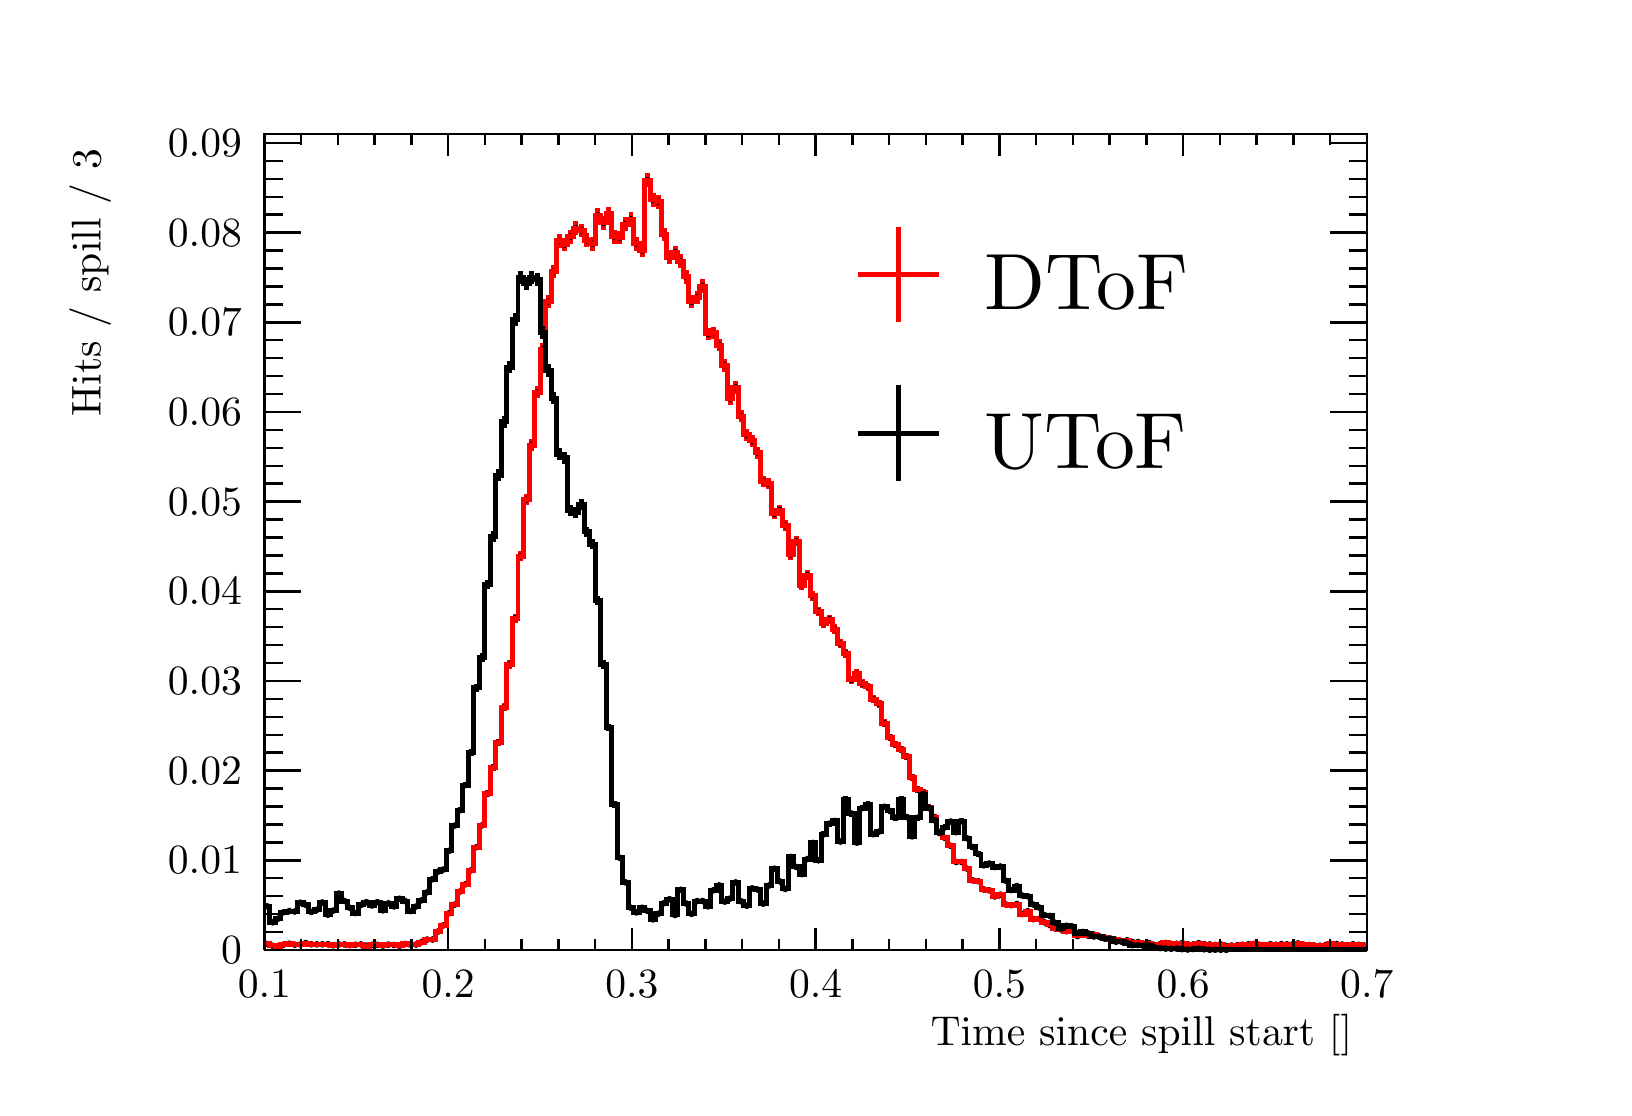
\begin{tikzpicture}
\pgfdeclareplotmark{cross} {
\pgfpathmoveto{\pgfpoint{-0.3\pgfplotmarksize}{\pgfplotmarksize}}
\pgfpathlineto{\pgfpoint{+0.3\pgfplotmarksize}{\pgfplotmarksize}}
\pgfpathlineto{\pgfpoint{+0.3\pgfplotmarksize}{0.3\pgfplotmarksize}}
\pgfpathlineto{\pgfpoint{+1\pgfplotmarksize}{0.3\pgfplotmarksize}}
\pgfpathlineto{\pgfpoint{+1\pgfplotmarksize}{-0.3\pgfplotmarksize}}
\pgfpathlineto{\pgfpoint{+0.3\pgfplotmarksize}{-0.3\pgfplotmarksize}}
\pgfpathlineto{\pgfpoint{+0.3\pgfplotmarksize}{-1.\pgfplotmarksize}}
\pgfpathlineto{\pgfpoint{-0.3\pgfplotmarksize}{-1.\pgfplotmarksize}}
\pgfpathlineto{\pgfpoint{-0.3\pgfplotmarksize}{-0.3\pgfplotmarksize}}
\pgfpathlineto{\pgfpoint{-1.\pgfplotmarksize}{-0.3\pgfplotmarksize}}
\pgfpathlineto{\pgfpoint{-1.\pgfplotmarksize}{0.3\pgfplotmarksize}}
\pgfpathlineto{\pgfpoint{-0.3\pgfplotmarksize}{0.3\pgfplotmarksize}}
\pgfpathclose
\pgfusepathqstroke
}
\pgfdeclareplotmark{cross*} {
\pgfpathmoveto{\pgfpoint{-0.3\pgfplotmarksize}{\pgfplotmarksize}}
\pgfpathlineto{\pgfpoint{+0.3\pgfplotmarksize}{\pgfplotmarksize}}
\pgfpathlineto{\pgfpoint{+0.3\pgfplotmarksize}{0.3\pgfplotmarksize}}
\pgfpathlineto{\pgfpoint{+1\pgfplotmarksize}{0.3\pgfplotmarksize}}
\pgfpathlineto{\pgfpoint{+1\pgfplotmarksize}{-0.3\pgfplotmarksize}}
\pgfpathlineto{\pgfpoint{+0.3\pgfplotmarksize}{-0.3\pgfplotmarksize}}
\pgfpathlineto{\pgfpoint{+0.3\pgfplotmarksize}{-1.\pgfplotmarksize}}
\pgfpathlineto{\pgfpoint{-0.3\pgfplotmarksize}{-1.\pgfplotmarksize}}
\pgfpathlineto{\pgfpoint{-0.3\pgfplotmarksize}{-0.3\pgfplotmarksize}}
\pgfpathlineto{\pgfpoint{-1.\pgfplotmarksize}{-0.3\pgfplotmarksize}}
\pgfpathlineto{\pgfpoint{-1.\pgfplotmarksize}{0.3\pgfplotmarksize}}
\pgfpathlineto{\pgfpoint{-0.3\pgfplotmarksize}{0.3\pgfplotmarksize}}
\pgfpathclose
\pgfusepathqfillstroke
}
\pgfdeclareplotmark{newstar} {
\pgfpathmoveto{\pgfqpoint{0pt}{\pgfplotmarksize}}
\pgfpathlineto{\pgfqpointpolar{44}{0.5\pgfplotmarksize}}
\pgfpathlineto{\pgfqpointpolar{18}{\pgfplotmarksize}}
\pgfpathlineto{\pgfqpointpolar{-20}{0.5\pgfplotmarksize}}
\pgfpathlineto{\pgfqpointpolar{-54}{\pgfplotmarksize}}
\pgfpathlineto{\pgfqpointpolar{-90}{0.5\pgfplotmarksize}}
\pgfpathlineto{\pgfqpointpolar{234}{\pgfplotmarksize}}
\pgfpathlineto{\pgfqpointpolar{198}{0.5\pgfplotmarksize}}
\pgfpathlineto{\pgfqpointpolar{162}{\pgfplotmarksize}}
\pgfpathlineto{\pgfqpointpolar{134}{0.5\pgfplotmarksize}}
\pgfpathclose
\pgfusepathqstroke
}
\pgfdeclareplotmark{newstar*} {
\pgfpathmoveto{\pgfqpoint{0pt}{\pgfplotmarksize}}
\pgfpathlineto{\pgfqpointpolar{44}{0.5\pgfplotmarksize}}
\pgfpathlineto{\pgfqpointpolar{18}{\pgfplotmarksize}}
\pgfpathlineto{\pgfqpointpolar{-20}{0.5\pgfplotmarksize}}
\pgfpathlineto{\pgfqpointpolar{-54}{\pgfplotmarksize}}
\pgfpathlineto{\pgfqpointpolar{-90}{0.5\pgfplotmarksize}}
\pgfpathlineto{\pgfqpointpolar{234}{\pgfplotmarksize}}
\pgfpathlineto{\pgfqpointpolar{198}{0.5\pgfplotmarksize}}
\pgfpathlineto{\pgfqpointpolar{162}{\pgfplotmarksize}}
\pgfpathlineto{\pgfqpointpolar{134}{0.5\pgfplotmarksize}}
\pgfpathclose
\pgfusepathqfillstroke
}
\definecolor{c}{rgb}{1,1,1};
\draw [color=c, fill=c] (0,0) rectangle (20,13.4556);
\draw [color=c, fill=c] (3,1.74922) rectangle (17,12.11);
\definecolor{c}{rgb}{0,0,0};
\draw [c,line width=0.9] (3,1.74922) -- (3,12.11) -- (17,12.11) -- (17,1.74922) -- (3,1.74922);
\definecolor{c}{rgb}{1,1,1};
\draw [color=c, fill=c] (3,1.74922) rectangle (17,12.11);
\definecolor{c}{rgb}{0,0,0};
\draw [c,line width=0.9] (3,1.74922) -- (3,12.11) -- (17,12.11) -- (17,1.74922) -- (3,1.74922);
\definecolor{c}{rgb}{1,0,0};
\draw [c,line width=1.8] (3.035,1.81776) -- (3.035,1.82578);
\draw [c,line width=1.8] (3.035,1.82578) -- (3.035,1.83381);
\definecolor{c}{rgb}{0,0,0};
\foreach \P in {(3.035,1.82578)}{\draw[mark options={color=c,fill=c},mark size=2.402402pt,mark=*,mark size=1pt] plot coordinates {\P};}
\definecolor{c}{rgb}{1,0,0};
\draw [c,line width=1.8] (3.105,1.79555) -- (3.105,1.80223);
\draw [c,line width=1.8] (3.105,1.80223) -- (3.105,1.8089);
\definecolor{c}{rgb}{0,0,0};
\foreach \P in {(3.105,1.80223)}{\draw[mark options={color=c,fill=c},mark size=2.402402pt,mark=*,mark size=1pt] plot coordinates {\P};}
\definecolor{c}{rgb}{1,0,0};
\draw [c,line width=1.8] (3.175,1.78691) -- (3.175,1.79297);
\draw [c,line width=1.8] (3.175,1.79297) -- (3.175,1.79904);
\definecolor{c}{rgb}{0,0,0};
\foreach \P in {(3.175,1.79297)}{\draw[mark options={color=c,fill=c},mark size=2.402402pt,mark=*,mark size=1pt] plot coordinates {\P};}
\definecolor{c}{rgb}{1,0,0};
\draw [c,line width=1.8] (3.245,1.81059) -- (3.245,1.81821);
\draw [c,line width=1.8] (3.245,1.81821) -- (3.245,1.82583);
\definecolor{c}{rgb}{0,0,0};
\foreach \P in {(3.245,1.81821)}{\draw[mark options={color=c,fill=c},mark size=2.402402pt,mark=*,mark size=1pt] plot coordinates {\P};}
\definecolor{c}{rgb}{1,0,0};
\draw [c,line width=1.8] (3.315,1.82095) -- (3.315,1.82915);
\draw [c,line width=1.8] (3.315,1.82915) -- (3.315,1.83735);
\definecolor{c}{rgb}{0,0,0};
\foreach \P in {(3.315,1.82915)}{\draw[mark options={color=c,fill=c},mark size=2.402402pt,mark=*,mark size=1pt] plot coordinates {\P};}
\definecolor{c}{rgb}{1,0,0};
\draw [c,line width=1.8] (3.385,1.809) -- (3.385,1.81653);
\draw [c,line width=1.8] (3.385,1.81653) -- (3.385,1.82405);
\definecolor{c}{rgb}{0,0,0};
\foreach \P in {(3.385,1.81653)}{\draw[mark options={color=c,fill=c},mark size=2.402402pt,mark=*,mark size=1pt] plot coordinates {\P};}
\definecolor{c}{rgb}{1,0,0};
\draw [c,line width=1.8] (3.455,1.81059) -- (3.455,1.81821);
\draw [c,line width=1.8] (3.455,1.81821) -- (3.455,1.82583);
\definecolor{c}{rgb}{0,0,0};
\foreach \P in {(3.455,1.81821)}{\draw[mark options={color=c,fill=c},mark size=2.402402pt,mark=*,mark size=1pt] plot coordinates {\P};}
\definecolor{c}{rgb}{1,0,0};
\draw [c,line width=1.8] (3.525,1.82814) -- (3.525,1.83672);
\draw [c,line width=1.8] (3.525,1.83672) -- (3.525,1.8453);
\definecolor{c}{rgb}{0,0,0};
\foreach \P in {(3.525,1.83672)}{\draw[mark options={color=c,fill=c},mark size=2.402402pt,mark=*,mark size=1pt] plot coordinates {\P};}
\definecolor{c}{rgb}{1,0,0};
\draw [c,line width=1.8] (3.595,1.81377) -- (3.595,1.82158);
\draw [c,line width=1.8] (3.595,1.82158) -- (3.595,1.82938);
\definecolor{c}{rgb}{0,0,0};
\foreach \P in {(3.595,1.82158)}{\draw[mark options={color=c,fill=c},mark size=2.402402pt,mark=*,mark size=1pt] plot coordinates {\P};}
\definecolor{c}{rgb}{1,0,0};
\draw [c,line width=1.8] (3.665,1.81298) -- (3.665,1.82073);
\draw [c,line width=1.8] (3.665,1.82073) -- (3.665,1.82849);
\definecolor{c}{rgb}{0,0,0};
\foreach \P in {(3.665,1.82073)}{\draw[mark options={color=c,fill=c},mark size=2.402402pt,mark=*,mark size=1pt] plot coordinates {\P};}
\definecolor{c}{rgb}{1,0,0};
\draw [c,line width=1.8] (3.735,1.81377) -- (3.735,1.82158);
\draw [c,line width=1.8] (3.735,1.82158) -- (3.735,1.82938);
\definecolor{c}{rgb}{0,0,0};
\foreach \P in {(3.735,1.82158)}{\draw[mark options={color=c,fill=c},mark size=2.402402pt,mark=*,mark size=1pt] plot coordinates {\P};}
\definecolor{c}{rgb}{1,0,0};
\draw [c,line width=1.8] (3.805,1.81457) -- (3.805,1.82242);
\draw [c,line width=1.8] (3.805,1.82242) -- (3.805,1.83026);
\definecolor{c}{rgb}{0,0,0};
\foreach \P in {(3.805,1.82242)}{\draw[mark options={color=c,fill=c},mark size=2.402402pt,mark=*,mark size=1pt] plot coordinates {\P};}
\definecolor{c}{rgb}{1,0,0};
\draw [c,line width=1.8] (3.875,1.80108) -- (3.875,1.80812);
\draw [c,line width=1.8] (3.875,1.80812) -- (3.875,1.81515);
\definecolor{c}{rgb}{0,0,0};
\foreach \P in {(3.875,1.80812)}{\draw[mark options={color=c,fill=c},mark size=2.402402pt,mark=*,mark size=1pt] plot coordinates {\P};}
\definecolor{c}{rgb}{1,0,0};
\draw [c,line width=1.8] (3.945,1.81298) -- (3.945,1.82073);
\draw [c,line width=1.8] (3.945,1.82073) -- (3.945,1.82849);
\definecolor{c}{rgb}{0,0,0};
\foreach \P in {(3.945,1.82073)}{\draw[mark options={color=c,fill=c},mark size=2.402402pt,mark=*,mark size=1pt] plot coordinates {\P};}
\definecolor{c}{rgb}{1,0,0};
\draw [c,line width=1.8] (4.015,1.81218) -- (4.015,1.81989);
\draw [c,line width=1.8] (4.015,1.81989) -- (4.015,1.8276);
\definecolor{c}{rgb}{0,0,0};
\foreach \P in {(4.015,1.81989)}{\draw[mark options={color=c,fill=c},mark size=2.402402pt,mark=*,mark size=1pt] plot coordinates {\P};}
\definecolor{c}{rgb}{1,0,0};
\draw [c,line width=1.8] (4.085,1.80345) -- (4.085,1.81064);
\draw [c,line width=1.8] (4.085,1.81064) -- (4.085,1.81783);
\definecolor{c}{rgb}{0,0,0};
\foreach \P in {(4.085,1.81064)}{\draw[mark options={color=c,fill=c},mark size=2.402402pt,mark=*,mark size=1pt] plot coordinates {\P};}
\definecolor{c}{rgb}{1,0,0};
\draw [c,line width=1.8] (4.155,1.80821) -- (4.155,1.81569);
\draw [c,line width=1.8] (4.155,1.81569) -- (4.155,1.82316);
\definecolor{c}{rgb}{0,0,0};
\foreach \P in {(4.155,1.81569)}{\draw[mark options={color=c,fill=c},mark size=2.402402pt,mark=*,mark size=1pt] plot coordinates {\P};}
\definecolor{c}{rgb}{1,0,0};
\draw [c,line width=1.8] (4.225,1.81218) -- (4.225,1.81989);
\draw [c,line width=1.8] (4.225,1.81989) -- (4.225,1.8276);
\definecolor{c}{rgb}{0,0,0};
\foreach \P in {(4.225,1.81989)}{\draw[mark options={color=c,fill=c},mark size=2.402402pt,mark=*,mark size=1pt] plot coordinates {\P};}
\definecolor{c}{rgb}{1,0,0};
\draw [c,line width=1.8] (4.295,1.7924) -- (4.295,1.79886);
\draw [c,line width=1.8] (4.295,1.79886) -- (4.295,1.80532);
\definecolor{c}{rgb}{0,0,0};
\foreach \P in {(4.295,1.79886)}{\draw[mark options={color=c,fill=c},mark size=2.402402pt,mark=*,mark size=1pt] plot coordinates {\P};}
\definecolor{c}{rgb}{1,0,0};
\draw [c,line width=1.8] (4.365,1.80742) -- (4.365,1.81485);
\draw [c,line width=1.8] (4.365,1.81485) -- (4.365,1.82228);
\definecolor{c}{rgb}{0,0,0};
\foreach \P in {(4.365,1.81485)}{\draw[mark options={color=c,fill=c},mark size=2.402402pt,mark=*,mark size=1pt] plot coordinates {\P};}
\definecolor{c}{rgb}{1,0,0};
\draw [c,line width=1.8] (4.435,1.80821) -- (4.435,1.81569);
\draw [c,line width=1.8] (4.435,1.81569) -- (4.435,1.82316);
\definecolor{c}{rgb}{0,0,0};
\foreach \P in {(4.435,1.81569)}{\draw[mark options={color=c,fill=c},mark size=2.402402pt,mark=*,mark size=1pt] plot coordinates {\P};}
\definecolor{c}{rgb}{1,0,0};
\draw [c,line width=1.8] (4.505,1.79792) -- (4.505,1.80475);
\draw [c,line width=1.8] (4.505,1.80475) -- (4.505,1.81158);
\definecolor{c}{rgb}{0,0,0};
\foreach \P in {(4.505,1.80475)}{\draw[mark options={color=c,fill=c},mark size=2.402402pt,mark=*,mark size=1pt] plot coordinates {\P};}
\definecolor{c}{rgb}{1,0,0};
\draw [c,line width=1.8] (4.575,1.8098) -- (4.575,1.81737);
\draw [c,line width=1.8] (4.575,1.81737) -- (4.575,1.82494);
\definecolor{c}{rgb}{0,0,0};
\foreach \P in {(4.575,1.81737)}{\draw[mark options={color=c,fill=c},mark size=2.402402pt,mark=*,mark size=1pt] plot coordinates {\P};}
\definecolor{c}{rgb}{1,0,0};
\draw [c,line width=1.8] (4.645,1.80583) -- (4.645,1.81316);
\draw [c,line width=1.8] (4.645,1.81316) -- (4.645,1.8205);
\definecolor{c}{rgb}{0,0,0};
\foreach \P in {(4.645,1.81316)}{\draw[mark options={color=c,fill=c},mark size=2.402402pt,mark=*,mark size=1pt] plot coordinates {\P};}
\definecolor{c}{rgb}{1,0,0};
\draw [c,line width=1.8] (4.715,1.79634) -- (4.715,1.80307);
\draw [c,line width=1.8] (4.715,1.80307) -- (4.715,1.8098);
\definecolor{c}{rgb}{0,0,0};
\foreach \P in {(4.715,1.80307)}{\draw[mark options={color=c,fill=c},mark size=2.402402pt,mark=*,mark size=1pt] plot coordinates {\P};}
\definecolor{c}{rgb}{1,0,0};
\draw [c,line width=1.8] (4.785,1.81776) -- (4.785,1.82578);
\draw [c,line width=1.8] (4.785,1.82578) -- (4.785,1.83381);
\definecolor{c}{rgb}{0,0,0};
\foreach \P in {(4.785,1.82578)}{\draw[mark options={color=c,fill=c},mark size=2.402402pt,mark=*,mark size=1pt] plot coordinates {\P};}
\definecolor{c}{rgb}{1,0,0};
\draw [c,line width=1.8] (4.855,1.8098) -- (4.855,1.81737);
\draw [c,line width=1.8] (4.855,1.81737) -- (4.855,1.82494);
\definecolor{c}{rgb}{0,0,0};
\foreach \P in {(4.855,1.81737)}{\draw[mark options={color=c,fill=c},mark size=2.402402pt,mark=*,mark size=1pt] plot coordinates {\P};}
\definecolor{c}{rgb}{1,0,0};
\draw [c,line width=1.8] (4.925,1.81059) -- (4.925,1.81821);
\draw [c,line width=1.8] (4.925,1.81821) -- (4.925,1.82583);
\definecolor{c}{rgb}{0,0,0};
\foreach \P in {(4.925,1.81821)}{\draw[mark options={color=c,fill=c},mark size=2.402402pt,mark=*,mark size=1pt] plot coordinates {\P};}
\definecolor{c}{rgb}{1,0,0};
\draw [c,line width=1.8] (4.995,1.83856) -- (4.995,1.84766);
\draw [c,line width=1.8] (4.995,1.84766) -- (4.995,1.85676);
\definecolor{c}{rgb}{0,0,0};
\foreach \P in {(4.995,1.84766)}{\draw[mark options={color=c,fill=c},mark size=2.402402pt,mark=*,mark size=1pt] plot coordinates {\P};}
\definecolor{c}{rgb}{1,0,0};
\draw [c,line width=1.8] (5.065,1.87077) -- (5.065,1.88131);
\draw [c,line width=1.8] (5.065,1.88131) -- (5.065,1.89185);
\definecolor{c}{rgb}{0,0,0};
\foreach \P in {(5.065,1.88131)}{\draw[mark options={color=c,fill=c},mark size=2.402402pt,mark=*,mark size=1pt] plot coordinates {\P};}
\definecolor{c}{rgb}{1,0,0};
\draw [c,line width=1.8] (5.135,1.87157) -- (5.135,1.88215);
\draw [c,line width=1.8] (5.135,1.88215) -- (5.135,1.89272);
\definecolor{c}{rgb}{0,0,0};
\foreach \P in {(5.135,1.88215)}{\draw[mark options={color=c,fill=c},mark size=2.402402pt,mark=*,mark size=1pt] plot coordinates {\P};}
\definecolor{c}{rgb}{1,0,0};
\draw [c,line width=1.8] (5.205,1.96989) -- (5.205,1.98395);
\draw [c,line width=1.8] (5.205,1.98395) -- (5.205,1.998);
\definecolor{c}{rgb}{0,0,0};
\foreach \P in {(5.205,1.98395)}{\draw[mark options={color=c,fill=c},mark size=2.402402pt,mark=*,mark size=1pt] plot coordinates {\P};}
\definecolor{c}{rgb}{1,0,0};
\draw [c,line width=1.8] (5.275,2.04596) -- (5.275,2.06219);
\draw [c,line width=1.8] (5.275,2.06219) -- (5.275,2.07841);
\definecolor{c}{rgb}{0,0,0};
\foreach \P in {(5.275,2.06219)}{\draw[mark options={color=c,fill=c},mark size=2.402402pt,mark=*,mark size=1pt] plot coordinates {\P};}
\definecolor{c}{rgb}{1,0,0};
\draw [c,line width=1.8] (5.345,2.19633) -- (5.345,2.21614);
\draw [c,line width=1.8] (5.345,2.21614) -- (5.345,2.23596);
\definecolor{c}{rgb}{0,0,0};
\foreach \P in {(5.345,2.21614)}{\draw[mark options={color=c,fill=c},mark size=2.402402pt,mark=*,mark size=1pt] plot coordinates {\P};}
\definecolor{c}{rgb}{1,0,0};
\draw [c,line width=1.8] (5.415,2.30349) -- (5.415,2.32551);
\draw [c,line width=1.8] (5.415,2.32551) -- (5.415,2.34753);
\definecolor{c}{rgb}{0,0,0};
\foreach \P in {(5.415,2.32551)}{\draw[mark options={color=c,fill=c},mark size=2.402402pt,mark=*,mark size=1pt] plot coordinates {\P};}
\definecolor{c}{rgb}{1,0,0};
\draw [c,line width=1.8] (5.485,2.46709) -- (5.485,2.49209);
\draw [c,line width=1.8] (5.485,2.49209) -- (5.485,2.51709);
\definecolor{c}{rgb}{0,0,0};
\foreach \P in {(5.485,2.49209)}{\draw[mark options={color=c,fill=c},mark size=2.402402pt,mark=*,mark size=1pt] plot coordinates {\P};}
\definecolor{c}{rgb}{1,0,0};
\draw [c,line width=1.8] (5.555,2.55812) -- (5.555,2.58463);
\draw [c,line width=1.8] (5.555,2.58463) -- (5.555,2.61114);
\definecolor{c}{rgb}{0,0,0};
\foreach \P in {(5.555,2.58463)}{\draw[mark options={color=c,fill=c},mark size=2.402402pt,mark=*,mark size=1pt] plot coordinates {\P};}
\definecolor{c}{rgb}{1,0,0};
\draw [c,line width=1.8] (5.625,2.73213) -- (5.625,2.76131);
\draw [c,line width=1.8] (5.625,2.76131) -- (5.625,2.79049);
\definecolor{c}{rgb}{0,0,0};
\foreach \P in {(5.625,2.76131)}{\draw[mark options={color=c,fill=c},mark size=2.402402pt,mark=*,mark size=1pt] plot coordinates {\P};}
\definecolor{c}{rgb}{1,0,0};
\draw [c,line width=1.8] (5.695,3.02178) -- (5.695,3.05492);
\draw [c,line width=1.8] (5.695,3.05492) -- (5.695,3.08806);
\definecolor{c}{rgb}{0,0,0};
\foreach \P in {(5.695,3.05492)}{\draw[mark options={color=c,fill=c},mark size=2.402402pt,mark=*,mark size=1pt] plot coordinates {\P};}
\definecolor{c}{rgb}{1,0,0};
\draw [c,line width=1.8] (5.765,3.29522) -- (5.765,3.33171);
\draw [c,line width=1.8] (5.765,3.33171) -- (5.765,3.36819);
\definecolor{c}{rgb}{0,0,0};
\foreach \P in {(5.765,3.33171)}{\draw[mark options={color=c,fill=c},mark size=2.402402pt,mark=*,mark size=1pt] plot coordinates {\P};}
\definecolor{c}{rgb}{1,0,0};
\draw [c,line width=1.8] (5.835,3.69715) -- (5.835,3.73805);
\draw [c,line width=1.8] (5.835,3.73805) -- (5.835,3.77896);
\definecolor{c}{rgb}{0,0,0};
\foreach \P in {(5.835,3.73805)}{\draw[mark options={color=c,fill=c},mark size=2.402402pt,mark=*,mark size=1pt] plot coordinates {\P};}
\definecolor{c}{rgb}{1,0,0};
\draw [c,line width=1.8] (5.905,4.02618) -- (5.905,4.07037);
\draw [c,line width=1.8] (5.905,4.07037) -- (5.905,4.11456);
\definecolor{c}{rgb}{0,0,0};
\foreach \P in {(5.905,4.07037)}{\draw[mark options={color=c,fill=c},mark size=2.402402pt,mark=*,mark size=1pt] plot coordinates {\P};}
\definecolor{c}{rgb}{1,0,0};
\draw [c,line width=1.8] (5.975,4.33959) -- (5.975,4.38669);
\draw [c,line width=1.8] (5.975,4.38669) -- (5.975,4.4338);
\definecolor{c}{rgb}{0,0,0};
\foreach \P in {(5.975,4.38669)}{\draw[mark options={color=c,fill=c},mark size=2.402402pt,mark=*,mark size=1pt] plot coordinates {\P};}
\definecolor{c}{rgb}{1,0,0};
\draw [c,line width=1.8] (6.045,4.78249) -- (6.045,4.83342);
\draw [c,line width=1.8] (6.045,4.83342) -- (6.045,4.88436);
\definecolor{c}{rgb}{0,0,0};
\foreach \P in {(6.045,4.83342)}{\draw[mark options={color=c,fill=c},mark size=2.402402pt,mark=*,mark size=1pt] plot coordinates {\P};}
\definecolor{c}{rgb}{1,0,0};
\draw [c,line width=1.8] (6.115,5.32166) -- (6.115,5.3769);
\draw [c,line width=1.8] (6.115,5.3769) -- (6.115,5.43215);
\definecolor{c}{rgb}{0,0,0};
\foreach \P in {(6.115,5.3769)}{\draw[mark options={color=c,fill=c},mark size=2.402402pt,mark=*,mark size=1pt] plot coordinates {\P};}
\definecolor{c}{rgb}{1,0,0};
\draw [c,line width=1.8] (6.185,5.90291) -- (6.185,5.96245);
\draw [c,line width=1.8] (6.185,5.96245) -- (6.185,6.02198);
\definecolor{c}{rgb}{0,0,0};
\foreach \P in {(6.185,5.96245)}{\draw[mark options={color=c,fill=c},mark size=2.402402pt,mark=*,mark size=1pt] plot coordinates {\P};}
\definecolor{c}{rgb}{1,0,0};
\draw [c,line width=1.8] (6.255,6.68504) -- (6.255,6.7499);
\draw [c,line width=1.8] (6.255,6.7499) -- (6.255,6.81476);
\definecolor{c}{rgb}{0,0,0};
\foreach \P in {(6.255,6.7499)}{\draw[mark options={color=c,fill=c},mark size=2.402402pt,mark=*,mark size=1pt] plot coordinates {\P};}
\definecolor{c}{rgb}{1,0,0};
\draw [c,line width=1.8] (6.325,7.39817) -- (6.325,7.46753);
\draw [c,line width=1.8] (6.325,7.46753) -- (6.325,7.53689);
\definecolor{c}{rgb}{0,0,0};
\foreach \P in {(6.325,7.46753)}{\draw[mark options={color=c,fill=c},mark size=2.402402pt,mark=*,mark size=1pt] plot coordinates {\P};}
\definecolor{c}{rgb}{1,0,0};
\draw [c,line width=1.8] (6.395,8.08815) -- (6.395,8.1616);
\draw [c,line width=1.8] (6.395,8.1616) -- (6.395,8.23505);
\definecolor{c}{rgb}{0,0,0};
\foreach \P in {(6.395,8.1616)}{\draw[mark options={color=c,fill=c},mark size=2.402402pt,mark=*,mark size=1pt] plot coordinates {\P};}
\definecolor{c}{rgb}{1,0,0};
\draw [c,line width=1.8] (6.465,8.75408) -- (6.465,8.83127);
\draw [c,line width=1.8] (6.465,8.83127) -- (6.465,8.90846);
\definecolor{c}{rgb}{0,0,0};
\foreach \P in {(6.465,8.83127)}{\draw[mark options={color=c,fill=c},mark size=2.402402pt,mark=*,mark size=1pt] plot coordinates {\P};}
\definecolor{c}{rgb}{1,0,0};
\draw [c,line width=1.8] (6.535,9.30051) -- (6.535,9.38064);
\draw [c,line width=1.8] (6.535,9.38064) -- (6.535,9.46077);
\definecolor{c}{rgb}{0,0,0};
\foreach \P in {(6.535,9.38064)}{\draw[mark options={color=c,fill=c},mark size=2.402402pt,mark=*,mark size=1pt] plot coordinates {\P};}
\definecolor{c}{rgb}{1,0,0};
\draw [c,line width=1.8] (6.605,9.90229) -- (6.605,9.98553);
\draw [c,line width=1.8] (6.605,9.98553) -- (6.605,10.0688);
\definecolor{c}{rgb}{0,0,0};
\foreach \P in {(6.605,9.98553)}{\draw[mark options={color=c,fill=c},mark size=2.402402pt,mark=*,mark size=1pt] plot coordinates {\P};}
\definecolor{c}{rgb}{1,0,0};
\draw [c,line width=1.8] (6.675,10.2815) -- (6.675,10.3666);
\draw [c,line width=1.8] (6.675,10.3666) -- (6.675,10.4518);
\definecolor{c}{rgb}{0,0,0};
\foreach \P in {(6.675,10.3666)}{\draw[mark options={color=c,fill=c},mark size=2.402402pt,mark=*,mark size=1pt] plot coordinates {\P};}
\definecolor{c}{rgb}{1,0,0};
\draw [c,line width=1.8] (6.745,10.6674) -- (6.745,10.7545);
\draw [c,line width=1.8] (6.745,10.7545) -- (6.745,10.8415);
\definecolor{c}{rgb}{0,0,0};
\foreach \P in {(6.745,10.7545)}{\draw[mark options={color=c,fill=c},mark size=2.402402pt,mark=*,mark size=1pt] plot coordinates {\P};}
\definecolor{c}{rgb}{1,0,0};
\draw [c,line width=1.8] (6.815,10.6206) -- (6.815,10.7074);
\draw [c,line width=1.8] (6.815,10.7074) -- (6.815,10.7942);
\definecolor{c}{rgb}{0,0,0};
\foreach \P in {(6.815,10.7074)}{\draw[mark options={color=c,fill=c},mark size=2.402402pt,mark=*,mark size=1pt] plot coordinates {\P};}
\definecolor{c}{rgb}{1,0,0};
\draw [c,line width=1.8] (6.885,10.721) -- (6.885,10.8083);
\draw [c,line width=1.8] (6.885,10.8083) -- (6.885,10.8956);
\definecolor{c}{rgb}{0,0,0};
\foreach \P in {(6.885,10.8083)}{\draw[mark options={color=c,fill=c},mark size=2.402402pt,mark=*,mark size=1pt] plot coordinates {\P};}
\definecolor{c}{rgb}{1,0,0};
\draw [c,line width=1.8] (6.955,10.8282) -- (6.955,10.916);
\draw [c,line width=1.8] (6.955,10.916) -- (6.955,11.0038);
\definecolor{c}{rgb}{0,0,0};
\foreach \P in {(6.955,10.916)}{\draw[mark options={color=c,fill=c},mark size=2.402402pt,mark=*,mark size=1pt] plot coordinates {\P};}
\definecolor{c}{rgb}{1,0,0};
\draw [c,line width=1.8] (7.025,10.7997) -- (7.025,10.8874);
\draw [c,line width=1.8] (7.025,10.8874) -- (7.025,10.9751);
\definecolor{c}{rgb}{0,0,0};
\foreach \P in {(7.025,10.8874)}{\draw[mark options={color=c,fill=c},mark size=2.402402pt,mark=*,mark size=1pt] plot coordinates {\P};}
\definecolor{c}{rgb}{1,0,0};
\draw [c,line width=1.8] (7.095,10.6758) -- (7.095,10.7629);
\draw [c,line width=1.8] (7.095,10.7629) -- (7.095,10.85);
\definecolor{c}{rgb}{0,0,0};
\foreach \P in {(7.095,10.7629)}{\draw[mark options={color=c,fill=c},mark size=2.402402pt,mark=*,mark size=1pt] plot coordinates {\P};}
\definecolor{c}{rgb}{1,0,0};
\draw [c,line width=1.8] (7.165,10.6314) -- (7.165,10.7183);
\draw [c,line width=1.8] (7.165,10.7183) -- (7.165,10.8052);
\definecolor{c}{rgb}{0,0,0};
\foreach \P in {(7.165,10.7183)}{\draw[mark options={color=c,fill=c},mark size=2.402402pt,mark=*,mark size=1pt] plot coordinates {\P};}
\definecolor{c}{rgb}{1,0,0};
\draw [c,line width=1.8] (7.235,10.9898) -- (7.235,11.0784);
\draw [c,line width=1.8] (7.235,11.0784) -- (7.235,11.167);
\definecolor{c}{rgb}{0,0,0};
\foreach \P in {(7.235,11.0784)}{\draw[mark options={color=c,fill=c},mark size=2.402402pt,mark=*,mark size=1pt] plot coordinates {\P};}
\definecolor{c}{rgb}{1,0,0};
\draw [c,line width=1.8] (7.305,10.896) -- (7.305,10.9842);
\draw [c,line width=1.8] (7.305,10.9842) -- (7.305,11.0723);
\definecolor{c}{rgb}{0,0,0};
\foreach \P in {(7.305,10.9842)}{\draw[mark options={color=c,fill=c},mark size=2.402402pt,mark=*,mark size=1pt] plot coordinates {\P};}
\definecolor{c}{rgb}{1,0,0};
\draw [c,line width=1.8] (7.375,11.0107) -- (7.375,11.0994);
\draw [c,line width=1.8] (7.375,11.0994) -- (7.375,11.1881);
\definecolor{c}{rgb}{0,0,0};
\foreach \P in {(7.375,11.0994)}{\draw[mark options={color=c,fill=c},mark size=2.402402pt,mark=*,mark size=1pt] plot coordinates {\P};}
\definecolor{c}{rgb}{1,0,0};
\draw [c,line width=1.8] (7.445,10.7193) -- (7.445,10.8066);
\draw [c,line width=1.8] (7.445,10.8066) -- (7.445,10.8939);
\definecolor{c}{rgb}{0,0,0};
\foreach \P in {(7.445,10.8066)}{\draw[mark options={color=c,fill=c},mark size=2.402402pt,mark=*,mark size=1pt] plot coordinates {\P};}
\definecolor{c}{rgb}{1,0,0};
\draw [c,line width=1.8] (7.515,10.711) -- (7.515,10.7982);
\draw [c,line width=1.8] (7.515,10.7982) -- (7.515,10.8855);
\definecolor{c}{rgb}{0,0,0};
\foreach \P in {(7.515,10.7982)}{\draw[mark options={color=c,fill=c},mark size=2.402402pt,mark=*,mark size=1pt] plot coordinates {\P};}
\definecolor{c}{rgb}{1,0,0};
\draw [c,line width=1.8] (7.585,10.8801) -- (7.585,10.9682);
\draw [c,line width=1.8] (7.585,10.9682) -- (7.585,11.0562);
\definecolor{c}{rgb}{0,0,0};
\foreach \P in {(7.585,10.9682)}{\draw[mark options={color=c,fill=c},mark size=2.402402pt,mark=*,mark size=1pt] plot coordinates {\P};}
\definecolor{c}{rgb}{1,0,0};
\draw [c,line width=1.8] (7.655,10.9395) -- (7.655,11.0279);
\draw [c,line width=1.8] (7.655,11.0279) -- (7.655,11.1163);
\definecolor{c}{rgb}{0,0,0};
\foreach \P in {(7.655,11.0279)}{\draw[mark options={color=c,fill=c},mark size=2.402402pt,mark=*,mark size=1pt] plot coordinates {\P};}
\definecolor{c}{rgb}{1,0,0};
\draw [c,line width=1.8] (7.725,10.6323) -- (7.725,10.7191);
\draw [c,line width=1.8] (7.725,10.7191) -- (7.725,10.806);
\definecolor{c}{rgb}{0,0,0};
\foreach \P in {(7.725,10.7191)}{\draw[mark options={color=c,fill=c},mark size=2.402402pt,mark=*,mark size=1pt] plot coordinates {\P};}
\definecolor{c}{rgb}{1,0,0};
\draw [c,line width=1.8] (7.795,10.5452) -- (7.795,10.6317);
\draw [c,line width=1.8] (7.795,10.6317) -- (7.795,10.7181);
\definecolor{c}{rgb}{0,0,0};
\foreach \P in {(7.795,10.6317)}{\draw[mark options={color=c,fill=c},mark size=2.402402pt,mark=*,mark size=1pt] plot coordinates {\P};}
\definecolor{c}{rgb}{1,0,0};
\draw [c,line width=1.8] (7.865,11.4353) -- (7.865,11.526);
\draw [c,line width=1.8] (7.865,11.526) -- (7.865,11.6166);
\definecolor{c}{rgb}{0,0,0};
\foreach \P in {(7.865,11.526)}{\draw[mark options={color=c,fill=c},mark size=2.402402pt,mark=*,mark size=1pt] plot coordinates {\P};}
\definecolor{c}{rgb}{1,0,0};
\draw [c,line width=1.8] (7.935,11.1849) -- (7.935,11.2744);
\draw [c,line width=1.8] (7.935,11.2744) -- (7.935,11.3639);
\definecolor{c}{rgb}{0,0,0};
\foreach \P in {(7.935,11.2744)}{\draw[mark options={color=c,fill=c},mark size=2.402402pt,mark=*,mark size=1pt] plot coordinates {\P};}
\definecolor{c}{rgb}{1,0,0};
\draw [c,line width=1.8] (8.005,11.1598) -- (8.005,11.2492);
\draw [c,line width=1.8] (8.005,11.2492) -- (8.005,11.3386);
\definecolor{c}{rgb}{0,0,0};
\foreach \P in {(8.005,11.2492)}{\draw[mark options={color=c,fill=c},mark size=2.402402pt,mark=*,mark size=1pt] plot coordinates {\P};}
\definecolor{c}{rgb}{1,0,0};
\draw [c,line width=1.8] (8.075,10.747) -- (8.075,10.8344);
\draw [c,line width=1.8] (8.075,10.8344) -- (8.075,10.9218);
\definecolor{c}{rgb}{0,0,0};
\foreach \P in {(8.075,10.8344)}{\draw[mark options={color=c,fill=c},mark size=2.402402pt,mark=*,mark size=1pt] plot coordinates {\P};}
\definecolor{c}{rgb}{1,0,0};
\draw [c,line width=1.8] (8.145,10.4615) -- (8.145,10.5475);
\draw [c,line width=1.8] (8.145,10.5475) -- (8.145,10.6336);
\definecolor{c}{rgb}{0,0,0};
\foreach \P in {(8.145,10.5475)}{\draw[mark options={color=c,fill=c},mark size=2.402402pt,mark=*,mark size=1pt] plot coordinates {\P};}
\definecolor{c}{rgb}{1,0,0};
\draw [c,line width=1.8] (8.215,10.5226) -- (8.215,10.6089);
\draw [c,line width=1.8] (8.215,10.6089) -- (8.215,10.6953);
\definecolor{c}{rgb}{0,0,0};
\foreach \P in {(8.215,10.6089)}{\draw[mark options={color=c,fill=c},mark size=2.402402pt,mark=*,mark size=1pt] plot coordinates {\P};}
\definecolor{c}{rgb}{1,0,0};
\draw [c,line width=1.8] (8.285,10.4121) -- (8.285,10.4979);
\draw [c,line width=1.8] (8.285,10.4979) -- (8.285,10.5837);
\definecolor{c}{rgb}{0,0,0};
\foreach \P in {(8.285,10.4979)}{\draw[mark options={color=c,fill=c},mark size=2.402402pt,mark=*,mark size=1pt] plot coordinates {\P};}
\definecolor{c}{rgb}{1,0,0};
\draw [c,line width=1.8] (8.355,10.2129) -- (8.355,10.2977);
\draw [c,line width=1.8] (8.355,10.2977) -- (8.355,10.3825);
\definecolor{c}{rgb}{0,0,0};
\foreach \P in {(8.355,10.2977)}{\draw[mark options={color=c,fill=c},mark size=2.402402pt,mark=*,mark size=1pt] plot coordinates {\P};}
\definecolor{c}{rgb}{1,0,0};
\draw [c,line width=1.8] (8.425,9.89811) -- (8.425,9.98133);
\draw [c,line width=1.8] (8.425,9.98133) -- (8.425,10.0645);
\definecolor{c}{rgb}{0,0,0};
\foreach \P in {(8.425,9.98133)}{\draw[mark options={color=c,fill=c},mark size=2.402402pt,mark=*,mark size=1pt] plot coordinates {\P};}
\definecolor{c}{rgb}{1,0,0};
\draw [c,line width=1.8] (8.495,9.95503) -- (8.495,10.0385);
\draw [c,line width=1.8] (8.495,10.0385) -- (8.495,10.122);
\definecolor{c}{rgb}{0,0,0};
\foreach \P in {(8.495,10.0385)}{\draw[mark options={color=c,fill=c},mark size=2.402402pt,mark=*,mark size=1pt] plot coordinates {\P};}
\definecolor{c}{rgb}{1,0,0};
\draw [c,line width=1.8] (8.565,10.0965) -- (8.565,10.1807);
\draw [c,line width=1.8] (8.565,10.1807) -- (8.565,10.2649);
\definecolor{c}{rgb}{0,0,0};
\foreach \P in {(8.565,10.1807)}{\draw[mark options={color=c,fill=c},mark size=2.402402pt,mark=*,mark size=1pt] plot coordinates {\P};}
\definecolor{c}{rgb}{1,0,0};
\draw [c,line width=1.8] (8.635,9.49217) -- (8.635,9.5733);
\draw [c,line width=1.8] (8.635,9.5733) -- (8.635,9.65443);
\definecolor{c}{rgb}{0,0,0};
\foreach \P in {(8.635,9.5733)}{\draw[mark options={color=c,fill=c},mark size=2.402402pt,mark=*,mark size=1pt] plot coordinates {\P};}
\definecolor{c}{rgb}{1,0,0};
\draw [c,line width=1.8] (8.705,9.50388) -- (8.705,9.58508);
\draw [c,line width=1.8] (8.705,9.58508) -- (8.705,9.66627);
\definecolor{c}{rgb}{0,0,0};
\foreach \P in {(8.705,9.58508)}{\draw[mark options={color=c,fill=c},mark size=2.402402pt,mark=*,mark size=1pt] plot coordinates {\P};}
\definecolor{c}{rgb}{1,0,0};
\draw [c,line width=1.8] (8.775,9.35156) -- (8.775,9.43196);
\draw [c,line width=1.8] (8.775,9.43196) -- (8.775,9.51235);
\definecolor{c}{rgb}{0,0,0};
\foreach \P in {(8.775,9.43196)}{\draw[mark options={color=c,fill=c},mark size=2.402402pt,mark=*,mark size=1pt] plot coordinates {\P};}
\definecolor{c}{rgb}{1,0,0};
\draw [c,line width=1.8] (8.845,9.09381) -- (8.845,9.17284);
\draw [c,line width=1.8] (8.845,9.17284) -- (8.845,9.25187);
\definecolor{c}{rgb}{0,0,0};
\foreach \P in {(8.845,9.17284)}{\draw[mark options={color=c,fill=c},mark size=2.402402pt,mark=*,mark size=1pt] plot coordinates {\P};}
\definecolor{c}{rgb}{1,0,0};
\draw [c,line width=1.8] (8.915,8.67627) -- (8.915,8.75303);
\draw [c,line width=1.8] (8.915,8.75303) -- (8.915,8.82979);
\definecolor{c}{rgb}{0,0,0};
\foreach \P in {(8.915,8.75303)}{\draw[mark options={color=c,fill=c},mark size=2.402402pt,mark=*,mark size=1pt] plot coordinates {\P};}
\definecolor{c}{rgb}{1,0,0};
\draw [c,line width=1.8] (8.985,8.816) -- (8.985,8.89353);
\draw [c,line width=1.8] (8.985,8.89353) -- (8.985,8.97106);
\definecolor{c}{rgb}{0,0,0};
\foreach \P in {(8.985,8.89353)}{\draw[mark options={color=c,fill=c},mark size=2.402402pt,mark=*,mark size=1pt] plot coordinates {\P};}
\definecolor{c}{rgb}{1,0,0};
\draw [c,line width=1.8] (9.055,8.45121) -- (9.055,8.52672);
\draw [c,line width=1.8] (9.055,8.52672) -- (9.055,8.60223);
\definecolor{c}{rgb}{0,0,0};
\foreach \P in {(9.055,8.52672)}{\draw[mark options={color=c,fill=c},mark size=2.402402pt,mark=*,mark size=1pt] plot coordinates {\P};}
\definecolor{c}{rgb}{1,0,0};
\draw [c,line width=1.8] (9.125,8.21781) -- (9.125,8.292);
\draw [c,line width=1.8] (9.125,8.292) -- (9.125,8.36619);
\definecolor{c}{rgb}{0,0,0};
\foreach \P in {(9.125,8.292)}{\draw[mark options={color=c,fill=c},mark size=2.402402pt,mark=*,mark size=1pt] plot coordinates {\P};}
\definecolor{c}{rgb}{1,0,0};
\draw [c,line width=1.8] (9.195,8.14085) -- (9.195,8.2146);
\draw [c,line width=1.8] (9.195,8.2146) -- (9.195,8.28835);
\definecolor{c}{rgb}{0,0,0};
\foreach \P in {(9.195,8.2146)}{\draw[mark options={color=c,fill=c},mark size=2.402402pt,mark=*,mark size=1pt] plot coordinates {\P};}
\definecolor{c}{rgb}{1,0,0};
\draw [c,line width=1.8] (9.265,7.99028) -- (9.265,8.06317);
\draw [c,line width=1.8] (9.265,8.06317) -- (9.265,8.13605);
\definecolor{c}{rgb}{0,0,0};
\foreach \P in {(9.265,8.06317)}{\draw[mark options={color=c,fill=c},mark size=2.402402pt,mark=*,mark size=1pt] plot coordinates {\P};}
\definecolor{c}{rgb}{1,0,0};
\draw [c,line width=1.8] (9.335,7.63064) -- (9.335,7.70141);
\draw [c,line width=1.8] (9.335,7.70141) -- (9.335,7.77217);
\definecolor{c}{rgb}{0,0,0};
\foreach \P in {(9.335,7.70141)}{\draw[mark options={color=c,fill=c},mark size=2.402402pt,mark=*,mark size=1pt] plot coordinates {\P};}
\definecolor{c}{rgb}{1,0,0};
\draw [c,line width=1.8] (9.405,7.60054) -- (9.405,7.67112);
\draw [c,line width=1.8] (9.405,7.67112) -- (9.405,7.74171);
\definecolor{c}{rgb}{0,0,0};
\foreach \P in {(9.405,7.67112)}{\draw[mark options={color=c,fill=c},mark size=2.402402pt,mark=*,mark size=1pt] plot coordinates {\P};}
\definecolor{c}{rgb}{1,0,0};
\draw [c,line width=1.8] (9.475,7.2209) -- (9.475,7.28917);
\draw [c,line width=1.8] (9.475,7.28917) -- (9.475,7.35744);
\definecolor{c}{rgb}{0,0,0};
\foreach \P in {(9.475,7.28917)}{\draw[mark options={color=c,fill=c},mark size=2.402402pt,mark=*,mark size=1pt] plot coordinates {\P};}
\definecolor{c}{rgb}{1,0,0};
\draw [c,line width=1.8] (9.545,7.26773) -- (9.545,7.33629);
\draw [c,line width=1.8] (9.545,7.33629) -- (9.545,7.40484);
\definecolor{c}{rgb}{0,0,0};
\foreach \P in {(9.545,7.33629)}{\draw[mark options={color=c,fill=c},mark size=2.402402pt,mark=*,mark size=1pt] plot coordinates {\P};}
\definecolor{c}{rgb}{1,0,0};
\draw [c,line width=1.8] (9.615,7.07459) -- (9.615,7.14195);
\draw [c,line width=1.8] (9.615,7.14195) -- (9.615,7.2093);
\definecolor{c}{rgb}{0,0,0};
\foreach \P in {(9.615,7.14195)}{\draw[mark options={color=c,fill=c},mark size=2.402402pt,mark=*,mark size=1pt] plot coordinates {\P};}
\definecolor{c}{rgb}{1,0,0};
\draw [c,line width=1.8] (9.685,6.70594) -- (9.685,6.77093);
\draw [c,line width=1.8] (9.685,6.77093) -- (9.685,6.83593);
\definecolor{c}{rgb}{0,0,0};
\foreach \P in {(9.685,6.77093)}{\draw[mark options={color=c,fill=c},mark size=2.402402pt,mark=*,mark size=1pt] plot coordinates {\P};}
\definecolor{c}{rgb}{1,0,0};
\draw [c,line width=1.8] (9.755,6.87562) -- (9.755,6.94172);
\draw [c,line width=1.8] (9.755,6.94172) -- (9.755,7.00781);
\definecolor{c}{rgb}{0,0,0};
\foreach \P in {(9.755,6.94172)}{\draw[mark options={color=c,fill=c},mark size=2.402402pt,mark=*,mark size=1pt] plot coordinates {\P};}
\definecolor{c}{rgb}{1,0,0};
\draw [c,line width=1.8] (9.825,6.31982) -- (9.825,6.38225);
\draw [c,line width=1.8] (9.825,6.38225) -- (9.825,6.44469);
\definecolor{c}{rgb}{0,0,0};
\foreach \P in {(9.825,6.38225)}{\draw[mark options={color=c,fill=c},mark size=2.402402pt,mark=*,mark size=1pt] plot coordinates {\P};}
\definecolor{c}{rgb}{1,0,0};
\draw [c,line width=1.8] (9.895,6.44434) -- (9.895,6.50761);
\draw [c,line width=1.8] (9.895,6.50761) -- (9.895,6.57088);
\definecolor{c}{rgb}{0,0,0};
\foreach \P in {(9.895,6.50761)}{\draw[mark options={color=c,fill=c},mark size=2.402402pt,mark=*,mark size=1pt] plot coordinates {\P};}
\definecolor{c}{rgb}{1,0,0};
\draw [c,line width=1.8] (9.965,6.18529) -- (9.965,6.2468);
\draw [c,line width=1.8] (9.965,6.2468) -- (9.965,6.30832);
\definecolor{c}{rgb}{0,0,0};
\foreach \P in {(9.965,6.2468)}{\draw[mark options={color=c,fill=c},mark size=2.402402pt,mark=*,mark size=1pt] plot coordinates {\P};}
\definecolor{c}{rgb}{1,0,0};
\draw [c,line width=1.8] (10.035,5.99062) -- (10.035,6.05078);
\draw [c,line width=1.8] (10.035,6.05078) -- (10.035,6.11094);
\definecolor{c}{rgb}{0,0,0};
\foreach \P in {(10.035,6.05078)}{\draw[mark options={color=c,fill=c},mark size=2.402402pt,mark=*,mark size=1pt] plot coordinates {\P};}
\definecolor{c}{rgb}{1,0,0};
\draw [c,line width=1.8] (10.105,5.83942) -- (10.105,5.89851);
\draw [c,line width=1.8] (10.105,5.89851) -- (10.105,5.95759);
\definecolor{c}{rgb}{0,0,0};
\foreach \P in {(10.105,5.89851)}{\draw[mark options={color=c,fill=c},mark size=2.402402pt,mark=*,mark size=1pt] plot coordinates {\P};}
\definecolor{c}{rgb}{1,0,0};
\draw [c,line width=1.8] (10.175,5.88871) -- (10.175,5.94814);
\draw [c,line width=1.8] (10.175,5.94814) -- (10.175,6.00758);
\definecolor{c}{rgb}{0,0,0};
\foreach \P in {(10.175,5.94814)}{\draw[mark options={color=c,fill=c},mark size=2.402402pt,mark=*,mark size=1pt] plot coordinates {\P};}
\definecolor{c}{rgb}{1,0,0};
\draw [c,line width=1.8] (10.245,5.76592) -- (10.245,5.82447);
\draw [c,line width=1.8] (10.245,5.82447) -- (10.245,5.88303);
\definecolor{c}{rgb}{0,0,0};
\foreach \P in {(10.245,5.82447)}{\draw[mark options={color=c,fill=c},mark size=2.402402pt,mark=*,mark size=1pt] plot coordinates {\P};}
\definecolor{c}{rgb}{1,0,0};
\draw [c,line width=1.8] (10.315,5.58051) -- (10.315,5.6377);
\draw [c,line width=1.8] (10.315,5.6377) -- (10.315,5.6949);
\definecolor{c}{rgb}{0,0,0};
\foreach \P in {(10.315,5.6377)}{\draw[mark options={color=c,fill=c},mark size=2.402402pt,mark=*,mark size=1pt] plot coordinates {\P};}
\definecolor{c}{rgb}{1,0,0};
\draw [c,line width=1.8] (10.385,5.46276) -- (10.385,5.51908);
\draw [c,line width=1.8] (10.385,5.51908) -- (10.385,5.5754);
\definecolor{c}{rgb}{0,0,0};
\foreach \P in {(10.385,5.51908)}{\draw[mark options={color=c,fill=c},mark size=2.402402pt,mark=*,mark size=1pt] plot coordinates {\P};}
\definecolor{c}{rgb}{1,0,0};
\draw [c,line width=1.8] (10.455,5.12631) -- (10.455,5.18004);
\draw [c,line width=1.8] (10.455,5.18004) -- (10.455,5.23376);
\definecolor{c}{rgb}{0,0,0};
\foreach \P in {(10.455,5.18004)}{\draw[mark options={color=c,fill=c},mark size=2.402402pt,mark=*,mark size=1pt] plot coordinates {\P};}
\definecolor{c}{rgb}{1,0,0};
\draw [c,line width=1.8] (10.525,5.20311) -- (10.525,5.25744);
\draw [c,line width=1.8] (10.525,5.25744) -- (10.525,5.31177);
\definecolor{c}{rgb}{0,0,0};
\foreach \P in {(10.525,5.25744)}{\draw[mark options={color=c,fill=c},mark size=2.402402pt,mark=*,mark size=1pt] plot coordinates {\P};}
\definecolor{c}{rgb}{1,0,0};
\draw [c,line width=1.8] (10.595,5.0779) -- (10.595,5.13124);
\draw [c,line width=1.8] (10.595,5.13124) -- (10.595,5.18458);
\definecolor{c}{rgb}{0,0,0};
\foreach \P in {(10.595,5.13124)}{\draw[mark options={color=c,fill=c},mark size=2.402402pt,mark=*,mark size=1pt] plot coordinates {\P};}
\definecolor{c}{rgb}{1,0,0};
\draw [c,line width=1.8] (10.665,5.03951) -- (10.665,5.09254);
\draw [c,line width=1.8] (10.665,5.09254) -- (10.665,5.14558);
\definecolor{c}{rgb}{0,0,0};
\foreach \P in {(10.665,5.09254)}{\draw[mark options={color=c,fill=c},mark size=2.402402pt,mark=*,mark size=1pt] plot coordinates {\P};}
\definecolor{c}{rgb}{1,0,0};
\draw [c,line width=1.8] (10.735,4.88178) -- (10.735,4.93354);
\draw [c,line width=1.8] (10.735,4.93354) -- (10.735,4.9853);
\definecolor{c}{rgb}{0,0,0};
\foreach \P in {(10.735,4.93354)}{\draw[mark options={color=c,fill=c},mark size=2.402402pt,mark=*,mark size=1pt] plot coordinates {\P};}
\definecolor{c}{rgb}{1,0,0};
\draw [c,line width=1.8] (10.805,4.82337) -- (10.805,4.87465);
\draw [c,line width=1.8] (10.805,4.87465) -- (10.805,4.92592);
\definecolor{c}{rgb}{0,0,0};
\foreach \P in {(10.805,4.87465)}{\draw[mark options={color=c,fill=c},mark size=2.402402pt,mark=*,mark size=1pt] plot coordinates {\P};}
\definecolor{c}{rgb}{1,0,0};
\draw [c,line width=1.8] (10.875,4.57893) -- (10.875,4.62815);
\draw [c,line width=1.8] (10.875,4.62815) -- (10.875,4.67736);
\definecolor{c}{rgb}{0,0,0};
\foreach \P in {(10.875,4.62815)}{\draw[mark options={color=c,fill=c},mark size=2.402402pt,mark=*,mark size=1pt] plot coordinates {\P};}
\definecolor{c}{rgb}{1,0,0};
\draw [c,line width=1.8] (10.945,4.39796) -- (10.945,4.44558);
\draw [c,line width=1.8] (10.945,4.44558) -- (10.945,4.49321);
\definecolor{c}{rgb}{0,0,0};
\foreach \P in {(10.945,4.44558)}{\draw[mark options={color=c,fill=c},mark size=2.402402pt,mark=*,mark size=1pt] plot coordinates {\P};}
\definecolor{c}{rgb}{1,0,0};
\draw [c,line width=1.8] (11.015,4.30957) -- (11.015,4.35641);
\draw [c,line width=1.8] (11.015,4.35641) -- (11.015,4.40324);
\definecolor{c}{rgb}{0,0,0};
\foreach \P in {(11.015,4.35641)}{\draw[mark options={color=c,fill=c},mark size=2.402402pt,mark=*,mark size=1pt] plot coordinates {\P};}
\definecolor{c}{rgb}{1,0,0};
\draw [c,line width=1.8] (11.085,4.24955) -- (11.085,4.29583);
\draw [c,line width=1.8] (11.085,4.29583) -- (11.085,4.34212);
\definecolor{c}{rgb}{0,0,0};
\foreach \P in {(11.085,4.29583)}{\draw[mark options={color=c,fill=c},mark size=2.402402pt,mark=*,mark size=1pt] plot coordinates {\P};}
\definecolor{c}{rgb}{1,0,0};
\draw [c,line width=1.8] (11.155,4.16035) -- (11.155,4.20581);
\draw [c,line width=1.8] (11.155,4.20581) -- (11.155,4.25128);
\definecolor{c}{rgb}{0,0,0};
\foreach \P in {(11.155,4.20581)}{\draw[mark options={color=c,fill=c},mark size=2.402402pt,mark=*,mark size=1pt] plot coordinates {\P};}
\definecolor{c}{rgb}{1,0,0};
\draw [c,line width=1.8] (11.225,3.89703) -- (11.225,3.93996);
\draw [c,line width=1.8] (11.225,3.93996) -- (11.225,3.9829);
\definecolor{c}{rgb}{0,0,0};
\foreach \P in {(11.225,3.93996)}{\draw[mark options={color=c,fill=c},mark size=2.402402pt,mark=*,mark size=1pt] plot coordinates {\P};}
\definecolor{c}{rgb}{1,0,0};
\draw [c,line width=1.8] (11.295,3.74628) -- (11.295,3.78769);
\draw [c,line width=1.8] (11.295,3.78769) -- (11.295,3.8291);
\definecolor{c}{rgb}{0,0,0};
\foreach \P in {(11.295,3.78769)}{\draw[mark options={color=c,fill=c},mark size=2.402402pt,mark=*,mark size=1pt] plot coordinates {\P};}
\definecolor{c}{rgb}{1,0,0};
\draw [c,line width=1.8] (11.365,3.71047) -- (11.365,3.75151);
\draw [c,line width=1.8] (11.365,3.75151) -- (11.365,3.79256);
\definecolor{c}{rgb}{0,0,0};
\foreach \P in {(11.365,3.75151)}{\draw[mark options={color=c,fill=c},mark size=2.402402pt,mark=*,mark size=1pt] plot coordinates {\P};}
\definecolor{c}{rgb}{1,0,0};
\draw [c,line width=1.8] (11.435,3.52067) -- (11.435,3.5597);
\draw [c,line width=1.8] (11.435,3.5597) -- (11.435,3.59873);
\definecolor{c}{rgb}{0,0,0};
\foreach \P in {(11.435,3.5597)}{\draw[mark options={color=c,fill=c},mark size=2.402402pt,mark=*,mark size=1pt] plot coordinates {\P};}
\definecolor{c}{rgb}{1,0,0};
\draw [c,line width=1.8] (11.505,3.39836) -- (11.505,3.43603);
\draw [c,line width=1.8] (11.505,3.43603) -- (11.505,3.4737);
\definecolor{c}{rgb}{0,0,0};
\foreach \P in {(11.505,3.43603)}{\draw[mark options={color=c,fill=c},mark size=2.402402pt,mark=*,mark size=1pt] plot coordinates {\P};}
\definecolor{c}{rgb}{1,0,0};
\draw [c,line width=1.8] (11.575,3.2129) -- (11.575,3.24842);
\draw [c,line width=1.8] (11.575,3.24842) -- (11.575,3.28393);
\definecolor{c}{rgb}{0,0,0};
\foreach \P in {(11.575,3.24842)}{\draw[mark options={color=c,fill=c},mark size=2.402402pt,mark=*,mark size=1pt] plot coordinates {\P};}
\definecolor{c}{rgb}{1,0,0};
\draw [c,line width=1.8] (11.645,3.13809) -- (11.645,3.1727);
\draw [c,line width=1.8] (11.645,3.1727) -- (11.645,3.20731);
\definecolor{c}{rgb}{0,0,0};
\foreach \P in {(11.645,3.1727)}{\draw[mark options={color=c,fill=c},mark size=2.402402pt,mark=*,mark size=1pt] plot coordinates {\P};}
\definecolor{c}{rgb}{1,0,0};
\draw [c,line width=1.8] (11.715,3.03922) -- (11.715,3.07259);
\draw [c,line width=1.8] (11.715,3.07259) -- (11.715,3.10595);
\definecolor{c}{rgb}{0,0,0};
\foreach \P in {(11.715,3.07259)}{\draw[mark options={color=c,fill=c},mark size=2.402402pt,mark=*,mark size=1pt] plot coordinates {\P};}
\definecolor{c}{rgb}{1,0,0};
\draw [c,line width=1.8] (11.785,2.83664) -- (11.785,2.86731);
\draw [c,line width=1.8] (11.785,2.86731) -- (11.785,2.89798);
\definecolor{c}{rgb}{0,0,0};
\foreach \P in {(11.785,2.86731)}{\draw[mark options={color=c,fill=c},mark size=2.402402pt,mark=*,mark size=1pt] plot coordinates {\P};}
\definecolor{c}{rgb}{1,0,0};
\draw [c,line width=1.8] (11.855,2.83664) -- (11.855,2.86731);
\draw [c,line width=1.8] (11.855,2.86731) -- (11.855,2.89798);
\definecolor{c}{rgb}{0,0,0};
\foreach \P in {(11.855,2.86731)}{\draw[mark options={color=c,fill=c},mark size=2.402402pt,mark=*,mark size=1pt] plot coordinates {\P};}
\definecolor{c}{rgb}{1,0,0};
\draw [c,line width=1.8] (11.925,2.75286) -- (11.925,2.78234);
\draw [c,line width=1.8] (11.925,2.78234) -- (11.925,2.81182);
\definecolor{c}{rgb}{0,0,0};
\foreach \P in {(11.925,2.78234)}{\draw[mark options={color=c,fill=c},mark size=2.402402pt,mark=*,mark size=1pt] plot coordinates {\P};}
\definecolor{c}{rgb}{1,0,0};
\draw [c,line width=1.8] (11.995,2.60615) -- (11.995,2.63343);
\draw [c,line width=1.8] (11.995,2.63343) -- (11.995,2.6607);
\definecolor{c}{rgb}{0,0,0};
\foreach \P in {(11.995,2.63343)}{\draw[mark options={color=c,fill=c},mark size=2.402402pt,mark=*,mark size=1pt] plot coordinates {\P};}
\definecolor{c}{rgb}{1,0,0};
\draw [c,line width=1.8] (12.065,2.59539) -- (12.065,2.62249);
\draw [c,line width=1.8] (12.065,2.62249) -- (12.065,2.6496);
\definecolor{c}{rgb}{0,0,0};
\foreach \P in {(12.065,2.62249)}{\draw[mark options={color=c,fill=c},mark size=2.402402pt,mark=*,mark size=1pt] plot coordinates {\P};}
\definecolor{c}{rgb}{1,0,0};
\draw [c,line width=1.8] (12.135,2.49274) -- (12.135,2.51817);
\draw [c,line width=1.8] (12.135,2.51817) -- (12.135,2.54361);
\definecolor{c}{rgb}{0,0,0};
\foreach \P in {(12.135,2.51817)}{\draw[mark options={color=c,fill=c},mark size=2.402402pt,mark=*,mark size=1pt] plot coordinates {\P};}
\definecolor{c}{rgb}{1,0,0};
\draw [c,line width=1.8] (12.205,2.48115) -- (12.205,2.50639);
\draw [c,line width=1.8] (12.205,2.50639) -- (12.205,2.53163);
\definecolor{c}{rgb}{0,0,0};
\foreach \P in {(12.205,2.50639)}{\draw[mark options={color=c,fill=c},mark size=2.402402pt,mark=*,mark size=1pt] plot coordinates {\P};}
\definecolor{c}{rgb}{1,0,0};
\draw [c,line width=1.8] (12.275,2.40591) -- (12.275,2.42983);
\draw [c,line width=1.8] (12.275,2.42983) -- (12.275,2.45376);
\definecolor{c}{rgb}{0,0,0};
\foreach \P in {(12.275,2.42983)}{\draw[mark options={color=c,fill=c},mark size=2.402402pt,mark=*,mark size=1pt] plot coordinates {\P};}
\definecolor{c}{rgb}{1,0,0};
\draw [c,line width=1.8] (12.345,2.4274) -- (12.345,2.45171);
\draw [c,line width=1.8] (12.345,2.45171) -- (12.345,2.47602);
\definecolor{c}{rgb}{0,0,0};
\foreach \P in {(12.345,2.45171)}{\draw[mark options={color=c,fill=c},mark size=2.402402pt,mark=*,mark size=1pt] plot coordinates {\P};}
\definecolor{c}{rgb}{1,0,0};
\draw [c,line width=1.8] (12.415,2.30515) -- (12.415,2.3272);
\draw [c,line width=1.8] (12.415,2.3272) -- (12.415,2.34925);
\definecolor{c}{rgb}{0,0,0};
\foreach \P in {(12.415,2.3272)}{\draw[mark options={color=c,fill=c},mark size=2.402402pt,mark=*,mark size=1pt] plot coordinates {\P};}
\definecolor{c}{rgb}{1,0,0};
\draw [c,line width=1.8] (12.485,2.29689) -- (12.485,2.31878);
\draw [c,line width=1.8] (12.485,2.31878) -- (12.485,2.34067);
\definecolor{c}{rgb}{0,0,0};
\foreach \P in {(12.485,2.31878)}{\draw[mark options={color=c,fill=c},mark size=2.402402pt,mark=*,mark size=1pt] plot coordinates {\P};}
\definecolor{c}{rgb}{1,0,0};
\draw [c,line width=1.8] (12.555,2.31092) -- (12.555,2.33309);
\draw [c,line width=1.8] (12.555,2.33309) -- (12.555,2.35525);
\definecolor{c}{rgb}{0,0,0};
\foreach \P in {(12.555,2.33309)}{\draw[mark options={color=c,fill=c},mark size=2.402402pt,mark=*,mark size=1pt] plot coordinates {\P};}
\definecolor{c}{rgb}{1,0,0};
\draw [c,line width=1.8] (12.625,2.18562) -- (12.625,2.20521);
\draw [c,line width=1.8] (12.625,2.20521) -- (12.625,2.22479);
\definecolor{c}{rgb}{0,0,0};
\foreach \P in {(12.625,2.20521)}{\draw[mark options={color=c,fill=c},mark size=2.402402pt,mark=*,mark size=1pt] plot coordinates {\P};}
\definecolor{c}{rgb}{1,0,0};
\draw [c,line width=1.8] (12.695,2.22186) -- (12.695,2.24222);
\draw [c,line width=1.8] (12.695,2.24222) -- (12.695,2.26259);
\definecolor{c}{rgb}{0,0,0};
\foreach \P in {(12.695,2.24222)}{\draw[mark options={color=c,fill=c},mark size=2.402402pt,mark=*,mark size=1pt] plot coordinates {\P};}
\definecolor{c}{rgb}{1,0,0};
\draw [c,line width=1.8] (12.765,2.12229) -- (12.765,2.14043);
\draw [c,line width=1.8] (12.765,2.14043) -- (12.765,2.15857);
\definecolor{c}{rgb}{0,0,0};
\foreach \P in {(12.765,2.14043)}{\draw[mark options={color=c,fill=c},mark size=2.402402pt,mark=*,mark size=1pt] plot coordinates {\P};}
\definecolor{c}{rgb}{1,0,0};
\draw [c,line width=1.8] (12.835,2.12557) -- (12.835,2.14379);
\draw [c,line width=1.8] (12.835,2.14379) -- (12.835,2.16201);
\definecolor{c}{rgb}{0,0,0};
\foreach \P in {(12.835,2.14379)}{\draw[mark options={color=c,fill=c},mark size=2.402402pt,mark=*,mark size=1pt] plot coordinates {\P};}
\definecolor{c}{rgb}{1,0,0};
\draw [c,line width=1.8] (12.905,2.08369) -- (12.905,2.10089);
\draw [c,line width=1.8] (12.905,2.10089) -- (12.905,2.11809);
\definecolor{c}{rgb}{0,0,0};
\foreach \P in {(12.905,2.10089)}{\draw[mark options={color=c,fill=c},mark size=2.402402pt,mark=*,mark size=1pt] plot coordinates {\P};}
\definecolor{c}{rgb}{1,0,0};
\draw [c,line width=1.8] (12.975,2.05088) -- (12.975,2.06723);
\draw [c,line width=1.8] (12.975,2.06723) -- (12.975,2.08359);
\definecolor{c}{rgb}{0,0,0};
\foreach \P in {(12.975,2.06723)}{\draw[mark options={color=c,fill=c},mark size=2.402402pt,mark=*,mark size=1pt] plot coordinates {\P};}
\definecolor{c}{rgb}{1,0,0};
\draw [c,line width=1.8] (13.045,2.00666) -- (13.045,2.0218);
\draw [c,line width=1.8] (13.045,2.0218) -- (13.045,2.03695);
\definecolor{c}{rgb}{0,0,0};
\foreach \P in {(13.045,2.0218)}{\draw[mark options={color=c,fill=c},mark size=2.402402pt,mark=*,mark size=1pt] plot coordinates {\P};}
\definecolor{c}{rgb}{1,0,0};
\draw [c,line width=1.8] (13.115,1.99521) -- (13.115,2.01003);
\draw [c,line width=1.8] (13.115,2.01003) -- (13.115,2.02484);
\definecolor{c}{rgb}{0,0,0};
\foreach \P in {(13.115,2.01003)}{\draw[mark options={color=c,fill=c},mark size=2.402402pt,mark=*,mark size=1pt] plot coordinates {\P};}
\definecolor{c}{rgb}{1,0,0};
\draw [c,line width=1.8] (13.185,1.97316) -- (13.185,1.98731);
\draw [c,line width=1.8] (13.185,1.98731) -- (13.185,2.00146);
\definecolor{c}{rgb}{0,0,0};
\foreach \P in {(13.185,1.98731)}{\draw[mark options={color=c,fill=c},mark size=2.402402pt,mark=*,mark size=1pt] plot coordinates {\P};}
\definecolor{c}{rgb}{1,0,0};
\draw [c,line width=1.8] (13.255,1.97887) -- (13.255,1.9932);
\draw [c,line width=1.8] (13.255,1.9932) -- (13.255,2.00753);
\definecolor{c}{rgb}{0,0,0};
\foreach \P in {(13.255,1.9932)}{\draw[mark options={color=c,fill=c},mark size=2.402402pt,mark=*,mark size=1pt] plot coordinates {\P};}
\definecolor{c}{rgb}{1,0,0};
\draw [c,line width=1.8] (13.325,1.91452) -- (13.325,1.92674);
\draw [c,line width=1.8] (13.325,1.92674) -- (13.325,1.93896);
\definecolor{c}{rgb}{0,0,0};
\foreach \P in {(13.325,1.92674)}{\draw[mark options={color=c,fill=c},mark size=2.402402pt,mark=*,mark size=1pt] plot coordinates {\P};}
\definecolor{c}{rgb}{1,0,0};
\draw [c,line width=1.8] (13.395,1.94299) -- (13.395,1.95618);
\draw [c,line width=1.8] (13.395,1.95618) -- (13.395,1.96938);
\definecolor{c}{rgb}{0,0,0};
\foreach \P in {(13.395,1.95618)}{\draw[mark options={color=c,fill=c},mark size=2.402402pt,mark=*,mark size=1pt] plot coordinates {\P};}
\definecolor{c}{rgb}{1,0,0};
\draw [c,line width=1.8] (13.465,1.91777) -- (13.465,1.9301);
\draw [c,line width=1.8] (13.465,1.9301) -- (13.465,1.94244);
\definecolor{c}{rgb}{0,0,0};
\foreach \P in {(13.465,1.9301)}{\draw[mark options={color=c,fill=c},mark size=2.402402pt,mark=*,mark size=1pt] plot coordinates {\P};}
\definecolor{c}{rgb}{1,0,0};
\draw [c,line width=1.8] (13.535,1.93159) -- (13.535,1.94441);
\draw [c,line width=1.8] (13.535,1.94441) -- (13.535,1.95722);
\definecolor{c}{rgb}{0,0,0};
\foreach \P in {(13.535,1.94441)}{\draw[mark options={color=c,fill=c},mark size=2.402402pt,mark=*,mark size=1pt] plot coordinates {\P};}
\definecolor{c}{rgb}{1,0,0};
\draw [c,line width=1.8] (13.605,1.90721) -- (13.605,1.91917);
\draw [c,line width=1.8] (13.605,1.91917) -- (13.605,1.93112);
\definecolor{c}{rgb}{0,0,0};
\foreach \P in {(13.605,1.91917)}{\draw[mark options={color=c,fill=c},mark size=2.402402pt,mark=*,mark size=1pt] plot coordinates {\P};}
\definecolor{c}{rgb}{1,0,0};
\draw [c,line width=1.8] (13.675,1.89504) -- (13.675,1.90655);
\draw [c,line width=1.8] (13.675,1.90655) -- (13.675,1.91805);
\definecolor{c}{rgb}{0,0,0};
\foreach \P in {(13.675,1.90655)}{\draw[mark options={color=c,fill=c},mark size=2.402402pt,mark=*,mark size=1pt] plot coordinates {\P};}
\definecolor{c}{rgb}{1,0,0};
\draw [c,line width=1.8] (13.745,1.87319) -- (13.745,1.88383);
\draw [c,line width=1.8] (13.745,1.88383) -- (13.745,1.89447);
\definecolor{c}{rgb}{0,0,0};
\foreach \P in {(13.745,1.88383)}{\draw[mark options={color=c,fill=c},mark size=2.402402pt,mark=*,mark size=1pt] plot coordinates {\P};}
\definecolor{c}{rgb}{1,0,0};
\draw [c,line width=1.8] (13.815,1.86673) -- (13.815,1.8771);
\draw [c,line width=1.8] (13.815,1.8771) -- (13.815,1.88747);
\definecolor{c}{rgb}{0,0,0};
\foreach \P in {(13.815,1.8771)}{\draw[mark options={color=c,fill=c},mark size=2.402402pt,mark=*,mark size=1pt] plot coordinates {\P};}
\definecolor{c}{rgb}{1,0,0};
\draw [c,line width=1.8] (13.885,1.84659) -- (13.885,1.85607);
\draw [c,line width=1.8] (13.885,1.85607) -- (13.885,1.86555);
\definecolor{c}{rgb}{0,0,0};
\foreach \P in {(13.885,1.85607)}{\draw[mark options={color=c,fill=c},mark size=2.402402pt,mark=*,mark size=1pt] plot coordinates {\P};}
\definecolor{c}{rgb}{1,0,0};
\draw [c,line width=1.8] (13.955,1.86269) -- (13.955,1.8729);
\draw [c,line width=1.8] (13.955,1.8729) -- (13.955,1.8831);
\definecolor{c}{rgb}{0,0,0};
\foreach \P in {(13.955,1.8729)}{\draw[mark options={color=c,fill=c},mark size=2.402402pt,mark=*,mark size=1pt] plot coordinates {\P};}
\definecolor{c}{rgb}{1,0,0};
\draw [c,line width=1.8] (14.025,1.83936) -- (14.025,1.8485);
\draw [c,line width=1.8] (14.025,1.8485) -- (14.025,1.85764);
\definecolor{c}{rgb}{0,0,0};
\foreach \P in {(14.025,1.8485)}{\draw[mark options={color=c,fill=c},mark size=2.402402pt,mark=*,mark size=1pt] plot coordinates {\P};}
\definecolor{c}{rgb}{1,0,0};
\draw [c,line width=1.8] (14.095,1.84016) -- (14.095,1.84934);
\draw [c,line width=1.8] (14.095,1.84934) -- (14.095,1.85852);
\definecolor{c}{rgb}{0,0,0};
\foreach \P in {(14.095,1.84934)}{\draw[mark options={color=c,fill=c},mark size=2.402402pt,mark=*,mark size=1pt] plot coordinates {\P};}
\definecolor{c}{rgb}{1,0,0};
\draw [c,line width=1.8] (14.165,1.82095) -- (14.165,1.82915);
\draw [c,line width=1.8] (14.165,1.82915) -- (14.165,1.83735);
\definecolor{c}{rgb}{0,0,0};
\foreach \P in {(14.165,1.82915)}{\draw[mark options={color=c,fill=c},mark size=2.402402pt,mark=*,mark size=1pt] plot coordinates {\P};}
\definecolor{c}{rgb}{1,0,0};
\draw [c,line width=1.8] (14.235,1.82734) -- (14.235,1.83588);
\draw [c,line width=1.8] (14.235,1.83588) -- (14.235,1.84442);
\definecolor{c}{rgb}{0,0,0};
\foreach \P in {(14.235,1.83588)}{\draw[mark options={color=c,fill=c},mark size=2.402402pt,mark=*,mark size=1pt] plot coordinates {\P};}
\definecolor{c}{rgb}{1,0,0};
\draw [c,line width=1.8] (14.305,1.80345) -- (14.305,1.81064);
\draw [c,line width=1.8] (14.305,1.81064) -- (14.305,1.81783);
\definecolor{c}{rgb}{0,0,0};
\foreach \P in {(14.305,1.81064)}{\draw[mark options={color=c,fill=c},mark size=2.402402pt,mark=*,mark size=1pt] plot coordinates {\P};}
\definecolor{c}{rgb}{1,0,0};
\draw [c,line width=1.8] (14.375,1.81377) -- (14.375,1.82158);
\draw [c,line width=1.8] (14.375,1.82158) -- (14.375,1.82938);
\definecolor{c}{rgb}{0,0,0};
\foreach \P in {(14.375,1.82158)}{\draw[mark options={color=c,fill=c},mark size=2.402402pt,mark=*,mark size=1pt] plot coordinates {\P};}
\definecolor{c}{rgb}{1,0,0};
\draw [c,line width=1.8] (14.445,1.83054) -- (14.445,1.83924);
\draw [c,line width=1.8] (14.445,1.83924) -- (14.445,1.84795);
\definecolor{c}{rgb}{0,0,0};
\foreach \P in {(14.445,1.83924)}{\draw[mark options={color=c,fill=c},mark size=2.402402pt,mark=*,mark size=1pt] plot coordinates {\P};}
\definecolor{c}{rgb}{1,0,0};
\draw [c,line width=1.8] (14.515,1.81696) -- (14.515,1.82494);
\draw [c,line width=1.8] (14.515,1.82494) -- (14.515,1.83292);
\definecolor{c}{rgb}{0,0,0};
\foreach \P in {(14.515,1.82494)}{\draw[mark options={color=c,fill=c},mark size=2.402402pt,mark=*,mark size=1pt] plot coordinates {\P};}
\definecolor{c}{rgb}{1,0,0};
\draw [c,line width=1.8] (14.585,1.81935) -- (14.585,1.82746);
\draw [c,line width=1.8] (14.585,1.82746) -- (14.585,1.83558);
\definecolor{c}{rgb}{0,0,0};
\foreach \P in {(14.585,1.82746)}{\draw[mark options={color=c,fill=c},mark size=2.402402pt,mark=*,mark size=1pt] plot coordinates {\P};}
\definecolor{c}{rgb}{1,0,0};
\draw [c,line width=1.8] (14.655,1.82814) -- (14.655,1.83672);
\draw [c,line width=1.8] (14.655,1.83672) -- (14.655,1.8453);
\definecolor{c}{rgb}{0,0,0};
\foreach \P in {(14.655,1.83672)}{\draw[mark options={color=c,fill=c},mark size=2.402402pt,mark=*,mark size=1pt] plot coordinates {\P};}
\definecolor{c}{rgb}{1,0,0};
\draw [c,line width=1.8] (14.725,1.81218) -- (14.725,1.81989);
\draw [c,line width=1.8] (14.725,1.81989) -- (14.725,1.8276);
\definecolor{c}{rgb}{0,0,0};
\foreach \P in {(14.725,1.81989)}{\draw[mark options={color=c,fill=c},mark size=2.402402pt,mark=*,mark size=1pt] plot coordinates {\P};}
\definecolor{c}{rgb}{1,0,0};
\draw [c,line width=1.8] (14.795,1.81218) -- (14.795,1.81989);
\draw [c,line width=1.8] (14.795,1.81989) -- (14.795,1.8276);
\definecolor{c}{rgb}{0,0,0};
\foreach \P in {(14.795,1.81989)}{\draw[mark options={color=c,fill=c},mark size=2.402402pt,mark=*,mark size=1pt] plot coordinates {\P};}
\definecolor{c}{rgb}{1,0,0};
\draw [c,line width=1.8] (14.865,1.82734) -- (14.865,1.83588);
\draw [c,line width=1.8] (14.865,1.83588) -- (14.865,1.84442);
\definecolor{c}{rgb}{0,0,0};
\foreach \P in {(14.865,1.83588)}{\draw[mark options={color=c,fill=c},mark size=2.402402pt,mark=*,mark size=1pt] plot coordinates {\P};}
\definecolor{c}{rgb}{1,0,0};
\draw [c,line width=1.8] (14.935,1.81537) -- (14.935,1.82326);
\draw [c,line width=1.8] (14.935,1.82326) -- (14.935,1.83115);
\definecolor{c}{rgb}{0,0,0};
\foreach \P in {(14.935,1.82326)}{\draw[mark options={color=c,fill=c},mark size=2.402402pt,mark=*,mark size=1pt] plot coordinates {\P};}
\definecolor{c}{rgb}{1,0,0};
\draw [c,line width=1.8] (15.005,1.81139) -- (15.005,1.81905);
\draw [c,line width=1.8] (15.005,1.81905) -- (15.005,1.82672);
\definecolor{c}{rgb}{0,0,0};
\foreach \P in {(15.005,1.81905)}{\draw[mark options={color=c,fill=c},mark size=2.402402pt,mark=*,mark size=1pt] plot coordinates {\P};}
\definecolor{c}{rgb}{1,0,0};
\draw [c,line width=1.8] (15.075,1.80662) -- (15.075,1.814);
\draw [c,line width=1.8] (15.075,1.814) -- (15.075,1.82139);
\definecolor{c}{rgb}{0,0,0};
\foreach \P in {(15.075,1.814)}{\draw[mark options={color=c,fill=c},mark size=2.402402pt,mark=*,mark size=1pt] plot coordinates {\P};}
\definecolor{c}{rgb}{1,0,0};
\draw [c,line width=1.8] (15.145,1.81298) -- (15.145,1.82073);
\draw [c,line width=1.8] (15.145,1.82073) -- (15.145,1.82849);
\definecolor{c}{rgb}{0,0,0};
\foreach \P in {(15.145,1.82073)}{\draw[mark options={color=c,fill=c},mark size=2.402402pt,mark=*,mark size=1pt] plot coordinates {\P};}
\definecolor{c}{rgb}{1,0,0};
\draw [c,line width=1.8] (15.215,1.79161) -- (15.215,1.79802);
\draw [c,line width=1.8] (15.215,1.79802) -- (15.215,1.80443);
\definecolor{c}{rgb}{0,0,0};
\foreach \P in {(15.215,1.79802)}{\draw[mark options={color=c,fill=c},mark size=2.402402pt,mark=*,mark size=1pt] plot coordinates {\P};}
\definecolor{c}{rgb}{1,0,0};
\draw [c,line width=1.8] (15.285,1.79792) -- (15.285,1.80475);
\draw [c,line width=1.8] (15.285,1.80475) -- (15.285,1.81158);
\definecolor{c}{rgb}{0,0,0};
\foreach \P in {(15.285,1.80475)}{\draw[mark options={color=c,fill=c},mark size=2.402402pt,mark=*,mark size=1pt] plot coordinates {\P};}
\definecolor{c}{rgb}{1,0,0};
\draw [c,line width=1.8] (15.355,1.80108) -- (15.355,1.80812);
\draw [c,line width=1.8] (15.355,1.80812) -- (15.355,1.81515);
\definecolor{c}{rgb}{0,0,0};
\foreach \P in {(15.355,1.80812)}{\draw[mark options={color=c,fill=c},mark size=2.402402pt,mark=*,mark size=1pt] plot coordinates {\P};}
\definecolor{c}{rgb}{1,0,0};
\draw [c,line width=1.8] (15.425,1.80821) -- (15.425,1.81569);
\draw [c,line width=1.8] (15.425,1.81569) -- (15.425,1.82316);
\definecolor{c}{rgb}{0,0,0};
\foreach \P in {(15.425,1.81569)}{\draw[mark options={color=c,fill=c},mark size=2.402402pt,mark=*,mark size=1pt] plot coordinates {\P};}
\definecolor{c}{rgb}{1,0,0};
\draw [c,line width=1.8] (15.495,1.81377) -- (15.495,1.82158);
\draw [c,line width=1.8] (15.495,1.82158) -- (15.495,1.82938);
\definecolor{c}{rgb}{0,0,0};
\foreach \P in {(15.495,1.82158)}{\draw[mark options={color=c,fill=c},mark size=2.402402pt,mark=*,mark size=1pt] plot coordinates {\P};}
\definecolor{c}{rgb}{1,0,0};
\draw [c,line width=1.8] (15.565,1.81855) -- (15.565,1.82662);
\draw [c,line width=1.8] (15.565,1.82662) -- (15.565,1.83469);
\definecolor{c}{rgb}{0,0,0};
\foreach \P in {(15.565,1.82662)}{\draw[mark options={color=c,fill=c},mark size=2.402402pt,mark=*,mark size=1pt] plot coordinates {\P};}
\definecolor{c}{rgb}{1,0,0};
\draw [c,line width=1.8] (15.635,1.80662) -- (15.635,1.814);
\draw [c,line width=1.8] (15.635,1.814) -- (15.635,1.82139);
\definecolor{c}{rgb}{0,0,0};
\foreach \P in {(15.635,1.814)}{\draw[mark options={color=c,fill=c},mark size=2.402402pt,mark=*,mark size=1pt] plot coordinates {\P};}
\definecolor{c}{rgb}{1,0,0};
\draw [c,line width=1.8] (15.705,1.80424) -- (15.705,1.81148);
\draw [c,line width=1.8] (15.705,1.81148) -- (15.705,1.81872);
\definecolor{c}{rgb}{0,0,0};
\foreach \P in {(15.705,1.81148)}{\draw[mark options={color=c,fill=c},mark size=2.402402pt,mark=*,mark size=1pt] plot coordinates {\P};}
\definecolor{c}{rgb}{1,0,0};
\draw [c,line width=1.8] (15.775,1.81377) -- (15.775,1.82158);
\draw [c,line width=1.8] (15.775,1.82158) -- (15.775,1.82938);
\definecolor{c}{rgb}{0,0,0};
\foreach \P in {(15.775,1.82158)}{\draw[mark options={color=c,fill=c},mark size=2.402402pt,mark=*,mark size=1pt] plot coordinates {\P};}
\definecolor{c}{rgb}{1,0,0};
\draw [c,line width=1.8] (15.845,1.80821) -- (15.845,1.81569);
\draw [c,line width=1.8] (15.845,1.81569) -- (15.845,1.82316);
\definecolor{c}{rgb}{0,0,0};
\foreach \P in {(15.845,1.81569)}{\draw[mark options={color=c,fill=c},mark size=2.402402pt,mark=*,mark size=1pt] plot coordinates {\P};}
\definecolor{c}{rgb}{1,0,0};
\draw [c,line width=1.8] (15.915,1.81537) -- (15.915,1.82326);
\draw [c,line width=1.8] (15.915,1.82326) -- (15.915,1.83115);
\definecolor{c}{rgb}{0,0,0};
\foreach \P in {(15.915,1.82326)}{\draw[mark options={color=c,fill=c},mark size=2.402402pt,mark=*,mark size=1pt] plot coordinates {\P};}
\definecolor{c}{rgb}{1,0,0};
\draw [c,line width=1.8] (15.985,1.81298) -- (15.985,1.82073);
\draw [c,line width=1.8] (15.985,1.82073) -- (15.985,1.82849);
\definecolor{c}{rgb}{0,0,0};
\foreach \P in {(15.985,1.82073)}{\draw[mark options={color=c,fill=c},mark size=2.402402pt,mark=*,mark size=1pt] plot coordinates {\P};}
\definecolor{c}{rgb}{1,0,0};
\draw [c,line width=1.8] (16.055,1.81218) -- (16.055,1.81989);
\draw [c,line width=1.8] (16.055,1.81989) -- (16.055,1.8276);
\definecolor{c}{rgb}{0,0,0};
\foreach \P in {(16.055,1.81989)}{\draw[mark options={color=c,fill=c},mark size=2.402402pt,mark=*,mark size=1pt] plot coordinates {\P};}
\definecolor{c}{rgb}{1,0,0};
\draw [c,line width=1.8] (16.125,1.82414) -- (16.125,1.83251);
\draw [c,line width=1.8] (16.125,1.83251) -- (16.125,1.84088);
\definecolor{c}{rgb}{0,0,0};
\foreach \P in {(16.125,1.83251)}{\draw[mark options={color=c,fill=c},mark size=2.402402pt,mark=*,mark size=1pt] plot coordinates {\P};}
\definecolor{c}{rgb}{1,0,0};
\draw [c,line width=1.8] (16.195,1.8098) -- (16.195,1.81737);
\draw [c,line width=1.8] (16.195,1.81737) -- (16.195,1.82494);
\definecolor{c}{rgb}{0,0,0};
\foreach \P in {(16.195,1.81737)}{\draw[mark options={color=c,fill=c},mark size=2.402402pt,mark=*,mark size=1pt] plot coordinates {\P};}
\definecolor{c}{rgb}{1,0,0};
\draw [c,line width=1.8] (16.265,1.80583) -- (16.265,1.81316);
\draw [c,line width=1.8] (16.265,1.81316) -- (16.265,1.8205);
\definecolor{c}{rgb}{0,0,0};
\foreach \P in {(16.265,1.81316)}{\draw[mark options={color=c,fill=c},mark size=2.402402pt,mark=*,mark size=1pt] plot coordinates {\P};}
\definecolor{c}{rgb}{1,0,0};
\draw [c,line width=1.8] (16.335,1.79792) -- (16.335,1.80475);
\draw [c,line width=1.8] (16.335,1.80475) -- (16.335,1.81158);
\definecolor{c}{rgb}{0,0,0};
\foreach \P in {(16.335,1.80475)}{\draw[mark options={color=c,fill=c},mark size=2.402402pt,mark=*,mark size=1pt] plot coordinates {\P};}
\definecolor{c}{rgb}{1,0,0};
\draw [c,line width=1.8] (16.405,1.79634) -- (16.405,1.80307);
\draw [c,line width=1.8] (16.405,1.80307) -- (16.405,1.8098);
\definecolor{c}{rgb}{0,0,0};
\foreach \P in {(16.405,1.80307)}{\draw[mark options={color=c,fill=c},mark size=2.402402pt,mark=*,mark size=1pt] plot coordinates {\P};}
\definecolor{c}{rgb}{1,0,0};
\draw [c,line width=1.8] (16.475,1.80345) -- (16.475,1.81064);
\draw [c,line width=1.8] (16.475,1.81064) -- (16.475,1.81783);
\definecolor{c}{rgb}{0,0,0};
\foreach \P in {(16.475,1.81064)}{\draw[mark options={color=c,fill=c},mark size=2.402402pt,mark=*,mark size=1pt] plot coordinates {\P};}
\definecolor{c}{rgb}{1,0,0};
\draw [c,line width=1.8] (16.545,1.81935) -- (16.545,1.82746);
\draw [c,line width=1.8] (16.545,1.82746) -- (16.545,1.83558);
\definecolor{c}{rgb}{0,0,0};
\foreach \P in {(16.545,1.82746)}{\draw[mark options={color=c,fill=c},mark size=2.402402pt,mark=*,mark size=1pt] plot coordinates {\P};}
\definecolor{c}{rgb}{1,0,0};
\draw [c,line width=1.8] (16.615,1.81616) -- (16.615,1.8241);
\draw [c,line width=1.8] (16.615,1.8241) -- (16.615,1.83204);
\definecolor{c}{rgb}{0,0,0};
\foreach \P in {(16.615,1.8241)}{\draw[mark options={color=c,fill=c},mark size=2.402402pt,mark=*,mark size=1pt] plot coordinates {\P};}
\definecolor{c}{rgb}{1,0,0};
\draw [c,line width=1.8] (16.685,1.81059) -- (16.685,1.81821);
\draw [c,line width=1.8] (16.685,1.81821) -- (16.685,1.82583);
\definecolor{c}{rgb}{0,0,0};
\foreach \P in {(16.685,1.81821)}{\draw[mark options={color=c,fill=c},mark size=2.402402pt,mark=*,mark size=1pt] plot coordinates {\P};}
\definecolor{c}{rgb}{1,0,0};
\draw [c,line width=1.8] (16.755,1.79949) -- (16.755,1.80643);
\draw [c,line width=1.8] (16.755,1.80643) -- (16.755,1.81337);
\definecolor{c}{rgb}{0,0,0};
\foreach \P in {(16.755,1.80643)}{\draw[mark options={color=c,fill=c},mark size=2.402402pt,mark=*,mark size=1pt] plot coordinates {\P};}
\definecolor{c}{rgb}{1,0,0};
\draw [c,line width=1.8] (16.825,1.81457) -- (16.825,1.82242);
\draw [c,line width=1.8] (16.825,1.82242) -- (16.825,1.83026);
\definecolor{c}{rgb}{0,0,0};
\foreach \P in {(16.825,1.82242)}{\draw[mark options={color=c,fill=c},mark size=2.402402pt,mark=*,mark size=1pt] plot coordinates {\P};}
\definecolor{c}{rgb}{1,0,0};
\draw [c,line width=1.8] (16.895,1.80742) -- (16.895,1.81485);
\draw [c,line width=1.8] (16.895,1.81485) -- (16.895,1.82228);
\definecolor{c}{rgb}{0,0,0};
\foreach \P in {(16.895,1.81485)}{\draw[mark options={color=c,fill=c},mark size=2.402402pt,mark=*,mark size=1pt] plot coordinates {\P};}
\definecolor{c}{rgb}{1,0,0};
\draw [c,line width=1.8] (16.965,1.79949) -- (16.965,1.80643);
\draw [c,line width=1.8] (16.965,1.80643) -- (16.965,1.81337);
\definecolor{c}{rgb}{0,0,0};
\foreach \P in {(16.965,1.80643)}{\draw[mark options={color=c,fill=c},mark size=2.402402pt,mark=*,mark size=1pt] plot coordinates {\P};}
\definecolor{c}{rgb}{1,0,0};
\draw [c,line width=1.8] (3,1.82578) -- (3.07,1.82578) -- (3.07,1.80223) -- (3.14,1.80223) -- (3.14,1.79297) -- (3.21,1.79297) -- (3.21,1.81821) -- (3.28,1.81821) -- (3.28,1.82915) -- (3.35,1.82915) -- (3.35,1.81653) -- (3.42,1.81653) --
 (3.42,1.81821) -- (3.49,1.81821) -- (3.49,1.83672) -- (3.56,1.83672) -- (3.56,1.82158) -- (3.63,1.82158) -- (3.63,1.82073) -- (3.7,1.82073) -- (3.7,1.82158) -- (3.77,1.82158) -- (3.77,1.82242) -- (3.84,1.82242) -- (3.84,1.80812) -- (3.91,1.80812) --
 (3.91,1.82073) -- (3.98,1.82073) -- (3.98,1.81989) -- (4.05,1.81989) -- (4.05,1.81064) -- (4.12,1.81064) -- (4.12,1.81569) -- (4.19,1.81569) -- (4.19,1.81989) -- (4.26,1.81989) -- (4.26,1.79886) -- (4.33,1.79886) -- (4.33,1.81485) -- (4.4,1.81485)
 -- (4.4,1.81569) -- (4.47,1.81569) -- (4.47,1.80475) -- (4.54,1.80475) -- (4.54,1.81737) -- (4.61,1.81737) -- (4.61,1.81316) -- (4.68,1.81316) -- (4.68,1.80307) -- (4.75,1.80307) -- (4.75,1.82578) -- (4.82,1.82578) -- (4.82,1.81737) --
 (4.89,1.81737) -- (4.89,1.81821) -- (4.96,1.81821) -- (4.96,1.84766) -- (5.03,1.84766) -- (5.03,1.88131) -- (5.1,1.88131) -- (5.1,1.88215) -- (5.17,1.88215) -- (5.17,1.98395) -- (5.24,1.98395) -- (5.24,2.06219) -- (5.31,2.06219) -- (5.31,2.21614) --
 (5.38,2.21614) -- (5.38,2.32551) -- (5.45,2.32551) -- (5.45,2.49209) -- (5.52,2.49209) -- (5.52,2.58463) -- (5.59,2.58463) -- (5.59,2.76131) -- (5.66,2.76131) -- (5.66,3.05492) -- (5.73,3.05492) -- (5.73,3.33171) -- (5.8,3.33171) -- (5.8,3.73805) --
 (5.87,3.73805) -- (5.87,4.07037) -- (5.94,4.07037) -- (5.94,4.38669) -- (6.01,4.38669) -- (6.01,4.83342) -- (6.08,4.83342) -- (6.08,5.3769) -- (6.15,5.3769) -- (6.15,5.96245) -- (6.22,5.96245) -- (6.22,6.7499) -- (6.29,6.7499) -- (6.29,7.46753) --
 (6.36,7.46753) -- (6.36,8.1616) -- (6.43,8.1616) -- (6.43,8.83127) -- (6.5,8.83127) -- (6.5,9.38064) -- (6.57,9.38064) -- (6.57,9.98553) -- (6.64,9.98553) -- (6.64,10.3666) -- (6.71,10.3666) -- (6.71,10.7545) -- (6.78,10.7545) -- (6.78,10.7074) --
 (6.85,10.7074) -- (6.85,10.8083) -- (6.92,10.8083) -- (6.92,10.916) -- (6.99,10.916) -- (6.99,10.8874) -- (7.06,10.8874) -- (7.06,10.7629) -- (7.13,10.7629) -- (7.13,10.7183) -- (7.2,10.7183) -- (7.2,11.0784) -- (7.27,11.0784) -- (7.27,10.9842) --
 (7.34,10.9842) -- (7.34,11.0994) -- (7.41,11.0994) -- (7.41,10.8066) -- (7.48,10.8066) -- (7.48,10.7982) -- (7.55,10.7982) -- (7.55,10.9682) -- (7.62,10.9682) -- (7.62,11.0279) -- (7.69,11.0279) -- (7.69,10.7191) -- (7.76,10.7191) -- (7.76,10.6317)
 -- (7.83,10.6317) -- (7.83,11.526) -- (7.9,11.526) -- (7.9,11.2744) -- (7.97,11.2744) -- (7.97,11.2492) -- (8.04,11.2492) -- (8.04,10.8344) -- (8.11,10.8344) -- (8.11,10.5475) -- (8.18,10.5475) -- (8.18,10.6089) -- (8.25,10.6089) -- (8.25,10.4979)
 -- (8.32,10.4979) -- (8.32,10.2977) -- (8.39,10.2977) -- (8.39,9.98133) -- (8.46,9.98133) -- (8.46,10.0385) -- (8.53,10.0385) -- (8.53,10.1807) -- (8.6,10.1807) -- (8.6,9.5733) -- (8.67,9.5733) -- (8.67,9.58508) -- (8.74,9.58508) -- (8.74,9.43196)
 -- (8.81,9.43196) -- (8.81,9.17284) -- (8.88,9.17284) -- (8.88,8.75303) -- (8.95,8.75303) -- (8.95,8.89353) -- (9.02,8.89353) -- (9.02,8.52672) -- (9.09,8.52672) -- (9.09,8.292) -- (9.16,8.292) -- (9.16,8.2146) -- (9.23,8.2146) -- (9.23,8.06317) --
 (9.3,8.06317) -- (9.3,7.70141) -- (9.37,7.70141) -- (9.37,7.67112) -- (9.44,7.67112) -- (9.44,7.28917) -- (9.51,7.28917) -- (9.51,7.33629) -- (9.58,7.33629) -- (9.58,7.14195) -- (9.65,7.14195) -- (9.65,6.77093) -- (9.72,6.77093) -- (9.72,6.94172) --
 (9.79,6.94172) -- (9.79,6.38225) -- (9.86,6.38225) -- (9.86,6.50761) -- (9.93,6.50761) -- (9.93,6.2468) -- (10,6.2468) -- (10,6.05078) -- (10.07,6.05078) -- (10.07,5.89851) -- (10.14,5.89851) -- (10.14,5.94814) -- (10.21,5.94814) -- (10.21,5.82447)
 -- (10.28,5.82447) -- (10.28,5.6377) -- (10.35,5.6377) -- (10.35,5.51908) -- (10.42,5.51908) -- (10.42,5.18004) -- (10.49,5.18004) -- (10.49,5.25744) -- (10.56,5.25744) -- (10.56,5.13124) -- (10.63,5.13124) -- (10.63,5.09254) -- (10.7,5.09254) --
 (10.7,4.93354) -- (10.77,4.93354) -- (10.77,4.87465) -- (10.84,4.87465) -- (10.84,4.62815) -- (10.91,4.62815) -- (10.91,4.44558) -- (10.98,4.44558) -- (10.98,4.35641) -- (11.05,4.35641) -- (11.05,4.29583) -- (11.12,4.29583) -- (11.12,4.20581) --
 (11.19,4.20581) -- (11.19,3.93996) -- (11.26,3.93996) -- (11.26,3.78769) -- (11.33,3.78769) -- (11.33,3.75151) -- (11.4,3.75151) -- (11.4,3.5597) -- (11.47,3.5597) -- (11.47,3.43603) -- (11.54,3.43603) -- (11.54,3.24842) -- (11.61,3.24842) --
 (11.61,3.1727) -- (11.68,3.1727) -- (11.68,3.07259) -- (11.75,3.07259) -- (11.75,2.86731) -- (11.82,2.86731) -- (11.82,2.86731) -- (11.89,2.86731) -- (11.89,2.78234) -- (11.96,2.78234) -- (11.96,2.63343) -- (12.03,2.63343) -- (12.03,2.62249) --
 (12.1,2.62249) -- (12.1,2.51817) -- (12.17,2.51817) -- (12.17,2.50639) -- (12.24,2.50639) -- (12.24,2.42983) -- (12.31,2.42983) -- (12.31,2.45171) -- (12.38,2.45171) -- (12.38,2.3272) -- (12.45,2.3272) -- (12.45,2.31878) -- (12.52,2.31878) --
 (12.52,2.33309) -- (12.59,2.33309) -- (12.59,2.20521) -- (12.66,2.20521) -- (12.66,2.24222) -- (12.73,2.24222) -- (12.73,2.14043) -- (12.8,2.14043) -- (12.8,2.14379) -- (12.87,2.14379) -- (12.87,2.10089) -- (12.94,2.10089) -- (12.94,2.06723) --
 (13.01,2.06723) -- (13.01,2.0218) -- (13.08,2.0218) -- (13.08,2.01003) -- (13.15,2.01003) -- (13.15,1.98731) -- (13.22,1.98731) -- (13.22,1.9932) -- (13.29,1.9932) -- (13.29,1.92674) -- (13.36,1.92674) -- (13.36,1.95618) -- (13.43,1.95618) --
 (13.43,1.9301) -- (13.5,1.9301) -- (13.5,1.94441) -- (13.57,1.94441) -- (13.57,1.91917) -- (13.64,1.91917) -- (13.64,1.90655) -- (13.71,1.90655) -- (13.71,1.88383) -- (13.78,1.88383) -- (13.78,1.8771) -- (13.85,1.8771) -- (13.85,1.85607) --
 (13.92,1.85607) -- (13.92,1.8729) -- (13.99,1.8729) -- (13.99,1.8485) -- (14.06,1.8485) -- (14.06,1.84934) -- (14.13,1.84934) -- (14.13,1.82915) -- (14.2,1.82915) -- (14.2,1.83588) -- (14.27,1.83588) -- (14.27,1.81064) -- (14.34,1.81064) --
 (14.34,1.82158) -- (14.41,1.82158) -- (14.41,1.83924) -- (14.48,1.83924) -- (14.48,1.82494) -- (14.55,1.82494) -- (14.55,1.82746) -- (14.62,1.82746) -- (14.62,1.83672) -- (14.69,1.83672) -- (14.69,1.81989) -- (14.76,1.81989) -- (14.76,1.81989) --
 (14.83,1.81989) -- (14.83,1.83588) -- (14.9,1.83588) -- (14.9,1.82326) -- (14.97,1.82326) -- (14.97,1.81905) -- (15.04,1.81905) -- (15.04,1.814) -- (15.11,1.814) -- (15.11,1.82073) -- (15.18,1.82073) -- (15.18,1.79802) -- (15.25,1.79802) --
 (15.25,1.80475) -- (15.32,1.80475) -- (15.32,1.80812) -- (15.39,1.80812) -- (15.39,1.81569) -- (15.46,1.81569) -- (15.46,1.82158) -- (15.53,1.82158) -- (15.53,1.82662) -- (15.6,1.82662) -- (15.6,1.814) -- (15.67,1.814) -- (15.67,1.81148) --
 (15.74,1.81148) -- (15.74,1.82158) -- (15.81,1.82158) -- (15.81,1.81569) -- (15.88,1.81569) -- (15.88,1.82326) -- (15.95,1.82326) -- (15.95,1.82073) -- (16.02,1.82073) -- (16.02,1.81989) -- (16.09,1.81989) -- (16.09,1.83251) -- (16.16,1.83251) --
 (16.16,1.81737) -- (16.23,1.81737) -- (16.23,1.81316) -- (16.3,1.81316) -- (16.3,1.80475) -- (16.37,1.80475) -- (16.37,1.80307) -- (16.44,1.80307) -- (16.44,1.81064) -- (16.51,1.81064) -- (16.51,1.82746) -- (16.58,1.82746) -- (16.58,1.8241) --
 (16.65,1.8241) -- (16.65,1.81821) -- (16.72,1.81821) -- (16.72,1.80643) -- (16.79,1.80643) -- (16.79,1.82242) -- (16.86,1.82242) -- (16.86,1.81485) -- (16.93,1.81485) -- (16.93,1.80643) -- (17,1.80643);
\definecolor{c}{rgb}{0,0,0};
\draw [c,line width=0.9] (3,1.74922) -- (17,1.74922);
\draw [c,line width=0.9] (3,2.03179) -- (3,1.74922);
\draw [c,line width=0.9] (3.46667,1.89051) -- (3.46667,1.74922);
\draw [c,line width=0.9] (3.93333,1.89051) -- (3.93333,1.74922);
\draw [c,line width=0.9] (4.4,1.89051) -- (4.4,1.74922);
\draw [c,line width=0.9] (4.86667,1.89051) -- (4.86667,1.74922);
\draw [c,line width=0.9] (5.33333,2.03179) -- (5.33333,1.74922);
\draw [c,line width=0.9] (5.8,1.89051) -- (5.8,1.74922);
\draw [c,line width=0.9] (6.26667,1.89051) -- (6.26667,1.74922);
\draw [c,line width=0.9] (6.73333,1.89051) -- (6.73333,1.74922);
\draw [c,line width=0.9] (7.2,1.89051) -- (7.2,1.74922);
\draw [c,line width=0.9] (7.66667,2.03179) -- (7.66667,1.74922);
\draw [c,line width=0.9] (8.13333,1.89051) -- (8.13333,1.74922);
\draw [c,line width=0.9] (8.6,1.89051) -- (8.6,1.74922);
\draw [c,line width=0.9] (9.06667,1.89051) -- (9.06667,1.74922);
\draw [c,line width=0.9] (9.53333,1.89051) -- (9.53333,1.74922);
\draw [c,line width=0.9] (10,2.03179) -- (10,1.74922);
\draw [c,line width=0.9] (10.4667,1.89051) -- (10.4667,1.74922);
\draw [c,line width=0.9] (10.9333,1.89051) -- (10.9333,1.74922);
\draw [c,line width=0.9] (11.4,1.89051) -- (11.4,1.74922);
\draw [c,line width=0.9] (11.8667,1.89051) -- (11.8667,1.74922);
\draw [c,line width=0.9] (12.3333,2.03179) -- (12.3333,1.74922);
\draw [c,line width=0.9] (12.8,1.89051) -- (12.8,1.74922);
\draw [c,line width=0.9] (13.2667,1.89051) -- (13.2667,1.74922);
\draw [c,line width=0.9] (13.7333,1.89051) -- (13.7333,1.74922);
\draw [c,line width=0.9] (14.2,1.89051) -- (14.2,1.74922);
\draw [c,line width=0.9] (14.6667,2.03179) -- (14.6667,1.74922);
\draw [c,line width=0.9] (15.1333,1.89051) -- (15.1333,1.74922);
\draw [c,line width=0.9] (15.6,1.89051) -- (15.6,1.74922);
\draw [c,line width=0.9] (16.0667,1.89051) -- (16.0667,1.74922);
\draw [c,line width=0.9] (16.5333,1.89051) -- (16.5333,1.74922);
\draw [c,line width=0.9] (17,2.03179) -- (17,1.74922);
\draw [c,line width=0.9] (17,2.03179) -- (17,1.74922);
\draw [anchor=base] (3,1.14372) node[scale=1.50362, color=c, rotate=0]{0.1};
\draw [anchor=base] (5.33333,1.14372) node[scale=1.50362, color=c, rotate=0]{0.2};
\draw [anchor=base] (7.66667,1.14372) node[scale=1.50362, color=c, rotate=0]{0.3};
\draw [anchor=base] (10,1.14372) node[scale=1.50362, color=c, rotate=0]{0.4};
\draw [anchor=base] (12.3333,1.14372) node[scale=1.50362, color=c, rotate=0]{0.5};
\draw [anchor=base] (14.6667,1.14372) node[scale=1.50362, color=c, rotate=0]{0.6};
\draw [anchor=base] (17,1.14372) node[scale=1.50362, color=c, rotate=0]{0.7};
\draw [anchor= east] (17,0.672779) node[scale=1.50362, color=c, rotate=0]{ Time since spill start [\si{\second}]};
\draw [c,line width=0.9] (3,12.11) -- (17,12.11);
\draw [c,line width=0.9] (3,11.8274) -- (3,12.11);
\draw [c,line width=0.9] (3.46667,11.9687) -- (3.46667,12.11);
\draw [c,line width=0.9] (3.93333,11.9687) -- (3.93333,12.11);
\draw [c,line width=0.9] (4.4,11.9687) -- (4.4,12.11);
\draw [c,line width=0.9] (4.86667,11.9687) -- (4.86667,12.11);
\draw [c,line width=0.9] (5.33333,11.8274) -- (5.33333,12.11);
\draw [c,line width=0.9] (5.8,11.9687) -- (5.8,12.11);
\draw [c,line width=0.9] (6.26667,11.9687) -- (6.26667,12.11);
\draw [c,line width=0.9] (6.73333,11.9687) -- (6.73333,12.11);
\draw [c,line width=0.9] (7.2,11.9687) -- (7.2,12.11);
\draw [c,line width=0.9] (7.66667,11.8274) -- (7.66667,12.11);
\draw [c,line width=0.9] (8.13333,11.9687) -- (8.13333,12.11);
\draw [c,line width=0.9] (8.6,11.9687) -- (8.6,12.11);
\draw [c,line width=0.9] (9.06667,11.9687) -- (9.06667,12.11);
\draw [c,line width=0.9] (9.53333,11.9687) -- (9.53333,12.11);
\draw [c,line width=0.9] (10,11.8274) -- (10,12.11);
\draw [c,line width=0.9] (10.4667,11.9687) -- (10.4667,12.11);
\draw [c,line width=0.9] (10.9333,11.9687) -- (10.9333,12.11);
\draw [c,line width=0.9] (11.4,11.9687) -- (11.4,12.11);
\draw [c,line width=0.9] (11.8667,11.9687) -- (11.8667,12.11);
\draw [c,line width=0.9] (12.3333,11.8274) -- (12.3333,12.11);
\draw [c,line width=0.9] (12.8,11.9687) -- (12.8,12.11);
\draw [c,line width=0.9] (13.2667,11.9687) -- (13.2667,12.11);
\draw [c,line width=0.9] (13.7333,11.9687) -- (13.7333,12.11);
\draw [c,line width=0.9] (14.2,11.9687) -- (14.2,12.11);
\draw [c,line width=0.9] (14.6667,11.8274) -- (14.6667,12.11);
\draw [c,line width=0.9] (15.1333,11.9687) -- (15.1333,12.11);
\draw [c,line width=0.9] (15.6,11.9687) -- (15.6,12.11);
\draw [c,line width=0.9] (16.0667,11.9687) -- (16.0667,12.11);
\draw [c,line width=0.9] (16.5333,11.9687) -- (16.5333,12.11);
\draw [c,line width=0.9] (17,11.8274) -- (17,12.11);
\draw [c,line width=0.9] (17,11.8274) -- (17,12.11);
\draw [c,line width=0.9] (3,1.74922) -- (3,12.11);
\draw [c,line width=0.9] (3.462,1.74922) -- (3,1.74922);
\draw [c,line width=0.9] (3.231,1.97698) -- (3,1.97698);
\draw [c,line width=0.9] (3.231,2.20474) -- (3,2.20474);
\draw [c,line width=0.9] (3.231,2.4325) -- (3,2.4325);
\draw [c,line width=0.9] (3.231,2.66026) -- (3,2.66026);
\draw [c,line width=0.9] (3.462,2.88801) -- (3,2.88801);
\draw [c,line width=0.9] (3.231,3.11577) -- (3,3.11577);
\draw [c,line width=0.9] (3.231,3.34353) -- (3,3.34353);
\draw [c,line width=0.9] (3.231,3.57129) -- (3,3.57129);
\draw [c,line width=0.9] (3.231,3.79905) -- (3,3.79905);
\draw [c,line width=0.9] (3.462,4.0268) -- (3,4.0268);
\draw [c,line width=0.9] (3.231,4.25456) -- (3,4.25456);
\draw [c,line width=0.9] (3.231,4.48232) -- (3,4.48232);
\draw [c,line width=0.9] (3.231,4.71008) -- (3,4.71008);
\draw [c,line width=0.9] (3.231,4.93784) -- (3,4.93784);
\draw [c,line width=0.9] (3.462,5.16559) -- (3,5.16559);
\draw [c,line width=0.9] (3.231,5.39335) -- (3,5.39335);
\draw [c,line width=0.9] (3.231,5.62111) -- (3,5.62111);
\draw [c,line width=0.9] (3.231,5.84887) -- (3,5.84887);
\draw [c,line width=0.9] (3.231,6.07662) -- (3,6.07662);
\draw [c,line width=0.9] (3.462,6.30438) -- (3,6.30438);
\draw [c,line width=0.9] (3.231,6.53214) -- (3,6.53214);
\draw [c,line width=0.9] (3.231,6.7599) -- (3,6.7599);
\draw [c,line width=0.9] (3.231,6.98766) -- (3,6.98766);
\draw [c,line width=0.9] (3.231,7.21541) -- (3,7.21541);
\draw [c,line width=0.9] (3.462,7.44317) -- (3,7.44317);
\draw [c,line width=0.9] (3.231,7.67093) -- (3,7.67093);
\draw [c,line width=0.9] (3.231,7.89869) -- (3,7.89869);
\draw [c,line width=0.9] (3.231,8.12645) -- (3,8.12645);
\draw [c,line width=0.9] (3.231,8.3542) -- (3,8.3542);
\draw [c,line width=0.9] (3.462,8.58196) -- (3,8.58196);
\draw [c,line width=0.9] (3.231,8.80972) -- (3,8.80972);
\draw [c,line width=0.9] (3.231,9.03748) -- (3,9.03748);
\draw [c,line width=0.9] (3.231,9.26524) -- (3,9.26524);
\draw [c,line width=0.9] (3.231,9.49299) -- (3,9.49299);
\draw [c,line width=0.9] (3.462,9.72075) -- (3,9.72075);
\draw [c,line width=0.9] (3.231,9.94851) -- (3,9.94851);
\draw [c,line width=0.9] (3.231,10.1763) -- (3,10.1763);
\draw [c,line width=0.9] (3.231,10.404) -- (3,10.404);
\draw [c,line width=0.9] (3.231,10.6318) -- (3,10.6318);
\draw [c,line width=0.9] (3.462,10.8595) -- (3,10.8595);
\draw [c,line width=0.9] (3.231,11.0873) -- (3,11.0873);
\draw [c,line width=0.9] (3.231,11.3151) -- (3,11.3151);
\draw [c,line width=0.9] (3.231,11.5428) -- (3,11.5428);
\draw [c,line width=0.9] (3.231,11.7706) -- (3,11.7706);
\draw [c,line width=0.9] (3.462,11.9983) -- (3,11.9983);
\draw [c,line width=0.9] (3.462,11.9983) -- (3,11.9983);
\draw [anchor= east] (2.9,1.74922) node[scale=1.50362, color=c, rotate=0]{0};
\draw [anchor= east] (2.9,2.88801) node[scale=1.50362, color=c, rotate=0]{0.01};
\draw [anchor= east] (2.9,4.0268) node[scale=1.50362, color=c, rotate=0]{0.02};
\draw [anchor= east] (2.9,5.16559) node[scale=1.50362, color=c, rotate=0]{0.03};
\draw [anchor= east] (2.9,6.30438) node[scale=1.50362, color=c, rotate=0]{0.04};
\draw [anchor= east] (2.9,7.44317) node[scale=1.50362, color=c, rotate=0]{0.05};
\draw [anchor= east] (2.9,8.58196) node[scale=1.50362, color=c, rotate=0]{0.06};
\draw [anchor= east] (2.9,9.72075) node[scale=1.50362, color=c, rotate=0]{0.07};
\draw [anchor= east] (2.9,10.8595) node[scale=1.50362, color=c, rotate=0]{0.08};
\draw [anchor= east] (2.9,11.9983) node[scale=1.50362, color=c, rotate=0]{0.09};
\draw [anchor= east] (0.787024,12.11) node[scale=1.50362, color=c, rotate=90]{ Hits / spill / \SI{3}{\milli\second} };
\draw [c,line width=0.9] (17,1.74922) -- (17,12.11);
\draw [c,line width=0.9] (16.538,1.74922) -- (17,1.74922);
\draw [c,line width=0.9] (16.769,1.97698) -- (17,1.97698);
\draw [c,line width=0.9] (16.769,2.20474) -- (17,2.20474);
\draw [c,line width=0.9] (16.769,2.4325) -- (17,2.4325);
\draw [c,line width=0.9] (16.769,2.66026) -- (17,2.66026);
\draw [c,line width=0.9] (16.538,2.88801) -- (17,2.88801);
\draw [c,line width=0.9] (16.769,3.11577) -- (17,3.11577);
\draw [c,line width=0.9] (16.769,3.34353) -- (17,3.34353);
\draw [c,line width=0.9] (16.769,3.57129) -- (17,3.57129);
\draw [c,line width=0.9] (16.769,3.79905) -- (17,3.79905);
\draw [c,line width=0.9] (16.538,4.0268) -- (17,4.0268);
\draw [c,line width=0.9] (16.769,4.25456) -- (17,4.25456);
\draw [c,line width=0.9] (16.769,4.48232) -- (17,4.48232);
\draw [c,line width=0.9] (16.769,4.71008) -- (17,4.71008);
\draw [c,line width=0.9] (16.769,4.93784) -- (17,4.93784);
\draw [c,line width=0.9] (16.538,5.16559) -- (17,5.16559);
\draw [c,line width=0.9] (16.769,5.39335) -- (17,5.39335);
\draw [c,line width=0.9] (16.769,5.62111) -- (17,5.62111);
\draw [c,line width=0.9] (16.769,5.84887) -- (17,5.84887);
\draw [c,line width=0.9] (16.769,6.07662) -- (17,6.07662);
\draw [c,line width=0.9] (16.538,6.30438) -- (17,6.30438);
\draw [c,line width=0.9] (16.769,6.53214) -- (17,6.53214);
\draw [c,line width=0.9] (16.769,6.7599) -- (17,6.7599);
\draw [c,line width=0.9] (16.769,6.98766) -- (17,6.98766);
\draw [c,line width=0.9] (16.769,7.21541) -- (17,7.21541);
\draw [c,line width=0.9] (16.538,7.44317) -- (17,7.44317);
\draw [c,line width=0.9] (16.769,7.67093) -- (17,7.67093);
\draw [c,line width=0.9] (16.769,7.89869) -- (17,7.89869);
\draw [c,line width=0.9] (16.769,8.12645) -- (17,8.12645);
\draw [c,line width=0.9] (16.769,8.3542) -- (17,8.3542);
\draw [c,line width=0.9] (16.538,8.58196) -- (17,8.58196);
\draw [c,line width=0.9] (16.769,8.80972) -- (17,8.80972);
\draw [c,line width=0.9] (16.769,9.03748) -- (17,9.03748);
\draw [c,line width=0.9] (16.769,9.26524) -- (17,9.26524);
\draw [c,line width=0.9] (16.769,9.49299) -- (17,9.49299);
\draw [c,line width=0.9] (16.538,9.72075) -- (17,9.72075);
\draw [c,line width=0.9] (16.769,9.94851) -- (17,9.94851);
\draw [c,line width=0.9] (16.769,10.1763) -- (17,10.1763);
\draw [c,line width=0.9] (16.769,10.404) -- (17,10.404);
\draw [c,line width=0.9] (16.769,10.6318) -- (17,10.6318);
\draw [c,line width=0.9] (16.538,10.8595) -- (17,10.8595);
\draw [c,line width=0.9] (16.769,11.0873) -- (17,11.0873);
\draw [c,line width=0.9] (16.769,11.3151) -- (17,11.3151);
\draw [c,line width=0.9] (16.769,11.5428) -- (17,11.5428);
\draw [c,line width=0.9] (16.769,11.7706) -- (17,11.7706);
\draw [c,line width=0.9] (16.538,11.9983) -- (17,11.9983);
\draw [c,line width=0.9] (16.538,11.9983) -- (17,11.9983);
\definecolor{c}{rgb}{1,1,1};
\draw [color=c, fill=c] (2,12.6482) rectangle (18,13.3883);
\definecolor{c}{rgb}{0,0,0};
%\draw (10,13.0183) node[scale=1.37832, color=c, rotate=0]{DToF spill structure};
\draw [c,line width=1.8] (3.035,2.28204) -- (3.035,2.30364);
\draw [c,line width=1.8] (3.035,2.30364) -- (3.035,2.32524);
\foreach \P in {(3.035,2.30364)}{\draw[mark options={color=c,fill=c},mark size=2.402402pt,mark=*,mark size=1pt] plot coordinates {\P};}
\draw [c,line width=1.8] (3.105,2.08369) -- (3.105,2.10089);
\draw [c,line width=1.8] (3.105,2.10089) -- (3.105,2.11809);
\foreach \P in {(3.105,2.10089)}{\draw[mark options={color=c,fill=c},mark size=2.402402pt,mark=*,mark size=1pt] plot coordinates {\P};}
\draw [c,line width=1.8] (3.175,2.12968) -- (3.175,2.148);
\draw [c,line width=1.8] (3.175,2.148) -- (3.175,2.16632);
\foreach \P in {(3.175,2.148)}{\draw[mark options={color=c,fill=c},mark size=2.402402pt,mark=*,mark size=1pt] plot coordinates {\P};}
\draw [c,line width=1.8] (3.245,2.20868) -- (3.245,2.22876);
\draw [c,line width=1.8] (3.245,2.22876) -- (3.245,2.24885);
\foreach \P in {(3.245,2.22876)}{\draw[mark options={color=c,fill=c},mark size=2.402402pt,mark=*,mark size=1pt] plot coordinates {\P};}
\draw [c,line width=1.8] (3.315,2.22268) -- (3.315,2.24307);
\draw [c,line width=1.8] (3.315,2.24307) -- (3.315,2.26345);
\foreach \P in {(3.315,2.24307)}{\draw[mark options={color=c,fill=c},mark size=2.402402pt,mark=*,mark size=1pt] plot coordinates {\P};}
\draw [c,line width=1.8] (3.385,2.21774) -- (3.385,2.23802);
\draw [c,line width=1.8] (3.385,2.23802) -- (3.385,2.2583);
\foreach \P in {(3.385,2.23802)}{\draw[mark options={color=c,fill=c},mark size=2.402402pt,mark=*,mark size=1pt] plot coordinates {\P};}
\draw [c,line width=1.8] (3.455,2.32743) -- (3.455,2.34991);
\draw [c,line width=1.8] (3.455,2.34991) -- (3.455,2.37239);
\foreach \P in {(3.455,2.34991)}{\draw[mark options={color=c,fill=c},mark size=2.402402pt,mark=*,mark size=1pt] plot coordinates {\P};}
\draw [c,line width=1.8] (3.525,2.30019) -- (3.525,2.32215);
\draw [c,line width=1.8] (3.525,2.32215) -- (3.525,2.3441);
\foreach \P in {(3.525,2.32215)}{\draw[mark options={color=c,fill=c},mark size=2.402402pt,mark=*,mark size=1pt] plot coordinates {\P};}
\draw [c,line width=1.8] (3.595,2.21197) -- (3.595,2.23213);
\draw [c,line width=1.8] (3.595,2.23213) -- (3.595,2.25229);
\foreach \P in {(3.595,2.23213)}{\draw[mark options={color=c,fill=c},mark size=2.402402pt,mark=*,mark size=1pt] plot coordinates {\P};}
\draw [c,line width=1.8] (3.665,2.23916) -- (3.665,2.25989);
\draw [c,line width=1.8] (3.665,2.25989) -- (3.665,2.28062);
\foreach \P in {(3.665,2.25989)}{\draw[mark options={color=c,fill=c},mark size=2.402402pt,mark=*,mark size=1pt] plot coordinates {\P};}
\draw [c,line width=1.8] (3.735,2.32991) -- (3.735,2.35244);
\draw [c,line width=1.8] (3.735,2.35244) -- (3.735,2.37496);
\foreach \P in {(3.735,2.35244)}{\draw[mark options={color=c,fill=c},mark size=2.402402pt,mark=*,mark size=1pt] plot coordinates {\P};}
\draw [c,line width=1.8] (3.805,2.17821) -- (3.805,2.19764);
\draw [c,line width=1.8] (3.805,2.19764) -- (3.805,2.21706);
\foreach \P in {(3.805,2.19764)}{\draw[mark options={color=c,fill=c},mark size=2.402402pt,mark=*,mark size=1pt] plot coordinates {\P};}
\draw [c,line width=1.8] (3.875,2.22928) -- (3.875,2.2498);
\draw [c,line width=1.8] (3.875,2.2498) -- (3.875,2.27032);
\foreach \P in {(3.875,2.2498)}{\draw[mark options={color=c,fill=c},mark size=2.402402pt,mark=*,mark size=1pt] plot coordinates {\P};}
\draw [c,line width=1.8] (3.945,2.44063) -- (3.945,2.46517);
\draw [c,line width=1.8] (3.945,2.46517) -- (3.945,2.48971);
\foreach \P in {(3.945,2.46517)}{\draw[mark options={color=c,fill=c},mark size=2.402402pt,mark=*,mark size=1pt] plot coordinates {\P};}
\draw [c,line width=1.8] (4.015,2.34807) -- (4.015,2.37094);
\draw [c,line width=1.8] (4.015,2.37094) -- (4.015,2.39381);
\foreach \P in {(4.015,2.37094)}{\draw[mark options={color=c,fill=c},mark size=2.402402pt,mark=*,mark size=1pt] plot coordinates {\P};}
\draw [c,line width=1.8] (4.085,2.2639) -- (4.085,2.28513);
\draw [c,line width=1.8] (4.085,2.28513) -- (4.085,2.30636);
\foreach \P in {(4.085,2.28513)}{\draw[mark options={color=c,fill=c},mark size=2.402402pt,mark=*,mark size=1pt] plot coordinates {\P};}
\draw [c,line width=1.8] (4.155,2.19797) -- (4.155,2.21783);
\draw [c,line width=1.8] (4.155,2.21783) -- (4.155,2.23768);
\foreach \P in {(4.155,2.21783)}{\draw[mark options={color=c,fill=c},mark size=2.402402pt,mark=*,mark size=1pt] plot coordinates {\P};}
\draw [c,line width=1.8] (4.225,2.29937) -- (4.225,2.32131);
\draw [c,line width=1.8] (4.225,2.32131) -- (4.225,2.34325);
\foreach \P in {(4.225,2.32131)}{\draw[mark options={color=c,fill=c},mark size=2.402402pt,mark=*,mark size=1pt] plot coordinates {\P};}
\draw [c,line width=1.8] (4.295,2.33321) -- (4.295,2.3558);
\draw [c,line width=1.8] (4.295,2.3558) -- (4.295,2.37839);
\foreach \P in {(4.295,2.3558)}{\draw[mark options={color=c,fill=c},mark size=2.402402pt,mark=*,mark size=1pt] plot coordinates {\P};}
\draw [c,line width=1.8] (4.365,2.29277) -- (4.365,2.31458);
\draw [c,line width=1.8] (4.365,2.31458) -- (4.365,2.33639);
\foreach \P in {(4.365,2.31458)}{\draw[mark options={color=c,fill=c},mark size=2.402402pt,mark=*,mark size=1pt] plot coordinates {\P};}
\draw [c,line width=1.8] (4.435,2.33404) -- (4.435,2.35664);
\draw [c,line width=1.8] (4.435,2.35664) -- (4.435,2.37925);
\foreach \P in {(4.435,2.35664)}{\draw[mark options={color=c,fill=c},mark size=2.402402pt,mark=*,mark size=1pt] plot coordinates {\P};}
\draw [c,line width=1.8] (4.505,2.23175) -- (4.505,2.25232);
\draw [c,line width=1.8] (4.505,2.25232) -- (4.505,2.27289);
\foreach \P in {(4.505,2.25232)}{\draw[mark options={color=c,fill=c},mark size=2.402402pt,mark=*,mark size=1pt] plot coordinates {\P};}
\draw [c,line width=1.8] (4.575,2.31918) -- (4.575,2.3415);
\draw [c,line width=1.8] (4.575,2.3415) -- (4.575,2.36382);
\foreach \P in {(4.575,2.3415)}{\draw[mark options={color=c,fill=c},mark size=2.402402pt,mark=*,mark size=1pt] plot coordinates {\P};}
\draw [c,line width=1.8] (4.645,2.28122) -- (4.645,2.3028);
\draw [c,line width=1.8] (4.645,2.3028) -- (4.645,2.32438);
\foreach \P in {(4.645,2.3028)}{\draw[mark options={color=c,fill=c},mark size=2.402402pt,mark=*,mark size=1pt] plot coordinates {\P};}
\draw [c,line width=1.8] (4.715,2.37616) -- (4.715,2.39955);
\draw [c,line width=1.8] (4.715,2.39955) -- (4.715,2.42294);
\foreach \P in {(4.715,2.39955)}{\draw[mark options={color=c,fill=c},mark size=2.402402pt,mark=*,mark size=1pt] plot coordinates {\P};}
\draw [c,line width=1.8] (4.785,2.34725) -- (4.785,2.3701);
\draw [c,line width=1.8] (4.785,2.3701) -- (4.785,2.39296);
\foreach \P in {(4.785,2.3701)}{\draw[mark options={color=c,fill=c},mark size=2.402402pt,mark=*,mark size=1pt] plot coordinates {\P};}
\draw [c,line width=1.8] (4.855,2.22351) -- (4.855,2.24391);
\draw [c,line width=1.8] (4.855,2.24391) -- (4.855,2.26431);
\foreach \P in {(4.855,2.24391)}{\draw[mark options={color=c,fill=c},mark size=2.402402pt,mark=*,mark size=1pt] plot coordinates {\P};}
\draw [c,line width=1.8] (4.925,2.27957) -- (4.925,2.30112);
\draw [c,line width=1.8] (4.925,2.30112) -- (4.925,2.32266);
\foreach \P in {(4.925,2.30112)}{\draw[mark options={color=c,fill=c},mark size=2.402402pt,mark=*,mark size=1pt] plot coordinates {\P};}
\draw [c,line width=1.8] (4.995,2.35633) -- (4.995,2.37936);
\draw [c,line width=1.8] (4.995,2.37936) -- (4.995,2.40238);
\foreach \P in {(4.995,2.37936)}{\draw[mark options={color=c,fill=c},mark size=2.402402pt,mark=*,mark size=1pt] plot coordinates {\P};}
\draw [c,line width=1.8] (5.065,2.45634) -- (5.065,2.48115);
\draw [c,line width=1.8] (5.065,2.48115) -- (5.065,2.50597);
\foreach \P in {(5.065,2.48115)}{\draw[mark options={color=c,fill=c},mark size=2.402402pt,mark=*,mark size=1pt] plot coordinates {\P};}
\draw [c,line width=1.8] (5.135,2.62107) -- (5.135,2.64857);
\draw [c,line width=1.8] (5.135,2.64857) -- (5.135,2.67608);
\foreach \P in {(5.135,2.64857)}{\draw[mark options={color=c,fill=c},mark size=2.402402pt,mark=*,mark size=1pt] plot coordinates {\P};}
\draw [c,line width=1.8] (5.205,2.71554) -- (5.205,2.74448);
\draw [c,line width=1.8] (5.205,2.74448) -- (5.205,2.77342);
\foreach \P in {(5.205,2.74448)}{\draw[mark options={color=c,fill=c},mark size=2.402402pt,mark=*,mark size=1pt] plot coordinates {\P};}
\draw [c,line width=1.8] (5.275,2.74208) -- (5.275,2.7714);
\draw [c,line width=1.8] (5.275,2.7714) -- (5.275,2.80073);
\foreach \P in {(5.275,2.7714)}{\draw[mark options={color=c,fill=c},mark size=2.402402pt,mark=*,mark size=1pt] plot coordinates {\P};}
\draw [c,line width=1.8] (5.345,2.9761) -- (5.345,3.00865);
\draw [c,line width=1.8] (5.345,3.00865) -- (5.345,3.0412);
\foreach \P in {(5.345,3.00865)}{\draw[mark options={color=c,fill=c},mark size=2.402402pt,mark=*,mark size=1pt] plot coordinates {\P};}
\draw [c,line width=1.8] (5.415,3.29272) -- (5.415,3.32918);
\draw [c,line width=1.8] (5.415,3.32918) -- (5.415,3.36564);
\foreach \P in {(5.415,3.32918)}{\draw[mark options={color=c,fill=c},mark size=2.402402pt,mark=*,mark size=1pt] plot coordinates {\P};}
\draw [c,line width=1.8] (5.485,3.48655) -- (5.485,3.5252);
\draw [c,line width=1.8] (5.485,3.5252) -- (5.485,3.56386);
\foreach \P in {(5.485,3.5252)}{\draw[mark options={color=c,fill=c},mark size=2.402402pt,mark=*,mark size=1pt] plot coordinates {\P};}
\draw [c,line width=1.8] (5.555,3.80124) -- (5.555,3.84322);
\draw [c,line width=1.8] (5.555,3.84322) -- (5.555,3.88519);
\foreach \P in {(5.555,3.84322)}{\draw[mark options={color=c,fill=c},mark size=2.402402pt,mark=*,mark size=1pt] plot coordinates {\P};}
\draw [c,line width=1.8] (5.625,4.21203) -- (5.625,4.25798);
\draw [c,line width=1.8] (5.625,4.25798) -- (5.625,4.30392);
\foreach \P in {(5.625,4.25798)}{\draw[mark options={color=c,fill=c},mark size=2.402402pt,mark=*,mark size=1pt] plot coordinates {\P};}
\draw [c,line width=1.8] (5.695,5.02532) -- (5.695,5.07824);
\draw [c,line width=1.8] (5.695,5.07824) -- (5.695,5.13116);
\foreach \P in {(5.695,5.07824)}{\draw[mark options={color=c,fill=c},mark size=2.402402pt,mark=*,mark size=1pt] plot coordinates {\P};}
\draw [c,line width=1.8] (5.765,5.411) -- (5.765,5.46692);
\draw [c,line width=1.8] (5.765,5.46692) -- (5.765,5.52285);
\foreach \P in {(5.765,5.46692)}{\draw[mark options={color=c,fill=c},mark size=2.402402pt,mark=*,mark size=1pt] plot coordinates {\P};}
\draw [c,line width=1.8] (5.835,6.32818) -- (5.835,6.39067);
\draw [c,line width=1.8] (5.835,6.39067) -- (5.835,6.45316);
\foreach \P in {(5.835,6.39067)}{\draw[mark options={color=c,fill=c},mark size=2.402402pt,mark=*,mark size=1pt] plot coordinates {\P};}
\draw [c,line width=1.8] (5.905,6.93665) -- (5.905,7.00313);
\draw [c,line width=1.8] (5.905,7.00313) -- (5.905,7.06962);
\foreach \P in {(5.905,7.00313)}{\draw[mark options={color=c,fill=c},mark size=2.402402pt,mark=*,mark size=1pt] plot coordinates {\P};}
\draw [c,line width=1.8] (5.975,7.70926) -- (5.975,7.78049);
\draw [c,line width=1.8] (5.975,7.78049) -- (5.975,7.85172);
\foreach \P in {(5.975,7.78049)}{\draw[mark options={color=c,fill=c},mark size=2.402402pt,mark=*,mark size=1pt] plot coordinates {\P};}
\draw [c,line width=1.8] (6.045,8.38345) -- (6.045,8.45858);
\draw [c,line width=1.8] (6.045,8.45858) -- (6.045,8.53371);
\foreach \P in {(6.045,8.45858)}{\draw[mark options={color=c,fill=c},mark size=2.402402pt,mark=*,mark size=1pt] plot coordinates {\P};}
\draw [c,line width=1.8] (6.115,9.07289) -- (6.115,9.15181);
\draw [c,line width=1.8] (6.115,9.15181) -- (6.115,9.23072);
\foreach \P in {(6.115,9.15181)}{\draw[mark options={color=c,fill=c},mark size=2.402402pt,mark=*,mark size=1pt] plot coordinates {\P};}
\draw [c,line width=1.8] (6.185,9.67128) -- (6.185,9.75333);
\draw [c,line width=1.8] (6.185,9.75333) -- (6.185,9.83539);
\foreach \P in {(6.185,9.75333)}{\draw[mark options={color=c,fill=c},mark size=2.402402pt,mark=*,mark size=1pt] plot coordinates {\P};}
\draw [c,line width=1.8] (6.255,10.2036) -- (6.255,10.2884);
\draw [c,line width=1.8] (6.255,10.2884) -- (6.255,10.3732);
\foreach \P in {(6.255,10.2884)}{\draw[mark options={color=c,fill=c},mark size=2.402402pt,mark=*,mark size=1pt] plot coordinates {\P};}
\draw [c,line width=1.8] (6.325,10.125) -- (6.325,10.2093);
\draw [c,line width=1.8] (6.325,10.2093) -- (6.325,10.2937);
\foreach \P in {(6.325,10.2093)}{\draw[mark options={color=c,fill=c},mark size=2.402402pt,mark=*,mark size=1pt] plot coordinates {\P};}
\draw [c,line width=1.8] (6.395,10.207) -- (6.395,10.2918);
\draw [c,line width=1.8] (6.395,10.2918) -- (6.395,10.3765);
\foreach \P in {(6.395,10.2918)}{\draw[mark options={color=c,fill=c},mark size=2.402402pt,mark=*,mark size=1pt] plot coordinates {\P};}
\draw [c,line width=1.8] (6.465,10.1802) -- (6.465,10.2648);
\draw [c,line width=1.8] (6.465,10.2648) -- (6.465,10.3495);
\foreach \P in {(6.465,10.2648)}{\draw[mark options={color=c,fill=c},mark size=2.402402pt,mark=*,mark size=1pt] plot coordinates {\P};}
\draw [c,line width=1.8] (6.535,9.51393) -- (6.535,9.59517);
\draw [c,line width=1.8] (6.535,9.59517) -- (6.535,9.67642);
\foreach \P in {(6.535,9.59517)}{\draw[mark options={color=c,fill=c},mark size=2.402402pt,mark=*,mark size=1pt] plot coordinates {\P};}
\draw [c,line width=1.8] (6.605,9.0277) -- (6.605,9.10638);
\draw [c,line width=1.8] (6.605,9.10638) -- (6.605,9.18505);
\foreach \P in {(6.605,9.10638)}{\draw[mark options={color=c,fill=c},mark size=2.402402pt,mark=*,mark size=1pt] plot coordinates {\P};}
\draw [c,line width=1.8] (6.675,8.67962) -- (6.675,8.7564);
\draw [c,line width=1.8] (6.675,8.7564) -- (6.675,8.83318);
\foreach \P in {(6.675,8.7564)}{\draw[mark options={color=c,fill=c},mark size=2.402402pt,mark=*,mark size=1pt] plot coordinates {\P};}
\draw [c,line width=1.8] (6.745,7.97523) -- (6.745,8.04802);
\draw [c,line width=1.8] (6.745,8.04802) -- (6.745,8.12082);
\foreach \P in {(6.745,8.04802)}{\draw[mark options={color=c,fill=c},mark size=2.402402pt,mark=*,mark size=1pt] plot coordinates {\P};}
\draw [c,line width=1.8] (6.815,7.92672) -- (6.815,7.99923);
\draw [c,line width=1.8] (6.815,7.99923) -- (6.815,8.07174);
\foreach \P in {(6.815,7.99923)}{\draw[mark options={color=c,fill=c},mark size=2.402402pt,mark=*,mark size=1pt] plot coordinates {\P};}
\draw [c,line width=1.8] (6.885,7.26689) -- (6.885,7.33544);
\draw [c,line width=1.8] (6.885,7.33544) -- (6.885,7.404);
\foreach \P in {(6.885,7.33544)}{\draw[mark options={color=c,fill=c},mark size=2.402402pt,mark=*,mark size=1pt] plot coordinates {\P};}
\draw [c,line width=1.8] (6.955,7.2393) -- (6.955,7.30768);
\draw [c,line width=1.8] (6.955,7.30768) -- (6.955,7.37606);
\foreach \P in {(6.955,7.30768)}{\draw[mark options={color=c,fill=c},mark size=2.402402pt,mark=*,mark size=1pt] plot coordinates {\P};}
\draw [c,line width=1.8] (7.025,7.33796) -- (7.025,7.40695);
\draw [c,line width=1.8] (7.025,7.40695) -- (7.025,7.47595);
\foreach \P in {(7.025,7.40695)}{\draw[mark options={color=c,fill=c},mark size=2.402402pt,mark=*,mark size=1pt] plot coordinates {\P};}
\draw [c,line width=1.8] (7.095,6.99349) -- (7.095,7.06034);
\draw [c,line width=1.8] (7.095,7.06034) -- (7.095,7.12718);
\foreach \P in {(7.095,7.06034)}{\draw[mark options={color=c,fill=c},mark size=2.402402pt,mark=*,mark size=1pt] plot coordinates {\P};}
\draw [c,line width=1.8] (7.165,6.83717) -- (7.165,6.90302);
\draw [c,line width=1.8] (7.165,6.90302) -- (7.165,6.96886);
\foreach \P in {(7.165,6.90302)}{\draw[mark options={color=c,fill=c},mark size=2.402402pt,mark=*,mark size=1pt] plot coordinates {\P};}
\draw [c,line width=1.8] (7.235,6.12513) -- (7.235,6.18623);
\draw [c,line width=1.8] (7.235,6.18623) -- (7.235,6.24733);
\foreach \P in {(7.235,6.18623)}{\draw[mark options={color=c,fill=c},mark size=2.402402pt,mark=*,mark size=1pt] plot coordinates {\P};}
\draw [c,line width=1.8] (7.305,5.31748) -- (7.305,5.3727);
\draw [c,line width=1.8] (7.305,5.3727) -- (7.305,5.42791);
\foreach \P in {(7.305,5.3727)}{\draw[mark options={color=c,fill=c},mark size=2.402402pt,mark=*,mark size=1pt] plot coordinates {\P};}
\draw [c,line width=1.8] (7.375,4.52639) -- (7.375,4.57514);
\draw [c,line width=1.8] (7.375,4.57514) -- (7.375,4.6239);
\foreach \P in {(7.375,4.57514)}{\draw[mark options={color=c,fill=c},mark size=2.402402pt,mark=*,mark size=1pt] plot coordinates {\P};}
\draw [c,line width=1.8] (7.445,3.55646) -- (7.445,3.59587);
\draw [c,line width=1.8] (7.445,3.59587) -- (7.445,3.63529);
\foreach \P in {(7.445,3.59587)}{\draw[mark options={color=c,fill=c},mark size=2.402402pt,mark=*,mark size=1pt] plot coordinates {\P};}
\draw [c,line width=1.8] (7.515,2.88809) -- (7.515,2.91947);
\draw [c,line width=1.8] (7.515,2.91947) -- (7.515,2.95085);
\foreach \P in {(7.515,2.91947)}{\draw[mark options={color=c,fill=c},mark size=2.402402pt,mark=*,mark size=1pt] plot coordinates {\P};}
\draw [c,line width=1.8] (7.585,2.58131) -- (7.585,2.60819);
\draw [c,line width=1.8] (7.585,2.60819) -- (7.585,2.63507);
\foreach \P in {(7.585,2.60819)}{\draw[mark options={color=c,fill=c},mark size=2.402402pt,mark=*,mark size=1pt] plot coordinates {\P};}
\draw [c,line width=1.8] (7.655,2.2639) -- (7.655,2.28513);
\draw [c,line width=1.8] (7.655,2.28513) -- (7.655,2.30636);
\foreach \P in {(7.655,2.28513)}{\draw[mark options={color=c,fill=c},mark size=2.402402pt,mark=*,mark size=1pt] plot coordinates {\P};}
\draw [c,line width=1.8] (7.725,2.20621) -- (7.725,2.22624);
\draw [c,line width=1.8] (7.725,2.22624) -- (7.725,2.24627);
\foreach \P in {(7.725,2.22624)}{\draw[mark options={color=c,fill=c},mark size=2.402402pt,mark=*,mark size=1pt] plot coordinates {\P};}
\draw [c,line width=1.8] (7.795,2.2639) -- (7.795,2.28513);
\draw [c,line width=1.8] (7.795,2.28513) -- (7.795,2.30636);
\foreach \P in {(7.795,2.28513)}{\draw[mark options={color=c,fill=c},mark size=2.402402pt,mark=*,mark size=1pt] plot coordinates {\P};}
\draw [c,line width=1.8] (7.865,2.22598) -- (7.865,2.24643);
\draw [c,line width=1.8] (7.865,2.24643) -- (7.865,2.26688);
\foreach \P in {(7.865,2.24643)}{\draw[mark options={color=c,fill=c},mark size=2.402402pt,mark=*,mark size=1pt] plot coordinates {\P};}
\draw [c,line width=1.8] (7.935,2.11982) -- (7.935,2.1379);
\draw [c,line width=1.8] (7.935,2.1379) -- (7.935,2.15599);
\foreach \P in {(7.935,2.1379)}{\draw[mark options={color=c,fill=c},mark size=2.402402pt,mark=*,mark size=1pt] plot coordinates {\P};}
\draw [c,line width=1.8] (8.005,2.19056) -- (8.005,2.21026);
\draw [c,line width=1.8] (8.005,2.21026) -- (8.005,2.22995);
\foreach \P in {(8.005,2.21026)}{\draw[mark options={color=c,fill=c},mark size=2.402402pt,mark=*,mark size=1pt] plot coordinates {\P};}
\draw [c,line width=1.8] (8.075,2.32165) -- (8.075,2.34402);
\draw [c,line width=1.8] (8.075,2.34402) -- (8.075,2.36639);
\foreach \P in {(8.075,2.34402)}{\draw[mark options={color=c,fill=c},mark size=2.402402pt,mark=*,mark size=1pt] plot coordinates {\P};}
\draw [c,line width=1.8] (8.145,2.37037) -- (8.145,2.39366);
\draw [c,line width=1.8] (8.145,2.39366) -- (8.145,2.41694);
\foreach \P in {(8.145,2.39366)}{\draw[mark options={color=c,fill=c},mark size=2.402402pt,mark=*,mark size=1pt] plot coordinates {\P};}
\draw [c,line width=1.8] (8.215,2.1741) -- (8.215,2.19343);
\draw [c,line width=1.8] (8.215,2.19343) -- (8.215,2.21276);
\foreach \P in {(8.215,2.19343)}{\draw[mark options={color=c,fill=c},mark size=2.402402pt,mark=*,mark size=1pt] plot coordinates {\P};}
\draw [c,line width=1.8] (8.285,2.4886) -- (8.285,2.51396);
\draw [c,line width=1.8] (8.285,2.51396) -- (8.285,2.53933);
\foreach \P in {(8.285,2.51396)}{\draw[mark options={color=c,fill=c},mark size=2.402402pt,mark=*,mark size=1pt] plot coordinates {\P};}
\draw [c,line width=1.8] (8.355,2.31753) -- (8.355,2.33982);
\draw [c,line width=1.8] (8.355,2.33982) -- (8.355,2.36211);
\foreach \P in {(8.355,2.33982)}{\draw[mark options={color=c,fill=c},mark size=2.402402pt,mark=*,mark size=1pt] plot coordinates {\P};}
\draw [c,line width=1.8] (8.425,2.18891) -- (8.425,2.20857);
\draw [c,line width=1.8] (8.425,2.20857) -- (8.425,2.22823);
\foreach \P in {(8.425,2.20857)}{\draw[mark options={color=c,fill=c},mark size=2.402402pt,mark=*,mark size=1pt] plot coordinates {\P};}
\draw [c,line width=1.8] (8.495,2.34725) -- (8.495,2.3701);
\draw [c,line width=1.8] (8.495,2.3701) -- (8.495,2.39296);
\foreach \P in {(8.495,2.3701)}{\draw[mark options={color=c,fill=c},mark size=2.402402pt,mark=*,mark size=1pt] plot coordinates {\P};}
\draw [c,line width=1.8] (8.565,2.34807) -- (8.565,2.37094);
\draw [c,line width=1.8] (8.565,2.37094) -- (8.565,2.39381);
\foreach \P in {(8.565,2.37094)}{\draw[mark options={color=c,fill=c},mark size=2.402402pt,mark=*,mark size=1pt] plot coordinates {\P};}
\draw [c,line width=1.8] (8.635,2.28204) -- (8.635,2.30364);
\draw [c,line width=1.8] (8.635,2.30364) -- (8.635,2.32524);
\foreach \P in {(8.635,2.30364)}{\draw[mark options={color=c,fill=c},mark size=2.402402pt,mark=*,mark size=1pt] plot coordinates {\P};}
\draw [c,line width=1.8] (8.705,2.48281) -- (8.705,2.50808);
\draw [c,line width=1.8] (8.705,2.50808) -- (8.705,2.53334);
\foreach \P in {(8.705,2.50808)}{\draw[mark options={color=c,fill=c},mark size=2.402402pt,mark=*,mark size=1pt] plot coordinates {\P};}
\draw [c,line width=1.8] (8.775,2.54322) -- (8.775,2.56949);
\draw [c,line width=1.8] (8.775,2.56949) -- (8.775,2.59576);
\foreach \P in {(8.775,2.56949)}{\draw[mark options={color=c,fill=c},mark size=2.402402pt,mark=*,mark size=1pt] plot coordinates {\P};}
\draw [c,line width=1.8] (8.845,2.34064) -- (8.845,2.36337);
\draw [c,line width=1.8] (8.845,2.36337) -- (8.845,2.3861);
\foreach \P in {(8.845,2.36337)}{\draw[mark options={color=c,fill=c},mark size=2.402402pt,mark=*,mark size=1pt] plot coordinates {\P};}
\draw [c,line width=1.8] (8.915,2.37946) -- (8.915,2.40291);
\draw [c,line width=1.8] (8.915,2.40291) -- (8.915,2.42636);
\foreach \P in {(8.915,2.40291)}{\draw[mark options={color=c,fill=c},mark size=2.402402pt,mark=*,mark size=1pt] plot coordinates {\P};}
\draw [c,line width=1.8] (8.985,2.58048) -- (8.985,2.60735);
\draw [c,line width=1.8] (8.985,2.60735) -- (8.985,2.63422);
\foreach \P in {(8.985,2.60735)}{\draw[mark options={color=c,fill=c},mark size=2.402402pt,mark=*,mark size=1pt] plot coordinates {\P};}
\draw [c,line width=1.8] (9.055,2.34394) -- (9.055,2.36674);
\draw [c,line width=1.8] (9.055,2.36674) -- (9.055,2.38953);
\foreach \P in {(9.055,2.36674)}{\draw[mark options={color=c,fill=c},mark size=2.402402pt,mark=*,mark size=1pt] plot coordinates {\P};}
\draw [c,line width=1.8] (9.125,2.28947) -- (9.125,2.31121);
\draw [c,line width=1.8] (9.125,2.31121) -- (9.125,2.33296);
\foreach \P in {(9.125,2.31121)}{\draw[mark options={color=c,fill=c},mark size=2.402402pt,mark=*,mark size=1pt] plot coordinates {\P};}
\draw [c,line width=1.8] (9.195,2.50598) -- (9.195,2.53163);
\draw [c,line width=1.8] (9.195,2.53163) -- (9.195,2.55729);
\foreach \P in {(9.195,2.53163)}{\draw[mark options={color=c,fill=c},mark size=2.402402pt,mark=*,mark size=1pt] plot coordinates {\P};}
\draw [c,line width=1.8] (9.265,2.49108) -- (9.265,2.51649);
\draw [c,line width=1.8] (9.265,2.51649) -- (9.265,2.54189);
\foreach \P in {(9.265,2.51649)}{\draw[mark options={color=c,fill=c},mark size=2.402402pt,mark=*,mark size=1pt] plot coordinates {\P};}
\draw [c,line width=1.8] (9.335,2.31587) -- (9.335,2.33813);
\draw [c,line width=1.8] (9.335,2.33813) -- (9.335,2.36039);
\foreach \P in {(9.335,2.33813)}{\draw[mark options={color=c,fill=c},mark size=2.402402pt,mark=*,mark size=1pt] plot coordinates {\P};}
\draw [c,line width=1.8] (9.405,2.54074) -- (9.405,2.56697);
\draw [c,line width=1.8] (9.405,2.56697) -- (9.405,2.5932);
\foreach \P in {(9.405,2.56697)}{\draw[mark options={color=c,fill=c},mark size=2.402402pt,mark=*,mark size=1pt] plot coordinates {\P};}
\draw [c,line width=1.8] (9.475,2.75203) -- (9.475,2.7815);
\draw [c,line width=1.8] (9.475,2.7815) -- (9.475,2.81097);
\foreach \P in {(9.475,2.7815)}{\draw[mark options={color=c,fill=c},mark size=2.402402pt,mark=*,mark size=1pt] plot coordinates {\P};}
\draw [c,line width=1.8] (9.545,2.5929) -- (9.545,2.61997);
\draw [c,line width=1.8] (9.545,2.61997) -- (9.545,2.64703);
\foreach \P in {(9.545,2.61997)}{\draw[mark options={color=c,fill=c},mark size=2.402402pt,mark=*,mark size=1pt] plot coordinates {\P};}
\draw [c,line width=1.8] (9.615,2.49936) -- (9.615,2.5249);
\draw [c,line width=1.8] (9.615,2.5249) -- (9.615,2.55045);
\foreach \P in {(9.615,2.5249)}{\draw[mark options={color=c,fill=c},mark size=2.402402pt,mark=*,mark size=1pt] plot coordinates {\P};}
\draw [c,line width=1.8] (9.685,2.89888) -- (9.685,2.93041);
\draw [c,line width=1.8] (9.685,2.93041) -- (9.685,2.96193);
\foreach \P in {(9.685,2.93041)}{\draw[mark options={color=c,fill=c},mark size=2.402402pt,mark=*,mark size=1pt] plot coordinates {\P};}
\draw [c,line width=1.8] (9.755,2.77359) -- (9.755,2.80337);
\draw [c,line width=1.8] (9.755,2.80337) -- (9.755,2.83315);
\foreach \P in {(9.755,2.80337)}{\draw[mark options={color=c,fill=c},mark size=2.402402pt,mark=*,mark size=1pt] plot coordinates {\P};}
\draw [c,line width=1.8] (9.825,2.68404) -- (9.825,2.71251);
\draw [c,line width=1.8] (9.825,2.71251) -- (9.825,2.74098);
\foreach \P in {(9.825,2.71251)}{\draw[mark options={color=c,fill=c},mark size=2.402402pt,mark=*,mark size=1pt] plot coordinates {\P};}
\draw [c,line width=1.8] (9.895,2.87232) -- (9.895,2.90349);
\draw [c,line width=1.8] (9.895,2.90349) -- (9.895,2.93465);
\foreach \P in {(9.895,2.90349)}{\draw[mark options={color=c,fill=c},mark size=2.402402pt,mark=*,mark size=1pt] plot coordinates {\P};}
\draw [c,line width=1.8] (9.965,3.07494) -- (9.965,3.10876);
\draw [c,line width=1.8] (9.965,3.10876) -- (9.965,3.14258);
\foreach \P in {(9.965,3.10876)}{\draw[mark options={color=c,fill=c},mark size=2.402402pt,mark=*,mark size=1pt] plot coordinates {\P};}
\draw [c,line width=1.8] (10.035,2.85738) -- (10.035,2.88834);
\draw [c,line width=1.8] (10.035,2.88834) -- (10.035,2.9193);
\foreach \P in {(10.035,2.88834)}{\draw[mark options={color=c,fill=c},mark size=2.402402pt,mark=*,mark size=1pt] plot coordinates {\P};}
\draw [c,line width=1.8] (10.105,3.18381) -- (10.105,3.21897);
\draw [c,line width=1.8] (10.105,3.21897) -- (10.105,3.25414);
\foreach \P in {(10.105,3.21897)}{\draw[mark options={color=c,fill=c},mark size=2.402402pt,mark=*,mark size=1pt] plot coordinates {\P};}
\draw [c,line width=1.8] (10.175,3.31684) -- (10.175,3.35358);
\draw [c,line width=1.8] (10.175,3.35358) -- (10.175,3.39032);
\foreach \P in {(10.175,3.35358)}{\draw[mark options={color=c,fill=c},mark size=2.402402pt,mark=*,mark size=1pt] plot coordinates {\P};}
\draw [c,line width=1.8] (10.245,3.35177) -- (10.245,3.38891);
\draw [c,line width=1.8] (10.245,3.38891) -- (10.245,3.42606);
\foreach \P in {(10.245,3.38891)}{\draw[mark options={color=c,fill=c},mark size=2.402402pt,mark=*,mark size=1pt] plot coordinates {\P};}
\draw [c,line width=1.8] (10.315,3.09239) -- (10.315,3.12643);
\draw [c,line width=1.8] (10.315,3.12643) -- (10.315,3.16047);
\foreach \P in {(10.315,3.12643)}{\draw[mark options={color=c,fill=c},mark size=2.402402pt,mark=*,mark size=1pt] plot coordinates {\P};}
\draw [c,line width=1.8] (10.385,3.61889) -- (10.385,3.65897);
\draw [c,line width=1.8] (10.385,3.65897) -- (10.385,3.69905);
\foreach \P in {(10.385,3.65897)}{\draw[mark options={color=c,fill=c},mark size=2.402402pt,mark=*,mark size=1pt] plot coordinates {\P};}
\draw [c,line width=1.8] (10.455,3.44411) -- (10.455,3.4823);
\draw [c,line width=1.8] (10.455,3.4823) -- (10.455,3.52048);
\foreach \P in {(10.455,3.4823)}{\draw[mark options={color=c,fill=c},mark size=2.402402pt,mark=*,mark size=1pt] plot coordinates {\P};}
\draw [c,line width=1.8] (10.525,3.07827) -- (10.525,3.11213);
\draw [c,line width=1.8] (10.525,3.11213) -- (10.525,3.14599);
\foreach \P in {(10.525,3.11213)}{\draw[mark options={color=c,fill=c},mark size=2.402402pt,mark=*,mark size=1pt] plot coordinates {\P};}
\draw [c,line width=1.8] (10.595,3.51235) -- (10.595,3.55129);
\draw [c,line width=1.8] (10.595,3.55129) -- (10.595,3.59022);
\foreach \P in {(10.595,3.55129)}{\draw[mark options={color=c,fill=c},mark size=2.402402pt,mark=*,mark size=1pt] plot coordinates {\P};}
\draw [c,line width=1.8] (10.665,3.55729) -- (10.665,3.59671);
\draw [c,line width=1.8] (10.665,3.59671) -- (10.665,3.63614);
\foreach \P in {(10.665,3.59671)}{\draw[mark options={color=c,fill=c},mark size=2.402402pt,mark=*,mark size=1pt] plot coordinates {\P};}
\draw [c,line width=1.8] (10.735,3.18464) -- (10.735,3.21981);
\draw [c,line width=1.8] (10.735,3.21981) -- (10.735,3.25499);
\foreach \P in {(10.735,3.21981)}{\draw[mark options={color=c,fill=c},mark size=2.402402pt,mark=*,mark size=1pt] plot coordinates {\P};}
\draw [c,line width=1.8] (10.805,3.21706) -- (10.805,3.25262);
\draw [c,line width=1.8] (10.805,3.25262) -- (10.805,3.28819);
\foreach \P in {(10.805,3.25262)}{\draw[mark options={color=c,fill=c},mark size=2.402402pt,mark=*,mark size=1pt] plot coordinates {\P};}
\draw [c,line width=1.8] (10.875,3.52816) -- (10.875,3.56727);
\draw [c,line width=1.8] (10.875,3.56727) -- (10.875,3.60638);
\foreach \P in {(10.875,3.56727)}{\draw[mark options={color=c,fill=c},mark size=2.402402pt,mark=*,mark size=1pt] plot coordinates {\P};}
\draw [c,line width=1.8] (10.945,3.4774) -- (10.945,3.51595);
\draw [c,line width=1.8] (10.945,3.51595) -- (10.945,3.5545);
\foreach \P in {(10.945,3.51595)}{\draw[mark options={color=c,fill=c},mark size=2.402402pt,mark=*,mark size=1pt] plot coordinates {\P};}
\draw [c,line width=1.8] (11.015,3.39253) -- (11.015,3.43014);
\draw [c,line width=1.8] (11.015,3.43014) -- (11.015,3.46774);
\foreach \P in {(11.015,3.43014)}{\draw[mark options={color=c,fill=c},mark size=2.402402pt,mark=*,mark size=1pt] plot coordinates {\P};}
\draw [c,line width=1.8] (11.085,3.62305) -- (11.085,3.66318);
\draw [c,line width=1.8] (11.085,3.66318) -- (11.085,3.70331);
\foreach \P in {(11.085,3.66318)}{\draw[mark options={color=c,fill=c},mark size=2.402402pt,mark=*,mark size=1pt] plot coordinates {\P};}
\draw [c,line width=1.8] (11.155,3.39919) -- (11.155,3.43687);
\draw [c,line width=1.8] (11.155,3.43687) -- (11.155,3.47455);
\foreach \P in {(11.155,3.43687)}{\draw[mark options={color=c,fill=c},mark size=2.402402pt,mark=*,mark size=1pt] plot coordinates {\P};}
\draw [c,line width=1.8] (11.225,3.15721) -- (11.225,3.19205);
\draw [c,line width=1.8] (11.225,3.19205) -- (11.225,3.22689);
\foreach \P in {(11.225,3.19205)}{\draw[mark options={color=c,fill=c},mark size=2.402402pt,mark=*,mark size=1pt] plot coordinates {\P};}
\draw [c,line width=1.8] (11.295,3.39087) -- (11.295,3.42846);
\draw [c,line width=1.8] (11.295,3.42846) -- (11.295,3.46604);
\foreach \P in {(11.295,3.42846)}{\draw[mark options={color=c,fill=c},mark size=2.402402pt,mark=*,mark size=1pt] plot coordinates {\P};}
\draw [c,line width=1.8] (11.365,3.68216) -- (11.365,3.72291);
\draw [c,line width=1.8] (11.365,3.72291) -- (11.365,3.76366);
\foreach \P in {(11.365,3.72291)}{\draw[mark options={color=c,fill=c},mark size=2.402402pt,mark=*,mark size=1pt] plot coordinates {\P};}
\draw [c,line width=1.8] (11.435,3.51235) -- (11.435,3.55129);
\draw [c,line width=1.8] (11.435,3.55129) -- (11.435,3.59022);
\foreach \P in {(11.435,3.55129)}{\draw[mark options={color=c,fill=c},mark size=2.402402pt,mark=*,mark size=1pt] plot coordinates {\P};}
\draw [c,line width=1.8] (11.505,3.36092) -- (11.505,3.39817);
\draw [c,line width=1.8] (11.505,3.39817) -- (11.505,3.43541);
\foreach \P in {(11.505,3.39817)}{\draw[mark options={color=c,fill=c},mark size=2.402402pt,mark=*,mark size=1pt] plot coordinates {\P};}
\draw [c,line width=1.8] (11.575,3.20043) -- (11.575,3.2358);
\draw [c,line width=1.8] (11.575,3.2358) -- (11.575,3.27116);
\foreach \P in {(11.575,3.2358)}{\draw[mark options={color=c,fill=c},mark size=2.402402pt,mark=*,mark size=1pt] plot coordinates {\P};}
\draw [c,line width=1.8] (11.645,3.27193) -- (11.645,3.30815);
\draw [c,line width=1.8] (11.645,3.30815) -- (11.645,3.34436);
\foreach \P in {(11.645,3.30815)}{\draw[mark options={color=c,fill=c},mark size=2.402402pt,mark=*,mark size=1pt] plot coordinates {\P};}
\draw [c,line width=1.8] (11.715,3.34346) -- (11.715,3.3805);
\draw [c,line width=1.8] (11.715,3.3805) -- (11.715,3.41755);
\foreach \P in {(11.715,3.3805)}{\draw[mark options={color=c,fill=c},mark size=2.402402pt,mark=*,mark size=1pt] plot coordinates {\P};}
\draw [c,line width=1.8] (11.785,3.20958) -- (11.785,3.24505);
\draw [c,line width=1.8] (11.785,3.24505) -- (11.785,3.28053);
\foreach \P in {(11.785,3.24505)}{\draw[mark options={color=c,fill=c},mark size=2.402402pt,mark=*,mark size=1pt] plot coordinates {\P};}
\draw [c,line width=1.8] (11.855,3.34678) -- (11.855,3.38387);
\draw [c,line width=1.8] (11.855,3.38387) -- (11.855,3.42095);
\foreach \P in {(11.855,3.38387)}{\draw[mark options={color=c,fill=c},mark size=2.402402pt,mark=*,mark size=1pt] plot coordinates {\P};}
\draw [c,line width=1.8] (11.925,3.13228) -- (11.925,3.16681);
\draw [c,line width=1.8] (11.925,3.16681) -- (11.925,3.20135);
\foreach \P in {(11.925,3.16681)}{\draw[mark options={color=c,fill=c},mark size=2.402402pt,mark=*,mark size=1pt] plot coordinates {\P};}
\draw [c,line width=1.8] (11.995,3.02427) -- (11.995,3.05744);
\draw [c,line width=1.8] (11.995,3.05744) -- (11.995,3.09062);
\foreach \P in {(11.995,3.05744)}{\draw[mark options={color=c,fill=c},mark size=2.402402pt,mark=*,mark size=1pt] plot coordinates {\P};}
\draw [c,line width=1.8] (12.065,2.93624) -- (12.065,2.96827);
\draw [c,line width=1.8] (12.065,2.96827) -- (12.065,3.00029);
\foreach \P in {(12.065,2.96827)}{\draw[mark options={color=c,fill=c},mark size=2.402402pt,mark=*,mark size=1pt] plot coordinates {\P};}
\draw [c,line width=1.8] (12.135,2.79433) -- (12.135,2.8244);
\draw [c,line width=1.8] (12.135,2.8244) -- (12.135,2.85448);
\foreach \P in {(12.135,2.8244)}{\draw[mark options={color=c,fill=c},mark size=2.402402pt,mark=*,mark size=1pt] plot coordinates {\P};}
\draw [c,line width=1.8] (12.205,2.81673) -- (12.205,2.84712);
\draw [c,line width=1.8] (12.205,2.84712) -- (12.205,2.87751);
\foreach \P in {(12.205,2.84712)}{\draw[mark options={color=c,fill=c},mark size=2.402402pt,mark=*,mark size=1pt] plot coordinates {\P};}
\draw [c,line width=1.8] (12.275,2.77276) -- (12.275,2.80253);
\draw [c,line width=1.8] (12.275,2.80253) -- (12.275,2.8323);
\foreach \P in {(12.275,2.80253)}{\draw[mark options={color=c,fill=c},mark size=2.402402pt,mark=*,mark size=1pt] plot coordinates {\P};}
\draw [c,line width=1.8] (12.345,2.7794) -- (12.345,2.80926);
\draw [c,line width=1.8] (12.345,2.80926) -- (12.345,2.83912);
\foreach \P in {(12.345,2.80926)}{\draw[mark options={color=c,fill=c},mark size=2.402402pt,mark=*,mark size=1pt] plot coordinates {\P};}
\draw [c,line width=1.8] (12.415,2.60118) -- (12.415,2.62838);
\draw [c,line width=1.8] (12.415,2.62838) -- (12.415,2.65558);
\foreach \P in {(12.415,2.62838)}{\draw[mark options={color=c,fill=c},mark size=2.402402pt,mark=*,mark size=1pt] plot coordinates {\P};}
\draw [c,line width=1.8] (12.485,2.48446) -- (12.485,2.50976);
\draw [c,line width=1.8] (12.485,2.50976) -- (12.485,2.53505);
\foreach \P in {(12.485,2.50976)}{\draw[mark options={color=c,fill=c},mark size=2.402402pt,mark=*,mark size=1pt] plot coordinates {\P};}
\draw [c,line width=1.8] (12.555,2.53494) -- (12.555,2.56108);
\draw [c,line width=1.8] (12.555,2.56108) -- (12.555,2.58721);
\foreach \P in {(12.555,2.56108)}{\draw[mark options={color=c,fill=c},mark size=2.402402pt,mark=*,mark size=1pt] plot coordinates {\P};}
\draw [c,line width=1.8] (12.625,2.41665) -- (12.625,2.44077);
\draw [c,line width=1.8] (12.625,2.44077) -- (12.625,2.46489);
\foreach \P in {(12.625,2.44077)}{\draw[mark options={color=c,fill=c},mark size=2.402402pt,mark=*,mark size=1pt] plot coordinates {\P};}
\draw [c,line width=1.8] (12.695,2.40673) -- (12.695,2.43068);
\draw [c,line width=1.8] (12.695,2.43068) -- (12.695,2.45462);
\foreach \P in {(12.695,2.43068)}{\draw[mark options={color=c,fill=c},mark size=2.402402pt,mark=*,mark size=1pt] plot coordinates {\P};}
\draw [c,line width=1.8] (12.765,2.30432) -- (12.765,2.32635);
\draw [c,line width=1.8] (12.765,2.32635) -- (12.765,2.34839);
\foreach \P in {(12.765,2.32635)}{\draw[mark options={color=c,fill=c},mark size=2.402402pt,mark=*,mark size=1pt] plot coordinates {\P};}
\draw [c,line width=1.8] (12.835,2.26885) -- (12.835,2.29018);
\draw [c,line width=1.8] (12.835,2.29018) -- (12.835,2.31151);
\foreach \P in {(12.835,2.29018)}{\draw[mark options={color=c,fill=c},mark size=2.402402pt,mark=*,mark size=1pt] plot coordinates {\P};}
\draw [c,line width=1.8] (12.905,2.17328) -- (12.905,2.19259);
\draw [c,line width=1.8] (12.905,2.19259) -- (12.905,2.2119);
\foreach \P in {(12.905,2.19259)}{\draw[mark options={color=c,fill=c},mark size=2.402402pt,mark=*,mark size=1pt] plot coordinates {\P};}
\draw [c,line width=1.8] (12.975,2.1634) -- (12.975,2.18249);
\draw [c,line width=1.8] (12.975,2.18249) -- (12.975,2.20158);
\foreach \P in {(12.975,2.18249)}{\draw[mark options={color=c,fill=c},mark size=2.402402pt,mark=*,mark size=1pt] plot coordinates {\P};}
\draw [c,line width=1.8] (13.045,2.07712) -- (13.045,2.09416);
\draw [c,line width=1.8] (13.045,2.09416) -- (13.045,2.11119);
\foreach \P in {(13.045,2.09416)}{\draw[mark options={color=c,fill=c},mark size=2.402402pt,mark=*,mark size=1pt] plot coordinates {\P};}
\draw [c,line width=1.8] (13.115,2.00584) -- (13.115,2.02096);
\draw [c,line width=1.8] (13.115,2.02096) -- (13.115,2.03608);
\foreach \P in {(13.115,2.02096)}{\draw[mark options={color=c,fill=c},mark size=2.402402pt,mark=*,mark size=1pt] plot coordinates {\P};}
\draw [c,line width=1.8] (13.185,2.04104) -- (13.185,2.05714);
\draw [c,line width=1.8] (13.185,2.05714) -- (13.185,2.07323);
\foreach \P in {(13.185,2.05714)}{\draw[mark options={color=c,fill=c},mark size=2.402402pt,mark=*,mark size=1pt] plot coordinates {\P};}
\draw [c,line width=1.8] (13.255,2.03367) -- (13.255,2.04957);
\draw [c,line width=1.8] (13.255,2.04957) -- (13.255,2.06546);
\foreach \P in {(13.255,2.04957)}{\draw[mark options={color=c,fill=c},mark size=2.402402pt,mark=*,mark size=1pt] plot coordinates {\P};}
\draw [c,line width=1.8] (13.325,1.94869) -- (13.325,1.96207);
\draw [c,line width=1.8] (13.325,1.96207) -- (13.325,1.97545);
\foreach \P in {(13.325,1.96207)}{\draw[mark options={color=c,fill=c},mark size=2.402402pt,mark=*,mark size=1pt] plot coordinates {\P};}
\draw [c,line width=1.8] (13.395,1.96418) -- (13.395,1.97806);
\draw [c,line width=1.8] (13.395,1.97806) -- (13.395,1.99193);
\foreach \P in {(13.395,1.97806)}{\draw[mark options={color=c,fill=c},mark size=2.402402pt,mark=*,mark size=1pt] plot coordinates {\P};}
\draw [c,line width=1.8] (13.465,1.94462) -- (13.465,1.95787);
\draw [c,line width=1.8] (13.465,1.95787) -- (13.465,1.97111);
\foreach \P in {(13.465,1.95787)}{\draw[mark options={color=c,fill=c},mark size=2.402402pt,mark=*,mark size=1pt] plot coordinates {\P};}
\draw [c,line width=1.8] (13.535,1.90883) -- (13.535,1.92085);
\draw [c,line width=1.8] (13.535,1.92085) -- (13.535,1.93287);
\foreach \P in {(13.535,1.92085)}{\draw[mark options={color=c,fill=c},mark size=2.402402pt,mark=*,mark size=1pt] plot coordinates {\P};}
\draw [c,line width=1.8] (13.605,1.90559) -- (13.605,1.91748);
\draw [c,line width=1.8] (13.605,1.91748) -- (13.605,1.92938);
\foreach \P in {(13.605,1.91748)}{\draw[mark options={color=c,fill=c},mark size=2.402402pt,mark=*,mark size=1pt] plot coordinates {\P};}
\draw [c,line width=1.8] (13.675,1.88208) -- (13.675,1.89309);
\draw [c,line width=1.8] (13.675,1.89309) -- (13.675,1.90409);
\foreach \P in {(13.675,1.89309)}{\draw[mark options={color=c,fill=c},mark size=2.402402pt,mark=*,mark size=1pt] plot coordinates {\P};}
\draw [c,line width=1.8] (13.745,1.88289) -- (13.745,1.89393);
\draw [c,line width=1.8] (13.745,1.89393) -- (13.745,1.90496);
\foreach \P in {(13.745,1.89393)}{\draw[mark options={color=c,fill=c},mark size=2.402402pt,mark=*,mark size=1pt] plot coordinates {\P};}
\draw [c,line width=1.8] (13.815,1.84418) -- (13.815,1.85355);
\draw [c,line width=1.8] (13.815,1.85355) -- (13.815,1.86291);
\foreach \P in {(13.815,1.85355)}{\draw[mark options={color=c,fill=c},mark size=2.402402pt,mark=*,mark size=1pt] plot coordinates {\P};}
\draw [c,line width=1.8] (13.885,1.84739) -- (13.885,1.85691);
\draw [c,line width=1.8] (13.885,1.85691) -- (13.885,1.86643);
\foreach \P in {(13.885,1.85691)}{\draw[mark options={color=c,fill=c},mark size=2.402402pt,mark=*,mark size=1pt] plot coordinates {\P};}
\draw [c,line width=1.8] (13.955,1.82894) -- (13.955,1.83756);
\draw [c,line width=1.8] (13.955,1.83756) -- (13.955,1.84618);
\foreach \P in {(13.955,1.83756)}{\draw[mark options={color=c,fill=c},mark size=2.402402pt,mark=*,mark size=1pt] plot coordinates {\P};}
\draw [c,line width=1.8] (14.025,1.80266) -- (14.025,1.8098);
\draw [c,line width=1.8] (14.025,1.8098) -- (14.025,1.81694);
\foreach \P in {(14.025,1.8098)}{\draw[mark options={color=c,fill=c},mark size=2.402402pt,mark=*,mark size=1pt] plot coordinates {\P};}
\draw [c,line width=1.8] (14.095,1.80424) -- (14.095,1.81148);
\draw [c,line width=1.8] (14.095,1.81148) -- (14.095,1.81872);
\foreach \P in {(14.095,1.81148)}{\draw[mark options={color=c,fill=c},mark size=2.402402pt,mark=*,mark size=1pt] plot coordinates {\P};}
\draw [c,line width=1.8] (14.165,1.79555) -- (14.165,1.80223);
\draw [c,line width=1.8] (14.165,1.80223) -- (14.165,1.8089);
\foreach \P in {(14.165,1.80223)}{\draw[mark options={color=c,fill=c},mark size=2.402402pt,mark=*,mark size=1pt] plot coordinates {\P};}
\draw [c,line width=1.8] (14.235,1.7987) -- (14.235,1.80559);
\draw [c,line width=1.8] (14.235,1.80559) -- (14.235,1.81248);
\foreach \P in {(14.235,1.80559)}{\draw[mark options={color=c,fill=c},mark size=2.402402pt,mark=*,mark size=1pt] plot coordinates {\P};}
\draw [c,line width=1.8] (14.305,1.77678) -- (14.305,1.78203);
\draw [c,line width=1.8] (14.305,1.78203) -- (14.305,1.78729);
\foreach \P in {(14.305,1.78203)}{\draw[mark options={color=c,fill=c},mark size=2.402402pt,mark=*,mark size=1pt] plot coordinates {\P};}
\draw [c,line width=1.8] (14.375,1.76833) -- (14.375,1.77278);
\draw [c,line width=1.8] (14.375,1.77278) -- (14.375,1.77723);
\foreach \P in {(14.375,1.77278)}{\draw[mark options={color=c,fill=c},mark size=2.402402pt,mark=*,mark size=1pt] plot coordinates {\P};}
\draw [c,line width=1.8] (14.445,1.76304) -- (14.445,1.76689);
\draw [c,line width=1.8] (14.445,1.76689) -- (14.445,1.77075);
\foreach \P in {(14.445,1.76689)}{\draw[mark options={color=c,fill=c},mark size=2.402402pt,mark=*,mark size=1pt] plot coordinates {\P};}
\draw [c,line width=1.8] (14.515,1.76006) -- (14.515,1.76353);
\draw [c,line width=1.8] (14.515,1.76353) -- (14.515,1.767);
\foreach \P in {(14.515,1.76353)}{\draw[mark options={color=c,fill=c},mark size=2.402402pt,mark=*,mark size=1pt] plot coordinates {\P};}
\draw [c,line width=1.8] (14.585,1.76379) -- (14.585,1.76773);
\draw [c,line width=1.8] (14.585,1.76773) -- (14.585,1.77168);
\foreach \P in {(14.585,1.76773)}{\draw[mark options={color=c,fill=c},mark size=2.402402pt,mark=*,mark size=1pt] plot coordinates {\P};}
\draw [c,line width=1.8] (14.655,1.75713) -- (14.655,1.76016);
\draw [c,line width=1.8] (14.655,1.76016) -- (14.655,1.76319);
\foreach \P in {(14.655,1.76016)}{\draw[mark options={color=c,fill=c},mark size=2.402402pt,mark=*,mark size=1pt] plot coordinates {\P};}
\draw [c,line width=1.8] (14.725,1.75289) -- (14.725,1.75511);
\draw [c,line width=1.8] (14.725,1.75511) -- (14.725,1.75734);
\foreach \P in {(14.725,1.75511)}{\draw[mark options={color=c,fill=c},mark size=2.402402pt,mark=*,mark size=1pt] plot coordinates {\P};}
\draw [c,line width=1.8] (14.795,1.75785) -- (14.795,1.761);
\draw [c,line width=1.8] (14.795,1.761) -- (14.795,1.76415);
\foreach \P in {(14.795,1.761)}{\draw[mark options={color=c,fill=c},mark size=2.402402pt,mark=*,mark size=1pt] plot coordinates {\P};}
\draw [c,line width=1.8] (14.865,1.76154) -- (14.865,1.76521);
\draw [c,line width=1.8] (14.865,1.76521) -- (14.865,1.76888);
\foreach \P in {(14.865,1.76521)}{\draw[mark options={color=c,fill=c},mark size=2.402402pt,mark=*,mark size=1pt] plot coordinates {\P};}
\draw [c,line width=1.8] (14.935,1.75569) -- (14.935,1.75848);
\draw [c,line width=1.8] (14.935,1.75848) -- (14.935,1.76127);
\foreach \P in {(14.935,1.75848)}{\draw[mark options={color=c,fill=c},mark size=2.402402pt,mark=*,mark size=1pt] plot coordinates {\P};}
\draw [c,line width=1.8] (15.005,1.75029) -- (15.005,1.75175);
\draw [c,line width=1.8] (15.005,1.75175) -- (15.005,1.75321);
\foreach \P in {(15.005,1.75175)}{\draw[mark options={color=c,fill=c},mark size=2.402402pt,mark=*,mark size=1pt] plot coordinates {\P};}
\draw [c,line width=1.8] (15.075,1.75091) -- (15.075,1.75259);
\draw [c,line width=1.8] (15.075,1.75259) -- (15.075,1.75427);
\foreach \P in {(15.075,1.75259)}{\draw[mark options={color=c,fill=c},mark size=2.402402pt,mark=*,mark size=1pt] plot coordinates {\P};}
\draw [c,line width=1.8] (15.145,1.75029) -- (15.145,1.75175);
\draw [c,line width=1.8] (15.145,1.75175) -- (15.145,1.75321);
\foreach \P in {(15.145,1.75175)}{\draw[mark options={color=c,fill=c},mark size=2.402402pt,mark=*,mark size=1pt] plot coordinates {\P};}
\draw [c,line width=1.8] (15.215,1.74972) -- (15.215,1.75091);
\draw [c,line width=1.8] (15.215,1.75091) -- (15.215,1.7521);
\foreach \P in {(15.215,1.75091)}{\draw[mark options={color=c,fill=c},mark size=2.402402pt,mark=*,mark size=1pt] plot coordinates {\P};}
\draw [c,line width=1.8] (3,2.30364) -- (3.07,2.30364) -- (3.07,2.10089) -- (3.14,2.10089) -- (3.14,2.148) -- (3.21,2.148) -- (3.21,2.22876) -- (3.28,2.22876) -- (3.28,2.24307) -- (3.35,2.24307) -- (3.35,2.23802) -- (3.42,2.23802) -- (3.42,2.34991)
 -- (3.49,2.34991) -- (3.49,2.32215) -- (3.56,2.32215) -- (3.56,2.23213) -- (3.63,2.23213) -- (3.63,2.25989) -- (3.7,2.25989) -- (3.7,2.35244) -- (3.77,2.35244) -- (3.77,2.19764) -- (3.84,2.19764) -- (3.84,2.2498) -- (3.91,2.2498) -- (3.91,2.46517)
 -- (3.98,2.46517) -- (3.98,2.37094) -- (4.05,2.37094) -- (4.05,2.28513) -- (4.12,2.28513) -- (4.12,2.21783) -- (4.19,2.21783) -- (4.19,2.32131) -- (4.26,2.32131) -- (4.26,2.3558) -- (4.33,2.3558) -- (4.33,2.31458) -- (4.4,2.31458) -- (4.4,2.35664)
 -- (4.47,2.35664) -- (4.47,2.25232) -- (4.54,2.25232) -- (4.54,2.3415) -- (4.61,2.3415) -- (4.61,2.3028) -- (4.68,2.3028) -- (4.68,2.39955) -- (4.75,2.39955) -- (4.75,2.3701) -- (4.82,2.3701) -- (4.82,2.24391) -- (4.89,2.24391) -- (4.89,2.30112) --
 (4.96,2.30112) -- (4.96,2.37936) -- (5.03,2.37936) -- (5.03,2.48115) -- (5.1,2.48115) -- (5.1,2.64857) -- (5.17,2.64857) -- (5.17,2.74448) -- (5.24,2.74448) -- (5.24,2.7714) -- (5.31,2.7714) -- (5.31,3.00865) -- (5.38,3.00865) -- (5.38,3.32918) --
 (5.45,3.32918) -- (5.45,3.5252) -- (5.52,3.5252) -- (5.52,3.84322) -- (5.59,3.84322) -- (5.59,4.25798) -- (5.66,4.25798) -- (5.66,5.07824) -- (5.73,5.07824) -- (5.73,5.46692) -- (5.8,5.46692) -- (5.8,6.39067) -- (5.87,6.39067) -- (5.87,7.00313) --
 (5.94,7.00313) -- (5.94,7.78049) -- (6.01,7.78049) -- (6.01,8.45858) -- (6.08,8.45858) -- (6.08,9.15181) -- (6.15,9.15181) -- (6.15,9.75333) -- (6.22,9.75333) -- (6.22,10.2884) -- (6.29,10.2884) -- (6.29,10.2093) -- (6.36,10.2093) -- (6.36,10.2918)
 -- (6.43,10.2918) -- (6.43,10.2648) -- (6.5,10.2648) -- (6.5,9.59517) -- (6.57,9.59517) -- (6.57,9.10638) -- (6.64,9.10638) -- (6.64,8.7564) -- (6.71,8.7564) -- (6.71,8.04802) -- (6.78,8.04802) -- (6.78,7.99923) -- (6.85,7.99923) -- (6.85,7.33544)
 -- (6.92,7.33544) -- (6.92,7.30768) -- (6.99,7.30768) -- (6.99,7.40695) -- (7.06,7.40695) -- (7.06,7.06034) -- (7.13,7.06034) -- (7.13,6.90302) -- (7.2,6.90302) -- (7.2,6.18623) -- (7.27,6.18623) -- (7.27,5.3727) -- (7.34,5.3727) -- (7.34,4.57514)
 -- (7.41,4.57514) -- (7.41,3.59587) -- (7.48,3.59587) -- (7.48,2.91947) -- (7.55,2.91947) -- (7.55,2.60819) -- (7.62,2.60819) -- (7.62,2.28513) -- (7.69,2.28513) -- (7.69,2.22624) -- (7.76,2.22624) -- (7.76,2.28513) -- (7.83,2.28513) --
 (7.83,2.24643) -- (7.9,2.24643) -- (7.9,2.1379) -- (7.97,2.1379) -- (7.97,2.21026) -- (8.04,2.21026) -- (8.04,2.34402) -- (8.11,2.34402) -- (8.11,2.39366) -- (8.18,2.39366) -- (8.18,2.19343) -- (8.25,2.19343) -- (8.25,2.51396) -- (8.32,2.51396) --
 (8.32,2.33982) -- (8.39,2.33982) -- (8.39,2.20857) -- (8.46,2.20857) -- (8.46,2.3701) -- (8.53,2.3701) -- (8.53,2.37094) -- (8.6,2.37094) -- (8.6,2.30364) -- (8.67,2.30364) -- (8.67,2.50808) -- (8.74,2.50808) -- (8.74,2.56949) -- (8.81,2.56949) --
 (8.81,2.36337) -- (8.88,2.36337) -- (8.88,2.40291) -- (8.95,2.40291) -- (8.95,2.60735) -- (9.02,2.60735) -- (9.02,2.36674) -- (9.09,2.36674) -- (9.09,2.31121) -- (9.16,2.31121) -- (9.16,2.53163) -- (9.23,2.53163) -- (9.23,2.51649) -- (9.3,2.51649)
 -- (9.3,2.33813) -- (9.37,2.33813) -- (9.37,2.56697) -- (9.44,2.56697) -- (9.44,2.7815) -- (9.51,2.7815) -- (9.51,2.61997) -- (9.58,2.61997) -- (9.58,2.5249) -- (9.65,2.5249) -- (9.65,2.93041) -- (9.72,2.93041) -- (9.72,2.80337) -- (9.79,2.80337) --
 (9.79,2.71251) -- (9.86,2.71251) -- (9.86,2.90349) -- (9.93,2.90349) -- (9.93,3.10876) -- (10,3.10876) -- (10,2.88834) -- (10.07,2.88834) -- (10.07,3.21897) -- (10.14,3.21897) -- (10.14,3.35358) -- (10.21,3.35358) -- (10.21,3.38891) --
 (10.28,3.38891) -- (10.28,3.12643) -- (10.35,3.12643) -- (10.35,3.65897) -- (10.42,3.65897) -- (10.42,3.4823) -- (10.49,3.4823) -- (10.49,3.11213) -- (10.56,3.11213) -- (10.56,3.55129) -- (10.63,3.55129) -- (10.63,3.59671) -- (10.7,3.59671) --
 (10.7,3.21981) -- (10.77,3.21981) -- (10.77,3.25262) -- (10.84,3.25262) -- (10.84,3.56727) -- (10.91,3.56727) -- (10.91,3.51595) -- (10.98,3.51595) -- (10.98,3.43014) -- (11.05,3.43014) -- (11.05,3.66318) -- (11.12,3.66318) -- (11.12,3.43687) --
 (11.19,3.43687) -- (11.19,3.19205) -- (11.26,3.19205) -- (11.26,3.42846) -- (11.33,3.42846) -- (11.33,3.72291) -- (11.4,3.72291) -- (11.4,3.55129) -- (11.47,3.55129) -- (11.47,3.39817) -- (11.54,3.39817) -- (11.54,3.2358) -- (11.61,3.2358) --
 (11.61,3.30815) -- (11.68,3.30815) -- (11.68,3.3805) -- (11.75,3.3805) -- (11.75,3.24505) -- (11.82,3.24505) -- (11.82,3.38387) -- (11.89,3.38387) -- (11.89,3.16681) -- (11.96,3.16681) -- (11.96,3.05744) -- (12.03,3.05744) -- (12.03,2.96827) --
 (12.1,2.96827) -- (12.1,2.8244) -- (12.17,2.8244) -- (12.17,2.84712) -- (12.24,2.84712) -- (12.24,2.80253) -- (12.31,2.80253) -- (12.31,2.80926) -- (12.38,2.80926) -- (12.38,2.62838) -- (12.45,2.62838) -- (12.45,2.50976) -- (12.52,2.50976) --
 (12.52,2.56108) -- (12.59,2.56108) -- (12.59,2.44077) -- (12.66,2.44077) -- (12.66,2.43068) -- (12.73,2.43068) -- (12.73,2.32635) -- (12.8,2.32635) -- (12.8,2.29018) -- (12.87,2.29018) -- (12.87,2.19259) -- (12.94,2.19259) -- (12.94,2.18249) --
 (13.01,2.18249) -- (13.01,2.09416) -- (13.08,2.09416) -- (13.08,2.02096) -- (13.15,2.02096) -- (13.15,2.05714) -- (13.22,2.05714) -- (13.22,2.04957) -- (13.29,2.04957) -- (13.29,1.96207) -- (13.36,1.96207) -- (13.36,1.97806) -- (13.43,1.97806) --
 (13.43,1.95787) -- (13.5,1.95787) -- (13.5,1.92085) -- (13.57,1.92085) -- (13.57,1.91748) -- (13.64,1.91748) -- (13.64,1.89309) -- (13.71,1.89309) -- (13.71,1.89393) -- (13.78,1.89393) -- (13.78,1.85355) -- (13.85,1.85355) -- (13.85,1.85691) --
 (13.92,1.85691) -- (13.92,1.83756) -- (13.99,1.83756) -- (13.99,1.8098) -- (14.06,1.8098) -- (14.06,1.81148) -- (14.13,1.81148) -- (14.13,1.80223) -- (14.2,1.80223) -- (14.2,1.80559) -- (14.27,1.80559) -- (14.27,1.78203) -- (14.34,1.78203) --
 (14.34,1.77278) -- (14.41,1.77278) -- (14.41,1.76689) -- (14.48,1.76689) -- (14.48,1.76353) -- (14.55,1.76353) -- (14.55,1.76773) -- (14.62,1.76773) -- (14.62,1.76016) -- (14.69,1.76016) -- (14.69,1.75511) -- (14.76,1.75511) -- (14.76,1.761) --
 (14.83,1.761) -- (14.83,1.76521) -- (14.9,1.76521) -- (14.9,1.75848) -- (14.97,1.75848) -- (14.97,1.75175) -- (15.04,1.75175) -- (15.04,1.75259) -- (15.11,1.75259) -- (15.11,1.75175) -- (15.18,1.75175) -- (15.18,1.75091) -- (15.25,1.75091) --
 (15.25,1.74922) -- (15.32,1.74922) -- (15.32,1.74922) -- (15.39,1.74922) -- (15.39,1.74922) -- (15.46,1.74922) -- (15.46,1.74922) -- (15.53,1.74922) -- (15.53,1.74922) -- (15.6,1.74922) -- (15.6,1.74922) -- (15.67,1.74922) -- (15.67,1.74922) --
 (15.74,1.74922) -- (15.74,1.74922) -- (15.81,1.74922) -- (15.81,1.74922) -- (15.88,1.74922) -- (15.88,1.74922) -- (15.95,1.74922) -- (15.95,1.74922) -- (16.02,1.74922) -- (16.02,1.74922) -- (16.09,1.74922) -- (16.09,1.74922) -- (16.16,1.74922) --
 (16.16,1.74922) -- (16.23,1.74922) -- (16.23,1.74922) -- (16.3,1.74922) -- (16.3,1.74922) -- (16.37,1.74922) -- (16.37,1.74922) -- (16.44,1.74922) -- (16.44,1.74922) -- (16.51,1.74922) -- (16.51,1.74922) -- (16.58,1.74922) -- (16.58,1.74922) --
 (16.65,1.74922) -- (16.65,1.74922) -- (16.72,1.74922) -- (16.72,1.74922) -- (16.79,1.74922) -- (16.79,1.74922) -- (16.86,1.74922) -- (16.86,1.74922) -- (16.93,1.74922) -- (16.93,1.74922) -- (17,1.74922);
\definecolor{c}{rgb}{1,1,1};
\draw [color=c, fill=c] (10.3244,7.30607) rectangle (16.1636,11.3399);
\definecolor{c}{rgb}{0,0,0};
\draw [anchor=base west] (11.7842,9.87764) node[scale=2.88194, color=c, rotate=0]{DToF};
\definecolor{c}{rgb}{1,0,0};
\draw [c,line width=1.8] (10.5434,10.3315) -- (11.5652,10.3315);
\draw [c,line width=1.8] (11.0543,9.72638) -- (11.0543,10.9365);
\definecolor{c}{rgb}{0,0,0};
\draw [anchor=base west] (11.7842,7.86072) node[scale=2.88194, color=c, rotate=0]{UToF};
\draw [c,line width=1.8] (10.5434,8.31453) -- (11.5652,8.31453);
\draw [c,line width=1.8] (11.0543,7.70945) -- (11.0543,8.91961);
\end{tikzpicture}

  \end{adjustbox}
  \caption[Spill structure comparison in \SThree and \SFour]{Spill structure comparison in \SThree and \SFour for the unmoderated T10 beam.}
  \label{fig:spillStructureComp}
\end{figure}

In order to correct for this, it is necessary to identify a signal that is recorded by both DAQs that is linked to the number of particles per spill.
The $\SOne-\STwo$ coincidence signal fulfills this requirement.
In this case, hits registered in the UToF DAQ can be weighted such that the number of $\SOne-\STwo$ signals across the two DAQs match.
Because the UToF DAQ deadtime is clearly related to the time since the start of the spill, it is important to verify that the particle content of the spill does not change as a function of time within the spill.
\citefig{fig:proMipRatio} verifies that the ratio of protons to MIPs remains constant as a function of time across the spill.

\begin{figure}[h]
  \begin{adjustbox}{max totalsize=.75\textwidth, center}
    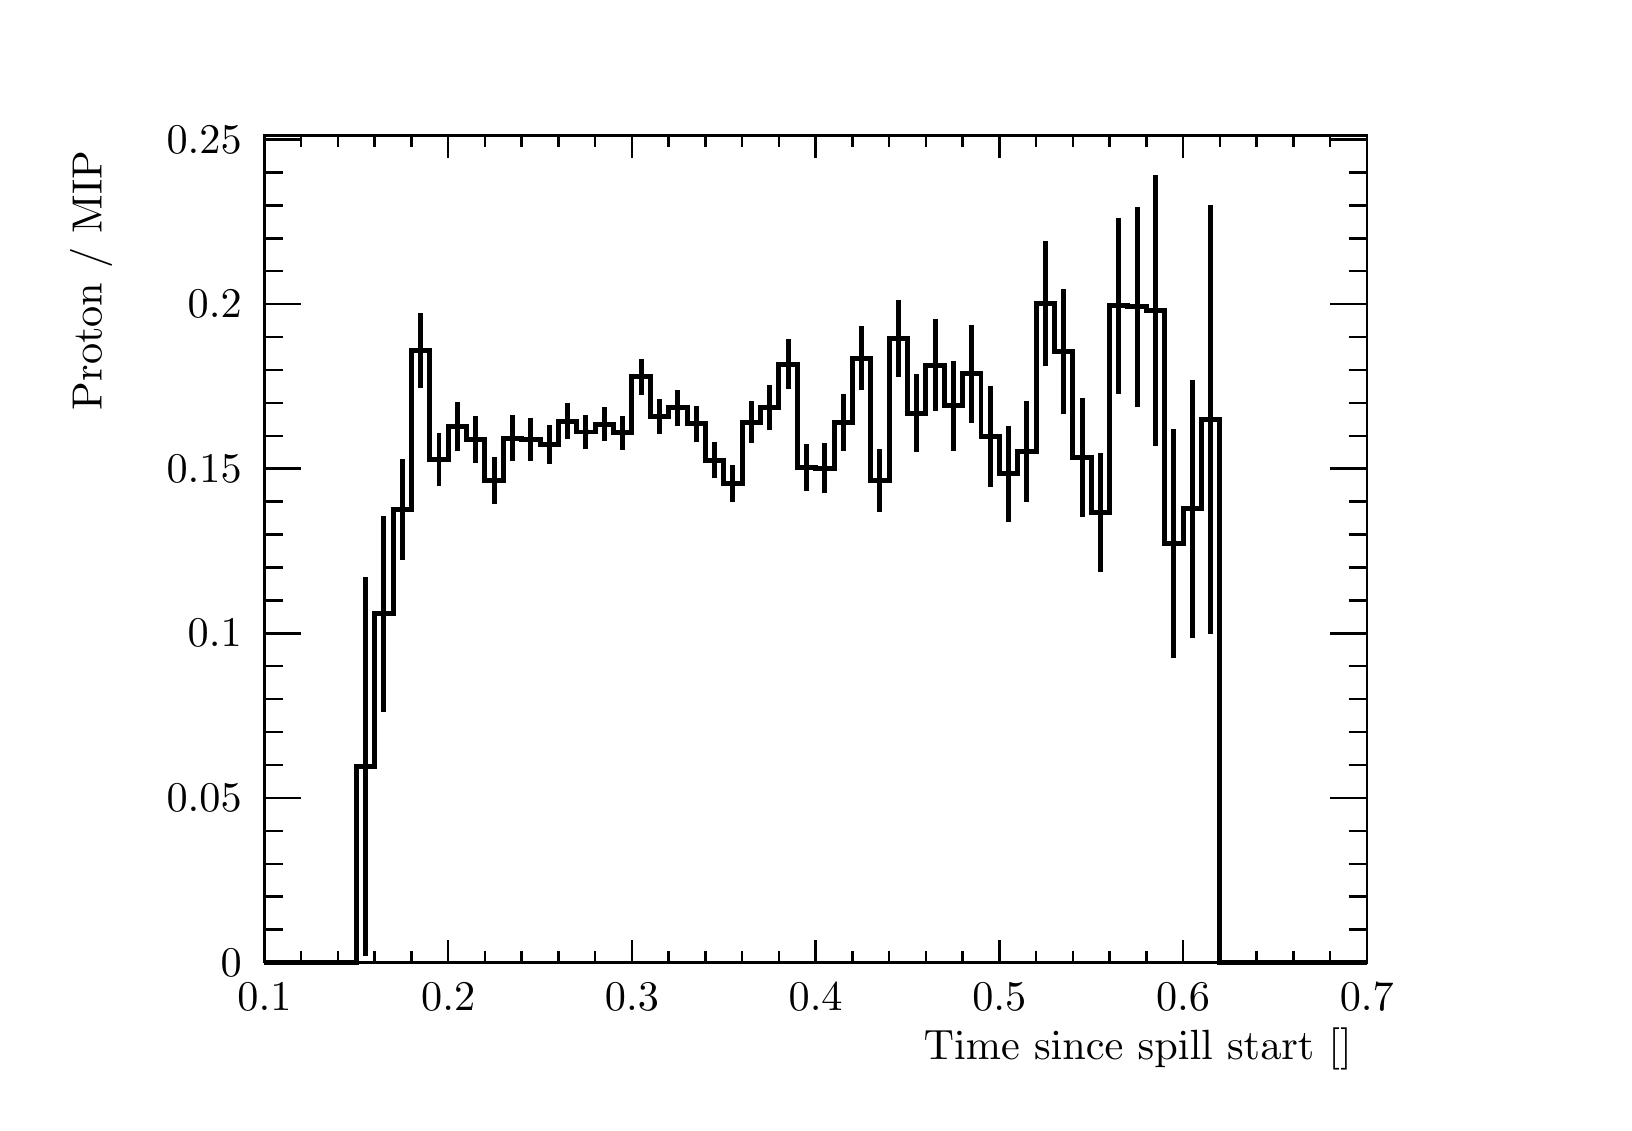
\begin{tikzpicture}
\pgfdeclareplotmark{cross} {
\pgfpathmoveto{\pgfpoint{-0.3\pgfplotmarksize}{\pgfplotmarksize}}
\pgfpathlineto{\pgfpoint{+0.3\pgfplotmarksize}{\pgfplotmarksize}}
\pgfpathlineto{\pgfpoint{+0.3\pgfplotmarksize}{0.3\pgfplotmarksize}}
\pgfpathlineto{\pgfpoint{+1\pgfplotmarksize}{0.3\pgfplotmarksize}}
\pgfpathlineto{\pgfpoint{+1\pgfplotmarksize}{-0.3\pgfplotmarksize}}
\pgfpathlineto{\pgfpoint{+0.3\pgfplotmarksize}{-0.3\pgfplotmarksize}}
\pgfpathlineto{\pgfpoint{+0.3\pgfplotmarksize}{-1.\pgfplotmarksize}}
\pgfpathlineto{\pgfpoint{-0.3\pgfplotmarksize}{-1.\pgfplotmarksize}}
\pgfpathlineto{\pgfpoint{-0.3\pgfplotmarksize}{-0.3\pgfplotmarksize}}
\pgfpathlineto{\pgfpoint{-1.\pgfplotmarksize}{-0.3\pgfplotmarksize}}
\pgfpathlineto{\pgfpoint{-1.\pgfplotmarksize}{0.3\pgfplotmarksize}}
\pgfpathlineto{\pgfpoint{-0.3\pgfplotmarksize}{0.3\pgfplotmarksize}}
\pgfpathclose
\pgfusepathqstroke
}
\pgfdeclareplotmark{cross*} {
\pgfpathmoveto{\pgfpoint{-0.3\pgfplotmarksize}{\pgfplotmarksize}}
\pgfpathlineto{\pgfpoint{+0.3\pgfplotmarksize}{\pgfplotmarksize}}
\pgfpathlineto{\pgfpoint{+0.3\pgfplotmarksize}{0.3\pgfplotmarksize}}
\pgfpathlineto{\pgfpoint{+1\pgfplotmarksize}{0.3\pgfplotmarksize}}
\pgfpathlineto{\pgfpoint{+1\pgfplotmarksize}{-0.3\pgfplotmarksize}}
\pgfpathlineto{\pgfpoint{+0.3\pgfplotmarksize}{-0.3\pgfplotmarksize}}
\pgfpathlineto{\pgfpoint{+0.3\pgfplotmarksize}{-1.\pgfplotmarksize}}
\pgfpathlineto{\pgfpoint{-0.3\pgfplotmarksize}{-1.\pgfplotmarksize}}
\pgfpathlineto{\pgfpoint{-0.3\pgfplotmarksize}{-0.3\pgfplotmarksize}}
\pgfpathlineto{\pgfpoint{-1.\pgfplotmarksize}{-0.3\pgfplotmarksize}}
\pgfpathlineto{\pgfpoint{-1.\pgfplotmarksize}{0.3\pgfplotmarksize}}
\pgfpathlineto{\pgfpoint{-0.3\pgfplotmarksize}{0.3\pgfplotmarksize}}
\pgfpathclose
\pgfusepathqfillstroke
}
\pgfdeclareplotmark{newstar} {
\pgfpathmoveto{\pgfqpoint{0pt}{\pgfplotmarksize}}
\pgfpathlineto{\pgfqpointpolar{44}{0.5\pgfplotmarksize}}
\pgfpathlineto{\pgfqpointpolar{18}{\pgfplotmarksize}}
\pgfpathlineto{\pgfqpointpolar{-20}{0.5\pgfplotmarksize}}
\pgfpathlineto{\pgfqpointpolar{-54}{\pgfplotmarksize}}
\pgfpathlineto{\pgfqpointpolar{-90}{0.5\pgfplotmarksize}}
\pgfpathlineto{\pgfqpointpolar{234}{\pgfplotmarksize}}
\pgfpathlineto{\pgfqpointpolar{198}{0.5\pgfplotmarksize}}
\pgfpathlineto{\pgfqpointpolar{162}{\pgfplotmarksize}}
\pgfpathlineto{\pgfqpointpolar{134}{0.5\pgfplotmarksize}}
\pgfpathclose
\pgfusepathqstroke
}
\pgfdeclareplotmark{newstar*} {
\pgfpathmoveto{\pgfqpoint{0pt}{\pgfplotmarksize}}
\pgfpathlineto{\pgfqpointpolar{44}{0.5\pgfplotmarksize}}
\pgfpathlineto{\pgfqpointpolar{18}{\pgfplotmarksize}}
\pgfpathlineto{\pgfqpointpolar{-20}{0.5\pgfplotmarksize}}
\pgfpathlineto{\pgfqpointpolar{-54}{\pgfplotmarksize}}
\pgfpathlineto{\pgfqpointpolar{-90}{0.5\pgfplotmarksize}}
\pgfpathlineto{\pgfqpointpolar{234}{\pgfplotmarksize}}
\pgfpathlineto{\pgfqpointpolar{198}{0.5\pgfplotmarksize}}
\pgfpathlineto{\pgfqpointpolar{162}{\pgfplotmarksize}}
\pgfpathlineto{\pgfqpointpolar{134}{0.5\pgfplotmarksize}}
\pgfpathclose
\pgfusepathqfillstroke
}
\definecolor{c}{rgb}{1,1,1};
\draw [color=c, fill=c] (0,0) rectangle (20,13.639);
\draw [color=c, fill=c] (3,1.77307) rectangle (17,12.2751);
\definecolor{c}{rgb}{0,0,0};
\draw [c,line width=0.9] (3,1.77307) -- (3,12.2751) -- (17,12.2751) -- (17,1.77307) -- (3,1.77307);
\definecolor{c}{rgb}{1,1,1};
\draw [color=c, fill=c] (3,1.77307) rectangle (17,12.2751);
\definecolor{c}{rgb}{0,0,0};
\draw [c,line width=0.9] (3,1.77307) -- (3,12.2751) -- (17,12.2751) -- (17,1.77307) -- (3,1.77307);
\draw [c,line width=1.8] (4.28333,1.85795) -- (4.28333,4.26597);
\draw [c,line width=1.8] (4.28333,4.26597) -- (4.28333,6.674);
\foreach \P in {(4.28333,4.26597)}{\draw[mark options={color=c,fill=c},mark size=2.402402pt,mark=*,mark size=1pt] plot coordinates {\P};}
\draw [c,line width=1.8] (4.51667,4.95882) -- (4.51667,6.20182);
\draw [c,line width=1.8] (4.51667,6.20182) -- (4.51667,7.44483);
\foreach \P in {(4.51667,6.20182)}{\draw[mark options={color=c,fill=c},mark size=2.402402pt,mark=*,mark size=1pt] plot coordinates {\P};}
\draw [c,line width=1.8] (4.75,6.88558) -- (4.75,7.52999);
\draw [c,line width=1.8] (4.75,7.52999) -- (4.75,8.17441);
\foreach \P in {(4.75,7.52999)}{\draw[mark options={color=c,fill=c},mark size=2.402402pt,mark=*,mark size=1pt] plot coordinates {\P};}
\draw [c,line width=1.8] (4.98333,9.06517) -- (4.98333,9.54667);
\draw [c,line width=1.8] (4.98333,9.54667) -- (4.98333,10.0282);
\foreach \P in {(4.98333,9.54667)}{\draw[mark options={color=c,fill=c},mark size=2.402402pt,mark=*,mark size=1pt] plot coordinates {\P};}
\draw [c,line width=1.8] (5.21667,7.82536) -- (5.21667,8.15941);
\draw [c,line width=1.8] (5.21667,8.15941) -- (5.21667,8.49346);
\foreach \P in {(5.21667,8.15941)}{\draw[mark options={color=c,fill=c},mark size=2.402402pt,mark=*,mark size=1pt] plot coordinates {\P};}
\draw [c,line width=1.8] (5.45,8.26867) -- (5.45,8.57816);
\draw [c,line width=1.8] (5.45,8.57816) -- (5.45,8.88765);
\foreach \P in {(5.45,8.57816)}{\draw[mark options={color=c,fill=c},mark size=2.402402pt,mark=*,mark size=1pt] plot coordinates {\P};}
\draw [c,line width=1.8] (5.68333,8.11213) -- (5.68333,8.41069);
\draw [c,line width=1.8] (5.68333,8.41069) -- (5.68333,8.70926);
\foreach \P in {(5.68333,8.41069)}{\draw[mark options={color=c,fill=c},mark size=2.402402pt,mark=*,mark size=1pt] plot coordinates {\P};}
\draw [c,line width=1.8] (5.91667,7.59665) -- (5.91667,7.89397);
\draw [c,line width=1.8] (5.91667,7.89397) -- (5.91667,8.19129);
\foreach \P in {(5.91667,7.89397)}{\draw[mark options={color=c,fill=c},mark size=2.402402pt,mark=*,mark size=1pt] plot coordinates {\P};}
\draw [c,line width=1.8] (6.15,8.14152) -- (6.15,8.43263);
\draw [c,line width=1.8] (6.15,8.43263) -- (6.15,8.72374);
\foreach \P in {(6.15,8.43263)}{\draw[mark options={color=c,fill=c},mark size=2.402402pt,mark=*,mark size=1pt] plot coordinates {\P};}
\draw [c,line width=1.8] (6.38333,8.14559) -- (6.38333,8.41426);
\draw [c,line width=1.8] (6.38333,8.41426) -- (6.38333,8.68294);
\foreach \P in {(6.38333,8.41426)}{\draw[mark options={color=c,fill=c},mark size=2.402402pt,mark=*,mark size=1pt] plot coordinates {\P};}
\draw [c,line width=1.8] (6.61667,8.09959) -- (6.61667,8.34791);
\draw [c,line width=1.8] (6.61667,8.34791) -- (6.61667,8.59622);
\foreach \P in {(6.61667,8.34791)}{\draw[mark options={color=c,fill=c},mark size=2.402402pt,mark=*,mark size=1pt] plot coordinates {\P};}
\draw [c,line width=1.8] (6.85,8.41637) -- (6.85,8.64916);
\draw [c,line width=1.8] (6.85,8.64916) -- (6.85,8.88195);
\foreach \P in {(6.85,8.64916)}{\draw[mark options={color=c,fill=c},mark size=2.402402pt,mark=*,mark size=1pt] plot coordinates {\P};}
\draw [c,line width=1.8] (7.08333,8.28923) -- (7.08333,8.51105);
\draw [c,line width=1.8] (7.08333,8.51105) -- (7.08333,8.73287);
\foreach \P in {(7.08333,8.51105)}{\draw[mark options={color=c,fill=c},mark size=2.402402pt,mark=*,mark size=1pt] plot coordinates {\P};}
\draw [c,line width=1.8] (7.31667,8.39124) -- (7.31667,8.60961);
\draw [c,line width=1.8] (7.31667,8.60961) -- (7.31667,8.82799);
\foreach \P in {(7.31667,8.60961)}{\draw[mark options={color=c,fill=c},mark size=2.402402pt,mark=*,mark size=1pt] plot coordinates {\P};}
\draw [c,line width=1.8] (7.55,8.28584) -- (7.55,8.49863);
\draw [c,line width=1.8] (7.55,8.49863) -- (7.55,8.71142);
\foreach \P in {(7.55,8.49863)}{\draw[mark options={color=c,fill=c},mark size=2.402402pt,mark=*,mark size=1pt] plot coordinates {\P};}
\draw [c,line width=1.8] (7.78333,8.98351) -- (7.78333,9.21265);
\draw [c,line width=1.8] (7.78333,9.21265) -- (7.78333,9.44178);
\foreach \P in {(7.78333,9.21265)}{\draw[mark options={color=c,fill=c},mark size=2.402402pt,mark=*,mark size=1pt] plot coordinates {\P};}
\draw [c,line width=1.8] (8.01667,8.47948) -- (8.01667,8.70265);
\draw [c,line width=1.8] (8.01667,8.70265) -- (8.01667,8.92583);
\foreach \P in {(8.01667,8.70265)}{\draw[mark options={color=c,fill=c},mark size=2.402402pt,mark=*,mark size=1pt] plot coordinates {\P};}
\draw [c,line width=1.8] (8.25,8.58929) -- (8.25,8.81786);
\draw [c,line width=1.8] (8.25,8.81786) -- (8.25,9.04643);
\foreach \P in {(8.25,8.81786)}{\draw[mark options={color=c,fill=c},mark size=2.402402pt,mark=*,mark size=1pt] plot coordinates {\P};}
\draw [c,line width=1.8] (8.48333,8.38024) -- (8.48333,8.61365);
\draw [c,line width=1.8] (8.48333,8.61365) -- (8.48333,8.84705);
\foreach \P in {(8.48333,8.61365)}{\draw[mark options={color=c,fill=c},mark size=2.402402pt,mark=*,mark size=1pt] plot coordinates {\P};}
\draw [c,line width=1.8] (8.71667,7.9206) -- (8.71667,8.15484);
\draw [c,line width=1.8] (8.71667,8.15484) -- (8.71667,8.38908);
\foreach \P in {(8.71667,8.15484)}{\draw[mark options={color=c,fill=c},mark size=2.402402pt,mark=*,mark size=1pt] plot coordinates {\P};}
\draw [c,line width=1.8] (8.95,7.62004) -- (8.95,7.85569);
\draw [c,line width=1.8] (8.95,7.85569) -- (8.95,8.09134);
\foreach \P in {(8.95,7.85569)}{\draw[mark options={color=c,fill=c},mark size=2.402402pt,mark=*,mark size=1pt] plot coordinates {\P};}
\draw [c,line width=1.8] (9.18333,8.36926) -- (9.18333,8.63709);
\draw [c,line width=1.8] (9.18333,8.63709) -- (9.18333,8.90492);
\foreach \P in {(9.18333,8.63709)}{\draw[mark options={color=c,fill=c},mark size=2.402402pt,mark=*,mark size=1pt] plot coordinates {\P};}
\draw [c,line width=1.8] (9.41667,8.53941) -- (9.41667,8.82537);
\draw [c,line width=1.8] (9.41667,8.82537) -- (9.41667,9.11132);
\foreach \P in {(9.41667,8.82537)}{\draw[mark options={color=c,fill=c},mark size=2.402402pt,mark=*,mark size=1pt] plot coordinates {\P};}
\draw [c,line width=1.8] (9.65,9.05386) -- (9.65,9.36986);
\draw [c,line width=1.8] (9.65,9.36986) -- (9.65,9.68587);
\foreach \P in {(9.65,9.36986)}{\draw[mark options={color=c,fill=c},mark size=2.402402pt,mark=*,mark size=1pt] plot coordinates {\P};}
\draw [c,line width=1.8] (9.88333,7.76146) -- (9.88333,8.06142);
\draw [c,line width=1.8] (9.88333,8.06142) -- (9.88333,8.36138);
\foreach \P in {(9.88333,8.06142)}{\draw[mark options={color=c,fill=c},mark size=2.402402pt,mark=*,mark size=1pt] plot coordinates {\P};}
\draw [c,line width=1.8] (10.1167,7.73575) -- (10.1167,8.05126);
\draw [c,line width=1.8] (10.1167,8.05126) -- (10.1167,8.36676);
\foreach \P in {(10.1167,8.05126)}{\draw[mark options={color=c,fill=c},mark size=2.402402pt,mark=*,mark size=1pt] plot coordinates {\P};}
\draw [c,line width=1.8] (10.35,8.2671) -- (10.35,8.63019);
\draw [c,line width=1.8] (10.35,8.63019) -- (10.35,8.99327);
\foreach \P in {(10.35,8.63019)}{\draw[mark options={color=c,fill=c},mark size=2.402402pt,mark=*,mark size=1pt] plot coordinates {\P};}
\draw [c,line width=1.8] (10.5833,9.04507) -- (10.5833,9.44879);
\draw [c,line width=1.8] (10.5833,9.44879) -- (10.5833,9.85251);
\foreach \P in {(10.5833,9.44879)}{\draw[mark options={color=c,fill=c},mark size=2.402402pt,mark=*,mark size=1pt] plot coordinates {\P};}
\draw [c,line width=1.8] (10.8167,7.50104) -- (10.8167,7.89536);
\draw [c,line width=1.8] (10.8167,7.89536) -- (10.8167,8.28967);
\foreach \P in {(10.8167,7.89536)}{\draw[mark options={color=c,fill=c},mark size=2.402402pt,mark=*,mark size=1pt] plot coordinates {\P};}
\draw [c,line width=1.8] (11.05,9.21278) -- (11.05,9.7027);
\draw [c,line width=1.8] (11.05,9.7027) -- (11.05,10.1926);
\foreach \P in {(11.05,9.7027)}{\draw[mark options={color=c,fill=c},mark size=2.402402pt,mark=*,mark size=1pt] plot coordinates {\P};}
\draw [c,line width=1.8] (11.2833,8.25238) -- (11.2833,8.74718);
\draw [c,line width=1.8] (11.2833,8.74718) -- (11.2833,9.24198);
\foreach \P in {(11.2833,8.74718)}{\draw[mark options={color=c,fill=c},mark size=2.402402pt,mark=*,mark size=1pt] plot coordinates {\P};}
\draw [c,line width=1.8] (11.5167,8.77527) -- (11.5167,9.35802);
\draw [c,line width=1.8] (11.5167,9.35802) -- (11.5167,9.94076);
\foreach \P in {(11.5167,9.35802)}{\draw[mark options={color=c,fill=c},mark size=2.402402pt,mark=*,mark size=1pt] plot coordinates {\P};}
\draw [c,line width=1.8] (11.75,8.27462) -- (11.75,8.84624);
\draw [c,line width=1.8] (11.75,8.84624) -- (11.75,9.41786);
\foreach \P in {(11.75,8.84624)}{\draw[mark options={color=c,fill=c},mark size=2.402402pt,mark=*,mark size=1pt] plot coordinates {\P};}
\draw [c,line width=1.8] (11.9833,8.63141) -- (11.9833,9.2513);
\draw [c,line width=1.8] (11.9833,9.2513) -- (11.9833,9.8712);
\foreach \P in {(11.9833,9.2513)}{\draw[mark options={color=c,fill=c},mark size=2.402402pt,mark=*,mark size=1pt] plot coordinates {\P};}
\draw [c,line width=1.8] (12.2167,7.81775) -- (12.2167,8.45422);
\draw [c,line width=1.8] (12.2167,8.45422) -- (12.2167,9.09069);
\foreach \P in {(12.2167,8.45422)}{\draw[mark options={color=c,fill=c},mark size=2.402402pt,mark=*,mark size=1pt] plot coordinates {\P};}
\draw [c,line width=1.8] (12.45,7.36943) -- (12.45,7.97822);
\draw [c,line width=1.8] (12.45,7.97822) -- (12.45,8.58701);
\foreach \P in {(12.45,7.97822)}{\draw[mark options={color=c,fill=c},mark size=2.402402pt,mark=*,mark size=1pt] plot coordinates {\P};}
\draw [c,line width=1.8] (12.6833,7.61971) -- (12.6833,8.26531);
\draw [c,line width=1.8] (12.6833,8.26531) -- (12.6833,8.91091);
\foreach \P in {(12.6833,8.26531)}{\draw[mark options={color=c,fill=c},mark size=2.402402pt,mark=*,mark size=1pt] plot coordinates {\P};}
\draw [c,line width=1.8] (12.9167,9.34774) -- (12.9167,10.144);
\draw [c,line width=1.8] (12.9167,10.144) -- (12.9167,10.9402);
\foreach \P in {(12.9167,10.144)}{\draw[mark options={color=c,fill=c},mark size=2.402402pt,mark=*,mark size=1pt] plot coordinates {\P};}
\draw [c,line width=1.8] (13.15,8.74157) -- (13.15,9.53696);
\draw [c,line width=1.8] (13.15,9.53696) -- (13.15,10.3324);
\foreach \P in {(13.15,9.53696)}{\draw[mark options={color=c,fill=c},mark size=2.402402pt,mark=*,mark size=1pt] plot coordinates {\P};}
\draw [c,line width=1.8] (13.3833,7.43321) -- (13.3833,8.1871);
\draw [c,line width=1.8] (13.3833,8.1871) -- (13.3833,8.941);
\foreach \P in {(13.3833,8.1871)}{\draw[mark options={color=c,fill=c},mark size=2.402402pt,mark=*,mark size=1pt] plot coordinates {\P};}
\draw [c,line width=1.8] (13.6167,6.72893) -- (13.6167,7.48532);
\draw [c,line width=1.8] (13.6167,7.48532) -- (13.6167,8.2417);
\foreach \P in {(13.6167,7.48532)}{\draw[mark options={color=c,fill=c},mark size=2.402402pt,mark=*,mark size=1pt] plot coordinates {\P};}
\draw [c,line width=1.8] (13.85,8.99665) -- (13.85,10.1133);
\draw [c,line width=1.8] (13.85,10.1133) -- (13.85,11.2299);
\foreach \P in {(13.85,10.1133)}{\draw[mark options={color=c,fill=c},mark size=2.402402pt,mark=*,mark size=1pt] plot coordinates {\P};}
\draw [c,line width=1.8] (14.0833,8.83049) -- (14.0833,10.1011);
\draw [c,line width=1.8] (14.0833,10.1011) -- (14.0833,11.3716);
\foreach \P in {(14.0833,10.1011)}{\draw[mark options={color=c,fill=c},mark size=2.402402pt,mark=*,mark size=1pt] plot coordinates {\P};}
\draw [c,line width=1.8] (14.3167,8.33544) -- (14.3167,10.0552);
\draw [c,line width=1.8] (14.3167,10.0552) -- (14.3167,11.775);
\foreach \P in {(14.3167,10.0552)}{\draw[mark options={color=c,fill=c},mark size=2.402402pt,mark=*,mark size=1pt] plot coordinates {\P};}
\draw [c,line width=1.8] (14.55,5.64668) -- (14.55,7.09824);
\draw [c,line width=1.8] (14.55,7.09824) -- (14.55,8.5498);
\foreach \P in {(14.55,7.09824)}{\draw[mark options={color=c,fill=c},mark size=2.402402pt,mark=*,mark size=1pt] plot coordinates {\P};}
\draw [c,line width=1.8] (14.7833,5.89349) -- (14.7833,7.53431);
\draw [c,line width=1.8] (14.7833,7.53431) -- (14.7833,9.17514);
\foreach \P in {(14.7833,7.53431)}{\draw[mark options={color=c,fill=c},mark size=2.402402pt,mark=*,mark size=1pt] plot coordinates {\P};}
\draw [c,line width=1.8] (15.0167,5.94687) -- (15.0167,8.6719);
\draw [c,line width=1.8] (15.0167,8.6719) -- (15.0167,11.3969);
\foreach \P in {(15.0167,8.6719)}{\draw[mark options={color=c,fill=c},mark size=2.402402pt,mark=*,mark size=1pt] plot coordinates {\P};}
\draw [c,line width=1.8] (3,1.77307) -- (3.23333,1.77307) -- (3.23333,1.77307) -- (3.46667,1.77307) -- (3.46667,1.77307) -- (3.7,1.77307) -- (3.7,1.77307) -- (3.93333,1.77307) -- (3.93333,1.77307) -- (4.16667,1.77307) -- (4.16667,4.26597) --
 (4.4,4.26597) -- (4.4,6.20182) -- (4.63333,6.20182) -- (4.63333,7.52999) -- (4.86667,7.52999) -- (4.86667,9.54667) -- (5.1,9.54667) -- (5.1,8.15941) -- (5.33333,8.15941) -- (5.33333,8.57816) -- (5.56667,8.57816) -- (5.56667,8.41069) -- (5.8,8.41069)
 -- (5.8,7.89397) -- (6.03333,7.89397) -- (6.03333,8.43263) -- (6.26667,8.43263) -- (6.26667,8.41426) -- (6.5,8.41426) -- (6.5,8.34791) -- (6.73333,8.34791) -- (6.73333,8.64916) -- (6.96667,8.64916) -- (6.96667,8.51105) -- (7.2,8.51105) --
 (7.2,8.60961) -- (7.43333,8.60961) -- (7.43333,8.49863) -- (7.66667,8.49863) -- (7.66667,9.21265) -- (7.9,9.21265) -- (7.9,8.70265) -- (8.13333,8.70265) -- (8.13333,8.81786) -- (8.36667,8.81786) -- (8.36667,8.61365) -- (8.6,8.61365) -- (8.6,8.15484)
 -- (8.83333,8.15484) -- (8.83333,7.85569) -- (9.06667,7.85569) -- (9.06667,8.63709) -- (9.3,8.63709) -- (9.3,8.82537) -- (9.53333,8.82537) -- (9.53333,9.36986) -- (9.76667,9.36986) -- (9.76667,8.06142) -- (10,8.06142) -- (10,8.05126) --
 (10.2333,8.05126) -- (10.2333,8.63019) -- (10.4667,8.63019) -- (10.4667,9.44879) -- (10.7,9.44879) -- (10.7,7.89536) -- (10.9333,7.89536) -- (10.9333,9.7027) -- (11.1667,9.7027) -- (11.1667,8.74718) -- (11.4,8.74718) -- (11.4,9.35802) --
 (11.6333,9.35802) -- (11.6333,8.84624) -- (11.8667,8.84624) -- (11.8667,9.2513) -- (12.1,9.2513) -- (12.1,8.45422) -- (12.3333,8.45422) -- (12.3333,7.97822) -- (12.5667,7.97822) -- (12.5667,8.26531) -- (12.8,8.26531) -- (12.8,10.144) --
 (13.0333,10.144) -- (13.0333,9.53696) -- (13.2667,9.53696) -- (13.2667,8.1871) -- (13.5,8.1871) -- (13.5,7.48532) -- (13.7333,7.48532) -- (13.7333,10.1133) -- (13.9667,10.1133) -- (13.9667,10.1011) -- (14.2,10.1011) -- (14.2,10.0552) --
 (14.4333,10.0552) -- (14.4333,7.09824) -- (14.6667,7.09824) -- (14.6667,7.53431) -- (14.9,7.53431) -- (14.9,8.6719) -- (15.1333,8.6719) -- (15.1333,1.77307) -- (15.3667,1.77307) -- (15.3667,1.77307) -- (15.6,1.77307) -- (15.6,1.77307) --
 (15.8333,1.77307) -- (15.8333,1.77307) -- (16.0667,1.77307) -- (16.0667,1.77307) -- (16.3,1.77307) -- (16.3,1.77307) -- (16.5333,1.77307) -- (16.5333,1.77307) -- (16.7667,1.77307) -- (16.7667,1.77307) -- (17,1.77307);
\draw [c,line width=0.9] (3,1.77307) -- (17,1.77307);
\draw [c,line width=0.9] (3,2.05948) -- (3,1.77307);
\draw [c,line width=0.9] (3.46667,1.91628) -- (3.46667,1.77307);
\draw [c,line width=0.9] (3.93333,1.91628) -- (3.93333,1.77307);
\draw [c,line width=0.9] (4.4,1.91628) -- (4.4,1.77307);
\draw [c,line width=0.9] (4.86667,1.91628) -- (4.86667,1.77307);
\draw [c,line width=0.9] (5.33333,2.05948) -- (5.33333,1.77307);
\draw [c,line width=0.9] (5.8,1.91628) -- (5.8,1.77307);
\draw [c,line width=0.9] (6.26667,1.91628) -- (6.26667,1.77307);
\draw [c,line width=0.9] (6.73333,1.91628) -- (6.73333,1.77307);
\draw [c,line width=0.9] (7.2,1.91628) -- (7.2,1.77307);
\draw [c,line width=0.9] (7.66667,2.05948) -- (7.66667,1.77307);
\draw [c,line width=0.9] (8.13333,1.91628) -- (8.13333,1.77307);
\draw [c,line width=0.9] (8.6,1.91628) -- (8.6,1.77307);
\draw [c,line width=0.9] (9.06667,1.91628) -- (9.06667,1.77307);
\draw [c,line width=0.9] (9.53333,1.91628) -- (9.53333,1.77307);
\draw [c,line width=0.9] (10,2.05948) -- (10,1.77307);
\draw [c,line width=0.9] (10.4667,1.91628) -- (10.4667,1.77307);
\draw [c,line width=0.9] (10.9333,1.91628) -- (10.9333,1.77307);
\draw [c,line width=0.9] (11.4,1.91628) -- (11.4,1.77307);
\draw [c,line width=0.9] (11.8667,1.91628) -- (11.8667,1.77307);
\draw [c,line width=0.9] (12.3333,2.05948) -- (12.3333,1.77307);
\draw [c,line width=0.9] (12.8,1.91628) -- (12.8,1.77307);
\draw [c,line width=0.9] (13.2667,1.91628) -- (13.2667,1.77307);
\draw [c,line width=0.9] (13.7333,1.91628) -- (13.7333,1.77307);
\draw [c,line width=0.9] (14.2,1.91628) -- (14.2,1.77307);
\draw [c,line width=0.9] (14.6667,2.05948) -- (14.6667,1.77307);
\draw [c,line width=0.9] (15.1333,1.91628) -- (15.1333,1.77307);
\draw [c,line width=0.9] (15.6,1.91628) -- (15.6,1.77307);
\draw [c,line width=0.9] (16.0667,1.91628) -- (16.0667,1.77307);
\draw [c,line width=0.9] (16.5333,1.91628) -- (16.5333,1.77307);
\draw [c,line width=0.9] (17,2.05948) -- (17,1.77307);
\draw [c,line width=0.9] (17,2.05948) -- (17,1.77307);
\draw [anchor=base] (3,1.15931) node[scale=1.52731, color=c, rotate=0]{0.1};
\draw [anchor=base] (5.33333,1.15931) node[scale=1.52731, color=c, rotate=0]{0.2};
\draw [anchor=base] (7.66667,1.15931) node[scale=1.52731, color=c, rotate=0]{0.3};
\draw [anchor=base] (10,1.15931) node[scale=1.52731, color=c, rotate=0]{0.4};
\draw [anchor=base] (12.3333,1.15931) node[scale=1.52731, color=c, rotate=0]{0.5};
\draw [anchor=base] (14.6667,1.15931) node[scale=1.52731, color=c, rotate=0]{0.6};
\draw [anchor=base] (17,1.15931) node[scale=1.52731, color=c, rotate=0]{0.7};
\draw [anchor= east] (17,0.681948) node[scale=1.52731, color=c, rotate=0]{ Time since spill start [\si{\nano\second}]};
\draw [c,line width=0.9] (3,12.2751) -- (17,12.2751);
\draw [c,line width=0.9] (3,11.9887) -- (3,12.2751);
\draw [c,line width=0.9] (3.46667,12.1319) -- (3.46667,12.2751);
\draw [c,line width=0.9] (3.93333,12.1319) -- (3.93333,12.2751);
\draw [c,line width=0.9] (4.4,12.1319) -- (4.4,12.2751);
\draw [c,line width=0.9] (4.86667,12.1319) -- (4.86667,12.2751);
\draw [c,line width=0.9] (5.33333,11.9887) -- (5.33333,12.2751);
\draw [c,line width=0.9] (5.8,12.1319) -- (5.8,12.2751);
\draw [c,line width=0.9] (6.26667,12.1319) -- (6.26667,12.2751);
\draw [c,line width=0.9] (6.73333,12.1319) -- (6.73333,12.2751);
\draw [c,line width=0.9] (7.2,12.1319) -- (7.2,12.2751);
\draw [c,line width=0.9] (7.66667,11.9887) -- (7.66667,12.2751);
\draw [c,line width=0.9] (8.13333,12.1319) -- (8.13333,12.2751);
\draw [c,line width=0.9] (8.6,12.1319) -- (8.6,12.2751);
\draw [c,line width=0.9] (9.06667,12.1319) -- (9.06667,12.2751);
\draw [c,line width=0.9] (9.53333,12.1319) -- (9.53333,12.2751);
\draw [c,line width=0.9] (10,11.9887) -- (10,12.2751);
\draw [c,line width=0.9] (10.4667,12.1319) -- (10.4667,12.2751);
\draw [c,line width=0.9] (10.9333,12.1319) -- (10.9333,12.2751);
\draw [c,line width=0.9] (11.4,12.1319) -- (11.4,12.2751);
\draw [c,line width=0.9] (11.8667,12.1319) -- (11.8667,12.2751);
\draw [c,line width=0.9] (12.3333,11.9887) -- (12.3333,12.2751);
\draw [c,line width=0.9] (12.8,12.1319) -- (12.8,12.2751);
\draw [c,line width=0.9] (13.2667,12.1319) -- (13.2667,12.2751);
\draw [c,line width=0.9] (13.7333,12.1319) -- (13.7333,12.2751);
\draw [c,line width=0.9] (14.2,12.1319) -- (14.2,12.2751);
\draw [c,line width=0.9] (14.6667,11.9887) -- (14.6667,12.2751);
\draw [c,line width=0.9] (15.1333,12.1319) -- (15.1333,12.2751);
\draw [c,line width=0.9] (15.6,12.1319) -- (15.6,12.2751);
\draw [c,line width=0.9] (16.0667,12.1319) -- (16.0667,12.2751);
\draw [c,line width=0.9] (16.5333,12.1319) -- (16.5333,12.2751);
\draw [c,line width=0.9] (17,11.9887) -- (17,12.2751);
\draw [c,line width=0.9] (17,11.9887) -- (17,12.2751);
\draw [c,line width=0.9] (3,1.77307) -- (3,12.2751);
\draw [c,line width=0.9] (3.462,1.77307) -- (3,1.77307);
\draw [c,line width=0.9] (3.231,2.19118) -- (3,2.19118);
\draw [c,line width=0.9] (3.231,2.60929) -- (3,2.60929);
\draw [c,line width=0.9] (3.231,3.0274) -- (3,3.0274);
\draw [c,line width=0.9] (3.231,3.44551) -- (3,3.44551);
\draw [c,line width=0.9] (3.462,3.86362) -- (3,3.86362);
\draw [c,line width=0.9] (3.231,4.28173) -- (3,4.28173);
\draw [c,line width=0.9] (3.231,4.69984) -- (3,4.69984);
\draw [c,line width=0.9] (3.231,5.11795) -- (3,5.11795);
\draw [c,line width=0.9] (3.231,5.53606) -- (3,5.53606);
\draw [c,line width=0.9] (3.462,5.95417) -- (3,5.95417);
\draw [c,line width=0.9] (3.231,6.37228) -- (3,6.37228);
\draw [c,line width=0.9] (3.231,6.79039) -- (3,6.79039);
\draw [c,line width=0.9] (3.231,7.2085) -- (3,7.2085);
\draw [c,line width=0.9] (3.231,7.62661) -- (3,7.62661);
\draw [c,line width=0.9] (3.462,8.04472) -- (3,8.04472);
\draw [c,line width=0.9] (3.231,8.46283) -- (3,8.46283);
\draw [c,line width=0.9] (3.231,8.88094) -- (3,8.88094);
\draw [c,line width=0.9] (3.231,9.29905) -- (3,9.29905);
\draw [c,line width=0.9] (3.231,9.71716) -- (3,9.71716);
\draw [c,line width=0.9] (3.462,10.1353) -- (3,10.1353);
\draw [c,line width=0.9] (3.231,10.5534) -- (3,10.5534);
\draw [c,line width=0.9] (3.231,10.9715) -- (3,10.9715);
\draw [c,line width=0.9] (3.231,11.3896) -- (3,11.3896);
\draw [c,line width=0.9] (3.231,11.8077) -- (3,11.8077);
\draw [c,line width=0.9] (3.462,12.2258) -- (3,12.2258);
\draw [c,line width=0.9] (3.462,12.2258) -- (3,12.2258);
\draw [anchor= east] (2.9,1.77307) node[scale=1.52731, color=c, rotate=0]{0};
\draw [anchor= east] (2.9,3.86362) node[scale=1.52731, color=c, rotate=0]{0.05};
\draw [anchor= east] (2.9,5.95417) node[scale=1.52731, color=c, rotate=0]{0.1};
\draw [anchor= east] (2.9,8.04472) node[scale=1.52731, color=c, rotate=0]{0.15};
\draw [anchor= east] (2.9,10.1353) node[scale=1.52731, color=c, rotate=0]{0.2};
\draw [anchor= east] (2.9,12.2258) node[scale=1.52731, color=c, rotate=0]{0.25};
\draw [anchor= east] (0.796562,12.2751) node[scale=1.52731, color=c, rotate=90]{ Proton / MIP};
\draw [c,line width=0.9] (17,1.77307) -- (17,12.2751);
\draw [c,line width=0.9] (16.538,1.77307) -- (17,1.77307);
\draw [c,line width=0.9] (16.769,2.19118) -- (17,2.19118);
\draw [c,line width=0.9] (16.769,2.60929) -- (17,2.60929);
\draw [c,line width=0.9] (16.769,3.0274) -- (17,3.0274);
\draw [c,line width=0.9] (16.769,3.44551) -- (17,3.44551);
\draw [c,line width=0.9] (16.538,3.86362) -- (17,3.86362);
\draw [c,line width=0.9] (16.769,4.28173) -- (17,4.28173);
\draw [c,line width=0.9] (16.769,4.69984) -- (17,4.69984);
\draw [c,line width=0.9] (16.769,5.11795) -- (17,5.11795);
\draw [c,line width=0.9] (16.769,5.53606) -- (17,5.53606);
\draw [c,line width=0.9] (16.538,5.95417) -- (17,5.95417);
\draw [c,line width=0.9] (16.769,6.37228) -- (17,6.37228);
\draw [c,line width=0.9] (16.769,6.79039) -- (17,6.79039);
\draw [c,line width=0.9] (16.769,7.2085) -- (17,7.2085);
\draw [c,line width=0.9] (16.769,7.62661) -- (17,7.62661);
\draw [c,line width=0.9] (16.538,8.04472) -- (17,8.04472);
\draw [c,line width=0.9] (16.769,8.46283) -- (17,8.46283);
\draw [c,line width=0.9] (16.769,8.88094) -- (17,8.88094);
\draw [c,line width=0.9] (16.769,9.29905) -- (17,9.29905);
\draw [c,line width=0.9] (16.769,9.71716) -- (17,9.71716);
\draw [c,line width=0.9] (16.538,10.1353) -- (17,10.1353);
\draw [c,line width=0.9] (16.769,10.5534) -- (17,10.5534);
\draw [c,line width=0.9] (16.769,10.9715) -- (17,10.9715);
\draw [c,line width=0.9] (16.769,11.3896) -- (17,11.3896);
\draw [c,line width=0.9] (16.769,11.8077) -- (17,11.8077);
\draw [c,line width=0.9] (16.538,12.2258) -- (17,12.2258);
\draw [c,line width=0.9] (16.538,12.2258) -- (17,12.2258);
\definecolor{c}{rgb}{1,1,1};
\draw [color=c, fill=c] (2,12.8206) rectangle (18,13.5708);
\definecolor{c}{rgb}{0,0,0};
%\draw (10,13.1957) node[scale=1.40004, color=c, rotate=0]{2 blocks: Proton/MIP};
\end{tikzpicture}

  \end{adjustbox}
  \caption[Proton/MIP ratio as a function of time since spill start]{Proton/MIP ratio as a function of time since spill start for 2 moderator block data.}
  \label{fig:proMipRatio}
\end{figure}

The relationship between the number of $\SOne-\STwo$ hits in the two DAQs for various numbers of moderator blocks is shown in \citefig{fig:s1s2DeadtimeComp}.
Here the horizontal axis displays the number of $\SOne-\STwo$ signals recorded by the DToF DAQ for a given beam spill, $(\SOne\STwo)_{\text{DToF}}$.
Similarly, $(\SOne\STwo)_{\text{UToF}}$ is the number of $\SOne-\STwo$ signals recorded by the UToF DAQ in the same spill.
Each of these distributions has a polynomial of the form
\begin{equation}
  (\SOne\STwo)_{\text{UToF}}/(\SOne\STwo)_{\text{DToF}} = p0 \times (\SOne\STwo)_{\text{DToF}} + p1
\end{equation}
fitted where $p0$ and $p1$ are the parameters to be determined.

\begin{figure}[t]
  \begin{subfigure}[t]{.5\textwidth}
    \begin{adjustbox}{max totalsize=\textwidth, center}
      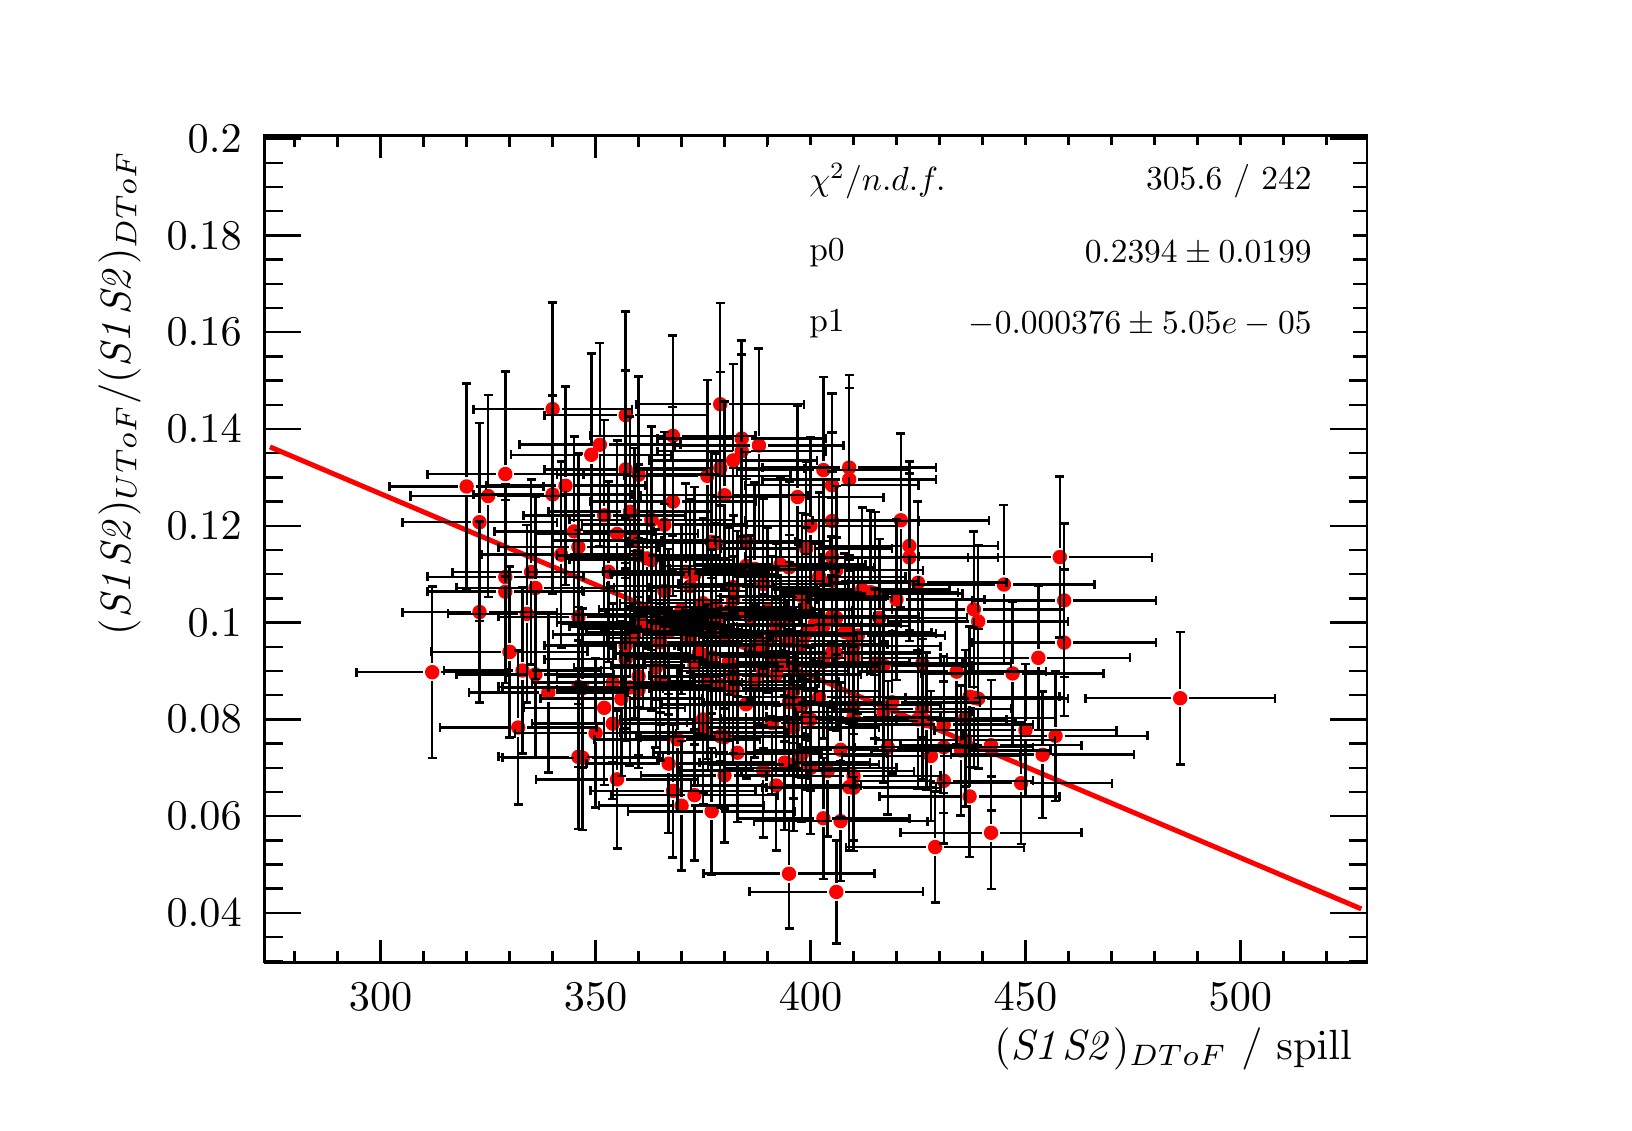
\begin{tikzpicture}
\pgfdeclareplotmark{cross} {
\pgfpathmoveto{\pgfpoint{-0.3\pgfplotmarksize}{\pgfplotmarksize}}
\pgfpathlineto{\pgfpoint{+0.3\pgfplotmarksize}{\pgfplotmarksize}}
\pgfpathlineto{\pgfpoint{+0.3\pgfplotmarksize}{0.3\pgfplotmarksize}}
\pgfpathlineto{\pgfpoint{+1\pgfplotmarksize}{0.3\pgfplotmarksize}}
\pgfpathlineto{\pgfpoint{+1\pgfplotmarksize}{-0.3\pgfplotmarksize}}
\pgfpathlineto{\pgfpoint{+0.3\pgfplotmarksize}{-0.3\pgfplotmarksize}}
\pgfpathlineto{\pgfpoint{+0.3\pgfplotmarksize}{-1.\pgfplotmarksize}}
\pgfpathlineto{\pgfpoint{-0.3\pgfplotmarksize}{-1.\pgfplotmarksize}}
\pgfpathlineto{\pgfpoint{-0.3\pgfplotmarksize}{-0.3\pgfplotmarksize}}
\pgfpathlineto{\pgfpoint{-1.\pgfplotmarksize}{-0.3\pgfplotmarksize}}
\pgfpathlineto{\pgfpoint{-1.\pgfplotmarksize}{0.3\pgfplotmarksize}}
\pgfpathlineto{\pgfpoint{-0.3\pgfplotmarksize}{0.3\pgfplotmarksize}}
\pgfpathclose
\pgfusepathqstroke
}
\pgfdeclareplotmark{cross*} {
\pgfpathmoveto{\pgfpoint{-0.3\pgfplotmarksize}{\pgfplotmarksize}}
\pgfpathlineto{\pgfpoint{+0.3\pgfplotmarksize}{\pgfplotmarksize}}
\pgfpathlineto{\pgfpoint{+0.3\pgfplotmarksize}{0.3\pgfplotmarksize}}
\pgfpathlineto{\pgfpoint{+1\pgfplotmarksize}{0.3\pgfplotmarksize}}
\pgfpathlineto{\pgfpoint{+1\pgfplotmarksize}{-0.3\pgfplotmarksize}}
\pgfpathlineto{\pgfpoint{+0.3\pgfplotmarksize}{-0.3\pgfplotmarksize}}
\pgfpathlineto{\pgfpoint{+0.3\pgfplotmarksize}{-1.\pgfplotmarksize}}
\pgfpathlineto{\pgfpoint{-0.3\pgfplotmarksize}{-1.\pgfplotmarksize}}
\pgfpathlineto{\pgfpoint{-0.3\pgfplotmarksize}{-0.3\pgfplotmarksize}}
\pgfpathlineto{\pgfpoint{-1.\pgfplotmarksize}{-0.3\pgfplotmarksize}}
\pgfpathlineto{\pgfpoint{-1.\pgfplotmarksize}{0.3\pgfplotmarksize}}
\pgfpathlineto{\pgfpoint{-0.3\pgfplotmarksize}{0.3\pgfplotmarksize}}
\pgfpathclose
\pgfusepathqfillstroke
}
\pgfdeclareplotmark{newstar} {
\pgfpathmoveto{\pgfqpoint{0pt}{\pgfplotmarksize}}
\pgfpathlineto{\pgfqpointpolar{44}{0.5\pgfplotmarksize}}
\pgfpathlineto{\pgfqpointpolar{18}{\pgfplotmarksize}}
\pgfpathlineto{\pgfqpointpolar{-20}{0.5\pgfplotmarksize}}
\pgfpathlineto{\pgfqpointpolar{-54}{\pgfplotmarksize}}
\pgfpathlineto{\pgfqpointpolar{-90}{0.5\pgfplotmarksize}}
\pgfpathlineto{\pgfqpointpolar{234}{\pgfplotmarksize}}
\pgfpathlineto{\pgfqpointpolar{198}{0.5\pgfplotmarksize}}
\pgfpathlineto{\pgfqpointpolar{162}{\pgfplotmarksize}}
\pgfpathlineto{\pgfqpointpolar{134}{0.5\pgfplotmarksize}}
\pgfpathclose
\pgfusepathqstroke
}
\pgfdeclareplotmark{newstar*} {
\pgfpathmoveto{\pgfqpoint{0pt}{\pgfplotmarksize}}
\pgfpathlineto{\pgfqpointpolar{44}{0.5\pgfplotmarksize}}
\pgfpathlineto{\pgfqpointpolar{18}{\pgfplotmarksize}}
\pgfpathlineto{\pgfqpointpolar{-20}{0.5\pgfplotmarksize}}
\pgfpathlineto{\pgfqpointpolar{-54}{\pgfplotmarksize}}
\pgfpathlineto{\pgfqpointpolar{-90}{0.5\pgfplotmarksize}}
\pgfpathlineto{\pgfqpointpolar{234}{\pgfplotmarksize}}
\pgfpathlineto{\pgfqpointpolar{198}{0.5\pgfplotmarksize}}
\pgfpathlineto{\pgfqpointpolar{162}{\pgfplotmarksize}}
\pgfpathlineto{\pgfqpointpolar{134}{0.5\pgfplotmarksize}}
\pgfpathclose
\pgfusepathqfillstroke
}
\definecolor{c}{rgb}{1,1,1};
\draw [color=c, fill=c] (0,0) rectangle (20,13.639);
\draw [color=c, fill=c] (3,1.77307) rectangle (17,12.2751);
\definecolor{c}{rgb}{0,0,0};
\draw [c,line width=0.9] (3,1.77307) -- (3,12.2751) -- (17,12.2751) -- (17,1.77307) -- (3,1.77307);
\definecolor{c}{rgb}{1,1,1};
\draw [color=c, fill=c] (3,1.77307) rectangle (17,12.2751);
\definecolor{c}{rgb}{0,0,0};
\draw [c,line width=0.9] (3,1.77307) -- (3,12.2751) -- (17,12.2751) -- (17,1.77307) -- (3,1.77307);
\draw [c,line width=0.9] (3,1.77307) -- (17,1.77307);
\draw [c,line width=0.9] (4.47585,2.05948) -- (4.47585,1.77307);
\draw [c,line width=0.9] (5.02176,1.91628) -- (5.02176,1.77307);
\draw [c,line width=0.9] (5.56767,1.91628) -- (5.56767,1.77307);
\draw [c,line width=0.9] (6.11359,1.91628) -- (6.11359,1.77307);
\draw [c,line width=0.9] (6.6595,1.91628) -- (6.6595,1.77307);
\draw [c,line width=0.9] (7.20542,2.05948) -- (7.20542,1.77307);
\draw [c,line width=0.9] (7.75133,1.91628) -- (7.75133,1.77307);
\draw [c,line width=0.9] (8.29724,1.91628) -- (8.29724,1.77307);
\draw [c,line width=0.9] (8.84316,1.91628) -- (8.84316,1.77307);
\draw [c,line width=0.9] (9.38907,1.91628) -- (9.38907,1.77307);
\draw [c,line width=0.9] (9.93499,2.05948) -- (9.93499,1.77307);
\draw [c,line width=0.9] (10.4809,1.91628) -- (10.4809,1.77307);
\draw [c,line width=0.9] (11.0268,1.91628) -- (11.0268,1.77307);
\draw [c,line width=0.9] (11.5727,1.91628) -- (11.5727,1.77307);
\draw [c,line width=0.9] (12.1186,1.91628) -- (12.1186,1.77307);
\draw [c,line width=0.9] (12.6646,2.05948) -- (12.6646,1.77307);
\draw [c,line width=0.9] (13.2105,1.91628) -- (13.2105,1.77307);
\draw [c,line width=0.9] (13.7564,1.91628) -- (13.7564,1.77307);
\draw [c,line width=0.9] (14.3023,1.91628) -- (14.3023,1.77307);
\draw [c,line width=0.9] (14.8482,1.91628) -- (14.8482,1.77307);
\draw [c,line width=0.9] (15.3941,2.05948) -- (15.3941,1.77307);
\draw [c,line width=0.9] (4.47585,2.05948) -- (4.47585,1.77307);
\draw [c,line width=0.9] (3.92993,1.91628) -- (3.92993,1.77307);
\draw [c,line width=0.9] (3.38402,1.91628) -- (3.38402,1.77307);
\draw [c,line width=0.9] (15.3941,2.05948) -- (15.3941,1.77307);
\draw [c,line width=0.9] (15.94,1.91628) -- (15.94,1.77307);
\draw [c,line width=0.9] (16.486,1.91628) -- (16.486,1.77307);
\draw [anchor=base] (4.47585,1.15931) node[scale=1.52731, color=c, rotate=0]{300};
\draw [anchor=base] (7.20542,1.15931) node[scale=1.52731, color=c, rotate=0]{350};
\draw [anchor=base] (9.93499,1.15931) node[scale=1.52731, color=c, rotate=0]{400};
\draw [anchor=base] (12.6646,1.15931) node[scale=1.52731, color=c, rotate=0]{450};
\draw [anchor=base] (15.3941,1.15931) node[scale=1.52731, color=c, rotate=0]{500};
\draw [anchor= east] (17,0.681948) node[scale=1.52731, color=c, rotate=0]{$(\SOne\STwo)_{\text{DToF}}$ / spill};
\draw [c,line width=0.9] (3,12.2751) -- (17,12.2751);
\draw [c,line width=0.9] (4.47585,11.9887) -- (4.47585,12.2751);
\draw [c,line width=0.9] (5.02176,12.1319) -- (5.02176,12.2751);
\draw [c,line width=0.9] (5.56767,12.1319) -- (5.56767,12.2751);
\draw [c,line width=0.9] (6.11359,12.1319) -- (6.11359,12.2751);
\draw [c,line width=0.9] (6.6595,12.1319) -- (6.6595,12.2751);
\draw [c,line width=0.9] (7.20542,11.9887) -- (7.20542,12.2751);
\draw [c,line width=0.9] (7.75133,12.1319) -- (7.75133,12.2751);
\draw [c,line width=0.9] (8.29724,12.1319) -- (8.29724,12.2751);
\draw [c,line width=0.9] (8.84316,12.1319) -- (8.84316,12.2751);
\draw [c,line width=0.9] (9.38907,12.1319) -- (9.38907,12.2751);
\draw [c,line width=0.9] (9.93499,11.9887) -- (9.93499,12.2751);
\draw [c,line width=0.9] (10.4809,12.1319) -- (10.4809,12.2751);
\draw [c,line width=0.9] (11.0268,12.1319) -- (11.0268,12.2751);
\draw [c,line width=0.9] (11.5727,12.1319) -- (11.5727,12.2751);
\draw [c,line width=0.9] (12.1186,12.1319) -- (12.1186,12.2751);
\draw [c,line width=0.9] (12.6646,11.9887) -- (12.6646,12.2751);
\draw [c,line width=0.9] (13.2105,12.1319) -- (13.2105,12.2751);
\draw [c,line width=0.9] (13.7564,12.1319) -- (13.7564,12.2751);
\draw [c,line width=0.9] (14.3023,12.1319) -- (14.3023,12.2751);
\draw [c,line width=0.9] (14.8482,12.1319) -- (14.8482,12.2751);
\draw [c,line width=0.9] (15.3941,11.9887) -- (15.3941,12.2751);
\draw [c,line width=0.9] (4.47585,11.9887) -- (4.47585,12.2751);
\draw [c,line width=0.9] (3.92993,12.1319) -- (3.92993,12.2751);
\draw [c,line width=0.9] (3.38402,12.1319) -- (3.38402,12.2751);
\draw [c,line width=0.9] (15.3941,11.9887) -- (15.3941,12.2751);
\draw [c,line width=0.9] (15.94,12.1319) -- (15.94,12.2751);
\draw [c,line width=0.9] (16.486,12.1319) -- (16.486,12.2751);
\draw [c,line width=0.9] (3,1.77307) -- (3,12.2751);
\draw [c,line width=0.9] (3.462,2.40333) -- (3,2.40333);
\draw [c,line width=0.9] (3.231,2.71062) -- (3,2.71062);
\draw [c,line width=0.9] (3.231,3.0179) -- (3,3.0179);
\draw [c,line width=0.9] (3.231,3.32518) -- (3,3.32518);
\draw [c,line width=0.9] (3.462,3.63247) -- (3,3.63247);
\draw [c,line width=0.9] (3.231,3.93975) -- (3,3.93975);
\draw [c,line width=0.9] (3.231,4.24704) -- (3,4.24704);
\draw [c,line width=0.9] (3.231,4.55432) -- (3,4.55432);
\draw [c,line width=0.9] (3.462,4.8616) -- (3,4.8616);
\draw [c,line width=0.9] (3.231,5.16889) -- (3,5.16889);
\draw [c,line width=0.9] (3.231,5.47617) -- (3,5.47617);
\draw [c,line width=0.9] (3.231,5.78345) -- (3,5.78345);
\draw [c,line width=0.9] (3.462,6.09074) -- (3,6.09074);
\draw [c,line width=0.9] (3.231,6.39802) -- (3,6.39802);
\draw [c,line width=0.9] (3.231,6.7053) -- (3,6.7053);
\draw [c,line width=0.9] (3.231,7.01259) -- (3,7.01259);
\draw [c,line width=0.9] (3.462,7.31987) -- (3,7.31987);
\draw [c,line width=0.9] (3.231,7.62715) -- (3,7.62715);
\draw [c,line width=0.9] (3.231,7.93444) -- (3,7.93444);
\draw [c,line width=0.9] (3.231,8.24172) -- (3,8.24172);
\draw [c,line width=0.9] (3.462,8.549) -- (3,8.549);
\draw [c,line width=0.9] (3.231,8.85629) -- (3,8.85629);
\draw [c,line width=0.9] (3.231,9.16357) -- (3,9.16357);
\draw [c,line width=0.9] (3.231,9.47085) -- (3,9.47085);
\draw [c,line width=0.9] (3.462,9.77814) -- (3,9.77814);
\draw [c,line width=0.9] (3.231,10.0854) -- (3,10.0854);
\draw [c,line width=0.9] (3.231,10.3927) -- (3,10.3927);
\draw [c,line width=0.9] (3.231,10.7) -- (3,10.7);
\draw [c,line width=0.9] (3.462,11.0073) -- (3,11.0073);
\draw [c,line width=0.9] (3.231,11.3146) -- (3,11.3146);
\draw [c,line width=0.9] (3.231,11.6218) -- (3,11.6218);
\draw [c,line width=0.9] (3.231,11.9291) -- (3,11.9291);
\draw [c,line width=0.9] (3.462,12.2364) -- (3,12.2364);
\draw [c,line width=0.9] (3.462,2.40333) -- (3,2.40333);
\draw [c,line width=0.9] (3.231,2.09605) -- (3,2.09605);
\draw [c,line width=0.9] (3.231,1.78877) -- (3,1.78877);
\draw [c,line width=0.9] (3.462,12.2364) -- (3,12.2364);
\draw [anchor= east] (2.9,2.40333) node[scale=1.52731, color=c, rotate=0]{0.04};
\draw [anchor= east] (2.9,3.63247) node[scale=1.52731, color=c, rotate=0]{0.06};
\draw [anchor= east] (2.9,4.8616) node[scale=1.52731, color=c, rotate=0]{0.08};
\draw [anchor= east] (2.9,6.09074) node[scale=1.52731, color=c, rotate=0]{0.1};
\draw [anchor= east] (2.9,7.31987) node[scale=1.52731, color=c, rotate=0]{0.12};
\draw [anchor= east] (2.9,8.549) node[scale=1.52731, color=c, rotate=0]{0.14};
\draw [anchor= east] (2.9,9.77814) node[scale=1.52731, color=c, rotate=0]{0.16};
\draw [anchor= east] (2.9,11.0073) node[scale=1.52731, color=c, rotate=0]{0.18};
\draw [anchor= east] (2.9,12.2364) node[scale=1.52731, color=c, rotate=0]{0.2};
\draw [anchor= east] (1.16,12.2751) node[scale=1.52731, color=c, rotate=90]{ $(\SOne\STwo)_{\text{UToF}}/(\SOne\STwo)_{\text{DToF}}$ };
\draw [c,line width=0.9] (17,1.77307) -- (17,12.2751);
\draw [c,line width=0.9] (16.538,2.40333) -- (17,2.40333);
\draw [c,line width=0.9] (16.769,2.71062) -- (17,2.71062);
\draw [c,line width=0.9] (16.769,3.0179) -- (17,3.0179);
\draw [c,line width=0.9] (16.769,3.32518) -- (17,3.32518);
\draw [c,line width=0.9] (16.538,3.63247) -- (17,3.63247);
\draw [c,line width=0.9] (16.769,3.93975) -- (17,3.93975);
\draw [c,line width=0.9] (16.769,4.24704) -- (17,4.24704);
\draw [c,line width=0.9] (16.769,4.55432) -- (17,4.55432);
\draw [c,line width=0.9] (16.538,4.8616) -- (17,4.8616);
\draw [c,line width=0.9] (16.769,5.16889) -- (17,5.16889);
\draw [c,line width=0.9] (16.769,5.47617) -- (17,5.47617);
\draw [c,line width=0.9] (16.769,5.78345) -- (17,5.78345);
\draw [c,line width=0.9] (16.538,6.09074) -- (17,6.09074);
\draw [c,line width=0.9] (16.769,6.39802) -- (17,6.39802);
\draw [c,line width=0.9] (16.769,6.7053) -- (17,6.7053);
\draw [c,line width=0.9] (16.769,7.01259) -- (17,7.01259);
\draw [c,line width=0.9] (16.538,7.31987) -- (17,7.31987);
\draw [c,line width=0.9] (16.769,7.62715) -- (17,7.62715);
\draw [c,line width=0.9] (16.769,7.93444) -- (17,7.93444);
\draw [c,line width=0.9] (16.769,8.24172) -- (17,8.24172);
\draw [c,line width=0.9] (16.538,8.549) -- (17,8.549);
\draw [c,line width=0.9] (16.769,8.85629) -- (17,8.85629);
\draw [c,line width=0.9] (16.769,9.16357) -- (17,9.16357);
\draw [c,line width=0.9] (16.769,9.47085) -- (17,9.47085);
\draw [c,line width=0.9] (16.538,9.77814) -- (17,9.77814);
\draw [c,line width=0.9] (16.769,10.0854) -- (17,10.0854);
\draw [c,line width=0.9] (16.769,10.3927) -- (17,10.3927);
\draw [c,line width=0.9] (16.769,10.7) -- (17,10.7);
\draw [c,line width=0.9] (16.538,11.0073) -- (17,11.0073);
\draw [c,line width=0.9] (16.769,11.3146) -- (17,11.3146);
\draw [c,line width=0.9] (16.769,11.6218) -- (17,11.6218);
\draw [c,line width=0.9] (16.769,11.9291) -- (17,11.9291);
\draw [c,line width=0.9] (16.538,12.2364) -- (17,12.2364);
\draw [c,line width=0.9] (16.538,2.40333) -- (17,2.40333);
\draw [c,line width=0.9] (16.769,2.09605) -- (17,2.09605);
\draw [c,line width=0.9] (16.769,1.78877) -- (17,1.78877);
\draw [c,line width=0.9] (16.538,12.2364) -- (17,12.2364);
\definecolor{c}{rgb}{1,0,0};
\foreach \P in {(6.059,6.66981), (10.0988,5.58749), (9.88039,5.95211), (8.40643,5.89249), (7.9697,6.19204), (10.7539,6.46096), (7.80592,6.07371), (8.67938,7.11773), (10.9722,5.07868), (11.9003,4.59661), (8.5702,4.8616), (11.4635,4.39637),
 (9.60744,5.5604), (12.5008,5.44455), (8.78857,8.86358), (8.02429,5.33305), (10.2625,2.66975), (8.35183,6.73678), (11.0268,6.38339), (6.98705,7.04989), (8.13347,5.97352), (5.73145,7.36553), (6.6595,7.71753), (9.60744,5.5604), (8.78857,4.64756),
 (6.27736,5.48171), (11.5181,3.23995), (7.3146,7.45256), (8.78857,5.29618), (8.95234,5.25415), (6.98705,4.38558), (9.8258,5.04072), (8.18806,7.62715), (6.98705,6.16178), (7.75133,5.40788), (9.60744,4.31255), (10.0988,6.04499), (6.44114,6.52971),
 (10.2079,5.71137), (9.8258,6.43045), (7.64215,7.4984), (10.2079,7.38057), (11.409,4.83857), (7.9697,5.51669), (7.9151,6.88646), (8.84316,7.70802), (12.064,5.12479), (11.0814,7.38994), (12.61,4.0513), (8.18806,3.95311), (11.6273,4.0802),
 (11.6273,4.50798), (9.38907,6.24832), (10.2079,6.92533), (13.1013,6.92268), (9.8258,5.81279), (13.1559,5.83634), (9.71662,5.22165), (6.6595,8.80206), (12.2278,4.53346), (10.4263,8.05915), (10.863,5.54544), (9.44366,4.81759), (9.44366,5.91784),
 (10.2079,6.92533), (13.1559,6.37191), (8.02429,6.00655), (12.3916,6.5741), (8.95234,5.41503), (10.1533,4.20444), (8.89775,6.23591), (8.95234,5.25415), (8.5702,6.33656), (10.2625,6.75677), (9.66203,6.79088), (12.6646,4.72503), (9.98958,6.07541),
 (9.93499,4.24704), (7.3146,5.00826), (11.9549,3.8828), (8.46102,3.89938), (9.55285,6.82571), (9.93499,4.8616), (10.2625,6.15128), (7.26001,8.3494), (7.04164,5.25833), (11.9549,5.14849), (8.5702,4.69772), (10.3171,3.56905), (7.58755,5.79809),
 (9.71662,4.29049), (11.7911,5.46767), (8.73397,6.28584), (9.44366,4.81759), (10.4809,4.89158), (9.33448,4.2107), (8.24265,4.60845), (6.44114,5.43227), (10.7539,5.57243), (7.9151,6.88646), (11.2998,6.59685), (9.49825,5.43227), (8.07888,7.3333),
 (8.67938,5.97663), (12.8283,5.64304), (9.8258,6.43045), (8.95234,6.5412), (6.059,7.9774), (7.75133,6.9443), (9.00693,4.43798), (9.49825,5.43227), (6.22277,4.75794), (12.0095,5.13661), (7.42378,5.32687), (6.38654,6.73282), (7.20542,4.68601),
 (9.88039,4.87392), (10.4809,5.79095), (9.27989,5.80563), (11.1906,6.91888), (9.93499,4.24704), (10.2079,7.8358), (11.6273,4.79316), (9.33448,5.79056), (10.4809,5.04148), (12.2278,3.42112), (10.8084,6.14983), (8.67938,5.6506), (10.3171,4.47504),
 (9.06152,8.26733), (7.64215,5.26674), (12.0095,6.25911), (10.2079,6.62184), (8.84316,4.15), (12.064,6.10474), (7.58755,5.62594), (8.95234,8.15002), (8.78857,8.05281), (9.2253,6.77359), (12.8829,4.41218), (9.66203,2.90121), (8.46102,6.70036),
 (7.9151,7.39436), (6.93246,7.24862), (9.00693,6.20306), (9.27989,8.33992), (14.6298,5.12968), (7.75133,7.96858), (10.4809,3.99221), (8.46102,5.54702), (10.2625,5.69717), (10.3717,5.97023), (9.77121,7.6852), (8.62479,5.33887), (10.6993,6.4767),
 (7.9151,6.03995), (5.13094,5.46041), (9.33448,6.58049), (9.11611,6.80906), (7.04164,4.37278), (9.93499,7.31987), (7.9151,7.39436), (9.49825,6.05938), (10.4809,4.14211), (7.53296,5.124), (9.88039,7.0303), (9.66203,6.16853), (11.1906,7.06416),
 (11.8457,4.46602), (7.75133,6.09074), (5.56767,7.81921), (10.0988,3.60502), (8.67938,3.69441), (11.3544,5.57138), (9.77121,5.05356), (7.86051,6.90563), (10.4263,7.90889), (11.2998,4.8616), (10.0442,6.67167), (10.5355,5.92625), (6.11359,5.71827),
 (7.42378,4.80605), (8.18806,8.46216), (6.60491,5.20242), (9.2253,5.34436), (10.2079,6.16661), (10.5901,6.5084), (10.4263,5.9555), (6.33195,6.20114), (8.29724,3.76535), (9.88039,6.26017), (10.0442,5.1429), (7.36919,6.7349), (9.17071,6.15442),
 (5.84063,7.69807), (8.95234,6.38032), (9.06152,8.42737), (9.71662,4.75607), (9.8258,4.42307), (9.44366,5.91784), (11.9003,4.87852), (9.33448,5.47459), (13.0467,4.65182), (10.0988,8.02746), (7.75133,5.23717), (9.11611,7.12832), (10.863,4.95592),
 (7.47837,7.216), (10.4809,5.64105), (9.66203,5.07942), (9.88039,5.95211), (8.73397,7.09876), (9.11611,5.05316), (9.88039,6.41419), (6.82328,7.82872), (8.73397,6.12325), (9.71662,5.53204), (8.02429,5.83817), (8.29724,6.25684), (6.76868,6.95329),
 (8.5702,5.68103), (8.51561,5.69636), (8.07888,6.49373), (8.84316,4.63518), (10.9176,4.50286), (9.71662,5.53204), (7.58755,8.03601), (7.47837,4.09989), (8.62479,7.95405), (7.69674,7.13499), (7.58755,8.7246), (6.059,6.48301), (5.73145,6.22392),
 (6.11359,5.71827), (8.13347,4.29895), (9.49825,4.02128), (8.40643,6.55331), (6.98705,5.27368), (10.4263,4.00211), (7.69674,5.93667), (9.66203,5.85736), (7.15082,8.22147), (8.89775,5.59069), (11.3544,4.99433)}{\draw[mark options={color=c,fill=c},mark
 size=2.402402pt,mark=*] plot coordinates {\P};}
\draw [c,line width=1.8] (3.07,8.32151) -- (3.21,8.26225) -- (3.35,8.20299) -- (3.49,8.14373) -- (3.63,8.08447) -- (3.77,8.0252) -- (3.91,7.96594) -- (4.05,7.90668) -- (4.19,7.84741) -- (4.33,7.78815) -- (4.47,7.72889) -- (4.61,7.66963) --
 (4.75,7.61036) -- (4.89,7.5511) -- (5.03,7.49184) -- (5.17,7.43258) -- (5.31,7.37331) -- (5.45,7.31405) -- (5.59,7.25479) -- (5.73,7.19553) -- (5.87,7.13627) -- (6.01,7.077) -- (6.15,7.01774) -- (6.29,6.95848) -- (6.43,6.89922) -- (6.57,6.83995) --
 (6.71,6.78069) -- (6.85,6.72143) -- (6.99,6.66217) -- (7.13,6.6029) -- (7.27,6.54364) -- (7.41,6.48438) -- (7.55,6.42512) -- (7.69,6.36585) -- (7.83,6.30659) -- (7.97,6.24733) -- (8.11,6.18807) -- (8.25,6.1288) -- (8.39,6.06954) -- (8.53,6.01028) --
 (8.67,5.95102) -- (8.81,5.89175) -- (8.95,5.83249) -- (9.09,5.77323) -- (9.23,5.71397) -- (9.37,5.6547) -- (9.51,5.59544) -- (9.65,5.53618) -- (9.79,5.47692) -- (9.93,5.41765);
\draw [c,line width=1.8] (9.93,5.41765) -- (10.07,5.35839) -- (10.21,5.29913) -- (10.35,5.23987) -- (10.49,5.1806) -- (10.63,5.12134) -- (10.77,5.06208) -- (10.91,5.00282) -- (11.05,4.94355) -- (11.19,4.88429) -- (11.33,4.82503) -- (11.47,4.76577) --
 (11.61,4.7065) -- (11.75,4.64724) -- (11.89,4.58798) -- (12.03,4.52872) -- (12.17,4.46945) -- (12.31,4.41019) -- (12.45,4.35093) -- (12.59,4.29167) -- (12.73,4.2324) -- (12.87,4.17314) -- (13.01,4.11388) -- (13.15,4.05462) -- (13.29,3.99535) --
 (13.43,3.93609) -- (13.57,3.87683) -- (13.71,3.81757) -- (13.85,3.7583) -- (13.99,3.69904) -- (14.13,3.63978) -- (14.27,3.58052) -- (14.41,3.52125) -- (14.55,3.46199) -- (14.69,3.40273) -- (14.83,3.34347) -- (14.97,3.2842) -- (15.11,3.22494) --
 (15.25,3.16568) -- (15.39,3.10642) -- (15.53,3.04715) -- (15.67,2.98789) -- (15.81,2.92863) -- (15.95,2.86937) -- (16.09,2.8101) -- (16.23,2.75084) -- (16.37,2.69158) -- (16.51,2.63232) -- (16.65,2.57305) -- (16.79,2.51379);
\draw [c,line width=1.8] (16.79,2.51379) -- (16.93,2.45453);
\definecolor{c}{rgb}{1,1,1};
\draw [color=c, fill=c] (9.39828,9.42693) rectangle (16.8195,12.149);
\definecolor{c}{rgb}{0,0,0};
\draw [anchor= west] (9.76934,11.6953) node[scale=1.20912, color=c, rotate=0]{$\chi^{2} / \text{n.d.f.} $};
\draw [anchor= east] (16.4484,11.6953) node[scale=1.20912, color=c, rotate=0]{ 305.6 / 242};
\draw [anchor= west] (9.76934,10.788) node[scale=1.20912, color=c, rotate=0]{p0       };
\draw [anchor= east] (16.4484,10.788) node[scale=1.20912, color=c, rotate=0]{$ 0.2394 \pm 0.0199$};
\draw [anchor= west] (9.76934,9.88061) node[scale=1.20912, color=c, rotate=0]{p1       };
\draw [anchor= east] (16.4484,9.88061) node[scale=1.20912, color=c, rotate=0]{$ -0.000376 \pm 5.05e-05$};
\draw [c,line width=0.9] (5.94438,6.66981) -- (5.0688,6.66981);
\draw [c,line width=0.9] (5.0688,6.6125) -- (5.0688,6.72712);
\draw [c,line width=0.9] (6.17361,6.66981) -- (7.04919,6.66981);
\draw [c,line width=0.9] (7.04919,6.6125) -- (7.04919,6.72712);
\draw [c,line width=0.9] (6.059,6.78442) -- (6.059,7.85033);
\draw [c,line width=0.9] (6.00169,7.85033) -- (6.1163,7.85033);
\draw [c,line width=0.9] (6.059,6.5552) -- (6.059,5.48929);
\draw [c,line width=0.9] (6.00169,5.48929) -- (6.1163,5.48929);
\draw [c,line width=0.9] (9.98415,5.58749) -- (9.00284,5.58749);
\draw [c,line width=0.9] (9.00284,5.53019) -- (9.00284,5.6448);
\draw [c,line width=0.9] (10.2134,5.58749) -- (11.1947,5.58749);
\draw [c,line width=0.9] (11.1947,5.53019) -- (11.1947,5.6448);
\draw [c,line width=0.9] (10.0988,5.70211) -- (10.0988,6.55675);
\draw [c,line width=0.9] (10.0415,6.55675) -- (10.1561,6.55675);
\draw [c,line width=0.9] (10.0988,5.47288) -- (10.0988,4.61824);
\draw [c,line width=0.9] (10.0415,4.61824) -- (10.1561,4.61824);
\draw [c,line width=0.9] (9.76578,5.95211) -- (8.78993,5.95211);
\draw [c,line width=0.9] (8.78993,5.89481) -- (8.78993,6.00942);
\draw [c,line width=0.9] (9.99501,5.95211) -- (10.9709,5.95211);
\draw [c,line width=0.9] (10.9709,5.89481) -- (10.9709,6.00942);
\draw [c,line width=0.9] (9.88039,6.06673) -- (9.88039,6.95992);
\draw [c,line width=0.9] (9.82309,6.95992) -- (9.9377,6.95992);
\draw [c,line width=0.9] (9.88039,5.8375) -- (9.88039,4.9443);
\draw [c,line width=0.9] (9.82309,4.9443) -- (9.9377,4.9443);
\draw [c,line width=0.9] (8.29181,5.89249) -- (7.35351,5.89249);
\draw [c,line width=0.9] (7.35351,5.83518) -- (7.35351,5.9498);
\draw [c,line width=0.9] (8.52104,5.89249) -- (9.45935,5.89249);
\draw [c,line width=0.9] (9.45935,5.83518) -- (9.45935,5.9498);
\draw [c,line width=0.9] (8.40643,6.0071) -- (8.40643,6.93058);
\draw [c,line width=0.9] (8.34912,6.93058) -- (8.46373,6.93058);
\draw [c,line width=0.9] (8.40643,5.77788) -- (8.40643,4.8544);
\draw [c,line width=0.9] (8.34912,4.8544) -- (8.46373,4.8544);
\draw [c,line width=0.9] (7.85508,6.19204) -- (6.92816,6.19204);
\draw [c,line width=0.9] (6.92816,6.13473) -- (6.92816,6.24935);
\draw [c,line width=0.9] (8.08431,6.19204) -- (9.01123,6.19204);
\draw [c,line width=0.9] (9.01123,6.13473) -- (9.01123,6.24935);
\draw [c,line width=0.9] (7.9697,6.30665) -- (7.9697,7.26997);
\draw [c,line width=0.9] (7.91239,7.26997) -- (8.027,7.26997);
\draw [c,line width=0.9] (7.9697,6.07743) -- (7.9697,5.11411);
\draw [c,line width=0.9] (7.91239,5.11411) -- (8.027,5.11411);
\draw [c,line width=0.9] (10.6392,6.46096) -- (9.64174,6.46096);
\draw [c,line width=0.9] (9.64174,6.40365) -- (9.64174,6.51826);
\draw [c,line width=0.9] (10.8685,6.46096) -- (11.866,6.46096);
\draw [c,line width=0.9] (11.866,6.40365) -- (11.866,6.51826);
\draw [c,line width=0.9] (10.7539,6.57557) -- (10.7539,7.49403);
\draw [c,line width=0.9] (10.6965,7.49403) -- (10.8112,7.49403);
\draw [c,line width=0.9] (10.7539,6.34634) -- (10.7539,5.42789);
\draw [c,line width=0.9] (10.6965,5.42789) -- (10.8112,5.42789);
\draw [c,line width=0.9] (7.69131,6.07371) -- (6.76868,6.07371);
\draw [c,line width=0.9] (6.76868,6.01641) -- (6.76868,6.13102);
\draw [c,line width=0.9] (7.92053,6.07371) -- (8.84316,6.07371);
\draw [c,line width=0.9] (8.84316,6.01641) -- (8.84316,6.13102);
\draw [c,line width=0.9] (7.80592,6.18833) -- (7.80592,7.14487);
\draw [c,line width=0.9] (7.74861,7.14487) -- (7.86323,7.14487);
\draw [c,line width=0.9] (7.80592,5.9591) -- (7.80592,5.00255);
\draw [c,line width=0.9] (7.74861,5.00255) -- (7.86323,5.00255);
\draw [c,line width=0.9] (8.56477,7.11773) -- (7.61941,7.11773);
\draw [c,line width=0.9] (7.61941,7.06043) -- (7.61941,7.17504);
\draw [c,line width=0.9] (8.794,7.11773) -- (9.73936,7.11773);
\draw [c,line width=0.9] (9.73936,7.06043) -- (9.73936,7.17504);
\draw [c,line width=0.9] (8.67938,7.23234) -- (8.67938,8.26041);
\draw [c,line width=0.9] (8.62208,8.26041) -- (8.73669,8.26041);
\draw [c,line width=0.9] (8.67938,7.00312) -- (8.67938,5.97505);
\draw [c,line width=0.9] (8.62208,5.97505) -- (8.73669,5.97505);
\draw [c,line width=0.9] (10.8576,5.07868) -- (9.85476,5.07868);
\draw [c,line width=0.9] (9.85476,5.02137) -- (9.85476,5.13599);
\draw [c,line width=0.9] (11.0868,5.07868) -- (12.0897,5.07868);
\draw [c,line width=0.9] (12.0897,5.02137) -- (12.0897,5.13599);
\draw [c,line width=0.9] (10.9722,5.19329) -- (10.9722,5.98194);
\draw [c,line width=0.9] (10.9149,5.98194) -- (11.0295,5.98194);
\draw [c,line width=0.9] (10.9722,4.96407) -- (10.9722,4.17543);
\draw [c,line width=0.9] (10.9149,4.17543) -- (11.0295,4.17543);
\draw [c,line width=0.9] (11.7857,4.59661) -- (10.7604,4.59661);
\draw [c,line width=0.9] (10.7604,4.5393) -- (10.7604,4.65391);
\draw [c,line width=0.9] (12.0149,4.59661) -- (13.0402,4.59661);
\draw [c,line width=0.9] (13.0402,4.5393) -- (13.0402,4.65391);
\draw [c,line width=0.9] (11.9003,4.71122) -- (11.9003,5.43642);
\draw [c,line width=0.9] (11.843,5.43642) -- (11.9576,5.43642);
\draw [c,line width=0.9] (11.9003,4.48199) -- (11.9003,3.75679);
\draw [c,line width=0.9] (11.843,3.75679) -- (11.9576,3.75679);
\draw [c,line width=0.9] (8.45559,4.8616) -- (7.51304,4.8616);
\draw [c,line width=0.9] (7.51304,4.8043) -- (7.51304,4.91891);
\draw [c,line width=0.9] (8.68481,4.8616) -- (9.62736,4.8616);
\draw [c,line width=0.9] (9.62736,4.8043) -- (9.62736,4.91891);
\draw [c,line width=0.9] (8.5702,4.97622) -- (8.5702,5.79445);
\draw [c,line width=0.9] (8.51289,5.79445) -- (8.62751,5.79445);
\draw [c,line width=0.9] (8.5702,4.74699) -- (8.5702,3.92876);
\draw [c,line width=0.9] (8.51289,3.92876) -- (8.62751,3.92876);
\draw [c,line width=0.9] (11.3489,4.39637) -- (10.3341,4.39637);
\draw [c,line width=0.9] (10.3341,4.33906) -- (10.3341,4.45368);
\draw [c,line width=0.9] (11.5782,4.39637) -- (12.5929,4.39637);
\draw [c,line width=0.9] (12.5929,4.33906) -- (12.5929,4.45368);
\draw [c,line width=0.9] (11.4635,4.51098) -- (11.4635,5.22429);
\draw [c,line width=0.9] (11.4062,5.22429) -- (11.5209,5.22429);
\draw [c,line width=0.9] (11.4635,4.28176) -- (11.4635,3.56844);
\draw [c,line width=0.9] (11.4062,3.56844) -- (11.5209,3.56844);
\draw [c,line width=0.9] (9.49282,5.5604) -- (8.52383,5.5604);
\draw [c,line width=0.9] (8.52383,5.50309) -- (8.52383,5.61771);
\draw [c,line width=0.9] (9.72205,5.5604) -- (10.691,5.5604);
\draw [c,line width=0.9] (10.691,5.50309) -- (10.691,5.61771);
\draw [c,line width=0.9] (9.60744,5.67501) -- (9.60744,6.53811);
\draw [c,line width=0.9] (9.55013,6.53811) -- (9.66474,6.53811);
\draw [c,line width=0.9] (9.60744,5.44579) -- (9.60744,4.58269);
\draw [c,line width=0.9] (9.55013,4.58269) -- (9.66474,4.58269);
\draw [c,line width=0.9] (12.3862,5.44455) -- (11.3466,5.44455);
\draw [c,line width=0.9] (11.3466,5.38724) -- (11.3466,5.50185);
\draw [c,line width=0.9] (12.6154,5.44455) -- (13.655,5.44455);
\draw [c,line width=0.9] (13.655,5.38724) -- (13.655,5.50185);
\draw [c,line width=0.9] (12.5008,5.55916) -- (12.5008,6.35216);
\draw [c,line width=0.9] (12.4435,6.35216) -- (12.5581,6.35216);
\draw [c,line width=0.9] (12.5008,5.32993) -- (12.5008,4.53693);
\draw [c,line width=0.9] (12.4435,4.53693) -- (12.5581,4.53693);
\draw [c,line width=0.9] (8.67395,8.86358) -- (7.72578,8.86358);
\draw [c,line width=0.9] (7.72578,8.80628) -- (7.72578,8.92089);
\draw [c,line width=0.9] (8.90318,8.86358) -- (9.85135,8.86358);
\draw [c,line width=0.9] (9.85135,8.80628) -- (9.85135,8.92089);
\draw [c,line width=0.9] (8.78857,8.9782) -- (8.78857,10.1505);
\draw [c,line width=0.9] (8.73126,10.1505) -- (8.84587,10.1505);
\draw [c,line width=0.9] (8.78857,8.74897) -- (8.78857,7.57671);
\draw [c,line width=0.9] (8.73126,7.57671) -- (8.84587,7.57671);
\draw [c,line width=0.9] (7.90967,5.33305) -- (6.98132,5.33305);
\draw [c,line width=0.9] (6.98132,5.27574) -- (6.98132,5.39036);
\draw [c,line width=0.9] (8.1389,5.33305) -- (9.06725,5.33305);
\draw [c,line width=0.9] (9.06725,5.27574) -- (9.06725,5.39036);
\draw [c,line width=0.9] (8.02429,5.44766) -- (8.02429,6.3264);
\draw [c,line width=0.9] (7.96698,6.3264) -- (8.08159,6.3264);
\draw [c,line width=0.9] (8.02429,5.21844) -- (8.02429,4.33971);
\draw [c,line width=0.9] (7.96698,4.33971) -- (8.08159,4.33971);
\draw [c,line width=0.9] (10.1479,2.66975) -- (9.16255,2.66975);
\draw [c,line width=0.9] (9.16255,2.61244) -- (9.16255,2.72705);
\draw [c,line width=0.9] (10.3771,2.66975) -- (11.3625,2.66975);
\draw [c,line width=0.9] (11.3625,2.61244) -- (11.3625,2.72705);
\draw [c,line width=0.9] (10.2625,2.78436) -- (10.2625,3.32604);
\draw [c,line width=0.9] (10.2052,3.32604) -- (10.3198,3.32604);
\draw [c,line width=0.9] (10.2625,2.55513) -- (10.2625,2.01345);
\draw [c,line width=0.9] (10.2052,2.01345) -- (10.3198,2.01345);
\draw [c,line width=0.9] (8.23722,6.73678) -- (7.30033,6.73678);
\draw [c,line width=0.9] (7.30033,6.67947) -- (7.30033,6.79408);
\draw [c,line width=0.9] (8.46645,6.73678) -- (9.40334,6.73678);
\draw [c,line width=0.9] (9.40334,6.67947) -- (9.40334,6.79408);
\draw [c,line width=0.9] (8.35183,6.85139) -- (8.35183,7.85454);
\draw [c,line width=0.9] (8.29453,7.85454) -- (8.40914,7.85454);
\draw [c,line width=0.9] (8.35183,6.62216) -- (8.35183,5.61902);
\draw [c,line width=0.9] (8.29453,5.61902) -- (8.40914,5.61902);
\draw [c,line width=0.9] (10.9122,6.38339) -- (9.90802,6.38339);
\draw [c,line width=0.9] (9.90802,6.32608) -- (9.90802,6.44069);
\draw [c,line width=0.9] (11.1414,6.38339) -- (12.1456,6.38339);
\draw [c,line width=0.9] (12.1456,6.32608) -- (12.1456,6.44069);
\draw [c,line width=0.9] (11.0268,6.498) -- (11.0268,7.40358);
\draw [c,line width=0.9] (10.9695,7.40358) -- (11.0841,7.40358);
\draw [c,line width=0.9] (11.0268,6.26877) -- (11.0268,5.3632);
\draw [c,line width=0.9] (10.9695,5.3632) -- (11.0841,5.3632);
\draw [c,line width=0.9] (6.87244,7.04989) -- (5.97159,7.04989);
\draw [c,line width=0.9] (5.97159,6.99258) -- (5.97159,7.10719);
\draw [c,line width=0.9] (7.10166,7.04989) -- (8.00251,7.04989);
\draw [c,line width=0.9] (8.00251,6.99258) -- (8.00251,7.10719);
\draw [c,line width=0.9] (6.98705,7.1645) -- (6.98705,8.23642);
\draw [c,line width=0.9] (6.92974,8.23642) -- (7.04436,8.23642);
\draw [c,line width=0.9] (6.98705,6.93527) -- (6.98705,5.86336);
\draw [c,line width=0.9] (6.92974,5.86336) -- (7.04436,5.86336);
\draw [c,line width=0.9] (8.01886,5.97352) -- (7.08765,5.97352);
\draw [c,line width=0.9] (7.08765,5.91621) -- (7.08765,6.03082);
\draw [c,line width=0.9] (8.24808,5.97352) -- (9.17929,5.97352);
\draw [c,line width=0.9] (9.17929,5.91621) -- (9.17929,6.03082);
\draw [c,line width=0.9] (8.13347,6.08813) -- (8.13347,7.02638);
\draw [c,line width=0.9] (8.07616,7.02638) -- (8.19078,7.02638);
\draw [c,line width=0.9] (8.13347,5.8589) -- (8.13347,4.92065);
\draw [c,line width=0.9] (8.07616,4.92065) -- (8.19078,4.92065);
\draw [c,line width=0.9] (5.61683,7.36553) -- (4.75032,7.36553);
\draw [c,line width=0.9] (4.75032,7.30823) -- (4.75032,7.42284);
\draw [c,line width=0.9] (5.84606,7.36553) -- (6.71258,7.36553);
\draw [c,line width=0.9] (6.71258,7.30823) -- (6.71258,7.42284);
\draw [c,line width=0.9] (5.73145,7.48015) -- (5.73145,8.62345);
\draw [c,line width=0.9] (5.67414,8.62345) -- (5.78875,8.62345);
\draw [c,line width=0.9] (5.73145,7.25092) -- (5.73145,6.10762);
\draw [c,line width=0.9] (5.67414,6.10762) -- (5.78875,6.10762);
\draw [c,line width=0.9] (6.54489,7.71753) -- (5.65289,7.71753);
\draw [c,line width=0.9] (5.65289,7.66022) -- (5.65289,7.77484);
\draw [c,line width=0.9] (6.77411,7.71753) -- (7.66612,7.71753);
\draw [c,line width=0.9] (7.66612,7.66022) -- (7.66612,7.77484);
\draw [c,line width=0.9] (6.6595,7.83214) -- (6.6595,8.97554);
\draw [c,line width=0.9] (6.60219,8.97554) -- (6.71681,8.97554);
\draw [c,line width=0.9] (6.6595,7.60292) -- (6.6595,6.45952);
\draw [c,line width=0.9] (6.60219,6.45952) -- (6.71681,6.45952);
\draw [c,line width=0.9] (9.49282,5.5604) -- (8.52383,5.5604);
\draw [c,line width=0.9] (8.52383,5.50309) -- (8.52383,5.61771);
\draw [c,line width=0.9] (9.72205,5.5604) -- (10.691,5.5604);
\draw [c,line width=0.9] (10.691,5.50309) -- (10.691,5.61771);
\draw [c,line width=0.9] (9.60744,5.67501) -- (9.60744,6.53811);
\draw [c,line width=0.9] (9.55013,6.53811) -- (9.66474,6.53811);
\draw [c,line width=0.9] (9.60744,5.44579) -- (9.60744,4.58269);
\draw [c,line width=0.9] (9.55013,4.58269) -- (9.66474,4.58269);
\draw [c,line width=0.9] (8.67395,4.64756) -- (7.72578,4.64756);
\draw [c,line width=0.9] (7.72578,4.59025) -- (7.72578,4.70486);
\draw [c,line width=0.9] (8.90318,4.64756) -- (9.85135,4.64756);
\draw [c,line width=0.9] (9.85135,4.59025) -- (9.85135,4.70486);
\draw [c,line width=0.9] (8.78857,4.76217) -- (8.78857,5.55358);
\draw [c,line width=0.9] (8.73126,5.55358) -- (8.84587,5.55358);
\draw [c,line width=0.9] (8.78857,4.53294) -- (8.78857,3.74153);
\draw [c,line width=0.9] (8.73126,3.74153) -- (8.84587,3.74153);
\draw [c,line width=0.9] (6.16275,5.48171) -- (5.28116,5.48171);
\draw [c,line width=0.9] (5.28116,5.4244) -- (5.28116,5.53901);
\draw [c,line width=0.9] (6.39197,5.48171) -- (7.27356,5.48171);
\draw [c,line width=0.9] (7.27356,5.4244) -- (7.27356,5.53901);
\draw [c,line width=0.9] (6.27736,5.59632) -- (6.27736,6.53711);
\draw [c,line width=0.9] (6.22006,6.53711) -- (6.33467,6.53711);
\draw [c,line width=0.9] (6.27736,5.36709) -- (6.27736,4.42631);
\draw [c,line width=0.9] (6.22006,4.42631) -- (6.33467,4.42631);
\draw [c,line width=0.9] (11.4035,3.23995) -- (10.3874,3.23995);
\draw [c,line width=0.9] (10.3874,3.18264) -- (10.3874,3.29725);
\draw [c,line width=0.9] (11.6327,3.23995) -- (12.6488,3.23995);
\draw [c,line width=0.9] (12.6488,3.18264) -- (12.6488,3.29725);
\draw [c,line width=0.9] (11.5181,3.35456) -- (11.5181,3.94515);
\draw [c,line width=0.9] (11.4608,3.94515) -- (11.5754,3.94515);
\draw [c,line width=0.9] (11.5181,3.12533) -- (11.5181,2.53474);
\draw [c,line width=0.9] (11.4608,2.53474) -- (11.5754,2.53474);
\draw [c,line width=0.9] (7.19999,7.45256) -- (6.29037,7.45256);
\draw [c,line width=0.9] (6.29037,7.39525) -- (6.29037,7.50987);
\draw [c,line width=0.9] (7.42921,7.45256) -- (8.33882,7.45256);
\draw [c,line width=0.9] (8.33882,7.39525) -- (8.33882,7.50987);
\draw [c,line width=0.9] (7.3146,7.56717) -- (7.3146,8.66536);
\draw [c,line width=0.9] (7.25729,8.66536) -- (7.3719,8.66536);
\draw [c,line width=0.9] (7.3146,7.33795) -- (7.3146,6.23976);
\draw [c,line width=0.9] (7.25729,6.23976) -- (7.3719,6.23976);
\draw [c,line width=0.9] (8.67395,5.29618) -- (7.72578,5.29618);
\draw [c,line width=0.9] (7.72578,5.23887) -- (7.72578,5.35348);
\draw [c,line width=0.9] (8.90318,5.29618) -- (9.85135,5.29618);
\draw [c,line width=0.9] (9.85135,5.23887) -- (9.85135,5.35348);
\draw [c,line width=0.9] (8.78857,5.41079) -- (8.78857,6.26739);
\draw [c,line width=0.9] (8.73126,6.26739) -- (8.84587,6.26739);
\draw [c,line width=0.9] (8.78857,5.18156) -- (8.78857,4.32496);
\draw [c,line width=0.9] (8.73126,4.32496) -- (8.84587,4.32496);
\draw [c,line width=0.9] (8.83773,5.25415) -- (7.88536,5.25415);
\draw [c,line width=0.9] (7.88536,5.19685) -- (7.88536,5.31146);
\draw [c,line width=0.9] (9.06695,5.25415) -- (10.0193,5.25415);
\draw [c,line width=0.9] (10.0193,5.19685) -- (10.0193,5.31146);
\draw [c,line width=0.9] (8.95234,5.36877) -- (8.95234,6.21744);
\draw [c,line width=0.9] (8.89503,6.21744) -- (9.00965,6.21744);
\draw [c,line width=0.9] (8.95234,5.13954) -- (8.95234,4.29087);
\draw [c,line width=0.9] (8.89503,4.29087) -- (9.00965,4.29087);
\draw [c,line width=0.9] (6.87244,4.38558) -- (5.97159,4.38558);
\draw [c,line width=0.9] (5.97159,4.32827) -- (5.97159,4.44289);
\draw [c,line width=0.9] (7.10166,4.38558) -- (8.00251,4.38558);
\draw [c,line width=0.9] (8.00251,4.32827) -- (8.00251,4.44289);
\draw [c,line width=0.9] (6.98705,4.50019) -- (6.98705,5.30521);
\draw [c,line width=0.9] (6.92974,5.30521) -- (7.04436,5.30521);
\draw [c,line width=0.9] (6.98705,4.27097) -- (6.98705,3.46595);
\draw [c,line width=0.9] (6.92974,3.46595) -- (7.04436,3.46595);
\draw [c,line width=0.9] (9.71119,5.04072) -- (8.73671,5.04072);
\draw [c,line width=0.9] (8.73671,4.98342) -- (8.73671,5.09803);
\draw [c,line width=0.9] (9.94042,5.04072) -- (10.9149,5.04072);
\draw [c,line width=0.9] (10.9149,4.98342) -- (10.9149,5.09803);
\draw [c,line width=0.9] (9.8258,5.15534) -- (9.8258,5.9638);
\draw [c,line width=0.9] (9.7685,5.9638) -- (9.88311,5.9638);
\draw [c,line width=0.9] (9.8258,4.92611) -- (9.8258,4.11764);
\draw [c,line width=0.9] (9.7685,4.11764) -- (9.88311,4.11764);
\draw [c,line width=0.9] (8.07345,7.62715) -- (7.14082,7.62715);
\draw [c,line width=0.9] (7.14082,7.56985) -- (7.14082,7.68446);
\draw [c,line width=0.9] (8.30267,7.62715) -- (9.2353,7.62715);
\draw [c,line width=0.9] (9.2353,7.56985) -- (9.2353,7.68446);
\draw [c,line width=0.9] (8.18806,7.74177) -- (8.18806,8.82852);
\draw [c,line width=0.9] (8.13075,8.82852) -- (8.24537,8.82852);
\draw [c,line width=0.9] (8.18806,7.51254) -- (8.18806,6.42578);
\draw [c,line width=0.9] (8.13075,6.42578) -- (8.24537,6.42578);
\draw [c,line width=0.9] (6.87244,6.16178) -- (5.97159,6.16178);
\draw [c,line width=0.9] (5.97159,6.10448) -- (5.97159,6.21909);
\draw [c,line width=0.9] (7.10166,6.16178) -- (8.00251,6.16178);
\draw [c,line width=0.9] (8.00251,6.10448) -- (8.00251,6.21909);
\draw [c,line width=0.9] (6.98705,6.2764) -- (6.98705,7.26447);
\draw [c,line width=0.9] (6.92974,7.26447) -- (7.04436,7.26447);
\draw [c,line width=0.9] (6.98705,6.04717) -- (6.98705,5.0591);
\draw [c,line width=0.9] (6.92974,5.0591) -- (7.04436,5.0591);
\draw [c,line width=0.9] (7.63672,5.40788) -- (6.71553,5.40788);
\draw [c,line width=0.9] (6.71553,5.35058) -- (6.71553,5.46519);
\draw [c,line width=0.9] (7.86594,5.40788) -- (8.78713,5.40788);
\draw [c,line width=0.9] (8.78713,5.35058) -- (8.78713,5.46519);
\draw [c,line width=0.9] (7.75133,5.5225) -- (7.75133,6.41559);
\draw [c,line width=0.9] (7.69402,6.41559) -- (7.80864,6.41559);
\draw [c,line width=0.9] (7.75133,5.29327) -- (7.75133,4.40018);
\draw [c,line width=0.9] (7.69402,4.40018) -- (7.80864,4.40018);
\draw [c,line width=0.9] (9.49282,4.31255) -- (8.52383,4.31255);
\draw [c,line width=0.9] (8.52383,4.25524) -- (8.52383,4.36985);
\draw [c,line width=0.9] (9.72205,4.31255) -- (10.691,4.31255);
\draw [c,line width=0.9] (10.691,4.25524) -- (10.691,4.36985);
\draw [c,line width=0.9] (9.60744,4.42716) -- (9.60744,5.16675);
\draw [c,line width=0.9] (9.55013,5.16675) -- (9.66474,5.16675);
\draw [c,line width=0.9] (9.60744,4.19793) -- (9.60744,3.45835);
\draw [c,line width=0.9] (9.55013,3.45835) -- (9.66474,3.45835);
\draw [c,line width=0.9] (9.98415,6.04499) -- (9.00284,6.04499);
\draw [c,line width=0.9] (9.00284,5.98768) -- (9.00284,6.10229);
\draw [c,line width=0.9] (10.2134,6.04499) -- (11.1947,6.04499);
\draw [c,line width=0.9] (11.1947,5.98768) -- (11.1947,6.10229);
\draw [c,line width=0.9] (10.0988,6.1596) -- (10.0988,7.0562);
\draw [c,line width=0.9] (10.0415,7.0562) -- (10.1561,7.0562);
\draw [c,line width=0.9] (10.0988,5.93037) -- (10.0988,5.03377);
\draw [c,line width=0.9] (10.0415,5.03377) -- (10.1561,5.03377);
\draw [c,line width=0.9] (6.32652,6.52971) -- (5.44046,6.52971);
\draw [c,line width=0.9] (5.44046,6.47241) -- (5.44046,6.58702);
\draw [c,line width=0.9] (6.55575,6.52971) -- (7.44181,6.52971);
\draw [c,line width=0.9] (7.44181,6.47241) -- (7.44181,6.58702);
\draw [c,line width=0.9] (6.44114,6.64433) -- (6.44114,7.68445);
\draw [c,line width=0.9] (6.38383,7.68445) -- (6.49844,7.68445);
\draw [c,line width=0.9] (6.44114,6.4151) -- (6.44114,5.37498);
\draw [c,line width=0.9] (6.38383,5.37498) -- (6.49844,5.37498);
\draw [c,line width=0.9] (10.0933,5.71137) -- (9.10931,5.71137);
\draw [c,line width=0.9] (9.10931,5.65407) -- (9.10931,5.76868);
\draw [c,line width=0.9] (10.3226,5.71137) -- (11.3066,5.71137);
\draw [c,line width=0.9] (11.3066,5.65407) -- (11.3066,5.76868);
\draw [c,line width=0.9] (10.2079,5.82599) -- (10.2079,6.68969);
\draw [c,line width=0.9] (10.1506,6.68969) -- (10.2652,6.68969);
\draw [c,line width=0.9] (10.2079,5.59676) -- (10.2079,4.73306);
\draw [c,line width=0.9] (10.1506,4.73306) -- (10.2652,4.73306);
\draw [c,line width=0.9] (9.71119,6.43045) -- (8.73671,6.43045);
\draw [c,line width=0.9] (8.73671,6.37314) -- (8.73671,6.48775);
\draw [c,line width=0.9] (9.94042,6.43045) -- (10.9149,6.43045);
\draw [c,line width=0.9] (10.9149,6.37314) -- (10.9149,6.48775);
\draw [c,line width=0.9] (9.8258,6.54506) -- (9.8258,7.48264);
\draw [c,line width=0.9] (9.7685,7.48264) -- (9.88311,7.48264);
\draw [c,line width=0.9] (9.8258,6.31583) -- (9.8258,5.37825);
\draw [c,line width=0.9] (9.7685,5.37825) -- (9.88311,5.37825);
\draw [c,line width=0.9] (7.52753,7.4984) -- (6.60923,7.4984);
\draw [c,line width=0.9] (6.60923,7.4411) -- (6.60923,7.55571);
\draw [c,line width=0.9] (7.75676,7.4984) -- (8.67506,7.4984);
\draw [c,line width=0.9] (8.67506,7.4411) -- (8.67506,7.55571);
\draw [c,line width=0.9] (7.64215,7.61302) -- (7.64215,8.70506);
\draw [c,line width=0.9] (7.58484,8.70506) -- (7.69945,8.70506);
\draw [c,line width=0.9] (7.64215,7.38379) -- (7.64215,6.29175);
\draw [c,line width=0.9] (7.58484,6.29175) -- (7.69945,6.29175);
\draw [c,line width=0.9] (10.0933,7.38057) -- (9.10931,7.38057);
\draw [c,line width=0.9] (9.10931,7.32326) -- (9.10931,7.43787);
\draw [c,line width=0.9] (10.3226,7.38057) -- (11.3066,7.38057);
\draw [c,line width=0.9] (11.3066,7.32326) -- (11.3066,7.43787);
\draw [c,line width=0.9] (10.2079,7.49518) -- (10.2079,8.50521);
\draw [c,line width=0.9] (10.1506,8.50521) -- (10.2652,8.50521);
\draw [c,line width=0.9] (10.2079,7.26596) -- (10.2079,6.25593);
\draw [c,line width=0.9] (10.1506,6.25593) -- (10.2652,6.25593);
\draw [c,line width=0.9] (11.2943,4.83857) -- (10.2809,4.83857);
\draw [c,line width=0.9] (10.2809,4.78127) -- (10.2809,4.89588);
\draw [c,line width=0.9] (11.5236,4.83857) -- (12.537,4.83857);
\draw [c,line width=0.9] (12.537,4.78127) -- (12.537,4.89588);
\draw [c,line width=0.9] (11.409,4.95319) -- (11.409,5.71058);
\draw [c,line width=0.9] (11.3516,5.71058) -- (11.4663,5.71058);
\draw [c,line width=0.9] (11.409,4.72396) -- (11.409,3.96657);
\draw [c,line width=0.9] (11.3516,3.96657) -- (11.4663,3.96657);
\draw [c,line width=0.9] (7.85508,5.51669) -- (6.92816,5.51669);
\draw [c,line width=0.9] (6.92816,5.45938) -- (6.92816,5.574);
\draw [c,line width=0.9] (8.08431,5.51669) -- (9.01123,5.51669);
\draw [c,line width=0.9] (9.01123,5.45938) -- (9.01123,5.574);
\draw [c,line width=0.9] (7.9697,5.6313) -- (7.9697,6.5296);
\draw [c,line width=0.9] (7.91239,6.5296) -- (8.027,6.5296);
\draw [c,line width=0.9] (7.9697,5.40208) -- (7.9697,4.50378);
\draw [c,line width=0.9] (7.91239,4.50378) -- (8.027,4.50378);
\draw [c,line width=0.9] (7.80049,6.88646) -- (6.875,6.88646);
\draw [c,line width=0.9] (6.875,6.82915) -- (6.875,6.94376);
\draw [c,line width=0.9] (8.02972,6.88646) -- (8.95521,6.88646);
\draw [c,line width=0.9] (8.95521,6.82915) -- (8.95521,6.94376);
\draw [c,line width=0.9] (7.9151,7.00107) -- (7.9151,8.0301);
\draw [c,line width=0.9] (7.8578,8.0301) -- (7.97241,8.0301);
\draw [c,line width=0.9] (7.9151,6.77184) -- (7.9151,5.74281);
\draw [c,line width=0.9] (7.8578,5.74281) -- (7.97241,5.74281);
\draw [c,line width=0.9] (8.72854,7.70802) -- (7.77898,7.70802);
\draw [c,line width=0.9] (7.77898,7.65071) -- (7.77898,7.76532);
\draw [c,line width=0.9] (8.95777,7.70802) -- (9.90734,7.70802);
\draw [c,line width=0.9] (9.90734,7.65071) -- (9.90734,7.76532);
\draw [c,line width=0.9] (8.84316,7.82263) -- (8.84316,8.89717);
\draw [c,line width=0.9] (8.78585,8.89717) -- (8.90046,8.89717);
\draw [c,line width=0.9] (8.84316,7.5934) -- (8.84316,6.51887);
\draw [c,line width=0.9] (8.78585,6.51887) -- (8.90046,6.51887);
\draw [c,line width=0.9] (11.9494,5.12479) -- (10.9202,5.12479);
\draw [c,line width=0.9] (10.9202,5.06748) -- (10.9202,5.18209);
\draw [c,line width=0.9] (12.1787,5.12479) -- (13.2079,5.12479);
\draw [c,line width=0.9] (13.2079,5.06748) -- (13.2079,5.18209);
\draw [c,line width=0.9] (12.064,5.2394) -- (12.064,6.01149);
\draw [c,line width=0.9] (12.0067,6.01149) -- (12.1214,6.01149);
\draw [c,line width=0.9] (12.064,5.01018) -- (12.064,4.23809);
\draw [c,line width=0.9] (12.0067,4.23809) -- (12.1214,4.23809);
\draw [c,line width=0.9] (10.9668,7.38994) -- (9.96128,7.38994);
\draw [c,line width=0.9] (9.96128,7.33263) -- (9.96128,7.44725);
\draw [c,line width=0.9] (11.196,7.38994) -- (12.2015,7.38994);
\draw [c,line width=0.9] (12.2015,7.33263) -- (12.2015,7.44725);
\draw [c,line width=0.9] (11.0814,7.50455) -- (11.0814,8.49377);
\draw [c,line width=0.9] (11.0241,8.49377) -- (11.1387,8.49377);
\draw [c,line width=0.9] (11.0814,7.27533) -- (11.0814,6.28611);
\draw [c,line width=0.9] (11.0241,6.28611) -- (11.1387,6.28611);
\draw [c,line width=0.9] (12.4953,4.0513) -- (11.4532,4.0513);
\draw [c,line width=0.9] (11.4532,3.994) -- (11.4532,4.10861);
\draw [c,line width=0.9] (12.7246,4.0513) -- (13.7667,4.0513);
\draw [c,line width=0.9] (13.7667,3.994) -- (13.7667,4.10861);
\draw [c,line width=0.9] (12.61,4.16592) -- (12.61,4.82564);
\draw [c,line width=0.9] (12.5527,4.82564) -- (12.6673,4.82564);
\draw [c,line width=0.9] (12.61,3.93669) -- (12.61,3.27697);
\draw [c,line width=0.9] (12.5527,3.27697) -- (12.6673,3.27697);
\draw [c,line width=0.9] (8.07345,3.95311) -- (7.14082,3.95311);
\draw [c,line width=0.9] (7.14082,3.89581) -- (7.14082,4.01042);
\draw [c,line width=0.9] (8.30267,3.95311) -- (9.2353,3.95311);
\draw [c,line width=0.9] (9.2353,3.89581) -- (9.2353,4.01042);
\draw [c,line width=0.9] (8.18806,4.06773) -- (8.18806,4.79751);
\draw [c,line width=0.9] (8.13075,4.79751) -- (8.24537,4.79751);
\draw [c,line width=0.9] (8.18806,3.8385) -- (8.18806,3.10872);
\draw [c,line width=0.9] (8.13075,3.10872) -- (8.24537,3.10872);
\draw [c,line width=0.9] (11.5127,4.0802) -- (10.494,4.0802);
\draw [c,line width=0.9] (10.494,4.0229) -- (10.494,4.13751);
\draw [c,line width=0.9] (11.7419,4.0802) -- (12.7607,4.0802);
\draw [c,line width=0.9] (12.7607,4.0229) -- (12.7607,4.13751);
\draw [c,line width=0.9] (11.6273,4.19482) -- (11.6273,4.87349);
\draw [c,line width=0.9] (11.57,4.87349) -- (11.6846,4.87349);
\draw [c,line width=0.9] (11.6273,3.96559) -- (11.6273,3.28692);
\draw [c,line width=0.9] (11.57,3.28692) -- (11.6846,3.28692);
\draw [c,line width=0.9] (11.5127,4.50798) -- (10.494,4.50798);
\draw [c,line width=0.9] (10.494,4.45067) -- (10.494,4.56528);
\draw [c,line width=0.9] (11.7419,4.50798) -- (12.7607,4.50798);
\draw [c,line width=0.9] (12.7607,4.45067) -- (12.7607,4.56528);
\draw [c,line width=0.9] (11.6273,4.62259) -- (11.6273,5.344);
\draw [c,line width=0.9] (11.57,5.344) -- (11.6846,5.344);
\draw [c,line width=0.9] (11.6273,4.39336) -- (11.6273,3.67195);
\draw [c,line width=0.9] (11.57,3.67195) -- (11.6846,3.67195);
\draw [c,line width=0.9] (9.27446,6.24832) -- (8.31098,6.24832);
\draw [c,line width=0.9] (8.31098,6.19101) -- (8.31098,6.30562);
\draw [c,line width=0.9] (9.50368,6.24832) -- (10.4672,6.24832);
\draw [c,line width=0.9] (10.4672,6.19101) -- (10.4672,6.30562);
\draw [c,line width=0.9] (9.38907,6.36293) -- (9.38907,7.29481);
\draw [c,line width=0.9] (9.33176,7.29481) -- (9.44638,7.29481);
\draw [c,line width=0.9] (9.38907,6.1337) -- (9.38907,5.20182);
\draw [c,line width=0.9] (9.33176,5.20182) -- (9.44638,5.20182);
\draw [c,line width=0.9] (10.0933,6.92533) -- (9.10931,6.92533);
\draw [c,line width=0.9] (9.10931,6.86803) -- (9.10931,6.98264);
\draw [c,line width=0.9] (10.3226,6.92533) -- (11.3066,6.92533);
\draw [c,line width=0.9] (11.3066,6.86803) -- (11.3066,6.98264);
\draw [c,line width=0.9] (10.2079,7.03995) -- (10.2079,8.01139);
\draw [c,line width=0.9] (10.1506,8.01139) -- (10.2652,8.01139);
\draw [c,line width=0.9] (10.2079,6.81072) -- (10.2079,5.83927);
\draw [c,line width=0.9] (10.1506,5.83927) -- (10.2652,5.83927);
\draw [c,line width=0.9] (12.9867,6.92268) -- (11.933,6.92268);
\draw [c,line width=0.9] (11.933,6.86538) -- (11.933,6.97999);
\draw [c,line width=0.9] (13.2159,6.92268) -- (14.2696,6.92268);
\draw [c,line width=0.9] (14.2696,6.86538) -- (14.2696,6.97999);
\draw [c,line width=0.9] (13.1013,7.0373) -- (13.1013,7.94376);
\draw [c,line width=0.9] (13.044,7.94376) -- (13.1586,7.94376);
\draw [c,line width=0.9] (13.1013,6.80807) -- (13.1013,5.90161);
\draw [c,line width=0.9] (13.044,5.90161) -- (13.1586,5.90161);
\draw [c,line width=0.9] (9.71119,5.81279) -- (8.73671,5.81279);
\draw [c,line width=0.9] (8.73671,5.75549) -- (8.73671,5.8701);
\draw [c,line width=0.9] (9.94042,5.81279) -- (10.9149,5.81279);
\draw [c,line width=0.9] (10.9149,5.75549) -- (10.9149,5.8701);
\draw [c,line width=0.9] (9.8258,5.9274) -- (9.8258,6.80907);
\draw [c,line width=0.9] (9.7685,6.80907) -- (9.88311,6.80907);
\draw [c,line width=0.9] (9.8258,5.69818) -- (9.8258,4.81652);
\draw [c,line width=0.9] (9.7685,4.81652) -- (9.88311,4.81652);
\draw [c,line width=0.9] (13.0413,5.83634) -- (11.9863,5.83634);
\draw [c,line width=0.9] (11.9863,5.77903) -- (11.9863,5.89365);
\draw [c,line width=0.9] (13.2705,5.83634) -- (14.3255,5.83634);
\draw [c,line width=0.9] (14.3255,5.77903) -- (14.3255,5.89365);
\draw [c,line width=0.9] (13.1559,5.95095) -- (13.1559,6.76608);
\draw [c,line width=0.9] (13.0986,6.76608) -- (13.2132,6.76608);
\draw [c,line width=0.9] (13.1559,5.72173) -- (13.1559,4.9066);
\draw [c,line width=0.9] (13.0986,4.9066) -- (13.2132,4.9066);
\draw [c,line width=0.9] (9.60201,5.22165) -- (8.63026,5.22165);
\draw [c,line width=0.9] (8.63026,5.16435) -- (8.63026,5.27896);
\draw [c,line width=0.9] (9.83123,5.22165) -- (10.803,5.22165);
\draw [c,line width=0.9] (10.803,5.16435) -- (10.803,5.27896);
\draw [c,line width=0.9] (9.71662,5.33627) -- (9.71662,6.16463);
\draw [c,line width=0.9] (9.65931,6.16463) -- (9.77393,6.16463);
\draw [c,line width=0.9] (9.71662,5.10704) -- (9.71662,4.27868);
\draw [c,line width=0.9] (9.65931,4.27868) -- (9.77393,4.27868);
\draw [c,line width=0.9] (6.54489,8.80206) -- (5.65289,8.80206);
\draw [c,line width=0.9] (5.65289,8.74475) -- (5.65289,8.85937);
\draw [c,line width=0.9] (6.77411,8.80206) -- (7.66612,8.80206);
\draw [c,line width=0.9] (7.66612,8.74475) -- (7.66612,8.85937);
\draw [c,line width=0.9] (6.6595,8.91667) -- (6.6595,10.1555);
\draw [c,line width=0.9] (6.60219,10.1555) -- (6.71681,10.1555);
\draw [c,line width=0.9] (6.6595,8.68745) -- (6.6595,7.44867);
\draw [c,line width=0.9] (6.60219,7.44867) -- (6.71681,7.44867);
\draw [c,line width=0.9] (12.1132,4.53346) -- (11.0801,4.53346);
\draw [c,line width=0.9] (11.0801,4.47616) -- (11.0801,4.59077);
\draw [c,line width=0.9] (12.3424,4.53346) -- (13.3755,4.53346);
\draw [c,line width=0.9] (13.3755,4.47616) -- (13.3755,4.59077);
\draw [c,line width=0.9] (12.2278,4.64808) -- (12.2278,5.36148);
\draw [c,line width=0.9] (12.1705,5.36148) -- (12.2851,5.36148);
\draw [c,line width=0.9] (12.2278,4.41885) -- (12.2278,3.70544);
\draw [c,line width=0.9] (12.1705,3.70544) -- (12.2851,3.70544);
\draw [c,line width=0.9] (10.3117,8.05915) -- (9.32226,8.05915);
\draw [c,line width=0.9] (9.32226,8.00185) -- (9.32226,8.11646);
\draw [c,line width=0.9] (10.5409,8.05915) -- (11.5303,8.05915);
\draw [c,line width=0.9] (11.5303,8.00185) -- (11.5303,8.11646);
\draw [c,line width=0.9] (10.4263,8.17377) -- (10.4263,9.23397);
\draw [c,line width=0.9] (10.369,9.23397) -- (10.4836,9.23397);
\draw [c,line width=0.9] (10.4263,7.94454) -- (10.4263,6.88433);
\draw [c,line width=0.9] (10.369,6.88433) -- (10.4836,6.88433);
\draw [c,line width=0.9] (10.7484,5.54544) -- (9.74825,5.54544);
\draw [c,line width=0.9] (9.74825,5.48813) -- (9.74825,5.60274);
\draw [c,line width=0.9] (10.9777,5.54544) -- (11.9778,5.54544);
\draw [c,line width=0.9] (11.9778,5.48813) -- (11.9778,5.60274);
\draw [c,line width=0.9] (10.863,5.66005) -- (10.863,6.49443);
\draw [c,line width=0.9] (10.8057,6.49443) -- (10.9203,6.49443);
\draw [c,line width=0.9] (10.863,5.43082) -- (10.863,4.59644);
\draw [c,line width=0.9] (10.8057,4.59644) -- (10.9203,4.59644);
\draw [c,line width=0.9] (9.32905,4.81759) -- (8.36419,4.81759);
\draw [c,line width=0.9] (8.36419,4.76029) -- (8.36419,4.8749);
\draw [c,line width=0.9] (9.55828,4.81759) -- (10.5231,4.81759);
\draw [c,line width=0.9] (10.5231,4.76029) -- (10.5231,4.8749);
\draw [c,line width=0.9] (9.44366,4.93221) -- (9.44366,5.72675);
\draw [c,line width=0.9] (9.38636,5.72675) -- (9.50097,5.72675);
\draw [c,line width=0.9] (9.44366,4.70298) -- (9.44366,3.90843);
\draw [c,line width=0.9] (9.38636,3.90843) -- (9.50097,3.90843);
\draw [c,line width=0.9] (9.32905,5.91784) -- (8.36419,5.91784);
\draw [c,line width=0.9] (8.36419,5.86053) -- (8.36419,5.97515);
\draw [c,line width=0.9] (9.55828,5.91784) -- (10.5231,5.91784);
\draw [c,line width=0.9] (10.5231,5.86053) -- (10.5231,5.97515);
\draw [c,line width=0.9] (9.44366,6.03245) -- (9.44366,6.93274);
\draw [c,line width=0.9] (9.38636,6.93274) -- (9.50097,6.93274);
\draw [c,line width=0.9] (9.44366,5.80323) -- (9.44366,4.90294);
\draw [c,line width=0.9] (9.38636,4.90294) -- (9.50097,4.90294);
\draw [c,line width=0.9] (10.0933,6.92533) -- (9.10931,6.92533);
\draw [c,line width=0.9] (9.10931,6.86803) -- (9.10931,6.98264);
\draw [c,line width=0.9] (10.3226,6.92533) -- (11.3066,6.92533);
\draw [c,line width=0.9] (11.3066,6.86803) -- (11.3066,6.98264);
\draw [c,line width=0.9] (10.2079,7.03995) -- (10.2079,8.01139);
\draw [c,line width=0.9] (10.1506,8.01139) -- (10.2652,8.01139);
\draw [c,line width=0.9] (10.2079,6.81072) -- (10.2079,5.83927);
\draw [c,line width=0.9] (10.1506,5.83927) -- (10.2652,5.83927);
\draw [c,line width=0.9] (13.0413,6.37191) -- (11.9863,6.37191);
\draw [c,line width=0.9] (11.9863,6.3146) -- (11.9863,6.42922);
\draw [c,line width=0.9] (13.2705,6.37191) -- (14.3255,6.37191);
\draw [c,line width=0.9] (14.3255,6.3146) -- (14.3255,6.42922);
\draw [c,line width=0.9] (13.1559,6.48652) -- (13.1559,7.34684);
\draw [c,line width=0.9] (13.0986,7.34684) -- (13.2132,7.34684);
\draw [c,line width=0.9] (13.1559,6.2573) -- (13.1559,5.39698);
\draw [c,line width=0.9] (13.0986,5.39698) -- (13.2132,5.39698);
\draw [c,line width=0.9] (7.90967,6.00655) -- (6.98132,6.00655);
\draw [c,line width=0.9] (6.98132,5.94924) -- (6.98132,6.06386);
\draw [c,line width=0.9] (8.1389,6.00655) -- (9.06725,6.00655);
\draw [c,line width=0.9] (9.06725,5.94924) -- (9.06725,6.06386);
\draw [c,line width=0.9] (8.02429,6.12116) -- (8.02429,7.06545);
\draw [c,line width=0.9] (7.96698,7.06545) -- (8.08159,7.06545);
\draw [c,line width=0.9] (8.02429,5.89194) -- (8.02429,4.94765);
\draw [c,line width=0.9] (7.96698,4.94765) -- (8.08159,4.94765);
\draw [c,line width=0.9] (12.277,6.5741) -- (11.24,6.5741);
\draw [c,line width=0.9] (11.24,6.5168) -- (11.24,6.63141);
\draw [c,line width=0.9] (12.5062,6.5741) -- (13.5432,6.5741);
\draw [c,line width=0.9] (13.5432,6.5168) -- (13.5432,6.63141);
\draw [c,line width=0.9] (12.3916,6.68872) -- (12.3916,7.58121);
\draw [c,line width=0.9] (12.3343,7.58121) -- (12.4489,7.58121);
\draw [c,line width=0.9] (12.3916,6.45949) -- (12.3916,5.567);
\draw [c,line width=0.9] (12.3343,5.567) -- (12.4489,5.567);
\draw [c,line width=0.9] (8.83773,5.41503) -- (7.88536,5.41503);
\draw [c,line width=0.9] (7.88536,5.35773) -- (7.88536,5.47234);
\draw [c,line width=0.9] (9.06695,5.41503) -- (10.0193,5.41503);
\draw [c,line width=0.9] (10.0193,5.35773) -- (10.0193,5.47234);
\draw [c,line width=0.9] (8.95234,5.52965) -- (8.95234,6.39398);
\draw [c,line width=0.9] (8.89503,6.39398) -- (9.00965,6.39398);
\draw [c,line width=0.9] (8.95234,5.30042) -- (8.95234,4.43608);
\draw [c,line width=0.9] (8.89503,4.43608) -- (9.00965,4.43608);
\draw [c,line width=0.9] (10.0387,4.20444) -- (9.05608,4.20444);
\draw [c,line width=0.9] (9.05608,4.14713) -- (9.05608,4.26175);
\draw [c,line width=0.9] (10.268,4.20444) -- (11.2506,4.20444);
\draw [c,line width=0.9] (11.2506,4.14713) -- (11.2506,4.26175);
\draw [c,line width=0.9] (10.1533,4.31905) -- (10.1533,5.03681);
\draw [c,line width=0.9] (10.096,5.03681) -- (10.2107,5.03681);
\draw [c,line width=0.9] (10.1533,4.08983) -- (10.1533,3.37207);
\draw [c,line width=0.9] (10.096,3.37207) -- (10.2107,3.37207);
\draw [c,line width=0.9] (8.78314,6.23591) -- (7.83217,6.23591);
\draw [c,line width=0.9] (7.83217,6.1786) -- (7.83217,6.29322);
\draw [c,line width=0.9] (9.01236,6.23591) -- (9.96333,6.23591);
\draw [c,line width=0.9] (9.96333,6.1786) -- (9.96333,6.29322);
\draw [c,line width=0.9] (8.89775,6.35052) -- (8.89775,7.29355);
\draw [c,line width=0.9] (8.84044,7.29355) -- (8.95506,7.29355);
\draw [c,line width=0.9] (8.89775,6.1213) -- (8.89775,5.17827);
\draw [c,line width=0.9] (8.84044,5.17827) -- (8.95506,5.17827);
\draw [c,line width=0.9] (8.83773,5.25415) -- (7.88536,5.25415);
\draw [c,line width=0.9] (7.88536,5.19685) -- (7.88536,5.31146);
\draw [c,line width=0.9] (9.06695,5.25415) -- (10.0193,5.25415);
\draw [c,line width=0.9] (10.0193,5.19685) -- (10.0193,5.31146);
\draw [c,line width=0.9] (8.95234,5.36877) -- (8.95234,6.21744);
\draw [c,line width=0.9] (8.89503,6.21744) -- (9.00965,6.21744);
\draw [c,line width=0.9] (8.95234,5.13954) -- (8.95234,4.29087);
\draw [c,line width=0.9] (8.89503,4.29087) -- (9.00965,4.29087);
\draw [c,line width=0.9] (8.45559,6.33656) -- (7.51304,6.33656);
\draw [c,line width=0.9] (7.51304,6.27926) -- (7.51304,6.39387);
\draw [c,line width=0.9] (8.68481,6.33656) -- (9.62736,6.33656);
\draw [c,line width=0.9] (9.62736,6.27926) -- (9.62736,6.39387);
\draw [c,line width=0.9] (8.5702,6.45118) -- (8.5702,7.41193);
\draw [c,line width=0.9] (8.51289,7.41193) -- (8.62751,7.41193);
\draw [c,line width=0.9] (8.5702,6.22195) -- (8.5702,5.2612);
\draw [c,line width=0.9] (8.51289,5.2612) -- (8.62751,5.2612);
\draw [c,line width=0.9] (10.1479,6.75677) -- (9.16255,6.75677);
\draw [c,line width=0.9] (9.16255,6.69946) -- (9.16255,6.81408);
\draw [c,line width=0.9] (10.3771,6.75677) -- (11.3625,6.75677);
\draw [c,line width=0.9] (11.3625,6.69946) -- (11.3625,6.81408);
\draw [c,line width=0.9] (10.2625,6.87138) -- (10.2625,7.82699);
\draw [c,line width=0.9] (10.2052,7.82699) -- (10.3198,7.82699);
\draw [c,line width=0.9] (10.2625,6.64216) -- (10.2625,5.68655);
\draw [c,line width=0.9] (10.2052,5.68655) -- (10.3198,5.68655);
\draw [c,line width=0.9] (9.54741,6.79088) -- (8.57705,6.79088);
\draw [c,line width=0.9] (8.57705,6.73357) -- (8.57705,6.84818);
\draw [c,line width=0.9] (9.77664,6.79088) -- (10.747,6.79088);
\draw [c,line width=0.9] (10.747,6.73357) -- (10.747,6.84818);
\draw [c,line width=0.9] (9.66203,6.90549) -- (9.66203,7.87888);
\draw [c,line width=0.9] (9.60472,7.87888) -- (9.71933,7.87888);
\draw [c,line width=0.9] (9.66203,6.67626) -- (9.66203,5.70287);
\draw [c,line width=0.9] (9.60472,5.70287) -- (9.71933,5.70287);
\draw [c,line width=0.9] (12.5499,4.72503) -- (11.5065,4.72503);
\draw [c,line width=0.9] (11.5065,4.66773) -- (11.5065,4.78234);
\draw [c,line width=0.9] (12.7792,4.72503) -- (13.8226,4.72503);
\draw [c,line width=0.9] (13.8226,4.66773) -- (13.8226,4.78234);
\draw [c,line width=0.9] (12.6646,4.83964) -- (12.6646,5.56383);
\draw [c,line width=0.9] (12.6072,5.56383) -- (12.7219,5.56383);
\draw [c,line width=0.9] (12.6646,4.61042) -- (12.6646,3.88624);
\draw [c,line width=0.9] (12.6072,3.88624) -- (12.7219,3.88624);
\draw [c,line width=0.9] (9.87496,6.07541) -- (8.89638,6.07541);
\draw [c,line width=0.9] (8.89638,6.0181) -- (8.89638,6.13272);
\draw [c,line width=0.9] (10.1042,6.07541) -- (11.0828,6.07541);
\draw [c,line width=0.9] (11.0828,6.0181) -- (11.0828,6.13272);
\draw [c,line width=0.9] (9.98958,6.19002) -- (9.98958,7.0919);
\draw [c,line width=0.9] (9.93227,7.0919) -- (10.0469,7.0919);
\draw [c,line width=0.9] (9.98958,5.9608) -- (9.98958,5.05892);
\draw [c,line width=0.9] (9.93227,5.05892) -- (10.0469,5.05892);
\draw [c,line width=0.9] (9.82037,4.24704) -- (8.84316,4.24704);
\draw [c,line width=0.9] (8.84316,4.18973) -- (8.84316,4.30434);
\draw [c,line width=0.9] (10.0496,4.24704) -- (11.0268,4.24704);
\draw [c,line width=0.9] (11.0268,4.18973) -- (11.0268,4.30434);
\draw [c,line width=0.9] (9.93499,4.36165) -- (9.93499,5.088);
\draw [c,line width=0.9] (9.87768,5.088) -- (9.99229,5.088);
\draw [c,line width=0.9] (9.93499,4.13242) -- (9.93499,3.40607);
\draw [c,line width=0.9] (9.87768,3.40607) -- (9.99229,3.40607);
\draw [c,line width=0.9] (7.19999,5.00826) -- (6.29037,5.00826);
\draw [c,line width=0.9] (6.29037,4.95095) -- (6.29037,5.06557);
\draw [c,line width=0.9] (7.42921,5.00826) -- (8.33882,5.00826);
\draw [c,line width=0.9] (8.33882,4.95095) -- (8.33882,5.06557);
\draw [c,line width=0.9] (7.3146,5.12287) -- (7.3146,5.98644);
\draw [c,line width=0.9] (7.25729,5.98644) -- (7.3719,5.98644);
\draw [c,line width=0.9] (7.3146,4.89365) -- (7.3146,4.03009);
\draw [c,line width=0.9] (7.25729,4.03009) -- (7.3719,4.03009);
\draw [c,line width=0.9] (11.8403,3.8828) -- (10.8137,3.8828);
\draw [c,line width=0.9] (10.8137,3.82549) -- (10.8137,3.9401);
\draw [c,line width=0.9] (12.0695,3.8828) -- (13.0961,3.8828);
\draw [c,line width=0.9] (13.0961,3.82549) -- (13.0961,3.9401);
\draw [c,line width=0.9] (11.9549,3.99741) -- (11.9549,4.65043);
\draw [c,line width=0.9] (11.8976,4.65043) -- (12.0122,4.65043);
\draw [c,line width=0.9] (11.9549,3.76818) -- (11.9549,3.11516);
\draw [c,line width=0.9] (11.8976,3.11516) -- (12.0122,3.11516);
\draw [c,line width=0.9] (8.3464,3.89938) -- (7.40668,3.89938);
\draw [c,line width=0.9] (7.40668,3.84208) -- (7.40668,3.95669);
\draw [c,line width=0.9] (8.57563,3.89938) -- (9.51535,3.89938);
\draw [c,line width=0.9] (9.51535,3.84208) -- (9.51535,3.95669);
\draw [c,line width=0.9] (8.46102,4.014) -- (8.46102,4.73212);
\draw [c,line width=0.9] (8.40371,4.73212) -- (8.51832,4.73212);
\draw [c,line width=0.9] (8.46102,3.78477) -- (8.46102,3.06665);
\draw [c,line width=0.9] (8.40371,3.06665) -- (8.51832,3.06665);
\draw [c,line width=0.9] (9.43823,6.82571) -- (8.47061,6.82571);
\draw [c,line width=0.9] (8.47061,6.76841) -- (8.47061,6.88302);
\draw [c,line width=0.9] (9.66746,6.82571) -- (10.6351,6.82571);
\draw [c,line width=0.9] (10.6351,6.76841) -- (10.6351,6.88302);
\draw [c,line width=0.9] (9.55285,6.94033) -- (9.55285,7.91954);
\draw [c,line width=0.9] (9.49554,7.91954) -- (9.61015,7.91954);
\draw [c,line width=0.9] (9.55285,6.7111) -- (9.55285,5.73189);
\draw [c,line width=0.9] (9.49554,5.73189) -- (9.61015,5.73189);
\draw [c,line width=0.9] (9.82037,4.8616) -- (8.84316,4.8616);
\draw [c,line width=0.9] (8.84316,4.8043) -- (8.84316,4.91891);
\draw [c,line width=0.9] (10.0496,4.8616) -- (11.0268,4.8616);
\draw [c,line width=0.9] (11.0268,4.8043) -- (11.0268,4.91891);
\draw [c,line width=0.9] (9.93499,4.97622) -- (9.93499,5.76483);
\draw [c,line width=0.9] (9.87768,5.76483) -- (9.99229,5.76483);
\draw [c,line width=0.9] (9.93499,4.74699) -- (9.93499,3.95838);
\draw [c,line width=0.9] (9.87768,3.95838) -- (9.99229,3.95838);
\draw [c,line width=0.9] (10.1479,6.15128) -- (9.16255,6.15128);
\draw [c,line width=0.9] (9.16255,6.09398) -- (9.16255,6.20859);
\draw [c,line width=0.9] (10.3771,6.15128) -- (11.3625,6.15128);
\draw [c,line width=0.9] (11.3625,6.09398) -- (11.3625,6.20859);
\draw [c,line width=0.9] (10.2625,6.2659) -- (10.2625,7.1683);
\draw [c,line width=0.9] (10.2052,7.1683) -- (10.3198,7.1683);
\draw [c,line width=0.9] (10.2625,6.03667) -- (10.2625,5.13427);
\draw [c,line width=0.9] (10.2052,5.13427) -- (10.3198,5.13427);
\draw [c,line width=0.9] (7.14539,8.3494) -- (6.23724,8.3494);
\draw [c,line width=0.9] (6.23724,8.2921) -- (6.23724,8.40671);
\draw [c,line width=0.9] (7.37462,8.3494) -- (8.28278,8.3494);
\draw [c,line width=0.9] (8.28278,8.2921) -- (8.28278,8.40671);
\draw [c,line width=0.9] (7.26001,8.46402) -- (7.26001,9.64275);
\draw [c,line width=0.9] (7.2027,9.64275) -- (7.31731,9.64275);
\draw [c,line width=0.9] (7.26001,8.23479) -- (7.26001,7.05605);
\draw [c,line width=0.9] (7.2027,7.05605) -- (7.31731,7.05605);
\draw [c,line width=0.9] (6.92703,5.25833) -- (6.02472,5.25833);
\draw [c,line width=0.9] (6.02472,5.20102) -- (6.02472,5.31563);
\draw [c,line width=0.9] (7.15625,5.25833) -- (8.05857,5.25833);
\draw [c,line width=0.9] (8.05857,5.20102) -- (8.05857,5.31563);
\draw [c,line width=0.9] (7.04164,5.37294) -- (7.04164,6.26945);
\draw [c,line width=0.9] (6.98433,6.26945) -- (7.09895,6.26945);
\draw [c,line width=0.9] (7.04164,5.14371) -- (7.04164,4.2472);
\draw [c,line width=0.9] (6.98433,4.2472) -- (7.09895,4.2472);
\draw [c,line width=0.9] (11.8403,5.14849) -- (10.8137,5.14849);
\draw [c,line width=0.9] (10.8137,5.09119) -- (10.8137,5.2058);
\draw [c,line width=0.9] (12.0695,5.14849) -- (13.0961,5.14849);
\draw [c,line width=0.9] (13.0961,5.09119) -- (13.0961,5.2058);
\draw [c,line width=0.9] (11.9549,5.26311) -- (11.9549,6.03941);
\draw [c,line width=0.9] (11.8976,6.03941) -- (12.0122,6.03941);
\draw [c,line width=0.9] (11.9549,5.03388) -- (11.9549,4.25758);
\draw [c,line width=0.9] (11.8976,4.25758) -- (12.0122,4.25758);
\draw [c,line width=0.9] (8.45559,4.69772) -- (7.51304,4.69772);
\draw [c,line width=0.9] (7.51304,4.64041) -- (7.51304,4.75502);
\draw [c,line width=0.9] (8.68481,4.69772) -- (9.62736,4.69772);
\draw [c,line width=0.9] (9.62736,4.64041) -- (9.62736,4.75502);
\draw [c,line width=0.9] (8.5702,4.81233) -- (8.5702,5.61375);
\draw [c,line width=0.9] (8.51289,5.61375) -- (8.62751,5.61375);
\draw [c,line width=0.9] (8.5702,4.5831) -- (8.5702,3.78168);
\draw [c,line width=0.9] (8.51289,3.78168) -- (8.62751,3.78168);
\draw [c,line width=0.9] (10.2025,3.56905) -- (9.21579,3.56905);
\draw [c,line width=0.9] (9.21579,3.51174) -- (9.21579,3.62636);
\draw [c,line width=0.9] (10.4317,3.56905) -- (11.4185,3.56905);
\draw [c,line width=0.9] (11.4185,3.51174) -- (11.4185,3.62636);
\draw [c,line width=0.9] (10.3171,3.68366) -- (10.3171,4.33029);
\draw [c,line width=0.9] (10.2598,4.33029) -- (10.3744,4.33029);
\draw [c,line width=0.9] (10.3171,3.45444) -- (10.3171,2.80781);
\draw [c,line width=0.9] (10.2598,2.80781) -- (10.3744,2.80781);
\draw [c,line width=0.9] (7.47294,5.79809) -- (6.55608,5.79809);
\draw [c,line width=0.9] (6.55608,5.74078) -- (6.55608,5.85539);
\draw [c,line width=0.9] (7.70217,5.79809) -- (8.61903,5.79809);
\draw [c,line width=0.9] (8.61903,5.74078) -- (8.61903,5.85539);
\draw [c,line width=0.9] (7.58755,5.9127) -- (7.58755,6.84858);
\draw [c,line width=0.9] (7.53025,6.84858) -- (7.64486,6.84858);
\draw [c,line width=0.9] (7.58755,5.68347) -- (7.58755,4.74759);
\draw [c,line width=0.9] (7.53025,4.74759) -- (7.64486,4.74759);
\draw [c,line width=0.9] (9.60201,4.29049) -- (8.63026,4.29049);
\draw [c,line width=0.9] (8.63026,4.23318) -- (8.63026,4.3478);
\draw [c,line width=0.9] (9.83123,4.29049) -- (10.803,4.29049);
\draw [c,line width=0.9] (10.803,4.23318) -- (10.803,4.3478);
\draw [c,line width=0.9] (9.71662,4.4051) -- (9.71662,5.14023);
\draw [c,line width=0.9] (9.65931,5.14023) -- (9.77393,5.14023);
\draw [c,line width=0.9] (9.71662,4.17588) -- (9.71662,3.44074);
\draw [c,line width=0.9] (9.65931,3.44074) -- (9.77393,3.44074);
\draw [c,line width=0.9] (11.6765,5.46767) -- (10.6538,5.46767);
\draw [c,line width=0.9] (10.6538,5.41037) -- (10.6538,5.52498);
\draw [c,line width=0.9] (11.9057,5.46767) -- (12.9284,5.46767);
\draw [c,line width=0.9] (12.9284,5.41037) -- (12.9284,5.52498);
\draw [c,line width=0.9] (11.7911,5.58229) -- (11.7911,6.39088);
\draw [c,line width=0.9] (11.7338,6.39088) -- (11.8484,6.39088);
\draw [c,line width=0.9] (11.7911,5.35306) -- (11.7911,4.54447);
\draw [c,line width=0.9] (11.7338,4.54447) -- (11.8484,4.54447);
\draw [c,line width=0.9] (8.61936,6.28584) -- (7.6726,6.28584);
\draw [c,line width=0.9] (7.6726,6.22853) -- (7.6726,6.34314);
\draw [c,line width=0.9] (8.84859,6.28584) -- (9.79535,6.28584);
\draw [c,line width=0.9] (9.79535,6.22853) -- (9.79535,6.34314);
\draw [c,line width=0.9] (8.73397,6.40045) -- (8.73397,7.35227);
\draw [c,line width=0.9] (8.67667,7.35227) -- (8.79128,7.35227);
\draw [c,line width=0.9] (8.73397,6.17122) -- (8.73397,5.21941);
\draw [c,line width=0.9] (8.67667,5.21941) -- (8.79128,5.21941);
\draw [c,line width=0.9] (9.32905,4.81759) -- (8.36419,4.81759);
\draw [c,line width=0.9] (8.36419,4.76029) -- (8.36419,4.8749);
\draw [c,line width=0.9] (9.55828,4.81759) -- (10.5231,4.81759);
\draw [c,line width=0.9] (10.5231,4.76029) -- (10.5231,4.8749);
\draw [c,line width=0.9] (9.44366,4.93221) -- (9.44366,5.72675);
\draw [c,line width=0.9] (9.38636,5.72675) -- (9.50097,5.72675);
\draw [c,line width=0.9] (9.44366,4.70298) -- (9.44366,3.90843);
\draw [c,line width=0.9] (9.38636,3.90843) -- (9.50097,3.90843);
\draw [c,line width=0.9] (10.3663,4.89158) -- (9.37551,4.89158);
\draw [c,line width=0.9] (9.37551,4.83427) -- (9.37551,4.94889);
\draw [c,line width=0.9] (10.5955,4.89158) -- (11.5863,4.89158);
\draw [c,line width=0.9] (11.5863,4.83427) -- (11.5863,4.94889);
\draw [c,line width=0.9] (10.4809,5.00619) -- (10.4809,5.78664);
\draw [c,line width=0.9] (10.4236,5.78664) -- (10.5382,5.78664);
\draw [c,line width=0.9] (10.4809,4.77697) -- (10.4809,3.99652);
\draw [c,line width=0.9] (10.4236,3.99652) -- (10.5382,3.99652);
\draw [c,line width=0.9] (9.21987,4.2107) -- (8.25777,4.2107);
\draw [c,line width=0.9] (8.25777,4.15339) -- (8.25777,4.268);
\draw [c,line width=0.9] (9.44909,4.2107) -- (10.4112,4.2107);
\draw [c,line width=0.9] (10.4112,4.15339) -- (10.4112,4.268);
\draw [c,line width=0.9] (9.33448,4.32531) -- (9.33448,5.05963);
\draw [c,line width=0.9] (9.27717,5.05963) -- (9.39179,5.05963);
\draw [c,line width=0.9] (9.33448,4.09609) -- (9.33448,3.36177);
\draw [c,line width=0.9] (9.27717,3.36177) -- (9.39179,3.36177);
\draw [c,line width=0.9] (8.12804,4.60845) -- (7.19399,4.60845);
\draw [c,line width=0.9] (7.19399,4.55114) -- (7.19399,4.66575);
\draw [c,line width=0.9] (8.35726,4.60845) -- (9.29132,4.60845);
\draw [c,line width=0.9] (9.29132,4.55114) -- (9.29132,4.66575);
\draw [c,line width=0.9] (8.24265,4.72306) -- (8.24265,5.52257);
\draw [c,line width=0.9] (8.18535,5.52257) -- (8.29996,5.52257);
\draw [c,line width=0.9] (8.24265,4.49383) -- (8.24265,3.69433);
\draw [c,line width=0.9] (8.18535,3.69433) -- (8.29996,3.69433);
\draw [c,line width=0.9] (6.32652,5.43227) -- (5.44046,5.43227);
\draw [c,line width=0.9] (5.44046,5.37497) -- (5.44046,5.48958);
\draw [c,line width=0.9] (6.55575,5.43227) -- (7.44181,5.43227);
\draw [c,line width=0.9] (7.44181,5.37497) -- (7.44181,5.48958);
\draw [c,line width=0.9] (6.44114,5.54689) -- (6.44114,6.47786);
\draw [c,line width=0.9] (6.38383,6.47786) -- (6.49844,6.47786);
\draw [c,line width=0.9] (6.44114,5.31766) -- (6.44114,4.38668);
\draw [c,line width=0.9] (6.38383,4.38668) -- (6.49844,4.38668);
\draw [c,line width=0.9] (10.6392,5.57243) -- (9.64174,5.57243);
\draw [c,line width=0.9] (9.64174,5.51512) -- (9.64174,5.62973);
\draw [c,line width=0.9] (10.8685,5.57243) -- (11.866,5.57243);
\draw [c,line width=0.9] (11.866,5.51512) -- (11.866,5.62973);
\draw [c,line width=0.9] (10.7539,5.68704) -- (10.7539,6.52618);
\draw [c,line width=0.9] (10.6965,6.52618) -- (10.8112,6.52618);
\draw [c,line width=0.9] (10.7539,5.45781) -- (10.7539,4.61867);
\draw [c,line width=0.9] (10.6965,4.61867) -- (10.8112,4.61867);
\draw [c,line width=0.9] (7.80049,6.88646) -- (6.875,6.88646);
\draw [c,line width=0.9] (6.875,6.82915) -- (6.875,6.94376);
\draw [c,line width=0.9] (8.02972,6.88646) -- (8.95521,6.88646);
\draw [c,line width=0.9] (8.95521,6.82915) -- (8.95521,6.94376);
\draw [c,line width=0.9] (7.9151,7.00107) -- (7.9151,8.0301);
\draw [c,line width=0.9] (7.8578,8.0301) -- (7.97241,8.0301);
\draw [c,line width=0.9] (7.9151,6.77184) -- (7.9151,5.74281);
\draw [c,line width=0.9] (7.8578,5.74281) -- (7.97241,5.74281);
\draw [c,line width=0.9] (11.1852,6.59685) -- (10.1743,6.59685);
\draw [c,line width=0.9] (10.1743,6.53954) -- (10.1743,6.65416);
\draw [c,line width=0.9] (11.4144,6.59685) -- (12.4252,6.59685);
\draw [c,line width=0.9] (12.4252,6.53954) -- (12.4252,6.65416);
\draw [c,line width=0.9] (11.2998,6.71146) -- (11.2998,7.62932);
\draw [c,line width=0.9] (11.2425,7.62932) -- (11.3571,7.62932);
\draw [c,line width=0.9] (11.2998,6.48224) -- (11.2998,5.56439);
\draw [c,line width=0.9] (11.2425,5.56439) -- (11.3571,5.56439);
\draw [c,line width=0.9] (9.38364,5.43227) -- (8.4174,5.43227);
\draw [c,line width=0.9] (8.4174,5.37497) -- (8.4174,5.48958);
\draw [c,line width=0.9] (9.61287,5.43227) -- (10.5791,5.43227);
\draw [c,line width=0.9] (10.5791,5.37497) -- (10.5791,5.48958);
\draw [c,line width=0.9] (9.49825,5.54689) -- (9.49825,6.4003);
\draw [c,line width=0.9] (9.44095,6.4003) -- (9.55556,6.4003);
\draw [c,line width=0.9] (9.49825,5.31766) -- (9.49825,4.46424);
\draw [c,line width=0.9] (9.44095,4.46424) -- (9.55556,4.46424);
\draw [c,line width=0.9] (7.96426,7.3333) -- (7.03448,7.3333);
\draw [c,line width=0.9] (7.03448,7.276) -- (7.03448,7.39061);
\draw [c,line width=0.9] (8.19349,7.3333) -- (9.12327,7.3333);
\draw [c,line width=0.9] (9.12327,7.276) -- (9.12327,7.39061);
\draw [c,line width=0.9] (8.07888,7.44792) -- (8.07888,8.51217);
\draw [c,line width=0.9] (8.02157,8.51217) -- (8.13618,8.51217);
\draw [c,line width=0.9] (8.07888,7.21869) -- (8.07888,6.15443);
\draw [c,line width=0.9] (8.02157,6.15443) -- (8.13618,6.15443);
\draw [c,line width=0.9] (8.56477,5.97663) -- (7.61941,5.97663);
\draw [c,line width=0.9] (7.61941,5.91932) -- (7.61941,6.03393);
\draw [c,line width=0.9] (8.794,5.97663) -- (9.73936,5.97663);
\draw [c,line width=0.9] (9.73936,5.91932) -- (9.73936,6.03393);
\draw [c,line width=0.9] (8.67938,6.09124) -- (8.67938,7.01573);
\draw [c,line width=0.9] (8.62208,7.01573) -- (8.73669,7.01573);
\draw [c,line width=0.9] (8.67938,5.86201) -- (8.67938,4.93752);
\draw [c,line width=0.9] (8.62208,4.93752) -- (8.73669,4.93752);
\draw [c,line width=0.9] (12.7137,5.64304) -- (11.6664,5.64304);
\draw [c,line width=0.9] (11.6664,5.58573) -- (11.6664,5.70035);
\draw [c,line width=0.9] (12.9429,5.64304) -- (13.9902,5.64304);
\draw [c,line width=0.9] (13.9902,5.58573) -- (13.9902,5.70035);
\draw [c,line width=0.9] (12.8283,5.75765) -- (12.8283,6.56211);
\draw [c,line width=0.9] (12.771,6.56211) -- (12.8856,6.56211);
\draw [c,line width=0.9] (12.8283,5.52843) -- (12.8283,4.72397);
\draw [c,line width=0.9] (12.771,4.72397) -- (12.8856,4.72397);
\draw [c,line width=0.9] (9.71119,6.43045) -- (8.73671,6.43045);
\draw [c,line width=0.9] (8.73671,6.37314) -- (8.73671,6.48775);
\draw [c,line width=0.9] (9.94042,6.43045) -- (10.9149,6.43045);
\draw [c,line width=0.9] (10.9149,6.37314) -- (10.9149,6.48775);
\draw [c,line width=0.9] (9.8258,6.54506) -- (9.8258,7.48264);
\draw [c,line width=0.9] (9.7685,7.48264) -- (9.88311,7.48264);
\draw [c,line width=0.9] (9.8258,6.31583) -- (9.8258,5.37825);
\draw [c,line width=0.9] (9.7685,5.37825) -- (9.88311,5.37825);
\draw [c,line width=0.9] (8.83773,6.5412) -- (7.88536,6.5412);
\draw [c,line width=0.9] (7.88536,6.4839) -- (7.88536,6.59851);
\draw [c,line width=0.9] (9.06695,6.5412) -- (10.0193,6.5412);
\draw [c,line width=0.9] (10.0193,6.4839) -- (10.0193,6.59851);
\draw [c,line width=0.9] (8.95234,6.65582) -- (8.95234,7.62522);
\draw [c,line width=0.9] (8.89503,7.62522) -- (9.00965,7.62522);
\draw [c,line width=0.9] (8.95234,6.42659) -- (8.95234,5.45719);
\draw [c,line width=0.9] (8.89503,5.45719) -- (9.00965,5.45719);
\draw [c,line width=0.9] (5.94438,7.9774) -- (5.0688,7.9774);
\draw [c,line width=0.9] (5.0688,7.92009) -- (5.0688,8.03471);
\draw [c,line width=0.9] (6.17361,7.9774) -- (7.04919,7.9774);
\draw [c,line width=0.9] (7.04919,7.92009) -- (7.04919,8.03471);
\draw [c,line width=0.9] (6.059,8.09201) -- (6.059,9.27991);
\draw [c,line width=0.9] (6.00169,9.27991) -- (6.1163,9.27991);
\draw [c,line width=0.9] (6.059,7.86279) -- (6.059,6.67489);
\draw [c,line width=0.9] (6.00169,6.67489) -- (6.1163,6.67489);
\draw [c,line width=0.9] (7.63672,6.9443) -- (6.71553,6.9443);
\draw [c,line width=0.9] (6.71553,6.887) -- (6.71553,7.00161);
\draw [c,line width=0.9] (7.86594,6.9443) -- (8.78713,6.9443);
\draw [c,line width=0.9] (8.78713,6.887) -- (8.78713,7.00161);
\draw [c,line width=0.9] (7.75133,7.05891) -- (7.75133,8.09797);
\draw [c,line width=0.9] (7.69402,8.09797) -- (7.80864,8.09797);
\draw [c,line width=0.9] (7.75133,6.82969) -- (7.75133,5.79064);
\draw [c,line width=0.9] (7.69402,5.79064) -- (7.80864,5.79064);
\draw [c,line width=0.9] (8.89232,4.43798) -- (7.93856,4.43798);
\draw [c,line width=0.9] (7.93856,4.38068) -- (7.93856,4.49529);
\draw [c,line width=0.9] (9.12154,4.43798) -- (10.0753,4.43798);
\draw [c,line width=0.9] (10.0753,4.38068) -- (10.0753,4.49529);
\draw [c,line width=0.9] (9.00693,4.5526) -- (9.00693,5.31756);
\draw [c,line width=0.9] (8.94963,5.31756) -- (9.06424,5.31756);
\draw [c,line width=0.9] (9.00693,4.32337) -- (9.00693,3.55841);
\draw [c,line width=0.9] (8.94963,3.55841) -- (9.06424,3.55841);
\draw [c,line width=0.9] (9.38364,5.43227) -- (8.4174,5.43227);
\draw [c,line width=0.9] (8.4174,5.37497) -- (8.4174,5.48958);
\draw [c,line width=0.9] (9.61287,5.43227) -- (10.5791,5.43227);
\draw [c,line width=0.9] (10.5791,5.37497) -- (10.5791,5.48958);
\draw [c,line width=0.9] (9.49825,5.54689) -- (9.49825,6.4003);
\draw [c,line width=0.9] (9.44095,6.4003) -- (9.55556,6.4003);
\draw [c,line width=0.9] (9.49825,5.31766) -- (9.49825,4.46424);
\draw [c,line width=0.9] (9.44095,4.46424) -- (9.55556,4.46424);
\draw [c,line width=0.9] (6.10816,4.75794) -- (5.22807,4.75794);
\draw [c,line width=0.9] (5.22807,4.70063) -- (5.22807,4.81525);
\draw [c,line width=0.9] (6.33738,4.75794) -- (7.21747,4.75794);
\draw [c,line width=0.9] (7.21747,4.70063) -- (7.21747,4.81525);
\draw [c,line width=0.9] (6.22277,4.87255) -- (6.22277,5.73809);
\draw [c,line width=0.9] (6.16546,5.73809) -- (6.28008,5.73809);
\draw [c,line width=0.9] (6.22277,4.64333) -- (6.22277,3.7778);
\draw [c,line width=0.9] (6.16546,3.7778) -- (6.28008,3.7778);
\draw [c,line width=0.9] (11.8948,5.13661) -- (10.8669,5.13661);
\draw [c,line width=0.9] (10.8669,5.07931) -- (10.8669,5.19392);
\draw [c,line width=0.9] (12.1241,5.13661) -- (13.152,5.13661);
\draw [c,line width=0.9] (13.152,5.07931) -- (13.152,5.19392);
\draw [c,line width=0.9] (12.0095,5.25123) -- (12.0095,6.02542);
\draw [c,line width=0.9] (11.9522,6.02542) -- (12.0668,6.02542);
\draw [c,line width=0.9] (12.0095,5.022) -- (12.0095,4.24781);
\draw [c,line width=0.9] (11.9522,4.24781) -- (12.0668,4.24781);
\draw [c,line width=0.9] (7.30917,5.32687) -- (6.39665,5.32687);
\draw [c,line width=0.9] (6.39665,5.26956) -- (6.39665,5.38417);
\draw [c,line width=0.9] (7.53839,5.32687) -- (8.45091,5.32687);
\draw [c,line width=0.9] (8.45091,5.26956) -- (8.45091,5.38417);
\draw [c,line width=0.9] (7.42378,5.44148) -- (7.42378,6.3349);
\draw [c,line width=0.9] (7.36647,6.3349) -- (7.48109,6.3349);
\draw [c,line width=0.9] (7.42378,5.21225) -- (7.42378,4.31883);
\draw [c,line width=0.9] (7.36647,4.31883) -- (7.48109,4.31883);
\draw [c,line width=0.9] (6.27193,6.73282) -- (5.38736,6.73282);
\draw [c,line width=0.9] (5.38736,6.67551) -- (5.38736,6.79013);
\draw [c,line width=0.9] (6.50116,6.73282) -- (7.38573,6.73282);
\draw [c,line width=0.9] (7.38573,6.67551) -- (7.38573,6.79013);
\draw [c,line width=0.9] (6.38654,6.84743) -- (6.38654,7.90873);
\draw [c,line width=0.9] (6.32924,7.90873) -- (6.44385,7.90873);
\draw [c,line width=0.9] (6.38654,6.61821) -- (6.38654,5.55691);
\draw [c,line width=0.9] (6.32924,5.55691) -- (6.44385,5.55691);
\draw [c,line width=0.9] (7.0908,4.68601) -- (6.1841,4.68601);
\draw [c,line width=0.9] (6.1841,4.62871) -- (6.1841,4.74332);
\draw [c,line width=0.9] (7.32003,4.68601) -- (8.22673,4.68601);
\draw [c,line width=0.9] (8.22673,4.62871) -- (8.22673,4.74332);
\draw [c,line width=0.9] (7.20542,4.80062) -- (7.20542,5.63295);
\draw [c,line width=0.9] (7.14811,5.63295) -- (7.26272,5.63295);
\draw [c,line width=0.9] (7.20542,4.5714) -- (7.20542,3.73908);
\draw [c,line width=0.9] (7.14811,3.73908) -- (7.26272,3.73908);
\draw [c,line width=0.9] (9.76578,4.87392) -- (8.78993,4.87392);
\draw [c,line width=0.9] (8.78993,4.81662) -- (8.78993,4.93123);
\draw [c,line width=0.9] (9.99501,4.87392) -- (10.9709,4.87392);
\draw [c,line width=0.9] (10.9709,4.81662) -- (10.9709,4.93123);
\draw [c,line width=0.9] (9.88039,4.98854) -- (9.88039,5.7795);
\draw [c,line width=0.9] (9.82309,5.7795) -- (9.9377,5.7795);
\draw [c,line width=0.9] (9.88039,4.75931) -- (9.88039,3.96835);
\draw [c,line width=0.9] (9.82309,3.96835) -- (9.9377,3.96835);
\draw [c,line width=0.9] (10.3663,5.79095) -- (9.37551,5.79095);
\draw [c,line width=0.9] (9.37551,5.73364) -- (9.37551,5.84825);
\draw [c,line width=0.9] (10.5955,5.79095) -- (11.5863,5.79095);
\draw [c,line width=0.9] (11.5863,5.73364) -- (11.5863,5.84825);
\draw [c,line width=0.9] (10.4809,5.90556) -- (10.4809,6.77055);
\draw [c,line width=0.9] (10.4236,6.77055) -- (10.5382,6.77055);
\draw [c,line width=0.9] (10.4809,5.67633) -- (10.4809,4.81135);
\draw [c,line width=0.9] (10.4236,4.81135) -- (10.5382,4.81135);
\draw [c,line width=0.9] (9.16527,5.80563) -- (8.20456,5.80563);
\draw [c,line width=0.9] (8.20456,5.74832) -- (8.20456,5.86293);
\draw [c,line width=0.9] (9.3945,5.80563) -- (10.3552,5.80563);
\draw [c,line width=0.9] (10.3552,5.74832) -- (10.3552,5.86293);
\draw [c,line width=0.9] (9.27989,5.92024) -- (9.27989,6.81399);
\draw [c,line width=0.9] (9.22258,6.81399) -- (9.33719,6.81399);
\draw [c,line width=0.9] (9.27989,5.69101) -- (9.27989,4.79726);
\draw [c,line width=0.9] (9.22258,4.79726) -- (9.33719,4.79726);
\draw [c,line width=0.9] (11.076,6.91888) -- (10.0678,6.91888);
\draw [c,line width=0.9] (10.0678,6.86157) -- (10.0678,6.97618);
\draw [c,line width=0.9] (11.3052,6.91888) -- (12.3134,6.91888);
\draw [c,line width=0.9] (12.3134,6.86157) -- (12.3134,6.97618);
\draw [c,line width=0.9] (11.1906,7.03349) -- (11.1906,7.98104);
\draw [c,line width=0.9] (11.1333,7.98104) -- (11.2479,7.98104);
\draw [c,line width=0.9] (11.1906,6.80426) -- (11.1906,5.85672);
\draw [c,line width=0.9] (11.1333,5.85672) -- (11.2479,5.85672);
\draw [c,line width=0.9] (9.82037,4.24704) -- (8.84316,4.24704);
\draw [c,line width=0.9] (8.84316,4.18973) -- (8.84316,4.30434);
\draw [c,line width=0.9] (10.0496,4.24704) -- (11.0268,4.24704);
\draw [c,line width=0.9] (11.0268,4.18973) -- (11.0268,4.30434);
\draw [c,line width=0.9] (9.93499,4.36165) -- (9.93499,5.088);
\draw [c,line width=0.9] (9.87768,5.088) -- (9.99229,5.088);
\draw [c,line width=0.9] (9.93499,4.13242) -- (9.93499,3.40607);
\draw [c,line width=0.9] (9.87768,3.40607) -- (9.99229,3.40607);
\draw [c,line width=0.9] (10.0933,7.8358) -- (9.10931,7.8358);
\draw [c,line width=0.9] (9.10931,7.7785) -- (9.10931,7.89311);
\draw [c,line width=0.9] (10.3226,7.8358) -- (11.3066,7.8358);
\draw [c,line width=0.9] (11.3066,7.7785) -- (11.3066,7.89311);
\draw [c,line width=0.9] (10.2079,7.95042) -- (10.2079,8.99818);
\draw [c,line width=0.9] (10.1506,8.99818) -- (10.2652,8.99818);
\draw [c,line width=0.9] (10.2079,7.72119) -- (10.2079,6.67343);
\draw [c,line width=0.9] (10.1506,6.67343) -- (10.2652,6.67343);
\draw [c,line width=0.9] (11.5127,4.79316) -- (10.494,4.79316);
\draw [c,line width=0.9] (10.494,4.73585) -- (10.494,4.85047);
\draw [c,line width=0.9] (11.7419,4.79316) -- (12.7607,4.79316);
\draw [c,line width=0.9] (12.7607,4.73585) -- (12.7607,4.85047);
\draw [c,line width=0.9] (11.6273,4.90777) -- (11.6273,5.65677);
\draw [c,line width=0.9] (11.57,5.65677) -- (11.6846,5.65677);
\draw [c,line width=0.9] (11.6273,4.67855) -- (11.6273,3.92955);
\draw [c,line width=0.9] (11.57,3.92955) -- (11.6846,3.92955);
\draw [c,line width=0.9] (9.21987,5.79056) -- (8.25777,5.79056);
\draw [c,line width=0.9] (8.25777,5.73326) -- (8.25777,5.84787);
\draw [c,line width=0.9] (9.44909,5.79056) -- (10.4112,5.79056);
\draw [c,line width=0.9] (10.4112,5.73326) -- (10.4112,5.84787);
\draw [c,line width=0.9] (9.33448,5.90518) -- (9.33448,6.79622);
\draw [c,line width=0.9] (9.27717,6.79622) -- (9.39179,6.79622);
\draw [c,line width=0.9] (9.33448,5.67595) -- (9.33448,4.7849);
\draw [c,line width=0.9] (9.27717,4.7849) -- (9.39179,4.7849);
\draw [c,line width=0.9] (10.3663,5.04148) -- (9.37551,5.04148);
\draw [c,line width=0.9] (9.37551,4.98417) -- (9.37551,5.09878);
\draw [c,line width=0.9] (10.5955,5.04148) -- (11.5863,5.04148);
\draw [c,line width=0.9] (11.5863,4.98417) -- (11.5863,5.09878);
\draw [c,line width=0.9] (10.4809,5.15609) -- (10.4809,5.95102);
\draw [c,line width=0.9] (10.4236,5.95102) -- (10.5382,5.95102);
\draw [c,line width=0.9] (10.4809,4.92686) -- (10.4809,4.13193);
\draw [c,line width=0.9] (10.4236,4.13193) -- (10.5382,4.13193);
\draw [c,line width=0.9] (12.1132,3.42112) -- (11.0801,3.42112);
\draw [c,line width=0.9] (11.0801,3.36382) -- (11.0801,3.47843);
\draw [c,line width=0.9] (12.3424,3.42112) -- (13.3755,3.42112);
\draw [c,line width=0.9] (13.3755,3.36382) -- (13.3755,3.47843);
\draw [c,line width=0.9] (12.2278,3.53574) -- (12.2278,4.13573);
\draw [c,line width=0.9] (12.1705,4.13573) -- (12.2851,4.13573);
\draw [c,line width=0.9] (12.2278,3.30651) -- (12.2278,2.70652);
\draw [c,line width=0.9] (12.1705,2.70652) -- (12.2851,2.70652);
\draw [c,line width=0.9] (10.6938,6.14983) -- (9.695,6.14983);
\draw [c,line width=0.9] (9.695,6.09252) -- (9.695,6.20714);
\draw [c,line width=0.9] (10.9231,6.14983) -- (11.9219,6.14983);
\draw [c,line width=0.9] (11.9219,6.09252) -- (11.9219,6.20714);
\draw [c,line width=0.9] (10.8084,6.26444) -- (10.8084,7.15441);
\draw [c,line width=0.9] (10.7511,7.15441) -- (10.8658,7.15441);
\draw [c,line width=0.9] (10.8084,6.03522) -- (10.8084,5.14524);
\draw [c,line width=0.9] (10.7511,5.14524) -- (10.8658,5.14524);
\draw [c,line width=0.9] (8.56477,5.6506) -- (7.61941,5.6506);
\draw [c,line width=0.9] (7.61941,5.59329) -- (7.61941,5.7079);
\draw [c,line width=0.9] (8.794,5.6506) -- (9.73936,5.6506);
\draw [c,line width=0.9] (9.73936,5.59329) -- (9.73936,5.7079);
\draw [c,line width=0.9] (8.67938,5.76521) -- (8.67938,6.65878);
\draw [c,line width=0.9] (8.62208,6.65878) -- (8.73669,6.65878);
\draw [c,line width=0.9] (8.67938,5.53598) -- (8.67938,4.64241);
\draw [c,line width=0.9] (8.62208,4.64241) -- (8.73669,4.64241);
\draw [c,line width=0.9] (10.2025,4.47504) -- (9.21579,4.47504);
\draw [c,line width=0.9] (9.21579,4.41774) -- (9.21579,4.53235);
\draw [c,line width=0.9] (10.4317,4.47504) -- (11.4185,4.47504);
\draw [c,line width=0.9] (11.4185,4.41774) -- (11.4185,4.53235);
\draw [c,line width=0.9] (10.3171,4.58966) -- (10.3171,5.33204);
\draw [c,line width=0.9] (10.2598,5.33204) -- (10.3744,5.33204);
\draw [c,line width=0.9] (10.3171,4.36043) -- (10.3171,3.61805);
\draw [c,line width=0.9] (10.2598,3.61805) -- (10.3744,3.61805);
\draw [c,line width=0.9] (8.94691,8.26733) -- (7.99175,8.26733);
\draw [c,line width=0.9] (7.99175,8.21002) -- (7.99175,8.32463);
\draw [c,line width=0.9] (9.17614,8.26733) -- (10.1313,8.26733);
\draw [c,line width=0.9] (10.1313,8.21002) -- (10.1313,8.32463);
\draw [c,line width=0.9] (9.06152,8.38194) -- (9.06152,9.49708);
\draw [c,line width=0.9] (9.00422,9.49708) -- (9.11883,9.49708);
\draw [c,line width=0.9] (9.06152,8.15271) -- (9.06152,7.03758);
\draw [c,line width=0.9] (9.00422,7.03758) -- (9.11883,7.03758);
\draw [c,line width=0.9] (7.52753,5.26674) -- (6.60923,5.26674);
\draw [c,line width=0.9] (6.60923,5.20943) -- (6.60923,5.32404);
\draw [c,line width=0.9] (7.75676,5.26674) -- (8.67506,5.26674);
\draw [c,line width=0.9] (8.67506,5.20943) -- (8.67506,5.32404);
\draw [c,line width=0.9] (7.64215,5.38135) -- (7.64215,6.26306);
\draw [c,line width=0.9] (7.58484,6.26306) -- (7.69945,6.26306);
\draw [c,line width=0.9] (7.64215,5.15212) -- (7.64215,4.27041);
\draw [c,line width=0.9] (7.58484,4.27041) -- (7.69945,4.27041);
\draw [c,line width=0.9] (11.8948,6.25911) -- (10.8669,6.25911);
\draw [c,line width=0.9] (10.8669,6.2018) -- (10.8669,6.31642);
\draw [c,line width=0.9] (12.1241,6.25911) -- (13.152,6.25911);
\draw [c,line width=0.9] (13.152,6.2018) -- (13.152,6.31642);
\draw [c,line width=0.9] (12.0095,6.37372) -- (12.0095,7.24752);
\draw [c,line width=0.9] (11.9522,7.24752) -- (12.0668,7.24752);
\draw [c,line width=0.9] (12.0095,6.1445) -- (12.0095,5.2707);
\draw [c,line width=0.9] (11.9522,5.2707) -- (12.0668,5.2707);
\draw [c,line width=0.9] (10.0933,6.62184) -- (9.10931,6.62184);
\draw [c,line width=0.9] (9.10931,6.56454) -- (9.10931,6.67915);
\draw [c,line width=0.9] (10.3226,6.62184) -- (11.3066,6.62184);
\draw [c,line width=0.9] (11.3066,6.56454) -- (11.3066,6.67915);
\draw [c,line width=0.9] (10.2079,6.73646) -- (10.2079,7.68167);
\draw [c,line width=0.9] (10.1506,7.68167) -- (10.2652,7.68167);
\draw [c,line width=0.9] (10.2079,6.50723) -- (10.2079,5.56201);
\draw [c,line width=0.9] (10.1506,5.56201) -- (10.2652,5.56201);
\draw [c,line width=0.9] (8.72854,4.15) -- (7.77898,4.15);
\draw [c,line width=0.9] (7.77898,4.09269) -- (7.77898,4.2073);
\draw [c,line width=0.9] (8.95777,4.15) -- (9.90734,4.15);
\draw [c,line width=0.9] (9.90734,4.09269) -- (9.90734,4.2073);
\draw [c,line width=0.9] (8.84316,4.26461) -- (8.84316,5.0024);
\draw [c,line width=0.9] (8.78585,5.0024) -- (8.90046,5.0024);
\draw [c,line width=0.9] (8.84316,4.03539) -- (8.84316,3.2976);
\draw [c,line width=0.9] (8.78585,3.2976) -- (8.90046,3.2976);
\draw [c,line width=0.9] (11.9494,6.10474) -- (10.9202,6.10474);
\draw [c,line width=0.9] (10.9202,6.04743) -- (10.9202,6.16204);
\draw [c,line width=0.9] (12.1787,6.10474) -- (13.2079,6.10474);
\draw [c,line width=0.9] (13.2079,6.04743) -- (13.2079,6.16204);
\draw [c,line width=0.9] (12.064,6.21935) -- (12.064,7.07877);
\draw [c,line width=0.9] (12.0067,7.07877) -- (12.1214,7.07877);
\draw [c,line width=0.9] (12.064,5.99012) -- (12.064,5.13071);
\draw [c,line width=0.9] (12.0067,5.13071) -- (12.1214,5.13071);
\draw [c,line width=0.9] (7.47294,5.62594) -- (6.55608,5.62594);
\draw [c,line width=0.9] (6.55608,5.56863) -- (6.55608,5.68324);
\draw [c,line width=0.9] (7.70217,5.62594) -- (8.61903,5.62594);
\draw [c,line width=0.9] (8.61903,5.56863) -- (8.61903,5.68324);
\draw [c,line width=0.9] (7.58755,5.74055) -- (7.58755,6.65955);
\draw [c,line width=0.9] (7.53025,6.65955) -- (7.64486,6.65955);
\draw [c,line width=0.9] (7.58755,5.51132) -- (7.58755,4.59233);
\draw [c,line width=0.9] (7.53025,4.59233) -- (7.64486,4.59233);
\draw [c,line width=0.9] (8.83773,8.15002) -- (7.88536,8.15002);
\draw [c,line width=0.9] (7.88536,8.09271) -- (7.88536,8.20732);
\draw [c,line width=0.9] (9.06695,8.15002) -- (10.0193,8.15002);
\draw [c,line width=0.9] (10.0193,8.09271) -- (10.0193,8.20732);
\draw [c,line width=0.9] (8.95234,8.26463) -- (8.95234,9.37323);
\draw [c,line width=0.9] (8.89503,9.37323) -- (9.00965,9.37323);
\draw [c,line width=0.9] (8.95234,8.03541) -- (8.95234,6.9268);
\draw [c,line width=0.9] (8.89503,6.9268) -- (9.00965,6.9268);
\draw [c,line width=0.9] (8.67395,8.05281) -- (7.72578,8.05281);
\draw [c,line width=0.9] (7.72578,7.9955) -- (7.72578,8.11012);
\draw [c,line width=0.9] (8.90318,8.05281) -- (9.85135,8.05281);
\draw [c,line width=0.9] (9.85135,7.9955) -- (9.85135,8.11012);
\draw [c,line width=0.9] (8.78857,8.16742) -- (8.78857,9.27271);
\draw [c,line width=0.9] (8.73126,9.27271) -- (8.84587,9.27271);
\draw [c,line width=0.9] (8.78857,7.9382) -- (8.78857,6.83291);
\draw [c,line width=0.9] (8.73126,6.83291) -- (8.84587,6.83291);
\draw [c,line width=0.9] (9.11068,6.77359) -- (8.15136,6.77359);
\draw [c,line width=0.9] (8.15136,6.71628) -- (8.15136,6.8309);
\draw [c,line width=0.9] (9.33991,6.77359) -- (10.2992,6.77359);
\draw [c,line width=0.9] (10.2992,6.71628) -- (10.2992,6.8309);
\draw [c,line width=0.9] (9.2253,6.8882) -- (9.2253,7.87126);
\draw [c,line width=0.9] (9.16799,7.87126) -- (9.2826,7.87126);
\draw [c,line width=0.9] (9.2253,6.65898) -- (9.2253,5.67592);
\draw [c,line width=0.9] (9.16799,5.67592) -- (9.2826,5.67592);
\draw [c,line width=0.9] (12.7683,4.41218) -- (11.7197,4.41218);
\draw [c,line width=0.9] (11.7197,4.35488) -- (11.7197,4.46949);
\draw [c,line width=0.9] (12.9975,4.41218) -- (14.0461,4.41218);
\draw [c,line width=0.9] (14.0461,4.35488) -- (14.0461,4.46949);
\draw [c,line width=0.9] (12.8829,4.5268) -- (12.8829,5.21757);
\draw [c,line width=0.9] (12.8256,5.21757) -- (12.9402,5.21757);
\draw [c,line width=0.9] (12.8829,4.29757) -- (12.8829,3.60679);
\draw [c,line width=0.9] (12.8256,3.60679) -- (12.9402,3.60679);
\draw [c,line width=0.9] (9.54741,2.90121) -- (8.57705,2.90121);
\draw [c,line width=0.9] (8.57705,2.8439) -- (8.57705,2.95852);
\draw [c,line width=0.9] (9.77664,2.90121) -- (10.747,2.90121);
\draw [c,line width=0.9] (10.747,2.8439) -- (10.747,2.95852);
\draw [c,line width=0.9] (9.66203,3.01582) -- (9.66203,3.59552);
\draw [c,line width=0.9] (9.60472,3.59552) -- (9.71933,3.59552);
\draw [c,line width=0.9] (9.66203,2.7866) -- (9.66203,2.20691);
\draw [c,line width=0.9] (9.60472,2.20691) -- (9.71933,2.20691);
\draw [c,line width=0.9] (8.3464,6.70036) -- (7.40668,6.70036);
\draw [c,line width=0.9] (7.40668,6.64305) -- (7.40668,6.75767);
\draw [c,line width=0.9] (8.57563,6.70036) -- (9.51535,6.70036);
\draw [c,line width=0.9] (9.51535,6.64305) -- (9.51535,6.75767);
\draw [c,line width=0.9] (8.46102,6.81497) -- (8.46102,7.81183);
\draw [c,line width=0.9] (8.40371,7.81183) -- (8.51832,7.81183);
\draw [c,line width=0.9] (8.46102,6.58575) -- (8.46102,5.58889);
\draw [c,line width=0.9] (8.40371,5.58889) -- (8.51832,5.58889);
\draw [c,line width=0.9] (7.80049,7.39436) -- (6.875,7.39436);
\draw [c,line width=0.9] (6.875,7.33706) -- (6.875,7.45167);
\draw [c,line width=0.9] (8.02972,7.39436) -- (8.95521,7.39436);
\draw [c,line width=0.9] (8.95521,7.33706) -- (8.95521,7.45167);
\draw [c,line width=0.9] (7.9151,7.50898) -- (7.9151,8.5835);
\draw [c,line width=0.9] (7.8578,8.5835) -- (7.97241,8.5835);
\draw [c,line width=0.9] (7.9151,7.27975) -- (7.9151,6.20522);
\draw [c,line width=0.9] (7.8578,6.20522) -- (7.97241,6.20522);
\draw [c,line width=0.9] (6.81785,7.24862) -- (5.91847,7.24862);
\draw [c,line width=0.9] (5.91847,7.19131) -- (5.91847,7.30592);
\draw [c,line width=0.9] (7.04707,7.24862) -- (7.94645,7.24862);
\draw [c,line width=0.9] (7.94645,7.19131) -- (7.94645,7.30592);
\draw [c,line width=0.9] (6.93246,7.36323) -- (6.93246,8.45511);
\draw [c,line width=0.9] (6.87515,8.45511) -- (6.98977,8.45511);
\draw [c,line width=0.9] (6.93246,7.134) -- (6.93246,6.04212);
\draw [c,line width=0.9] (6.87515,6.04212) -- (6.98977,6.04212);
\draw [c,line width=0.9] (8.89232,6.20306) -- (7.93856,6.20306);
\draw [c,line width=0.9] (7.93856,6.14575) -- (7.93856,6.26037);
\draw [c,line width=0.9] (9.12154,6.20306) -- (10.0753,6.20306);
\draw [c,line width=0.9] (10.0753,6.14575) -- (10.0753,6.26037);
\draw [c,line width=0.9] (9.00693,6.31767) -- (9.00693,7.25492);
\draw [c,line width=0.9] (8.94963,7.25492) -- (9.06424,7.25492);
\draw [c,line width=0.9] (9.00693,6.08845) -- (9.00693,5.1512);
\draw [c,line width=0.9] (8.94963,5.1512) -- (9.06424,5.1512);
\draw [c,line width=0.9] (9.16527,8.33992) -- (8.20456,8.33992);
\draw [c,line width=0.9] (8.20456,8.28262) -- (8.20456,8.39723);
\draw [c,line width=0.9] (9.3945,8.33992) -- (10.3552,8.33992);
\draw [c,line width=0.9] (10.3552,8.28262) -- (10.3552,8.39723);
\draw [c,line width=0.9] (9.27989,8.45454) -- (9.27989,9.56928);
\draw [c,line width=0.9] (9.22258,9.56928) -- (9.33719,9.56928);
\draw [c,line width=0.9] (9.27989,8.22531) -- (9.27989,7.11057);
\draw [c,line width=0.9] (9.22258,7.11057) -- (9.33719,7.11057);
\draw [c,line width=0.9] (14.5152,5.12968) -- (13.4264,5.12968);
\draw [c,line width=0.9] (13.4264,5.07238) -- (13.4264,5.18699);
\draw [c,line width=0.9] (14.7445,5.12968) -- (15.8333,5.12968);
\draw [c,line width=0.9] (15.8333,5.07238) -- (15.8333,5.18699);
\draw [c,line width=0.9] (14.6298,5.2443) -- (14.6298,5.97285);
\draw [c,line width=0.9] (14.5725,5.97285) -- (14.6872,5.97285);
\draw [c,line width=0.9] (14.6298,5.01507) -- (14.6298,4.28652);
\draw [c,line width=0.9] (14.5725,4.28652) -- (14.6872,4.28652);
\draw [c,line width=0.9] (7.63672,7.96858) -- (6.71553,7.96858);
\draw [c,line width=0.9] (6.71553,7.91127) -- (6.71553,8.02589);
\draw [c,line width=0.9] (7.86594,7.96858) -- (8.78713,7.96858);
\draw [c,line width=0.9] (8.78713,7.91127) -- (8.78713,8.02589);
\draw [c,line width=0.9] (7.75133,8.08319) -- (7.75133,9.21299);
\draw [c,line width=0.9] (7.69402,9.21299) -- (7.80864,9.21299);
\draw [c,line width=0.9] (7.75133,7.85397) -- (7.75133,6.72418);
\draw [c,line width=0.9] (7.69402,6.72418) -- (7.80864,6.72418);
\draw [c,line width=0.9] (10.3663,3.99221) -- (9.37551,3.99221);
\draw [c,line width=0.9] (9.37551,3.93491) -- (9.37551,4.04952);
\draw [c,line width=0.9] (10.5955,3.99221) -- (11.5863,3.99221);
\draw [c,line width=0.9] (11.5863,3.93491) -- (11.5863,4.04952);
\draw [c,line width=0.9] (10.4809,4.10683) -- (10.4809,4.79633);
\draw [c,line width=0.9] (10.4236,4.79633) -- (10.5382,4.79633);
\draw [c,line width=0.9] (10.4809,3.8776) -- (10.4809,3.1881);
\draw [c,line width=0.9] (10.4236,3.1881) -- (10.5382,3.1881);
\draw [c,line width=0.9] (8.3464,5.54702) -- (7.40668,5.54702);
\draw [c,line width=0.9] (7.40668,5.48971) -- (7.40668,5.60432);
\draw [c,line width=0.9] (8.57563,5.54702) -- (9.51535,5.54702);
\draw [c,line width=0.9] (9.51535,5.48971) -- (9.51535,5.60432);
\draw [c,line width=0.9] (8.46102,5.66163) -- (8.46102,6.55058);
\draw [c,line width=0.9] (8.40371,6.55058) -- (8.51832,6.55058);
\draw [c,line width=0.9] (8.46102,5.4324) -- (8.46102,4.54346);
\draw [c,line width=0.9] (8.40371,4.54346) -- (8.51832,4.54346);
\draw [c,line width=0.9] (10.1479,5.69717) -- (9.16255,5.69717);
\draw [c,line width=0.9] (9.16255,5.63986) -- (9.16255,5.75448);
\draw [c,line width=0.9] (10.3771,5.69717) -- (11.3625,5.69717);
\draw [c,line width=0.9] (11.3625,5.63986) -- (11.3625,5.75448);
\draw [c,line width=0.9] (10.2625,5.81178) -- (10.2625,6.67298);
\draw [c,line width=0.9] (10.2052,6.67298) -- (10.3198,6.67298);
\draw [c,line width=0.9] (10.2625,5.58256) -- (10.2625,4.72137);
\draw [c,line width=0.9] (10.2052,4.72137) -- (10.3198,4.72137);
\draw [c,line width=0.9] (10.2571,5.97023) -- (9.26902,5.97023);
\draw [c,line width=0.9] (9.26902,5.91293) -- (9.26902,6.02754);
\draw [c,line width=0.9] (10.4863,5.97023) -- (11.4744,5.97023);
\draw [c,line width=0.9] (11.4744,5.91293) -- (11.4744,6.02754);
\draw [c,line width=0.9] (10.3717,6.08485) -- (10.3717,6.9685);
\draw [c,line width=0.9] (10.3144,6.9685) -- (10.429,6.9685);
\draw [c,line width=0.9] (10.3717,5.85562) -- (10.3717,4.97196);
\draw [c,line width=0.9] (10.3144,4.97196) -- (10.429,4.97196);
\draw [c,line width=0.9] (9.6566,7.6852) -- (8.68349,7.6852);
\draw [c,line width=0.9] (8.68349,7.6279) -- (8.68349,7.74251);
\draw [c,line width=0.9] (9.88582,7.6852) -- (10.8589,7.6852);
\draw [c,line width=0.9] (10.8589,7.6279) -- (10.8589,7.74251);
\draw [c,line width=0.9] (9.77121,7.79982) -- (9.77121,8.84671);
\draw [c,line width=0.9] (9.7139,8.84671) -- (9.82852,8.84671);
\draw [c,line width=0.9] (9.77121,7.57059) -- (9.77121,6.5237);
\draw [c,line width=0.9] (9.7139,6.5237) -- (9.82852,6.5237);
\draw [c,line width=0.9] (8.51018,5.33887) -- (7.56623,5.33887);
\draw [c,line width=0.9] (7.56623,5.28157) -- (7.56623,5.39618);
\draw [c,line width=0.9] (8.7394,5.33887) -- (9.68336,5.33887);
\draw [c,line width=0.9] (9.68336,5.28157) -- (9.68336,5.39618);
\draw [c,line width=0.9] (8.62479,5.45349) -- (8.62479,6.31815);
\draw [c,line width=0.9] (8.56748,6.31815) -- (8.6821,6.31815);
\draw [c,line width=0.9] (8.62479,5.22426) -- (8.62479,4.35959);
\draw [c,line width=0.9] (8.56748,4.35959) -- (8.6821,4.35959);
\draw [c,line width=0.9] (10.5847,6.4767) -- (9.58849,6.4767);
\draw [c,line width=0.9] (9.58849,6.41939) -- (9.58849,6.534);
\draw [c,line width=0.9] (10.8139,6.4767) -- (11.81,6.4767);
\draw [c,line width=0.9] (11.81,6.41939) -- (11.81,6.534);
\draw [c,line width=0.9] (10.6993,6.59131) -- (10.6993,7.51238);
\draw [c,line width=0.9] (10.642,7.51238) -- (10.7566,7.51238);
\draw [c,line width=0.9] (10.6993,6.36208) -- (10.6993,5.44101);
\draw [c,line width=0.9] (10.642,5.44101) -- (10.7566,5.44101);
\draw [c,line width=0.9] (7.80049,6.03995) -- (6.875,6.03995);
\draw [c,line width=0.9] (6.875,5.98264) -- (6.875,6.09725);
\draw [c,line width=0.9] (8.02972,6.03995) -- (8.95521,6.03995);
\draw [c,line width=0.9] (8.95521,5.98264) -- (8.95521,6.09725);
\draw [c,line width=0.9] (7.9151,6.15456) -- (7.9151,7.10494);
\draw [c,line width=0.9] (7.8578,7.10494) -- (7.97241,7.10494);
\draw [c,line width=0.9] (7.9151,5.92533) -- (7.9151,4.97495);
\draw [c,line width=0.9] (7.8578,4.97495) -- (7.97241,4.97495);
\draw [c,line width=0.9] (5.01633,5.46041) -- (4.16667,5.46041);
\draw [c,line width=0.9] (4.16667,5.4031) -- (4.16667,5.51772);
\draw [c,line width=0.9] (5.24556,5.46041) -- (6.09522,5.46041);
\draw [c,line width=0.9] (6.09522,5.4031) -- (6.09522,5.51772);
\draw [c,line width=0.9] (5.13094,5.57502) -- (5.13094,6.54848);
\draw [c,line width=0.9] (5.07364,6.54848) -- (5.18825,6.54848);
\draw [c,line width=0.9] (5.13094,5.3458) -- (5.13094,4.37234);
\draw [c,line width=0.9] (5.07364,4.37234) -- (5.18825,4.37234);
\draw [c,line width=0.9] (9.21987,6.58049) -- (8.25777,6.58049);
\draw [c,line width=0.9] (8.25777,6.52319) -- (8.25777,6.6378);
\draw [c,line width=0.9] (9.44909,6.58049) -- (10.4112,6.58049);
\draw [c,line width=0.9] (10.4112,6.52319) -- (10.4112,6.6378);
\draw [c,line width=0.9] (9.33448,6.69511) -- (9.33448,7.65822);
\draw [c,line width=0.9] (9.27717,7.65822) -- (9.39179,7.65822);
\draw [c,line width=0.9] (9.33448,6.46588) -- (9.33448,5.50277);
\draw [c,line width=0.9] (9.27717,5.50277) -- (9.39179,5.50277);
\draw [c,line width=0.9] (9.0015,6.80906) -- (8.04495,6.80906);
\draw [c,line width=0.9] (8.04495,6.75175) -- (8.04495,6.86637);
\draw [c,line width=0.9] (9.23073,6.80906) -- (10.1873,6.80906);
\draw [c,line width=0.9] (10.1873,6.75175) -- (10.1873,6.86637);
\draw [c,line width=0.9] (9.11611,6.92367) -- (9.11611,7.91272);
\draw [c,line width=0.9] (9.05881,7.91272) -- (9.17342,7.91272);
\draw [c,line width=0.9] (9.11611,6.69445) -- (9.11611,5.7054);
\draw [c,line width=0.9] (9.05881,5.7054) -- (9.17342,5.7054);
\draw [c,line width=0.9] (6.92703,4.37278) -- (6.02472,4.37278);
\draw [c,line width=0.9] (6.02472,4.31548) -- (6.02472,4.43009);
\draw [c,line width=0.9] (7.15625,4.37278) -- (8.05857,4.37278);
\draw [c,line width=0.9] (8.05857,4.31548) -- (8.05857,4.43009);
\draw [c,line width=0.9] (7.04164,4.4874) -- (7.04164,5.28967);
\draw [c,line width=0.9] (6.98433,5.28967) -- (7.09895,5.28967);
\draw [c,line width=0.9] (7.04164,4.25817) -- (7.04164,3.45589);
\draw [c,line width=0.9] (6.98433,3.45589) -- (7.09895,3.45589);
\draw [c,line width=0.9] (9.82037,7.31987) -- (8.84316,7.31987);
\draw [c,line width=0.9] (8.84316,7.26256) -- (8.84316,7.37718);
\draw [c,line width=0.9] (10.0496,7.31987) -- (11.0268,7.31987);
\draw [c,line width=0.9] (11.0268,7.26256) -- (11.0268,7.37718);
\draw [c,line width=0.9] (9.93499,7.43448) -- (9.93499,8.44639);
\draw [c,line width=0.9] (9.87768,8.44639) -- (9.99229,8.44639);
\draw [c,line width=0.9] (9.93499,7.20526) -- (9.93499,6.19335);
\draw [c,line width=0.9] (9.87768,6.19335) -- (9.99229,6.19335);
\draw [c,line width=0.9] (7.80049,7.39436) -- (6.875,7.39436);
\draw [c,line width=0.9] (6.875,7.33706) -- (6.875,7.45167);
\draw [c,line width=0.9] (8.02972,7.39436) -- (8.95521,7.39436);
\draw [c,line width=0.9] (8.95521,7.33706) -- (8.95521,7.45167);
\draw [c,line width=0.9] (7.9151,7.50898) -- (7.9151,8.5835);
\draw [c,line width=0.9] (7.8578,8.5835) -- (7.97241,8.5835);
\draw [c,line width=0.9] (7.9151,7.27975) -- (7.9151,6.20522);
\draw [c,line width=0.9] (7.8578,6.20522) -- (7.97241,6.20522);
\draw [c,line width=0.9] (9.38364,6.05938) -- (8.4174,6.05938);
\draw [c,line width=0.9] (8.4174,6.00207) -- (8.4174,6.11669);
\draw [c,line width=0.9] (9.61287,6.05938) -- (10.5791,6.05938);
\draw [c,line width=0.9] (10.5791,6.00207) -- (10.5791,6.11669);
\draw [c,line width=0.9] (9.49825,6.17399) -- (9.49825,7.086);
\draw [c,line width=0.9] (9.44095,7.086) -- (9.55556,7.086);
\draw [c,line width=0.9] (9.49825,5.94477) -- (9.49825,5.03276);
\draw [c,line width=0.9] (9.44095,5.03276) -- (9.55556,5.03276);
\draw [c,line width=0.9] (10.3663,4.14211) -- (9.37551,4.14211);
\draw [c,line width=0.9] (9.37551,4.0848) -- (9.37551,4.19942);
\draw [c,line width=0.9] (10.5955,4.14211) -- (11.5863,4.14211);
\draw [c,line width=0.9] (11.5863,4.0848) -- (11.5863,4.19942);
\draw [c,line width=0.9] (10.4809,4.25672) -- (10.4809,4.96191);
\draw [c,line width=0.9] (10.4236,4.96191) -- (10.5382,4.96191);
\draw [c,line width=0.9] (10.4809,4.0275) -- (10.4809,3.32231);
\draw [c,line width=0.9] (10.4236,3.32231) -- (10.5382,3.32231);
\draw [c,line width=0.9] (7.41835,5.124) -- (6.50294,5.124);
\draw [c,line width=0.9] (6.50294,5.0667) -- (6.50294,5.18131);
\draw [c,line width=0.9] (7.64758,5.124) -- (8.56299,5.124);
\draw [c,line width=0.9] (8.56299,5.0667) -- (8.56299,5.18131);
\draw [c,line width=0.9] (7.53296,5.23862) -- (7.53296,6.10858);
\draw [c,line width=0.9] (7.47566,6.10858) -- (7.59027,6.10858);
\draw [c,line width=0.9] (7.53296,5.00939) -- (7.53296,4.13943);
\draw [c,line width=0.9] (7.47566,4.13943) -- (7.59027,4.13943);
\draw [c,line width=0.9] (9.76578,7.0303) -- (8.78993,7.0303);
\draw [c,line width=0.9] (8.78993,6.97299) -- (8.78993,7.08761);
\draw [c,line width=0.9] (9.99501,7.0303) -- (10.9709,7.0303);
\draw [c,line width=0.9] (10.9709,6.97299) -- (10.9709,7.08761);
\draw [c,line width=0.9] (9.88039,7.14491) -- (9.88039,8.13354);
\draw [c,line width=0.9] (9.82309,8.13354) -- (9.9377,8.13354);
\draw [c,line width=0.9] (9.88039,6.91569) -- (9.88039,5.92706);
\draw [c,line width=0.9] (9.82309,5.92706) -- (9.9377,5.92706);
\draw [c,line width=0.9] (9.54741,6.16853) -- (8.57705,6.16853);
\draw [c,line width=0.9] (8.57705,6.11122) -- (8.57705,6.22584);
\draw [c,line width=0.9] (9.77664,6.16853) -- (10.747,6.16853);
\draw [c,line width=0.9] (10.747,6.11122) -- (10.747,6.22584);
\draw [c,line width=0.9] (9.66203,6.28314) -- (9.66203,7.20117);
\draw [c,line width=0.9] (9.60472,7.20117) -- (9.71933,7.20117);
\draw [c,line width=0.9] (9.66203,6.05392) -- (9.66203,5.13589);
\draw [c,line width=0.9] (9.60472,5.13589) -- (9.71933,5.13589);
\draw [c,line width=0.9] (11.076,7.06416) -- (10.0678,7.06416);
\draw [c,line width=0.9] (10.0678,7.00686) -- (10.0678,7.12147);
\draw [c,line width=0.9] (11.3052,7.06416) -- (12.3134,7.06416);
\draw [c,line width=0.9] (12.3134,7.00686) -- (12.3134,7.12147);
\draw [c,line width=0.9] (11.1906,7.17878) -- (11.1906,8.13847);
\draw [c,line width=0.9] (11.1333,8.13847) -- (11.2479,8.13847);
\draw [c,line width=0.9] (11.1906,6.94955) -- (11.1906,5.98986);
\draw [c,line width=0.9] (11.1333,5.98986) -- (11.2479,5.98986);
\draw [c,line width=0.9] (11.7311,4.46602) -- (10.7071,4.46602);
\draw [c,line width=0.9] (10.7071,4.40871) -- (10.7071,4.52333);
\draw [c,line width=0.9] (11.9603,4.46602) -- (12.9843,4.46602);
\draw [c,line width=0.9] (12.9843,4.40871) -- (12.9843,4.52333);
\draw [c,line width=0.9] (11.8457,4.58063) -- (11.8457,5.29409);
\draw [c,line width=0.9] (11.7884,5.29409) -- (11.903,5.29409);
\draw [c,line width=0.9] (11.8457,4.35141) -- (11.8457,3.63795);
\draw [c,line width=0.9] (11.7884,3.63795) -- (11.903,3.63795);
\draw [c,line width=0.9] (7.63672,6.09074) -- (6.71553,6.09074);
\draw [c,line width=0.9] (6.71553,6.03343) -- (6.71553,6.14804);
\draw [c,line width=0.9] (7.86594,6.09074) -- (8.78713,6.09074);
\draw [c,line width=0.9] (8.78713,6.03343) -- (8.78713,6.14804);
\draw [c,line width=0.9] (7.75133,6.20535) -- (7.75133,7.16501);
\draw [c,line width=0.9] (7.69402,7.16501) -- (7.80864,7.16501);
\draw [c,line width=0.9] (7.75133,5.97612) -- (7.75133,5.01646);
\draw [c,line width=0.9] (7.69402,5.01646) -- (7.80864,5.01646);
\draw [c,line width=0.9] (5.45306,7.81921) -- (4.59111,7.81921);
\draw [c,line width=0.9] (4.59111,7.7619) -- (4.59111,7.87651);
\draw [c,line width=0.9] (5.68229,7.81921) -- (6.54423,7.81921);
\draw [c,line width=0.9] (6.54423,7.7619) -- (6.54423,7.87651);
\draw [c,line width=0.9] (5.56767,7.93382) -- (5.56767,9.12535);
\draw [c,line width=0.9] (5.51037,9.12535) -- (5.62498,9.12535);
\draw [c,line width=0.9] (5.56767,7.70459) -- (5.56767,6.51307);
\draw [c,line width=0.9] (5.51037,6.51307) -- (5.62498,6.51307);
\draw [c,line width=0.9] (9.98415,3.60502) -- (9.00284,3.60502);
\draw [c,line width=0.9] (9.00284,3.54771) -- (9.00284,3.66233);
\draw [c,line width=0.9] (10.2134,3.60502) -- (11.1947,3.60502);
\draw [c,line width=0.9] (11.1947,3.54771) -- (11.1947,3.66233);
\draw [c,line width=0.9] (10.0988,3.71963) -- (10.0988,4.37403);
\draw [c,line width=0.9] (10.0415,4.37403) -- (10.1561,4.37403);
\draw [c,line width=0.9] (10.0988,3.49041) -- (10.0988,2.83601);
\draw [c,line width=0.9] (10.0415,2.83601) -- (10.1561,2.83601);
\draw [c,line width=0.9] (8.56477,3.69441) -- (7.61941,3.69441);
\draw [c,line width=0.9] (7.61941,3.63711) -- (7.61941,3.75172);
\draw [c,line width=0.9] (8.794,3.69441) -- (9.73936,3.69441);
\draw [c,line width=0.9] (9.73936,3.63711) -- (9.73936,3.75172);
\draw [c,line width=0.9] (8.67938,3.80903) -- (8.67938,4.4997);
\draw [c,line width=0.9] (8.62208,4.4997) -- (8.73669,4.4997);
\draw [c,line width=0.9] (8.67938,3.5798) -- (8.67938,2.88913);
\draw [c,line width=0.9] (8.62208,2.88913) -- (8.73669,2.88913);
\draw [c,line width=0.9] (11.2397,5.57138) -- (10.2276,5.57138);
\draw [c,line width=0.9] (10.2276,5.51408) -- (10.2276,5.62869);
\draw [c,line width=0.9] (11.469,5.57138) -- (12.4811,5.57138);
\draw [c,line width=0.9] (12.4811,5.51408) -- (12.4811,5.62869);
\draw [c,line width=0.9] (11.3544,5.686) -- (11.3544,6.51265);
\draw [c,line width=0.9] (11.2971,6.51265) -- (11.4117,6.51265);
\draw [c,line width=0.9] (11.3544,5.45677) -- (11.3544,4.63012);
\draw [c,line width=0.9] (11.2971,4.63012) -- (11.4117,4.63012);
\draw [c,line width=0.9] (9.6566,5.05356) -- (8.68349,5.05356);
\draw [c,line width=0.9] (8.68349,4.99625) -- (8.68349,5.11086);
\draw [c,line width=0.9] (9.88582,5.05356) -- (10.8589,5.05356);
\draw [c,line width=0.9] (10.8589,4.99625) -- (10.8589,5.11086);
\draw [c,line width=0.9] (9.77121,5.16817) -- (9.77121,5.97905);
\draw [c,line width=0.9] (9.7139,5.97905) -- (9.82852,5.97905);
\draw [c,line width=0.9] (9.77121,4.93894) -- (9.77121,4.12806);
\draw [c,line width=0.9] (9.7139,4.12806) -- (9.82852,4.12806);
\draw [c,line width=0.9] (7.7459,6.90563) -- (6.82184,6.90563);
\draw [c,line width=0.9] (6.82184,6.84833) -- (6.82184,6.96294);
\draw [c,line width=0.9] (7.97513,6.90563) -- (8.89918,6.90563);
\draw [c,line width=0.9] (8.89918,6.84833) -- (8.89918,6.96294);
\draw [c,line width=0.9] (7.86051,7.02025) -- (7.86051,8.0526);
\draw [c,line width=0.9] (7.80321,8.0526) -- (7.91782,8.0526);
\draw [c,line width=0.9] (7.86051,6.79102) -- (7.86051,5.75867);
\draw [c,line width=0.9] (7.80321,5.75867) -- (7.91782,5.75867);
\draw [c,line width=0.9] (10.3117,7.90889) -- (9.32226,7.90889);
\draw [c,line width=0.9] (9.32226,7.85159) -- (9.32226,7.9662);
\draw [c,line width=0.9] (10.5409,7.90889) -- (11.5303,7.90889);
\draw [c,line width=0.9] (11.5303,7.85159) -- (11.5303,7.9662);
\draw [c,line width=0.9] (10.4263,8.02351) -- (10.4263,9.07153);
\draw [c,line width=0.9] (10.369,9.07153) -- (10.4836,9.07153);
\draw [c,line width=0.9] (10.4263,7.79428) -- (10.4263,6.74626);
\draw [c,line width=0.9] (10.369,6.74626) -- (10.4836,6.74626);
\draw [c,line width=0.9] (11.1852,4.8616) -- (10.1743,4.8616);
\draw [c,line width=0.9] (10.1743,4.8043) -- (10.1743,4.91891);
\draw [c,line width=0.9] (11.4144,4.8616) -- (12.4252,4.8616);
\draw [c,line width=0.9] (12.4252,4.8043) -- (12.4252,4.91891);
\draw [c,line width=0.9] (11.2998,4.97622) -- (11.2998,5.73786);
\draw [c,line width=0.9] (11.2425,5.73786) -- (11.3571,5.73786);
\draw [c,line width=0.9] (11.2998,4.74699) -- (11.2998,3.98534);
\draw [c,line width=0.9] (11.2425,3.98534) -- (11.3571,3.98534);
\draw [c,line width=0.9] (9.92955,6.67167) -- (8.94961,6.67167);
\draw [c,line width=0.9] (8.94961,6.61436) -- (8.94961,6.72898);
\draw [c,line width=0.9] (10.1588,6.67167) -- (11.1387,6.67167);
\draw [c,line width=0.9] (11.1387,6.61436) -- (11.1387,6.72898);
\draw [c,line width=0.9] (10.0442,6.78628) -- (10.0442,7.7398);
\draw [c,line width=0.9] (9.98686,7.7398) -- (10.1015,7.7398);
\draw [c,line width=0.9] (10.0442,6.55706) -- (10.0442,5.60354);
\draw [c,line width=0.9] (9.98686,5.60354) -- (10.1015,5.60354);
\draw [c,line width=0.9] (10.4209,5.92625) -- (9.42875,5.92625);
\draw [c,line width=0.9] (9.42875,5.86895) -- (9.42875,5.98356);
\draw [c,line width=0.9] (10.6501,5.92625) -- (11.6422,5.92625);
\draw [c,line width=0.9] (11.6422,5.86895) -- (11.6422,5.98356);
\draw [c,line width=0.9] (10.5355,6.04087) -- (10.5355,6.91691);
\draw [c,line width=0.9] (10.4782,6.91691) -- (10.5928,6.91691);
\draw [c,line width=0.9] (10.5355,5.81164) -- (10.5355,4.93559);
\draw [c,line width=0.9] (10.4782,4.93559) -- (10.5928,4.93559);
\draw [c,line width=0.9] (5.99897,5.71827) -- (5.12189,5.71827);
\draw [c,line width=0.9] (5.12189,5.66096) -- (5.12189,5.77558);
\draw [c,line width=0.9] (6.2282,5.71827) -- (7.10529,5.71827);
\draw [c,line width=0.9] (7.10529,5.66096) -- (7.10529,5.77558);
\draw [c,line width=0.9] (6.11359,5.83288) -- (6.11359,6.80278);
\draw [c,line width=0.9] (6.05628,6.80278) -- (6.17089,6.80278);
\draw [c,line width=0.9] (6.11359,5.60366) -- (6.11359,4.63376);
\draw [c,line width=0.9] (6.05628,4.63376) -- (6.17089,4.63376);
\draw [c,line width=0.9] (7.30917,4.80605) -- (6.39665,4.80605);
\draw [c,line width=0.9] (6.39665,4.74874) -- (6.39665,4.86335);
\draw [c,line width=0.9] (7.53839,4.80605) -- (8.45091,4.80605);
\draw [c,line width=0.9] (8.45091,4.74874) -- (8.45091,4.86335);
\draw [c,line width=0.9] (7.42378,4.92066) -- (7.42378,5.76033);
\draw [c,line width=0.9] (7.36647,5.76033) -- (7.48109,5.76033);
\draw [c,line width=0.9] (7.42378,4.69143) -- (7.42378,3.85177);
\draw [c,line width=0.9] (7.36647,3.85177) -- (7.48109,3.85177);
\draw [c,line width=0.9] (8.07345,8.46216) -- (7.14082,8.46216);
\draw [c,line width=0.9] (7.14082,8.40486) -- (7.14082,8.51947);
\draw [c,line width=0.9] (8.30267,8.46216) -- (9.2353,8.46216);
\draw [c,line width=0.9] (9.2353,8.40486) -- (9.2353,8.51947);
\draw [c,line width=0.9] (8.18806,8.57678) -- (8.18806,9.73476);
\draw [c,line width=0.9] (8.13075,9.73476) -- (8.24537,9.73476);
\draw [c,line width=0.9] (8.18806,8.34755) -- (8.18806,7.18957);
\draw [c,line width=0.9] (8.13075,7.18957) -- (8.24537,7.18957);
\draw [c,line width=0.9] (6.4903,5.20242) -- (5.59978,5.20242);
\draw [c,line width=0.9] (5.59978,5.14512) -- (5.59978,5.25973);
\draw [c,line width=0.9] (6.71952,5.20242) -- (7.61004,5.20242);
\draw [c,line width=0.9] (7.61004,5.14512) -- (7.61004,5.25973);
\draw [c,line width=0.9] (6.60491,5.31704) -- (6.60491,6.21959);
\draw [c,line width=0.9] (6.5476,6.21959) -- (6.66222,6.21959);
\draw [c,line width=0.9] (6.60491,5.08781) -- (6.60491,4.18526);
\draw [c,line width=0.9] (6.5476,4.18526) -- (6.66222,4.18526);
\draw [c,line width=0.9] (9.11068,5.34436) -- (8.15136,5.34436);
\draw [c,line width=0.9] (8.15136,5.28706) -- (8.15136,5.40167);
\draw [c,line width=0.9] (9.33991,5.34436) -- (10.2992,5.34436);
\draw [c,line width=0.9] (10.2992,5.28706) -- (10.2992,5.40167);
\draw [c,line width=0.9] (9.2253,5.45898) -- (9.2253,6.31015);
\draw [c,line width=0.9] (9.16799,6.31015) -- (9.2826,6.31015);
\draw [c,line width=0.9] (9.2253,5.22975) -- (9.2253,4.37857);
\draw [c,line width=0.9] (9.16799,4.37857) -- (9.2826,4.37857);
\draw [c,line width=0.9] (10.0933,6.16661) -- (9.10931,6.16661);
\draw [c,line width=0.9] (9.10931,6.1093) -- (9.10931,6.22392);
\draw [c,line width=0.9] (10.3226,6.16661) -- (11.3066,6.16661);
\draw [c,line width=0.9] (11.3066,6.1093) -- (11.3066,6.22392);
\draw [c,line width=0.9] (10.2079,6.28122) -- (10.2079,7.18625);
\draw [c,line width=0.9] (10.1506,7.18625) -- (10.2652,7.18625);
\draw [c,line width=0.9] (10.2079,6.052) -- (10.2079,5.14697);
\draw [c,line width=0.9] (10.1506,5.14697) -- (10.2652,5.14697);
\draw [c,line width=0.9] (10.4755,6.5084) -- (9.482,6.5084);
\draw [c,line width=0.9] (9.482,6.4511) -- (9.482,6.56571);
\draw [c,line width=0.9] (10.7047,6.5084) -- (11.6982,6.5084);
\draw [c,line width=0.9] (11.6982,6.4511) -- (11.6982,6.56571);
\draw [c,line width=0.9] (10.5901,6.62302) -- (10.5901,7.54936);
\draw [c,line width=0.9] (10.5328,7.54936) -- (10.6474,7.54936);
\draw [c,line width=0.9] (10.5901,6.39379) -- (10.5901,5.46745);
\draw [c,line width=0.9] (10.5328,5.46745) -- (10.6474,5.46745);
\draw [c,line width=0.9] (10.3117,5.9555) -- (9.32226,5.9555);
\draw [c,line width=0.9] (9.32226,5.89819) -- (9.32226,6.01281);
\draw [c,line width=0.9] (10.5409,5.9555) -- (11.5303,5.9555);
\draw [c,line width=0.9] (11.5303,5.89819) -- (11.5303,6.01281);
\draw [c,line width=0.9] (10.4263,6.07011) -- (10.4263,6.95122);
\draw [c,line width=0.9] (10.369,6.95122) -- (10.4836,6.95122);
\draw [c,line width=0.9] (10.4263,5.84089) -- (10.4263,4.95978);
\draw [c,line width=0.9] (10.369,4.95978) -- (10.4836,4.95978);
\draw [c,line width=0.9] (6.21734,6.20114) -- (5.33426,6.20114);
\draw [c,line width=0.9] (5.33426,6.14383) -- (5.33426,6.25844);
\draw [c,line width=0.9] (6.44657,6.20114) -- (7.32965,6.20114);
\draw [c,line width=0.9] (7.32965,6.14383) -- (7.32965,6.25844);
\draw [c,line width=0.9] (6.33195,6.31575) -- (6.33195,7.32733);
\draw [c,line width=0.9] (6.27465,7.32733) -- (6.38926,7.32733);
\draw [c,line width=0.9] (6.33195,6.08652) -- (6.33195,5.07494);
\draw [c,line width=0.9] (6.27465,5.07494) -- (6.38926,5.07494);
\draw [c,line width=0.9] (8.18263,3.76535) -- (7.24716,3.76535);
\draw [c,line width=0.9] (7.24716,3.70804) -- (7.24716,3.82265);
\draw [c,line width=0.9] (8.41186,3.76535) -- (9.34733,3.76535);
\draw [c,line width=0.9] (9.34733,3.70804) -- (9.34733,3.82265);
\draw [c,line width=0.9] (8.29724,3.87996) -- (8.29724,4.58632);
\draw [c,line width=0.9] (8.23994,4.58632) -- (8.35455,4.58632);
\draw [c,line width=0.9] (8.29724,3.65073) -- (8.29724,2.94438);
\draw [c,line width=0.9] (8.23994,2.94438) -- (8.35455,2.94438);
\draw [c,line width=0.9] (9.76578,6.26017) -- (8.78993,6.26017);
\draw [c,line width=0.9] (8.78993,6.20286) -- (8.78993,6.31747);
\draw [c,line width=0.9] (9.99501,6.26017) -- (10.9709,6.26017);
\draw [c,line width=0.9] (10.9709,6.20286) -- (10.9709,6.31747);
\draw [c,line width=0.9] (9.88039,6.37478) -- (9.88039,7.29585);
\draw [c,line width=0.9] (9.82309,7.29585) -- (9.9377,7.29585);
\draw [c,line width=0.9] (9.88039,6.14555) -- (9.88039,5.22448);
\draw [c,line width=0.9] (9.82309,5.22448) -- (9.9377,5.22448);
\draw [c,line width=0.9] (9.92955,5.1429) -- (8.94961,5.1429);
\draw [c,line width=0.9] (8.94961,5.08559) -- (8.94961,5.2002);
\draw [c,line width=0.9] (10.1588,5.1429) -- (11.1387,5.1429);
\draw [c,line width=0.9] (11.1387,5.08559) -- (11.1387,5.2002);
\draw [c,line width=0.9] (10.0442,5.25751) -- (10.0442,6.07125);
\draw [c,line width=0.9] (9.98686,6.07125) -- (10.1015,6.07125);
\draw [c,line width=0.9] (10.0442,5.02828) -- (10.0442,4.21454);
\draw [c,line width=0.9] (9.98686,4.21454) -- (10.1015,4.21454);
\draw [c,line width=0.9] (7.25458,6.7349) -- (6.34351,6.7349);
\draw [c,line width=0.9] (6.34351,6.67759) -- (6.34351,6.79221);
\draw [c,line width=0.9] (7.4838,6.7349) -- (8.39487,6.7349);
\draw [c,line width=0.9] (8.39487,6.67759) -- (8.39487,6.79221);
\draw [c,line width=0.9] (7.36919,6.84951) -- (7.36919,7.88063);
\draw [c,line width=0.9] (7.31188,7.88063) -- (7.4265,7.88063);
\draw [c,line width=0.9] (7.36919,6.62029) -- (7.36919,5.58917);
\draw [c,line width=0.9] (7.31188,5.58917) -- (7.4265,5.58917);
\draw [c,line width=0.9] (9.05609,6.15442) -- (8.09816,6.15442);
\draw [c,line width=0.9] (8.09816,6.09712) -- (8.09816,6.21173);
\draw [c,line width=0.9] (9.28532,6.15442) -- (10.2433,6.15442);
\draw [c,line width=0.9] (10.2433,6.09712) -- (10.2433,6.21173);
\draw [c,line width=0.9] (9.17071,6.26904) -- (9.17071,7.19774);
\draw [c,line width=0.9] (9.1134,7.19774) -- (9.22801,7.19774);
\draw [c,line width=0.9] (9.17071,6.03981) -- (9.17071,5.11111);
\draw [c,line width=0.9] (9.1134,5.11111) -- (9.22801,5.11111);
\draw [c,line width=0.9] (5.72602,7.69807) -- (4.85647,7.69807);
\draw [c,line width=0.9] (4.85647,7.64076) -- (4.85647,7.75537);
\draw [c,line width=0.9] (5.95524,7.69807) -- (6.82479,7.69807);
\draw [c,line width=0.9] (6.82479,7.64076) -- (6.82479,7.75537);
\draw [c,line width=0.9] (5.84063,7.81268) -- (5.84063,8.98299);
\draw [c,line width=0.9] (5.78332,8.98299) -- (5.89794,8.98299);
\draw [c,line width=0.9] (5.84063,7.58345) -- (5.84063,6.41314);
\draw [c,line width=0.9] (5.78332,6.41314) -- (5.89794,6.41314);
\draw [c,line width=0.9] (8.83773,6.38032) -- (7.88536,6.38032);
\draw [c,line width=0.9] (7.88536,6.32302) -- (7.88536,6.43763);
\draw [c,line width=0.9] (9.06695,6.38032) -- (10.0193,6.38032);
\draw [c,line width=0.9] (10.0193,6.32302) -- (10.0193,6.43763);
\draw [c,line width=0.9] (8.95234,6.49494) -- (8.95234,7.44977);
\draw [c,line width=0.9] (8.89503,7.44977) -- (9.00965,7.44977);
\draw [c,line width=0.9] (8.95234,6.26571) -- (8.95234,5.31087);
\draw [c,line width=0.9] (8.89503,5.31087) -- (9.00965,5.31087);
\draw [c,line width=0.9] (8.94691,8.42737) -- (7.99175,8.42737);
\draw [c,line width=0.9] (7.99175,8.37006) -- (7.99175,8.48468);
\draw [c,line width=0.9] (9.17614,8.42737) -- (10.1313,8.42737);
\draw [c,line width=0.9] (10.1313,8.37006) -- (10.1313,8.48468);
\draw [c,line width=0.9] (9.06152,8.54198) -- (9.06152,9.67031);
\draw [c,line width=0.9] (9.00422,9.67031) -- (9.11883,9.67031);
\draw [c,line width=0.9] (9.06152,8.31276) -- (9.06152,7.18443);
\draw [c,line width=0.9] (9.00422,7.18443) -- (9.11883,7.18443);
\draw [c,line width=0.9] (9.60201,4.75607) -- (8.63026,4.75607);
\draw [c,line width=0.9] (8.63026,4.69876) -- (8.63026,4.81338);
\draw [c,line width=0.9] (9.83123,4.75607) -- (10.803,4.75607);
\draw [c,line width=0.9] (10.803,4.69876) -- (10.803,4.81338);
\draw [c,line width=0.9] (9.71662,4.87068) -- (9.71662,5.65334);
\draw [c,line width=0.9] (9.65931,5.65334) -- (9.77393,5.65334);
\draw [c,line width=0.9] (9.71662,4.64146) -- (9.71662,3.8588);
\draw [c,line width=0.9] (9.65931,3.8588) -- (9.77393,3.8588);
\draw [c,line width=0.9] (9.71119,4.42307) -- (8.73671,4.42307);
\draw [c,line width=0.9] (8.73671,4.36576) -- (8.73671,4.48037);
\draw [c,line width=0.9] (9.94042,4.42307) -- (10.9149,4.42307);
\draw [c,line width=0.9] (10.9149,4.36576) -- (10.9149,4.48037);
\draw [c,line width=0.9] (9.8258,4.53768) -- (9.8258,5.28437);
\draw [c,line width=0.9] (9.7685,5.28437) -- (9.88311,5.28437);
\draw [c,line width=0.9] (9.8258,4.30845) -- (9.8258,3.56176);
\draw [c,line width=0.9] (9.7685,3.56176) -- (9.88311,3.56176);
\draw [c,line width=0.9] (9.32905,5.91784) -- (8.36419,5.91784);
\draw [c,line width=0.9] (8.36419,5.86053) -- (8.36419,5.97515);
\draw [c,line width=0.9] (9.55828,5.91784) -- (10.5231,5.91784);
\draw [c,line width=0.9] (10.5231,5.86053) -- (10.5231,5.97515);
\draw [c,line width=0.9] (9.44366,6.03245) -- (9.44366,6.93274);
\draw [c,line width=0.9] (9.38636,6.93274) -- (9.50097,6.93274);
\draw [c,line width=0.9] (9.44366,5.80323) -- (9.44366,4.90294);
\draw [c,line width=0.9] (9.38636,4.90294) -- (9.50097,4.90294);
\draw [c,line width=0.9] (11.7857,4.87852) -- (10.7604,4.87852);
\draw [c,line width=0.9] (10.7604,4.82121) -- (10.7604,4.93582);
\draw [c,line width=0.9] (12.0149,4.87852) -- (13.0402,4.87852);
\draw [c,line width=0.9] (13.0402,4.82121) -- (13.0402,4.93582);
\draw [c,line width=0.9] (11.9003,4.99313) -- (11.9003,5.74525);
\draw [c,line width=0.9] (11.843,5.74525) -- (11.9576,5.74525);
\draw [c,line width=0.9] (11.9003,4.7639) -- (11.9003,4.01179);
\draw [c,line width=0.9] (11.843,4.01179) -- (11.9576,4.01179);
\draw [c,line width=0.9] (9.21987,5.47459) -- (8.25777,5.47459);
\draw [c,line width=0.9] (8.25777,5.41728) -- (8.25777,5.5319);
\draw [c,line width=0.9] (9.44909,5.47459) -- (10.4112,5.47459);
\draw [c,line width=0.9] (10.4112,5.41728) -- (10.4112,5.5319);
\draw [c,line width=0.9] (9.33448,5.5892) -- (9.33448,6.45039);
\draw [c,line width=0.9] (9.27717,6.45039) -- (9.39179,6.45039);
\draw [c,line width=0.9] (9.33448,5.35998) -- (9.33448,4.49879);
\draw [c,line width=0.9] (9.27717,4.49879) -- (9.39179,4.49879);
\draw [c,line width=0.9] (12.9321,4.65182) -- (11.8797,4.65182);
\draw [c,line width=0.9] (11.8797,4.59451) -- (11.8797,4.70912);
\draw [c,line width=0.9] (13.1613,4.65182) -- (14.2137,4.65182);
\draw [c,line width=0.9] (14.2137,4.59451) -- (14.2137,4.70912);
\draw [c,line width=0.9] (13.0467,4.76643) -- (13.0467,5.47731);
\draw [c,line width=0.9] (12.9894,5.47731) -- (13.104,5.47731);
\draw [c,line width=0.9] (13.0467,4.5372) -- (13.0467,3.82633);
\draw [c,line width=0.9] (12.9894,3.82633) -- (13.104,3.82633);
\draw [c,line width=0.9] (9.98415,8.02746) -- (9.00284,8.02746);
\draw [c,line width=0.9] (9.00284,7.97015) -- (9.00284,8.08477);
\draw [c,line width=0.9] (10.2134,8.02746) -- (11.1947,8.02746);
\draw [c,line width=0.9] (11.1947,7.97015) -- (11.1947,8.08477);
\draw [c,line width=0.9] (10.0988,8.14207) -- (10.0988,9.20841);
\draw [c,line width=0.9] (10.0415,9.20841) -- (10.1561,9.20841);
\draw [c,line width=0.9] (10.0988,7.91285) -- (10.0988,6.84651);
\draw [c,line width=0.9] (10.0415,6.84651) -- (10.1561,6.84651);
\draw [c,line width=0.9] (7.63672,5.23717) -- (6.71553,5.23717);
\draw [c,line width=0.9] (6.71553,5.17986) -- (6.71553,5.29448);
\draw [c,line width=0.9] (7.86594,5.23717) -- (8.78713,5.23717);
\draw [c,line width=0.9] (8.78713,5.17986) -- (8.78713,5.29448);
\draw [c,line width=0.9] (7.75133,5.35178) -- (7.75133,6.22774);
\draw [c,line width=0.9] (7.69402,6.22774) -- (7.80864,6.22774);
\draw [c,line width=0.9] (7.75133,5.12256) -- (7.75133,4.2466);
\draw [c,line width=0.9] (7.69402,4.2466) -- (7.80864,4.2466);
\draw [c,line width=0.9] (9.0015,7.12832) -- (8.04495,7.12832);
\draw [c,line width=0.9] (8.04495,7.07101) -- (8.04495,7.18562);
\draw [c,line width=0.9] (9.23073,7.12832) -- (10.1873,7.12832);
\draw [c,line width=0.9] (10.1873,7.07101) -- (10.1873,7.18562);
\draw [c,line width=0.9] (9.11611,7.24293) -- (9.11611,8.25998);
\draw [c,line width=0.9] (9.05881,8.25998) -- (9.17342,8.25998);
\draw [c,line width=0.9] (9.11611,7.0137) -- (9.11611,5.99665);
\draw [c,line width=0.9] (9.05881,5.99665) -- (9.17342,5.99665);
\draw [c,line width=0.9] (10.7484,4.95592) -- (9.74825,4.95592);
\draw [c,line width=0.9] (9.74825,4.89862) -- (9.74825,5.01323);
\draw [c,line width=0.9] (10.9777,4.95592) -- (11.9778,4.95592);
\draw [c,line width=0.9] (11.9778,4.89862) -- (11.9778,5.01323);
\draw [c,line width=0.9] (10.863,5.07054) -- (10.863,5.84963);
\draw [c,line width=0.9] (10.8057,5.84963) -- (10.9203,5.84963);
\draw [c,line width=0.9] (10.863,4.84131) -- (10.863,4.06222);
\draw [c,line width=0.9] (10.8057,4.06222) -- (10.9203,4.06222);
\draw [c,line width=0.9] (7.36376,7.216) -- (6.44979,7.216);
\draw [c,line width=0.9] (6.44979,7.15869) -- (6.44979,7.27331);
\draw [c,line width=0.9] (7.59299,7.216) -- (8.50695,7.216);
\draw [c,line width=0.9] (8.50695,7.15869) -- (8.50695,7.27331);
\draw [c,line width=0.9] (7.47837,7.33061) -- (7.47837,8.40244);
\draw [c,line width=0.9] (7.42107,8.40244) -- (7.53568,8.40244);
\draw [c,line width=0.9] (7.47837,7.10139) -- (7.47837,6.02956);
\draw [c,line width=0.9] (7.42107,6.02956) -- (7.53568,6.02956);
\draw [c,line width=0.9] (10.3663,5.64105) -- (9.37551,5.64105);
\draw [c,line width=0.9] (9.37551,5.58375) -- (9.37551,5.69836);
\draw [c,line width=0.9] (10.5955,5.64105) -- (11.5863,5.64105);
\draw [c,line width=0.9] (11.5863,5.58375) -- (11.5863,5.69836);
\draw [c,line width=0.9] (10.4809,5.75567) -- (10.4809,6.60694);
\draw [c,line width=0.9] (10.4236,6.60694) -- (10.5382,6.60694);
\draw [c,line width=0.9] (10.4809,5.52644) -- (10.4809,4.67517);
\draw [c,line width=0.9] (10.4236,4.67517) -- (10.5382,4.67517);
\draw [c,line width=0.9] (9.54741,5.07942) -- (8.57705,5.07942);
\draw [c,line width=0.9] (8.57705,5.02212) -- (8.57705,5.13673);
\draw [c,line width=0.9] (9.77664,5.07942) -- (10.747,5.07942);
\draw [c,line width=0.9] (10.747,5.02212) -- (10.747,5.13673);
\draw [c,line width=0.9] (9.66203,5.19404) -- (9.66203,6.00979);
\draw [c,line width=0.9] (9.60472,6.00979) -- (9.71933,6.00979);
\draw [c,line width=0.9] (9.66203,4.96481) -- (9.66203,4.14906);
\draw [c,line width=0.9] (9.60472,4.14906) -- (9.71933,4.14906);
\draw [c,line width=0.9] (9.76578,5.95211) -- (8.78993,5.95211);
\draw [c,line width=0.9] (8.78993,5.89481) -- (8.78993,6.00942);
\draw [c,line width=0.9] (9.99501,5.95211) -- (10.9709,5.95211);
\draw [c,line width=0.9] (10.9709,5.89481) -- (10.9709,6.00942);
\draw [c,line width=0.9] (9.88039,6.06673) -- (9.88039,6.95992);
\draw [c,line width=0.9] (9.82309,6.95992) -- (9.9377,6.95992);
\draw [c,line width=0.9] (9.88039,5.8375) -- (9.88039,4.9443);
\draw [c,line width=0.9] (9.82309,4.9443) -- (9.9377,4.9443);
\draw [c,line width=0.9] (8.61936,7.09876) -- (7.6726,7.09876);
\draw [c,line width=0.9] (7.6726,7.04145) -- (7.6726,7.15606);
\draw [c,line width=0.9] (8.84859,7.09876) -- (9.79535,7.09876);
\draw [c,line width=0.9] (9.79535,7.04145) -- (9.79535,7.15606);
\draw [c,line width=0.9] (8.73397,7.21337) -- (8.73397,8.23826);
\draw [c,line width=0.9] (8.67667,8.23826) -- (8.79128,8.23826);
\draw [c,line width=0.9] (8.73397,6.98414) -- (8.73397,5.95926);
\draw [c,line width=0.9] (8.67667,5.95926) -- (8.79128,5.95926);
\draw [c,line width=0.9] (9.0015,5.05316) -- (8.04495,5.05316);
\draw [c,line width=0.9] (8.04495,4.99585) -- (8.04495,5.11046);
\draw [c,line width=0.9] (9.23073,5.05316) -- (10.1873,5.05316);
\draw [c,line width=0.9] (10.1873,4.99585) -- (10.1873,5.11046);
\draw [c,line width=0.9] (9.11611,5.16777) -- (9.11611,5.99292);
\draw [c,line width=0.9] (9.05881,5.99292) -- (9.17342,5.99292);
\draw [c,line width=0.9] (9.11611,4.93854) -- (9.11611,4.11339);
\draw [c,line width=0.9] (9.05881,4.11339) -- (9.17342,4.11339);
\draw [c,line width=0.9] (9.76578,6.41419) -- (8.78993,6.41419);
\draw [c,line width=0.9] (8.78993,6.35689) -- (8.78993,6.4715);
\draw [c,line width=0.9] (9.99501,6.41419) -- (10.9709,6.41419);
\draw [c,line width=0.9] (10.9709,6.35689) -- (10.9709,6.4715);
\draw [c,line width=0.9] (9.88039,6.52881) -- (9.88039,7.46362);
\draw [c,line width=0.9] (9.82309,7.46362) -- (9.9377,7.46362);
\draw [c,line width=0.9] (9.88039,6.29958) -- (9.88039,5.36476);
\draw [c,line width=0.9] (9.82309,5.36476) -- (9.9377,5.36476);
\draw [c,line width=0.9] (6.70866,7.82872) -- (5.81223,7.82872);
\draw [c,line width=0.9] (5.81223,7.77142) -- (5.81223,7.88603);
\draw [c,line width=0.9] (6.93789,7.82872) -- (7.83432,7.82872);
\draw [c,line width=0.9] (7.83432,7.77142) -- (7.83432,7.88603);
\draw [c,line width=0.9] (6.82328,7.94334) -- (6.82328,9.09116);
\draw [c,line width=0.9] (6.76597,9.09116) -- (6.88058,9.09116);
\draw [c,line width=0.9] (6.82328,7.71411) -- (6.82328,6.56629);
\draw [c,line width=0.9] (6.76597,6.56629) -- (6.88058,6.56629);
\draw [c,line width=0.9] (8.61936,6.12325) -- (7.6726,6.12325);
\draw [c,line width=0.9] (7.6726,6.06595) -- (7.6726,6.18056);
\draw [c,line width=0.9] (8.84859,6.12325) -- (9.79535,6.12325);
\draw [c,line width=0.9] (9.79535,6.06595) -- (9.79535,6.18056);
\draw [c,line width=0.9] (8.73397,6.23787) -- (8.73397,7.17466);
\draw [c,line width=0.9] (8.67667,7.17466) -- (8.79128,7.17466);
\draw [c,line width=0.9] (8.73397,6.00864) -- (8.73397,5.07185);
\draw [c,line width=0.9] (8.67667,5.07185) -- (8.79128,5.07185);
\draw [c,line width=0.9] (9.60201,5.53204) -- (8.63026,5.53204);
\draw [c,line width=0.9] (8.63026,5.47473) -- (8.63026,5.58935);
\draw [c,line width=0.9] (9.83123,5.53204) -- (10.803,5.53204);
\draw [c,line width=0.9] (10.803,5.47473) -- (10.803,5.58935);
\draw [c,line width=0.9] (9.71662,5.64665) -- (9.71662,6.50461);
\draw [c,line width=0.9] (9.65931,6.50461) -- (9.77393,6.50461);
\draw [c,line width=0.9] (9.71662,5.41743) -- (9.71662,4.55947);
\draw [c,line width=0.9] (9.65931,4.55947) -- (9.77393,4.55947);
\draw [c,line width=0.9] (7.90967,5.83817) -- (6.98132,5.83817);
\draw [c,line width=0.9] (6.98132,5.78087) -- (6.98132,5.89548);
\draw [c,line width=0.9] (8.1389,5.83817) -- (9.06725,5.83817);
\draw [c,line width=0.9] (9.06725,5.78087) -- (9.06725,5.89548);
\draw [c,line width=0.9] (8.02429,5.95279) -- (8.02429,6.88096);
\draw [c,line width=0.9] (7.96698,6.88096) -- (8.08159,6.88096);
\draw [c,line width=0.9] (8.02429,5.72356) -- (8.02429,4.79539);
\draw [c,line width=0.9] (7.96698,4.79539) -- (8.08159,4.79539);
\draw [c,line width=0.9] (8.18263,6.25684) -- (7.24716,6.25684);
\draw [c,line width=0.9] (7.24716,6.19953) -- (7.24716,6.31414);
\draw [c,line width=0.9] (8.41186,6.25684) -- (9.34733,6.25684);
\draw [c,line width=0.9] (9.34733,6.19953) -- (9.34733,6.31414);
\draw [c,line width=0.9] (8.29724,6.37145) -- (8.29724,7.33203);
\draw [c,line width=0.9] (8.23994,7.33203) -- (8.35455,7.33203);
\draw [c,line width=0.9] (8.29724,6.14222) -- (8.29724,5.18164);
\draw [c,line width=0.9] (8.23994,5.18164) -- (8.35455,5.18164);
\draw [c,line width=0.9] (6.65407,6.95329) -- (5.75911,6.95329);
\draw [c,line width=0.9] (5.75911,6.89598) -- (5.75911,7.01059);
\draw [c,line width=0.9] (6.8833,6.95329) -- (7.77826,6.95329);
\draw [c,line width=0.9] (7.77826,6.89598) -- (7.77826,7.01059);
\draw [c,line width=0.9] (6.76868,7.0679) -- (6.76868,8.13776);
\draw [c,line width=0.9] (6.71138,8.13776) -- (6.82599,8.13776);
\draw [c,line width=0.9] (6.76868,6.83867) -- (6.76868,5.76881);
\draw [c,line width=0.9] (6.71138,5.76881) -- (6.82599,5.76881);
\draw [c,line width=0.9] (8.45559,5.68103) -- (7.51304,5.68103);
\draw [c,line width=0.9] (7.51304,5.62372) -- (7.51304,5.73833);
\draw [c,line width=0.9] (8.68481,5.68103) -- (9.62736,5.68103);
\draw [c,line width=0.9] (9.62736,5.62372) -- (9.62736,5.73833);
\draw [c,line width=0.9] (8.5702,5.79564) -- (8.5702,6.69482);
\draw [c,line width=0.9] (8.51289,6.69482) -- (8.62751,6.69482);
\draw [c,line width=0.9] (8.5702,5.56641) -- (8.5702,4.66723);
\draw [c,line width=0.9] (8.51289,4.66723) -- (8.62751,4.66723);
\draw [c,line width=0.9] (8.401,5.69636) -- (7.45986,5.69636);
\draw [c,line width=0.9] (7.45986,5.63906) -- (7.45986,5.75367);
\draw [c,line width=0.9] (8.63022,5.69636) -- (9.57136,5.69636);
\draw [c,line width=0.9] (9.57136,5.63906) -- (9.57136,5.75367);
\draw [c,line width=0.9] (8.51561,5.81098) -- (8.51561,6.71298);
\draw [c,line width=0.9] (8.4583,6.71298) -- (8.57292,6.71298);
\draw [c,line width=0.9] (8.51561,5.58175) -- (8.51561,4.67974);
\draw [c,line width=0.9] (8.4583,4.67974) -- (8.57292,4.67974);
\draw [c,line width=0.9] (7.96426,6.49373) -- (7.03448,6.49373);
\draw [c,line width=0.9] (7.03448,6.43642) -- (7.03448,6.55104);
\draw [c,line width=0.9] (8.19349,6.49373) -- (9.12327,6.49373);
\draw [c,line width=0.9] (9.12327,6.43642) -- (9.12327,6.55104);
\draw [c,line width=0.9] (8.07888,6.60834) -- (8.07888,7.59681);
\draw [c,line width=0.9] (8.02157,7.59681) -- (8.13618,7.59681);
\draw [c,line width=0.9] (8.07888,6.37912) -- (8.07888,5.39065);
\draw [c,line width=0.9] (8.02157,5.39065) -- (8.13618,5.39065);
\draw [c,line width=0.9] (8.72854,4.63518) -- (7.77898,4.63518);
\draw [c,line width=0.9] (7.77898,4.57788) -- (7.77898,4.69249);
\draw [c,line width=0.9] (8.95777,4.63518) -- (9.90734,4.63518);
\draw [c,line width=0.9] (9.90734,4.57788) -- (9.90734,4.69249);
\draw [c,line width=0.9] (8.84316,4.7498) -- (8.84316,5.53874);
\draw [c,line width=0.9] (8.78585,5.53874) -- (8.90046,5.53874);
\draw [c,line width=0.9] (8.84316,4.52057) -- (8.84316,3.73163);
\draw [c,line width=0.9] (8.78585,3.73163) -- (8.90046,3.73163);
\draw [c,line width=0.9] (10.803,4.50286) -- (9.80151,4.50286);
\draw [c,line width=0.9] (9.80151,4.44555) -- (9.80151,4.56017);
\draw [c,line width=0.9] (11.0322,4.50286) -- (12.0338,4.50286);
\draw [c,line width=0.9] (12.0338,4.44555) -- (12.0338,4.56017);
\draw [c,line width=0.9] (10.9176,4.61747) -- (10.9176,5.35128);
\draw [c,line width=0.9] (10.8603,5.35128) -- (10.9749,5.35128);
\draw [c,line width=0.9] (10.9176,4.38825) -- (10.9176,3.65444);
\draw [c,line width=0.9] (10.8603,3.65444) -- (10.9749,3.65444);
\draw [c,line width=0.9] (9.60201,5.53204) -- (8.63026,5.53204);
\draw [c,line width=0.9] (8.63026,5.47473) -- (8.63026,5.58935);
\draw [c,line width=0.9] (9.83123,5.53204) -- (10.803,5.53204);
\draw [c,line width=0.9] (10.803,5.47473) -- (10.803,5.58935);
\draw [c,line width=0.9] (9.71662,5.64665) -- (9.71662,6.50461);
\draw [c,line width=0.9] (9.65931,6.50461) -- (9.77393,6.50461);
\draw [c,line width=0.9] (9.71662,5.41743) -- (9.71662,4.55947);
\draw [c,line width=0.9] (9.65931,4.55947) -- (9.77393,4.55947);
\draw [c,line width=0.9] (7.47294,8.03601) -- (6.55608,8.03601);
\draw [c,line width=0.9] (6.55608,7.9787) -- (6.55608,8.09331);
\draw [c,line width=0.9] (7.70217,8.03601) -- (8.61903,8.03601);
\draw [c,line width=0.9] (8.61903,7.9787) -- (8.61903,8.09331);
\draw [c,line width=0.9] (7.58755,8.15062) -- (7.58755,9.29148);
\draw [c,line width=0.9] (7.53025,9.29148) -- (7.64486,9.29148);
\draw [c,line width=0.9] (7.58755,7.92139) -- (7.58755,6.78053);
\draw [c,line width=0.9] (7.53025,6.78053) -- (7.64486,6.78053);
\draw [c,line width=0.9] (7.36376,4.09989) -- (6.44979,4.09989);
\draw [c,line width=0.9] (6.44979,4.04258) -- (6.44979,4.15719);
\draw [c,line width=0.9] (7.59299,4.09989) -- (8.50695,4.09989);
\draw [c,line width=0.9] (8.50695,4.04258) -- (8.50695,4.15719);
\draw [c,line width=0.9] (7.47837,4.2145) -- (7.47837,4.97618);
\draw [c,line width=0.9] (7.42107,4.97618) -- (7.53568,4.97618);
\draw [c,line width=0.9] (7.47837,3.98527) -- (7.47837,3.22359);
\draw [c,line width=0.9] (7.42107,3.22359) -- (7.53568,3.22359);
\draw [c,line width=0.9] (8.51018,7.95405) -- (7.56623,7.95405);
\draw [c,line width=0.9] (7.56623,7.89674) -- (7.56623,8.01136);
\draw [c,line width=0.9] (8.7394,7.95405) -- (9.68336,7.95405);
\draw [c,line width=0.9] (9.68336,7.89674) -- (9.68336,8.01136);
\draw [c,line width=0.9] (8.62479,8.06866) -- (8.62479,9.17046);
\draw [c,line width=0.9] (8.56748,9.17046) -- (8.6821,9.17046);
\draw [c,line width=0.9] (8.62479,7.83944) -- (8.62479,6.73764);
\draw [c,line width=0.9] (8.56748,6.73764) -- (8.6821,6.73764);
\draw [c,line width=0.9] (7.58212,7.13499) -- (6.66238,7.13499);
\draw [c,line width=0.9] (6.66238,7.07768) -- (6.66238,7.19229);
\draw [c,line width=0.9] (7.81135,7.13499) -- (8.7311,7.13499);
\draw [c,line width=0.9] (8.7311,7.07768) -- (8.7311,7.19229);
\draw [c,line width=0.9] (7.69674,7.2496) -- (7.69674,8.30752);
\draw [c,line width=0.9] (7.63943,8.30752) -- (7.75404,8.30752);
\draw [c,line width=0.9] (7.69674,7.02037) -- (7.69674,5.96246);
\draw [c,line width=0.9] (7.63943,5.96246) -- (7.75404,5.96246);
\draw [c,line width=0.9] (7.47294,8.7246) -- (6.55608,8.7246);
\draw [c,line width=0.9] (6.55608,8.66729) -- (6.55608,8.7819);
\draw [c,line width=0.9] (7.70217,8.7246) -- (8.61903,8.7246);
\draw [c,line width=0.9] (8.61903,8.66729) -- (8.61903,8.7819);
\draw [c,line width=0.9] (7.58755,8.83921) -- (7.58755,10.0389);
\draw [c,line width=0.9] (7.53025,10.0389) -- (7.64486,10.0389);
\draw [c,line width=0.9] (7.58755,8.60998) -- (7.58755,7.41033);
\draw [c,line width=0.9] (7.53025,7.41033) -- (7.64486,7.41033);
\draw [c,line width=0.9] (5.94438,6.48301) -- (5.0688,6.48301);
\draw [c,line width=0.9] (5.0688,6.42571) -- (5.0688,6.54032);
\draw [c,line width=0.9] (6.17361,6.48301) -- (7.04919,6.48301);
\draw [c,line width=0.9] (7.04919,6.42571) -- (7.04919,6.54032);
\draw [c,line width=0.9] (6.059,6.59763) -- (6.059,7.64543);
\draw [c,line width=0.9] (6.00169,7.64543) -- (6.1163,7.64543);
\draw [c,line width=0.9] (6.059,6.3684) -- (6.059,5.3206);
\draw [c,line width=0.9] (6.00169,5.3206) -- (6.1163,5.3206);
\draw [c,line width=0.9] (5.61683,6.22392) -- (4.75032,6.22392);
\draw [c,line width=0.9] (4.75032,6.16662) -- (4.75032,6.28123);
\draw [c,line width=0.9] (5.84606,6.22392) -- (6.71258,6.22392);
\draw [c,line width=0.9] (6.71258,6.16662) -- (6.71258,6.28123);
\draw [c,line width=0.9] (5.73145,6.33854) -- (5.73145,7.37141);
\draw [c,line width=0.9] (5.67414,7.37141) -- (5.78875,7.37141);
\draw [c,line width=0.9] (5.73145,6.10931) -- (5.73145,5.07644);
\draw [c,line width=0.9] (5.67414,5.07644) -- (5.78875,5.07644);
\draw [c,line width=0.9] (5.99897,5.71827) -- (5.12189,5.71827);
\draw [c,line width=0.9] (5.12189,5.66096) -- (5.12189,5.77558);
\draw [c,line width=0.9] (6.2282,5.71827) -- (7.10529,5.71827);
\draw [c,line width=0.9] (7.10529,5.66096) -- (7.10529,5.77558);
\draw [c,line width=0.9] (6.11359,5.83288) -- (6.11359,6.80278);
\draw [c,line width=0.9] (6.05628,6.80278) -- (6.17089,6.80278);
\draw [c,line width=0.9] (6.11359,5.60366) -- (6.11359,4.63376);
\draw [c,line width=0.9] (6.05628,4.63376) -- (6.17089,4.63376);
\draw [c,line width=0.9] (8.01886,4.29895) -- (7.08765,4.29895);
\draw [c,line width=0.9] (7.08765,4.24164) -- (7.08765,4.35625);
\draw [c,line width=0.9] (8.24808,4.29895) -- (9.17929,4.29895);
\draw [c,line width=0.9] (9.17929,4.24164) -- (9.17929,4.35625);
\draw [c,line width=0.9] (8.13347,4.41356) -- (8.13347,5.18254);
\draw [c,line width=0.9] (8.07616,5.18254) -- (8.19078,5.18254);
\draw [c,line width=0.9] (8.13347,4.18433) -- (8.13347,3.41535);
\draw [c,line width=0.9] (8.07616,3.41535) -- (8.19078,3.41535);
\draw [c,line width=0.9] (9.38364,4.02128) -- (8.4174,4.02128);
\draw [c,line width=0.9] (8.4174,3.96397) -- (8.4174,4.07858);
\draw [c,line width=0.9] (9.61287,4.02128) -- (10.5791,4.02128);
\draw [c,line width=0.9] (10.5791,3.96397) -- (10.5791,4.07858);
\draw [c,line width=0.9] (9.49825,4.13589) -- (9.49825,4.84677);
\draw [c,line width=0.9] (9.44095,4.84677) -- (9.55556,4.84677);
\draw [c,line width=0.9] (9.49825,3.90666) -- (9.49825,3.19578);
\draw [c,line width=0.9] (9.44095,3.19578) -- (9.55556,3.19578);
\draw [c,line width=0.9] (8.29181,6.55331) -- (7.35351,6.55331);
\draw [c,line width=0.9] (7.35351,6.49601) -- (7.35351,6.61062);
\draw [c,line width=0.9] (8.52104,6.55331) -- (9.45935,6.55331);
\draw [c,line width=0.9] (9.45935,6.49601) -- (9.45935,6.61062);
\draw [c,line width=0.9] (8.40643,6.66793) -- (8.40643,7.65291);
\draw [c,line width=0.9] (8.34912,7.65291) -- (8.46373,7.65291);
\draw [c,line width=0.9] (8.40643,6.4387) -- (8.40643,5.45372);
\draw [c,line width=0.9] (8.34912,5.45372) -- (8.46373,5.45372);
\draw [c,line width=0.9] (6.87244,5.27368) -- (5.97159,5.27368);
\draw [c,line width=0.9] (5.97159,5.21638) -- (5.97159,5.33099);
\draw [c,line width=0.9] (7.10166,5.27368) -- (8.00251,5.27368);
\draw [c,line width=0.9] (8.00251,5.21638) -- (8.00251,5.33099);
\draw [c,line width=0.9] (6.98705,5.3883) -- (6.98705,6.28785);
\draw [c,line width=0.9] (6.92974,6.28785) -- (7.04436,6.28785);
\draw [c,line width=0.9] (6.98705,5.15907) -- (6.98705,4.25951);
\draw [c,line width=0.9] (6.92974,4.25951) -- (7.04436,4.25951);
\draw [c,line width=0.9] (10.3117,4.00211) -- (9.32226,4.00211);
\draw [c,line width=0.9] (9.32226,3.9448) -- (9.32226,4.05942);
\draw [c,line width=0.9] (10.5409,4.00211) -- (11.5303,4.00211);
\draw [c,line width=0.9] (11.5303,3.9448) -- (11.5303,4.05942);
\draw [c,line width=0.9] (10.4263,4.11672) -- (10.4263,4.80825);
\draw [c,line width=0.9] (10.369,4.80825) -- (10.4836,4.80825);
\draw [c,line width=0.9] (10.4263,3.8875) -- (10.4263,3.19597);
\draw [c,line width=0.9] (10.369,3.19597) -- (10.4836,3.19597);
\draw [c,line width=0.9] (7.58212,5.93667) -- (6.66238,5.93667);
\draw [c,line width=0.9] (6.66238,5.87936) -- (6.66238,5.99397);
\draw [c,line width=0.9] (7.81135,5.93667) -- (8.7311,5.93667);
\draw [c,line width=0.9] (8.7311,5.87936) -- (8.7311,5.99397);
\draw [c,line width=0.9] (7.69674,6.05128) -- (7.69674,6.99765);
\draw [c,line width=0.9] (7.63943,6.99765) -- (7.75404,6.99765);
\draw [c,line width=0.9] (7.69674,5.82205) -- (7.69674,4.87568);
\draw [c,line width=0.9] (7.63943,4.87568) -- (7.75404,4.87568);
\draw [c,line width=0.9] (9.54741,5.85736) -- (8.57705,5.85736);
\draw [c,line width=0.9] (8.57705,5.80005) -- (8.57705,5.91466);
\draw [c,line width=0.9] (9.77664,5.85736) -- (10.747,5.85736);
\draw [c,line width=0.9] (10.747,5.80005) -- (10.747,5.91466);
\draw [c,line width=0.9] (9.66203,5.97197) -- (9.66203,6.86153);
\draw [c,line width=0.9] (9.60472,6.86153) -- (9.71933,6.86153);
\draw [c,line width=0.9] (9.66203,5.74274) -- (9.66203,4.85318);
\draw [c,line width=0.9] (9.60472,4.85318) -- (9.71933,4.85318);
\draw [c,line width=0.9] (7.03621,8.22147) -- (6.13097,8.22147);
\draw [c,line width=0.9] (6.13097,8.16416) -- (6.13097,8.27878);
\draw [c,line width=0.9] (7.26544,8.22147) -- (8.17068,8.22147);
\draw [c,line width=0.9] (8.17068,8.16416) -- (8.17068,8.27878);
\draw [c,line width=0.9] (7.15082,8.33608) -- (7.15082,9.50743);
\draw [c,line width=0.9] (7.09352,9.50743) -- (7.20813,9.50743);
\draw [c,line width=0.9] (7.15082,8.10686) -- (7.15082,6.93551);
\draw [c,line width=0.9] (7.09352,6.93551) -- (7.20813,6.93551);
\draw [c,line width=0.9] (8.78314,5.59069) -- (7.83217,5.59069);
\draw [c,line width=0.9] (7.83217,5.53339) -- (7.83217,5.648);
\draw [c,line width=0.9] (9.01236,5.59069) -- (9.96333,5.59069);
\draw [c,line width=0.9] (9.96333,5.53339) -- (9.96333,5.648);
\draw [c,line width=0.9] (8.89775,5.70531) -- (8.89775,6.58785);
\draw [c,line width=0.9] (8.84044,6.58785) -- (8.95506,6.58785);
\draw [c,line width=0.9] (8.89775,5.47608) -- (8.89775,4.59354);
\draw [c,line width=0.9] (8.84044,4.59354) -- (8.95506,4.59354);
\draw [c,line width=0.9] (11.2397,4.99433) -- (10.2276,4.99433);
\draw [c,line width=0.9] (10.2276,4.93702) -- (10.2276,5.05163);
\draw [c,line width=0.9] (11.469,4.99433) -- (12.4811,4.99433);
\draw [c,line width=0.9] (12.4811,4.93702) -- (12.4811,5.05163);
\draw [c,line width=0.9] (11.3544,5.10894) -- (11.3544,5.88217);
\draw [c,line width=0.9] (11.2971,5.88217) -- (11.4117,5.88217);
\draw [c,line width=0.9] (11.3544,4.87971) -- (11.3544,4.10648);
\draw [c,line width=0.9] (11.2971,4.10648) -- (11.4117,4.10648);
\definecolor{c}{rgb}{1,1,1};
\draw [color=c, fill=c] (9.39828,9.42693) rectangle (16.8195,12.149);
\definecolor{c}{rgb}{0,0,0};
\draw [anchor= west] (9.76934,11.6953) node[scale=1.20912, color=c, rotate=0]{$\chi^{2} / \text{n.d.f.} $};
\draw [anchor= east] (16.4484,11.6953) node[scale=1.20912, color=c, rotate=0]{ 305.6 / 242};
\draw [anchor= west] (9.76934,10.788) node[scale=1.20912, color=c, rotate=0]{p0       };
\draw [anchor= east] (16.4484,10.788) node[scale=1.20912, color=c, rotate=0]{$ 0.2394 \pm 0.0199$};
\draw [anchor= west] (9.76934,9.88061) node[scale=1.20912, color=c, rotate=0]{p1       };
\draw [anchor= east] (16.4484,9.88061) node[scale=1.20912, color=c, rotate=0]{$ -0.000376 \pm 5.05e-05$};
\definecolor{c}{rgb}{1,1,1};
\draw [color=c, fill=c] (2,12.8206) rectangle (18,13.5708);
\definecolor{c}{rgb}{0,0,0};
%\draw (10,13.1957) node[scale=1.40004, color=c, rotate=0]{(Utof S1S2)/(Dtof S1S2) vs. Dtof S1S2, 0 blocks};
\end{tikzpicture}

    \end{adjustbox}
    \caption{0 blocks}
  \end{subfigure}
  \hfill
  \begin{subfigure}[t]{.5\textwidth}
    \begin{adjustbox}{max totalsize=\textwidth, center}
      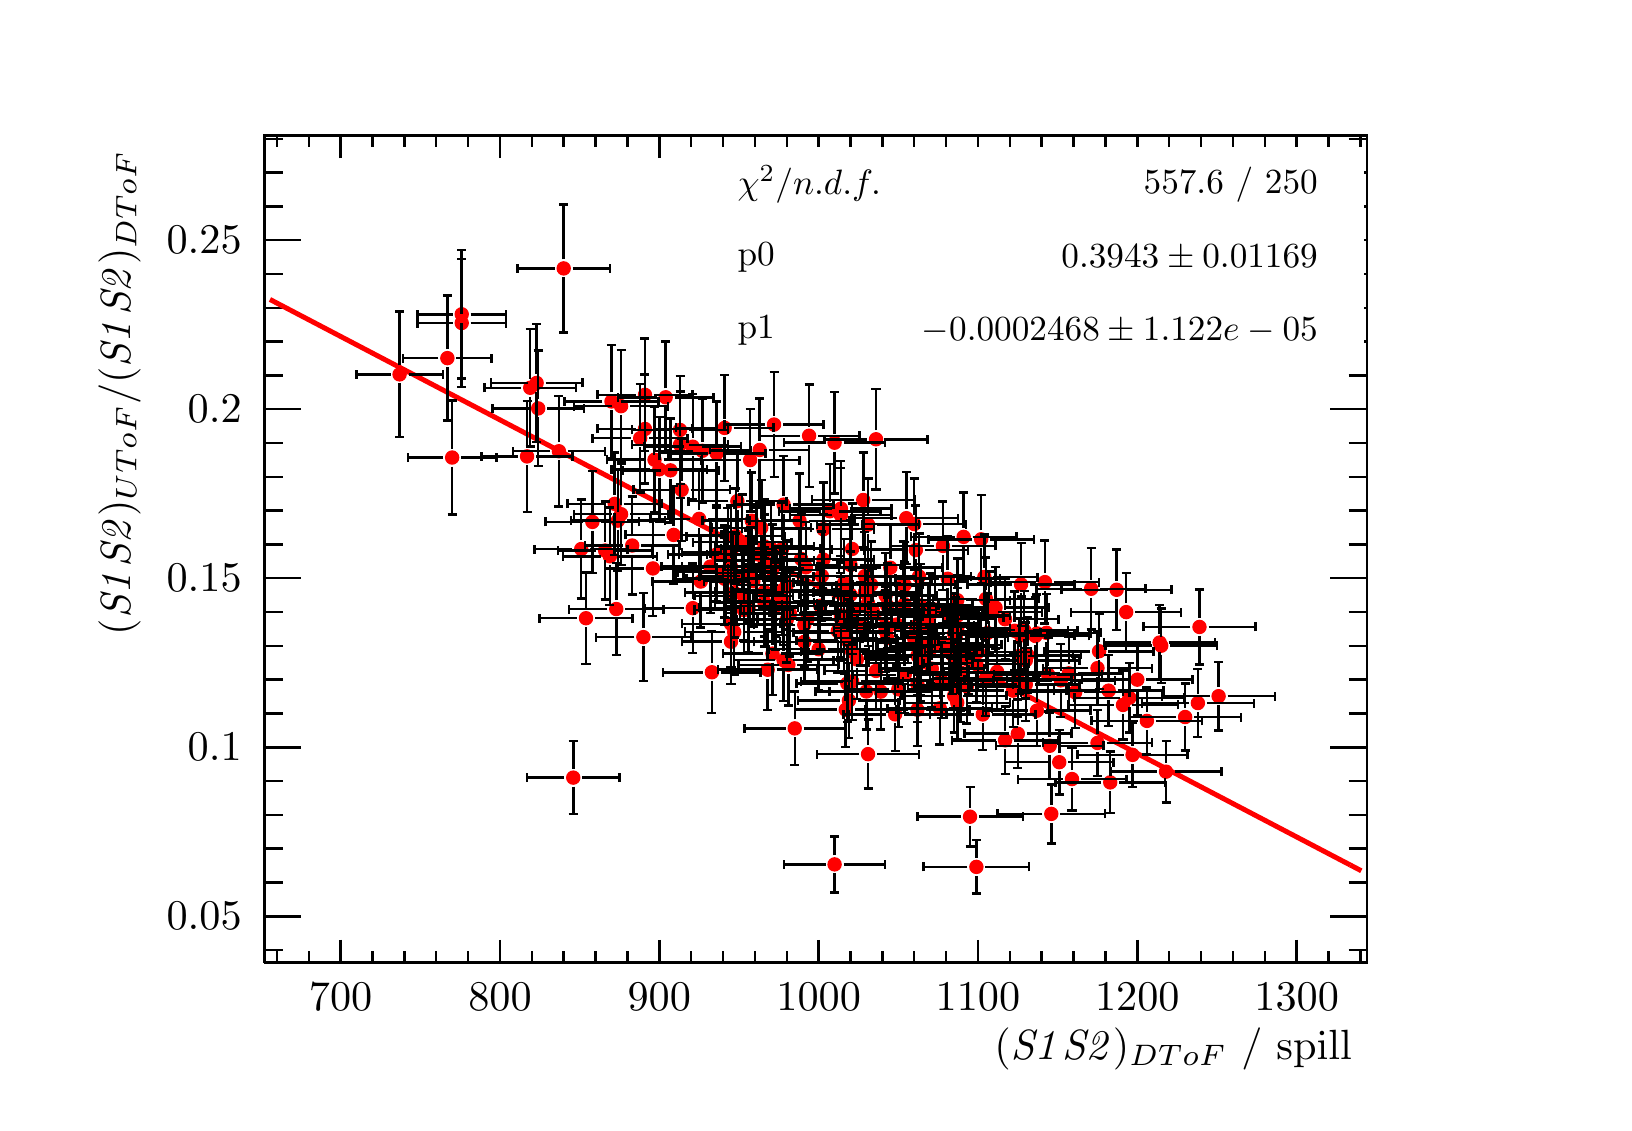
\begin{tikzpicture}
\pgfdeclareplotmark{cross} {
\pgfpathmoveto{\pgfpoint{-0.3\pgfplotmarksize}{\pgfplotmarksize}}
\pgfpathlineto{\pgfpoint{+0.3\pgfplotmarksize}{\pgfplotmarksize}}
\pgfpathlineto{\pgfpoint{+0.3\pgfplotmarksize}{0.3\pgfplotmarksize}}
\pgfpathlineto{\pgfpoint{+1\pgfplotmarksize}{0.3\pgfplotmarksize}}
\pgfpathlineto{\pgfpoint{+1\pgfplotmarksize}{-0.3\pgfplotmarksize}}
\pgfpathlineto{\pgfpoint{+0.3\pgfplotmarksize}{-0.3\pgfplotmarksize}}
\pgfpathlineto{\pgfpoint{+0.3\pgfplotmarksize}{-1.\pgfplotmarksize}}
\pgfpathlineto{\pgfpoint{-0.3\pgfplotmarksize}{-1.\pgfplotmarksize}}
\pgfpathlineto{\pgfpoint{-0.3\pgfplotmarksize}{-0.3\pgfplotmarksize}}
\pgfpathlineto{\pgfpoint{-1.\pgfplotmarksize}{-0.3\pgfplotmarksize}}
\pgfpathlineto{\pgfpoint{-1.\pgfplotmarksize}{0.3\pgfplotmarksize}}
\pgfpathlineto{\pgfpoint{-0.3\pgfplotmarksize}{0.3\pgfplotmarksize}}
\pgfpathclose
\pgfusepathqstroke
}
\pgfdeclareplotmark{cross*} {
\pgfpathmoveto{\pgfpoint{-0.3\pgfplotmarksize}{\pgfplotmarksize}}
\pgfpathlineto{\pgfpoint{+0.3\pgfplotmarksize}{\pgfplotmarksize}}
\pgfpathlineto{\pgfpoint{+0.3\pgfplotmarksize}{0.3\pgfplotmarksize}}
\pgfpathlineto{\pgfpoint{+1\pgfplotmarksize}{0.3\pgfplotmarksize}}
\pgfpathlineto{\pgfpoint{+1\pgfplotmarksize}{-0.3\pgfplotmarksize}}
\pgfpathlineto{\pgfpoint{+0.3\pgfplotmarksize}{-0.3\pgfplotmarksize}}
\pgfpathlineto{\pgfpoint{+0.3\pgfplotmarksize}{-1.\pgfplotmarksize}}
\pgfpathlineto{\pgfpoint{-0.3\pgfplotmarksize}{-1.\pgfplotmarksize}}
\pgfpathlineto{\pgfpoint{-0.3\pgfplotmarksize}{-0.3\pgfplotmarksize}}
\pgfpathlineto{\pgfpoint{-1.\pgfplotmarksize}{-0.3\pgfplotmarksize}}
\pgfpathlineto{\pgfpoint{-1.\pgfplotmarksize}{0.3\pgfplotmarksize}}
\pgfpathlineto{\pgfpoint{-0.3\pgfplotmarksize}{0.3\pgfplotmarksize}}
\pgfpathclose
\pgfusepathqfillstroke
}
\pgfdeclareplotmark{newstar} {
\pgfpathmoveto{\pgfqpoint{0pt}{\pgfplotmarksize}}
\pgfpathlineto{\pgfqpointpolar{44}{0.5\pgfplotmarksize}}
\pgfpathlineto{\pgfqpointpolar{18}{\pgfplotmarksize}}
\pgfpathlineto{\pgfqpointpolar{-20}{0.5\pgfplotmarksize}}
\pgfpathlineto{\pgfqpointpolar{-54}{\pgfplotmarksize}}
\pgfpathlineto{\pgfqpointpolar{-90}{0.5\pgfplotmarksize}}
\pgfpathlineto{\pgfqpointpolar{234}{\pgfplotmarksize}}
\pgfpathlineto{\pgfqpointpolar{198}{0.5\pgfplotmarksize}}
\pgfpathlineto{\pgfqpointpolar{162}{\pgfplotmarksize}}
\pgfpathlineto{\pgfqpointpolar{134}{0.5\pgfplotmarksize}}
\pgfpathclose
\pgfusepathqstroke
}
\pgfdeclareplotmark{newstar*} {
\pgfpathmoveto{\pgfqpoint{0pt}{\pgfplotmarksize}}
\pgfpathlineto{\pgfqpointpolar{44}{0.5\pgfplotmarksize}}
\pgfpathlineto{\pgfqpointpolar{18}{\pgfplotmarksize}}
\pgfpathlineto{\pgfqpointpolar{-20}{0.5\pgfplotmarksize}}
\pgfpathlineto{\pgfqpointpolar{-54}{\pgfplotmarksize}}
\pgfpathlineto{\pgfqpointpolar{-90}{0.5\pgfplotmarksize}}
\pgfpathlineto{\pgfqpointpolar{234}{\pgfplotmarksize}}
\pgfpathlineto{\pgfqpointpolar{198}{0.5\pgfplotmarksize}}
\pgfpathlineto{\pgfqpointpolar{162}{\pgfplotmarksize}}
\pgfpathlineto{\pgfqpointpolar{134}{0.5\pgfplotmarksize}}
\pgfpathclose
\pgfusepathqfillstroke
}
\definecolor{c}{rgb}{1,1,1};
\draw [color=c, fill=c] (0,0) rectangle (20,13.639);
\draw [color=c, fill=c] (3,1.77307) rectangle (17,12.2751);
\definecolor{c}{rgb}{0,0,0};
\draw [c,line width=0.9] (3,1.77307) -- (3,12.2751) -- (17,12.2751) -- (17,1.77307) -- (3,1.77307);
\definecolor{c}{rgb}{1,1,1};
\draw [color=c, fill=c] (3,1.77307) rectangle (17,12.2751);
\definecolor{c}{rgb}{0,0,0};
\draw [c,line width=0.9] (3,1.77307) -- (3,12.2751) -- (17,12.2751) -- (17,1.77307) -- (3,1.77307);
\draw [c,line width=0.9] (3,1.77307) -- (17,1.77307);
\draw [c,line width=0.9] (3.96729,2.05948) -- (3.96729,1.77307);
\draw [c,line width=0.9] (4.37202,1.91628) -- (4.37202,1.77307);
\draw [c,line width=0.9] (4.77675,1.91628) -- (4.77675,1.77307);
\draw [c,line width=0.9] (5.18148,1.91628) -- (5.18148,1.77307);
\draw [c,line width=0.9] (5.58621,1.91628) -- (5.58621,1.77307);
\draw [c,line width=0.9] (5.99094,2.05948) -- (5.99094,1.77307);
\draw [c,line width=0.9] (6.39567,1.91628) -- (6.39567,1.77307);
\draw [c,line width=0.9] (6.8004,1.91628) -- (6.8004,1.77307);
\draw [c,line width=0.9] (7.20513,1.91628) -- (7.20513,1.77307);
\draw [c,line width=0.9] (7.60985,1.91628) -- (7.60985,1.77307);
\draw [c,line width=0.9] (8.01458,2.05948) -- (8.01458,1.77307);
\draw [c,line width=0.9] (8.41931,1.91628) -- (8.41931,1.77307);
\draw [c,line width=0.9] (8.82404,1.91628) -- (8.82404,1.77307);
\draw [c,line width=0.9] (9.22877,1.91628) -- (9.22877,1.77307);
\draw [c,line width=0.9] (9.6335,1.91628) -- (9.6335,1.77307);
\draw [c,line width=0.9] (10.0382,2.05948) -- (10.0382,1.77307);
\draw [c,line width=0.9] (10.443,1.91628) -- (10.443,1.77307);
\draw [c,line width=0.9] (10.8477,1.91628) -- (10.8477,1.77307);
\draw [c,line width=0.9] (11.2524,1.91628) -- (11.2524,1.77307);
\draw [c,line width=0.9] (11.6571,1.91628) -- (11.6571,1.77307);
\draw [c,line width=0.9] (12.0619,2.05948) -- (12.0619,1.77307);
\draw [c,line width=0.9] (12.4666,1.91628) -- (12.4666,1.77307);
\draw [c,line width=0.9] (12.8713,1.91628) -- (12.8713,1.77307);
\draw [c,line width=0.9] (13.2761,1.91628) -- (13.2761,1.77307);
\draw [c,line width=0.9] (13.6808,1.91628) -- (13.6808,1.77307);
\draw [c,line width=0.9] (14.0855,2.05948) -- (14.0855,1.77307);
\draw [c,line width=0.9] (14.4903,1.91628) -- (14.4903,1.77307);
\draw [c,line width=0.9] (14.895,1.91628) -- (14.895,1.77307);
\draw [c,line width=0.9] (15.2997,1.91628) -- (15.2997,1.77307);
\draw [c,line width=0.9] (15.7044,1.91628) -- (15.7044,1.77307);
\draw [c,line width=0.9] (16.1092,2.05948) -- (16.1092,1.77307);
\draw [c,line width=0.9] (3.96729,2.05948) -- (3.96729,1.77307);
\draw [c,line width=0.9] (3.56256,1.91628) -- (3.56256,1.77307);
\draw [c,line width=0.9] (3.15783,1.91628) -- (3.15783,1.77307);
\draw [c,line width=0.9] (16.1092,2.05948) -- (16.1092,1.77307);
\draw [c,line width=0.9] (16.5139,1.91628) -- (16.5139,1.77307);
\draw [c,line width=0.9] (16.9186,1.91628) -- (16.9186,1.77307);
\draw [anchor=base] (3.96729,1.15931) node[scale=1.52731, color=c, rotate=0]{700};
\draw [anchor=base] (5.99094,1.15931) node[scale=1.52731, color=c, rotate=0]{800};
\draw [anchor=base] (8.01458,1.15931) node[scale=1.52731, color=c, rotate=0]{900};
\draw [anchor=base] (10.0382,1.15931) node[scale=1.52731, color=c, rotate=0]{1000};
\draw [anchor=base] (12.0619,1.15931) node[scale=1.52731, color=c, rotate=0]{1100};
\draw [anchor=base] (14.0855,1.15931) node[scale=1.52731, color=c, rotate=0]{1200};
\draw [anchor=base] (16.1092,1.15931) node[scale=1.52731, color=c, rotate=0]{1300};
\draw [anchor= east] (17,0.681948) node[scale=1.52731, color=c, rotate=0]{ $(\SOne\STwo)_{\text{DToF}}$  / spill};
\draw [c,line width=0.9] (3,12.2751) -- (17,12.2751);
\draw [c,line width=0.9] (3.96729,11.9887) -- (3.96729,12.2751);
\draw [c,line width=0.9] (4.37202,12.1319) -- (4.37202,12.2751);
\draw [c,line width=0.9] (4.77675,12.1319) -- (4.77675,12.2751);
\draw [c,line width=0.9] (5.18148,12.1319) -- (5.18148,12.2751);
\draw [c,line width=0.9] (5.58621,12.1319) -- (5.58621,12.2751);
\draw [c,line width=0.9] (5.99094,11.9887) -- (5.99094,12.2751);
\draw [c,line width=0.9] (6.39567,12.1319) -- (6.39567,12.2751);
\draw [c,line width=0.9] (6.8004,12.1319) -- (6.8004,12.2751);
\draw [c,line width=0.9] (7.20513,12.1319) -- (7.20513,12.2751);
\draw [c,line width=0.9] (7.60985,12.1319) -- (7.60985,12.2751);
\draw [c,line width=0.9] (8.01458,11.9887) -- (8.01458,12.2751);
\draw [c,line width=0.9] (8.41931,12.1319) -- (8.41931,12.2751);
\draw [c,line width=0.9] (8.82404,12.1319) -- (8.82404,12.2751);
\draw [c,line width=0.9] (9.22877,12.1319) -- (9.22877,12.2751);
\draw [c,line width=0.9] (9.6335,12.1319) -- (9.6335,12.2751);
\draw [c,line width=0.9] (10.0382,11.9887) -- (10.0382,12.2751);
\draw [c,line width=0.9] (10.443,12.1319) -- (10.443,12.2751);
\draw [c,line width=0.9] (10.8477,12.1319) -- (10.8477,12.2751);
\draw [c,line width=0.9] (11.2524,12.1319) -- (11.2524,12.2751);
\draw [c,line width=0.9] (11.6571,12.1319) -- (11.6571,12.2751);
\draw [c,line width=0.9] (12.0619,11.9887) -- (12.0619,12.2751);
\draw [c,line width=0.9] (12.4666,12.1319) -- (12.4666,12.2751);
\draw [c,line width=0.9] (12.8713,12.1319) -- (12.8713,12.2751);
\draw [c,line width=0.9] (13.2761,12.1319) -- (13.2761,12.2751);
\draw [c,line width=0.9] (13.6808,12.1319) -- (13.6808,12.2751);
\draw [c,line width=0.9] (14.0855,11.9887) -- (14.0855,12.2751);
\draw [c,line width=0.9] (14.4903,12.1319) -- (14.4903,12.2751);
\draw [c,line width=0.9] (14.895,12.1319) -- (14.895,12.2751);
\draw [c,line width=0.9] (15.2997,12.1319) -- (15.2997,12.2751);
\draw [c,line width=0.9] (15.7044,12.1319) -- (15.7044,12.2751);
\draw [c,line width=0.9] (16.1092,11.9887) -- (16.1092,12.2751);
\draw [c,line width=0.9] (3.96729,11.9887) -- (3.96729,12.2751);
\draw [c,line width=0.9] (3.56256,12.1319) -- (3.56256,12.2751);
\draw [c,line width=0.9] (3.15783,12.1319) -- (3.15783,12.2751);
\draw [c,line width=0.9] (16.1092,11.9887) -- (16.1092,12.2751);
\draw [c,line width=0.9] (16.5139,12.1319) -- (16.5139,12.2751);
\draw [c,line width=0.9] (16.9186,12.1319) -- (16.9186,12.2751);
\draw [c,line width=0.9] (3,1.77307) -- (3,12.2751);
\draw [c,line width=0.9] (3.462,2.36091) -- (3,2.36091);
\draw [c,line width=0.9] (3.231,2.79018) -- (3,2.79018);
\draw [c,line width=0.9] (3.231,3.21945) -- (3,3.21945);
\draw [c,line width=0.9] (3.231,3.64872) -- (3,3.64872);
\draw [c,line width=0.9] (3.231,4.07799) -- (3,4.07799);
\draw [c,line width=0.9] (3.462,4.50726) -- (3,4.50726);
\draw [c,line width=0.9] (3.231,4.93653) -- (3,4.93653);
\draw [c,line width=0.9] (3.231,5.36579) -- (3,5.36579);
\draw [c,line width=0.9] (3.231,5.79506) -- (3,5.79506);
\draw [c,line width=0.9] (3.231,6.22433) -- (3,6.22433);
\draw [c,line width=0.9] (3.462,6.6536) -- (3,6.6536);
\draw [c,line width=0.9] (3.231,7.08287) -- (3,7.08287);
\draw [c,line width=0.9] (3.231,7.51214) -- (3,7.51214);
\draw [c,line width=0.9] (3.231,7.94141) -- (3,7.94141);
\draw [c,line width=0.9] (3.231,8.37068) -- (3,8.37068);
\draw [c,line width=0.9] (3.462,8.79995) -- (3,8.79995);
\draw [c,line width=0.9] (3.231,9.22922) -- (3,9.22922);
\draw [c,line width=0.9] (3.231,9.65849) -- (3,9.65849);
\draw [c,line width=0.9] (3.231,10.0878) -- (3,10.0878);
\draw [c,line width=0.9] (3.231,10.517) -- (3,10.517);
\draw [c,line width=0.9] (3.462,10.9463) -- (3,10.9463);
\draw [c,line width=0.9] (3.462,2.36091) -- (3,2.36091);
\draw [c,line width=0.9] (3.231,1.93164) -- (3,1.93164);
\draw [c,line width=0.9] (3.462,10.9463) -- (3,10.9463);
\draw [c,line width=0.9] (3.231,11.3756) -- (3,11.3756);
\draw [c,line width=0.9] (3.231,11.8048) -- (3,11.8048);
\draw [c,line width=0.9] (3.231,12.2341) -- (3,12.2341);
\draw [anchor= east] (2.9,2.36091) node[scale=1.52731, color=c, rotate=0]{0.05};
\draw [anchor= east] (2.9,4.50726) node[scale=1.52731, color=c, rotate=0]{0.1};
\draw [anchor= east] (2.9,6.6536) node[scale=1.52731, color=c, rotate=0]{0.15};
\draw [anchor= east] (2.9,8.79995) node[scale=1.52731, color=c, rotate=0]{0.2};
\draw [anchor= east] (2.9,10.9463) node[scale=1.52731, color=c, rotate=0]{0.25};
\draw [anchor= east] (1.16,12.2751) node[scale=1.52731, color=c, rotate=90]{$(\SOne\STwo)_{\text{UToF}}/(\SOne\STwo)_{\text{DToF}}$ };
\draw [c,line width=0.9] (17,1.77307) -- (17,12.2751);
\draw [c,line width=0.9] (16.538,2.36091) -- (17,2.36091);
\draw [c,line width=0.9] (16.769,2.79018) -- (17,2.79018);
\draw [c,line width=0.9] (16.769,3.21945) -- (17,3.21945);
\draw [c,line width=0.9] (16.769,3.64872) -- (17,3.64872);
\draw [c,line width=0.9] (16.769,4.07799) -- (17,4.07799);
\draw [c,line width=0.9] (16.538,4.50726) -- (17,4.50726);
\draw [c,line width=0.9] (16.769,4.93653) -- (17,4.93653);
\draw [c,line width=0.9] (16.769,5.36579) -- (17,5.36579);
\draw [c,line width=0.9] (16.769,5.79506) -- (17,5.79506);
\draw [c,line width=0.9] (16.769,6.22433) -- (17,6.22433);
\draw [c,line width=0.9] (16.538,6.6536) -- (17,6.6536);
\draw [c,line width=0.9] (16.769,7.08287) -- (17,7.08287);
\draw [c,line width=0.9] (16.769,7.51214) -- (17,7.51214);
\draw [c,line width=0.9] (16.769,7.94141) -- (17,7.94141);
\draw [c,line width=0.9] (16.769,8.37068) -- (17,8.37068);
\draw [c,line width=0.9] (16.538,8.79995) -- (17,8.79995);
\draw [c,line width=0.9] (16.769,9.22922) -- (17,9.22922);
\draw [c,line width=0.9] (16.769,9.65849) -- (17,9.65849);
\draw [c,line width=0.9] (16.769,10.0878) -- (17,10.0878);
\draw [c,line width=0.9] (16.769,10.517) -- (17,10.517);
\draw [c,line width=0.9] (16.538,10.9463) -- (17,10.9463);
\draw [c,line width=0.9] (16.538,2.36091) -- (17,2.36091);
\draw [c,line width=0.9] (16.769,1.93164) -- (17,1.93164);
\draw [c,line width=0.9] (16.538,10.9463) -- (17,10.9463);
\draw [c,line width=0.9] (16.769,11.3756) -- (17,11.3756);
\draw [c,line width=0.9] (16.769,11.8048) -- (17,11.8048);
\draw [c,line width=0.9] (16.769,12.2341) -- (17,12.2341);
\definecolor{c}{rgb}{1,0,0};
\foreach \P in {(11.5155,6.25554), (9.57279,6.49762), (10.7667,8.41874), (10.4025,5.86506), (11.9202,5.28096), (11.1108,6.57411), (10.6453,5.21576), (13.0939,4.31705), (10.362,5.96069), (11.131,5.4277), (9.57279,7.02487), (7.81222,5.906),
 (10.0989,7.27632), (13.2154,5.44593), (8.7431,6.95629), (9.1883,7.38399), (11.6774,6.64764), (6.73969,8.26657), (14.8545,5.06898), (11.6167,5.78949), (11.8797,7.17888), (13.7213,5.22634), (11.3334,5.58043), (11.6976,5.80855), (11.5762,5.00195),
 (9.67397,6.20335), (13.9439,6.22361), (10.3215,6.14136), (12.7904,5.92052), (13.2558,4.10354), (7.67056,7.06926), (13.5998,5.72644), (11.2929,6.03516), (10.4632,5.72233), (14.3891,5.79683), (11.2524,5.88416), (10.0585,6.3041), (12.669,5.30501),
 (8.98593,6.64455), (10.3215,7.45372), (14.2069,4.84184), (9.14783,6.27642), (14.3688,5.83679), (8.84428,6.738), (11.475,5.50528), (10.706,6.57257), (11.2929,5.30759), (13.9843,5.13589), (11.4345,6.07736), (11.8393,5.29957), (12.6487,5.99392),
 (10.6656,4.41982), (12.1631,6.39138), (12.6083,5.928), (8.98593,7.18792), (11.3131,6.67581), (9.06688,7.11353), (8.29789,7.77609), (12.588,5.66621), (10.0382,5.75214), (11.1512,7.41652), (11.7988,6.37519), (8.43955,6.27374), (13.5796,4.56206),
 (9.28948,8.28286), (12.5273,5.98657), (10.443,6.44318), (8.86451,6.73107), (13.9034,5.04429), (13.8224,6.50714), (11.3536,6.05907), (14.0855,5.36579), (8.92522,6.98293), (7.44796,7.59878), (15.1176,5.15579), (9.65374,5.55308), (9.59303,7.58851),
 (11.4548,6.19224), (5.38384,8.18671), (8.84428,6.64676), (10.8882,6.43526), (8.88475,6.95177), (11.3334,5.66112), (7.32654,7.00554), (10.7263,6.2343), (10.3215,7.53839), (10.3215,6.18369), (11.2727,7.01166), (11.131,6.32371), (10.2406,3.01969),
 (8.92522,6.80123), (9.59303,6.35952), (8.09553,8.9519), (11.0501,5.24315), (8.27766,8.53665), (11.7381,5.67943), (12.9725,4.526), (10.5644,6.07204), (12.9118,6.60474), (9.39066,5.49174), (9.35019,6.34698), (9.8561,6.06233), (10.6656,7.33435),
 (9.6335,6.566), (11.7583,5.95134), (9.45137,5.69648), (10.4632,5.34393), (8.92522,5.8473), (10.2406,8.37493), (12.5678,5.36579), (10.4632,7.02569), (12.2845,6.28074), (10.362,6.59445), (8.84428,8.56273), (9.45137,6.75749), (10.6048,7.64743),
 (9.79539,7.38353), (8.43955,8.32454), (8.7431,8.24043), (11.9607,3.6252), (8.94546,6.65814), (5.50526,9.89525), (11.7988,6.17773), (8.56097,8.27204), (11.2929,5.67138), (11.7786,5.90653), (13.4987,6.5198), (9.08712,6.43063), (10.4632,6.22686),
 (9.49185,6.47934), (10.8275,5.21375), (11.7179,6.16012), (9.24901,6.95958), (7.48844,7.38542), (12.1428,6.66915), (9.91681,8.4631), (12.6892,5.68006), (9.81563,6.89884), (10.443,6.82194), (11.4548,5.75093), (5.32313,9.44917), (11.0298,6.06637),
 (12.3047,5.46462), (10.7667,5.47684), (9.00617,7.63291), (12.6083,6.57552), (10.2811,5.9834), (8.9657,6.47002), (12.1833,5.95885), (8.9657,5.97139), (10.8882,6.02329), (9.8561,5.84574), (12.8106,4.97164), (11.9405,5.66872), (9.20853,6.61555),
 (10.6656,6.33508), (13.1142,5.35685), (7.93364,6.77817), (12.1226,4.92368), (11.6167,7.06376), (9.35019,6.88023), (9.6335,6.12797), (7.16465,7.36905), (11.2524,7.34205), (11.3334,6.30664), (8.01458,8.0368), (12.1631,5.38133), (12.0416,2.98782),
 (8.54073,6.61188), (14.4498,4.19711), (12.669,5.60892), (7.77175,8.43255), (11.7988,5.07198), (8.19671,7.20376), (12.1023,7.14831), (10.6251,6.68072), (7.83246,8.54942), (11.131,6.56807), (12.9523,5.43033), (7.023,7.02436), (10.1799,7.50404),
 (12.4059,6.13287), (9.89657,6.13701), (6.8004,10.5886), (8.66215,6.80099), (12.0619,5.71701), (10.4025,5.31688), (10.9489,6.78711), (10.3822,4.98422), (4.71604,9.24261), (7.40749,8.89863), (12.4059,4.59565), (9.43114,7.02977), (8.5205,7.40772),
 (7.38725,6.9327), (9.87634,6.79208), (14.8747,6.03516), (6.33496,8.20097), (14.0248,4.41043), (11.2727,6.04065), (9.14783,6.68054), (9.35019,7.05799), (9.47161,8.60563), (6.92181,4.12162), (8.68239,5.45965), (7.08371,6.14592), (10.5239,5.62235),
 (6.37543,9.0725), (9.73468,4.74695), (9.59303,5.61335), (10.9084,5.89425), (13.7415,4.06093), (8.15624,8.02376), (10.6251,6.47213), (11.2929,4.98422), (5.50526,10.0059), (11.7583,5.16006), (11.5964,5.35623), (7.83246,8.98302), (11.7988,6.01977),
 (12.8106,5.95325), (11.0096,4.92506), (7.52891,7.46706), (8.27766,8.34858), (6.45638,9.13377), (11.4548,5.83117), (7.95387,8.15868), (9.35019,6.48029), (12.9928,3.6607), (10.0989,6.89113), (13.5796,5.51193), (12.0416,5.56578), (9.08712,6.25046),
 (9.16806,8.15403), (9.30972,7.29483), (7.4682,6.26269), (14.6926,4.89116), (9.16806,6.71864), (10.9084,6.30582), (12.932,5.96069), (10.8882,5.9821), (10.4227,5.10124), (12.2035,6.22511), (7.52891,8.83915), (12.5678,4.67896), (11.8393,5.45725),
 (6.47661,8.81037), (12.5071,5.22653), (10.0787,6.68359), (9.49185,6.30286), (13.2963,5.20607), (8.92522,6.07443)}{\draw[mark options={color=c,fill=c},mark size=2.402402pt,mark=*] plot coordinates {\P};}
\draw [c,line width=1.8] (3.07,10.1944) -- (3.21,10.1211) -- (3.35,10.0478) -- (3.49,9.97453) -- (3.63,9.90124) -- (3.77,9.82794) -- (3.91,9.75465) -- (4.05,9.68136) -- (4.19,9.60806) -- (4.33,9.53477) -- (4.47,9.46148) -- (4.61,9.38819) --
 (4.75,9.31489) -- (4.89,9.2416) -- (5.03,9.16831) -- (5.17,9.09501) -- (5.31,9.02172) -- (5.45,8.94843) -- (5.59,8.87514) -- (5.73,8.80184) -- (5.87,8.72855) -- (6.01,8.65526) -- (6.15,8.58196) -- (6.29,8.50867) -- (6.43,8.43538) -- (6.57,8.36209)
 -- (6.71,8.28879) -- (6.85,8.2155) -- (6.99,8.14221) -- (7.13,8.06891) -- (7.27,7.99562) -- (7.41,7.92233) -- (7.55,7.84904) -- (7.69,7.77574) -- (7.83,7.70245) -- (7.97,7.62916) -- (8.11,7.55586) -- (8.25,7.48257) -- (8.39,7.40928) --
 (8.53,7.33599) -- (8.67,7.26269) -- (8.81,7.1894) -- (8.95,7.11611) -- (9.09,7.04281) -- (9.23,6.96952) -- (9.37,6.89623) -- (9.51,6.82294) -- (9.65,6.74964) -- (9.79,6.67635) -- (9.93,6.60306);
\draw [c,line width=1.8] (9.93,6.60306) -- (10.07,6.52976) -- (10.21,6.45647) -- (10.35,6.38318) -- (10.49,6.30989) -- (10.63,6.23659) -- (10.77,6.1633) -- (10.91,6.09001) -- (11.05,6.01671) -- (11.19,5.94342) -- (11.33,5.87013) -- (11.47,5.79683) --
 (11.61,5.72354) -- (11.75,5.65025) -- (11.89,5.57696) -- (12.03,5.50366) -- (12.17,5.43037) -- (12.31,5.35708) -- (12.45,5.28378) -- (12.59,5.21049) -- (12.73,5.1372) -- (12.87,5.06391) -- (13.01,4.99061) -- (13.15,4.91732) -- (13.29,4.84403) --
 (13.43,4.77073) -- (13.57,4.69744) -- (13.71,4.62415) -- (13.85,4.55086) -- (13.99,4.47756) -- (14.13,4.40427) -- (14.27,4.33098) -- (14.41,4.25768) -- (14.55,4.18439) -- (14.69,4.1111) -- (14.83,4.03781) -- (14.97,3.96451) -- (15.11,3.89122) --
 (15.25,3.81793) -- (15.39,3.74463) -- (15.53,3.67134) -- (15.67,3.59805) -- (15.81,3.52476) -- (15.95,3.45146) -- (16.09,3.37817) -- (16.23,3.30488) -- (16.37,3.23158) -- (16.51,3.15829) -- (16.65,3.085) -- (16.79,3.01171);
\draw [c,line width=1.8] (16.79,3.01171) -- (16.93,2.93841);
\definecolor{c}{rgb}{1,1,1};
\draw [color=c, fill=c] (8.42407,9.34097) rectangle (16.9628,12.1203);
\definecolor{c}{rgb}{0,0,0};
\draw [anchor= west] (8.851,11.6571) node[scale=1.27276, color=c, rotate=0]{$\chi^{2} / ndf $};
\draw [anchor= east] (16.5358,11.6571) node[scale=1.27276, color=c, rotate=0]{ 557.6 / 250};
\draw [anchor= west] (8.851,10.7307) node[scale=1.27276, color=c, rotate=0]{p0       };
\draw [anchor= east] (16.5358,10.7307) node[scale=1.27276, color=c, rotate=0]{$ 0.3943 \pm 0.01169$};
\draw [anchor= west] (8.851,9.8042) node[scale=1.27276, color=c, rotate=0]{p1       };
\draw [anchor= east] (16.5358,9.8042) node[scale=1.27276, color=c, rotate=0]{$ -0.0002468 \pm 1.122e-05$};
\draw [c,line width=0.9] (11.4009,6.25554) -- (10.8526,6.25554);
\draw [c,line width=0.9] (10.8526,6.19823) -- (10.8526,6.31284);
\draw [c,line width=0.9] (11.6301,6.25554) -- (12.1784,6.25554);
\draw [c,line width=0.9] (12.1784,6.19823) -- (12.1784,6.31284);
\draw [c,line width=0.9] (11.5155,6.37015) -- (11.5155,6.7806);
\draw [c,line width=0.9] (11.4582,6.7806) -- (11.5728,6.7806);
\draw [c,line width=0.9] (11.5155,6.14092) -- (11.5155,5.73048);
\draw [c,line width=0.9] (11.4582,5.73048) -- (11.5728,5.73048);
\draw [c,line width=0.9] (9.45818,6.49762) -- (8.94026,6.49762);
\draw [c,line width=0.9] (8.94026,6.44032) -- (8.94026,6.55493);
\draw [c,line width=0.9] (9.6874,6.49762) -- (10.2053,6.49762);
\draw [c,line width=0.9] (10.2053,6.44032) -- (10.2053,6.55493);
\draw [c,line width=0.9] (9.57279,6.61224) -- (9.57279,7.06018);
\draw [c,line width=0.9] (9.51548,7.06018) -- (9.6301,7.06018);
\draw [c,line width=0.9] (9.57279,6.38301) -- (9.57279,5.93507);
\draw [c,line width=0.9] (9.51548,5.93507) -- (9.6301,5.93507);
\draw [c,line width=0.9] (10.6521,8.41874) -- (10.1154,8.41874);
\draw [c,line width=0.9] (10.1154,8.36144) -- (10.1154,8.47605);
\draw [c,line width=0.9] (10.8814,8.41874) -- (11.4181,8.41874);
\draw [c,line width=0.9] (11.4181,8.36144) -- (11.4181,8.47605);
\draw [c,line width=0.9] (10.7667,8.53336) -- (10.7667,9.05507);
\draw [c,line width=0.9] (10.7094,9.05507) -- (10.824,9.05507);
\draw [c,line width=0.9] (10.7667,8.30413) -- (10.7667,7.78242);
\draw [c,line width=0.9] (10.7094,7.78242) -- (10.824,7.78242);
\draw [c,line width=0.9] (10.2879,5.86506) -- (9.75682,5.86506);
\draw [c,line width=0.9] (9.75682,5.80776) -- (9.75682,5.92237);
\draw [c,line width=0.9] (10.5171,5.86506) -- (11.0482,5.86506);
\draw [c,line width=0.9] (11.0482,5.80776) -- (11.0482,5.92237);
\draw [c,line width=0.9] (10.4025,5.97968) -- (10.4025,6.38432);
\draw [c,line width=0.9] (10.3452,6.38432) -- (10.4598,6.38432);
\draw [c,line width=0.9] (10.4025,5.75045) -- (10.4025,5.3458);
\draw [c,line width=0.9] (10.3452,5.3458) -- (10.4598,5.3458);
\draw [c,line width=0.9] (11.8056,5.28096) -- (11.2512,5.28096);
\draw [c,line width=0.9] (11.2512,5.22366) -- (11.2512,5.33827);
\draw [c,line width=0.9] (12.0348,5.28096) -- (12.5892,5.28096);
\draw [c,line width=0.9] (12.5892,5.22366) -- (12.5892,5.33827);
\draw [c,line width=0.9] (11.9202,5.39558) -- (11.9202,5.75262);
\draw [c,line width=0.9] (11.8629,5.75262) -- (11.9775,5.75262);
\draw [c,line width=0.9] (11.9202,5.16635) -- (11.9202,4.8093);
\draw [c,line width=0.9] (11.8629,4.8093) -- (11.9775,4.8093);
\draw [c,line width=0.9] (10.9961,6.57411) -- (10.4541,6.57411);
\draw [c,line width=0.9] (10.4541,6.5168) -- (10.4541,6.63141);
\draw [c,line width=0.9] (11.2254,6.57411) -- (11.7674,6.57411);
\draw [c,line width=0.9] (11.7674,6.5168) -- (11.7674,6.63141);
\draw [c,line width=0.9] (11.1108,6.68872) -- (11.1108,7.11969);
\draw [c,line width=0.9] (11.0535,7.11969) -- (11.1681,7.11969);
\draw [c,line width=0.9] (11.1108,6.45949) -- (11.1108,6.02852);
\draw [c,line width=0.9] (11.0535,6.02852) -- (11.1681,6.02852);
\draw [c,line width=0.9] (10.5307,5.21576) -- (9.99586,5.21576);
\draw [c,line width=0.9] (9.99586,5.15845) -- (9.99586,5.27307);
\draw [c,line width=0.9] (10.7599,5.21576) -- (11.2948,5.21576);
\draw [c,line width=0.9] (11.2948,5.15845) -- (11.2948,5.27307);
\draw [c,line width=0.9] (10.6453,5.33037) -- (10.6453,5.69817);
\draw [c,line width=0.9] (10.588,5.69817) -- (10.7026,5.69817);
\draw [c,line width=0.9] (10.6453,5.10115) -- (10.6453,4.73335);
\draw [c,line width=0.9] (10.588,4.73335) -- (10.7026,4.73335);
\draw [c,line width=0.9] (12.9793,4.31705) -- (12.4074,4.31705);
\draw [c,line width=0.9] (12.4074,4.25974) -- (12.4074,4.37436);
\draw [c,line width=0.9] (13.2085,4.31705) -- (13.7805,4.31705);
\draw [c,line width=0.9] (13.7805,4.25974) -- (13.7805,4.37436);
\draw [c,line width=0.9] (13.0939,4.43166) -- (13.0939,4.72647);
\draw [c,line width=0.9] (13.0366,4.72647) -- (13.1512,4.72647);
\draw [c,line width=0.9] (13.0939,4.20244) -- (13.0939,3.90763);
\draw [c,line width=0.9] (13.0366,3.90763) -- (13.1512,3.90763);
\draw [c,line width=0.9] (10.2474,5.96069) -- (9.71698,5.96069);
\draw [c,line width=0.9] (9.71698,5.90338) -- (9.71698,6.01799);
\draw [c,line width=0.9] (10.4766,5.96069) -- (11.007,5.96069);
\draw [c,line width=0.9] (11.007,5.90338) -- (11.007,6.01799);
\draw [c,line width=0.9] (10.362,6.0753) -- (10.362,6.48535);
\draw [c,line width=0.9] (10.3047,6.48535) -- (10.4193,6.48535);
\draw [c,line width=0.9] (10.362,5.84607) -- (10.362,5.43602);
\draw [c,line width=0.9] (10.3047,5.43602) -- (10.4193,5.43602);
\draw [c,line width=0.9] (11.0164,5.4277) -- (10.474,5.4277);
\draw [c,line width=0.9] (10.474,5.37039) -- (10.474,5.48501);
\draw [c,line width=0.9] (11.2456,5.4277) -- (11.788,5.4277);
\draw [c,line width=0.9] (11.788,5.37039) -- (11.788,5.48501);
\draw [c,line width=0.9] (11.131,5.54231) -- (11.131,5.91566);
\draw [c,line width=0.9] (11.0737,5.91566) -- (11.1883,5.91566);
\draw [c,line width=0.9] (11.131,5.31309) -- (11.131,4.93974);
\draw [c,line width=0.9] (11.0737,4.93974) -- (11.1883,4.93974);
\draw [c,line width=0.9] (9.45818,7.02487) -- (8.94026,7.02487);
\draw [c,line width=0.9] (8.94026,6.96757) -- (8.94026,7.08218);
\draw [c,line width=0.9] (9.6874,7.02487) -- (10.2053,7.02487);
\draw [c,line width=0.9] (10.2053,6.96757) -- (10.2053,7.08218);
\draw [c,line width=0.9] (9.57279,7.13949) -- (9.57279,7.61369);
\draw [c,line width=0.9] (9.51548,7.61369) -- (9.6301,7.61369);
\draw [c,line width=0.9] (9.57279,6.91026) -- (9.57279,6.43606);
\draw [c,line width=0.9] (9.51548,6.43606) -- (9.6301,6.43606);
\draw [c,line width=0.9] (7.69761,5.906) -- (7.20851,5.906);
\draw [c,line width=0.9] (7.20851,5.84869) -- (7.20851,5.9633);
\draw [c,line width=0.9] (7.92683,5.906) -- (8.41593,5.906);
\draw [c,line width=0.9] (8.41593,5.84869) -- (8.41593,5.9633);
\draw [c,line width=0.9] (7.81222,6.02061) -- (7.81222,6.46359);
\draw [c,line width=0.9] (7.75491,6.46359) -- (7.86953,6.46359);
\draw [c,line width=0.9] (7.81222,5.79138) -- (7.81222,5.34841);
\draw [c,line width=0.9] (7.75491,5.34841) -- (7.86953,5.34841);
\draw [c,line width=0.9] (9.98433,7.27632) -- (9.45805,7.27632);
\draw [c,line width=0.9] (9.45805,7.21901) -- (9.45805,7.33363);
\draw [c,line width=0.9] (10.2136,7.27632) -- (10.7398,7.27632);
\draw [c,line width=0.9] (10.7398,7.21901) -- (10.7398,7.33363);
\draw [c,line width=0.9] (10.0989,7.39093) -- (10.0989,7.86958);
\draw [c,line width=0.9] (10.0416,7.86958) -- (10.1562,7.86958);
\draw [c,line width=0.9] (10.0989,7.16171) -- (10.0989,6.68306);
\draw [c,line width=0.9] (10.0416,6.68306) -- (10.1562,6.68306);
\draw [c,line width=0.9] (13.1007,5.44593) -- (12.527,5.44593);
\draw [c,line width=0.9] (12.527,5.38863) -- (12.527,5.50324);
\draw [c,line width=0.9] (13.33,5.44593) -- (13.9037,5.44593);
\draw [c,line width=0.9] (13.9037,5.38863) -- (13.9037,5.50324);
\draw [c,line width=0.9] (13.2154,5.56055) -- (13.2154,5.91257);
\draw [c,line width=0.9] (13.158,5.91257) -- (13.2727,5.91257);
\draw [c,line width=0.9] (13.2154,5.33132) -- (13.2154,4.9793);
\draw [c,line width=0.9] (13.158,4.9793) -- (13.2727,4.9793);
\draw [c,line width=0.9] (8.62848,6.95629) -- (8.12398,6.95629);
\draw [c,line width=0.9] (8.12398,6.89898) -- (8.12398,7.0136);
\draw [c,line width=0.9] (8.85771,6.95629) -- (9.36221,6.95629);
\draw [c,line width=0.9] (9.36221,6.89898) -- (9.36221,7.0136);
\draw [c,line width=0.9] (8.7431,7.0709) -- (8.7431,7.55441);
\draw [c,line width=0.9] (8.68579,7.55441) -- (8.8004,7.55441);
\draw [c,line width=0.9] (8.7431,6.84168) -- (8.7431,6.35817);
\draw [c,line width=0.9] (8.68579,6.35817) -- (8.8004,6.35817);
\draw [c,line width=0.9] (9.07368,7.38399) -- (8.56195,7.38399);
\draw [c,line width=0.9] (8.56195,7.32668) -- (8.56195,7.44129);
\draw [c,line width=0.9] (9.30291,7.38399) -- (9.81465,7.38399);
\draw [c,line width=0.9] (9.81465,7.32668) -- (9.81465,7.44129);
\draw [c,line width=0.9] (9.1883,7.4986) -- (9.1883,7.99628);
\draw [c,line width=0.9] (9.13099,7.99628) -- (9.2456,7.99628);
\draw [c,line width=0.9] (9.1883,7.26937) -- (9.1883,6.77169);
\draw [c,line width=0.9] (9.13099,6.77169) -- (9.2456,6.77169);
\draw [c,line width=0.9] (11.5628,6.64764) -- (11.012,6.64764);
\draw [c,line width=0.9] (11.012,6.59034) -- (11.012,6.70495);
\draw [c,line width=0.9] (11.792,6.64764) -- (12.3427,6.64764);
\draw [c,line width=0.9] (12.3427,6.59034) -- (12.3427,6.70495);
\draw [c,line width=0.9] (11.6774,6.76226) -- (11.6774,7.18963);
\draw [c,line width=0.9] (11.6201,7.18963) -- (11.7347,7.18963);
\draw [c,line width=0.9] (11.6774,6.53303) -- (11.6774,6.10566);
\draw [c,line width=0.9] (11.6201,6.10566) -- (11.7347,6.10566);
\draw [c,line width=0.9] (6.62507,8.26657) -- (6.15423,8.26657);
\draw [c,line width=0.9] (6.15423,8.20926) -- (6.15423,8.32387);
\draw [c,line width=0.9] (6.8543,8.26657) -- (7.32515,8.26657);
\draw [c,line width=0.9] (7.32515,8.20926) -- (7.32515,8.32387);
\draw [c,line width=0.9] (6.73969,8.38118) -- (6.73969,8.96687);
\draw [c,line width=0.9] (6.68238,8.96687) -- (6.79699,8.96687);
\draw [c,line width=0.9] (6.73969,8.15195) -- (6.73969,7.56627);
\draw [c,line width=0.9] (6.68238,7.56627) -- (6.79699,7.56627);
\draw [c,line width=0.9] (14.7399,5.06898) -- (14.1425,5.06898);
\draw [c,line width=0.9] (14.1425,5.01167) -- (14.1425,5.12629);
\draw [c,line width=0.9] (14.9691,5.06898) -- (15.5665,5.06898);
\draw [c,line width=0.9] (15.5665,5.01167) -- (15.5665,5.12629);
\draw [c,line width=0.9] (14.8545,5.18359) -- (14.8545,5.50183);
\draw [c,line width=0.9] (14.7972,5.50183) -- (14.9118,5.50183);
\draw [c,line width=0.9] (14.8545,4.95437) -- (14.8545,4.63613);
\draw [c,line width=0.9] (14.7972,4.63613) -- (14.9118,4.63613);
\draw [c,line width=0.9] (11.5021,5.78949) -- (10.9523,5.78949);
\draw [c,line width=0.9] (10.9523,5.73218) -- (10.9523,5.8468);
\draw [c,line width=0.9] (11.7313,5.78949) -- (12.2811,5.78949);
\draw [c,line width=0.9] (12.2811,5.73218) -- (12.2811,5.8468);
\draw [c,line width=0.9] (11.6167,5.9041) -- (11.6167,6.29032);
\draw [c,line width=0.9] (11.5594,6.29032) -- (11.674,6.29032);
\draw [c,line width=0.9] (11.6167,5.67488) -- (11.6167,5.28866);
\draw [c,line width=0.9] (11.5594,5.28866) -- (11.674,5.28866);
\draw [c,line width=0.9] (11.7651,7.17888) -- (11.2113,7.17888);
\draw [c,line width=0.9] (11.2113,7.12157) -- (11.2113,7.23618);
\draw [c,line width=0.9] (11.9944,7.17888) -- (12.5482,7.17888);
\draw [c,line width=0.9] (12.5482,7.12157) -- (12.5482,7.23618);
\draw [c,line width=0.9] (11.8797,7.29349) -- (11.8797,7.74321);
\draw [c,line width=0.9] (11.8224,7.74321) -- (11.9371,7.74321);
\draw [c,line width=0.9] (11.8797,7.06426) -- (11.8797,6.61454);
\draw [c,line width=0.9] (11.8224,6.61454) -- (11.9371,6.61454);
\draw [c,line width=0.9] (13.6067,5.22634) -- (13.0255,5.22634);
\draw [c,line width=0.9] (13.0255,5.16903) -- (13.0255,5.28364);
\draw [c,line width=0.9] (13.8359,5.22634) -- (14.417,5.22634);
\draw [c,line width=0.9] (14.417,5.16903) -- (14.417,5.28364);
\draw [c,line width=0.9] (13.7213,5.34095) -- (13.7213,5.67718);
\draw [c,line width=0.9] (13.664,5.67718) -- (13.7786,5.67718);
\draw [c,line width=0.9] (13.7213,5.11172) -- (13.7213,4.77549);
\draw [c,line width=0.9] (13.664,4.77549) -- (13.7786,4.77549);
\draw [c,line width=0.9] (11.2187,5.58043) -- (10.6733,5.58043);
\draw [c,line width=0.9] (10.6733,5.52312) -- (10.6733,5.63774);
\draw [c,line width=0.9] (11.448,5.58043) -- (11.9935,5.58043);
\draw [c,line width=0.9] (11.9935,5.52312) -- (11.9935,5.63774);
\draw [c,line width=0.9] (11.3334,5.69504) -- (11.3334,6.07393);
\draw [c,line width=0.9] (11.2761,6.07393) -- (11.3907,6.07393);
\draw [c,line width=0.9] (11.3334,5.46582) -- (11.3334,5.08693);
\draw [c,line width=0.9] (11.2761,5.08693) -- (11.3907,5.08693);
\draw [c,line width=0.9] (11.583,5.80855) -- (11.032,5.80855);
\draw [c,line width=0.9] (11.032,5.75125) -- (11.032,5.86586);
\draw [c,line width=0.9] (11.8122,5.80855) -- (12.3633,5.80855);
\draw [c,line width=0.9] (12.3633,5.75125) -- (12.3633,5.86586);
\draw [c,line width=0.9] (11.6976,5.92317) -- (11.6976,6.30941);
\draw [c,line width=0.9] (11.6403,6.30941) -- (11.7549,6.30941);
\draw [c,line width=0.9] (11.6976,5.69394) -- (11.6976,5.3077);
\draw [c,line width=0.9] (11.6403,5.3077) -- (11.7549,5.3077);
\draw [c,line width=0.9] (11.4616,5.00195) -- (10.9124,5.00195);
\draw [c,line width=0.9] (10.9124,4.94465) -- (10.9124,5.05926);
\draw [c,line width=0.9] (11.6908,5.00195) -- (12.24,5.00195);
\draw [c,line width=0.9] (12.24,4.94465) -- (12.24,5.05926);
\draw [c,line width=0.9] (11.5762,5.11657) -- (11.5762,5.46271);
\draw [c,line width=0.9] (11.5189,5.46271) -- (11.6335,5.46271);
\draw [c,line width=0.9] (11.5762,4.88734) -- (11.5762,4.5412);
\draw [c,line width=0.9] (11.5189,4.5412) -- (11.6335,4.5412);
\draw [c,line width=0.9] (9.55936,6.20335) -- (9.03983,6.20335);
\draw [c,line width=0.9] (9.03983,6.14604) -- (9.03983,6.26066);
\draw [c,line width=0.9] (9.78859,6.20335) -- (10.3081,6.20335);
\draw [c,line width=0.9] (10.3081,6.14604) -- (10.3081,6.26066);
\draw [c,line width=0.9] (9.67397,6.31796) -- (9.67397,6.74953);
\draw [c,line width=0.9] (9.61667,6.74953) -- (9.73128,6.74953);
\draw [c,line width=0.9] (9.67397,6.08874) -- (9.67397,5.65717);
\draw [c,line width=0.9] (9.61667,5.65717) -- (9.73128,5.65717);
\draw [c,line width=0.9] (13.8293,6.22361) -- (13.2449,6.22361);
\draw [c,line width=0.9] (13.2449,6.16631) -- (13.2449,6.28092);
\draw [c,line width=0.9] (14.0585,6.22361) -- (14.6428,6.22361);
\draw [c,line width=0.9] (14.6428,6.16631) -- (14.6428,6.28092);
\draw [c,line width=0.9] (13.9439,6.33823) -- (13.9439,6.72009);
\draw [c,line width=0.9] (13.8866,6.72009) -- (14.0012,6.72009);
\draw [c,line width=0.9] (13.9439,6.109) -- (13.9439,5.72714);
\draw [c,line width=0.9] (13.8866,5.72714) -- (14.0012,5.72714);
\draw [c,line width=0.9] (10.2069,6.14136) -- (9.67714,6.14136);
\draw [c,line width=0.9] (9.67714,6.08405) -- (9.67714,6.19866);
\draw [c,line width=0.9] (10.4362,6.14136) -- (10.9659,6.14136);
\draw [c,line width=0.9] (10.9659,6.08405) -- (10.9659,6.19866);
\draw [c,line width=0.9] (10.3215,6.25597) -- (10.3215,6.67572);
\draw [c,line width=0.9] (10.2642,6.67572) -- (10.3788,6.67572);
\draw [c,line width=0.9] (10.3215,6.02674) -- (10.3215,5.60699);
\draw [c,line width=0.9] (10.2642,5.60699) -- (10.3788,5.60699);
\draw [c,line width=0.9] (12.6758,5.92052) -- (12.1083,5.92052);
\draw [c,line width=0.9] (12.1083,5.86321) -- (12.1083,5.97783);
\draw [c,line width=0.9] (12.905,5.92052) -- (13.4724,5.92052);
\draw [c,line width=0.9] (13.4724,5.86321) -- (13.4724,5.97783);
\draw [c,line width=0.9] (12.7904,6.03513) -- (12.7904,6.41476);
\draw [c,line width=0.9] (12.7331,6.41476) -- (12.8477,6.41476);
\draw [c,line width=0.9] (12.7904,5.80591) -- (12.7904,5.42628);
\draw [c,line width=0.9] (12.7331,5.42628) -- (12.8477,5.42628);
\draw [c,line width=0.9] (13.1412,4.10354) -- (12.5669,4.10354);
\draw [c,line width=0.9] (12.5669,4.04624) -- (12.5669,4.16085);
\draw [c,line width=0.9] (13.3704,4.10354) -- (13.9448,4.10354);
\draw [c,line width=0.9] (13.9448,4.04624) -- (13.9448,4.16085);
\draw [c,line width=0.9] (13.2558,4.21816) -- (13.2558,4.49989);
\draw [c,line width=0.9] (13.1985,4.49989) -- (13.3131,4.49989);
\draw [c,line width=0.9] (13.2558,3.98893) -- (13.2558,3.7072);
\draw [c,line width=0.9] (13.1985,3.7072) -- (13.3131,3.7072);
\draw [c,line width=0.9] (7.55595,7.06926) -- (7.06923,7.06926);
\draw [c,line width=0.9] (7.06923,7.01195) -- (7.06923,7.12656);
\draw [c,line width=0.9] (7.78518,7.06926) -- (8.2719,7.06926);
\draw [c,line width=0.9] (8.2719,7.01195) -- (8.2719,7.12656);
\draw [c,line width=0.9] (7.67056,7.18387) -- (7.67056,7.69091);
\draw [c,line width=0.9] (7.61326,7.69091) -- (7.72787,7.69091);
\draw [c,line width=0.9] (7.67056,6.95465) -- (7.67056,6.44761);
\draw [c,line width=0.9] (7.61326,6.44761) -- (7.72787,6.44761);
\draw [c,line width=0.9] (13.4852,5.72644) -- (12.9059,5.72644);
\draw [c,line width=0.9] (12.9059,5.66913) -- (12.9059,5.78375);
\draw [c,line width=0.9] (13.7145,5.72644) -- (14.2938,5.72644);
\draw [c,line width=0.9] (14.2938,5.66913) -- (14.2938,5.78375);
\draw [c,line width=0.9] (13.5998,5.84105) -- (13.5998,6.20292);
\draw [c,line width=0.9] (13.5425,6.20292) -- (13.6572,6.20292);
\draw [c,line width=0.9] (13.5998,5.61183) -- (13.5998,5.24996);
\draw [c,line width=0.9] (13.5425,5.24996) -- (13.6572,5.24996);
\draw [c,line width=0.9] (11.1783,6.03516) -- (10.6334,6.03516);
\draw [c,line width=0.9] (10.6334,5.97786) -- (10.6334,6.09247);
\draw [c,line width=0.9] (11.4075,6.03516) -- (11.9524,6.03516);
\draw [c,line width=0.9] (11.9524,5.97786) -- (11.9524,6.09247);
\draw [c,line width=0.9] (11.2929,6.14978) -- (11.2929,6.55205);
\draw [c,line width=0.9] (11.2356,6.55205) -- (11.3502,6.55205);
\draw [c,line width=0.9] (11.2929,5.92055) -- (11.2929,5.51827);
\draw [c,line width=0.9] (11.2356,5.51827) -- (11.3502,5.51827);
\draw [c,line width=0.9] (10.3486,5.72233) -- (9.81658,5.72233);
\draw [c,line width=0.9] (9.81658,5.66502) -- (9.81658,5.77963);
\draw [c,line width=0.9] (10.5778,5.72233) -- (11.1098,5.72233);
\draw [c,line width=0.9] (11.1098,5.66502) -- (11.1098,5.77963);
\draw [c,line width=0.9] (10.4632,5.83694) -- (10.4632,6.23348);
\draw [c,line width=0.9] (10.4059,6.23348) -- (10.5205,6.23348);
\draw [c,line width=0.9] (10.4632,5.60771) -- (10.4632,5.21117);
\draw [c,line width=0.9] (10.4059,5.21117) -- (10.5205,5.21117);
\draw [c,line width=0.9] (14.2745,5.79683) -- (13.6837,5.79683);
\draw [c,line width=0.9] (13.6837,5.73952) -- (13.6837,5.85414);
\draw [c,line width=0.9] (14.5037,5.79683) -- (15.0944,5.79683);
\draw [c,line width=0.9] (15.0944,5.73952) -- (15.0944,5.85414);
\draw [c,line width=0.9] (14.3891,5.91144) -- (14.3891,6.26892);
\draw [c,line width=0.9] (14.3318,6.26892) -- (14.4464,6.26892);
\draw [c,line width=0.9] (14.3891,5.68222) -- (14.3891,5.32474);
\draw [c,line width=0.9] (14.3318,5.32474) -- (14.4464,5.32474);
\draw [c,line width=0.9] (11.1378,5.88416) -- (10.5936,5.88416);
\draw [c,line width=0.9] (10.5936,5.82685) -- (10.5936,5.94146);
\draw [c,line width=0.9] (11.367,5.88416) -- (11.9113,5.88416);
\draw [c,line width=0.9] (11.9113,5.82685) -- (11.9113,5.94146);
\draw [c,line width=0.9] (11.2524,5.99877) -- (11.2524,6.39399);
\draw [c,line width=0.9] (11.1951,6.39399) -- (11.3097,6.39399);
\draw [c,line width=0.9] (11.2524,5.76954) -- (11.2524,5.37433);
\draw [c,line width=0.9] (11.1951,5.37433) -- (11.3097,5.37433);
\draw [c,line width=0.9] (9.94385,6.3041) -- (9.41821,6.3041);
\draw [c,line width=0.9] (9.41821,6.24679) -- (9.41821,6.3614);
\draw [c,line width=0.9] (10.1731,6.3041) -- (10.6987,6.3041);
\draw [c,line width=0.9] (10.6987,6.24679) -- (10.6987,6.3614);
\draw [c,line width=0.9] (10.0585,6.41871) -- (10.0585,6.85016);
\draw [c,line width=0.9] (10.0012,6.85016) -- (10.1158,6.85016);
\draw [c,line width=0.9] (10.0585,6.18948) -- (10.0585,5.75803);
\draw [c,line width=0.9] (10.0012,5.75803) -- (10.1158,5.75803);
\draw [c,line width=0.9] (12.5544,5.30501) -- (11.9887,5.30501);
\draw [c,line width=0.9] (11.9887,5.24771) -- (11.9887,5.36232);
\draw [c,line width=0.9] (12.7836,5.30501) -- (13.3492,5.30501);
\draw [c,line width=0.9] (13.3492,5.24771) -- (13.3492,5.36232);
\draw [c,line width=0.9] (12.669,5.41963) -- (12.669,5.7701);
\draw [c,line width=0.9] (12.6117,5.7701) -- (12.7263,5.7701);
\draw [c,line width=0.9] (12.669,5.1904) -- (12.669,4.83992);
\draw [c,line width=0.9] (12.6117,4.83992) -- (12.7263,4.83992);
\draw [c,line width=0.9] (8.87132,6.64455) -- (8.36286,6.64455);
\draw [c,line width=0.9] (8.36286,6.58724) -- (8.36286,6.70185);
\draw [c,line width=0.9] (9.10055,6.64455) -- (9.60901,6.64455);
\draw [c,line width=0.9] (9.60901,6.58724) -- (9.60901,6.70185);
\draw [c,line width=0.9] (8.98593,6.75916) -- (8.98593,7.22314);
\draw [c,line width=0.9] (8.92863,7.22314) -- (9.04324,7.22314);
\draw [c,line width=0.9] (8.98593,6.52993) -- (8.98593,6.06595);
\draw [c,line width=0.9] (8.92863,6.06595) -- (9.04324,6.06595);
\draw [c,line width=0.9] (10.2069,7.45372) -- (9.67714,7.45372);
\draw [c,line width=0.9] (9.67714,7.39641) -- (9.67714,7.51102);
\draw [c,line width=0.9] (10.4362,7.45372) -- (10.9659,7.45372);
\draw [c,line width=0.9] (10.9659,7.39641) -- (10.9659,7.51102);
\draw [c,line width=0.9] (10.3215,7.56833) -- (10.3215,8.05217);
\draw [c,line width=0.9] (10.2642,8.05217) -- (10.3788,8.05217);
\draw [c,line width=0.9] (10.3215,7.33911) -- (10.3215,6.85527);
\draw [c,line width=0.9] (10.2642,6.85527) -- (10.3788,6.85527);
\draw [c,line width=0.9] (14.0923,4.84184) -- (13.5042,4.84184);
\draw [c,line width=0.9] (13.5042,4.78454) -- (13.5042,4.89915);
\draw [c,line width=0.9] (14.3216,4.84184) -- (14.9097,4.84184);
\draw [c,line width=0.9] (14.9097,4.78454) -- (14.9097,4.89915);
\draw [c,line width=0.9] (14.2069,4.95646) -- (14.2069,5.269);
\draw [c,line width=0.9] (14.1496,5.269) -- (14.2642,5.269);
\draw [c,line width=0.9] (14.2069,4.72723) -- (14.2069,4.41469);
\draw [c,line width=0.9] (14.1496,4.41469) -- (14.2642,4.41469);
\draw [c,line width=0.9] (9.03321,6.27642) -- (8.52213,6.27642);
\draw [c,line width=0.9] (8.52213,6.21911) -- (8.52213,6.33373);
\draw [c,line width=0.9] (9.26244,6.27642) -- (9.77352,6.27642);
\draw [c,line width=0.9] (9.77352,6.21911) -- (9.77352,6.33373);
\draw [c,line width=0.9] (9.14783,6.39103) -- (9.14783,6.83376);
\draw [c,line width=0.9] (9.09052,6.83376) -- (9.20513,6.83376);
\draw [c,line width=0.9] (9.14783,6.16181) -- (9.14783,5.71908);
\draw [c,line width=0.9] (9.09052,5.71908) -- (9.20513,5.71908);
\draw [c,line width=0.9] (14.2542,5.83679) -- (13.6637,5.83679);
\draw [c,line width=0.9] (13.6637,5.77948) -- (13.6637,5.89409);
\draw [c,line width=0.9] (14.4834,5.83679) -- (15.0739,5.83679);
\draw [c,line width=0.9] (15.0739,5.77948) -- (15.0739,5.89409);
\draw [c,line width=0.9] (14.3688,5.9514) -- (14.3688,6.31096);
\draw [c,line width=0.9] (14.3115,6.31096) -- (14.4261,6.31096);
\draw [c,line width=0.9] (14.3688,5.72218) -- (14.3688,5.36262);
\draw [c,line width=0.9] (14.3115,5.36262) -- (14.4261,5.36262);
\draw [c,line width=0.9] (8.72966,6.738) -- (8.22351,6.738);
\draw [c,line width=0.9] (8.22351,6.68069) -- (8.22351,6.7953);
\draw [c,line width=0.9] (8.95889,6.738) -- (9.46505,6.738);
\draw [c,line width=0.9] (9.46505,6.68069) -- (9.46505,6.7953);
\draw [c,line width=0.9] (8.84428,6.85261) -- (8.84428,7.3235);
\draw [c,line width=0.9] (8.78697,7.3235) -- (8.90158,7.3235);
\draw [c,line width=0.9] (8.84428,6.62338) -- (8.84428,6.15249);
\draw [c,line width=0.9] (8.78697,6.15249) -- (8.90158,6.15249);
\draw [c,line width=0.9] (11.3604,5.50528) -- (10.8128,5.50528);
\draw [c,line width=0.9] (10.8128,5.44797) -- (10.8128,5.56258);
\draw [c,line width=0.9] (11.5896,5.50528) -- (12.1373,5.50528);
\draw [c,line width=0.9] (12.1373,5.44797) -- (12.1373,5.56258);
\draw [c,line width=0.9] (11.475,5.61989) -- (11.475,5.99333);
\draw [c,line width=0.9] (11.4177,5.99333) -- (11.5323,5.99333);
\draw [c,line width=0.9] (11.475,5.39066) -- (11.475,5.01723);
\draw [c,line width=0.9] (11.4177,5.01723) -- (11.5323,5.01723);
\draw [c,line width=0.9] (10.5914,6.57257) -- (10.0556,6.57257);
\draw [c,line width=0.9] (10.0556,6.51526) -- (10.0556,6.62987);
\draw [c,line width=0.9] (10.8206,6.57257) -- (11.3564,6.57257);
\draw [c,line width=0.9] (11.3564,6.51526) -- (11.3564,6.62987);
\draw [c,line width=0.9] (10.706,6.68718) -- (10.706,7.12333);
\draw [c,line width=0.9] (10.6487,7.12333) -- (10.7633,7.12333);
\draw [c,line width=0.9] (10.706,6.45795) -- (10.706,6.0218);
\draw [c,line width=0.9] (10.6487,6.0218) -- (10.7633,6.0218);
\draw [c,line width=0.9] (11.1783,5.30759) -- (10.6334,5.30759);
\draw [c,line width=0.9] (10.6334,5.25028) -- (10.6334,5.36489);
\draw [c,line width=0.9] (11.4075,5.30759) -- (11.9524,5.30759);
\draw [c,line width=0.9] (11.9524,5.25028) -- (11.9524,5.36489);
\draw [c,line width=0.9] (11.2929,5.4222) -- (11.2929,5.78747);
\draw [c,line width=0.9] (11.2356,5.78747) -- (11.3502,5.78747);
\draw [c,line width=0.9] (11.2929,5.19298) -- (11.2929,4.8277);
\draw [c,line width=0.9] (11.2356,4.8277) -- (11.3502,4.8277);
\draw [c,line width=0.9] (13.8697,5.13589) -- (13.2848,5.13589);
\draw [c,line width=0.9] (13.2848,5.07859) -- (13.2848,5.1932);
\draw [c,line width=0.9] (14.099,5.13589) -- (14.6839,5.13589);
\draw [c,line width=0.9] (14.6839,5.07859) -- (14.6839,5.1932);
\draw [c,line width=0.9] (13.9843,5.25051) -- (13.9843,5.5798);
\draw [c,line width=0.9] (13.927,5.5798) -- (14.0416,5.5798);
\draw [c,line width=0.9] (13.9843,5.02128) -- (13.9843,4.69199);
\draw [c,line width=0.9] (13.927,4.69199) -- (14.0416,4.69199);
\draw [c,line width=0.9] (11.3199,6.07736) -- (10.7729,6.07736);
\draw [c,line width=0.9] (10.7729,6.02005) -- (10.7729,6.13467);
\draw [c,line width=0.9] (11.5492,6.07736) -- (12.0962,6.07736);
\draw [c,line width=0.9] (12.0962,6.02005) -- (12.0962,6.13467);
\draw [c,line width=0.9] (11.4345,6.19197) -- (11.4345,6.59464);
\draw [c,line width=0.9] (11.3772,6.59464) -- (11.4919,6.59464);
\draw [c,line width=0.9] (11.4345,5.96275) -- (11.4345,5.56008);
\draw [c,line width=0.9] (11.3772,5.56008) -- (11.4919,5.56008);
\draw [c,line width=0.9] (11.7247,5.29957) -- (11.1715,5.29957);
\draw [c,line width=0.9] (11.1715,5.24226) -- (11.1715,5.35688);
\draw [c,line width=0.9] (11.9539,5.29957) -- (12.5071,5.29957);
\draw [c,line width=0.9] (12.5071,5.24226) -- (12.5071,5.35688);
\draw [c,line width=0.9] (11.8393,5.41418) -- (11.8393,5.77306);
\draw [c,line width=0.9] (11.782,5.77306) -- (11.8966,5.77306);
\draw [c,line width=0.9] (11.8393,5.18496) -- (11.8393,4.82609);
\draw [c,line width=0.9] (11.782,4.82609) -- (11.8966,4.82609);
\draw [c,line width=0.9] (12.5341,5.99392) -- (11.9688,5.99392);
\draw [c,line width=0.9] (11.9688,5.93661) -- (11.9688,6.05123);
\draw [c,line width=0.9] (12.7633,5.99392) -- (13.3287,5.99392);
\draw [c,line width=0.9] (13.3287,5.93661) -- (13.3287,6.05123);
\draw [c,line width=0.9] (12.6487,6.10853) -- (12.6487,6.49325);
\draw [c,line width=0.9] (12.5914,6.49325) -- (12.706,6.49325);
\draw [c,line width=0.9] (12.6487,5.87931) -- (12.6487,5.49459);
\draw [c,line width=0.9] (12.5914,5.49459) -- (12.706,5.49459);
\draw [c,line width=0.9] (10.5509,4.41982) -- (10.0158,4.41982);
\draw [c,line width=0.9] (10.0158,4.36251) -- (10.0158,4.47713);
\draw [c,line width=0.9] (10.7802,4.41982) -- (11.3153,4.41982);
\draw [c,line width=0.9] (11.3153,4.36251) -- (11.3153,4.47713);
\draw [c,line width=0.9] (10.6656,4.53443) -- (10.6656,4.85828);
\draw [c,line width=0.9] (10.6083,4.85828) -- (10.7229,4.85828);
\draw [c,line width=0.9] (10.6656,4.30521) -- (10.6656,3.98136);
\draw [c,line width=0.9] (10.6083,3.98136) -- (10.7229,3.98136);
\draw [c,line width=0.9] (12.0484,6.39138) -- (11.4904,6.39138);
\draw [c,line width=0.9] (11.4904,6.33407) -- (11.4904,6.44869);
\draw [c,line width=0.9] (12.2777,6.39138) -- (12.8357,6.39138);
\draw [c,line width=0.9] (12.8357,6.33407) -- (12.8357,6.44869);
\draw [c,line width=0.9] (12.1631,6.50599) -- (12.1631,6.91529);
\draw [c,line width=0.9] (12.1058,6.91529) -- (12.2204,6.91529);
\draw [c,line width=0.9] (12.1631,6.27677) -- (12.1631,5.86747);
\draw [c,line width=0.9] (12.1058,5.86747) -- (12.2204,5.86747);
\draw [c,line width=0.9] (12.4936,5.928) -- (11.9289,5.928);
\draw [c,line width=0.9] (11.9289,5.87069) -- (11.9289,5.9853);
\draw [c,line width=0.9] (12.7229,5.928) -- (13.2876,5.928);
\draw [c,line width=0.9] (13.2876,5.87069) -- (13.2876,5.9853);
\draw [c,line width=0.9] (12.6083,6.04261) -- (12.6083,6.42457);
\draw [c,line width=0.9] (12.551,6.42457) -- (12.6656,6.42457);
\draw [c,line width=0.9] (12.6083,5.81338) -- (12.6083,5.43142);
\draw [c,line width=0.9] (12.551,5.43142) -- (12.6656,5.43142);
\draw [c,line width=0.9] (8.87132,7.18792) -- (8.36286,7.18792);
\draw [c,line width=0.9] (8.36286,7.13062) -- (8.36286,7.24523);
\draw [c,line width=0.9] (9.10055,7.18792) -- (9.60901,7.18792);
\draw [c,line width=0.9] (9.60901,7.13062) -- (9.60901,7.24523);
\draw [c,line width=0.9] (8.98593,7.30254) -- (8.98593,7.79378);
\draw [c,line width=0.9] (8.92863,7.79378) -- (9.04324,7.79378);
\draw [c,line width=0.9] (8.98593,7.07331) -- (8.98593,6.58207);
\draw [c,line width=0.9] (8.92863,6.58207) -- (9.04324,6.58207);
\draw [c,line width=0.9] (11.1985,6.67581) -- (10.6533,6.67581);
\draw [c,line width=0.9] (10.6533,6.61851) -- (10.6533,6.73312);
\draw [c,line width=0.9] (11.4277,6.67581) -- (11.9729,6.67581);
\draw [c,line width=0.9] (11.9729,6.61851) -- (11.9729,6.73312);
\draw [c,line width=0.9] (11.3131,6.79043) -- (11.3131,7.22371);
\draw [c,line width=0.9] (11.2558,7.22371) -- (11.3704,7.22371);
\draw [c,line width=0.9] (11.3131,6.5612) -- (11.3131,6.12791);
\draw [c,line width=0.9] (11.2558,6.12791) -- (11.3704,6.12791);
\draw [c,line width=0.9] (8.95227,7.11353) -- (8.44249,7.11353);
\draw [c,line width=0.9] (8.44249,7.05623) -- (8.44249,7.17084);
\draw [c,line width=0.9] (9.18149,7.11353) -- (9.69127,7.11353);
\draw [c,line width=0.9] (9.69127,7.05623) -- (9.69127,7.17084);
\draw [c,line width=0.9] (9.06688,7.22815) -- (9.06688,7.71443);
\draw [c,line width=0.9] (9.00957,7.71443) -- (9.12419,7.71443);
\draw [c,line width=0.9] (9.06688,6.99892) -- (9.06688,6.51263);
\draw [c,line width=0.9] (9.00957,6.51263) -- (9.12419,6.51263);
\draw [c,line width=0.9] (8.18328,7.77609) -- (7.6861,7.77609);
\draw [c,line width=0.9] (7.6861,7.71878) -- (7.6861,7.8334);
\draw [c,line width=0.9] (8.41251,7.77609) -- (8.90969,7.77609);
\draw [c,line width=0.9] (8.90969,7.71878) -- (8.90969,7.8334);
\draw [c,line width=0.9] (8.29789,7.8907) -- (8.29789,8.42238);
\draw [c,line width=0.9] (8.24059,8.42238) -- (8.3552,8.42238);
\draw [c,line width=0.9] (8.29789,7.66148) -- (8.29789,7.1298);
\draw [c,line width=0.9] (8.24059,7.1298) -- (8.3552,7.1298);
\draw [c,line width=0.9] (12.4734,5.66621) -- (11.909,5.66621);
\draw [c,line width=0.9] (11.909,5.6089) -- (11.909,5.72351);
\draw [c,line width=0.9] (12.7026,5.66621) -- (13.2671,5.66621);
\draw [c,line width=0.9] (13.2671,5.6089) -- (13.2671,5.72351);
\draw [c,line width=0.9] (12.588,5.78082) -- (12.588,6.15018);
\draw [c,line width=0.9] (12.5307,6.15018) -- (12.6453,6.15018);
\draw [c,line width=0.9] (12.588,5.55159) -- (12.588,5.18223);
\draw [c,line width=0.9] (12.5307,5.18223) -- (12.6453,5.18223);
\draw [c,line width=0.9] (9.92362,5.75214) -- (9.3983,5.75214);
\draw [c,line width=0.9] (9.3983,5.69483) -- (9.3983,5.80944);
\draw [c,line width=0.9] (10.1528,5.75214) -- (10.6782,5.75214);
\draw [c,line width=0.9] (10.6782,5.69483) -- (10.6782,5.80944);
\draw [c,line width=0.9] (10.0382,5.86675) -- (10.0382,6.27019);
\draw [c,line width=0.9] (9.98092,6.27019) -- (10.0955,6.27019);
\draw [c,line width=0.9] (10.0382,5.63752) -- (10.0382,5.23409);
\draw [c,line width=0.9] (9.98092,5.23409) -- (10.0955,5.23409);
\draw [c,line width=0.9] (11.0366,7.41652) -- (10.4939,7.41652);
\draw [c,line width=0.9] (10.4939,7.35921) -- (10.4939,7.47383);
\draw [c,line width=0.9] (11.2658,7.41652) -- (11.8085,7.41652);
\draw [c,line width=0.9] (11.8085,7.35921) -- (11.8085,7.47383);
\draw [c,line width=0.9] (11.1512,7.53113) -- (11.1512,8.0015);
\draw [c,line width=0.9] (11.0939,8.0015) -- (11.2085,8.0015);
\draw [c,line width=0.9] (11.1512,7.30191) -- (11.1512,6.83154);
\draw [c,line width=0.9] (11.0939,6.83154) -- (11.2085,6.83154);
\draw [c,line width=0.9] (11.6842,6.37519) -- (11.1316,6.37519);
\draw [c,line width=0.9] (11.1316,6.31788) -- (11.1316,6.4325);
\draw [c,line width=0.9] (11.9134,6.37519) -- (12.466,6.37519);
\draw [c,line width=0.9] (12.466,6.31788) -- (12.466,6.4325);
\draw [c,line width=0.9] (11.7988,6.4898) -- (11.7988,6.90264);
\draw [c,line width=0.9] (11.7415,6.90264) -- (11.8561,6.90264);
\draw [c,line width=0.9] (11.7988,6.26058) -- (11.7988,5.84774);
\draw [c,line width=0.9] (11.7415,5.84774) -- (11.8561,5.84774);
\draw [c,line width=0.9] (8.32494,6.27374) -- (7.82541,6.27374);
\draw [c,line width=0.9] (7.82541,6.21643) -- (7.82541,6.33104);
\draw [c,line width=0.9] (8.55416,6.27374) -- (9.05369,6.27374);
\draw [c,line width=0.9] (9.05369,6.21643) -- (9.05369,6.33104);
\draw [c,line width=0.9] (8.43955,6.38835) -- (8.43955,6.84143);
\draw [c,line width=0.9] (8.38224,6.84143) -- (8.49686,6.84143);
\draw [c,line width=0.9] (8.43955,6.15912) -- (8.43955,5.70605);
\draw [c,line width=0.9] (8.38224,5.70605) -- (8.49686,5.70605);
\draw [c,line width=0.9] (13.465,4.56206) -- (12.8859,4.56206);
\draw [c,line width=0.9] (12.8859,4.50475) -- (12.8859,4.61936);
\draw [c,line width=0.9] (13.6942,4.56206) -- (14.2733,4.56206);
\draw [c,line width=0.9] (14.2733,4.50475) -- (14.2733,4.61936);
\draw [c,line width=0.9] (13.5796,4.67667) -- (13.5796,4.98028);
\draw [c,line width=0.9] (13.5223,4.98028) -- (13.6369,4.98028);
\draw [c,line width=0.9] (13.5796,4.44744) -- (13.5796,4.14383);
\draw [c,line width=0.9] (13.5223,4.14383) -- (13.6369,4.14383);
\draw [c,line width=0.9] (9.17487,8.28286) -- (8.6615,8.28286);
\draw [c,line width=0.9] (8.6615,8.22556) -- (8.6615,8.34017);
\draw [c,line width=0.9] (9.40409,8.28286) -- (9.91746,8.28286);
\draw [c,line width=0.9] (9.91746,8.22556) -- (9.91746,8.34017);
\draw [c,line width=0.9] (9.28948,8.39748) -- (9.28948,8.93651);
\draw [c,line width=0.9] (9.23217,8.93651) -- (9.34679,8.93651);
\draw [c,line width=0.9] (9.28948,8.16825) -- (9.28948,7.62922);
\draw [c,line width=0.9] (9.23217,7.62922) -- (9.34679,7.62922);
\draw [c,line width=0.9] (12.4127,5.98657) -- (11.8492,5.98657);
\draw [c,line width=0.9] (11.8492,5.92927) -- (11.8492,6.04388);
\draw [c,line width=0.9] (12.6419,5.98657) -- (13.2055,5.98657);
\draw [c,line width=0.9] (13.2055,5.92927) -- (13.2055,6.04388);
\draw [c,line width=0.9] (12.5273,6.10118) -- (12.5273,6.48687);
\draw [c,line width=0.9] (12.47,6.48687) -- (12.5846,6.48687);
\draw [c,line width=0.9] (12.5273,5.87196) -- (12.5273,5.48627);
\draw [c,line width=0.9] (12.47,5.48627) -- (12.5846,5.48627);
\draw [c,line width=0.9] (10.3283,6.44318) -- (9.79666,6.44318);
\draw [c,line width=0.9] (9.79666,6.38587) -- (9.79666,6.50048);
\draw [c,line width=0.9] (10.5576,6.44318) -- (11.0893,6.44318);
\draw [c,line width=0.9] (11.0893,6.38587) -- (11.0893,6.50048);
\draw [c,line width=0.9] (10.443,6.55779) -- (10.443,6.99105);
\draw [c,line width=0.9] (10.3857,6.99105) -- (10.5003,6.99105);
\draw [c,line width=0.9] (10.443,6.32856) -- (10.443,5.8953);
\draw [c,line width=0.9] (10.3857,5.8953) -- (10.5003,5.8953);
\draw [c,line width=0.9] (8.7499,6.73107) -- (8.24342,6.73107);
\draw [c,line width=0.9] (8.24342,6.67376) -- (8.24342,6.78838);
\draw [c,line width=0.9] (8.97913,6.73107) -- (9.48561,6.73107);
\draw [c,line width=0.9] (9.48561,6.67376) -- (9.48561,6.78838);
\draw [c,line width=0.9] (8.86451,6.84568) -- (8.86451,7.31591);
\draw [c,line width=0.9] (8.80721,7.31591) -- (8.92182,7.31591);
\draw [c,line width=0.9] (8.86451,6.61646) -- (8.86451,6.14623);
\draw [c,line width=0.9] (8.80721,6.14623) -- (8.92182,6.14623);
\draw [c,line width=0.9] (13.7888,5.04429) -- (13.205,5.04429);
\draw [c,line width=0.9] (13.205,4.98699) -- (13.205,5.1016);
\draw [c,line width=0.9] (14.018,5.04429) -- (14.6018,5.04429);
\draw [c,line width=0.9] (14.6018,4.98699) -- (14.6018,5.1016);
\draw [c,line width=0.9] (13.9034,5.15891) -- (13.9034,5.48436);
\draw [c,line width=0.9] (13.8461,5.48436) -- (13.9607,5.48436);
\draw [c,line width=0.9] (13.9034,4.92968) -- (13.9034,4.60422);
\draw [c,line width=0.9] (13.8461,4.60422) -- (13.9607,4.60422);
\draw [c,line width=0.9] (13.7078,6.50714) -- (13.1252,6.50714);
\draw [c,line width=0.9] (13.1252,6.44983) -- (13.1252,6.56444);
\draw [c,line width=0.9] (13.9371,6.50714) -- (14.5197,6.50714);
\draw [c,line width=0.9] (14.5197,6.44983) -- (14.5197,6.56444);
\draw [c,line width=0.9] (13.8224,6.62175) -- (13.8224,7.01794);
\draw [c,line width=0.9] (13.7651,7.01794) -- (13.8798,7.01794);
\draw [c,line width=0.9] (13.8224,6.39252) -- (13.8224,5.99633);
\draw [c,line width=0.9] (13.7651,5.99633) -- (13.8798,5.99633);
\draw [c,line width=0.9] (11.239,6.05907) -- (10.6932,6.05907);
\draw [c,line width=0.9] (10.6932,6.00177) -- (10.6932,6.11638);
\draw [c,line width=0.9] (11.4682,6.05907) -- (12.014,6.05907);
\draw [c,line width=0.9] (12.014,6.00177) -- (12.014,6.11638);
\draw [c,line width=0.9] (11.3536,6.17369) -- (11.3536,6.57642);
\draw [c,line width=0.9] (11.2963,6.57642) -- (11.4109,6.57642);
\draw [c,line width=0.9] (11.3536,5.94446) -- (11.3536,5.54173);
\draw [c,line width=0.9] (11.2963,5.54173) -- (11.4109,5.54173);
\draw [c,line width=0.9] (13.9709,5.36579) -- (13.3845,5.36579);
\draw [c,line width=0.9] (13.3845,5.30849) -- (13.3845,5.4231);
\draw [c,line width=0.9] (14.2001,5.36579) -- (14.7865,5.36579);
\draw [c,line width=0.9] (14.7865,5.30849) -- (14.7865,5.4231);
\draw [c,line width=0.9] (14.0855,5.48041) -- (14.0855,5.82009);
\draw [c,line width=0.9] (14.0282,5.82009) -- (14.1428,5.82009);
\draw [c,line width=0.9] (14.0855,5.25118) -- (14.0855,4.9115);
\draw [c,line width=0.9] (14.0282,4.9115) -- (14.1428,4.9115);
\draw [c,line width=0.9] (8.81061,6.98293) -- (8.30314,6.98293);
\draw [c,line width=0.9] (8.30314,6.92563) -- (8.30314,7.04024);
\draw [c,line width=0.9] (9.03984,6.98293) -- (9.54731,6.98293);
\draw [c,line width=0.9] (9.54731,6.92563) -- (9.54731,7.04024);
\draw [c,line width=0.9] (8.92522,7.09755) -- (8.92522,7.57954);
\draw [c,line width=0.9] (8.86792,7.57954) -- (8.98253,7.57954);
\draw [c,line width=0.9] (8.92522,6.86832) -- (8.92522,6.38633);
\draw [c,line width=0.9] (8.86792,6.38633) -- (8.98253,6.38633);
\draw [c,line width=0.9] (7.33335,7.59878) -- (6.85039,7.59878);
\draw [c,line width=0.9] (6.85039,7.54147) -- (6.85039,7.65609);
\draw [c,line width=0.9] (7.56258,7.59878) -- (8.04554,7.59878);
\draw [c,line width=0.9] (8.04554,7.54147) -- (8.04554,7.65609);
\draw [c,line width=0.9] (7.44796,7.71339) -- (7.44796,8.2515);
\draw [c,line width=0.9] (7.39066,8.2515) -- (7.50527,8.2515);
\draw [c,line width=0.9] (7.44796,7.48417) -- (7.44796,6.94606);
\draw [c,line width=0.9] (7.39066,6.94606) -- (7.50527,6.94606);
\draw [c,line width=0.9] (15.003,5.15579) -- (14.4018,5.15579);
\draw [c,line width=0.9] (14.4018,5.09849) -- (14.4018,5.2131);
\draw [c,line width=0.9] (15.2322,5.15579) -- (15.8333,5.15579);
\draw [c,line width=0.9] (15.8333,5.09849) -- (15.8333,5.2131);
\draw [c,line width=0.9] (15.1176,5.27041) -- (15.1176,5.59061);
\draw [c,line width=0.9] (15.0603,5.59061) -- (15.1749,5.59061);
\draw [c,line width=0.9] (15.1176,5.04118) -- (15.1176,4.72097);
\draw [c,line width=0.9] (15.0603,4.72097) -- (15.1749,4.72097);
\draw [c,line width=0.9] (9.53912,5.55308) -- (9.01991,5.55308);
\draw [c,line width=0.9] (9.01991,5.49577) -- (9.01991,5.61039);
\draw [c,line width=0.9] (9.76835,5.55308) -- (10.2876,5.55308);
\draw [c,line width=0.9] (10.2876,5.49577) -- (10.2876,5.61039);
\draw [c,line width=0.9] (9.65374,5.66769) -- (9.65374,6.06558);
\draw [c,line width=0.9] (9.59643,6.06558) -- (9.71104,6.06558);
\draw [c,line width=0.9] (9.65374,5.43847) -- (9.65374,5.04058);
\draw [c,line width=0.9] (9.59643,5.04058) -- (9.71104,5.04058);
\draw [c,line width=0.9] (9.47841,7.58851) -- (8.96017,7.58851);
\draw [c,line width=0.9] (8.96017,7.53121) -- (8.96017,7.64582);
\draw [c,line width=0.9] (9.70764,7.58851) -- (10.2259,7.58851);
\draw [c,line width=0.9] (10.2259,7.53121) -- (10.2259,7.64582);
\draw [c,line width=0.9] (9.59303,7.70313) -- (9.59303,8.20435);
\draw [c,line width=0.9] (9.53572,8.20435) -- (9.65033,8.20435);
\draw [c,line width=0.9] (9.59303,7.4739) -- (9.59303,6.97267);
\draw [c,line width=0.9] (9.53572,6.97267) -- (9.65033,6.97267);
\draw [c,line width=0.9] (11.3402,6.19224) -- (10.7928,6.19224);
\draw [c,line width=0.9] (10.7928,6.13493) -- (10.7928,6.24954);
\draw [c,line width=0.9] (11.5694,6.19224) -- (12.1167,6.19224);
\draw [c,line width=0.9] (12.1167,6.13493) -- (12.1167,6.24954);
\draw [c,line width=0.9] (11.4548,6.30685) -- (11.4548,6.71493);
\draw [c,line width=0.9] (11.3975,6.71493) -- (11.5121,6.71493);
\draw [c,line width=0.9] (11.4548,6.07762) -- (11.4548,5.66954);
\draw [c,line width=0.9] (11.3975,5.66954) -- (11.5121,5.66954);
\draw [c,line width=0.9] (5.26923,8.18671) -- (4.82231,8.18671);
\draw [c,line width=0.9] (4.82231,8.1294) -- (4.82231,8.24401);
\draw [c,line width=0.9] (5.49846,8.18671) -- (5.94538,8.18671);
\draw [c,line width=0.9] (5.94538,8.1294) -- (5.94538,8.24401);
\draw [c,line width=0.9] (5.38384,8.30132) -- (5.38384,8.91264);
\draw [c,line width=0.9] (5.32654,8.91264) -- (5.44115,8.91264);
\draw [c,line width=0.9] (5.38384,8.07209) -- (5.38384,7.46077);
\draw [c,line width=0.9] (5.32654,7.46077) -- (5.44115,7.46077);
\draw [c,line width=0.9] (8.72966,6.64676) -- (8.22351,6.64676);
\draw [c,line width=0.9] (8.22351,6.58945) -- (8.22351,6.70407);
\draw [c,line width=0.9] (8.95889,6.64676) -- (9.46505,6.64676);
\draw [c,line width=0.9] (9.46505,6.58945) -- (9.46505,6.70407);
\draw [c,line width=0.9] (8.84428,6.76137) -- (8.84428,7.22761);
\draw [c,line width=0.9] (8.78697,7.22761) -- (8.90158,7.22761);
\draw [c,line width=0.9] (8.84428,6.53215) -- (8.84428,6.0659);
\draw [c,line width=0.9] (8.78697,6.0659) -- (8.90158,6.0659);
\draw [c,line width=0.9] (10.7735,6.43526) -- (10.2349,6.43526);
\draw [c,line width=0.9] (10.2349,6.37795) -- (10.2349,6.49257);
\draw [c,line width=0.9] (11.0028,6.43526) -- (11.5414,6.43526);
\draw [c,line width=0.9] (11.5414,6.37795) -- (11.5414,6.49257);
\draw [c,line width=0.9] (10.8882,6.54987) -- (10.8882,6.97693);
\draw [c,line width=0.9] (10.8309,6.97693) -- (10.9455,6.97693);
\draw [c,line width=0.9] (10.8882,6.32065) -- (10.8882,5.89359);
\draw [c,line width=0.9] (10.8309,5.89359) -- (10.9455,5.89359);
\draw [c,line width=0.9] (8.77014,6.95177) -- (8.26332,6.95177);
\draw [c,line width=0.9] (8.26332,6.89446) -- (8.26332,7.00907);
\draw [c,line width=0.9] (8.99936,6.95177) -- (9.50618,6.95177);
\draw [c,line width=0.9] (9.50618,6.89446) -- (9.50618,7.00907);
\draw [c,line width=0.9] (8.88475,7.06638) -- (8.88475,7.54744);
\draw [c,line width=0.9] (8.82745,7.54744) -- (8.94206,7.54744);
\draw [c,line width=0.9] (8.88475,6.83716) -- (8.88475,6.3561);
\draw [c,line width=0.9] (8.82745,6.3561) -- (8.94206,6.3561);
\draw [c,line width=0.9] (11.2187,5.66112) -- (10.6733,5.66112);
\draw [c,line width=0.9] (10.6733,5.60381) -- (10.6733,5.71843);
\draw [c,line width=0.9] (11.448,5.66112) -- (11.9935,5.66112);
\draw [c,line width=0.9] (11.9935,5.60381) -- (11.9935,5.71843);
\draw [c,line width=0.9] (11.3334,5.77573) -- (11.3334,6.15873);
\draw [c,line width=0.9] (11.2761,6.15873) -- (11.3907,6.15873);
\draw [c,line width=0.9] (11.3334,5.54651) -- (11.3334,5.1635);
\draw [c,line width=0.9] (11.2761,5.1635) -- (11.3907,5.1635);
\draw [c,line width=0.9] (7.21193,7.00554) -- (6.73103,7.00554);
\draw [c,line width=0.9] (6.73103,6.94824) -- (6.73103,7.06285);
\draw [c,line width=0.9] (7.44116,7.00554) -- (7.92206,7.00554);
\draw [c,line width=0.9] (7.92206,6.94824) -- (7.92206,7.06285);
\draw [c,line width=0.9] (7.32654,7.12016) -- (7.32654,7.62994);
\draw [c,line width=0.9] (7.26924,7.62994) -- (7.38385,7.62994);
\draw [c,line width=0.9] (7.32654,6.89093) -- (7.32654,6.38114);
\draw [c,line width=0.9] (7.26924,6.38114) -- (7.38385,6.38114);
\draw [c,line width=0.9] (10.6117,6.2343) -- (10.0755,6.2343);
\draw [c,line width=0.9] (10.0755,6.17699) -- (10.0755,6.2916);
\draw [c,line width=0.9] (10.8409,6.2343) -- (11.377,6.2343);
\draw [c,line width=0.9] (11.377,6.17699) -- (11.377,6.2916);
\draw [c,line width=0.9] (10.7263,6.34891) -- (10.7263,6.76811);
\draw [c,line width=0.9] (10.669,6.76811) -- (10.7836,6.76811);
\draw [c,line width=0.9] (10.7263,6.11968) -- (10.7263,5.70048);
\draw [c,line width=0.9] (10.669,5.70048) -- (10.7836,5.70048);
\draw [c,line width=0.9] (10.2069,7.53839) -- (9.67714,7.53839);
\draw [c,line width=0.9] (9.67714,7.48108) -- (9.67714,7.59569);
\draw [c,line width=0.9] (10.4362,7.53839) -- (10.9659,7.53839);
\draw [c,line width=0.9] (10.9659,7.48108) -- (10.9659,7.59569);
\draw [c,line width=0.9] (10.3215,7.653) -- (10.3215,8.14084);
\draw [c,line width=0.9] (10.2642,8.14084) -- (10.3788,8.14084);
\draw [c,line width=0.9] (10.3215,7.42377) -- (10.3215,6.93594);
\draw [c,line width=0.9] (10.2642,6.93594) -- (10.3788,6.93594);
\draw [c,line width=0.9] (10.2069,6.18369) -- (9.67714,6.18369);
\draw [c,line width=0.9] (9.67714,6.12639) -- (9.67714,6.241);
\draw [c,line width=0.9] (10.4362,6.18369) -- (10.9659,6.18369);
\draw [c,line width=0.9] (10.9659,6.12639) -- (10.9659,6.241);
\draw [c,line width=0.9] (10.3215,6.29831) -- (10.3215,6.7202);
\draw [c,line width=0.9] (10.2642,6.7202) -- (10.3788,6.7202);
\draw [c,line width=0.9] (10.3215,6.06908) -- (10.3215,5.64719);
\draw [c,line width=0.9] (10.2642,5.64719) -- (10.3788,5.64719);
\draw [c,line width=0.9] (11.158,7.01166) -- (10.6135,7.01166);
\draw [c,line width=0.9] (10.6135,6.95436) -- (10.6135,7.06897);
\draw [c,line width=0.9] (11.3873,7.01166) -- (11.9318,7.01166);
\draw [c,line width=0.9] (11.9318,6.95436) -- (11.9318,7.06897);
\draw [c,line width=0.9] (11.2727,7.12628) -- (11.2727,7.57606);
\draw [c,line width=0.9] (11.2153,7.57606) -- (11.33,7.57606);
\draw [c,line width=0.9] (11.2727,6.89705) -- (11.2727,6.44726);
\draw [c,line width=0.9] (11.2153,6.44726) -- (11.33,6.44726);
\draw [c,line width=0.9] (11.0164,6.32371) -- (10.474,6.32371);
\draw [c,line width=0.9] (10.474,6.2664) -- (10.474,6.38101);
\draw [c,line width=0.9] (11.2456,6.32371) -- (11.788,6.32371);
\draw [c,line width=0.9] (11.788,6.2664) -- (11.788,6.38101);
\draw [c,line width=0.9] (11.131,6.43832) -- (11.131,6.85683);
\draw [c,line width=0.9] (11.0737,6.85683) -- (11.1883,6.85683);
\draw [c,line width=0.9] (11.131,6.20909) -- (11.131,5.79058);
\draw [c,line width=0.9] (11.0737,5.79058) -- (11.1883,5.79058);
\draw [c,line width=0.9] (10.126,3.01969) -- (9.59747,3.01969);
\draw [c,line width=0.9] (9.59747,2.96238) -- (9.59747,3.077);
\draw [c,line width=0.9] (10.3552,3.01969) -- (10.8837,3.01969);
\draw [c,line width=0.9] (10.8837,2.96238) -- (10.8837,3.077);
\draw [c,line width=0.9] (10.2406,3.1343) -- (10.2406,3.37608);
\draw [c,line width=0.9] (10.1833,3.37608) -- (10.2979,3.37608);
\draw [c,line width=0.9] (10.2406,2.90508) -- (10.2406,2.6633);
\draw [c,line width=0.9] (10.1833,2.6633) -- (10.2979,2.6633);
\draw [c,line width=0.9] (8.81061,6.80123) -- (8.30314,6.80123);
\draw [c,line width=0.9] (8.30314,6.74393) -- (8.30314,6.85854);
\draw [c,line width=0.9] (9.03984,6.80123) -- (9.54731,6.80123);
\draw [c,line width=0.9] (9.54731,6.74393) -- (9.54731,6.85854);
\draw [c,line width=0.9] (8.92522,6.91585) -- (8.92522,7.38869);
\draw [c,line width=0.9] (8.86792,7.38869) -- (8.98253,7.38869);
\draw [c,line width=0.9] (8.92522,6.68662) -- (8.92522,6.21377);
\draw [c,line width=0.9] (8.86792,6.21377) -- (8.98253,6.21377);
\draw [c,line width=0.9] (9.47841,6.35952) -- (8.96017,6.35952);
\draw [c,line width=0.9] (8.96017,6.30222) -- (8.96017,6.41683);
\draw [c,line width=0.9] (9.70764,6.35952) -- (10.2259,6.35952);
\draw [c,line width=0.9] (10.2259,6.30222) -- (10.2259,6.41683);
\draw [c,line width=0.9] (9.59303,6.47413) -- (9.59303,6.91479);
\draw [c,line width=0.9] (9.53572,6.91479) -- (9.65033,6.91479);
\draw [c,line width=0.9] (9.59303,6.24491) -- (9.59303,5.80425);
\draw [c,line width=0.9] (9.53572,5.80425) -- (9.65033,5.80425);
\draw [c,line width=0.9] (7.98092,8.9519) -- (7.48709,8.9519);
\draw [c,line width=0.9] (7.48709,8.89459) -- (7.48709,9.00921);
\draw [c,line width=0.9] (8.21014,8.9519) -- (8.70397,8.9519);
\draw [c,line width=0.9] (8.70397,8.89459) -- (8.70397,9.00921);
\draw [c,line width=0.9] (8.09553,9.06651) -- (8.09553,9.65854);
\draw [c,line width=0.9] (8.03822,9.65854) -- (8.15284,9.65854);
\draw [c,line width=0.9] (8.09553,8.83729) -- (8.09553,8.24526);
\draw [c,line width=0.9] (8.03822,8.24526) -- (8.15284,8.24526);
\draw [c,line width=0.9] (10.9354,5.24315) -- (10.3943,5.24315);
\draw [c,line width=0.9] (10.3943,5.18584) -- (10.3943,5.30045);
\draw [c,line width=0.9] (11.1647,5.24315) -- (11.7058,5.24315);
\draw [c,line width=0.9] (11.7058,5.18584) -- (11.7058,5.30045);
\draw [c,line width=0.9] (11.0501,5.35776) -- (11.0501,5.72238);
\draw [c,line width=0.9] (10.9927,5.72238) -- (11.1074,5.72238);
\draw [c,line width=0.9] (11.0501,5.12853) -- (11.0501,4.76391);
\draw [c,line width=0.9] (10.9927,4.76391) -- (11.1074,4.76391);
\draw [c,line width=0.9] (8.16304,8.53665) -- (7.66619,8.53665);
\draw [c,line width=0.9] (7.66619,8.47934) -- (7.66619,8.59396);
\draw [c,line width=0.9] (8.39227,8.53665) -- (8.88912,8.53665);
\draw [c,line width=0.9] (8.88912,8.47934) -- (8.88912,8.59396);
\draw [c,line width=0.9] (8.27766,8.65126) -- (8.27766,9.22013);
\draw [c,line width=0.9] (8.22035,9.22013) -- (8.33496,9.22013);
\draw [c,line width=0.9] (8.27766,8.42204) -- (8.27766,7.85317);
\draw [c,line width=0.9] (8.22035,7.85317) -- (8.33496,7.85317);
\draw [c,line width=0.9] (11.6235,5.67943) -- (11.0718,5.67943);
\draw [c,line width=0.9] (11.0718,5.62212) -- (11.0718,5.73674);
\draw [c,line width=0.9] (11.8527,5.67943) -- (12.4044,5.67943);
\draw [c,line width=0.9] (12.4044,5.62212) -- (12.4044,5.73674);
\draw [c,line width=0.9] (11.7381,5.79404) -- (11.7381,6.17335);
\draw [c,line width=0.9] (11.6808,6.17335) -- (11.7954,6.17335);
\draw [c,line width=0.9] (11.7381,5.56482) -- (11.7381,5.18551);
\draw [c,line width=0.9] (11.6808,5.18551) -- (11.7954,5.18551);
\draw [c,line width=0.9] (12.8579,4.526) -- (12.2878,4.526);
\draw [c,line width=0.9] (12.2878,4.46869) -- (12.2878,4.58331);
\draw [c,line width=0.9] (13.0871,4.526) -- (13.6573,4.526);
\draw [c,line width=0.9] (13.6573,4.46869) -- (13.6573,4.58331);
\draw [c,line width=0.9] (12.9725,4.64061) -- (12.9725,4.94775);
\draw [c,line width=0.9] (12.9152,4.94775) -- (13.0298,4.94775);
\draw [c,line width=0.9] (12.9725,4.41139) -- (12.9725,4.10425);
\draw [c,line width=0.9] (12.9152,4.10425) -- (13.0298,4.10425);
\draw [c,line width=0.9] (10.4498,6.07204) -- (9.91618,6.07204);
\draw [c,line width=0.9] (9.91618,6.01473) -- (9.91618,6.12934);
\draw [c,line width=0.9] (10.679,6.07204) -- (11.2126,6.07204);
\draw [c,line width=0.9] (11.2126,6.01473) -- (11.2126,6.12934);
\draw [c,line width=0.9] (10.5644,6.18665) -- (10.5644,6.59978);
\draw [c,line width=0.9] (10.5071,6.59978) -- (10.6217,6.59978);
\draw [c,line width=0.9] (10.5644,5.95743) -- (10.5644,5.5443);
\draw [c,line width=0.9] (10.5071,5.5443) -- (10.6217,5.5443);
\draw [c,line width=0.9] (12.7972,6.60474) -- (12.2279,6.60474);
\draw [c,line width=0.9] (12.2279,6.54743) -- (12.2279,6.66204);
\draw [c,line width=0.9] (13.0264,6.60474) -- (13.5957,6.60474);
\draw [c,line width=0.9] (13.5957,6.54743) -- (13.5957,6.66204);
\draw [c,line width=0.9] (12.9118,6.71935) -- (12.9118,7.13005);
\draw [c,line width=0.9] (12.8545,7.13005) -- (12.9691,7.13005);
\draw [c,line width=0.9] (12.9118,6.49012) -- (12.9118,6.07942);
\draw [c,line width=0.9] (12.8545,6.07942) -- (12.9691,6.07942);
\draw [c,line width=0.9] (9.27605,5.49174) -- (8.76105,5.49174);
\draw [c,line width=0.9] (8.76105,5.43443) -- (8.76105,5.54904);
\draw [c,line width=0.9] (9.50528,5.49174) -- (10.0203,5.49174);
\draw [c,line width=0.9] (10.0203,5.43443) -- (10.0203,5.54904);
\draw [c,line width=0.9] (9.39066,5.60635) -- (9.39066,6.00437);
\draw [c,line width=0.9] (9.33336,6.00437) -- (9.44797,6.00437);
\draw [c,line width=0.9] (9.39066,5.37712) -- (9.39066,4.97911);
\draw [c,line width=0.9] (9.33336,4.97911) -- (9.44797,4.97911);
\draw [c,line width=0.9] (9.23558,6.34698) -- (8.72123,6.34698);
\draw [c,line width=0.9] (8.72123,6.28967) -- (8.72123,6.40429);
\draw [c,line width=0.9] (9.4648,6.34698) -- (9.97915,6.34698);
\draw [c,line width=0.9] (9.97915,6.28967) -- (9.97915,6.40429);
\draw [c,line width=0.9] (9.35019,6.46159) -- (9.35019,6.90505);
\draw [c,line width=0.9] (9.29288,6.90505) -- (9.4075,6.90505);
\draw [c,line width=0.9] (9.35019,6.23237) -- (9.35019,5.78891);
\draw [c,line width=0.9] (9.29288,5.78891) -- (9.4075,5.78891);
\draw [c,line width=0.9] (9.74149,6.06233) -- (9.21905,6.06233);
\draw [c,line width=0.9] (9.21905,6.00502) -- (9.21905,6.11963);
\draw [c,line width=0.9] (9.97071,6.06233) -- (10.4931,6.06233);
\draw [c,line width=0.9] (10.4931,6.00502) -- (10.4931,6.11963);
\draw [c,line width=0.9] (9.8561,6.17694) -- (9.8561,6.59881);
\draw [c,line width=0.9] (9.79879,6.59881) -- (9.91341,6.59881);
\draw [c,line width=0.9] (9.8561,5.94771) -- (9.8561,5.52585);
\draw [c,line width=0.9] (9.79879,5.52585) -- (9.91341,5.52585);
\draw [c,line width=0.9] (10.5509,7.33435) -- (10.0158,7.33435);
\draw [c,line width=0.9] (10.0158,7.27705) -- (10.0158,7.39166);
\draw [c,line width=0.9] (10.7802,7.33435) -- (11.3153,7.33435);
\draw [c,line width=0.9] (11.3153,7.27705) -- (11.3153,7.39166);
\draw [c,line width=0.9] (10.6656,7.44897) -- (10.6656,7.92224);
\draw [c,line width=0.9] (10.6083,7.92224) -- (10.7229,7.92224);
\draw [c,line width=0.9] (10.6656,7.21974) -- (10.6656,6.74647);
\draw [c,line width=0.9] (10.6083,6.74647) -- (10.7229,6.74647);
\draw [c,line width=0.9] (9.51889,6.566) -- (9,6.566);
\draw [c,line width=0.9] (9,6.50869) -- (9,6.6233);
\draw [c,line width=0.9] (9.74811,6.566) -- (10.267,6.566);
\draw [c,line width=0.9] (10.267,6.50869) -- (10.267,6.6233);
\draw [c,line width=0.9] (9.6335,6.68061) -- (9.6335,7.13113);
\draw [c,line width=0.9] (9.57619,7.13113) -- (9.69081,7.13113);
\draw [c,line width=0.9] (9.6335,6.45138) -- (9.6335,6.00086);
\draw [c,line width=0.9] (9.57619,6.00086) -- (9.69081,6.00086);
\draw [c,line width=0.9] (11.6437,5.95134) -- (11.0918,5.95134);
\draw [c,line width=0.9] (11.0918,5.89403) -- (11.0918,6.00865);
\draw [c,line width=0.9] (11.8729,5.95134) -- (12.4249,5.95134);
\draw [c,line width=0.9] (12.4249,5.89403) -- (12.4249,6.00865);
\draw [c,line width=0.9] (11.7583,6.06595) -- (11.7583,6.45859);
\draw [c,line width=0.9] (11.701,6.45859) -- (11.8156,6.45859);
\draw [c,line width=0.9] (11.7583,5.83673) -- (11.7583,5.44409);
\draw [c,line width=0.9] (11.701,5.44409) -- (11.8156,5.44409);
\draw [c,line width=0.9] (9.33676,5.69648) -- (8.82079,5.69648);
\draw [c,line width=0.9] (8.82079,5.63917) -- (8.82079,5.75378);
\draw [c,line width=0.9] (9.56599,5.69648) -- (10.082,5.69648);
\draw [c,line width=0.9] (10.082,5.63917) -- (10.082,5.75378);
\draw [c,line width=0.9] (9.45137,5.81109) -- (9.45137,6.21926);
\draw [c,line width=0.9] (9.39407,6.21926) -- (9.50868,6.21926);
\draw [c,line width=0.9] (9.45137,5.58186) -- (9.45137,5.1737);
\draw [c,line width=0.9] (9.39407,5.1737) -- (9.50868,5.1737);
\draw [c,line width=0.9] (10.3486,5.34393) -- (9.81658,5.34393);
\draw [c,line width=0.9] (9.81658,5.28662) -- (9.81658,5.40124);
\draw [c,line width=0.9] (10.5778,5.34393) -- (11.1098,5.34393);
\draw [c,line width=0.9] (11.1098,5.28662) -- (11.1098,5.40124);
\draw [c,line width=0.9] (10.4632,5.45854) -- (10.4632,5.83528);
\draw [c,line width=0.9] (10.4059,5.83528) -- (10.5205,5.83528);
\draw [c,line width=0.9] (10.4632,5.22932) -- (10.4632,4.85258);
\draw [c,line width=0.9] (10.4059,4.85258) -- (10.5205,4.85258);
\draw [c,line width=0.9] (8.81061,5.8473) -- (8.30314,5.8473);
\draw [c,line width=0.9] (8.30314,5.79) -- (8.30314,5.90461);
\draw [c,line width=0.9] (9.03984,5.8473) -- (9.54731,5.8473);
\draw [c,line width=0.9] (9.54731,5.79) -- (9.54731,5.90461);
\draw [c,line width=0.9] (8.92522,5.96192) -- (8.92522,6.3853);
\draw [c,line width=0.9] (8.86792,6.3853) -- (8.98253,6.3853);
\draw [c,line width=0.9] (8.92522,5.73269) -- (8.92522,5.3093);
\draw [c,line width=0.9] (8.86792,5.3093) -- (8.98253,5.3093);
\draw [c,line width=0.9] (10.126,8.37493) -- (9.59747,8.37493);
\draw [c,line width=0.9] (9.59747,8.31762) -- (9.59747,8.43223);
\draw [c,line width=0.9] (10.3552,8.37493) -- (10.8837,8.37493);
\draw [c,line width=0.9] (10.8837,8.31762) -- (10.8837,8.43223);
\draw [c,line width=0.9] (10.2406,8.48954) -- (10.2406,9.01739);
\draw [c,line width=0.9] (10.1833,9.01739) -- (10.2979,9.01739);
\draw [c,line width=0.9] (10.2406,8.26031) -- (10.2406,7.73246);
\draw [c,line width=0.9] (10.1833,7.73246) -- (10.2979,7.73246);
\draw [c,line width=0.9] (12.4532,5.36579) -- (11.889,5.36579);
\draw [c,line width=0.9] (11.889,5.30849) -- (11.889,5.4231);
\draw [c,line width=0.9] (12.6824,5.36579) -- (13.2465,5.36579);
\draw [c,line width=0.9] (13.2465,5.30849) -- (13.2465,5.4231);
\draw [c,line width=0.9] (12.5678,5.48041) -- (12.5678,5.83499);
\draw [c,line width=0.9] (12.5105,5.83499) -- (12.6251,5.83499);
\draw [c,line width=0.9] (12.5678,5.25118) -- (12.5678,4.8966);
\draw [c,line width=0.9] (12.5105,4.8966) -- (12.6251,4.8966);
\draw [c,line width=0.9] (10.3486,7.02569) -- (9.81658,7.02569);
\draw [c,line width=0.9] (9.81658,6.96838) -- (9.81658,7.083);
\draw [c,line width=0.9] (10.5778,7.02569) -- (11.1098,7.02569);
\draw [c,line width=0.9] (11.1098,6.96838) -- (11.1098,7.083);
\draw [c,line width=0.9] (10.4632,7.1403) -- (10.4632,7.60172);
\draw [c,line width=0.9] (10.4059,7.60172) -- (10.5205,7.60172);
\draw [c,line width=0.9] (10.4632,6.91108) -- (10.4632,6.44967);
\draw [c,line width=0.9] (10.4059,6.44967) -- (10.5205,6.44967);
\draw [c,line width=0.9] (12.1699,6.28074) -- (11.61,6.28074);
\draw [c,line width=0.9] (11.61,6.22344) -- (11.61,6.33805);
\draw [c,line width=0.9] (12.3991,6.28074) -- (12.959,6.28074);
\draw [c,line width=0.9] (12.959,6.22344) -- (12.959,6.33805);
\draw [c,line width=0.9] (12.2845,6.39536) -- (12.2845,6.79796);
\draw [c,line width=0.9] (12.2272,6.79796) -- (12.3418,6.79796);
\draw [c,line width=0.9] (12.2845,6.16613) -- (12.2845,5.76353);
\draw [c,line width=0.9] (12.2272,5.76353) -- (12.3418,5.76353);
\draw [c,line width=0.9] (10.2474,6.59445) -- (9.71698,6.59445);
\draw [c,line width=0.9] (9.71698,6.53714) -- (9.71698,6.65176);
\draw [c,line width=0.9] (10.4766,6.59445) -- (11.007,6.59445);
\draw [c,line width=0.9] (11.007,6.53714) -- (11.007,6.65176);
\draw [c,line width=0.9] (10.362,6.70906) -- (10.362,7.15088);
\draw [c,line width=0.9] (10.3047,7.15088) -- (10.4193,7.15088);
\draw [c,line width=0.9] (10.362,6.47984) -- (10.362,6.03802);
\draw [c,line width=0.9] (10.3047,6.03802) -- (10.4193,6.03802);
\draw [c,line width=0.9] (8.72966,8.56273) -- (8.22351,8.56273);
\draw [c,line width=0.9] (8.22351,8.50542) -- (8.22351,8.62004);
\draw [c,line width=0.9] (8.95889,8.56273) -- (9.46505,8.56273);
\draw [c,line width=0.9] (9.46505,8.50542) -- (9.46505,8.62004);
\draw [c,line width=0.9] (8.84428,8.67734) -- (8.84428,9.23719);
\draw [c,line width=0.9] (8.78697,9.23719) -- (8.90158,9.23719);
\draw [c,line width=0.9] (8.84428,8.44812) -- (8.84428,7.88828);
\draw [c,line width=0.9] (8.78697,7.88828) -- (8.90158,7.88828);
\draw [c,line width=0.9] (9.33676,6.75749) -- (8.82079,6.75749);
\draw [c,line width=0.9] (8.82079,6.70019) -- (8.82079,6.8148);
\draw [c,line width=0.9] (9.56599,6.75749) -- (10.082,6.75749);
\draw [c,line width=0.9] (10.082,6.70019) -- (10.082,6.8148);
\draw [c,line width=0.9] (9.45137,6.87211) -- (9.45137,7.33485);
\draw [c,line width=0.9] (9.39407,7.33485) -- (9.50868,7.33485);
\draw [c,line width=0.9] (9.45137,6.64288) -- (9.45137,6.18013);
\draw [c,line width=0.9] (9.39407,6.18013) -- (9.50868,6.18013);
\draw [c,line width=0.9] (10.4902,7.64743) -- (9.95602,7.64743);
\draw [c,line width=0.9] (9.95602,7.59013) -- (9.95602,7.70474);
\draw [c,line width=0.9] (10.7195,7.64743) -- (11.2537,7.64743);
\draw [c,line width=0.9] (11.2537,7.59013) -- (11.2537,7.70474);
\draw [c,line width=0.9] (10.6048,7.76205) -- (10.6048,8.25086);
\draw [c,line width=0.9] (10.5475,8.25086) -- (10.6622,8.25086);
\draw [c,line width=0.9] (10.6048,7.53282) -- (10.6048,7.04401);
\draw [c,line width=0.9] (10.5475,7.04401) -- (10.6622,7.04401);
\draw [c,line width=0.9] (9.68078,7.38353) -- (9.15931,7.38353);
\draw [c,line width=0.9] (9.15931,7.32623) -- (9.15931,7.44084);
\draw [c,line width=0.9] (9.91,7.38353) -- (10.4315,7.38353);
\draw [c,line width=0.9] (10.4315,7.32623) -- (10.4315,7.44084);
\draw [c,line width=0.9] (9.79539,7.49815) -- (9.79539,7.98644);
\draw [c,line width=0.9] (9.73808,7.98644) -- (9.8527,7.98644);
\draw [c,line width=0.9] (9.79539,7.26892) -- (9.79539,6.78063);
\draw [c,line width=0.9] (9.73808,6.78063) -- (9.8527,6.78063);
\draw [c,line width=0.9] (8.32494,8.32454) -- (7.82541,8.32454);
\draw [c,line width=0.9] (7.82541,8.26723) -- (7.82541,8.38184);
\draw [c,line width=0.9] (8.55416,8.32454) -- (9.05369,8.32454);
\draw [c,line width=0.9] (9.05369,8.26723) -- (9.05369,8.38184);
\draw [c,line width=0.9] (8.43955,8.43915) -- (8.43955,8.99492);
\draw [c,line width=0.9] (8.38224,8.99492) -- (8.49686,8.99492);
\draw [c,line width=0.9] (8.43955,8.20992) -- (8.43955,7.65415);
\draw [c,line width=0.9] (8.38224,7.65415) -- (8.49686,7.65415);
\draw [c,line width=0.9] (8.62848,8.24043) -- (8.12398,8.24043);
\draw [c,line width=0.9] (8.12398,8.18312) -- (8.12398,8.29774);
\draw [c,line width=0.9] (8.85771,8.24043) -- (9.36221,8.24043);
\draw [c,line width=0.9] (9.36221,8.18312) -- (9.36221,8.29774);
\draw [c,line width=0.9] (8.7431,8.35504) -- (8.7431,8.90141);
\draw [c,line width=0.9] (8.68579,8.90141) -- (8.8004,8.90141);
\draw [c,line width=0.9] (8.7431,8.12582) -- (8.7431,7.57944);
\draw [c,line width=0.9] (8.68579,7.57944) -- (8.8004,7.57944);
\draw [c,line width=0.9] (11.8461,3.6252) -- (11.2911,3.6252);
\draw [c,line width=0.9] (11.2911,3.56789) -- (11.2911,3.6825);
\draw [c,line width=0.9] (12.0753,3.6252) -- (12.6303,3.6252);
\draw [c,line width=0.9] (12.6303,3.56789) -- (12.6303,3.6825);
\draw [c,line width=0.9] (11.9607,3.73981) -- (11.9607,4.0051);
\draw [c,line width=0.9] (11.9034,4.0051) -- (12.018,4.0051);
\draw [c,line width=0.9] (11.9607,3.51058) -- (11.9607,3.24529);
\draw [c,line width=0.9] (11.9034,3.24529) -- (12.018,3.24529);
\draw [c,line width=0.9] (8.83085,6.65814) -- (8.32305,6.65814);
\draw [c,line width=0.9] (8.32305,6.60083) -- (8.32305,6.71545);
\draw [c,line width=0.9] (9.06007,6.65814) -- (9.56788,6.65814);
\draw [c,line width=0.9] (9.56788,6.60083) -- (9.56788,6.71545);
\draw [c,line width=0.9] (8.94546,6.77275) -- (8.94546,7.23804);
\draw [c,line width=0.9] (8.88815,7.23804) -- (9.00277,7.23804);
\draw [c,line width=0.9] (8.94546,6.54353) -- (8.94546,6.07824);
\draw [c,line width=0.9] (8.88815,6.07824) -- (9.00277,6.07824);
\draw [c,line width=0.9] (5.39065,9.89525) -- (4.94154,9.89525);
\draw [c,line width=0.9] (4.94154,9.83794) -- (4.94154,9.95255);
\draw [c,line width=0.9] (5.61988,9.89525) -- (6.06898,9.89525);
\draw [c,line width=0.9] (6.06898,9.83794) -- (6.06898,9.95255);
\draw [c,line width=0.9] (5.50526,10.0099) -- (5.50526,10.7054);
\draw [c,line width=0.9] (5.44796,10.7054) -- (5.56257,10.7054);
\draw [c,line width=0.9] (5.50526,9.78063) -- (5.50526,9.08513);
\draw [c,line width=0.9] (5.44796,9.08513) -- (5.56257,9.08513);
\draw [c,line width=0.9] (11.6842,6.17773) -- (11.1316,6.17773);
\draw [c,line width=0.9] (11.1316,6.12043) -- (11.1316,6.23504);
\draw [c,line width=0.9] (11.9134,6.17773) -- (12.466,6.17773);
\draw [c,line width=0.9] (12.466,6.12043) -- (12.466,6.23504);
\draw [c,line width=0.9] (11.7988,6.29235) -- (11.7988,6.69562);
\draw [c,line width=0.9] (11.7415,6.69562) -- (11.8561,6.69562);
\draw [c,line width=0.9] (11.7988,6.06312) -- (11.7988,5.65985);
\draw [c,line width=0.9] (11.7415,5.65985) -- (11.8561,5.65985);
\draw [c,line width=0.9] (8.44635,8.27204) -- (7.94484,8.27204);
\draw [c,line width=0.9] (7.94484,8.21474) -- (7.94484,8.32935);
\draw [c,line width=0.9] (8.67558,8.27204) -- (9.1771,8.27204);
\draw [c,line width=0.9] (9.1771,8.21474) -- (9.1771,8.32935);
\draw [c,line width=0.9] (8.56097,8.38666) -- (8.56097,8.93774);
\draw [c,line width=0.9] (8.50366,8.93774) -- (8.61827,8.93774);
\draw [c,line width=0.9] (8.56097,8.15743) -- (8.56097,7.60634);
\draw [c,line width=0.9] (8.50366,7.60634) -- (8.61827,7.60634);
\draw [c,line width=0.9] (11.1783,5.67138) -- (10.6334,5.67138);
\draw [c,line width=0.9] (10.6334,5.61407) -- (10.6334,5.72868);
\draw [c,line width=0.9] (11.4075,5.67138) -- (11.9524,5.67138);
\draw [c,line width=0.9] (11.9524,5.61407) -- (11.9524,5.72868);
\draw [c,line width=0.9] (11.2929,5.78599) -- (11.2929,6.16998);
\draw [c,line width=0.9] (11.2356,6.16998) -- (11.3502,6.16998);
\draw [c,line width=0.9] (11.2929,5.55676) -- (11.2929,5.17277);
\draw [c,line width=0.9] (11.2356,5.17277) -- (11.3502,5.17277);
\draw [c,line width=0.9] (11.664,5.90653) -- (11.1117,5.90653);
\draw [c,line width=0.9] (11.1117,5.84922) -- (11.1117,5.96384);
\draw [c,line width=0.9] (11.8932,5.90653) -- (12.4454,5.90653);
\draw [c,line width=0.9] (12.4454,5.84922) -- (12.4454,5.96384);
\draw [c,line width=0.9] (11.7786,6.02114) -- (11.7786,6.41133);
\draw [c,line width=0.9] (11.7213,6.41133) -- (11.8359,6.41133);
\draw [c,line width=0.9] (11.7786,5.79192) -- (11.7786,5.40173);
\draw [c,line width=0.9] (11.7213,5.40173) -- (11.8359,5.40173);
\draw [c,line width=0.9] (13.3841,6.5198) -- (12.8062,6.5198);
\draw [c,line width=0.9] (12.8062,6.46249) -- (12.8062,6.57711);
\draw [c,line width=0.9] (13.6133,6.5198) -- (14.1912,6.5198);
\draw [c,line width=0.9] (14.1912,6.46249) -- (14.1912,6.57711);
\draw [c,line width=0.9] (13.4987,6.63441) -- (13.4987,7.03467);
\draw [c,line width=0.9] (13.4414,7.03467) -- (13.556,7.03467);
\draw [c,line width=0.9] (13.4987,6.40519) -- (13.4987,6.00493);
\draw [c,line width=0.9] (13.4414,6.00493) -- (13.556,6.00493);
\draw [c,line width=0.9] (8.9725,6.43063) -- (8.4624,6.43063);
\draw [c,line width=0.9] (8.4624,6.37333) -- (8.4624,6.48794);
\draw [c,line width=0.9] (9.20173,6.43063) -- (9.71183,6.43063);
\draw [c,line width=0.9] (9.71183,6.37333) -- (9.71183,6.48794);
\draw [c,line width=0.9] (9.08712,6.54525) -- (9.08712,6.9968);
\draw [c,line width=0.9] (9.02981,6.9968) -- (9.14442,6.9968);
\draw [c,line width=0.9] (9.08712,6.31602) -- (9.08712,5.86447);
\draw [c,line width=0.9] (9.02981,5.86447) -- (9.14442,5.86447);
\draw [c,line width=0.9] (10.3486,6.22686) -- (9.81658,6.22686);
\draw [c,line width=0.9] (9.81658,6.16955) -- (9.81658,6.28416);
\draw [c,line width=0.9] (10.5778,6.22686) -- (11.1098,6.22686);
\draw [c,line width=0.9] (11.1098,6.16955) -- (11.1098,6.28416);
\draw [c,line width=0.9] (10.4632,6.34147) -- (10.4632,6.76368);
\draw [c,line width=0.9] (10.4059,6.76368) -- (10.5205,6.76368);
\draw [c,line width=0.9] (10.4632,6.11224) -- (10.4632,5.69003);
\draw [c,line width=0.9] (10.4059,5.69003) -- (10.5205,5.69003);
\draw [c,line width=0.9] (9.37723,6.47934) -- (8.86061,6.47934);
\draw [c,line width=0.9] (8.86061,6.42203) -- (8.86061,6.53664);
\draw [c,line width=0.9] (9.60646,6.47934) -- (10.1231,6.47934);
\draw [c,line width=0.9] (10.1231,6.42203) -- (10.1231,6.53664);
\draw [c,line width=0.9] (9.49185,6.59395) -- (9.49185,7.04212);
\draw [c,line width=0.9] (9.43454,7.04212) -- (9.54915,7.04212);
\draw [c,line width=0.9] (9.49185,6.36472) -- (9.49185,5.91655);
\draw [c,line width=0.9] (9.43454,5.91655) -- (9.54915,5.91655);
\draw [c,line width=0.9] (10.7128,5.21375) -- (10.1752,5.21375);
\draw [c,line width=0.9] (10.1752,5.15645) -- (10.1752,5.27106);
\draw [c,line width=0.9] (10.9421,5.21375) -- (11.4797,5.21375);
\draw [c,line width=0.9] (11.4797,5.15645) -- (11.4797,5.27106);
\draw [c,line width=0.9] (10.8275,5.32837) -- (10.8275,5.69396);
\draw [c,line width=0.9] (10.7701,5.69396) -- (10.8848,5.69396);
\draw [c,line width=0.9] (10.8275,5.09914) -- (10.8275,4.73355);
\draw [c,line width=0.9] (10.7701,4.73355) -- (10.8848,4.73355);
\draw [c,line width=0.9] (11.6032,6.16012) -- (11.0519,6.16012);
\draw [c,line width=0.9] (11.0519,6.10281) -- (11.0519,6.21743);
\draw [c,line width=0.9] (11.8325,6.16012) -- (12.3838,6.16012);
\draw [c,line width=0.9] (12.3838,6.10281) -- (12.3838,6.21743);
\draw [c,line width=0.9] (11.7179,6.27473) -- (11.7179,6.6781);
\draw [c,line width=0.9] (11.6605,6.6781) -- (11.7752,6.6781);
\draw [c,line width=0.9] (11.7179,6.04551) -- (11.7179,5.64214);
\draw [c,line width=0.9] (11.6605,5.64214) -- (11.7752,5.64214);
\draw [c,line width=0.9] (9.13439,6.95958) -- (8.62168,6.95958);
\draw [c,line width=0.9] (8.62168,6.90228) -- (8.62168,7.01689);
\draw [c,line width=0.9] (9.36362,6.95958) -- (9.87634,6.95958);
\draw [c,line width=0.9] (9.87634,6.90228) -- (9.87634,7.01689);
\draw [c,line width=0.9] (9.24901,7.0742) -- (9.24901,7.55004);
\draw [c,line width=0.9] (9.1917,7.55004) -- (9.30631,7.55004);
\draw [c,line width=0.9] (9.24901,6.84497) -- (9.24901,6.36913);
\draw [c,line width=0.9] (9.1917,6.36913) -- (9.30631,6.36913);
\draw [c,line width=0.9] (7.37382,7.38542) -- (6.89018,7.38542);
\draw [c,line width=0.9] (6.89018,7.32812) -- (6.89018,7.44273);
\draw [c,line width=0.9] (7.60305,7.38542) -- (8.0867,7.38542);
\draw [c,line width=0.9] (8.0867,7.32812) -- (8.0867,7.44273);
\draw [c,line width=0.9] (7.48844,7.50004) -- (7.48844,8.02654);
\draw [c,line width=0.9] (7.43113,8.02654) -- (7.54574,8.02654);
\draw [c,line width=0.9] (7.48844,7.27081) -- (7.48844,6.7443);
\draw [c,line width=0.9] (7.43113,6.7443) -- (7.54574,6.7443);
\draw [c,line width=0.9] (12.0282,6.66915) -- (11.4704,6.66915);
\draw [c,line width=0.9] (11.4704,6.61185) -- (11.4704,6.72646);
\draw [c,line width=0.9] (12.2574,6.66915) -- (12.8152,6.66915);
\draw [c,line width=0.9] (12.8152,6.61185) -- (12.8152,6.72646);
\draw [c,line width=0.9] (12.1428,6.78377) -- (12.1428,7.20647);
\draw [c,line width=0.9] (12.0855,7.20647) -- (12.2001,7.20647);
\draw [c,line width=0.9] (12.1428,6.55454) -- (12.1428,6.13184);
\draw [c,line width=0.9] (12.0855,6.13184) -- (12.2001,6.13184);
\draw [c,line width=0.9] (9.8022,8.4631) -- (9.2788,8.4631);
\draw [c,line width=0.9] (9.2788,8.40579) -- (9.2788,8.5204);
\draw [c,line width=0.9] (10.0314,8.4631) -- (10.5548,8.4631);
\draw [c,line width=0.9] (10.5548,8.40579) -- (10.5548,8.5204);
\draw [c,line width=0.9] (9.91681,8.57771) -- (9.91681,9.11476);
\draw [c,line width=0.9] (9.8595,9.11476) -- (9.97412,9.11476);
\draw [c,line width=0.9] (9.91681,8.34848) -- (9.91681,7.81143);
\draw [c,line width=0.9] (9.8595,7.81143) -- (9.97412,7.81143);
\draw [c,line width=0.9] (12.5746,5.68006) -- (12.0086,5.68006);
\draw [c,line width=0.9] (12.0086,5.62275) -- (12.0086,5.73737);
\draw [c,line width=0.9] (12.8038,5.68006) -- (13.3698,5.68006);
\draw [c,line width=0.9] (13.3698,5.62275) -- (13.3698,5.73737);
\draw [c,line width=0.9] (12.6892,5.79467) -- (12.6892,6.16364);
\draw [c,line width=0.9] (12.6319,6.16364) -- (12.7465,6.16364);
\draw [c,line width=0.9] (12.6892,5.56545) -- (12.6892,5.19648);
\draw [c,line width=0.9] (12.6319,5.19648) -- (12.7465,5.19648);
\draw [c,line width=0.9] (9.70102,6.89884) -- (9.17922,6.89884);
\draw [c,line width=0.9] (9.17922,6.84153) -- (9.17922,6.95614);
\draw [c,line width=0.9] (9.93024,6.89884) -- (10.452,6.89884);
\draw [c,line width=0.9] (10.452,6.84153) -- (10.452,6.95614);
\draw [c,line width=0.9] (9.81563,7.01345) -- (9.81563,7.47789);
\draw [c,line width=0.9] (9.75832,7.47789) -- (9.87294,7.47789);
\draw [c,line width=0.9] (9.81563,6.78422) -- (9.81563,6.31978);
\draw [c,line width=0.9] (9.75832,6.31978) -- (9.87294,6.31978);
\draw [c,line width=0.9] (10.3283,6.82194) -- (9.79666,6.82194);
\draw [c,line width=0.9] (9.79666,6.76464) -- (9.79666,6.87925);
\draw [c,line width=0.9] (10.5576,6.82194) -- (11.0893,6.82194);
\draw [c,line width=0.9] (11.0893,6.76464) -- (11.0893,6.87925);
\draw [c,line width=0.9] (10.443,6.93656) -- (10.443,7.3884);
\draw [c,line width=0.9] (10.3857,7.3884) -- (10.5003,7.3884);
\draw [c,line width=0.9] (10.443,6.70733) -- (10.443,6.25548);
\draw [c,line width=0.9] (10.3857,6.25548) -- (10.5003,6.25548);
\draw [c,line width=0.9] (11.3402,5.75093) -- (10.7928,5.75093);
\draw [c,line width=0.9] (10.7928,5.69363) -- (10.7928,5.80824);
\draw [c,line width=0.9] (11.5694,5.75093) -- (12.1167,5.75093);
\draw [c,line width=0.9] (12.1167,5.69363) -- (12.1167,5.80824);
\draw [c,line width=0.9] (11.4548,5.86555) -- (11.4548,6.25169);
\draw [c,line width=0.9] (11.3975,6.25169) -- (11.5121,6.25169);
\draw [c,line width=0.9] (11.4548,5.63632) -- (11.4548,5.25018);
\draw [c,line width=0.9] (11.3975,5.25018) -- (11.5121,5.25018);
\draw [c,line width=0.9] (5.20852,9.44917) -- (4.76269,9.44917);
\draw [c,line width=0.9] (4.76269,9.39186) -- (4.76269,9.50647);
\draw [c,line width=0.9] (5.43775,9.44917) -- (5.88358,9.44917);
\draw [c,line width=0.9] (5.88358,9.39186) -- (5.88358,9.50647);
\draw [c,line width=0.9] (5.32313,9.56378) -- (5.32313,10.2416);
\draw [c,line width=0.9] (5.26583,10.2416) -- (5.38044,10.2416);
\draw [c,line width=0.9] (5.32313,9.33455) -- (5.32313,8.65669);
\draw [c,line width=0.9] (5.26583,8.65669) -- (5.38044,8.65669);
\draw [c,line width=0.9] (10.9152,6.06637) -- (10.3744,6.06637);
\draw [c,line width=0.9] (10.3744,6.00907) -- (10.3744,6.12368);
\draw [c,line width=0.9] (11.1444,6.06637) -- (11.6852,6.06637);
\draw [c,line width=0.9] (11.6852,6.00907) -- (11.6852,6.12368);
\draw [c,line width=0.9] (11.0298,6.18099) -- (11.0298,6.58802);
\draw [c,line width=0.9] (10.9725,6.58802) -- (11.0871,6.58802);
\draw [c,line width=0.9] (11.0298,5.95176) -- (11.0298,5.54473);
\draw [c,line width=0.9] (10.9725,5.54473) -- (11.0871,5.54473);
\draw [c,line width=0.9] (12.1901,5.46462) -- (11.6299,5.46462);
\draw [c,line width=0.9] (11.6299,5.40731) -- (11.6299,5.52193);
\draw [c,line width=0.9] (12.4193,5.46462) -- (12.9795,5.46462);
\draw [c,line width=0.9] (12.9795,5.40731) -- (12.9795,5.52193);
\draw [c,line width=0.9] (12.3047,5.57923) -- (12.3047,5.94154);
\draw [c,line width=0.9] (12.2474,5.94154) -- (12.362,5.94154);
\draw [c,line width=0.9] (12.3047,5.35001) -- (12.3047,4.98769);
\draw [c,line width=0.9] (12.2474,4.98769) -- (12.362,4.98769);
\draw [c,line width=0.9] (10.6521,5.47684) -- (10.1154,5.47684);
\draw [c,line width=0.9] (10.1154,5.41953) -- (10.1154,5.53415);
\draw [c,line width=0.9] (10.8814,5.47684) -- (11.4181,5.47684);
\draw [c,line width=0.9] (11.4181,5.41953) -- (11.4181,5.53415);
\draw [c,line width=0.9] (10.7667,5.59145) -- (10.7667,5.97159);
\draw [c,line width=0.9] (10.7094,5.97159) -- (10.824,5.97159);
\draw [c,line width=0.9] (10.7667,5.36223) -- (10.7667,4.9821);
\draw [c,line width=0.9] (10.7094,4.9821) -- (10.824,4.9821);
\draw [c,line width=0.9] (8.89156,7.63291) -- (8.38277,7.63291);
\draw [c,line width=0.9] (8.38277,7.57561) -- (8.38277,7.69022);
\draw [c,line width=0.9] (9.12078,7.63291) -- (9.62957,7.63291);
\draw [c,line width=0.9] (9.62957,7.57561) -- (9.62957,7.69022);
\draw [c,line width=0.9] (9.00617,7.74753) -- (9.00617,8.26025);
\draw [c,line width=0.9] (8.94886,8.26025) -- (9.06348,8.26025);
\draw [c,line width=0.9] (9.00617,7.5183) -- (9.00617,7.00558);
\draw [c,line width=0.9] (8.94886,7.00558) -- (9.06348,7.00558);
\draw [c,line width=0.9] (12.4936,6.57552) -- (11.9289,6.57552);
\draw [c,line width=0.9] (11.9289,6.51821) -- (11.9289,6.63282);
\draw [c,line width=0.9] (12.7229,6.57552) -- (13.2876,6.57552);
\draw [c,line width=0.9] (13.2876,6.51821) -- (13.2876,6.63282);
\draw [c,line width=0.9] (12.6083,6.69013) -- (12.6083,7.10295);
\draw [c,line width=0.9] (12.551,7.10295) -- (12.6656,7.10295);
\draw [c,line width=0.9] (12.6083,6.46091) -- (12.6083,6.04808);
\draw [c,line width=0.9] (12.551,6.04808) -- (12.6656,6.04808);
\draw [c,line width=0.9] (10.1665,5.9834) -- (9.63731,5.9834);
\draw [c,line width=0.9] (9.63731,5.92609) -- (9.63731,6.04071);
\draw [c,line width=0.9] (10.3957,5.9834) -- (10.9248,5.9834);
\draw [c,line width=0.9] (10.9248,5.92609) -- (10.9248,6.04071);
\draw [c,line width=0.9] (10.2811,6.09801) -- (10.2811,6.51026);
\draw [c,line width=0.9] (10.2238,6.51026) -- (10.3384,6.51026);
\draw [c,line width=0.9] (10.2811,5.86879) -- (10.2811,5.45653);
\draw [c,line width=0.9] (10.2238,5.45653) -- (10.3384,5.45653);
\draw [c,line width=0.9] (8.85108,6.47002) -- (8.34295,6.47002);
\draw [c,line width=0.9] (8.34295,6.41271) -- (8.34295,6.52732);
\draw [c,line width=0.9] (9.08031,6.47002) -- (9.58844,6.47002);
\draw [c,line width=0.9] (9.58844,6.41271) -- (9.58844,6.52732);
\draw [c,line width=0.9] (8.9657,6.58463) -- (8.9657,7.04);
\draw [c,line width=0.9] (8.90839,7.04) -- (9.023,7.04);
\draw [c,line width=0.9] (8.9657,6.3554) -- (8.9657,5.90004);
\draw [c,line width=0.9] (8.90839,5.90004) -- (9.023,5.90004);
\draw [c,line width=0.9] (12.0687,5.95885) -- (11.5103,5.95885);
\draw [c,line width=0.9] (11.5103,5.90155) -- (11.5103,6.01616);
\draw [c,line width=0.9] (12.2979,5.95885) -- (12.8563,5.95885);
\draw [c,line width=0.9] (12.8563,5.90155) -- (12.8563,6.01616);
\draw [c,line width=0.9] (12.1833,6.07347) -- (12.1833,6.46163);
\draw [c,line width=0.9] (12.126,6.46163) -- (12.2406,6.46163);
\draw [c,line width=0.9] (12.1833,5.84424) -- (12.1833,5.45607);
\draw [c,line width=0.9] (12.126,5.45607) -- (12.2406,5.45607);
\draw [c,line width=0.9] (8.85108,5.97139) -- (8.34295,5.97139);
\draw [c,line width=0.9] (8.34295,5.91409) -- (8.34295,6.0287);
\draw [c,line width=0.9] (9.08031,5.97139) -- (9.58844,5.97139);
\draw [c,line width=0.9] (9.58844,5.91409) -- (9.58844,6.0287);
\draw [c,line width=0.9] (8.9657,6.08601) -- (8.9657,6.51541);
\draw [c,line width=0.9] (8.90839,6.51541) -- (9.023,6.51541);
\draw [c,line width=0.9] (8.9657,5.85678) -- (8.9657,5.42738);
\draw [c,line width=0.9] (8.90839,5.42738) -- (9.023,5.42738);
\draw [c,line width=0.9] (10.7735,6.02329) -- (10.2349,6.02329);
\draw [c,line width=0.9] (10.2349,5.96599) -- (10.2349,6.0806);
\draw [c,line width=0.9] (11.0028,6.02329) -- (11.5414,6.02329);
\draw [c,line width=0.9] (11.5414,5.96599) -- (11.5414,6.0806);
\draw [c,line width=0.9] (10.8882,6.13791) -- (10.8882,6.54452);
\draw [c,line width=0.9] (10.8309,6.54452) -- (10.9455,6.54452);
\draw [c,line width=0.9] (10.8882,5.90868) -- (10.8882,5.50206);
\draw [c,line width=0.9] (10.8309,5.50206) -- (10.9455,5.50206);
\draw [c,line width=0.9] (9.74149,5.84574) -- (9.21905,5.84574);
\draw [c,line width=0.9] (9.21905,5.78844) -- (9.21905,5.90305);
\draw [c,line width=0.9] (9.97071,5.84574) -- (10.4931,5.84574);
\draw [c,line width=0.9] (10.4931,5.78844) -- (10.4931,5.90305);
\draw [c,line width=0.9] (9.8561,5.96036) -- (9.8561,6.37103);
\draw [c,line width=0.9] (9.79879,6.37103) -- (9.91341,6.37103);
\draw [c,line width=0.9] (9.8561,5.73113) -- (9.8561,5.32046);
\draw [c,line width=0.9] (9.79879,5.32046) -- (9.91341,5.32046);
\draw [c,line width=0.9] (12.696,4.97164) -- (12.1283,4.97164);
\draw [c,line width=0.9] (12.1283,4.91433) -- (12.1283,5.02894);
\draw [c,line width=0.9] (12.9252,4.97164) -- (13.493,4.97164);
\draw [c,line width=0.9] (13.493,4.91433) -- (13.493,5.02894);
\draw [c,line width=0.9] (12.8106,5.08625) -- (12.8106,5.4183);
\draw [c,line width=0.9] (12.7533,5.4183) -- (12.8679,5.4183);
\draw [c,line width=0.9] (12.8106,4.85702) -- (12.8106,4.52498);
\draw [c,line width=0.9] (12.7533,4.52498) -- (12.8679,4.52498);
\draw [c,line width=0.9] (11.8258,5.66872) -- (11.2711,5.66872);
\draw [c,line width=0.9] (11.2711,5.61141) -- (11.2711,5.72602);
\draw [c,line width=0.9] (12.0551,5.66872) -- (12.6098,5.66872);
\draw [c,line width=0.9] (12.6098,5.61141) -- (12.6098,5.72602);
\draw [c,line width=0.9] (11.9405,5.78333) -- (11.9405,6.15984);
\draw [c,line width=0.9] (11.8832,6.15984) -- (11.9978,6.15984);
\draw [c,line width=0.9] (11.9405,5.5541) -- (11.9405,5.17759);
\draw [c,line width=0.9] (11.8832,5.17759) -- (11.9978,5.17759);
\draw [c,line width=0.9] (9.09392,6.61555) -- (8.58186,6.61555);
\draw [c,line width=0.9] (8.58186,6.55825) -- (8.58186,6.67286);
\draw [c,line width=0.9] (9.32315,6.61555) -- (9.83521,6.61555);
\draw [c,line width=0.9] (9.83521,6.55825) -- (9.83521,6.67286);
\draw [c,line width=0.9] (9.20853,6.73017) -- (9.20853,7.18935);
\draw [c,line width=0.9] (9.15123,7.18935) -- (9.26584,7.18935);
\draw [c,line width=0.9] (9.20853,6.50094) -- (9.20853,6.04175);
\draw [c,line width=0.9] (9.15123,6.04175) -- (9.26584,6.04175);
\draw [c,line width=0.9] (10.5509,6.33508) -- (10.0158,6.33508);
\draw [c,line width=0.9] (10.0158,6.27778) -- (10.0158,6.39239);
\draw [c,line width=0.9] (10.7802,6.33508) -- (11.3153,6.33508);
\draw [c,line width=0.9] (11.3153,6.27778) -- (11.3153,6.39239);
\draw [c,line width=0.9] (10.6656,6.4497) -- (10.6656,6.87469);
\draw [c,line width=0.9] (10.6083,6.87469) -- (10.7229,6.87469);
\draw [c,line width=0.9] (10.6656,6.22047) -- (10.6656,5.79548);
\draw [c,line width=0.9] (10.6083,5.79548) -- (10.7229,5.79548);
\draw [c,line width=0.9] (12.9996,5.35685) -- (12.4273,5.35685);
\draw [c,line width=0.9] (12.4273,5.29954) -- (12.4273,5.41416);
\draw [c,line width=0.9] (13.2288,5.35685) -- (13.801,5.35685);
\draw [c,line width=0.9] (13.801,5.29954) -- (13.801,5.41416);
\draw [c,line width=0.9] (13.1142,5.47146) -- (13.1142,5.82007);
\draw [c,line width=0.9] (13.0569,5.82007) -- (13.1715,5.82007);
\draw [c,line width=0.9] (13.1142,5.24224) -- (13.1142,4.89363);
\draw [c,line width=0.9] (13.0569,4.89363) -- (13.1715,4.89363);
\draw [c,line width=0.9] (7.81902,6.77817) -- (7.32789,6.77817);
\draw [c,line width=0.9] (7.32789,6.72086) -- (7.32789,6.83547);
\draw [c,line width=0.9] (8.04825,6.77817) -- (8.53938,6.77817);
\draw [c,line width=0.9] (8.53938,6.72086) -- (8.53938,6.83547);
\draw [c,line width=0.9] (7.93364,6.89278) -- (7.93364,7.38028);
\draw [c,line width=0.9] (7.87633,7.38028) -- (7.99094,7.38028);
\draw [c,line width=0.9] (7.93364,6.66355) -- (7.93364,6.17605);
\draw [c,line width=0.9] (7.87633,6.17605) -- (7.99094,6.17605);
\draw [c,line width=0.9] (12.008,4.92368) -- (11.4505,4.92368);
\draw [c,line width=0.9] (11.4505,4.86638) -- (11.4505,4.98099);
\draw [c,line width=0.9] (12.2372,4.92368) -- (12.7947,4.92368);
\draw [c,line width=0.9] (12.7947,4.86638) -- (12.7947,4.98099);
\draw [c,line width=0.9] (12.1226,5.0383) -- (12.1226,5.37465);
\draw [c,line width=0.9] (12.0653,5.37465) -- (12.1799,5.37465);
\draw [c,line width=0.9] (12.1226,4.80907) -- (12.1226,4.47271);
\draw [c,line width=0.9] (12.0653,4.47271) -- (12.1799,4.47271);
\draw [c,line width=0.9] (11.5021,7.06376) -- (10.9523,7.06376);
\draw [c,line width=0.9] (10.9523,7.00645) -- (10.9523,7.12106);
\draw [c,line width=0.9] (11.7313,7.06376) -- (12.2811,7.06376);
\draw [c,line width=0.9] (12.2811,7.00645) -- (12.2811,7.12106);
\draw [c,line width=0.9] (11.6167,7.17837) -- (11.6167,7.62612);
\draw [c,line width=0.9] (11.5594,7.62612) -- (11.674,7.62612);
\draw [c,line width=0.9] (11.6167,6.94914) -- (11.6167,6.50139);
\draw [c,line width=0.9] (11.5594,6.50139) -- (11.674,6.50139);
\draw [c,line width=0.9] (9.23558,6.88023) -- (8.72123,6.88023);
\draw [c,line width=0.9] (8.72123,6.82293) -- (8.72123,6.93754);
\draw [c,line width=0.9] (9.4648,6.88023) -- (9.97915,6.88023);
\draw [c,line width=0.9] (9.97915,6.82293) -- (9.97915,6.93754);
\draw [c,line width=0.9] (9.35019,6.99485) -- (9.35019,7.46522);
\draw [c,line width=0.9] (9.29288,7.46522) -- (9.4075,7.46522);
\draw [c,line width=0.9] (9.35019,6.76562) -- (9.35019,6.29525);
\draw [c,line width=0.9] (9.29288,6.29525) -- (9.4075,6.29525);
\draw [c,line width=0.9] (9.51889,6.12797) -- (9,6.12797);
\draw [c,line width=0.9] (9,6.07066) -- (9,6.18527);
\draw [c,line width=0.9] (9.74811,6.12797) -- (10.267,6.12797);
\draw [c,line width=0.9] (10.267,6.07066) -- (10.267,6.18527);
\draw [c,line width=0.9] (9.6335,6.24258) -- (9.6335,6.67083);
\draw [c,line width=0.9] (9.57619,6.67083) -- (9.69081,6.67083);
\draw [c,line width=0.9] (9.6335,6.01335) -- (9.6335,5.5851);
\draw [c,line width=0.9] (9.57619,5.5851) -- (9.69081,5.5851);
\draw [c,line width=0.9] (7.05004,7.36905) -- (6.57189,7.36905);
\draw [c,line width=0.9] (6.57189,7.31174) -- (6.57189,7.42636);
\draw [c,line width=0.9] (7.27927,7.36905) -- (7.75741,7.36905);
\draw [c,line width=0.9] (7.75741,7.31174) -- (7.75741,7.42636);
\draw [c,line width=0.9] (7.16465,7.48366) -- (7.16465,8.01528);
\draw [c,line width=0.9] (7.10735,8.01528) -- (7.22196,8.01528);
\draw [c,line width=0.9] (7.16465,7.25444) -- (7.16465,6.72283);
\draw [c,line width=0.9] (7.10735,6.72283) -- (7.22196,6.72283);
\draw [c,line width=0.9] (11.1378,7.34205) -- (10.5936,7.34205);
\draw [c,line width=0.9] (10.5936,7.28475) -- (10.5936,7.39936);
\draw [c,line width=0.9] (11.367,7.34205) -- (11.9113,7.34205);
\draw [c,line width=0.9] (11.9113,7.28475) -- (11.9113,7.39936);
\draw [c,line width=0.9] (11.2524,7.45667) -- (11.2524,7.9222);
\draw [c,line width=0.9] (11.1951,7.9222) -- (11.3097,7.9222);
\draw [c,line width=0.9] (11.2524,7.22744) -- (11.2524,6.76191);
\draw [c,line width=0.9] (11.1951,6.76191) -- (11.3097,6.76191);
\draw [c,line width=0.9] (11.2187,6.30664) -- (10.6733,6.30664);
\draw [c,line width=0.9] (10.6733,6.24933) -- (10.6733,6.36394);
\draw [c,line width=0.9] (11.448,6.30664) -- (11.9935,6.30664);
\draw [c,line width=0.9] (11.9935,6.24933) -- (11.9935,6.36394);
\draw [c,line width=0.9] (11.3334,6.42125) -- (11.3334,6.83641);
\draw [c,line width=0.9] (11.2761,6.83641) -- (11.3907,6.83641);
\draw [c,line width=0.9] (11.3334,6.19202) -- (11.3334,5.77686);
\draw [c,line width=0.9] (11.2761,5.77686) -- (11.3907,5.77686);
\draw [c,line width=0.9] (7.89997,8.0368) -- (7.40749,8.0368);
\draw [c,line width=0.9] (7.40749,7.9795) -- (7.40749,8.09411);
\draw [c,line width=0.9] (8.1292,8.0368) -- (8.62168,8.0368);
\draw [c,line width=0.9] (8.62168,7.9795) -- (8.62168,8.09411);
\draw [c,line width=0.9] (8.01458,8.15141) -- (8.01458,8.70094);
\draw [c,line width=0.9] (7.95728,8.70094) -- (8.07189,8.70094);
\draw [c,line width=0.9] (8.01458,7.92219) -- (8.01458,7.37266);
\draw [c,line width=0.9] (7.95728,7.37266) -- (8.07189,7.37266);
\draw [c,line width=0.9] (12.0484,5.38133) -- (11.4904,5.38133);
\draw [c,line width=0.9] (11.4904,5.32403) -- (11.4904,5.43864);
\draw [c,line width=0.9] (12.2777,5.38133) -- (12.8357,5.38133);
\draw [c,line width=0.9] (12.8357,5.32403) -- (12.8357,5.43864);
\draw [c,line width=0.9] (12.1631,5.49595) -- (12.1631,5.85555);
\draw [c,line width=0.9] (12.1058,5.85555) -- (12.2204,5.85555);
\draw [c,line width=0.9] (12.1631,5.26672) -- (12.1631,4.90712);
\draw [c,line width=0.9] (12.1058,4.90712) -- (12.2204,4.90712);
\draw [c,line width=0.9] (11.927,2.98782) -- (11.3708,2.98782);
\draw [c,line width=0.9] (11.3708,2.93052) -- (11.3708,3.04513);
\draw [c,line width=0.9] (12.1563,2.98782) -- (12.7125,2.98782);
\draw [c,line width=0.9] (12.7125,2.93052) -- (12.7125,3.04513);
\draw [c,line width=0.9] (12.0416,3.10244) -- (12.0416,3.32741);
\draw [c,line width=0.9] (11.9843,3.32741) -- (12.0989,3.32741);
\draw [c,line width=0.9] (12.0416,2.87321) -- (12.0416,2.64823);
\draw [c,line width=0.9] (11.9843,2.64823) -- (12.0989,2.64823);
\draw [c,line width=0.9] (8.42612,6.61188) -- (7.92493,6.61188);
\draw [c,line width=0.9] (7.92493,6.55457) -- (7.92493,6.66919);
\draw [c,line width=0.9] (8.65534,6.61188) -- (9.15653,6.61188);
\draw [c,line width=0.9] (9.15653,6.55457) -- (9.15653,6.66919);
\draw [c,line width=0.9] (8.54073,6.72649) -- (8.54073,7.19563);
\draw [c,line width=0.9] (8.48343,7.19563) -- (8.59804,7.19563);
\draw [c,line width=0.9] (8.54073,6.49727) -- (8.54073,6.02813);
\draw [c,line width=0.9] (8.48343,6.02813) -- (8.59804,6.02813);
\draw [c,line width=0.9] (14.3352,4.19711) -- (13.7435,4.19711);
\draw [c,line width=0.9] (13.7435,4.1398) -- (13.7435,4.25442);
\draw [c,line width=0.9] (14.5644,4.19711) -- (15.156,4.19711);
\draw [c,line width=0.9] (15.156,4.1398) -- (15.156,4.25442);
\draw [c,line width=0.9] (14.4498,4.31172) -- (14.4498,4.58875);
\draw [c,line width=0.9] (14.3925,4.58875) -- (14.5071,4.58875);
\draw [c,line width=0.9] (14.4498,4.0825) -- (14.4498,3.80547);
\draw [c,line width=0.9] (14.3925,3.80547) -- (14.5071,3.80547);
\draw [c,line width=0.9] (12.5544,5.60892) -- (11.9887,5.60892);
\draw [c,line width=0.9] (11.9887,5.55161) -- (11.9887,5.66623);
\draw [c,line width=0.9] (12.7836,5.60892) -- (13.3492,5.60892);
\draw [c,line width=0.9] (13.3492,5.55161) -- (13.3492,5.66623);
\draw [c,line width=0.9] (12.669,5.72353) -- (12.669,6.08921);
\draw [c,line width=0.9] (12.6117,6.08921) -- (12.7263,6.08921);
\draw [c,line width=0.9] (12.669,5.49431) -- (12.669,5.12863);
\draw [c,line width=0.9] (12.6117,5.12863) -- (12.7263,5.12863);
\draw [c,line width=0.9] (7.65713,8.43255) -- (7.16871,8.43255);
\draw [c,line width=0.9] (7.16871,8.37525) -- (7.16871,8.48986);
\draw [c,line width=0.9] (7.88636,8.43255) -- (8.37478,8.43255);
\draw [c,line width=0.9] (8.37478,8.37525) -- (8.37478,8.48986);
\draw [c,line width=0.9] (7.77175,8.54717) -- (7.77175,9.12054);
\draw [c,line width=0.9] (7.71444,9.12054) -- (7.82905,9.12054);
\draw [c,line width=0.9] (7.77175,8.31794) -- (7.77175,7.74457);
\draw [c,line width=0.9] (7.71444,7.74457) -- (7.82905,7.74457);
\draw [c,line width=0.9] (11.6842,5.07198) -- (11.1316,5.07198);
\draw [c,line width=0.9] (11.1316,5.01467) -- (11.1316,5.12929);
\draw [c,line width=0.9] (11.9134,5.07198) -- (12.466,5.07198);
\draw [c,line width=0.9] (12.466,5.01467) -- (12.466,5.12929);
\draw [c,line width=0.9] (11.7988,5.18659) -- (11.7988,5.53407);
\draw [c,line width=0.9] (11.7415,5.53407) -- (11.8561,5.53407);
\draw [c,line width=0.9] (11.7988,4.95737) -- (11.7988,4.60989);
\draw [c,line width=0.9] (11.7415,4.60989) -- (11.8561,4.60989);
\draw [c,line width=0.9] (8.0821,7.20376) -- (7.58659,7.20376);
\draw [c,line width=0.9] (7.58659,7.14646) -- (7.58659,7.26107);
\draw [c,line width=0.9] (8.31133,7.20376) -- (8.80683,7.20376);
\draw [c,line width=0.9] (8.80683,7.14646) -- (8.80683,7.26107);
\draw [c,line width=0.9] (8.19671,7.31838) -- (8.19671,7.82328);
\draw [c,line width=0.9] (8.13941,7.82328) -- (8.25402,7.82328);
\draw [c,line width=0.9] (8.19671,7.08915) -- (8.19671,6.58425);
\draw [c,line width=0.9] (8.13941,6.58425) -- (8.25402,6.58425);
\draw [c,line width=0.9] (11.9877,7.14831) -- (11.4306,7.14831);
\draw [c,line width=0.9] (11.4306,7.09101) -- (11.4306,7.20562);
\draw [c,line width=0.9] (12.217,7.14831) -- (12.7741,7.14831);
\draw [c,line width=0.9] (12.7741,7.09101) -- (12.7741,7.20562);
\draw [c,line width=0.9] (12.1023,7.26293) -- (12.1023,7.70842);
\draw [c,line width=0.9] (12.045,7.70842) -- (12.1597,7.70842);
\draw [c,line width=0.9] (12.1023,7.0337) -- (12.1023,6.5882);
\draw [c,line width=0.9] (12.045,6.5882) -- (12.1597,6.5882);
\draw [c,line width=0.9] (10.5105,6.68072) -- (9.97594,6.68072);
\draw [c,line width=0.9] (9.97594,6.62341) -- (9.97594,6.73802);
\draw [c,line width=0.9] (10.7397,6.68072) -- (11.2742,6.68072);
\draw [c,line width=0.9] (11.2742,6.62341) -- (11.2742,6.73802);
\draw [c,line width=0.9] (10.6251,6.79533) -- (10.6251,7.23784);
\draw [c,line width=0.9] (10.5678,7.23784) -- (10.6824,7.23784);
\draw [c,line width=0.9] (10.6251,6.5661) -- (10.6251,6.1236);
\draw [c,line width=0.9] (10.5678,6.1236) -- (10.6824,6.1236);
\draw [c,line width=0.9] (7.71784,8.54942) -- (7.2284,8.54942);
\draw [c,line width=0.9] (7.2284,8.49211) -- (7.2284,8.60673);
\draw [c,line width=0.9] (7.94707,8.54942) -- (8.43651,8.54942);
\draw [c,line width=0.9] (8.43651,8.49211) -- (8.43651,8.60673);
\draw [c,line width=0.9] (7.83246,8.66403) -- (7.83246,9.2419);
\draw [c,line width=0.9] (7.77515,9.2419) -- (7.88976,9.2419);
\draw [c,line width=0.9] (7.83246,8.43481) -- (7.83246,7.85694);
\draw [c,line width=0.9] (7.77515,7.85694) -- (7.88976,7.85694);
\draw [c,line width=0.9] (11.0164,6.56807) -- (10.474,6.56807);
\draw [c,line width=0.9] (10.474,6.51077) -- (10.474,6.62538);
\draw [c,line width=0.9] (11.2456,6.56807) -- (11.788,6.56807);
\draw [c,line width=0.9] (11.788,6.51077) -- (11.788,6.62538);
\draw [c,line width=0.9] (11.131,6.68269) -- (11.131,7.11311);
\draw [c,line width=0.9] (11.0737,7.11311) -- (11.1883,7.11311);
\draw [c,line width=0.9] (11.131,6.45346) -- (11.131,6.02304);
\draw [c,line width=0.9] (11.0737,6.02304) -- (11.1883,6.02304);
\draw [c,line width=0.9] (12.8377,5.43033) -- (12.2678,5.43033);
\draw [c,line width=0.9] (12.2678,5.37303) -- (12.2678,5.48764);
\draw [c,line width=0.9] (13.0669,5.43033) -- (13.6367,5.43033);
\draw [c,line width=0.9] (13.6367,5.37303) -- (13.6367,5.48764);
\draw [c,line width=0.9] (12.9523,5.54495) -- (12.9523,5.89884);
\draw [c,line width=0.9] (12.895,5.89884) -- (13.0096,5.89884);
\draw [c,line width=0.9] (12.9523,5.31572) -- (12.9523,4.96183);
\draw [c,line width=0.9] (12.895,4.96183) -- (13.0096,4.96183);
\draw [c,line width=0.9] (6.90838,7.02436) -- (6.43266,7.02436);
\draw [c,line width=0.9] (6.43266,6.96705) -- (6.43266,7.08166);
\draw [c,line width=0.9] (7.13761,7.02436) -- (7.61333,7.02436);
\draw [c,line width=0.9] (7.61333,6.96705) -- (7.61333,7.08166);
\draw [c,line width=0.9] (7.023,7.13897) -- (7.023,7.65523);
\draw [c,line width=0.9] (6.96569,7.65523) -- (7.0803,7.65523);
\draw [c,line width=0.9] (7.023,6.90974) -- (7.023,6.39349);
\draw [c,line width=0.9] (6.96569,6.39349) -- (7.0803,6.39349);
\draw [c,line width=0.9] (10.0653,7.50404) -- (9.53772,7.50404);
\draw [c,line width=0.9] (9.53772,7.44673) -- (9.53772,7.56135);
\draw [c,line width=0.9] (10.2945,7.50404) -- (10.8221,7.50404);
\draw [c,line width=0.9] (10.8221,7.44673) -- (10.8221,7.56135);
\draw [c,line width=0.9] (10.1799,7.61865) -- (10.1799,8.10696);
\draw [c,line width=0.9] (10.1226,8.10696) -- (10.2372,8.10696);
\draw [c,line width=0.9] (10.1799,7.38943) -- (10.1799,6.90113);
\draw [c,line width=0.9] (10.1226,6.90113) -- (10.2372,6.90113);
\draw [c,line width=0.9] (12.2913,6.13287) -- (11.7296,6.13287);
\draw [c,line width=0.9] (11.7296,6.07556) -- (11.7296,6.19017);
\draw [c,line width=0.9] (12.5205,6.13287) -- (13.0822,6.13287);
\draw [c,line width=0.9] (13.0822,6.07556) -- (13.0822,6.19017);
\draw [c,line width=0.9] (12.4059,6.24748) -- (12.4059,6.64159);
\draw [c,line width=0.9] (12.3486,6.64159) -- (12.4632,6.64159);
\draw [c,line width=0.9] (12.4059,6.01825) -- (12.4059,5.62414);
\draw [c,line width=0.9] (12.3486,5.62414) -- (12.4632,5.62414);
\draw [c,line width=0.9] (9.78196,6.13701) -- (9.25888,6.13701);
\draw [c,line width=0.9] (9.25888,6.0797) -- (9.25888,6.19432);
\draw [c,line width=0.9] (10.0112,6.13701) -- (10.5343,6.13701);
\draw [c,line width=0.9] (10.5343,6.0797) -- (10.5343,6.19432);
\draw [c,line width=0.9] (9.89657,6.25162) -- (9.89657,6.67677);
\draw [c,line width=0.9] (9.83927,6.67677) -- (9.95388,6.67677);
\draw [c,line width=0.9] (9.89657,6.0224) -- (9.89657,5.59724);
\draw [c,line width=0.9] (9.83927,5.59724) -- (9.95388,5.59724);
\draw [c,line width=0.9] (6.68578,10.5886) -- (6.21389,10.5886);
\draw [c,line width=0.9] (6.21389,10.5313) -- (6.21389,10.6459);
\draw [c,line width=0.9] (6.91501,10.5886) -- (7.3869,10.5886);
\draw [c,line width=0.9] (7.3869,10.5313) -- (7.3869,10.6459);
\draw [c,line width=0.9] (6.8004,10.7032) -- (6.8004,11.3999);
\draw [c,line width=0.9] (6.74309,11.3999) -- (6.8577,11.3999);
\draw [c,line width=0.9] (6.8004,10.474) -- (6.8004,9.77723);
\draw [c,line width=0.9] (6.74309,9.77723) -- (6.8577,9.77723);
\draw [c,line width=0.9] (8.54754,6.80099) -- (8.04436,6.80099);
\draw [c,line width=0.9] (8.04436,6.74368) -- (8.04436,6.8583);
\draw [c,line width=0.9] (8.77676,6.80099) -- (9.27994,6.80099);
\draw [c,line width=0.9] (9.27994,6.74368) -- (9.27994,6.8583);
\draw [c,line width=0.9] (8.66215,6.9156) -- (8.66215,7.39252);
\draw [c,line width=0.9] (8.60484,7.39252) -- (8.71946,7.39252);
\draw [c,line width=0.9] (8.66215,6.68638) -- (8.66215,6.20946);
\draw [c,line width=0.9] (8.60484,6.20946) -- (8.71946,6.20946);
\draw [c,line width=0.9] (11.9473,5.71701) -- (11.3907,5.71701);
\draw [c,line width=0.9] (11.3907,5.65971) -- (11.3907,5.77432);
\draw [c,line width=0.9] (12.1765,5.71701) -- (12.733,5.71701);
\draw [c,line width=0.9] (12.733,5.65971) -- (12.733,5.77432);
\draw [c,line width=0.9] (12.0619,5.83163) -- (12.0619,6.20921);
\draw [c,line width=0.9] (12.0046,6.20921) -- (12.1192,6.20921);
\draw [c,line width=0.9] (12.0619,5.6024) -- (12.0619,5.22482);
\draw [c,line width=0.9] (12.0046,5.22482) -- (12.1192,5.22482);
\draw [c,line width=0.9] (10.2879,5.31688) -- (9.75682,5.31688);
\draw [c,line width=0.9] (9.75682,5.25957) -- (9.75682,5.37419);
\draw [c,line width=0.9] (10.5171,5.31688) -- (11.0482,5.31688);
\draw [c,line width=0.9] (11.0482,5.25957) -- (11.0482,5.37419);
\draw [c,line width=0.9] (10.4025,5.43149) -- (10.4025,5.80752);
\draw [c,line width=0.9] (10.3452,5.80752) -- (10.4598,5.80752);
\draw [c,line width=0.9] (10.4025,5.20227) -- (10.4025,4.82624);
\draw [c,line width=0.9] (10.3452,4.82624) -- (10.4598,4.82624);
\draw [c,line width=0.9] (10.8343,6.78711) -- (10.2947,6.78711);
\draw [c,line width=0.9] (10.2947,6.7298) -- (10.2947,6.84441);
\draw [c,line width=0.9] (11.0635,6.78711) -- (11.603,6.78711);
\draw [c,line width=0.9] (11.603,6.7298) -- (11.603,6.84441);
\draw [c,line width=0.9] (10.9489,6.90172) -- (10.9489,7.34507);
\draw [c,line width=0.9] (10.8916,7.34507) -- (11.0062,7.34507);
\draw [c,line width=0.9] (10.9489,6.67249) -- (10.9489,6.22914);
\draw [c,line width=0.9] (10.8916,6.22914) -- (11.0062,6.22914);
\draw [c,line width=0.9] (10.2676,4.98422) -- (9.7369,4.98422);
\draw [c,line width=0.9] (9.7369,4.92692) -- (9.7369,5.04153);
\draw [c,line width=0.9] (10.4969,4.98422) -- (11.0276,4.98422);
\draw [c,line width=0.9] (11.0276,4.92692) -- (11.0276,5.04153);
\draw [c,line width=0.9] (10.3822,5.09883) -- (10.3822,5.45718);
\draw [c,line width=0.9] (10.3249,5.45718) -- (10.4396,5.45718);
\draw [c,line width=0.9] (10.3822,4.86961) -- (10.3822,4.51126);
\draw [c,line width=0.9] (10.3249,4.51126) -- (10.4396,4.51126);
\draw [c,line width=0.9] (4.60143,9.24261) -- (4.16667,9.24261);
\draw [c,line width=0.9] (4.16667,9.18531) -- (4.16667,9.29992);
\draw [c,line width=0.9] (4.83065,9.24261) -- (5.26542,9.24261);
\draw [c,line width=0.9] (5.26542,9.18531) -- (5.26542,9.29992);
\draw [c,line width=0.9] (4.71604,9.35723) -- (4.71604,10.0404);
\draw [c,line width=0.9] (4.65873,10.0404) -- (4.77335,10.0404);
\draw [c,line width=0.9] (4.71604,9.128) -- (4.71604,8.44484);
\draw [c,line width=0.9] (4.65873,8.44484) -- (4.77335,8.44484);
\draw [c,line width=0.9] (7.29288,8.89863) -- (6.8106,8.89863);
\draw [c,line width=0.9] (6.8106,8.84132) -- (6.8106,8.95594);
\draw [c,line width=0.9] (7.5221,8.89863) -- (8.00438,8.89863);
\draw [c,line width=0.9] (8.00438,8.84132) -- (8.00438,8.95594);
\draw [c,line width=0.9] (7.40749,9.01324) -- (7.40749,9.61638);
\draw [c,line width=0.9] (7.35018,9.61638) -- (7.4648,9.61638);
\draw [c,line width=0.9] (7.40749,8.78402) -- (7.40749,8.18088);
\draw [c,line width=0.9] (7.35018,8.18088) -- (7.4648,8.18088);
\draw [c,line width=0.9] (12.2913,4.59565) -- (11.7296,4.59565);
\draw [c,line width=0.9] (11.7296,4.53834) -- (11.7296,4.65295);
\draw [c,line width=0.9] (12.5205,4.59565) -- (13.0822,4.59565);
\draw [c,line width=0.9] (13.0822,4.53834) -- (13.0822,4.65295);
\draw [c,line width=0.9] (12.4059,4.71026) -- (12.4059,5.0264);
\draw [c,line width=0.9] (12.3486,5.0264) -- (12.4632,5.0264);
\draw [c,line width=0.9] (12.4059,4.48103) -- (12.4059,4.16489);
\draw [c,line width=0.9] (12.3486,4.16489) -- (12.4632,4.16489);
\draw [c,line width=0.9] (9.31652,7.02977) -- (8.80087,7.02977);
\draw [c,line width=0.9] (8.80087,6.97246) -- (8.80087,7.08707);
\draw [c,line width=0.9] (9.54575,7.02977) -- (10.0614,7.02977);
\draw [c,line width=0.9] (10.0614,6.97246) -- (10.0614,7.08707);
\draw [c,line width=0.9] (9.43114,7.14438) -- (9.43114,7.62094);
\draw [c,line width=0.9] (9.37383,7.62094) -- (9.48844,7.62094);
\draw [c,line width=0.9] (9.43114,6.91515) -- (9.43114,6.43859);
\draw [c,line width=0.9] (9.37383,6.43859) -- (9.48844,6.43859);
\draw [c,line width=0.9] (8.40588,7.40772) -- (7.90503,7.40772);
\draw [c,line width=0.9] (7.90503,7.35042) -- (7.90503,7.46503);
\draw [c,line width=0.9] (8.63511,7.40772) -- (9.13596,7.40772);
\draw [c,line width=0.9] (9.13596,7.35042) -- (9.13596,7.46503);
\draw [c,line width=0.9] (8.5205,7.52234) -- (8.5205,8.03203);
\draw [c,line width=0.9] (8.46319,8.03203) -- (8.5778,8.03203);
\draw [c,line width=0.9] (8.5205,7.29311) -- (8.5205,6.78342);
\draw [c,line width=0.9] (8.46319,6.78342) -- (8.5778,6.78342);
\draw [c,line width=0.9] (7.27264,6.9327) -- (6.79071,6.9327);
\draw [c,line width=0.9] (6.79071,6.87539) -- (6.79071,6.99001);
\draw [c,line width=0.9] (7.50187,6.9327) -- (7.9838,6.9327);
\draw [c,line width=0.9] (7.9838,6.87539) -- (7.9838,6.99001);
\draw [c,line width=0.9] (7.38725,7.04731) -- (7.38725,7.55222);
\draw [c,line width=0.9] (7.32995,7.55222) -- (7.44456,7.55222);
\draw [c,line width=0.9] (7.38725,6.81809) -- (7.38725,6.31318);
\draw [c,line width=0.9] (7.32995,6.31318) -- (7.44456,6.31318);
\draw [c,line width=0.9] (9.76172,6.79208) -- (9.23897,6.79208);
\draw [c,line width=0.9] (9.23897,6.73477) -- (9.23897,6.84938);
\draw [c,line width=0.9] (9.99095,6.79208) -- (10.5137,6.79208);
\draw [c,line width=0.9] (10.5137,6.73477) -- (10.5137,6.84938);
\draw [c,line width=0.9] (9.87634,6.90669) -- (9.87634,7.365);
\draw [c,line width=0.9] (9.81903,7.365) -- (9.93364,7.365);
\draw [c,line width=0.9] (9.87634,6.67746) -- (9.87634,6.21915);
\draw [c,line width=0.9] (9.81903,6.21915) -- (9.93364,6.21915);
\draw [c,line width=0.9] (14.7601,6.03516) -- (14.1624,6.03516);
\draw [c,line width=0.9] (14.1624,5.97786) -- (14.1624,6.09247);
\draw [c,line width=0.9] (14.9894,6.03516) -- (15.5871,6.03516);
\draw [c,line width=0.9] (15.5871,5.97786) -- (15.5871,6.09247);
\draw [c,line width=0.9] (14.8747,6.14978) -- (14.8747,6.51371);
\draw [c,line width=0.9] (14.8174,6.51371) -- (14.932,6.51371);
\draw [c,line width=0.9] (14.8747,5.92055) -- (14.8747,5.55662);
\draw [c,line width=0.9] (14.8174,5.55662) -- (14.932,5.55662);
\draw [c,line width=0.9] (6.22034,8.20097) -- (5.75653,8.20097);
\draw [c,line width=0.9] (5.75653,8.14366) -- (5.75653,8.25827);
\draw [c,line width=0.9] (6.44957,8.20097) -- (6.91338,8.20097);
\draw [c,line width=0.9] (6.91338,8.14366) -- (6.91338,8.25827);
\draw [c,line width=0.9] (6.33496,8.31558) -- (6.33496,8.90644);
\draw [c,line width=0.9] (6.27765,8.90644) -- (6.39226,8.90644);
\draw [c,line width=0.9] (6.33496,8.08635) -- (6.33496,7.49549);
\draw [c,line width=0.9] (6.27765,7.49549) -- (6.39226,7.49549);
\draw [c,line width=0.9] (13.9102,4.41043) -- (13.3247,4.41043);
\draw [c,line width=0.9] (13.3247,4.35312) -- (13.3247,4.46774);
\draw [c,line width=0.9] (14.1394,4.41043) -- (14.7249,4.41043);
\draw [c,line width=0.9] (14.7249,4.35312) -- (14.7249,4.46774);
\draw [c,line width=0.9] (14.0248,4.52504) -- (14.0248,4.81685);
\draw [c,line width=0.9] (13.9675,4.81685) -- (14.0821,4.81685);
\draw [c,line width=0.9] (14.0248,4.29582) -- (14.0248,4.004);
\draw [c,line width=0.9] (13.9675,4.004) -- (14.0821,4.004);
\draw [c,line width=0.9] (11.158,6.04065) -- (10.6135,6.04065);
\draw [c,line width=0.9] (10.6135,5.98334) -- (10.6135,6.09796);
\draw [c,line width=0.9] (11.3873,6.04065) -- (11.9318,6.04065);
\draw [c,line width=0.9] (11.9318,5.98334) -- (11.9318,6.09796);
\draw [c,line width=0.9] (11.2727,6.15526) -- (11.2727,6.55805);
\draw [c,line width=0.9] (11.2153,6.55805) -- (11.33,6.55805);
\draw [c,line width=0.9] (11.2727,5.92604) -- (11.2727,5.52324);
\draw [c,line width=0.9] (11.2153,5.52324) -- (11.33,5.52324);
\draw [c,line width=0.9] (9.03321,6.68054) -- (8.52213,6.68054);
\draw [c,line width=0.9] (8.52213,6.62324) -- (8.52213,6.73785);
\draw [c,line width=0.9] (9.26244,6.68054) -- (9.77352,6.68054);
\draw [c,line width=0.9] (9.77352,6.62324) -- (9.77352,6.73785);
\draw [c,line width=0.9] (9.14783,6.79516) -- (9.14783,7.25853);
\draw [c,line width=0.9] (9.09052,7.25853) -- (9.20513,7.25853);
\draw [c,line width=0.9] (9.14783,6.56593) -- (9.14783,6.10255);
\draw [c,line width=0.9] (9.09052,6.10255) -- (9.20513,6.10255);
\draw [c,line width=0.9] (9.23558,7.05799) -- (8.72123,7.05799);
\draw [c,line width=0.9] (8.72123,7.00068) -- (8.72123,7.11529);
\draw [c,line width=0.9] (9.4648,7.05799) -- (9.97915,7.05799);
\draw [c,line width=0.9] (9.97915,7.00068) -- (9.97915,7.11529);
\draw [c,line width=0.9] (9.35019,7.1726) -- (9.35019,7.65178);
\draw [c,line width=0.9] (9.29288,7.65178) -- (9.4075,7.65178);
\draw [c,line width=0.9] (9.35019,6.94337) -- (9.35019,6.46419);
\draw [c,line width=0.9] (9.29288,6.46419) -- (9.4075,6.46419);
\draw [c,line width=0.9] (9.357,8.60563) -- (8.8407,8.60563);
\draw [c,line width=0.9] (8.8407,8.54832) -- (8.8407,8.66293);
\draw [c,line width=0.9] (9.58622,8.60563) -- (10.1025,8.60563);
\draw [c,line width=0.9] (10.1025,8.54832) -- (10.1025,8.66293);
\draw [c,line width=0.9] (9.47161,8.72024) -- (9.47161,9.27122);
\draw [c,line width=0.9] (9.4143,9.27122) -- (9.52892,9.27122);
\draw [c,line width=0.9] (9.47161,8.49101) -- (9.47161,7.94003);
\draw [c,line width=0.9] (9.4143,7.94003) -- (9.52892,7.94003);
\draw [c,line width=0.9] (6.8072,4.12162) -- (6.33322,4.12162);
\draw [c,line width=0.9] (6.33322,4.06432) -- (6.33322,4.17893);
\draw [c,line width=0.9] (7.03643,4.12162) -- (7.51041,4.12162);
\draw [c,line width=0.9] (7.51041,4.06432) -- (7.51041,4.17893);
\draw [c,line width=0.9] (6.92181,4.23624) -- (6.92181,4.5867);
\draw [c,line width=0.9] (6.86451,4.5867) -- (6.97912,4.5867);
\draw [c,line width=0.9] (6.92181,4.00701) -- (6.92181,3.65655);
\draw [c,line width=0.9] (6.86451,3.65655) -- (6.97912,3.65655);
\draw [c,line width=0.9] (8.56777,5.45965) -- (8.06426,5.45965);
\draw [c,line width=0.9] (8.06426,5.40235) -- (8.06426,5.51696);
\draw [c,line width=0.9] (8.797,5.45965) -- (9.30051,5.45965);
\draw [c,line width=0.9] (9.30051,5.40235) -- (9.30051,5.51696);
\draw [c,line width=0.9] (8.68239,5.57427) -- (8.68239,5.98005);
\draw [c,line width=0.9] (8.62508,5.98005) -- (8.73969,5.98005);
\draw [c,line width=0.9] (8.68239,5.34504) -- (8.68239,4.93926);
\draw [c,line width=0.9] (8.62508,4.93926) -- (8.73969,4.93926);
\draw [c,line width=0.9] (6.96909,6.14592) -- (6.49233,6.14592);
\draw [c,line width=0.9] (6.49233,6.08861) -- (6.49233,6.20322);
\draw [c,line width=0.9] (7.19832,6.14592) -- (7.67508,6.14592);
\draw [c,line width=0.9] (7.67508,6.08861) -- (7.67508,6.20322);
\draw [c,line width=0.9] (7.08371,6.26053) -- (7.08371,6.72845);
\draw [c,line width=0.9] (7.0264,6.72845) -- (7.14101,6.72845);
\draw [c,line width=0.9] (7.08371,6.0313) -- (7.08371,5.56339);
\draw [c,line width=0.9] (7.0264,5.56339) -- (7.14101,5.56339);
\draw [c,line width=0.9] (10.4093,5.62235) -- (9.87634,5.62235);
\draw [c,line width=0.9] (9.87634,5.56504) -- (9.87634,5.67966);
\draw [c,line width=0.9] (10.6385,5.62235) -- (11.1715,5.62235);
\draw [c,line width=0.9] (11.1715,5.56504) -- (11.1715,5.67966);
\draw [c,line width=0.9] (10.5239,5.73696) -- (10.5239,6.12758);
\draw [c,line width=0.9] (10.4666,6.12758) -- (10.5812,6.12758);
\draw [c,line width=0.9] (10.5239,5.50774) -- (10.5239,5.11712);
\draw [c,line width=0.9] (10.4666,5.11712) -- (10.5812,5.11712);
\draw [c,line width=0.9] (6.26082,9.0725) -- (5.7963,9.0725);
\draw [c,line width=0.9] (5.7963,9.01519) -- (5.7963,9.12981);
\draw [c,line width=0.9] (6.49004,9.0725) -- (6.95456,9.0725);
\draw [c,line width=0.9] (6.95456,9.01519) -- (6.95456,9.12981);
\draw [c,line width=0.9] (6.37543,9.18711) -- (6.37543,9.82088);
\draw [c,line width=0.9] (6.31812,9.82088) -- (6.43274,9.82088);
\draw [c,line width=0.9] (6.37543,8.95789) -- (6.37543,8.32411);
\draw [c,line width=0.9] (6.31812,8.32411) -- (6.43274,8.32411);
\draw [c,line width=0.9] (9.62007,4.74695) -- (9.09957,4.74695);
\draw [c,line width=0.9] (9.09957,4.68964) -- (9.09957,4.80426);
\draw [c,line width=0.9] (9.8493,4.74695) -- (10.3698,4.74695);
\draw [c,line width=0.9] (10.3698,4.68964) -- (10.3698,4.80426);
\draw [c,line width=0.9] (9.73468,4.86156) -- (9.73468,5.21426);
\draw [c,line width=0.9] (9.67738,5.21426) -- (9.79199,5.21426);
\draw [c,line width=0.9] (9.73468,4.63234) -- (9.73468,4.27964);
\draw [c,line width=0.9] (9.67738,4.27964) -- (9.79199,4.27964);
\draw [c,line width=0.9] (9.47841,5.61335) -- (8.96017,5.61335);
\draw [c,line width=0.9] (8.96017,5.55604) -- (8.96017,5.67065);
\draw [c,line width=0.9] (9.70764,5.61335) -- (10.2259,5.61335);
\draw [c,line width=0.9] (10.2259,5.55604) -- (10.2259,5.67065);
\draw [c,line width=0.9] (9.59303,5.72796) -- (9.59303,6.12985);
\draw [c,line width=0.9] (9.53572,6.12985) -- (9.65033,6.12985);
\draw [c,line width=0.9] (9.59303,5.49873) -- (9.59303,5.09685);
\draw [c,line width=0.9] (9.53572,5.09685) -- (9.65033,5.09685);
\draw [c,line width=0.9] (10.7938,5.89425) -- (10.2549,5.89425);
\draw [c,line width=0.9] (10.2549,5.83695) -- (10.2549,5.95156);
\draw [c,line width=0.9] (11.023,5.89425) -- (11.5619,5.89425);
\draw [c,line width=0.9] (11.5619,5.83695) -- (11.5619,5.95156);
\draw [c,line width=0.9] (10.9084,6.00887) -- (10.9084,6.40873);
\draw [c,line width=0.9] (10.8511,6.40873) -- (10.9657,6.40873);
\draw [c,line width=0.9] (10.9084,5.77964) -- (10.9084,5.37977);
\draw [c,line width=0.9] (10.8511,5.37977) -- (10.9657,5.37977);
\draw [c,line width=0.9] (13.6269,4.06093) -- (13.0455,4.06093);
\draw [c,line width=0.9] (13.0455,4.00363) -- (13.0455,4.11824);
\draw [c,line width=0.9] (13.8561,4.06093) -- (14.4375,4.06093);
\draw [c,line width=0.9] (14.4375,4.00363) -- (14.4375,4.11824);
\draw [c,line width=0.9] (13.7415,4.17555) -- (13.7415,4.4509);
\draw [c,line width=0.9] (13.6842,4.4509) -- (13.7988,4.4509);
\draw [c,line width=0.9] (13.7415,3.94632) -- (13.7415,3.67096);
\draw [c,line width=0.9] (13.6842,3.67096) -- (13.7988,3.67096);
\draw [c,line width=0.9] (8.04163,8.02376) -- (7.54679,8.02376);
\draw [c,line width=0.9] (7.54679,7.96645) -- (7.54679,8.08107);
\draw [c,line width=0.9] (8.27085,8.02376) -- (8.76569,8.02376);
\draw [c,line width=0.9] (8.76569,7.96645) -- (8.76569,8.08107);
\draw [c,line width=0.9] (8.15624,8.13837) -- (8.15624,8.68469);
\draw [c,line width=0.9] (8.09893,8.68469) -- (8.21354,8.68469);
\draw [c,line width=0.9] (8.15624,7.90915) -- (8.15624,7.36283);
\draw [c,line width=0.9] (8.09893,7.36283) -- (8.21354,7.36283);
\draw [c,line width=0.9] (10.5105,6.47213) -- (9.97594,6.47213);
\draw [c,line width=0.9] (9.97594,6.41483) -- (9.97594,6.52944);
\draw [c,line width=0.9] (10.7397,6.47213) -- (11.2742,6.47213);
\draw [c,line width=0.9] (11.2742,6.41483) -- (11.2742,6.52944);
\draw [c,line width=0.9] (10.6251,6.58675) -- (10.6251,7.01903);
\draw [c,line width=0.9] (10.5678,7.01903) -- (10.6824,7.01903);
\draw [c,line width=0.9] (10.6251,6.35752) -- (10.6251,5.92523);
\draw [c,line width=0.9] (10.5678,5.92523) -- (10.6824,5.92523);
\draw [c,line width=0.9] (11.1783,4.98422) -- (10.6334,4.98422);
\draw [c,line width=0.9] (10.6334,4.92692) -- (10.6334,5.04153);
\draw [c,line width=0.9] (11.4075,4.98422) -- (11.9524,4.98422);
\draw [c,line width=0.9] (11.9524,4.92692) -- (11.9524,5.04153);
\draw [c,line width=0.9] (11.2929,5.09883) -- (11.2929,5.44706);
\draw [c,line width=0.9] (11.2356,5.44706) -- (11.3502,5.44706);
\draw [c,line width=0.9] (11.2929,4.86961) -- (11.2929,4.52139);
\draw [c,line width=0.9] (11.2356,4.52139) -- (11.3502,4.52139);
\draw [c,line width=0.9] (5.39065,10.0059) -- (4.94154,10.0059);
\draw [c,line width=0.9] (4.94154,9.94858) -- (4.94154,10.0632);
\draw [c,line width=0.9] (5.61988,10.0059) -- (6.06898,10.0059);
\draw [c,line width=0.9] (6.06898,9.94858) -- (6.06898,10.0632);
\draw [c,line width=0.9] (5.50526,10.1205) -- (5.50526,10.8215);
\draw [c,line width=0.9] (5.44796,10.8215) -- (5.56257,10.8215);
\draw [c,line width=0.9] (5.50526,9.89127) -- (5.50526,9.1903);
\draw [c,line width=0.9] (5.44796,9.1903) -- (5.56257,9.1903);
\draw [c,line width=0.9] (11.6437,5.16006) -- (11.0918,5.16006);
\draw [c,line width=0.9] (11.0918,5.10276) -- (11.0918,5.21737);
\draw [c,line width=0.9] (11.8729,5.16006) -- (12.4249,5.16006);
\draw [c,line width=0.9] (12.4249,5.10276) -- (12.4249,5.21737);
\draw [c,line width=0.9] (11.7583,5.27467) -- (11.7583,5.62719);
\draw [c,line width=0.9] (11.701,5.62719) -- (11.8156,5.62719);
\draw [c,line width=0.9] (11.7583,5.04545) -- (11.7583,4.69294);
\draw [c,line width=0.9] (11.701,4.69294) -- (11.8156,4.69294);
\draw [c,line width=0.9] (11.4818,5.35623) -- (10.9323,5.35623);
\draw [c,line width=0.9] (10.9323,5.29892) -- (10.9323,5.41354);
\draw [c,line width=0.9] (11.7111,5.35623) -- (12.2606,5.35623);
\draw [c,line width=0.9] (12.2606,5.29892) -- (12.2606,5.41354);
\draw [c,line width=0.9] (11.5964,5.47084) -- (11.5964,5.83527);
\draw [c,line width=0.9] (11.5391,5.83527) -- (11.6537,5.83527);
\draw [c,line width=0.9] (11.5964,5.24162) -- (11.5964,4.87719);
\draw [c,line width=0.9] (11.5391,4.87719) -- (11.6537,4.87719);
\draw [c,line width=0.9] (7.71784,8.98302) -- (7.2284,8.98302);
\draw [c,line width=0.9] (7.2284,8.92572) -- (7.2284,9.04033);
\draw [c,line width=0.9] (7.94707,8.98302) -- (8.43651,8.98302);
\draw [c,line width=0.9] (8.43651,8.92572) -- (8.43651,9.04033);
\draw [c,line width=0.9] (7.83246,9.09764) -- (7.83246,9.69629);
\draw [c,line width=0.9] (7.77515,9.69629) -- (7.88976,9.69629);
\draw [c,line width=0.9] (7.83246,8.86841) -- (7.83246,8.26976);
\draw [c,line width=0.9] (7.77515,8.26976) -- (7.88976,8.26976);
\draw [c,line width=0.9] (11.6842,6.01977) -- (11.1316,6.01977);
\draw [c,line width=0.9] (11.1316,5.96246) -- (11.1316,6.07708);
\draw [c,line width=0.9] (11.9134,6.01977) -- (12.466,6.01977);
\draw [c,line width=0.9] (12.466,5.96246) -- (12.466,6.07708);
\draw [c,line width=0.9] (11.7988,6.13438) -- (11.7988,6.52992);
\draw [c,line width=0.9] (11.7415,6.52992) -- (11.8561,6.52992);
\draw [c,line width=0.9] (11.7988,5.90516) -- (11.7988,5.50961);
\draw [c,line width=0.9] (11.7415,5.50961) -- (11.8561,5.50961);
\draw [c,line width=0.9] (12.696,5.95325) -- (12.1283,5.95325);
\draw [c,line width=0.9] (12.1283,5.89595) -- (12.1283,6.01056);
\draw [c,line width=0.9] (12.9252,5.95325) -- (13.493,5.95325);
\draw [c,line width=0.9] (13.493,5.89595) -- (13.493,6.01056);
\draw [c,line width=0.9] (12.8106,6.06787) -- (12.8106,6.44886);
\draw [c,line width=0.9] (12.7533,6.44886) -- (12.8679,6.44886);
\draw [c,line width=0.9] (12.8106,5.83864) -- (12.8106,5.45765);
\draw [c,line width=0.9] (12.7533,5.45765) -- (12.8679,5.45765);
\draw [c,line width=0.9] (10.895,4.92506) -- (10.3545,4.92506);
\draw [c,line width=0.9] (10.3545,4.86775) -- (10.3545,4.98236);
\draw [c,line width=0.9] (11.1242,4.92506) -- (11.6647,4.92506);
\draw [c,line width=0.9] (11.6647,4.86775) -- (11.6647,4.98236);
\draw [c,line width=0.9] (11.0096,5.03967) -- (11.0096,5.38778);
\draw [c,line width=0.9] (10.9523,5.38778) -- (11.0669,5.38778);
\draw [c,line width=0.9] (11.0096,4.81044) -- (11.0096,4.46233);
\draw [c,line width=0.9] (10.9523,4.46233) -- (11.0669,4.46233);
\draw [c,line width=0.9] (7.4143,7.46706) -- (6.92996,7.46706);
\draw [c,line width=0.9] (6.92996,7.40975) -- (6.92996,7.52436);
\draw [c,line width=0.9] (7.64352,7.46706) -- (8.12785,7.46706);
\draw [c,line width=0.9] (8.12785,7.40975) -- (8.12785,7.52436);
\draw [c,line width=0.9] (7.52891,7.58167) -- (7.52891,8.1116);
\draw [c,line width=0.9] (7.4716,8.1116) -- (7.58622,8.1116);
\draw [c,line width=0.9] (7.52891,7.35244) -- (7.52891,6.82251);
\draw [c,line width=0.9] (7.4716,6.82251) -- (7.58622,6.82251);
\draw [c,line width=0.9] (8.16304,8.34858) -- (7.66619,8.34858);
\draw [c,line width=0.9] (7.66619,8.29127) -- (7.66619,8.40589);
\draw [c,line width=0.9] (8.39227,8.34858) -- (8.88912,8.34858);
\draw [c,line width=0.9] (8.88912,8.29127) -- (8.88912,8.40589);
\draw [c,line width=0.9] (8.27766,8.46319) -- (8.27766,9.02305);
\draw [c,line width=0.9] (8.22035,9.02305) -- (8.33496,9.02305);
\draw [c,line width=0.9] (8.27766,8.23397) -- (8.27766,7.67411);
\draw [c,line width=0.9] (8.22035,7.67411) -- (8.33496,7.67411);
\draw [c,line width=0.9] (6.34176,9.13377) -- (5.87583,9.13377);
\draw [c,line width=0.9] (5.87583,9.07646) -- (5.87583,9.19107);
\draw [c,line width=0.9] (6.57099,9.13377) -- (7.03692,9.13377);
\draw [c,line width=0.9] (7.03692,9.07646) -- (7.03692,9.19107);
\draw [c,line width=0.9] (6.45638,9.24838) -- (6.45638,9.88335);
\draw [c,line width=0.9] (6.39907,9.88335) -- (6.51368,9.88335);
\draw [c,line width=0.9] (6.45638,9.01915) -- (6.45638,8.38418);
\draw [c,line width=0.9] (6.39907,8.38418) -- (6.51368,8.38418);
\draw [c,line width=0.9] (11.3402,5.83117) -- (10.7928,5.83117);
\draw [c,line width=0.9] (10.7928,5.77386) -- (10.7928,5.88848);
\draw [c,line width=0.9] (11.5694,5.83117) -- (12.1167,5.83117);
\draw [c,line width=0.9] (12.1167,5.77386) -- (12.1167,5.88848);
\draw [c,line width=0.9] (11.4548,5.94578) -- (11.4548,6.33596);
\draw [c,line width=0.9] (11.3975,6.33596) -- (11.5121,6.33596);
\draw [c,line width=0.9] (11.4548,5.71656) -- (11.4548,5.32638);
\draw [c,line width=0.9] (11.3975,5.32638) -- (11.5121,5.32638);
\draw [c,line width=0.9] (7.83926,8.15868) -- (7.34779,8.15868);
\draw [c,line width=0.9] (7.34779,8.10137) -- (7.34779,8.21598);
\draw [c,line width=0.9] (8.06849,8.15868) -- (8.55996,8.15868);
\draw [c,line width=0.9] (8.55996,8.10137) -- (8.55996,8.21598);
\draw [c,line width=0.9] (7.95387,8.27329) -- (7.95387,8.82989);
\draw [c,line width=0.9] (7.89657,8.82989) -- (8.01118,8.82989);
\draw [c,line width=0.9] (7.95387,8.04406) -- (7.95387,7.48746);
\draw [c,line width=0.9] (7.89657,7.48746) -- (8.01118,7.48746);
\draw [c,line width=0.9] (9.23558,6.48029) -- (8.72123,6.48029);
\draw [c,line width=0.9] (8.72123,6.42299) -- (8.72123,6.5376);
\draw [c,line width=0.9] (9.4648,6.48029) -- (9.97915,6.48029);
\draw [c,line width=0.9] (9.97915,6.42299) -- (9.97915,6.5376);
\draw [c,line width=0.9] (9.35019,6.59491) -- (9.35019,7.04516);
\draw [c,line width=0.9] (9.29288,7.04516) -- (9.4075,7.04516);
\draw [c,line width=0.9] (9.35019,6.36568) -- (9.35019,5.91543);
\draw [c,line width=0.9] (9.29288,5.91543) -- (9.4075,5.91543);
\draw [c,line width=0.9] (12.8781,3.6607) -- (12.3077,3.6607);
\draw [c,line width=0.9] (12.3077,3.6034) -- (12.3077,3.71801);
\draw [c,line width=0.9] (13.1074,3.6607) -- (13.6778,3.6607);
\draw [c,line width=0.9] (13.6778,3.6034) -- (13.6778,3.71801);
\draw [c,line width=0.9] (12.9928,3.77532) -- (12.9928,4.03413);
\draw [c,line width=0.9] (12.9354,4.03413) -- (13.0501,4.03413);
\draw [c,line width=0.9] (12.9928,3.54609) -- (12.9928,3.28728);
\draw [c,line width=0.9] (12.9354,3.28728) -- (13.0501,3.28728);
\draw [c,line width=0.9] (9.98433,6.89113) -- (9.45805,6.89113);
\draw [c,line width=0.9] (9.45805,6.83383) -- (9.45805,6.94844);
\draw [c,line width=0.9] (10.2136,6.89113) -- (10.7398,6.89113);
\draw [c,line width=0.9] (10.7398,6.83383) -- (10.7398,6.94844);
\draw [c,line width=0.9] (10.0989,7.00575) -- (10.0989,7.46576);
\draw [c,line width=0.9] (10.0416,7.46576) -- (10.1562,7.46576);
\draw [c,line width=0.9] (10.0989,6.77652) -- (10.0989,6.31651);
\draw [c,line width=0.9] (10.0416,6.31651) -- (10.1562,6.31651);
\draw [c,line width=0.9] (13.465,5.51193) -- (12.8859,5.51193);
\draw [c,line width=0.9] (12.8859,5.45462) -- (12.8859,5.56923);
\draw [c,line width=0.9] (13.6942,5.51193) -- (14.2733,5.51193);
\draw [c,line width=0.9] (14.2733,5.45462) -- (14.2733,5.56923);
\draw [c,line width=0.9] (13.5796,5.62654) -- (13.5796,5.97821);
\draw [c,line width=0.9] (13.5223,5.97821) -- (13.6369,5.97821);
\draw [c,line width=0.9] (13.5796,5.39732) -- (13.5796,5.04565);
\draw [c,line width=0.9] (13.5223,5.04565) -- (13.6369,5.04565);
\draw [c,line width=0.9] (11.927,5.56578) -- (11.3708,5.56578);
\draw [c,line width=0.9] (11.3708,5.50847) -- (11.3708,5.62309);
\draw [c,line width=0.9] (12.1563,5.56578) -- (12.7125,5.56578);
\draw [c,line width=0.9] (12.7125,5.50847) -- (12.7125,5.62309);
\draw [c,line width=0.9] (12.0416,5.68039) -- (12.0416,6.05063);
\draw [c,line width=0.9] (11.9843,6.05063) -- (12.0989,6.05063);
\draw [c,line width=0.9] (12.0416,5.45117) -- (12.0416,5.08094);
\draw [c,line width=0.9] (11.9843,5.08094) -- (12.0989,5.08094);
\draw [c,line width=0.9] (8.9725,6.25046) -- (8.4624,6.25046);
\draw [c,line width=0.9] (8.4624,6.19315) -- (8.4624,6.30776);
\draw [c,line width=0.9] (9.20173,6.25046) -- (9.71183,6.25046);
\draw [c,line width=0.9] (9.71183,6.19315) -- (9.71183,6.30776);
\draw [c,line width=0.9] (9.08712,6.36507) -- (9.08712,6.80733);
\draw [c,line width=0.9] (9.02981,6.80733) -- (9.14442,6.80733);
\draw [c,line width=0.9] (9.08712,6.13584) -- (9.08712,5.69358);
\draw [c,line width=0.9] (9.02981,5.69358) -- (9.14442,5.69358);
\draw [c,line width=0.9] (9.05345,8.15403) -- (8.54204,8.15403);
\draw [c,line width=0.9] (8.54204,8.09672) -- (8.54204,8.21133);
\draw [c,line width=0.9] (9.28267,8.15403) -- (9.79408,8.15403);
\draw [c,line width=0.9] (9.79408,8.09672) -- (9.79408,8.21133);
\draw [c,line width=0.9] (9.16806,8.26864) -- (9.16806,8.80364);
\draw [c,line width=0.9] (9.11075,8.80364) -- (9.22537,8.80364);
\draw [c,line width=0.9] (9.16806,8.03941) -- (9.16806,7.50441);
\draw [c,line width=0.9] (9.11075,7.50441) -- (9.22537,7.50441);
\draw [c,line width=0.9] (9.1951,7.29483) -- (8.68141,7.29483);
\draw [c,line width=0.9] (8.68141,7.23753) -- (8.68141,7.35214);
\draw [c,line width=0.9] (9.42433,7.29483) -- (9.93803,7.29483);
\draw [c,line width=0.9] (9.93803,7.23753) -- (9.93803,7.35214);
\draw [c,line width=0.9] (9.30972,7.40945) -- (9.30972,7.90088);
\draw [c,line width=0.9] (9.25241,7.90088) -- (9.36702,7.90088);
\draw [c,line width=0.9] (9.30972,7.18022) -- (9.30972,6.68879);
\draw [c,line width=0.9] (9.25241,6.68879) -- (9.36702,6.68879);
\draw [c,line width=0.9] (7.35359,6.26269) -- (6.87028,6.26269);
\draw [c,line width=0.9] (6.87028,6.20538) -- (6.87028,6.31999);
\draw [c,line width=0.9] (7.58281,6.26269) -- (8.06612,6.26269);
\draw [c,line width=0.9] (8.06612,6.20538) -- (8.06612,6.31999);
\draw [c,line width=0.9] (7.4682,6.3773) -- (7.4682,6.84518);
\draw [c,line width=0.9] (7.41089,6.84518) -- (7.52551,6.84518);
\draw [c,line width=0.9] (7.4682,6.14807) -- (7.4682,5.68019);
\draw [c,line width=0.9] (7.41089,5.68019) -- (7.52551,5.68019);
\draw [c,line width=0.9] (14.578,4.89116) -- (13.9829,4.89116);
\draw [c,line width=0.9] (13.9829,4.83385) -- (13.9829,4.94846);
\draw [c,line width=0.9] (14.8072,4.89116) -- (15.4023,4.89116);
\draw [c,line width=0.9] (15.4023,4.83385) -- (15.4023,4.94846);
\draw [c,line width=0.9] (14.6926,5.00577) -- (14.6926,5.31659);
\draw [c,line width=0.9] (14.6353,5.31659) -- (14.7499,5.31659);
\draw [c,line width=0.9] (14.6926,4.77654) -- (14.6926,4.46572);
\draw [c,line width=0.9] (14.6353,4.46572) -- (14.7499,4.46572);
\draw [c,line width=0.9] (9.05345,6.71864) -- (8.54204,6.71864);
\draw [c,line width=0.9] (8.54204,6.66134) -- (8.54204,6.77595);
\draw [c,line width=0.9] (9.28267,6.71864) -- (9.79408,6.71864);
\draw [c,line width=0.9] (9.79408,6.66134) -- (9.79408,6.77595);
\draw [c,line width=0.9] (9.16806,6.83326) -- (9.16806,7.29825);
\draw [c,line width=0.9] (9.11075,7.29825) -- (9.22537,7.29825);
\draw [c,line width=0.9] (9.16806,6.60403) -- (9.16806,6.13903);
\draw [c,line width=0.9] (9.11075,6.13903) -- (9.22537,6.13903);
\draw [c,line width=0.9] (10.7938,6.30582) -- (10.2549,6.30582);
\draw [c,line width=0.9] (10.2549,6.24852) -- (10.2549,6.36313);
\draw [c,line width=0.9] (11.023,6.30582) -- (11.5619,6.30582);
\draw [c,line width=0.9] (11.5619,6.24852) -- (11.5619,6.36313);
\draw [c,line width=0.9] (10.9084,6.42044) -- (10.9084,6.84087);
\draw [c,line width=0.9] (10.8511,6.84087) -- (10.9657,6.84087);
\draw [c,line width=0.9] (10.9084,6.19121) -- (10.9084,5.77078);
\draw [c,line width=0.9] (10.8511,5.77078) -- (10.9657,5.77078);
\draw [c,line width=0.9] (12.8174,5.96069) -- (12.2479,5.96069);
\draw [c,line width=0.9] (12.2479,5.90338) -- (12.2479,6.01799);
\draw [c,line width=0.9] (13.0467,5.96069) -- (13.6162,5.96069);
\draw [c,line width=0.9] (13.6162,5.90338) -- (13.6162,6.01799);
\draw [c,line width=0.9] (12.932,6.0753) -- (12.932,6.45535);
\draw [c,line width=0.9] (12.8747,6.45535) -- (12.9893,6.45535);
\draw [c,line width=0.9] (12.932,5.84607) -- (12.932,5.46602);
\draw [c,line width=0.9] (12.8747,5.46602) -- (12.9893,5.46602);
\draw [c,line width=0.9] (10.7735,5.9821) -- (10.2349,5.9821);
\draw [c,line width=0.9] (10.2349,5.92479) -- (10.2349,6.0394);
\draw [c,line width=0.9] (11.0028,5.9821) -- (11.5414,5.9821);
\draw [c,line width=0.9] (11.5414,5.92479) -- (11.5414,6.0394);
\draw [c,line width=0.9] (10.8882,6.09671) -- (10.8882,6.50126);
\draw [c,line width=0.9] (10.8309,6.50126) -- (10.9455,6.50126);
\draw [c,line width=0.9] (10.8882,5.86748) -- (10.8882,5.46294);
\draw [c,line width=0.9] (10.8309,5.46294) -- (10.9455,5.46294);
\draw [c,line width=0.9] (10.3081,5.10124) -- (9.77674,5.10124);
\draw [c,line width=0.9] (9.77674,5.04393) -- (9.77674,5.15855);
\draw [c,line width=0.9] (10.5373,5.10124) -- (11.0687,5.10124);
\draw [c,line width=0.9] (11.0687,5.04393) -- (11.0687,5.15855);
\draw [c,line width=0.9] (10.4227,5.21585) -- (10.4227,5.58009);
\draw [c,line width=0.9] (10.3654,5.58009) -- (10.48,5.58009);
\draw [c,line width=0.9] (10.4227,4.98663) -- (10.4227,4.62239);
\draw [c,line width=0.9] (10.3654,4.62239) -- (10.48,4.62239);
\draw [c,line width=0.9] (12.0889,6.22511) -- (11.5302,6.22511);
\draw [c,line width=0.9] (11.5302,6.1678) -- (11.5302,6.28241);
\draw [c,line width=0.9] (12.3181,6.22511) -- (12.8768,6.22511);
\draw [c,line width=0.9] (12.8768,6.1678) -- (12.8768,6.28241);
\draw [c,line width=0.9] (12.2035,6.33972) -- (12.2035,6.74058);
\draw [c,line width=0.9] (12.1462,6.74058) -- (12.2608,6.74058);
\draw [c,line width=0.9] (12.2035,6.1105) -- (12.2035,5.70964);
\draw [c,line width=0.9] (12.1462,5.70964) -- (12.2608,5.70964);
\draw [c,line width=0.9] (7.4143,8.83915) -- (6.92996,8.83915);
\draw [c,line width=0.9] (6.92996,8.78184) -- (6.92996,8.89646);
\draw [c,line width=0.9] (7.64352,8.83915) -- (8.12785,8.83915);
\draw [c,line width=0.9] (8.12785,8.78184) -- (8.12785,8.89646);
\draw [c,line width=0.9] (7.52891,8.95376) -- (7.52891,9.55157);
\draw [c,line width=0.9] (7.4716,9.55157) -- (7.58622,9.55157);
\draw [c,line width=0.9] (7.52891,8.72454) -- (7.52891,8.12673);
\draw [c,line width=0.9] (7.4716,8.12673) -- (7.58622,8.12673);
\draw [c,line width=0.9] (12.4532,4.67896) -- (11.889,4.67896);
\draw [c,line width=0.9] (11.889,4.62166) -- (11.889,4.73627);
\draw [c,line width=0.9] (12.6824,4.67896) -- (13.2465,4.67896);
\draw [c,line width=0.9] (13.2465,4.62166) -- (13.2465,4.73627);
\draw [c,line width=0.9] (12.5678,4.79358) -- (12.5678,5.11263);
\draw [c,line width=0.9] (12.5105,5.11263) -- (12.6251,5.11263);
\draw [c,line width=0.9] (12.5678,4.56435) -- (12.5678,4.2453);
\draw [c,line width=0.9] (12.5105,4.2453) -- (12.6251,4.2453);
\draw [c,line width=0.9] (11.7247,5.45725) -- (11.1715,5.45725);
\draw [c,line width=0.9] (11.1715,5.39994) -- (11.1715,5.51455);
\draw [c,line width=0.9] (11.9539,5.45725) -- (12.5071,5.45725);
\draw [c,line width=0.9] (12.5071,5.39994) -- (12.5071,5.51455);
\draw [c,line width=0.9] (11.8393,5.57186) -- (11.8393,5.9388);
\draw [c,line width=0.9] (11.782,5.9388) -- (11.8966,5.9388);
\draw [c,line width=0.9] (11.8393,5.34263) -- (11.8393,4.97569);
\draw [c,line width=0.9] (11.782,4.97569) -- (11.8966,4.97569);
\draw [c,line width=0.9] (6.362,8.81037) -- (5.89572,8.81037);
\draw [c,line width=0.9] (5.89572,8.75306) -- (5.89572,8.86767);
\draw [c,line width=0.9] (6.59123,8.81037) -- (7.05751,8.81037);
\draw [c,line width=0.9] (7.05751,8.75306) -- (7.05751,8.86767);
\draw [c,line width=0.9] (6.47661,8.92498) -- (6.47661,9.54349);
\draw [c,line width=0.9] (6.41931,9.54349) -- (6.53392,9.54349);
\draw [c,line width=0.9] (6.47661,8.69575) -- (6.47661,8.07724);
\draw [c,line width=0.9] (6.41931,8.07724) -- (6.53392,8.07724);
\draw [c,line width=0.9] (12.3925,5.22653) -- (11.8292,5.22653);
\draw [c,line width=0.9] (11.8292,5.16922) -- (11.8292,5.28384);
\draw [c,line width=0.9] (12.6217,5.22653) -- (13.1849,5.22653);
\draw [c,line width=0.9] (13.1849,5.16922) -- (13.1849,5.28384);
\draw [c,line width=0.9] (12.5071,5.34114) -- (12.5071,5.68929);
\draw [c,line width=0.9] (12.4498,5.68929) -- (12.5644,5.68929);
\draw [c,line width=0.9] (12.5071,5.11192) -- (12.5071,4.76378);
\draw [c,line width=0.9] (12.4498,4.76378) -- (12.5644,4.76378);
\draw [c,line width=0.9] (9.96409,6.68359) -- (9.43813,6.68359);
\draw [c,line width=0.9] (9.43813,6.62628) -- (9.43813,6.7409);
\draw [c,line width=0.9] (10.1933,6.68359) -- (10.7193,6.68359);
\draw [c,line width=0.9] (10.7193,6.62628) -- (10.7193,6.7409);
\draw [c,line width=0.9] (10.0787,6.7982) -- (10.0787,7.24831);
\draw [c,line width=0.9] (10.0214,7.24831) -- (10.136,7.24831);
\draw [c,line width=0.9] (10.0787,6.56898) -- (10.0787,6.11887);
\draw [c,line width=0.9] (10.0214,6.11887) -- (10.136,6.11887);
\draw [c,line width=0.9] (9.37723,6.30286) -- (8.86061,6.30286);
\draw [c,line width=0.9] (8.86061,6.24556) -- (8.86061,6.36017);
\draw [c,line width=0.9] (9.60646,6.30286) -- (10.1231,6.30286);
\draw [c,line width=0.9] (10.1231,6.24556) -- (10.1231,6.36017);
\draw [c,line width=0.9] (9.49185,6.41748) -- (9.49185,6.85667);
\draw [c,line width=0.9] (9.43454,6.85667) -- (9.54915,6.85667);
\draw [c,line width=0.9] (9.49185,6.18825) -- (9.49185,5.74906);
\draw [c,line width=0.9] (9.43454,5.74906) -- (9.54915,5.74906);
\draw [c,line width=0.9] (13.1817,5.20607) -- (12.6068,5.20607);
\draw [c,line width=0.9] (12.6068,5.14876) -- (12.6068,5.26337);
\draw [c,line width=0.9] (13.4109,5.20607) -- (13.9858,5.20607);
\draw [c,line width=0.9] (13.9858,5.14876) -- (13.9858,5.26337);
\draw [c,line width=0.9] (13.2963,5.32068) -- (13.2963,5.65996);
\draw [c,line width=0.9] (13.239,5.65996) -- (13.3536,5.65996);
\draw [c,line width=0.9] (13.2963,5.09145) -- (13.2963,4.75218);
\draw [c,line width=0.9] (13.239,4.75218) -- (13.3536,4.75218);
\draw [c,line width=0.9] (8.81061,6.07443) -- (8.30314,6.07443);
\draw [c,line width=0.9] (8.30314,6.01712) -- (8.30314,6.13174);
\draw [c,line width=0.9] (9.03984,6.07443) -- (9.54731,6.07443);
\draw [c,line width=0.9] (9.54731,6.01712) -- (9.54731,6.13174);
\draw [c,line width=0.9] (8.92522,6.18904) -- (8.92522,6.62445);
\draw [c,line width=0.9] (8.86792,6.62445) -- (8.98253,6.62445);
\draw [c,line width=0.9] (8.92522,5.95982) -- (8.92522,5.52441);
\draw [c,line width=0.9] (8.86792,5.52441) -- (8.98253,5.52441);
\definecolor{c}{rgb}{1,1,1};
\draw [color=c, fill=c] (8.42407,9.34097) rectangle (16.9628,12.1203);
\definecolor{c}{rgb}{0,0,0};
\draw [anchor= west] (8.851,11.6571) node[scale=1.27276, color=c, rotate=0]{$\chi^{2} / \text{n.d.f.} $};
\draw [anchor= east] (16.5358,11.6571) node[scale=1.27276, color=c, rotate=0]{ 557.6 / 250};
\draw [anchor= west] (8.851,10.7307) node[scale=1.27276, color=c, rotate=0]{p0       };
\draw [anchor= east] (16.5358,10.7307) node[scale=1.27276, color=c, rotate=0]{$ 0.3943 \pm 0.01169$};
\draw [anchor= west] (8.851,9.8042) node[scale=1.27276, color=c, rotate=0]{p1       };
\draw [anchor= east] (16.5358,9.8042) node[scale=1.27276, color=c, rotate=0]{$ -0.0002468 \pm 1.122e-05$};
\definecolor{c}{rgb}{1,1,1};
\draw [color=c, fill=c] (2,12.8206) rectangle (18,13.5708);
\definecolor{c}{rgb}{0,0,0};
%\draw (10,13.1957) node[scale=1.40004, color=c, rotate=0]{(Utof S1S2)/(Dtof S1S2) vs. Dtof S1S2, 1 blocks};
\end{tikzpicture}
      
    \end{adjustbox}
    \caption{1 block}
  \end{subfigure} \\
  \begin{subfigure}[t]{.5\textwidth}
    \begin{adjustbox}{max totalsize=\textwidth, center}
      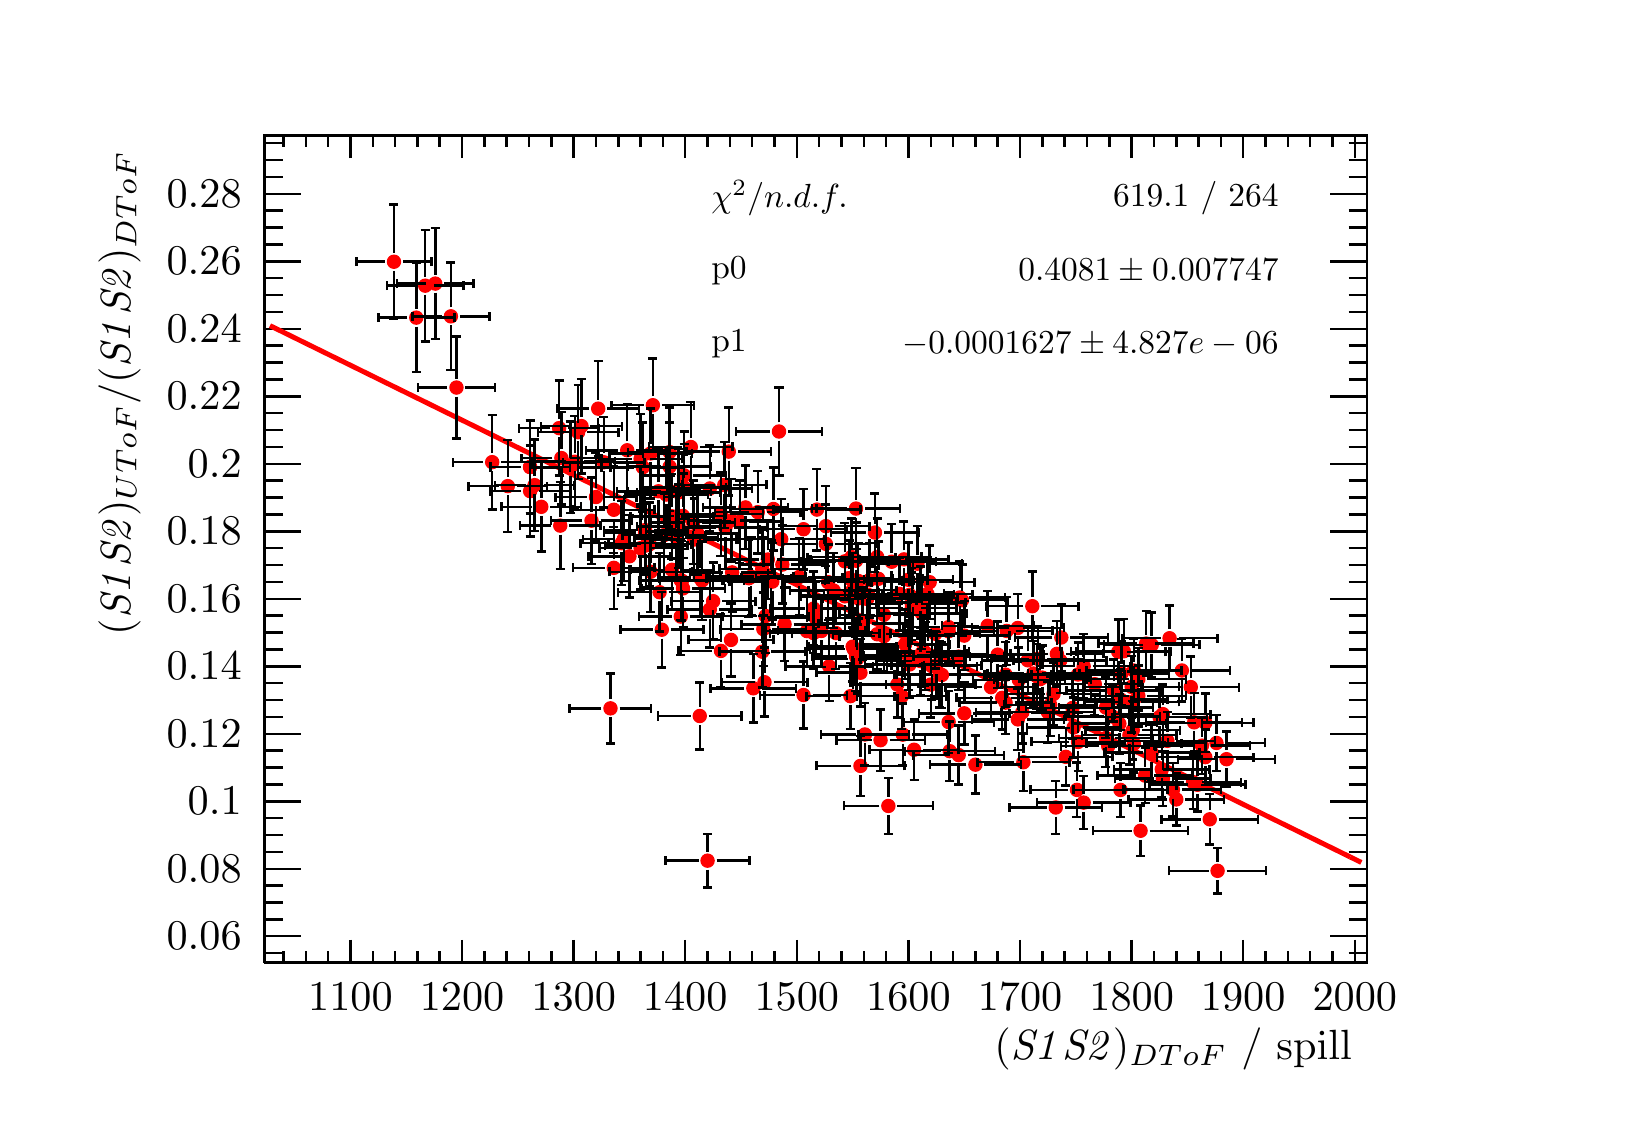
\begin{tikzpicture}
\pgfdeclareplotmark{cross} {
\pgfpathmoveto{\pgfpoint{-0.3\pgfplotmarksize}{\pgfplotmarksize}}
\pgfpathlineto{\pgfpoint{+0.3\pgfplotmarksize}{\pgfplotmarksize}}
\pgfpathlineto{\pgfpoint{+0.3\pgfplotmarksize}{0.3\pgfplotmarksize}}
\pgfpathlineto{\pgfpoint{+1\pgfplotmarksize}{0.3\pgfplotmarksize}}
\pgfpathlineto{\pgfpoint{+1\pgfplotmarksize}{-0.3\pgfplotmarksize}}
\pgfpathlineto{\pgfpoint{+0.3\pgfplotmarksize}{-0.3\pgfplotmarksize}}
\pgfpathlineto{\pgfpoint{+0.3\pgfplotmarksize}{-1.\pgfplotmarksize}}
\pgfpathlineto{\pgfpoint{-0.3\pgfplotmarksize}{-1.\pgfplotmarksize}}
\pgfpathlineto{\pgfpoint{-0.3\pgfplotmarksize}{-0.3\pgfplotmarksize}}
\pgfpathlineto{\pgfpoint{-1.\pgfplotmarksize}{-0.3\pgfplotmarksize}}
\pgfpathlineto{\pgfpoint{-1.\pgfplotmarksize}{0.3\pgfplotmarksize}}
\pgfpathlineto{\pgfpoint{-0.3\pgfplotmarksize}{0.3\pgfplotmarksize}}
\pgfpathclose
\pgfusepathqstroke
}
\pgfdeclareplotmark{cross*} {
\pgfpathmoveto{\pgfpoint{-0.3\pgfplotmarksize}{\pgfplotmarksize}}
\pgfpathlineto{\pgfpoint{+0.3\pgfplotmarksize}{\pgfplotmarksize}}
\pgfpathlineto{\pgfpoint{+0.3\pgfplotmarksize}{0.3\pgfplotmarksize}}
\pgfpathlineto{\pgfpoint{+1\pgfplotmarksize}{0.3\pgfplotmarksize}}
\pgfpathlineto{\pgfpoint{+1\pgfplotmarksize}{-0.3\pgfplotmarksize}}
\pgfpathlineto{\pgfpoint{+0.3\pgfplotmarksize}{-0.3\pgfplotmarksize}}
\pgfpathlineto{\pgfpoint{+0.3\pgfplotmarksize}{-1.\pgfplotmarksize}}
\pgfpathlineto{\pgfpoint{-0.3\pgfplotmarksize}{-1.\pgfplotmarksize}}
\pgfpathlineto{\pgfpoint{-0.3\pgfplotmarksize}{-0.3\pgfplotmarksize}}
\pgfpathlineto{\pgfpoint{-1.\pgfplotmarksize}{-0.3\pgfplotmarksize}}
\pgfpathlineto{\pgfpoint{-1.\pgfplotmarksize}{0.3\pgfplotmarksize}}
\pgfpathlineto{\pgfpoint{-0.3\pgfplotmarksize}{0.3\pgfplotmarksize}}
\pgfpathclose
\pgfusepathqfillstroke
}
\pgfdeclareplotmark{newstar} {
\pgfpathmoveto{\pgfqpoint{0pt}{\pgfplotmarksize}}
\pgfpathlineto{\pgfqpointpolar{44}{0.5\pgfplotmarksize}}
\pgfpathlineto{\pgfqpointpolar{18}{\pgfplotmarksize}}
\pgfpathlineto{\pgfqpointpolar{-20}{0.5\pgfplotmarksize}}
\pgfpathlineto{\pgfqpointpolar{-54}{\pgfplotmarksize}}
\pgfpathlineto{\pgfqpointpolar{-90}{0.5\pgfplotmarksize}}
\pgfpathlineto{\pgfqpointpolar{234}{\pgfplotmarksize}}
\pgfpathlineto{\pgfqpointpolar{198}{0.5\pgfplotmarksize}}
\pgfpathlineto{\pgfqpointpolar{162}{\pgfplotmarksize}}
\pgfpathlineto{\pgfqpointpolar{134}{0.5\pgfplotmarksize}}
\pgfpathclose
\pgfusepathqstroke
}
\pgfdeclareplotmark{newstar*} {
\pgfpathmoveto{\pgfqpoint{0pt}{\pgfplotmarksize}}
\pgfpathlineto{\pgfqpointpolar{44}{0.5\pgfplotmarksize}}
\pgfpathlineto{\pgfqpointpolar{18}{\pgfplotmarksize}}
\pgfpathlineto{\pgfqpointpolar{-20}{0.5\pgfplotmarksize}}
\pgfpathlineto{\pgfqpointpolar{-54}{\pgfplotmarksize}}
\pgfpathlineto{\pgfqpointpolar{-90}{0.5\pgfplotmarksize}}
\pgfpathlineto{\pgfqpointpolar{234}{\pgfplotmarksize}}
\pgfpathlineto{\pgfqpointpolar{198}{0.5\pgfplotmarksize}}
\pgfpathlineto{\pgfqpointpolar{162}{\pgfplotmarksize}}
\pgfpathlineto{\pgfqpointpolar{134}{0.5\pgfplotmarksize}}
\pgfpathclose
\pgfusepathqfillstroke
}
\definecolor{c}{rgb}{1,1,1};
\draw [color=c, fill=c] (0,0) rectangle (20,13.639);
\draw [color=c, fill=c] (3,1.77307) rectangle (17,12.2751);
\definecolor{c}{rgb}{0,0,0};
\draw [c,line width=0.9] (3,1.77307) -- (3,12.2751) -- (17,12.2751) -- (17,1.77307) -- (3,1.77307);
\definecolor{c}{rgb}{1,1,1};
\draw [color=c, fill=c] (3,1.77307) rectangle (17,12.2751);
\definecolor{c}{rgb}{0,0,0};
\draw [c,line width=0.9] (3,1.77307) -- (3,12.2751) -- (17,12.2751) -- (17,1.77307) -- (3,1.77307);
\draw [c,line width=0.9] (3,1.77307) -- (17,1.77307);
\draw [c,line width=0.9] (4.09225,2.05948) -- (4.09225,1.77307);
\draw [c,line width=0.9] (4.3757,1.91628) -- (4.3757,1.77307);
\draw [c,line width=0.9] (4.65916,1.91628) -- (4.65916,1.77307);
\draw [c,line width=0.9] (4.94262,1.91628) -- (4.94262,1.77307);
\draw [c,line width=0.9] (5.22608,1.91628) -- (5.22608,1.77307);
\draw [c,line width=0.9] (5.50954,2.05948) -- (5.50954,1.77307);
\draw [c,line width=0.9] (5.793,1.91628) -- (5.793,1.77307);
\draw [c,line width=0.9] (6.07646,1.91628) -- (6.07646,1.77307);
\draw [c,line width=0.9] (6.35991,1.91628) -- (6.35991,1.77307);
\draw [c,line width=0.9] (6.64337,1.91628) -- (6.64337,1.77307);
\draw [c,line width=0.9] (6.92683,2.05948) -- (6.92683,1.77307);
\draw [c,line width=0.9] (7.21029,1.91628) -- (7.21029,1.77307);
\draw [c,line width=0.9] (7.49375,1.91628) -- (7.49375,1.77307);
\draw [c,line width=0.9] (7.77721,1.91628) -- (7.77721,1.77307);
\draw [c,line width=0.9] (8.06067,1.91628) -- (8.06067,1.77307);
\draw [c,line width=0.9] (8.34412,2.05948) -- (8.34412,1.77307);
\draw [c,line width=0.9] (8.62758,1.91628) -- (8.62758,1.77307);
\draw [c,line width=0.9] (8.91104,1.91628) -- (8.91104,1.77307);
\draw [c,line width=0.9] (9.1945,1.91628) -- (9.1945,1.77307);
\draw [c,line width=0.9] (9.47796,1.91628) -- (9.47796,1.77307);
\draw [c,line width=0.9] (9.76142,2.05948) -- (9.76142,1.77307);
\draw [c,line width=0.9] (10.0449,1.91628) -- (10.0449,1.77307);
\draw [c,line width=0.9] (10.3283,1.91628) -- (10.3283,1.77307);
\draw [c,line width=0.9] (10.6118,1.91628) -- (10.6118,1.77307);
\draw [c,line width=0.9] (10.8953,1.91628) -- (10.8953,1.77307);
\draw [c,line width=0.9] (11.1787,2.05948) -- (11.1787,1.77307);
\draw [c,line width=0.9] (11.4622,1.91628) -- (11.4622,1.77307);
\draw [c,line width=0.9] (11.7456,1.91628) -- (11.7456,1.77307);
\draw [c,line width=0.9] (12.0291,1.91628) -- (12.0291,1.77307);
\draw [c,line width=0.9] (12.3125,1.91628) -- (12.3125,1.77307);
\draw [c,line width=0.9] (12.596,2.05948) -- (12.596,1.77307);
\draw [c,line width=0.9] (12.8795,1.91628) -- (12.8795,1.77307);
\draw [c,line width=0.9] (13.1629,1.91628) -- (13.1629,1.77307);
\draw [c,line width=0.9] (13.4464,1.91628) -- (13.4464,1.77307);
\draw [c,line width=0.9] (13.7298,1.91628) -- (13.7298,1.77307);
\draw [c,line width=0.9] (14.0133,2.05948) -- (14.0133,1.77307);
\draw [c,line width=0.9] (14.2968,1.91628) -- (14.2968,1.77307);
\draw [c,line width=0.9] (14.5802,1.91628) -- (14.5802,1.77307);
\draw [c,line width=0.9] (14.8637,1.91628) -- (14.8637,1.77307);
\draw [c,line width=0.9] (15.1471,1.91628) -- (15.1471,1.77307);
\draw [c,line width=0.9] (15.4306,2.05948) -- (15.4306,1.77307);
\draw [c,line width=0.9] (15.714,1.91628) -- (15.714,1.77307);
\draw [c,line width=0.9] (15.9975,1.91628) -- (15.9975,1.77307);
\draw [c,line width=0.9] (16.281,1.91628) -- (16.281,1.77307);
\draw [c,line width=0.9] (16.5644,1.91628) -- (16.5644,1.77307);
\draw [c,line width=0.9] (16.8479,2.05948) -- (16.8479,1.77307);
\draw [c,line width=0.9] (4.09225,2.05948) -- (4.09225,1.77307);
\draw [c,line width=0.9] (3.80879,1.91628) -- (3.80879,1.77307);
\draw [c,line width=0.9] (3.52533,1.91628) -- (3.52533,1.77307);
\draw [c,line width=0.9] (3.24187,1.91628) -- (3.24187,1.77307);
\draw [c,line width=0.9] (16.8479,2.05948) -- (16.8479,1.77307);
\draw [anchor=base] (4.09225,1.15931) node[scale=1.52731, color=c, rotate=0]{1100};
\draw [anchor=base] (5.50954,1.15931) node[scale=1.52731, color=c, rotate=0]{1200};
\draw [anchor=base] (6.92683,1.15931) node[scale=1.52731, color=c, rotate=0]{1300};
\draw [anchor=base] (8.34412,1.15931) node[scale=1.52731, color=c, rotate=0]{1400};
\draw [anchor=base] (9.76142,1.15931) node[scale=1.52731, color=c, rotate=0]{1500};
\draw [anchor=base] (11.1787,1.15931) node[scale=1.52731, color=c, rotate=0]{1600};
\draw [anchor=base] (12.596,1.15931) node[scale=1.52731, color=c, rotate=0]{1700};
\draw [anchor=base] (14.0133,1.15931) node[scale=1.52731, color=c, rotate=0]{1800};
\draw [anchor=base] (15.4306,1.15931) node[scale=1.52731, color=c, rotate=0]{1900};
\draw [anchor=base] (16.8479,1.15931) node[scale=1.52731, color=c, rotate=0]{2000};
\draw [anchor= east] (17,0.681948) node[scale=1.52731, color=c, rotate=0]{ $(\SOne\STwo)_{\text{DToF}}$ / spill};
\draw [c,line width=0.9] (3,12.2751) -- (17,12.2751);
\draw [c,line width=0.9] (4.09225,11.9887) -- (4.09225,12.2751);
\draw [c,line width=0.9] (4.3757,12.1319) -- (4.3757,12.2751);
\draw [c,line width=0.9] (4.65916,12.1319) -- (4.65916,12.2751);
\draw [c,line width=0.9] (4.94262,12.1319) -- (4.94262,12.2751);
\draw [c,line width=0.9] (5.22608,12.1319) -- (5.22608,12.2751);
\draw [c,line width=0.9] (5.50954,11.9887) -- (5.50954,12.2751);
\draw [c,line width=0.9] (5.793,12.1319) -- (5.793,12.2751);
\draw [c,line width=0.9] (6.07646,12.1319) -- (6.07646,12.2751);
\draw [c,line width=0.9] (6.35991,12.1319) -- (6.35991,12.2751);
\draw [c,line width=0.9] (6.64337,12.1319) -- (6.64337,12.2751);
\draw [c,line width=0.9] (6.92683,11.9887) -- (6.92683,12.2751);
\draw [c,line width=0.9] (7.21029,12.1319) -- (7.21029,12.2751);
\draw [c,line width=0.9] (7.49375,12.1319) -- (7.49375,12.2751);
\draw [c,line width=0.9] (7.77721,12.1319) -- (7.77721,12.2751);
\draw [c,line width=0.9] (8.06067,12.1319) -- (8.06067,12.2751);
\draw [c,line width=0.9] (8.34412,11.9887) -- (8.34412,12.2751);
\draw [c,line width=0.9] (8.62758,12.1319) -- (8.62758,12.2751);
\draw [c,line width=0.9] (8.91104,12.1319) -- (8.91104,12.2751);
\draw [c,line width=0.9] (9.1945,12.1319) -- (9.1945,12.2751);
\draw [c,line width=0.9] (9.47796,12.1319) -- (9.47796,12.2751);
\draw [c,line width=0.9] (9.76142,11.9887) -- (9.76142,12.2751);
\draw [c,line width=0.9] (10.0449,12.1319) -- (10.0449,12.2751);
\draw [c,line width=0.9] (10.3283,12.1319) -- (10.3283,12.2751);
\draw [c,line width=0.9] (10.6118,12.1319) -- (10.6118,12.2751);
\draw [c,line width=0.9] (10.8953,12.1319) -- (10.8953,12.2751);
\draw [c,line width=0.9] (11.1787,11.9887) -- (11.1787,12.2751);
\draw [c,line width=0.9] (11.4622,12.1319) -- (11.4622,12.2751);
\draw [c,line width=0.9] (11.7456,12.1319) -- (11.7456,12.2751);
\draw [c,line width=0.9] (12.0291,12.1319) -- (12.0291,12.2751);
\draw [c,line width=0.9] (12.3125,12.1319) -- (12.3125,12.2751);
\draw [c,line width=0.9] (12.596,11.9887) -- (12.596,12.2751);
\draw [c,line width=0.9] (12.8795,12.1319) -- (12.8795,12.2751);
\draw [c,line width=0.9] (13.1629,12.1319) -- (13.1629,12.2751);
\draw [c,line width=0.9] (13.4464,12.1319) -- (13.4464,12.2751);
\draw [c,line width=0.9] (13.7298,12.1319) -- (13.7298,12.2751);
\draw [c,line width=0.9] (14.0133,11.9887) -- (14.0133,12.2751);
\draw [c,line width=0.9] (14.2968,12.1319) -- (14.2968,12.2751);
\draw [c,line width=0.9] (14.5802,12.1319) -- (14.5802,12.2751);
\draw [c,line width=0.9] (14.8637,12.1319) -- (14.8637,12.2751);
\draw [c,line width=0.9] (15.1471,12.1319) -- (15.1471,12.2751);
\draw [c,line width=0.9] (15.4306,11.9887) -- (15.4306,12.2751);
\draw [c,line width=0.9] (15.714,12.1319) -- (15.714,12.2751);
\draw [c,line width=0.9] (15.9975,12.1319) -- (15.9975,12.2751);
\draw [c,line width=0.9] (16.281,12.1319) -- (16.281,12.2751);
\draw [c,line width=0.9] (16.5644,12.1319) -- (16.5644,12.2751);
\draw [c,line width=0.9] (16.8479,11.9887) -- (16.8479,12.2751);
\draw [c,line width=0.9] (4.09225,11.9887) -- (4.09225,12.2751);
\draw [c,line width=0.9] (3.80879,12.1319) -- (3.80879,12.2751);
\draw [c,line width=0.9] (3.52533,12.1319) -- (3.52533,12.2751);
\draw [c,line width=0.9] (3.24187,12.1319) -- (3.24187,12.2751);
\draw [c,line width=0.9] (16.8479,11.9887) -- (16.8479,12.2751);
\draw [c,line width=0.9] (3,1.77307) -- (3,12.2751);
\draw [c,line width=0.9] (3.462,2.10714) -- (3,2.10714);
\draw [c,line width=0.9] (3.231,2.32142) -- (3,2.32142);
\draw [c,line width=0.9] (3.231,2.53571) -- (3,2.53571);
\draw [c,line width=0.9] (3.231,2.74999) -- (3,2.74999);
\draw [c,line width=0.9] (3.462,2.96428) -- (3,2.96428);
\draw [c,line width=0.9] (3.231,3.17856) -- (3,3.17856);
\draw [c,line width=0.9] (3.231,3.39285) -- (3,3.39285);
\draw [c,line width=0.9] (3.231,3.60714) -- (3,3.60714);
\draw [c,line width=0.9] (3.462,3.82142) -- (3,3.82142);
\draw [c,line width=0.9] (3.231,4.03571) -- (3,4.03571);
\draw [c,line width=0.9] (3.231,4.24999) -- (3,4.24999);
\draw [c,line width=0.9] (3.231,4.46428) -- (3,4.46428);
\draw [c,line width=0.9] (3.462,4.67856) -- (3,4.67856);
\draw [c,line width=0.9] (3.231,4.89285) -- (3,4.89285);
\draw [c,line width=0.9] (3.231,5.10713) -- (3,5.10713);
\draw [c,line width=0.9] (3.231,5.32142) -- (3,5.32142);
\draw [c,line width=0.9] (3.462,5.5357) -- (3,5.5357);
\draw [c,line width=0.9] (3.231,5.74999) -- (3,5.74999);
\draw [c,line width=0.9] (3.231,5.96427) -- (3,5.96427);
\draw [c,line width=0.9] (3.231,6.17856) -- (3,6.17856);
\draw [c,line width=0.9] (3.462,6.39284) -- (3,6.39284);
\draw [c,line width=0.9] (3.231,6.60713) -- (3,6.60713);
\draw [c,line width=0.9] (3.231,6.82141) -- (3,6.82141);
\draw [c,line width=0.9] (3.231,7.0357) -- (3,7.0357);
\draw [c,line width=0.9] (3.462,7.24999) -- (3,7.24999);
\draw [c,line width=0.9] (3.231,7.46427) -- (3,7.46427);
\draw [c,line width=0.9] (3.231,7.67856) -- (3,7.67856);
\draw [c,line width=0.9] (3.231,7.89284) -- (3,7.89284);
\draw [c,line width=0.9] (3.462,8.10713) -- (3,8.10713);
\draw [c,line width=0.9] (3.231,8.32141) -- (3,8.32141);
\draw [c,line width=0.9] (3.231,8.5357) -- (3,8.5357);
\draw [c,line width=0.9] (3.231,8.74998) -- (3,8.74998);
\draw [c,line width=0.9] (3.462,8.96427) -- (3,8.96427);
\draw [c,line width=0.9] (3.231,9.17855) -- (3,9.17855);
\draw [c,line width=0.9] (3.231,9.39284) -- (3,9.39284);
\draw [c,line width=0.9] (3.231,9.60712) -- (3,9.60712);
\draw [c,line width=0.9] (3.462,9.82141) -- (3,9.82141);
\draw [c,line width=0.9] (3.231,10.0357) -- (3,10.0357);
\draw [c,line width=0.9] (3.231,10.25) -- (3,10.25);
\draw [c,line width=0.9] (3.231,10.4643) -- (3,10.4643);
\draw [c,line width=0.9] (3.462,10.6785) -- (3,10.6785);
\draw [c,line width=0.9] (3.231,10.8928) -- (3,10.8928);
\draw [c,line width=0.9] (3.231,11.1071) -- (3,11.1071);
\draw [c,line width=0.9] (3.231,11.3214) -- (3,11.3214);
\draw [c,line width=0.9] (3.462,11.5357) -- (3,11.5357);
\draw [c,line width=0.9] (3.462,2.10714) -- (3,2.10714);
\draw [c,line width=0.9] (3.231,1.89285) -- (3,1.89285);
\draw [c,line width=0.9] (3.462,11.5357) -- (3,11.5357);
\draw [c,line width=0.9] (3.231,11.75) -- (3,11.75);
\draw [c,line width=0.9] (3.231,11.9643) -- (3,11.9643);
\draw [c,line width=0.9] (3.231,12.1785) -- (3,12.1785);
\draw [anchor= east] (2.9,2.10714) node[scale=1.52731, color=c, rotate=0]{0.06};
\draw [anchor= east] (2.9,2.96428) node[scale=1.52731, color=c, rotate=0]{0.08};
\draw [anchor= east] (2.9,3.82142) node[scale=1.52731, color=c, rotate=0]{0.1};
\draw [anchor= east] (2.9,4.67856) node[scale=1.52731, color=c, rotate=0]{0.12};
\draw [anchor= east] (2.9,5.5357) node[scale=1.52731, color=c, rotate=0]{0.14};
\draw [anchor= east] (2.9,6.39284) node[scale=1.52731, color=c, rotate=0]{0.16};
\draw [anchor= east] (2.9,7.24999) node[scale=1.52731, color=c, rotate=0]{0.18};
\draw [anchor= east] (2.9,8.10713) node[scale=1.52731, color=c, rotate=0]{0.2};
\draw [anchor= east] (2.9,8.96427) node[scale=1.52731, color=c, rotate=0]{0.22};
\draw [anchor= east] (2.9,9.82141) node[scale=1.52731, color=c, rotate=0]{0.24};
\draw [anchor= east] (2.9,10.6785) node[scale=1.52731, color=c, rotate=0]{0.26};
\draw [anchor= east] (2.9,11.5357) node[scale=1.52731, color=c, rotate=0]{0.28};
\draw [anchor= east] (1.16,12.2751) node[scale=1.52731, color=c, rotate=90]{ $(\SOne\STwo)_{\text{UToF}}/(\SOne\STwo)_{\text{DToF}}$ };
\draw [c,line width=0.9] (17,1.77307) -- (17,12.2751);
\draw [c,line width=0.9] (16.538,2.10714) -- (17,2.10714);
\draw [c,line width=0.9] (16.769,2.32142) -- (17,2.32142);
\draw [c,line width=0.9] (16.769,2.53571) -- (17,2.53571);
\draw [c,line width=0.9] (16.769,2.74999) -- (17,2.74999);
\draw [c,line width=0.9] (16.538,2.96428) -- (17,2.96428);
\draw [c,line width=0.9] (16.769,3.17856) -- (17,3.17856);
\draw [c,line width=0.9] (16.769,3.39285) -- (17,3.39285);
\draw [c,line width=0.9] (16.769,3.60714) -- (17,3.60714);
\draw [c,line width=0.9] (16.538,3.82142) -- (17,3.82142);
\draw [c,line width=0.9] (16.769,4.03571) -- (17,4.03571);
\draw [c,line width=0.9] (16.769,4.24999) -- (17,4.24999);
\draw [c,line width=0.9] (16.769,4.46428) -- (17,4.46428);
\draw [c,line width=0.9] (16.538,4.67856) -- (17,4.67856);
\draw [c,line width=0.9] (16.769,4.89285) -- (17,4.89285);
\draw [c,line width=0.9] (16.769,5.10713) -- (17,5.10713);
\draw [c,line width=0.9] (16.769,5.32142) -- (17,5.32142);
\draw [c,line width=0.9] (16.538,5.5357) -- (17,5.5357);
\draw [c,line width=0.9] (16.769,5.74999) -- (17,5.74999);
\draw [c,line width=0.9] (16.769,5.96427) -- (17,5.96427);
\draw [c,line width=0.9] (16.769,6.17856) -- (17,6.17856);
\draw [c,line width=0.9] (16.538,6.39284) -- (17,6.39284);
\draw [c,line width=0.9] (16.769,6.60713) -- (17,6.60713);
\draw [c,line width=0.9] (16.769,6.82141) -- (17,6.82141);
\draw [c,line width=0.9] (16.769,7.0357) -- (17,7.0357);
\draw [c,line width=0.9] (16.538,7.24999) -- (17,7.24999);
\draw [c,line width=0.9] (16.769,7.46427) -- (17,7.46427);
\draw [c,line width=0.9] (16.769,7.67856) -- (17,7.67856);
\draw [c,line width=0.9] (16.769,7.89284) -- (17,7.89284);
\draw [c,line width=0.9] (16.538,8.10713) -- (17,8.10713);
\draw [c,line width=0.9] (16.769,8.32141) -- (17,8.32141);
\draw [c,line width=0.9] (16.769,8.5357) -- (17,8.5357);
\draw [c,line width=0.9] (16.769,8.74998) -- (17,8.74998);
\draw [c,line width=0.9] (16.538,8.96427) -- (17,8.96427);
\draw [c,line width=0.9] (16.769,9.17855) -- (17,9.17855);
\draw [c,line width=0.9] (16.769,9.39284) -- (17,9.39284);
\draw [c,line width=0.9] (16.769,9.60712) -- (17,9.60712);
\draw [c,line width=0.9] (16.538,9.82141) -- (17,9.82141);
\draw [c,line width=0.9] (16.769,10.0357) -- (17,10.0357);
\draw [c,line width=0.9] (16.769,10.25) -- (17,10.25);
\draw [c,line width=0.9] (16.769,10.4643) -- (17,10.4643);
\draw [c,line width=0.9] (16.538,10.6785) -- (17,10.6785);
\draw [c,line width=0.9] (16.769,10.8928) -- (17,10.8928);
\draw [c,line width=0.9] (16.769,11.1071) -- (17,11.1071);
\draw [c,line width=0.9] (16.769,11.3214) -- (17,11.3214);
\draw [c,line width=0.9] (16.538,11.5357) -- (17,11.5357);
\draw [c,line width=0.9] (16.538,2.10714) -- (17,2.10714);
\draw [c,line width=0.9] (16.769,1.89285) -- (17,1.89285);
\draw [c,line width=0.9] (16.538,11.5357) -- (17,11.5357);
\draw [c,line width=0.9] (16.769,11.75) -- (17,11.75);
\draw [c,line width=0.9] (16.769,11.9643) -- (17,11.9643);
\draw [c,line width=0.9] (16.769,12.1785) -- (17,12.1785);
\definecolor{c}{rgb}{1,0,0};
\foreach \P in {(14.9487,4.38182), (11.859,6.37516), (12.4118,5.07385), (12.9503,4.95185), (9.97401,6.26837), (11.3346,6.34602), (10.1583,6.60376), (10.2575,5.95729), (8.65593,7.79369), (13.7865,5.22917), (10.4701,5.78455), (12.3692,5.13462),
 (9.32206,5.72067), (12.9787,5.04484), (12.8511,5.37306), (8.17405,6.7609), (8.92521,7.38739), (11.4196,6.45327), (5.89221,8.12808), (10.5126,5.66209), (12.4118,5.42951), (14.6511,5.48228), (14.0416,5.48148), (9.36457,6.1739), (10.5976,6.07836),
 (12.3125,5.68366), (9.33623,6.00801), (13.0212,5.18393), (10.5126,6.87633), (9.0386,7.37362), (10.7535,7.23361), (8.52837,6.66339), (13.7724,4.89585), (10.4559,6.92295), (10.0165,7.52554), (10.6685,6.44107), (13.9141,5.72644), (9.57717,6.82747),
 (11.8874,4.9383), (7.02604,8.58587), (10.3709,6.42395), (12.5677,6.02232), (8.23074,7.17117), (14.2684,5.80633), (12.4259,5.98458), (8.01815,6.47625), (8.25909,7.31393), (12.7519,6.29866), (8.84018,7.83834), (13.1062,5.60878), (6.75676,7.32186),
 (14.0416,4.55394), (11.8307,6.40951), (8.30161,6.62231), (9.3504,5.33351), (12.8228,5.62961), (5.04183,10.3693), (11.8165,5.65815), (14.0133,5.08332), (10.2291,6.49684), (13.4039,5.53619), (8.85435,7.29535), (13.3188,3.96583), (14.2684,4.43905),
 (10.1724,5.53402), (11.3771,5.72264), (11.2212,6.32654), (11.533,5.54889), (10.8669,6.18969), (11.2354,6.40246), (8.25909,7.74435), (15.218,4.35571), (5.43867,9.07545), (13.8432,5.71979), (13.1771,4.38513), (8.93939,6.72809), (9.84645,5.17031),
 (11.5756,5.43251), (9.88897,5.98273), (10.1299,7.09047), (14.8495,4.03121), (7.84807,7.07102), (10.796,6.64677), (4.92845,9.9634), (13.5456,5.3082), (10.7819,5.94246), (8.89687,8.262), (11.3488,5.70373), (14.0133,5.2738), (7.80555,8.06307),
 (11.6889,4.82736), (10.3709,6.86835), (9.56299,7.14962), (13.8857,5.44621), (6.77093,8.18027), (12.5818,5.36266), (13.333,5.43101), (7.77721,7.0357), (14.0983,5.15981), (14.0983,5.37339), (8.79766,7.46666), (12.7661,5.44358), (9.84645,7.27617),
 (8.17405,7.44019), (14.4101,4.10745), (8.69845,6.36277), (13.2621,5.00631), (8.44333,7.36391), (11.4622,5.3029), (15.0054,3.59224), (14.5802,3.84471), (10.6543,6.39065), (8.10318,7.71667), (13.1204,5.90136), (11.1362,5.81533), (11.0937,5.15499),
 (5.36781,9.97987), (7.43706,7.5233), (14.0275,4.7233), (7.89059,7.08582), (9.33623,6.67856), (13.8716,5.11432), (6.43078,7.83609), (9.78976,6.66905), (13.9849,4.66045), (6.51582,7.56088), (13.6873,5.01042), (6.88431,8.06087), (12.6385,4.31718),
 (11.8165,4.40761), (7.53627,7.09872), (10.9661,6.86333), (14.9487,4.8182), (8.41499,8.32065), (12.8086,5.40826), (13.6873,4.62454), (8.28743,6.62739), (10.0024,6.14649), (6.37409,7.76046), (10.5268,5.63057), (11.2212,6.27307), (11.1078,4.66781),
 (14.1834,4.14782), (12.6243,4.9495), (8.1457,7.76081), (11.1929,5.55872), (11.1929,6.4421), (5.16939,10.3958), (8.92521,5.87059), (4.64499,10.6733), (11.3346,5.60115), (12.2275,5.27047), (8.45751,7.14528), (10.5409,6.39836), (11.1787,6.63391),
 (7.90476,8.23861), (11.2496,4.47562), (10.8669,5.9181), (8.65593,6.25662), (9.10946,7.55299), (8.28743,6.16689), (9.60551,6.06933), (12.0291,4.28614), (11.7031,4.4576), (8.07484,7.20095), (11.0653,6.45422), (6.37409,8.06634), (11.037,5.3039),
 (14.807,4.82357), (8.31578,6.52528), (10.626,4.66978), (6.98352,8.50809), (8.32995,7.80691), (14.7645,5.27158), (6.74258,8.56001), (11.1787,5.66963), (13.4039,3.80435), (9.97401,5.9572), (10.4275,6.65547), (11.2354,6.40246), (11.5189,5.94844),
 (10.0732,5.98398), (6.09063,7.82395), (10.1299,7.31514), (14.4668,4.58873), (7.43706,6.78549), (13.0495,3.74224), (14.1267,3.4469), (10.8244,4.59693), (9.20867,5.25586), (15.1046,2.93779), (7.39454,5.00136), (9.46379,7.53338), (8.32995,7.96008),
 (14.5377,3.9684), (9.43544,6.64471), (7.1536,7.38416), (10.9236,3.76182), (14.7928,4.06401), (9.15198,6.65405), (9.39292,6.89178), (15.0904,4.5616), (7.60713,8.27881), (13.8574,4.80601), (8.62758,3.06689), (12.185,6.05019), (10.4701,6.50344),
 (7.93311,8.85111), (9.53465,8.51721), (14.1975,5.82362), (13.333,4.57484), (10.5693,5.45368), (11.122,6.89338), (9.44961,6.6109), (8.1457,8.07002), (7.8339,7.23365), (13.0637,5.69348), (12.5677,4.8613), (8.1457,8.25555), (7.8339,7.26507),
 (10.5126,7.53864), (7.21029,7.68505), (10.4842,5.75289), (14.396,4.22724), (11.6889,6.03238), (10.5693,4.27008), (10.5409,6.61884), (10.7819,6.92392), (14.4952,5.89183), (7.90476,6.73595), (10.6827,6.62835), (11.3913,5.66573), (8.52837,4.90422),
 (7.77721,8.17015), (11.8874,5.92531), (9.18033,6.67366), (12.8795,5.39118), (7.23864,8.80736), (8.79766,5.73083), (11.2921,6.83847), (8.50003,7.22022), (8.00397,7.75829), (14.0133,5.08332), (7.56461,7.15121), (14.4101,4.92801), (13.8716,3.96508),
 (8.04649,6.00001), (9.32206,6.77094), (6.37409,8.06634), (8.55672,6.62303), (12.6952,5.61153), (9.26536,7.49279), (10.4417,5.15586), (11.6889,5.97999), (11.4763,5.53729), (14.3676,4.88991), (14.9062,4.52765), (7.3095,8.1265), (13.2763,4.758),
 (7.63548,6.93253), (11.3488,6.20887), (11.448,6.60356), (6.941,8.13348), (11.6039,5.42527), (13.7157,4.52245), (8.31578,7.44496)}{\draw[mark options={color=c,fill=c},mark size=2.402402pt,mark=*] plot coordinates {\P};}
\draw [c,line width=1.8] (3.07,9.86152) -- (3.21,9.79266) -- (3.35,9.7238) -- (3.49,9.65494) -- (3.63,9.58609) -- (3.77,9.51723) -- (3.91,9.44837) -- (4.05,9.37951) -- (4.19,9.31065) -- (4.33,9.2418) -- (4.47,9.17294) -- (4.61,9.10408) --
 (4.75,9.03522) -- (4.89,8.96637) -- (5.03,8.89751) -- (5.17,8.82865) -- (5.31,8.75979) -- (5.45,8.69094) -- (5.59,8.62208) -- (5.73,8.55322) -- (5.87,8.48436) -- (6.01,8.41551) -- (6.15,8.34665) -- (6.29,8.27779) -- (6.43,8.20893) -- (6.57,8.14007)
 -- (6.71,8.07122) -- (6.85,8.00236) -- (6.99,7.9335) -- (7.13,7.86464) -- (7.27,7.79579) -- (7.41,7.72693) -- (7.55,7.65807) -- (7.69,7.58921) -- (7.83,7.52036) -- (7.97,7.4515) -- (8.11,7.38264) -- (8.25,7.31378) -- (8.39,7.24492) -- (8.53,7.17607)
 -- (8.67,7.10721) -- (8.81,7.03835) -- (8.95,6.96949) -- (9.09,6.90064) -- (9.23,6.83178) -- (9.37,6.76292) -- (9.51,6.69406) -- (9.65,6.62521) -- (9.79,6.55635) -- (9.93,6.48749);
\draw [c,line width=1.8] (9.93,6.48749) -- (10.07,6.41863) -- (10.21,6.34977) -- (10.35,6.28092) -- (10.49,6.21206) -- (10.63,6.1432) -- (10.77,6.07434) -- (10.91,6.00549) -- (11.05,5.93663) -- (11.19,5.86777) -- (11.33,5.79891) -- (11.47,5.73006) --
 (11.61,5.6612) -- (11.75,5.59234) -- (11.89,5.52348) -- (12.03,5.45463) -- (12.17,5.38577) -- (12.31,5.31691) -- (12.45,5.24805) -- (12.59,5.17919) -- (12.73,5.11034) -- (12.87,5.04148) -- (13.01,4.97262) -- (13.15,4.90376) -- (13.29,4.83491) --
 (13.43,4.76605) -- (13.57,4.69719) -- (13.71,4.62833) -- (13.85,4.55948) -- (13.99,4.49062) -- (14.13,4.42176) -- (14.27,4.3529) -- (14.41,4.28404) -- (14.55,4.21519) -- (14.69,4.14633) -- (14.83,4.07747) -- (14.97,4.00861) -- (15.11,3.93976) --
 (15.25,3.8709) -- (15.39,3.80204) -- (15.53,3.73318) -- (15.67,3.66433) -- (15.81,3.59547) -- (15.95,3.52661) -- (16.09,3.45775) -- (16.23,3.3889) -- (16.37,3.32004) -- (16.51,3.25118) -- (16.65,3.18232) -- (16.79,3.11346);
\draw [c,line width=1.8] (16.79,3.11346) -- (16.93,3.04461);
\definecolor{c}{rgb}{1,1,1};
\draw [color=c, fill=c] (8.10888,9.16905) rectangle (16.447,11.9484);
\definecolor{c}{rgb}{0,0,0};
\draw [anchor= west] (8.52579,11.4852) node[scale=1.20912, color=c, rotate=0]{$\chi^{2} / \text{n.d.f.} $};
\draw [anchor= east] (16.0301,11.4852) node[scale=1.20912, color=c, rotate=0]{ 619.1 / 264};
\draw [anchor= west] (8.52579,10.5587) node[scale=1.20912, color=c, rotate=0]{p0       };
\draw [anchor= east] (16.0301,10.5587) node[scale=1.20912, color=c, rotate=0]{$ 0.4081 \pm 0.007747$};
\draw [anchor= west] (8.52579,9.63228) node[scale=1.20912, color=c, rotate=0]{p1       };
\draw [anchor= east] (16.0301,9.63228) node[scale=1.20912, color=c, rotate=0]{$ -0.0001627 \pm 4.827e-06$};
\draw [c,line width=0.9] (14.8341,4.38182) -- (14.3365,4.38182);
\draw [c,line width=0.9] (14.3365,4.32452) -- (14.3365,4.43913);
\draw [c,line width=0.9] (15.0633,4.38182) -- (15.5609,4.38182);
\draw [c,line width=0.9] (15.5609,4.32452) -- (15.5609,4.43913);
\draw [c,line width=0.9] (14.9487,4.49644) -- (14.9487,4.7338);
\draw [c,line width=0.9] (14.8914,4.7338) -- (15.006,4.7338);
\draw [c,line width=0.9] (14.9487,4.26721) -- (14.9487,4.02985);
\draw [c,line width=0.9] (14.8914,4.02985) -- (15.006,4.02985);
\draw [c,line width=0.9] (11.7444,6.37516) -- (11.2837,6.37516);
\draw [c,line width=0.9] (11.2837,6.31785) -- (11.2837,6.43247);
\draw [c,line width=0.9] (11.9736,6.37516) -- (12.4344,6.37516);
\draw [c,line width=0.9] (12.4344,6.31785) -- (12.4344,6.43247);
\draw [c,line width=0.9] (11.859,6.48977) -- (11.859,6.82931);
\draw [c,line width=0.9] (11.8017,6.82931) -- (11.9163,6.82931);
\draw [c,line width=0.9] (11.859,6.26055) -- (11.859,5.92102);
\draw [c,line width=0.9] (11.8017,5.92102) -- (11.9163,5.92102);
\draw [c,line width=0.9] (12.2971,5.07385) -- (11.8296,5.07385);
\draw [c,line width=0.9] (11.8296,5.01655) -- (11.8296,5.13116);
\draw [c,line width=0.9] (12.5264,5.07385) -- (12.9939,5.07385);
\draw [c,line width=0.9] (12.9939,5.01655) -- (12.9939,5.13116);
\draw [c,line width=0.9] (12.4118,5.18847) -- (12.4118,5.47244);
\draw [c,line width=0.9] (12.3544,5.47244) -- (12.4691,5.47244);
\draw [c,line width=0.9] (12.4118,4.95924) -- (12.4118,4.67526);
\draw [c,line width=0.9] (12.3544,4.67526) -- (12.4691,4.67526);
\draw [c,line width=0.9] (12.8357,4.95185) -- (12.3617,4.95185);
\draw [c,line width=0.9] (12.3617,4.89455) -- (12.3617,5.00916);
\draw [c,line width=0.9] (13.0649,4.95185) -- (13.539,4.95185);
\draw [c,line width=0.9] (13.539,4.89455) -- (13.539,5.00916);
\draw [c,line width=0.9] (12.9503,5.06647) -- (12.9503,5.34117);
\draw [c,line width=0.9] (12.893,5.34117) -- (13.0076,5.34117);
\draw [c,line width=0.9] (12.9503,4.83724) -- (12.9503,4.56254);
\draw [c,line width=0.9] (12.893,4.56254) -- (13.0076,4.56254);
\draw [c,line width=0.9] (9.8594,6.26837) -- (9.42236,6.26837);
\draw [c,line width=0.9] (9.42236,6.21107) -- (9.42236,6.32568);
\draw [c,line width=0.9] (10.0886,6.26837) -- (10.5257,6.26837);
\draw [c,line width=0.9] (10.5257,6.21107) -- (10.5257,6.32568);
\draw [c,line width=0.9] (9.97401,6.38299) -- (9.97401,6.73782);
\draw [c,line width=0.9] (9.9167,6.73782) -- (10.0313,6.73782);
\draw [c,line width=0.9] (9.97401,6.15376) -- (9.97401,5.79893);
\draw [c,line width=0.9] (9.9167,5.79893) -- (10.0313,5.79893);
\draw [c,line width=0.9] (11.22,6.34602) -- (10.7657,6.34602);
\draw [c,line width=0.9] (10.7657,6.28872) -- (10.7657,6.40333);
\draw [c,line width=0.9] (11.4492,6.34602) -- (11.9035,6.34602);
\draw [c,line width=0.9] (11.9035,6.28872) -- (11.9035,6.40333);
\draw [c,line width=0.9] (11.3346,6.46064) -- (11.3346,6.80424);
\draw [c,line width=0.9] (11.2773,6.80424) -- (11.3919,6.80424);
\draw [c,line width=0.9] (11.3346,6.23141) -- (11.3346,5.88781);
\draw [c,line width=0.9] (11.2773,5.88781) -- (11.3919,5.88781);
\draw [c,line width=0.9] (10.0436,6.60376) -- (9.60424,6.60376);
\draw [c,line width=0.9] (9.60424,6.54646) -- (9.60424,6.66107);
\draw [c,line width=0.9] (10.2729,6.60376) -- (10.7123,6.60376);
\draw [c,line width=0.9] (10.7123,6.54646) -- (10.7123,6.66107);
\draw [c,line width=0.9] (10.1583,6.71838) -- (10.1583,7.08432);
\draw [c,line width=0.9] (10.101,7.08432) -- (10.2156,7.08432);
\draw [c,line width=0.9] (10.1583,6.48915) -- (10.1583,6.1232);
\draw [c,line width=0.9] (10.101,6.1232) -- (10.2156,6.1232);
\draw [c,line width=0.9] (10.1429,5.95729) -- (9.70219,5.95729);
\draw [c,line width=0.9] (9.70219,5.89999) -- (9.70219,6.0146);
\draw [c,line width=0.9] (10.3721,5.95729) -- (10.8128,5.95729);
\draw [c,line width=0.9] (10.8128,5.89999) -- (10.8128,6.0146);
\draw [c,line width=0.9] (10.2575,6.07191) -- (10.2575,6.41134);
\draw [c,line width=0.9] (10.2002,6.41134) -- (10.3148,6.41134);
\draw [c,line width=0.9] (10.2575,5.84268) -- (10.2575,5.50325);
\draw [c,line width=0.9] (10.2002,5.50325) -- (10.3148,5.50325);
\draw [c,line width=0.9] (8.54132,7.79369) -- (8.12148,7.79369);
\draw [c,line width=0.9] (8.12148,7.73638) -- (8.12148,7.85099);
\draw [c,line width=0.9] (8.77054,7.79369) -- (9.19038,7.79369);
\draw [c,line width=0.9] (9.19038,7.73638) -- (9.19038,7.85099);
\draw [c,line width=0.9] (8.65593,7.9083) -- (8.65593,8.33852);
\draw [c,line width=0.9] (8.59862,8.33852) -- (8.71323,8.33852);
\draw [c,line width=0.9] (8.65593,7.67907) -- (8.65593,7.24886);
\draw [c,line width=0.9] (8.59862,7.24886) -- (8.71323,7.24886);
\draw [c,line width=0.9] (13.6719,5.22917) -- (13.1879,5.22917);
\draw [c,line width=0.9] (13.1879,5.17186) -- (13.1879,5.28648);
\draw [c,line width=0.9] (13.9011,5.22917) -- (14.3852,5.22917);
\draw [c,line width=0.9] (14.3852,5.17186) -- (14.3852,5.28648);
\draw [c,line width=0.9] (13.7865,5.34378) -- (13.7865,5.6228);
\draw [c,line width=0.9] (13.7292,5.6228) -- (13.8438,5.6228);
\draw [c,line width=0.9] (13.7865,5.11456) -- (13.7865,4.83554);
\draw [c,line width=0.9] (13.7292,4.83554) -- (13.8438,4.83554);
\draw [c,line width=0.9] (10.3554,5.78455) -- (9.91207,5.78455);
\draw [c,line width=0.9] (9.91207,5.72724) -- (9.91207,5.84186);
\draw [c,line width=0.9] (10.5847,5.78455) -- (11.0281,5.78455);
\draw [c,line width=0.9] (11.0281,5.72724) -- (11.0281,5.84186);
\draw [c,line width=0.9] (10.4701,5.89916) -- (10.4701,6.22949);
\draw [c,line width=0.9] (10.4128,6.22949) -- (10.5274,6.22949);
\draw [c,line width=0.9] (10.4701,5.66994) -- (10.4701,5.33961);
\draw [c,line width=0.9] (10.4128,5.33961) -- (10.5274,5.33961);
\draw [c,line width=0.9] (12.2546,5.13462) -- (11.7876,5.13462);
\draw [c,line width=0.9] (11.7876,5.07731) -- (11.7876,5.19192);
\draw [c,line width=0.9] (12.4838,5.13462) -- (12.9508,5.13462);
\draw [c,line width=0.9] (12.9508,5.07731) -- (12.9508,5.19192);
\draw [c,line width=0.9] (12.3692,5.24923) -- (12.3692,5.536);
\draw [c,line width=0.9] (12.3119,5.536) -- (12.4265,5.536);
\draw [c,line width=0.9] (12.3692,5.02) -- (12.3692,4.73324);
\draw [c,line width=0.9] (12.3119,4.73324) -- (12.4265,4.73324);
\draw [c,line width=0.9] (9.20744,5.72067) -- (8.77884,5.72067);
\draw [c,line width=0.9] (8.77884,5.66336) -- (8.77884,5.77797);
\draw [c,line width=0.9] (9.43667,5.72067) -- (9.86527,5.72067);
\draw [c,line width=0.9] (9.86527,5.66336) -- (9.86527,5.77797);
\draw [c,line width=0.9] (9.32206,5.83528) -- (9.32206,6.17507);
\draw [c,line width=0.9] (9.26475,6.17507) -- (9.37936,6.17507);
\draw [c,line width=0.9] (9.32206,5.60605) -- (9.32206,5.26626);
\draw [c,line width=0.9] (9.26475,5.26626) -- (9.37936,5.26626);
\draw [c,line width=0.9] (12.8641,5.04484) -- (12.3897,5.04484);
\draw [c,line width=0.9] (12.3897,4.98754) -- (12.3897,5.10215);
\draw [c,line width=0.9] (13.0933,5.04484) -- (13.5677,5.04484);
\draw [c,line width=0.9] (13.5677,4.98754) -- (13.5677,5.10215);
\draw [c,line width=0.9] (12.9787,5.15946) -- (12.9787,5.43764);
\draw [c,line width=0.9] (12.9214,5.43764) -- (13.036,5.43764);
\draw [c,line width=0.9] (12.9787,4.93023) -- (12.9787,4.65205);
\draw [c,line width=0.9] (12.9214,4.65205) -- (13.036,4.65205);
\draw [c,line width=0.9] (12.7365,5.37306) -- (12.2637,5.37306);
\draw [c,line width=0.9] (12.2637,5.31575) -- (12.2637,5.43036);
\draw [c,line width=0.9] (12.9657,5.37306) -- (13.4386,5.37306);
\draw [c,line width=0.9] (13.4386,5.31575) -- (13.4386,5.43036);
\draw [c,line width=0.9] (12.8511,5.48767) -- (12.8511,5.77981);
\draw [c,line width=0.9] (12.7938,5.77981) -- (12.9084,5.77981);
\draw [c,line width=0.9] (12.8511,5.25844) -- (12.8511,4.9663);
\draw [c,line width=0.9] (12.7938,4.9663) -- (12.9084,4.9663);
\draw [c,line width=0.9] (8.05944,6.7609) -- (7.64602,6.7609);
\draw [c,line width=0.9] (7.64602,6.70359) -- (7.64602,6.8182);
\draw [c,line width=0.9] (8.28866,6.7609) -- (8.70207,6.7609);
\draw [c,line width=0.9] (8.70207,6.70359) -- (8.70207,6.8182);
\draw [c,line width=0.9] (8.17405,6.87551) -- (8.17405,7.27149);
\draw [c,line width=0.9] (8.11674,7.27149) -- (8.23135,7.27149);
\draw [c,line width=0.9] (8.17405,6.64628) -- (8.17405,6.25031);
\draw [c,line width=0.9] (8.11674,6.25031) -- (8.23135,6.25031);
\draw [c,line width=0.9] (8.8106,7.38739) -- (8.3872,7.38739);
\draw [c,line width=0.9] (8.3872,7.33008) -- (8.3872,7.4447);
\draw [c,line width=0.9] (9.03983,7.38739) -- (9.46323,7.38739);
\draw [c,line width=0.9] (9.46323,7.33008) -- (9.46323,7.4447);
\draw [c,line width=0.9] (8.92521,7.502) -- (8.92521,7.91303);
\draw [c,line width=0.9] (8.86791,7.91303) -- (8.98252,7.91303);
\draw [c,line width=0.9] (8.92521,7.27278) -- (8.92521,6.86175);
\draw [c,line width=0.9] (8.86791,6.86175) -- (8.98252,6.86175);
\draw [c,line width=0.9] (11.305,6.45327) -- (10.8497,6.45327);
\draw [c,line width=0.9] (10.8497,6.39597) -- (10.8497,6.51058);
\draw [c,line width=0.9] (11.5343,6.45327) -- (11.9896,6.45327);
\draw [c,line width=0.9] (11.9896,6.39597) -- (11.9896,6.51058);
\draw [c,line width=0.9] (11.4196,6.56789) -- (11.4196,6.91472);
\draw [c,line width=0.9] (11.3623,6.91472) -- (11.477,6.91472);
\draw [c,line width=0.9] (11.4196,6.33866) -- (11.4196,5.99182);
\draw [c,line width=0.9] (11.3623,5.99182) -- (11.477,5.99182);
\draw [c,line width=0.9] (5.77759,8.12808) -- (5.39575,8.12808);
\draw [c,line width=0.9] (5.39575,8.07078) -- (5.39575,8.18539);
\draw [c,line width=0.9] (6.00682,8.12808) -- (6.38866,8.12808);
\draw [c,line width=0.9] (6.38866,8.07078) -- (6.38866,8.18539);
\draw [c,line width=0.9] (5.89221,8.2427) -- (5.89221,8.72832);
\draw [c,line width=0.9] (5.8349,8.72832) -- (5.94951,8.72832);
\draw [c,line width=0.9] (5.89221,8.01347) -- (5.89221,7.52784);
\draw [c,line width=0.9] (5.8349,7.52784) -- (5.94951,7.52784);
\draw [c,line width=0.9] (10.398,5.66209) -- (9.95405,5.66209);
\draw [c,line width=0.9] (9.95405,5.60479) -- (9.95405,5.7194);
\draw [c,line width=0.9] (10.6272,5.66209) -- (11.0711,5.66209);
\draw [c,line width=0.9] (11.0711,5.60479) -- (11.0711,5.7194);
\draw [c,line width=0.9] (10.5126,5.77671) -- (10.5126,6.10168);
\draw [c,line width=0.9] (10.4553,6.10168) -- (10.5699,6.10168);
\draw [c,line width=0.9] (10.5126,5.54748) -- (10.5126,5.22251);
\draw [c,line width=0.9] (10.4553,5.22251) -- (10.5699,5.22251);
\draw [c,line width=0.9] (12.2971,5.42951) -- (11.8296,5.42951);
\draw [c,line width=0.9] (11.8296,5.37221) -- (11.8296,5.48682);
\draw [c,line width=0.9] (12.5264,5.42951) -- (12.9939,5.42951);
\draw [c,line width=0.9] (12.9939,5.37221) -- (12.9939,5.48682);
\draw [c,line width=0.9] (12.4118,5.54413) -- (12.4118,5.84221);
\draw [c,line width=0.9] (12.3544,5.84221) -- (12.4691,5.84221);
\draw [c,line width=0.9] (12.4118,5.3149) -- (12.4118,5.01682);
\draw [c,line width=0.9] (12.3544,5.01682) -- (12.4691,5.01682);
\draw [c,line width=0.9] (14.5365,5.48228) -- (14.0423,5.48228);
\draw [c,line width=0.9] (14.0423,5.42497) -- (14.0423,5.53958);
\draw [c,line width=0.9] (14.7657,5.48228) -- (15.2599,5.48228);
\draw [c,line width=0.9] (15.2599,5.42497) -- (15.2599,5.53958);
\draw [c,line width=0.9] (14.6511,5.59689) -- (14.6511,5.87888);
\draw [c,line width=0.9] (14.5938,5.87888) -- (14.7084,5.87888);
\draw [c,line width=0.9] (14.6511,5.36766) -- (14.6511,5.08567);
\draw [c,line width=0.9] (14.5938,5.08567) -- (14.7084,5.08567);
\draw [c,line width=0.9] (13.927,5.48148) -- (13.44,5.48148);
\draw [c,line width=0.9] (13.44,5.42417) -- (13.44,5.53878);
\draw [c,line width=0.9] (14.1563,5.48148) -- (14.6433,5.48148);
\draw [c,line width=0.9] (14.6433,5.42417) -- (14.6433,5.53878);
\draw [c,line width=0.9] (14.0416,5.59609) -- (14.0416,5.88276);
\draw [c,line width=0.9] (13.9843,5.88276) -- (14.0989,5.88276);
\draw [c,line width=0.9] (14.0416,5.36686) -- (14.0416,5.0802);
\draw [c,line width=0.9] (13.9843,5.0802) -- (14.0989,5.0802);
\draw [c,line width=0.9] (9.24996,6.1739) -- (8.82081,6.1739);
\draw [c,line width=0.9] (8.82081,6.11659) -- (8.82081,6.23121);
\draw [c,line width=0.9] (9.47919,6.1739) -- (9.90834,6.1739);
\draw [c,line width=0.9] (9.90834,6.11659) -- (9.90834,6.23121);
\draw [c,line width=0.9] (9.36457,6.28851) -- (9.36457,6.64635);
\draw [c,line width=0.9] (9.30727,6.64635) -- (9.42188,6.64635);
\draw [c,line width=0.9] (9.36457,6.05929) -- (9.36457,5.70145);
\draw [c,line width=0.9] (9.30727,5.70145) -- (9.42188,5.70145);
\draw [c,line width=0.9] (10.483,6.07836) -- (10.038,6.07836);
\draw [c,line width=0.9] (10.038,6.02105) -- (10.038,6.13566);
\draw [c,line width=0.9] (10.7122,6.07836) -- (11.1572,6.07836);
\draw [c,line width=0.9] (11.1572,6.02105) -- (11.1572,6.13566);
\draw [c,line width=0.9] (10.5976,6.19297) -- (10.5976,6.53368);
\draw [c,line width=0.9] (10.5403,6.53368) -- (10.6549,6.53368);
\draw [c,line width=0.9] (10.5976,5.96374) -- (10.5976,5.62304);
\draw [c,line width=0.9] (10.5403,5.62304) -- (10.6549,5.62304);
\draw [c,line width=0.9] (12.1979,5.68366) -- (11.7316,5.68366);
\draw [c,line width=0.9] (11.7316,5.62636) -- (11.7316,5.74097);
\draw [c,line width=0.9] (12.4272,5.68366) -- (12.8935,5.68366);
\draw [c,line width=0.9] (12.8935,5.62636) -- (12.8935,5.74097);
\draw [c,line width=0.9] (12.3125,5.79827) -- (12.3125,6.10714);
\draw [c,line width=0.9] (12.2552,6.10714) -- (12.3699,6.10714);
\draw [c,line width=0.9] (12.3125,5.56905) -- (12.3125,5.26018);
\draw [c,line width=0.9] (12.2552,5.26018) -- (12.3699,5.26018);
\draw [c,line width=0.9] (9.22162,6.00801) -- (8.79283,6.00801);
\draw [c,line width=0.9] (8.79283,5.9507) -- (8.79283,6.06531);
\draw [c,line width=0.9] (9.45084,6.00801) -- (9.87963,6.00801);
\draw [c,line width=0.9] (9.87963,5.9507) -- (9.87963,6.06531);
\draw [c,line width=0.9] (9.33623,6.12262) -- (9.33623,6.47404);
\draw [c,line width=0.9] (9.27892,6.47404) -- (9.39354,6.47404);
\draw [c,line width=0.9] (9.33623,5.89339) -- (9.33623,5.54197);
\draw [c,line width=0.9] (9.27892,5.54197) -- (9.39354,5.54197);
\draw [c,line width=0.9] (12.9066,5.18393) -- (12.4317,5.18393);
\draw [c,line width=0.9] (12.4317,5.12662) -- (12.4317,5.24123);
\draw [c,line width=0.9] (13.1358,5.18393) -- (13.6107,5.18393);
\draw [c,line width=0.9] (13.6107,5.12662) -- (13.6107,5.24123);
\draw [c,line width=0.9] (13.0212,5.29854) -- (13.0212,5.58188);
\draw [c,line width=0.9] (12.9639,5.58188) -- (13.0785,5.58188);
\draw [c,line width=0.9] (13.0212,5.06931) -- (13.0212,4.78598);
\draw [c,line width=0.9] (12.9639,4.78598) -- (13.0785,4.78598);
\draw [c,line width=0.9] (10.398,6.87633) -- (9.95405,6.87633);
\draw [c,line width=0.9] (9.95405,6.81902) -- (9.95405,6.93364);
\draw [c,line width=0.9] (10.6272,6.87633) -- (11.0711,6.87633);
\draw [c,line width=0.9] (11.0711,6.81902) -- (11.0711,6.93364);
\draw [c,line width=0.9] (10.5126,6.99094) -- (10.5126,7.36344);
\draw [c,line width=0.9] (10.4553,7.36344) -- (10.5699,7.36344);
\draw [c,line width=0.9] (10.5126,6.76172) -- (10.5126,6.38923);
\draw [c,line width=0.9] (10.4553,6.38923) -- (10.5699,6.38923);
\draw [c,line width=0.9] (8.92398,7.37362) -- (8.49909,7.37362);
\draw [c,line width=0.9] (8.49909,7.31631) -- (8.49909,7.43092);
\draw [c,line width=0.9] (9.15321,7.37362) -- (9.5781,7.37362);
\draw [c,line width=0.9] (9.5781,7.31631) -- (9.5781,7.43092);
\draw [c,line width=0.9] (9.0386,7.48823) -- (9.0386,7.89728);
\draw [c,line width=0.9] (8.98129,7.89728) -- (9.0959,7.89728);
\draw [c,line width=0.9] (9.0386,7.259) -- (9.0386,6.84996);
\draw [c,line width=0.9] (8.98129,6.84996) -- (9.0959,6.84996);
\draw [c,line width=0.9] (10.6389,7.23361) -- (10.1919,7.23361);
\draw [c,line width=0.9] (10.1919,7.1763) -- (10.1919,7.29091);
\draw [c,line width=0.9] (10.8681,7.23361) -- (11.3151,7.23361);
\draw [c,line width=0.9] (11.3151,7.1763) -- (11.3151,7.29091);
\draw [c,line width=0.9] (10.7535,7.34822) -- (10.7535,7.73148);
\draw [c,line width=0.9] (10.6962,7.73148) -- (10.8108,7.73148);
\draw [c,line width=0.9] (10.7535,7.11899) -- (10.7535,6.73573);
\draw [c,line width=0.9] (10.6962,6.73573) -- (10.8108,6.73573);
\draw [c,line width=0.9] (8.41376,6.66339) -- (7.99561,6.66339);
\draw [c,line width=0.9] (7.99561,6.60609) -- (7.99561,6.7207);
\draw [c,line width=0.9] (8.64299,6.66339) -- (9.06113,6.66339);
\draw [c,line width=0.9] (9.06113,6.60609) -- (9.06113,6.7207);
\draw [c,line width=0.9] (8.52837,6.77801) -- (8.52837,7.16553);
\draw [c,line width=0.9] (8.47107,7.16553) -- (8.58568,7.16553);
\draw [c,line width=0.9] (8.52837,6.54878) -- (8.52837,6.16126);
\draw [c,line width=0.9] (8.47107,6.16126) -- (8.58568,6.16126);
\draw [c,line width=0.9] (13.6577,4.89585) -- (13.1739,4.89585);
\draw [c,line width=0.9] (13.1739,4.83854) -- (13.1739,4.95316);
\draw [c,line width=0.9] (13.887,4.89585) -- (14.3708,4.89585);
\draw [c,line width=0.9] (14.3708,4.83854) -- (14.3708,4.95316);
\draw [c,line width=0.9] (13.7724,5.01046) -- (13.7724,5.27658);
\draw [c,line width=0.9] (13.715,5.27658) -- (13.8297,5.27658);
\draw [c,line width=0.9] (13.7724,4.78124) -- (13.7724,4.51512);
\draw [c,line width=0.9] (13.715,4.51512) -- (13.8297,4.51512);
\draw [c,line width=0.9] (10.3413,6.92295) -- (9.89808,6.92295);
\draw [c,line width=0.9] (9.89808,6.86565) -- (9.89808,6.98026);
\draw [c,line width=0.9] (10.5705,6.92295) -- (11.0137,6.92295);
\draw [c,line width=0.9] (11.0137,6.86565) -- (11.0137,6.98026);
\draw [c,line width=0.9] (10.4559,7.03757) -- (10.4559,7.41246);
\draw [c,line width=0.9] (10.3986,7.41246) -- (10.5132,7.41246);
\draw [c,line width=0.9] (10.4559,6.80834) -- (10.4559,6.43345);
\draw [c,line width=0.9] (10.3986,6.43345) -- (10.5132,6.43345);
\draw [c,line width=0.9] (9.90192,7.52554) -- (9.46433,7.52554);
\draw [c,line width=0.9] (9.46433,7.46823) -- (9.46433,7.58284);
\draw [c,line width=0.9] (10.1311,7.52554) -- (10.5687,7.52554);
\draw [c,line width=0.9] (10.5687,7.46823) -- (10.5687,7.58284);
\draw [c,line width=0.9] (10.0165,7.64015) -- (10.0165,8.04286);
\draw [c,line width=0.9] (9.95922,8.04286) -- (10.0738,8.04286);
\draw [c,line width=0.9] (10.0165,7.41092) -- (10.0165,7.00821);
\draw [c,line width=0.9] (9.95922,7.00821) -- (10.0738,7.00821);
\draw [c,line width=0.9] (10.5539,6.44107) -- (10.108,6.44107);
\draw [c,line width=0.9] (10.108,6.38377) -- (10.108,6.49838);
\draw [c,line width=0.9] (10.7831,6.44107) -- (11.229,6.44107);
\draw [c,line width=0.9] (11.229,6.38377) -- (11.229,6.49838);
\draw [c,line width=0.9] (10.6685,6.55569) -- (10.6685,6.9098);
\draw [c,line width=0.9] (10.6112,6.9098) -- (10.7258,6.9098);
\draw [c,line width=0.9] (10.6685,6.32646) -- (10.6685,5.97234);
\draw [c,line width=0.9] (10.6112,5.97234) -- (10.7258,5.97234);
\draw [c,line width=0.9] (13.7995,5.72644) -- (13.3139,5.72644);
\draw [c,line width=0.9] (13.3139,5.66914) -- (13.3139,5.78375);
\draw [c,line width=0.9] (14.0287,5.72644) -- (14.5142,5.72644);
\draw [c,line width=0.9] (14.5142,5.66914) -- (14.5142,5.78375);
\draw [c,line width=0.9] (13.9141,5.84106) -- (13.9141,6.13796);
\draw [c,line width=0.9] (13.8568,6.13796) -- (13.9714,6.13796);
\draw [c,line width=0.9] (13.9141,5.61183) -- (13.9141,5.31492);
\draw [c,line width=0.9] (13.8568,5.31492) -- (13.9714,5.31492);
\draw [c,line width=0.9] (9.46255,6.82747) -- (9.03064,6.82747);
\draw [c,line width=0.9] (9.03064,6.77016) -- (9.03064,6.88477);
\draw [c,line width=0.9] (9.69178,6.82747) -- (10.1237,6.82747);
\draw [c,line width=0.9] (10.1237,6.77016) -- (10.1237,6.88477);
\draw [c,line width=0.9] (9.57717,6.94208) -- (9.57717,7.32336);
\draw [c,line width=0.9] (9.51986,7.32336) -- (9.63447,7.32336);
\draw [c,line width=0.9] (9.57717,6.71285) -- (9.57717,6.33157);
\draw [c,line width=0.9] (9.51986,6.33157) -- (9.63447,6.33157);
\draw [c,line width=0.9] (11.7727,4.9383) -- (11.3116,4.9383);
\draw [c,line width=0.9] (11.3116,4.88099) -- (11.3116,4.99561);
\draw [c,line width=0.9] (12.002,4.9383) -- (12.4631,4.9383);
\draw [c,line width=0.9] (12.4631,4.88099) -- (12.4631,4.99561);
\draw [c,line width=0.9] (11.8874,5.05291) -- (11.8874,5.33581);
\draw [c,line width=0.9] (11.83,5.33581) -- (11.9447,5.33581);
\draw [c,line width=0.9] (11.8874,4.82369) -- (11.8874,4.54079);
\draw [c,line width=0.9] (11.83,4.54079) -- (11.9447,4.54079);
\draw [c,line width=0.9] (6.91143,8.58587) -- (6.51366,8.58587);
\draw [c,line width=0.9] (6.51366,8.52856) -- (6.51366,8.64317);
\draw [c,line width=0.9] (7.14065,8.58587) -- (7.53843,8.58587);
\draw [c,line width=0.9] (7.53843,8.52856) -- (7.53843,8.64317);
\draw [c,line width=0.9] (7.02604,8.70048) -- (7.02604,9.18539);
\draw [c,line width=0.9] (6.96873,9.18539) -- (7.08335,9.18539);
\draw [c,line width=0.9] (7.02604,8.47125) -- (7.02604,7.98635);
\draw [c,line width=0.9] (6.96873,7.98635) -- (7.08335,7.98635);
\draw [c,line width=0.9] (10.2562,6.42395) -- (9.81413,6.42395);
\draw [c,line width=0.9] (9.81413,6.36665) -- (9.81413,6.48126);
\draw [c,line width=0.9] (10.4855,6.42395) -- (10.9276,6.42395);
\draw [c,line width=0.9] (10.9276,6.36665) -- (10.9276,6.48126);
\draw [c,line width=0.9] (10.3709,6.53857) -- (10.3709,6.8952);
\draw [c,line width=0.9] (10.3135,6.8952) -- (10.4282,6.8952);
\draw [c,line width=0.9] (10.3709,6.30934) -- (10.3709,5.95271);
\draw [c,line width=0.9] (10.3135,5.95271) -- (10.4282,5.95271);
\draw [c,line width=0.9] (12.453,6.02232) -- (11.9836,6.02232);
\draw [c,line width=0.9] (11.9836,5.96502) -- (11.9836,6.07963);
\draw [c,line width=0.9] (12.6823,6.02232) -- (13.1517,6.02232);
\draw [c,line width=0.9] (13.1517,5.96502) -- (13.1517,6.07963);
\draw [c,line width=0.9] (12.5677,6.13694) -- (12.5677,6.45649);
\draw [c,line width=0.9] (12.5103,6.45649) -- (12.625,6.45649);
\draw [c,line width=0.9] (12.5677,5.90771) -- (12.5677,5.58816);
\draw [c,line width=0.9] (12.5103,5.58816) -- (12.625,5.58816);
\draw [c,line width=0.9] (8.11613,7.17117) -- (7.70196,7.17117);
\draw [c,line width=0.9] (7.70196,7.11386) -- (7.70196,7.22847);
\draw [c,line width=0.9] (8.34535,7.17117) -- (8.75953,7.17117);
\draw [c,line width=0.9] (8.75953,7.11386) -- (8.75953,7.22847);
\draw [c,line width=0.9] (8.23074,7.28578) -- (8.23074,7.69744);
\draw [c,line width=0.9] (8.17343,7.69744) -- (8.28805,7.69744);
\draw [c,line width=0.9] (8.23074,7.05655) -- (8.23074,6.64489);
\draw [c,line width=0.9] (8.17343,6.64489) -- (8.28805,6.64489);
\draw [c,line width=0.9] (14.1538,5.80633) -- (13.6641,5.80633);
\draw [c,line width=0.9] (13.6641,5.74902) -- (13.6641,5.86364);
\draw [c,line width=0.9] (14.383,5.80633) -- (14.8727,5.80633);
\draw [c,line width=0.9] (14.8727,5.74902) -- (14.8727,5.86364);
\draw [c,line width=0.9] (14.2684,5.92094) -- (14.2684,6.21797);
\draw [c,line width=0.9] (14.2111,6.21797) -- (14.3257,6.21797);
\draw [c,line width=0.9] (14.2684,5.69172) -- (14.2684,5.39469);
\draw [c,line width=0.9] (14.2111,5.39469) -- (14.3257,5.39469);
\draw [c,line width=0.9] (12.3113,5.98458) -- (11.8436,5.98458);
\draw [c,line width=0.9] (11.8436,5.92728) -- (11.8436,6.04189);
\draw [c,line width=0.9] (12.5405,5.98458) -- (13.0082,5.98458);
\draw [c,line width=0.9] (13.0082,5.92728) -- (13.0082,6.04189);
\draw [c,line width=0.9] (12.4259,6.0992) -- (12.4259,6.4186);
\draw [c,line width=0.9] (12.3686,6.4186) -- (12.4832,6.4186);
\draw [c,line width=0.9] (12.4259,5.86997) -- (12.4259,5.55057);
\draw [c,line width=0.9] (12.3686,5.55057) -- (12.4832,5.55057);
\draw [c,line width=0.9] (7.90353,6.47625) -- (7.49222,6.47625);
\draw [c,line width=0.9] (7.49222,6.41895) -- (7.49222,6.53356);
\draw [c,line width=0.9] (8.13276,6.47625) -- (8.54408,6.47625);
\draw [c,line width=0.9] (8.54408,6.41895) -- (8.54408,6.53356);
\draw [c,line width=0.9] (8.01815,6.59087) -- (8.01815,6.97725);
\draw [c,line width=0.9] (7.96084,6.97725) -- (8.07545,6.97725);
\draw [c,line width=0.9] (8.01815,6.36164) -- (8.01815,5.97526);
\draw [c,line width=0.9] (7.96084,5.97526) -- (8.07545,5.97526);
\draw [c,line width=0.9] (8.14447,7.31393) -- (7.72992,7.31393);
\draw [c,line width=0.9] (7.72992,7.25663) -- (7.72992,7.37124);
\draw [c,line width=0.9] (8.3737,7.31393) -- (8.78825,7.31393);
\draw [c,line width=0.9] (8.78825,7.25663) -- (8.78825,7.37124);
\draw [c,line width=0.9] (8.25909,7.42855) -- (8.25909,7.84547);
\draw [c,line width=0.9] (8.20178,7.84547) -- (8.31639,7.84547);
\draw [c,line width=0.9] (8.25909,7.19932) -- (8.25909,6.78239);
\draw [c,line width=0.9] (8.20178,6.78239) -- (8.31639,6.78239);
\draw [c,line width=0.9] (12.6373,6.29866) -- (12.1657,6.29866);
\draw [c,line width=0.9] (12.1657,6.24136) -- (12.1657,6.35597);
\draw [c,line width=0.9] (12.8665,6.29866) -- (13.3382,6.29866);
\draw [c,line width=0.9] (13.3382,6.24136) -- (13.3382,6.35597);
\draw [c,line width=0.9] (12.7519,6.41328) -- (12.7519,6.74153);
\draw [c,line width=0.9] (12.6946,6.74153) -- (12.8092,6.74153);
\draw [c,line width=0.9] (12.7519,6.18405) -- (12.7519,5.8558);
\draw [c,line width=0.9] (12.6946,5.8558) -- (12.8092,5.8558);
\draw [c,line width=0.9] (8.72556,7.83834) -- (8.30329,7.83834);
\draw [c,line width=0.9] (8.30329,7.78103) -- (8.30329,7.89564);
\draw [c,line width=0.9] (8.95479,7.83834) -- (9.37707,7.83834);
\draw [c,line width=0.9] (9.37707,7.78103) -- (9.37707,7.89564);
\draw [c,line width=0.9] (8.84018,7.95295) -- (8.84018,8.38239);
\draw [c,line width=0.9] (8.78287,8.38239) -- (8.89748,8.38239);
\draw [c,line width=0.9] (8.84018,7.72372) -- (8.84018,7.29428);
\draw [c,line width=0.9] (8.78287,7.29428) -- (8.89748,7.29428);
\draw [c,line width=0.9] (12.9916,5.60878) -- (12.5157,5.60878);
\draw [c,line width=0.9] (12.5157,5.55147) -- (12.5157,5.66608);
\draw [c,line width=0.9] (13.2208,5.60878) -- (13.6967,5.60878);
\draw [c,line width=0.9] (13.6967,5.55147) -- (13.6967,5.66608);
\draw [c,line width=0.9] (13.1062,5.72339) -- (13.1062,6.02251);
\draw [c,line width=0.9] (13.0489,6.02251) -- (13.1635,6.02251);
\draw [c,line width=0.9] (13.1062,5.49416) -- (13.1062,5.19505);
\draw [c,line width=0.9] (13.0489,5.19505) -- (13.1635,5.19505);
\draw [c,line width=0.9] (6.64214,7.32186) -- (6.24811,7.32186);
\draw [c,line width=0.9] (6.24811,7.26455) -- (6.24811,7.37916);
\draw [c,line width=0.9] (6.87137,7.32186) -- (7.2654,7.32186);
\draw [c,line width=0.9] (7.2654,7.26455) -- (7.2654,7.37916);
\draw [c,line width=0.9] (6.75676,7.43647) -- (6.75676,7.87516);
\draw [c,line width=0.9] (6.69945,7.87516) -- (6.81406,7.87516);
\draw [c,line width=0.9] (6.75676,7.20724) -- (6.75676,6.76855);
\draw [c,line width=0.9] (6.69945,6.76855) -- (6.81406,6.76855);
\draw [c,line width=0.9] (13.927,4.55394) -- (13.44,4.55394);
\draw [c,line width=0.9] (13.44,4.49663) -- (13.44,4.61125);
\draw [c,line width=0.9] (14.1563,4.55394) -- (14.6433,4.55394);
\draw [c,line width=0.9] (14.6433,4.49663) -- (14.6433,4.61125);
\draw [c,line width=0.9] (14.0416,4.66855) -- (14.0416,4.91907);
\draw [c,line width=0.9] (13.9843,4.91907) -- (14.0989,4.91907);
\draw [c,line width=0.9] (14.0416,4.43933) -- (14.0416,4.1888);
\draw [c,line width=0.9] (13.9843,4.1888) -- (14.0989,4.1888);
\draw [c,line width=0.9] (11.7161,6.40951) -- (11.2557,6.40951);
\draw [c,line width=0.9] (11.2557,6.3522) -- (11.2557,6.46681);
\draw [c,line width=0.9] (11.9453,6.40951) -- (12.4057,6.40951);
\draw [c,line width=0.9] (12.4057,6.3522) -- (12.4057,6.46681);
\draw [c,line width=0.9] (11.8307,6.52412) -- (11.8307,6.86523);
\draw [c,line width=0.9] (11.7734,6.86523) -- (11.888,6.86523);
\draw [c,line width=0.9] (11.8307,6.29489) -- (11.8307,5.95379);
\draw [c,line width=0.9] (11.7734,5.95379) -- (11.888,5.95379);
\draw [c,line width=0.9] (8.18699,6.62231) -- (7.77187,6.62231);
\draw [c,line width=0.9] (7.77187,6.56501) -- (7.77187,6.67962);
\draw [c,line width=0.9] (8.41622,6.62231) -- (8.83134,6.62231);
\draw [c,line width=0.9] (8.83134,6.56501) -- (8.83134,6.67962);
\draw [c,line width=0.9] (8.30161,6.73693) -- (8.30161,7.12565);
\draw [c,line width=0.9] (8.2443,7.12565) -- (8.35891,7.12565);
\draw [c,line width=0.9] (8.30161,6.5077) -- (8.30161,6.11898);
\draw [c,line width=0.9] (8.2443,6.11898) -- (8.35891,6.11898);
\draw [c,line width=0.9] (9.23579,5.33351) -- (8.80682,5.33351);
\draw [c,line width=0.9] (8.80682,5.2762) -- (8.80682,5.39081);
\draw [c,line width=0.9] (9.46501,5.33351) -- (9.89398,5.33351);
\draw [c,line width=0.9] (9.89398,5.2762) -- (9.89398,5.39081);
\draw [c,line width=0.9] (9.3504,5.44812) -- (9.3504,5.77142);
\draw [c,line width=0.9] (9.29309,5.77142) -- (9.40771,5.77142);
\draw [c,line width=0.9] (9.3504,5.2189) -- (9.3504,4.8956);
\draw [c,line width=0.9] (9.29309,4.8956) -- (9.40771,4.8956);
\draw [c,line width=0.9] (12.7082,5.62961) -- (12.2357,5.62961);
\draw [c,line width=0.9] (12.2357,5.5723) -- (12.2357,5.68692);
\draw [c,line width=0.9] (12.9374,5.62961) -- (13.4099,5.62961);
\draw [c,line width=0.9] (13.4099,5.5723) -- (13.4099,5.68692);
\draw [c,line width=0.9] (12.8228,5.74422) -- (12.8228,6.04654);
\draw [c,line width=0.9] (12.7655,6.04654) -- (12.8801,6.04654);
\draw [c,line width=0.9] (12.8228,5.515) -- (12.8228,5.21267);
\draw [c,line width=0.9] (12.7655,5.21267) -- (12.8801,5.21267);
\draw [c,line width=0.9] (4.92722,10.3693) -- (4.55766,10.3693);
\draw [c,line width=0.9] (4.55766,10.312) -- (4.55766,10.4266);
\draw [c,line width=0.9] (5.15645,10.3693) -- (5.526,10.3693);
\draw [c,line width=0.9] (5.526,10.312) -- (5.526,10.4266);
\draw [c,line width=0.9] (5.04183,10.4839) -- (5.04183,11.0753);
\draw [c,line width=0.9] (4.98453,11.0753) -- (5.09914,11.0753);
\draw [c,line width=0.9] (5.04183,10.2547) -- (5.04183,9.66334);
\draw [c,line width=0.9] (4.98453,9.66334) -- (5.09914,9.66334);
\draw [c,line width=0.9] (11.7019,5.65815) -- (11.2417,5.65815);
\draw [c,line width=0.9] (11.2417,5.60084) -- (11.2417,5.71546);
\draw [c,line width=0.9] (11.9311,5.65815) -- (12.3913,5.65815);
\draw [c,line width=0.9] (12.3913,5.60084) -- (12.3913,5.71546);
\draw [c,line width=0.9] (11.8165,5.77276) -- (11.8165,6.08511);
\draw [c,line width=0.9] (11.7592,6.08511) -- (11.8738,6.08511);
\draw [c,line width=0.9] (11.8165,5.54354) -- (11.8165,5.23119);
\draw [c,line width=0.9] (11.7592,5.23119) -- (11.8738,5.23119);
\draw [c,line width=0.9] (13.8987,5.08332) -- (13.412,5.08332);
\draw [c,line width=0.9] (13.412,5.02602) -- (13.412,5.14063);
\draw [c,line width=0.9] (14.1279,5.08332) -- (14.6146,5.08332);
\draw [c,line width=0.9] (14.6146,5.02602) -- (14.6146,5.14063);
\draw [c,line width=0.9] (14.0133,5.19794) -- (14.0133,5.46957);
\draw [c,line width=0.9] (13.956,5.46957) -- (14.0706,5.46957);
\draw [c,line width=0.9] (14.0133,4.96871) -- (14.0133,4.69708);
\draw [c,line width=0.9] (13.956,4.69708) -- (14.0706,4.69708);
\draw [c,line width=0.9] (10.1145,6.49684) -- (9.6742,6.49684);
\draw [c,line width=0.9] (9.6742,6.43954) -- (9.6742,6.55415);
\draw [c,line width=0.9] (10.3437,6.49684) -- (10.784,6.49684);
\draw [c,line width=0.9] (10.784,6.43954) -- (10.784,6.55415);
\draw [c,line width=0.9] (10.2291,6.61145) -- (10.2291,6.97246);
\draw [c,line width=0.9] (10.1718,6.97246) -- (10.2864,6.97246);
\draw [c,line width=0.9] (10.2291,6.38223) -- (10.2291,6.02122);
\draw [c,line width=0.9] (10.1718,6.02122) -- (10.2864,6.02122);
\draw [c,line width=0.9] (13.2892,5.53619) -- (12.8098,5.53619);
\draw [c,line width=0.9] (12.8098,5.47888) -- (12.8098,5.5935);
\draw [c,line width=0.9] (13.5185,5.53619) -- (13.9979,5.53619);
\draw [c,line width=0.9] (13.9979,5.47888) -- (13.9979,5.5935);
\draw [c,line width=0.9] (13.4039,5.6508) -- (13.4039,5.94467);
\draw [c,line width=0.9] (13.3466,5.94467) -- (13.4612,5.94467);
\draw [c,line width=0.9] (13.4039,5.42158) -- (13.4039,5.12771);
\draw [c,line width=0.9] (13.3466,5.12771) -- (13.4612,5.12771);
\draw [c,line width=0.9] (8.73974,7.29535) -- (8.31727,7.29535);
\draw [c,line width=0.9] (8.31727,7.23804) -- (8.31727,7.35266);
\draw [c,line width=0.9] (8.96896,7.29535) -- (9.39143,7.29535);
\draw [c,line width=0.9] (9.39143,7.23804) -- (9.39143,7.35266);
\draw [c,line width=0.9] (8.85435,7.40996) -- (8.85435,7.81834);
\draw [c,line width=0.9] (8.79704,7.81834) -- (8.91166,7.81834);
\draw [c,line width=0.9] (8.85435,7.18074) -- (8.85435,6.77236);
\draw [c,line width=0.9] (8.79704,6.77236) -- (8.91166,6.77236);
\draw [c,line width=0.9] (13.2042,3.96583) -- (12.7258,3.96583);
\draw [c,line width=0.9] (12.7258,3.90852) -- (12.7258,4.02313);
\draw [c,line width=0.9] (13.4334,3.96583) -- (13.9119,3.96583);
\draw [c,line width=0.9] (13.9119,3.90852) -- (13.9119,4.02313);
\draw [c,line width=0.9] (13.3188,4.08044) -- (13.3188,4.31172);
\draw [c,line width=0.9] (13.2615,4.31172) -- (13.3761,4.31172);
\draw [c,line width=0.9] (13.3188,3.85121) -- (13.3188,3.61994);
\draw [c,line width=0.9] (13.2615,3.61994) -- (13.3761,3.61994);
\draw [c,line width=0.9] (14.1538,4.43905) -- (13.6641,4.43905);
\draw [c,line width=0.9] (13.6641,4.38175) -- (13.6641,4.49636);
\draw [c,line width=0.9] (14.383,4.43905) -- (14.8727,4.43905);
\draw [c,line width=0.9] (14.8727,4.38175) -- (14.8727,4.49636);
\draw [c,line width=0.9] (14.2684,4.55367) -- (14.2684,4.79796);
\draw [c,line width=0.9] (14.2111,4.79796) -- (14.3257,4.79796);
\draw [c,line width=0.9] (14.2684,4.32444) -- (14.2684,4.08014);
\draw [c,line width=0.9] (14.2111,4.08014) -- (14.3257,4.08014);
\draw [c,line width=0.9] (10.0578,5.53402) -- (9.61824,5.53402);
\draw [c,line width=0.9] (9.61824,5.47671) -- (9.61824,5.59133);
\draw [c,line width=0.9] (10.287,5.53402) -- (10.7266,5.53402);
\draw [c,line width=0.9] (10.7266,5.47671) -- (10.7266,5.59133);
\draw [c,line width=0.9] (10.1724,5.64863) -- (10.1724,5.97181);
\draw [c,line width=0.9] (10.1151,5.97181) -- (10.2297,5.97181);
\draw [c,line width=0.9] (10.1724,5.41941) -- (10.1724,5.09623);
\draw [c,line width=0.9] (10.1151,5.09623) -- (10.2297,5.09623);
\draw [c,line width=0.9] (11.2625,5.72264) -- (10.8077,5.72264);
\draw [c,line width=0.9] (10.8077,5.66533) -- (10.8077,5.77994);
\draw [c,line width=0.9] (11.4917,5.72264) -- (11.9465,5.72264);
\draw [c,line width=0.9] (11.9465,5.66533) -- (11.9465,5.77994);
\draw [c,line width=0.9] (11.3771,5.83725) -- (11.3771,6.15623);
\draw [c,line width=0.9] (11.3198,6.15623) -- (11.4344,6.15623);
\draw [c,line width=0.9] (11.3771,5.60803) -- (11.3771,5.28905);
\draw [c,line width=0.9] (11.3198,5.28905) -- (11.4344,5.28905);
\draw [c,line width=0.9] (11.1066,6.32654) -- (10.6538,6.32654);
\draw [c,line width=0.9] (10.6538,6.26923) -- (10.6538,6.38385);
\draw [c,line width=0.9] (11.3358,6.32654) -- (11.7887,6.32654);
\draw [c,line width=0.9] (11.7887,6.26923) -- (11.7887,6.38385);
\draw [c,line width=0.9] (11.2212,6.44115) -- (11.2212,6.78515);
\draw [c,line width=0.9] (11.1639,6.78515) -- (11.2785,6.78515);
\draw [c,line width=0.9] (11.2212,6.21193) -- (11.2212,5.86793);
\draw [c,line width=0.9] (11.1639,5.86793) -- (11.2785,5.86793);
\draw [c,line width=0.9] (11.4184,5.54889) -- (10.9617,5.54889);
\draw [c,line width=0.9] (10.9617,5.49158) -- (10.9617,5.6062);
\draw [c,line width=0.9] (11.6476,5.54889) -- (12.1044,5.54889);
\draw [c,line width=0.9] (12.1044,5.49158) -- (12.1044,5.6062);
\draw [c,line width=0.9] (11.533,5.6635) -- (11.533,5.97414);
\draw [c,line width=0.9] (11.4757,5.97414) -- (11.5903,5.97414);
\draw [c,line width=0.9] (11.533,5.43428) -- (11.533,5.12364);
\draw [c,line width=0.9] (11.4757,5.12364) -- (11.5903,5.12364);
\draw [c,line width=0.9] (10.7523,6.18969) -- (10.3039,6.18969);
\draw [c,line width=0.9] (10.3039,6.13239) -- (10.3039,6.247);
\draw [c,line width=0.9] (10.9815,6.18969) -- (11.4299,6.18969);
\draw [c,line width=0.9] (11.4299,6.13239) -- (11.4299,6.247);
\draw [c,line width=0.9] (10.8669,6.30431) -- (10.8669,6.64661);
\draw [c,line width=0.9] (10.8096,6.64661) -- (10.9242,6.64661);
\draw [c,line width=0.9] (10.8669,6.07508) -- (10.8669,5.73278);
\draw [c,line width=0.9] (10.8096,5.73278) -- (10.9242,5.73278);
\draw [c,line width=0.9] (11.1208,6.40246) -- (10.6678,6.40246);
\draw [c,line width=0.9] (10.6678,6.34516) -- (10.6678,6.45977);
\draw [c,line width=0.9] (11.35,6.40246) -- (11.803,6.40246);
\draw [c,line width=0.9] (11.803,6.34516) -- (11.803,6.45977);
\draw [c,line width=0.9] (11.2354,6.51708) -- (11.2354,6.86384);
\draw [c,line width=0.9] (11.1781,6.86384) -- (11.2927,6.86384);
\draw [c,line width=0.9] (11.2354,6.28785) -- (11.2354,5.94109);
\draw [c,line width=0.9] (11.1781,5.94109) -- (11.2927,5.94109);
\draw [c,line width=0.9] (8.14447,7.74435) -- (7.72992,7.74435);
\draw [c,line width=0.9] (7.72992,7.68704) -- (7.72992,7.80165);
\draw [c,line width=0.9] (8.3737,7.74435) -- (8.78825,7.74435);
\draw [c,line width=0.9] (8.78825,7.68704) -- (8.78825,7.80165);
\draw [c,line width=0.9] (8.25909,7.85896) -- (8.25909,8.29271);
\draw [c,line width=0.9] (8.20178,8.29271) -- (8.31639,8.29271);
\draw [c,line width=0.9] (8.25909,7.62973) -- (8.25909,7.19598);
\draw [c,line width=0.9] (8.20178,7.19598) -- (8.31639,7.19598);
\draw [c,line width=0.9] (15.1034,4.35571) -- (14.6027,4.35571);
\draw [c,line width=0.9] (14.6027,4.29841) -- (14.6027,4.41302);
\draw [c,line width=0.9] (15.3326,4.35571) -- (15.8333,4.35571);
\draw [c,line width=0.9] (15.8333,4.29841) -- (15.8333,4.41302);
\draw [c,line width=0.9] (15.218,4.47033) -- (15.218,4.70487);
\draw [c,line width=0.9] (15.1607,4.70487) -- (15.2753,4.70487);
\draw [c,line width=0.9] (15.218,4.2411) -- (15.218,4.00655);
\draw [c,line width=0.9] (15.1607,4.00655) -- (15.2753,4.00655);
\draw [c,line width=0.9] (5.32406,9.07545) -- (4.94873,9.07545);
\draw [c,line width=0.9] (4.94873,9.01814) -- (4.94873,9.13275);
\draw [c,line width=0.9] (5.55329,9.07545) -- (5.92861,9.07545);
\draw [c,line width=0.9] (5.92861,9.01814) -- (5.92861,9.13275);
\draw [c,line width=0.9] (5.43867,9.19006) -- (5.43867,9.72219);
\draw [c,line width=0.9] (5.38137,9.72219) -- (5.49598,9.72219);
\draw [c,line width=0.9] (5.43867,8.96083) -- (5.43867,8.42869);
\draw [c,line width=0.9] (5.38137,8.42869) -- (5.49598,8.42869);
\draw [c,line width=0.9] (13.7286,5.71979) -- (13.2439,5.71979);
\draw [c,line width=0.9] (13.2439,5.66248) -- (13.2439,5.77709);
\draw [c,line width=0.9] (13.9578,5.71979) -- (14.4425,5.71979);
\draw [c,line width=0.9] (14.4425,5.66248) -- (14.4425,5.77709);
\draw [c,line width=0.9] (13.8432,5.8344) -- (13.8432,6.13163);
\draw [c,line width=0.9] (13.7859,6.13163) -- (13.9005,6.13163);
\draw [c,line width=0.9] (13.8432,5.60517) -- (13.8432,5.30794);
\draw [c,line width=0.9] (13.7859,5.30794) -- (13.9005,5.30794);
\draw [c,line width=0.9] (13.0625,4.38513) -- (12.5857,4.38513);
\draw [c,line width=0.9] (12.5857,4.32783) -- (12.5857,4.44244);
\draw [c,line width=0.9] (13.2917,4.38513) -- (13.7685,4.38513);
\draw [c,line width=0.9] (13.7685,4.32783) -- (13.7685,4.44244);
\draw [c,line width=0.9] (13.1771,4.49975) -- (13.1771,4.74967);
\draw [c,line width=0.9] (13.1198,4.74967) -- (13.2344,4.74967);
\draw [c,line width=0.9] (13.1771,4.27052) -- (13.1771,4.0206);
\draw [c,line width=0.9] (13.1198,4.0206) -- (13.2344,4.0206);
\draw [c,line width=0.9] (8.82477,6.72809) -- (8.40119,6.72809);
\draw [c,line width=0.9] (8.40119,6.67079) -- (8.40119,6.7854);
\draw [c,line width=0.9] (9.054,6.72809) -- (9.47758,6.72809);
\draw [c,line width=0.9] (9.47758,6.67079) -- (9.47758,6.7854);
\draw [c,line width=0.9] (8.93939,6.84271) -- (8.93939,7.22773);
\draw [c,line width=0.9] (8.88208,7.22773) -- (8.99669,7.22773);
\draw [c,line width=0.9] (8.93939,6.61348) -- (8.93939,6.22846);
\draw [c,line width=0.9] (8.88208,6.22846) -- (8.99669,6.22846);
\draw [c,line width=0.9] (9.73184,5.17031) -- (9.29644,5.17031);
\draw [c,line width=0.9] (9.29644,5.113) -- (9.29644,5.22761);
\draw [c,line width=0.9] (9.96107,5.17031) -- (10.3965,5.17031);
\draw [c,line width=0.9] (10.3965,5.113) -- (10.3965,5.22761);
\draw [c,line width=0.9] (9.84645,5.28492) -- (9.84645,5.59625);
\draw [c,line width=0.9] (9.78915,5.59625) -- (9.90376,5.59625);
\draw [c,line width=0.9] (9.84645,5.05569) -- (9.84645,4.74436);
\draw [c,line width=0.9] (9.78915,4.74436) -- (9.90376,4.74436);
\draw [c,line width=0.9] (11.4609,5.43251) -- (11.0037,5.43251);
\draw [c,line width=0.9] (11.0037,5.3752) -- (11.0037,5.48982);
\draw [c,line width=0.9] (11.6902,5.43251) -- (12.1474,5.43251);
\draw [c,line width=0.9] (12.1474,5.3752) -- (12.1474,5.48982);
\draw [c,line width=0.9] (11.5756,5.54712) -- (11.5756,5.85274);
\draw [c,line width=0.9] (11.5182,5.85274) -- (11.6329,5.85274);
\draw [c,line width=0.9] (11.5756,5.3179) -- (11.5756,5.01228);
\draw [c,line width=0.9] (11.5182,5.01228) -- (11.6329,5.01228);
\draw [c,line width=0.9] (9.77436,5.98273) -- (9.33841,5.98273);
\draw [c,line width=0.9] (9.33841,5.92543) -- (9.33841,6.04004);
\draw [c,line width=0.9] (10.0036,5.98273) -- (10.4395,5.98273);
\draw [c,line width=0.9] (10.4395,5.92543) -- (10.4395,6.04004);
\draw [c,line width=0.9] (9.88897,6.09735) -- (9.88897,6.4417);
\draw [c,line width=0.9] (9.83167,6.4417) -- (9.94628,6.4417);
\draw [c,line width=0.9] (9.88897,5.86812) -- (9.88897,5.52377);
\draw [c,line width=0.9] (9.83167,5.52377) -- (9.94628,5.52377);
\draw [c,line width=0.9] (10.0153,7.09047) -- (9.57626,7.09047);
\draw [c,line width=0.9] (9.57626,7.03316) -- (9.57626,7.14777);
\draw [c,line width=0.9] (10.2445,7.09047) -- (10.6836,7.09047);
\draw [c,line width=0.9] (10.6836,7.03316) -- (10.6836,7.14777);
\draw [c,line width=0.9] (10.1299,7.20508) -- (10.1299,7.59004);
\draw [c,line width=0.9] (10.0726,7.59004) -- (10.1872,7.59004);
\draw [c,line width=0.9] (10.1299,6.97585) -- (10.1299,6.59089);
\draw [c,line width=0.9] (10.0726,6.59089) -- (10.1872,6.59089);
\draw [c,line width=0.9] (14.7349,4.03121) -- (14.2384,4.03121);
\draw [c,line width=0.9] (14.2384,3.9739) -- (14.2384,4.08852);
\draw [c,line width=0.9] (14.9641,4.03121) -- (15.4606,4.03121);
\draw [c,line width=0.9] (15.4606,3.9739) -- (15.4606,4.08852);
\draw [c,line width=0.9] (14.8495,4.14582) -- (14.8495,4.3696);
\draw [c,line width=0.9] (14.7922,4.3696) -- (14.9068,4.3696);
\draw [c,line width=0.9] (14.8495,3.9166) -- (14.8495,3.69282);
\draw [c,line width=0.9] (14.7922,3.69282) -- (14.9068,3.69282);
\draw [c,line width=0.9] (7.73346,7.07102) -- (7.32444,7.07102);
\draw [c,line width=0.9] (7.32444,7.01372) -- (7.32444,7.12833);
\draw [c,line width=0.9] (7.96268,7.07102) -- (8.3717,7.07102);
\draw [c,line width=0.9] (8.3717,7.01372) -- (8.3717,7.12833);
\draw [c,line width=0.9] (7.84807,7.18564) -- (7.84807,7.59845);
\draw [c,line width=0.9] (7.79076,7.59845) -- (7.90538,7.59845);
\draw [c,line width=0.9] (7.84807,6.95641) -- (7.84807,6.54359);
\draw [c,line width=0.9] (7.79076,6.54359) -- (7.90538,6.54359);
\draw [c,line width=0.9] (10.6814,6.64677) -- (10.2339,6.64677);
\draw [c,line width=0.9] (10.2339,6.58946) -- (10.2339,6.70408);
\draw [c,line width=0.9] (10.9107,6.64677) -- (11.3582,6.64677);
\draw [c,line width=0.9] (11.3582,6.58946) -- (11.3582,6.70408);
\draw [c,line width=0.9] (10.796,6.76138) -- (10.796,7.12205);
\draw [c,line width=0.9] (10.7387,7.12205) -- (10.8533,7.12205);
\draw [c,line width=0.9] (10.796,6.53216) -- (10.796,6.17149);
\draw [c,line width=0.9] (10.7387,6.17149) -- (10.8533,6.17149);
\draw [c,line width=0.9] (4.81384,9.9634) -- (4.44594,9.9634);
\draw [c,line width=0.9] (4.44594,9.9061) -- (4.44594,10.0207);
\draw [c,line width=0.9] (5.04306,9.9634) -- (5.41095,9.9634);
\draw [c,line width=0.9] (5.41095,9.9061) -- (5.41095,10.0207);
\draw [c,line width=0.9] (4.92845,10.078) -- (4.92845,10.6558);
\draw [c,line width=0.9] (4.87114,10.6558) -- (4.98575,10.6558);
\draw [c,line width=0.9] (4.92845,9.84879) -- (4.92845,9.27101);
\draw [c,line width=0.9] (4.87114,9.27101) -- (4.98575,9.27101);
\draw [c,line width=0.9] (13.431,5.3082) -- (12.9498,5.3082);
\draw [c,line width=0.9] (12.9498,5.25089) -- (12.9498,5.36551);
\draw [c,line width=0.9] (13.6602,5.3082) -- (14.1414,5.3082);
\draw [c,line width=0.9] (14.1414,5.25089) -- (14.1414,5.36551);
\draw [c,line width=0.9] (13.5456,5.42281) -- (13.5456,5.70678);
\draw [c,line width=0.9] (13.4883,5.70678) -- (13.6029,5.70678);
\draw [c,line width=0.9] (13.5456,5.19359) -- (13.5456,4.90962);
\draw [c,line width=0.9] (13.4883,4.90962) -- (13.6029,4.90962);
\draw [c,line width=0.9] (10.6673,5.94246) -- (10.2199,5.94246);
\draw [c,line width=0.9] (10.2199,5.88516) -- (10.2199,5.99977);
\draw [c,line width=0.9] (10.8965,5.94246) -- (11.3438,5.94246);
\draw [c,line width=0.9] (11.3438,5.88516) -- (11.3438,5.99977);
\draw [c,line width=0.9] (10.7819,6.05708) -- (10.7819,6.39054);
\draw [c,line width=0.9] (10.7246,6.39054) -- (10.8392,6.39054);
\draw [c,line width=0.9] (10.7819,5.82785) -- (10.7819,5.49438);
\draw [c,line width=0.9] (10.7246,5.49438) -- (10.8392,5.49438);
\draw [c,line width=0.9] (8.78225,8.262) -- (8.35923,8.262);
\draw [c,line width=0.9] (8.35923,8.20469) -- (8.35923,8.3193);
\draw [c,line width=0.9] (9.01148,8.262) -- (9.43451,8.262);
\draw [c,line width=0.9] (9.43451,8.20469) -- (9.43451,8.3193);
\draw [c,line width=0.9] (8.89687,8.37661) -- (8.89687,8.82129);
\draw [c,line width=0.9] (8.83956,8.82129) -- (8.95417,8.82129);
\draw [c,line width=0.9] (8.89687,8.14738) -- (8.89687,7.7027);
\draw [c,line width=0.9] (8.83956,7.7027) -- (8.95417,7.7027);
\draw [c,line width=0.9] (11.2342,5.70373) -- (10.7797,5.70373);
\draw [c,line width=0.9] (10.7797,5.64642) -- (10.7797,5.76103);
\draw [c,line width=0.9] (11.4634,5.70373) -- (11.9178,5.70373);
\draw [c,line width=0.9] (11.9178,5.64642) -- (11.9178,5.76103);
\draw [c,line width=0.9] (11.3488,5.81834) -- (11.3488,6.13684);
\draw [c,line width=0.9] (11.2915,6.13684) -- (11.4061,6.13684);
\draw [c,line width=0.9] (11.3488,5.58911) -- (11.3488,5.27062);
\draw [c,line width=0.9] (11.2915,5.27062) -- (11.4061,5.27062);
\draw [c,line width=0.9] (13.8987,5.2738) -- (13.412,5.2738);
\draw [c,line width=0.9] (13.412,5.21649) -- (13.412,5.33111);
\draw [c,line width=0.9] (14.1279,5.2738) -- (14.6146,5.2738);
\draw [c,line width=0.9] (14.6146,5.21649) -- (14.6146,5.33111);
\draw [c,line width=0.9] (14.0133,5.38841) -- (14.0133,5.66739);
\draw [c,line width=0.9] (13.956,5.66739) -- (14.0706,5.66739);
\draw [c,line width=0.9] (14.0133,5.15919) -- (14.0133,4.88021);
\draw [c,line width=0.9] (13.956,4.88021) -- (14.0706,4.88021);
\draw [c,line width=0.9] (7.69094,8.06307) -- (7.2825,8.06307);
\draw [c,line width=0.9] (7.2825,8.00577) -- (7.2825,8.12038);
\draw [c,line width=0.9] (7.92017,8.06307) -- (8.32861,8.06307);
\draw [c,line width=0.9] (8.32861,8.00577) -- (8.32861,8.12038);
\draw [c,line width=0.9] (7.80555,8.17769) -- (7.80555,8.63027);
\draw [c,line width=0.9] (7.74825,8.63027) -- (7.86286,8.63027);
\draw [c,line width=0.9] (7.80555,7.94846) -- (7.80555,7.49588);
\draw [c,line width=0.9] (7.74825,7.49588) -- (7.86286,7.49588);
\draw [c,line width=0.9] (11.5743,4.82736) -- (11.1157,4.82736);
\draw [c,line width=0.9] (11.1157,4.77005) -- (11.1157,4.88466);
\draw [c,line width=0.9] (11.8035,4.82736) -- (12.2622,4.82736);
\draw [c,line width=0.9] (12.2622,4.77005) -- (12.2622,4.88466);
\draw [c,line width=0.9] (11.6889,4.94197) -- (11.6889,5.22199);
\draw [c,line width=0.9] (11.6316,5.22199) -- (11.7462,5.22199);
\draw [c,line width=0.9] (11.6889,4.71274) -- (11.6889,4.43272);
\draw [c,line width=0.9] (11.6316,4.43272) -- (11.7462,4.43272);
\draw [c,line width=0.9] (10.2562,6.86835) -- (9.81413,6.86835);
\draw [c,line width=0.9] (9.81413,6.81105) -- (9.81413,6.92566);
\draw [c,line width=0.9] (10.4855,6.86835) -- (10.9276,6.86835);
\draw [c,line width=0.9] (10.9276,6.81105) -- (10.9276,6.92566);
\draw [c,line width=0.9] (10.3709,6.98297) -- (10.3709,7.35673);
\draw [c,line width=0.9] (10.3135,7.35673) -- (10.4282,7.35673);
\draw [c,line width=0.9] (10.3709,6.75374) -- (10.3709,6.37998);
\draw [c,line width=0.9] (10.3135,6.37998) -- (10.4282,6.37998);
\draw [c,line width=0.9] (9.44838,7.14962) -- (9.01665,7.14962);
\draw [c,line width=0.9] (9.01665,7.09231) -- (9.01665,7.20693);
\draw [c,line width=0.9] (9.67761,7.14962) -- (10.1093,7.14962);
\draw [c,line width=0.9] (10.1093,7.09231) -- (10.1093,7.20693);
\draw [c,line width=0.9] (9.56299,7.26423) -- (9.56299,7.65815);
\draw [c,line width=0.9] (9.50569,7.65815) -- (9.6203,7.65815);
\draw [c,line width=0.9] (9.56299,7.03501) -- (9.56299,6.64109);
\draw [c,line width=0.9] (9.50569,6.64109) -- (9.6203,6.64109);
\draw [c,line width=0.9] (13.7711,5.44621) -- (13.2859,5.44621);
\draw [c,line width=0.9] (13.2859,5.3889) -- (13.2859,5.50351);
\draw [c,line width=0.9] (14.0004,5.44621) -- (14.4855,5.44621);
\draw [c,line width=0.9] (14.4855,5.3889) -- (14.4855,5.50351);
\draw [c,line width=0.9] (13.8857,5.56082) -- (13.8857,5.84738);
\draw [c,line width=0.9] (13.8284,5.84738) -- (13.943,5.84738);
\draw [c,line width=0.9] (13.8857,5.33159) -- (13.8857,5.04504);
\draw [c,line width=0.9] (13.8284,5.04504) -- (13.943,5.04504);
\draw [c,line width=0.9] (6.65632,8.18027) -- (6.26208,8.18027);
\draw [c,line width=0.9] (6.26208,8.12297) -- (6.26208,8.23758);
\draw [c,line width=0.9] (6.88554,8.18027) -- (7.27977,8.18027);
\draw [c,line width=0.9] (7.27977,8.12297) -- (7.27977,8.23758);
\draw [c,line width=0.9] (6.77093,8.29489) -- (6.77093,8.76797);
\draw [c,line width=0.9] (6.71362,8.76797) -- (6.82824,8.76797);
\draw [c,line width=0.9] (6.77093,8.06566) -- (6.77093,7.59257);
\draw [c,line width=0.9] (6.71362,7.59257) -- (6.82824,7.59257);
\draw [c,line width=0.9] (12.4672,5.36266) -- (11.9976,5.36266);
\draw [c,line width=0.9] (11.9976,5.30535) -- (11.9976,5.41997);
\draw [c,line width=0.9] (12.6964,5.36266) -- (13.166,5.36266);
\draw [c,line width=0.9] (13.166,5.30535) -- (13.166,5.41997);
\draw [c,line width=0.9] (12.5818,5.47727) -- (12.5818,5.77128);
\draw [c,line width=0.9] (12.5245,5.77128) -- (12.6391,5.77128);
\draw [c,line width=0.9] (12.5818,5.24805) -- (12.5818,4.95404);
\draw [c,line width=0.9] (12.5245,4.95404) -- (12.6391,4.95404);
\draw [c,line width=0.9] (13.2184,5.43101) -- (12.7398,5.43101);
\draw [c,line width=0.9] (12.7398,5.3737) -- (12.7398,5.48831);
\draw [c,line width=0.9] (13.4476,5.43101) -- (13.9262,5.43101);
\draw [c,line width=0.9] (13.9262,5.3737) -- (13.9262,5.48831);
\draw [c,line width=0.9] (13.333,5.54562) -- (13.333,5.83603);
\draw [c,line width=0.9] (13.2757,5.83603) -- (13.3903,5.83603);
\draw [c,line width=0.9] (13.333,5.31639) -- (13.333,5.02598);
\draw [c,line width=0.9] (13.2757,5.02598) -- (13.3903,5.02598);
\draw [c,line width=0.9] (7.66259,7.0357) -- (7.25453,7.0357);
\draw [c,line width=0.9] (7.25453,6.97839) -- (7.25453,7.09301);
\draw [c,line width=0.9] (7.89182,7.0357) -- (8.29988,7.0357);
\draw [c,line width=0.9] (8.29988,6.97839) -- (8.29988,7.09301);
\draw [c,line width=0.9] (7.77721,7.15031) -- (7.77721,7.56268);
\draw [c,line width=0.9] (7.7199,7.56268) -- (7.83451,7.56268);
\draw [c,line width=0.9] (7.77721,6.92109) -- (7.77721,6.50872);
\draw [c,line width=0.9] (7.7199,6.50872) -- (7.83451,6.50872);
\draw [c,line width=0.9] (13.9837,5.15981) -- (13.496,5.15981);
\draw [c,line width=0.9] (13.496,5.10251) -- (13.496,5.21712);
\draw [c,line width=0.9] (14.2129,5.15981) -- (14.7006,5.15981);
\draw [c,line width=0.9] (14.7006,5.10251) -- (14.7006,5.21712);
\draw [c,line width=0.9] (14.0983,5.27443) -- (14.0983,5.54837);
\draw [c,line width=0.9] (14.041,5.54837) -- (14.1556,5.54837);
\draw [c,line width=0.9] (14.0983,5.0452) -- (14.0983,4.77126);
\draw [c,line width=0.9] (14.041,4.77126) -- (14.1556,4.77126);
\draw [c,line width=0.9] (13.9837,5.37339) -- (13.496,5.37339);
\draw [c,line width=0.9] (13.496,5.31608) -- (13.496,5.43069);
\draw [c,line width=0.9] (14.2129,5.37339) -- (14.7006,5.37339);
\draw [c,line width=0.9] (14.7006,5.31608) -- (14.7006,5.43069);
\draw [c,line width=0.9] (14.0983,5.488) -- (14.0983,5.77012);
\draw [c,line width=0.9] (14.041,5.77012) -- (14.1556,5.77012);
\draw [c,line width=0.9] (14.0983,5.25877) -- (14.0983,4.97665);
\draw [c,line width=0.9] (14.041,4.97665) -- (14.1556,4.97665);
\draw [c,line width=0.9] (8.68304,7.46666) -- (8.26133,7.46666);
\draw [c,line width=0.9] (8.26133,7.40936) -- (8.26133,7.52397);
\draw [c,line width=0.9] (8.91227,7.46666) -- (9.33399,7.46666);
\draw [c,line width=0.9] (9.33399,7.40936) -- (9.33399,7.52397);
\draw [c,line width=0.9] (8.79766,7.58128) -- (8.79766,7.99703);
\draw [c,line width=0.9] (8.74035,7.99703) -- (8.85496,7.99703);
\draw [c,line width=0.9] (8.79766,7.35205) -- (8.79766,6.9363);
\draw [c,line width=0.9] (8.74035,6.9363) -- (8.85496,6.9363);
\draw [c,line width=0.9] (12.6515,5.44358) -- (12.1797,5.44358);
\draw [c,line width=0.9] (12.1797,5.38627) -- (12.1797,5.50089);
\draw [c,line width=0.9] (12.8807,5.44358) -- (13.3525,5.44358);
\draw [c,line width=0.9] (13.3525,5.38627) -- (13.3525,5.50089);
\draw [c,line width=0.9] (12.7661,5.55819) -- (12.7661,5.8538);
\draw [c,line width=0.9] (12.7088,5.8538) -- (12.8234,5.8538);
\draw [c,line width=0.9] (12.7661,5.32897) -- (12.7661,5.03336);
\draw [c,line width=0.9] (12.7088,5.03336) -- (12.8234,5.03336);
\draw [c,line width=0.9] (9.73184,7.27617) -- (9.29644,7.27617);
\draw [c,line width=0.9] (9.29644,7.21886) -- (9.29644,7.33347);
\draw [c,line width=0.9] (9.96107,7.27617) -- (10.3965,7.27617);
\draw [c,line width=0.9] (10.3965,7.21886) -- (10.3965,7.33347);
\draw [c,line width=0.9] (9.84645,7.39078) -- (9.84645,7.78613);
\draw [c,line width=0.9] (9.78915,7.78613) -- (9.90376,7.78613);
\draw [c,line width=0.9] (9.84645,7.16155) -- (9.84645,6.76621);
\draw [c,line width=0.9] (9.78915,6.76621) -- (9.90376,6.76621);
\draw [c,line width=0.9] (8.05944,7.44019) -- (7.64602,7.44019);
\draw [c,line width=0.9] (7.64602,7.38288) -- (7.64602,7.49749);
\draw [c,line width=0.9] (8.28866,7.44019) -- (8.70207,7.44019);
\draw [c,line width=0.9] (8.70207,7.38288) -- (8.70207,7.49749);
\draw [c,line width=0.9] (8.17405,7.5548) -- (8.17405,7.97785);
\draw [c,line width=0.9] (8.11674,7.97785) -- (8.23135,7.97785);
\draw [c,line width=0.9] (8.17405,7.32557) -- (8.17405,6.90252);
\draw [c,line width=0.9] (8.11674,6.90252) -- (8.23135,6.90252);
\draw [c,line width=0.9] (14.2955,4.10745) -- (13.8042,4.10745);
\draw [c,line width=0.9] (13.8042,4.05014) -- (13.8042,4.16475);
\draw [c,line width=0.9] (14.5247,4.10745) -- (15.0161,4.10745);
\draw [c,line width=0.9] (15.0161,4.05014) -- (15.0161,4.16475);
\draw [c,line width=0.9] (14.4101,4.22206) -- (14.4101,4.45185);
\draw [c,line width=0.9] (14.3528,4.45185) -- (14.4674,4.45185);
\draw [c,line width=0.9] (14.4101,3.99283) -- (14.4101,3.76304);
\draw [c,line width=0.9] (14.3528,3.76304) -- (14.4674,3.76304);
\draw [c,line width=0.9] (8.58383,6.36277) -- (8.16343,6.36277);
\draw [c,line width=0.9] (8.16343,6.30546) -- (8.16343,6.42008);
\draw [c,line width=0.9] (8.81306,6.36277) -- (9.23346,6.36277);
\draw [c,line width=0.9] (9.23346,6.30546) -- (9.23346,6.42008);
\draw [c,line width=0.9] (8.69845,6.47738) -- (8.69845,6.85065);
\draw [c,line width=0.9] (8.64114,6.85065) -- (8.75575,6.85065);
\draw [c,line width=0.9] (8.69845,6.24816) -- (8.69845,5.87488);
\draw [c,line width=0.9] (8.64114,5.87488) -- (8.75575,5.87488);
\draw [c,line width=0.9] (13.1475,5.00631) -- (12.6697,5.00631);
\draw [c,line width=0.9] (12.6697,4.949) -- (12.6697,5.06361);
\draw [c,line width=0.9] (13.3767,5.00631) -- (13.8545,5.00631);
\draw [c,line width=0.9] (13.8545,4.949) -- (13.8545,5.06361);
\draw [c,line width=0.9] (13.2621,5.12092) -- (13.2621,5.39532);
\draw [c,line width=0.9] (13.2048,5.39532) -- (13.3194,5.39532);
\draw [c,line width=0.9] (13.2621,4.89169) -- (13.2621,4.61729);
\draw [c,line width=0.9] (13.2048,4.61729) -- (13.3194,4.61729);
\draw [c,line width=0.9] (8.32872,7.36391) -- (7.91171,7.36391);
\draw [c,line width=0.9] (7.91171,7.3066) -- (7.91171,7.42121);
\draw [c,line width=0.9] (8.55795,7.36391) -- (8.97496,7.36391);
\draw [c,line width=0.9] (8.97496,7.3066) -- (8.97496,7.42121);
\draw [c,line width=0.9] (8.44333,7.47852) -- (8.44333,7.89494);
\draw [c,line width=0.9] (8.38603,7.89494) -- (8.50064,7.89494);
\draw [c,line width=0.9] (8.44333,7.24929) -- (8.44333,6.83287);
\draw [c,line width=0.9] (8.38603,6.83287) -- (8.50064,6.83287);
\draw [c,line width=0.9] (11.3476,5.3029) -- (10.8917,5.3029);
\draw [c,line width=0.9] (10.8917,5.24559) -- (10.8917,5.36021);
\draw [c,line width=0.9] (11.5768,5.3029) -- (12.0326,5.3029);
\draw [c,line width=0.9] (12.0326,5.24559) -- (12.0326,5.36021);
\draw [c,line width=0.9] (11.4622,5.41751) -- (11.4622,5.71895);
\draw [c,line width=0.9] (11.4049,5.71895) -- (11.5195,5.71895);
\draw [c,line width=0.9] (11.4622,5.18829) -- (11.4622,4.88684);
\draw [c,line width=0.9] (11.4049,4.88684) -- (11.5195,4.88684);
\draw [c,line width=0.9] (14.8908,3.59224) -- (14.3925,3.59224);
\draw [c,line width=0.9] (14.3925,3.53493) -- (14.3925,3.64954);
\draw [c,line width=0.9] (15.12,3.59224) -- (15.6183,3.59224);
\draw [c,line width=0.9] (15.6183,3.53493) -- (15.6183,3.64954);
\draw [c,line width=0.9] (15.0054,3.70685) -- (15.0054,3.91125);
\draw [c,line width=0.9] (14.9481,3.91125) -- (15.0627,3.91125);
\draw [c,line width=0.9] (15.0054,3.47763) -- (15.0054,3.27323);
\draw [c,line width=0.9] (14.9481,3.27323) -- (15.0627,3.27323);
\draw [c,line width=0.9] (14.4656,3.84471) -- (13.9723,3.84471);
\draw [c,line width=0.9] (13.9723,3.78741) -- (13.9723,3.90202);
\draw [c,line width=0.9] (14.6948,3.84471) -- (15.1882,3.84471);
\draw [c,line width=0.9] (15.1882,3.78741) -- (15.1882,3.90202);
\draw [c,line width=0.9] (14.5802,3.95933) -- (14.5802,4.17706);
\draw [c,line width=0.9] (14.5229,4.17706) -- (14.6375,4.17706);
\draw [c,line width=0.9] (14.5802,3.7301) -- (14.5802,3.51236);
\draw [c,line width=0.9] (14.5229,3.51236) -- (14.6375,3.51236);
\draw [c,line width=0.9] (10.5397,6.39065) -- (10.094,6.39065);
\draw [c,line width=0.9] (10.094,6.33334) -- (10.094,6.44796);
\draw [c,line width=0.9] (10.7689,6.39065) -- (11.2146,6.39065);
\draw [c,line width=0.9] (11.2146,6.33334) -- (11.2146,6.44796);
\draw [c,line width=0.9] (10.6543,6.50526) -- (10.6543,6.85758);
\draw [c,line width=0.9] (10.597,6.85758) -- (10.7116,6.85758);
\draw [c,line width=0.9] (10.6543,6.27604) -- (10.6543,5.92372);
\draw [c,line width=0.9] (10.597,5.92372) -- (10.7116,5.92372);
\draw [c,line width=0.9] (7.98857,7.71667) -- (7.57611,7.71667);
\draw [c,line width=0.9] (7.57611,7.65937) -- (7.57611,7.77398);
\draw [c,line width=0.9] (8.2178,7.71667) -- (8.63026,7.71667);
\draw [c,line width=0.9] (8.63026,7.65937) -- (8.63026,7.77398);
\draw [c,line width=0.9] (8.10318,7.83128) -- (8.10318,8.26613);
\draw [c,line width=0.9] (8.04588,8.26613) -- (8.16049,8.26613);
\draw [c,line width=0.9] (8.10318,7.60206) -- (8.10318,7.16721);
\draw [c,line width=0.9] (8.04588,7.16721) -- (8.16049,7.16721);
\draw [c,line width=0.9] (13.0058,5.90136) -- (12.5297,5.90136);
\draw [c,line width=0.9] (12.5297,5.84405) -- (12.5297,5.95866);
\draw [c,line width=0.9] (13.235,5.90136) -- (13.7111,5.90136);
\draw [c,line width=0.9] (13.7111,5.84405) -- (13.7111,5.95866);
\draw [c,line width=0.9] (13.1204,6.01597) -- (13.1204,6.32608);
\draw [c,line width=0.9] (13.0631,6.32608) -- (13.1777,6.32608);
\draw [c,line width=0.9] (13.1204,5.78674) -- (13.1204,5.47664);
\draw [c,line width=0.9] (13.0631,5.47664) -- (13.1777,5.47664);
\draw [c,line width=0.9] (11.0216,5.81533) -- (10.5698,5.81533);
\draw [c,line width=0.9] (10.5698,5.75803) -- (10.5698,5.87264);
\draw [c,line width=0.9] (11.2508,5.81533) -- (11.7026,5.81533);
\draw [c,line width=0.9] (11.7026,5.75803) -- (11.7026,5.87264);
\draw [c,line width=0.9] (11.1362,5.92995) -- (11.1362,6.25489);
\draw [c,line width=0.9] (11.0789,6.25489) -- (11.1935,6.25489);
\draw [c,line width=0.9] (11.1362,5.70072) -- (11.1362,5.37577);
\draw [c,line width=0.9] (11.0789,5.37577) -- (11.1935,5.37577);
\draw [c,line width=0.9] (10.9791,5.15499) -- (10.5278,5.15499);
\draw [c,line width=0.9] (10.5278,5.09768) -- (10.5278,5.2123);
\draw [c,line width=0.9] (11.2083,5.15499) -- (11.6595,5.15499);
\draw [c,line width=0.9] (11.6595,5.09768) -- (11.6595,5.2123);
\draw [c,line width=0.9] (11.0937,5.2696) -- (11.0937,5.56838);
\draw [c,line width=0.9] (11.0364,5.56838) -- (11.151,5.56838);
\draw [c,line width=0.9] (11.0937,5.04038) -- (11.0937,4.7416);
\draw [c,line width=0.9] (11.0364,4.7416) -- (11.151,4.7416);
\draw [c,line width=0.9] (5.2532,9.97987) -- (4.87889,9.97987);
\draw [c,line width=0.9] (4.87889,9.92257) -- (4.87889,10.0372);
\draw [c,line width=0.9] (5.48242,9.97987) -- (5.85672,9.97987);
\draw [c,line width=0.9] (5.85672,9.92257) -- (5.85672,10.0372);
\draw [c,line width=0.9] (5.36781,10.0945) -- (5.36781,10.6638);
\draw [c,line width=0.9] (5.3105,10.6638) -- (5.42512,10.6638);
\draw [c,line width=0.9] (5.36781,9.86526) -- (5.36781,9.29591);
\draw [c,line width=0.9] (5.3105,9.29591) -- (5.42512,9.29591);
\draw [c,line width=0.9] (7.32244,7.5233) -- (6.91902,7.5233);
\draw [c,line width=0.9] (6.91902,7.46599) -- (6.91902,7.5806);
\draw [c,line width=0.9] (7.55167,7.5233) -- (7.9551,7.5233);
\draw [c,line width=0.9] (7.9551,7.46599) -- (7.9551,7.5806);
\draw [c,line width=0.9] (7.43706,7.63791) -- (7.43706,8.07465);
\draw [c,line width=0.9] (7.37975,8.07465) -- (7.49436,8.07465);
\draw [c,line width=0.9] (7.43706,7.40868) -- (7.43706,6.97195);
\draw [c,line width=0.9] (7.37975,6.97195) -- (7.49436,6.97195);
\draw [c,line width=0.9] (13.9129,4.7233) -- (13.426,4.7233);
\draw [c,line width=0.9] (13.426,4.66599) -- (13.426,4.78061);
\draw [c,line width=0.9] (14.1421,4.7233) -- (14.6289,4.7233);
\draw [c,line width=0.9] (14.6289,4.66599) -- (14.6289,4.78061);
\draw [c,line width=0.9] (14.0275,4.83791) -- (14.0275,5.0953);
\draw [c,line width=0.9] (13.9702,5.0953) -- (14.0848,5.0953);
\draw [c,line width=0.9] (14.0275,4.60869) -- (14.0275,4.35129);
\draw [c,line width=0.9] (13.9702,4.35129) -- (14.0848,4.35129);
\draw [c,line width=0.9] (7.77598,7.08582) -- (7.36638,7.08582);
\draw [c,line width=0.9] (7.36638,7.02852) -- (7.36638,7.14313);
\draw [c,line width=0.9] (8.0052,7.08582) -- (8.4148,7.08582);
\draw [c,line width=0.9] (8.4148,7.02852) -- (8.4148,7.14313);
\draw [c,line width=0.9] (7.89059,7.20044) -- (7.89059,7.61327);
\draw [c,line width=0.9] (7.83328,7.61327) -- (7.9479,7.61327);
\draw [c,line width=0.9] (7.89059,6.97121) -- (7.89059,6.55838);
\draw [c,line width=0.9] (7.83328,6.55838) -- (7.9479,6.55838);
\draw [c,line width=0.9] (9.22162,6.67856) -- (8.79283,6.67856);
\draw [c,line width=0.9] (8.79283,6.62125) -- (8.79283,6.73586);
\draw [c,line width=0.9] (9.45084,6.67856) -- (9.87963,6.67856);
\draw [c,line width=0.9] (9.87963,6.62125) -- (9.87963,6.73586);
\draw [c,line width=0.9] (9.33623,6.79317) -- (9.33623,7.17146);
\draw [c,line width=0.9] (9.27892,7.17146) -- (9.39354,7.17146);
\draw [c,line width=0.9] (9.33623,6.56394) -- (9.33623,6.18565);
\draw [c,line width=0.9] (9.27892,6.18565) -- (9.39354,6.18565);
\draw [c,line width=0.9] (13.757,5.11432) -- (13.2719,5.11432);
\draw [c,line width=0.9] (13.2719,5.05701) -- (13.2719,5.17162);
\draw [c,line width=0.9] (13.9862,5.11432) -- (14.4712,5.11432);
\draw [c,line width=0.9] (14.4712,5.05701) -- (14.4712,5.17162);
\draw [c,line width=0.9] (13.8716,5.22893) -- (13.8716,5.50284);
\draw [c,line width=0.9] (13.8143,5.50284) -- (13.9289,5.50284);
\draw [c,line width=0.9] (13.8716,4.9997) -- (13.8716,4.72579);
\draw [c,line width=0.9] (13.8143,4.72579) -- (13.9289,4.72579);
\draw [c,line width=0.9] (6.31617,7.83609) -- (5.92669,7.83609);
\draw [c,line width=0.9] (5.92669,7.77879) -- (5.92669,7.8934);
\draw [c,line width=0.9] (6.54539,7.83609) -- (6.93486,7.83609);
\draw [c,line width=0.9] (6.93486,7.77879) -- (6.93486,7.8934);
\draw [c,line width=0.9] (6.43078,7.95071) -- (6.43078,8.41547);
\draw [c,line width=0.9] (6.37347,8.41547) -- (6.48809,8.41547);
\draw [c,line width=0.9] (6.43078,7.72148) -- (6.43078,7.25672);
\draw [c,line width=0.9] (6.37347,7.25672) -- (6.48809,7.25672);
\draw [c,line width=0.9] (9.67515,6.66905) -- (9.24048,6.66905);
\draw [c,line width=0.9] (9.24048,6.61174) -- (9.24048,6.72635);
\draw [c,line width=0.9] (9.90438,6.66905) -- (10.339,6.66905);
\draw [c,line width=0.9] (10.339,6.61174) -- (10.339,6.72635);
\draw [c,line width=0.9] (9.78976,6.78366) -- (9.78976,7.1563);
\draw [c,line width=0.9] (9.73246,7.1563) -- (9.84707,7.1563);
\draw [c,line width=0.9] (9.78976,6.55443) -- (9.78976,6.18179);
\draw [c,line width=0.9] (9.73246,6.18179) -- (9.84707,6.18179);
\draw [c,line width=0.9] (13.8703,4.66045) -- (13.384,4.66045);
\draw [c,line width=0.9] (13.384,4.60314) -- (13.384,4.71775);
\draw [c,line width=0.9] (14.0996,4.66045) -- (14.5859,4.66045);
\draw [c,line width=0.9] (14.5859,4.60314) -- (14.5859,4.71775);
\draw [c,line width=0.9] (13.9849,4.77506) -- (13.9849,5.03026);
\draw [c,line width=0.9] (13.9276,5.03026) -- (14.0423,5.03026);
\draw [c,line width=0.9] (13.9849,4.54583) -- (13.9849,4.29064);
\draw [c,line width=0.9] (13.9276,4.29064) -- (14.0423,4.29064);
\draw [c,line width=0.9] (6.4012,7.56088) -- (6.01054,7.56088);
\draw [c,line width=0.9] (6.01054,7.50357) -- (6.01054,7.61818);
\draw [c,line width=0.9] (6.63043,7.56088) -- (7.0211,7.56088);
\draw [c,line width=0.9] (7.0211,7.50357) -- (7.0211,7.61818);
\draw [c,line width=0.9] (6.51582,7.67549) -- (6.51582,8.12769);
\draw [c,line width=0.9] (6.45851,8.12769) -- (6.57312,8.12769);
\draw [c,line width=0.9] (6.51582,7.44626) -- (6.51582,6.99407);
\draw [c,line width=0.9] (6.45851,6.99407) -- (6.57312,6.99407);
\draw [c,line width=0.9] (13.5727,5.01042) -- (13.0899,5.01042);
\draw [c,line width=0.9] (13.0899,4.95311) -- (13.0899,5.06773);
\draw [c,line width=0.9] (13.8019,5.01042) -- (14.2848,5.01042);
\draw [c,line width=0.9] (14.2848,4.95311) -- (14.2848,5.06773);
\draw [c,line width=0.9] (13.6873,5.12503) -- (13.6873,5.3963);
\draw [c,line width=0.9] (13.63,5.3963) -- (13.7446,5.3963);
\draw [c,line width=0.9] (13.6873,4.89581) -- (13.6873,4.62454);
\draw [c,line width=0.9] (13.63,4.62454) -- (13.7446,4.62454);
\draw [c,line width=0.9] (6.7697,8.06087) -- (6.37389,8.06087);
\draw [c,line width=0.9] (6.37389,8.00356) -- (6.37389,8.11817);
\draw [c,line width=0.9] (6.99893,8.06087) -- (7.39473,8.06087);
\draw [c,line width=0.9] (7.39473,8.00356) -- (7.39473,8.11817);
\draw [c,line width=0.9] (6.88431,8.17548) -- (6.88431,8.64201);
\draw [c,line width=0.9] (6.82701,8.64201) -- (6.94162,8.64201);
\draw [c,line width=0.9] (6.88431,7.94625) -- (6.88431,7.47972);
\draw [c,line width=0.9] (6.82701,7.47972) -- (6.94162,7.47972);
\draw [c,line width=0.9] (12.5239,4.31718) -- (12.0536,4.31718);
\draw [c,line width=0.9] (12.0536,4.25988) -- (12.0536,4.37449);
\draw [c,line width=0.9] (12.7531,4.31718) -- (13.2234,4.31718);
\draw [c,line width=0.9] (13.2234,4.25988) -- (13.2234,4.37449);
\draw [c,line width=0.9] (12.6385,4.4318) -- (12.6385,4.68291);
\draw [c,line width=0.9] (12.5812,4.68291) -- (12.6958,4.68291);
\draw [c,line width=0.9] (12.6385,4.20257) -- (12.6385,3.95146);
\draw [c,line width=0.9] (12.5812,3.95146) -- (12.6958,3.95146);
\draw [c,line width=0.9] (11.7019,4.40761) -- (11.2417,4.40761);
\draw [c,line width=0.9] (11.2417,4.3503) -- (11.2417,4.46492);
\draw [c,line width=0.9] (11.9311,4.40761) -- (12.3913,4.40761);
\draw [c,line width=0.9] (12.3913,4.3503) -- (12.3913,4.46492);
\draw [c,line width=0.9] (11.8165,4.52222) -- (11.8165,4.78358);
\draw [c,line width=0.9] (11.7592,4.78358) -- (11.8738,4.78358);
\draw [c,line width=0.9] (11.8165,4.293) -- (11.8165,4.03164);
\draw [c,line width=0.9] (11.7592,4.03164) -- (11.8738,4.03164);
\draw [c,line width=0.9] (7.42165,7.09872) -- (7.01687,7.09872);
\draw [c,line width=0.9] (7.01687,7.04142) -- (7.01687,7.15603);
\draw [c,line width=0.9] (7.65088,7.09872) -- (8.05566,7.09872);
\draw [c,line width=0.9] (8.05566,7.04142) -- (8.05566,7.15603);
\draw [c,line width=0.9] (7.53627,7.21334) -- (7.53627,7.63158);
\draw [c,line width=0.9] (7.47896,7.63158) -- (7.59357,7.63158);
\draw [c,line width=0.9] (7.53627,6.98411) -- (7.53627,6.56587);
\draw [c,line width=0.9] (7.47896,6.56587) -- (7.59357,6.56587);
\draw [c,line width=0.9] (10.8515,6.86333) -- (10.4019,6.86333);
\draw [c,line width=0.9] (10.4019,6.80602) -- (10.4019,6.92063);
\draw [c,line width=0.9] (11.0807,6.86333) -- (11.5304,6.86333);
\draw [c,line width=0.9] (11.5304,6.80602) -- (11.5304,6.92063);
\draw [c,line width=0.9] (10.9661,6.97794) -- (10.9661,7.345);
\draw [c,line width=0.9] (10.9088,7.345) -- (11.0234,7.345);
\draw [c,line width=0.9] (10.9661,6.74871) -- (10.9661,6.38165);
\draw [c,line width=0.9] (10.9088,6.38165) -- (11.0234,6.38165);
\draw [c,line width=0.9] (14.8341,4.8182) -- (14.3365,4.8182);
\draw [c,line width=0.9] (14.3365,4.7609) -- (14.3365,4.87551);
\draw [c,line width=0.9] (15.0633,4.8182) -- (15.5609,4.8182);
\draw [c,line width=0.9] (15.5609,4.7609) -- (15.5609,4.87551);
\draw [c,line width=0.9] (14.9487,4.93282) -- (14.9487,5.18736);
\draw [c,line width=0.9] (14.8914,5.18736) -- (15.006,5.18736);
\draw [c,line width=0.9] (14.9487,4.70359) -- (14.9487,4.44904);
\draw [c,line width=0.9] (14.8914,4.44904) -- (15.006,4.44904);
\draw [c,line width=0.9] (8.30037,8.32065) -- (7.88374,8.32065);
\draw [c,line width=0.9] (7.88374,8.26334) -- (7.88374,8.37796);
\draw [c,line width=0.9] (8.5296,8.32065) -- (8.94624,8.32065);
\draw [c,line width=0.9] (8.94624,8.26334) -- (8.94624,8.37796);
\draw [c,line width=0.9] (8.41499,8.43526) -- (8.41499,8.88889);
\draw [c,line width=0.9] (8.35768,8.88889) -- (8.47229,8.88889);
\draw [c,line width=0.9] (8.41499,8.20604) -- (8.41499,7.75241);
\draw [c,line width=0.9] (8.35768,7.75241) -- (8.47229,7.75241);
\draw [c,line width=0.9] (12.694,5.40826) -- (12.2217,5.40826);
\draw [c,line width=0.9] (12.2217,5.35095) -- (12.2217,5.46556);
\draw [c,line width=0.9] (12.9232,5.40826) -- (13.3955,5.40826);
\draw [c,line width=0.9] (13.3955,5.35095) -- (13.3955,5.46556);
\draw [c,line width=0.9] (12.8086,5.52287) -- (12.8086,5.81674);
\draw [c,line width=0.9] (12.7513,5.81674) -- (12.8659,5.81674);
\draw [c,line width=0.9] (12.8086,5.29364) -- (12.8086,4.99977);
\draw [c,line width=0.9] (12.7513,4.99977) -- (12.8659,4.99977);
\draw [c,line width=0.9] (13.5727,4.62454) -- (13.0899,4.62454);
\draw [c,line width=0.9] (13.0899,4.56723) -- (13.0899,4.68184);
\draw [c,line width=0.9] (13.8019,4.62454) -- (14.2848,4.62454);
\draw [c,line width=0.9] (14.2848,4.56723) -- (14.2848,4.68184);
\draw [c,line width=0.9] (13.6873,4.73915) -- (13.6873,4.99508);
\draw [c,line width=0.9] (13.63,4.99508) -- (13.7446,4.99508);
\draw [c,line width=0.9] (13.6873,4.50992) -- (13.6873,4.25399);
\draw [c,line width=0.9] (13.63,4.25399) -- (13.7446,4.25399);
\draw [c,line width=0.9] (8.17282,6.62739) -- (7.75789,6.62739);
\draw [c,line width=0.9] (7.75789,6.57008) -- (7.75789,6.6847);
\draw [c,line width=0.9] (8.40205,6.62739) -- (8.81698,6.62739);
\draw [c,line width=0.9] (8.81698,6.57008) -- (8.81698,6.6847);
\draw [c,line width=0.9] (8.28743,6.742) -- (8.28743,7.13112);
\draw [c,line width=0.9] (8.23013,7.13112) -- (8.34474,7.13112);
\draw [c,line width=0.9] (8.28743,6.51278) -- (8.28743,6.12367);
\draw [c,line width=0.9] (8.23013,6.12367) -- (8.34474,6.12367);
\draw [c,line width=0.9] (9.88774,6.14649) -- (9.45034,6.14649);
\draw [c,line width=0.9] (9.45034,6.08919) -- (9.45034,6.2038);
\draw [c,line width=0.9] (10.117,6.14649) -- (10.5544,6.14649);
\draw [c,line width=0.9] (10.5544,6.08919) -- (10.5544,6.2038);
\draw [c,line width=0.9] (10.0024,6.26111) -- (10.0024,6.61079);
\draw [c,line width=0.9] (9.94505,6.61079) -- (10.0597,6.61079);
\draw [c,line width=0.9] (10.0024,6.03188) -- (10.0024,5.6822);
\draw [c,line width=0.9] (9.94505,5.6822) -- (10.0597,5.6822);
\draw [c,line width=0.9] (6.25947,7.76046) -- (5.8708,7.76046);
\draw [c,line width=0.9] (5.8708,7.70316) -- (5.8708,7.81777);
\draw [c,line width=0.9] (6.4887,7.76046) -- (6.87738,7.76046);
\draw [c,line width=0.9] (6.87738,7.70316) -- (6.87738,7.81777);
\draw [c,line width=0.9] (6.37409,7.87508) -- (6.37409,8.33768);
\draw [c,line width=0.9] (6.31678,8.33768) -- (6.43139,8.33768);
\draw [c,line width=0.9] (6.37409,7.64585) -- (6.37409,7.18325);
\draw [c,line width=0.9] (6.31678,7.18325) -- (6.43139,7.18325);
\draw [c,line width=0.9] (10.4121,5.63057) -- (9.96805,5.63057);
\draw [c,line width=0.9] (9.96805,5.57327) -- (9.96805,5.68788);
\draw [c,line width=0.9] (10.6414,5.63057) -- (11.0855,5.63057);
\draw [c,line width=0.9] (11.0855,5.57327) -- (11.0855,5.68788);
\draw [c,line width=0.9] (10.5268,5.74519) -- (10.5268,6.06874);
\draw [c,line width=0.9] (10.4694,6.06874) -- (10.5841,6.06874);
\draw [c,line width=0.9] (10.5268,5.51596) -- (10.5268,5.1924);
\draw [c,line width=0.9] (10.4694,5.1924) -- (10.5841,5.1924);
\draw [c,line width=0.9] (11.1066,6.27307) -- (10.6538,6.27307);
\draw [c,line width=0.9] (10.6538,6.21576) -- (10.6538,6.33038);
\draw [c,line width=0.9] (11.3358,6.27307) -- (11.7887,6.27307);
\draw [c,line width=0.9] (11.7887,6.21576) -- (11.7887,6.33038);
\draw [c,line width=0.9] (11.2212,6.38768) -- (11.2212,6.72963);
\draw [c,line width=0.9] (11.1639,6.72963) -- (11.2785,6.72963);
\draw [c,line width=0.9] (11.2212,6.15846) -- (11.2212,5.81651);
\draw [c,line width=0.9] (11.1639,5.81651) -- (11.2785,5.81651);
\draw [c,line width=0.9] (10.9932,4.66781) -- (10.5418,4.66781);
\draw [c,line width=0.9] (10.5418,4.61051) -- (10.5418,4.72512);
\draw [c,line width=0.9] (11.2225,4.66781) -- (11.6739,4.66781);
\draw [c,line width=0.9] (11.6739,4.61051) -- (11.6739,4.72512);
\draw [c,line width=0.9] (11.1078,4.78243) -- (11.1078,5.06077);
\draw [c,line width=0.9] (11.0505,5.06077) -- (11.1652,5.06077);
\draw [c,line width=0.9] (11.1078,4.5532) -- (11.1078,4.27486);
\draw [c,line width=0.9] (11.0505,4.27486) -- (11.1652,4.27486);
\draw [c,line width=0.9] (14.0688,4.14782) -- (13.5801,4.14782);
\draw [c,line width=0.9] (13.5801,4.09051) -- (13.5801,4.20512);
\draw [c,line width=0.9] (14.298,4.14782) -- (14.7867,4.14782);
\draw [c,line width=0.9] (14.7867,4.09051) -- (14.7867,4.20512);
\draw [c,line width=0.9] (14.1834,4.26243) -- (14.1834,4.49541);
\draw [c,line width=0.9] (14.1261,4.49541) -- (14.2407,4.49541);
\draw [c,line width=0.9] (14.1834,4.0332) -- (14.1834,3.80022);
\draw [c,line width=0.9] (14.1261,3.80022) -- (14.2407,3.80022);
\draw [c,line width=0.9] (12.5097,4.9495) -- (12.0396,4.9495);
\draw [c,line width=0.9] (12.0396,4.8922) -- (12.0396,5.00681);
\draw [c,line width=0.9] (12.739,4.9495) -- (13.2091,4.9495);
\draw [c,line width=0.9] (13.2091,4.8922) -- (13.2091,5.00681);
\draw [c,line width=0.9] (12.6243,5.06412) -- (12.6243,5.34135);
\draw [c,line width=0.9] (12.567,5.34135) -- (12.6817,5.34135);
\draw [c,line width=0.9] (12.6243,4.83489) -- (12.6243,4.55766);
\draw [c,line width=0.9] (12.567,4.55766) -- (12.6817,4.55766);
\draw [c,line width=0.9] (8.03109,7.76081) -- (7.61806,7.76081);
\draw [c,line width=0.9] (7.61806,7.7035) -- (7.61806,7.81811);
\draw [c,line width=0.9] (8.26032,7.76081) -- (8.67335,7.76081);
\draw [c,line width=0.9] (8.67335,7.7035) -- (8.67335,7.81811);
\draw [c,line width=0.9] (8.1457,7.87542) -- (8.1457,8.31139);
\draw [c,line width=0.9] (8.0884,8.31139) -- (8.20301,8.31139);
\draw [c,line width=0.9] (8.1457,7.64619) -- (8.1457,7.21022);
\draw [c,line width=0.9] (8.0884,7.21022) -- (8.20301,7.21022);
\draw [c,line width=0.9] (11.0783,5.55872) -- (10.6258,5.55872);
\draw [c,line width=0.9] (10.6258,5.50142) -- (10.6258,5.61603);
\draw [c,line width=0.9] (11.3075,5.55872) -- (11.76,5.55872);
\draw [c,line width=0.9] (11.76,5.50142) -- (11.76,5.61603);
\draw [c,line width=0.9] (11.1929,5.67334) -- (11.1929,5.98755);
\draw [c,line width=0.9] (11.1356,5.98755) -- (11.2502,5.98755);
\draw [c,line width=0.9] (11.1929,5.44411) -- (11.1929,5.1299);
\draw [c,line width=0.9] (11.1356,5.1299) -- (11.2502,5.1299);
\draw [c,line width=0.9] (11.0783,6.4421) -- (10.6258,6.4421);
\draw [c,line width=0.9] (10.6258,6.38479) -- (10.6258,6.49941);
\draw [c,line width=0.9] (11.3075,6.4421) -- (11.76,6.4421);
\draw [c,line width=0.9] (11.76,6.38479) -- (11.76,6.49941);
\draw [c,line width=0.9] (11.1929,6.55671) -- (11.1929,6.90542);
\draw [c,line width=0.9] (11.1356,6.90542) -- (11.2502,6.90542);
\draw [c,line width=0.9] (11.1929,6.32749) -- (11.1929,5.97877);
\draw [c,line width=0.9] (11.1356,5.97877) -- (11.2502,5.97877);
\draw [c,line width=0.9] (5.05477,10.3958) -- (4.68336,10.3958);
\draw [c,line width=0.9] (4.68336,10.3384) -- (4.68336,10.4531);
\draw [c,line width=0.9] (5.284,10.3958) -- (5.65542,10.3958);
\draw [c,line width=0.9] (5.65542,10.3384) -- (5.65542,10.4531);
\draw [c,line width=0.9] (5.16939,10.5104) -- (5.16939,11.1001);
\draw [c,line width=0.9] (5.11208,11.1001) -- (5.22669,11.1001);
\draw [c,line width=0.9] (5.16939,10.2811) -- (5.16939,9.69143);
\draw [c,line width=0.9] (5.11208,9.69143) -- (5.22669,9.69143);
\draw [c,line width=0.9] (8.8106,5.87059) -- (8.3872,5.87059);
\draw [c,line width=0.9] (8.3872,5.81328) -- (8.3872,5.9279);
\draw [c,line width=0.9] (9.03983,5.87059) -- (9.46323,5.87059);
\draw [c,line width=0.9] (9.46323,5.81328) -- (9.46323,5.9279);
\draw [c,line width=0.9] (8.92521,5.9852) -- (8.92521,6.33562);
\draw [c,line width=0.9] (8.86791,6.33562) -- (8.98252,6.33562);
\draw [c,line width=0.9] (8.92521,5.75598) -- (8.92521,5.40556);
\draw [c,line width=0.9] (8.86791,5.40556) -- (8.98252,5.40556);
\draw [c,line width=0.9] (4.53038,10.6733) -- (4.16667,10.6733);
\draw [c,line width=0.9] (4.16667,10.616) -- (4.16667,10.7306);
\draw [c,line width=0.9] (4.7596,10.6733) -- (5.12331,10.6733);
\draw [c,line width=0.9] (5.12331,10.616) -- (5.12331,10.7306);
\draw [c,line width=0.9] (4.64499,10.7879) -- (4.64499,11.3999);
\draw [c,line width=0.9] (4.58768,11.3999) -- (4.7023,11.3999);
\draw [c,line width=0.9] (4.64499,10.5587) -- (4.64499,9.94666);
\draw [c,line width=0.9] (4.58768,9.94666) -- (4.7023,9.94666);
\draw [c,line width=0.9] (11.22,5.60115) -- (10.7657,5.60115);
\draw [c,line width=0.9] (10.7657,5.54384) -- (10.7657,5.65845);
\draw [c,line width=0.9] (11.4492,5.60115) -- (11.9035,5.60115);
\draw [c,line width=0.9] (11.9035,5.54384) -- (11.9035,5.65845);
\draw [c,line width=0.9] (11.3346,5.71576) -- (11.3346,6.03032);
\draw [c,line width=0.9] (11.2773,6.03032) -- (11.3919,6.03032);
\draw [c,line width=0.9] (11.3346,5.48653) -- (11.3346,5.17197);
\draw [c,line width=0.9] (11.2773,5.17197) -- (11.3919,5.17197);
\draw [c,line width=0.9] (12.1129,5.27047) -- (11.6476,5.27047);
\draw [c,line width=0.9] (11.6476,5.21316) -- (11.6476,5.32778);
\draw [c,line width=0.9] (12.3421,5.27047) -- (12.8074,5.27047);
\draw [c,line width=0.9] (12.8074,5.21316) -- (12.8074,5.32778);
\draw [c,line width=0.9] (12.2275,5.38508) -- (12.2275,5.67847);
\draw [c,line width=0.9] (12.1702,5.67847) -- (12.2848,5.67847);
\draw [c,line width=0.9] (12.2275,5.15586) -- (12.2275,4.86247);
\draw [c,line width=0.9] (12.1702,4.86247) -- (12.2848,4.86247);
\draw [c,line width=0.9] (8.34289,7.14528) -- (7.92569,7.14528);
\draw [c,line width=0.9] (7.92569,7.08797) -- (7.92569,7.20258);
\draw [c,line width=0.9] (8.57212,7.14528) -- (8.98932,7.14528);
\draw [c,line width=0.9] (8.98932,7.08797) -- (8.98932,7.20258);
\draw [c,line width=0.9] (8.45751,7.25989) -- (8.45751,7.66753);
\draw [c,line width=0.9] (8.4002,7.66753) -- (8.51481,7.66753);
\draw [c,line width=0.9] (8.45751,7.03066) -- (8.45751,6.62302);
\draw [c,line width=0.9] (8.4002,6.62302) -- (8.51481,6.62302);
\draw [c,line width=0.9] (10.4263,6.39836) -- (9.98204,6.39836);
\draw [c,line width=0.9] (9.98204,6.34105) -- (9.98204,6.45566);
\draw [c,line width=0.9] (10.6555,6.39836) -- (11.0998,6.39836);
\draw [c,line width=0.9] (11.0998,6.34105) -- (11.0998,6.45566);
\draw [c,line width=0.9] (10.5409,6.51297) -- (10.5409,6.86679);
\draw [c,line width=0.9] (10.4836,6.86679) -- (10.5982,6.86679);
\draw [c,line width=0.9] (10.5409,6.28374) -- (10.5409,5.92993);
\draw [c,line width=0.9] (10.4836,5.92993) -- (10.5982,5.92993);
\draw [c,line width=0.9] (11.0641,6.63391) -- (10.6118,6.63391);
\draw [c,line width=0.9] (10.6118,6.57661) -- (10.6118,6.69122);
\draw [c,line width=0.9] (11.2933,6.63391) -- (11.7456,6.63391);
\draw [c,line width=0.9] (11.7456,6.57661) -- (11.7456,6.69122);
\draw [c,line width=0.9] (11.1787,6.74853) -- (11.1787,7.10468);
\draw [c,line width=0.9] (11.1214,7.10468) -- (11.236,7.10468);
\draw [c,line width=0.9] (11.1787,6.5193) -- (11.1787,6.16315);
\draw [c,line width=0.9] (11.1214,6.16315) -- (11.236,6.16315);
\draw [c,line width=0.9] (7.79015,8.23861) -- (7.38036,8.23861);
\draw [c,line width=0.9] (7.38036,8.1813) -- (7.38036,8.29592);
\draw [c,line width=0.9] (8.01938,8.23861) -- (8.42916,8.23861);
\draw [c,line width=0.9] (8.42916,8.1813) -- (8.42916,8.29592);
\draw [c,line width=0.9] (7.90476,8.35322) -- (7.90476,8.81112);
\draw [c,line width=0.9] (7.84746,8.81112) -- (7.96207,8.81112);
\draw [c,line width=0.9] (7.90476,8.124) -- (7.90476,7.66609);
\draw [c,line width=0.9] (7.84746,7.66609) -- (7.96207,7.66609);
\draw [c,line width=0.9] (11.135,4.47562) -- (10.6818,4.47562);
\draw [c,line width=0.9] (10.6818,4.41832) -- (10.6818,4.53293);
\draw [c,line width=0.9] (11.3642,4.47562) -- (11.8174,4.47562);
\draw [c,line width=0.9] (11.8174,4.41832) -- (11.8174,4.53293);
\draw [c,line width=0.9] (11.2496,4.59024) -- (11.2496,4.85917);
\draw [c,line width=0.9] (11.1923,4.85917) -- (11.3069,4.85917);
\draw [c,line width=0.9] (11.2496,4.36101) -- (11.2496,4.09207);
\draw [c,line width=0.9] (11.1923,4.09207) -- (11.3069,4.09207);
\draw [c,line width=0.9] (10.7523,5.9181) -- (10.3039,5.9181);
\draw [c,line width=0.9] (10.3039,5.8608) -- (10.3039,5.97541);
\draw [c,line width=0.9] (10.9815,5.9181) -- (11.4299,5.9181);
\draw [c,line width=0.9] (11.4299,5.8608) -- (11.4299,5.97541);
\draw [c,line width=0.9] (10.8669,6.03272) -- (10.8669,6.36437);
\draw [c,line width=0.9] (10.8096,6.36437) -- (10.9242,6.36437);
\draw [c,line width=0.9] (10.8669,5.80349) -- (10.8669,5.47184);
\draw [c,line width=0.9] (10.8096,5.47184) -- (10.9242,5.47184);
\draw [c,line width=0.9] (8.54132,6.25662) -- (8.12148,6.25662);
\draw [c,line width=0.9] (8.12148,6.19931) -- (8.12148,6.31392);
\draw [c,line width=0.9] (8.77054,6.25662) -- (9.19038,6.25662);
\draw [c,line width=0.9] (9.19038,6.19931) -- (9.19038,6.31392);
\draw [c,line width=0.9] (8.65593,6.37123) -- (8.65593,6.74069);
\draw [c,line width=0.9] (8.59862,6.74069) -- (8.71323,6.74069);
\draw [c,line width=0.9] (8.65593,6.142) -- (8.65593,5.77255);
\draw [c,line width=0.9] (8.59862,5.77255) -- (8.71323,5.77255);
\draw [c,line width=0.9] (8.99485,7.55299) -- (8.56903,7.55299);
\draw [c,line width=0.9] (8.56903,7.49568) -- (8.56903,7.6103);
\draw [c,line width=0.9] (9.22408,7.55299) -- (9.64989,7.55299);
\draw [c,line width=0.9] (9.64989,7.49568) -- (9.64989,7.6103);
\draw [c,line width=0.9] (9.10946,7.6676) -- (9.10946,8.08263);
\draw [c,line width=0.9] (9.05216,8.08263) -- (9.16677,8.08263);
\draw [c,line width=0.9] (9.10946,7.43838) -- (9.10946,7.02335);
\draw [c,line width=0.9] (9.05216,7.02335) -- (9.16677,7.02335);
\draw [c,line width=0.9] (8.17282,6.16689) -- (7.75789,6.16689);
\draw [c,line width=0.9] (7.75789,6.10959) -- (7.75789,6.2242);
\draw [c,line width=0.9] (8.40205,6.16689) -- (8.81698,6.16689);
\draw [c,line width=0.9] (8.81698,6.10959) -- (8.81698,6.2242);
\draw [c,line width=0.9] (8.28743,6.28151) -- (8.28743,6.65174);
\draw [c,line width=0.9] (8.23013,6.65174) -- (8.34474,6.65174);
\draw [c,line width=0.9] (8.28743,6.05228) -- (8.28743,5.68205);
\draw [c,line width=0.9] (8.23013,5.68205) -- (8.34474,5.68205);
\draw [c,line width=0.9] (9.4909,6.06933) -- (9.05862,6.06933);
\draw [c,line width=0.9] (9.05862,6.01202) -- (9.05862,6.12664);
\draw [c,line width=0.9] (9.72013,6.06933) -- (10.1524,6.06933);
\draw [c,line width=0.9] (10.1524,6.01202) -- (10.1524,6.12664);
\draw [c,line width=0.9] (9.60551,6.18394) -- (9.60551,6.53486);
\draw [c,line width=0.9] (9.54821,6.53486) -- (9.66282,6.53486);
\draw [c,line width=0.9] (9.60551,5.95472) -- (9.60551,5.60379);
\draw [c,line width=0.9] (9.54821,5.60379) -- (9.66282,5.60379);
\draw [c,line width=0.9] (11.9145,4.28614) -- (11.4516,4.28614);
\draw [c,line width=0.9] (11.4516,4.22883) -- (11.4516,4.34344);
\draw [c,line width=0.9] (12.1437,4.28614) -- (12.6065,4.28614);
\draw [c,line width=0.9] (12.6065,4.22883) -- (12.6065,4.34344);
\draw [c,line width=0.9] (12.0291,4.40075) -- (12.0291,4.65524);
\draw [c,line width=0.9] (11.9718,4.65524) -- (12.0864,4.65524);
\draw [c,line width=0.9] (12.0291,4.17152) -- (12.0291,3.91703);
\draw [c,line width=0.9] (11.9718,3.91703) -- (12.0864,3.91703);
\draw [c,line width=0.9] (11.5885,4.4576) -- (11.1297,4.4576);
\draw [c,line width=0.9] (11.1297,4.40029) -- (11.1297,4.51491);
\draw [c,line width=0.9] (11.8177,4.4576) -- (12.2765,4.4576);
\draw [c,line width=0.9] (12.2765,4.40029) -- (12.2765,4.51491);
\draw [c,line width=0.9] (11.7031,4.57221) -- (11.7031,4.83662);
\draw [c,line width=0.9] (11.6458,4.83662) -- (11.7604,4.83662);
\draw [c,line width=0.9] (11.7031,4.34299) -- (11.7031,4.07858);
\draw [c,line width=0.9] (11.6458,4.07858) -- (11.7604,4.07858);
\draw [c,line width=0.9] (7.96023,7.20095) -- (7.54815,7.20095);
\draw [c,line width=0.9] (7.54815,7.14365) -- (7.54815,7.25826);
\draw [c,line width=0.9] (8.18945,7.20095) -- (8.60153,7.20095);
\draw [c,line width=0.9] (8.60153,7.14365) -- (8.60153,7.25826);
\draw [c,line width=0.9] (8.07484,7.31557) -- (8.07484,7.7305);
\draw [c,line width=0.9] (8.01753,7.7305) -- (8.13214,7.7305);
\draw [c,line width=0.9] (8.07484,7.08634) -- (8.07484,6.6714);
\draw [c,line width=0.9] (8.01753,6.6714) -- (8.13214,6.6714);
\draw [c,line width=0.9] (10.9507,6.45422) -- (10.4998,6.45422);
\draw [c,line width=0.9] (10.4998,6.39692) -- (10.4998,6.51153);
\draw [c,line width=0.9] (11.1799,6.45422) -- (11.6308,6.45422);
\draw [c,line width=0.9] (11.6308,6.39692) -- (11.6308,6.51153);
\draw [c,line width=0.9] (11.0653,6.56884) -- (11.0653,6.91932);
\draw [c,line width=0.9] (11.008,6.91932) -- (11.1226,6.91932);
\draw [c,line width=0.9] (11.0653,6.33961) -- (11.0653,5.98913);
\draw [c,line width=0.9] (11.008,5.98913) -- (11.1226,5.98913);
\draw [c,line width=0.9] (6.25947,8.06634) -- (5.8708,8.06634);
\draw [c,line width=0.9] (5.8708,8.00904) -- (5.8708,8.12365);
\draw [c,line width=0.9] (6.4887,8.06634) -- (6.87738,8.06634);
\draw [c,line width=0.9] (6.87738,8.00904) -- (6.87738,8.12365);
\draw [c,line width=0.9] (6.37409,8.18096) -- (6.37409,8.65595);
\draw [c,line width=0.9] (6.31678,8.65595) -- (6.43139,8.65595);
\draw [c,line width=0.9] (6.37409,7.95173) -- (6.37409,7.47674);
\draw [c,line width=0.9] (6.31678,7.47674) -- (6.43139,7.47674);
\draw [c,line width=0.9] (10.9224,5.3039) -- (10.4718,5.3039);
\draw [c,line width=0.9] (10.4718,5.24659) -- (10.4718,5.3612);
\draw [c,line width=0.9] (11.1516,5.3039) -- (11.6021,5.3039);
\draw [c,line width=0.9] (11.6021,5.24659) -- (11.6021,5.3612);
\draw [c,line width=0.9] (11.037,5.41851) -- (11.037,5.7239);
\draw [c,line width=0.9] (10.9797,5.7239) -- (11.0943,5.7239);
\draw [c,line width=0.9] (11.037,5.18928) -- (11.037,4.88389);
\draw [c,line width=0.9] (10.9797,4.88389) -- (11.0943,4.88389);
\draw [c,line width=0.9] (14.6924,4.82357) -- (14.1964,4.82357);
\draw [c,line width=0.9] (14.1964,4.76627) -- (14.1964,4.88088);
\draw [c,line width=0.9] (14.9216,4.82357) -- (15.4176,4.82357);
\draw [c,line width=0.9] (15.4176,4.76627) -- (15.4176,4.88088);
\draw [c,line width=0.9] (14.807,4.93819) -- (14.807,5.19394);
\draw [c,line width=0.9] (14.7497,5.19394) -- (14.8643,5.19394);
\draw [c,line width=0.9] (14.807,4.70896) -- (14.807,4.45321);
\draw [c,line width=0.9] (14.7497,4.45321) -- (14.8643,4.45321);
\draw [c,line width=0.9] (8.20116,6.52528) -- (7.78585,6.52528);
\draw [c,line width=0.9] (7.78585,6.46797) -- (7.78585,6.58258);
\draw [c,line width=0.9] (8.43039,6.52528) -- (8.8457,6.52528);
\draw [c,line width=0.9] (8.8457,6.46797) -- (8.8457,6.58258);
\draw [c,line width=0.9] (8.31578,6.63989) -- (8.31578,7.02449);
\draw [c,line width=0.9] (8.25847,7.02449) -- (8.37308,7.02449);
\draw [c,line width=0.9] (8.31578,6.41066) -- (8.31578,6.02606);
\draw [c,line width=0.9] (8.25847,6.02606) -- (8.37308,6.02606);
\draw [c,line width=0.9] (10.5114,4.66978) -- (10.066,4.66978);
\draw [c,line width=0.9] (10.066,4.61247) -- (10.066,4.72708);
\draw [c,line width=0.9] (10.7406,4.66978) -- (11.1859,4.66978);
\draw [c,line width=0.9] (11.1859,4.61247) -- (11.1859,4.72708);
\draw [c,line width=0.9] (10.626,4.78439) -- (10.626,5.06707);
\draw [c,line width=0.9] (10.5687,5.06707) -- (10.6833,5.06707);
\draw [c,line width=0.9] (10.626,4.55516) -- (10.626,4.27248);
\draw [c,line width=0.9] (10.5687,4.27248) -- (10.6833,4.27248);
\draw [c,line width=0.9] (6.86891,8.50809) -- (6.47172,8.50809);
\draw [c,line width=0.9] (6.47172,8.45078) -- (6.47172,8.5654);
\draw [c,line width=0.9] (7.09814,8.50809) -- (7.49532,8.50809);
\draw [c,line width=0.9] (7.49532,8.45078) -- (7.49532,8.5654);
\draw [c,line width=0.9] (6.98352,8.6227) -- (6.98352,9.10527);
\draw [c,line width=0.9] (6.92622,9.10527) -- (7.04083,9.10527);
\draw [c,line width=0.9] (6.98352,8.39348) -- (6.98352,7.91091);
\draw [c,line width=0.9] (6.92622,7.91091) -- (7.04083,7.91091);
\draw [c,line width=0.9] (8.21534,7.80691) -- (7.79984,7.80691);
\draw [c,line width=0.9] (7.79984,7.74961) -- (7.79984,7.86422);
\draw [c,line width=0.9] (8.44456,7.80691) -- (8.86006,7.80691);
\draw [c,line width=0.9] (8.86006,7.74961) -- (8.86006,7.86422);
\draw [c,line width=0.9] (8.32995,7.92153) -- (8.32995,8.35671);
\draw [c,line width=0.9] (8.27264,8.35671) -- (8.38726,8.35671);
\draw [c,line width=0.9] (8.32995,7.6923) -- (8.32995,7.25711);
\draw [c,line width=0.9] (8.27264,7.25711) -- (8.38726,7.25711);
\draw [c,line width=0.9] (14.6498,5.27158) -- (14.1544,5.27158);
\draw [c,line width=0.9] (14.1544,5.21427) -- (14.1544,5.32888);
\draw [c,line width=0.9] (14.8791,5.27158) -- (15.3746,5.27158);
\draw [c,line width=0.9] (15.3746,5.21427) -- (15.3746,5.32888);
\draw [c,line width=0.9] (14.7645,5.38619) -- (14.7645,5.65941);
\draw [c,line width=0.9] (14.7072,5.65941) -- (14.8218,5.65941);
\draw [c,line width=0.9] (14.7645,5.15696) -- (14.7645,4.88374);
\draw [c,line width=0.9] (14.7072,4.88374) -- (14.8218,4.88374);
\draw [c,line width=0.9] (6.62797,8.56001) -- (6.23413,8.56001);
\draw [c,line width=0.9] (6.23413,8.5027) -- (6.23413,8.61731);
\draw [c,line width=0.9] (6.8572,8.56001) -- (7.25103,8.56001);
\draw [c,line width=0.9] (7.25103,8.5027) -- (7.25103,8.61731);
\draw [c,line width=0.9] (6.74258,8.67462) -- (6.74258,9.16315);
\draw [c,line width=0.9] (6.68528,9.16315) -- (6.79989,9.16315);
\draw [c,line width=0.9] (6.74258,8.44539) -- (6.74258,7.95686);
\draw [c,line width=0.9] (6.68528,7.95686) -- (6.79989,7.95686);
\draw [c,line width=0.9] (11.0641,5.66963) -- (10.6118,5.66963);
\draw [c,line width=0.9] (10.6118,5.61232) -- (10.6118,5.72694);
\draw [c,line width=0.9] (11.2933,5.66963) -- (11.7456,5.66963);
\draw [c,line width=0.9] (11.7456,5.61232) -- (11.7456,5.72694);
\draw [c,line width=0.9] (11.1787,5.78424) -- (11.1787,6.10301);
\draw [c,line width=0.9] (11.1214,6.10301) -- (11.236,6.10301);
\draw [c,line width=0.9] (11.1787,5.55502) -- (11.1787,5.23625);
\draw [c,line width=0.9] (11.1214,5.23625) -- (11.236,5.23625);
\draw [c,line width=0.9] (13.2892,3.80435) -- (12.8098,3.80435);
\draw [c,line width=0.9] (12.8098,3.74704) -- (12.8098,3.86165);
\draw [c,line width=0.9] (13.5185,3.80435) -- (13.9979,3.80435);
\draw [c,line width=0.9] (13.9979,3.74704) -- (13.9979,3.86165);
\draw [c,line width=0.9] (13.4039,3.91896) -- (13.4039,4.14271);
\draw [c,line width=0.9] (13.3466,4.14271) -- (13.4612,4.14271);
\draw [c,line width=0.9] (13.4039,3.68973) -- (13.4039,3.46598);
\draw [c,line width=0.9] (13.3466,3.46598) -- (13.4612,3.46598);
\draw [c,line width=0.9] (9.8594,5.9572) -- (9.42236,5.9572);
\draw [c,line width=0.9] (9.42236,5.89989) -- (9.42236,6.01451);
\draw [c,line width=0.9] (10.0886,5.9572) -- (10.5257,5.9572);
\draw [c,line width=0.9] (10.5257,5.89989) -- (10.5257,6.01451);
\draw [c,line width=0.9] (9.97401,6.07181) -- (9.97401,6.41423);
\draw [c,line width=0.9] (9.9167,6.41423) -- (10.0313,6.41423);
\draw [c,line width=0.9] (9.97401,5.84259) -- (9.97401,5.50018);
\draw [c,line width=0.9] (9.9167,5.50018) -- (10.0313,5.50018);
\draw [c,line width=0.9] (10.3129,6.65547) -- (9.8701,6.65547);
\draw [c,line width=0.9] (9.8701,6.59817) -- (9.8701,6.71278);
\draw [c,line width=0.9] (10.5422,6.65547) -- (10.985,6.65547);
\draw [c,line width=0.9] (10.985,6.59817) -- (10.985,6.71278);
\draw [c,line width=0.9] (10.4275,6.77008) -- (10.4275,7.13506);
\draw [c,line width=0.9] (10.3702,7.13506) -- (10.4849,7.13506);
\draw [c,line width=0.9] (10.4275,6.54086) -- (10.4275,6.17588);
\draw [c,line width=0.9] (10.3702,6.17588) -- (10.4849,6.17588);
\draw [c,line width=0.9] (11.1208,6.40246) -- (10.6678,6.40246);
\draw [c,line width=0.9] (10.6678,6.34516) -- (10.6678,6.45977);
\draw [c,line width=0.9] (11.35,6.40246) -- (11.803,6.40246);
\draw [c,line width=0.9] (11.803,6.34516) -- (11.803,6.45977);
\draw [c,line width=0.9] (11.2354,6.51708) -- (11.2354,6.86384);
\draw [c,line width=0.9] (11.1781,6.86384) -- (11.2927,6.86384);
\draw [c,line width=0.9] (11.2354,6.28785) -- (11.2354,5.94109);
\draw [c,line width=0.9] (11.1781,5.94109) -- (11.2927,5.94109);
\draw [c,line width=0.9] (11.4042,5.94844) -- (10.9477,5.94844);
\draw [c,line width=0.9] (10.9477,5.89113) -- (10.9477,6.00575);
\draw [c,line width=0.9] (11.6335,5.94844) -- (12.09,5.94844);
\draw [c,line width=0.9] (12.09,5.89113) -- (12.09,6.00575);
\draw [c,line width=0.9] (11.5189,6.06305) -- (11.5189,6.38952);
\draw [c,line width=0.9] (11.4616,6.38952) -- (11.5762,6.38952);
\draw [c,line width=0.9] (11.5189,5.83383) -- (11.5189,5.50736);
\draw [c,line width=0.9] (11.4616,5.50736) -- (11.5762,5.50736);
\draw [c,line width=0.9] (9.95861,5.98398) -- (9.5203,5.98398);
\draw [c,line width=0.9] (9.5203,5.92668) -- (9.5203,6.04129);
\draw [c,line width=0.9] (10.1878,5.98398) -- (10.6261,5.98398);
\draw [c,line width=0.9] (10.6261,5.92668) -- (10.6261,6.04129);
\draw [c,line width=0.9] (10.0732,6.0986) -- (10.0732,6.44103);
\draw [c,line width=0.9] (10.0159,6.44103) -- (10.1305,6.44103);
\draw [c,line width=0.9] (10.0732,5.86937) -- (10.0732,5.52694);
\draw [c,line width=0.9] (10.0159,5.52694) -- (10.1305,5.52694);
\draw [c,line width=0.9] (5.97602,7.82395) -- (5.59135,7.82395);
\draw [c,line width=0.9] (5.59135,7.76664) -- (5.59135,7.88125);
\draw [c,line width=0.9] (6.20524,7.82395) -- (6.58991,7.82395);
\draw [c,line width=0.9] (6.58991,7.76664) -- (6.58991,7.88125);
\draw [c,line width=0.9] (6.09063,7.93856) -- (6.09063,8.4084);
\draw [c,line width=0.9] (6.03332,8.4084) -- (6.14793,8.4084);
\draw [c,line width=0.9] (6.09063,7.70933) -- (6.09063,7.23949);
\draw [c,line width=0.9] (6.03332,7.23949) -- (6.14793,7.23949);
\draw [c,line width=0.9] (10.0153,7.31514) -- (9.57626,7.31514);
\draw [c,line width=0.9] (9.57626,7.25783) -- (9.57626,7.37245);
\draw [c,line width=0.9] (10.2445,7.31514) -- (10.6836,7.31514);
\draw [c,line width=0.9] (10.6836,7.25783) -- (10.6836,7.37245);
\draw [c,line width=0.9] (10.1299,7.42975) -- (10.1299,7.82322);
\draw [c,line width=0.9] (10.0726,7.82322) -- (10.1872,7.82322);
\draw [c,line width=0.9] (10.1299,7.20053) -- (10.1299,6.80707);
\draw [c,line width=0.9] (10.0726,6.80707) -- (10.1872,6.80707);
\draw [c,line width=0.9] (14.3522,4.58873) -- (13.8602,4.58873);
\draw [c,line width=0.9] (13.8602,4.53142) -- (13.8602,4.64604);
\draw [c,line width=0.9] (14.5814,4.58873) -- (15.0735,4.58873);
\draw [c,line width=0.9] (15.0735,4.53142) -- (15.0735,4.64604);
\draw [c,line width=0.9] (14.4668,4.70334) -- (14.4668,4.95225);
\draw [c,line width=0.9] (14.4095,4.95225) -- (14.5241,4.95225);
\draw [c,line width=0.9] (14.4668,4.47412) -- (14.4668,4.22521);
\draw [c,line width=0.9] (14.4095,4.22521) -- (14.5241,4.22521);
\draw [c,line width=0.9] (7.32244,6.78549) -- (6.91902,6.78549);
\draw [c,line width=0.9] (6.91902,6.72818) -- (6.91902,6.84279);
\draw [c,line width=0.9] (7.55167,6.78549) -- (7.9551,6.78549);
\draw [c,line width=0.9] (7.9551,6.72818) -- (7.9551,6.84279);
\draw [c,line width=0.9] (7.43706,6.9001) -- (7.43706,7.30693);
\draw [c,line width=0.9] (7.37975,7.30693) -- (7.49436,7.30693);
\draw [c,line width=0.9] (7.43706,6.67087) -- (7.43706,6.26404);
\draw [c,line width=0.9] (7.37975,6.26404) -- (7.49436,6.26404);
\draw [c,line width=0.9] (12.9349,3.74224) -- (12.4597,3.74224);
\draw [c,line width=0.9] (12.4597,3.68493) -- (12.4597,3.79955);
\draw [c,line width=0.9] (13.1641,3.74224) -- (13.6394,3.74224);
\draw [c,line width=0.9] (13.6394,3.68493) -- (13.6394,3.79955);
\draw [c,line width=0.9] (13.0495,3.85685) -- (13.0495,4.08033);
\draw [c,line width=0.9] (12.9922,4.08033) -- (13.1068,4.08033);
\draw [c,line width=0.9] (13.0495,3.62763) -- (13.0495,3.40415);
\draw [c,line width=0.9] (12.9922,3.40415) -- (13.1068,3.40415);
\draw [c,line width=0.9] (14.0121,3.4469) -- (13.524,3.4469);
\draw [c,line width=0.9] (13.524,3.38959) -- (13.524,3.5042);
\draw [c,line width=0.9] (14.2413,3.4469) -- (14.7293,3.4469);
\draw [c,line width=0.9] (14.7293,3.38959) -- (14.7293,3.5042);
\draw [c,line width=0.9] (14.1267,3.56151) -- (14.1267,3.76497);
\draw [c,line width=0.9] (14.0694,3.76497) -- (14.184,3.76497);
\draw [c,line width=0.9] (14.1267,3.33228) -- (14.1267,3.12882);
\draw [c,line width=0.9] (14.0694,3.12882) -- (14.184,3.12882);
\draw [c,line width=0.9] (10.7098,4.59693) -- (10.2619,4.59693);
\draw [c,line width=0.9] (10.2619,4.53962) -- (10.2619,4.65424);
\draw [c,line width=0.9] (10.939,4.59693) -- (11.3869,4.59693);
\draw [c,line width=0.9] (11.3869,4.53962) -- (11.3869,4.65424);
\draw [c,line width=0.9] (10.8244,4.71154) -- (10.8244,4.98934);
\draw [c,line width=0.9] (10.7671,4.98934) -- (10.8817,4.98934);
\draw [c,line width=0.9] (10.8244,4.48232) -- (10.8244,4.20452);
\draw [c,line width=0.9] (10.7671,4.20452) -- (10.8817,4.20452);
\draw [c,line width=0.9] (9.09406,5.25586) -- (8.66694,5.25586);
\draw [c,line width=0.9] (8.66694,5.19855) -- (8.66694,5.31316);
\draw [c,line width=0.9] (9.32329,5.25586) -- (9.7504,5.25586);
\draw [c,line width=0.9] (9.7504,5.19855) -- (9.7504,5.31316);
\draw [c,line width=0.9] (9.20867,5.37047) -- (9.20867,5.69196);
\draw [c,line width=0.9] (9.15137,5.69196) -- (9.26598,5.69196);
\draw [c,line width=0.9] (9.20867,5.14124) -- (9.20867,4.81975);
\draw [c,line width=0.9] (9.15137,4.81975) -- (9.26598,4.81975);
\draw [c,line width=0.9] (14.99,2.93779) -- (14.4906,2.93779);
\draw [c,line width=0.9] (14.4906,2.88049) -- (14.4906,2.9951);
\draw [c,line width=0.9] (15.2192,2.93779) -- (15.7186,2.93779);
\draw [c,line width=0.9] (15.7186,2.88049) -- (15.7186,2.9951);
\draw [c,line width=0.9] (15.1046,3.05241) -- (15.1046,3.22735);
\draw [c,line width=0.9] (15.0473,3.22735) -- (15.1619,3.22735);
\draw [c,line width=0.9] (15.1046,2.82318) -- (15.1046,2.64823);
\draw [c,line width=0.9] (15.0473,2.64823) -- (15.1619,2.64823);
\draw [c,line width=0.9] (7.27992,5.00136) -- (6.87708,5.00136);
\draw [c,line width=0.9] (6.87708,4.94405) -- (6.87708,5.05866);
\draw [c,line width=0.9] (7.50915,5.00136) -- (7.91199,5.00136);
\draw [c,line width=0.9] (7.91199,4.94405) -- (7.91199,5.05866);
\draw [c,line width=0.9] (7.39454,5.11597) -- (7.39454,5.44648);
\draw [c,line width=0.9] (7.33723,5.44648) -- (7.45184,5.44648);
\draw [c,line width=0.9] (7.39454,4.88674) -- (7.39454,4.55623);
\draw [c,line width=0.9] (7.33723,4.55623) -- (7.45184,4.55623);
\draw [c,line width=0.9] (9.34917,7.53338) -- (8.91873,7.53338);
\draw [c,line width=0.9] (8.91873,7.47607) -- (8.91873,7.59069);
\draw [c,line width=0.9] (9.5784,7.53338) -- (10.0088,7.53338);
\draw [c,line width=0.9] (10.0088,7.47607) -- (10.0088,7.59069);
\draw [c,line width=0.9] (9.46379,7.64799) -- (9.46379,8.05778);
\draw [c,line width=0.9] (9.40648,8.05778) -- (9.52109,8.05778);
\draw [c,line width=0.9] (9.46379,7.41877) -- (9.46379,7.00898);
\draw [c,line width=0.9] (9.40648,7.00898) -- (9.52109,7.00898);
\draw [c,line width=0.9] (8.21534,7.96008) -- (7.79984,7.96008);
\draw [c,line width=0.9] (7.79984,7.90278) -- (7.79984,8.01739);
\draw [c,line width=0.9] (8.44456,7.96008) -- (8.86006,7.96008);
\draw [c,line width=0.9] (8.86006,7.90278) -- (8.86006,8.01739);
\draw [c,line width=0.9] (8.32995,8.0747) -- (8.32995,8.51578);
\draw [c,line width=0.9] (8.27264,8.51578) -- (8.38726,8.51578);
\draw [c,line width=0.9] (8.32995,7.84547) -- (8.32995,7.40438);
\draw [c,line width=0.9] (8.27264,7.40438) -- (8.38726,7.40438);
\draw [c,line width=0.9] (14.4231,3.9684) -- (13.9302,3.9684);
\draw [c,line width=0.9] (13.9302,3.91109) -- (13.9302,4.02571);
\draw [c,line width=0.9] (14.6523,3.9684) -- (15.1451,3.9684);
\draw [c,line width=0.9] (15.1451,3.91109) -- (15.1451,4.02571);
\draw [c,line width=0.9] (14.5377,4.08301) -- (14.5377,4.3062);
\draw [c,line width=0.9] (14.4804,4.3062) -- (14.595,4.3062);
\draw [c,line width=0.9] (14.5377,3.85379) -- (14.5377,3.6306);
\draw [c,line width=0.9] (14.4804,3.6306) -- (14.595,3.6306);
\draw [c,line width=0.9] (9.32083,6.64471) -- (8.89075,6.64471);
\draw [c,line width=0.9] (8.89075,6.5874) -- (8.89075,6.70201);
\draw [c,line width=0.9] (9.55005,6.64471) -- (9.98013,6.64471);
\draw [c,line width=0.9] (9.98013,6.5874) -- (9.98013,6.70201);
\draw [c,line width=0.9] (9.43544,6.75932) -- (9.43544,7.13511);
\draw [c,line width=0.9] (9.37813,7.13511) -- (9.49275,7.13511);
\draw [c,line width=0.9] (9.43544,6.53009) -- (9.43544,6.1543);
\draw [c,line width=0.9] (9.37813,6.1543) -- (9.49275,6.1543);
\draw [c,line width=0.9] (7.03898,7.38416) -- (6.63945,7.38416);
\draw [c,line width=0.9] (6.63945,7.32685) -- (6.63945,7.44146);
\draw [c,line width=0.9] (7.26821,7.38416) -- (7.66775,7.38416);
\draw [c,line width=0.9] (7.66775,7.32685) -- (7.66775,7.44146);
\draw [c,line width=0.9] (7.1536,7.49877) -- (7.1536,7.93407);
\draw [c,line width=0.9] (7.09629,7.93407) -- (7.2109,7.93407);
\draw [c,line width=0.9] (7.1536,7.26954) -- (7.1536,6.83425);
\draw [c,line width=0.9] (7.09629,6.83425) -- (7.2109,6.83425);
\draw [c,line width=0.9] (10.809,3.76182) -- (10.3599,3.76182);
\draw [c,line width=0.9] (10.3599,3.70451) -- (10.3599,3.81913);
\draw [c,line width=0.9] (11.0382,3.76182) -- (11.4873,3.76182);
\draw [c,line width=0.9] (11.4873,3.70451) -- (11.4873,3.81913);
\draw [c,line width=0.9] (10.9236,3.87643) -- (10.9236,4.11647);
\draw [c,line width=0.9] (10.8663,4.11647) -- (10.9809,4.11647);
\draw [c,line width=0.9] (10.9236,3.64721) -- (10.9236,3.40717);
\draw [c,line width=0.9] (10.8663,3.40717) -- (10.9809,3.40717);
\draw [c,line width=0.9] (14.6782,4.06401) -- (14.1824,4.06401);
\draw [c,line width=0.9] (14.1824,4.0067) -- (14.1824,4.12131);
\draw [c,line width=0.9] (14.9074,4.06401) -- (15.4032,4.06401);
\draw [c,line width=0.9] (15.4032,4.0067) -- (15.4032,4.12131);
\draw [c,line width=0.9] (14.7928,4.17862) -- (14.7928,4.40412);
\draw [c,line width=0.9] (14.7355,4.40412) -- (14.8501,4.40412);
\draw [c,line width=0.9] (14.7928,3.94939) -- (14.7928,3.7239);
\draw [c,line width=0.9] (14.7355,3.7239) -- (14.8501,3.7239);
\draw [c,line width=0.9] (9.03737,6.65405) -- (8.61099,6.65405);
\draw [c,line width=0.9] (8.61099,6.59674) -- (8.61099,6.71135);
\draw [c,line width=0.9] (9.26659,6.65405) -- (9.69297,6.65405);
\draw [c,line width=0.9] (9.69297,6.59674) -- (9.69297,6.71135);
\draw [c,line width=0.9] (9.15198,6.76866) -- (9.15198,7.14817);
\draw [c,line width=0.9] (9.09467,7.14817) -- (9.20929,7.14817);
\draw [c,line width=0.9] (9.15198,6.53943) -- (9.15198,6.15992);
\draw [c,line width=0.9] (9.09467,6.15992) -- (9.20929,6.15992);
\draw [c,line width=0.9] (9.27831,6.89178) -- (8.84878,6.89178);
\draw [c,line width=0.9] (8.84878,6.83447) -- (8.84878,6.94908);
\draw [c,line width=0.9] (9.50753,6.89178) -- (9.93706,6.89178);
\draw [c,line width=0.9] (9.93706,6.83447) -- (9.93706,6.94908);
\draw [c,line width=0.9] (9.39292,7.00639) -- (9.39292,7.39237);
\draw [c,line width=0.9] (9.33561,7.39237) -- (9.45023,7.39237);
\draw [c,line width=0.9] (9.39292,6.77716) -- (9.39292,6.39119);
\draw [c,line width=0.9] (9.33561,6.39119) -- (9.45023,6.39119);
\draw [c,line width=0.9] (14.9758,4.5616) -- (14.4766,4.5616);
\draw [c,line width=0.9] (14.4766,4.50429) -- (14.4766,4.6189);
\draw [c,line width=0.9] (15.2051,4.5616) -- (15.7043,4.5616);
\draw [c,line width=0.9] (15.7043,4.50429) -- (15.7043,4.6189);
\draw [c,line width=0.9] (15.0904,4.67621) -- (15.0904,4.91976);
\draw [c,line width=0.9] (15.0331,4.91976) -- (15.1477,4.91976);
\draw [c,line width=0.9] (15.0904,4.44698) -- (15.0904,4.20343);
\draw [c,line width=0.9] (15.0331,4.20343) -- (15.1477,4.20343);
\draw [c,line width=0.9] (7.49252,8.27881) -- (7.08677,8.27881);
\draw [c,line width=0.9] (7.08677,8.2215) -- (7.08677,8.33612);
\draw [c,line width=0.9] (7.72174,8.27881) -- (8.12749,8.27881);
\draw [c,line width=0.9] (8.12749,8.2215) -- (8.12749,8.33612);
\draw [c,line width=0.9] (7.60713,8.39342) -- (7.60713,8.85732);
\draw [c,line width=0.9] (7.54982,8.85732) -- (7.66444,8.85732);
\draw [c,line width=0.9] (7.60713,8.1642) -- (7.60713,7.7003);
\draw [c,line width=0.9] (7.54982,7.7003) -- (7.66444,7.7003);
\draw [c,line width=0.9] (13.7428,4.80601) -- (13.2579,4.80601);
\draw [c,line width=0.9] (13.2579,4.7487) -- (13.2579,4.86331);
\draw [c,line width=0.9] (13.972,4.80601) -- (14.4569,4.80601);
\draw [c,line width=0.9] (14.4569,4.7487) -- (14.4569,4.86331);
\draw [c,line width=0.9] (13.8574,4.92062) -- (13.8574,5.18254);
\draw [c,line width=0.9] (13.8001,5.18254) -- (13.9147,5.18254);
\draw [c,line width=0.9] (13.8574,4.69139) -- (13.8574,4.42947);
\draw [c,line width=0.9] (13.8001,4.42947) -- (13.9147,4.42947);
\draw [c,line width=0.9] (8.51297,3.06689) -- (8.09351,3.06689);
\draw [c,line width=0.9] (8.09351,3.00959) -- (8.09351,3.1242);
\draw [c,line width=0.9] (8.7422,3.06689) -- (9.16166,3.06689);
\draw [c,line width=0.9] (9.16166,3.00959) -- (9.16166,3.1242);
\draw [c,line width=0.9] (8.62758,3.18151) -- (8.62758,3.40654);
\draw [c,line width=0.9] (8.57028,3.40654) -- (8.68489,3.40654);
\draw [c,line width=0.9] (8.62758,2.95228) -- (8.62758,2.72725);
\draw [c,line width=0.9] (8.57028,2.72725) -- (8.68489,2.72725);
\draw [c,line width=0.9] (12.0704,6.05019) -- (11.6056,6.05019);
\draw [c,line width=0.9] (11.6056,5.99289) -- (11.6056,6.1075);
\draw [c,line width=0.9] (12.2996,6.05019) -- (12.7643,6.05019);
\draw [c,line width=0.9] (12.7643,5.99289) -- (12.7643,6.1075);
\draw [c,line width=0.9] (12.185,6.16481) -- (12.185,6.48892);
\draw [c,line width=0.9] (12.1277,6.48892) -- (12.2423,6.48892);
\draw [c,line width=0.9] (12.185,5.93558) -- (12.185,5.61147);
\draw [c,line width=0.9] (12.1277,5.61147) -- (12.2423,5.61147);
\draw [c,line width=0.9] (10.3554,6.50344) -- (9.91207,6.50344);
\draw [c,line width=0.9] (9.91207,6.44614) -- (9.91207,6.56075);
\draw [c,line width=0.9] (10.5847,6.50344) -- (11.0281,6.50344);
\draw [c,line width=0.9] (11.0281,6.44614) -- (11.0281,6.56075);
\draw [c,line width=0.9] (10.4701,6.61806) -- (10.4701,6.97671);
\draw [c,line width=0.9] (10.4128,6.97671) -- (10.5274,6.97671);
\draw [c,line width=0.9] (10.4701,6.38883) -- (10.4701,6.03018);
\draw [c,line width=0.9] (10.4128,6.03018) -- (10.5274,6.03018);
\draw [c,line width=0.9] (7.8185,8.85111) -- (7.40833,8.85111);
\draw [c,line width=0.9] (7.40833,8.7938) -- (7.40833,8.90841);
\draw [c,line width=0.9] (8.04772,8.85111) -- (8.45789,8.85111);
\draw [c,line width=0.9] (8.45789,8.7938) -- (8.45789,8.90841);
\draw [c,line width=0.9] (7.93311,8.96572) -- (7.93311,9.4465);
\draw [c,line width=0.9] (7.8758,9.4465) -- (7.99042,9.4465);
\draw [c,line width=0.9] (7.93311,8.73649) -- (7.93311,8.25572);
\draw [c,line width=0.9] (7.8758,8.25572) -- (7.99042,8.25572);
\draw [c,line width=0.9] (9.42004,8.51721) -- (8.98867,8.51721);
\draw [c,line width=0.9] (8.98867,8.45991) -- (8.98867,8.57452);
\draw [c,line width=0.9] (9.64926,8.51721) -- (10.0806,8.51721);
\draw [c,line width=0.9] (10.0806,8.45991) -- (10.0806,8.57452);
\draw [c,line width=0.9] (9.53465,8.63183) -- (9.53465,9.07734);
\draw [c,line width=0.9] (9.47734,9.07734) -- (9.59196,9.07734);
\draw [c,line width=0.9] (9.53465,8.4026) -- (9.53465,7.95709);
\draw [c,line width=0.9] (9.47734,7.95709) -- (9.59196,7.95709);
\draw [c,line width=0.9] (14.0829,5.82362) -- (13.5941,5.82362);
\draw [c,line width=0.9] (13.5941,5.76632) -- (13.5941,5.88093);
\draw [c,line width=0.9] (14.3122,5.82362) -- (14.801,5.82362);
\draw [c,line width=0.9] (14.801,5.76632) -- (14.801,5.88093);
\draw [c,line width=0.9] (14.1975,5.93824) -- (14.1975,6.23647);
\draw [c,line width=0.9] (14.1402,6.23647) -- (14.2548,6.23647);
\draw [c,line width=0.9] (14.1975,5.70901) -- (14.1975,5.41077);
\draw [c,line width=0.9] (14.1402,5.41077) -- (14.2548,5.41077);
\draw [c,line width=0.9] (13.2184,4.57484) -- (12.7398,4.57484);
\draw [c,line width=0.9] (12.7398,4.51754) -- (12.7398,4.63215);
\draw [c,line width=0.9] (13.4476,4.57484) -- (13.9262,4.57484);
\draw [c,line width=0.9] (13.9262,4.51754) -- (13.9262,4.63215);
\draw [c,line width=0.9] (13.333,4.68946) -- (13.333,4.946);
\draw [c,line width=0.9] (13.2757,4.946) -- (13.3903,4.946);
\draw [c,line width=0.9] (13.333,4.46023) -- (13.333,4.20368);
\draw [c,line width=0.9] (13.2757,4.20368) -- (13.3903,4.20368);
\draw [c,line width=0.9] (10.4547,5.45368) -- (10.01,5.45368);
\draw [c,line width=0.9] (10.01,5.39637) -- (10.01,5.51098);
\draw [c,line width=0.9] (10.6839,5.45368) -- (11.1285,5.45368);
\draw [c,line width=0.9] (11.1285,5.39637) -- (11.1285,5.51098);
\draw [c,line width=0.9] (10.5693,5.56829) -- (10.5693,5.88424);
\draw [c,line width=0.9] (10.512,5.88424) -- (10.6266,5.88424);
\draw [c,line width=0.9] (10.5693,5.33906) -- (10.5693,5.02311);
\draw [c,line width=0.9] (10.512,5.02311) -- (10.6266,5.02311);
\draw [c,line width=0.9] (11.0074,6.89338) -- (10.5558,6.89338);
\draw [c,line width=0.9] (10.5558,6.83607) -- (10.5558,6.95069);
\draw [c,line width=0.9] (11.2366,6.89338) -- (11.6882,6.89338);
\draw [c,line width=0.9] (11.6882,6.83607) -- (11.6882,6.95069);
\draw [c,line width=0.9] (11.122,7.00799) -- (11.122,7.37452);
\draw [c,line width=0.9] (11.0647,7.37452) -- (11.1793,7.37452);
\draw [c,line width=0.9] (11.122,6.77877) -- (11.122,6.41224);
\draw [c,line width=0.9] (11.0647,6.41224) -- (11.1793,6.41224);
\draw [c,line width=0.9] (9.335,6.6109) -- (8.90474,6.6109);
\draw [c,line width=0.9] (8.90474,6.55359) -- (8.90474,6.66821);
\draw [c,line width=0.9] (9.56423,6.6109) -- (9.99449,6.6109);
\draw [c,line width=0.9] (9.99449,6.55359) -- (9.99449,6.66821);
\draw [c,line width=0.9] (9.44961,6.72551) -- (9.44961,7.0998);
\draw [c,line width=0.9] (9.39231,7.0998) -- (9.50692,7.0998);
\draw [c,line width=0.9] (9.44961,6.49629) -- (9.44961,6.122);
\draw [c,line width=0.9] (9.39231,6.122) -- (9.50692,6.122);
\draw [c,line width=0.9] (8.03109,8.07002) -- (7.61806,8.07002);
\draw [c,line width=0.9] (7.61806,8.01271) -- (7.61806,8.12733);
\draw [c,line width=0.9] (8.26032,8.07002) -- (8.67335,8.07002);
\draw [c,line width=0.9] (8.67335,8.01271) -- (8.67335,8.12733);
\draw [c,line width=0.9] (8.1457,8.18463) -- (8.1457,8.63255);
\draw [c,line width=0.9] (8.0884,8.63255) -- (8.20301,8.63255);
\draw [c,line width=0.9] (8.1457,7.95541) -- (8.1457,7.50749);
\draw [c,line width=0.9] (8.0884,7.50749) -- (8.20301,7.50749);
\draw [c,line width=0.9] (7.71929,7.23365) -- (7.31046,7.23365);
\draw [c,line width=0.9] (7.31046,7.17634) -- (7.31046,7.29095);
\draw [c,line width=0.9] (7.94851,7.23365) -- (8.35734,7.23365);
\draw [c,line width=0.9] (8.35734,7.17634) -- (8.35734,7.29095);
\draw [c,line width=0.9] (7.8339,7.34826) -- (7.8339,7.7678);
\draw [c,line width=0.9] (7.77659,7.7678) -- (7.8912,7.7678);
\draw [c,line width=0.9] (7.8339,7.11903) -- (7.8339,6.6995);
\draw [c,line width=0.9] (7.77659,6.6995) -- (7.8912,6.6995);
\draw [c,line width=0.9] (12.9491,5.69348) -- (12.4737,5.69348);
\draw [c,line width=0.9] (12.4737,5.63617) -- (12.4737,5.75079);
\draw [c,line width=0.9] (13.1783,5.69348) -- (13.6537,5.69348);
\draw [c,line width=0.9] (13.6537,5.63617) -- (13.6537,5.75079);
\draw [c,line width=0.9] (13.0637,5.80809) -- (13.0637,6.11081);
\draw [c,line width=0.9] (13.0064,6.11081) -- (13.121,6.11081);
\draw [c,line width=0.9] (13.0637,5.57887) -- (13.0637,5.27615);
\draw [c,line width=0.9] (13.0064,5.27615) -- (13.121,5.27615);
\draw [c,line width=0.9] (12.453,4.8613) -- (11.9836,4.8613);
\draw [c,line width=0.9] (11.9836,4.80399) -- (11.9836,4.9186);
\draw [c,line width=0.9] (12.6823,4.8613) -- (13.1517,4.8613);
\draw [c,line width=0.9] (13.1517,4.80399) -- (13.1517,4.9186);
\draw [c,line width=0.9] (12.5677,4.97591) -- (12.5677,5.25004);
\draw [c,line width=0.9] (12.5103,5.25004) -- (12.625,5.25004);
\draw [c,line width=0.9] (12.5677,4.74668) -- (12.5677,4.47256);
\draw [c,line width=0.9] (12.5103,4.47256) -- (12.625,4.47256);
\draw [c,line width=0.9] (8.03109,8.25555) -- (7.61806,8.25555);
\draw [c,line width=0.9] (7.61806,8.19824) -- (7.61806,8.31286);
\draw [c,line width=0.9] (8.26032,8.25555) -- (8.67335,8.25555);
\draw [c,line width=0.9] (8.67335,8.19824) -- (8.67335,8.31286);
\draw [c,line width=0.9] (8.1457,8.37016) -- (8.1457,8.82519);
\draw [c,line width=0.9] (8.0884,8.82519) -- (8.20301,8.82519);
\draw [c,line width=0.9] (8.1457,8.14094) -- (8.1457,7.68591);
\draw [c,line width=0.9] (8.0884,7.68591) -- (8.20301,7.68591);
\draw [c,line width=0.9] (7.71929,7.26507) -- (7.31046,7.26507);
\draw [c,line width=0.9] (7.31046,7.20776) -- (7.31046,7.32237);
\draw [c,line width=0.9] (7.94851,7.26507) -- (8.35734,7.26507);
\draw [c,line width=0.9] (8.35734,7.20776) -- (8.35734,7.32237);
\draw [c,line width=0.9] (7.8339,7.37968) -- (7.8339,7.80047);
\draw [c,line width=0.9] (7.77659,7.80047) -- (7.8912,7.80047);
\draw [c,line width=0.9] (7.8339,7.15045) -- (7.8339,6.72966);
\draw [c,line width=0.9] (7.77659,6.72966) -- (7.8912,6.72966);
\draw [c,line width=0.9] (10.398,7.53864) -- (9.95405,7.53864);
\draw [c,line width=0.9] (9.95405,7.48134) -- (9.95405,7.59595);
\draw [c,line width=0.9] (10.6272,7.53864) -- (11.0711,7.53864);
\draw [c,line width=0.9] (11.0711,7.48134) -- (11.0711,7.59595);
\draw [c,line width=0.9] (10.5126,7.65326) -- (10.5126,8.05059);
\draw [c,line width=0.9] (10.4553,8.05059) -- (10.5699,8.05059);
\draw [c,line width=0.9] (10.5126,7.42403) -- (10.5126,7.02669);
\draw [c,line width=0.9] (10.4553,7.02669) -- (10.5699,7.02669);
\draw [c,line width=0.9] (7.09568,7.68505) -- (6.69536,7.68505);
\draw [c,line width=0.9] (6.69536,7.62774) -- (6.69536,7.74236);
\draw [c,line width=0.9] (7.3249,7.68505) -- (7.72522,7.68505);
\draw [c,line width=0.9] (7.72522,7.62774) -- (7.72522,7.74236);
\draw [c,line width=0.9] (7.21029,7.79966) -- (7.21029,8.24621);
\draw [c,line width=0.9] (7.15298,8.24621) -- (7.2676,8.24621);
\draw [c,line width=0.9] (7.21029,7.57044) -- (7.21029,7.12389);
\draw [c,line width=0.9] (7.15298,7.12389) -- (7.2676,7.12389);
\draw [c,line width=0.9] (10.3696,5.75289) -- (9.92607,5.75289);
\draw [c,line width=0.9] (9.92607,5.69558) -- (9.92607,5.8102);
\draw [c,line width=0.9] (10.5988,5.75289) -- (11.0424,5.75289);
\draw [c,line width=0.9] (11.0424,5.69558) -- (11.0424,5.8102);
\draw [c,line width=0.9] (10.4842,5.8675) -- (10.4842,6.19641);
\draw [c,line width=0.9] (10.4269,6.19641) -- (10.5415,6.19641);
\draw [c,line width=0.9] (10.4842,5.63828) -- (10.4842,5.30937);
\draw [c,line width=0.9] (10.4269,5.30937) -- (10.5415,5.30937);
\draw [c,line width=0.9] (14.2814,4.22724) -- (13.7902,4.22724);
\draw [c,line width=0.9] (13.7902,4.16993) -- (13.7902,4.28454);
\draw [c,line width=0.9] (14.5106,4.22724) -- (15.0018,4.22724);
\draw [c,line width=0.9] (15.0018,4.16993) -- (15.0018,4.28454);
\draw [c,line width=0.9] (14.396,4.34185) -- (14.396,4.57666);
\draw [c,line width=0.9] (14.3387,4.57666) -- (14.4533,4.57666);
\draw [c,line width=0.9] (14.396,4.11262) -- (14.396,3.87781);
\draw [c,line width=0.9] (14.3387,3.87781) -- (14.4533,3.87781);
\draw [c,line width=0.9] (11.5743,6.03238) -- (11.1157,6.03238);
\draw [c,line width=0.9] (11.1157,5.97508) -- (11.1157,6.08969);
\draw [c,line width=0.9] (11.8035,6.03238) -- (12.2622,6.03238);
\draw [c,line width=0.9] (12.2622,5.97508) -- (12.2622,6.08969);
\draw [c,line width=0.9] (11.6889,6.147) -- (11.6889,6.47509);
\draw [c,line width=0.9] (11.6316,6.47509) -- (11.7462,6.47509);
\draw [c,line width=0.9] (11.6889,5.91777) -- (11.6889,5.58968);
\draw [c,line width=0.9] (11.6316,5.58968) -- (11.7462,5.58968);
\draw [c,line width=0.9] (10.4547,4.27008) -- (10.01,4.27008);
\draw [c,line width=0.9] (10.01,4.21278) -- (10.01,4.32739);
\draw [c,line width=0.9] (10.6839,4.27008) -- (11.1285,4.27008);
\draw [c,line width=0.9] (11.1285,4.21278) -- (11.1285,4.32739);
\draw [c,line width=0.9] (10.5693,4.3847) -- (10.5693,4.65049);
\draw [c,line width=0.9] (10.512,4.65049) -- (10.6266,4.65049);
\draw [c,line width=0.9] (10.5693,4.15547) -- (10.5693,3.88968);
\draw [c,line width=0.9] (10.512,3.88968) -- (10.6266,3.88968);
\draw [c,line width=0.9] (10.4263,6.61884) -- (9.98204,6.61884);
\draw [c,line width=0.9] (9.98204,6.56154) -- (9.98204,6.67615);
\draw [c,line width=0.9] (10.6555,6.61884) -- (11.0998,6.61884);
\draw [c,line width=0.9] (11.0998,6.56154) -- (11.0998,6.67615);
\draw [c,line width=0.9] (10.5409,6.73346) -- (10.5409,7.09579);
\draw [c,line width=0.9] (10.4836,7.09579) -- (10.5982,7.09579);
\draw [c,line width=0.9] (10.5409,6.50423) -- (10.5409,6.14189);
\draw [c,line width=0.9] (10.4836,6.14189) -- (10.5982,6.14189);
\draw [c,line width=0.9] (10.6673,6.92392) -- (10.2199,6.92392);
\draw [c,line width=0.9] (10.2199,6.86662) -- (10.2199,6.98123);
\draw [c,line width=0.9] (10.8965,6.92392) -- (11.3438,6.92392);
\draw [c,line width=0.9] (11.3438,6.86662) -- (11.3438,6.98123);
\draw [c,line width=0.9] (10.7819,7.03854) -- (10.7819,7.40987);
\draw [c,line width=0.9] (10.7246,7.40987) -- (10.8392,7.40987);
\draw [c,line width=0.9] (10.7819,6.80931) -- (10.7819,6.43797);
\draw [c,line width=0.9] (10.7246,6.43797) -- (10.8392,6.43797);
\draw [c,line width=0.9] (14.3806,5.89183) -- (13.8882,5.89183);
\draw [c,line width=0.9] (13.8882,5.83453) -- (13.8882,5.94914);
\draw [c,line width=0.9] (14.6098,5.89183) -- (15.1021,5.89183);
\draw [c,line width=0.9] (15.1021,5.83453) -- (15.1021,5.94914);
\draw [c,line width=0.9] (14.4952,6.00645) -- (14.4952,6.30482);
\draw [c,line width=0.9] (14.4379,6.30482) -- (14.5525,6.30482);
\draw [c,line width=0.9] (14.4952,5.77722) -- (14.4952,5.47884);
\draw [c,line width=0.9] (14.4379,5.47884) -- (14.5525,5.47884);
\draw [c,line width=0.9] (7.79015,6.73595) -- (7.38036,6.73595);
\draw [c,line width=0.9] (7.38036,6.67864) -- (7.38036,6.79326);
\draw [c,line width=0.9] (8.01938,6.73595) -- (8.42916,6.73595);
\draw [c,line width=0.9] (8.42916,6.67864) -- (8.42916,6.79326);
\draw [c,line width=0.9] (7.90476,6.85056) -- (7.90476,7.24905);
\draw [c,line width=0.9] (7.84746,7.24905) -- (7.96207,7.24905);
\draw [c,line width=0.9] (7.90476,6.62134) -- (7.90476,6.22285);
\draw [c,line width=0.9] (7.84746,6.22285) -- (7.96207,6.22285);
\draw [c,line width=0.9] (10.568,6.62835) -- (10.122,6.62835);
\draw [c,line width=0.9] (10.122,6.57105) -- (10.122,6.68566);
\draw [c,line width=0.9] (10.7973,6.62835) -- (11.2433,6.62835);
\draw [c,line width=0.9] (11.2433,6.57105) -- (11.2433,6.68566);
\draw [c,line width=0.9] (10.6827,6.74297) -- (10.6827,7.10414);
\draw [c,line width=0.9] (10.6253,7.10414) -- (10.74,7.10414);
\draw [c,line width=0.9] (10.6827,6.51374) -- (10.6827,6.15257);
\draw [c,line width=0.9] (10.6253,6.15257) -- (10.74,6.15257);
\draw [c,line width=0.9] (11.2767,5.66573) -- (10.8217,5.66573);
\draw [c,line width=0.9] (10.8217,5.60843) -- (10.8217,5.72304);
\draw [c,line width=0.9] (11.5059,5.66573) -- (11.9609,5.66573);
\draw [c,line width=0.9] (11.9609,5.60843) -- (11.9609,5.72304);
\draw [c,line width=0.9] (11.3913,5.78035) -- (11.3913,6.09694);
\draw [c,line width=0.9] (11.334,6.09694) -- (11.4486,6.09694);
\draw [c,line width=0.9] (11.3913,5.55112) -- (11.3913,5.23453);
\draw [c,line width=0.9] (11.334,5.23453) -- (11.4486,5.23453);
\draw [c,line width=0.9] (8.41376,4.90422) -- (7.99561,4.90422);
\draw [c,line width=0.9] (7.99561,4.84691) -- (7.99561,4.96153);
\draw [c,line width=0.9] (8.64299,4.90422) -- (9.06113,4.90422);
\draw [c,line width=0.9] (9.06113,4.84691) -- (9.06113,4.96153);
\draw [c,line width=0.9] (8.52837,5.01883) -- (8.52837,5.33227);
\draw [c,line width=0.9] (8.47107,5.33227) -- (8.58568,5.33227);
\draw [c,line width=0.9] (8.52837,4.78961) -- (8.52837,4.47617);
\draw [c,line width=0.9] (8.47107,4.47617) -- (8.58568,4.47617);
\draw [c,line width=0.9] (7.66259,8.17015) -- (7.25453,8.17015);
\draw [c,line width=0.9] (7.25453,8.11285) -- (7.25453,8.22746);
\draw [c,line width=0.9] (7.89182,8.17015) -- (8.29988,8.17015);
\draw [c,line width=0.9] (8.29988,8.11285) -- (8.29988,8.22746);
\draw [c,line width=0.9] (7.77721,8.28476) -- (7.77721,8.74191);
\draw [c,line width=0.9] (7.7199,8.74191) -- (7.83451,8.74191);
\draw [c,line width=0.9] (7.77721,8.05554) -- (7.77721,7.59839);
\draw [c,line width=0.9] (7.7199,7.59839) -- (7.83451,7.59839);
\draw [c,line width=0.9] (11.7727,5.92531) -- (11.3116,5.92531);
\draw [c,line width=0.9] (11.3116,5.86801) -- (11.3116,5.98262);
\draw [c,line width=0.9] (12.002,5.92531) -- (12.4631,5.92531);
\draw [c,line width=0.9] (12.4631,5.86801) -- (12.4631,5.98262);
\draw [c,line width=0.9] (11.8874,6.03993) -- (11.8874,6.36201);
\draw [c,line width=0.9] (11.83,6.36201) -- (11.9447,6.36201);
\draw [c,line width=0.9] (11.8874,5.8107) -- (11.8874,5.48861);
\draw [c,line width=0.9] (11.83,5.48861) -- (11.9447,5.48861);
\draw [c,line width=0.9] (9.06571,6.67366) -- (8.63896,6.67366);
\draw [c,line width=0.9] (8.63896,6.61636) -- (8.63896,6.73097);
\draw [c,line width=0.9] (9.29494,6.67366) -- (9.72169,6.67366);
\draw [c,line width=0.9] (9.72169,6.61636) -- (9.72169,6.73097);
\draw [c,line width=0.9] (9.18033,6.78828) -- (9.18033,7.16823);
\draw [c,line width=0.9] (9.12302,7.16823) -- (9.23763,7.16823);
\draw [c,line width=0.9] (9.18033,6.55905) -- (9.18033,6.1791);
\draw [c,line width=0.9] (9.12302,6.1791) -- (9.23763,6.1791);
\draw [c,line width=0.9] (12.7648,5.39118) -- (12.2917,5.39118);
\draw [c,line width=0.9] (12.2917,5.33388) -- (12.2917,5.44849);
\draw [c,line width=0.9] (12.9941,5.39118) -- (13.4673,5.39118);
\draw [c,line width=0.9] (13.4673,5.33388) -- (13.4673,5.44849);
\draw [c,line width=0.9] (12.8795,5.5058) -- (12.8795,5.79841);
\draw [c,line width=0.9] (12.8222,5.79841) -- (12.9368,5.79841);
\draw [c,line width=0.9] (12.8795,5.27657) -- (12.8795,4.98396);
\draw [c,line width=0.9] (12.8222,4.98396) -- (12.9368,4.98396);
\draw [c,line width=0.9] (7.12402,8.80736) -- (6.72332,8.80736);
\draw [c,line width=0.9] (6.72332,8.75006) -- (6.72332,8.86467);
\draw [c,line width=0.9] (7.35325,8.80736) -- (7.75395,8.80736);
\draw [c,line width=0.9] (7.75395,8.75006) -- (7.75395,8.86467);
\draw [c,line width=0.9] (7.23864,8.92198) -- (7.23864,9.41201);
\draw [c,line width=0.9] (7.18133,9.41201) -- (7.29594,9.41201);
\draw [c,line width=0.9] (7.23864,8.69275) -- (7.23864,8.20272);
\draw [c,line width=0.9] (7.18133,8.20272) -- (7.29594,8.20272);
\draw [c,line width=0.9] (8.68304,5.73083) -- (8.26133,5.73083);
\draw [c,line width=0.9] (8.26133,5.67353) -- (8.26133,5.78814);
\draw [c,line width=0.9] (8.91227,5.73083) -- (9.33399,5.73083);
\draw [c,line width=0.9] (9.33399,5.67353) -- (9.33399,5.78814);
\draw [c,line width=0.9] (8.79766,5.84545) -- (8.79766,6.1915);
\draw [c,line width=0.9] (8.74035,6.1915) -- (8.85496,6.1915);
\draw [c,line width=0.9] (8.79766,5.61622) -- (8.79766,5.27017);
\draw [c,line width=0.9] (8.74035,5.27017) -- (8.85496,5.27017);
\draw [c,line width=0.9] (11.1775,6.83847) -- (10.7238,6.83847);
\draw [c,line width=0.9] (10.7238,6.78117) -- (10.7238,6.89578);
\draw [c,line width=0.9] (11.4067,6.83847) -- (11.8604,6.83847);
\draw [c,line width=0.9] (11.8604,6.78117) -- (11.8604,6.89578);
\draw [c,line width=0.9] (11.2921,6.95309) -- (11.2921,7.31576);
\draw [c,line width=0.9] (11.2348,7.31576) -- (11.3494,7.31576);
\draw [c,line width=0.9] (11.2921,6.72386) -- (11.2921,6.36119);
\draw [c,line width=0.9] (11.2348,6.36119) -- (11.3494,6.36119);
\draw [c,line width=0.9] (8.38541,7.22022) -- (7.96764,7.22022);
\draw [c,line width=0.9] (7.96764,7.16291) -- (7.96764,7.27753);
\draw [c,line width=0.9] (8.61464,7.22022) -- (9.03241,7.22022);
\draw [c,line width=0.9] (9.03241,7.16291) -- (9.03241,7.27753);
\draw [c,line width=0.9] (8.50003,7.33483) -- (8.50003,7.74487);
\draw [c,line width=0.9] (8.44272,7.74487) -- (8.55733,7.74487);
\draw [c,line width=0.9] (8.50003,7.10561) -- (8.50003,6.69557);
\draw [c,line width=0.9] (8.44272,6.69557) -- (8.55733,6.69557);
\draw [c,line width=0.9] (7.88936,7.75829) -- (7.47824,7.75829);
\draw [c,line width=0.9] (7.47824,7.70098) -- (7.47824,7.8156);
\draw [c,line width=0.9] (8.11859,7.75829) -- (8.52971,7.75829);
\draw [c,line width=0.9] (8.52971,7.70098) -- (8.52971,7.8156);
\draw [c,line width=0.9] (8.00397,7.8729) -- (8.00397,8.31077);
\draw [c,line width=0.9] (7.94667,8.31077) -- (8.06128,8.31077);
\draw [c,line width=0.9] (8.00397,7.64368) -- (8.00397,7.20581);
\draw [c,line width=0.9] (7.94667,7.20581) -- (8.06128,7.20581);
\draw [c,line width=0.9] (13.8987,5.08332) -- (13.412,5.08332);
\draw [c,line width=0.9] (13.412,5.02602) -- (13.412,5.14063);
\draw [c,line width=0.9] (14.1279,5.08332) -- (14.6146,5.08332);
\draw [c,line width=0.9] (14.6146,5.02602) -- (14.6146,5.14063);
\draw [c,line width=0.9] (14.0133,5.19794) -- (14.0133,5.46957);
\draw [c,line width=0.9] (13.956,5.46957) -- (14.0706,5.46957);
\draw [c,line width=0.9] (14.0133,4.96871) -- (14.0133,4.69708);
\draw [c,line width=0.9] (13.956,4.69708) -- (14.0706,4.69708);
\draw [c,line width=0.9] (7.45,7.15121) -- (7.04483,7.15121);
\draw [c,line width=0.9] (7.04483,7.0939) -- (7.04483,7.20851);
\draw [c,line width=0.9] (7.67923,7.15121) -- (8.08439,7.15121);
\draw [c,line width=0.9] (8.08439,7.0939) -- (8.08439,7.20851);
\draw [c,line width=0.9] (7.56461,7.26582) -- (7.56461,7.68579);
\draw [c,line width=0.9] (7.50731,7.68579) -- (7.62192,7.68579);
\draw [c,line width=0.9] (7.56461,7.03659) -- (7.56461,6.61662);
\draw [c,line width=0.9] (7.50731,6.61662) -- (7.62192,6.61662);
\draw [c,line width=0.9] (14.2955,4.92801) -- (13.8042,4.92801);
\draw [c,line width=0.9] (13.8042,4.87071) -- (13.8042,4.98532);
\draw [c,line width=0.9] (14.5247,4.92801) -- (15.0161,4.92801);
\draw [c,line width=0.9] (15.0161,4.87071) -- (15.0161,4.98532);
\draw [c,line width=0.9] (14.4101,5.04263) -- (14.4101,5.30528);
\draw [c,line width=0.9] (14.3528,5.30528) -- (14.4674,5.30528);
\draw [c,line width=0.9] (14.4101,4.8134) -- (14.4101,4.55075);
\draw [c,line width=0.9] (14.3528,4.55075) -- (14.4674,4.55075);
\draw [c,line width=0.9] (13.757,3.96508) -- (13.2719,3.96508);
\draw [c,line width=0.9] (13.2719,3.90777) -- (13.2719,4.02238);
\draw [c,line width=0.9] (13.9862,3.96508) -- (14.4712,3.96508);
\draw [c,line width=0.9] (14.4712,3.90777) -- (14.4712,4.02238);
\draw [c,line width=0.9] (13.8716,4.07969) -- (13.8716,4.30714);
\draw [c,line width=0.9] (13.8143,4.30714) -- (13.9289,4.30714);
\draw [c,line width=0.9] (13.8716,3.85046) -- (13.8716,3.62301);
\draw [c,line width=0.9] (13.8143,3.62301) -- (13.9289,3.62301);
\draw [c,line width=0.9] (7.93188,6.00001) -- (7.52018,6.00001);
\draw [c,line width=0.9] (7.52018,5.94271) -- (7.52018,6.05732);
\draw [c,line width=0.9] (8.16111,6.00001) -- (8.5728,6.00001);
\draw [c,line width=0.9] (8.5728,5.94271) -- (8.5728,6.05732);
\draw [c,line width=0.9] (8.04649,6.11463) -- (8.04649,6.48085);
\draw [c,line width=0.9] (7.98919,6.48085) -- (8.1038,6.48085);
\draw [c,line width=0.9] (8.04649,5.8854) -- (8.04649,5.51918);
\draw [c,line width=0.9] (7.98919,5.51918) -- (8.1038,5.51918);
\draw [c,line width=0.9] (9.20744,6.77094) -- (8.77884,6.77094);
\draw [c,line width=0.9] (8.77884,6.71364) -- (8.77884,6.82825);
\draw [c,line width=0.9] (9.43667,6.77094) -- (9.86527,6.77094);
\draw [c,line width=0.9] (9.86527,6.71364) -- (9.86527,6.82825);
\draw [c,line width=0.9] (9.32206,6.88556) -- (9.32206,7.26765);
\draw [c,line width=0.9] (9.26475,7.26765) -- (9.37936,7.26765);
\draw [c,line width=0.9] (9.32206,6.65633) -- (9.32206,6.27424);
\draw [c,line width=0.9] (9.26475,6.27424) -- (9.37936,6.27424);
\draw [c,line width=0.9] (6.25947,8.06634) -- (5.8708,8.06634);
\draw [c,line width=0.9] (5.8708,8.00904) -- (5.8708,8.12365);
\draw [c,line width=0.9] (6.4887,8.06634) -- (6.87738,8.06634);
\draw [c,line width=0.9] (6.87738,8.00904) -- (6.87738,8.12365);
\draw [c,line width=0.9] (6.37409,8.18096) -- (6.37409,8.65595);
\draw [c,line width=0.9] (6.31678,8.65595) -- (6.43139,8.65595);
\draw [c,line width=0.9] (6.37409,7.95173) -- (6.37409,7.47674);
\draw [c,line width=0.9] (6.31678,7.47674) -- (6.43139,7.47674);
\draw [c,line width=0.9] (8.4421,6.62303) -- (8.02358,6.62303);
\draw [c,line width=0.9] (8.02358,6.56572) -- (8.02358,6.68034);
\draw [c,line width=0.9] (8.67133,6.62303) -- (9.08985,6.62303);
\draw [c,line width=0.9] (9.08985,6.56572) -- (9.08985,6.68034);
\draw [c,line width=0.9] (8.55672,6.73764) -- (8.55672,7.12319);
\draw [c,line width=0.9] (8.49941,7.12319) -- (8.61402,7.12319);
\draw [c,line width=0.9] (8.55672,6.50842) -- (8.55672,6.12287);
\draw [c,line width=0.9] (8.49941,6.12287) -- (8.61402,6.12287);
\draw [c,line width=0.9] (12.5806,5.61153) -- (12.1096,5.61153);
\draw [c,line width=0.9] (12.1096,5.55422) -- (12.1096,5.66883);
\draw [c,line width=0.9] (12.8098,5.61153) -- (13.2808,5.61153);
\draw [c,line width=0.9] (13.2808,5.55422) -- (13.2808,5.66883);
\draw [c,line width=0.9] (12.6952,5.72614) -- (12.6952,6.02886);
\draw [c,line width=0.9] (12.6379,6.02886) -- (12.7525,6.02886);
\draw [c,line width=0.9] (12.6952,5.49691) -- (12.6952,5.19419);
\draw [c,line width=0.9] (12.6379,5.19419) -- (12.7525,5.19419);
\draw [c,line width=0.9] (9.15075,7.49279) -- (8.72289,7.49279);
\draw [c,line width=0.9] (8.72289,7.43549) -- (8.72289,7.5501);
\draw [c,line width=0.9] (9.37998,7.49279) -- (9.80784,7.49279);
\draw [c,line width=0.9] (9.80784,7.43549) -- (9.80784,7.5501);
\draw [c,line width=0.9] (9.26536,7.60741) -- (9.26536,8.01814);
\draw [c,line width=0.9] (9.20806,8.01814) -- (9.32267,8.01814);
\draw [c,line width=0.9] (9.26536,7.37818) -- (9.26536,6.96744);
\draw [c,line width=0.9] (9.20806,6.96744) -- (9.32267,6.96744);
\draw [c,line width=0.9] (10.3271,5.15586) -- (9.88409,5.15586);
\draw [c,line width=0.9] (9.88409,5.09855) -- (9.88409,5.21317);
\draw [c,line width=0.9] (10.5563,5.15586) -- (10.9993,5.15586);
\draw [c,line width=0.9] (10.9993,5.09855) -- (10.9993,5.21317);
\draw [c,line width=0.9] (10.4417,5.27047) -- (10.4417,5.57538);
\draw [c,line width=0.9] (10.3844,5.57538) -- (10.499,5.57538);
\draw [c,line width=0.9] (10.4417,5.04125) -- (10.4417,4.73633);
\draw [c,line width=0.9] (10.3844,4.73633) -- (10.499,4.73633);
\draw [c,line width=0.9] (11.5743,5.97999) -- (11.1157,5.97999);
\draw [c,line width=0.9] (11.1157,5.92268) -- (11.1157,6.0373);
\draw [c,line width=0.9] (11.8035,5.97999) -- (12.2622,5.97999);
\draw [c,line width=0.9] (12.2622,5.92268) -- (12.2622,6.0373);
\draw [c,line width=0.9] (11.6889,6.0946) -- (11.6889,6.42067);
\draw [c,line width=0.9] (11.6316,6.42067) -- (11.7462,6.42067);
\draw [c,line width=0.9] (11.6889,5.86538) -- (11.6889,5.53931);
\draw [c,line width=0.9] (11.6316,5.53931) -- (11.7462,5.53931);
\draw [c,line width=0.9] (11.3617,5.53729) -- (10.9057,5.53729);
\draw [c,line width=0.9] (10.9057,5.47998) -- (10.9057,5.5946);
\draw [c,line width=0.9] (11.591,5.53729) -- (12.047,5.53729);
\draw [c,line width=0.9] (12.047,5.47998) -- (12.047,5.5946);
\draw [c,line width=0.9] (11.4763,5.6519) -- (11.4763,5.9626);
\draw [c,line width=0.9] (11.419,5.9626) -- (11.5336,5.9626);
\draw [c,line width=0.9] (11.4763,5.42268) -- (11.4763,5.11197);
\draw [c,line width=0.9] (11.419,5.11197) -- (11.5336,5.11197);
\draw [c,line width=0.9] (14.253,4.88991) -- (13.7621,4.88991);
\draw [c,line width=0.9] (13.7621,4.8326) -- (13.7621,4.94722);
\draw [c,line width=0.9] (14.4822,4.88991) -- (14.9731,4.88991);
\draw [c,line width=0.9] (14.9731,4.8326) -- (14.9731,4.94722);
\draw [c,line width=0.9] (14.3676,5.00452) -- (14.3676,5.266);
\draw [c,line width=0.9] (14.3103,5.266) -- (14.4249,5.266);
\draw [c,line width=0.9] (14.3676,4.7753) -- (14.3676,4.51382);
\draw [c,line width=0.9] (14.3103,4.51382) -- (14.4249,4.51382);
\draw [c,line width=0.9] (14.7916,4.52765) -- (14.2944,4.52765);
\draw [c,line width=0.9] (14.2944,4.47035) -- (14.2944,4.58496);
\draw [c,line width=0.9] (15.0208,4.52765) -- (15.5179,4.52765);
\draw [c,line width=0.9] (15.5179,4.47035) -- (15.5179,4.58496);
\draw [c,line width=0.9] (14.9062,4.64227) -- (14.9062,4.88572);
\draw [c,line width=0.9] (14.8489,4.88572) -- (14.9635,4.88572);
\draw [c,line width=0.9] (14.9062,4.41304) -- (14.9062,4.16959);
\draw [c,line width=0.9] (14.8489,4.16959) -- (14.9635,4.16959);
\draw [c,line width=0.9] (7.19489,8.1265) -- (6.79321,8.1265);
\draw [c,line width=0.9] (6.79321,8.0692) -- (6.79321,8.18381);
\draw [c,line width=0.9] (7.42411,8.1265) -- (7.82579,8.1265);
\draw [c,line width=0.9] (7.82579,8.0692) -- (7.82579,8.18381);
\draw [c,line width=0.9] (7.3095,8.24112) -- (7.3095,8.70362);
\draw [c,line width=0.9] (7.25219,8.70362) -- (7.36681,8.70362);
\draw [c,line width=0.9] (7.3095,8.01189) -- (7.3095,7.54939);
\draw [c,line width=0.9] (7.25219,7.54939) -- (7.36681,7.54939);
\draw [c,line width=0.9] (13.1617,4.758) -- (12.6837,4.758);
\draw [c,line width=0.9] (12.6837,4.70069) -- (12.6837,4.81531);
\draw [c,line width=0.9] (13.3909,4.758) -- (13.8689,4.758);
\draw [c,line width=0.9] (13.8689,4.70069) -- (13.8689,4.81531);
\draw [c,line width=0.9] (13.2763,4.87261) -- (13.2763,5.137);
\draw [c,line width=0.9] (13.219,5.137) -- (13.3336,5.137);
\draw [c,line width=0.9] (13.2763,4.64339) -- (13.2763,4.379);
\draw [c,line width=0.9] (13.219,4.379) -- (13.3336,4.379);
\draw [c,line width=0.9] (7.52086,6.93253) -- (7.11473,6.93253);
\draw [c,line width=0.9] (7.11473,6.87522) -- (7.11473,6.98983);
\draw [c,line width=0.9] (7.75009,6.93253) -- (8.15622,6.93253);
\draw [c,line width=0.9] (8.15622,6.87522) -- (8.15622,6.98983);
\draw [c,line width=0.9] (7.63548,7.04714) -- (7.63548,7.45726);
\draw [c,line width=0.9] (7.57817,7.45726) -- (7.69278,7.45726);
\draw [c,line width=0.9] (7.63548,6.81791) -- (7.63548,6.40779);
\draw [c,line width=0.9] (7.57817,6.40779) -- (7.69278,6.40779);
\draw [c,line width=0.9] (11.2342,6.20887) -- (10.7797,6.20887);
\draw [c,line width=0.9] (10.7797,6.15156) -- (10.7797,6.26617);
\draw [c,line width=0.9] (11.4634,6.20887) -- (11.9178,6.20887);
\draw [c,line width=0.9] (11.9178,6.15156) -- (11.9178,6.26617);
\draw [c,line width=0.9] (11.3488,6.32348) -- (11.3488,6.66168);
\draw [c,line width=0.9] (11.2915,6.66168) -- (11.4061,6.66168);
\draw [c,line width=0.9] (11.3488,6.09425) -- (11.3488,5.75605);
\draw [c,line width=0.9] (11.2915,5.75605) -- (11.4061,5.75605);
\draw [c,line width=0.9] (11.3334,6.60356) -- (10.8777,6.60356);
\draw [c,line width=0.9] (10.8777,6.54625) -- (10.8777,6.66086);
\draw [c,line width=0.9] (11.5626,6.60356) -- (12.0183,6.60356);
\draw [c,line width=0.9] (12.0183,6.54625) -- (12.0183,6.66086);
\draw [c,line width=0.9] (11.448,6.71817) -- (11.448,7.07041);
\draw [c,line width=0.9] (11.3907,7.07041) -- (11.5053,7.07041);
\draw [c,line width=0.9] (11.448,6.48894) -- (11.448,6.1367);
\draw [c,line width=0.9] (11.3907,6.1367) -- (11.5053,6.1367);
\draw [c,line width=0.9] (6.82639,8.13348) -- (6.4298,8.13348);
\draw [c,line width=0.9] (6.4298,8.07617) -- (6.4298,8.19079);
\draw [c,line width=0.9] (7.05562,8.13348) -- (7.45221,8.13348);
\draw [c,line width=0.9] (7.45221,8.07617) -- (7.45221,8.19079);
\draw [c,line width=0.9] (6.941,8.24809) -- (6.941,8.71661);
\draw [c,line width=0.9] (6.8837,8.71661) -- (6.99831,8.71661);
\draw [c,line width=0.9] (6.941,8.01887) -- (6.941,7.55035);
\draw [c,line width=0.9] (6.8837,7.55035) -- (6.99831,7.55035);
\draw [c,line width=0.9] (11.4893,5.42527) -- (11.0317,5.42527);
\draw [c,line width=0.9] (11.0317,5.36797) -- (11.0317,5.48258);
\draw [c,line width=0.9] (11.7185,5.42527) -- (12.1761,5.42527);
\draw [c,line width=0.9] (12.1761,5.36797) -- (12.1761,5.48258);
\draw [c,line width=0.9] (11.6039,5.53989) -- (11.6039,5.84495);
\draw [c,line width=0.9] (11.5466,5.84495) -- (11.6612,5.84495);
\draw [c,line width=0.9] (11.6039,5.31066) -- (11.6039,5.00559);
\draw [c,line width=0.9] (11.5466,5.00559) -- (11.6612,5.00559);
\draw [c,line width=0.9] (13.601,4.52245) -- (13.1179,4.52245);
\draw [c,line width=0.9] (13.1179,4.46515) -- (13.1179,4.57976);
\draw [c,line width=0.9] (13.8303,4.52245) -- (14.3135,4.52245);
\draw [c,line width=0.9] (14.3135,4.46515) -- (14.3135,4.57976);
\draw [c,line width=0.9] (13.7157,4.63707) -- (13.7157,4.88867);
\draw [c,line width=0.9] (13.6584,4.88867) -- (13.773,4.88867);
\draw [c,line width=0.9] (13.7157,4.40784) -- (13.7157,4.15624);
\draw [c,line width=0.9] (13.6584,4.15624) -- (13.773,4.15624);
\draw [c,line width=0.9] (8.20116,7.44496) -- (7.78585,7.44496);
\draw [c,line width=0.9] (7.78585,7.38765) -- (7.78585,7.50226);
\draw [c,line width=0.9] (8.43039,7.44496) -- (8.8457,7.44496);
\draw [c,line width=0.9] (8.8457,7.38765) -- (8.8457,7.50226);
\draw [c,line width=0.9] (8.31578,7.55957) -- (8.31578,7.98088);
\draw [c,line width=0.9] (8.25847,7.98088) -- (8.37308,7.98088);
\draw [c,line width=0.9] (8.31578,7.33034) -- (8.31578,6.90904);
\draw [c,line width=0.9] (8.25847,6.90904) -- (8.37308,6.90904);
\definecolor{c}{rgb}{1,1,1};
\draw [color=c, fill=c] (8.10888,9.16905) rectangle (16.447,11.9484);
\definecolor{c}{rgb}{0,0,0};
\draw [anchor= west] (8.52579,11.4852) node[scale=1.20912, color=c, rotate=0]{$\chi^{2} / \text{n.d.f.} $};
\draw [anchor= east] (16.0301,11.4852) node[scale=1.20912, color=c, rotate=0]{ 619.1 / 264};
\draw [anchor= west] (8.52579,10.5587) node[scale=1.20912, color=c, rotate=0]{p0       };
\draw [anchor= east] (16.0301,10.5587) node[scale=1.20912, color=c, rotate=0]{$ 0.4081 \pm 0.007747$};
\draw [anchor= west] (8.52579,9.63228) node[scale=1.20912, color=c, rotate=0]{p1       };
\draw [anchor= east] (16.0301,9.63228) node[scale=1.20912, color=c, rotate=0]{$ -0.0001627 \pm 4.827e-06$};
\definecolor{c}{rgb}{1,1,1};
\draw [color=c, fill=c] (2,12.8206) rectangle (18,13.5708);
\definecolor{c}{rgb}{0,0,0};
%\draw (10,13.1957) node[scale=1.40004, color=c, rotate=0]{(Utof S1S2)/(Dtof S1S2) vs. Dtof S1S2, 2 blocks};
\end{tikzpicture}

    \end{adjustbox}
    \caption{2 blocks}
  \end{subfigure}
  \hfill
  \begin{subfigure}[t]{.5\textwidth}
    \begin{adjustbox}{max totalsize=\textwidth, center}
      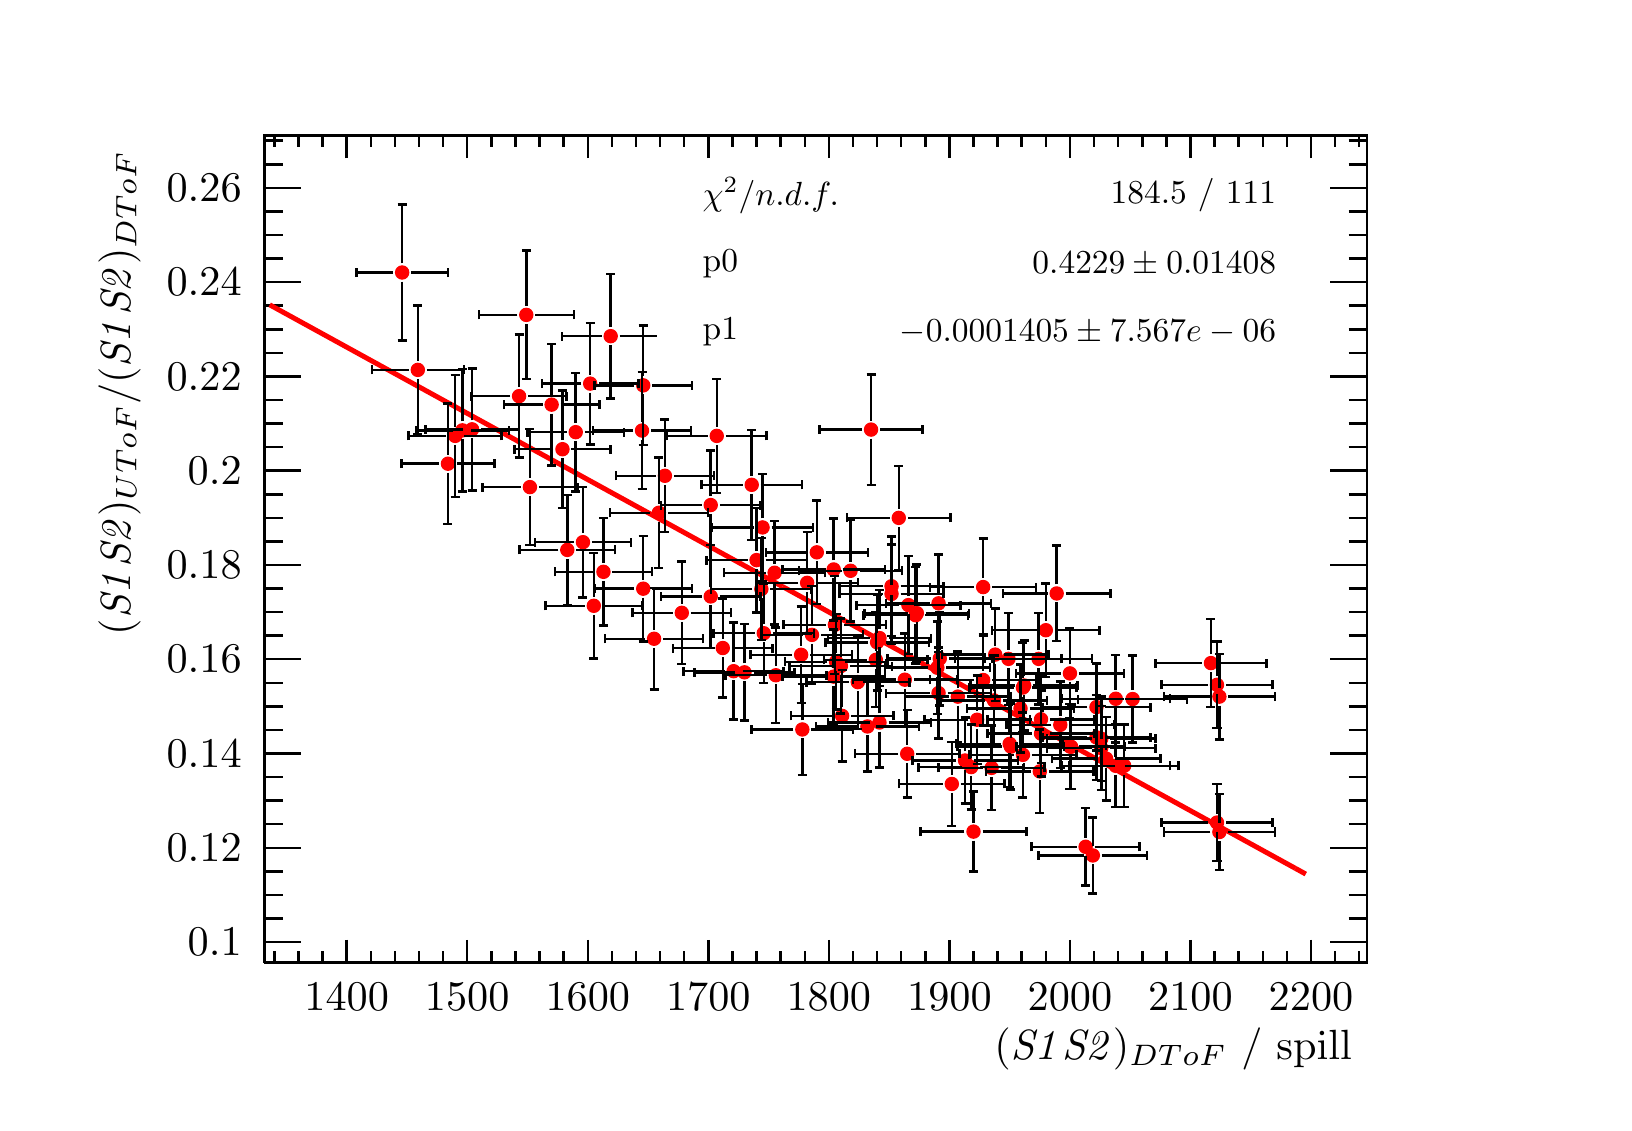
\begin{tikzpicture}
\pgfdeclareplotmark{cross} {
\pgfpathmoveto{\pgfpoint{-0.3\pgfplotmarksize}{\pgfplotmarksize}}
\pgfpathlineto{\pgfpoint{+0.3\pgfplotmarksize}{\pgfplotmarksize}}
\pgfpathlineto{\pgfpoint{+0.3\pgfplotmarksize}{0.3\pgfplotmarksize}}
\pgfpathlineto{\pgfpoint{+1\pgfplotmarksize}{0.3\pgfplotmarksize}}
\pgfpathlineto{\pgfpoint{+1\pgfplotmarksize}{-0.3\pgfplotmarksize}}
\pgfpathlineto{\pgfpoint{+0.3\pgfplotmarksize}{-0.3\pgfplotmarksize}}
\pgfpathlineto{\pgfpoint{+0.3\pgfplotmarksize}{-1.\pgfplotmarksize}}
\pgfpathlineto{\pgfpoint{-0.3\pgfplotmarksize}{-1.\pgfplotmarksize}}
\pgfpathlineto{\pgfpoint{-0.3\pgfplotmarksize}{-0.3\pgfplotmarksize}}
\pgfpathlineto{\pgfpoint{-1.\pgfplotmarksize}{-0.3\pgfplotmarksize}}
\pgfpathlineto{\pgfpoint{-1.\pgfplotmarksize}{0.3\pgfplotmarksize}}
\pgfpathlineto{\pgfpoint{-0.3\pgfplotmarksize}{0.3\pgfplotmarksize}}
\pgfpathclose
\pgfusepathqstroke
}
\pgfdeclareplotmark{cross*} {
\pgfpathmoveto{\pgfpoint{-0.3\pgfplotmarksize}{\pgfplotmarksize}}
\pgfpathlineto{\pgfpoint{+0.3\pgfplotmarksize}{\pgfplotmarksize}}
\pgfpathlineto{\pgfpoint{+0.3\pgfplotmarksize}{0.3\pgfplotmarksize}}
\pgfpathlineto{\pgfpoint{+1\pgfplotmarksize}{0.3\pgfplotmarksize}}
\pgfpathlineto{\pgfpoint{+1\pgfplotmarksize}{-0.3\pgfplotmarksize}}
\pgfpathlineto{\pgfpoint{+0.3\pgfplotmarksize}{-0.3\pgfplotmarksize}}
\pgfpathlineto{\pgfpoint{+0.3\pgfplotmarksize}{-1.\pgfplotmarksize}}
\pgfpathlineto{\pgfpoint{-0.3\pgfplotmarksize}{-1.\pgfplotmarksize}}
\pgfpathlineto{\pgfpoint{-0.3\pgfplotmarksize}{-0.3\pgfplotmarksize}}
\pgfpathlineto{\pgfpoint{-1.\pgfplotmarksize}{-0.3\pgfplotmarksize}}
\pgfpathlineto{\pgfpoint{-1.\pgfplotmarksize}{0.3\pgfplotmarksize}}
\pgfpathlineto{\pgfpoint{-0.3\pgfplotmarksize}{0.3\pgfplotmarksize}}
\pgfpathclose
\pgfusepathqfillstroke
}
\pgfdeclareplotmark{newstar} {
\pgfpathmoveto{\pgfqpoint{0pt}{\pgfplotmarksize}}
\pgfpathlineto{\pgfqpointpolar{44}{0.5\pgfplotmarksize}}
\pgfpathlineto{\pgfqpointpolar{18}{\pgfplotmarksize}}
\pgfpathlineto{\pgfqpointpolar{-20}{0.5\pgfplotmarksize}}
\pgfpathlineto{\pgfqpointpolar{-54}{\pgfplotmarksize}}
\pgfpathlineto{\pgfqpointpolar{-90}{0.5\pgfplotmarksize}}
\pgfpathlineto{\pgfqpointpolar{234}{\pgfplotmarksize}}
\pgfpathlineto{\pgfqpointpolar{198}{0.5\pgfplotmarksize}}
\pgfpathlineto{\pgfqpointpolar{162}{\pgfplotmarksize}}
\pgfpathlineto{\pgfqpointpolar{134}{0.5\pgfplotmarksize}}
\pgfpathclose
\pgfusepathqstroke
}
\pgfdeclareplotmark{newstar*} {
\pgfpathmoveto{\pgfqpoint{0pt}{\pgfplotmarksize}}
\pgfpathlineto{\pgfqpointpolar{44}{0.5\pgfplotmarksize}}
\pgfpathlineto{\pgfqpointpolar{18}{\pgfplotmarksize}}
\pgfpathlineto{\pgfqpointpolar{-20}{0.5\pgfplotmarksize}}
\pgfpathlineto{\pgfqpointpolar{-54}{\pgfplotmarksize}}
\pgfpathlineto{\pgfqpointpolar{-90}{0.5\pgfplotmarksize}}
\pgfpathlineto{\pgfqpointpolar{234}{\pgfplotmarksize}}
\pgfpathlineto{\pgfqpointpolar{198}{0.5\pgfplotmarksize}}
\pgfpathlineto{\pgfqpointpolar{162}{\pgfplotmarksize}}
\pgfpathlineto{\pgfqpointpolar{134}{0.5\pgfplotmarksize}}
\pgfpathclose
\pgfusepathqfillstroke
}
\definecolor{c}{rgb}{1,1,1};
\draw [color=c, fill=c] (0,0) rectangle (20,13.639);
\draw [color=c, fill=c] (3,1.77307) rectangle (17,12.2751);
\definecolor{c}{rgb}{0,0,0};
\draw [c,line width=0.9] (3,1.77307) -- (3,12.2751) -- (17,12.2751) -- (17,1.77307) -- (3,1.77307);
\definecolor{c}{rgb}{1,1,1};
\draw [color=c, fill=c] (3,1.77307) rectangle (17,12.2751);
\definecolor{c}{rgb}{0,0,0};
\draw [c,line width=0.9] (3,1.77307) -- (3,12.2751) -- (17,12.2751) -- (17,1.77307) -- (3,1.77307);
\draw [c,line width=0.9] (3,1.77307) -- (17,1.77307);
\draw [c,line width=0.9] (4.0446,2.05948) -- (4.0446,1.77307);
\draw [c,line width=0.9] (4.35077,1.91628) -- (4.35077,1.77307);
\draw [c,line width=0.9] (4.65694,1.91628) -- (4.65694,1.77307);
\draw [c,line width=0.9] (4.9631,1.91628) -- (4.9631,1.77307);
\draw [c,line width=0.9] (5.26927,1.91628) -- (5.26927,1.77307);
\draw [c,line width=0.9] (5.57543,2.05948) -- (5.57543,1.77307);
\draw [c,line width=0.9] (5.8816,1.91628) -- (5.8816,1.77307);
\draw [c,line width=0.9] (6.18777,1.91628) -- (6.18777,1.77307);
\draw [c,line width=0.9] (6.49393,1.91628) -- (6.49393,1.77307);
\draw [c,line width=0.9] (6.8001,1.91628) -- (6.8001,1.77307);
\draw [c,line width=0.9] (7.10627,2.05948) -- (7.10627,1.77307);
\draw [c,line width=0.9] (7.41243,1.91628) -- (7.41243,1.77307);
\draw [c,line width=0.9] (7.7186,1.91628) -- (7.7186,1.77307);
\draw [c,line width=0.9] (8.02476,1.91628) -- (8.02476,1.77307);
\draw [c,line width=0.9] (8.33093,1.91628) -- (8.33093,1.77307);
\draw [c,line width=0.9] (8.6371,2.05948) -- (8.6371,1.77307);
\draw [c,line width=0.9] (8.94326,1.91628) -- (8.94326,1.77307);
\draw [c,line width=0.9] (9.24943,1.91628) -- (9.24943,1.77307);
\draw [c,line width=0.9] (9.5556,1.91628) -- (9.5556,1.77307);
\draw [c,line width=0.9] (9.86176,1.91628) -- (9.86176,1.77307);
\draw [c,line width=0.9] (10.1679,2.05948) -- (10.1679,1.77307);
\draw [c,line width=0.9] (10.4741,1.91628) -- (10.4741,1.77307);
\draw [c,line width=0.9] (10.7803,1.91628) -- (10.7803,1.77307);
\draw [c,line width=0.9] (11.0864,1.91628) -- (11.0864,1.77307);
\draw [c,line width=0.9] (11.3926,1.91628) -- (11.3926,1.77307);
\draw [c,line width=0.9] (11.6988,2.05948) -- (11.6988,1.77307);
\draw [c,line width=0.9] (12.0049,1.91628) -- (12.0049,1.77307);
\draw [c,line width=0.9] (12.3111,1.91628) -- (12.3111,1.77307);
\draw [c,line width=0.9] (12.6173,1.91628) -- (12.6173,1.77307);
\draw [c,line width=0.9] (12.9234,1.91628) -- (12.9234,1.77307);
\draw [c,line width=0.9] (13.2296,2.05948) -- (13.2296,1.77307);
\draw [c,line width=0.9] (13.5358,1.91628) -- (13.5358,1.77307);
\draw [c,line width=0.9] (13.8419,1.91628) -- (13.8419,1.77307);
\draw [c,line width=0.9] (14.1481,1.91628) -- (14.1481,1.77307);
\draw [c,line width=0.9] (14.4543,1.91628) -- (14.4543,1.77307);
\draw [c,line width=0.9] (14.7604,2.05948) -- (14.7604,1.77307);
\draw [c,line width=0.9] (15.0666,1.91628) -- (15.0666,1.77307);
\draw [c,line width=0.9] (15.3728,1.91628) -- (15.3728,1.77307);
\draw [c,line width=0.9] (15.6789,1.91628) -- (15.6789,1.77307);
\draw [c,line width=0.9] (15.9851,1.91628) -- (15.9851,1.77307);
\draw [c,line width=0.9] (16.2913,2.05948) -- (16.2913,1.77307);
\draw [c,line width=0.9] (4.0446,2.05948) -- (4.0446,1.77307);
\draw [c,line width=0.9] (3.73844,1.91628) -- (3.73844,1.77307);
\draw [c,line width=0.9] (3.43227,1.91628) -- (3.43227,1.77307);
\draw [c,line width=0.9] (3.1261,1.91628) -- (3.1261,1.77307);
\draw [c,line width=0.9] (16.2913,2.05948) -- (16.2913,1.77307);
\draw [c,line width=0.9] (16.5974,1.91628) -- (16.5974,1.77307);
\draw [c,line width=0.9] (16.9036,1.91628) -- (16.9036,1.77307);
\draw [anchor=base] (4.0446,1.15931) node[scale=1.52731, color=c, rotate=0]{1400};
\draw [anchor=base] (5.57543,1.15931) node[scale=1.52731, color=c, rotate=0]{1500};
\draw [anchor=base] (7.10627,1.15931) node[scale=1.52731, color=c, rotate=0]{1600};
\draw [anchor=base] (8.6371,1.15931) node[scale=1.52731, color=c, rotate=0]{1700};
\draw [anchor=base] (10.1679,1.15931) node[scale=1.52731, color=c, rotate=0]{1800};
\draw [anchor=base] (11.6988,1.15931) node[scale=1.52731, color=c, rotate=0]{1900};
\draw [anchor=base] (13.2296,1.15931) node[scale=1.52731, color=c, rotate=0]{2000};
\draw [anchor=base] (14.7604,1.15931) node[scale=1.52731, color=c, rotate=0]{2100};
\draw [anchor=base] (16.2913,1.15931) node[scale=1.52731, color=c, rotate=0]{2200};
\draw [anchor= east] (17,0.681948) node[scale=1.52731, color=c, rotate=0]{ $(\SOne\STwo)_{\text{DToF}}$ / spill };
\draw [c,line width=0.9] (3,12.2751) -- (17,12.2751);
\draw [c,line width=0.9] (4.0446,11.9887) -- (4.0446,12.2751);
\draw [c,line width=0.9] (4.35077,12.1319) -- (4.35077,12.2751);
\draw [c,line width=0.9] (4.65694,12.1319) -- (4.65694,12.2751);
\draw [c,line width=0.9] (4.9631,12.1319) -- (4.9631,12.2751);
\draw [c,line width=0.9] (5.26927,12.1319) -- (5.26927,12.2751);
\draw [c,line width=0.9] (5.57543,11.9887) -- (5.57543,12.2751);
\draw [c,line width=0.9] (5.8816,12.1319) -- (5.8816,12.2751);
\draw [c,line width=0.9] (6.18777,12.1319) -- (6.18777,12.2751);
\draw [c,line width=0.9] (6.49393,12.1319) -- (6.49393,12.2751);
\draw [c,line width=0.9] (6.8001,12.1319) -- (6.8001,12.2751);
\draw [c,line width=0.9] (7.10627,11.9887) -- (7.10627,12.2751);
\draw [c,line width=0.9] (7.41243,12.1319) -- (7.41243,12.2751);
\draw [c,line width=0.9] (7.7186,12.1319) -- (7.7186,12.2751);
\draw [c,line width=0.9] (8.02476,12.1319) -- (8.02476,12.2751);
\draw [c,line width=0.9] (8.33093,12.1319) -- (8.33093,12.2751);
\draw [c,line width=0.9] (8.6371,11.9887) -- (8.6371,12.2751);
\draw [c,line width=0.9] (8.94326,12.1319) -- (8.94326,12.2751);
\draw [c,line width=0.9] (9.24943,12.1319) -- (9.24943,12.2751);
\draw [c,line width=0.9] (9.5556,12.1319) -- (9.5556,12.2751);
\draw [c,line width=0.9] (9.86176,12.1319) -- (9.86176,12.2751);
\draw [c,line width=0.9] (10.1679,11.9887) -- (10.1679,12.2751);
\draw [c,line width=0.9] (10.4741,12.1319) -- (10.4741,12.2751);
\draw [c,line width=0.9] (10.7803,12.1319) -- (10.7803,12.2751);
\draw [c,line width=0.9] (11.0864,12.1319) -- (11.0864,12.2751);
\draw [c,line width=0.9] (11.3926,12.1319) -- (11.3926,12.2751);
\draw [c,line width=0.9] (11.6988,11.9887) -- (11.6988,12.2751);
\draw [c,line width=0.9] (12.0049,12.1319) -- (12.0049,12.2751);
\draw [c,line width=0.9] (12.3111,12.1319) -- (12.3111,12.2751);
\draw [c,line width=0.9] (12.6173,12.1319) -- (12.6173,12.2751);
\draw [c,line width=0.9] (12.9234,12.1319) -- (12.9234,12.2751);
\draw [c,line width=0.9] (13.2296,11.9887) -- (13.2296,12.2751);
\draw [c,line width=0.9] (13.5358,12.1319) -- (13.5358,12.2751);
\draw [c,line width=0.9] (13.8419,12.1319) -- (13.8419,12.2751);
\draw [c,line width=0.9] (14.1481,12.1319) -- (14.1481,12.2751);
\draw [c,line width=0.9] (14.4543,12.1319) -- (14.4543,12.2751);
\draw [c,line width=0.9] (14.7604,11.9887) -- (14.7604,12.2751);
\draw [c,line width=0.9] (15.0666,12.1319) -- (15.0666,12.2751);
\draw [c,line width=0.9] (15.3728,12.1319) -- (15.3728,12.2751);
\draw [c,line width=0.9] (15.6789,12.1319) -- (15.6789,12.2751);
\draw [c,line width=0.9] (15.9851,12.1319) -- (15.9851,12.2751);
\draw [c,line width=0.9] (16.2913,11.9887) -- (16.2913,12.2751);
\draw [c,line width=0.9] (4.0446,11.9887) -- (4.0446,12.2751);
\draw [c,line width=0.9] (3.73844,12.1319) -- (3.73844,12.2751);
\draw [c,line width=0.9] (3.43227,12.1319) -- (3.43227,12.2751);
\draw [c,line width=0.9] (3.1261,12.1319) -- (3.1261,12.2751);
\draw [c,line width=0.9] (16.2913,11.9887) -- (16.2913,12.2751);
\draw [c,line width=0.9] (16.5974,12.1319) -- (16.5974,12.2751);
\draw [c,line width=0.9] (16.9036,12.1319) -- (16.9036,12.2751);
\draw [c,line width=0.9] (3,1.77307) -- (3,12.2751);
\draw [c,line width=0.9] (3.462,2.03294) -- (3,2.03294);
\draw [c,line width=0.9] (3.231,2.33227) -- (3,2.33227);
\draw [c,line width=0.9] (3.231,2.6316) -- (3,2.6316);
\draw [c,line width=0.9] (3.231,2.93093) -- (3,2.93093);
\draw [c,line width=0.9] (3.462,3.23026) -- (3,3.23026);
\draw [c,line width=0.9] (3.231,3.52959) -- (3,3.52959);
\draw [c,line width=0.9] (3.231,3.82892) -- (3,3.82892);
\draw [c,line width=0.9] (3.231,4.12825) -- (3,4.12825);
\draw [c,line width=0.9] (3.462,4.42757) -- (3,4.42757);
\draw [c,line width=0.9] (3.231,4.7269) -- (3,4.7269);
\draw [c,line width=0.9] (3.231,5.02623) -- (3,5.02623);
\draw [c,line width=0.9] (3.231,5.32556) -- (3,5.32556);
\draw [c,line width=0.9] (3.462,5.62489) -- (3,5.62489);
\draw [c,line width=0.9] (3.231,5.92422) -- (3,5.92422);
\draw [c,line width=0.9] (3.231,6.22355) -- (3,6.22355);
\draw [c,line width=0.9] (3.231,6.52288) -- (3,6.52288);
\draw [c,line width=0.9] (3.462,6.82221) -- (3,6.82221);
\draw [c,line width=0.9] (3.231,7.12153) -- (3,7.12153);
\draw [c,line width=0.9] (3.231,7.42086) -- (3,7.42086);
\draw [c,line width=0.9] (3.231,7.72019) -- (3,7.72019);
\draw [c,line width=0.9] (3.462,8.01952) -- (3,8.01952);
\draw [c,line width=0.9] (3.231,8.31885) -- (3,8.31885);
\draw [c,line width=0.9] (3.231,8.61818) -- (3,8.61818);
\draw [c,line width=0.9] (3.231,8.91751) -- (3,8.91751);
\draw [c,line width=0.9] (3.462,9.21684) -- (3,9.21684);
\draw [c,line width=0.9] (3.231,9.51617) -- (3,9.51617);
\draw [c,line width=0.9] (3.231,9.8155) -- (3,9.8155);
\draw [c,line width=0.9] (3.231,10.1148) -- (3,10.1148);
\draw [c,line width=0.9] (3.462,10.4142) -- (3,10.4142);
\draw [c,line width=0.9] (3.231,10.7135) -- (3,10.7135);
\draw [c,line width=0.9] (3.231,11.0128) -- (3,11.0128);
\draw [c,line width=0.9] (3.231,11.3121) -- (3,11.3121);
\draw [c,line width=0.9] (3.462,11.6115) -- (3,11.6115);
\draw [c,line width=0.9] (3.462,2.03294) -- (3,2.03294);
\draw [c,line width=0.9] (3.462,11.6115) -- (3,11.6115);
\draw [c,line width=0.9] (3.231,11.9108) -- (3,11.9108);
\draw [c,line width=0.9] (3.231,12.2101) -- (3,12.2101);
\draw [anchor= east] (2.9,2.03294) node[scale=1.52731, color=c, rotate=0]{0.1};
\draw [anchor= east] (2.9,3.23026) node[scale=1.52731, color=c, rotate=0]{0.12};
\draw [anchor= east] (2.9,4.42757) node[scale=1.52731, color=c, rotate=0]{0.14};
\draw [anchor= east] (2.9,5.62489) node[scale=1.52731, color=c, rotate=0]{0.16};
\draw [anchor= east] (2.9,6.82221) node[scale=1.52731, color=c, rotate=0]{0.18};
\draw [anchor= east] (2.9,8.01952) node[scale=1.52731, color=c, rotate=0]{0.2};
\draw [anchor= east] (2.9,9.21684) node[scale=1.52731, color=c, rotate=0]{0.22};
\draw [anchor= east] (2.9,10.4142) node[scale=1.52731, color=c, rotate=0]{0.24};
\draw [anchor= east] (2.9,11.6115) node[scale=1.52731, color=c, rotate=0]{0.26};
\draw [anchor= east] (1.16,12.2751) node[scale=1.52731, color=c, rotate=90]{ $(\SOne\STwo)_{\text{UToF}}/(\SOne\STwo)_{\text{DToF}}$ };
\draw [c,line width=0.9] (17,1.77307) -- (17,12.2751);
\draw [c,line width=0.9] (16.538,2.03294) -- (17,2.03294);
\draw [c,line width=0.9] (16.769,2.33227) -- (17,2.33227);
\draw [c,line width=0.9] (16.769,2.6316) -- (17,2.6316);
\draw [c,line width=0.9] (16.769,2.93093) -- (17,2.93093);
\draw [c,line width=0.9] (16.538,3.23026) -- (17,3.23026);
\draw [c,line width=0.9] (16.769,3.52959) -- (17,3.52959);
\draw [c,line width=0.9] (16.769,3.82892) -- (17,3.82892);
\draw [c,line width=0.9] (16.769,4.12825) -- (17,4.12825);
\draw [c,line width=0.9] (16.538,4.42757) -- (17,4.42757);
\draw [c,line width=0.9] (16.769,4.7269) -- (17,4.7269);
\draw [c,line width=0.9] (16.769,5.02623) -- (17,5.02623);
\draw [c,line width=0.9] (16.769,5.32556) -- (17,5.32556);
\draw [c,line width=0.9] (16.538,5.62489) -- (17,5.62489);
\draw [c,line width=0.9] (16.769,5.92422) -- (17,5.92422);
\draw [c,line width=0.9] (16.769,6.22355) -- (17,6.22355);
\draw [c,line width=0.9] (16.769,6.52288) -- (17,6.52288);
\draw [c,line width=0.9] (16.538,6.82221) -- (17,6.82221);
\draw [c,line width=0.9] (16.769,7.12153) -- (17,7.12153);
\draw [c,line width=0.9] (16.769,7.42086) -- (17,7.42086);
\draw [c,line width=0.9] (16.769,7.72019) -- (17,7.72019);
\draw [c,line width=0.9] (16.538,8.01952) -- (17,8.01952);
\draw [c,line width=0.9] (16.769,8.31885) -- (17,8.31885);
\draw [c,line width=0.9] (16.769,8.61818) -- (17,8.61818);
\draw [c,line width=0.9] (16.769,8.91751) -- (17,8.91751);
\draw [c,line width=0.9] (16.538,9.21684) -- (17,9.21684);
\draw [c,line width=0.9] (16.769,9.51617) -- (17,9.51617);
\draw [c,line width=0.9] (16.769,9.8155) -- (17,9.8155);
\draw [c,line width=0.9] (16.769,10.1148) -- (17,10.1148);
\draw [c,line width=0.9] (16.538,10.4142) -- (17,10.4142);
\draw [c,line width=0.9] (16.769,10.7135) -- (17,10.7135);
\draw [c,line width=0.9] (16.769,11.0128) -- (17,11.0128);
\draw [c,line width=0.9] (16.769,11.3121) -- (17,11.3121);
\draw [c,line width=0.9] (16.538,11.6115) -- (17,11.6115);
\draw [c,line width=0.9] (16.538,2.03294) -- (17,2.03294);
\draw [c,line width=0.9] (16.538,11.6115) -- (17,11.6115);
\draw [c,line width=0.9] (16.769,11.9108) -- (17,11.9108);
\draw [c,line width=0.9] (16.769,12.2101) -- (17,12.2101);
\definecolor{c}{rgb}{1,0,0};
\foreach \P in {(6.78479,8.2925), (8.74426,8.46141), (10.964,6.55197), (12.6479,5.29169), (9.31066,6.51601), (13.5204,3.133), (13.4286,3.24334), (7.18281,6.30374), (9.09635,5.45879), (10.8109,5.89399), (4.74879,10.5367), (9.81584,5.68149),
 (10.2445,6.06269), (12.2805,5.6842), (13.9185,4.27242), (6.84602,7.01356), (9.47905,6.72328), (11.8978,4.33932), (12.1274,6.54151), (6.23369,8.9662), (11.163,4.42436), (7.13688,9.12566), (5.63667,8.54494), (7.81045,6.52106), (12.6019,5.00026),
 (11.561,6.3353), (7.30527,6.73536), (8.66771,6.42263), (8.95857,5.47323), (6.32554,9.9983), (15.0972,5.29989), (12.4642,4.55038), (7.79514,8.52902), (11.561,5.1956), (13.5664,5.01735), (11.1324,5.36525), (10.6578,4.77135), (6.95318,8.50899),
 (15.0207,5.57625), (12.8622,4.68085), (12.4489,5.6298), (12.8469,4.20024), (8.66771,7.58337), (13.6276,4.49731), (9.95361,5.93461), (11.8059,5.15023), (11.0558,7.42022), (9.32597,7.29907), (9.34128,5.95542), (10.7803,5.83963), (11.5763,5.63375),
 (10.2292,5.40454), (8.8208,5.76756), (9.24943,6.88414), (15.1278,5.15025), (8.30031,6.21427), (12.6326,5.26588), (12.8316,5.62974), (15.0972,3.55075), (12.4795,4.51533), (11.7294,4.04106), (10.321,5.5389), (10.765,5.61708), (10.964,6.45499),
 (13.6276,4.6155), (13.2296,4.51737), (10.2598,5.59307), (11.2701,6.18389), (9.89238,6.59511), (11.1783,6.31274), (13.5664,4.63246), (8.00946,7.48546), (12.0049,3.43605), (7.39712,9.72786), (10.8109,4.82148), (4.94779,9.29972), (5.5142,8.53174),
 (13.1071,4.79182), (10.7037,8.54151), (6.37147,7.81123), (8.086,7.95476), (9.83115,4.7333), (11.2854,6.21044), (12.2652,5.10195), (9.49436,5.4217), (12.1274,5.36158), (7.81045,9.10336), (11.5457,5.5172), (11.9743,4.25528), (15.1278,3.43094),
 (12.0508,4.85657), (13.2449,4.51314), (5.42235,8.46148), (10.2292,6.76513), (6.64702,8.85841), (7.94822,5.88533), (10.5353,5.33475), (10.0148,6.98274), (9.1882,7.8402), (13.8113,4.2713), (10.3363,4.90557), (13.0612,6.46042), (13.2296,5.44529),
 (7.04503,7.11178), (10.4435,6.74844), (13.8113,5.12317), (12.6326,4.41109), (13.6888,4.3627), (5.3305,8.10827), (12.2346,4.24504), (14.0256,5.11959), (12.8622,4.86263), (12.9234,5.99376)}{\draw[mark options={color=c,fill=c},mark
 size=2.402402pt,mark=*] plot coordinates {\P};}
\draw [c,line width=1.8] (3.06646,10.1263) -- (3.19937,10.0533) -- (3.33228,9.98029) -- (3.46519,9.90727) -- (3.59811,9.83424) -- (3.73102,9.76122) -- (3.86393,9.68819) -- (3.99684,9.61516) -- (4.12976,9.54214) -- (4.26267,9.46911) --
 (4.39558,9.39609) -- (4.52849,9.32306) -- (4.66141,9.25004) -- (4.79432,9.17701) -- (4.92723,9.10398) -- (5.06014,9.03096) -- (5.19306,8.95793) -- (5.32597,8.88491) -- (5.45888,8.81188) -- (5.59179,8.73886) -- (5.72471,8.66583) -- (5.85762,8.5928)
 -- (5.99053,8.51978) -- (6.12344,8.44675) -- (6.25636,8.37373) -- (6.38927,8.3007) -- (6.52218,8.22768) -- (6.65509,8.15465) -- (6.78801,8.08162) -- (6.92092,8.0086) -- (7.05383,7.93557) -- (7.18674,7.86255) -- (7.31966,7.78952) -- (7.45257,7.7165)
 -- (7.58548,7.64347) -- (7.71839,7.57044) -- (7.85131,7.49742) -- (7.98422,7.42439) -- (8.11713,7.35137) -- (8.25004,7.27834) -- (8.38296,7.20532) -- (8.51587,7.13229) -- (8.64878,7.05926) -- (8.7817,6.98624) -- (8.91461,6.91321) --
 (9.04752,6.84019) -- (9.18043,6.76716) -- (9.31334,6.69414) -- (9.44626,6.62111) -- (9.57917,6.54808);
\draw [c,line width=1.8] (9.57917,6.54808) -- (9.71208,6.47506) -- (9.845,6.40203) -- (9.97791,6.32901) -- (10.1108,6.25598) -- (10.2437,6.18296) -- (10.3766,6.10993) -- (10.5096,6.0369) -- (10.6425,5.96388) -- (10.7754,5.89085) -- (10.9083,5.81783)
 -- (11.0412,5.7448) -- (11.1741,5.67178) -- (11.307,5.59875) -- (11.4399,5.52573) -- (11.5729,5.4527) -- (11.7058,5.37967) -- (11.8387,5.30665) -- (11.9716,5.23362) -- (12.1045,5.1606) -- (12.2374,5.08757) -- (12.3703,5.01455) -- (12.5032,4.94152)
 -- (12.6362,4.86849) -- (12.7691,4.79547) -- (12.902,4.72244) -- (13.0349,4.64942) -- (13.1678,4.57639) -- (13.3007,4.50337) -- (13.4336,4.43034) -- (13.5665,4.35731) -- (13.6995,4.28429) -- (13.8324,4.21126) -- (13.9653,4.13824) --
 (14.0982,4.06521) -- (14.2311,3.99219) -- (14.364,3.91916) -- (14.4969,3.84613) -- (14.6298,3.77311) -- (14.7628,3.70008) -- (14.8957,3.62706) -- (15.0286,3.55403) -- (15.1615,3.48101) -- (15.2944,3.40798) -- (15.4273,3.33495) -- (15.5602,3.26193)
 -- (15.6931,3.1889) -- (15.8261,3.11588) -- (15.959,3.04285) -- (16.0919,2.96983);
\draw [c,line width=1.8] (16.0919,2.96983) -- (16.2248,2.8968);
\definecolor{c}{rgb}{1,1,1};
\draw [color=c, fill=c] (7.99427,9.34097) rectangle (16.4183,11.9484);
\definecolor{c}{rgb}{0,0,0};
\draw [anchor= west] (8.41547,11.5138) node[scale=1.20912, color=c, rotate=0]{$\chi^{2} / ndf $};
\draw [anchor= east] (15.9971,11.5138) node[scale=1.20912, color=c, rotate=0]{ 184.5 / 111};
\draw [anchor= west] (8.41547,10.6447) node[scale=1.20912, color=c, rotate=0]{p0       };
\draw [anchor= east] (15.9971,10.6447) node[scale=1.20912, color=c, rotate=0]{$ 0.4229 \pm 0.01408$};
\draw [anchor= west] (8.41547,9.77555) node[scale=1.20912, color=c, rotate=0]{p1       };
\draw [anchor= east] (15.9971,9.77555) node[scale=1.20912, color=c, rotate=0]{$ -0.0001405 \pm 7.567e-06$};
\draw [c,line width=0.9] (6.67018,8.2925) -- (6.17649,8.2925);
\draw [c,line width=0.9] (6.17649,8.23519) -- (6.17649,8.34981);
\draw [c,line width=0.9] (6.8994,8.2925) -- (7.39309,8.2925);
\draw [c,line width=0.9] (7.39309,8.23519) -- (7.39309,8.34981);
\draw [c,line width=0.9] (6.78479,8.40711) -- (6.78479,9.04035);
\draw [c,line width=0.9] (6.72748,9.04035) -- (6.8421,9.04035);
\draw [c,line width=0.9] (6.78479,8.17789) -- (6.78479,7.54465);
\draw [c,line width=0.9] (6.72748,7.54465) -- (6.8421,7.54465);
\draw [c,line width=0.9] (8.62964,8.46141) -- (8.11178,8.46141);
\draw [c,line width=0.9] (8.11178,8.40411) -- (8.11178,8.51872);
\draw [c,line width=0.9] (8.85887,8.46141) -- (9.37673,8.46141);
\draw [c,line width=0.9] (9.37673,8.40411) -- (9.37673,8.51872);
\draw [c,line width=0.9] (8.74426,8.57603) -- (8.74426,9.18647);
\draw [c,line width=0.9] (8.68695,9.18647) -- (8.80156,9.18647);
\draw [c,line width=0.9] (8.74426,8.3468) -- (8.74426,7.73636);
\draw [c,line width=0.9] (8.68695,7.73636) -- (8.80156,7.73636);
\draw [c,line width=0.9] (10.8493,6.55197) -- (10.3052,6.55197);
\draw [c,line width=0.9] (10.3052,6.49466) -- (10.3052,6.60928);
\draw [c,line width=0.9] (11.0786,6.55197) -- (11.6228,6.55197);
\draw [c,line width=0.9] (11.6228,6.49466) -- (11.6228,6.60928);
\draw [c,line width=0.9] (10.964,6.66658) -- (10.964,7.18378);
\draw [c,line width=0.9] (10.9067,7.18378) -- (11.0213,7.18378);
\draw [c,line width=0.9] (10.964,6.43736) -- (10.964,5.92016);
\draw [c,line width=0.9] (10.9067,5.92016) -- (11.0213,5.92016);
\draw [c,line width=0.9] (12.5333,5.29169) -- (11.9698,5.29169);
\draw [c,line width=0.9] (11.9698,5.23439) -- (11.9698,5.349);
\draw [c,line width=0.9] (12.7625,5.29169) -- (13.3259,5.29169);
\draw [c,line width=0.9] (13.3259,5.23439) -- (13.3259,5.349);
\draw [c,line width=0.9] (12.6479,5.40631) -- (12.6479,5.86236);
\draw [c,line width=0.9] (12.5906,5.86236) -- (12.7052,5.86236);
\draw [c,line width=0.9] (12.6479,5.17708) -- (12.6479,4.72102);
\draw [c,line width=0.9] (12.5906,4.72102) -- (12.7052,4.72102);
\draw [c,line width=0.9] (9.19605,6.51601) -- (8.67137,6.51601);
\draw [c,line width=0.9] (8.67137,6.4587) -- (8.67137,6.57332);
\draw [c,line width=0.9] (9.42528,6.51601) -- (9.94996,6.51601);
\draw [c,line width=0.9] (9.94996,6.4587) -- (9.94996,6.57332);
\draw [c,line width=0.9] (9.31066,6.63062) -- (9.31066,7.16581);
\draw [c,line width=0.9] (9.25336,7.16581) -- (9.36797,7.16581);
\draw [c,line width=0.9] (9.31066,6.4014) -- (9.31066,5.86621);
\draw [c,line width=0.9] (9.25336,5.86621) -- (9.36797,5.86621);
\draw [c,line width=0.9] (13.4058,3.133) -- (12.8326,3.133);
\draw [c,line width=0.9] (12.8326,3.0757) -- (12.8326,3.19031);
\draw [c,line width=0.9] (13.6351,3.133) -- (14.2083,3.133);
\draw [c,line width=0.9] (14.2083,3.0757) -- (14.2083,3.19031);
\draw [c,line width=0.9] (13.5204,3.24762) -- (13.5204,3.61777);
\draw [c,line width=0.9] (13.4631,3.61777) -- (13.5778,3.61777);
\draw [c,line width=0.9] (13.5204,3.01839) -- (13.5204,2.64823);
\draw [c,line width=0.9] (13.4631,2.64823) -- (13.5778,2.64823);
\draw [c,line width=0.9] (13.314,3.24334) -- (12.7418,3.24334);
\draw [c,line width=0.9] (12.7418,3.18604) -- (12.7418,3.30065);
\draw [c,line width=0.9] (13.5432,3.24334) -- (14.1154,3.24334);
\draw [c,line width=0.9] (14.1154,3.18604) -- (14.1154,3.30065);
\draw [c,line width=0.9] (13.4286,3.35796) -- (13.4286,3.733);
\draw [c,line width=0.9] (13.3713,3.733) -- (13.4859,3.733);
\draw [c,line width=0.9] (13.4286,3.12873) -- (13.4286,2.75368);
\draw [c,line width=0.9] (13.3713,2.75368) -- (13.4859,2.75368);
\draw [c,line width=0.9] (7.06819,6.30374) -- (6.56952,6.30374);
\draw [c,line width=0.9] (6.56952,6.24644) -- (6.56952,6.36105);
\draw [c,line width=0.9] (7.29742,6.30374) -- (7.7961,6.30374);
\draw [c,line width=0.9] (7.7961,6.24644) -- (7.7961,6.36105);
\draw [c,line width=0.9] (7.18281,6.41836) -- (7.18281,6.97318);
\draw [c,line width=0.9] (7.1255,6.97318) -- (7.24011,6.97318);
\draw [c,line width=0.9] (7.18281,6.18913) -- (7.18281,5.6343);
\draw [c,line width=0.9] (7.1255,5.6343) -- (7.24011,5.6343);
\draw [c,line width=0.9] (8.98173,5.45879) -- (8.45962,5.45879);
\draw [c,line width=0.9] (8.45962,5.40148) -- (8.45962,5.5161);
\draw [c,line width=0.9] (9.21096,5.45879) -- (9.73307,5.45879);
\draw [c,line width=0.9] (9.73307,5.40148) -- (9.73307,5.5161);
\draw [c,line width=0.9] (9.09635,5.5734) -- (9.09635,6.07273);
\draw [c,line width=0.9] (9.03904,6.07273) -- (9.15365,6.07273);
\draw [c,line width=0.9] (9.09635,5.34418) -- (9.09635,4.84485);
\draw [c,line width=0.9] (9.03904,4.84485) -- (9.15365,4.84485);
\draw [c,line width=0.9] (10.6963,5.89399) -- (10.1539,5.89399);
\draw [c,line width=0.9] (10.1539,5.83669) -- (10.1539,5.9513);
\draw [c,line width=0.9] (10.9255,5.89399) -- (11.4679,5.89399);
\draw [c,line width=0.9] (11.4679,5.83669) -- (11.4679,5.9513);
\draw [c,line width=0.9] (10.8109,6.00861) -- (10.8109,6.50448);
\draw [c,line width=0.9] (10.7536,6.50448) -- (10.8682,6.50448);
\draw [c,line width=0.9] (10.8109,5.77938) -- (10.8109,5.2835);
\draw [c,line width=0.9] (10.7536,5.2835) -- (10.8682,5.2835);
\draw [c,line width=0.9] (4.63417,10.5367) -- (4.16667,10.5367);
\draw [c,line width=0.9] (4.16667,10.4794) -- (4.16667,10.594);
\draw [c,line width=0.9] (4.8634,10.5367) -- (5.3309,10.5367);
\draw [c,line width=0.9] (5.3309,10.4794) -- (5.3309,10.594);
\draw [c,line width=0.9] (4.74879,10.6513) -- (4.74879,11.3999);
\draw [c,line width=0.9] (4.69148,11.3999) -- (4.80609,11.3999);
\draw [c,line width=0.9] (4.74879,10.4221) -- (4.74879,9.6735);
\draw [c,line width=0.9] (4.69148,9.6735) -- (4.80609,9.6735);
\draw [c,line width=0.9] (9.70122,5.68149) -- (9.17052,5.68149);
\draw [c,line width=0.9] (9.17052,5.62418) -- (9.17052,5.73879);
\draw [c,line width=0.9] (9.93045,5.68149) -- (10.4612,5.68149);
\draw [c,line width=0.9] (10.4612,5.62418) -- (10.4612,5.73879);
\draw [c,line width=0.9] (9.81584,5.7961) -- (9.81584,6.29536);
\draw [c,line width=0.9] (9.75853,6.29536) -- (9.87314,6.29536);
\draw [c,line width=0.9] (9.81584,5.56687) -- (9.81584,5.06761);
\draw [c,line width=0.9] (9.75853,5.06761) -- (9.87314,5.06761);
\draw [c,line width=0.9] (10.1299,6.06269) -- (9.59409,6.06269);
\draw [c,line width=0.9] (9.59409,6.00538) -- (9.59409,6.12);
\draw [c,line width=0.9] (10.3591,6.06269) -- (10.8948,6.06269);
\draw [c,line width=0.9] (10.8948,6.00538) -- (10.8948,6.12);
\draw [c,line width=0.9] (10.2445,6.1773) -- (10.2445,6.68542);
\draw [c,line width=0.9] (10.1872,6.68542) -- (10.3018,6.68542);
\draw [c,line width=0.9] (10.2445,5.94808) -- (10.2445,5.43996);
\draw [c,line width=0.9] (10.1872,5.43996) -- (10.3018,5.43996);
\draw [c,line width=0.9] (12.1659,5.6842) -- (11.6066,5.6842);
\draw [c,line width=0.9] (11.6066,5.62689) -- (11.6066,5.74151);
\draw [c,line width=0.9] (12.3951,5.6842) -- (12.9544,5.6842);
\draw [c,line width=0.9] (12.9544,5.62689) -- (12.9544,5.74151);
\draw [c,line width=0.9] (12.2805,5.79881) -- (12.2805,6.27212);
\draw [c,line width=0.9] (12.2232,6.27212) -- (12.3378,6.27212);
\draw [c,line width=0.9] (12.2805,5.56959) -- (12.2805,5.09628);
\draw [c,line width=0.9] (12.2232,5.09628) -- (12.3378,5.09628);
\draw [c,line width=0.9] (13.8039,4.27242) -- (13.2262,4.27242);
\draw [c,line width=0.9] (13.2262,4.21511) -- (13.2262,4.32973);
\draw [c,line width=0.9] (14.0331,4.27242) -- (14.6107,4.27242);
\draw [c,line width=0.9] (14.6107,4.21511) -- (14.6107,4.32973);
\draw [c,line width=0.9] (13.9185,4.38703) -- (13.9185,4.79578);
\draw [c,line width=0.9] (13.8612,4.79578) -- (13.9758,4.79578);
\draw [c,line width=0.9] (13.9185,4.15781) -- (13.9185,3.74907);
\draw [c,line width=0.9] (13.8612,3.74907) -- (13.9758,3.74907);
\draw [c,line width=0.9] (6.73141,7.01356) -- (6.23695,7.01356);
\draw [c,line width=0.9] (6.23695,6.95626) -- (6.23695,7.07087);
\draw [c,line width=0.9] (6.96064,7.01356) -- (7.45509,7.01356);
\draw [c,line width=0.9] (7.45509,6.95626) -- (7.45509,7.07087);
\draw [c,line width=0.9] (6.84602,7.12818) -- (6.84602,7.71409);
\draw [c,line width=0.9] (6.78872,7.71409) -- (6.90333,7.71409);
\draw [c,line width=0.9] (6.84602,6.89895) -- (6.84602,6.31304);
\draw [c,line width=0.9] (6.78872,6.31304) -- (6.90333,6.31304);
\draw [c,line width=0.9] (9.36444,6.72328) -- (8.83775,6.72328);
\draw [c,line width=0.9] (8.83775,6.66598) -- (8.83775,6.78059);
\draw [c,line width=0.9] (9.59367,6.72328) -- (10.1204,6.72328);
\draw [c,line width=0.9] (10.1204,6.66598) -- (10.1204,6.78059);
\draw [c,line width=0.9] (9.47905,6.8379) -- (9.47905,7.37839);
\draw [c,line width=0.9] (9.42175,7.37839) -- (9.53636,7.37839);
\draw [c,line width=0.9] (9.47905,6.60867) -- (9.47905,6.06818);
\draw [c,line width=0.9] (9.42175,6.06818) -- (9.53636,6.06818);
\draw [c,line width=0.9] (11.7832,4.33932) -- (11.2282,4.33932);
\draw [c,line width=0.9] (11.2282,4.28202) -- (11.2282,4.39663);
\draw [c,line width=0.9] (12.0124,4.33932) -- (12.5673,4.33932);
\draw [c,line width=0.9] (12.5673,4.28202) -- (12.5673,4.39663);
\draw [c,line width=0.9] (11.8978,4.45394) -- (11.8978,4.8829);
\draw [c,line width=0.9] (11.8405,4.8829) -- (11.9551,4.8829);
\draw [c,line width=0.9] (11.8978,4.22471) -- (11.8978,3.79575);
\draw [c,line width=0.9] (11.8405,3.79575) -- (11.9551,3.79575);
\draw [c,line width=0.9] (12.0128,6.54151) -- (11.4552,6.54151);
\draw [c,line width=0.9] (11.4552,6.4842) -- (11.4552,6.59881);
\draw [c,line width=0.9] (12.242,6.54151) -- (12.7996,6.54151);
\draw [c,line width=0.9] (12.7996,6.4842) -- (12.7996,6.59881);
\draw [c,line width=0.9] (12.1274,6.65612) -- (12.1274,7.16039);
\draw [c,line width=0.9] (12.0701,7.16039) -- (12.1847,7.16039);
\draw [c,line width=0.9] (12.1274,6.42689) -- (12.1274,5.92263);
\draw [c,line width=0.9] (12.0701,5.92263) -- (12.1847,5.92263);
\draw [c,line width=0.9] (6.11908,8.9662) -- (5.63237,8.9662);
\draw [c,line width=0.9] (5.63237,8.90889) -- (5.63237,9.02351);
\draw [c,line width=0.9] (6.3483,8.9662) -- (6.83502,8.9662);
\draw [c,line width=0.9] (6.83502,8.90889) -- (6.83502,9.02351);
\draw [c,line width=0.9] (6.23369,9.08081) -- (6.23369,9.74687);
\draw [c,line width=0.9] (6.17638,9.74687) -- (6.291,9.74687);
\draw [c,line width=0.9] (6.23369,8.85159) -- (6.23369,8.18553);
\draw [c,line width=0.9] (6.17638,8.18553) -- (6.291,8.18553);
\draw [c,line width=0.9] (11.0484,4.42436) -- (10.5019,4.42436);
\draw [c,line width=0.9] (10.5019,4.36706) -- (10.5019,4.48167);
\draw [c,line width=0.9] (11.2776,4.42436) -- (11.8241,4.42436);
\draw [c,line width=0.9] (11.8241,4.36706) -- (11.8241,4.48167);
\draw [c,line width=0.9] (11.163,4.53898) -- (11.163,4.97805);
\draw [c,line width=0.9] (11.1057,4.97805) -- (11.2203,4.97805);
\draw [c,line width=0.9] (11.163,4.30975) -- (11.163,3.87068);
\draw [c,line width=0.9] (11.1057,3.87068) -- (11.2203,3.87068);
\draw [c,line width=0.9] (7.02227,9.12566) -- (6.52417,9.12566);
\draw [c,line width=0.9] (6.52417,9.06835) -- (6.52417,9.18296);
\draw [c,line width=0.9] (7.2515,9.12566) -- (7.7496,9.12566);
\draw [c,line width=0.9] (7.7496,9.06835) -- (7.7496,9.18296);
\draw [c,line width=0.9] (7.13688,9.24027) -- (7.13688,9.89738);
\draw [c,line width=0.9] (7.07958,9.89738) -- (7.19419,9.89738);
\draw [c,line width=0.9] (7.13688,9.01104) -- (7.13688,8.35394);
\draw [c,line width=0.9] (7.07958,8.35394) -- (7.19419,8.35394);
\draw [c,line width=0.9] (5.52205,8.54494) -- (5.04299,8.54494);
\draw [c,line width=0.9] (5.04299,8.48763) -- (5.04299,8.60225);
\draw [c,line width=0.9] (5.75128,8.54494) -- (6.23035,8.54494);
\draw [c,line width=0.9] (6.23035,8.48763) -- (6.23035,8.60225);
\draw [c,line width=0.9] (5.63667,8.65955) -- (5.63667,9.32042);
\draw [c,line width=0.9] (5.57936,9.32042) -- (5.69397,9.32042);
\draw [c,line width=0.9] (5.63667,8.43033) -- (5.63667,7.76946);
\draw [c,line width=0.9] (5.57936,7.76946) -- (5.69397,7.76946);
\draw [c,line width=0.9] (7.69583,6.52106) -- (7.18938,6.52106);
\draw [c,line width=0.9] (7.18938,6.46375) -- (7.18938,6.57836);
\draw [c,line width=0.9] (7.92506,6.52106) -- (8.43152,6.52106);
\draw [c,line width=0.9] (8.43152,6.46375) -- (8.43152,6.57836);
\draw [c,line width=0.9] (7.81045,6.63567) -- (7.81045,7.19011);
\draw [c,line width=0.9] (7.75314,7.19011) -- (7.86775,7.19011);
\draw [c,line width=0.9] (7.81045,6.40645) -- (7.81045,5.85201);
\draw [c,line width=0.9] (7.75314,5.85201) -- (7.86775,5.85201);
\draw [c,line width=0.9] (12.4873,5.00026) -- (11.9244,5.00026);
\draw [c,line width=0.9] (11.9244,4.94295) -- (11.9244,5.05756);
\draw [c,line width=0.9] (12.7166,5.00026) -- (13.2795,5.00026);
\draw [c,line width=0.9] (13.2795,4.94295) -- (13.2795,5.05756);
\draw [c,line width=0.9] (12.6019,5.11487) -- (12.6019,5.5611);
\draw [c,line width=0.9] (12.5446,5.5611) -- (12.6593,5.5611);
\draw [c,line width=0.9] (12.6019,4.88564) -- (12.6019,4.43941);
\draw [c,line width=0.9] (12.5446,4.43941) -- (12.6593,4.43941);
\draw [c,line width=0.9] (11.4464,6.3353) -- (10.8953,6.3353);
\draw [c,line width=0.9] (10.8953,6.278) -- (10.8953,6.39261);
\draw [c,line width=0.9] (11.6756,6.3353) -- (12.2267,6.3353);
\draw [c,line width=0.9] (12.2267,6.278) -- (12.2267,6.39261);
\draw [c,line width=0.9] (11.561,6.44991) -- (11.561,6.95313);
\draw [c,line width=0.9] (11.5037,6.95313) -- (11.6183,6.95313);
\draw [c,line width=0.9] (11.561,6.22069) -- (11.561,5.71747);
\draw [c,line width=0.9] (11.5037,5.71747) -- (11.6183,5.71747);
\draw [c,line width=0.9] (7.19066,6.73536) -- (6.69046,6.73536);
\draw [c,line width=0.9] (6.69046,6.67805) -- (6.69046,6.79266);
\draw [c,line width=0.9] (7.41989,6.73536) -- (7.92009,6.73536);
\draw [c,line width=0.9] (7.92009,6.67805) -- (7.92009,6.79266);
\draw [c,line width=0.9] (7.30527,6.84997) -- (7.30527,7.41913);
\draw [c,line width=0.9] (7.24797,7.41913) -- (7.36258,7.41913);
\draw [c,line width=0.9] (7.30527,6.62074) -- (7.30527,6.05158);
\draw [c,line width=0.9] (7.24797,6.05158) -- (7.36258,6.05158);
\draw [c,line width=0.9] (8.5531,6.42263) -- (8.03616,6.42263);
\draw [c,line width=0.9] (8.03616,6.36532) -- (8.03616,6.47994);
\draw [c,line width=0.9] (8.78233,6.42263) -- (9.29926,6.42263);
\draw [c,line width=0.9] (9.29926,6.36532) -- (9.29926,6.47994);
\draw [c,line width=0.9] (8.66771,6.53724) -- (8.66771,7.07703);
\draw [c,line width=0.9] (8.61041,7.07703) -- (8.72502,7.07703);
\draw [c,line width=0.9] (8.66771,6.30802) -- (8.66771,5.76824);
\draw [c,line width=0.9] (8.61041,5.76824) -- (8.72502,5.76824);
\draw [c,line width=0.9] (8.84396,5.47323) -- (8.32351,5.47323);
\draw [c,line width=0.9] (8.32351,5.41592) -- (8.32351,5.53053);
\draw [c,line width=0.9] (9.07318,5.47323) -- (9.59364,5.47323);
\draw [c,line width=0.9] (9.59364,5.41592) -- (9.59364,5.53053);
\draw [c,line width=0.9] (8.95857,5.58784) -- (8.95857,6.0893);
\draw [c,line width=0.9] (8.90126,6.0893) -- (9.01588,6.0893);
\draw [c,line width=0.9] (8.95857,5.35861) -- (8.95857,4.85715);
\draw [c,line width=0.9] (8.90126,4.85715) -- (9.01588,4.85715);
\draw [c,line width=0.9] (6.21093,9.9983) -- (5.72305,9.9983);
\draw [c,line width=0.9] (5.72305,9.94099) -- (5.72305,10.0556);
\draw [c,line width=0.9] (6.44015,9.9983) -- (6.92804,9.9983);
\draw [c,line width=0.9] (6.92804,9.94099) -- (6.92804,10.0556);
\draw [c,line width=0.9] (6.32554,10.1129) -- (6.32554,10.8137);
\draw [c,line width=0.9] (6.26823,10.8137) -- (6.38285,10.8137);
\draw [c,line width=0.9] (6.32554,9.88369) -- (6.32554,9.1829);
\draw [c,line width=0.9] (6.26823,9.1829) -- (6.38285,9.1829);
\draw [c,line width=0.9] (14.9826,5.29989) -- (14.392,5.29989);
\draw [c,line width=0.9] (14.392,5.24258) -- (14.392,5.35719);
\draw [c,line width=0.9] (15.2118,5.29989) -- (15.8024,5.29989);
\draw [c,line width=0.9] (15.8024,5.24258) -- (15.8024,5.35719);
\draw [c,line width=0.9] (15.0972,5.4145) -- (15.0972,5.8489);
\draw [c,line width=0.9] (15.0399,5.8489) -- (15.1545,5.8489);
\draw [c,line width=0.9] (15.0972,5.18528) -- (15.0972,4.75088);
\draw [c,line width=0.9] (15.0399,4.75088) -- (15.1545,4.75088);
\draw [c,line width=0.9] (12.3496,4.55038) -- (11.7882,4.55038);
\draw [c,line width=0.9] (11.7882,4.49307) -- (11.7882,4.60768);
\draw [c,line width=0.9] (12.5788,4.55038) -- (13.1402,4.55038);
\draw [c,line width=0.9] (13.1402,4.49307) -- (13.1402,4.60768);
\draw [c,line width=0.9] (12.4642,4.66499) -- (12.4642,5.09642);
\draw [c,line width=0.9] (12.4069,5.09642) -- (12.5215,5.09642);
\draw [c,line width=0.9] (12.4642,4.43576) -- (12.4642,4.00433);
\draw [c,line width=0.9] (12.4069,4.00433) -- (12.5215,4.00433);
\draw [c,line width=0.9] (7.68053,8.52902) -- (7.17426,8.52902);
\draw [c,line width=0.9] (7.17426,8.47171) -- (7.17426,8.58632);
\draw [c,line width=0.9] (7.90975,8.52902) -- (8.41602,8.52902);
\draw [c,line width=0.9] (8.41602,8.47171) -- (8.41602,8.58632);
\draw [c,line width=0.9] (7.79514,8.64363) -- (7.79514,9.26996);
\draw [c,line width=0.9] (7.73783,9.26996) -- (7.85245,9.26996);
\draw [c,line width=0.9] (7.79514,8.4144) -- (7.79514,7.78807);
\draw [c,line width=0.9] (7.73783,7.78807) -- (7.85245,7.78807);
\draw [c,line width=0.9] (11.4464,5.1956) -- (10.8953,5.1956);
\draw [c,line width=0.9] (10.8953,5.1383) -- (10.8953,5.25291);
\draw [c,line width=0.9] (11.6756,5.1956) -- (12.2267,5.1956);
\draw [c,line width=0.9] (12.2267,5.1383) -- (12.2267,5.25291);
\draw [c,line width=0.9] (11.561,5.31022) -- (11.561,5.77346);
\draw [c,line width=0.9] (11.5037,5.77346) -- (11.6183,5.77346);
\draw [c,line width=0.9] (11.561,5.08099) -- (11.561,4.61775);
\draw [c,line width=0.9] (11.5037,4.61775) -- (11.6183,4.61775);
\draw [c,line width=0.9] (13.4518,5.01735) -- (12.878,5.01735);
\draw [c,line width=0.9] (12.878,4.96004) -- (12.878,5.07466);
\draw [c,line width=0.9] (13.681,5.01735) -- (14.2547,5.01735);
\draw [c,line width=0.9] (14.2547,4.96004) -- (14.2547,5.07466);
\draw [c,line width=0.9] (13.5664,5.13196) -- (13.5664,5.56999);
\draw [c,line width=0.9] (13.5091,5.56999) -- (13.6237,5.56999);
\draw [c,line width=0.9] (13.5664,4.90274) -- (13.5664,4.46471);
\draw [c,line width=0.9] (13.5091,4.46471) -- (13.6237,4.46471);
\draw [c,line width=0.9] (11.0177,5.36525) -- (10.4716,5.36525);
\draw [c,line width=0.9] (10.4716,5.30794) -- (10.4716,5.42255);
\draw [c,line width=0.9] (11.247,5.36525) -- (11.7931,5.36525);
\draw [c,line width=0.9] (11.7931,5.30794) -- (11.7931,5.42255);
\draw [c,line width=0.9] (11.1324,5.47986) -- (11.1324,5.95352);
\draw [c,line width=0.9] (11.075,5.95352) -- (11.1897,5.95352);
\draw [c,line width=0.9] (11.1324,5.25063) -- (11.1324,4.77697);
\draw [c,line width=0.9] (11.075,4.77697) -- (11.1897,4.77697);
\draw [c,line width=0.9] (10.5432,4.77135) -- (10.0026,4.77135);
\draw [c,line width=0.9] (10.0026,4.71404) -- (10.0026,4.82865);
\draw [c,line width=0.9] (10.7724,4.77135) -- (11.313,4.77135);
\draw [c,line width=0.9] (11.313,4.71404) -- (11.313,4.82865);
\draw [c,line width=0.9] (10.6578,4.88596) -- (10.6578,5.34289);
\draw [c,line width=0.9] (10.6005,5.34289) -- (10.7151,5.34289);
\draw [c,line width=0.9] (10.6578,4.65673) -- (10.6578,4.1998);
\draw [c,line width=0.9] (10.6005,4.1998) -- (10.7151,4.1998);
\draw [c,line width=0.9] (6.83857,8.50899) -- (6.34277,8.50899);
\draw [c,line width=0.9] (6.34277,8.45168) -- (6.34277,8.5663);
\draw [c,line width=0.9] (7.0678,8.50899) -- (7.5636,8.50899);
\draw [c,line width=0.9] (7.5636,8.45168) -- (7.5636,8.5663);
\draw [c,line width=0.9] (6.95318,8.6236) -- (6.95318,9.26193);
\draw [c,line width=0.9] (6.89588,9.26193) -- (7.01049,9.26193);
\draw [c,line width=0.9] (6.95318,8.39438) -- (6.95318,7.75605);
\draw [c,line width=0.9] (6.89588,7.75605) -- (7.01049,7.75605);
\draw [c,line width=0.9] (14.906,5.57625) -- (14.3163,5.57625);
\draw [c,line width=0.9] (14.3163,5.51894) -- (14.3163,5.63356);
\draw [c,line width=0.9] (15.1353,5.57625) -- (15.725,5.57625);
\draw [c,line width=0.9] (15.725,5.51894) -- (15.725,5.63356);
\draw [c,line width=0.9] (15.0207,5.69086) -- (15.0207,6.13517);
\draw [c,line width=0.9] (14.9634,6.13517) -- (15.078,6.13517);
\draw [c,line width=0.9] (15.0207,5.46164) -- (15.0207,5.01733);
\draw [c,line width=0.9] (14.9634,5.01733) -- (15.078,5.01733);
\draw [c,line width=0.9] (12.7476,4.68085) -- (12.1817,4.68085);
\draw [c,line width=0.9] (12.1817,4.62355) -- (12.1817,4.73816);
\draw [c,line width=0.9] (12.9768,4.68085) -- (13.5427,4.68085);
\draw [c,line width=0.9] (13.5427,4.62355) -- (13.5427,4.73816);
\draw [c,line width=0.9] (12.8622,4.79547) -- (12.8622,5.22796);
\draw [c,line width=0.9] (12.8049,5.22796) -- (12.9195,5.22796);
\draw [c,line width=0.9] (12.8622,4.56624) -- (12.8622,4.13375);
\draw [c,line width=0.9] (12.8049,4.13375) -- (12.9195,4.13375);
\draw [c,line width=0.9] (12.3343,5.6298) -- (11.773,5.6298);
\draw [c,line width=0.9] (11.773,5.5725) -- (11.773,5.68711);
\draw [c,line width=0.9] (12.5635,5.6298) -- (13.1247,5.6298);
\draw [c,line width=0.9] (13.1247,5.5725) -- (13.1247,5.68711);
\draw [c,line width=0.9] (12.4489,5.74442) -- (12.4489,6.21418);
\draw [c,line width=0.9] (12.3916,6.21418) -- (12.5062,6.21418);
\draw [c,line width=0.9] (12.4489,5.51519) -- (12.4489,5.04543);
\draw [c,line width=0.9] (12.3916,5.04543) -- (12.5062,5.04543);
\draw [c,line width=0.9] (12.7323,4.20024) -- (12.1666,4.20024);
\draw [c,line width=0.9] (12.1666,4.14293) -- (12.1666,4.25754);
\draw [c,line width=0.9] (12.9615,4.20024) -- (13.5272,4.20024);
\draw [c,line width=0.9] (13.5272,4.14293) -- (13.5272,4.25754);
\draw [c,line width=0.9] (12.8469,4.31485) -- (12.8469,4.73016);
\draw [c,line width=0.9] (12.7896,4.73016) -- (12.9042,4.73016);
\draw [c,line width=0.9] (12.8469,4.08562) -- (12.8469,3.67031);
\draw [c,line width=0.9] (12.7896,3.67031) -- (12.9042,3.67031);
\draw [c,line width=0.9] (8.5531,7.58337) -- (8.03616,7.58337);
\draw [c,line width=0.9] (8.03616,7.52606) -- (8.03616,7.64067);
\draw [c,line width=0.9] (8.78233,7.58337) -- (9.29926,7.58337);
\draw [c,line width=0.9] (9.29926,7.52606) -- (9.29926,7.64067);
\draw [c,line width=0.9] (8.66771,7.69798) -- (8.66771,8.27907);
\draw [c,line width=0.9] (8.61041,8.27907) -- (8.72502,8.27907);
\draw [c,line width=0.9] (8.66771,7.46875) -- (8.66771,6.88766);
\draw [c,line width=0.9] (8.61041,6.88766) -- (8.72502,6.88766);
\draw [c,line width=0.9] (13.513,4.49731) -- (12.9386,4.49731);
\draw [c,line width=0.9] (12.9386,4.44) -- (12.9386,4.55462);
\draw [c,line width=0.9] (13.7422,4.49731) -- (14.3167,4.49731);
\draw [c,line width=0.9] (14.3167,4.44) -- (14.3167,4.55462);
\draw [c,line width=0.9] (13.6276,4.61192) -- (13.6276,5.03113);
\draw [c,line width=0.9] (13.5703,5.03113) -- (13.6849,5.03113);
\draw [c,line width=0.9] (13.6276,4.3827) -- (13.6276,3.96349);
\draw [c,line width=0.9] (13.5703,3.96349) -- (13.6849,3.96349);
\draw [c,line width=0.9] (9.839,5.93461) -- (9.30667,5.93461);
\draw [c,line width=0.9] (9.30667,5.8773) -- (9.30667,5.99192);
\draw [c,line width=0.9] (10.0682,5.93461) -- (10.6006,5.93461);
\draw [c,line width=0.9] (10.6006,5.8773) -- (10.6006,5.99192);
\draw [c,line width=0.9] (9.95361,6.04922) -- (9.95361,6.55606);
\draw [c,line width=0.9] (9.89631,6.55606) -- (10.0109,6.55606);
\draw [c,line width=0.9] (9.95361,5.82) -- (9.95361,5.31316);
\draw [c,line width=0.9] (9.89631,5.31316) -- (10.0109,5.31316);
\draw [c,line width=0.9] (11.6913,5.15023) -- (11.1374,5.15023);
\draw [c,line width=0.9] (11.1374,5.09293) -- (11.1374,5.20754);
\draw [c,line width=0.9] (11.9205,5.15023) -- (12.4744,5.15023);
\draw [c,line width=0.9] (12.4744,5.09293) -- (12.4744,5.20754);
\draw [c,line width=0.9] (11.8059,5.26485) -- (11.8059,5.72404);
\draw [c,line width=0.9] (11.7486,5.72404) -- (11.8632,5.72404);
\draw [c,line width=0.9] (11.8059,5.03562) -- (11.8059,4.57643);
\draw [c,line width=0.9] (11.7486,4.57643) -- (11.8632,4.57643);
\draw [c,line width=0.9] (10.9412,7.42022) -- (10.396,7.42022);
\draw [c,line width=0.9] (10.396,7.36291) -- (10.396,7.47753);
\draw [c,line width=0.9] (11.1704,7.42022) -- (11.7157,7.42022);
\draw [c,line width=0.9] (11.7157,7.36291) -- (11.7157,7.47753);
\draw [c,line width=0.9] (11.0558,7.53483) -- (11.0558,8.0806);
\draw [c,line width=0.9] (10.9985,8.0806) -- (11.1131,8.0806);
\draw [c,line width=0.9] (11.0558,7.30561) -- (11.0558,6.75984);
\draw [c,line width=0.9] (10.9985,6.75984) -- (11.1131,6.75984);
\draw [c,line width=0.9] (9.21136,7.29907) -- (8.68649,7.29907);
\draw [c,line width=0.9] (8.68649,7.24177) -- (8.68649,7.35638);
\draw [c,line width=0.9] (9.44058,7.29907) -- (9.96545,7.29907);
\draw [c,line width=0.9] (9.96545,7.24177) -- (9.96545,7.35638);
\draw [c,line width=0.9] (9.32597,7.41369) -- (9.32597,7.97628);
\draw [c,line width=0.9] (9.26866,7.97628) -- (9.38328,7.97628);
\draw [c,line width=0.9] (9.32597,7.18446) -- (9.32597,6.62187);
\draw [c,line width=0.9] (9.26866,6.62187) -- (9.38328,6.62187);
\draw [c,line width=0.9] (9.22667,5.95542) -- (8.70162,5.95542);
\draw [c,line width=0.9] (8.70162,5.89811) -- (8.70162,6.01273);
\draw [c,line width=0.9] (9.45589,5.95542) -- (9.98094,5.95542);
\draw [c,line width=0.9] (9.98094,5.89811) -- (9.98094,6.01273);
\draw [c,line width=0.9] (9.34128,6.07003) -- (9.34128,6.5847);
\draw [c,line width=0.9] (9.28397,6.5847) -- (9.39859,6.5847);
\draw [c,line width=0.9] (9.34128,5.84081) -- (9.34128,5.32614);
\draw [c,line width=0.9] (9.28397,5.32614) -- (9.39859,5.32614);
\draw [c,line width=0.9] (10.6656,5.83963) -- (10.1236,5.83963);
\draw [c,line width=0.9] (10.1236,5.78232) -- (10.1236,5.89693);
\draw [c,line width=0.9] (10.8949,5.83963) -- (11.4369,5.83963);
\draw [c,line width=0.9] (11.4369,5.78232) -- (11.4369,5.89693);
\draw [c,line width=0.9] (10.7803,5.95424) -- (10.7803,6.44852);
\draw [c,line width=0.9] (10.723,6.44852) -- (10.8376,6.44852);
\draw [c,line width=0.9] (10.7803,5.72501) -- (10.7803,5.23073);
\draw [c,line width=0.9] (10.723,5.23073) -- (10.8376,5.23073);
\draw [c,line width=0.9] (11.4617,5.63375) -- (10.9104,5.63375);
\draw [c,line width=0.9] (10.9104,5.57644) -- (10.9104,5.69106);
\draw [c,line width=0.9] (11.6909,5.63375) -- (12.2422,5.63375);
\draw [c,line width=0.9] (12.2422,5.57644) -- (12.2422,5.69106);
\draw [c,line width=0.9] (11.5763,5.74836) -- (11.5763,6.227);
\draw [c,line width=0.9] (11.519,6.227) -- (11.6336,6.227);
\draw [c,line width=0.9] (11.5763,5.51914) -- (11.5763,5.0405);
\draw [c,line width=0.9] (11.519,5.0405) -- (11.6336,5.0405);
\draw [c,line width=0.9] (10.1145,5.40454) -- (9.57896,5.40454);
\draw [c,line width=0.9] (9.57896,5.34723) -- (9.57896,5.46185);
\draw [c,line width=0.9] (10.3438,5.40454) -- (10.8794,5.40454);
\draw [c,line width=0.9] (10.8794,5.34723) -- (10.8794,5.46185);
\draw [c,line width=0.9] (10.2292,5.51915) -- (10.2292,6.00379);
\draw [c,line width=0.9] (10.1719,6.00379) -- (10.2865,6.00379);
\draw [c,line width=0.9] (10.2292,5.28993) -- (10.2292,4.80529);
\draw [c,line width=0.9] (10.1719,4.80529) -- (10.2865,4.80529);
\draw [c,line width=0.9] (8.70618,5.76756) -- (8.1874,5.76756);
\draw [c,line width=0.9] (8.1874,5.71025) -- (8.1874,5.82487);
\draw [c,line width=0.9] (8.93541,5.76756) -- (9.4542,5.76756);
\draw [c,line width=0.9] (9.4542,5.71025) -- (9.4542,5.82487);
\draw [c,line width=0.9] (8.8208,5.88217) -- (8.8208,6.39616);
\draw [c,line width=0.9] (8.76349,6.39616) -- (8.8781,6.39616);
\draw [c,line width=0.9] (8.8208,5.65295) -- (8.8208,5.13896);
\draw [c,line width=0.9] (8.76349,5.13896) -- (8.8781,5.13896);
\draw [c,line width=0.9] (9.13482,6.88414) -- (8.61087,6.88414);
\draw [c,line width=0.9] (8.61087,6.82683) -- (8.61087,6.94144);
\draw [c,line width=0.9] (9.36404,6.88414) -- (9.88799,6.88414);
\draw [c,line width=0.9] (9.88799,6.82683) -- (9.88799,6.94144);
\draw [c,line width=0.9] (9.24943,6.99875) -- (9.24943,7.54775);
\draw [c,line width=0.9] (9.19212,7.54775) -- (9.30674,7.54775);
\draw [c,line width=0.9] (9.24943,6.76952) -- (9.24943,6.22052);
\draw [c,line width=0.9] (9.19212,6.22052) -- (9.30674,6.22052);
\draw [c,line width=0.9] (15.0132,5.15025) -- (14.4223,5.15025);
\draw [c,line width=0.9] (14.4223,5.09294) -- (14.4223,5.20755);
\draw [c,line width=0.9] (15.2424,5.15025) -- (15.8333,5.15025);
\draw [c,line width=0.9] (15.8333,5.09294) -- (15.8333,5.20755);
\draw [c,line width=0.9] (15.1278,5.26486) -- (15.1278,5.69396);
\draw [c,line width=0.9] (15.0705,5.69396) -- (15.1851,5.69396);
\draw [c,line width=0.9] (15.1278,5.03563) -- (15.1278,4.60654);
\draw [c,line width=0.9] (15.0705,4.60654) -- (15.1851,4.60654);
\draw [c,line width=0.9] (8.1857,6.21427) -- (7.67323,6.21427);
\draw [c,line width=0.9] (7.67323,6.15697) -- (7.67323,6.27158);
\draw [c,line width=0.9] (8.41493,6.21427) -- (8.92739,6.21427);
\draw [c,line width=0.9] (8.92739,6.15697) -- (8.92739,6.27158);
\draw [c,line width=0.9] (8.30031,6.32889) -- (8.30031,6.86571);
\draw [c,line width=0.9] (8.24301,6.86571) -- (8.35762,6.86571);
\draw [c,line width=0.9] (8.30031,6.09966) -- (8.30031,5.56283);
\draw [c,line width=0.9] (8.24301,5.56283) -- (8.35762,5.56283);
\draw [c,line width=0.9] (12.518,5.26588) -- (11.9547,5.26588);
\draw [c,line width=0.9] (11.9547,5.20857) -- (11.9547,5.32318);
\draw [c,line width=0.9] (12.7472,5.26588) -- (13.3105,5.26588);
\draw [c,line width=0.9] (13.3105,5.20857) -- (13.3105,5.32318);
\draw [c,line width=0.9] (12.6326,5.38049) -- (12.6326,5.83579);
\draw [c,line width=0.9] (12.5753,5.83579) -- (12.6899,5.83579);
\draw [c,line width=0.9] (12.6326,5.15127) -- (12.6326,4.69597);
\draw [c,line width=0.9] (12.5753,4.69597) -- (12.6899,4.69597);
\draw [c,line width=0.9] (12.717,5.62974) -- (12.1514,5.62974);
\draw [c,line width=0.9] (12.1514,5.57244) -- (12.1514,5.68705);
\draw [c,line width=0.9] (12.9462,5.62974) -- (13.5117,5.62974);
\draw [c,line width=0.9] (13.5117,5.57244) -- (13.5117,5.68705);
\draw [c,line width=0.9] (12.8316,5.74436) -- (12.8316,6.2104);
\draw [c,line width=0.9] (12.7743,6.2104) -- (12.8889,6.2104);
\draw [c,line width=0.9] (12.8316,5.51513) -- (12.8316,5.04909);
\draw [c,line width=0.9] (12.7743,5.04909) -- (12.8889,5.04909);
\draw [c,line width=0.9] (14.9826,3.55075) -- (14.392,3.55075);
\draw [c,line width=0.9] (14.392,3.49344) -- (14.392,3.60805);
\draw [c,line width=0.9] (15.2118,3.55075) -- (15.8024,3.55075);
\draw [c,line width=0.9] (15.8024,3.49344) -- (15.8024,3.60805);
\draw [c,line width=0.9] (15.0972,3.66536) -- (15.0972,4.03886);
\draw [c,line width=0.9] (15.0399,4.03886) -- (15.1545,4.03886);
\draw [c,line width=0.9] (15.0972,3.43613) -- (15.0972,3.06264);
\draw [c,line width=0.9] (15.0399,3.06264) -- (15.1545,3.06264);
\draw [c,line width=0.9] (12.3649,4.51533) -- (11.8033,4.51533);
\draw [c,line width=0.9] (11.8033,4.45803) -- (11.8033,4.57264);
\draw [c,line width=0.9] (12.5941,4.51533) -- (13.1557,4.51533);
\draw [c,line width=0.9] (13.1557,4.45803) -- (13.1557,4.57264);
\draw [c,line width=0.9] (12.4795,4.62995) -- (12.4795,5.05997);
\draw [c,line width=0.9] (12.4222,5.05997) -- (12.5368,5.05997);
\draw [c,line width=0.9] (12.4795,4.40072) -- (12.4795,3.9707);
\draw [c,line width=0.9] (12.4222,3.9707) -- (12.5368,3.9707);
\draw [c,line width=0.9] (11.6148,4.04106) -- (11.0618,4.04106);
\draw [c,line width=0.9] (11.0618,3.98375) -- (11.0618,4.09837);
\draw [c,line width=0.9] (11.844,4.04106) -- (12.397,4.04106);
\draw [c,line width=0.9] (12.397,3.98375) -- (12.397,4.09837);
\draw [c,line width=0.9] (11.7294,4.15567) -- (11.7294,4.57514);
\draw [c,line width=0.9] (11.6721,4.57514) -- (11.7867,4.57514);
\draw [c,line width=0.9] (11.7294,3.92645) -- (11.7294,3.50698);
\draw [c,line width=0.9] (11.6721,3.50698) -- (11.7867,3.50698);
\draw [c,line width=0.9] (10.2064,5.5389) -- (9.66973,5.5389);
\draw [c,line width=0.9] (9.66973,5.48159) -- (9.66973,5.5962);
\draw [c,line width=0.9] (10.4356,5.5389) -- (10.9723,5.5389);
\draw [c,line width=0.9] (10.9723,5.48159) -- (10.9723,5.5962);
\draw [c,line width=0.9] (10.321,5.65351) -- (10.321,6.14201);
\draw [c,line width=0.9] (10.2637,6.14201) -- (10.3783,6.14201);
\draw [c,line width=0.9] (10.321,5.42428) -- (10.321,4.93578);
\draw [c,line width=0.9] (10.2637,4.93578) -- (10.3783,4.93578);
\draw [c,line width=0.9] (10.6503,5.61708) -- (10.1085,5.61708);
\draw [c,line width=0.9] (10.1085,5.55977) -- (10.1085,5.67438);
\draw [c,line width=0.9] (10.8796,5.61708) -- (11.4214,5.61708);
\draw [c,line width=0.9] (11.4214,5.55977) -- (11.4214,5.67438);
\draw [c,line width=0.9] (10.765,5.73169) -- (10.765,6.21822);
\draw [c,line width=0.9] (10.7076,6.21822) -- (10.8223,6.21822);
\draw [c,line width=0.9] (10.765,5.50246) -- (10.765,5.01594);
\draw [c,line width=0.9] (10.7076,5.01594) -- (10.8223,5.01594);
\draw [c,line width=0.9] (10.8493,6.45499) -- (10.3052,6.45499);
\draw [c,line width=0.9] (10.3052,6.39769) -- (10.3052,6.5123);
\draw [c,line width=0.9] (11.0786,6.45499) -- (11.6228,6.45499);
\draw [c,line width=0.9] (11.6228,6.39769) -- (11.6228,6.5123);
\draw [c,line width=0.9] (10.964,6.56961) -- (10.964,7.08345);
\draw [c,line width=0.9] (10.9067,7.08345) -- (11.0213,7.08345);
\draw [c,line width=0.9] (10.964,6.34038) -- (10.964,5.82654);
\draw [c,line width=0.9] (10.9067,5.82654) -- (11.0213,5.82654);
\draw [c,line width=0.9] (13.513,4.6155) -- (12.9386,4.6155);
\draw [c,line width=0.9] (12.9386,4.5582) -- (12.9386,4.67281);
\draw [c,line width=0.9] (13.7422,4.6155) -- (14.3167,4.6155);
\draw [c,line width=0.9] (14.3167,4.5582) -- (14.3167,4.67281);
\draw [c,line width=0.9] (13.6276,4.73012) -- (13.6276,5.15351);
\draw [c,line width=0.9] (13.5703,5.15351) -- (13.6849,5.15351);
\draw [c,line width=0.9] (13.6276,4.50089) -- (13.6276,4.0775);
\draw [c,line width=0.9] (13.5703,4.0775) -- (13.6849,4.0775);
\draw [c,line width=0.9] (13.115,4.51737) -- (12.545,4.51737);
\draw [c,line width=0.9] (12.545,4.46007) -- (12.545,4.57468);
\draw [c,line width=0.9] (13.3442,4.51737) -- (13.9142,4.51737);
\draw [c,line width=0.9] (13.9142,4.46007) -- (13.9142,4.57468);
\draw [c,line width=0.9] (13.2296,4.63199) -- (13.2296,5.05537);
\draw [c,line width=0.9] (13.1723,5.05537) -- (13.2869,5.05537);
\draw [c,line width=0.9] (13.2296,4.40276) -- (13.2296,3.97938);
\draw [c,line width=0.9] (13.1723,3.97938) -- (13.2869,3.97938);
\draw [c,line width=0.9] (10.1452,5.59307) -- (9.60922,5.59307);
\draw [c,line width=0.9] (9.60922,5.53576) -- (9.60922,5.65037);
\draw [c,line width=0.9] (10.3744,5.59307) -- (10.9103,5.59307);
\draw [c,line width=0.9] (10.9103,5.53576) -- (10.9103,5.65037);
\draw [c,line width=0.9] (10.2598,5.70768) -- (10.2598,6.19881);
\draw [c,line width=0.9] (10.2025,6.19881) -- (10.3171,6.19881);
\draw [c,line width=0.9] (10.2598,5.47845) -- (10.2598,4.98733);
\draw [c,line width=0.9] (10.2025,4.98733) -- (10.3171,4.98733);
\draw [c,line width=0.9] (11.1555,6.18389) -- (10.6078,6.18389);
\draw [c,line width=0.9] (10.6078,6.12659) -- (10.6078,6.2412);
\draw [c,line width=0.9] (11.3847,6.18389) -- (11.9325,6.18389);
\draw [c,line width=0.9] (11.9325,6.12659) -- (11.9325,6.2412);
\draw [c,line width=0.9] (11.2701,6.29851) -- (11.2701,6.7996);
\draw [c,line width=0.9] (11.2128,6.7996) -- (11.3274,6.7996);
\draw [c,line width=0.9] (11.2701,6.06928) -- (11.2701,5.56819);
\draw [c,line width=0.9] (11.2128,5.56819) -- (11.3274,5.56819);
\draw [c,line width=0.9] (9.77777,6.59511) -- (9.24616,6.59511);
\draw [c,line width=0.9] (9.24616,6.5378) -- (9.24616,6.65241);
\draw [c,line width=0.9] (10.007,6.59511) -- (10.5386,6.59511);
\draw [c,line width=0.9] (10.5386,6.5378) -- (10.5386,6.65241);
\draw [c,line width=0.9] (9.89238,6.70972) -- (9.89238,7.24073);
\draw [c,line width=0.9] (9.83507,7.24073) -- (9.94969,7.24073);
\draw [c,line width=0.9] (9.89238,6.48049) -- (9.89238,5.94948);
\draw [c,line width=0.9] (9.83507,5.94948) -- (9.94969,5.94948);
\draw [c,line width=0.9] (11.0637,6.31274) -- (10.517,6.31274);
\draw [c,line width=0.9] (10.517,6.25543) -- (10.517,6.37004);
\draw [c,line width=0.9] (11.2929,6.31274) -- (11.8396,6.31274);
\draw [c,line width=0.9] (11.8396,6.25543) -- (11.8396,6.37004);
\draw [c,line width=0.9] (11.1783,6.42735) -- (11.1783,6.93391);
\draw [c,line width=0.9] (11.121,6.93391) -- (11.2356,6.93391);
\draw [c,line width=0.9] (11.1783,6.19812) -- (11.1783,5.69157);
\draw [c,line width=0.9] (11.121,5.69157) -- (11.2356,5.69157);
\draw [c,line width=0.9] (13.4518,4.63246) -- (12.878,4.63246);
\draw [c,line width=0.9] (12.878,4.57515) -- (12.878,4.68976);
\draw [c,line width=0.9] (13.681,4.63246) -- (14.2547,4.63246);
\draw [c,line width=0.9] (14.2547,4.57515) -- (14.2547,4.68976);
\draw [c,line width=0.9] (13.5664,4.74707) -- (13.5664,5.17159);
\draw [c,line width=0.9] (13.5091,5.17159) -- (13.6237,5.17159);
\draw [c,line width=0.9] (13.5664,4.51784) -- (13.5664,4.09332);
\draw [c,line width=0.9] (13.5091,4.09332) -- (13.6237,4.09332);
\draw [c,line width=0.9] (7.89484,7.48546) -- (7.38594,7.48546);
\draw [c,line width=0.9] (7.38594,7.42815) -- (7.38594,7.54276);
\draw [c,line width=0.9] (8.12407,7.48546) -- (8.63298,7.48546);
\draw [c,line width=0.9] (8.63298,7.42815) -- (8.63298,7.54276);
\draw [c,line width=0.9] (8.00946,7.60007) -- (8.00946,8.18664);
\draw [c,line width=0.9] (7.95215,8.18664) -- (8.06676,8.18664);
\draw [c,line width=0.9] (8.00946,7.37084) -- (8.00946,6.78427);
\draw [c,line width=0.9] (7.95215,6.78427) -- (8.06676,6.78427);
\draw [c,line width=0.9] (11.8903,3.43605) -- (11.3341,3.43605);
\draw [c,line width=0.9] (11.3341,3.37874) -- (11.3341,3.49335);
\draw [c,line width=0.9] (12.1195,3.43605) -- (12.6757,3.43605);
\draw [c,line width=0.9] (12.6757,3.37874) -- (12.6757,3.49335);
\draw [c,line width=0.9] (12.0049,3.55066) -- (12.0049,3.94482);
\draw [c,line width=0.9] (11.9476,3.94482) -- (12.0622,3.94482);
\draw [c,line width=0.9] (12.0049,3.32143) -- (12.0049,2.92727);
\draw [c,line width=0.9] (11.9476,2.92727) -- (12.0622,2.92727);
\draw [c,line width=0.9] (7.28251,9.72786) -- (6.78117,9.72786);
\draw [c,line width=0.9] (6.78117,9.67055) -- (6.78117,9.78517);
\draw [c,line width=0.9] (7.51174,9.72786) -- (8.01308,9.72786);
\draw [c,line width=0.9] (8.01308,9.67055) -- (8.01308,9.78517);
\draw [c,line width=0.9] (7.39712,9.84247) -- (7.39712,10.5162);
\draw [c,line width=0.9] (7.33982,10.5162) -- (7.45443,10.5162);
\draw [c,line width=0.9] (7.39712,9.61325) -- (7.39712,8.9395);
\draw [c,line width=0.9] (7.33982,8.9395) -- (7.45443,8.9395);
\draw [c,line width=0.9] (10.6963,4.82148) -- (10.1539,4.82148);
\draw [c,line width=0.9] (10.1539,4.76417) -- (10.1539,4.87879);
\draw [c,line width=0.9] (10.9255,4.82148) -- (11.4679,4.82148);
\draw [c,line width=0.9] (11.4679,4.76417) -- (11.4679,4.87879);
\draw [c,line width=0.9] (10.8109,4.93609) -- (10.8109,5.39332);
\draw [c,line width=0.9] (10.7536,5.39332) -- (10.8682,5.39332);
\draw [c,line width=0.9] (10.8109,4.70687) -- (10.8109,4.24964);
\draw [c,line width=0.9] (10.7536,4.24964) -- (10.8682,4.24964);
\draw [c,line width=0.9] (4.83318,9.29972) -- (4.36306,9.29972);
\draw [c,line width=0.9] (4.36306,9.24242) -- (4.36306,9.35703);
\draw [c,line width=0.9] (5.06241,9.29972) -- (5.53252,9.29972);
\draw [c,line width=0.9] (5.53252,9.24242) -- (5.53252,9.35703);
\draw [c,line width=0.9] (4.94779,9.41434) -- (4.94779,10.1147);
\draw [c,line width=0.9] (4.89049,10.1147) -- (5.0051,10.1147);
\draw [c,line width=0.9] (4.94779,9.18511) -- (4.94779,8.48473);
\draw [c,line width=0.9] (4.89049,8.48473) -- (5.0051,8.48473);
\draw [c,line width=0.9] (5.39959,8.53174) -- (4.9221,8.53174);
\draw [c,line width=0.9] (4.9221,8.47444) -- (4.9221,8.58905);
\draw [c,line width=0.9] (5.62881,8.53174) -- (6.1063,8.53174);
\draw [c,line width=0.9] (6.1063,8.47444) -- (6.1063,8.58905);
\draw [c,line width=0.9] (5.5142,8.64636) -- (5.5142,9.30881);
\draw [c,line width=0.9] (5.45689,9.30881) -- (5.57151,9.30881);
\draw [c,line width=0.9] (5.5142,8.41713) -- (5.5142,7.75468);
\draw [c,line width=0.9] (5.45689,7.75468) -- (5.57151,7.75468);
\draw [c,line width=0.9] (12.9925,4.79182) -- (12.4239,4.79182);
\draw [c,line width=0.9] (12.4239,4.73451) -- (12.4239,4.84912);
\draw [c,line width=0.9] (13.2217,4.79182) -- (13.7904,4.79182);
\draw [c,line width=0.9] (13.7904,4.73451) -- (13.7904,4.84912);
\draw [c,line width=0.9] (13.1071,4.90643) -- (13.1071,5.34066);
\draw [c,line width=0.9] (13.0498,5.34066) -- (13.1644,5.34066);
\draw [c,line width=0.9] (13.1071,4.6772) -- (13.1071,4.24298);
\draw [c,line width=0.9] (13.0498,4.24298) -- (13.1644,4.24298);
\draw [c,line width=0.9] (10.5891,8.54151) -- (10.048,8.54151);
\draw [c,line width=0.9] (10.048,8.48421) -- (10.048,8.59882);
\draw [c,line width=0.9] (10.8183,8.54151) -- (11.3595,8.54151);
\draw [c,line width=0.9] (11.3595,8.48421) -- (11.3595,8.59882);
\draw [c,line width=0.9] (10.7037,8.65613) -- (10.7037,9.24346);
\draw [c,line width=0.9] (10.6464,9.24346) -- (10.761,9.24346);
\draw [c,line width=0.9] (10.7037,8.4269) -- (10.7037,7.83956);
\draw [c,line width=0.9] (10.6464,7.83956) -- (10.761,7.83956);
\draw [c,line width=0.9] (6.25685,7.81123) -- (5.76839,7.81123);
\draw [c,line width=0.9] (5.76839,7.75392) -- (5.76839,7.86853);
\draw [c,line width=0.9] (6.48608,7.81123) -- (6.97454,7.81123);
\draw [c,line width=0.9] (6.97454,7.75392) -- (6.97454,7.86853);
\draw [c,line width=0.9] (6.37147,7.92584) -- (6.37147,8.54811);
\draw [c,line width=0.9] (6.31416,8.54811) -- (6.42877,8.54811);
\draw [c,line width=0.9] (6.37147,7.69661) -- (6.37147,7.07435);
\draw [c,line width=0.9] (6.31416,7.07435) -- (6.42877,7.07435);
\draw [c,line width=0.9] (7.97138,7.95476) -- (7.46154,7.95476);
\draw [c,line width=0.9] (7.46154,7.89746) -- (7.46154,8.01207);
\draw [c,line width=0.9] (8.20061,7.95476) -- (8.71046,7.95476);
\draw [c,line width=0.9] (8.71046,7.89746) -- (8.71046,8.01207);
\draw [c,line width=0.9] (8.086,8.06938) -- (8.086,8.67146);
\draw [c,line width=0.9] (8.02869,8.67146) -- (8.1433,8.67146);
\draw [c,line width=0.9] (8.086,7.84015) -- (8.086,7.23807);
\draw [c,line width=0.9] (8.02869,7.23807) -- (8.1433,7.23807);
\draw [c,line width=0.9] (9.71653,4.7333) -- (9.18565,4.7333);
\draw [c,line width=0.9] (9.18565,4.67599) -- (9.18565,4.79061);
\draw [c,line width=0.9] (9.94576,4.7333) -- (10.4766,4.7333);
\draw [c,line width=0.9] (10.4766,4.67599) -- (10.4766,4.79061);
\draw [c,line width=0.9] (9.83115,4.84791) -- (9.83115,5.31204);
\draw [c,line width=0.9] (9.77384,5.31204) -- (9.88845,5.31204);
\draw [c,line width=0.9] (9.83115,4.61869) -- (9.83115,4.15457);
\draw [c,line width=0.9] (9.77384,4.15457) -- (9.88845,4.15457);
\draw [c,line width=0.9] (11.1708,6.21044) -- (10.6229,6.21044);
\draw [c,line width=0.9] (10.6229,6.15314) -- (10.6229,6.26775);
\draw [c,line width=0.9] (11.4,6.21044) -- (11.948,6.21044);
\draw [c,line width=0.9] (11.948,6.15314) -- (11.948,6.26775);
\draw [c,line width=0.9] (11.2854,6.32506) -- (11.2854,6.82691);
\draw [c,line width=0.9] (11.2281,6.82691) -- (11.3427,6.82691);
\draw [c,line width=0.9] (11.2854,6.09583) -- (11.2854,5.59398);
\draw [c,line width=0.9] (11.2281,5.59398) -- (11.3427,5.59398);
\draw [c,line width=0.9] (12.1506,5.10195) -- (11.5914,5.10195);
\draw [c,line width=0.9] (11.5914,5.04465) -- (11.5914,5.15926);
\draw [c,line width=0.9] (12.3798,5.10195) -- (12.9389,5.10195);
\draw [c,line width=0.9] (12.9389,5.04465) -- (12.9389,5.15926);
\draw [c,line width=0.9] (12.2652,5.21657) -- (12.2652,5.66959);
\draw [c,line width=0.9] (12.2079,5.66959) -- (12.3225,5.66959);
\draw [c,line width=0.9] (12.2652,4.98734) -- (12.2652,4.53432);
\draw [c,line width=0.9] (12.2079,4.53432) -- (12.3225,4.53432);
\draw [c,line width=0.9] (9.37975,5.4217) -- (8.85287,5.4217);
\draw [c,line width=0.9] (8.85287,5.36439) -- (8.85287,5.47901);
\draw [c,line width=0.9] (9.60898,5.4217) -- (10.1359,5.4217);
\draw [c,line width=0.9] (10.1359,5.36439) -- (10.1359,5.47901);
\draw [c,line width=0.9] (9.49436,5.53631) -- (9.49436,6.02971);
\draw [c,line width=0.9] (9.43706,6.02971) -- (9.55167,6.02971);
\draw [c,line width=0.9] (9.49436,5.30709) -- (9.49436,4.81369);
\draw [c,line width=0.9] (9.43706,4.81369) -- (9.55167,4.81369);
\draw [c,line width=0.9] (12.0128,5.36158) -- (11.4552,5.36158);
\draw [c,line width=0.9] (11.4552,5.30427) -- (11.4552,5.41889);
\draw [c,line width=0.9] (12.242,5.36158) -- (12.7996,5.36158);
\draw [c,line width=0.9] (12.7996,5.30427) -- (12.7996,5.41889);
\draw [c,line width=0.9] (12.1274,5.47619) -- (12.1274,5.93972);
\draw [c,line width=0.9] (12.0701,5.93972) -- (12.1847,5.93972);
\draw [c,line width=0.9] (12.1274,5.24697) -- (12.1274,4.78344);
\draw [c,line width=0.9] (12.0701,4.78344) -- (12.1847,4.78344);
\draw [c,line width=0.9] (7.69583,9.10336) -- (7.18938,9.10336);
\draw [c,line width=0.9] (7.18938,9.04605) -- (7.18938,9.16067);
\draw [c,line width=0.9] (7.92506,9.10336) -- (8.43152,9.10336);
\draw [c,line width=0.9] (8.43152,9.04605) -- (8.43152,9.16067);
\draw [c,line width=0.9] (7.81045,9.21797) -- (7.81045,9.86393);
\draw [c,line width=0.9] (7.75314,9.86393) -- (7.86775,9.86393);
\draw [c,line width=0.9] (7.81045,8.98875) -- (7.81045,8.34279);
\draw [c,line width=0.9] (7.75314,8.34279) -- (7.86775,8.34279);
\draw [c,line width=0.9] (11.4311,5.5172) -- (10.8802,5.5172);
\draw [c,line width=0.9] (10.8802,5.45989) -- (10.8802,5.5745);
\draw [c,line width=0.9] (11.6603,5.5172) -- (12.2112,5.5172);
\draw [c,line width=0.9] (12.2112,5.45989) -- (12.2112,5.5745);
\draw [c,line width=0.9] (11.5457,5.63181) -- (11.5457,6.10664);
\draw [c,line width=0.9] (11.4884,6.10664) -- (11.603,6.10664);
\draw [c,line width=0.9] (11.5457,5.40258) -- (11.5457,4.92775);
\draw [c,line width=0.9] (11.4884,4.92775) -- (11.603,4.92775);
\draw [c,line width=0.9] (11.8597,4.25528) -- (11.3039,4.25528);
\draw [c,line width=0.9] (11.3039,4.19797) -- (11.3039,4.31259);
\draw [c,line width=0.9] (12.0889,4.25528) -- (12.6447,4.25528);
\draw [c,line width=0.9] (12.6447,4.19797) -- (12.6447,4.31259);
\draw [c,line width=0.9] (11.9743,4.36989) -- (11.9743,4.79505);
\draw [c,line width=0.9] (11.917,4.79505) -- (12.0316,4.79505);
\draw [c,line width=0.9] (11.9743,4.14067) -- (11.9743,3.71551);
\draw [c,line width=0.9] (11.917,3.71551) -- (12.0316,3.71551);
\draw [c,line width=0.9] (15.0132,3.43094) -- (14.4223,3.43094);
\draw [c,line width=0.9] (14.4223,3.37363) -- (14.4223,3.48825);
\draw [c,line width=0.9] (15.2424,3.43094) -- (15.8333,3.43094);
\draw [c,line width=0.9] (15.8333,3.37363) -- (15.8333,3.48825);
\draw [c,line width=0.9] (15.1278,3.54555) -- (15.1278,3.91448);
\draw [c,line width=0.9] (15.0705,3.91448) -- (15.1851,3.91448);
\draw [c,line width=0.9] (15.1278,3.31633) -- (15.1278,2.9474);
\draw [c,line width=0.9] (15.0705,2.9474) -- (15.1851,2.9474);
\draw [c,line width=0.9] (11.9362,4.85657) -- (11.3795,4.85657);
\draw [c,line width=0.9] (11.3795,4.79926) -- (11.3795,4.91387);
\draw [c,line width=0.9] (12.1655,4.85657) -- (12.7222,4.85657);
\draw [c,line width=0.9] (12.7222,4.79926) -- (12.7222,4.91387);
\draw [c,line width=0.9] (12.0508,4.97118) -- (12.0508,5.41749);
\draw [c,line width=0.9] (11.9935,5.41749) -- (12.1082,5.41749);
\draw [c,line width=0.9] (12.0508,4.74195) -- (12.0508,4.29564);
\draw [c,line width=0.9] (11.9935,4.29564) -- (12.1082,4.29564);
\draw [c,line width=0.9] (13.1303,4.51314) -- (12.5601,4.51314);
\draw [c,line width=0.9] (12.5601,4.45583) -- (12.5601,4.57045);
\draw [c,line width=0.9] (13.3595,4.51314) -- (13.9297,4.51314);
\draw [c,line width=0.9] (13.9297,4.45583) -- (13.9297,4.57045);
\draw [c,line width=0.9] (13.2449,4.62775) -- (13.2449,5.05085);
\draw [c,line width=0.9] (13.1876,5.05085) -- (13.3022,5.05085);
\draw [c,line width=0.9] (13.2449,4.39853) -- (13.2449,3.97543);
\draw [c,line width=0.9] (13.1876,3.97543) -- (13.3022,3.97543);
\draw [c,line width=0.9] (5.30774,8.46148) -- (4.83144,8.46148);
\draw [c,line width=0.9] (4.83144,8.40418) -- (4.83144,8.51879);
\draw [c,line width=0.9] (5.53696,8.46148) -- (6.01326,8.46148);
\draw [c,line width=0.9] (6.01326,8.40418) -- (6.01326,8.51879);
\draw [c,line width=0.9] (5.42235,8.5761) -- (5.42235,9.23754);
\draw [c,line width=0.9] (5.36504,9.23754) -- (5.47966,9.23754);
\draw [c,line width=0.9] (5.42235,8.34687) -- (5.42235,7.68543);
\draw [c,line width=0.9] (5.36504,7.68543) -- (5.47966,7.68543);
\draw [c,line width=0.9] (10.1145,6.76513) -- (9.57896,6.76513);
\draw [c,line width=0.9] (9.57896,6.70782) -- (9.57896,6.82243);
\draw [c,line width=0.9] (10.3438,6.76513) -- (10.8794,6.76513);
\draw [c,line width=0.9] (10.8794,6.70782) -- (10.8794,6.82243);
\draw [c,line width=0.9] (10.2292,6.87974) -- (10.2292,7.41273);
\draw [c,line width=0.9] (10.1719,7.41273) -- (10.2865,7.41273);
\draw [c,line width=0.9] (10.2292,6.65051) -- (10.2292,6.11752);
\draw [c,line width=0.9] (10.1719,6.11752) -- (10.2865,6.11752);
\draw [c,line width=0.9] (6.5324,8.85841) -- (6.04045,8.85841);
\draw [c,line width=0.9] (6.04045,8.8011) -- (6.04045,8.91571);
\draw [c,line width=0.9] (6.76163,8.85841) -- (7.25358,8.85841);
\draw [c,line width=0.9] (7.25358,8.8011) -- (7.25358,8.91571);
\draw [c,line width=0.9] (6.64702,8.97302) -- (6.64702,9.62853);
\draw [c,line width=0.9] (6.58971,9.62853) -- (6.70432,9.62853);
\draw [c,line width=0.9] (6.64702,8.74379) -- (6.64702,8.08828);
\draw [c,line width=0.9] (6.58971,8.08828) -- (6.70432,8.08828);
\draw [c,line width=0.9] (7.83361,5.88533) -- (7.32545,5.88533);
\draw [c,line width=0.9] (7.32545,5.82803) -- (7.32545,5.94264);
\draw [c,line width=0.9] (8.06284,5.88533) -- (8.57099,5.88533);
\draw [c,line width=0.9] (8.57099,5.82803) -- (8.57099,5.94264);
\draw [c,line width=0.9] (7.94822,5.99995) -- (7.94822,6.52907);
\draw [c,line width=0.9] (7.89092,6.52907) -- (8.00553,6.52907);
\draw [c,line width=0.9] (7.94822,5.77072) -- (7.94822,5.2416);
\draw [c,line width=0.9] (7.89092,5.2416) -- (8.00553,5.2416);
\draw [c,line width=0.9] (10.4207,5.33475) -- (9.88154,5.33475);
\draw [c,line width=0.9] (9.88154,5.27744) -- (9.88154,5.39206);
\draw [c,line width=0.9] (10.6499,5.33475) -- (11.1891,5.33475);
\draw [c,line width=0.9] (11.1891,5.27744) -- (11.1891,5.39206);
\draw [c,line width=0.9] (10.5353,5.44936) -- (10.5353,5.92818);
\draw [c,line width=0.9] (10.478,5.92818) -- (10.5926,5.92818);
\draw [c,line width=0.9] (10.5353,5.22014) -- (10.5353,4.74132);
\draw [c,line width=0.9] (10.478,4.74132) -- (10.5926,4.74132);
\draw [c,line width=0.9] (9.90023,6.98274) -- (9.36718,6.98274);
\draw [c,line width=0.9] (9.36718,6.92543) -- (9.36718,7.04005);
\draw [c,line width=0.9] (10.1295,6.98274) -- (10.6625,6.98274);
\draw [c,line width=0.9] (10.6625,6.92543) -- (10.6625,7.04005);
\draw [c,line width=0.9] (10.0148,7.09735) -- (10.0148,7.64045);
\draw [c,line width=0.9] (9.95754,7.64045) -- (10.0722,7.64045);
\draw [c,line width=0.9] (10.0148,6.86813) -- (10.0148,6.32503);
\draw [c,line width=0.9] (9.95754,6.32503) -- (10.0722,6.32503);
\draw [c,line width=0.9] (9.07358,7.8402) -- (8.55037,7.8402);
\draw [c,line width=0.9] (8.55037,7.78289) -- (8.55037,7.89751);
\draw [c,line width=0.9] (9.30281,7.8402) -- (9.82602,7.8402);
\draw [c,line width=0.9] (9.82602,7.78289) -- (9.82602,7.89751);
\draw [c,line width=0.9] (9.1882,7.95481) -- (9.1882,8.53793);
\draw [c,line width=0.9] (9.13089,8.53793) -- (9.2455,8.53793);
\draw [c,line width=0.9] (9.1882,7.72559) -- (9.1882,7.14247);
\draw [c,line width=0.9] (9.13089,7.14247) -- (9.2455,7.14247);
\draw [c,line width=0.9] (13.6967,4.2713) -- (13.1202,4.2713);
\draw [c,line width=0.9] (13.1202,4.21399) -- (13.1202,4.32861);
\draw [c,line width=0.9] (13.9259,4.2713) -- (14.5024,4.2713);
\draw [c,line width=0.9] (14.5024,4.21399) -- (14.5024,4.32861);
\draw [c,line width=0.9] (13.8113,4.38591) -- (13.8113,4.79551);
\draw [c,line width=0.9] (13.754,4.79551) -- (13.8686,4.79551);
\draw [c,line width=0.9] (13.8113,4.15669) -- (13.8113,3.74709);
\draw [c,line width=0.9] (13.754,3.74709) -- (13.8686,3.74709);
\draw [c,line width=0.9] (10.2217,4.90557) -- (9.68486,4.90557);
\draw [c,line width=0.9] (9.68486,4.84827) -- (9.68486,4.96288);
\draw [c,line width=0.9] (10.4509,4.90557) -- (10.9878,4.90557);
\draw [c,line width=0.9] (10.9878,4.84827) -- (10.9878,4.96288);
\draw [c,line width=0.9] (10.3363,5.02019) -- (10.3363,5.4854);
\draw [c,line width=0.9] (10.279,5.4854) -- (10.3936,5.4854);
\draw [c,line width=0.9] (10.3363,4.79096) -- (10.3363,4.32575);
\draw [c,line width=0.9] (10.279,4.32575) -- (10.3936,4.32575);
\draw [c,line width=0.9] (12.9466,6.46042) -- (12.3785,6.46042);
\draw [c,line width=0.9] (12.3785,6.40312) -- (12.3785,6.51773);
\draw [c,line width=0.9] (13.1758,6.46042) -- (13.7439,6.46042);
\draw [c,line width=0.9] (13.7439,6.40312) -- (13.7439,6.51773);
\draw [c,line width=0.9] (13.0612,6.57504) -- (13.0612,7.06703);
\draw [c,line width=0.9] (13.0039,7.06703) -- (13.1185,7.06703);
\draw [c,line width=0.9] (13.0612,6.34581) -- (13.0612,5.85381);
\draw [c,line width=0.9] (13.0039,5.85381) -- (13.1185,5.85381);
\draw [c,line width=0.9] (13.115,5.44529) -- (12.545,5.44529);
\draw [c,line width=0.9] (12.545,5.38799) -- (12.545,5.5026);
\draw [c,line width=0.9] (13.3442,5.44529) -- (13.9142,5.44529);
\draw [c,line width=0.9] (13.9142,5.38799) -- (13.9142,5.5026);
\draw [c,line width=0.9] (13.2296,5.55991) -- (13.2296,6.01582);
\draw [c,line width=0.9] (13.1723,6.01582) -- (13.2869,6.01582);
\draw [c,line width=0.9] (13.2296,5.33068) -- (13.2296,4.87476);
\draw [c,line width=0.9] (13.1723,4.87476) -- (13.2869,4.87476);
\draw [c,line width=0.9] (6.93042,7.11178) -- (6.43347,7.11178);
\draw [c,line width=0.9] (6.43347,7.05448) -- (6.43347,7.16909);
\draw [c,line width=0.9] (7.15965,7.11178) -- (7.6566,7.11178);
\draw [c,line width=0.9] (7.6566,7.05448) -- (7.6566,7.16909);
\draw [c,line width=0.9] (7.04503,7.2264) -- (7.04503,7.81305);
\draw [c,line width=0.9] (6.98773,7.81305) -- (7.10234,7.81305);
\draw [c,line width=0.9] (7.04503,6.99717) -- (7.04503,6.41051);
\draw [c,line width=0.9] (6.98773,6.41051) -- (7.10234,6.41051);
\draw [c,line width=0.9] (10.3289,6.74844) -- (9.79076,6.74844);
\draw [c,line width=0.9] (9.79076,6.69114) -- (9.79076,6.80575);
\draw [c,line width=0.9] (10.5581,6.74844) -- (11.0962,6.74844);
\draw [c,line width=0.9] (11.0962,6.69114) -- (11.0962,6.80575);
\draw [c,line width=0.9] (10.4435,6.86306) -- (10.4435,7.39297);
\draw [c,line width=0.9] (10.3862,7.39297) -- (10.5008,7.39297);
\draw [c,line width=0.9] (10.4435,6.63383) -- (10.4435,6.10392);
\draw [c,line width=0.9] (10.3862,6.10392) -- (10.5008,6.10392);
\draw [c,line width=0.9] (13.6967,5.12317) -- (13.1202,5.12317);
\draw [c,line width=0.9] (13.1202,5.06586) -- (13.1202,5.18048);
\draw [c,line width=0.9] (13.9259,5.12317) -- (14.5024,5.12317);
\draw [c,line width=0.9] (14.5024,5.06586) -- (14.5024,5.18048);
\draw [c,line width=0.9] (13.8113,5.23778) -- (13.8113,5.67729);
\draw [c,line width=0.9] (13.754,5.67729) -- (13.8686,5.67729);
\draw [c,line width=0.9] (13.8113,5.00856) -- (13.8113,4.56904);
\draw [c,line width=0.9] (13.754,4.56904) -- (13.8686,4.56904);
\draw [c,line width=0.9] (12.518,4.41109) -- (11.9547,4.41109);
\draw [c,line width=0.9] (11.9547,4.35378) -- (11.9547,4.4684);
\draw [c,line width=0.9] (12.7472,4.41109) -- (13.3105,4.41109);
\draw [c,line width=0.9] (13.3105,4.35378) -- (13.3105,4.4684);
\draw [c,line width=0.9] (12.6326,4.5257) -- (12.6326,4.95057);
\draw [c,line width=0.9] (12.5753,4.95057) -- (12.6899,4.95057);
\draw [c,line width=0.9] (12.6326,4.29648) -- (12.6326,3.87161);
\draw [c,line width=0.9] (12.5753,3.87161) -- (12.6899,3.87161);
\draw [c,line width=0.9] (13.5742,4.3627) -- (12.9991,4.3627);
\draw [c,line width=0.9] (12.9991,4.30539) -- (12.9991,4.42);
\draw [c,line width=0.9] (13.8035,4.3627) -- (14.3786,4.3627);
\draw [c,line width=0.9] (14.3786,4.30539) -- (14.3786,4.42);
\draw [c,line width=0.9] (13.6888,4.47731) -- (13.6888,4.8912);
\draw [c,line width=0.9] (13.6315,4.8912) -- (13.7461,4.8912);
\draw [c,line width=0.9] (13.6888,4.24808) -- (13.6888,3.83419);
\draw [c,line width=0.9] (13.6315,3.83419) -- (13.7461,3.83419);
\draw [c,line width=0.9] (5.21589,8.10827) -- (4.74078,8.10827);
\draw [c,line width=0.9] (4.74078,8.05097) -- (4.74078,8.16558);
\draw [c,line width=0.9] (5.44511,8.10827) -- (5.92022,8.10827);
\draw [c,line width=0.9] (5.92022,8.05097) -- (5.92022,8.16558);
\draw [c,line width=0.9] (5.3305,8.22289) -- (5.3305,8.87288);
\draw [c,line width=0.9] (5.27319,8.87288) -- (5.38781,8.87288);
\draw [c,line width=0.9] (5.3305,7.99366) -- (5.3305,7.34366);
\draw [c,line width=0.9] (5.27319,7.34366) -- (5.38781,7.34366);
\draw [c,line width=0.9] (12.1199,4.24504) -- (11.5612,4.24504);
\draw [c,line width=0.9] (11.5612,4.18773) -- (11.5612,4.30234);
\draw [c,line width=0.9] (12.3492,4.24504) -- (12.9079,4.24504);
\draw [c,line width=0.9] (12.9079,4.18773) -- (12.9079,4.30234);
\draw [c,line width=0.9] (12.2346,4.35965) -- (12.2346,4.78206);
\draw [c,line width=0.9] (12.1772,4.78206) -- (12.2919,4.78206);
\draw [c,line width=0.9] (12.2346,4.13042) -- (12.2346,3.70802);
\draw [c,line width=0.9] (12.1772,3.70802) -- (12.2919,3.70802);
\draw [c,line width=0.9] (13.911,5.11959) -- (13.3322,5.11959);
\draw [c,line width=0.9] (13.3322,5.06228) -- (13.3322,5.1769);
\draw [c,line width=0.9] (14.1402,5.11959) -- (14.7191,5.11959);
\draw [c,line width=0.9] (14.7191,5.06228) -- (14.7191,5.1769);
\draw [c,line width=0.9] (14.0256,5.2342) -- (14.0256,5.6717);
\draw [c,line width=0.9] (13.9683,5.6717) -- (14.0829,5.6717);
\draw [c,line width=0.9] (14.0256,5.00498) -- (14.0256,4.56748);
\draw [c,line width=0.9] (13.9683,4.56748) -- (14.0829,4.56748);
\draw [c,line width=0.9] (12.7476,4.86263) -- (12.1817,4.86263);
\draw [c,line width=0.9] (12.1817,4.80532) -- (12.1817,4.91994);
\draw [c,line width=0.9] (12.9768,4.86263) -- (13.5427,4.86263);
\draw [c,line width=0.9] (13.5427,4.80532) -- (13.5427,4.91994);
\draw [c,line width=0.9] (12.8622,4.97724) -- (12.8622,5.4162);
\draw [c,line width=0.9] (12.8049,5.4162) -- (12.9195,5.4162);
\draw [c,line width=0.9] (12.8622,4.74802) -- (12.8622,4.30906);
\draw [c,line width=0.9] (12.8049,4.30906) -- (12.9195,4.30906);
\draw [c,line width=0.9] (12.8088,5.99376) -- (12.2422,5.99376);
\draw [c,line width=0.9] (12.2422,5.93645) -- (12.2422,6.05107);
\draw [c,line width=0.9] (13.038,5.99376) -- (13.6046,5.99376);
\draw [c,line width=0.9] (13.6046,5.93645) -- (13.6046,6.05107);
\draw [c,line width=0.9] (12.9234,6.10837) -- (12.9234,6.58599);
\draw [c,line width=0.9] (12.8661,6.58599) -- (12.9807,6.58599);
\draw [c,line width=0.9] (12.9234,5.87915) -- (12.9234,5.40153);
\draw [c,line width=0.9] (12.8661,5.40153) -- (12.9807,5.40153);
\definecolor{c}{rgb}{1,1,1};
\draw [color=c, fill=c] (7.99427,9.34097) rectangle (16.4183,11.9484);
\definecolor{c}{rgb}{0,0,0};
\draw [anchor= west] (8.41547,11.5138) node[scale=1.20912, color=c, rotate=0]{$\chi^{2} / \text{n.d.f.} $};
\draw [anchor= east] (15.9971,11.5138) node[scale=1.20912, color=c, rotate=0]{ 184.5 / 111};
\draw [anchor= west] (8.41547,10.6447) node[scale=1.20912, color=c, rotate=0]{p0       };
\draw [anchor= east] (15.9971,10.6447) node[scale=1.20912, color=c, rotate=0]{$ 0.4229 \pm 0.01408$};
\draw [anchor= west] (8.41547,9.77555) node[scale=1.20912, color=c, rotate=0]{p1       };
\draw [anchor= east] (15.9971,9.77555) node[scale=1.20912, color=c, rotate=0]{$ -0.0001405 \pm 7.567e-06$};
\definecolor{c}{rgb}{1,1,1};
\draw [color=c, fill=c] (2,12.8206) rectangle (18,13.5708);
\definecolor{c}{rgb}{0,0,0};
%\draw (10,13.1957) node[scale=1.40004, color=c, rotate=0]{(Utof S1S2)/(Dtof S1S2) vs. Dtof S1S2, 3 blocks};
\end{tikzpicture}

    \end{adjustbox}
    \caption{3 blocks}
  \end{subfigure} \\
  \begin{subfigure}[t]{\textwidth}
    \begin{adjustbox}{max totalsize=.5\textwidth, center}
      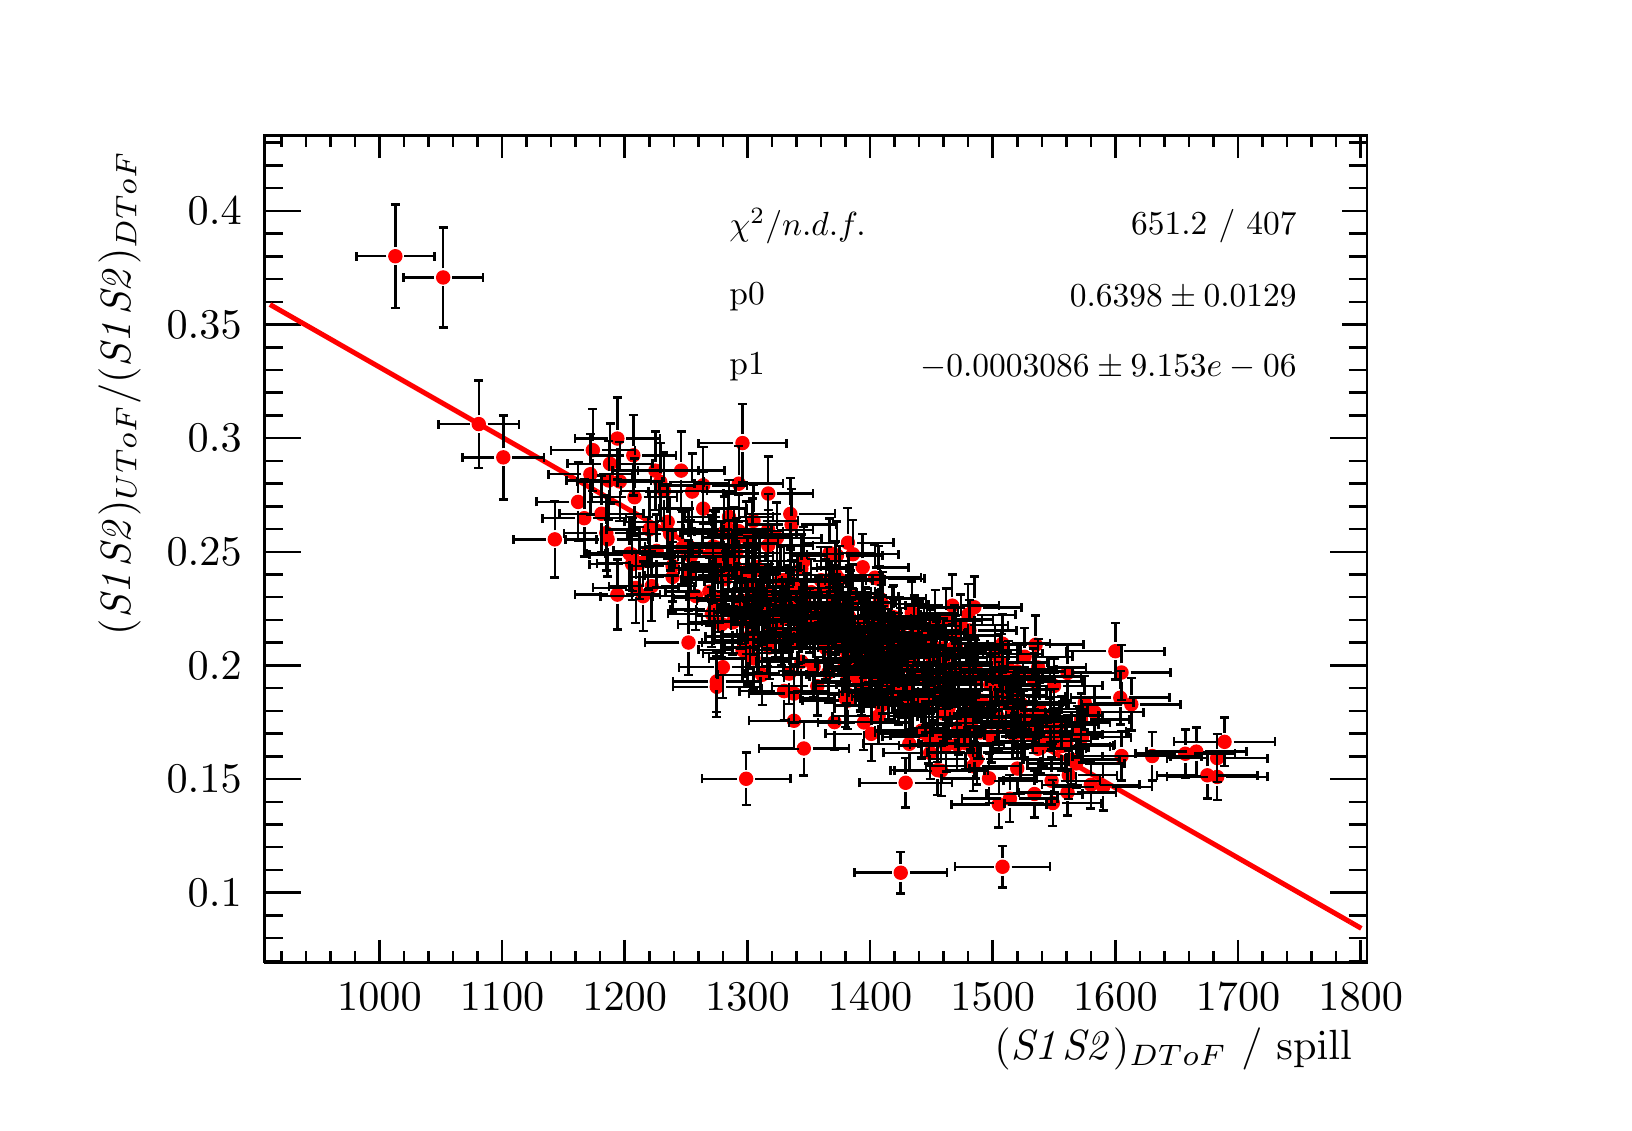
\begin{tikzpicture}
\pgfdeclareplotmark{cross} {
\pgfpathmoveto{\pgfpoint{-0.3\pgfplotmarksize}{\pgfplotmarksize}}
\pgfpathlineto{\pgfpoint{+0.3\pgfplotmarksize}{\pgfplotmarksize}}
\pgfpathlineto{\pgfpoint{+0.3\pgfplotmarksize}{0.3\pgfplotmarksize}}
\pgfpathlineto{\pgfpoint{+1\pgfplotmarksize}{0.3\pgfplotmarksize}}
\pgfpathlineto{\pgfpoint{+1\pgfplotmarksize}{-0.3\pgfplotmarksize}}
\pgfpathlineto{\pgfpoint{+0.3\pgfplotmarksize}{-0.3\pgfplotmarksize}}
\pgfpathlineto{\pgfpoint{+0.3\pgfplotmarksize}{-1.\pgfplotmarksize}}
\pgfpathlineto{\pgfpoint{-0.3\pgfplotmarksize}{-1.\pgfplotmarksize}}
\pgfpathlineto{\pgfpoint{-0.3\pgfplotmarksize}{-0.3\pgfplotmarksize}}
\pgfpathlineto{\pgfpoint{-1.\pgfplotmarksize}{-0.3\pgfplotmarksize}}
\pgfpathlineto{\pgfpoint{-1.\pgfplotmarksize}{0.3\pgfplotmarksize}}
\pgfpathlineto{\pgfpoint{-0.3\pgfplotmarksize}{0.3\pgfplotmarksize}}
\pgfpathclose
\pgfusepathqstroke
}
\pgfdeclareplotmark{cross*} {
\pgfpathmoveto{\pgfpoint{-0.3\pgfplotmarksize}{\pgfplotmarksize}}
\pgfpathlineto{\pgfpoint{+0.3\pgfplotmarksize}{\pgfplotmarksize}}
\pgfpathlineto{\pgfpoint{+0.3\pgfplotmarksize}{0.3\pgfplotmarksize}}
\pgfpathlineto{\pgfpoint{+1\pgfplotmarksize}{0.3\pgfplotmarksize}}
\pgfpathlineto{\pgfpoint{+1\pgfplotmarksize}{-0.3\pgfplotmarksize}}
\pgfpathlineto{\pgfpoint{+0.3\pgfplotmarksize}{-0.3\pgfplotmarksize}}
\pgfpathlineto{\pgfpoint{+0.3\pgfplotmarksize}{-1.\pgfplotmarksize}}
\pgfpathlineto{\pgfpoint{-0.3\pgfplotmarksize}{-1.\pgfplotmarksize}}
\pgfpathlineto{\pgfpoint{-0.3\pgfplotmarksize}{-0.3\pgfplotmarksize}}
\pgfpathlineto{\pgfpoint{-1.\pgfplotmarksize}{-0.3\pgfplotmarksize}}
\pgfpathlineto{\pgfpoint{-1.\pgfplotmarksize}{0.3\pgfplotmarksize}}
\pgfpathlineto{\pgfpoint{-0.3\pgfplotmarksize}{0.3\pgfplotmarksize}}
\pgfpathclose
\pgfusepathqfillstroke
}
\pgfdeclareplotmark{newstar} {
\pgfpathmoveto{\pgfqpoint{0pt}{\pgfplotmarksize}}
\pgfpathlineto{\pgfqpointpolar{44}{0.5\pgfplotmarksize}}
\pgfpathlineto{\pgfqpointpolar{18}{\pgfplotmarksize}}
\pgfpathlineto{\pgfqpointpolar{-20}{0.5\pgfplotmarksize}}
\pgfpathlineto{\pgfqpointpolar{-54}{\pgfplotmarksize}}
\pgfpathlineto{\pgfqpointpolar{-90}{0.5\pgfplotmarksize}}
\pgfpathlineto{\pgfqpointpolar{234}{\pgfplotmarksize}}
\pgfpathlineto{\pgfqpointpolar{198}{0.5\pgfplotmarksize}}
\pgfpathlineto{\pgfqpointpolar{162}{\pgfplotmarksize}}
\pgfpathlineto{\pgfqpointpolar{134}{0.5\pgfplotmarksize}}
\pgfpathclose
\pgfusepathqstroke
}
\pgfdeclareplotmark{newstar*} {
\pgfpathmoveto{\pgfqpoint{0pt}{\pgfplotmarksize}}
\pgfpathlineto{\pgfqpointpolar{44}{0.5\pgfplotmarksize}}
\pgfpathlineto{\pgfqpointpolar{18}{\pgfplotmarksize}}
\pgfpathlineto{\pgfqpointpolar{-20}{0.5\pgfplotmarksize}}
\pgfpathlineto{\pgfqpointpolar{-54}{\pgfplotmarksize}}
\pgfpathlineto{\pgfqpointpolar{-90}{0.5\pgfplotmarksize}}
\pgfpathlineto{\pgfqpointpolar{234}{\pgfplotmarksize}}
\pgfpathlineto{\pgfqpointpolar{198}{0.5\pgfplotmarksize}}
\pgfpathlineto{\pgfqpointpolar{162}{\pgfplotmarksize}}
\pgfpathlineto{\pgfqpointpolar{134}{0.5\pgfplotmarksize}}
\pgfpathclose
\pgfusepathqfillstroke
}
\definecolor{c}{rgb}{1,1,1};
\draw [color=c, fill=c] (0,0) rectangle (20,13.639);
\draw [color=c, fill=c] (3,1.77307) rectangle (17,12.2751);
\definecolor{c}{rgb}{0,0,0};
\draw [c,line width=0.9] (3,1.77307) -- (3,12.2751) -- (17,12.2751) -- (17,1.77307) -- (3,1.77307);
\definecolor{c}{rgb}{1,1,1};
\draw [color=c, fill=c] (3,1.77307) rectangle (17,12.2751);
\definecolor{c}{rgb}{0,0,0};
\draw [c,line width=0.9] (3,1.77307) -- (3,12.2751) -- (17,12.2751) -- (17,1.77307) -- (3,1.77307);
\draw [c,line width=0.9] (3,1.77307) -- (17,1.77307);
\draw [c,line width=0.9] (4.45996,2.05948) -- (4.45996,1.77307);
\draw [c,line width=0.9] (4.77152,1.91628) -- (4.77152,1.77307);
\draw [c,line width=0.9] (5.08308,1.91628) -- (5.08308,1.77307);
\draw [c,line width=0.9] (5.39463,1.91628) -- (5.39463,1.77307);
\draw [c,line width=0.9] (5.70619,1.91628) -- (5.70619,1.77307);
\draw [c,line width=0.9] (6.01775,2.05948) -- (6.01775,1.77307);
\draw [c,line width=0.9] (6.32931,1.91628) -- (6.32931,1.77307);
\draw [c,line width=0.9] (6.64087,1.91628) -- (6.64087,1.77307);
\draw [c,line width=0.9] (6.95242,1.91628) -- (6.95242,1.77307);
\draw [c,line width=0.9] (7.26398,1.91628) -- (7.26398,1.77307);
\draw [c,line width=0.9] (7.57554,2.05948) -- (7.57554,1.77307);
\draw [c,line width=0.9] (7.8871,1.91628) -- (7.8871,1.77307);
\draw [c,line width=0.9] (8.19865,1.91628) -- (8.19865,1.77307);
\draw [c,line width=0.9] (8.51021,1.91628) -- (8.51021,1.77307);
\draw [c,line width=0.9] (8.82177,1.91628) -- (8.82177,1.77307);
\draw [c,line width=0.9] (9.13333,2.05948) -- (9.13333,1.77307);
\draw [c,line width=0.9] (9.44488,1.91628) -- (9.44488,1.77307);
\draw [c,line width=0.9] (9.75644,1.91628) -- (9.75644,1.77307);
\draw [c,line width=0.9] (10.068,1.91628) -- (10.068,1.77307);
\draw [c,line width=0.9] (10.3796,1.91628) -- (10.3796,1.77307);
\draw [c,line width=0.9] (10.6911,2.05948) -- (10.6911,1.77307);
\draw [c,line width=0.9] (11.0027,1.91628) -- (11.0027,1.77307);
\draw [c,line width=0.9] (11.3142,1.91628) -- (11.3142,1.77307);
\draw [c,line width=0.9] (11.6258,1.91628) -- (11.6258,1.77307);
\draw [c,line width=0.9] (11.9373,1.91628) -- (11.9373,1.77307);
\draw [c,line width=0.9] (12.2489,2.05948) -- (12.2489,1.77307);
\draw [c,line width=0.9] (12.5605,1.91628) -- (12.5605,1.77307);
\draw [c,line width=0.9] (12.872,1.91628) -- (12.872,1.77307);
\draw [c,line width=0.9] (13.1836,1.91628) -- (13.1836,1.77307);
\draw [c,line width=0.9] (13.4951,1.91628) -- (13.4951,1.77307);
\draw [c,line width=0.9] (13.8067,2.05948) -- (13.8067,1.77307);
\draw [c,line width=0.9] (14.1182,1.91628) -- (14.1182,1.77307);
\draw [c,line width=0.9] (14.4298,1.91628) -- (14.4298,1.77307);
\draw [c,line width=0.9] (14.7414,1.91628) -- (14.7414,1.77307);
\draw [c,line width=0.9] (15.0529,1.91628) -- (15.0529,1.77307);
\draw [c,line width=0.9] (15.3645,2.05948) -- (15.3645,1.77307);
\draw [c,line width=0.9] (15.676,1.91628) -- (15.676,1.77307);
\draw [c,line width=0.9] (15.9876,1.91628) -- (15.9876,1.77307);
\draw [c,line width=0.9] (16.2992,1.91628) -- (16.2992,1.77307);
\draw [c,line width=0.9] (16.6107,1.91628) -- (16.6107,1.77307);
\draw [c,line width=0.9] (16.9223,2.05948) -- (16.9223,1.77307);
\draw [c,line width=0.9] (4.45996,2.05948) -- (4.45996,1.77307);
\draw [c,line width=0.9] (4.1484,1.91628) -- (4.1484,1.77307);
\draw [c,line width=0.9] (3.83685,1.91628) -- (3.83685,1.77307);
\draw [c,line width=0.9] (3.52529,1.91628) -- (3.52529,1.77307);
\draw [c,line width=0.9] (3.21373,1.91628) -- (3.21373,1.77307);
\draw [c,line width=0.9] (16.9223,2.05948) -- (16.9223,1.77307);
\draw [anchor=base] (4.45996,1.15931) node[scale=1.52731, color=c, rotate=0]{1000};
\draw [anchor=base] (6.01775,1.15931) node[scale=1.52731, color=c, rotate=0]{1100};
\draw [anchor=base] (7.57554,1.15931) node[scale=1.52731, color=c, rotate=0]{1200};
\draw [anchor=base] (9.13333,1.15931) node[scale=1.52731, color=c, rotate=0]{1300};
\draw [anchor=base] (10.6911,1.15931) node[scale=1.52731, color=c, rotate=0]{1400};
\draw [anchor=base] (12.2489,1.15931) node[scale=1.52731, color=c, rotate=0]{1500};
\draw [anchor=base] (13.8067,1.15931) node[scale=1.52731, color=c, rotate=0]{1600};
\draw [anchor=base] (15.3645,1.15931) node[scale=1.52731, color=c, rotate=0]{1700};
\draw [anchor=base] (16.9223,1.15931) node[scale=1.52731, color=c, rotate=0]{1800};
\draw [anchor= east] (17,0.681948) node[scale=1.52731, color=c, rotate=0]{ $(\SOne\STwo)_{\text{DToF}}$ / spill};
\draw [c,line width=0.9] (3,12.2751) -- (17,12.2751);
\draw [c,line width=0.9] (4.45996,11.9887) -- (4.45996,12.2751);
\draw [c,line width=0.9] (4.77152,12.1319) -- (4.77152,12.2751);
\draw [c,line width=0.9] (5.08308,12.1319) -- (5.08308,12.2751);
\draw [c,line width=0.9] (5.39463,12.1319) -- (5.39463,12.2751);
\draw [c,line width=0.9] (5.70619,12.1319) -- (5.70619,12.2751);
\draw [c,line width=0.9] (6.01775,11.9887) -- (6.01775,12.2751);
\draw [c,line width=0.9] (6.32931,12.1319) -- (6.32931,12.2751);
\draw [c,line width=0.9] (6.64087,12.1319) -- (6.64087,12.2751);
\draw [c,line width=0.9] (6.95242,12.1319) -- (6.95242,12.2751);
\draw [c,line width=0.9] (7.26398,12.1319) -- (7.26398,12.2751);
\draw [c,line width=0.9] (7.57554,11.9887) -- (7.57554,12.2751);
\draw [c,line width=0.9] (7.8871,12.1319) -- (7.8871,12.2751);
\draw [c,line width=0.9] (8.19865,12.1319) -- (8.19865,12.2751);
\draw [c,line width=0.9] (8.51021,12.1319) -- (8.51021,12.2751);
\draw [c,line width=0.9] (8.82177,12.1319) -- (8.82177,12.2751);
\draw [c,line width=0.9] (9.13333,11.9887) -- (9.13333,12.2751);
\draw [c,line width=0.9] (9.44488,12.1319) -- (9.44488,12.2751);
\draw [c,line width=0.9] (9.75644,12.1319) -- (9.75644,12.2751);
\draw [c,line width=0.9] (10.068,12.1319) -- (10.068,12.2751);
\draw [c,line width=0.9] (10.3796,12.1319) -- (10.3796,12.2751);
\draw [c,line width=0.9] (10.6911,11.9887) -- (10.6911,12.2751);
\draw [c,line width=0.9] (11.0027,12.1319) -- (11.0027,12.2751);
\draw [c,line width=0.9] (11.3142,12.1319) -- (11.3142,12.2751);
\draw [c,line width=0.9] (11.6258,12.1319) -- (11.6258,12.2751);
\draw [c,line width=0.9] (11.9373,12.1319) -- (11.9373,12.2751);
\draw [c,line width=0.9] (12.2489,11.9887) -- (12.2489,12.2751);
\draw [c,line width=0.9] (12.5605,12.1319) -- (12.5605,12.2751);
\draw [c,line width=0.9] (12.872,12.1319) -- (12.872,12.2751);
\draw [c,line width=0.9] (13.1836,12.1319) -- (13.1836,12.2751);
\draw [c,line width=0.9] (13.4951,12.1319) -- (13.4951,12.2751);
\draw [c,line width=0.9] (13.8067,11.9887) -- (13.8067,12.2751);
\draw [c,line width=0.9] (14.1182,12.1319) -- (14.1182,12.2751);
\draw [c,line width=0.9] (14.4298,12.1319) -- (14.4298,12.2751);
\draw [c,line width=0.9] (14.7414,12.1319) -- (14.7414,12.2751);
\draw [c,line width=0.9] (15.0529,12.1319) -- (15.0529,12.2751);
\draw [c,line width=0.9] (15.3645,11.9887) -- (15.3645,12.2751);
\draw [c,line width=0.9] (15.676,12.1319) -- (15.676,12.2751);
\draw [c,line width=0.9] (15.9876,12.1319) -- (15.9876,12.2751);
\draw [c,line width=0.9] (16.2992,12.1319) -- (16.2992,12.2751);
\draw [c,line width=0.9] (16.6107,12.1319) -- (16.6107,12.2751);
\draw [c,line width=0.9] (16.9223,11.9887) -- (16.9223,12.2751);
\draw [c,line width=0.9] (4.45996,11.9887) -- (4.45996,12.2751);
\draw [c,line width=0.9] (4.1484,12.1319) -- (4.1484,12.2751);
\draw [c,line width=0.9] (3.83685,12.1319) -- (3.83685,12.2751);
\draw [c,line width=0.9] (3.52529,12.1319) -- (3.52529,12.2751);
\draw [c,line width=0.9] (3.21373,12.1319) -- (3.21373,12.2751);
\draw [c,line width=0.9] (16.9223,11.9887) -- (16.9223,12.2751);
\draw [c,line width=0.9] (3,1.77307) -- (3,12.2751);
\draw [c,line width=0.9] (3.462,2.66058) -- (3,2.66058);
\draw [c,line width=0.9] (3.231,2.94918) -- (3,2.94918);
\draw [c,line width=0.9] (3.231,3.23779) -- (3,3.23779);
\draw [c,line width=0.9] (3.231,3.52639) -- (3,3.52639);
\draw [c,line width=0.9] (3.231,3.81499) -- (3,3.81499);
\draw [c,line width=0.9] (3.462,4.1036) -- (3,4.1036);
\draw [c,line width=0.9] (3.231,4.3922) -- (3,4.3922);
\draw [c,line width=0.9] (3.231,4.68081) -- (3,4.68081);
\draw [c,line width=0.9] (3.231,4.96941) -- (3,4.96941);
\draw [c,line width=0.9] (3.231,5.25801) -- (3,5.25801);
\draw [c,line width=0.9] (3.462,5.54662) -- (3,5.54662);
\draw [c,line width=0.9] (3.231,5.83522) -- (3,5.83522);
\draw [c,line width=0.9] (3.231,6.12382) -- (3,6.12382);
\draw [c,line width=0.9] (3.231,6.41243) -- (3,6.41243);
\draw [c,line width=0.9] (3.231,6.70103) -- (3,6.70103);
\draw [c,line width=0.9] (3.462,6.98964) -- (3,6.98964);
\draw [c,line width=0.9] (3.231,7.27824) -- (3,7.27824);
\draw [c,line width=0.9] (3.231,7.56684) -- (3,7.56684);
\draw [c,line width=0.9] (3.231,7.85545) -- (3,7.85545);
\draw [c,line width=0.9] (3.231,8.14405) -- (3,8.14405);
\draw [c,line width=0.9] (3.462,8.43266) -- (3,8.43266);
\draw [c,line width=0.9] (3.231,8.72126) -- (3,8.72126);
\draw [c,line width=0.9] (3.231,9.00986) -- (3,9.00986);
\draw [c,line width=0.9] (3.231,9.29847) -- (3,9.29847);
\draw [c,line width=0.9] (3.231,9.58707) -- (3,9.58707);
\draw [c,line width=0.9] (3.462,9.87568) -- (3,9.87568);
\draw [c,line width=0.9] (3.231,10.1643) -- (3,10.1643);
\draw [c,line width=0.9] (3.231,10.4529) -- (3,10.4529);
\draw [c,line width=0.9] (3.231,10.7415) -- (3,10.7415);
\draw [c,line width=0.9] (3.231,11.0301) -- (3,11.0301);
\draw [c,line width=0.9] (3.462,11.3187) -- (3,11.3187);
\draw [c,line width=0.9] (3.462,2.66058) -- (3,2.66058);
\draw [c,line width=0.9] (3.231,2.37197) -- (3,2.37197);
\draw [c,line width=0.9] (3.231,2.08337) -- (3,2.08337);
\draw [c,line width=0.9] (3.231,1.79477) -- (3,1.79477);
\draw [c,line width=0.9] (3.462,11.3187) -- (3,11.3187);
\draw [c,line width=0.9] (3.231,11.6073) -- (3,11.6073);
\draw [c,line width=0.9] (3.231,11.8959) -- (3,11.8959);
\draw [c,line width=0.9] (3.231,12.1845) -- (3,12.1845);
\draw [anchor= east] (2.9,2.66058) node[scale=1.52731, color=c, rotate=0]{0.1};
\draw [anchor= east] (2.9,4.1036) node[scale=1.52731, color=c, rotate=0]{0.15};
\draw [anchor= east] (2.9,5.54662) node[scale=1.52731, color=c, rotate=0]{0.2};
\draw [anchor= east] (2.9,6.98964) node[scale=1.52731, color=c, rotate=0]{0.25};
\draw [anchor= east] (2.9,8.43266) node[scale=1.52731, color=c, rotate=0]{0.3};
\draw [anchor= east] (2.9,9.87568) node[scale=1.52731, color=c, rotate=0]{0.35};
\draw [anchor= east] (2.9,11.3187) node[scale=1.52731, color=c, rotate=0]{0.4};
\draw [anchor= east] (1.16,12.2751) node[scale=1.52731, color=c, rotate=90]{ $(\SOne\STwo)_{\text{UToF}}/(\SOne\STwo)_{\text{DToF}}$ };
\draw [c,line width=0.9] (17,1.77307) -- (17,12.2751);
\draw [c,line width=0.9] (16.538,2.66058) -- (17,2.66058);
\draw [c,line width=0.9] (16.769,2.94918) -- (17,2.94918);
\draw [c,line width=0.9] (16.769,3.23779) -- (17,3.23779);
\draw [c,line width=0.9] (16.769,3.52639) -- (17,3.52639);
\draw [c,line width=0.9] (16.769,3.81499) -- (17,3.81499);
\draw [c,line width=0.9] (16.538,4.1036) -- (17,4.1036);
\draw [c,line width=0.9] (16.769,4.3922) -- (17,4.3922);
\draw [c,line width=0.9] (16.769,4.68081) -- (17,4.68081);
\draw [c,line width=0.9] (16.769,4.96941) -- (17,4.96941);
\draw [c,line width=0.9] (16.769,5.25801) -- (17,5.25801);
\draw [c,line width=0.9] (16.538,5.54662) -- (17,5.54662);
\draw [c,line width=0.9] (16.769,5.83522) -- (17,5.83522);
\draw [c,line width=0.9] (16.769,6.12382) -- (17,6.12382);
\draw [c,line width=0.9] (16.769,6.41243) -- (17,6.41243);
\draw [c,line width=0.9] (16.769,6.70103) -- (17,6.70103);
\draw [c,line width=0.9] (16.538,6.98964) -- (17,6.98964);
\draw [c,line width=0.9] (16.769,7.27824) -- (17,7.27824);
\draw [c,line width=0.9] (16.769,7.56684) -- (17,7.56684);
\draw [c,line width=0.9] (16.769,7.85545) -- (17,7.85545);
\draw [c,line width=0.9] (16.769,8.14405) -- (17,8.14405);
\draw [c,line width=0.9] (16.538,8.43266) -- (17,8.43266);
\draw [c,line width=0.9] (16.769,8.72126) -- (17,8.72126);
\draw [c,line width=0.9] (16.769,9.00986) -- (17,9.00986);
\draw [c,line width=0.9] (16.769,9.29847) -- (17,9.29847);
\draw [c,line width=0.9] (16.769,9.58707) -- (17,9.58707);
\draw [c,line width=0.9] (16.538,9.87568) -- (17,9.87568);
\draw [c,line width=0.9] (16.769,10.1643) -- (17,10.1643);
\draw [c,line width=0.9] (16.769,10.4529) -- (17,10.4529);
\draw [c,line width=0.9] (16.769,10.7415) -- (17,10.7415);
\draw [c,line width=0.9] (16.769,11.0301) -- (17,11.0301);
\draw [c,line width=0.9] (16.538,11.3187) -- (17,11.3187);
\draw [c,line width=0.9] (16.538,2.66058) -- (17,2.66058);
\draw [c,line width=0.9] (16.769,2.37197) -- (17,2.37197);
\draw [c,line width=0.9] (16.769,2.08337) -- (17,2.08337);
\draw [c,line width=0.9] (16.769,1.79477) -- (17,1.79477);
\draw [c,line width=0.9] (16.538,11.3187) -- (17,11.3187);
\draw [c,line width=0.9] (16.769,11.6073) -- (17,11.6073);
\draw [c,line width=0.9] (16.769,11.8959) -- (17,11.8959);
\draw [c,line width=0.9] (16.769,12.1845) -- (17,12.1845);
\definecolor{c}{rgb}{1,0,0};
\foreach \P in {(13.1992,5.45048), (10.3484,5.82726), (10.6288,6.12134), (7.13936,7.97463), (14.274,4.39574), (10.1615,5.85931), (11.9685,5.46093), (9.21122,6.0995), (10.1615,5.45788), (11.9685,4.79882), (12.6539,5.65631), (11.3921,5.14717),
 (9.32026,5.42783), (7.87152,6.97188), (11.7816,5.80185), (7.06147,7.41624), (10.364,5.76009), (7.68458,8.21507), (10.4107,7.10449), (7.17051,8.28024), (10.8157,5.84178), (10.2705,6.94234), (11.2208,6.21479), (8.41674,6.9321), (10.9559,6.00692),
 (11.065,6.01681), (4.66247,10.7432), (6.03333,8.18888), (10.4419,6.3432), (5.27001,10.4737), (13.4172,5.07019), (5.72177,8.61153), (9.21122,7.38218), (9.58508,6.22415), (13.0278,4.6715), (7.96498,8.02036), (9.05544,6.23748), (11.2987,5.39018),
 (9.99011,6.0152), (9.13333,5.70202), (8.71272,6.25849), (10.5353,5.94111), (11.3921,5.0473), (15.1931,4.57606), (10.8002,5.80507), (12.763,5.40354), (10.2238,6.41032), (12.7941,4.90736), (9.77202,6.5323), (10.6132,4.82252), (12.2333,4.64557),
 (10.3951,5.9186), (10.6755,5.63326), (9.72529,6.43961), (10.5665,5.35173), (7.66901,6.83409), (13.869,5.13638), (12.4358,5.36719), (13.3861,4.63659), (10.8157,6.39521), (11.0494,5.75754), (11.4389,5.33535), (11.5167,6.11072), (12.3268,3.78239),
 (9.41373,6.40936), (11.5479,4.21765), (10.1147,5.85152), (13.6509,4.00377), (9.81875,6.7749), (11.0806,5.89092), (11.6569,4.53196), (12.9811,4.90486), (12.4981,4.68614), (12.7786,5.34343), (10.8625,5.9107), (10.3796,5.9858), (12.763,4.76345),
 (10.1303,5.76243), (9.22679,6.49242), (9.88106,6.30452), (10.3951,5.43795), (9.28911,6.75831), (12.7941,5.80984), (11.2519,5.44211), (10.5821,6.05214), (10.3951,5.18717), (11.9685,4.81829), (11.1117,5.53853), (9.11775,6.1065), (11.5635,5.76069),
 (9.60066,5.22112), (11.4389,4.63775), (10.6288,6.14202), (12.3424,5.58111), (9.81875,5.59386), (13.5419,4.95227), (10.1303,6.48183), (12.3268,5.16309), (10.9715,6.14499), (7.35745,7.14781), (9.67855,6.60591), (11.766,5.92383), (10.0368,6.27769),
 (12.5605,4.23651), (13.3238,4.70417), (10.4263,6.16013), (12.8876,4.58773), (9.25795,5.86435), (7.37303,7.89532), (11.8127,5.49956), (10.8469,6.32441), (8.18308,6.80911), (8.15192,7.21711), (13.1213,4.81954), (11.6258,5.76406), (10.473,6.00055),
 (9.66297,6.13507), (10.7067,5.5013), (13.2147,4.15348), (10.8469,5.301), (10.6755,5.71578), (9.27353,5.85969), (11.0961,5.23899), (10.3951,5.9604), (11.2987,5.95175), (7.51323,7.88247), (9.9278,6.11912), (9.41373,5.77435), (9.46046,6.28506),
 (10.068,6.62888), (11.2208,5.08775), (12.0464,4.35494), (11.2363,5.06393), (8.88408,6.8323), (11.766,5.49161), (11.3454,4.69802), (6.98358,7.62298), (8.12076,7.36938), (9.60066,6.63159), (11.3142,5.9675), (9.66297,5.44277), (11.9529,5.99092),
 (9.66297,6.17834), (12.3268,4.81792), (10.9248,5.22028), (10.1459,6.62492), (8.74388,5.27499), (10.473,6.41701), (7.80921,6.42549), (8.96197,7.09599), (10.364,5.59266), (7.66901,6.95374), (8.97755,6.79947), (12.0152,4.43884), (10.7534,6.66074),
 (12.7786,3.91358), (9.97453,5.52956), (8.83735,7.23183), (10.9871,5.59136), (7.27956,7.47227), (10.4107,6.18564), (10.3796,5.12835), (11.2363,5.56673), (11.7348,5.69613), (9.58508,5.8767), (11.8127,4.75452), (10.4263,5.61757), (10.6288,6.03865),
 (10.8313,6.1652), (11.7348,5.38136), (9.32026,6.26373), (10.8002,5.53841), (11.4856,5.20451), (10.5821,5.28557), (10.177,6.2771), (10.2549,6.08512), (9.58508,6.13729), (9.67855,7.47064), (11.5791,5.63773), (12.5293,5.07892), (9.67855,5.87089),
 (10.5976,6.79296), (13.1992,3.93443), (11.7348,6.306), (11.9062,4.55857), (9.38257,6.17821), (11.47,5.66604), (10.4107,5.09972), (15.0997,4.13018), (11.9997,5.74498), (13.0122,3.79897), (9.66297,6.30815), (12.062,4.70098), (12.576,5.04948),
 (12.8564,4.50022), (6.6876,7.14745), (12.0152,6.28513), (9.32026,6.21973), (13.3082,4.30238), (13.8846,4.3958), (12.0308,5.50389), (13.8846,5.45671), (12.8409,4.99118), (9.24237,6.79642), (11.3765,5.89038), (12.8253,4.48759), (9.77202,5.84361),
 (14.8348,4.45179), (11.361,5.11461), (12.4203,5.06529), (14.975,4.15098), (11.5479,4.65403), (10.4107,5.91416), (11.0961,5.664), (10.8002,6.64606), (10.769,5.42337), (12.4826,5.05132), (7.63785,6.96567), (12.6539,4.71069), (10.9715,5.4937),
 (14.0092,5.05279), (10.473,6.9584), (10.4574,5.98421), (12.3268,5.2398), (11.6414,5.16734), (9.7876,5.96812), (8.07403,7.76268), (12.0308,5.36794), (13.3705,4.85999), (10.9715,5.31052), (10.7223,5.95009), (7.34187,7.2271), (11.6569,5.40054),
 (9.11775,4.10693), (11.4544,4.43522), (11.9997,4.26696), (9.72529,4.84344), (10.5821,5.57562), (8.88408,7.28184), (11.1429,5.04575), (12.2177,5.30387), (10.2082,6.45733), (9.21122,5.63508), (12.5605,5.47067), (8.47906,6.42757), (10.2394,4.82669),
 (9.69413,7.33527), (9.16448,5.91458), (12.1087,5.09755), (15.0997,4.37025), (11.1896,4.55101), (13.1213,4.52278), (12.2177,5.4002), (12.3579,5.57726), (9.84991,6.20702), (13.1836,4.5476), (14.6946,4.42495), (9.33584,6.28077), (12.467,3.85388),
 (8.80619,6.92758), (12.6072,4.83411), (10.8002,4.90254), (10.9559,5.66067), (13.2459,4.35087), (9.19564,7.21096), (11.9373,6.19013), (11.6569,6.13093), (11.2519,6.04504), (9.19564,6.39207), (10.8002,5.47688), (10.9248,5.81177), (11.6725,4.9627),
 (12.2801,5.69265), (10.1926,5.9137), (8.38559,7.05879), (8.18308,6.66935), (8.89966,7.43321), (10.9871,6.16084), (13.0278,5.28594), (11.5946,4.20851), (10.3017,6.63806), (10.9092,5.59152), (11.5791,5.40004), (8.82177,6.76416), (8.89966,6.9391),
 (10.2549,6.00098), (9.33584,6.25878), (9.07101,8.3703), (8.80619,6.07012), (12.5605,5.14789), (9.02428,7.85456), (9.72529,5.18856), (11.4544,5.86928), (7.71574,6.53011), (10.8157,6.08775), (10.3017,6.26026), (10.7378,5.92511), (11.6881,4.99858),
 (9.39815,7.07181), (12.5605,4.6922), (10.3796,6.02762), (10.8313,5.03864), (10.9248,5.87295), (8.43232,7.75426), (8.68157,6.20057), (9.6474,6.39965), (12.4514,5.49702), (10.177,6.9738), (10.3951,6.04399), (9.24237,6.37688), (10.6132,5.77419),
 (7.70016,7.68248), (9.60066,5.22112), (10.2549,6.69514), (11.6258,4.93383), (8.29212,8.02036), (8.57252,7.53762), (11.3454,4.71803), (11.174,5.32074), (12.3735,5.45858), (7.8871,7.27351), (10.2238,6.41032), (9.84991,4.49169), (12.2022,4.11227),
 (12.3112,4.89803), (9.07101,5.74258), (11.6569,5.36106), (10.0213,5.2829), (11.0806,2.91374), (8.75946,6.40157), (10.5665,5.33099), (13.4951,4.03053), (7.76247,6.84676), (9.38257,5.93698), (11.8906,4.89399), (8.82177,5.52407), (8.7283,7.04627),
 (8.69715,6.78544), (11.2363,5.6874), (8.38559,5.83706), (11.6414,5.54267), (8.0273,7.87611), (7.48207,6.44579), (8.38559,6.68997), (10.6755,5.88081), (7.91825,6.55272), (9.11775,5.83989), (12.4981,4.97169), (9.39815,7.26904), (8.85292,6.6407),
 (10.6444,5.97219), (12.0931,4.69436), (8.57252,7.83444), (9.13333,6.74543), (8.69715,7.0577), (12.9966,4.08122), (13.168,4.53215), (10.2705,6.29072), (9.94338,6.47732), (9.02428,7.2519), (9.11775,7.17293), (7.48207,8.42782), (10.8469,6.03786),
 (11.5323,5.72923), (7.98056,7.00141), (12.2801,5.40443), (9.39815,7.72923), (8.74388,5.3429), (10.6444,5.97219), (9.1489,6.60698), (12.6383,4.88425), (10.9404,5.78712), (8.68157,6.99531), (10.7223,5.90892), (10.0368,6.25644), (11.8439,6.0596),
 (8.3077,7.04171), (9.03986,6.17557), (8.99312,6.97287), (13.8067,5.72699), (9.27353,6.21246), (9.5072,7.16402), (11.0027,5.20111), (9.49162,6.14433), (10.6755,5.86018), (9.49162,6.05707), (11.1429,4.05614), (10.7067,4.6773), (12.8253,5.52033),
 (12.9811,4.79293), (8.96197,6.73775), (13.0278,4.91355), (11.7971,4.54209), (12.3735,5.82221), (8.65041,6.48361), (12.3735,2.98975), (10.3484,6.14142), (8.94639,6.09335), (9.84991,6.87171), (9.56951,5.94649), (10.878,5.7224), (10.5042,5.40938),
 (11.0494,5.1491), (12.6072,5.0615), (9.55393,6.62535), (13.3549,4.69789), (7.3886,8.10713), (9.05544,6.3712), (12.5137,4.77802)}{\draw[mark options={color=c,fill=c},mark size=2.402402pt,mark=*] plot coordinates {\P};}
\draw [c,line width=1.8] (3.07,10.13) -- (3.21,10.05) -- (3.35,9.96998) -- (3.49,9.88995) -- (3.63,9.80992) -- (3.77,9.72989) -- (3.91,9.64987) -- (4.05,9.56984) -- (4.19,9.48981) -- (4.33,9.40978) -- (4.47,9.32975) -- (4.61,9.24972) --
 (4.75,9.16969) -- (4.89,9.08966) -- (5.03,9.00963) -- (5.17,8.9296) -- (5.31,8.84957) -- (5.45,8.76954) -- (5.59,8.68951) -- (5.73,8.60948) -- (5.87,8.52945) -- (6.01,8.44942) -- (6.15,8.36939) -- (6.29,8.28936) -- (6.43,8.20933) -- (6.57,8.1293) --
 (6.71,8.04927) -- (6.85,7.96924) -- (6.99,7.88921) -- (7.13,7.80918) -- (7.27,7.72915) -- (7.41,7.64912) -- (7.55,7.5691) -- (7.69,7.48907) -- (7.83,7.40904) -- (7.97,7.32901) -- (8.11,7.24898) -- (8.25,7.16895) -- (8.39,7.08892) -- (8.53,7.00889)
 -- (8.67,6.92886) -- (8.81,6.84883) -- (8.95,6.7688) -- (9.09,6.68877) -- (9.23,6.60874) -- (9.37,6.52871) -- (9.51,6.44868) -- (9.65,6.36865) -- (9.79,6.28862) -- (9.93,6.20859);
\draw [c,line width=1.8] (9.93,6.20859) -- (10.07,6.12856) -- (10.21,6.04853) -- (10.35,5.9685) -- (10.49,5.88847) -- (10.63,5.80844) -- (10.77,5.72841) -- (10.91,5.64838) -- (11.05,5.56835) -- (11.19,5.48832) -- (11.33,5.4083) -- (11.47,5.32827) --
 (11.61,5.24824) -- (11.75,5.16821) -- (11.89,5.08818) -- (12.03,5.00815) -- (12.17,4.92812) -- (12.31,4.84809) -- (12.45,4.76806) -- (12.59,4.68803) -- (12.73,4.608) -- (12.87,4.52797) -- (13.01,4.44794) -- (13.15,4.36791) -- (13.29,4.28788) --
 (13.43,4.20785) -- (13.57,4.12782) -- (13.71,4.04779) -- (13.85,3.96776) -- (13.99,3.88773) -- (14.13,3.8077) -- (14.27,3.72767) -- (14.41,3.64764) -- (14.55,3.56761) -- (14.69,3.48758) -- (14.83,3.40755) -- (14.97,3.32753) -- (15.11,3.2475) --
 (15.25,3.16747) -- (15.39,3.08744) -- (15.53,3.00741) -- (15.67,2.92738) -- (15.81,2.84735) -- (15.95,2.76732) -- (16.09,2.68729) -- (16.23,2.60726) -- (16.37,2.52723) -- (16.51,2.4472) -- (16.65,2.36717) -- (16.79,2.28714);
\draw [c,line width=1.8] (16.79,2.28714) -- (16.93,2.20711);
\definecolor{c}{rgb}{1,1,1};
\draw [color=c, fill=c] (8.33811,8.88252) rectangle (16.6762,11.5759);
\definecolor{c}{rgb}{0,0,0};
\draw [anchor= west] (8.75501,11.127) node[scale=1.20912, color=c, rotate=0]{$\chi^{2} / ndf $};
\draw [anchor= east] (16.2593,11.127) node[scale=1.20912, color=c, rotate=0]{ 651.2 / 407};
\draw [anchor= west] (8.75501,10.2292) node[scale=1.20912, color=c, rotate=0]{p0       };
\draw [anchor= east] (16.2593,10.2292) node[scale=1.20912, color=c, rotate=0]{$ 0.6398 \pm 0.0129$};
\draw [anchor= west] (8.75501,9.33142) node[scale=1.20912, color=c, rotate=0]{p1       };
\draw [anchor= east] (16.2593,9.33142) node[scale=1.20912, color=c, rotate=0]{$ -0.0003086 \pm 9.153e-06$};
\draw [c,line width=0.9] (13.0845,5.45048) -- (12.5837,5.45048);
\draw [c,line width=0.9] (12.5837,5.39317) -- (12.5837,5.50778);
\draw [c,line width=0.9] (13.3138,5.45048) -- (13.8146,5.45048);
\draw [c,line width=0.9] (13.8146,5.39317) -- (13.8146,5.50778);
\draw [c,line width=0.9] (13.1992,5.56509) -- (13.1992,5.80485);
\draw [c,line width=0.9] (13.1418,5.80485) -- (13.2565,5.80485);
\draw [c,line width=0.9] (13.1992,5.33586) -- (13.1992,5.09611);
\draw [c,line width=0.9] (13.1418,5.09611) -- (13.2565,5.09611);
\draw [c,line width=0.9] (10.2338,5.82726) -- (9.77013,5.82726);
\draw [c,line width=0.9] (9.77013,5.76996) -- (9.77013,5.88457);
\draw [c,line width=0.9] (10.463,5.82726) -- (10.9267,5.82726);
\draw [c,line width=0.9] (10.9267,5.76996) -- (10.9267,5.88457);
\draw [c,line width=0.9] (10.3484,5.94188) -- (10.3484,6.21886);
\draw [c,line width=0.9] (10.2911,6.21886) -- (10.4057,6.21886);
\draw [c,line width=0.9] (10.3484,5.71265) -- (10.3484,5.43566);
\draw [c,line width=0.9] (10.2911,5.43566) -- (10.4057,5.43566);
\draw [c,line width=0.9] (10.5142,6.12134) -- (10.0468,6.12134);
\draw [c,line width=0.9] (10.0468,6.06404) -- (10.0468,6.17865);
\draw [c,line width=0.9] (10.7434,6.12134) -- (11.2108,6.12134);
\draw [c,line width=0.9] (11.2108,6.06404) -- (11.2108,6.17865);
\draw [c,line width=0.9] (10.6288,6.23596) -- (10.6288,6.52143);
\draw [c,line width=0.9] (10.5715,6.52143) -- (10.6861,6.52143);
\draw [c,line width=0.9] (10.6288,6.00673) -- (10.6288,5.72126);
\draw [c,line width=0.9] (10.5715,5.72126) -- (10.6861,5.72126);
\draw [c,line width=0.9] (7.02474,7.97463) -- (6.60606,7.97463);
\draw [c,line width=0.9] (6.60606,7.91733) -- (6.60606,8.03194);
\draw [c,line width=0.9] (7.25397,7.97463) -- (7.67266,7.97463);
\draw [c,line width=0.9] (7.67266,7.91733) -- (7.67266,8.03194);
\draw [c,line width=0.9] (7.13936,8.08925) -- (7.13936,8.48385);
\draw [c,line width=0.9] (7.08205,8.48385) -- (7.19666,8.48385);
\draw [c,line width=0.9] (7.13936,7.86002) -- (7.13936,7.46542);
\draw [c,line width=0.9] (7.08205,7.46542) -- (7.19666,7.46542);
\draw [c,line width=0.9] (14.1594,4.39574) -- (13.6451,4.39574);
\draw [c,line width=0.9] (13.6451,4.33844) -- (13.6451,4.45305);
\draw [c,line width=0.9] (14.3886,4.39574) -- (14.903,4.39574);
\draw [c,line width=0.9] (14.903,4.33844) -- (14.903,4.45305);
\draw [c,line width=0.9] (14.274,4.51036) -- (14.274,4.70384);
\draw [c,line width=0.9] (14.2167,4.70384) -- (14.3313,4.70384);
\draw [c,line width=0.9] (14.274,4.28113) -- (14.274,4.08765);
\draw [c,line width=0.9] (14.2167,4.08765) -- (14.3313,4.08765);
\draw [c,line width=0.9] (10.0469,5.85931) -- (9.58572,5.85931);
\draw [c,line width=0.9] (9.58572,5.802) -- (9.58572,5.91661);
\draw [c,line width=0.9] (10.2761,5.85931) -- (10.7372,5.85931);
\draw [c,line width=0.9] (10.7372,5.802) -- (10.7372,5.91661);
\draw [c,line width=0.9] (10.1615,5.97392) -- (10.1615,6.25385);
\draw [c,line width=0.9] (10.1042,6.25385) -- (10.2188,6.25385);
\draw [c,line width=0.9] (10.1615,5.74469) -- (10.1615,5.46477);
\draw [c,line width=0.9] (10.1042,5.46477) -- (10.2188,5.46477);
\draw [c,line width=0.9] (11.8539,5.46093) -- (11.3688,5.46093);
\draw [c,line width=0.9] (11.3688,5.40363) -- (11.3688,5.51824);
\draw [c,line width=0.9] (12.0831,5.46093) -- (12.5682,5.46093);
\draw [c,line width=0.9] (12.5682,5.40363) -- (12.5682,5.51824);
\draw [c,line width=0.9] (11.9685,5.57554) -- (11.9685,5.82501);
\draw [c,line width=0.9] (11.9112,5.82501) -- (12.0258,5.82501);
\draw [c,line width=0.9] (11.9685,5.34632) -- (11.9685,5.09685);
\draw [c,line width=0.9] (11.9112,5.09685) -- (12.0258,5.09685);
\draw [c,line width=0.9] (9.0966,6.0995) -- (8.64847,6.0995);
\draw [c,line width=0.9] (8.64847,6.04219) -- (8.64847,6.1568);
\draw [c,line width=0.9] (9.32583,6.0995) -- (9.77396,6.0995);
\draw [c,line width=0.9] (9.77396,6.04219) -- (9.77396,6.1568);
\draw [c,line width=0.9] (9.21122,6.21411) -- (9.21122,6.51245);
\draw [c,line width=0.9] (9.15391,6.51245) -- (9.26852,6.51245);
\draw [c,line width=0.9] (9.21122,5.98488) -- (9.21122,5.68654);
\draw [c,line width=0.9] (9.15391,5.68654) -- (9.26852,5.68654);
\draw [c,line width=0.9] (10.0469,5.45788) -- (9.58572,5.45788);
\draw [c,line width=0.9] (9.58572,5.40057) -- (9.58572,5.51519);
\draw [c,line width=0.9] (10.2761,5.45788) -- (10.7372,5.45788);
\draw [c,line width=0.9] (10.7372,5.40057) -- (10.7372,5.51519);
\draw [c,line width=0.9] (10.1615,5.57249) -- (10.1615,5.83699);
\draw [c,line width=0.9] (10.1042,5.83699) -- (10.2188,5.83699);
\draw [c,line width=0.9] (10.1615,5.34327) -- (10.1615,5.07877);
\draw [c,line width=0.9] (10.1042,5.07877) -- (10.2188,5.07877);
\draw [c,line width=0.9] (11.8539,4.79882) -- (11.3688,4.79882);
\draw [c,line width=0.9] (11.3688,4.74151) -- (11.3688,4.85612);
\draw [c,line width=0.9] (12.0831,4.79882) -- (12.5682,4.79882);
\draw [c,line width=0.9] (12.5682,4.74151) -- (12.5682,4.85612);
\draw [c,line width=0.9] (11.9685,4.91343) -- (11.9685,5.13775);
\draw [c,line width=0.9] (11.9112,5.13775) -- (12.0258,5.13775);
\draw [c,line width=0.9] (11.9685,4.6842) -- (11.9685,4.45988);
\draw [c,line width=0.9] (11.9112,4.45988) -- (12.0258,4.45988);
\draw [c,line width=0.9] (12.5393,5.65631) -- (12.0454,5.65631);
\draw [c,line width=0.9] (12.0454,5.599) -- (12.0454,5.71362);
\draw [c,line width=0.9] (12.7685,5.65631) -- (13.2625,5.65631);
\draw [c,line width=0.9] (13.2625,5.599) -- (13.2625,5.71362);
\draw [c,line width=0.9] (12.6539,5.77092) -- (12.6539,6.02224);
\draw [c,line width=0.9] (12.5966,6.02224) -- (12.7112,6.02224);
\draw [c,line width=0.9] (12.6539,5.5417) -- (12.6539,5.29037);
\draw [c,line width=0.9] (12.5966,5.29037) -- (12.7112,5.29037);
\draw [c,line width=0.9] (11.2775,5.14717) -- (10.8,5.14717);
\draw [c,line width=0.9] (10.8,5.08986) -- (10.8,5.20447);
\draw [c,line width=0.9] (11.5067,5.14717) -- (11.9843,5.14717);
\draw [c,line width=0.9] (11.9843,5.08986) -- (11.9843,5.20447);
\draw [c,line width=0.9] (11.3921,5.26178) -- (11.3921,5.50393);
\draw [c,line width=0.9] (11.3348,5.50393) -- (11.4494,5.50393);
\draw [c,line width=0.9] (11.3921,5.03255) -- (11.3921,4.7904);
\draw [c,line width=0.9] (11.3348,4.7904) -- (11.4494,4.7904);
\draw [c,line width=0.9] (9.20565,5.42783) -- (8.75601,5.42783);
\draw [c,line width=0.9] (8.75601,5.37053) -- (8.75601,5.48514);
\draw [c,line width=0.9] (9.43487,5.42783) -- (9.88452,5.42783);
\draw [c,line width=0.9] (9.88452,5.37053) -- (9.88452,5.48514);
\draw [c,line width=0.9] (9.32026,5.54244) -- (9.32026,5.81347);
\draw [c,line width=0.9] (9.26295,5.81347) -- (9.37757,5.81347);
\draw [c,line width=0.9] (9.32026,5.31322) -- (9.32026,5.04219);
\draw [c,line width=0.9] (9.26295,5.04219) -- (9.37757,5.04219);
\draw [c,line width=0.9] (7.7569,6.97188) -- (7.32763,6.97188);
\draw [c,line width=0.9] (7.32763,6.91457) -- (7.32763,7.02919);
\draw [c,line width=0.9] (7.98613,6.97188) -- (8.41541,6.97188);
\draw [c,line width=0.9] (8.41541,6.91457) -- (8.41541,7.02919);
\draw [c,line width=0.9] (7.87152,7.08649) -- (7.87152,7.43329);
\draw [c,line width=0.9] (7.81421,7.43329) -- (7.92882,7.43329);
\draw [c,line width=0.9] (7.87152,6.85727) -- (7.87152,6.51047);
\draw [c,line width=0.9] (7.81421,6.51047) -- (7.92882,6.51047);
\draw [c,line width=0.9] (11.667,5.80185) -- (11.1843,5.80185);
\draw [c,line width=0.9] (11.1843,5.74454) -- (11.1843,5.85915);
\draw [c,line width=0.9] (11.8962,5.80185) -- (12.3788,5.80185);
\draw [c,line width=0.9] (12.3788,5.74454) -- (12.3788,5.85915);
\draw [c,line width=0.9] (11.7816,5.91646) -- (11.7816,6.18006);
\draw [c,line width=0.9] (11.7243,6.18006) -- (11.8389,6.18006);
\draw [c,line width=0.9] (11.7816,5.68723) -- (11.7816,5.42363);
\draw [c,line width=0.9] (11.7243,5.42363) -- (11.8389,5.42363);
\draw [c,line width=0.9] (6.94685,7.41624) -- (6.52931,7.41624);
\draw [c,line width=0.9] (6.52931,7.35893) -- (6.52931,7.47354);
\draw [c,line width=0.9] (7.17608,7.41624) -- (7.59363,7.41624);
\draw [c,line width=0.9] (7.59363,7.35893) -- (7.59363,7.47354);
\draw [c,line width=0.9] (7.06147,7.53085) -- (7.06147,7.90513);
\draw [c,line width=0.9] (7.00416,7.90513) -- (7.11877,7.90513);
\draw [c,line width=0.9] (7.06147,7.30162) -- (7.06147,6.92734);
\draw [c,line width=0.9] (7.00416,6.92734) -- (7.11877,6.92734);
\draw [c,line width=0.9] (10.2494,5.76009) -- (9.7855,5.76009);
\draw [c,line width=0.9] (9.7855,5.70278) -- (9.7855,5.81739);
\draw [c,line width=0.9] (10.4786,5.76009) -- (10.9425,5.76009);
\draw [c,line width=0.9] (10.9425,5.70278) -- (10.9425,5.81739);
\draw [c,line width=0.9] (10.364,5.8747) -- (10.364,6.14899);
\draw [c,line width=0.9] (10.3067,6.14899) -- (10.4213,6.14899);
\draw [c,line width=0.9] (10.364,5.64547) -- (10.364,5.37118);
\draw [c,line width=0.9] (10.3067,5.37118) -- (10.4213,5.37118);
\draw [c,line width=0.9] (7.56997,8.21507) -- (7.14338,8.21507);
\draw [c,line width=0.9] (7.14338,8.15776) -- (7.14338,8.27237);
\draw [c,line width=0.9] (7.7992,8.21507) -- (8.22579,8.21507);
\draw [c,line width=0.9] (8.22579,8.15776) -- (8.22579,8.27237);
\draw [c,line width=0.9] (7.68458,8.32968) -- (7.68458,8.7258);
\draw [c,line width=0.9] (7.62728,8.7258) -- (7.74189,8.7258);
\draw [c,line width=0.9] (7.68458,8.10045) -- (7.68458,7.70434);
\draw [c,line width=0.9] (7.62728,7.70434) -- (7.74189,7.70434);
\draw [c,line width=0.9] (10.2961,7.10449) -- (9.8316,7.10449);
\draw [c,line width=0.9] (9.8316,7.04719) -- (9.8316,7.1618);
\draw [c,line width=0.9] (10.5253,7.10449) -- (10.9898,7.10449);
\draw [c,line width=0.9] (10.9898,7.04719) -- (10.9898,7.1618);
\draw [c,line width=0.9] (10.4107,7.21911) -- (10.4107,7.54261);
\draw [c,line width=0.9] (10.3534,7.54261) -- (10.468,7.54261);
\draw [c,line width=0.9] (10.4107,6.98988) -- (10.4107,6.66637);
\draw [c,line width=0.9] (10.3534,6.66637) -- (10.468,6.66637);
\draw [c,line width=0.9] (7.0559,8.28024) -- (6.63676,8.28024);
\draw [c,line width=0.9] (6.63676,8.22293) -- (6.63676,8.33755);
\draw [c,line width=0.9] (7.28513,8.28024) -- (7.70427,8.28024);
\draw [c,line width=0.9] (7.70427,8.22293) -- (7.70427,8.33755);
\draw [c,line width=0.9] (7.17051,8.39485) -- (7.17051,8.80055);
\draw [c,line width=0.9] (7.11321,8.80055) -- (7.22782,8.80055);
\draw [c,line width=0.9] (7.17051,8.16563) -- (7.17051,7.75993);
\draw [c,line width=0.9] (7.11321,7.75993) -- (7.22782,7.75993);
\draw [c,line width=0.9] (10.7011,5.84178) -- (10.2312,5.84178);
\draw [c,line width=0.9] (10.2312,5.78447) -- (10.2312,5.89909);
\draw [c,line width=0.9] (10.9304,5.84178) -- (11.4003,5.84178);
\draw [c,line width=0.9] (11.4003,5.78447) -- (11.4003,5.89909);
\draw [c,line width=0.9] (10.8157,5.95639) -- (10.8157,6.22973);
\draw [c,line width=0.9] (10.7584,6.22973) -- (10.873,6.22973);
\draw [c,line width=0.9] (10.8157,5.72717) -- (10.8157,5.45383);
\draw [c,line width=0.9] (10.7584,5.45383) -- (10.873,5.45383);
\draw [c,line width=0.9] (10.1559,6.94234) -- (9.69329,6.94234);
\draw [c,line width=0.9] (9.69329,6.88504) -- (9.69329,6.99965);
\draw [c,line width=0.9] (10.3851,6.94234) -- (10.8477,6.94234);
\draw [c,line width=0.9] (10.8477,6.88504) -- (10.8477,6.99965);
\draw [c,line width=0.9] (10.2705,7.05695) -- (10.2705,7.37603);
\draw [c,line width=0.9] (10.2132,7.37603) -- (10.3278,7.37603);
\draw [c,line width=0.9] (10.2705,6.82773) -- (10.2705,6.50865);
\draw [c,line width=0.9] (10.2132,6.50865) -- (10.3278,6.50865);
\draw [c,line width=0.9] (11.1061,6.21479) -- (10.6309,6.21479);
\draw [c,line width=0.9] (10.6309,6.15749) -- (10.6309,6.2721);
\draw [c,line width=0.9] (11.3354,6.21479) -- (11.8107,6.21479);
\draw [c,line width=0.9] (11.8107,6.15749) -- (11.8107,6.2721);
\draw [c,line width=0.9] (11.2208,6.32941) -- (11.2208,6.61296);
\draw [c,line width=0.9] (11.1635,6.61296) -- (11.2781,6.61296);
\draw [c,line width=0.9] (11.2208,6.10018) -- (11.2208,5.81662);
\draw [c,line width=0.9] (11.1635,5.81662) -- (11.2781,5.81662);
\draw [c,line width=0.9] (8.30213,6.9321) -- (7.8651,6.9321);
\draw [c,line width=0.9] (7.8651,6.87479) -- (7.8651,6.98941);
\draw [c,line width=0.9] (8.53136,6.9321) -- (8.96839,6.9321);
\draw [c,line width=0.9] (8.96839,6.87479) -- (8.96839,6.98941);
\draw [c,line width=0.9] (8.41674,7.04671) -- (8.41674,7.38551);
\draw [c,line width=0.9] (8.35944,7.38551) -- (8.47405,7.38551);
\draw [c,line width=0.9] (8.41674,6.81749) -- (8.41674,6.47869);
\draw [c,line width=0.9] (8.35944,6.47869) -- (8.47405,6.47869);
\draw [c,line width=0.9] (10.8413,6.00692) -- (10.3695,6.00692);
\draw [c,line width=0.9] (10.3695,5.94961) -- (10.3695,6.06422);
\draw [c,line width=0.9] (11.0706,6.00692) -- (11.5423,6.00692);
\draw [c,line width=0.9] (11.5423,5.94961) -- (11.5423,6.06422);
\draw [c,line width=0.9] (10.9559,6.12153) -- (10.9559,6.39979);
\draw [c,line width=0.9] (10.8986,6.39979) -- (11.0132,6.39979);
\draw [c,line width=0.9] (10.9559,5.8923) -- (10.9559,5.61405);
\draw [c,line width=0.9] (10.8986,5.61405) -- (11.0132,5.61405);
\draw [c,line width=0.9] (10.9504,6.01681) -- (10.4771,6.01681);
\draw [c,line width=0.9] (10.4771,5.95951) -- (10.4771,6.07412);
\draw [c,line width=0.9] (11.1796,6.01681) -- (11.6528,6.01681);
\draw [c,line width=0.9] (11.6528,5.95951) -- (11.6528,6.07412);
\draw [c,line width=0.9] (11.065,6.13143) -- (11.065,6.40909);
\draw [c,line width=0.9] (11.0077,6.40909) -- (11.1223,6.40909);
\draw [c,line width=0.9] (11.065,5.9022) -- (11.065,5.62454);
\draw [c,line width=0.9] (11.0077,5.62454) -- (11.1223,5.62454);
\draw [c,line width=0.9] (4.54786,10.7432) -- (4.16667,10.7432);
\draw [c,line width=0.9] (4.16667,10.6859) -- (4.16667,10.8005);
\draw [c,line width=0.9] (4.77709,10.7432) -- (5.15828,10.7432);
\draw [c,line width=0.9] (5.15828,10.6859) -- (5.15828,10.8005);
\draw [c,line width=0.9] (4.66247,10.8578) -- (4.66247,11.3999);
\draw [c,line width=0.9] (4.60517,11.3999) -- (4.71978,11.3999);
\draw [c,line width=0.9] (4.66247,10.6286) -- (4.66247,10.0865);
\draw [c,line width=0.9] (4.60517,10.0865) -- (4.71978,10.0865);
\draw [c,line width=0.9] (5.91871,8.18888) -- (5.51643,8.18888);
\draw [c,line width=0.9] (5.51643,8.13157) -- (5.51643,8.24618);
\draw [c,line width=0.9] (6.14794,8.18888) -- (6.55022,8.18888);
\draw [c,line width=0.9] (6.55022,8.13157) -- (6.55022,8.24618);
\draw [c,line width=0.9] (6.03333,8.30349) -- (6.03333,8.72261);
\draw [c,line width=0.9] (5.97602,8.72261) -- (6.09063,8.72261);
\draw [c,line width=0.9] (6.03333,8.07426) -- (6.03333,7.65514);
\draw [c,line width=0.9] (5.97602,7.65514) -- (6.09063,7.65514);
\draw [c,line width=0.9] (10.3273,6.3432) -- (9.86234,6.3432);
\draw [c,line width=0.9] (9.86234,6.28589) -- (9.86234,6.4005);
\draw [c,line width=0.9] (10.5565,6.3432) -- (11.0214,6.3432);
\draw [c,line width=0.9] (11.0214,6.28589) -- (11.0214,6.4005);
\draw [c,line width=0.9] (10.4419,6.45781) -- (10.4419,6.75326);
\draw [c,line width=0.9] (10.3846,6.75326) -- (10.4992,6.75326);
\draw [c,line width=0.9] (10.4419,6.22858) -- (10.4419,5.93313);
\draw [c,line width=0.9] (10.3846,5.93313) -- (10.4992,5.93313);
\draw [c,line width=0.9] (5.1554,10.4737) -- (4.76475,10.4737);
\draw [c,line width=0.9] (4.76475,10.4164) -- (4.76475,10.531);
\draw [c,line width=0.9] (5.38462,10.4737) -- (5.77527,10.4737);
\draw [c,line width=0.9] (5.77527,10.4164) -- (5.77527,10.531);
\draw [c,line width=0.9] (5.27001,10.5883) -- (5.27001,11.108);
\draw [c,line width=0.9] (5.21271,11.108) -- (5.32732,11.108);
\draw [c,line width=0.9] (5.27001,10.3591) -- (5.27001,9.83943);
\draw [c,line width=0.9] (5.21271,9.83943) -- (5.32732,9.83943);
\draw [c,line width=0.9] (13.3026,5.07019) -- (12.799,5.07019);
\draw [c,line width=0.9] (12.799,5.01288) -- (12.799,5.1275);
\draw [c,line width=0.9] (13.5319,5.07019) -- (14.0355,5.07019);
\draw [c,line width=0.9] (14.0355,5.01288) -- (14.0355,5.1275);
\draw [c,line width=0.9] (13.4172,5.1848) -- (13.4172,5.40908);
\draw [c,line width=0.9] (13.3599,5.40908) -- (13.4746,5.40908);
\draw [c,line width=0.9] (13.4172,4.95558) -- (13.4172,4.73131);
\draw [c,line width=0.9] (13.3599,4.73131) -- (13.4746,4.73131);
\draw [c,line width=0.9] (5.60716,8.61153) -- (5.20959,8.61153);
\draw [c,line width=0.9] (5.20959,8.55422) -- (5.20959,8.66884);
\draw [c,line width=0.9] (5.83638,8.61153) -- (6.23395,8.61153);
\draw [c,line width=0.9] (6.23395,8.55422) -- (6.23395,8.66884);
\draw [c,line width=0.9] (5.72177,8.72614) -- (5.72177,9.16666);
\draw [c,line width=0.9] (5.66446,9.16666) -- (5.77908,9.16666);
\draw [c,line width=0.9] (5.72177,8.49692) -- (5.72177,8.0564);
\draw [c,line width=0.9] (5.66446,8.0564) -- (5.77908,8.0564);
\draw [c,line width=0.9] (9.0966,7.38218) -- (8.64847,7.38218);
\draw [c,line width=0.9] (8.64847,7.32488) -- (8.64847,7.43949);
\draw [c,line width=0.9] (9.32583,7.38218) -- (9.77396,7.38218);
\draw [c,line width=0.9] (9.77396,7.32488) -- (9.77396,7.43949);
\draw [c,line width=0.9] (9.21122,7.4968) -- (9.21122,7.84326);
\draw [c,line width=0.9] (9.15391,7.84326) -- (9.26852,7.84326);
\draw [c,line width=0.9] (9.21122,7.26757) -- (9.21122,6.9211);
\draw [c,line width=0.9] (9.15391,6.9211) -- (9.26852,6.9211);
\draw [c,line width=0.9] (9.47047,6.22415) -- (9.01719,6.22415);
\draw [c,line width=0.9] (9.01719,6.16685) -- (9.01719,6.28146);
\draw [c,line width=0.9] (9.6997,6.22415) -- (10.153,6.22415);
\draw [c,line width=0.9] (10.153,6.16685) -- (10.153,6.28146);
\draw [c,line width=0.9] (9.58508,6.33877) -- (9.58508,6.63811);
\draw [c,line width=0.9] (9.52778,6.63811) -- (9.64239,6.63811);
\draw [c,line width=0.9] (9.58508,6.10954) -- (9.58508,5.8102);
\draw [c,line width=0.9] (9.52778,5.8102) -- (9.64239,5.8102);
\draw [c,line width=0.9] (12.9132,4.6715) -- (12.4145,4.6715);
\draw [c,line width=0.9] (12.4145,4.61419) -- (12.4145,4.7288);
\draw [c,line width=0.9] (13.1424,4.6715) -- (13.6411,4.6715);
\draw [c,line width=0.9] (13.6411,4.61419) -- (13.6411,4.7288);
\draw [c,line width=0.9] (13.0278,4.78611) -- (13.0278,4.99807);
\draw [c,line width=0.9] (12.9705,4.99807) -- (13.0851,4.99807);
\draw [c,line width=0.9] (13.0278,4.55688) -- (13.0278,4.34492);
\draw [c,line width=0.9] (12.9705,4.34492) -- (13.0851,4.34492);
\draw [c,line width=0.9] (7.85037,8.02036) -- (7.41976,8.02036);
\draw [c,line width=0.9] (7.41976,7.96306) -- (7.41976,8.07767);
\draw [c,line width=0.9] (8.0796,8.02036) -- (8.51021,8.02036);
\draw [c,line width=0.9] (8.51021,7.96306) -- (8.51021,8.07767);
\draw [c,line width=0.9] (7.96498,8.13498) -- (7.96498,8.52014);
\draw [c,line width=0.9] (7.90768,8.52014) -- (8.02229,8.52014);
\draw [c,line width=0.9] (7.96498,7.90575) -- (7.96498,7.52059);
\draw [c,line width=0.9] (7.90768,7.52059) -- (8.02229,7.52059);
\draw [c,line width=0.9] (8.94082,6.23748) -- (8.49485,6.23748);
\draw [c,line width=0.9] (8.49485,6.18018) -- (8.49485,6.29479);
\draw [c,line width=0.9] (9.17005,6.23748) -- (9.61602,6.23748);
\draw [c,line width=0.9] (9.61602,6.18018) -- (9.61602,6.29479);
\draw [c,line width=0.9] (9.05544,6.3521) -- (9.05544,6.65735);
\draw [c,line width=0.9] (8.99813,6.65735) -- (9.11274,6.65735);
\draw [c,line width=0.9] (9.05544,6.12287) -- (9.05544,5.81762);
\draw [c,line width=0.9] (8.99813,5.81762) -- (9.11274,5.81762);
\draw [c,line width=0.9] (11.184,5.39018) -- (10.7077,5.39018);
\draw [c,line width=0.9] (10.7077,5.33287) -- (10.7077,5.44749);
\draw [c,line width=0.9] (11.4133,5.39018) -- (11.8896,5.39018);
\draw [c,line width=0.9] (11.8896,5.33287) -- (11.8896,5.44749);
\draw [c,line width=0.9] (11.2987,5.50479) -- (11.2987,5.75698);
\draw [c,line width=0.9] (11.2413,5.75698) -- (11.356,5.75698);
\draw [c,line width=0.9] (11.2987,5.27557) -- (11.2987,5.02338);
\draw [c,line width=0.9] (11.2413,5.02338) -- (11.356,5.02338);
\draw [c,line width=0.9] (9.8755,6.0152) -- (9.41668,6.0152);
\draw [c,line width=0.9] (9.41668,5.95789) -- (9.41668,6.07251);
\draw [c,line width=0.9] (10.1047,6.0152) -- (10.5635,6.0152);
\draw [c,line width=0.9] (10.5635,5.95789) -- (10.5635,6.07251);
\draw [c,line width=0.9] (9.99011,6.12981) -- (9.99011,6.41727);
\draw [c,line width=0.9] (9.9328,6.41727) -- (10.0474,6.41727);
\draw [c,line width=0.9] (9.99011,5.90059) -- (9.99011,5.61313);
\draw [c,line width=0.9] (9.9328,5.61313) -- (10.0474,5.61313);
\draw [c,line width=0.9] (9.01871,5.70202) -- (8.57166,5.70202);
\draw [c,line width=0.9] (8.57166,5.64471) -- (8.57166,5.75933);
\draw [c,line width=0.9] (9.24794,5.70202) -- (9.69499,5.70202);
\draw [c,line width=0.9] (9.69499,5.64471) -- (9.69499,5.75933);
\draw [c,line width=0.9] (9.13333,5.81663) -- (9.13333,6.10029);
\draw [c,line width=0.9] (9.07602,6.10029) -- (9.19063,6.10029);
\draw [c,line width=0.9] (9.13333,5.58741) -- (9.13333,5.30375);
\draw [c,line width=0.9] (9.07602,5.30375) -- (9.19063,5.30375);
\draw [c,line width=0.9] (8.59811,6.25849) -- (8.15692,6.25849);
\draw [c,line width=0.9] (8.15692,6.20118) -- (8.15692,6.3158);
\draw [c,line width=0.9] (8.82734,6.25849) -- (9.26853,6.25849);
\draw [c,line width=0.9] (9.26853,6.20118) -- (9.26853,6.3158);
\draw [c,line width=0.9] (8.71272,6.3731) -- (8.71272,6.68278);
\draw [c,line width=0.9] (8.65542,6.68278) -- (8.77003,6.68278);
\draw [c,line width=0.9] (8.71272,6.14388) -- (8.71272,5.8342);
\draw [c,line width=0.9] (8.65542,5.8342) -- (8.77003,5.8342);
\draw [c,line width=0.9] (10.4207,5.94111) -- (9.95455,5.94111);
\draw [c,line width=0.9] (9.95455,5.8838) -- (9.95455,5.99842);
\draw [c,line width=0.9] (10.6499,5.94111) -- (11.1161,5.94111);
\draw [c,line width=0.9] (11.1161,5.8838) -- (11.1161,5.99842);
\draw [c,line width=0.9] (10.5353,6.05572) -- (10.5353,6.33531);
\draw [c,line width=0.9] (10.478,6.33531) -- (10.5926,6.33531);
\draw [c,line width=0.9] (10.5353,5.8265) -- (10.5353,5.54691);
\draw [c,line width=0.9] (10.478,5.54691) -- (10.5926,5.54691);
\draw [c,line width=0.9] (11.2775,5.0473) -- (10.8,5.0473);
\draw [c,line width=0.9] (10.8,4.99) -- (10.8,5.10461);
\draw [c,line width=0.9] (11.5067,5.0473) -- (11.9843,5.0473);
\draw [c,line width=0.9] (11.9843,4.99) -- (11.9843,5.10461);
\draw [c,line width=0.9] (11.3921,5.16192) -- (11.3921,5.40022);
\draw [c,line width=0.9] (11.3348,5.40022) -- (11.4494,5.40022);
\draw [c,line width=0.9] (11.3921,4.93269) -- (11.3921,4.69438);
\draw [c,line width=0.9] (11.3348,4.69438) -- (11.4494,4.69438);
\draw [c,line width=0.9] (15.0785,4.57606) -- (14.5529,4.57606);
\draw [c,line width=0.9] (14.5529,4.51875) -- (14.5529,4.63337);
\draw [c,line width=0.9] (15.3077,4.57606) -- (15.8333,4.57606);
\draw [c,line width=0.9] (15.8333,4.51875) -- (15.8333,4.63337);
\draw [c,line width=0.9] (15.1931,4.69067) -- (15.1931,4.88541);
\draw [c,line width=0.9] (15.1358,4.88541) -- (15.2504,4.88541);
\draw [c,line width=0.9] (15.1931,4.46145) -- (15.1931,4.26671);
\draw [c,line width=0.9] (15.1358,4.26671) -- (15.2504,4.26671);
\draw [c,line width=0.9] (10.6855,5.80507) -- (10.2158,5.80507);
\draw [c,line width=0.9] (10.2158,5.74776) -- (10.2158,5.86237);
\draw [c,line width=0.9] (10.9148,5.80507) -- (11.3845,5.80507);
\draw [c,line width=0.9] (11.3845,5.74776) -- (11.3845,5.86237);
\draw [c,line width=0.9] (10.8002,5.91968) -- (10.8002,6.19178);
\draw [c,line width=0.9] (10.7429,6.19178) -- (10.8575,6.19178);
\draw [c,line width=0.9] (10.8002,5.69045) -- (10.8002,5.41836);
\draw [c,line width=0.9] (10.7429,5.41836) -- (10.8575,5.41836);
\draw [c,line width=0.9] (12.6484,5.40354) -- (12.153,5.40354);
\draw [c,line width=0.9] (12.153,5.34623) -- (12.153,5.46084);
\draw [c,line width=0.9] (12.8776,5.40354) -- (13.3729,5.40354);
\draw [c,line width=0.9] (13.3729,5.34623) -- (13.3729,5.46084);
\draw [c,line width=0.9] (12.763,5.51815) -- (12.763,5.75941);
\draw [c,line width=0.9] (12.7057,5.75941) -- (12.8203,5.75941);
\draw [c,line width=0.9] (12.763,5.28893) -- (12.763,5.04767);
\draw [c,line width=0.9] (12.7057,5.04767) -- (12.8203,5.04767);
\draw [c,line width=0.9] (10.1092,6.41032) -- (9.64719,6.41032);
\draw [c,line width=0.9] (9.64719,6.35302) -- (9.64719,6.46763);
\draw [c,line width=0.9] (10.3384,6.41032) -- (10.8004,6.41032);
\draw [c,line width=0.9] (10.8004,6.35302) -- (10.8004,6.46763);
\draw [c,line width=0.9] (10.2238,6.52494) -- (10.2238,6.82497);
\draw [c,line width=0.9] (10.1665,6.82497) -- (10.2811,6.82497);
\draw [c,line width=0.9] (10.2238,6.29571) -- (10.2238,5.99568);
\draw [c,line width=0.9] (10.1665,5.99568) -- (10.2811,5.99568);
\draw [c,line width=0.9] (12.6795,4.90736) -- (12.1838,4.90736);
\draw [c,line width=0.9] (12.1838,4.85006) -- (12.1838,4.96467);
\draw [c,line width=0.9] (12.9087,4.90736) -- (13.4045,4.90736);
\draw [c,line width=0.9] (13.4045,4.85006) -- (13.4045,4.96467);
\draw [c,line width=0.9] (12.7941,5.02198) -- (12.7941,5.24451);
\draw [c,line width=0.9] (12.7368,5.24451) -- (12.8514,5.24451);
\draw [c,line width=0.9] (12.7941,4.79275) -- (12.7941,4.57022);
\draw [c,line width=0.9] (12.7368,4.57022) -- (12.8514,4.57022);
\draw [c,line width=0.9] (9.65741,6.5323) -- (9.20156,6.5323);
\draw [c,line width=0.9] (9.20156,6.475) -- (9.20156,6.58961);
\draw [c,line width=0.9] (9.88663,6.5323) -- (10.3425,6.5323);
\draw [c,line width=0.9] (10.3425,6.475) -- (10.3425,6.58961);
\draw [c,line width=0.9] (9.77202,6.64692) -- (9.77202,6.95597);
\draw [c,line width=0.9] (9.71471,6.95597) -- (9.82933,6.95597);
\draw [c,line width=0.9] (9.77202,6.41769) -- (9.77202,6.10864);
\draw [c,line width=0.9] (9.71471,6.10864) -- (9.82933,6.10864);
\draw [c,line width=0.9] (10.4986,4.82252) -- (10.0314,4.82252);
\draw [c,line width=0.9] (10.0314,4.76521) -- (10.0314,4.87983);
\draw [c,line width=0.9] (10.7278,4.82252) -- (11.1951,4.82252);
\draw [c,line width=0.9] (11.1951,4.76521) -- (11.1951,4.87983);
\draw [c,line width=0.9] (10.6132,4.93713) -- (10.6132,5.17281);
\draw [c,line width=0.9] (10.5559,5.17281) -- (10.6705,5.17281);
\draw [c,line width=0.9] (10.6132,4.70791) -- (10.6132,4.47223);
\draw [c,line width=0.9] (10.5559,4.47223) -- (10.6705,4.47223);
\draw [c,line width=0.9] (12.1187,4.64557) -- (11.6302,4.64557);
\draw [c,line width=0.9] (11.6302,4.58827) -- (11.6302,4.70288);
\draw [c,line width=0.9] (12.3479,4.64557) -- (12.8365,4.64557);
\draw [c,line width=0.9] (12.8365,4.58827) -- (12.8365,4.70288);
\draw [c,line width=0.9] (12.2333,4.76019) -- (12.2333,4.97665);
\draw [c,line width=0.9] (12.176,4.97665) -- (12.2906,4.97665);
\draw [c,line width=0.9] (12.2333,4.53096) -- (12.2333,4.3145);
\draw [c,line width=0.9] (12.176,4.3145) -- (12.2906,4.3145);
\draw [c,line width=0.9] (10.2805,5.9186) -- (9.81623,5.9186);
\draw [c,line width=0.9] (9.81623,5.8613) -- (9.81623,5.97591);
\draw [c,line width=0.9] (10.5097,5.9186) -- (10.974,5.9186);
\draw [c,line width=0.9] (10.974,5.8613) -- (10.974,5.97591);
\draw [c,line width=0.9] (10.3951,6.03322) -- (10.3951,6.31324);
\draw [c,line width=0.9] (10.3378,6.31324) -- (10.4524,6.31324);
\draw [c,line width=0.9] (10.3951,5.80399) -- (10.3951,5.52397);
\draw [c,line width=0.9] (10.3378,5.52397) -- (10.4524,5.52397);
\draw [c,line width=0.9] (10.5609,5.63326) -- (10.0929,5.63326);
\draw [c,line width=0.9] (10.0929,5.57595) -- (10.0929,5.69057);
\draw [c,line width=0.9] (10.7901,5.63326) -- (11.2582,5.63326);
\draw [c,line width=0.9] (11.2582,5.57595) -- (11.2582,5.69057);
\draw [c,line width=0.9] (10.6755,5.74787) -- (10.6755,6.01457);
\draw [c,line width=0.9] (10.6182,6.01457) -- (10.7328,6.01457);
\draw [c,line width=0.9] (10.6755,5.51865) -- (10.6755,5.25195);
\draw [c,line width=0.9] (10.6182,5.25195) -- (10.7328,5.25195);
\draw [c,line width=0.9] (9.61067,6.43961) -- (9.15547,6.43961);
\draw [c,line width=0.9] (9.15547,6.3823) -- (9.15547,6.49691);
\draw [c,line width=0.9] (9.8399,6.43961) -- (10.2951,6.43961);
\draw [c,line width=0.9] (10.2951,6.3823) -- (10.2951,6.49691);
\draw [c,line width=0.9] (9.72529,6.55422) -- (9.72529,6.86028);
\draw [c,line width=0.9] (9.66798,6.86028) -- (9.78259,6.86028);
\draw [c,line width=0.9] (9.72529,6.32499) -- (9.72529,6.01893);
\draw [c,line width=0.9] (9.66798,6.01893) -- (9.78259,6.01893);
\draw [c,line width=0.9] (10.4519,5.35173) -- (9.98529,5.35173);
\draw [c,line width=0.9] (9.98529,5.29442) -- (9.98529,5.40903);
\draw [c,line width=0.9] (10.6811,5.35173) -- (11.1477,5.35173);
\draw [c,line width=0.9] (11.1477,5.29442) -- (11.1477,5.40903);
\draw [c,line width=0.9] (10.5665,5.46634) -- (10.5665,5.72318);
\draw [c,line width=0.9] (10.5092,5.72318) -- (10.6238,5.72318);
\draw [c,line width=0.9] (10.5665,5.23711) -- (10.5665,4.98027);
\draw [c,line width=0.9] (10.5092,4.98027) -- (10.6238,4.98027);
\draw [c,line width=0.9] (7.55439,6.83409) -- (7.12802,6.83409);
\draw [c,line width=0.9] (7.12802,6.77678) -- (7.12802,6.89139);
\draw [c,line width=0.9] (7.78362,6.83409) -- (8.20999,6.83409);
\draw [c,line width=0.9] (8.20999,6.77678) -- (8.20999,6.89139);
\draw [c,line width=0.9] (7.66901,6.9487) -- (7.66901,7.29263);
\draw [c,line width=0.9] (7.6117,7.29263) -- (7.72631,7.29263);
\draw [c,line width=0.9] (7.66901,6.71947) -- (7.66901,6.37554);
\draw [c,line width=0.9] (7.6117,6.37554) -- (7.72631,6.37554);
\draw [c,line width=0.9] (13.7544,5.13638) -- (13.2451,5.13638);
\draw [c,line width=0.9] (13.2451,5.07908) -- (13.2451,5.19369);
\draw [c,line width=0.9] (13.9836,5.13638) -- (14.4929,5.13638);
\draw [c,line width=0.9] (14.4929,5.07908) -- (14.4929,5.19369);
\draw [c,line width=0.9] (13.869,5.251) -- (13.869,5.47461);
\draw [c,line width=0.9] (13.8117,5.47461) -- (13.9263,5.47461);
\draw [c,line width=0.9] (13.869,5.02177) -- (13.869,4.79815);
\draw [c,line width=0.9] (13.8117,4.79815) -- (13.9263,4.79815);
\draw [c,line width=0.9] (12.3212,5.36719) -- (11.8301,5.36719);
\draw [c,line width=0.9] (11.8301,5.30989) -- (11.8301,5.4245);
\draw [c,line width=0.9] (12.5505,5.36719) -- (13.0416,5.36719);
\draw [c,line width=0.9] (13.0416,5.30989) -- (13.0416,5.4245);
\draw [c,line width=0.9] (12.4358,5.48181) -- (12.4358,5.72418);
\draw [c,line width=0.9] (12.3785,5.72418) -- (12.4931,5.72418);
\draw [c,line width=0.9] (12.4358,5.25258) -- (12.4358,5.01021);
\draw [c,line width=0.9] (12.3785,5.01021) -- (12.4931,5.01021);
\draw [c,line width=0.9] (13.2715,4.63659) -- (12.7683,4.63659);
\draw [c,line width=0.9] (12.7683,4.57928) -- (12.7683,4.69389);
\draw [c,line width=0.9] (13.5007,4.63659) -- (14.0039,4.63659);
\draw [c,line width=0.9] (14.0039,4.57928) -- (14.0039,4.69389);
\draw [c,line width=0.9] (13.3861,4.7512) -- (13.3861,4.95944);
\draw [c,line width=0.9] (13.3288,4.95944) -- (13.4434,4.95944);
\draw [c,line width=0.9] (13.3861,4.52198) -- (13.3861,4.31374);
\draw [c,line width=0.9] (13.3288,4.31374) -- (13.4434,4.31374);
\draw [c,line width=0.9] (10.7011,6.39521) -- (10.2312,6.39521);
\draw [c,line width=0.9] (10.2312,6.3379) -- (10.2312,6.45252);
\draw [c,line width=0.9] (10.9304,6.39521) -- (11.4003,6.39521);
\draw [c,line width=0.9] (11.4003,6.3379) -- (11.4003,6.45252);
\draw [c,line width=0.9] (10.8157,6.50982) -- (10.8157,6.80367);
\draw [c,line width=0.9] (10.7584,6.80367) -- (10.873,6.80367);
\draw [c,line width=0.9] (10.8157,6.2806) -- (10.8157,5.98675);
\draw [c,line width=0.9] (10.7584,5.98675) -- (10.873,5.98675);
\draw [c,line width=0.9] (10.9348,5.75754) -- (10.4618,5.75754);
\draw [c,line width=0.9] (10.4618,5.70024) -- (10.4618,5.81485);
\draw [c,line width=0.9] (11.164,5.75754) -- (11.637,5.75754);
\draw [c,line width=0.9] (11.637,5.70024) -- (11.637,5.81485);
\draw [c,line width=0.9] (11.0494,5.87216) -- (11.0494,6.1403);
\draw [c,line width=0.9] (10.9921,6.1403) -- (11.1067,6.1403);
\draw [c,line width=0.9] (11.0494,5.64293) -- (11.0494,5.37479);
\draw [c,line width=0.9] (10.9921,5.37479) -- (11.1067,5.37479);
\draw [c,line width=0.9] (11.3242,5.33535) -- (10.8461,5.33535);
\draw [c,line width=0.9] (10.8461,5.27804) -- (10.8461,5.39265);
\draw [c,line width=0.9] (11.5535,5.33535) -- (12.0316,5.33535);
\draw [c,line width=0.9] (12.0316,5.27804) -- (12.0316,5.39265);
\draw [c,line width=0.9] (11.4389,5.44996) -- (11.4389,5.69892);
\draw [c,line width=0.9] (11.3815,5.69892) -- (11.4962,5.69892);
\draw [c,line width=0.9] (11.4389,5.22073) -- (11.4389,4.97177);
\draw [c,line width=0.9] (11.3815,4.97177) -- (11.4962,4.97177);
\draw [c,line width=0.9] (11.4021,6.11072) -- (10.9229,6.11072);
\draw [c,line width=0.9] (10.9229,6.05341) -- (10.9229,6.16802);
\draw [c,line width=0.9] (11.6314,6.11072) -- (12.1105,6.11072);
\draw [c,line width=0.9] (12.1105,6.05341) -- (12.1105,6.16802);
\draw [c,line width=0.9] (11.5167,6.22533) -- (11.5167,6.50249);
\draw [c,line width=0.9] (11.4594,6.50249) -- (11.574,6.50249);
\draw [c,line width=0.9] (11.5167,5.9961) -- (11.5167,5.71895);
\draw [c,line width=0.9] (11.4594,5.71895) -- (11.574,5.71895);
\draw [c,line width=0.9] (12.2122,3.78239) -- (11.7225,3.78239);
\draw [c,line width=0.9] (11.7225,3.72509) -- (11.7225,3.8397);
\draw [c,line width=0.9] (12.4414,3.78239) -- (12.9311,3.78239);
\draw [c,line width=0.9] (12.9311,3.72509) -- (12.9311,3.8397);
\draw [c,line width=0.9] (12.3268,3.89701) -- (12.3268,4.07825);
\draw [c,line width=0.9] (12.2695,4.07825) -- (12.3841,4.07825);
\draw [c,line width=0.9] (12.3268,3.66778) -- (12.3268,3.48654);
\draw [c,line width=0.9] (12.2695,3.48654) -- (12.3841,3.48654);
\draw [c,line width=0.9] (9.29912,6.40936) -- (8.84818,6.40936);
\draw [c,line width=0.9] (8.84818,6.35206) -- (8.84818,6.46667);
\draw [c,line width=0.9] (9.52834,6.40936) -- (9.97927,6.40936);
\draw [c,line width=0.9] (9.97927,6.35206) -- (9.97927,6.46667);
\draw [c,line width=0.9] (9.41373,6.52398) -- (9.41373,6.83207);
\draw [c,line width=0.9] (9.35642,6.83207) -- (9.47104,6.83207);
\draw [c,line width=0.9] (9.41373,6.29475) -- (9.41373,5.98665);
\draw [c,line width=0.9] (9.35642,5.98665) -- (9.47104,5.98665);
\draw [c,line width=0.9] (11.4333,4.21765) -- (10.9537,4.21765);
\draw [c,line width=0.9] (10.9537,4.16034) -- (10.9537,4.27496);
\draw [c,line width=0.9] (11.6625,4.21765) -- (12.1421,4.21765);
\draw [c,line width=0.9] (12.1421,4.16034) -- (12.1421,4.27496);
\draw [c,line width=0.9] (11.5479,4.33226) -- (11.5479,4.53655);
\draw [c,line width=0.9] (11.4906,4.53655) -- (11.6052,4.53655);
\draw [c,line width=0.9] (11.5479,4.10304) -- (11.5479,3.89875);
\draw [c,line width=0.9] (11.4906,3.89875) -- (11.6052,3.89875);
\draw [c,line width=0.9] (10.0001,5.85152) -- (9.53962,5.85152);
\draw [c,line width=0.9] (9.53962,5.79422) -- (9.53962,5.90883);
\draw [c,line width=0.9] (10.2293,5.85152) -- (10.6898,5.85152);
\draw [c,line width=0.9] (10.6898,5.79422) -- (10.6898,5.90883);
\draw [c,line width=0.9] (10.1147,5.96614) -- (10.1147,6.2462);
\draw [c,line width=0.9] (10.0574,6.2462) -- (10.172,6.2462);
\draw [c,line width=0.9] (10.1147,5.73691) -- (10.1147,5.45685);
\draw [c,line width=0.9] (10.0574,5.45685) -- (10.172,5.45685);
\draw [c,line width=0.9] (13.5363,4.00377) -- (13.0297,4.00377);
\draw [c,line width=0.9] (13.0297,3.94646) -- (13.0297,4.06107);
\draw [c,line width=0.9] (13.7655,4.00377) -- (14.2721,4.00377);
\draw [c,line width=0.9] (14.2721,3.94646) -- (14.2721,4.06107);
\draw [c,line width=0.9] (13.6509,4.11838) -- (13.6509,4.30044);
\draw [c,line width=0.9] (13.5936,4.30044) -- (13.7082,4.30044);
\draw [c,line width=0.9] (13.6509,3.88915) -- (13.6509,3.70709);
\draw [c,line width=0.9] (13.5936,3.70709) -- (13.7082,3.70709);
\draw [c,line width=0.9] (9.70414,6.7749) -- (9.24766,6.7749);
\draw [c,line width=0.9] (9.24766,6.71759) -- (9.24766,6.83221);
\draw [c,line width=0.9] (9.93337,6.7749) -- (10.3898,6.7749);
\draw [c,line width=0.9] (10.3898,6.71759) -- (10.3898,6.83221);
\draw [c,line width=0.9] (9.81875,6.88951) -- (9.81875,7.20709);
\draw [c,line width=0.9] (9.76145,7.20709) -- (9.87606,7.20709);
\draw [c,line width=0.9] (9.81875,6.66029) -- (9.81875,6.34272);
\draw [c,line width=0.9] (9.76145,6.34272) -- (9.87606,6.34272);
\draw [c,line width=0.9] (10.9659,5.89092) -- (10.4925,5.89092);
\draw [c,line width=0.9] (10.4925,5.83361) -- (10.4925,5.94822);
\draw [c,line width=0.9] (11.1952,5.89092) -- (11.6686,5.89092);
\draw [c,line width=0.9] (11.6686,5.83361) -- (11.6686,5.94822);
\draw [c,line width=0.9] (11.0806,6.00553) -- (11.0806,6.27838);
\draw [c,line width=0.9] (11.0233,6.27838) -- (11.1379,6.27838);
\draw [c,line width=0.9] (11.0806,5.7763) -- (11.0806,5.50345);
\draw [c,line width=0.9] (11.0233,5.50345) -- (11.1379,5.50345);
\draw [c,line width=0.9] (11.5423,4.53196) -- (11.0613,4.53196);
\draw [c,line width=0.9] (11.0613,4.47466) -- (11.0613,4.58927);
\draw [c,line width=0.9] (11.7716,4.53196) -- (12.2526,4.53196);
\draw [c,line width=0.9] (12.2526,4.47466) -- (12.2526,4.58927);
\draw [c,line width=0.9] (11.6569,4.64658) -- (11.6569,4.86271);
\draw [c,line width=0.9] (11.5996,4.86271) -- (11.7142,4.86271);
\draw [c,line width=0.9] (11.6569,4.41735) -- (11.6569,4.20122);
\draw [c,line width=0.9] (11.5996,4.20122) -- (11.7142,4.20122);
\draw [c,line width=0.9] (12.8665,4.90486) -- (12.3684,4.90486);
\draw [c,line width=0.9] (12.3684,4.84755) -- (12.3684,4.96217);
\draw [c,line width=0.9] (13.0957,4.90486) -- (13.5938,4.90486);
\draw [c,line width=0.9] (13.5938,4.84755) -- (13.5938,4.96217);
\draw [c,line width=0.9] (12.9811,5.01947) -- (12.9811,5.2406);
\draw [c,line width=0.9] (12.9238,5.2406) -- (13.0384,5.2406);
\draw [c,line width=0.9] (12.9811,4.79025) -- (12.9811,4.56912);
\draw [c,line width=0.9] (12.9238,4.56912) -- (13.0384,4.56912);
\draw [c,line width=0.9] (12.3835,4.68614) -- (11.8916,4.68614);
\draw [c,line width=0.9] (11.8916,4.62883) -- (11.8916,4.74344);
\draw [c,line width=0.9] (12.6128,4.68614) -- (13.1047,4.68614);
\draw [c,line width=0.9] (13.1047,4.62883) -- (13.1047,4.74344);
\draw [c,line width=0.9] (12.4981,4.80075) -- (12.4981,5.01692);
\draw [c,line width=0.9] (12.4408,5.01692) -- (12.5555,5.01692);
\draw [c,line width=0.9] (12.4981,4.57152) -- (12.4981,4.35535);
\draw [c,line width=0.9] (12.4408,4.35535) -- (12.5555,4.35535);
\draw [c,line width=0.9] (12.6639,5.34343) -- (12.1684,5.34343);
\draw [c,line width=0.9] (12.1684,5.28612) -- (12.1684,5.40073);
\draw [c,line width=0.9] (12.8932,5.34343) -- (13.3887,5.34343);
\draw [c,line width=0.9] (13.3887,5.28612) -- (13.3887,5.40073);
\draw [c,line width=0.9] (12.7786,5.45804) -- (12.7786,5.69697);
\draw [c,line width=0.9] (12.7212,5.69697) -- (12.8359,5.69697);
\draw [c,line width=0.9] (12.7786,5.22881) -- (12.7786,4.98989);
\draw [c,line width=0.9] (12.7212,4.98989) -- (12.8359,4.98989);
\draw [c,line width=0.9] (10.7479,5.9107) -- (10.2773,5.9107);
\draw [c,line width=0.9] (10.2773,5.85339) -- (10.2773,5.968);
\draw [c,line width=0.9] (10.9771,5.9107) -- (11.4476,5.9107);
\draw [c,line width=0.9] (11.4476,5.85339) -- (11.4476,5.968);
\draw [c,line width=0.9] (10.8625,6.02531) -- (10.8625,6.30081);
\draw [c,line width=0.9] (10.8052,6.30081) -- (10.9198,6.30081);
\draw [c,line width=0.9] (10.8625,5.79608) -- (10.8625,5.52058);
\draw [c,line width=0.9] (10.8052,5.52058) -- (10.9198,5.52058);
\draw [c,line width=0.9] (10.2649,5.9858) -- (9.80086,5.9858);
\draw [c,line width=0.9] (9.80086,5.92849) -- (9.80086,6.0431);
\draw [c,line width=0.9] (10.4942,5.9858) -- (10.9582,5.9858);
\draw [c,line width=0.9] (10.9582,5.92849) -- (10.9582,6.0431);
\draw [c,line width=0.9] (10.3796,6.10041) -- (10.3796,6.38311);
\draw [c,line width=0.9] (10.3223,6.38311) -- (10.4369,6.38311);
\draw [c,line width=0.9] (10.3796,5.87118) -- (10.3796,5.58849);
\draw [c,line width=0.9] (10.3223,5.58849) -- (10.4369,5.58849);
\draw [c,line width=0.9] (12.6484,4.76345) -- (12.153,4.76345);
\draw [c,line width=0.9] (12.153,4.70615) -- (12.153,4.82076);
\draw [c,line width=0.9] (12.8776,4.76345) -- (13.3729,4.76345);
\draw [c,line width=0.9] (13.3729,4.70615) -- (13.3729,4.82076);
\draw [c,line width=0.9] (12.763,4.87806) -- (12.763,5.09535);
\draw [c,line width=0.9] (12.7057,5.09535) -- (12.8203,5.09535);
\draw [c,line width=0.9] (12.763,4.64884) -- (12.763,4.43155);
\draw [c,line width=0.9] (12.7057,4.43155) -- (12.8203,4.43155);
\draw [c,line width=0.9] (10.0157,5.76243) -- (9.55498,5.76243);
\draw [c,line width=0.9] (9.55498,5.70513) -- (9.55498,5.81974);
\draw [c,line width=0.9] (10.2449,5.76243) -- (10.7056,5.76243);
\draw [c,line width=0.9] (10.7056,5.70513) -- (10.7056,5.81974);
\draw [c,line width=0.9] (10.1303,5.87705) -- (10.1303,6.15356);
\draw [c,line width=0.9] (10.073,6.15356) -- (10.1876,6.15356);
\draw [c,line width=0.9] (10.1303,5.64782) -- (10.1303,5.37131);
\draw [c,line width=0.9] (10.073,5.37131) -- (10.1876,5.37131);
\draw [c,line width=0.9] (9.11218,6.49242) -- (8.66383,6.49242);
\draw [c,line width=0.9] (8.66383,6.43512) -- (8.66383,6.54973);
\draw [c,line width=0.9] (9.34141,6.49242) -- (9.78976,6.49242);
\draw [c,line width=0.9] (9.78976,6.43512) -- (9.78976,6.54973);
\draw [c,line width=0.9] (9.22679,6.60704) -- (9.22679,6.92022);
\draw [c,line width=0.9] (9.16949,6.92022) -- (9.2841,6.92022);
\draw [c,line width=0.9] (9.22679,6.37781) -- (9.22679,6.06463);
\draw [c,line width=0.9] (9.16949,6.06463) -- (9.2841,6.06463);
\draw [c,line width=0.9] (9.76645,6.30452) -- (9.30912,6.30452);
\draw [c,line width=0.9] (9.30912,6.24722) -- (9.30912,6.36183);
\draw [c,line width=0.9] (9.99568,6.30452) -- (10.453,6.30452);
\draw [c,line width=0.9] (10.453,6.24722) -- (10.453,6.36183);
\draw [c,line width=0.9] (9.88106,6.41914) -- (9.88106,6.71857);
\draw [c,line width=0.9] (9.82376,6.71857) -- (9.93837,6.71857);
\draw [c,line width=0.9] (9.88106,6.18991) -- (9.88106,5.89047);
\draw [c,line width=0.9] (9.82376,5.89047) -- (9.93837,5.89047);
\draw [c,line width=0.9] (10.2805,5.43795) -- (9.81623,5.43795);
\draw [c,line width=0.9] (9.81623,5.38064) -- (9.81623,5.49525);
\draw [c,line width=0.9] (10.5097,5.43795) -- (10.974,5.43795);
\draw [c,line width=0.9] (10.974,5.38064) -- (10.974,5.49525);
\draw [c,line width=0.9] (10.3951,5.55256) -- (10.3951,5.81422);
\draw [c,line width=0.9] (10.3378,5.81422) -- (10.4524,5.81422);
\draw [c,line width=0.9] (10.3951,5.32333) -- (10.3951,5.06167);
\draw [c,line width=0.9] (10.3378,5.06167) -- (10.4524,5.06167);
\draw [c,line width=0.9] (9.17449,6.75831) -- (8.72528,6.75831);
\draw [c,line width=0.9] (8.72528,6.70101) -- (8.72528,6.81562);
\draw [c,line width=0.9] (9.40372,6.75831) -- (9.85293,6.75831);
\draw [c,line width=0.9] (9.85293,6.70101) -- (9.85293,6.81562);
\draw [c,line width=0.9] (9.28911,6.87293) -- (9.28911,7.19545);
\draw [c,line width=0.9] (9.2318,7.19545) -- (9.34641,7.19545);
\draw [c,line width=0.9] (9.28911,6.6437) -- (9.28911,6.32117);
\draw [c,line width=0.9] (9.2318,6.32117) -- (9.34641,6.32117);
\draw [c,line width=0.9] (12.6795,5.80984) -- (12.1838,5.80984);
\draw [c,line width=0.9] (12.1838,5.75253) -- (12.1838,5.86715);
\draw [c,line width=0.9] (12.9087,5.80984) -- (13.4045,5.80984);
\draw [c,line width=0.9] (13.4045,5.75253) -- (13.4045,5.86715);
\draw [c,line width=0.9] (12.7941,5.92445) -- (12.7941,6.18025);
\draw [c,line width=0.9] (12.7368,6.18025) -- (12.8514,6.18025);
\draw [c,line width=0.9] (12.7941,5.69523) -- (12.7941,5.43943);
\draw [c,line width=0.9] (12.7368,5.43943) -- (12.8514,5.43943);
\draw [c,line width=0.9] (11.1373,5.44211) -- (10.6616,5.44211);
\draw [c,line width=0.9] (10.6616,5.3848) -- (10.6616,5.49941);
\draw [c,line width=0.9] (11.3665,5.44211) -- (11.8422,5.44211);
\draw [c,line width=0.9] (11.8422,5.3848) -- (11.8422,5.49941);
\draw [c,line width=0.9] (11.2519,5.55672) -- (11.2519,5.81126);
\draw [c,line width=0.9] (11.1946,5.81126) -- (11.3092,5.81126);
\draw [c,line width=0.9] (11.2519,5.3275) -- (11.2519,5.07296);
\draw [c,line width=0.9] (11.1946,5.07296) -- (11.3092,5.07296);
\draw [c,line width=0.9] (10.4675,6.05214) -- (10.0007,6.05214);
\draw [c,line width=0.9] (10.0007,5.99483) -- (10.0007,6.10945);
\draw [c,line width=0.9] (10.6967,6.05214) -- (11.1635,6.05214);
\draw [c,line width=0.9] (11.1635,5.99483) -- (11.1635,6.10945);
\draw [c,line width=0.9] (10.5821,6.16675) -- (10.5821,6.45007);
\draw [c,line width=0.9] (10.5248,6.45007) -- (10.6394,6.45007);
\draw [c,line width=0.9] (10.5821,5.93753) -- (10.5821,5.65421);
\draw [c,line width=0.9] (10.5248,5.65421) -- (10.6394,5.65421);
\draw [c,line width=0.9] (10.2805,5.18717) -- (9.81623,5.18717);
\draw [c,line width=0.9] (9.81623,5.12986) -- (9.81623,5.24447);
\draw [c,line width=0.9] (10.5097,5.18717) -- (10.974,5.18717);
\draw [c,line width=0.9] (10.974,5.12986) -- (10.974,5.24447);
\draw [c,line width=0.9] (10.3951,5.30178) -- (10.3951,5.55368);
\draw [c,line width=0.9] (10.3378,5.55368) -- (10.4524,5.55368);
\draw [c,line width=0.9] (10.3951,5.07256) -- (10.3951,4.82066);
\draw [c,line width=0.9] (10.3378,4.82066) -- (10.4524,4.82066);
\draw [c,line width=0.9] (11.8539,4.81829) -- (11.3688,4.81829);
\draw [c,line width=0.9] (11.3688,4.76098) -- (11.3688,4.8756);
\draw [c,line width=0.9] (12.0831,4.81829) -- (12.5682,4.81829);
\draw [c,line width=0.9] (12.5682,4.76098) -- (12.5682,4.8756);
\draw [c,line width=0.9] (11.9685,4.9329) -- (11.9685,5.15798);
\draw [c,line width=0.9] (11.9112,5.15798) -- (12.0258,5.15798);
\draw [c,line width=0.9] (11.9685,4.70368) -- (11.9685,4.4786);
\draw [c,line width=0.9] (11.9112,4.4786) -- (12.0258,4.4786);
\draw [c,line width=0.9] (10.9971,5.53853) -- (10.5233,5.53853);
\draw [c,line width=0.9] (10.5233,5.48122) -- (10.5233,5.59583);
\draw [c,line width=0.9] (11.2263,5.53853) -- (11.7002,5.53853);
\draw [c,line width=0.9] (11.7002,5.48122) -- (11.7002,5.59583);
\draw [c,line width=0.9] (11.1117,5.65314) -- (11.1117,5.9125);
\draw [c,line width=0.9] (11.0544,5.9125) -- (11.169,5.9125);
\draw [c,line width=0.9] (11.1117,5.42391) -- (11.1117,5.16455);
\draw [c,line width=0.9] (11.0544,5.16455) -- (11.169,5.16455);
\draw [c,line width=0.9] (9.00313,6.1065) -- (8.5563,6.1065);
\draw [c,line width=0.9] (8.5563,6.04919) -- (8.5563,6.1638);
\draw [c,line width=0.9] (9.23236,6.1065) -- (9.6792,6.1065);
\draw [c,line width=0.9] (9.6792,6.04919) -- (9.6792,6.1638);
\draw [c,line width=0.9] (9.11775,6.22111) -- (9.11775,6.52067);
\draw [c,line width=0.9] (9.06044,6.52067) -- (9.17505,6.52067);
\draw [c,line width=0.9] (9.11775,5.99188) -- (9.11775,5.69232);
\draw [c,line width=0.9] (9.06044,5.69232) -- (9.17505,5.69232);
\draw [c,line width=0.9] (11.4489,5.76069) -- (10.9691,5.76069);
\draw [c,line width=0.9] (10.9691,5.70338) -- (10.9691,5.818);
\draw [c,line width=0.9] (11.6781,5.76069) -- (12.1579,5.76069);
\draw [c,line width=0.9] (12.1579,5.70338) -- (12.1579,5.818);
\draw [c,line width=0.9] (11.5635,5.8753) -- (11.5635,6.1392);
\draw [c,line width=0.9] (11.5062,6.1392) -- (11.6208,6.1392);
\draw [c,line width=0.9] (11.5635,5.64608) -- (11.5635,5.38218);
\draw [c,line width=0.9] (11.5062,5.38218) -- (11.6208,5.38218);
\draw [c,line width=0.9] (9.48605,5.22112) -- (9.03255,5.22112);
\draw [c,line width=0.9] (9.03255,5.16382) -- (9.03255,5.27843);
\draw [c,line width=0.9] (9.71528,5.22112) -- (10.1688,5.22112);
\draw [c,line width=0.9] (10.1688,5.16382) -- (10.1688,5.27843);
\draw [c,line width=0.9] (9.60066,5.33574) -- (9.60066,5.59595);
\draw [c,line width=0.9] (9.54336,5.59595) -- (9.65797,5.59595);
\draw [c,line width=0.9] (9.60066,5.10651) -- (9.60066,4.8463);
\draw [c,line width=0.9] (9.54336,4.8463) -- (9.65797,4.8463);
\draw [c,line width=0.9] (11.3242,4.63775) -- (10.8461,4.63775);
\draw [c,line width=0.9] (10.8461,4.58045) -- (10.8461,4.69506);
\draw [c,line width=0.9] (11.5535,4.63775) -- (12.0316,4.63775);
\draw [c,line width=0.9] (12.0316,4.58045) -- (12.0316,4.69506);
\draw [c,line width=0.9] (11.4389,4.75237) -- (11.4389,4.9743);
\draw [c,line width=0.9] (11.3815,4.9743) -- (11.4962,4.9743);
\draw [c,line width=0.9] (11.4389,4.52314) -- (11.4389,4.30121);
\draw [c,line width=0.9] (11.3815,4.30121) -- (11.4962,4.30121);
\draw [c,line width=0.9] (10.5142,6.14202) -- (10.0468,6.14202);
\draw [c,line width=0.9] (10.0468,6.08471) -- (10.0468,6.19932);
\draw [c,line width=0.9] (10.7434,6.14202) -- (11.2108,6.14202);
\draw [c,line width=0.9] (11.2108,6.08471) -- (11.2108,6.19932);
\draw [c,line width=0.9] (10.6288,6.25663) -- (10.6288,6.54287);
\draw [c,line width=0.9] (10.5715,6.54287) -- (10.6861,6.54287);
\draw [c,line width=0.9] (10.6288,6.0274) -- (10.6288,5.74117);
\draw [c,line width=0.9] (10.5715,5.74117) -- (10.6861,5.74117);
\draw [c,line width=0.9] (12.2278,5.58111) -- (11.7378,5.58111);
\draw [c,line width=0.9] (11.7378,5.5238) -- (11.7378,5.63842);
\draw [c,line width=0.9] (12.457,5.58111) -- (12.9469,5.58111);
\draw [c,line width=0.9] (12.9469,5.5238) -- (12.9469,5.63842);
\draw [c,line width=0.9] (12.3424,5.69572) -- (12.3424,5.94671);
\draw [c,line width=0.9] (12.2851,5.94671) -- (12.3997,5.94671);
\draw [c,line width=0.9] (12.3424,5.4665) -- (12.3424,5.21551);
\draw [c,line width=0.9] (12.2851,5.21551) -- (12.3997,5.21551);
\draw [c,line width=0.9] (9.70414,5.59386) -- (9.24766,5.59386);
\draw [c,line width=0.9] (9.24766,5.53655) -- (9.24766,5.65117);
\draw [c,line width=0.9] (9.93337,5.59386) -- (10.3898,5.59386);
\draw [c,line width=0.9] (10.3898,5.53655) -- (10.3898,5.65117);
\draw [c,line width=0.9] (9.81875,5.70847) -- (9.81875,5.98136);
\draw [c,line width=0.9] (9.76145,5.98136) -- (9.87606,5.98136);
\draw [c,line width=0.9] (9.81875,5.47925) -- (9.81875,5.20636);
\draw [c,line width=0.9] (9.76145,5.20636) -- (9.87606,5.20636);
\draw [c,line width=0.9] (13.4273,4.95227) -- (12.9221,4.95227);
\draw [c,line width=0.9] (12.9221,4.89496) -- (12.9221,5.00958);
\draw [c,line width=0.9] (13.6565,4.95227) -- (14.1617,4.95227);
\draw [c,line width=0.9] (14.1617,4.89496) -- (14.1617,5.00958);
\draw [c,line width=0.9] (13.5419,5.06688) -- (13.5419,5.28594);
\draw [c,line width=0.9] (13.4846,5.28594) -- (13.5992,5.28594);
\draw [c,line width=0.9] (13.5419,4.83766) -- (13.5419,4.61861);
\draw [c,line width=0.9] (13.4846,4.61861) -- (13.5992,4.61861);
\draw [c,line width=0.9] (10.0157,6.48183) -- (9.55498,6.48183);
\draw [c,line width=0.9] (9.55498,6.42452) -- (9.55498,6.53914);
\draw [c,line width=0.9] (10.2449,6.48183) -- (10.7056,6.48183);
\draw [c,line width=0.9] (10.7056,6.42452) -- (10.7056,6.53914);
\draw [c,line width=0.9] (10.1303,6.59644) -- (10.1303,6.90004);
\draw [c,line width=0.9] (10.073,6.90004) -- (10.1876,6.90004);
\draw [c,line width=0.9] (10.1303,6.36722) -- (10.1303,6.06362);
\draw [c,line width=0.9] (10.073,6.06362) -- (10.1876,6.06362);
\draw [c,line width=0.9] (12.2122,5.16309) -- (11.7225,5.16309);
\draw [c,line width=0.9] (11.7225,5.10578) -- (11.7225,5.2204);
\draw [c,line width=0.9] (12.4414,5.16309) -- (12.9311,5.16309);
\draw [c,line width=0.9] (12.9311,5.10578) -- (12.9311,5.2204);
\draw [c,line width=0.9] (12.3268,5.2777) -- (12.3268,5.51327);
\draw [c,line width=0.9] (12.2695,5.51327) -- (12.3841,5.51327);
\draw [c,line width=0.9] (12.3268,5.04848) -- (12.3268,4.81291);
\draw [c,line width=0.9] (12.2695,4.81291) -- (12.3841,4.81291);
\draw [c,line width=0.9] (10.8569,6.14499) -- (10.3849,6.14499);
\draw [c,line width=0.9] (10.3849,6.08769) -- (10.3849,6.2023);
\draw [c,line width=0.9] (11.0861,6.14499) -- (11.5581,6.14499);
\draw [c,line width=0.9] (11.5581,6.08769) -- (11.5581,6.2023);
\draw [c,line width=0.9] (10.9715,6.2596) -- (10.9715,6.54283);
\draw [c,line width=0.9] (10.9142,6.54283) -- (11.0288,6.54283);
\draw [c,line width=0.9] (10.9715,6.03038) -- (10.9715,5.74715);
\draw [c,line width=0.9] (10.9142,5.74715) -- (11.0288,5.74715);
\draw [c,line width=0.9] (7.24283,7.14781) -- (6.82097,7.14781);
\draw [c,line width=0.9] (6.82097,7.0905) -- (6.82097,7.20512);
\draw [c,line width=0.9] (7.47206,7.14781) -- (7.89392,7.14781);
\draw [c,line width=0.9] (7.89392,7.0905) -- (7.89392,7.20512);
\draw [c,line width=0.9] (7.35745,7.26242) -- (7.35745,7.62243);
\draw [c,line width=0.9] (7.30014,7.62243) -- (7.41475,7.62243);
\draw [c,line width=0.9] (7.35745,7.0332) -- (7.35745,6.67319);
\draw [c,line width=0.9] (7.30014,6.67319) -- (7.41475,6.67319);
\draw [c,line width=0.9] (9.56394,6.60591) -- (9.10937,6.60591);
\draw [c,line width=0.9] (9.10937,6.54861) -- (9.10937,6.66322);
\draw [c,line width=0.9] (9.79317,6.60591) -- (10.2477,6.60591);
\draw [c,line width=0.9] (10.2477,6.54861) -- (10.2477,6.66322);
\draw [c,line width=0.9] (9.67855,6.72053) -- (9.67855,7.03328);
\draw [c,line width=0.9] (9.62125,7.03328) -- (9.73586,7.03328);
\draw [c,line width=0.9] (9.67855,6.4913) -- (9.67855,6.17855);
\draw [c,line width=0.9] (9.62125,6.17855) -- (9.73586,6.17855);
\draw [c,line width=0.9] (11.6514,5.92383) -- (11.1689,5.92383);
\draw [c,line width=0.9] (11.1689,5.86652) -- (11.1689,5.98113);
\draw [c,line width=0.9] (11.8806,5.92383) -- (12.3631,5.92383);
\draw [c,line width=0.9] (12.3631,5.86652) -- (12.3631,5.98113);
\draw [c,line width=0.9] (11.766,6.03844) -- (11.766,6.30665);
\draw [c,line width=0.9] (11.7087,6.30665) -- (11.8233,6.30665);
\draw [c,line width=0.9] (11.766,5.80921) -- (11.766,5.541);
\draw [c,line width=0.9] (11.7087,5.541) -- (11.8233,5.541);
\draw [c,line width=0.9] (9.92223,6.27769) -- (9.46278,6.27769);
\draw [c,line width=0.9] (9.46278,6.22038) -- (9.46278,6.335);
\draw [c,line width=0.9] (10.1515,6.27769) -- (10.6109,6.27769);
\draw [c,line width=0.9] (10.6109,6.22038) -- (10.6109,6.335);
\draw [c,line width=0.9] (10.0368,6.3923) -- (10.0368,6.68921);
\draw [c,line width=0.9] (9.97954,6.68921) -- (10.0941,6.68921);
\draw [c,line width=0.9] (10.0368,6.16308) -- (10.0368,5.86617);
\draw [c,line width=0.9] (9.97954,5.86617) -- (10.0941,5.86617);
\draw [c,line width=0.9] (12.4458,4.23651) -- (11.9531,4.23651);
\draw [c,line width=0.9] (11.9531,4.1792) -- (11.9531,4.29381);
\draw [c,line width=0.9] (12.6751,4.23651) -- (13.1678,4.23651);
\draw [c,line width=0.9] (13.1678,4.1792) -- (13.1678,4.29381);
\draw [c,line width=0.9] (12.5605,4.35112) -- (12.5605,4.54927);
\draw [c,line width=0.9] (12.5032,4.54927) -- (12.6178,4.54927);
\draw [c,line width=0.9] (12.5605,4.12189) -- (12.5605,3.92375);
\draw [c,line width=0.9] (12.5032,3.92375) -- (12.6178,3.92375);
\draw [c,line width=0.9] (13.2092,4.70417) -- (12.7067,4.70417);
\draw [c,line width=0.9] (12.7067,4.64686) -- (12.7067,4.76147);
\draw [c,line width=0.9] (13.4384,4.70417) -- (13.9408,4.70417);
\draw [c,line width=0.9] (13.9408,4.64686) -- (13.9408,4.76147);
\draw [c,line width=0.9] (13.3238,4.81878) -- (13.3238,5.02999);
\draw [c,line width=0.9] (13.2665,5.02999) -- (13.3811,5.02999);
\draw [c,line width=0.9] (13.3238,4.58955) -- (13.3238,4.37834);
\draw [c,line width=0.9] (13.2665,4.37834) -- (13.3811,4.37834);
\draw [c,line width=0.9] (10.3117,6.16013) -- (9.84697,6.16013);
\draw [c,line width=0.9] (9.84697,6.10283) -- (9.84697,6.21744);
\draw [c,line width=0.9] (10.5409,6.16013) -- (11.0056,6.16013);
\draw [c,line width=0.9] (11.0056,6.10283) -- (11.0056,6.21744);
\draw [c,line width=0.9] (10.4263,6.27475) -- (10.4263,6.56354);
\draw [c,line width=0.9] (10.369,6.56354) -- (10.4836,6.56354);
\draw [c,line width=0.9] (10.4263,6.04552) -- (10.4263,5.75673);
\draw [c,line width=0.9] (10.369,5.75673) -- (10.4836,5.75673);
\draw [c,line width=0.9] (12.773,4.58773) -- (12.2761,4.58773);
\draw [c,line width=0.9] (12.2761,4.53042) -- (12.2761,4.64503);
\draw [c,line width=0.9] (13.0022,4.58773) -- (13.4991,4.58773);
\draw [c,line width=0.9] (13.4991,4.53042) -- (13.4991,4.64503);
\draw [c,line width=0.9] (12.8876,4.70234) -- (12.8876,4.91203);
\draw [c,line width=0.9] (12.8303,4.91203) -- (12.9449,4.91203);
\draw [c,line width=0.9] (12.8876,4.47311) -- (12.8876,4.26342);
\draw [c,line width=0.9] (12.8303,4.26342) -- (12.9449,4.26342);
\draw [c,line width=0.9] (9.14334,5.86435) -- (8.69456,5.86435);
\draw [c,line width=0.9] (8.69456,5.80704) -- (8.69456,5.92165);
\draw [c,line width=0.9] (9.37256,5.86435) -- (9.82134,5.86435);
\draw [c,line width=0.9] (9.82134,5.80704) -- (9.82134,5.92165);
\draw [c,line width=0.9] (9.25795,5.97896) -- (9.25795,6.26773);
\draw [c,line width=0.9] (9.20064,6.26773) -- (9.31526,6.26773);
\draw [c,line width=0.9] (9.25795,5.74973) -- (9.25795,5.46096);
\draw [c,line width=0.9] (9.20064,5.46096) -- (9.31526,5.46096);
\draw [c,line width=0.9] (7.25841,7.89532) -- (6.83632,7.89532);
\draw [c,line width=0.9] (6.83632,7.83802) -- (6.83632,7.95263);
\draw [c,line width=0.9] (7.48764,7.89532) -- (7.90973,7.89532);
\draw [c,line width=0.9] (7.90973,7.83802) -- (7.90973,7.95263);
\draw [c,line width=0.9] (7.37303,8.00994) -- (7.37303,8.39832);
\draw [c,line width=0.9] (7.31572,8.39832) -- (7.43033,8.39832);
\draw [c,line width=0.9] (7.37303,7.78071) -- (7.37303,7.39233);
\draw [c,line width=0.9] (7.31572,7.39233) -- (7.43033,7.39233);
\draw [c,line width=0.9] (11.6981,5.49956) -- (11.2151,5.49956);
\draw [c,line width=0.9] (11.2151,5.44226) -- (11.2151,5.55687);
\draw [c,line width=0.9] (11.9273,5.49956) -- (12.4104,5.49956);
\draw [c,line width=0.9] (12.4104,5.44226) -- (12.4104,5.55687);
\draw [c,line width=0.9] (11.8127,5.61417) -- (11.8127,5.86632);
\draw [c,line width=0.9] (11.7554,5.86632) -- (11.87,5.86632);
\draw [c,line width=0.9] (11.8127,5.38495) -- (11.8127,5.1328);
\draw [c,line width=0.9] (11.7554,5.1328) -- (11.87,5.1328);
\draw [c,line width=0.9] (10.7323,6.32441) -- (10.2619,6.32441);
\draw [c,line width=0.9] (10.2619,6.26711) -- (10.2619,6.38172);
\draw [c,line width=0.9] (10.9615,6.32441) -- (11.4318,6.32441);
\draw [c,line width=0.9] (11.4318,6.26711) -- (11.4318,6.38172);
\draw [c,line width=0.9] (10.8469,6.43903) -- (10.8469,6.72999);
\draw [c,line width=0.9] (10.7896,6.72999) -- (10.9042,6.72999);
\draw [c,line width=0.9] (10.8469,6.2098) -- (10.8469,5.91884);
\draw [c,line width=0.9] (10.7896,5.91884) -- (10.9042,5.91884);
\draw [c,line width=0.9] (8.06846,6.80911) -- (7.63474,6.80911);
\draw [c,line width=0.9] (7.63474,6.75181) -- (7.63474,6.86642);
\draw [c,line width=0.9] (8.29769,6.80911) -- (8.73141,6.80911);
\draw [c,line width=0.9] (8.73141,6.75181) -- (8.73141,6.86642);
\draw [c,line width=0.9] (8.18308,6.92373) -- (8.18308,7.26055);
\draw [c,line width=0.9] (8.12577,7.26055) -- (8.24038,7.26055);
\draw [c,line width=0.9] (8.18308,6.6945) -- (8.18308,6.35767);
\draw [c,line width=0.9] (8.12577,6.35767) -- (8.24038,6.35767);
\draw [c,line width=0.9] (8.03731,7.21711) -- (7.60403,7.21711);
\draw [c,line width=0.9] (7.60403,7.15981) -- (7.60403,7.27442);
\draw [c,line width=0.9] (8.26653,7.21711) -- (8.69981,7.21711);
\draw [c,line width=0.9] (8.69981,7.15981) -- (8.69981,7.27442);
\draw [c,line width=0.9] (8.15192,7.33173) -- (8.15192,7.68447);
\draw [c,line width=0.9] (8.09461,7.68447) -- (8.20923,7.68447);
\draw [c,line width=0.9] (8.15192,7.1025) -- (8.15192,6.74976);
\draw [c,line width=0.9] (8.09461,6.74976) -- (8.20923,6.74976);
\draw [c,line width=0.9] (13.0067,4.81954) -- (12.5068,4.81954);
\draw [c,line width=0.9] (12.5068,4.76224) -- (12.5068,4.87685);
\draw [c,line width=0.9] (13.2359,4.81954) -- (13.7358,4.81954);
\draw [c,line width=0.9] (13.7358,4.76224) -- (13.7358,4.87685);
\draw [c,line width=0.9] (13.1213,4.93416) -- (13.1213,5.1511);
\draw [c,line width=0.9] (13.064,5.1511) -- (13.1786,5.1511);
\draw [c,line width=0.9] (13.1213,4.70493) -- (13.1213,4.48798);
\draw [c,line width=0.9] (13.064,4.48798) -- (13.1786,4.48798);
\draw [c,line width=0.9] (11.5112,5.76406) -- (11.0306,5.76406);
\draw [c,line width=0.9] (11.0306,5.70675) -- (11.0306,5.82136);
\draw [c,line width=0.9] (11.7404,5.76406) -- (12.221,5.76406);
\draw [c,line width=0.9] (12.221,5.70675) -- (12.221,5.82136);
\draw [c,line width=0.9] (11.6258,5.87867) -- (11.6258,6.14217);
\draw [c,line width=0.9] (11.5685,6.14217) -- (11.6831,6.14217);
\draw [c,line width=0.9] (11.6258,5.64945) -- (11.6258,5.38595);
\draw [c,line width=0.9] (11.5685,5.38595) -- (11.6831,5.38595);
\draw [c,line width=0.9] (10.3584,6.00055) -- (9.89307,6.00055);
\draw [c,line width=0.9] (9.89307,5.94325) -- (9.89307,6.05786);
\draw [c,line width=0.9] (10.5876,6.00055) -- (11.053,6.00055);
\draw [c,line width=0.9] (11.053,5.94325) -- (11.053,6.05786);
\draw [c,line width=0.9] (10.473,6.11517) -- (10.473,6.39756);
\draw [c,line width=0.9] (10.4157,6.39756) -- (10.5303,6.39756);
\draw [c,line width=0.9] (10.473,5.88594) -- (10.473,5.60355);
\draw [c,line width=0.9] (10.4157,5.60355) -- (10.5303,5.60355);
\draw [c,line width=0.9] (9.54836,6.13507) -- (9.09401,6.13507);
\draw [c,line width=0.9] (9.09401,6.07777) -- (9.09401,6.19238);
\draw [c,line width=0.9] (9.77759,6.13507) -- (10.2319,6.13507);
\draw [c,line width=0.9] (10.2319,6.07777) -- (10.2319,6.19238);
\draw [c,line width=0.9] (9.66297,6.24969) -- (9.66297,6.54487);
\draw [c,line width=0.9] (9.60567,6.54487) -- (9.72028,6.54487);
\draw [c,line width=0.9] (9.66297,6.02046) -- (9.66297,5.72528);
\draw [c,line width=0.9] (9.60567,5.72528) -- (9.72028,5.72528);
\draw [c,line width=0.9] (10.5921,5.5013) -- (10.1236,5.5013);
\draw [c,line width=0.9] (10.1236,5.44399) -- (10.1236,5.5586);
\draw [c,line width=0.9] (10.8213,5.5013) -- (11.2898,5.5013);
\draw [c,line width=0.9] (11.2898,5.44399) -- (11.2898,5.5586);
\draw [c,line width=0.9] (10.7067,5.61591) -- (10.7067,5.8773);
\draw [c,line width=0.9] (10.6494,5.8773) -- (10.764,5.8773);
\draw [c,line width=0.9] (10.7067,5.38668) -- (10.7067,5.12529);
\draw [c,line width=0.9] (10.6494,5.12529) -- (10.764,5.12529);
\draw [c,line width=0.9] (13.1001,4.15348) -- (12.5991,4.15348);
\draw [c,line width=0.9] (12.5991,4.09618) -- (12.5991,4.21079);
\draw [c,line width=0.9] (13.3293,4.15348) -- (13.8304,4.15348);
\draw [c,line width=0.9] (13.8304,4.09618) -- (13.8304,4.21079);
\draw [c,line width=0.9] (13.2147,4.2681) -- (13.2147,4.45874);
\draw [c,line width=0.9] (13.1574,4.45874) -- (13.272,4.45874);
\draw [c,line width=0.9] (13.2147,4.03887) -- (13.2147,3.84822);
\draw [c,line width=0.9] (13.1574,3.84822) -- (13.272,3.84822);
\draw [c,line width=0.9] (10.7323,5.301) -- (10.2619,5.301);
\draw [c,line width=0.9] (10.2619,5.24369) -- (10.2619,5.3583);
\draw [c,line width=0.9] (10.9615,5.301) -- (11.4318,5.301);
\draw [c,line width=0.9] (11.4318,5.24369) -- (11.4318,5.3583);
\draw [c,line width=0.9] (10.8469,5.41561) -- (10.8469,5.66812);
\draw [c,line width=0.9] (10.7896,5.66812) -- (10.9042,5.66812);
\draw [c,line width=0.9] (10.8469,5.18638) -- (10.8469,4.93387);
\draw [c,line width=0.9] (10.7896,4.93387) -- (10.9042,4.93387);
\draw [c,line width=0.9] (10.5609,5.71578) -- (10.0929,5.71578);
\draw [c,line width=0.9] (10.0929,5.65847) -- (10.0929,5.77308);
\draw [c,line width=0.9] (10.7901,5.71578) -- (11.2582,5.71578);
\draw [c,line width=0.9] (11.2582,5.65847) -- (11.2582,5.77308);
\draw [c,line width=0.9] (10.6755,5.83039) -- (10.6755,6.10022);
\draw [c,line width=0.9] (10.6182,6.10022) -- (10.7328,6.10022);
\draw [c,line width=0.9] (10.6755,5.60116) -- (10.6755,5.33134);
\draw [c,line width=0.9] (10.6182,5.33134) -- (10.7328,5.33134);
\draw [c,line width=0.9] (9.15891,5.85969) -- (8.70992,5.85969);
\draw [c,line width=0.9] (8.70992,5.80239) -- (8.70992,5.917);
\draw [c,line width=0.9] (9.38814,5.85969) -- (9.83714,5.85969);
\draw [c,line width=0.9] (9.83714,5.80239) -- (9.83714,5.917);
\draw [c,line width=0.9] (9.27353,5.97431) -- (9.27353,6.26275);
\draw [c,line width=0.9] (9.21622,6.26275) -- (9.33083,6.26275);
\draw [c,line width=0.9] (9.27353,5.74508) -- (9.27353,5.45664);
\draw [c,line width=0.9] (9.21622,5.45664) -- (9.33083,5.45664);
\draw [c,line width=0.9] (10.9815,5.23899) -- (10.5079,5.23899);
\draw [c,line width=0.9] (10.5079,5.18168) -- (10.5079,5.2963);
\draw [c,line width=0.9] (11.2108,5.23899) -- (11.6844,5.23899);
\draw [c,line width=0.9] (11.6844,5.18168) -- (11.6844,5.2963);
\draw [c,line width=0.9] (11.0961,5.3536) -- (11.0961,5.60166);
\draw [c,line width=0.9] (11.0388,5.60166) -- (11.1534,5.60166);
\draw [c,line width=0.9] (11.0961,5.12438) -- (11.0961,4.87631);
\draw [c,line width=0.9] (11.0388,4.87631) -- (11.1534,4.87631);
\draw [c,line width=0.9] (10.2805,5.9604) -- (9.81623,5.9604);
\draw [c,line width=0.9] (9.81623,5.90309) -- (9.81623,6.01771);
\draw [c,line width=0.9] (10.5097,5.9604) -- (10.974,5.9604);
\draw [c,line width=0.9] (10.974,5.90309) -- (10.974,6.01771);
\draw [c,line width=0.9] (10.3951,6.07501) -- (10.3951,6.35661);
\draw [c,line width=0.9] (10.3378,6.35661) -- (10.4524,6.35661);
\draw [c,line width=0.9] (10.3951,5.84579) -- (10.3951,5.56419);
\draw [c,line width=0.9] (10.3378,5.56419) -- (10.4524,5.56419);
\draw [c,line width=0.9] (11.184,5.95175) -- (10.7077,5.95175);
\draw [c,line width=0.9] (10.7077,5.89444) -- (10.7077,6.00905);
\draw [c,line width=0.9] (11.4133,5.95175) -- (11.8896,5.95175);
\draw [c,line width=0.9] (11.8896,5.89444) -- (11.8896,6.00905);
\draw [c,line width=0.9] (11.2987,6.06636) -- (11.2987,6.33957);
\draw [c,line width=0.9] (11.2413,6.33957) -- (11.356,6.33957);
\draw [c,line width=0.9] (11.2987,5.83713) -- (11.2987,5.56392);
\draw [c,line width=0.9] (11.2413,5.56392) -- (11.356,5.56392);
\draw [c,line width=0.9] (7.39861,7.88247) -- (6.97449,7.88247);
\draw [c,line width=0.9] (6.97449,7.82517) -- (6.97449,7.93978);
\draw [c,line width=0.9] (7.62784,7.88247) -- (8.05196,7.88247);
\draw [c,line width=0.9] (8.05196,7.82517) -- (8.05196,7.93978);
\draw [c,line width=0.9] (7.51323,7.99709) -- (7.51323,8.38309);
\draw [c,line width=0.9] (7.45592,8.38309) -- (7.57053,8.38309);
\draw [c,line width=0.9] (7.51323,7.76786) -- (7.51323,7.38186);
\draw [c,line width=0.9] (7.45592,7.38186) -- (7.57053,7.38186);
\draw [c,line width=0.9] (9.81318,6.11912) -- (9.35522,6.11912);
\draw [c,line width=0.9] (9.35522,6.06182) -- (9.35522,6.17643);
\draw [c,line width=0.9] (10.0424,6.11912) -- (10.5004,6.11912);
\draw [c,line width=0.9] (10.5004,6.06182) -- (10.5004,6.17643);
\draw [c,line width=0.9] (9.9278,6.23374) -- (9.9278,6.52573);
\draw [c,line width=0.9] (9.87049,6.52573) -- (9.9851,6.52573);
\draw [c,line width=0.9] (9.9278,6.00451) -- (9.9278,5.71252);
\draw [c,line width=0.9] (9.87049,5.71252) -- (9.9851,5.71252);
\draw [c,line width=0.9] (9.29912,5.77435) -- (8.84818,5.77435);
\draw [c,line width=0.9] (8.84818,5.71704) -- (8.84818,5.83165);
\draw [c,line width=0.9] (9.52834,5.77435) -- (9.97927,5.77435);
\draw [c,line width=0.9] (9.97927,5.71704) -- (9.97927,5.83165);
\draw [c,line width=0.9] (9.41373,5.88896) -- (9.41373,6.17271);
\draw [c,line width=0.9] (9.35642,6.17271) -- (9.47104,6.17271);
\draw [c,line width=0.9] (9.41373,5.65973) -- (9.41373,5.37599);
\draw [c,line width=0.9] (9.35642,5.37599) -- (9.47104,5.37599);
\draw [c,line width=0.9] (9.34585,6.28506) -- (8.89427,6.28506);
\draw [c,line width=0.9] (8.89427,6.22775) -- (8.89427,6.34236);
\draw [c,line width=0.9] (9.57508,6.28506) -- (10.0266,6.28506);
\draw [c,line width=0.9] (10.0266,6.22775) -- (10.0266,6.34236);
\draw [c,line width=0.9] (9.46046,6.39967) -- (9.46046,6.70258);
\draw [c,line width=0.9] (9.40316,6.70258) -- (9.51777,6.70258);
\draw [c,line width=0.9] (9.46046,6.17045) -- (9.46046,5.86754);
\draw [c,line width=0.9] (9.40316,5.86754) -- (9.51777,5.86754);
\draw [c,line width=0.9] (9.95339,6.62888) -- (9.49352,6.62888);
\draw [c,line width=0.9] (9.49352,6.57158) -- (9.49352,6.68619);
\draw [c,line width=0.9] (10.1826,6.62888) -- (10.6425,6.62888);
\draw [c,line width=0.9] (10.6425,6.57158) -- (10.6425,6.68619);
\draw [c,line width=0.9] (10.068,6.74349) -- (10.068,7.05315);
\draw [c,line width=0.9] (10.0107,7.05315) -- (10.1253,7.05315);
\draw [c,line width=0.9] (10.068,6.51427) -- (10.068,6.20462);
\draw [c,line width=0.9] (10.0107,6.20462) -- (10.1253,6.20462);
\draw [c,line width=0.9] (11.1061,5.08775) -- (10.6309,5.08775);
\draw [c,line width=0.9] (10.6309,5.03044) -- (10.6309,5.14506);
\draw [c,line width=0.9] (11.3354,5.08775) -- (11.8107,5.08775);
\draw [c,line width=0.9] (11.8107,5.03044) -- (11.8107,5.14506);
\draw [c,line width=0.9] (11.2208,5.20236) -- (11.2208,5.44358);
\draw [c,line width=0.9] (11.1635,5.44358) -- (11.2781,5.44358);
\draw [c,line width=0.9] (11.2208,4.97314) -- (11.2208,4.73191);
\draw [c,line width=0.9] (11.1635,4.73191) -- (11.2781,4.73191);
\draw [c,line width=0.9] (11.9318,4.35494) -- (11.4457,4.35494);
\draw [c,line width=0.9] (11.4457,4.29763) -- (11.4457,4.41224);
\draw [c,line width=0.9] (12.161,4.35494) -- (12.6471,4.35494);
\draw [c,line width=0.9] (12.6471,4.29763) -- (12.6471,4.41224);
\draw [c,line width=0.9] (12.0464,4.46955) -- (12.0464,4.67588);
\draw [c,line width=0.9] (11.9891,4.67588) -- (12.1037,4.67588);
\draw [c,line width=0.9] (12.0464,4.24032) -- (12.0464,4.03399);
\draw [c,line width=0.9] (11.9891,4.03399) -- (12.1037,4.03399);
\draw [c,line width=0.9] (11.1217,5.06393) -- (10.6462,5.06393);
\draw [c,line width=0.9] (10.6462,5.00663) -- (10.6462,5.12124);
\draw [c,line width=0.9] (11.351,5.06393) -- (11.8265,5.06393);
\draw [c,line width=0.9] (11.8265,5.00663) -- (11.8265,5.12124);
\draw [c,line width=0.9] (11.2363,5.17855) -- (11.2363,5.41872);
\draw [c,line width=0.9] (11.179,5.41872) -- (11.2936,5.41872);
\draw [c,line width=0.9] (11.2363,4.94932) -- (11.2363,4.70914);
\draw [c,line width=0.9] (11.179,4.70914) -- (11.2936,4.70914);
\draw [c,line width=0.9] (8.76947,6.8323) -- (8.32588,6.8323);
\draw [c,line width=0.9] (8.32588,6.77499) -- (8.32588,6.8896);
\draw [c,line width=0.9] (8.99869,6.8323) -- (9.44228,6.8323);
\draw [c,line width=0.9] (9.44228,6.77499) -- (9.44228,6.8896);
\draw [c,line width=0.9] (8.88408,6.94691) -- (8.88408,7.27663);
\draw [c,line width=0.9] (8.82677,7.27663) -- (8.94139,7.27663);
\draw [c,line width=0.9] (8.88408,6.71768) -- (8.88408,6.38797);
\draw [c,line width=0.9] (8.82677,6.38797) -- (8.94139,6.38797);
\draw [c,line width=0.9] (11.6514,5.49161) -- (11.1689,5.49161);
\draw [c,line width=0.9] (11.1689,5.4343) -- (11.1689,5.54891);
\draw [c,line width=0.9] (11.8806,5.49161) -- (12.3631,5.49161);
\draw [c,line width=0.9] (12.3631,5.4343) -- (12.3631,5.54891);
\draw [c,line width=0.9] (11.766,5.60622) -- (11.766,5.85844);
\draw [c,line width=0.9] (11.7087,5.85844) -- (11.8233,5.85844);
\draw [c,line width=0.9] (11.766,5.37699) -- (11.766,5.12477);
\draw [c,line width=0.9] (11.7087,5.12477) -- (11.8233,5.12477);
\draw [c,line width=0.9] (11.2308,4.69802) -- (10.7538,4.69802);
\draw [c,line width=0.9] (10.7538,4.64071) -- (10.7538,4.75532);
\draw [c,line width=0.9] (11.46,4.69802) -- (11.9369,4.69802);
\draw [c,line width=0.9] (11.9369,4.64071) -- (11.9369,4.75532);
\draw [c,line width=0.9] (11.3454,4.81263) -- (11.3454,5.03765);
\draw [c,line width=0.9] (11.2881,5.03765) -- (11.4027,5.03765);
\draw [c,line width=0.9] (11.3454,4.5834) -- (11.3454,4.35839);
\draw [c,line width=0.9] (11.2881,4.35839) -- (11.4027,4.35839);
\draw [c,line width=0.9] (6.86897,7.62298) -- (6.45256,7.62298);
\draw [c,line width=0.9] (6.45256,7.56567) -- (6.45256,7.68028);
\draw [c,line width=0.9] (7.09819,7.62298) -- (7.5146,7.62298);
\draw [c,line width=0.9] (7.5146,7.56567) -- (7.5146,7.68028);
\draw [c,line width=0.9] (6.98358,7.73759) -- (6.98358,8.12091);
\draw [c,line width=0.9] (6.92627,8.12091) -- (7.04088,8.12091);
\draw [c,line width=0.9] (6.98358,7.50836) -- (6.98358,7.12504);
\draw [c,line width=0.9] (6.92627,7.12504) -- (7.04088,7.12504);
\draw [c,line width=0.9] (8.00615,7.36938) -- (7.57332,7.36938);
\draw [c,line width=0.9] (7.57332,7.31207) -- (7.57332,7.42668);
\draw [c,line width=0.9] (8.23538,7.36938) -- (8.66821,7.36938);
\draw [c,line width=0.9] (8.66821,7.31207) -- (8.66821,7.42668);
\draw [c,line width=0.9] (8.12076,7.48399) -- (8.12076,7.84286);
\draw [c,line width=0.9] (8.06346,7.84286) -- (8.17807,7.84286);
\draw [c,line width=0.9] (8.12076,7.25477) -- (8.12076,6.89589);
\draw [c,line width=0.9] (8.06346,6.89589) -- (8.17807,6.89589);
\draw [c,line width=0.9] (9.48605,6.63159) -- (9.03255,6.63159);
\draw [c,line width=0.9] (9.03255,6.57429) -- (9.03255,6.6889);
\draw [c,line width=0.9] (9.71528,6.63159) -- (10.1688,6.63159);
\draw [c,line width=0.9] (10.1688,6.57429) -- (10.1688,6.6889);
\draw [c,line width=0.9] (9.60066,6.74621) -- (9.60066,7.06072);
\draw [c,line width=0.9] (9.54336,7.06072) -- (9.65797,7.06072);
\draw [c,line width=0.9] (9.60066,6.51698) -- (9.60066,6.20247);
\draw [c,line width=0.9] (9.54336,6.20247) -- (9.65797,6.20247);
\draw [c,line width=0.9] (11.1996,5.9675) -- (10.7231,5.9675);
\draw [c,line width=0.9] (10.7231,5.91019) -- (10.7231,6.0248);
\draw [c,line width=0.9] (11.4288,5.9675) -- (11.9054,5.9675);
\draw [c,line width=0.9] (11.9054,5.91019) -- (11.9054,6.0248);
\draw [c,line width=0.9] (11.3142,6.08211) -- (11.3142,6.35577);
\draw [c,line width=0.9] (11.2569,6.35577) -- (11.3715,6.35577);
\draw [c,line width=0.9] (11.3142,5.85288) -- (11.3142,5.57923);
\draw [c,line width=0.9] (11.2569,5.57923) -- (11.3715,5.57923);
\draw [c,line width=0.9] (9.54836,5.44277) -- (9.09401,5.44277);
\draw [c,line width=0.9] (9.09401,5.38546) -- (9.09401,5.50008);
\draw [c,line width=0.9] (9.77759,5.44277) -- (10.2319,5.44277);
\draw [c,line width=0.9] (10.2319,5.38546) -- (10.2319,5.50008);
\draw [c,line width=0.9] (9.66297,5.55738) -- (9.66297,5.8258);
\draw [c,line width=0.9] (9.60567,5.8258) -- (9.72028,5.8258);
\draw [c,line width=0.9] (9.66297,5.32816) -- (9.66297,5.05974);
\draw [c,line width=0.9] (9.60567,5.05974) -- (9.72028,5.05974);
\draw [c,line width=0.9] (11.8383,5.99092) -- (11.3534,5.99092);
\draw [c,line width=0.9] (11.3534,5.93362) -- (11.3534,6.04823);
\draw [c,line width=0.9] (12.0675,5.99092) -- (12.5524,5.99092);
\draw [c,line width=0.9] (12.5524,5.93362) -- (12.5524,6.04823);
\draw [c,line width=0.9] (11.9529,6.10554) -- (11.9529,6.37463);
\draw [c,line width=0.9] (11.8956,6.37463) -- (12.0102,6.37463);
\draw [c,line width=0.9] (11.9529,5.87631) -- (11.9529,5.60721);
\draw [c,line width=0.9] (11.8956,5.60721) -- (12.0102,5.60721);
\draw [c,line width=0.9] (9.54836,6.17834) -- (9.09401,6.17834);
\draw [c,line width=0.9] (9.09401,6.12104) -- (9.09401,6.23565);
\draw [c,line width=0.9] (9.77759,6.17834) -- (10.2319,6.17834);
\draw [c,line width=0.9] (10.2319,6.12104) -- (10.2319,6.23565);
\draw [c,line width=0.9] (9.66297,6.29296) -- (9.66297,6.58979);
\draw [c,line width=0.9] (9.60567,6.58979) -- (9.72028,6.58979);
\draw [c,line width=0.9] (9.66297,6.06373) -- (9.66297,5.7669);
\draw [c,line width=0.9] (9.60567,5.7669) -- (9.72028,5.7669);
\draw [c,line width=0.9] (12.2122,4.81792) -- (11.7225,4.81792);
\draw [c,line width=0.9] (11.7225,4.76061) -- (11.7225,4.87522);
\draw [c,line width=0.9] (12.4414,4.81792) -- (12.9311,4.81792);
\draw [c,line width=0.9] (12.9311,4.76061) -- (12.9311,4.87522);
\draw [c,line width=0.9] (12.3268,4.93253) -- (12.3268,5.15498);
\draw [c,line width=0.9] (12.2695,5.15498) -- (12.3841,5.15498);
\draw [c,line width=0.9] (12.3268,4.7033) -- (12.3268,4.48085);
\draw [c,line width=0.9] (12.2695,4.48085) -- (12.3841,4.48085);
\draw [c,line width=0.9] (10.8102,5.22028) -- (10.3388,5.22028);
\draw [c,line width=0.9] (10.3388,5.16297) -- (10.3388,5.27759);
\draw [c,line width=0.9] (11.0394,5.22028) -- (11.5108,5.22028);
\draw [c,line width=0.9] (11.5108,5.16297) -- (11.5108,5.27759);
\draw [c,line width=0.9] (10.9248,5.33489) -- (10.9248,5.58364);
\draw [c,line width=0.9] (10.8675,5.58364) -- (10.9821,5.58364);
\draw [c,line width=0.9] (10.9248,5.10567) -- (10.9248,4.85692);
\draw [c,line width=0.9] (10.8675,4.85692) -- (10.9821,4.85692);
\draw [c,line width=0.9] (10.0313,6.62492) -- (9.57035,6.62492);
\draw [c,line width=0.9] (9.57035,6.56761) -- (9.57035,6.68222);
\draw [c,line width=0.9] (10.2605,6.62492) -- (10.7214,6.62492);
\draw [c,line width=0.9] (10.7214,6.56761) -- (10.7214,6.68222);
\draw [c,line width=0.9] (10.1459,6.73953) -- (10.1459,7.04826);
\draw [c,line width=0.9] (10.0886,7.04826) -- (10.2032,7.04826);
\draw [c,line width=0.9] (10.1459,6.5103) -- (10.1459,6.20158);
\draw [c,line width=0.9] (10.0886,6.20158) -- (10.2032,6.20158);
\draw [c,line width=0.9] (8.62927,5.27499) -- (8.18764,5.27499);
\draw [c,line width=0.9] (8.18764,5.21768) -- (8.18764,5.3323);
\draw [c,line width=0.9] (8.85849,5.27499) -- (9.30012,5.27499);
\draw [c,line width=0.9] (9.30012,5.21768) -- (9.30012,5.3323);
\draw [c,line width=0.9] (8.74388,5.3896) -- (8.74388,5.66);
\draw [c,line width=0.9] (8.68657,5.66) -- (8.80119,5.66);
\draw [c,line width=0.9] (8.74388,5.16038) -- (8.74388,4.88998);
\draw [c,line width=0.9] (8.68657,4.88998) -- (8.80119,4.88998);
\draw [c,line width=0.9] (10.3584,6.41701) -- (9.89307,6.41701);
\draw [c,line width=0.9] (9.89307,6.3597) -- (9.89307,6.47432);
\draw [c,line width=0.9] (10.5876,6.41701) -- (11.053,6.41701);
\draw [c,line width=0.9] (11.053,6.3597) -- (11.053,6.47432);
\draw [c,line width=0.9] (10.473,6.53162) -- (10.473,6.8295);
\draw [c,line width=0.9] (10.4157,6.8295) -- (10.5303,6.8295);
\draw [c,line width=0.9] (10.473,6.3024) -- (10.473,6.00452);
\draw [c,line width=0.9] (10.4157,6.00452) -- (10.5303,6.00452);
\draw [c,line width=0.9] (7.69459,6.42549) -- (7.26621,6.42549);
\draw [c,line width=0.9] (7.26621,6.36819) -- (7.26621,6.4828);
\draw [c,line width=0.9] (7.92382,6.42549) -- (8.3522,6.42549);
\draw [c,line width=0.9] (8.3522,6.36819) -- (8.3522,6.4828);
\draw [c,line width=0.9] (7.80921,6.54011) -- (7.80921,6.86639);
\draw [c,line width=0.9] (7.7519,6.86639) -- (7.86651,6.86639);
\draw [c,line width=0.9] (7.80921,6.31088) -- (7.80921,5.9846);
\draw [c,line width=0.9] (7.7519,5.9846) -- (7.86651,5.9846);
\draw [c,line width=0.9] (8.84736,7.09599) -- (8.40268,7.09599);
\draw [c,line width=0.9] (8.40268,7.03868) -- (8.40268,7.15329);
\draw [c,line width=0.9] (9.07658,7.09599) -- (9.52126,7.09599);
\draw [c,line width=0.9] (9.52126,7.03868) -- (9.52126,7.15329);
\draw [c,line width=0.9] (8.96197,7.2106) -- (8.96197,7.54932);
\draw [c,line width=0.9] (8.90466,7.54932) -- (9.01928,7.54932);
\draw [c,line width=0.9] (8.96197,6.98137) -- (8.96197,6.64265);
\draw [c,line width=0.9] (8.90466,6.64265) -- (9.01928,6.64265);
\draw [c,line width=0.9] (10.2494,5.59266) -- (9.7855,5.59266);
\draw [c,line width=0.9] (9.7855,5.53535) -- (9.7855,5.64997);
\draw [c,line width=0.9] (10.4786,5.59266) -- (10.9425,5.59266);
\draw [c,line width=0.9] (10.9425,5.53535) -- (10.9425,5.64997);
\draw [c,line width=0.9] (10.364,5.70727) -- (10.364,5.97517);
\draw [c,line width=0.9] (10.3067,5.97517) -- (10.4213,5.97517);
\draw [c,line width=0.9] (10.364,5.47805) -- (10.364,5.21015);
\draw [c,line width=0.9] (10.3067,5.21015) -- (10.4213,5.21015);
\draw [c,line width=0.9] (7.55439,6.95374) -- (7.12802,6.95374);
\draw [c,line width=0.9] (7.12802,6.89643) -- (7.12802,7.01105);
\draw [c,line width=0.9] (7.78362,6.95374) -- (8.20999,6.95374);
\draw [c,line width=0.9] (8.20999,6.89643) -- (8.20999,7.01105);
\draw [c,line width=0.9] (7.66901,7.06835) -- (7.66901,7.41693);
\draw [c,line width=0.9] (7.6117,7.41693) -- (7.72631,7.41693);
\draw [c,line width=0.9] (7.66901,6.83913) -- (7.66901,6.49056);
\draw [c,line width=0.9] (7.6117,6.49056) -- (7.72631,6.49056);
\draw [c,line width=0.9] (8.86293,6.79947) -- (8.41804,6.79947);
\draw [c,line width=0.9] (8.41804,6.74216) -- (8.41804,6.85678);
\draw [c,line width=0.9] (9.09216,6.79947) -- (9.53705,6.79947);
\draw [c,line width=0.9] (9.53705,6.74216) -- (9.53705,6.85678);
\draw [c,line width=0.9] (8.97755,6.91408) -- (8.97755,7.24153);
\draw [c,line width=0.9] (8.92024,7.24153) -- (9.03485,7.24153);
\draw [c,line width=0.9] (8.97755,6.68486) -- (8.97755,6.35741);
\draw [c,line width=0.9] (8.92024,6.35741) -- (9.03485,6.35741);
\draw [c,line width=0.9] (11.9006,4.43884) -- (11.4149,4.43884);
\draw [c,line width=0.9] (11.4149,4.38154) -- (11.4149,4.49615);
\draw [c,line width=0.9] (12.1298,4.43884) -- (12.6155,4.43884);
\draw [c,line width=0.9] (12.6155,4.38154) -- (12.6155,4.49615);
\draw [c,line width=0.9] (12.0152,4.55346) -- (12.0152,4.76334);
\draw [c,line width=0.9] (11.9579,4.76334) -- (12.0725,4.76334);
\draw [c,line width=0.9] (12.0152,4.32423) -- (12.0152,4.11435);
\draw [c,line width=0.9] (11.9579,4.11435) -- (12.0725,4.11435);
\draw [c,line width=0.9] (10.6388,6.66074) -- (10.1697,6.66074);
\draw [c,line width=0.9] (10.1697,6.60344) -- (10.1697,6.71805);
\draw [c,line width=0.9] (10.868,6.66074) -- (11.3371,6.66074);
\draw [c,line width=0.9] (11.3371,6.60344) -- (11.3371,6.71805);
\draw [c,line width=0.9] (10.7534,6.77536) -- (10.7534,7.07946);
\draw [c,line width=0.9] (10.6961,7.07946) -- (10.8107,7.07946);
\draw [c,line width=0.9] (10.7534,6.54613) -- (10.7534,6.24202);
\draw [c,line width=0.9] (10.6961,6.24202) -- (10.8107,6.24202);
\draw [c,line width=0.9] (12.6639,3.91358) -- (12.1684,3.91358);
\draw [c,line width=0.9] (12.1684,3.85627) -- (12.1684,3.97088);
\draw [c,line width=0.9] (12.8932,3.91358) -- (13.3887,3.91358);
\draw [c,line width=0.9] (13.3887,3.85627) -- (13.3887,3.97088);
\draw [c,line width=0.9] (12.7786,4.02819) -- (12.7786,4.21197);
\draw [c,line width=0.9] (12.7212,4.21197) -- (12.8359,4.21197);
\draw [c,line width=0.9] (12.7786,3.79896) -- (12.7786,3.61518);
\draw [c,line width=0.9] (12.7212,3.61518) -- (12.8359,3.61518);
\draw [c,line width=0.9] (9.85992,5.52956) -- (9.40132,5.52956);
\draw [c,line width=0.9] (9.40132,5.47226) -- (9.40132,5.58687);
\draw [c,line width=0.9] (10.0891,5.52956) -- (10.5477,5.52956);
\draw [c,line width=0.9] (10.5477,5.47226) -- (10.5477,5.58687);
\draw [c,line width=0.9] (9.97453,5.64418) -- (9.97453,5.91314);
\draw [c,line width=0.9] (9.91722,5.91314) -- (10.0318,5.91314);
\draw [c,line width=0.9] (9.97453,5.41495) -- (9.97453,5.14599);
\draw [c,line width=0.9] (9.91722,5.14599) -- (10.0318,5.14599);
\draw [c,line width=0.9] (8.72273,7.23183) -- (8.2798,7.23183);
\draw [c,line width=0.9] (8.2798,7.17452) -- (8.2798,7.28914);
\draw [c,line width=0.9] (8.95196,7.23183) -- (9.3949,7.23183);
\draw [c,line width=0.9] (9.3949,7.17452) -- (9.3949,7.28914);
\draw [c,line width=0.9] (8.83735,7.34644) -- (8.83735,7.69164);
\draw [c,line width=0.9] (8.78004,7.69164) -- (8.89465,7.69164);
\draw [c,line width=0.9] (8.83735,7.11722) -- (8.83735,6.77202);
\draw [c,line width=0.9] (8.78004,6.77202) -- (8.89465,6.77202);
\draw [c,line width=0.9] (10.8725,5.59136) -- (10.4003,5.59136);
\draw [c,line width=0.9] (10.4003,5.53406) -- (10.4003,5.64867);
\draw [c,line width=0.9] (11.1017,5.59136) -- (11.5739,5.59136);
\draw [c,line width=0.9] (11.5739,5.53406) -- (11.5739,5.64867);
\draw [c,line width=0.9] (10.9871,5.70598) -- (10.9871,5.96839);
\draw [c,line width=0.9] (10.9298,5.96839) -- (11.0444,5.96839);
\draw [c,line width=0.9] (10.9871,5.47675) -- (10.9871,5.21433);
\draw [c,line width=0.9] (10.9298,5.21433) -- (11.0444,5.21433);
\draw [c,line width=0.9] (7.16495,7.47227) -- (6.74421,7.47227);
\draw [c,line width=0.9] (6.74421,7.41497) -- (6.74421,7.52958);
\draw [c,line width=0.9] (7.39417,7.47227) -- (7.8149,7.47227);
\draw [c,line width=0.9] (7.8149,7.41497) -- (7.8149,7.52958);
\draw [c,line width=0.9] (7.27956,7.58689) -- (7.27956,7.96042);
\draw [c,line width=0.9] (7.22225,7.96042) -- (7.33686,7.96042);
\draw [c,line width=0.9] (7.27956,7.35766) -- (7.27956,6.98413);
\draw [c,line width=0.9] (7.22225,6.98413) -- (7.33686,6.98413);
\draw [c,line width=0.9] (10.2961,6.18564) -- (9.8316,6.18564);
\draw [c,line width=0.9] (9.8316,6.12833) -- (9.8316,6.24295);
\draw [c,line width=0.9] (10.5253,6.18564) -- (10.9898,6.18564);
\draw [c,line width=0.9] (10.9898,6.12833) -- (10.9898,6.24295);
\draw [c,line width=0.9] (10.4107,6.30025) -- (10.4107,6.59014);
\draw [c,line width=0.9] (10.3534,6.59014) -- (10.468,6.59014);
\draw [c,line width=0.9] (10.4107,6.07103) -- (10.4107,5.78113);
\draw [c,line width=0.9] (10.3534,5.78113) -- (10.468,5.78113);
\draw [c,line width=0.9] (10.2649,5.12835) -- (9.80086,5.12835);
\draw [c,line width=0.9] (9.80086,5.07104) -- (9.80086,5.18566);
\draw [c,line width=0.9] (10.4942,5.12835) -- (10.9582,5.12835);
\draw [c,line width=0.9] (10.9582,5.07104) -- (10.9582,5.18566);
\draw [c,line width=0.9] (10.3796,5.24296) -- (10.3796,5.49268);
\draw [c,line width=0.9] (10.3223,5.49268) -- (10.4369,5.49268);
\draw [c,line width=0.9] (10.3796,5.01374) -- (10.3796,4.76402);
\draw [c,line width=0.9] (10.3223,4.76402) -- (10.4369,4.76402);
\draw [c,line width=0.9] (11.1217,5.56673) -- (10.6462,5.56673);
\draw [c,line width=0.9] (10.6462,5.50942) -- (10.6462,5.62404);
\draw [c,line width=0.9] (11.351,5.56673) -- (11.8265,5.56673);
\draw [c,line width=0.9] (11.8265,5.50942) -- (11.8265,5.62404);
\draw [c,line width=0.9] (11.2363,5.68134) -- (11.2363,5.94072);
\draw [c,line width=0.9] (11.179,5.94072) -- (11.2936,5.94072);
\draw [c,line width=0.9] (11.2363,5.45212) -- (11.2363,5.19274);
\draw [c,line width=0.9] (11.179,5.19274) -- (11.2936,5.19274);
\draw [c,line width=0.9] (11.6202,5.69613) -- (11.1382,5.69613);
\draw [c,line width=0.9] (11.1382,5.63883) -- (11.1382,5.75344);
\draw [c,line width=0.9] (11.8494,5.69613) -- (12.3315,5.69613);
\draw [c,line width=0.9] (12.3315,5.63883) -- (12.3315,5.75344);
\draw [c,line width=0.9] (11.7348,5.81075) -- (11.7348,6.07083);
\draw [c,line width=0.9] (11.6775,6.07083) -- (11.7921,6.07083);
\draw [c,line width=0.9] (11.7348,5.58152) -- (11.7348,5.32143);
\draw [c,line width=0.9] (11.6775,5.32143) -- (11.7921,5.32143);
\draw [c,line width=0.9] (9.47047,5.8767) -- (9.01719,5.8767);
\draw [c,line width=0.9] (9.01719,5.81939) -- (9.01719,5.934);
\draw [c,line width=0.9] (9.6997,5.8767) -- (10.153,5.8767);
\draw [c,line width=0.9] (10.153,5.81939) -- (10.153,5.934);
\draw [c,line width=0.9] (9.58508,5.99131) -- (9.58508,6.27736);
\draw [c,line width=0.9] (9.52778,6.27736) -- (9.64239,6.27736);
\draw [c,line width=0.9] (9.58508,5.76208) -- (9.58508,5.47603);
\draw [c,line width=0.9] (9.52778,5.47603) -- (9.64239,5.47603);
\draw [c,line width=0.9] (11.6981,4.75452) -- (11.2151,4.75452);
\draw [c,line width=0.9] (11.2151,4.69722) -- (11.2151,4.81183);
\draw [c,line width=0.9] (11.9273,4.75452) -- (12.4104,4.75452);
\draw [c,line width=0.9] (12.4104,4.69722) -- (12.4104,4.81183);
\draw [c,line width=0.9] (11.8127,4.86914) -- (11.8127,5.09288);
\draw [c,line width=0.9] (11.7554,5.09288) -- (11.87,5.09288);
\draw [c,line width=0.9] (11.8127,4.63991) -- (11.8127,4.41617);
\draw [c,line width=0.9] (11.7554,4.41617) -- (11.87,4.41617);
\draw [c,line width=0.9] (10.3117,5.61757) -- (9.84697,5.61757);
\draw [c,line width=0.9] (9.84697,5.56026) -- (9.84697,5.67487);
\draw [c,line width=0.9] (10.5409,5.61757) -- (11.0056,5.61757);
\draw [c,line width=0.9] (11.0056,5.56026) -- (11.0056,5.67487);
\draw [c,line width=0.9] (10.4263,5.73218) -- (10.4263,6.00048);
\draw [c,line width=0.9] (10.369,6.00048) -- (10.4836,6.00048);
\draw [c,line width=0.9] (10.4263,5.50295) -- (10.4263,5.23466);
\draw [c,line width=0.9] (10.369,5.23466) -- (10.4836,5.23466);
\draw [c,line width=0.9] (10.5142,6.03865) -- (10.0468,6.03865);
\draw [c,line width=0.9] (10.0468,5.98134) -- (10.0468,6.09596);
\draw [c,line width=0.9] (10.7434,6.03865) -- (11.2108,6.03865);
\draw [c,line width=0.9] (11.2108,5.98134) -- (11.2108,6.09596);
\draw [c,line width=0.9] (10.6288,6.15326) -- (10.6288,6.43565);
\draw [c,line width=0.9] (10.5715,6.43565) -- (10.6861,6.43565);
\draw [c,line width=0.9] (10.6288,5.92404) -- (10.6288,5.64165);
\draw [c,line width=0.9] (10.5715,5.64165) -- (10.6861,5.64165);
\draw [c,line width=0.9] (10.7167,6.1652) -- (10.2466,6.1652);
\draw [c,line width=0.9] (10.2466,6.10789) -- (10.2466,6.22251);
\draw [c,line width=0.9] (10.9459,6.1652) -- (11.4161,6.1652);
\draw [c,line width=0.9] (11.4161,6.10789) -- (11.4161,6.22251);
\draw [c,line width=0.9] (10.8313,6.27981) -- (10.8313,6.56506);
\draw [c,line width=0.9] (10.774,6.56506) -- (10.8886,6.56506);
\draw [c,line width=0.9] (10.8313,6.05059) -- (10.8313,5.76534);
\draw [c,line width=0.9] (10.774,5.76534) -- (10.8886,5.76534);
\draw [c,line width=0.9] (11.6202,5.38136) -- (11.1382,5.38136);
\draw [c,line width=0.9] (11.1382,5.32406) -- (11.1382,5.43867);
\draw [c,line width=0.9] (11.8494,5.38136) -- (12.3315,5.38136);
\draw [c,line width=0.9] (12.3315,5.32406) -- (12.3315,5.43867);
\draw [c,line width=0.9] (11.7348,5.49598) -- (11.7348,5.74431);
\draw [c,line width=0.9] (11.6775,5.74431) -- (11.7921,5.74431);
\draw [c,line width=0.9] (11.7348,5.26675) -- (11.7348,5.01841);
\draw [c,line width=0.9] (11.6775,5.01841) -- (11.7921,5.01841);
\draw [c,line width=0.9] (9.20565,6.26373) -- (8.75601,6.26373);
\draw [c,line width=0.9] (8.75601,6.20642) -- (8.75601,6.32103);
\draw [c,line width=0.9] (9.43487,6.26373) -- (9.88452,6.26373);
\draw [c,line width=0.9] (9.88452,6.20642) -- (9.88452,6.32103);
\draw [c,line width=0.9] (9.32026,6.37834) -- (9.32026,6.68187);
\draw [c,line width=0.9] (9.26295,6.68187) -- (9.37757,6.68187);
\draw [c,line width=0.9] (9.32026,6.14911) -- (9.32026,5.84559);
\draw [c,line width=0.9] (9.26295,5.84559) -- (9.37757,5.84559);
\draw [c,line width=0.9] (10.6855,5.53841) -- (10.2158,5.53841);
\draw [c,line width=0.9] (10.2158,5.48111) -- (10.2158,5.59572);
\draw [c,line width=0.9] (10.9148,5.53841) -- (11.3845,5.53841);
\draw [c,line width=0.9] (11.3845,5.48111) -- (11.3845,5.59572);
\draw [c,line width=0.9] (10.8002,5.65303) -- (10.8002,5.91503);
\draw [c,line width=0.9] (10.7429,5.91503) -- (10.8575,5.91503);
\draw [c,line width=0.9] (10.8002,5.4238) -- (10.8002,5.16179);
\draw [c,line width=0.9] (10.7429,5.16179) -- (10.8575,5.16179);
\draw [c,line width=0.9] (11.371,5.20451) -- (10.8922,5.20451);
\draw [c,line width=0.9] (10.8922,5.1472) -- (10.8922,5.26182);
\draw [c,line width=0.9] (11.6002,5.20451) -- (12.079,5.20451);
\draw [c,line width=0.9] (12.079,5.1472) -- (12.079,5.26182);
\draw [c,line width=0.9] (11.4856,5.31912) -- (11.4856,5.56273);
\draw [c,line width=0.9] (11.4283,5.56273) -- (11.5429,5.56273);
\draw [c,line width=0.9] (11.4856,5.0899) -- (11.4856,4.84629);
\draw [c,line width=0.9] (11.4283,4.84629) -- (11.5429,4.84629);
\draw [c,line width=0.9] (10.4675,5.28557) -- (10.0007,5.28557);
\draw [c,line width=0.9] (10.0007,5.22826) -- (10.0007,5.34287);
\draw [c,line width=0.9] (10.6967,5.28557) -- (11.1635,5.28557);
\draw [c,line width=0.9] (11.1635,5.22826) -- (11.1635,5.34287);
\draw [c,line width=0.9] (10.5821,5.40018) -- (10.5821,5.65432);
\draw [c,line width=0.9] (10.5248,5.65432) -- (10.6394,5.65432);
\draw [c,line width=0.9] (10.5821,5.17095) -- (10.5821,4.91681);
\draw [c,line width=0.9] (10.5248,4.91681) -- (10.6394,4.91681);
\draw [c,line width=0.9] (10.0624,6.2771) -- (9.60108,6.2771);
\draw [c,line width=0.9] (9.60108,6.21979) -- (9.60108,6.33441);
\draw [c,line width=0.9] (10.2917,6.2771) -- (10.753,6.2771);
\draw [c,line width=0.9] (10.753,6.21979) -- (10.753,6.33441);
\draw [c,line width=0.9] (10.177,6.39171) -- (10.177,6.68724);
\draw [c,line width=0.9] (10.1197,6.68724) -- (10.2344,6.68724);
\draw [c,line width=0.9] (10.177,6.16249) -- (10.177,5.86696);
\draw [c,line width=0.9] (10.1197,5.86696) -- (10.2344,5.86696);
\draw [c,line width=0.9] (10.1403,6.08512) -- (9.67792,6.08512);
\draw [c,line width=0.9] (9.67792,6.02781) -- (9.67792,6.14243);
\draw [c,line width=0.9] (10.3695,6.08512) -- (10.8319,6.08512);
\draw [c,line width=0.9] (10.8319,6.02781) -- (10.8319,6.14243);
\draw [c,line width=0.9] (10.2549,6.19973) -- (10.2549,6.48733);
\draw [c,line width=0.9] (10.1976,6.48733) -- (10.3122,6.48733);
\draw [c,line width=0.9] (10.2549,5.97051) -- (10.2549,5.68291);
\draw [c,line width=0.9] (10.1976,5.68291) -- (10.3122,5.68291);
\draw [c,line width=0.9] (9.47047,6.13729) -- (9.01719,6.13729);
\draw [c,line width=0.9] (9.01719,6.07998) -- (9.01719,6.1946);
\draw [c,line width=0.9] (9.6997,6.13729) -- (10.153,6.13729);
\draw [c,line width=0.9] (10.153,6.07998) -- (10.153,6.1946);
\draw [c,line width=0.9] (9.58508,6.2519) -- (9.58508,6.54794);
\draw [c,line width=0.9] (9.52778,6.54794) -- (9.64239,6.54794);
\draw [c,line width=0.9] (9.58508,6.02268) -- (9.58508,5.72664);
\draw [c,line width=0.9] (9.52778,5.72664) -- (9.64239,5.72664);
\draw [c,line width=0.9] (9.56394,7.47064) -- (9.10937,7.47064);
\draw [c,line width=0.9] (9.10937,7.41334) -- (9.10937,7.52795);
\draw [c,line width=0.9] (9.79317,7.47064) -- (10.2477,7.47064);
\draw [c,line width=0.9] (10.2477,7.41334) -- (10.2477,7.52795);
\draw [c,line width=0.9] (9.67855,7.58526) -- (9.67855,7.92971);
\draw [c,line width=0.9] (9.62125,7.92971) -- (9.73586,7.92971);
\draw [c,line width=0.9] (9.67855,7.35603) -- (9.67855,7.01157);
\draw [c,line width=0.9] (9.62125,7.01157) -- (9.73586,7.01157);
\draw [c,line width=0.9] (11.4644,5.63773) -- (10.9844,5.63773);
\draw [c,line width=0.9] (10.9844,5.58043) -- (10.9844,5.69504);
\draw [c,line width=0.9] (11.6937,5.63773) -- (12.1737,5.63773);
\draw [c,line width=0.9] (12.1737,5.58043) -- (12.1737,5.69504);
\draw [c,line width=0.9] (11.5791,5.75235) -- (11.5791,6.01154);
\draw [c,line width=0.9] (11.5217,6.01154) -- (11.6364,6.01154);
\draw [c,line width=0.9] (11.5791,5.52312) -- (11.5791,5.26393);
\draw [c,line width=0.9] (11.5217,5.26393) -- (11.6364,5.26393);
\draw [c,line width=0.9] (12.4147,5.07892) -- (11.9224,5.07892);
\draw [c,line width=0.9] (11.9224,5.02161) -- (11.9224,5.13623);
\draw [c,line width=0.9] (12.6439,5.07892) -- (13.1362,5.07892);
\draw [c,line width=0.9] (13.1362,5.02161) -- (13.1362,5.13623);
\draw [c,line width=0.9] (12.5293,5.19353) -- (12.5293,5.42444);
\draw [c,line width=0.9] (12.472,5.42444) -- (12.5866,5.42444);
\draw [c,line width=0.9] (12.5293,4.96431) -- (12.5293,4.7334);
\draw [c,line width=0.9] (12.472,4.7334) -- (12.5866,4.7334);
\draw [c,line width=0.9] (9.56394,5.87089) -- (9.10937,5.87089);
\draw [c,line width=0.9] (9.10937,5.81358) -- (9.10937,5.9282);
\draw [c,line width=0.9] (9.79317,5.87089) -- (10.2477,5.87089);
\draw [c,line width=0.9] (10.2477,5.81358) -- (10.2477,5.9282);
\draw [c,line width=0.9] (9.67855,5.9855) -- (9.67855,6.27043);
\draw [c,line width=0.9] (9.62125,6.27043) -- (9.73586,6.27043);
\draw [c,line width=0.9] (9.67855,5.75628) -- (9.67855,5.47135);
\draw [c,line width=0.9] (9.62125,5.47135) -- (9.73586,5.47135);
\draw [c,line width=0.9] (10.483,6.79296) -- (10.016,6.79296);
\draw [c,line width=0.9] (10.016,6.73565) -- (10.016,6.85026);
\draw [c,line width=0.9] (10.7123,6.79296) -- (11.1793,6.79296);
\draw [c,line width=0.9] (11.1793,6.73565) -- (11.1793,6.85026);
\draw [c,line width=0.9] (10.5976,6.90757) -- (10.5976,7.21797);
\draw [c,line width=0.9] (10.5403,7.21797) -- (10.655,7.21797);
\draw [c,line width=0.9] (10.5976,6.67834) -- (10.5976,6.36794);
\draw [c,line width=0.9] (10.5403,6.36794) -- (10.655,6.36794);
\draw [c,line width=0.9] (13.0845,3.93443) -- (12.5837,3.93443);
\draw [c,line width=0.9] (12.5837,3.87712) -- (12.5837,3.99173);
\draw [c,line width=0.9] (13.3138,3.93443) -- (13.8146,3.93443);
\draw [c,line width=0.9] (13.8146,3.87712) -- (13.8146,3.99173);
\draw [c,line width=0.9] (13.1992,4.04904) -- (13.1992,4.23107);
\draw [c,line width=0.9] (13.1418,4.23107) -- (13.2565,4.23107);
\draw [c,line width=0.9] (13.1992,3.81982) -- (13.1992,3.63779);
\draw [c,line width=0.9] (13.1418,3.63779) -- (13.2565,3.63779);
\draw [c,line width=0.9] (11.6202,6.306) -- (11.1382,6.306);
\draw [c,line width=0.9] (11.1382,6.24869) -- (11.1382,6.3633);
\draw [c,line width=0.9] (11.8494,6.306) -- (12.3315,6.306);
\draw [c,line width=0.9] (12.3315,6.24869) -- (12.3315,6.3633);
\draw [c,line width=0.9] (11.7348,6.42061) -- (11.7348,6.70295);
\draw [c,line width=0.9] (11.6775,6.70295) -- (11.7921,6.70295);
\draw [c,line width=0.9] (11.7348,6.19138) -- (11.7348,5.90904);
\draw [c,line width=0.9] (11.6775,5.90904) -- (11.7921,5.90904);
\draw [c,line width=0.9] (11.7916,4.55857) -- (11.3073,4.55857);
\draw [c,line width=0.9] (11.3073,4.50126) -- (11.3073,4.61587);
\draw [c,line width=0.9] (12.0208,4.55857) -- (12.5051,4.55857);
\draw [c,line width=0.9] (12.5051,4.50126) -- (12.5051,4.61587);
\draw [c,line width=0.9] (11.9062,4.67318) -- (11.9062,4.88857);
\draw [c,line width=0.9] (11.8489,4.88857) -- (11.9635,4.88857);
\draw [c,line width=0.9] (11.9062,4.44395) -- (11.9062,4.22857);
\draw [c,line width=0.9] (11.8489,4.22857) -- (11.9635,4.22857);
\draw [c,line width=0.9] (9.26796,6.17821) -- (8.81746,6.17821);
\draw [c,line width=0.9] (8.81746,6.12091) -- (8.81746,6.23552);
\draw [c,line width=0.9] (9.49719,6.17821) -- (9.94769,6.17821);
\draw [c,line width=0.9] (9.94769,6.12091) -- (9.94769,6.23552);
\draw [c,line width=0.9] (9.38257,6.29283) -- (9.38257,6.59245);
\draw [c,line width=0.9] (9.32527,6.59245) -- (9.43988,6.59245);
\draw [c,line width=0.9] (9.38257,6.0636) -- (9.38257,5.76397);
\draw [c,line width=0.9] (9.32527,5.76397) -- (9.43988,5.76397);
\draw [c,line width=0.9] (11.3554,5.66604) -- (10.8768,5.66604);
\draw [c,line width=0.9] (10.8768,5.60873) -- (10.8768,5.72335);
\draw [c,line width=0.9] (11.5846,5.66604) -- (12.0632,5.66604);
\draw [c,line width=0.9] (12.0632,5.60873) -- (12.0632,5.72335);
\draw [c,line width=0.9] (11.47,5.78065) -- (11.47,6.04181);
\draw [c,line width=0.9] (11.4127,6.04181) -- (11.5273,6.04181);
\draw [c,line width=0.9] (11.47,5.55143) -- (11.47,5.29027);
\draw [c,line width=0.9] (11.4127,5.29027) -- (11.5273,5.29027);
\draw [c,line width=0.9] (10.2961,5.09972) -- (9.8316,5.09972);
\draw [c,line width=0.9] (9.8316,5.04241) -- (9.8316,5.15703);
\draw [c,line width=0.9] (10.5253,5.09972) -- (10.9898,5.09972);
\draw [c,line width=0.9] (10.9898,5.04241) -- (10.9898,5.15703);
\draw [c,line width=0.9] (10.4107,5.21433) -- (10.4107,5.46266);
\draw [c,line width=0.9] (10.3534,5.46266) -- (10.468,5.46266);
\draw [c,line width=0.9] (10.4107,4.98511) -- (10.4107,4.73678);
\draw [c,line width=0.9] (10.3534,4.73678) -- (10.468,4.73678);
\draw [c,line width=0.9] (14.985,4.13018) -- (14.4606,4.13018);
\draw [c,line width=0.9] (14.4606,4.07287) -- (14.4606,4.18748);
\draw [c,line width=0.9] (15.2143,4.13018) -- (15.7387,4.13018);
\draw [c,line width=0.9] (15.7387,4.07287) -- (15.7387,4.18748);
\draw [c,line width=0.9] (15.0997,4.24479) -- (15.0997,4.42337);
\draw [c,line width=0.9] (15.0423,4.42337) -- (15.157,4.42337);
\draw [c,line width=0.9] (15.0997,4.01556) -- (15.0997,3.83698);
\draw [c,line width=0.9] (15.0423,3.83698) -- (15.157,3.83698);
\draw [c,line width=0.9] (11.885,5.74498) -- (11.3996,5.74498);
\draw [c,line width=0.9] (11.3996,5.68768) -- (11.3996,5.80229);
\draw [c,line width=0.9] (12.1143,5.74498) -- (12.5998,5.74498);
\draw [c,line width=0.9] (12.5998,5.68768) -- (12.5998,5.80229);
\draw [c,line width=0.9] (11.9997,5.8596) -- (11.9997,6.11933);
\draw [c,line width=0.9] (11.9423,6.11933) -- (12.057,6.11933);
\draw [c,line width=0.9] (11.9997,5.63037) -- (11.9997,5.37064);
\draw [c,line width=0.9] (11.9423,5.37064) -- (12.057,5.37064);
\draw [c,line width=0.9] (12.8976,3.79897) -- (12.3991,3.79897);
\draw [c,line width=0.9] (12.3991,3.74166) -- (12.3991,3.85628);
\draw [c,line width=0.9] (13.1268,3.79897) -- (13.6253,3.79897);
\draw [c,line width=0.9] (13.6253,3.74166) -- (13.6253,3.85628);
\draw [c,line width=0.9] (13.0122,3.91358) -- (13.0122,4.09127);
\draw [c,line width=0.9] (12.9549,4.09127) -- (13.0695,4.09127);
\draw [c,line width=0.9] (13.0122,3.68436) -- (13.0122,3.50667);
\draw [c,line width=0.9] (12.9549,3.50667) -- (13.0695,3.50667);
\draw [c,line width=0.9] (9.54836,6.30815) -- (9.09401,6.30815);
\draw [c,line width=0.9] (9.09401,6.25084) -- (9.09401,6.36546);
\draw [c,line width=0.9] (9.77759,6.30815) -- (10.2319,6.30815);
\draw [c,line width=0.9] (10.2319,6.25084) -- (10.2319,6.36546);
\draw [c,line width=0.9] (9.66297,6.42276) -- (9.66297,6.72451);
\draw [c,line width=0.9] (9.60567,6.72451) -- (9.72028,6.72451);
\draw [c,line width=0.9] (9.66297,6.19354) -- (9.66297,5.8918);
\draw [c,line width=0.9] (9.60567,5.8918) -- (9.72028,5.8918);
\draw [c,line width=0.9] (11.9474,4.70098) -- (11.4611,4.70098);
\draw [c,line width=0.9] (11.4611,4.64367) -- (11.4611,4.75828);
\draw [c,line width=0.9] (12.1766,4.70098) -- (12.6629,4.70098);
\draw [c,line width=0.9] (12.6629,4.64367) -- (12.6629,4.75828);
\draw [c,line width=0.9] (12.062,4.81559) -- (12.062,5.03543);
\draw [c,line width=0.9] (12.0047,5.03543) -- (12.1193,5.03543);
\draw [c,line width=0.9] (12.062,4.58636) -- (12.062,4.36652);
\draw [c,line width=0.9] (12.0047,4.36652) -- (12.1193,4.36652);
\draw [c,line width=0.9] (12.4614,5.04948) -- (11.9685,5.04948);
\draw [c,line width=0.9] (11.9685,4.99218) -- (11.9685,5.10679);
\draw [c,line width=0.9] (12.6907,5.04948) -- (13.1836,5.04948);
\draw [c,line width=0.9] (13.1836,4.99218) -- (13.1836,5.10679);
\draw [c,line width=0.9] (12.576,5.16409) -- (12.576,5.39355);
\draw [c,line width=0.9] (12.5187,5.39355) -- (12.6333,5.39355);
\draw [c,line width=0.9] (12.576,4.93487) -- (12.576,4.70541);
\draw [c,line width=0.9] (12.5187,4.70541) -- (12.6333,4.70541);
\draw [c,line width=0.9] (12.7418,4.50022) -- (12.2453,4.50022);
\draw [c,line width=0.9] (12.2453,4.44291) -- (12.2453,4.55752);
\draw [c,line width=0.9] (12.9711,4.50022) -- (13.4676,4.50022);
\draw [c,line width=0.9] (13.4676,4.44291) -- (13.4676,4.55752);
\draw [c,line width=0.9] (12.8564,4.61483) -- (12.8564,4.82136);
\draw [c,line width=0.9] (12.7991,4.82136) -- (12.9137,4.82136);
\draw [c,line width=0.9] (12.8564,4.3856) -- (12.8564,4.17908);
\draw [c,line width=0.9] (12.7991,4.17908) -- (12.9137,4.17908);
\draw [c,line width=0.9] (6.57299,7.14745) -- (6.16094,7.14745);
\draw [c,line width=0.9] (6.16094,7.09014) -- (6.16094,7.20475);
\draw [c,line width=0.9] (6.80221,7.14745) -- (7.21426,7.14745);
\draw [c,line width=0.9] (7.21426,7.09014) -- (7.21426,7.20475);
\draw [c,line width=0.9] (6.6876,7.26206) -- (6.6876,7.6309);
\draw [c,line width=0.9] (6.63029,7.6309) -- (6.74491,7.6309);
\draw [c,line width=0.9] (6.6876,7.03283) -- (6.6876,6.664);
\draw [c,line width=0.9] (6.63029,6.664) -- (6.74491,6.664);
\draw [c,line width=0.9] (11.9006,6.28513) -- (11.4149,6.28513);
\draw [c,line width=0.9] (11.4149,6.22783) -- (11.4149,6.34244);
\draw [c,line width=0.9] (12.1298,6.28513) -- (12.6155,6.28513);
\draw [c,line width=0.9] (12.6155,6.22783) -- (12.6155,6.34244);
\draw [c,line width=0.9] (12.0152,6.39974) -- (12.0152,6.67893);
\draw [c,line width=0.9] (11.9579,6.67893) -- (12.0725,6.67893);
\draw [c,line width=0.9] (12.0152,6.17052) -- (12.0152,5.89134);
\draw [c,line width=0.9] (11.9579,5.89134) -- (12.0725,5.89134);
\draw [c,line width=0.9] (9.20565,6.21973) -- (8.75601,6.21973);
\draw [c,line width=0.9] (8.75601,6.16243) -- (8.75601,6.27704);
\draw [c,line width=0.9] (9.43487,6.21973) -- (9.88452,6.21973);
\draw [c,line width=0.9] (9.88452,6.16243) -- (9.88452,6.27704);
\draw [c,line width=0.9] (9.32026,6.33435) -- (9.32026,6.63619);
\draw [c,line width=0.9] (9.26295,6.63619) -- (9.37757,6.63619);
\draw [c,line width=0.9] (9.32026,6.10512) -- (9.32026,5.80327);
\draw [c,line width=0.9] (9.26295,5.80327) -- (9.37757,5.80327);
\draw [c,line width=0.9] (13.1936,4.30238) -- (12.6913,4.30238);
\draw [c,line width=0.9] (12.6913,4.24507) -- (12.6913,4.35969);
\draw [c,line width=0.9] (13.4228,4.30238) -- (13.9251,4.30238);
\draw [c,line width=0.9] (13.9251,4.24507) -- (13.9251,4.35969);
\draw [c,line width=0.9] (13.3082,4.41699) -- (13.3082,4.61289);
\draw [c,line width=0.9] (13.2509,4.61289) -- (13.3655,4.61289);
\draw [c,line width=0.9] (13.3082,4.18777) -- (13.3082,3.99188);
\draw [c,line width=0.9] (13.2509,3.99188) -- (13.3655,3.99188);
\draw [c,line width=0.9] (13.77,4.3958) -- (13.2605,4.3958);
\draw [c,line width=0.9] (13.2605,4.33849) -- (13.2605,4.4531);
\draw [c,line width=0.9] (13.9992,4.3958) -- (14.5087,4.3958);
\draw [c,line width=0.9] (14.5087,4.33849) -- (14.5087,4.4531);
\draw [c,line width=0.9] (13.8846,4.51041) -- (13.8846,4.70629);
\draw [c,line width=0.9] (13.8273,4.70629) -- (13.9419,4.70629);
\draw [c,line width=0.9] (13.8846,4.28118) -- (13.8846,4.08531);
\draw [c,line width=0.9] (13.8273,4.08531) -- (13.9419,4.08531);
\draw [c,line width=0.9] (11.9162,5.50389) -- (11.4303,5.50389);
\draw [c,line width=0.9] (11.4303,5.44658) -- (11.4303,5.5612);
\draw [c,line width=0.9] (12.1454,5.50389) -- (12.6313,5.50389);
\draw [c,line width=0.9] (12.6313,5.44658) -- (12.6313,5.5612);
\draw [c,line width=0.9] (12.0308,5.6185) -- (12.0308,5.86908);
\draw [c,line width=0.9] (11.9735,5.86908) -- (12.0881,5.86908);
\draw [c,line width=0.9] (12.0308,5.38928) -- (12.0308,5.1387);
\draw [c,line width=0.9] (11.9735,5.1387) -- (12.0881,5.1387);
\draw [c,line width=0.9] (13.77,5.45671) -- (13.2605,5.45671);
\draw [c,line width=0.9] (13.2605,5.3994) -- (13.2605,5.51402);
\draw [c,line width=0.9] (13.9992,5.45671) -- (14.5087,5.45671);
\draw [c,line width=0.9] (14.5087,5.3994) -- (14.5087,5.51402);
\draw [c,line width=0.9] (13.8846,5.57132) -- (13.8846,5.80641);
\draw [c,line width=0.9] (13.8273,5.80641) -- (13.9419,5.80641);
\draw [c,line width=0.9] (13.8846,5.3421) -- (13.8846,5.10701);
\draw [c,line width=0.9] (13.8273,5.10701) -- (13.9419,5.10701);
\draw [c,line width=0.9] (12.7262,4.99118) -- (12.2299,4.99118);
\draw [c,line width=0.9] (12.2299,4.93387) -- (12.2299,5.04848);
\draw [c,line width=0.9] (12.9555,4.99118) -- (13.4518,4.99118);
\draw [c,line width=0.9] (13.4518,4.93387) -- (13.4518,5.04848);
\draw [c,line width=0.9] (12.8409,5.10579) -- (12.8409,5.33115);
\draw [c,line width=0.9] (12.7836,5.33115) -- (12.8982,5.33115);
\draw [c,line width=0.9] (12.8409,4.87656) -- (12.8409,4.6512);
\draw [c,line width=0.9] (12.7836,4.6512) -- (12.8982,4.6512);
\draw [c,line width=0.9] (9.12776,6.79642) -- (8.67919,6.79642);
\draw [c,line width=0.9] (8.67919,6.73912) -- (8.67919,6.85373);
\draw [c,line width=0.9] (9.35698,6.79642) -- (9.80555,6.79642);
\draw [c,line width=0.9] (9.80555,6.73912) -- (9.80555,6.85373);
\draw [c,line width=0.9] (9.24237,6.91104) -- (9.24237,7.23549);
\draw [c,line width=0.9] (9.18507,7.23549) -- (9.29968,7.23549);
\draw [c,line width=0.9] (9.24237,6.68181) -- (9.24237,6.35736);
\draw [c,line width=0.9] (9.18507,6.35736) -- (9.29968,6.35736);
\draw [c,line width=0.9] (11.2619,5.89038) -- (10.7846,5.89038);
\draw [c,line width=0.9] (10.7846,5.83308) -- (10.7846,5.94769);
\draw [c,line width=0.9] (11.4912,5.89038) -- (11.9685,5.89038);
\draw [c,line width=0.9] (11.9685,5.83308) -- (11.9685,5.94769);
\draw [c,line width=0.9] (11.3765,6.005) -- (11.3765,6.27527);
\draw [c,line width=0.9] (11.3192,6.27527) -- (11.4338,6.27527);
\draw [c,line width=0.9] (11.3765,5.77577) -- (11.3765,5.5055);
\draw [c,line width=0.9] (11.3192,5.5055) -- (11.4338,5.5055);
\draw [c,line width=0.9] (12.7107,4.48759) -- (12.2146,4.48759);
\draw [c,line width=0.9] (12.2146,4.43028) -- (12.2146,4.5449);
\draw [c,line width=0.9] (12.9399,4.48759) -- (13.436,4.48759);
\draw [c,line width=0.9] (13.436,4.43028) -- (13.436,4.5449);
\draw [c,line width=0.9] (12.8253,4.6022) -- (12.8253,4.80845);
\draw [c,line width=0.9] (12.768,4.80845) -- (12.8826,4.80845);
\draw [c,line width=0.9] (12.8253,4.37298) -- (12.8253,4.16673);
\draw [c,line width=0.9] (12.768,4.16673) -- (12.8826,4.16673);
\draw [c,line width=0.9] (9.65741,5.84361) -- (9.20156,5.84361);
\draw [c,line width=0.9] (9.20156,5.78631) -- (9.20156,5.90092);
\draw [c,line width=0.9] (9.88663,5.84361) -- (10.3425,5.84361);
\draw [c,line width=0.9] (10.3425,5.78631) -- (10.3425,5.90092);
\draw [c,line width=0.9] (9.77202,5.95823) -- (9.77202,6.24121);
\draw [c,line width=0.9] (9.71471,6.24121) -- (9.82933,6.24121);
\draw [c,line width=0.9] (9.77202,5.729) -- (9.77202,5.44602);
\draw [c,line width=0.9] (9.71471,5.44602) -- (9.82933,5.44602);
\draw [c,line width=0.9] (14.7202,4.45179) -- (14.199,4.45179);
\draw [c,line width=0.9] (14.199,4.39449) -- (14.199,4.5091);
\draw [c,line width=0.9] (14.9494,4.45179) -- (15.4707,4.45179);
\draw [c,line width=0.9] (15.4707,4.39449) -- (15.4707,4.5091);
\draw [c,line width=0.9] (14.8348,4.56641) -- (14.8348,4.75864);
\draw [c,line width=0.9] (14.7775,4.75864) -- (14.8921,4.75864);
\draw [c,line width=0.9] (14.8348,4.33718) -- (14.8348,4.14494);
\draw [c,line width=0.9] (14.7775,4.14494) -- (14.8921,4.14494);
\draw [c,line width=0.9] (11.2464,5.11461) -- (10.7692,5.11461);
\draw [c,line width=0.9] (10.7692,5.0573) -- (10.7692,5.17192);
\draw [c,line width=0.9] (11.4756,5.11461) -- (11.9527,5.11461);
\draw [c,line width=0.9] (11.9527,5.0573) -- (11.9527,5.17192);
\draw [c,line width=0.9] (11.361,5.22922) -- (11.361,5.47037);
\draw [c,line width=0.9] (11.3037,5.47037) -- (11.4183,5.47037);
\draw [c,line width=0.9] (11.361,5) -- (11.361,4.75885);
\draw [c,line width=0.9] (11.3037,4.75885) -- (11.4183,4.75885);
\draw [c,line width=0.9] (12.3056,5.06529) -- (11.8147,5.06529);
\draw [c,line width=0.9] (11.8147,5.00799) -- (11.8147,5.1226);
\draw [c,line width=0.9] (12.5349,5.06529) -- (13.0258,5.06529);
\draw [c,line width=0.9] (13.0258,5.00799) -- (13.0258,5.1226);
\draw [c,line width=0.9] (12.4203,5.17991) -- (12.4203,5.4111);
\draw [c,line width=0.9] (12.363,5.4111) -- (12.4776,5.4111);
\draw [c,line width=0.9] (12.4203,4.95068) -- (12.4203,4.71949);
\draw [c,line width=0.9] (12.363,4.71949) -- (12.4776,4.71949);
\draw [c,line width=0.9] (14.8604,4.15098) -- (14.3375,4.15098);
\draw [c,line width=0.9] (14.3375,4.09367) -- (14.3375,4.20829);
\draw [c,line width=0.9] (15.0896,4.15098) -- (15.6126,4.15098);
\draw [c,line width=0.9] (15.6126,4.09367) -- (15.6126,4.20829);
\draw [c,line width=0.9] (14.975,4.26559) -- (14.975,4.44567);
\draw [c,line width=0.9] (14.9177,4.44567) -- (15.0323,4.44567);
\draw [c,line width=0.9] (14.975,4.03637) -- (14.975,3.85629);
\draw [c,line width=0.9] (14.9177,3.85629) -- (15.0323,3.85629);
\draw [c,line width=0.9] (11.4333,4.65403) -- (10.9537,4.65403);
\draw [c,line width=0.9] (10.9537,4.59672) -- (10.9537,4.71133);
\draw [c,line width=0.9] (11.6625,4.65403) -- (12.1421,4.65403);
\draw [c,line width=0.9] (12.1421,4.59672) -- (12.1421,4.71133);
\draw [c,line width=0.9] (11.5479,4.76864) -- (11.5479,4.99041);
\draw [c,line width=0.9] (11.4906,4.99041) -- (11.6052,4.99041);
\draw [c,line width=0.9] (11.5479,4.53941) -- (11.5479,4.31765);
\draw [c,line width=0.9] (11.4906,4.31765) -- (11.6052,4.31765);
\draw [c,line width=0.9] (10.2961,5.91416) -- (9.8316,5.91416);
\draw [c,line width=0.9] (9.8316,5.85685) -- (9.8316,5.97147);
\draw [c,line width=0.9] (10.5253,5.91416) -- (10.9898,5.91416);
\draw [c,line width=0.9] (10.9898,5.85685) -- (10.9898,5.97147);
\draw [c,line width=0.9] (10.4107,6.02877) -- (10.4107,6.30848);
\draw [c,line width=0.9] (10.3534,6.30848) -- (10.468,6.30848);
\draw [c,line width=0.9] (10.4107,5.79955) -- (10.4107,5.51984);
\draw [c,line width=0.9] (10.3534,5.51984) -- (10.468,5.51984);
\draw [c,line width=0.9] (10.9815,5.664) -- (10.5079,5.664);
\draw [c,line width=0.9] (10.5079,5.60669) -- (10.5079,5.72131);
\draw [c,line width=0.9] (11.2108,5.664) -- (11.6844,5.664);
\draw [c,line width=0.9] (11.6844,5.60669) -- (11.6844,5.72131);
\draw [c,line width=0.9] (11.0961,5.77861) -- (11.0961,6.04284);
\draw [c,line width=0.9] (11.0388,6.04284) -- (11.1534,6.04284);
\draw [c,line width=0.9] (11.0961,5.54939) -- (11.0961,5.28516);
\draw [c,line width=0.9] (11.0388,5.28516) -- (11.1534,5.28516);
\draw [c,line width=0.9] (10.6855,6.64606) -- (10.2158,6.64606);
\draw [c,line width=0.9] (10.2158,6.58875) -- (10.2158,6.70337);
\draw [c,line width=0.9] (10.9148,6.64606) -- (11.3845,6.64606);
\draw [c,line width=0.9] (11.3845,6.58875) -- (11.3845,6.70337);
\draw [c,line width=0.9] (10.8002,6.76067) -- (10.8002,7.0638);
\draw [c,line width=0.9] (10.7429,7.0638) -- (10.8575,7.0638);
\draw [c,line width=0.9] (10.8002,6.53145) -- (10.8002,6.22832);
\draw [c,line width=0.9] (10.7429,6.22832) -- (10.8575,6.22832);
\draw [c,line width=0.9] (10.6544,5.42337) -- (10.1851,5.42337);
\draw [c,line width=0.9] (10.1851,5.36606) -- (10.1851,5.48068);
\draw [c,line width=0.9] (10.8836,5.42337) -- (11.3529,5.42337);
\draw [c,line width=0.9] (11.3529,5.36606) -- (11.3529,5.48068);
\draw [c,line width=0.9] (10.769,5.53798) -- (10.769,5.79585);
\draw [c,line width=0.9] (10.7117,5.79585) -- (10.8263,5.79585);
\draw [c,line width=0.9] (10.769,5.30876) -- (10.769,5.05088);
\draw [c,line width=0.9] (10.7117,5.05088) -- (10.8263,5.05088);
\draw [c,line width=0.9] (12.368,5.05132) -- (11.8762,5.05132);
\draw [c,line width=0.9] (11.8762,4.99402) -- (11.8762,5.10863);
\draw [c,line width=0.9] (12.5972,5.05132) -- (13.0889,5.05132);
\draw [c,line width=0.9] (13.0889,4.99402) -- (13.0889,5.10863);
\draw [c,line width=0.9] (12.4826,5.16594) -- (12.4826,5.39614);
\draw [c,line width=0.9] (12.4253,5.39614) -- (12.5399,5.39614);
\draw [c,line width=0.9] (12.4826,4.93671) -- (12.4826,4.7065);
\draw [c,line width=0.9] (12.4253,4.7065) -- (12.5399,4.7065);
\draw [c,line width=0.9] (7.52324,6.96567) -- (7.09732,6.96567);
\draw [c,line width=0.9] (7.09732,6.90836) -- (7.09732,7.02297);
\draw [c,line width=0.9] (7.75246,6.96567) -- (8.17838,6.96567);
\draw [c,line width=0.9] (8.17838,6.90836) -- (8.17838,7.02297);
\draw [c,line width=0.9] (7.63785,7.08028) -- (7.63785,7.4297);
\draw [c,line width=0.9] (7.58054,7.4297) -- (7.69516,7.4297);
\draw [c,line width=0.9] (7.63785,6.85105) -- (7.63785,6.50164);
\draw [c,line width=0.9] (7.58054,6.50164) -- (7.69516,6.50164);
\draw [c,line width=0.9] (12.5393,4.71069) -- (12.0454,4.71069);
\draw [c,line width=0.9] (12.0454,4.65338) -- (12.0454,4.76799);
\draw [c,line width=0.9] (12.7685,4.71069) -- (13.2625,4.71069);
\draw [c,line width=0.9] (13.2625,4.65338) -- (13.2625,4.76799);
\draw [c,line width=0.9] (12.6539,4.8253) -- (12.6539,5.04133);
\draw [c,line width=0.9] (12.5966,5.04133) -- (12.7112,5.04133);
\draw [c,line width=0.9] (12.6539,4.59607) -- (12.6539,4.38005);
\draw [c,line width=0.9] (12.5966,4.38005) -- (12.7112,4.38005);
\draw [c,line width=0.9] (10.8569,5.4937) -- (10.3849,5.4937);
\draw [c,line width=0.9] (10.3849,5.43639) -- (10.3849,5.55101);
\draw [c,line width=0.9] (11.0861,5.4937) -- (11.5581,5.4937);
\draw [c,line width=0.9] (11.5581,5.43639) -- (11.5581,5.55101);
\draw [c,line width=0.9] (10.9715,5.60831) -- (10.9715,5.86715);
\draw [c,line width=0.9] (10.9142,5.86715) -- (11.0288,5.86715);
\draw [c,line width=0.9] (10.9715,5.37909) -- (10.9715,5.12024);
\draw [c,line width=0.9] (10.9142,5.12024) -- (11.0288,5.12024);
\draw [c,line width=0.9] (13.8946,5.05279) -- (13.3836,5.05279);
\draw [c,line width=0.9] (13.3836,4.99548) -- (13.3836,5.11009);
\draw [c,line width=0.9] (14.1238,5.05279) -- (14.6348,5.05279);
\draw [c,line width=0.9] (14.6348,4.99548) -- (14.6348,5.11009);
\draw [c,line width=0.9] (14.0092,5.1674) -- (14.0092,5.38702);
\draw [c,line width=0.9] (13.9519,5.38702) -- (14.0665,5.38702);
\draw [c,line width=0.9] (14.0092,4.93817) -- (14.0092,4.71855);
\draw [c,line width=0.9] (13.9519,4.71855) -- (14.0665,4.71855);
\draw [c,line width=0.9] (10.3584,6.9584) -- (9.89307,6.9584);
\draw [c,line width=0.9] (9.89307,6.9011) -- (9.89307,7.01571);
\draw [c,line width=0.9] (10.5876,6.9584) -- (11.053,6.9584);
\draw [c,line width=0.9] (11.053,6.9011) -- (11.053,7.01571);
\draw [c,line width=0.9] (10.473,7.07302) -- (10.473,7.39063);
\draw [c,line width=0.9] (10.4157,7.39063) -- (10.5303,7.39063);
\draw [c,line width=0.9] (10.473,6.84379) -- (10.473,6.52617);
\draw [c,line width=0.9] (10.4157,6.52617) -- (10.5303,6.52617);
\draw [c,line width=0.9] (10.3428,5.98421) -- (9.87771,5.98421);
\draw [c,line width=0.9] (9.87771,5.9269) -- (9.87771,6.04152);
\draw [c,line width=0.9] (10.5721,5.98421) -- (11.0372,5.98421);
\draw [c,line width=0.9] (11.0372,5.9269) -- (11.0372,6.04152);
\draw [c,line width=0.9] (10.4574,6.09882) -- (10.4574,6.38074);
\draw [c,line width=0.9] (10.4001,6.38074) -- (10.5148,6.38074);
\draw [c,line width=0.9] (10.4574,5.8696) -- (10.4574,5.58768);
\draw [c,line width=0.9] (10.4001,5.58768) -- (10.5148,5.58768);
\draw [c,line width=0.9] (12.2122,5.2398) -- (11.7225,5.2398);
\draw [c,line width=0.9] (11.7225,5.18249) -- (11.7225,5.2971);
\draw [c,line width=0.9] (12.4414,5.2398) -- (12.9311,5.2398);
\draw [c,line width=0.9] (12.9311,5.18249) -- (12.9311,5.2971);
\draw [c,line width=0.9] (12.3268,5.35441) -- (12.3268,5.59285);
\draw [c,line width=0.9] (12.2695,5.59285) -- (12.3841,5.59285);
\draw [c,line width=0.9] (12.3268,5.12518) -- (12.3268,4.88674);
\draw [c,line width=0.9] (12.2695,4.88674) -- (12.3841,4.88674);
\draw [c,line width=0.9] (11.5268,5.16734) -- (11.0459,5.16734);
\draw [c,line width=0.9] (11.0459,5.11004) -- (11.0459,5.22465);
\draw [c,line width=0.9] (11.756,5.16734) -- (12.2368,5.16734);
\draw [c,line width=0.9] (12.2368,5.11004) -- (12.2368,5.22465);
\draw [c,line width=0.9] (11.6414,5.28196) -- (11.6414,5.52292);
\draw [c,line width=0.9] (11.5841,5.52292) -- (11.6987,5.52292);
\draw [c,line width=0.9] (11.6414,5.05273) -- (11.6414,4.81177);
\draw [c,line width=0.9] (11.5841,4.81177) -- (11.6987,4.81177);
\draw [c,line width=0.9] (9.67298,5.96812) -- (9.21693,5.96812);
\draw [c,line width=0.9] (9.21693,5.91082) -- (9.21693,6.02543);
\draw [c,line width=0.9] (9.90221,5.96812) -- (10.3583,5.96812);
\draw [c,line width=0.9] (10.3583,5.91082) -- (10.3583,6.02543);
\draw [c,line width=0.9] (9.7876,6.08274) -- (9.7876,6.37034);
\draw [c,line width=0.9] (9.73029,6.37034) -- (9.8449,6.37034);
\draw [c,line width=0.9] (9.7876,5.85351) -- (9.7876,5.56591);
\draw [c,line width=0.9] (9.73029,5.56591) -- (9.8449,5.56591);
\draw [c,line width=0.9] (7.95942,7.76268) -- (7.52725,7.76268);
\draw [c,line width=0.9] (7.52725,7.70538) -- (7.52725,7.81999);
\draw [c,line width=0.9] (8.18864,7.76268) -- (8.62081,7.76268);
\draw [c,line width=0.9] (8.62081,7.70538) -- (8.62081,7.81999);
\draw [c,line width=0.9] (8.07403,7.8773) -- (8.07403,8.25148);
\draw [c,line width=0.9] (8.01672,8.25148) -- (8.13134,8.25148);
\draw [c,line width=0.9] (8.07403,7.64807) -- (8.07403,7.27389);
\draw [c,line width=0.9] (8.01672,7.27389) -- (8.13134,7.27389);
\draw [c,line width=0.9] (11.9162,5.36794) -- (11.4303,5.36794);
\draw [c,line width=0.9] (11.4303,5.31063) -- (11.4303,5.42525);
\draw [c,line width=0.9] (12.1454,5.36794) -- (12.6313,5.36794);
\draw [c,line width=0.9] (12.6313,5.31063) -- (12.6313,5.42525);
\draw [c,line width=0.9] (12.0308,5.48255) -- (12.0308,5.72806);
\draw [c,line width=0.9] (11.9735,5.72806) -- (12.0881,5.72806);
\draw [c,line width=0.9] (12.0308,5.25333) -- (12.0308,5.00782);
\draw [c,line width=0.9] (11.9735,5.00782) -- (12.0881,5.00782);
\draw [c,line width=0.9] (13.2559,4.85999) -- (12.7529,4.85999);
\draw [c,line width=0.9] (12.7529,4.80268) -- (12.7529,4.9173);
\draw [c,line width=0.9] (13.4851,4.85999) -- (13.9881,4.85999);
\draw [c,line width=0.9] (13.9881,4.80268) -- (13.9881,4.9173);
\draw [c,line width=0.9] (13.3705,4.9746) -- (13.3705,5.19137);
\draw [c,line width=0.9] (13.3132,5.19137) -- (13.4278,5.19137);
\draw [c,line width=0.9] (13.3705,4.74538) -- (13.3705,4.5286);
\draw [c,line width=0.9] (13.3132,4.5286) -- (13.4278,4.5286);
\draw [c,line width=0.9] (10.8569,5.31052) -- (10.3849,5.31052);
\draw [c,line width=0.9] (10.3849,5.25322) -- (10.3849,5.36783);
\draw [c,line width=0.9] (11.0861,5.31052) -- (11.5581,5.31052);
\draw [c,line width=0.9] (11.5581,5.25322) -- (11.5581,5.36783);
\draw [c,line width=0.9] (10.9715,5.42514) -- (10.9715,5.67697);
\draw [c,line width=0.9] (10.9142,5.67697) -- (11.0288,5.67697);
\draw [c,line width=0.9] (10.9715,5.19591) -- (10.9715,4.94407);
\draw [c,line width=0.9] (10.9142,4.94407) -- (11.0288,4.94407);
\draw [c,line width=0.9] (10.6077,5.95009) -- (10.139,5.95009);
\draw [c,line width=0.9] (10.139,5.89278) -- (10.139,6.00739);
\draw [c,line width=0.9] (10.8369,5.95009) -- (11.3056,5.95009);
\draw [c,line width=0.9] (11.3056,5.89278) -- (11.3056,6.00739);
\draw [c,line width=0.9] (10.7223,6.0647) -- (10.7223,6.34293);
\draw [c,line width=0.9] (10.665,6.34293) -- (10.7796,6.34293);
\draw [c,line width=0.9] (10.7223,5.83547) -- (10.7223,5.55724);
\draw [c,line width=0.9] (10.665,5.55724) -- (10.7796,5.55724);
\draw [c,line width=0.9] (7.22726,7.2271) -- (6.80562,7.2271);
\draw [c,line width=0.9] (6.80562,7.16979) -- (6.80562,7.2844);
\draw [c,line width=0.9] (7.45648,7.2271) -- (7.87812,7.2271);
\draw [c,line width=0.9] (7.87812,7.16979) -- (7.87812,7.2844);
\draw [c,line width=0.9] (7.34187,7.34171) -- (7.34187,7.70498);
\draw [c,line width=0.9] (7.28456,7.70498) -- (7.39918,7.70498);
\draw [c,line width=0.9] (7.34187,7.11248) -- (7.34187,6.74921);
\draw [c,line width=0.9] (7.28456,6.74921) -- (7.39918,6.74921);
\draw [c,line width=0.9] (11.5423,5.40054) -- (11.0613,5.40054);
\draw [c,line width=0.9] (11.0613,5.34323) -- (11.0613,5.45784);
\draw [c,line width=0.9] (11.7716,5.40054) -- (12.2526,5.40054);
\draw [c,line width=0.9] (12.2526,5.34323) -- (12.2526,5.45784);
\draw [c,line width=0.9] (11.6569,5.51515) -- (11.6569,5.76483);
\draw [c,line width=0.9] (11.5996,5.76483) -- (11.7142,5.76483);
\draw [c,line width=0.9] (11.6569,5.28592) -- (11.6569,5.03625);
\draw [c,line width=0.9] (11.5996,5.03625) -- (11.7142,5.03625);
\draw [c,line width=0.9] (9.00313,4.10693) -- (8.5563,4.10693);
\draw [c,line width=0.9] (8.5563,4.04962) -- (8.5563,4.16424);
\draw [c,line width=0.9] (9.23236,4.10693) -- (9.6792,4.10693);
\draw [c,line width=0.9] (9.6792,4.04962) -- (9.6792,4.16424);
\draw [c,line width=0.9] (9.11775,4.22154) -- (9.11775,4.43965);
\draw [c,line width=0.9] (9.06044,4.43965) -- (9.17505,4.43965);
\draw [c,line width=0.9] (9.11775,3.99232) -- (9.11775,3.77421);
\draw [c,line width=0.9] (9.06044,3.77421) -- (9.17505,3.77421);
\draw [c,line width=0.9] (11.3398,4.43522) -- (10.8614,4.43522);
\draw [c,line width=0.9] (10.8614,4.37792) -- (10.8614,4.49253);
\draw [c,line width=0.9] (11.569,4.43522) -- (12.0474,4.43522);
\draw [c,line width=0.9] (12.0474,4.37792) -- (12.0474,4.49253);
\draw [c,line width=0.9] (11.4544,4.54984) -- (11.4544,4.76358);
\draw [c,line width=0.9] (11.3971,4.76358) -- (11.5117,4.76358);
\draw [c,line width=0.9] (11.4544,4.32061) -- (11.4544,4.10686);
\draw [c,line width=0.9] (11.3971,4.10686) -- (11.5117,4.10686);
\draw [c,line width=0.9] (11.885,4.26696) -- (11.3996,4.26696);
\draw [c,line width=0.9] (11.3996,4.20965) -- (11.3996,4.32426);
\draw [c,line width=0.9] (12.1143,4.26696) -- (12.5998,4.26696);
\draw [c,line width=0.9] (12.5998,4.20965) -- (12.5998,4.32426);
\draw [c,line width=0.9] (11.9997,4.38157) -- (11.9997,4.58471);
\draw [c,line width=0.9] (11.9423,4.58471) -- (12.057,4.58471);
\draw [c,line width=0.9] (11.9997,4.15234) -- (11.9997,3.94921);
\draw [c,line width=0.9] (11.9423,3.94921) -- (12.057,3.94921);
\draw [c,line width=0.9] (9.61067,4.84344) -- (9.15547,4.84344);
\draw [c,line width=0.9] (9.15547,4.78613) -- (9.15547,4.90075);
\draw [c,line width=0.9] (9.8399,4.84344) -- (10.2951,4.84344);
\draw [c,line width=0.9] (10.2951,4.78613) -- (10.2951,4.90075);
\draw [c,line width=0.9] (9.72529,4.95805) -- (9.72529,5.20196);
\draw [c,line width=0.9] (9.66798,5.20196) -- (9.78259,5.20196);
\draw [c,line width=0.9] (9.72529,4.72883) -- (9.72529,4.48492);
\draw [c,line width=0.9] (9.66798,4.48492) -- (9.78259,4.48492);
\draw [c,line width=0.9] (10.4675,5.57562) -- (10.0007,5.57562);
\draw [c,line width=0.9] (10.0007,5.51832) -- (10.0007,5.63293);
\draw [c,line width=0.9] (10.6967,5.57562) -- (11.1635,5.57562);
\draw [c,line width=0.9] (11.1635,5.51832) -- (11.1635,5.63293);
\draw [c,line width=0.9] (10.5821,5.69024) -- (10.5821,5.95555);
\draw [c,line width=0.9] (10.5248,5.95555) -- (10.6394,5.95555);
\draw [c,line width=0.9] (10.5821,5.46101) -- (10.5821,5.19569);
\draw [c,line width=0.9] (10.5248,5.19569) -- (10.6394,5.19569);
\draw [c,line width=0.9] (8.76947,7.28184) -- (8.32588,7.28184);
\draw [c,line width=0.9] (8.32588,7.22453) -- (8.32588,7.33914);
\draw [c,line width=0.9] (8.99869,7.28184) -- (9.44228,7.28184);
\draw [c,line width=0.9] (9.44228,7.22453) -- (9.44228,7.33914);
\draw [c,line width=0.9] (8.88408,7.39645) -- (8.88408,7.74296);
\draw [c,line width=0.9] (8.82677,7.74296) -- (8.94139,7.74296);
\draw [c,line width=0.9] (8.88408,7.16722) -- (8.88408,6.82071);
\draw [c,line width=0.9] (8.82677,6.82071) -- (8.94139,6.82071);
\draw [c,line width=0.9] (11.0283,5.04575) -- (10.554,5.04575);
\draw [c,line width=0.9] (10.554,4.98844) -- (10.554,5.10306);
\draw [c,line width=0.9] (11.2575,5.04575) -- (11.7317,5.04575);
\draw [c,line width=0.9] (11.7317,4.98844) -- (11.7317,5.10306);
\draw [c,line width=0.9] (11.1429,5.16036) -- (11.1429,5.40058);
\draw [c,line width=0.9] (11.0856,5.40058) -- (11.2002,5.40058);
\draw [c,line width=0.9] (11.1429,4.93114) -- (11.1429,4.69092);
\draw [c,line width=0.9] (11.0856,4.69092) -- (11.2002,4.69092);
\draw [c,line width=0.9] (12.1031,5.30387) -- (11.6148,5.30387);
\draw [c,line width=0.9] (11.6148,5.24656) -- (11.6148,5.36117);
\draw [c,line width=0.9] (12.3324,5.30387) -- (12.8207,5.30387);
\draw [c,line width=0.9] (12.8207,5.24656) -- (12.8207,5.36117);
\draw [c,line width=0.9] (12.2177,5.41848) -- (12.2177,5.66015);
\draw [c,line width=0.9] (12.1604,5.66015) -- (12.2751,5.66015);
\draw [c,line width=0.9] (12.2177,5.18925) -- (12.2177,4.94758);
\draw [c,line width=0.9] (12.1604,4.94758) -- (12.2751,4.94758);
\draw [c,line width=0.9] (10.0936,6.45733) -- (9.63182,6.45733);
\draw [c,line width=0.9] (9.63182,6.40003) -- (9.63182,6.51464);
\draw [c,line width=0.9] (10.3228,6.45733) -- (10.7846,6.45733);
\draw [c,line width=0.9] (10.7846,6.40003) -- (10.7846,6.51464);
\draw [c,line width=0.9] (10.2082,6.57195) -- (10.2082,6.87387);
\draw [c,line width=0.9] (10.1509,6.87387) -- (10.2655,6.87387);
\draw [c,line width=0.9] (10.2082,6.34272) -- (10.2082,6.04079);
\draw [c,line width=0.9] (10.1509,6.04079) -- (10.2655,6.04079);
\draw [c,line width=0.9] (9.0966,5.63508) -- (8.64847,5.63508);
\draw [c,line width=0.9] (8.64847,5.57777) -- (8.64847,5.69238);
\draw [c,line width=0.9] (9.32583,5.63508) -- (9.77396,5.63508);
\draw [c,line width=0.9] (9.77396,5.57777) -- (9.77396,5.69238);
\draw [c,line width=0.9] (9.21122,5.74969) -- (9.21122,6.02995);
\draw [c,line width=0.9] (9.15391,6.02995) -- (9.26852,6.02995);
\draw [c,line width=0.9] (9.21122,5.52046) -- (9.21122,5.2402);
\draw [c,line width=0.9] (9.15391,5.2402) -- (9.26852,5.2402);
\draw [c,line width=0.9] (12.4458,5.47067) -- (11.9531,5.47067);
\draw [c,line width=0.9] (11.9531,5.41336) -- (11.9531,5.52798);
\draw [c,line width=0.9] (12.6751,5.47067) -- (13.1678,5.47067);
\draw [c,line width=0.9] (13.1678,5.41336) -- (13.1678,5.52798);
\draw [c,line width=0.9] (12.5605,5.58528) -- (12.5605,5.83053);
\draw [c,line width=0.9] (12.5032,5.83053) -- (12.6178,5.83053);
\draw [c,line width=0.9] (12.5605,5.35606) -- (12.5605,5.11081);
\draw [c,line width=0.9] (12.5032,5.11081) -- (12.6178,5.11081);
\draw [c,line width=0.9] (8.36444,6.42757) -- (7.92653,6.42757);
\draw [c,line width=0.9] (7.92653,6.37026) -- (7.92653,6.48488);
\draw [c,line width=0.9] (8.59367,6.42757) -- (9.03158,6.42757);
\draw [c,line width=0.9] (9.03158,6.37026) -- (9.03158,6.48488);
\draw [c,line width=0.9] (8.47906,6.54218) -- (8.47906,6.86095);
\draw [c,line width=0.9] (8.42175,6.86095) -- (8.53636,6.86095);
\draw [c,line width=0.9] (8.47906,6.31296) -- (8.47906,5.99419);
\draw [c,line width=0.9] (8.42175,5.99419) -- (8.53636,5.99419);
\draw [c,line width=0.9] (10.1247,4.82669) -- (9.66255,4.82669);
\draw [c,line width=0.9] (9.66255,4.76938) -- (9.66255,4.88399);
\draw [c,line width=0.9] (10.354,4.82669) -- (10.8162,4.82669);
\draw [c,line width=0.9] (10.8162,4.76938) -- (10.8162,4.88399);
\draw [c,line width=0.9] (10.2394,4.9413) -- (10.2394,5.18019);
\draw [c,line width=0.9] (10.182,5.18019) -- (10.2967,5.18019);
\draw [c,line width=0.9] (10.2394,4.71207) -- (10.2394,4.47318);
\draw [c,line width=0.9] (10.182,4.47318) -- (10.2967,4.47318);
\draw [c,line width=0.9] (9.57952,7.33527) -- (9.12474,7.33527);
\draw [c,line width=0.9] (9.12474,7.27796) -- (9.12474,7.39258);
\draw [c,line width=0.9] (9.80874,7.33527) -- (10.2635,7.33527);
\draw [c,line width=0.9] (10.2635,7.27796) -- (10.2635,7.39258);
\draw [c,line width=0.9] (9.69413,7.44988) -- (9.69413,7.78927);
\draw [c,line width=0.9] (9.63682,7.78927) -- (9.75144,7.78927);
\draw [c,line width=0.9] (9.69413,7.22066) -- (9.69413,6.88127);
\draw [c,line width=0.9] (9.63682,6.88127) -- (9.75144,6.88127);
\draw [c,line width=0.9] (9.04987,5.91458) -- (8.60238,5.91458);
\draw [c,line width=0.9] (8.60238,5.85727) -- (8.60238,5.97188);
\draw [c,line width=0.9] (9.27909,5.91458) -- (9.72658,5.91458);
\draw [c,line width=0.9] (9.72658,5.85727) -- (9.72658,5.97188);
\draw [c,line width=0.9] (9.16448,6.02919) -- (9.16448,6.32085);
\draw [c,line width=0.9] (9.10718,6.32085) -- (9.22179,6.32085);
\draw [c,line width=0.9] (9.16448,5.79996) -- (9.16448,5.5083);
\draw [c,line width=0.9] (9.10718,5.5083) -- (9.22179,5.5083);
\draw [c,line width=0.9] (11.9941,5.09755) -- (11.5072,5.09755);
\draw [c,line width=0.9] (11.5072,5.04024) -- (11.5072,5.15485);
\draw [c,line width=0.9] (12.2233,5.09755) -- (12.7102,5.09755);
\draw [c,line width=0.9] (12.7102,5.04024) -- (12.7102,5.15485);
\draw [c,line width=0.9] (12.1087,5.21216) -- (12.1087,5.44689);
\draw [c,line width=0.9] (12.0514,5.44689) -- (12.166,5.44689);
\draw [c,line width=0.9] (12.1087,4.98294) -- (12.1087,4.74821);
\draw [c,line width=0.9] (12.0514,4.74821) -- (12.166,4.74821);
\draw [c,line width=0.9] (14.985,4.37025) -- (14.4606,4.37025);
\draw [c,line width=0.9] (14.4606,4.31294) -- (14.4606,4.42756);
\draw [c,line width=0.9] (15.2143,4.37025) -- (15.7387,4.37025);
\draw [c,line width=0.9] (15.7387,4.31294) -- (15.7387,4.42756);
\draw [c,line width=0.9] (15.0997,4.48486) -- (15.0997,4.67251);
\draw [c,line width=0.9] (15.0423,4.67251) -- (15.157,4.67251);
\draw [c,line width=0.9] (15.0997,4.25564) -- (15.0997,4.068);
\draw [c,line width=0.9] (15.0423,4.068) -- (15.157,4.068);
\draw [c,line width=0.9] (11.075,4.55101) -- (10.6001,4.55101);
\draw [c,line width=0.9] (10.6001,4.49371) -- (10.6001,4.60832);
\draw [c,line width=0.9] (11.3042,4.55101) -- (11.7791,4.55101);
\draw [c,line width=0.9] (11.7791,4.49371) -- (11.7791,4.60832);
\draw [c,line width=0.9] (11.1896,4.66563) -- (11.1896,4.88597);
\draw [c,line width=0.9] (11.1323,4.88597) -- (11.2469,4.88597);
\draw [c,line width=0.9] (11.1896,4.4364) -- (11.1896,4.21606);
\draw [c,line width=0.9] (11.1323,4.21606) -- (11.2469,4.21606);
\draw [c,line width=0.9] (13.0067,4.52278) -- (12.5068,4.52278);
\draw [c,line width=0.9] (12.5068,4.46547) -- (12.5068,4.58008);
\draw [c,line width=0.9] (13.2359,4.52278) -- (13.7358,4.52278);
\draw [c,line width=0.9] (13.7358,4.46547) -- (13.7358,4.58008);
\draw [c,line width=0.9] (13.1213,4.63739) -- (13.1213,4.84303);
\draw [c,line width=0.9] (13.064,4.84303) -- (13.1786,4.84303);
\draw [c,line width=0.9] (13.1213,4.40816) -- (13.1213,4.20253);
\draw [c,line width=0.9] (13.064,4.20253) -- (13.1786,4.20253);
\draw [c,line width=0.9] (12.1031,5.4002) -- (11.6148,5.4002);
\draw [c,line width=0.9] (11.6148,5.34289) -- (11.6148,5.4575);
\draw [c,line width=0.9] (12.3324,5.4002) -- (12.8207,5.4002);
\draw [c,line width=0.9] (12.8207,5.34289) -- (12.8207,5.4575);
\draw [c,line width=0.9] (12.2177,5.51481) -- (12.2177,5.76007);
\draw [c,line width=0.9] (12.1604,5.76007) -- (12.2751,5.76007);
\draw [c,line width=0.9] (12.2177,5.28558) -- (12.2177,5.04032);
\draw [c,line width=0.9] (12.1604,5.04032) -- (12.2751,5.04032);
\draw [c,line width=0.9] (12.2433,5.57726) -- (11.7532,5.57726);
\draw [c,line width=0.9] (11.7532,5.51995) -- (11.7532,5.63456);
\draw [c,line width=0.9] (12.4726,5.57726) -- (12.9627,5.57726);
\draw [c,line width=0.9] (12.9627,5.51995) -- (12.9627,5.63456);
\draw [c,line width=0.9] (12.3579,5.69187) -- (12.3579,5.94259);
\draw [c,line width=0.9] (12.3006,5.94259) -- (12.4153,5.94259);
\draw [c,line width=0.9] (12.3579,5.46265) -- (12.3579,5.21192);
\draw [c,line width=0.9] (12.3006,5.21192) -- (12.4153,5.21192);
\draw [c,line width=0.9] (9.7353,6.20702) -- (9.27839,6.20702);
\draw [c,line width=0.9] (9.27839,6.14971) -- (9.27839,6.26432);
\draw [c,line width=0.9] (9.96452,6.20702) -- (10.4214,6.20702);
\draw [c,line width=0.9] (10.4214,6.14971) -- (10.4214,6.26432);
\draw [c,line width=0.9] (9.84991,6.32163) -- (9.84991,6.6177);
\draw [c,line width=0.9] (9.7926,6.6177) -- (9.90722,6.6177);
\draw [c,line width=0.9] (9.84991,6.0924) -- (9.84991,5.79633);
\draw [c,line width=0.9] (9.7926,5.79633) -- (9.90722,5.79633);
\draw [c,line width=0.9] (13.069,4.5476) -- (12.5683,4.5476);
\draw [c,line width=0.9] (12.5683,4.4903) -- (12.5683,4.60491);
\draw [c,line width=0.9] (13.2982,4.5476) -- (13.7989,4.5476);
\draw [c,line width=0.9] (13.7989,4.4903) -- (13.7989,4.60491);
\draw [c,line width=0.9] (13.1836,4.66222) -- (13.1836,4.86839);
\draw [c,line width=0.9] (13.1263,4.86839) -- (13.2409,4.86839);
\draw [c,line width=0.9] (13.1836,4.43299) -- (13.1836,4.22681);
\draw [c,line width=0.9] (13.1263,4.22681) -- (13.2409,4.22681);
\draw [c,line width=0.9] (14.58,4.42495) -- (14.0605,4.42495);
\draw [c,line width=0.9] (14.0605,4.36764) -- (14.0605,4.48225);
\draw [c,line width=0.9] (14.8092,4.42495) -- (15.3287,4.42495);
\draw [c,line width=0.9] (15.3287,4.36764) -- (15.3287,4.48225);
\draw [c,line width=0.9] (14.6946,4.53956) -- (14.6946,4.73162);
\draw [c,line width=0.9] (14.6373,4.73162) -- (14.7519,4.73162);
\draw [c,line width=0.9] (14.6946,4.31033) -- (14.6946,4.11827);
\draw [c,line width=0.9] (14.6373,4.11827) -- (14.7519,4.11827);
\draw [c,line width=0.9] (9.22123,6.28077) -- (8.77137,6.28077);
\draw [c,line width=0.9] (8.77137,6.22346) -- (8.77137,6.33807);
\draw [c,line width=0.9] (9.45045,6.28077) -- (9.90031,6.28077);
\draw [c,line width=0.9] (9.90031,6.22346) -- (9.90031,6.33807);
\draw [c,line width=0.9] (9.33584,6.39538) -- (9.33584,6.69939);
\draw [c,line width=0.9] (9.27853,6.69939) -- (9.39315,6.69939);
\draw [c,line width=0.9] (9.33584,6.16615) -- (9.33584,5.86214);
\draw [c,line width=0.9] (9.27853,5.86214) -- (9.39315,5.86214);
\draw [c,line width=0.9] (12.3524,3.85388) -- (11.8609,3.85388);
\draw [c,line width=0.9] (11.8609,3.79657) -- (11.8609,3.91119);
\draw [c,line width=0.9] (12.5816,3.85388) -- (13.0731,3.85388);
\draw [c,line width=0.9] (13.0731,3.79657) -- (13.0731,3.91119);
\draw [c,line width=0.9] (12.467,3.96849) -- (12.467,4.1518);
\draw [c,line width=0.9] (12.4097,4.1518) -- (12.5243,4.1518);
\draw [c,line width=0.9] (12.467,3.73927) -- (12.467,3.55597);
\draw [c,line width=0.9] (12.4097,3.55597) -- (12.5243,3.55597);
\draw [c,line width=0.9] (8.69158,6.92758) -- (8.24908,6.92758);
\draw [c,line width=0.9] (8.24908,6.87028) -- (8.24908,6.98489);
\draw [c,line width=0.9] (8.9208,6.92758) -- (9.3633,6.92758);
\draw [c,line width=0.9] (9.3633,6.87028) -- (9.3633,6.98489);
\draw [c,line width=0.9] (8.80619,7.0422) -- (8.80619,7.37637);
\draw [c,line width=0.9] (8.74888,7.37637) -- (8.8635,7.37637);
\draw [c,line width=0.9] (8.80619,6.81297) -- (8.80619,6.47879);
\draw [c,line width=0.9] (8.74888,6.47879) -- (8.8635,6.47879);
\draw [c,line width=0.9] (12.4926,4.83411) -- (11.9993,4.83411);
\draw [c,line width=0.9] (11.9993,4.7768) -- (11.9993,4.89141);
\draw [c,line width=0.9] (12.7218,4.83411) -- (13.2151,4.83411);
\draw [c,line width=0.9] (13.2151,4.7768) -- (13.2151,4.89141);
\draw [c,line width=0.9] (12.6072,4.94872) -- (12.6072,5.1698);
\draw [c,line width=0.9] (12.5499,5.1698) -- (12.6645,5.1698);
\draw [c,line width=0.9] (12.6072,4.71949) -- (12.6072,4.49842);
\draw [c,line width=0.9] (12.5499,4.49842) -- (12.6645,4.49842);
\draw [c,line width=0.9] (10.6855,4.90254) -- (10.2158,4.90254);
\draw [c,line width=0.9] (10.2158,4.84523) -- (10.2158,4.95985);
\draw [c,line width=0.9] (10.9148,4.90254) -- (11.3845,4.90254);
\draw [c,line width=0.9] (11.3845,4.84523) -- (11.3845,4.95985);
\draw [c,line width=0.9] (10.8002,5.01715) -- (10.8002,5.2545);
\draw [c,line width=0.9] (10.7429,5.2545) -- (10.8575,5.2545);
\draw [c,line width=0.9] (10.8002,4.78793) -- (10.8002,4.55058);
\draw [c,line width=0.9] (10.7429,4.55058) -- (10.8575,4.55058);
\draw [c,line width=0.9] (10.8413,5.66067) -- (10.3695,5.66067);
\draw [c,line width=0.9] (10.3695,5.60337) -- (10.3695,5.71798);
\draw [c,line width=0.9] (11.0706,5.66067) -- (11.5423,5.66067);
\draw [c,line width=0.9] (11.5423,5.60337) -- (11.5423,5.71798);
\draw [c,line width=0.9] (10.9559,5.77529) -- (10.9559,6.04059);
\draw [c,line width=0.9] (10.8986,6.04059) -- (11.0132,6.04059);
\draw [c,line width=0.9] (10.9559,5.54606) -- (10.9559,5.28076);
\draw [c,line width=0.9] (10.8986,5.28076) -- (11.0132,5.28076);
\draw [c,line width=0.9] (13.1313,4.35087) -- (12.6298,4.35087);
\draw [c,line width=0.9] (12.6298,4.29356) -- (12.6298,4.40817);
\draw [c,line width=0.9] (13.3605,4.35087) -- (13.862,4.35087);
\draw [c,line width=0.9] (13.862,4.29356) -- (13.862,4.40817);
\draw [c,line width=0.9] (13.2459,4.46548) -- (13.2459,4.66366);
\draw [c,line width=0.9] (13.1886,4.66366) -- (13.3032,4.66366);
\draw [c,line width=0.9] (13.2459,4.23625) -- (13.2459,4.03808);
\draw [c,line width=0.9] (13.1886,4.03808) -- (13.3032,4.03808);
\draw [c,line width=0.9] (9.08102,7.21096) -- (8.63311,7.21096);
\draw [c,line width=0.9] (8.63311,7.15365) -- (8.63311,7.26827);
\draw [c,line width=0.9] (9.31025,7.21096) -- (9.75817,7.21096);
\draw [c,line width=0.9] (9.75817,7.15365) -- (9.75817,7.26827);
\draw [c,line width=0.9] (9.19564,7.32557) -- (9.19564,7.66592);
\draw [c,line width=0.9] (9.13833,7.66592) -- (9.25294,7.66592);
\draw [c,line width=0.9] (9.19564,7.09635) -- (9.19564,6.75599);
\draw [c,line width=0.9] (9.13833,6.75599) -- (9.25294,6.75599);
\draw [c,line width=0.9] (11.8227,6.19013) -- (11.3381,6.19013);
\draw [c,line width=0.9] (11.3381,6.13282) -- (11.3381,6.24743);
\draw [c,line width=0.9] (12.052,6.19013) -- (12.5366,6.19013);
\draw [c,line width=0.9] (12.5366,6.13282) -- (12.5366,6.24743);
\draw [c,line width=0.9] (11.9373,6.30474) -- (11.9373,6.58117);
\draw [c,line width=0.9] (11.88,6.58117) -- (11.9947,6.58117);
\draw [c,line width=0.9] (11.9373,6.07551) -- (11.9373,5.79908);
\draw [c,line width=0.9] (11.88,5.79908) -- (11.9947,5.79908);
\draw [c,line width=0.9] (11.5423,6.13093) -- (11.0613,6.13093);
\draw [c,line width=0.9] (11.0613,6.07362) -- (11.0613,6.18824);
\draw [c,line width=0.9] (11.7716,6.13093) -- (12.2526,6.13093);
\draw [c,line width=0.9] (12.2526,6.07362) -- (12.2526,6.18824);
\draw [c,line width=0.9] (11.6569,6.24554) -- (11.6569,6.52223);
\draw [c,line width=0.9] (11.5996,6.52223) -- (11.7142,6.52223);
\draw [c,line width=0.9] (11.6569,6.01632) -- (11.6569,5.73963);
\draw [c,line width=0.9] (11.5996,5.73963) -- (11.7142,5.73963);
\draw [c,line width=0.9] (11.1373,6.04504) -- (10.6616,6.04504);
\draw [c,line width=0.9] (10.6616,5.98773) -- (10.6616,6.10235);
\draw [c,line width=0.9] (11.3665,6.04504) -- (11.8422,6.04504);
\draw [c,line width=0.9] (11.8422,5.98773) -- (11.8422,6.10235);
\draw [c,line width=0.9] (11.2519,6.15965) -- (11.2519,6.43671);
\draw [c,line width=0.9] (11.1946,6.43671) -- (11.3092,6.43671);
\draw [c,line width=0.9] (11.2519,5.93043) -- (11.2519,5.65337);
\draw [c,line width=0.9] (11.1946,5.65337) -- (11.3092,5.65337);
\draw [c,line width=0.9] (9.08102,6.39207) -- (8.63311,6.39207);
\draw [c,line width=0.9] (8.63311,6.33476) -- (8.63311,6.44937);
\draw [c,line width=0.9] (9.31025,6.39207) -- (9.75817,6.39207);
\draw [c,line width=0.9] (9.75817,6.33476) -- (9.75817,6.44937);
\draw [c,line width=0.9] (9.19564,6.50668) -- (9.19564,6.81638);
\draw [c,line width=0.9] (9.13833,6.81638) -- (9.25294,6.81638);
\draw [c,line width=0.9] (9.19564,6.27745) -- (9.19564,5.96775);
\draw [c,line width=0.9] (9.13833,5.96775) -- (9.25294,5.96775);
\draw [c,line width=0.9] (10.6855,5.47688) -- (10.2158,5.47688);
\draw [c,line width=0.9] (10.2158,5.41957) -- (10.2158,5.53418);
\draw [c,line width=0.9] (10.9148,5.47688) -- (11.3845,5.47688);
\draw [c,line width=0.9] (11.3845,5.41957) -- (11.3845,5.53418);
\draw [c,line width=0.9] (10.8002,5.59149) -- (10.8002,5.85114);
\draw [c,line width=0.9] (10.7429,5.85114) -- (10.8575,5.85114);
\draw [c,line width=0.9] (10.8002,5.36226) -- (10.8002,5.10261);
\draw [c,line width=0.9] (10.7429,5.10261) -- (10.8575,5.10261);
\draw [c,line width=0.9] (10.8102,5.81177) -- (10.3388,5.81177);
\draw [c,line width=0.9] (10.3388,5.75446) -- (10.3388,5.86907);
\draw [c,line width=0.9] (11.0394,5.81177) -- (11.5108,5.81177);
\draw [c,line width=0.9] (11.5108,5.75446) -- (11.5108,5.86907);
\draw [c,line width=0.9] (10.9248,5.92638) -- (10.9248,6.19763);
\draw [c,line width=0.9] (10.8675,6.19763) -- (10.9821,6.19763);
\draw [c,line width=0.9] (10.9248,5.69715) -- (10.9248,5.4259);
\draw [c,line width=0.9] (10.8675,5.4259) -- (10.9821,5.4259);
\draw [c,line width=0.9] (11.5579,4.9627) -- (11.0767,4.9627);
\draw [c,line width=0.9] (11.0767,4.9054) -- (11.0767,5.02001);
\draw [c,line width=0.9] (11.7871,4.9627) -- (12.2684,4.9627);
\draw [c,line width=0.9] (12.2684,4.9054) -- (12.2684,5.02001);
\draw [c,line width=0.9] (11.6725,5.07732) -- (11.6725,5.31019);
\draw [c,line width=0.9] (11.6152,5.31019) -- (11.7298,5.31019);
\draw [c,line width=0.9] (11.6725,4.84809) -- (11.6725,4.61522);
\draw [c,line width=0.9] (11.6152,4.61522) -- (11.7298,4.61522);
\draw [c,line width=0.9] (12.1654,5.69265) -- (11.6763,5.69265);
\draw [c,line width=0.9] (11.6763,5.63534) -- (11.6763,5.74995);
\draw [c,line width=0.9] (12.3947,5.69265) -- (12.8838,5.69265);
\draw [c,line width=0.9] (12.8838,5.63534) -- (12.8838,5.74995);
\draw [c,line width=0.9] (12.2801,5.80726) -- (12.2801,6.06283);
\draw [c,line width=0.9] (12.2228,6.06283) -- (12.3374,6.06283);
\draw [c,line width=0.9] (12.2801,5.57803) -- (12.2801,5.32247);
\draw [c,line width=0.9] (12.2228,5.32247) -- (12.3374,5.32247);
\draw [c,line width=0.9] (10.078,5.9137) -- (9.61645,5.9137);
\draw [c,line width=0.9] (9.61645,5.85639) -- (9.61645,5.97101);
\draw [c,line width=0.9] (10.3072,5.9137) -- (10.7688,5.9137);
\draw [c,line width=0.9] (10.7688,5.85639) -- (10.7688,5.97101);
\draw [c,line width=0.9] (10.1926,6.02831) -- (10.1926,6.31002);
\draw [c,line width=0.9] (10.1353,6.31002) -- (10.2499,6.31002);
\draw [c,line width=0.9] (10.1926,5.79909) -- (10.1926,5.51738);
\draw [c,line width=0.9] (10.1353,5.51738) -- (10.2499,5.51738);
\draw [c,line width=0.9] (8.27098,7.05879) -- (7.83439,7.05879);
\draw [c,line width=0.9] (7.83439,7.00148) -- (7.83439,7.1161);
\draw [c,line width=0.9] (8.5002,7.05879) -- (8.93679,7.05879);
\draw [c,line width=0.9] (8.93679,7.00148) -- (8.93679,7.1161);
\draw [c,line width=0.9] (8.38559,7.1734) -- (8.38559,7.51737);
\draw [c,line width=0.9] (8.32828,7.51737) -- (8.44289,7.51737);
\draw [c,line width=0.9] (8.38559,6.94418) -- (8.38559,6.60021);
\draw [c,line width=0.9] (8.32828,6.60021) -- (8.44289,6.60021);
\draw [c,line width=0.9] (8.06846,6.66935) -- (7.63474,6.66935);
\draw [c,line width=0.9] (7.63474,6.61205) -- (7.63474,6.72666);
\draw [c,line width=0.9] (8.29769,6.66935) -- (8.73141,6.66935);
\draw [c,line width=0.9] (8.73141,6.61205) -- (8.73141,6.72666);
\draw [c,line width=0.9] (8.18308,6.78397) -- (8.18308,7.11542);
\draw [c,line width=0.9] (8.12577,7.11542) -- (8.24038,7.11542);
\draw [c,line width=0.9] (8.18308,6.55474) -- (8.18308,6.22329);
\draw [c,line width=0.9] (8.12577,6.22329) -- (8.24038,6.22329);
\draw [c,line width=0.9] (8.78504,7.43321) -- (8.34124,7.43321);
\draw [c,line width=0.9] (8.34124,7.3759) -- (8.34124,7.49052);
\draw [c,line width=0.9] (9.01427,7.43321) -- (9.45808,7.43321);
\draw [c,line width=0.9] (9.45808,7.3759) -- (9.45808,7.49052);
\draw [c,line width=0.9] (8.89966,7.54782) -- (8.89966,7.89975);
\draw [c,line width=0.9] (8.84235,7.89975) -- (8.95696,7.89975);
\draw [c,line width=0.9] (8.89966,7.3186) -- (8.89966,6.96667);
\draw [c,line width=0.9] (8.84235,6.96667) -- (8.95696,6.96667);
\draw [c,line width=0.9] (10.8725,6.16084) -- (10.4003,6.16084);
\draw [c,line width=0.9] (10.4003,6.10353) -- (10.4003,6.21815);
\draw [c,line width=0.9] (11.1017,6.16084) -- (11.5739,6.16084);
\draw [c,line width=0.9] (11.5739,6.10353) -- (11.5739,6.21815);
\draw [c,line width=0.9] (10.9871,6.27545) -- (10.9871,6.55912);
\draw [c,line width=0.9] (10.9298,6.55912) -- (11.0444,6.55912);
\draw [c,line width=0.9] (10.9871,6.04623) -- (10.9871,5.76256);
\draw [c,line width=0.9] (10.9298,5.76256) -- (11.0444,5.76256);
\draw [c,line width=0.9] (12.9132,5.28594) -- (12.4145,5.28594);
\draw [c,line width=0.9] (12.4145,5.22864) -- (12.4145,5.34325);
\draw [c,line width=0.9] (13.1424,5.28594) -- (13.6411,5.28594);
\draw [c,line width=0.9] (13.6411,5.22864) -- (13.6411,5.34325);
\draw [c,line width=0.9] (13.0278,5.40056) -- (13.0278,5.63554);
\draw [c,line width=0.9] (12.9705,5.63554) -- (13.0851,5.63554);
\draw [c,line width=0.9] (13.0278,5.17133) -- (13.0278,4.93635);
\draw [c,line width=0.9] (12.9705,4.93635) -- (13.0851,4.93635);
\draw [c,line width=0.9] (11.48,4.20851) -- (10.9998,4.20851);
\draw [c,line width=0.9] (10.9998,4.1512) -- (10.9998,4.26581);
\draw [c,line width=0.9] (11.7092,4.20851) -- (12.1895,4.20851);
\draw [c,line width=0.9] (12.1895,4.1512) -- (12.1895,4.26581);
\draw [c,line width=0.9] (11.5946,4.32312) -- (11.5946,4.52671);
\draw [c,line width=0.9] (11.5373,4.52671) -- (11.6519,4.52671);
\draw [c,line width=0.9] (11.5946,4.09389) -- (11.5946,3.89031);
\draw [c,line width=0.9] (11.5373,3.89031) -- (11.6519,3.89031);
\draw [c,line width=0.9] (10.1871,6.63806) -- (9.72402,6.63806);
\draw [c,line width=0.9] (9.72402,6.58076) -- (9.72402,6.69537);
\draw [c,line width=0.9] (10.4163,6.63806) -- (10.8793,6.63806);
\draw [c,line width=0.9] (10.8793,6.58076) -- (10.8793,6.69537);
\draw [c,line width=0.9] (10.3017,6.75268) -- (10.3017,7.06035);
\draw [c,line width=0.9] (10.2444,7.06035) -- (10.359,7.06035);
\draw [c,line width=0.9] (10.3017,6.52345) -- (10.3017,6.21578);
\draw [c,line width=0.9] (10.2444,6.21578) -- (10.359,6.21578);
\draw [c,line width=0.9] (10.7946,5.59152) -- (10.3234,5.59152);
\draw [c,line width=0.9] (10.3234,5.53421) -- (10.3234,5.64883);
\draw [c,line width=0.9] (11.0238,5.59152) -- (11.495,5.59152);
\draw [c,line width=0.9] (11.495,5.53421) -- (11.495,5.64883);
\draw [c,line width=0.9] (10.9092,5.70613) -- (10.9092,5.96922);
\draw [c,line width=0.9] (10.8519,5.96922) -- (10.9665,5.96922);
\draw [c,line width=0.9] (10.9092,5.47691) -- (10.9092,5.21382);
\draw [c,line width=0.9] (10.8519,5.21382) -- (10.9665,5.21382);
\draw [c,line width=0.9] (11.4644,5.40004) -- (10.9844,5.40004);
\draw [c,line width=0.9] (10.9844,5.34273) -- (10.9844,5.45734);
\draw [c,line width=0.9] (11.6937,5.40004) -- (12.1737,5.40004);
\draw [c,line width=0.9] (12.1737,5.34273) -- (12.1737,5.45734);
\draw [c,line width=0.9] (11.5791,5.51465) -- (11.5791,5.76494);
\draw [c,line width=0.9] (11.5217,5.76494) -- (11.6364,5.76494);
\draw [c,line width=0.9] (11.5791,5.28542) -- (11.5791,5.03514);
\draw [c,line width=0.9] (11.5217,5.03514) -- (11.6364,5.03514);
\draw [c,line width=0.9] (8.70716,6.76416) -- (8.26444,6.76416);
\draw [c,line width=0.9] (8.26444,6.70686) -- (8.26444,6.82147);
\draw [c,line width=0.9] (8.93638,6.76416) -- (9.3791,6.76416);
\draw [c,line width=0.9] (9.3791,6.70686) -- (9.3791,6.82147);
\draw [c,line width=0.9] (8.82177,6.87878) -- (8.82177,7.20662);
\draw [c,line width=0.9] (8.76446,7.20662) -- (8.87908,7.20662);
\draw [c,line width=0.9] (8.82177,6.64955) -- (8.82177,6.32171);
\draw [c,line width=0.9] (8.76446,6.32171) -- (8.87908,6.32171);
\draw [c,line width=0.9] (8.78504,6.9391) -- (8.34124,6.9391);
\draw [c,line width=0.9] (8.34124,6.8818) -- (8.34124,6.99641);
\draw [c,line width=0.9] (9.01427,6.9391) -- (9.45808,6.9391);
\draw [c,line width=0.9] (9.45808,6.8818) -- (9.45808,6.99641);
\draw [c,line width=0.9] (8.89966,7.05372) -- (8.89966,7.38728);
\draw [c,line width=0.9] (8.84235,7.38728) -- (8.95696,7.38728);
\draw [c,line width=0.9] (8.89966,6.82449) -- (8.89966,6.49093);
\draw [c,line width=0.9] (8.84235,6.49093) -- (8.95696,6.49093);
\draw [c,line width=0.9] (10.1403,6.00098) -- (9.67792,6.00098);
\draw [c,line width=0.9] (9.67792,5.94367) -- (9.67792,6.05829);
\draw [c,line width=0.9] (10.3695,6.00098) -- (10.8319,6.00098);
\draw [c,line width=0.9] (10.8319,5.94367) -- (10.8319,6.05829);
\draw [c,line width=0.9] (10.2549,6.11559) -- (10.2549,6.40002);
\draw [c,line width=0.9] (10.1976,6.40002) -- (10.3122,6.40002);
\draw [c,line width=0.9] (10.2549,5.88637) -- (10.2549,5.60194);
\draw [c,line width=0.9] (10.1976,5.60194) -- (10.3122,5.60194);
\draw [c,line width=0.9] (9.22123,6.25878) -- (8.77137,6.25878);
\draw [c,line width=0.9] (8.77137,6.20148) -- (8.77137,6.31609);
\draw [c,line width=0.9] (9.45045,6.25878) -- (9.90031,6.25878);
\draw [c,line width=0.9] (9.90031,6.20148) -- (9.90031,6.31609);
\draw [c,line width=0.9] (9.33584,6.3734) -- (9.33584,6.67658);
\draw [c,line width=0.9] (9.27853,6.67658) -- (9.39315,6.67658);
\draw [c,line width=0.9] (9.33584,6.14417) -- (9.33584,5.84099);
\draw [c,line width=0.9] (9.27853,5.84099) -- (9.39315,5.84099);
\draw [c,line width=0.9] (8.9564,8.3703) -- (8.51021,8.3703);
\draw [c,line width=0.9] (8.51021,8.313) -- (8.51021,8.42761);
\draw [c,line width=0.9] (9.18563,8.3703) -- (9.63182,8.3703);
\draw [c,line width=0.9] (9.63182,8.313) -- (9.63182,8.42761);
\draw [c,line width=0.9] (9.07101,8.48492) -- (9.07101,8.86873);
\draw [c,line width=0.9] (9.01371,8.86873) -- (9.12832,8.86873);
\draw [c,line width=0.9] (9.07101,8.25569) -- (9.07101,7.87188);
\draw [c,line width=0.9] (9.01371,7.87188) -- (9.12832,7.87188);
\draw [c,line width=0.9] (8.69158,6.07012) -- (8.24908,6.07012);
\draw [c,line width=0.9] (8.24908,6.01281) -- (8.24908,6.12743);
\draw [c,line width=0.9] (8.9208,6.07012) -- (9.3633,6.07012);
\draw [c,line width=0.9] (9.3633,6.01281) -- (9.3633,6.12743);
\draw [c,line width=0.9] (8.80619,6.18473) -- (8.80619,6.48611);
\draw [c,line width=0.9] (8.74888,6.48611) -- (8.8635,6.48611);
\draw [c,line width=0.9] (8.80619,5.95551) -- (8.80619,5.65413);
\draw [c,line width=0.9] (8.74888,5.65413) -- (8.8635,5.65413);
\draw [c,line width=0.9] (12.4458,5.14789) -- (11.9531,5.14789);
\draw [c,line width=0.9] (11.9531,5.09058) -- (11.9531,5.20519);
\draw [c,line width=0.9] (12.6751,5.14789) -- (13.1678,5.14789);
\draw [c,line width=0.9] (13.1678,5.09058) -- (13.1678,5.20519);
\draw [c,line width=0.9] (12.5605,5.2625) -- (12.5605,5.49577);
\draw [c,line width=0.9] (12.5032,5.49577) -- (12.6178,5.49577);
\draw [c,line width=0.9] (12.5605,5.03327) -- (12.5605,4.80001);
\draw [c,line width=0.9] (12.5032,4.80001) -- (12.6178,4.80001);
\draw [c,line width=0.9] (8.90967,7.85456) -- (8.46413,7.85456);
\draw [c,line width=0.9] (8.46413,7.79725) -- (8.46413,7.91186);
\draw [c,line width=0.9] (9.13889,7.85456) -- (9.58444,7.85456);
\draw [c,line width=0.9] (9.58444,7.79725) -- (9.58444,7.91186);
\draw [c,line width=0.9] (9.02428,7.96917) -- (9.02428,8.33502);
\draw [c,line width=0.9] (8.96697,8.33502) -- (9.08159,8.33502);
\draw [c,line width=0.9] (9.02428,7.73994) -- (9.02428,7.37409);
\draw [c,line width=0.9] (8.96697,7.37409) -- (9.08159,7.37409);
\draw [c,line width=0.9] (9.61067,5.18856) -- (9.15547,5.18856);
\draw [c,line width=0.9] (9.15547,5.13125) -- (9.15547,5.24586);
\draw [c,line width=0.9] (9.8399,5.18856) -- (10.2951,5.18856);
\draw [c,line width=0.9] (10.2951,5.13125) -- (10.2951,5.24586);
\draw [c,line width=0.9] (9.72529,5.30317) -- (9.72529,5.56096);
\draw [c,line width=0.9] (9.66798,5.56096) -- (9.78259,5.56096);
\draw [c,line width=0.9] (9.72529,5.07395) -- (9.72529,4.81615);
\draw [c,line width=0.9] (9.66798,4.81615) -- (9.78259,4.81615);
\draw [c,line width=0.9] (11.3398,5.86928) -- (10.8614,5.86928);
\draw [c,line width=0.9] (10.8614,5.81197) -- (10.8614,5.92659);
\draw [c,line width=0.9] (11.569,5.86928) -- (12.0474,5.86928);
\draw [c,line width=0.9] (12.0474,5.81197) -- (12.0474,5.92659);
\draw [c,line width=0.9] (11.4544,5.98389) -- (11.4544,6.25272);
\draw [c,line width=0.9] (11.3971,6.25272) -- (11.5117,6.25272);
\draw [c,line width=0.9] (11.4544,5.75467) -- (11.4544,5.48584);
\draw [c,line width=0.9] (11.3971,5.48584) -- (11.5117,5.48584);
\draw [c,line width=0.9] (7.60113,6.53011) -- (7.17409,6.53011);
\draw [c,line width=0.9] (7.17409,6.47281) -- (7.17409,6.58742);
\draw [c,line width=0.9] (7.83035,6.53011) -- (8.25739,6.53011);
\draw [c,line width=0.9] (8.25739,6.47281) -- (8.25739,6.58742);
\draw [c,line width=0.9] (7.71574,6.64473) -- (7.71574,6.97622);
\draw [c,line width=0.9] (7.65843,6.97622) -- (7.77305,6.97622);
\draw [c,line width=0.9] (7.71574,6.4155) -- (7.71574,6.08401);
\draw [c,line width=0.9] (7.65843,6.08401) -- (7.77305,6.08401);
\draw [c,line width=0.9] (10.7011,6.08775) -- (10.2312,6.08775);
\draw [c,line width=0.9] (10.2312,6.03044) -- (10.2312,6.14506);
\draw [c,line width=0.9] (10.9304,6.08775) -- (11.4003,6.08775);
\draw [c,line width=0.9] (11.4003,6.03044) -- (11.4003,6.14506);
\draw [c,line width=0.9] (10.8157,6.20236) -- (10.8157,6.48488);
\draw [c,line width=0.9] (10.7584,6.48488) -- (10.873,6.48488);
\draw [c,line width=0.9] (10.8157,5.97314) -- (10.8157,5.69062);
\draw [c,line width=0.9] (10.7584,5.69062) -- (10.873,5.69062);
\draw [c,line width=0.9] (10.1871,6.26026) -- (9.72402,6.26026);
\draw [c,line width=0.9] (9.72402,6.20295) -- (9.72402,6.31756);
\draw [c,line width=0.9] (10.4163,6.26026) -- (10.8793,6.26026);
\draw [c,line width=0.9] (10.8793,6.20295) -- (10.8793,6.31756);
\draw [c,line width=0.9] (10.3017,6.37487) -- (10.3017,6.66857);
\draw [c,line width=0.9] (10.2444,6.66857) -- (10.359,6.66857);
\draw [c,line width=0.9] (10.3017,6.14564) -- (10.3017,5.85194);
\draw [c,line width=0.9] (10.2444,5.85194) -- (10.359,5.85194);
\draw [c,line width=0.9] (10.6232,5.92511) -- (10.1544,5.92511);
\draw [c,line width=0.9] (10.1544,5.86781) -- (10.1544,5.98242);
\draw [c,line width=0.9] (10.8525,5.92511) -- (11.3213,5.92511);
\draw [c,line width=0.9] (11.3213,5.86781) -- (11.3213,5.98242);
\draw [c,line width=0.9] (10.7378,6.03973) -- (10.7378,6.31688);
\draw [c,line width=0.9] (10.6805,6.31688) -- (10.7952,6.31688);
\draw [c,line width=0.9] (10.7378,5.8105) -- (10.7378,5.53334);
\draw [c,line width=0.9] (10.6805,5.53334) -- (10.7952,5.53334);
\draw [c,line width=0.9] (11.5735,4.99858) -- (11.0921,4.99858);
\draw [c,line width=0.9] (11.0921,4.94128) -- (11.0921,5.05589);
\draw [c,line width=0.9] (11.8027,4.99858) -- (12.2841,4.99858);
\draw [c,line width=0.9] (12.2841,4.94128) -- (12.2841,5.05589);
\draw [c,line width=0.9] (11.6881,5.1132) -- (11.6881,5.34733);
\draw [c,line width=0.9] (11.6308,5.34733) -- (11.7454,5.34733);
\draw [c,line width=0.9] (11.6881,4.88397) -- (11.6881,4.64984);
\draw [c,line width=0.9] (11.6308,4.64984) -- (11.7454,4.64984);
\draw [c,line width=0.9] (9.28354,7.07181) -- (8.83282,7.07181);
\draw [c,line width=0.9] (8.83282,7.01451) -- (8.83282,7.12912);
\draw [c,line width=0.9] (9.51276,7.07181) -- (9.96348,7.07181);
\draw [c,line width=0.9] (9.96348,7.01451) -- (9.96348,7.12912);
\draw [c,line width=0.9] (9.39815,7.18643) -- (9.39815,7.51941);
\draw [c,line width=0.9] (9.34084,7.51941) -- (9.45546,7.51941);
\draw [c,line width=0.9] (9.39815,6.9572) -- (9.39815,6.62422);
\draw [c,line width=0.9] (9.34084,6.62422) -- (9.45546,6.62422);
\draw [c,line width=0.9] (12.4458,4.6922) -- (11.9531,4.6922);
\draw [c,line width=0.9] (11.9531,4.63489) -- (11.9531,4.7495);
\draw [c,line width=0.9] (12.6751,4.6922) -- (13.1678,4.6922);
\draw [c,line width=0.9] (13.1678,4.63489) -- (13.1678,4.7495);
\draw [c,line width=0.9] (12.5605,4.80681) -- (12.5605,5.02278);
\draw [c,line width=0.9] (12.5032,5.02278) -- (12.6178,5.02278);
\draw [c,line width=0.9] (12.5605,4.57758) -- (12.5605,4.36162);
\draw [c,line width=0.9] (12.5032,4.36162) -- (12.6178,4.36162);
\draw [c,line width=0.9] (10.2649,6.02762) -- (9.80086,6.02762);
\draw [c,line width=0.9] (9.80086,5.97032) -- (9.80086,6.08493);
\draw [c,line width=0.9] (10.4942,6.02762) -- (10.9582,6.02762);
\draw [c,line width=0.9] (10.9582,5.97032) -- (10.9582,6.08493);
\draw [c,line width=0.9] (10.3796,6.14224) -- (10.3796,6.42651);
\draw [c,line width=0.9] (10.3223,6.42651) -- (10.4369,6.42651);
\draw [c,line width=0.9] (10.3796,5.91301) -- (10.3796,5.62874);
\draw [c,line width=0.9] (10.3223,5.62874) -- (10.4369,5.62874);
\draw [c,line width=0.9] (10.7167,5.03864) -- (10.2466,5.03864);
\draw [c,line width=0.9] (10.2466,4.98133) -- (10.2466,5.09595);
\draw [c,line width=0.9] (10.9459,5.03864) -- (11.4161,5.03864);
\draw [c,line width=0.9] (11.4161,4.98133) -- (11.4161,5.09595);
\draw [c,line width=0.9] (10.8313,5.15325) -- (10.8313,5.3957);
\draw [c,line width=0.9] (10.774,5.3957) -- (10.8886,5.3957);
\draw [c,line width=0.9] (10.8313,4.92403) -- (10.8313,4.68158);
\draw [c,line width=0.9] (10.774,4.68158) -- (10.8886,4.68158);
\draw [c,line width=0.9] (10.8102,5.87295) -- (10.3388,5.87295);
\draw [c,line width=0.9] (10.3388,5.81565) -- (10.3388,5.93026);
\draw [c,line width=0.9] (11.0394,5.87295) -- (11.5108,5.87295);
\draw [c,line width=0.9] (11.5108,5.81565) -- (11.5108,5.93026);
\draw [c,line width=0.9] (10.9248,5.98757) -- (10.9248,6.26111);
\draw [c,line width=0.9] (10.8675,6.26111) -- (10.9821,6.26111);
\draw [c,line width=0.9] (10.9248,5.75834) -- (10.9248,5.4848);
\draw [c,line width=0.9] (10.8675,5.4848) -- (10.9821,5.4848);
\draw [c,line width=0.9] (8.31771,7.75426) -- (7.88046,7.75426);
\draw [c,line width=0.9] (7.88046,7.69696) -- (7.88046,7.81157);
\draw [c,line width=0.9] (8.54694,7.75426) -- (8.98418,7.75426);
\draw [c,line width=0.9] (8.98418,7.69696) -- (8.98418,7.81157);
\draw [c,line width=0.9] (8.43232,7.86888) -- (8.43232,8.23825);
\draw [c,line width=0.9] (8.37502,8.23825) -- (8.48963,8.23825);
\draw [c,line width=0.9] (8.43232,7.63965) -- (8.43232,7.27028);
\draw [c,line width=0.9] (8.37502,7.27028) -- (8.48963,7.27028);
\draw [c,line width=0.9] (8.56695,6.20057) -- (8.1262,6.20057);
\draw [c,line width=0.9] (8.1262,6.14327) -- (8.1262,6.25788);
\draw [c,line width=0.9] (8.79618,6.20057) -- (9.23694,6.20057);
\draw [c,line width=0.9] (9.23694,6.14327) -- (9.23694,6.25788);
\draw [c,line width=0.9] (8.68157,6.31519) -- (8.68157,6.62295);
\draw [c,line width=0.9] (8.62426,6.62295) -- (8.73887,6.62295);
\draw [c,line width=0.9] (8.68157,6.08596) -- (8.68157,5.77819);
\draw [c,line width=0.9] (8.62426,5.77819) -- (8.73887,5.77819);
\draw [c,line width=0.9] (9.53278,6.39965) -- (9.07864,6.39965);
\draw [c,line width=0.9] (9.07864,6.34235) -- (9.07864,6.45696);
\draw [c,line width=0.9] (9.76201,6.39965) -- (10.2161,6.39965);
\draw [c,line width=0.9] (10.2161,6.34235) -- (10.2161,6.45696);
\draw [c,line width=0.9] (9.6474,6.51427) -- (9.6474,6.81961);
\draw [c,line width=0.9] (9.59009,6.81961) -- (9.7047,6.81961);
\draw [c,line width=0.9] (9.6474,6.28504) -- (9.6474,5.9797);
\draw [c,line width=0.9] (9.59009,5.9797) -- (9.7047,5.9797);
\draw [c,line width=0.9] (12.3368,5.49702) -- (11.8455,5.49702);
\draw [c,line width=0.9] (11.8455,5.43972) -- (11.8455,5.55433);
\draw [c,line width=0.9] (12.566,5.49702) -- (13.0574,5.49702);
\draw [c,line width=0.9] (13.0574,5.43972) -- (13.0574,5.55433);
\draw [c,line width=0.9] (12.4514,5.61164) -- (12.4514,5.85868);
\draw [c,line width=0.9] (12.3941,5.85868) -- (12.5087,5.85868);
\draw [c,line width=0.9] (12.4514,5.38241) -- (12.4514,5.13536);
\draw [c,line width=0.9] (12.3941,5.13536) -- (12.5087,5.13536);
\draw [c,line width=0.9] (10.0624,6.9738) -- (9.60108,6.9738);
\draw [c,line width=0.9] (9.60108,6.9165) -- (9.60108,7.03111);
\draw [c,line width=0.9] (10.2917,6.9738) -- (10.753,6.9738);
\draw [c,line width=0.9] (10.753,6.9165) -- (10.753,7.03111);
\draw [c,line width=0.9] (10.177,7.08842) -- (10.177,7.40959);
\draw [c,line width=0.9] (10.1197,7.40959) -- (10.2344,7.40959);
\draw [c,line width=0.9] (10.177,6.85919) -- (10.177,6.53802);
\draw [c,line width=0.9] (10.1197,6.53802) -- (10.2344,6.53802);
\draw [c,line width=0.9] (10.2805,6.04399) -- (9.81623,6.04399);
\draw [c,line width=0.9] (9.81623,5.98669) -- (9.81623,6.1013);
\draw [c,line width=0.9] (10.5097,6.04399) -- (10.974,6.04399);
\draw [c,line width=0.9] (10.974,5.98669) -- (10.974,6.1013);
\draw [c,line width=0.9] (10.3951,6.15861) -- (10.3951,6.44335);
\draw [c,line width=0.9] (10.3378,6.44335) -- (10.4524,6.44335);
\draw [c,line width=0.9] (10.3951,5.92938) -- (10.3951,5.64464);
\draw [c,line width=0.9] (10.3378,5.64464) -- (10.4524,5.64464);
\draw [c,line width=0.9] (9.12776,6.37688) -- (8.67919,6.37688);
\draw [c,line width=0.9] (8.67919,6.31957) -- (8.67919,6.43418);
\draw [c,line width=0.9] (9.35698,6.37688) -- (9.80555,6.37688);
\draw [c,line width=0.9] (9.80555,6.31957) -- (9.80555,6.43418);
\draw [c,line width=0.9] (9.24237,6.49149) -- (9.24237,6.80013);
\draw [c,line width=0.9] (9.18507,6.80013) -- (9.29968,6.80013);
\draw [c,line width=0.9] (9.24237,6.26226) -- (9.24237,5.95363);
\draw [c,line width=0.9] (9.18507,5.95363) -- (9.29968,5.95363);
\draw [c,line width=0.9] (10.4986,5.77419) -- (10.0314,5.77419);
\draw [c,line width=0.9] (10.0314,5.71688) -- (10.0314,5.8315);
\draw [c,line width=0.9] (10.7278,5.77419) -- (11.1951,5.77419);
\draw [c,line width=0.9] (11.1951,5.71688) -- (11.1951,5.8315);
\draw [c,line width=0.9] (10.6132,5.8888) -- (10.6132,6.16139);
\draw [c,line width=0.9] (10.5559,6.16139) -- (10.6705,6.16139);
\draw [c,line width=0.9] (10.6132,5.65958) -- (10.6132,5.38699);
\draw [c,line width=0.9] (10.5559,5.38699) -- (10.6705,5.38699);
\draw [c,line width=0.9] (7.58555,7.68248) -- (7.15873,7.68248);
\draw [c,line width=0.9] (7.15873,7.62517) -- (7.15873,7.73978);
\draw [c,line width=0.9] (7.81477,7.68248) -- (8.24159,7.68248);
\draw [c,line width=0.9] (8.24159,7.62517) -- (8.24159,7.73978);
\draw [c,line width=0.9] (7.70016,7.79709) -- (7.70016,8.17309);
\draw [c,line width=0.9] (7.64285,8.17309) -- (7.75747,8.17309);
\draw [c,line width=0.9] (7.70016,7.56786) -- (7.70016,7.19187);
\draw [c,line width=0.9] (7.64285,7.19187) -- (7.75747,7.19187);
\draw [c,line width=0.9] (9.48605,5.22112) -- (9.03255,5.22112);
\draw [c,line width=0.9] (9.03255,5.16382) -- (9.03255,5.27843);
\draw [c,line width=0.9] (9.71528,5.22112) -- (10.1688,5.22112);
\draw [c,line width=0.9] (10.1688,5.16382) -- (10.1688,5.27843);
\draw [c,line width=0.9] (9.60066,5.33574) -- (9.60066,5.59595);
\draw [c,line width=0.9] (9.54336,5.59595) -- (9.65797,5.59595);
\draw [c,line width=0.9] (9.60066,5.10651) -- (9.60066,4.8463);
\draw [c,line width=0.9] (9.54336,4.8463) -- (9.65797,4.8463);
\draw [c,line width=0.9] (10.1403,6.69514) -- (9.67792,6.69514);
\draw [c,line width=0.9] (9.67792,6.63784) -- (9.67792,6.75245);
\draw [c,line width=0.9] (10.3695,6.69514) -- (10.8319,6.69514);
\draw [c,line width=0.9] (10.8319,6.63784) -- (10.8319,6.75245);
\draw [c,line width=0.9] (10.2549,6.80976) -- (10.2549,7.11998);
\draw [c,line width=0.9] (10.1976,7.11998) -- (10.3122,7.11998);
\draw [c,line width=0.9] (10.2549,6.58053) -- (10.2549,6.27031);
\draw [c,line width=0.9] (10.1976,6.27031) -- (10.3122,6.27031);
\draw [c,line width=0.9] (11.5112,4.93383) -- (11.0306,4.93383);
\draw [c,line width=0.9] (11.0306,4.87652) -- (11.0306,4.99113);
\draw [c,line width=0.9] (11.7404,4.93383) -- (12.221,4.93383);
\draw [c,line width=0.9] (12.221,4.87652) -- (12.221,4.99113);
\draw [c,line width=0.9] (11.6258,5.04844) -- (11.6258,5.28055);
\draw [c,line width=0.9] (11.5685,5.28055) -- (11.6831,5.28055);
\draw [c,line width=0.9] (11.6258,4.81921) -- (11.6258,4.5871);
\draw [c,line width=0.9] (11.5685,4.5871) -- (11.6831,4.5871);
\draw [c,line width=0.9] (8.17751,8.02036) -- (7.74224,8.02036);
\draw [c,line width=0.9] (7.74224,7.96306) -- (7.74224,8.07767);
\draw [c,line width=0.9] (8.40673,8.02036) -- (8.842,8.02036);
\draw [c,line width=0.9] (8.842,7.96306) -- (8.842,8.07767);
\draw [c,line width=0.9] (8.29212,8.13498) -- (8.29212,8.51591);
\draw [c,line width=0.9] (8.23481,8.51591) -- (8.34943,8.51591);
\draw [c,line width=0.9] (8.29212,7.90575) -- (8.29212,7.52482);
\draw [c,line width=0.9] (8.23481,7.52482) -- (8.34943,7.52482);
\draw [c,line width=0.9] (8.45791,7.53762) -- (8.01869,7.53762);
\draw [c,line width=0.9] (8.01869,7.48031) -- (8.01869,7.59493);
\draw [c,line width=0.9] (8.68714,7.53762) -- (9.12636,7.53762);
\draw [c,line width=0.9] (9.12636,7.48031) -- (9.12636,7.59493);
\draw [c,line width=0.9] (8.57252,7.65223) -- (8.57252,8.01189);
\draw [c,line width=0.9] (8.51522,8.01189) -- (8.62983,8.01189);
\draw [c,line width=0.9] (8.57252,7.42301) -- (8.57252,7.06335);
\draw [c,line width=0.9] (8.51522,7.06335) -- (8.62983,7.06335);
\draw [c,line width=0.9] (11.2308,4.71803) -- (10.7538,4.71803);
\draw [c,line width=0.9] (10.7538,4.66072) -- (10.7538,4.77534);
\draw [c,line width=0.9] (11.46,4.71803) -- (11.9369,4.71803);
\draw [c,line width=0.9] (11.9369,4.66072) -- (11.9369,4.77534);
\draw [c,line width=0.9] (11.3454,4.83264) -- (11.3454,5.05845);
\draw [c,line width=0.9] (11.2881,5.05845) -- (11.4027,5.05845);
\draw [c,line width=0.9] (11.3454,4.60342) -- (11.3454,4.37761);
\draw [c,line width=0.9] (11.2881,4.37761) -- (11.4027,4.37761);
\draw [c,line width=0.9] (11.0594,5.32074) -- (10.5847,5.32074);
\draw [c,line width=0.9] (10.5847,5.26343) -- (10.5847,5.37804);
\draw [c,line width=0.9] (11.2886,5.32074) -- (11.7633,5.32074);
\draw [c,line width=0.9] (11.7633,5.26343) -- (11.7633,5.37804);
\draw [c,line width=0.9] (11.174,5.43535) -- (11.174,5.68591);
\draw [c,line width=0.9] (11.1167,5.68591) -- (11.2313,5.68591);
\draw [c,line width=0.9] (11.174,5.20612) -- (11.174,4.95556);
\draw [c,line width=0.9] (11.1167,4.95556) -- (11.2313,4.95556);
\draw [c,line width=0.9] (12.2589,5.45858) -- (11.7686,5.45858);
\draw [c,line width=0.9] (11.7686,5.40127) -- (11.7686,5.51589);
\draw [c,line width=0.9] (12.4881,5.45858) -- (12.9785,5.45858);
\draw [c,line width=0.9] (12.9785,5.40127) -- (12.9785,5.51589);
\draw [c,line width=0.9] (12.3735,5.57319) -- (12.3735,5.81942);
\draw [c,line width=0.9] (12.3162,5.81942) -- (12.4308,5.81942);
\draw [c,line width=0.9] (12.3735,5.34397) -- (12.3735,5.09774);
\draw [c,line width=0.9] (12.3162,5.09774) -- (12.4308,5.09774);
\draw [c,line width=0.9] (7.77248,7.27351) -- (7.34298,7.27351);
\draw [c,line width=0.9] (7.34298,7.2162) -- (7.34298,7.33082);
\draw [c,line width=0.9] (8.00171,7.27351) -- (8.43121,7.27351);
\draw [c,line width=0.9] (8.43121,7.2162) -- (8.43121,7.33082);
\draw [c,line width=0.9] (7.8871,7.38812) -- (7.8871,7.74626);
\draw [c,line width=0.9] (7.82979,7.74626) -- (7.9444,7.74626);
\draw [c,line width=0.9] (7.8871,7.1589) -- (7.8871,6.80076);
\draw [c,line width=0.9] (7.82979,6.80076) -- (7.9444,6.80076);
\draw [c,line width=0.9] (10.1092,6.41032) -- (9.64719,6.41032);
\draw [c,line width=0.9] (9.64719,6.35302) -- (9.64719,6.46763);
\draw [c,line width=0.9] (10.3384,6.41032) -- (10.8004,6.41032);
\draw [c,line width=0.9] (10.8004,6.35302) -- (10.8004,6.46763);
\draw [c,line width=0.9] (10.2238,6.52494) -- (10.2238,6.82497);
\draw [c,line width=0.9] (10.1665,6.82497) -- (10.2811,6.82497);
\draw [c,line width=0.9] (10.2238,6.29571) -- (10.2238,5.99568);
\draw [c,line width=0.9] (10.1665,5.99568) -- (10.2811,5.99568);
\draw [c,line width=0.9] (9.7353,4.49169) -- (9.27839,4.49169);
\draw [c,line width=0.9] (9.27839,4.43438) -- (9.27839,4.549);
\draw [c,line width=0.9] (9.96452,4.49169) -- (10.4214,4.49169);
\draw [c,line width=0.9] (10.4214,4.43438) -- (10.4214,4.549);
\draw [c,line width=0.9] (9.84991,4.6063) -- (9.84991,4.83473);
\draw [c,line width=0.9] (9.7926,4.83473) -- (9.90722,4.83473);
\draw [c,line width=0.9] (9.84991,4.37708) -- (9.84991,4.14865);
\draw [c,line width=0.9] (9.7926,4.14865) -- (9.90722,4.14865);
\draw [c,line width=0.9] (12.0876,4.11227) -- (11.5994,4.11227);
\draw [c,line width=0.9] (11.5994,4.05497) -- (11.5994,4.16958);
\draw [c,line width=0.9] (12.3168,4.11227) -- (12.8049,4.11227);
\draw [c,line width=0.9] (12.8049,4.05497) -- (12.8049,4.16958);
\draw [c,line width=0.9] (12.2022,4.22689) -- (12.2022,4.42243);
\draw [c,line width=0.9] (12.1449,4.42243) -- (12.2595,4.42243);
\draw [c,line width=0.9] (12.2022,3.99766) -- (12.2022,3.80212);
\draw [c,line width=0.9] (12.1449,3.80212) -- (12.2595,3.80212);
\draw [c,line width=0.9] (12.1966,4.89803) -- (11.7071,4.89803);
\draw [c,line width=0.9] (11.7071,4.84072) -- (11.7071,4.95533);
\draw [c,line width=0.9] (12.4258,4.89803) -- (12.9153,4.89803);
\draw [c,line width=0.9] (12.9153,4.84072) -- (12.9153,4.95533);
\draw [c,line width=0.9] (12.3112,5.01264) -- (12.3112,5.23827);
\draw [c,line width=0.9] (12.2539,5.23827) -- (12.3685,5.23827);
\draw [c,line width=0.9] (12.3112,4.78341) -- (12.3112,4.55778);
\draw [c,line width=0.9] (12.2539,4.55778) -- (12.3685,4.55778);
\draw [c,line width=0.9] (8.9564,5.74258) -- (8.51021,5.74258);
\draw [c,line width=0.9] (8.51021,5.68528) -- (8.51021,5.79989);
\draw [c,line width=0.9] (9.18563,5.74258) -- (9.63182,5.74258);
\draw [c,line width=0.9] (9.63182,5.68528) -- (9.63182,5.79989);
\draw [c,line width=0.9] (9.07101,5.8572) -- (9.07101,6.14306);
\draw [c,line width=0.9] (9.01371,6.14306) -- (9.12832,6.14306);
\draw [c,line width=0.9] (9.07101,5.62797) -- (9.07101,5.3421);
\draw [c,line width=0.9] (9.01371,5.3421) -- (9.12832,5.3421);
\draw [c,line width=0.9] (11.5423,5.36106) -- (11.0613,5.36106);
\draw [c,line width=0.9] (11.0613,5.30375) -- (11.0613,5.41836);
\draw [c,line width=0.9] (11.7716,5.36106) -- (12.2526,5.36106);
\draw [c,line width=0.9] (12.2526,5.30375) -- (12.2526,5.41836);
\draw [c,line width=0.9] (11.6569,5.47567) -- (11.6569,5.72386);
\draw [c,line width=0.9] (11.5996,5.72386) -- (11.7142,5.72386);
\draw [c,line width=0.9] (11.6569,5.24644) -- (11.6569,4.99825);
\draw [c,line width=0.9] (11.5996,4.99825) -- (11.7142,4.99825);
\draw [c,line width=0.9] (9.90665,5.2829) -- (9.44742,5.2829);
\draw [c,line width=0.9] (9.44742,5.22559) -- (9.44742,5.3402);
\draw [c,line width=0.9] (10.1359,5.2829) -- (10.5951,5.2829);
\draw [c,line width=0.9] (10.5951,5.22559) -- (10.5951,5.3402);
\draw [c,line width=0.9] (10.0213,5.39751) -- (10.0213,5.65641);
\draw [c,line width=0.9] (9.96396,5.65641) -- (10.0786,5.65641);
\draw [c,line width=0.9] (10.0213,5.16828) -- (10.0213,4.90939);
\draw [c,line width=0.9] (9.96396,4.90939) -- (10.0786,4.90939);
\draw [c,line width=0.9] (10.9659,2.91374) -- (10.4925,2.91374);
\draw [c,line width=0.9] (10.4925,2.85643) -- (10.4925,2.97105);
\draw [c,line width=0.9] (11.1952,2.91374) -- (11.6686,2.91374);
\draw [c,line width=0.9] (11.6686,2.85643) -- (11.6686,2.97105);
\draw [c,line width=0.9] (11.0806,3.02835) -- (11.0806,3.17924);
\draw [c,line width=0.9] (11.0233,3.17924) -- (11.1379,3.17924);
\draw [c,line width=0.9] (11.0806,2.79913) -- (11.0806,2.64823);
\draw [c,line width=0.9] (11.0233,2.64823) -- (11.1379,2.64823);
\draw [c,line width=0.9] (8.64484,6.40157) -- (8.203,6.40157);
\draw [c,line width=0.9] (8.203,6.34427) -- (8.203,6.45888);
\draw [c,line width=0.9] (8.87407,6.40157) -- (9.31592,6.40157);
\draw [c,line width=0.9] (9.31592,6.34427) -- (9.31592,6.45888);
\draw [c,line width=0.9] (8.75946,6.51619) -- (8.75946,6.83088);
\draw [c,line width=0.9] (8.70215,6.83088) -- (8.81676,6.83088);
\draw [c,line width=0.9] (8.75946,6.28696) -- (8.75946,5.97226);
\draw [c,line width=0.9] (8.70215,5.97226) -- (8.81676,5.97226);
\draw [c,line width=0.9] (10.4519,5.33099) -- (9.98529,5.33099);
\draw [c,line width=0.9] (9.98529,5.27369) -- (9.98529,5.3883);
\draw [c,line width=0.9] (10.6811,5.33099) -- (11.1477,5.33099);
\draw [c,line width=0.9] (11.1477,5.27369) -- (11.1477,5.3883);
\draw [c,line width=0.9] (10.5665,5.44561) -- (10.5665,5.70164);
\draw [c,line width=0.9] (10.5092,5.70164) -- (10.6238,5.70164);
\draw [c,line width=0.9] (10.5665,5.21638) -- (10.5665,4.96034);
\draw [c,line width=0.9] (10.5092,4.96034) -- (10.6238,4.96034);
\draw [c,line width=0.9] (13.3805,4.03053) -- (12.8759,4.03053);
\draw [c,line width=0.9] (12.8759,3.97323) -- (12.8759,4.08784);
\draw [c,line width=0.9] (13.6097,4.03053) -- (14.1143,4.03053);
\draw [c,line width=0.9] (14.1143,3.97323) -- (14.1143,4.08784);
\draw [c,line width=0.9] (13.4951,4.14515) -- (13.4951,4.3292);
\draw [c,line width=0.9] (13.4378,4.3292) -- (13.5524,4.3292);
\draw [c,line width=0.9] (13.4951,3.91592) -- (13.4951,3.73186);
\draw [c,line width=0.9] (13.4378,3.73186) -- (13.5524,3.73186);
\draw [c,line width=0.9] (7.64786,6.84676) -- (7.22015,6.84676);
\draw [c,line width=0.9] (7.22015,6.78946) -- (7.22015,6.90407);
\draw [c,line width=0.9] (7.87709,6.84676) -- (8.3048,6.84676);
\draw [c,line width=0.9] (8.3048,6.78946) -- (8.3048,6.90407);
\draw [c,line width=0.9] (7.76247,6.96138) -- (7.76247,7.30466);
\draw [c,line width=0.9] (7.70517,7.30466) -- (7.81978,7.30466);
\draw [c,line width=0.9] (7.76247,6.73215) -- (7.76247,6.38886);
\draw [c,line width=0.9] (7.70517,6.38886) -- (7.81978,6.38886);
\draw [c,line width=0.9] (9.26796,5.93698) -- (8.81746,5.93698);
\draw [c,line width=0.9] (8.81746,5.87967) -- (8.81746,5.99428);
\draw [c,line width=0.9] (9.49719,5.93698) -- (9.94769,5.93698);
\draw [c,line width=0.9] (9.94769,5.87967) -- (9.94769,5.99428);
\draw [c,line width=0.9] (9.38257,6.05159) -- (9.38257,6.34195);
\draw [c,line width=0.9] (9.32527,6.34195) -- (9.43988,6.34195);
\draw [c,line width=0.9] (9.38257,5.82236) -- (9.38257,5.53201);
\draw [c,line width=0.9] (9.32527,5.53201) -- (9.43988,5.53201);
\draw [c,line width=0.9] (11.776,4.89399) -- (11.2919,4.89399);
\draw [c,line width=0.9] (11.2919,4.83668) -- (11.2919,4.95129);
\draw [c,line width=0.9] (12.0052,4.89399) -- (12.4893,4.89399);
\draw [c,line width=0.9] (12.4893,4.83668) -- (12.4893,4.95129);
\draw [c,line width=0.9] (11.8906,5.0086) -- (11.8906,5.23717);
\draw [c,line width=0.9] (11.8333,5.23717) -- (11.9479,5.23717);
\draw [c,line width=0.9] (11.8906,4.77937) -- (11.8906,4.5508);
\draw [c,line width=0.9] (11.8333,4.5508) -- (11.9479,4.5508);
\draw [c,line width=0.9] (8.70716,5.52407) -- (8.26444,5.52407);
\draw [c,line width=0.9] (8.26444,5.46676) -- (8.26444,5.58138);
\draw [c,line width=0.9] (8.93638,5.52407) -- (9.3791,5.52407);
\draw [c,line width=0.9] (9.3791,5.46676) -- (9.3791,5.58138);
\draw [c,line width=0.9] (8.82177,5.63868) -- (8.82177,5.91836);
\draw [c,line width=0.9] (8.76446,5.91836) -- (8.87908,5.91836);
\draw [c,line width=0.9] (8.82177,5.40946) -- (8.82177,5.12978);
\draw [c,line width=0.9] (8.76446,5.12978) -- (8.87908,5.12978);
\draw [c,line width=0.9] (8.61369,7.04627) -- (8.17228,7.04627);
\draw [c,line width=0.9] (8.17228,6.98896) -- (8.17228,7.10358);
\draw [c,line width=0.9] (8.84291,7.04627) -- (9.28432,7.04627);
\draw [c,line width=0.9] (9.28432,6.98896) -- (9.28432,7.10358);
\draw [c,line width=0.9] (8.7283,7.16088) -- (8.7283,7.5004);
\draw [c,line width=0.9] (8.67099,7.5004) -- (8.78561,7.5004);
\draw [c,line width=0.9] (8.7283,6.93166) -- (8.7283,6.59214);
\draw [c,line width=0.9] (8.67099,6.59214) -- (8.78561,6.59214);
\draw [c,line width=0.9] (8.58253,6.78544) -- (8.14156,6.78544);
\draw [c,line width=0.9] (8.14156,6.72813) -- (8.14156,6.84274);
\draw [c,line width=0.9] (8.81176,6.78544) -- (9.25273,6.78544);
\draw [c,line width=0.9] (9.25273,6.72813) -- (9.25273,6.84274);
\draw [c,line width=0.9] (8.69715,6.90005) -- (8.69715,7.23008);
\draw [c,line width=0.9] (8.63984,7.23008) -- (8.75445,7.23008);
\draw [c,line width=0.9] (8.69715,6.67082) -- (8.69715,6.34079);
\draw [c,line width=0.9] (8.63984,6.34079) -- (8.75445,6.34079);
\draw [c,line width=0.9] (11.1217,5.6874) -- (10.6462,5.6874);
\draw [c,line width=0.9] (10.6462,5.63009) -- (10.6462,5.74471);
\draw [c,line width=0.9] (11.351,5.6874) -- (11.8265,5.6874);
\draw [c,line width=0.9] (11.8265,5.63009) -- (11.8265,5.74471);
\draw [c,line width=0.9] (11.2363,5.80201) -- (11.2363,6.06593);
\draw [c,line width=0.9] (11.179,6.06593) -- (11.2936,6.06593);
\draw [c,line width=0.9] (11.2363,5.57279) -- (11.2363,5.30887);
\draw [c,line width=0.9] (11.179,5.30887) -- (11.2936,5.30887);
\draw [c,line width=0.9] (8.27098,5.83706) -- (7.83439,5.83706);
\draw [c,line width=0.9] (7.83439,5.77976) -- (7.83439,5.89437);
\draw [c,line width=0.9] (8.5002,5.83706) -- (8.93679,5.83706);
\draw [c,line width=0.9] (8.93679,5.77976) -- (8.93679,5.89437);
\draw [c,line width=0.9] (8.38559,5.95168) -- (8.38559,6.24829);
\draw [c,line width=0.9] (8.32828,6.24829) -- (8.44289,6.24829);
\draw [c,line width=0.9] (8.38559,5.72245) -- (8.38559,5.42584);
\draw [c,line width=0.9] (8.32828,5.42584) -- (8.44289,5.42584);
\draw [c,line width=0.9] (11.5268,5.54267) -- (11.0459,5.54267);
\draw [c,line width=0.9] (11.0459,5.48536) -- (11.0459,5.59997);
\draw [c,line width=0.9] (11.756,5.54267) -- (12.2368,5.54267);
\draw [c,line width=0.9] (12.2368,5.48536) -- (12.2368,5.59997);
\draw [c,line width=0.9] (11.6414,5.65728) -- (11.6414,5.91242);
\draw [c,line width=0.9] (11.5841,5.91242) -- (11.6987,5.91242);
\draw [c,line width=0.9] (11.6414,5.42805) -- (11.6414,5.17291);
\draw [c,line width=0.9] (11.5841,5.17291) -- (11.6987,5.17291);
\draw [c,line width=0.9] (7.91268,7.87611) -- (7.48118,7.87611);
\draw [c,line width=0.9] (7.48118,7.81881) -- (7.48118,7.93342);
\draw [c,line width=0.9] (8.14191,7.87611) -- (8.57341,7.87611);
\draw [c,line width=0.9] (8.57341,7.81881) -- (8.57341,7.93342);
\draw [c,line width=0.9] (8.0273,7.99073) -- (8.0273,8.36973);
\draw [c,line width=0.9] (7.96999,8.36973) -- (8.0846,8.36973);
\draw [c,line width=0.9] (8.0273,7.7615) -- (8.0273,7.3825);
\draw [c,line width=0.9] (7.96999,7.3825) -- (8.0846,7.3825);
\draw [c,line width=0.9] (7.36746,6.44579) -- (6.94379,6.44579);
\draw [c,line width=0.9] (6.94379,6.38848) -- (6.94379,6.50309);
\draw [c,line width=0.9] (7.59668,6.44579) -- (8.02035,6.44579);
\draw [c,line width=0.9] (8.02035,6.38848) -- (8.02035,6.50309);
\draw [c,line width=0.9] (7.48207,6.5604) -- (7.48207,6.89135);
\draw [c,line width=0.9] (7.42476,6.89135) -- (7.53938,6.89135);
\draw [c,line width=0.9] (7.48207,6.33117) -- (7.48207,6.00022);
\draw [c,line width=0.9] (7.42476,6.00022) -- (7.53938,6.00022);
\draw [c,line width=0.9] (8.27098,6.68997) -- (7.83439,6.68997);
\draw [c,line width=0.9] (7.83439,6.63266) -- (7.83439,6.74727);
\draw [c,line width=0.9] (8.5002,6.68997) -- (8.93679,6.68997);
\draw [c,line width=0.9] (8.93679,6.63266) -- (8.93679,6.74727);
\draw [c,line width=0.9] (8.38559,6.80458) -- (8.38559,7.1345);
\draw [c,line width=0.9] (8.32828,7.1345) -- (8.44289,7.1345);
\draw [c,line width=0.9] (8.38559,6.57535) -- (8.38559,6.24544);
\draw [c,line width=0.9] (8.32828,6.24544) -- (8.44289,6.24544);
\draw [c,line width=0.9] (10.5609,5.88081) -- (10.0929,5.88081);
\draw [c,line width=0.9] (10.0929,5.8235) -- (10.0929,5.93812);
\draw [c,line width=0.9] (10.7901,5.88081) -- (11.2582,5.88081);
\draw [c,line width=0.9] (11.2582,5.8235) -- (11.2582,5.93812);
\draw [c,line width=0.9] (10.6755,5.99542) -- (10.6755,6.27148);
\draw [c,line width=0.9] (10.6182,6.27148) -- (10.7328,6.27148);
\draw [c,line width=0.9] (10.6755,5.7662) -- (10.6755,5.49014);
\draw [c,line width=0.9] (10.6182,5.49014) -- (10.7328,5.49014);
\draw [c,line width=0.9] (7.80364,6.55272) -- (7.37369,6.55272);
\draw [c,line width=0.9] (7.37369,6.49541) -- (7.37369,6.61002);
\draw [c,line width=0.9] (8.03286,6.55272) -- (8.46281,6.55272);
\draw [c,line width=0.9] (8.46281,6.49541) -- (8.46281,6.61002);
\draw [c,line width=0.9] (7.91825,6.66733) -- (7.91825,6.99733);
\draw [c,line width=0.9] (7.86094,6.99733) -- (7.97556,6.99733);
\draw [c,line width=0.9] (7.91825,6.4381) -- (7.91825,6.1081);
\draw [c,line width=0.9] (7.86094,6.1081) -- (7.97556,6.1081);
\draw [c,line width=0.9] (9.00313,5.83989) -- (8.5563,5.83989);
\draw [c,line width=0.9] (8.5563,5.78258) -- (8.5563,5.89719);
\draw [c,line width=0.9] (9.23236,5.83989) -- (9.6792,5.83989);
\draw [c,line width=0.9] (9.6792,5.78258) -- (9.6792,5.89719);
\draw [c,line width=0.9] (9.11775,5.9545) -- (9.11775,6.24371);
\draw [c,line width=0.9] (9.06044,6.24371) -- (9.17505,6.24371);
\draw [c,line width=0.9] (9.11775,5.72527) -- (9.11775,5.43606);
\draw [c,line width=0.9] (9.06044,5.43606) -- (9.17505,5.43606);
\draw [c,line width=0.9] (12.3835,4.97169) -- (11.8916,4.97169);
\draw [c,line width=0.9] (11.8916,4.91439) -- (11.8916,5.029);
\draw [c,line width=0.9] (12.6128,4.97169) -- (13.1047,4.97169);
\draw [c,line width=0.9] (13.1047,4.91439) -- (13.1047,5.029);
\draw [c,line width=0.9] (12.4981,5.08631) -- (12.4981,5.31339);
\draw [c,line width=0.9] (12.4408,5.31339) -- (12.5555,5.31339);
\draw [c,line width=0.9] (12.4981,4.85708) -- (12.4981,4.63);
\draw [c,line width=0.9] (12.4408,4.63) -- (12.5555,4.63);
\draw [c,line width=0.9] (9.28354,7.26904) -- (8.83282,7.26904);
\draw [c,line width=0.9] (8.83282,7.21173) -- (8.83282,7.32634);
\draw [c,line width=0.9] (9.51276,7.26904) -- (9.96348,7.26904);
\draw [c,line width=0.9] (9.96348,7.21173) -- (9.96348,7.32634);
\draw [c,line width=0.9] (9.39815,7.38365) -- (9.39815,7.72388);
\draw [c,line width=0.9] (9.34084,7.72388) -- (9.45546,7.72388);
\draw [c,line width=0.9] (9.39815,7.15442) -- (9.39815,6.8142);
\draw [c,line width=0.9] (9.34084,6.8142) -- (9.45546,6.8142);
\draw [c,line width=0.9] (8.73831,6.6407) -- (8.29516,6.6407);
\draw [c,line width=0.9] (8.29516,6.58339) -- (8.29516,6.69801);
\draw [c,line width=0.9] (8.96754,6.6407) -- (9.41069,6.6407);
\draw [c,line width=0.9] (9.41069,6.58339) -- (9.41069,6.69801);
\draw [c,line width=0.9] (8.85292,6.75531) -- (8.85292,7.07813);
\draw [c,line width=0.9] (8.79562,7.07813) -- (8.91023,7.07813);
\draw [c,line width=0.9] (8.85292,6.52609) -- (8.85292,6.20327);
\draw [c,line width=0.9] (8.79562,6.20327) -- (8.91023,6.20327);
\draw [c,line width=0.9] (10.5298,5.97219) -- (10.0621,5.97219);
\draw [c,line width=0.9] (10.0621,5.91488) -- (10.0621,6.0295);
\draw [c,line width=0.9] (10.759,5.97219) -- (11.2266,5.97219);
\draw [c,line width=0.9] (11.2266,5.91488) -- (11.2266,6.0295);
\draw [c,line width=0.9] (10.6444,6.0868) -- (10.6444,6.36656);
\draw [c,line width=0.9] (10.5871,6.36656) -- (10.7017,6.36656);
\draw [c,line width=0.9] (10.6444,5.85758) -- (10.6444,5.57781);
\draw [c,line width=0.9] (10.5871,5.57781) -- (10.7017,5.57781);
\draw [c,line width=0.9] (11.9785,4.69436) -- (11.4918,4.69436);
\draw [c,line width=0.9] (11.4918,4.63706) -- (11.4918,4.75167);
\draw [c,line width=0.9] (12.2077,4.69436) -- (12.6944,4.69436);
\draw [c,line width=0.9] (12.6944,4.63706) -- (12.6944,4.75167);
\draw [c,line width=0.9] (12.0931,4.80898) -- (12.0931,5.02834);
\draw [c,line width=0.9] (12.0358,5.02834) -- (12.1504,5.02834);
\draw [c,line width=0.9] (12.0931,4.57975) -- (12.0931,4.36039);
\draw [c,line width=0.9] (12.0358,4.36039) -- (12.1504,4.36039);
\draw [c,line width=0.9] (8.45791,7.83444) -- (8.01869,7.83444);
\draw [c,line width=0.9] (8.01869,7.77714) -- (8.01869,7.89175);
\draw [c,line width=0.9] (8.68714,7.83444) -- (9.12636,7.83444);
\draw [c,line width=0.9] (9.12636,7.77714) -- (9.12636,7.89175);
\draw [c,line width=0.9] (8.57252,7.94906) -- (8.57252,8.31965);
\draw [c,line width=0.9] (8.51522,8.31965) -- (8.62983,8.31965);
\draw [c,line width=0.9] (8.57252,7.71983) -- (8.57252,7.34924);
\draw [c,line width=0.9] (8.51522,7.34924) -- (8.62983,7.34924);
\draw [c,line width=0.9] (9.01871,6.74543) -- (8.57166,6.74543);
\draw [c,line width=0.9] (8.57166,6.68813) -- (8.57166,6.80274);
\draw [c,line width=0.9] (9.24794,6.74543) -- (9.69499,6.74543);
\draw [c,line width=0.9] (9.69499,6.68813) -- (9.69499,6.80274);
\draw [c,line width=0.9] (9.13333,6.86005) -- (9.13333,7.18377);
\draw [c,line width=0.9] (9.07602,7.18377) -- (9.19063,7.18377);
\draw [c,line width=0.9] (9.13333,6.63082) -- (9.13333,6.3071);
\draw [c,line width=0.9] (9.07602,6.3071) -- (9.19063,6.3071);
\draw [c,line width=0.9] (8.58253,7.0577) -- (8.14156,7.0577);
\draw [c,line width=0.9] (8.14156,7.0004) -- (8.14156,7.11501);
\draw [c,line width=0.9] (8.81176,7.0577) -- (9.25273,7.0577);
\draw [c,line width=0.9] (9.25273,7.0004) -- (9.25273,7.11501);
\draw [c,line width=0.9] (8.69715,7.17232) -- (8.69715,7.51262);
\draw [c,line width=0.9] (8.63984,7.51262) -- (8.75445,7.51262);
\draw [c,line width=0.9] (8.69715,6.94309) -- (8.69715,6.60279);
\draw [c,line width=0.9] (8.63984,6.60279) -- (8.75445,6.60279);
\draw [c,line width=0.9] (12.882,4.08122) -- (12.3837,4.08122);
\draw [c,line width=0.9] (12.3837,4.02392) -- (12.3837,4.13853);
\draw [c,line width=0.9] (13.1113,4.08122) -- (13.6095,4.08122);
\draw [c,line width=0.9] (13.6095,4.02392) -- (13.6095,4.13853);
\draw [c,line width=0.9] (12.9966,4.19584) -- (12.9966,4.38499);
\draw [c,line width=0.9] (12.9393,4.38499) -- (13.0539,4.38499);
\draw [c,line width=0.9] (12.9966,3.96661) -- (12.9966,3.77746);
\draw [c,line width=0.9] (12.9393,3.77746) -- (13.0539,3.77746);
\draw [c,line width=0.9] (13.0534,4.53215) -- (12.5529,4.53215);
\draw [c,line width=0.9] (12.5529,4.47485) -- (12.5529,4.58946);
\draw [c,line width=0.9] (13.2826,4.53215) -- (13.7831,4.53215);
\draw [c,line width=0.9] (13.7831,4.47485) -- (13.7831,4.58946);
\draw [c,line width=0.9] (13.168,4.64677) -- (13.168,4.85245);
\draw [c,line width=0.9] (13.1107,4.85245) -- (13.2253,4.85245);
\draw [c,line width=0.9] (13.168,4.41754) -- (13.168,4.21185);
\draw [c,line width=0.9] (13.1107,4.21185) -- (13.2253,4.21185);
\draw [c,line width=0.9] (10.1559,6.29072) -- (9.69329,6.29072);
\draw [c,line width=0.9] (9.69329,6.23342) -- (9.69329,6.34803);
\draw [c,line width=0.9] (10.3851,6.29072) -- (10.8477,6.29072);
\draw [c,line width=0.9] (10.8477,6.23342) -- (10.8477,6.34803);
\draw [c,line width=0.9] (10.2705,6.40534) -- (10.2705,6.70047);
\draw [c,line width=0.9] (10.2132,6.70047) -- (10.3278,6.70047);
\draw [c,line width=0.9] (10.2705,6.17611) -- (10.2705,5.88097);
\draw [c,line width=0.9] (10.2132,5.88097) -- (10.3278,5.88097);
\draw [c,line width=0.9] (9.82876,6.47732) -- (9.37058,6.47732);
\draw [c,line width=0.9] (9.37058,6.42002) -- (9.37058,6.53463);
\draw [c,line width=0.9] (10.058,6.47732) -- (10.5162,6.47732);
\draw [c,line width=0.9] (10.5162,6.42002) -- (10.5162,6.53463);
\draw [c,line width=0.9] (9.94338,6.59194) -- (9.94338,6.89722);
\draw [c,line width=0.9] (9.88607,6.89722) -- (10.0007,6.89722);
\draw [c,line width=0.9] (9.94338,6.36271) -- (9.94338,6.05743);
\draw [c,line width=0.9] (9.88607,6.05743) -- (10.0007,6.05743);
\draw [c,line width=0.9] (8.90967,7.2519) -- (8.46413,7.2519);
\draw [c,line width=0.9] (8.46413,7.1946) -- (8.46413,7.30921);
\draw [c,line width=0.9] (9.13889,7.2519) -- (9.58444,7.2519);
\draw [c,line width=0.9] (9.58444,7.1946) -- (9.58444,7.30921);
\draw [c,line width=0.9] (9.02428,7.36652) -- (9.02428,7.71031);
\draw [c,line width=0.9] (8.96697,7.71031) -- (9.08159,7.71031);
\draw [c,line width=0.9] (9.02428,7.13729) -- (9.02428,6.79349);
\draw [c,line width=0.9] (8.96697,6.79349) -- (9.08159,6.79349);
\draw [c,line width=0.9] (9.00313,7.17293) -- (8.5563,7.17293);
\draw [c,line width=0.9] (8.5563,7.11562) -- (8.5563,7.23024);
\draw [c,line width=0.9] (9.23236,7.17293) -- (9.6792,7.17293);
\draw [c,line width=0.9] (9.6792,7.11562) -- (9.6792,7.23024);
\draw [c,line width=0.9] (9.11775,7.28754) -- (9.11775,7.62736);
\draw [c,line width=0.9] (9.06044,7.62736) -- (9.17505,7.62736);
\draw [c,line width=0.9] (9.11775,7.05832) -- (9.11775,6.7185);
\draw [c,line width=0.9] (9.06044,6.7185) -- (9.17505,6.7185);
\draw [c,line width=0.9] (7.36746,8.42782) -- (6.94379,8.42782);
\draw [c,line width=0.9] (6.94379,8.37051) -- (6.94379,8.48513);
\draw [c,line width=0.9] (7.59668,8.42782) -- (8.02035,8.42782);
\draw [c,line width=0.9] (8.02035,8.37051) -- (8.02035,8.48513);
\draw [c,line width=0.9] (7.48207,8.54243) -- (7.48207,8.94924);
\draw [c,line width=0.9] (7.42476,8.94924) -- (7.53938,8.94924);
\draw [c,line width=0.9] (7.48207,8.31321) -- (7.48207,7.90641);
\draw [c,line width=0.9] (7.42476,7.90641) -- (7.53938,7.90641);
\draw [c,line width=0.9] (10.7323,6.03786) -- (10.2619,6.03786);
\draw [c,line width=0.9] (10.2619,5.98055) -- (10.2619,6.09516);
\draw [c,line width=0.9] (10.9615,6.03786) -- (11.4318,6.03786);
\draw [c,line width=0.9] (11.4318,5.98055) -- (11.4318,6.09516);
\draw [c,line width=0.9] (10.8469,6.15247) -- (10.8469,6.43285);
\draw [c,line width=0.9] (10.7896,6.43285) -- (10.9042,6.43285);
\draw [c,line width=0.9] (10.8469,5.92324) -- (10.8469,5.64286);
\draw [c,line width=0.9] (10.7896,5.64286) -- (10.9042,5.64286);
\draw [c,line width=0.9] (11.4177,5.72923) -- (10.9383,5.72923);
\draw [c,line width=0.9] (10.9383,5.67192) -- (10.9383,5.78653);
\draw [c,line width=0.9] (11.6469,5.72923) -- (12.1263,5.72923);
\draw [c,line width=0.9] (12.1263,5.67192) -- (12.1263,5.78653);
\draw [c,line width=0.9] (11.5323,5.84384) -- (11.5323,6.10683);
\draw [c,line width=0.9] (11.475,6.10683) -- (11.5896,6.10683);
\draw [c,line width=0.9] (11.5323,5.61461) -- (11.5323,5.35163);
\draw [c,line width=0.9] (11.475,5.35163) -- (11.5896,5.35163);
\draw [c,line width=0.9] (7.86595,7.00141) -- (7.43511,7.00141);
\draw [c,line width=0.9] (7.43511,6.9441) -- (7.43511,7.05871);
\draw [c,line width=0.9] (8.09518,7.00141) -- (8.52601,7.00141);
\draw [c,line width=0.9] (8.52601,6.9441) -- (8.52601,7.05871);
\draw [c,line width=0.9] (7.98056,7.11602) -- (7.98056,7.46263);
\draw [c,line width=0.9] (7.92326,7.46263) -- (8.03787,7.46263);
\draw [c,line width=0.9] (7.98056,6.88679) -- (7.98056,6.54019);
\draw [c,line width=0.9] (7.92326,6.54019) -- (8.03787,6.54019);
\draw [c,line width=0.9] (12.1654,5.40443) -- (11.6763,5.40443);
\draw [c,line width=0.9] (11.6763,5.34712) -- (11.6763,5.46174);
\draw [c,line width=0.9] (12.3947,5.40443) -- (12.8838,5.40443);
\draw [c,line width=0.9] (12.8838,5.34712) -- (12.8838,5.46174);
\draw [c,line width=0.9] (12.2801,5.51904) -- (12.2801,5.76398);
\draw [c,line width=0.9] (12.2228,5.76398) -- (12.3374,5.76398);
\draw [c,line width=0.9] (12.2801,5.28982) -- (12.2801,5.04488);
\draw [c,line width=0.9] (12.2228,5.04488) -- (12.3374,5.04488);
\draw [c,line width=0.9] (9.28354,7.72923) -- (8.83282,7.72923);
\draw [c,line width=0.9] (8.83282,7.67192) -- (8.83282,7.78653);
\draw [c,line width=0.9] (9.51276,7.72923) -- (9.96348,7.72923);
\draw [c,line width=0.9] (9.96348,7.67192) -- (9.96348,7.78653);
\draw [c,line width=0.9] (9.39815,7.84384) -- (9.39815,8.20078);
\draw [c,line width=0.9] (9.34084,8.20078) -- (9.45546,8.20078);
\draw [c,line width=0.9] (9.39815,7.61461) -- (9.39815,7.25767);
\draw [c,line width=0.9] (9.34084,7.25767) -- (9.45546,7.25767);
\draw [c,line width=0.9] (8.62927,5.3429) -- (8.18764,5.3429);
\draw [c,line width=0.9] (8.18764,5.28559) -- (8.18764,5.4002);
\draw [c,line width=0.9] (8.85849,5.3429) -- (9.30012,5.3429);
\draw [c,line width=0.9] (9.30012,5.28559) -- (9.30012,5.4002);
\draw [c,line width=0.9] (8.74388,5.45751) -- (8.74388,5.73066);
\draw [c,line width=0.9] (8.68657,5.73066) -- (8.80119,5.73066);
\draw [c,line width=0.9] (8.74388,5.22828) -- (8.74388,4.95513);
\draw [c,line width=0.9] (8.68657,4.95513) -- (8.80119,4.95513);
\draw [c,line width=0.9] (10.5298,5.97219) -- (10.0621,5.97219);
\draw [c,line width=0.9] (10.0621,5.91488) -- (10.0621,6.0295);
\draw [c,line width=0.9] (10.759,5.97219) -- (11.2266,5.97219);
\draw [c,line width=0.9] (11.2266,5.91488) -- (11.2266,6.0295);
\draw [c,line width=0.9] (10.6444,6.0868) -- (10.6444,6.36656);
\draw [c,line width=0.9] (10.5871,6.36656) -- (10.7017,6.36656);
\draw [c,line width=0.9] (10.6444,5.85758) -- (10.6444,5.57781);
\draw [c,line width=0.9] (10.5871,5.57781) -- (10.7017,5.57781);
\draw [c,line width=0.9] (9.03429,6.60698) -- (8.58702,6.60698);
\draw [c,line width=0.9] (8.58702,6.54967) -- (8.58702,6.66428);
\draw [c,line width=0.9] (9.26352,6.60698) -- (9.71079,6.60698);
\draw [c,line width=0.9] (9.71079,6.54967) -- (9.71079,6.66428);
\draw [c,line width=0.9] (9.1489,6.72159) -- (9.1489,7.03993);
\draw [c,line width=0.9] (9.0916,7.03993) -- (9.20621,7.03993);
\draw [c,line width=0.9] (9.1489,6.49236) -- (9.1489,6.17402);
\draw [c,line width=0.9] (9.0916,6.17402) -- (9.20621,6.17402);
\draw [c,line width=0.9] (12.5237,4.88425) -- (12.03,4.88425);
\draw [c,line width=0.9] (12.03,4.82694) -- (12.03,4.94155);
\draw [c,line width=0.9] (12.753,4.88425) -- (13.2467,4.88425);
\draw [c,line width=0.9] (13.2467,4.82694) -- (13.2467,4.94155);
\draw [c,line width=0.9] (12.6383,4.99886) -- (12.6383,5.22162);
\draw [c,line width=0.9] (12.581,5.22162) -- (12.6957,5.22162);
\draw [c,line width=0.9] (12.6383,4.76963) -- (12.6383,4.54687);
\draw [c,line width=0.9] (12.581,4.54687) -- (12.6957,4.54687);
\draw [c,line width=0.9] (10.8257,5.78712) -- (10.3542,5.78712);
\draw [c,line width=0.9] (10.3542,5.72981) -- (10.3542,5.84443);
\draw [c,line width=0.9] (11.055,5.78712) -- (11.5266,5.78712);
\draw [c,line width=0.9] (11.5266,5.72981) -- (11.5266,5.84443);
\draw [c,line width=0.9] (10.9404,5.90173) -- (10.9404,6.17193);
\draw [c,line width=0.9] (10.8831,6.17193) -- (10.9977,6.17193);
\draw [c,line width=0.9] (10.9404,5.67251) -- (10.9404,5.40231);
\draw [c,line width=0.9] (10.8831,5.40231) -- (10.9977,5.40231);
\draw [c,line width=0.9] (8.56695,6.99531) -- (8.1262,6.99531);
\draw [c,line width=0.9] (8.1262,6.93801) -- (8.1262,7.05262);
\draw [c,line width=0.9] (8.79618,6.99531) -- (9.23694,6.99531);
\draw [c,line width=0.9] (9.23694,6.93801) -- (9.23694,7.05262);
\draw [c,line width=0.9] (8.68157,7.10993) -- (8.68157,7.44806);
\draw [c,line width=0.9] (8.62426,7.44806) -- (8.73887,7.44806);
\draw [c,line width=0.9] (8.68157,6.8807) -- (8.68157,6.54256);
\draw [c,line width=0.9] (8.62426,6.54256) -- (8.73887,6.54256);
\draw [c,line width=0.9] (10.6077,5.90892) -- (10.139,5.90892);
\draw [c,line width=0.9] (10.139,5.85161) -- (10.139,5.96622);
\draw [c,line width=0.9] (10.8369,5.90892) -- (11.3056,5.90892);
\draw [c,line width=0.9] (11.3056,5.85161) -- (11.3056,5.96622);
\draw [c,line width=0.9] (10.7223,6.02353) -- (10.7223,6.30022);
\draw [c,line width=0.9] (10.665,6.30022) -- (10.7796,6.30022);
\draw [c,line width=0.9] (10.7223,5.7943) -- (10.7223,5.51761);
\draw [c,line width=0.9] (10.665,5.51761) -- (10.7796,5.51761);
\draw [c,line width=0.9] (9.92223,6.25644) -- (9.46278,6.25644);
\draw [c,line width=0.9] (9.46278,6.19913) -- (9.46278,6.31374);
\draw [c,line width=0.9] (10.1515,6.25644) -- (10.6109,6.25644);
\draw [c,line width=0.9] (10.6109,6.19913) -- (10.6109,6.31374);
\draw [c,line width=0.9] (10.0368,6.37105) -- (10.0368,6.66716);
\draw [c,line width=0.9] (9.97954,6.66716) -- (10.0941,6.66716);
\draw [c,line width=0.9] (10.0368,6.14182) -- (10.0368,5.84572);
\draw [c,line width=0.9] (9.97954,5.84572) -- (10.0941,5.84572);
\draw [c,line width=0.9] (11.7293,6.0596) -- (11.2458,6.0596);
\draw [c,line width=0.9] (11.2458,6.0023) -- (11.2458,6.11691);
\draw [c,line width=0.9] (11.9585,6.0596) -- (12.442,6.0596);
\draw [c,line width=0.9] (12.442,6.0023) -- (12.442,6.11691);
\draw [c,line width=0.9] (11.8439,6.17422) -- (11.8439,6.44672);
\draw [c,line width=0.9] (11.7866,6.44672) -- (11.9012,6.44672);
\draw [c,line width=0.9] (11.8439,5.94499) -- (11.8439,5.67249);
\draw [c,line width=0.9] (11.7866,5.67249) -- (11.9012,5.67249);
\draw [c,line width=0.9] (8.19309,7.04171) -- (7.7576,7.04171);
\draw [c,line width=0.9] (7.7576,6.9844) -- (7.7576,7.09902);
\draw [c,line width=0.9] (8.42231,7.04171) -- (8.8578,7.04171);
\draw [c,line width=0.9] (8.8578,6.9844) -- (8.8578,7.09902);
\draw [c,line width=0.9] (8.3077,7.15632) -- (8.3077,7.50056);
\draw [c,line width=0.9] (8.25039,7.50056) -- (8.36501,7.50056);
\draw [c,line width=0.9] (8.3077,6.9271) -- (8.3077,6.58286);
\draw [c,line width=0.9] (8.25039,6.58286) -- (8.36501,6.58286);
\draw [c,line width=0.9] (8.92525,6.17557) -- (8.47949,6.17557);
\draw [c,line width=0.9] (8.47949,6.11826) -- (8.47949,6.23287);
\draw [c,line width=0.9] (9.15447,6.17557) -- (9.60023,6.17557);
\draw [c,line width=0.9] (9.60023,6.11826) -- (9.60023,6.23287);
\draw [c,line width=0.9] (9.03986,6.29018) -- (9.03986,6.59321);
\draw [c,line width=0.9] (8.98255,6.59321) -- (9.09717,6.59321);
\draw [c,line width=0.9] (9.03986,6.06096) -- (9.03986,5.75792);
\draw [c,line width=0.9] (8.98255,5.75792) -- (9.09717,5.75792);
\draw [c,line width=0.9] (8.87851,6.97287) -- (8.4334,6.97287);
\draw [c,line width=0.9] (8.4334,6.91556) -- (8.4334,7.03018);
\draw [c,line width=0.9] (9.10774,6.97287) -- (9.55285,6.97287);
\draw [c,line width=0.9] (9.55285,6.91556) -- (9.55285,7.03018);
\draw [c,line width=0.9] (8.99312,7.08748) -- (8.99312,7.42126);
\draw [c,line width=0.9] (8.93582,7.42126) -- (9.05043,7.42126);
\draw [c,line width=0.9] (8.99312,6.85826) -- (8.99312,6.52448);
\draw [c,line width=0.9] (8.93582,6.52448) -- (9.05043,6.52448);
\draw [c,line width=0.9] (13.6921,5.72699) -- (13.1836,5.72699);
\draw [c,line width=0.9] (13.1836,5.66969) -- (13.1836,5.7843);
\draw [c,line width=0.9] (13.9213,5.72699) -- (14.4298,5.72699);
\draw [c,line width=0.9] (14.4298,5.66969) -- (14.4298,5.7843);
\draw [c,line width=0.9] (13.8067,5.84161) -- (13.8067,6.08687);
\draw [c,line width=0.9] (13.7494,6.08687) -- (13.864,6.08687);
\draw [c,line width=0.9] (13.8067,5.61238) -- (13.8067,5.36711);
\draw [c,line width=0.9] (13.7494,5.36711) -- (13.864,5.36711);
\draw [c,line width=0.9] (9.15891,6.21246) -- (8.70992,6.21246);
\draw [c,line width=0.9] (8.70992,6.15515) -- (8.70992,6.26976);
\draw [c,line width=0.9] (9.38814,6.21246) -- (9.83714,6.21246);
\draw [c,line width=0.9] (9.83714,6.15515) -- (9.83714,6.26976);
\draw [c,line width=0.9] (9.27353,6.32707) -- (9.27353,6.62911);
\draw [c,line width=0.9] (9.21622,6.62911) -- (9.33083,6.62911);
\draw [c,line width=0.9] (9.27353,6.09784) -- (9.27353,5.7958);
\draw [c,line width=0.9] (9.21622,5.7958) -- (9.33083,5.7958);
\draw [c,line width=0.9] (9.39258,7.16402) -- (8.94037,7.16402);
\draw [c,line width=0.9] (8.94037,7.10671) -- (8.94037,7.22133);
\draw [c,line width=0.9] (9.62181,7.16402) -- (10.074,7.16402);
\draw [c,line width=0.9] (10.074,7.10671) -- (10.074,7.22133);
\draw [c,line width=0.9] (9.5072,7.27863) -- (9.5072,7.61382);
\draw [c,line width=0.9] (9.44989,7.61382) -- (9.5645,7.61382);
\draw [c,line width=0.9] (9.5072,7.04941) -- (9.5072,6.71422);
\draw [c,line width=0.9] (9.44989,6.71422) -- (9.5645,6.71422);
\draw [c,line width=0.9] (10.8881,5.20111) -- (10.4157,5.20111);
\draw [c,line width=0.9] (10.4157,5.1438) -- (10.4157,5.25841);
\draw [c,line width=0.9] (11.1173,5.20111) -- (11.5897,5.20111);
\draw [c,line width=0.9] (11.5897,5.1438) -- (11.5897,5.25841);
\draw [c,line width=0.9] (11.0027,5.31572) -- (11.0027,5.56308);
\draw [c,line width=0.9] (10.9454,5.56308) -- (11.06,5.56308);
\draw [c,line width=0.9] (11.0027,5.08649) -- (11.0027,4.83913);
\draw [c,line width=0.9] (10.9454,4.83913) -- (11.06,4.83913);
\draw [c,line width=0.9] (9.377,6.14433) -- (8.925,6.14433);
\draw [c,line width=0.9] (8.925,6.08702) -- (8.925,6.20164);
\draw [c,line width=0.9] (9.60623,6.14433) -- (10.0582,6.14433);
\draw [c,line width=0.9] (10.0582,6.08702) -- (10.0582,6.20164);
\draw [c,line width=0.9] (9.49162,6.25894) -- (9.49162,6.55618);
\draw [c,line width=0.9] (9.43431,6.55618) -- (9.54892,6.55618);
\draw [c,line width=0.9] (9.49162,6.02972) -- (9.49162,5.73248);
\draw [c,line width=0.9] (9.43431,5.73248) -- (9.54892,5.73248);
\draw [c,line width=0.9] (10.5609,5.86018) -- (10.0929,5.86018);
\draw [c,line width=0.9] (10.0929,5.80288) -- (10.0929,5.91749);
\draw [c,line width=0.9] (10.7901,5.86018) -- (11.2582,5.86018);
\draw [c,line width=0.9] (11.2582,5.80288) -- (11.2582,5.91749);
\draw [c,line width=0.9] (10.6755,5.9748) -- (10.6755,6.25007);
\draw [c,line width=0.9] (10.6182,6.25007) -- (10.7328,6.25007);
\draw [c,line width=0.9] (10.6755,5.74557) -- (10.6755,5.47029);
\draw [c,line width=0.9] (10.6182,5.47029) -- (10.7328,5.47029);
\draw [c,line width=0.9] (9.377,6.05707) -- (8.925,6.05707);
\draw [c,line width=0.9] (8.925,5.99977) -- (8.925,6.11438);
\draw [c,line width=0.9] (9.60623,6.05707) -- (10.0582,6.05707);
\draw [c,line width=0.9] (10.0582,5.99977) -- (10.0582,6.11438);
\draw [c,line width=0.9] (9.49162,6.17169) -- (9.49162,6.46559);
\draw [c,line width=0.9] (9.43431,6.46559) -- (9.54892,6.46559);
\draw [c,line width=0.9] (9.49162,5.94246) -- (9.49162,5.64856);
\draw [c,line width=0.9] (9.43431,5.64856) -- (9.54892,5.64856);
\draw [c,line width=0.9] (11.0283,4.05614) -- (10.554,4.05614);
\draw [c,line width=0.9] (10.554,3.99883) -- (10.554,4.11344);
\draw [c,line width=0.9] (11.2575,4.05614) -- (11.7317,4.05614);
\draw [c,line width=0.9] (11.7317,3.99883) -- (11.7317,4.11344);
\draw [c,line width=0.9] (11.1429,4.17075) -- (11.1429,4.37126);
\draw [c,line width=0.9] (11.0856,4.37126) -- (11.2002,4.37126);
\draw [c,line width=0.9] (11.1429,3.94152) -- (11.1429,3.74102);
\draw [c,line width=0.9] (11.0856,3.74102) -- (11.2002,3.74102);
\draw [c,line width=0.9] (10.5921,4.6773) -- (10.1236,4.6773);
\draw [c,line width=0.9] (10.1236,4.62) -- (10.1236,4.73461);
\draw [c,line width=0.9] (10.8213,4.6773) -- (11.2898,4.6773);
\draw [c,line width=0.9] (11.2898,4.62) -- (11.2898,4.73461);
\draw [c,line width=0.9] (10.7067,4.79192) -- (10.7067,5.02104);
\draw [c,line width=0.9] (10.6494,5.02104) -- (10.764,5.02104);
\draw [c,line width=0.9] (10.7067,4.56269) -- (10.7067,4.33357);
\draw [c,line width=0.9] (10.6494,4.33357) -- (10.764,4.33357);
\draw [c,line width=0.9] (12.7107,5.52033) -- (12.2146,5.52033);
\draw [c,line width=0.9] (12.2146,5.46302) -- (12.2146,5.57764);
\draw [c,line width=0.9] (12.9399,5.52033) -- (13.436,5.52033);
\draw [c,line width=0.9] (13.436,5.46302) -- (13.436,5.57764);
\draw [c,line width=0.9] (12.8253,5.63494) -- (12.8253,5.88001);
\draw [c,line width=0.9] (12.768,5.88001) -- (12.8826,5.88001);
\draw [c,line width=0.9] (12.8253,5.40572) -- (12.8253,5.16065);
\draw [c,line width=0.9] (12.768,5.16065) -- (12.8826,5.16065);
\draw [c,line width=0.9] (12.8665,4.79293) -- (12.3684,4.79293);
\draw [c,line width=0.9] (12.3684,4.73562) -- (12.3684,4.85023);
\draw [c,line width=0.9] (13.0957,4.79293) -- (13.5938,4.79293);
\draw [c,line width=0.9] (13.5938,4.73562) -- (13.5938,4.85023);
\draw [c,line width=0.9] (12.9811,4.90754) -- (12.9811,5.12444);
\draw [c,line width=0.9] (12.9238,5.12444) -- (13.0384,5.12444);
\draw [c,line width=0.9] (12.9811,4.67831) -- (12.9811,4.46141);
\draw [c,line width=0.9] (12.9238,4.46141) -- (13.0384,4.46141);
\draw [c,line width=0.9] (8.84736,6.73775) -- (8.40268,6.73775);
\draw [c,line width=0.9] (8.40268,6.68045) -- (8.40268,6.79506);
\draw [c,line width=0.9] (9.07658,6.73775) -- (9.52126,6.73775);
\draw [c,line width=0.9] (9.52126,6.68045) -- (9.52126,6.79506);
\draw [c,line width=0.9] (8.96197,6.85237) -- (8.96197,7.17766);
\draw [c,line width=0.9] (8.90466,7.17766) -- (9.01928,7.17766);
\draw [c,line width=0.9] (8.96197,6.62314) -- (8.96197,6.29784);
\draw [c,line width=0.9] (8.90466,6.29784) -- (9.01928,6.29784);
\draw [c,line width=0.9] (12.9132,4.91355) -- (12.4145,4.91355);
\draw [c,line width=0.9] (12.4145,4.85624) -- (12.4145,4.97086);
\draw [c,line width=0.9] (13.1424,4.91355) -- (13.6411,4.91355);
\draw [c,line width=0.9] (13.6411,4.85624) -- (13.6411,4.97086);
\draw [c,line width=0.9] (13.0278,5.02816) -- (13.0278,5.2493);
\draw [c,line width=0.9] (12.9705,5.2493) -- (13.0851,5.2493);
\draw [c,line width=0.9] (13.0278,4.79894) -- (13.0278,4.57781);
\draw [c,line width=0.9] (12.9705,4.57781) -- (13.0851,4.57781);
\draw [c,line width=0.9] (11.6825,4.54209) -- (11.1997,4.54209);
\draw [c,line width=0.9] (11.1997,4.48479) -- (11.1997,4.5994);
\draw [c,line width=0.9] (11.9118,4.54209) -- (12.3946,4.54209);
\draw [c,line width=0.9] (12.3946,4.48479) -- (12.3946,4.5994);
\draw [c,line width=0.9] (11.7971,4.65671) -- (11.7971,4.87223);
\draw [c,line width=0.9] (11.7398,4.87223) -- (11.8545,4.87223);
\draw [c,line width=0.9] (11.7971,4.42748) -- (11.7971,4.21196);
\draw [c,line width=0.9] (11.7398,4.21196) -- (11.8545,4.21196);
\draw [c,line width=0.9] (12.2589,5.82221) -- (11.7686,5.82221);
\draw [c,line width=0.9] (11.7686,5.7649) -- (11.7686,5.87951);
\draw [c,line width=0.9] (12.4881,5.82221) -- (12.9785,5.82221);
\draw [c,line width=0.9] (12.9785,5.7649) -- (12.9785,5.87951);
\draw [c,line width=0.9] (12.3735,5.93682) -- (12.3735,6.19637);
\draw [c,line width=0.9] (12.3162,6.19637) -- (12.4308,6.19637);
\draw [c,line width=0.9] (12.3735,5.70759) -- (12.3735,5.44805);
\draw [c,line width=0.9] (12.3162,5.44805) -- (12.4308,5.44805);
\draw [c,line width=0.9] (8.5358,6.48361) -- (8.09548,6.48361);
\draw [c,line width=0.9] (8.09548,6.42631) -- (8.09548,6.54092);
\draw [c,line width=0.9] (8.76503,6.48361) -- (9.20534,6.48361);
\draw [c,line width=0.9] (9.20534,6.42631) -- (9.20534,6.54092);
\draw [c,line width=0.9] (8.65041,6.59823) -- (8.65041,6.91726);
\draw [c,line width=0.9] (8.59311,6.91726) -- (8.70772,6.91726);
\draw [c,line width=0.9] (8.65041,6.369) -- (8.65041,6.04996);
\draw [c,line width=0.9] (8.59311,6.04996) -- (8.70772,6.04996);
\draw [c,line width=0.9] (12.2589,2.98975) -- (11.7686,2.98975);
\draw [c,line width=0.9] (11.7686,2.93245) -- (11.7686,3.04706);
\draw [c,line width=0.9] (12.4881,2.98975) -- (12.9785,2.98975);
\draw [c,line width=0.9] (12.9785,2.93245) -- (12.9785,3.04706);
\draw [c,line width=0.9] (12.3735,3.10437) -- (12.3735,3.25127);
\draw [c,line width=0.9] (12.3162,3.25127) -- (12.4308,3.25127);
\draw [c,line width=0.9] (12.3735,2.87514) -- (12.3735,2.72824);
\draw [c,line width=0.9] (12.3162,2.72824) -- (12.4308,2.72824);
\draw [c,line width=0.9] (10.2338,6.14142) -- (9.77013,6.14142);
\draw [c,line width=0.9] (9.77013,6.08411) -- (9.77013,6.19872);
\draw [c,line width=0.9] (10.463,6.14142) -- (10.9267,6.14142);
\draw [c,line width=0.9] (10.9267,6.08411) -- (10.9267,6.19872);
\draw [c,line width=0.9] (10.3484,6.25603) -- (10.3484,6.54486);
\draw [c,line width=0.9] (10.2911,6.54486) -- (10.4057,6.54486);
\draw [c,line width=0.9] (10.3484,6.0268) -- (10.3484,5.73798);
\draw [c,line width=0.9] (10.2911,5.73798) -- (10.4057,5.73798);
\draw [c,line width=0.9] (8.83178,6.09335) -- (8.38732,6.09335);
\draw [c,line width=0.9] (8.38732,6.03604) -- (8.38732,6.15066);
\draw [c,line width=0.9] (9.061,6.09335) -- (9.50546,6.09335);
\draw [c,line width=0.9] (9.50546,6.03604) -- (9.50546,6.15066);
\draw [c,line width=0.9] (8.94639,6.20796) -- (8.94639,6.50879);
\draw [c,line width=0.9] (8.88908,6.50879) -- (9.0037,6.50879);
\draw [c,line width=0.9] (8.94639,5.97874) -- (8.94639,5.67792);
\draw [c,line width=0.9] (8.88908,5.67792) -- (9.0037,5.67792);
\draw [c,line width=0.9] (9.7353,6.87171) -- (9.27839,6.87171);
\draw [c,line width=0.9] (9.27839,6.8144) -- (9.27839,6.92901);
\draw [c,line width=0.9] (9.96452,6.87171) -- (10.4214,6.87171);
\draw [c,line width=0.9] (10.4214,6.8144) -- (10.4214,6.92901);
\draw [c,line width=0.9] (9.84991,6.98632) -- (9.84991,7.30713);
\draw [c,line width=0.9] (9.7926,7.30713) -- (9.90722,7.30713);
\draw [c,line width=0.9] (9.84991,6.75709) -- (9.84991,6.43628);
\draw [c,line width=0.9] (9.7926,6.43628) -- (9.90722,6.43628);
\draw [c,line width=0.9] (9.45489,5.94649) -- (9.00182,5.94649);
\draw [c,line width=0.9] (9.00182,5.88918) -- (9.00182,6.0038);
\draw [c,line width=0.9] (9.68412,5.94649) -- (10.1372,5.94649);
\draw [c,line width=0.9] (10.1372,5.88918) -- (10.1372,6.0038);
\draw [c,line width=0.9] (9.56951,6.0611) -- (9.56951,6.34999);
\draw [c,line width=0.9] (9.5122,6.34999) -- (9.62681,6.34999);
\draw [c,line width=0.9] (9.56951,5.83188) -- (9.56951,5.54299);
\draw [c,line width=0.9] (9.5122,5.54299) -- (9.62681,5.54299);
\draw [c,line width=0.9] (10.7634,5.7224) -- (10.2927,5.7224);
\draw [c,line width=0.9] (10.2927,5.66509) -- (10.2927,5.7797);
\draw [c,line width=0.9] (10.9927,5.7224) -- (11.4634,5.7224);
\draw [c,line width=0.9] (11.4634,5.66509) -- (11.4634,5.7797);
\draw [c,line width=0.9] (10.878,5.83701) -- (10.878,6.10531);
\draw [c,line width=0.9] (10.8207,6.10531) -- (10.9354,6.10531);
\draw [c,line width=0.9] (10.878,5.60778) -- (10.878,5.33948);
\draw [c,line width=0.9] (10.8207,5.33948) -- (10.9354,5.33948);
\draw [c,line width=0.9] (10.3896,5.40938) -- (9.92381,5.40938);
\draw [c,line width=0.9] (9.92381,5.35208) -- (9.92381,5.46669);
\draw [c,line width=0.9] (10.6188,5.40938) -- (11.0845,5.40938);
\draw [c,line width=0.9] (11.0845,5.35208) -- (11.0845,5.46669);
\draw [c,line width=0.9] (10.5042,5.524) -- (10.5042,5.7836);
\draw [c,line width=0.9] (10.4469,5.7836) -- (10.5615,5.7836);
\draw [c,line width=0.9] (10.5042,5.29477) -- (10.5042,5.03517);
\draw [c,line width=0.9] (10.4469,5.03517) -- (10.5615,5.03517);
\draw [c,line width=0.9] (10.9348,5.1491) -- (10.4618,5.1491);
\draw [c,line width=0.9] (10.4618,5.0918) -- (10.4618,5.20641);
\draw [c,line width=0.9] (11.164,5.1491) -- (11.637,5.1491);
\draw [c,line width=0.9] (11.637,5.0918) -- (11.637,5.20641);
\draw [c,line width=0.9] (11.0494,5.26372) -- (11.0494,5.50869);
\draw [c,line width=0.9] (10.9921,5.50869) -- (11.1067,5.50869);
\draw [c,line width=0.9] (11.0494,5.03449) -- (11.0494,4.78952);
\draw [c,line width=0.9] (10.9921,4.78952) -- (11.1067,4.78952);
\draw [c,line width=0.9] (12.4926,5.0615) -- (11.9993,5.0615);
\draw [c,line width=0.9] (11.9993,5.0042) -- (11.9993,5.11881);
\draw [c,line width=0.9] (12.7218,5.0615) -- (13.2151,5.0615);
\draw [c,line width=0.9] (13.2151,5.0042) -- (13.2151,5.11881);
\draw [c,line width=0.9] (12.6072,5.17612) -- (12.6072,5.4058);
\draw [c,line width=0.9] (12.5499,5.4058) -- (12.6645,5.4058);
\draw [c,line width=0.9] (12.6072,4.94689) -- (12.6072,4.71721);
\draw [c,line width=0.9] (12.5499,4.71721) -- (12.6645,4.71721);
\draw [c,line width=0.9] (9.43932,6.62535) -- (8.98646,6.62535);
\draw [c,line width=0.9] (8.98646,6.56804) -- (8.98646,6.68265);
\draw [c,line width=0.9] (9.66854,6.62535) -- (10.1214,6.62535);
\draw [c,line width=0.9] (10.1214,6.56804) -- (10.1214,6.68265);
\draw [c,line width=0.9] (9.55393,6.73996) -- (9.55393,7.05472);
\draw [c,line width=0.9] (9.49662,7.05472) -- (9.61124,7.05472);
\draw [c,line width=0.9] (9.55393,6.51073) -- (9.55393,6.19597);
\draw [c,line width=0.9] (9.49662,6.19597) -- (9.61124,6.19597);
\draw [c,line width=0.9] (13.2403,4.69789) -- (12.7375,4.69789);
\draw [c,line width=0.9] (12.7375,4.64058) -- (12.7375,4.7552);
\draw [c,line width=0.9] (13.4695,4.69789) -- (13.9724,4.69789);
\draw [c,line width=0.9] (13.9724,4.64058) -- (13.9724,4.7552);
\draw [c,line width=0.9] (13.3549,4.8125) -- (13.3549,5.02327);
\draw [c,line width=0.9] (13.2976,5.02327) -- (13.4122,5.02327);
\draw [c,line width=0.9] (13.3549,4.58328) -- (13.3549,4.37251);
\draw [c,line width=0.9] (13.2976,4.37251) -- (13.4122,4.37251);
\draw [c,line width=0.9] (7.27399,8.10713) -- (6.85167,8.10713);
\draw [c,line width=0.9] (6.85167,8.04982) -- (6.85167,8.16443);
\draw [c,line width=0.9] (7.50322,8.10713) -- (7.92553,8.10713);
\draw [c,line width=0.9] (7.92553,8.04982) -- (7.92553,8.16443);
\draw [c,line width=0.9] (7.3886,8.22174) -- (7.3886,8.61788);
\draw [c,line width=0.9] (7.3313,8.61788) -- (7.44591,8.61788);
\draw [c,line width=0.9] (7.3886,7.99251) -- (7.3886,7.59637);
\draw [c,line width=0.9] (7.3313,7.59637) -- (7.44591,7.59637);
\draw [c,line width=0.9] (8.94082,6.3712) -- (8.49485,6.3712);
\draw [c,line width=0.9] (8.49485,6.31389) -- (8.49485,6.42851);
\draw [c,line width=0.9] (9.17005,6.3712) -- (9.61602,6.3712);
\draw [c,line width=0.9] (9.61602,6.31389) -- (9.61602,6.42851);
\draw [c,line width=0.9] (9.05544,6.48581) -- (9.05544,6.79619);
\draw [c,line width=0.9] (8.99813,6.79619) -- (9.11274,6.79619);
\draw [c,line width=0.9] (9.05544,6.25659) -- (9.05544,5.94621);
\draw [c,line width=0.9] (8.99813,5.94621) -- (9.11274,5.94621);
\draw [c,line width=0.9] (12.3991,4.77802) -- (11.907,4.77802);
\draw [c,line width=0.9] (11.907,4.72071) -- (11.907,4.83533);
\draw [c,line width=0.9] (12.6283,4.77802) -- (13.1205,4.77802);
\draw [c,line width=0.9] (13.1205,4.72071) -- (13.1205,4.83533);
\draw [c,line width=0.9] (12.5137,4.89263) -- (12.5137,5.11223);
\draw [c,line width=0.9] (12.4564,5.11223) -- (12.571,5.11223);
\draw [c,line width=0.9] (12.5137,4.66341) -- (12.5137,4.44382);
\draw [c,line width=0.9] (12.4564,4.44382) -- (12.571,4.44382);
\definecolor{c}{rgb}{1,1,1};
\draw [color=c, fill=c] (8.33811,8.88252) rectangle (16.6762,11.5759);
\definecolor{c}{rgb}{0,0,0};
\draw [anchor= west] (8.75501,11.127) node[scale=1.20912, color=c, rotate=0]{$\chi^{2} / \text{n.d.f.} $};
\draw [anchor= east] (16.2593,11.127) node[scale=1.20912, color=c, rotate=0]{ 651.2 / 407};
\draw [anchor= west] (8.75501,10.2292) node[scale=1.20912, color=c, rotate=0]{p0       };
\draw [anchor= east] (16.2593,10.2292) node[scale=1.20912, color=c, rotate=0]{$ 0.6398 \pm 0.0129$};
\draw [anchor= west] (8.75501,9.33142) node[scale=1.20912, color=c, rotate=0]{p1       };
\draw [anchor= east] (16.2593,9.33142) node[scale=1.20912, color=c, rotate=0]{$ -0.0003086 \pm 9.153e-06$};
\definecolor{c}{rgb}{1,1,1};
\draw [color=c, fill=c] (2,12.8206) rectangle (18,13.5708);
\definecolor{c}{rgb}{0,0,0};
%\draw (10,13.1957) node[scale=1.40004, color=c, rotate=0]{(Utof S1S2)/(Dtof S1S2) vs. Dtof S1S2, 4 blocks};
\end{tikzpicture}

    \end{adjustbox}
    \caption{4 blocks}
  \end{subfigure}
  
  \caption[Comparison of $\SOne-\STwo$ hits in the two ToF DAQs]{Comparison of $\SOne-\STwo$ hits in the two ToF DAQs. A first-order polynomial (red) fitted in each case.}
  \label{fig:s1s2DeadtimeComp}
\end{figure}

Having determined this relationship, \SThree events are weighted with weight, $w$.
This is based upon $(\SOne\STwo)_{\text{DToF}}$ in the spill and according to the relationship
\begin{equation}
  \frac{1}{w} = p0 \times (\SOne\STwo)_{\text{DToF}} + p1 \,.
\end{equation}
  
\subsection{\SFour specific methods}
\label{sec:hptpc_beam_flux:methods:s4}

\citefig{fig:s4Tof} shows the time of flight spectra for those particles detected in \STwo and \SFour.
For all of the samples apart from the four moderator block sample, two clear peaks are visible.
A quicker peak produced my MIPs is located at around \SI{42}{\nano\second} and does not move with increasing numbers of moderator blocks.
A second broader peak, produced by protons, is visible between \SI{65}{\nano\second} and \SI{100}{\nano\second}.
This second peak moves to slower times as more moderator blocks are added, before largely disappearing in the four moderator block configuration.

\begin{figure}[h]
  \begin{adjustbox}{max totalsize=.9\textwidth, center}
    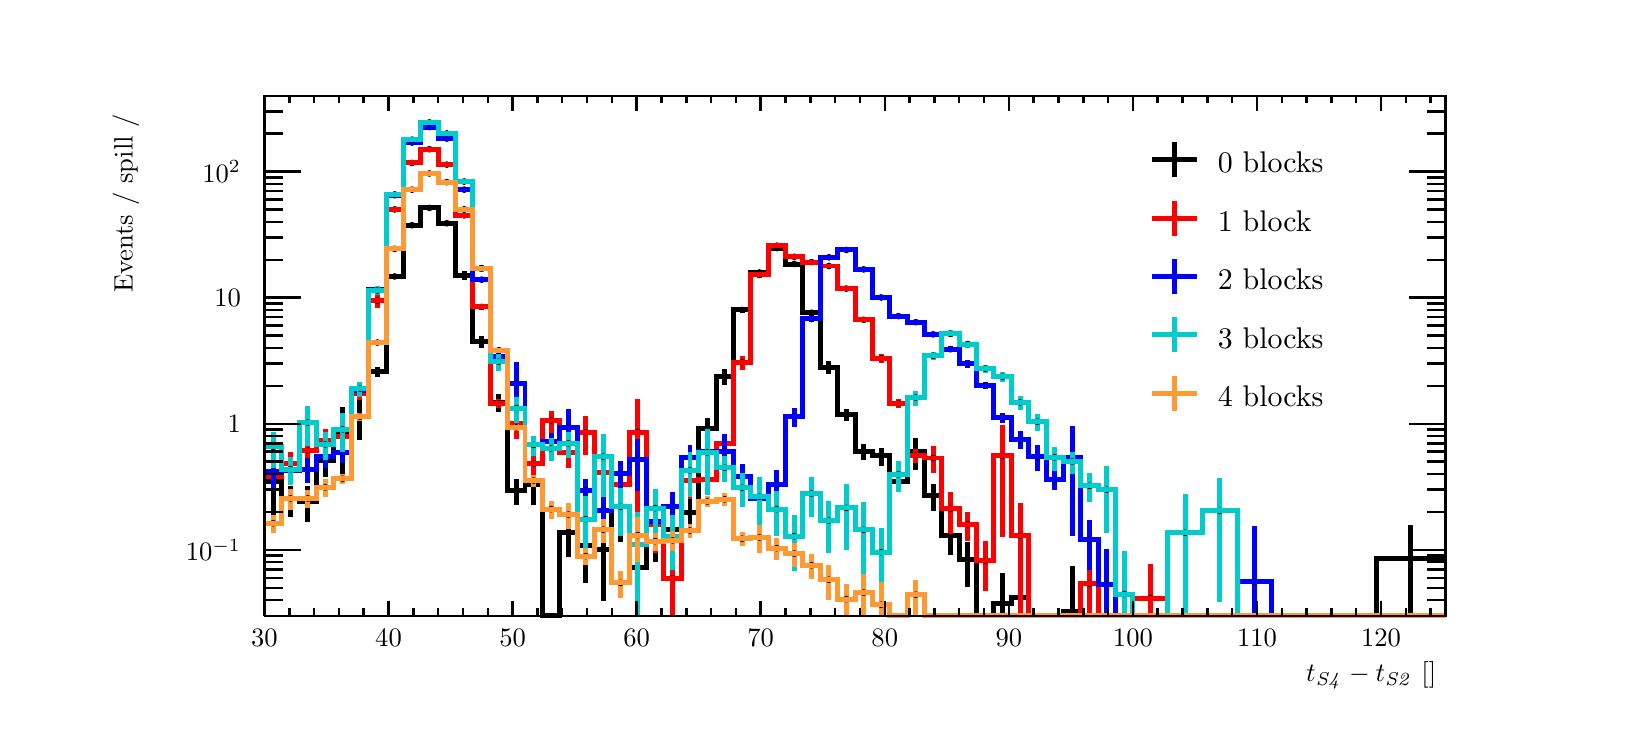
\begin{tikzpicture}
\pgfdeclareplotmark{cross} {
\pgfpathmoveto{\pgfpoint{-0.3\pgfplotmarksize}{\pgfplotmarksize}}
\pgfpathlineto{\pgfpoint{+0.3\pgfplotmarksize}{\pgfplotmarksize}}
\pgfpathlineto{\pgfpoint{+0.3\pgfplotmarksize}{0.3\pgfplotmarksize}}
\pgfpathlineto{\pgfpoint{+1\pgfplotmarksize}{0.3\pgfplotmarksize}}
\pgfpathlineto{\pgfpoint{+1\pgfplotmarksize}{-0.3\pgfplotmarksize}}
\pgfpathlineto{\pgfpoint{+0.3\pgfplotmarksize}{-0.3\pgfplotmarksize}}
\pgfpathlineto{\pgfpoint{+0.3\pgfplotmarksize}{-1.\pgfplotmarksize}}
\pgfpathlineto{\pgfpoint{-0.3\pgfplotmarksize}{-1.\pgfplotmarksize}}
\pgfpathlineto{\pgfpoint{-0.3\pgfplotmarksize}{-0.3\pgfplotmarksize}}
\pgfpathlineto{\pgfpoint{-1.\pgfplotmarksize}{-0.3\pgfplotmarksize}}
\pgfpathlineto{\pgfpoint{-1.\pgfplotmarksize}{0.3\pgfplotmarksize}}
\pgfpathlineto{\pgfpoint{-0.3\pgfplotmarksize}{0.3\pgfplotmarksize}}
\pgfpathclose
\pgfusepathqstroke
}
\pgfdeclareplotmark{cross*} {
\pgfpathmoveto{\pgfpoint{-0.3\pgfplotmarksize}{\pgfplotmarksize}}
\pgfpathlineto{\pgfpoint{+0.3\pgfplotmarksize}{\pgfplotmarksize}}
\pgfpathlineto{\pgfpoint{+0.3\pgfplotmarksize}{0.3\pgfplotmarksize}}
\pgfpathlineto{\pgfpoint{+1\pgfplotmarksize}{0.3\pgfplotmarksize}}
\pgfpathlineto{\pgfpoint{+1\pgfplotmarksize}{-0.3\pgfplotmarksize}}
\pgfpathlineto{\pgfpoint{+0.3\pgfplotmarksize}{-0.3\pgfplotmarksize}}
\pgfpathlineto{\pgfpoint{+0.3\pgfplotmarksize}{-1.\pgfplotmarksize}}
\pgfpathlineto{\pgfpoint{-0.3\pgfplotmarksize}{-1.\pgfplotmarksize}}
\pgfpathlineto{\pgfpoint{-0.3\pgfplotmarksize}{-0.3\pgfplotmarksize}}
\pgfpathlineto{\pgfpoint{-1.\pgfplotmarksize}{-0.3\pgfplotmarksize}}
\pgfpathlineto{\pgfpoint{-1.\pgfplotmarksize}{0.3\pgfplotmarksize}}
\pgfpathlineto{\pgfpoint{-0.3\pgfplotmarksize}{0.3\pgfplotmarksize}}
\pgfpathclose
\pgfusepathqfillstroke
}
\pgfdeclareplotmark{newstar} {
\pgfpathmoveto{\pgfqpoint{0pt}{\pgfplotmarksize}}
\pgfpathlineto{\pgfqpointpolar{44}{0.5\pgfplotmarksize}}
\pgfpathlineto{\pgfqpointpolar{18}{\pgfplotmarksize}}
\pgfpathlineto{\pgfqpointpolar{-20}{0.5\pgfplotmarksize}}
\pgfpathlineto{\pgfqpointpolar{-54}{\pgfplotmarksize}}
\pgfpathlineto{\pgfqpointpolar{-90}{0.5\pgfplotmarksize}}
\pgfpathlineto{\pgfqpointpolar{234}{\pgfplotmarksize}}
\pgfpathlineto{\pgfqpointpolar{198}{0.5\pgfplotmarksize}}
\pgfpathlineto{\pgfqpointpolar{162}{\pgfplotmarksize}}
\pgfpathlineto{\pgfqpointpolar{134}{0.5\pgfplotmarksize}}
\pgfpathclose
\pgfusepathqstroke
}
\pgfdeclareplotmark{newstar*} {
\pgfpathmoveto{\pgfqpoint{0pt}{\pgfplotmarksize}}
\pgfpathlineto{\pgfqpointpolar{44}{0.5\pgfplotmarksize}}
\pgfpathlineto{\pgfqpointpolar{18}{\pgfplotmarksize}}
\pgfpathlineto{\pgfqpointpolar{-20}{0.5\pgfplotmarksize}}
\pgfpathlineto{\pgfqpointpolar{-54}{\pgfplotmarksize}}
\pgfpathlineto{\pgfqpointpolar{-90}{0.5\pgfplotmarksize}}
\pgfpathlineto{\pgfqpointpolar{234}{\pgfplotmarksize}}
\pgfpathlineto{\pgfqpointpolar{198}{0.5\pgfplotmarksize}}
\pgfpathlineto{\pgfqpointpolar{162}{\pgfplotmarksize}}
\pgfpathlineto{\pgfqpointpolar{134}{0.5\pgfplotmarksize}}
\pgfpathclose
\pgfusepathqfillstroke
}
\definecolor{c}{rgb}{1,1,1};
\draw [color=c, fill=c] (0,0) rectangle (20,8.57658);
\draw [color=c, fill=c] (3,1.11495) rectangle (18,7.71892);
\definecolor{c}{rgb}{0,0,0};
\draw [c,line width=0.9] (3,1.11495) -- (3,7.71892) -- (18,7.71892) -- (18,1.11495) -- (3,1.11495);
\definecolor{c}{rgb}{1,1,1};
\draw [color=c, fill=c] (3,1.11495) rectangle (18,7.71892);
\definecolor{c}{rgb}{0,0,0};
\draw [c,line width=0.9] (3,1.11495) -- (3,7.71892) -- (18,7.71892) -- (18,1.11495) -- (3,1.11495);
\draw [c,line width=0.9] (3,1.11495) -- (3.22059,1.11495) -- (3.22059,1.11495) -- (3.44118,1.11495) -- (3.44118,1.11495) -- (3.66176,1.11495) -- (3.66176,1.11495) -- (3.88235,1.11495) -- (3.88235,1.11495) -- (4.10294,1.11495) -- (4.10294,1.11495) --
 (4.32353,1.11495) -- (4.32353,1.11495) -- (4.54412,1.11495) -- (4.54412,1.11495) -- (4.76471,1.11495) -- (4.76471,1.11495) -- (4.98529,1.11495) -- (4.98529,1.11495) -- (5.20588,1.11495) -- (5.20588,1.11495) -- (5.42647,1.11495) -- (5.42647,1.11495)
 -- (5.64706,1.11495) -- (5.64706,1.11495) -- (5.86765,1.11495) -- (5.86765,1.11495) -- (6.08824,1.11495) -- (6.08824,1.11495) -- (6.30882,1.11495) -- (6.30882,1.11495) -- (6.52941,1.11495) -- (6.52941,1.11495) -- (6.75,1.11495) -- (6.75,1.11495) --
 (6.97059,1.11495) -- (6.97059,1.11495) -- (7.19118,1.11495) -- (7.19118,1.11495) -- (7.41176,1.11495) -- (7.41176,1.11495) -- (7.63235,1.11495) -- (7.63235,1.11495) -- (7.85294,1.11495) -- (7.85294,1.11495) -- (8.07353,1.11495) -- (8.07353,1.11495)
 -- (8.29412,1.11495) -- (8.29412,1.11495) -- (8.51471,1.11495) -- (8.51471,1.11495) -- (8.73529,1.11495) -- (8.73529,1.11495) -- (8.95588,1.11495) -- (8.95588,1.11495) -- (9.17647,1.11495) -- (9.17647,1.11495) -- (9.39706,1.11495) --
 (9.39706,1.11495) -- (9.61765,1.11495) -- (9.61765,1.11495) -- (9.83823,1.11495) -- (9.83823,1.11495) -- (10.0588,1.11495) -- (10.0588,1.11495) -- (10.2794,1.11495) -- (10.2794,1.11495) -- (10.5,1.11495) -- (10.5,1.11495) -- (10.7206,1.11495) --
 (10.7206,1.11495) -- (10.9412,1.11495) -- (10.9412,1.11495) -- (11.1618,1.11495) -- (11.1618,1.11495) -- (11.3824,1.11495) -- (11.3824,1.11495) -- (11.6029,1.11495) -- (11.6029,1.11495) -- (11.8235,1.11495) -- (11.8235,1.11495) -- (12.0441,1.11495)
 -- (12.0441,1.11495) -- (12.2647,1.11495) -- (12.2647,1.11495) -- (12.4853,1.11495) -- (12.4853,1.11495) -- (12.7059,1.11495) -- (12.7059,1.11495) -- (12.9265,1.11495) -- (12.9265,1.11495) -- (13.1471,1.11495) -- (13.1471,1.11495) --
 (13.3676,1.11495) -- (13.3676,1.11495) -- (13.5882,1.11495) -- (13.5882,1.11495) -- (13.8088,1.11495) -- (13.8088,1.11495) -- (14.0294,1.11495) -- (14.0294,1.11495) -- (14.4706,1.11495) -- (14.4706,1.11495) -- (14.9118,1.11495) -- (14.9118,1.11495)
 -- (15.3529,1.11495) -- (15.3529,1.11495) -- (15.7941,1.11495) -- (15.7941,1.11495) -- (16.2353,1.11495) -- (16.2353,1.11495) -- (17.1176,1.11495) -- (17.1176,1.11495) -- (18,1.11495);
\draw [c,line width=0.9] (3,1.11495) -- (18,1.11495);
\draw [c,line width=0.9] (3,1.30793) -- (3,1.11495);
\draw [c,line width=0.9] (3.31513,1.21144) -- (3.31513,1.11495);
\draw [c,line width=0.9] (3.63025,1.21144) -- (3.63025,1.11495);
\draw [c,line width=0.9] (3.94538,1.21144) -- (3.94538,1.11495);
\draw [c,line width=0.9] (4.2605,1.21144) -- (4.2605,1.11495);
\draw [c,line width=0.9] (4.57563,1.30793) -- (4.57563,1.11495);
\draw [c,line width=0.9] (4.89076,1.21144) -- (4.89076,1.11495);
\draw [c,line width=0.9] (5.20588,1.21144) -- (5.20588,1.11495);
\draw [c,line width=0.9] (5.52101,1.21144) -- (5.52101,1.11495);
\draw [c,line width=0.9] (5.83613,1.21144) -- (5.83613,1.11495);
\draw [c,line width=0.9] (6.15126,1.30793) -- (6.15126,1.11495);
\draw [c,line width=0.9] (6.46639,1.21144) -- (6.46639,1.11495);
\draw [c,line width=0.9] (6.78151,1.21144) -- (6.78151,1.11495);
\draw [c,line width=0.9] (7.09664,1.21144) -- (7.09664,1.11495);
\draw [c,line width=0.9] (7.41176,1.21144) -- (7.41176,1.11495);
\draw [c,line width=0.9] (7.72689,1.30793) -- (7.72689,1.11495);
\draw [c,line width=0.9] (8.04202,1.21144) -- (8.04202,1.11495);
\draw [c,line width=0.9] (8.35714,1.21144) -- (8.35714,1.11495);
\draw [c,line width=0.9] (8.67227,1.21144) -- (8.67227,1.11495);
\draw [c,line width=0.9] (8.9874,1.21144) -- (8.9874,1.11495);
\draw [c,line width=0.9] (9.30252,1.30793) -- (9.30252,1.11495);
\draw [c,line width=0.9] (9.61765,1.21144) -- (9.61765,1.11495);
\draw [c,line width=0.9] (9.93277,1.21144) -- (9.93277,1.11495);
\draw [c,line width=0.9] (10.2479,1.21144) -- (10.2479,1.11495);
\draw [c,line width=0.9] (10.563,1.21144) -- (10.563,1.11495);
\draw [c,line width=0.9] (10.8782,1.30793) -- (10.8782,1.11495);
\draw [c,line width=0.9] (11.1933,1.21144) -- (11.1933,1.11495);
\draw [c,line width=0.9] (11.5084,1.21144) -- (11.5084,1.11495);
\draw [c,line width=0.9] (11.8235,1.21144) -- (11.8235,1.11495);
\draw [c,line width=0.9] (12.1387,1.21144) -- (12.1387,1.11495);
\draw [c,line width=0.9] (12.4538,1.30793) -- (12.4538,1.11495);
\draw [c,line width=0.9] (12.7689,1.21144) -- (12.7689,1.11495);
\draw [c,line width=0.9] (13.084,1.21144) -- (13.084,1.11495);
\draw [c,line width=0.9] (13.3992,1.21144) -- (13.3992,1.11495);
\draw [c,line width=0.9] (13.7143,1.21144) -- (13.7143,1.11495);
\draw [c,line width=0.9] (14.0294,1.30793) -- (14.0294,1.11495);
\draw [c,line width=0.9] (14.3445,1.21144) -- (14.3445,1.11495);
\draw [c,line width=0.9] (14.6597,1.21144) -- (14.6597,1.11495);
\draw [c,line width=0.9] (14.9748,1.21144) -- (14.9748,1.11495);
\draw [c,line width=0.9] (15.2899,1.21144) -- (15.2899,1.11495);
\draw [c,line width=0.9] (15.605,1.30793) -- (15.605,1.11495);
\draw [c,line width=0.9] (15.9202,1.21144) -- (15.9202,1.11495);
\draw [c,line width=0.9] (16.2353,1.21144) -- (16.2353,1.11495);
\draw [c,line width=0.9] (16.5504,1.21144) -- (16.5504,1.11495);
\draw [c,line width=0.9] (16.8655,1.21144) -- (16.8655,1.11495);
\draw [c,line width=0.9] (17.1807,1.30793) -- (17.1807,1.11495);
\draw [c,line width=0.9] (17.1807,1.30793) -- (17.1807,1.11495);
\draw [c,line width=0.9] (17.4958,1.21144) -- (17.4958,1.11495);
\draw [c,line width=0.9] (17.8109,1.21144) -- (17.8109,1.11495);
\draw [anchor=base] (3,0.729009) node[scale=0.960419, color=c, rotate=0]{30};
\draw [anchor=base] (4.57563,0.729009) node[scale=0.960419, color=c, rotate=0]{40};
\draw [anchor=base] (6.15126,0.729009) node[scale=0.960419, color=c, rotate=0]{50};
\draw [anchor=base] (7.72689,0.729009) node[scale=0.960419, color=c, rotate=0]{60};
\draw [anchor=base] (9.30252,0.729009) node[scale=0.960419, color=c, rotate=0]{70};
\draw [anchor=base] (10.8782,0.729009) node[scale=0.960419, color=c, rotate=0]{80};
\draw [anchor=base] (12.4538,0.729009) node[scale=0.960419, color=c, rotate=0]{90};
\draw [anchor=base] (14.0294,0.729009) node[scale=0.960419, color=c, rotate=0]{100};
\draw [anchor=base] (15.605,0.729009) node[scale=0.960419, color=c, rotate=0]{110};
\draw [anchor=base] (17.1807,0.729009) node[scale=0.960419, color=c, rotate=0]{120};
\draw [anchor= east] (18,0.360216) node[scale=0.960419, color=c, rotate=0]{$t_{\SFour} - t_{\STwo}$ [\si{\nano\second}] };
\draw [c,line width=0.9] (3,7.71892) -- (18,7.71892);
\draw [c,line width=0.9] (3,7.52595) -- (3,7.71892);
\draw [c,line width=0.9] (3.31513,7.62243) -- (3.31513,7.71892);
\draw [c,line width=0.9] (3.63025,7.62243) -- (3.63025,7.71892);
\draw [c,line width=0.9] (3.94538,7.62243) -- (3.94538,7.71892);
\draw [c,line width=0.9] (4.2605,7.62243) -- (4.2605,7.71892);
\draw [c,line width=0.9] (4.57563,7.52595) -- (4.57563,7.71892);
\draw [c,line width=0.9] (4.89076,7.62243) -- (4.89076,7.71892);
\draw [c,line width=0.9] (5.20588,7.62243) -- (5.20588,7.71892);
\draw [c,line width=0.9] (5.52101,7.62243) -- (5.52101,7.71892);
\draw [c,line width=0.9] (5.83613,7.62243) -- (5.83613,7.71892);
\draw [c,line width=0.9] (6.15126,7.52595) -- (6.15126,7.71892);
\draw [c,line width=0.9] (6.46639,7.62243) -- (6.46639,7.71892);
\draw [c,line width=0.9] (6.78151,7.62243) -- (6.78151,7.71892);
\draw [c,line width=0.9] (7.09664,7.62243) -- (7.09664,7.71892);
\draw [c,line width=0.9] (7.41176,7.62243) -- (7.41176,7.71892);
\draw [c,line width=0.9] (7.72689,7.52595) -- (7.72689,7.71892);
\draw [c,line width=0.9] (8.04202,7.62243) -- (8.04202,7.71892);
\draw [c,line width=0.9] (8.35714,7.62243) -- (8.35714,7.71892);
\draw [c,line width=0.9] (8.67227,7.62243) -- (8.67227,7.71892);
\draw [c,line width=0.9] (8.9874,7.62243) -- (8.9874,7.71892);
\draw [c,line width=0.9] (9.30252,7.52595) -- (9.30252,7.71892);
\draw [c,line width=0.9] (9.61765,7.62243) -- (9.61765,7.71892);
\draw [c,line width=0.9] (9.93277,7.62243) -- (9.93277,7.71892);
\draw [c,line width=0.9] (10.2479,7.62243) -- (10.2479,7.71892);
\draw [c,line width=0.9] (10.563,7.62243) -- (10.563,7.71892);
\draw [c,line width=0.9] (10.8782,7.52595) -- (10.8782,7.71892);
\draw [c,line width=0.9] (11.1933,7.62243) -- (11.1933,7.71892);
\draw [c,line width=0.9] (11.5084,7.62243) -- (11.5084,7.71892);
\draw [c,line width=0.9] (11.8235,7.62243) -- (11.8235,7.71892);
\draw [c,line width=0.9] (12.1387,7.62243) -- (12.1387,7.71892);
\draw [c,line width=0.9] (12.4538,7.52595) -- (12.4538,7.71892);
\draw [c,line width=0.9] (12.7689,7.62243) -- (12.7689,7.71892);
\draw [c,line width=0.9] (13.084,7.62243) -- (13.084,7.71892);
\draw [c,line width=0.9] (13.3992,7.62243) -- (13.3992,7.71892);
\draw [c,line width=0.9] (13.7143,7.62243) -- (13.7143,7.71892);
\draw [c,line width=0.9] (14.0294,7.52595) -- (14.0294,7.71892);
\draw [c,line width=0.9] (14.3445,7.62243) -- (14.3445,7.71892);
\draw [c,line width=0.9] (14.6597,7.62243) -- (14.6597,7.71892);
\draw [c,line width=0.9] (14.9748,7.62243) -- (14.9748,7.71892);
\draw [c,line width=0.9] (15.2899,7.62243) -- (15.2899,7.71892);
\draw [c,line width=0.9] (15.605,7.52595) -- (15.605,7.71892);
\draw [c,line width=0.9] (15.9202,7.62243) -- (15.9202,7.71892);
\draw [c,line width=0.9] (16.2353,7.62243) -- (16.2353,7.71892);
\draw [c,line width=0.9] (16.5504,7.62243) -- (16.5504,7.71892);
\draw [c,line width=0.9] (16.8655,7.62243) -- (16.8655,7.71892);
\draw [c,line width=0.9] (17.1807,7.52595) -- (17.1807,7.71892);
\draw [c,line width=0.9] (17.1807,7.52595) -- (17.1807,7.71892);
\draw [c,line width=0.9] (17.4958,7.62243) -- (17.4958,7.71892);
\draw [c,line width=0.9] (17.8109,7.62243) -- (17.8109,7.71892);
\draw [c,line width=0.9] (3,1.11495) -- (3,7.71892);
\draw [c,line width=0.9] (3.231,1.11496) -- (3,1.11496);
\draw [c,line width=0.9] (3.231,1.31498) -- (3,1.31498);
\draw [c,line width=0.9] (3.231,1.47013) -- (3,1.47013);
\draw [c,line width=0.9] (3.231,1.5969) -- (3,1.5969);
\draw [c,line width=0.9] (3.231,1.70408) -- (3,1.70408);
\draw [c,line width=0.9] (3.231,1.79693) -- (3,1.79693);
\draw [c,line width=0.9] (3.231,1.87882) -- (3,1.87882);
\draw [c,line width=0.9] (3.462,1.95208) -- (3,1.95208);
\draw [anchor= east] (2.82,1.95208) node[scale=0.960419, color=c, rotate=0]{$10^{-1}$};
\draw [c,line width=0.9] (3.231,2.43402) -- (3,2.43402);
\draw [c,line width=0.9] (3.231,2.71594) -- (3,2.71594);
\draw [c,line width=0.9] (3.231,2.91597) -- (3,2.91597);
\draw [c,line width=0.9] (3.231,3.07112) -- (3,3.07112);
\draw [c,line width=0.9] (3.231,3.19789) -- (3,3.19789);
\draw [c,line width=0.9] (3.231,3.30507) -- (3,3.30507);
\draw [c,line width=0.9] (3.231,3.39791) -- (3,3.39791);
\draw [c,line width=0.9] (3.231,3.4798) -- (3,3.4798);
\draw [c,line width=0.9] (3.462,3.55306) -- (3,3.55306);
\draw [anchor= east] (2.82,3.55306) node[scale=0.960419, color=c, rotate=0]{1};
\draw [c,line width=0.9] (3.231,4.03501) -- (3,4.03501);
\draw [c,line width=0.9] (3.231,4.31693) -- (3,4.31693);
\draw [c,line width=0.9] (3.231,4.51695) -- (3,4.51695);
\draw [c,line width=0.9] (3.231,4.6721) -- (3,4.6721);
\draw [c,line width=0.9] (3.231,4.79887) -- (3,4.79887);
\draw [c,line width=0.9] (3.231,4.90605) -- (3,4.90605);
\draw [c,line width=0.9] (3.231,4.99889) -- (3,4.99889);
\draw [c,line width=0.9] (3.231,5.08079) -- (3,5.08079);
\draw [c,line width=0.9] (3.462,5.15405) -- (3,5.15405);
\draw [anchor= east] (2.82,5.15405) node[scale=0.960419, color=c, rotate=0]{10};
\draw [c,line width=0.9] (3.231,5.63599) -- (3,5.63599);
\draw [c,line width=0.9] (3.231,5.91791) -- (3,5.91791);
\draw [c,line width=0.9] (3.231,6.11793) -- (3,6.11793);
\draw [c,line width=0.9] (3.231,6.27309) -- (3,6.27309);
\draw [c,line width=0.9] (3.231,6.39985) -- (3,6.39985);
\draw [c,line width=0.9] (3.231,6.50703) -- (3,6.50703);
\draw [c,line width=0.9] (3.231,6.59988) -- (3,6.59988);
\draw [c,line width=0.9] (3.231,6.68177) -- (3,6.68177);
\draw [c,line width=0.9] (3.462,6.75503) -- (3,6.75503);
\draw [anchor= east] (2.82,6.75503) node[scale=0.960419, color=c, rotate=0]{$10^{2}$};
\draw [c,line width=0.9] (3.231,7.23697) -- (3,7.23697);
\draw [c,line width=0.9] (3.231,7.51889) -- (3,7.51889);
\draw [c,line width=0.9] (3.231,7.71892) -- (3,7.71892);
\draw [anchor= east] (1.24,7.71892) node[scale=0.960419, color=c, rotate=90]{ Events / spill / \si{\nano\second} };
\draw [c,line width=0.9] (18,1.11495) -- (18,7.71892);
\draw [c,line width=0.9] (17.769,1.11496) -- (18,1.11496);
\draw [c,line width=0.9] (17.769,1.31498) -- (18,1.31498);
\draw [c,line width=0.9] (17.769,1.47013) -- (18,1.47013);
\draw [c,line width=0.9] (17.769,1.5969) -- (18,1.5969);
\draw [c,line width=0.9] (17.769,1.70408) -- (18,1.70408);
\draw [c,line width=0.9] (17.769,1.79693) -- (18,1.79693);
\draw [c,line width=0.9] (17.769,1.87882) -- (18,1.87882);
\draw [c,line width=0.9] (17.538,1.95208) -- (18,1.95208);
\draw [c,line width=0.9] (17.769,2.43402) -- (18,2.43402);
\draw [c,line width=0.9] (17.769,2.71594) -- (18,2.71594);
\draw [c,line width=0.9] (17.769,2.91597) -- (18,2.91597);
\draw [c,line width=0.9] (17.769,3.07112) -- (18,3.07112);
\draw [c,line width=0.9] (17.769,3.19789) -- (18,3.19789);
\draw [c,line width=0.9] (17.769,3.30507) -- (18,3.30507);
\draw [c,line width=0.9] (17.769,3.39791) -- (18,3.39791);
\draw [c,line width=0.9] (17.769,3.4798) -- (18,3.4798);
\draw [c,line width=0.9] (17.538,3.55306) -- (18,3.55306);
\draw [c,line width=0.9] (17.769,4.03501) -- (18,4.03501);
\draw [c,line width=0.9] (17.769,4.31693) -- (18,4.31693);
\draw [c,line width=0.9] (17.769,4.51695) -- (18,4.51695);
\draw [c,line width=0.9] (17.769,4.6721) -- (18,4.6721);
\draw [c,line width=0.9] (17.769,4.79887) -- (18,4.79887);
\draw [c,line width=0.9] (17.769,4.90605) -- (18,4.90605);
\draw [c,line width=0.9] (17.769,4.99889) -- (18,4.99889);
\draw [c,line width=0.9] (17.769,5.08079) -- (18,5.08079);
\draw [c,line width=0.9] (17.538,5.15405) -- (18,5.15405);
\draw [c,line width=0.9] (17.769,5.63599) -- (18,5.63599);
\draw [c,line width=0.9] (17.769,5.91791) -- (18,5.91791);
\draw [c,line width=0.9] (17.769,6.11793) -- (18,6.11793);
\draw [c,line width=0.9] (17.769,6.27309) -- (18,6.27309);
\draw [c,line width=0.9] (17.769,6.39985) -- (18,6.39985);
\draw [c,line width=0.9] (17.769,6.50703) -- (18,6.50703);
\draw [c,line width=0.9] (17.769,6.59988) -- (18,6.59988);
\draw [c,line width=0.9] (17.769,6.68177) -- (18,6.68177);
\draw [c,line width=0.9] (17.538,6.75503) -- (18,6.75503);
\draw [c,line width=0.9] (17.769,7.23697) -- (18,7.23697);
\draw [c,line width=0.9] (17.769,7.51889) -- (18,7.51889);
\draw [c,line width=0.9] (17.769,7.71892) -- (18,7.71892);
\draw [c,line width=1.8] (3.11029,2.26923) -- (3.11029,2.82229);
\draw [c,line width=1.8] (3.11029,2.82229) -- (3.11029,3.12639);
\foreach \P in {(3.11029,2.82229)}{\draw[mark options={color=c,fill=c},mark size=2.402402pt,mark=*,mark size=1pt] plot coordinates {\P};}
\draw [c,line width=1.8] (3.33088,2.37409) -- (3.33088,2.59778);
\draw [c,line width=1.8] (3.33088,2.59778) -- (3.33088,2.76676);
\foreach \P in {(3.33088,2.59778)}{\draw[mark options={color=c,fill=c},mark size=2.402402pt,mark=*,mark size=1pt] plot coordinates {\P};}
\draw [c,line width=1.8] (3.55147,2.30669) -- (3.55147,2.57217);
\draw [c,line width=1.8] (3.55147,2.57217) -- (3.55147,2.76382);
\foreach \P in {(3.55147,2.57217)}{\draw[mark options={color=c,fill=c},mark size=2.402402pt,mark=*,mark size=1pt] plot coordinates {\P};}
\draw [c,line width=1.8] (3.77206,2.88174) -- (3.77206,3.08666);
\draw [c,line width=1.8] (3.77206,3.08666) -- (3.77206,3.24473);
\foreach \P in {(3.77206,3.08666)}{\draw[mark options={color=c,fill=c},mark size=2.402402pt,mark=*,mark size=1pt] plot coordinates {\P};}
\draw [c,line width=1.8] (3.99265,2.79006) -- (3.99265,3.43347);
\draw [c,line width=1.8] (3.99265,3.43347) -- (3.99265,3.76184);
\foreach \P in {(3.99265,3.43347)}{\draw[mark options={color=c,fill=c},mark size=2.402402pt,mark=*,mark size=1pt] plot coordinates {\P};}
\draw [c,line width=1.8] (4.21324,3.34883) -- (4.21324,3.64918);
\draw [c,line width=1.8] (4.21324,3.64918) -- (4.21324,3.85825);
\foreach \P in {(4.21324,3.64918)}{\draw[mark options={color=c,fill=c},mark size=2.402402pt,mark=*,mark size=1pt] plot coordinates {\P};}
\draw [c,line width=1.8] (4.43382,4.1533) -- (4.43382,4.21931);
\draw [c,line width=1.8] (4.43382,4.21931) -- (4.43382,4.2796);
\foreach \P in {(4.43382,4.21931)}{\draw[mark options={color=c,fill=c},mark size=2.402402pt,mark=*,mark size=1pt] plot coordinates {\P};}
\draw [c,line width=1.8] (4.65441,5.39338) -- (4.65441,5.42411);
\draw [c,line width=1.8] (4.65441,5.42411) -- (4.65441,5.45354);
\foreach \P in {(4.65441,5.42411)}{\draw[mark options={color=c,fill=c},mark size=2.402402pt,mark=*,mark size=1pt] plot coordinates {\P};}
\draw [c,line width=1.8] (4.875,6.05236) -- (4.875,6.07488);
\draw [c,line width=1.8] (4.875,6.07488) -- (4.875,6.09669);
\foreach \P in {(4.875,6.07488)}{\draw[mark options={color=c,fill=c},mark size=2.402402pt,mark=*,mark size=1pt] plot coordinates {\P};}
\draw [c,line width=1.8] (5.09559,6.27165) -- (5.09559,6.29471);
\draw [c,line width=1.8] (5.09559,6.29471) -- (5.09559,6.31704);
\foreach \P in {(5.09559,6.29471)}{\draw[mark options={color=c,fill=c},mark size=2.402402pt,mark=*,mark size=1pt] plot coordinates {\P};}
\draw [c,line width=1.8] (5.31618,6.06723) -- (5.31618,6.09971);
\draw [c,line width=1.8] (5.31618,6.09971) -- (5.31618,6.13074);
\foreach \P in {(5.31618,6.09971)}{\draw[mark options={color=c,fill=c},mark size=2.402402pt,mark=*,mark size=1pt] plot coordinates {\P};}
\draw [c,line width=1.8] (5.53676,5.37726) -- (5.53676,5.44);
\draw [c,line width=1.8] (5.53676,5.44) -- (5.53676,5.49754);
\foreach \P in {(5.53676,5.44)}{\draw[mark options={color=c,fill=c},mark size=2.402402pt,mark=*,mark size=1pt] plot coordinates {\P};}
\draw [c,line width=1.8] (5.75735,4.51797) -- (5.75735,4.59454);
\draw [c,line width=1.8] (5.75735,4.59454) -- (5.75735,4.6635);
\foreach \P in {(5.75735,4.59454)}{\draw[mark options={color=c,fill=c},mark size=2.402402pt,mark=*,mark size=1pt] plot coordinates {\P};}
\draw [c,line width=1.8] (5.97794,3.70553) -- (5.97794,3.82824);
\draw [c,line width=1.8] (5.97794,3.82824) -- (5.97794,3.93252);
\foreach \P in {(5.97794,3.82824)}{\draw[mark options={color=c,fill=c},mark size=2.402402pt,mark=*,mark size=1pt] plot coordinates {\P};}
\draw [c,line width=1.8] (6.19853,2.52351) -- (6.19853,2.70383);
\draw [c,line width=1.8] (6.19853,2.70383) -- (6.19853,2.84689);
\foreach \P in {(6.19853,2.70383)}{\draw[mark options={color=c,fill=c},mark size=2.402402pt,mark=*,mark size=1pt] plot coordinates {\P};}
\draw [c,line width=1.8] (6.41912,2.52127) -- (6.41912,2.77715);
\draw [c,line width=1.8] (6.41912,2.77715) -- (6.41912,2.96378);
\foreach \P in {(6.41912,2.77715)}{\draw[mark options={color=c,fill=c},mark size=2.402402pt,mark=*,mark size=1pt] plot coordinates {\P};}
\draw [c,line width=1.8] (6.86029,1.85983) -- (6.86029,2.17678);
\draw [c,line width=1.8] (6.86029,2.17678) -- (6.86029,2.39369);
\foreach \P in {(6.86029,2.17678)}{\draw[mark options={color=c,fill=c},mark size=2.402402pt,mark=*,mark size=1pt] plot coordinates {\P};}
\draw [c,line width=1.8] (7.08088,1.5305) -- (7.08088,2.01323);
\draw [c,line width=1.8] (7.08088,2.01323) -- (7.08088,2.29541);
\foreach \P in {(7.08088,2.01323)}{\draw[mark options={color=c,fill=c},mark size=2.402402pt,mark=*,mark size=1pt] plot coordinates {\P};}
\draw [c,line width=1.8] (7.30147,1.30845) -- (7.30147,1.96235);
\draw [c,line width=1.8] (7.30147,1.96235) -- (7.30147,2.29328);
\foreach \P in {(7.30147,1.96235)}{\draw[mark options={color=c,fill=c},mark size=2.402402pt,mark=*,mark size=1pt] plot coordinates {\P};}
\draw [c,line width=1.8] (7.52206,2.04972) -- (7.52206,2.49638);
\draw [c,line width=1.8] (7.52206,2.49638) -- (7.52206,2.76613);
\foreach \P in {(7.52206,2.49638)}{\draw[mark options={color=c,fill=c},mark size=2.402402pt,mark=*,mark size=1pt] plot coordinates {\P};}
\draw [c,line width=1.8] (7.74265,1.21582) -- (7.74265,1.72582);
\draw [c,line width=1.8] (7.74265,1.72582) -- (7.74265,2.01685);
\foreach \P in {(7.74265,1.72582)}{\draw[mark options={color=c,fill=c},mark size=2.402402pt,mark=*,mark size=1pt] plot coordinates {\P};}
\draw [c,line width=1.8] (7.96324,1.79441) -- (7.96324,2.28593);
\draw [c,line width=1.8] (7.96324,2.28593) -- (7.96324,2.57101);
\foreach \P in {(7.96324,2.28593)}{\draw[mark options={color=c,fill=c},mark size=2.402402pt,mark=*,mark size=1pt] plot coordinates {\P};}
\draw [c,line width=1.8] (8.18382,1.89925) -- (8.18382,2.21606);
\draw [c,line width=1.8] (8.18382,2.21606) -- (8.18382,2.43289);
\foreach \P in {(8.18382,2.21606)}{\draw[mark options={color=c,fill=c},mark size=2.402402pt,mark=*,mark size=1pt] plot coordinates {\P};}
\draw [c,line width=1.8] (8.40441,2.18956) -- (8.40441,2.42094);
\draw [c,line width=1.8] (8.40441,2.42094) -- (8.40441,2.59425);
\foreach \P in {(8.40441,2.42094)}{\draw[mark options={color=c,fill=c},mark size=2.402402pt,mark=*,mark size=1pt] plot coordinates {\P};}
\draw [c,line width=1.8] (8.625,3.32169) -- (8.625,3.48779);
\draw [c,line width=1.8] (8.625,3.48779) -- (8.625,3.62177);
\foreach \P in {(8.625,3.48779)}{\draw[mark options={color=c,fill=c},mark size=2.402402pt,mark=*,mark size=1pt] plot coordinates {\P};}
\draw [c,line width=1.8] (8.84559,4.046) -- (8.84559,4.15581);
\draw [c,line width=1.8] (8.84559,4.15581) -- (8.84559,4.25062);
\foreach \P in {(8.84559,4.15581)}{\draw[mark options={color=c,fill=c},mark size=2.402402pt,mark=*,mark size=1pt] plot coordinates {\P};}
\draw [c,line width=1.8] (9.06618,4.9546) -- (9.06618,4.99931);
\draw [c,line width=1.8] (9.06618,4.99931) -- (9.06618,5.04132);
\foreach \P in {(9.06618,4.99931)}{\draw[mark options={color=c,fill=c},mark size=2.402402pt,mark=*,mark size=1pt] plot coordinates {\P};}
\draw [c,line width=1.8] (9.28677,5.44468) -- (9.28677,5.47408);
\draw [c,line width=1.8] (9.28677,5.47408) -- (9.28677,5.50229);
\foreach \P in {(9.28677,5.47408)}{\draw[mark options={color=c,fill=c},mark size=2.402402pt,mark=*,mark size=1pt] plot coordinates {\P};}
\draw [c,line width=1.8] (9.50735,5.76328) -- (9.50735,5.785);
\draw [c,line width=1.8] (9.50735,5.785) -- (9.50735,5.80607);
\foreach \P in {(9.50735,5.785)}{\draw[mark options={color=c,fill=c},mark size=2.402402pt,mark=*,mark size=1pt] plot coordinates {\P};}
\draw [c,line width=1.8] (9.72794,5.55883) -- (9.72794,5.58191);
\draw [c,line width=1.8] (9.72794,5.58191) -- (9.72794,5.60424);
\foreach \P in {(9.72794,5.58191)}{\draw[mark options={color=c,fill=c},mark size=2.402402pt,mark=*,mark size=1pt] plot coordinates {\P};}
\draw [c,line width=1.8] (9.94853,4.9256) -- (9.94853,4.96251);
\draw [c,line width=1.8] (9.94853,4.96251) -- (9.94853,4.99756);
\foreach \P in {(9.94853,4.96251)}{\draw[mark options={color=c,fill=c},mark size=2.402402pt,mark=*,mark size=1pt] plot coordinates {\P};}
\draw [c,line width=1.8] (10.1691,4.18793) -- (10.1691,4.27281);
\draw [c,line width=1.8] (10.1691,4.27281) -- (10.1691,4.34846);
\foreach \P in {(10.1691,4.27281)}{\draw[mark options={color=c,fill=c},mark size=2.402402pt,mark=*,mark size=1pt] plot coordinates {\P};}
\draw [c,line width=1.8] (10.3897,3.58544) -- (10.3897,3.66551);
\draw [c,line width=1.8] (10.3897,3.66551) -- (10.3897,3.73731);
\foreach \P in {(10.3897,3.66551)}{\draw[mark options={color=c,fill=c},mark size=2.402402pt,mark=*,mark size=1pt] plot coordinates {\P};}
\draw [c,line width=1.8] (10.6103,3.0982) -- (10.6103,3.20475);
\draw [c,line width=1.8] (10.6103,3.20475) -- (10.6103,3.29713);
\foreach \P in {(10.6103,3.20475)}{\draw[mark options={color=c,fill=c},mark size=2.402402pt,mark=*,mark size=1pt] plot coordinates {\P};}
\draw [c,line width=1.8] (10.8309,3.02288) -- (10.8309,3.14627);
\draw [c,line width=1.8] (10.8309,3.14627) -- (10.8309,3.25103);
\foreach \P in {(10.8309,3.14627)}{\draw[mark options={color=c,fill=c},mark size=2.402402pt,mark=*,mark size=1pt] plot coordinates {\P};}
\draw [c,line width=1.8] (11.0515,2.68649) -- (11.0515,2.82468);
\draw [c,line width=1.8] (11.0515,2.82468) -- (11.0515,2.9399);
\foreach \P in {(11.0515,2.82468)}{\draw[mark options={color=c,fill=c},mark size=2.402402pt,mark=*,mark size=1pt] plot coordinates {\P};}
\draw [c,line width=1.8] (11.2721,2.9717) -- (11.2721,3.20094);
\draw [c,line width=1.8] (11.2721,3.20094) -- (11.2721,3.37305);
\foreach \P in {(11.2721,3.20094)}{\draw[mark options={color=c,fill=c},mark size=2.402402pt,mark=*,mark size=1pt] plot coordinates {\P};}
\draw [c,line width=1.8] (11.4926,2.44675) -- (11.4926,2.63658);
\draw [c,line width=1.8] (11.4926,2.63658) -- (11.4926,2.78554);
\foreach \P in {(11.4926,2.63658)}{\draw[mark options={color=c,fill=c},mark size=2.402402pt,mark=*,mark size=1pt] plot coordinates {\P};}
\draw [c,line width=1.8] (11.7132,1.88029) -- (11.7132,2.13662);
\draw [c,line width=1.8] (11.7132,2.13662) -- (11.7132,2.32349);
\foreach \P in {(11.7132,2.13662)}{\draw[mark options={color=c,fill=c},mark size=2.402402pt,mark=*,mark size=1pt] plot coordinates {\P};}
\draw [c,line width=1.8] (11.9338,1.48647) -- (11.9338,1.82755);
\draw [c,line width=1.8] (11.9338,1.82755) -- (11.9338,2.05537);
\foreach \P in {(11.9338,1.82755)}{\draw[mark options={color=c,fill=c},mark size=2.402402pt,mark=*,mark size=1pt] plot coordinates {\P};}
\draw [c,line width=1.8] (12.375,1.11495) -- (12.375,1.26774);
\draw [c,line width=1.8] (12.375,1.26774) -- (12.375,1.65748);
\foreach \P in {(12.375,1.26774)}{\draw[mark options={color=c,fill=c},mark size=2.402402pt,mark=*,mark size=1pt] plot coordinates {\P};}
\draw [c,line width=1.8] (12.5956,1.11495) -- (12.5956,1.3495);
\draw [c,line width=1.8] (12.5956,1.3495) -- (12.5956,1.71027);
\foreach \P in {(12.5956,1.3495)}{\draw[mark options={color=c,fill=c},mark size=2.402402pt,mark=*,mark size=1pt] plot coordinates {\P};}
\draw [c,line width=1.8] (13.2574,1.11495) -- (13.2574,1.17392);
\draw [c,line width=1.8] (13.2574,1.17392) -- (13.2574,1.74136);
\foreach \P in {(13.2574,1.17392)}{\draw[mark options={color=c,fill=c},mark size=2.402402pt,mark=*,mark size=1pt] plot coordinates {\P};}
\draw [c,line width=1.8] (17.5588,1.11495) -- (17.5588,1.8481);
\draw [c,line width=1.8] (17.5588,1.8481) -- (17.5588,2.26717);
\foreach \P in {(17.5588,1.8481)}{\draw[mark options={color=c,fill=c},mark size=2.402402pt,mark=*,mark size=1pt] plot coordinates {\P};}
\draw [c,line width=1.8] (3,2.82229) -- (3.22059,2.82229) -- (3.22059,2.59778) -- (3.44118,2.59778) -- (3.44118,2.57217) -- (3.66176,2.57217) -- (3.66176,3.08666) -- (3.88235,3.08666) -- (3.88235,3.43347) -- (4.10294,3.43347) -- (4.10294,3.64918) --
 (4.32353,3.64918) -- (4.32353,4.21931) -- (4.54412,4.21931) -- (4.54412,5.42411) -- (4.76471,5.42411) -- (4.76471,6.07488) -- (4.98529,6.07488) -- (4.98529,6.29471) -- (5.20588,6.29471) -- (5.20588,6.09971) -- (5.42647,6.09971) -- (5.42647,5.44) --
 (5.64706,5.44) -- (5.64706,4.59454) -- (5.86765,4.59454) -- (5.86765,3.82824) -- (6.08824,3.82824) -- (6.08824,2.70383) -- (6.30882,2.70383) -- (6.30882,2.77715) -- (6.52941,2.77715) -- (6.52941,1.11495) -- (6.75,1.11495) -- (6.75,2.17678) --
 (6.97059,2.17678) -- (6.97059,2.01323) -- (7.19118,2.01323) -- (7.19118,1.96235) -- (7.41176,1.96235) -- (7.41176,2.49638) -- (7.63235,2.49638) -- (7.63235,1.72582) -- (7.85294,1.72582) -- (7.85294,2.28593) -- (8.07353,2.28593) -- (8.07353,2.21606)
 -- (8.29412,2.21606) -- (8.29412,2.42094) -- (8.51471,2.42094) -- (8.51471,3.48779) -- (8.73529,3.48779) -- (8.73529,4.15581) -- (8.95588,4.15581) -- (8.95588,4.99931) -- (9.17647,4.99931) -- (9.17647,5.47408) -- (9.39706,5.47408) -- (9.39706,5.785)
 -- (9.61765,5.785) -- (9.61765,5.58191) -- (9.83823,5.58191) -- (9.83823,4.96251) -- (10.0588,4.96251) -- (10.0588,4.27281) -- (10.2794,4.27281) -- (10.2794,3.66551) -- (10.5,3.66551) -- (10.5,3.20475) -- (10.7206,3.20475) -- (10.7206,3.14627) --
 (10.9412,3.14627) -- (10.9412,2.82468) -- (11.1618,2.82468) -- (11.1618,3.20094) -- (11.3824,3.20094) -- (11.3824,2.63658) -- (11.6029,2.63658) -- (11.6029,2.13662) -- (11.8235,2.13662) -- (11.8235,1.82755) -- (12.0441,1.82755) -- (12.0441,1.11495)
 -- (12.2647,1.11495) -- (12.2647,1.26774) -- (12.4853,1.26774) -- (12.4853,1.3495) -- (12.7059,1.3495) -- (12.7059,1.11495) -- (12.9265,1.11495) -- (12.9265,1.11495) -- (13.1471,1.11495) -- (13.1471,1.17392) -- (13.3676,1.17392) -- (13.3676,1.11495)
 -- (13.5882,1.11495) -- (13.5882,1.11495) -- (13.8088,1.11495) -- (13.8088,1.11495) -- (14.0294,1.11495) -- (14.0294,1.11495) -- (14.4706,1.11495) -- (14.4706,1.11495) -- (14.9118,1.11495) -- (14.9118,1.11495) -- (15.3529,1.11495) --
 (15.3529,1.11495) -- (15.7941,1.11495) -- (15.7941,1.11495) -- (16.2353,1.11495) -- (16.2353,1.11495) -- (17.1176,1.11495) -- (17.1176,1.8481) -- (18,1.8481);
\definecolor{c}{rgb}{1,0,0};
\draw [c,line width=1.8] (3.11029,2.71412) -- (3.11029,2.88562);
\draw [c,line width=1.8] (3.11029,2.88562) -- (3.11029,3.02308);
\definecolor{c}{rgb}{0,0,0};
\foreach \P in {(3.11029,2.88562)}{\draw[mark options={color=c,fill=c},mark size=2.402402pt,mark=*,mark size=1pt] plot coordinates {\P};}
\definecolor{c}{rgb}{1,0,0};
\draw [c,line width=1.8] (3.33088,2.88333) -- (3.33088,3.05475);
\draw [c,line width=1.8] (3.33088,3.05475) -- (3.33088,3.19215);
\definecolor{c}{rgb}{0,0,0};
\foreach \P in {(3.33088,3.05475)}{\draw[mark options={color=c,fill=c},mark size=2.402402pt,mark=*,mark size=1pt] plot coordinates {\P};}
\definecolor{c}{rgb}{1,0,0};
\draw [c,line width=1.8] (3.55147,3.00538) -- (3.55147,3.2134);
\draw [c,line width=1.8] (3.55147,3.2134) -- (3.55147,3.37331);
\definecolor{c}{rgb}{0,0,0};
\foreach \P in {(3.55147,3.2134)}{\draw[mark options={color=c,fill=c},mark size=2.402402pt,mark=*,mark size=1pt] plot coordinates {\P};}
\definecolor{c}{rgb}{1,0,0};
\draw [c,line width=1.8] (3.77206,3.15551) -- (3.77206,3.3392);
\draw [c,line width=1.8] (3.77206,3.3392) -- (3.77206,3.48436);
\definecolor{c}{rgb}{0,0,0};
\foreach \P in {(3.77206,3.3392)}{\draw[mark options={color=c,fill=c},mark size=2.402402pt,mark=*,mark size=1pt] plot coordinates {\P};}
\definecolor{c}{rgb}{1,0,0};
\draw [c,line width=1.8] (3.99265,3.25939) -- (3.99265,3.39409);
\draw [c,line width=1.8] (3.99265,3.39409) -- (3.99265,3.50688);
\definecolor{c}{rgb}{0,0,0};
\foreach \P in {(3.99265,3.39409)}{\draw[mark options={color=c,fill=c},mark size=2.402402pt,mark=*,mark size=1pt] plot coordinates {\P};}
\definecolor{c}{rgb}{1,0,0};
\draw [c,line width=1.8] (4.21324,3.85533) -- (4.21324,3.93812);
\draw [c,line width=1.8] (4.21324,3.93812) -- (4.21324,4.0121);
\definecolor{c}{rgb}{0,0,0};
\foreach \P in {(4.21324,3.93812)}{\draw[mark options={color=c,fill=c},mark size=2.402402pt,mark=*,mark size=1pt] plot coordinates {\P};}
\definecolor{c}{rgb}{1,0,0};
\draw [c,line width=1.8] (4.43382,5.02911) -- (4.43382,5.11608);
\draw [c,line width=1.8] (4.43382,5.11608) -- (4.43382,5.19336);
\definecolor{c}{rgb}{0,0,0};
\foreach \P in {(4.43382,5.11608)}{\draw[mark options={color=c,fill=c},mark size=2.402402pt,mark=*,mark size=1pt] plot coordinates {\P};}
\definecolor{c}{rgb}{1,0,0};
\draw [c,line width=1.8] (4.65441,6.26035) -- (4.65441,6.27555);
\draw [c,line width=1.8] (4.65441,6.27555) -- (4.65441,6.29043);
\definecolor{c}{rgb}{0,0,0};
\foreach \P in {(4.65441,6.27555)}{\draw[mark options={color=c,fill=c},mark size=2.402402pt,mark=*,mark size=1pt] plot coordinates {\P};}
\definecolor{c}{rgb}{1,0,0};
\draw [c,line width=1.8] (4.875,6.85481) -- (4.875,6.86533);
\draw [c,line width=1.8] (4.875,6.86533) -- (4.875,6.87568);
\definecolor{c}{rgb}{0,0,0};
\foreach \P in {(4.875,6.86533)}{\draw[mark options={color=c,fill=c},mark size=2.402402pt,mark=*,mark size=1pt] plot coordinates {\P};}
\definecolor{c}{rgb}{1,0,0};
\draw [c,line width=1.8] (5.09559,7.02954) -- (5.09559,7.03995);
\draw [c,line width=1.8] (5.09559,7.03995) -- (5.09559,7.05019);
\definecolor{c}{rgb}{0,0,0};
\foreach \P in {(5.09559,7.03995)}{\draw[mark options={color=c,fill=c},mark size=2.402402pt,mark=*,mark size=1pt] plot coordinates {\P};}
\definecolor{c}{rgb}{1,0,0};
\draw [c,line width=1.8] (5.31618,6.83243) -- (5.31618,6.84397);
\draw [c,line width=1.8] (5.31618,6.84397) -- (5.31618,6.85533);
\definecolor{c}{rgb}{0,0,0};
\foreach \P in {(5.31618,6.84397)}{\draw[mark options={color=c,fill=c},mark size=2.402402pt,mark=*,mark size=1pt] plot coordinates {\P};}
\definecolor{c}{rgb}{1,0,0};
\draw [c,line width=1.8] (5.53676,6.17868) -- (5.53676,6.20009);
\draw [c,line width=1.8] (5.53676,6.20009) -- (5.53676,6.22086);
\definecolor{c}{rgb}{0,0,0};
\foreach \P in {(5.53676,6.20009)}{\draw[mark options={color=c,fill=c},mark size=2.402402pt,mark=*,mark size=1pt] plot coordinates {\P};}
\definecolor{c}{rgb}{1,0,0};
\draw [c,line width=1.8] (5.75735,4.99306) -- (5.75735,5.03744);
\draw [c,line width=1.8] (5.75735,5.03744) -- (5.75735,5.07916);
\definecolor{c}{rgb}{0,0,0};
\foreach \P in {(5.75735,5.03744)}{\draw[mark options={color=c,fill=c},mark size=2.402402pt,mark=*,mark size=1pt] plot coordinates {\P};}
\definecolor{c}{rgb}{1,0,0};
\draw [c,line width=1.8] (5.97794,3.75491) -- (5.97794,3.81246);
\draw [c,line width=1.8] (5.97794,3.81246) -- (5.97794,3.86561);
\definecolor{c}{rgb}{0,0,0};
\foreach \P in {(5.97794,3.81246)}{\draw[mark options={color=c,fill=c},mark size=2.402402pt,mark=*,mark size=1pt] plot coordinates {\P};}
\definecolor{c}{rgb}{1,0,0};
\draw [c,line width=1.8] (6.19853,3.36445) -- (6.19853,3.55317);
\draw [c,line width=1.8] (6.19853,3.55317) -- (6.19853,3.70145);
\definecolor{c}{rgb}{0,0,0};
\foreach \P in {(6.19853,3.55317)}{\draw[mark options={color=c,fill=c},mark size=2.402402pt,mark=*,mark size=1pt] plot coordinates {\P};}
\definecolor{c}{rgb}{1,0,0};
\draw [c,line width=1.8] (6.41912,2.88255) -- (6.41912,3.04938);
\draw [c,line width=1.8] (6.41912,3.04938) -- (6.41912,3.18382);
\definecolor{c}{rgb}{0,0,0};
\foreach \P in {(6.41912,3.04938)}{\draw[mark options={color=c,fill=c},mark size=2.402402pt,mark=*,mark size=1pt] plot coordinates {\P};}
\definecolor{c}{rgb}{1,0,0};
\draw [c,line width=1.8] (6.63971,3.43865) -- (6.63971,3.59429);
\draw [c,line width=1.8] (6.63971,3.59429) -- (6.63971,3.72139);
\definecolor{c}{rgb}{0,0,0};
\foreach \P in {(6.63971,3.59429)}{\draw[mark options={color=c,fill=c},mark size=2.402402pt,mark=*,mark size=1pt] plot coordinates {\P};}
\definecolor{c}{rgb}{1,0,0};
\draw [c,line width=1.8] (6.86029,2.99218) -- (6.86029,3.19349);
\draw [c,line width=1.8] (6.86029,3.19349) -- (6.86029,3.34941);
\definecolor{c}{rgb}{0,0,0};
\foreach \P in {(6.86029,3.19349)}{\draw[mark options={color=c,fill=c},mark size=2.402402pt,mark=*,mark size=1pt] plot coordinates {\P};}
\definecolor{c}{rgb}{1,0,0};
\draw [c,line width=1.8] (7.08088,3.15114) -- (7.08088,3.44459);
\draw [c,line width=1.8] (7.08088,3.44459) -- (7.08088,3.65031);
\definecolor{c}{rgb}{0,0,0};
\foreach \P in {(7.08088,3.44459)}{\draw[mark options={color=c,fill=c},mark size=2.402402pt,mark=*,mark size=1pt] plot coordinates {\P};}
\definecolor{c}{rgb}{1,0,0};
\draw [c,line width=1.8] (7.30147,2.546) -- (7.30147,2.92891);
\draw [c,line width=1.8] (7.30147,2.92891) -- (7.30147,3.17441);
\definecolor{c}{rgb}{0,0,0};
\foreach \P in {(7.30147,2.92891)}{\draw[mark options={color=c,fill=c},mark size=2.402402pt,mark=*,mark size=1pt] plot coordinates {\P};}
\definecolor{c}{rgb}{1,0,0};
\draw [c,line width=1.8] (7.52206,2.45431) -- (7.52206,2.78191);
\draw [c,line width=1.8] (7.52206,2.78191) -- (7.52206,3.00371);
\definecolor{c}{rgb}{0,0,0};
\foreach \P in {(7.52206,2.78191)}{\draw[mark options={color=c,fill=c},mark size=2.402402pt,mark=*,mark size=1pt] plot coordinates {\P};}
\definecolor{c}{rgb}{1,0,0};
\draw [c,line width=1.8] (7.74265,2.27004) -- (7.74265,3.44782);
\draw [c,line width=1.8] (7.74265,3.44782) -- (7.74265,3.86274);
\definecolor{c}{rgb}{0,0,0};
\foreach \P in {(7.74265,3.44782)}{\draw[mark options={color=c,fill=c},mark size=2.402402pt,mark=*,mark size=1pt] plot coordinates {\P};}
\definecolor{c}{rgb}{1,0,0};
\draw [c,line width=1.8] (7.96324,1.91512) -- (7.96324,2.27835);
\draw [c,line width=1.8] (7.96324,2.27835) -- (7.96324,2.51572);
\definecolor{c}{rgb}{0,0,0};
\foreach \P in {(7.96324,2.27835)}{\draw[mark options={color=c,fill=c},mark size=2.402402pt,mark=*,mark size=1pt] plot coordinates {\P};}
\definecolor{c}{rgb}{1,0,0};
\draw [c,line width=1.8] (8.18382,1.13032) -- (8.18382,1.59016);
\draw [c,line width=1.8] (8.18382,1.59016) -- (8.18382,1.86455);
\definecolor{c}{rgb}{0,0,0};
\foreach \P in {(8.18382,1.59016)}{\draw[mark options={color=c,fill=c},mark size=2.402402pt,mark=*,mark size=1pt] plot coordinates {\P};}
\definecolor{c}{rgb}{1,0,0};
\draw [c,line width=1.8] (8.40441,2.60151) -- (8.40441,2.83074);
\draw [c,line width=1.8] (8.40441,2.83074) -- (8.40441,3.00285);
\definecolor{c}{rgb}{0,0,0};
\foreach \P in {(8.40441,2.83074)}{\draw[mark options={color=c,fill=c},mark size=2.402402pt,mark=*,mark size=1pt] plot coordinates {\P};}
\definecolor{c}{rgb}{1,0,0};
\draw [c,line width=1.8] (8.625,2.70188) -- (8.625,2.84878);
\draw [c,line width=1.8] (8.625,2.84878) -- (8.625,2.97);
\definecolor{c}{rgb}{0,0,0};
\foreach \P in {(8.625,2.84878)}{\draw[mark options={color=c,fill=c},mark size=2.402402pt,mark=*,mark size=1pt] plot coordinates {\P};}
\definecolor{c}{rgb}{1,0,0};
\draw [c,line width=1.8] (8.84559,3.17714) -- (8.84559,3.30578);
\draw [c,line width=1.8] (8.84559,3.30578) -- (8.84559,3.41429);
\definecolor{c}{rgb}{0,0,0};
\foreach \P in {(8.84559,3.30578)}{\draw[mark options={color=c,fill=c},mark size=2.402402pt,mark=*,mark size=1pt] plot coordinates {\P};}
\definecolor{c}{rgb}{1,0,0};
\draw [c,line width=1.8] (9.06618,4.23908) -- (9.06618,4.33337);
\draw [c,line width=1.8] (9.06618,4.33337) -- (9.06618,4.41639);
\definecolor{c}{rgb}{0,0,0};
\foreach \P in {(9.06618,4.33337)}{\draw[mark options={color=c,fill=c},mark size=2.402402pt,mark=*,mark size=1pt] plot coordinates {\P};}
\definecolor{c}{rgb}{1,0,0};
\draw [c,line width=1.8] (9.28677,5.40766) -- (9.28677,5.44464);
\draw [c,line width=1.8] (9.28677,5.44464) -- (9.28677,5.47976);
\definecolor{c}{rgb}{0,0,0};
\foreach \P in {(9.28677,5.44464)}{\draw[mark options={color=c,fill=c},mark size=2.402402pt,mark=*,mark size=1pt] plot coordinates {\P};}
\definecolor{c}{rgb}{1,0,0};
\draw [c,line width=1.8] (9.50735,5.79524) -- (9.50735,5.81493);
\draw [c,line width=1.8] (9.50735,5.81493) -- (9.50735,5.83408);
\definecolor{c}{rgb}{0,0,0};
\foreach \P in {(9.50735,5.81493)}{\draw[mark options={color=c,fill=c},mark size=2.402402pt,mark=*,mark size=1pt] plot coordinates {\P};}
\definecolor{c}{rgb}{1,0,0};
\draw [c,line width=1.8] (9.72794,5.65251) -- (9.72794,5.67357);
\draw [c,line width=1.8] (9.72794,5.67357) -- (9.72794,5.69401);
\definecolor{c}{rgb}{0,0,0};
\foreach \P in {(9.72794,5.67357)}{\draw[mark options={color=c,fill=c},mark size=2.402402pt,mark=*,mark size=1pt] plot coordinates {\P};}
\definecolor{c}{rgb}{1,0,0};
\draw [c,line width=1.8] (9.94853,5.5848) -- (9.94853,5.60602);
\draw [c,line width=1.8] (9.94853,5.60602) -- (9.94853,5.62662);
\definecolor{c}{rgb}{0,0,0};
\foreach \P in {(9.94853,5.60602)}{\draw[mark options={color=c,fill=c},mark size=2.402402pt,mark=*,mark size=1pt] plot coordinates {\P};}
\definecolor{c}{rgb}{1,0,0};
\draw [c,line width=1.8] (10.1691,5.53624) -- (10.1691,5.55688);
\draw [c,line width=1.8] (10.1691,5.55688) -- (10.1691,5.57693);
\definecolor{c}{rgb}{0,0,0};
\foreach \P in {(10.1691,5.55688)}{\draw[mark options={color=c,fill=c},mark size=2.402402pt,mark=*,mark size=1pt] plot coordinates {\P};}
\definecolor{c}{rgb}{1,0,0};
\draw [c,line width=1.8] (10.3897,5.247) -- (10.3897,5.26995);
\draw [c,line width=1.8] (10.3897,5.26995) -- (10.3897,5.29217);
\definecolor{c}{rgb}{0,0,0};
\foreach \P in {(10.3897,5.26995)}{\draw[mark options={color=c,fill=c},mark size=2.402402pt,mark=*,mark size=1pt] plot coordinates {\P};}
\definecolor{c}{rgb}{1,0,0};
\draw [c,line width=1.8] (10.6103,4.84611) -- (10.6103,4.87352);
\draw [c,line width=1.8] (10.6103,4.87352) -- (10.6103,4.89989);
\definecolor{c}{rgb}{0,0,0};
\foreach \P in {(10.6103,4.87352)}{\draw[mark options={color=c,fill=c},mark size=2.402402pt,mark=*,mark size=1pt] plot coordinates {\P};}
\definecolor{c}{rgb}{1,0,0};
\draw [c,line width=1.8] (10.8309,4.32962) -- (10.8309,4.38518);
\draw [c,line width=1.8] (10.8309,4.38518) -- (10.8309,4.43662);
\definecolor{c}{rgb}{0,0,0};
\foreach \P in {(10.8309,4.38518)}{\draw[mark options={color=c,fill=c},mark size=2.402402pt,mark=*,mark size=1pt] plot coordinates {\P};}
\definecolor{c}{rgb}{1,0,0};
\draw [c,line width=1.8] (11.0515,3.7534) -- (11.0515,3.81104);
\draw [c,line width=1.8] (11.0515,3.81104) -- (11.0515,3.86426);
\definecolor{c}{rgb}{0,0,0};
\foreach \P in {(11.0515,3.81104)}{\draw[mark options={color=c,fill=c},mark size=2.402402pt,mark=*,mark size=1pt] plot coordinates {\P};}
\definecolor{c}{rgb}{1,0,0};
\draw [c,line width=1.8] (11.2721,3.0596) -- (11.2721,3.15308);
\draw [c,line width=1.8] (11.2721,3.15308) -- (11.2721,3.23546);
\definecolor{c}{rgb}{0,0,0};
\foreach \P in {(11.2721,3.15308)}{\draw[mark options={color=c,fill=c},mark size=2.402402pt,mark=*,mark size=1pt] plot coordinates {\P};}
\definecolor{c}{rgb}{1,0,0};
\draw [c,line width=1.8] (11.4926,2.92381) -- (11.4926,3.11843);
\draw [c,line width=1.8] (11.4926,3.11843) -- (11.4926,3.27032);
\definecolor{c}{rgb}{0,0,0};
\foreach \P in {(11.4926,3.11843)}{\draw[mark options={color=c,fill=c},mark size=2.402402pt,mark=*,mark size=1pt] plot coordinates {\P};}
\definecolor{c}{rgb}{1,0,0};
\draw [c,line width=1.8] (11.7132,2.1595) -- (11.7132,2.47292);
\draw [c,line width=1.8] (11.7132,2.47292) -- (11.7132,2.68818);
\definecolor{c}{rgb}{0,0,0};
\foreach \P in {(11.7132,2.47292)}{\draw[mark options={color=c,fill=c},mark size=2.402402pt,mark=*,mark size=1pt] plot coordinates {\P};}
\definecolor{c}{rgb}{1,0,0};
\draw [c,line width=1.8] (11.9338,2.0668) -- (11.9338,2.27659);
\draw [c,line width=1.8] (11.9338,2.27659) -- (11.9338,2.43754);
\definecolor{c}{rgb}{0,0,0};
\foreach \P in {(11.9338,2.27659)}{\draw[mark options={color=c,fill=c},mark size=2.402402pt,mark=*,mark size=1pt] plot coordinates {\P};}
\definecolor{c}{rgb}{1,0,0};
\draw [c,line width=1.8] (12.1544,1.42428) -- (12.1544,1.81327);
\draw [c,line width=1.8] (12.1544,1.81327) -- (12.1544,2.06123);
\definecolor{c}{rgb}{0,0,0};
\foreach \P in {(12.1544,1.81327)}{\draw[mark options={color=c,fill=c},mark size=2.402402pt,mark=*,mark size=1pt] plot coordinates {\P};}
\definecolor{c}{rgb}{1,0,0};
\draw [c,line width=1.8] (12.375,2.11693) -- (12.375,3.14565);
\draw [c,line width=1.8] (12.375,3.14565) -- (12.375,3.54353);
\definecolor{c}{rgb}{0,0,0};
\foreach \P in {(12.375,3.14565)}{\draw[mark options={color=c,fill=c},mark size=2.402402pt,mark=*,mark size=1pt] plot coordinates {\P};}
\definecolor{c}{rgb}{1,0,0};
\draw [c,line width=1.8] (12.5956,1.11495) -- (12.5956,2.13126);
\draw [c,line width=1.8] (12.5956,2.13126) -- (12.5956,2.54615);
\definecolor{c}{rgb}{0,0,0};
\foreach \P in {(12.5956,2.13126)}{\draw[mark options={color=c,fill=c},mark size=2.402402pt,mark=*,mark size=1pt] plot coordinates {\P};}
\definecolor{c}{rgb}{1,0,0};
\draw [c,line width=1.8] (13.4779,1.11495) -- (13.4779,1.51888);
\draw [c,line width=1.8] (13.4779,1.51888) -- (13.4779,1.99433);
\definecolor{c}{rgb}{0,0,0};
\foreach \P in {(13.4779,1.51888)}{\draw[mark options={color=c,fill=c},mark size=2.402402pt,mark=*,mark size=1pt] plot coordinates {\P};}
\definecolor{c}{rgb}{1,0,0};
\draw [c,line width=1.8] (14.25,1.11495) -- (14.25,1.34005);
\draw [c,line width=1.8] (14.25,1.34005) -- (14.25,1.77545);
\definecolor{c}{rgb}{0,0,0};
\foreach \P in {(14.25,1.34005)}{\draw[mark options={color=c,fill=c},mark size=2.402402pt,mark=*,mark size=1pt] plot coordinates {\P};}
\definecolor{c}{rgb}{1,0,0};
\draw [c,line width=1.8] (3,2.88562) -- (3.22059,2.88562) -- (3.22059,3.05475) -- (3.44118,3.05475) -- (3.44118,3.2134) -- (3.66176,3.2134) -- (3.66176,3.3392) -- (3.88235,3.3392) -- (3.88235,3.39409) -- (4.10294,3.39409) -- (4.10294,3.93812) --
 (4.32353,3.93812) -- (4.32353,5.11608) -- (4.54412,5.11608) -- (4.54412,6.27555) -- (4.76471,6.27555) -- (4.76471,6.86533) -- (4.98529,6.86533) -- (4.98529,7.03995) -- (5.20588,7.03995) -- (5.20588,6.84397) -- (5.42647,6.84397) -- (5.42647,6.20009)
 -- (5.64706,6.20009) -- (5.64706,5.03744) -- (5.86765,5.03744) -- (5.86765,3.81246) -- (6.08824,3.81246) -- (6.08824,3.55317) -- (6.30882,3.55317) -- (6.30882,3.04938) -- (6.52941,3.04938) -- (6.52941,3.59429) -- (6.75,3.59429) -- (6.75,3.19349) --
 (6.97059,3.19349) -- (6.97059,3.44459) -- (7.19118,3.44459) -- (7.19118,2.92891) -- (7.41176,2.92891) -- (7.41176,2.78191) -- (7.63235,2.78191) -- (7.63235,3.44782) -- (7.85294,3.44782) -- (7.85294,2.27835) -- (8.07353,2.27835) -- (8.07353,1.59016)
 -- (8.29412,1.59016) -- (8.29412,2.83074) -- (8.51471,2.83074) -- (8.51471,2.84878) -- (8.73529,2.84878) -- (8.73529,3.30578) -- (8.95588,3.30578) -- (8.95588,4.33337) -- (9.17647,4.33337) -- (9.17647,5.44464) -- (9.39706,5.44464) --
 (9.39706,5.81493) -- (9.61765,5.81493) -- (9.61765,5.67357) -- (9.83823,5.67357) -- (9.83823,5.60602) -- (10.0588,5.60602) -- (10.0588,5.55688) -- (10.2794,5.55688) -- (10.2794,5.26995) -- (10.5,5.26995) -- (10.5,4.87352) -- (10.7206,4.87352) --
 (10.7206,4.38518) -- (10.9412,4.38518) -- (10.9412,3.81104) -- (11.1618,3.81104) -- (11.1618,3.15308) -- (11.3824,3.15308) -- (11.3824,3.11843) -- (11.6029,3.11843) -- (11.6029,2.47292) -- (11.8235,2.47292) -- (11.8235,2.27659) -- (12.0441,2.27659)
 -- (12.0441,1.81327) -- (12.2647,1.81327) -- (12.2647,3.14565) -- (12.4853,3.14565) -- (12.4853,2.13126) -- (12.7059,2.13126) -- (12.7059,1.11495) -- (12.9265,1.11495) -- (12.9265,1.11495) -- (13.1471,1.11495) -- (13.1471,1.11495) --
 (13.3676,1.11495) -- (13.3676,1.51888) -- (13.5882,1.51888) -- (13.5882,1.11495) -- (13.8088,1.11495) -- (13.8088,1.11495) -- (14.0294,1.11495) -- (14.0294,1.34005) -- (14.4706,1.34005) -- (14.4706,1.11495) -- (14.9118,1.11495) -- (14.9118,1.11495)
 -- (15.3529,1.11495) -- (15.3529,1.11495) -- (15.7941,1.11495) -- (15.7941,1.11495) -- (16.2353,1.11495) -- (16.2353,1.11495) -- (17.1176,1.11495) -- (17.1176,1.11495) -- (18,1.11495);
\definecolor{c}{rgb}{0,0,1};
\draw [c,line width=1.8] (3.11029,2.73301) -- (3.11029,2.94767);
\draw [c,line width=1.8] (3.11029,2.94767) -- (3.11029,3.11146);
\definecolor{c}{rgb}{0,0,0};
\foreach \P in {(3.11029,2.94767)}{\draw[mark options={color=c,fill=c},mark size=2.402402pt,mark=*,mark size=1pt] plot coordinates {\P};}
\definecolor{c}{rgb}{0,0,1};
\draw [c,line width=1.8] (3.33088,2.82119) -- (3.33088,2.96279);
\draw [c,line width=1.8] (3.33088,2.96279) -- (3.33088,3.08037);
\definecolor{c}{rgb}{0,0,0};
\foreach \P in {(3.33088,2.96279)}{\draw[mark options={color=c,fill=c},mark size=2.402402pt,mark=*,mark size=1pt] plot coordinates {\P};}
\definecolor{c}{rgb}{0,0,1};
\draw [c,line width=1.8] (3.55147,2.80253) -- (3.55147,2.97538);
\draw [c,line width=1.8] (3.55147,2.97538) -- (3.55147,3.1137);
\definecolor{c}{rgb}{0,0,0};
\foreach \P in {(3.55147,2.97538)}{\draw[mark options={color=c,fill=c},mark size=2.402402pt,mark=*,mark size=1pt] plot coordinates {\P};}
\definecolor{c}{rgb}{0,0,1};
\draw [c,line width=1.8] (3.77206,2.98826) -- (3.77206,3.13551);
\draw [c,line width=1.8] (3.77206,3.13551) -- (3.77206,3.25697);
\definecolor{c}{rgb}{0,0,0};
\foreach \P in {(3.77206,3.13551)}{\draw[mark options={color=c,fill=c},mark size=2.402402pt,mark=*,mark size=1pt] plot coordinates {\P};}
\definecolor{c}{rgb}{0,0,1};
\draw [c,line width=1.8] (3.99265,3.05262) -- (3.99265,3.18913);
\draw [c,line width=1.8] (3.99265,3.18913) -- (3.99265,3.30318);
\definecolor{c}{rgb}{0,0,0};
\foreach \P in {(3.99265,3.18913)}{\draw[mark options={color=c,fill=c},mark size=2.402402pt,mark=*,mark size=1pt] plot coordinates {\P};}
\definecolor{c}{rgb}{0,0,1};
\draw [c,line width=1.8] (4.21324,3.89548) -- (4.21324,3.97371);
\draw [c,line width=1.8] (4.21324,3.97371) -- (4.21324,4.04401);
\definecolor{c}{rgb}{0,0,0};
\foreach \P in {(4.21324,3.97371)}{\draw[mark options={color=c,fill=c},mark size=2.402402pt,mark=*,mark size=1pt] plot coordinates {\P};}
\definecolor{c}{rgb}{0,0,1};
\draw [c,line width=1.8] (4.43382,5.22343) -- (4.43382,5.2555);
\draw [c,line width=1.8] (4.43382,5.2555) -- (4.43382,5.28614);
\definecolor{c}{rgb}{0,0,0};
\foreach \P in {(4.43382,5.2555)}{\draw[mark options={color=c,fill=c},mark size=2.402402pt,mark=*,mark size=1pt] plot coordinates {\P};}
\definecolor{c}{rgb}{0,0,1};
\draw [c,line width=1.8] (4.65441,6.44276) -- (4.65441,6.45578);
\draw [c,line width=1.8] (4.65441,6.45578) -- (4.65441,6.46855);
\definecolor{c}{rgb}{0,0,0};
\foreach \P in {(4.65441,6.45578)}{\draw[mark options={color=c,fill=c},mark size=2.402402pt,mark=*,mark size=1pt] plot coordinates {\P};}
\definecolor{c}{rgb}{0,0,1};
\draw [c,line width=1.8] (4.875,7.11669) -- (4.875,7.12468);
\draw [c,line width=1.8] (4.875,7.12468) -- (4.875,7.13259);
\definecolor{c}{rgb}{0,0,0};
\foreach \P in {(4.875,7.12468)}{\draw[mark options={color=c,fill=c},mark size=2.402402pt,mark=*,mark size=1pt] plot coordinates {\P};}
\definecolor{c}{rgb}{0,0,1};
\draw [c,line width=1.8] (5.09559,7.31344) -- (5.09559,7.32118);
\draw [c,line width=1.8] (5.09559,7.32118) -- (5.09559,7.32883);
\definecolor{c}{rgb}{0,0,0};
\foreach \P in {(5.09559,7.32118)}{\draw[mark options={color=c,fill=c},mark size=2.402402pt,mark=*,mark size=1pt] plot coordinates {\P};}
\definecolor{c}{rgb}{0,0,1};
\draw [c,line width=1.8] (5.31618,7.16705) -- (5.31618,7.17537);
\draw [c,line width=1.8] (5.31618,7.17537) -- (5.31618,7.18358);
\definecolor{c}{rgb}{0,0,0};
\foreach \P in {(5.31618,7.17537)}{\draw[mark options={color=c,fill=c},mark size=2.402402pt,mark=*,mark size=1pt] plot coordinates {\P};}
\definecolor{c}{rgb}{0,0,1};
\draw [c,line width=1.8] (5.53676,6.51178) -- (5.53676,6.52682);
\draw [c,line width=1.8] (5.53676,6.52682) -- (5.53676,6.54153);
\definecolor{c}{rgb}{0,0,0};
\foreach \P in {(5.53676,6.52682)}{\draw[mark options={color=c,fill=c},mark size=2.402402pt,mark=*,mark size=1pt] plot coordinates {\P};}
\definecolor{c}{rgb}{0,0,1};
\draw [c,line width=1.8] (5.75735,5.34858) -- (5.75735,5.38318);
\draw [c,line width=1.8] (5.75735,5.38318) -- (5.75735,5.41615);
\definecolor{c}{rgb}{0,0,0};
\foreach \P in {(5.75735,5.38318)}{\draw[mark options={color=c,fill=c},mark size=2.402402pt,mark=*,mark size=1pt] plot coordinates {\P};}
\definecolor{c}{rgb}{0,0,1};
\draw [c,line width=1.8] (5.97794,4.29954) -- (5.97794,4.40552);
\draw [c,line width=1.8] (5.97794,4.40552) -- (5.97794,4.49746);
\definecolor{c}{rgb}{0,0,0};
\foreach \P in {(5.97794,4.40552)}{\draw[mark options={color=c,fill=c},mark size=2.402402pt,mark=*,mark size=1pt] plot coordinates {\P};}
\definecolor{c}{rgb}{0,0,1};
\draw [c,line width=1.8] (6.19853,3.62174) -- (6.19853,4.06746);
\draw [c,line width=1.8] (6.19853,4.06746) -- (6.19853,4.33687);
\definecolor{c}{rgb}{0,0,0};
\foreach \P in {(6.19853,4.06746)}{\draw[mark options={color=c,fill=c},mark size=2.402402pt,mark=*,mark size=1pt] plot coordinates {\P};}
\definecolor{c}{rgb}{0,0,1};
\draw [c,line width=1.8] (6.41912,3.16392) -- (6.41912,3.28746);
\draw [c,line width=1.8] (6.41912,3.28746) -- (6.41912,3.39233);
\definecolor{c}{rgb}{0,0,0};
\foreach \P in {(6.41912,3.28746)}{\draw[mark options={color=c,fill=c},mark size=2.402402pt,mark=*,mark size=1pt] plot coordinates {\P};}
\definecolor{c}{rgb}{0,0,1};
\draw [c,line width=1.8] (6.63971,3.19119) -- (6.63971,3.32777);
\draw [c,line width=1.8] (6.63971,3.32777) -- (6.63971,3.44188);
\definecolor{c}{rgb}{0,0,0};
\foreach \P in {(6.63971,3.32777)}{\draw[mark options={color=c,fill=c},mark size=2.402402pt,mark=*,mark size=1pt] plot coordinates {\P};}
\definecolor{c}{rgb}{0,0,1};
\draw [c,line width=1.8] (6.86029,3.17715) -- (6.86029,3.5112);
\draw [c,line width=1.8] (6.86029,3.5112) -- (6.86029,3.7359);
\definecolor{c}{rgb}{0,0,0};
\foreach \P in {(6.86029,3.5112)}{\draw[mark options={color=c,fill=c},mark size=2.402402pt,mark=*,mark size=1pt] plot coordinates {\P};}
\definecolor{c}{rgb}{0,0,1};
\draw [c,line width=1.8] (7.08088,2.54563) -- (7.08088,2.71168);
\draw [c,line width=1.8] (7.08088,2.71168) -- (7.08088,2.84563);
\definecolor{c}{rgb}{0,0,0};
\foreach \P in {(7.08088,2.71168)}{\draw[mark options={color=c,fill=c},mark size=2.402402pt,mark=*,mark size=1pt] plot coordinates {\P};}
\definecolor{c}{rgb}{0,0,1};
\draw [c,line width=1.8] (7.30147,2.12069) -- (7.30147,2.45784);
\draw [c,line width=1.8] (7.30147,2.45784) -- (7.30147,2.68392);
\definecolor{c}{rgb}{0,0,0};
\foreach \P in {(7.30147,2.45784)}{\draw[mark options={color=c,fill=c},mark size=2.402402pt,mark=*,mark size=1pt] plot coordinates {\P};}
\definecolor{c}{rgb}{0,0,1};
\draw [c,line width=1.8] (7.52206,2.70886) -- (7.52206,2.92051);
\draw [c,line width=1.8] (7.52206,2.92051) -- (7.52206,3.08255);
\definecolor{c}{rgb}{0,0,0};
\foreach \P in {(7.52206,2.92051)}{\draw[mark options={color=c,fill=c},mark size=2.402402pt,mark=*,mark size=1pt] plot coordinates {\P};}
\definecolor{c}{rgb}{0,0,1};
\draw [c,line width=1.8] (7.74265,2.69451) -- (7.74265,3.1028);
\draw [c,line width=1.8] (7.74265,3.1028) -- (7.74265,3.35832);
\definecolor{c}{rgb}{0,0,0};
\foreach \P in {(7.74265,3.1028)}{\draw[mark options={color=c,fill=c},mark size=2.402402pt,mark=*,mark size=1pt] plot coordinates {\P};}
\definecolor{c}{rgb}{0,0,1};
\draw [c,line width=1.8] (7.96324,2.07374) -- (7.96324,2.31727);
\draw [c,line width=1.8] (7.96324,2.31727) -- (7.96324,2.49728);
\definecolor{c}{rgb}{0,0,0};
\foreach \P in {(7.96324,2.31727)}{\draw[mark options={color=c,fill=c},mark size=2.402402pt,mark=*,mark size=1pt] plot coordinates {\P};}
\definecolor{c}{rgb}{0,0,1};
\draw [c,line width=1.8] (8.18382,2.25082) -- (8.18382,2.5013);
\draw [c,line width=1.8] (8.18382,2.5013) -- (8.18382,2.68506);
\definecolor{c}{rgb}{0,0,0};
\foreach \P in {(8.18382,2.5013)}{\draw[mark options={color=c,fill=c},mark size=2.402402pt,mark=*,mark size=1pt] plot coordinates {\P};}
\definecolor{c}{rgb}{0,0,1};
\draw [c,line width=1.8] (8.40441,2.9197) -- (8.40441,3.12337);
\draw [c,line width=1.8] (8.40441,3.12337) -- (8.40441,3.2807);
\definecolor{c}{rgb}{0,0,0};
\foreach \P in {(8.40441,3.12337)}{\draw[mark options={color=c,fill=c},mark size=2.402402pt,mark=*,mark size=1pt] plot coordinates {\P};}
\definecolor{c}{rgb}{0,0,1};
\draw [c,line width=1.8] (8.625,3.07718) -- (8.625,3.20078);
\draw [c,line width=1.8] (8.625,3.20078) -- (8.625,3.30569);
\definecolor{c}{rgb}{0,0,0};
\foreach \P in {(8.625,3.20078)}{\draw[mark options={color=c,fill=c},mark size=2.402402pt,mark=*,mark size=1pt] plot coordinates {\P};}
\definecolor{c}{rgb}{0,0,1};
\draw [c,line width=1.8] (8.84559,2.8651) -- (8.84559,3.20145);
\draw [c,line width=1.8] (8.84559,3.20145) -- (8.84559,3.42717);
\definecolor{c}{rgb}{0,0,0};
\foreach \P in {(8.84559,3.20145)}{\draw[mark options={color=c,fill=c},mark size=2.402402pt,mark=*,mark size=1pt] plot coordinates {\P};}
\definecolor{c}{rgb}{0,0,1};
\draw [c,line width=1.8] (9.06618,2.66521) -- (9.06618,2.87934);
\draw [c,line width=1.8] (9.06618,2.87934) -- (9.06618,3.04282);
\definecolor{c}{rgb}{0,0,0};
\foreach \P in {(9.06618,2.87934)}{\draw[mark options={color=c,fill=c},mark size=2.402402pt,mark=*,mark size=1pt] plot coordinates {\P};}
\definecolor{c}{rgb}{0,0,1};
\draw [c,line width=1.8] (9.28677,2.38153) -- (9.28677,2.6046);
\draw [c,line width=1.8] (9.28677,2.6046) -- (9.28677,2.77322);
\definecolor{c}{rgb}{0,0,0};
\foreach \P in {(9.28677,2.6046)}{\draw[mark options={color=c,fill=c},mark size=2.402402pt,mark=*,mark size=1pt] plot coordinates {\P};}
\definecolor{c}{rgb}{0,0,1};
\draw [c,line width=1.8] (9.50735,2.52972) -- (9.50735,2.78277);
\draw [c,line width=1.8] (9.50735,2.78277) -- (9.50735,2.9679);
\definecolor{c}{rgb}{0,0,0};
\foreach \P in {(9.50735,2.78277)}{\draw[mark options={color=c,fill=c},mark size=2.402402pt,mark=*,mark size=1pt] plot coordinates {\P};}
\definecolor{c}{rgb}{0,0,1};
\draw [c,line width=1.8] (9.72794,3.51354) -- (9.72794,3.6452);
\draw [c,line width=1.8] (9.72794,3.6452) -- (9.72794,3.75586);
\definecolor{c}{rgb}{0,0,0};
\foreach \P in {(9.72794,3.6452)}{\draw[mark options={color=c,fill=c},mark size=2.402402pt,mark=*,mark size=1pt] plot coordinates {\P};}
\definecolor{c}{rgb}{0,0,1};
\draw [c,line width=1.8] (9.94853,4.84389) -- (9.94853,4.88619);
\draw [c,line width=1.8] (9.94853,4.88619) -- (9.94853,4.92606);
\definecolor{c}{rgb}{0,0,0};
\foreach \P in {(9.94853,4.88619)}{\draw[mark options={color=c,fill=c},mark size=2.402402pt,mark=*,mark size=1pt] plot coordinates {\P};}
\definecolor{c}{rgb}{0,0,1};
\draw [c,line width=1.8] (10.1691,5.64827) -- (10.1691,5.66697);
\draw [c,line width=1.8] (10.1691,5.66697) -- (10.1691,5.68519);
\definecolor{c}{rgb}{0,0,0};
\foreach \P in {(10.1691,5.66697)}{\draw[mark options={color=c,fill=c},mark size=2.402402pt,mark=*,mark size=1pt] plot coordinates {\P};}
\definecolor{c}{rgb}{0,0,1};
\draw [c,line width=1.8] (10.3897,5.74432) -- (10.3897,5.76053);
\draw [c,line width=1.8] (10.3897,5.76053) -- (10.3897,5.77638);
\definecolor{c}{rgb}{0,0,0};
\foreach \P in {(10.3897,5.76053)}{\draw[mark options={color=c,fill=c},mark size=2.402402pt,mark=*,mark size=1pt] plot coordinates {\P};}
\definecolor{c}{rgb}{0,0,1};
\draw [c,line width=1.8] (10.6103,5.49543) -- (10.6103,5.51366);
\draw [c,line width=1.8] (10.6103,5.51366) -- (10.6103,5.53143);
\definecolor{c}{rgb}{0,0,0};
\foreach \P in {(10.6103,5.51366)}{\draw[mark options={color=c,fill=c},mark size=2.402402pt,mark=*,mark size=1pt] plot coordinates {\P};}
\definecolor{c}{rgb}{0,0,1};
\draw [c,line width=1.8] (10.8309,5.13362) -- (10.8309,5.15707);
\draw [c,line width=1.8] (10.8309,5.15707) -- (10.8309,5.17977);
\definecolor{c}{rgb}{0,0,0};
\foreach \P in {(10.8309,5.15707)}{\draw[mark options={color=c,fill=c},mark size=2.402402pt,mark=*,mark size=1pt] plot coordinates {\P};}
\definecolor{c}{rgb}{0,0,1};
\draw [c,line width=1.8] (11.0515,4.89558) -- (11.0515,4.92024);
\draw [c,line width=1.8] (11.0515,4.92024) -- (11.0515,4.94405);
\definecolor{c}{rgb}{0,0,0};
\foreach \P in {(11.0515,4.92024)}{\draw[mark options={color=c,fill=c},mark size=2.402402pt,mark=*,mark size=1pt] plot coordinates {\P};}
\definecolor{c}{rgb}{0,0,1};
\draw [c,line width=1.8] (11.2721,4.81653) -- (11.2721,4.84377);
\draw [c,line width=1.8] (11.2721,4.84377) -- (11.2721,4.86998);
\definecolor{c}{rgb}{0,0,0};
\foreach \P in {(11.2721,4.84377)}{\draw[mark options={color=c,fill=c},mark size=2.402402pt,mark=*,mark size=1pt] plot coordinates {\P};}
\definecolor{c}{rgb}{0,0,1};
\draw [c,line width=1.8] (11.4926,4.66031) -- (11.4926,4.68847);
\draw [c,line width=1.8] (11.4926,4.68847) -- (11.4926,4.71554);
\definecolor{c}{rgb}{0,0,0};
\foreach \P in {(11.4926,4.68847)}{\draw[mark options={color=c,fill=c},mark size=2.402402pt,mark=*,mark size=1pt] plot coordinates {\P};}
\definecolor{c}{rgb}{0,0,1};
\draw [c,line width=1.8] (11.7132,4.46134) -- (11.7132,4.50001);
\draw [c,line width=1.8] (11.7132,4.50001) -- (11.7132,4.53664);
\definecolor{c}{rgb}{0,0,0};
\foreach \P in {(11.7132,4.50001)}{\draw[mark options={color=c,fill=c},mark size=2.402402pt,mark=*,mark size=1pt] plot coordinates {\P};}
\definecolor{c}{rgb}{0,0,1};
\draw [c,line width=1.8] (11.9338,4.26621) -- (11.9338,4.31394);
\draw [c,line width=1.8] (11.9338,4.31394) -- (11.9338,4.3586);
\definecolor{c}{rgb}{0,0,0};
\foreach \P in {(11.9338,4.31394)}{\draw[mark options={color=c,fill=c},mark size=2.402402pt,mark=*,mark size=1pt] plot coordinates {\P};}
\definecolor{c}{rgb}{0,0,1};
\draw [c,line width=1.8] (12.1544,3.99353) -- (12.1544,4.04322);
\draw [c,line width=1.8] (12.1544,4.04322) -- (12.1544,4.08959);
\definecolor{c}{rgb}{0,0,0};
\foreach \P in {(12.1544,4.04322)}{\draw[mark options={color=c,fill=c},mark size=2.402402pt,mark=*,mark size=1pt] plot coordinates {\P};}
\definecolor{c}{rgb}{0,0,1};
\draw [c,line width=1.8] (12.375,3.56561) -- (12.375,3.62918);
\draw [c,line width=1.8] (12.375,3.62918) -- (12.375,3.68742);
\definecolor{c}{rgb}{0,0,0};
\foreach \P in {(12.375,3.62918)}{\draw[mark options={color=c,fill=c},mark size=2.402402pt,mark=*,mark size=1pt] plot coordinates {\P};}
\definecolor{c}{rgb}{0,0,1};
\draw [c,line width=1.8] (12.5956,3.23073) -- (12.5956,3.35204);
\draw [c,line width=1.8] (12.5956,3.35204) -- (12.5956,3.4553);
\definecolor{c}{rgb}{0,0,0};
\foreach \P in {(12.5956,3.35204)}{\draw[mark options={color=c,fill=c},mark size=2.402402pt,mark=*,mark size=1pt] plot coordinates {\P};}
\definecolor{c}{rgb}{0,0,1};
\draw [c,line width=1.8] (12.8162,2.94744) -- (12.8162,3.13214);
\draw [c,line width=1.8] (12.8162,3.13214) -- (12.8162,3.27793);
\definecolor{c}{rgb}{0,0,0};
\foreach \P in {(12.8162,3.13214)}{\draw[mark options={color=c,fill=c},mark size=2.402402pt,mark=*,mark size=1pt] plot coordinates {\P};}
\definecolor{c}{rgb}{0,0,1};
\draw [c,line width=1.8] (13.0368,2.7062) -- (13.0368,2.84024);
\draw [c,line width=1.8] (13.0368,2.84024) -- (13.0368,2.95257);
\definecolor{c}{rgb}{0,0,0};
\foreach \P in {(13.0368,2.84024)}{\draw[mark options={color=c,fill=c},mark size=2.402402pt,mark=*,mark size=1pt] plot coordinates {\P};}
\definecolor{c}{rgb}{0,0,1};
\draw [c,line width=1.8] (13.2574,2.13205) -- (13.2574,3.12707);
\draw [c,line width=1.8] (13.2574,3.12707) -- (13.2574,3.5205);
\definecolor{c}{rgb}{0,0,0};
\foreach \P in {(13.2574,3.12707)}{\draw[mark options={color=c,fill=c},mark size=2.402402pt,mark=*,mark size=1pt] plot coordinates {\P};}
\definecolor{c}{rgb}{0,0,1};
\draw [c,line width=1.8] (13.4779,1.69766) -- (13.4779,2.08139);
\draw [c,line width=1.8] (13.4779,2.08139) -- (13.4779,2.32723);
\definecolor{c}{rgb}{0,0,0};
\foreach \P in {(13.4779,2.08139)}{\draw[mark options={color=c,fill=c},mark size=2.402402pt,mark=*,mark size=1pt] plot coordinates {\P};}
\definecolor{c}{rgb}{0,0,1};
\draw [c,line width=1.8] (13.6985,1.11495) -- (13.6985,1.51536);
\draw [c,line width=1.8] (13.6985,1.51536) -- (13.6985,1.96517);
\definecolor{c}{rgb}{0,0,0};
\foreach \P in {(13.6985,1.51536)}{\draw[mark options={color=c,fill=c},mark size=2.402402pt,mark=*,mark size=1pt] plot coordinates {\P};}
\definecolor{c}{rgb}{0,0,1};
\draw [c,line width=1.8] (15.5735,1.11495) -- (15.5735,1.54957);
\draw [c,line width=1.8] (15.5735,1.54957) -- (15.5735,2.25523);
\definecolor{c}{rgb}{0,0,0};
\foreach \P in {(15.5735,1.54957)}{\draw[mark options={color=c,fill=c},mark size=2.402402pt,mark=*,mark size=1pt] plot coordinates {\P};}
\definecolor{c}{rgb}{0,0,1};
\draw [c,line width=1.8] (3,2.94767) -- (3.22059,2.94767) -- (3.22059,2.96279) -- (3.44118,2.96279) -- (3.44118,2.97538) -- (3.66176,2.97538) -- (3.66176,3.13551) -- (3.88235,3.13551) -- (3.88235,3.18913) -- (4.10294,3.18913) -- (4.10294,3.97371) --
 (4.32353,3.97371) -- (4.32353,5.2555) -- (4.54412,5.2555) -- (4.54412,6.45578) -- (4.76471,6.45578) -- (4.76471,7.12468) -- (4.98529,7.12468) -- (4.98529,7.32118) -- (5.20588,7.32118) -- (5.20588,7.17537) -- (5.42647,7.17537) -- (5.42647,6.52682) --
 (5.64706,6.52682) -- (5.64706,5.38318) -- (5.86765,5.38318) -- (5.86765,4.40552) -- (6.08824,4.40552) -- (6.08824,4.06746) -- (6.30882,4.06746) -- (6.30882,3.28746) -- (6.52941,3.28746) -- (6.52941,3.32777) -- (6.75,3.32777) -- (6.75,3.5112) --
 (6.97059,3.5112) -- (6.97059,2.71168) -- (7.19118,2.71168) -- (7.19118,2.45784) -- (7.41176,2.45784) -- (7.41176,2.92051) -- (7.63235,2.92051) -- (7.63235,3.1028) -- (7.85294,3.1028) -- (7.85294,2.31727) -- (8.07353,2.31727) -- (8.07353,2.5013) --
 (8.29412,2.5013) -- (8.29412,3.12337) -- (8.51471,3.12337) -- (8.51471,3.20078) -- (8.73529,3.20078) -- (8.73529,3.20145) -- (8.95588,3.20145) -- (8.95588,2.87934) -- (9.17647,2.87934) -- (9.17647,2.6046) -- (9.39706,2.6046) -- (9.39706,2.78277) --
 (9.61765,2.78277) -- (9.61765,3.6452) -- (9.83823,3.6452) -- (9.83823,4.88619) -- (10.0588,4.88619) -- (10.0588,5.66697) -- (10.2794,5.66697) -- (10.2794,5.76053) -- (10.5,5.76053) -- (10.5,5.51366) -- (10.7206,5.51366) -- (10.7206,5.15707) --
 (10.9412,5.15707) -- (10.9412,4.92024) -- (11.1618,4.92024) -- (11.1618,4.84377) -- (11.3824,4.84377) -- (11.3824,4.68847) -- (11.6029,4.68847) -- (11.6029,4.50001) -- (11.8235,4.50001) -- (11.8235,4.31394) -- (12.0441,4.31394) -- (12.0441,4.04322)
 -- (12.2647,4.04322) -- (12.2647,3.62918) -- (12.4853,3.62918) -- (12.4853,3.35204) -- (12.7059,3.35204) -- (12.7059,3.13214) -- (12.9265,3.13214) -- (12.9265,2.84024) -- (13.1471,2.84024) -- (13.1471,3.12707) -- (13.3676,3.12707) --
 (13.3676,2.08139) -- (13.5882,2.08139) -- (13.5882,1.51536) -- (13.8088,1.51536) -- (13.8088,1.11495) -- (14.0294,1.11495) -- (14.0294,1.11495) -- (14.4706,1.11495) -- (14.4706,1.11495) -- (14.9118,1.11495) -- (14.9118,1.11495) -- (15.3529,1.11495)
 -- (15.3529,1.54957) -- (15.7941,1.54957) -- (15.7941,1.11495) -- (16.2353,1.11495) -- (16.2353,1.11495) -- (17.1176,1.11495) -- (17.1176,1.11495) -- (18,1.11495);
\definecolor{c}{rgb}{0,0.8,0.8};
\draw [c,line width=1.8] (3.11029,2.99147) -- (3.11029,3.25985);
\draw [c,line width=1.8] (3.11029,3.25985) -- (3.11029,3.45301);
\definecolor{c}{rgb}{0,0,0};
\foreach \P in {(3.11029,3.25985)}{\draw[mark options={color=c,fill=c},mark size=2.402402pt,mark=*,mark size=1pt] plot coordinates {\P};}
\definecolor{c}{rgb}{0,0.8,0.8};
\draw [c,line width=1.8] (3.33088,2.77254) -- (3.33088,2.97682);
\draw [c,line width=1.8] (3.33088,2.97682) -- (3.33088,3.13451);
\definecolor{c}{rgb}{0,0,0};
\foreach \P in {(3.33088,2.97682)}{\draw[mark options={color=c,fill=c},mark size=2.402402pt,mark=*,mark size=1pt] plot coordinates {\P};}
\definecolor{c}{rgb}{0,0.8,0.8};
\draw [c,line width=1.8] (3.55147,3.26667) -- (3.55147,3.56792);
\draw [c,line width=1.8] (3.55147,3.56792) -- (3.55147,3.77741);
\definecolor{c}{rgb}{0,0,0};
\foreach \P in {(3.55147,3.56792)}{\draw[mark options={color=c,fill=c},mark size=2.402402pt,mark=*,mark size=1pt] plot coordinates {\P};}
\definecolor{c}{rgb}{0,0.8,0.8};
\draw [c,line width=1.8] (3.77206,3.08901) -- (3.77206,3.29062);
\draw [c,line width=1.8] (3.77206,3.29062) -- (3.77206,3.44672);
\definecolor{c}{rgb}{0,0,0};
\foreach \P in {(3.77206,3.29062)}{\draw[mark options={color=c,fill=c},mark size=2.402402pt,mark=*,mark size=1pt] plot coordinates {\P};}
\definecolor{c}{rgb}{0,0.8,0.8};
\draw [c,line width=1.8] (3.99265,3.19723) -- (3.99265,3.48281);
\draw [c,line width=1.8] (3.99265,3.48281) -- (3.99265,3.68466);
\definecolor{c}{rgb}{0,0,0};
\foreach \P in {(3.99265,3.48281)}{\draw[mark options={color=c,fill=c},mark size=2.402402pt,mark=*,mark size=1pt] plot coordinates {\P};}
\definecolor{c}{rgb}{0,0.8,0.8};
\draw [c,line width=1.8] (4.21324,3.89836) -- (4.21324,3.99937);
\draw [c,line width=1.8] (4.21324,3.99937) -- (4.21324,4.08755);
\definecolor{c}{rgb}{0,0,0};
\foreach \P in {(4.21324,3.99937)}{\draw[mark options={color=c,fill=c},mark size=2.402402pt,mark=*,mark size=1pt] plot coordinates {\P};}
\definecolor{c}{rgb}{0,0.8,0.8};
\draw [c,line width=1.8] (4.43382,5.18608) -- (4.43382,5.24553);
\draw [c,line width=1.8] (4.43382,5.24553) -- (4.43382,5.30029);
\definecolor{c}{rgb}{0,0,0};
\foreach \P in {(4.43382,5.24553)}{\draw[mark options={color=c,fill=c},mark size=2.402402pt,mark=*,mark size=1pt] plot coordinates {\P};}
\definecolor{c}{rgb}{0,0.8,0.8};
\draw [c,line width=1.8] (4.65441,6.44541) -- (4.65441,6.46538);
\draw [c,line width=1.8] (4.65441,6.46538) -- (4.65441,6.48479);
\definecolor{c}{rgb}{0,0,0};
\foreach \P in {(4.65441,6.46538)}{\draw[mark options={color=c,fill=c},mark size=2.402402pt,mark=*,mark size=1pt] plot coordinates {\P};}
\definecolor{c}{rgb}{0,0.8,0.8};
\draw [c,line width=1.8] (4.875,7.14931) -- (4.875,7.16104);
\draw [c,line width=1.8] (4.875,7.16104) -- (4.875,7.17257);
\definecolor{c}{rgb}{0,0,0};
\foreach \P in {(4.875,7.16104)}{\draw[mark options={color=c,fill=c},mark size=2.402402pt,mark=*,mark size=1pt] plot coordinates {\P};}
\definecolor{c}{rgb}{0,0.8,0.8};
\draw [c,line width=1.8] (5.09559,7.36942) -- (5.09559,7.37993);
\draw [c,line width=1.8] (5.09559,7.37993) -- (5.09559,7.39028);
\definecolor{c}{rgb}{0,0,0};
\foreach \P in {(5.09559,7.37993)}{\draw[mark options={color=c,fill=c},mark size=2.402402pt,mark=*,mark size=1pt] plot coordinates {\P};}
\definecolor{c}{rgb}{0,0.8,0.8};
\draw [c,line width=1.8] (5.31618,7.22875) -- (5.31618,7.24018);
\draw [c,line width=1.8] (5.31618,7.24018) -- (5.31618,7.25143);
\definecolor{c}{rgb}{0,0,0};
\foreach \P in {(5.31618,7.24018)}{\draw[mark options={color=c,fill=c},mark size=2.402402pt,mark=*,mark size=1pt] plot coordinates {\P};}
\definecolor{c}{rgb}{0,0.8,0.8};
\draw [c,line width=1.8] (5.53676,6.61041) -- (5.53676,6.62951);
\draw [c,line width=1.8] (5.53676,6.62951) -- (5.53676,6.6481);
\definecolor{c}{rgb}{0,0,0};
\foreach \P in {(5.53676,6.62951)}{\draw[mark options={color=c,fill=c},mark size=2.402402pt,mark=*,mark size=1pt] plot coordinates {\P};}
\definecolor{c}{rgb}{0,0.8,0.8};
\draw [c,line width=1.8] (5.75735,5.47999) -- (5.75735,5.52569);
\draw [c,line width=1.8] (5.75735,5.52569) -- (5.75735,5.56857);
\definecolor{c}{rgb}{0,0,0};
\foreach \P in {(5.75735,5.52569)}{\draw[mark options={color=c,fill=c},mark size=2.402402pt,mark=*,mark size=1pt] plot coordinates {\P};}
\definecolor{c}{rgb}{0,0.8,0.8};
\draw [c,line width=1.8] (5.97794,4.2229) -- (5.97794,4.34082);
\draw [c,line width=1.8] (5.97794,4.34082) -- (5.97794,4.44161);
\definecolor{c}{rgb}{0,0,0};
\foreach \P in {(5.97794,4.34082)}{\draw[mark options={color=c,fill=c},mark size=2.402402pt,mark=*,mark size=1pt] plot coordinates {\P};}
\definecolor{c}{rgb}{0,0.8,0.8};
\draw [c,line width=1.8] (6.19853,3.56702) -- (6.19853,3.75282);
\draw [c,line width=1.8] (6.19853,3.75282) -- (6.19853,3.8993);
\definecolor{c}{rgb}{0,0,0};
\foreach \P in {(6.19853,3.75282)}{\draw[mark options={color=c,fill=c},mark size=2.402402pt,mark=*,mark size=1pt] plot coordinates {\P};}
\definecolor{c}{rgb}{0,0.8,0.8};
\draw [c,line width=1.8] (6.41912,3.13976) -- (6.41912,3.28433);
\draw [c,line width=1.8] (6.41912,3.28433) -- (6.41912,3.40395);
\definecolor{c}{rgb}{0,0,0};
\foreach \P in {(6.41912,3.28433)}{\draw[mark options={color=c,fill=c},mark size=2.402402pt,mark=*,mark size=1pt] plot coordinates {\P};}
\definecolor{c}{rgb}{0,0.8,0.8};
\draw [c,line width=1.8] (6.63971,3.08118) -- (6.63971,3.23932);
\draw [c,line width=1.8] (6.63971,3.23932) -- (6.63971,3.36808);
\definecolor{c}{rgb}{0,0,0};
\foreach \P in {(6.63971,3.23932)}{\draw[mark options={color=c,fill=c},mark size=2.402402pt,mark=*,mark size=1pt] plot coordinates {\P};}
\definecolor{c}{rgb}{0,0.8,0.8};
\draw [c,line width=1.8] (6.86029,3.12194) -- (6.86029,3.30444);
\draw [c,line width=1.8] (6.86029,3.30444) -- (6.86029,3.44886);
\definecolor{c}{rgb}{0,0,0};
\foreach \P in {(6.86029,3.30444)}{\draw[mark options={color=c,fill=c},mark size=2.402402pt,mark=*,mark size=1pt] plot coordinates {\P};}
\definecolor{c}{rgb}{0,0.8,0.8};
\draw [c,line width=1.8] (7.08088,1.83763) -- (7.08088,2.3422);
\draw [c,line width=1.8] (7.08088,2.3422) -- (7.08088,2.6315);
\definecolor{c}{rgb}{0,0,0};
\foreach \P in {(7.08088,2.3422)}{\draw[mark options={color=c,fill=c},mark size=2.402402pt,mark=*,mark size=1pt] plot coordinates {\P};}
\definecolor{c}{rgb}{0,0.8,0.8};
\draw [c,line width=1.8] (7.30147,2.61998) -- (7.30147,3.13586);
\draw [c,line width=1.8] (7.30147,3.13586) -- (7.30147,3.42873);
\definecolor{c}{rgb}{0,0,0};
\foreach \P in {(7.30147,3.13586)}{\draw[mark options={color=c,fill=c},mark size=2.402402pt,mark=*,mark size=1pt] plot coordinates {\P};}
\definecolor{c}{rgb}{0,0.8,0.8};
\draw [c,line width=1.8] (7.52206,2.12304) -- (7.52206,2.49798);
\draw [c,line width=1.8] (7.52206,2.49798) -- (7.52206,2.74023);
\definecolor{c}{rgb}{0,0,0};
\foreach \P in {(7.52206,2.49798)}{\draw[mark options={color=c,fill=c},mark size=2.402402pt,mark=*,mark size=1pt] plot coordinates {\P};}
\definecolor{c}{rgb}{0,0.8,0.8};
\draw [c,line width=1.8] (7.74265,1.11495) -- (7.74265,2.01505);
\draw [c,line width=1.8] (7.74265,2.01505) -- (7.74265,2.43154);
\definecolor{c}{rgb}{0,0,0};
\foreach \P in {(7.74265,2.01505)}{\draw[mark options={color=c,fill=c},mark size=2.402402pt,mark=*,mark size=1pt] plot coordinates {\P};}
\definecolor{c}{rgb}{0,0.8,0.8};
\draw [c,line width=1.8] (7.96324,2.10199) -- (7.96324,2.48172);
\draw [c,line width=1.8] (7.96324,2.48172) -- (7.96324,2.72593);
\definecolor{c}{rgb}{0,0,0};
\foreach \P in {(7.96324,2.48172)}{\draw[mark options={color=c,fill=c},mark size=2.402402pt,mark=*,mark size=1pt] plot coordinates {\P};}
\definecolor{c}{rgb}{0,0.8,0.8};
\draw [c,line width=1.8] (8.18382,1.69375) -- (8.18382,2.126);
\draw [c,line width=1.8] (8.18382,2.126) -- (8.18382,2.39053);
\definecolor{c}{rgb}{0,0,0};
\foreach \P in {(8.18382,2.126)}{\draw[mark options={color=c,fill=c},mark size=2.402402pt,mark=*,mark size=1pt] plot coordinates {\P};}
\definecolor{c}{rgb}{0,0.8,0.8};
\draw [c,line width=1.8] (8.40441,2.61895) -- (8.40441,2.96138);
\draw [c,line width=1.8] (8.40441,2.96138) -- (8.40441,3.18979);
\definecolor{c}{rgb}{0,0,0};
\foreach \P in {(8.40441,2.96138)}{\draw[mark options={color=c,fill=c},mark size=2.402402pt,mark=*,mark size=1pt] plot coordinates {\P};}
\definecolor{c}{rgb}{0,0.8,0.8};
\draw [c,line width=1.8] (8.625,2.65195) -- (8.625,3.18965);
\draw [c,line width=1.8] (8.625,3.18965) -- (8.625,3.4892);
\definecolor{c}{rgb}{0,0,0};
\foreach \P in {(8.625,3.18965)}{\draw[mark options={color=c,fill=c},mark size=2.402402pt,mark=*,mark size=1pt] plot coordinates {\P};}
\definecolor{c}{rgb}{0,0.8,0.8};
\draw [c,line width=1.8] (8.84559,2.81464) -- (8.84559,2.99513);
\draw [c,line width=1.8] (8.84559,2.99513) -- (8.84559,3.13829);
\definecolor{c}{rgb}{0,0,0};
\foreach \P in {(8.84559,2.99513)}{\draw[mark options={color=c,fill=c},mark size=2.402402pt,mark=*,mark size=1pt] plot coordinates {\P};}
\definecolor{c}{rgb}{0,0.8,0.8};
\draw [c,line width=1.8] (9.06618,2.48988) -- (9.06618,2.7409);
\draw [c,line width=1.8] (9.06618,2.7409) -- (9.06618,2.92495);
\definecolor{c}{rgb}{0,0,0};
\foreach \P in {(9.06618,2.7409)}{\draw[mark options={color=c,fill=c},mark size=2.402402pt,mark=*,mark size=1pt] plot coordinates {\P};}
\definecolor{c}{rgb}{0,0.8,0.8};
\draw [c,line width=1.8] (9.28677,2.23803) -- (9.28677,2.62668);
\draw [c,line width=1.8] (9.28677,2.62668) -- (9.28677,2.87449);
\definecolor{c}{rgb}{0,0,0};
\foreach \P in {(9.28677,2.62668)}{\draw[mark options={color=c,fill=c},mark size=2.402402pt,mark=*,mark size=1pt] plot coordinates {\P};}
\definecolor{c}{rgb}{0,0.8,0.8};
\draw [c,line width=1.8] (9.50735,2.12182) -- (9.50735,2.46893);
\draw [c,line width=1.8] (9.50735,2.46893) -- (9.50735,2.69939);
\definecolor{c}{rgb}{0,0,0};
\foreach \P in {(9.50735,2.46893)}{\draw[mark options={color=c,fill=c},mark size=2.402402pt,mark=*,mark size=1pt] plot coordinates {\P};}
\definecolor{c}{rgb}{0,0.8,0.8};
\draw [c,line width=1.8] (9.72794,1.68762) -- (9.72794,2.12478);
\draw [c,line width=1.8] (9.72794,2.12478) -- (9.72794,2.3911);
\definecolor{c}{rgb}{0,0,0};
\foreach \P in {(9.72794,2.12478)}{\draw[mark options={color=c,fill=c},mark size=2.402402pt,mark=*,mark size=1pt] plot coordinates {\P};}
\definecolor{c}{rgb}{0,0.8,0.8};
\draw [c,line width=1.8] (9.94853,2.36533) -- (9.94853,2.66678);
\draw [c,line width=1.8] (9.94853,2.66678) -- (9.94853,2.87637);
\definecolor{c}{rgb}{0,0,0};
\foreach \P in {(9.94853,2.66678)}{\draw[mark options={color=c,fill=c},mark size=2.402402pt,mark=*,mark size=1pt] plot coordinates {\P};}
\definecolor{c}{rgb}{0,0.8,0.8};
\draw [c,line width=1.8] (10.1691,1.9155) -- (10.1691,2.32307);
\draw [c,line width=1.8] (10.1691,2.32307) -- (10.1691,2.57831);
\definecolor{c}{rgb}{0,0,0};
\foreach \P in {(10.1691,2.32307)}{\draw[mark options={color=c,fill=c},mark size=2.402402pt,mark=*,mark size=1pt] plot coordinates {\P};}
\definecolor{c}{rgb}{0,0.8,0.8};
\draw [c,line width=1.8] (10.3897,1.94957) -- (10.3897,2.48521);
\draw [c,line width=1.8] (10.3897,2.48521) -- (10.3897,2.78414);
\definecolor{c}{rgb}{0,0,0};
\foreach \P in {(10.3897,2.48521)}{\draw[mark options={color=c,fill=c},mark size=2.402402pt,mark=*,mark size=1pt] plot coordinates {\P};}
\definecolor{c}{rgb}{0,0.8,0.8};
\draw [c,line width=1.8] (10.6103,1.43627) -- (10.6103,2.20688);
\draw [c,line width=1.8] (10.6103,2.20688) -- (10.6103,2.5634);
\definecolor{c}{rgb}{0,0,0};
\foreach \P in {(10.6103,2.20688)}{\draw[mark options={color=c,fill=c},mark size=2.402402pt,mark=*,mark size=1pt] plot coordinates {\P};}
\definecolor{c}{rgb}{0,0.8,0.8};
\draw [c,line width=1.8] (10.8309,1.34023) -- (10.8309,1.92134);
\draw [c,line width=1.8] (10.8309,1.92134) -- (10.8309,2.2334);
\definecolor{c}{rgb}{0,0,0};
\foreach \P in {(10.8309,1.92134)}{\draw[mark options={color=c,fill=c},mark size=2.402402pt,mark=*,mark size=1pt] plot coordinates {\P};}
\definecolor{c}{rgb}{0,0.8,0.8};
\draw [c,line width=1.8] (11.0515,2.68119) -- (11.0515,2.90997);
\draw [c,line width=1.8] (11.0515,2.90997) -- (11.0515,3.08182);
\definecolor{c}{rgb}{0,0,0};
\foreach \P in {(11.0515,2.90997)}{\draw[mark options={color=c,fill=c},mark size=2.402402pt,mark=*,mark size=1pt] plot coordinates {\P};}
\definecolor{c}{rgb}{0,0.8,0.8};
\draw [c,line width=1.8] (11.2721,3.7838) -- (11.2721,3.88591);
\draw [c,line width=1.8] (11.2721,3.88591) -- (11.2721,3.97492);
\definecolor{c}{rgb}{0,0,0};
\foreach \P in {(11.2721,3.88591)}{\draw[mark options={color=c,fill=c},mark size=2.402402pt,mark=*,mark size=1pt] plot coordinates {\P};}
\definecolor{c}{rgb}{0,0.8,0.8};
\draw [c,line width=1.8] (11.4926,4.3622) -- (11.4926,4.41612);
\draw [c,line width=1.8] (11.4926,4.41612) -- (11.4926,4.46616);
\definecolor{c}{rgb}{0,0,0};
\foreach \P in {(11.4926,4.41612)}{\draw[mark options={color=c,fill=c},mark size=2.402402pt,mark=*,mark size=1pt] plot coordinates {\P};}
\definecolor{c}{rgb}{0,0.8,0.8};
\draw [c,line width=1.8] (11.7132,4.65138) -- (11.7132,4.69602);
\draw [c,line width=1.8] (11.7132,4.69602) -- (11.7132,4.73797);
\definecolor{c}{rgb}{0,0,0};
\foreach \P in {(11.7132,4.69602)}{\draw[mark options={color=c,fill=c},mark size=2.402402pt,mark=*,mark size=1pt] plot coordinates {\P};}
\definecolor{c}{rgb}{0,0.8,0.8};
\draw [c,line width=1.8] (11.9338,4.51771) -- (11.9338,4.56499);
\draw [c,line width=1.8] (11.9338,4.56499) -- (11.9338,4.60926);
\definecolor{c}{rgb}{0,0,0};
\foreach \P in {(11.9338,4.56499)}{\draw[mark options={color=c,fill=c},mark size=2.402402pt,mark=*,mark size=1pt] plot coordinates {\P};}
\definecolor{c}{rgb}{0,0.8,0.8};
\draw [c,line width=1.8] (12.1544,4.19914) -- (12.1544,4.25348);
\draw [c,line width=1.8] (12.1544,4.25348) -- (12.1544,4.30388);
\definecolor{c}{rgb}{0,0,0};
\foreach \P in {(12.1544,4.25348)}{\draw[mark options={color=c,fill=c},mark size=2.402402pt,mark=*,mark size=1pt] plot coordinates {\P};}
\definecolor{c}{rgb}{0,0.8,0.8};
\draw [c,line width=1.8] (12.375,4.0864) -- (12.375,4.1502);
\draw [c,line width=1.8] (12.375,4.1502) -- (12.375,4.20864);
\definecolor{c}{rgb}{0,0,0};
\foreach \P in {(12.375,4.1502)}{\draw[mark options={color=c,fill=c},mark size=2.402402pt,mark=*,mark size=1pt] plot coordinates {\P};}
\definecolor{c}{rgb}{0,0.8,0.8};
\draw [c,line width=1.8] (12.5956,3.73329) -- (12.5956,3.82391);
\draw [c,line width=1.8] (12.5956,3.82391) -- (12.5956,3.90406);
\definecolor{c}{rgb}{0,0,0};
\foreach \P in {(12.5956,3.82391)}{\draw[mark options={color=c,fill=c},mark size=2.402402pt,mark=*,mark size=1pt] plot coordinates {\P};}
\definecolor{c}{rgb}{0,0.8,0.8};
\draw [c,line width=1.8] (12.8162,3.46293) -- (12.8162,3.57928);
\draw [c,line width=1.8] (12.8162,3.57928) -- (12.8162,3.67892);
\definecolor{c}{rgb}{0,0,0};
\foreach \P in {(12.8162,3.57928)}{\draw[mark options={color=c,fill=c},mark size=2.402402pt,mark=*,mark size=1pt] plot coordinates {\P};}
\definecolor{c}{rgb}{0,0.8,0.8};
\draw [c,line width=1.8] (13.0368,2.95557) -- (13.0368,3.12697);
\draw [c,line width=1.8] (13.0368,3.12697) -- (13.0368,3.26436);
\definecolor{c}{rgb}{0,0,0};
\foreach \P in {(13.0368,3.12697)}{\draw[mark options={color=c,fill=c},mark size=2.402402pt,mark=*,mark size=1pt] plot coordinates {\P};}
\definecolor{c}{rgb}{0,0.8,0.8};
\draw [c,line width=1.8] (13.2574,2.92123) -- (13.2574,3.07441);
\draw [c,line width=1.8] (13.2574,3.07441) -- (13.2574,3.19986);
\definecolor{c}{rgb}{0,0,0};
\foreach \P in {(13.2574,3.07441)}{\draw[mark options={color=c,fill=c},mark size=2.402402pt,mark=*,mark size=1pt] plot coordinates {\P};}
\definecolor{c}{rgb}{0,0.8,0.8};
\draw [c,line width=1.8] (13.4779,2.55995) -- (13.4779,2.76481);
\draw [c,line width=1.8] (13.4779,2.76481) -- (13.4779,2.92284);
\definecolor{c}{rgb}{0,0,0};
\foreach \P in {(13.4779,2.76481)}{\draw[mark options={color=c,fill=c},mark size=2.402402pt,mark=*,mark size=1pt] plot coordinates {\P};}
\definecolor{c}{rgb}{0,0.8,0.8};
\draw [c,line width=1.8] (13.6985,2.16297) -- (13.6985,2.71582);
\draw [c,line width=1.8] (13.6985,2.71582) -- (13.6985,3.01985);
\definecolor{c}{rgb}{0,0,0};
\foreach \P in {(13.6985,2.71582)}{\draw[mark options={color=c,fill=c},mark size=2.402402pt,mark=*,mark size=1pt] plot coordinates {\P};}
\definecolor{c}{rgb}{0,0.8,0.8};
\draw [c,line width=1.8] (13.9191,1.11495) -- (13.9191,1.39033);
\draw [c,line width=1.8] (13.9191,1.39033) -- (13.9191,1.9327);
\definecolor{c}{rgb}{0,0,0};
\foreach \P in {(13.9191,1.39033)}{\draw[mark options={color=c,fill=c},mark size=2.402402pt,mark=*,mark size=1pt] plot coordinates {\P};}
\definecolor{c}{rgb}{0,0.8,0.8};
\draw [c,line width=1.8] (14.6912,1.11495) -- (14.6912,2.16852);
\draw [c,line width=1.8] (14.6912,2.16852) -- (14.6912,2.66728);
\definecolor{c}{rgb}{0,0,0};
\foreach \P in {(14.6912,2.16852)}{\draw[mark options={color=c,fill=c},mark size=2.402402pt,mark=*,mark size=1pt] plot coordinates {\P};}
\definecolor{c}{rgb}{0,0.8,0.8};
\draw [c,line width=1.8] (15.1324,1.28904) -- (15.1324,2.4465);
\draw [c,line width=1.8] (15.1324,2.4465) -- (15.1324,2.85932);
\definecolor{c}{rgb}{0,0,0};
\foreach \P in {(15.1324,2.4465)}{\draw[mark options={color=c,fill=c},mark size=2.402402pt,mark=*,mark size=1pt] plot coordinates {\P};}
\definecolor{c}{rgb}{0,0.8,0.8};
\draw [c,line width=1.8] (3,3.25985) -- (3.22059,3.25985) -- (3.22059,2.97682) -- (3.44118,2.97682) -- (3.44118,3.56792) -- (3.66176,3.56792) -- (3.66176,3.29062) -- (3.88235,3.29062) -- (3.88235,3.48281) -- (4.10294,3.48281) -- (4.10294,3.99937) --
 (4.32353,3.99937) -- (4.32353,5.24553) -- (4.54412,5.24553) -- (4.54412,6.46538) -- (4.76471,6.46538) -- (4.76471,7.16104) -- (4.98529,7.16104) -- (4.98529,7.37993) -- (5.20588,7.37993) -- (5.20588,7.24018) -- (5.42647,7.24018) -- (5.42647,6.62951)
 -- (5.64706,6.62951) -- (5.64706,5.52569) -- (5.86765,5.52569) -- (5.86765,4.34082) -- (6.08824,4.34082) -- (6.08824,3.75282) -- (6.30882,3.75282) -- (6.30882,3.28433) -- (6.52941,3.28433) -- (6.52941,3.23932) -- (6.75,3.23932) -- (6.75,3.30444) --
 (6.97059,3.30444) -- (6.97059,2.3422) -- (7.19118,2.3422) -- (7.19118,3.13586) -- (7.41176,3.13586) -- (7.41176,2.49798) -- (7.63235,2.49798) -- (7.63235,2.01505) -- (7.85294,2.01505) -- (7.85294,2.48172) -- (8.07353,2.48172) -- (8.07353,2.126) --
 (8.29412,2.126) -- (8.29412,2.96138) -- (8.51471,2.96138) -- (8.51471,3.18965) -- (8.73529,3.18965) -- (8.73529,2.99513) -- (8.95588,2.99513) -- (8.95588,2.7409) -- (9.17647,2.7409) -- (9.17647,2.62668) -- (9.39706,2.62668) -- (9.39706,2.46893) --
 (9.61765,2.46893) -- (9.61765,2.12478) -- (9.83823,2.12478) -- (9.83823,2.66678) -- (10.0588,2.66678) -- (10.0588,2.32307) -- (10.2794,2.32307) -- (10.2794,2.48521) -- (10.5,2.48521) -- (10.5,2.20688) -- (10.7206,2.20688) -- (10.7206,1.92134) --
 (10.9412,1.92134) -- (10.9412,2.90997) -- (11.1618,2.90997) -- (11.1618,3.88591) -- (11.3824,3.88591) -- (11.3824,4.41612) -- (11.6029,4.41612) -- (11.6029,4.69602) -- (11.8235,4.69602) -- (11.8235,4.56499) -- (12.0441,4.56499) -- (12.0441,4.25348)
 -- (12.2647,4.25348) -- (12.2647,4.1502) -- (12.4853,4.1502) -- (12.4853,3.82391) -- (12.7059,3.82391) -- (12.7059,3.57928) -- (12.9265,3.57928) -- (12.9265,3.12697) -- (13.1471,3.12697) -- (13.1471,3.07441) -- (13.3676,3.07441) -- (13.3676,2.76481)
 -- (13.5882,2.76481) -- (13.5882,2.71582) -- (13.8088,2.71582) -- (13.8088,1.39033) -- (14.0294,1.39033) -- (14.0294,1.11495) -- (14.4706,1.11495) -- (14.4706,2.16852) -- (14.9118,2.16852) -- (14.9118,2.4465) -- (15.3529,2.4465) -- (15.3529,1.11495)
 -- (15.7941,1.11495) -- (15.7941,1.11495) -- (16.2353,1.11495) -- (16.2353,1.11495) -- (17.1176,1.11495) -- (17.1176,1.11495) -- (18,1.11495);
\definecolor{c}{rgb}{1,0.6,0.2};
\draw [c,line width=1.8] (3.11029,2.16587) -- (3.11029,2.2898);
\draw [c,line width=1.8] (3.11029,2.2898) -- (3.11029,2.39495);
\definecolor{c}{rgb}{0,0,0};
\foreach \P in {(3.11029,2.2898)}{\draw[mark options={color=c,fill=c},mark size=2.402402pt,mark=*,mark size=1pt] plot coordinates {\P};}
\definecolor{c}{rgb}{1,0.6,0.2};
\draw [c,line width=1.8] (3.33088,2.4518) -- (3.33088,2.60524);
\draw [c,line width=1.8] (3.33088,2.60524) -- (3.33088,2.73087);
\definecolor{c}{rgb}{0,0,0};
\foreach \P in {(3.33088,2.60524)}{\draw[mark options={color=c,fill=c},mark size=2.402402pt,mark=*,mark size=1pt] plot coordinates {\P};}
\definecolor{c}{rgb}{1,0.6,0.2};
\draw [c,line width=1.8] (3.55147,2.48169) -- (3.55147,2.60529);
\draw [c,line width=1.8] (3.55147,2.60529) -- (3.55147,2.7102);
\definecolor{c}{rgb}{0,0,0};
\foreach \P in {(3.55147,2.60529)}{\draw[mark options={color=c,fill=c},mark size=2.402402pt,mark=*,mark size=1pt] plot coordinates {\P};}
\definecolor{c}{rgb}{1,0.6,0.2};
\draw [c,line width=1.8] (3.77206,2.61902) -- (3.77206,2.74541);
\draw [c,line width=1.8] (3.77206,2.74541) -- (3.77206,2.85232);
\definecolor{c}{rgb}{0,0,0};
\foreach \P in {(3.77206,2.74541)}{\draw[mark options={color=c,fill=c},mark size=2.402402pt,mark=*,mark size=1pt] plot coordinates {\P};}
\definecolor{c}{rgb}{1,0.6,0.2};
\draw [c,line width=1.8] (3.99265,2.79099) -- (3.99265,2.85528);
\draw [c,line width=1.8] (3.99265,2.85528) -- (3.99265,2.91413);
\definecolor{c}{rgb}{0,0,0};
\foreach \P in {(3.99265,2.85528)}{\draw[mark options={color=c,fill=c},mark size=2.402402pt,mark=*,mark size=1pt] plot coordinates {\P};}
\definecolor{c}{rgb}{1,0.6,0.2};
\draw [c,line width=1.8] (4.21324,3.59411) -- (4.21324,3.64232);
\draw [c,line width=1.8] (4.21324,3.64232) -- (4.21324,3.6874);
\definecolor{c}{rgb}{0,0,0};
\foreach \P in {(4.21324,3.64232)}{\draw[mark options={color=c,fill=c},mark size=2.402402pt,mark=*,mark size=1pt] plot coordinates {\P};}
\definecolor{c}{rgb}{1,0.6,0.2};
\draw [c,line width=1.8] (4.43382,4.56949) -- (4.43382,4.58505);
\draw [c,line width=1.8] (4.43382,4.58505) -- (4.43382,4.60027);
\definecolor{c}{rgb}{0,0,0};
\foreach \P in {(4.43382,4.58505)}{\draw[mark options={color=c,fill=c},mark size=2.402402pt,mark=*,mark size=1pt] plot coordinates {\P};}
\definecolor{c}{rgb}{1,0.6,0.2};
\draw [c,line width=1.8] (4.65441,5.76875) -- (4.65441,5.77466);
\draw [c,line width=1.8] (4.65441,5.77466) -- (4.65441,5.78052);
\definecolor{c}{rgb}{0,0,0};
\foreach \P in {(4.65441,5.77466)}{\draw[mark options={color=c,fill=c},mark size=2.402402pt,mark=*,mark size=1pt] plot coordinates {\P};}
\definecolor{c}{rgb}{1,0.6,0.2};
\draw [c,line width=1.8] (4.875,6.52228) -- (4.875,6.5262);
\draw [c,line width=1.8] (4.875,6.5262) -- (4.875,6.5301);
\definecolor{c}{rgb}{0,0,0};
\foreach \P in {(4.875,6.5262)}{\draw[mark options={color=c,fill=c},mark size=2.402402pt,mark=*,mark size=1pt] plot coordinates {\P};}
\definecolor{c}{rgb}{1,0.6,0.2};
\draw [c,line width=1.8] (5.09559,6.72846) -- (5.09559,6.73217);
\draw [c,line width=1.8] (5.09559,6.73217) -- (5.09559,6.73587);
\definecolor{c}{rgb}{0,0,0};
\foreach \P in {(5.09559,6.73217)}{\draw[mark options={color=c,fill=c},mark size=2.402402pt,mark=*,mark size=1pt] plot coordinates {\P};}
\definecolor{c}{rgb}{1,0.6,0.2};
\draw [c,line width=1.8] (5.31618,6.6175) -- (5.31618,6.62159);
\draw [c,line width=1.8] (5.31618,6.62159) -- (5.31618,6.62566);
\definecolor{c}{rgb}{0,0,0};
\foreach \P in {(5.31618,6.62159)}{\draw[mark options={color=c,fill=c},mark size=2.402402pt,mark=*,mark size=1pt] plot coordinates {\P};}
\definecolor{c}{rgb}{1,0.6,0.2};
\draw [c,line width=1.8] (5.53676,6.27156) -- (5.53676,6.27674);
\draw [c,line width=1.8] (5.53676,6.27674) -- (5.53676,6.28188);
\definecolor{c}{rgb}{0,0,0};
\foreach \P in {(5.53676,6.27674)}{\draw[mark options={color=c,fill=c},mark size=2.402402pt,mark=*,mark size=1pt] plot coordinates {\P};}
\definecolor{c}{rgb}{1,0.6,0.2};
\draw [c,line width=1.8] (5.75735,5.5217) -- (5.75735,5.53003);
\draw [c,line width=1.8] (5.75735,5.53003) -- (5.75735,5.53826);
\definecolor{c}{rgb}{0,0,0};
\foreach \P in {(5.75735,5.53003)}{\draw[mark options={color=c,fill=c},mark size=2.402402pt,mark=*,mark size=1pt] plot coordinates {\P};}
\definecolor{c}{rgb}{1,0.6,0.2};
\draw [c,line width=1.8] (5.97794,4.46762) -- (5.97794,4.48769);
\draw [c,line width=1.8] (5.97794,4.48769) -- (5.97794,4.50721);
\definecolor{c}{rgb}{0,0,0};
\foreach \P in {(5.97794,4.48769)}{\draw[mark options={color=c,fill=c},mark size=2.402402pt,mark=*,mark size=1pt] plot coordinates {\P};}
\definecolor{c}{rgb}{1,0.6,0.2};
\draw [c,line width=1.8] (6.19853,3.46631) -- (6.19853,3.50858);
\draw [c,line width=1.8] (6.19853,3.50858) -- (6.19853,3.54842);
\definecolor{c}{rgb}{0,0,0};
\foreach \P in {(6.19853,3.50858)}{\draw[mark options={color=c,fill=c},mark size=2.402402pt,mark=*,mark size=1pt] plot coordinates {\P};}
\definecolor{c}{rgb}{1,0.6,0.2};
\draw [c,line width=1.8] (6.41912,2.75013) -- (6.41912,2.83136);
\draw [c,line width=1.8] (6.41912,2.83136) -- (6.41912,2.90408);
\definecolor{c}{rgb}{0,0,0};
\foreach \P in {(6.41912,2.83136)}{\draw[mark options={color=c,fill=c},mark size=2.402402pt,mark=*,mark size=1pt] plot coordinates {\P};}
\definecolor{c}{rgb}{1,0.6,0.2};
\draw [c,line width=1.8] (6.63971,2.3438) -- (6.63971,2.46932);
\draw [c,line width=1.8] (6.63971,2.46932) -- (6.63971,2.5756);
\definecolor{c}{rgb}{0,0,0};
\foreach \P in {(6.63971,2.46932)}{\draw[mark options={color=c,fill=c},mark size=2.402402pt,mark=*,mark size=1pt] plot coordinates {\P};}
\definecolor{c}{rgb}{1,0.6,0.2};
\draw [c,line width=1.8] (6.86029,2.21176) -- (6.86029,2.39995);
\draw [c,line width=1.8] (6.86029,2.39995) -- (6.86029,2.5479);
\definecolor{c}{rgb}{0,0,0};
\foreach \P in {(6.86029,2.39995)}{\draw[mark options={color=c,fill=c},mark size=2.402402pt,mark=*,mark size=1pt] plot coordinates {\P};}
\definecolor{c}{rgb}{1,0.6,0.2};
\draw [c,line width=1.8] (7.08088,1.75834) -- (7.08088,1.87271);
\draw [c,line width=1.8] (7.08088,1.87271) -- (7.08088,1.97091);
\definecolor{c}{rgb}{0,0,0};
\foreach \P in {(7.08088,1.87271)}{\draw[mark options={color=c,fill=c},mark size=2.402402pt,mark=*,mark size=1pt] plot coordinates {\P};}
\definecolor{c}{rgb}{1,0.6,0.2};
\draw [c,line width=1.8] (7.30147,2.03782) -- (7.30147,2.20791);
\draw [c,line width=1.8] (7.30147,2.20791) -- (7.30147,2.34447);
\definecolor{c}{rgb}{0,0,0};
\foreach \P in {(7.30147,2.20791)}{\draw[mark options={color=c,fill=c},mark size=2.402402pt,mark=*,mark size=1pt] plot coordinates {\P};}
\definecolor{c}{rgb}{1,0.6,0.2};
\draw [c,line width=1.8] (7.52206,1.34274) -- (7.52206,1.53217);
\draw [c,line width=1.8] (7.52206,1.53217) -- (7.52206,1.6809);
\definecolor{c}{rgb}{0,0,0};
\foreach \P in {(7.52206,1.53217)}{\draw[mark options={color=c,fill=c},mark size=2.402402pt,mark=*,mark size=1pt] plot coordinates {\P};}
\definecolor{c}{rgb}{1,0.6,0.2};
\draw [c,line width=1.8] (7.74265,1.79869) -- (7.74265,2.13942);
\draw [c,line width=1.8] (7.74265,2.13942) -- (7.74265,2.36709);
\definecolor{c}{rgb}{0,0,0};
\foreach \P in {(7.74265,2.13942)}{\draw[mark options={color=c,fill=c},mark size=2.402402pt,mark=*,mark size=1pt] plot coordinates {\P};}
\definecolor{c}{rgb}{1,0.6,0.2};
\draw [c,line width=1.8] (7.96324,1.93976) -- (7.96324,2.06271);
\draw [c,line width=1.8] (7.96324,2.06271) -- (7.96324,2.16715);
\definecolor{c}{rgb}{0,0,0};
\foreach \P in {(7.96324,2.06271)}{\draw[mark options={color=c,fill=c},mark size=2.402402pt,mark=*,mark size=1pt] plot coordinates {\P};}
\definecolor{c}{rgb}{1,0.6,0.2};
\draw [c,line width=1.8] (8.18382,1.93272) -- (8.18382,2.07236);
\draw [c,line width=1.8] (8.18382,2.07236) -- (8.18382,2.18858);
\definecolor{c}{rgb}{0,0,0};
\foreach \P in {(8.18382,2.07236)}{\draw[mark options={color=c,fill=c},mark size=2.402402pt,mark=*,mark size=1pt] plot coordinates {\P};}
\definecolor{c}{rgb}{1,0.6,0.2};
\draw [c,line width=1.8] (8.40441,2.10078) -- (8.40441,2.19757);
\draw [c,line width=1.8] (8.40441,2.19757) -- (8.40441,2.28252);
\definecolor{c}{rgb}{0,0,0};
\foreach \P in {(8.40441,2.19757)}{\draw[mark options={color=c,fill=c},mark size=2.402402pt,mark=*,mark size=1pt] plot coordinates {\P};}
\definecolor{c}{rgb}{1,0.6,0.2};
\draw [c,line width=1.8] (8.625,2.49011) -- (8.625,2.56623);
\draw [c,line width=1.8] (8.625,2.56623) -- (8.625,2.63483);
\definecolor{c}{rgb}{0,0,0};
\foreach \P in {(8.625,2.56623)}{\draw[mark options={color=c,fill=c},mark size=2.402402pt,mark=*,mark size=1pt] plot coordinates {\P};}
\definecolor{c}{rgb}{1,0.6,0.2};
\draw [c,line width=1.8] (8.84559,2.50725) -- (8.84559,2.59336);
\draw [c,line width=1.8] (8.84559,2.59336) -- (8.84559,2.66997);
\definecolor{c}{rgb}{0,0,0};
\foreach \P in {(8.84559,2.59336)}{\draw[mark options={color=c,fill=c},mark size=2.402402pt,mark=*,mark size=1pt] plot coordinates {\P};}
\definecolor{c}{rgb}{1,0.6,0.2};
\draw [c,line width=1.8] (9.06618,1.99852) -- (9.06618,2.09304);
\draw [c,line width=1.8] (9.06618,2.09304) -- (9.06618,2.17624);
\definecolor{c}{rgb}{0,0,0};
\foreach \P in {(9.06618,2.09304)}{\draw[mark options={color=c,fill=c},mark size=2.402402pt,mark=*,mark size=1pt] plot coordinates {\P};}
\definecolor{c}{rgb}{1,0.6,0.2};
\draw [c,line width=1.8] (9.28677,1.90781) -- (9.28677,2.10903);
\draw [c,line width=1.8] (9.28677,2.10903) -- (9.28677,2.26489);
\definecolor{c}{rgb}{0,0,0};
\foreach \P in {(9.28677,2.10903)}{\draw[mark options={color=c,fill=c},mark size=2.402402pt,mark=*,mark size=1pt] plot coordinates {\P};}
\definecolor{c}{rgb}{1,0.6,0.2};
\draw [c,line width=1.8] (9.50735,1.82291) -- (9.50735,1.97351);
\draw [c,line width=1.8] (9.50735,1.97351) -- (9.50735,2.09723);
\definecolor{c}{rgb}{0,0,0};
\foreach \P in {(9.50735,1.97351)}{\draw[mark options={color=c,fill=c},mark size=2.402402pt,mark=*,mark size=1pt] plot coordinates {\P};}
\definecolor{c}{rgb}{1,0.6,0.2};
\draw [c,line width=1.8] (9.72794,1.73494) -- (9.72794,1.90455);
\draw [c,line width=1.8] (9.72794,1.90455) -- (9.72794,2.04079);
\definecolor{c}{rgb}{0,0,0};
\foreach \P in {(9.72794,1.90455)}{\draw[mark options={color=c,fill=c},mark size=2.402402pt,mark=*,mark size=1pt] plot coordinates {\P};}
\definecolor{c}{rgb}{1,0.6,0.2};
\draw [c,line width=1.8] (9.94853,1.57779) -- (9.94853,1.75651);
\draw [c,line width=1.8] (9.94853,1.75651) -- (9.94853,1.89856);
\definecolor{c}{rgb}{0,0,0};
\foreach \P in {(9.94853,1.75651)}{\draw[mark options={color=c,fill=c},mark size=2.402402pt,mark=*,mark size=1pt] plot coordinates {\P};}
\definecolor{c}{rgb}{1,0.6,0.2};
\draw [c,line width=1.8] (10.1691,1.31911) -- (10.1691,1.57234);
\draw [c,line width=1.8] (10.1691,1.57234) -- (10.1691,1.75756);
\definecolor{c}{rgb}{0,0,0};
\foreach \P in {(10.1691,1.57234)}{\draw[mark options={color=c,fill=c},mark size=2.402402pt,mark=*,mark size=1pt] plot coordinates {\P};}
\definecolor{c}{rgb}{1,0.6,0.2};
\draw [c,line width=1.8] (10.3897,1.11495) -- (10.3897,1.32605);
\draw [c,line width=1.8] (10.3897,1.32605) -- (10.3897,1.51917);
\definecolor{c}{rgb}{0,0,0};
\foreach \P in {(10.3897,1.32605)}{\draw[mark options={color=c,fill=c},mark size=2.402402pt,mark=*,mark size=1pt] plot coordinates {\P};}
\definecolor{c}{rgb}{1,0.6,0.2};
\draw [c,line width=1.8] (10.6103,1.11495) -- (10.6103,1.40907);
\draw [c,line width=1.8] (10.6103,1.40907) -- (10.6103,1.65056);
\definecolor{c}{rgb}{0,0,0};
\foreach \P in {(10.6103,1.40907)}{\draw[mark options={color=c,fill=c},mark size=2.402402pt,mark=*,mark size=1pt] plot coordinates {\P};}
\definecolor{c}{rgb}{1,0.6,0.2};
\draw [c,line width=1.8] (10.8309,1.11495) -- (10.8309,1.25466);
\draw [c,line width=1.8] (10.8309,1.25466) -- (10.8309,1.54025);
\definecolor{c}{rgb}{0,0,0};
\foreach \P in {(10.8309,1.25466)}{\draw[mark options={color=c,fill=c},mark size=2.402402pt,mark=*,mark size=1pt] plot coordinates {\P};}
\definecolor{c}{rgb}{1,0.6,0.2};
\draw [c,line width=1.8] (11.2721,1.11926) -- (11.2721,1.38167);
\draw [c,line width=1.8] (11.2721,1.38167) -- (11.2721,1.57173);
\definecolor{c}{rgb}{0,0,0};
\foreach \P in {(11.2721,1.38167)}{\draw[mark options={color=c,fill=c},mark size=2.402402pt,mark=*,mark size=1pt] plot coordinates {\P};}
\definecolor{c}{rgb}{1,0.6,0.2};
\draw [c,line width=1.8] (3,2.2898) -- (3.22059,2.2898) -- (3.22059,2.60524) -- (3.44118,2.60524) -- (3.44118,2.60529) -- (3.66176,2.60529) -- (3.66176,2.74541) -- (3.88235,2.74541) -- (3.88235,2.85528) -- (4.10294,2.85528) -- (4.10294,3.64232) --
 (4.32353,3.64232) -- (4.32353,4.58505) -- (4.54412,4.58505) -- (4.54412,5.77466) -- (4.76471,5.77466) -- (4.76471,6.5262) -- (4.98529,6.5262) -- (4.98529,6.73217) -- (5.20588,6.73217) -- (5.20588,6.62159) -- (5.42647,6.62159) -- (5.42647,6.27674) --
 (5.64706,6.27674) -- (5.64706,5.53003) -- (5.86765,5.53003) -- (5.86765,4.48769) -- (6.08824,4.48769) -- (6.08824,3.50858) -- (6.30882,3.50858) -- (6.30882,2.83136) -- (6.52941,2.83136) -- (6.52941,2.46932) -- (6.75,2.46932) -- (6.75,2.39995) --
 (6.97059,2.39995) -- (6.97059,1.87271) -- (7.19118,1.87271) -- (7.19118,2.20791) -- (7.41176,2.20791) -- (7.41176,1.53217) -- (7.63235,1.53217) -- (7.63235,2.13942) -- (7.85294,2.13942) -- (7.85294,2.06271) -- (8.07353,2.06271) -- (8.07353,2.07236)
 -- (8.29412,2.07236) -- (8.29412,2.19757) -- (8.51471,2.19757) -- (8.51471,2.56623) -- (8.73529,2.56623) -- (8.73529,2.59336) -- (8.95588,2.59336) -- (8.95588,2.09304) -- (9.17647,2.09304) -- (9.17647,2.10903) -- (9.39706,2.10903) --
 (9.39706,1.97351) -- (9.61765,1.97351) -- (9.61765,1.90455) -- (9.83823,1.90455) -- (9.83823,1.75651) -- (10.0588,1.75651) -- (10.0588,1.57234) -- (10.2794,1.57234) -- (10.2794,1.32605) -- (10.5,1.32605) -- (10.5,1.40907) -- (10.7206,1.40907) --
 (10.7206,1.25466) -- (10.9412,1.25466) -- (10.9412,1.11495) -- (11.1618,1.11495) -- (11.1618,1.38167) -- (11.3824,1.38167) -- (11.3824,1.11495) -- (11.6029,1.11495) -- (11.6029,1.11495) -- (11.8235,1.11495) -- (11.8235,1.11495) -- (12.0441,1.11495)
 -- (12.0441,1.11495) -- (12.2647,1.11495) -- (12.2647,1.11495) -- (12.4853,1.11495) -- (12.4853,1.11495) -- (12.7059,1.11495) -- (12.7059,1.11495) -- (12.9265,1.11495) -- (12.9265,1.11495) -- (13.1471,1.11495) -- (13.1471,1.11495) --
 (13.3676,1.11495) -- (13.3676,1.11495) -- (13.5882,1.11495) -- (13.5882,1.11495) -- (13.8088,1.11495) -- (13.8088,1.11495) -- (14.0294,1.11495) -- (14.0294,1.11495) -- (14.4706,1.11495) -- (14.4706,1.11495) -- (14.9118,1.11495) -- (14.9118,1.11495)
 -- (15.3529,1.11495) -- (15.3529,1.11495) -- (15.7941,1.11495) -- (15.7941,1.11495) -- (16.2353,1.11495) -- (16.2353,1.11495) -- (17.1176,1.11495) -- (17.1176,1.11495) -- (18,1.11495);
\definecolor{c}{rgb}{0,0,0};
\draw [c,line width=0.9] (3,1.11495) -- (18,1.11495);
\draw [c,line width=0.9] (3,1.30793) -- (3,1.11495);
\draw [c,line width=0.9] (3.31513,1.21144) -- (3.31513,1.11495);
\draw [c,line width=0.9] (3.63025,1.21144) -- (3.63025,1.11495);
\draw [c,line width=0.9] (3.94538,1.21144) -- (3.94538,1.11495);
\draw [c,line width=0.9] (4.2605,1.21144) -- (4.2605,1.11495);
\draw [c,line width=0.9] (4.57563,1.30793) -- (4.57563,1.11495);
\draw [c,line width=0.9] (4.89076,1.21144) -- (4.89076,1.11495);
\draw [c,line width=0.9] (5.20588,1.21144) -- (5.20588,1.11495);
\draw [c,line width=0.9] (5.52101,1.21144) -- (5.52101,1.11495);
\draw [c,line width=0.9] (5.83613,1.21144) -- (5.83613,1.11495);
\draw [c,line width=0.9] (6.15126,1.30793) -- (6.15126,1.11495);
\draw [c,line width=0.9] (6.46639,1.21144) -- (6.46639,1.11495);
\draw [c,line width=0.9] (6.78151,1.21144) -- (6.78151,1.11495);
\draw [c,line width=0.9] (7.09664,1.21144) -- (7.09664,1.11495);
\draw [c,line width=0.9] (7.41176,1.21144) -- (7.41176,1.11495);
\draw [c,line width=0.9] (7.72689,1.30793) -- (7.72689,1.11495);
\draw [c,line width=0.9] (8.04202,1.21144) -- (8.04202,1.11495);
\draw [c,line width=0.9] (8.35714,1.21144) -- (8.35714,1.11495);
\draw [c,line width=0.9] (8.67227,1.21144) -- (8.67227,1.11495);
\draw [c,line width=0.9] (8.9874,1.21144) -- (8.9874,1.11495);
\draw [c,line width=0.9] (9.30252,1.30793) -- (9.30252,1.11495);
\draw [c,line width=0.9] (9.61765,1.21144) -- (9.61765,1.11495);
\draw [c,line width=0.9] (9.93277,1.21144) -- (9.93277,1.11495);
\draw [c,line width=0.9] (10.2479,1.21144) -- (10.2479,1.11495);
\draw [c,line width=0.9] (10.563,1.21144) -- (10.563,1.11495);
\draw [c,line width=0.9] (10.8782,1.30793) -- (10.8782,1.11495);
\draw [c,line width=0.9] (11.1933,1.21144) -- (11.1933,1.11495);
\draw [c,line width=0.9] (11.5084,1.21144) -- (11.5084,1.11495);
\draw [c,line width=0.9] (11.8235,1.21144) -- (11.8235,1.11495);
\draw [c,line width=0.9] (12.1387,1.21144) -- (12.1387,1.11495);
\draw [c,line width=0.9] (12.4538,1.30793) -- (12.4538,1.11495);
\draw [c,line width=0.9] (12.7689,1.21144) -- (12.7689,1.11495);
\draw [c,line width=0.9] (13.084,1.21144) -- (13.084,1.11495);
\draw [c,line width=0.9] (13.3992,1.21144) -- (13.3992,1.11495);
\draw [c,line width=0.9] (13.7143,1.21144) -- (13.7143,1.11495);
\draw [c,line width=0.9] (14.0294,1.30793) -- (14.0294,1.11495);
\draw [c,line width=0.9] (14.3445,1.21144) -- (14.3445,1.11495);
\draw [c,line width=0.9] (14.6597,1.21144) -- (14.6597,1.11495);
\draw [c,line width=0.9] (14.9748,1.21144) -- (14.9748,1.11495);
\draw [c,line width=0.9] (15.2899,1.21144) -- (15.2899,1.11495);
\draw [c,line width=0.9] (15.605,1.30793) -- (15.605,1.11495);
\draw [c,line width=0.9] (15.9202,1.21144) -- (15.9202,1.11495);
\draw [c,line width=0.9] (16.2353,1.21144) -- (16.2353,1.11495);
\draw [c,line width=0.9] (16.5504,1.21144) -- (16.5504,1.11495);
\draw [c,line width=0.9] (16.8655,1.21144) -- (16.8655,1.11495);
\draw [c,line width=0.9] (17.1807,1.30793) -- (17.1807,1.11495);
\draw [c,line width=0.9] (17.1807,1.30793) -- (17.1807,1.11495);
\draw [c,line width=0.9] (17.4958,1.21144) -- (17.4958,1.11495);
\draw [c,line width=0.9] (17.8109,1.21144) -- (17.8109,1.11495);
\draw [c,line width=0.9] (3,7.71892) -- (18,7.71892);
\draw [c,line width=0.9] (3,7.52595) -- (3,7.71892);
\draw [c,line width=0.9] (3.31513,7.62243) -- (3.31513,7.71892);
\draw [c,line width=0.9] (3.63025,7.62243) -- (3.63025,7.71892);
\draw [c,line width=0.9] (3.94538,7.62243) -- (3.94538,7.71892);
\draw [c,line width=0.9] (4.2605,7.62243) -- (4.2605,7.71892);
\draw [c,line width=0.9] (4.57563,7.52595) -- (4.57563,7.71892);
\draw [c,line width=0.9] (4.89076,7.62243) -- (4.89076,7.71892);
\draw [c,line width=0.9] (5.20588,7.62243) -- (5.20588,7.71892);
\draw [c,line width=0.9] (5.52101,7.62243) -- (5.52101,7.71892);
\draw [c,line width=0.9] (5.83613,7.62243) -- (5.83613,7.71892);
\draw [c,line width=0.9] (6.15126,7.52595) -- (6.15126,7.71892);
\draw [c,line width=0.9] (6.46639,7.62243) -- (6.46639,7.71892);
\draw [c,line width=0.9] (6.78151,7.62243) -- (6.78151,7.71892);
\draw [c,line width=0.9] (7.09664,7.62243) -- (7.09664,7.71892);
\draw [c,line width=0.9] (7.41176,7.62243) -- (7.41176,7.71892);
\draw [c,line width=0.9] (7.72689,7.52595) -- (7.72689,7.71892);
\draw [c,line width=0.9] (8.04202,7.62243) -- (8.04202,7.71892);
\draw [c,line width=0.9] (8.35714,7.62243) -- (8.35714,7.71892);
\draw [c,line width=0.9] (8.67227,7.62243) -- (8.67227,7.71892);
\draw [c,line width=0.9] (8.9874,7.62243) -- (8.9874,7.71892);
\draw [c,line width=0.9] (9.30252,7.52595) -- (9.30252,7.71892);
\draw [c,line width=0.9] (9.61765,7.62243) -- (9.61765,7.71892);
\draw [c,line width=0.9] (9.93277,7.62243) -- (9.93277,7.71892);
\draw [c,line width=0.9] (10.2479,7.62243) -- (10.2479,7.71892);
\draw [c,line width=0.9] (10.563,7.62243) -- (10.563,7.71892);
\draw [c,line width=0.9] (10.8782,7.52595) -- (10.8782,7.71892);
\draw [c,line width=0.9] (11.1933,7.62243) -- (11.1933,7.71892);
\draw [c,line width=0.9] (11.5084,7.62243) -- (11.5084,7.71892);
\draw [c,line width=0.9] (11.8235,7.62243) -- (11.8235,7.71892);
\draw [c,line width=0.9] (12.1387,7.62243) -- (12.1387,7.71892);
\draw [c,line width=0.9] (12.4538,7.52595) -- (12.4538,7.71892);
\draw [c,line width=0.9] (12.7689,7.62243) -- (12.7689,7.71892);
\draw [c,line width=0.9] (13.084,7.62243) -- (13.084,7.71892);
\draw [c,line width=0.9] (13.3992,7.62243) -- (13.3992,7.71892);
\draw [c,line width=0.9] (13.7143,7.62243) -- (13.7143,7.71892);
\draw [c,line width=0.9] (14.0294,7.52595) -- (14.0294,7.71892);
\draw [c,line width=0.9] (14.3445,7.62243) -- (14.3445,7.71892);
\draw [c,line width=0.9] (14.6597,7.62243) -- (14.6597,7.71892);
\draw [c,line width=0.9] (14.9748,7.62243) -- (14.9748,7.71892);
\draw [c,line width=0.9] (15.2899,7.62243) -- (15.2899,7.71892);
\draw [c,line width=0.9] (15.605,7.52595) -- (15.605,7.71892);
\draw [c,line width=0.9] (15.9202,7.62243) -- (15.9202,7.71892);
\draw [c,line width=0.9] (16.2353,7.62243) -- (16.2353,7.71892);
\draw [c,line width=0.9] (16.5504,7.62243) -- (16.5504,7.71892);
\draw [c,line width=0.9] (16.8655,7.62243) -- (16.8655,7.71892);
\draw [c,line width=0.9] (17.1807,7.52595) -- (17.1807,7.71892);
\draw [c,line width=0.9] (17.1807,7.52595) -- (17.1807,7.71892);
\draw [c,line width=0.9] (17.4958,7.62243) -- (17.4958,7.71892);
\draw [c,line width=0.9] (17.8109,7.62243) -- (17.8109,7.71892);
\draw [c,line width=0.9] (3,1.11495) -- (3,7.71892);
\draw [c,line width=0.9] (3.231,1.11496) -- (3,1.11496);
\draw [c,line width=0.9] (3.231,1.31498) -- (3,1.31498);
\draw [c,line width=0.9] (3.231,1.47013) -- (3,1.47013);
\draw [c,line width=0.9] (3.231,1.5969) -- (3,1.5969);
\draw [c,line width=0.9] (3.231,1.70408) -- (3,1.70408);
\draw [c,line width=0.9] (3.231,1.79693) -- (3,1.79693);
\draw [c,line width=0.9] (3.231,1.87882) -- (3,1.87882);
\draw [c,line width=0.9] (3.462,1.95208) -- (3,1.95208);
\draw [c,line width=0.9] (3.231,2.43402) -- (3,2.43402);
\draw [c,line width=0.9] (3.231,2.71594) -- (3,2.71594);
\draw [c,line width=0.9] (3.231,2.91597) -- (3,2.91597);
\draw [c,line width=0.9] (3.231,3.07112) -- (3,3.07112);
\draw [c,line width=0.9] (3.231,3.19789) -- (3,3.19789);
\draw [c,line width=0.9] (3.231,3.30507) -- (3,3.30507);
\draw [c,line width=0.9] (3.231,3.39791) -- (3,3.39791);
\draw [c,line width=0.9] (3.231,3.4798) -- (3,3.4798);
\draw [c,line width=0.9] (3.462,3.55306) -- (3,3.55306);
\draw [c,line width=0.9] (3.231,4.03501) -- (3,4.03501);
\draw [c,line width=0.9] (3.231,4.31693) -- (3,4.31693);
\draw [c,line width=0.9] (3.231,4.51695) -- (3,4.51695);
\draw [c,line width=0.9] (3.231,4.6721) -- (3,4.6721);
\draw [c,line width=0.9] (3.231,4.79887) -- (3,4.79887);
\draw [c,line width=0.9] (3.231,4.90605) -- (3,4.90605);
\draw [c,line width=0.9] (3.231,4.99889) -- (3,4.99889);
\draw [c,line width=0.9] (3.231,5.08079) -- (3,5.08079);
\draw [c,line width=0.9] (3.462,5.15405) -- (3,5.15405);
\draw [c,line width=0.9] (3.231,5.63599) -- (3,5.63599);
\draw [c,line width=0.9] (3.231,5.91791) -- (3,5.91791);
\draw [c,line width=0.9] (3.231,6.11793) -- (3,6.11793);
\draw [c,line width=0.9] (3.231,6.27309) -- (3,6.27309);
\draw [c,line width=0.9] (3.231,6.39985) -- (3,6.39985);
\draw [c,line width=0.9] (3.231,6.50703) -- (3,6.50703);
\draw [c,line width=0.9] (3.231,6.59988) -- (3,6.59988);
\draw [c,line width=0.9] (3.231,6.68177) -- (3,6.68177);
\draw [c,line width=0.9] (3.462,6.75503) -- (3,6.75503);
\draw [c,line width=0.9] (3.231,7.23697) -- (3,7.23697);
\draw [c,line width=0.9] (3.231,7.51889) -- (3,7.51889);
\draw [c,line width=0.9] (3.231,7.71892) -- (3,7.71892);
\draw [c,line width=0.9] (18,1.11495) -- (18,7.71892);
\draw [c,line width=0.9] (17.769,1.11496) -- (18,1.11496);
\draw [c,line width=0.9] (17.769,1.31498) -- (18,1.31498);
\draw [c,line width=0.9] (17.769,1.47013) -- (18,1.47013);
\draw [c,line width=0.9] (17.769,1.5969) -- (18,1.5969);
\draw [c,line width=0.9] (17.769,1.70408) -- (18,1.70408);
\draw [c,line width=0.9] (17.769,1.79693) -- (18,1.79693);
\draw [c,line width=0.9] (17.769,1.87882) -- (18,1.87882);
\draw [c,line width=0.9] (17.538,1.95208) -- (18,1.95208);
\draw [c,line width=0.9] (17.769,2.43402) -- (18,2.43402);
\draw [c,line width=0.9] (17.769,2.71594) -- (18,2.71594);
\draw [c,line width=0.9] (17.769,2.91597) -- (18,2.91597);
\draw [c,line width=0.9] (17.769,3.07112) -- (18,3.07112);
\draw [c,line width=0.9] (17.769,3.19789) -- (18,3.19789);
\draw [c,line width=0.9] (17.769,3.30507) -- (18,3.30507);
\draw [c,line width=0.9] (17.769,3.39791) -- (18,3.39791);
\draw [c,line width=0.9] (17.769,3.4798) -- (18,3.4798);
\draw [c,line width=0.9] (17.538,3.55306) -- (18,3.55306);
\draw [c,line width=0.9] (17.769,4.03501) -- (18,4.03501);
\draw [c,line width=0.9] (17.769,4.31693) -- (18,4.31693);
\draw [c,line width=0.9] (17.769,4.51695) -- (18,4.51695);
\draw [c,line width=0.9] (17.769,4.6721) -- (18,4.6721);
\draw [c,line width=0.9] (17.769,4.79887) -- (18,4.79887);
\draw [c,line width=0.9] (17.769,4.90605) -- (18,4.90605);
\draw [c,line width=0.9] (17.769,4.99889) -- (18,4.99889);
\draw [c,line width=0.9] (17.769,5.08079) -- (18,5.08079);
\draw [c,line width=0.9] (17.538,5.15405) -- (18,5.15405);
\draw [c,line width=0.9] (17.769,5.63599) -- (18,5.63599);
\draw [c,line width=0.9] (17.769,5.91791) -- (18,5.91791);
\draw [c,line width=0.9] (17.769,6.11793) -- (18,6.11793);
\draw [c,line width=0.9] (17.769,6.27309) -- (18,6.27309);
\draw [c,line width=0.9] (17.769,6.39985) -- (18,6.39985);
\draw [c,line width=0.9] (17.769,6.50703) -- (18,6.50703);
\draw [c,line width=0.9] (17.769,6.59988) -- (18,6.59988);
\draw [c,line width=0.9] (17.769,6.68177) -- (18,6.68177);
\draw [c,line width=0.9] (17.538,6.75503) -- (18,6.75503);
\draw [c,line width=0.9] (17.769,7.23697) -- (18,7.23697);
\draw [c,line width=0.9] (17.769,7.51889) -- (18,7.51889);
\draw [c,line width=0.9] (17.769,7.71892) -- (18,7.71892);
\definecolor{c}{rgb}{1,1,1};
\draw [color=c, fill=c] (2,8.06198) rectangle (18,8.53369);
\definecolor{c}{rgb}{0,0,0};
%\draw (10,8.29784) node[scale=0.880384, color=c, rotate=0]{S4 ToF spectrum};
\definecolor{c}{rgb}{1,1,1};
\draw [color=c, fill=c] (14.1441,3.56757) rectangle (17.4595,7.27928);
\definecolor{c}{rgb}{0,0,0};
\draw [anchor=base west] (14.973,6.74108) node[scale=1.08047, color=c, rotate=0]{0 blocks};
\draw [c,line width=1.8] (14.2685,6.90811) -- (14.8486,6.90811);
\draw [c,line width=1.8] (14.5586,6.68541) -- (14.5586,7.13081);
\draw [anchor=base west] (14.973,5.99874) node[scale=1.08047, color=c, rotate=0]{1 block};
\definecolor{c}{rgb}{1,0,0};
\draw [c,line width=1.8] (14.2685,6.16577) -- (14.8486,6.16577);
\draw [c,line width=1.8] (14.5586,5.94306) -- (14.5586,6.38847);
\definecolor{c}{rgb}{0,0,0};
\draw [anchor=base west] (14.973,5.2564) node[scale=1.08047, color=c, rotate=0]{2 blocks};
\definecolor{c}{rgb}{0,0,1};
\draw [c,line width=1.8] (14.2685,5.42342) -- (14.8486,5.42342);
\draw [c,line width=1.8] (14.5586,5.20072) -- (14.5586,5.64613);
\definecolor{c}{rgb}{0,0,0};
\draw [anchor=base west] (14.973,4.51405) node[scale=1.08047, color=c, rotate=0]{3 blocks};
\definecolor{c}{rgb}{0,0.8,0.8};
\draw [c,line width=1.8] (14.2685,4.68108) -- (14.8486,4.68108);
\draw [c,line width=1.8] (14.5586,4.45838) -- (14.5586,4.90378);
\definecolor{c}{rgb}{0,0,0};
\draw [anchor=base west] (14.973,3.77171) node[scale=1.08047, color=c, rotate=0]{4 blocks};
\definecolor{c}{rgb}{1,0.6,0.2};
\draw [c,line width=1.8] (14.2685,3.93874) -- (14.8486,3.93874);
\draw [c,line width=1.8] (14.5586,3.71604) -- (14.5586,4.16144);
\end{tikzpicture}

  \end{adjustbox}
  \caption[Time of flight spectra measured in \SFour]{Time of flight spectra for the various moderator block configurations measured in \SFour. Here, the spectrum has been corrected for the bar efficiencies (see \citesec{sec:hptpc_beam_flux:methods:s4:efficiency}) and a flat background has been subtracted.}
  \label{fig:s4Tof}
\end{figure}

\citefig{fig:s4MassDistribution} shows the reconstructed mass distribution using the \STwo to \SFour time of flight.
This was produced using \citeeq{eq:massDistribution} with $p$ set to \SI{0.8}{\giga\electronvolt\per\clight}.
Here, one can see that the MIP peak matches well with the pion mass but the proton peak in data lies at a higher mass than the prediction.
This is due to protons losing energy in the walls of the HPgTPC pressure vessel which in turn, leads to this.

\begin{figure}[h]
  \begin{adjustbox}{max totalsize=.9\textwidth, center}
    \begin{tikzpicture}
\pgfdeclareplotmark{cross} {
\pgfpathmoveto{\pgfpoint{-0.3\pgfplotmarksize}{\pgfplotmarksize}}
\pgfpathlineto{\pgfpoint{+0.3\pgfplotmarksize}{\pgfplotmarksize}}
\pgfpathlineto{\pgfpoint{+0.3\pgfplotmarksize}{0.3\pgfplotmarksize}}
\pgfpathlineto{\pgfpoint{+1\pgfplotmarksize}{0.3\pgfplotmarksize}}
\pgfpathlineto{\pgfpoint{+1\pgfplotmarksize}{-0.3\pgfplotmarksize}}
\pgfpathlineto{\pgfpoint{+0.3\pgfplotmarksize}{-0.3\pgfplotmarksize}}
\pgfpathlineto{\pgfpoint{+0.3\pgfplotmarksize}{-1.\pgfplotmarksize}}
\pgfpathlineto{\pgfpoint{-0.3\pgfplotmarksize}{-1.\pgfplotmarksize}}
\pgfpathlineto{\pgfpoint{-0.3\pgfplotmarksize}{-0.3\pgfplotmarksize}}
\pgfpathlineto{\pgfpoint{-1.\pgfplotmarksize}{-0.3\pgfplotmarksize}}
\pgfpathlineto{\pgfpoint{-1.\pgfplotmarksize}{0.3\pgfplotmarksize}}
\pgfpathlineto{\pgfpoint{-0.3\pgfplotmarksize}{0.3\pgfplotmarksize}}
\pgfpathclose
\pgfusepathqstroke
}
\pgfdeclareplotmark{cross*} {
\pgfpathmoveto{\pgfpoint{-0.3\pgfplotmarksize}{\pgfplotmarksize}}
\pgfpathlineto{\pgfpoint{+0.3\pgfplotmarksize}{\pgfplotmarksize}}
\pgfpathlineto{\pgfpoint{+0.3\pgfplotmarksize}{0.3\pgfplotmarksize}}
\pgfpathlineto{\pgfpoint{+1\pgfplotmarksize}{0.3\pgfplotmarksize}}
\pgfpathlineto{\pgfpoint{+1\pgfplotmarksize}{-0.3\pgfplotmarksize}}
\pgfpathlineto{\pgfpoint{+0.3\pgfplotmarksize}{-0.3\pgfplotmarksize}}
\pgfpathlineto{\pgfpoint{+0.3\pgfplotmarksize}{-1.\pgfplotmarksize}}
\pgfpathlineto{\pgfpoint{-0.3\pgfplotmarksize}{-1.\pgfplotmarksize}}
\pgfpathlineto{\pgfpoint{-0.3\pgfplotmarksize}{-0.3\pgfplotmarksize}}
\pgfpathlineto{\pgfpoint{-1.\pgfplotmarksize}{-0.3\pgfplotmarksize}}
\pgfpathlineto{\pgfpoint{-1.\pgfplotmarksize}{0.3\pgfplotmarksize}}
\pgfpathlineto{\pgfpoint{-0.3\pgfplotmarksize}{0.3\pgfplotmarksize}}
\pgfpathclose
\pgfusepathqfillstroke
}
\pgfdeclareplotmark{newstar} {
\pgfpathmoveto{\pgfqpoint{0pt}{\pgfplotmarksize}}
\pgfpathlineto{\pgfqpointpolar{44}{0.5\pgfplotmarksize}}
\pgfpathlineto{\pgfqpointpolar{18}{\pgfplotmarksize}}
\pgfpathlineto{\pgfqpointpolar{-20}{0.5\pgfplotmarksize}}
\pgfpathlineto{\pgfqpointpolar{-54}{\pgfplotmarksize}}
\pgfpathlineto{\pgfqpointpolar{-90}{0.5\pgfplotmarksize}}
\pgfpathlineto{\pgfqpointpolar{234}{\pgfplotmarksize}}
\pgfpathlineto{\pgfqpointpolar{198}{0.5\pgfplotmarksize}}
\pgfpathlineto{\pgfqpointpolar{162}{\pgfplotmarksize}}
\pgfpathlineto{\pgfqpointpolar{134}{0.5\pgfplotmarksize}}
\pgfpathclose
\pgfusepathqstroke
}
\pgfdeclareplotmark{newstar*} {
\pgfpathmoveto{\pgfqpoint{0pt}{\pgfplotmarksize}}
\pgfpathlineto{\pgfqpointpolar{44}{0.5\pgfplotmarksize}}
\pgfpathlineto{\pgfqpointpolar{18}{\pgfplotmarksize}}
\pgfpathlineto{\pgfqpointpolar{-20}{0.5\pgfplotmarksize}}
\pgfpathlineto{\pgfqpointpolar{-54}{\pgfplotmarksize}}
\pgfpathlineto{\pgfqpointpolar{-90}{0.5\pgfplotmarksize}}
\pgfpathlineto{\pgfqpointpolar{234}{\pgfplotmarksize}}
\pgfpathlineto{\pgfqpointpolar{198}{0.5\pgfplotmarksize}}
\pgfpathlineto{\pgfqpointpolar{162}{\pgfplotmarksize}}
\pgfpathlineto{\pgfqpointpolar{134}{0.5\pgfplotmarksize}}
\pgfpathclose
\pgfusepathqfillstroke
}
\definecolor{c}{rgb}{1,1,1};
\draw [color=c, fill=c] (0,0) rectangle (20,9.43311);
\draw [color=c, fill=c] (3,1.2263) rectangle (18,8.4898);
\definecolor{c}{rgb}{0,0,0};
\draw [c,line width=0.9] (3,1.2263) -- (3,8.4898) -- (18,8.4898) -- (18,1.2263) -- (3,1.2263);
\definecolor{c}{rgb}{1,1,1};
\draw [color=c, fill=c] (3,1.2263) rectangle (18,8.4898);
\definecolor{c}{rgb}{0,0,0};
\draw [c,line width=0.9] (3,1.2263) -- (3,8.4898) -- (18,8.4898) -- (18,1.2263) -- (3,1.2263);
\draw [c,line width=1.8] (3.06881,3.56872) -- (3.06881,3.71136);
\draw [c,line width=1.8] (3.06881,3.71136) -- (3.06881,3.82762);
\foreach \P in {(3.06881,3.71136)}{\draw[mark options={color=c,fill=c},mark size=2.402402pt,mark=*,mark size=1pt] plot coordinates {\P};}
\draw [c,line width=1.8] (3.20642,3.60405) -- (3.20642,3.78774);
\draw [c,line width=1.8] (3.20642,3.78774) -- (3.20642,3.92983);
\foreach \P in {(3.20642,3.78774)}{\draw[mark options={color=c,fill=c},mark size=2.402402pt,mark=*,mark size=1pt] plot coordinates {\P};}
\draw [c,line width=1.8] (3.34404,3.83272) -- (3.34404,3.99102);
\draw [c,line width=1.8] (3.34404,3.99102) -- (3.34404,4.11746);
\foreach \P in {(3.34404,3.99102)}{\draw[mark options={color=c,fill=c},mark size=2.402402pt,mark=*,mark size=1pt] plot coordinates {\P};}
\draw [c,line width=1.8] (3.48165,4.37763) -- (3.48165,4.6782);
\draw [c,line width=1.8] (3.48165,4.6782) -- (3.48165,4.88094);
\foreach \P in {(3.48165,4.6782)}{\draw[mark options={color=c,fill=c},mark size=2.402402pt,mark=*,mark size=1pt] plot coordinates {\P};}
\draw [c,line width=1.8] (3.61927,4.62245) -- (3.61927,4.6917);
\draw [c,line width=1.8] (3.61927,4.6917) -- (3.61927,4.7541);
\foreach \P in {(3.61927,4.6917)}{\draw[mark options={color=c,fill=c},mark size=2.402402pt,mark=*,mark size=1pt] plot coordinates {\P};}
\draw [c,line width=1.8] (3.75688,5.88089) -- (3.75688,5.91059);
\draw [c,line width=1.8] (3.75688,5.91059) -- (3.75688,5.93895);
\foreach \P in {(3.75688,5.91059)}{\draw[mark options={color=c,fill=c},mark size=2.402402pt,mark=*,mark size=1pt] plot coordinates {\P};}
\draw [c,line width=1.8] (3.8945,6.58821) -- (3.8945,6.609);
\draw [c,line width=1.8] (3.8945,6.609) -- (3.8945,6.62913);
\foreach \P in {(3.8945,6.609)}{\draw[mark options={color=c,fill=c},mark size=2.402402pt,mark=*,mark size=1pt] plot coordinates {\P};}
\draw [c,line width=1.8] (4.03211,6.80875) -- (4.03211,6.8294);
\draw [c,line width=1.8] (4.03211,6.8294) -- (4.03211,6.8494);
\foreach \P in {(4.03211,6.8294)}{\draw[mark options={color=c,fill=c},mark size=2.402402pt,mark=*,mark size=1pt] plot coordinates {\P};}
\draw [c,line width=1.8] (4.16972,6.66216) -- (4.16972,6.68997);
\draw [c,line width=1.8] (4.16972,6.68997) -- (4.16972,6.7166);
\foreach \P in {(4.16972,6.68997)}{\draw[mark options={color=c,fill=c},mark size=2.402402pt,mark=*,mark size=1pt] plot coordinates {\P};}
\draw [c,line width=1.8] (4.30734,6.07616) -- (4.30734,6.12807);
\draw [c,line width=1.8] (4.30734,6.12807) -- (4.30734,6.17604);
\foreach \P in {(4.30734,6.12807)}{\draw[mark options={color=c,fill=c},mark size=2.402402pt,mark=*,mark size=1pt] plot coordinates {\P};}
\draw [c,line width=1.8] (4.44495,5.31081) -- (4.44495,5.39135);
\draw [c,line width=1.8] (4.44495,5.39135) -- (4.44495,5.46277);
\foreach \P in {(4.44495,5.39135)}{\draw[mark options={color=c,fill=c},mark size=2.402402pt,mark=*,mark size=1pt] plot coordinates {\P};}
\draw [c,line width=1.8] (4.58257,4.71441) -- (4.58257,4.80088);
\draw [c,line width=1.8] (4.58257,4.80088) -- (4.58257,4.87692);
\foreach \P in {(4.58257,4.80088)}{\draw[mark options={color=c,fill=c},mark size=2.402402pt,mark=*,mark size=1pt] plot coordinates {\P};}
\draw [c,line width=1.8] (4.72018,3.69222) -- (4.72018,3.794);
\draw [c,line width=1.8] (4.72018,3.794) -- (4.72018,3.88161);
\foreach \P in {(4.72018,3.794)}{\draw[mark options={color=c,fill=c},mark size=2.402402pt,mark=*,mark size=1pt] plot coordinates {\P};}
\draw [c,line width=1.8] (4.8578,3.56322) -- (4.8578,3.7652);
\draw [c,line width=1.8] (4.8578,3.7652) -- (4.8578,3.91796);
\foreach \P in {(4.8578,3.7652)}{\draw[mark options={color=c,fill=c},mark size=2.402402pt,mark=*,mark size=1pt] plot coordinates {\P};}
\draw [c,line width=1.8] (4.99541,2.72369) -- (4.99541,2.944);
\draw [c,line width=1.8] (4.99541,2.944) -- (4.99541,3.10698);
\foreach \P in {(4.99541,2.944)}{\draw[mark options={color=c,fill=c},mark size=2.402402pt,mark=*,mark size=1pt] plot coordinates {\P};}
\draw [c,line width=1.8] (5.13303,2.02126) -- (5.13303,2.48397);
\draw [c,line width=1.8] (5.13303,2.48397) -- (5.13303,2.74802);
\foreach \P in {(5.13303,2.48397)}{\draw[mark options={color=c,fill=c},mark size=2.402402pt,mark=*,mark size=1pt] plot coordinates {\P};}
\draw [c,line width=1.8] (5.27064,2.98961) -- (5.27064,3.21415);
\draw [c,line width=1.8] (5.27064,3.21415) -- (5.27064,3.37941);
\foreach \P in {(5.27064,3.21415)}{\draw[mark options={color=c,fill=c},mark size=2.402402pt,mark=*,mark size=1pt] plot coordinates {\P};}
\draw [c,line width=1.8] (5.40826,1.96462) -- (5.40826,2.33111);
\draw [c,line width=1.8] (5.40826,2.33111) -- (5.40826,2.56143);
\foreach \P in {(5.40826,2.33111)}{\draw[mark options={color=c,fill=c},mark size=2.402402pt,mark=*,mark size=1pt] plot coordinates {\P};}
\draw [c,line width=1.8] (5.54587,2.82628) -- (5.54587,3.17889);
\draw [c,line width=1.8] (5.54587,3.17889) -- (5.54587,3.40373);
\foreach \P in {(5.54587,3.17889)}{\draw[mark options={color=c,fill=c},mark size=2.402402pt,mark=*,mark size=1pt] plot coordinates {\P};}
\draw [c,line width=1.8] (5.68349,2.95178) -- (5.68349,3.37453);
\draw [c,line width=1.8] (5.68349,3.37453) -- (5.68349,3.62542);
\foreach \P in {(5.68349,3.37453)}{\draw[mark options={color=c,fill=c},mark size=2.402402pt,mark=*,mark size=1pt] plot coordinates {\P};}
\draw [c,line width=1.8] (5.8211,2.75545) -- (5.8211,3.01109);
\draw [c,line width=1.8] (5.8211,3.01109) -- (5.8211,3.19251);
\foreach \P in {(5.8211,3.01109)}{\draw[mark options={color=c,fill=c},mark size=2.402402pt,mark=*,mark size=1pt] plot coordinates {\P};}
\draw [c,line width=1.8] (5.95872,2.3592) -- (5.95872,2.71711);
\draw [c,line width=1.8] (5.95872,2.71711) -- (5.95872,2.94407);
\foreach \P in {(5.95872,2.71711)}{\draw[mark options={color=c,fill=c},mark size=2.402402pt,mark=*,mark size=1pt] plot coordinates {\P};}
\draw [c,line width=1.8] (6.09633,2.76628) -- (6.09633,3.19469);
\draw [c,line width=1.8] (6.09633,3.19469) -- (6.09633,3.4475);
\foreach \P in {(6.09633,3.19469)}{\draw[mark options={color=c,fill=c},mark size=2.402402pt,mark=*,mark size=1pt] plot coordinates {\P};}
\draw [c,line width=1.8] (6.23394,2.47429) -- (6.23394,2.73953);
\draw [c,line width=1.8] (6.23394,2.73953) -- (6.23394,2.92569);
\foreach \P in {(6.23394,2.73953)}{\draw[mark options={color=c,fill=c},mark size=2.402402pt,mark=*,mark size=1pt] plot coordinates {\P};}
\draw [c,line width=1.8] (6.37156,2.73579) -- (6.37156,3.01506);
\draw [c,line width=1.8] (6.37156,3.01506) -- (6.37156,3.20796);
\foreach \P in {(6.37156,3.01506)}{\draw[mark options={color=c,fill=c},mark size=2.402402pt,mark=*,mark size=1pt] plot coordinates {\P};}
\draw [c,line width=1.8] (6.50917,2.57445) -- (6.50917,2.86253);
\draw [c,line width=1.8] (6.50917,2.86253) -- (6.50917,3.05956);
\foreach \P in {(6.50917,2.86253)}{\draw[mark options={color=c,fill=c},mark size=2.402402pt,mark=*,mark size=1pt] plot coordinates {\P};}
\draw [c,line width=1.8] (6.64679,3.25685) -- (6.64679,3.42962);
\draw [c,line width=1.8] (6.64679,3.42962) -- (6.64679,3.56511);
\foreach \P in {(6.64679,3.42962)}{\draw[mark options={color=c,fill=c},mark size=2.402402pt,mark=*,mark size=1pt] plot coordinates {\P};}
\draw [c,line width=1.8] (6.7844,3.87258) -- (6.7844,4.06998);
\draw [c,line width=1.8] (6.7844,4.06998) -- (6.7844,4.22011);
\foreach \P in {(6.7844,4.06998)}{\draw[mark options={color=c,fill=c},mark size=2.402402pt,mark=*,mark size=1pt] plot coordinates {\P};}
\draw [c,line width=1.8] (6.92202,4.0118) -- (6.92202,4.12585);
\draw [c,line width=1.8] (6.92202,4.12585) -- (6.92202,4.22241);
\foreach \P in {(6.92202,4.12585)}{\draw[mark options={color=c,fill=c},mark size=2.402402pt,mark=*,mark size=1pt] plot coordinates {\P};}
\draw [c,line width=1.8] (7.05963,4.78915) -- (7.05963,4.89028);
\draw [c,line width=1.8] (7.05963,4.89028) -- (7.05963,4.97742);
\foreach \P in {(7.05963,4.89028)}{\draw[mark options={color=c,fill=c},mark size=2.402402pt,mark=*,mark size=1pt] plot coordinates {\P};}
\draw [c,line width=1.8] (7.19725,5.28396) -- (7.19725,5.33785);
\draw [c,line width=1.8] (7.19725,5.33785) -- (7.19725,5.3875);
\foreach \P in {(7.19725,5.33785)}{\draw[mark options={color=c,fill=c},mark size=2.402402pt,mark=*,mark size=1pt] plot coordinates {\P};}
\draw [c,line width=1.8] (7.33486,5.52386) -- (7.33486,5.57101);
\draw [c,line width=1.8] (7.33486,5.57101) -- (7.33486,5.61488);
\foreach \P in {(7.33486,5.57101)}{\draw[mark options={color=c,fill=c},mark size=2.402402pt,mark=*,mark size=1pt] plot coordinates {\P};}
\draw [c,line width=1.8] (7.47248,5.84918) -- (7.47248,5.87775);
\draw [c,line width=1.8] (7.47248,5.87775) -- (7.47248,5.90507);
\foreach \P in {(7.47248,5.87775)}{\draw[mark options={color=c,fill=c},mark size=2.402402pt,mark=*,mark size=1pt] plot coordinates {\P};}
\draw [c,line width=1.8] (7.61009,6.02421) -- (7.61009,6.05102);
\draw [c,line width=1.8] (7.61009,6.05102) -- (7.61009,6.07674);
\foreach \P in {(7.61009,6.05102)}{\draw[mark options={color=c,fill=c},mark size=2.402402pt,mark=*,mark size=1pt] plot coordinates {\P};}
\draw [c,line width=1.8] (7.74771,6.02286) -- (7.74771,6.046);
\draw [c,line width=1.8] (7.74771,6.046) -- (7.74771,6.06832);
\foreach \P in {(7.74771,6.046)}{\draw[mark options={color=c,fill=c},mark size=2.402402pt,mark=*,mark size=1pt] plot coordinates {\P};}
\draw [c,line width=1.8] (7.88532,5.85613) -- (7.88532,5.8838);
\draw [c,line width=1.8] (7.88532,5.8838) -- (7.88532,5.91031);
\foreach \P in {(7.88532,5.8838)}{\draw[mark options={color=c,fill=c},mark size=2.402402pt,mark=*,mark size=1pt] plot coordinates {\P};}
\draw [c,line width=1.8] (8.02294,5.52535) -- (8.02294,5.56009);
\draw [c,line width=1.8] (8.02294,5.56009) -- (8.02294,5.59301);
\foreach \P in {(8.02294,5.56009)}{\draw[mark options={color=c,fill=c},mark size=2.402402pt,mark=*,mark size=1pt] plot coordinates {\P};}
\draw [c,line width=1.8] (8.16055,5.01206) -- (8.16055,5.0609);
\draw [c,line width=1.8] (8.16055,5.0609) -- (8.16055,5.10624);
\foreach \P in {(8.16055,5.0609)}{\draw[mark options={color=c,fill=c},mark size=2.402402pt,mark=*,mark size=1pt] plot coordinates {\P};}
\draw [c,line width=1.8] (8.29817,4.66691) -- (8.29817,4.73945);
\draw [c,line width=1.8] (8.29817,4.73945) -- (8.29817,4.80449);
\foreach \P in {(8.29817,4.73945)}{\draw[mark options={color=c,fill=c},mark size=2.402402pt,mark=*,mark size=1pt] plot coordinates {\P};}
\draw [c,line width=1.8] (8.43578,4.28359) -- (8.43578,4.44033);
\draw [c,line width=1.8] (8.43578,4.44033) -- (8.43578,4.56577);
\foreach \P in {(8.43578,4.44033)}{\draw[mark options={color=c,fill=c},mark size=2.402402pt,mark=*,mark size=1pt] plot coordinates {\P};}
\draw [c,line width=1.8] (8.57339,3.99655) -- (8.57339,4.09149);
\draw [c,line width=1.8] (8.57339,4.09149) -- (8.57339,4.174);
\foreach \P in {(8.57339,4.09149)}{\draw[mark options={color=c,fill=c},mark size=2.402402pt,mark=*,mark size=1pt] plot coordinates {\P};}
\draw [c,line width=1.8] (8.71101,3.85907) -- (8.71101,3.96865);
\draw [c,line width=1.8] (8.71101,3.96865) -- (8.71101,4.06199);
\foreach \P in {(8.71101,3.96865)}{\draw[mark options={color=c,fill=c},mark size=2.402402pt,mark=*,mark size=1pt] plot coordinates {\P};}
\draw [c,line width=1.8] (8.84862,3.56063) -- (8.84862,3.68393);
\draw [c,line width=1.8] (8.84862,3.68393) -- (8.84862,3.78703);
\foreach \P in {(8.84862,3.68393)}{\draw[mark options={color=c,fill=c},mark size=2.402402pt,mark=*,mark size=1pt] plot coordinates {\P};}
\draw [c,line width=1.8] (8.98624,3.54614) -- (8.98624,3.69032);
\draw [c,line width=1.8] (8.98624,3.69032) -- (8.98624,3.8076);
\foreach \P in {(8.98624,3.69032)}{\draw[mark options={color=c,fill=c},mark size=2.402402pt,mark=*,mark size=1pt] plot coordinates {\P};}
\draw [c,line width=1.8] (9.12385,3.44504) -- (9.12385,3.58819);
\draw [c,line width=1.8] (9.12385,3.58819) -- (9.12385,3.70479);
\foreach \P in {(9.12385,3.58819)}{\draw[mark options={color=c,fill=c},mark size=2.402402pt,mark=*,mark size=1pt] plot coordinates {\P};}
\draw [c,line width=1.8] (9.26147,3.2554) -- (9.26147,3.41055);
\draw [c,line width=1.8] (9.26147,3.41055) -- (9.26147,3.53499);
\foreach \P in {(9.26147,3.41055)}{\draw[mark options={color=c,fill=c},mark size=2.402402pt,mark=*,mark size=1pt] plot coordinates {\P};}
\draw [c,line width=1.8] (9.39908,3.14598) -- (9.39908,3.30399);
\draw [c,line width=1.8] (9.39908,3.30399) -- (9.39908,3.43025);
\foreach \P in {(9.39908,3.30399)}{\draw[mark options={color=c,fill=c},mark size=2.402402pt,mark=*,mark size=1pt] plot coordinates {\P};}
\draw [c,line width=1.8] (9.5367,3.64807) -- (9.5367,3.90256);
\draw [c,line width=1.8] (9.5367,3.90256) -- (9.5367,4.0834);
\foreach \P in {(9.5367,3.90256)}{\draw[mark options={color=c,fill=c},mark size=2.402402pt,mark=*,mark size=1pt] plot coordinates {\P};}
\draw [c,line width=1.8] (9.67431,3.03567) -- (9.67431,3.21987);
\draw [c,line width=1.8] (9.67431,3.21987) -- (9.67431,3.36227);
\foreach \P in {(9.67431,3.21987)}{\draw[mark options={color=c,fill=c},mark size=2.402402pt,mark=*,mark size=1pt] plot coordinates {\P};}
\draw [c,line width=1.8] (9.81193,3.02432) -- (9.81193,3.2043);
\draw [c,line width=1.8] (9.81193,3.2043) -- (9.81193,3.34417);
\foreach \P in {(9.81193,3.2043)}{\draw[mark options={color=c,fill=c},mark size=2.402402pt,mark=*,mark size=1pt] plot coordinates {\P};}
\draw [c,line width=1.8] (9.94954,2.90575) -- (9.94954,3.15507);
\draw [c,line width=1.8] (9.94954,3.15507) -- (9.94954,3.33329);
\foreach \P in {(9.94954,3.15507)}{\draw[mark options={color=c,fill=c},mark size=2.402402pt,mark=*,mark size=1pt] plot coordinates {\P};}
\draw [c,line width=1.8] (10.0872,2.03789) -- (10.0872,2.38235);
\draw [c,line width=1.8] (10.0872,2.38235) -- (10.0872,2.6039);
\foreach \P in {(10.0872,2.38235)}{\draw[mark options={color=c,fill=c},mark size=2.402402pt,mark=*,mark size=1pt] plot coordinates {\P};}
\draw [c,line width=1.8] (10.2248,2.75862) -- (10.2248,2.98477);
\draw [c,line width=1.8] (10.2248,2.98477) -- (10.2248,3.1509);
\foreach \P in {(10.2248,2.98477)}{\draw[mark options={color=c,fill=c},mark size=2.402402pt,mark=*,mark size=1pt] plot coordinates {\P};}
\draw [c,line width=1.8] (10.3624,2.27162) -- (10.3624,2.5586);
\draw [c,line width=1.8] (10.3624,2.5586) -- (10.3624,2.75512);
\foreach \P in {(10.3624,2.5586)}{\draw[mark options={color=c,fill=c},mark size=2.402402pt,mark=*,mark size=1pt] plot coordinates {\P};}
\draw [c,line width=1.8] (10.5,1.96858) -- (10.5,2.32496);
\draw [c,line width=1.8] (10.5,2.32496) -- (10.5,2.55131);
\foreach \P in {(10.5,2.32496)}{\draw[mark options={color=c,fill=c},mark size=2.402402pt,mark=*,mark size=1pt] plot coordinates {\P};}
\draw [c,line width=1.8] (10.6376,1.2263) -- (10.6376,1.3277);
\draw [c,line width=1.8] (10.6376,1.3277) -- (10.6376,1.76537);
\foreach \P in {(10.6376,1.3277)}{\draw[mark options={color=c,fill=c},mark size=2.402402pt,mark=*,mark size=1pt] plot coordinates {\P};}
\draw [c,line width=1.8] (10.7752,1.98377) -- (10.7752,2.32996);
\draw [c,line width=1.8] (10.7752,2.32996) -- (10.7752,2.55221);
\foreach \P in {(10.7752,2.32996)}{\draw[mark options={color=c,fill=c},mark size=2.402402pt,mark=*,mark size=1pt] plot coordinates {\P};}
\draw [c,line width=1.8] (10.9128,2.15956) -- (10.9128,2.54358);
\draw [c,line width=1.8] (10.9128,2.54358) -- (10.9128,2.78057);
\foreach \P in {(10.9128,2.54358)}{\draw[mark options={color=c,fill=c},mark size=2.402402pt,mark=*,mark size=1pt] plot coordinates {\P};}
\draw [c,line width=1.8] (11.0505,1.2263) -- (11.0505,1.32725);
\draw [c,line width=1.8] (11.0505,1.32725) -- (11.0505,1.6654);
\foreach \P in {(11.0505,1.32725)}{\draw[mark options={color=c,fill=c},mark size=2.402402pt,mark=*,mark size=1pt] plot coordinates {\P};}
\draw [c,line width=1.8] (11.1881,2.27742) -- (11.1881,2.61114);
\draw [c,line width=1.8] (11.1881,2.61114) -- (11.1881,2.82825);
\foreach \P in {(11.1881,2.61114)}{\draw[mark options={color=c,fill=c},mark size=2.402402pt,mark=*,mark size=1pt] plot coordinates {\P};}
\draw [c,line width=1.8] (11.3257,1.2263) -- (11.3257,1.67205);
\draw [c,line width=1.8] (11.3257,1.67205) -- (11.3257,2.03101);
\foreach \P in {(11.3257,1.67205)}{\draw[mark options={color=c,fill=c},mark size=2.402402pt,mark=*,mark size=1pt] plot coordinates {\P};}
\draw [c,line width=1.8] (11.4633,1.32341) -- (11.4633,1.90285);
\draw [c,line width=1.8] (11.4633,1.90285) -- (11.4633,2.19972);
\foreach \P in {(11.4633,1.90285)}{\draw[mark options={color=c,fill=c},mark size=2.402402pt,mark=*,mark size=1pt] plot coordinates {\P};}
\draw [c,line width=1.8] (11.6009,1.2263) -- (11.6009,1.23591);
\draw [c,line width=1.8] (11.6009,1.23591) -- (11.6009,1.67363);
\foreach \P in {(11.6009,1.23591)}{\draw[mark options={color=c,fill=c},mark size=2.402402pt,mark=*,mark size=1pt] plot coordinates {\P};}
\draw [c,line width=1.8] (11.7385,1.2263) -- (11.7385,1.68607);
\draw [c,line width=1.8] (11.7385,1.68607) -- (11.7385,2.12389);
\foreach \P in {(11.7385,1.68607)}{\draw[mark options={color=c,fill=c},mark size=2.402402pt,mark=*,mark size=1pt] plot coordinates {\P};}
\draw [c,line width=1.8] (11.8761,1.2263) -- (11.8761,2.4233);
\draw [c,line width=1.8] (11.8761,2.4233) -- (11.8761,2.834);
\foreach \P in {(11.8761,2.4233)}{\draw[mark options={color=c,fill=c},mark size=2.402402pt,mark=*,mark size=1pt] plot coordinates {\P};}
\draw [c,line width=1.8] (12.0138,1.39728) -- (12.0138,2.4205);
\draw [c,line width=1.8] (12.0138,2.4205) -- (12.0138,2.79219);
\foreach \P in {(12.0138,2.4205)}{\draw[mark options={color=c,fill=c},mark size=2.402402pt,mark=*,mark size=1pt] plot coordinates {\P};}
\draw [c,line width=1.8] (12.1514,1.2263) -- (12.1514,1.93107);
\draw [c,line width=1.8] (12.1514,1.93107) -- (12.1514,2.27464);
\foreach \P in {(12.1514,1.93107)}{\draw[mark options={color=c,fill=c},mark size=2.402402pt,mark=*,mark size=1pt] plot coordinates {\P};}
\draw [c,line width=1.8] (12.5642,1.90555) -- (12.5642,2.34491);
\draw [c,line width=1.8] (12.5642,2.34491) -- (12.5642,2.60141);
\foreach \P in {(12.5642,2.34491)}{\draw[mark options={color=c,fill=c},mark size=2.402402pt,mark=*,mark size=1pt] plot coordinates {\P};}
\draw [c,line width=1.8] (12.7018,1.31527) -- (12.7018,1.89266);
\draw [c,line width=1.8] (12.7018,1.89266) -- (12.7018,2.18901);
\foreach \P in {(12.7018,1.89266)}{\draw[mark options={color=c,fill=c},mark size=2.402402pt,mark=*,mark size=1pt] plot coordinates {\P};}
\draw [c,line width=1.8] (12.8394,1.2263) -- (12.8394,1.6727);
\draw [c,line width=1.8] (12.8394,1.6727) -- (12.8394,2.03107);
\foreach \P in {(12.8394,1.6727)}{\draw[mark options={color=c,fill=c},mark size=2.402402pt,mark=*,mark size=1pt] plot coordinates {\P};}
\draw [c,line width=1.8] (12.9771,1.2263) -- (12.9771,1.39712);
\draw [c,line width=1.8] (12.9771,1.39712) -- (12.9771,1.83482);
\foreach \P in {(12.9771,1.39712)}{\draw[mark options={color=c,fill=c},mark size=2.402402pt,mark=*,mark size=1pt] plot coordinates {\P};}
\draw [c,line width=1.8] (13.1147,1.2263) -- (13.1147,1.5685);
\draw [c,line width=1.8] (13.1147,1.5685) -- (13.1147,1.9191);
\foreach \P in {(13.1147,1.5685)}{\draw[mark options={color=c,fill=c},mark size=2.402402pt,mark=*,mark size=1pt] plot coordinates {\P};}
\draw [c,line width=1.8] (13.2523,1.2263) -- (13.2523,1.2852);
\draw [c,line width=1.8] (13.2523,1.2852) -- (13.2523,1.72288);
\foreach \P in {(13.2523,1.2852)}{\draw[mark options={color=c,fill=c},mark size=2.402402pt,mark=*,mark size=1pt] plot coordinates {\P};}
\draw [c,line width=1.8] (13.5275,1.2263) -- (13.5275,1.92356);
\draw [c,line width=1.8] (13.5275,1.92356) -- (13.5275,2.30434);
\foreach \P in {(13.5275,1.92356)}{\draw[mark options={color=c,fill=c},mark size=2.402402pt,mark=*,mark size=1pt] plot coordinates {\P};}
\draw [c,line width=1.8] (13.9404,1.2263) -- (13.9404,1.33199);
\draw [c,line width=1.8] (13.9404,1.33199) -- (13.9404,1.76967);
\foreach \P in {(13.9404,1.33199)}{\draw[mark options={color=c,fill=c},mark size=2.402402pt,mark=*,mark size=1pt] plot coordinates {\P};}
\draw [c,line width=1.8] (14.2156,1.2263) -- (14.2156,1.34151);
\draw [c,line width=1.8] (14.2156,1.34151) -- (14.2156,1.77924);
\foreach \P in {(14.2156,1.34151)}{\draw[mark options={color=c,fill=c},mark size=2.402402pt,mark=*,mark size=1pt] plot coordinates {\P};}
\draw [c,line width=1.8] (14.6284,1.2263) -- (14.6284,2.47584);
\draw [c,line width=1.8] (14.6284,2.47584) -- (14.6284,2.88914);
\foreach \P in {(14.6284,2.47584)}{\draw[mark options={color=c,fill=c},mark size=2.402402pt,mark=*,mark size=1pt] plot coordinates {\P};}
\draw [c,line width=1.8] (14.7661,1.2263) -- (14.7661,1.77723);
\draw [c,line width=1.8] (14.7661,1.77723) -- (14.7661,2.11494);
\foreach \P in {(14.7661,1.77723)}{\draw[mark options={color=c,fill=c},mark size=2.402402pt,mark=*,mark size=1pt] plot coordinates {\P};}
\draw [c,line width=1.8] (15.0413,1.2263) -- (15.0413,1.86949);
\draw [c,line width=1.8] (15.0413,1.86949) -- (15.0413,2.21436);
\foreach \P in {(15.0413,1.86949)}{\draw[mark options={color=c,fill=c},mark size=2.402402pt,mark=*,mark size=1pt] plot coordinates {\P};}
\draw [c,line width=1.8] (15.3165,1.2263) -- (15.3165,1.41421);
\draw [c,line width=1.8] (15.3165,1.41421) -- (15.3165,1.85179);
\foreach \P in {(15.3165,1.41421)}{\draw[mark options={color=c,fill=c},mark size=2.402402pt,mark=*,mark size=1pt] plot coordinates {\P};}
\draw [c,line width=1.8] (15.4541,1.82819) -- (15.4541,2.75279);
\draw [c,line width=1.8] (15.4541,2.75279) -- (15.4541,3.11268);
\foreach \P in {(15.4541,2.75279)}{\draw[mark options={color=c,fill=c},mark size=2.402402pt,mark=*,mark size=1pt] plot coordinates {\P};}
\draw [c,line width=1.8] (15.7294,1.2263) -- (15.7294,1.23755);
\draw [c,line width=1.8] (15.7294,1.23755) -- (15.7294,1.67527);
\foreach \P in {(15.7294,1.23755)}{\draw[mark options={color=c,fill=c},mark size=2.402402pt,mark=*,mark size=1pt] plot coordinates {\P};}
\draw [c,line width=1.8] (16.1422,1.2263) -- (16.1422,1.75095);
\draw [c,line width=1.8] (16.1422,1.75095) -- (16.1422,2.09382);
\foreach \P in {(16.1422,1.75095)}{\draw[mark options={color=c,fill=c},mark size=2.402402pt,mark=*,mark size=1pt] plot coordinates {\P};}
\draw [c,line width=1.8] (16.2798,1.2263) -- (16.2798,1.33171);
\draw [c,line width=1.8] (16.2798,1.33171) -- (16.2798,1.76939);
\foreach \P in {(16.2798,1.33171)}{\draw[mark options={color=c,fill=c},mark size=2.402402pt,mark=*,mark size=1pt] plot coordinates {\P};}
\draw [c,line width=1.8] (16.555,1.2263) -- (16.555,1.7949);
\draw [c,line width=1.8] (16.555,1.7949) -- (16.555,2.23253);
\foreach \P in {(16.555,1.7949)}{\draw[mark options={color=c,fill=c},mark size=2.402402pt,mark=*,mark size=1pt] plot coordinates {\P};}
\draw [c,line width=1.8] (16.6927,1.2263) -- (16.6927,3.02411);
\draw [c,line width=1.8] (16.6927,3.02411) -- (16.6927,3.44421);
\foreach \P in {(16.6927,3.02411)}{\draw[mark options={color=c,fill=c},mark size=2.402402pt,mark=*,mark size=1pt] plot coordinates {\P};}
\draw [c,line width=1.8] (16.9679,1.52976) -- (16.9679,2.28801);
\draw [c,line width=1.8] (16.9679,2.28801) -- (16.9679,2.62255);
\foreach \P in {(16.9679,2.28801)}{\draw[mark options={color=c,fill=c},mark size=2.402402pt,mark=*,mark size=1pt] plot coordinates {\P};}
\draw [c,line width=1.8] (17.2431,1.2263) -- (17.2431,1.52343);
\draw [c,line width=1.8] (17.2431,1.52343) -- (17.2431,1.96114);
\foreach \P in {(17.2431,1.52343)}{\draw[mark options={color=c,fill=c},mark size=2.402402pt,mark=*,mark size=1pt] plot coordinates {\P};}
\draw [c,line width=1.8] (17.5183,1.24079) -- (17.5183,2.37168);
\draw [c,line width=1.8] (17.5183,2.37168) -- (17.5183,2.75413);
\foreach \P in {(17.5183,2.37168)}{\draw[mark options={color=c,fill=c},mark size=2.402402pt,mark=*,mark size=1pt] plot coordinates {\P};}
\draw [c,line width=1.8] (17.656,1.2263) -- (17.656,1.50107);
\draw [c,line width=1.8] (17.656,1.50107) -- (17.656,1.93861);
\foreach \P in {(17.656,1.50107)}{\draw[mark options={color=c,fill=c},mark size=2.402402pt,mark=*,mark size=1pt] plot coordinates {\P};}
\draw [c,line width=1.8] (3,3.71136) -- (3.13761,3.71136) -- (3.13761,3.78774) -- (3.27523,3.78774) -- (3.27523,3.99102) -- (3.41284,3.99102) -- (3.41284,4.6782) -- (3.55046,4.6782) -- (3.55046,4.6917) -- (3.68807,4.6917) -- (3.68807,5.91059) --
 (3.82569,5.91059) -- (3.82569,6.609) -- (3.9633,6.609) -- (3.9633,6.8294) -- (4.10092,6.8294) -- (4.10092,6.68997) -- (4.23853,6.68997) -- (4.23853,6.12807) -- (4.37615,6.12807) -- (4.37615,5.39135) -- (4.51376,5.39135) -- (4.51376,4.80088) --
 (4.65138,4.80088) -- (4.65138,3.794) -- (4.78899,3.794) -- (4.78899,3.7652) -- (4.92661,3.7652) -- (4.92661,2.944) -- (5.06422,2.944) -- (5.06422,2.48397) -- (5.20184,2.48397) -- (5.20184,3.21415) -- (5.33945,3.21415) -- (5.33945,2.33111) --
 (5.47706,2.33111) -- (5.47706,3.17889) -- (5.61468,3.17889) -- (5.61468,3.37453) -- (5.75229,3.37453) -- (5.75229,3.01109) -- (5.88991,3.01109) -- (5.88991,2.71711) -- (6.02752,2.71711) -- (6.02752,3.19469) -- (6.16514,3.19469) -- (6.16514,2.73953)
 -- (6.30275,2.73953) -- (6.30275,3.01506) -- (6.44037,3.01506) -- (6.44037,2.86253) -- (6.57798,2.86253) -- (6.57798,3.42962) -- (6.7156,3.42962) -- (6.7156,4.06998) -- (6.85321,4.06998) -- (6.85321,4.12585) -- (6.99083,4.12585) -- (6.99083,4.89028)
 -- (7.12844,4.89028) -- (7.12844,5.33785) -- (7.26606,5.33785) -- (7.26606,5.57101) -- (7.40367,5.57101) -- (7.40367,5.87775) -- (7.54128,5.87775) -- (7.54128,6.05102) -- (7.6789,6.05102) -- (7.6789,6.046) -- (7.81651,6.046) -- (7.81651,5.8838) --
 (7.95413,5.8838) -- (7.95413,5.56009) -- (8.09174,5.56009) -- (8.09174,5.0609) -- (8.22936,5.0609) -- (8.22936,4.73945) -- (8.36697,4.73945) -- (8.36697,4.44033) -- (8.50459,4.44033) -- (8.50459,4.09149) -- (8.6422,4.09149) -- (8.6422,3.96865) --
 (8.77982,3.96865) -- (8.77982,3.68393) -- (8.91743,3.68393) -- (8.91743,3.69032) -- (9.05505,3.69032) -- (9.05505,3.58819) -- (9.19266,3.58819) -- (9.19266,3.41055) -- (9.33028,3.41055) -- (9.33028,3.30399) -- (9.46789,3.30399) -- (9.46789,3.90256)
 -- (9.6055,3.90256) -- (9.6055,3.21987) -- (9.74312,3.21987) -- (9.74312,3.2043) -- (9.88073,3.2043) -- (9.88073,3.15507) -- (10.0183,3.15507) -- (10.0183,2.38235) -- (10.156,2.38235) -- (10.156,2.98477) -- (10.2936,2.98477) -- (10.2936,2.5586) --
 (10.4312,2.5586) -- (10.4312,2.32496) -- (10.5688,2.32496) -- (10.5688,1.3277) -- (10.7064,1.3277) -- (10.7064,2.32996) -- (10.844,2.32996) -- (10.844,2.54358) -- (10.9817,2.54358) -- (10.9817,1.32725) -- (11.1193,1.32725) -- (11.1193,2.61114) --
 (11.2569,2.61114) -- (11.2569,1.67205) -- (11.3945,1.67205) -- (11.3945,1.90285) -- (11.5321,1.90285) -- (11.5321,1.23591) -- (11.6697,1.23591) -- (11.6697,1.68607) -- (11.8073,1.68607) -- (11.8073,2.4233) -- (11.945,2.4233) -- (11.945,2.4205) --
 (12.0826,2.4205) -- (12.0826,1.93107) -- (12.2202,1.93107) -- (12.2202,1.2263) -- (12.3578,1.2263) -- (12.3578,1.2263) -- (12.4954,1.2263) -- (12.4954,2.34491) -- (12.633,2.34491) -- (12.633,1.89266) -- (12.7706,1.89266) -- (12.7706,1.6727) --
 (12.9083,1.6727) -- (12.9083,1.39712) -- (13.0459,1.39712) -- (13.0459,1.5685) -- (13.1835,1.5685) -- (13.1835,1.2852) -- (13.3211,1.2852) -- (13.3211,1.2263) -- (13.4587,1.2263) -- (13.4587,1.92356) -- (13.5963,1.92356) -- (13.5963,1.2263) --
 (13.7339,1.2263) -- (13.7339,1.2263) -- (13.8716,1.2263) -- (13.8716,1.33199) -- (14.0092,1.33199) -- (14.0092,1.2263) -- (14.1468,1.2263) -- (14.1468,1.34151) -- (14.2844,1.34151) -- (14.2844,1.2263) -- (14.422,1.2263) -- (14.422,1.2263) --
 (14.5596,1.2263) -- (14.5596,2.47584) -- (14.6972,2.47584) -- (14.6972,1.77723) -- (14.8349,1.77723) -- (14.8349,1.2263) -- (14.9725,1.2263) -- (14.9725,1.86949) -- (15.1101,1.86949) -- (15.1101,1.2263) -- (15.2477,1.2263) -- (15.2477,1.41421) --
 (15.3853,1.41421) -- (15.3853,2.75279) -- (15.5229,2.75279) -- (15.5229,1.2263) -- (15.6606,1.2263) -- (15.6606,1.23755) -- (15.7982,1.23755) -- (15.7982,1.2263) -- (15.9358,1.2263) -- (15.9358,1.2263) -- (16.0734,1.2263) -- (16.0734,1.75095) --
 (16.211,1.75095) -- (16.211,1.33171) -- (16.3486,1.33171) -- (16.3486,1.2263) -- (16.4862,1.2263) -- (16.4862,1.7949) -- (16.6239,1.7949) -- (16.6239,3.02411) -- (16.7615,3.02411) -- (16.7615,1.2263) -- (16.8991,1.2263) -- (16.8991,2.28801) --
 (17.0367,2.28801) -- (17.0367,1.2263) -- (17.1743,1.2263) -- (17.1743,1.52343) -- (17.3119,1.52343) -- (17.3119,1.2263) -- (17.4495,1.2263) -- (17.4495,2.37168) -- (17.5872,2.37168) -- (17.5872,1.50107) -- (17.7248,1.50107) -- (17.7248,1.2263) --
 (17.8624,1.2263) -- (17.8624,1.2263) -- (18,1.2263);
\draw [c,line width=0.9] (3,1.2263) -- (18,1.2263);
\draw [c,line width=0.9] (3.9375,1.43855) -- (3.9375,1.2263);
\draw [c,line width=0.9] (4.25,1.33243) -- (4.25,1.2263);
\draw [c,line width=0.9] (4.5625,1.33243) -- (4.5625,1.2263);
\draw [c,line width=0.9] (4.875,1.33243) -- (4.875,1.2263);
\draw [c,line width=0.9] (5.1875,1.33243) -- (5.1875,1.2263);
\draw [c,line width=0.9] (5.5,1.43855) -- (5.5,1.2263);
\draw [c,line width=0.9] (5.8125,1.33243) -- (5.8125,1.2263);
\draw [c,line width=0.9] (6.125,1.33243) -- (6.125,1.2263);
\draw [c,line width=0.9] (6.4375,1.33243) -- (6.4375,1.2263);
\draw [c,line width=0.9] (6.75,1.33243) -- (6.75,1.2263);
\draw [c,line width=0.9] (7.0625,1.43855) -- (7.0625,1.2263);
\draw [c,line width=0.9] (7.375,1.33243) -- (7.375,1.2263);
\draw [c,line width=0.9] (7.6875,1.33243) -- (7.6875,1.2263);
\draw [c,line width=0.9] (8,1.33243) -- (8,1.2263);
\draw [c,line width=0.9] (8.3125,1.33243) -- (8.3125,1.2263);
\draw [c,line width=0.9] (8.625,1.43855) -- (8.625,1.2263);
\draw [c,line width=0.9] (8.9375,1.33243) -- (8.9375,1.2263);
\draw [c,line width=0.9] (9.25,1.33243) -- (9.25,1.2263);
\draw [c,line width=0.9] (9.5625,1.33243) -- (9.5625,1.2263);
\draw [c,line width=0.9] (9.875,1.33243) -- (9.875,1.2263);
\draw [c,line width=0.9] (10.1875,1.43855) -- (10.1875,1.2263);
\draw [c,line width=0.9] (10.5,1.33243) -- (10.5,1.2263);
\draw [c,line width=0.9] (10.8125,1.33243) -- (10.8125,1.2263);
\draw [c,line width=0.9] (11.125,1.33243) -- (11.125,1.2263);
\draw [c,line width=0.9] (11.4375,1.33243) -- (11.4375,1.2263);
\draw [c,line width=0.9] (11.75,1.43855) -- (11.75,1.2263);
\draw [c,line width=0.9] (12.0625,1.33243) -- (12.0625,1.2263);
\draw [c,line width=0.9] (12.375,1.33243) -- (12.375,1.2263);
\draw [c,line width=0.9] (12.6875,1.33243) -- (12.6875,1.2263);
\draw [c,line width=0.9] (13,1.33243) -- (13,1.2263);
\draw [c,line width=0.9] (13.3125,1.43855) -- (13.3125,1.2263);
\draw [c,line width=0.9] (13.625,1.33243) -- (13.625,1.2263);
\draw [c,line width=0.9] (13.9375,1.33243) -- (13.9375,1.2263);
\draw [c,line width=0.9] (14.25,1.33243) -- (14.25,1.2263);
\draw [c,line width=0.9] (14.5625,1.33243) -- (14.5625,1.2263);
\draw [c,line width=0.9] (14.875,1.43855) -- (14.875,1.2263);
\draw [c,line width=0.9] (15.1875,1.33243) -- (15.1875,1.2263);
\draw [c,line width=0.9] (15.5,1.33243) -- (15.5,1.2263);
\draw [c,line width=0.9] (15.8125,1.33243) -- (15.8125,1.2263);
\draw [c,line width=0.9] (16.125,1.33243) -- (16.125,1.2263);
\draw [c,line width=0.9] (16.4375,1.43855) -- (16.4375,1.2263);
\draw [c,line width=0.9] (16.75,1.33243) -- (16.75,1.2263);
\draw [c,line width=0.9] (17.0625,1.33243) -- (17.0625,1.2263);
\draw [c,line width=0.9] (17.375,1.33243) -- (17.375,1.2263);
\draw [c,line width=0.9] (17.6875,1.33243) -- (17.6875,1.2263);
\draw [c,line width=0.9] (18,1.43855) -- (18,1.2263);
\draw [c,line width=0.9] (3.9375,1.43855) -- (3.9375,1.2263);
\draw [c,line width=0.9] (3.625,1.33243) -- (3.625,1.2263);
\draw [c,line width=0.9] (3.3125,1.33243) -- (3.3125,1.2263);
\draw [c,line width=0.9] (3,1.33243) -- (3,1.2263);
\draw [c,line width=0.9] (18,1.43855) -- (18,1.2263);
\draw [anchor=base] (3.9375,0.801814) node[scale=1.0576, color=c, rotate=0]{0};
\draw [anchor=base] (5.5,0.801814) node[scale=1.0576, color=c, rotate=0]{0.5};
\draw [anchor=base] (7.0625,0.801814) node[scale=1.0576, color=c, rotate=0]{1};
\draw [anchor=base] (8.625,0.801814) node[scale=1.0576, color=c, rotate=0]{1.5};
\draw [anchor=base] (10.1875,0.801814) node[scale=1.0576, color=c, rotate=0]{2};
\draw [anchor=base] (11.75,0.801814) node[scale=1.0576, color=c, rotate=0]{2.5};
\draw [anchor=base] (13.3125,0.801814) node[scale=1.0576, color=c, rotate=0]{3};
\draw [anchor=base] (14.875,0.801814) node[scale=1.0576, color=c, rotate=0]{3.5};
\draw [anchor=base] (16.4375,0.801814) node[scale=1.0576, color=c, rotate=0]{4};
\draw [anchor=base] (18,0.801814) node[scale=1.0576, color=c, rotate=0]{4.5};
\draw [anchor= east] (18,0.471655) node[scale=1.0576, color=c, rotate=0]{$m^{2}$ [\si{\square\giga\electronvolt\per\quartic\clight}]};
\draw [c,line width=0.9] (3,8.4898) -- (18,8.4898);
\draw [c,line width=0.9] (3.9375,8.27755) -- (3.9375,8.4898);
\draw [c,line width=0.9] (4.25,8.38367) -- (4.25,8.4898);
\draw [c,line width=0.9] (4.5625,8.38367) -- (4.5625,8.4898);
\draw [c,line width=0.9] (4.875,8.38367) -- (4.875,8.4898);
\draw [c,line width=0.9] (5.1875,8.38367) -- (5.1875,8.4898);
\draw [c,line width=0.9] (5.5,8.27755) -- (5.5,8.4898);
\draw [c,line width=0.9] (5.8125,8.38367) -- (5.8125,8.4898);
\draw [c,line width=0.9] (6.125,8.38367) -- (6.125,8.4898);
\draw [c,line width=0.9] (6.4375,8.38367) -- (6.4375,8.4898);
\draw [c,line width=0.9] (6.75,8.38367) -- (6.75,8.4898);
\draw [c,line width=0.9] (7.0625,8.27755) -- (7.0625,8.4898);
\draw [c,line width=0.9] (7.375,8.38367) -- (7.375,8.4898);
\draw [c,line width=0.9] (7.6875,8.38367) -- (7.6875,8.4898);
\draw [c,line width=0.9] (8,8.38367) -- (8,8.4898);
\draw [c,line width=0.9] (8.3125,8.38367) -- (8.3125,8.4898);
\draw [c,line width=0.9] (8.625,8.27755) -- (8.625,8.4898);
\draw [c,line width=0.9] (8.9375,8.38367) -- (8.9375,8.4898);
\draw [c,line width=0.9] (9.25,8.38367) -- (9.25,8.4898);
\draw [c,line width=0.9] (9.5625,8.38367) -- (9.5625,8.4898);
\draw [c,line width=0.9] (9.875,8.38367) -- (9.875,8.4898);
\draw [c,line width=0.9] (10.1875,8.27755) -- (10.1875,8.4898);
\draw [c,line width=0.9] (10.5,8.38367) -- (10.5,8.4898);
\draw [c,line width=0.9] (10.8125,8.38367) -- (10.8125,8.4898);
\draw [c,line width=0.9] (11.125,8.38367) -- (11.125,8.4898);
\draw [c,line width=0.9] (11.4375,8.38367) -- (11.4375,8.4898);
\draw [c,line width=0.9] (11.75,8.27755) -- (11.75,8.4898);
\draw [c,line width=0.9] (12.0625,8.38367) -- (12.0625,8.4898);
\draw [c,line width=0.9] (12.375,8.38367) -- (12.375,8.4898);
\draw [c,line width=0.9] (12.6875,8.38367) -- (12.6875,8.4898);
\draw [c,line width=0.9] (13,8.38367) -- (13,8.4898);
\draw [c,line width=0.9] (13.3125,8.27755) -- (13.3125,8.4898);
\draw [c,line width=0.9] (13.625,8.38367) -- (13.625,8.4898);
\draw [c,line width=0.9] (13.9375,8.38367) -- (13.9375,8.4898);
\draw [c,line width=0.9] (14.25,8.38367) -- (14.25,8.4898);
\draw [c,line width=0.9] (14.5625,8.38367) -- (14.5625,8.4898);
\draw [c,line width=0.9] (14.875,8.27755) -- (14.875,8.4898);
\draw [c,line width=0.9] (15.1875,8.38367) -- (15.1875,8.4898);
\draw [c,line width=0.9] (15.5,8.38367) -- (15.5,8.4898);
\draw [c,line width=0.9] (15.8125,8.38367) -- (15.8125,8.4898);
\draw [c,line width=0.9] (16.125,8.38367) -- (16.125,8.4898);
\draw [c,line width=0.9] (16.4375,8.27755) -- (16.4375,8.4898);
\draw [c,line width=0.9] (16.75,8.38367) -- (16.75,8.4898);
\draw [c,line width=0.9] (17.0625,8.38367) -- (17.0625,8.4898);
\draw [c,line width=0.9] (17.375,8.38367) -- (17.375,8.4898);
\draw [c,line width=0.9] (17.6875,8.38367) -- (17.6875,8.4898);
\draw [c,line width=0.9] (18,8.27755) -- (18,8.4898);
\draw [c,line width=0.9] (3.9375,8.27755) -- (3.9375,8.4898);
\draw [c,line width=0.9] (3.625,8.38367) -- (3.625,8.4898);
\draw [c,line width=0.9] (3.3125,8.38367) -- (3.3125,8.4898);
\draw [c,line width=0.9] (3,8.38367) -- (3,8.4898);
\draw [c,line width=0.9] (18,8.27755) -- (18,8.4898);
\draw [c,line width=0.9] (3,1.2263) -- (3,8.4898);
\draw [c,line width=0.9] (3.462,1.22631) -- (3,1.22631);
\draw [anchor= east] (2.82,1.22631) node[scale=1.0576, color=c, rotate=0]{$10^{-2}$};
\draw [c,line width=0.9] (3.231,1.66361) -- (3,1.66361);
\draw [c,line width=0.9] (3.231,1.91942) -- (3,1.91942);
\draw [c,line width=0.9] (3.231,2.10092) -- (3,2.10092);
\draw [c,line width=0.9] (3.231,2.2417) -- (3,2.2417);
\draw [c,line width=0.9] (3.231,2.35672) -- (3,2.35672);
\draw [c,line width=0.9] (3.231,2.45398) -- (3,2.45398);
\draw [c,line width=0.9] (3.231,2.53822) -- (3,2.53822);
\draw [c,line width=0.9] (3.231,2.61253) -- (3,2.61253);
\draw [c,line width=0.9] (3.462,2.679) -- (3,2.679);
\draw [anchor= east] (2.82,2.679) node[scale=1.0576, color=c, rotate=0]{$10^{-1}$};
\draw [c,line width=0.9] (3.231,3.11631) -- (3,3.11631);
\draw [c,line width=0.9] (3.231,3.37212) -- (3,3.37212);
\draw [c,line width=0.9] (3.231,3.55361) -- (3,3.55361);
\draw [c,line width=0.9] (3.231,3.6944) -- (3,3.6944);
\draw [c,line width=0.9] (3.231,3.80942) -- (3,3.80942);
\draw [c,line width=0.9] (3.231,3.90668) -- (3,3.90668);
\draw [c,line width=0.9] (3.231,3.99092) -- (3,3.99092);
\draw [c,line width=0.9] (3.231,4.06523) -- (3,4.06523);
\draw [c,line width=0.9] (3.462,4.1317) -- (3,4.1317);
\draw [anchor= east] (2.82,4.1317) node[scale=1.0576, color=c, rotate=0]{1};
\draw [c,line width=0.9] (3.231,4.56901) -- (3,4.56901);
\draw [c,line width=0.9] (3.231,4.82481) -- (3,4.82481);
\draw [c,line width=0.9] (3.231,5.00631) -- (3,5.00631);
\draw [c,line width=0.9] (3.231,5.14709) -- (3,5.14709);
\draw [c,line width=0.9] (3.231,5.26212) -- (3,5.26212);
\draw [c,line width=0.9] (3.231,5.35937) -- (3,5.35937);
\draw [c,line width=0.9] (3.231,5.44362) -- (3,5.44362);
\draw [c,line width=0.9] (3.231,5.51793) -- (3,5.51793);
\draw [c,line width=0.9] (3.462,5.5844) -- (3,5.5844);
\draw [anchor= east] (2.82,5.5844) node[scale=1.0576, color=c, rotate=0]{10};
\draw [c,line width=0.9] (3.231,6.02171) -- (3,6.02171);
\draw [c,line width=0.9] (3.231,6.27751) -- (3,6.27751);
\draw [c,line width=0.9] (3.231,6.45901) -- (3,6.45901);
\draw [c,line width=0.9] (3.231,6.59979) -- (3,6.59979);
\draw [c,line width=0.9] (3.231,6.71482) -- (3,6.71482);
\draw [c,line width=0.9] (3.231,6.81207) -- (3,6.81207);
\draw [c,line width=0.9] (3.231,6.89632) -- (3,6.89632);
\draw [c,line width=0.9] (3.231,6.97063) -- (3,6.97063);
\draw [c,line width=0.9] (3.462,7.0371) -- (3,7.0371);
\draw [anchor= east] (2.82,7.0371) node[scale=1.0576, color=c, rotate=0]{$10^{2}$};
\draw [c,line width=0.9] (3.231,7.4744) -- (3,7.4744);
\draw [c,line width=0.9] (3.231,7.73021) -- (3,7.73021);
\draw [c,line width=0.9] (3.231,7.91171) -- (3,7.91171);
\draw [c,line width=0.9] (3.231,8.05249) -- (3,8.05249);
\draw [c,line width=0.9] (3.231,8.16752) -- (3,8.16752);
\draw [c,line width=0.9] (3.231,8.26477) -- (3,8.26477);
\draw [c,line width=0.9] (3.231,8.34901) -- (3,8.34901);
\draw [c,line width=0.9] (3.231,8.42332) -- (3,8.42332);
\draw [c,line width=0.9] (3.462,8.4898) -- (3,8.4898);
\draw [anchor= east] (2.82,8.4898) node[scale=1.0576, color=c, rotate=0]{$10^{3}$};
\draw [anchor= east] (1.4,8.4898) node[scale=1.0576, color=c, rotate=90]{Events / spill / \SI{0.044}{\square\giga\electronvolt\per\quartic\clight} };
\draw [c,line width=0.9] (18,1.2263) -- (18,8.4898);
\draw [c,line width=0.9] (17.538,1.22631) -- (18,1.22631);
\draw [c,line width=0.9] (17.769,1.66361) -- (18,1.66361);
\draw [c,line width=0.9] (17.769,1.91942) -- (18,1.91942);
\draw [c,line width=0.9] (17.769,2.10092) -- (18,2.10092);
\draw [c,line width=0.9] (17.769,2.2417) -- (18,2.2417);
\draw [c,line width=0.9] (17.769,2.35672) -- (18,2.35672);
\draw [c,line width=0.9] (17.769,2.45398) -- (18,2.45398);
\draw [c,line width=0.9] (17.769,2.53822) -- (18,2.53822);
\draw [c,line width=0.9] (17.769,2.61253) -- (18,2.61253);
\draw [c,line width=0.9] (17.538,2.679) -- (18,2.679);
\draw [c,line width=0.9] (17.769,3.11631) -- (18,3.11631);
\draw [c,line width=0.9] (17.769,3.37212) -- (18,3.37212);
\draw [c,line width=0.9] (17.769,3.55361) -- (18,3.55361);
\draw [c,line width=0.9] (17.769,3.6944) -- (18,3.6944);
\draw [c,line width=0.9] (17.769,3.80942) -- (18,3.80942);
\draw [c,line width=0.9] (17.769,3.90668) -- (18,3.90668);
\draw [c,line width=0.9] (17.769,3.99092) -- (18,3.99092);
\draw [c,line width=0.9] (17.769,4.06523) -- (18,4.06523);
\draw [c,line width=0.9] (17.538,4.1317) -- (18,4.1317);
\draw [c,line width=0.9] (17.769,4.56901) -- (18,4.56901);
\draw [c,line width=0.9] (17.769,4.82481) -- (18,4.82481);
\draw [c,line width=0.9] (17.769,5.00631) -- (18,5.00631);
\draw [c,line width=0.9] (17.769,5.14709) -- (18,5.14709);
\draw [c,line width=0.9] (17.769,5.26212) -- (18,5.26212);
\draw [c,line width=0.9] (17.769,5.35937) -- (18,5.35937);
\draw [c,line width=0.9] (17.769,5.44362) -- (18,5.44362);
\draw [c,line width=0.9] (17.769,5.51793) -- (18,5.51793);
\draw [c,line width=0.9] (17.538,5.5844) -- (18,5.5844);
\draw [c,line width=0.9] (17.769,6.02171) -- (18,6.02171);
\draw [c,line width=0.9] (17.769,6.27751) -- (18,6.27751);
\draw [c,line width=0.9] (17.769,6.45901) -- (18,6.45901);
\draw [c,line width=0.9] (17.769,6.59979) -- (18,6.59979);
\draw [c,line width=0.9] (17.769,6.71482) -- (18,6.71482);
\draw [c,line width=0.9] (17.769,6.81207) -- (18,6.81207);
\draw [c,line width=0.9] (17.769,6.89632) -- (18,6.89632);
\draw [c,line width=0.9] (17.769,6.97063) -- (18,6.97063);
\draw [c,line width=0.9] (17.538,7.0371) -- (18,7.0371);
\draw [c,line width=0.9] (17.769,7.4744) -- (18,7.4744);
\draw [c,line width=0.9] (17.769,7.73021) -- (18,7.73021);
\draw [c,line width=0.9] (17.769,7.91171) -- (18,7.91171);
\draw [c,line width=0.9] (17.769,8.05249) -- (18,8.05249);
\draw [c,line width=0.9] (17.769,8.16752) -- (18,8.16752);
\draw [c,line width=0.9] (17.769,8.26477) -- (18,8.26477);
\draw [c,line width=0.9] (17.769,8.34901) -- (18,8.34901);
\draw [c,line width=0.9] (17.769,8.42332) -- (18,8.42332);
\draw [c,line width=0.9] (17.538,8.4898) -- (18,8.4898);
\definecolor{c}{rgb}{1,1,1};
\draw [color=c, fill=c] (2,8.86712) rectangle (18,9.38594);
\definecolor{c}{rgb}{0,0,0};
%\draw (10,9.12653) node[scale=0.956881, color=c, rotate=0]{Particle mass distribution, 0 blocks};
\draw [c,line width=0.9] (6.68875,8.34901) -- (6.68875,6.69751);
\draw [c, fill=c] (6.93124,6.69751) -- (6.68875,6.27751) -- (6.44626,6.69751);
\draw [c,line width=0.9] (6.93124,6.69751) -- (6.68875,6.27751) -- (6.44626,6.69751) -- (6.93124,6.69751);
\draw [c,line width=0.9] (3.99844,8.34901) -- (3.99844,7.4571);
\draw [c, fill=c] (4.24092,7.4571) -- (3.99844,7.0371) -- (3.75595,7.4571);
\draw [c,line width=0.9] (4.24092,7.4571) -- (3.99844,7.0371) -- (3.75595,7.4571) -- (4.24092,7.4571);
\draw [anchor=base west] (7.0625,7.61518) node[scale=1.0576, color=c, rotate=0]{proton};
\draw [anchor=base west] (4.40625,7.61518) node[scale=1.0576, color=c, rotate=0]{pion};
\end{tikzpicture}

  \end{adjustbox}
  \caption[Reconstructed mass spectrum for \SFour]{Reconstructed mass spectrum for \SFour for the data taken without moderator blocks. The vertical arrows show the predicted positions of the various particle species.}
  \label{fig:s4MassDistribution}
\end{figure}

%%% Time of flight spectra and mass distribution
\subsubsection{Particle identification}
\label{sec:hptpc_beam_flux:methods:s4:pid}

Unlike \SThree, \SFour did not record the PMT signal sizes during the beam test.
Therefore, only timing information is used to distinguish between protons and MIPs.
Particles for which $\SI{36}{\nano\second} < t_{\SFour} - t_{\STwo} < \SI{51}{\nano\second}$ are identified as MIPs, while those for which $\SI{62}{\nano\second} < t_{\SFour} - t_{\STwo} < \SI{125}{\nano\second}$ are considered to be protons.

%%% Efficiency correction
\subsubsection{Efficiency correction}
\label{sec:hptpc_beam_flux:methods:s4:efficiency}

The light collection efficiency of the \SFour bars varies both between bars and as a function of position along the bar.
It is necessary to correct for these differences using a `standard candle', which in this case is the cosmic ray flux.
\SFour hits occurring outside of beam spills are taken to be cosmic in origin.
For each separate moderator block sample, the number of hits occurring outside of beam spills is measured as a function of bar number and position.
It is necessary to perform this process separately for each sample because of changes in the PMT voltages that may have occurred.

It is assumed that the flux of cosmic rays should be equivalent through each part of \SFour is equal.
Each \SFour bar is divided into \SI{7}{\centi\metre} segments and the bin values are scaled such that the bin with the greatest recorded number of hits has a value of 1.
This creates a map of the relative efficiency of the various \SFour bars.
These efficiency maps are shown in \citefig{fig:barEff}.
One can see that the bar efficiency is typically highest towards the middle of each bar (\SI{70}{\centi\metre}).
This is due to the requirement for coincident PMT signals to be observed in order for a hit to be recorded.
The fact that bars with higher efficiency are typically in the middle of \SFour is by construction; this is where the beam centre is and therefore where the best performing bars are placed.
Bar 10 was excluded from the analysis due its very low efficiency.

\begin{figure}[t]
  \begin{subfigure}[t]{.5\textwidth}
    \begin{adjustbox}{max totalsize=\textwidth, center}
      \input{files/figures/hptpc_beam_flux/barEff0}
    \end{adjustbox}
    \caption{0 blocks}
  \end{subfigure}
  \hfill
  \begin{subfigure}[t]{.5\textwidth}
    \begin{adjustbox}{max totalsize=\textwidth, center}
      \input{files/figures/hptpc_beam_flux/barEff1}      
    \end{adjustbox}
    \caption{1 block}
  \end{subfigure} \\
  \begin{subfigure}[t]{.5\textwidth}
    \begin{adjustbox}{max totalsize=\textwidth, center}
      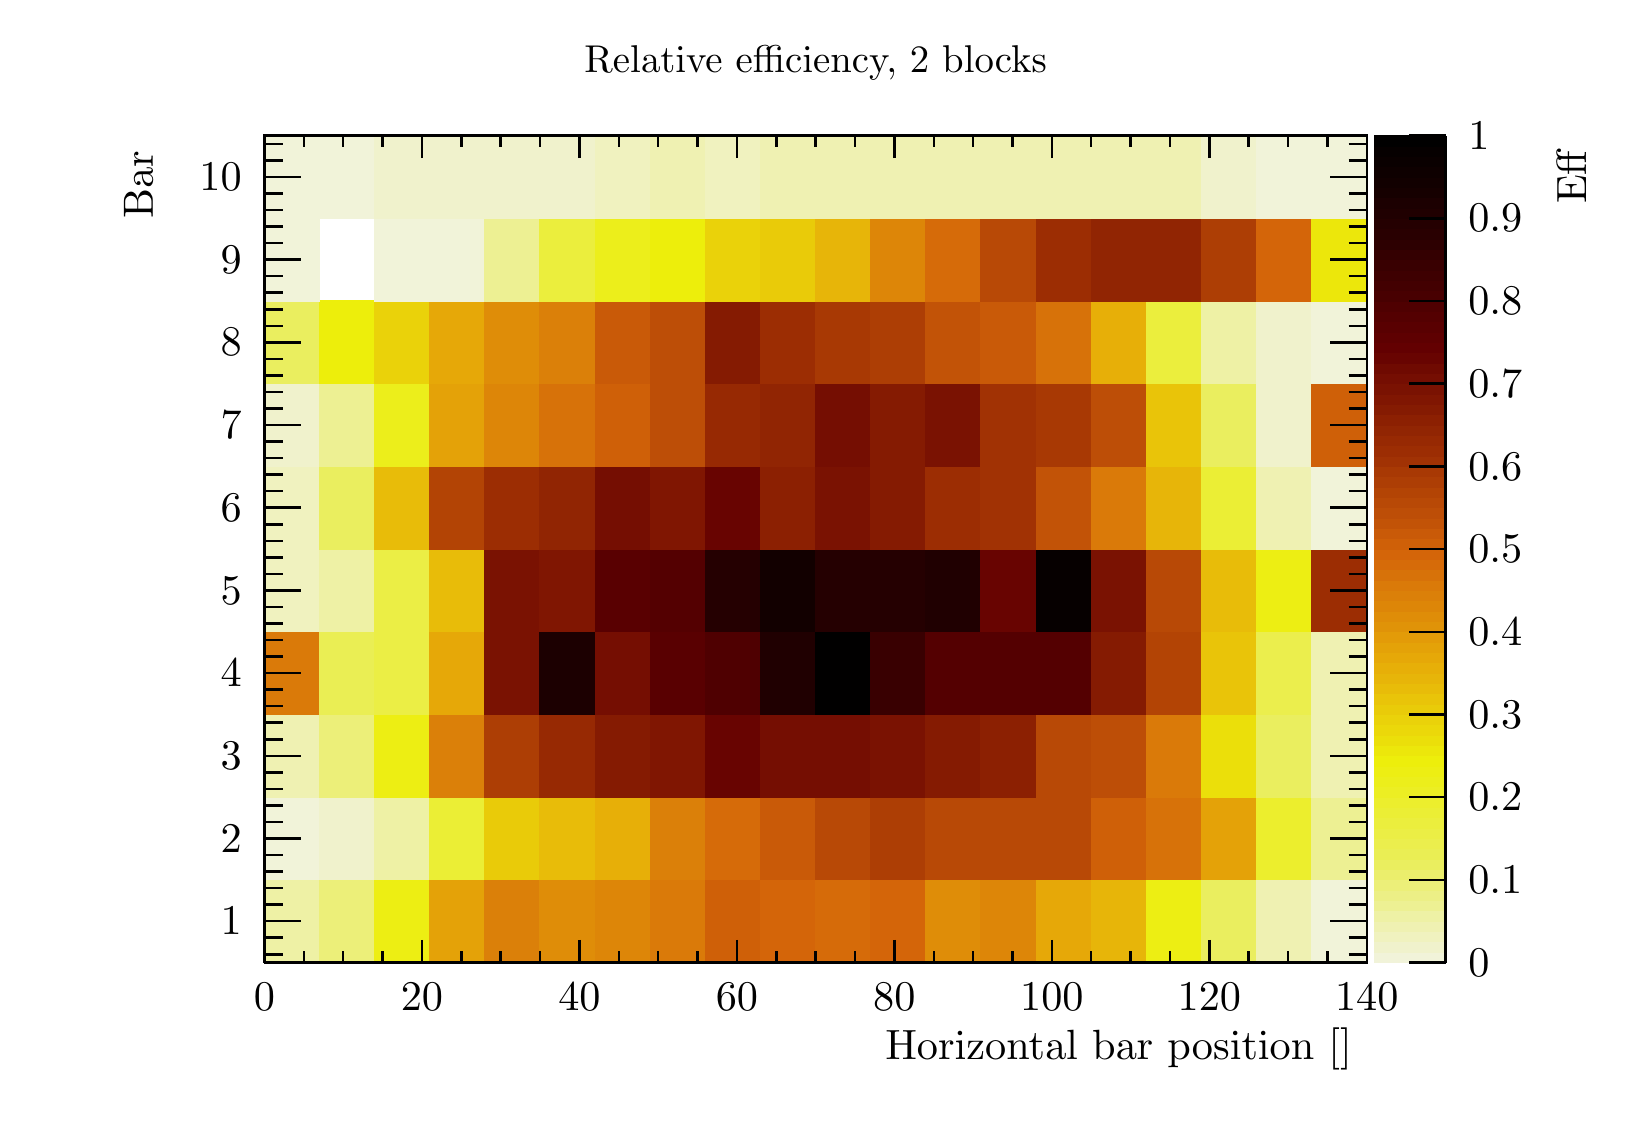
\begin{tikzpicture}
\pgfdeclareplotmark{cross} {
\pgfpathmoveto{\pgfpoint{-0.3\pgfplotmarksize}{\pgfplotmarksize}}
\pgfpathlineto{\pgfpoint{+0.3\pgfplotmarksize}{\pgfplotmarksize}}
\pgfpathlineto{\pgfpoint{+0.3\pgfplotmarksize}{0.3\pgfplotmarksize}}
\pgfpathlineto{\pgfpoint{+1\pgfplotmarksize}{0.3\pgfplotmarksize}}
\pgfpathlineto{\pgfpoint{+1\pgfplotmarksize}{-0.3\pgfplotmarksize}}
\pgfpathlineto{\pgfpoint{+0.3\pgfplotmarksize}{-0.3\pgfplotmarksize}}
\pgfpathlineto{\pgfpoint{+0.3\pgfplotmarksize}{-1.\pgfplotmarksize}}
\pgfpathlineto{\pgfpoint{-0.3\pgfplotmarksize}{-1.\pgfplotmarksize}}
\pgfpathlineto{\pgfpoint{-0.3\pgfplotmarksize}{-0.3\pgfplotmarksize}}
\pgfpathlineto{\pgfpoint{-1.\pgfplotmarksize}{-0.3\pgfplotmarksize}}
\pgfpathlineto{\pgfpoint{-1.\pgfplotmarksize}{0.3\pgfplotmarksize}}
\pgfpathlineto{\pgfpoint{-0.3\pgfplotmarksize}{0.3\pgfplotmarksize}}
\pgfpathclose
\pgfusepathqstroke
}
\pgfdeclareplotmark{cross*} {
\pgfpathmoveto{\pgfpoint{-0.3\pgfplotmarksize}{\pgfplotmarksize}}
\pgfpathlineto{\pgfpoint{+0.3\pgfplotmarksize}{\pgfplotmarksize}}
\pgfpathlineto{\pgfpoint{+0.3\pgfplotmarksize}{0.3\pgfplotmarksize}}
\pgfpathlineto{\pgfpoint{+1\pgfplotmarksize}{0.3\pgfplotmarksize}}
\pgfpathlineto{\pgfpoint{+1\pgfplotmarksize}{-0.3\pgfplotmarksize}}
\pgfpathlineto{\pgfpoint{+0.3\pgfplotmarksize}{-0.3\pgfplotmarksize}}
\pgfpathlineto{\pgfpoint{+0.3\pgfplotmarksize}{-1.\pgfplotmarksize}}
\pgfpathlineto{\pgfpoint{-0.3\pgfplotmarksize}{-1.\pgfplotmarksize}}
\pgfpathlineto{\pgfpoint{-0.3\pgfplotmarksize}{-0.3\pgfplotmarksize}}
\pgfpathlineto{\pgfpoint{-1.\pgfplotmarksize}{-0.3\pgfplotmarksize}}
\pgfpathlineto{\pgfpoint{-1.\pgfplotmarksize}{0.3\pgfplotmarksize}}
\pgfpathlineto{\pgfpoint{-0.3\pgfplotmarksize}{0.3\pgfplotmarksize}}
\pgfpathclose
\pgfusepathqfillstroke
}
\pgfdeclareplotmark{newstar} {
\pgfpathmoveto{\pgfqpoint{0pt}{\pgfplotmarksize}}
\pgfpathlineto{\pgfqpointpolar{44}{0.5\pgfplotmarksize}}
\pgfpathlineto{\pgfqpointpolar{18}{\pgfplotmarksize}}
\pgfpathlineto{\pgfqpointpolar{-20}{0.5\pgfplotmarksize}}
\pgfpathlineto{\pgfqpointpolar{-54}{\pgfplotmarksize}}
\pgfpathlineto{\pgfqpointpolar{-90}{0.5\pgfplotmarksize}}
\pgfpathlineto{\pgfqpointpolar{234}{\pgfplotmarksize}}
\pgfpathlineto{\pgfqpointpolar{198}{0.5\pgfplotmarksize}}
\pgfpathlineto{\pgfqpointpolar{162}{\pgfplotmarksize}}
\pgfpathlineto{\pgfqpointpolar{134}{0.5\pgfplotmarksize}}
\pgfpathclose
\pgfusepathqstroke
}
\pgfdeclareplotmark{newstar*} {
\pgfpathmoveto{\pgfqpoint{0pt}{\pgfplotmarksize}}
\pgfpathlineto{\pgfqpointpolar{44}{0.5\pgfplotmarksize}}
\pgfpathlineto{\pgfqpointpolar{18}{\pgfplotmarksize}}
\pgfpathlineto{\pgfqpointpolar{-20}{0.5\pgfplotmarksize}}
\pgfpathlineto{\pgfqpointpolar{-54}{\pgfplotmarksize}}
\pgfpathlineto{\pgfqpointpolar{-90}{0.5\pgfplotmarksize}}
\pgfpathlineto{\pgfqpointpolar{234}{\pgfplotmarksize}}
\pgfpathlineto{\pgfqpointpolar{198}{0.5\pgfplotmarksize}}
\pgfpathlineto{\pgfqpointpolar{162}{\pgfplotmarksize}}
\pgfpathlineto{\pgfqpointpolar{134}{0.5\pgfplotmarksize}}
\pgfpathclose
\pgfusepathqfillstroke
}
\definecolor{c}{rgb}{1,1,1};
\draw [color=c, fill=c] (0,0) rectangle (20,13.639);
\draw [color=c, fill=c] (3,1.77307) rectangle (17,12.2751);
\definecolor{c}{rgb}{0,0,0};
\draw [c,line width=0.9] (3,1.77307) -- (3,12.2751) -- (17,12.2751) -- (17,1.77307) -- (3,1.77307);
\definecolor{c}{rgb}{1,1,1};
\draw [color=c, fill=c] (3,1.77307) rectangle (17,12.2751);
\definecolor{c}{rgb}{0,0,0};
\draw [c,line width=0.9] (3,1.77307) -- (3,12.2751) -- (17,12.2751) -- (17,1.77307) -- (3,1.77307);
\definecolor{c}{rgb}{0.933839,0.943453,0.645794};
\draw [color=c, fill=c] (3,1.77307) rectangle (3.7,2.82327);
\definecolor{c}{rgb}{0.923719,0.937128,0.475016};
\draw [color=c, fill=c] (3.7,1.77307) rectangle (4.4,2.82327);
\definecolor{c}{rgb}{0.928309,0.933333,0.0740196};
\draw [color=c, fill=c] (4.4,1.77307) rectangle (5.1,2.82327);
\definecolor{c}{rgb}{0.895343,0.634191,0.0317402};
\draw [color=c, fill=c] (5.1,1.77307) rectangle (5.8,2.82327);
\definecolor{c}{rgb}{0.860049,0.502819,0.033701};
\draw [color=c, fill=c] (5.8,1.77307) rectangle (6.5,2.82327);
\definecolor{c}{rgb}{0.873284,0.552083,0.0329657};
\draw [color=c, fill=c] (6.5,1.77307) rectangle (7.2,2.82327);
\definecolor{c}{rgb}{0.866667,0.527451,0.0333333};
\draw [color=c, fill=c] (7.2,1.77307) rectangle (7.9,2.82327);
\definecolor{c}{rgb}{0.853431,0.478186,0.0340686};
\draw [color=c, fill=c] (7.9,1.77307) rectangle (8.6,2.82327);
\definecolor{c}{rgb}{0.810784,0.37549,0.0330882};
\draw [color=c, fill=c] (8.6,1.77307) rectangle (9.3,2.82327);
\definecolor{c}{rgb}{0.831373,0.396078,0.0352941};
\draw [color=c, fill=c] (9.3,1.77307) rectangle (10,2.82327);
\definecolor{c}{rgb}{0.83799,0.420711,0.0349265};
\draw [color=c, fill=c] (10,1.77307) rectangle (10.7,2.82327);
\definecolor{c}{rgb}{0.831373,0.396078,0.0352941};
\draw [color=c, fill=c] (10.7,1.77307) rectangle (11.4,2.82327);
\definecolor{c}{rgb}{0.873284,0.552083,0.0329657};
\draw [color=c, fill=c] (11.4,1.77307) rectangle (12.1,2.82327);
\definecolor{c}{rgb}{0.866667,0.527451,0.0333333};
\draw [color=c, fill=c] (12.1,1.77307) rectangle (12.8,2.82327);
\definecolor{c}{rgb}{0.901961,0.658824,0.0313726};
\draw [color=c, fill=c] (12.8,1.77307) rectangle (13.5,2.82327);
\definecolor{c}{rgb}{0.907108,0.710294,0.0335784};
\draw [color=c, fill=c] (13.5,1.77307) rectangle (14.2,2.82327);
\definecolor{c}{rgb}{0.928309,0.933333,0.0740196};
\draw [color=c, fill=c] (14.2,1.77307) rectangle (14.9,2.82327);
\definecolor{c}{rgb}{0.917647,0.933333,0.372549};
\draw [color=c, fill=c] (14.9,1.77307) rectangle (15.6,2.82327);
\definecolor{c}{rgb}{0.936875,0.945351,0.697027};
\draw [color=c, fill=c] (15.6,1.77307) rectangle (16.3,2.82327);
\definecolor{c}{rgb}{0.945984,0.951044,0.850727};
\draw [color=c, fill=c] (16.3,1.77307) rectangle (17,2.82327);
\draw [color=c, fill=c] (3,2.82327) rectangle (3.7,3.87347);
\definecolor{c}{rgb}{0.942948,0.949146,0.799494};
\draw [color=c, fill=c] (3.7,2.82327) rectangle (4.4,3.87347);
\definecolor{c}{rgb}{0.933839,0.943453,0.645794};
\draw [color=c, fill=c] (4.4,2.82327) rectangle (5.1,3.87347);
\definecolor{c}{rgb}{0.923529,0.933333,0.207843};
\draw [color=c, fill=c] (5.1,2.82327) rectangle (5.8,3.87347);
\definecolor{c}{rgb}{0.915686,0.796078,0.0372549};
\draw [color=c, fill=c] (5.8,2.82327) rectangle (6.5,3.87347);
\definecolor{c}{rgb}{0.909681,0.736029,0.0346814};
\draw [color=c, fill=c] (6.5,2.82327) rectangle (7.2,3.87347);
\definecolor{c}{rgb}{0.904534,0.684559,0.0324755};
\draw [color=c, fill=c] (7.2,2.82327) rectangle (7.9,3.87347);
\definecolor{c}{rgb}{0.860049,0.502819,0.033701};
\draw [color=c, fill=c] (7.9,2.82327) rectangle (8.6,3.87347);
\definecolor{c}{rgb}{0.83799,0.420711,0.0349265};
\draw [color=c, fill=c] (8.6,2.82327) rectangle (9.3,3.87347);
\definecolor{c}{rgb}{0.790196,0.354902,0.0308824};
\draw [color=c, fill=c] (9.3,2.82327) rectangle (10,3.87347);
\definecolor{c}{rgb}{0.721569,0.286275,0.0235294};
\draw [color=c, fill=c] (10,2.82327) rectangle (10.7,3.87347);
\definecolor{c}{rgb}{0.680392,0.245098,0.0191176};
\draw [color=c, fill=c] (10.7,2.82327) rectangle (11.4,3.87347);
\definecolor{c}{rgb}{0.721569,0.286275,0.0235294};
\draw [color=c, fill=c] (11.4,2.82327) rectangle (12.1,3.87347);
\draw [color=c, fill=c] (12.1,2.82327) rectangle (12.8,3.87347);
\draw [color=c, fill=c] (12.8,2.82327) rectangle (13.5,3.87347);
\definecolor{c}{rgb}{0.810784,0.37549,0.0330882};
\draw [color=c, fill=c] (13.5,2.82327) rectangle (14.2,3.87347);
\definecolor{c}{rgb}{0.844608,0.445343,0.0345588};
\draw [color=c, fill=c] (14.2,2.82327) rectangle (14.9,3.87347);
\definecolor{c}{rgb}{0.895343,0.634191,0.0317402};
\draw [color=c, fill=c] (14.9,2.82327) rectangle (15.6,3.87347);
\definecolor{c}{rgb}{0.924632,0.933333,0.176961};
\draw [color=c, fill=c] (15.6,2.82327) rectangle (16.3,3.87347);
\definecolor{c}{rgb}{0.929791,0.940923,0.577483};
\draw [color=c, fill=c] (16.3,2.82327) rectangle (17,3.87347);
\definecolor{c}{rgb}{0.936875,0.945351,0.697027};
\draw [color=c, fill=c] (3,3.87347) rectangle (3.7,4.92367);
\definecolor{c}{rgb}{0.923719,0.937128,0.475016};
\draw [color=c, fill=c] (3.7,3.87347) rectangle (4.4,4.92367);
\definecolor{c}{rgb}{0.928309,0.933333,0.0740196};
\draw [color=c, fill=c] (4.4,3.87347) rectangle (5.1,4.92367);
\definecolor{c}{rgb}{0.860049,0.502819,0.033701};
\draw [color=c, fill=c] (5.1,3.87347) rectangle (5.8,4.92367);
\definecolor{c}{rgb}{0.680392,0.245098,0.0191176};
\draw [color=c, fill=c] (5.8,3.87347) rectangle (6.5,4.92367);
\definecolor{c}{rgb}{0.590809,0.159926,0.0110294};
\draw [color=c, fill=c] (6.5,3.87347) rectangle (7.2,4.92367);
\definecolor{c}{rgb}{0.520956,0.104779,0.00857843};
\draw [color=c, fill=c] (7.2,3.87347) rectangle (7.9,4.92367);
\definecolor{c}{rgb}{0.5,0.0882353,0.00784314};
\draw [color=c, fill=c] (7.9,3.87347) rectangle (8.6,4.92367);
\definecolor{c}{rgb}{0.409191,0.0165441,0.00465686};
\draw [color=c, fill=c] (8.6,3.87347) rectangle (9.3,4.92367);
\definecolor{c}{rgb}{0.458088,0.0551471,0.00637255};
\draw [color=c, fill=c] (9.3,3.87347) rectangle (10,4.92367);
\draw [color=c, fill=c] (10,3.87347) rectangle (10.7,4.92367);
\definecolor{c}{rgb}{0.479044,0.0716912,0.00710784};
\draw [color=c, fill=c] (10.7,3.87347) rectangle (11.4,4.92367);
\definecolor{c}{rgb}{0.520956,0.104779,0.00857843};
\draw [color=c, fill=c] (11.4,3.87347) rectangle (12.1,4.92367);
\definecolor{c}{rgb}{0.548897,0.126838,0.00955882};
\draw [color=c, fill=c] (12.1,3.87347) rectangle (12.8,4.92367);
\definecolor{c}{rgb}{0.721569,0.286275,0.0235294};
\draw [color=c, fill=c] (12.8,3.87347) rectangle (13.5,4.92367);
\definecolor{c}{rgb}{0.742157,0.306863,0.0257353};
\draw [color=c, fill=c] (13.5,3.87347) rectangle (14.2,4.92367);
\definecolor{c}{rgb}{0.853431,0.478186,0.0340686};
\draw [color=c, fill=c] (14.2,3.87347) rectangle (14.9,4.92367);
\definecolor{c}{rgb}{0.923407,0.873284,0.0405637};
\draw [color=c, fill=c] (14.9,3.87347) rectangle (15.6,4.92367);
\definecolor{c}{rgb}{0.917647,0.933333,0.372549};
\draw [color=c, fill=c] (15.6,3.87347) rectangle (16.3,4.92367);
\definecolor{c}{rgb}{0.936875,0.945351,0.697027};
\draw [color=c, fill=c] (16.3,3.87347) rectangle (17,4.92367);
\definecolor{c}{rgb}{0.853431,0.478186,0.0340686};
\draw [color=c, fill=c] (3,4.92367) rectangle (3.7,5.97387);
\definecolor{c}{rgb}{0.919118,0.933333,0.331373};
\draw [color=c, fill=c] (3.7,4.92367) rectangle (4.4,5.97387);
\definecolor{c}{rgb}{0.921324,0.933333,0.269608};
\draw [color=c, fill=c] (4.4,4.92367) rectangle (5.1,5.97387);
\definecolor{c}{rgb}{0.901961,0.658824,0.0313726};
\draw [color=c, fill=c] (5.1,4.92367) rectangle (5.8,5.97387);
\definecolor{c}{rgb}{0.479044,0.0716912,0.00710784};
\draw [color=c, fill=c] (5.8,4.92367) rectangle (6.5,5.97387);
\definecolor{c}{rgb}{0.110294,0,0.00245098};
\draw [color=c, fill=c] (6.5,4.92367) rectangle (7.2,5.97387);
\definecolor{c}{rgb}{0.458088,0.0551471,0.00637255};
\draw [color=c, fill=c] (7.2,4.92367) rectangle (7.9,5.97387);
\definecolor{c}{rgb}{0.348529,0,0.00392157};
\draw [color=c, fill=c] (7.9,4.92367) rectangle (8.6,5.97387);
\definecolor{c}{rgb}{0.308824,0,0.00392157};
\draw [color=c, fill=c] (8.6,4.92367) rectangle (9.3,5.97387);
\definecolor{c}{rgb}{0.126838,0,0.00281863};
\draw [color=c, fill=c] (9.3,4.92367) rectangle (10,5.97387);
\definecolor{c}{rgb}{0.00551471,0,0.000122549};
\draw [color=c, fill=c] (10,4.92367) rectangle (10.7,5.97387);
\definecolor{c}{rgb}{0.222794,0,0.00392157};
\draw [color=c, fill=c] (10.7,4.92367) rectangle (11.4,5.97387);
\definecolor{c}{rgb}{0.328676,0,0.00392157};
\draw [color=c, fill=c] (11.4,4.92367) rectangle (12.1,5.97387);
\draw [color=c, fill=c] (12.1,4.92367) rectangle (12.8,5.97387);
\draw [color=c, fill=c] (12.8,4.92367) rectangle (13.5,5.97387);
\definecolor{c}{rgb}{0.520956,0.104779,0.00857843};
\draw [color=c, fill=c] (13.5,4.92367) rectangle (14.2,5.97387);
\definecolor{c}{rgb}{0.70098,0.265686,0.0213235};
\draw [color=c, fill=c] (14.2,4.92367) rectangle (14.9,5.97387);
\definecolor{c}{rgb}{0.913113,0.770343,0.036152};
\draw [color=c, fill=c] (14.9,4.92367) rectangle (15.6,5.97387);
\definecolor{c}{rgb}{0.920221,0.933333,0.30049};
\draw [color=c, fill=c] (15.6,4.92367) rectangle (16.3,5.97387);
\definecolor{c}{rgb}{0.936875,0.945351,0.697027};
\draw [color=c, fill=c] (16.3,4.92367) rectangle (17,5.97387);
\definecolor{c}{rgb}{0.939911,0.947249,0.748261};
\draw [color=c, fill=c] (3,5.97387) rectangle (3.7,7.02407);
\definecolor{c}{rgb}{0.933839,0.943453,0.645794};
\draw [color=c, fill=c] (3.7,5.97387) rectangle (4.4,7.02407);
\definecolor{c}{rgb}{0.921324,0.933333,0.269608};
\draw [color=c, fill=c] (4.4,5.97387) rectangle (5.1,7.02407);
\definecolor{c}{rgb}{0.909681,0.736029,0.0346814};
\draw [color=c, fill=c] (5.1,5.97387) rectangle (5.8,7.02407);
\definecolor{c}{rgb}{0.479044,0.0716912,0.00710784};
\draw [color=c, fill=c] (5.8,5.97387) rectangle (6.5,7.02407);
\definecolor{c}{rgb}{0.5,0.0882353,0.00784314};
\draw [color=c, fill=c] (6.5,5.97387) rectangle (7.2,7.02407);
\definecolor{c}{rgb}{0.348529,0,0.00392157};
\draw [color=c, fill=c] (7.2,5.97387) rectangle (7.9,7.02407);
\definecolor{c}{rgb}{0.328676,0,0.00392157};
\draw [color=c, fill=c] (7.9,5.97387) rectangle (8.6,7.02407);
\definecolor{c}{rgb}{0.143382,0,0.00318627};
\draw [color=c, fill=c] (8.6,5.97387) rectangle (9.3,7.02407);
\definecolor{c}{rgb}{0.0716912,0,0.00159314};
\draw [color=c, fill=c] (9.3,5.97387) rectangle (10,7.02407);
\definecolor{c}{rgb}{0.143382,0,0.00318627};
\draw [color=c, fill=c] (10,5.97387) rectangle (10.7,7.02407);
\draw [color=c, fill=c] (10.7,5.97387) rectangle (11.4,7.02407);
\definecolor{c}{rgb}{0.126838,0,0.00281863};
\draw [color=c, fill=c] (11.4,5.97387) rectangle (12.1,7.02407);
\definecolor{c}{rgb}{0.409191,0.0165441,0.00465686};
\draw [color=c, fill=c] (12.1,5.97387) rectangle (12.8,7.02407);
\definecolor{c}{rgb}{0.0220588,0,0.000490196};
\draw [color=c, fill=c] (12.8,5.97387) rectangle (13.5,7.02407);
\definecolor{c}{rgb}{0.479044,0.0716912,0.00710784};
\draw [color=c, fill=c] (13.5,5.97387) rectangle (14.2,7.02407);
\definecolor{c}{rgb}{0.721569,0.286275,0.0235294};
\draw [color=c, fill=c] (14.2,5.97387) rectangle (14.9,7.02407);
\definecolor{c}{rgb}{0.909681,0.736029,0.0346814};
\draw [color=c, fill=c] (14.9,5.97387) rectangle (15.6,7.02407);
\definecolor{c}{rgb}{0.928309,0.933333,0.0740196};
\draw [color=c, fill=c] (15.6,5.97387) rectangle (16.3,7.02407);
\definecolor{c}{rgb}{0.611765,0.176471,0.0117647};
\draw [color=c, fill=c] (16.3,5.97387) rectangle (17,7.02407);
\definecolor{c}{rgb}{0.939911,0.947249,0.748261};
\draw [color=c, fill=c] (3,7.02407) rectangle (3.7,8.07427);
\definecolor{c}{rgb}{0.917647,0.933333,0.372549};
\draw [color=c, fill=c] (3.7,7.02407) rectangle (4.4,8.07427);
\definecolor{c}{rgb}{0.909681,0.736029,0.0346814};
\draw [color=c, fill=c] (4.4,7.02407) rectangle (5.1,8.07427);
\definecolor{c}{rgb}{0.70098,0.265686,0.0213235};
\draw [color=c, fill=c] (5.1,7.02407) rectangle (5.8,8.07427);
\definecolor{c}{rgb}{0.611765,0.176471,0.0117647};
\draw [color=c, fill=c] (5.8,7.02407) rectangle (6.5,8.07427);
\definecolor{c}{rgb}{0.569853,0.143382,0.0102941};
\draw [color=c, fill=c] (6.5,7.02407) rectangle (7.2,8.07427);
\definecolor{c}{rgb}{0.458088,0.0551471,0.00637255};
\draw [color=c, fill=c] (7.2,7.02407) rectangle (7.9,8.07427);
\definecolor{c}{rgb}{0.5,0.0882353,0.00784314};
\draw [color=c, fill=c] (7.9,7.02407) rectangle (8.6,8.07427);
\definecolor{c}{rgb}{0.409191,0.0165441,0.00465686};
\draw [color=c, fill=c] (8.6,7.02407) rectangle (9.3,8.07427);
\definecolor{c}{rgb}{0.548897,0.126838,0.00955882};
\draw [color=c, fill=c] (9.3,7.02407) rectangle (10,8.07427);
\definecolor{c}{rgb}{0.479044,0.0716912,0.00710784};
\draw [color=c, fill=c] (10,7.02407) rectangle (10.7,8.07427);
\definecolor{c}{rgb}{0.520956,0.104779,0.00857843};
\draw [color=c, fill=c] (10.7,7.02407) rectangle (11.4,8.07427);
\definecolor{c}{rgb}{0.611765,0.176471,0.0117647};
\draw [color=c, fill=c] (11.4,7.02407) rectangle (12.1,8.07427);
\definecolor{c}{rgb}{0.632353,0.197059,0.0139706};
\draw [color=c, fill=c] (12.1,7.02407) rectangle (12.8,8.07427);
\definecolor{c}{rgb}{0.762745,0.327451,0.0279412};
\draw [color=c, fill=c] (12.8,7.02407) rectangle (13.5,8.07427);
\definecolor{c}{rgb}{0.853431,0.478186,0.0340686};
\draw [color=c, fill=c] (13.5,7.02407) rectangle (14.2,8.07427);
\definecolor{c}{rgb}{0.907108,0.710294,0.0335784};
\draw [color=c, fill=c] (14.2,7.02407) rectangle (14.9,8.07427);
\definecolor{c}{rgb}{0.923529,0.933333,0.207843};
\draw [color=c, fill=c] (14.9,7.02407) rectangle (15.6,8.07427);
\definecolor{c}{rgb}{0.936875,0.945351,0.697027};
\draw [color=c, fill=c] (15.6,7.02407) rectangle (16.3,8.07427);
\definecolor{c}{rgb}{0.945984,0.951044,0.850727};
\draw [color=c, fill=c] (16.3,7.02407) rectangle (17,8.07427);
\definecolor{c}{rgb}{0.942948,0.949146,0.799494};
\draw [color=c, fill=c] (3,8.07427) rectangle (3.7,9.12447);
\definecolor{c}{rgb}{0.929791,0.940923,0.577483};
\draw [color=c, fill=c] (3.7,8.07427) rectangle (4.4,9.12447);
\definecolor{c}{rgb}{0.927206,0.933333,0.104902};
\draw [color=c, fill=c] (4.4,8.07427) rectangle (5.1,9.12447);
\definecolor{c}{rgb}{0.895343,0.634191,0.0317402};
\draw [color=c, fill=c] (5.1,8.07427) rectangle (5.8,9.12447);
\definecolor{c}{rgb}{0.866667,0.527451,0.0333333};
\draw [color=c, fill=c] (5.8,8.07427) rectangle (6.5,9.12447);
\definecolor{c}{rgb}{0.844608,0.445343,0.0345588};
\draw [color=c, fill=c] (6.5,8.07427) rectangle (7.2,9.12447);
\definecolor{c}{rgb}{0.810784,0.37549,0.0330882};
\draw [color=c, fill=c] (7.2,8.07427) rectangle (7.9,9.12447);
\definecolor{c}{rgb}{0.742157,0.306863,0.0257353};
\draw [color=c, fill=c] (7.9,8.07427) rectangle (8.6,9.12447);
\definecolor{c}{rgb}{0.590809,0.159926,0.0110294};
\draw [color=c, fill=c] (8.6,8.07427) rectangle (9.3,9.12447);
\definecolor{c}{rgb}{0.569853,0.143382,0.0102941};
\draw [color=c, fill=c] (9.3,8.07427) rectangle (10,9.12447);
\definecolor{c}{rgb}{0.458088,0.0551471,0.00637255};
\draw [color=c, fill=c] (10,8.07427) rectangle (10.7,9.12447);
\definecolor{c}{rgb}{0.520956,0.104779,0.00857843};
\draw [color=c, fill=c] (10.7,8.07427) rectangle (11.4,9.12447);
\definecolor{c}{rgb}{0.479044,0.0716912,0.00710784};
\draw [color=c, fill=c] (11.4,8.07427) rectangle (12.1,9.12447);
\definecolor{c}{rgb}{0.632353,0.197059,0.0139706};
\draw [color=c, fill=c] (12.1,8.07427) rectangle (12.8,9.12447);
\definecolor{c}{rgb}{0.659804,0.22451,0.0169118};
\draw [color=c, fill=c] (12.8,8.07427) rectangle (13.5,9.12447);
\definecolor{c}{rgb}{0.742157,0.306863,0.0257353};
\draw [color=c, fill=c] (13.5,8.07427) rectangle (14.2,9.12447);
\definecolor{c}{rgb}{0.913113,0.770343,0.036152};
\draw [color=c, fill=c] (14.2,8.07427) rectangle (14.9,9.12447);
\definecolor{c}{rgb}{0.917647,0.933333,0.372549};
\draw [color=c, fill=c] (14.9,8.07427) rectangle (15.6,9.12447);
\definecolor{c}{rgb}{0.942948,0.949146,0.799494};
\draw [color=c, fill=c] (15.6,8.07427) rectangle (16.3,9.12447);
\definecolor{c}{rgb}{0.810784,0.37549,0.0330882};
\draw [color=c, fill=c] (16.3,8.07427) rectangle (17,9.12447);
\definecolor{c}{rgb}{0.917647,0.933333,0.372549};
\draw [color=c, fill=c] (3,9.12447) rectangle (3.7,10.1747);
\definecolor{c}{rgb}{0.929412,0.933333,0.0431373};
\draw [color=c, fill=c] (3.7,9.12447) rectangle (4.4,10.1747);
\definecolor{c}{rgb}{0.91826,0.821814,0.0383578};
\draw [color=c, fill=c] (4.4,9.12447) rectangle (5.1,10.1747);
\definecolor{c}{rgb}{0.901961,0.658824,0.0313726};
\draw [color=c, fill=c] (5.1,9.12447) rectangle (5.8,10.1747);
\definecolor{c}{rgb}{0.873284,0.552083,0.0329657};
\draw [color=c, fill=c] (5.8,9.12447) rectangle (6.5,10.1747);
\definecolor{c}{rgb}{0.860049,0.502819,0.033701};
\draw [color=c, fill=c] (6.5,9.12447) rectangle (7.2,10.1747);
\definecolor{c}{rgb}{0.790196,0.354902,0.0308824};
\draw [color=c, fill=c] (7.2,9.12447) rectangle (7.9,10.1747);
\definecolor{c}{rgb}{0.742157,0.306863,0.0257353};
\draw [color=c, fill=c] (7.9,9.12447) rectangle (8.6,10.1747);
\definecolor{c}{rgb}{0.520956,0.104779,0.00857843};
\draw [color=c, fill=c] (8.6,9.12447) rectangle (9.3,10.1747);
\definecolor{c}{rgb}{0.611765,0.176471,0.0117647};
\draw [color=c, fill=c] (9.3,9.12447) rectangle (10,10.1747);
\definecolor{c}{rgb}{0.659804,0.22451,0.0169118};
\draw [color=c, fill=c] (10,9.12447) rectangle (10.7,10.1747);
\definecolor{c}{rgb}{0.680392,0.245098,0.0191176};
\draw [color=c, fill=c] (10.7,9.12447) rectangle (11.4,10.1747);
\definecolor{c}{rgb}{0.762745,0.327451,0.0279412};
\draw [color=c, fill=c] (11.4,9.12447) rectangle (12.1,10.1747);
\definecolor{c}{rgb}{0.790196,0.354902,0.0308824};
\draw [color=c, fill=c] (12.1,9.12447) rectangle (12.8,10.1747);
\definecolor{c}{rgb}{0.844608,0.445343,0.0345588};
\draw [color=c, fill=c] (12.8,9.12447) rectangle (13.5,10.1747);
\definecolor{c}{rgb}{0.904534,0.684559,0.0324755};
\draw [color=c, fill=c] (13.5,9.12447) rectangle (14.2,10.1747);
\definecolor{c}{rgb}{0.922426,0.933333,0.238725};
\draw [color=c, fill=c] (14.2,9.12447) rectangle (14.9,10.1747);
\definecolor{c}{rgb}{0.933839,0.943453,0.645794};
\draw [color=c, fill=c] (14.9,9.12447) rectangle (15.6,10.1747);
\definecolor{c}{rgb}{0.942948,0.949146,0.799494};
\draw [color=c, fill=c] (15.6,9.12447) rectangle (16.3,10.1747);
\definecolor{c}{rgb}{0.945984,0.951044,0.850727};
\draw [color=c, fill=c] (16.3,9.12447) rectangle (17,10.1747);
\draw [color=c, fill=c] (3,10.1747) rectangle (3.7,11.2249);
\draw [color=c, fill=c] (4.4,10.1747) rectangle (5.1,11.2249);
\draw [color=c, fill=c] (5.1,10.1747) rectangle (5.8,11.2249);
\definecolor{c}{rgb}{0.929791,0.940923,0.577483};
\draw [color=c, fill=c] (5.8,10.1747) rectangle (6.5,11.2249);
\definecolor{c}{rgb}{0.922426,0.933333,0.238725};
\draw [color=c, fill=c] (6.5,10.1747) rectangle (7.2,11.2249);
\definecolor{c}{rgb}{0.927206,0.933333,0.104902};
\draw [color=c, fill=c] (7.2,10.1747) rectangle (7.9,11.2249);
\definecolor{c}{rgb}{0.929412,0.933333,0.0431373};
\draw [color=c, fill=c] (7.9,10.1747) rectangle (8.6,11.2249);
\definecolor{c}{rgb}{0.91826,0.821814,0.0383578};
\draw [color=c, fill=c] (8.6,10.1747) rectangle (9.3,11.2249);
\definecolor{c}{rgb}{0.915686,0.796078,0.0372549};
\draw [color=c, fill=c] (9.3,10.1747) rectangle (10,11.2249);
\definecolor{c}{rgb}{0.907108,0.710294,0.0335784};
\draw [color=c, fill=c] (10,10.1747) rectangle (10.7,11.2249);
\definecolor{c}{rgb}{0.866667,0.527451,0.0333333};
\draw [color=c, fill=c] (10.7,10.1747) rectangle (11.4,11.2249);
\definecolor{c}{rgb}{0.83799,0.420711,0.0349265};
\draw [color=c, fill=c] (11.4,10.1747) rectangle (12.1,11.2249);
\definecolor{c}{rgb}{0.721569,0.286275,0.0235294};
\draw [color=c, fill=c] (12.1,10.1747) rectangle (12.8,11.2249);
\definecolor{c}{rgb}{0.611765,0.176471,0.0117647};
\draw [color=c, fill=c] (12.8,10.1747) rectangle (13.5,11.2249);
\definecolor{c}{rgb}{0.569853,0.143382,0.0102941};
\draw [color=c, fill=c] (13.5,10.1747) rectangle (14.2,11.2249);
\draw [color=c, fill=c] (14.2,10.1747) rectangle (14.9,11.2249);
\definecolor{c}{rgb}{0.680392,0.245098,0.0191176};
\draw [color=c, fill=c] (14.9,10.1747) rectangle (15.6,11.2249);
\definecolor{c}{rgb}{0.831373,0.396078,0.0352941};
\draw [color=c, fill=c] (15.6,10.1747) rectangle (16.3,11.2249);
\definecolor{c}{rgb}{0.926838,0.907598,0.0420343};
\draw [color=c, fill=c] (16.3,10.1747) rectangle (17,11.2249);
\definecolor{c}{rgb}{0.945984,0.951044,0.850727};
\draw [color=c, fill=c] (3,11.2249) rectangle (3.7,12.2751);
\draw [color=c, fill=c] (3.7,11.2249) rectangle (4.4,12.2751);
\definecolor{c}{rgb}{0.942948,0.949146,0.799494};
\draw [color=c, fill=c] (4.4,11.2249) rectangle (5.1,12.2751);
\draw [color=c, fill=c] (5.1,11.2249) rectangle (5.8,12.2751);
\draw [color=c, fill=c] (5.8,11.2249) rectangle (6.5,12.2751);
\draw [color=c, fill=c] (6.5,11.2249) rectangle (7.2,12.2751);
\definecolor{c}{rgb}{0.939911,0.947249,0.748261};
\draw [color=c, fill=c] (7.2,11.2249) rectangle (7.9,12.2751);
\definecolor{c}{rgb}{0.936875,0.945351,0.697027};
\draw [color=c, fill=c] (7.9,11.2249) rectangle (8.6,12.2751);
\definecolor{c}{rgb}{0.939911,0.947249,0.748261};
\draw [color=c, fill=c] (8.6,11.2249) rectangle (9.3,12.2751);
\definecolor{c}{rgb}{0.936875,0.945351,0.697027};
\draw [color=c, fill=c] (9.3,11.2249) rectangle (10,12.2751);
\draw [color=c, fill=c] (10,11.2249) rectangle (10.7,12.2751);
\draw [color=c, fill=c] (10.7,11.2249) rectangle (11.4,12.2751);
\draw [color=c, fill=c] (11.4,11.2249) rectangle (12.1,12.2751);
\draw [color=c, fill=c] (12.1,11.2249) rectangle (12.8,12.2751);
\draw [color=c, fill=c] (12.8,11.2249) rectangle (13.5,12.2751);
\draw [color=c, fill=c] (13.5,11.2249) rectangle (14.2,12.2751);
\draw [color=c, fill=c] (14.2,11.2249) rectangle (14.9,12.2751);
\definecolor{c}{rgb}{0.942948,0.949146,0.799494};
\draw [color=c, fill=c] (14.9,11.2249) rectangle (15.6,12.2751);
\definecolor{c}{rgb}{0.945984,0.951044,0.850727};
\draw [color=c, fill=c] (15.6,11.2249) rectangle (16.3,12.2751);
\draw [color=c, fill=c] (16.3,11.2249) rectangle (17,12.2751);
\definecolor{c}{rgb}{0,0,0};
\draw [c,line width=0.9] (3,1.77307) -- (17,1.77307);
\draw [c,line width=0.9] (3,2.05948) -- (3,1.77307);
\draw [c,line width=0.9] (3.5,1.91628) -- (3.5,1.77307);
\draw [c,line width=0.9] (4,1.91628) -- (4,1.77307);
\draw [c,line width=0.9] (4.5,1.91628) -- (4.5,1.77307);
\draw [c,line width=0.9] (5,2.05948) -- (5,1.77307);
\draw [c,line width=0.9] (5.5,1.91628) -- (5.5,1.77307);
\draw [c,line width=0.9] (6,1.91628) -- (6,1.77307);
\draw [c,line width=0.9] (6.5,1.91628) -- (6.5,1.77307);
\draw [c,line width=0.9] (7,2.05948) -- (7,1.77307);
\draw [c,line width=0.9] (7.5,1.91628) -- (7.5,1.77307);
\draw [c,line width=0.9] (8,1.91628) -- (8,1.77307);
\draw [c,line width=0.9] (8.5,1.91628) -- (8.5,1.77307);
\draw [c,line width=0.9] (9,2.05948) -- (9,1.77307);
\draw [c,line width=0.9] (9.5,1.91628) -- (9.5,1.77307);
\draw [c,line width=0.9] (10,1.91628) -- (10,1.77307);
\draw [c,line width=0.9] (10.5,1.91628) -- (10.5,1.77307);
\draw [c,line width=0.9] (11,2.05948) -- (11,1.77307);
\draw [c,line width=0.9] (11.5,1.91628) -- (11.5,1.77307);
\draw [c,line width=0.9] (12,1.91628) -- (12,1.77307);
\draw [c,line width=0.9] (12.5,1.91628) -- (12.5,1.77307);
\draw [c,line width=0.9] (13,2.05948) -- (13,1.77307);
\draw [c,line width=0.9] (13.5,1.91628) -- (13.5,1.77307);
\draw [c,line width=0.9] (14,1.91628) -- (14,1.77307);
\draw [c,line width=0.9] (14.5,1.91628) -- (14.5,1.77307);
\draw [c,line width=0.9] (15,2.05948) -- (15,1.77307);
\draw [c,line width=0.9] (15.5,1.91628) -- (15.5,1.77307);
\draw [c,line width=0.9] (16,1.91628) -- (16,1.77307);
\draw [c,line width=0.9] (16.5,1.91628) -- (16.5,1.77307);
\draw [c,line width=0.9] (17,2.05948) -- (17,1.77307);
\draw [anchor=base] (3,1.15931) node[scale=1.52731, color=c, rotate=0]{0};
\draw [anchor=base] (5,1.15931) node[scale=1.52731, color=c, rotate=0]{20};
\draw [anchor=base] (7,1.15931) node[scale=1.52731, color=c, rotate=0]{40};
\draw [anchor=base] (9,1.15931) node[scale=1.52731, color=c, rotate=0]{60};
\draw [anchor=base] (11,1.15931) node[scale=1.52731, color=c, rotate=0]{80};
\draw [anchor=base] (13,1.15931) node[scale=1.52731, color=c, rotate=0]{100};
\draw [anchor=base] (15,1.15931) node[scale=1.52731, color=c, rotate=0]{120};
\draw [anchor=base] (17,1.15931) node[scale=1.52731, color=c, rotate=0]{140};
\draw [anchor= east] (17,0.681948) node[scale=1.52731, color=c, rotate=0]{Horizontal bar position [\si{\centi\metre}]};
\draw [c,line width=0.9] (3,12.2751) -- (17,12.2751);
\draw [c,line width=0.9] (3,11.9887) -- (3,12.2751);
\draw [c,line width=0.9] (3.5,12.1319) -- (3.5,12.2751);
\draw [c,line width=0.9] (4,12.1319) -- (4,12.2751);
\draw [c,line width=0.9] (4.5,12.1319) -- (4.5,12.2751);
\draw [c,line width=0.9] (5,11.9887) -- (5,12.2751);
\draw [c,line width=0.9] (5.5,12.1319) -- (5.5,12.2751);
\draw [c,line width=0.9] (6,12.1319) -- (6,12.2751);
\draw [c,line width=0.9] (6.5,12.1319) -- (6.5,12.2751);
\draw [c,line width=0.9] (7,11.9887) -- (7,12.2751);
\draw [c,line width=0.9] (7.5,12.1319) -- (7.5,12.2751);
\draw [c,line width=0.9] (8,12.1319) -- (8,12.2751);
\draw [c,line width=0.9] (8.5,12.1319) -- (8.5,12.2751);
\draw [c,line width=0.9] (9,11.9887) -- (9,12.2751);
\draw [c,line width=0.9] (9.5,12.1319) -- (9.5,12.2751);
\draw [c,line width=0.9] (10,12.1319) -- (10,12.2751);
\draw [c,line width=0.9] (10.5,12.1319) -- (10.5,12.2751);
\draw [c,line width=0.9] (11,11.9887) -- (11,12.2751);
\draw [c,line width=0.9] (11.5,12.1319) -- (11.5,12.2751);
\draw [c,line width=0.9] (12,12.1319) -- (12,12.2751);
\draw [c,line width=0.9] (12.5,12.1319) -- (12.5,12.2751);
\draw [c,line width=0.9] (13,11.9887) -- (13,12.2751);
\draw [c,line width=0.9] (13.5,12.1319) -- (13.5,12.2751);
\draw [c,line width=0.9] (14,12.1319) -- (14,12.2751);
\draw [c,line width=0.9] (14.5,12.1319) -- (14.5,12.2751);
\draw [c,line width=0.9] (15,11.9887) -- (15,12.2751);
\draw [c,line width=0.9] (15.5,12.1319) -- (15.5,12.2751);
\draw [c,line width=0.9] (16,12.1319) -- (16,12.2751);
\draw [c,line width=0.9] (16.5,12.1319) -- (16.5,12.2751);
\draw [c,line width=0.9] (17,11.9887) -- (17,12.2751);
\draw [c,line width=0.9] (3,1.77307) -- (3,12.2751);
\draw [c,line width=0.9] (3.462,2.29817) -- (3,2.29817);
\draw [c,line width=0.9] (3.231,2.50821) -- (3,2.50821);
\draw [c,line width=0.9] (3.231,2.71825) -- (3,2.71825);
\draw [c,line width=0.9] (3.231,2.92829) -- (3,2.92829);
\draw [c,line width=0.9] (3.231,3.13833) -- (3,3.13833);
\draw [c,line width=0.9] (3.462,3.34837) -- (3,3.34837);
\draw [c,line width=0.9] (3.231,3.55841) -- (3,3.55841);
\draw [c,line width=0.9] (3.231,3.76845) -- (3,3.76845);
\draw [c,line width=0.9] (3.231,3.97849) -- (3,3.97849);
\draw [c,line width=0.9] (3.231,4.18853) -- (3,4.18853);
\draw [c,line width=0.9] (3.462,4.39857) -- (3,4.39857);
\draw [c,line width=0.9] (3.231,4.60861) -- (3,4.60861);
\draw [c,line width=0.9] (3.231,4.81865) -- (3,4.81865);
\draw [c,line width=0.9] (3.231,5.02869) -- (3,5.02869);
\draw [c,line width=0.9] (3.231,5.23873) -- (3,5.23873);
\draw [c,line width=0.9] (3.462,5.44877) -- (3,5.44877);
\draw [c,line width=0.9] (3.231,5.65881) -- (3,5.65881);
\draw [c,line width=0.9] (3.231,5.86885) -- (3,5.86885);
\draw [c,line width=0.9] (3.231,6.07889) -- (3,6.07889);
\draw [c,line width=0.9] (3.231,6.28893) -- (3,6.28893);
\draw [c,line width=0.9] (3.462,6.49897) -- (3,6.49897);
\draw [c,line width=0.9] (3.231,6.70901) -- (3,6.70901);
\draw [c,line width=0.9] (3.231,6.91905) -- (3,6.91905);
\draw [c,line width=0.9] (3.231,7.12909) -- (3,7.12909);
\draw [c,line width=0.9] (3.231,7.33913) -- (3,7.33913);
\draw [c,line width=0.9] (3.462,7.54917) -- (3,7.54917);
\draw [c,line width=0.9] (3.231,7.75921) -- (3,7.75921);
\draw [c,line width=0.9] (3.231,7.96925) -- (3,7.96925);
\draw [c,line width=0.9] (3.231,8.17929) -- (3,8.17929);
\draw [c,line width=0.9] (3.231,8.38933) -- (3,8.38933);
\draw [c,line width=0.9] (3.462,8.59937) -- (3,8.59937);
\draw [c,line width=0.9] (3.231,8.80941) -- (3,8.80941);
\draw [c,line width=0.9] (3.231,9.01945) -- (3,9.01945);
\draw [c,line width=0.9] (3.231,9.22949) -- (3,9.22949);
\draw [c,line width=0.9] (3.231,9.43953) -- (3,9.43953);
\draw [c,line width=0.9] (3.462,9.64957) -- (3,9.64957);
\draw [c,line width=0.9] (3.231,9.85961) -- (3,9.85961);
\draw [c,line width=0.9] (3.231,10.0697) -- (3,10.0697);
\draw [c,line width=0.9] (3.231,10.2797) -- (3,10.2797);
\draw [c,line width=0.9] (3.231,10.4897) -- (3,10.4897);
\draw [c,line width=0.9] (3.462,10.6998) -- (3,10.6998);
\draw [c,line width=0.9] (3.231,10.9098) -- (3,10.9098);
\draw [c,line width=0.9] (3.231,11.1199) -- (3,11.1199);
\draw [c,line width=0.9] (3.231,11.3299) -- (3,11.3299);
\draw [c,line width=0.9] (3.231,11.5399) -- (3,11.5399);
\draw [c,line width=0.9] (3.462,11.75) -- (3,11.75);
\draw [c,line width=0.9] (3.462,2.29817) -- (3,2.29817);
\draw [c,line width=0.9] (3.231,2.08813) -- (3,2.08813);
\draw [c,line width=0.9] (3.231,1.87809) -- (3,1.87809);
\draw [c,line width=0.9] (3.462,11.75) -- (3,11.75);
\draw [c,line width=0.9] (3.231,11.96) -- (3,11.96);
\draw [c,line width=0.9] (3.231,12.1701) -- (3,12.1701);
\draw [anchor= east] (2.9,2.29817) node[scale=1.52731, color=c, rotate=0]{1};
\draw [anchor= east] (2.9,3.34837) node[scale=1.52731, color=c, rotate=0]{2};
\draw [anchor= east] (2.9,4.39857) node[scale=1.52731, color=c, rotate=0]{3};
\draw [anchor= east] (2.9,5.44877) node[scale=1.52731, color=c, rotate=0]{4};
\draw [anchor= east] (2.9,6.49897) node[scale=1.52731, color=c, rotate=0]{5};
\draw [anchor= east] (2.9,7.54917) node[scale=1.52731, color=c, rotate=0]{6};
\draw [anchor= east] (2.9,8.59937) node[scale=1.52731, color=c, rotate=0]{7};
\draw [anchor= east] (2.9,9.64957) node[scale=1.52731, color=c, rotate=0]{8};
\draw [anchor= east] (2.9,10.6998) node[scale=1.52731, color=c, rotate=0]{9};
\draw [anchor= east] (2.9,11.75) node[scale=1.52731, color=c, rotate=0]{10};
\draw [anchor= east] (1.4,12.2751) node[scale=1.52731, color=c, rotate=90]{ Bar};
\draw [c,line width=0.9] (17,1.77307) -- (17,12.2751);
\draw [c,line width=0.9] (16.538,2.29817) -- (17,2.29817);
\draw [c,line width=0.9] (16.769,2.50821) -- (17,2.50821);
\draw [c,line width=0.9] (16.769,2.71825) -- (17,2.71825);
\draw [c,line width=0.9] (16.769,2.92829) -- (17,2.92829);
\draw [c,line width=0.9] (16.769,3.13833) -- (17,3.13833);
\draw [c,line width=0.9] (16.538,3.34837) -- (17,3.34837);
\draw [c,line width=0.9] (16.769,3.55841) -- (17,3.55841);
\draw [c,line width=0.9] (16.769,3.76845) -- (17,3.76845);
\draw [c,line width=0.9] (16.769,3.97849) -- (17,3.97849);
\draw [c,line width=0.9] (16.769,4.18853) -- (17,4.18853);
\draw [c,line width=0.9] (16.538,4.39857) -- (17,4.39857);
\draw [c,line width=0.9] (16.769,4.60861) -- (17,4.60861);
\draw [c,line width=0.9] (16.769,4.81865) -- (17,4.81865);
\draw [c,line width=0.9] (16.769,5.02869) -- (17,5.02869);
\draw [c,line width=0.9] (16.769,5.23873) -- (17,5.23873);
\draw [c,line width=0.9] (16.538,5.44877) -- (17,5.44877);
\draw [c,line width=0.9] (16.769,5.65881) -- (17,5.65881);
\draw [c,line width=0.9] (16.769,5.86885) -- (17,5.86885);
\draw [c,line width=0.9] (16.769,6.07889) -- (17,6.07889);
\draw [c,line width=0.9] (16.769,6.28893) -- (17,6.28893);
\draw [c,line width=0.9] (16.538,6.49897) -- (17,6.49897);
\draw [c,line width=0.9] (16.769,6.70901) -- (17,6.70901);
\draw [c,line width=0.9] (16.769,6.91905) -- (17,6.91905);
\draw [c,line width=0.9] (16.769,7.12909) -- (17,7.12909);
\draw [c,line width=0.9] (16.769,7.33913) -- (17,7.33913);
\draw [c,line width=0.9] (16.538,7.54917) -- (17,7.54917);
\draw [c,line width=0.9] (16.769,7.75921) -- (17,7.75921);
\draw [c,line width=0.9] (16.769,7.96925) -- (17,7.96925);
\draw [c,line width=0.9] (16.769,8.17929) -- (17,8.17929);
\draw [c,line width=0.9] (16.769,8.38933) -- (17,8.38933);
\draw [c,line width=0.9] (16.538,8.59937) -- (17,8.59937);
\draw [c,line width=0.9] (16.769,8.80941) -- (17,8.80941);
\draw [c,line width=0.9] (16.769,9.01945) -- (17,9.01945);
\draw [c,line width=0.9] (16.769,9.22949) -- (17,9.22949);
\draw [c,line width=0.9] (16.769,9.43953) -- (17,9.43953);
\draw [c,line width=0.9] (16.538,9.64957) -- (17,9.64957);
\draw [c,line width=0.9] (16.769,9.85961) -- (17,9.85961);
\draw [c,line width=0.9] (16.769,10.0697) -- (17,10.0697);
\draw [c,line width=0.9] (16.769,10.2797) -- (17,10.2797);
\draw [c,line width=0.9] (16.769,10.4897) -- (17,10.4897);
\draw [c,line width=0.9] (16.538,10.6998) -- (17,10.6998);
\draw [c,line width=0.9] (16.769,10.9098) -- (17,10.9098);
\draw [c,line width=0.9] (16.769,11.1199) -- (17,11.1199);
\draw [c,line width=0.9] (16.769,11.3299) -- (17,11.3299);
\draw [c,line width=0.9] (16.769,11.5399) -- (17,11.5399);
\draw [c,line width=0.9] (16.538,11.75) -- (17,11.75);
\draw [c,line width=0.9] (16.538,2.29817) -- (17,2.29817);
\draw [c,line width=0.9] (16.769,2.08813) -- (17,2.08813);
\draw [c,line width=0.9] (16.769,1.87809) -- (17,1.87809);
\draw [c,line width=0.9] (16.538,11.75) -- (17,11.75);
\draw [c,line width=0.9] (16.769,11.96) -- (17,11.96);
\draw [c,line width=0.9] (16.769,12.1701) -- (17,12.1701);
\definecolor{c}{rgb}{0.945984,0.951044,0.850727};
\draw [color=c, fill=c] (17.1,1.77307) rectangle (18,1.90434);
\definecolor{c}{rgb}{0.942948,0.949146,0.799494};
\draw [color=c, fill=c] (17.1,1.90434) rectangle (18,2.03562);
\definecolor{c}{rgb}{0.939911,0.947249,0.748261};
\draw [color=c, fill=c] (17.1,2.03562) rectangle (18,2.16689);
\definecolor{c}{rgb}{0.936875,0.945351,0.697027};
\draw [color=c, fill=c] (17.1,2.16689) rectangle (18,2.29817);
\definecolor{c}{rgb}{0.933839,0.943453,0.645794};
\draw [color=c, fill=c] (17.1,2.29817) rectangle (18,2.42944);
\definecolor{c}{rgb}{0.929791,0.940923,0.577483};
\draw [color=c, fill=c] (17.1,2.42944) rectangle (18,2.56072);
\definecolor{c}{rgb}{0.926755,0.939026,0.526249};
\draw [color=c, fill=c] (17.1,2.56072) rectangle (18,2.69199);
\definecolor{c}{rgb}{0.923719,0.937128,0.475016};
\draw [color=c, fill=c] (17.1,2.69199) rectangle (18,2.82327);
\definecolor{c}{rgb}{0.920683,0.935231,0.423782};
\draw [color=c, fill=c] (17.1,2.82327) rectangle (18,2.95454);
\definecolor{c}{rgb}{0.917647,0.933333,0.372549};
\draw [color=c, fill=c] (17.1,2.95454) rectangle (18,3.08582);
\definecolor{c}{rgb}{0.919118,0.933333,0.331373};
\draw [color=c, fill=c] (17.1,3.08582) rectangle (18,3.21709);
\definecolor{c}{rgb}{0.920221,0.933333,0.30049};
\draw [color=c, fill=c] (17.1,3.21709) rectangle (18,3.34837);
\definecolor{c}{rgb}{0.921324,0.933333,0.269608};
\draw [color=c, fill=c] (17.1,3.34837) rectangle (18,3.47964);
\definecolor{c}{rgb}{0.922426,0.933333,0.238725};
\draw [color=c, fill=c] (17.1,3.47964) rectangle (18,3.61092);
\definecolor{c}{rgb}{0.923529,0.933333,0.207843};
\draw [color=c, fill=c] (17.1,3.61092) rectangle (18,3.74219);
\definecolor{c}{rgb}{0.924632,0.933333,0.176961};
\draw [color=c, fill=c] (17.1,3.74219) rectangle (18,3.87347);
\definecolor{c}{rgb}{0.926103,0.933333,0.135784};
\draw [color=c, fill=c] (17.1,3.87347) rectangle (18,4.00474);
\definecolor{c}{rgb}{0.927206,0.933333,0.104902};
\draw [color=c, fill=c] (17.1,4.00474) rectangle (18,4.13602);
\definecolor{c}{rgb}{0.928309,0.933333,0.0740196};
\draw [color=c, fill=c] (17.1,4.13602) rectangle (18,4.26729);
\definecolor{c}{rgb}{0.929412,0.933333,0.0431373};
\draw [color=c, fill=c] (17.1,4.26729) rectangle (18,4.39857);
\definecolor{c}{rgb}{0.926838,0.907598,0.0420343};
\draw [color=c, fill=c] (17.1,4.39857) rectangle (18,4.52984);
\definecolor{c}{rgb}{0.923407,0.873284,0.0405637};
\draw [color=c, fill=c] (17.1,4.52984) rectangle (18,4.66112);
\definecolor{c}{rgb}{0.920833,0.847549,0.0394608};
\draw [color=c, fill=c] (17.1,4.66112) rectangle (18,4.79239);
\definecolor{c}{rgb}{0.91826,0.821814,0.0383578};
\draw [color=c, fill=c] (17.1,4.79239) rectangle (18,4.92367);
\definecolor{c}{rgb}{0.915686,0.796078,0.0372549};
\draw [color=c, fill=c] (17.1,4.92367) rectangle (18,5.05494);
\definecolor{c}{rgb}{0.913113,0.770343,0.036152};
\draw [color=c, fill=c] (17.1,5.05494) rectangle (18,5.18622);
\definecolor{c}{rgb}{0.909681,0.736029,0.0346814};
\draw [color=c, fill=c] (17.1,5.18622) rectangle (18,5.31749);
\definecolor{c}{rgb}{0.907108,0.710294,0.0335784};
\draw [color=c, fill=c] (17.1,5.31749) rectangle (18,5.44877);
\definecolor{c}{rgb}{0.904534,0.684559,0.0324755};
\draw [color=c, fill=c] (17.1,5.44877) rectangle (18,5.58004);
\definecolor{c}{rgb}{0.901961,0.658824,0.0313726};
\draw [color=c, fill=c] (17.1,5.58004) rectangle (18,5.71132);
\definecolor{c}{rgb}{0.895343,0.634191,0.0317402};
\draw [color=c, fill=c] (17.1,5.71132) rectangle (18,5.84259);
\definecolor{c}{rgb}{0.888726,0.609559,0.0321078};
\draw [color=c, fill=c] (17.1,5.84259) rectangle (18,5.97387);
\definecolor{c}{rgb}{0.879902,0.576716,0.032598};
\draw [color=c, fill=c] (17.1,5.97387) rectangle (18,6.10514);
\definecolor{c}{rgb}{0.873284,0.552083,0.0329657};
\draw [color=c, fill=c] (17.1,6.10514) rectangle (18,6.23642);
\definecolor{c}{rgb}{0.866667,0.527451,0.0333333};
\draw [color=c, fill=c] (17.1,6.23642) rectangle (18,6.36769);
\definecolor{c}{rgb}{0.860049,0.502819,0.033701};
\draw [color=c, fill=c] (17.1,6.36769) rectangle (18,6.49897);
\definecolor{c}{rgb}{0.853431,0.478186,0.0340686};
\draw [color=c, fill=c] (17.1,6.49897) rectangle (18,6.63024);
\definecolor{c}{rgb}{0.844608,0.445343,0.0345588};
\draw [color=c, fill=c] (17.1,6.63024) rectangle (18,6.76152);
\definecolor{c}{rgb}{0.83799,0.420711,0.0349265};
\draw [color=c, fill=c] (17.1,6.76152) rectangle (18,6.89279);
\definecolor{c}{rgb}{0.831373,0.396078,0.0352941};
\draw [color=c, fill=c] (17.1,6.89279) rectangle (18,7.02407);
\definecolor{c}{rgb}{0.810784,0.37549,0.0330882};
\draw [color=c, fill=c] (17.1,7.02407) rectangle (18,7.15534);
\definecolor{c}{rgb}{0.790196,0.354902,0.0308824};
\draw [color=c, fill=c] (17.1,7.15534) rectangle (18,7.28662);
\definecolor{c}{rgb}{0.762745,0.327451,0.0279412};
\draw [color=c, fill=c] (17.1,7.28662) rectangle (18,7.41789);
\definecolor{c}{rgb}{0.742157,0.306863,0.0257353};
\draw [color=c, fill=c] (17.1,7.41789) rectangle (18,7.54917);
\definecolor{c}{rgb}{0.721569,0.286275,0.0235294};
\draw [color=c, fill=c] (17.1,7.54917) rectangle (18,7.68044);
\definecolor{c}{rgb}{0.70098,0.265686,0.0213235};
\draw [color=c, fill=c] (17.1,7.68044) rectangle (18,7.81172);
\definecolor{c}{rgb}{0.680392,0.245098,0.0191176};
\draw [color=c, fill=c] (17.1,7.81172) rectangle (18,7.94299);
\definecolor{c}{rgb}{0.659804,0.22451,0.0169118};
\draw [color=c, fill=c] (17.1,7.94299) rectangle (18,8.07427);
\definecolor{c}{rgb}{0.632353,0.197059,0.0139706};
\draw [color=c, fill=c] (17.1,8.07427) rectangle (18,8.20554);
\definecolor{c}{rgb}{0.611765,0.176471,0.0117647};
\draw [color=c, fill=c] (17.1,8.20554) rectangle (18,8.33682);
\definecolor{c}{rgb}{0.590809,0.159926,0.0110294};
\draw [color=c, fill=c] (17.1,8.33682) rectangle (18,8.46809);
\definecolor{c}{rgb}{0.569853,0.143382,0.0102941};
\draw [color=c, fill=c] (17.1,8.46809) rectangle (18,8.59937);
\definecolor{c}{rgb}{0.548897,0.126838,0.00955882};
\draw [color=c, fill=c] (17.1,8.59937) rectangle (18,8.73064);
\definecolor{c}{rgb}{0.520956,0.104779,0.00857843};
\draw [color=c, fill=c] (17.1,8.73064) rectangle (18,8.86192);
\definecolor{c}{rgb}{0.5,0.0882353,0.00784314};
\draw [color=c, fill=c] (17.1,8.86192) rectangle (18,8.99319);
\definecolor{c}{rgb}{0.479044,0.0716912,0.00710784};
\draw [color=c, fill=c] (17.1,8.99319) rectangle (18,9.12447);
\definecolor{c}{rgb}{0.458088,0.0551471,0.00637255};
\draw [color=c, fill=c] (17.1,9.12447) rectangle (18,9.25574);
\definecolor{c}{rgb}{0.437132,0.0386029,0.00563726};
\draw [color=c, fill=c] (17.1,9.25574) rectangle (18,9.38702);
\definecolor{c}{rgb}{0.409191,0.0165441,0.00465686};
\draw [color=c, fill=c] (17.1,9.38702) rectangle (18,9.5183);
\definecolor{c}{rgb}{0.388235,0,0.00392157};
\draw [color=c, fill=c] (17.1,9.5183) rectangle (18,9.64957);
\definecolor{c}{rgb}{0.368382,0,0.00392157};
\draw [color=c, fill=c] (17.1,9.64957) rectangle (18,9.78085);
\definecolor{c}{rgb}{0.348529,0,0.00392157};
\draw [color=c, fill=c] (17.1,9.78085) rectangle (18,9.91212);
\definecolor{c}{rgb}{0.328676,0,0.00392157};
\draw [color=c, fill=c] (17.1,9.91212) rectangle (18,10.0434);
\definecolor{c}{rgb}{0.308824,0,0.00392157};
\draw [color=c, fill=c] (17.1,10.0434) rectangle (18,10.1747);
\definecolor{c}{rgb}{0.282353,0,0.00392157};
\draw [color=c, fill=c] (17.1,10.1747) rectangle (18,10.3059);
\definecolor{c}{rgb}{0.2625,0,0.00392157};
\draw [color=c, fill=c] (17.1,10.3059) rectangle (18,10.4372);
\definecolor{c}{rgb}{0.242647,0,0.00392157};
\draw [color=c, fill=c] (17.1,10.4372) rectangle (18,10.5685);
\definecolor{c}{rgb}{0.222794,0,0.00392157};
\draw [color=c, fill=c] (17.1,10.5685) rectangle (18,10.6998);
\definecolor{c}{rgb}{0.202941,0,0.00392157};
\draw [color=c, fill=c] (17.1,10.6998) rectangle (18,10.831);
\definecolor{c}{rgb}{0.176471,0,0.00392157};
\draw [color=c, fill=c] (17.1,10.831) rectangle (18,10.9623);
\definecolor{c}{rgb}{0.159926,0,0.00355392};
\draw [color=c, fill=c] (17.1,10.9623) rectangle (18,11.0936);
\definecolor{c}{rgb}{0.143382,0,0.00318627};
\draw [color=c, fill=c] (17.1,11.0936) rectangle (18,11.2249);
\definecolor{c}{rgb}{0.126838,0,0.00281863};
\draw [color=c, fill=c] (17.1,11.2249) rectangle (18,11.3561);
\definecolor{c}{rgb}{0.110294,0,0.00245098};
\draw [color=c, fill=c] (17.1,11.3561) rectangle (18,11.4874);
\definecolor{c}{rgb}{0.0882353,0,0.00196078};
\draw [color=c, fill=c] (17.1,11.4874) rectangle (18,11.6187);
\definecolor{c}{rgb}{0.0716912,0,0.00159314};
\draw [color=c, fill=c] (17.1,11.6187) rectangle (18,11.75);
\definecolor{c}{rgb}{0.0551471,0,0.00122549};
\draw [color=c, fill=c] (17.1,11.75) rectangle (18,11.8812);
\definecolor{c}{rgb}{0.0386029,0,0.000857843};
\draw [color=c, fill=c] (17.1,11.8812) rectangle (18,12.0125);
\definecolor{c}{rgb}{0.0220588,0,0.000490196};
\draw [color=c, fill=c] (17.1,12.0125) rectangle (18,12.1438);
\definecolor{c}{rgb}{0.00551471,0,0.000122549};
\draw [color=c, fill=c] (17.1,12.1438) rectangle (18,12.2751);
\definecolor{c}{rgb}{0,0,0};
\draw [c,line width=0.9] (18,1.77307) -- (18,12.2751);
\draw [c,line width=0.9] (17.538,1.77307) -- (18,1.77307);
\draw [c,line width=0.9] (17.538,2.82327) -- (18,2.82327);
\draw [c,line width=0.9] (17.538,3.87347) -- (18,3.87347);
\draw [c,line width=0.9] (17.538,4.92367) -- (18,4.92367);
\draw [c,line width=0.9] (17.538,5.97387) -- (18,5.97387);
\draw [c,line width=0.9] (17.538,7.02407) -- (18,7.02407);
\draw [c,line width=0.9] (17.538,8.07427) -- (18,8.07427);
\draw [c,line width=0.9] (17.538,9.12447) -- (18,9.12447);
\draw [c,line width=0.9] (17.538,10.1747) -- (18,10.1747);
\draw [c,line width=0.9] (17.538,11.2249) -- (18,11.2249);
\draw [c,line width=0.9] (17.538,12.2751) -- (18,12.2751);
\draw [anchor= west] (18.1,1.77307) node[scale=1.52731, color=c, rotate=0]{0};
\draw [anchor= west] (18.1,2.82327) node[scale=1.52731, color=c, rotate=0]{0.1};
\draw [anchor= west] (18.1,3.87347) node[scale=1.52731, color=c, rotate=0]{0.2};
\draw [anchor= west] (18.1,4.92367) node[scale=1.52731, color=c, rotate=0]{0.3};
\draw [anchor= west] (18.1,5.97387) node[scale=1.52731, color=c, rotate=0]{0.4};
\draw [anchor= west] (18.1,7.02407) node[scale=1.52731, color=c, rotate=0]{0.5};
\draw [anchor= west] (18.1,8.07427) node[scale=1.52731, color=c, rotate=0]{0.6};
\draw [anchor= west] (18.1,9.12447) node[scale=1.52731, color=c, rotate=0]{0.7};
\draw [anchor= west] (18.1,10.1747) node[scale=1.52731, color=c, rotate=0]{0.8};
\draw [anchor= west] (18.1,11.2249) node[scale=1.52731, color=c, rotate=0]{0.9};
\draw [anchor= west] (18.1,12.2751) node[scale=1.52731, color=c, rotate=0]{1};
\draw [anchor= east] (19.6,12.2751) node[scale=1.52731, color=c, rotate=90]{ Eff};
\definecolor{c}{rgb}{1,1,1};
\draw [color=c, fill=c] (2,12.8206) rectangle (18,13.5708);
\definecolor{c}{rgb}{0,0,0};
\draw (10,13.1957) node[scale=1.40004, color=c, rotate=0]{Relative efficiency, 2 blocks};
\end{tikzpicture}

    \end{adjustbox}
    \caption{2 blocks}
  \end{subfigure}
  \hfill
  \begin{subfigure}[t]{.5\textwidth}
    \begin{adjustbox}{max totalsize=\textwidth, center}
      \input{files/figures/hptpc_beam_flux/barEff3}
    \end{adjustbox}
    \caption{3 blocks}
  \end{subfigure} \\

  \begin{subfigure}[t]{\textwidth}
    \begin{adjustbox}{max totalsize=.5\textwidth, center}
      \input{files/figures/hptpc_beam_flux/barEff4}
    \end{adjustbox}
    \caption{4 blocks}
  \end{subfigure}

  \caption[\SFour relative bar efficiencies]{\SFour relative bar efficiencies calculated using out-of-spill cosmic rays for each moderator block.}
  \label{fig:barEff}
\end{figure}

Beam events are weighted depending on the bar number and position where they are recorded with a weight which is the inverse of the efficiency for that particular bin.
Additionally, a further weight of \num{1.25} is applied to all events.
This weight represents the absolute efficiency of the bars and is derived from tests performed on \SFour bars with the $^{90}\text{Sr}$ source.
Using this source it was determined that the maximum measured rate of signals produced by the source was equal to \num{0.8} of the true rate.

\subsubsection{Background subtraction}
\label{sec:hptpc_beam_flux:methods:s4:bkg}

The other correction applied to the \SFour data consists of a background subtraction.
The background is determine by fitting a sum of signal and background functions to the time of flight spectra.
The signal functions are taken to be gaussians while the background is taken to be flat.
An example of a time of flight distribution with the combined signal and background function fitted is shown in \citefig{fig:bkgSub}.
These backgrounds are subtracted from the proton and MIP counts presented in \citesec{sec:hptpc_beam_flux:results:s4}.

\begin{figure}[h]
  \begin{adjustbox}{max totalsize=.8\textwidth, center}
    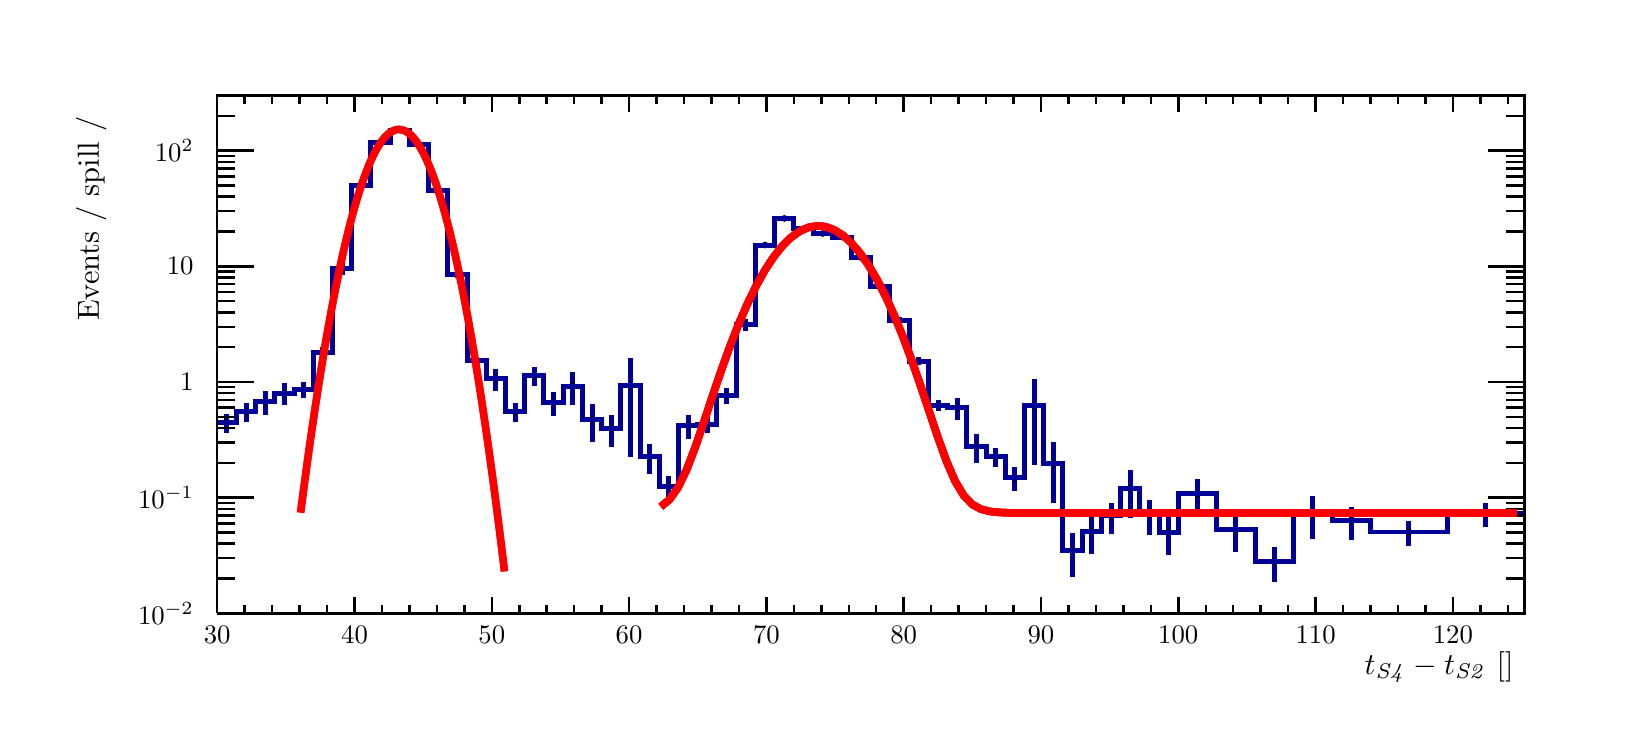
\begin{tikzpicture}
\pgfdeclareplotmark{cross} {
\pgfpathmoveto{\pgfpoint{-0.3\pgfplotmarksize}{\pgfplotmarksize}}
\pgfpathlineto{\pgfpoint{+0.3\pgfplotmarksize}{\pgfplotmarksize}}
\pgfpathlineto{\pgfpoint{+0.3\pgfplotmarksize}{0.3\pgfplotmarksize}}
\pgfpathlineto{\pgfpoint{+1\pgfplotmarksize}{0.3\pgfplotmarksize}}
\pgfpathlineto{\pgfpoint{+1\pgfplotmarksize}{-0.3\pgfplotmarksize}}
\pgfpathlineto{\pgfpoint{+0.3\pgfplotmarksize}{-0.3\pgfplotmarksize}}
\pgfpathlineto{\pgfpoint{+0.3\pgfplotmarksize}{-1.\pgfplotmarksize}}
\pgfpathlineto{\pgfpoint{-0.3\pgfplotmarksize}{-1.\pgfplotmarksize}}
\pgfpathlineto{\pgfpoint{-0.3\pgfplotmarksize}{-0.3\pgfplotmarksize}}
\pgfpathlineto{\pgfpoint{-1.\pgfplotmarksize}{-0.3\pgfplotmarksize}}
\pgfpathlineto{\pgfpoint{-1.\pgfplotmarksize}{0.3\pgfplotmarksize}}
\pgfpathlineto{\pgfpoint{-0.3\pgfplotmarksize}{0.3\pgfplotmarksize}}
\pgfpathclose
\pgfusepathqstroke
}
\pgfdeclareplotmark{cross*} {
\pgfpathmoveto{\pgfpoint{-0.3\pgfplotmarksize}{\pgfplotmarksize}}
\pgfpathlineto{\pgfpoint{+0.3\pgfplotmarksize}{\pgfplotmarksize}}
\pgfpathlineto{\pgfpoint{+0.3\pgfplotmarksize}{0.3\pgfplotmarksize}}
\pgfpathlineto{\pgfpoint{+1\pgfplotmarksize}{0.3\pgfplotmarksize}}
\pgfpathlineto{\pgfpoint{+1\pgfplotmarksize}{-0.3\pgfplotmarksize}}
\pgfpathlineto{\pgfpoint{+0.3\pgfplotmarksize}{-0.3\pgfplotmarksize}}
\pgfpathlineto{\pgfpoint{+0.3\pgfplotmarksize}{-1.\pgfplotmarksize}}
\pgfpathlineto{\pgfpoint{-0.3\pgfplotmarksize}{-1.\pgfplotmarksize}}
\pgfpathlineto{\pgfpoint{-0.3\pgfplotmarksize}{-0.3\pgfplotmarksize}}
\pgfpathlineto{\pgfpoint{-1.\pgfplotmarksize}{-0.3\pgfplotmarksize}}
\pgfpathlineto{\pgfpoint{-1.\pgfplotmarksize}{0.3\pgfplotmarksize}}
\pgfpathlineto{\pgfpoint{-0.3\pgfplotmarksize}{0.3\pgfplotmarksize}}
\pgfpathclose
\pgfusepathqfillstroke
}
\pgfdeclareplotmark{newstar} {
\pgfpathmoveto{\pgfqpoint{0pt}{\pgfplotmarksize}}
\pgfpathlineto{\pgfqpointpolar{44}{0.5\pgfplotmarksize}}
\pgfpathlineto{\pgfqpointpolar{18}{\pgfplotmarksize}}
\pgfpathlineto{\pgfqpointpolar{-20}{0.5\pgfplotmarksize}}
\pgfpathlineto{\pgfqpointpolar{-54}{\pgfplotmarksize}}
\pgfpathlineto{\pgfqpointpolar{-90}{0.5\pgfplotmarksize}}
\pgfpathlineto{\pgfqpointpolar{234}{\pgfplotmarksize}}
\pgfpathlineto{\pgfqpointpolar{198}{0.5\pgfplotmarksize}}
\pgfpathlineto{\pgfqpointpolar{162}{\pgfplotmarksize}}
\pgfpathlineto{\pgfqpointpolar{134}{0.5\pgfplotmarksize}}
\pgfpathclose
\pgfusepathqstroke
}
\pgfdeclareplotmark{newstar*} {
\pgfpathmoveto{\pgfqpoint{0pt}{\pgfplotmarksize}}
\pgfpathlineto{\pgfqpointpolar{44}{0.5\pgfplotmarksize}}
\pgfpathlineto{\pgfqpointpolar{18}{\pgfplotmarksize}}
\pgfpathlineto{\pgfqpointpolar{-20}{0.5\pgfplotmarksize}}
\pgfpathlineto{\pgfqpointpolar{-54}{\pgfplotmarksize}}
\pgfpathlineto{\pgfqpointpolar{-90}{0.5\pgfplotmarksize}}
\pgfpathlineto{\pgfqpointpolar{234}{\pgfplotmarksize}}
\pgfpathlineto{\pgfqpointpolar{198}{0.5\pgfplotmarksize}}
\pgfpathlineto{\pgfqpointpolar{162}{\pgfplotmarksize}}
\pgfpathlineto{\pgfqpointpolar{134}{0.5\pgfplotmarksize}}
\pgfpathclose
\pgfusepathqfillstroke
}
\definecolor{c}{rgb}{1,1,1};
\draw [color=c, fill=c] (0,0) rectangle (20,8.54034);
\draw [color=c, fill=c] (2.4,1.11024) rectangle (19,7.68631);
\definecolor{c}{rgb}{0,0,0};
\draw [c,line width=0.9] (2.4,1.11024) -- (2.4,7.68631) -- (19,7.68631) -- (19,1.11024) -- (2.4,1.11024);
\definecolor{c}{rgb}{1,1,1};
\draw [color=c, fill=c] (2.4,1.11024) rectangle (19,7.68631);
\definecolor{c}{rgb}{0,0,0};
\draw [c,line width=0.9] (2.4,1.11024) -- (2.4,7.68631) -- (19,7.68631) -- (19,1.11024) -- (2.4,1.11024);
\definecolor{c}{rgb}{0,0,0.6};
\draw [c,line width=1.8] (2.52206,3.40563) -- (2.52206,3.53721);
\draw [c,line width=1.8] (2.52206,3.53721) -- (2.52206,3.64623);
\definecolor{c}{rgb}{0,0,0};
\foreach \P in {(2.52206,3.53721)}{\draw[mark options={color=c,fill=c},mark size=2.402402pt,mark=*,mark size=1pt] plot coordinates {\P};}
\definecolor{c}{rgb}{0,0,0.6};
\draw [c,line width=1.8] (2.76618,3.53542) -- (2.76618,3.67175);
\draw [c,line width=1.8] (2.76618,3.67175) -- (2.76618,3.78401);
\definecolor{c}{rgb}{0,0,0};
\foreach \P in {(2.76618,3.67175)}{\draw[mark options={color=c,fill=c},mark size=2.402402pt,mark=*,mark size=1pt] plot coordinates {\P};}
\definecolor{c}{rgb}{0,0,0.6};
\draw [c,line width=1.8] (3.01029,3.63203) -- (3.01029,3.80158);
\draw [c,line width=1.8] (3.01029,3.80158) -- (3.01029,3.9354);
\definecolor{c}{rgb}{0,0,0};
\foreach \P in {(3.01029,3.80158)}{\draw[mark options={color=c,fill=c},mark size=2.402402pt,mark=*,mark size=1pt] plot coordinates {\P};}
\definecolor{c}{rgb}{0,0,0.6};
\draw [c,line width=1.8] (3.25441,3.75384) -- (3.25441,3.90664);
\draw [c,line width=1.8] (3.25441,3.90664) -- (3.25441,4.02981);
\definecolor{c}{rgb}{0,0,0};
\foreach \P in {(3.25441,3.90664)}{\draw[mark options={color=c,fill=c},mark size=2.402402pt,mark=*,mark size=1pt] plot coordinates {\P};}
\definecolor{c}{rgb}{0,0,0.6};
\draw [c,line width=1.8] (3.49853,3.83979) -- (3.49853,3.95299);
\draw [c,line width=1.8] (3.49853,3.95299) -- (3.49853,4.04909);
\definecolor{c}{rgb}{0,0,0};
\foreach \P in {(3.49853,3.95299)}{\draw[mark options={color=c,fill=c},mark size=2.402402pt,mark=*,mark size=1pt] plot coordinates {\P};}
\definecolor{c}{rgb}{0,0,0.6};
\draw [c,line width=1.8] (3.74265,4.35195) -- (3.74265,4.42496);
\draw [c,line width=1.8] (3.74265,4.42496) -- (3.74265,4.49047);
\definecolor{c}{rgb}{0,0,0};
\foreach \P in {(3.74265,4.42496)}{\draw[mark options={color=c,fill=c},mark size=2.402402pt,mark=*,mark size=1pt] plot coordinates {\P};}
\definecolor{c}{rgb}{0,0,0.6};
\draw [c,line width=1.8] (3.98676,5.4071) -- (3.98676,5.4863);
\draw [c,line width=1.8] (3.98676,5.4863) -- (3.98676,5.55674);
\definecolor{c}{rgb}{0,0,0};
\foreach \P in {(3.98676,5.4863)}{\draw[mark options={color=c,fill=c},mark size=2.402402pt,mark=*,mark size=1pt] plot coordinates {\P};}
\definecolor{c}{rgb}{0,0,0.6};
\draw [c,line width=1.8] (4.23088,6.53252) -- (4.23088,6.54645);
\draw [c,line width=1.8] (4.23088,6.54645) -- (4.23088,6.56009);
\definecolor{c}{rgb}{0,0,0};
\foreach \P in {(4.23088,6.54645)}{\draw[mark options={color=c,fill=c},mark size=2.402402pt,mark=*,mark size=1pt] plot coordinates {\P};}
\definecolor{c}{rgb}{0,0,0.6};
\draw [c,line width=1.8] (4.475,7.07742) -- (4.475,7.08706);
\draw [c,line width=1.8] (4.475,7.08706) -- (4.475,7.09655);
\definecolor{c}{rgb}{0,0,0};
\foreach \P in {(4.475,7.08706)}{\draw[mark options={color=c,fill=c},mark size=2.402402pt,mark=*,mark size=1pt] plot coordinates {\P};}
\definecolor{c}{rgb}{0,0,0.6};
\draw [c,line width=1.8] (4.71912,7.23764) -- (4.71912,7.24718);
\draw [c,line width=1.8] (4.71912,7.24718) -- (4.71912,7.25658);
\definecolor{c}{rgb}{0,0,0};
\foreach \P in {(4.71912,7.24718)}{\draw[mark options={color=c,fill=c},mark size=2.402402pt,mark=*,mark size=1pt] plot coordinates {\P};}
\definecolor{c}{rgb}{0,0,0.6};
\draw [c,line width=1.8] (4.96324,7.05689) -- (4.96324,7.06748);
\draw [c,line width=1.8] (4.96324,7.06748) -- (4.96324,7.07789);
\definecolor{c}{rgb}{0,0,0};
\foreach \P in {(4.96324,7.06748)}{\draw[mark options={color=c,fill=c},mark size=2.402402pt,mark=*,mark size=1pt] plot coordinates {\P};}
\definecolor{c}{rgb}{0,0,0.6};
\draw [c,line width=1.8] (5.20735,6.45771) -- (5.20735,6.47732);
\draw [c,line width=1.8] (5.20735,6.47732) -- (5.20735,6.49634);
\definecolor{c}{rgb}{0,0,0};
\foreach \P in {(5.20735,6.47732)}{\draw[mark options={color=c,fill=c},mark size=2.402402pt,mark=*,mark size=1pt] plot coordinates {\P};}
\definecolor{c}{rgb}{0,0,0.6};
\draw [c,line width=1.8] (5.45147,5.37429) -- (5.45147,5.41469);
\draw [c,line width=1.8] (5.45147,5.41469) -- (5.45147,5.45267);
\definecolor{c}{rgb}{0,0,0};
\foreach \P in {(5.45147,5.41469)}{\draw[mark options={color=c,fill=c},mark size=2.402402pt,mark=*,mark size=1pt] plot coordinates {\P};}
\definecolor{c}{rgb}{0,0,0.6};
\draw [c,line width=1.8] (5.69559,4.26388) -- (5.69559,4.31428);
\draw [c,line width=1.8] (5.69559,4.31428) -- (5.69559,4.361);
\definecolor{c}{rgb}{0,0,0};
\foreach \P in {(5.69559,4.31428)}{\draw[mark options={color=c,fill=c},mark size=2.402402pt,mark=*,mark size=1pt] plot coordinates {\P};}
\definecolor{c}{rgb}{0,0,0.6};
\draw [c,line width=1.8] (5.93971,3.92792) -- (5.93971,4.08884);
\draw [c,line width=1.8] (5.93971,4.08884) -- (5.93971,4.21723);
\definecolor{c}{rgb}{0,0,0};
\foreach \P in {(5.93971,4.08884)}{\draw[mark options={color=c,fill=c},mark size=2.402402pt,mark=*,mark size=1pt] plot coordinates {\P};}
\definecolor{c}{rgb}{0,0,0.6};
\draw [c,line width=1.8] (6.18382,3.53481) -- (6.18382,3.66741);
\draw [c,line width=1.8] (6.18382,3.66741) -- (6.18382,3.77714);
\definecolor{c}{rgb}{0,0,0};
\foreach \P in {(6.18382,3.66741)}{\draw[mark options={color=c,fill=c},mark size=2.402402pt,mark=*,mark size=1pt] plot coordinates {\P};}
\definecolor{c}{rgb}{0,0,0.6};
\draw [c,line width=1.8] (6.42794,3.99082) -- (6.42794,4.12429);
\draw [c,line width=1.8] (6.42794,4.12429) -- (6.42794,4.23461);
\definecolor{c}{rgb}{0,0,0};
\foreach \P in {(6.42794,4.12429)}{\draw[mark options={color=c,fill=c},mark size=2.402402pt,mark=*,mark size=1pt] plot coordinates {\P};}
\definecolor{c}{rgb}{0,0,0.6};
\draw [c,line width=1.8] (6.67206,3.62148) -- (6.67206,3.78512);
\draw [c,line width=1.8] (6.67206,3.78512) -- (6.67206,3.91524);
\definecolor{c}{rgb}{0,0,0};
\foreach \P in {(6.67206,3.78512)}{\draw[mark options={color=c,fill=c},mark size=2.402402pt,mark=*,mark size=1pt] plot coordinates {\P};}
\definecolor{c}{rgb}{0,0,0.6};
\draw [c,line width=1.8] (6.91618,3.75026) -- (6.91618,3.99588);
\draw [c,line width=1.8] (6.91618,3.99588) -- (6.91618,4.17278);
\definecolor{c}{rgb}{0,0,0};
\foreach \P in {(6.91618,3.99588)}{\draw[mark options={color=c,fill=c},mark size=2.402402pt,mark=*,mark size=1pt] plot coordinates {\P};}
\definecolor{c}{rgb}{0,0,0.6};
\draw [c,line width=1.8] (7.16029,3.28222) -- (7.16029,3.57122);
\draw [c,line width=1.8] (7.16029,3.57122) -- (7.16029,3.76938);
\definecolor{c}{rgb}{0,0,0};
\foreach \P in {(7.16029,3.57122)}{\draw[mark options={color=c,fill=c},mark size=2.402402pt,mark=*,mark size=1pt] plot coordinates {\P};}
\definecolor{c}{rgb}{0,0,0.6};
\draw [c,line width=1.8] (7.40441,3.21756) -- (7.40441,3.457);
\draw [c,line width=1.8] (7.40441,3.457) -- (7.40441,3.63069);
\definecolor{c}{rgb}{0,0,0};
\foreach \P in {(7.40441,3.457)}{\draw[mark options={color=c,fill=c},mark size=2.402402pt,mark=*,mark size=1pt] plot coordinates {\P};}
\definecolor{c}{rgb}{0,0,0.6};
\draw [c,line width=1.8] (7.64853,3.09392) -- (7.64853,3.99863);
\draw [c,line width=1.8] (7.64853,3.99863) -- (7.64853,4.35847);
\definecolor{c}{rgb}{0,0,0};
\foreach \P in {(7.64853,3.99863)}{\draw[mark options={color=c,fill=c},mark size=2.402402pt,mark=*,mark size=1pt] plot coordinates {\P};}
\definecolor{c}{rgb}{0,0,0.6};
\draw [c,line width=1.8] (7.89265,2.8828) -- (7.89265,3.09931);
\draw [c,line width=1.8] (7.89265,3.09931) -- (7.89265,3.26066);
\definecolor{c}{rgb}{0,0,0};
\foreach \P in {(7.89265,3.09931)}{\draw[mark options={color=c,fill=c},mark size=2.402402pt,mark=*,mark size=1pt] plot coordinates {\P};}
\definecolor{c}{rgb}{0,0,0.6};
\draw [c,line width=1.8] (8.13676,2.55854) -- (8.13676,2.72438);
\draw [c,line width=1.8] (8.13676,2.72438) -- (8.13676,2.85589);
\definecolor{c}{rgb}{0,0,0};
\foreach \P in {(8.13676,2.72438)}{\draw[mark options={color=c,fill=c},mark size=2.402402pt,mark=*,mark size=1pt] plot coordinates {\P};}
\definecolor{c}{rgb}{0,0,0.6};
\draw [c,line width=1.8] (8.38088,3.3223) -- (8.38088,3.49453);
\draw [c,line width=1.8] (8.38088,3.49453) -- (8.38088,3.63001);
\definecolor{c}{rgb}{0,0,0};
\foreach \P in {(8.38088,3.49453)}{\draw[mark options={color=c,fill=c},mark size=2.402402pt,mark=*,mark size=1pt] plot coordinates {\P};}
\definecolor{c}{rgb}{0,0,0.6};
\draw [c,line width=1.8] (8.625,3.39644) -- (8.625,3.5085);
\draw [c,line width=1.8] (8.625,3.5085) -- (8.625,3.60379);
\definecolor{c}{rgb}{0,0,0};
\foreach \P in {(8.625,3.5085)}{\draw[mark options={color=c,fill=c},mark size=2.402402pt,mark=*,mark size=1pt] plot coordinates {\P};}
\definecolor{c}{rgb}{0,0,0.6};
\draw [c,line width=1.8] (8.86912,3.77164) -- (8.86912,3.87856);
\draw [c,line width=1.8] (8.86912,3.87856) -- (8.86912,3.97011);
\definecolor{c}{rgb}{0,0,0};
\foreach \P in {(8.86912,3.87856)}{\draw[mark options={color=c,fill=c},mark size=2.402402pt,mark=*,mark size=1pt] plot coordinates {\P};}
\definecolor{c}{rgb}{0,0,0.6};
\draw [c,line width=1.8] (9.11324,4.6928) -- (9.11324,4.77736);
\draw [c,line width=1.8] (9.11324,4.77736) -- (9.11324,4.85201);
\definecolor{c}{rgb}{0,0,0};
\foreach \P in {(9.11324,4.77736)}{\draw[mark options={color=c,fill=c},mark size=2.402402pt,mark=*,mark size=1pt] plot coordinates {\P};}
\definecolor{c}{rgb}{0,0,0.6};
\draw [c,line width=1.8] (9.35735,5.75229) -- (9.35735,5.78607);
\draw [c,line width=1.8] (9.35735,5.78607) -- (9.35735,5.81815);
\definecolor{c}{rgb}{0,0,0};
\foreach \P in {(9.35735,5.78607)}{\draw[mark options={color=c,fill=c},mark size=2.402402pt,mark=*,mark size=1pt] plot coordinates {\P};}
\definecolor{c}{rgb}{0,0,0.6};
\draw [c,line width=1.8] (9.60147,6.10662) -- (9.60147,6.12465);
\draw [c,line width=1.8] (9.60147,6.12465) -- (9.60147,6.14217);
\definecolor{c}{rgb}{0,0,0};
\foreach \P in {(9.60147,6.12465)}{\draw[mark options={color=c,fill=c},mark size=2.402402pt,mark=*,mark size=1pt] plot coordinates {\P};}
\definecolor{c}{rgb}{0,0,0.6};
\draw [c,line width=1.8] (9.84559,5.97606) -- (9.84559,5.99533);
\draw [c,line width=1.8] (9.84559,5.99533) -- (9.84559,6.01402);
\definecolor{c}{rgb}{0,0,0};
\foreach \P in {(9.84559,5.99533)}{\draw[mark options={color=c,fill=c},mark size=2.402402pt,mark=*,mark size=1pt] plot coordinates {\P};}
\definecolor{c}{rgb}{0,0,0.6};
\draw [c,line width=1.8] (10.0897,5.91416) -- (10.0897,5.93356);
\draw [c,line width=1.8] (10.0897,5.93356) -- (10.0897,5.95238);
\definecolor{c}{rgb}{0,0,0};
\foreach \P in {(10.0897,5.93356)}{\draw[mark options={color=c,fill=c},mark size=2.402402pt,mark=*,mark size=1pt] plot coordinates {\P};}
\definecolor{c}{rgb}{0,0,0.6};
\draw [c,line width=1.8] (10.3338,5.86976) -- (10.3338,5.88863);
\draw [c,line width=1.8] (10.3338,5.88863) -- (10.3338,5.90695);
\definecolor{c}{rgb}{0,0,0};
\foreach \P in {(10.3338,5.88863)}{\draw[mark options={color=c,fill=c},mark size=2.402402pt,mark=*,mark size=1pt] plot coordinates {\P};}
\definecolor{c}{rgb}{0,0,0.6};
\draw [c,line width=1.8] (10.5779,5.60566) -- (10.5779,5.62659);
\draw [c,line width=1.8] (10.5779,5.62659) -- (10.5779,5.64687);
\definecolor{c}{rgb}{0,0,0};
\foreach \P in {(10.5779,5.62659)}{\draw[mark options={color=c,fill=c},mark size=2.402402pt,mark=*,mark size=1pt] plot coordinates {\P};}
\definecolor{c}{rgb}{0,0,0.6};
\draw [c,line width=1.8] (10.8221,5.24071) -- (10.8221,5.26561);
\draw [c,line width=1.8] (10.8221,5.26561) -- (10.8221,5.28957);
\definecolor{c}{rgb}{0,0,0};
\foreach \P in {(10.8221,5.26561)}{\draw[mark options={color=c,fill=c},mark size=2.402402pt,mark=*,mark size=1pt] plot coordinates {\P};}
\definecolor{c}{rgb}{0,0,0.6};
\draw [c,line width=1.8] (11.0662,4.77399) -- (11.0662,4.82392);
\draw [c,line width=1.8] (11.0662,4.82392) -- (11.0662,4.87023);
\definecolor{c}{rgb}{0,0,0};
\foreach \P in {(11.0662,4.82392)}{\draw[mark options={color=c,fill=c},mark size=2.402402pt,mark=*,mark size=1pt] plot coordinates {\P};}
\definecolor{c}{rgb}{0,0,0.6};
\draw [c,line width=1.8] (11.3103,4.26256) -- (11.3103,4.31303);
\draw [c,line width=1.8] (11.3103,4.31303) -- (11.3103,4.35981);
\definecolor{c}{rgb}{0,0,0};
\foreach \P in {(11.3103,4.31303)}{\draw[mark options={color=c,fill=c},mark size=2.402402pt,mark=*,mark size=1pt] plot coordinates {\P};}
\definecolor{c}{rgb}{0,0,0.6};
\draw [c,line width=1.8] (11.5544,3.67567) -- (11.5544,3.75184);
\draw [c,line width=1.8] (11.5544,3.75184) -- (11.5544,3.81988);
\definecolor{c}{rgb}{0,0,0};
\foreach \P in {(11.5544,3.75184)}{\draw[mark options={color=c,fill=c},mark size=2.402402pt,mark=*,mark size=1pt] plot coordinates {\P};}
\definecolor{c}{rgb}{0,0,0.6};
\draw [c,line width=1.8] (11.7985,3.5672) -- (11.7985,3.72348);
\draw [c,line width=1.8] (11.7985,3.72348) -- (11.7985,3.8489);
\definecolor{c}{rgb}{0,0,0};
\foreach \P in {(11.7985,3.72348)}{\draw[mark options={color=c,fill=c},mark size=2.402402pt,mark=*,mark size=1pt] plot coordinates {\P};}
\definecolor{c}{rgb}{0,0,0.6};
\draw [c,line width=1.8] (12.0426,3.02416) -- (12.0426,3.23053);
\draw [c,line width=1.8] (12.0426,3.23053) -- (12.0426,3.3862);
\definecolor{c}{rgb}{0,0,0};
\foreach \P in {(12.0426,3.23053)}{\draw[mark options={color=c,fill=c},mark size=2.402402pt,mark=*,mark size=1pt] plot coordinates {\P};}
\definecolor{c}{rgb}{0,0,0.6};
\draw [c,line width=1.8] (12.2868,2.96839) -- (12.2868,3.09817);
\draw [c,line width=1.8] (12.2868,3.09817) -- (12.2868,3.20596);
\definecolor{c}{rgb}{0,0,0};
\foreach \P in {(12.2868,3.09817)}{\draw[mark options={color=c,fill=c},mark size=2.402402pt,mark=*,mark size=1pt] plot coordinates {\P};}
\definecolor{c}{rgb}{0,0,0.6};
\draw [c,line width=1.8] (12.5309,2.65687) -- (12.5309,2.82943);
\draw [c,line width=1.8] (12.5309,2.82943) -- (12.5309,2.96512);
\definecolor{c}{rgb}{0,0,0};
\foreach \P in {(12.5309,2.82943)}{\draw[mark options={color=c,fill=c},mark size=2.402402pt,mark=*,mark size=1pt] plot coordinates {\P};}
\definecolor{c}{rgb}{0,0,0.6};
\draw [c,line width=1.8] (12.775,2.99823) -- (12.775,3.74575);
\draw [c,line width=1.8] (12.775,3.74575) -- (12.775,4.08055);
\definecolor{c}{rgb}{0,0,0};
\foreach \P in {(12.775,3.74575)}{\draw[mark options={color=c,fill=c},mark size=2.402402pt,mark=*,mark size=1pt] plot coordinates {\P};}
\definecolor{c}{rgb}{0,0,0.6};
\draw [c,line width=1.8] (13.0191,2.51154) -- (13.0191,3.0069);
\draw [c,line width=1.8] (13.0191,3.0069) -- (13.0191,3.28234);
\definecolor{c}{rgb}{0,0,0};
\foreach \P in {(13.0191,3.0069)}{\draw[mark options={color=c,fill=c},mark size=2.402402pt,mark=*,mark size=1pt] plot coordinates {\P};}
\definecolor{c}{rgb}{0,0,0.6};
\draw [c,line width=1.8] (13.2632,1.56822) -- (13.2632,1.91332);
\draw [c,line width=1.8] (13.2632,1.91332) -- (13.2632,2.13603);
\definecolor{c}{rgb}{0,0,0};
\foreach \P in {(13.2632,1.91332)}{\draw[mark options={color=c,fill=c},mark size=2.402402pt,mark=*,mark size=1pt] plot coordinates {\P};}
\definecolor{c}{rgb}{0,0,0.6};
\draw [c,line width=1.8] (13.5074,1.85818) -- (13.5074,2.15383);
\draw [c,line width=1.8] (13.5074,2.15383) -- (13.5074,2.35507);
\definecolor{c}{rgb}{0,0,0};
\foreach \P in {(13.5074,2.15383)}{\draw[mark options={color=c,fill=c},mark size=2.402402pt,mark=*,mark size=1pt] plot coordinates {\P};}
\definecolor{c}{rgb}{0,0,0.6};
\draw [c,line width=1.8] (13.7515,2.119) -- (13.7515,2.34834);
\draw [c,line width=1.8] (13.7515,2.34834) -- (13.7515,2.51667);
\definecolor{c}{rgb}{0,0,0};
\foreach \P in {(13.7515,2.34834)}{\draw[mark options={color=c,fill=c},mark size=2.402402pt,mark=*,mark size=1pt] plot coordinates {\P};}
\definecolor{c}{rgb}{0,0,0.6};
\draw [c,line width=1.8] (13.9956,2.32513) -- (13.9956,2.69427);
\draw [c,line width=1.8] (13.9956,2.69427) -- (13.9956,2.9266);
\definecolor{c}{rgb}{0,0,0};
\foreach \P in {(13.9956,2.69427)}{\draw[mark options={color=c,fill=c},mark size=2.402402pt,mark=*,mark size=1pt] plot coordinates {\P};}
\definecolor{c}{rgb}{0,0,0.6};
\draw [c,line width=1.8] (14.2397,2.10687) -- (14.2397,2.36895);
\draw [c,line width=1.8] (14.2397,2.36895) -- (14.2397,2.55417);
\definecolor{c}{rgb}{0,0,0};
\foreach \P in {(14.2397,2.36895)}{\draw[mark options={color=c,fill=c},mark size=2.402402pt,mark=*,mark size=1pt] plot coordinates {\P};}
\definecolor{c}{rgb}{0,0,0.6};
\draw [c,line width=1.8] (14.4838,1.85514) -- (14.4838,2.14103);
\draw [c,line width=1.8] (14.4838,2.14103) -- (14.4838,2.33774);
\definecolor{c}{rgb}{0,0,0};
\foreach \P in {(14.4838,2.14103)}{\draw[mark options={color=c,fill=c},mark size=2.402402pt,mark=*,mark size=1pt] plot coordinates {\P};}
\definecolor{c}{rgb}{0,0,0.6};
\draw [c,line width=1.8] (14.85,2.36537) -- (14.85,2.62598);
\draw [c,line width=1.8] (14.85,2.62598) -- (14.85,2.81047);
\definecolor{c}{rgb}{0,0,0};
\foreach \P in {(14.85,2.62598)}{\draw[mark options={color=c,fill=c},mark size=2.402402pt,mark=*,mark size=1pt] plot coordinates {\P};}
\definecolor{c}{rgb}{0,0,0.6};
\draw [c,line width=1.8] (15.3382,1.88934) -- (15.3382,2.169);
\draw [c,line width=1.8] (15.3382,2.169) -- (15.3382,2.36277);
\definecolor{c}{rgb}{0,0,0};
\foreach \P in {(15.3382,2.169)}{\draw[mark options={color=c,fill=c},mark size=2.402402pt,mark=*,mark size=1pt] plot coordinates {\P};}
\definecolor{c}{rgb}{0,0,0.6};
\draw [c,line width=1.8] (15.8265,1.50226) -- (15.8265,1.76695);
\draw [c,line width=1.8] (15.8265,1.76695) -- (15.8265,1.95346);
\definecolor{c}{rgb}{0,0,0};
\foreach \P in {(15.8265,1.76695)}{\draw[mark options={color=c,fill=c},mark size=2.402402pt,mark=*,mark size=1pt] plot coordinates {\P};}
\definecolor{c}{rgb}{0,0,0.6};
\draw [c,line width=1.8] (16.3147,2.04847) -- (16.3147,2.37792);
\draw [c,line width=1.8] (16.3147,2.37792) -- (16.3147,2.59408);
\definecolor{c}{rgb}{0,0,0};
\foreach \P in {(16.3147,2.37792)}{\draw[mark options={color=c,fill=c},mark size=2.402402pt,mark=*,mark size=1pt] plot coordinates {\P};}
\definecolor{c}{rgb}{0,0,0.6};
\draw [c,line width=1.8] (16.8029,2.03706) -- (16.8029,2.28433);
\draw [c,line width=1.8] (16.8029,2.28433) -- (16.8029,2.46207);
\definecolor{c}{rgb}{0,0,0};
\foreach \P in {(16.8029,2.28433)}{\draw[mark options={color=c,fill=c},mark size=2.402402pt,mark=*,mark size=1pt] plot coordinates {\P};}
\definecolor{c}{rgb}{0,0,0.6};
\draw [c,line width=1.8] (17.5353,1.96777) -- (17.5353,2.14249);
\draw [c,line width=1.8] (17.5353,2.14249) -- (17.5353,2.2795);
\definecolor{c}{rgb}{0,0,0};
\foreach \P in {(17.5353,2.14249)}{\draw[mark options={color=c,fill=c},mark size=2.402402pt,mark=*,mark size=1pt] plot coordinates {\P};}
\definecolor{c}{rgb}{0,0,0.6};
\draw [c,line width=1.8] (18.5118,2.20521) -- (18.5118,2.37216);
\draw [c,line width=1.8] (18.5118,2.37216) -- (18.5118,2.50435);
\definecolor{c}{rgb}{0,0,0};
\foreach \P in {(18.5118,2.37216)}{\draw[mark options={color=c,fill=c},mark size=2.402402pt,mark=*,mark size=1pt] plot coordinates {\P};}
\definecolor{c}{rgb}{0,0,0.6};
\draw [c,line width=1.8] (2.4,3.53721) -- (2.64412,3.53721) -- (2.64412,3.67175) -- (2.88824,3.67175) -- (2.88824,3.80158) -- (3.13235,3.80158) -- (3.13235,3.90664) -- (3.37647,3.90664) -- (3.37647,3.95299) -- (3.62059,3.95299) -- (3.62059,4.42496)
 -- (3.86471,4.42496) -- (3.86471,5.4863) -- (4.10882,5.4863) -- (4.10882,6.54645) -- (4.35294,6.54645) -- (4.35294,7.08706) -- (4.59706,7.08706) -- (4.59706,7.24718) -- (4.84118,7.24718) -- (4.84118,7.06748) -- (5.08529,7.06748) -- (5.08529,6.47732)
 -- (5.32941,6.47732) -- (5.32941,5.41469) -- (5.57353,5.41469) -- (5.57353,4.31428) -- (5.81765,4.31428) -- (5.81765,4.08884) -- (6.06176,4.08884) -- (6.06176,3.66741) -- (6.30588,3.66741) -- (6.30588,4.12429) -- (6.55,4.12429) -- (6.55,3.78512) --
 (6.79412,3.78512) -- (6.79412,3.99588) -- (7.03824,3.99588) -- (7.03824,3.57122) -- (7.28235,3.57122) -- (7.28235,3.457) -- (7.52647,3.457) -- (7.52647,3.99863) -- (7.77059,3.99863) -- (7.77059,3.09931) -- (8.01471,3.09931) -- (8.01471,2.72438) --
 (8.25882,2.72438) -- (8.25882,3.49453) -- (8.50294,3.49453) -- (8.50294,3.5085) -- (8.74706,3.5085) -- (8.74706,3.87856) -- (8.99118,3.87856) -- (8.99118,4.77736) -- (9.23529,4.77736) -- (9.23529,5.78607) -- (9.47941,5.78607) -- (9.47941,6.12465) --
 (9.72353,6.12465) -- (9.72353,5.99533) -- (9.96765,5.99533) -- (9.96765,5.93356) -- (10.2118,5.93356) -- (10.2118,5.88863) -- (10.4559,5.88863) -- (10.4559,5.62659) -- (10.7,5.62659) -- (10.7,5.26561) -- (10.9441,5.26561) -- (10.9441,4.82392) --
 (11.1882,4.82392) -- (11.1882,4.31303) -- (11.4324,4.31303) -- (11.4324,3.75184) -- (11.6765,3.75184) -- (11.6765,3.72348) -- (11.9206,3.72348) -- (11.9206,3.23053) -- (12.1647,3.23053) -- (12.1647,3.09817) -- (12.4088,3.09817) -- (12.4088,2.82943)
 -- (12.6529,2.82943) -- (12.6529,3.74575) -- (12.8971,3.74575) -- (12.8971,3.0069) -- (13.1412,3.0069) -- (13.1412,1.91332) -- (13.3853,1.91332) -- (13.3853,2.15383) -- (13.6294,2.15383) -- (13.6294,2.34834) -- (13.8735,2.34834) -- (13.8735,2.69427)
 -- (14.1176,2.69427) -- (14.1176,2.36895) -- (14.3618,2.36895) -- (14.3618,2.14103) -- (14.6059,2.14103) -- (14.6059,2.62598) -- (15.0941,2.62598) -- (15.0941,2.169) -- (15.5824,2.169) -- (15.5824,1.76695) -- (16.0706,1.76695) -- (16.0706,2.37792)
 -- (16.5588,2.37792) -- (16.5588,2.28433) -- (17.0471,2.28433) -- (17.0471,2.14249) -- (18.0235,2.14249) -- (18.0235,2.37216) -- (19,2.37216);
\definecolor{c}{rgb}{0,0,0};
\draw [c,line width=0.9] (2.4,1.11024) -- (19,1.11024);
\draw [c,line width=0.9] (2.4,1.3229) -- (2.4,1.11024);
\draw [c,line width=0.9] (2.74874,1.21657) -- (2.74874,1.11024);
\draw [c,line width=0.9] (3.09748,1.21657) -- (3.09748,1.11024);
\draw [c,line width=0.9] (3.44622,1.21657) -- (3.44622,1.11024);
\draw [c,line width=0.9] (3.79496,1.21657) -- (3.79496,1.11024);
\draw [c,line width=0.9] (4.1437,1.3229) -- (4.1437,1.11024);
\draw [c,line width=0.9] (4.49244,1.21657) -- (4.49244,1.11024);
\draw [c,line width=0.9] (4.84118,1.21657) -- (4.84118,1.11024);
\draw [c,line width=0.9] (5.18992,1.21657) -- (5.18992,1.11024);
\draw [c,line width=0.9] (5.53866,1.21657) -- (5.53866,1.11024);
\draw [c,line width=0.9] (5.88739,1.3229) -- (5.88739,1.11024);
\draw [c,line width=0.9] (6.23613,1.21657) -- (6.23613,1.11024);
\draw [c,line width=0.9] (6.58487,1.21657) -- (6.58487,1.11024);
\draw [c,line width=0.9] (6.93361,1.21657) -- (6.93361,1.11024);
\draw [c,line width=0.9] (7.28235,1.21657) -- (7.28235,1.11024);
\draw [c,line width=0.9] (7.63109,1.3229) -- (7.63109,1.11024);
\draw [c,line width=0.9] (7.97983,1.21657) -- (7.97983,1.11024);
\draw [c,line width=0.9] (8.32857,1.21657) -- (8.32857,1.11024);
\draw [c,line width=0.9] (8.67731,1.21657) -- (8.67731,1.11024);
\draw [c,line width=0.9] (9.02605,1.21657) -- (9.02605,1.11024);
\draw [c,line width=0.9] (9.37479,1.3229) -- (9.37479,1.11024);
\draw [c,line width=0.9] (9.72353,1.21657) -- (9.72353,1.11024);
\draw [c,line width=0.9] (10.0723,1.21657) -- (10.0723,1.11024);
\draw [c,line width=0.9] (10.421,1.21657) -- (10.421,1.11024);
\draw [c,line width=0.9] (10.7697,1.21657) -- (10.7697,1.11024);
\draw [c,line width=0.9] (11.1185,1.3229) -- (11.1185,1.11024);
\draw [c,line width=0.9] (11.4672,1.21657) -- (11.4672,1.11024);
\draw [c,line width=0.9] (11.816,1.21657) -- (11.816,1.11024);
\draw [c,line width=0.9] (12.1647,1.21657) -- (12.1647,1.11024);
\draw [c,line width=0.9] (12.5134,1.21657) -- (12.5134,1.11024);
\draw [c,line width=0.9] (12.8622,1.3229) -- (12.8622,1.11024);
\draw [c,line width=0.9] (13.2109,1.21657) -- (13.2109,1.11024);
\draw [c,line width=0.9] (13.5597,1.21657) -- (13.5597,1.11024);
\draw [c,line width=0.9] (13.9084,1.21657) -- (13.9084,1.11024);
\draw [c,line width=0.9] (14.2571,1.21657) -- (14.2571,1.11024);
\draw [c,line width=0.9] (14.6059,1.3229) -- (14.6059,1.11024);
\draw [c,line width=0.9] (14.9546,1.21657) -- (14.9546,1.11024);
\draw [c,line width=0.9] (15.3034,1.21657) -- (15.3034,1.11024);
\draw [c,line width=0.9] (15.6521,1.21657) -- (15.6521,1.11024);
\draw [c,line width=0.9] (16.0008,1.21657) -- (16.0008,1.11024);
\draw [c,line width=0.9] (16.3496,1.3229) -- (16.3496,1.11024);
\draw [c,line width=0.9] (16.6983,1.21657) -- (16.6983,1.11024);
\draw [c,line width=0.9] (17.0471,1.21657) -- (17.0471,1.11024);
\draw [c,line width=0.9] (17.3958,1.21657) -- (17.3958,1.11024);
\draw [c,line width=0.9] (17.7445,1.21657) -- (17.7445,1.11024);
\draw [c,line width=0.9] (18.0933,1.3229) -- (18.0933,1.11024);
\draw [c,line width=0.9] (18.0933,1.3229) -- (18.0933,1.11024);
\draw [c,line width=0.9] (18.442,1.21657) -- (18.442,1.11024);
\draw [c,line width=0.9] (18.7908,1.21657) -- (18.7908,1.11024);
\draw [anchor=base] (2.4,0.725929) node[scale=0.966515, color=c, rotate=0]{30};
\draw [anchor=base] (4.1437,0.725929) node[scale=0.966515, color=c, rotate=0]{40};
\draw [anchor=base] (5.88739,0.725929) node[scale=0.966515, color=c, rotate=0]{50};
\draw [anchor=base] (7.63109,0.725929) node[scale=0.966515, color=c, rotate=0]{60};
\draw [anchor=base] (9.37479,0.725929) node[scale=0.966515, color=c, rotate=0]{70};
\draw [anchor=base] (11.1185,0.725929) node[scale=0.966515, color=c, rotate=0]{80};
\draw [anchor=base] (12.8622,0.725929) node[scale=0.966515, color=c, rotate=0]{90};
\draw [anchor=base] (14.6059,0.725929) node[scale=0.966515, color=c, rotate=0]{100};
\draw [anchor=base] (16.3496,0.725929) node[scale=0.966515, color=c, rotate=0]{110};
\draw [anchor=base] (18.0933,0.725929) node[scale=0.966515, color=c, rotate=0]{120};
\draw [anchor= east] (19,0.427017) node[scale=1.1, color=c, rotate=0]{$t_{\SFour} - t_{\STwo}$ [\si{\nano\second}] };
\draw [c,line width=0.9] (2.4,7.68631) -- (19,7.68631);
\draw [c,line width=0.9] (2.4,7.47366) -- (2.4,7.68631);
\draw [c,line width=0.9] (2.74874,7.57998) -- (2.74874,7.68631);
\draw [c,line width=0.9] (3.09748,7.57998) -- (3.09748,7.68631);
\draw [c,line width=0.9] (3.44622,7.57998) -- (3.44622,7.68631);
\draw [c,line width=0.9] (3.79496,7.57998) -- (3.79496,7.68631);
\draw [c,line width=0.9] (4.1437,7.47366) -- (4.1437,7.68631);
\draw [c,line width=0.9] (4.49244,7.57998) -- (4.49244,7.68631);
\draw [c,line width=0.9] (4.84118,7.57998) -- (4.84118,7.68631);
\draw [c,line width=0.9] (5.18992,7.57998) -- (5.18992,7.68631);
\draw [c,line width=0.9] (5.53866,7.57998) -- (5.53866,7.68631);
\draw [c,line width=0.9] (5.88739,7.47366) -- (5.88739,7.68631);
\draw [c,line width=0.9] (6.23613,7.57998) -- (6.23613,7.68631);
\draw [c,line width=0.9] (6.58487,7.57998) -- (6.58487,7.68631);
\draw [c,line width=0.9] (6.93361,7.57998) -- (6.93361,7.68631);
\draw [c,line width=0.9] (7.28235,7.57998) -- (7.28235,7.68631);
\draw [c,line width=0.9] (7.63109,7.47366) -- (7.63109,7.68631);
\draw [c,line width=0.9] (7.97983,7.57998) -- (7.97983,7.68631);
\draw [c,line width=0.9] (8.32857,7.57998) -- (8.32857,7.68631);
\draw [c,line width=0.9] (8.67731,7.57998) -- (8.67731,7.68631);
\draw [c,line width=0.9] (9.02605,7.57998) -- (9.02605,7.68631);
\draw [c,line width=0.9] (9.37479,7.47366) -- (9.37479,7.68631);
\draw [c,line width=0.9] (9.72353,7.57998) -- (9.72353,7.68631);
\draw [c,line width=0.9] (10.0723,7.57998) -- (10.0723,7.68631);
\draw [c,line width=0.9] (10.421,7.57998) -- (10.421,7.68631);
\draw [c,line width=0.9] (10.7697,7.57998) -- (10.7697,7.68631);
\draw [c,line width=0.9] (11.1185,7.47366) -- (11.1185,7.68631);
\draw [c,line width=0.9] (11.4672,7.57998) -- (11.4672,7.68631);
\draw [c,line width=0.9] (11.816,7.57998) -- (11.816,7.68631);
\draw [c,line width=0.9] (12.1647,7.57998) -- (12.1647,7.68631);
\draw [c,line width=0.9] (12.5134,7.57998) -- (12.5134,7.68631);
\draw [c,line width=0.9] (12.8622,7.47366) -- (12.8622,7.68631);
\draw [c,line width=0.9] (13.2109,7.57998) -- (13.2109,7.68631);
\draw [c,line width=0.9] (13.5597,7.57998) -- (13.5597,7.68631);
\draw [c,line width=0.9] (13.9084,7.57998) -- (13.9084,7.68631);
\draw [c,line width=0.9] (14.2571,7.57998) -- (14.2571,7.68631);
\draw [c,line width=0.9] (14.6059,7.47366) -- (14.6059,7.68631);
\draw [c,line width=0.9] (14.9546,7.57998) -- (14.9546,7.68631);
\draw [c,line width=0.9] (15.3034,7.57998) -- (15.3034,7.68631);
\draw [c,line width=0.9] (15.6521,7.57998) -- (15.6521,7.68631);
\draw [c,line width=0.9] (16.0008,7.57998) -- (16.0008,7.68631);
\draw [c,line width=0.9] (16.3496,7.47366) -- (16.3496,7.68631);
\draw [c,line width=0.9] (16.6983,7.57998) -- (16.6983,7.68631);
\draw [c,line width=0.9] (17.0471,7.57998) -- (17.0471,7.68631);
\draw [c,line width=0.9] (17.3958,7.57998) -- (17.3958,7.68631);
\draw [c,line width=0.9] (17.7445,7.57998) -- (17.7445,7.68631);
\draw [c,line width=0.9] (18.0933,7.47366) -- (18.0933,7.68631);
\draw [c,line width=0.9] (18.0933,7.47366) -- (18.0933,7.68631);
\draw [c,line width=0.9] (18.442,7.57998) -- (18.442,7.68631);
\draw [c,line width=0.9] (18.7908,7.57998) -- (18.7908,7.68631);
\draw [c,line width=0.9] (2.4,1.11024) -- (2.4,7.68631);
\draw [c,line width=0.9] (2.862,1.11025) -- (2.4,1.11025);
\draw [anchor= east] (2.22,1.11025) node[scale=0.966515, color=c, rotate=0]{$10^{-2}$};
\draw [c,line width=0.9] (2.631,1.5524) -- (2.4,1.5524);
\draw [c,line width=0.9] (2.631,1.81105) -- (2.4,1.81105);
\draw [c,line width=0.9] (2.631,1.99456) -- (2.4,1.99456);
\draw [c,line width=0.9] (2.631,2.1369) -- (2.4,2.1369);
\draw [c,line width=0.9] (2.631,2.25321) -- (2.4,2.25321);
\draw [c,line width=0.9] (2.631,2.35154) -- (2.4,2.35154);
\draw [c,line width=0.9] (2.631,2.43672) -- (2.4,2.43672);
\draw [c,line width=0.9] (2.631,2.51185) -- (2.4,2.51185);
\draw [c,line width=0.9] (2.862,2.57906) -- (2.4,2.57906);
\draw [anchor= east] (2.22,2.57906) node[scale=0.966515, color=c, rotate=0]{$10^{-1}$};
\draw [c,line width=0.9] (2.631,3.02122) -- (2.4,3.02122);
\draw [c,line width=0.9] (2.631,3.27986) -- (2.4,3.27986);
\draw [c,line width=0.9] (2.631,3.46338) -- (2.4,3.46338);
\draw [c,line width=0.9] (2.631,3.60572) -- (2.4,3.60572);
\draw [c,line width=0.9] (2.631,3.72202) -- (2.4,3.72202);
\draw [c,line width=0.9] (2.631,3.82035) -- (2.4,3.82035);
\draw [c,line width=0.9] (2.631,3.90553) -- (2.4,3.90553);
\draw [c,line width=0.9] (2.631,3.98067) -- (2.4,3.98067);
\draw [c,line width=0.9] (2.862,4.04788) -- (2.4,4.04788);
\draw [anchor= east] (2.22,4.04788) node[scale=0.966515, color=c, rotate=0]{1};
\draw [c,line width=0.9] (2.631,4.49003) -- (2.4,4.49003);
\draw [c,line width=0.9] (2.631,4.74868) -- (2.4,4.74868);
\draw [c,line width=0.9] (2.631,4.93219) -- (2.4,4.93219);
\draw [c,line width=0.9] (2.631,5.07453) -- (2.4,5.07453);
\draw [c,line width=0.9] (2.631,5.19084) -- (2.4,5.19084);
\draw [c,line width=0.9] (2.631,5.28917) -- (2.4,5.28917);
\draw [c,line width=0.9] (2.631,5.37435) -- (2.4,5.37435);
\draw [c,line width=0.9] (2.631,5.44948) -- (2.4,5.44948);
\draw [c,line width=0.9] (2.862,5.51669) -- (2.4,5.51669);
\draw [anchor= east] (2.22,5.51669) node[scale=0.966515, color=c, rotate=0]{10};
\draw [c,line width=0.9] (2.631,5.95885) -- (2.4,5.95885);
\draw [c,line width=0.9] (2.631,6.21749) -- (2.4,6.21749);
\draw [c,line width=0.9] (2.631,6.40101) -- (2.4,6.40101);
\draw [c,line width=0.9] (2.631,6.54335) -- (2.4,6.54335);
\draw [c,line width=0.9] (2.631,6.65965) -- (2.4,6.65965);
\draw [c,line width=0.9] (2.631,6.75798) -- (2.4,6.75798);
\draw [c,line width=0.9] (2.631,6.84316) -- (2.4,6.84316);
\draw [c,line width=0.9] (2.631,6.9183) -- (2.4,6.9183);
\draw [c,line width=0.9] (2.862,6.98551) -- (2.4,6.98551);
\draw [anchor= east] (2.22,6.98551) node[scale=0.966515, color=c, rotate=0]{$10^{2}$};
\draw [c,line width=0.9] (2.631,7.42766) -- (2.4,7.42766);
\draw [c,line width=0.9] (2.631,7.68631) -- (2.4,7.68631);
\draw [anchor= east] (0.8,7.68631) node[scale=1.1, color=c, rotate=90]{ Events / spill / \si{\nano\second} };
\draw [c,line width=0.9] (19,1.11024) -- (19,7.68631);
\draw [c,line width=0.9] (18.538,1.11025) -- (19,1.11025);
\draw [c,line width=0.9] (18.769,1.5524) -- (19,1.5524);
\draw [c,line width=0.9] (18.769,1.81105) -- (19,1.81105);
\draw [c,line width=0.9] (18.769,1.99456) -- (19,1.99456);
\draw [c,line width=0.9] (18.769,2.1369) -- (19,2.1369);
\draw [c,line width=0.9] (18.769,2.25321) -- (19,2.25321);
\draw [c,line width=0.9] (18.769,2.35154) -- (19,2.35154);
\draw [c,line width=0.9] (18.769,2.43672) -- (19,2.43672);
\draw [c,line width=0.9] (18.769,2.51185) -- (19,2.51185);
\draw [c,line width=0.9] (18.538,2.57906) -- (19,2.57906);
\draw [c,line width=0.9] (18.769,3.02122) -- (19,3.02122);
\draw [c,line width=0.9] (18.769,3.27986) -- (19,3.27986);
\draw [c,line width=0.9] (18.769,3.46338) -- (19,3.46338);
\draw [c,line width=0.9] (18.769,3.60572) -- (19,3.60572);
\draw [c,line width=0.9] (18.769,3.72202) -- (19,3.72202);
\draw [c,line width=0.9] (18.769,3.82035) -- (19,3.82035);
\draw [c,line width=0.9] (18.769,3.90553) -- (19,3.90553);
\draw [c,line width=0.9] (18.769,3.98067) -- (19,3.98067);
\draw [c,line width=0.9] (18.538,4.04788) -- (19,4.04788);
\draw [c,line width=0.9] (18.769,4.49003) -- (19,4.49003);
\draw [c,line width=0.9] (18.769,4.74868) -- (19,4.74868);
\draw [c,line width=0.9] (18.769,4.93219) -- (19,4.93219);
\draw [c,line width=0.9] (18.769,5.07453) -- (19,5.07453);
\draw [c,line width=0.9] (18.769,5.19084) -- (19,5.19084);
\draw [c,line width=0.9] (18.769,5.28917) -- (19,5.28917);
\draw [c,line width=0.9] (18.769,5.37435) -- (19,5.37435);
\draw [c,line width=0.9] (18.769,5.44948) -- (19,5.44948);
\draw [c,line width=0.9] (18.538,5.51669) -- (19,5.51669);
\draw [c,line width=0.9] (18.769,5.95885) -- (19,5.95885);
\draw [c,line width=0.9] (18.769,6.21749) -- (19,6.21749);
\draw [c,line width=0.9] (18.769,6.40101) -- (19,6.40101);
\draw [c,line width=0.9] (18.769,6.54335) -- (19,6.54335);
\draw [c,line width=0.9] (18.769,6.65965) -- (19,6.65965);
\draw [c,line width=0.9] (18.769,6.75798) -- (19,6.75798);
\draw [c,line width=0.9] (18.769,6.84316) -- (19,6.84316);
\draw [c,line width=0.9] (18.769,6.9183) -- (19,6.9183);
\draw [c,line width=0.9] (18.538,6.98551) -- (19,6.98551);
\draw [c,line width=0.9] (18.769,7.42766) -- (19,7.42766);
\draw [c,line width=0.9] (18.769,7.68631) -- (19,7.68631);
\definecolor{c}{rgb}{1,1,1};
\draw [color=c, fill=c] (2,8.02792) rectangle (18,8.49764);
\definecolor{c}{rgb}{0,0,0};
%\draw (10,8.26278) node[scale=0.885972, color=c, rotate=0]{Time of flight, measured in S4, 1 blocks};
\definecolor{c}{rgb}{1,0,0};
\draw [c,line width=2.7] (3.4593,2.3887) -- (3.48545,2.59046) -- (3.51161,2.78795) -- (3.53776,2.98116) -- (3.56392,3.17011) -- (3.59007,3.35478) -- (3.61623,3.53519) -- (3.64238,3.71132) -- (3.66854,3.88318) -- (3.6947,4.05077) -- (3.72085,4.21409)
 -- (3.74701,4.37313) -- (3.77316,4.52791) -- (3.79932,4.67841) -- (3.82547,4.82464) -- (3.85163,4.9666) -- (3.87778,5.10429) -- (3.90394,5.23771) -- (3.93009,5.36685) -- (3.95625,5.49173) -- (3.98241,5.61233) -- (4.00856,5.72866) --
 (4.03472,5.84072) -- (4.06087,5.94851) -- (4.08703,6.05203) -- (4.11318,6.15127) -- (4.13934,6.24625) -- (4.16549,6.33695) -- (4.19165,6.42338) -- (4.2178,6.50554) -- (4.24396,6.58343) -- (4.27012,6.65705) -- (4.29627,6.7264) -- (4.32243,6.79147) --
 (4.34858,6.85227) -- (4.37474,6.9088) -- (4.40089,6.96106) -- (4.42705,7.00905) -- (4.4532,7.05277) -- (4.47936,7.09222) -- (4.50551,7.12739) -- (4.53167,7.15829) -- (4.55783,7.18492) -- (4.58398,7.20728) -- (4.61014,7.22537) -- (4.63629,7.23919) --
 (4.66245,7.24873) -- (4.6886,7.25401) -- (4.71476,7.25501) -- (4.74091,7.25174);
\draw [c,line width=2.7] (4.74091,7.25174) -- (4.76707,7.2442) -- (4.79322,7.23239) -- (4.81938,7.21631) -- (4.84554,7.19595) -- (4.87169,7.17133) -- (4.89785,7.14243) -- (4.924,7.10926) -- (4.95016,7.07182) -- (4.97631,7.03011) -- (5.00247,6.98413)
 -- (5.02862,6.93387) -- (5.05478,6.87935) -- (5.08094,6.82055) -- (5.10709,6.75748) -- (5.13325,6.69014) -- (5.1594,6.61853) -- (5.18556,6.54264) -- (5.21171,6.46249) -- (5.23787,6.37806) -- (5.26402,6.28937) -- (5.29018,6.1964) -- (5.31633,6.09916)
 -- (5.34249,5.99764) -- (5.36864,5.89186) -- (5.3948,5.78181) -- (5.42096,5.66748) -- (5.44711,5.54888) -- (5.47327,5.42601) -- (5.49942,5.29887) -- (5.52558,5.16746) -- (5.55173,5.03178) -- (5.57789,4.89182) -- (5.60404,4.7476) -- (5.6302,4.5991)
 -- (5.65635,4.44633) -- (5.68251,4.28929) -- (5.70867,4.12798) -- (5.73482,3.9624) -- (5.76098,3.79254) -- (5.78713,3.61841) -- (5.81329,3.44002) -- (5.83944,3.25735) -- (5.8656,3.07041) -- (5.89175,2.87919) -- (5.91791,2.68371) -- (5.94407,2.48396)
 -- (5.97022,2.27993) -- (5.99638,2.07163) -- (6.02253,1.85906);
\draw [c,line width=2.7] (6.02253,1.85906) -- (6.04869,1.64222);
\draw [c,line width=2.7] (8.03476,2.46443) -- (8.14461,2.55465) -- (8.25446,2.71043) -- (8.36432,2.93959) -- (8.47417,3.2283) -- (8.58402,3.55006) -- (8.69388,3.88018) -- (8.80373,4.20188) -- (8.91358,4.50538) -- (9.02343,4.7854) -- (9.13329,5.03912)
 -- (9.24314,5.26503) -- (9.35299,5.46233) -- (9.46285,5.63055) -- (9.5727,5.76945) -- (9.68255,5.87887) -- (9.79241,5.95872) -- (9.90226,6.00896) -- (10.0121,6.02956) -- (10.122,6.02051) -- (10.2318,5.98182) -- (10.3417,5.9135) -- (10.4515,5.81559)
 -- (10.5614,5.68817) -- (10.6712,5.53135) -- (10.7811,5.34534) -- (10.8909,5.13051) -- (11.0008,4.88749) -- (11.1106,4.61748) -- (11.2205,4.32266) -- (11.3303,4.0072) -- (11.4402,3.67881) -- (11.5501,3.35125) -- (11.6599,3.04636) -- (11.7698,2.7913)
 -- (11.8796,2.60667) -- (11.9895,2.49302) -- (12.0993,2.43272) -- (12.2092,2.40425) -- (12.319,2.39193) -- (12.4289,2.38695) -- (12.5387,2.38504) -- (12.6486,2.38435) -- (12.7584,2.38411) -- (12.8683,2.38403) -- (12.9781,2.38401) -- (13.088,2.384)
 -- (13.1978,2.384) -- (13.3077,2.384) -- (13.4176,2.384);
\draw [c,line width=2.7] (13.4176,2.384) -- (13.5274,2.384) -- (13.6373,2.384) -- (13.7471,2.384) -- (13.857,2.384) -- (13.9668,2.384) -- (14.0767,2.384) -- (14.1865,2.384) -- (14.2964,2.384) -- (14.4062,2.384) -- (14.5161,2.384) -- (14.6259,2.384)
 -- (14.7358,2.384) -- (14.8456,2.384) -- (14.9555,2.384) -- (15.0653,2.384) -- (15.1752,2.384) -- (15.2851,2.384) -- (15.3949,2.384) -- (15.5048,2.384) -- (15.6146,2.384) -- (15.7245,2.384) -- (15.8343,2.384) -- (15.9442,2.384) -- (16.054,2.384) --
 (16.1639,2.384) -- (16.2737,2.384) -- (16.3836,2.384) -- (16.4934,2.384) -- (16.6033,2.384) -- (16.7131,2.384) -- (16.823,2.384) -- (16.9328,2.384) -- (17.0427,2.384) -- (17.1526,2.384) -- (17.2624,2.384) -- (17.3723,2.384) -- (17.4821,2.384) --
 (17.592,2.384) -- (17.7018,2.384) -- (17.8117,2.384) -- (17.9215,2.384) -- (18.0314,2.384) -- (18.1412,2.384) -- (18.2511,2.384) -- (18.3609,2.384) -- (18.4708,2.384) -- (18.5806,2.384) -- (18.6905,2.384) -- (18.8003,2.384);
\draw [c,line width=2.7] (18.8003,2.384) -- (18.9102,2.384);
\draw [c,line width=2.7] (8.03476,2.46443) -- (8.14461,2.55465) -- (8.25446,2.71043) -- (8.36432,2.93959) -- (8.47417,3.2283) -- (8.58402,3.55006) -- (8.69388,3.88018) -- (8.80373,4.20188) -- (8.91358,4.50538) -- (9.02343,4.7854) -- (9.13329,5.03912)
 -- (9.24314,5.26503) -- (9.35299,5.46233) -- (9.46285,5.63055) -- (9.5727,5.76945) -- (9.68255,5.87887) -- (9.79241,5.95872) -- (9.90226,6.00896) -- (10.0121,6.02956) -- (10.122,6.02051) -- (10.2318,5.98182) -- (10.3417,5.9135) -- (10.4515,5.81559)
 -- (10.5614,5.68817) -- (10.6712,5.53135) -- (10.7811,5.34534) -- (10.8909,5.13051) -- (11.0008,4.88749) -- (11.1106,4.61748) -- (11.2205,4.32266) -- (11.3303,4.0072) -- (11.4402,3.67881) -- (11.5501,3.35125) -- (11.6599,3.04636) -- (11.7698,2.7913)
 -- (11.8796,2.60667) -- (11.9895,2.49302) -- (12.0993,2.43272) -- (12.2092,2.40425) -- (12.319,2.39193) -- (12.4289,2.38695) -- (12.5387,2.38504) -- (12.6486,2.38435) -- (12.7584,2.38411) -- (12.8683,2.38403) -- (12.9781,2.38401) -- (13.088,2.384)
 -- (13.1978,2.384) -- (13.3077,2.384) -- (13.4176,2.384);
\draw [c,line width=2.7] (13.4176,2.384) -- (13.5274,2.384) -- (13.6373,2.384) -- (13.7471,2.384) -- (13.857,2.384) -- (13.9668,2.384) -- (14.0767,2.384) -- (14.1865,2.384) -- (14.2964,2.384) -- (14.4062,2.384) -- (14.5161,2.384) -- (14.6259,2.384)
 -- (14.7358,2.384) -- (14.8456,2.384) -- (14.9555,2.384) -- (15.0653,2.384) -- (15.1752,2.384) -- (15.2851,2.384) -- (15.3949,2.384) -- (15.5048,2.384) -- (15.6146,2.384) -- (15.7245,2.384) -- (15.8343,2.384) -- (15.9442,2.384) -- (16.054,2.384) --
 (16.1639,2.384) -- (16.2737,2.384) -- (16.3836,2.384) -- (16.4934,2.384) -- (16.6033,2.384) -- (16.7131,2.384) -- (16.823,2.384) -- (16.9328,2.384) -- (17.0427,2.384) -- (17.1526,2.384) -- (17.2624,2.384) -- (17.3723,2.384) -- (17.4821,2.384) --
 (17.592,2.384) -- (17.7018,2.384) -- (17.8117,2.384) -- (17.9215,2.384) -- (18.0314,2.384) -- (18.1412,2.384) -- (18.2511,2.384) -- (18.3609,2.384) -- (18.4708,2.384) -- (18.5806,2.384) -- (18.6905,2.384) -- (18.8003,2.384);
\draw [c,line width=2.7] (18.8003,2.384) -- (18.9102,2.384);
\draw [c,line width=2.7] (3.4593,2.3887) -- (3.48545,2.59046) -- (3.51161,2.78795) -- (3.53776,2.98116) -- (3.56392,3.17011) -- (3.59007,3.35478) -- (3.61623,3.53519) -- (3.64238,3.71132) -- (3.66854,3.88318) -- (3.6947,4.05077) -- (3.72085,4.21409)
 -- (3.74701,4.37313) -- (3.77316,4.52791) -- (3.79932,4.67841) -- (3.82547,4.82464) -- (3.85163,4.9666) -- (3.87778,5.10429) -- (3.90394,5.23771) -- (3.93009,5.36685) -- (3.95625,5.49173) -- (3.98241,5.61233) -- (4.00856,5.72866) --
 (4.03472,5.84072) -- (4.06087,5.94851) -- (4.08703,6.05203) -- (4.11318,6.15127) -- (4.13934,6.24625) -- (4.16549,6.33695) -- (4.19165,6.42338) -- (4.2178,6.50554) -- (4.24396,6.58343) -- (4.27012,6.65705) -- (4.29627,6.7264) -- (4.32243,6.79147) --
 (4.34858,6.85227) -- (4.37474,6.9088) -- (4.40089,6.96106) -- (4.42705,7.00905) -- (4.4532,7.05277) -- (4.47936,7.09222) -- (4.50551,7.12739) -- (4.53167,7.15829) -- (4.55783,7.18492) -- (4.58398,7.20728) -- (4.61014,7.22537) -- (4.63629,7.23919) --
 (4.66245,7.24873) -- (4.6886,7.25401) -- (4.71476,7.25501) -- (4.74091,7.25174);
\draw [c,line width=2.7] (4.74091,7.25174) -- (4.76707,7.2442) -- (4.79322,7.23239) -- (4.81938,7.21631) -- (4.84554,7.19595) -- (4.87169,7.17133) -- (4.89785,7.14243) -- (4.924,7.10926) -- (4.95016,7.07182) -- (4.97631,7.03011) -- (5.00247,6.98413)
 -- (5.02862,6.93387) -- (5.05478,6.87935) -- (5.08094,6.82055) -- (5.10709,6.75748) -- (5.13325,6.69014) -- (5.1594,6.61853) -- (5.18556,6.54264) -- (5.21171,6.46249) -- (5.23787,6.37806) -- (5.26402,6.28937) -- (5.29018,6.1964) -- (5.31633,6.09916)
 -- (5.34249,5.99764) -- (5.36864,5.89186) -- (5.3948,5.78181) -- (5.42096,5.66748) -- (5.44711,5.54888) -- (5.47327,5.42601) -- (5.49942,5.29887) -- (5.52558,5.16746) -- (5.55173,5.03178) -- (5.57789,4.89182) -- (5.60404,4.7476) -- (5.6302,4.5991)
 -- (5.65635,4.44633) -- (5.68251,4.28929) -- (5.70867,4.12798) -- (5.73482,3.9624) -- (5.76098,3.79254) -- (5.78713,3.61841) -- (5.81329,3.44002) -- (5.83944,3.25735) -- (5.8656,3.07041) -- (5.89175,2.87919) -- (5.91791,2.68371) -- (5.94407,2.48396)
 -- (5.97022,2.27993) -- (5.99638,2.07163) -- (6.02253,1.85906);
\draw [c,line width=2.7] (6.02253,1.85906) -- (6.04869,1.64222);
\draw [c,line width=2.7] (8.03476,2.46443) -- (8.14461,2.55465) -- (8.25446,2.71043) -- (8.36432,2.93959) -- (8.47417,3.2283) -- (8.58402,3.55006) -- (8.69388,3.88018) -- (8.80373,4.20188) -- (8.91358,4.50538) -- (9.02343,4.7854) -- (9.13329,5.03912)
 -- (9.24314,5.26503) -- (9.35299,5.46233) -- (9.46285,5.63055) -- (9.5727,5.76945) -- (9.68255,5.87887) -- (9.79241,5.95872) -- (9.90226,6.00896) -- (10.0121,6.02956) -- (10.122,6.02051) -- (10.2318,5.98182) -- (10.3417,5.9135) -- (10.4515,5.81559)
 -- (10.5614,5.68817) -- (10.6712,5.53135) -- (10.7811,5.34534) -- (10.8909,5.13051) -- (11.0008,4.88749) -- (11.1106,4.61748) -- (11.2205,4.32266) -- (11.3303,4.0072) -- (11.4402,3.67881) -- (11.5501,3.35125) -- (11.6599,3.04636) -- (11.7698,2.7913)
 -- (11.8796,2.60667) -- (11.9895,2.49302) -- (12.0993,2.43272) -- (12.2092,2.40425) -- (12.319,2.39193) -- (12.4289,2.38695) -- (12.5387,2.38504) -- (12.6486,2.38435) -- (12.7584,2.38411) -- (12.8683,2.38403) -- (12.9781,2.38401) -- (13.088,2.384)
 -- (13.1978,2.384) -- (13.3077,2.384) -- (13.4176,2.384);
\draw [c,line width=2.7] (13.4176,2.384) -- (13.5274,2.384) -- (13.6373,2.384) -- (13.7471,2.384) -- (13.857,2.384) -- (13.9668,2.384) -- (14.0767,2.384) -- (14.1865,2.384) -- (14.2964,2.384) -- (14.4062,2.384) -- (14.5161,2.384) -- (14.6259,2.384)
 -- (14.7358,2.384) -- (14.8456,2.384) -- (14.9555,2.384) -- (15.0653,2.384) -- (15.1752,2.384) -- (15.2851,2.384) -- (15.3949,2.384) -- (15.5048,2.384) -- (15.6146,2.384) -- (15.7245,2.384) -- (15.8343,2.384) -- (15.9442,2.384) -- (16.054,2.384) --
 (16.1639,2.384) -- (16.2737,2.384) -- (16.3836,2.384) -- (16.4934,2.384) -- (16.6033,2.384) -- (16.7131,2.384) -- (16.823,2.384) -- (16.9328,2.384) -- (17.0427,2.384) -- (17.1526,2.384) -- (17.2624,2.384) -- (17.3723,2.384) -- (17.4821,2.384) --
 (17.592,2.384) -- (17.7018,2.384) -- (17.8117,2.384) -- (17.9215,2.384) -- (18.0314,2.384) -- (18.1412,2.384) -- (18.2511,2.384) -- (18.3609,2.384) -- (18.4708,2.384) -- (18.5806,2.384) -- (18.6905,2.384) -- (18.8003,2.384);
\draw [c,line width=2.7] (18.8003,2.384) -- (18.9102,2.384);
\draw [c,line width=2.7] (8.03476,2.46443) -- (8.14461,2.55465) -- (8.25446,2.71043) -- (8.36432,2.93959) -- (8.47417,3.2283) -- (8.58402,3.55006) -- (8.69388,3.88018) -- (8.80373,4.20188) -- (8.91358,4.50538) -- (9.02343,4.7854) -- (9.13329,5.03912)
 -- (9.24314,5.26503) -- (9.35299,5.46233) -- (9.46285,5.63055) -- (9.5727,5.76945) -- (9.68255,5.87887) -- (9.79241,5.95872) -- (9.90226,6.00896) -- (10.0121,6.02956) -- (10.122,6.02051) -- (10.2318,5.98182) -- (10.3417,5.9135) -- (10.4515,5.81559)
 -- (10.5614,5.68817) -- (10.6712,5.53135) -- (10.7811,5.34534) -- (10.8909,5.13051) -- (11.0008,4.88749) -- (11.1106,4.61748) -- (11.2205,4.32266) -- (11.3303,4.0072) -- (11.4402,3.67881) -- (11.5501,3.35125) -- (11.6599,3.04636) -- (11.7698,2.7913)
 -- (11.8796,2.60667) -- (11.9895,2.49302) -- (12.0993,2.43272) -- (12.2092,2.40425) -- (12.319,2.39193) -- (12.4289,2.38695) -- (12.5387,2.38504) -- (12.6486,2.38435) -- (12.7584,2.38411) -- (12.8683,2.38403) -- (12.9781,2.38401) -- (13.088,2.384)
 -- (13.1978,2.384) -- (13.3077,2.384) -- (13.4176,2.384);
\draw [c,line width=2.7] (13.4176,2.384) -- (13.5274,2.384) -- (13.6373,2.384) -- (13.7471,2.384) -- (13.857,2.384) -- (13.9668,2.384) -- (14.0767,2.384) -- (14.1865,2.384) -- (14.2964,2.384) -- (14.4062,2.384) -- (14.5161,2.384) -- (14.6259,2.384)
 -- (14.7358,2.384) -- (14.8456,2.384) -- (14.9555,2.384) -- (15.0653,2.384) -- (15.1752,2.384) -- (15.2851,2.384) -- (15.3949,2.384) -- (15.5048,2.384) -- (15.6146,2.384) -- (15.7245,2.384) -- (15.8343,2.384) -- (15.9442,2.384) -- (16.054,2.384) --
 (16.1639,2.384) -- (16.2737,2.384) -- (16.3836,2.384) -- (16.4934,2.384) -- (16.6033,2.384) -- (16.7131,2.384) -- (16.823,2.384) -- (16.9328,2.384) -- (17.0427,2.384) -- (17.1526,2.384) -- (17.2624,2.384) -- (17.3723,2.384) -- (17.4821,2.384) --
 (17.592,2.384) -- (17.7018,2.384) -- (17.8117,2.384) -- (17.9215,2.384) -- (18.0314,2.384) -- (18.1412,2.384) -- (18.2511,2.384) -- (18.3609,2.384) -- (18.4708,2.384) -- (18.5806,2.384) -- (18.6905,2.384) -- (18.8003,2.384);
\draw [c,line width=2.7] (18.8003,2.384) -- (18.9102,2.384);
\end{tikzpicture}

  \end{adjustbox}
  \caption[Example of a time of flight distribution with signal and background functions fitted]{Example of a time of flight distribution measured in \SFour with signal and background functions fitted (red).}
  \label{fig:bkgSub}
\end{figure}

The background rates are shown in \citetab{tab:bkgRates}.
The rates initially increase as more moderator blocks are added.
For the 3 and 4 moderator block samples, the background rates fall however.
This follows the same pattern as the total number of beam particles measured in \SFour (see \citesec{sec:hptpc_beam_flux:results:s4}).

The ratio of signal protons to background events in the proton timing window falls as the number of moderator blocks increases.
This is due to increased scattering from the moderator blocks as more are added.
This scattering means that an increased number of particles strike \SFour without striking \STwo, a process that leads to false coincidences.
These false coincidences contribute to the background rate.

\begin{table}
  \caption[\SFour background rates for each moderator block sample]{\SFour background rates for each moderator block sample. The number of background events per spill in found by multiplying the numbers by the timing window in question.}
  \label{tab:bkgRates}
  \centering
  \begin{tabular}{c c}
    \hline
    \hline 
    Number of moderator blocks & Background events / spill / \si{\nano\second} \\
    \hline
    0 & \num{0.037(4)} \\
    1 & \num{0.066(5)} \\
    2 & \num{0.165(7)} \\
    3 & \num{0.124(9)} \\
    4 & \num{0.085(2)} \\
    \hline
  \end{tabular}
\end{table}

\section{Results}
\label{sec:hptpc_beam_flux:results}

Beam flux measurements made with the \SThree detector are detailed in \citesec{sec:hptpc_beam_flux:results:s3} while those made with the \SFour detector are detailed in \citesec{sec:hptpc_beam_flux:results:s3}.
A comparison of the data with simulation is shown in \citesec{sec:hptpc_beam_flux:results:MCData}.
The results presented here are all given in terms of the angles $\theta$ and $\phi$, defined in \citesec{sec:hptpc_beam_flux:overview:survey}.

\subsection{Flux measurements at \SThree}
\label{sec:hptpc_beam_flux:results:s3}

\citefig{fig:protonKeData} left, shows the kinetic energies of protons calculated using the \SOne to \SThree time of flight for varying numbers of moderator blocks.
One can clearly see that the energy range of protons is changed from \SIrange{210}{320}{\mega\electronvolt} for the unmoderated beam to \SIrange{60}{110}{\mega\electronvolt} when four moderator blocks are place in the beamline.

\citefig{fig:protonKeData} right, shows the subset of those protons that are determined to impinge upon the TPC by the angle at which they are travelling (see \citetab{tab:angDistS1} for the relevant angles for the TPC).
Here, one can see that the rate of low energy protons of protons (those with kinetic energies of less than \SI{80}{\mega\electronvolt}) impingin on the TPC is increased from negligible levels for the 0, 1, and 2 block samples to \num{9.7(1)} per spill for the 4 moderator block sample.
These protons will then lose further energy within the walls of the HPgTPC vessel, resulting in a flux of protons with less than \SI{50}{\mega\electronvolt} within the TPC.
This the desired energy regime where various neutrino interaction generators become discrepant (see \citefig{fig:generatorProtons}).

\begin{figure}[h]
  \begin{minipage}[t]{.5\linewidth}
    \begin{adjustbox}{max totalsize=\textwidth, center}
      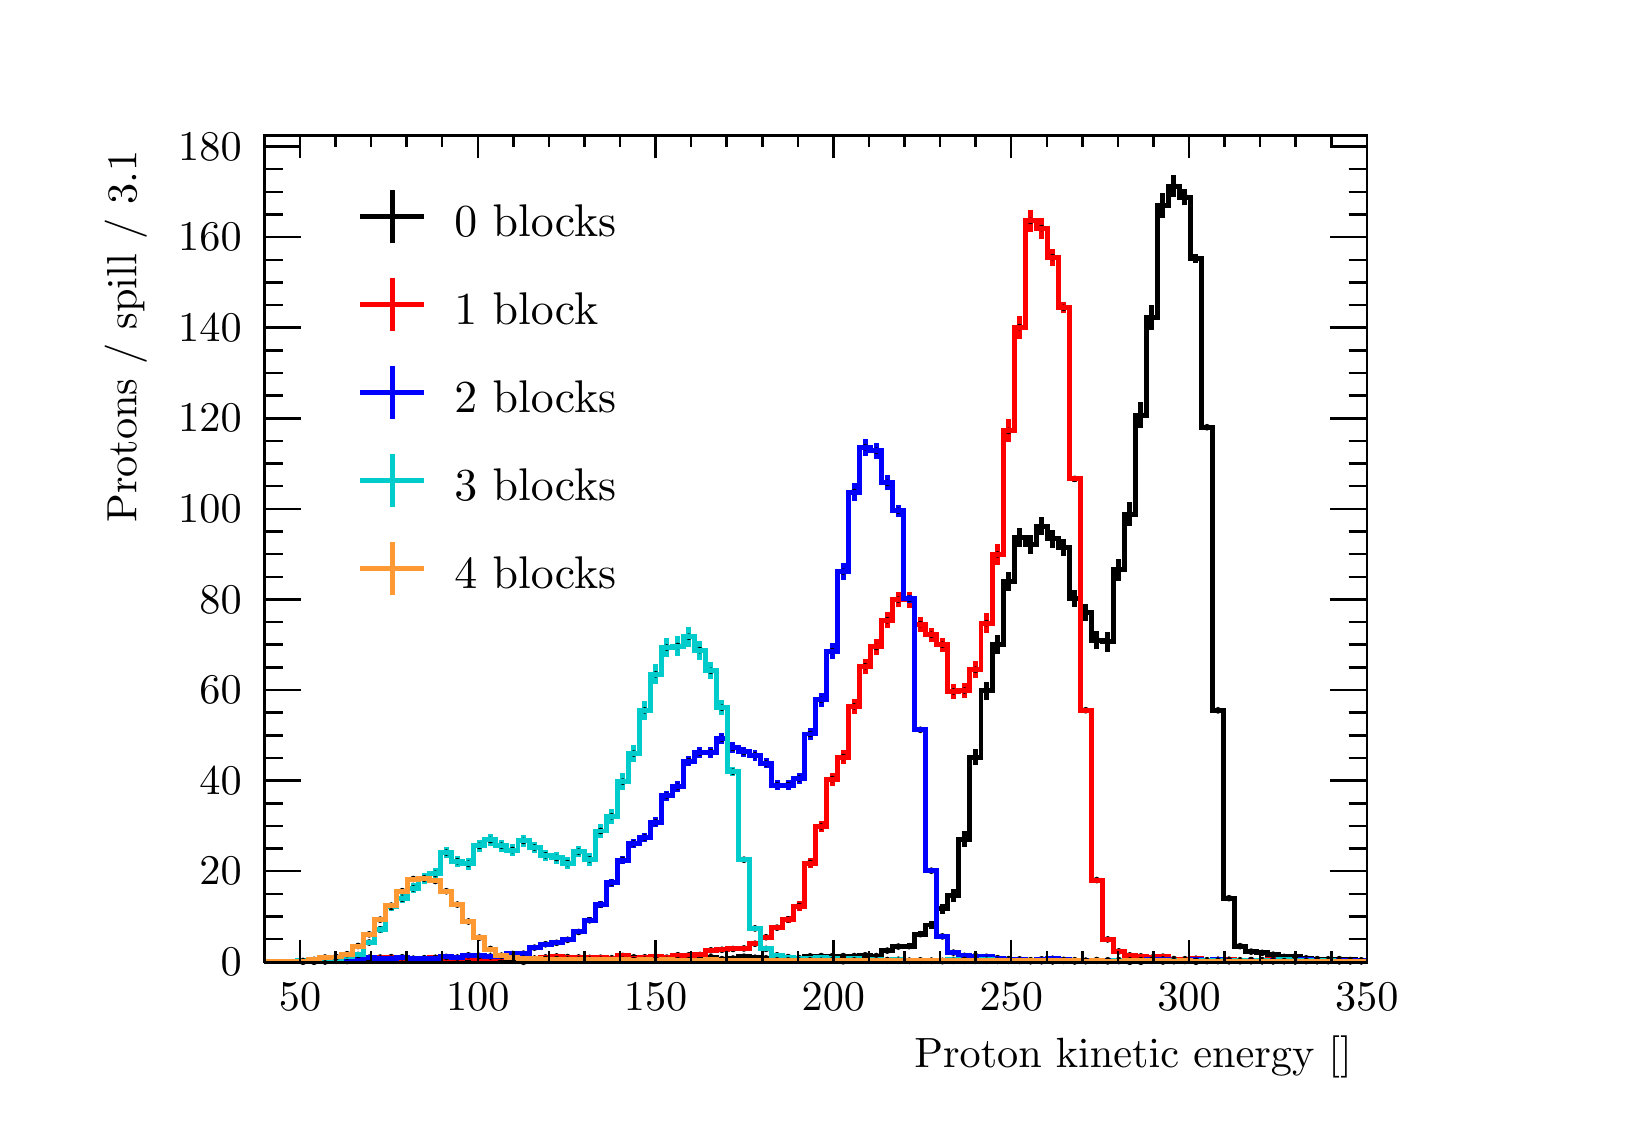
\begin{tikzpicture}
\pgfdeclareplotmark{cross} {
\pgfpathmoveto{\pgfpoint{-0.3\pgfplotmarksize}{\pgfplotmarksize}}
\pgfpathlineto{\pgfpoint{+0.3\pgfplotmarksize}{\pgfplotmarksize}}
\pgfpathlineto{\pgfpoint{+0.3\pgfplotmarksize}{0.3\pgfplotmarksize}}
\pgfpathlineto{\pgfpoint{+1\pgfplotmarksize}{0.3\pgfplotmarksize}}
\pgfpathlineto{\pgfpoint{+1\pgfplotmarksize}{-0.3\pgfplotmarksize}}
\pgfpathlineto{\pgfpoint{+0.3\pgfplotmarksize}{-0.3\pgfplotmarksize}}
\pgfpathlineto{\pgfpoint{+0.3\pgfplotmarksize}{-1.\pgfplotmarksize}}
\pgfpathlineto{\pgfpoint{-0.3\pgfplotmarksize}{-1.\pgfplotmarksize}}
\pgfpathlineto{\pgfpoint{-0.3\pgfplotmarksize}{-0.3\pgfplotmarksize}}
\pgfpathlineto{\pgfpoint{-1.\pgfplotmarksize}{-0.3\pgfplotmarksize}}
\pgfpathlineto{\pgfpoint{-1.\pgfplotmarksize}{0.3\pgfplotmarksize}}
\pgfpathlineto{\pgfpoint{-0.3\pgfplotmarksize}{0.3\pgfplotmarksize}}
\pgfpathclose
\pgfusepathqstroke
}
\pgfdeclareplotmark{cross*} {
\pgfpathmoveto{\pgfpoint{-0.3\pgfplotmarksize}{\pgfplotmarksize}}
\pgfpathlineto{\pgfpoint{+0.3\pgfplotmarksize}{\pgfplotmarksize}}
\pgfpathlineto{\pgfpoint{+0.3\pgfplotmarksize}{0.3\pgfplotmarksize}}
\pgfpathlineto{\pgfpoint{+1\pgfplotmarksize}{0.3\pgfplotmarksize}}
\pgfpathlineto{\pgfpoint{+1\pgfplotmarksize}{-0.3\pgfplotmarksize}}
\pgfpathlineto{\pgfpoint{+0.3\pgfplotmarksize}{-0.3\pgfplotmarksize}}
\pgfpathlineto{\pgfpoint{+0.3\pgfplotmarksize}{-1.\pgfplotmarksize}}
\pgfpathlineto{\pgfpoint{-0.3\pgfplotmarksize}{-1.\pgfplotmarksize}}
\pgfpathlineto{\pgfpoint{-0.3\pgfplotmarksize}{-0.3\pgfplotmarksize}}
\pgfpathlineto{\pgfpoint{-1.\pgfplotmarksize}{-0.3\pgfplotmarksize}}
\pgfpathlineto{\pgfpoint{-1.\pgfplotmarksize}{0.3\pgfplotmarksize}}
\pgfpathlineto{\pgfpoint{-0.3\pgfplotmarksize}{0.3\pgfplotmarksize}}
\pgfpathclose
\pgfusepathqfillstroke
}
\pgfdeclareplotmark{newstar} {
\pgfpathmoveto{\pgfqpoint{0pt}{\pgfplotmarksize}}
\pgfpathlineto{\pgfqpointpolar{44}{0.5\pgfplotmarksize}}
\pgfpathlineto{\pgfqpointpolar{18}{\pgfplotmarksize}}
\pgfpathlineto{\pgfqpointpolar{-20}{0.5\pgfplotmarksize}}
\pgfpathlineto{\pgfqpointpolar{-54}{\pgfplotmarksize}}
\pgfpathlineto{\pgfqpointpolar{-90}{0.5\pgfplotmarksize}}
\pgfpathlineto{\pgfqpointpolar{234}{\pgfplotmarksize}}
\pgfpathlineto{\pgfqpointpolar{198}{0.5\pgfplotmarksize}}
\pgfpathlineto{\pgfqpointpolar{162}{\pgfplotmarksize}}
\pgfpathlineto{\pgfqpointpolar{134}{0.5\pgfplotmarksize}}
\pgfpathclose
\pgfusepathqstroke
}
\pgfdeclareplotmark{newstar*} {
\pgfpathmoveto{\pgfqpoint{0pt}{\pgfplotmarksize}}
\pgfpathlineto{\pgfqpointpolar{44}{0.5\pgfplotmarksize}}
\pgfpathlineto{\pgfqpointpolar{18}{\pgfplotmarksize}}
\pgfpathlineto{\pgfqpointpolar{-20}{0.5\pgfplotmarksize}}
\pgfpathlineto{\pgfqpointpolar{-54}{\pgfplotmarksize}}
\pgfpathlineto{\pgfqpointpolar{-90}{0.5\pgfplotmarksize}}
\pgfpathlineto{\pgfqpointpolar{234}{\pgfplotmarksize}}
\pgfpathlineto{\pgfqpointpolar{198}{0.5\pgfplotmarksize}}
\pgfpathlineto{\pgfqpointpolar{162}{\pgfplotmarksize}}
\pgfpathlineto{\pgfqpointpolar{134}{0.5\pgfplotmarksize}}
\pgfpathclose
\pgfusepathqfillstroke
}
\definecolor{c}{rgb}{1,1,1};
\draw [color=c, fill=c] (0,0) rectangle (20,13.639);
\draw [color=c, fill=c] (3,1.77307) rectangle (17,12.2751);
\definecolor{c}{rgb}{0,0,0};
\draw [c,line width=0.9] (3,1.77307) -- (3,12.2751) -- (17,12.2751) -- (17,1.77307) -- (3,1.77307);
\definecolor{c}{rgb}{1,1,1};
\draw [color=c, fill=c] (3,1.77307) rectangle (17,12.2751);
\definecolor{c}{rgb}{0,0,0};
\draw [c,line width=0.9] (3,1.77307) -- (3,12.2751) -- (17,12.2751) -- (17,1.77307) -- (3,1.77307);
\draw [c,line width=0.9] (3,1.78273) -- (3.14,1.78273) -- (3.14,1.78273) -- (3.28,1.78273) -- (3.28,1.78273) -- (3.42,1.78273) -- (3.42,1.78273) -- (3.56,1.78273) -- (3.56,1.78273) -- (3.7,1.78273) -- (3.7,1.78273) -- (3.84,1.78273) -- (3.84,1.78273)
 -- (3.98,1.78273) -- (3.98,1.78273) -- (4.12,1.78273) -- (4.12,1.78273) -- (4.26,1.78273) -- (4.26,1.78273) -- (4.4,1.78273) -- (4.4,1.78273) -- (4.54,1.78273) -- (4.54,1.78273) -- (4.68,1.78273) -- (4.68,1.78273) -- (4.82,1.78273) -- (4.82,1.78273)
 -- (4.96,1.78273) -- (4.96,1.78273) -- (5.1,1.78273) -- (5.1,1.78273) -- (5.24,1.78273) -- (5.24,1.78273) -- (5.38,1.78273) -- (5.38,1.78273) -- (5.52,1.78273) -- (5.52,1.78273) -- (5.66,1.78273) -- (5.66,1.78273) -- (5.8,1.78273) -- (5.8,1.78273)
 -- (5.94,1.78273) -- (5.94,1.78273) -- (6.08,1.78273) -- (6.08,1.78273) -- (6.22,1.78273) -- (6.22,1.78273) -- (6.36,1.78273) -- (6.36,1.78273) -- (6.5,1.78273) -- (6.5,1.78273) -- (6.64,1.78273) -- (6.64,1.78273) -- (6.78,1.78273) -- (6.78,1.78273)
 -- (6.92,1.78273) -- (6.92,1.78273) -- (7.06,1.78273) -- (7.06,1.78273) -- (7.2,1.78273) -- (7.2,1.78273) -- (7.34,1.78273) -- (7.34,1.78273) -- (7.48,1.78273) -- (7.48,1.78273) -- (7.62,1.78273) -- (7.62,1.78273) -- (7.76,1.78273) -- (7.76,1.78273)
 -- (7.9,1.78273) -- (7.9,1.78273) -- (8.04,1.78273) -- (8.04,1.78273) -- (8.18,1.78273) -- (8.18,1.78273) -- (8.32,1.78273) -- (8.32,1.78273) -- (8.46,1.78273) -- (8.46,1.78273) -- (8.6,1.78273) -- (8.6,1.78273) -- (8.74,1.78273) -- (8.74,1.78273)
 -- (8.88,1.78273) -- (8.88,1.78273) -- (9.02,1.78273) -- (9.02,1.78273) -- (9.16,1.78273) -- (9.16,1.78273) -- (9.3,1.78273) -- (9.3,1.78273) -- (9.44,1.78273) -- (9.44,1.78273) -- (9.58,1.78273) -- (9.58,1.78273) -- (9.72,1.78273) -- (9.72,1.78273)
 -- (9.86,1.78273) -- (9.86,1.78273) -- (10,1.78273) -- (10,1.78273) -- (10.14,1.78273) -- (10.14,1.78273) -- (10.28,1.78273) -- (10.28,1.78273) -- (10.42,1.78273) -- (10.42,1.78273) -- (10.56,1.78273) -- (10.56,1.78273) -- (10.7,1.78273) --
 (10.7,1.78273) -- (10.84,1.78273) -- (10.84,1.78273) -- (10.98,1.78273) -- (10.98,1.78273) -- (11.12,1.78273) -- (11.12,1.78273) -- (11.26,1.78273) -- (11.26,1.78273) -- (11.4,1.78273) -- (11.4,1.78273) -- (11.54,1.78273) -- (11.54,1.78273) --
 (11.68,1.78273) -- (11.68,1.78273) -- (11.82,1.78273) -- (11.82,1.78273) -- (11.96,1.78273) -- (11.96,1.78273) -- (12.1,1.78273) -- (12.1,1.78273) -- (12.24,1.78273) -- (12.24,1.78273) -- (12.38,1.78273) -- (12.38,1.78273) -- (12.52,1.78273) --
 (12.52,1.78273) -- (12.66,1.78273) -- (12.66,1.78273) -- (12.8,1.78273) -- (12.8,1.78273) -- (12.94,1.78273) -- (12.94,1.78273) -- (13.08,1.78273) -- (13.08,1.78273) -- (13.22,1.78273) -- (13.22,1.78273) -- (13.36,1.78273) -- (13.36,1.78273) --
 (13.5,1.78273) -- (13.5,1.78273) -- (13.64,1.78273) -- (13.64,1.78273) -- (13.78,1.78273) -- (13.78,1.78273) -- (13.92,1.78273) -- (13.92,1.78273) -- (14.06,1.78273) -- (14.06,1.78273) -- (14.2,1.78273) -- (14.2,1.78273) -- (14.34,1.78273) --
 (14.34,1.78273) -- (14.48,1.78273) -- (14.48,1.78273) -- (14.62,1.78273) -- (14.62,1.78273) -- (14.76,1.78273) -- (14.76,1.78273) -- (14.9,1.78273) -- (14.9,1.78273) -- (15.04,1.78273) -- (15.04,1.78273) -- (15.18,1.78273) -- (15.18,1.78273) --
 (15.32,1.78273) -- (15.32,1.78273) -- (15.46,1.78273) -- (15.46,1.78273) -- (15.6,1.78273) -- (15.6,1.78273) -- (15.74,1.78273) -- (15.74,1.78273) -- (15.88,1.78273) -- (15.88,1.78273) -- (16.02,1.78273) -- (16.02,1.78273) -- (16.16,1.78273) --
 (16.16,1.78273) -- (16.3,1.78273) -- (16.3,1.78273) -- (16.44,1.78273) -- (16.44,1.78273) -- (16.58,1.78273) -- (16.58,1.78273) -- (16.72,1.78273) -- (16.72,1.78273) -- (16.86,1.78273) -- (16.86,1.78273) -- (17,1.78273);
\draw [c,line width=0.9] (3,1.77307) -- (17,1.77307);
\draw [c,line width=0.9] (3.45161,2.05948) -- (3.45161,1.77307);
\draw [c,line width=0.9] (3.90323,1.91628) -- (3.90323,1.77307);
\draw [c,line width=0.9] (4.35484,1.91628) -- (4.35484,1.77307);
\draw [c,line width=0.9] (4.80645,1.91628) -- (4.80645,1.77307);
\draw [c,line width=0.9] (5.25806,1.91628) -- (5.25806,1.77307);
\draw [c,line width=0.9] (5.70968,2.05948) -- (5.70968,1.77307);
\draw [c,line width=0.9] (6.16129,1.91628) -- (6.16129,1.77307);
\draw [c,line width=0.9] (6.6129,1.91628) -- (6.6129,1.77307);
\draw [c,line width=0.9] (7.06452,1.91628) -- (7.06452,1.77307);
\draw [c,line width=0.9] (7.51613,1.91628) -- (7.51613,1.77307);
\draw [c,line width=0.9] (7.96774,2.05948) -- (7.96774,1.77307);
\draw [c,line width=0.9] (8.41935,1.91628) -- (8.41935,1.77307);
\draw [c,line width=0.9] (8.87097,1.91628) -- (8.87097,1.77307);
\draw [c,line width=0.9] (9.32258,1.91628) -- (9.32258,1.77307);
\draw [c,line width=0.9] (9.77419,1.91628) -- (9.77419,1.77307);
\draw [c,line width=0.9] (10.2258,2.05948) -- (10.2258,1.77307);
\draw [c,line width=0.9] (10.6774,1.91628) -- (10.6774,1.77307);
\draw [c,line width=0.9] (11.129,1.91628) -- (11.129,1.77307);
\draw [c,line width=0.9] (11.5806,1.91628) -- (11.5806,1.77307);
\draw [c,line width=0.9] (12.0323,1.91628) -- (12.0323,1.77307);
\draw [c,line width=0.9] (12.4839,2.05948) -- (12.4839,1.77307);
\draw [c,line width=0.9] (12.9355,1.91628) -- (12.9355,1.77307);
\draw [c,line width=0.9] (13.3871,1.91628) -- (13.3871,1.77307);
\draw [c,line width=0.9] (13.8387,1.91628) -- (13.8387,1.77307);
\draw [c,line width=0.9] (14.2903,1.91628) -- (14.2903,1.77307);
\draw [c,line width=0.9] (14.7419,2.05948) -- (14.7419,1.77307);
\draw [c,line width=0.9] (15.1935,1.91628) -- (15.1935,1.77307);
\draw [c,line width=0.9] (15.6452,1.91628) -- (15.6452,1.77307);
\draw [c,line width=0.9] (16.0968,1.91628) -- (16.0968,1.77307);
\draw [c,line width=0.9] (16.5484,1.91628) -- (16.5484,1.77307);
\draw [c,line width=0.9] (17,2.05948) -- (17,1.77307);
\draw [c,line width=0.9] (3.45161,2.05948) -- (3.45161,1.77307);
\draw [c,line width=0.9] (3,1.91628) -- (3,1.77307);
\draw [anchor=base] (3.45161,1.15931) node[scale=1.52731, color=c, rotate=0]{50};
\draw [anchor=base] (5.70968,1.15931) node[scale=1.52731, color=c, rotate=0]{100};
\draw [anchor=base] (7.96774,1.15931) node[scale=1.52731, color=c, rotate=0]{150};
\draw [anchor=base] (10.2258,1.15931) node[scale=1.52731, color=c, rotate=0]{200};
\draw [anchor=base] (12.4839,1.15931) node[scale=1.52731, color=c, rotate=0]{250};
\draw [anchor=base] (14.7419,1.15931) node[scale=1.52731, color=c, rotate=0]{300};
\draw [anchor=base] (17,1.15931) node[scale=1.52731, color=c, rotate=0]{350};
\draw [anchor= east] (17,0.572837) node[scale=1.52731, color=c, rotate=0]{ Proton kinetic energy [\si{\mega\electronvolt}] };
\draw [c,line width=0.9] (3,12.2751) -- (17,12.2751);
\draw [c,line width=0.9] (3.45161,11.9887) -- (3.45161,12.2751);
\draw [c,line width=0.9] (3.90323,12.1319) -- (3.90323,12.2751);
\draw [c,line width=0.9] (4.35484,12.1319) -- (4.35484,12.2751);
\draw [c,line width=0.9] (4.80645,12.1319) -- (4.80645,12.2751);
\draw [c,line width=0.9] (5.25806,12.1319) -- (5.25806,12.2751);
\draw [c,line width=0.9] (5.70968,11.9887) -- (5.70968,12.2751);
\draw [c,line width=0.9] (6.16129,12.1319) -- (6.16129,12.2751);
\draw [c,line width=0.9] (6.6129,12.1319) -- (6.6129,12.2751);
\draw [c,line width=0.9] (7.06452,12.1319) -- (7.06452,12.2751);
\draw [c,line width=0.9] (7.51613,12.1319) -- (7.51613,12.2751);
\draw [c,line width=0.9] (7.96774,11.9887) -- (7.96774,12.2751);
\draw [c,line width=0.9] (8.41935,12.1319) -- (8.41935,12.2751);
\draw [c,line width=0.9] (8.87097,12.1319) -- (8.87097,12.2751);
\draw [c,line width=0.9] (9.32258,12.1319) -- (9.32258,12.2751);
\draw [c,line width=0.9] (9.77419,12.1319) -- (9.77419,12.2751);
\draw [c,line width=0.9] (10.2258,11.9887) -- (10.2258,12.2751);
\draw [c,line width=0.9] (10.6774,12.1319) -- (10.6774,12.2751);
\draw [c,line width=0.9] (11.129,12.1319) -- (11.129,12.2751);
\draw [c,line width=0.9] (11.5806,12.1319) -- (11.5806,12.2751);
\draw [c,line width=0.9] (12.0323,12.1319) -- (12.0323,12.2751);
\draw [c,line width=0.9] (12.4839,11.9887) -- (12.4839,12.2751);
\draw [c,line width=0.9] (12.9355,12.1319) -- (12.9355,12.2751);
\draw [c,line width=0.9] (13.3871,12.1319) -- (13.3871,12.2751);
\draw [c,line width=0.9] (13.8387,12.1319) -- (13.8387,12.2751);
\draw [c,line width=0.9] (14.2903,12.1319) -- (14.2903,12.2751);
\draw [c,line width=0.9] (14.7419,11.9887) -- (14.7419,12.2751);
\draw [c,line width=0.9] (15.1935,12.1319) -- (15.1935,12.2751);
\draw [c,line width=0.9] (15.6452,12.1319) -- (15.6452,12.2751);
\draw [c,line width=0.9] (16.0968,12.1319) -- (16.0968,12.2751);
\draw [c,line width=0.9] (16.5484,12.1319) -- (16.5484,12.2751);
\draw [c,line width=0.9] (17,11.9887) -- (17,12.2751);
\draw [c,line width=0.9] (3.45161,11.9887) -- (3.45161,12.2751);
\draw [c,line width=0.9] (3,12.1319) -- (3,12.2751);
\draw [c,line width=0.9] (3,1.77307) -- (3,12.2751);
\draw [c,line width=0.9] (3.462,1.78273) -- (3,1.78273);
\draw [c,line width=0.9] (3.231,2.07033) -- (3,2.07033);
\draw [c,line width=0.9] (3.231,2.35794) -- (3,2.35794);
\draw [c,line width=0.9] (3.231,2.64554) -- (3,2.64554);
\draw [c,line width=0.9] (3.462,2.93315) -- (3,2.93315);
\draw [c,line width=0.9] (3.231,3.22075) -- (3,3.22075);
\draw [c,line width=0.9] (3.231,3.50836) -- (3,3.50836);
\draw [c,line width=0.9] (3.231,3.79596) -- (3,3.79596);
\draw [c,line width=0.9] (3.462,4.08357) -- (3,4.08357);
\draw [c,line width=0.9] (3.231,4.37117) -- (3,4.37117);
\draw [c,line width=0.9] (3.231,4.65878) -- (3,4.65878);
\draw [c,line width=0.9] (3.231,4.94638) -- (3,4.94638);
\draw [c,line width=0.9] (3.462,5.23399) -- (3,5.23399);
\draw [c,line width=0.9] (3.231,5.52159) -- (3,5.52159);
\draw [c,line width=0.9] (3.231,5.8092) -- (3,5.8092);
\draw [c,line width=0.9] (3.231,6.0968) -- (3,6.0968);
\draw [c,line width=0.9] (3.462,6.38441) -- (3,6.38441);
\draw [c,line width=0.9] (3.231,6.67201) -- (3,6.67201);
\draw [c,line width=0.9] (3.231,6.95962) -- (3,6.95962);
\draw [c,line width=0.9] (3.231,7.24722) -- (3,7.24722);
\draw [c,line width=0.9] (3.462,7.53483) -- (3,7.53483);
\draw [c,line width=0.9] (3.231,7.82243) -- (3,7.82243);
\draw [c,line width=0.9] (3.231,8.11004) -- (3,8.11004);
\draw [c,line width=0.9] (3.231,8.39764) -- (3,8.39764);
\draw [c,line width=0.9] (3.462,8.68525) -- (3,8.68525);
\draw [c,line width=0.9] (3.231,8.97285) -- (3,8.97285);
\draw [c,line width=0.9] (3.231,9.26046) -- (3,9.26046);
\draw [c,line width=0.9] (3.231,9.54806) -- (3,9.54806);
\draw [c,line width=0.9] (3.462,9.83567) -- (3,9.83567);
\draw [c,line width=0.9] (3.231,10.1233) -- (3,10.1233);
\draw [c,line width=0.9] (3.231,10.4109) -- (3,10.4109);
\draw [c,line width=0.9] (3.231,10.6985) -- (3,10.6985);
\draw [c,line width=0.9] (3.462,10.9861) -- (3,10.9861);
\draw [c,line width=0.9] (3.231,11.2737) -- (3,11.2737);
\draw [c,line width=0.9] (3.231,11.5613) -- (3,11.5613);
\draw [c,line width=0.9] (3.231,11.8489) -- (3,11.8489);
\draw [c,line width=0.9] (3.462,12.1365) -- (3,12.1365);
\draw [c,line width=0.9] (3.462,1.78273) -- (3,1.78273);
\draw [c,line width=0.9] (3.462,12.1365) -- (3,12.1365);
\draw [anchor= east] (2.9,1.78273) node[scale=1.52731, color=c, rotate=0]{0};
\draw [anchor= east] (2.9,2.93315) node[scale=1.52731, color=c, rotate=0]{20};
\draw [anchor= east] (2.9,4.08357) node[scale=1.52731, color=c, rotate=0]{40};
\draw [anchor= east] (2.9,5.23399) node[scale=1.52731, color=c, rotate=0]{60};
\draw [anchor= east] (2.9,6.38441) node[scale=1.52731, color=c, rotate=0]{80};
\draw [anchor= east] (2.9,7.53483) node[scale=1.52731, color=c, rotate=0]{100};
\draw [anchor= east] (2.9,8.68525) node[scale=1.52731, color=c, rotate=0]{120};
\draw [anchor= east] (2.9,9.83567) node[scale=1.52731, color=c, rotate=0]{140};
\draw [anchor= east] (2.9,10.9861) node[scale=1.52731, color=c, rotate=0]{160};
\draw [anchor= east] (2.9,12.1365) node[scale=1.52731, color=c, rotate=0]{180};
\draw [anchor= east] (1.24,12.2751) node[scale=1.52731, color=c, rotate=90]{ Protons / spill / \SI{3.1}{\mega\electronvolt} };
\draw [c,line width=0.9] (17,1.77307) -- (17,12.2751);
\draw [c,line width=0.9] (16.538,1.78273) -- (17,1.78273);
\draw [c,line width=0.9] (16.769,2.07033) -- (17,2.07033);
\draw [c,line width=0.9] (16.769,2.35794) -- (17,2.35794);
\draw [c,line width=0.9] (16.769,2.64554) -- (17,2.64554);
\draw [c,line width=0.9] (16.538,2.93315) -- (17,2.93315);
\draw [c,line width=0.9] (16.769,3.22075) -- (17,3.22075);
\draw [c,line width=0.9] (16.769,3.50836) -- (17,3.50836);
\draw [c,line width=0.9] (16.769,3.79596) -- (17,3.79596);
\draw [c,line width=0.9] (16.538,4.08357) -- (17,4.08357);
\draw [c,line width=0.9] (16.769,4.37117) -- (17,4.37117);
\draw [c,line width=0.9] (16.769,4.65878) -- (17,4.65878);
\draw [c,line width=0.9] (16.769,4.94638) -- (17,4.94638);
\draw [c,line width=0.9] (16.538,5.23399) -- (17,5.23399);
\draw [c,line width=0.9] (16.769,5.52159) -- (17,5.52159);
\draw [c,line width=0.9] (16.769,5.8092) -- (17,5.8092);
\draw [c,line width=0.9] (16.769,6.0968) -- (17,6.0968);
\draw [c,line width=0.9] (16.538,6.38441) -- (17,6.38441);
\draw [c,line width=0.9] (16.769,6.67201) -- (17,6.67201);
\draw [c,line width=0.9] (16.769,6.95962) -- (17,6.95962);
\draw [c,line width=0.9] (16.769,7.24722) -- (17,7.24722);
\draw [c,line width=0.9] (16.538,7.53483) -- (17,7.53483);
\draw [c,line width=0.9] (16.769,7.82243) -- (17,7.82243);
\draw [c,line width=0.9] (16.769,8.11004) -- (17,8.11004);
\draw [c,line width=0.9] (16.769,8.39764) -- (17,8.39764);
\draw [c,line width=0.9] (16.538,8.68525) -- (17,8.68525);
\draw [c,line width=0.9] (16.769,8.97285) -- (17,8.97285);
\draw [c,line width=0.9] (16.769,9.26046) -- (17,9.26046);
\draw [c,line width=0.9] (16.769,9.54806) -- (17,9.54806);
\draw [c,line width=0.9] (16.538,9.83567) -- (17,9.83567);
\draw [c,line width=0.9] (16.769,10.1233) -- (17,10.1233);
\draw [c,line width=0.9] (16.769,10.4109) -- (17,10.4109);
\draw [c,line width=0.9] (16.769,10.6985) -- (17,10.6985);
\draw [c,line width=0.9] (16.538,10.9861) -- (17,10.9861);
\draw [c,line width=0.9] (16.769,11.2737) -- (17,11.2737);
\draw [c,line width=0.9] (16.769,11.5613) -- (17,11.5613);
\draw [c,line width=0.9] (16.769,11.8489) -- (17,11.8489);
\draw [c,line width=0.9] (16.538,12.1365) -- (17,12.1365);
\draw [c,line width=0.9] (16.538,1.78273) -- (17,1.78273);
\draw [c,line width=0.9] (16.538,12.1365) -- (17,12.1365);
\draw [c,line width=1.8] (6.29,1.77307) -- (6.29,1.78273);
\draw [c,line width=1.8] (6.29,1.78273) -- (6.29,1.79238);
\foreach \P in {(6.29,1.78273)}{\draw[mark options={color=c,fill=c},mark size=2.402402pt,mark=*,mark size=1pt] plot coordinates {\P};}
\draw [c,line width=1.8] (6.43,1.80761) -- (6.43,1.81886);
\draw [c,line width=1.8] (6.43,1.81886) -- (6.43,1.83012);
\foreach \P in {(6.43,1.81886)}{\draw[mark options={color=c,fill=c},mark size=2.402402pt,mark=*,mark size=1pt] plot coordinates {\P};}
\draw [c,line width=1.8] (6.57,1.82799) -- (6.57,1.83693);
\draw [c,line width=1.8] (6.57,1.83693) -- (6.57,1.84588);
\foreach \P in {(6.57,1.83693)}{\draw[mark options={color=c,fill=c},mark size=2.402402pt,mark=*,mark size=1pt] plot coordinates {\P};}
\draw [c,line width=1.8] (6.71,1.80181) -- (6.71,1.81112);
\draw [c,line width=1.8] (6.71,1.81112) -- (6.71,1.82043);
\foreach \P in {(6.71,1.81112)}{\draw[mark options={color=c,fill=c},mark size=2.402402pt,mark=*,mark size=1pt] plot coordinates {\P};}
\draw [c,line width=1.8] (6.85,1.80734) -- (6.85,1.81628);
\draw [c,line width=1.8] (6.85,1.81628) -- (6.85,1.82523);
\foreach \P in {(6.85,1.81628)}{\draw[mark options={color=c,fill=c},mark size=2.402402pt,mark=*,mark size=1pt] plot coordinates {\P};}
\draw [c,line width=1.8] (6.99,1.80474) -- (6.99,1.81628);
\draw [c,line width=1.8] (6.99,1.81628) -- (6.99,1.82783);
\foreach \P in {(6.99,1.81628)}{\draw[mark options={color=c,fill=c},mark size=2.402402pt,mark=*,mark size=1pt] plot coordinates {\P};}
\draw [c,line width=1.8] (7.13,1.81886) -- (7.13,1.82919);
\draw [c,line width=1.8] (7.13,1.82919) -- (7.13,1.83952);
\foreach \P in {(7.13,1.82919)}{\draw[mark options={color=c,fill=c},mark size=2.402402pt,mark=*,mark size=1pt] plot coordinates {\P};}
\draw [c,line width=1.8] (7.27,1.81628) -- (7.27,1.82661);
\draw [c,line width=1.8] (7.27,1.82661) -- (7.27,1.83693);
\foreach \P in {(7.27,1.82661)}{\draw[mark options={color=c,fill=c},mark size=2.402402pt,mark=*,mark size=1pt] plot coordinates {\P};}
\draw [c,line width=1.8] (7.41,1.8108) -- (7.41,1.82145);
\draw [c,line width=1.8] (7.41,1.82145) -- (7.41,1.83209);
\foreach \P in {(7.41,1.82145)}{\draw[mark options={color=c,fill=c},mark size=2.402402pt,mark=*,mark size=1pt] plot coordinates {\P};}
\draw [c,line width=1.8] (7.55,1.81192) -- (7.55,1.82403);
\draw [c,line width=1.8] (7.55,1.82403) -- (7.55,1.83614);
\foreach \P in {(7.55,1.82403)}{\draw[mark options={color=c,fill=c},mark size=2.402402pt,mark=*,mark size=1pt] plot coordinates {\P};}
\draw [c,line width=1.8] (7.69,1.82887) -- (7.69,1.83951);
\draw [c,line width=1.8] (7.69,1.83951) -- (7.69,1.85016);
\foreach \P in {(7.69,1.83951)}{\draw[mark options={color=c,fill=c},mark size=2.402402pt,mark=*,mark size=1pt] plot coordinates {\P};}
\draw [c,line width=1.8] (7.83,1.81423) -- (7.83,1.82661);
\draw [c,line width=1.8] (7.83,1.82661) -- (7.83,1.83899);
\foreach \P in {(7.83,1.82661)}{\draw[mark options={color=c,fill=c},mark size=2.402402pt,mark=*,mark size=1pt] plot coordinates {\P};}
\draw [c,line width=1.8] (7.97,1.83403) -- (7.97,1.84468);
\draw [c,line width=1.8] (7.97,1.84468) -- (7.97,1.85532);
\foreach \P in {(7.97,1.84468)}{\draw[mark options={color=c,fill=c},mark size=2.402402pt,mark=*,mark size=1pt] plot coordinates {\P};}
\draw [c,line width=1.8] (8.11,1.80214) -- (8.11,1.81628);
\draw [c,line width=1.8] (8.11,1.81628) -- (8.11,1.83042);
\foreach \P in {(8.11,1.81628)}{\draw[mark options={color=c,fill=c},mark size=2.402402pt,mark=*,mark size=1pt] plot coordinates {\P};}
\draw [c,line width=1.8] (8.25,1.8535) -- (8.25,1.86533);
\draw [c,line width=1.8] (8.25,1.86533) -- (8.25,1.87716);
\foreach \P in {(8.25,1.86533)}{\draw[mark options={color=c,fill=c},mark size=2.402402pt,mark=*,mark size=1pt] plot coordinates {\P};}
\draw [c,line width=1.8] (8.39,1.82945) -- (8.39,1.8421);
\draw [c,line width=1.8] (8.39,1.8421) -- (8.39,1.85474);
\foreach \P in {(8.39,1.8421)}{\draw[mark options={color=c,fill=c},mark size=2.402402pt,mark=*,mark size=1pt] plot coordinates {\P};}
\draw [c,line width=1.8] (8.53,1.81277) -- (8.53,1.82403);
\draw [c,line width=1.8] (8.53,1.82403) -- (8.53,1.83528);
\foreach \P in {(8.53,1.82403)}{\draw[mark options={color=c,fill=c},mark size=2.402402pt,mark=*,mark size=1pt] plot coordinates {\P};}
\draw [c,line width=1.8] (8.67,1.83279) -- (8.67,1.8421);
\draw [c,line width=1.8] (8.67,1.8421) -- (8.67,1.8514);
\foreach \P in {(8.67,1.8421)}{\draw[mark options={color=c,fill=c},mark size=2.402402pt,mark=*,mark size=1pt] plot coordinates {\P};}
\draw [c,line width=1.8] (8.81,1.80503) -- (8.81,1.81628);
\draw [c,line width=1.8] (8.81,1.81628) -- (8.81,1.82754);
\foreach \P in {(8.81,1.81628)}{\draw[mark options={color=c,fill=c},mark size=2.402402pt,mark=*,mark size=1pt] plot coordinates {\P};}
\draw [c,line width=1.8] (8.95,1.81112) -- (8.95,1.82403);
\draw [c,line width=1.8] (8.95,1.82403) -- (8.95,1.83693);
\foreach \P in {(8.95,1.82403)}{\draw[mark options={color=c,fill=c},mark size=2.402402pt,mark=*,mark size=1pt] plot coordinates {\P};}
\draw [c,line width=1.8] (9.09,1.83571) -- (9.09,1.84726);
\draw [c,line width=1.8] (9.09,1.84726) -- (9.09,1.8588);
\foreach \P in {(9.09,1.84726)}{\draw[mark options={color=c,fill=c},mark size=2.402402pt,mark=*,mark size=1pt] plot coordinates {\P};}
\draw [c,line width=1.8] (9.23,1.82144) -- (9.23,1.83435);
\draw [c,line width=1.8] (9.23,1.83435) -- (9.23,1.84726);
\foreach \P in {(9.23,1.83435)}{\draw[mark options={color=c,fill=c},mark size=2.402402pt,mark=*,mark size=1pt] plot coordinates {\P};}
\draw [c,line width=1.8] (9.37,1.81396) -- (9.37,1.82661);
\draw [c,line width=1.8] (9.37,1.82661) -- (9.37,1.83925);
\foreach \P in {(9.37,1.82661)}{\draw[mark options={color=c,fill=c},mark size=2.402402pt,mark=*,mark size=1pt] plot coordinates {\P};}
\draw [c,line width=1.8] (9.51,1.83801) -- (9.51,1.84984);
\draw [c,line width=1.8] (9.51,1.84984) -- (9.51,1.86167);
\foreach \P in {(9.51,1.84984)}{\draw[mark options={color=c,fill=c},mark size=2.402402pt,mark=*,mark size=1pt] plot coordinates {\P};}
\draw [c,line width=1.8] (9.65,1.82945) -- (9.65,1.8421);
\draw [c,line width=1.8] (9.65,1.8421) -- (9.65,1.85474);
\foreach \P in {(9.65,1.8421)}{\draw[mark options={color=c,fill=c},mark size=2.402402pt,mark=*,mark size=1pt] plot coordinates {\P};}
\draw [c,line width=1.8] (9.79,1.81553) -- (9.79,1.82919);
\draw [c,line width=1.8] (9.79,1.82919) -- (9.79,1.84285);
\foreach \P in {(9.79,1.82919)}{\draw[mark options={color=c,fill=c},mark size=2.402402pt,mark=*,mark size=1pt] plot coordinates {\P};}
\draw [c,line width=1.8] (9.93,1.83926) -- (9.93,1.85242);
\draw [c,line width=1.8] (9.93,1.85242) -- (9.93,1.86558);
\foreach \P in {(9.93,1.85242)}{\draw[mark options={color=c,fill=c},mark size=2.402402pt,mark=*,mark size=1pt] plot coordinates {\P};}
\draw [c,line width=1.8] (10.07,1.8404) -- (10.07,1.855);
\draw [c,line width=1.8] (10.07,1.855) -- (10.07,1.86961);
\foreach \P in {(10.07,1.855)}{\draw[mark options={color=c,fill=c},mark size=2.402402pt,mark=*,mark size=1pt] plot coordinates {\P};}
\draw [c,line width=1.8] (10.21,1.84031) -- (10.21,1.85242);
\draw [c,line width=1.8] (10.21,1.85242) -- (10.21,1.86453);
\foreach \P in {(10.21,1.85242)}{\draw[mark options={color=c,fill=c},mark size=2.402402pt,mark=*,mark size=1pt] plot coordinates {\P};}
\draw [c,line width=1.8] (10.35,1.83868) -- (10.35,1.855);
\draw [c,line width=1.8] (10.35,1.855) -- (10.35,1.87133);
\foreach \P in {(10.35,1.855)}{\draw[mark options={color=c,fill=c},mark size=2.402402pt,mark=*,mark size=1pt] plot coordinates {\P};}
\draw [c,line width=1.8] (10.49,1.84184) -- (10.49,1.855);
\draw [c,line width=1.8] (10.49,1.855) -- (10.49,1.86817);
\foreach \P in {(10.49,1.855)}{\draw[mark options={color=c,fill=c},mark size=2.402402pt,mark=*,mark size=1pt] plot coordinates {\P};}
\draw [c,line width=1.8] (10.63,1.8488) -- (10.63,1.86533);
\draw [c,line width=1.8] (10.63,1.86533) -- (10.63,1.88186);
\foreach \P in {(10.63,1.86533)}{\draw[mark options={color=c,fill=c},mark size=2.402402pt,mark=*,mark size=1pt] plot coordinates {\P};}
\draw [c,line width=1.8] (10.77,1.8322) -- (10.77,1.855);
\draw [c,line width=1.8] (10.77,1.855) -- (10.77,1.8778);
\foreach \P in {(10.77,1.855)}{\draw[mark options={color=c,fill=c},mark size=2.402402pt,mark=*,mark size=1pt] plot coordinates {\P};}
\draw [c,line width=1.8] (10.91,1.9019) -- (10.91,1.9247);
\draw [c,line width=1.8] (10.91,1.9247) -- (10.91,1.9475);
\foreach \P in {(10.91,1.9247)}{\draw[mark options={color=c,fill=c},mark size=2.402402pt,mark=*,mark size=1pt] plot coordinates {\P};}
\draw [c,line width=1.8] (11.05,1.94712) -- (11.05,1.97633);
\draw [c,line width=1.8] (11.05,1.97633) -- (11.05,2.00553);
\foreach \P in {(11.05,1.97633)}{\draw[mark options={color=c,fill=c},mark size=2.402402pt,mark=*,mark size=1pt] plot coordinates {\P};}
\draw [c,line width=1.8] (11.19,1.94638) -- (11.19,1.98149);
\draw [c,line width=1.8] (11.19,1.98149) -- (11.19,2.0166);
\foreach \P in {(11.19,1.98149)}{\draw[mark options={color=c,fill=c},mark size=2.402402pt,mark=*,mark size=1pt] plot coordinates {\P};}
\draw [c,line width=1.8] (11.33,2.0933) -- (11.33,2.13379);
\draw [c,line width=1.8] (11.33,2.13379) -- (11.33,2.17428);
\foreach \P in {(11.33,2.13379)}{\draw[mark options={color=c,fill=c},mark size=2.402402pt,mark=*,mark size=1pt] plot coordinates {\P};}
\draw [c,line width=1.8] (11.47,2.20284) -- (11.47,2.24995);
\draw [c,line width=1.8] (11.47,2.24995) -- (11.47,2.29706);
\foreach \P in {(11.47,2.24995)}{\draw[mark options={color=c,fill=c},mark size=2.402402pt,mark=*,mark size=1pt] plot coordinates {\P};}
\draw [c,line width=1.8] (11.61,2.39012) -- (11.61,2.45388);
\draw [c,line width=1.8] (11.61,2.45388) -- (11.61,2.51764);
\foreach \P in {(11.61,2.45388)}{\draw[mark options={color=c,fill=c},mark size=2.402402pt,mark=*,mark size=1pt] plot coordinates {\P};}
\draw [c,line width=1.8] (11.75,2.53607) -- (11.75,2.61909);
\draw [c,line width=1.8] (11.75,2.61909) -- (11.75,2.7021);
\foreach \P in {(11.75,2.61909)}{\draw[mark options={color=c,fill=c},mark size=2.402402pt,mark=*,mark size=1pt] plot coordinates {\P};}
\draw [c,line width=1.8] (11.89,3.24579) -- (11.89,3.34187);
\draw [c,line width=1.8] (11.89,3.34187) -- (11.89,3.43794);
\foreach \P in {(11.89,3.34187)}{\draw[mark options={color=c,fill=c},mark size=2.402402pt,mark=*,mark size=1pt] plot coordinates {\P};}
\draw [c,line width=1.8] (12.03,4.27783) -- (12.03,4.38215);
\draw [c,line width=1.8] (12.03,4.38215) -- (12.03,4.48647);
\foreach \P in {(12.03,4.38215)}{\draw[mark options={color=c,fill=c},mark size=2.402402pt,mark=*,mark size=1pt] plot coordinates {\P};}
\draw [c,line width=1.8] (12.17,5.11191) -- (12.17,5.22626);
\draw [c,line width=1.8] (12.17,5.22626) -- (12.17,5.34061);
\foreach \P in {(12.17,5.22626)}{\draw[mark options={color=c,fill=c},mark size=2.402402pt,mark=*,mark size=1pt] plot coordinates {\P};}
\draw [c,line width=1.8] (12.31,5.68717) -- (12.31,5.80707);
\draw [c,line width=1.8] (12.31,5.80707) -- (12.31,5.92696);
\foreach \P in {(12.31,5.80707)}{\draw[mark options={color=c,fill=c},mark size=2.402402pt,mark=*,mark size=1pt] plot coordinates {\P};}
\draw [c,line width=1.8] (12.45,6.49278) -- (12.45,6.61245);
\draw [c,line width=1.8] (12.45,6.61245) -- (12.45,6.73212);
\foreach \P in {(12.45,6.61245)}{\draw[mark options={color=c,fill=c},mark size=2.402402pt,mark=*,mark size=1pt] plot coordinates {\P};}
\draw [c,line width=1.8] (12.59,7.04921) -- (12.59,7.17002);
\draw [c,line width=1.8] (12.59,7.17002) -- (12.59,7.29083);
\foreach \P in {(12.59,7.17002)}{\draw[mark options={color=c,fill=c},mark size=2.402402pt,mark=*,mark size=1pt] plot coordinates {\P};}
\draw [c,line width=1.8] (12.73,6.95771) -- (12.73,7.07968);
\draw [c,line width=1.8] (12.73,7.07968) -- (12.73,7.20164);
\foreach \P in {(12.73,7.07968)}{\draw[mark options={color=c,fill=c},mark size=2.402402pt,mark=*,mark size=1pt] plot coordinates {\P};}
\draw [c,line width=1.8] (12.87,7.20029) -- (12.87,7.31458);
\draw [c,line width=1.8] (12.87,7.31458) -- (12.87,7.42887);
\foreach \P in {(12.87,7.31458)}{\draw[mark options={color=c,fill=c},mark size=2.402402pt,mark=*,mark size=1pt] plot coordinates {\P};}
\draw [c,line width=1.8] (13.01,7.04296) -- (13.01,7.15453);
\draw [c,line width=1.8] (13.01,7.15453) -- (13.01,7.26611);
\foreach \P in {(13.01,7.15453)}{\draw[mark options={color=c,fill=c},mark size=2.402402pt,mark=*,mark size=1pt] plot coordinates {\P};}
\draw [c,line width=1.8] (13.15,6.9398) -- (13.15,7.04612);
\draw [c,line width=1.8] (13.15,7.04612) -- (13.15,7.15243);
\foreach \P in {(13.15,7.04612)}{\draw[mark options={color=c,fill=c},mark size=2.402402pt,mark=*,mark size=1pt] plot coordinates {\P};}
\draw [c,line width=1.8] (13.29,6.29216) -- (13.29,6.39562);
\draw [c,line width=1.8] (13.29,6.39562) -- (13.29,6.49907);
\foreach \P in {(13.29,6.39562)}{\draw[mark options={color=c,fill=c},mark size=2.402402pt,mark=*,mark size=1pt] plot coordinates {\P};}
\draw [c,line width=1.8] (13.43,6.10865) -- (13.43,6.2175);
\draw [c,line width=1.8] (13.43,6.2175) -- (13.43,6.32635);
\foreach \P in {(13.43,6.2175)}{\draw[mark options={color=c,fill=c},mark size=2.402402pt,mark=*,mark size=1pt] plot coordinates {\P};}
\draw [c,line width=1.8] (13.57,5.75021) -- (13.57,5.86902);
\draw [c,line width=1.8] (13.57,5.86902) -- (13.57,5.98782);
\foreach \P in {(13.57,5.86902)}{\draw[mark options={color=c,fill=c},mark size=2.402402pt,mark=*,mark size=1pt] plot coordinates {\P};}
\draw [c,line width=1.8] (13.71,5.71586) -- (13.71,5.84579);
\draw [c,line width=1.8] (13.71,5.84579) -- (13.71,5.97571);
\foreach \P in {(13.71,5.84579)}{\draw[mark options={color=c,fill=c},mark size=2.402402pt,mark=*,mark size=1pt] plot coordinates {\P};}
\draw [c,line width=1.8] (13.85,6.61732) -- (13.85,6.75959);
\draw [c,line width=1.8] (13.85,6.75959) -- (13.85,6.90185);
\foreach \P in {(13.85,6.75959)}{\draw[mark options={color=c,fill=c},mark size=2.402402pt,mark=*,mark size=1pt] plot coordinates {\P};}
\draw [c,line width=1.8] (13.99,7.31378) -- (13.99,7.46946);
\draw [c,line width=1.8] (13.99,7.46946) -- (13.99,7.62515);
\foreach \P in {(13.99,7.46946)}{\draw[mark options={color=c,fill=c},mark size=2.402402pt,mark=*,mark size=1pt] plot coordinates {\P};}
\draw [c,line width=1.8] (14.13,8.5623) -- (14.13,8.72658);
\draw [c,line width=1.8] (14.13,8.72658) -- (14.13,8.89087);
\foreach \P in {(14.13,8.72658)}{\draw[mark options={color=c,fill=c},mark size=2.402402pt,mark=*,mark size=1pt] plot coordinates {\P};}
\draw [c,line width=1.8] (14.27,9.80077) -- (14.27,9.96305);
\draw [c,line width=1.8] (14.27,9.96305) -- (14.27,10.1253);
\foreach \P in {(14.27,9.96305)}{\draw[mark options={color=c,fill=c},mark size=2.402402pt,mark=*,mark size=1pt] plot coordinates {\P};}
\draw [c,line width=1.8] (14.41,11.2292) -- (14.41,11.3854);
\draw [c,line width=1.8] (14.41,11.3854) -- (14.41,11.5416);
\foreach \P in {(14.41,11.3854)}{\draw[mark options={color=c,fill=c},mark size=2.402402pt,mark=*,mark size=1pt] plot coordinates {\P};}
\draw [c,line width=1.8] (14.55,11.491) -- (14.55,11.6332);
\draw [c,line width=1.8] (14.55,11.6332) -- (14.55,11.7754);
\foreach \P in {(14.55,11.6332)}{\draw[mark options={color=c,fill=c},mark size=2.402402pt,mark=*,mark size=1pt] plot coordinates {\P};}
\draw [c,line width=1.8] (14.69,11.3892) -- (14.69,11.4938);
\draw [c,line width=1.8] (14.69,11.4938) -- (14.69,11.5984);
\foreach \P in {(14.69,11.4938)}{\draw[mark options={color=c,fill=c},mark size=2.402402pt,mark=*,mark size=1pt] plot coordinates {\P};}
\draw [c,line width=1.8] (14.83,10.6594) -- (14.83,10.7142);
\draw [c,line width=1.8] (14.83,10.7142) -- (14.83,10.7691);
\foreach \P in {(14.83,10.7142)}{\draw[mark options={color=c,fill=c},mark size=2.402402pt,mark=*,mark size=1pt] plot coordinates {\P};}
\draw [c,line width=1.8] (14.97,8.54804) -- (14.97,8.5717);
\draw [c,line width=1.8] (14.97,8.5717) -- (14.97,8.59536);
\foreach \P in {(14.97,8.5717)}{\draw[mark options={color=c,fill=c},mark size=2.402402pt,mark=*,mark size=1pt] plot coordinates {\P};}
\draw [c,line width=1.8] (15.11,4.95707) -- (15.11,4.97587);
\draw [c,line width=1.8] (15.11,4.97587) -- (15.11,4.99466);
\foreach \P in {(15.11,4.97587)}{\draw[mark options={color=c,fill=c},mark size=2.402402pt,mark=*,mark size=1pt] plot coordinates {\P};}
\draw [c,line width=1.8] (15.25,2.57281) -- (15.25,2.59069);
\draw [c,line width=1.8] (15.25,2.59069) -- (15.25,2.60858);
\foreach \P in {(15.25,2.59069)}{\draw[mark options={color=c,fill=c},mark size=2.402402pt,mark=*,mark size=1pt] plot coordinates {\P};}
\draw [c,line width=1.8] (15.39,1.96579) -- (15.39,1.98149);
\draw [c,line width=1.8] (15.39,1.98149) -- (15.39,1.99719);
\foreach \P in {(15.39,1.98149)}{\draw[mark options={color=c,fill=c},mark size=2.402402pt,mark=*,mark size=1pt] plot coordinates {\P};}
\draw [c,line width=1.8] (15.53,1.89889) -- (15.53,1.91179);
\draw [c,line width=1.8] (15.53,1.91179) -- (15.53,1.9247);
\foreach \P in {(15.53,1.91179)}{\draw[mark options={color=c,fill=c},mark size=2.402402pt,mark=*,mark size=1pt] plot coordinates {\P};}
\draw [c,line width=1.8] (15.67,1.88289) -- (15.67,1.8963);
\draw [c,line width=1.8] (15.67,1.8963) -- (15.67,1.90972);
\foreach \P in {(15.67,1.8963)}{\draw[mark options={color=c,fill=c},mark size=2.402402pt,mark=*,mark size=1pt] plot coordinates {\P};}
\draw [c,line width=1.8] (15.81,1.86243) -- (15.81,1.87307);
\draw [c,line width=1.8] (15.81,1.87307) -- (15.81,1.88372);
\foreach \P in {(15.81,1.87307)}{\draw[mark options={color=c,fill=c},mark size=2.402402pt,mark=*,mark size=1pt] plot coordinates {\P};}
\draw [c,line width=1.8] (15.95,1.83468) -- (15.95,1.84468);
\draw [c,line width=1.8] (15.95,1.84468) -- (15.95,1.85468);
\foreach \P in {(15.95,1.84468)}{\draw[mark options={color=c,fill=c},mark size=2.402402pt,mark=*,mark size=1pt] plot coordinates {\P};}
\draw [c,line width=1.8] (16.09,1.8421) -- (16.09,1.84984);
\draw [c,line width=1.8] (16.09,1.84984) -- (16.09,1.85758);
\foreach \P in {(16.09,1.84984)}{\draw[mark options={color=c,fill=c},mark size=2.402402pt,mark=*,mark size=1pt] plot coordinates {\P};}
\draw [c,line width=1.8] (16.23,1.81695) -- (16.23,1.82661);
\draw [c,line width=1.8] (16.23,1.82661) -- (16.23,1.83627);
\foreach \P in {(16.23,1.82661)}{\draw[mark options={color=c,fill=c},mark size=2.402402pt,mark=*,mark size=1pt] plot coordinates {\P};}
\draw [c,line width=1.8] (16.37,1.80734) -- (16.37,1.81628);
\draw [c,line width=1.8] (16.37,1.81628) -- (16.37,1.82523);
\foreach \P in {(16.37,1.81628)}{\draw[mark options={color=c,fill=c},mark size=2.402402pt,mark=*,mark size=1pt] plot coordinates {\P};}
\draw [c,line width=1.8] (16.51,1.81005) -- (16.51,1.8137);
\draw [c,line width=1.8] (16.51,1.8137) -- (16.51,1.81735);
\foreach \P in {(16.51,1.8137)}{\draw[mark options={color=c,fill=c},mark size=2.402402pt,mark=*,mark size=1pt] plot coordinates {\P};}
\foreach \P in {(16.65,1.81628)}{\draw[mark options={color=c,fill=c},mark size=2.402402pt,mark=*,mark size=1pt] plot coordinates {\P};}
\foreach \P in {(16.79,1.80596)}{\draw[mark options={color=c,fill=c},mark size=2.402402pt,mark=*,mark size=1pt] plot coordinates {\P};}
\foreach \P in {(16.93,1.80079)}{\draw[mark options={color=c,fill=c},mark size=2.402402pt,mark=*,mark size=1pt] plot coordinates {\P};}
\draw [c,line width=1.8] (3,1.78273) -- (3.14,1.78273) -- (3.14,1.78273) -- (3.28,1.78273) -- (3.28,1.78273) -- (3.42,1.78273) -- (3.42,1.78273) -- (3.56,1.78273) -- (3.56,1.78273) -- (3.7,1.78273) -- (3.7,1.78273) -- (3.84,1.78273) -- (3.84,1.78273)
 -- (3.98,1.78273) -- (3.98,1.78273) -- (4.12,1.78273) -- (4.12,1.78273) -- (4.26,1.78273) -- (4.26,1.78273) -- (4.4,1.78273) -- (4.4,1.78273) -- (4.54,1.78273) -- (4.54,1.78273) -- (4.68,1.78273) -- (4.68,1.78273) -- (4.82,1.78273) -- (4.82,1.78273)
 -- (4.96,1.78273) -- (4.96,1.78273) -- (5.1,1.78273) -- (5.1,1.78273) -- (5.24,1.78273) -- (5.24,1.78273) -- (5.38,1.78273) -- (5.38,1.78273) -- (5.52,1.78273) -- (5.52,1.78273) -- (5.66,1.78273) -- (5.66,1.78273) -- (5.8,1.78273) -- (5.8,1.78273)
 -- (5.94,1.78273) -- (5.94,1.78273) -- (6.08,1.78273) -- (6.08,1.78273) -- (6.22,1.78273) -- (6.22,1.78273) -- (6.36,1.78273) -- (6.36,1.81886) -- (6.5,1.81886) -- (6.5,1.83693) -- (6.64,1.83693) -- (6.64,1.81112) -- (6.78,1.81112) -- (6.78,1.81628)
 -- (6.92,1.81628) -- (6.92,1.81628) -- (7.06,1.81628) -- (7.06,1.82919) -- (7.2,1.82919) -- (7.2,1.82661) -- (7.34,1.82661) -- (7.34,1.82145) -- (7.48,1.82145) -- (7.48,1.82403) -- (7.62,1.82403) -- (7.62,1.83951) -- (7.76,1.83951) -- (7.76,1.82661)
 -- (7.9,1.82661) -- (7.9,1.84468) -- (8.04,1.84468) -- (8.04,1.81628) -- (8.18,1.81628) -- (8.18,1.86533) -- (8.32,1.86533) -- (8.32,1.8421) -- (8.46,1.8421) -- (8.46,1.82403) -- (8.6,1.82403) -- (8.6,1.8421) -- (8.74,1.8421) -- (8.74,1.81628) --
 (8.88,1.81628) -- (8.88,1.82403) -- (9.02,1.82403) -- (9.02,1.84726) -- (9.16,1.84726) -- (9.16,1.83435) -- (9.3,1.83435) -- (9.3,1.82661) -- (9.44,1.82661) -- (9.44,1.84984) -- (9.58,1.84984) -- (9.58,1.8421) -- (9.72,1.8421) -- (9.72,1.82919) --
 (9.86,1.82919) -- (9.86,1.85242) -- (10,1.85242) -- (10,1.855) -- (10.14,1.855) -- (10.14,1.85242) -- (10.28,1.85242) -- (10.28,1.855) -- (10.42,1.855) -- (10.42,1.855) -- (10.56,1.855) -- (10.56,1.86533) -- (10.7,1.86533) -- (10.7,1.855) --
 (10.84,1.855) -- (10.84,1.9247) -- (10.98,1.9247) -- (10.98,1.97633) -- (11.12,1.97633) -- (11.12,1.98149) -- (11.26,1.98149) -- (11.26,2.13379) -- (11.4,2.13379) -- (11.4,2.24995) -- (11.54,2.24995) -- (11.54,2.45388) -- (11.68,2.45388) --
 (11.68,2.61909) -- (11.82,2.61909) -- (11.82,3.34187) -- (11.96,3.34187) -- (11.96,4.38215) -- (12.1,4.38215) -- (12.1,5.22626) -- (12.24,5.22626) -- (12.24,5.80707) -- (12.38,5.80707) -- (12.38,6.61245) -- (12.52,6.61245) -- (12.52,7.17002) --
 (12.66,7.17002) -- (12.66,7.07968) -- (12.8,7.07968) -- (12.8,7.31458) -- (12.94,7.31458) -- (12.94,7.15453) -- (13.08,7.15453) -- (13.08,7.04612) -- (13.22,7.04612) -- (13.22,6.39562) -- (13.36,6.39562) -- (13.36,6.2175) -- (13.5,6.2175) --
 (13.5,5.86902) -- (13.64,5.86902) -- (13.64,5.84579) -- (13.78,5.84579) -- (13.78,6.75959) -- (13.92,6.75959) -- (13.92,7.46946) -- (14.06,7.46946) -- (14.06,8.72658) -- (14.2,8.72658) -- (14.2,9.96305) -- (14.34,9.96305) -- (14.34,11.3854) --
 (14.48,11.3854) -- (14.48,11.6332) -- (14.62,11.6332) -- (14.62,11.4938) -- (14.76,11.4938) -- (14.76,10.7142) -- (14.9,10.7142) -- (14.9,8.5717) -- (15.04,8.5717) -- (15.04,4.97587) -- (15.18,4.97587) -- (15.18,2.59069) -- (15.32,2.59069) --
 (15.32,1.98149) -- (15.46,1.98149) -- (15.46,1.91179) -- (15.6,1.91179) -- (15.6,1.8963) -- (15.74,1.8963) -- (15.74,1.87307) -- (15.88,1.87307) -- (15.88,1.84468) -- (16.02,1.84468) -- (16.02,1.84984) -- (16.16,1.84984) -- (16.16,1.82661) --
 (16.3,1.82661) -- (16.3,1.81628) -- (16.44,1.81628) -- (16.44,1.8137) -- (16.58,1.8137) -- (16.58,1.81628) -- (16.72,1.81628) -- (16.72,1.80596) -- (16.86,1.80596) -- (16.86,1.80079) -- (17,1.80079);
\definecolor{c}{rgb}{1,0,0};
\draw [c,line width=1.8] (3.63,1.78086) -- (3.63,1.78273);
\draw [c,line width=1.8] (3.63,1.78273) -- (3.63,1.78459);
\definecolor{c}{rgb}{0,0,0};
\foreach \P in {(3.63,1.78273)}{\draw[mark options={color=c,fill=c},mark size=2.402402pt,mark=*,mark size=1pt] plot coordinates {\P};}
\definecolor{c}{rgb}{1,0,0};
\draw [c,line width=1.8] (3.77,1.78595) -- (3.77,1.79057);
\draw [c,line width=1.8] (3.77,1.79057) -- (3.77,1.79519);
\definecolor{c}{rgb}{0,0,0};
\foreach \P in {(3.77,1.79057)}{\draw[mark options={color=c,fill=c},mark size=2.402402pt,mark=*,mark size=1pt] plot coordinates {\P};}
\definecolor{c}{rgb}{1,0,0};
\draw [c,line width=1.8] (3.91,1.79149) -- (3.91,1.79714);
\draw [c,line width=1.8] (3.91,1.79714) -- (3.91,1.8028);
\definecolor{c}{rgb}{0,0,0};
\foreach \P in {(3.91,1.79714)}{\draw[mark options={color=c,fill=c},mark size=2.402402pt,mark=*,mark size=1pt] plot coordinates {\P};}
\definecolor{c}{rgb}{1,0,0};
\draw [c,line width=1.8] (4.05,1.8009) -- (4.05,1.81013);
\draw [c,line width=1.8] (4.05,1.81013) -- (4.05,1.81936);
\definecolor{c}{rgb}{0,0,0};
\foreach \P in {(4.05,1.81013)}{\draw[mark options={color=c,fill=c},mark size=2.402402pt,mark=*,mark size=1pt] plot coordinates {\P};}
\definecolor{c}{rgb}{1,0,0};
\draw [c,line width=1.8] (4.19,1.81463) -- (4.19,1.82624);
\draw [c,line width=1.8] (4.19,1.82624) -- (4.19,1.83785);
\definecolor{c}{rgb}{0,0,0};
\foreach \P in {(4.19,1.82624)}{\draw[mark options={color=c,fill=c},mark size=2.402402pt,mark=*,mark size=1pt] plot coordinates {\P};}
\definecolor{c}{rgb}{1,0,0};
\draw [c,line width=1.8] (4.33,1.82283) -- (4.33,1.83251);
\draw [c,line width=1.8] (4.33,1.83251) -- (4.33,1.84219);
\definecolor{c}{rgb}{0,0,0};
\foreach \P in {(4.33,1.83251)}{\draw[mark options={color=c,fill=c},mark size=2.402402pt,mark=*,mark size=1pt] plot coordinates {\P};}
\definecolor{c}{rgb}{1,0,0};
\draw [c,line width=1.8] (4.47,1.82434) -- (4.47,1.83673);
\draw [c,line width=1.8] (4.47,1.83673) -- (4.47,1.84912);
\definecolor{c}{rgb}{0,0,0};
\foreach \P in {(4.47,1.83673)}{\draw[mark options={color=c,fill=c},mark size=2.402402pt,mark=*,mark size=1pt] plot coordinates {\P};}
\definecolor{c}{rgb}{1,0,0};
\draw [c,line width=1.8] (4.61,1.8314) -- (4.61,1.84175);
\draw [c,line width=1.8] (4.61,1.84175) -- (4.61,1.8521);
\definecolor{c}{rgb}{0,0,0};
\foreach \P in {(4.61,1.84175)}{\draw[mark options={color=c,fill=c},mark size=2.402402pt,mark=*,mark size=1pt] plot coordinates {\P};}
\definecolor{c}{rgb}{1,0,0};
\draw [c,line width=1.8] (4.75,1.81265) -- (4.75,1.82163);
\draw [c,line width=1.8] (4.75,1.82163) -- (4.75,1.83061);
\definecolor{c}{rgb}{0,0,0};
\foreach \P in {(4.75,1.82163)}{\draw[mark options={color=c,fill=c},mark size=2.402402pt,mark=*,mark size=1pt] plot coordinates {\P};}
\definecolor{c}{rgb}{1,0,0};
\draw [c,line width=1.8] (4.89,1.81206) -- (4.89,1.82182);
\draw [c,line width=1.8] (4.89,1.82182) -- (4.89,1.83158);
\definecolor{c}{rgb}{0,0,0};
\foreach \P in {(4.89,1.82182)}{\draw[mark options={color=c,fill=c},mark size=2.402402pt,mark=*,mark size=1pt] plot coordinates {\P};}
\definecolor{c}{rgb}{1,0,0};
\draw [c,line width=1.8] (5.03,1.80995) -- (5.03,1.81905);
\draw [c,line width=1.8] (5.03,1.81905) -- (5.03,1.82815);
\definecolor{c}{rgb}{0,0,0};
\foreach \P in {(5.03,1.81905)}{\draw[mark options={color=c,fill=c},mark size=2.402402pt,mark=*,mark size=1pt] plot coordinates {\P};}
\definecolor{c}{rgb}{1,0,0};
\draw [c,line width=1.8] (5.17,1.82267) -- (5.17,1.83294);
\draw [c,line width=1.8] (5.17,1.83294) -- (5.17,1.84321);
\definecolor{c}{rgb}{0,0,0};
\foreach \P in {(5.17,1.83294)}{\draw[mark options={color=c,fill=c},mark size=2.402402pt,mark=*,mark size=1pt] plot coordinates {\P};}
\definecolor{c}{rgb}{1,0,0};
\draw [c,line width=1.8] (5.31,1.80963) -- (5.31,1.81793);
\draw [c,line width=1.8] (5.31,1.81793) -- (5.31,1.82623);
\definecolor{c}{rgb}{0,0,0};
\foreach \P in {(5.31,1.81793)}{\draw[mark options={color=c,fill=c},mark size=2.402402pt,mark=*,mark size=1pt] plot coordinates {\P};}
\definecolor{c}{rgb}{1,0,0};
\draw [c,line width=1.8] (5.45,1.8147) -- (5.45,1.82518);
\draw [c,line width=1.8] (5.45,1.82518) -- (5.45,1.83565);
\definecolor{c}{rgb}{0,0,0};
\foreach \P in {(5.45,1.82518)}{\draw[mark options={color=c,fill=c},mark size=2.402402pt,mark=*,mark size=1pt] plot coordinates {\P};}
\definecolor{c}{rgb}{1,0,0};
\draw [c,line width=1.8] (5.59,1.82289) -- (5.59,1.83241);
\draw [c,line width=1.8] (5.59,1.83241) -- (5.59,1.84193);
\definecolor{c}{rgb}{0,0,0};
\foreach \P in {(5.59,1.83241)}{\draw[mark options={color=c,fill=c},mark size=2.402402pt,mark=*,mark size=1pt] plot coordinates {\P};}
\definecolor{c}{rgb}{1,0,0};
\draw [c,line width=1.8] (5.73,1.81408) -- (5.73,1.8244);
\draw [c,line width=1.8] (5.73,1.8244) -- (5.73,1.83471);
\definecolor{c}{rgb}{0,0,0};
\foreach \P in {(5.73,1.8244)}{\draw[mark options={color=c,fill=c},mark size=2.402402pt,mark=*,mark size=1pt] plot coordinates {\P};}
\definecolor{c}{rgb}{1,0,0};
\draw [c,line width=1.8] (5.87,1.80105) -- (5.87,1.81037);
\draw [c,line width=1.8] (5.87,1.81037) -- (5.87,1.81969);
\definecolor{c}{rgb}{0,0,0};
\foreach \P in {(5.87,1.81037)}{\draw[mark options={color=c,fill=c},mark size=2.402402pt,mark=*,mark size=1pt] plot coordinates {\P};}
\definecolor{c}{rgb}{1,0,0};
\draw [c,line width=1.8] (6.01,1.81982) -- (6.01,1.83243);
\draw [c,line width=1.8] (6.01,1.83243) -- (6.01,1.84504);
\definecolor{c}{rgb}{0,0,0};
\foreach \P in {(6.01,1.83243)}{\draw[mark options={color=c,fill=c},mark size=2.402402pt,mark=*,mark size=1pt] plot coordinates {\P};}
\definecolor{c}{rgb}{1,0,0};
\draw [c,line width=1.8] (6.15,1.83406) -- (6.15,1.84607);
\draw [c,line width=1.8] (6.15,1.84607) -- (6.15,1.85809);
\definecolor{c}{rgb}{0,0,0};
\foreach \P in {(6.15,1.84607)}{\draw[mark options={color=c,fill=c},mark size=2.402402pt,mark=*,mark size=1pt] plot coordinates {\P};}
\definecolor{c}{rgb}{1,0,0};
\draw [c,line width=1.8] (6.29,1.83217) -- (6.29,1.84122);
\draw [c,line width=1.8] (6.29,1.84122) -- (6.29,1.85028);
\definecolor{c}{rgb}{0,0,0};
\foreach \P in {(6.29,1.84122)}{\draw[mark options={color=c,fill=c},mark size=2.402402pt,mark=*,mark size=1pt] plot coordinates {\P};}
\definecolor{c}{rgb}{1,0,0};
\draw [c,line width=1.8] (6.43,1.81151) -- (6.43,1.82145);
\draw [c,line width=1.8] (6.43,1.82145) -- (6.43,1.8314);
\definecolor{c}{rgb}{0,0,0};
\foreach \P in {(6.43,1.82145)}{\draw[mark options={color=c,fill=c},mark size=2.402402pt,mark=*,mark size=1pt] plot coordinates {\P};}
\definecolor{c}{rgb}{1,0,0};
\draw [c,line width=1.8] (6.57,1.82119) -- (6.57,1.83418);
\draw [c,line width=1.8] (6.57,1.83418) -- (6.57,1.84717);
\definecolor{c}{rgb}{0,0,0};
\foreach \P in {(6.57,1.83418)}{\draw[mark options={color=c,fill=c},mark size=2.402402pt,mark=*,mark size=1pt] plot coordinates {\P};}
\definecolor{c}{rgb}{1,0,0};
\draw [c,line width=1.8] (6.71,1.83963) -- (6.71,1.85079);
\draw [c,line width=1.8] (6.71,1.85079) -- (6.71,1.86195);
\definecolor{c}{rgb}{0,0,0};
\foreach \P in {(6.71,1.85079)}{\draw[mark options={color=c,fill=c},mark size=2.402402pt,mark=*,mark size=1pt] plot coordinates {\P};}
\definecolor{c}{rgb}{1,0,0};
\draw [c,line width=1.8] (6.85,1.8304) -- (6.85,1.84212);
\draw [c,line width=1.8] (6.85,1.84212) -- (6.85,1.85383);
\definecolor{c}{rgb}{0,0,0};
\foreach \P in {(6.85,1.84212)}{\draw[mark options={color=c,fill=c},mark size=2.402402pt,mark=*,mark size=1pt] plot coordinates {\P};}
\definecolor{c}{rgb}{1,0,0};
\draw [c,line width=1.8] (6.99,1.82722) -- (6.99,1.83788);
\draw [c,line width=1.8] (6.99,1.83788) -- (6.99,1.84854);
\definecolor{c}{rgb}{0,0,0};
\foreach \P in {(6.99,1.83788)}{\draw[mark options={color=c,fill=c},mark size=2.402402pt,mark=*,mark size=1pt] plot coordinates {\P};}
\definecolor{c}{rgb}{1,0,0};
\draw [c,line width=1.8] (7.13,1.82184) -- (7.13,1.8324);
\draw [c,line width=1.8] (7.13,1.8324) -- (7.13,1.84296);
\definecolor{c}{rgb}{0,0,0};
\foreach \P in {(7.13,1.8324)}{\draw[mark options={color=c,fill=c},mark size=2.402402pt,mark=*,mark size=1pt] plot coordinates {\P};}
\definecolor{c}{rgb}{1,0,0};
\draw [c,line width=1.8] (7.27,1.82356) -- (7.27,1.83439);
\draw [c,line width=1.8] (7.27,1.83439) -- (7.27,1.84522);
\definecolor{c}{rgb}{0,0,0};
\foreach \P in {(7.27,1.83439)}{\draw[mark options={color=c,fill=c},mark size=2.402402pt,mark=*,mark size=1pt] plot coordinates {\P};}
\definecolor{c}{rgb}{1,0,0};
\draw [c,line width=1.8] (7.41,1.81403) -- (7.41,1.82689);
\draw [c,line width=1.8] (7.41,1.82689) -- (7.41,1.83974);
\definecolor{c}{rgb}{0,0,0};
\foreach \P in {(7.41,1.82689)}{\draw[mark options={color=c,fill=c},mark size=2.402402pt,mark=*,mark size=1pt] plot coordinates {\P};}
\definecolor{c}{rgb}{1,0,0};
\draw [c,line width=1.8] (7.55,1.84704) -- (7.55,1.85716);
\draw [c,line width=1.8] (7.55,1.85716) -- (7.55,1.86727);
\definecolor{c}{rgb}{0,0,0};
\foreach \P in {(7.55,1.85716)}{\draw[mark options={color=c,fill=c},mark size=2.402402pt,mark=*,mark size=1pt] plot coordinates {\P};}
\definecolor{c}{rgb}{1,0,0};
\draw [c,line width=1.8] (7.69,1.81803) -- (7.69,1.82932);
\draw [c,line width=1.8] (7.69,1.82932) -- (7.69,1.84061);
\definecolor{c}{rgb}{0,0,0};
\foreach \P in {(7.69,1.82932)}{\draw[mark options={color=c,fill=c},mark size=2.402402pt,mark=*,mark size=1pt] plot coordinates {\P};}
\definecolor{c}{rgb}{1,0,0};
\draw [c,line width=1.8] (7.83,1.82804) -- (7.83,1.83974);
\draw [c,line width=1.8] (7.83,1.83974) -- (7.83,1.85144);
\definecolor{c}{rgb}{0,0,0};
\foreach \P in {(7.83,1.83974)}{\draw[mark options={color=c,fill=c},mark size=2.402402pt,mark=*,mark size=1pt] plot coordinates {\P};}
\definecolor{c}{rgb}{1,0,0};
\draw [c,line width=1.8] (7.97,1.83531) -- (7.97,1.84558);
\draw [c,line width=1.8] (7.97,1.84558) -- (7.97,1.85585);
\definecolor{c}{rgb}{0,0,0};
\foreach \P in {(7.97,1.84558)}{\draw[mark options={color=c,fill=c},mark size=2.402402pt,mark=*,mark size=1pt] plot coordinates {\P};}
\definecolor{c}{rgb}{1,0,0};
\draw [c,line width=1.8] (8.11,1.82139) -- (8.11,1.83503);
\draw [c,line width=1.8] (8.11,1.83503) -- (8.11,1.84867);
\definecolor{c}{rgb}{0,0,0};
\foreach \P in {(8.11,1.83503)}{\draw[mark options={color=c,fill=c},mark size=2.402402pt,mark=*,mark size=1pt] plot coordinates {\P};}
\definecolor{c}{rgb}{1,0,0};
\draw [c,line width=1.8] (8.25,1.84576) -- (8.25,1.85955);
\draw [c,line width=1.8] (8.25,1.85955) -- (8.25,1.87335);
\definecolor{c}{rgb}{0,0,0};
\foreach \P in {(8.25,1.85955)}{\draw[mark options={color=c,fill=c},mark size=2.402402pt,mark=*,mark size=1pt] plot coordinates {\P};}
\definecolor{c}{rgb}{1,0,0};
\draw [c,line width=1.8] (8.39,1.85071) -- (8.39,1.86524);
\draw [c,line width=1.8] (8.39,1.86524) -- (8.39,1.87978);
\definecolor{c}{rgb}{0,0,0};
\foreach \P in {(8.39,1.86524)}{\draw[mark options={color=c,fill=c},mark size=2.402402pt,mark=*,mark size=1pt] plot coordinates {\P};}
\definecolor{c}{rgb}{1,0,0};
\draw [c,line width=1.8] (8.53,1.8507) -- (8.53,1.86982);
\draw [c,line width=1.8] (8.53,1.86982) -- (8.53,1.88894);
\definecolor{c}{rgb}{0,0,0};
\foreach \P in {(8.53,1.86982)}{\draw[mark options={color=c,fill=c},mark size=2.402402pt,mark=*,mark size=1pt] plot coordinates {\P};}
\definecolor{c}{rgb}{1,0,0};
\draw [c,line width=1.8] (8.67,1.90879) -- (8.67,1.92773);
\draw [c,line width=1.8] (8.67,1.92773) -- (8.67,1.94667);
\definecolor{c}{rgb}{0,0,0};
\foreach \P in {(8.67,1.92773)}{\draw[mark options={color=c,fill=c},mark size=2.402402pt,mark=*,mark size=1pt] plot coordinates {\P};}
\definecolor{c}{rgb}{1,0,0};
\draw [c,line width=1.8] (8.81,1.91692) -- (8.81,1.93529);
\draw [c,line width=1.8] (8.81,1.93529) -- (8.81,1.95365);
\definecolor{c}{rgb}{0,0,0};
\foreach \P in {(8.81,1.93529)}{\draw[mark options={color=c,fill=c},mark size=2.402402pt,mark=*,mark size=1pt] plot coordinates {\P};}
\definecolor{c}{rgb}{1,0,0};
\draw [c,line width=1.8] (8.95,1.92431) -- (8.95,1.94607);
\draw [c,line width=1.8] (8.95,1.94607) -- (8.95,1.96783);
\definecolor{c}{rgb}{0,0,0};
\foreach \P in {(8.95,1.94607)}{\draw[mark options={color=c,fill=c},mark size=2.402402pt,mark=*,mark size=1pt] plot coordinates {\P};}
\definecolor{c}{rgb}{1,0,0};
\draw [c,line width=1.8] (9.09,1.92718) -- (9.09,1.95229);
\draw [c,line width=1.8] (9.09,1.95229) -- (9.09,1.9774);
\definecolor{c}{rgb}{0,0,0};
\foreach \P in {(9.09,1.95229)}{\draw[mark options={color=c,fill=c},mark size=2.402402pt,mark=*,mark size=1pt] plot coordinates {\P};}
\definecolor{c}{rgb}{1,0,0};
\draw [c,line width=1.8] (9.23,1.98422) -- (9.23,2.01247);
\draw [c,line width=1.8] (9.23,2.01247) -- (9.23,2.04071);
\definecolor{c}{rgb}{0,0,0};
\foreach \P in {(9.23,2.01247)}{\draw[mark options={color=c,fill=c},mark size=2.402402pt,mark=*,mark size=1pt] plot coordinates {\P};}
\definecolor{c}{rgb}{1,0,0};
\draw [c,line width=1.8] (9.37,2.06135) -- (9.37,2.09455);
\draw [c,line width=1.8] (9.37,2.09455) -- (9.37,2.12776);
\definecolor{c}{rgb}{0,0,0};
\foreach \P in {(9.37,2.09455)}{\draw[mark options={color=c,fill=c},mark size=2.402402pt,mark=*,mark size=1pt] plot coordinates {\P};}
\definecolor{c}{rgb}{1,0,0};
\draw [c,line width=1.8] (9.51,2.1803) -- (9.51,2.21643);
\draw [c,line width=1.8] (9.51,2.21643) -- (9.51,2.25256);
\definecolor{c}{rgb}{0,0,0};
\foreach \P in {(9.51,2.21643)}{\draw[mark options={color=c,fill=c},mark size=2.402402pt,mark=*,mark size=1pt] plot coordinates {\P};}
\definecolor{c}{rgb}{1,0,0};
\draw [c,line width=1.8] (9.65,2.27522) -- (9.65,2.32061);
\draw [c,line width=1.8] (9.65,2.32061) -- (9.65,2.366);
\definecolor{c}{rgb}{0,0,0};
\foreach \P in {(9.65,2.32061)}{\draw[mark options={color=c,fill=c},mark size=2.402402pt,mark=*,mark size=1pt] plot coordinates {\P};}
\definecolor{c}{rgb}{1,0,0};
\draw [c,line width=1.8] (9.79,2.43207) -- (9.79,2.49076);
\draw [c,line width=1.8] (9.79,2.49076) -- (9.79,2.54945);
\definecolor{c}{rgb}{0,0,0};
\foreach \P in {(9.79,2.49076)}{\draw[mark options={color=c,fill=c},mark size=2.402402pt,mark=*,mark size=1pt] plot coordinates {\P};}
\definecolor{c}{rgb}{1,0,0};
\draw [c,line width=1.8] (9.93,2.96806) -- (9.93,3.03709);
\draw [c,line width=1.8] (9.93,3.03709) -- (9.93,3.10613);
\definecolor{c}{rgb}{0,0,0};
\foreach \P in {(9.93,3.03709)}{\draw[mark options={color=c,fill=c},mark size=2.402402pt,mark=*,mark size=1pt] plot coordinates {\P};}
\definecolor{c}{rgb}{1,0,0};
\draw [c,line width=1.8] (10.07,3.42665) -- (10.07,3.50147);
\draw [c,line width=1.8] (10.07,3.50147) -- (10.07,3.5763);
\definecolor{c}{rgb}{0,0,0};
\foreach \P in {(10.07,3.50147)}{\draw[mark options={color=c,fill=c},mark size=2.402402pt,mark=*,mark size=1pt] plot coordinates {\P};}
\definecolor{c}{rgb}{1,0,0};
\draw [c,line width=1.8] (10.21,4.0205) -- (10.21,4.10305);
\draw [c,line width=1.8] (10.21,4.10305) -- (10.21,4.18561);
\definecolor{c}{rgb}{0,0,0};
\foreach \P in {(10.21,4.10305)}{\draw[mark options={color=c,fill=c},mark size=2.402402pt,mark=*,mark size=1pt] plot coordinates {\P};}
\definecolor{c}{rgb}{1,0,0};
\draw [c,line width=1.8] (10.35,4.2933) -- (10.35,4.38214);
\draw [c,line width=1.8] (10.35,4.38214) -- (10.35,4.47099);
\definecolor{c}{rgb}{0,0,0};
\foreach \P in {(10.35,4.38214)}{\draw[mark options={color=c,fill=c},mark size=2.402402pt,mark=*,mark size=1pt] plot coordinates {\P};}
\definecolor{c}{rgb}{1,0,0};
\draw [c,line width=1.8] (10.49,4.93216) -- (10.49,5.02625);
\draw [c,line width=1.8] (10.49,5.02625) -- (10.49,5.12034);
\definecolor{c}{rgb}{0,0,0};
\foreach \P in {(10.49,5.02625)}{\draw[mark options={color=c,fill=c},mark size=2.402402pt,mark=*,mark size=1pt] plot coordinates {\P};}
\definecolor{c}{rgb}{1,0,0};
\draw [c,line width=1.8] (10.63,5.43732) -- (10.63,5.5356);
\draw [c,line width=1.8] (10.63,5.5356) -- (10.63,5.63389);
\definecolor{c}{rgb}{0,0,0};
\foreach \P in {(10.63,5.5356)}{\draw[mark options={color=c,fill=c},mark size=2.402402pt,mark=*,mark size=1pt] plot coordinates {\P};}
\definecolor{c}{rgb}{1,0,0};
\draw [c,line width=1.8] (10.77,5.67999) -- (10.77,5.78087);
\draw [c,line width=1.8] (10.77,5.78087) -- (10.77,5.88174);
\definecolor{c}{rgb}{0,0,0};
\foreach \P in {(10.77,5.78087)}{\draw[mark options={color=c,fill=c},mark size=2.402402pt,mark=*,mark size=1pt] plot coordinates {\P};}
\definecolor{c}{rgb}{1,0,0};
\draw [c,line width=1.8] (10.91,6.01889) -- (10.91,6.12007);
\draw [c,line width=1.8] (10.91,6.12007) -- (10.91,6.22125);
\definecolor{c}{rgb}{0,0,0};
\foreach \P in {(10.91,6.12007)}{\draw[mark options={color=c,fill=c},mark size=2.402402pt,mark=*,mark size=1pt] plot coordinates {\P};}
\definecolor{c}{rgb}{1,0,0};
\draw [c,line width=1.8] (11.05,6.28235) -- (11.05,6.3821);
\draw [c,line width=1.8] (11.05,6.3821) -- (11.05,6.48186);
\definecolor{c}{rgb}{0,0,0};
\foreach \P in {(11.05,6.3821)}{\draw[mark options={color=c,fill=c},mark size=2.402402pt,mark=*,mark size=1pt] plot coordinates {\P};}
\definecolor{c}{rgb}{1,0,0};
\draw [c,line width=1.8] (11.19,6.28162) -- (11.19,6.37958);
\draw [c,line width=1.8] (11.19,6.37958) -- (11.19,6.47754);
\definecolor{c}{rgb}{0,0,0};
\foreach \P in {(11.19,6.37958)}{\draw[mark options={color=c,fill=c},mark size=2.402402pt,mark=*,mark size=1pt] plot coordinates {\P};}
\definecolor{c}{rgb}{1,0,0};
\draw [c,line width=1.8] (11.33,5.97612) -- (11.33,6.07078);
\draw [c,line width=1.8] (11.33,6.07078) -- (11.33,6.16544);
\definecolor{c}{rgb}{0,0,0};
\foreach \P in {(11.33,6.07078)}{\draw[mark options={color=c,fill=c},mark size=2.402402pt,mark=*,mark size=1pt] plot coordinates {\P};}
\definecolor{c}{rgb}{1,0,0};
\draw [c,line width=1.8] (11.47,5.84741) -- (11.47,5.93682);
\draw [c,line width=1.8] (11.47,5.93682) -- (11.47,6.02624);
\definecolor{c}{rgb}{0,0,0};
\foreach \P in {(11.47,5.93682)}{\draw[mark options={color=c,fill=c},mark size=2.402402pt,mark=*,mark size=1pt] plot coordinates {\P};}
\definecolor{c}{rgb}{1,0,0};
\draw [c,line width=1.8] (11.61,5.72245) -- (11.61,5.81035);
\draw [c,line width=1.8] (11.61,5.81035) -- (11.61,5.89824);
\definecolor{c}{rgb}{0,0,0};
\foreach \P in {(11.61,5.81035)}{\draw[mark options={color=c,fill=c},mark size=2.402402pt,mark=*,mark size=1pt] plot coordinates {\P};}
\definecolor{c}{rgb}{1,0,0};
\draw [c,line width=1.8] (11.75,5.12412) -- (11.75,5.21571);
\draw [c,line width=1.8] (11.75,5.21571) -- (11.75,5.30731);
\definecolor{c}{rgb}{0,0,0};
\foreach \P in {(11.75,5.21571)}{\draw[mark options={color=c,fill=c},mark size=2.402402pt,mark=*,mark size=1pt] plot coordinates {\P};}
\definecolor{c}{rgb}{1,0,0};
\draw [c,line width=1.8] (11.89,5.12844) -- (11.89,5.22766);
\draw [c,line width=1.8] (11.89,5.22766) -- (11.89,5.32688);
\definecolor{c}{rgb}{0,0,0};
\foreach \P in {(11.89,5.22766)}{\draw[mark options={color=c,fill=c},mark size=2.402402pt,mark=*,mark size=1pt] plot coordinates {\P};}
\definecolor{c}{rgb}{1,0,0};
\draw [c,line width=1.8] (12.03,5.38171) -- (12.03,5.49139);
\draw [c,line width=1.8] (12.03,5.49139) -- (12.03,5.60108);
\definecolor{c}{rgb}{0,0,0};
\foreach \P in {(12.03,5.49139)}{\draw[mark options={color=c,fill=c},mark size=2.402402pt,mark=*,mark size=1pt] plot coordinates {\P};}
\definecolor{c}{rgb}{1,0,0};
\draw [c,line width=1.8] (12.17,5.95853) -- (12.17,6.08328);
\draw [c,line width=1.8] (12.17,6.08328) -- (12.17,6.20802);
\definecolor{c}{rgb}{0,0,0};
\foreach \P in {(12.17,6.08328)}{\draw[mark options={color=c,fill=c},mark size=2.402402pt,mark=*,mark size=1pt] plot coordinates {\P};}
\definecolor{c}{rgb}{1,0,0};
\draw [c,line width=1.8] (12.31,6.81991) -- (12.31,6.95638);
\draw [c,line width=1.8] (12.31,6.95638) -- (12.31,7.09285);
\definecolor{c}{rgb}{0,0,0};
\foreach \P in {(12.31,6.95638)}{\draw[mark options={color=c,fill=c},mark size=2.402402pt,mark=*,mark size=1pt] plot coordinates {\P};}
\definecolor{c}{rgb}{1,0,0};
\draw [c,line width=1.8] (12.45,8.37843) -- (12.45,8.52488);
\draw [c,line width=1.8] (12.45,8.52488) -- (12.45,8.67133);
\definecolor{c}{rgb}{0,0,0};
\foreach \P in {(12.45,8.52488)}{\draw[mark options={color=c,fill=c},mark size=2.402402pt,mark=*,mark size=1pt] plot coordinates {\P};}
\definecolor{c}{rgb}{1,0,0};
\draw [c,line width=1.8] (12.59,9.69707) -- (12.59,9.84243);
\draw [c,line width=1.8] (12.59,9.84243) -- (12.59,9.98779);
\definecolor{c}{rgb}{0,0,0};
\foreach \P in {(12.59,9.84243)}{\draw[mark options={color=c,fill=c},mark size=2.402402pt,mark=*,mark size=1pt] plot coordinates {\P};}
\definecolor{c}{rgb}{1,0,0};
\draw [c,line width=1.8] (12.73,11.0509) -- (12.73,11.1919);
\draw [c,line width=1.8] (12.73,11.1919) -- (12.73,11.3329);
\definecolor{c}{rgb}{0,0,0};
\foreach \P in {(12.73,11.1919)}{\draw[mark options={color=c,fill=c},mark size=2.402402pt,mark=*,mark size=1pt] plot coordinates {\P};}
\definecolor{c}{rgb}{1,0,0};
\draw [c,line width=1.8] (12.87,10.9672) -- (12.87,11.1007);
\draw [c,line width=1.8] (12.87,11.1007) -- (12.87,11.2342);
\definecolor{c}{rgb}{0,0,0};
\foreach \P in {(12.87,11.1007)}{\draw[mark options={color=c,fill=c},mark size=2.402402pt,mark=*,mark size=1pt] plot coordinates {\P};}
\definecolor{c}{rgb}{1,0,0};
\draw [c,line width=1.8] (13.01,10.6216) -- (13.01,10.7313);
\draw [c,line width=1.8] (13.01,10.7313) -- (13.01,10.841);
\definecolor{c}{rgb}{0,0,0};
\foreach \P in {(13.01,10.7313)}{\draw[mark options={color=c,fill=c},mark size=2.402402pt,mark=*,mark size=1pt] plot coordinates {\P};}
\definecolor{c}{rgb}{1,0,0};
\draw [c,line width=1.8] (13.15,10.0172) -- (13.15,10.088);
\draw [c,line width=1.8] (13.15,10.088) -- (13.15,10.1589);
\definecolor{c}{rgb}{0,0,0};
\foreach \P in {(13.15,10.088)}{\draw[mark options={color=c,fill=c},mark size=2.402402pt,mark=*,mark size=1pt] plot coordinates {\P};}
\definecolor{c}{rgb}{1,0,0};
\draw [c,line width=1.8] (13.29,7.87809) -- (13.29,7.91573);
\draw [c,line width=1.8] (13.29,7.91573) -- (13.29,7.95337);
\definecolor{c}{rgb}{0,0,0};
\foreach \P in {(13.29,7.91573)}{\draw[mark options={color=c,fill=c},mark size=2.402402pt,mark=*,mark size=1pt] plot coordinates {\P};}
\definecolor{c}{rgb}{1,0,0};
\draw [c,line width=1.8] (13.43,4.95662) -- (13.43,4.97757);
\draw [c,line width=1.8] (13.43,4.97757) -- (13.43,4.99852);
\definecolor{c}{rgb}{0,0,0};
\foreach \P in {(13.43,4.97757)}{\draw[mark options={color=c,fill=c},mark size=2.402402pt,mark=*,mark size=1pt] plot coordinates {\P};}
\definecolor{c}{rgb}{1,0,0};
\draw [c,line width=1.8] (13.57,2.80609) -- (13.57,2.82014);
\draw [c,line width=1.8] (13.57,2.82014) -- (13.57,2.83418);
\definecolor{c}{rgb}{0,0,0};
\foreach \P in {(13.57,2.82014)}{\draw[mark options={color=c,fill=c},mark size=2.402402pt,mark=*,mark size=1pt] plot coordinates {\P};}
\definecolor{c}{rgb}{1,0,0};
\draw [c,line width=1.8] (13.71,2.05251) -- (13.71,2.06696);
\draw [c,line width=1.8] (13.71,2.06696) -- (13.71,2.08141);
\definecolor{c}{rgb}{0,0,0};
\foreach \P in {(13.71,2.06696)}{\draw[mark options={color=c,fill=c},mark size=2.402402pt,mark=*,mark size=1pt] plot coordinates {\P};}
\definecolor{c}{rgb}{1,0,0};
\draw [c,line width=1.8] (13.85,1.90426) -- (13.85,1.91474);
\draw [c,line width=1.8] (13.85,1.91474) -- (13.85,1.92523);
\definecolor{c}{rgb}{0,0,0};
\foreach \P in {(13.85,1.91474)}{\draw[mark options={color=c,fill=c},mark size=2.402402pt,mark=*,mark size=1pt] plot coordinates {\P};}
\definecolor{c}{rgb}{1,0,0};
\draw [c,line width=1.8] (13.99,1.85042) -- (13.99,1.86405);
\draw [c,line width=1.8] (13.99,1.86405) -- (13.99,1.87768);
\definecolor{c}{rgb}{0,0,0};
\foreach \P in {(13.99,1.86405)}{\draw[mark options={color=c,fill=c},mark size=2.402402pt,mark=*,mark size=1pt] plot coordinates {\P};}
\definecolor{c}{rgb}{1,0,0};
\draw [c,line width=1.8] (14.13,1.84188) -- (14.13,1.85098);
\draw [c,line width=1.8] (14.13,1.85098) -- (14.13,1.86008);
\definecolor{c}{rgb}{0,0,0};
\foreach \P in {(14.13,1.85098)}{\draw[mark options={color=c,fill=c},mark size=2.402402pt,mark=*,mark size=1pt] plot coordinates {\P};}
\definecolor{c}{rgb}{1,0,0};
\draw [c,line width=1.8] (14.27,1.82502) -- (14.27,1.83357);
\draw [c,line width=1.8] (14.27,1.83357) -- (14.27,1.84212);
\definecolor{c}{rgb}{0,0,0};
\foreach \P in {(14.27,1.83357)}{\draw[mark options={color=c,fill=c},mark size=2.402402pt,mark=*,mark size=1pt] plot coordinates {\P};}
\definecolor{c}{rgb}{1,0,0};
\draw [c,line width=1.8] (14.41,1.83939) -- (14.41,1.84799);
\draw [c,line width=1.8] (14.41,1.84799) -- (14.41,1.85659);
\definecolor{c}{rgb}{0,0,0};
\foreach \P in {(14.41,1.84799)}{\draw[mark options={color=c,fill=c},mark size=2.402402pt,mark=*,mark size=1pt] plot coordinates {\P};}
\definecolor{c}{rgb}{1,0,0};
\draw [c,line width=1.8] (14.55,1.81069) -- (14.55,1.81704);
\draw [c,line width=1.8] (14.55,1.81704) -- (14.55,1.82338);
\definecolor{c}{rgb}{0,0,0};
\foreach \P in {(14.55,1.81704)}{\draw[mark options={color=c,fill=c},mark size=2.402402pt,mark=*,mark size=1pt] plot coordinates {\P};}
\definecolor{c}{rgb}{1,0,0};
\draw [c,line width=1.8] (14.69,1.80718) -- (14.69,1.81514);
\draw [c,line width=1.8] (14.69,1.81514) -- (14.69,1.8231);
\definecolor{c}{rgb}{0,0,0};
\foreach \P in {(14.69,1.81514)}{\draw[mark options={color=c,fill=c},mark size=2.402402pt,mark=*,mark size=1pt] plot coordinates {\P};}
\definecolor{c}{rgb}{1,0,0};
\draw [c,line width=1.8] (14.83,1.81388) -- (14.83,1.82124);
\draw [c,line width=1.8] (14.83,1.82124) -- (14.83,1.8286);
\definecolor{c}{rgb}{0,0,0};
\foreach \P in {(14.83,1.82124)}{\draw[mark options={color=c,fill=c},mark size=2.402402pt,mark=*,mark size=1pt] plot coordinates {\P};}
\definecolor{c}{rgb}{1,0,0};
\draw [c,line width=1.8] (14.97,1.79164) -- (14.97,1.79818);
\draw [c,line width=1.8] (14.97,1.79818) -- (14.97,1.80472);
\definecolor{c}{rgb}{0,0,0};
\foreach \P in {(14.97,1.79818)}{\draw[mark options={color=c,fill=c},mark size=2.402402pt,mark=*,mark size=1pt] plot coordinates {\P};}
\definecolor{c}{rgb}{1,0,0};
\draw [c,line width=1.8] (15.11,1.80058) -- (15.11,1.80717);
\draw [c,line width=1.8] (15.11,1.80717) -- (15.11,1.81376);
\definecolor{c}{rgb}{0,0,0};
\foreach \P in {(15.11,1.80717)}{\draw[mark options={color=c,fill=c},mark size=2.402402pt,mark=*,mark size=1pt] plot coordinates {\P};}
\definecolor{c}{rgb}{1,0,0};
\draw [c,line width=1.8] (15.25,1.8017) -- (15.25,1.80899);
\draw [c,line width=1.8] (15.25,1.80899) -- (15.25,1.81629);
\definecolor{c}{rgb}{0,0,0};
\foreach \P in {(15.25,1.80899)}{\draw[mark options={color=c,fill=c},mark size=2.402402pt,mark=*,mark size=1pt] plot coordinates {\P};}
\definecolor{c}{rgb}{1,0,0};
\draw [c,line width=1.8] (15.39,1.79276) -- (15.39,1.79992);
\draw [c,line width=1.8] (15.39,1.79992) -- (15.39,1.80708);
\definecolor{c}{rgb}{0,0,0};
\foreach \P in {(15.39,1.79992)}{\draw[mark options={color=c,fill=c},mark size=2.402402pt,mark=*,mark size=1pt] plot coordinates {\P};}
\definecolor{c}{rgb}{1,0,0};
\draw [c,line width=1.8] (15.53,1.7987) -- (15.53,1.80423);
\draw [c,line width=1.8] (15.53,1.80423) -- (15.53,1.80976);
\definecolor{c}{rgb}{0,0,0};
\foreach \P in {(15.53,1.80423)}{\draw[mark options={color=c,fill=c},mark size=2.402402pt,mark=*,mark size=1pt] plot coordinates {\P};}
\definecolor{c}{rgb}{1,0,0};
\draw [c,line width=1.8] (15.67,1.79938) -- (15.67,1.80371);
\draw [c,line width=1.8] (15.67,1.80371) -- (15.67,1.80804);
\definecolor{c}{rgb}{0,0,0};
\foreach \P in {(15.67,1.80371)}{\draw[mark options={color=c,fill=c},mark size=2.402402pt,mark=*,mark size=1pt] plot coordinates {\P};}
\definecolor{c}{rgb}{1,0,0};
\draw [c,line width=1.8] (15.81,1.79926) -- (15.81,1.80671);
\draw [c,line width=1.8] (15.81,1.80671) -- (15.81,1.81416);
\definecolor{c}{rgb}{0,0,0};
\foreach \P in {(15.81,1.80671)}{\draw[mark options={color=c,fill=c},mark size=2.402402pt,mark=*,mark size=1pt] plot coordinates {\P};}
\definecolor{c}{rgb}{1,0,0};
\draw [c,line width=1.8] (15.95,1.79093) -- (15.95,1.7974);
\draw [c,line width=1.8] (15.95,1.7974) -- (15.95,1.80387);
\definecolor{c}{rgb}{0,0,0};
\foreach \P in {(15.95,1.7974)}{\draw[mark options={color=c,fill=c},mark size=2.402402pt,mark=*,mark size=1pt] plot coordinates {\P};}
\definecolor{c}{rgb}{1,0,0};
\draw [c,line width=1.8] (16.09,1.78265) -- (16.09,1.78899);
\draw [c,line width=1.8] (16.09,1.78899) -- (16.09,1.79533);
\definecolor{c}{rgb}{0,0,0};
\foreach \P in {(16.09,1.78899)}{\draw[mark options={color=c,fill=c},mark size=2.402402pt,mark=*,mark size=1pt] plot coordinates {\P};}
\definecolor{c}{rgb}{1,0,0};
\draw [c,line width=1.8] (16.23,1.80007) -- (16.23,1.80624);
\draw [c,line width=1.8] (16.23,1.80624) -- (16.23,1.81241);
\definecolor{c}{rgb}{0,0,0};
\foreach \P in {(16.23,1.80624)}{\draw[mark options={color=c,fill=c},mark size=2.402402pt,mark=*,mark size=1pt] plot coordinates {\P};}
\definecolor{c}{rgb}{1,0,0};
\draw [c,line width=1.8] (16.37,1.79355) -- (16.37,1.80015);
\draw [c,line width=1.8] (16.37,1.80015) -- (16.37,1.80675);
\definecolor{c}{rgb}{0,0,0};
\foreach \P in {(16.37,1.80015)}{\draw[mark options={color=c,fill=c},mark size=2.402402pt,mark=*,mark size=1pt] plot coordinates {\P};}
\definecolor{c}{rgb}{1,0,0};
\draw [c,line width=1.8] (16.51,1.797) -- (16.51,1.80172);
\draw [c,line width=1.8] (16.51,1.80172) -- (16.51,1.80644);
\definecolor{c}{rgb}{0,0,0};
\foreach \P in {(16.51,1.80172)}{\draw[mark options={color=c,fill=c},mark size=2.402402pt,mark=*,mark size=1pt] plot coordinates {\P};}
\foreach \P in {(16.65,1.79978)}{\draw[mark options={color=c,fill=c},mark size=2.402402pt,mark=*,mark size=1pt] plot coordinates {\P};}
\foreach \P in {(16.79,1.8001)}{\draw[mark options={color=c,fill=c},mark size=2.402402pt,mark=*,mark size=1pt] plot coordinates {\P};}
\foreach \P in {(16.93,1.7941)}{\draw[mark options={color=c,fill=c},mark size=2.402402pt,mark=*,mark size=1pt] plot coordinates {\P};}
\definecolor{c}{rgb}{1,0,0};
\draw [c,line width=1.8] (3,1.78273) -- (3.14,1.78273) -- (3.14,1.78273) -- (3.28,1.78273) -- (3.28,1.78273) -- (3.42,1.78273) -- (3.42,1.78273) -- (3.56,1.78273) -- (3.56,1.78273) -- (3.7,1.78273) -- (3.7,1.79057) -- (3.84,1.79057) -- (3.84,1.79714)
 -- (3.98,1.79714) -- (3.98,1.81013) -- (4.12,1.81013) -- (4.12,1.82624) -- (4.26,1.82624) -- (4.26,1.83251) -- (4.4,1.83251) -- (4.4,1.83673) -- (4.54,1.83673) -- (4.54,1.84175) -- (4.68,1.84175) -- (4.68,1.82163) -- (4.82,1.82163) -- (4.82,1.82182)
 -- (4.96,1.82182) -- (4.96,1.81905) -- (5.1,1.81905) -- (5.1,1.83294) -- (5.24,1.83294) -- (5.24,1.81793) -- (5.38,1.81793) -- (5.38,1.82518) -- (5.52,1.82518) -- (5.52,1.83241) -- (5.66,1.83241) -- (5.66,1.8244) -- (5.8,1.8244) -- (5.8,1.81037) --
 (5.94,1.81037) -- (5.94,1.83243) -- (6.08,1.83243) -- (6.08,1.84607) -- (6.22,1.84607) -- (6.22,1.84122) -- (6.36,1.84122) -- (6.36,1.82145) -- (6.5,1.82145) -- (6.5,1.83418) -- (6.64,1.83418) -- (6.64,1.85079) -- (6.78,1.85079) -- (6.78,1.84212) --
 (6.92,1.84212) -- (6.92,1.83788) -- (7.06,1.83788) -- (7.06,1.8324) -- (7.2,1.8324) -- (7.2,1.83439) -- (7.34,1.83439) -- (7.34,1.82689) -- (7.48,1.82689) -- (7.48,1.85716) -- (7.62,1.85716) -- (7.62,1.82932) -- (7.76,1.82932) -- (7.76,1.83974) --
 (7.9,1.83974) -- (7.9,1.84558) -- (8.04,1.84558) -- (8.04,1.83503) -- (8.18,1.83503) -- (8.18,1.85955) -- (8.32,1.85955) -- (8.32,1.86524) -- (8.46,1.86524) -- (8.46,1.86982) -- (8.6,1.86982) -- (8.6,1.92773) -- (8.74,1.92773) -- (8.74,1.93529) --
 (8.88,1.93529) -- (8.88,1.94607) -- (9.02,1.94607) -- (9.02,1.95229) -- (9.16,1.95229) -- (9.16,2.01247) -- (9.3,2.01247) -- (9.3,2.09455) -- (9.44,2.09455) -- (9.44,2.21643) -- (9.58,2.21643) -- (9.58,2.32061) -- (9.72,2.32061) -- (9.72,2.49076) --
 (9.86,2.49076) -- (9.86,3.03709) -- (10,3.03709) -- (10,3.50147) -- (10.14,3.50147) -- (10.14,4.10305) -- (10.28,4.10305) -- (10.28,4.38214) -- (10.42,4.38214) -- (10.42,5.02625) -- (10.56,5.02625) -- (10.56,5.5356) -- (10.7,5.5356) --
 (10.7,5.78087) -- (10.84,5.78087) -- (10.84,6.12007) -- (10.98,6.12007) -- (10.98,6.3821) -- (11.12,6.3821) -- (11.12,6.37958) -- (11.26,6.37958) -- (11.26,6.07078) -- (11.4,6.07078) -- (11.4,5.93682) -- (11.54,5.93682) -- (11.54,5.81035) --
 (11.68,5.81035) -- (11.68,5.21571) -- (11.82,5.21571) -- (11.82,5.22766) -- (11.96,5.22766) -- (11.96,5.49139) -- (12.1,5.49139) -- (12.1,6.08328) -- (12.24,6.08328) -- (12.24,6.95638) -- (12.38,6.95638) -- (12.38,8.52488) -- (12.52,8.52488) --
 (12.52,9.84243) -- (12.66,9.84243) -- (12.66,11.1919) -- (12.8,11.1919) -- (12.8,11.1007) -- (12.94,11.1007) -- (12.94,10.7313) -- (13.08,10.7313) -- (13.08,10.088) -- (13.22,10.088) -- (13.22,7.91573) -- (13.36,7.91573) -- (13.36,4.97757) --
 (13.5,4.97757) -- (13.5,2.82014) -- (13.64,2.82014) -- (13.64,2.06696) -- (13.78,2.06696) -- (13.78,1.91474) -- (13.92,1.91474) -- (13.92,1.86405) -- (14.06,1.86405) -- (14.06,1.85098) -- (14.2,1.85098) -- (14.2,1.83357) -- (14.34,1.83357) --
 (14.34,1.84799) -- (14.48,1.84799) -- (14.48,1.81704) -- (14.62,1.81704) -- (14.62,1.81514) -- (14.76,1.81514) -- (14.76,1.82124) -- (14.9,1.82124) -- (14.9,1.79818) -- (15.04,1.79818) -- (15.04,1.80717) -- (15.18,1.80717) -- (15.18,1.80899) --
 (15.32,1.80899) -- (15.32,1.79992) -- (15.46,1.79992) -- (15.46,1.80423) -- (15.6,1.80423) -- (15.6,1.80371) -- (15.74,1.80371) -- (15.74,1.80671) -- (15.88,1.80671) -- (15.88,1.7974) -- (16.02,1.7974) -- (16.02,1.78899) -- (16.16,1.78899) --
 (16.16,1.80624) -- (16.3,1.80624) -- (16.3,1.80015) -- (16.44,1.80015) -- (16.44,1.80172) -- (16.58,1.80172) -- (16.58,1.79978) -- (16.72,1.79978) -- (16.72,1.8001) -- (16.86,1.8001) -- (16.86,1.7941) -- (17,1.7941);
\definecolor{c}{rgb}{0,0,1};
\draw [c,line width=1.8] (3.49,1.78138) -- (3.49,1.78273);
\draw [c,line width=1.8] (3.49,1.78273) -- (3.49,1.78407);
\definecolor{c}{rgb}{0,0,0};
\foreach \P in {(3.49,1.78273)}{\draw[mark options={color=c,fill=c},mark size=2.402402pt,mark=*,mark size=1pt] plot coordinates {\P};}
\definecolor{c}{rgb}{0,0,1};
\draw [c,line width=1.8] (3.63,1.785) -- (3.63,1.78764);
\draw [c,line width=1.8] (3.63,1.78764) -- (3.63,1.79028);
\definecolor{c}{rgb}{0,0,0};
\foreach \P in {(3.63,1.78764)}{\draw[mark options={color=c,fill=c},mark size=2.402402pt,mark=*,mark size=1pt] plot coordinates {\P};}
\definecolor{c}{rgb}{0,0,1};
\draw [c,line width=1.8] (3.77,1.78305) -- (3.77,1.78635);
\draw [c,line width=1.8] (3.77,1.78635) -- (3.77,1.78965);
\definecolor{c}{rgb}{0,0,0};
\foreach \P in {(3.77,1.78635)}{\draw[mark options={color=c,fill=c},mark size=2.402402pt,mark=*,mark size=1pt] plot coordinates {\P};}
\definecolor{c}{rgb}{0,0,1};
\draw [c,line width=1.8] (3.91,1.78975) -- (3.91,1.79439);
\draw [c,line width=1.8] (3.91,1.79439) -- (3.91,1.79903);
\definecolor{c}{rgb}{0,0,0};
\foreach \P in {(3.91,1.79439)}{\draw[mark options={color=c,fill=c},mark size=2.402402pt,mark=*,mark size=1pt] plot coordinates {\P};}
\definecolor{c}{rgb}{0,0,1};
\draw [c,line width=1.8] (4.05,1.7862) -- (4.05,1.7928);
\draw [c,line width=1.8] (4.05,1.7928) -- (4.05,1.79941);
\definecolor{c}{rgb}{0,0,0};
\foreach \P in {(4.05,1.7928)}{\draw[mark options={color=c,fill=c},mark size=2.402402pt,mark=*,mark size=1pt] plot coordinates {\P};}
\definecolor{c}{rgb}{0,0,1};
\draw [c,line width=1.8] (4.19,1.80261) -- (4.19,1.81062);
\draw [c,line width=1.8] (4.19,1.81062) -- (4.19,1.81863);
\definecolor{c}{rgb}{0,0,0};
\foreach \P in {(4.19,1.81062)}{\draw[mark options={color=c,fill=c},mark size=2.402402pt,mark=*,mark size=1pt] plot coordinates {\P};}
\definecolor{c}{rgb}{0,0,1};
\draw [c,line width=1.8] (4.33,1.82371) -- (4.33,1.83342);
\draw [c,line width=1.8] (4.33,1.83342) -- (4.33,1.84312);
\definecolor{c}{rgb}{0,0,0};
\foreach \P in {(4.33,1.83342)}{\draw[mark options={color=c,fill=c},mark size=2.402402pt,mark=*,mark size=1pt] plot coordinates {\P};}
\definecolor{c}{rgb}{0,0,1};
\draw [c,line width=1.8] (4.47,1.81552) -- (4.47,1.82457);
\draw [c,line width=1.8] (4.47,1.82457) -- (4.47,1.83362);
\definecolor{c}{rgb}{0,0,0};
\foreach \P in {(4.47,1.82457)}{\draw[mark options={color=c,fill=c},mark size=2.402402pt,mark=*,mark size=1pt] plot coordinates {\P};}
\definecolor{c}{rgb}{0,0,1};
\draw [c,line width=1.8] (4.61,1.81582) -- (4.61,1.82312);
\draw [c,line width=1.8] (4.61,1.82312) -- (4.61,1.83042);
\definecolor{c}{rgb}{0,0,0};
\foreach \P in {(4.61,1.82312)}{\draw[mark options={color=c,fill=c},mark size=2.402402pt,mark=*,mark size=1pt] plot coordinates {\P};}
\definecolor{c}{rgb}{0,0,1};
\draw [c,line width=1.8] (4.75,1.82986) -- (4.75,1.8399);
\draw [c,line width=1.8] (4.75,1.8399) -- (4.75,1.84994);
\definecolor{c}{rgb}{0,0,0};
\foreach \P in {(4.75,1.8399)}{\draw[mark options={color=c,fill=c},mark size=2.402402pt,mark=*,mark size=1pt] plot coordinates {\P};}
\definecolor{c}{rgb}{0,0,1};
\draw [c,line width=1.8] (4.89,1.81098) -- (4.89,1.81893);
\draw [c,line width=1.8] (4.89,1.81893) -- (4.89,1.82688);
\definecolor{c}{rgb}{0,0,0};
\foreach \P in {(4.89,1.81893)}{\draw[mark options={color=c,fill=c},mark size=2.402402pt,mark=*,mark size=1pt] plot coordinates {\P};}
\definecolor{c}{rgb}{0,0,1};
\draw [c,line width=1.8] (5.03,1.81829) -- (5.03,1.82764);
\draw [c,line width=1.8] (5.03,1.82764) -- (5.03,1.83699);
\definecolor{c}{rgb}{0,0,0};
\foreach \P in {(5.03,1.82764)}{\draw[mark options={color=c,fill=c},mark size=2.402402pt,mark=*,mark size=1pt] plot coordinates {\P};}
\definecolor{c}{rgb}{0,0,1};
\draw [c,line width=1.8] (5.17,1.82121) -- (5.17,1.83028);
\draw [c,line width=1.8] (5.17,1.83028) -- (5.17,1.83935);
\definecolor{c}{rgb}{0,0,0};
\foreach \P in {(5.17,1.83028)}{\draw[mark options={color=c,fill=c},mark size=2.402402pt,mark=*,mark size=1pt] plot coordinates {\P};}
\definecolor{c}{rgb}{0,0,1};
\draw [c,line width=1.8] (5.31,1.83456) -- (5.31,1.84516);
\draw [c,line width=1.8] (5.31,1.84516) -- (5.31,1.85576);
\definecolor{c}{rgb}{0,0,0};
\foreach \P in {(5.31,1.84516)}{\draw[mark options={color=c,fill=c},mark size=2.402402pt,mark=*,mark size=1pt] plot coordinates {\P};}
\definecolor{c}{rgb}{0,0,1};
\draw [c,line width=1.8] (5.45,1.82686) -- (5.45,1.83706);
\draw [c,line width=1.8] (5.45,1.83706) -- (5.45,1.84727);
\definecolor{c}{rgb}{0,0,0};
\foreach \P in {(5.45,1.83706)}{\draw[mark options={color=c,fill=c},mark size=2.402402pt,mark=*,mark size=1pt] plot coordinates {\P};}
\definecolor{c}{rgb}{0,0,1};
\draw [c,line width=1.8] (5.59,1.85187) -- (5.59,1.86426);
\draw [c,line width=1.8] (5.59,1.86426) -- (5.59,1.87664);
\definecolor{c}{rgb}{0,0,0};
\foreach \P in {(5.59,1.86426)}{\draw[mark options={color=c,fill=c},mark size=2.402402pt,mark=*,mark size=1pt] plot coordinates {\P};}
\definecolor{c}{rgb}{0,0,1};
\draw [c,line width=1.8] (5.73,1.84692) -- (5.73,1.85775);
\draw [c,line width=1.8] (5.73,1.85775) -- (5.73,1.86857);
\definecolor{c}{rgb}{0,0,0};
\foreach \P in {(5.73,1.85775)}{\draw[mark options={color=c,fill=c},mark size=2.402402pt,mark=*,mark size=1pt] plot coordinates {\P};}
\definecolor{c}{rgb}{0,0,1};
\draw [c,line width=1.8] (5.87,1.83901) -- (5.87,1.85068);
\draw [c,line width=1.8] (5.87,1.85068) -- (5.87,1.86234);
\definecolor{c}{rgb}{0,0,0};
\foreach \P in {(5.87,1.85068)}{\draw[mark options={color=c,fill=c},mark size=2.402402pt,mark=*,mark size=1pt] plot coordinates {\P};}
\definecolor{c}{rgb}{0,0,1};
\draw [c,line width=1.8] (6.01,1.84274) -- (6.01,1.85516);
\draw [c,line width=1.8] (6.01,1.85516) -- (6.01,1.86757);
\definecolor{c}{rgb}{0,0,0};
\foreach \P in {(6.01,1.85516)}{\draw[mark options={color=c,fill=c},mark size=2.402402pt,mark=*,mark size=1pt] plot coordinates {\P};}
\definecolor{c}{rgb}{0,0,1};
\draw [c,line width=1.8] (6.15,1.86892) -- (6.15,1.88243);
\draw [c,line width=1.8] (6.15,1.88243) -- (6.15,1.89594);
\definecolor{c}{rgb}{0,0,0};
\foreach \P in {(6.15,1.88243)}{\draw[mark options={color=c,fill=c},mark size=2.402402pt,mark=*,mark size=1pt] plot coordinates {\P};}
\definecolor{c}{rgb}{0,0,1};
\draw [c,line width=1.8] (6.29,1.8692) -- (6.29,1.88639);
\draw [c,line width=1.8] (6.29,1.88639) -- (6.29,1.90358);
\definecolor{c}{rgb}{0,0,0};
\foreach \P in {(6.29,1.88639)}{\draw[mark options={color=c,fill=c},mark size=2.402402pt,mark=*,mark size=1pt] plot coordinates {\P};}
\definecolor{c}{rgb}{0,0,1};
\draw [c,line width=1.8] (6.43,1.9432) -- (6.43,1.96246);
\draw [c,line width=1.8] (6.43,1.96246) -- (6.43,1.98172);
\definecolor{c}{rgb}{0,0,0};
\foreach \P in {(6.43,1.96246)}{\draw[mark options={color=c,fill=c},mark size=2.402402pt,mark=*,mark size=1pt] plot coordinates {\P};}
\definecolor{c}{rgb}{0,0,1};
\draw [c,line width=1.8] (6.57,1.98424) -- (6.57,2.00526);
\draw [c,line width=1.8] (6.57,2.00526) -- (6.57,2.02629);
\definecolor{c}{rgb}{0,0,0};
\foreach \P in {(6.57,2.00526)}{\draw[mark options={color=c,fill=c},mark size=2.402402pt,mark=*,mark size=1pt] plot coordinates {\P};}
\definecolor{c}{rgb}{0,0,1};
\draw [c,line width=1.8] (6.71,2.00159) -- (6.71,2.02362);
\draw [c,line width=1.8] (6.71,2.02362) -- (6.71,2.04565);
\definecolor{c}{rgb}{0,0,0};
\foreach \P in {(6.71,2.02362)}{\draw[mark options={color=c,fill=c},mark size=2.402402pt,mark=*,mark size=1pt] plot coordinates {\P};}
\definecolor{c}{rgb}{0,0,1};
\draw [c,line width=1.8] (6.85,2.03645) -- (6.85,2.0622);
\draw [c,line width=1.8] (6.85,2.0622) -- (6.85,2.08796);
\definecolor{c}{rgb}{0,0,0};
\foreach \P in {(6.85,2.0622)}{\draw[mark options={color=c,fill=c},mark size=2.402402pt,mark=*,mark size=1pt] plot coordinates {\P};}
\definecolor{c}{rgb}{0,0,1};
\draw [c,line width=1.8] (6.99,2.13127) -- (6.99,2.16209);
\draw [c,line width=1.8] (6.99,2.16209) -- (6.99,2.19291);
\definecolor{c}{rgb}{0,0,0};
\foreach \P in {(6.99,2.16209)}{\draw[mark options={color=c,fill=c},mark size=2.402402pt,mark=*,mark size=1pt] plot coordinates {\P};}
\definecolor{c}{rgb}{0,0,1};
\draw [c,line width=1.8] (7.13,2.27338) -- (7.13,2.30933);
\draw [c,line width=1.8] (7.13,2.30933) -- (7.13,2.34527);
\definecolor{c}{rgb}{0,0,0};
\foreach \P in {(7.13,2.30933)}{\draw[mark options={color=c,fill=c},mark size=2.402402pt,mark=*,mark size=1pt] plot coordinates {\P};}
\definecolor{c}{rgb}{0,0,1};
\draw [c,line width=1.8] (7.27,2.46777) -- (7.27,2.50972);
\draw [c,line width=1.8] (7.27,2.50972) -- (7.27,2.55167);
\definecolor{c}{rgb}{0,0,0};
\foreach \P in {(7.27,2.50972)}{\draw[mark options={color=c,fill=c},mark size=2.402402pt,mark=*,mark size=1pt] plot coordinates {\P};}
\definecolor{c}{rgb}{0,0,1};
\draw [c,line width=1.8] (7.41,2.73863) -- (7.41,2.78661);
\draw [c,line width=1.8] (7.41,2.78661) -- (7.41,2.83459);
\definecolor{c}{rgb}{0,0,0};
\foreach \P in {(7.41,2.78661)}{\draw[mark options={color=c,fill=c},mark size=2.402402pt,mark=*,mark size=1pt] plot coordinates {\P};}
\definecolor{c}{rgb}{0,0,1};
\draw [c,line width=1.8] (7.55,3.0213) -- (7.55,3.07433);
\draw [c,line width=1.8] (7.55,3.07433) -- (7.55,3.12737);
\definecolor{c}{rgb}{0,0,0};
\foreach \P in {(7.55,3.07433)}{\draw[mark options={color=c,fill=c},mark size=2.402402pt,mark=*,mark size=1pt] plot coordinates {\P};}
\definecolor{c}{rgb}{0,0,1};
\draw [c,line width=1.8] (7.69,3.23263) -- (7.69,3.286);
\draw [c,line width=1.8] (7.69,3.286) -- (7.69,3.33937);
\definecolor{c}{rgb}{0,0,0};
\foreach \P in {(7.69,3.286)}{\draw[mark options={color=c,fill=c},mark size=2.402402pt,mark=*,mark size=1pt] plot coordinates {\P};}
\definecolor{c}{rgb}{0,0,1};
\draw [c,line width=1.8] (7.83,3.30433) -- (7.83,3.36091);
\draw [c,line width=1.8] (7.83,3.36091) -- (7.83,3.41749);
\definecolor{c}{rgb}{0,0,0};
\foreach \P in {(7.83,3.36091)}{\draw[mark options={color=c,fill=c},mark size=2.402402pt,mark=*,mark size=1pt] plot coordinates {\P};}
\definecolor{c}{rgb}{0,0,1};
\draw [c,line width=1.8] (7.97,3.4925) -- (7.97,3.55411);
\draw [c,line width=1.8] (7.97,3.55411) -- (7.97,3.61571);
\definecolor{c}{rgb}{0,0,0};
\foreach \P in {(7.97,3.55411)}{\draw[mark options={color=c,fill=c},mark size=2.402402pt,mark=*,mark size=1pt] plot coordinates {\P};}
\definecolor{c}{rgb}{0,0,1};
\draw [c,line width=1.8] (8.11,3.82799) -- (8.11,3.89258);
\draw [c,line width=1.8] (8.11,3.89258) -- (8.11,3.95717);
\definecolor{c}{rgb}{0,0,0};
\foreach \P in {(8.11,3.89258)}{\draw[mark options={color=c,fill=c},mark size=2.402402pt,mark=*,mark size=1pt] plot coordinates {\P};}
\definecolor{c}{rgb}{0,0,1};
\draw [c,line width=1.8] (8.25,3.93889) -- (8.25,4.00705);
\draw [c,line width=1.8] (8.25,4.00705) -- (8.25,4.07521);
\definecolor{c}{rgb}{0,0,0};
\foreach \P in {(8.25,4.00705)}{\draw[mark options={color=c,fill=c},mark size=2.402402pt,mark=*,mark size=1pt] plot coordinates {\P};}
\definecolor{c}{rgb}{0,0,1};
\draw [c,line width=1.8] (8.39,4.26389) -- (8.39,4.33202);
\draw [c,line width=1.8] (8.39,4.33202) -- (8.39,4.40015);
\definecolor{c}{rgb}{0,0,0};
\foreach \P in {(8.39,4.33202)}{\draw[mark options={color=c,fill=c},mark size=2.402402pt,mark=*,mark size=1pt] plot coordinates {\P};}
\definecolor{c}{rgb}{0,0,1};
\draw [c,line width=1.8] (8.53,4.36761) -- (8.53,4.4384);
\draw [c,line width=1.8] (8.53,4.4384) -- (8.53,4.50918);
\definecolor{c}{rgb}{0,0,0};
\foreach \P in {(8.53,4.4384)}{\draw[mark options={color=c,fill=c},mark size=2.402402pt,mark=*,mark size=1pt] plot coordinates {\P};}
\definecolor{c}{rgb}{0,0,1};
\draw [c,line width=1.8] (8.67,4.37531) -- (8.67,4.4459);
\draw [c,line width=1.8] (8.67,4.4459) -- (8.67,4.5165);
\definecolor{c}{rgb}{0,0,0};
\foreach \P in {(8.67,4.4459)}{\draw[mark options={color=c,fill=c},mark size=2.402402pt,mark=*,mark size=1pt] plot coordinates {\P};}
\definecolor{c}{rgb}{0,0,1};
\draw [c,line width=1.8] (8.81,4.54555) -- (8.81,4.61518);
\draw [c,line width=1.8] (8.81,4.61518) -- (8.81,4.68481);
\definecolor{c}{rgb}{0,0,0};
\foreach \P in {(8.81,4.61518)}{\draw[mark options={color=c,fill=c},mark size=2.402402pt,mark=*,mark size=1pt] plot coordinates {\P};}
\definecolor{c}{rgb}{0,0,1};
\draw [c,line width=1.8] (8.95,4.42884) -- (8.95,4.49862);
\draw [c,line width=1.8] (8.95,4.49862) -- (8.95,4.56839);
\definecolor{c}{rgb}{0,0,0};
\foreach \P in {(8.95,4.49862)}{\draw[mark options={color=c,fill=c},mark size=2.402402pt,mark=*,mark size=1pt] plot coordinates {\P};}
\definecolor{c}{rgb}{0,0,1};
\draw [c,line width=1.8] (9.09,4.38149) -- (9.09,4.44839);
\draw [c,line width=1.8] (9.09,4.44839) -- (9.09,4.51529);
\definecolor{c}{rgb}{0,0,0};
\foreach \P in {(9.09,4.44839)}{\draw[mark options={color=c,fill=c},mark size=2.402402pt,mark=*,mark size=1pt] plot coordinates {\P};}
\definecolor{c}{rgb}{0,0,1};
\draw [c,line width=1.8] (9.23,4.33885) -- (9.23,4.40574);
\draw [c,line width=1.8] (9.23,4.40574) -- (9.23,4.47263);
\definecolor{c}{rgb}{0,0,0};
\foreach \P in {(9.23,4.40574)}{\draw[mark options={color=c,fill=c},mark size=2.402402pt,mark=*,mark size=1pt] plot coordinates {\P};}
\definecolor{c}{rgb}{0,0,1};
\draw [c,line width=1.8] (9.37,4.23784) -- (9.37,4.30141);
\draw [c,line width=1.8] (9.37,4.30141) -- (9.37,4.36499);
\definecolor{c}{rgb}{0,0,0};
\foreach \P in {(9.37,4.30141)}{\draw[mark options={color=c,fill=c},mark size=2.402402pt,mark=*,mark size=1pt] plot coordinates {\P};}
\definecolor{c}{rgb}{0,0,1};
\draw [c,line width=1.8] (9.51,3.96229) -- (9.51,4.02541);
\draw [c,line width=1.8] (9.51,4.02541) -- (9.51,4.08852);
\definecolor{c}{rgb}{0,0,0};
\foreach \P in {(9.51,4.02541)}{\draw[mark options={color=c,fill=c},mark size=2.402402pt,mark=*,mark size=1pt] plot coordinates {\P};}
\definecolor{c}{rgb}{0,0,1};
\draw [c,line width=1.8] (9.65,3.95895) -- (9.65,4.02735);
\draw [c,line width=1.8] (9.65,4.02735) -- (9.65,4.09576);
\definecolor{c}{rgb}{0,0,0};
\foreach \P in {(9.65,4.02735)}{\draw[mark options={color=c,fill=c},mark size=2.402402pt,mark=*,mark size=1pt] plot coordinates {\P};}
\definecolor{c}{rgb}{0,0,1};
\draw [c,line width=1.8] (9.79,4.03643) -- (9.79,4.11019);
\draw [c,line width=1.8] (9.79,4.11019) -- (9.79,4.18395);
\definecolor{c}{rgb}{0,0,0};
\foreach \P in {(9.79,4.11019)}{\draw[mark options={color=c,fill=c},mark size=2.402402pt,mark=*,mark size=1pt] plot coordinates {\P};}
\definecolor{c}{rgb}{0,0,1};
\draw [c,line width=1.8] (9.93,4.59361) -- (9.93,4.6755);
\draw [c,line width=1.8] (9.93,4.6755) -- (9.93,4.75739);
\definecolor{c}{rgb}{0,0,0};
\foreach \P in {(9.93,4.6755)}{\draw[mark options={color=c,fill=c},mark size=2.402402pt,mark=*,mark size=1pt] plot coordinates {\P};}
\definecolor{c}{rgb}{0,0,1};
\draw [c,line width=1.8] (10.07,5.01965) -- (10.07,5.11049);
\draw [c,line width=1.8] (10.07,5.11049) -- (10.07,5.20133);
\definecolor{c}{rgb}{0,0,0};
\foreach \P in {(10.07,5.11049)}{\draw[mark options={color=c,fill=c},mark size=2.402402pt,mark=*,mark size=1pt] plot coordinates {\P};}
\definecolor{c}{rgb}{0,0,1};
\draw [c,line width=1.8] (10.21,5.62795) -- (10.21,5.72846);
\draw [c,line width=1.8] (10.21,5.72846) -- (10.21,5.82897);
\definecolor{c}{rgb}{0,0,0};
\foreach \P in {(10.21,5.72846)}{\draw[mark options={color=c,fill=c},mark size=2.402402pt,mark=*,mark size=1pt] plot coordinates {\P};}
\definecolor{c}{rgb}{0,0,1};
\draw [c,line width=1.8] (10.35,6.62991) -- (10.35,6.73772);
\draw [c,line width=1.8] (10.35,6.73772) -- (10.35,6.84554);
\definecolor{c}{rgb}{0,0,0};
\foreach \P in {(10.35,6.73772)}{\draw[mark options={color=c,fill=c},mark size=2.402402pt,mark=*,mark size=1pt] plot coordinates {\P};}
\definecolor{c}{rgb}{0,0,1};
\draw [c,line width=1.8] (10.49,7.63854) -- (10.49,7.74805);
\draw [c,line width=1.8] (10.49,7.74805) -- (10.49,7.85755);
\definecolor{c}{rgb}{0,0,0};
\foreach \P in {(10.49,7.74805)}{\draw[mark options={color=c,fill=c},mark size=2.402402pt,mark=*,mark size=1pt] plot coordinates {\P};}
\definecolor{c}{rgb}{0,0,1};
\draw [c,line width=1.8] (10.63,8.21139) -- (10.63,8.31735);
\draw [c,line width=1.8] (10.63,8.31735) -- (10.63,8.4233);
\definecolor{c}{rgb}{0,0,0};
\foreach \P in {(10.63,8.31735)}{\draw[mark options={color=c,fill=c},mark size=2.402402pt,mark=*,mark size=1pt] plot coordinates {\P};}
\definecolor{c}{rgb}{0,0,1};
\draw [c,line width=1.8] (10.77,8.17079) -- (10.77,8.27393);
\draw [c,line width=1.8] (10.77,8.27393) -- (10.77,8.37706);
\definecolor{c}{rgb}{0,0,0};
\foreach \P in {(10.77,8.27393)}{\draw[mark options={color=c,fill=c},mark size=2.402402pt,mark=*,mark size=1pt] plot coordinates {\P};}
\definecolor{c}{rgb}{0,0,1};
\draw [c,line width=1.8] (10.91,7.77096) -- (10.91,7.86606);
\draw [c,line width=1.8] (10.91,7.86606) -- (10.91,7.96115);
\definecolor{c}{rgb}{0,0,0};
\foreach \P in {(10.91,7.86606)}{\draw[mark options={color=c,fill=c},mark size=2.402402pt,mark=*,mark size=1pt] plot coordinates {\P};}
\definecolor{c}{rgb}{0,0,1};
\draw [c,line width=1.8] (11.05,7.43328) -- (11.05,7.51097);
\draw [c,line width=1.8] (11.05,7.51097) -- (11.05,7.58866);
\definecolor{c}{rgb}{0,0,0};
\foreach \P in {(11.05,7.51097)}{\draw[mark options={color=c,fill=c},mark size=2.402402pt,mark=*,mark size=1pt] plot coordinates {\P};}
\definecolor{c}{rgb}{0,0,1};
\draw [c,line width=1.8] (11.19,6.34358) -- (11.19,6.39278);
\draw [c,line width=1.8] (11.19,6.39278) -- (11.19,6.44198);
\definecolor{c}{rgb}{0,0,0};
\foreach \P in {(11.19,6.39278)}{\draw[mark options={color=c,fill=c},mark size=2.402402pt,mark=*,mark size=1pt] plot coordinates {\P};}
\definecolor{c}{rgb}{0,0,1};
\draw [c,line width=1.8] (11.33,4.70282) -- (11.33,4.72943);
\draw [c,line width=1.8] (11.33,4.72943) -- (11.33,4.75604);
\definecolor{c}{rgb}{0,0,0};
\foreach \P in {(11.33,4.72943)}{\draw[mark options={color=c,fill=c},mark size=2.402402pt,mark=*,mark size=1pt] plot coordinates {\P};}
\definecolor{c}{rgb}{0,0,1};
\draw [c,line width=1.8] (11.47,2.92449) -- (11.47,2.93996);
\draw [c,line width=1.8] (11.47,2.93996) -- (11.47,2.95542);
\definecolor{c}{rgb}{0,0,0};
\foreach \P in {(11.47,2.93996)}{\draw[mark options={color=c,fill=c},mark size=2.402402pt,mark=*,mark size=1pt] plot coordinates {\P};}
\definecolor{c}{rgb}{0,0,1};
\draw [c,line width=1.8] (11.61,2.09284) -- (11.61,2.10506);
\draw [c,line width=1.8] (11.61,2.10506) -- (11.61,2.11729);
\definecolor{c}{rgb}{0,0,0};
\foreach \P in {(11.61,2.10506)}{\draw[mark options={color=c,fill=c},mark size=2.402402pt,mark=*,mark size=1pt] plot coordinates {\P};}
\definecolor{c}{rgb}{0,0,1};
\draw [c,line width=1.8] (11.75,1.88798) -- (11.75,1.89924);
\draw [c,line width=1.8] (11.75,1.89924) -- (11.75,1.9105);
\definecolor{c}{rgb}{0,0,0};
\foreach \P in {(11.75,1.89924)}{\draw[mark options={color=c,fill=c},mark size=2.402402pt,mark=*,mark size=1pt] plot coordinates {\P};}
\definecolor{c}{rgb}{0,0,1};
\draw [c,line width=1.8] (11.89,1.84773) -- (11.89,1.85815);
\draw [c,line width=1.8] (11.89,1.85815) -- (11.89,1.86857);
\definecolor{c}{rgb}{0,0,0};
\foreach \P in {(11.89,1.85815)}{\draw[mark options={color=c,fill=c},mark size=2.402402pt,mark=*,mark size=1pt] plot coordinates {\P};}
\definecolor{c}{rgb}{0,0,1};
\draw [c,line width=1.8] (12.03,1.84602) -- (12.03,1.85558);
\draw [c,line width=1.8] (12.03,1.85558) -- (12.03,1.86514);
\definecolor{c}{rgb}{0,0,0};
\foreach \P in {(12.03,1.85558)}{\draw[mark options={color=c,fill=c},mark size=2.402402pt,mark=*,mark size=1pt] plot coordinates {\P};}
\definecolor{c}{rgb}{0,0,1};
\draw [c,line width=1.8] (12.17,1.83944) -- (12.17,1.84638);
\draw [c,line width=1.8] (12.17,1.84638) -- (12.17,1.85332);
\definecolor{c}{rgb}{0,0,0};
\foreach \P in {(12.17,1.84638)}{\draw[mark options={color=c,fill=c},mark size=2.402402pt,mark=*,mark size=1pt] plot coordinates {\P};}
\definecolor{c}{rgb}{0,0,1};
\draw [c,line width=1.8] (12.31,1.821) -- (12.31,1.82872);
\draw [c,line width=1.8] (12.31,1.82872) -- (12.31,1.83644);
\definecolor{c}{rgb}{0,0,0};
\foreach \P in {(12.31,1.82872)}{\draw[mark options={color=c,fill=c},mark size=2.402402pt,mark=*,mark size=1pt] plot coordinates {\P};}
\definecolor{c}{rgb}{0,0,1};
\draw [c,line width=1.8] (12.45,1.80954) -- (12.45,1.81556);
\draw [c,line width=1.8] (12.45,1.81556) -- (12.45,1.82157);
\definecolor{c}{rgb}{0,0,0};
\foreach \P in {(12.45,1.81556)}{\draw[mark options={color=c,fill=c},mark size=2.402402pt,mark=*,mark size=1pt] plot coordinates {\P};}
\definecolor{c}{rgb}{0,0,1};
\draw [c,line width=1.8] (12.59,1.80562) -- (12.59,1.81348);
\draw [c,line width=1.8] (12.59,1.81348) -- (12.59,1.82133);
\definecolor{c}{rgb}{0,0,0};
\foreach \P in {(12.59,1.81348)}{\draw[mark options={color=c,fill=c},mark size=2.402402pt,mark=*,mark size=1pt] plot coordinates {\P};}
\definecolor{c}{rgb}{0,0,1};
\draw [c,line width=1.8] (12.73,1.79451) -- (12.73,1.80252);
\draw [c,line width=1.8] (12.73,1.80252) -- (12.73,1.81053);
\definecolor{c}{rgb}{0,0,0};
\foreach \P in {(12.73,1.80252)}{\draw[mark options={color=c,fill=c},mark size=2.402402pt,mark=*,mark size=1pt] plot coordinates {\P};}
\definecolor{c}{rgb}{0,0,1};
\draw [c,line width=1.8] (12.87,1.80698) -- (12.87,1.81377);
\draw [c,line width=1.8] (12.87,1.81377) -- (12.87,1.82056);
\definecolor{c}{rgb}{0,0,0};
\foreach \P in {(12.87,1.81377)}{\draw[mark options={color=c,fill=c},mark size=2.402402pt,mark=*,mark size=1pt] plot coordinates {\P};}
\definecolor{c}{rgb}{0,0,1};
\draw [c,line width=1.8] (13.01,1.81375) -- (13.01,1.82082);
\draw [c,line width=1.8] (13.01,1.82082) -- (13.01,1.82789);
\definecolor{c}{rgb}{0,0,0};
\foreach \P in {(13.01,1.82082)}{\draw[mark options={color=c,fill=c},mark size=2.402402pt,mark=*,mark size=1pt] plot coordinates {\P};}
\definecolor{c}{rgb}{0,0,1};
\draw [c,line width=1.8] (13.15,1.80267) -- (13.15,1.80714);
\draw [c,line width=1.8] (13.15,1.80714) -- (13.15,1.81162);
\definecolor{c}{rgb}{0,0,0};
\foreach \P in {(13.15,1.80714)}{\draw[mark options={color=c,fill=c},mark size=2.402402pt,mark=*,mark size=1pt] plot coordinates {\P};}
\definecolor{c}{rgb}{0,0,1};
\draw [c,line width=1.8] (13.29,1.79779) -- (13.29,1.80236);
\draw [c,line width=1.8] (13.29,1.80236) -- (13.29,1.80693);
\definecolor{c}{rgb}{0,0,0};
\foreach \P in {(13.29,1.80236)}{\draw[mark options={color=c,fill=c},mark size=2.402402pt,mark=*,mark size=1pt] plot coordinates {\P};}
\definecolor{c}{rgb}{0,0,1};
\draw [c,line width=1.8] (13.43,1.79076) -- (13.43,1.79675);
\draw [c,line width=1.8] (13.43,1.79675) -- (13.43,1.80274);
\definecolor{c}{rgb}{0,0,0};
\foreach \P in {(13.43,1.79675)}{\draw[mark options={color=c,fill=c},mark size=2.402402pt,mark=*,mark size=1pt] plot coordinates {\P};}
\definecolor{c}{rgb}{0,0,1};
\draw [c,line width=1.8] (13.57,1.79061) -- (13.57,1.79773);
\draw [c,line width=1.8] (13.57,1.79773) -- (13.57,1.80485);
\definecolor{c}{rgb}{0,0,0};
\foreach \P in {(13.57,1.79773)}{\draw[mark options={color=c,fill=c},mark size=2.402402pt,mark=*,mark size=1pt] plot coordinates {\P};}
\definecolor{c}{rgb}{0,0,1};
\draw [c,line width=1.8] (13.71,1.79621) -- (13.71,1.80177);
\draw [c,line width=1.8] (13.71,1.80177) -- (13.71,1.80733);
\definecolor{c}{rgb}{0,0,0};
\foreach \P in {(13.71,1.80177)}{\draw[mark options={color=c,fill=c},mark size=2.402402pt,mark=*,mark size=1pt] plot coordinates {\P};}
\definecolor{c}{rgb}{0,0,1};
\draw [c,line width=1.8] (13.85,1.79625) -- (13.85,1.80206);
\draw [c,line width=1.8] (13.85,1.80206) -- (13.85,1.80786);
\definecolor{c}{rgb}{0,0,0};
\foreach \P in {(13.85,1.80206)}{\draw[mark options={color=c,fill=c},mark size=2.402402pt,mark=*,mark size=1pt] plot coordinates {\P};}
\definecolor{c}{rgb}{0,0,1};
\draw [c,line width=1.8] (13.99,1.79356) -- (13.99,1.80028);
\draw [c,line width=1.8] (13.99,1.80028) -- (13.99,1.807);
\definecolor{c}{rgb}{0,0,0};
\foreach \P in {(13.99,1.80028)}{\draw[mark options={color=c,fill=c},mark size=2.402402pt,mark=*,mark size=1pt] plot coordinates {\P};}
\definecolor{c}{rgb}{0,0,1};
\draw [c,line width=1.8] (14.13,1.79612) -- (14.13,1.80253);
\draw [c,line width=1.8] (14.13,1.80253) -- (14.13,1.80895);
\definecolor{c}{rgb}{0,0,0};
\foreach \P in {(14.13,1.80253)}{\draw[mark options={color=c,fill=c},mark size=2.402402pt,mark=*,mark size=1pt] plot coordinates {\P};}
\definecolor{c}{rgb}{0,0,1};
\draw [c,line width=1.8] (14.27,1.79967) -- (14.27,1.8056);
\draw [c,line width=1.8] (14.27,1.8056) -- (14.27,1.81152);
\definecolor{c}{rgb}{0,0,0};
\foreach \P in {(14.27,1.8056)}{\draw[mark options={color=c,fill=c},mark size=2.402402pt,mark=*,mark size=1pt] plot coordinates {\P};}
\definecolor{c}{rgb}{0,0,1};
\draw [c,line width=1.8] (14.41,1.80677) -- (14.41,1.81186);
\draw [c,line width=1.8] (14.41,1.81186) -- (14.41,1.81696);
\definecolor{c}{rgb}{0,0,0};
\foreach \P in {(14.41,1.81186)}{\draw[mark options={color=c,fill=c},mark size=2.402402pt,mark=*,mark size=1pt] plot coordinates {\P};}
\definecolor{c}{rgb}{0,0,1};
\draw [c,line width=1.8] (14.55,1.79716) -- (14.55,1.80433);
\draw [c,line width=1.8] (14.55,1.80433) -- (14.55,1.8115);
\definecolor{c}{rgb}{0,0,0};
\foreach \P in {(14.55,1.80433)}{\draw[mark options={color=c,fill=c},mark size=2.402402pt,mark=*,mark size=1pt] plot coordinates {\P};}
\definecolor{c}{rgb}{0,0,1};
\draw [c,line width=1.8] (14.69,1.79577) -- (14.69,1.80142);
\draw [c,line width=1.8] (14.69,1.80142) -- (14.69,1.80707);
\definecolor{c}{rgb}{0,0,0};
\foreach \P in {(14.69,1.80142)}{\draw[mark options={color=c,fill=c},mark size=2.402402pt,mark=*,mark size=1pt] plot coordinates {\P};}
\definecolor{c}{rgb}{0,0,1};
\draw [c,line width=1.8] (14.83,1.7997) -- (14.83,1.80676);
\draw [c,line width=1.8] (14.83,1.80676) -- (14.83,1.81382);
\definecolor{c}{rgb}{0,0,0};
\foreach \P in {(14.83,1.80676)}{\draw[mark options={color=c,fill=c},mark size=2.402402pt,mark=*,mark size=1pt] plot coordinates {\P};}
\definecolor{c}{rgb}{0,0,1};
\draw [c,line width=1.8] (14.97,1.7969) -- (14.97,1.80193);
\draw [c,line width=1.8] (14.97,1.80193) -- (14.97,1.80696);
\definecolor{c}{rgb}{0,0,0};
\foreach \P in {(14.97,1.80193)}{\draw[mark options={color=c,fill=c},mark size=2.402402pt,mark=*,mark size=1pt] plot coordinates {\P};}
\definecolor{c}{rgb}{0,0,1};
\draw [c,line width=1.8] (15.11,1.80141) -- (15.11,1.80782);
\draw [c,line width=1.8] (15.11,1.80782) -- (15.11,1.81422);
\definecolor{c}{rgb}{0,0,0};
\foreach \P in {(15.11,1.80782)}{\draw[mark options={color=c,fill=c},mark size=2.402402pt,mark=*,mark size=1pt] plot coordinates {\P};}
\definecolor{c}{rgb}{0,0,1};
\draw [c,line width=1.8] (15.25,1.79896) -- (15.25,1.80352);
\draw [c,line width=1.8] (15.25,1.80352) -- (15.25,1.80808);
\definecolor{c}{rgb}{0,0,0};
\foreach \P in {(15.25,1.80352)}{\draw[mark options={color=c,fill=c},mark size=2.402402pt,mark=*,mark size=1pt] plot coordinates {\P};}
\definecolor{c}{rgb}{0,0,1};
\draw [c,line width=1.8] (15.39,1.78964) -- (15.39,1.79585);
\draw [c,line width=1.8] (15.39,1.79585) -- (15.39,1.80206);
\definecolor{c}{rgb}{0,0,0};
\foreach \P in {(15.39,1.79585)}{\draw[mark options={color=c,fill=c},mark size=2.402402pt,mark=*,mark size=1pt] plot coordinates {\P};}
\definecolor{c}{rgb}{0,0,1};
\draw [c,line width=1.8] (15.53,1.79763) -- (15.53,1.80229);
\draw [c,line width=1.8] (15.53,1.80229) -- (15.53,1.80694);
\definecolor{c}{rgb}{0,0,0};
\foreach \P in {(15.53,1.80229)}{\draw[mark options={color=c,fill=c},mark size=2.402402pt,mark=*,mark size=1pt] plot coordinates {\P};}
\definecolor{c}{rgb}{0,0,1};
\draw [c,line width=1.8] (15.67,1.79137) -- (15.67,1.79528);
\draw [c,line width=1.8] (15.67,1.79528) -- (15.67,1.79918);
\definecolor{c}{rgb}{0,0,0};
\foreach \P in {(15.67,1.79528)}{\draw[mark options={color=c,fill=c},mark size=2.402402pt,mark=*,mark size=1pt] plot coordinates {\P};}
\definecolor{c}{rgb}{0,0,1};
\draw [c,line width=1.8] (15.81,1.79612) -- (15.81,1.80311);
\draw [c,line width=1.8] (15.81,1.80311) -- (15.81,1.81011);
\definecolor{c}{rgb}{0,0,0};
\foreach \P in {(15.81,1.80311)}{\draw[mark options={color=c,fill=c},mark size=2.402402pt,mark=*,mark size=1pt] plot coordinates {\P};}
\definecolor{c}{rgb}{0,0,1};
\draw [c,line width=1.8] (15.95,1.79007) -- (15.95,1.79411);
\draw [c,line width=1.8] (15.95,1.79411) -- (15.95,1.79815);
\definecolor{c}{rgb}{0,0,0};
\foreach \P in {(15.95,1.79411)}{\draw[mark options={color=c,fill=c},mark size=2.402402pt,mark=*,mark size=1pt] plot coordinates {\P};}
\definecolor{c}{rgb}{0,0,1};
\draw [c,line width=1.8] (16.09,1.78671) -- (16.09,1.79216);
\draw [c,line width=1.8] (16.09,1.79216) -- (16.09,1.79761);
\definecolor{c}{rgb}{0,0,0};
\foreach \P in {(16.09,1.79216)}{\draw[mark options={color=c,fill=c},mark size=2.402402pt,mark=*,mark size=1pt] plot coordinates {\P};}
\definecolor{c}{rgb}{0,0,1};
\draw [c,line width=1.8] (16.23,1.80427) -- (16.23,1.80927);
\draw [c,line width=1.8] (16.23,1.80927) -- (16.23,1.81427);
\definecolor{c}{rgb}{0,0,0};
\foreach \P in {(16.23,1.80927)}{\draw[mark options={color=c,fill=c},mark size=2.402402pt,mark=*,mark size=1pt] plot coordinates {\P};}
\definecolor{c}{rgb}{0,0,1};
\draw [c,line width=1.8] (16.37,1.79044) -- (16.37,1.79493);
\draw [c,line width=1.8] (16.37,1.79493) -- (16.37,1.79941);
\definecolor{c}{rgb}{0,0,0};
\foreach \P in {(16.37,1.79493)}{\draw[mark options={color=c,fill=c},mark size=2.402402pt,mark=*,mark size=1pt] plot coordinates {\P};}
\definecolor{c}{rgb}{0,0,1};
\draw [c,line width=1.8] (16.51,1.79638) -- (16.51,1.80102);
\draw [c,line width=1.8] (16.51,1.80102) -- (16.51,1.80566);
\definecolor{c}{rgb}{0,0,0};
\foreach \P in {(16.51,1.80102)}{\draw[mark options={color=c,fill=c},mark size=2.402402pt,mark=*,mark size=1pt] plot coordinates {\P};}
\foreach \P in {(16.65,1.79617)}{\draw[mark options={color=c,fill=c},mark size=2.402402pt,mark=*,mark size=1pt] plot coordinates {\P};}
\foreach \P in {(16.79,1.79707)}{\draw[mark options={color=c,fill=c},mark size=2.402402pt,mark=*,mark size=1pt] plot coordinates {\P};}
\foreach \P in {(16.93,1.79515)}{\draw[mark options={color=c,fill=c},mark size=2.402402pt,mark=*,mark size=1pt] plot coordinates {\P};}
\definecolor{c}{rgb}{0,0,1};
\draw [c,line width=1.8] (3,1.78273) -- (3.14,1.78273) -- (3.14,1.78273) -- (3.28,1.78273) -- (3.28,1.78273) -- (3.42,1.78273) -- (3.42,1.78273) -- (3.56,1.78273) -- (3.56,1.78764) -- (3.7,1.78764) -- (3.7,1.78635) -- (3.84,1.78635) -- (3.84,1.79439)
 -- (3.98,1.79439) -- (3.98,1.7928) -- (4.12,1.7928) -- (4.12,1.81062) -- (4.26,1.81062) -- (4.26,1.83342) -- (4.4,1.83342) -- (4.4,1.82457) -- (4.54,1.82457) -- (4.54,1.82312) -- (4.68,1.82312) -- (4.68,1.8399) -- (4.82,1.8399) -- (4.82,1.81893) --
 (4.96,1.81893) -- (4.96,1.82764) -- (5.1,1.82764) -- (5.1,1.83028) -- (5.24,1.83028) -- (5.24,1.84516) -- (5.38,1.84516) -- (5.38,1.83706) -- (5.52,1.83706) -- (5.52,1.86426) -- (5.66,1.86426) -- (5.66,1.85775) -- (5.8,1.85775) -- (5.8,1.85068) --
 (5.94,1.85068) -- (5.94,1.85516) -- (6.08,1.85516) -- (6.08,1.88243) -- (6.22,1.88243) -- (6.22,1.88639) -- (6.36,1.88639) -- (6.36,1.96246) -- (6.5,1.96246) -- (6.5,2.00526) -- (6.64,2.00526) -- (6.64,2.02362) -- (6.78,2.02362) -- (6.78,2.0622) --
 (6.92,2.0622) -- (6.92,2.16209) -- (7.06,2.16209) -- (7.06,2.30933) -- (7.2,2.30933) -- (7.2,2.50972) -- (7.34,2.50972) -- (7.34,2.78661) -- (7.48,2.78661) -- (7.48,3.07433) -- (7.62,3.07433) -- (7.62,3.286) -- (7.76,3.286) -- (7.76,3.36091) --
 (7.9,3.36091) -- (7.9,3.55411) -- (8.04,3.55411) -- (8.04,3.89258) -- (8.18,3.89258) -- (8.18,4.00705) -- (8.32,4.00705) -- (8.32,4.33202) -- (8.46,4.33202) -- (8.46,4.4384) -- (8.6,4.4384) -- (8.6,4.4459) -- (8.74,4.4459) -- (8.74,4.61518) --
 (8.88,4.61518) -- (8.88,4.49862) -- (9.02,4.49862) -- (9.02,4.44839) -- (9.16,4.44839) -- (9.16,4.40574) -- (9.3,4.40574) -- (9.3,4.30141) -- (9.44,4.30141) -- (9.44,4.02541) -- (9.58,4.02541) -- (9.58,4.02735) -- (9.72,4.02735) -- (9.72,4.11019) --
 (9.86,4.11019) -- (9.86,4.6755) -- (10,4.6755) -- (10,5.11049) -- (10.14,5.11049) -- (10.14,5.72846) -- (10.28,5.72846) -- (10.28,6.73772) -- (10.42,6.73772) -- (10.42,7.74805) -- (10.56,7.74805) -- (10.56,8.31735) -- (10.7,8.31735) --
 (10.7,8.27393) -- (10.84,8.27393) -- (10.84,7.86606) -- (10.98,7.86606) -- (10.98,7.51097) -- (11.12,7.51097) -- (11.12,6.39278) -- (11.26,6.39278) -- (11.26,4.72943) -- (11.4,4.72943) -- (11.4,2.93996) -- (11.54,2.93996) -- (11.54,2.10506) --
 (11.68,2.10506) -- (11.68,1.89924) -- (11.82,1.89924) -- (11.82,1.85815) -- (11.96,1.85815) -- (11.96,1.85558) -- (12.1,1.85558) -- (12.1,1.84638) -- (12.24,1.84638) -- (12.24,1.82872) -- (12.38,1.82872) -- (12.38,1.81556) -- (12.52,1.81556) --
 (12.52,1.81348) -- (12.66,1.81348) -- (12.66,1.80252) -- (12.8,1.80252) -- (12.8,1.81377) -- (12.94,1.81377) -- (12.94,1.82082) -- (13.08,1.82082) -- (13.08,1.80714) -- (13.22,1.80714) -- (13.22,1.80236) -- (13.36,1.80236) -- (13.36,1.79675) --
 (13.5,1.79675) -- (13.5,1.79773) -- (13.64,1.79773) -- (13.64,1.80177) -- (13.78,1.80177) -- (13.78,1.80206) -- (13.92,1.80206) -- (13.92,1.80028) -- (14.06,1.80028) -- (14.06,1.80253) -- (14.2,1.80253) -- (14.2,1.8056) -- (14.34,1.8056) --
 (14.34,1.81186) -- (14.48,1.81186) -- (14.48,1.80433) -- (14.62,1.80433) -- (14.62,1.80142) -- (14.76,1.80142) -- (14.76,1.80676) -- (14.9,1.80676) -- (14.9,1.80193) -- (15.04,1.80193) -- (15.04,1.80782) -- (15.18,1.80782) -- (15.18,1.80352) --
 (15.32,1.80352) -- (15.32,1.79585) -- (15.46,1.79585) -- (15.46,1.80229) -- (15.6,1.80229) -- (15.6,1.79528) -- (15.74,1.79528) -- (15.74,1.80311) -- (15.88,1.80311) -- (15.88,1.79411) -- (16.02,1.79411) -- (16.02,1.79216) -- (16.16,1.79216) --
 (16.16,1.80927) -- (16.3,1.80927) -- (16.3,1.79493) -- (16.44,1.79493) -- (16.44,1.80102) -- (16.58,1.80102) -- (16.58,1.79617) -- (16.72,1.79617) -- (16.72,1.79707) -- (16.86,1.79707) -- (16.86,1.79515) -- (17,1.79515);
\definecolor{c}{rgb}{0,0.8,0.8};
\draw [c,line width=1.8] (3.49,1.787) -- (3.49,1.79317);
\draw [c,line width=1.8] (3.49,1.79317) -- (3.49,1.79933);
\definecolor{c}{rgb}{0,0,0};
\foreach \P in {(3.49,1.79317)}{\draw[mark options={color=c,fill=c},mark size=2.402402pt,mark=*,mark size=1pt] plot coordinates {\P};}
\definecolor{c}{rgb}{0,0.8,0.8};
\draw [c,line width=1.8] (3.63,1.78502) -- (3.63,1.79324);
\draw [c,line width=1.8] (3.63,1.79324) -- (3.63,1.80146);
\definecolor{c}{rgb}{0,0,0};
\foreach \P in {(3.63,1.79324)}{\draw[mark options={color=c,fill=c},mark size=2.402402pt,mark=*,mark size=1pt] plot coordinates {\P};}
\definecolor{c}{rgb}{0,0.8,0.8};
\draw [c,line width=1.8] (3.77,1.7871) -- (3.77,1.79418);
\draw [c,line width=1.8] (3.77,1.79418) -- (3.77,1.80125);
\definecolor{c}{rgb}{0,0,0};
\foreach \P in {(3.77,1.79418)}{\draw[mark options={color=c,fill=c},mark size=2.402402pt,mark=*,mark size=1pt] plot coordinates {\P};}
\definecolor{c}{rgb}{0,0.8,0.8};
\draw [c,line width=1.8] (3.91,1.79027) -- (3.91,1.79925);
\draw [c,line width=1.8] (3.91,1.79925) -- (3.91,1.80823);
\definecolor{c}{rgb}{0,0,0};
\foreach \P in {(3.91,1.79925)}{\draw[mark options={color=c,fill=c},mark size=2.402402pt,mark=*,mark size=1pt] plot coordinates {\P};}
\definecolor{c}{rgb}{0,0.8,0.8};
\draw [c,line width=1.8] (4.05,1.83243) -- (4.05,1.84898);
\draw [c,line width=1.8] (4.05,1.84898) -- (4.05,1.86553);
\definecolor{c}{rgb}{0,0,0};
\foreach \P in {(4.05,1.84898)}{\draw[mark options={color=c,fill=c},mark size=2.402402pt,mark=*,mark size=1pt] plot coordinates {\P};}
\definecolor{c}{rgb}{0,0.8,0.8};
\draw [c,line width=1.8] (4.19,1.84484) -- (4.19,1.87022);
\draw [c,line width=1.8] (4.19,1.87022) -- (4.19,1.8956);
\definecolor{c}{rgb}{0,0,0};
\foreach \P in {(4.19,1.87022)}{\draw[mark options={color=c,fill=c},mark size=2.402402pt,mark=*,mark size=1pt] plot coordinates {\P};}
\definecolor{c}{rgb}{0,0.8,0.8};
\draw [c,line width=1.8] (4.33,1.99253) -- (4.33,2.02781);
\draw [c,line width=1.8] (4.33,2.02781) -- (4.33,2.06308);
\definecolor{c}{rgb}{0,0,0};
\foreach \P in {(4.33,2.02781)}{\draw[mark options={color=c,fill=c},mark size=2.402402pt,mark=*,mark size=1pt] plot coordinates {\P};}
\definecolor{c}{rgb}{0,0.8,0.8};
\draw [c,line width=1.8] (4.47,2.14913) -- (4.47,2.19437);
\draw [c,line width=1.8] (4.47,2.19437) -- (4.47,2.23962);
\definecolor{c}{rgb}{0,0,0};
\foreach \P in {(4.47,2.19437)}{\draw[mark options={color=c,fill=c},mark size=2.402402pt,mark=*,mark size=1pt] plot coordinates {\P};}
\definecolor{c}{rgb}{0,0.8,0.8};
\draw [c,line width=1.8] (4.61,2.42313) -- (4.61,2.47878);
\draw [c,line width=1.8] (4.61,2.47878) -- (4.61,2.53442);
\definecolor{c}{rgb}{0,0,0};
\foreach \P in {(4.61,2.47878)}{\draw[mark options={color=c,fill=c},mark size=2.402402pt,mark=*,mark size=1pt] plot coordinates {\P};}
\definecolor{c}{rgb}{0,0.8,0.8};
\draw [c,line width=1.8] (4.75,2.52457) -- (4.75,2.58345);
\draw [c,line width=1.8] (4.75,2.58345) -- (4.75,2.64232);
\definecolor{c}{rgb}{0,0,0};
\foreach \P in {(4.75,2.58345)}{\draw[mark options={color=c,fill=c},mark size=2.402402pt,mark=*,mark size=1pt] plot coordinates {\P};}
\definecolor{c}{rgb}{0,0.8,0.8};
\draw [c,line width=1.8] (4.89,2.65011) -- (4.89,2.71402);
\draw [c,line width=1.8] (4.89,2.71402) -- (4.89,2.77793);
\definecolor{c}{rgb}{0,0,0};
\foreach \P in {(4.89,2.71402)}{\draw[mark options={color=c,fill=c},mark size=2.402402pt,mark=*,mark size=1pt] plot coordinates {\P};}
\definecolor{c}{rgb}{0,0.8,0.8};
\draw [c,line width=1.8] (5.03,2.77636) -- (5.03,2.84099);
\draw [c,line width=1.8] (5.03,2.84099) -- (5.03,2.90562);
\definecolor{c}{rgb}{0,0,0};
\foreach \P in {(5.03,2.84099)}{\draw[mark options={color=c,fill=c},mark size=2.402402pt,mark=*,mark size=1pt] plot coordinates {\P};}
\definecolor{c}{rgb}{0,0.8,0.8};
\draw [c,line width=1.8] (5.17,2.83037) -- (5.17,2.90157);
\draw [c,line width=1.8] (5.17,2.90157) -- (5.17,2.97277);
\definecolor{c}{rgb}{0,0,0};
\foreach \P in {(5.17,2.90157)}{\draw[mark options={color=c,fill=c},mark size=2.402402pt,mark=*,mark size=1pt] plot coordinates {\P};}
\definecolor{c}{rgb}{0,0.8,0.8};
\draw [c,line width=1.8] (5.31,3.09652) -- (5.31,3.16979);
\draw [c,line width=1.8] (5.31,3.16979) -- (5.31,3.24306);
\definecolor{c}{rgb}{0,0,0};
\foreach \P in {(5.31,3.16979)}{\draw[mark options={color=c,fill=c},mark size=2.402402pt,mark=*,mark size=1pt] plot coordinates {\P};}
\definecolor{c}{rgb}{0,0.8,0.8};
\draw [c,line width=1.8] (5.45,2.99054) -- (5.45,3.05987);
\draw [c,line width=1.8] (5.45,3.05987) -- (5.45,3.12919);
\definecolor{c}{rgb}{0,0,0};
\foreach \P in {(5.45,3.05987)}{\draw[mark options={color=c,fill=c},mark size=2.402402pt,mark=*,mark size=1pt] plot coordinates {\P};}
\definecolor{c}{rgb}{0,0.8,0.8};
\draw [c,line width=1.8] (5.59,2.95441) -- (5.59,3.02875);
\draw [c,line width=1.8] (5.59,3.02875) -- (5.59,3.10309);
\definecolor{c}{rgb}{0,0,0};
\foreach \P in {(5.59,3.02875)}{\draw[mark options={color=c,fill=c},mark size=2.402402pt,mark=*,mark size=1pt] plot coordinates {\P};}
\definecolor{c}{rgb}{0,0.8,0.8};
\draw [c,line width=1.8] (5.73,3.17435) -- (5.73,3.2549);
\draw [c,line width=1.8] (5.73,3.2549) -- (5.73,3.33545);
\definecolor{c}{rgb}{0,0,0};
\foreach \P in {(5.73,3.2549)}{\draw[mark options={color=c,fill=c},mark size=2.402402pt,mark=*,mark size=1pt] plot coordinates {\P};}
\definecolor{c}{rgb}{0,0.8,0.8};
\draw [c,line width=1.8] (5.87,3.25459) -- (5.87,3.32977);
\draw [c,line width=1.8] (5.87,3.32977) -- (5.87,3.40495);
\definecolor{c}{rgb}{0,0,0};
\foreach \P in {(5.87,3.32977)}{\draw[mark options={color=c,fill=c},mark size=2.402402pt,mark=*,mark size=1pt] plot coordinates {\P};}
\definecolor{c}{rgb}{0,0.8,0.8};
\draw [c,line width=1.8] (6.01,3.18278) -- (6.01,3.25797);
\draw [c,line width=1.8] (6.01,3.25797) -- (6.01,3.33316);
\definecolor{c}{rgb}{0,0,0};
\foreach \P in {(6.01,3.25797)}{\draw[mark options={color=c,fill=c},mark size=2.402402pt,mark=*,mark size=1pt] plot coordinates {\P};}
\definecolor{c}{rgb}{0,0.8,0.8};
\draw [c,line width=1.8] (6.15,3.12419) -- (6.15,3.2016);
\draw [c,line width=1.8] (6.15,3.2016) -- (6.15,3.279);
\definecolor{c}{rgb}{0,0,0};
\foreach \P in {(6.15,3.2016)}{\draw[mark options={color=c,fill=c},mark size=2.402402pt,mark=*,mark size=1pt] plot coordinates {\P};}
\definecolor{c}{rgb}{0,0.8,0.8};
\draw [c,line width=1.8] (6.29,3.24026) -- (6.29,3.31743);
\draw [c,line width=1.8] (6.29,3.31743) -- (6.29,3.39461);
\definecolor{c}{rgb}{0,0,0};
\foreach \P in {(6.29,3.31743)}{\draw[mark options={color=c,fill=c},mark size=2.402402pt,mark=*,mark size=1pt] plot coordinates {\P};}
\definecolor{c}{rgb}{0,0.8,0.8};
\draw [c,line width=1.8] (6.43,3.16134) -- (6.43,3.23419);
\draw [c,line width=1.8] (6.43,3.23419) -- (6.43,3.30704);
\definecolor{c}{rgb}{0,0,0};
\foreach \P in {(6.43,3.23419)}{\draw[mark options={color=c,fill=c},mark size=2.402402pt,mark=*,mark size=1pt] plot coordinates {\P};}
\definecolor{c}{rgb}{0,0.8,0.8};
\draw [c,line width=1.8] (6.57,3.0609) -- (6.57,3.1345);
\draw [c,line width=1.8] (6.57,3.1345) -- (6.57,3.20811);
\definecolor{c}{rgb}{0,0,0};
\foreach \P in {(6.57,3.1345)}{\draw[mark options={color=c,fill=c},mark size=2.402402pt,mark=*,mark size=1pt] plot coordinates {\P};}
\definecolor{c}{rgb}{0,0.8,0.8};
\draw [c,line width=1.8] (6.71,3.03061) -- (6.71,3.10167);
\draw [c,line width=1.8] (6.71,3.10167) -- (6.71,3.17272);
\definecolor{c}{rgb}{0,0,0};
\foreach \P in {(6.71,3.10167)}{\draw[mark options={color=c,fill=c},mark size=2.402402pt,mark=*,mark size=1pt] plot coordinates {\P};}
\definecolor{c}{rgb}{0,0.8,0.8};
\draw [c,line width=1.8] (6.85,2.9627) -- (6.85,3.03572);
\draw [c,line width=1.8] (6.85,3.03572) -- (6.85,3.10874);
\definecolor{c}{rgb}{0,0,0};
\foreach \P in {(6.85,3.03572)}{\draw[mark options={color=c,fill=c},mark size=2.402402pt,mark=*,mark size=1pt] plot coordinates {\P};}
\definecolor{c}{rgb}{0,0.8,0.8};
\draw [c,line width=1.8] (6.99,3.10947) -- (6.99,3.18187);
\draw [c,line width=1.8] (6.99,3.18187) -- (6.99,3.25427);
\definecolor{c}{rgb}{0,0,0};
\foreach \P in {(6.99,3.18187)}{\draw[mark options={color=c,fill=c},mark size=2.402402pt,mark=*,mark size=1pt] plot coordinates {\P};}
\definecolor{c}{rgb}{0,0.8,0.8};
\draw [c,line width=1.8] (7.13,3.00255) -- (7.13,3.08344);
\draw [c,line width=1.8] (7.13,3.08344) -- (7.13,3.16432);
\definecolor{c}{rgb}{0,0,0};
\foreach \P in {(7.13,3.08344)}{\draw[mark options={color=c,fill=c},mark size=2.402402pt,mark=*,mark size=1pt] plot coordinates {\P};}
\definecolor{c}{rgb}{0,0.8,0.8};
\draw [c,line width=1.8] (7.27,3.35819) -- (7.27,3.44371);
\draw [c,line width=1.8] (7.27,3.44371) -- (7.27,3.52923);
\definecolor{c}{rgb}{0,0,0};
\foreach \P in {(7.27,3.44371)}{\draw[mark options={color=c,fill=c},mark size=2.402402pt,mark=*,mark size=1pt] plot coordinates {\P};}
\definecolor{c}{rgb}{0,0.8,0.8};
\draw [c,line width=1.8] (7.41,3.53445) -- (7.41,3.63035);
\draw [c,line width=1.8] (7.41,3.63035) -- (7.41,3.72624);
\definecolor{c}{rgb}{0,0,0};
\foreach \P in {(7.41,3.63035)}{\draw[mark options={color=c,fill=c},mark size=2.402402pt,mark=*,mark size=1pt] plot coordinates {\P};}
\definecolor{c}{rgb}{0,0.8,0.8};
\draw [c,line width=1.8] (7.55,3.9673) -- (7.55,4.07068);
\draw [c,line width=1.8] (7.55,4.07068) -- (7.55,4.17406);
\definecolor{c}{rgb}{0,0,0};
\foreach \P in {(7.55,4.07068)}{\draw[mark options={color=c,fill=c},mark size=2.402402pt,mark=*,mark size=1pt] plot coordinates {\P};}
\definecolor{c}{rgb}{0,0.8,0.8};
\draw [c,line width=1.8] (7.69,4.31478) -- (7.69,4.4276);
\draw [c,line width=1.8] (7.69,4.4276) -- (7.69,4.54042);
\definecolor{c}{rgb}{0,0,0};
\foreach \P in {(7.69,4.4276)}{\draw[mark options={color=c,fill=c},mark size=2.402402pt,mark=*,mark size=1pt] plot coordinates {\P};}
\definecolor{c}{rgb}{0,0.8,0.8};
\draw [c,line width=1.8] (7.83,4.85475) -- (7.83,4.97575);
\draw [c,line width=1.8] (7.83,4.97575) -- (7.83,5.09676);
\definecolor{c}{rgb}{0,0,0};
\foreach \P in {(7.83,4.97575)}{\draw[mark options={color=c,fill=c},mark size=2.402402pt,mark=*,mark size=1pt] plot coordinates {\P};}
\definecolor{c}{rgb}{0,0.8,0.8};
\draw [c,line width=1.8] (7.97,5.30535) -- (7.97,5.43283);
\draw [c,line width=1.8] (7.97,5.43283) -- (7.97,5.5603);
\definecolor{c}{rgb}{0,0,0};
\foreach \P in {(7.97,5.43283)}{\draw[mark options={color=c,fill=c},mark size=2.402402pt,mark=*,mark size=1pt] plot coordinates {\P};}
\definecolor{c}{rgb}{0,0.8,0.8};
\draw [c,line width=1.8] (8.11,5.64769) -- (8.11,5.77385);
\draw [c,line width=1.8] (8.11,5.77385) -- (8.11,5.9);
\definecolor{c}{rgb}{0,0,0};
\foreach \P in {(8.11,5.77385)}{\draw[mark options={color=c,fill=c},mark size=2.402402pt,mark=*,mark size=1pt] plot coordinates {\P};}
\definecolor{c}{rgb}{0,0.8,0.8};
\draw [c,line width=1.8] (8.25,5.6669) -- (8.25,5.79304);
\draw [c,line width=1.8] (8.25,5.79304) -- (8.25,5.91918);
\definecolor{c}{rgb}{0,0,0};
\foreach \P in {(8.25,5.79304)}{\draw[mark options={color=c,fill=c},mark size=2.402402pt,mark=*,mark size=1pt] plot coordinates {\P};}
\definecolor{c}{rgb}{0,0.8,0.8};
\draw [c,line width=1.8] (8.39,5.78615) -- (8.39,5.91103);
\draw [c,line width=1.8] (8.39,5.91103) -- (8.39,6.03591);
\definecolor{c}{rgb}{0,0,0};
\foreach \P in {(8.39,5.91103)}{\draw[mark options={color=c,fill=c},mark size=2.402402pt,mark=*,mark size=1pt] plot coordinates {\P};}
\definecolor{c}{rgb}{0,0.8,0.8};
\draw [c,line width=1.8] (8.53,5.61877) -- (8.53,5.74014);
\draw [c,line width=1.8] (8.53,5.74014) -- (8.53,5.86151);
\definecolor{c}{rgb}{0,0,0};
\foreach \P in {(8.53,5.74014)}{\draw[mark options={color=c,fill=c},mark size=2.402402pt,mark=*,mark size=1pt] plot coordinates {\P};}
\definecolor{c}{rgb}{0,0.8,0.8};
\draw [c,line width=1.8] (8.67,5.36904) -- (8.67,5.4779);
\draw [c,line width=1.8] (8.67,5.4779) -- (8.67,5.58675);
\definecolor{c}{rgb}{0,0,0};
\foreach \P in {(8.67,5.4779)}{\draw[mark options={color=c,fill=c},mark size=2.402402pt,mark=*,mark size=1pt] plot coordinates {\P};}
\definecolor{c}{rgb}{0,0.8,0.8};
\draw [c,line width=1.8] (8.81,4.91687) -- (8.81,5.00977);
\draw [c,line width=1.8] (8.81,5.00977) -- (8.81,5.10266);
\definecolor{c}{rgb}{0,0,0};
\foreach \P in {(8.81,5.00977)}{\draw[mark options={color=c,fill=c},mark size=2.402402pt,mark=*,mark size=1pt] plot coordinates {\P};}
\definecolor{c}{rgb}{0,0.8,0.8};
\draw [c,line width=1.8] (8.95,4.13888) -- (8.95,4.19754);
\draw [c,line width=1.8] (8.95,4.19754) -- (8.95,4.2562);
\definecolor{c}{rgb}{0,0,0};
\foreach \P in {(8.95,4.19754)}{\draw[mark options={color=c,fill=c},mark size=2.402402pt,mark=*,mark size=1pt] plot coordinates {\P};}
\definecolor{c}{rgb}{0,0.8,0.8};
\draw [c,line width=1.8] (9.09,3.04498) -- (9.09,3.07953);
\draw [c,line width=1.8] (9.09,3.07953) -- (9.09,3.11409);
\definecolor{c}{rgb}{0,0,0};
\foreach \P in {(9.09,3.07953)}{\draw[mark options={color=c,fill=c},mark size=2.402402pt,mark=*,mark size=1pt] plot coordinates {\P};}
\definecolor{c}{rgb}{0,0.8,0.8};
\draw [c,line width=1.8] (9.23,2.18363) -- (9.23,2.20662);
\draw [c,line width=1.8] (9.23,2.20662) -- (9.23,2.2296);
\definecolor{c}{rgb}{0,0,0};
\foreach \P in {(9.23,2.20662)}{\draw[mark options={color=c,fill=c},mark size=2.402402pt,mark=*,mark size=1pt] plot coordinates {\P};}
\definecolor{c}{rgb}{0,0.8,0.8};
\draw [c,line width=1.8] (9.37,1.93329) -- (9.37,1.94692);
\draw [c,line width=1.8] (9.37,1.94692) -- (9.37,1.96054);
\definecolor{c}{rgb}{0,0,0};
\foreach \P in {(9.37,1.94692)}{\draw[mark options={color=c,fill=c},mark size=2.402402pt,mark=*,mark size=1pt] plot coordinates {\P};}
\definecolor{c}{rgb}{0,0.8,0.8};
\draw [c,line width=1.8] (9.51,1.85142) -- (9.51,1.86451);
\draw [c,line width=1.8] (9.51,1.86451) -- (9.51,1.87759);
\definecolor{c}{rgb}{0,0,0};
\foreach \P in {(9.51,1.86451)}{\draw[mark options={color=c,fill=c},mark size=2.402402pt,mark=*,mark size=1pt] plot coordinates {\P};}
\definecolor{c}{rgb}{0,0.8,0.8};
\draw [c,line width=1.8] (9.65,1.82225) -- (9.65,1.83341);
\draw [c,line width=1.8] (9.65,1.83341) -- (9.65,1.84457);
\definecolor{c}{rgb}{0,0,0};
\foreach \P in {(9.65,1.83341)}{\draw[mark options={color=c,fill=c},mark size=2.402402pt,mark=*,mark size=1pt] plot coordinates {\P};}
\definecolor{c}{rgb}{0,0.8,0.8};
\draw [c,line width=1.8] (9.79,1.8039) -- (9.79,1.81907);
\draw [c,line width=1.8] (9.79,1.81907) -- (9.79,1.83424);
\definecolor{c}{rgb}{0,0,0};
\foreach \P in {(9.79,1.81907)}{\draw[mark options={color=c,fill=c},mark size=2.402402pt,mark=*,mark size=1pt] plot coordinates {\P};}
\definecolor{c}{rgb}{0,0.8,0.8};
\draw [c,line width=1.8] (9.93,1.81779) -- (9.93,1.83076);
\draw [c,line width=1.8] (9.93,1.83076) -- (9.93,1.84374);
\definecolor{c}{rgb}{0,0,0};
\foreach \P in {(9.93,1.83076)}{\draw[mark options={color=c,fill=c},mark size=2.402402pt,mark=*,mark size=1pt] plot coordinates {\P};}
\definecolor{c}{rgb}{0,0.8,0.8};
\draw [c,line width=1.8] (10.07,1.82775) -- (10.07,1.83783);
\draw [c,line width=1.8] (10.07,1.83783) -- (10.07,1.84792);
\definecolor{c}{rgb}{0,0,0};
\foreach \P in {(10.07,1.83783)}{\draw[mark options={color=c,fill=c},mark size=2.402402pt,mark=*,mark size=1pt] plot coordinates {\P};}
\definecolor{c}{rgb}{0,0.8,0.8};
\draw [c,line width=1.8] (10.21,1.81665) -- (10.21,1.8298);
\draw [c,line width=1.8] (10.21,1.8298) -- (10.21,1.84296);
\definecolor{c}{rgb}{0,0,0};
\foreach \P in {(10.21,1.8298)}{\draw[mark options={color=c,fill=c},mark size=2.402402pt,mark=*,mark size=1pt] plot coordinates {\P};}
\definecolor{c}{rgb}{0,0.8,0.8};
\draw [c,line width=1.8] (10.35,1.77862) -- (10.35,1.78967);
\draw [c,line width=1.8] (10.35,1.78967) -- (10.35,1.80072);
\definecolor{c}{rgb}{0,0,0};
\foreach \P in {(10.35,1.78967)}{\draw[mark options={color=c,fill=c},mark size=2.402402pt,mark=*,mark size=1pt] plot coordinates {\P};}
\definecolor{c}{rgb}{0,0.8,0.8};
\draw [c,line width=1.8] (10.49,1.8202) -- (10.49,1.82877);
\draw [c,line width=1.8] (10.49,1.82877) -- (10.49,1.83735);
\definecolor{c}{rgb}{0,0,0};
\foreach \P in {(10.49,1.82877)}{\draw[mark options={color=c,fill=c},mark size=2.402402pt,mark=*,mark size=1pt] plot coordinates {\P};}
\definecolor{c}{rgb}{0,0.8,0.8};
\draw [c,line width=1.8] (10.63,1.79453) -- (10.63,1.80541);
\draw [c,line width=1.8] (10.63,1.80541) -- (10.63,1.81629);
\definecolor{c}{rgb}{0,0,0};
\foreach \P in {(10.63,1.80541)}{\draw[mark options={color=c,fill=c},mark size=2.402402pt,mark=*,mark size=1pt] plot coordinates {\P};}
\definecolor{c}{rgb}{0,0.8,0.8};
\draw [c,line width=1.8] (10.77,1.80544) -- (10.77,1.81552);
\draw [c,line width=1.8] (10.77,1.81552) -- (10.77,1.82559);
\definecolor{c}{rgb}{0,0,0};
\foreach \P in {(10.77,1.81552)}{\draw[mark options={color=c,fill=c},mark size=2.402402pt,mark=*,mark size=1pt] plot coordinates {\P};}
\definecolor{c}{rgb}{0,0.8,0.8};
\draw [c,line width=1.8] (10.91,1.79939) -- (10.91,1.80422);
\draw [c,line width=1.8] (10.91,1.80422) -- (10.91,1.80904);
\definecolor{c}{rgb}{0,0,0};
\foreach \P in {(10.91,1.80422)}{\draw[mark options={color=c,fill=c},mark size=2.402402pt,mark=*,mark size=1pt] plot coordinates {\P};}
\definecolor{c}{rgb}{0,0.8,0.8};
\draw [c,line width=1.8] (11.05,1.79906) -- (11.05,1.80897);
\draw [c,line width=1.8] (11.05,1.80897) -- (11.05,1.81889);
\definecolor{c}{rgb}{0,0,0};
\foreach \P in {(11.05,1.80897)}{\draw[mark options={color=c,fill=c},mark size=2.402402pt,mark=*,mark size=1pt] plot coordinates {\P};}
\definecolor{c}{rgb}{0,0.8,0.8};
\draw [c,line width=1.8] (11.19,1.78805) -- (11.19,1.79467);
\draw [c,line width=1.8] (11.19,1.79467) -- (11.19,1.80129);
\definecolor{c}{rgb}{0,0,0};
\foreach \P in {(11.19,1.79467)}{\draw[mark options={color=c,fill=c},mark size=2.402402pt,mark=*,mark size=1pt] plot coordinates {\P};}
\definecolor{c}{rgb}{0,0.8,0.8};
\draw [c,line width=1.8] (11.33,1.79422) -- (11.33,1.80068);
\draw [c,line width=1.8] (11.33,1.80068) -- (11.33,1.80715);
\definecolor{c}{rgb}{0,0,0};
\foreach \P in {(11.33,1.80068)}{\draw[mark options={color=c,fill=c},mark size=2.402402pt,mark=*,mark size=1pt] plot coordinates {\P};}
\definecolor{c}{rgb}{0,0.8,0.8};
\draw [c,line width=1.8] (11.47,1.78778) -- (11.47,1.79618);
\draw [c,line width=1.8] (11.47,1.79618) -- (11.47,1.80459);
\definecolor{c}{rgb}{0,0,0};
\foreach \P in {(11.47,1.79618)}{\draw[mark options={color=c,fill=c},mark size=2.402402pt,mark=*,mark size=1pt] plot coordinates {\P};}
\definecolor{c}{rgb}{0,0.8,0.8};
\draw [c,line width=1.8] (11.61,1.78199) -- (11.61,1.79114);
\draw [c,line width=1.8] (11.61,1.79114) -- (11.61,1.80029);
\definecolor{c}{rgb}{0,0,0};
\foreach \P in {(11.61,1.79114)}{\draw[mark options={color=c,fill=c},mark size=2.402402pt,mark=*,mark size=1pt] plot coordinates {\P};}
\definecolor{c}{rgb}{0,0.8,0.8};
\draw [c,line width=1.8] (11.75,1.7977) -- (11.75,1.80649);
\draw [c,line width=1.8] (11.75,1.80649) -- (11.75,1.81528);
\definecolor{c}{rgb}{0,0,0};
\foreach \P in {(11.75,1.80649)}{\draw[mark options={color=c,fill=c},mark size=2.402402pt,mark=*,mark size=1pt] plot coordinates {\P};}
\definecolor{c}{rgb}{0,0.8,0.8};
\draw [c,line width=1.8] (11.89,1.7949) -- (11.89,1.80483);
\draw [c,line width=1.8] (11.89,1.80483) -- (11.89,1.81475);
\definecolor{c}{rgb}{0,0,0};
\foreach \P in {(11.89,1.80483)}{\draw[mark options={color=c,fill=c},mark size=2.402402pt,mark=*,mark size=1pt] plot coordinates {\P};}
\definecolor{c}{rgb}{0,0.8,0.8};
\draw [c,line width=1.8] (12.03,1.79322) -- (12.03,1.79975);
\draw [c,line width=1.8] (12.03,1.79975) -- (12.03,1.80628);
\definecolor{c}{rgb}{0,0,0};
\foreach \P in {(12.03,1.79975)}{\draw[mark options={color=c,fill=c},mark size=2.402402pt,mark=*,mark size=1pt] plot coordinates {\P};}
\definecolor{c}{rgb}{0,0.8,0.8};
\draw [c,line width=1.8] (12.17,1.80024) -- (12.17,1.80805);
\draw [c,line width=1.8] (12.17,1.80805) -- (12.17,1.81586);
\definecolor{c}{rgb}{0,0,0};
\foreach \P in {(12.17,1.80805)}{\draw[mark options={color=c,fill=c},mark size=2.402402pt,mark=*,mark size=1pt] plot coordinates {\P};}
\definecolor{c}{rgb}{0,0.8,0.8};
\draw [c,line width=1.8] (12.31,1.78792) -- (12.31,1.79539);
\draw [c,line width=1.8] (12.31,1.79539) -- (12.31,1.80286);
\definecolor{c}{rgb}{0,0,0};
\foreach \P in {(12.31,1.79539)}{\draw[mark options={color=c,fill=c},mark size=2.402402pt,mark=*,mark size=1pt] plot coordinates {\P};}
\definecolor{c}{rgb}{0,0.8,0.8};
\draw [c,line width=1.8] (12.45,1.7933) -- (12.45,1.79691);
\draw [c,line width=1.8] (12.45,1.79691) -- (12.45,1.80052);
\definecolor{c}{rgb}{0,0,0};
\foreach \P in {(12.45,1.79691)}{\draw[mark options={color=c,fill=c},mark size=2.402402pt,mark=*,mark size=1pt] plot coordinates {\P};}
\definecolor{c}{rgb}{0,0.8,0.8};
\draw [c,line width=1.8] (12.59,1.79118) -- (12.59,1.79632);
\draw [c,line width=1.8] (12.59,1.79632) -- (12.59,1.80145);
\definecolor{c}{rgb}{0,0,0};
\foreach \P in {(12.59,1.79632)}{\draw[mark options={color=c,fill=c},mark size=2.402402pt,mark=*,mark size=1pt] plot coordinates {\P};}
\definecolor{c}{rgb}{0,0.8,0.8};
\draw [c,line width=1.8] (12.73,1.78216) -- (12.73,1.78982);
\draw [c,line width=1.8] (12.73,1.78982) -- (12.73,1.79749);
\definecolor{c}{rgb}{0,0,0};
\foreach \P in {(12.73,1.78982)}{\draw[mark options={color=c,fill=c},mark size=2.402402pt,mark=*,mark size=1pt] plot coordinates {\P};}
\definecolor{c}{rgb}{0,0.8,0.8};
\draw [c,line width=1.8] (12.87,1.78343) -- (12.87,1.78975);
\draw [c,line width=1.8] (12.87,1.78975) -- (12.87,1.79607);
\definecolor{c}{rgb}{0,0,0};
\foreach \P in {(12.87,1.78975)}{\draw[mark options={color=c,fill=c},mark size=2.402402pt,mark=*,mark size=1pt] plot coordinates {\P};}
\definecolor{c}{rgb}{0,0.8,0.8};
\draw [c,line width=1.8] (13.01,1.78144) -- (13.01,1.78729);
\draw [c,line width=1.8] (13.01,1.78729) -- (13.01,1.79314);
\definecolor{c}{rgb}{0,0,0};
\foreach \P in {(13.01,1.78729)}{\draw[mark options={color=c,fill=c},mark size=2.402402pt,mark=*,mark size=1pt] plot coordinates {\P};}
\definecolor{c}{rgb}{0,0.8,0.8};
\draw [c,line width=1.8] (13.15,1.79289) -- (13.15,1.80166);
\draw [c,line width=1.8] (13.15,1.80166) -- (13.15,1.81044);
\definecolor{c}{rgb}{0,0,0};
\foreach \P in {(13.15,1.80166)}{\draw[mark options={color=c,fill=c},mark size=2.402402pt,mark=*,mark size=1pt] plot coordinates {\P};}
\definecolor{c}{rgb}{0,0.8,0.8};
\draw [c,line width=1.8] (13.29,1.78057) -- (13.29,1.78664);
\draw [c,line width=1.8] (13.29,1.78664) -- (13.29,1.79272);
\definecolor{c}{rgb}{0,0,0};
\foreach \P in {(13.29,1.78664)}{\draw[mark options={color=c,fill=c},mark size=2.402402pt,mark=*,mark size=1pt] plot coordinates {\P};}
\definecolor{c}{rgb}{0,0.8,0.8};
\draw [c,line width=1.8] (13.43,1.78649) -- (13.43,1.79196);
\draw [c,line width=1.8] (13.43,1.79196) -- (13.43,1.79744);
\definecolor{c}{rgb}{0,0,0};
\foreach \P in {(13.43,1.79196)}{\draw[mark options={color=c,fill=c},mark size=2.402402pt,mark=*,mark size=1pt] plot coordinates {\P};}
\definecolor{c}{rgb}{0,0.8,0.8};
\draw [c,line width=1.8] (13.57,1.79711) -- (13.57,1.80428);
\draw [c,line width=1.8] (13.57,1.80428) -- (13.57,1.81145);
\definecolor{c}{rgb}{0,0,0};
\foreach \P in {(13.57,1.80428)}{\draw[mark options={color=c,fill=c},mark size=2.402402pt,mark=*,mark size=1pt] plot coordinates {\P};}
\foreach \P in {(13.71,1.78873)}{\draw[mark options={color=c,fill=c},mark size=2.402402pt,mark=*,mark size=1pt] plot coordinates {\P};}
\definecolor{c}{rgb}{0,0.8,0.8};
\draw [c,line width=1.8] (13.85,1.79404) -- (13.85,1.7981);
\draw [c,line width=1.8] (13.85,1.7981) -- (13.85,1.80215);
\definecolor{c}{rgb}{0,0,0};
\foreach \P in {(13.85,1.7981)}{\draw[mark options={color=c,fill=c},mark size=2.402402pt,mark=*,mark size=1pt] plot coordinates {\P};}
\definecolor{c}{rgb}{0,0.8,0.8};
\draw [c,line width=1.8] (13.99,1.77319) -- (13.99,1.78273);
\draw [c,line width=1.8] (13.99,1.78273) -- (13.99,1.79226);
\definecolor{c}{rgb}{0,0,0};
\foreach \P in {(13.99,1.78273)}{\draw[mark options={color=c,fill=c},mark size=2.402402pt,mark=*,mark size=1pt] plot coordinates {\P};}
\definecolor{c}{rgb}{0,0.8,0.8};
\draw [c,line width=1.8] (14.13,1.77584) -- (14.13,1.78273);
\draw [c,line width=1.8] (14.13,1.78273) -- (14.13,1.78961);
\definecolor{c}{rgb}{0,0,0};
\foreach \P in {(14.13,1.78273)}{\draw[mark options={color=c,fill=c},mark size=2.402402pt,mark=*,mark size=1pt] plot coordinates {\P};}
\definecolor{c}{rgb}{0,0.8,0.8};
\draw [c,line width=1.8] (14.27,1.79665) -- (14.27,1.80364);
\draw [c,line width=1.8] (14.27,1.80364) -- (14.27,1.81064);
\definecolor{c}{rgb}{0,0,0};
\foreach \P in {(14.27,1.80364)}{\draw[mark options={color=c,fill=c},mark size=2.402402pt,mark=*,mark size=1pt] plot coordinates {\P};}
\definecolor{c}{rgb}{0,0.8,0.8};
\draw [c,line width=1.8] (14.41,1.7809) -- (14.41,1.78648);
\draw [c,line width=1.8] (14.41,1.78648) -- (14.41,1.79205);
\definecolor{c}{rgb}{0,0,0};
\foreach \P in {(14.41,1.78648)}{\draw[mark options={color=c,fill=c},mark size=2.402402pt,mark=*,mark size=1pt] plot coordinates {\P};}
\definecolor{c}{rgb}{0,0.8,0.8};
\draw [c,line width=1.8] (14.55,1.79172) -- (14.55,1.79904);
\draw [c,line width=1.8] (14.55,1.79904) -- (14.55,1.80635);
\definecolor{c}{rgb}{0,0,0};
\foreach \P in {(14.55,1.79904)}{\draw[mark options={color=c,fill=c},mark size=2.402402pt,mark=*,mark size=1pt] plot coordinates {\P};}
\definecolor{c}{rgb}{0,0.8,0.8};
\draw [c,line width=1.8] (14.69,1.7946) -- (14.69,1.80097);
\draw [c,line width=1.8] (14.69,1.80097) -- (14.69,1.80733);
\definecolor{c}{rgb}{0,0,0};
\foreach \P in {(14.69,1.80097)}{\draw[mark options={color=c,fill=c},mark size=2.402402pt,mark=*,mark size=1pt] plot coordinates {\P};}
\definecolor{c}{rgb}{0,0.8,0.8};
\draw [c,line width=1.8] (14.83,1.77683) -- (14.83,1.78273);
\draw [c,line width=1.8] (14.83,1.78273) -- (14.83,1.78862);
\definecolor{c}{rgb}{0,0,0};
\foreach \P in {(14.83,1.78273)}{\draw[mark options={color=c,fill=c},mark size=2.402402pt,mark=*,mark size=1pt] plot coordinates {\P};}
\definecolor{c}{rgb}{0,0.8,0.8};
\draw [c,line width=1.8] (14.97,1.79082) -- (14.97,1.79858);
\draw [c,line width=1.8] (14.97,1.79858) -- (14.97,1.80633);
\definecolor{c}{rgb}{0,0,0};
\foreach \P in {(14.97,1.79858)}{\draw[mark options={color=c,fill=c},mark size=2.402402pt,mark=*,mark size=1pt] plot coordinates {\P};}
\definecolor{c}{rgb}{0,0.8,0.8};
\draw [c,line width=1.8] (15.11,1.78944) -- (15.11,1.79519);
\draw [c,line width=1.8] (15.11,1.79519) -- (15.11,1.80093);
\definecolor{c}{rgb}{0,0,0};
\foreach \P in {(15.11,1.79519)}{\draw[mark options={color=c,fill=c},mark size=2.402402pt,mark=*,mark size=1pt] plot coordinates {\P};}
\definecolor{c}{rgb}{0,0.8,0.8};
\draw [c,line width=1.8] (15.25,1.7876) -- (15.25,1.79257);
\draw [c,line width=1.8] (15.25,1.79257) -- (15.25,1.79753);
\definecolor{c}{rgb}{0,0,0};
\foreach \P in {(15.25,1.79257)}{\draw[mark options={color=c,fill=c},mark size=2.402402pt,mark=*,mark size=1pt] plot coordinates {\P};}
\definecolor{c}{rgb}{0,0.8,0.8};
\draw [c,line width=1.8] (15.39,1.79228) -- (15.39,1.79839);
\draw [c,line width=1.8] (15.39,1.79839) -- (15.39,1.8045);
\definecolor{c}{rgb}{0,0,0};
\foreach \P in {(15.39,1.79839)}{\draw[mark options={color=c,fill=c},mark size=2.402402pt,mark=*,mark size=1pt] plot coordinates {\P};}
\definecolor{c}{rgb}{0,0.8,0.8};
\draw [c,line width=1.8] (15.53,1.78068) -- (15.53,1.7912);
\draw [c,line width=1.8] (15.53,1.7912) -- (15.53,1.80171);
\definecolor{c}{rgb}{0,0,0};
\foreach \P in {(15.53,1.7912)}{\draw[mark options={color=c,fill=c},mark size=2.402402pt,mark=*,mark size=1pt] plot coordinates {\P};}
\definecolor{c}{rgb}{0,0.8,0.8};
\draw [c,line width=1.8] (15.67,1.78724) -- (15.67,1.79328);
\draw [c,line width=1.8] (15.67,1.79328) -- (15.67,1.79931);
\definecolor{c}{rgb}{0,0,0};
\foreach \P in {(15.67,1.79328)}{\draw[mark options={color=c,fill=c},mark size=2.402402pt,mark=*,mark size=1pt] plot coordinates {\P};}
\definecolor{c}{rgb}{0,0.8,0.8};
\draw [c,line width=1.8] (15.81,1.78295) -- (15.81,1.78947);
\draw [c,line width=1.8] (15.81,1.78947) -- (15.81,1.79599);
\definecolor{c}{rgb}{0,0,0};
\foreach \P in {(15.81,1.78947)}{\draw[mark options={color=c,fill=c},mark size=2.402402pt,mark=*,mark size=1pt] plot coordinates {\P};}
\definecolor{c}{rgb}{0,0.8,0.8};
\draw [c,line width=1.8] (15.95,1.80009) -- (15.95,1.80579);
\draw [c,line width=1.8] (15.95,1.80579) -- (15.95,1.8115);
\definecolor{c}{rgb}{0,0,0};
\foreach \P in {(15.95,1.80579)}{\draw[mark options={color=c,fill=c},mark size=2.402402pt,mark=*,mark size=1pt] plot coordinates {\P};}
\definecolor{c}{rgb}{0,0.8,0.8};
\draw [c,line width=1.8] (16.09,1.78749) -- (16.09,1.79421);
\draw [c,line width=1.8] (16.09,1.79421) -- (16.09,1.80093);
\definecolor{c}{rgb}{0,0,0};
\foreach \P in {(16.09,1.79421)}{\draw[mark options={color=c,fill=c},mark size=2.402402pt,mark=*,mark size=1pt] plot coordinates {\P};}
\definecolor{c}{rgb}{0,0.8,0.8};
\draw [c,line width=1.8] (16.23,1.78948) -- (16.23,1.79548);
\draw [c,line width=1.8] (16.23,1.79548) -- (16.23,1.80147);
\definecolor{c}{rgb}{0,0,0};
\foreach \P in {(16.23,1.79548)}{\draw[mark options={color=c,fill=c},mark size=2.402402pt,mark=*,mark size=1pt] plot coordinates {\P};}
\definecolor{c}{rgb}{0,0.8,0.8};
\draw [c,line width=1.8] (16.37,1.78842) -- (16.37,1.79232);
\draw [c,line width=1.8] (16.37,1.79232) -- (16.37,1.79622);
\definecolor{c}{rgb}{0,0,0};
\foreach \P in {(16.37,1.79232)}{\draw[mark options={color=c,fill=c},mark size=2.402402pt,mark=*,mark size=1pt] plot coordinates {\P};}
\definecolor{c}{rgb}{0,0.8,0.8};
\draw [c,line width=1.8] (16.51,1.79156) -- (16.51,1.79576);
\draw [c,line width=1.8] (16.51,1.79576) -- (16.51,1.79997);
\definecolor{c}{rgb}{0,0,0};
\foreach \P in {(16.51,1.79576)}{\draw[mark options={color=c,fill=c},mark size=2.402402pt,mark=*,mark size=1pt] plot coordinates {\P};}
\foreach \P in {(16.65,1.79006)}{\draw[mark options={color=c,fill=c},mark size=2.402402pt,mark=*,mark size=1pt] plot coordinates {\P};}
\foreach \P in {(16.79,1.78797)}{\draw[mark options={color=c,fill=c},mark size=2.402402pt,mark=*,mark size=1pt] plot coordinates {\P};}
\foreach \P in {(16.93,1.78816)}{\draw[mark options={color=c,fill=c},mark size=2.402402pt,mark=*,mark size=1pt] plot coordinates {\P};}
\definecolor{c}{rgb}{0,0.8,0.8};
\draw [c,line width=1.8] (3,1.78273) -- (3.14,1.78273) -- (3.14,1.78273) -- (3.28,1.78273) -- (3.28,1.78273) -- (3.42,1.78273) -- (3.42,1.79317) -- (3.56,1.79317) -- (3.56,1.79324) -- (3.7,1.79324) -- (3.7,1.79418) -- (3.84,1.79418) -- (3.84,1.79925)
 -- (3.98,1.79925) -- (3.98,1.84898) -- (4.12,1.84898) -- (4.12,1.87022) -- (4.26,1.87022) -- (4.26,2.02781) -- (4.4,2.02781) -- (4.4,2.19437) -- (4.54,2.19437) -- (4.54,2.47878) -- (4.68,2.47878) -- (4.68,2.58345) -- (4.82,2.58345) -- (4.82,2.71402)
 -- (4.96,2.71402) -- (4.96,2.84099) -- (5.1,2.84099) -- (5.1,2.90157) -- (5.24,2.90157) -- (5.24,3.16979) -- (5.38,3.16979) -- (5.38,3.05987) -- (5.52,3.05987) -- (5.52,3.02875) -- (5.66,3.02875) -- (5.66,3.2549) -- (5.8,3.2549) -- (5.8,3.32977) --
 (5.94,3.32977) -- (5.94,3.25797) -- (6.08,3.25797) -- (6.08,3.2016) -- (6.22,3.2016) -- (6.22,3.31743) -- (6.36,3.31743) -- (6.36,3.23419) -- (6.5,3.23419) -- (6.5,3.1345) -- (6.64,3.1345) -- (6.64,3.10167) -- (6.78,3.10167) -- (6.78,3.03572) --
 (6.92,3.03572) -- (6.92,3.18187) -- (7.06,3.18187) -- (7.06,3.08344) -- (7.2,3.08344) -- (7.2,3.44371) -- (7.34,3.44371) -- (7.34,3.63035) -- (7.48,3.63035) -- (7.48,4.07068) -- (7.62,4.07068) -- (7.62,4.4276) -- (7.76,4.4276) -- (7.76,4.97575) --
 (7.9,4.97575) -- (7.9,5.43283) -- (8.04,5.43283) -- (8.04,5.77385) -- (8.18,5.77385) -- (8.18,5.79304) -- (8.32,5.79304) -- (8.32,5.91103) -- (8.46,5.91103) -- (8.46,5.74014) -- (8.6,5.74014) -- (8.6,5.4779) -- (8.74,5.4779) -- (8.74,5.00977) --
 (8.88,5.00977) -- (8.88,4.19754) -- (9.02,4.19754) -- (9.02,3.07953) -- (9.16,3.07953) -- (9.16,2.20662) -- (9.3,2.20662) -- (9.3,1.94692) -- (9.44,1.94692) -- (9.44,1.86451) -- (9.58,1.86451) -- (9.58,1.83341) -- (9.72,1.83341) -- (9.72,1.81907) --
 (9.86,1.81907) -- (9.86,1.83076) -- (10,1.83076) -- (10,1.83783) -- (10.14,1.83783) -- (10.14,1.8298) -- (10.28,1.8298) -- (10.28,1.78967) -- (10.42,1.78967) -- (10.42,1.82877) -- (10.56,1.82877) -- (10.56,1.80541) -- (10.7,1.80541) --
 (10.7,1.81552) -- (10.84,1.81552) -- (10.84,1.80422) -- (10.98,1.80422) -- (10.98,1.80897) -- (11.12,1.80897) -- (11.12,1.79467) -- (11.26,1.79467) -- (11.26,1.80068) -- (11.4,1.80068) -- (11.4,1.79618) -- (11.54,1.79618) -- (11.54,1.79114) --
 (11.68,1.79114) -- (11.68,1.80649) -- (11.82,1.80649) -- (11.82,1.80483) -- (11.96,1.80483) -- (11.96,1.79975) -- (12.1,1.79975) -- (12.1,1.80805) -- (12.24,1.80805) -- (12.24,1.79539) -- (12.38,1.79539) -- (12.38,1.79691) -- (12.52,1.79691) --
 (12.52,1.79632) -- (12.66,1.79632) -- (12.66,1.78982) -- (12.8,1.78982) -- (12.8,1.78975) -- (12.94,1.78975) -- (12.94,1.78729) -- (13.08,1.78729) -- (13.08,1.80166) -- (13.22,1.80166) -- (13.22,1.78664) -- (13.36,1.78664) -- (13.36,1.79196) --
 (13.5,1.79196) -- (13.5,1.80428) -- (13.64,1.80428) -- (13.64,1.78873) -- (13.78,1.78873) -- (13.78,1.7981) -- (13.92,1.7981) -- (13.92,1.78273) -- (14.06,1.78273) -- (14.06,1.78273) -- (14.2,1.78273) -- (14.2,1.80364) -- (14.34,1.80364) --
 (14.34,1.78648) -- (14.48,1.78648) -- (14.48,1.79904) -- (14.62,1.79904) -- (14.62,1.80097) -- (14.76,1.80097) -- (14.76,1.78273) -- (14.9,1.78273) -- (14.9,1.79858) -- (15.04,1.79858) -- (15.04,1.79519) -- (15.18,1.79519) -- (15.18,1.79257) --
 (15.32,1.79257) -- (15.32,1.79839) -- (15.46,1.79839) -- (15.46,1.7912) -- (15.6,1.7912) -- (15.6,1.79328) -- (15.74,1.79328) -- (15.74,1.78947) -- (15.88,1.78947) -- (15.88,1.80579) -- (16.02,1.80579) -- (16.02,1.79421) -- (16.16,1.79421) --
 (16.16,1.79548) -- (16.3,1.79548) -- (16.3,1.79232) -- (16.44,1.79232) -- (16.44,1.79576) -- (16.58,1.79576) -- (16.58,1.79006) -- (16.72,1.79006) -- (16.72,1.78797) -- (16.86,1.78797) -- (16.86,1.78816) -- (17,1.78816);
\definecolor{c}{rgb}{1,0.6,0.2};
\draw [c,line width=1.8] (3.49,1.78887) -- (3.49,1.79008);
\draw [c,line width=1.8] (3.49,1.79008) -- (3.49,1.79129);
\definecolor{c}{rgb}{0,0,0};
\foreach \P in {(3.49,1.79008)}{\draw[mark options={color=c,fill=c},mark size=2.402402pt,mark=*,mark size=1pt] plot coordinates {\P};}
\definecolor{c}{rgb}{1,0.6,0.2};
\draw [c,line width=1.8] (3.63,1.80524) -- (3.63,1.80725);
\draw [c,line width=1.8] (3.63,1.80725) -- (3.63,1.80926);
\definecolor{c}{rgb}{0,0,0};
\foreach \P in {(3.63,1.80725)}{\draw[mark options={color=c,fill=c},mark size=2.402402pt,mark=*,mark size=1pt] plot coordinates {\P};}
\definecolor{c}{rgb}{1,0.6,0.2};
\draw [c,line width=1.8] (3.77,1.83388) -- (3.77,1.83647);
\draw [c,line width=1.8] (3.77,1.83647) -- (3.77,1.83906);
\definecolor{c}{rgb}{0,0,0};
\foreach \P in {(3.77,1.83647)}{\draw[mark options={color=c,fill=c},mark size=2.402402pt,mark=*,mark size=1pt] plot coordinates {\P};}
\definecolor{c}{rgb}{1,0.6,0.2};
\draw [c,line width=1.8] (3.91,1.84063) -- (3.91,1.84348);
\draw [c,line width=1.8] (3.91,1.84348) -- (3.91,1.84633);
\definecolor{c}{rgb}{0,0,0};
\foreach \P in {(3.91,1.84348)}{\draw[mark options={color=c,fill=c},mark size=2.402402pt,mark=*,mark size=1pt] plot coordinates {\P};}
\definecolor{c}{rgb}{1,0.6,0.2};
\draw [c,line width=1.8] (4.05,1.87478) -- (4.05,1.87869);
\draw [c,line width=1.8] (4.05,1.87869) -- (4.05,1.8826);
\definecolor{c}{rgb}{0,0,0};
\foreach \P in {(4.05,1.87869)}{\draw[mark options={color=c,fill=c},mark size=2.402402pt,mark=*,mark size=1pt] plot coordinates {\P};}
\definecolor{c}{rgb}{1,0.6,0.2};
\draw [c,line width=1.8] (4.19,1.97748) -- (4.19,1.98306);
\draw [c,line width=1.8] (4.19,1.98306) -- (4.19,1.98864);
\definecolor{c}{rgb}{0,0,0};
\foreach \P in {(4.19,1.98306)}{\draw[mark options={color=c,fill=c},mark size=2.402402pt,mark=*,mark size=1pt] plot coordinates {\P};}
\definecolor{c}{rgb}{1,0.6,0.2};
\draw [c,line width=1.8] (4.33,2.12415) -- (4.33,2.13121);
\draw [c,line width=1.8] (4.33,2.13121) -- (4.33,2.13828);
\definecolor{c}{rgb}{0,0,0};
\foreach \P in {(4.33,2.13121)}{\draw[mark options={color=c,fill=c},mark size=2.402402pt,mark=*,mark size=1pt] plot coordinates {\P};}
\definecolor{c}{rgb}{1,0.6,0.2};
\draw [c,line width=1.8] (4.47,2.3099) -- (4.47,2.31842);
\draw [c,line width=1.8] (4.47,2.31842) -- (4.47,2.32694);
\definecolor{c}{rgb}{0,0,0};
\foreach \P in {(4.47,2.31842)}{\draw[mark options={color=c,fill=c},mark size=2.402402pt,mark=*,mark size=1pt] plot coordinates {\P};}
\definecolor{c}{rgb}{1,0.6,0.2};
\draw [c,line width=1.8] (4.61,2.48654) -- (4.61,2.49619);
\draw [c,line width=1.8] (4.61,2.49619) -- (4.61,2.50584);
\definecolor{c}{rgb}{0,0,0};
\foreach \P in {(4.61,2.49619)}{\draw[mark options={color=c,fill=c},mark size=2.402402pt,mark=*,mark size=1pt] plot coordinates {\P};}
\definecolor{c}{rgb}{1,0.6,0.2};
\draw [c,line width=1.8] (4.75,2.66867) -- (4.75,2.67939);
\draw [c,line width=1.8] (4.75,2.67939) -- (4.75,2.6901);
\definecolor{c}{rgb}{0,0,0};
\foreach \P in {(4.75,2.67939)}{\draw[mark options={color=c,fill=c},mark size=2.402402pt,mark=*,mark size=1pt] plot coordinates {\P};}
\definecolor{c}{rgb}{1,0.6,0.2};
\draw [c,line width=1.8] (4.89,2.82212) -- (4.89,2.83334);
\draw [c,line width=1.8] (4.89,2.83334) -- (4.89,2.84457);
\definecolor{c}{rgb}{0,0,0};
\foreach \P in {(4.89,2.83334)}{\draw[mark options={color=c,fill=c},mark size=2.402402pt,mark=*,mark size=1pt] plot coordinates {\P};}
\definecolor{c}{rgb}{1,0.6,0.2};
\draw [c,line width=1.8] (5.03,2.82816) -- (5.03,2.83913);
\draw [c,line width=1.8] (5.03,2.83913) -- (5.03,2.8501);
\definecolor{c}{rgb}{0,0,0};
\foreach \P in {(5.03,2.83913)}{\draw[mark options={color=c,fill=c},mark size=2.402402pt,mark=*,mark size=1pt] plot coordinates {\P};}
\definecolor{c}{rgb}{1,0.6,0.2};
\draw [c,line width=1.8] (5.17,2.79901) -- (5.17,2.80951);
\draw [c,line width=1.8] (5.17,2.80951) -- (5.17,2.82001);
\definecolor{c}{rgb}{0,0,0};
\foreach \P in {(5.17,2.80951)}{\draw[mark options={color=c,fill=c},mark size=2.402402pt,mark=*,mark size=1pt] plot coordinates {\P};}
\definecolor{c}{rgb}{1,0.6,0.2};
\draw [c,line width=1.8] (5.31,2.66887) -- (5.31,2.67847);
\draw [c,line width=1.8] (5.31,2.67847) -- (5.31,2.68807);
\definecolor{c}{rgb}{0,0,0};
\foreach \P in {(5.31,2.67847)}{\draw[mark options={color=c,fill=c},mark size=2.402402pt,mark=*,mark size=1pt] plot coordinates {\P};}
\definecolor{c}{rgb}{1,0.6,0.2};
\draw [c,line width=1.8] (5.45,2.50126) -- (5.45,2.50948);
\draw [c,line width=1.8] (5.45,2.50948) -- (5.45,2.51769);
\definecolor{c}{rgb}{0,0,0};
\foreach \P in {(5.45,2.50948)}{\draw[mark options={color=c,fill=c},mark size=2.402402pt,mark=*,mark size=1pt] plot coordinates {\P};}
\definecolor{c}{rgb}{1,0.6,0.2};
\draw [c,line width=1.8] (5.59,2.28787) -- (5.59,2.29439);
\draw [c,line width=1.8] (5.59,2.29439) -- (5.59,2.3009);
\definecolor{c}{rgb}{0,0,0};
\foreach \P in {(5.59,2.29439)}{\draw[mark options={color=c,fill=c},mark size=2.402402pt,mark=*,mark size=1pt] plot coordinates {\P};}
\definecolor{c}{rgb}{1,0.6,0.2};
\draw [c,line width=1.8] (5.73,2.08488) -- (5.73,2.08968);
\draw [c,line width=1.8] (5.73,2.08968) -- (5.73,2.09448);
\definecolor{c}{rgb}{0,0,0};
\foreach \P in {(5.73,2.08968)}{\draw[mark options={color=c,fill=c},mark size=2.402402pt,mark=*,mark size=1pt] plot coordinates {\P};}
\definecolor{c}{rgb}{1,0.6,0.2};
\draw [c,line width=1.8] (5.87,1.94153) -- (5.87,1.94481);
\draw [c,line width=1.8] (5.87,1.94481) -- (5.87,1.9481);
\definecolor{c}{rgb}{0,0,0};
\foreach \P in {(5.87,1.94481)}{\draw[mark options={color=c,fill=c},mark size=2.402402pt,mark=*,mark size=1pt] plot coordinates {\P};}
\definecolor{c}{rgb}{1,0.6,0.2};
\draw [c,line width=1.8] (6.01,1.85818) -- (6.01,1.86074);
\draw [c,line width=1.8] (6.01,1.86074) -- (6.01,1.86331);
\definecolor{c}{rgb}{0,0,0};
\foreach \P in {(6.01,1.86074)}{\draw[mark options={color=c,fill=c},mark size=2.402402pt,mark=*,mark size=1pt] plot coordinates {\P};}
\definecolor{c}{rgb}{1,0.6,0.2};
\draw [c,line width=1.8] (6.15,1.83383) -- (6.15,1.83609);
\draw [c,line width=1.8] (6.15,1.83609) -- (6.15,1.83836);
\definecolor{c}{rgb}{0,0,0};
\foreach \P in {(6.15,1.83609)}{\draw[mark options={color=c,fill=c},mark size=2.402402pt,mark=*,mark size=1pt] plot coordinates {\P};}
\definecolor{c}{rgb}{1,0.6,0.2};
\draw [c,line width=1.8] (6.29,1.82146) -- (6.29,1.82355);
\draw [c,line width=1.8] (6.29,1.82355) -- (6.29,1.82565);
\definecolor{c}{rgb}{0,0,0};
\foreach \P in {(6.29,1.82355)}{\draw[mark options={color=c,fill=c},mark size=2.402402pt,mark=*,mark size=1pt] plot coordinates {\P};}
\definecolor{c}{rgb}{1,0.6,0.2};
\draw [c,line width=1.8] (6.43,1.81953) -- (6.43,1.82151);
\draw [c,line width=1.8] (6.43,1.82151) -- (6.43,1.82349);
\definecolor{c}{rgb}{0,0,0};
\foreach \P in {(6.43,1.82151)}{\draw[mark options={color=c,fill=c},mark size=2.402402pt,mark=*,mark size=1pt] plot coordinates {\P};}
\definecolor{c}{rgb}{1,0.6,0.2};
\draw [c,line width=1.8] (6.57,1.81398) -- (6.57,1.81601);
\draw [c,line width=1.8] (6.57,1.81601) -- (6.57,1.81804);
\definecolor{c}{rgb}{0,0,0};
\foreach \P in {(6.57,1.81601)}{\draw[mark options={color=c,fill=c},mark size=2.402402pt,mark=*,mark size=1pt] plot coordinates {\P};}
\definecolor{c}{rgb}{1,0.6,0.2};
\draw [c,line width=1.8] (6.71,1.81415) -- (6.71,1.81595);
\draw [c,line width=1.8] (6.71,1.81595) -- (6.71,1.81775);
\definecolor{c}{rgb}{0,0,0};
\foreach \P in {(6.71,1.81595)}{\draw[mark options={color=c,fill=c},mark size=2.402402pt,mark=*,mark size=1pt] plot coordinates {\P};}
\definecolor{c}{rgb}{1,0.6,0.2};
\draw [c,line width=1.8] (6.85,1.80953) -- (6.85,1.81138);
\draw [c,line width=1.8] (6.85,1.81138) -- (6.85,1.81323);
\definecolor{c}{rgb}{0,0,0};
\foreach \P in {(6.85,1.81138)}{\draw[mark options={color=c,fill=c},mark size=2.402402pt,mark=*,mark size=1pt] plot coordinates {\P};}
\definecolor{c}{rgb}{1,0.6,0.2};
\draw [c,line width=1.8] (6.99,1.80916) -- (6.99,1.81094);
\draw [c,line width=1.8] (6.99,1.81094) -- (6.99,1.81273);
\definecolor{c}{rgb}{0,0,0};
\foreach \P in {(6.99,1.81094)}{\draw[mark options={color=c,fill=c},mark size=2.402402pt,mark=*,mark size=1pt] plot coordinates {\P};}
\definecolor{c}{rgb}{1,0.6,0.2};
\draw [c,line width=1.8] (7.13,1.80909) -- (7.13,1.81082);
\draw [c,line width=1.8] (7.13,1.81082) -- (7.13,1.81255);
\definecolor{c}{rgb}{0,0,0};
\foreach \P in {(7.13,1.81082)}{\draw[mark options={color=c,fill=c},mark size=2.402402pt,mark=*,mark size=1pt] plot coordinates {\P};}
\definecolor{c}{rgb}{1,0.6,0.2};
\draw [c,line width=1.8] (7.27,1.80751) -- (7.27,1.80929);
\draw [c,line width=1.8] (7.27,1.80929) -- (7.27,1.81106);
\definecolor{c}{rgb}{0,0,0};
\foreach \P in {(7.27,1.80929)}{\draw[mark options={color=c,fill=c},mark size=2.402402pt,mark=*,mark size=1pt] plot coordinates {\P};}
\definecolor{c}{rgb}{1,0.6,0.2};
\draw [c,line width=1.8] (7.41,1.8075) -- (7.41,1.80927);
\draw [c,line width=1.8] (7.41,1.80927) -- (7.41,1.81103);
\definecolor{c}{rgb}{0,0,0};
\foreach \P in {(7.41,1.80927)}{\draw[mark options={color=c,fill=c},mark size=2.402402pt,mark=*,mark size=1pt] plot coordinates {\P};}
\definecolor{c}{rgb}{1,0.6,0.2};
\draw [c,line width=1.8] (7.55,1.80796) -- (7.55,1.80954);
\draw [c,line width=1.8] (7.55,1.80954) -- (7.55,1.81111);
\definecolor{c}{rgb}{0,0,0};
\foreach \P in {(7.55,1.80954)}{\draw[mark options={color=c,fill=c},mark size=2.402402pt,mark=*,mark size=1pt] plot coordinates {\P};}
\definecolor{c}{rgb}{1,0.6,0.2};
\draw [c,line width=1.8] (7.69,1.80216) -- (7.69,1.80394);
\draw [c,line width=1.8] (7.69,1.80394) -- (7.69,1.80573);
\definecolor{c}{rgb}{0,0,0};
\foreach \P in {(7.69,1.80394)}{\draw[mark options={color=c,fill=c},mark size=2.402402pt,mark=*,mark size=1pt] plot coordinates {\P};}
\definecolor{c}{rgb}{1,0.6,0.2};
\draw [c,line width=1.8] (7.83,1.80782) -- (7.83,1.80938);
\draw [c,line width=1.8] (7.83,1.80938) -- (7.83,1.81094);
\definecolor{c}{rgb}{0,0,0};
\foreach \P in {(7.83,1.80938)}{\draw[mark options={color=c,fill=c},mark size=2.402402pt,mark=*,mark size=1pt] plot coordinates {\P};}
\definecolor{c}{rgb}{1,0.6,0.2};
\draw [c,line width=1.8] (7.97,1.8026) -- (7.97,1.8043);
\draw [c,line width=1.8] (7.97,1.8043) -- (7.97,1.806);
\definecolor{c}{rgb}{0,0,0};
\foreach \P in {(7.97,1.8043)}{\draw[mark options={color=c,fill=c},mark size=2.402402pt,mark=*,mark size=1pt] plot coordinates {\P};}
\definecolor{c}{rgb}{1,0.6,0.2};
\draw [c,line width=1.8] (8.11,1.80581) -- (8.11,1.80735);
\draw [c,line width=1.8] (8.11,1.80735) -- (8.11,1.80888);
\definecolor{c}{rgb}{0,0,0};
\foreach \P in {(8.11,1.80735)}{\draw[mark options={color=c,fill=c},mark size=2.402402pt,mark=*,mark size=1pt] plot coordinates {\P};}
\definecolor{c}{rgb}{1,0.6,0.2};
\draw [c,line width=1.8] (8.25,1.80129) -- (8.25,1.80279);
\draw [c,line width=1.8] (8.25,1.80279) -- (8.25,1.8043);
\definecolor{c}{rgb}{0,0,0};
\foreach \P in {(8.25,1.80279)}{\draw[mark options={color=c,fill=c},mark size=2.402402pt,mark=*,mark size=1pt] plot coordinates {\P};}
\definecolor{c}{rgb}{1,0.6,0.2};
\draw [c,line width=1.8] (8.39,1.80138) -- (8.39,1.80295);
\draw [c,line width=1.8] (8.39,1.80295) -- (8.39,1.80452);
\definecolor{c}{rgb}{0,0,0};
\foreach \P in {(8.39,1.80295)}{\draw[mark options={color=c,fill=c},mark size=2.402402pt,mark=*,mark size=1pt] plot coordinates {\P};}
\definecolor{c}{rgb}{1,0.6,0.2};
\draw [c,line width=1.8] (8.53,1.80139) -- (8.53,1.80299);
\draw [c,line width=1.8] (8.53,1.80299) -- (8.53,1.80459);
\definecolor{c}{rgb}{0,0,0};
\foreach \P in {(8.53,1.80299)}{\draw[mark options={color=c,fill=c},mark size=2.402402pt,mark=*,mark size=1pt] plot coordinates {\P};}
\definecolor{c}{rgb}{1,0.6,0.2};
\draw [c,line width=1.8] (8.67,1.80512) -- (8.67,1.80648);
\draw [c,line width=1.8] (8.67,1.80648) -- (8.67,1.80783);
\definecolor{c}{rgb}{0,0,0};
\foreach \P in {(8.67,1.80648)}{\draw[mark options={color=c,fill=c},mark size=2.402402pt,mark=*,mark size=1pt] plot coordinates {\P};}
\definecolor{c}{rgb}{1,0.6,0.2};
\draw [c,line width=1.8] (8.81,1.7989) -- (8.81,1.8004);
\draw [c,line width=1.8] (8.81,1.8004) -- (8.81,1.80191);
\definecolor{c}{rgb}{0,0,0};
\foreach \P in {(8.81,1.8004)}{\draw[mark options={color=c,fill=c},mark size=2.402402pt,mark=*,mark size=1pt] plot coordinates {\P};}
\definecolor{c}{rgb}{1,0.6,0.2};
\draw [c,line width=1.8] (8.95,1.79787) -- (8.95,1.79939);
\draw [c,line width=1.8] (8.95,1.79939) -- (8.95,1.80091);
\definecolor{c}{rgb}{0,0,0};
\foreach \P in {(8.95,1.79939)}{\draw[mark options={color=c,fill=c},mark size=2.402402pt,mark=*,mark size=1pt] plot coordinates {\P};}
\definecolor{c}{rgb}{1,0.6,0.2};
\draw [c,line width=1.8] (9.09,1.8005) -- (9.09,1.80183);
\draw [c,line width=1.8] (9.09,1.80183) -- (9.09,1.80316);
\definecolor{c}{rgb}{0,0,0};
\foreach \P in {(9.09,1.80183)}{\draw[mark options={color=c,fill=c},mark size=2.402402pt,mark=*,mark size=1pt] plot coordinates {\P};}
\definecolor{c}{rgb}{1,0.6,0.2};
\draw [c,line width=1.8] (9.23,1.79755) -- (9.23,1.79904);
\draw [c,line width=1.8] (9.23,1.79904) -- (9.23,1.80053);
\definecolor{c}{rgb}{0,0,0};
\foreach \P in {(9.23,1.79904)}{\draw[mark options={color=c,fill=c},mark size=2.402402pt,mark=*,mark size=1pt] plot coordinates {\P};}
\definecolor{c}{rgb}{1,0.6,0.2};
\draw [c,line width=1.8] (9.37,1.79953) -- (9.37,1.80095);
\draw [c,line width=1.8] (9.37,1.80095) -- (9.37,1.80236);
\definecolor{c}{rgb}{0,0,0};
\foreach \P in {(9.37,1.80095)}{\draw[mark options={color=c,fill=c},mark size=2.402402pt,mark=*,mark size=1pt] plot coordinates {\P};}
\definecolor{c}{rgb}{1,0.6,0.2};
\draw [c,line width=1.8] (9.51,1.79933) -- (9.51,1.80083);
\draw [c,line width=1.8] (9.51,1.80083) -- (9.51,1.80233);
\definecolor{c}{rgb}{0,0,0};
\foreach \P in {(9.51,1.80083)}{\draw[mark options={color=c,fill=c},mark size=2.402402pt,mark=*,mark size=1pt] plot coordinates {\P};}
\definecolor{c}{rgb}{1,0.6,0.2};
\draw [c,line width=1.8] (9.65,1.7992) -- (9.65,1.80065);
\draw [c,line width=1.8] (9.65,1.80065) -- (9.65,1.80209);
\definecolor{c}{rgb}{0,0,0};
\foreach \P in {(9.65,1.80065)}{\draw[mark options={color=c,fill=c},mark size=2.402402pt,mark=*,mark size=1pt] plot coordinates {\P};}
\definecolor{c}{rgb}{1,0.6,0.2};
\draw [c,line width=1.8] (9.79,1.79793) -- (9.79,1.7993);
\draw [c,line width=1.8] (9.79,1.7993) -- (9.79,1.80066);
\definecolor{c}{rgb}{0,0,0};
\foreach \P in {(9.79,1.7993)}{\draw[mark options={color=c,fill=c},mark size=2.402402pt,mark=*,mark size=1pt] plot coordinates {\P};}
\definecolor{c}{rgb}{1,0.6,0.2};
\draw [c,line width=1.8] (9.93,1.80018) -- (9.93,1.80156);
\draw [c,line width=1.8] (9.93,1.80156) -- (9.93,1.80294);
\definecolor{c}{rgb}{0,0,0};
\foreach \P in {(9.93,1.80156)}{\draw[mark options={color=c,fill=c},mark size=2.402402pt,mark=*,mark size=1pt] plot coordinates {\P};}
\definecolor{c}{rgb}{1,0.6,0.2};
\draw [c,line width=1.8] (10.07,1.79508) -- (10.07,1.7965);
\draw [c,line width=1.8] (10.07,1.7965) -- (10.07,1.79791);
\definecolor{c}{rgb}{0,0,0};
\foreach \P in {(10.07,1.7965)}{\draw[mark options={color=c,fill=c},mark size=2.402402pt,mark=*,mark size=1pt] plot coordinates {\P};}
\definecolor{c}{rgb}{1,0.6,0.2};
\draw [c,line width=1.8] (10.21,1.79897) -- (10.21,1.80041);
\draw [c,line width=1.8] (10.21,1.80041) -- (10.21,1.80185);
\definecolor{c}{rgb}{0,0,0};
\foreach \P in {(10.21,1.80041)}{\draw[mark options={color=c,fill=c},mark size=2.402402pt,mark=*,mark size=1pt] plot coordinates {\P};}
\definecolor{c}{rgb}{1,0.6,0.2};
\draw [c,line width=1.8] (10.35,1.79772) -- (10.35,1.79914);
\draw [c,line width=1.8] (10.35,1.79914) -- (10.35,1.80057);
\definecolor{c}{rgb}{0,0,0};
\foreach \P in {(10.35,1.79914)}{\draw[mark options={color=c,fill=c},mark size=2.402402pt,mark=*,mark size=1pt] plot coordinates {\P};}
\definecolor{c}{rgb}{1,0.6,0.2};
\draw [c,line width=1.8] (10.49,1.79947) -- (10.49,1.80087);
\draw [c,line width=1.8] (10.49,1.80087) -- (10.49,1.80226);
\definecolor{c}{rgb}{0,0,0};
\foreach \P in {(10.49,1.80087)}{\draw[mark options={color=c,fill=c},mark size=2.402402pt,mark=*,mark size=1pt] plot coordinates {\P};}
\definecolor{c}{rgb}{1,0.6,0.2};
\draw [c,line width=1.8] (10.63,1.79722) -- (10.63,1.79845);
\draw [c,line width=1.8] (10.63,1.79845) -- (10.63,1.79968);
\definecolor{c}{rgb}{0,0,0};
\foreach \P in {(10.63,1.79845)}{\draw[mark options={color=c,fill=c},mark size=2.402402pt,mark=*,mark size=1pt] plot coordinates {\P};}
\definecolor{c}{rgb}{1,0.6,0.2};
\draw [c,line width=1.8] (10.77,1.7986) -- (10.77,1.79978);
\draw [c,line width=1.8] (10.77,1.79978) -- (10.77,1.80096);
\definecolor{c}{rgb}{0,0,0};
\foreach \P in {(10.77,1.79978)}{\draw[mark options={color=c,fill=c},mark size=2.402402pt,mark=*,mark size=1pt] plot coordinates {\P};}
\definecolor{c}{rgb}{1,0.6,0.2};
\draw [c,line width=1.8] (10.91,1.79415) -- (10.91,1.79541);
\draw [c,line width=1.8] (10.91,1.79541) -- (10.91,1.79666);
\definecolor{c}{rgb}{0,0,0};
\foreach \P in {(10.91,1.79541)}{\draw[mark options={color=c,fill=c},mark size=2.402402pt,mark=*,mark size=1pt] plot coordinates {\P};}
\definecolor{c}{rgb}{1,0.6,0.2};
\draw [c,line width=1.8] (11.05,1.79425) -- (11.05,1.79552);
\draw [c,line width=1.8] (11.05,1.79552) -- (11.05,1.79679);
\definecolor{c}{rgb}{0,0,0};
\foreach \P in {(11.05,1.79552)}{\draw[mark options={color=c,fill=c},mark size=2.402402pt,mark=*,mark size=1pt] plot coordinates {\P};}
\definecolor{c}{rgb}{1,0.6,0.2};
\draw [c,line width=1.8] (11.19,1.79441) -- (11.19,1.79562);
\draw [c,line width=1.8] (11.19,1.79562) -- (11.19,1.79683);
\definecolor{c}{rgb}{0,0,0};
\foreach \P in {(11.19,1.79562)}{\draw[mark options={color=c,fill=c},mark size=2.402402pt,mark=*,mark size=1pt] plot coordinates {\P};}
\definecolor{c}{rgb}{1,0.6,0.2};
\draw [c,line width=1.8] (11.33,1.79463) -- (11.33,1.79581);
\draw [c,line width=1.8] (11.33,1.79581) -- (11.33,1.79699);
\definecolor{c}{rgb}{0,0,0};
\foreach \P in {(11.33,1.79581)}{\draw[mark options={color=c,fill=c},mark size=2.402402pt,mark=*,mark size=1pt] plot coordinates {\P};}
\definecolor{c}{rgb}{1,0.6,0.2};
\draw [c,line width=1.8] (11.47,1.79453) -- (11.47,1.79575);
\draw [c,line width=1.8] (11.47,1.79575) -- (11.47,1.79697);
\definecolor{c}{rgb}{0,0,0};
\foreach \P in {(11.47,1.79575)}{\draw[mark options={color=c,fill=c},mark size=2.402402pt,mark=*,mark size=1pt] plot coordinates {\P};}
\definecolor{c}{rgb}{1,0.6,0.2};
\draw [c,line width=1.8] (11.61,1.79331) -- (11.61,1.79452);
\draw [c,line width=1.8] (11.61,1.79452) -- (11.61,1.79573);
\definecolor{c}{rgb}{0,0,0};
\foreach \P in {(11.61,1.79452)}{\draw[mark options={color=c,fill=c},mark size=2.402402pt,mark=*,mark size=1pt] plot coordinates {\P};}
\definecolor{c}{rgb}{1,0.6,0.2};
\draw [c,line width=1.8] (11.75,1.79406) -- (11.75,1.79526);
\draw [c,line width=1.8] (11.75,1.79526) -- (11.75,1.79645);
\definecolor{c}{rgb}{0,0,0};
\foreach \P in {(11.75,1.79526)}{\draw[mark options={color=c,fill=c},mark size=2.402402pt,mark=*,mark size=1pt] plot coordinates {\P};}
\definecolor{c}{rgb}{1,0.6,0.2};
\draw [c,line width=1.8] (11.89,1.79438) -- (11.89,1.79556);
\draw [c,line width=1.8] (11.89,1.79556) -- (11.89,1.79675);
\definecolor{c}{rgb}{0,0,0};
\foreach \P in {(11.89,1.79556)}{\draw[mark options={color=c,fill=c},mark size=2.402402pt,mark=*,mark size=1pt] plot coordinates {\P};}
\definecolor{c}{rgb}{1,0.6,0.2};
\draw [c,line width=1.8] (12.03,1.79353) -- (12.03,1.79478);
\draw [c,line width=1.8] (12.03,1.79478) -- (12.03,1.79604);
\definecolor{c}{rgb}{0,0,0};
\foreach \P in {(12.03,1.79478)}{\draw[mark options={color=c,fill=c},mark size=2.402402pt,mark=*,mark size=1pt] plot coordinates {\P};}
\definecolor{c}{rgb}{1,0.6,0.2};
\draw [c,line width=1.8] (12.17,1.79347) -- (12.17,1.79471);
\draw [c,line width=1.8] (12.17,1.79471) -- (12.17,1.79595);
\definecolor{c}{rgb}{0,0,0};
\foreach \P in {(12.17,1.79471)}{\draw[mark options={color=c,fill=c},mark size=2.402402pt,mark=*,mark size=1pt] plot coordinates {\P};}
\definecolor{c}{rgb}{1,0.6,0.2};
\draw [c,line width=1.8] (12.31,1.79504) -- (12.31,1.79616);
\draw [c,line width=1.8] (12.31,1.79616) -- (12.31,1.79728);
\definecolor{c}{rgb}{0,0,0};
\foreach \P in {(12.31,1.79616)}{\draw[mark options={color=c,fill=c},mark size=2.402402pt,mark=*,mark size=1pt] plot coordinates {\P};}
\definecolor{c}{rgb}{1,0.6,0.2};
\draw [c,line width=1.8] (12.45,1.79416) -- (12.45,1.79544);
\draw [c,line width=1.8] (12.45,1.79544) -- (12.45,1.79673);
\definecolor{c}{rgb}{0,0,0};
\foreach \P in {(12.45,1.79544)}{\draw[mark options={color=c,fill=c},mark size=2.402402pt,mark=*,mark size=1pt] plot coordinates {\P};}
\definecolor{c}{rgb}{1,0.6,0.2};
\draw [c,line width=1.8] (12.59,1.79303) -- (12.59,1.7942);
\draw [c,line width=1.8] (12.59,1.7942) -- (12.59,1.79537);
\definecolor{c}{rgb}{0,0,0};
\foreach \P in {(12.59,1.7942)}{\draw[mark options={color=c,fill=c},mark size=2.402402pt,mark=*,mark size=1pt] plot coordinates {\P};}
\definecolor{c}{rgb}{1,0.6,0.2};
\draw [c,line width=1.8] (12.73,1.79431) -- (12.73,1.79548);
\draw [c,line width=1.8] (12.73,1.79548) -- (12.73,1.79665);
\definecolor{c}{rgb}{0,0,0};
\foreach \P in {(12.73,1.79548)}{\draw[mark options={color=c,fill=c},mark size=2.402402pt,mark=*,mark size=1pt] plot coordinates {\P};}
\definecolor{c}{rgb}{1,0.6,0.2};
\draw [c,line width=1.8] (12.87,1.79299) -- (12.87,1.79416);
\draw [c,line width=1.8] (12.87,1.79416) -- (12.87,1.79533);
\definecolor{c}{rgb}{0,0,0};
\foreach \P in {(12.87,1.79416)}{\draw[mark options={color=c,fill=c},mark size=2.402402pt,mark=*,mark size=1pt] plot coordinates {\P};}
\definecolor{c}{rgb}{1,0.6,0.2};
\draw [c,line width=1.8] (13.01,1.79324) -- (13.01,1.79436);
\draw [c,line width=1.8] (13.01,1.79436) -- (13.01,1.79547);
\definecolor{c}{rgb}{0,0,0};
\foreach \P in {(13.01,1.79436)}{\draw[mark options={color=c,fill=c},mark size=2.402402pt,mark=*,mark size=1pt] plot coordinates {\P};}
\definecolor{c}{rgb}{1,0.6,0.2};
\draw [c,line width=1.8] (13.15,1.79301) -- (13.15,1.79418);
\draw [c,line width=1.8] (13.15,1.79418) -- (13.15,1.79536);
\definecolor{c}{rgb}{0,0,0};
\foreach \P in {(13.15,1.79418)}{\draw[mark options={color=c,fill=c},mark size=2.402402pt,mark=*,mark size=1pt] plot coordinates {\P};}
\definecolor{c}{rgb}{1,0.6,0.2};
\draw [c,line width=1.8] (13.29,1.79356) -- (13.29,1.7947);
\draw [c,line width=1.8] (13.29,1.7947) -- (13.29,1.79584);
\definecolor{c}{rgb}{0,0,0};
\foreach \P in {(13.29,1.7947)}{\draw[mark options={color=c,fill=c},mark size=2.402402pt,mark=*,mark size=1pt] plot coordinates {\P};}
\definecolor{c}{rgb}{1,0.6,0.2};
\draw [c,line width=1.8] (13.43,1.79171) -- (13.43,1.79277);
\draw [c,line width=1.8] (13.43,1.79277) -- (13.43,1.79383);
\definecolor{c}{rgb}{0,0,0};
\foreach \P in {(13.43,1.79277)}{\draw[mark options={color=c,fill=c},mark size=2.402402pt,mark=*,mark size=1pt] plot coordinates {\P};}
\definecolor{c}{rgb}{1,0.6,0.2};
\draw [c,line width=1.8] (13.57,1.79358) -- (13.57,1.79467);
\draw [c,line width=1.8] (13.57,1.79467) -- (13.57,1.79575);
\definecolor{c}{rgb}{0,0,0};
\foreach \P in {(13.57,1.79467)}{\draw[mark options={color=c,fill=c},mark size=2.402402pt,mark=*,mark size=1pt] plot coordinates {\P};}
\definecolor{c}{rgb}{1,0.6,0.2};
\draw [c,line width=1.8] (13.71,1.79137) -- (13.71,1.79255);
\draw [c,line width=1.8] (13.71,1.79255) -- (13.71,1.79373);
\definecolor{c}{rgb}{0,0,0};
\foreach \P in {(13.71,1.79255)}{\draw[mark options={color=c,fill=c},mark size=2.402402pt,mark=*,mark size=1pt] plot coordinates {\P};}
\definecolor{c}{rgb}{1,0.6,0.2};
\draw [c,line width=1.8] (13.85,1.79123) -- (13.85,1.79237);
\draw [c,line width=1.8] (13.85,1.79237) -- (13.85,1.79352);
\definecolor{c}{rgb}{0,0,0};
\foreach \P in {(13.85,1.79237)}{\draw[mark options={color=c,fill=c},mark size=2.402402pt,mark=*,mark size=1pt] plot coordinates {\P};}
\definecolor{c}{rgb}{1,0.6,0.2};
\draw [c,line width=1.8] (13.99,1.79226) -- (13.99,1.7934);
\draw [c,line width=1.8] (13.99,1.7934) -- (13.99,1.79454);
\definecolor{c}{rgb}{0,0,0};
\foreach \P in {(13.99,1.7934)}{\draw[mark options={color=c,fill=c},mark size=2.402402pt,mark=*,mark size=1pt] plot coordinates {\P};}
\definecolor{c}{rgb}{1,0.6,0.2};
\draw [c,line width=1.8] (14.13,1.79236) -- (14.13,1.79341);
\draw [c,line width=1.8] (14.13,1.79341) -- (14.13,1.79446);
\definecolor{c}{rgb}{0,0,0};
\foreach \P in {(14.13,1.79341)}{\draw[mark options={color=c,fill=c},mark size=2.402402pt,mark=*,mark size=1pt] plot coordinates {\P};}
\definecolor{c}{rgb}{1,0.6,0.2};
\draw [c,line width=1.8] (14.27,1.79368) -- (14.27,1.79471);
\draw [c,line width=1.8] (14.27,1.79471) -- (14.27,1.79575);
\definecolor{c}{rgb}{0,0,0};
\foreach \P in {(14.27,1.79471)}{\draw[mark options={color=c,fill=c},mark size=2.402402pt,mark=*,mark size=1pt] plot coordinates {\P};}
\definecolor{c}{rgb}{1,0.6,0.2};
\draw [c,line width=1.8] (14.41,1.79284) -- (14.41,1.79395);
\draw [c,line width=1.8] (14.41,1.79395) -- (14.41,1.79506);
\definecolor{c}{rgb}{0,0,0};
\foreach \P in {(14.41,1.79395)}{\draw[mark options={color=c,fill=c},mark size=2.402402pt,mark=*,mark size=1pt] plot coordinates {\P};}
\definecolor{c}{rgb}{1,0.6,0.2};
\draw [c,line width=1.8] (14.55,1.78974) -- (14.55,1.79075);
\draw [c,line width=1.8] (14.55,1.79075) -- (14.55,1.79175);
\definecolor{c}{rgb}{0,0,0};
\foreach \P in {(14.55,1.79075)}{\draw[mark options={color=c,fill=c},mark size=2.402402pt,mark=*,mark size=1pt] plot coordinates {\P};}
\definecolor{c}{rgb}{1,0.6,0.2};
\draw [c,line width=1.8] (14.69,1.79266) -- (14.69,1.79375);
\draw [c,line width=1.8] (14.69,1.79375) -- (14.69,1.79483);
\definecolor{c}{rgb}{0,0,0};
\foreach \P in {(14.69,1.79375)}{\draw[mark options={color=c,fill=c},mark size=2.402402pt,mark=*,mark size=1pt] plot coordinates {\P};}
\definecolor{c}{rgb}{1,0.6,0.2};
\draw [c,line width=1.8] (14.83,1.79094) -- (14.83,1.79191);
\draw [c,line width=1.8] (14.83,1.79191) -- (14.83,1.79288);
\definecolor{c}{rgb}{0,0,0};
\foreach \P in {(14.83,1.79191)}{\draw[mark options={color=c,fill=c},mark size=2.402402pt,mark=*,mark size=1pt] plot coordinates {\P};}
\definecolor{c}{rgb}{1,0.6,0.2};
\draw [c,line width=1.8] (14.97,1.79028) -- (14.97,1.79125);
\draw [c,line width=1.8] (14.97,1.79125) -- (14.97,1.79221);
\definecolor{c}{rgb}{0,0,0};
\foreach \P in {(14.97,1.79125)}{\draw[mark options={color=c,fill=c},mark size=2.402402pt,mark=*,mark size=1pt] plot coordinates {\P};}
\definecolor{c}{rgb}{1,0.6,0.2};
\draw [c,line width=1.8] (15.11,1.79166) -- (15.11,1.79272);
\draw [c,line width=1.8] (15.11,1.79272) -- (15.11,1.79378);
\definecolor{c}{rgb}{0,0,0};
\foreach \P in {(15.11,1.79272)}{\draw[mark options={color=c,fill=c},mark size=2.402402pt,mark=*,mark size=1pt] plot coordinates {\P};}
\definecolor{c}{rgb}{1,0.6,0.2};
\draw [c,line width=1.8] (15.25,1.78955) -- (15.25,1.79044);
\draw [c,line width=1.8] (15.25,1.79044) -- (15.25,1.79134);
\definecolor{c}{rgb}{0,0,0};
\foreach \P in {(15.25,1.79044)}{\draw[mark options={color=c,fill=c},mark size=2.402402pt,mark=*,mark size=1pt] plot coordinates {\P};}
\definecolor{c}{rgb}{1,0.6,0.2};
\draw [c,line width=1.8] (15.39,1.78979) -- (15.39,1.79073);
\draw [c,line width=1.8] (15.39,1.79073) -- (15.39,1.79167);
\definecolor{c}{rgb}{0,0,0};
\foreach \P in {(15.39,1.79073)}{\draw[mark options={color=c,fill=c},mark size=2.402402pt,mark=*,mark size=1pt] plot coordinates {\P};}
\definecolor{c}{rgb}{1,0.6,0.2};
\draw [c,line width=1.8] (15.53,1.79154) -- (15.53,1.7925);
\draw [c,line width=1.8] (15.53,1.7925) -- (15.53,1.79345);
\definecolor{c}{rgb}{0,0,0};
\foreach \P in {(15.53,1.7925)}{\draw[mark options={color=c,fill=c},mark size=2.402402pt,mark=*,mark size=1pt] plot coordinates {\P};}
\definecolor{c}{rgb}{1,0.6,0.2};
\draw [c,line width=1.8] (15.67,1.78858) -- (15.67,1.7896);
\draw [c,line width=1.8] (15.67,1.7896) -- (15.67,1.79062);
\definecolor{c}{rgb}{0,0,0};
\foreach \P in {(15.67,1.7896)}{\draw[mark options={color=c,fill=c},mark size=2.402402pt,mark=*,mark size=1pt] plot coordinates {\P};}
\definecolor{c}{rgb}{1,0.6,0.2};
\draw [c,line width=1.8] (15.81,1.78921) -- (15.81,1.7902);
\draw [c,line width=1.8] (15.81,1.7902) -- (15.81,1.7912);
\definecolor{c}{rgb}{0,0,0};
\foreach \P in {(15.81,1.7902)}{\draw[mark options={color=c,fill=c},mark size=2.402402pt,mark=*,mark size=1pt] plot coordinates {\P};}
\definecolor{c}{rgb}{1,0.6,0.2};
\draw [c,line width=1.8] (15.95,1.78979) -- (15.95,1.79084);
\draw [c,line width=1.8] (15.95,1.79084) -- (15.95,1.79189);
\definecolor{c}{rgb}{0,0,0};
\foreach \P in {(15.95,1.79084)}{\draw[mark options={color=c,fill=c},mark size=2.402402pt,mark=*,mark size=1pt] plot coordinates {\P};}
\definecolor{c}{rgb}{1,0.6,0.2};
\draw [c,line width=1.8] (16.09,1.79085) -- (16.09,1.79187);
\draw [c,line width=1.8] (16.09,1.79187) -- (16.09,1.79289);
\definecolor{c}{rgb}{0,0,0};
\foreach \P in {(16.09,1.79187)}{\draw[mark options={color=c,fill=c},mark size=2.402402pt,mark=*,mark size=1pt] plot coordinates {\P};}
\definecolor{c}{rgb}{1,0.6,0.2};
\draw [c,line width=1.8] (16.23,1.7907) -- (16.23,1.7917);
\draw [c,line width=1.8] (16.23,1.7917) -- (16.23,1.79269);
\definecolor{c}{rgb}{0,0,0};
\foreach \P in {(16.23,1.7917)}{\draw[mark options={color=c,fill=c},mark size=2.402402pt,mark=*,mark size=1pt] plot coordinates {\P};}
\definecolor{c}{rgb}{1,0.6,0.2};
\draw [c,line width=1.8] (16.37,1.79116) -- (16.37,1.79218);
\draw [c,line width=1.8] (16.37,1.79218) -- (16.37,1.79321);
\definecolor{c}{rgb}{0,0,0};
\foreach \P in {(16.37,1.79218)}{\draw[mark options={color=c,fill=c},mark size=2.402402pt,mark=*,mark size=1pt] plot coordinates {\P};}
\definecolor{c}{rgb}{1,0.6,0.2};
\draw [c,line width=1.8] (16.51,1.79003) -- (16.51,1.79095);
\draw [c,line width=1.8] (16.51,1.79095) -- (16.51,1.79186);
\definecolor{c}{rgb}{0,0,0};
\foreach \P in {(16.51,1.79095)}{\draw[mark options={color=c,fill=c},mark size=2.402402pt,mark=*,mark size=1pt] plot coordinates {\P};}
\foreach \P in {(16.65,1.78993)}{\draw[mark options={color=c,fill=c},mark size=2.402402pt,mark=*,mark size=1pt] plot coordinates {\P};}
\foreach \P in {(16.79,1.79205)}{\draw[mark options={color=c,fill=c},mark size=2.402402pt,mark=*,mark size=1pt] plot coordinates {\P};}
\foreach \P in {(16.93,1.79154)}{\draw[mark options={color=c,fill=c},mark size=2.402402pt,mark=*,mark size=1pt] plot coordinates {\P};}
\definecolor{c}{rgb}{1,0.6,0.2};
\draw [c,line width=1.8] (3,1.78273) -- (3.14,1.78273) -- (3.14,1.78273) -- (3.28,1.78273) -- (3.28,1.78273) -- (3.42,1.78273) -- (3.42,1.79008) -- (3.56,1.79008) -- (3.56,1.80725) -- (3.7,1.80725) -- (3.7,1.83647) -- (3.84,1.83647) -- (3.84,1.84348)
 -- (3.98,1.84348) -- (3.98,1.87869) -- (4.12,1.87869) -- (4.12,1.98306) -- (4.26,1.98306) -- (4.26,2.13121) -- (4.4,2.13121) -- (4.4,2.31842) -- (4.54,2.31842) -- (4.54,2.49619) -- (4.68,2.49619) -- (4.68,2.67939) -- (4.82,2.67939) -- (4.82,2.83334)
 -- (4.96,2.83334) -- (4.96,2.83913) -- (5.1,2.83913) -- (5.1,2.80951) -- (5.24,2.80951) -- (5.24,2.67847) -- (5.38,2.67847) -- (5.38,2.50948) -- (5.52,2.50948) -- (5.52,2.29439) -- (5.66,2.29439) -- (5.66,2.08968) -- (5.8,2.08968) -- (5.8,1.94481)
 -- (5.94,1.94481) -- (5.94,1.86074) -- (6.08,1.86074) -- (6.08,1.83609) -- (6.22,1.83609) -- (6.22,1.82355) -- (6.36,1.82355) -- (6.36,1.82151) -- (6.5,1.82151) -- (6.5,1.81601) -- (6.64,1.81601) -- (6.64,1.81595) -- (6.78,1.81595) -- (6.78,1.81138)
 -- (6.92,1.81138) -- (6.92,1.81094) -- (7.06,1.81094) -- (7.06,1.81082) -- (7.2,1.81082) -- (7.2,1.80929) -- (7.34,1.80929) -- (7.34,1.80927) -- (7.48,1.80927) -- (7.48,1.80954) -- (7.62,1.80954) -- (7.62,1.80394) -- (7.76,1.80394) -- (7.76,1.80938)
 -- (7.9,1.80938) -- (7.9,1.8043) -- (8.04,1.8043) -- (8.04,1.80735) -- (8.18,1.80735) -- (8.18,1.80279) -- (8.32,1.80279) -- (8.32,1.80295) -- (8.46,1.80295) -- (8.46,1.80299) -- (8.6,1.80299) -- (8.6,1.80648) -- (8.74,1.80648) -- (8.74,1.8004) --
 (8.88,1.8004) -- (8.88,1.79939) -- (9.02,1.79939) -- (9.02,1.80183) -- (9.16,1.80183) -- (9.16,1.79904) -- (9.3,1.79904) -- (9.3,1.80095) -- (9.44,1.80095) -- (9.44,1.80083) -- (9.58,1.80083) -- (9.58,1.80065) -- (9.72,1.80065) -- (9.72,1.7993) --
 (9.86,1.7993) -- (9.86,1.80156) -- (10,1.80156) -- (10,1.7965) -- (10.14,1.7965) -- (10.14,1.80041) -- (10.28,1.80041) -- (10.28,1.79914) -- (10.42,1.79914) -- (10.42,1.80087) -- (10.56,1.80087) -- (10.56,1.79845) -- (10.7,1.79845) -- (10.7,1.79978)
 -- (10.84,1.79978) -- (10.84,1.79541) -- (10.98,1.79541) -- (10.98,1.79552) -- (11.12,1.79552) -- (11.12,1.79562) -- (11.26,1.79562) -- (11.26,1.79581) -- (11.4,1.79581) -- (11.4,1.79575) -- (11.54,1.79575) -- (11.54,1.79452) -- (11.68,1.79452) --
 (11.68,1.79526) -- (11.82,1.79526) -- (11.82,1.79556) -- (11.96,1.79556) -- (11.96,1.79478) -- (12.1,1.79478) -- (12.1,1.79471) -- (12.24,1.79471) -- (12.24,1.79616) -- (12.38,1.79616) -- (12.38,1.79544) -- (12.52,1.79544) -- (12.52,1.7942) --
 (12.66,1.7942) -- (12.66,1.79548) -- (12.8,1.79548) -- (12.8,1.79416) -- (12.94,1.79416) -- (12.94,1.79436) -- (13.08,1.79436) -- (13.08,1.79418) -- (13.22,1.79418) -- (13.22,1.7947) -- (13.36,1.7947) -- (13.36,1.79277) -- (13.5,1.79277) --
 (13.5,1.79467) -- (13.64,1.79467) -- (13.64,1.79255) -- (13.78,1.79255) -- (13.78,1.79237) -- (13.92,1.79237) -- (13.92,1.7934) -- (14.06,1.7934) -- (14.06,1.79341) -- (14.2,1.79341) -- (14.2,1.79471) -- (14.34,1.79471) -- (14.34,1.79395) --
 (14.48,1.79395) -- (14.48,1.79075) -- (14.62,1.79075) -- (14.62,1.79375) -- (14.76,1.79375) -- (14.76,1.79191) -- (14.9,1.79191) -- (14.9,1.79125) -- (15.04,1.79125) -- (15.04,1.79272) -- (15.18,1.79272) -- (15.18,1.79044) -- (15.32,1.79044) --
 (15.32,1.79073) -- (15.46,1.79073) -- (15.46,1.7925) -- (15.6,1.7925) -- (15.6,1.7896) -- (15.74,1.7896) -- (15.74,1.7902) -- (15.88,1.7902) -- (15.88,1.79084) -- (16.02,1.79084) -- (16.02,1.79187) -- (16.16,1.79187) -- (16.16,1.7917) --
 (16.3,1.7917) -- (16.3,1.79218) -- (16.44,1.79218) -- (16.44,1.79095) -- (16.58,1.79095) -- (16.58,1.78993) -- (16.72,1.78993) -- (16.72,1.79205) -- (16.86,1.79205) -- (16.86,1.79154) -- (17,1.79154);
\definecolor{c}{rgb}{0,0,0};
\draw [c,line width=0.9] (3,1.77307) -- (17,1.77307);
\draw [c,line width=0.9] (3.45161,2.05948) -- (3.45161,1.77307);
\draw [c,line width=0.9] (3.90323,1.91628) -- (3.90323,1.77307);
\draw [c,line width=0.9] (4.35484,1.91628) -- (4.35484,1.77307);
\draw [c,line width=0.9] (4.80645,1.91628) -- (4.80645,1.77307);
\draw [c,line width=0.9] (5.25806,1.91628) -- (5.25806,1.77307);
\draw [c,line width=0.9] (5.70968,2.05948) -- (5.70968,1.77307);
\draw [c,line width=0.9] (6.16129,1.91628) -- (6.16129,1.77307);
\draw [c,line width=0.9] (6.6129,1.91628) -- (6.6129,1.77307);
\draw [c,line width=0.9] (7.06452,1.91628) -- (7.06452,1.77307);
\draw [c,line width=0.9] (7.51613,1.91628) -- (7.51613,1.77307);
\draw [c,line width=0.9] (7.96774,2.05948) -- (7.96774,1.77307);
\draw [c,line width=0.9] (8.41935,1.91628) -- (8.41935,1.77307);
\draw [c,line width=0.9] (8.87097,1.91628) -- (8.87097,1.77307);
\draw [c,line width=0.9] (9.32258,1.91628) -- (9.32258,1.77307);
\draw [c,line width=0.9] (9.77419,1.91628) -- (9.77419,1.77307);
\draw [c,line width=0.9] (10.2258,2.05948) -- (10.2258,1.77307);
\draw [c,line width=0.9] (10.6774,1.91628) -- (10.6774,1.77307);
\draw [c,line width=0.9] (11.129,1.91628) -- (11.129,1.77307);
\draw [c,line width=0.9] (11.5806,1.91628) -- (11.5806,1.77307);
\draw [c,line width=0.9] (12.0323,1.91628) -- (12.0323,1.77307);
\draw [c,line width=0.9] (12.4839,2.05948) -- (12.4839,1.77307);
\draw [c,line width=0.9] (12.9355,1.91628) -- (12.9355,1.77307);
\draw [c,line width=0.9] (13.3871,1.91628) -- (13.3871,1.77307);
\draw [c,line width=0.9] (13.8387,1.91628) -- (13.8387,1.77307);
\draw [c,line width=0.9] (14.2903,1.91628) -- (14.2903,1.77307);
\draw [c,line width=0.9] (14.7419,2.05948) -- (14.7419,1.77307);
\draw [c,line width=0.9] (15.1935,1.91628) -- (15.1935,1.77307);
\draw [c,line width=0.9] (15.6452,1.91628) -- (15.6452,1.77307);
\draw [c,line width=0.9] (16.0968,1.91628) -- (16.0968,1.77307);
\draw [c,line width=0.9] (16.5484,1.91628) -- (16.5484,1.77307);
\draw [c,line width=0.9] (17,2.05948) -- (17,1.77307);
\draw [c,line width=0.9] (3.45161,2.05948) -- (3.45161,1.77307);
\draw [c,line width=0.9] (3,1.91628) -- (3,1.77307);
\draw [c,line width=0.9] (3,12.2751) -- (17,12.2751);
\draw [c,line width=0.9] (3.45161,11.9887) -- (3.45161,12.2751);
\draw [c,line width=0.9] (3.90323,12.1319) -- (3.90323,12.2751);
\draw [c,line width=0.9] (4.35484,12.1319) -- (4.35484,12.2751);
\draw [c,line width=0.9] (4.80645,12.1319) -- (4.80645,12.2751);
\draw [c,line width=0.9] (5.25806,12.1319) -- (5.25806,12.2751);
\draw [c,line width=0.9] (5.70968,11.9887) -- (5.70968,12.2751);
\draw [c,line width=0.9] (6.16129,12.1319) -- (6.16129,12.2751);
\draw [c,line width=0.9] (6.6129,12.1319) -- (6.6129,12.2751);
\draw [c,line width=0.9] (7.06452,12.1319) -- (7.06452,12.2751);
\draw [c,line width=0.9] (7.51613,12.1319) -- (7.51613,12.2751);
\draw [c,line width=0.9] (7.96774,11.9887) -- (7.96774,12.2751);
\draw [c,line width=0.9] (8.41935,12.1319) -- (8.41935,12.2751);
\draw [c,line width=0.9] (8.87097,12.1319) -- (8.87097,12.2751);
\draw [c,line width=0.9] (9.32258,12.1319) -- (9.32258,12.2751);
\draw [c,line width=0.9] (9.77419,12.1319) -- (9.77419,12.2751);
\draw [c,line width=0.9] (10.2258,11.9887) -- (10.2258,12.2751);
\draw [c,line width=0.9] (10.6774,12.1319) -- (10.6774,12.2751);
\draw [c,line width=0.9] (11.129,12.1319) -- (11.129,12.2751);
\draw [c,line width=0.9] (11.5806,12.1319) -- (11.5806,12.2751);
\draw [c,line width=0.9] (12.0323,12.1319) -- (12.0323,12.2751);
\draw [c,line width=0.9] (12.4839,11.9887) -- (12.4839,12.2751);
\draw [c,line width=0.9] (12.9355,12.1319) -- (12.9355,12.2751);
\draw [c,line width=0.9] (13.3871,12.1319) -- (13.3871,12.2751);
\draw [c,line width=0.9] (13.8387,12.1319) -- (13.8387,12.2751);
\draw [c,line width=0.9] (14.2903,12.1319) -- (14.2903,12.2751);
\draw [c,line width=0.9] (14.7419,11.9887) -- (14.7419,12.2751);
\draw [c,line width=0.9] (15.1935,12.1319) -- (15.1935,12.2751);
\draw [c,line width=0.9] (15.6452,12.1319) -- (15.6452,12.2751);
\draw [c,line width=0.9] (16.0968,12.1319) -- (16.0968,12.2751);
\draw [c,line width=0.9] (16.5484,12.1319) -- (16.5484,12.2751);
\draw [c,line width=0.9] (17,11.9887) -- (17,12.2751);
\draw [c,line width=0.9] (3.45161,11.9887) -- (3.45161,12.2751);
\draw [c,line width=0.9] (3,12.1319) -- (3,12.2751);
\draw [c,line width=0.9] (3,1.77307) -- (3,12.2751);
\draw [c,line width=0.9] (3.462,1.78273) -- (3,1.78273);
\draw [c,line width=0.9] (3.231,2.07033) -- (3,2.07033);
\draw [c,line width=0.9] (3.231,2.35794) -- (3,2.35794);
\draw [c,line width=0.9] (3.231,2.64554) -- (3,2.64554);
\draw [c,line width=0.9] (3.462,2.93315) -- (3,2.93315);
\draw [c,line width=0.9] (3.231,3.22075) -- (3,3.22075);
\draw [c,line width=0.9] (3.231,3.50836) -- (3,3.50836);
\draw [c,line width=0.9] (3.231,3.79596) -- (3,3.79596);
\draw [c,line width=0.9] (3.462,4.08357) -- (3,4.08357);
\draw [c,line width=0.9] (3.231,4.37117) -- (3,4.37117);
\draw [c,line width=0.9] (3.231,4.65878) -- (3,4.65878);
\draw [c,line width=0.9] (3.231,4.94638) -- (3,4.94638);
\draw [c,line width=0.9] (3.462,5.23399) -- (3,5.23399);
\draw [c,line width=0.9] (3.231,5.52159) -- (3,5.52159);
\draw [c,line width=0.9] (3.231,5.8092) -- (3,5.8092);
\draw [c,line width=0.9] (3.231,6.0968) -- (3,6.0968);
\draw [c,line width=0.9] (3.462,6.38441) -- (3,6.38441);
\draw [c,line width=0.9] (3.231,6.67201) -- (3,6.67201);
\draw [c,line width=0.9] (3.231,6.95962) -- (3,6.95962);
\draw [c,line width=0.9] (3.231,7.24722) -- (3,7.24722);
\draw [c,line width=0.9] (3.462,7.53483) -- (3,7.53483);
\draw [c,line width=0.9] (3.231,7.82243) -- (3,7.82243);
\draw [c,line width=0.9] (3.231,8.11004) -- (3,8.11004);
\draw [c,line width=0.9] (3.231,8.39764) -- (3,8.39764);
\draw [c,line width=0.9] (3.462,8.68525) -- (3,8.68525);
\draw [c,line width=0.9] (3.231,8.97285) -- (3,8.97285);
\draw [c,line width=0.9] (3.231,9.26046) -- (3,9.26046);
\draw [c,line width=0.9] (3.231,9.54806) -- (3,9.54806);
\draw [c,line width=0.9] (3.462,9.83567) -- (3,9.83567);
\draw [c,line width=0.9] (3.231,10.1233) -- (3,10.1233);
\draw [c,line width=0.9] (3.231,10.4109) -- (3,10.4109);
\draw [c,line width=0.9] (3.231,10.6985) -- (3,10.6985);
\draw [c,line width=0.9] (3.462,10.9861) -- (3,10.9861);
\draw [c,line width=0.9] (3.231,11.2737) -- (3,11.2737);
\draw [c,line width=0.9] (3.231,11.5613) -- (3,11.5613);
\draw [c,line width=0.9] (3.231,11.8489) -- (3,11.8489);
\draw [c,line width=0.9] (3.462,12.1365) -- (3,12.1365);
\draw [c,line width=0.9] (3.462,1.78273) -- (3,1.78273);
\draw [c,line width=0.9] (3.462,12.1365) -- (3,12.1365);
\draw [c,line width=0.9] (17,1.77307) -- (17,12.2751);
\draw [c,line width=0.9] (16.538,1.78273) -- (17,1.78273);
\draw [c,line width=0.9] (16.769,2.07033) -- (17,2.07033);
\draw [c,line width=0.9] (16.769,2.35794) -- (17,2.35794);
\draw [c,line width=0.9] (16.769,2.64554) -- (17,2.64554);
\draw [c,line width=0.9] (16.538,2.93315) -- (17,2.93315);
\draw [c,line width=0.9] (16.769,3.22075) -- (17,3.22075);
\draw [c,line width=0.9] (16.769,3.50836) -- (17,3.50836);
\draw [c,line width=0.9] (16.769,3.79596) -- (17,3.79596);
\draw [c,line width=0.9] (16.538,4.08357) -- (17,4.08357);
\draw [c,line width=0.9] (16.769,4.37117) -- (17,4.37117);
\draw [c,line width=0.9] (16.769,4.65878) -- (17,4.65878);
\draw [c,line width=0.9] (16.769,4.94638) -- (17,4.94638);
\draw [c,line width=0.9] (16.538,5.23399) -- (17,5.23399);
\draw [c,line width=0.9] (16.769,5.52159) -- (17,5.52159);
\draw [c,line width=0.9] (16.769,5.8092) -- (17,5.8092);
\draw [c,line width=0.9] (16.769,6.0968) -- (17,6.0968);
\draw [c,line width=0.9] (16.538,6.38441) -- (17,6.38441);
\draw [c,line width=0.9] (16.769,6.67201) -- (17,6.67201);
\draw [c,line width=0.9] (16.769,6.95962) -- (17,6.95962);
\draw [c,line width=0.9] (16.769,7.24722) -- (17,7.24722);
\draw [c,line width=0.9] (16.538,7.53483) -- (17,7.53483);
\draw [c,line width=0.9] (16.769,7.82243) -- (17,7.82243);
\draw [c,line width=0.9] (16.769,8.11004) -- (17,8.11004);
\draw [c,line width=0.9] (16.769,8.39764) -- (17,8.39764);
\draw [c,line width=0.9] (16.538,8.68525) -- (17,8.68525);
\draw [c,line width=0.9] (16.769,8.97285) -- (17,8.97285);
\draw [c,line width=0.9] (16.769,9.26046) -- (17,9.26046);
\draw [c,line width=0.9] (16.769,9.54806) -- (17,9.54806);
\draw [c,line width=0.9] (16.538,9.83567) -- (17,9.83567);
\draw [c,line width=0.9] (16.769,10.1233) -- (17,10.1233);
\draw [c,line width=0.9] (16.769,10.4109) -- (17,10.4109);
\draw [c,line width=0.9] (16.769,10.6985) -- (17,10.6985);
\draw [c,line width=0.9] (16.538,10.9861) -- (17,10.9861);
\draw [c,line width=0.9] (16.769,11.2737) -- (17,11.2737);
\draw [c,line width=0.9] (16.769,11.5613) -- (17,11.5613);
\draw [c,line width=0.9] (16.769,11.8489) -- (17,11.8489);
\draw [c,line width=0.9] (16.538,12.1365) -- (17,12.1365);
\draw [c,line width=0.9] (16.538,1.78273) -- (17,1.78273);
\draw [c,line width=0.9] (16.538,12.1365) -- (17,12.1365);
\definecolor{c}{rgb}{1,1,1};
\draw [color=c, fill=c] (2,12.8206) rectangle (18,13.5708);
\definecolor{c}{rgb}{0,0,0};
%\draw (10,13.1957) node[scale=1.40004, color=c, rotate=0]{Proton kinetic energy measured for protons};
\definecolor{c}{rgb}{1,1,1};
\draw [color=c, fill=c] (4.04011,6.21776) rectangle (8.7106,11.8052);
\definecolor{c}{rgb}{0,0,0};
\draw [anchor=base west] (5.20774,10.995) node[scale=1.65459, color=c, rotate=0]{0 blocks};
\draw [c,line width=1.8] (4.21526,11.2464) -- (5.03259,11.2464);
\draw [c,line width=1.8] (4.62393,10.9112) -- (4.62393,11.5817);
\draw [anchor=base west] (5.20774,9.87751) node[scale=1.65459, color=c, rotate=0]{1 block};
\definecolor{c}{rgb}{1,0,0};
\draw [c,line width=1.8] (4.21526,10.1289) -- (5.03259,10.1289);
\draw [c,line width=1.8] (4.62393,9.7937) -- (4.62393,10.4642);
\definecolor{c}{rgb}{0,0,0};
\draw [anchor=base west] (5.20774,8.76003) node[scale=1.65459, color=c, rotate=0]{2 blocks};
\definecolor{c}{rgb}{0,0,1};
\draw [c,line width=1.8] (4.21526,9.01146) -- (5.03259,9.01146);
\draw [c,line width=1.8] (4.62393,8.67622) -- (4.62393,9.3467);
\definecolor{c}{rgb}{0,0,0};
\draw [anchor=base west] (5.20774,7.64255) node[scale=1.65459, color=c, rotate=0]{3 blocks};
\definecolor{c}{rgb}{0,0.8,0.8};
\draw [c,line width=1.8] (4.21526,7.89398) -- (5.03259,7.89398);
\draw [c,line width=1.8] (4.62393,7.55874) -- (4.62393,8.22923);
\definecolor{c}{rgb}{0,0,0};
\draw [anchor=base west] (5.20774,6.52507) node[scale=1.65459, color=c, rotate=0]{4 blocks};
\definecolor{c}{rgb}{1,0.6,0.2};
\draw [c,line width=1.8] (4.21526,6.7765) -- (5.03259,6.7765);
\draw [c,line width=1.8] (4.62393,6.44126) -- (4.62393,7.11175);
\end{tikzpicture}

    \end{adjustbox}
  \end{minipage}
  \hfill
  \begin{minipage}[t]{.5\linewidth}
    \begin{adjustbox}{max totalsize=\textwidth, center}
      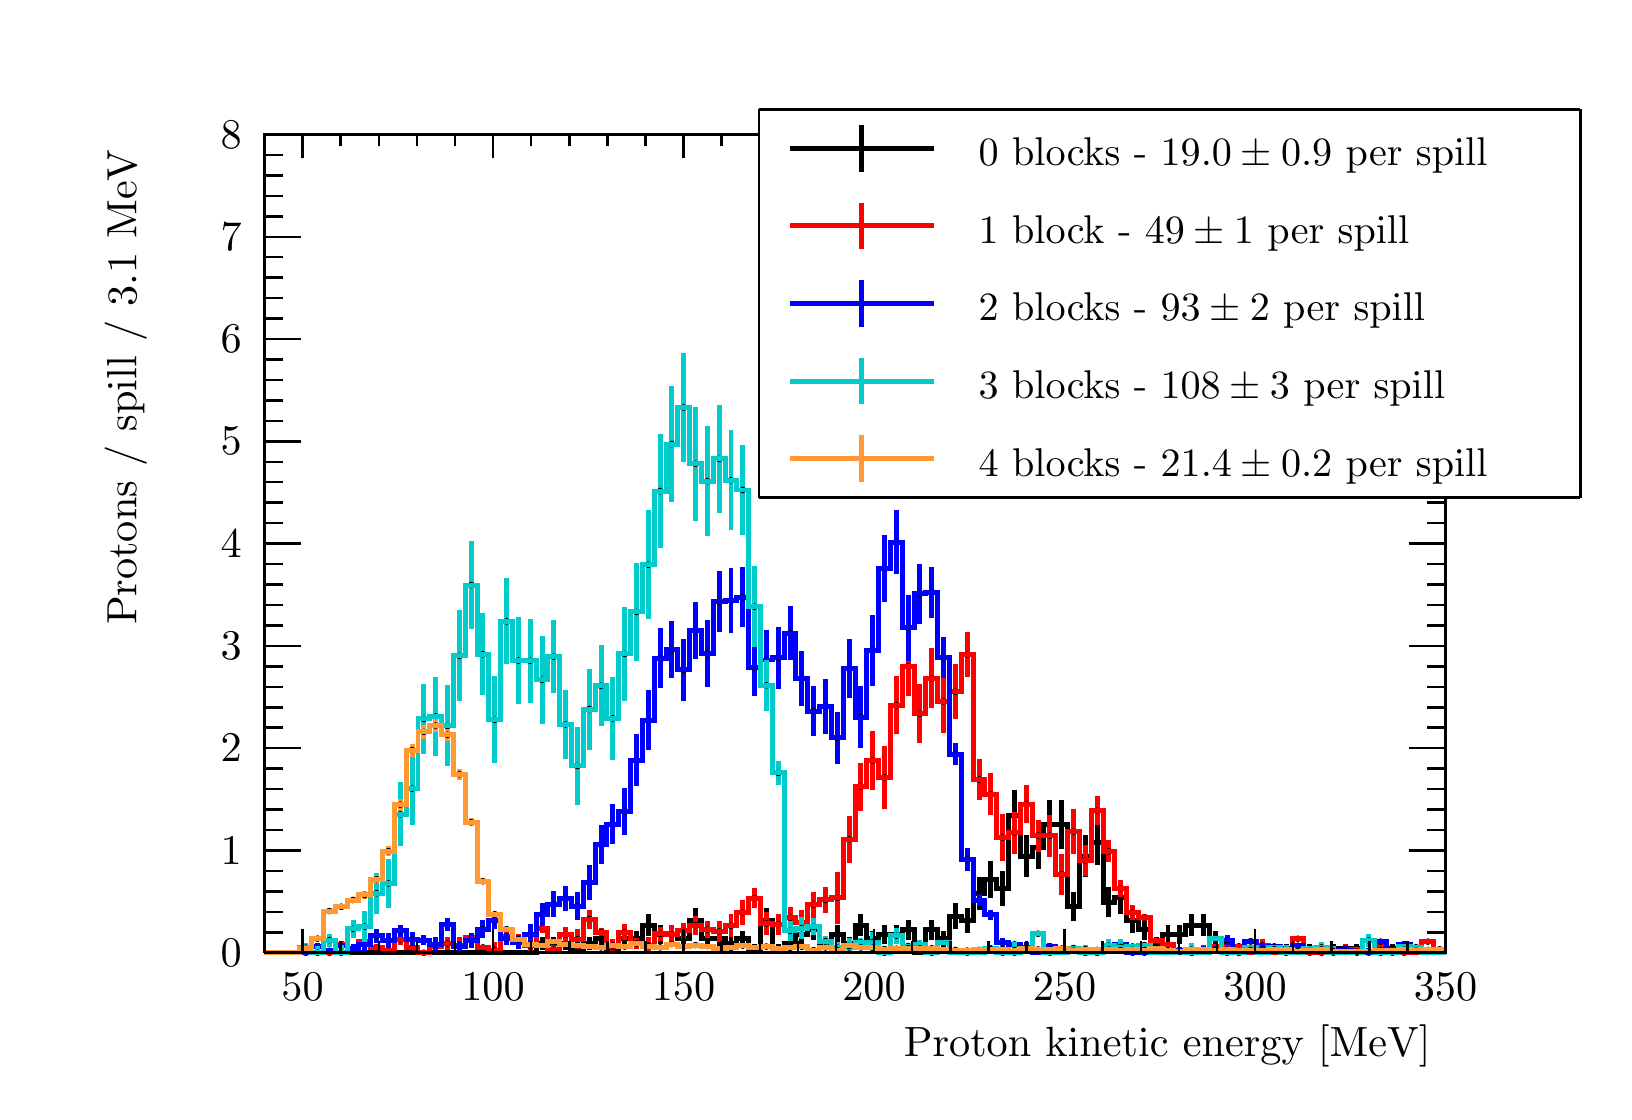
\begin{tikzpicture}
\pgfdeclareplotmark{cross} {
\pgfpathmoveto{\pgfpoint{-0.3\pgfplotmarksize}{\pgfplotmarksize}}
\pgfpathlineto{\pgfpoint{+0.3\pgfplotmarksize}{\pgfplotmarksize}}
\pgfpathlineto{\pgfpoint{+0.3\pgfplotmarksize}{0.3\pgfplotmarksize}}
\pgfpathlineto{\pgfpoint{+1\pgfplotmarksize}{0.3\pgfplotmarksize}}
\pgfpathlineto{\pgfpoint{+1\pgfplotmarksize}{-0.3\pgfplotmarksize}}
\pgfpathlineto{\pgfpoint{+0.3\pgfplotmarksize}{-0.3\pgfplotmarksize}}
\pgfpathlineto{\pgfpoint{+0.3\pgfplotmarksize}{-1.\pgfplotmarksize}}
\pgfpathlineto{\pgfpoint{-0.3\pgfplotmarksize}{-1.\pgfplotmarksize}}
\pgfpathlineto{\pgfpoint{-0.3\pgfplotmarksize}{-0.3\pgfplotmarksize}}
\pgfpathlineto{\pgfpoint{-1.\pgfplotmarksize}{-0.3\pgfplotmarksize}}
\pgfpathlineto{\pgfpoint{-1.\pgfplotmarksize}{0.3\pgfplotmarksize}}
\pgfpathlineto{\pgfpoint{-0.3\pgfplotmarksize}{0.3\pgfplotmarksize}}
\pgfpathclose
\pgfusepathqstroke
}
\pgfdeclareplotmark{cross*} {
\pgfpathmoveto{\pgfpoint{-0.3\pgfplotmarksize}{\pgfplotmarksize}}
\pgfpathlineto{\pgfpoint{+0.3\pgfplotmarksize}{\pgfplotmarksize}}
\pgfpathlineto{\pgfpoint{+0.3\pgfplotmarksize}{0.3\pgfplotmarksize}}
\pgfpathlineto{\pgfpoint{+1\pgfplotmarksize}{0.3\pgfplotmarksize}}
\pgfpathlineto{\pgfpoint{+1\pgfplotmarksize}{-0.3\pgfplotmarksize}}
\pgfpathlineto{\pgfpoint{+0.3\pgfplotmarksize}{-0.3\pgfplotmarksize}}
\pgfpathlineto{\pgfpoint{+0.3\pgfplotmarksize}{-1.\pgfplotmarksize}}
\pgfpathlineto{\pgfpoint{-0.3\pgfplotmarksize}{-1.\pgfplotmarksize}}
\pgfpathlineto{\pgfpoint{-0.3\pgfplotmarksize}{-0.3\pgfplotmarksize}}
\pgfpathlineto{\pgfpoint{-1.\pgfplotmarksize}{-0.3\pgfplotmarksize}}
\pgfpathlineto{\pgfpoint{-1.\pgfplotmarksize}{0.3\pgfplotmarksize}}
\pgfpathlineto{\pgfpoint{-0.3\pgfplotmarksize}{0.3\pgfplotmarksize}}
\pgfpathclose
\pgfusepathqfillstroke
}
\pgfdeclareplotmark{newstar} {
\pgfpathmoveto{\pgfqpoint{0pt}{\pgfplotmarksize}}
\pgfpathlineto{\pgfqpointpolar{44}{0.5\pgfplotmarksize}}
\pgfpathlineto{\pgfqpointpolar{18}{\pgfplotmarksize}}
\pgfpathlineto{\pgfqpointpolar{-20}{0.5\pgfplotmarksize}}
\pgfpathlineto{\pgfqpointpolar{-54}{\pgfplotmarksize}}
\pgfpathlineto{\pgfqpointpolar{-90}{0.5\pgfplotmarksize}}
\pgfpathlineto{\pgfqpointpolar{234}{\pgfplotmarksize}}
\pgfpathlineto{\pgfqpointpolar{198}{0.5\pgfplotmarksize}}
\pgfpathlineto{\pgfqpointpolar{162}{\pgfplotmarksize}}
\pgfpathlineto{\pgfqpointpolar{134}{0.5\pgfplotmarksize}}
\pgfpathclose
\pgfusepathqstroke
}
\pgfdeclareplotmark{newstar*} {
\pgfpathmoveto{\pgfqpoint{0pt}{\pgfplotmarksize}}
\pgfpathlineto{\pgfqpointpolar{44}{0.5\pgfplotmarksize}}
\pgfpathlineto{\pgfqpointpolar{18}{\pgfplotmarksize}}
\pgfpathlineto{\pgfqpointpolar{-20}{0.5\pgfplotmarksize}}
\pgfpathlineto{\pgfqpointpolar{-54}{\pgfplotmarksize}}
\pgfpathlineto{\pgfqpointpolar{-90}{0.5\pgfplotmarksize}}
\pgfpathlineto{\pgfqpointpolar{234}{\pgfplotmarksize}}
\pgfpathlineto{\pgfqpointpolar{198}{0.5\pgfplotmarksize}}
\pgfpathlineto{\pgfqpointpolar{162}{\pgfplotmarksize}}
\pgfpathlineto{\pgfqpointpolar{134}{0.5\pgfplotmarksize}}
\pgfpathclose
\pgfusepathqfillstroke
}
\definecolor{c}{rgb}{1,1,1};
\draw [color=c, fill=c] (0,0) rectangle (20,13.4957);
\draw [color=c, fill=c] (3,1.75444) rectangle (18,12.1461);
\definecolor{c}{rgb}{0,0,0};
\draw [c,line width=0.9] (3,1.75444) -- (3,12.1461) -- (18,12.1461) -- (18,1.75444) -- (3,1.75444);
\definecolor{c}{rgb}{1,1,1};
\draw [color=c, fill=c] (3,1.75444) rectangle (18,12.1461);
\definecolor{c}{rgb}{0,0,0};
\draw [c,line width=0.9] (3,1.75444) -- (3,12.1461) -- (18,12.1461) -- (18,1.75444) -- (3,1.75444);
\draw [c,line width=0.9] (3,1.75444) -- (3.15,1.75444) -- (3.15,1.75444) -- (3.3,1.75444) -- (3.3,1.75444) -- (3.45,1.75444) -- (3.45,1.75444) -- (3.6,1.75444) -- (3.6,1.75444) -- (3.75,1.75444) -- (3.75,1.75444) -- (3.9,1.75444) -- (3.9,1.75444) --
 (4.05,1.75444) -- (4.05,1.75444) -- (4.2,1.75444) -- (4.2,1.75444) -- (4.35,1.75444) -- (4.35,1.75444) -- (4.5,1.75444) -- (4.5,1.75444) -- (4.65,1.75444) -- (4.65,1.75444) -- (4.8,1.75444) -- (4.8,1.75444) -- (4.95,1.75444) -- (4.95,1.75444) --
 (5.1,1.75444) -- (5.1,1.75444) -- (5.25,1.75444) -- (5.25,1.75444) -- (5.4,1.75444) -- (5.4,1.75444) -- (5.55,1.75444) -- (5.55,1.75444) -- (5.7,1.75444) -- (5.7,1.75444) -- (5.85,1.75444) -- (5.85,1.75444) -- (6,1.75444) -- (6,1.75444) --
 (6.15,1.75444) -- (6.15,1.75444) -- (6.3,1.75444) -- (6.3,1.75444) -- (6.45,1.75444) -- (6.45,1.75444) -- (6.6,1.75444) -- (6.6,1.75444) -- (6.75,1.75444) -- (6.75,1.75444) -- (6.9,1.75444) -- (6.9,1.75444) -- (7.05,1.75444) -- (7.05,1.75444) --
 (7.2,1.75444) -- (7.2,1.75444) -- (7.35,1.75444) -- (7.35,1.75444) -- (7.5,1.75444) -- (7.5,1.75444) -- (7.65,1.75444) -- (7.65,1.75444) -- (7.8,1.75444) -- (7.8,1.75444) -- (7.95,1.75444) -- (7.95,1.75444) -- (8.1,1.75444) -- (8.1,1.75444) --
 (8.25,1.75444) -- (8.25,1.75444) -- (8.4,1.75444) -- (8.4,1.75444) -- (8.55,1.75444) -- (8.55,1.75444) -- (8.7,1.75444) -- (8.7,1.75444) -- (8.85,1.75444) -- (8.85,1.75444) -- (9,1.75444) -- (9,1.75444) -- (9.15,1.75444) -- (9.15,1.75444) --
 (9.3,1.75444) -- (9.3,1.75444) -- (9.45,1.75444) -- (9.45,1.75444) -- (9.6,1.75444) -- (9.6,1.75444) -- (9.75,1.75444) -- (9.75,1.75444) -- (9.9,1.75444) -- (9.9,1.75444) -- (10.05,1.75444) -- (10.05,1.75444) -- (10.2,1.75444) -- (10.2,1.75444) --
 (10.35,1.75444) -- (10.35,1.75444) -- (10.5,1.75444) -- (10.5,1.75444) -- (10.65,1.75444) -- (10.65,1.75444) -- (10.8,1.75444) -- (10.8,1.75444) -- (10.95,1.75444) -- (10.95,1.75444) -- (11.1,1.75444) -- (11.1,1.75444) -- (11.25,1.75444) --
 (11.25,1.75444) -- (11.4,1.75444) -- (11.4,1.75444) -- (11.55,1.75444) -- (11.55,1.75444) -- (11.7,1.75444) -- (11.7,1.75444) -- (11.85,1.75444) -- (11.85,1.75444) -- (12,1.75444) -- (12,1.75444) -- (12.15,1.75444) -- (12.15,1.75444) --
 (12.3,1.75444) -- (12.3,1.75444) -- (12.45,1.75444) -- (12.45,1.75444) -- (12.6,1.75444) -- (12.6,1.75444) -- (12.75,1.75444) -- (12.75,1.75444) -- (12.9,1.75444) -- (12.9,1.75444) -- (13.05,1.75444) -- (13.05,1.75444) -- (13.2,1.75444) --
 (13.2,1.75444) -- (13.35,1.75444) -- (13.35,1.75444) -- (13.5,1.75444) -- (13.5,1.75444) -- (13.65,1.75444) -- (13.65,1.75444) -- (13.8,1.75444) -- (13.8,1.75444) -- (13.95,1.75444) -- (13.95,1.75444) -- (14.1,1.75444) -- (14.1,1.75444) --
 (14.25,1.75444) -- (14.25,1.75444) -- (14.4,1.75444) -- (14.4,1.75444) -- (14.55,1.75444) -- (14.55,1.75444) -- (14.7,1.75444) -- (14.7,1.75444) -- (14.85,1.75444) -- (14.85,1.75444) -- (15,1.75444) -- (15,1.75444) -- (15.15,1.75444) --
 (15.15,1.75444) -- (15.3,1.75444) -- (15.3,1.75444) -- (15.45,1.75444) -- (15.45,1.75444) -- (15.6,1.75444) -- (15.6,1.75444) -- (15.75,1.75444) -- (15.75,1.75444) -- (15.9,1.75444) -- (15.9,1.75444) -- (16.05,1.75444) -- (16.05,1.75444) --
 (16.2,1.75444) -- (16.2,1.75444) -- (16.35,1.75444) -- (16.35,1.75444) -- (16.5,1.75444) -- (16.5,1.75444) -- (16.65,1.75444) -- (16.65,1.75444) -- (16.8,1.75444) -- (16.8,1.75444) -- (16.95,1.75444) -- (16.95,1.75444) -- (17.1,1.75444) --
 (17.1,1.75444) -- (17.25,1.75444) -- (17.25,1.75444) -- (17.4,1.75444) -- (17.4,1.75444) -- (17.55,1.75444) -- (17.55,1.75444) -- (17.7,1.75444) -- (17.7,1.75444) -- (17.85,1.75444) -- (17.85,1.75444) -- (18,1.75444);
\draw [c,line width=0.9] (3,1.75444) -- (18,1.75444);
\draw [c,line width=0.9] (3.48387,2.05809) -- (3.48387,1.75444);
\draw [c,line width=0.9] (3.96774,1.90627) -- (3.96774,1.75444);
\draw [c,line width=0.9] (4.45161,1.90627) -- (4.45161,1.75444);
\draw [c,line width=0.9] (4.93548,1.90627) -- (4.93548,1.75444);
\draw [c,line width=0.9] (5.41935,1.90627) -- (5.41935,1.75444);
\draw [c,line width=0.9] (5.90323,2.05809) -- (5.90323,1.75444);
\draw [c,line width=0.9] (6.3871,1.90627) -- (6.3871,1.75444);
\draw [c,line width=0.9] (6.87097,1.90627) -- (6.87097,1.75444);
\draw [c,line width=0.9] (7.35484,1.90627) -- (7.35484,1.75444);
\draw [c,line width=0.9] (7.83871,1.90627) -- (7.83871,1.75444);
\draw [c,line width=0.9] (8.32258,2.05809) -- (8.32258,1.75444);
\draw [c,line width=0.9] (8.80645,1.90627) -- (8.80645,1.75444);
\draw [c,line width=0.9] (9.29032,1.90627) -- (9.29032,1.75444);
\draw [c,line width=0.9] (9.77419,1.90627) -- (9.77419,1.75444);
\draw [c,line width=0.9] (10.2581,1.90627) -- (10.2581,1.75444);
\draw [c,line width=0.9] (10.7419,2.05809) -- (10.7419,1.75444);
\draw [c,line width=0.9] (11.2258,1.90627) -- (11.2258,1.75444);
\draw [c,line width=0.9] (11.7097,1.90627) -- (11.7097,1.75444);
\draw [c,line width=0.9] (12.1935,1.90627) -- (12.1935,1.75444);
\draw [c,line width=0.9] (12.6774,1.90627) -- (12.6774,1.75444);
\draw [c,line width=0.9] (13.1613,2.05809) -- (13.1613,1.75444);
\draw [c,line width=0.9] (13.6452,1.90627) -- (13.6452,1.75444);
\draw [c,line width=0.9] (14.129,1.90627) -- (14.129,1.75444);
\draw [c,line width=0.9] (14.6129,1.90627) -- (14.6129,1.75444);
\draw [c,line width=0.9] (15.0968,1.90627) -- (15.0968,1.75444);
\draw [c,line width=0.9] (15.5806,2.05809) -- (15.5806,1.75444);
\draw [c,line width=0.9] (16.0645,1.90627) -- (16.0645,1.75444);
\draw [c,line width=0.9] (16.5484,1.90627) -- (16.5484,1.75444);
\draw [c,line width=0.9] (17.0323,1.90627) -- (17.0323,1.75444);
\draw [c,line width=0.9] (17.5161,1.90627) -- (17.5161,1.75444);
\draw [c,line width=0.9] (18,2.05809) -- (18,1.75444);
\draw [c,line width=0.9] (3.48387,2.05809) -- (3.48387,1.75444);
\draw [c,line width=0.9] (18,2.05809) -- (18,1.75444);
\draw [anchor=base] (3.48387,1.14713) node[scale=1.52731, color=c, rotate=0]{50};
\draw [anchor=base] (5.90323,1.14713) node[scale=1.52731, color=c, rotate=0]{100};
\draw [anchor=base] (8.32258,1.14713) node[scale=1.52731, color=c, rotate=0]{150};
\draw [anchor=base] (10.7419,1.14713) node[scale=1.52731, color=c, rotate=0]{200};
\draw [anchor=base] (13.1613,1.14713) node[scale=1.52731, color=c, rotate=0]{250};
\draw [anchor=base] (15.5806,1.14713) node[scale=1.52731, color=c, rotate=0]{300};
\draw [anchor=base] (18,1.14713) node[scale=1.52731, color=c, rotate=0]{350};
\draw [anchor= east] (18,0.566819) node[scale=1.52731, color=c, rotate=0]{ Proton kinetic energy [MeV]};
\draw [c,line width=0.9] (3,12.1461) -- (18,12.1461);
\draw [c,line width=0.9] (3.48387,11.8425) -- (3.48387,12.1461);
\draw [c,line width=0.9] (3.96774,11.9943) -- (3.96774,12.1461);
\draw [c,line width=0.9] (4.45161,11.9943) -- (4.45161,12.1461);
\draw [c,line width=0.9] (4.93548,11.9943) -- (4.93548,12.1461);
\draw [c,line width=0.9] (5.41935,11.9943) -- (5.41935,12.1461);
\draw [c,line width=0.9] (5.90323,11.8425) -- (5.90323,12.1461);
\draw [c,line width=0.9] (6.3871,11.9943) -- (6.3871,12.1461);
\draw [c,line width=0.9] (6.87097,11.9943) -- (6.87097,12.1461);
\draw [c,line width=0.9] (7.35484,11.9943) -- (7.35484,12.1461);
\draw [c,line width=0.9] (7.83871,11.9943) -- (7.83871,12.1461);
\draw [c,line width=0.9] (8.32258,11.8425) -- (8.32258,12.1461);
\draw [c,line width=0.9] (8.80645,11.9943) -- (8.80645,12.1461);
\draw [c,line width=0.9] (9.29032,11.9943) -- (9.29032,12.1461);
\draw [c,line width=0.9] (9.77419,11.9943) -- (9.77419,12.1461);
\draw [c,line width=0.9] (10.2581,11.9943) -- (10.2581,12.1461);
\draw [c,line width=0.9] (10.7419,11.8425) -- (10.7419,12.1461);
\draw [c,line width=0.9] (11.2258,11.9943) -- (11.2258,12.1461);
\draw [c,line width=0.9] (11.7097,11.9943) -- (11.7097,12.1461);
\draw [c,line width=0.9] (12.1935,11.9943) -- (12.1935,12.1461);
\draw [c,line width=0.9] (12.6774,11.9943) -- (12.6774,12.1461);
\draw [c,line width=0.9] (13.1613,11.8425) -- (13.1613,12.1461);
\draw [c,line width=0.9] (13.6452,11.9943) -- (13.6452,12.1461);
\draw [c,line width=0.9] (14.129,11.9943) -- (14.129,12.1461);
\draw [c,line width=0.9] (14.6129,11.9943) -- (14.6129,12.1461);
\draw [c,line width=0.9] (15.0968,11.9943) -- (15.0968,12.1461);
\draw [c,line width=0.9] (15.5806,11.8425) -- (15.5806,12.1461);
\draw [c,line width=0.9] (16.0645,11.9943) -- (16.0645,12.1461);
\draw [c,line width=0.9] (16.5484,11.9943) -- (16.5484,12.1461);
\draw [c,line width=0.9] (17.0323,11.9943) -- (17.0323,12.1461);
\draw [c,line width=0.9] (17.5161,11.9943) -- (17.5161,12.1461);
\draw [c,line width=0.9] (18,11.8425) -- (18,12.1461);
\draw [c,line width=0.9] (3.48387,11.8425) -- (3.48387,12.1461);
\draw [c,line width=0.9] (18,11.8425) -- (18,12.1461);
\draw [c,line width=0.9] (3,1.75444) -- (3,12.1461);
\draw [c,line width=0.9] (3.462,1.75444) -- (3,1.75444);
\draw [c,line width=0.9] (3.231,2.01423) -- (3,2.01423);
\draw [c,line width=0.9] (3.231,2.27403) -- (3,2.27403);
\draw [c,line width=0.9] (3.231,2.53382) -- (3,2.53382);
\draw [c,line width=0.9] (3.231,2.79361) -- (3,2.79361);
\draw [c,line width=0.9] (3.462,3.0534) -- (3,3.0534);
\draw [c,line width=0.9] (3.231,3.31319) -- (3,3.31319);
\draw [c,line width=0.9] (3.231,3.57299) -- (3,3.57299);
\draw [c,line width=0.9] (3.231,3.83278) -- (3,3.83278);
\draw [c,line width=0.9] (3.231,4.09257) -- (3,4.09257);
\draw [c,line width=0.9] (3.462,4.35236) -- (3,4.35236);
\draw [c,line width=0.9] (3.231,4.61216) -- (3,4.61216);
\draw [c,line width=0.9] (3.231,4.87195) -- (3,4.87195);
\draw [c,line width=0.9] (3.231,5.13174) -- (3,5.13174);
\draw [c,line width=0.9] (3.231,5.39153) -- (3,5.39153);
\draw [c,line width=0.9] (3.462,5.65133) -- (3,5.65133);
\draw [c,line width=0.9] (3.231,5.91112) -- (3,5.91112);
\draw [c,line width=0.9] (3.231,6.17091) -- (3,6.17091);
\draw [c,line width=0.9] (3.231,6.4307) -- (3,6.4307);
\draw [c,line width=0.9] (3.231,6.69049) -- (3,6.69049);
\draw [c,line width=0.9] (3.462,6.95029) -- (3,6.95029);
\draw [c,line width=0.9] (3.231,7.21008) -- (3,7.21008);
\draw [c,line width=0.9] (3.231,7.46987) -- (3,7.46987);
\draw [c,line width=0.9] (3.231,7.72966) -- (3,7.72966);
\draw [c,line width=0.9] (3.231,7.98946) -- (3,7.98946);
\draw [c,line width=0.9] (3.462,8.24925) -- (3,8.24925);
\draw [c,line width=0.9] (3.231,8.50904) -- (3,8.50904);
\draw [c,line width=0.9] (3.231,8.76883) -- (3,8.76883);
\draw [c,line width=0.9] (3.231,9.02862) -- (3,9.02862);
\draw [c,line width=0.9] (3.231,9.28842) -- (3,9.28842);
\draw [c,line width=0.9] (3.462,9.54821) -- (3,9.54821);
\draw [c,line width=0.9] (3.231,9.808) -- (3,9.808);
\draw [c,line width=0.9] (3.231,10.0678) -- (3,10.0678);
\draw [c,line width=0.9] (3.231,10.3276) -- (3,10.3276);
\draw [c,line width=0.9] (3.231,10.5874) -- (3,10.5874);
\draw [c,line width=0.9] (3.462,10.8472) -- (3,10.8472);
\draw [c,line width=0.9] (3.231,11.107) -- (3,11.107);
\draw [c,line width=0.9] (3.231,11.3668) -- (3,11.3668);
\draw [c,line width=0.9] (3.231,11.6265) -- (3,11.6265);
\draw [c,line width=0.9] (3.231,11.8863) -- (3,11.8863);
\draw [c,line width=0.9] (3.462,12.1461) -- (3,12.1461);
\draw [anchor= east] (2.9,1.75444) node[scale=1.52731, color=c, rotate=0]{0};
\draw [anchor= east] (2.9,3.0534) node[scale=1.52731, color=c, rotate=0]{1};
\draw [anchor= east] (2.9,4.35236) node[scale=1.52731, color=c, rotate=0]{2};
\draw [anchor= east] (2.9,5.65133) node[scale=1.52731, color=c, rotate=0]{3};
\draw [anchor= east] (2.9,6.95029) node[scale=1.52731, color=c, rotate=0]{4};
\draw [anchor= east] (2.9,8.24925) node[scale=1.52731, color=c, rotate=0]{5};
\draw [anchor= east] (2.9,9.54821) node[scale=1.52731, color=c, rotate=0]{6};
\draw [anchor= east] (2.9,10.8472) node[scale=1.52731, color=c, rotate=0]{7};
\draw [anchor= east] (2.9,12.1461) node[scale=1.52731, color=c, rotate=0]{8};
\draw [anchor= east] (1.24,12.1461) node[scale=1.52731, color=c, rotate=90]{ Protons / spill / 3.1~MeV};
\draw [c,line width=0.9] (18,1.75444) -- (18,12.1461);
\draw [c,line width=0.9] (17.538,1.75444) -- (18,1.75444);
\draw [c,line width=0.9] (17.769,2.01423) -- (18,2.01423);
\draw [c,line width=0.9] (17.769,2.27403) -- (18,2.27403);
\draw [c,line width=0.9] (17.769,2.53382) -- (18,2.53382);
\draw [c,line width=0.9] (17.769,2.79361) -- (18,2.79361);
\draw [c,line width=0.9] (17.538,3.0534) -- (18,3.0534);
\draw [c,line width=0.9] (17.769,3.31319) -- (18,3.31319);
\draw [c,line width=0.9] (17.769,3.57299) -- (18,3.57299);
\draw [c,line width=0.9] (17.769,3.83278) -- (18,3.83278);
\draw [c,line width=0.9] (17.769,4.09257) -- (18,4.09257);
\draw [c,line width=0.9] (17.538,4.35236) -- (18,4.35236);
\draw [c,line width=0.9] (17.769,4.61216) -- (18,4.61216);
\draw [c,line width=0.9] (17.769,4.87195) -- (18,4.87195);
\draw [c,line width=0.9] (17.769,5.13174) -- (18,5.13174);
\draw [c,line width=0.9] (17.769,5.39153) -- (18,5.39153);
\draw [c,line width=0.9] (17.538,5.65133) -- (18,5.65133);
\draw [c,line width=0.9] (17.769,5.91112) -- (18,5.91112);
\draw [c,line width=0.9] (17.769,6.17091) -- (18,6.17091);
\draw [c,line width=0.9] (17.769,6.4307) -- (18,6.4307);
\draw [c,line width=0.9] (17.769,6.69049) -- (18,6.69049);
\draw [c,line width=0.9] (17.538,6.95029) -- (18,6.95029);
\draw [c,line width=0.9] (17.769,7.21008) -- (18,7.21008);
\draw [c,line width=0.9] (17.769,7.46987) -- (18,7.46987);
\draw [c,line width=0.9] (17.769,7.72966) -- (18,7.72966);
\draw [c,line width=0.9] (17.769,7.98946) -- (18,7.98946);
\draw [c,line width=0.9] (17.538,8.24925) -- (18,8.24925);
\draw [c,line width=0.9] (17.769,8.50904) -- (18,8.50904);
\draw [c,line width=0.9] (17.769,8.76883) -- (18,8.76883);
\draw [c,line width=0.9] (17.769,9.02862) -- (18,9.02862);
\draw [c,line width=0.9] (17.769,9.28842) -- (18,9.28842);
\draw [c,line width=0.9] (17.538,9.54821) -- (18,9.54821);
\draw [c,line width=0.9] (17.769,9.808) -- (18,9.808);
\draw [c,line width=0.9] (17.769,10.0678) -- (18,10.0678);
\draw [c,line width=0.9] (17.769,10.3276) -- (18,10.3276);
\draw [c,line width=0.9] (17.769,10.5874) -- (18,10.5874);
\draw [c,line width=0.9] (17.538,10.8472) -- (18,10.8472);
\draw [c,line width=0.9] (17.769,11.107) -- (18,11.107);
\draw [c,line width=0.9] (17.769,11.3668) -- (18,11.3668);
\draw [c,line width=0.9] (17.769,11.6265) -- (18,11.6265);
\draw [c,line width=0.9] (17.769,11.8863) -- (18,11.8863);
\draw [c,line width=0.9] (17.538,12.1461) -- (18,12.1461);
\draw [c,line width=1.8] (6.525,1.78858) -- (6.525,1.87103);
\draw [c,line width=1.8] (6.525,1.87103) -- (6.525,1.95347);
\foreach \P in {(6.525,1.87103)}{\draw[mark options={color=c,fill=c},mark size=2.402402pt,mark=*,mark size=1pt] plot coordinates {\P};}
\draw [c,line width=1.8] (6.675,1.78858) -- (6.675,1.87103);
\draw [c,line width=1.8] (6.675,1.87103) -- (6.675,1.95347);
\foreach \P in {(6.675,1.87103)}{\draw[mark options={color=c,fill=c},mark size=2.402402pt,mark=*,mark size=1pt] plot coordinates {\P};}
\draw [c,line width=1.8] (6.825,1.78858) -- (6.825,1.87103);
\draw [c,line width=1.8] (6.825,1.87103) -- (6.825,1.95347);
\foreach \P in {(6.825,1.87103)}{\draw[mark options={color=c,fill=c},mark size=2.402402pt,mark=*,mark size=1pt] plot coordinates {\P};}
\draw [c,line width=1.8] (6.975,1.75444) -- (6.975,1.81273);
\draw [c,line width=1.8] (6.975,1.81273) -- (6.975,1.87103);
\foreach \P in {(6.975,1.81273)}{\draw[mark options={color=c,fill=c},mark size=2.402402pt,mark=*,mark size=1pt] plot coordinates {\P};}
\draw [c,line width=1.8] (7.125,1.78858) -- (7.125,1.87103);
\draw [c,line width=1.8] (7.125,1.87103) -- (7.125,1.95347);
\foreach \P in {(7.125,1.87103)}{\draw[mark options={color=c,fill=c},mark size=2.402402pt,mark=*,mark size=1pt] plot coordinates {\P};}
\draw [c,line width=1.8] (7.275,1.82835) -- (7.275,1.92932);
\draw [c,line width=1.8] (7.275,1.92932) -- (7.275,2.03029);
\foreach \P in {(7.275,1.92932)}{\draw[mark options={color=c,fill=c},mark size=2.402402pt,mark=*,mark size=1pt] plot coordinates {\P};}
\draw [c,line width=1.8] (7.425,1.75444) -- (7.425,1.81273);
\draw [c,line width=1.8] (7.425,1.81273) -- (7.425,1.87103);
\foreach \P in {(7.425,1.81273)}{\draw[mark options={color=c,fill=c},mark size=2.402402pt,mark=*,mark size=1pt] plot coordinates {\P};}
\draw [c,line width=1.8] (7.575,1.82835) -- (7.575,1.92932);
\draw [c,line width=1.8] (7.575,1.92932) -- (7.575,2.03029);
\foreach \P in {(7.575,1.92932)}{\draw[mark options={color=c,fill=c},mark size=2.402402pt,mark=*,mark size=1pt] plot coordinates {\P};}
\draw [c,line width=1.8] (7.725,1.82835) -- (7.725,1.92932);
\draw [c,line width=1.8] (7.725,1.92932) -- (7.725,2.03029);
\foreach \P in {(7.725,1.92932)}{\draw[mark options={color=c,fill=c},mark size=2.402402pt,mark=*,mark size=1pt] plot coordinates {\P};}
\draw [c,line width=1.8] (7.875,1.9614) -- (7.875,2.1042);
\draw [c,line width=1.8] (7.875,2.1042) -- (7.875,2.247);
\foreach \P in {(7.875,2.1042)}{\draw[mark options={color=c,fill=c},mark size=2.402402pt,mark=*,mark size=1pt] plot coordinates {\P};}
\draw [c,line width=1.8] (8.025,1.87102) -- (8.025,1.98761);
\draw [c,line width=1.8] (8.025,1.98761) -- (8.025,2.10421);
\foreach \P in {(8.025,1.98761)}{\draw[mark options={color=c,fill=c},mark size=2.402402pt,mark=*,mark size=1pt] plot coordinates {\P};}
\draw [c,line width=1.8] (8.175,1.87102) -- (8.175,1.98761);
\draw [c,line width=1.8] (8.175,1.98761) -- (8.175,2.10421);
\foreach \P in {(8.175,1.98761)}{\draw[mark options={color=c,fill=c},mark size=2.402402pt,mark=*,mark size=1pt] plot coordinates {\P};}
\draw [c,line width=1.8] (8.325,1.82835) -- (8.325,1.92932);
\draw [c,line width=1.8] (8.325,1.92932) -- (8.325,2.03029);
\foreach \P in {(8.325,1.92932)}{\draw[mark options={color=c,fill=c},mark size=2.402402pt,mark=*,mark size=1pt] plot coordinates {\P};}
\draw [c,line width=1.8] (8.475,2.00825) -- (8.475,2.16249);
\draw [c,line width=1.8] (8.475,2.16249) -- (8.475,2.31673);
\foreach \P in {(8.475,2.16249)}{\draw[mark options={color=c,fill=c},mark size=2.402402pt,mark=*,mark size=1pt] plot coordinates {\P};}
\draw [c,line width=1.8] (8.625,1.82835) -- (8.625,1.92932);
\draw [c,line width=1.8] (8.625,1.92932) -- (8.625,2.03029);
\foreach \P in {(8.625,1.92932)}{\draw[mark options={color=c,fill=c},mark size=2.402402pt,mark=*,mark size=1pt] plot coordinates {\P};}
\draw [c,line width=1.8] (8.775,1.82835) -- (8.775,1.92932);
\draw [c,line width=1.8] (8.775,1.92932) -- (8.775,2.03029);
\foreach \P in {(8.775,1.92932)}{\draw[mark options={color=c,fill=c},mark size=2.402402pt,mark=*,mark size=1pt] plot coordinates {\P};}
\draw [c,line width=1.8] (8.925,1.78858) -- (8.925,1.87103);
\draw [c,line width=1.8] (8.925,1.87103) -- (8.925,1.95347);
\foreach \P in {(8.925,1.87103)}{\draw[mark options={color=c,fill=c},mark size=2.402402pt,mark=*,mark size=1pt] plot coordinates {\P};}
\draw [c,line width=1.8] (9.075,1.82835) -- (9.075,1.92932);
\draw [c,line width=1.8] (9.075,1.92932) -- (9.075,2.03029);
\foreach \P in {(9.075,1.92932)}{\draw[mark options={color=c,fill=c},mark size=2.402402pt,mark=*,mark size=1pt] plot coordinates {\P};}
\draw [c,line width=1.8] (9.225,1.75444) -- (9.225,1.81273);
\draw [c,line width=1.8] (9.225,1.81273) -- (9.225,1.87103);
\foreach \P in {(9.225,1.81273)}{\draw[mark options={color=c,fill=c},mark size=2.402402pt,mark=*,mark size=1pt] plot coordinates {\P};}
\draw [c,line width=1.8] (9.375,2.00825) -- (9.375,2.16249);
\draw [c,line width=1.8] (9.375,2.16249) -- (9.375,2.31673);
\foreach \P in {(9.375,2.16249)}{\draw[mark options={color=c,fill=c},mark size=2.402402pt,mark=*,mark size=1pt] plot coordinates {\P};}
\draw [c,line width=1.8] (9.525,1.75444) -- (9.525,1.81273);
\draw [c,line width=1.8] (9.525,1.81273) -- (9.525,1.87103);
\foreach \P in {(9.525,1.81273)}{\draw[mark options={color=c,fill=c},mark size=2.402402pt,mark=*,mark size=1pt] plot coordinates {\P};}
\draw [c,line width=1.8] (9.675,1.78858) -- (9.675,1.87103);
\draw [c,line width=1.8] (9.675,1.87103) -- (9.675,1.95347);
\foreach \P in {(9.675,1.87103)}{\draw[mark options={color=c,fill=c},mark size=2.402402pt,mark=*,mark size=1pt] plot coordinates {\P};}
\draw [c,line width=1.8] (9.825,1.87102) -- (9.825,1.98761);
\draw [c,line width=1.8] (9.825,1.98761) -- (9.825,2.10421);
\foreach \P in {(9.825,1.98761)}{\draw[mark options={color=c,fill=c},mark size=2.402402pt,mark=*,mark size=1pt] plot coordinates {\P};}
\draw [c,line width=1.8] (9.975,1.91555) -- (9.975,2.04591);
\draw [c,line width=1.8] (9.975,2.04591) -- (9.975,2.17626);
\foreach \P in {(9.975,2.04591)}{\draw[mark options={color=c,fill=c},mark size=2.402402pt,mark=*,mark size=1pt] plot coordinates {\P};}
\draw [c,line width=1.8] (10.125,1.78858) -- (10.125,1.87103);
\draw [c,line width=1.8] (10.125,1.87103) -- (10.125,1.95347);
\foreach \P in {(10.125,1.87103)}{\draw[mark options={color=c,fill=c},mark size=2.402402pt,mark=*,mark size=1pt] plot coordinates {\P};}
\draw [c,line width=1.8] (10.275,1.87102) -- (10.275,1.98761);
\draw [c,line width=1.8] (10.275,1.98761) -- (10.275,2.10421);
\foreach \P in {(10.275,1.98761)}{\draw[mark options={color=c,fill=c},mark size=2.402402pt,mark=*,mark size=1pt] plot coordinates {\P};}
\draw [c,line width=1.8] (10.425,1.78858) -- (10.425,1.87103);
\draw [c,line width=1.8] (10.425,1.87103) -- (10.425,1.95347);
\foreach \P in {(10.425,1.87103)}{\draw[mark options={color=c,fill=c},mark size=2.402402pt,mark=*,mark size=1pt] plot coordinates {\P};}
\draw [c,line width=1.8] (10.575,1.9614) -- (10.575,2.1042);
\draw [c,line width=1.8] (10.575,2.1042) -- (10.575,2.247);
\foreach \P in {(10.575,2.1042)}{\draw[mark options={color=c,fill=c},mark size=2.402402pt,mark=*,mark size=1pt] plot coordinates {\P};}
\draw [c,line width=1.8] (10.725,1.82835) -- (10.725,1.92932);
\draw [c,line width=1.8] (10.725,1.92932) -- (10.725,2.03029);
\foreach \P in {(10.725,1.92932)}{\draw[mark options={color=c,fill=c},mark size=2.402402pt,mark=*,mark size=1pt] plot coordinates {\P};}
\draw [c,line width=1.8] (10.875,1.87102) -- (10.875,1.98761);
\draw [c,line width=1.8] (10.875,1.98761) -- (10.875,2.10421);
\foreach \P in {(10.875,1.98761)}{\draw[mark options={color=c,fill=c},mark size=2.402402pt,mark=*,mark size=1pt] plot coordinates {\P};}
\draw [c,line width=1.8] (11.025,1.87102) -- (11.025,1.98761);
\draw [c,line width=1.8] (11.025,1.98761) -- (11.025,2.10421);
\foreach \P in {(11.025,1.98761)}{\draw[mark options={color=c,fill=c},mark size=2.402402pt,mark=*,mark size=1pt] plot coordinates {\P};}
\draw [c,line width=1.8] (11.175,1.91555) -- (11.175,2.04591);
\draw [c,line width=1.8] (11.175,2.04591) -- (11.175,2.17626);
\foreach \P in {(11.175,2.04591)}{\draw[mark options={color=c,fill=c},mark size=2.402402pt,mark=*,mark size=1pt] plot coordinates {\P};}
\draw [c,line width=1.8] (11.475,1.91555) -- (11.475,2.04591);
\draw [c,line width=1.8] (11.475,2.04591) -- (11.475,2.17626);
\foreach \P in {(11.475,2.04591)}{\draw[mark options={color=c,fill=c},mark size=2.402402pt,mark=*,mark size=1pt] plot coordinates {\P};}
\draw [c,line width=1.8] (11.625,1.82835) -- (11.625,1.92932);
\draw [c,line width=1.8] (11.625,1.92932) -- (11.625,2.03029);
\foreach \P in {(11.625,1.92932)}{\draw[mark options={color=c,fill=c},mark size=2.402402pt,mark=*,mark size=1pt] plot coordinates {\P};}
\draw [c,line width=1.8] (11.775,2.0559) -- (11.775,2.22079);
\draw [c,line width=1.8] (11.775,2.22079) -- (11.775,2.38568);
\foreach \P in {(11.775,2.22079)}{\draw[mark options={color=c,fill=c},mark size=2.402402pt,mark=*,mark size=1pt] plot coordinates {\P};}
\draw [c,line width=1.8] (11.925,2.00825) -- (11.925,2.16249);
\draw [c,line width=1.8] (11.925,2.16249) -- (11.925,2.31673);
\foreach \P in {(11.925,2.16249)}{\draw[mark options={color=c,fill=c},mark size=2.402402pt,mark=*,mark size=1pt] plot coordinates {\P};}
\draw [c,line width=1.8] (12.075,2.30206) -- (12.075,2.51225);
\draw [c,line width=1.8] (12.075,2.51225) -- (12.075,2.72245);
\foreach \P in {(12.075,2.51225)}{\draw[mark options={color=c,fill=c},mark size=2.402402pt,mark=*,mark size=1pt] plot coordinates {\P};}
\draw [c,line width=1.8] (12.225,2.45395) -- (12.225,2.68713);
\draw [c,line width=1.8] (12.225,2.68713) -- (12.225,2.92032);
\foreach \P in {(12.225,2.68713)}{\draw[mark options={color=c,fill=c},mark size=2.402402pt,mark=*,mark size=1pt] plot coordinates {\P};}
\draw [c,line width=1.8] (12.375,2.35242) -- (12.375,2.57055);
\draw [c,line width=1.8] (12.375,2.57055) -- (12.375,2.78867);
\foreach \P in {(12.375,2.57055)}{\draw[mark options={color=c,fill=c},mark size=2.402402pt,mark=*,mark size=1pt] plot coordinates {\P};}
\draw [c,line width=1.8] (12.525,3.18393) -- (12.525,3.50324);
\draw [c,line width=1.8] (12.525,3.50324) -- (12.525,3.82254);
\foreach \P in {(12.525,3.50324)}{\draw[mark options={color=c,fill=c},mark size=2.402402pt,mark=*,mark size=1pt] plot coordinates {\P};}
\draw [c,line width=1.8] (12.675,2.71145) -- (12.675,2.9786);
\draw [c,line width=1.8] (12.675,2.9786) -- (12.675,3.24575);
\foreach \P in {(12.675,2.9786)}{\draw[mark options={color=c,fill=c},mark size=2.402402pt,mark=*,mark size=1pt] plot coordinates {\P};}
\draw [c,line width=1.8] (12.825,2.8156) -- (12.825,3.09519);
\draw [c,line width=1.8] (12.825,3.09519) -- (12.825,3.37477);
\foreach \P in {(12.825,3.09519)}{\draw[mark options={color=c,fill=c},mark size=2.402402pt,mark=*,mark size=1pt] plot coordinates {\P};}
\draw [c,line width=1.8] (12.975,3.07817) -- (12.975,3.38665);
\draw [c,line width=1.8] (12.975,3.38665) -- (12.975,3.69513);
\foreach \P in {(12.975,3.38665)}{\draw[mark options={color=c,fill=c},mark size=2.402402pt,mark=*,mark size=1pt] plot coordinates {\P};}
\draw [c,line width=1.8] (13.125,3.07817) -- (13.125,3.38665);
\draw [c,line width=1.8] (13.125,3.38665) -- (13.125,3.69513);
\foreach \P in {(13.125,3.38665)}{\draw[mark options={color=c,fill=c},mark size=2.402402pt,mark=*,mark size=1pt] plot coordinates {\P};}
\draw [c,line width=1.8] (13.275,2.15302) -- (13.275,2.33737);
\draw [c,line width=1.8] (13.275,2.33737) -- (13.275,2.52172);
\foreach \P in {(13.275,2.33737)}{\draw[mark options={color=c,fill=c},mark size=2.402402pt,mark=*,mark size=1pt] plot coordinates {\P};}
\draw [c,line width=1.8] (13.425,2.71145) -- (13.425,2.9786);
\draw [c,line width=1.8] (13.425,2.9786) -- (13.425,3.24575);
\foreach \P in {(13.425,2.9786)}{\draw[mark options={color=c,fill=c},mark size=2.402402pt,mark=*,mark size=1pt] plot coordinates {\P};}
\draw [c,line width=1.8] (13.575,2.86788) -- (13.575,3.15348);
\draw [c,line width=1.8] (13.575,3.15348) -- (13.575,3.43907);
\foreach \P in {(13.575,3.15348)}{\draw[mark options={color=c,fill=c},mark size=2.402402pt,mark=*,mark size=1pt] plot coordinates {\P};}
\draw [c,line width=1.8] (13.725,2.20232) -- (13.725,2.39567);
\draw [c,line width=1.8] (13.725,2.39567) -- (13.725,2.58902);
\foreach \P in {(13.725,2.39567)}{\draw[mark options={color=c,fill=c},mark size=2.402402pt,mark=*,mark size=1pt] plot coordinates {\P};}
\draw [c,line width=1.8] (13.875,2.25201) -- (13.875,2.45396);
\draw [c,line width=1.8] (13.875,2.45396) -- (13.875,2.65591);
\foreach \P in {(13.875,2.45396)}{\draw[mark options={color=c,fill=c},mark size=2.402402pt,mark=*,mark size=1pt] plot coordinates {\P};}
\draw [c,line width=1.8] (14.025,2.00825) -- (14.025,2.16249);
\draw [c,line width=1.8] (14.025,2.16249) -- (14.025,2.31673);
\foreach \P in {(14.025,2.16249)}{\draw[mark options={color=c,fill=c},mark size=2.402402pt,mark=*,mark size=1pt] plot coordinates {\P};}
\draw [c,line width=1.8] (14.175,1.91555) -- (14.175,2.04591);
\draw [c,line width=1.8] (14.175,2.04591) -- (14.175,2.17626);
\foreach \P in {(14.175,2.04591)}{\draw[mark options={color=c,fill=c},mark size=2.402402pt,mark=*,mark size=1pt] plot coordinates {\P};}
\draw [c,line width=1.8] (14.325,1.78858) -- (14.325,1.87103);
\draw [c,line width=1.8] (14.325,1.87103) -- (14.325,1.95347);
\foreach \P in {(14.325,1.87103)}{\draw[mark options={color=c,fill=c},mark size=2.402402pt,mark=*,mark size=1pt] plot coordinates {\P};}
\draw [c,line width=1.8] (14.475,1.87102) -- (14.475,1.98761);
\draw [c,line width=1.8] (14.475,1.98761) -- (14.475,2.10421);
\foreach \P in {(14.475,1.98761)}{\draw[mark options={color=c,fill=c},mark size=2.402402pt,mark=*,mark size=1pt] plot coordinates {\P};}
\draw [c,line width=1.8] (14.625,1.87102) -- (14.625,1.98761);
\draw [c,line width=1.8] (14.625,1.98761) -- (14.625,2.10421);
\foreach \P in {(14.625,1.98761)}{\draw[mark options={color=c,fill=c},mark size=2.402402pt,mark=*,mark size=1pt] plot coordinates {\P};}
\draw [c,line width=1.8] (14.775,1.9614) -- (14.775,2.1042);
\draw [c,line width=1.8] (14.775,2.1042) -- (14.775,2.247);
\foreach \P in {(14.775,2.1042)}{\draw[mark options={color=c,fill=c},mark size=2.402402pt,mark=*,mark size=1pt] plot coordinates {\P};}
\draw [c,line width=1.8] (14.925,1.9614) -- (14.925,2.1042);
\draw [c,line width=1.8] (14.925,2.1042) -- (14.925,2.247);
\foreach \P in {(14.925,2.1042)}{\draw[mark options={color=c,fill=c},mark size=2.402402pt,mark=*,mark size=1pt] plot coordinates {\P};}
\draw [c,line width=1.8] (15.075,1.82835) -- (15.075,1.92932);
\draw [c,line width=1.8] (15.075,1.92932) -- (15.075,2.03029);
\foreach \P in {(15.075,1.92932)}{\draw[mark options={color=c,fill=c},mark size=2.402402pt,mark=*,mark size=1pt] plot coordinates {\P};}
\draw [c,line width=1.8] (15.225,1.78858) -- (15.225,1.87103);
\draw [c,line width=1.8] (15.225,1.87103) -- (15.225,1.95347);
\foreach \P in {(15.225,1.87103)}{\draw[mark options={color=c,fill=c},mark size=2.402402pt,mark=*,mark size=1pt] plot coordinates {\P};}
\draw [c,line width=1.8] (15.975,1.75444) -- (15.975,1.81273);
\draw [c,line width=1.8] (15.975,1.81273) -- (15.975,1.87103);
\foreach \P in {(15.975,1.81273)}{\draw[mark options={color=c,fill=c},mark size=2.402402pt,mark=*,mark size=1pt] plot coordinates {\P};}
\draw [c,line width=1.8] (16.275,1.75444) -- (16.275,1.81273);
\draw [c,line width=1.8] (16.275,1.81273) -- (16.275,1.87103);
\foreach \P in {(16.275,1.81273)}{\draw[mark options={color=c,fill=c},mark size=2.402402pt,mark=*,mark size=1pt] plot coordinates {\P};}
\draw [c,line width=1.8] (16.575,1.75444) -- (16.575,1.81273);
\draw [c,line width=1.8] (16.575,1.81273) -- (16.575,1.87103);
\foreach \P in {(16.575,1.81273)}{\draw[mark options={color=c,fill=c},mark size=2.402402pt,mark=*,mark size=1pt] plot coordinates {\P};}
\draw [c,line width=1.8] (16.725,1.75444) -- (16.725,1.81273);
\draw [c,line width=1.8] (16.725,1.81273) -- (16.725,1.87103);
\foreach \P in {(16.725,1.81273)}{\draw[mark options={color=c,fill=c},mark size=2.402402pt,mark=*,mark size=1pt] plot coordinates {\P};}
\draw [c,line width=1.8] (16.875,1.75444) -- (16.875,1.81273);
\draw [c,line width=1.8] (16.875,1.81273) -- (16.875,1.87103);
\foreach \P in {(16.875,1.81273)}{\draw[mark options={color=c,fill=c},mark size=2.402402pt,mark=*,mark size=1pt] plot coordinates {\P};}
\draw [c,line width=1.8] (17.175,1.75444) -- (17.175,1.81273);
\draw [c,line width=1.8] (17.175,1.81273) -- (17.175,1.87103);
\foreach \P in {(17.175,1.81273)}{\draw[mark options={color=c,fill=c},mark size=2.402402pt,mark=*,mark size=1pt] plot coordinates {\P};}
\draw [c,line width=1.8] (17.325,1.75444) -- (17.325,1.81273);
\draw [c,line width=1.8] (17.325,1.81273) -- (17.325,1.87103);
\foreach \P in {(17.325,1.81273)}{\draw[mark options={color=c,fill=c},mark size=2.402402pt,mark=*,mark size=1pt] plot coordinates {\P};}
\draw [c,line width=1.8] (3,1.75444) -- (3.15,1.75444) -- (3.15,1.75444) -- (3.3,1.75444) -- (3.3,1.75444) -- (3.45,1.75444) -- (3.45,1.75444) -- (3.6,1.75444) -- (3.6,1.75444) -- (3.75,1.75444) -- (3.75,1.75444) -- (3.9,1.75444) -- (3.9,1.75444) --
 (4.05,1.75444) -- (4.05,1.75444) -- (4.2,1.75444) -- (4.2,1.75444) -- (4.35,1.75444) -- (4.35,1.75444) -- (4.5,1.75444) -- (4.5,1.75444) -- (4.65,1.75444) -- (4.65,1.75444) -- (4.8,1.75444) -- (4.8,1.75444) -- (4.95,1.75444) -- (4.95,1.75444) --
 (5.1,1.75444) -- (5.1,1.75444) -- (5.25,1.75444) -- (5.25,1.75444) -- (5.4,1.75444) -- (5.4,1.75444) -- (5.55,1.75444) -- (5.55,1.75444) -- (5.7,1.75444) -- (5.7,1.75444) -- (5.85,1.75444) -- (5.85,1.75444) -- (6,1.75444) -- (6,1.75444) --
 (6.15,1.75444) -- (6.15,1.75444) -- (6.3,1.75444) -- (6.3,1.75444) -- (6.45,1.75444) -- (6.45,1.87103) -- (6.6,1.87103) -- (6.6,1.87103) -- (6.75,1.87103) -- (6.75,1.87103) -- (6.9,1.87103) -- (6.9,1.81273) -- (7.05,1.81273) -- (7.05,1.87103) --
 (7.2,1.87103) -- (7.2,1.92932) -- (7.35,1.92932) -- (7.35,1.81273) -- (7.5,1.81273) -- (7.5,1.92932) -- (7.65,1.92932) -- (7.65,1.92932) -- (7.8,1.92932) -- (7.8,2.1042) -- (7.95,2.1042) -- (7.95,1.98761) -- (8.1,1.98761) -- (8.1,1.98761) --
 (8.25,1.98761) -- (8.25,1.92932) -- (8.4,1.92932) -- (8.4,2.16249) -- (8.55,2.16249) -- (8.55,1.92932) -- (8.7,1.92932) -- (8.7,1.92932) -- (8.85,1.92932) -- (8.85,1.87103) -- (9,1.87103) -- (9,1.92932) -- (9.15,1.92932) -- (9.15,1.81273) --
 (9.3,1.81273) -- (9.3,2.16249) -- (9.45,2.16249) -- (9.45,1.81273) -- (9.6,1.81273) -- (9.6,1.87103) -- (9.75,1.87103) -- (9.75,1.98761) -- (9.9,1.98761) -- (9.9,2.04591) -- (10.05,2.04591) -- (10.05,1.87103) -- (10.2,1.87103) -- (10.2,1.98761) --
 (10.35,1.98761) -- (10.35,1.87103) -- (10.5,1.87103) -- (10.5,2.1042) -- (10.65,2.1042) -- (10.65,1.92932) -- (10.8,1.92932) -- (10.8,1.98761) -- (10.95,1.98761) -- (10.95,1.98761) -- (11.1,1.98761) -- (11.1,2.04591) -- (11.25,2.04591) --
 (11.25,1.75444) -- (11.4,1.75444) -- (11.4,2.04591) -- (11.55,2.04591) -- (11.55,1.92932) -- (11.7,1.92932) -- (11.7,2.22079) -- (11.85,2.22079) -- (11.85,2.16249) -- (12,2.16249) -- (12,2.51225) -- (12.15,2.51225) -- (12.15,2.68713) --
 (12.3,2.68713) -- (12.3,2.57055) -- (12.45,2.57055) -- (12.45,3.50324) -- (12.6,3.50324) -- (12.6,2.9786) -- (12.75,2.9786) -- (12.75,3.09519) -- (12.9,3.09519) -- (12.9,3.38665) -- (13.05,3.38665) -- (13.05,3.38665) -- (13.2,3.38665) --
 (13.2,2.33737) -- (13.35,2.33737) -- (13.35,2.9786) -- (13.5,2.9786) -- (13.5,3.15348) -- (13.65,3.15348) -- (13.65,2.39567) -- (13.8,2.39567) -- (13.8,2.45396) -- (13.95,2.45396) -- (13.95,2.16249) -- (14.1,2.16249) -- (14.1,2.04591) --
 (14.25,2.04591) -- (14.25,1.87103) -- (14.4,1.87103) -- (14.4,1.98761) -- (14.55,1.98761) -- (14.55,1.98761) -- (14.7,1.98761) -- (14.7,2.1042) -- (14.85,2.1042) -- (14.85,2.1042) -- (15,2.1042) -- (15,1.92932) -- (15.15,1.92932) -- (15.15,1.87103)
 -- (15.3,1.87103) -- (15.3,1.75444) -- (15.45,1.75444) -- (15.45,1.75444) -- (15.6,1.75444) -- (15.6,1.75444) -- (15.75,1.75444) -- (15.75,1.75444) -- (15.9,1.75444) -- (15.9,1.81273) -- (16.05,1.81273) -- (16.05,1.75444) -- (16.2,1.75444) --
 (16.2,1.81273) -- (16.35,1.81273) -- (16.35,1.75444) -- (16.5,1.75444) -- (16.5,1.81273) -- (16.65,1.81273) -- (16.65,1.81273) -- (16.8,1.81273) -- (16.8,1.81273) -- (16.95,1.81273) -- (16.95,1.75444) -- (17.1,1.75444) -- (17.1,1.81273) --
 (17.25,1.81273) -- (17.25,1.81273) -- (17.4,1.81273) -- (17.4,1.75444) -- (17.55,1.75444) -- (17.55,1.75444) -- (17.7,1.75444) -- (17.7,1.75444) -- (17.85,1.75444) -- (17.85,1.75444) -- (18,1.75444);
\definecolor{c}{rgb}{1,0,0};
\draw [c,line width=1.8] (3.825,1.75444) -- (3.825,1.79418);
\definecolor{c}{rgb}{0,0,0};
\foreach \P in {(3.825,1.75444)}{\draw[mark options={color=c,fill=c},mark size=2.402402pt,mark=*,mark size=1pt] plot coordinates {\P};}
\definecolor{c}{rgb}{1,0,0};
\draw [c,line width=1.8] (3.975,1.81208) -- (3.975,1.85866);
\draw [c,line width=1.8] (3.975,1.85866) -- (3.975,1.90523);
\definecolor{c}{rgb}{0,0,0};
\foreach \P in {(3.975,1.85866)}{\draw[mark options={color=c,fill=c},mark size=2.402402pt,mark=*,mark size=1pt] plot coordinates {\P};}
\definecolor{c}{rgb}{1,0,0};
\draw [c,line width=1.8] (4.125,1.75444) -- (4.125,1.78059);
\draw [c,line width=1.8] (4.125,1.78059) -- (4.125,1.83651);
\definecolor{c}{rgb}{0,0,0};
\foreach \P in {(4.125,1.78059)}{\draw[mark options={color=c,fill=c},mark size=2.402402pt,mark=*,mark size=1pt] plot coordinates {\P};}
\definecolor{c}{rgb}{1,0,0};
\draw [c,line width=1.8] (4.275,1.82973) -- (4.275,1.90137);
\draw [c,line width=1.8] (4.275,1.90137) -- (4.275,1.97301);
\definecolor{c}{rgb}{0,0,0};
\foreach \P in {(4.275,1.90137)}{\draw[mark options={color=c,fill=c},mark size=2.402402pt,mark=*,mark size=1pt] plot coordinates {\P};}
\definecolor{c}{rgb}{1,0,0};
\draw [c,line width=1.8] (4.425,1.76197) -- (4.425,1.81571);
\draw [c,line width=1.8] (4.425,1.81571) -- (4.425,1.86945);
\definecolor{c}{rgb}{0,0,0};
\foreach \P in {(4.425,1.81571)}{\draw[mark options={color=c,fill=c},mark size=2.402402pt,mark=*,mark size=1pt] plot coordinates {\P};}
\definecolor{c}{rgb}{1,0,0};
\draw [c,line width=1.8] (4.575,1.75444) -- (4.575,1.78433);
\draw [c,line width=1.8] (4.575,1.78433) -- (4.575,1.83498);
\definecolor{c}{rgb}{0,0,0};
\foreach \P in {(4.575,1.78433)}{\draw[mark options={color=c,fill=c},mark size=2.402402pt,mark=*,mark size=1pt] plot coordinates {\P};}
\definecolor{c}{rgb}{1,0,0};
\draw [c,line width=1.8] (4.725,1.85354) -- (4.725,1.92414);
\draw [c,line width=1.8] (4.725,1.92414) -- (4.725,1.99473);
\definecolor{c}{rgb}{0,0,0};
\foreach \P in {(4.725,1.92414)}{\draw[mark options={color=c,fill=c},mark size=2.402402pt,mark=*,mark size=1pt] plot coordinates {\P};}
\definecolor{c}{rgb}{1,0,0};
\draw [c,line width=1.8] (4.875,1.7723) -- (4.875,1.81827);
\draw [c,line width=1.8] (4.875,1.81827) -- (4.875,1.86424);
\definecolor{c}{rgb}{0,0,0};
\foreach \P in {(4.875,1.81827)}{\draw[mark options={color=c,fill=c},mark size=2.402402pt,mark=*,mark size=1pt] plot coordinates {\P};}
\definecolor{c}{rgb}{1,0,0};
\draw [c,line width=1.8] (5.025,1.75444) -- (5.025,1.7945);
\definecolor{c}{rgb}{0,0,0};
\foreach \P in {(5.025,1.75444)}{\draw[mark options={color=c,fill=c},mark size=2.402402pt,mark=*,mark size=1pt] plot coordinates {\P};}
\definecolor{c}{rgb}{1,0,0};
\draw [c,line width=1.8] (5.175,1.78945) -- (5.175,1.83863);
\draw [c,line width=1.8] (5.175,1.83863) -- (5.175,1.88781);
\definecolor{c}{rgb}{0,0,0};
\foreach \P in {(5.175,1.83863)}{\draw[mark options={color=c,fill=c},mark size=2.402402pt,mark=*,mark size=1pt] plot coordinates {\P};}
\definecolor{c}{rgb}{1,0,0};
\draw [c,line width=1.8] (5.325,1.79196) -- (5.325,1.87186);
\draw [c,line width=1.8] (5.325,1.87186) -- (5.325,1.95177);
\definecolor{c}{rgb}{0,0,0};
\foreach \P in {(5.325,1.87186)}{\draw[mark options={color=c,fill=c},mark size=2.402402pt,mark=*,mark size=1pt] plot coordinates {\P};}
\definecolor{c}{rgb}{1,0,0};
\draw [c,line width=1.8] (5.475,1.75444) -- (5.475,1.85106);
\draw [c,line width=1.8] (5.475,1.85106) -- (5.475,1.95509);
\definecolor{c}{rgb}{0,0,0};
\foreach \P in {(5.475,1.85106)}{\draw[mark options={color=c,fill=c},mark size=2.402402pt,mark=*,mark size=1pt] plot coordinates {\P};}
\definecolor{c}{rgb}{1,0,0};
\draw [c,line width=1.8] (5.625,1.90439) -- (5.625,1.95279);
\draw [c,line width=1.8] (5.625,1.95279) -- (5.625,2.0012);
\definecolor{c}{rgb}{0,0,0};
\foreach \P in {(5.625,1.95279)}{\draw[mark options={color=c,fill=c},mark size=2.402402pt,mark=*,mark size=1pt] plot coordinates {\P};}
\definecolor{c}{rgb}{1,0,0};
\draw [c,line width=1.8] (5.775,1.78821) -- (5.775,1.82195);
\draw [c,line width=1.8] (5.775,1.82195) -- (5.775,1.8557);
\definecolor{c}{rgb}{0,0,0};
\foreach \P in {(5.775,1.82195)}{\draw[mark options={color=c,fill=c},mark size=2.402402pt,mark=*,mark size=1pt] plot coordinates {\P};}
\definecolor{c}{rgb}{1,0,0};
\draw [c,line width=1.8] (5.925,1.75444) -- (5.925,1.78786);
\draw [c,line width=1.8] (5.925,1.78786) -- (5.925,1.88569);
\definecolor{c}{rgb}{0,0,0};
\foreach \P in {(5.925,1.78786)}{\draw[mark options={color=c,fill=c},mark size=2.402402pt,mark=*,mark size=1pt] plot coordinates {\P};}
\definecolor{c}{rgb}{1,0,0};
\draw [c,line width=1.8] (6.075,1.89582) -- (6.075,1.96401);
\draw [c,line width=1.8] (6.075,1.96401) -- (6.075,2.0322);
\definecolor{c}{rgb}{0,0,0};
\foreach \P in {(6.075,1.96401)}{\draw[mark options={color=c,fill=c},mark size=2.402402pt,mark=*,mark size=1pt] plot coordinates {\P};}
\definecolor{c}{rgb}{1,0,0};
\draw [c,line width=1.8] (6.225,1.80882) -- (6.225,1.90036);
\draw [c,line width=1.8] (6.225,1.90036) -- (6.225,1.9919);
\definecolor{c}{rgb}{0,0,0};
\foreach \P in {(6.225,1.90036)}{\draw[mark options={color=c,fill=c},mark size=2.402402pt,mark=*,mark size=1pt] plot coordinates {\P};}
\definecolor{c}{rgb}{1,0,0};
\draw [c,line width=1.8] (6.375,1.75444) -- (6.375,1.83998);
\draw [c,line width=1.8] (6.375,1.83998) -- (6.375,1.94236);
\definecolor{c}{rgb}{0,0,0};
\foreach \P in {(6.375,1.83998)}{\draw[mark options={color=c,fill=c},mark size=2.402402pt,mark=*,mark size=1pt] plot coordinates {\P};}
\definecolor{c}{rgb}{1,0,0};
\draw [c,line width=1.8] (6.525,2.00308) -- (6.525,2.06767);
\draw [c,line width=1.8] (6.525,2.06767) -- (6.525,2.13227);
\definecolor{c}{rgb}{0,0,0};
\foreach \P in {(6.525,2.06767)}{\draw[mark options={color=c,fill=c},mark size=2.402402pt,mark=*,mark size=1pt] plot coordinates {\P};}
\definecolor{c}{rgb}{1,0,0};
\draw [c,line width=1.8] (6.675,1.75444) -- (6.675,1.79446);
\draw [c,line width=1.8] (6.675,1.79446) -- (6.675,1.88854);
\definecolor{c}{rgb}{0,0,0};
\foreach \P in {(6.675,1.79446)}{\draw[mark options={color=c,fill=c},mark size=2.402402pt,mark=*,mark size=1pt] plot coordinates {\P};}
\definecolor{c}{rgb}{1,0,0};
\draw [c,line width=1.8] (6.825,1.88534) -- (6.825,1.98055);
\draw [c,line width=1.8] (6.825,1.98055) -- (6.825,2.07575);
\definecolor{c}{rgb}{0,0,0};
\foreach \P in {(6.825,1.98055)}{\draw[mark options={color=c,fill=c},mark size=2.402402pt,mark=*,mark size=1pt] plot coordinates {\P};}
\definecolor{c}{rgb}{1,0,0};
\draw [c,line width=1.8] (6.975,1.79932) -- (6.975,1.92575);
\draw [c,line width=1.8] (6.975,1.92575) -- (6.975,2.05219);
\definecolor{c}{rgb}{0,0,0};
\foreach \P in {(6.975,1.92575)}{\draw[mark options={color=c,fill=c},mark size=2.402402pt,mark=*,mark size=1pt] plot coordinates {\P};}
\definecolor{c}{rgb}{1,0,0};
\draw [c,line width=1.8] (7.125,2.06042) -- (7.125,2.1811);
\draw [c,line width=1.8] (7.125,2.1811) -- (7.125,2.30177);
\definecolor{c}{rgb}{0,0,0};
\foreach \P in {(7.125,2.1811)}{\draw[mark options={color=c,fill=c},mark size=2.402402pt,mark=*,mark size=1pt] plot coordinates {\P};}
\definecolor{c}{rgb}{1,0,0};
\draw [c,line width=1.8] (7.275,1.96506) -- (7.275,2.01699);
\draw [c,line width=1.8] (7.275,2.01699) -- (7.275,2.06892);
\definecolor{c}{rgb}{0,0,0};
\foreach \P in {(7.275,2.01699)}{\draw[mark options={color=c,fill=c},mark size=2.402402pt,mark=*,mark size=1pt] plot coordinates {\P};}
\definecolor{c}{rgb}{1,0,0};
\draw [c,line width=1.8] (7.425,1.75444) -- (7.425,1.82802);
\draw [c,line width=1.8] (7.425,1.82802) -- (7.425,1.93007);
\definecolor{c}{rgb}{0,0,0};
\foreach \P in {(7.425,1.82802)}{\draw[mark options={color=c,fill=c},mark size=2.402402pt,mark=*,mark size=1pt] plot coordinates {\P};}
\definecolor{c}{rgb}{1,0,0};
\draw [c,line width=1.8] (7.575,1.9184) -- (7.575,2.01681);
\draw [c,line width=1.8] (7.575,2.01681) -- (7.575,2.11523);
\definecolor{c}{rgb}{0,0,0};
\foreach \P in {(7.575,2.01681)}{\draw[mark options={color=c,fill=c},mark size=2.402402pt,mark=*,mark size=1pt] plot coordinates {\P};}
\definecolor{c}{rgb}{1,0,0};
\draw [c,line width=1.8] (7.725,1.80478) -- (7.725,1.87129);
\draw [c,line width=1.8] (7.725,1.87129) -- (7.725,1.93781);
\definecolor{c}{rgb}{0,0,0};
\foreach \P in {(7.725,1.87129)}{\draw[mark options={color=c,fill=c},mark size=2.402402pt,mark=*,mark size=1pt] plot coordinates {\P};}
\definecolor{c}{rgb}{1,0,0};
\draw [c,line width=1.8] (7.875,1.75444) -- (7.875,1.84602);
\draw [c,line width=1.8] (7.875,1.84602) -- (7.875,1.95722);
\definecolor{c}{rgb}{0,0,0};
\foreach \P in {(7.875,1.84602)}{\draw[mark options={color=c,fill=c},mark size=2.402402pt,mark=*,mark size=1pt] plot coordinates {\P};}
\definecolor{c}{rgb}{1,0,0};
\draw [c,line width=1.8] (8.025,1.9075) -- (8.025,1.99527);
\draw [c,line width=1.8] (8.025,1.99527) -- (8.025,2.08304);
\definecolor{c}{rgb}{0,0,0};
\foreach \P in {(8.025,1.99527)}{\draw[mark options={color=c,fill=c},mark size=2.402402pt,mark=*,mark size=1pt] plot coordinates {\P};}
\definecolor{c}{rgb}{1,0,0};
\draw [c,line width=1.8] (8.175,1.87216) -- (8.175,1.98644);
\draw [c,line width=1.8] (8.175,1.98644) -- (8.175,2.10073);
\definecolor{c}{rgb}{0,0,0};
\foreach \P in {(8.175,1.98644)}{\draw[mark options={color=c,fill=c},mark size=2.402402pt,mark=*,mark size=1pt] plot coordinates {\P};}
\definecolor{c}{rgb}{1,0,0};
\draw [c,line width=1.8] (8.325,1.92769) -- (8.325,2.03287);
\draw [c,line width=1.8] (8.325,2.03287) -- (8.325,2.13804);
\definecolor{c}{rgb}{0,0,0};
\foreach \P in {(8.325,2.03287)}{\draw[mark options={color=c,fill=c},mark size=2.402402pt,mark=*,mark size=1pt] plot coordinates {\P};}
\definecolor{c}{rgb}{1,0,0};
\draw [c,line width=1.8] (8.475,1.9841) -- (8.475,2.10511);
\draw [c,line width=1.8] (8.475,2.10511) -- (8.475,2.22613);
\definecolor{c}{rgb}{0,0,0};
\foreach \P in {(8.475,2.10511)}{\draw[mark options={color=c,fill=c},mark size=2.402402pt,mark=*,mark size=1pt] plot coordinates {\P};}
\definecolor{c}{rgb}{1,0,0};
\draw [c,line width=1.8] (8.625,1.9355) -- (8.625,2.04898);
\draw [c,line width=1.8] (8.625,2.04898) -- (8.625,2.16246);
\definecolor{c}{rgb}{0,0,0};
\foreach \P in {(8.625,2.04898)}{\draw[mark options={color=c,fill=c},mark size=2.402402pt,mark=*,mark size=1pt] plot coordinates {\P};}
\definecolor{c}{rgb}{1,0,0};
\draw [c,line width=1.8] (8.775,1.89701) -- (8.775,2.02581);
\draw [c,line width=1.8] (8.775,2.02581) -- (8.775,2.15461);
\definecolor{c}{rgb}{0,0,0};
\foreach \P in {(8.775,2.02581)}{\draw[mark options={color=c,fill=c},mark size=2.402402pt,mark=*,mark size=1pt] plot coordinates {\P};}
\definecolor{c}{rgb}{1,0,0};
\draw [c,line width=1.8] (8.925,1.94848) -- (8.925,2.09562);
\draw [c,line width=1.8] (8.925,2.09562) -- (8.925,2.24276);
\definecolor{c}{rgb}{0,0,0};
\foreach \P in {(8.925,2.09562)}{\draw[mark options={color=c,fill=c},mark size=2.402402pt,mark=*,mark size=1pt] plot coordinates {\P};}
\definecolor{c}{rgb}{1,0,0};
\draw [c,line width=1.8] (9.075,2.10407) -- (9.075,2.2654);
\draw [c,line width=1.8] (9.075,2.2654) -- (9.075,2.42673);
\definecolor{c}{rgb}{0,0,0};
\foreach \P in {(9.075,2.2654)}{\draw[mark options={color=c,fill=c},mark size=2.402402pt,mark=*,mark size=1pt] plot coordinates {\P};}
\definecolor{c}{rgb}{1,0,0};
\draw [c,line width=1.8] (9.225,2.32275) -- (9.225,2.44824);
\draw [c,line width=1.8] (9.225,2.44824) -- (9.225,2.57372);
\definecolor{c}{rgb}{0,0,0};
\foreach \P in {(9.225,2.44824)}{\draw[mark options={color=c,fill=c},mark size=2.402402pt,mark=*,mark size=1pt] plot coordinates {\P};}
\definecolor{c}{rgb}{1,0,0};
\draw [c,line width=1.8] (9.375,1.98595) -- (9.375,2.12575);
\draw [c,line width=1.8] (9.375,2.12575) -- (9.375,2.26555);
\definecolor{c}{rgb}{0,0,0};
\foreach \P in {(9.375,2.12575)}{\draw[mark options={color=c,fill=c},mark size=2.402402pt,mark=*,mark size=1pt] plot coordinates {\P};}
\definecolor{c}{rgb}{1,0,0};
\draw [c,line width=1.8] (9.525,1.98546) -- (9.525,2.11825);
\draw [c,line width=1.8] (9.525,2.11825) -- (9.525,2.25105);
\definecolor{c}{rgb}{0,0,0};
\foreach \P in {(9.525,2.11825)}{\draw[mark options={color=c,fill=c},mark size=2.402402pt,mark=*,mark size=1pt] plot coordinates {\P};}
\definecolor{c}{rgb}{1,0,0};
\draw [c,line width=1.8] (9.675,2.05727) -- (9.675,2.19774);
\draw [c,line width=1.8] (9.675,2.19774) -- (9.675,2.33822);
\definecolor{c}{rgb}{0,0,0};
\foreach \P in {(9.675,2.19774)}{\draw[mark options={color=c,fill=c},mark size=2.402402pt,mark=*,mark size=1pt] plot coordinates {\P};}
\definecolor{c}{rgb}{1,0,0};
\draw [c,line width=1.8] (9.825,1.97223) -- (9.825,2.13577);
\draw [c,line width=1.8] (9.825,2.13577) -- (9.825,2.29931);
\definecolor{c}{rgb}{0,0,0};
\foreach \P in {(9.825,2.13577)}{\draw[mark options={color=c,fill=c},mark size=2.402402pt,mark=*,mark size=1pt] plot coordinates {\P};}
\definecolor{c}{rgb}{1,0,0};
\draw [c,line width=1.8] (9.975,2.19467) -- (9.975,2.36275);
\draw [c,line width=1.8] (9.975,2.36275) -- (9.975,2.53084);
\definecolor{c}{rgb}{0,0,0};
\foreach \P in {(9.975,2.36275)}{\draw[mark options={color=c,fill=c},mark size=2.402402pt,mark=*,mark size=1pt] plot coordinates {\P};}
\definecolor{c}{rgb}{1,0,0};
\draw [c,line width=1.8] (10.125,2.26174) -- (10.125,2.42526);
\draw [c,line width=1.8] (10.125,2.42526) -- (10.125,2.58878);
\definecolor{c}{rgb}{0,0,0};
\foreach \P in {(10.125,2.42526)}{\draw[mark options={color=c,fill=c},mark size=2.402402pt,mark=*,mark size=1pt] plot coordinates {\P};}
\definecolor{c}{rgb}{1,0,0};
\draw [c,line width=1.8] (10.275,2.12199) -- (10.275,2.45174);
\draw [c,line width=1.8] (10.275,2.45174) -- (10.275,2.78149);
\definecolor{c}{rgb}{0,0,0};
\foreach \P in {(10.275,2.45174)}{\draw[mark options={color=c,fill=c},mark size=2.402402pt,mark=*,mark size=1pt] plot coordinates {\P};}
\definecolor{c}{rgb}{1,0,0};
\draw [c,line width=1.8] (10.425,2.89569) -- (10.425,3.19553);
\draw [c,line width=1.8] (10.425,3.19553) -- (10.425,3.49536);
\definecolor{c}{rgb}{0,0,0};
\foreach \P in {(10.425,3.19553)}{\draw[mark options={color=c,fill=c},mark size=2.402402pt,mark=*,mark size=1pt] plot coordinates {\P};}
\definecolor{c}{rgb}{1,0,0};
\draw [c,line width=1.8] (10.575,3.5605) -- (10.575,3.86209);
\draw [c,line width=1.8] (10.575,3.86209) -- (10.575,4.16369);
\definecolor{c}{rgb}{0,0,0};
\foreach \P in {(10.575,3.86209)}{\draw[mark options={color=c,fill=c},mark size=2.402402pt,mark=*,mark size=1pt] plot coordinates {\P};}
\definecolor{c}{rgb}{1,0,0};
\draw [c,line width=1.8] (10.725,3.81791) -- (10.725,4.1945);
\draw [c,line width=1.8] (10.725,4.1945) -- (10.725,4.5711);
\definecolor{c}{rgb}{0,0,0};
\foreach \P in {(10.725,4.1945)}{\draw[mark options={color=c,fill=c},mark size=2.402402pt,mark=*,mark size=1pt] plot coordinates {\P};}
\definecolor{c}{rgb}{1,0,0};
\draw [c,line width=1.8] (10.875,3.57663) -- (10.875,3.98103);
\draw [c,line width=1.8] (10.875,3.98103) -- (10.875,4.38542);
\definecolor{c}{rgb}{0,0,0};
\foreach \P in {(10.875,3.98103)}{\draw[mark options={color=c,fill=c},mark size=2.402402pt,mark=*,mark size=1pt] plot coordinates {\P};}
\definecolor{c}{rgb}{1,0,0};
\draw [c,line width=1.8] (11.025,4.52898) -- (11.025,4.89698);
\draw [c,line width=1.8] (11.025,4.89698) -- (11.025,5.26498);
\definecolor{c}{rgb}{0,0,0};
\foreach \P in {(11.025,4.89698)}{\draw[mark options={color=c,fill=c},mark size=2.402402pt,mark=*,mark size=1pt] plot coordinates {\P};}
\definecolor{c}{rgb}{1,0,0};
\draw [c,line width=1.8] (11.175,5.01251) -- (11.175,5.39403);
\draw [c,line width=1.8] (11.175,5.39403) -- (11.175,5.77555);
\definecolor{c}{rgb}{0,0,0};
\foreach \P in {(11.175,5.39403)}{\draw[mark options={color=c,fill=c},mark size=2.402402pt,mark=*,mark size=1pt] plot coordinates {\P};}
\definecolor{c}{rgb}{1,0,0};
\draw [c,line width=1.8] (11.325,4.41705) -- (11.325,4.79016);
\draw [c,line width=1.8] (11.325,4.79016) -- (11.325,5.16327);
\definecolor{c}{rgb}{0,0,0};
\foreach \P in {(11.325,4.79016)}{\draw[mark options={color=c,fill=c},mark size=2.402402pt,mark=*,mark size=1pt] plot coordinates {\P};}
\definecolor{c}{rgb}{1,0,0};
\draw [c,line width=1.8] (11.475,4.85702) -- (11.475,5.23792);
\draw [c,line width=1.8] (11.475,5.23792) -- (11.475,5.61882);
\definecolor{c}{rgb}{0,0,0};
\foreach \P in {(11.475,5.23792)}{\draw[mark options={color=c,fill=c},mark size=2.402402pt,mark=*,mark size=1pt] plot coordinates {\P};}
\definecolor{c}{rgb}{1,0,0};
\draw [c,line width=1.8] (11.625,4.54922) -- (11.625,4.94645);
\draw [c,line width=1.8] (11.625,4.94645) -- (11.625,5.34368);
\definecolor{c}{rgb}{0,0,0};
\foreach \P in {(11.625,4.94645)}{\draw[mark options={color=c,fill=c},mark size=2.402402pt,mark=*,mark size=1pt] plot coordinates {\P};}
\definecolor{c}{rgb}{1,0,0};
\draw [c,line width=1.8] (11.775,4.71957) -- (11.775,5.06831);
\draw [c,line width=1.8] (11.775,5.06831) -- (11.775,5.41705);
\definecolor{c}{rgb}{0,0,0};
\foreach \P in {(11.775,5.06831)}{\draw[mark options={color=c,fill=c},mark size=2.402402pt,mark=*,mark size=1pt] plot coordinates {\P};}
\definecolor{c}{rgb}{1,0,0};
\draw [c,line width=1.8] (11.925,5.25457) -- (11.925,5.5383);
\draw [c,line width=1.8] (11.925,5.5383) -- (11.925,5.82203);
\definecolor{c}{rgb}{0,0,0};
\foreach \P in {(11.925,5.5383)}{\draw[mark options={color=c,fill=c},mark size=2.402402pt,mark=*,mark size=1pt] plot coordinates {\P};}
\definecolor{c}{rgb}{1,0,0};
\draw [c,line width=1.8] (12.075,3.69701) -- (12.075,3.9545);
\draw [c,line width=1.8] (12.075,3.9545) -- (12.075,4.21199);
\definecolor{c}{rgb}{0,0,0};
\foreach \P in {(12.075,3.9545)}{\draw[mark options={color=c,fill=c},mark size=2.402402pt,mark=*,mark size=1pt] plot coordinates {\P};}
\definecolor{c}{rgb}{1,0,0};
\draw [c,line width=1.8] (12.225,3.50348) -- (12.225,3.76786);
\draw [c,line width=1.8] (12.225,3.76786) -- (12.225,4.03224);
\definecolor{c}{rgb}{0,0,0};
\foreach \P in {(12.225,3.76786)}{\draw[mark options={color=c,fill=c},mark size=2.402402pt,mark=*,mark size=1pt] plot coordinates {\P};}
\definecolor{c}{rgb}{1,0,0};
\draw [c,line width=1.8] (12.375,2.92398) -- (12.375,3.21712);
\draw [c,line width=1.8] (12.375,3.21712) -- (12.375,3.51026);
\definecolor{c}{rgb}{0,0,0};
\foreach \P in {(12.375,3.21712)}{\draw[mark options={color=c,fill=c},mark size=2.402402pt,mark=*,mark size=1pt] plot coordinates {\P};}
\definecolor{c}{rgb}{1,0,0};
\draw [c,line width=1.8] (12.525,3.00903) -- (12.525,3.27808);
\draw [c,line width=1.8] (12.525,3.27808) -- (12.525,3.54713);
\definecolor{c}{rgb}{0,0,0};
\foreach \P in {(12.525,3.27808)}{\draw[mark options={color=c,fill=c},mark size=2.402402pt,mark=*,mark size=1pt] plot coordinates {\P};}
\definecolor{c}{rgb}{1,0,0};
\draw [c,line width=1.8] (12.675,3.40362) -- (12.675,3.64223);
\draw [c,line width=1.8] (12.675,3.64223) -- (12.675,3.88084);
\definecolor{c}{rgb}{0,0,0};
\foreach \P in {(12.675,3.64223)}{\draw[mark options={color=c,fill=c},mark size=2.402402pt,mark=*,mark size=1pt] plot coordinates {\P};}
\definecolor{c}{rgb}{1,0,0};
\draw [c,line width=1.8] (12.825,3.03977) -- (12.825,3.24254);
\draw [c,line width=1.8] (12.825,3.24254) -- (12.825,3.44531);
\definecolor{c}{rgb}{0,0,0};
\foreach \P in {(12.825,3.24254)}{\draw[mark options={color=c,fill=c},mark size=2.402402pt,mark=*,mark size=1pt] plot coordinates {\P};}
\definecolor{c}{rgb}{1,0,0};
\draw [c,line width=1.8] (12.975,2.9762) -- (12.975,3.24022);
\draw [c,line width=1.8] (12.975,3.24022) -- (12.975,3.50423);
\definecolor{c}{rgb}{0,0,0};
\foreach \P in {(12.975,3.24022)}{\draw[mark options={color=c,fill=c},mark size=2.402402pt,mark=*,mark size=1pt] plot coordinates {\P};}
\definecolor{c}{rgb}{1,0,0};
\draw [c,line width=1.8] (13.125,2.4858) -- (13.125,2.74859);
\draw [c,line width=1.8] (13.125,2.74859) -- (13.125,3.01139);
\definecolor{c}{rgb}{0,0,0};
\foreach \P in {(13.125,2.74859)}{\draw[mark options={color=c,fill=c},mark size=2.402402pt,mark=*,mark size=1pt] plot coordinates {\P};}
\definecolor{c}{rgb}{1,0,0};
\draw [c,line width=1.8] (13.275,3.00876) -- (13.275,3.29341);
\draw [c,line width=1.8] (13.275,3.29341) -- (13.275,3.57806);
\definecolor{c}{rgb}{0,0,0};
\foreach \P in {(13.275,3.29341)}{\draw[mark options={color=c,fill=c},mark size=2.402402pt,mark=*,mark size=1pt] plot coordinates {\P};}
\definecolor{c}{rgb}{1,0,0};
\draw [c,line width=1.8] (13.425,2.72662) -- (13.425,2.92341);
\draw [c,line width=1.8] (13.425,2.92341) -- (13.425,3.12019);
\definecolor{c}{rgb}{0,0,0};
\foreach \P in {(13.425,2.92341)}{\draw[mark options={color=c,fill=c},mark size=2.402402pt,mark=*,mark size=1pt] plot coordinates {\P};}
\definecolor{c}{rgb}{1,0,0};
\draw [c,line width=1.8] (13.575,3.37407) -- (13.575,3.55824);
\draw [c,line width=1.8] (13.575,3.55824) -- (13.575,3.74241);
\definecolor{c}{rgb}{0,0,0};
\foreach \P in {(13.575,3.55824)}{\draw[mark options={color=c,fill=c},mark size=2.402402pt,mark=*,mark size=1pt] plot coordinates {\P};}
\definecolor{c}{rgb}{1,0,0};
\draw [c,line width=1.8] (13.725,2.90165) -- (13.725,3.04193);
\draw [c,line width=1.8] (13.725,3.04193) -- (13.725,3.1822);
\definecolor{c}{rgb}{0,0,0};
\foreach \P in {(13.725,3.04193)}{\draw[mark options={color=c,fill=c},mark size=2.402402pt,mark=*,mark size=1pt] plot coordinates {\P};}
\definecolor{c}{rgb}{1,0,0};
\draw [c,line width=1.8] (13.875,2.46165) -- (13.875,2.56985);
\draw [c,line width=1.8] (13.875,2.56985) -- (13.875,2.67805);
\definecolor{c}{rgb}{0,0,0};
\foreach \P in {(13.875,2.56985)}{\draw[mark options={color=c,fill=c},mark size=2.402402pt,mark=*,mark size=1pt] plot coordinates {\P};}
\definecolor{c}{rgb}{1,0,0};
\draw [c,line width=1.8] (14.025,2.16863) -- (14.025,2.26688);
\draw [c,line width=1.8] (14.025,2.26688) -- (14.025,2.36514);
\definecolor{c}{rgb}{0,0,0};
\foreach \P in {(14.025,2.26688)}{\draw[mark options={color=c,fill=c},mark size=2.402402pt,mark=*,mark size=1pt] plot coordinates {\P};}
\definecolor{c}{rgb}{1,0,0};
\draw [c,line width=1.8] (14.175,2.15488) -- (14.175,2.1994);
\draw [c,line width=1.8] (14.175,2.1994) -- (14.175,2.24392);
\definecolor{c}{rgb}{0,0,0};
\foreach \P in {(14.175,2.1994)}{\draw[mark options={color=c,fill=c},mark size=2.402402pt,mark=*,mark size=1pt] plot coordinates {\P};}
\definecolor{c}{rgb}{1,0,0};
\draw [c,line width=1.8] (14.325,1.87166) -- (14.325,1.90418);
\draw [c,line width=1.8] (14.325,1.90418) -- (14.325,1.93671);
\definecolor{c}{rgb}{0,0,0};
\foreach \P in {(14.325,1.90418)}{\draw[mark options={color=c,fill=c},mark size=2.402402pt,mark=*,mark size=1pt] plot coordinates {\P};}
\definecolor{c}{rgb}{1,0,0};
\draw [c,line width=1.8] (14.475,1.81971) -- (14.475,1.85655);
\draw [c,line width=1.8] (14.475,1.85655) -- (14.475,1.89338);
\definecolor{c}{rgb}{0,0,0};
\foreach \P in {(14.475,1.85655)}{\draw[mark options={color=c,fill=c},mark size=2.402402pt,mark=*,mark size=1pt] plot coordinates {\P};}
\definecolor{c}{rgb}{1,0,0};
\draw [c,line width=1.8] (14.625,1.75444) -- (14.625,1.78668);
\draw [c,line width=1.8] (14.625,1.78668) -- (14.625,1.82555);
\definecolor{c}{rgb}{0,0,0};
\foreach \P in {(14.625,1.78668)}{\draw[mark options={color=c,fill=c},mark size=2.402402pt,mark=*,mark size=1pt] plot coordinates {\P};}
\definecolor{c}{rgb}{1,0,0};
\draw [c,line width=1.8] (14.775,1.75444) -- (14.775,1.82939);
\definecolor{c}{rgb}{0,0,0};
\foreach \P in {(14.775,1.75444)}{\draw[mark options={color=c,fill=c},mark size=2.402402pt,mark=*,mark size=1pt] plot coordinates {\P};}
\definecolor{c}{rgb}{1,0,0};
\draw [c,line width=1.8] (14.925,1.75444) -- (14.925,1.79083);
\draw [c,line width=1.8] (14.925,1.79083) -- (14.925,1.84986);
\definecolor{c}{rgb}{0,0,0};
\foreach \P in {(14.925,1.79083)}{\draw[mark options={color=c,fill=c},mark size=2.402402pt,mark=*,mark size=1pt] plot coordinates {\P};}
\foreach \P in {(15.075,1.83156)}{\draw[mark options={color=c,fill=c},mark size=2.402402pt,mark=*,mark size=1pt] plot coordinates {\P};}
\definecolor{c}{rgb}{1,0,0};
\draw [c,line width=1.8] (15.225,1.78389) -- (15.225,1.83936);
\draw [c,line width=1.8] (15.225,1.83936) -- (15.225,1.89483);
\definecolor{c}{rgb}{0,0,0};
\foreach \P in {(15.225,1.83936)}{\draw[mark options={color=c,fill=c},mark size=2.402402pt,mark=*,mark size=1pt] plot coordinates {\P};}
\foreach \P in {(15.375,1.83633)}{\draw[mark options={color=c,fill=c},mark size=2.402402pt,mark=*,mark size=1pt] plot coordinates {\P};}
\definecolor{c}{rgb}{1,0,0};
\draw [c,line width=1.8] (15.675,1.76687) -- (15.675,1.84855);
\draw [c,line width=1.8] (15.675,1.84855) -- (15.675,1.93022);
\definecolor{c}{rgb}{0,0,0};
\foreach \P in {(15.675,1.84855)}{\draw[mark options={color=c,fill=c},mark size=2.402402pt,mark=*,mark size=1pt] plot coordinates {\P};}
\foreach \P in {(16.125,1.93221)}{\draw[mark options={color=c,fill=c},mark size=2.402402pt,mark=*,mark size=1pt] plot coordinates {\P};}
\definecolor{c}{rgb}{1,0,0};
\draw [c,line width=1.8] (16.275,1.75444) -- (16.275,1.78878);
\definecolor{c}{rgb}{0,0,0};
\foreach \P in {(16.275,1.75444)}{\draw[mark options={color=c,fill=c},mark size=2.402402pt,mark=*,mark size=1pt] plot coordinates {\P};}
\definecolor{c}{rgb}{1,0,0};
\draw [c,line width=1.8] (16.425,1.75444) -- (16.425,1.79316);
\definecolor{c}{rgb}{0,0,0};
\foreach \P in {(16.425,1.75444)}{\draw[mark options={color=c,fill=c},mark size=2.402402pt,mark=*,mark size=1pt] plot coordinates {\P};}
\definecolor{c}{rgb}{1,0,0};
\draw [c,line width=1.8] (16.725,1.75444) -- (16.725,1.78843);
\draw [c,line width=1.8] (16.725,1.78843) -- (16.725,1.86755);
\definecolor{c}{rgb}{0,0,0};
\foreach \P in {(16.725,1.78843)}{\draw[mark options={color=c,fill=c},mark size=2.402402pt,mark=*,mark size=1pt] plot coordinates {\P};}
\foreach \P in {(16.875,1.79263)}{\draw[mark options={color=c,fill=c},mark size=2.402402pt,mark=*,mark size=1pt] plot coordinates {\P};}
\definecolor{c}{rgb}{1,0,0};
\draw [c,line width=1.8] (17.175,1.82307) -- (17.175,1.85833);
\draw [c,line width=1.8] (17.175,1.85833) -- (17.175,1.89358);
\definecolor{c}{rgb}{0,0,0};
\foreach \P in {(17.175,1.85833)}{\draw[mark options={color=c,fill=c},mark size=2.402402pt,mark=*,mark size=1pt] plot coordinates {\P};}
\definecolor{c}{rgb}{1,0,0};
\draw [c,line width=1.8] (17.325,1.75444) -- (17.325,1.83218);
\definecolor{c}{rgb}{0,0,0};
\foreach \P in {(17.325,1.75444)}{\draw[mark options={color=c,fill=c},mark size=2.402402pt,mark=*,mark size=1pt] plot coordinates {\P};}
\definecolor{c}{rgb}{1,0,0};
\draw [c,line width=1.8] (17.475,1.75444) -- (17.475,1.78634);
\definecolor{c}{rgb}{0,0,0};
\foreach \P in {(17.475,1.75444)}{\draw[mark options={color=c,fill=c},mark size=2.402402pt,mark=*,mark size=1pt] plot coordinates {\P};}
\foreach \P in {(17.775,1.89544)}{\draw[mark options={color=c,fill=c},mark size=2.402402pt,mark=*,mark size=1pt] plot coordinates {\P};}
\foreach \P in {(17.925,1.78607)}{\draw[mark options={color=c,fill=c},mark size=2.402402pt,mark=*,mark size=1pt] plot coordinates {\P};}
\definecolor{c}{rgb}{1,0,0};
\draw [c,line width=1.8] (3,1.75444) -- (3.15,1.75444) -- (3.15,1.75444) -- (3.3,1.75444) -- (3.3,1.75444) -- (3.45,1.75444) -- (3.45,1.75444) -- (3.6,1.75444) -- (3.6,1.75444) -- (3.75,1.75444) -- (3.75,1.75444) -- (3.9,1.75444) -- (3.9,1.85866) --
 (4.05,1.85866) -- (4.05,1.78059) -- (4.2,1.78059) -- (4.2,1.90137) -- (4.35,1.90137) -- (4.35,1.81571) -- (4.5,1.81571) -- (4.5,1.78433) -- (4.65,1.78433) -- (4.65,1.92414) -- (4.8,1.92414) -- (4.8,1.81827) -- (4.95,1.81827) -- (4.95,1.75444) --
 (5.1,1.75444) -- (5.1,1.83863) -- (5.25,1.83863) -- (5.25,1.87186) -- (5.4,1.87186) -- (5.4,1.85106) -- (5.55,1.85106) -- (5.55,1.95279) -- (5.7,1.95279) -- (5.7,1.82195) -- (5.85,1.82195) -- (5.85,1.78786) -- (6,1.78786) -- (6,1.96401) --
 (6.15,1.96401) -- (6.15,1.90036) -- (6.3,1.90036) -- (6.3,1.83998) -- (6.45,1.83998) -- (6.45,2.06767) -- (6.6,2.06767) -- (6.6,1.79446) -- (6.75,1.79446) -- (6.75,1.98055) -- (6.9,1.98055) -- (6.9,1.92575) -- (7.05,1.92575) -- (7.05,2.1811) --
 (7.2,2.1811) -- (7.2,2.01699) -- (7.35,2.01699) -- (7.35,1.82802) -- (7.5,1.82802) -- (7.5,2.01681) -- (7.65,2.01681) -- (7.65,1.87129) -- (7.8,1.87129) -- (7.8,1.84602) -- (7.95,1.84602) -- (7.95,1.99527) -- (8.1,1.99527) -- (8.1,1.98644) --
 (8.25,1.98644) -- (8.25,2.03287) -- (8.4,2.03287) -- (8.4,2.10511) -- (8.55,2.10511) -- (8.55,2.04898) -- (8.7,2.04898) -- (8.7,2.02581) -- (8.85,2.02581) -- (8.85,2.09562) -- (9,2.09562) -- (9,2.2654) -- (9.15,2.2654) -- (9.15,2.44824) --
 (9.3,2.44824) -- (9.3,2.12575) -- (9.45,2.12575) -- (9.45,2.11825) -- (9.6,2.11825) -- (9.6,2.19774) -- (9.75,2.19774) -- (9.75,2.13577) -- (9.9,2.13577) -- (9.9,2.36275) -- (10.05,2.36275) -- (10.05,2.42526) -- (10.2,2.42526) -- (10.2,2.45174) --
 (10.35,2.45174) -- (10.35,3.19553) -- (10.5,3.19553) -- (10.5,3.86209) -- (10.65,3.86209) -- (10.65,4.1945) -- (10.8,4.1945) -- (10.8,3.98103) -- (10.95,3.98103) -- (10.95,4.89698) -- (11.1,4.89698) -- (11.1,5.39403) -- (11.25,5.39403) --
 (11.25,4.79016) -- (11.4,4.79016) -- (11.4,5.23792) -- (11.55,5.23792) -- (11.55,4.94645) -- (11.7,4.94645) -- (11.7,5.06831) -- (11.85,5.06831) -- (11.85,5.5383) -- (12,5.5383) -- (12,3.9545) -- (12.15,3.9545) -- (12.15,3.76786) -- (12.3,3.76786)
 -- (12.3,3.21712) -- (12.45,3.21712) -- (12.45,3.27808) -- (12.6,3.27808) -- (12.6,3.64223) -- (12.75,3.64223) -- (12.75,3.24254) -- (12.9,3.24254) -- (12.9,3.24022) -- (13.05,3.24022) -- (13.05,2.74859) -- (13.2,2.74859) -- (13.2,3.29341) --
 (13.35,3.29341) -- (13.35,2.92341) -- (13.5,2.92341) -- (13.5,3.55824) -- (13.65,3.55824) -- (13.65,3.04193) -- (13.8,3.04193) -- (13.8,2.56985) -- (13.95,2.56985) -- (13.95,2.26688) -- (14.1,2.26688) -- (14.1,2.1994) -- (14.25,2.1994) --
 (14.25,1.90418) -- (14.4,1.90418) -- (14.4,1.85655) -- (14.55,1.85655) -- (14.55,1.78668) -- (14.7,1.78668) -- (14.7,1.75444) -- (14.85,1.75444) -- (14.85,1.79083) -- (15,1.79083) -- (15,1.83156) -- (15.15,1.83156) -- (15.15,1.83936) --
 (15.3,1.83936) -- (15.3,1.83633) -- (15.45,1.83633) -- (15.45,1.75444) -- (15.6,1.75444) -- (15.6,1.84855) -- (15.75,1.84855) -- (15.75,1.75444) -- (15.9,1.75444) -- (15.9,1.75444) -- (16.05,1.75444) -- (16.05,1.93221) -- (16.2,1.93221) --
 (16.2,1.75444) -- (16.35,1.75444) -- (16.35,1.75444) -- (16.5,1.75444) -- (16.5,1.75444) -- (16.65,1.75444) -- (16.65,1.78843) -- (16.8,1.78843) -- (16.8,1.79263) -- (16.95,1.79263) -- (16.95,1.75444) -- (17.1,1.75444) -- (17.1,1.85833) --
 (17.25,1.85833) -- (17.25,1.75444) -- (17.4,1.75444) -- (17.4,1.75444) -- (17.55,1.75444) -- (17.55,1.75444) -- (17.7,1.75444) -- (17.7,1.89544) -- (17.85,1.89544) -- (17.85,1.78607) -- (18,1.78607);
\definecolor{c}{rgb}{0,0,1};
\draw [c,line width=1.8] (3.525,1.75444) -- (3.525,1.7834);
\definecolor{c}{rgb}{0,0,0};
\foreach \P in {(3.525,1.75444)}{\draw[mark options={color=c,fill=c},mark size=2.402402pt,mark=*,mark size=1pt] plot coordinates {\P};}
\definecolor{c}{rgb}{0,0,1};
\draw [c,line width=1.8] (3.675,1.7827) -- (3.675,1.82937);
\draw [c,line width=1.8] (3.675,1.82937) -- (3.675,1.87604);
\definecolor{c}{rgb}{0,0,0};
\foreach \P in {(3.675,1.82937)}{\draw[mark options={color=c,fill=c},mark size=2.402402pt,mark=*,mark size=1pt] plot coordinates {\P};}
\definecolor{c}{rgb}{0,0,1};
\draw [c,line width=1.8] (3.825,1.75444) -- (3.825,1.77889);
\draw [c,line width=1.8] (3.825,1.77889) -- (3.825,1.81493);
\definecolor{c}{rgb}{0,0,0};
\foreach \P in {(3.825,1.77889)}{\draw[mark options={color=c,fill=c},mark size=2.402402pt,mark=*,mark size=1pt] plot coordinates {\P};}
\definecolor{c}{rgb}{0,0,1};
\draw [c,line width=1.8] (3.975,1.79807) -- (3.975,1.84068);
\draw [c,line width=1.8] (3.975,1.84068) -- (3.975,1.88328);
\definecolor{c}{rgb}{0,0,0};
\foreach \P in {(3.975,1.84068)}{\draw[mark options={color=c,fill=c},mark size=2.402402pt,mark=*,mark size=1pt] plot coordinates {\P};}
\definecolor{c}{rgb}{0,0,1};
\draw [c,line width=1.8] (4.125,1.75444) -- (4.125,1.80518);
\draw [c,line width=1.8] (4.125,1.80518) -- (4.125,1.86576);
\definecolor{c}{rgb}{0,0,0};
\foreach \P in {(4.125,1.80518)}{\draw[mark options={color=c,fill=c},mark size=2.402402pt,mark=*,mark size=1pt] plot coordinates {\P};}
\definecolor{c}{rgb}{0,0,1};
\draw [c,line width=1.8] (4.275,1.78219) -- (4.275,1.85944);
\draw [c,line width=1.8] (4.275,1.85944) -- (4.275,1.93669);
\definecolor{c}{rgb}{0,0,0};
\foreach \P in {(4.275,1.85944)}{\draw[mark options={color=c,fill=c},mark size=2.402402pt,mark=*,mark size=1pt] plot coordinates {\P};}
\definecolor{c}{rgb}{0,0,1};
\draw [c,line width=1.8] (4.425,1.88238) -- (4.425,1.97032);
\draw [c,line width=1.8] (4.425,1.97032) -- (4.425,2.05826);
\definecolor{c}{rgb}{0,0,0};
\foreach \P in {(4.425,1.97032)}{\draw[mark options={color=c,fill=c},mark size=2.402402pt,mark=*,mark size=1pt] plot coordinates {\P};}
\definecolor{c}{rgb}{0,0,1};
\draw [c,line width=1.8] (4.575,1.82075) -- (4.575,1.91473);
\draw [c,line width=1.8] (4.575,1.91473) -- (4.575,2.00871);
\definecolor{c}{rgb}{0,0,0};
\foreach \P in {(4.575,1.91473)}{\draw[mark options={color=c,fill=c},mark size=2.402402pt,mark=*,mark size=1pt] plot coordinates {\P};}
\definecolor{c}{rgb}{0,0,1};
\draw [c,line width=1.8] (4.725,1.96041) -- (4.725,2.03266);
\draw [c,line width=1.8] (4.725,2.03266) -- (4.725,2.10492);
\definecolor{c}{rgb}{0,0,0};
\foreach \P in {(4.725,2.03266)}{\draw[mark options={color=c,fill=c},mark size=2.402402pt,mark=*,mark size=1pt] plot coordinates {\P};}
\definecolor{c}{rgb}{0,0,1};
\draw [c,line width=1.8] (4.875,1.839) -- (4.875,1.92623);
\draw [c,line width=1.8] (4.875,1.92623) -- (4.875,2.01345);
\definecolor{c}{rgb}{0,0,0};
\foreach \P in {(4.875,1.92623)}{\draw[mark options={color=c,fill=c},mark size=2.402402pt,mark=*,mark size=1pt] plot coordinates {\P};}
\definecolor{c}{rgb}{0,0,1};
\draw [c,line width=1.8] (5.025,1.84887) -- (5.025,1.91569);
\draw [c,line width=1.8] (5.025,1.91569) -- (5.025,1.98251);
\definecolor{c}{rgb}{0,0,0};
\foreach \P in {(5.025,1.91569)}{\draw[mark options={color=c,fill=c},mark size=2.402402pt,mark=*,mark size=1pt] plot coordinates {\P};}
\definecolor{c}{rgb}{0,0,1};
\draw [c,line width=1.8] (5.175,1.75829) -- (5.175,1.85787);
\draw [c,line width=1.8] (5.175,1.85787) -- (5.175,1.95745);
\definecolor{c}{rgb}{0,0,0};
\foreach \P in {(5.175,1.85787)}{\draw[mark options={color=c,fill=c},mark size=2.402402pt,mark=*,mark size=1pt] plot coordinates {\P};}
\definecolor{c}{rgb}{0,0,1};
\draw [c,line width=1.8] (5.325,2.03099) -- (5.325,2.11295);
\draw [c,line width=1.8] (5.325,2.11295) -- (5.325,2.1949);
\definecolor{c}{rgb}{0,0,0};
\foreach \P in {(5.325,2.11295)}{\draw[mark options={color=c,fill=c},mark size=2.402402pt,mark=*,mark size=1pt] plot coordinates {\P};}
\definecolor{c}{rgb}{0,0,1};
\draw [c,line width=1.8] (5.475,1.75444) -- (5.475,1.82986);
\draw [c,line width=1.8] (5.475,1.82986) -- (5.475,1.90586);
\definecolor{c}{rgb}{0,0,0};
\foreach \P in {(5.475,1.82986)}{\draw[mark options={color=c,fill=c},mark size=2.402402pt,mark=*,mark size=1pt] plot coordinates {\P};}
\definecolor{c}{rgb}{0,0,1};
\draw [c,line width=1.8] (5.625,1.81113) -- (5.625,1.90705);
\draw [c,line width=1.8] (5.625,1.90705) -- (5.625,2.00297);
\definecolor{c}{rgb}{0,0,0};
\foreach \P in {(5.625,1.90705)}{\draw[mark options={color=c,fill=c},mark size=2.402402pt,mark=*,mark size=1pt] plot coordinates {\P};}
\definecolor{c}{rgb}{0,0,1};
\draw [c,line width=1.8] (5.775,1.94505) -- (5.775,2.05477);
\draw [c,line width=1.8] (5.775,2.05477) -- (5.775,2.16449);
\definecolor{c}{rgb}{0,0,0};
\foreach \P in {(5.775,2.05477)}{\draw[mark options={color=c,fill=c},mark size=2.402402pt,mark=*,mark size=1pt] plot coordinates {\P};}
\definecolor{c}{rgb}{0,0,1};
\draw [c,line width=1.8] (5.925,2.06021) -- (5.925,2.15793);
\draw [c,line width=1.8] (5.925,2.15793) -- (5.925,2.25565);
\definecolor{c}{rgb}{0,0,0};
\foreach \P in {(5.925,2.15793)}{\draw[mark options={color=c,fill=c},mark size=2.402402pt,mark=*,mark size=1pt] plot coordinates {\P};}
\definecolor{c}{rgb}{0,0,1};
\draw [c,line width=1.8] (6.075,1.84909) -- (6.075,1.92995);
\draw [c,line width=1.8] (6.075,1.92995) -- (6.075,2.01081);
\definecolor{c}{rgb}{0,0,0};
\foreach \P in {(6.075,1.92995)}{\draw[mark options={color=c,fill=c},mark size=2.402402pt,mark=*,mark size=1pt] plot coordinates {\P};}
\definecolor{c}{rgb}{0,0,1};
\draw [c,line width=1.8] (6.225,1.79773) -- (6.225,1.88735);
\draw [c,line width=1.8] (6.225,1.88735) -- (6.225,1.97698);
\definecolor{c}{rgb}{0,0,0};
\foreach \P in {(6.225,1.88735)}{\draw[mark options={color=c,fill=c},mark size=2.402402pt,mark=*,mark size=1pt] plot coordinates {\P};}
\definecolor{c}{rgb}{0,0,1};
\draw [c,line width=1.8] (6.375,1.8565) -- (6.375,1.98626);
\draw [c,line width=1.8] (6.375,1.98626) -- (6.375,2.11601);
\definecolor{c}{rgb}{0,0,0};
\foreach \P in {(6.375,1.98626)}{\draw[mark options={color=c,fill=c},mark size=2.402402pt,mark=*,mark size=1pt] plot coordinates {\P};}
\definecolor{c}{rgb}{0,0,1};
\draw [c,line width=1.8] (6.525,2.10445) -- (6.525,2.24268);
\draw [c,line width=1.8] (6.525,2.24268) -- (6.525,2.3809);
\definecolor{c}{rgb}{0,0,0};
\foreach \P in {(6.525,2.24268)}{\draw[mark options={color=c,fill=c},mark size=2.402402pt,mark=*,mark size=1pt] plot coordinates {\P};}
\definecolor{c}{rgb}{0,0,1};
\draw [c,line width=1.8] (6.675,2.20724) -- (6.675,2.37003);
\draw [c,line width=1.8] (6.675,2.37003) -- (6.675,2.53283);
\definecolor{c}{rgb}{0,0,0};
\foreach \P in {(6.675,2.37003)}{\draw[mark options={color=c,fill=c},mark size=2.402402pt,mark=*,mark size=1pt] plot coordinates {\P};}
\definecolor{c}{rgb}{0,0,1};
\draw [c,line width=1.8] (6.825,2.2842) -- (6.825,2.4419);
\draw [c,line width=1.8] (6.825,2.4419) -- (6.825,2.5996);
\definecolor{c}{rgb}{0,0,0};
\foreach \P in {(6.825,2.4419)}{\draw[mark options={color=c,fill=c},mark size=2.402402pt,mark=*,mark size=1pt] plot coordinates {\P};}
\definecolor{c}{rgb}{0,0,1};
\draw [c,line width=1.8] (6.975,2.17115) -- (6.975,2.34703);
\draw [c,line width=1.8] (6.975,2.34703) -- (6.975,2.52291);
\definecolor{c}{rgb}{0,0,0};
\foreach \P in {(6.975,2.34703)}{\draw[mark options={color=c,fill=c},mark size=2.402402pt,mark=*,mark size=1pt] plot coordinates {\P};}
\definecolor{c}{rgb}{0,0,1};
\draw [c,line width=1.8] (7.125,2.41797) -- (7.125,2.64132);
\draw [c,line width=1.8] (7.125,2.64132) -- (7.125,2.86467);
\definecolor{c}{rgb}{0,0,0};
\foreach \P in {(7.125,2.64132)}{\draw[mark options={color=c,fill=c},mark size=2.402402pt,mark=*,mark size=1pt] plot coordinates {\P};}
\definecolor{c}{rgb}{0,0,1};
\draw [c,line width=1.8] (7.275,2.87718) -- (7.275,3.124);
\draw [c,line width=1.8] (7.275,3.124) -- (7.275,3.37082);
\definecolor{c}{rgb}{0,0,0};
\foreach \P in {(7.275,3.124)}{\draw[mark options={color=c,fill=c},mark size=2.402402pt,mark=*,mark size=1pt] plot coordinates {\P};}
\definecolor{c}{rgb}{0,0,1};
\draw [c,line width=1.8] (7.425,3.12925) -- (7.425,3.3864);
\draw [c,line width=1.8] (7.425,3.3864) -- (7.425,3.64355);
\definecolor{c}{rgb}{0,0,0};
\foreach \P in {(7.425,3.3864)}{\draw[mark options={color=c,fill=c},mark size=2.402402pt,mark=*,mark size=1pt] plot coordinates {\P};}
\definecolor{c}{rgb}{0,0,1};
\draw [c,line width=1.8] (7.575,3.24457) -- (7.575,3.54682);
\draw [c,line width=1.8] (7.575,3.54682) -- (7.575,3.84908);
\definecolor{c}{rgb}{0,0,0};
\foreach \P in {(7.575,3.54682)}{\draw[mark options={color=c,fill=c},mark size=2.402402pt,mark=*,mark size=1pt] plot coordinates {\P};}
\definecolor{c}{rgb}{0,0,1};
\draw [c,line width=1.8] (7.725,3.87313) -- (7.725,4.20017);
\draw [c,line width=1.8] (7.725,4.20017) -- (7.725,4.52721);
\definecolor{c}{rgb}{0,0,0};
\foreach \P in {(7.725,4.20017)}{\draw[mark options={color=c,fill=c},mark size=2.402402pt,mark=*,mark size=1pt] plot coordinates {\P};}
\definecolor{c}{rgb}{0,0,1};
\draw [c,line width=1.8] (7.875,4.32301) -- (7.875,4.70508);
\draw [c,line width=1.8] (7.875,4.70508) -- (7.875,5.08716);
\definecolor{c}{rgb}{0,0,0};
\foreach \P in {(7.875,4.70508)}{\draw[mark options={color=c,fill=c},mark size=2.402402pt,mark=*,mark size=1pt] plot coordinates {\P};}
\definecolor{c}{rgb}{0,0,1};
\draw [c,line width=1.8] (8.025,5.11988) -- (8.025,5.49699);
\draw [c,line width=1.8] (8.025,5.49699) -- (8.025,5.8741);
\definecolor{c}{rgb}{0,0,0};
\foreach \P in {(8.025,5.49699)}{\draw[mark options={color=c,fill=c},mark size=2.402402pt,mark=*,mark size=1pt] plot coordinates {\P};}
\definecolor{c}{rgb}{0,0,1};
\draw [c,line width=1.8] (8.175,5.24319) -- (8.175,5.60219);
\draw [c,line width=1.8] (8.175,5.60219) -- (8.175,5.96118);
\definecolor{c}{rgb}{0,0,0};
\foreach \P in {(8.175,5.60219)}{\draw[mark options={color=c,fill=c},mark size=2.402402pt,mark=*,mark size=1pt] plot coordinates {\P};}
\definecolor{c}{rgb}{0,0,1};
\draw [c,line width=1.8] (8.325,4.94793) -- (8.325,5.34608);
\draw [c,line width=1.8] (8.325,5.34608) -- (8.325,5.74422);
\definecolor{c}{rgb}{0,0,0};
\foreach \P in {(8.325,5.34608)}{\draw[mark options={color=c,fill=c},mark size=2.402402pt,mark=*,mark size=1pt] plot coordinates {\P};}
\definecolor{c}{rgb}{0,0,1};
\draw [c,line width=1.8] (8.475,5.48975) -- (8.475,5.84906);
\draw [c,line width=1.8] (8.475,5.84906) -- (8.475,6.20838);
\definecolor{c}{rgb}{0,0,0};
\foreach \P in {(8.475,5.84906)}{\draw[mark options={color=c,fill=c},mark size=2.402402pt,mark=*,mark size=1pt] plot coordinates {\P};}
\definecolor{c}{rgb}{0,0,1};
\draw [c,line width=1.8] (8.625,5.13352) -- (8.625,5.5558);
\draw [c,line width=1.8] (8.625,5.5558) -- (8.625,5.97808);
\definecolor{c}{rgb}{0,0,0};
\foreach \P in {(8.625,5.5558)}{\draw[mark options={color=c,fill=c},mark size=2.402402pt,mark=*,mark size=1pt] plot coordinates {\P};}
\definecolor{c}{rgb}{0,0,1};
\draw [c,line width=1.8] (8.775,5.82291) -- (8.775,6.21154);
\draw [c,line width=1.8] (8.775,6.21154) -- (8.775,6.60017);
\definecolor{c}{rgb}{0,0,0};
\foreach \P in {(8.775,6.21154)}{\draw[mark options={color=c,fill=c},mark size=2.402402pt,mark=*,mark size=1pt] plot coordinates {\P};}
\definecolor{c}{rgb}{0,0,1};
\draw [c,line width=1.8] (8.925,5.81088) -- (8.925,6.22602);
\draw [c,line width=1.8] (8.925,6.22602) -- (8.925,6.64115);
\definecolor{c}{rgb}{0,0,0};
\foreach \P in {(8.925,6.22602)}{\draw[mark options={color=c,fill=c},mark size=2.402402pt,mark=*,mark size=1pt] plot coordinates {\P};}
\definecolor{c}{rgb}{0,0,1};
\draw [c,line width=1.8] (9.075,5.89101) -- (9.075,6.2703);
\draw [c,line width=1.8] (9.075,6.2703) -- (9.075,6.64958);
\definecolor{c}{rgb}{0,0,0};
\foreach \P in {(9.075,6.2703)}{\draw[mark options={color=c,fill=c},mark size=2.402402pt,mark=*,mark size=1pt] plot coordinates {\P};}
\definecolor{c}{rgb}{0,0,1};
\draw [c,line width=1.8] (9.225,5.01582) -- (9.225,5.37174);
\draw [c,line width=1.8] (9.225,5.37174) -- (9.225,5.72766);
\definecolor{c}{rgb}{0,0,0};
\foreach \P in {(9.225,5.37174)}{\draw[mark options={color=c,fill=c},mark size=2.402402pt,mark=*,mark size=1pt] plot coordinates {\P};}
\definecolor{c}{rgb}{0,0,1};
\draw [c,line width=1.8] (9.375,5.09335) -- (9.375,5.47204);
\draw [c,line width=1.8] (9.375,5.47204) -- (9.375,5.85074);
\definecolor{c}{rgb}{0,0,0};
\foreach \P in {(9.375,5.47204)}{\draw[mark options={color=c,fill=c},mark size=2.402402pt,mark=*,mark size=1pt] plot coordinates {\P};}
\definecolor{c}{rgb}{0,0,1};
\draw [c,line width=1.8] (9.525,5.10454) -- (9.525,5.50017);
\draw [c,line width=1.8] (9.525,5.50017) -- (9.525,5.89579);
\definecolor{c}{rgb}{0,0,0};
\foreach \P in {(9.525,5.50017)}{\draw[mark options={color=c,fill=c},mark size=2.402402pt,mark=*,mark size=1pt] plot coordinates {\P};}
\definecolor{c}{rgb}{0,0,1};
\draw [c,line width=1.8] (9.675,5.47359) -- (9.675,5.81346);
\draw [c,line width=1.8] (9.675,5.81346) -- (9.675,6.15333);
\definecolor{c}{rgb}{0,0,0};
\foreach \P in {(9.675,5.81346)}{\draw[mark options={color=c,fill=c},mark size=2.402402pt,mark=*,mark size=1pt] plot coordinates {\P};}
\definecolor{c}{rgb}{0,0,1};
\draw [c,line width=1.8] (9.825,4.89231) -- (9.825,5.24071);
\draw [c,line width=1.8] (9.825,5.24071) -- (9.825,5.58911);
\definecolor{c}{rgb}{0,0,0};
\foreach \P in {(9.825,5.24071)}{\draw[mark options={color=c,fill=c},mark size=2.402402pt,mark=*,mark size=1pt] plot coordinates {\P};}
\definecolor{c}{rgb}{0,0,1};
\draw [c,line width=1.8] (9.975,4.50087) -- (9.975,4.82101);
\draw [c,line width=1.8] (9.975,4.82101) -- (9.975,5.14116);
\definecolor{c}{rgb}{0,0,0};
\foreach \P in {(9.975,4.82101)}{\draw[mark options={color=c,fill=c},mark size=2.402402pt,mark=*,mark size=1pt] plot coordinates {\P};}
\definecolor{c}{rgb}{0,0,1};
\draw [c,line width=1.8] (10.125,4.52999) -- (10.125,4.88296);
\draw [c,line width=1.8] (10.125,4.88296) -- (10.125,5.23592);
\definecolor{c}{rgb}{0,0,0};
\foreach \P in {(10.125,4.88296)}{\draw[mark options={color=c,fill=c},mark size=2.402402pt,mark=*,mark size=1pt] plot coordinates {\P};}
\definecolor{c}{rgb}{0,0,1};
\draw [c,line width=1.8] (10.275,4.14796) -- (10.275,4.48243);
\draw [c,line width=1.8] (10.275,4.48243) -- (10.275,4.81691);
\definecolor{c}{rgb}{0,0,0};
\foreach \P in {(10.275,4.48243)}{\draw[mark options={color=c,fill=c},mark size=2.402402pt,mark=*,mark size=1pt] plot coordinates {\P};}
\definecolor{c}{rgb}{0,0,1};
\draw [c,line width=1.8] (10.425,4.98515) -- (10.425,5.36253);
\draw [c,line width=1.8] (10.425,5.36253) -- (10.425,5.7399);
\definecolor{c}{rgb}{0,0,0};
\foreach \P in {(10.425,5.36253)}{\draw[mark options={color=c,fill=c},mark size=2.402402pt,mark=*,mark size=1pt] plot coordinates {\P};}
\definecolor{c}{rgb}{0,0,1};
\draw [c,line width=1.8] (10.575,4.35133) -- (10.575,4.74805);
\draw [c,line width=1.8] (10.575,4.74805) -- (10.575,5.14476);
\definecolor{c}{rgb}{0,0,0};
\foreach \P in {(10.575,4.74805)}{\draw[mark options={color=c,fill=c},mark size=2.402402pt,mark=*,mark size=1pt] plot coordinates {\P};}
\definecolor{c}{rgb}{0,0,1};
\draw [c,line width=1.8] (10.725,5.14064) -- (10.725,5.59312);
\draw [c,line width=1.8] (10.725,5.59312) -- (10.725,6.04559);
\definecolor{c}{rgb}{0,0,0};
\foreach \P in {(10.725,5.59312)}{\draw[mark options={color=c,fill=c},mark size=2.402402pt,mark=*,mark size=1pt] plot coordinates {\P};}
\definecolor{c}{rgb}{0,0,1};
\draw [c,line width=1.8] (10.875,6.20665) -- (10.875,6.6331);
\draw [c,line width=1.8] (10.875,6.6331) -- (10.875,7.05956);
\definecolor{c}{rgb}{0,0,0};
\foreach \P in {(10.875,6.6331)}{\draw[mark options={color=c,fill=c},mark size=2.402402pt,mark=*,mark size=1pt] plot coordinates {\P};}
\definecolor{c}{rgb}{0,0,1};
\draw [c,line width=1.8] (11.025,6.56008) -- (11.025,6.96743);
\draw [c,line width=1.8] (11.025,6.96743) -- (11.025,7.37479);
\definecolor{c}{rgb}{0,0,0};
\foreach \P in {(11.025,6.96743)}{\draw[mark options={color=c,fill=c},mark size=2.402402pt,mark=*,mark size=1pt] plot coordinates {\P};}
\definecolor{c}{rgb}{0,0,1};
\draw [c,line width=1.8] (11.175,5.46194) -- (11.175,5.88127);
\draw [c,line width=1.8] (11.175,5.88127) -- (11.175,6.3006);
\definecolor{c}{rgb}{0,0,0};
\foreach \P in {(11.175,5.88127)}{\draw[mark options={color=c,fill=c},mark size=2.402402pt,mark=*,mark size=1pt] plot coordinates {\P};}
\definecolor{c}{rgb}{0,0,1};
\draw [c,line width=1.8] (11.325,5.92859) -- (11.325,6.3121);
\draw [c,line width=1.8] (11.325,6.3121) -- (11.325,6.69561);
\definecolor{c}{rgb}{0,0,0};
\foreach \P in {(11.325,6.3121)}{\draw[mark options={color=c,fill=c},mark size=2.402402pt,mark=*,mark size=1pt] plot coordinates {\P};}
\definecolor{c}{rgb}{0,0,1};
\draw [c,line width=1.8] (11.475,6.01176) -- (11.475,6.33466);
\draw [c,line width=1.8] (11.475,6.33466) -- (11.475,6.65755);
\definecolor{c}{rgb}{0,0,0};
\foreach \P in {(11.475,6.33466)}{\draw[mark options={color=c,fill=c},mark size=2.402402pt,mark=*,mark size=1pt] plot coordinates {\P};}
\definecolor{c}{rgb}{0,0,1};
\draw [c,line width=1.8] (11.625,5.2471) -- (11.625,5.50258);
\draw [c,line width=1.8] (11.625,5.50258) -- (11.625,5.75806);
\definecolor{c}{rgb}{0,0,0};
\foreach \P in {(11.625,5.50258)}{\draw[mark options={color=c,fill=c},mark size=2.402402pt,mark=*,mark size=1pt] plot coordinates {\P};}
\definecolor{c}{rgb}{0,0,1};
\draw [c,line width=1.8] (11.775,4.13363) -- (11.775,4.27798);
\draw [c,line width=1.8] (11.775,4.27798) -- (11.775,4.42233);
\definecolor{c}{rgb}{0,0,0};
\foreach \P in {(11.775,4.27798)}{\draw[mark options={color=c,fill=c},mark size=2.402402pt,mark=*,mark size=1pt] plot coordinates {\P};}
\definecolor{c}{rgb}{0,0,1};
\draw [c,line width=1.8] (11.925,2.79483) -- (11.925,2.9409);
\draw [c,line width=1.8] (11.925,2.9409) -- (11.925,3.08696);
\definecolor{c}{rgb}{0,0,0};
\foreach \P in {(11.925,2.9409)}{\draw[mark options={color=c,fill=c},mark size=2.402402pt,mark=*,mark size=1pt] plot coordinates {\P};}
\definecolor{c}{rgb}{0,0,1};
\draw [c,line width=1.8] (12.075,2.34711) -- (12.075,2.42337);
\draw [c,line width=1.8] (12.075,2.42337) -- (12.075,2.49963);
\definecolor{c}{rgb}{0,0,0};
\foreach \P in {(12.075,2.42337)}{\draw[mark options={color=c,fill=c},mark size=2.402402pt,mark=*,mark size=1pt] plot coordinates {\P};}
\definecolor{c}{rgb}{0,0,1};
\draw [c,line width=1.8] (12.225,2.17555) -- (12.225,2.23904);
\draw [c,line width=1.8] (12.225,2.23904) -- (12.225,2.30252);
\definecolor{c}{rgb}{0,0,0};
\foreach \P in {(12.225,2.23904)}{\draw[mark options={color=c,fill=c},mark size=2.402402pt,mark=*,mark size=1pt] plot coordinates {\P};}
\definecolor{c}{rgb}{0,0,1};
\draw [c,line width=1.8] (12.375,1.83443) -- (12.375,1.88835);
\draw [c,line width=1.8] (12.375,1.88835) -- (12.375,1.94227);
\definecolor{c}{rgb}{0,0,0};
\foreach \P in {(12.375,1.88835)}{\draw[mark options={color=c,fill=c},mark size=2.402402pt,mark=*,mark size=1pt] plot coordinates {\P};}
\foreach \P in {(12.525,1.86078)}{\draw[mark options={color=c,fill=c},mark size=2.402402pt,mark=*,mark size=1pt] plot coordinates {\P};}
\definecolor{c}{rgb}{0,0,1};
\draw [c,line width=1.8] (12.675,1.76966) -- (12.675,1.82706);
\draw [c,line width=1.8] (12.675,1.82706) -- (12.675,1.88446);
\definecolor{c}{rgb}{0,0,0};
\foreach \P in {(12.675,1.82706)}{\draw[mark options={color=c,fill=c},mark size=2.402402pt,mark=*,mark size=1pt] plot coordinates {\P};}
\definecolor{c}{rgb}{0,0,1};
\draw [c,line width=1.8] (12.975,1.79169) -- (12.975,1.83258);
\draw [c,line width=1.8] (12.975,1.83258) -- (12.975,1.87346);
\definecolor{c}{rgb}{0,0,0};
\foreach \P in {(12.975,1.83258)}{\draw[mark options={color=c,fill=c},mark size=2.402402pt,mark=*,mark size=1pt] plot coordinates {\P};}
\foreach \P in {(13.275,1.81201)}{\draw[mark options={color=c,fill=c},mark size=2.402402pt,mark=*,mark size=1pt] plot coordinates {\P};}
\definecolor{c}{rgb}{0,0,1};
\draw [c,line width=1.8] (13.425,1.75444) -- (13.425,1.82318);
\definecolor{c}{rgb}{0,0,0};
\foreach \P in {(13.425,1.75444)}{\draw[mark options={color=c,fill=c},mark size=2.402402pt,mark=*,mark size=1pt] plot coordinates {\P};}
\definecolor{c}{rgb}{0,0,1};
\draw [c,line width=1.8] (13.575,1.75444) -- (13.575,1.77999);
\definecolor{c}{rgb}{0,0,0};
\foreach \P in {(13.575,1.75444)}{\draw[mark options={color=c,fill=c},mark size=2.402402pt,mark=*,mark size=1pt] plot coordinates {\P};}
\foreach \P in {(13.725,1.78563)}{\draw[mark options={color=c,fill=c},mark size=2.402402pt,mark=*,mark size=1pt] plot coordinates {\P};}
\foreach \P in {(13.875,1.86111)}{\draw[mark options={color=c,fill=c},mark size=2.402402pt,mark=*,mark size=1pt] plot coordinates {\P};}
\definecolor{c}{rgb}{0,0,1};
\draw [c,line width=1.8] (14.025,1.75444) -- (14.025,1.78859);
\definecolor{c}{rgb}{0,0,0};
\foreach \P in {(14.025,1.75444)}{\draw[mark options={color=c,fill=c},mark size=2.402402pt,mark=*,mark size=1pt] plot coordinates {\P};}
\definecolor{c}{rgb}{0,0,1};
\draw [c,line width=1.8] (14.175,1.75444) -- (14.175,1.78509);
\definecolor{c}{rgb}{0,0,0};
\foreach \P in {(14.175,1.75444)}{\draw[mark options={color=c,fill=c},mark size=2.402402pt,mark=*,mark size=1pt] plot coordinates {\P};}
\definecolor{c}{rgb}{0,0,1};
\draw [c,line width=1.8] (14.325,1.75444) -- (14.325,1.78838);
\draw [c,line width=1.8] (14.325,1.78838) -- (14.325,1.84443);
\definecolor{c}{rgb}{0,0,0};
\foreach \P in {(14.325,1.78838)}{\draw[mark options={color=c,fill=c},mark size=2.402402pt,mark=*,mark size=1pt] plot coordinates {\P};}
\definecolor{c}{rgb}{0,0,1};
\draw [c,line width=1.8] (14.475,1.75444) -- (14.475,1.78495);
\draw [c,line width=1.8] (14.475,1.78495) -- (14.475,1.81973);
\definecolor{c}{rgb}{0,0,0};
\foreach \P in {(14.475,1.78495)}{\draw[mark options={color=c,fill=c},mark size=2.402402pt,mark=*,mark size=1pt] plot coordinates {\P};}
\foreach \P in {(14.625,1.78462)}{\draw[mark options={color=c,fill=c},mark size=2.402402pt,mark=*,mark size=1pt] plot coordinates {\P};}
\definecolor{c}{rgb}{0,0,1};
\draw [c,line width=1.8] (14.775,1.75444) -- (14.775,1.80098);
\draw [c,line width=1.8] (14.775,1.80098) -- (14.775,1.86304);
\definecolor{c}{rgb}{0,0,0};
\foreach \P in {(14.775,1.80098)}{\draw[mark options={color=c,fill=c},mark size=2.402402pt,mark=*,mark size=1pt] plot coordinates {\P};}
\definecolor{c}{rgb}{0,0,1};
\draw [c,line width=1.8] (14.925,1.75444) -- (14.925,1.78901);
\draw [c,line width=1.8] (14.925,1.78901) -- (14.925,1.84163);
\definecolor{c}{rgb}{0,0,0};
\foreach \P in {(14.925,1.78901)}{\draw[mark options={color=c,fill=c},mark size=2.402402pt,mark=*,mark size=1pt] plot coordinates {\P};}
\definecolor{c}{rgb}{0,0,1};
\draw [c,line width=1.8] (15.075,1.75444) -- (15.075,1.78961);
\draw [c,line width=1.8] (15.075,1.78961) -- (15.075,1.83576);
\definecolor{c}{rgb}{0,0,0};
\foreach \P in {(15.075,1.78961)}{\draw[mark options={color=c,fill=c},mark size=2.402402pt,mark=*,mark size=1pt] plot coordinates {\P};}
\definecolor{c}{rgb}{0,0,1};
\draw [c,line width=1.8] (15.225,1.85658) -- (15.225,1.91606);
\draw [c,line width=1.8] (15.225,1.91606) -- (15.225,1.97554);
\definecolor{c}{rgb}{0,0,0};
\foreach \P in {(15.225,1.91606)}{\draw[mark options={color=c,fill=c},mark size=2.402402pt,mark=*,mark size=1pt] plot coordinates {\P};}
\definecolor{c}{rgb}{0,0,1};
\draw [c,line width=1.8] (15.375,1.75444) -- (15.375,1.82517);
\definecolor{c}{rgb}{0,0,0};
\foreach \P in {(15.375,1.75444)}{\draw[mark options={color=c,fill=c},mark size=2.402402pt,mark=*,mark size=1pt] plot coordinates {\P};}
\foreach \P in {(15.525,1.90118)}{\draw[mark options={color=c,fill=c},mark size=2.402402pt,mark=*,mark size=1pt] plot coordinates {\P};}
\definecolor{c}{rgb}{0,0,1};
\draw [c,line width=1.8] (15.675,1.75444) -- (15.675,1.79391);
\draw [c,line width=1.8] (15.675,1.79391) -- (15.675,1.87233);
\definecolor{c}{rgb}{0,0,0};
\foreach \P in {(15.675,1.79391)}{\draw[mark options={color=c,fill=c},mark size=2.402402pt,mark=*,mark size=1pt] plot coordinates {\P};}
\definecolor{c}{rgb}{0,0,1};
\draw [c,line width=1.8] (15.825,1.80895) -- (15.825,1.83554);
\draw [c,line width=1.8] (15.825,1.83554) -- (15.825,1.86213);
\definecolor{c}{rgb}{0,0,0};
\foreach \P in {(15.825,1.83554)}{\draw[mark options={color=c,fill=c},mark size=2.402402pt,mark=*,mark size=1pt] plot coordinates {\P};}
\definecolor{c}{rgb}{0,0,1};
\draw [c,line width=1.8] (15.975,1.76778) -- (15.975,1.80037);
\draw [c,line width=1.8] (15.975,1.80037) -- (15.975,1.83295);
\definecolor{c}{rgb}{0,0,0};
\foreach \P in {(15.975,1.80037)}{\draw[mark options={color=c,fill=c},mark size=2.402402pt,mark=*,mark size=1pt] plot coordinates {\P};}
\definecolor{c}{rgb}{0,0,1};
\draw [c,line width=1.8] (16.125,1.81241) -- (16.125,1.84269);
\draw [c,line width=1.8] (16.125,1.84269) -- (16.125,1.87298);
\definecolor{c}{rgb}{0,0,0};
\foreach \P in {(16.125,1.84269)}{\draw[mark options={color=c,fill=c},mark size=2.402402pt,mark=*,mark size=1pt] plot coordinates {\P};}
\definecolor{c}{rgb}{0,0,1};
\draw [c,line width=1.8] (16.275,1.75444) -- (16.275,1.78095);
\draw [c,line width=1.8] (16.275,1.78095) -- (16.275,1.81153);
\definecolor{c}{rgb}{0,0,0};
\foreach \P in {(16.275,1.78095)}{\draw[mark options={color=c,fill=c},mark size=2.402402pt,mark=*,mark size=1pt] plot coordinates {\P};}
\foreach \P in {(16.425,1.78685)}{\draw[mark options={color=c,fill=c},mark size=2.402402pt,mark=*,mark size=1pt] plot coordinates {\P};}
\foreach \P in {(16.575,1.78459)}{\draw[mark options={color=c,fill=c},mark size=2.402402pt,mark=*,mark size=1pt] plot coordinates {\P};}
\definecolor{c}{rgb}{0,0,1};
\draw [c,line width=1.8] (16.725,1.75444) -- (16.725,1.78488);
\draw [c,line width=1.8] (16.725,1.78488) -- (16.725,1.85611);
\definecolor{c}{rgb}{0,0,0};
\foreach \P in {(16.725,1.78488)}{\draw[mark options={color=c,fill=c},mark size=2.402402pt,mark=*,mark size=1pt] plot coordinates {\P};}
\definecolor{c}{rgb}{0,0,1};
\draw [c,line width=1.8] (16.875,1.75444) -- (16.875,1.78299);
\definecolor{c}{rgb}{0,0,0};
\foreach \P in {(16.875,1.75444)}{\draw[mark options={color=c,fill=c},mark size=2.402402pt,mark=*,mark size=1pt] plot coordinates {\P};}
\definecolor{c}{rgb}{0,0,1};
\draw [c,line width=1.8] (17.025,1.75444) -- (17.025,1.81443);
\definecolor{c}{rgb}{0,0,0};
\foreach \P in {(17.025,1.75444)}{\draw[mark options={color=c,fill=c},mark size=2.402402pt,mark=*,mark size=1pt] plot coordinates {\P};}
\definecolor{c}{rgb}{0,0,1};
\draw [c,line width=1.8] (17.175,1.87277) -- (17.175,1.89527);
\draw [c,line width=1.8] (17.175,1.89527) -- (17.175,1.91777);
\definecolor{c}{rgb}{0,0,0};
\foreach \P in {(17.175,1.89527)}{\draw[mark options={color=c,fill=c},mark size=2.402402pt,mark=*,mark size=1pt] plot coordinates {\P};}
\definecolor{c}{rgb}{0,0,1};
\draw [c,line width=1.8] (17.325,1.75476) -- (17.325,1.78288);
\draw [c,line width=1.8] (17.325,1.78288) -- (17.325,1.811);
\definecolor{c}{rgb}{0,0,0};
\foreach \P in {(17.325,1.78288)}{\draw[mark options={color=c,fill=c},mark size=2.402402pt,mark=*,mark size=1pt] plot coordinates {\P};}
\definecolor{c}{rgb}{0,0,1};
\draw [c,line width=1.8] (17.475,1.81027) -- (17.475,1.85763);
\draw [c,line width=1.8] (17.475,1.85763) -- (17.475,1.90499);
\definecolor{c}{rgb}{0,0,0};
\foreach \P in {(17.475,1.85763)}{\draw[mark options={color=c,fill=c},mark size=2.402402pt,mark=*,mark size=1pt] plot coordinates {\P};}
\foreach \P in {(17.625,1.7769)}{\draw[mark options={color=c,fill=c},mark size=2.402402pt,mark=*,mark size=1pt] plot coordinates {\P};}
\foreach \P in {(17.775,1.78245)}{\draw[mark options={color=c,fill=c},mark size=2.402402pt,mark=*,mark size=1pt] plot coordinates {\P};}
\foreach \P in {(17.925,1.78608)}{\draw[mark options={color=c,fill=c},mark size=2.402402pt,mark=*,mark size=1pt] plot coordinates {\P};}
\definecolor{c}{rgb}{0,0,1};
\draw [c,line width=1.8] (3,1.75444) -- (3.15,1.75444) -- (3.15,1.75444) -- (3.3,1.75444) -- (3.3,1.75444) -- (3.45,1.75444) -- (3.45,1.75444) -- (3.6,1.75444) -- (3.6,1.82937) -- (3.75,1.82937) -- (3.75,1.77889) -- (3.9,1.77889) -- (3.9,1.84068) --
 (4.05,1.84068) -- (4.05,1.80518) -- (4.2,1.80518) -- (4.2,1.85944) -- (4.35,1.85944) -- (4.35,1.97032) -- (4.5,1.97032) -- (4.5,1.91473) -- (4.65,1.91473) -- (4.65,2.03266) -- (4.8,2.03266) -- (4.8,1.92623) -- (4.95,1.92623) -- (4.95,1.91569) --
 (5.1,1.91569) -- (5.1,1.85787) -- (5.25,1.85787) -- (5.25,2.11295) -- (5.4,2.11295) -- (5.4,1.82986) -- (5.55,1.82986) -- (5.55,1.90705) -- (5.7,1.90705) -- (5.7,2.05477) -- (5.85,2.05477) -- (5.85,2.15793) -- (6,2.15793) -- (6,1.92995) --
 (6.15,1.92995) -- (6.15,1.88735) -- (6.3,1.88735) -- (6.3,1.98626) -- (6.45,1.98626) -- (6.45,2.24268) -- (6.6,2.24268) -- (6.6,2.37003) -- (6.75,2.37003) -- (6.75,2.4419) -- (6.9,2.4419) -- (6.9,2.34703) -- (7.05,2.34703) -- (7.05,2.64132) --
 (7.2,2.64132) -- (7.2,3.124) -- (7.35,3.124) -- (7.35,3.3864) -- (7.5,3.3864) -- (7.5,3.54682) -- (7.65,3.54682) -- (7.65,4.20017) -- (7.8,4.20017) -- (7.8,4.70508) -- (7.95,4.70508) -- (7.95,5.49699) -- (8.1,5.49699) -- (8.1,5.60219) --
 (8.25,5.60219) -- (8.25,5.34608) -- (8.4,5.34608) -- (8.4,5.84906) -- (8.55,5.84906) -- (8.55,5.5558) -- (8.7,5.5558) -- (8.7,6.21154) -- (8.85,6.21154) -- (8.85,6.22602) -- (9,6.22602) -- (9,6.2703) -- (9.15,6.2703) -- (9.15,5.37174) --
 (9.3,5.37174) -- (9.3,5.47204) -- (9.45,5.47204) -- (9.45,5.50017) -- (9.6,5.50017) -- (9.6,5.81346) -- (9.75,5.81346) -- (9.75,5.24071) -- (9.9,5.24071) -- (9.9,4.82101) -- (10.05,4.82101) -- (10.05,4.88296) -- (10.2,4.88296) -- (10.2,4.48243) --
 (10.35,4.48243) -- (10.35,5.36253) -- (10.5,5.36253) -- (10.5,4.74805) -- (10.65,4.74805) -- (10.65,5.59312) -- (10.8,5.59312) -- (10.8,6.6331) -- (10.95,6.6331) -- (10.95,6.96743) -- (11.1,6.96743) -- (11.1,5.88127) -- (11.25,5.88127) --
 (11.25,6.3121) -- (11.4,6.3121) -- (11.4,6.33466) -- (11.55,6.33466) -- (11.55,5.50258) -- (11.7,5.50258) -- (11.7,4.27798) -- (11.85,4.27798) -- (11.85,2.9409) -- (12,2.9409) -- (12,2.42337) -- (12.15,2.42337) -- (12.15,2.23904) -- (12.3,2.23904)
 -- (12.3,1.88835) -- (12.45,1.88835) -- (12.45,1.86078) -- (12.6,1.86078) -- (12.6,1.82706) -- (12.75,1.82706) -- (12.75,1.75444) -- (12.9,1.75444) -- (12.9,1.83258) -- (13.05,1.83258) -- (13.05,1.75444) -- (13.2,1.75444) -- (13.2,1.81201) --
 (13.35,1.81201) -- (13.35,1.75444) -- (13.5,1.75444) -- (13.5,1.75444) -- (13.65,1.75444) -- (13.65,1.78563) -- (13.8,1.78563) -- (13.8,1.86111) -- (13.95,1.86111) -- (13.95,1.75444) -- (14.1,1.75444) -- (14.1,1.75444) -- (14.25,1.75444) --
 (14.25,1.78838) -- (14.4,1.78838) -- (14.4,1.78495) -- (14.55,1.78495) -- (14.55,1.78462) -- (14.7,1.78462) -- (14.7,1.80098) -- (14.85,1.80098) -- (14.85,1.78901) -- (15,1.78901) -- (15,1.78961) -- (15.15,1.78961) -- (15.15,1.91606) --
 (15.3,1.91606) -- (15.3,1.75444) -- (15.45,1.75444) -- (15.45,1.90118) -- (15.6,1.90118) -- (15.6,1.79391) -- (15.75,1.79391) -- (15.75,1.83554) -- (15.9,1.83554) -- (15.9,1.80037) -- (16.05,1.80037) -- (16.05,1.84269) -- (16.2,1.84269) --
 (16.2,1.78095) -- (16.35,1.78095) -- (16.35,1.78685) -- (16.5,1.78685) -- (16.5,1.78459) -- (16.65,1.78459) -- (16.65,1.78488) -- (16.8,1.78488) -- (16.8,1.75444) -- (16.95,1.75444) -- (16.95,1.75444) -- (17.1,1.75444) -- (17.1,1.89527) --
 (17.25,1.89527) -- (17.25,1.78288) -- (17.4,1.78288) -- (17.4,1.85763) -- (17.55,1.85763) -- (17.55,1.7769) -- (17.7,1.7769) -- (17.7,1.78245) -- (17.85,1.78245) -- (17.85,1.78608) -- (18,1.78608);
\definecolor{c}{rgb}{0,0.8,0.8};
\draw [c,line width=1.8] (3.525,1.75444) -- (3.525,1.81881);
\draw [c,line width=1.8] (3.525,1.81881) -- (3.525,1.88387);
\definecolor{c}{rgb}{0,0,0};
\foreach \P in {(3.525,1.81881)}{\draw[mark options={color=c,fill=c},mark size=2.402402pt,mark=*,mark size=1pt] plot coordinates {\P};}
\definecolor{c}{rgb}{0,0.8,0.8};
\draw [c,line width=1.8] (3.675,1.75444) -- (3.675,1.83569);
\definecolor{c}{rgb}{0,0,0};
\foreach \P in {(3.675,1.75444)}{\draw[mark options={color=c,fill=c},mark size=2.402402pt,mark=*,mark size=1pt] plot coordinates {\P};}
\definecolor{c}{rgb}{0,0.8,0.8};
\draw [c,line width=1.8] (3.825,1.8327) -- (3.825,1.91403);
\draw [c,line width=1.8] (3.825,1.91403) -- (3.825,1.99536);
\definecolor{c}{rgb}{0,0,0};
\foreach \P in {(3.825,1.91403)}{\draw[mark options={color=c,fill=c},mark size=2.402402pt,mark=*,mark size=1pt] plot coordinates {\P};}
\definecolor{c}{rgb}{0,0.8,0.8};
\draw [c,line width=1.8] (3.975,1.75444) -- (3.975,1.85693);
\definecolor{c}{rgb}{0,0,0};
\foreach \P in {(3.975,1.75444)}{\draw[mark options={color=c,fill=c},mark size=2.402402pt,mark=*,mark size=1pt] plot coordinates {\P};}
\definecolor{c}{rgb}{0,0.8,0.8};
\draw [c,line width=1.8] (4.125,1.94133) -- (4.125,2.05774);
\draw [c,line width=1.8] (4.125,2.05774) -- (4.125,2.17415);
\definecolor{c}{rgb}{0,0,0};
\foreach \P in {(4.125,2.05774)}{\draw[mark options={color=c,fill=c},mark size=2.402402pt,mark=*,mark size=1pt] plot coordinates {\P};}
\definecolor{c}{rgb}{0,0.8,0.8};
\draw [c,line width=1.8] (4.275,1.88592) -- (4.275,2.08591);
\draw [c,line width=1.8] (4.275,2.08591) -- (4.275,2.2859);
\definecolor{c}{rgb}{0,0,0};
\foreach \P in {(4.275,2.08591)}{\draw[mark options={color=c,fill=c},mark size=2.402402pt,mark=*,mark size=1pt] plot coordinates {\P};}
\definecolor{c}{rgb}{0,0.8,0.8};
\draw [c,line width=1.8] (4.425,2.24942) -- (4.425,2.51089);
\draw [c,line width=1.8] (4.425,2.51089) -- (4.425,2.77235);
\definecolor{c}{rgb}{0,0,0};
\foreach \P in {(4.425,2.51089)}{\draw[mark options={color=c,fill=c},mark size=2.402402pt,mark=*,mark size=1pt] plot coordinates {\P};}
\definecolor{c}{rgb}{0,0.8,0.8};
\draw [c,line width=1.8] (4.575,2.32366) -- (4.575,2.6347);
\draw [c,line width=1.8] (4.575,2.6347) -- (4.575,2.94575);
\definecolor{c}{rgb}{0,0,0};
\foreach \P in {(4.575,2.6347)}{\draw[mark options={color=c,fill=c},mark size=2.402402pt,mark=*,mark size=1pt] plot coordinates {\P};}
\definecolor{c}{rgb}{0,0.8,0.8};
\draw [c,line width=1.8] (4.725,3.10382) -- (4.725,3.51201);
\draw [c,line width=1.8] (4.725,3.51201) -- (4.725,3.92021);
\definecolor{c}{rgb}{0,0,0};
\foreach \P in {(4.725,3.51201)}{\draw[mark options={color=c,fill=c},mark size=2.402402pt,mark=*,mark size=1pt] plot coordinates {\P};}
\definecolor{c}{rgb}{0,0.8,0.8};
\draw [c,line width=1.8] (4.875,3.37458) -- (4.875,3.83853);
\draw [c,line width=1.8] (4.875,3.83853) -- (4.875,4.30248);
\definecolor{c}{rgb}{0,0,0};
\foreach \P in {(4.875,3.83853)}{\draw[mark options={color=c,fill=c},mark size=2.402402pt,mark=*,mark size=1pt] plot coordinates {\P};}
\definecolor{c}{rgb}{0,0.8,0.8};
\draw [c,line width=1.8] (5.025,4.28173) -- (5.025,4.72437);
\draw [c,line width=1.8] (5.025,4.72437) -- (5.025,5.16701);
\definecolor{c}{rgb}{0,0,0};
\foreach \P in {(5.025,4.72437)}{\draw[mark options={color=c,fill=c},mark size=2.402402pt,mark=*,mark size=1pt] plot coordinates {\P};}
\definecolor{c}{rgb}{0,0.8,0.8};
\draw [c,line width=1.8] (5.175,4.24831) -- (5.175,4.7549);
\draw [c,line width=1.8] (5.175,4.7549) -- (5.175,5.26149);
\definecolor{c}{rgb}{0,0,0};
\foreach \P in {(5.175,4.7549)}{\draw[mark options={color=c,fill=c},mark size=2.402402pt,mark=*,mark size=1pt] plot coordinates {\P};}
\definecolor{c}{rgb}{0,0.8,0.8};
\draw [c,line width=1.8] (5.325,4.12075) -- (5.325,4.63499);
\draw [c,line width=1.8] (5.325,4.63499) -- (5.325,5.14923);
\definecolor{c}{rgb}{0,0,0};
\foreach \P in {(5.325,4.63499)}{\draw[mark options={color=c,fill=c},mark size=2.402402pt,mark=*,mark size=1pt] plot coordinates {\P};}
\definecolor{c}{rgb}{0,0.8,0.8};
\draw [c,line width=1.8] (5.475,4.94651) -- (5.475,5.5251);
\draw [c,line width=1.8] (5.475,5.5251) -- (5.475,6.10369);
\definecolor{c}{rgb}{0,0,0};
\foreach \P in {(5.475,5.5251)}{\draw[mark options={color=c,fill=c},mark size=2.402402pt,mark=*,mark size=1pt] plot coordinates {\P};}
\definecolor{c}{rgb}{0,0.8,0.8};
\draw [c,line width=1.8] (5.625,5.8666) -- (5.625,6.42287);
\draw [c,line width=1.8] (5.625,6.42287) -- (5.625,6.97915);
\definecolor{c}{rgb}{0,0,0};
\foreach \P in {(5.625,6.42287)}{\draw[mark options={color=c,fill=c},mark size=2.402402pt,mark=*,mark size=1pt] plot coordinates {\P};}
\definecolor{c}{rgb}{0,0.8,0.8};
\draw [c,line width=1.8] (5.775,5.02648) -- (5.775,5.5451);
\draw [c,line width=1.8] (5.775,5.5451) -- (5.775,6.06373);
\definecolor{c}{rgb}{0,0,0};
\foreach \P in {(5.775,5.5451)}{\draw[mark options={color=c,fill=c},mark size=2.402402pt,mark=*,mark size=1pt] plot coordinates {\P};}
\definecolor{c}{rgb}{0,0.8,0.8};
\draw [c,line width=1.8] (5.925,4.15946) -- (5.925,4.7118);
\draw [c,line width=1.8] (5.925,4.7118) -- (5.925,5.26413);
\definecolor{c}{rgb}{0,0,0};
\foreach \P in {(5.925,4.7118)}{\draw[mark options={color=c,fill=c},mark size=2.402402pt,mark=*,mark size=1pt] plot coordinates {\P};}
\definecolor{c}{rgb}{0,0.8,0.8};
\draw [c,line width=1.8] (6.075,5.41509) -- (6.075,5.96228);
\draw [c,line width=1.8] (6.075,5.96228) -- (6.075,6.50946);
\definecolor{c}{rgb}{0,0,0};
\foreach \P in {(6.075,5.96228)}{\draw[mark options={color=c,fill=c},mark size=2.402402pt,mark=*,mark size=1pt] plot coordinates {\P};}
\definecolor{c}{rgb}{0,0.8,0.8};
\draw [c,line width=1.8] (6.225,4.90805) -- (6.225,5.46438);
\draw [c,line width=1.8] (6.225,5.46438) -- (6.225,6.0207);
\definecolor{c}{rgb}{0,0,0};
\foreach \P in {(6.225,5.46438)}{\draw[mark options={color=c,fill=c},mark size=2.402402pt,mark=*,mark size=1pt] plot coordinates {\P};}
\definecolor{c}{rgb}{0,0.8,0.8};
\draw [c,line width=1.8] (6.375,4.93002) -- (6.375,5.46271);
\draw [c,line width=1.8] (6.375,5.46271) -- (6.375,5.99541);
\definecolor{c}{rgb}{0,0,0};
\foreach \P in {(6.375,5.46271)}{\draw[mark options={color=c,fill=c},mark size=2.402402pt,mark=*,mark size=1pt] plot coordinates {\P};}
\definecolor{c}{rgb}{0,0.8,0.8};
\draw [c,line width=1.8] (6.525,4.66528) -- (6.525,5.22026);
\draw [c,line width=1.8] (6.525,5.22026) -- (6.525,5.77524);
\definecolor{c}{rgb}{0,0,0};
\foreach \P in {(6.525,5.22026)}{\draw[mark options={color=c,fill=c},mark size=2.402402pt,mark=*,mark size=1pt] plot coordinates {\P};}
\definecolor{c}{rgb}{0,0.8,0.8};
\draw [c,line width=1.8] (6.675,5.04731) -- (6.675,5.51462);
\draw [c,line width=1.8] (6.675,5.51462) -- (6.675,5.98193);
\definecolor{c}{rgb}{0,0,0};
\foreach \P in {(6.675,5.51462)}{\draw[mark options={color=c,fill=c},mark size=2.402402pt,mark=*,mark size=1pt] plot coordinates {\P};}
\definecolor{c}{rgb}{0,0.8,0.8};
\draw [c,line width=1.8] (6.825,4.21992) -- (6.825,4.65324);
\draw [c,line width=1.8] (6.825,4.65324) -- (6.825,5.08655);
\definecolor{c}{rgb}{0,0,0};
\foreach \P in {(6.825,4.65324)}{\draw[mark options={color=c,fill=c},mark size=2.402402pt,mark=*,mark size=1pt] plot coordinates {\P};}
\definecolor{c}{rgb}{0,0.8,0.8};
\draw [c,line width=1.8] (6.975,3.62701) -- (6.975,4.12636);
\draw [c,line width=1.8] (6.975,4.12636) -- (6.975,4.62571);
\definecolor{c}{rgb}{0,0,0};
\foreach \P in {(6.975,4.12636)}{\draw[mark options={color=c,fill=c},mark size=2.402402pt,mark=*,mark size=1pt] plot coordinates {\P};}
\definecolor{c}{rgb}{0,0.8,0.8};
\draw [c,line width=1.8] (7.125,4.335) -- (7.125,4.84921);
\draw [c,line width=1.8] (7.125,4.84921) -- (7.125,5.36342);
\definecolor{c}{rgb}{0,0,0};
\foreach \P in {(7.125,4.84921)}{\draw[mark options={color=c,fill=c},mark size=2.402402pt,mark=*,mark size=1pt] plot coordinates {\P};}
\definecolor{c}{rgb}{0,0.8,0.8};
\draw [c,line width=1.8] (7.275,4.63003) -- (7.275,5.14452);
\draw [c,line width=1.8] (7.275,5.14452) -- (7.275,5.659);
\definecolor{c}{rgb}{0,0,0};
\foreach \P in {(7.275,5.14452)}{\draw[mark options={color=c,fill=c},mark size=2.402402pt,mark=*,mark size=1pt] plot coordinates {\P};}
\definecolor{c}{rgb}{0,0.8,0.8};
\draw [c,line width=1.8] (7.425,4.20294) -- (7.425,4.73021);
\draw [c,line width=1.8] (7.425,4.73021) -- (7.425,5.25749);
\definecolor{c}{rgb}{0,0,0};
\foreach \P in {(7.425,4.73021)}{\draw[mark options={color=c,fill=c},mark size=2.402402pt,mark=*,mark size=1pt] plot coordinates {\P};}
\definecolor{c}{rgb}{0,0.8,0.8};
\draw [c,line width=1.8] (7.575,4.95433) -- (7.575,5.54959);
\draw [c,line width=1.8] (7.575,5.54959) -- (7.575,6.14485);
\definecolor{c}{rgb}{0,0,0};
\foreach \P in {(7.575,5.54959)}{\draw[mark options={color=c,fill=c},mark size=2.402402pt,mark=*,mark size=1pt] plot coordinates {\P};}
\definecolor{c}{rgb}{0,0.8,0.8};
\draw [c,line width=1.8] (7.725,5.46161) -- (7.725,6.08184);
\draw [c,line width=1.8] (7.725,6.08184) -- (7.725,6.70207);
\definecolor{c}{rgb}{0,0,0};
\foreach \P in {(7.725,6.08184)}{\draw[mark options={color=c,fill=c},mark size=2.402402pt,mark=*,mark size=1pt] plot coordinates {\P};}
\definecolor{c}{rgb}{0,0.8,0.8};
\draw [c,line width=1.8] (7.875,5.99296) -- (7.875,6.682);
\draw [c,line width=1.8] (7.875,6.682) -- (7.875,7.37103);
\definecolor{c}{rgb}{0,0,0};
\foreach \P in {(7.875,6.682)}{\draw[mark options={color=c,fill=c},mark size=2.402402pt,mark=*,mark size=1pt] plot coordinates {\P};}
\definecolor{c}{rgb}{0,0.8,0.8};
\draw [c,line width=1.8] (8.025,6.89518) -- (8.025,7.61757);
\draw [c,line width=1.8] (8.025,7.61757) -- (8.025,8.33995);
\definecolor{c}{rgb}{0,0,0};
\foreach \P in {(8.025,7.61757)}{\draw[mark options={color=c,fill=c},mark size=2.402402pt,mark=*,mark size=1pt] plot coordinates {\P};}
\definecolor{c}{rgb}{0,0.8,0.8};
\draw [c,line width=1.8] (8.175,7.47742) -- (8.175,8.215);
\draw [c,line width=1.8] (8.175,8.215) -- (8.175,8.95259);
\definecolor{c}{rgb}{0,0,0};
\foreach \P in {(8.175,8.215)}{\draw[mark options={color=c,fill=c},mark size=2.402402pt,mark=*,mark size=1pt] plot coordinates {\P};}
\definecolor{c}{rgb}{0,0.8,0.8};
\draw [c,line width=1.8] (8.325,7.98601) -- (8.325,8.6786);
\draw [c,line width=1.8] (8.325,8.6786) -- (8.325,9.3712);
\definecolor{c}{rgb}{0,0,0};
\foreach \P in {(8.325,8.6786)}{\draw[mark options={color=c,fill=c},mark size=2.402402pt,mark=*,mark size=1pt] plot coordinates {\P};}
\definecolor{c}{rgb}{0,0.8,0.8};
\draw [c,line width=1.8] (8.475,7.23992) -- (8.475,7.96452);
\draw [c,line width=1.8] (8.475,7.96452) -- (8.475,8.68912);
\definecolor{c}{rgb}{0,0,0};
\foreach \P in {(8.475,7.96452)}{\draw[mark options={color=c,fill=c},mark size=2.402402pt,mark=*,mark size=1pt] plot coordinates {\P};}
\definecolor{c}{rgb}{0,0.8,0.8};
\draw [c,line width=1.8] (8.625,7.04687) -- (8.625,7.74365);
\draw [c,line width=1.8] (8.625,7.74365) -- (8.625,8.44043);
\definecolor{c}{rgb}{0,0,0};
\foreach \P in {(8.625,7.74365)}{\draw[mark options={color=c,fill=c},mark size=2.402402pt,mark=*,mark size=1pt] plot coordinates {\P};}
\definecolor{c}{rgb}{0,0.8,0.8};
\draw [c,line width=1.8] (8.775,7.3402) -- (8.775,8.0257);
\draw [c,line width=1.8] (8.775,8.0257) -- (8.775,8.71119);
\definecolor{c}{rgb}{0,0,0};
\foreach \P in {(8.775,8.0257)}{\draw[mark options={color=c,fill=c},mark size=2.402402pt,mark=*,mark size=1pt] plot coordinates {\P};}
\definecolor{c}{rgb}{0,0.8,0.8};
\draw [c,line width=1.8] (8.925,7.12117) -- (8.925,7.75492);
\draw [c,line width=1.8] (8.925,7.75492) -- (8.925,8.38867);
\definecolor{c}{rgb}{0,0,0};
\foreach \P in {(8.925,7.75492)}{\draw[mark options={color=c,fill=c},mark size=2.402402pt,mark=*,mark size=1pt] plot coordinates {\P};}
\definecolor{c}{rgb}{0,0.8,0.8};
\draw [c,line width=1.8] (9.075,7.06171) -- (9.075,7.63103);
\draw [c,line width=1.8] (9.075,7.63103) -- (9.075,8.20035);
\definecolor{c}{rgb}{0,0,0};
\foreach \P in {(9.075,7.63103)}{\draw[mark options={color=c,fill=c},mark size=2.402402pt,mark=*,mark size=1pt] plot coordinates {\P};}
\definecolor{c}{rgb}{0,0.8,0.8};
\draw [c,line width=1.8] (9.225,5.63534) -- (9.225,6.14836);
\draw [c,line width=1.8] (9.225,6.14836) -- (9.225,6.66138);
\definecolor{c}{rgb}{0,0,0};
\foreach \P in {(9.225,6.14836)}{\draw[mark options={color=c,fill=c},mark size=2.402402pt,mark=*,mark size=1pt] plot coordinates {\P};}
\definecolor{c}{rgb}{0,0.8,0.8};
\draw [c,line width=1.8] (9.375,4.82458) -- (9.375,5.15054);
\draw [c,line width=1.8] (9.375,5.15054) -- (9.375,5.47649);
\definecolor{c}{rgb}{0,0,0};
\foreach \P in {(9.375,5.15054)}{\draw[mark options={color=c,fill=c},mark size=2.402402pt,mark=*,mark size=1pt] plot coordinates {\P};}
\definecolor{c}{rgb}{0,0.8,0.8};
\draw [c,line width=1.8] (9.525,3.88237) -- (9.525,4.0376);
\draw [c,line width=1.8] (9.525,4.0376) -- (9.525,4.19283);
\definecolor{c}{rgb}{0,0,0};
\foreach \P in {(9.525,4.0376)}{\draw[mark options={color=c,fill=c},mark size=2.402402pt,mark=*,mark size=1pt] plot coordinates {\P};}
\definecolor{c}{rgb}{0,0.8,0.8};
\draw [c,line width=1.8] (9.675,1.90605) -- (9.675,2.03161);
\draw [c,line width=1.8] (9.675,2.03161) -- (9.675,2.15718);
\definecolor{c}{rgb}{0,0,0};
\foreach \P in {(9.675,2.03161)}{\draw[mark options={color=c,fill=c},mark size=2.402402pt,mark=*,mark size=1pt] plot coordinates {\P};}
\definecolor{c}{rgb}{0,0.8,0.8};
\draw [c,line width=1.8] (9.825,1.93202) -- (9.825,2.06777);
\draw [c,line width=1.8] (9.825,2.06777) -- (9.825,2.20352);
\definecolor{c}{rgb}{0,0,0};
\foreach \P in {(9.825,2.06777)}{\draw[mark options={color=c,fill=c},mark size=2.402402pt,mark=*,mark size=1pt] plot coordinates {\P};}
\definecolor{c}{rgb}{0,0.8,0.8};
\draw [c,line width=1.8] (9.975,1.97687) -- (9.975,2.08332);
\draw [c,line width=1.8] (9.975,2.08332) -- (9.975,2.18977);
\definecolor{c}{rgb}{0,0,0};
\foreach \P in {(9.975,2.08332)}{\draw[mark options={color=c,fill=c},mark size=2.402402pt,mark=*,mark size=1pt] plot coordinates {\P};}
\definecolor{c}{rgb}{0,0.8,0.8};
\draw [c,line width=1.8] (10.125,1.83711) -- (10.125,1.90245);
\draw [c,line width=1.8] (10.125,1.90245) -- (10.125,1.96779);
\definecolor{c}{rgb}{0,0,0};
\foreach \P in {(10.125,1.90245)}{\draw[mark options={color=c,fill=c},mark size=2.402402pt,mark=*,mark size=1pt] plot coordinates {\P};}
\definecolor{c}{rgb}{0,0.8,0.8};
\draw [c,line width=1.8] (10.275,1.75444) -- (10.275,1.81908);
\draw [c,line width=1.8] (10.275,1.81908) -- (10.275,1.88695);
\definecolor{c}{rgb}{0,0,0};
\foreach \P in {(10.275,1.81908)}{\draw[mark options={color=c,fill=c},mark size=2.402402pt,mark=*,mark size=1pt] plot coordinates {\P};}
\definecolor{c}{rgb}{0,0.8,0.8};
\draw [c,line width=1.8] (10.425,1.75444) -- (10.425,1.82151);
\draw [c,line width=1.8] (10.425,1.82151) -- (10.425,1.9436);
\definecolor{c}{rgb}{0,0,0};
\foreach \P in {(10.425,1.82151)}{\draw[mark options={color=c,fill=c},mark size=2.402402pt,mark=*,mark size=1pt] plot coordinates {\P};}
\definecolor{c}{rgb}{0,0.8,0.8};
\draw [c,line width=1.8] (10.575,1.82632) -- (10.575,1.88613);
\draw [c,line width=1.8] (10.575,1.88613) -- (10.575,1.94593);
\definecolor{c}{rgb}{0,0,0};
\foreach \P in {(10.575,1.88613)}{\draw[mark options={color=c,fill=c},mark size=2.402402pt,mark=*,mark size=1pt] plot coordinates {\P};}
\definecolor{c}{rgb}{0,0.8,0.8};
\draw [c,line width=1.8] (10.725,1.7625) -- (10.725,1.88985);
\draw [c,line width=1.8] (10.725,1.88985) -- (10.725,2.0172);
\definecolor{c}{rgb}{0,0,0};
\foreach \P in {(10.725,1.88985)}{\draw[mark options={color=c,fill=c},mark size=2.402402pt,mark=*,mark size=1pt] plot coordinates {\P};}
\definecolor{c}{rgb}{0,0.8,0.8};
\draw [c,line width=1.8] (10.875,1.75444) -- (10.875,1.84086);
\definecolor{c}{rgb}{0,0,0};
\foreach \P in {(10.875,1.75444)}{\draw[mark options={color=c,fill=c},mark size=2.402402pt,mark=*,mark size=1pt] plot coordinates {\P};}
\definecolor{c}{rgb}{0,0.8,0.8};
\draw [c,line width=1.8] (11.025,1.86807) -- (11.025,1.96993);
\draw [c,line width=1.8] (11.025,1.96993) -- (11.025,2.07178);
\definecolor{c}{rgb}{0,0,0};
\foreach \P in {(11.025,1.96993)}{\draw[mark options={color=c,fill=c},mark size=2.402402pt,mark=*,mark size=1pt] plot coordinates {\P};}
\foreach \P in {(11.175,1.83903)}{\draw[mark options={color=c,fill=c},mark size=2.402402pt,mark=*,mark size=1pt] plot coordinates {\P};}
\definecolor{c}{rgb}{0,0.8,0.8};
\draw [c,line width=1.8] (11.325,1.7868) -- (11.325,1.85318);
\draw [c,line width=1.8] (11.325,1.85318) -- (11.325,1.91955);
\definecolor{c}{rgb}{0,0,0};
\foreach \P in {(11.325,1.85318)}{\draw[mark options={color=c,fill=c},mark size=2.402402pt,mark=*,mark size=1pt] plot coordinates {\P};}
\definecolor{c}{rgb}{0,0.8,0.8};
\draw [c,line width=1.8] (11.475,1.75444) -- (11.475,1.82082);
\definecolor{c}{rgb}{0,0,0};
\foreach \P in {(11.475,1.75444)}{\draw[mark options={color=c,fill=c},mark size=2.402402pt,mark=*,mark size=1pt] plot coordinates {\P};}
\foreach \P in {(11.625,1.88571)}{\draw[mark options={color=c,fill=c},mark size=2.402402pt,mark=*,mark size=1pt] plot coordinates {\P};}
\definecolor{c}{rgb}{0,0.8,0.8};
\draw [c,line width=1.8] (11.925,1.75444) -- (11.925,1.80927);
\definecolor{c}{rgb}{0,0,0};
\foreach \P in {(11.925,1.75444)}{\draw[mark options={color=c,fill=c},mark size=2.402402pt,mark=*,mark size=1pt] plot coordinates {\P};}
\foreach \P in {(12.225,1.8089)}{\draw[mark options={color=c,fill=c},mark size=2.402402pt,mark=*,mark size=1pt] plot coordinates {\P};}
\definecolor{c}{rgb}{0,0.8,0.8};
\draw [c,line width=1.8] (12.375,1.75444) -- (12.375,1.80951);
\definecolor{c}{rgb}{0,0,0};
\foreach \P in {(12.375,1.75444)}{\draw[mark options={color=c,fill=c},mark size=2.402402pt,mark=*,mark size=1pt] plot coordinates {\P};}
\definecolor{c}{rgb}{0,0.8,0.8};
\draw [c,line width=1.8] (12.525,1.75444) -- (12.525,1.89653);
\definecolor{c}{rgb}{0,0,0};
\foreach \P in {(12.525,1.75444)}{\draw[mark options={color=c,fill=c},mark size=2.402402pt,mark=*,mark size=1pt] plot coordinates {\P};}
\foreach \P in {(12.675,1.80913)}{\draw[mark options={color=c,fill=c},mark size=2.402402pt,mark=*,mark size=1pt] plot coordinates {\P};}
\foreach \P in {(12.825,1.9959)}{\draw[mark options={color=c,fill=c},mark size=2.402402pt,mark=*,mark size=1pt] plot coordinates {\P};}
\definecolor{c}{rgb}{0,0.8,0.8};
\draw [c,line width=1.8] (12.975,1.75444) -- (12.975,1.81354);
\definecolor{c}{rgb}{0,0,0};
\foreach \P in {(12.975,1.75444)}{\draw[mark options={color=c,fill=c},mark size=2.402402pt,mark=*,mark size=1pt] plot coordinates {\P};}
\foreach \P in {(13.275,1.81306)}{\draw[mark options={color=c,fill=c},mark size=2.402402pt,mark=*,mark size=1pt] plot coordinates {\P};}
\definecolor{c}{rgb}{0,0.8,0.8};
\draw [c,line width=1.8] (13.425,1.75444) -- (13.425,1.84653);
\definecolor{c}{rgb}{0,0,0};
\foreach \P in {(13.425,1.75444)}{\draw[mark options={color=c,fill=c},mark size=2.402402pt,mark=*,mark size=1pt] plot coordinates {\P};}
\definecolor{c}{rgb}{0,0.8,0.8};
\draw [c,line width=1.8] (13.575,1.75444) -- (13.575,1.8281);
\definecolor{c}{rgb}{0,0,0};
\foreach \P in {(13.575,1.75444)}{\draw[mark options={color=c,fill=c},mark size=2.402402pt,mark=*,mark size=1pt] plot coordinates {\P};}
\definecolor{c}{rgb}{0,0.8,0.8};
\draw [c,line width=1.8] (13.725,1.76382) -- (13.725,1.84428);
\draw [c,line width=1.8] (13.725,1.84428) -- (13.725,1.92473);
\definecolor{c}{rgb}{0,0,0};
\foreach \P in {(13.725,1.84428)}{\draw[mark options={color=c,fill=c},mark size=2.402402pt,mark=*,mark size=1pt] plot coordinates {\P};}
\definecolor{c}{rgb}{0,0.8,0.8};
\draw [c,line width=1.8] (13.875,1.75444) -- (13.875,1.82703);
\draw [c,line width=1.8] (13.875,1.82703) -- (13.875,1.92818);
\definecolor{c}{rgb}{0,0,0};
\foreach \P in {(13.875,1.82703)}{\draw[mark options={color=c,fill=c},mark size=2.402402pt,mark=*,mark size=1pt] plot coordinates {\P};}
\foreach \P in {(14.025,1.83345)}{\draw[mark options={color=c,fill=c},mark size=2.402402pt,mark=*,mark size=1pt] plot coordinates {\P};}
\foreach \P in {(14.175,1.85255)}{\draw[mark options={color=c,fill=c},mark size=2.402402pt,mark=*,mark size=1pt] plot coordinates {\P};}
\definecolor{c}{rgb}{0,0.8,0.8};
\draw [c,line width=1.8] (14.775,1.75444) -- (14.775,1.88263);
\definecolor{c}{rgb}{0,0,0};
\foreach \P in {(14.775,1.75444)}{\draw[mark options={color=c,fill=c},mark size=2.402402pt,mark=*,mark size=1pt] plot coordinates {\P};}
\foreach \P in {(15.075,1.93143)}{\draw[mark options={color=c,fill=c},mark size=2.402402pt,mark=*,mark size=1pt] plot coordinates {\P};}
\definecolor{c}{rgb}{0,0.8,0.8};
\draw [c,line width=1.8] (15.225,1.75444) -- (15.225,1.82231);
\definecolor{c}{rgb}{0,0,0};
\foreach \P in {(15.225,1.75444)}{\draw[mark options={color=c,fill=c},mark size=2.402402pt,mark=*,mark size=1pt] plot coordinates {\P};}
\definecolor{c}{rgb}{0,0.8,0.8};
\draw [c,line width=1.8] (15.375,1.75444) -- (15.375,1.82231);
\definecolor{c}{rgb}{0,0,0};
\foreach \P in {(15.375,1.75444)}{\draw[mark options={color=c,fill=c},mark size=2.402402pt,mark=*,mark size=1pt] plot coordinates {\P};}
\foreach \P in {(15.525,1.82151)}{\draw[mark options={color=c,fill=c},mark size=2.402402pt,mark=*,mark size=1pt] plot coordinates {\P};}
\foreach \P in {(15.825,1.82151)}{\draw[mark options={color=c,fill=c},mark size=2.402402pt,mark=*,mark size=1pt] plot coordinates {\P};}
\definecolor{c}{rgb}{0,0.8,0.8};
\draw [c,line width=1.8] (15.975,1.75444) -- (15.975,1.84643);
\definecolor{c}{rgb}{0,0,0};
\foreach \P in {(15.975,1.75444)}{\draw[mark options={color=c,fill=c},mark size=2.402402pt,mark=*,mark size=1pt] plot coordinates {\P};}
\foreach \P in {(16.275,1.8141)}{\draw[mark options={color=c,fill=c},mark size=2.402402pt,mark=*,mark size=1pt] plot coordinates {\P};}
\definecolor{c}{rgb}{0,0.8,0.8};
\draw [c,line width=1.8] (16.425,1.7558) -- (16.425,1.82313);
\draw [c,line width=1.8] (16.425,1.82313) -- (16.425,1.89045);
\definecolor{c}{rgb}{0,0,0};
\foreach \P in {(16.425,1.82313)}{\draw[mark options={color=c,fill=c},mark size=2.402402pt,mark=*,mark size=1pt] plot coordinates {\P};}
\definecolor{c}{rgb}{0,0.8,0.8};
\draw [c,line width=1.8] (16.575,1.75444) -- (16.575,1.84574);
\definecolor{c}{rgb}{0,0,0};
\foreach \P in {(16.575,1.75444)}{\draw[mark options={color=c,fill=c},mark size=2.402402pt,mark=*,mark size=1pt] plot coordinates {\P};}
\definecolor{c}{rgb}{0,0.8,0.8};
\draw [c,line width=1.8] (17.025,1.82667) -- (17.025,1.91009);
\draw [c,line width=1.8] (17.025,1.91009) -- (17.025,1.99351);
\definecolor{c}{rgb}{0,0,0};
\foreach \P in {(17.025,1.91009)}{\draw[mark options={color=c,fill=c},mark size=2.402402pt,mark=*,mark size=1pt] plot coordinates {\P};}
\definecolor{c}{rgb}{0,0.8,0.8};
\draw [c,line width=1.8] (17.175,1.75444) -- (17.175,1.82558);
\definecolor{c}{rgb}{0,0,0};
\foreach \P in {(17.175,1.75444)}{\draw[mark options={color=c,fill=c},mark size=2.402402pt,mark=*,mark size=1pt] plot coordinates {\P};}
\foreach \P in {(17.475,1.83623)}{\draw[mark options={color=c,fill=c},mark size=2.402402pt,mark=*,mark size=1pt] plot coordinates {\P};}
\foreach \P in {(17.625,1.82464)}{\draw[mark options={color=c,fill=c},mark size=2.402402pt,mark=*,mark size=1pt] plot coordinates {\P};}
\definecolor{c}{rgb}{0,0.8,0.8};
\draw [c,line width=1.8] (3,1.75444) -- (3.15,1.75444) -- (3.15,1.75444) -- (3.3,1.75444) -- (3.3,1.75444) -- (3.45,1.75444) -- (3.45,1.81881) -- (3.6,1.81881) -- (3.6,1.75444) -- (3.75,1.75444) -- (3.75,1.91403) -- (3.9,1.91403) -- (3.9,1.75444) --
 (4.05,1.75444) -- (4.05,2.05774) -- (4.2,2.05774) -- (4.2,2.08591) -- (4.35,2.08591) -- (4.35,2.51089) -- (4.5,2.51089) -- (4.5,2.6347) -- (4.65,2.6347) -- (4.65,3.51201) -- (4.8,3.51201) -- (4.8,3.83853) -- (4.95,3.83853) -- (4.95,4.72437) --
 (5.1,4.72437) -- (5.1,4.7549) -- (5.25,4.7549) -- (5.25,4.63499) -- (5.4,4.63499) -- (5.4,5.5251) -- (5.55,5.5251) -- (5.55,6.42287) -- (5.7,6.42287) -- (5.7,5.5451) -- (5.85,5.5451) -- (5.85,4.7118) -- (6,4.7118) -- (6,5.96228) -- (6.15,5.96228) --
 (6.15,5.46438) -- (6.3,5.46438) -- (6.3,5.46271) -- (6.45,5.46271) -- (6.45,5.22026) -- (6.6,5.22026) -- (6.6,5.51462) -- (6.75,5.51462) -- (6.75,4.65324) -- (6.9,4.65324) -- (6.9,4.12636) -- (7.05,4.12636) -- (7.05,4.84921) -- (7.2,4.84921) --
 (7.2,5.14452) -- (7.35,5.14452) -- (7.35,4.73021) -- (7.5,4.73021) -- (7.5,5.54959) -- (7.65,5.54959) -- (7.65,6.08184) -- (7.8,6.08184) -- (7.8,6.682) -- (7.95,6.682) -- (7.95,7.61757) -- (8.1,7.61757) -- (8.1,8.215) -- (8.25,8.215) --
 (8.25,8.6786) -- (8.4,8.6786) -- (8.4,7.96452) -- (8.55,7.96452) -- (8.55,7.74365) -- (8.7,7.74365) -- (8.7,8.0257) -- (8.85,8.0257) -- (8.85,7.75492) -- (9,7.75492) -- (9,7.63103) -- (9.15,7.63103) -- (9.15,6.14836) -- (9.3,6.14836) --
 (9.3,5.15054) -- (9.45,5.15054) -- (9.45,4.0376) -- (9.6,4.0376) -- (9.6,2.03161) -- (9.75,2.03161) -- (9.75,2.06777) -- (9.9,2.06777) -- (9.9,2.08332) -- (10.05,2.08332) -- (10.05,1.90245) -- (10.2,1.90245) -- (10.2,1.81908) -- (10.35,1.81908) --
 (10.35,1.82151) -- (10.5,1.82151) -- (10.5,1.88613) -- (10.65,1.88613) -- (10.65,1.88985) -- (10.8,1.88985) -- (10.8,1.75444) -- (10.95,1.75444) -- (10.95,1.96993) -- (11.1,1.96993) -- (11.1,1.83903) -- (11.25,1.83903) -- (11.25,1.85318) --
 (11.4,1.85318) -- (11.4,1.75444) -- (11.55,1.75444) -- (11.55,1.88571) -- (11.7,1.88571) -- (11.7,1.75444) -- (11.85,1.75444) -- (11.85,1.75444) -- (12,1.75444) -- (12,1.75444) -- (12.15,1.75444) -- (12.15,1.8089) -- (12.3,1.8089) -- (12.3,1.75444)
 -- (12.45,1.75444) -- (12.45,1.75444) -- (12.6,1.75444) -- (12.6,1.80913) -- (12.75,1.80913) -- (12.75,1.9959) -- (12.9,1.9959) -- (12.9,1.75444) -- (13.05,1.75444) -- (13.05,1.75444) -- (13.2,1.75444) -- (13.2,1.81306) -- (13.35,1.81306) --
 (13.35,1.75444) -- (13.5,1.75444) -- (13.5,1.75444) -- (13.65,1.75444) -- (13.65,1.84428) -- (13.8,1.84428) -- (13.8,1.82703) -- (13.95,1.82703) -- (13.95,1.83345) -- (14.1,1.83345) -- (14.1,1.85255) -- (14.25,1.85255) -- (14.25,1.75444) --
 (14.4,1.75444) -- (14.4,1.75444) -- (14.55,1.75444) -- (14.55,1.75444) -- (14.7,1.75444) -- (14.7,1.75444) -- (14.85,1.75444) -- (14.85,1.75444) -- (15,1.75444) -- (15,1.93143) -- (15.15,1.93143) -- (15.15,1.75444) -- (15.3,1.75444) --
 (15.3,1.75444) -- (15.45,1.75444) -- (15.45,1.82151) -- (15.6,1.82151) -- (15.6,1.75444) -- (15.75,1.75444) -- (15.75,1.82151) -- (15.9,1.82151) -- (15.9,1.75444) -- (16.05,1.75444) -- (16.05,1.75444) -- (16.2,1.75444) -- (16.2,1.8141) --
 (16.35,1.8141) -- (16.35,1.82313) -- (16.5,1.82313) -- (16.5,1.75444) -- (16.65,1.75444) -- (16.65,1.75444) -- (16.8,1.75444) -- (16.8,1.75444) -- (16.95,1.75444) -- (16.95,1.91009) -- (17.1,1.91009) -- (17.1,1.75444) -- (17.25,1.75444) --
 (17.25,1.75444) -- (17.4,1.75444) -- (17.4,1.83623) -- (17.55,1.83623) -- (17.55,1.82464) -- (17.7,1.82464) -- (17.7,1.75444) -- (17.85,1.75444) -- (17.85,1.75444) -- (18,1.75444);
\definecolor{c}{rgb}{1,0.6,0.2};
\draw [c,line width=1.8] (3.525,1.78896) -- (3.525,1.80337);
\draw [c,line width=1.8] (3.525,1.80337) -- (3.525,1.81778);
\definecolor{c}{rgb}{0,0,0};
\foreach \P in {(3.525,1.80337)}{\draw[mark options={color=c,fill=c},mark size=2.402402pt,mark=*,mark size=1pt] plot coordinates {\P};}
\definecolor{c}{rgb}{1,0.6,0.2};
\draw [c,line width=1.8] (3.675,1.90711) -- (3.675,1.93348);
\draw [c,line width=1.8] (3.675,1.93348) -- (3.675,1.95985);
\definecolor{c}{rgb}{0,0,0};
\foreach \P in {(3.675,1.93348)}{\draw[mark options={color=c,fill=c},mark size=2.402402pt,mark=*,mark size=1pt] plot coordinates {\P};}
\definecolor{c}{rgb}{1,0.6,0.2};
\draw [c,line width=1.8] (3.825,2.24454) -- (3.825,2.28318);
\draw [c,line width=1.8] (3.825,2.28318) -- (3.825,2.32182);
\definecolor{c}{rgb}{0,0,0};
\foreach \P in {(3.825,2.28318)}{\draw[mark options={color=c,fill=c},mark size=2.402402pt,mark=*,mark size=1pt] plot coordinates {\P};}
\definecolor{c}{rgb}{1,0.6,0.2};
\draw [c,line width=1.8] (3.975,2.29926) -- (3.975,2.33866);
\draw [c,line width=1.8] (3.975,2.33866) -- (3.975,2.37807);
\definecolor{c}{rgb}{0,0,0};
\foreach \P in {(3.975,2.33866)}{\draw[mark options={color=c,fill=c},mark size=2.402402pt,mark=*,mark size=1pt] plot coordinates {\P};}
\definecolor{c}{rgb}{1,0.6,0.2};
\draw [c,line width=1.8] (4.125,2.38309) -- (4.125,2.42382);
\draw [c,line width=1.8] (4.125,2.42382) -- (4.125,2.46454);
\definecolor{c}{rgb}{0,0,0};
\foreach \P in {(4.125,2.42382)}{\draw[mark options={color=c,fill=c},mark size=2.402402pt,mark=*,mark size=1pt] plot coordinates {\P};}
\definecolor{c}{rgb}{1,0.6,0.2};
\draw [c,line width=1.8] (4.275,2.44194) -- (4.275,2.48796);
\draw [c,line width=1.8] (4.275,2.48796) -- (4.275,2.53398);
\definecolor{c}{rgb}{0,0,0};
\foreach \P in {(4.275,2.48796)}{\draw[mark options={color=c,fill=c},mark size=2.402402pt,mark=*,mark size=1pt] plot coordinates {\P};}
\definecolor{c}{rgb}{1,0.6,0.2};
\draw [c,line width=1.8] (4.425,2.63711) -- (4.425,2.68904);
\draw [c,line width=1.8] (4.425,2.68904) -- (4.425,2.74096);
\definecolor{c}{rgb}{0,0,0};
\foreach \P in {(4.425,2.68904)}{\draw[mark options={color=c,fill=c},mark size=2.402402pt,mark=*,mark size=1pt] plot coordinates {\P};}
\definecolor{c}{rgb}{1,0.6,0.2};
\draw [c,line width=1.8] (4.575,2.98271) -- (4.575,3.04471);
\draw [c,line width=1.8] (4.575,3.04471) -- (4.575,3.10671);
\definecolor{c}{rgb}{0,0,0};
\foreach \P in {(4.575,3.04471)}{\draw[mark options={color=c,fill=c},mark size=2.402402pt,mark=*,mark size=1pt] plot coordinates {\P};}
\definecolor{c}{rgb}{1,0.6,0.2};
\draw [c,line width=1.8] (4.725,3.56042) -- (4.725,3.63488);
\draw [c,line width=1.8] (4.725,3.63488) -- (4.725,3.70935);
\definecolor{c}{rgb}{0,0,0};
\foreach \P in {(4.725,3.63488)}{\draw[mark options={color=c,fill=c},mark size=2.402402pt,mark=*,mark size=1pt] plot coordinates {\P};}
\definecolor{c}{rgb}{1,0.6,0.2};
\draw [c,line width=1.8] (4.875,4.24442) -- (4.875,4.32777);
\draw [c,line width=1.8] (4.875,4.32777) -- (4.875,4.41112);
\definecolor{c}{rgb}{0,0,0};
\foreach \P in {(4.875,4.32777)}{\draw[mark options={color=c,fill=c},mark size=2.402402pt,mark=*,mark size=1pt] plot coordinates {\P};}
\definecolor{c}{rgb}{1,0.6,0.2};
\draw [c,line width=1.8] (5.025,4.47395) -- (5.025,4.55924);
\draw [c,line width=1.8] (5.025,4.55924) -- (5.025,4.64453);
\definecolor{c}{rgb}{0,0,0};
\foreach \P in {(5.025,4.55924)}{\draw[mark options={color=c,fill=c},mark size=2.402402pt,mark=*,mark size=1pt] plot coordinates {\P};}
\definecolor{c}{rgb}{1,0.6,0.2};
\draw [c,line width=1.8] (5.175,4.55612) -- (5.175,4.63966);
\draw [c,line width=1.8] (5.175,4.63966) -- (5.175,4.72319);
\definecolor{c}{rgb}{0,0,0};
\foreach \P in {(5.175,4.63966)}{\draw[mark options={color=c,fill=c},mark size=2.402402pt,mark=*,mark size=1pt] plot coordinates {\P};}
\definecolor{c}{rgb}{1,0.6,0.2};
\draw [c,line width=1.8] (5.325,4.44343) -- (5.325,4.52274);
\draw [c,line width=1.8] (5.325,4.52274) -- (5.325,4.60205);
\definecolor{c}{rgb}{0,0,0};
\foreach \P in {(5.325,4.52274)}{\draw[mark options={color=c,fill=c},mark size=2.402402pt,mark=*,mark size=1pt] plot coordinates {\P};}
\definecolor{c}{rgb}{1,0.6,0.2};
\draw [c,line width=1.8] (5.475,3.95246) -- (5.475,4.02029);
\draw [c,line width=1.8] (5.475,4.02029) -- (5.475,4.08813);
\definecolor{c}{rgb}{0,0,0};
\foreach \P in {(5.475,4.02029)}{\draw[mark options={color=c,fill=c},mark size=2.402402pt,mark=*,mark size=1pt] plot coordinates {\P};}
\definecolor{c}{rgb}{1,0.6,0.2};
\draw [c,line width=1.8] (5.625,3.35845) -- (5.625,3.41167);
\draw [c,line width=1.8] (5.625,3.41167) -- (5.625,3.46489);
\definecolor{c}{rgb}{0,0,0};
\foreach \P in {(5.625,3.41167)}{\draw[mark options={color=c,fill=c},mark size=2.402402pt,mark=*,mark size=1pt] plot coordinates {\P};}
\definecolor{c}{rgb}{1,0.6,0.2};
\draw [c,line width=1.8] (5.775,2.62316) -- (5.775,2.66197);
\draw [c,line width=1.8] (5.775,2.66197) -- (5.775,2.70078);
\definecolor{c}{rgb}{0,0,0};
\foreach \P in {(5.775,2.66197)}{\draw[mark options={color=c,fill=c},mark size=2.402402pt,mark=*,mark size=1pt] plot coordinates {\P};}
\definecolor{c}{rgb}{1,0.6,0.2};
\draw [c,line width=1.8] (5.925,2.21404) -- (5.925,2.24353);
\draw [c,line width=1.8] (5.925,2.24353) -- (5.925,2.27301);
\definecolor{c}{rgb}{0,0,0};
\foreach \P in {(5.925,2.24353)}{\draw[mark options={color=c,fill=c},mark size=2.402402pt,mark=*,mark size=1pt] plot coordinates {\P};}
\definecolor{c}{rgb}{1,0.6,0.2};
\draw [c,line width=1.8] (6.075,2.03193) -- (6.075,2.05373);
\draw [c,line width=1.8] (6.075,2.05373) -- (6.075,2.07553);
\definecolor{c}{rgb}{0,0,0};
\foreach \P in {(6.075,2.05373)}{\draw[mark options={color=c,fill=c},mark size=2.402402pt,mark=*,mark size=1pt] plot coordinates {\P};}
\definecolor{c}{rgb}{1,0.6,0.2};
\draw [c,line width=1.8] (6.225,1.9093) -- (6.225,1.92573);
\draw [c,line width=1.8] (6.225,1.92573) -- (6.225,1.94216);
\definecolor{c}{rgb}{0,0,0};
\foreach \P in {(6.225,1.92573)}{\draw[mark options={color=c,fill=c},mark size=2.402402pt,mark=*,mark size=1pt] plot coordinates {\P};}
\definecolor{c}{rgb}{1,0.6,0.2};
\draw [c,line width=1.8] (6.375,1.84878) -- (6.375,1.8649);
\draw [c,line width=1.8] (6.375,1.8649) -- (6.375,1.88101);
\definecolor{c}{rgb}{0,0,0};
\foreach \P in {(6.375,1.8649)}{\draw[mark options={color=c,fill=c},mark size=2.402402pt,mark=*,mark size=1pt] plot coordinates {\P};}
\definecolor{c}{rgb}{1,0.6,0.2};
\draw [c,line width=1.8] (6.525,1.83182) -- (6.525,1.85076);
\draw [c,line width=1.8] (6.525,1.85076) -- (6.525,1.86971);
\definecolor{c}{rgb}{0,0,0};
\foreach \P in {(6.525,1.85076)}{\draw[mark options={color=c,fill=c},mark size=2.402402pt,mark=*,mark size=1pt] plot coordinates {\P};}
\definecolor{c}{rgb}{1,0.6,0.2};
\draw [c,line width=1.8] (6.675,1.87676) -- (6.675,1.89211);
\draw [c,line width=1.8] (6.675,1.89211) -- (6.675,1.90746);
\definecolor{c}{rgb}{0,0,0};
\foreach \P in {(6.675,1.89211)}{\draw[mark options={color=c,fill=c},mark size=2.402402pt,mark=*,mark size=1pt] plot coordinates {\P};}
\definecolor{c}{rgb}{1,0.6,0.2};
\draw [c,line width=1.8] (6.825,1.83895) -- (6.825,1.85565);
\draw [c,line width=1.8] (6.825,1.85565) -- (6.825,1.87235);
\definecolor{c}{rgb}{0,0,0};
\foreach \P in {(6.825,1.85565)}{\draw[mark options={color=c,fill=c},mark size=2.402402pt,mark=*,mark size=1pt] plot coordinates {\P};}
\definecolor{c}{rgb}{1,0.6,0.2};
\draw [c,line width=1.8] (6.975,1.83895) -- (6.975,1.85231);
\draw [c,line width=1.8] (6.975,1.85231) -- (6.975,1.86567);
\definecolor{c}{rgb}{0,0,0};
\foreach \P in {(6.975,1.85231)}{\draw[mark options={color=c,fill=c},mark size=2.402402pt,mark=*,mark size=1pt] plot coordinates {\P};}
\definecolor{c}{rgb}{1,0.6,0.2};
\draw [c,line width=1.8] (7.125,1.82032) -- (7.125,1.83313);
\draw [c,line width=1.8] (7.125,1.83313) -- (7.125,1.84595);
\definecolor{c}{rgb}{0,0,0};
\foreach \P in {(7.125,1.83313)}{\draw[mark options={color=c,fill=c},mark size=2.402402pt,mark=*,mark size=1pt] plot coordinates {\P};}
\definecolor{c}{rgb}{1,0.6,0.2};
\draw [c,line width=1.8] (7.275,1.80683) -- (7.275,1.82163);
\draw [c,line width=1.8] (7.275,1.82163) -- (7.275,1.83642);
\definecolor{c}{rgb}{0,0,0};
\foreach \P in {(7.275,1.82163)}{\draw[mark options={color=c,fill=c},mark size=2.402402pt,mark=*,mark size=1pt] plot coordinates {\P};}
\definecolor{c}{rgb}{1,0.6,0.2};
\draw [c,line width=1.8] (7.425,1.83321) -- (7.425,1.84716);
\draw [c,line width=1.8] (7.425,1.84716) -- (7.425,1.86112);
\definecolor{c}{rgb}{0,0,0};
\foreach \P in {(7.425,1.84716)}{\draw[mark options={color=c,fill=c},mark size=2.402402pt,mark=*,mark size=1pt] plot coordinates {\P};}
\definecolor{c}{rgb}{1,0.6,0.2};
\draw [c,line width=1.8] (7.575,1.81573) -- (7.575,1.83289);
\draw [c,line width=1.8] (7.575,1.83289) -- (7.575,1.85005);
\definecolor{c}{rgb}{0,0,0};
\foreach \P in {(7.575,1.83289)}{\draw[mark options={color=c,fill=c},mark size=2.402402pt,mark=*,mark size=1pt] plot coordinates {\P};}
\definecolor{c}{rgb}{1,0.6,0.2};
\draw [c,line width=1.8] (7.725,1.8602) -- (7.725,1.87467);
\draw [c,line width=1.8] (7.725,1.87467) -- (7.725,1.88914);
\definecolor{c}{rgb}{0,0,0};
\foreach \P in {(7.725,1.87467)}{\draw[mark options={color=c,fill=c},mark size=2.402402pt,mark=*,mark size=1pt] plot coordinates {\P};}
\definecolor{c}{rgb}{1,0.6,0.2};
\draw [c,line width=1.8] (7.875,1.82575) -- (7.875,1.8394);
\draw [c,line width=1.8] (7.875,1.8394) -- (7.875,1.85305);
\definecolor{c}{rgb}{0,0,0};
\foreach \P in {(7.875,1.8394)}{\draw[mark options={color=c,fill=c},mark size=2.402402pt,mark=*,mark size=1pt] plot coordinates {\P};}
\definecolor{c}{rgb}{1,0.6,0.2};
\draw [c,line width=1.8] (8.025,1.80675) -- (8.025,1.82232);
\draw [c,line width=1.8] (8.025,1.82232) -- (8.025,1.83789);
\definecolor{c}{rgb}{0,0,0};
\foreach \P in {(8.025,1.82232)}{\draw[mark options={color=c,fill=c},mark size=2.402402pt,mark=*,mark size=1pt] plot coordinates {\P};}
\definecolor{c}{rgb}{1,0.6,0.2};
\draw [c,line width=1.8] (8.175,1.85074) -- (8.175,1.86487);
\draw [c,line width=1.8] (8.175,1.86487) -- (8.175,1.879);
\definecolor{c}{rgb}{0,0,0};
\foreach \P in {(8.175,1.86487)}{\draw[mark options={color=c,fill=c},mark size=2.402402pt,mark=*,mark size=1pt] plot coordinates {\P};}
\definecolor{c}{rgb}{1,0.6,0.2};
\draw [c,line width=1.8] (8.325,1.81832) -- (8.325,1.83334);
\draw [c,line width=1.8] (8.325,1.83334) -- (8.325,1.84835);
\definecolor{c}{rgb}{0,0,0};
\foreach \P in {(8.325,1.83334)}{\draw[mark options={color=c,fill=c},mark size=2.402402pt,mark=*,mark size=1pt] plot coordinates {\P};}
\definecolor{c}{rgb}{1,0.6,0.2};
\draw [c,line width=1.8] (8.475,1.83585) -- (8.475,1.85106);
\draw [c,line width=1.8] (8.475,1.85106) -- (8.475,1.86628);
\definecolor{c}{rgb}{0,0,0};
\foreach \P in {(8.475,1.85106)}{\draw[mark options={color=c,fill=c},mark size=2.402402pt,mark=*,mark size=1pt] plot coordinates {\P};}
\definecolor{c}{rgb}{1,0.6,0.2};
\draw [c,line width=1.8] (8.625,1.82787) -- (8.625,1.83924);
\draw [c,line width=1.8] (8.625,1.83924) -- (8.625,1.85061);
\definecolor{c}{rgb}{0,0,0};
\foreach \P in {(8.625,1.83924)}{\draw[mark options={color=c,fill=c},mark size=2.402402pt,mark=*,mark size=1pt] plot coordinates {\P};}
\definecolor{c}{rgb}{1,0.6,0.2};
\draw [c,line width=1.8] (8.775,1.79915) -- (8.775,1.81147);
\draw [c,line width=1.8] (8.775,1.81147) -- (8.775,1.82379);
\definecolor{c}{rgb}{0,0,0};
\foreach \P in {(8.775,1.81147)}{\draw[mark options={color=c,fill=c},mark size=2.402402pt,mark=*,mark size=1pt] plot coordinates {\P};}
\definecolor{c}{rgb}{1,0.6,0.2};
\draw [c,line width=1.8] (8.925,1.79968) -- (8.925,1.81472);
\draw [c,line width=1.8] (8.925,1.81472) -- (8.925,1.82976);
\definecolor{c}{rgb}{0,0,0};
\foreach \P in {(8.925,1.81472)}{\draw[mark options={color=c,fill=c},mark size=2.402402pt,mark=*,mark size=1pt] plot coordinates {\P};}
\definecolor{c}{rgb}{1,0.6,0.2};
\draw [c,line width=1.8] (9.075,1.83302) -- (9.075,1.84533);
\draw [c,line width=1.8] (9.075,1.84533) -- (9.075,1.85763);
\definecolor{c}{rgb}{0,0,0};
\foreach \P in {(9.075,1.84533)}{\draw[mark options={color=c,fill=c},mark size=2.402402pt,mark=*,mark size=1pt] plot coordinates {\P};}
\definecolor{c}{rgb}{1,0.6,0.2};
\draw [c,line width=1.8] (9.225,1.80419) -- (9.225,1.81859);
\draw [c,line width=1.8] (9.225,1.81859) -- (9.225,1.83299);
\definecolor{c}{rgb}{0,0,0};
\foreach \P in {(9.225,1.81859)}{\draw[mark options={color=c,fill=c},mark size=2.402402pt,mark=*,mark size=1pt] plot coordinates {\P};}
\definecolor{c}{rgb}{1,0.6,0.2};
\draw [c,line width=1.8] (9.375,1.82086) -- (9.375,1.83253);
\draw [c,line width=1.8] (9.375,1.83253) -- (9.375,1.84421);
\definecolor{c}{rgb}{0,0,0};
\foreach \P in {(9.375,1.83253)}{\draw[mark options={color=c,fill=c},mark size=2.402402pt,mark=*,mark size=1pt] plot coordinates {\P};}
\definecolor{c}{rgb}{1,0.6,0.2};
\draw [c,line width=1.8] (9.525,1.79876) -- (9.525,1.81058);
\draw [c,line width=1.8] (9.525,1.81058) -- (9.525,1.82239);
\definecolor{c}{rgb}{0,0,0};
\foreach \P in {(9.525,1.81058)}{\draw[mark options={color=c,fill=c},mark size=2.402402pt,mark=*,mark size=1pt] plot coordinates {\P};}
\definecolor{c}{rgb}{1,0.6,0.2};
\draw [c,line width=1.8] (9.675,1.80197) -- (9.675,1.81481);
\draw [c,line width=1.8] (9.675,1.81481) -- (9.675,1.82765);
\definecolor{c}{rgb}{0,0,0};
\foreach \P in {(9.675,1.81481)}{\draw[mark options={color=c,fill=c},mark size=2.402402pt,mark=*,mark size=1pt] plot coordinates {\P};}
\definecolor{c}{rgb}{1,0.6,0.2};
\draw [c,line width=1.8] (9.825,1.81804) -- (9.825,1.82925);
\draw [c,line width=1.8] (9.825,1.82925) -- (9.825,1.84045);
\definecolor{c}{rgb}{0,0,0};
\foreach \P in {(9.825,1.82925)}{\draw[mark options={color=c,fill=c},mark size=2.402402pt,mark=*,mark size=1pt] plot coordinates {\P};}
\definecolor{c}{rgb}{1,0.6,0.2};
\draw [c,line width=1.8] (9.975,1.77586) -- (9.975,1.78714);
\draw [c,line width=1.8] (9.975,1.78714) -- (9.975,1.79842);
\definecolor{c}{rgb}{0,0,0};
\foreach \P in {(9.975,1.78714)}{\draw[mark options={color=c,fill=c},mark size=2.402402pt,mark=*,mark size=1pt] plot coordinates {\P};}
\definecolor{c}{rgb}{1,0.6,0.2};
\draw [c,line width=1.8] (10.125,1.80728) -- (10.125,1.82078);
\draw [c,line width=1.8] (10.125,1.82078) -- (10.125,1.83427);
\definecolor{c}{rgb}{0,0,0};
\foreach \P in {(10.125,1.82078)}{\draw[mark options={color=c,fill=c},mark size=2.402402pt,mark=*,mark size=1pt] plot coordinates {\P};}
\definecolor{c}{rgb}{1,0.6,0.2};
\draw [c,line width=1.8] (10.275,1.77428) -- (10.275,1.7882);
\draw [c,line width=1.8] (10.275,1.7882) -- (10.275,1.80212);
\definecolor{c}{rgb}{0,0,0};
\foreach \P in {(10.275,1.7882)}{\draw[mark options={color=c,fill=c},mark size=2.402402pt,mark=*,mark size=1pt] plot coordinates {\P};}
\definecolor{c}{rgb}{1,0.6,0.2};
\draw [c,line width=1.8] (10.425,1.82707) -- (10.425,1.84017);
\draw [c,line width=1.8] (10.425,1.84017) -- (10.425,1.85328);
\definecolor{c}{rgb}{0,0,0};
\foreach \P in {(10.425,1.84017)}{\draw[mark options={color=c,fill=c},mark size=2.402402pt,mark=*,mark size=1pt] plot coordinates {\P};}
\definecolor{c}{rgb}{1,0.6,0.2};
\draw [c,line width=1.8] (10.575,1.80941) -- (10.575,1.82115);
\draw [c,line width=1.8] (10.575,1.82115) -- (10.575,1.83289);
\definecolor{c}{rgb}{0,0,0};
\foreach \P in {(10.575,1.82115)}{\draw[mark options={color=c,fill=c},mark size=2.402402pt,mark=*,mark size=1pt] plot coordinates {\P};}
\definecolor{c}{rgb}{1,0.6,0.2};
\draw [c,line width=1.8] (10.725,1.80591) -- (10.725,1.8164);
\draw [c,line width=1.8] (10.725,1.8164) -- (10.725,1.82688);
\definecolor{c}{rgb}{0,0,0};
\foreach \P in {(10.725,1.8164)}{\draw[mark options={color=c,fill=c},mark size=2.402402pt,mark=*,mark size=1pt] plot coordinates {\P};}
\definecolor{c}{rgb}{1,0.6,0.2};
\draw [c,line width=1.8] (10.875,1.78773) -- (10.875,1.8);
\draw [c,line width=1.8] (10.875,1.8) -- (10.875,1.81227);
\definecolor{c}{rgb}{0,0,0};
\foreach \P in {(10.875,1.8)}{\draw[mark options={color=c,fill=c},mark size=2.402402pt,mark=*,mark size=1pt] plot coordinates {\P};}
\definecolor{c}{rgb}{1,0.6,0.2};
\draw [c,line width=1.8] (11.025,1.79393) -- (11.025,1.80531);
\draw [c,line width=1.8] (11.025,1.80531) -- (11.025,1.81668);
\definecolor{c}{rgb}{0,0,0};
\foreach \P in {(11.025,1.80531)}{\draw[mark options={color=c,fill=c},mark size=2.402402pt,mark=*,mark size=1pt] plot coordinates {\P};}
\definecolor{c}{rgb}{1,0.6,0.2};
\draw [c,line width=1.8] (11.175,1.80058) -- (11.175,1.81251);
\draw [c,line width=1.8] (11.175,1.81251) -- (11.175,1.82443);
\definecolor{c}{rgb}{0,0,0};
\foreach \P in {(11.175,1.81251)}{\draw[mark options={color=c,fill=c},mark size=2.402402pt,mark=*,mark size=1pt] plot coordinates {\P};}
\definecolor{c}{rgb}{1,0.6,0.2};
\draw [c,line width=1.8] (11.325,1.80068) -- (11.325,1.81011);
\draw [c,line width=1.8] (11.325,1.81011) -- (11.325,1.81955);
\definecolor{c}{rgb}{0,0,0};
\foreach \P in {(11.325,1.81011)}{\draw[mark options={color=c,fill=c},mark size=2.402402pt,mark=*,mark size=1pt] plot coordinates {\P};}
\definecolor{c}{rgb}{1,0.6,0.2};
\draw [c,line width=1.8] (11.475,1.80146) -- (11.475,1.81121);
\draw [c,line width=1.8] (11.475,1.81121) -- (11.475,1.82096);
\definecolor{c}{rgb}{0,0,0};
\foreach \P in {(11.475,1.81121)}{\draw[mark options={color=c,fill=c},mark size=2.402402pt,mark=*,mark size=1pt] plot coordinates {\P};}
\definecolor{c}{rgb}{1,0.6,0.2};
\draw [c,line width=1.8] (11.625,1.78287) -- (11.625,1.79167);
\draw [c,line width=1.8] (11.625,1.79167) -- (11.625,1.80047);
\definecolor{c}{rgb}{0,0,0};
\foreach \P in {(11.625,1.79167)}{\draw[mark options={color=c,fill=c},mark size=2.402402pt,mark=*,mark size=1pt] plot coordinates {\P};}
\definecolor{c}{rgb}{1,0.6,0.2};
\draw [c,line width=1.8] (11.775,1.77949) -- (11.775,1.78864);
\draw [c,line width=1.8] (11.775,1.78864) -- (11.775,1.79779);
\definecolor{c}{rgb}{0,0,0};
\foreach \P in {(11.775,1.78864)}{\draw[mark options={color=c,fill=c},mark size=2.402402pt,mark=*,mark size=1pt] plot coordinates {\P};}
\definecolor{c}{rgb}{1,0.6,0.2};
\draw [c,line width=1.8] (11.925,1.7712) -- (11.925,1.78104);
\draw [c,line width=1.8] (11.925,1.78104) -- (11.925,1.79089);
\definecolor{c}{rgb}{0,0,0};
\foreach \P in {(11.925,1.78104)}{\draw[mark options={color=c,fill=c},mark size=2.402402pt,mark=*,mark size=1pt] plot coordinates {\P};}
\definecolor{c}{rgb}{1,0.6,0.2};
\draw [c,line width=1.8] (12.075,1.77989) -- (12.075,1.79055);
\draw [c,line width=1.8] (12.075,1.79055) -- (12.075,1.80121);
\definecolor{c}{rgb}{0,0,0};
\foreach \P in {(12.075,1.79055)}{\draw[mark options={color=c,fill=c},mark size=2.402402pt,mark=*,mark size=1pt] plot coordinates {\P};}
\definecolor{c}{rgb}{1,0.6,0.2};
\draw [c,line width=1.8] (12.225,1.78913) -- (12.225,1.79816);
\draw [c,line width=1.8] (12.225,1.79816) -- (12.225,1.80719);
\definecolor{c}{rgb}{0,0,0};
\foreach \P in {(12.225,1.79816)}{\draw[mark options={color=c,fill=c},mark size=2.402402pt,mark=*,mark size=1pt] plot coordinates {\P};}
\definecolor{c}{rgb}{1,0.6,0.2};
\draw [c,line width=1.8] (12.375,1.79012) -- (12.375,1.80185);
\draw [c,line width=1.8] (12.375,1.80185) -- (12.375,1.81357);
\definecolor{c}{rgb}{0,0,0};
\foreach \P in {(12.375,1.80185)}{\draw[mark options={color=c,fill=c},mark size=2.402402pt,mark=*,mark size=1pt] plot coordinates {\P};}
\definecolor{c}{rgb}{1,0.6,0.2};
\draw [c,line width=1.8] (12.525,1.77693) -- (12.525,1.787);
\draw [c,line width=1.8] (12.525,1.787) -- (12.525,1.79707);
\definecolor{c}{rgb}{0,0,0};
\foreach \P in {(12.525,1.787)}{\draw[mark options={color=c,fill=c},mark size=2.402402pt,mark=*,mark size=1pt] plot coordinates {\P};}
\definecolor{c}{rgb}{1,0.6,0.2};
\draw [c,line width=1.8] (12.675,1.8007) -- (12.675,1.81157);
\draw [c,line width=1.8] (12.675,1.81157) -- (12.675,1.82244);
\definecolor{c}{rgb}{0,0,0};
\foreach \P in {(12.675,1.81157)}{\draw[mark options={color=c,fill=c},mark size=2.402402pt,mark=*,mark size=1pt] plot coordinates {\P};}
\definecolor{c}{rgb}{1,0.6,0.2};
\draw [c,line width=1.8] (12.825,1.7845) -- (12.825,1.79558);
\draw [c,line width=1.8] (12.825,1.79558) -- (12.825,1.80667);
\definecolor{c}{rgb}{0,0,0};
\foreach \P in {(12.825,1.79558)}{\draw[mark options={color=c,fill=c},mark size=2.402402pt,mark=*,mark size=1pt] plot coordinates {\P};}
\definecolor{c}{rgb}{1,0.6,0.2};
\draw [c,line width=1.8] (12.975,1.79179) -- (12.975,1.79992);
\draw [c,line width=1.8] (12.975,1.79992) -- (12.975,1.80805);
\definecolor{c}{rgb}{0,0,0};
\foreach \P in {(12.975,1.79992)}{\draw[mark options={color=c,fill=c},mark size=2.402402pt,mark=*,mark size=1pt] plot coordinates {\P};}
\definecolor{c}{rgb}{1,0.6,0.2};
\draw [c,line width=1.8] (13.125,1.79566) -- (13.125,1.80703);
\draw [c,line width=1.8] (13.125,1.80703) -- (13.125,1.81841);
\definecolor{c}{rgb}{0,0,0};
\foreach \P in {(13.125,1.80703)}{\draw[mark options={color=c,fill=c},mark size=2.402402pt,mark=*,mark size=1pt] plot coordinates {\P};}
\definecolor{c}{rgb}{1,0.6,0.2};
\draw [c,line width=1.8] (13.275,1.77065) -- (13.275,1.78009);
\draw [c,line width=1.8] (13.275,1.78009) -- (13.275,1.78953);
\definecolor{c}{rgb}{0,0,0};
\foreach \P in {(13.275,1.78009)}{\draw[mark options={color=c,fill=c},mark size=2.402402pt,mark=*,mark size=1pt] plot coordinates {\P};}
\definecolor{c}{rgb}{1,0.6,0.2};
\draw [c,line width=1.8] (13.425,1.79041) -- (13.425,1.80088);
\draw [c,line width=1.8] (13.425,1.80088) -- (13.425,1.81134);
\definecolor{c}{rgb}{0,0,0};
\foreach \P in {(13.425,1.80088)}{\draw[mark options={color=c,fill=c},mark size=2.402402pt,mark=*,mark size=1pt] plot coordinates {\P};}
\definecolor{c}{rgb}{1,0.6,0.2};
\draw [c,line width=1.8] (13.575,1.77989) -- (13.575,1.78971);
\draw [c,line width=1.8] (13.575,1.78971) -- (13.575,1.79952);
\definecolor{c}{rgb}{0,0,0};
\foreach \P in {(13.575,1.78971)}{\draw[mark options={color=c,fill=c},mark size=2.402402pt,mark=*,mark size=1pt] plot coordinates {\P};}
\definecolor{c}{rgb}{1,0.6,0.2};
\draw [c,line width=1.8] (13.725,1.78635) -- (13.725,1.79498);
\draw [c,line width=1.8] (13.725,1.79498) -- (13.725,1.80361);
\definecolor{c}{rgb}{0,0,0};
\foreach \P in {(13.725,1.79498)}{\draw[mark options={color=c,fill=c},mark size=2.402402pt,mark=*,mark size=1pt] plot coordinates {\P};}
\definecolor{c}{rgb}{1,0.6,0.2};
\draw [c,line width=1.8] (13.875,1.77625) -- (13.875,1.78726);
\draw [c,line width=1.8] (13.875,1.78726) -- (13.875,1.79826);
\definecolor{c}{rgb}{0,0,0};
\foreach \P in {(13.875,1.78726)}{\draw[mark options={color=c,fill=c},mark size=2.402402pt,mark=*,mark size=1pt] plot coordinates {\P};}
\definecolor{c}{rgb}{1,0.6,0.2};
\draw [c,line width=1.8] (14.025,1.78294) -- (14.025,1.79182);
\draw [c,line width=1.8] (14.025,1.79182) -- (14.025,1.8007);
\definecolor{c}{rgb}{0,0,0};
\foreach \P in {(14.025,1.79182)}{\draw[mark options={color=c,fill=c},mark size=2.402402pt,mark=*,mark size=1pt] plot coordinates {\P};}
\definecolor{c}{rgb}{1,0.6,0.2};
\draw [c,line width=1.8] (14.175,1.78187) -- (14.175,1.78912);
\draw [c,line width=1.8] (14.175,1.78912) -- (14.175,1.79638);
\definecolor{c}{rgb}{0,0,0};
\foreach \P in {(14.175,1.78912)}{\draw[mark options={color=c,fill=c},mark size=2.402402pt,mark=*,mark size=1pt] plot coordinates {\P};}
\definecolor{c}{rgb}{1,0.6,0.2};
\draw [c,line width=1.8] (14.325,1.8004) -- (14.325,1.80735);
\draw [c,line width=1.8] (14.325,1.80735) -- (14.325,1.8143);
\definecolor{c}{rgb}{0,0,0};
\foreach \P in {(14.325,1.80735)}{\draw[mark options={color=c,fill=c},mark size=2.402402pt,mark=*,mark size=1pt] plot coordinates {\P};}
\definecolor{c}{rgb}{1,0.6,0.2};
\draw [c,line width=1.8] (14.475,1.76745) -- (14.475,1.77814);
\draw [c,line width=1.8] (14.475,1.77814) -- (14.475,1.78883);
\definecolor{c}{rgb}{0,0,0};
\foreach \P in {(14.475,1.77814)}{\draw[mark options={color=c,fill=c},mark size=2.402402pt,mark=*,mark size=1pt] plot coordinates {\P};}
\definecolor{c}{rgb}{1,0.6,0.2};
\draw [c,line width=1.8] (14.625,1.75883) -- (14.625,1.76796);
\draw [c,line width=1.8] (14.625,1.76796) -- (14.625,1.7771);
\definecolor{c}{rgb}{0,0,0};
\foreach \P in {(14.625,1.76796)}{\draw[mark options={color=c,fill=c},mark size=2.402402pt,mark=*,mark size=1pt] plot coordinates {\P};}
\definecolor{c}{rgb}{1,0.6,0.2};
\draw [c,line width=1.8] (14.775,1.78347) -- (14.775,1.7931);
\draw [c,line width=1.8] (14.775,1.7931) -- (14.775,1.80273);
\definecolor{c}{rgb}{0,0,0};
\foreach \P in {(14.775,1.7931)}{\draw[mark options={color=c,fill=c},mark size=2.402402pt,mark=*,mark size=1pt] plot coordinates {\P};}
\definecolor{c}{rgb}{1,0.6,0.2};
\draw [c,line width=1.8] (14.925,1.78023) -- (14.925,1.78932);
\draw [c,line width=1.8] (14.925,1.78932) -- (14.925,1.79842);
\definecolor{c}{rgb}{0,0,0};
\foreach \P in {(14.925,1.78932)}{\draw[mark options={color=c,fill=c},mark size=2.402402pt,mark=*,mark size=1pt] plot coordinates {\P};}
\definecolor{c}{rgb}{1,0.6,0.2};
\draw [c,line width=1.8] (15.075,1.77982) -- (15.075,1.78725);
\draw [c,line width=1.8] (15.075,1.78725) -- (15.075,1.79468);
\definecolor{c}{rgb}{0,0,0};
\foreach \P in {(15.075,1.78725)}{\draw[mark options={color=c,fill=c},mark size=2.402402pt,mark=*,mark size=1pt] plot coordinates {\P};}
\definecolor{c}{rgb}{1,0.6,0.2};
\draw [c,line width=1.8] (15.225,1.78504) -- (15.225,1.79459);
\draw [c,line width=1.8] (15.225,1.79459) -- (15.225,1.80415);
\definecolor{c}{rgb}{0,0,0};
\foreach \P in {(15.225,1.79459)}{\draw[mark options={color=c,fill=c},mark size=2.402402pt,mark=*,mark size=1pt] plot coordinates {\P};}
\definecolor{c}{rgb}{1,0.6,0.2};
\draw [c,line width=1.8] (15.375,1.77088) -- (15.375,1.7803);
\draw [c,line width=1.8] (15.375,1.7803) -- (15.375,1.78973);
\definecolor{c}{rgb}{0,0,0};
\foreach \P in {(15.375,1.7803)}{\draw[mark options={color=c,fill=c},mark size=2.402402pt,mark=*,mark size=1pt] plot coordinates {\P};}
\definecolor{c}{rgb}{1,0.6,0.2};
\draw [c,line width=1.8] (15.525,1.78016) -- (15.525,1.78873);
\draw [c,line width=1.8] (15.525,1.78873) -- (15.525,1.79729);
\definecolor{c}{rgb}{0,0,0};
\foreach \P in {(15.525,1.78873)}{\draw[mark options={color=c,fill=c},mark size=2.402402pt,mark=*,mark size=1pt] plot coordinates {\P};}
\definecolor{c}{rgb}{1,0.6,0.2};
\draw [c,line width=1.8] (15.675,1.77094) -- (15.675,1.78048);
\draw [c,line width=1.8] (15.675,1.78048) -- (15.675,1.79003);
\definecolor{c}{rgb}{0,0,0};
\foreach \P in {(15.675,1.78048)}{\draw[mark options={color=c,fill=c},mark size=2.402402pt,mark=*,mark size=1pt] plot coordinates {\P};}
\definecolor{c}{rgb}{1,0.6,0.2};
\draw [c,line width=1.8] (15.825,1.79199) -- (15.825,1.79891);
\draw [c,line width=1.8] (15.825,1.79891) -- (15.825,1.80584);
\definecolor{c}{rgb}{0,0,0};
\foreach \P in {(15.825,1.79891)}{\draw[mark options={color=c,fill=c},mark size=2.402402pt,mark=*,mark size=1pt] plot coordinates {\P};}
\definecolor{c}{rgb}{1,0.6,0.2};
\draw [c,line width=1.8] (15.975,1.77932) -- (15.975,1.78954);
\draw [c,line width=1.8] (15.975,1.78954) -- (15.975,1.79976);
\definecolor{c}{rgb}{0,0,0};
\foreach \P in {(15.975,1.78954)}{\draw[mark options={color=c,fill=c},mark size=2.402402pt,mark=*,mark size=1pt] plot coordinates {\P};}
\definecolor{c}{rgb}{1,0.6,0.2};
\draw [c,line width=1.8] (16.125,1.7684) -- (16.125,1.77513);
\draw [c,line width=1.8] (16.125,1.77513) -- (16.125,1.78185);
\definecolor{c}{rgb}{0,0,0};
\foreach \P in {(16.125,1.77513)}{\draw[mark options={color=c,fill=c},mark size=2.402402pt,mark=*,mark size=1pt] plot coordinates {\P};}
\definecolor{c}{rgb}{1,0.6,0.2};
\draw [c,line width=1.8] (16.275,1.76987) -- (16.275,1.77707);
\draw [c,line width=1.8] (16.275,1.77707) -- (16.275,1.78426);
\definecolor{c}{rgb}{0,0,0};
\foreach \P in {(16.275,1.77707)}{\draw[mark options={color=c,fill=c},mark size=2.402402pt,mark=*,mark size=1pt] plot coordinates {\P};}
\definecolor{c}{rgb}{1,0.6,0.2};
\draw [c,line width=1.8] (16.425,1.79058) -- (16.425,1.7973);
\draw [c,line width=1.8] (16.425,1.7973) -- (16.425,1.80401);
\definecolor{c}{rgb}{0,0,0};
\foreach \P in {(16.425,1.7973)}{\draw[mark options={color=c,fill=c},mark size=2.402402pt,mark=*,mark size=1pt] plot coordinates {\P};}
\definecolor{c}{rgb}{1,0.6,0.2};
\draw [c,line width=1.8] (16.575,1.76744) -- (16.575,1.7735);
\draw [c,line width=1.8] (16.575,1.7735) -- (16.575,1.77956);
\definecolor{c}{rgb}{0,0,0};
\foreach \P in {(16.575,1.7735)}{\draw[mark options={color=c,fill=c},mark size=2.402402pt,mark=*,mark size=1pt] plot coordinates {\P};}
\definecolor{c}{rgb}{1,0.6,0.2};
\draw [c,line width=1.8] (16.725,1.76702) -- (16.725,1.77562);
\draw [c,line width=1.8] (16.725,1.77562) -- (16.725,1.78421);
\definecolor{c}{rgb}{0,0,0};
\foreach \P in {(16.725,1.77562)}{\draw[mark options={color=c,fill=c},mark size=2.402402pt,mark=*,mark size=1pt] plot coordinates {\P};}
\definecolor{c}{rgb}{1,0.6,0.2};
\draw [c,line width=1.8] (16.875,1.76011) -- (16.875,1.76799);
\draw [c,line width=1.8] (16.875,1.76799) -- (16.875,1.77587);
\definecolor{c}{rgb}{0,0,0};
\foreach \P in {(16.875,1.76799)}{\draw[mark options={color=c,fill=c},mark size=2.402402pt,mark=*,mark size=1pt] plot coordinates {\P};}
\definecolor{c}{rgb}{1,0.6,0.2};
\draw [c,line width=1.8] (17.025,1.76297) -- (17.025,1.77399);
\draw [c,line width=1.8] (17.025,1.77399) -- (17.025,1.785);
\definecolor{c}{rgb}{0,0,0};
\foreach \P in {(17.025,1.77399)}{\draw[mark options={color=c,fill=c},mark size=2.402402pt,mark=*,mark size=1pt] plot coordinates {\P};}
\definecolor{c}{rgb}{1,0.6,0.2};
\draw [c,line width=1.8] (17.175,1.77794) -- (17.175,1.78606);
\draw [c,line width=1.8] (17.175,1.78606) -- (17.175,1.79418);
\definecolor{c}{rgb}{0,0,0};
\foreach \P in {(17.175,1.78606)}{\draw[mark options={color=c,fill=c},mark size=2.402402pt,mark=*,mark size=1pt] plot coordinates {\P};}
\definecolor{c}{rgb}{1,0.6,0.2};
\draw [c,line width=1.8] (17.325,1.76924) -- (17.325,1.77745);
\draw [c,line width=1.8] (17.325,1.77745) -- (17.325,1.78565);
\definecolor{c}{rgb}{0,0,0};
\foreach \P in {(17.325,1.77745)}{\draw[mark options={color=c,fill=c},mark size=2.402402pt,mark=*,mark size=1pt] plot coordinates {\P};}
\definecolor{c}{rgb}{1,0.6,0.2};
\draw [c,line width=1.8] (17.475,1.78214) -- (17.475,1.793);
\draw [c,line width=1.8] (17.475,1.793) -- (17.475,1.80385);
\definecolor{c}{rgb}{0,0,0};
\foreach \P in {(17.475,1.793)}{\draw[mark options={color=c,fill=c},mark size=2.402402pt,mark=*,mark size=1pt] plot coordinates {\P};}
\foreach \P in {(17.625,1.77891)}{\draw[mark options={color=c,fill=c},mark size=2.402402pt,mark=*,mark size=1pt] plot coordinates {\P};}
\foreach \P in {(17.775,1.79005)}{\draw[mark options={color=c,fill=c},mark size=2.402402pt,mark=*,mark size=1pt] plot coordinates {\P};}
\foreach \P in {(17.925,1.79713)}{\draw[mark options={color=c,fill=c},mark size=2.402402pt,mark=*,mark size=1pt] plot coordinates {\P};}
\definecolor{c}{rgb}{1,0.6,0.2};
\draw [c,line width=1.8] (3,1.75444) -- (3.15,1.75444) -- (3.15,1.75444) -- (3.3,1.75444) -- (3.3,1.75444) -- (3.45,1.75444) -- (3.45,1.80337) -- (3.6,1.80337) -- (3.6,1.93348) -- (3.75,1.93348) -- (3.75,2.28318) -- (3.9,2.28318) -- (3.9,2.33866) --
 (4.05,2.33866) -- (4.05,2.42382) -- (4.2,2.42382) -- (4.2,2.48796) -- (4.35,2.48796) -- (4.35,2.68904) -- (4.5,2.68904) -- (4.5,3.04471) -- (4.65,3.04471) -- (4.65,3.63488) -- (4.8,3.63488) -- (4.8,4.32777) -- (4.95,4.32777) -- (4.95,4.55924) --
 (5.1,4.55924) -- (5.1,4.63966) -- (5.25,4.63966) -- (5.25,4.52274) -- (5.4,4.52274) -- (5.4,4.02029) -- (5.55,4.02029) -- (5.55,3.41167) -- (5.7,3.41167) -- (5.7,2.66197) -- (5.85,2.66197) -- (5.85,2.24353) -- (6,2.24353) -- (6,2.05373) --
 (6.15,2.05373) -- (6.15,1.92573) -- (6.3,1.92573) -- (6.3,1.8649) -- (6.45,1.8649) -- (6.45,1.85076) -- (6.6,1.85076) -- (6.6,1.89211) -- (6.75,1.89211) -- (6.75,1.85565) -- (6.9,1.85565) -- (6.9,1.85231) -- (7.05,1.85231) -- (7.05,1.83313) --
 (7.2,1.83313) -- (7.2,1.82163) -- (7.35,1.82163) -- (7.35,1.84716) -- (7.5,1.84716) -- (7.5,1.83289) -- (7.65,1.83289) -- (7.65,1.87467) -- (7.8,1.87467) -- (7.8,1.8394) -- (7.95,1.8394) -- (7.95,1.82232) -- (8.1,1.82232) -- (8.1,1.86487) --
 (8.25,1.86487) -- (8.25,1.83334) -- (8.4,1.83334) -- (8.4,1.85106) -- (8.55,1.85106) -- (8.55,1.83924) -- (8.7,1.83924) -- (8.7,1.81147) -- (8.85,1.81147) -- (8.85,1.81472) -- (9,1.81472) -- (9,1.84533) -- (9.15,1.84533) -- (9.15,1.81859) --
 (9.3,1.81859) -- (9.3,1.83253) -- (9.45,1.83253) -- (9.45,1.81058) -- (9.6,1.81058) -- (9.6,1.81481) -- (9.75,1.81481) -- (9.75,1.82925) -- (9.9,1.82925) -- (9.9,1.78714) -- (10.05,1.78714) -- (10.05,1.82078) -- (10.2,1.82078) -- (10.2,1.7882) --
 (10.35,1.7882) -- (10.35,1.84017) -- (10.5,1.84017) -- (10.5,1.82115) -- (10.65,1.82115) -- (10.65,1.8164) -- (10.8,1.8164) -- (10.8,1.8) -- (10.95,1.8) -- (10.95,1.80531) -- (11.1,1.80531) -- (11.1,1.81251) -- (11.25,1.81251) -- (11.25,1.81011) --
 (11.4,1.81011) -- (11.4,1.81121) -- (11.55,1.81121) -- (11.55,1.79167) -- (11.7,1.79167) -- (11.7,1.78864) -- (11.85,1.78864) -- (11.85,1.78104) -- (12,1.78104) -- (12,1.79055) -- (12.15,1.79055) -- (12.15,1.79816) -- (12.3,1.79816) --
 (12.3,1.80185) -- (12.45,1.80185) -- (12.45,1.787) -- (12.6,1.787) -- (12.6,1.81157) -- (12.75,1.81157) -- (12.75,1.79558) -- (12.9,1.79558) -- (12.9,1.79992) -- (13.05,1.79992) -- (13.05,1.80703) -- (13.2,1.80703) -- (13.2,1.78009) --
 (13.35,1.78009) -- (13.35,1.80088) -- (13.5,1.80088) -- (13.5,1.78971) -- (13.65,1.78971) -- (13.65,1.79498) -- (13.8,1.79498) -- (13.8,1.78726) -- (13.95,1.78726) -- (13.95,1.79182) -- (14.1,1.79182) -- (14.1,1.78912) -- (14.25,1.78912) --
 (14.25,1.80735) -- (14.4,1.80735) -- (14.4,1.77814) -- (14.55,1.77814) -- (14.55,1.76796) -- (14.7,1.76796) -- (14.7,1.7931) -- (14.85,1.7931) -- (14.85,1.78932) -- (15,1.78932) -- (15,1.78725) -- (15.15,1.78725) -- (15.15,1.79459) -- (15.3,1.79459)
 -- (15.3,1.7803) -- (15.45,1.7803) -- (15.45,1.78873) -- (15.6,1.78873) -- (15.6,1.78048) -- (15.75,1.78048) -- (15.75,1.79891) -- (15.9,1.79891) -- (15.9,1.78954) -- (16.05,1.78954) -- (16.05,1.77513) -- (16.2,1.77513) -- (16.2,1.77707) --
 (16.35,1.77707) -- (16.35,1.7973) -- (16.5,1.7973) -- (16.5,1.7735) -- (16.65,1.7735) -- (16.65,1.77562) -- (16.8,1.77562) -- (16.8,1.76799) -- (16.95,1.76799) -- (16.95,1.77399) -- (17.1,1.77399) -- (17.1,1.78606) -- (17.25,1.78606) --
 (17.25,1.77745) -- (17.4,1.77745) -- (17.4,1.793) -- (17.55,1.793) -- (17.55,1.77891) -- (17.7,1.77891) -- (17.7,1.79005) -- (17.85,1.79005) -- (17.85,1.79713) -- (18,1.79713);
\definecolor{c}{rgb}{0,0,0};
\draw [c,line width=0.9] (3,1.75444) -- (18,1.75444);
\draw [c,line width=0.9] (3.48387,2.05809) -- (3.48387,1.75444);
\draw [c,line width=0.9] (3.96774,1.90627) -- (3.96774,1.75444);
\draw [c,line width=0.9] (4.45161,1.90627) -- (4.45161,1.75444);
\draw [c,line width=0.9] (4.93548,1.90627) -- (4.93548,1.75444);
\draw [c,line width=0.9] (5.41935,1.90627) -- (5.41935,1.75444);
\draw [c,line width=0.9] (5.90323,2.05809) -- (5.90323,1.75444);
\draw [c,line width=0.9] (6.3871,1.90627) -- (6.3871,1.75444);
\draw [c,line width=0.9] (6.87097,1.90627) -- (6.87097,1.75444);
\draw [c,line width=0.9] (7.35484,1.90627) -- (7.35484,1.75444);
\draw [c,line width=0.9] (7.83871,1.90627) -- (7.83871,1.75444);
\draw [c,line width=0.9] (8.32258,2.05809) -- (8.32258,1.75444);
\draw [c,line width=0.9] (8.80645,1.90627) -- (8.80645,1.75444);
\draw [c,line width=0.9] (9.29032,1.90627) -- (9.29032,1.75444);
\draw [c,line width=0.9] (9.77419,1.90627) -- (9.77419,1.75444);
\draw [c,line width=0.9] (10.2581,1.90627) -- (10.2581,1.75444);
\draw [c,line width=0.9] (10.7419,2.05809) -- (10.7419,1.75444);
\draw [c,line width=0.9] (11.2258,1.90627) -- (11.2258,1.75444);
\draw [c,line width=0.9] (11.7097,1.90627) -- (11.7097,1.75444);
\draw [c,line width=0.9] (12.1935,1.90627) -- (12.1935,1.75444);
\draw [c,line width=0.9] (12.6774,1.90627) -- (12.6774,1.75444);
\draw [c,line width=0.9] (13.1613,2.05809) -- (13.1613,1.75444);
\draw [c,line width=0.9] (13.6452,1.90627) -- (13.6452,1.75444);
\draw [c,line width=0.9] (14.129,1.90627) -- (14.129,1.75444);
\draw [c,line width=0.9] (14.6129,1.90627) -- (14.6129,1.75444);
\draw [c,line width=0.9] (15.0968,1.90627) -- (15.0968,1.75444);
\draw [c,line width=0.9] (15.5806,2.05809) -- (15.5806,1.75444);
\draw [c,line width=0.9] (16.0645,1.90627) -- (16.0645,1.75444);
\draw [c,line width=0.9] (16.5484,1.90627) -- (16.5484,1.75444);
\draw [c,line width=0.9] (17.0323,1.90627) -- (17.0323,1.75444);
\draw [c,line width=0.9] (17.5161,1.90627) -- (17.5161,1.75444);
\draw [c,line width=0.9] (18,2.05809) -- (18,1.75444);
\draw [c,line width=0.9] (3.48387,2.05809) -- (3.48387,1.75444);
\draw [c,line width=0.9] (18,2.05809) -- (18,1.75444);
\draw [c,line width=0.9] (3,12.1461) -- (18,12.1461);
\draw [c,line width=0.9] (3.48387,11.8425) -- (3.48387,12.1461);
\draw [c,line width=0.9] (3.96774,11.9943) -- (3.96774,12.1461);
\draw [c,line width=0.9] (4.45161,11.9943) -- (4.45161,12.1461);
\draw [c,line width=0.9] (4.93548,11.9943) -- (4.93548,12.1461);
\draw [c,line width=0.9] (5.41935,11.9943) -- (5.41935,12.1461);
\draw [c,line width=0.9] (5.90323,11.8425) -- (5.90323,12.1461);
\draw [c,line width=0.9] (6.3871,11.9943) -- (6.3871,12.1461);
\draw [c,line width=0.9] (6.87097,11.9943) -- (6.87097,12.1461);
\draw [c,line width=0.9] (7.35484,11.9943) -- (7.35484,12.1461);
\draw [c,line width=0.9] (7.83871,11.9943) -- (7.83871,12.1461);
\draw [c,line width=0.9] (8.32258,11.8425) -- (8.32258,12.1461);
\draw [c,line width=0.9] (8.80645,11.9943) -- (8.80645,12.1461);
\draw [c,line width=0.9] (9.29032,11.9943) -- (9.29032,12.1461);
\draw [c,line width=0.9] (9.77419,11.9943) -- (9.77419,12.1461);
\draw [c,line width=0.9] (10.2581,11.9943) -- (10.2581,12.1461);
\draw [c,line width=0.9] (10.7419,11.8425) -- (10.7419,12.1461);
\draw [c,line width=0.9] (11.2258,11.9943) -- (11.2258,12.1461);
\draw [c,line width=0.9] (11.7097,11.9943) -- (11.7097,12.1461);
\draw [c,line width=0.9] (12.1935,11.9943) -- (12.1935,12.1461);
\draw [c,line width=0.9] (12.6774,11.9943) -- (12.6774,12.1461);
\draw [c,line width=0.9] (13.1613,11.8425) -- (13.1613,12.1461);
\draw [c,line width=0.9] (13.6452,11.9943) -- (13.6452,12.1461);
\draw [c,line width=0.9] (14.129,11.9943) -- (14.129,12.1461);
\draw [c,line width=0.9] (14.6129,11.9943) -- (14.6129,12.1461);
\draw [c,line width=0.9] (15.0968,11.9943) -- (15.0968,12.1461);
\draw [c,line width=0.9] (15.5806,11.8425) -- (15.5806,12.1461);
\draw [c,line width=0.9] (16.0645,11.9943) -- (16.0645,12.1461);
\draw [c,line width=0.9] (16.5484,11.9943) -- (16.5484,12.1461);
\draw [c,line width=0.9] (17.0323,11.9943) -- (17.0323,12.1461);
\draw [c,line width=0.9] (17.5161,11.9943) -- (17.5161,12.1461);
\draw [c,line width=0.9] (18,11.8425) -- (18,12.1461);
\draw [c,line width=0.9] (3.48387,11.8425) -- (3.48387,12.1461);
\draw [c,line width=0.9] (18,11.8425) -- (18,12.1461);
\draw [c,line width=0.9] (3,1.75444) -- (3,12.1461);
\draw [c,line width=0.9] (3.462,1.75444) -- (3,1.75444);
\draw [c,line width=0.9] (3.231,2.01423) -- (3,2.01423);
\draw [c,line width=0.9] (3.231,2.27403) -- (3,2.27403);
\draw [c,line width=0.9] (3.231,2.53382) -- (3,2.53382);
\draw [c,line width=0.9] (3.231,2.79361) -- (3,2.79361);
\draw [c,line width=0.9] (3.462,3.0534) -- (3,3.0534);
\draw [c,line width=0.9] (3.231,3.31319) -- (3,3.31319);
\draw [c,line width=0.9] (3.231,3.57299) -- (3,3.57299);
\draw [c,line width=0.9] (3.231,3.83278) -- (3,3.83278);
\draw [c,line width=0.9] (3.231,4.09257) -- (3,4.09257);
\draw [c,line width=0.9] (3.462,4.35236) -- (3,4.35236);
\draw [c,line width=0.9] (3.231,4.61216) -- (3,4.61216);
\draw [c,line width=0.9] (3.231,4.87195) -- (3,4.87195);
\draw [c,line width=0.9] (3.231,5.13174) -- (3,5.13174);
\draw [c,line width=0.9] (3.231,5.39153) -- (3,5.39153);
\draw [c,line width=0.9] (3.462,5.65133) -- (3,5.65133);
\draw [c,line width=0.9] (3.231,5.91112) -- (3,5.91112);
\draw [c,line width=0.9] (3.231,6.17091) -- (3,6.17091);
\draw [c,line width=0.9] (3.231,6.4307) -- (3,6.4307);
\draw [c,line width=0.9] (3.231,6.69049) -- (3,6.69049);
\draw [c,line width=0.9] (3.462,6.95029) -- (3,6.95029);
\draw [c,line width=0.9] (3.231,7.21008) -- (3,7.21008);
\draw [c,line width=0.9] (3.231,7.46987) -- (3,7.46987);
\draw [c,line width=0.9] (3.231,7.72966) -- (3,7.72966);
\draw [c,line width=0.9] (3.231,7.98946) -- (3,7.98946);
\draw [c,line width=0.9] (3.462,8.24925) -- (3,8.24925);
\draw [c,line width=0.9] (3.231,8.50904) -- (3,8.50904);
\draw [c,line width=0.9] (3.231,8.76883) -- (3,8.76883);
\draw [c,line width=0.9] (3.231,9.02862) -- (3,9.02862);
\draw [c,line width=0.9] (3.231,9.28842) -- (3,9.28842);
\draw [c,line width=0.9] (3.462,9.54821) -- (3,9.54821);
\draw [c,line width=0.9] (3.231,9.808) -- (3,9.808);
\draw [c,line width=0.9] (3.231,10.0678) -- (3,10.0678);
\draw [c,line width=0.9] (3.231,10.3276) -- (3,10.3276);
\draw [c,line width=0.9] (3.231,10.5874) -- (3,10.5874);
\draw [c,line width=0.9] (3.462,10.8472) -- (3,10.8472);
\draw [c,line width=0.9] (3.231,11.107) -- (3,11.107);
\draw [c,line width=0.9] (3.231,11.3668) -- (3,11.3668);
\draw [c,line width=0.9] (3.231,11.6265) -- (3,11.6265);
\draw [c,line width=0.9] (3.231,11.8863) -- (3,11.8863);
\draw [c,line width=0.9] (3.462,12.1461) -- (3,12.1461);
\draw [c,line width=0.9] (18,1.75444) -- (18,12.1461);
\draw [c,line width=0.9] (17.538,1.75444) -- (18,1.75444);
\draw [c,line width=0.9] (17.769,2.01423) -- (18,2.01423);
\draw [c,line width=0.9] (17.769,2.27403) -- (18,2.27403);
\draw [c,line width=0.9] (17.769,2.53382) -- (18,2.53382);
\draw [c,line width=0.9] (17.769,2.79361) -- (18,2.79361);
\draw [c,line width=0.9] (17.538,3.0534) -- (18,3.0534);
\draw [c,line width=0.9] (17.769,3.31319) -- (18,3.31319);
\draw [c,line width=0.9] (17.769,3.57299) -- (18,3.57299);
\draw [c,line width=0.9] (17.769,3.83278) -- (18,3.83278);
\draw [c,line width=0.9] (17.769,4.09257) -- (18,4.09257);
\draw [c,line width=0.9] (17.538,4.35236) -- (18,4.35236);
\draw [c,line width=0.9] (17.769,4.61216) -- (18,4.61216);
\draw [c,line width=0.9] (17.769,4.87195) -- (18,4.87195);
\draw [c,line width=0.9] (17.769,5.13174) -- (18,5.13174);
\draw [c,line width=0.9] (17.769,5.39153) -- (18,5.39153);
\draw [c,line width=0.9] (17.538,5.65133) -- (18,5.65133);
\draw [c,line width=0.9] (17.769,5.91112) -- (18,5.91112);
\draw [c,line width=0.9] (17.769,6.17091) -- (18,6.17091);
\draw [c,line width=0.9] (17.769,6.4307) -- (18,6.4307);
\draw [c,line width=0.9] (17.769,6.69049) -- (18,6.69049);
\draw [c,line width=0.9] (17.538,6.95029) -- (18,6.95029);
\draw [c,line width=0.9] (17.769,7.21008) -- (18,7.21008);
\draw [c,line width=0.9] (17.769,7.46987) -- (18,7.46987);
\draw [c,line width=0.9] (17.769,7.72966) -- (18,7.72966);
\draw [c,line width=0.9] (17.769,7.98946) -- (18,7.98946);
\draw [c,line width=0.9] (17.538,8.24925) -- (18,8.24925);
\draw [c,line width=0.9] (17.769,8.50904) -- (18,8.50904);
\draw [c,line width=0.9] (17.769,8.76883) -- (18,8.76883);
\draw [c,line width=0.9] (17.769,9.02862) -- (18,9.02862);
\draw [c,line width=0.9] (17.769,9.28842) -- (18,9.28842);
\draw [c,line width=0.9] (17.538,9.54821) -- (18,9.54821);
\draw [c,line width=0.9] (17.769,9.808) -- (18,9.808);
\draw [c,line width=0.9] (17.769,10.0678) -- (18,10.0678);
\draw [c,line width=0.9] (17.769,10.3276) -- (18,10.3276);
\draw [c,line width=0.9] (17.769,10.5874) -- (18,10.5874);
\draw [c,line width=0.9] (17.538,10.8472) -- (18,10.8472);
\draw [c,line width=0.9] (17.769,11.107) -- (18,11.107);
\draw [c,line width=0.9] (17.769,11.3668) -- (18,11.3668);
\draw [c,line width=0.9] (17.769,11.6265) -- (18,11.6265);
\draw [c,line width=0.9] (17.769,11.8863) -- (18,11.8863);
\draw [c,line width=0.9] (17.538,12.1461) -- (18,12.1461);
\definecolor{c}{rgb}{1,1,1};
\draw [color=c, fill=c] (2,12.686) rectangle (18,13.4282);
\definecolor{c}{rgb}{0,0,0};
%\draw (10,13.0571) node[scale=1.27276, color=c, rotate=0]{Proton kinetic energy measured for protons crossing the TPC};
\definecolor{c}{rgb}{1,1,1};
\draw [color=c, fill=c] (9.28367,7.53582) rectangle (19.7135,12.4642);
\definecolor{c}{rgb}{0,0,0};
\draw [c,line width=0.9] (9.28367,7.53582) -- (19.7135,7.53582);
\draw [c,line width=0.9] (19.7135,7.53582) -- (19.7135,12.4642);
\draw [c,line width=0.9] (19.7135,12.4642) -- (9.28367,12.4642);
\draw [c,line width=0.9] (9.28367,12.4642) -- (9.28367,7.53582);
\draw [anchor=base west] (11.8911,11.7496) node[scale=1.45, color=c, rotate=0]{0 blocks - $19.0 \pm 0.9$ per spill};
\draw [c,line width=1.8] (9.67478,11.9713) -- (11.5,11.9713);
\draw [c,line width=1.8] (10.5874,11.6756) -- (10.5874,12.267);
\draw [anchor=base west] (11.8911,10.7639) node[scale=1.45, color=c, rotate=0]{1 block - $49 \pm 1$ per spill};
\definecolor{c}{rgb}{1,0,0};
\draw [c,line width=1.8] (9.67478,10.9857) -- (11.5,10.9857);
\draw [c,line width=1.8] (10.5874,10.69) -- (10.5874,11.2814);
\definecolor{c}{rgb}{0,0,0};
\draw [anchor=base west] (11.8911,9.77822) node[scale=1.45, color=c, rotate=0]{2 blocks - $93 \pm 2$ per spill};
\definecolor{c}{rgb}{0,0,1};
\draw [c,line width=1.8] (9.67478,10) -- (11.5,10);
\draw [c,line width=1.8] (10.5874,9.7043) -- (10.5874,10.2957);
\definecolor{c}{rgb}{0,0,0};
\draw [anchor=base west] (11.8911,8.79255) node[scale=1.45, color=c, rotate=0]{3 blocks - $108 \pm 3$ per spill};
\definecolor{c}{rgb}{0,0.8,0.8};
\draw [c,line width=1.8] (9.67478,9.01433) -- (11.5,9.01433);
\draw [c,line width=1.8] (10.5874,8.71862) -- (10.5874,9.31003);
\definecolor{c}{rgb}{0,0,0};
\draw [anchor=base west] (11.8911,7.80688) node[scale=1.45, color=c, rotate=0]{4 blocks - $21.4 \pm 0.2$ per spill};
\definecolor{c}{rgb}{1,0.6,0.2};
\draw [c,line width=1.8] (9.67478,8.02865) -- (11.5,8.02865);
\draw [c,line width=1.8] (10.5874,7.73295) -- (10.5874,8.32436);
\end{tikzpicture}

    \end{adjustbox}
  \end{minipage}
  \caption[Proton kinetic energies measured in \SThree]{Left: Proton kinetic energies measured in \SThree for various numbers of moderator blocks. Right: Proton kinetic energies measured in \SThree for the subset of protons which are judged to have impinged on the TPC.}
  \label{fig:protonKeData}
\end{figure}

Additionally, \citefig{fig:protonKeData} right, shows that the the addition of moderator blocks also has a substantial effect on the multiplicity of protons impinging on the TPC.
One can see that adding moderator blocks initially increases the number of protons impinging on the TPC from \num{19.0(9)} per spill for the unmoderated beam to \num{108(3)} per spill for the three moderator block sample.
Adding the fourth moderator block removes the flux of protons with kinetic energies greater than \SI{100}{\mega\electronvolt} and reduces the number of protons striking the TPC to \num{21.4(2)} per spill.

\citefig{fig:protonMipS3} left, shows the number or protons detected in \SThree as a function of number of moderator blocks and off-axis angle $\theta$.
Similarly, \citefig{fig:protonMipS3} right, shows the same distribution but for protons.
For both of these distributions as more moderator blocks are added the peak value falls and the distribution broadens.
As a result, at off-axis angles the number of protons and MIPs increases as more moderator blocks are added.
One can tell by looking at \citetab{tab:angDistS1} that the TPC lies in this off-axis region.

\begin{figure}[h]
  \begin{minipage}[t]{.5\textwidth}
    \begin{adjustbox}{max totalsize=\textwidth, center}
      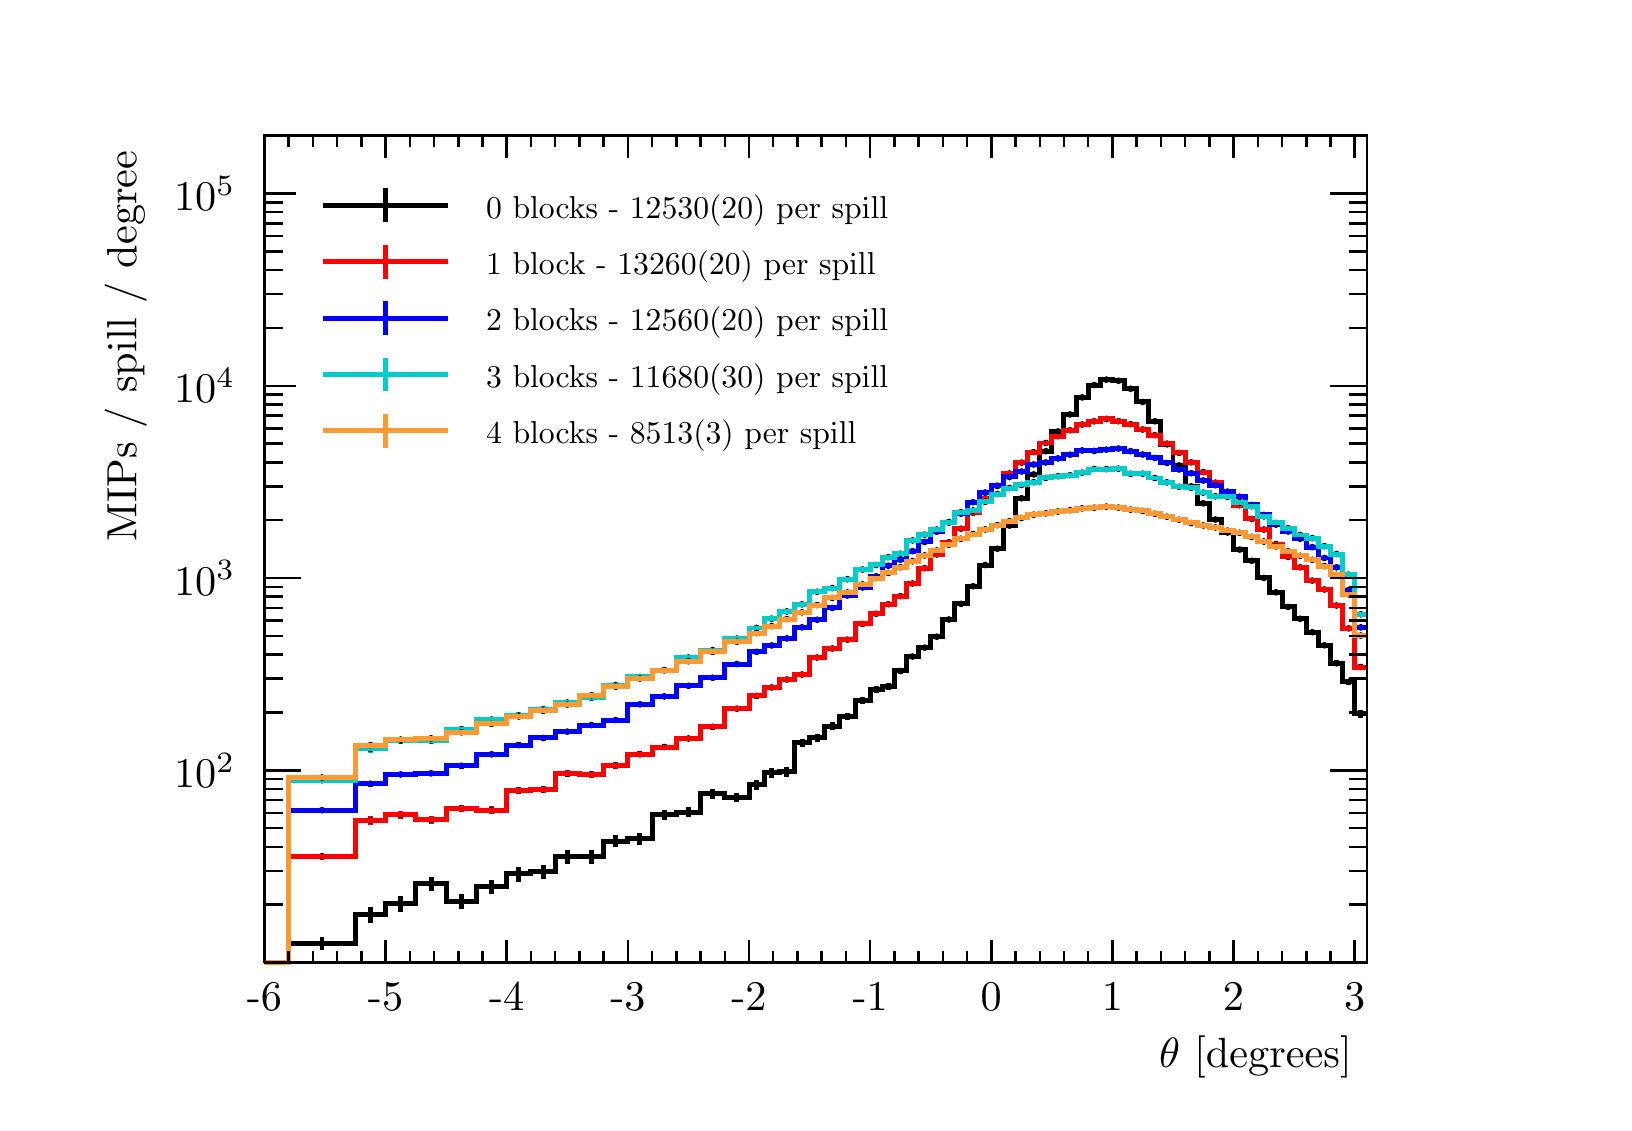
\begin{tikzpicture}
\pgfdeclareplotmark{cross} {
\pgfpathmoveto{\pgfpoint{-0.3\pgfplotmarksize}{\pgfplotmarksize}}
\pgfpathlineto{\pgfpoint{+0.3\pgfplotmarksize}{\pgfplotmarksize}}
\pgfpathlineto{\pgfpoint{+0.3\pgfplotmarksize}{0.3\pgfplotmarksize}}
\pgfpathlineto{\pgfpoint{+1\pgfplotmarksize}{0.3\pgfplotmarksize}}
\pgfpathlineto{\pgfpoint{+1\pgfplotmarksize}{-0.3\pgfplotmarksize}}
\pgfpathlineto{\pgfpoint{+0.3\pgfplotmarksize}{-0.3\pgfplotmarksize}}
\pgfpathlineto{\pgfpoint{+0.3\pgfplotmarksize}{-1.\pgfplotmarksize}}
\pgfpathlineto{\pgfpoint{-0.3\pgfplotmarksize}{-1.\pgfplotmarksize}}
\pgfpathlineto{\pgfpoint{-0.3\pgfplotmarksize}{-0.3\pgfplotmarksize}}
\pgfpathlineto{\pgfpoint{-1.\pgfplotmarksize}{-0.3\pgfplotmarksize}}
\pgfpathlineto{\pgfpoint{-1.\pgfplotmarksize}{0.3\pgfplotmarksize}}
\pgfpathlineto{\pgfpoint{-0.3\pgfplotmarksize}{0.3\pgfplotmarksize}}
\pgfpathclose
\pgfusepathqstroke
}
\pgfdeclareplotmark{cross*} {
\pgfpathmoveto{\pgfpoint{-0.3\pgfplotmarksize}{\pgfplotmarksize}}
\pgfpathlineto{\pgfpoint{+0.3\pgfplotmarksize}{\pgfplotmarksize}}
\pgfpathlineto{\pgfpoint{+0.3\pgfplotmarksize}{0.3\pgfplotmarksize}}
\pgfpathlineto{\pgfpoint{+1\pgfplotmarksize}{0.3\pgfplotmarksize}}
\pgfpathlineto{\pgfpoint{+1\pgfplotmarksize}{-0.3\pgfplotmarksize}}
\pgfpathlineto{\pgfpoint{+0.3\pgfplotmarksize}{-0.3\pgfplotmarksize}}
\pgfpathlineto{\pgfpoint{+0.3\pgfplotmarksize}{-1.\pgfplotmarksize}}
\pgfpathlineto{\pgfpoint{-0.3\pgfplotmarksize}{-1.\pgfplotmarksize}}
\pgfpathlineto{\pgfpoint{-0.3\pgfplotmarksize}{-0.3\pgfplotmarksize}}
\pgfpathlineto{\pgfpoint{-1.\pgfplotmarksize}{-0.3\pgfplotmarksize}}
\pgfpathlineto{\pgfpoint{-1.\pgfplotmarksize}{0.3\pgfplotmarksize}}
\pgfpathlineto{\pgfpoint{-0.3\pgfplotmarksize}{0.3\pgfplotmarksize}}
\pgfpathclose
\pgfusepathqfillstroke
}
\pgfdeclareplotmark{newstar} {
\pgfpathmoveto{\pgfqpoint{0pt}{\pgfplotmarksize}}
\pgfpathlineto{\pgfqpointpolar{44}{0.5\pgfplotmarksize}}
\pgfpathlineto{\pgfqpointpolar{18}{\pgfplotmarksize}}
\pgfpathlineto{\pgfqpointpolar{-20}{0.5\pgfplotmarksize}}
\pgfpathlineto{\pgfqpointpolar{-54}{\pgfplotmarksize}}
\pgfpathlineto{\pgfqpointpolar{-90}{0.5\pgfplotmarksize}}
\pgfpathlineto{\pgfqpointpolar{234}{\pgfplotmarksize}}
\pgfpathlineto{\pgfqpointpolar{198}{0.5\pgfplotmarksize}}
\pgfpathlineto{\pgfqpointpolar{162}{\pgfplotmarksize}}
\pgfpathlineto{\pgfqpointpolar{134}{0.5\pgfplotmarksize}}
\pgfpathclose
\pgfusepathqstroke
}
\pgfdeclareplotmark{newstar*} {
\pgfpathmoveto{\pgfqpoint{0pt}{\pgfplotmarksize}}
\pgfpathlineto{\pgfqpointpolar{44}{0.5\pgfplotmarksize}}
\pgfpathlineto{\pgfqpointpolar{18}{\pgfplotmarksize}}
\pgfpathlineto{\pgfqpointpolar{-20}{0.5\pgfplotmarksize}}
\pgfpathlineto{\pgfqpointpolar{-54}{\pgfplotmarksize}}
\pgfpathlineto{\pgfqpointpolar{-90}{0.5\pgfplotmarksize}}
\pgfpathlineto{\pgfqpointpolar{234}{\pgfplotmarksize}}
\pgfpathlineto{\pgfqpointpolar{198}{0.5\pgfplotmarksize}}
\pgfpathlineto{\pgfqpointpolar{162}{\pgfplotmarksize}}
\pgfpathlineto{\pgfqpointpolar{134}{0.5\pgfplotmarksize}}
\pgfpathclose
\pgfusepathqfillstroke
}
\definecolor{c}{rgb}{1,1,1};
\draw [color=c, fill=c] (0,0) rectangle (20,13.639);
\draw [color=c, fill=c] (3,1.77307) rectangle (17,12.2751);
\definecolor{c}{rgb}{0,0,0};
\draw [c,line width=0.9] (3,1.77307) -- (3,12.2751) -- (17,12.2751) -- (17,1.77307) -- (3,1.77307);
\definecolor{c}{rgb}{1,1,1};
\draw [color=c, fill=c] (3,1.77307) rectangle (17,12.2751);
\definecolor{c}{rgb}{0,0,0};
\draw [c,line width=0.9] (3,1.77307) -- (3,12.2751) -- (17,12.2751) -- (17,1.77307) -- (3,1.77307);
\draw [c,line width=0.9] (3,1.77307) -- (3.30769,1.77307) -- (3.30769,1.77307) -- (4.15385,1.77307) -- (4.15385,1.77307) -- (4.53846,1.77307) -- (4.53846,1.77307) -- (4.92308,1.77307) -- (4.92308,1.77307) -- (5.30769,1.77307) -- (5.30769,1.77307) --
 (5.69231,1.77307) -- (5.69231,1.77307) -- (6.07692,1.77307) -- (6.07692,1.77307) -- (6.38462,1.77307) -- (6.38462,1.77307) -- (6.69231,1.77307) -- (6.69231,1.77307) -- (7,1.77307) -- (7,1.77307) -- (7.30769,1.77307) -- (7.30769,1.77307) --
 (7.61538,1.77307) -- (7.61538,1.77307) -- (7.92308,1.77307) -- (7.92308,1.77307) -- (8.23077,1.77307) -- (8.23077,1.77307) -- (8.53846,1.77307) -- (8.53846,1.77307) -- (8.84615,1.77307) -- (8.84615,1.77307) -- (9.15385,1.77307) -- (9.15385,1.77307)
 -- (9.34615,1.77307) -- (9.34615,1.77307) -- (9.53846,1.77307) -- (9.53846,1.77307) -- (9.73077,1.77307) -- (9.73077,1.77307) -- (9.92308,1.77307) -- (9.92308,1.77307) -- (10.1154,1.77307) -- (10.1154,1.77307) -- (10.3077,1.77307) --
 (10.3077,1.77307) -- (10.5,1.77307) -- (10.5,1.77307) -- (10.6923,1.77307) -- (10.6923,1.77307) -- (10.8462,1.77307) -- (10.8462,1.77307) -- (11,1.77307) -- (11,1.77307) -- (11.1538,1.77307) -- (11.1538,1.77307) -- (11.3077,1.77307) --
 (11.3077,1.77307) -- (11.4615,1.77307) -- (11.4615,1.77307) -- (11.6154,1.77307) -- (11.6154,1.77307) -- (11.7692,1.77307) -- (11.7692,1.77307) -- (11.9231,1.77307) -- (11.9231,1.77307) -- (12.0769,1.77307) -- (12.0769,1.77307) -- (12.2308,1.77307)
 -- (12.2308,1.77307) -- (12.3846,1.77307) -- (12.3846,1.77307) -- (12.5385,1.77307) -- (12.5385,1.77307) -- (12.6923,1.77307) -- (12.6923,1.77307) -- (12.8462,1.77307) -- (12.8462,1.77307) -- (13,1.77307) -- (13,1.77307) -- (13.1538,1.77307) --
 (13.1538,1.77307) -- (13.3077,1.77307) -- (13.3077,1.77307) -- (13.4615,1.77307) -- (13.4615,1.77307) -- (13.6154,1.77307) -- (13.6154,1.77307) -- (13.7692,1.77307) -- (13.7692,1.77307) -- (13.9231,1.77307) -- (13.9231,1.77307) -- (14.0769,1.77307)
 -- (14.0769,1.77307) -- (14.2308,1.77307) -- (14.2308,1.77307) -- (14.3846,1.77307) -- (14.3846,1.77307) -- (14.5385,1.77307) -- (14.5385,1.77307) -- (14.6923,1.77307) -- (14.6923,1.77307) -- (14.8462,1.77307) -- (14.8462,1.77307) -- (15,1.77307) --
 (15,1.77307) -- (15.1538,1.77307) -- (15.1538,1.77307) -- (15.3077,1.77307) -- (15.3077,1.77307) -- (15.4615,1.77307) -- (15.4615,1.77307) -- (15.6154,1.77307) -- (15.6154,1.77307) -- (15.7692,1.77307) -- (15.7692,1.77307) -- (15.9231,1.77307) --
 (15.9231,1.77307) -- (16.0769,1.77307) -- (16.0769,1.77307) -- (16.2308,1.77307) -- (16.2308,1.77307) -- (16.3846,1.77307) -- (16.3846,1.77307) -- (16.5385,1.77307) -- (16.5385,1.77307) -- (16.6923,1.77307) -- (16.6923,1.77307) -- (16.8462,1.77307)
 -- (16.8462,1.77307) -- (17,1.77307);
\draw [c,line width=0.9] (3,1.77307) -- (17,1.77307);
\draw [c,line width=0.9] (3,2.05948) -- (3,1.77307);
\draw [c,line width=0.9] (3.30769,1.91628) -- (3.30769,1.77307);
\draw [c,line width=0.9] (3.61538,1.91628) -- (3.61538,1.77307);
\draw [c,line width=0.9] (3.92308,1.91628) -- (3.92308,1.77307);
\draw [c,line width=0.9] (4.23077,1.91628) -- (4.23077,1.77307);
\draw [c,line width=0.9] (4.53846,2.05948) -- (4.53846,1.77307);
\draw [c,line width=0.9] (4.84615,1.91628) -- (4.84615,1.77307);
\draw [c,line width=0.9] (5.15385,1.91628) -- (5.15385,1.77307);
\draw [c,line width=0.9] (5.46154,1.91628) -- (5.46154,1.77307);
\draw [c,line width=0.9] (5.76923,1.91628) -- (5.76923,1.77307);
\draw [c,line width=0.9] (6.07692,2.05948) -- (6.07692,1.77307);
\draw [c,line width=0.9] (6.38462,1.91628) -- (6.38462,1.77307);
\draw [c,line width=0.9] (6.69231,1.91628) -- (6.69231,1.77307);
\draw [c,line width=0.9] (7,1.91628) -- (7,1.77307);
\draw [c,line width=0.9] (7.30769,1.91628) -- (7.30769,1.77307);
\draw [c,line width=0.9] (7.61538,2.05948) -- (7.61538,1.77307);
\draw [c,line width=0.9] (7.92308,1.91628) -- (7.92308,1.77307);
\draw [c,line width=0.9] (8.23077,1.91628) -- (8.23077,1.77307);
\draw [c,line width=0.9] (8.53846,1.91628) -- (8.53846,1.77307);
\draw [c,line width=0.9] (8.84615,1.91628) -- (8.84615,1.77307);
\draw [c,line width=0.9] (9.15385,2.05948) -- (9.15385,1.77307);
\draw [c,line width=0.9] (9.46154,1.91628) -- (9.46154,1.77307);
\draw [c,line width=0.9] (9.76923,1.91628) -- (9.76923,1.77307);
\draw [c,line width=0.9] (10.0769,1.91628) -- (10.0769,1.77307);
\draw [c,line width=0.9] (10.3846,1.91628) -- (10.3846,1.77307);
\draw [c,line width=0.9] (10.6923,2.05948) -- (10.6923,1.77307);
\draw [c,line width=0.9] (11,1.91628) -- (11,1.77307);
\draw [c,line width=0.9] (11.3077,1.91628) -- (11.3077,1.77307);
\draw [c,line width=0.9] (11.6154,1.91628) -- (11.6154,1.77307);
\draw [c,line width=0.9] (11.9231,1.91628) -- (11.9231,1.77307);
\draw [c,line width=0.9] (12.2308,2.05948) -- (12.2308,1.77307);
\draw [c,line width=0.9] (12.5385,1.91628) -- (12.5385,1.77307);
\draw [c,line width=0.9] (12.8462,1.91628) -- (12.8462,1.77307);
\draw [c,line width=0.9] (13.1538,1.91628) -- (13.1538,1.77307);
\draw [c,line width=0.9] (13.4615,1.91628) -- (13.4615,1.77307);
\draw [c,line width=0.9] (13.7692,2.05948) -- (13.7692,1.77307);
\draw [c,line width=0.9] (14.0769,1.91628) -- (14.0769,1.77307);
\draw [c,line width=0.9] (14.3846,1.91628) -- (14.3846,1.77307);
\draw [c,line width=0.9] (14.6923,1.91628) -- (14.6923,1.77307);
\draw [c,line width=0.9] (15,1.91628) -- (15,1.77307);
\draw [c,line width=0.9] (15.3077,2.05948) -- (15.3077,1.77307);
\draw [c,line width=0.9] (15.6154,1.91628) -- (15.6154,1.77307);
\draw [c,line width=0.9] (15.9231,1.91628) -- (15.9231,1.77307);
\draw [c,line width=0.9] (16.2308,1.91628) -- (16.2308,1.77307);
\draw [c,line width=0.9] (16.5385,1.91628) -- (16.5385,1.77307);
\draw [c,line width=0.9] (16.8462,2.05948) -- (16.8462,1.77307);
\draw [c,line width=0.9] (16.8462,2.05948) -- (16.8462,1.77307);
\draw [anchor=base] (3,1.15931) node[scale=1.52731, color=c, rotate=0]{-6};
\draw [anchor=base] (4.53846,1.15931) node[scale=1.52731, color=c, rotate=0]{-5};
\draw [anchor=base] (6.07692,1.15931) node[scale=1.52731, color=c, rotate=0]{-4};
\draw [anchor=base] (7.61538,1.15931) node[scale=1.52731, color=c, rotate=0]{-3};
\draw [anchor=base] (9.15385,1.15931) node[scale=1.52731, color=c, rotate=0]{-2};
\draw [anchor=base] (10.6923,1.15931) node[scale=1.52731, color=c, rotate=0]{-1};
\draw [anchor=base] (12.2308,1.15931) node[scale=1.52731, color=c, rotate=0]{0};
\draw [anchor=base] (13.7692,1.15931) node[scale=1.52731, color=c, rotate=0]{1};
\draw [anchor=base] (15.3077,1.15931) node[scale=1.52731, color=c, rotate=0]{2};
\draw [anchor=base] (16.8462,1.15931) node[scale=1.52731, color=c, rotate=0]{3};
\draw [anchor= east] (17,0.572837) node[scale=1.52731, color=c, rotate=0]{$\theta$ [degrees] };
\draw [c,line width=0.9] (3,12.2751) -- (17,12.2751);
\draw [c,line width=0.9] (3,11.9887) -- (3,12.2751);
\draw [c,line width=0.9] (3.30769,12.1319) -- (3.30769,12.2751);
\draw [c,line width=0.9] (3.61538,12.1319) -- (3.61538,12.2751);
\draw [c,line width=0.9] (3.92308,12.1319) -- (3.92308,12.2751);
\draw [c,line width=0.9] (4.23077,12.1319) -- (4.23077,12.2751);
\draw [c,line width=0.9] (4.53846,11.9887) -- (4.53846,12.2751);
\draw [c,line width=0.9] (4.84615,12.1319) -- (4.84615,12.2751);
\draw [c,line width=0.9] (5.15385,12.1319) -- (5.15385,12.2751);
\draw [c,line width=0.9] (5.46154,12.1319) -- (5.46154,12.2751);
\draw [c,line width=0.9] (5.76923,12.1319) -- (5.76923,12.2751);
\draw [c,line width=0.9] (6.07692,11.9887) -- (6.07692,12.2751);
\draw [c,line width=0.9] (6.38462,12.1319) -- (6.38462,12.2751);
\draw [c,line width=0.9] (6.69231,12.1319) -- (6.69231,12.2751);
\draw [c,line width=0.9] (7,12.1319) -- (7,12.2751);
\draw [c,line width=0.9] (7.30769,12.1319) -- (7.30769,12.2751);
\draw [c,line width=0.9] (7.61538,11.9887) -- (7.61538,12.2751);
\draw [c,line width=0.9] (7.92308,12.1319) -- (7.92308,12.2751);
\draw [c,line width=0.9] (8.23077,12.1319) -- (8.23077,12.2751);
\draw [c,line width=0.9] (8.53846,12.1319) -- (8.53846,12.2751);
\draw [c,line width=0.9] (8.84615,12.1319) -- (8.84615,12.2751);
\draw [c,line width=0.9] (9.15385,11.9887) -- (9.15385,12.2751);
\draw [c,line width=0.9] (9.46154,12.1319) -- (9.46154,12.2751);
\draw [c,line width=0.9] (9.76923,12.1319) -- (9.76923,12.2751);
\draw [c,line width=0.9] (10.0769,12.1319) -- (10.0769,12.2751);
\draw [c,line width=0.9] (10.3846,12.1319) -- (10.3846,12.2751);
\draw [c,line width=0.9] (10.6923,11.9887) -- (10.6923,12.2751);
\draw [c,line width=0.9] (11,12.1319) -- (11,12.2751);
\draw [c,line width=0.9] (11.3077,12.1319) -- (11.3077,12.2751);
\draw [c,line width=0.9] (11.6154,12.1319) -- (11.6154,12.2751);
\draw [c,line width=0.9] (11.9231,12.1319) -- (11.9231,12.2751);
\draw [c,line width=0.9] (12.2308,11.9887) -- (12.2308,12.2751);
\draw [c,line width=0.9] (12.5385,12.1319) -- (12.5385,12.2751);
\draw [c,line width=0.9] (12.8462,12.1319) -- (12.8462,12.2751);
\draw [c,line width=0.9] (13.1538,12.1319) -- (13.1538,12.2751);
\draw [c,line width=0.9] (13.4615,12.1319) -- (13.4615,12.2751);
\draw [c,line width=0.9] (13.7692,11.9887) -- (13.7692,12.2751);
\draw [c,line width=0.9] (14.0769,12.1319) -- (14.0769,12.2751);
\draw [c,line width=0.9] (14.3846,12.1319) -- (14.3846,12.2751);
\draw [c,line width=0.9] (14.6923,12.1319) -- (14.6923,12.2751);
\draw [c,line width=0.9] (15,12.1319) -- (15,12.2751);
\draw [c,line width=0.9] (15.3077,11.9887) -- (15.3077,12.2751);
\draw [c,line width=0.9] (15.6154,12.1319) -- (15.6154,12.2751);
\draw [c,line width=0.9] (15.9231,12.1319) -- (15.9231,12.2751);
\draw [c,line width=0.9] (16.2308,12.1319) -- (16.2308,12.2751);
\draw [c,line width=0.9] (16.5385,12.1319) -- (16.5385,12.2751);
\draw [c,line width=0.9] (16.8462,11.9887) -- (16.8462,12.2751);
\draw [c,line width=0.9] (16.8462,11.9887) -- (16.8462,12.2751);
\draw [c,line width=0.9] (3,1.77307) -- (3,12.2751);
\draw [c,line width=0.9] (3.231,2.5081) -- (3,2.5081);
\draw [c,line width=0.9] (3.231,2.93807) -- (3,2.93807);
\draw [c,line width=0.9] (3.231,3.24314) -- (3,3.24314);
\draw [c,line width=0.9] (3.231,3.47977) -- (3,3.47977);
\draw [c,line width=0.9] (3.231,3.67311) -- (3,3.67311);
\draw [c,line width=0.9] (3.231,3.83658) -- (3,3.83658);
\draw [c,line width=0.9] (3.231,3.97818) -- (3,3.97818);
\draw [c,line width=0.9] (3.231,4.10308) -- (3,4.10308);
\draw [c,line width=0.9] (3.462,4.21481) -- (3,4.21481);
\draw [anchor= east] (2.82,4.21481) node[scale=1.52731, color=c, rotate=0]{$10^{2}$};
\draw [c,line width=0.9] (3.231,4.94984) -- (3,4.94984);
\draw [c,line width=0.9] (3.231,5.37981) -- (3,5.37981);
\draw [c,line width=0.9] (3.231,5.68488) -- (3,5.68488);
\draw [c,line width=0.9] (3.231,5.92151) -- (3,5.92151);
\draw [c,line width=0.9] (3.231,6.11485) -- (3,6.11485);
\draw [c,line width=0.9] (3.231,6.27832) -- (3,6.27832);
\draw [c,line width=0.9] (3.231,6.41992) -- (3,6.41992);
\draw [c,line width=0.9] (3.231,6.54482) -- (3,6.54482);
\draw [c,line width=0.9] (3.462,6.65655) -- (3,6.65655);
\draw [anchor= east] (2.82,6.65655) node[scale=1.52731, color=c, rotate=0]{$10^{3}$};
\draw [c,line width=0.9] (3.231,7.39159) -- (3,7.39159);
\draw [c,line width=0.9] (3.231,7.82156) -- (3,7.82156);
\draw [c,line width=0.9] (3.231,8.12662) -- (3,8.12662);
\draw [c,line width=0.9] (3.231,8.36325) -- (3,8.36325);
\draw [c,line width=0.9] (3.231,8.55659) -- (3,8.55659);
\draw [c,line width=0.9] (3.231,8.72006) -- (3,8.72006);
\draw [c,line width=0.9] (3.231,8.86166) -- (3,8.86166);
\draw [c,line width=0.9] (3.231,8.98656) -- (3,8.98656);
\draw [c,line width=0.9] (3.462,9.09829) -- (3,9.09829);
\draw [anchor= east] (2.82,9.09829) node[scale=1.52731, color=c, rotate=0]{$10^{4}$};
\draw [c,line width=0.9] (3.231,9.83333) -- (3,9.83333);
\draw [c,line width=0.9] (3.231,10.2633) -- (3,10.2633);
\draw [c,line width=0.9] (3.231,10.5684) -- (3,10.5684);
\draw [c,line width=0.9] (3.231,10.805) -- (3,10.805);
\draw [c,line width=0.9] (3.231,10.9983) -- (3,10.9983);
\draw [c,line width=0.9] (3.231,11.1618) -- (3,11.1618);
\draw [c,line width=0.9] (3.231,11.3034) -- (3,11.3034);
\draw [c,line width=0.9] (3.231,11.4283) -- (3,11.4283);
\draw [c,line width=0.9] (3.462,11.54) -- (3,11.54);
\draw [anchor= east] (2.82,11.54) node[scale=1.52731, color=c, rotate=0]{$10^{5}$};
\draw [c,line width=0.9] (3.231,12.2751) -- (3,12.2751);
\draw [anchor= east] (1.24,12.2751) node[scale=1.52731, color=c, rotate=90]{MIPs / spill / degree};
\draw [c,line width=0.9] (17,1.77307) -- (17,12.2751);
\draw [c,line width=0.9] (16.769,2.5081) -- (17,2.5081);
\draw [c,line width=0.9] (16.769,2.93807) -- (17,2.93807);
\draw [c,line width=0.9] (16.769,3.24314) -- (17,3.24314);
\draw [c,line width=0.9] (16.769,3.47977) -- (17,3.47977);
\draw [c,line width=0.9] (16.769,3.67311) -- (17,3.67311);
\draw [c,line width=0.9] (16.769,3.83658) -- (17,3.83658);
\draw [c,line width=0.9] (16.769,3.97818) -- (17,3.97818);
\draw [c,line width=0.9] (16.769,4.10308) -- (17,4.10308);
\draw [c,line width=0.9] (16.538,4.21481) -- (17,4.21481);
\draw [c,line width=0.9] (16.769,4.94984) -- (17,4.94984);
\draw [c,line width=0.9] (16.769,5.37981) -- (17,5.37981);
\draw [c,line width=0.9] (16.769,5.68488) -- (17,5.68488);
\draw [c,line width=0.9] (16.769,5.92151) -- (17,5.92151);
\draw [c,line width=0.9] (16.769,6.11485) -- (17,6.11485);
\draw [c,line width=0.9] (16.769,6.27832) -- (17,6.27832);
\draw [c,line width=0.9] (16.769,6.41992) -- (17,6.41992);
\draw [c,line width=0.9] (16.769,6.54482) -- (17,6.54482);
\draw [c,line width=0.9] (16.538,6.65655) -- (17,6.65655);
\draw [c,line width=0.9] (16.769,7.39159) -- (17,7.39159);
\draw [c,line width=0.9] (16.769,7.82156) -- (17,7.82156);
\draw [c,line width=0.9] (16.769,8.12662) -- (17,8.12662);
\draw [c,line width=0.9] (16.769,8.36325) -- (17,8.36325);
\draw [c,line width=0.9] (16.769,8.55659) -- (17,8.55659);
\draw [c,line width=0.9] (16.769,8.72006) -- (17,8.72006);
\draw [c,line width=0.9] (16.769,8.86166) -- (17,8.86166);
\draw [c,line width=0.9] (16.769,8.98656) -- (17,8.98656);
\draw [c,line width=0.9] (16.538,9.09829) -- (17,9.09829);
\draw [c,line width=0.9] (16.769,9.83333) -- (17,9.83333);
\draw [c,line width=0.9] (16.769,10.2633) -- (17,10.2633);
\draw [c,line width=0.9] (16.769,10.5684) -- (17,10.5684);
\draw [c,line width=0.9] (16.769,10.805) -- (17,10.805);
\draw [c,line width=0.9] (16.769,10.9983) -- (17,10.9983);
\draw [c,line width=0.9] (16.769,11.1618) -- (17,11.1618);
\draw [c,line width=0.9] (16.769,11.3034) -- (17,11.3034);
\draw [c,line width=0.9] (16.769,11.4283) -- (17,11.4283);
\draw [c,line width=0.9] (16.538,11.54) -- (17,11.54);
\draw [c,line width=0.9] (16.769,12.2751) -- (17,12.2751);
\draw [c,line width=1.8] (3.73077,1.92614) -- (3.73077,2.01524);
\draw [c,line width=1.8] (3.73077,2.01524) -- (3.73077,2.09743);
\foreach \P in {(3.73077,2.01524)}{\draw[mark options={color=c,fill=c},mark size=2.402402pt,mark=*,mark size=1pt] plot coordinates {\P};}
\draw [c,line width=1.8] (4.34615,2.27048) -- (4.34615,2.38281);
\draw [c,line width=1.8] (4.34615,2.38281) -- (4.34615,2.48437);
\foreach \P in {(4.34615,2.38281)}{\draw[mark options={color=c,fill=c},mark size=2.402402pt,mark=*,mark size=1pt] plot coordinates {\P};}
\draw [c,line width=1.8] (4.73077,2.4183) -- (4.73077,2.52307);
\draw [c,line width=1.8] (4.73077,2.52307) -- (4.73077,2.61842);
\foreach \P in {(4.73077,2.52307)}{\draw[mark options={color=c,fill=c},mark size=2.402402pt,mark=*,mark size=1pt] plot coordinates {\P};}
\draw [c,line width=1.8] (5.11538,2.68015) -- (5.11538,2.77276);
\draw [c,line width=1.8] (5.11538,2.77276) -- (5.11538,2.85793);
\foreach \P in {(5.11538,2.77276)}{\draw[mark options={color=c,fill=c},mark size=2.402402pt,mark=*,mark size=1pt] plot coordinates {\P};}
\draw [c,line width=1.8] (5.5,2.44752) -- (5.5,2.55086);
\draw [c,line width=1.8] (5.5,2.55086) -- (5.5,2.64502);
\foreach \P in {(5.5,2.55086)}{\draw[mark options={color=c,fill=c},mark size=2.402402pt,mark=*,mark size=1pt] plot coordinates {\P};}
\draw [c,line width=1.8] (5.88462,2.64067) -- (5.88462,2.73502);
\draw [c,line width=1.8] (5.88462,2.73502) -- (5.88462,2.82166);
\foreach \P in {(5.88462,2.73502)}{\draw[mark options={color=c,fill=c},mark size=2.402402pt,mark=*,mark size=1pt] plot coordinates {\P};}
\draw [c,line width=1.8] (6.23077,2.80239) -- (6.23077,2.90013);
\draw [c,line width=1.8] (6.23077,2.90013) -- (6.23077,2.98962);
\foreach \P in {(6.23077,2.90013)}{\draw[mark options={color=c,fill=c},mark size=2.402402pt,mark=*,mark size=1pt] plot coordinates {\P};}
\draw [c,line width=1.8] (6.53846,2.82794) -- (6.53846,2.92451);
\draw [c,line width=1.8] (6.53846,2.92451) -- (6.53846,3.01301);
\foreach \P in {(6.53846,2.92451)}{\draw[mark options={color=c,fill=c},mark size=2.402402pt,mark=*,mark size=1pt] plot coordinates {\P};}
\draw [c,line width=1.8] (6.84615,3.02725) -- (6.84615,3.11517);
\draw [c,line width=1.8] (6.84615,3.11517) -- (6.84615,3.19635);
\foreach \P in {(6.84615,3.11517)}{\draw[mark options={color=c,fill=c},mark size=2.402402pt,mark=*,mark size=1pt] plot coordinates {\P};}
\draw [c,line width=1.8] (7.15385,3.02725) -- (7.15385,3.11517);
\draw [c,line width=1.8] (7.15385,3.11517) -- (7.15385,3.19635);
\foreach \P in {(7.15385,3.11517)}{\draw[mark options={color=c,fill=c},mark size=2.402402pt,mark=*,mark size=1pt] plot coordinates {\P};}
\draw [c,line width=1.8] (7.46154,3.23666) -- (7.46154,3.31631);
\draw [c,line width=1.8] (7.46154,3.31631) -- (7.46154,3.39039);
\foreach \P in {(7.46154,3.31631)}{\draw[mark options={color=c,fill=c},mark size=2.402402pt,mark=*,mark size=1pt] plot coordinates {\P};}
\draw [c,line width=1.8] (7.76923,3.27072) -- (7.76923,3.34911);
\draw [c,line width=1.8] (7.76923,3.34911) -- (7.76923,3.4221);
\foreach \P in {(7.76923,3.34911)}{\draw[mark options={color=c,fill=c},mark size=2.402402pt,mark=*,mark size=1pt] plot coordinates {\P};}
\draw [c,line width=1.8] (8.07692,3.58385) -- (8.07692,3.65148);
\draw [c,line width=1.8] (8.07692,3.65148) -- (8.07692,3.71506);
\foreach \P in {(8.07692,3.65148)}{\draw[mark options={color=c,fill=c},mark size=2.402402pt,mark=*,mark size=1pt] plot coordinates {\P};}
\draw [c,line width=1.8] (8.38461,3.61679) -- (8.38461,3.68338);
\draw [c,line width=1.8] (8.38461,3.68338) -- (8.38461,3.74603);
\foreach \P in {(8.38461,3.68338)}{\draw[mark options={color=c,fill=c},mark size=2.402402pt,mark=*,mark size=1pt] plot coordinates {\P};}
\draw [c,line width=1.8] (8.69231,3.85579) -- (8.69231,3.91528);
\draw [c,line width=1.8] (8.69231,3.91528) -- (8.69231,3.97161);
\foreach \P in {(8.69231,3.91528)}{\draw[mark options={color=c,fill=c},mark size=2.402402pt,mark=*,mark size=1pt] plot coordinates {\P};}
\draw [c,line width=1.8] (9,3.80594) -- (9,3.86685);
\draw [c,line width=1.8] (9,3.86685) -- (9,3.92445);
\foreach \P in {(9,3.86685)}{\draw[mark options={color=c,fill=c},mark size=2.402402pt,mark=*,mark size=1pt] plot coordinates {\P};}
\draw [c,line width=1.8] (9.25,3.95834) -- (9.25,4.03004);
\draw [c,line width=1.8] (9.25,4.03004) -- (9.25,4.09719);
\foreach \P in {(9.25,4.03004)}{\draw[mark options={color=c,fill=c},mark size=2.402402pt,mark=*,mark size=1pt] plot coordinates {\P};}
\draw [c,line width=1.8] (9.44231,4.1152) -- (9.44231,4.18179);
\draw [c,line width=1.8] (9.44231,4.18179) -- (9.44231,4.24444);
\foreach \P in {(9.44231,4.18179)}{\draw[mark options={color=c,fill=c},mark size=2.402402pt,mark=*,mark size=1pt] plot coordinates {\P};}
\draw [c,line width=1.8] (9.63461,4.12729) -- (9.63461,4.1935);
\draw [c,line width=1.8] (9.63461,4.1935) -- (9.63461,4.25582);
\foreach \P in {(9.63461,4.1935)}{\draw[mark options={color=c,fill=c},mark size=2.402402pt,mark=*,mark size=1pt] plot coordinates {\P};}
\draw [c,line width=1.8] (9.82692,4.50822) -- (9.82692,4.56354);
\draw [c,line width=1.8] (9.82692,4.56354) -- (9.82692,4.61613);
\foreach \P in {(9.82692,4.56354)}{\draw[mark options={color=c,fill=c},mark size=2.402402pt,mark=*,mark size=1pt] plot coordinates {\P};}
\draw [c,line width=1.8] (10.0192,4.57635) -- (10.0192,4.62993);
\draw [c,line width=1.8] (10.0192,4.62993) -- (10.0192,4.68093);
\foreach \P in {(10.0192,4.62993)}{\draw[mark options={color=c,fill=c},mark size=2.402402pt,mark=*,mark size=1pt] plot coordinates {\P};}
\draw [c,line width=1.8] (10.2115,4.72413) -- (10.2115,4.7741);
\draw [c,line width=1.8] (10.2115,4.7741) -- (10.2115,4.82182);
\foreach \P in {(10.2115,4.7741)}{\draw[mark options={color=c,fill=c},mark size=2.402402pt,mark=*,mark size=1pt] plot coordinates {\P};}
\draw [c,line width=1.8] (10.4038,4.84991) -- (10.4038,4.897);
\draw [c,line width=1.8] (10.4038,4.897) -- (10.4038,4.94209);
\foreach \P in {(10.4038,4.897)}{\draw[mark options={color=c,fill=c},mark size=2.402402pt,mark=*,mark size=1pt] plot coordinates {\P};}
\draw [c,line width=1.8] (10.5962,5.06096) -- (10.5962,5.1036);
\draw [c,line width=1.8] (10.5962,5.1036) -- (10.5962,5.14458);
\foreach \P in {(10.5962,5.1036)}{\draw[mark options={color=c,fill=c},mark size=2.402402pt,mark=*,mark size=1pt] plot coordinates {\P};}
\draw [c,line width=1.8] (10.7692,5.1954) -- (10.7692,5.24014);
\draw [c,line width=1.8] (10.7692,5.24014) -- (10.7692,5.28307);
\foreach \P in {(10.7692,5.24014)}{\draw[mark options={color=c,fill=c},mark size=2.402402pt,mark=*,mark size=1pt] plot coordinates {\P};}
\draw [c,line width=1.8] (10.9231,5.2371) -- (10.9231,5.28097);
\draw [c,line width=1.8] (10.9231,5.28097) -- (10.9231,5.32309);
\foreach \P in {(10.9231,5.28097)}{\draw[mark options={color=c,fill=c},mark size=2.402402pt,mark=*,mark size=1pt] plot coordinates {\P};}
\draw [c,line width=1.8] (11.0769,5.43611) -- (11.0769,5.47605);
\draw [c,line width=1.8] (11.0769,5.47605) -- (11.0769,5.51454);
\foreach \P in {(11.0769,5.47605)}{\draw[mark options={color=c,fill=c},mark size=2.402402pt,mark=*,mark size=1pt] plot coordinates {\P};}
\draw [c,line width=1.8] (11.2308,5.62262) -- (11.2308,5.6592);
\draw [c,line width=1.8] (11.2308,5.6592) -- (11.2308,5.69456);
\foreach \P in {(11.2308,5.6592)}{\draw[mark options={color=c,fill=c},mark size=2.402402pt,mark=*,mark size=1pt] plot coordinates {\P};}
\draw [c,line width=1.8] (11.3846,5.73774) -- (11.3846,5.77239);
\draw [c,line width=1.8] (11.3846,5.77239) -- (11.3846,5.80594);
\foreach \P in {(11.3846,5.77239)}{\draw[mark options={color=c,fill=c},mark size=2.402402pt,mark=*,mark size=1pt] plot coordinates {\P};}
\draw [c,line width=1.8] (11.5385,5.87841) -- (11.5385,5.91084);
\draw [c,line width=1.8] (11.5385,5.91084) -- (11.5385,5.9423);
\foreach \P in {(11.5385,5.91084)}{\draw[mark options={color=c,fill=c},mark size=2.402402pt,mark=*,mark size=1pt] plot coordinates {\P};}
\draw [c,line width=1.8] (11.6923,6.10062) -- (11.6923,6.12982);
\draw [c,line width=1.8] (11.6923,6.12982) -- (11.6923,6.15824);
\foreach \P in {(11.6923,6.12982)}{\draw[mark options={color=c,fill=c},mark size=2.402402pt,mark=*,mark size=1pt] plot coordinates {\P};}
\draw [c,line width=1.8] (11.8462,6.30168) -- (11.8462,6.32823);
\draw [c,line width=1.8] (11.8462,6.32823) -- (11.8462,6.35414);
\foreach \P in {(11.8462,6.32823)}{\draw[mark options={color=c,fill=c},mark size=2.402402pt,mark=*,mark size=1pt] plot coordinates {\P};}
\draw [c,line width=1.8] (12,6.5286) -- (12,6.55247);
\draw [c,line width=1.8] (12,6.55247) -- (12,6.5758);
\foreach \P in {(12,6.55247)}{\draw[mark options={color=c,fill=c},mark size=2.402402pt,mark=*,mark size=1pt] plot coordinates {\P};}
\draw [c,line width=1.8] (12.1538,6.80078) -- (12.1538,6.82177);
\draw [c,line width=1.8] (12.1538,6.82177) -- (12.1538,6.84235);
\foreach \P in {(12.1538,6.82177)}{\draw[mark options={color=c,fill=c},mark size=2.402402pt,mark=*,mark size=1pt] plot coordinates {\P};}
\draw [c,line width=1.8] (12.3077,7.00964) -- (12.3077,7.02866);
\draw [c,line width=1.8] (12.3077,7.02866) -- (12.3077,7.04735);
\foreach \P in {(12.3077,7.02866)}{\draw[mark options={color=c,fill=c},mark size=2.402402pt,mark=*,mark size=1pt] plot coordinates {\P};}
\draw [c,line width=1.8] (12.4615,7.30582) -- (12.4615,7.32236);
\draw [c,line width=1.8] (12.4615,7.32236) -- (12.4615,7.33865);
\foreach \P in {(12.4615,7.32236)}{\draw[mark options={color=c,fill=c},mark size=2.402402pt,mark=*,mark size=1pt] plot coordinates {\P};}
\draw [c,line width=1.8] (12.6154,7.65548) -- (12.6154,7.66951);
\draw [c,line width=1.8] (12.6154,7.66951) -- (12.6154,7.68335);
\foreach \P in {(12.6154,7.66951)}{\draw[mark options={color=c,fill=c},mark size=2.402402pt,mark=*,mark size=1pt] plot coordinates {\P};}
\draw [c,line width=1.8] (12.7692,7.96041) -- (12.7692,7.97256);
\draw [c,line width=1.8] (12.7692,7.97256) -- (12.7692,7.98457);
\foreach \P in {(12.7692,7.97256)}{\draw[mark options={color=c,fill=c},mark size=2.402402pt,mark=*,mark size=1pt] plot coordinates {\P};}
\draw [c,line width=1.8] (12.9231,8.25708) -- (12.9231,8.26764);
\draw [c,line width=1.8] (12.9231,8.26764) -- (12.9231,8.2781);
\foreach \P in {(12.9231,8.26764)}{\draw[mark options={color=c,fill=c},mark size=2.402402pt,mark=*,mark size=1pt] plot coordinates {\P};}
\draw [c,line width=1.8] (13.0769,8.50812) -- (13.0769,8.5175);
\draw [c,line width=1.8] (13.0769,8.5175) -- (13.0769,8.5268);
\foreach \P in {(13.0769,8.5175)}{\draw[mark options={color=c,fill=c},mark size=2.402402pt,mark=*,mark size=1pt] plot coordinates {\P};}
\draw [c,line width=1.8] (13.2308,8.72542) -- (13.2308,8.73389);
\draw [c,line width=1.8] (13.2308,8.73389) -- (13.2308,8.74229);
\foreach \P in {(13.2308,8.73389)}{\draw[mark options={color=c,fill=c},mark size=2.402402pt,mark=*,mark size=1pt] plot coordinates {\P};}
\draw [c,line width=1.8] (13.3846,8.94273) -- (13.3846,8.95037);
\draw [c,line width=1.8] (13.3846,8.95037) -- (13.3846,8.95796);
\foreach \P in {(13.3846,8.95037)}{\draw[mark options={color=c,fill=c},mark size=2.402402pt,mark=*,mark size=1pt] plot coordinates {\P};}
\draw [c,line width=1.8] (13.5385,9.10047) -- (13.5385,9.10757);
\draw [c,line width=1.8] (13.5385,9.10757) -- (13.5385,9.11462);
\foreach \P in {(13.5385,9.10757)}{\draw[mark options={color=c,fill=c},mark size=2.402402pt,mark=*,mark size=1pt] plot coordinates {\P};}
\draw [c,line width=1.8] (13.6923,9.16942) -- (13.6923,9.17629);
\draw [c,line width=1.8] (13.6923,9.17629) -- (13.6923,9.18312);
\foreach \P in {(13.6923,9.17629)}{\draw[mark options={color=c,fill=c},mark size=2.402402pt,mark=*,mark size=1pt] plot coordinates {\P};}
\draw [c,line width=1.8] (13.8462,9.15504) -- (13.8462,9.16196);
\draw [c,line width=1.8] (13.8462,9.16196) -- (13.8462,9.16883);
\foreach \P in {(13.8462,9.16196)}{\draw[mark options={color=c,fill=c},mark size=2.402402pt,mark=*,mark size=1pt] plot coordinates {\P};}
\draw [c,line width=1.8] (14,9.0526) -- (14,9.05985);
\draw [c,line width=1.8] (14,9.05985) -- (14,9.06706);
\foreach \P in {(14,9.05985)}{\draw[mark options={color=c,fill=c},mark size=2.402402pt,mark=*,mark size=1pt] plot coordinates {\P};}
\draw [c,line width=1.8] (14.1538,8.88426) -- (14.1538,8.89212);
\draw [c,line width=1.8] (14.1538,8.89212) -- (14.1538,8.89992);
\foreach \P in {(14.1538,8.89212)}{\draw[mark options={color=c,fill=c},mark size=2.402402pt,mark=*,mark size=1pt] plot coordinates {\P};}
\draw [c,line width=1.8] (14.3077,8.63878) -- (14.3077,8.6476);
\draw [c,line width=1.8] (14.3077,8.6476) -- (14.3077,8.65635);
\foreach \P in {(14.3077,8.6476)}{\draw[mark options={color=c,fill=c},mark size=2.402402pt,mark=*,mark size=1pt] plot coordinates {\P};}
\draw [c,line width=1.8] (14.4615,8.34369) -- (14.4615,8.35383);
\draw [c,line width=1.8] (14.4615,8.35383) -- (14.4615,8.36387);
\foreach \P in {(14.4615,8.35383)}{\draw[mark options={color=c,fill=c},mark size=2.402402pt,mark=*,mark size=1pt] plot coordinates {\P};}
\draw [c,line width=1.8] (14.6154,8.07483) -- (14.6154,8.08634);
\draw [c,line width=1.8] (14.6154,8.08634) -- (14.6154,8.09772);
\foreach \P in {(14.6154,8.08634)}{\draw[mark options={color=c,fill=c},mark size=2.402402pt,mark=*,mark size=1pt] plot coordinates {\P};}
\draw [c,line width=1.8] (14.7692,7.80771) -- (14.7692,7.82077);
\draw [c,line width=1.8] (14.7692,7.82077) -- (14.7692,7.83367);
\foreach \P in {(14.7692,7.82077)}{\draw[mark options={color=c,fill=c},mark size=2.402402pt,mark=*,mark size=1pt] plot coordinates {\P};}
\draw [c,line width=1.8] (14.9231,7.5909) -- (14.9231,7.60536);
\draw [c,line width=1.8] (14.9231,7.60536) -- (14.9231,7.61962);
\foreach \P in {(14.9231,7.60536)}{\draw[mark options={color=c,fill=c},mark size=2.402402pt,mark=*,mark size=1pt] plot coordinates {\P};}
\draw [c,line width=1.8] (15.0769,7.38355) -- (15.0769,7.39949);
\draw [c,line width=1.8] (15.0769,7.39949) -- (15.0769,7.4152);
\foreach \P in {(15.0769,7.39949)}{\draw[mark options={color=c,fill=c},mark size=2.402402pt,mark=*,mark size=1pt] plot coordinates {\P};}
\draw [c,line width=1.8] (15.2308,7.21725) -- (15.2308,7.23449);
\draw [c,line width=1.8] (15.2308,7.23449) -- (15.2308,7.25146);
\foreach \P in {(15.2308,7.23449)}{\draw[mark options={color=c,fill=c},mark size=2.402402pt,mark=*,mark size=1pt] plot coordinates {\P};}
\draw [c,line width=1.8] (15.3846,6.99877) -- (15.3846,7.01788);
\draw [c,line width=1.8] (15.3846,7.01788) -- (15.3846,7.03666);
\foreach \P in {(15.3846,7.01788)}{\draw[mark options={color=c,fill=c},mark size=2.402402pt,mark=*,mark size=1pt] plot coordinates {\P};}
\draw [c,line width=1.8] (15.5385,6.85451) -- (15.5385,6.87498);
\draw [c,line width=1.8] (15.5385,6.87498) -- (15.5385,6.89505);
\foreach \P in {(15.5385,6.87498)}{\draw[mark options={color=c,fill=c},mark size=2.402402pt,mark=*,mark size=1pt] plot coordinates {\P};}
\draw [c,line width=1.8] (15.6923,6.63513) -- (15.6923,6.65782);
\draw [c,line width=1.8] (15.6923,6.65782) -- (15.6923,6.68004);
\foreach \P in {(15.6923,6.65782)}{\draw[mark options={color=c,fill=c},mark size=2.402402pt,mark=*,mark size=1pt] plot coordinates {\P};}
\draw [c,line width=1.8] (15.8462,6.45041) -- (15.8462,6.47517);
\draw [c,line width=1.8] (15.8462,6.47517) -- (15.8462,6.49936);
\foreach \P in {(15.8462,6.47517)}{\draw[mark options={color=c,fill=c},mark size=2.402402pt,mark=*,mark size=1pt] plot coordinates {\P};}
\draw [c,line width=1.8] (16,6.2622) -- (16,6.28926);
\draw [c,line width=1.8] (16,6.28926) -- (16,6.31564);
\foreach \P in {(16,6.28926)}{\draw[mark options={color=c,fill=c},mark size=2.402402pt,mark=*,mark size=1pt] plot coordinates {\P};}
\draw [c,line width=1.8] (16.1538,6.10931) -- (16.1538,6.13839);
\draw [c,line width=1.8] (16.1538,6.13839) -- (16.1538,6.16669);
\foreach \P in {(16.1538,6.13839)}{\draw[mark options={color=c,fill=c},mark size=2.402402pt,mark=*,mark size=1pt] plot coordinates {\P};}
\draw [c,line width=1.8] (16.3077,5.93637) -- (16.3077,5.96792);
\draw [c,line width=1.8] (16.3077,5.96792) -- (16.3077,5.99855);
\foreach \P in {(16.3077,5.96792)}{\draw[mark options={color=c,fill=c},mark size=2.402402pt,mark=*,mark size=1pt] plot coordinates {\P};}
\draw [c,line width=1.8] (16.4615,5.76848) -- (16.4615,5.80263);
\draw [c,line width=1.8] (16.4615,5.80263) -- (16.4615,5.83571);
\foreach \P in {(16.4615,5.80263)}{\draw[mark options={color=c,fill=c},mark size=2.402402pt,mark=*,mark size=1pt] plot coordinates {\P};}
\draw [c,line width=1.8] (16.6154,5.53612) -- (16.6154,5.57422);
\draw [c,line width=1.8] (16.6154,5.57422) -- (16.6154,5.611);
\foreach \P in {(16.6154,5.57422)}{\draw[mark options={color=c,fill=c},mark size=2.402402pt,mark=*,mark size=1pt] plot coordinates {\P};}
\draw [c,line width=1.8] (16.7692,5.29591) -- (16.7692,5.33858);
\draw [c,line width=1.8] (16.7692,5.33858) -- (16.7692,5.3796);
\foreach \P in {(16.7692,5.33858)}{\draw[mark options={color=c,fill=c},mark size=2.402402pt,mark=*,mark size=1pt] plot coordinates {\P};}
\draw [c,line width=1.8] (16.9231,4.88448) -- (16.9231,4.93628);
\draw [c,line width=1.8] (16.9231,4.93628) -- (16.9231,4.98567);
\foreach \P in {(16.9231,4.93628)}{\draw[mark options={color=c,fill=c},mark size=2.402402pt,mark=*,mark size=1pt] plot coordinates {\P};}
\draw [c,line width=1.8] (3,1.77307) -- (3.30769,1.77307) -- (3.30769,2.01524) -- (4.15385,2.01524) -- (4.15385,2.38281) -- (4.53846,2.38281) -- (4.53846,2.52307) -- (4.92308,2.52307) -- (4.92308,2.77276) -- (5.30769,2.77276) -- (5.30769,2.55086) --
 (5.69231,2.55086) -- (5.69231,2.73502) -- (6.07692,2.73502) -- (6.07692,2.90013) -- (6.38462,2.90013) -- (6.38462,2.92451) -- (6.69231,2.92451) -- (6.69231,3.11517) -- (7,3.11517) -- (7,3.11517) -- (7.30769,3.11517) -- (7.30769,3.31631) --
 (7.61538,3.31631) -- (7.61538,3.34911) -- (7.92308,3.34911) -- (7.92308,3.65148) -- (8.23077,3.65148) -- (8.23077,3.68338) -- (8.53846,3.68338) -- (8.53846,3.91528) -- (8.84615,3.91528) -- (8.84615,3.86685) -- (9.15385,3.86685) -- (9.15385,4.03004)
 -- (9.34615,4.03004) -- (9.34615,4.18179) -- (9.53846,4.18179) -- (9.53846,4.1935) -- (9.73077,4.1935) -- (9.73077,4.56354) -- (9.92308,4.56354) -- (9.92308,4.62993) -- (10.1154,4.62993) -- (10.1154,4.7741) -- (10.3077,4.7741) -- (10.3077,4.897) --
 (10.5,4.897) -- (10.5,5.1036) -- (10.6923,5.1036) -- (10.6923,5.24014) -- (10.8462,5.24014) -- (10.8462,5.28097) -- (11,5.28097) -- (11,5.47605) -- (11.1538,5.47605) -- (11.1538,5.6592) -- (11.3077,5.6592) -- (11.3077,5.77239) -- (11.4615,5.77239)
 -- (11.4615,5.91084) -- (11.6154,5.91084) -- (11.6154,6.12982) -- (11.7692,6.12982) -- (11.7692,6.32823) -- (11.9231,6.32823) -- (11.9231,6.55247) -- (12.0769,6.55247) -- (12.0769,6.82177) -- (12.2308,6.82177) -- (12.2308,7.02866) --
 (12.3846,7.02866) -- (12.3846,7.32236) -- (12.5385,7.32236) -- (12.5385,7.66951) -- (12.6923,7.66951) -- (12.6923,7.97256) -- (12.8462,7.97256) -- (12.8462,8.26764) -- (13,8.26764) -- (13,8.5175) -- (13.1538,8.5175) -- (13.1538,8.73389) --
 (13.3077,8.73389) -- (13.3077,8.95037) -- (13.4615,8.95037) -- (13.4615,9.10757) -- (13.6154,9.10757) -- (13.6154,9.17629) -- (13.7692,9.17629) -- (13.7692,9.16196) -- (13.9231,9.16196) -- (13.9231,9.05985) -- (14.0769,9.05985) -- (14.0769,8.89212)
 -- (14.2308,8.89212) -- (14.2308,8.6476) -- (14.3846,8.6476) -- (14.3846,8.35383) -- (14.5385,8.35383) -- (14.5385,8.08634) -- (14.6923,8.08634) -- (14.6923,7.82077) -- (14.8462,7.82077) -- (14.8462,7.60536) -- (15,7.60536) -- (15,7.39949) --
 (15.1538,7.39949) -- (15.1538,7.23449) -- (15.3077,7.23449) -- (15.3077,7.01788) -- (15.4615,7.01788) -- (15.4615,6.87498) -- (15.6154,6.87498) -- (15.6154,6.65782) -- (15.7692,6.65782) -- (15.7692,6.47517) -- (15.9231,6.47517) -- (15.9231,6.28926)
 -- (16.0769,6.28926) -- (16.0769,6.13839) -- (16.2308,6.13839) -- (16.2308,5.96792) -- (16.3846,5.96792) -- (16.3846,5.80263) -- (16.5385,5.80263) -- (16.5385,5.57422) -- (16.6923,5.57422) -- (16.6923,5.33858) -- (16.8462,5.33858) --
 (16.8462,4.93628) -- (17,4.93628);
\definecolor{c}{rgb}{1,0,0};
\draw [c,line width=1.8] (3.73077,3.07583) -- (3.73077,3.12093);
\draw [c,line width=1.8] (3.73077,3.12093) -- (3.73077,3.16418);
\definecolor{c}{rgb}{0,0,0};
\foreach \P in {(3.73077,3.12093)}{\draw[mark options={color=c,fill=c},mark size=2.402402pt,mark=*,mark size=1pt] plot coordinates {\P};}
\definecolor{c}{rgb}{1,0,0};
\draw [c,line width=1.8] (4.34615,3.52455) -- (4.34615,3.57826);
\draw [c,line width=1.8] (4.34615,3.57826) -- (4.34615,3.62938);
\definecolor{c}{rgb}{0,0,0};
\foreach \P in {(4.34615,3.57826)}{\draw[mark options={color=c,fill=c},mark size=2.402402pt,mark=*,mark size=1pt] plot coordinates {\P};}
\definecolor{c}{rgb}{1,0,0};
\draw [c,line width=1.8] (4.73077,3.59788) -- (4.73077,3.64933);
\draw [c,line width=1.8] (4.73077,3.64933) -- (4.73077,3.6984);
\definecolor{c}{rgb}{0,0,0};
\foreach \P in {(4.73077,3.64933)}{\draw[mark options={color=c,fill=c},mark size=2.402402pt,mark=*,mark size=1pt] plot coordinates {\P};}
\definecolor{c}{rgb}{1,0,0};
\draw [c,line width=1.8] (5.11538,3.53171) -- (5.11538,3.58478);
\draw [c,line width=1.8] (5.11538,3.58478) -- (5.11538,3.63532);
\definecolor{c}{rgb}{0,0,0};
\foreach \P in {(5.11538,3.58478)}{\draw[mark options={color=c,fill=c},mark size=2.402402pt,mark=*,mark size=1pt] plot coordinates {\P};}
\definecolor{c}{rgb}{1,0,0};
\draw [c,line width=1.8] (5.5,3.68147) -- (5.5,3.73156);
\draw [c,line width=1.8] (5.5,3.73156) -- (5.5,3.77939);
\definecolor{c}{rgb}{0,0,0};
\foreach \P in {(5.5,3.73156)}{\draw[mark options={color=c,fill=c},mark size=2.402402pt,mark=*,mark size=1pt] plot coordinates {\P};}
\definecolor{c}{rgb}{1,0,0};
\draw [c,line width=1.8] (5.88462,3.6591) -- (5.88462,3.70953);
\draw [c,line width=1.8] (5.88462,3.70953) -- (5.88462,3.75767);
\definecolor{c}{rgb}{0,0,0};
\foreach \P in {(5.88462,3.70953)}{\draw[mark options={color=c,fill=c},mark size=2.402402pt,mark=*,mark size=1pt] plot coordinates {\P};}
\definecolor{c}{rgb}{1,0,0};
\draw [c,line width=1.8] (6.23077,3.90994) -- (6.23077,3.95969);
\draw [c,line width=1.8] (6.23077,3.95969) -- (6.23077,4.00721);
\definecolor{c}{rgb}{0,0,0};
\foreach \P in {(6.23077,3.95969)}{\draw[mark options={color=c,fill=c},mark size=2.402402pt,mark=*,mark size=1pt] plot coordinates {\P};}
\definecolor{c}{rgb}{1,0,0};
\draw [c,line width=1.8] (6.53846,3.92327) -- (6.53846,3.97323);
\draw [c,line width=1.8] (6.53846,3.97323) -- (6.53846,4.02094);
\definecolor{c}{rgb}{0,0,0};
\foreach \P in {(6.53846,3.97323)}{\draw[mark options={color=c,fill=c},mark size=2.402402pt,mark=*,mark size=1pt] plot coordinates {\P};}
\definecolor{c}{rgb}{1,0,0};
\draw [c,line width=1.8] (6.84615,4.12613) -- (6.84615,4.1712);
\draw [c,line width=1.8] (6.84615,4.1712) -- (6.84615,4.21444);
\definecolor{c}{rgb}{0,0,0};
\foreach \P in {(6.84615,4.1712)}{\draw[mark options={color=c,fill=c},mark size=2.402402pt,mark=*,mark size=1pt] plot coordinates {\P};}
\definecolor{c}{rgb}{1,0,0};
\draw [c,line width=1.8] (7.15385,4.11876) -- (7.15385,4.16399);
\draw [c,line width=1.8] (7.15385,4.16399) -- (7.15385,4.20738);
\definecolor{c}{rgb}{0,0,0};
\foreach \P in {(7.15385,4.16399)}{\draw[mark options={color=c,fill=c},mark size=2.402402pt,mark=*,mark size=1pt] plot coordinates {\P};}
\definecolor{c}{rgb}{1,0,0};
\draw [c,line width=1.8] (7.46154,4.23622) -- (7.46154,4.27912);
\draw [c,line width=1.8] (7.46154,4.27912) -- (7.46154,4.32036);
\definecolor{c}{rgb}{0,0,0};
\foreach \P in {(7.46154,4.27912)}{\draw[mark options={color=c,fill=c},mark size=2.402402pt,mark=*,mark size=1pt] plot coordinates {\P};}
\definecolor{c}{rgb}{1,0,0};
\draw [c,line width=1.8] (7.76923,4.37852) -- (7.76923,4.41839);
\draw [c,line width=1.8] (7.76923,4.41839) -- (7.76923,4.45681);
\definecolor{c}{rgb}{0,0,0};
\foreach \P in {(7.76923,4.41839)}{\draw[mark options={color=c,fill=c},mark size=2.402402pt,mark=*,mark size=1pt] plot coordinates {\P};}
\definecolor{c}{rgb}{1,0,0};
\draw [c,line width=1.8] (8.07692,4.47183) -- (8.07692,4.51012);
\draw [c,line width=1.8] (8.07692,4.51012) -- (8.07692,4.54708);
\definecolor{c}{rgb}{0,0,0};
\foreach \P in {(8.07692,4.51012)}{\draw[mark options={color=c,fill=c},mark size=2.402402pt,mark=*,mark size=1pt] plot coordinates {\P};}
\definecolor{c}{rgb}{1,0,0};
\draw [c,line width=1.8] (8.38461,4.58233) -- (8.38461,4.61882);
\draw [c,line width=1.8] (8.38461,4.61882) -- (8.38461,4.65409);
\definecolor{c}{rgb}{0,0,0};
\foreach \P in {(8.38461,4.61882)}{\draw[mark options={color=c,fill=c},mark size=2.402402pt,mark=*,mark size=1pt] plot coordinates {\P};}
\definecolor{c}{rgb}{1,0,0};
\draw [c,line width=1.8] (8.69231,4.73243) -- (8.69231,4.76642);
\draw [c,line width=1.8] (8.69231,4.76642) -- (8.69231,4.79935);
\definecolor{c}{rgb}{0,0,0};
\foreach \P in {(8.69231,4.76642)}{\draw[mark options={color=c,fill=c},mark size=2.402402pt,mark=*,mark size=1pt] plot coordinates {\P};}
\definecolor{c}{rgb}{1,0,0};
\draw [c,line width=1.8] (9,4.96683) -- (9,4.99708);
\draw [c,line width=1.8] (9,4.99708) -- (9,5.02649);
\definecolor{c}{rgb}{0,0,0};
\foreach \P in {(9,4.99708)}{\draw[mark options={color=c,fill=c},mark size=2.402402pt,mark=*,mark size=1pt] plot coordinates {\P};}
\definecolor{c}{rgb}{1,0,0};
\draw [c,line width=1.8] (9.25,5.12432) -- (9.25,5.15991);
\draw [c,line width=1.8] (9.25,5.15991) -- (9.25,5.19434);
\definecolor{c}{rgb}{0,0,0};
\foreach \P in {(9.25,5.15991)}{\draw[mark options={color=c,fill=c},mark size=2.402402pt,mark=*,mark size=1pt] plot coordinates {\P};}
\definecolor{c}{rgb}{1,0,0};
\draw [c,line width=1.8] (9.44231,5.23343) -- (9.44231,5.26725);
\draw [c,line width=1.8] (9.44231,5.26725) -- (9.44231,5.30003);
\definecolor{c}{rgb}{0,0,0};
\foreach \P in {(9.44231,5.26725)}{\draw[mark options={color=c,fill=c},mark size=2.402402pt,mark=*,mark size=1pt] plot coordinates {\P};}
\definecolor{c}{rgb}{1,0,0};
\draw [c,line width=1.8] (9.63461,5.33587) -- (9.63461,5.36799);
\draw [c,line width=1.8] (9.63461,5.36799) -- (9.63461,5.39918);
\definecolor{c}{rgb}{0,0,0};
\foreach \P in {(9.63461,5.36799)}{\draw[mark options={color=c,fill=c},mark size=2.402402pt,mark=*,mark size=1pt] plot coordinates {\P};}
\definecolor{c}{rgb}{1,0,0};
\draw [c,line width=1.8] (9.82692,5.39963) -- (9.82692,5.43085);
\draw [c,line width=1.8] (9.82692,5.43085) -- (9.82692,5.46118);
\definecolor{c}{rgb}{0,0,0};
\foreach \P in {(9.82692,5.43085)}{\draw[mark options={color=c,fill=c},mark size=2.402402pt,mark=*,mark size=1pt] plot coordinates {\P};}
\definecolor{c}{rgb}{1,0,0};
\draw [c,line width=1.8] (10.0192,5.61858) -- (10.0192,5.6469);
\draw [c,line width=1.8] (10.0192,5.6469) -- (10.0192,5.67449);
\definecolor{c}{rgb}{0,0,0};
\foreach \P in {(10.0192,5.6469)}{\draw[mark options={color=c,fill=c},mark size=2.402402pt,mark=*,mark size=1pt] plot coordinates {\P};}
\definecolor{c}{rgb}{1,0,0};
\draw [c,line width=1.8] (10.2115,5.73442) -- (10.2115,5.76125);
\draw [c,line width=1.8] (10.2115,5.76125) -- (10.2115,5.78741);
\definecolor{c}{rgb}{0,0,0};
\foreach \P in {(10.2115,5.76125)}{\draw[mark options={color=c,fill=c},mark size=2.402402pt,mark=*,mark size=1pt] plot coordinates {\P};}
\definecolor{c}{rgb}{1,0,0};
\draw [c,line width=1.8] (10.4038,5.84841) -- (10.4038,5.87377);
\draw [c,line width=1.8] (10.4038,5.87377) -- (10.4038,5.89854);
\definecolor{c}{rgb}{0,0,0};
\foreach \P in {(10.4038,5.87377)}{\draw[mark options={color=c,fill=c},mark size=2.402402pt,mark=*,mark size=1pt] plot coordinates {\P};}
\definecolor{c}{rgb}{1,0,0};
\draw [c,line width=1.8] (10.5962,6.05052) -- (10.5962,6.07348);
\draw [c,line width=1.8] (10.5962,6.07348) -- (10.5962,6.09595);
\definecolor{c}{rgb}{0,0,0};
\foreach \P in {(10.5962,6.07348)}{\draw[mark options={color=c,fill=c},mark size=2.402402pt,mark=*,mark size=1pt] plot coordinates {\P};}
\definecolor{c}{rgb}{1,0,0};
\draw [c,line width=1.8] (10.7692,6.17803) -- (10.7692,6.20222);
\draw [c,line width=1.8] (10.7692,6.20222) -- (10.7692,6.22586);
\definecolor{c}{rgb}{0,0,0};
\foreach \P in {(10.7692,6.20222)}{\draw[mark options={color=c,fill=c},mark size=2.402402pt,mark=*,mark size=1pt] plot coordinates {\P};}
\definecolor{c}{rgb}{1,0,0};
\draw [c,line width=1.8] (10.9231,6.301) -- (10.9231,6.32402);
\draw [c,line width=1.8] (10.9231,6.32402) -- (10.9231,6.34654);
\definecolor{c}{rgb}{0,0,0};
\foreach \P in {(10.9231,6.32402)}{\draw[mark options={color=c,fill=c},mark size=2.402402pt,mark=*,mark size=1pt] plot coordinates {\P};}
\definecolor{c}{rgb}{1,0,0};
\draw [c,line width=1.8] (11.0769,6.40452) -- (11.0769,6.42623);
\draw [c,line width=1.8] (11.0769,6.42623) -- (11.0769,6.4475);
\definecolor{c}{rgb}{0,0,0};
\foreach \P in {(11.0769,6.42623)}{\draw[mark options={color=c,fill=c},mark size=2.402402pt,mark=*,mark size=1pt] plot coordinates {\P};}
\definecolor{c}{rgb}{1,0,0};
\draw [c,line width=1.8] (11.2308,6.56672) -- (11.2308,6.58682);
\draw [c,line width=1.8] (11.2308,6.58682) -- (11.2308,6.60655);
\definecolor{c}{rgb}{0,0,0};
\foreach \P in {(11.2308,6.58682)}{\draw[mark options={color=c,fill=c},mark size=2.402402pt,mark=*,mark size=1pt] plot coordinates {\P};}
\definecolor{c}{rgb}{1,0,0};
\draw [c,line width=1.8] (11.3846,6.76317) -- (11.3846,6.78162);
\draw [c,line width=1.8] (11.3846,6.78162) -- (11.3846,6.79975);
\definecolor{c}{rgb}{0,0,0};
\foreach \P in {(11.3846,6.78162)}{\draw[mark options={color=c,fill=c},mark size=2.402402pt,mark=*,mark size=1pt] plot coordinates {\P};}
\definecolor{c}{rgb}{1,0,0};
\draw [c,line width=1.8] (11.5385,6.93828) -- (11.5385,6.95516);
\draw [c,line width=1.8] (11.5385,6.95516) -- (11.5385,6.97178);
\definecolor{c}{rgb}{0,0,0};
\foreach \P in {(11.5385,6.95516)}{\draw[mark options={color=c,fill=c},mark size=2.402402pt,mark=*,mark size=1pt] plot coordinates {\P};}
\definecolor{c}{rgb}{1,0,0};
\draw [c,line width=1.8] (11.6923,7.09576) -- (11.6923,7.11144);
\draw [c,line width=1.8] (11.6923,7.11144) -- (11.6923,7.12689);
\definecolor{c}{rgb}{0,0,0};
\foreach \P in {(11.6923,7.11144)}{\draw[mark options={color=c,fill=c},mark size=2.402402pt,mark=*,mark size=1pt] plot coordinates {\P};}
\definecolor{c}{rgb}{1,0,0};
\draw [c,line width=1.8] (11.8462,7.2682) -- (11.8462,7.28268);
\draw [c,line width=1.8] (11.8462,7.28268) -- (11.8462,7.29697);
\definecolor{c}{rgb}{0,0,0};
\foreach \P in {(11.8462,7.28268)}{\draw[mark options={color=c,fill=c},mark size=2.402402pt,mark=*,mark size=1pt] plot coordinates {\P};}
\definecolor{c}{rgb}{1,0,0};
\draw [c,line width=1.8] (12,7.47222) -- (12,7.48535);
\draw [c,line width=1.8] (12,7.48535) -- (12,7.49832);
\definecolor{c}{rgb}{0,0,0};
\foreach \P in {(12,7.48535)}{\draw[mark options={color=c,fill=c},mark size=2.402402pt,mark=*,mark size=1pt] plot coordinates {\P};}
\definecolor{c}{rgb}{1,0,0};
\draw [c,line width=1.8] (12.1538,7.65692) -- (12.1538,7.66899);
\draw [c,line width=1.8] (12.1538,7.66899) -- (12.1538,7.68092);
\definecolor{c}{rgb}{0,0,0};
\foreach \P in {(12.1538,7.66899)}{\draw[mark options={color=c,fill=c},mark size=2.402402pt,mark=*,mark size=1pt] plot coordinates {\P};}
\definecolor{c}{rgb}{1,0,0};
\draw [c,line width=1.8] (12.3077,7.8152) -- (12.3077,7.82641);
\draw [c,line width=1.8] (12.3077,7.82641) -- (12.3077,7.83749);
\definecolor{c}{rgb}{0,0,0};
\foreach \P in {(12.3077,7.82641)}{\draw[mark options={color=c,fill=c},mark size=2.402402pt,mark=*,mark size=1pt] plot coordinates {\P};}
\definecolor{c}{rgb}{1,0,0};
\draw [c,line width=1.8] (12.4615,7.97346) -- (12.4615,7.98385);
\draw [c,line width=1.8] (12.4615,7.98385) -- (12.4615,7.99413);
\definecolor{c}{rgb}{0,0,0};
\foreach \P in {(12.4615,7.98385)}{\draw[mark options={color=c,fill=c},mark size=2.402402pt,mark=*,mark size=1pt] plot coordinates {\P};}
\definecolor{c}{rgb}{1,0,0};
\draw [c,line width=1.8] (12.6154,8.11131) -- (12.6154,8.12103);
\draw [c,line width=1.8] (12.6154,8.12103) -- (12.6154,8.13066);
\definecolor{c}{rgb}{0,0,0};
\foreach \P in {(12.6154,8.12103)}{\draw[mark options={color=c,fill=c},mark size=2.402402pt,mark=*,mark size=1pt] plot coordinates {\P};}
\definecolor{c}{rgb}{1,0,0};
\draw [c,line width=1.8] (12.7692,8.24634) -- (12.7692,8.25546);
\draw [c,line width=1.8] (12.7692,8.25546) -- (12.7692,8.26451);
\definecolor{c}{rgb}{0,0,0};
\foreach \P in {(12.7692,8.25546)}{\draw[mark options={color=c,fill=c},mark size=2.402402pt,mark=*,mark size=1pt] plot coordinates {\P};}
\definecolor{c}{rgb}{1,0,0};
\draw [c,line width=1.8] (12.9231,8.36274) -- (12.9231,8.37137);
\draw [c,line width=1.8] (12.9231,8.37137) -- (12.9231,8.37994);
\definecolor{c}{rgb}{0,0,0};
\foreach \P in {(12.9231,8.37137)}{\draw[mark options={color=c,fill=c},mark size=2.402402pt,mark=*,mark size=1pt] plot coordinates {\P};}
\definecolor{c}{rgb}{1,0,0};
\draw [c,line width=1.8] (13.0769,8.44946) -- (13.0769,8.45775);
\draw [c,line width=1.8] (13.0769,8.45775) -- (13.0769,8.46597);
\definecolor{c}{rgb}{0,0,0};
\foreach \P in {(13.0769,8.45775)}{\draw[mark options={color=c,fill=c},mark size=2.402402pt,mark=*,mark size=1pt] plot coordinates {\P};}
\definecolor{c}{rgb}{1,0,0};
\draw [c,line width=1.8] (13.2308,8.52563) -- (13.2308,8.53362);
\draw [c,line width=1.8] (13.2308,8.53362) -- (13.2308,8.54156);
\definecolor{c}{rgb}{0,0,0};
\foreach \P in {(13.2308,8.53362)}{\draw[mark options={color=c,fill=c},mark size=2.402402pt,mark=*,mark size=1pt] plot coordinates {\P};}
\definecolor{c}{rgb}{1,0,0};
\draw [c,line width=1.8] (13.3846,8.59824) -- (13.3846,8.60597);
\draw [c,line width=1.8] (13.3846,8.60597) -- (13.3846,8.61365);
\definecolor{c}{rgb}{0,0,0};
\foreach \P in {(13.3846,8.60597)}{\draw[mark options={color=c,fill=c},mark size=2.402402pt,mark=*,mark size=1pt] plot coordinates {\P};}
\definecolor{c}{rgb}{1,0,0};
\draw [c,line width=1.8] (13.5385,8.63985) -- (13.5385,8.64744);
\draw [c,line width=1.8] (13.5385,8.64744) -- (13.5385,8.65498);
\definecolor{c}{rgb}{0,0,0};
\foreach \P in {(13.5385,8.64744)}{\draw[mark options={color=c,fill=c},mark size=2.402402pt,mark=*,mark size=1pt] plot coordinates {\P};}
\definecolor{c}{rgb}{1,0,0};
\draw [c,line width=1.8] (13.6923,8.66911) -- (13.6923,8.67659);
\draw [c,line width=1.8] (13.6923,8.67659) -- (13.6923,8.68402);
\definecolor{c}{rgb}{0,0,0};
\foreach \P in {(13.6923,8.67659)}{\draw[mark options={color=c,fill=c},mark size=2.402402pt,mark=*,mark size=1pt] plot coordinates {\P};}
\definecolor{c}{rgb}{1,0,0};
\draw [c,line width=1.8] (13.8462,8.64082) -- (13.8462,8.6484);
\draw [c,line width=1.8] (13.8462,8.6484) -- (13.8462,8.65593);
\definecolor{c}{rgb}{0,0,0};
\foreach \P in {(13.8462,8.6484)}{\draw[mark options={color=c,fill=c},mark size=2.402402pt,mark=*,mark size=1pt] plot coordinates {\P};}
\definecolor{c}{rgb}{1,0,0};
\draw [c,line width=1.8] (14,8.60286) -- (14,8.61056);
\draw [c,line width=1.8] (14,8.61056) -- (14,8.61822);
\definecolor{c}{rgb}{0,0,0};
\foreach \P in {(14,8.61056)}{\draw[mark options={color=c,fill=c},mark size=2.402402pt,mark=*,mark size=1pt] plot coordinates {\P};}
\definecolor{c}{rgb}{1,0,0};
\draw [c,line width=1.8] (14.1538,8.53487) -- (14.1538,8.54284);
\draw [c,line width=1.8] (14.1538,8.54284) -- (14.1538,8.55075);
\definecolor{c}{rgb}{0,0,0};
\foreach \P in {(14.1538,8.54284)}{\draw[mark options={color=c,fill=c},mark size=2.402402pt,mark=*,mark size=1pt] plot coordinates {\P};}
\definecolor{c}{rgb}{1,0,0};
\draw [c,line width=1.8] (14.3077,8.46293) -- (14.3077,8.47117);
\draw [c,line width=1.8] (14.3077,8.47117) -- (14.3077,8.47935);
\definecolor{c}{rgb}{0,0,0};
\foreach \P in {(14.3077,8.47117)}{\draw[mark options={color=c,fill=c},mark size=2.402402pt,mark=*,mark size=1pt] plot coordinates {\P};}
\definecolor{c}{rgb}{1,0,0};
\draw [c,line width=1.8] (14.4615,8.35467) -- (14.4615,8.36334);
\draw [c,line width=1.8] (14.4615,8.36334) -- (14.4615,8.37193);
\definecolor{c}{rgb}{0,0,0};
\foreach \P in {(14.4615,8.36334)}{\draw[mark options={color=c,fill=c},mark size=2.402402pt,mark=*,mark size=1pt] plot coordinates {\P};}
\definecolor{c}{rgb}{1,0,0};
\draw [c,line width=1.8] (14.6154,8.2369) -- (14.6154,8.24606);
\draw [c,line width=1.8] (14.6154,8.24606) -- (14.6154,8.25514);
\definecolor{c}{rgb}{0,0,0};
\foreach \P in {(14.6154,8.24606)}{\draw[mark options={color=c,fill=c},mark size=2.402402pt,mark=*,mark size=1pt] plot coordinates {\P};}
\definecolor{c}{rgb}{1,0,0};
\draw [c,line width=1.8] (14.7692,8.11581) -- (14.7692,8.12553);
\draw [c,line width=1.8] (14.7692,8.12553) -- (14.7692,8.13515);
\definecolor{c}{rgb}{0,0,0};
\foreach \P in {(14.7692,8.12553)}{\draw[mark options={color=c,fill=c},mark size=2.402402pt,mark=*,mark size=1pt] plot coordinates {\P};}
\definecolor{c}{rgb}{1,0,0};
\draw [c,line width=1.8] (14.9231,7.99173) -- (14.9231,8.00202);
\draw [c,line width=1.8] (14.9231,8.00202) -- (14.9231,8.01222);
\definecolor{c}{rgb}{0,0,0};
\foreach \P in {(14.9231,8.00202)}{\draw[mark options={color=c,fill=c},mark size=2.402402pt,mark=*,mark size=1pt] plot coordinates {\P};}
\definecolor{c}{rgb}{1,0,0};
\draw [c,line width=1.8] (15.0769,7.85689) -- (15.0769,7.86786);
\draw [c,line width=1.8] (15.0769,7.86786) -- (15.0769,7.87871);
\definecolor{c}{rgb}{0,0,0};
\foreach \P in {(15.0769,7.86786)}{\draw[mark options={color=c,fill=c},mark size=2.402402pt,mark=*,mark size=1pt] plot coordinates {\P};}
\definecolor{c}{rgb}{1,0,0};
\draw [c,line width=1.8] (15.2308,7.71759) -- (15.2308,7.72929);
\draw [c,line width=1.8] (15.2308,7.72929) -- (15.2308,7.74086);
\definecolor{c}{rgb}{0,0,0};
\foreach \P in {(15.2308,7.72929)}{\draw[mark options={color=c,fill=c},mark size=2.402402pt,mark=*,mark size=1pt] plot coordinates {\P};}
\definecolor{c}{rgb}{1,0,0};
\draw [c,line width=1.8] (15.3846,7.56898) -- (15.3846,7.58152);
\draw [c,line width=1.8] (15.3846,7.58152) -- (15.3846,7.59392);
\definecolor{c}{rgb}{0,0,0};
\foreach \P in {(15.3846,7.58152)}{\draw[mark options={color=c,fill=c},mark size=2.402402pt,mark=*,mark size=1pt] plot coordinates {\P};}
\definecolor{c}{rgb}{1,0,0};
\draw [c,line width=1.8] (15.5385,7.39304) -- (15.5385,7.40673);
\draw [c,line width=1.8] (15.5385,7.40673) -- (15.5385,7.42025);
\definecolor{c}{rgb}{0,0,0};
\foreach \P in {(15.5385,7.40673)}{\draw[mark options={color=c,fill=c},mark size=2.402402pt,mark=*,mark size=1pt] plot coordinates {\P};}
\definecolor{c}{rgb}{1,0,0};
\draw [c,line width=1.8] (15.6923,7.25794) -- (15.6923,7.27252);
\draw [c,line width=1.8] (15.6923,7.27252) -- (15.6923,7.2869);
\definecolor{c}{rgb}{0,0,0};
\foreach \P in {(15.6923,7.27252)}{\draw[mark options={color=c,fill=c},mark size=2.402402pt,mark=*,mark size=1pt] plot coordinates {\P};}
\definecolor{c}{rgb}{1,0,0};
\draw [c,line width=1.8] (15.8462,7.07146) -- (15.8462,7.08737);
\draw [c,line width=1.8] (15.8462,7.08737) -- (15.8462,7.10304);
\definecolor{c}{rgb}{0,0,0};
\foreach \P in {(15.8462,7.08737)}{\draw[mark options={color=c,fill=c},mark size=2.402402pt,mark=*,mark size=1pt] plot coordinates {\P};}
\definecolor{c}{rgb}{1,0,0};
\draw [c,line width=1.8] (16,6.90752) -- (16,6.92475);
\draw [c,line width=1.8] (16,6.92475) -- (16,6.9417);
\definecolor{c}{rgb}{0,0,0};
\foreach \P in {(16,6.92475)}{\draw[mark options={color=c,fill=c},mark size=2.402402pt,mark=*,mark size=1pt] plot coordinates {\P};}
\definecolor{c}{rgb}{1,0,0};
\draw [c,line width=1.8] (16.1538,6.77477) -- (16.1538,6.79305);
\draw [c,line width=1.8] (16.1538,6.79305) -- (16.1538,6.81102);
\definecolor{c}{rgb}{0,0,0};
\foreach \P in {(16.1538,6.79305)}{\draw[mark options={color=c,fill=c},mark size=2.402402pt,mark=*,mark size=1pt] plot coordinates {\P};}
\definecolor{c}{rgb}{1,0,0};
\draw [c,line width=1.8] (16.3077,6.60404) -- (16.3077,6.62378);
\draw [c,line width=1.8] (16.3077,6.62378) -- (16.3077,6.64315);
\definecolor{c}{rgb}{0,0,0};
\foreach \P in {(16.3077,6.62378)}{\draw[mark options={color=c,fill=c},mark size=2.402402pt,mark=*,mark size=1pt] plot coordinates {\P};}
\definecolor{c}{rgb}{1,0,0};
\draw [c,line width=1.8] (16.4615,6.49057) -- (16.4615,6.51145);
\draw [c,line width=1.8] (16.4615,6.51145) -- (16.4615,6.53194);
\definecolor{c}{rgb}{0,0,0};
\foreach \P in {(16.4615,6.51145)}{\draw[mark options={color=c,fill=c},mark size=2.402402pt,mark=*,mark size=1pt] plot coordinates {\P};}
\definecolor{c}{rgb}{1,0,0};
\draw [c,line width=1.8] (16.6154,6.28451) -- (16.6154,6.30757);
\draw [c,line width=1.8] (16.6154,6.30757) -- (16.6154,6.33014);
\definecolor{c}{rgb}{0,0,0};
\foreach \P in {(16.6154,6.30757)}{\draw[mark options={color=c,fill=c},mark size=2.402402pt,mark=*,mark size=1pt] plot coordinates {\P};}
\definecolor{c}{rgb}{1,0,0};
\draw [c,line width=1.8] (16.7692,5.99061) -- (16.7692,6.01705);
\draw [c,line width=1.8] (16.7692,6.01705) -- (16.7692,6.04285);
\definecolor{c}{rgb}{0,0,0};
\foreach \P in {(16.7692,6.01705)}{\draw[mark options={color=c,fill=c},mark size=2.402402pt,mark=*,mark size=1pt] plot coordinates {\P};}
\definecolor{c}{rgb}{1,0,0};
\draw [c,line width=1.8] (16.9231,5.4926) -- (16.9231,5.52622);
\draw [c,line width=1.8] (16.9231,5.52622) -- (16.9231,5.55881);
\definecolor{c}{rgb}{0,0,0};
\foreach \P in {(16.9231,5.52622)}{\draw[mark options={color=c,fill=c},mark size=2.402402pt,mark=*,mark size=1pt] plot coordinates {\P};}
\definecolor{c}{rgb}{1,0,0};
\draw [c,line width=1.8] (3,1.77307) -- (3.30769,1.77307) -- (3.30769,3.12093) -- (4.15385,3.12093) -- (4.15385,3.57826) -- (4.53846,3.57826) -- (4.53846,3.64933) -- (4.92308,3.64933) -- (4.92308,3.58478) -- (5.30769,3.58478) -- (5.30769,3.73156) --
 (5.69231,3.73156) -- (5.69231,3.70953) -- (6.07692,3.70953) -- (6.07692,3.95969) -- (6.38462,3.95969) -- (6.38462,3.97323) -- (6.69231,3.97323) -- (6.69231,4.1712) -- (7,4.1712) -- (7,4.16399) -- (7.30769,4.16399) -- (7.30769,4.27912) --
 (7.61538,4.27912) -- (7.61538,4.41839) -- (7.92308,4.41839) -- (7.92308,4.51012) -- (8.23077,4.51012) -- (8.23077,4.61882) -- (8.53846,4.61882) -- (8.53846,4.76642) -- (8.84615,4.76642) -- (8.84615,4.99708) -- (9.15385,4.99708) -- (9.15385,5.15991)
 -- (9.34615,5.15991) -- (9.34615,5.26725) -- (9.53846,5.26725) -- (9.53846,5.36799) -- (9.73077,5.36799) -- (9.73077,5.43085) -- (9.92308,5.43085) -- (9.92308,5.6469) -- (10.1154,5.6469) -- (10.1154,5.76125) -- (10.3077,5.76125) -- (10.3077,5.87377)
 -- (10.5,5.87377) -- (10.5,6.07348) -- (10.6923,6.07348) -- (10.6923,6.20222) -- (10.8462,6.20222) -- (10.8462,6.32402) -- (11,6.32402) -- (11,6.42623) -- (11.1538,6.42623) -- (11.1538,6.58682) -- (11.3077,6.58682) -- (11.3077,6.78162) --
 (11.4615,6.78162) -- (11.4615,6.95516) -- (11.6154,6.95516) -- (11.6154,7.11144) -- (11.7692,7.11144) -- (11.7692,7.28268) -- (11.9231,7.28268) -- (11.9231,7.48535) -- (12.0769,7.48535) -- (12.0769,7.66899) -- (12.2308,7.66899) -- (12.2308,7.82641)
 -- (12.3846,7.82641) -- (12.3846,7.98385) -- (12.5385,7.98385) -- (12.5385,8.12103) -- (12.6923,8.12103) -- (12.6923,8.25546) -- (12.8462,8.25546) -- (12.8462,8.37137) -- (13,8.37137) -- (13,8.45775) -- (13.1538,8.45775) -- (13.1538,8.53362) --
 (13.3077,8.53362) -- (13.3077,8.60597) -- (13.4615,8.60597) -- (13.4615,8.64744) -- (13.6154,8.64744) -- (13.6154,8.67659) -- (13.7692,8.67659) -- (13.7692,8.6484) -- (13.9231,8.6484) -- (13.9231,8.61056) -- (14.0769,8.61056) -- (14.0769,8.54284) --
 (14.2308,8.54284) -- (14.2308,8.47117) -- (14.3846,8.47117) -- (14.3846,8.36334) -- (14.5385,8.36334) -- (14.5385,8.24606) -- (14.6923,8.24606) -- (14.6923,8.12553) -- (14.8462,8.12553) -- (14.8462,8.00202) -- (15,8.00202) -- (15,7.86786) --
 (15.1538,7.86786) -- (15.1538,7.72929) -- (15.3077,7.72929) -- (15.3077,7.58152) -- (15.4615,7.58152) -- (15.4615,7.40673) -- (15.6154,7.40673) -- (15.6154,7.27252) -- (15.7692,7.27252) -- (15.7692,7.08737) -- (15.9231,7.08737) -- (15.9231,6.92475)
 -- (16.0769,6.92475) -- (16.0769,6.79305) -- (16.2308,6.79305) -- (16.2308,6.62378) -- (16.3846,6.62378) -- (16.3846,6.51145) -- (16.5385,6.51145) -- (16.5385,6.30757) -- (16.6923,6.30757) -- (16.6923,6.01705) -- (16.8462,6.01705) --
 (16.8462,5.52622) -- (17,5.52622);
\definecolor{c}{rgb}{0,0,1};
\draw [c,line width=1.8] (3.73077,3.6772) -- (3.73077,3.7082);
\draw [c,line width=1.8] (3.73077,3.7082) -- (3.73077,3.73833);
\definecolor{c}{rgb}{0,0,0};
\foreach \P in {(3.73077,3.7082)}{\draw[mark options={color=c,fill=c},mark size=2.402402pt,mark=*,mark size=1pt] plot coordinates {\P};}
\definecolor{c}{rgb}{0,0,1};
\draw [c,line width=1.8] (4.34615,4.00458) -- (4.34615,4.04367);
\draw [c,line width=1.8] (4.34615,4.04367) -- (4.34615,4.08137);
\definecolor{c}{rgb}{0,0,0};
\foreach \P in {(4.34615,4.04367)}{\draw[mark options={color=c,fill=c},mark size=2.402402pt,mark=*,mark size=1pt] plot coordinates {\P};}
\definecolor{c}{rgb}{0,0,1};
\draw [c,line width=1.8] (4.73077,4.12547) -- (4.73077,4.1625);
\draw [c,line width=1.8] (4.73077,4.1625) -- (4.73077,4.19829);
\definecolor{c}{rgb}{0,0,0};
\foreach \P in {(4.73077,4.1625)}{\draw[mark options={color=c,fill=c},mark size=2.402402pt,mark=*,mark size=1pt] plot coordinates {\P};}
\definecolor{c}{rgb}{0,0,1};
\draw [c,line width=1.8] (5.11538,4.13877) -- (5.11538,4.17593);
\draw [c,line width=1.8] (5.11538,4.17593) -- (5.11538,4.21183);
\definecolor{c}{rgb}{0,0,0};
\foreach \P in {(5.11538,4.17593)}{\draw[mark options={color=c,fill=c},mark size=2.402402pt,mark=*,mark size=1pt] plot coordinates {\P};}
\definecolor{c}{rgb}{0,0,1};
\draw [c,line width=1.8] (5.5,4.23644) -- (5.5,4.27178);
\draw [c,line width=1.8] (5.5,4.27178) -- (5.5,4.30597);
\definecolor{c}{rgb}{0,0,0};
\foreach \P in {(5.5,4.27178)}{\draw[mark options={color=c,fill=c},mark size=2.402402pt,mark=*,mark size=1pt] plot coordinates {\P};}
\definecolor{c}{rgb}{0,0,1};
\draw [c,line width=1.8] (5.88462,4.38511) -- (5.88462,4.41811);
\draw [c,line width=1.8] (5.88462,4.41811) -- (5.88462,4.45011);
\definecolor{c}{rgb}{0,0,0};
\foreach \P in {(5.88462,4.41811)}{\draw[mark options={color=c,fill=c},mark size=2.402402pt,mark=*,mark size=1pt] plot coordinates {\P};}
\definecolor{c}{rgb}{0,0,1};
\draw [c,line width=1.8] (6.23077,4.50034) -- (6.23077,4.5351);
\draw [c,line width=1.8] (6.23077,4.5351) -- (6.23077,4.56876);
\definecolor{c}{rgb}{0,0,0};
\foreach \P in {(6.23077,4.5351)}{\draw[mark options={color=c,fill=c},mark size=2.402402pt,mark=*,mark size=1pt] plot coordinates {\P};}
\definecolor{c}{rgb}{0,0,1};
\draw [c,line width=1.8] (6.53846,4.59189) -- (6.53846,4.62497);
\draw [c,line width=1.8] (6.53846,4.62497) -- (6.53846,4.65706);
\definecolor{c}{rgb}{0,0,0};
\foreach \P in {(6.53846,4.62497)}{\draw[mark options={color=c,fill=c},mark size=2.402402pt,mark=*,mark size=1pt] plot coordinates {\P};}
\definecolor{c}{rgb}{0,0,1};
\draw [c,line width=1.8] (6.84615,4.67361) -- (6.84615,4.70569);
\draw [c,line width=1.8] (6.84615,4.70569) -- (6.84615,4.73682);
\definecolor{c}{rgb}{0,0,0};
\foreach \P in {(6.84615,4.70569)}{\draw[mark options={color=c,fill=c},mark size=2.402402pt,mark=*,mark size=1pt] plot coordinates {\P};}
\definecolor{c}{rgb}{0,0,1};
\draw [c,line width=1.8] (7.15385,4.75869) -- (7.15385,4.7896);
\draw [c,line width=1.8] (7.15385,4.7896) -- (7.15385,4.81963);
\definecolor{c}{rgb}{0,0,0};
\foreach \P in {(7.15385,4.7896)}{\draw[mark options={color=c,fill=c},mark size=2.402402pt,mark=*,mark size=1pt] plot coordinates {\P};}
\definecolor{c}{rgb}{0,0,1};
\draw [c,line width=1.8] (7.46154,4.82314) -- (7.46154,4.85286);
\draw [c,line width=1.8] (7.46154,4.85286) -- (7.46154,4.88177);
\definecolor{c}{rgb}{0,0,0};
\foreach \P in {(7.46154,4.85286)}{\draw[mark options={color=c,fill=c},mark size=2.402402pt,mark=*,mark size=1pt] plot coordinates {\P};}
\definecolor{c}{rgb}{0,0,1};
\draw [c,line width=1.8] (7.76923,5.02564) -- (7.76923,5.05283);
\draw [c,line width=1.8] (7.76923,5.05283) -- (7.76923,5.07935);
\definecolor{c}{rgb}{0,0,0};
\foreach \P in {(7.76923,5.05283)}{\draw[mark options={color=c,fill=c},mark size=2.402402pt,mark=*,mark size=1pt] plot coordinates {\P};}
\definecolor{c}{rgb}{0,0,1};
\draw [c,line width=1.8] (8.07692,5.12696) -- (8.07692,5.15289);
\draw [c,line width=1.8] (8.07692,5.15289) -- (8.07692,5.1782);
\definecolor{c}{rgb}{0,0,0};
\foreach \P in {(8.07692,5.15289)}{\draw[mark options={color=c,fill=c},mark size=2.402402pt,mark=*,mark size=1pt] plot coordinates {\P};}
\definecolor{c}{rgb}{0,0,1};
\draw [c,line width=1.8] (8.38461,5.26306) -- (8.38461,5.28732);
\draw [c,line width=1.8] (8.38461,5.28732) -- (8.38461,5.31103);
\definecolor{c}{rgb}{0,0,0};
\foreach \P in {(8.38461,5.28732)}{\draw[mark options={color=c,fill=c},mark size=2.402402pt,mark=*,mark size=1pt] plot coordinates {\P};}
\definecolor{c}{rgb}{0,0,1};
\draw [c,line width=1.8] (8.69231,5.3669) -- (8.69231,5.38992);
\draw [c,line width=1.8] (8.69231,5.38992) -- (8.69231,5.41246);
\definecolor{c}{rgb}{0,0,0};
\foreach \P in {(8.69231,5.38992)}{\draw[mark options={color=c,fill=c},mark size=2.402402pt,mark=*,mark size=1pt] plot coordinates {\P};}
\definecolor{c}{rgb}{0,0,1};
\draw [c,line width=1.8] (9,5.54318) -- (9,5.56449);
\draw [c,line width=1.8] (9,5.56449) -- (9,5.58537);
\definecolor{c}{rgb}{0,0,0};
\foreach \P in {(9,5.56449)}{\draw[mark options={color=c,fill=c},mark size=2.402402pt,mark=*,mark size=1pt] plot coordinates {\P};}
\definecolor{c}{rgb}{0,0,1};
\draw [c,line width=1.8] (9.25,5.69398) -- (9.25,5.71904);
\draw [c,line width=1.8] (9.25,5.71904) -- (9.25,5.74352);
\definecolor{c}{rgb}{0,0,0};
\foreach \P in {(9.25,5.71904)}{\draw[mark options={color=c,fill=c},mark size=2.402402pt,mark=*,mark size=1pt] plot coordinates {\P};}
\definecolor{c}{rgb}{0,0,1};
\draw [c,line width=1.8] (9.44231,5.77617) -- (9.44231,5.8003);
\draw [c,line width=1.8] (9.44231,5.8003) -- (9.44231,5.8239);
\definecolor{c}{rgb}{0,0,0};
\foreach \P in {(9.44231,5.8003)}{\draw[mark options={color=c,fill=c},mark size=2.402402pt,mark=*,mark size=1pt] plot coordinates {\P};}
\definecolor{c}{rgb}{0,0,1};
\draw [c,line width=1.8] (9.63461,5.86643) -- (9.63461,5.8895);
\draw [c,line width=1.8] (9.63461,5.8895) -- (9.63461,5.91209);
\definecolor{c}{rgb}{0,0,0};
\foreach \P in {(9.63461,5.8895)}{\draw[mark options={color=c,fill=c},mark size=2.402402pt,mark=*,mark size=1pt] plot coordinates {\P};}
\definecolor{c}{rgb}{0,0,1};
\draw [c,line width=1.8] (9.82692,6.00844) -- (9.82692,6.03002);
\draw [c,line width=1.8] (9.82692,6.03002) -- (9.82692,6.05117);
\definecolor{c}{rgb}{0,0,0};
\foreach \P in {(9.82692,6.03002)}{\draw[mark options={color=c,fill=c},mark size=2.402402pt,mark=*,mark size=1pt] plot coordinates {\P};}
\definecolor{c}{rgb}{0,0,1};
\draw [c,line width=1.8] (10.0192,6.1061) -- (10.0192,6.12677);
\draw [c,line width=1.8] (10.0192,6.12677) -- (10.0192,6.14705);
\definecolor{c}{rgb}{0,0,0};
\foreach \P in {(10.0192,6.12677)}{\draw[mark options={color=c,fill=c},mark size=2.402402pt,mark=*,mark size=1pt] plot coordinates {\P};}
\definecolor{c}{rgb}{0,0,1};
\draw [c,line width=1.8] (10.2115,6.25691) -- (10.2115,6.27617);
\draw [c,line width=1.8] (10.2115,6.27617) -- (10.2115,6.29508);
\definecolor{c}{rgb}{0,0,0};
\foreach \P in {(10.2115,6.27617)}{\draw[mark options={color=c,fill=c},mark size=2.402402pt,mark=*,mark size=1pt] plot coordinates {\P};}
\definecolor{c}{rgb}{0,0,1};
\draw [c,line width=1.8] (10.4038,6.41591) -- (10.4038,6.43368);
\draw [c,line width=1.8] (10.4038,6.43368) -- (10.4038,6.45115);
\definecolor{c}{rgb}{0,0,0};
\foreach \P in {(10.4038,6.43368)}{\draw[mark options={color=c,fill=c},mark size=2.402402pt,mark=*,mark size=1pt] plot coordinates {\P};}
\definecolor{c}{rgb}{0,0,1};
\draw [c,line width=1.8] (10.5962,6.51938) -- (10.5962,6.53634);
\draw [c,line width=1.8] (10.5962,6.53634) -- (10.5962,6.55302);
\definecolor{c}{rgb}{0,0,0};
\foreach \P in {(10.5962,6.53634)}{\draw[mark options={color=c,fill=c},mark size=2.402402pt,mark=*,mark size=1pt] plot coordinates {\P};}
\definecolor{c}{rgb}{0,0,1};
\draw [c,line width=1.8] (10.7692,6.66057) -- (10.7692,6.67837);
\draw [c,line width=1.8] (10.7692,6.67837) -- (10.7692,6.69588);
\definecolor{c}{rgb}{0,0,0};
\foreach \P in {(10.7692,6.67837)}{\draw[mark options={color=c,fill=c},mark size=2.402402pt,mark=*,mark size=1pt] plot coordinates {\P};}
\definecolor{c}{rgb}{0,0,1};
\draw [c,line width=1.8] (10.9231,6.79567) -- (10.9231,6.81236);
\draw [c,line width=1.8] (10.9231,6.81236) -- (10.9231,6.82879);
\definecolor{c}{rgb}{0,0,0};
\foreach \P in {(10.9231,6.81236)}{\draw[mark options={color=c,fill=c},mark size=2.402402pt,mark=*,mark size=1pt] plot coordinates {\P};}
\definecolor{c}{rgb}{0,0,1};
\draw [c,line width=1.8] (11.0769,6.87402) -- (11.0769,6.8901);
\draw [c,line width=1.8] (11.0769,6.8901) -- (11.0769,6.90593);
\definecolor{c}{rgb}{0,0,0};
\foreach \P in {(11.0769,6.8901)}{\draw[mark options={color=c,fill=c},mark size=2.402402pt,mark=*,mark size=1pt] plot coordinates {\P};}
\definecolor{c}{rgb}{0,0,1};
\draw [c,line width=1.8] (11.2308,6.98253) -- (11.2308,6.99779);
\draw [c,line width=1.8] (11.2308,6.99779) -- (11.2308,7.01282);
\definecolor{c}{rgb}{0,0,0};
\foreach \P in {(11.2308,6.99779)}{\draw[mark options={color=c,fill=c},mark size=2.402402pt,mark=*,mark size=1pt] plot coordinates {\P};}
\definecolor{c}{rgb}{0,0,1};
\draw [c,line width=1.8] (11.3846,7.10003) -- (11.3846,7.11448);
\draw [c,line width=1.8] (11.3846,7.11448) -- (11.3846,7.12873);
\definecolor{c}{rgb}{0,0,0};
\foreach \P in {(11.3846,7.11448)}{\draw[mark options={color=c,fill=c},mark size=2.402402pt,mark=*,mark size=1pt] plot coordinates {\P};}
\definecolor{c}{rgb}{0,0,1};
\draw [c,line width=1.8] (11.5385,7.23107) -- (11.5385,7.24466);
\draw [c,line width=1.8] (11.5385,7.24466) -- (11.5385,7.25807);
\definecolor{c}{rgb}{0,0,0};
\foreach \P in {(11.5385,7.24466)}{\draw[mark options={color=c,fill=c},mark size=2.402402pt,mark=*,mark size=1pt] plot coordinates {\P};}
\definecolor{c}{rgb}{0,0,1};
\draw [c,line width=1.8] (11.6923,7.35428) -- (11.6923,7.36711);
\draw [c,line width=1.8] (11.6923,7.36711) -- (11.6923,7.37978);
\definecolor{c}{rgb}{0,0,0};
\foreach \P in {(11.6923,7.36711)}{\draw[mark options={color=c,fill=c},mark size=2.402402pt,mark=*,mark size=1pt] plot coordinates {\P};}
\definecolor{c}{rgb}{0,0,1};
\draw [c,line width=1.8] (11.8462,7.46094) -- (11.8462,7.47314);
\draw [c,line width=1.8] (11.8462,7.47314) -- (11.8462,7.48521);
\definecolor{c}{rgb}{0,0,0};
\foreach \P in {(11.8462,7.47314)}{\draw[mark options={color=c,fill=c},mark size=2.402402pt,mark=*,mark size=1pt] plot coordinates {\P};}
\definecolor{c}{rgb}{0,0,1};
\draw [c,line width=1.8] (12,7.60856) -- (12,7.61993);
\draw [c,line width=1.8] (12,7.61993) -- (12,7.63119);
\definecolor{c}{rgb}{0,0,0};
\foreach \P in {(12,7.61993)}{\draw[mark options={color=c,fill=c},mark size=2.402402pt,mark=*,mark size=1pt] plot coordinates {\P};}
\definecolor{c}{rgb}{0,0,1};
\draw [c,line width=1.8] (12.1538,7.73176) -- (12.1538,7.74248);
\draw [c,line width=1.8] (12.1538,7.74248) -- (12.1538,7.75308);
\definecolor{c}{rgb}{0,0,0};
\foreach \P in {(12.1538,7.74248)}{\draw[mark options={color=c,fill=c},mark size=2.402402pt,mark=*,mark size=1pt] plot coordinates {\P};}
\definecolor{c}{rgb}{0,0,1};
\draw [c,line width=1.8] (12.3077,7.81728) -- (12.3077,7.82757);
\draw [c,line width=1.8] (12.3077,7.82757) -- (12.3077,7.83776);
\definecolor{c}{rgb}{0,0,0};
\foreach \P in {(12.3077,7.82757)}{\draw[mark options={color=c,fill=c},mark size=2.402402pt,mark=*,mark size=1pt] plot coordinates {\P};}
\definecolor{c}{rgb}{0,0,1};
\draw [c,line width=1.8] (12.4615,7.93003) -- (12.4615,7.93977);
\draw [c,line width=1.8] (12.4615,7.93977) -- (12.4615,7.94942);
\definecolor{c}{rgb}{0,0,0};
\foreach \P in {(12.4615,7.93977)}{\draw[mark options={color=c,fill=c},mark size=2.402402pt,mark=*,mark size=1pt] plot coordinates {\P};}
\definecolor{c}{rgb}{0,0,1};
\draw [c,line width=1.8] (12.6154,7.99922) -- (12.6154,8.00867);
\draw [c,line width=1.8] (12.6154,8.00867) -- (12.6154,8.01803);
\definecolor{c}{rgb}{0,0,0};
\foreach \P in {(12.6154,8.00867)}{\draw[mark options={color=c,fill=c},mark size=2.402402pt,mark=*,mark size=1pt] plot coordinates {\P};}
\definecolor{c}{rgb}{0,0,1};
\draw [c,line width=1.8] (12.7692,8.08922) -- (12.7692,8.09828);
\draw [c,line width=1.8] (12.7692,8.09828) -- (12.7692,8.10726);
\definecolor{c}{rgb}{0,0,0};
\foreach \P in {(12.7692,8.09828)}{\draw[mark options={color=c,fill=c},mark size=2.402402pt,mark=*,mark size=1pt] plot coordinates {\P};}
\definecolor{c}{rgb}{0,0,1};
\draw [c,line width=1.8] (12.9231,8.1153) -- (12.9231,8.12424);
\draw [c,line width=1.8] (12.9231,8.12424) -- (12.9231,8.13311);
\definecolor{c}{rgb}{0,0,0};
\foreach \P in {(12.9231,8.12424)}{\draw[mark options={color=c,fill=c},mark size=2.402402pt,mark=*,mark size=1pt] plot coordinates {\P};}
\definecolor{c}{rgb}{0,0,1};
\draw [c,line width=1.8] (13.0769,8.16666) -- (13.0769,8.1754);
\draw [c,line width=1.8] (13.0769,8.1754) -- (13.0769,8.18407);
\definecolor{c}{rgb}{0,0,0};
\foreach \P in {(13.0769,8.1754)}{\draw[mark options={color=c,fill=c},mark size=2.402402pt,mark=*,mark size=1pt] plot coordinates {\P};}
\definecolor{c}{rgb}{0,0,1};
\draw [c,line width=1.8] (13.2308,8.21352) -- (13.2308,8.22206);
\draw [c,line width=1.8] (13.2308,8.22206) -- (13.2308,8.23054);
\definecolor{c}{rgb}{0,0,0};
\foreach \P in {(13.2308,8.22206)}{\draw[mark options={color=c,fill=c},mark size=2.402402pt,mark=*,mark size=1pt] plot coordinates {\P};}
\definecolor{c}{rgb}{0,0,1};
\draw [c,line width=1.8] (13.3846,8.26843) -- (13.3846,8.27676);
\draw [c,line width=1.8] (13.3846,8.27676) -- (13.3846,8.28503);
\definecolor{c}{rgb}{0,0,0};
\foreach \P in {(13.3846,8.27676)}{\draw[mark options={color=c,fill=c},mark size=2.402402pt,mark=*,mark size=1pt] plot coordinates {\P};}
\definecolor{c}{rgb}{0,0,1};
\draw [c,line width=1.8] (13.5385,8.26243) -- (13.5385,8.27077);
\draw [c,line width=1.8] (13.5385,8.27077) -- (13.5385,8.27904);
\definecolor{c}{rgb}{0,0,0};
\foreach \P in {(13.5385,8.27077)}{\draw[mark options={color=c,fill=c},mark size=2.402402pt,mark=*,mark size=1pt] plot coordinates {\P};}
\definecolor{c}{rgb}{0,0,1};
\draw [c,line width=1.8] (13.6923,8.27886) -- (13.6923,8.28714);
\draw [c,line width=1.8] (13.6923,8.28714) -- (13.6923,8.29535);
\definecolor{c}{rgb}{0,0,0};
\foreach \P in {(13.6923,8.28714)}{\draw[mark options={color=c,fill=c},mark size=2.402402pt,mark=*,mark size=1pt] plot coordinates {\P};}
\definecolor{c}{rgb}{0,0,1};
\draw [c,line width=1.8] (13.8462,8.2922) -- (13.8462,8.30043);
\draw [c,line width=1.8] (13.8462,8.30043) -- (13.8462,8.3086);
\definecolor{c}{rgb}{0,0,0};
\foreach \P in {(13.8462,8.30043)}{\draw[mark options={color=c,fill=c},mark size=2.402402pt,mark=*,mark size=1pt] plot coordinates {\P};}
\definecolor{c}{rgb}{0,0,1};
\draw [c,line width=1.8] (14,8.25886) -- (14,8.26724);
\draw [c,line width=1.8] (14,8.26724) -- (14,8.27555);
\definecolor{c}{rgb}{0,0,0};
\foreach \P in {(14,8.26724)}{\draw[mark options={color=c,fill=c},mark size=2.402402pt,mark=*,mark size=1pt] plot coordinates {\P};}
\definecolor{c}{rgb}{0,0,1};
\draw [c,line width=1.8] (14.1538,8.21654) -- (14.1538,8.22507);
\draw [c,line width=1.8] (14.1538,8.22507) -- (14.1538,8.23354);
\definecolor{c}{rgb}{0,0,0};
\foreach \P in {(14.1538,8.22507)}{\draw[mark options={color=c,fill=c},mark size=2.402402pt,mark=*,mark size=1pt] plot coordinates {\P};}
\definecolor{c}{rgb}{0,0,1};
\draw [c,line width=1.8] (14.3077,8.17252) -- (14.3077,8.18124);
\draw [c,line width=1.8] (14.3077,8.18124) -- (14.3077,8.18988);
\definecolor{c}{rgb}{0,0,0};
\foreach \P in {(14.3077,8.18124)}{\draw[mark options={color=c,fill=c},mark size=2.402402pt,mark=*,mark size=1pt] plot coordinates {\P};}
\definecolor{c}{rgb}{0,0,1};
\draw [c,line width=1.8] (14.4615,8.10865) -- (14.4615,8.11765);
\draw [c,line width=1.8] (14.4615,8.11765) -- (14.4615,8.12657);
\definecolor{c}{rgb}{0,0,0};
\foreach \P in {(14.4615,8.11765)}{\draw[mark options={color=c,fill=c},mark size=2.402402pt,mark=*,mark size=1pt] plot coordinates {\P};}
\definecolor{c}{rgb}{0,0,1};
\draw [c,line width=1.8] (14.6154,8.0262) -- (14.6154,8.03554);
\draw [c,line width=1.8] (14.6154,8.03554) -- (14.6154,8.0448);
\definecolor{c}{rgb}{0,0,0};
\foreach \P in {(14.6154,8.03554)}{\draw[mark options={color=c,fill=c},mark size=2.402402pt,mark=*,mark size=1pt] plot coordinates {\P};}
\definecolor{c}{rgb}{0,0,1};
\draw [c,line width=1.8] (14.7692,7.97837) -- (14.7692,7.98794);
\draw [c,line width=1.8] (14.7692,7.98794) -- (14.7692,7.99743);
\definecolor{c}{rgb}{0,0,0};
\foreach \P in {(14.7692,7.98794)}{\draw[mark options={color=c,fill=c},mark size=2.402402pt,mark=*,mark size=1pt] plot coordinates {\P};}
\definecolor{c}{rgb}{0,0,1};
\draw [c,line width=1.8] (14.9231,7.88516) -- (14.9231,7.89514);
\draw [c,line width=1.8] (14.9231,7.89514) -- (14.9231,7.90502);
\definecolor{c}{rgb}{0,0,0};
\foreach \P in {(14.9231,7.89514)}{\draw[mark options={color=c,fill=c},mark size=2.402402pt,mark=*,mark size=1pt] plot coordinates {\P};}
\definecolor{c}{rgb}{0,0,1};
\draw [c,line width=1.8] (15.0769,7.8252) -- (15.0769,7.83546);
\draw [c,line width=1.8] (15.0769,7.83546) -- (15.0769,7.84562);
\definecolor{c}{rgb}{0,0,0};
\foreach \P in {(15.0769,7.83546)}{\draw[mark options={color=c,fill=c},mark size=2.402402pt,mark=*,mark size=1pt] plot coordinates {\P};}
\definecolor{c}{rgb}{0,0,1};
\draw [c,line width=1.8] (15.2308,7.7427) -- (15.2308,7.75337);
\draw [c,line width=1.8] (15.2308,7.75337) -- (15.2308,7.76393);
\definecolor{c}{rgb}{0,0,0};
\foreach \P in {(15.2308,7.75337)}{\draw[mark options={color=c,fill=c},mark size=2.402402pt,mark=*,mark size=1pt] plot coordinates {\P};}
\definecolor{c}{rgb}{0,0,1};
\draw [c,line width=1.8] (15.3846,7.67734) -- (15.3846,7.68836);
\draw [c,line width=1.8] (15.3846,7.68836) -- (15.3846,7.69927);
\definecolor{c}{rgb}{0,0,0};
\foreach \P in {(15.3846,7.68836)}{\draw[mark options={color=c,fill=c},mark size=2.402402pt,mark=*,mark size=1pt] plot coordinates {\P};}
\definecolor{c}{rgb}{0,0,1};
\draw [c,line width=1.8] (15.5385,7.57261) -- (15.5385,7.58417);
\draw [c,line width=1.8] (15.5385,7.58417) -- (15.5385,7.5956);
\definecolor{c}{rgb}{0,0,0};
\foreach \P in {(15.5385,7.58417)}{\draw[mark options={color=c,fill=c},mark size=2.402402pt,mark=*,mark size=1pt] plot coordinates {\P};}
\definecolor{c}{rgb}{0,0,1};
\draw [c,line width=1.8] (15.6923,7.44509) -- (15.6923,7.45735);
\draw [c,line width=1.8] (15.6923,7.45735) -- (15.6923,7.46947);
\definecolor{c}{rgb}{0,0,0};
\foreach \P in {(15.6923,7.45735)}{\draw[mark options={color=c,fill=c},mark size=2.402402pt,mark=*,mark size=1pt] plot coordinates {\P};}
\definecolor{c}{rgb}{0,0,1};
\draw [c,line width=1.8] (15.8462,7.32227) -- (15.8462,7.33527);
\draw [c,line width=1.8] (15.8462,7.33527) -- (15.8462,7.34812);
\definecolor{c}{rgb}{0,0,0};
\foreach \P in {(15.8462,7.33527)}{\draw[mark options={color=c,fill=c},mark size=2.402402pt,mark=*,mark size=1pt] plot coordinates {\P};}
\definecolor{c}{rgb}{0,0,1};
\draw [c,line width=1.8] (16,7.23476) -- (16,7.24834);
\draw [c,line width=1.8] (16,7.24834) -- (16,7.26175);
\definecolor{c}{rgb}{0,0,0};
\foreach \P in {(16,7.24834)}{\draw[mark options={color=c,fill=c},mark size=2.402402pt,mark=*,mark size=1pt] plot coordinates {\P};}
\definecolor{c}{rgb}{0,0,1};
\draw [c,line width=1.8] (16.1538,7.141) -- (16.1538,7.15521);
\draw [c,line width=1.8] (16.1538,7.15521) -- (16.1538,7.16923);
\definecolor{c}{rgb}{0,0,0};
\foreach \P in {(16.1538,7.15521)}{\draw[mark options={color=c,fill=c},mark size=2.402402pt,mark=*,mark size=1pt] plot coordinates {\P};}
\definecolor{c}{rgb}{0,0,1};
\draw [c,line width=1.8] (16.3077,7.03382) -- (16.3077,7.04869);
\draw [c,line width=1.8] (16.3077,7.04869) -- (16.3077,7.06336);
\definecolor{c}{rgb}{0,0,0};
\foreach \P in {(16.3077,7.04869)}{\draw[mark options={color=c,fill=c},mark size=2.402402pt,mark=*,mark size=1pt] plot coordinates {\P};}
\definecolor{c}{rgb}{0,0,1};
\draw [c,line width=1.8] (16.4615,6.89488) -- (16.4615,6.91077);
\draw [c,line width=1.8] (16.4615,6.91077) -- (16.4615,6.92643);
\definecolor{c}{rgb}{0,0,0};
\foreach \P in {(16.4615,6.91077)}{\draw[mark options={color=c,fill=c},mark size=2.402402pt,mark=*,mark size=1pt] plot coordinates {\P};}
\definecolor{c}{rgb}{0,0,1};
\draw [c,line width=1.8] (16.6154,6.77548) -- (16.6154,6.79228);
\draw [c,line width=1.8] (16.6154,6.79228) -- (16.6154,6.80881);
\definecolor{c}{rgb}{0,0,0};
\foreach \P in {(16.6154,6.79228)}{\draw[mark options={color=c,fill=c},mark size=2.402402pt,mark=*,mark size=1pt] plot coordinates {\P};}
\definecolor{c}{rgb}{0,0,1};
\draw [c,line width=1.8] (16.7692,6.48444) -- (16.7692,6.50369);
\draw [c,line width=1.8] (16.7692,6.50369) -- (16.7692,6.5226);
\definecolor{c}{rgb}{0,0,0};
\foreach \P in {(16.7692,6.50369)}{\draw[mark options={color=c,fill=c},mark size=2.402402pt,mark=*,mark size=1pt] plot coordinates {\P};}
\definecolor{c}{rgb}{0,0,1};
\draw [c,line width=1.8] (16.9231,6.00527) -- (16.9231,6.02954);
\draw [c,line width=1.8] (16.9231,6.02954) -- (16.9231,6.05327);
\definecolor{c}{rgb}{0,0,0};
\foreach \P in {(16.9231,6.02954)}{\draw[mark options={color=c,fill=c},mark size=2.402402pt,mark=*,mark size=1pt] plot coordinates {\P};}
\definecolor{c}{rgb}{0,0,1};
\draw [c,line width=1.8] (3,1.77307) -- (3.30769,1.77307) -- (3.30769,3.7082) -- (4.15385,3.7082) -- (4.15385,4.04367) -- (4.53846,4.04367) -- (4.53846,4.1625) -- (4.92308,4.1625) -- (4.92308,4.17593) -- (5.30769,4.17593) -- (5.30769,4.27178) --
 (5.69231,4.27178) -- (5.69231,4.41811) -- (6.07692,4.41811) -- (6.07692,4.5351) -- (6.38462,4.5351) -- (6.38462,4.62497) -- (6.69231,4.62497) -- (6.69231,4.70569) -- (7,4.70569) -- (7,4.7896) -- (7.30769,4.7896) -- (7.30769,4.85286) --
 (7.61538,4.85286) -- (7.61538,5.05283) -- (7.92308,5.05283) -- (7.92308,5.15289) -- (8.23077,5.15289) -- (8.23077,5.28732) -- (8.53846,5.28732) -- (8.53846,5.38992) -- (8.84615,5.38992) -- (8.84615,5.56449) -- (9.15385,5.56449) -- (9.15385,5.71904)
 -- (9.34615,5.71904) -- (9.34615,5.8003) -- (9.53846,5.8003) -- (9.53846,5.8895) -- (9.73077,5.8895) -- (9.73077,6.03002) -- (9.92308,6.03002) -- (9.92308,6.12677) -- (10.1154,6.12677) -- (10.1154,6.27617) -- (10.3077,6.27617) -- (10.3077,6.43368)
 -- (10.5,6.43368) -- (10.5,6.53634) -- (10.6923,6.53634) -- (10.6923,6.67837) -- (10.8462,6.67837) -- (10.8462,6.81236) -- (11,6.81236) -- (11,6.8901) -- (11.1538,6.8901) -- (11.1538,6.99779) -- (11.3077,6.99779) -- (11.3077,7.11448) --
 (11.4615,7.11448) -- (11.4615,7.24466) -- (11.6154,7.24466) -- (11.6154,7.36711) -- (11.7692,7.36711) -- (11.7692,7.47314) -- (11.9231,7.47314) -- (11.9231,7.61993) -- (12.0769,7.61993) -- (12.0769,7.74248) -- (12.2308,7.74248) -- (12.2308,7.82757)
 -- (12.3846,7.82757) -- (12.3846,7.93977) -- (12.5385,7.93977) -- (12.5385,8.00867) -- (12.6923,8.00867) -- (12.6923,8.09828) -- (12.8462,8.09828) -- (12.8462,8.12424) -- (13,8.12424) -- (13,8.1754) -- (13.1538,8.1754) -- (13.1538,8.22206) --
 (13.3077,8.22206) -- (13.3077,8.27676) -- (13.4615,8.27676) -- (13.4615,8.27077) -- (13.6154,8.27077) -- (13.6154,8.28714) -- (13.7692,8.28714) -- (13.7692,8.30043) -- (13.9231,8.30043) -- (13.9231,8.26724) -- (14.0769,8.26724) -- (14.0769,8.22507)
 -- (14.2308,8.22507) -- (14.2308,8.18124) -- (14.3846,8.18124) -- (14.3846,8.11765) -- (14.5385,8.11765) -- (14.5385,8.03554) -- (14.6923,8.03554) -- (14.6923,7.98794) -- (14.8462,7.98794) -- (14.8462,7.89514) -- (15,7.89514) -- (15,7.83546) --
 (15.1538,7.83546) -- (15.1538,7.75337) -- (15.3077,7.75337) -- (15.3077,7.68836) -- (15.4615,7.68836) -- (15.4615,7.58417) -- (15.6154,7.58417) -- (15.6154,7.45735) -- (15.7692,7.45735) -- (15.7692,7.33527) -- (15.9231,7.33527) -- (15.9231,7.24834)
 -- (16.0769,7.24834) -- (16.0769,7.15521) -- (16.2308,7.15521) -- (16.2308,7.04869) -- (16.3846,7.04869) -- (16.3846,6.91077) -- (16.5385,6.91077) -- (16.5385,6.79228) -- (16.6923,6.79228) -- (16.6923,6.50369) -- (16.8462,6.50369) --
 (16.8462,6.02954) -- (17,6.02954);
\definecolor{c}{rgb}{0,0.8,0.8};
\draw [c,line width=1.8] (3.73077,4.05091) -- (3.73077,4.08856);
\draw [c,line width=1.8] (3.73077,4.08856) -- (3.73077,4.12492);
\definecolor{c}{rgb}{0,0,0};
\foreach \P in {(3.73077,4.08856)}{\draw[mark options={color=c,fill=c},mark size=2.402402pt,mark=*,mark size=1pt] plot coordinates {\P};}
\definecolor{c}{rgb}{0,0.8,0.8};
\draw [c,line width=1.8] (4.34615,4.43887) -- (4.34615,4.48536);
\draw [c,line width=1.8] (4.34615,4.48536) -- (4.34615,4.52991);
\definecolor{c}{rgb}{0,0,0};
\foreach \P in {(4.34615,4.48536)}{\draw[mark options={color=c,fill=c},mark size=2.402402pt,mark=*,mark size=1pt] plot coordinates {\P};}
\definecolor{c}{rgb}{0,0.8,0.8};
\draw [c,line width=1.8] (4.73077,4.54704) -- (4.73077,4.59093);
\draw [c,line width=1.8] (4.73077,4.59093) -- (4.73077,4.63308);
\definecolor{c}{rgb}{0,0,0};
\foreach \P in {(4.73077,4.59093)}{\draw[mark options={color=c,fill=c},mark size=2.402402pt,mark=*,mark size=1pt] plot coordinates {\P};}
\definecolor{c}{rgb}{0,0.8,0.8};
\draw [c,line width=1.8] (5.11538,4.54765) -- (5.11538,4.5919);
\draw [c,line width=1.8] (5.11538,4.5919) -- (5.11538,4.63438);
\definecolor{c}{rgb}{0,0,0};
\foreach \P in {(5.11538,4.5919)}{\draw[mark options={color=c,fill=c},mark size=2.402402pt,mark=*,mark size=1pt] plot coordinates {\P};}
\definecolor{c}{rgb}{0,0.8,0.8};
\draw [c,line width=1.8] (5.5,4.69522) -- (5.5,4.73654);
\draw [c,line width=1.8] (5.5,4.73654) -- (5.5,4.77631);
\definecolor{c}{rgb}{0,0,0};
\foreach \P in {(5.5,4.73654)}{\draw[mark options={color=c,fill=c},mark size=2.402402pt,mark=*,mark size=1pt] plot coordinates {\P};}
\definecolor{c}{rgb}{0,0.8,0.8};
\draw [c,line width=1.8] (5.88462,4.8196) -- (5.88462,4.85861);
\draw [c,line width=1.8] (5.88462,4.85861) -- (5.88462,4.89625);
\definecolor{c}{rgb}{0,0,0};
\foreach \P in {(5.88462,4.85861)}{\draw[mark options={color=c,fill=c},mark size=2.402402pt,mark=*,mark size=1pt] plot coordinates {\P};}
\definecolor{c}{rgb}{0,0.8,0.8};
\draw [c,line width=1.8] (6.23077,4.86694) -- (6.23077,4.90948);
\draw [c,line width=1.8] (6.23077,4.90948) -- (6.23077,4.95039);
\definecolor{c}{rgb}{0,0,0};
\foreach \P in {(6.23077,4.90948)}{\draw[mark options={color=c,fill=c},mark size=2.402402pt,mark=*,mark size=1pt] plot coordinates {\P};}
\definecolor{c}{rgb}{0,0.8,0.8};
\draw [c,line width=1.8] (6.53846,4.94787) -- (6.53846,4.98875);
\draw [c,line width=1.8] (6.53846,4.98875) -- (6.53846,5.02812);
\definecolor{c}{rgb}{0,0,0};
\foreach \P in {(6.53846,4.98875)}{\draw[mark options={color=c,fill=c},mark size=2.402402pt,mark=*,mark size=1pt] plot coordinates {\P};}
\definecolor{c}{rgb}{0,0.8,0.8};
\draw [c,line width=1.8] (6.84615,5.03587) -- (6.84615,5.07515);
\draw [c,line width=1.8] (6.84615,5.07515) -- (6.84615,5.11303);
\definecolor{c}{rgb}{0,0,0};
\foreach \P in {(6.84615,5.07515)}{\draw[mark options={color=c,fill=c},mark size=2.402402pt,mark=*,mark size=1pt] plot coordinates {\P};}
\definecolor{c}{rgb}{0,0.8,0.8};
\draw [c,line width=1.8] (7.15385,5.10068) -- (7.15385,5.13896);
\draw [c,line width=1.8] (7.15385,5.13896) -- (7.15385,5.1759);
\definecolor{c}{rgb}{0,0,0};
\foreach \P in {(7.15385,5.13896)}{\draw[mark options={color=c,fill=c},mark size=2.402402pt,mark=*,mark size=1pt] plot coordinates {\P};}
\definecolor{c}{rgb}{0,0.8,0.8};
\draw [c,line width=1.8] (7.46154,5.26115) -- (7.46154,5.29657);
\draw [c,line width=1.8] (7.46154,5.29657) -- (7.46154,5.33085);
\definecolor{c}{rgb}{0,0,0};
\foreach \P in {(7.46154,5.29657)}{\draw[mark options={color=c,fill=c},mark size=2.402402pt,mark=*,mark size=1pt] plot coordinates {\P};}
\definecolor{c}{rgb}{0,0.8,0.8};
\draw [c,line width=1.8] (7.76923,5.3669) -- (7.76923,5.40044);
\draw [c,line width=1.8] (7.76923,5.40044) -- (7.76923,5.43296);
\definecolor{c}{rgb}{0,0,0};
\foreach \P in {(7.76923,5.40044)}{\draw[mark options={color=c,fill=c},mark size=2.402402pt,mark=*,mark size=1pt] plot coordinates {\P};}
\definecolor{c}{rgb}{0,0.8,0.8};
\draw [c,line width=1.8] (8.07692,5.45366) -- (8.07692,5.48605);
\draw [c,line width=1.8] (8.07692,5.48605) -- (8.07692,5.51748);
\definecolor{c}{rgb}{0,0,0};
\foreach \P in {(8.07692,5.48605)}{\draw[mark options={color=c,fill=c},mark size=2.402402pt,mark=*,mark size=1pt] plot coordinates {\P};}
\definecolor{c}{rgb}{0,0.8,0.8};
\draw [c,line width=1.8] (8.38461,5.61742) -- (8.38461,5.64738);
\draw [c,line width=1.8] (8.38461,5.64738) -- (8.38461,5.67651);
\definecolor{c}{rgb}{0,0,0};
\foreach \P in {(8.38461,5.64738)}{\draw[mark options={color=c,fill=c},mark size=2.402402pt,mark=*,mark size=1pt] plot coordinates {\P};}
\definecolor{c}{rgb}{0,0.8,0.8};
\draw [c,line width=1.8] (8.69231,5.71293) -- (8.69231,5.74153);
\draw [c,line width=1.8] (8.69231,5.74153) -- (8.69231,5.76937);
\definecolor{c}{rgb}{0,0,0};
\foreach \P in {(8.69231,5.74153)}{\draw[mark options={color=c,fill=c},mark size=2.402402pt,mark=*,mark size=1pt] plot coordinates {\P};}
\definecolor{c}{rgb}{0,0.8,0.8};
\draw [c,line width=1.8] (9,5.86086) -- (9,5.88745);
\draw [c,line width=1.8] (9,5.88745) -- (9,5.9134);
\definecolor{c}{rgb}{0,0,0};
\foreach \P in {(9,5.88745)}{\draw[mark options={color=c,fill=c},mark size=2.402402pt,mark=*,mark size=1pt] plot coordinates {\P};}
\definecolor{c}{rgb}{0,0.8,0.8};
\draw [c,line width=1.8] (9.25,5.99014) -- (9.25,6.02173);
\draw [c,line width=1.8] (9.25,6.02173) -- (9.25,6.05241);
\definecolor{c}{rgb}{0,0,0};
\foreach \P in {(9.25,6.02173)}{\draw[mark options={color=c,fill=c},mark size=2.402402pt,mark=*,mark size=1pt] plot coordinates {\P};}
\definecolor{c}{rgb}{0,0.8,0.8};
\draw [c,line width=1.8] (9.44231,6.1096) -- (9.44231,6.1395);
\draw [c,line width=1.8] (9.44231,6.1395) -- (9.44231,6.16858);
\definecolor{c}{rgb}{0,0,0};
\foreach \P in {(9.44231,6.1395)}{\draw[mark options={color=c,fill=c},mark size=2.402402pt,mark=*,mark size=1pt] plot coordinates {\P};}
\definecolor{c}{rgb}{0,0.8,0.8};
\draw [c,line width=1.8] (9.63461,6.20376) -- (9.63461,6.23247);
\draw [c,line width=1.8] (9.63461,6.23247) -- (9.63461,6.26042);
\definecolor{c}{rgb}{0,0,0};
\foreach \P in {(9.63461,6.23247)}{\draw[mark options={color=c,fill=c},mark size=2.402402pt,mark=*,mark size=1pt] plot coordinates {\P};}
\definecolor{c}{rgb}{0,0.8,0.8};
\draw [c,line width=1.8] (9.82692,6.29517) -- (9.82692,6.32257);
\draw [c,line width=1.8] (9.82692,6.32257) -- (9.82692,6.34929);
\definecolor{c}{rgb}{0,0,0};
\foreach \P in {(9.82692,6.32257)}{\draw[mark options={color=c,fill=c},mark size=2.402402pt,mark=*,mark size=1pt] plot coordinates {\P};}
\definecolor{c}{rgb}{0,0.8,0.8};
\draw [c,line width=1.8] (10.0192,6.4567) -- (10.0192,6.48216);
\draw [c,line width=1.8] (10.0192,6.48216) -- (10.0192,6.50702);
\definecolor{c}{rgb}{0,0,0};
\foreach \P in {(10.0192,6.48216)}{\draw[mark options={color=c,fill=c},mark size=2.402402pt,mark=*,mark size=1pt] plot coordinates {\P};}
\definecolor{c}{rgb}{0,0.8,0.8};
\draw [c,line width=1.8] (10.2115,6.50344) -- (10.2115,6.52845);
\draw [c,line width=1.8] (10.2115,6.52845) -- (10.2115,6.55287);
\definecolor{c}{rgb}{0,0,0};
\foreach \P in {(10.2115,6.52845)}{\draw[mark options={color=c,fill=c},mark size=2.402402pt,mark=*,mark size=1pt] plot coordinates {\P};}
\definecolor{c}{rgb}{0,0.8,0.8};
\draw [c,line width=1.8] (10.4038,6.61778) -- (10.4038,6.6414);
\draw [c,line width=1.8] (10.4038,6.6414) -- (10.4038,6.66451);
\definecolor{c}{rgb}{0,0,0};
\foreach \P in {(10.4038,6.6414)}{\draw[mark options={color=c,fill=c},mark size=2.402402pt,mark=*,mark size=1pt] plot coordinates {\P};}
\definecolor{c}{rgb}{0,0.8,0.8};
\draw [c,line width=1.8] (10.5962,6.74204) -- (10.5962,6.76428);
\draw [c,line width=1.8] (10.5962,6.76428) -- (10.5962,6.78606);
\definecolor{c}{rgb}{0,0,0};
\foreach \P in {(10.5962,6.76428)}{\draw[mark options={color=c,fill=c},mark size=2.402402pt,mark=*,mark size=1pt] plot coordinates {\P};}
\definecolor{c}{rgb}{0,0.8,0.8};
\draw [c,line width=1.8] (10.7692,6.79788) -- (10.7692,6.82213);
\draw [c,line width=1.8] (10.7692,6.82213) -- (10.7692,6.84585);
\definecolor{c}{rgb}{0,0,0};
\foreach \P in {(10.7692,6.82213)}{\draw[mark options={color=c,fill=c},mark size=2.402402pt,mark=*,mark size=1pt] plot coordinates {\P};}
\definecolor{c}{rgb}{0,0.8,0.8};
\draw [c,line width=1.8] (10.9231,6.89875) -- (10.9231,6.92187);
\draw [c,line width=1.8] (10.9231,6.92187) -- (10.9231,6.9445);
\definecolor{c}{rgb}{0,0,0};
\foreach \P in {(10.9231,6.92187)}{\draw[mark options={color=c,fill=c},mark size=2.402402pt,mark=*,mark size=1pt] plot coordinates {\P};}
\definecolor{c}{rgb}{0,0.8,0.8};
\draw [c,line width=1.8] (11.0769,6.94185) -- (11.0769,6.96445);
\draw [c,line width=1.8] (11.0769,6.96445) -- (11.0769,6.98657);
\definecolor{c}{rgb}{0,0,0};
\foreach \P in {(11.0769,6.96445)}{\draw[mark options={color=c,fill=c},mark size=2.402402pt,mark=*,mark size=1pt] plot coordinates {\P};}
\definecolor{c}{rgb}{0,0.8,0.8};
\draw [c,line width=1.8] (11.2308,7.11326) -- (11.2308,7.13411);
\draw [c,line width=1.8] (11.2308,7.13411) -- (11.2308,7.15457);
\definecolor{c}{rgb}{0,0,0};
\foreach \P in {(11.2308,7.13411)}{\draw[mark options={color=c,fill=c},mark size=2.402402pt,mark=*,mark size=1pt] plot coordinates {\P};}
\definecolor{c}{rgb}{0,0.8,0.8};
\draw [c,line width=1.8] (11.3846,7.18694) -- (11.3846,7.20713);
\draw [c,line width=1.8] (11.3846,7.20713) -- (11.3846,7.22695);
\definecolor{c}{rgb}{0,0,0};
\foreach \P in {(11.3846,7.20713)}{\draw[mark options={color=c,fill=c},mark size=2.402402pt,mark=*,mark size=1pt] plot coordinates {\P};}
\definecolor{c}{rgb}{0,0.8,0.8};
\draw [c,line width=1.8] (11.5385,7.25267) -- (11.5385,7.27221);
\draw [c,line width=1.8] (11.5385,7.27221) -- (11.5385,7.29141);
\definecolor{c}{rgb}{0,0,0};
\foreach \P in {(11.5385,7.27221)}{\draw[mark options={color=c,fill=c},mark size=2.402402pt,mark=*,mark size=1pt] plot coordinates {\P};}
\definecolor{c}{rgb}{0,0.8,0.8};
\draw [c,line width=1.8] (11.6923,7.34115) -- (11.6923,7.35986);
\draw [c,line width=1.8] (11.6923,7.35986) -- (11.6923,7.37824);
\definecolor{c}{rgb}{0,0,0};
\foreach \P in {(11.6923,7.35986)}{\draw[mark options={color=c,fill=c},mark size=2.402402pt,mark=*,mark size=1pt] plot coordinates {\P};}
\definecolor{c}{rgb}{0,0.8,0.8};
\draw [c,line width=1.8] (11.8462,7.47549) -- (11.8462,7.49304);
\draw [c,line width=1.8] (11.8462,7.49304) -- (11.8462,7.51031);
\definecolor{c}{rgb}{0,0,0};
\foreach \P in {(11.8462,7.49304)}{\draw[mark options={color=c,fill=c},mark size=2.402402pt,mark=*,mark size=1pt] plot coordinates {\P};}
\definecolor{c}{rgb}{0,0.8,0.8};
\draw [c,line width=1.8] (12,7.49706) -- (12,7.51444);
\draw [c,line width=1.8] (12,7.51444) -- (12,7.53153);
\definecolor{c}{rgb}{0,0,0};
\foreach \P in {(12,7.51444)}{\draw[mark options={color=c,fill=c},mark size=2.402402pt,mark=*,mark size=1pt] plot coordinates {\P};}
\definecolor{c}{rgb}{0,0.8,0.8};
\draw [c,line width=1.8] (12.1538,7.60738) -- (12.1538,7.62392);
\draw [c,line width=1.8] (12.1538,7.62392) -- (12.1538,7.64021);
\definecolor{c}{rgb}{0,0,0};
\foreach \P in {(12.1538,7.62392)}{\draw[mark options={color=c,fill=c},mark size=2.402402pt,mark=*,mark size=1pt] plot coordinates {\P};}
\definecolor{c}{rgb}{0,0.8,0.8};
\draw [c,line width=1.8] (12.3077,7.70694) -- (12.3077,7.72271);
\draw [c,line width=1.8] (12.3077,7.72271) -- (12.3077,7.73826);
\definecolor{c}{rgb}{0,0,0};
\foreach \P in {(12.3077,7.72271)}{\draw[mark options={color=c,fill=c},mark size=2.402402pt,mark=*,mark size=1pt] plot coordinates {\P};}
\definecolor{c}{rgb}{0,0.8,0.8};
\draw [c,line width=1.8] (12.4615,7.78435) -- (12.4615,7.79956);
\draw [c,line width=1.8] (12.4615,7.79956) -- (12.4615,7.81456);
\definecolor{c}{rgb}{0,0,0};
\foreach \P in {(12.4615,7.79956)}{\draw[mark options={color=c,fill=c},mark size=2.402402pt,mark=*,mark size=1pt] plot coordinates {\P};}
\definecolor{c}{rgb}{0,0.8,0.8};
\draw [c,line width=1.8] (12.6154,7.82374) -- (12.6154,7.83865);
\draw [c,line width=1.8] (12.6154,7.83865) -- (12.6154,7.85335);
\definecolor{c}{rgb}{0,0,0};
\foreach \P in {(12.6154,7.83865)}{\draw[mark options={color=c,fill=c},mark size=2.402402pt,mark=*,mark size=1pt] plot coordinates {\P};}
\definecolor{c}{rgb}{0,0.8,0.8};
\draw [c,line width=1.8] (12.7692,7.85904) -- (12.7692,7.87371);
\draw [c,line width=1.8] (12.7692,7.87371) -- (12.7692,7.88819);
\definecolor{c}{rgb}{0,0,0};
\foreach \P in {(12.7692,7.87371)}{\draw[mark options={color=c,fill=c},mark size=2.402402pt,mark=*,mark size=1pt] plot coordinates {\P};}
\definecolor{c}{rgb}{0,0.8,0.8};
\draw [c,line width=1.8] (12.9231,7.91348) -- (12.9231,7.92779);
\draw [c,line width=1.8] (12.9231,7.92779) -- (12.9231,7.94192);
\definecolor{c}{rgb}{0,0,0};
\foreach \P in {(12.9231,7.92779)}{\draw[mark options={color=c,fill=c},mark size=2.402402pt,mark=*,mark size=1pt] plot coordinates {\P};}
\definecolor{c}{rgb}{0,0.8,0.8};
\draw [c,line width=1.8] (13.0769,7.93607) -- (13.0769,7.95024);
\draw [c,line width=1.8] (13.0769,7.95024) -- (13.0769,7.96422);
\definecolor{c}{rgb}{0,0,0};
\foreach \P in {(13.0769,7.95024)}{\draw[mark options={color=c,fill=c},mark size=2.402402pt,mark=*,mark size=1pt] plot coordinates {\P};}
\definecolor{c}{rgb}{0,0.8,0.8};
\draw [c,line width=1.8] (13.2308,7.94877) -- (13.2308,7.96284);
\draw [c,line width=1.8] (13.2308,7.96284) -- (13.2308,7.97673);
\definecolor{c}{rgb}{0,0,0};
\foreach \P in {(13.2308,7.96284)}{\draw[mark options={color=c,fill=c},mark size=2.402402pt,mark=*,mark size=1pt] plot coordinates {\P};}
\definecolor{c}{rgb}{0,0.8,0.8};
\draw [c,line width=1.8] (13.3846,7.98024) -- (13.3846,7.99412);
\draw [c,line width=1.8] (13.3846,7.99412) -- (13.3846,8.00783);
\definecolor{c}{rgb}{0,0,0};
\foreach \P in {(13.3846,7.99412)}{\draw[mark options={color=c,fill=c},mark size=2.402402pt,mark=*,mark size=1pt] plot coordinates {\P};}
\definecolor{c}{rgb}{0,0.8,0.8};
\draw [c,line width=1.8] (13.5385,8.0274) -- (13.5385,8.04093);
\draw [c,line width=1.8] (13.5385,8.04093) -- (13.5385,8.05429);
\definecolor{c}{rgb}{0,0,0};
\foreach \P in {(13.5385,8.04093)}{\draw[mark options={color=c,fill=c},mark size=2.402402pt,mark=*,mark size=1pt] plot coordinates {\P};}
\definecolor{c}{rgb}{0,0.8,0.8};
\draw [c,line width=1.8] (13.6923,8.02657) -- (13.6923,8.04014);
\draw [c,line width=1.8] (13.6923,8.04014) -- (13.6923,8.05353);
\definecolor{c}{rgb}{0,0,0};
\foreach \P in {(13.6923,8.04014)}{\draw[mark options={color=c,fill=c},mark size=2.402402pt,mark=*,mark size=1pt] plot coordinates {\P};}
\definecolor{c}{rgb}{0,0.8,0.8};
\draw [c,line width=1.8] (13.8462,8.03071) -- (13.8462,8.04427);
\draw [c,line width=1.8] (13.8462,8.04427) -- (13.8462,8.05765);
\definecolor{c}{rgb}{0,0,0};
\foreach \P in {(13.8462,8.04427)}{\draw[mark options={color=c,fill=c},mark size=2.402402pt,mark=*,mark size=1pt] plot coordinates {\P};}
\definecolor{c}{rgb}{0,0.8,0.8};
\draw [c,line width=1.8] (14,7.96594) -- (14,7.9799);
\draw [c,line width=1.8] (14,7.9799) -- (14,7.99368);
\definecolor{c}{rgb}{0,0,0};
\foreach \P in {(14,7.9799)}{\draw[mark options={color=c,fill=c},mark size=2.402402pt,mark=*,mark size=1pt] plot coordinates {\P};}
\definecolor{c}{rgb}{0,0.8,0.8};
\draw [c,line width=1.8] (14.1538,7.96709) -- (14.1538,7.98107);
\draw [c,line width=1.8] (14.1538,7.98107) -- (14.1538,7.99487);
\definecolor{c}{rgb}{0,0,0};
\foreach \P in {(14.1538,7.98107)}{\draw[mark options={color=c,fill=c},mark size=2.402402pt,mark=*,mark size=1pt] plot coordinates {\P};}
\definecolor{c}{rgb}{0,0.8,0.8};
\draw [c,line width=1.8] (14.3077,7.91248) -- (14.3077,7.92679);
\draw [c,line width=1.8] (14.3077,7.92679) -- (14.3077,7.94091);
\definecolor{c}{rgb}{0,0,0};
\foreach \P in {(14.3077,7.92679)}{\draw[mark options={color=c,fill=c},mark size=2.402402pt,mark=*,mark size=1pt] plot coordinates {\P};}
\definecolor{c}{rgb}{0,0.8,0.8};
\draw [c,line width=1.8] (14.4615,7.85656) -- (14.4615,7.87126);
\draw [c,line width=1.8] (14.4615,7.87126) -- (14.4615,7.88576);
\definecolor{c}{rgb}{0,0,0};
\foreach \P in {(14.4615,7.87126)}{\draw[mark options={color=c,fill=c},mark size=2.402402pt,mark=*,mark size=1pt] plot coordinates {\P};}
\definecolor{c}{rgb}{0,0.8,0.8};
\draw [c,line width=1.8] (14.6154,7.79989) -- (14.6154,7.81499);
\draw [c,line width=1.8] (14.6154,7.81499) -- (14.6154,7.82988);
\definecolor{c}{rgb}{0,0,0};
\foreach \P in {(14.6154,7.81499)}{\draw[mark options={color=c,fill=c},mark size=2.402402pt,mark=*,mark size=1pt] plot coordinates {\P};}
\definecolor{c}{rgb}{0,0.8,0.8};
\draw [c,line width=1.8] (14.7692,7.78779) -- (14.7692,7.80301);
\draw [c,line width=1.8] (14.7692,7.80301) -- (14.7692,7.81801);
\definecolor{c}{rgb}{0,0,0};
\foreach \P in {(14.7692,7.80301)}{\draw[mark options={color=c,fill=c},mark size=2.402402pt,mark=*,mark size=1pt] plot coordinates {\P};}
\definecolor{c}{rgb}{0,0.8,0.8};
\draw [c,line width=1.8] (14.9231,7.72534) -- (14.9231,7.74096);
\draw [c,line width=1.8] (14.9231,7.74096) -- (14.9231,7.75636);
\definecolor{c}{rgb}{0,0,0};
\foreach \P in {(14.9231,7.74096)}{\draw[mark options={color=c,fill=c},mark size=2.402402pt,mark=*,mark size=1pt] plot coordinates {\P};}
\definecolor{c}{rgb}{0,0.8,0.8};
\draw [c,line width=1.8] (15.0769,7.67839) -- (15.0769,7.6944);
\draw [c,line width=1.8] (15.0769,7.6944) -- (15.0769,7.71018);
\definecolor{c}{rgb}{0,0,0};
\foreach \P in {(15.0769,7.6944)}{\draw[mark options={color=c,fill=c},mark size=2.402402pt,mark=*,mark size=1pt] plot coordinates {\P};}
\definecolor{c}{rgb}{0,0.8,0.8};
\draw [c,line width=1.8] (15.2308,7.67189) -- (15.2308,7.68796);
\draw [c,line width=1.8] (15.2308,7.68796) -- (15.2308,7.70378);
\definecolor{c}{rgb}{0,0,0};
\foreach \P in {(15.2308,7.68796)}{\draw[mark options={color=c,fill=c},mark size=2.402402pt,mark=*,mark size=1pt] plot coordinates {\P};}
\definecolor{c}{rgb}{0,0.8,0.8};
\draw [c,line width=1.8] (15.3846,7.60086) -- (15.3846,7.61746);
\draw [c,line width=1.8] (15.3846,7.61746) -- (15.3846,7.63379);
\definecolor{c}{rgb}{0,0,0};
\foreach \P in {(15.3846,7.61746)}{\draw[mark options={color=c,fill=c},mark size=2.402402pt,mark=*,mark size=1pt] plot coordinates {\P};}
\definecolor{c}{rgb}{0,0.8,0.8};
\draw [c,line width=1.8] (15.5385,7.55225) -- (15.5385,7.56921);
\draw [c,line width=1.8] (15.5385,7.56921) -- (15.5385,7.58591);
\definecolor{c}{rgb}{0,0,0};
\foreach \P in {(15.5385,7.56921)}{\draw[mark options={color=c,fill=c},mark size=2.402402pt,mark=*,mark size=1pt] plot coordinates {\P};}
\definecolor{c}{rgb}{0,0.8,0.8};
\draw [c,line width=1.8] (15.6923,7.42197) -- (15.6923,7.43996);
\draw [c,line width=1.8] (15.6923,7.43996) -- (15.6923,7.45765);
\definecolor{c}{rgb}{0,0,0};
\foreach \P in {(15.6923,7.43996)}{\draw[mark options={color=c,fill=c},mark size=2.402402pt,mark=*,mark size=1pt] plot coordinates {\P};}
\definecolor{c}{rgb}{0,0.8,0.8};
\draw [c,line width=1.8] (15.8462,7.33759) -- (15.8462,7.35633);
\draw [c,line width=1.8] (15.8462,7.35633) -- (15.8462,7.37475);
\definecolor{c}{rgb}{0,0,0};
\foreach \P in {(15.8462,7.35633)}{\draw[mark options={color=c,fill=c},mark size=2.402402pt,mark=*,mark size=1pt] plot coordinates {\P};}
\definecolor{c}{rgb}{0,0.8,0.8};
\draw [c,line width=1.8] (16,7.27081) -- (16,7.29018);
\draw [c,line width=1.8] (16,7.29018) -- (16,7.3092);
\definecolor{c}{rgb}{0,0,0};
\foreach \P in {(16,7.29018)}{\draw[mark options={color=c,fill=c},mark size=2.402402pt,mark=*,mark size=1pt] plot coordinates {\P};}
\definecolor{c}{rgb}{0,0.8,0.8};
\draw [c,line width=1.8] (16.1538,7.18285) -- (16.1538,7.20301);
\draw [c,line width=1.8] (16.1538,7.20301) -- (16.1538,7.22279);
\definecolor{c}{rgb}{0,0,0};
\foreach \P in {(16.1538,7.20301)}{\draw[mark options={color=c,fill=c},mark size=2.402402pt,mark=*,mark size=1pt] plot coordinates {\P};}
\definecolor{c}{rgb}{0,0.8,0.8};
\draw [c,line width=1.8] (16.3077,7.14231) -- (16.3077,7.16291);
\draw [c,line width=1.8] (16.3077,7.16291) -- (16.3077,7.18313);
\definecolor{c}{rgb}{0,0,0};
\foreach \P in {(16.3077,7.16291)}{\draw[mark options={color=c,fill=c},mark size=2.402402pt,mark=*,mark size=1pt] plot coordinates {\P};}
\definecolor{c}{rgb}{0,0.8,0.8};
\draw [c,line width=1.8] (16.4615,7.03957) -- (16.4615,7.06116);
\draw [c,line width=1.8] (16.4615,7.06116) -- (16.4615,7.08232);
\definecolor{c}{rgb}{0,0,0};
\foreach \P in {(16.4615,7.06116)}{\draw[mark options={color=c,fill=c},mark size=2.402402pt,mark=*,mark size=1pt] plot coordinates {\P};}
\definecolor{c}{rgb}{0,0.8,0.8};
\draw [c,line width=1.8] (16.6154,6.93848) -- (16.6154,6.96112);
\draw [c,line width=1.8] (16.6154,6.96112) -- (16.6154,6.98327);
\definecolor{c}{rgb}{0,0,0};
\foreach \P in {(16.6154,6.96112)}{\draw[mark options={color=c,fill=c},mark size=2.402402pt,mark=*,mark size=1pt] plot coordinates {\P};}
\definecolor{c}{rgb}{0,0.8,0.8};
\draw [c,line width=1.8] (16.7692,6.67346) -- (16.7692,6.69912);
\draw [c,line width=1.8] (16.7692,6.69912) -- (16.7692,6.72417);
\definecolor{c}{rgb}{0,0,0};
\foreach \P in {(16.7692,6.69912)}{\draw[mark options={color=c,fill=c},mark size=2.402402pt,mark=*,mark size=1pt] plot coordinates {\P};}
\definecolor{c}{rgb}{0,0.8,0.8};
\draw [c,line width=1.8] (16.9231,6.16347) -- (16.9231,6.19606);
\draw [c,line width=1.8] (16.9231,6.19606) -- (16.9231,6.22768);
\definecolor{c}{rgb}{0,0,0};
\foreach \P in {(16.9231,6.19606)}{\draw[mark options={color=c,fill=c},mark size=2.402402pt,mark=*,mark size=1pt] plot coordinates {\P};}
\definecolor{c}{rgb}{0,0.8,0.8};
\draw [c,line width=1.8] (3,1.77307) -- (3.30769,1.77307) -- (3.30769,4.08856) -- (4.15385,4.08856) -- (4.15385,4.48536) -- (4.53846,4.48536) -- (4.53846,4.59093) -- (4.92308,4.59093) -- (4.92308,4.5919) -- (5.30769,4.5919) -- (5.30769,4.73654) --
 (5.69231,4.73654) -- (5.69231,4.85861) -- (6.07692,4.85861) -- (6.07692,4.90948) -- (6.38462,4.90948) -- (6.38462,4.98875) -- (6.69231,4.98875) -- (6.69231,5.07515) -- (7,5.07515) -- (7,5.13896) -- (7.30769,5.13896) -- (7.30769,5.29657) --
 (7.61538,5.29657) -- (7.61538,5.40044) -- (7.92308,5.40044) -- (7.92308,5.48605) -- (8.23077,5.48605) -- (8.23077,5.64738) -- (8.53846,5.64738) -- (8.53846,5.74153) -- (8.84615,5.74153) -- (8.84615,5.88745) -- (9.15385,5.88745) -- (9.15385,6.02173)
 -- (9.34615,6.02173) -- (9.34615,6.1395) -- (9.53846,6.1395) -- (9.53846,6.23247) -- (9.73077,6.23247) -- (9.73077,6.32257) -- (9.92308,6.32257) -- (9.92308,6.48216) -- (10.1154,6.48216) -- (10.1154,6.52845) -- (10.3077,6.52845) -- (10.3077,6.6414)
 -- (10.5,6.6414) -- (10.5,6.76428) -- (10.6923,6.76428) -- (10.6923,6.82213) -- (10.8462,6.82213) -- (10.8462,6.92187) -- (11,6.92187) -- (11,6.96445) -- (11.1538,6.96445) -- (11.1538,7.13411) -- (11.3077,7.13411) -- (11.3077,7.20713) --
 (11.4615,7.20713) -- (11.4615,7.27221) -- (11.6154,7.27221) -- (11.6154,7.35986) -- (11.7692,7.35986) -- (11.7692,7.49304) -- (11.9231,7.49304) -- (11.9231,7.51444) -- (12.0769,7.51444) -- (12.0769,7.62392) -- (12.2308,7.62392) -- (12.2308,7.72271)
 -- (12.3846,7.72271) -- (12.3846,7.79956) -- (12.5385,7.79956) -- (12.5385,7.83865) -- (12.6923,7.83865) -- (12.6923,7.87371) -- (12.8462,7.87371) -- (12.8462,7.92779) -- (13,7.92779) -- (13,7.95024) -- (13.1538,7.95024) -- (13.1538,7.96284) --
 (13.3077,7.96284) -- (13.3077,7.99412) -- (13.4615,7.99412) -- (13.4615,8.04093) -- (13.6154,8.04093) -- (13.6154,8.04014) -- (13.7692,8.04014) -- (13.7692,8.04427) -- (13.9231,8.04427) -- (13.9231,7.9799) -- (14.0769,7.9799) -- (14.0769,7.98107) --
 (14.2308,7.98107) -- (14.2308,7.92679) -- (14.3846,7.92679) -- (14.3846,7.87126) -- (14.5385,7.87126) -- (14.5385,7.81499) -- (14.6923,7.81499) -- (14.6923,7.80301) -- (14.8462,7.80301) -- (14.8462,7.74096) -- (15,7.74096) -- (15,7.6944) --
 (15.1538,7.6944) -- (15.1538,7.68796) -- (15.3077,7.68796) -- (15.3077,7.61746) -- (15.4615,7.61746) -- (15.4615,7.56921) -- (15.6154,7.56921) -- (15.6154,7.43996) -- (15.7692,7.43996) -- (15.7692,7.35633) -- (15.9231,7.35633) -- (15.9231,7.29018)
 -- (16.0769,7.29018) -- (16.0769,7.20301) -- (16.2308,7.20301) -- (16.2308,7.16291) -- (16.3846,7.16291) -- (16.3846,7.06116) -- (16.5385,7.06116) -- (16.5385,6.96112) -- (16.6923,6.96112) -- (16.6923,6.69912) -- (16.8462,6.69912) --
 (16.8462,6.19606) -- (17,6.19606);
\definecolor{c}{rgb}{1,0.6,0.2};
\draw [c,line width=1.8] (3.73077,4.11636) -- (3.73077,4.12285);
\draw [c,line width=1.8] (3.73077,4.12285) -- (3.73077,4.1293);
\definecolor{c}{rgb}{0,0,0};
\foreach \P in {(3.73077,4.12285)}{\draw[mark options={color=c,fill=c},mark size=2.402402pt,mark=*,mark size=1pt] plot coordinates {\P};}
\definecolor{c}{rgb}{1,0.6,0.2};
\draw [c,line width=1.8] (4.34615,4.52675) -- (4.34615,4.53467);
\draw [c,line width=1.8] (4.34615,4.53467) -- (4.34615,4.54253);
\definecolor{c}{rgb}{0,0,0};
\foreach \P in {(4.34615,4.53467)}{\draw[mark options={color=c,fill=c},mark size=2.402402pt,mark=*,mark size=1pt] plot coordinates {\P};}
\definecolor{c}{rgb}{1,0.6,0.2};
\draw [c,line width=1.8] (4.73077,4.59739) -- (4.73077,4.60504);
\draw [c,line width=1.8] (4.73077,4.60504) -- (4.73077,4.61264);
\definecolor{c}{rgb}{0,0,0};
\foreach \P in {(4.73077,4.60504)}{\draw[mark options={color=c,fill=c},mark size=2.402402pt,mark=*,mark size=1pt] plot coordinates {\P};}
\definecolor{c}{rgb}{1,0.6,0.2};
\draw [c,line width=1.8] (5.11538,4.61254) -- (5.11538,4.62015);
\draw [c,line width=1.8] (5.11538,4.62015) -- (5.11538,4.62771);
\definecolor{c}{rgb}{0,0,0};
\foreach \P in {(5.11538,4.62015)}{\draw[mark options={color=c,fill=c},mark size=2.402402pt,mark=*,mark size=1pt] plot coordinates {\P};}
\definecolor{c}{rgb}{1,0.6,0.2};
\draw [c,line width=1.8] (5.5,4.68999) -- (5.5,4.69733);
\draw [c,line width=1.8] (5.5,4.69733) -- (5.5,4.70462);
\definecolor{c}{rgb}{0,0,0};
\foreach \P in {(5.5,4.69733)}{\draw[mark options={color=c,fill=c},mark size=2.402402pt,mark=*,mark size=1pt] plot coordinates {\P};}
\definecolor{c}{rgb}{1,0.6,0.2};
\draw [c,line width=1.8] (5.88462,4.79715) -- (5.88462,4.80412);
\draw [c,line width=1.8] (5.88462,4.80412) -- (5.88462,4.81105);
\definecolor{c}{rgb}{0,0,0};
\foreach \P in {(5.88462,4.80412)}{\draw[mark options={color=c,fill=c},mark size=2.402402pt,mark=*,mark size=1pt] plot coordinates {\P};}
\definecolor{c}{rgb}{1,0.6,0.2};
\draw [c,line width=1.8] (6.23077,4.89073) -- (6.23077,4.89819);
\draw [c,line width=1.8] (6.23077,4.89819) -- (6.23077,4.90559);
\definecolor{c}{rgb}{0,0,0};
\foreach \P in {(6.23077,4.89819)}{\draw[mark options={color=c,fill=c},mark size=2.402402pt,mark=*,mark size=1pt] plot coordinates {\P};}
\definecolor{c}{rgb}{1,0.6,0.2};
\draw [c,line width=1.8] (6.53846,4.96263) -- (6.53846,4.96983);
\draw [c,line width=1.8] (6.53846,4.96983) -- (6.53846,4.97699);
\definecolor{c}{rgb}{0,0,0};
\foreach \P in {(6.53846,4.96983)}{\draw[mark options={color=c,fill=c},mark size=2.402402pt,mark=*,mark size=1pt] plot coordinates {\P};}
\definecolor{c}{rgb}{1,0.6,0.2};
\draw [c,line width=1.8] (6.84615,5.04266) -- (6.84615,5.0496);
\draw [c,line width=1.8] (6.84615,5.0496) -- (6.84615,5.0565);
\definecolor{c}{rgb}{0,0,0};
\foreach \P in {(6.84615,5.0496)}{\draw[mark options={color=c,fill=c},mark size=2.402402pt,mark=*,mark size=1pt] plot coordinates {\P};}
\definecolor{c}{rgb}{1,0.6,0.2};
\draw [c,line width=1.8] (7.15385,5.16085) -- (7.15385,5.16742);
\draw [c,line width=1.8] (7.15385,5.16742) -- (7.15385,5.17395);
\definecolor{c}{rgb}{0,0,0};
\foreach \P in {(7.15385,5.16742)}{\draw[mark options={color=c,fill=c},mark size=2.402402pt,mark=*,mark size=1pt] plot coordinates {\P};}
\definecolor{c}{rgb}{1,0.6,0.2};
\draw [c,line width=1.8] (7.46154,5.26923) -- (7.46154,5.27547);
\draw [c,line width=1.8] (7.46154,5.27547) -- (7.46154,5.28167);
\definecolor{c}{rgb}{0,0,0};
\foreach \P in {(7.46154,5.27547)}{\draw[mark options={color=c,fill=c},mark size=2.402402pt,mark=*,mark size=1pt] plot coordinates {\P};}
\definecolor{c}{rgb}{1,0.6,0.2};
\draw [c,line width=1.8] (7.76923,5.37471) -- (7.76923,5.38065);
\draw [c,line width=1.8] (7.76923,5.38065) -- (7.76923,5.38656);
\definecolor{c}{rgb}{0,0,0};
\foreach \P in {(7.76923,5.38065)}{\draw[mark options={color=c,fill=c},mark size=2.402402pt,mark=*,mark size=1pt] plot coordinates {\P};}
\definecolor{c}{rgb}{1,0.6,0.2};
\draw [c,line width=1.8] (8.07692,5.48112) -- (8.07692,5.48677);
\draw [c,line width=1.8] (8.07692,5.48677) -- (8.07692,5.49239);
\definecolor{c}{rgb}{0,0,0};
\foreach \P in {(8.07692,5.48677)}{\draw[mark options={color=c,fill=c},mark size=2.402402pt,mark=*,mark size=1pt] plot coordinates {\P};}
\definecolor{c}{rgb}{1,0.6,0.2};
\draw [c,line width=1.8] (8.38461,5.59487) -- (8.38461,5.60023);
\draw [c,line width=1.8] (8.38461,5.60023) -- (8.38461,5.60555);
\definecolor{c}{rgb}{0,0,0};
\foreach \P in {(8.38461,5.60023)}{\draw[mark options={color=c,fill=c},mark size=2.402402pt,mark=*,mark size=1pt] plot coordinates {\P};}
\definecolor{c}{rgb}{1,0.6,0.2};
\draw [c,line width=1.8] (8.69231,5.71382) -- (8.69231,5.71888);
\draw [c,line width=1.8] (8.69231,5.71888) -- (8.69231,5.72393);
\definecolor{c}{rgb}{0,0,0};
\foreach \P in {(8.69231,5.71888)}{\draw[mark options={color=c,fill=c},mark size=2.402402pt,mark=*,mark size=1pt] plot coordinates {\P};}
\definecolor{c}{rgb}{1,0.6,0.2};
\draw [c,line width=1.8] (9,5.84271) -- (9,5.84747);
\draw [c,line width=1.8] (9,5.84747) -- (9,5.85221);
\definecolor{c}{rgb}{0,0,0};
\foreach \P in {(9,5.84747)}{\draw[mark options={color=c,fill=c},mark size=2.402402pt,mark=*,mark size=1pt] plot coordinates {\P};}
\definecolor{c}{rgb}{1,0.6,0.2};
\draw [c,line width=1.8] (9.25,5.9513) -- (9.25,5.95701);
\draw [c,line width=1.8] (9.25,5.95701) -- (9.25,5.9627);
\definecolor{c}{rgb}{0,0,0};
\foreach \P in {(9.25,5.95701)}{\draw[mark options={color=c,fill=c},mark size=2.402402pt,mark=*,mark size=1pt] plot coordinates {\P};}
\definecolor{c}{rgb}{1,0.6,0.2};
\draw [c,line width=1.8] (9.44231,6.04051) -- (9.44231,6.046);
\draw [c,line width=1.8] (9.44231,6.046) -- (9.44231,6.05145);
\definecolor{c}{rgb}{0,0,0};
\foreach \P in {(9.44231,6.046)}{\draw[mark options={color=c,fill=c},mark size=2.402402pt,mark=*,mark size=1pt] plot coordinates {\P};}
\definecolor{c}{rgb}{1,0.6,0.2};
\draw [c,line width=1.8] (9.63461,6.12955) -- (9.63461,6.13481);
\draw [c,line width=1.8] (9.63461,6.13481) -- (9.63461,6.14005);
\definecolor{c}{rgb}{0,0,0};
\foreach \P in {(9.63461,6.13481)}{\draw[mark options={color=c,fill=c},mark size=2.402402pt,mark=*,mark size=1pt] plot coordinates {\P};}
\definecolor{c}{rgb}{1,0.6,0.2};
\draw [c,line width=1.8] (9.82692,6.21647) -- (9.82692,6.22152);
\draw [c,line width=1.8] (9.82692,6.22152) -- (9.82692,6.22655);
\definecolor{c}{rgb}{0,0,0};
\foreach \P in {(9.82692,6.22152)}{\draw[mark options={color=c,fill=c},mark size=2.402402pt,mark=*,mark size=1pt] plot coordinates {\P};}
\definecolor{c}{rgb}{1,0.6,0.2};
\draw [c,line width=1.8] (10.0192,6.308) -- (10.0192,6.31284);
\draw [c,line width=1.8] (10.0192,6.31284) -- (10.0192,6.31766);
\definecolor{c}{rgb}{0,0,0};
\foreach \P in {(10.0192,6.31284)}{\draw[mark options={color=c,fill=c},mark size=2.402402pt,mark=*,mark size=1pt] plot coordinates {\P};}
\definecolor{c}{rgb}{1,0.6,0.2};
\draw [c,line width=1.8] (10.2115,6.39898) -- (10.2115,6.40362);
\draw [c,line width=1.8] (10.2115,6.40362) -- (10.2115,6.40823);
\definecolor{c}{rgb}{0,0,0};
\foreach \P in {(10.2115,6.40362)}{\draw[mark options={color=c,fill=c},mark size=2.402402pt,mark=*,mark size=1pt] plot coordinates {\P};}
\definecolor{c}{rgb}{1,0.6,0.2};
\draw [c,line width=1.8] (10.4038,6.46814) -- (10.4038,6.47263);
\draw [c,line width=1.8] (10.4038,6.47263) -- (10.4038,6.47709);
\definecolor{c}{rgb}{0,0,0};
\foreach \P in {(10.4038,6.47263)}{\draw[mark options={color=c,fill=c},mark size=2.402402pt,mark=*,mark size=1pt] plot coordinates {\P};}
\definecolor{c}{rgb}{1,0.6,0.2};
\draw [c,line width=1.8] (10.5962,6.57082) -- (10.5962,6.57509);
\draw [c,line width=1.8] (10.5962,6.57509) -- (10.5962,6.57935);
\definecolor{c}{rgb}{0,0,0};
\foreach \P in {(10.5962,6.57509)}{\draw[mark options={color=c,fill=c},mark size=2.402402pt,mark=*,mark size=1pt] plot coordinates {\P};}
\definecolor{c}{rgb}{1,0.6,0.2};
\draw [c,line width=1.8] (10.7692,6.65159) -- (10.7692,6.65619);
\draw [c,line width=1.8] (10.7692,6.65619) -- (10.7692,6.66076);
\definecolor{c}{rgb}{0,0,0};
\foreach \P in {(10.7692,6.65619)}{\draw[mark options={color=c,fill=c},mark size=2.402402pt,mark=*,mark size=1pt] plot coordinates {\P};}
\definecolor{c}{rgb}{1,0.6,0.2};
\draw [c,line width=1.8] (10.9231,6.71713) -- (10.9231,6.72159);
\draw [c,line width=1.8] (10.9231,6.72159) -- (10.9231,6.72603);
\definecolor{c}{rgb}{0,0,0};
\foreach \P in {(10.9231,6.72159)}{\draw[mark options={color=c,fill=c},mark size=2.402402pt,mark=*,mark size=1pt] plot coordinates {\P};}
\definecolor{c}{rgb}{1,0.6,0.2};
\draw [c,line width=1.8] (11.0769,6.78945) -- (11.0769,6.79376);
\draw [c,line width=1.8] (11.0769,6.79376) -- (11.0769,6.79806);
\definecolor{c}{rgb}{0,0,0};
\foreach \P in {(11.0769,6.79376)}{\draw[mark options={color=c,fill=c},mark size=2.402402pt,mark=*,mark size=1pt] plot coordinates {\P};}
\definecolor{c}{rgb}{1,0.6,0.2};
\draw [c,line width=1.8] (11.2308,6.86517) -- (11.2308,6.86933);
\draw [c,line width=1.8] (11.2308,6.86933) -- (11.2308,6.87347);
\definecolor{c}{rgb}{0,0,0};
\foreach \P in {(11.2308,6.86933)}{\draw[mark options={color=c,fill=c},mark size=2.402402pt,mark=*,mark size=1pt] plot coordinates {\P};}
\definecolor{c}{rgb}{1,0.6,0.2};
\draw [c,line width=1.8] (11.3846,6.93969) -- (11.3846,6.9437);
\draw [c,line width=1.8] (11.3846,6.9437) -- (11.3846,6.94769);
\definecolor{c}{rgb}{0,0,0};
\foreach \P in {(11.3846,6.9437)}{\draw[mark options={color=c,fill=c},mark size=2.402402pt,mark=*,mark size=1pt] plot coordinates {\P};}
\definecolor{c}{rgb}{1,0.6,0.2};
\draw [c,line width=1.8] (11.5385,7.002) -- (11.5385,7.00589);
\draw [c,line width=1.8] (11.5385,7.00589) -- (11.5385,7.00977);
\definecolor{c}{rgb}{0,0,0};
\foreach \P in {(11.5385,7.00589)}{\draw[mark options={color=c,fill=c},mark size=2.402402pt,mark=*,mark size=1pt] plot coordinates {\P};}
\definecolor{c}{rgb}{1,0.6,0.2};
\draw [c,line width=1.8] (11.6923,7.07438) -- (11.6923,7.07814);
\draw [c,line width=1.8] (11.6923,7.07814) -- (11.6923,7.08189);
\definecolor{c}{rgb}{0,0,0};
\foreach \P in {(11.6923,7.07814)}{\draw[mark options={color=c,fill=c},mark size=2.402402pt,mark=*,mark size=1pt] plot coordinates {\P};}
\definecolor{c}{rgb}{1,0.6,0.2};
\draw [c,line width=1.8] (11.8462,7.15115) -- (11.8462,7.15478);
\draw [c,line width=1.8] (11.8462,7.15478) -- (11.8462,7.1584);
\definecolor{c}{rgb}{0,0,0};
\foreach \P in {(11.8462,7.15478)}{\draw[mark options={color=c,fill=c},mark size=2.402402pt,mark=*,mark size=1pt] plot coordinates {\P};}
\definecolor{c}{rgb}{1,0.6,0.2};
\draw [c,line width=1.8] (12,7.21185) -- (12,7.21538);
\draw [c,line width=1.8] (12,7.21538) -- (12,7.21889);
\definecolor{c}{rgb}{0,0,0};
\foreach \P in {(12,7.21538)}{\draw[mark options={color=c,fill=c},mark size=2.402402pt,mark=*,mark size=1pt] plot coordinates {\P};}
\definecolor{c}{rgb}{1,0.6,0.2};
\draw [c,line width=1.8] (12.1538,7.2703) -- (12.1538,7.27373);
\draw [c,line width=1.8] (12.1538,7.27373) -- (12.1538,7.27715);
\definecolor{c}{rgb}{0,0,0};
\foreach \P in {(12.1538,7.27373)}{\draw[mark options={color=c,fill=c},mark size=2.402402pt,mark=*,mark size=1pt] plot coordinates {\P};}
\definecolor{c}{rgb}{1,0.6,0.2};
\draw [c,line width=1.8] (12.3077,7.32487) -- (12.3077,7.32822);
\draw [c,line width=1.8] (12.3077,7.32822) -- (12.3077,7.33156);
\definecolor{c}{rgb}{0,0,0};
\foreach \P in {(12.3077,7.32822)}{\draw[mark options={color=c,fill=c},mark size=2.402402pt,mark=*,mark size=1pt] plot coordinates {\P};}
\definecolor{c}{rgb}{1,0.6,0.2};
\draw [c,line width=1.8] (12.4615,7.37522) -- (12.4615,7.37849);
\draw [c,line width=1.8] (12.4615,7.37849) -- (12.4615,7.38175);
\definecolor{c}{rgb}{0,0,0};
\foreach \P in {(12.4615,7.37849)}{\draw[mark options={color=c,fill=c},mark size=2.402402pt,mark=*,mark size=1pt] plot coordinates {\P};}
\definecolor{c}{rgb}{1,0.6,0.2};
\draw [c,line width=1.8] (12.6154,7.41632) -- (12.6154,7.41952);
\draw [c,line width=1.8] (12.6154,7.41952) -- (12.6154,7.42272);
\definecolor{c}{rgb}{0,0,0};
\foreach \P in {(12.6154,7.41952)}{\draw[mark options={color=c,fill=c},mark size=2.402402pt,mark=*,mark size=1pt] plot coordinates {\P};}
\definecolor{c}{rgb}{1,0.6,0.2};
\draw [c,line width=1.8] (12.7692,7.45762) -- (12.7692,7.46077);
\draw [c,line width=1.8] (12.7692,7.46077) -- (12.7692,7.4639);
\definecolor{c}{rgb}{0,0,0};
\foreach \P in {(12.7692,7.46077)}{\draw[mark options={color=c,fill=c},mark size=2.402402pt,mark=*,mark size=1pt] plot coordinates {\P};}
\definecolor{c}{rgb}{1,0.6,0.2};
\draw [c,line width=1.8] (12.9231,7.47538) -- (12.9231,7.4785);
\draw [c,line width=1.8] (12.9231,7.4785) -- (12.9231,7.4816);
\definecolor{c}{rgb}{0,0,0};
\foreach \P in {(12.9231,7.4785)}{\draw[mark options={color=c,fill=c},mark size=2.402402pt,mark=*,mark size=1pt] plot coordinates {\P};}
\definecolor{c}{rgb}{1,0.6,0.2};
\draw [c,line width=1.8] (13.0769,7.49779) -- (13.0769,7.50087);
\draw [c,line width=1.8] (13.0769,7.50087) -- (13.0769,7.50395);
\definecolor{c}{rgb}{0,0,0};
\foreach \P in {(13.0769,7.50087)}{\draw[mark options={color=c,fill=c},mark size=2.402402pt,mark=*,mark size=1pt] plot coordinates {\P};}
\definecolor{c}{rgb}{1,0.6,0.2};
\draw [c,line width=1.8] (13.2308,7.51512) -- (13.2308,7.51818);
\draw [c,line width=1.8] (13.2308,7.51818) -- (13.2308,7.52123);
\definecolor{c}{rgb}{0,0,0};
\foreach \P in {(13.2308,7.51818)}{\draw[mark options={color=c,fill=c},mark size=2.402402pt,mark=*,mark size=1pt] plot coordinates {\P};}
\definecolor{c}{rgb}{1,0.6,0.2};
\draw [c,line width=1.8] (13.3846,7.53871) -- (13.3846,7.54173);
\draw [c,line width=1.8] (13.3846,7.54173) -- (13.3846,7.54475);
\definecolor{c}{rgb}{0,0,0};
\foreach \P in {(13.3846,7.54173)}{\draw[mark options={color=c,fill=c},mark size=2.402402pt,mark=*,mark size=1pt] plot coordinates {\P};}
\definecolor{c}{rgb}{1,0.6,0.2};
\draw [c,line width=1.8] (13.5385,7.54639) -- (13.5385,7.5494);
\draw [c,line width=1.8] (13.5385,7.5494) -- (13.5385,7.55241);
\definecolor{c}{rgb}{0,0,0};
\foreach \P in {(13.5385,7.5494)}{\draw[mark options={color=c,fill=c},mark size=2.402402pt,mark=*,mark size=1pt] plot coordinates {\P};}
\definecolor{c}{rgb}{1,0.6,0.2};
\draw [c,line width=1.8] (13.6923,7.56024) -- (13.6923,7.56324);
\draw [c,line width=1.8] (13.6923,7.56324) -- (13.6923,7.56622);
\definecolor{c}{rgb}{0,0,0};
\foreach \P in {(13.6923,7.56324)}{\draw[mark options={color=c,fill=c},mark size=2.402402pt,mark=*,mark size=1pt] plot coordinates {\P};}
\definecolor{c}{rgb}{1,0.6,0.2};
\draw [c,line width=1.8] (13.8462,7.54711) -- (13.8462,7.55012);
\draw [c,line width=1.8] (13.8462,7.55012) -- (13.8462,7.55313);
\definecolor{c}{rgb}{0,0,0};
\foreach \P in {(13.8462,7.55012)}{\draw[mark options={color=c,fill=c},mark size=2.402402pt,mark=*,mark size=1pt] plot coordinates {\P};}
\definecolor{c}{rgb}{1,0.6,0.2};
\draw [c,line width=1.8] (14,7.52213) -- (14,7.52518);
\draw [c,line width=1.8] (14,7.52518) -- (14,7.52822);
\definecolor{c}{rgb}{0,0,0};
\foreach \P in {(14,7.52518)}{\draw[mark options={color=c,fill=c},mark size=2.402402pt,mark=*,mark size=1pt] plot coordinates {\P};}
\definecolor{c}{rgb}{1,0.6,0.2};
\draw [c,line width=1.8] (14.1538,7.50562) -- (14.1538,7.5087);
\draw [c,line width=1.8] (14.1538,7.5087) -- (14.1538,7.51176);
\definecolor{c}{rgb}{0,0,0};
\foreach \P in {(14.1538,7.5087)}{\draw[mark options={color=c,fill=c},mark size=2.402402pt,mark=*,mark size=1pt] plot coordinates {\P};}
\definecolor{c}{rgb}{1,0.6,0.2};
\draw [c,line width=1.8] (14.3077,7.46954) -- (14.3077,7.47267);
\draw [c,line width=1.8] (14.3077,7.47267) -- (14.3077,7.47579);
\definecolor{c}{rgb}{0,0,0};
\foreach \P in {(14.3077,7.47267)}{\draw[mark options={color=c,fill=c},mark size=2.402402pt,mark=*,mark size=1pt] plot coordinates {\P};}
\definecolor{c}{rgb}{1,0.6,0.2};
\draw [c,line width=1.8] (14.4615,7.43163) -- (14.4615,7.43481);
\draw [c,line width=1.8] (14.4615,7.43481) -- (14.4615,7.43798);
\definecolor{c}{rgb}{0,0,0};
\foreach \P in {(14.4615,7.43481)}{\draw[mark options={color=c,fill=c},mark size=2.402402pt,mark=*,mark size=1pt] plot coordinates {\P};}
\definecolor{c}{rgb}{1,0.6,0.2};
\draw [c,line width=1.8] (14.6154,7.39403) -- (14.6154,7.39727);
\draw [c,line width=1.8] (14.6154,7.39727) -- (14.6154,7.4005);
\definecolor{c}{rgb}{0,0,0};
\foreach \P in {(14.6154,7.39727)}{\draw[mark options={color=c,fill=c},mark size=2.402402pt,mark=*,mark size=1pt] plot coordinates {\P};}
\definecolor{c}{rgb}{1,0.6,0.2};
\draw [c,line width=1.8] (14.7692,7.35212) -- (14.7692,7.35543);
\draw [c,line width=1.8] (14.7692,7.35543) -- (14.7692,7.35872);
\definecolor{c}{rgb}{0,0,0};
\foreach \P in {(14.7692,7.35543)}{\draw[mark options={color=c,fill=c},mark size=2.402402pt,mark=*,mark size=1pt] plot coordinates {\P};}
\definecolor{c}{rgb}{1,0.6,0.2};
\draw [c,line width=1.8] (14.9231,7.32087) -- (14.9231,7.32422);
\draw [c,line width=1.8] (14.9231,7.32422) -- (14.9231,7.32757);
\definecolor{c}{rgb}{0,0,0};
\foreach \P in {(14.9231,7.32422)}{\draw[mark options={color=c,fill=c},mark size=2.402402pt,mark=*,mark size=1pt] plot coordinates {\P};}
\definecolor{c}{rgb}{1,0.6,0.2};
\draw [c,line width=1.8] (15.0769,7.29555) -- (15.0769,7.29895);
\draw [c,line width=1.8] (15.0769,7.29895) -- (15.0769,7.30233);
\definecolor{c}{rgb}{0,0,0};
\foreach \P in {(15.0769,7.29895)}{\draw[mark options={color=c,fill=c},mark size=2.402402pt,mark=*,mark size=1pt] plot coordinates {\P};}
\definecolor{c}{rgb}{1,0.6,0.2};
\draw [c,line width=1.8] (15.2308,7.25458) -- (15.2308,7.25804);
\draw [c,line width=1.8] (15.2308,7.25804) -- (15.2308,7.26149);
\definecolor{c}{rgb}{0,0,0};
\foreach \P in {(15.2308,7.25804)}{\draw[mark options={color=c,fill=c},mark size=2.402402pt,mark=*,mark size=1pt] plot coordinates {\P};}
\definecolor{c}{rgb}{1,0.6,0.2};
\draw [c,line width=1.8] (15.3846,7.22791) -- (15.3846,7.23141);
\draw [c,line width=1.8] (15.3846,7.23141) -- (15.3846,7.23491);
\definecolor{c}{rgb}{0,0,0};
\foreach \P in {(15.3846,7.23141)}{\draw[mark options={color=c,fill=c},mark size=2.402402pt,mark=*,mark size=1pt] plot coordinates {\P};}
\definecolor{c}{rgb}{1,0.6,0.2};
\draw [c,line width=1.8] (15.5385,7.17556) -- (15.5385,7.17915);
\draw [c,line width=1.8] (15.5385,7.17915) -- (15.5385,7.18272);
\definecolor{c}{rgb}{0,0,0};
\foreach \P in {(15.5385,7.17915)}{\draw[mark options={color=c,fill=c},mark size=2.402402pt,mark=*,mark size=1pt] plot coordinates {\P};}
\definecolor{c}{rgb}{1,0.6,0.2};
\draw [c,line width=1.8] (15.6923,7.11597) -- (15.6923,7.11966);
\draw [c,line width=1.8] (15.6923,7.11966) -- (15.6923,7.12334);
\definecolor{c}{rgb}{0,0,0};
\foreach \P in {(15.6923,7.11966)}{\draw[mark options={color=c,fill=c},mark size=2.402402pt,mark=*,mark size=1pt] plot coordinates {\P};}
\definecolor{c}{rgb}{1,0.6,0.2};
\draw [c,line width=1.8] (15.8462,7.05472) -- (15.8462,7.05852);
\draw [c,line width=1.8] (15.8462,7.05852) -- (15.8462,7.0623);
\definecolor{c}{rgb}{0,0,0};
\foreach \P in {(15.8462,7.05852)}{\draw[mark options={color=c,fill=c},mark size=2.402402pt,mark=*,mark size=1pt] plot coordinates {\P};}
\definecolor{c}{rgb}{1,0.6,0.2};
\draw [c,line width=1.8] (16,6.99291) -- (16,6.99682);
\draw [c,line width=1.8] (16,6.99682) -- (16,7.00072);
\definecolor{c}{rgb}{0,0,0};
\foreach \P in {(16,6.99682)}{\draw[mark options={color=c,fill=c},mark size=2.402402pt,mark=*,mark size=1pt] plot coordinates {\P};}
\definecolor{c}{rgb}{1,0.6,0.2};
\draw [c,line width=1.8] (16.1538,6.93428) -- (16.1538,6.9383);
\draw [c,line width=1.8] (16.1538,6.9383) -- (16.1538,6.94231);
\definecolor{c}{rgb}{0,0,0};
\foreach \P in {(16.1538,6.9383)}{\draw[mark options={color=c,fill=c},mark size=2.402402pt,mark=*,mark size=1pt] plot coordinates {\P};}
\definecolor{c}{rgb}{1,0.6,0.2};
\draw [c,line width=1.8] (16.3077,6.88401) -- (16.3077,6.88813);
\draw [c,line width=1.8] (16.3077,6.88813) -- (16.3077,6.89223);
\definecolor{c}{rgb}{0,0,0};
\foreach \P in {(16.3077,6.88813)}{\draw[mark options={color=c,fill=c},mark size=2.402402pt,mark=*,mark size=1pt] plot coordinates {\P};}
\definecolor{c}{rgb}{1,0.6,0.2};
\draw [c,line width=1.8] (16.4615,6.80314) -- (16.4615,6.80742);
\draw [c,line width=1.8] (16.4615,6.80742) -- (16.4615,6.81168);
\definecolor{c}{rgb}{0,0,0};
\foreach \P in {(16.4615,6.80742)}{\draw[mark options={color=c,fill=c},mark size=2.402402pt,mark=*,mark size=1pt] plot coordinates {\P};}
\definecolor{c}{rgb}{1,0.6,0.2};
\draw [c,line width=1.8] (16.6154,6.69158) -- (16.6154,6.69609);
\draw [c,line width=1.8] (16.6154,6.69609) -- (16.6154,6.70058);
\definecolor{c}{rgb}{0,0,0};
\foreach \P in {(16.6154,6.69609)}{\draw[mark options={color=c,fill=c},mark size=2.402402pt,mark=*,mark size=1pt] plot coordinates {\P};}
\definecolor{c}{rgb}{1,0.6,0.2};
\draw [c,line width=1.8] (16.7692,6.44465) -- (16.7692,6.44972);
\draw [c,line width=1.8] (16.7692,6.44972) -- (16.7692,6.45477);
\definecolor{c}{rgb}{0,0,0};
\foreach \P in {(16.7692,6.44972)}{\draw[mark options={color=c,fill=c},mark size=2.402402pt,mark=*,mark size=1pt] plot coordinates {\P};}
\definecolor{c}{rgb}{1,0.6,0.2};
\draw [c,line width=1.8] (16.9231,5.91984) -- (16.9231,5.92633);
\draw [c,line width=1.8] (16.9231,5.92633) -- (16.9231,5.93277);
\definecolor{c}{rgb}{0,0,0};
\foreach \P in {(16.9231,5.92633)}{\draw[mark options={color=c,fill=c},mark size=2.402402pt,mark=*,mark size=1pt] plot coordinates {\P};}
\definecolor{c}{rgb}{1,0.6,0.2};
\draw [c,line width=1.8] (3,1.77307) -- (3.30769,1.77307) -- (3.30769,4.12285) -- (4.15385,4.12285) -- (4.15385,4.53467) -- (4.53846,4.53467) -- (4.53846,4.60504) -- (4.92308,4.60504) -- (4.92308,4.62015) -- (5.30769,4.62015) -- (5.30769,4.69733) --
 (5.69231,4.69733) -- (5.69231,4.80412) -- (6.07692,4.80412) -- (6.07692,4.89819) -- (6.38462,4.89819) -- (6.38462,4.96983) -- (6.69231,4.96983) -- (6.69231,5.0496) -- (7,5.0496) -- (7,5.16742) -- (7.30769,5.16742) -- (7.30769,5.27547) --
 (7.61538,5.27547) -- (7.61538,5.38065) -- (7.92308,5.38065) -- (7.92308,5.48677) -- (8.23077,5.48677) -- (8.23077,5.60023) -- (8.53846,5.60023) -- (8.53846,5.71888) -- (8.84615,5.71888) -- (8.84615,5.84747) -- (9.15385,5.84747) -- (9.15385,5.95701)
 -- (9.34615,5.95701) -- (9.34615,6.046) -- (9.53846,6.046) -- (9.53846,6.13481) -- (9.73077,6.13481) -- (9.73077,6.22152) -- (9.92308,6.22152) -- (9.92308,6.31284) -- (10.1154,6.31284) -- (10.1154,6.40362) -- (10.3077,6.40362) -- (10.3077,6.47263)
 -- (10.5,6.47263) -- (10.5,6.57509) -- (10.6923,6.57509) -- (10.6923,6.65619) -- (10.8462,6.65619) -- (10.8462,6.72159) -- (11,6.72159) -- (11,6.79376) -- (11.1538,6.79376) -- (11.1538,6.86933) -- (11.3077,6.86933) -- (11.3077,6.9437) --
 (11.4615,6.9437) -- (11.4615,7.00589) -- (11.6154,7.00589) -- (11.6154,7.07814) -- (11.7692,7.07814) -- (11.7692,7.15478) -- (11.9231,7.15478) -- (11.9231,7.21538) -- (12.0769,7.21538) -- (12.0769,7.27373) -- (12.2308,7.27373) -- (12.2308,7.32822)
 -- (12.3846,7.32822) -- (12.3846,7.37849) -- (12.5385,7.37849) -- (12.5385,7.41952) -- (12.6923,7.41952) -- (12.6923,7.46077) -- (12.8462,7.46077) -- (12.8462,7.4785) -- (13,7.4785) -- (13,7.50087) -- (13.1538,7.50087) -- (13.1538,7.51818) --
 (13.3077,7.51818) -- (13.3077,7.54173) -- (13.4615,7.54173) -- (13.4615,7.5494) -- (13.6154,7.5494) -- (13.6154,7.56324) -- (13.7692,7.56324) -- (13.7692,7.55012) -- (13.9231,7.55012) -- (13.9231,7.52518) -- (14.0769,7.52518) -- (14.0769,7.5087) --
 (14.2308,7.5087) -- (14.2308,7.47267) -- (14.3846,7.47267) -- (14.3846,7.43481) -- (14.5385,7.43481) -- (14.5385,7.39727) -- (14.6923,7.39727) -- (14.6923,7.35543) -- (14.8462,7.35543) -- (14.8462,7.32422) -- (15,7.32422) -- (15,7.29895) --
 (15.1538,7.29895) -- (15.1538,7.25804) -- (15.3077,7.25804) -- (15.3077,7.23141) -- (15.4615,7.23141) -- (15.4615,7.17915) -- (15.6154,7.17915) -- (15.6154,7.11966) -- (15.7692,7.11966) -- (15.7692,7.05852) -- (15.9231,7.05852) -- (15.9231,6.99682)
 -- (16.0769,6.99682) -- (16.0769,6.9383) -- (16.2308,6.9383) -- (16.2308,6.88813) -- (16.3846,6.88813) -- (16.3846,6.80742) -- (16.5385,6.80742) -- (16.5385,6.69609) -- (16.6923,6.69609) -- (16.6923,6.44972) -- (16.8462,6.44972) -- (16.8462,5.92633)
 -- (17,5.92633);
\definecolor{c}{rgb}{0,0,0};
\draw [c,line width=0.9] (3,1.77307) -- (17,1.77307);
\draw [c,line width=0.9] (3,2.05948) -- (3,1.77307);
\draw [c,line width=0.9] (3.30769,1.91628) -- (3.30769,1.77307);
\draw [c,line width=0.9] (3.61538,1.91628) -- (3.61538,1.77307);
\draw [c,line width=0.9] (3.92308,1.91628) -- (3.92308,1.77307);
\draw [c,line width=0.9] (4.23077,1.91628) -- (4.23077,1.77307);
\draw [c,line width=0.9] (4.53846,2.05948) -- (4.53846,1.77307);
\draw [c,line width=0.9] (4.84615,1.91628) -- (4.84615,1.77307);
\draw [c,line width=0.9] (5.15385,1.91628) -- (5.15385,1.77307);
\draw [c,line width=0.9] (5.46154,1.91628) -- (5.46154,1.77307);
\draw [c,line width=0.9] (5.76923,1.91628) -- (5.76923,1.77307);
\draw [c,line width=0.9] (6.07692,2.05948) -- (6.07692,1.77307);
\draw [c,line width=0.9] (6.38462,1.91628) -- (6.38462,1.77307);
\draw [c,line width=0.9] (6.69231,1.91628) -- (6.69231,1.77307);
\draw [c,line width=0.9] (7,1.91628) -- (7,1.77307);
\draw [c,line width=0.9] (7.30769,1.91628) -- (7.30769,1.77307);
\draw [c,line width=0.9] (7.61538,2.05948) -- (7.61538,1.77307);
\draw [c,line width=0.9] (7.92308,1.91628) -- (7.92308,1.77307);
\draw [c,line width=0.9] (8.23077,1.91628) -- (8.23077,1.77307);
\draw [c,line width=0.9] (8.53846,1.91628) -- (8.53846,1.77307);
\draw [c,line width=0.9] (8.84615,1.91628) -- (8.84615,1.77307);
\draw [c,line width=0.9] (9.15385,2.05948) -- (9.15385,1.77307);
\draw [c,line width=0.9] (9.46154,1.91628) -- (9.46154,1.77307);
\draw [c,line width=0.9] (9.76923,1.91628) -- (9.76923,1.77307);
\draw [c,line width=0.9] (10.0769,1.91628) -- (10.0769,1.77307);
\draw [c,line width=0.9] (10.3846,1.91628) -- (10.3846,1.77307);
\draw [c,line width=0.9] (10.6923,2.05948) -- (10.6923,1.77307);
\draw [c,line width=0.9] (11,1.91628) -- (11,1.77307);
\draw [c,line width=0.9] (11.3077,1.91628) -- (11.3077,1.77307);
\draw [c,line width=0.9] (11.6154,1.91628) -- (11.6154,1.77307);
\draw [c,line width=0.9] (11.9231,1.91628) -- (11.9231,1.77307);
\draw [c,line width=0.9] (12.2308,2.05948) -- (12.2308,1.77307);
\draw [c,line width=0.9] (12.5385,1.91628) -- (12.5385,1.77307);
\draw [c,line width=0.9] (12.8462,1.91628) -- (12.8462,1.77307);
\draw [c,line width=0.9] (13.1538,1.91628) -- (13.1538,1.77307);
\draw [c,line width=0.9] (13.4615,1.91628) -- (13.4615,1.77307);
\draw [c,line width=0.9] (13.7692,2.05948) -- (13.7692,1.77307);
\draw [c,line width=0.9] (14.0769,1.91628) -- (14.0769,1.77307);
\draw [c,line width=0.9] (14.3846,1.91628) -- (14.3846,1.77307);
\draw [c,line width=0.9] (14.6923,1.91628) -- (14.6923,1.77307);
\draw [c,line width=0.9] (15,1.91628) -- (15,1.77307);
\draw [c,line width=0.9] (15.3077,2.05948) -- (15.3077,1.77307);
\draw [c,line width=0.9] (15.6154,1.91628) -- (15.6154,1.77307);
\draw [c,line width=0.9] (15.9231,1.91628) -- (15.9231,1.77307);
\draw [c,line width=0.9] (16.2308,1.91628) -- (16.2308,1.77307);
\draw [c,line width=0.9] (16.5385,1.91628) -- (16.5385,1.77307);
\draw [c,line width=0.9] (16.8462,2.05948) -- (16.8462,1.77307);
\draw [c,line width=0.9] (16.8462,2.05948) -- (16.8462,1.77307);
\draw [c,line width=0.9] (3,12.2751) -- (17,12.2751);
\draw [c,line width=0.9] (3,11.9887) -- (3,12.2751);
\draw [c,line width=0.9] (3.30769,12.1319) -- (3.30769,12.2751);
\draw [c,line width=0.9] (3.61538,12.1319) -- (3.61538,12.2751);
\draw [c,line width=0.9] (3.92308,12.1319) -- (3.92308,12.2751);
\draw [c,line width=0.9] (4.23077,12.1319) -- (4.23077,12.2751);
\draw [c,line width=0.9] (4.53846,11.9887) -- (4.53846,12.2751);
\draw [c,line width=0.9] (4.84615,12.1319) -- (4.84615,12.2751);
\draw [c,line width=0.9] (5.15385,12.1319) -- (5.15385,12.2751);
\draw [c,line width=0.9] (5.46154,12.1319) -- (5.46154,12.2751);
\draw [c,line width=0.9] (5.76923,12.1319) -- (5.76923,12.2751);
\draw [c,line width=0.9] (6.07692,11.9887) -- (6.07692,12.2751);
\draw [c,line width=0.9] (6.38462,12.1319) -- (6.38462,12.2751);
\draw [c,line width=0.9] (6.69231,12.1319) -- (6.69231,12.2751);
\draw [c,line width=0.9] (7,12.1319) -- (7,12.2751);
\draw [c,line width=0.9] (7.30769,12.1319) -- (7.30769,12.2751);
\draw [c,line width=0.9] (7.61538,11.9887) -- (7.61538,12.2751);
\draw [c,line width=0.9] (7.92308,12.1319) -- (7.92308,12.2751);
\draw [c,line width=0.9] (8.23077,12.1319) -- (8.23077,12.2751);
\draw [c,line width=0.9] (8.53846,12.1319) -- (8.53846,12.2751);
\draw [c,line width=0.9] (8.84615,12.1319) -- (8.84615,12.2751);
\draw [c,line width=0.9] (9.15385,11.9887) -- (9.15385,12.2751);
\draw [c,line width=0.9] (9.46154,12.1319) -- (9.46154,12.2751);
\draw [c,line width=0.9] (9.76923,12.1319) -- (9.76923,12.2751);
\draw [c,line width=0.9] (10.0769,12.1319) -- (10.0769,12.2751);
\draw [c,line width=0.9] (10.3846,12.1319) -- (10.3846,12.2751);
\draw [c,line width=0.9] (10.6923,11.9887) -- (10.6923,12.2751);
\draw [c,line width=0.9] (11,12.1319) -- (11,12.2751);
\draw [c,line width=0.9] (11.3077,12.1319) -- (11.3077,12.2751);
\draw [c,line width=0.9] (11.6154,12.1319) -- (11.6154,12.2751);
\draw [c,line width=0.9] (11.9231,12.1319) -- (11.9231,12.2751);
\draw [c,line width=0.9] (12.2308,11.9887) -- (12.2308,12.2751);
\draw [c,line width=0.9] (12.5385,12.1319) -- (12.5385,12.2751);
\draw [c,line width=0.9] (12.8462,12.1319) -- (12.8462,12.2751);
\draw [c,line width=0.9] (13.1538,12.1319) -- (13.1538,12.2751);
\draw [c,line width=0.9] (13.4615,12.1319) -- (13.4615,12.2751);
\draw [c,line width=0.9] (13.7692,11.9887) -- (13.7692,12.2751);
\draw [c,line width=0.9] (14.0769,12.1319) -- (14.0769,12.2751);
\draw [c,line width=0.9] (14.3846,12.1319) -- (14.3846,12.2751);
\draw [c,line width=0.9] (14.6923,12.1319) -- (14.6923,12.2751);
\draw [c,line width=0.9] (15,12.1319) -- (15,12.2751);
\draw [c,line width=0.9] (15.3077,11.9887) -- (15.3077,12.2751);
\draw [c,line width=0.9] (15.6154,12.1319) -- (15.6154,12.2751);
\draw [c,line width=0.9] (15.9231,12.1319) -- (15.9231,12.2751);
\draw [c,line width=0.9] (16.2308,12.1319) -- (16.2308,12.2751);
\draw [c,line width=0.9] (16.5385,12.1319) -- (16.5385,12.2751);
\draw [c,line width=0.9] (16.8462,11.9887) -- (16.8462,12.2751);
\draw [c,line width=0.9] (16.8462,11.9887) -- (16.8462,12.2751);
\draw [c,line width=0.9] (3,1.77307) -- (3,12.2751);
\draw [c,line width=0.9] (3.231,2.5081) -- (3,2.5081);
\draw [c,line width=0.9] (3.231,2.93807) -- (3,2.93807);
\draw [c,line width=0.9] (3.231,3.24314) -- (3,3.24314);
\draw [c,line width=0.9] (3.231,3.47977) -- (3,3.47977);
\draw [c,line width=0.9] (3.231,3.67311) -- (3,3.67311);
\draw [c,line width=0.9] (3.231,3.83658) -- (3,3.83658);
\draw [c,line width=0.9] (3.231,3.97818) -- (3,3.97818);
\draw [c,line width=0.9] (3.231,4.10308) -- (3,4.10308);
\draw [c,line width=0.9] (3.462,4.21481) -- (3,4.21481);
\draw [c,line width=0.9] (3.231,4.94984) -- (3,4.94984);
\draw [c,line width=0.9] (3.231,5.37981) -- (3,5.37981);
\draw [c,line width=0.9] (3.231,5.68488) -- (3,5.68488);
\draw [c,line width=0.9] (3.231,5.92151) -- (3,5.92151);
\draw [c,line width=0.9] (3.231,6.11485) -- (3,6.11485);
\draw [c,line width=0.9] (3.231,6.27832) -- (3,6.27832);
\draw [c,line width=0.9] (3.231,6.41992) -- (3,6.41992);
\draw [c,line width=0.9] (3.231,6.54482) -- (3,6.54482);
\draw [c,line width=0.9] (3.462,6.65655) -- (3,6.65655);
\draw [c,line width=0.9] (3.231,7.39159) -- (3,7.39159);
\draw [c,line width=0.9] (3.231,7.82156) -- (3,7.82156);
\draw [c,line width=0.9] (3.231,8.12662) -- (3,8.12662);
\draw [c,line width=0.9] (3.231,8.36325) -- (3,8.36325);
\draw [c,line width=0.9] (3.231,8.55659) -- (3,8.55659);
\draw [c,line width=0.9] (3.231,8.72006) -- (3,8.72006);
\draw [c,line width=0.9] (3.231,8.86166) -- (3,8.86166);
\draw [c,line width=0.9] (3.231,8.98656) -- (3,8.98656);
\draw [c,line width=0.9] (3.462,9.09829) -- (3,9.09829);
\draw [c,line width=0.9] (3.231,9.83333) -- (3,9.83333);
\draw [c,line width=0.9] (3.231,10.2633) -- (3,10.2633);
\draw [c,line width=0.9] (3.231,10.5684) -- (3,10.5684);
\draw [c,line width=0.9] (3.231,10.805) -- (3,10.805);
\draw [c,line width=0.9] (3.231,10.9983) -- (3,10.9983);
\draw [c,line width=0.9] (3.231,11.1618) -- (3,11.1618);
\draw [c,line width=0.9] (3.231,11.3034) -- (3,11.3034);
\draw [c,line width=0.9] (3.231,11.4283) -- (3,11.4283);
\draw [c,line width=0.9] (3.462,11.54) -- (3,11.54);
\draw [c,line width=0.9] (3.231,12.2751) -- (3,12.2751);
\draw [c,line width=0.9] (17,1.77307) -- (17,12.2751);
\draw [c,line width=0.9] (16.769,2.5081) -- (17,2.5081);
\draw [c,line width=0.9] (16.769,2.93807) -- (17,2.93807);
\draw [c,line width=0.9] (16.769,3.24314) -- (17,3.24314);
\draw [c,line width=0.9] (16.769,3.47977) -- (17,3.47977);
\draw [c,line width=0.9] (16.769,3.67311) -- (17,3.67311);
\draw [c,line width=0.9] (16.769,3.83658) -- (17,3.83658);
\draw [c,line width=0.9] (16.769,3.97818) -- (17,3.97818);
\draw [c,line width=0.9] (16.769,4.10308) -- (17,4.10308);
\draw [c,line width=0.9] (16.538,4.21481) -- (17,4.21481);
\draw [c,line width=0.9] (16.769,4.94984) -- (17,4.94984);
\draw [c,line width=0.9] (16.769,5.37981) -- (17,5.37981);
\draw [c,line width=0.9] (16.769,5.68488) -- (17,5.68488);
\draw [c,line width=0.9] (16.769,5.92151) -- (17,5.92151);
\draw [c,line width=0.9] (16.769,6.11485) -- (17,6.11485);
\draw [c,line width=0.9] (16.769,6.27832) -- (17,6.27832);
\draw [c,line width=0.9] (16.769,6.41992) -- (17,6.41992);
\draw [c,line width=0.9] (16.769,6.54482) -- (17,6.54482);
\draw [c,line width=0.9] (16.538,6.65655) -- (17,6.65655);
\draw [c,line width=0.9] (16.769,7.39159) -- (17,7.39159);
\draw [c,line width=0.9] (16.769,7.82156) -- (17,7.82156);
\draw [c,line width=0.9] (16.769,8.12662) -- (17,8.12662);
\draw [c,line width=0.9] (16.769,8.36325) -- (17,8.36325);
\draw [c,line width=0.9] (16.769,8.55659) -- (17,8.55659);
\draw [c,line width=0.9] (16.769,8.72006) -- (17,8.72006);
\draw [c,line width=0.9] (16.769,8.86166) -- (17,8.86166);
\draw [c,line width=0.9] (16.769,8.98656) -- (17,8.98656);
\draw [c,line width=0.9] (16.538,9.09829) -- (17,9.09829);
\draw [c,line width=0.9] (16.769,9.83333) -- (17,9.83333);
\draw [c,line width=0.9] (16.769,10.2633) -- (17,10.2633);
\draw [c,line width=0.9] (16.769,10.5684) -- (17,10.5684);
\draw [c,line width=0.9] (16.769,10.805) -- (17,10.805);
\draw [c,line width=0.9] (16.769,10.9983) -- (17,10.9983);
\draw [c,line width=0.9] (16.769,11.1618) -- (17,11.1618);
\draw [c,line width=0.9] (16.769,11.3034) -- (17,11.3034);
\draw [c,line width=0.9] (16.769,11.4283) -- (17,11.4283);
\draw [c,line width=0.9] (16.538,11.54) -- (17,11.54);
\draw [c,line width=0.9] (16.769,12.2751) -- (17,12.2751);
\definecolor{c}{rgb}{1,1,1};
\draw [color=c, fill=c] (2,12.8206) rectangle (18,13.5708);
\definecolor{c}{rgb}{0,0,0};
%\draw (10,13.1957) node[scale=1.40004, color=c, rotate=0]{$S1 \cap S3 angular distribution of MIP hits$};
\definecolor{c}{rgb}{1,1,1};
\draw [color=c, fill=c] (3.40974,8.16619) rectangle (12.4642,11.7479);
\definecolor{c}{rgb}{0,0,0};
\draw [anchor=base west] (5.67335,11.2285) node[scale=1.14549, color=c, rotate=0]{0 blocks - \num{12530(20)} per spill};
\draw [c,line width=1.8] (3.74928,11.3897) -- (5.33381,11.3897);
\draw [c,line width=1.8] (4.54155,11.1748) -- (4.54155,11.6046);
\draw [anchor=base west] (5.67335,10.5122) node[scale=1.14549, color=c, rotate=0]{1 block - \num{13260(20)} per spill};
\definecolor{c}{rgb}{1,0,0};
\draw [c,line width=1.8] (3.74928,10.6734) -- (5.33381,10.6734);
\draw [c,line width=1.8] (4.54155,10.4585) -- (4.54155,10.8883);
\definecolor{c}{rgb}{0,0,0};
\draw [anchor=base west] (5.67335,9.79585) node[scale=1.14549, color=c, rotate=0]{2 blocks - \num{12560(20)} per spill};
\definecolor{c}{rgb}{0,0,1};
\draw [c,line width=1.8] (3.74928,9.95702) -- (5.33381,9.95702);
\draw [c,line width=1.8] (4.54155,9.74212) -- (4.54155,10.1719);
\definecolor{c}{rgb}{0,0,0};
\draw [anchor=base west] (5.67335,9.07951) node[scale=1.14549, color=c, rotate=0]{3 blocks - \num{11680(30)} per spill};
\definecolor{c}{rgb}{0,0.8,0.8};
\draw [c,line width=1.8] (3.74928,9.24069) -- (5.33381,9.24069);
\draw [c,line width=1.8] (4.54155,9.02579) -- (4.54155,9.45559);
\definecolor{c}{rgb}{0,0,0};
\draw [anchor=base west] (5.67335,8.36318) node[scale=1.14549, color=c, rotate=0]{4 blocks - \num{8513(3)} per spill};
\definecolor{c}{rgb}{1,0.6,0.2};
\draw [c,line width=1.8] (3.74928,8.52435) -- (5.33381,8.52435);
\draw [c,line width=1.8] (4.54155,8.30946) -- (4.54155,8.73925);
\end{tikzpicture}

    \end{adjustbox}
  \end{minipage}
  \hfill
  \begin{minipage}[t]{.5\textwidth}
    \begin{adjustbox}{max totalsize=\textwidth, center}
      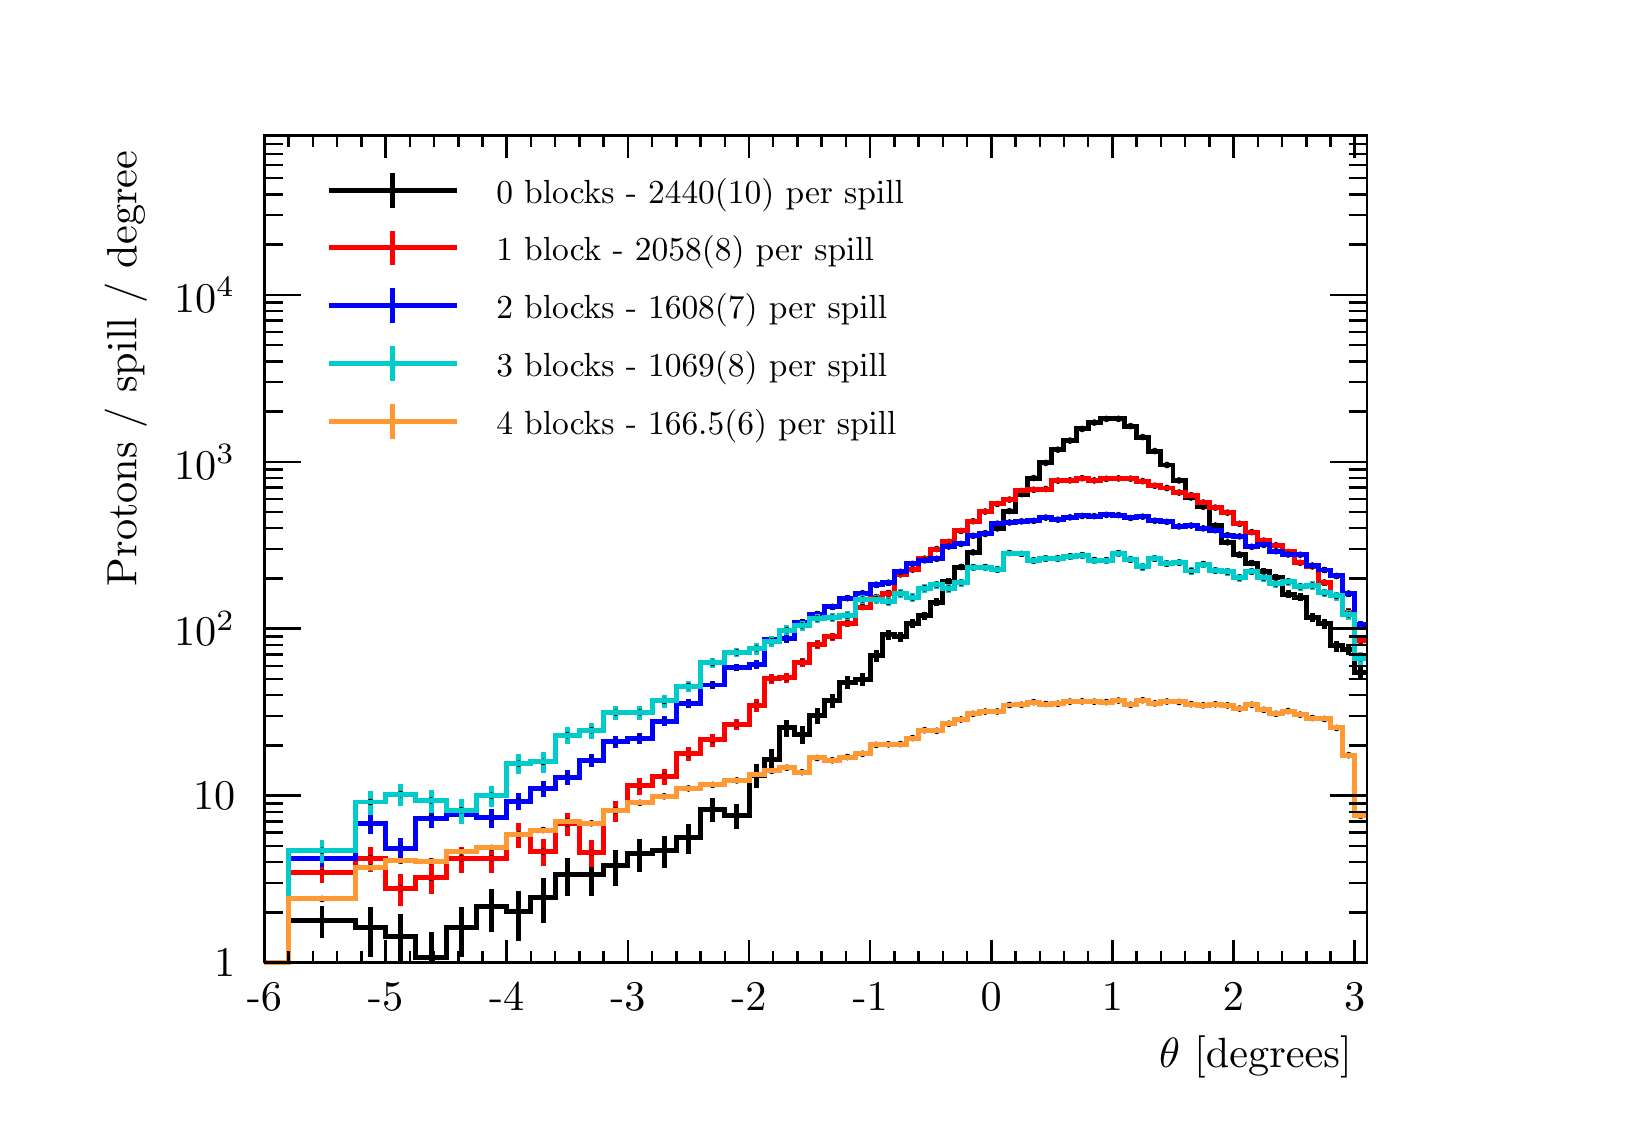
\begin{tikzpicture}
\pgfdeclareplotmark{cross} {
\pgfpathmoveto{\pgfpoint{-0.3\pgfplotmarksize}{\pgfplotmarksize}}
\pgfpathlineto{\pgfpoint{+0.3\pgfplotmarksize}{\pgfplotmarksize}}
\pgfpathlineto{\pgfpoint{+0.3\pgfplotmarksize}{0.3\pgfplotmarksize}}
\pgfpathlineto{\pgfpoint{+1\pgfplotmarksize}{0.3\pgfplotmarksize}}
\pgfpathlineto{\pgfpoint{+1\pgfplotmarksize}{-0.3\pgfplotmarksize}}
\pgfpathlineto{\pgfpoint{+0.3\pgfplotmarksize}{-0.3\pgfplotmarksize}}
\pgfpathlineto{\pgfpoint{+0.3\pgfplotmarksize}{-1.\pgfplotmarksize}}
\pgfpathlineto{\pgfpoint{-0.3\pgfplotmarksize}{-1.\pgfplotmarksize}}
\pgfpathlineto{\pgfpoint{-0.3\pgfplotmarksize}{-0.3\pgfplotmarksize}}
\pgfpathlineto{\pgfpoint{-1.\pgfplotmarksize}{-0.3\pgfplotmarksize}}
\pgfpathlineto{\pgfpoint{-1.\pgfplotmarksize}{0.3\pgfplotmarksize}}
\pgfpathlineto{\pgfpoint{-0.3\pgfplotmarksize}{0.3\pgfplotmarksize}}
\pgfpathclose
\pgfusepathqstroke
}
\pgfdeclareplotmark{cross*} {
\pgfpathmoveto{\pgfpoint{-0.3\pgfplotmarksize}{\pgfplotmarksize}}
\pgfpathlineto{\pgfpoint{+0.3\pgfplotmarksize}{\pgfplotmarksize}}
\pgfpathlineto{\pgfpoint{+0.3\pgfplotmarksize}{0.3\pgfplotmarksize}}
\pgfpathlineto{\pgfpoint{+1\pgfplotmarksize}{0.3\pgfplotmarksize}}
\pgfpathlineto{\pgfpoint{+1\pgfplotmarksize}{-0.3\pgfplotmarksize}}
\pgfpathlineto{\pgfpoint{+0.3\pgfplotmarksize}{-0.3\pgfplotmarksize}}
\pgfpathlineto{\pgfpoint{+0.3\pgfplotmarksize}{-1.\pgfplotmarksize}}
\pgfpathlineto{\pgfpoint{-0.3\pgfplotmarksize}{-1.\pgfplotmarksize}}
\pgfpathlineto{\pgfpoint{-0.3\pgfplotmarksize}{-0.3\pgfplotmarksize}}
\pgfpathlineto{\pgfpoint{-1.\pgfplotmarksize}{-0.3\pgfplotmarksize}}
\pgfpathlineto{\pgfpoint{-1.\pgfplotmarksize}{0.3\pgfplotmarksize}}
\pgfpathlineto{\pgfpoint{-0.3\pgfplotmarksize}{0.3\pgfplotmarksize}}
\pgfpathclose
\pgfusepathqfillstroke
}
\pgfdeclareplotmark{newstar} {
\pgfpathmoveto{\pgfqpoint{0pt}{\pgfplotmarksize}}
\pgfpathlineto{\pgfqpointpolar{44}{0.5\pgfplotmarksize}}
\pgfpathlineto{\pgfqpointpolar{18}{\pgfplotmarksize}}
\pgfpathlineto{\pgfqpointpolar{-20}{0.5\pgfplotmarksize}}
\pgfpathlineto{\pgfqpointpolar{-54}{\pgfplotmarksize}}
\pgfpathlineto{\pgfqpointpolar{-90}{0.5\pgfplotmarksize}}
\pgfpathlineto{\pgfqpointpolar{234}{\pgfplotmarksize}}
\pgfpathlineto{\pgfqpointpolar{198}{0.5\pgfplotmarksize}}
\pgfpathlineto{\pgfqpointpolar{162}{\pgfplotmarksize}}
\pgfpathlineto{\pgfqpointpolar{134}{0.5\pgfplotmarksize}}
\pgfpathclose
\pgfusepathqstroke
}
\pgfdeclareplotmark{newstar*} {
\pgfpathmoveto{\pgfqpoint{0pt}{\pgfplotmarksize}}
\pgfpathlineto{\pgfqpointpolar{44}{0.5\pgfplotmarksize}}
\pgfpathlineto{\pgfqpointpolar{18}{\pgfplotmarksize}}
\pgfpathlineto{\pgfqpointpolar{-20}{0.5\pgfplotmarksize}}
\pgfpathlineto{\pgfqpointpolar{-54}{\pgfplotmarksize}}
\pgfpathlineto{\pgfqpointpolar{-90}{0.5\pgfplotmarksize}}
\pgfpathlineto{\pgfqpointpolar{234}{\pgfplotmarksize}}
\pgfpathlineto{\pgfqpointpolar{198}{0.5\pgfplotmarksize}}
\pgfpathlineto{\pgfqpointpolar{162}{\pgfplotmarksize}}
\pgfpathlineto{\pgfqpointpolar{134}{0.5\pgfplotmarksize}}
\pgfpathclose
\pgfusepathqfillstroke
}
\definecolor{c}{rgb}{1,1,1};
\draw [color=c, fill=c] (0,0) rectangle (20,13.639);
\draw [color=c, fill=c] (3,1.77307) rectangle (17,12.2751);
\definecolor{c}{rgb}{0,0,0};
\draw [c,line width=0.9] (3,1.77307) -- (3,12.2751) -- (17,12.2751) -- (17,1.77307) -- (3,1.77307);
\definecolor{c}{rgb}{1,1,1};
\draw [color=c, fill=c] (3,1.77307) rectangle (17,12.2751);
\definecolor{c}{rgb}{0,0,0};
\draw [c,line width=0.9] (3,1.77307) -- (3,12.2751) -- (17,12.2751) -- (17,1.77307) -- (3,1.77307);
\draw [c,line width=0.9] (3,1.77307) -- (3.30769,1.77307) -- (3.30769,1.77307) -- (4.15385,1.77307) -- (4.15385,1.77307) -- (4.53846,1.77307) -- (4.53846,1.77307) -- (4.92308,1.77307) -- (4.92308,1.77307) -- (5.30769,1.77307) -- (5.30769,1.77307) --
 (5.69231,1.77307) -- (5.69231,1.77307) -- (6.07692,1.77307) -- (6.07692,1.77307) -- (6.38462,1.77307) -- (6.38462,1.77307) -- (6.69231,1.77307) -- (6.69231,1.77307) -- (7,1.77307) -- (7,1.77307) -- (7.30769,1.77307) -- (7.30769,1.77307) --
 (7.61538,1.77307) -- (7.61538,1.77307) -- (7.92308,1.77307) -- (7.92308,1.77307) -- (8.23077,1.77307) -- (8.23077,1.77307) -- (8.53846,1.77307) -- (8.53846,1.77307) -- (8.84615,1.77307) -- (8.84615,1.77307) -- (9.15385,1.77307) -- (9.15385,1.77307)
 -- (9.34615,1.77307) -- (9.34615,1.77307) -- (9.53846,1.77307) -- (9.53846,1.77307) -- (9.73077,1.77307) -- (9.73077,1.77307) -- (9.92308,1.77307) -- (9.92308,1.77307) -- (10.1154,1.77307) -- (10.1154,1.77307) -- (10.3077,1.77307) --
 (10.3077,1.77307) -- (10.5,1.77307) -- (10.5,1.77307) -- (10.6923,1.77307) -- (10.6923,1.77307) -- (10.8462,1.77307) -- (10.8462,1.77307) -- (11,1.77307) -- (11,1.77307) -- (11.1538,1.77307) -- (11.1538,1.77307) -- (11.3077,1.77307) --
 (11.3077,1.77307) -- (11.4615,1.77307) -- (11.4615,1.77307) -- (11.6154,1.77307) -- (11.6154,1.77307) -- (11.7692,1.77307) -- (11.7692,1.77307) -- (11.9231,1.77307) -- (11.9231,1.77307) -- (12.0769,1.77307) -- (12.0769,1.77307) -- (12.2308,1.77307)
 -- (12.2308,1.77307) -- (12.3846,1.77307) -- (12.3846,1.77307) -- (12.5385,1.77307) -- (12.5385,1.77307) -- (12.6923,1.77307) -- (12.6923,1.77307) -- (12.8462,1.77307) -- (12.8462,1.77307) -- (13,1.77307) -- (13,1.77307) -- (13.1538,1.77307) --
 (13.1538,1.77307) -- (13.3077,1.77307) -- (13.3077,1.77307) -- (13.4615,1.77307) -- (13.4615,1.77307) -- (13.6154,1.77307) -- (13.6154,1.77307) -- (13.7692,1.77307) -- (13.7692,1.77307) -- (13.9231,1.77307) -- (13.9231,1.77307) -- (14.0769,1.77307)
 -- (14.0769,1.77307) -- (14.2308,1.77307) -- (14.2308,1.77307) -- (14.3846,1.77307) -- (14.3846,1.77307) -- (14.5385,1.77307) -- (14.5385,1.77307) -- (14.6923,1.77307) -- (14.6923,1.77307) -- (14.8462,1.77307) -- (14.8462,1.77307) -- (15,1.77307) --
 (15,1.77307) -- (15.1538,1.77307) -- (15.1538,1.77307) -- (15.3077,1.77307) -- (15.3077,1.77307) -- (15.4615,1.77307) -- (15.4615,1.77307) -- (15.6154,1.77307) -- (15.6154,1.77307) -- (15.7692,1.77307) -- (15.7692,1.77307) -- (15.9231,1.77307) --
 (15.9231,1.77307) -- (16.0769,1.77307) -- (16.0769,1.77307) -- (16.2308,1.77307) -- (16.2308,1.77307) -- (16.3846,1.77307) -- (16.3846,1.77307) -- (16.5385,1.77307) -- (16.5385,1.77307) -- (16.6923,1.77307) -- (16.6923,1.77307) -- (16.8462,1.77307)
 -- (16.8462,1.77307) -- (17,1.77307);
\draw [c,line width=0.9] (3,1.77307) -- (17,1.77307);
\draw [c,line width=0.9] (3,2.05948) -- (3,1.77307);
\draw [c,line width=0.9] (3.30769,1.91628) -- (3.30769,1.77307);
\draw [c,line width=0.9] (3.61538,1.91628) -- (3.61538,1.77307);
\draw [c,line width=0.9] (3.92308,1.91628) -- (3.92308,1.77307);
\draw [c,line width=0.9] (4.23077,1.91628) -- (4.23077,1.77307);
\draw [c,line width=0.9] (4.53846,2.05948) -- (4.53846,1.77307);
\draw [c,line width=0.9] (4.84615,1.91628) -- (4.84615,1.77307);
\draw [c,line width=0.9] (5.15385,1.91628) -- (5.15385,1.77307);
\draw [c,line width=0.9] (5.46154,1.91628) -- (5.46154,1.77307);
\draw [c,line width=0.9] (5.76923,1.91628) -- (5.76923,1.77307);
\draw [c,line width=0.9] (6.07692,2.05948) -- (6.07692,1.77307);
\draw [c,line width=0.9] (6.38462,1.91628) -- (6.38462,1.77307);
\draw [c,line width=0.9] (6.69231,1.91628) -- (6.69231,1.77307);
\draw [c,line width=0.9] (7,1.91628) -- (7,1.77307);
\draw [c,line width=0.9] (7.30769,1.91628) -- (7.30769,1.77307);
\draw [c,line width=0.9] (7.61538,2.05948) -- (7.61538,1.77307);
\draw [c,line width=0.9] (7.92308,1.91628) -- (7.92308,1.77307);
\draw [c,line width=0.9] (8.23077,1.91628) -- (8.23077,1.77307);
\draw [c,line width=0.9] (8.53846,1.91628) -- (8.53846,1.77307);
\draw [c,line width=0.9] (8.84615,1.91628) -- (8.84615,1.77307);
\draw [c,line width=0.9] (9.15385,2.05948) -- (9.15385,1.77307);
\draw [c,line width=0.9] (9.46154,1.91628) -- (9.46154,1.77307);
\draw [c,line width=0.9] (9.76923,1.91628) -- (9.76923,1.77307);
\draw [c,line width=0.9] (10.0769,1.91628) -- (10.0769,1.77307);
\draw [c,line width=0.9] (10.3846,1.91628) -- (10.3846,1.77307);
\draw [c,line width=0.9] (10.6923,2.05948) -- (10.6923,1.77307);
\draw [c,line width=0.9] (11,1.91628) -- (11,1.77307);
\draw [c,line width=0.9] (11.3077,1.91628) -- (11.3077,1.77307);
\draw [c,line width=0.9] (11.6154,1.91628) -- (11.6154,1.77307);
\draw [c,line width=0.9] (11.9231,1.91628) -- (11.9231,1.77307);
\draw [c,line width=0.9] (12.2308,2.05948) -- (12.2308,1.77307);
\draw [c,line width=0.9] (12.5385,1.91628) -- (12.5385,1.77307);
\draw [c,line width=0.9] (12.8462,1.91628) -- (12.8462,1.77307);
\draw [c,line width=0.9] (13.1538,1.91628) -- (13.1538,1.77307);
\draw [c,line width=0.9] (13.4615,1.91628) -- (13.4615,1.77307);
\draw [c,line width=0.9] (13.7692,2.05948) -- (13.7692,1.77307);
\draw [c,line width=0.9] (14.0769,1.91628) -- (14.0769,1.77307);
\draw [c,line width=0.9] (14.3846,1.91628) -- (14.3846,1.77307);
\draw [c,line width=0.9] (14.6923,1.91628) -- (14.6923,1.77307);
\draw [c,line width=0.9] (15,1.91628) -- (15,1.77307);
\draw [c,line width=0.9] (15.3077,2.05948) -- (15.3077,1.77307);
\draw [c,line width=0.9] (15.6154,1.91628) -- (15.6154,1.77307);
\draw [c,line width=0.9] (15.9231,1.91628) -- (15.9231,1.77307);
\draw [c,line width=0.9] (16.2308,1.91628) -- (16.2308,1.77307);
\draw [c,line width=0.9] (16.5385,1.91628) -- (16.5385,1.77307);
\draw [c,line width=0.9] (16.8462,2.05948) -- (16.8462,1.77307);
\draw [c,line width=0.9] (16.8462,2.05948) -- (16.8462,1.77307);
\draw [anchor=base] (3,1.15931) node[scale=1.52731, color=c, rotate=0]{-6};
\draw [anchor=base] (4.53846,1.15931) node[scale=1.52731, color=c, rotate=0]{-5};
\draw [anchor=base] (6.07692,1.15931) node[scale=1.52731, color=c, rotate=0]{-4};
\draw [anchor=base] (7.61538,1.15931) node[scale=1.52731, color=c, rotate=0]{-3};
\draw [anchor=base] (9.15385,1.15931) node[scale=1.52731, color=c, rotate=0]{-2};
\draw [anchor=base] (10.6923,1.15931) node[scale=1.52731, color=c, rotate=0]{-1};
\draw [anchor=base] (12.2308,1.15931) node[scale=1.52731, color=c, rotate=0]{0};
\draw [anchor=base] (13.7692,1.15931) node[scale=1.52731, color=c, rotate=0]{1};
\draw [anchor=base] (15.3077,1.15931) node[scale=1.52731, color=c, rotate=0]{2};
\draw [anchor=base] (16.8462,1.15931) node[scale=1.52731, color=c, rotate=0]{3};
\draw [anchor= east] (17,0.572837) node[scale=1.52731, color=c, rotate=0]{$\theta$ [degrees]};
\draw [c,line width=0.9] (3,12.2751) -- (17,12.2751);
\draw [c,line width=0.9] (3,11.9887) -- (3,12.2751);
\draw [c,line width=0.9] (3.30769,12.1319) -- (3.30769,12.2751);
\draw [c,line width=0.9] (3.61538,12.1319) -- (3.61538,12.2751);
\draw [c,line width=0.9] (3.92308,12.1319) -- (3.92308,12.2751);
\draw [c,line width=0.9] (4.23077,12.1319) -- (4.23077,12.2751);
\draw [c,line width=0.9] (4.53846,11.9887) -- (4.53846,12.2751);
\draw [c,line width=0.9] (4.84615,12.1319) -- (4.84615,12.2751);
\draw [c,line width=0.9] (5.15385,12.1319) -- (5.15385,12.2751);
\draw [c,line width=0.9] (5.46154,12.1319) -- (5.46154,12.2751);
\draw [c,line width=0.9] (5.76923,12.1319) -- (5.76923,12.2751);
\draw [c,line width=0.9] (6.07692,11.9887) -- (6.07692,12.2751);
\draw [c,line width=0.9] (6.38462,12.1319) -- (6.38462,12.2751);
\draw [c,line width=0.9] (6.69231,12.1319) -- (6.69231,12.2751);
\draw [c,line width=0.9] (7,12.1319) -- (7,12.2751);
\draw [c,line width=0.9] (7.30769,12.1319) -- (7.30769,12.2751);
\draw [c,line width=0.9] (7.61538,11.9887) -- (7.61538,12.2751);
\draw [c,line width=0.9] (7.92308,12.1319) -- (7.92308,12.2751);
\draw [c,line width=0.9] (8.23077,12.1319) -- (8.23077,12.2751);
\draw [c,line width=0.9] (8.53846,12.1319) -- (8.53846,12.2751);
\draw [c,line width=0.9] (8.84615,12.1319) -- (8.84615,12.2751);
\draw [c,line width=0.9] (9.15385,11.9887) -- (9.15385,12.2751);
\draw [c,line width=0.9] (9.46154,12.1319) -- (9.46154,12.2751);
\draw [c,line width=0.9] (9.76923,12.1319) -- (9.76923,12.2751);
\draw [c,line width=0.9] (10.0769,12.1319) -- (10.0769,12.2751);
\draw [c,line width=0.9] (10.3846,12.1319) -- (10.3846,12.2751);
\draw [c,line width=0.9] (10.6923,11.9887) -- (10.6923,12.2751);
\draw [c,line width=0.9] (11,12.1319) -- (11,12.2751);
\draw [c,line width=0.9] (11.3077,12.1319) -- (11.3077,12.2751);
\draw [c,line width=0.9] (11.6154,12.1319) -- (11.6154,12.2751);
\draw [c,line width=0.9] (11.9231,12.1319) -- (11.9231,12.2751);
\draw [c,line width=0.9] (12.2308,11.9887) -- (12.2308,12.2751);
\draw [c,line width=0.9] (12.5385,12.1319) -- (12.5385,12.2751);
\draw [c,line width=0.9] (12.8462,12.1319) -- (12.8462,12.2751);
\draw [c,line width=0.9] (13.1538,12.1319) -- (13.1538,12.2751);
\draw [c,line width=0.9] (13.4615,12.1319) -- (13.4615,12.2751);
\draw [c,line width=0.9] (13.7692,11.9887) -- (13.7692,12.2751);
\draw [c,line width=0.9] (14.0769,12.1319) -- (14.0769,12.2751);
\draw [c,line width=0.9] (14.3846,12.1319) -- (14.3846,12.2751);
\draw [c,line width=0.9] (14.6923,12.1319) -- (14.6923,12.2751);
\draw [c,line width=0.9] (15,12.1319) -- (15,12.2751);
\draw [c,line width=0.9] (15.3077,11.9887) -- (15.3077,12.2751);
\draw [c,line width=0.9] (15.6154,12.1319) -- (15.6154,12.2751);
\draw [c,line width=0.9] (15.9231,12.1319) -- (15.9231,12.2751);
\draw [c,line width=0.9] (16.2308,12.1319) -- (16.2308,12.2751);
\draw [c,line width=0.9] (16.5385,12.1319) -- (16.5385,12.2751);
\draw [c,line width=0.9] (16.8462,11.9887) -- (16.8462,12.2751);
\draw [c,line width=0.9] (16.8462,11.9887) -- (16.8462,12.2751);
\draw [c,line width=0.9] (3,1.77307) -- (3,12.2751);
\draw [c,line width=0.9] (3.462,1.77307) -- (3,1.77307);
\draw [anchor= east] (2.82,1.77307) node[scale=1.52731, color=c, rotate=0]{1};
\draw [c,line width=0.9] (3.231,2.41119) -- (3,2.41119);
\draw [c,line width=0.9] (3.231,2.78447) -- (3,2.78447);
\draw [c,line width=0.9] (3.231,3.04931) -- (3,3.04931);
\draw [c,line width=0.9] (3.231,3.25474) -- (3,3.25474);
\draw [c,line width=0.9] (3.231,3.42259) -- (3,3.42259);
\draw [c,line width=0.9] (3.231,3.56451) -- (3,3.56451);
\draw [c,line width=0.9] (3.231,3.68744) -- (3,3.68744);
\draw [c,line width=0.9] (3.231,3.79587) -- (3,3.79587);
\draw [c,line width=0.9] (3.462,3.89287) -- (3,3.89287);
\draw [anchor= east] (2.82,3.89287) node[scale=1.52731, color=c, rotate=0]{10};
\draw [c,line width=0.9] (3.231,4.53099) -- (3,4.53099);
\draw [c,line width=0.9] (3.231,4.90427) -- (3,4.90427);
\draw [c,line width=0.9] (3.231,5.16912) -- (3,5.16912);
\draw [c,line width=0.9] (3.231,5.37454) -- (3,5.37454);
\draw [c,line width=0.9] (3.231,5.54239) -- (3,5.54239);
\draw [c,line width=0.9] (3.231,5.68431) -- (3,5.68431);
\draw [c,line width=0.9] (3.231,5.80724) -- (3,5.80724);
\draw [c,line width=0.9] (3.231,5.91567) -- (3,5.91567);
\draw [c,line width=0.9] (3.462,6.01267) -- (3,6.01267);
\draw [anchor= east] (2.82,6.01267) node[scale=1.52731, color=c, rotate=0]{$10^{2}$};
\draw [c,line width=0.9] (3.231,6.65079) -- (3,6.65079);
\draw [c,line width=0.9] (3.231,7.02407) -- (3,7.02407);
\draw [c,line width=0.9] (3.231,7.28892) -- (3,7.28892);
\draw [c,line width=0.9] (3.231,7.49434) -- (3,7.49434);
\draw [c,line width=0.9] (3.231,7.66219) -- (3,7.66219);
\draw [c,line width=0.9] (3.231,7.80411) -- (3,7.80411);
\draw [c,line width=0.9] (3.231,7.92704) -- (3,7.92704);
\draw [c,line width=0.9] (3.231,8.03547) -- (3,8.03547);
\draw [c,line width=0.9] (3.462,8.13247) -- (3,8.13247);
\draw [anchor= east] (2.82,8.13247) node[scale=1.52731, color=c, rotate=0]{$10^{3}$};
\draw [c,line width=0.9] (3.231,8.77059) -- (3,8.77059);
\draw [c,line width=0.9] (3.231,9.14387) -- (3,9.14387);
\draw [c,line width=0.9] (3.231,9.40872) -- (3,9.40872);
\draw [c,line width=0.9] (3.231,9.61415) -- (3,9.61415);
\draw [c,line width=0.9] (3.231,9.78199) -- (3,9.78199);
\draw [c,line width=0.9] (3.231,9.92391) -- (3,9.92391);
\draw [c,line width=0.9] (3.231,10.0468) -- (3,10.0468);
\draw [c,line width=0.9] (3.231,10.1553) -- (3,10.1553);
\draw [c,line width=0.9] (3.462,10.2523) -- (3,10.2523);
\draw [anchor= east] (2.82,10.2523) node[scale=1.52731, color=c, rotate=0]{$10^{4}$};
\draw [c,line width=0.9] (3.231,10.8904) -- (3,10.8904);
\draw [c,line width=0.9] (3.231,11.2637) -- (3,11.2637);
\draw [c,line width=0.9] (3.231,11.5285) -- (3,11.5285);
\draw [c,line width=0.9] (3.231,11.7339) -- (3,11.7339);
\draw [c,line width=0.9] (3.231,11.9018) -- (3,11.9018);
\draw [c,line width=0.9] (3.231,12.0437) -- (3,12.0437);
\draw [c,line width=0.9] (3.231,12.1666) -- (3,12.1666);
\draw [c,line width=0.9] (3.231,12.2751) -- (3,12.2751);
\draw [anchor= east] (1.24,12.2751) node[scale=1.52731, color=c, rotate=90]{ Protons / spill / degree};
\draw [c,line width=0.9] (17,1.77307) -- (17,12.2751);
\draw [c,line width=0.9] (16.538,1.77307) -- (17,1.77307);
\draw [c,line width=0.9] (16.769,2.41119) -- (17,2.41119);
\draw [c,line width=0.9] (16.769,2.78447) -- (17,2.78447);
\draw [c,line width=0.9] (16.769,3.04931) -- (17,3.04931);
\draw [c,line width=0.9] (16.769,3.25474) -- (17,3.25474);
\draw [c,line width=0.9] (16.769,3.42259) -- (17,3.42259);
\draw [c,line width=0.9] (16.769,3.56451) -- (17,3.56451);
\draw [c,line width=0.9] (16.769,3.68744) -- (17,3.68744);
\draw [c,line width=0.9] (16.769,3.79587) -- (17,3.79587);
\draw [c,line width=0.9] (16.538,3.89287) -- (17,3.89287);
\draw [c,line width=0.9] (16.769,4.53099) -- (17,4.53099);
\draw [c,line width=0.9] (16.769,4.90427) -- (17,4.90427);
\draw [c,line width=0.9] (16.769,5.16912) -- (17,5.16912);
\draw [c,line width=0.9] (16.769,5.37454) -- (17,5.37454);
\draw [c,line width=0.9] (16.769,5.54239) -- (17,5.54239);
\draw [c,line width=0.9] (16.769,5.68431) -- (17,5.68431);
\draw [c,line width=0.9] (16.769,5.80724) -- (17,5.80724);
\draw [c,line width=0.9] (16.769,5.91567) -- (17,5.91567);
\draw [c,line width=0.9] (16.538,6.01267) -- (17,6.01267);
\draw [c,line width=0.9] (16.769,6.65079) -- (17,6.65079);
\draw [c,line width=0.9] (16.769,7.02407) -- (17,7.02407);
\draw [c,line width=0.9] (16.769,7.28892) -- (17,7.28892);
\draw [c,line width=0.9] (16.769,7.49434) -- (17,7.49434);
\draw [c,line width=0.9] (16.769,7.66219) -- (17,7.66219);
\draw [c,line width=0.9] (16.769,7.80411) -- (17,7.80411);
\draw [c,line width=0.9] (16.769,7.92704) -- (17,7.92704);
\draw [c,line width=0.9] (16.769,8.03547) -- (17,8.03547);
\draw [c,line width=0.9] (16.538,8.13247) -- (17,8.13247);
\draw [c,line width=0.9] (16.769,8.77059) -- (17,8.77059);
\draw [c,line width=0.9] (16.769,9.14387) -- (17,9.14387);
\draw [c,line width=0.9] (16.769,9.40872) -- (17,9.40872);
\draw [c,line width=0.9] (16.769,9.61415) -- (17,9.61415);
\draw [c,line width=0.9] (16.769,9.78199) -- (17,9.78199);
\draw [c,line width=0.9] (16.769,9.92391) -- (17,9.92391);
\draw [c,line width=0.9] (16.769,10.0468) -- (17,10.0468);
\draw [c,line width=0.9] (16.769,10.1553) -- (17,10.1553);
\draw [c,line width=0.9] (16.538,10.2523) -- (17,10.2523);
\draw [c,line width=0.9] (16.769,10.8904) -- (17,10.8904);
\draw [c,line width=0.9] (16.769,11.2637) -- (17,11.2637);
\draw [c,line width=0.9] (16.769,11.5285) -- (17,11.5285);
\draw [c,line width=0.9] (16.769,11.7339) -- (17,11.7339);
\draw [c,line width=0.9] (16.769,11.9018) -- (17,11.9018);
\draw [c,line width=0.9] (16.769,12.0437) -- (17,12.0437);
\draw [c,line width=0.9] (16.769,12.1666) -- (17,12.1666);
\draw [c,line width=0.9] (16.769,12.2751) -- (17,12.2751);
\draw [c,line width=1.8] (3.73077,2.09091) -- (3.73077,2.31167);
\draw [c,line width=1.8] (3.73077,2.31167) -- (3.73077,2.4896);
\foreach \P in {(3.73077,2.31167)}{\draw[mark options={color=c,fill=c},mark size=2.402402pt,mark=*,mark size=1pt] plot coordinates {\P};}
\draw [c,line width=1.8] (4.34615,1.84136) -- (4.34615,2.21467);
\draw [c,line width=1.8] (4.34615,2.21467) -- (4.34615,2.47953);
\foreach \P in {(4.34615,2.21467)}{\draw[mark options={color=c,fill=c},mark size=2.402402pt,mark=*,mark size=1pt] plot coordinates {\P};}
\draw [c,line width=1.8] (4.73077,1.77307) -- (4.73077,2.10624);
\draw [c,line width=1.8] (4.73077,2.10624) -- (4.73077,2.38496);
\foreach \P in {(4.73077,2.10624)}{\draw[mark options={color=c,fill=c},mark size=2.402402pt,mark=*,mark size=1pt] plot coordinates {\P};}
\draw [c,line width=1.8] (5.11538,1.77307) -- (5.11538,1.84139);
\draw [c,line width=1.8] (5.11538,1.84139) -- (5.11538,2.15658);
\foreach \P in {(5.11538,1.84139)}{\draw[mark options={color=c,fill=c},mark size=2.402402pt,mark=*,mark size=1pt] plot coordinates {\P};}
\draw [c,line width=1.8] (5.5,1.84136) -- (5.5,2.21467);
\draw [c,line width=1.8] (5.5,2.21467) -- (5.5,2.47953);
\foreach \P in {(5.5,2.21467)}{\draw[mark options={color=c,fill=c},mark size=2.402402pt,mark=*,mark size=1pt] plot coordinates {\P};}
\draw [c,line width=1.8] (5.88462,2.16591) -- (5.88462,2.47952);
\draw [c,line width=1.8] (5.88462,2.47952) -- (5.88462,2.71301);
\foreach \P in {(5.88462,2.47952)}{\draw[mark options={color=c,fill=c},mark size=2.402402pt,mark=*,mark size=1pt] plot coordinates {\P};}
\draw [c,line width=1.8] (6.23077,2.04679) -- (6.23077,2.4201);
\draw [c,line width=1.8] (6.23077,2.4201) -- (6.23077,2.68496);
\foreach \P in {(6.23077,2.4201)}{\draw[mark options={color=c,fill=c},mark size=2.402402pt,mark=*,mark size=1pt] plot coordinates {\P};}
\draw [c,line width=1.8] (6.53846,2.27447) -- (6.53846,2.60484);
\draw [c,line width=1.8] (6.53846,2.60484) -- (6.53846,2.84746);
\foreach \P in {(6.53846,2.60484)}{\draw[mark options={color=c,fill=c},mark size=2.402402pt,mark=*,mark size=1pt] plot coordinates {\P};}
\draw [c,line width=1.8] (6.84615,2.61539) -- (6.84615,2.89038);
\draw [c,line width=1.8] (6.84615,2.89038) -- (6.84615,3.10184);
\foreach \P in {(6.84615,2.89038)}{\draw[mark options={color=c,fill=c},mark size=2.402402pt,mark=*,mark size=1pt] plot coordinates {\P};}
\draw [c,line width=1.8] (7.15385,2.61539) -- (7.15385,2.89038);
\draw [c,line width=1.8] (7.15385,2.89038) -- (7.15385,3.10184);
\foreach \P in {(7.15385,2.89038)}{\draw[mark options={color=c,fill=c},mark size=2.402402pt,mark=*,mark size=1pt] plot coordinates {\P};}
\draw [c,line width=1.8] (7.46154,2.74986) -- (7.46154,3.0056);
\draw [c,line width=1.8] (7.46154,3.0056) -- (7.46154,3.20553);
\foreach \P in {(7.46154,3.0056)}{\draw[mark options={color=c,fill=c},mark size=2.402402pt,mark=*,mark size=1pt] plot coordinates {\P};}
\draw [c,line width=1.8] (7.76923,2.9222) -- (7.76923,3.15522);
\draw [c,line width=1.8] (7.76923,3.15522) -- (7.76923,3.34102);
\foreach \P in {(7.76923,3.15522)}{\draw[mark options={color=c,fill=c},mark size=2.402402pt,mark=*,mark size=1pt] plot coordinates {\P};}
\draw [c,line width=1.8] (8.07692,2.97349) -- (8.07692,3.20014);
\draw [c,line width=1.8] (8.07692,3.20014) -- (8.07692,3.38187);
\foreach \P in {(8.07692,3.20014)}{\draw[mark options={color=c,fill=c},mark size=2.402402pt,mark=*,mark size=1pt] plot coordinates {\P};}
\draw [c,line width=1.8] (8.38461,3.15521) -- (8.38461,3.36065);
\draw [c,line width=1.8] (8.38461,3.36065) -- (8.38461,3.52851);
\foreach \P in {(8.38461,3.36065)}{\draw[mark options={color=c,fill=c},mark size=2.402402pt,mark=*,mark size=1pt] plot coordinates {\P};}
\draw [c,line width=1.8] (8.69231,3.55621) -- (8.69231,3.72157);
\draw [c,line width=1.8] (8.69231,3.72157) -- (8.69231,3.8617);
\foreach \P in {(8.69231,3.72157)}{\draw[mark options={color=c,fill=c},mark size=2.402402pt,mark=*,mark size=1pt] plot coordinates {\P};}
\draw [c,line width=1.8] (9,3.47051) -- (9,3.64373);
\draw [c,line width=1.8] (9,3.64373) -- (9,3.78946);
\foreach \P in {(9,3.64373)}{\draw[mark options={color=c,fill=c},mark size=2.402402pt,mark=*,mark size=1pt] plot coordinates {\P};}
\draw [c,line width=1.8] (9.25,3.98891) -- (9.25,4.15427);
\draw [c,line width=1.8] (9.25,4.15427) -- (9.25,4.2944);
\foreach \P in {(9.25,4.15427)}{\draw[mark options={color=c,fill=c},mark size=2.402402pt,mark=*,mark size=1pt] plot coordinates {\P};}
\draw [c,line width=1.8] (9.44231,4.20785) -- (9.44231,4.35471);
\draw [c,line width=1.8] (9.44231,4.35471) -- (9.44231,4.48133);
\foreach \P in {(9.44231,4.35471)}{\draw[mark options={color=c,fill=c},mark size=2.402402pt,mark=*,mark size=1pt] plot coordinates {\P};}
\draw [c,line width=1.8] (9.63461,4.63798) -- (9.63461,4.75429);
\draw [c,line width=1.8] (9.63461,4.75429) -- (9.63461,4.85754);
\foreach \P in {(9.63461,4.75429)}{\draw[mark options={color=c,fill=c},mark size=2.402402pt,mark=*,mark size=1pt] plot coordinates {\P};}
\draw [c,line width=1.8] (9.82692,4.55108) -- (9.82692,4.67301);
\draw [c,line width=1.8] (9.82692,4.67301) -- (9.82692,4.78066);
\foreach \P in {(9.82692,4.67301)}{\draw[mark options={color=c,fill=c},mark size=2.402402pt,mark=*,mark size=1pt] plot coordinates {\P};}
\draw [c,line width=1.8] (10.0192,4.80271) -- (10.0192,4.90908);
\draw [c,line width=1.8] (10.0192,4.90908) -- (10.0192,5.00442);
\foreach \P in {(10.0192,4.90908)}{\draw[mark options={color=c,fill=c},mark size=2.402402pt,mark=*,mark size=1pt] plot coordinates {\P};}
\draw [c,line width=1.8] (10.2115,5.0013) -- (10.2115,5.09681);
\draw [c,line width=1.8] (10.2115,5.09681) -- (10.2115,5.18333);
\foreach \P in {(10.2115,5.09681)}{\draw[mark options={color=c,fill=c},mark size=2.402402pt,mark=*,mark size=1pt] plot coordinates {\P};}
\draw [c,line width=1.8] (10.4038,5.24863) -- (10.4038,5.33213);
\draw [c,line width=1.8] (10.4038,5.33213) -- (10.4038,5.40869);
\foreach \P in {(10.4038,5.33213)}{\draw[mark options={color=c,fill=c},mark size=2.402402pt,mark=*,mark size=1pt] plot coordinates {\P};}
\draw [c,line width=1.8] (10.5962,5.29115) -- (10.5962,5.37276);
\draw [c,line width=1.8] (10.5962,5.37276) -- (10.5962,5.44771);
\foreach \P in {(10.5962,5.37276)}{\draw[mark options={color=c,fill=c},mark size=2.402402pt,mark=*,mark size=1pt] plot coordinates {\P};}
\draw [c,line width=1.8] (10.7692,5.58892) -- (10.7692,5.66653);
\draw [c,line width=1.8] (10.7692,5.66653) -- (10.7692,5.73811);
\foreach \P in {(10.7692,5.66653)}{\draw[mark options={color=c,fill=c},mark size=2.402402pt,mark=*,mark size=1pt] plot coordinates {\P};}
\draw [c,line width=1.8] (10.9231,5.87387) -- (10.9231,5.94036);
\draw [c,line width=1.8] (10.9231,5.94036) -- (10.9231,6.00237);
\foreach \P in {(10.9231,5.94036)}{\draw[mark options={color=c,fill=c},mark size=2.402402pt,mark=*,mark size=1pt] plot coordinates {\P};}
\draw [c,line width=1.8] (11.0769,5.84084) -- (11.0769,5.90853);
\draw [c,line width=1.8] (11.0769,5.90853) -- (11.0769,5.97159);
\foreach \P in {(11.0769,5.90853)}{\draw[mark options={color=c,fill=c},mark size=2.402402pt,mark=*,mark size=1pt] plot coordinates {\P};}
\draw [c,line width=1.8] (11.2308,6.02352) -- (11.2308,6.08482);
\draw [c,line width=1.8] (11.2308,6.08482) -- (11.2308,6.1423);
\foreach \P in {(11.2308,6.08482)}{\draw[mark options={color=c,fill=c},mark size=2.402402pt,mark=*,mark size=1pt] plot coordinates {\P};}
\draw [c,line width=1.8] (11.3846,6.11743) -- (11.3846,6.17569);
\draw [c,line width=1.8] (11.3846,6.17569) -- (11.3846,6.23047);
\foreach \P in {(11.3846,6.17569)}{\draw[mark options={color=c,fill=c},mark size=2.402402pt,mark=*,mark size=1pt] plot coordinates {\P};}
\draw [c,line width=1.8] (11.5385,6.29584) -- (11.5385,6.34871);
\draw [c,line width=1.8] (11.5385,6.34871) -- (11.5385,6.39872);
\foreach \P in {(11.5385,6.34871)}{\draw[mark options={color=c,fill=c},mark size=2.402402pt,mark=*,mark size=1pt] plot coordinates {\P};}
\draw [c,line width=1.8] (11.6923,6.5613) -- (11.6923,6.60708);
\draw [c,line width=1.8] (11.6923,6.60708) -- (11.6923,6.65069);
\foreach \P in {(11.6923,6.60708)}{\draw[mark options={color=c,fill=c},mark size=2.402402pt,mark=*,mark size=1pt] plot coordinates {\P};}
\draw [c,line width=1.8] (11.8462,6.75514) -- (11.8462,6.79634);
\draw [c,line width=1.8] (11.8462,6.79634) -- (11.8462,6.83578);
\foreach \P in {(11.8462,6.79634)}{\draw[mark options={color=c,fill=c},mark size=2.402402pt,mark=*,mark size=1pt] plot coordinates {\P};}
\draw [c,line width=1.8] (12,6.94536) -- (12,6.98252);
\draw [c,line width=1.8] (12,6.98252) -- (12,7.01824);
\foreach \P in {(12,6.98252)}{\draw[mark options={color=c,fill=c},mark size=2.402402pt,mark=*,mark size=1pt] plot coordinates {\P};}
\draw [c,line width=1.8] (12.1538,7.18396) -- (12.1538,7.21661);
\draw [c,line width=1.8] (12.1538,7.21661) -- (12.1538,7.24813);
\foreach \P in {(12.1538,7.21661)}{\draw[mark options={color=c,fill=c},mark size=2.402402pt,mark=*,mark size=1pt] plot coordinates {\P};}
\draw [c,line width=1.8] (12.3077,7.2551) -- (12.3077,7.28651);
\draw [c,line width=1.8] (12.3077,7.28651) -- (12.3077,7.31688);
\foreach \P in {(12.3077,7.28651)}{\draw[mark options={color=c,fill=c},mark size=2.402402pt,mark=*,mark size=1pt] plot coordinates {\P};}
\draw [c,line width=1.8] (12.4615,7.47871) -- (12.4615,7.50652);
\draw [c,line width=1.8] (12.4615,7.50652) -- (12.4615,7.53352);
\foreach \P in {(12.4615,7.50652)}{\draw[mark options={color=c,fill=c},mark size=2.402402pt,mark=*,mark size=1pt] plot coordinates {\P};}
\draw [c,line width=1.8] (12.6154,7.69682) -- (12.6154,7.72153);
\draw [c,line width=1.8] (12.6154,7.72153) -- (12.6154,7.74559);
\foreach \P in {(12.6154,7.72153)}{\draw[mark options={color=c,fill=c},mark size=2.402402pt,mark=*,mark size=1pt] plot coordinates {\P};}
\draw [c,line width=1.8] (12.7692,7.9041) -- (12.7692,7.92618);
\draw [c,line width=1.8] (12.7692,7.92618) -- (12.7692,7.94774);
\foreach \P in {(12.7692,7.92618)}{\draw[mark options={color=c,fill=c},mark size=2.402402pt,mark=*,mark size=1pt] plot coordinates {\P};}
\draw [c,line width=1.8] (12.9231,8.09831) -- (12.9231,8.11818);
\draw [c,line width=1.8] (12.9231,8.11818) -- (12.9231,8.13763);
\foreach \P in {(12.9231,8.11818)}{\draw[mark options={color=c,fill=c},mark size=2.402402pt,mark=*,mark size=1pt] plot coordinates {\P};}
\draw [c,line width=1.8] (13.0769,8.26868) -- (13.0769,8.28679);
\draw [c,line width=1.8] (13.0769,8.28679) -- (13.0769,8.30456);
\foreach \P in {(13.0769,8.28679)}{\draw[mark options={color=c,fill=c},mark size=2.402402pt,mark=*,mark size=1pt] plot coordinates {\P};}
\draw [c,line width=1.8] (13.2308,8.38491) -- (13.2308,8.40192);
\draw [c,line width=1.8] (13.2308,8.40192) -- (13.2308,8.41862);
\foreach \P in {(13.2308,8.40192)}{\draw[mark options={color=c,fill=c},mark size=2.402402pt,mark=*,mark size=1pt] plot coordinates {\P};}
\draw [c,line width=1.8] (13.3846,8.5343) -- (13.3846,8.54998);
\draw [c,line width=1.8] (13.3846,8.54998) -- (13.3846,8.5654);
\foreach \P in {(13.3846,8.54998)}{\draw[mark options={color=c,fill=c},mark size=2.402402pt,mark=*,mark size=1pt] plot coordinates {\P};}
\draw [c,line width=1.8] (13.5385,8.61585) -- (13.5385,8.63085);
\draw [c,line width=1.8] (13.5385,8.63085) -- (13.5385,8.64561);
\foreach \P in {(13.5385,8.63085)}{\draw[mark options={color=c,fill=c},mark size=2.402402pt,mark=*,mark size=1pt] plot coordinates {\P};}
\draw [c,line width=1.8] (13.6923,8.66264) -- (13.6923,8.67726);
\draw [c,line width=1.8] (13.6923,8.67726) -- (13.6923,8.69166);
\foreach \P in {(13.6923,8.67726)}{\draw[mark options={color=c,fill=c},mark size=2.402402pt,mark=*,mark size=1pt] plot coordinates {\P};}
\draw [c,line width=1.8] (13.8462,8.66333) -- (13.8462,8.67795);
\draw [c,line width=1.8] (13.8462,8.67795) -- (13.8462,8.69234);
\foreach \P in {(13.8462,8.67795)}{\draw[mark options={color=c,fill=c},mark size=2.402402pt,mark=*,mark size=1pt] plot coordinates {\P};}
\draw [c,line width=1.8] (14,8.57064) -- (14,8.58601);
\draw [c,line width=1.8] (14,8.58601) -- (14,8.60114);
\foreach \P in {(14,8.58601)}{\draw[mark options={color=c,fill=c},mark size=2.402402pt,mark=*,mark size=1pt] plot coordinates {\P};}
\draw [c,line width=1.8] (14.1538,8.42986) -- (14.1538,8.44645);
\draw [c,line width=1.8] (14.1538,8.44645) -- (14.1538,8.46276);
\foreach \P in {(14.1538,8.44645)}{\draw[mark options={color=c,fill=c},mark size=2.402402pt,mark=*,mark size=1pt] plot coordinates {\P};}
\draw [c,line width=1.8] (14.3077,8.25051) -- (14.3077,8.2688);
\draw [c,line width=1.8] (14.3077,8.2688) -- (14.3077,8.28674);
\foreach \P in {(14.3077,8.2688)}{\draw[mark options={color=c,fill=c},mark size=2.402402pt,mark=*,mark size=1pt] plot coordinates {\P};}
\draw [c,line width=1.8] (14.4615,8.07163) -- (14.4615,8.09179);
\draw [c,line width=1.8] (14.4615,8.09179) -- (14.4615,8.11151);
\foreach \P in {(14.4615,8.09179)}{\draw[mark options={color=c,fill=c},mark size=2.402402pt,mark=*,mark size=1pt] plot coordinates {\P};}
\draw [c,line width=1.8] (14.6154,7.87325) -- (14.6154,7.8957);
\draw [c,line width=1.8] (14.6154,7.8957) -- (14.6154,7.91762);
\foreach \P in {(14.6154,7.8957)}{\draw[mark options={color=c,fill=c},mark size=2.402402pt,mark=*,mark size=1pt] plot coordinates {\P};}
\draw [c,line width=1.8] (14.7692,7.65396) -- (14.7692,7.67925);
\draw [c,line width=1.8] (14.7692,7.67925) -- (14.7692,7.70387);
\foreach \P in {(14.7692,7.67925)}{\draw[mark options={color=c,fill=c},mark size=2.402402pt,mark=*,mark size=1pt] plot coordinates {\P};}
\draw [c,line width=1.8] (14.9231,7.53414) -- (14.9231,7.56114);
\draw [c,line width=1.8] (14.9231,7.56114) -- (14.9231,7.58736);
\foreach \P in {(14.9231,7.56114)}{\draw[mark options={color=c,fill=c},mark size=2.402402pt,mark=*,mark size=1pt] plot coordinates {\P};}
\draw [c,line width=1.8] (15.0769,7.29227) -- (15.0769,7.32305);
\draw [c,line width=1.8] (15.0769,7.32305) -- (15.0769,7.35284);
\foreach \P in {(15.0769,7.32305)}{\draw[mark options={color=c,fill=c},mark size=2.402402pt,mark=*,mark size=1pt] plot coordinates {\P};}
\draw [c,line width=1.8] (15.2308,7.0755) -- (15.2308,7.11013);
\draw [c,line width=1.8] (15.2308,7.11013) -- (15.2308,7.1435);
\foreach \P in {(15.2308,7.11013)}{\draw[mark options={color=c,fill=c},mark size=2.402402pt,mark=*,mark size=1pt] plot coordinates {\P};}
\draw [c,line width=1.8] (15.3846,6.917) -- (15.3846,6.95473);
\draw [c,line width=1.8] (15.3846,6.95473) -- (15.3846,6.99099);
\foreach \P in {(15.3846,6.95473)}{\draw[mark options={color=c,fill=c},mark size=2.402402pt,mark=*,mark size=1pt] plot coordinates {\P};}
\draw [c,line width=1.8] (15.5385,6.80603) -- (15.5385,6.84612);
\draw [c,line width=1.8] (15.5385,6.84612) -- (15.5385,6.88453);
\foreach \P in {(15.5385,6.84612)}{\draw[mark options={color=c,fill=c},mark size=2.402402pt,mark=*,mark size=1pt] plot coordinates {\P};}
\draw [c,line width=1.8] (15.6923,6.69938) -- (15.6923,6.74185);
\draw [c,line width=1.8] (15.6923,6.74185) -- (15.6923,6.78245);
\foreach \P in {(15.6923,6.74185)}{\draw[mark options={color=c,fill=c},mark size=2.402402pt,mark=*,mark size=1pt] plot coordinates {\P};}
\draw [c,line width=1.8] (15.8462,6.62359) -- (15.8462,6.66785);
\draw [c,line width=1.8] (15.8462,6.66785) -- (15.8462,6.71008);
\foreach \P in {(15.8462,6.66785)}{\draw[mark options={color=c,fill=c},mark size=2.402402pt,mark=*,mark size=1pt] plot coordinates {\P};}
\draw [c,line width=1.8] (16,6.40179) -- (16,6.45171);
\draw [c,line width=1.8] (16,6.45171) -- (16,6.49906);
\foreach \P in {(16,6.45171)}{\draw[mark options={color=c,fill=c},mark size=2.402402pt,mark=*,mark size=1pt] plot coordinates {\P};}
\draw [c,line width=1.8] (16.1538,6.36139) -- (16.1538,6.41242);
\draw [c,line width=1.8] (16.1538,6.41242) -- (16.1538,6.46077);
\foreach \P in {(16.1538,6.41242)}{\draw[mark options={color=c,fill=c},mark size=2.402402pt,mark=*,mark size=1pt] plot coordinates {\P};}
\draw [c,line width=1.8] (16.3077,6.09207) -- (16.3077,6.15114);
\draw [c,line width=1.8] (16.3077,6.15114) -- (16.3077,6.20664);
\foreach \P in {(16.3077,6.15114)}{\draw[mark options={color=c,fill=c},mark size=2.402402pt,mark=*,mark size=1pt] plot coordinates {\P};}
\draw [c,line width=1.8] (16.4615,6.01159) -- (16.4615,6.07329);
\draw [c,line width=1.8] (16.4615,6.07329) -- (16.4615,6.13111);
\foreach \P in {(16.4615,6.07329)}{\draw[mark options={color=c,fill=c},mark size=2.402402pt,mark=*,mark size=1pt] plot coordinates {\P};}
\draw [c,line width=1.8] (16.6154,5.72331) -- (16.6154,5.79546);
\draw [c,line width=1.8] (16.6154,5.79546) -- (16.6154,5.86237);
\foreach \P in {(16.6154,5.79546)}{\draw[mark options={color=c,fill=c},mark size=2.402402pt,mark=*,mark size=1pt] plot coordinates {\P};}
\draw [c,line width=1.8] (16.7692,5.67299) -- (16.7692,5.74714);
\draw [c,line width=1.8] (16.7692,5.74714) -- (16.7692,5.81576);
\foreach \P in {(16.7692,5.74714)}{\draw[mark options={color=c,fill=c},mark size=2.402402pt,mark=*,mark size=1pt] plot coordinates {\P};}
\draw [c,line width=1.8] (16.9231,5.37072) -- (16.9231,5.45809);
\draw [c,line width=1.8] (16.9231,5.45809) -- (16.9231,5.53788);
\foreach \P in {(16.9231,5.45809)}{\draw[mark options={color=c,fill=c},mark size=2.402402pt,mark=*,mark size=1pt] plot coordinates {\P};}
\draw [c,line width=1.8] (3,1.77307) -- (3.30769,1.77307) -- (3.30769,2.31167) -- (4.15385,2.31167) -- (4.15385,2.21467) -- (4.53846,2.21467) -- (4.53846,2.10624) -- (4.92308,2.10624) -- (4.92308,1.84139) -- (5.30769,1.84139) -- (5.30769,2.21467) --
 (5.69231,2.21467) -- (5.69231,2.47952) -- (6.07692,2.47952) -- (6.07692,2.4201) -- (6.38462,2.4201) -- (6.38462,2.60484) -- (6.69231,2.60484) -- (6.69231,2.89038) -- (7,2.89038) -- (7,2.89038) -- (7.30769,2.89038) -- (7.30769,3.0056) --
 (7.61538,3.0056) -- (7.61538,3.15522) -- (7.92308,3.15522) -- (7.92308,3.20014) -- (8.23077,3.20014) -- (8.23077,3.36065) -- (8.53846,3.36065) -- (8.53846,3.72157) -- (8.84615,3.72157) -- (8.84615,3.64373) -- (9.15385,3.64373) -- (9.15385,4.15427)
 -- (9.34615,4.15427) -- (9.34615,4.35471) -- (9.53846,4.35471) -- (9.53846,4.75429) -- (9.73077,4.75429) -- (9.73077,4.67301) -- (9.92308,4.67301) -- (9.92308,4.90908) -- (10.1154,4.90908) -- (10.1154,5.09681) -- (10.3077,5.09681) --
 (10.3077,5.33213) -- (10.5,5.33213) -- (10.5,5.37276) -- (10.6923,5.37276) -- (10.6923,5.66653) -- (10.8462,5.66653) -- (10.8462,5.94036) -- (11,5.94036) -- (11,5.90853) -- (11.1538,5.90853) -- (11.1538,6.08482) -- (11.3077,6.08482) --
 (11.3077,6.17569) -- (11.4615,6.17569) -- (11.4615,6.34871) -- (11.6154,6.34871) -- (11.6154,6.60708) -- (11.7692,6.60708) -- (11.7692,6.79634) -- (11.9231,6.79634) -- (11.9231,6.98252) -- (12.0769,6.98252) -- (12.0769,7.21661) -- (12.2308,7.21661)
 -- (12.2308,7.28651) -- (12.3846,7.28651) -- (12.3846,7.50652) -- (12.5385,7.50652) -- (12.5385,7.72153) -- (12.6923,7.72153) -- (12.6923,7.92618) -- (12.8462,7.92618) -- (12.8462,8.11818) -- (13,8.11818) -- (13,8.28679) -- (13.1538,8.28679) --
 (13.1538,8.40192) -- (13.3077,8.40192) -- (13.3077,8.54998) -- (13.4615,8.54998) -- (13.4615,8.63085) -- (13.6154,8.63085) -- (13.6154,8.67726) -- (13.7692,8.67726) -- (13.7692,8.67795) -- (13.9231,8.67795) -- (13.9231,8.58601) -- (14.0769,8.58601)
 -- (14.0769,8.44645) -- (14.2308,8.44645) -- (14.2308,8.2688) -- (14.3846,8.2688) -- (14.3846,8.09179) -- (14.5385,8.09179) -- (14.5385,7.8957) -- (14.6923,7.8957) -- (14.6923,7.67925) -- (14.8462,7.67925) -- (14.8462,7.56114) -- (15,7.56114) --
 (15,7.32305) -- (15.1538,7.32305) -- (15.1538,7.11013) -- (15.3077,7.11013) -- (15.3077,6.95473) -- (15.4615,6.95473) -- (15.4615,6.84612) -- (15.6154,6.84612) -- (15.6154,6.74185) -- (15.7692,6.74185) -- (15.7692,6.66785) -- (15.9231,6.66785) --
 (15.9231,6.45171) -- (16.0769,6.45171) -- (16.0769,6.41242) -- (16.2308,6.41242) -- (16.2308,6.15114) -- (16.3846,6.15114) -- (16.3846,6.07329) -- (16.5385,6.07329) -- (16.5385,5.79546) -- (16.6923,5.79546) -- (16.6923,5.74714) -- (16.8462,5.74714)
 -- (16.8462,5.45809) -- (17,5.45809);
\definecolor{c}{rgb}{1,0,0};
\draw [c,line width=1.8] (3.73077,2.78813) -- (3.73077,2.92056);
\draw [c,line width=1.8] (3.73077,2.92056) -- (3.73077,3.0363);
\definecolor{c}{rgb}{0,0,0};
\foreach \P in {(3.73077,2.92056)}{\draw[mark options={color=c,fill=c},mark size=2.402402pt,mark=*,mark size=1pt] plot coordinates {\P};}
\definecolor{c}{rgb}{1,0,0};
\draw [c,line width=1.8] (4.34615,2.92543) -- (4.34615,3.09725);
\draw [c,line width=1.8] (4.34615,3.09725) -- (4.34615,3.24199);
\definecolor{c}{rgb}{0,0,0};
\foreach \P in {(4.34615,3.09725)}{\draw[mark options={color=c,fill=c},mark size=2.402402pt,mark=*,mark size=1pt] plot coordinates {\P};}
\definecolor{c}{rgb}{1,0,0};
\draw [c,line width=1.8] (4.73077,2.4881) -- (4.73077,2.71215);
\draw [c,line width=1.8] (4.73077,2.71215) -- (4.73077,2.89221);
\definecolor{c}{rgb}{0,0,0};
\foreach \P in {(4.73077,2.71215)}{\draw[mark options={color=c,fill=c},mark size=2.402402pt,mark=*,mark size=1pt] plot coordinates {\P};}
\definecolor{c}{rgb}{1,0,0};
\draw [c,line width=1.8] (5.11538,2.64098) -- (5.11538,2.85029);
\draw [c,line width=1.8] (5.11538,2.85029) -- (5.11538,3.02072);
\definecolor{c}{rgb}{0,0,0};
\foreach \P in {(5.11538,2.85029)}{\draw[mark options={color=c,fill=c},mark size=2.402402pt,mark=*,mark size=1pt] plot coordinates {\P};}
\definecolor{c}{rgb}{1,0,0};
\draw [c,line width=1.8] (5.5,2.91523) -- (5.5,3.09586);
\draw [c,line width=1.8] (5.5,3.09586) -- (5.5,3.2468);
\definecolor{c}{rgb}{0,0,0};
\foreach \P in {(5.5,3.09586)}{\draw[mark options={color=c,fill=c},mark size=2.402402pt,mark=*,mark size=1pt] plot coordinates {\P};}
\definecolor{c}{rgb}{1,0,0};
\draw [c,line width=1.8] (5.88462,2.91103) -- (5.88462,3.09638);
\draw [c,line width=1.8] (5.88462,3.09638) -- (5.88462,3.2506);
\definecolor{c}{rgb}{0,0,0};
\foreach \P in {(5.88462,3.09638)}{\draw[mark options={color=c,fill=c},mark size=2.402402pt,mark=*,mark size=1pt] plot coordinates {\P};}
\definecolor{c}{rgb}{1,0,0};
\draw [c,line width=1.8] (6.23077,3.23073) -- (6.23077,3.39855);
\draw [c,line width=1.8] (6.23077,3.39855) -- (6.23077,3.54044);
\definecolor{c}{rgb}{0,0,0};
\foreach \P in {(6.23077,3.39855)}{\draw[mark options={color=c,fill=c},mark size=2.402402pt,mark=*,mark size=1pt] plot coordinates {\P};}
\definecolor{c}{rgb}{1,0,0};
\draw [c,line width=1.8] (6.53846,2.99576) -- (6.53846,3.18305);
\draw [c,line width=1.8] (6.53846,3.18305) -- (6.53846,3.3386);
\definecolor{c}{rgb}{0,0,0};
\foreach \P in {(6.53846,3.18305)}{\draw[mark options={color=c,fill=c},mark size=2.402402pt,mark=*,mark size=1pt] plot coordinates {\P};}
\definecolor{c}{rgb}{1,0,0};
\draw [c,line width=1.8] (6.84615,3.3762) -- (6.84615,3.53513);
\draw [c,line width=1.8] (6.84615,3.53513) -- (6.84615,3.67061);
\definecolor{c}{rgb}{0,0,0};
\foreach \P in {(6.84615,3.53513)}{\draw[mark options={color=c,fill=c},mark size=2.402402pt,mark=*,mark size=1pt] plot coordinates {\P};}
\definecolor{c}{rgb}{1,0,0};
\draw [c,line width=1.8] (7.15385,2.9836) -- (7.15385,3.16964);
\draw [c,line width=1.8] (7.15385,3.16964) -- (7.15385,3.32433);
\definecolor{c}{rgb}{0,0,0};
\foreach \P in {(7.15385,3.16964)}{\draw[mark options={color=c,fill=c},mark size=2.402402pt,mark=*,mark size=1pt] plot coordinates {\P};}
\definecolor{c}{rgb}{1,0,0};
\draw [c,line width=1.8] (7.46154,3.56247) -- (7.46154,3.7024);
\draw [c,line width=1.8] (7.46154,3.7024) -- (7.46154,3.82383);
\definecolor{c}{rgb}{0,0,0};
\foreach \P in {(7.46154,3.7024)}{\draw[mark options={color=c,fill=c},mark size=2.402402pt,mark=*,mark size=1pt] plot coordinates {\P};}
\definecolor{c}{rgb}{1,0,0};
\draw [c,line width=1.8] (7.76923,3.90036) -- (7.76923,4.01831);
\draw [c,line width=1.8] (7.76923,4.01831) -- (7.76923,4.12285);
\definecolor{c}{rgb}{0,0,0};
\foreach \P in {(7.76923,4.01831)}{\draw[mark options={color=c,fill=c},mark size=2.402402pt,mark=*,mark size=1pt] plot coordinates {\P};}
\definecolor{c}{rgb}{1,0,0};
\draw [c,line width=1.8] (8.07692,4.03059) -- (8.07692,4.13915);
\draw [c,line width=1.8] (8.07692,4.13915) -- (8.07692,4.23624);
\definecolor{c}{rgb}{0,0,0};
\foreach \P in {(8.07692,4.13915)}{\draw[mark options={color=c,fill=c},mark size=2.402402pt,mark=*,mark size=1pt] plot coordinates {\P};}
\definecolor{c}{rgb}{1,0,0};
\draw [c,line width=1.8] (8.38461,4.33032) -- (8.38461,4.42411);
\draw [c,line width=1.8] (8.38461,4.42411) -- (8.38461,4.50922);
\definecolor{c}{rgb}{0,0,0};
\foreach \P in {(8.38461,4.42411)}{\draw[mark options={color=c,fill=c},mark size=2.402402pt,mark=*,mark size=1pt] plot coordinates {\P};}
\definecolor{c}{rgb}{1,0,0};
\draw [c,line width=1.8] (8.69231,4.51531) -- (8.69231,4.59978);
\draw [c,line width=1.8] (8.69231,4.59978) -- (8.69231,4.67714);
\definecolor{c}{rgb}{0,0,0};
\foreach \P in {(8.69231,4.59978)}{\draw[mark options={color=c,fill=c},mark size=2.402402pt,mark=*,mark size=1pt] plot coordinates {\P};}
\definecolor{c}{rgb}{1,0,0};
\draw [c,line width=1.8] (9,4.72129) -- (9,4.79528);
\draw [c,line width=1.8] (9,4.79528) -- (9,4.86376);
\definecolor{c}{rgb}{0,0,0};
\foreach \P in {(9,4.79528)}{\draw[mark options={color=c,fill=c},mark size=2.402402pt,mark=*,mark size=1pt] plot coordinates {\P};}
\definecolor{c}{rgb}{1,0,0};
\draw [c,line width=1.8] (9.25,4.95694) -- (9.25,5.04097);
\draw [c,line width=1.8] (9.25,5.04097) -- (9.25,5.11796);
\definecolor{c}{rgb}{0,0,0};
\foreach \P in {(9.25,5.04097)}{\draw[mark options={color=c,fill=c},mark size=2.402402pt,mark=*,mark size=1pt] plot coordinates {\P};}
\definecolor{c}{rgb}{1,0,0};
\draw [c,line width=1.8] (9.44231,5.30671) -- (9.44231,5.37673);
\draw [c,line width=1.8] (9.44231,5.37673) -- (9.44231,5.4418);
\definecolor{c}{rgb}{0,0,0};
\foreach \P in {(9.44231,5.37673)}{\draw[mark options={color=c,fill=c},mark size=2.402402pt,mark=*,mark size=1pt] plot coordinates {\P};}
\definecolor{c}{rgb}{1,0,0};
\draw [c,line width=1.8] (9.63461,5.31969) -- (9.63461,5.38872);
\draw [c,line width=1.8] (9.63461,5.38872) -- (9.63461,5.45293);
\definecolor{c}{rgb}{0,0,0};
\foreach \P in {(9.63461,5.38872)}{\draw[mark options={color=c,fill=c},mark size=2.402402pt,mark=*,mark size=1pt] plot coordinates {\P};}
\definecolor{c}{rgb}{1,0,0};
\draw [c,line width=1.8] (9.82692,5.52601) -- (9.82692,5.58759);
\draw [c,line width=1.8] (9.82692,5.58759) -- (9.82692,5.6453);
\definecolor{c}{rgb}{0,0,0};
\foreach \P in {(9.82692,5.58759)}{\draw[mark options={color=c,fill=c},mark size=2.402402pt,mark=*,mark size=1pt] plot coordinates {\P};}
\definecolor{c}{rgb}{1,0,0};
\draw [c,line width=1.8] (10.0192,5.75714) -- (10.0192,5.812);
\draw [c,line width=1.8] (10.0192,5.812) -- (10.0192,5.86378);
\definecolor{c}{rgb}{0,0,0};
\foreach \P in {(10.0192,5.812)}{\draw[mark options={color=c,fill=c},mark size=2.402402pt,mark=*,mark size=1pt] plot coordinates {\P};}
\definecolor{c}{rgb}{1,0,0};
\draw [c,line width=1.8] (10.2115,5.85852) -- (10.2115,5.90964);
\draw [c,line width=1.8] (10.2115,5.90964) -- (10.2115,5.95806);
\definecolor{c}{rgb}{0,0,0};
\foreach \P in {(10.2115,5.90964)}{\draw[mark options={color=c,fill=c},mark size=2.402402pt,mark=*,mark size=1pt] plot coordinates {\P};}
\definecolor{c}{rgb}{1,0,0};
\draw [c,line width=1.8] (10.4038,6.0356) -- (10.4038,6.08266);
\draw [c,line width=1.8] (10.4038,6.08266) -- (10.4038,6.12743);
\definecolor{c}{rgb}{0,0,0};
\foreach \P in {(10.4038,6.08266)}{\draw[mark options={color=c,fill=c},mark size=2.402402pt,mark=*,mark size=1pt] plot coordinates {\P};}
\definecolor{c}{rgb}{1,0,0};
\draw [c,line width=1.8] (10.5962,6.24503) -- (10.5962,6.28699);
\draw [c,line width=1.8] (10.5962,6.28699) -- (10.5962,6.32712);
\definecolor{c}{rgb}{0,0,0};
\foreach \P in {(10.5962,6.28699)}{\draw[mark options={color=c,fill=c},mark size=2.402402pt,mark=*,mark size=1pt] plot coordinates {\P};}
\definecolor{c}{rgb}{1,0,0};
\draw [c,line width=1.8] (10.7692,6.3611) -- (10.7692,6.40527);
\draw [c,line width=1.8] (10.7692,6.40527) -- (10.7692,6.44741);
\definecolor{c}{rgb}{0,0,0};
\foreach \P in {(10.7692,6.40527)}{\draw[mark options={color=c,fill=c},mark size=2.402402pt,mark=*,mark size=1pt] plot coordinates {\P};}
\definecolor{c}{rgb}{1,0,0};
\draw [c,line width=1.8] (10.9231,6.42059) -- (10.9231,6.46329);
\draw [c,line width=1.8] (10.9231,6.46329) -- (10.9231,6.50411);
\definecolor{c}{rgb}{0,0,0};
\foreach \P in {(10.9231,6.46329)}{\draw[mark options={color=c,fill=c},mark size=2.402402pt,mark=*,mark size=1pt] plot coordinates {\P};}
\definecolor{c}{rgb}{1,0,0};
\draw [c,line width=1.8] (11.0769,6.66515) -- (11.0769,6.70241);
\draw [c,line width=1.8] (11.0769,6.70241) -- (11.0769,6.73821);
\definecolor{c}{rgb}{0,0,0};
\foreach \P in {(11.0769,6.70241)}{\draw[mark options={color=c,fill=c},mark size=2.402402pt,mark=*,mark size=1pt] plot coordinates {\P};}
\definecolor{c}{rgb}{1,0,0};
\draw [c,line width=1.8] (11.2308,6.72682) -- (11.2308,6.76274);
\draw [c,line width=1.8] (11.2308,6.76274) -- (11.2308,6.7973);
\definecolor{c}{rgb}{0,0,0};
\foreach \P in {(11.2308,6.76274)}{\draw[mark options={color=c,fill=c},mark size=2.402402pt,mark=*,mark size=1pt] plot coordinates {\P};}
\definecolor{c}{rgb}{1,0,0};
\draw [c,line width=1.8] (11.3846,6.8689) -- (11.3846,6.90218);
\draw [c,line width=1.8] (11.3846,6.90218) -- (11.3846,6.9343);
\definecolor{c}{rgb}{0,0,0};
\foreach \P in {(11.3846,6.90218)}{\draw[mark options={color=c,fill=c},mark size=2.402402pt,mark=*,mark size=1pt] plot coordinates {\P};}
\definecolor{c}{rgb}{1,0,0};
\draw [c,line width=1.8] (11.5385,6.99353) -- (11.5385,7.0244);
\draw [c,line width=1.8] (11.5385,7.0244) -- (11.5385,7.05427);
\definecolor{c}{rgb}{0,0,0};
\foreach \P in {(11.5385,7.0244)}{\draw[mark options={color=c,fill=c},mark size=2.402402pt,mark=*,mark size=1pt] plot coordinates {\P};}
\definecolor{c}{rgb}{1,0,0};
\draw [c,line width=1.8] (11.6923,7.08626) -- (11.6923,7.11588);
\draw [c,line width=1.8] (11.6923,7.11588) -- (11.6923,7.14458);
\definecolor{c}{rgb}{0,0,0};
\foreach \P in {(11.6923,7.11588)}{\draw[mark options={color=c,fill=c},mark size=2.402402pt,mark=*,mark size=1pt] plot coordinates {\P};}
\definecolor{c}{rgb}{1,0,0};
\draw [c,line width=1.8] (11.8462,7.22713) -- (11.8462,7.25455);
\draw [c,line width=1.8] (11.8462,7.25455) -- (11.8462,7.28117);
\definecolor{c}{rgb}{0,0,0};
\foreach \P in {(11.8462,7.25455)}{\draw[mark options={color=c,fill=c},mark size=2.402402pt,mark=*,mark size=1pt] plot coordinates {\P};}
\definecolor{c}{rgb}{1,0,0};
\draw [c,line width=1.8] (12,7.35239) -- (12,7.37811);
\draw [c,line width=1.8] (12,7.37811) -- (12,7.40313);
\definecolor{c}{rgb}{0,0,0};
\foreach \P in {(12,7.37811)}{\draw[mark options={color=c,fill=c},mark size=2.402402pt,mark=*,mark size=1pt] plot coordinates {\P};}
\definecolor{c}{rgb}{1,0,0};
\draw [c,line width=1.8] (12.1538,7.47681) -- (12.1538,7.50072);
\draw [c,line width=1.8] (12.1538,7.50072) -- (12.1538,7.52402);
\definecolor{c}{rgb}{0,0,0};
\foreach \P in {(12.1538,7.50072)}{\draw[mark options={color=c,fill=c},mark size=2.402402pt,mark=*,mark size=1pt] plot coordinates {\P};}
\definecolor{c}{rgb}{1,0,0};
\draw [c,line width=1.8] (12.3077,7.57484) -- (12.3077,7.59768);
\draw [c,line width=1.8] (12.3077,7.59768) -- (12.3077,7.61998);
\definecolor{c}{rgb}{0,0,0};
\foreach \P in {(12.3077,7.59768)}{\draw[mark options={color=c,fill=c},mark size=2.402402pt,mark=*,mark size=1pt] plot coordinates {\P};}
\definecolor{c}{rgb}{1,0,0};
\draw [c,line width=1.8] (12.4615,7.63041) -- (12.4615,7.65244);
\draw [c,line width=1.8] (12.4615,7.65244) -- (12.4615,7.67395);
\definecolor{c}{rgb}{0,0,0};
\foreach \P in {(12.4615,7.65244)}{\draw[mark options={color=c,fill=c},mark size=2.402402pt,mark=*,mark size=1pt] plot coordinates {\P};}
\definecolor{c}{rgb}{1,0,0};
\draw [c,line width=1.8] (12.6154,7.74109) -- (12.6154,7.76186);
\draw [c,line width=1.8] (12.6154,7.76186) -- (12.6154,7.78216);
\definecolor{c}{rgb}{0,0,0};
\foreach \P in {(12.6154,7.76186)}{\draw[mark options={color=c,fill=c},mark size=2.402402pt,mark=*,mark size=1pt] plot coordinates {\P};}
\definecolor{c}{rgb}{1,0,0};
\draw [c,line width=1.8] (12.7692,7.75683) -- (12.7692,7.77747);
\draw [c,line width=1.8] (12.7692,7.77747) -- (12.7692,7.79765);
\definecolor{c}{rgb}{0,0,0};
\foreach \P in {(12.7692,7.77747)}{\draw[mark options={color=c,fill=c},mark size=2.402402pt,mark=*,mark size=1pt] plot coordinates {\P};}
\definecolor{c}{rgb}{1,0,0};
\draw [c,line width=1.8] (12.9231,7.76576) -- (12.9231,7.78615);
\draw [c,line width=1.8] (12.9231,7.78615) -- (12.9231,7.80609);
\definecolor{c}{rgb}{0,0,0};
\foreach \P in {(12.9231,7.78615)}{\draw[mark options={color=c,fill=c},mark size=2.402402pt,mark=*,mark size=1pt] plot coordinates {\P};}
\definecolor{c}{rgb}{1,0,0};
\draw [c,line width=1.8] (13.0769,7.87425) -- (13.0769,7.89363);
\draw [c,line width=1.8] (13.0769,7.89363) -- (13.0769,7.9126);
\definecolor{c}{rgb}{0,0,0};
\foreach \P in {(13.0769,7.89363)}{\draw[mark options={color=c,fill=c},mark size=2.402402pt,mark=*,mark size=1pt] plot coordinates {\P};}
\definecolor{c}{rgb}{1,0,0};
\draw [c,line width=1.8] (13.2308,7.87748) -- (13.2308,7.8967);
\draw [c,line width=1.8] (13.2308,7.8967) -- (13.2308,7.91552);
\definecolor{c}{rgb}{0,0,0};
\foreach \P in {(13.2308,7.8967)}{\draw[mark options={color=c,fill=c},mark size=2.402402pt,mark=*,mark size=1pt] plot coordinates {\P};}
\definecolor{c}{rgb}{1,0,0};
\draw [c,line width=1.8] (13.3846,7.90488) -- (13.3846,7.92384);
\draw [c,line width=1.8] (13.3846,7.92384) -- (13.3846,7.94242);
\definecolor{c}{rgb}{0,0,0};
\foreach \P in {(13.3846,7.92384)}{\draw[mark options={color=c,fill=c},mark size=2.402402pt,mark=*,mark size=1pt] plot coordinates {\P};}
\definecolor{c}{rgb}{1,0,0};
\draw [c,line width=1.8] (13.5385,7.87699) -- (13.5385,7.89624);
\draw [c,line width=1.8] (13.5385,7.89624) -- (13.5385,7.91511);
\definecolor{c}{rgb}{0,0,0};
\foreach \P in {(13.5385,7.89624)}{\draw[mark options={color=c,fill=c},mark size=2.402402pt,mark=*,mark size=1pt] plot coordinates {\P};}
\definecolor{c}{rgb}{1,0,0};
\draw [c,line width=1.8] (13.6923,7.89695) -- (13.6923,7.916);
\draw [c,line width=1.8] (13.6923,7.916) -- (13.6923,7.93465);
\definecolor{c}{rgb}{0,0,0};
\foreach \P in {(13.6923,7.916)}{\draw[mark options={color=c,fill=c},mark size=2.402402pt,mark=*,mark size=1pt] plot coordinates {\P};}
\definecolor{c}{rgb}{1,0,0};
\draw [c,line width=1.8] (13.8462,7.90248) -- (13.8462,7.92158);
\draw [c,line width=1.8] (13.8462,7.92158) -- (13.8462,7.94029);
\definecolor{c}{rgb}{0,0,0};
\foreach \P in {(13.8462,7.92158)}{\draw[mark options={color=c,fill=c},mark size=2.402402pt,mark=*,mark size=1pt] plot coordinates {\P};}
\definecolor{c}{rgb}{1,0,0};
\draw [c,line width=1.8] (14,7.89963) -- (14,7.91862);
\draw [c,line width=1.8] (14,7.91862) -- (14,7.93723);
\definecolor{c}{rgb}{0,0,0};
\foreach \P in {(14,7.91862)}{\draw[mark options={color=c,fill=c},mark size=2.402402pt,mark=*,mark size=1pt] plot coordinates {\P};}
\definecolor{c}{rgb}{1,0,0};
\draw [c,line width=1.8] (14.1538,7.86667) -- (14.1538,7.88604);
\draw [c,line width=1.8] (14.1538,7.88604) -- (14.1538,7.90501);
\definecolor{c}{rgb}{0,0,0};
\foreach \P in {(14.1538,7.88604)}{\draw[mark options={color=c,fill=c},mark size=2.402402pt,mark=*,mark size=1pt] plot coordinates {\P};}
\definecolor{c}{rgb}{1,0,0};
\draw [c,line width=1.8] (14.3077,7.80808) -- (14.3077,7.82812);
\draw [c,line width=1.8] (14.3077,7.82812) -- (14.3077,7.84774);
\definecolor{c}{rgb}{0,0,0};
\foreach \P in {(14.3077,7.82812)}{\draw[mark options={color=c,fill=c},mark size=2.402402pt,mark=*,mark size=1pt] plot coordinates {\P};}
\definecolor{c}{rgb}{1,0,0};
\draw [c,line width=1.8] (14.4615,7.77962) -- (14.4615,7.7999);
\draw [c,line width=1.8] (14.4615,7.7999) -- (14.4615,7.81974);
\definecolor{c}{rgb}{0,0,0};
\foreach \P in {(14.4615,7.7999)}{\draw[mark options={color=c,fill=c},mark size=2.402402pt,mark=*,mark size=1pt] plot coordinates {\P};}
\definecolor{c}{rgb}{1,0,0};
\draw [c,line width=1.8] (14.6154,7.72091) -- (14.6154,7.74184);
\draw [c,line width=1.8] (14.6154,7.74184) -- (14.6154,7.7623);
\definecolor{c}{rgb}{0,0,0};
\foreach \P in {(14.6154,7.74184)}{\draw[mark options={color=c,fill=c},mark size=2.402402pt,mark=*,mark size=1pt] plot coordinates {\P};}
\definecolor{c}{rgb}{1,0,0};
\draw [c,line width=1.8] (14.7692,7.68695) -- (14.7692,7.70831);
\draw [c,line width=1.8] (14.7692,7.70831) -- (14.7692,7.72919);
\definecolor{c}{rgb}{0,0,0};
\foreach \P in {(14.7692,7.70831)}{\draw[mark options={color=c,fill=c},mark size=2.402402pt,mark=*,mark size=1pt] plot coordinates {\P};}
\definecolor{c}{rgb}{1,0,0};
\draw [c,line width=1.8] (14.9231,7.59237) -- (14.9231,7.61479);
\draw [c,line width=1.8] (14.9231,7.61479) -- (14.9231,7.63667);
\definecolor{c}{rgb}{0,0,0};
\foreach \P in {(14.9231,7.61479)}{\draw[mark options={color=c,fill=c},mark size=2.402402pt,mark=*,mark size=1pt] plot coordinates {\P};}
\definecolor{c}{rgb}{1,0,0};
\draw [c,line width=1.8] (15.0769,7.52717) -- (15.0769,7.55048);
\draw [c,line width=1.8] (15.0769,7.55048) -- (15.0769,7.57321);
\definecolor{c}{rgb}{0,0,0};
\foreach \P in {(15.0769,7.55048)}{\draw[mark options={color=c,fill=c},mark size=2.402402pt,mark=*,mark size=1pt] plot coordinates {\P};}
\definecolor{c}{rgb}{1,0,0};
\draw [c,line width=1.8] (15.2308,7.46272) -- (15.2308,7.48681);
\draw [c,line width=1.8] (15.2308,7.48681) -- (15.2308,7.51029);
\definecolor{c}{rgb}{0,0,0};
\foreach \P in {(15.2308,7.48681)}{\draw[mark options={color=c,fill=c},mark size=2.402402pt,mark=*,mark size=1pt] plot coordinates {\P};}
\definecolor{c}{rgb}{1,0,0};
\draw [c,line width=1.8] (15.3846,7.31899) -- (15.3846,7.34505);
\draw [c,line width=1.8] (15.3846,7.34505) -- (15.3846,7.37039);
\definecolor{c}{rgb}{0,0,0};
\foreach \P in {(15.3846,7.34505)}{\draw[mark options={color=c,fill=c},mark size=2.402402pt,mark=*,mark size=1pt] plot coordinates {\P};}
\definecolor{c}{rgb}{1,0,0};
\draw [c,line width=1.8] (15.5385,7.21158) -- (15.5385,7.23933);
\draw [c,line width=1.8] (15.5385,7.23933) -- (15.5385,7.26627);
\definecolor{c}{rgb}{0,0,0};
\foreach \P in {(15.5385,7.23933)}{\draw[mark options={color=c,fill=c},mark size=2.402402pt,mark=*,mark size=1pt] plot coordinates {\P};}
\definecolor{c}{rgb}{1,0,0};
\draw [c,line width=1.8] (15.6923,7.10213) -- (15.6923,7.1317);
\draw [c,line width=1.8] (15.6923,7.1317) -- (15.6923,7.16036);
\definecolor{c}{rgb}{0,0,0};
\foreach \P in {(15.6923,7.1317)}{\draw[mark options={color=c,fill=c},mark size=2.402402pt,mark=*,mark size=1pt] plot coordinates {\P};}
\definecolor{c}{rgb}{1,0,0};
\draw [c,line width=1.8] (15.8462,7.04111) -- (15.8462,7.07143);
\draw [c,line width=1.8] (15.8462,7.07143) -- (15.8462,7.10079);
\definecolor{c}{rgb}{0,0,0};
\foreach \P in {(15.8462,7.07143)}{\draw[mark options={color=c,fill=c},mark size=2.402402pt,mark=*,mark size=1pt] plot coordinates {\P};}
\definecolor{c}{rgb}{1,0,0};
\draw [c,line width=1.8] (16,6.95601) -- (16,6.98787);
\draw [c,line width=1.8] (16,6.98787) -- (16,7.01866);
\definecolor{c}{rgb}{0,0,0};
\foreach \P in {(16,6.98787)}{\draw[mark options={color=c,fill=c},mark size=2.402402pt,mark=*,mark size=1pt] plot coordinates {\P};}
\definecolor{c}{rgb}{1,0,0};
\draw [c,line width=1.8] (16.1538,6.81576) -- (16.1538,6.84986);
\draw [c,line width=1.8] (16.1538,6.84986) -- (16.1538,6.88275);
\definecolor{c}{rgb}{0,0,0};
\foreach \P in {(16.1538,6.84986)}{\draw[mark options={color=c,fill=c},mark size=2.402402pt,mark=*,mark size=1pt] plot coordinates {\P};}
\definecolor{c}{rgb}{1,0,0};
\draw [c,line width=1.8] (16.3077,6.76877) -- (16.3077,6.80373);
\draw [c,line width=1.8] (16.3077,6.80373) -- (16.3077,6.8374);
\definecolor{c}{rgb}{0,0,0};
\foreach \P in {(16.3077,6.80373)}{\draw[mark options={color=c,fill=c},mark size=2.402402pt,mark=*,mark size=1pt] plot coordinates {\P};}
\definecolor{c}{rgb}{1,0,0};
\draw [c,line width=1.8] (16.4615,6.5603) -- (16.4615,6.59983);
\draw [c,line width=1.8] (16.4615,6.59983) -- (16.4615,6.63773);
\definecolor{c}{rgb}{0,0,0};
\foreach \P in {(16.4615,6.59983)}{\draw[mark options={color=c,fill=c},mark size=2.402402pt,mark=*,mark size=1pt] plot coordinates {\P};}
\definecolor{c}{rgb}{1,0,0};
\draw [c,line width=1.8] (16.6154,6.39196) -- (16.6154,6.43504);
\draw [c,line width=1.8] (16.6154,6.43504) -- (16.6154,6.4762);
\definecolor{c}{rgb}{0,0,0};
\foreach \P in {(16.6154,6.43504)}{\draw[mark options={color=c,fill=c},mark size=2.402402pt,mark=*,mark size=1pt] plot coordinates {\P};}
\definecolor{c}{rgb}{1,0,0};
\draw [c,line width=1.8] (16.7692,6.17556) -- (16.7692,6.22441);
\draw [c,line width=1.8] (16.7692,6.22441) -- (16.7692,6.27079);
\definecolor{c}{rgb}{0,0,0};
\foreach \P in {(16.7692,6.22441)}{\draw[mark options={color=c,fill=c},mark size=2.402402pt,mark=*,mark size=1pt] plot coordinates {\P};}
\definecolor{c}{rgb}{1,0,0};
\draw [c,line width=1.8] (16.9231,5.80084) -- (16.9231,5.86043);
\draw [c,line width=1.8] (16.9231,5.86043) -- (16.9231,5.9164);
\definecolor{c}{rgb}{0,0,0};
\foreach \P in {(16.9231,5.86043)}{\draw[mark options={color=c,fill=c},mark size=2.402402pt,mark=*,mark size=1pt] plot coordinates {\P};}
\definecolor{c}{rgb}{1,0,0};
\draw [c,line width=1.8] (3,1.77307) -- (3.30769,1.77307) -- (3.30769,2.92056) -- (4.15385,2.92056) -- (4.15385,3.09725) -- (4.53846,3.09725) -- (4.53846,2.71215) -- (4.92308,2.71215) -- (4.92308,2.85029) -- (5.30769,2.85029) -- (5.30769,3.09586) --
 (5.69231,3.09586) -- (5.69231,3.09638) -- (6.07692,3.09638) -- (6.07692,3.39855) -- (6.38462,3.39855) -- (6.38462,3.18305) -- (6.69231,3.18305) -- (6.69231,3.53513) -- (7,3.53513) -- (7,3.16964) -- (7.30769,3.16964) -- (7.30769,3.7024) --
 (7.61538,3.7024) -- (7.61538,4.01831) -- (7.92308,4.01831) -- (7.92308,4.13915) -- (8.23077,4.13915) -- (8.23077,4.42411) -- (8.53846,4.42411) -- (8.53846,4.59978) -- (8.84615,4.59978) -- (8.84615,4.79528) -- (9.15385,4.79528) -- (9.15385,5.04097)
 -- (9.34615,5.04097) -- (9.34615,5.37673) -- (9.53846,5.37673) -- (9.53846,5.38872) -- (9.73077,5.38872) -- (9.73077,5.58759) -- (9.92308,5.58759) -- (9.92308,5.812) -- (10.1154,5.812) -- (10.1154,5.90964) -- (10.3077,5.90964) -- (10.3077,6.08266)
 -- (10.5,6.08266) -- (10.5,6.28699) -- (10.6923,6.28699) -- (10.6923,6.40527) -- (10.8462,6.40527) -- (10.8462,6.46329) -- (11,6.46329) -- (11,6.70241) -- (11.1538,6.70241) -- (11.1538,6.76274) -- (11.3077,6.76274) -- (11.3077,6.90218) --
 (11.4615,6.90218) -- (11.4615,7.0244) -- (11.6154,7.0244) -- (11.6154,7.11588) -- (11.7692,7.11588) -- (11.7692,7.25455) -- (11.9231,7.25455) -- (11.9231,7.37811) -- (12.0769,7.37811) -- (12.0769,7.50072) -- (12.2308,7.50072) -- (12.2308,7.59768) --
 (12.3846,7.59768) -- (12.3846,7.65244) -- (12.5385,7.65244) -- (12.5385,7.76186) -- (12.6923,7.76186) -- (12.6923,7.77747) -- (12.8462,7.77747) -- (12.8462,7.78615) -- (13,7.78615) -- (13,7.89363) -- (13.1538,7.89363) -- (13.1538,7.8967) --
 (13.3077,7.8967) -- (13.3077,7.92384) -- (13.4615,7.92384) -- (13.4615,7.89624) -- (13.6154,7.89624) -- (13.6154,7.916) -- (13.7692,7.916) -- (13.7692,7.92158) -- (13.9231,7.92158) -- (13.9231,7.91862) -- (14.0769,7.91862) -- (14.0769,7.88604) --
 (14.2308,7.88604) -- (14.2308,7.82812) -- (14.3846,7.82812) -- (14.3846,7.7999) -- (14.5385,7.7999) -- (14.5385,7.74184) -- (14.6923,7.74184) -- (14.6923,7.70831) -- (14.8462,7.70831) -- (14.8462,7.61479) -- (15,7.61479) -- (15,7.55048) --
 (15.1538,7.55048) -- (15.1538,7.48681) -- (15.3077,7.48681) -- (15.3077,7.34505) -- (15.4615,7.34505) -- (15.4615,7.23933) -- (15.6154,7.23933) -- (15.6154,7.1317) -- (15.7692,7.1317) -- (15.7692,7.07143) -- (15.9231,7.07143) -- (15.9231,6.98787) --
 (16.0769,6.98787) -- (16.0769,6.84986) -- (16.2308,6.84986) -- (16.2308,6.80373) -- (16.3846,6.80373) -- (16.3846,6.59983) -- (16.5385,6.59983) -- (16.5385,6.43504) -- (16.6923,6.43504) -- (16.6923,6.22441) -- (16.8462,6.22441) -- (16.8462,5.86043)
 -- (17,5.86043);
\definecolor{c}{rgb}{0,0,1};
\draw [c,line width=1.8] (3.73077,2.98939) -- (3.73077,3.0944);
\draw [c,line width=1.8] (3.73077,3.0944) -- (3.73077,3.18865);
\definecolor{c}{rgb}{0,0,0};
\foreach \P in {(3.73077,3.0944)}{\draw[mark options={color=c,fill=c},mark size=2.402402pt,mark=*,mark size=1pt] plot coordinates {\P};}
\definecolor{c}{rgb}{0,0,1};
\draw [c,line width=1.8] (4.34615,3.40534) -- (4.34615,3.53375);
\draw [c,line width=1.8] (4.34615,3.53375) -- (4.34615,3.64642);
\definecolor{c}{rgb}{0,0,0};
\foreach \P in {(4.34615,3.53375)}{\draw[mark options={color=c,fill=c},mark size=2.402402pt,mark=*,mark size=1pt] plot coordinates {\P};}
\definecolor{c}{rgb}{0,0,1};
\draw [c,line width=1.8] (4.73077,3.0748) -- (4.73077,3.22393);
\draw [c,line width=1.8] (4.73077,3.22393) -- (4.73077,3.35223);
\definecolor{c}{rgb}{0,0,0};
\foreach \P in {(4.73077,3.22393)}{\draw[mark options={color=c,fill=c},mark size=2.402402pt,mark=*,mark size=1pt] plot coordinates {\P};}
\definecolor{c}{rgb}{0,0,1};
\draw [c,line width=1.8] (5.11538,3.48721) -- (5.11538,3.60836);
\draw [c,line width=1.8] (5.11538,3.60836) -- (5.11538,3.7154);
\definecolor{c}{rgb}{0,0,0};
\foreach \P in {(5.11538,3.60836)}{\draw[mark options={color=c,fill=c},mark size=2.402402pt,mark=*,mark size=1pt] plot coordinates {\P};}
\definecolor{c}{rgb}{0,0,1};
\draw [c,line width=1.8] (5.5,3.52985) -- (5.5,3.64974);
\draw [c,line width=1.8] (5.5,3.64974) -- (5.5,3.7558);
\definecolor{c}{rgb}{0,0,0};
\foreach \P in {(5.5,3.64974)}{\draw[mark options={color=c,fill=c},mark size=2.402402pt,mark=*,mark size=1pt] plot coordinates {\P};}
\definecolor{c}{rgb}{0,0,1};
\draw [c,line width=1.8] (5.88462,3.48615) -- (5.88462,3.61144);
\draw [c,line width=1.8] (5.88462,3.61144) -- (5.88462,3.72171);
\definecolor{c}{rgb}{0,0,0};
\foreach \P in {(5.88462,3.61144)}{\draw[mark options={color=c,fill=c},mark size=2.402402pt,mark=*,mark size=1pt] plot coordinates {\P};}
\definecolor{c}{rgb}{0,0,1};
\draw [c,line width=1.8] (6.23077,3.70481) -- (6.23077,3.82405);
\draw [c,line width=1.8] (6.23077,3.82405) -- (6.23077,3.92959);
\definecolor{c}{rgb}{0,0,0};
\foreach \P in {(6.23077,3.82405)}{\draw[mark options={color=c,fill=c},mark size=2.402402pt,mark=*,mark size=1pt] plot coordinates {\P};}
\definecolor{c}{rgb}{0,0,1};
\draw [c,line width=1.8] (6.53846,3.87381) -- (6.53846,3.98399);
\draw [c,line width=1.8] (6.53846,3.98399) -- (6.53846,4.08237);
\definecolor{c}{rgb}{0,0,0};
\foreach \P in {(6.53846,3.98399)}{\draw[mark options={color=c,fill=c},mark size=2.402402pt,mark=*,mark size=1pt] plot coordinates {\P};}
\definecolor{c}{rgb}{0,0,1};
\draw [c,line width=1.8] (6.84615,4.02832) -- (6.84615,4.12805);
\draw [c,line width=1.8] (6.84615,4.12805) -- (6.84615,4.21802);
\definecolor{c}{rgb}{0,0,0};
\foreach \P in {(6.84615,4.12805)}{\draw[mark options={color=c,fill=c},mark size=2.402402pt,mark=*,mark size=1pt] plot coordinates {\P};}
\definecolor{c}{rgb}{0,0,1};
\draw [c,line width=1.8] (7.15385,4.25405) -- (7.15385,4.34509);
\draw [c,line width=1.8] (7.15385,4.34509) -- (7.15385,4.42792);
\definecolor{c}{rgb}{0,0,0};
\foreach \P in {(7.15385,4.34509)}{\draw[mark options={color=c,fill=c},mark size=2.402402pt,mark=*,mark size=1pt] plot coordinates {\P};}
\definecolor{c}{rgb}{0,0,1};
\draw [c,line width=1.8] (7.46154,4.49686) -- (7.46154,4.57648);
\draw [c,line width=1.8] (7.46154,4.57648) -- (7.46154,4.64976);
\definecolor{c}{rgb}{0,0,0};
\foreach \P in {(7.46154,4.57648)}{\draw[mark options={color=c,fill=c},mark size=2.402402pt,mark=*,mark size=1pt] plot coordinates {\P};}
\definecolor{c}{rgb}{0,0,1};
\draw [c,line width=1.8] (7.76923,4.54241) -- (7.76923,4.61963);
\draw [c,line width=1.8] (7.76923,4.61963) -- (7.76923,4.69087);
\definecolor{c}{rgb}{0,0,0};
\foreach \P in {(7.76923,4.61963)}{\draw[mark options={color=c,fill=c},mark size=2.402402pt,mark=*,mark size=1pt] plot coordinates {\P};}
\definecolor{c}{rgb}{0,0,1};
\draw [c,line width=1.8] (8.07692,4.77374) -- (8.07692,4.84);
\draw [c,line width=1.8] (8.07692,4.84) -- (8.07692,4.9018);
\definecolor{c}{rgb}{0,0,0};
\foreach \P in {(8.07692,4.84)}{\draw[mark options={color=c,fill=c},mark size=2.402402pt,mark=*,mark size=1pt] plot coordinates {\P};}
\definecolor{c}{rgb}{0,0,1};
\draw [c,line width=1.8] (8.38461,5.00421) -- (8.38461,5.06343);
\draw [c,line width=1.8] (8.38461,5.06343) -- (8.38461,5.11907);
\definecolor{c}{rgb}{0,0,0};
\foreach \P in {(8.38461,5.06343)}{\draw[mark options={color=c,fill=c},mark size=2.402402pt,mark=*,mark size=1pt] plot coordinates {\P};}
\definecolor{c}{rgb}{0,0,1};
\draw [c,line width=1.8] (8.69231,5.24623) -- (8.69231,5.29787);
\draw [c,line width=1.8] (8.69231,5.29787) -- (8.69231,5.34677);
\definecolor{c}{rgb}{0,0,0};
\foreach \P in {(8.69231,5.29787)}{\draw[mark options={color=c,fill=c},mark size=2.402402pt,mark=*,mark size=1pt] plot coordinates {\P};}
\definecolor{c}{rgb}{0,0,1};
\draw [c,line width=1.8] (9,5.47161) -- (9,5.51816);
\draw [c,line width=1.8] (9,5.51816) -- (9,5.56247);
\definecolor{c}{rgb}{0,0,0};
\foreach \P in {(9,5.51816)}{\draw[mark options={color=c,fill=c},mark size=2.402402pt,mark=*,mark size=1pt] plot coordinates {\P};}
\definecolor{c}{rgb}{0,0,1};
\draw [c,line width=1.8] (9.25,5.49995) -- (9.25,5.55715);
\draw [c,line width=1.8] (9.25,5.55715) -- (9.25,5.611);
\definecolor{c}{rgb}{0,0,0};
\foreach \P in {(9.25,5.55715)}{\draw[mark options={color=c,fill=c},mark size=2.402402pt,mark=*,mark size=1pt] plot coordinates {\P};}
\definecolor{c}{rgb}{0,0,1};
\draw [c,line width=1.8] (9.44231,5.82328) -- (9.44231,5.87144);
\draw [c,line width=1.8] (9.44231,5.87144) -- (9.44231,5.9172);
\definecolor{c}{rgb}{0,0,0};
\foreach \P in {(9.44231,5.87144)}{\draw[mark options={color=c,fill=c},mark size=2.402402pt,mark=*,mark size=1pt] plot coordinates {\P};}
\definecolor{c}{rgb}{0,0,1};
\draw [c,line width=1.8] (9.63461,5.8353) -- (9.63461,5.8837);
\draw [c,line width=1.8] (9.63461,5.8837) -- (9.63461,5.92968);
\definecolor{c}{rgb}{0,0,0};
\foreach \P in {(9.63461,5.8837)}{\draw[mark options={color=c,fill=c},mark size=2.402402pt,mark=*,mark size=1pt] plot coordinates {\P};}
\definecolor{c}{rgb}{0,0,1};
\draw [c,line width=1.8] (9.82692,6.05221) -- (9.82692,6.09541);
\draw [c,line width=1.8] (9.82692,6.09541) -- (9.82692,6.13667);
\definecolor{c}{rgb}{0,0,0};
\foreach \P in {(9.82692,6.09541)}{\draw[mark options={color=c,fill=c},mark size=2.402402pt,mark=*,mark size=1pt] plot coordinates {\P};}
\definecolor{c}{rgb}{0,0,1};
\draw [c,line width=1.8] (10.0192,6.15834) -- (10.0192,6.19859);
\draw [c,line width=1.8] (10.0192,6.19859) -- (10.0192,6.23716);
\definecolor{c}{rgb}{0,0,0};
\foreach \P in {(10.0192,6.19859)}{\draw[mark options={color=c,fill=c},mark size=2.402402pt,mark=*,mark size=1pt] plot coordinates {\P};}
\definecolor{c}{rgb}{0,0,1};
\draw [c,line width=1.8] (10.2115,6.25198) -- (10.2115,6.29061);
\draw [c,line width=1.8] (10.2115,6.29061) -- (10.2115,6.32769);
\definecolor{c}{rgb}{0,0,0};
\foreach \P in {(10.2115,6.29061)}{\draw[mark options={color=c,fill=c},mark size=2.402402pt,mark=*,mark size=1pt] plot coordinates {\P};}
\definecolor{c}{rgb}{0,0,1};
\draw [c,line width=1.8] (10.4038,6.36416) -- (10.4038,6.40047);
\draw [c,line width=1.8] (10.4038,6.40047) -- (10.4038,6.43541);
\definecolor{c}{rgb}{0,0,0};
\foreach \P in {(10.4038,6.40047)}{\draw[mark options={color=c,fill=c},mark size=2.402402pt,mark=*,mark size=1pt] plot coordinates {\P};}
\definecolor{c}{rgb}{0,0,1};
\draw [c,line width=1.8] (10.5962,6.42823) -- (10.5962,6.46306);
\draw [c,line width=1.8] (10.5962,6.46306) -- (10.5962,6.49662);
\definecolor{c}{rgb}{0,0,0};
\foreach \P in {(10.5962,6.46306)}{\draw[mark options={color=c,fill=c},mark size=2.402402pt,mark=*,mark size=1pt] plot coordinates {\P};}
\definecolor{c}{rgb}{0,0,1};
\draw [c,line width=1.8] (10.7692,6.53498) -- (10.7692,6.5719);
\draw [c,line width=1.8] (10.7692,6.5719) -- (10.7692,6.6074);
\definecolor{c}{rgb}{0,0,0};
\foreach \P in {(10.7692,6.5719)}{\draw[mark options={color=c,fill=c},mark size=2.402402pt,mark=*,mark size=1pt] plot coordinates {\P};}
\definecolor{c}{rgb}{0,0,1};
\draw [c,line width=1.8] (10.9231,6.56111) -- (10.9231,6.59729);
\draw [c,line width=1.8] (10.9231,6.59729) -- (10.9231,6.6321);
\definecolor{c}{rgb}{0,0,0};
\foreach \P in {(10.9231,6.59729)}{\draw[mark options={color=c,fill=c},mark size=2.402402pt,mark=*,mark size=1pt] plot coordinates {\P};}
\definecolor{c}{rgb}{0,0,1};
\draw [c,line width=1.8] (11.0769,6.70197) -- (11.0769,6.73552);
\draw [c,line width=1.8] (11.0769,6.73552) -- (11.0769,6.76789);
\definecolor{c}{rgb}{0,0,0};
\foreach \P in {(11.0769,6.73552)}{\draw[mark options={color=c,fill=c},mark size=2.402402pt,mark=*,mark size=1pt] plot coordinates {\P};}
\definecolor{c}{rgb}{0,0,1};
\draw [c,line width=1.8] (11.2308,6.80465) -- (11.2308,6.83618);
\draw [c,line width=1.8] (11.2308,6.83618) -- (11.2308,6.86667);
\definecolor{c}{rgb}{0,0,0};
\foreach \P in {(11.2308,6.83618)}{\draw[mark options={color=c,fill=c},mark size=2.402402pt,mark=*,mark size=1pt] plot coordinates {\P};}
\definecolor{c}{rgb}{0,0,1};
\draw [c,line width=1.8] (11.3846,6.8509) -- (11.3846,6.88191);
\draw [c,line width=1.8] (11.3846,6.88191) -- (11.3846,6.91191);
\definecolor{c}{rgb}{0,0,0};
\foreach \P in {(11.3846,6.88191)}{\draw[mark options={color=c,fill=c},mark size=2.402402pt,mark=*,mark size=1pt] plot coordinates {\P};}
\definecolor{c}{rgb}{0,0,1};
\draw [c,line width=1.8] (11.5385,6.86926) -- (11.5385,6.90008);
\draw [c,line width=1.8] (11.5385,6.90008) -- (11.5385,6.92991);
\definecolor{c}{rgb}{0,0,0};
\foreach \P in {(11.5385,6.90008)}{\draw[mark options={color=c,fill=c},mark size=2.402402pt,mark=*,mark size=1pt] plot coordinates {\P};}
\definecolor{c}{rgb}{0,0,1};
\draw [c,line width=1.8] (11.6923,7.02832) -- (11.6923,7.05653);
\draw [c,line width=1.8] (11.6923,7.05653) -- (11.6923,7.0839);
\definecolor{c}{rgb}{0,0,0};
\foreach \P in {(11.6923,7.05653)}{\draw[mark options={color=c,fill=c},mark size=2.402402pt,mark=*,mark size=1pt] plot coordinates {\P};}
\definecolor{c}{rgb}{0,0,1};
\draw [c,line width=1.8] (11.8462,7.06127) -- (11.8462,7.08902);
\draw [c,line width=1.8] (11.8462,7.08902) -- (11.8462,7.11595);
\definecolor{c}{rgb}{0,0,0};
\foreach \P in {(11.8462,7.08902)}{\draw[mark options={color=c,fill=c},mark size=2.402402pt,mark=*,mark size=1pt] plot coordinates {\P};}
\definecolor{c}{rgb}{0,0,1};
\draw [c,line width=1.8] (12,7.1659) -- (12,7.19206);
\draw [c,line width=1.8] (12,7.19206) -- (12,7.21749);
\definecolor{c}{rgb}{0,0,0};
\foreach \P in {(12,7.19206)}{\draw[mark options={color=c,fill=c},mark size=2.402402pt,mark=*,mark size=1pt] plot coordinates {\P};}
\definecolor{c}{rgb}{0,0,1};
\draw [c,line width=1.8] (12.1538,7.20069) -- (12.1538,7.2265);
\draw [c,line width=1.8] (12.1538,7.2265) -- (12.1538,7.2516);
\definecolor{c}{rgb}{0,0,0};
\foreach \P in {(12.1538,7.2265)}{\draw[mark options={color=c,fill=c},mark size=2.402402pt,mark=*,mark size=1pt] plot coordinates {\P};}
\definecolor{c}{rgb}{0,0,1};
\draw [c,line width=1.8] (12.3077,7.32277) -- (12.3077,7.34687);
\draw [c,line width=1.8] (12.3077,7.34687) -- (12.3077,7.37036);
\definecolor{c}{rgb}{0,0,0};
\foreach \P in {(12.3077,7.34687)}{\draw[mark options={color=c,fill=c},mark size=2.402402pt,mark=*,mark size=1pt] plot coordinates {\P};}
\definecolor{c}{rgb}{0,0,1};
\draw [c,line width=1.8] (12.4615,7.33819) -- (12.4615,7.36192);
\draw [c,line width=1.8] (12.4615,7.36192) -- (12.4615,7.38506);
\definecolor{c}{rgb}{0,0,0};
\foreach \P in {(12.4615,7.36192)}{\draw[mark options={color=c,fill=c},mark size=2.402402pt,mark=*,mark size=1pt] plot coordinates {\P};}
\definecolor{c}{rgb}{0,0,1};
\draw [c,line width=1.8] (12.6154,7.35226) -- (12.6154,7.37583);
\draw [c,line width=1.8] (12.6154,7.37583) -- (12.6154,7.39882);
\definecolor{c}{rgb}{0,0,0};
\foreach \P in {(12.6154,7.37583)}{\draw[mark options={color=c,fill=c},mark size=2.402402pt,mark=*,mark size=1pt] plot coordinates {\P};}
\definecolor{c}{rgb}{0,0,1};
\draw [c,line width=1.8] (12.7692,7.35906) -- (12.7692,7.38255);
\draw [c,line width=1.8] (12.7692,7.38255) -- (12.7692,7.40546);
\definecolor{c}{rgb}{0,0,0};
\foreach \P in {(12.7692,7.38255)}{\draw[mark options={color=c,fill=c},mark size=2.402402pt,mark=*,mark size=1pt] plot coordinates {\P};}
\definecolor{c}{rgb}{0,0,1};
\draw [c,line width=1.8] (12.9231,7.40076) -- (12.9231,7.42377);
\draw [c,line width=1.8] (12.9231,7.42377) -- (12.9231,7.44623);
\definecolor{c}{rgb}{0,0,0};
\foreach \P in {(12.9231,7.42377)}{\draw[mark options={color=c,fill=c},mark size=2.402402pt,mark=*,mark size=1pt] plot coordinates {\P};}
\definecolor{c}{rgb}{0,0,1};
\draw [c,line width=1.8] (13.0769,7.37469) -- (13.0769,7.39811);
\draw [c,line width=1.8] (13.0769,7.39811) -- (13.0769,7.42094);
\definecolor{c}{rgb}{0,0,0};
\foreach \P in {(13.0769,7.39811)}{\draw[mark options={color=c,fill=c},mark size=2.402402pt,mark=*,mark size=1pt] plot coordinates {\P};}
\definecolor{c}{rgb}{0,0,1};
\draw [c,line width=1.8] (13.2308,7.40411) -- (13.2308,7.42691);
\draw [c,line width=1.8] (13.2308,7.42691) -- (13.2308,7.44915);
\definecolor{c}{rgb}{0,0,0};
\foreach \P in {(13.2308,7.42691)}{\draw[mark options={color=c,fill=c},mark size=2.402402pt,mark=*,mark size=1pt] plot coordinates {\P};}
\definecolor{c}{rgb}{0,0,1};
\draw [c,line width=1.8] (13.3846,7.42195) -- (13.3846,7.44463);
\draw [c,line width=1.8] (13.3846,7.44463) -- (13.3846,7.46676);
\definecolor{c}{rgb}{0,0,0};
\foreach \P in {(13.3846,7.44463)}{\draw[mark options={color=c,fill=c},mark size=2.402402pt,mark=*,mark size=1pt] plot coordinates {\P};}
\definecolor{c}{rgb}{0,0,1};
\draw [c,line width=1.8] (13.5385,7.42004) -- (13.5385,7.44276);
\draw [c,line width=1.8] (13.5385,7.44276) -- (13.5385,7.46493);
\definecolor{c}{rgb}{0,0,0};
\foreach \P in {(13.5385,7.44276)}{\draw[mark options={color=c,fill=c},mark size=2.402402pt,mark=*,mark size=1pt] plot coordinates {\P};}
\definecolor{c}{rgb}{0,0,1};
\draw [c,line width=1.8] (13.6923,7.43611) -- (13.6923,7.45864);
\draw [c,line width=1.8] (13.6923,7.45864) -- (13.6923,7.48063);
\definecolor{c}{rgb}{0,0,0};
\foreach \P in {(13.6923,7.45864)}{\draw[mark options={color=c,fill=c},mark size=2.402402pt,mark=*,mark size=1pt] plot coordinates {\P};}
\definecolor{c}{rgb}{0,0,1};
\draw [c,line width=1.8] (13.8462,7.43281) -- (13.8462,7.45539);
\draw [c,line width=1.8] (13.8462,7.45539) -- (13.8462,7.47743);
\definecolor{c}{rgb}{0,0,0};
\foreach \P in {(13.8462,7.45539)}{\draw[mark options={color=c,fill=c},mark size=2.402402pt,mark=*,mark size=1pt] plot coordinates {\P};}
\definecolor{c}{rgb}{0,0,1};
\draw [c,line width=1.8] (14,7.39674) -- (14,7.41986);
\draw [c,line width=1.8] (14,7.41986) -- (14,7.44242);
\definecolor{c}{rgb}{0,0,0};
\foreach \P in {(14,7.41986)}{\draw[mark options={color=c,fill=c},mark size=2.402402pt,mark=*,mark size=1pt] plot coordinates {\P};}
\definecolor{c}{rgb}{0,0,1};
\draw [c,line width=1.8] (14.1538,7.41264) -- (14.1538,7.43552);
\draw [c,line width=1.8] (14.1538,7.43552) -- (14.1538,7.45786);
\definecolor{c}{rgb}{0,0,0};
\foreach \P in {(14.1538,7.43552)}{\draw[mark options={color=c,fill=c},mark size=2.402402pt,mark=*,mark size=1pt] plot coordinates {\P};}
\definecolor{c}{rgb}{0,0,1};
\draw [c,line width=1.8] (14.3077,7.36065) -- (14.3077,7.38409);
\draw [c,line width=1.8] (14.3077,7.38409) -- (14.3077,7.40694);
\definecolor{c}{rgb}{0,0,0};
\foreach \P in {(14.3077,7.38409)}{\draw[mark options={color=c,fill=c},mark size=2.402402pt,mark=*,mark size=1pt] plot coordinates {\P};}
\definecolor{c}{rgb}{0,0,1};
\draw [c,line width=1.8] (14.4615,7.34611) -- (14.4615,7.36974);
\draw [c,line width=1.8] (14.4615,7.36974) -- (14.4615,7.39277);
\definecolor{c}{rgb}{0,0,0};
\foreach \P in {(14.4615,7.36974)}{\draw[mark options={color=c,fill=c},mark size=2.402402pt,mark=*,mark size=1pt] plot coordinates {\P};}
\definecolor{c}{rgb}{0,0,1};
\draw [c,line width=1.8] (14.6154,7.28739) -- (14.6154,7.31186);
\draw [c,line width=1.8] (14.6154,7.31186) -- (14.6154,7.3357);
\definecolor{c}{rgb}{0,0,0};
\foreach \P in {(14.6154,7.31186)}{\draw[mark options={color=c,fill=c},mark size=2.402402pt,mark=*,mark size=1pt] plot coordinates {\P};}
\definecolor{c}{rgb}{0,0,1};
\draw [c,line width=1.8] (14.7692,7.29842) -- (14.7692,7.32269);
\draw [c,line width=1.8] (14.7692,7.32269) -- (14.7692,7.34634);
\definecolor{c}{rgb}{0,0,0};
\foreach \P in {(14.7692,7.32269)}{\draw[mark options={color=c,fill=c},mark size=2.402402pt,mark=*,mark size=1pt] plot coordinates {\P};}
\definecolor{c}{rgb}{0,0,1};
\draw [c,line width=1.8] (14.9231,7.26241) -- (14.9231,7.28724);
\draw [c,line width=1.8] (14.9231,7.28724) -- (14.9231,7.31141);
\definecolor{c}{rgb}{0,0,0};
\foreach \P in {(14.9231,7.28724)}{\draw[mark options={color=c,fill=c},mark size=2.402402pt,mark=*,mark size=1pt] plot coordinates {\P};}
\definecolor{c}{rgb}{0,0,1};
\draw [c,line width=1.8] (15.0769,7.23908) -- (15.0769,7.264);
\draw [c,line width=1.8] (15.0769,7.264) -- (15.0769,7.28826);
\definecolor{c}{rgb}{0,0,0};
\foreach \P in {(15.0769,7.264)}{\draw[mark options={color=c,fill=c},mark size=2.402402pt,mark=*,mark size=1pt] plot coordinates {\P};}
\definecolor{c}{rgb}{0,0,1};
\draw [c,line width=1.8] (15.2308,7.17412) -- (15.2308,7.20026);
\draw [c,line width=1.8] (15.2308,7.20026) -- (15.2308,7.22568);
\definecolor{c}{rgb}{0,0,0};
\foreach \P in {(15.2308,7.20026)}{\draw[mark options={color=c,fill=c},mark size=2.402402pt,mark=*,mark size=1pt] plot coordinates {\P};}
\definecolor{c}{rgb}{0,0,1};
\draw [c,line width=1.8] (15.3846,7.15942) -- (15.3846,7.18561);
\draw [c,line width=1.8] (15.3846,7.18561) -- (15.3846,7.21107);
\definecolor{c}{rgb}{0,0,0};
\foreach \P in {(15.3846,7.18561)}{\draw[mark options={color=c,fill=c},mark size=2.402402pt,mark=*,mark size=1pt] plot coordinates {\P};}
\definecolor{c}{rgb}{0,0,1};
\draw [c,line width=1.8] (15.5385,7.02499) -- (15.5385,7.05298);
\draw [c,line width=1.8] (15.5385,7.05298) -- (15.5385,7.08014);
\definecolor{c}{rgb}{0,0,0};
\foreach \P in {(15.5385,7.05298)}{\draw[mark options={color=c,fill=c},mark size=2.402402pt,mark=*,mark size=1pt] plot coordinates {\P};}
\definecolor{c}{rgb}{0,0,1};
\draw [c,line width=1.8] (15.6923,7.04975) -- (15.6923,7.07762);
\draw [c,line width=1.8] (15.6923,7.07762) -- (15.6923,7.10468);
\definecolor{c}{rgb}{0,0,0};
\foreach \P in {(15.6923,7.07762)}{\draw[mark options={color=c,fill=c},mark size=2.402402pt,mark=*,mark size=1pt] plot coordinates {\P};}
\definecolor{c}{rgb}{0,0,1};
\draw [c,line width=1.8] (15.8462,6.96801) -- (15.8462,6.99717);
\draw [c,line width=1.8] (15.8462,6.99717) -- (15.8462,7.02544);
\definecolor{c}{rgb}{0,0,0};
\foreach \P in {(15.8462,6.99717)}{\draw[mark options={color=c,fill=c},mark size=2.402402pt,mark=*,mark size=1pt] plot coordinates {\P};}
\definecolor{c}{rgb}{0,0,1};
\draw [c,line width=1.8] (16,6.92521) -- (16,6.95501);
\draw [c,line width=1.8] (16,6.95501) -- (16,6.98388);
\definecolor{c}{rgb}{0,0,0};
\foreach \P in {(16,6.95501)}{\draw[mark options={color=c,fill=c},mark size=2.402402pt,mark=*,mark size=1pt] plot coordinates {\P};}
\definecolor{c}{rgb}{0,0,1};
\draw [c,line width=1.8] (16.1538,6.92199) -- (16.1538,6.95185);
\draw [c,line width=1.8] (16.1538,6.95185) -- (16.1538,6.98078);
\definecolor{c}{rgb}{0,0,0};
\foreach \P in {(16.1538,6.95185)}{\draw[mark options={color=c,fill=c},mark size=2.402402pt,mark=*,mark size=1pt] plot coordinates {\P};}
\definecolor{c}{rgb}{0,0,1};
\draw [c,line width=1.8] (16.3077,6.78243) -- (16.3077,6.81457);
\draw [c,line width=1.8] (16.3077,6.81457) -- (16.3077,6.84562);
\definecolor{c}{rgb}{0,0,0};
\foreach \P in {(16.3077,6.81457)}{\draw[mark options={color=c,fill=c},mark size=2.402402pt,mark=*,mark size=1pt] plot coordinates {\P};}
\definecolor{c}{rgb}{0,0,1};
\draw [c,line width=1.8] (16.4615,6.72533) -- (16.4615,6.75848);
\draw [c,line width=1.8] (16.4615,6.75848) -- (16.4615,6.79048);
\definecolor{c}{rgb}{0,0,0};
\foreach \P in {(16.4615,6.75848)}{\draw[mark options={color=c,fill=c},mark size=2.402402pt,mark=*,mark size=1pt] plot coordinates {\P};}
\definecolor{c}{rgb}{0,0,1};
\draw [c,line width=1.8] (16.6154,6.6487) -- (16.6154,6.68343);
\draw [c,line width=1.8] (16.6154,6.68343) -- (16.6154,6.7169);
\definecolor{c}{rgb}{0,0,0};
\foreach \P in {(16.6154,6.68343)}{\draw[mark options={color=c,fill=c},mark size=2.402402pt,mark=*,mark size=1pt] plot coordinates {\P};}
\definecolor{c}{rgb}{0,0,1};
\draw [c,line width=1.8] (16.7692,6.42075) -- (16.7692,6.4601);
\draw [c,line width=1.8] (16.7692,6.4601) -- (16.7692,6.49785);
\definecolor{c}{rgb}{0,0,0};
\foreach \P in {(16.7692,6.4601)}{\draw[mark options={color=c,fill=c},mark size=2.402402pt,mark=*,mark size=1pt] plot coordinates {\P};}
\definecolor{c}{rgb}{0,0,1};
\draw [c,line width=1.8] (16.9231,6.01485) -- (16.9231,6.06402);
\draw [c,line width=1.8] (16.9231,6.06402) -- (16.9231,6.11069);
\definecolor{c}{rgb}{0,0,0};
\foreach \P in {(16.9231,6.06402)}{\draw[mark options={color=c,fill=c},mark size=2.402402pt,mark=*,mark size=1pt] plot coordinates {\P};}
\definecolor{c}{rgb}{0,0,1};
\draw [c,line width=1.8] (3,1.77307) -- (3.30769,1.77307) -- (3.30769,3.0944) -- (4.15385,3.0944) -- (4.15385,3.53375) -- (4.53846,3.53375) -- (4.53846,3.22393) -- (4.92308,3.22393) -- (4.92308,3.60836) -- (5.30769,3.60836) -- (5.30769,3.64974) --
 (5.69231,3.64974) -- (5.69231,3.61144) -- (6.07692,3.61144) -- (6.07692,3.82405) -- (6.38462,3.82405) -- (6.38462,3.98399) -- (6.69231,3.98399) -- (6.69231,4.12805) -- (7,4.12805) -- (7,4.34509) -- (7.30769,4.34509) -- (7.30769,4.57648) --
 (7.61538,4.57648) -- (7.61538,4.61963) -- (7.92308,4.61963) -- (7.92308,4.84) -- (8.23077,4.84) -- (8.23077,5.06343) -- (8.53846,5.06343) -- (8.53846,5.29787) -- (8.84615,5.29787) -- (8.84615,5.51816) -- (9.15385,5.51816) -- (9.15385,5.55715) --
 (9.34615,5.55715) -- (9.34615,5.87144) -- (9.53846,5.87144) -- (9.53846,5.8837) -- (9.73077,5.8837) -- (9.73077,6.09541) -- (9.92308,6.09541) -- (9.92308,6.19859) -- (10.1154,6.19859) -- (10.1154,6.29061) -- (10.3077,6.29061) -- (10.3077,6.40047) --
 (10.5,6.40047) -- (10.5,6.46306) -- (10.6923,6.46306) -- (10.6923,6.5719) -- (10.8462,6.5719) -- (10.8462,6.59729) -- (11,6.59729) -- (11,6.73552) -- (11.1538,6.73552) -- (11.1538,6.83618) -- (11.3077,6.83618) -- (11.3077,6.88191) --
 (11.4615,6.88191) -- (11.4615,6.90008) -- (11.6154,6.90008) -- (11.6154,7.05653) -- (11.7692,7.05653) -- (11.7692,7.08902) -- (11.9231,7.08902) -- (11.9231,7.19206) -- (12.0769,7.19206) -- (12.0769,7.2265) -- (12.2308,7.2265) -- (12.2308,7.34687) --
 (12.3846,7.34687) -- (12.3846,7.36192) -- (12.5385,7.36192) -- (12.5385,7.37583) -- (12.6923,7.37583) -- (12.6923,7.38255) -- (12.8462,7.38255) -- (12.8462,7.42377) -- (13,7.42377) -- (13,7.39811) -- (13.1538,7.39811) -- (13.1538,7.42691) --
 (13.3077,7.42691) -- (13.3077,7.44463) -- (13.4615,7.44463) -- (13.4615,7.44276) -- (13.6154,7.44276) -- (13.6154,7.45864) -- (13.7692,7.45864) -- (13.7692,7.45539) -- (13.9231,7.45539) -- (13.9231,7.41986) -- (14.0769,7.41986) -- (14.0769,7.43552)
 -- (14.2308,7.43552) -- (14.2308,7.38409) -- (14.3846,7.38409) -- (14.3846,7.36974) -- (14.5385,7.36974) -- (14.5385,7.31186) -- (14.6923,7.31186) -- (14.6923,7.32269) -- (14.8462,7.32269) -- (14.8462,7.28724) -- (15,7.28724) -- (15,7.264) --
 (15.1538,7.264) -- (15.1538,7.20026) -- (15.3077,7.20026) -- (15.3077,7.18561) -- (15.4615,7.18561) -- (15.4615,7.05298) -- (15.6154,7.05298) -- (15.6154,7.07762) -- (15.7692,7.07762) -- (15.7692,6.99717) -- (15.9231,6.99717) -- (15.9231,6.95501) --
 (16.0769,6.95501) -- (16.0769,6.95185) -- (16.2308,6.95185) -- (16.2308,6.81457) -- (16.3846,6.81457) -- (16.3846,6.75848) -- (16.5385,6.75848) -- (16.5385,6.68343) -- (16.6923,6.68343) -- (16.6923,6.4601) -- (16.8462,6.4601) -- (16.8462,6.06402) --
 (17,6.06402);
\definecolor{c}{rgb}{0,0.8,0.8};
\draw [c,line width=1.8] (3.73077,3.04121) -- (3.73077,3.1942);
\draw [c,line width=1.8] (3.73077,3.1942) -- (3.73077,3.32535);
\definecolor{c}{rgb}{0,0,0};
\foreach \P in {(3.73077,3.1942)}{\draw[mark options={color=c,fill=c},mark size=2.402402pt,mark=*,mark size=1pt] plot coordinates {\P};}
\definecolor{c}{rgb}{0,0.8,0.8};
\draw [c,line width=1.8] (4.34615,3.64828) -- (4.34615,3.81205);
\draw [c,line width=1.8] (4.34615,3.81205) -- (4.34615,3.95104);
\definecolor{c}{rgb}{0,0,0};
\foreach \P in {(4.34615,3.81205)}{\draw[mark options={color=c,fill=c},mark size=2.402402pt,mark=*,mark size=1pt] plot coordinates {\P};}
\definecolor{c}{rgb}{0,0.8,0.8};
\draw [c,line width=1.8] (4.73077,3.76343) -- (4.73077,3.91158);
\draw [c,line width=1.8] (4.73077,3.91158) -- (4.73077,4.03917);
\definecolor{c}{rgb}{0,0,0};
\foreach \P in {(4.73077,3.91158)}{\draw[mark options={color=c,fill=c},mark size=2.402402pt,mark=*,mark size=1pt] plot coordinates {\P};}
\definecolor{c}{rgb}{0,0.8,0.8};
\draw [c,line width=1.8] (5.11538,3.66938) -- (5.11538,3.83131);
\draw [c,line width=1.8] (5.11538,3.83131) -- (5.11538,3.96896);
\definecolor{c}{rgb}{0,0,0};
\foreach \P in {(5.11538,3.83131)}{\draw[mark options={color=c,fill=c},mark size=2.402402pt,mark=*,mark size=1pt] plot coordinates {\P};}
\definecolor{c}{rgb}{0,0.8,0.8};
\draw [c,line width=1.8] (5.5,3.53896) -- (5.5,3.70662);
\draw [c,line width=1.8] (5.5,3.70662) -- (5.5,3.8484);
\definecolor{c}{rgb}{0,0,0};
\foreach \P in {(5.5,3.70662)}{\draw[mark options={color=c,fill=c},mark size=2.402402pt,mark=*,mark size=1pt] plot coordinates {\P};}
\definecolor{c}{rgb}{0,0.8,0.8};
\draw [c,line width=1.8] (5.88462,3.74321) -- (5.88462,3.89258);
\draw [c,line width=1.8] (5.88462,3.89258) -- (5.88462,4.02106);
\definecolor{c}{rgb}{0,0,0};
\foreach \P in {(5.88462,3.89258)}{\draw[mark options={color=c,fill=c},mark size=2.402402pt,mark=*,mark size=1pt] plot coordinates {\P};}
\definecolor{c}{rgb}{0,0.8,0.8};
\draw [c,line width=1.8] (6.23077,4.16246) -- (6.23077,4.2991);
\draw [c,line width=1.8] (6.23077,4.2991) -- (6.23077,4.41804);
\definecolor{c}{rgb}{0,0,0};
\foreach \P in {(6.23077,4.2991)}{\draw[mark options={color=c,fill=c},mark size=2.402402pt,mark=*,mark size=1pt] plot coordinates {\P};}
\definecolor{c}{rgb}{0,0.8,0.8};
\draw [c,line width=1.8] (6.53846,4.18388) -- (6.53846,4.32122);
\draw [c,line width=1.8] (6.53846,4.32122) -- (6.53846,4.44071);
\definecolor{c}{rgb}{0,0,0};
\foreach \P in {(6.53846,4.32122)}{\draw[mark options={color=c,fill=c},mark size=2.402402pt,mark=*,mark size=1pt] plot coordinates {\P};}
\definecolor{c}{rgb}{0,0.8,0.8};
\draw [c,line width=1.8] (6.84615,4.54705) -- (6.84615,4.66004);
\draw [c,line width=1.8] (6.84615,4.66004) -- (6.84615,4.76066);
\definecolor{c}{rgb}{0,0,0};
\foreach \P in {(6.84615,4.66004)}{\draw[mark options={color=c,fill=c},mark size=2.402402pt,mark=*,mark size=1pt] plot coordinates {\P};}
\definecolor{c}{rgb}{0,0.8,0.8};
\draw [c,line width=1.8] (7.15385,4.61521) -- (7.15385,4.7224);
\draw [c,line width=1.8] (7.15385,4.7224) -- (7.15385,4.81841);
\definecolor{c}{rgb}{0,0,0};
\foreach \P in {(7.15385,4.7224)}{\draw[mark options={color=c,fill=c},mark size=2.402402pt,mark=*,mark size=1pt] plot coordinates {\P};}
\definecolor{c}{rgb}{0,0.8,0.8};
\draw [c,line width=1.8] (7.46154,4.85268) -- (7.46154,4.94698);
\draw [c,line width=1.8] (7.46154,4.94698) -- (7.46154,5.0325);
\definecolor{c}{rgb}{0,0,0};
\foreach \P in {(7.46154,4.94698)}{\draw[mark options={color=c,fill=c},mark size=2.402402pt,mark=*,mark size=1pt] plot coordinates {\P};}
\definecolor{c}{rgb}{0,0.8,0.8};
\draw [c,line width=1.8] (7.76923,4.85485) -- (7.76923,4.94901);
\draw [c,line width=1.8] (7.76923,4.94901) -- (7.76923,5.03442);
\definecolor{c}{rgb}{0,0,0};
\foreach \P in {(7.76923,4.94901)}{\draw[mark options={color=c,fill=c},mark size=2.402402pt,mark=*,mark size=1pt] plot coordinates {\P};}
\definecolor{c}{rgb}{0,0.8,0.8};
\draw [c,line width=1.8] (8.07692,5.00809) -- (8.07692,5.09547);
\draw [c,line width=1.8] (8.07692,5.09547) -- (8.07692,5.17527);
\definecolor{c}{rgb}{0,0,0};
\foreach \P in {(8.07692,5.09547)}{\draw[mark options={color=c,fill=c},mark size=2.402402pt,mark=*,mark size=1pt] plot coordinates {\P};}
\definecolor{c}{rgb}{0,0.8,0.8};
\draw [c,line width=1.8] (8.38461,5.20553) -- (8.38461,5.28305);
\draw [c,line width=1.8] (8.38461,5.28305) -- (8.38461,5.35455);
\definecolor{c}{rgb}{0,0,0};
\foreach \P in {(8.38461,5.28305)}{\draw[mark options={color=c,fill=c},mark size=2.402402pt,mark=*,mark size=1pt] plot coordinates {\P};}
\definecolor{c}{rgb}{0,0.8,0.8};
\draw [c,line width=1.8] (8.69231,5.51305) -- (8.69231,5.57893);
\draw [c,line width=1.8] (8.69231,5.57893) -- (8.69231,5.64041);
\definecolor{c}{rgb}{0,0,0};
\foreach \P in {(8.69231,5.57893)}{\draw[mark options={color=c,fill=c},mark size=2.402402pt,mark=*,mark size=1pt] plot coordinates {\P};}
\definecolor{c}{rgb}{0,0.8,0.8};
\draw [c,line width=1.8] (9,5.65007) -- (9,5.71131);
\draw [c,line width=1.8] (9,5.71131) -- (9,5.76873);
\definecolor{c}{rgb}{0,0,0};
\foreach \P in {(9,5.71131)}{\draw[mark options={color=c,fill=c},mark size=2.402402pt,mark=*,mark size=1pt] plot coordinates {\P};}
\definecolor{c}{rgb}{0,0.8,0.8};
\draw [c,line width=1.8] (9.25,5.68474) -- (9.25,5.76092);
\draw [c,line width=1.8] (9.25,5.76092) -- (9.25,5.83127);
\definecolor{c}{rgb}{0,0,0};
\foreach \P in {(9.25,5.76092)}{\draw[mark options={color=c,fill=c},mark size=2.402402pt,mark=*,mark size=1pt] plot coordinates {\P};}
\definecolor{c}{rgb}{0,0.8,0.8};
\draw [c,line width=1.8] (9.44231,5.78192) -- (9.44231,5.85406);
\draw [c,line width=1.8] (9.44231,5.85406) -- (9.44231,5.92096);
\definecolor{c}{rgb}{0,0,0};
\foreach \P in {(9.44231,5.85406)}{\draw[mark options={color=c,fill=c},mark size=2.402402pt,mark=*,mark size=1pt] plot coordinates {\P};}
\definecolor{c}{rgb}{0,0.8,0.8};
\draw [c,line width=1.8] (9.63461,5.92764) -- (9.63461,5.99363);
\draw [c,line width=1.8] (9.63461,5.99363) -- (9.63461,6.05521);
\definecolor{c}{rgb}{0,0,0};
\foreach \P in {(9.63461,5.99363)}{\draw[mark options={color=c,fill=c},mark size=2.402402pt,mark=*,mark size=1pt] plot coordinates {\P};}
\definecolor{c}{rgb}{0,0.8,0.8};
\draw [c,line width=1.8] (9.82692,5.98994) -- (9.82692,6.05395);
\draw [c,line width=1.8] (9.82692,6.05395) -- (9.82692,6.1138);
\definecolor{c}{rgb}{0,0,0};
\foreach \P in {(9.82692,6.05395)}{\draw[mark options={color=c,fill=c},mark size=2.402402pt,mark=*,mark size=1pt] plot coordinates {\P};}
\definecolor{c}{rgb}{0,0.8,0.8};
\draw [c,line width=1.8] (10.0192,6.08244) -- (10.0192,6.14295);
\draw [c,line width=1.8] (10.0192,6.14295) -- (10.0192,6.19973);
\definecolor{c}{rgb}{0,0,0};
\foreach \P in {(10.0192,6.14295)}{\draw[mark options={color=c,fill=c},mark size=2.402402pt,mark=*,mark size=1pt] plot coordinates {\P};}
\definecolor{c}{rgb}{0,0.8,0.8};
\draw [c,line width=1.8] (10.2115,6.0934) -- (10.2115,6.15396);
\draw [c,line width=1.8] (10.2115,6.15396) -- (10.2115,6.21079);
\definecolor{c}{rgb}{0,0,0};
\foreach \P in {(10.2115,6.15396)}{\draw[mark options={color=c,fill=c},mark size=2.402402pt,mark=*,mark size=1pt] plot coordinates {\P};}
\definecolor{c}{rgb}{0,0.8,0.8};
\draw [c,line width=1.8] (10.4038,6.11918) -- (10.4038,6.17884);
\draw [c,line width=1.8] (10.4038,6.17884) -- (10.4038,6.23486);
\definecolor{c}{rgb}{0,0,0};
\foreach \P in {(10.4038,6.17884)}{\draw[mark options={color=c,fill=c},mark size=2.402402pt,mark=*,mark size=1pt] plot coordinates {\P};}
\definecolor{c}{rgb}{0,0.8,0.8};
\draw [c,line width=1.8] (10.5962,6.33065) -- (10.5962,6.38413);
\draw [c,line width=1.8] (10.5962,6.38413) -- (10.5962,6.43467);
\definecolor{c}{rgb}{0,0,0};
\foreach \P in {(10.5962,6.38413)}{\draw[mark options={color=c,fill=c},mark size=2.402402pt,mark=*,mark size=1pt] plot coordinates {\P};}
\definecolor{c}{rgb}{0,0.8,0.8};
\draw [c,line width=1.8] (10.7692,6.32981) -- (10.7692,6.38927);
\draw [c,line width=1.8] (10.7692,6.38927) -- (10.7692,6.44512);
\definecolor{c}{rgb}{0,0,0};
\foreach \P in {(10.7692,6.38927)}{\draw[mark options={color=c,fill=c},mark size=2.402402pt,mark=*,mark size=1pt] plot coordinates {\P};}
\definecolor{c}{rgb}{0,0.8,0.8};
\draw [c,line width=1.8] (10.9231,6.29492) -- (10.9231,6.35543);
\draw [c,line width=1.8] (10.9231,6.35543) -- (10.9231,6.4122);
\definecolor{c}{rgb}{0,0,0};
\foreach \P in {(10.9231,6.35543)}{\draw[mark options={color=c,fill=c},mark size=2.402402pt,mark=*,mark size=1pt] plot coordinates {\P};}
\definecolor{c}{rgb}{0,0.8,0.8};
\draw [c,line width=1.8] (11.0769,6.40307) -- (11.0769,6.46075);
\draw [c,line width=1.8] (11.0769,6.46075) -- (11.0769,6.51503);
\definecolor{c}{rgb}{0,0,0};
\foreach \P in {(11.0769,6.46075)}{\draw[mark options={color=c,fill=c},mark size=2.402402pt,mark=*,mark size=1pt] plot coordinates {\P};}
\definecolor{c}{rgb}{0,0.8,0.8};
\draw [c,line width=1.8] (11.2308,6.34922) -- (11.2308,6.40853);
\draw [c,line width=1.8] (11.2308,6.40853) -- (11.2308,6.46425);
\definecolor{c}{rgb}{0,0,0};
\foreach \P in {(11.2308,6.40853)}{\draw[mark options={color=c,fill=c},mark size=2.402402pt,mark=*,mark size=1pt] plot coordinates {\P};}
\definecolor{c}{rgb}{0,0.8,0.8};
\draw [c,line width=1.8] (11.3846,6.47109) -- (11.3846,6.52681);
\draw [c,line width=1.8] (11.3846,6.52681) -- (11.3846,6.57935);
\definecolor{c}{rgb}{0,0,0};
\foreach \P in {(11.3846,6.52681)}{\draw[mark options={color=c,fill=c},mark size=2.402402pt,mark=*,mark size=1pt] plot coordinates {\P};}
\definecolor{c}{rgb}{0,0.8,0.8};
\draw [c,line width=1.8] (11.5385,6.5186) -- (11.5385,6.57255);
\draw [c,line width=1.8] (11.5385,6.57255) -- (11.5385,6.62352);
\definecolor{c}{rgb}{0,0,0};
\foreach \P in {(11.5385,6.57255)}{\draw[mark options={color=c,fill=c},mark size=2.402402pt,mark=*,mark size=1pt] plot coordinates {\P};}
\definecolor{c}{rgb}{0,0.8,0.8};
\draw [c,line width=1.8] (11.6923,6.46748) -- (11.6923,6.52272);
\draw [c,line width=1.8] (11.6923,6.52272) -- (11.6923,6.57483);
\definecolor{c}{rgb}{0,0,0};
\foreach \P in {(11.6923,6.52272)}{\draw[mark options={color=c,fill=c},mark size=2.402402pt,mark=*,mark size=1pt] plot coordinates {\P};}
\definecolor{c}{rgb}{0,0.8,0.8};
\draw [c,line width=1.8] (11.8462,6.54438) -- (11.8462,6.59754);
\draw [c,line width=1.8] (11.8462,6.59754) -- (11.8462,6.6478);
\definecolor{c}{rgb}{0,0,0};
\foreach \P in {(11.8462,6.59754)}{\draw[mark options={color=c,fill=c},mark size=2.402402pt,mark=*,mark size=1pt] plot coordinates {\P};}
\definecolor{c}{rgb}{0,0.8,0.8};
\draw [c,line width=1.8] (12,6.74572) -- (12,6.79323);
\draw [c,line width=1.8] (12,6.79323) -- (12,6.83841);
\definecolor{c}{rgb}{0,0,0};
\foreach \P in {(12,6.79323)}{\draw[mark options={color=c,fill=c},mark size=2.402402pt,mark=*,mark size=1pt] plot coordinates {\P};}
\definecolor{c}{rgb}{0,0.8,0.8};
\draw [c,line width=1.8] (12.1538,6.74785) -- (12.1538,6.7953);
\draw [c,line width=1.8] (12.1538,6.7953) -- (12.1538,6.84042);
\definecolor{c}{rgb}{0,0,0};
\foreach \P in {(12.1538,6.7953)}{\draw[mark options={color=c,fill=c},mark size=2.402402pt,mark=*,mark size=1pt] plot coordinates {\P};}
\definecolor{c}{rgb}{0,0.8,0.8};
\draw [c,line width=1.8] (12.3077,6.71678) -- (12.3077,6.76497);
\draw [c,line width=1.8] (12.3077,6.76497) -- (12.3077,6.81077);
\definecolor{c}{rgb}{0,0,0};
\foreach \P in {(12.3077,6.76497)}{\draw[mark options={color=c,fill=c},mark size=2.402402pt,mark=*,mark size=1pt] plot coordinates {\P};}
\definecolor{c}{rgb}{0,0.8,0.8};
\draw [c,line width=1.8] (12.4615,6.9304) -- (12.4615,6.97347);
\draw [c,line width=1.8] (12.4615,6.97347) -- (12.4615,7.01462);
\definecolor{c}{rgb}{0,0,0};
\foreach \P in {(12.4615,6.97347)}{\draw[mark options={color=c,fill=c},mark size=2.402402pt,mark=*,mark size=1pt] plot coordinates {\P};}
\definecolor{c}{rgb}{0,0.8,0.8};
\draw [c,line width=1.8] (12.6154,6.91952) -- (12.6154,6.9631);
\draw [c,line width=1.8] (12.6154,6.9631) -- (12.6154,7.0047);
\definecolor{c}{rgb}{0,0,0};
\foreach \P in {(12.6154,6.9631)}{\draw[mark options={color=c,fill=c},mark size=2.402402pt,mark=*,mark size=1pt] plot coordinates {\P};}
\definecolor{c}{rgb}{0,0.8,0.8};
\draw [c,line width=1.8] (12.7692,6.83375) -- (12.7692,6.8791);
\draw [c,line width=1.8] (12.7692,6.8791) -- (12.7692,6.92232);
\definecolor{c}{rgb}{0,0,0};
\foreach \P in {(12.7692,6.8791)}{\draw[mark options={color=c,fill=c},mark size=2.402402pt,mark=*,mark size=1pt] plot coordinates {\P};}
\definecolor{c}{rgb}{0,0.8,0.8};
\draw [c,line width=1.8] (12.9231,6.85867) -- (12.9231,6.90367);
\draw [c,line width=1.8] (12.9231,6.90367) -- (12.9231,6.94658);
\definecolor{c}{rgb}{0,0,0};
\foreach \P in {(12.9231,6.90367)}{\draw[mark options={color=c,fill=c},mark size=2.402402pt,mark=*,mark size=1pt] plot coordinates {\P};}
\definecolor{c}{rgb}{0,0.8,0.8};
\draw [c,line width=1.8] (13.0769,6.8604) -- (13.0769,6.90524);
\draw [c,line width=1.8] (13.0769,6.90524) -- (13.0769,6.94799);
\definecolor{c}{rgb}{0,0,0};
\foreach \P in {(13.0769,6.90524)}{\draw[mark options={color=c,fill=c},mark size=2.402402pt,mark=*,mark size=1pt] plot coordinates {\P};}
\definecolor{c}{rgb}{0,0.8,0.8};
\draw [c,line width=1.8] (13.2308,6.88851) -- (13.2308,6.93269);
\draw [c,line width=1.8] (13.2308,6.93269) -- (13.2308,6.97484);
\definecolor{c}{rgb}{0,0,0};
\foreach \P in {(13.2308,6.93269)}{\draw[mark options={color=c,fill=c},mark size=2.402402pt,mark=*,mark size=1pt] plot coordinates {\P};}
\definecolor{c}{rgb}{0,0.8,0.8};
\draw [c,line width=1.8] (13.3846,6.9016) -- (13.3846,6.94535);
\draw [c,line width=1.8] (13.3846,6.94535) -- (13.3846,6.98712);
\definecolor{c}{rgb}{0,0,0};
\foreach \P in {(13.3846,6.94535)}{\draw[mark options={color=c,fill=c},mark size=2.402402pt,mark=*,mark size=1pt] plot coordinates {\P};}
\definecolor{c}{rgb}{0,0.8,0.8};
\draw [c,line width=1.8] (13.5385,6.83979) -- (13.5385,6.88514);
\draw [c,line width=1.8] (13.5385,6.88514) -- (13.5385,6.92836);
\definecolor{c}{rgb}{0,0,0};
\foreach \P in {(13.5385,6.88514)}{\draw[mark options={color=c,fill=c},mark size=2.402402pt,mark=*,mark size=1pt] plot coordinates {\P};}
\definecolor{c}{rgb}{0,0.8,0.8};
\draw [c,line width=1.8] (13.6923,6.83768) -- (13.6923,6.88319);
\draw [c,line width=1.8] (13.6923,6.88319) -- (13.6923,6.92656);
\definecolor{c}{rgb}{0,0,0};
\foreach \P in {(13.6923,6.88319)}{\draw[mark options={color=c,fill=c},mark size=2.402402pt,mark=*,mark size=1pt] plot coordinates {\P};}
\definecolor{c}{rgb}{0,0.8,0.8};
\draw [c,line width=1.8] (13.8462,6.92905) -- (13.8462,6.97241);
\draw [c,line width=1.8] (13.8462,6.97241) -- (13.8462,7.01382);
\definecolor{c}{rgb}{0,0,0};
\foreach \P in {(13.8462,6.97241)}{\draw[mark options={color=c,fill=c},mark size=2.402402pt,mark=*,mark size=1pt] plot coordinates {\P};}
\definecolor{c}{rgb}{0,0.8,0.8};
\draw [c,line width=1.8] (14,6.84423) -- (14,6.8894);
\draw [c,line width=1.8] (14,6.8894) -- (14,6.93246);
\definecolor{c}{rgb}{0,0,0};
\foreach \P in {(14,6.8894)}{\draw[mark options={color=c,fill=c},mark size=2.402402pt,mark=*,mark size=1pt] plot coordinates {\P};}
\definecolor{c}{rgb}{0,0.8,0.8};
\draw [c,line width=1.8] (14.1538,6.74985) -- (14.1538,6.79735);
\draw [c,line width=1.8] (14.1538,6.79735) -- (14.1538,6.84252);
\definecolor{c}{rgb}{0,0,0};
\foreach \P in {(14.1538,6.79735)}{\draw[mark options={color=c,fill=c},mark size=2.402402pt,mark=*,mark size=1pt] plot coordinates {\P};}
\definecolor{c}{rgb}{0,0.8,0.8};
\draw [c,line width=1.8] (14.3077,6.85653) -- (14.3077,6.90151);
\draw [c,line width=1.8] (14.3077,6.90151) -- (14.3077,6.94439);
\definecolor{c}{rgb}{0,0,0};
\foreach \P in {(14.3077,6.90151)}{\draw[mark options={color=c,fill=c},mark size=2.402402pt,mark=*,mark size=1pt] plot coordinates {\P};}
\definecolor{c}{rgb}{0,0.8,0.8};
\draw [c,line width=1.8] (14.4615,6.79288) -- (14.4615,6.83911);
\draw [c,line width=1.8] (14.4615,6.83911) -- (14.4615,6.88313);
\definecolor{c}{rgb}{0,0,0};
\foreach \P in {(14.4615,6.83911)}{\draw[mark options={color=c,fill=c},mark size=2.402402pt,mark=*,mark size=1pt] plot coordinates {\P};}
\definecolor{c}{rgb}{0,0.8,0.8};
\draw [c,line width=1.8] (14.6154,6.80551) -- (14.6154,6.8517);
\draw [c,line width=1.8] (14.6154,6.8517) -- (14.6154,6.89568);
\definecolor{c}{rgb}{0,0,0};
\foreach \P in {(14.6154,6.8517)}{\draw[mark options={color=c,fill=c},mark size=2.402402pt,mark=*,mark size=1pt] plot coordinates {\P};}
\definecolor{c}{rgb}{0,0.8,0.8};
\draw [c,line width=1.8] (14.7692,6.6965) -- (14.7692,6.74569);
\draw [c,line width=1.8] (14.7692,6.74569) -- (14.7692,6.79239);
\definecolor{c}{rgb}{0,0,0};
\foreach \P in {(14.7692,6.74569)}{\draw[mark options={color=c,fill=c},mark size=2.402402pt,mark=*,mark size=1pt] plot coordinates {\P};}
\definecolor{c}{rgb}{0,0.8,0.8};
\draw [c,line width=1.8] (14.9231,6.78737) -- (14.9231,6.83391);
\draw [c,line width=1.8] (14.9231,6.83391) -- (14.9231,6.8782);
\definecolor{c}{rgb}{0,0,0};
\foreach \P in {(14.9231,6.83391)}{\draw[mark options={color=c,fill=c},mark size=2.402402pt,mark=*,mark size=1pt] plot coordinates {\P};}
\definecolor{c}{rgb}{0,0.8,0.8};
\draw [c,line width=1.8] (15.0769,6.70223) -- (15.0769,6.75111);
\draw [c,line width=1.8] (15.0769,6.75111) -- (15.0769,6.79752);
\definecolor{c}{rgb}{0,0,0};
\foreach \P in {(15.0769,6.75111)}{\draw[mark options={color=c,fill=c},mark size=2.402402pt,mark=*,mark size=1pt] plot coordinates {\P};}
\definecolor{c}{rgb}{0,0.8,0.8};
\draw [c,line width=1.8] (15.2308,6.68579) -- (15.2308,6.73509);
\draw [c,line width=1.8] (15.2308,6.73509) -- (15.2308,6.78188);
\definecolor{c}{rgb}{0,0,0};
\foreach \P in {(15.2308,6.73509)}{\draw[mark options={color=c,fill=c},mark size=2.402402pt,mark=*,mark size=1pt] plot coordinates {\P};}
\definecolor{c}{rgb}{0,0.8,0.8};
\draw [c,line width=1.8] (15.3846,6.61202) -- (15.3846,6.66304);
\draw [c,line width=1.8] (15.3846,6.66304) -- (15.3846,6.71137);
\definecolor{c}{rgb}{0,0,0};
\foreach \P in {(15.3846,6.66304)}{\draw[mark options={color=c,fill=c},mark size=2.402402pt,mark=*,mark size=1pt] plot coordinates {\P};}
\definecolor{c}{rgb}{0,0.8,0.8};
\draw [c,line width=1.8] (15.5385,6.68859) -- (15.5385,6.73779);
\draw [c,line width=1.8] (15.5385,6.73779) -- (15.5385,6.78449);
\definecolor{c}{rgb}{0,0,0};
\foreach \P in {(15.5385,6.73779)}{\draw[mark options={color=c,fill=c},mark size=2.402402pt,mark=*,mark size=1pt] plot coordinates {\P};}
\definecolor{c}{rgb}{0,0.8,0.8};
\draw [c,line width=1.8] (15.6923,6.60967) -- (15.6923,6.66091);
\draw [c,line width=1.8] (15.6923,6.66091) -- (15.6923,6.70945);
\definecolor{c}{rgb}{0,0,0};
\foreach \P in {(15.6923,6.66091)}{\draw[mark options={color=c,fill=c},mark size=2.402402pt,mark=*,mark size=1pt] plot coordinates {\P};}
\definecolor{c}{rgb}{0,0.8,0.8};
\draw [c,line width=1.8] (15.8462,6.53339) -- (15.8462,6.58686);
\draw [c,line width=1.8] (15.8462,6.58686) -- (15.8462,6.6374);
\definecolor{c}{rgb}{0,0,0};
\foreach \P in {(15.8462,6.58686)}{\draw[mark options={color=c,fill=c},mark size=2.402402pt,mark=*,mark size=1pt] plot coordinates {\P};}
\definecolor{c}{rgb}{0,0.8,0.8};
\draw [c,line width=1.8] (16,6.55964) -- (16,6.61231);
\draw [c,line width=1.8] (16,6.61231) -- (16,6.66214);
\definecolor{c}{rgb}{0,0,0};
\foreach \P in {(16,6.61231)}{\draw[mark options={color=c,fill=c},mark size=2.402402pt,mark=*,mark size=1pt] plot coordinates {\P};}
\definecolor{c}{rgb}{0,0.8,0.8};
\draw [c,line width=1.8] (16.1538,6.49357) -- (16.1538,6.54786);
\draw [c,line width=1.8] (16.1538,6.54786) -- (16.1538,6.59913);
\definecolor{c}{rgb}{0,0,0};
\foreach \P in {(16.1538,6.54786)}{\draw[mark options={color=c,fill=c},mark size=2.402402pt,mark=*,mark size=1pt] plot coordinates {\P};}
\definecolor{c}{rgb}{0,0.8,0.8};
\draw [c,line width=1.8] (16.3077,6.50718) -- (16.3077,6.56153);
\draw [c,line width=1.8] (16.3077,6.56153) -- (16.3077,6.61285);
\definecolor{c}{rgb}{0,0,0};
\foreach \P in {(16.3077,6.56153)}{\draw[mark options={color=c,fill=c},mark size=2.402402pt,mark=*,mark size=1pt] plot coordinates {\P};}
\definecolor{c}{rgb}{0,0.8,0.8};
\draw [c,line width=1.8] (16.4615,6.41047) -- (16.4615,6.46822);
\draw [c,line width=1.8] (16.4615,6.46822) -- (16.4615,6.52256);
\definecolor{c}{rgb}{0,0,0};
\foreach \P in {(16.4615,6.46822)}{\draw[mark options={color=c,fill=c},mark size=2.402402pt,mark=*,mark size=1pt] plot coordinates {\P};}
\definecolor{c}{rgb}{0,0.8,0.8};
\draw [c,line width=1.8] (16.6154,6.37071) -- (16.6154,6.429);
\draw [c,line width=1.8] (16.6154,6.429) -- (16.6154,6.48382);
\definecolor{c}{rgb}{0,0,0};
\foreach \P in {(16.6154,6.429)}{\draw[mark options={color=c,fill=c},mark size=2.402402pt,mark=*,mark size=1pt] plot coordinates {\P};}
\definecolor{c}{rgb}{0,0.8,0.8};
\draw [c,line width=1.8] (16.7692,6.12698) -- (16.7692,6.19387);
\draw [c,line width=1.8] (16.7692,6.19387) -- (16.7692,6.25623);
\definecolor{c}{rgb}{0,0,0};
\foreach \P in {(16.7692,6.19387)}{\draw[mark options={color=c,fill=c},mark size=2.402402pt,mark=*,mark size=1pt] plot coordinates {\P};}
\definecolor{c}{rgb}{0,0.8,0.8};
\draw [c,line width=1.8] (16.9231,5.54704) -- (16.9231,5.63799);
\draw [c,line width=1.8] (16.9231,5.63799) -- (16.9231,5.72077);
\definecolor{c}{rgb}{0,0,0};
\foreach \P in {(16.9231,5.63799)}{\draw[mark options={color=c,fill=c},mark size=2.402402pt,mark=*,mark size=1pt] plot coordinates {\P};}
\definecolor{c}{rgb}{0,0.8,0.8};
\draw [c,line width=1.8] (3,1.77307) -- (3.30769,1.77307) -- (3.30769,3.1942) -- (4.15385,3.1942) -- (4.15385,3.81205) -- (4.53846,3.81205) -- (4.53846,3.91158) -- (4.92308,3.91158) -- (4.92308,3.83131) -- (5.30769,3.83131) -- (5.30769,3.70662) --
 (5.69231,3.70662) -- (5.69231,3.89258) -- (6.07692,3.89258) -- (6.07692,4.2991) -- (6.38462,4.2991) -- (6.38462,4.32122) -- (6.69231,4.32122) -- (6.69231,4.66004) -- (7,4.66004) -- (7,4.7224) -- (7.30769,4.7224) -- (7.30769,4.94698) --
 (7.61538,4.94698) -- (7.61538,4.94901) -- (7.92308,4.94901) -- (7.92308,5.09547) -- (8.23077,5.09547) -- (8.23077,5.28305) -- (8.53846,5.28305) -- (8.53846,5.57893) -- (8.84615,5.57893) -- (8.84615,5.71131) -- (9.15385,5.71131) -- (9.15385,5.76092)
 -- (9.34615,5.76092) -- (9.34615,5.85406) -- (9.53846,5.85406) -- (9.53846,5.99363) -- (9.73077,5.99363) -- (9.73077,6.05395) -- (9.92308,6.05395) -- (9.92308,6.14295) -- (10.1154,6.14295) -- (10.1154,6.15396) -- (10.3077,6.15396) --
 (10.3077,6.17884) -- (10.5,6.17884) -- (10.5,6.38413) -- (10.6923,6.38413) -- (10.6923,6.38927) -- (10.8462,6.38927) -- (10.8462,6.35543) -- (11,6.35543) -- (11,6.46075) -- (11.1538,6.46075) -- (11.1538,6.40853) -- (11.3077,6.40853) --
 (11.3077,6.52681) -- (11.4615,6.52681) -- (11.4615,6.57255) -- (11.6154,6.57255) -- (11.6154,6.52272) -- (11.7692,6.52272) -- (11.7692,6.59754) -- (11.9231,6.59754) -- (11.9231,6.79323) -- (12.0769,6.79323) -- (12.0769,6.7953) -- (12.2308,6.7953) --
 (12.2308,6.76497) -- (12.3846,6.76497) -- (12.3846,6.97347) -- (12.5385,6.97347) -- (12.5385,6.9631) -- (12.6923,6.9631) -- (12.6923,6.8791) -- (12.8462,6.8791) -- (12.8462,6.90367) -- (13,6.90367) -- (13,6.90524) -- (13.1538,6.90524) --
 (13.1538,6.93269) -- (13.3077,6.93269) -- (13.3077,6.94535) -- (13.4615,6.94535) -- (13.4615,6.88514) -- (13.6154,6.88514) -- (13.6154,6.88319) -- (13.7692,6.88319) -- (13.7692,6.97241) -- (13.9231,6.97241) -- (13.9231,6.8894) -- (14.0769,6.8894) --
 (14.0769,6.79735) -- (14.2308,6.79735) -- (14.2308,6.90151) -- (14.3846,6.90151) -- (14.3846,6.83911) -- (14.5385,6.83911) -- (14.5385,6.8517) -- (14.6923,6.8517) -- (14.6923,6.74569) -- (14.8462,6.74569) -- (14.8462,6.83391) -- (15,6.83391) --
 (15,6.75111) -- (15.1538,6.75111) -- (15.1538,6.73509) -- (15.3077,6.73509) -- (15.3077,6.66304) -- (15.4615,6.66304) -- (15.4615,6.73779) -- (15.6154,6.73779) -- (15.6154,6.66091) -- (15.7692,6.66091) -- (15.7692,6.58686) -- (15.9231,6.58686) --
 (15.9231,6.61231) -- (16.0769,6.61231) -- (16.0769,6.54786) -- (16.2308,6.54786) -- (16.2308,6.56153) -- (16.3846,6.56153) -- (16.3846,6.46822) -- (16.5385,6.46822) -- (16.5385,6.429) -- (16.6923,6.429) -- (16.6923,6.19387) -- (16.8462,6.19387) --
 (16.8462,5.63799) -- (17,5.63799);
\definecolor{c}{rgb}{1,0.6,0.2};
\draw [c,line width=1.8] (3.73077,2.5456) -- (3.73077,2.58074);
\draw [c,line width=1.8] (3.73077,2.58074) -- (3.73077,2.61459);
\definecolor{c}{rgb}{0,0,0};
\foreach \P in {(3.73077,2.58074)}{\draw[mark options={color=c,fill=c},mark size=2.402402pt,mark=*,mark size=1pt] plot coordinates {\P};}
\definecolor{c}{rgb}{1,0.6,0.2};
\draw [c,line width=1.8] (4.34615,2.94091) -- (4.34615,2.98342);
\draw [c,line width=1.8] (4.34615,2.98342) -- (4.34615,3.02407);
\definecolor{c}{rgb}{0,0,0};
\foreach \P in {(4.34615,2.98342)}{\draw[mark options={color=c,fill=c},mark size=2.402402pt,mark=*,mark size=1pt] plot coordinates {\P};}
\definecolor{c}{rgb}{1,0.6,0.2};
\draw [c,line width=1.8] (4.73077,3.02674) -- (4.73077,3.06701);
\draw [c,line width=1.8] (4.73077,3.06701) -- (4.73077,3.10561);
\definecolor{c}{rgb}{0,0,0};
\foreach \P in {(4.73077,3.06701)}{\draw[mark options={color=c,fill=c},mark size=2.402402pt,mark=*,mark size=1pt] plot coordinates {\P};}
\definecolor{c}{rgb}{1,0.6,0.2};
\draw [c,line width=1.8] (5.11538,3.01944) -- (5.11538,3.05996);
\draw [c,line width=1.8] (5.11538,3.05996) -- (5.11538,3.09877);
\definecolor{c}{rgb}{0,0,0};
\foreach \P in {(5.11538,3.05996)}{\draw[mark options={color=c,fill=c},mark size=2.402402pt,mark=*,mark size=1pt] plot coordinates {\P};}
\definecolor{c}{rgb}{1,0.6,0.2};
\draw [c,line width=1.8] (5.5,3.14414) -- (5.5,3.18224);
\draw [c,line width=1.8] (5.5,3.18224) -- (5.5,3.21883);
\definecolor{c}{rgb}{0,0,0};
\foreach \P in {(5.5,3.18224)}{\draw[mark options={color=c,fill=c},mark size=2.402402pt,mark=*,mark size=1pt] plot coordinates {\P};}
\definecolor{c}{rgb}{1,0.6,0.2};
\draw [c,line width=1.8] (5.88462,3.19176) -- (5.88462,3.22861);
\draw [c,line width=1.8] (5.88462,3.22861) -- (5.88462,3.26405);
\definecolor{c}{rgb}{0,0,0};
\foreach \P in {(5.88462,3.22861)}{\draw[mark options={color=c,fill=c},mark size=2.402402pt,mark=*,mark size=1pt] plot coordinates {\P};}
\definecolor{c}{rgb}{1,0.6,0.2};
\draw [c,line width=1.8] (6.23077,3.36581) -- (6.23077,3.40322);
\draw [c,line width=1.8] (6.23077,3.40322) -- (6.23077,3.43917);
\definecolor{c}{rgb}{0,0,0};
\foreach \P in {(6.23077,3.40322)}{\draw[mark options={color=c,fill=c},mark size=2.402402pt,mark=*,mark size=1pt] plot coordinates {\P};}
\definecolor{c}{rgb}{1,0.6,0.2};
\draw [c,line width=1.8] (6.53846,3.41942) -- (6.53846,3.456);
\draw [c,line width=1.8] (6.53846,3.456) -- (6.53846,3.49119);
\definecolor{c}{rgb}{0,0,0};
\foreach \P in {(6.53846,3.456)}{\draw[mark options={color=c,fill=c},mark size=2.402402pt,mark=*,mark size=1pt] plot coordinates {\P};}
\definecolor{c}{rgb}{1,0.6,0.2};
\draw [c,line width=1.8] (6.84615,3.53151) -- (6.84615,3.56597);
\draw [c,line width=1.8] (6.84615,3.56597) -- (6.84615,3.59918);
\definecolor{c}{rgb}{0,0,0};
\foreach \P in {(6.84615,3.56597)}{\draw[mark options={color=c,fill=c},mark size=2.402402pt,mark=*,mark size=1pt] plot coordinates {\P};}
\definecolor{c}{rgb}{1,0.6,0.2};
\draw [c,line width=1.8] (7.15385,3.50702) -- (7.15385,3.54167);
\draw [c,line width=1.8] (7.15385,3.54167) -- (7.15385,3.57506);
\definecolor{c}{rgb}{0,0,0};
\foreach \P in {(7.15385,3.54167)}{\draw[mark options={color=c,fill=c},mark size=2.402402pt,mark=*,mark size=1pt] plot coordinates {\P};}
\definecolor{c}{rgb}{1,0.6,0.2};
\draw [c,line width=1.8] (7.46154,3.671) -- (7.46154,3.70272);
\draw [c,line width=1.8] (7.46154,3.70272) -- (7.46154,3.73338);
\definecolor{c}{rgb}{0,0,0};
\foreach \P in {(7.46154,3.70272)}{\draw[mark options={color=c,fill=c},mark size=2.402402pt,mark=*,mark size=1pt] plot coordinates {\P};}
\definecolor{c}{rgb}{1,0.6,0.2};
\draw [c,line width=1.8] (7.76923,3.77172) -- (7.76923,3.80185);
\draw [c,line width=1.8] (7.76923,3.80185) -- (7.76923,3.83103);
\definecolor{c}{rgb}{0,0,0};
\foreach \P in {(7.76923,3.80185)}{\draw[mark options={color=c,fill=c},mark size=2.402402pt,mark=*,mark size=1pt] plot coordinates {\P};}
\definecolor{c}{rgb}{1,0.6,0.2};
\draw [c,line width=1.8] (8.07692,3.85577) -- (8.07692,3.88462);
\draw [c,line width=1.8] (8.07692,3.88462) -- (8.07692,3.91259);
\definecolor{c}{rgb}{0,0,0};
\foreach \P in {(8.07692,3.88462)}{\draw[mark options={color=c,fill=c},mark size=2.402402pt,mark=*,mark size=1pt] plot coordinates {\P};}
\definecolor{c}{rgb}{1,0.6,0.2};
\draw [c,line width=1.8] (8.38461,3.95744) -- (8.38461,3.98463);
\draw [c,line width=1.8] (8.38461,3.98463) -- (8.38461,4.01104);
\definecolor{c}{rgb}{0,0,0};
\foreach \P in {(8.38461,3.98463)}{\draw[mark options={color=c,fill=c},mark size=2.402402pt,mark=*,mark size=1pt] plot coordinates {\P};}
\definecolor{c}{rgb}{1,0.6,0.2};
\draw [c,line width=1.8] (8.69231,4.00307) -- (8.69231,4.02951);
\draw [c,line width=1.8] (8.69231,4.02951) -- (8.69231,4.05521);
\definecolor{c}{rgb}{0,0,0};
\foreach \P in {(8.69231,4.02951)}{\draw[mark options={color=c,fill=c},mark size=2.402402pt,mark=*,mark size=1pt] plot coordinates {\P};}
\definecolor{c}{rgb}{1,0.6,0.2};
\draw [c,line width=1.8] (9,4.06076) -- (9,4.08653);
\draw [c,line width=1.8] (9,4.08653) -- (9,4.1116);
\definecolor{c}{rgb}{0,0,0};
\foreach \P in {(9,4.08653)}{\draw[mark options={color=c,fill=c},mark size=2.402402pt,mark=*,mark size=1pt] plot coordinates {\P};}
\definecolor{c}{rgb}{1,0.6,0.2};
\draw [c,line width=1.8] (9.25,4.13528) -- (9.25,4.16657);
\draw [c,line width=1.8] (9.25,4.16657) -- (9.25,4.19683);
\definecolor{c}{rgb}{0,0,0};
\foreach \P in {(9.25,4.16657)}{\draw[mark options={color=c,fill=c},mark size=2.402402pt,mark=*,mark size=1pt] plot coordinates {\P};}
\definecolor{c}{rgb}{1,0.6,0.2};
\draw [c,line width=1.8] (9.44231,4.17733) -- (9.44231,4.20776);
\draw [c,line width=1.8] (9.44231,4.20776) -- (9.44231,4.23721);
\definecolor{c}{rgb}{0,0,0};
\foreach \P in {(9.44231,4.20776)}{\draw[mark options={color=c,fill=c},mark size=2.402402pt,mark=*,mark size=1pt] plot coordinates {\P};}
\definecolor{c}{rgb}{1,0.6,0.2};
\draw [c,line width=1.8] (9.63461,4.21671) -- (9.63461,4.24656);
\draw [c,line width=1.8] (9.63461,4.24656) -- (9.63461,4.27547);
\definecolor{c}{rgb}{0,0,0};
\foreach \P in {(9.63461,4.24656)}{\draw[mark options={color=c,fill=c},mark size=2.402402pt,mark=*,mark size=1pt] plot coordinates {\P};}
\definecolor{c}{rgb}{1,0.6,0.2};
\draw [c,line width=1.8] (9.82692,4.16036) -- (9.82692,4.19113);
\draw [c,line width=1.8] (9.82692,4.19113) -- (9.82692,4.22092);
\definecolor{c}{rgb}{0,0,0};
\foreach \P in {(9.82692,4.19113)}{\draw[mark options={color=c,fill=c},mark size=2.402402pt,mark=*,mark size=1pt] plot coordinates {\P};}
\definecolor{c}{rgb}{1,0.6,0.2};
\draw [c,line width=1.8] (10.0192,4.34341) -- (10.0192,4.37128);
\draw [c,line width=1.8] (10.0192,4.37128) -- (10.0192,4.39832);
\definecolor{c}{rgb}{0,0,0};
\foreach \P in {(10.0192,4.37128)}{\draw[mark options={color=c,fill=c},mark size=2.402402pt,mark=*,mark size=1pt] plot coordinates {\P};}
\definecolor{c}{rgb}{1,0.6,0.2};
\draw [c,line width=1.8] (10.2115,4.3138) -- (10.2115,4.34216);
\draw [c,line width=1.8] (10.2115,4.34216) -- (10.2115,4.36967);
\definecolor{c}{rgb}{0,0,0};
\foreach \P in {(10.2115,4.34216)}{\draw[mark options={color=c,fill=c},mark size=2.402402pt,mark=*,mark size=1pt] plot coordinates {\P};}
\definecolor{c}{rgb}{1,0.6,0.2};
\draw [c,line width=1.8] (10.4038,4.35514) -- (10.4038,4.38283);
\draw [c,line width=1.8] (10.4038,4.38283) -- (10.4038,4.40971);
\definecolor{c}{rgb}{0,0,0};
\foreach \P in {(10.4038,4.38283)}{\draw[mark options={color=c,fill=c},mark size=2.402402pt,mark=*,mark size=1pt] plot coordinates {\P};}
\definecolor{c}{rgb}{1,0.6,0.2};
\draw [c,line width=1.8] (10.5962,4.3972) -- (10.5962,4.42434);
\draw [c,line width=1.8] (10.5962,4.42434) -- (10.5962,4.45069);
\definecolor{c}{rgb}{0,0,0};
\foreach \P in {(10.5962,4.42434)}{\draw[mark options={color=c,fill=c},mark size=2.402402pt,mark=*,mark size=1pt] plot coordinates {\P};}
\definecolor{c}{rgb}{1,0.6,0.2};
\draw [c,line width=1.8] (10.7692,4.50898) -- (10.7692,4.53757);
\draw [c,line width=1.8] (10.7692,4.53757) -- (10.7692,4.56531);
\definecolor{c}{rgb}{0,0,0};
\foreach \P in {(10.7692,4.53757)}{\draw[mark options={color=c,fill=c},mark size=2.402402pt,mark=*,mark size=1pt] plot coordinates {\P};}
\definecolor{c}{rgb}{1,0.6,0.2};
\draw [c,line width=1.8] (10.9231,4.5161) -- (10.9231,4.54462);
\draw [c,line width=1.8] (10.9231,4.54462) -- (10.9231,4.57228);
\definecolor{c}{rgb}{0,0,0};
\foreach \P in {(10.9231,4.54462)}{\draw[mark options={color=c,fill=c},mark size=2.402402pt,mark=*,mark size=1pt] plot coordinates {\P};}
\definecolor{c}{rgb}{1,0.6,0.2};
\draw [c,line width=1.8] (11.0769,4.51879) -- (11.0769,4.54719);
\draw [c,line width=1.8] (11.0769,4.54719) -- (11.0769,4.57475);
\definecolor{c}{rgb}{0,0,0};
\foreach \P in {(11.0769,4.54719)}{\draw[mark options={color=c,fill=c},mark size=2.402402pt,mark=*,mark size=1pt] plot coordinates {\P};}
\definecolor{c}{rgb}{1,0.6,0.2};
\draw [c,line width=1.8] (11.2308,4.59626) -- (11.2308,4.62344);
\draw [c,line width=1.8] (11.2308,4.62344) -- (11.2308,4.64984);
\definecolor{c}{rgb}{0,0,0};
\foreach \P in {(11.2308,4.62344)}{\draw[mark options={color=c,fill=c},mark size=2.402402pt,mark=*,mark size=1pt] plot coordinates {\P};}
\definecolor{c}{rgb}{1,0.6,0.2};
\draw [c,line width=1.8] (11.3846,4.69829) -- (11.3846,4.72408);
\draw [c,line width=1.8] (11.3846,4.72408) -- (11.3846,4.74916);
\definecolor{c}{rgb}{0,0,0};
\foreach \P in {(11.3846,4.72408)}{\draw[mark options={color=c,fill=c},mark size=2.402402pt,mark=*,mark size=1pt] plot coordinates {\P};}
\definecolor{c}{rgb}{1,0.6,0.2};
\draw [c,line width=1.8] (11.5385,4.69073) -- (11.5385,4.71645);
\draw [c,line width=1.8] (11.5385,4.71645) -- (11.5385,4.74148);
\definecolor{c}{rgb}{0,0,0};
\foreach \P in {(11.5385,4.71645)}{\draw[mark options={color=c,fill=c},mark size=2.402402pt,mark=*,mark size=1pt] plot coordinates {\P};}
\definecolor{c}{rgb}{1,0.6,0.2};
\draw [c,line width=1.8] (11.6923,4.78141) -- (11.6923,4.80592);
\draw [c,line width=1.8] (11.6923,4.80592) -- (11.6923,4.8298);
\definecolor{c}{rgb}{0,0,0};
\foreach \P in {(11.6923,4.80592)}{\draw[mark options={color=c,fill=c},mark size=2.402402pt,mark=*,mark size=1pt] plot coordinates {\P};}
\definecolor{c}{rgb}{1,0.6,0.2};
\draw [c,line width=1.8] (11.8462,4.836) -- (11.8462,4.85977);
\draw [c,line width=1.8] (11.8462,4.85977) -- (11.8462,4.88294);
\definecolor{c}{rgb}{0,0,0};
\foreach \P in {(11.8462,4.85977)}{\draw[mark options={color=c,fill=c},mark size=2.402402pt,mark=*,mark size=1pt] plot coordinates {\P};}
\definecolor{c}{rgb}{1,0.6,0.2};
\draw [c,line width=1.8] (12,4.90904) -- (12,4.93179);
\draw [c,line width=1.8] (12,4.93179) -- (12,4.954);
\definecolor{c}{rgb}{0,0,0};
\foreach \P in {(12,4.93179)}{\draw[mark options={color=c,fill=c},mark size=2.402402pt,mark=*,mark size=1pt] plot coordinates {\P};}
\definecolor{c}{rgb}{1,0.6,0.2};
\draw [c,line width=1.8] (12.1538,4.93812) -- (12.1538,4.96071);
\draw [c,line width=1.8] (12.1538,4.96071) -- (12.1538,4.98277);
\definecolor{c}{rgb}{0,0,0};
\foreach \P in {(12.1538,4.96071)}{\draw[mark options={color=c,fill=c},mark size=2.402402pt,mark=*,mark size=1pt] plot coordinates {\P};}
\definecolor{c}{rgb}{1,0.6,0.2};
\draw [c,line width=1.8] (12.3077,4.93944) -- (12.3077,4.9619);
\draw [c,line width=1.8] (12.3077,4.9619) -- (12.3077,4.98383);
\definecolor{c}{rgb}{0,0,0};
\foreach \P in {(12.3077,4.9619)}{\draw[mark options={color=c,fill=c},mark size=2.402402pt,mark=*,mark size=1pt] plot coordinates {\P};}
\definecolor{c}{rgb}{1,0.6,0.2};
\draw [c,line width=1.8] (12.4615,5.02221) -- (12.4615,5.04387);
\draw [c,line width=1.8] (12.4615,5.04387) -- (12.4615,5.06503);
\definecolor{c}{rgb}{0,0,0};
\foreach \P in {(12.4615,5.04387)}{\draw[mark options={color=c,fill=c},mark size=2.402402pt,mark=*,mark size=1pt] plot coordinates {\P};}
\definecolor{c}{rgb}{1,0.6,0.2};
\draw [c,line width=1.8] (12.6154,5.02574) -- (12.6154,5.04727);
\draw [c,line width=1.8] (12.6154,5.04727) -- (12.6154,5.06831);
\definecolor{c}{rgb}{0,0,0};
\foreach \P in {(12.6154,5.04727)}{\draw[mark options={color=c,fill=c},mark size=2.402402pt,mark=*,mark size=1pt] plot coordinates {\P};}
\definecolor{c}{rgb}{1,0.6,0.2};
\draw [c,line width=1.8] (12.7692,5.05908) -- (12.7692,5.08026);
\draw [c,line width=1.8] (12.7692,5.08026) -- (12.7692,5.10095);
\definecolor{c}{rgb}{0,0,0};
\foreach \P in {(12.7692,5.08026)}{\draw[mark options={color=c,fill=c},mark size=2.402402pt,mark=*,mark size=1pt] plot coordinates {\P};}
\definecolor{c}{rgb}{1,0.6,0.2};
\draw [c,line width=1.8] (12.9231,5.03502) -- (12.9231,5.05649);
\draw [c,line width=1.8] (12.9231,5.05649) -- (12.9231,5.07746);
\definecolor{c}{rgb}{0,0,0};
\foreach \P in {(12.9231,5.05649)}{\draw[mark options={color=c,fill=c},mark size=2.402402pt,mark=*,mark size=1pt] plot coordinates {\P};}
\definecolor{c}{rgb}{1,0.6,0.2};
\draw [c,line width=1.8] (13.0769,5.03879) -- (13.0769,5.06014);
\draw [c,line width=1.8] (13.0769,5.06014) -- (13.0769,5.08102);
\definecolor{c}{rgb}{0,0,0};
\foreach \P in {(13.0769,5.06014)}{\draw[mark options={color=c,fill=c},mark size=2.402402pt,mark=*,mark size=1pt] plot coordinates {\P};}
\definecolor{c}{rgb}{1,0.6,0.2};
\draw [c,line width=1.8] (13.2308,5.0657) -- (13.2308,5.08677);
\draw [c,line width=1.8] (13.2308,5.08677) -- (13.2308,5.10738);
\definecolor{c}{rgb}{0,0,0};
\foreach \P in {(13.2308,5.08677)}{\draw[mark options={color=c,fill=c},mark size=2.402402pt,mark=*,mark size=1pt] plot coordinates {\P};}
\definecolor{c}{rgb}{1,0.6,0.2};
\draw [c,line width=1.8] (13.3846,5.06942) -- (13.3846,5.09041);
\draw [c,line width=1.8] (13.3846,5.09041) -- (13.3846,5.11094);
\definecolor{c}{rgb}{0,0,0};
\foreach \P in {(13.3846,5.09041)}{\draw[mark options={color=c,fill=c},mark size=2.402402pt,mark=*,mark size=1pt] plot coordinates {\P};}
\definecolor{c}{rgb}{1,0.6,0.2};
\draw [c,line width=1.8] (13.5385,5.06458) -- (13.5385,5.08562);
\draw [c,line width=1.8] (13.5385,5.08562) -- (13.5385,5.10619);
\definecolor{c}{rgb}{0,0,0};
\foreach \P in {(13.5385,5.08562)}{\draw[mark options={color=c,fill=c},mark size=2.402402pt,mark=*,mark size=1pt] plot coordinates {\P};}
\definecolor{c}{rgb}{1,0.6,0.2};
\draw [c,line width=1.8] (13.6923,5.05952) -- (13.6923,5.08068);
\draw [c,line width=1.8] (13.6923,5.08068) -- (13.6923,5.10136);
\definecolor{c}{rgb}{0,0,0};
\foreach \P in {(13.6923,5.08068)}{\draw[mark options={color=c,fill=c},mark size=2.402402pt,mark=*,mark size=1pt] plot coordinates {\P};}
\definecolor{c}{rgb}{1,0.6,0.2};
\draw [c,line width=1.8] (13.8462,5.07956) -- (13.8462,5.10047);
\draw [c,line width=1.8] (13.8462,5.10047) -- (13.8462,5.12091);
\definecolor{c}{rgb}{0,0,0};
\foreach \P in {(13.8462,5.10047)}{\draw[mark options={color=c,fill=c},mark size=2.402402pt,mark=*,mark size=1pt] plot coordinates {\P};}
\definecolor{c}{rgb}{1,0.6,0.2};
\draw [c,line width=1.8] (14,5.02536) -- (14,5.04703);
\draw [c,line width=1.8] (14,5.04703) -- (14,5.0682);
\definecolor{c}{rgb}{0,0,0};
\foreach \P in {(14,5.04703)}{\draw[mark options={color=c,fill=c},mark size=2.402402pt,mark=*,mark size=1pt] plot coordinates {\P};}
\definecolor{c}{rgb}{1,0.6,0.2};
\draw [c,line width=1.8] (14.1538,5.08431) -- (14.1538,5.10508);
\draw [c,line width=1.8] (14.1538,5.10508) -- (14.1538,5.1254);
\definecolor{c}{rgb}{0,0,0};
\foreach \P in {(14.1538,5.10508)}{\draw[mark options={color=c,fill=c},mark size=2.402402pt,mark=*,mark size=1pt] plot coordinates {\P};}
\definecolor{c}{rgb}{1,0.6,0.2};
\draw [c,line width=1.8] (14.3077,5.0437) -- (14.3077,5.06505);
\draw [c,line width=1.8] (14.3077,5.06505) -- (14.3077,5.08592);
\definecolor{c}{rgb}{0,0,0};
\foreach \P in {(14.3077,5.06505)}{\draw[mark options={color=c,fill=c},mark size=2.402402pt,mark=*,mark size=1pt] plot coordinates {\P};}
\definecolor{c}{rgb}{1,0.6,0.2};
\draw [c,line width=1.8] (14.4615,5.06717) -- (14.4615,5.08827);
\draw [c,line width=1.8] (14.4615,5.08827) -- (14.4615,5.10891);
\definecolor{c}{rgb}{0,0,0};
\foreach \P in {(14.4615,5.08827)}{\draw[mark options={color=c,fill=c},mark size=2.402402pt,mark=*,mark size=1pt] plot coordinates {\P};}
\definecolor{c}{rgb}{1,0.6,0.2};
\draw [c,line width=1.8] (14.6154,5.06175) -- (14.6154,5.08292);
\draw [c,line width=1.8] (14.6154,5.08292) -- (14.6154,5.10361);
\definecolor{c}{rgb}{0,0,0};
\foreach \P in {(14.6154,5.08292)}{\draw[mark options={color=c,fill=c},mark size=2.402402pt,mark=*,mark size=1pt] plot coordinates {\P};}
\definecolor{c}{rgb}{1,0.6,0.2};
\draw [c,line width=1.8] (14.7692,5.0333) -- (14.7692,5.05475);
\draw [c,line width=1.8] (14.7692,5.05475) -- (14.7692,5.07571);
\definecolor{c}{rgb}{0,0,0};
\foreach \P in {(14.7692,5.05475)}{\draw[mark options={color=c,fill=c},mark size=2.402402pt,mark=*,mark size=1pt] plot coordinates {\P};}
\definecolor{c}{rgb}{1,0.6,0.2};
\draw [c,line width=1.8] (14.9231,5.0183) -- (14.9231,5.03991);
\draw [c,line width=1.8] (14.9231,5.03991) -- (14.9231,5.06102);
\definecolor{c}{rgb}{0,0,0};
\foreach \P in {(14.9231,5.03991)}{\draw[mark options={color=c,fill=c},mark size=2.402402pt,mark=*,mark size=1pt] plot coordinates {\P};}
\definecolor{c}{rgb}{1,0.6,0.2};
\draw [c,line width=1.8] (15.0769,5.03173) -- (15.0769,5.05314);
\draw [c,line width=1.8] (15.0769,5.05314) -- (15.0769,5.07406);
\definecolor{c}{rgb}{0,0,0};
\foreach \P in {(15.0769,5.05314)}{\draw[mark options={color=c,fill=c},mark size=2.402402pt,mark=*,mark size=1pt] plot coordinates {\P};}
\definecolor{c}{rgb}{1,0.6,0.2};
\draw [c,line width=1.8] (15.2308,5.01721) -- (15.2308,5.03888);
\draw [c,line width=1.8] (15.2308,5.03888) -- (15.2308,5.06005);
\definecolor{c}{rgb}{0,0,0};
\foreach \P in {(15.2308,5.03888)}{\draw[mark options={color=c,fill=c},mark size=2.402402pt,mark=*,mark size=1pt] plot coordinates {\P};}
\definecolor{c}{rgb}{1,0.6,0.2};
\draw [c,line width=1.8] (15.3846,4.9764) -- (15.3846,4.99847);
\draw [c,line width=1.8] (15.3846,4.99847) -- (15.3846,5.02003);
\definecolor{c}{rgb}{0,0,0};
\foreach \P in {(15.3846,4.99847)}{\draw[mark options={color=c,fill=c},mark size=2.402402pt,mark=*,mark size=1pt] plot coordinates {\P};}
\definecolor{c}{rgb}{1,0.6,0.2};
\draw [c,line width=1.8] (15.5385,5.02564) -- (15.5385,5.04726);
\draw [c,line width=1.8] (15.5385,5.04726) -- (15.5385,5.06839);
\definecolor{c}{rgb}{0,0,0};
\foreach \P in {(15.5385,5.04726)}{\draw[mark options={color=c,fill=c},mark size=2.402402pt,mark=*,mark size=1pt] plot coordinates {\P};}
\definecolor{c}{rgb}{1,0.6,0.2};
\draw [c,line width=1.8] (15.6923,4.96038) -- (15.6923,4.98268);
\draw [c,line width=1.8] (15.6923,4.98268) -- (15.6923,5.00446);
\definecolor{c}{rgb}{0,0,0};
\foreach \P in {(15.6923,4.98268)}{\draw[mark options={color=c,fill=c},mark size=2.402402pt,mark=*,mark size=1pt] plot coordinates {\P};}
\definecolor{c}{rgb}{1,0.6,0.2};
\draw [c,line width=1.8] (15.8462,4.90923) -- (15.8462,4.93216);
\draw [c,line width=1.8] (15.8462,4.93216) -- (15.8462,4.95452);
\definecolor{c}{rgb}{0,0,0};
\foreach \P in {(15.8462,4.93216)}{\draw[mark options={color=c,fill=c},mark size=2.402402pt,mark=*,mark size=1pt] plot coordinates {\P};}
\definecolor{c}{rgb}{1,0.6,0.2};
\draw [c,line width=1.8] (16,4.94396) -- (16,4.96647);
\draw [c,line width=1.8] (16,4.96647) -- (16,4.98844);
\definecolor{c}{rgb}{0,0,0};
\foreach \P in {(16,4.96647)}{\draw[mark options={color=c,fill=c},mark size=2.402402pt,mark=*,mark size=1pt] plot coordinates {\P};}
\definecolor{c}{rgb}{1,0.6,0.2};
\draw [c,line width=1.8] (16.1538,4.89851) -- (16.1538,4.92152);
\draw [c,line width=1.8] (16.1538,4.92152) -- (16.1538,4.94396);
\definecolor{c}{rgb}{0,0,0};
\foreach \P in {(16.1538,4.92152)}{\draw[mark options={color=c,fill=c},mark size=2.402402pt,mark=*,mark size=1pt] plot coordinates {\P};}
\definecolor{c}{rgb}{1,0.6,0.2};
\draw [c,line width=1.8] (16.3077,4.8547) -- (16.3077,4.8783);
\draw [c,line width=1.8] (16.3077,4.8783) -- (16.3077,4.90131);
\definecolor{c}{rgb}{0,0,0};
\foreach \P in {(16.3077,4.8783)}{\draw[mark options={color=c,fill=c},mark size=2.402402pt,mark=*,mark size=1pt] plot coordinates {\P};}
\definecolor{c}{rgb}{1,0.6,0.2};
\draw [c,line width=1.8] (16.4615,4.8428) -- (16.4615,4.86648);
\draw [c,line width=1.8] (16.4615,4.86648) -- (16.4615,4.88957);
\definecolor{c}{rgb}{0,0,0};
\foreach \P in {(16.4615,4.86648)}{\draw[mark options={color=c,fill=c},mark size=2.402402pt,mark=*,mark size=1pt] plot coordinates {\P};}
\definecolor{c}{rgb}{1,0.6,0.2};
\draw [c,line width=1.8] (16.6154,4.72681) -- (16.6154,4.7522);
\draw [c,line width=1.8] (16.6154,4.7522) -- (16.6154,4.77691);
\definecolor{c}{rgb}{0,0,0};
\foreach \P in {(16.6154,4.7522)}{\draw[mark options={color=c,fill=c},mark size=2.402402pt,mark=*,mark size=1pt] plot coordinates {\P};}
\definecolor{c}{rgb}{1,0.6,0.2};
\draw [c,line width=1.8] (16.7692,4.37571) -- (16.7692,4.4064);
\draw [c,line width=1.8] (16.7692,4.4064) -- (16.7692,4.4361);
\definecolor{c}{rgb}{0,0,0};
\foreach \P in {(16.7692,4.4064)}{\draw[mark options={color=c,fill=c},mark size=2.402402pt,mark=*,mark size=1pt] plot coordinates {\P};}
\definecolor{c}{rgb}{1,0.6,0.2};
\draw [c,line width=1.8] (16.9231,3.59154) -- (16.9231,3.63848);
\draw [c,line width=1.8] (16.9231,3.63848) -- (16.9231,3.68314);
\definecolor{c}{rgb}{0,0,0};
\foreach \P in {(16.9231,3.63848)}{\draw[mark options={color=c,fill=c},mark size=2.402402pt,mark=*,mark size=1pt] plot coordinates {\P};}
\definecolor{c}{rgb}{1,0.6,0.2};
\draw [c,line width=1.8] (3,1.77307) -- (3.30769,1.77307) -- (3.30769,2.58074) -- (4.15385,2.58074) -- (4.15385,2.98342) -- (4.53846,2.98342) -- (4.53846,3.06701) -- (4.92308,3.06701) -- (4.92308,3.05996) -- (5.30769,3.05996) -- (5.30769,3.18224) --
 (5.69231,3.18224) -- (5.69231,3.22861) -- (6.07692,3.22861) -- (6.07692,3.40322) -- (6.38462,3.40322) -- (6.38462,3.456) -- (6.69231,3.456) -- (6.69231,3.56597) -- (7,3.56597) -- (7,3.54167) -- (7.30769,3.54167) -- (7.30769,3.70272) --
 (7.61538,3.70272) -- (7.61538,3.80185) -- (7.92308,3.80185) -- (7.92308,3.88462) -- (8.23077,3.88462) -- (8.23077,3.98463) -- (8.53846,3.98463) -- (8.53846,4.02951) -- (8.84615,4.02951) -- (8.84615,4.08653) -- (9.15385,4.08653) -- (9.15385,4.16657)
 -- (9.34615,4.16657) -- (9.34615,4.20776) -- (9.53846,4.20776) -- (9.53846,4.24656) -- (9.73077,4.24656) -- (9.73077,4.19113) -- (9.92308,4.19113) -- (9.92308,4.37128) -- (10.1154,4.37128) -- (10.1154,4.34216) -- (10.3077,4.34216) --
 (10.3077,4.38283) -- (10.5,4.38283) -- (10.5,4.42434) -- (10.6923,4.42434) -- (10.6923,4.53757) -- (10.8462,4.53757) -- (10.8462,4.54462) -- (11,4.54462) -- (11,4.54719) -- (11.1538,4.54719) -- (11.1538,4.62344) -- (11.3077,4.62344) --
 (11.3077,4.72408) -- (11.4615,4.72408) -- (11.4615,4.71645) -- (11.6154,4.71645) -- (11.6154,4.80592) -- (11.7692,4.80592) -- (11.7692,4.85977) -- (11.9231,4.85977) -- (11.9231,4.93179) -- (12.0769,4.93179) -- (12.0769,4.96071) -- (12.2308,4.96071)
 -- (12.2308,4.9619) -- (12.3846,4.9619) -- (12.3846,5.04387) -- (12.5385,5.04387) -- (12.5385,5.04727) -- (12.6923,5.04727) -- (12.6923,5.08026) -- (12.8462,5.08026) -- (12.8462,5.05649) -- (13,5.05649) -- (13,5.06014) -- (13.1538,5.06014) --
 (13.1538,5.08677) -- (13.3077,5.08677) -- (13.3077,5.09041) -- (13.4615,5.09041) -- (13.4615,5.08562) -- (13.6154,5.08562) -- (13.6154,5.08068) -- (13.7692,5.08068) -- (13.7692,5.10047) -- (13.9231,5.10047) -- (13.9231,5.04703) -- (14.0769,5.04703)
 -- (14.0769,5.10508) -- (14.2308,5.10508) -- (14.2308,5.06505) -- (14.3846,5.06505) -- (14.3846,5.08827) -- (14.5385,5.08827) -- (14.5385,5.08292) -- (14.6923,5.08292) -- (14.6923,5.05475) -- (14.8462,5.05475) -- (14.8462,5.03991) -- (15,5.03991) --
 (15,5.05314) -- (15.1538,5.05314) -- (15.1538,5.03888) -- (15.3077,5.03888) -- (15.3077,4.99847) -- (15.4615,4.99847) -- (15.4615,5.04726) -- (15.6154,5.04726) -- (15.6154,4.98268) -- (15.7692,4.98268) -- (15.7692,4.93216) -- (15.9231,4.93216) --
 (15.9231,4.96647) -- (16.0769,4.96647) -- (16.0769,4.92152) -- (16.2308,4.92152) -- (16.2308,4.8783) -- (16.3846,4.8783) -- (16.3846,4.86648) -- (16.5385,4.86648) -- (16.5385,4.7522) -- (16.6923,4.7522) -- (16.6923,4.4064) -- (16.8462,4.4064) --
 (16.8462,3.63848) -- (17,3.63848);
\definecolor{c}{rgb}{0,0,0};
\draw [c,line width=0.9] (3,1.77307) -- (17,1.77307);
\draw [c,line width=0.9] (3,2.05948) -- (3,1.77307);
\draw [c,line width=0.9] (3.30769,1.91628) -- (3.30769,1.77307);
\draw [c,line width=0.9] (3.61538,1.91628) -- (3.61538,1.77307);
\draw [c,line width=0.9] (3.92308,1.91628) -- (3.92308,1.77307);
\draw [c,line width=0.9] (4.23077,1.91628) -- (4.23077,1.77307);
\draw [c,line width=0.9] (4.53846,2.05948) -- (4.53846,1.77307);
\draw [c,line width=0.9] (4.84615,1.91628) -- (4.84615,1.77307);
\draw [c,line width=0.9] (5.15385,1.91628) -- (5.15385,1.77307);
\draw [c,line width=0.9] (5.46154,1.91628) -- (5.46154,1.77307);
\draw [c,line width=0.9] (5.76923,1.91628) -- (5.76923,1.77307);
\draw [c,line width=0.9] (6.07692,2.05948) -- (6.07692,1.77307);
\draw [c,line width=0.9] (6.38462,1.91628) -- (6.38462,1.77307);
\draw [c,line width=0.9] (6.69231,1.91628) -- (6.69231,1.77307);
\draw [c,line width=0.9] (7,1.91628) -- (7,1.77307);
\draw [c,line width=0.9] (7.30769,1.91628) -- (7.30769,1.77307);
\draw [c,line width=0.9] (7.61538,2.05948) -- (7.61538,1.77307);
\draw [c,line width=0.9] (7.92308,1.91628) -- (7.92308,1.77307);
\draw [c,line width=0.9] (8.23077,1.91628) -- (8.23077,1.77307);
\draw [c,line width=0.9] (8.53846,1.91628) -- (8.53846,1.77307);
\draw [c,line width=0.9] (8.84615,1.91628) -- (8.84615,1.77307);
\draw [c,line width=0.9] (9.15385,2.05948) -- (9.15385,1.77307);
\draw [c,line width=0.9] (9.46154,1.91628) -- (9.46154,1.77307);
\draw [c,line width=0.9] (9.76923,1.91628) -- (9.76923,1.77307);
\draw [c,line width=0.9] (10.0769,1.91628) -- (10.0769,1.77307);
\draw [c,line width=0.9] (10.3846,1.91628) -- (10.3846,1.77307);
\draw [c,line width=0.9] (10.6923,2.05948) -- (10.6923,1.77307);
\draw [c,line width=0.9] (11,1.91628) -- (11,1.77307);
\draw [c,line width=0.9] (11.3077,1.91628) -- (11.3077,1.77307);
\draw [c,line width=0.9] (11.6154,1.91628) -- (11.6154,1.77307);
\draw [c,line width=0.9] (11.9231,1.91628) -- (11.9231,1.77307);
\draw [c,line width=0.9] (12.2308,2.05948) -- (12.2308,1.77307);
\draw [c,line width=0.9] (12.5385,1.91628) -- (12.5385,1.77307);
\draw [c,line width=0.9] (12.8462,1.91628) -- (12.8462,1.77307);
\draw [c,line width=0.9] (13.1538,1.91628) -- (13.1538,1.77307);
\draw [c,line width=0.9] (13.4615,1.91628) -- (13.4615,1.77307);
\draw [c,line width=0.9] (13.7692,2.05948) -- (13.7692,1.77307);
\draw [c,line width=0.9] (14.0769,1.91628) -- (14.0769,1.77307);
\draw [c,line width=0.9] (14.3846,1.91628) -- (14.3846,1.77307);
\draw [c,line width=0.9] (14.6923,1.91628) -- (14.6923,1.77307);
\draw [c,line width=0.9] (15,1.91628) -- (15,1.77307);
\draw [c,line width=0.9] (15.3077,2.05948) -- (15.3077,1.77307);
\draw [c,line width=0.9] (15.6154,1.91628) -- (15.6154,1.77307);
\draw [c,line width=0.9] (15.9231,1.91628) -- (15.9231,1.77307);
\draw [c,line width=0.9] (16.2308,1.91628) -- (16.2308,1.77307);
\draw [c,line width=0.9] (16.5385,1.91628) -- (16.5385,1.77307);
\draw [c,line width=0.9] (16.8462,2.05948) -- (16.8462,1.77307);
\draw [c,line width=0.9] (16.8462,2.05948) -- (16.8462,1.77307);
\draw [c,line width=0.9] (3,12.2751) -- (17,12.2751);
\draw [c,line width=0.9] (3,11.9887) -- (3,12.2751);
\draw [c,line width=0.9] (3.30769,12.1319) -- (3.30769,12.2751);
\draw [c,line width=0.9] (3.61538,12.1319) -- (3.61538,12.2751);
\draw [c,line width=0.9] (3.92308,12.1319) -- (3.92308,12.2751);
\draw [c,line width=0.9] (4.23077,12.1319) -- (4.23077,12.2751);
\draw [c,line width=0.9] (4.53846,11.9887) -- (4.53846,12.2751);
\draw [c,line width=0.9] (4.84615,12.1319) -- (4.84615,12.2751);
\draw [c,line width=0.9] (5.15385,12.1319) -- (5.15385,12.2751);
\draw [c,line width=0.9] (5.46154,12.1319) -- (5.46154,12.2751);
\draw [c,line width=0.9] (5.76923,12.1319) -- (5.76923,12.2751);
\draw [c,line width=0.9] (6.07692,11.9887) -- (6.07692,12.2751);
\draw [c,line width=0.9] (6.38462,12.1319) -- (6.38462,12.2751);
\draw [c,line width=0.9] (6.69231,12.1319) -- (6.69231,12.2751);
\draw [c,line width=0.9] (7,12.1319) -- (7,12.2751);
\draw [c,line width=0.9] (7.30769,12.1319) -- (7.30769,12.2751);
\draw [c,line width=0.9] (7.61538,11.9887) -- (7.61538,12.2751);
\draw [c,line width=0.9] (7.92308,12.1319) -- (7.92308,12.2751);
\draw [c,line width=0.9] (8.23077,12.1319) -- (8.23077,12.2751);
\draw [c,line width=0.9] (8.53846,12.1319) -- (8.53846,12.2751);
\draw [c,line width=0.9] (8.84615,12.1319) -- (8.84615,12.2751);
\draw [c,line width=0.9] (9.15385,11.9887) -- (9.15385,12.2751);
\draw [c,line width=0.9] (9.46154,12.1319) -- (9.46154,12.2751);
\draw [c,line width=0.9] (9.76923,12.1319) -- (9.76923,12.2751);
\draw [c,line width=0.9] (10.0769,12.1319) -- (10.0769,12.2751);
\draw [c,line width=0.9] (10.3846,12.1319) -- (10.3846,12.2751);
\draw [c,line width=0.9] (10.6923,11.9887) -- (10.6923,12.2751);
\draw [c,line width=0.9] (11,12.1319) -- (11,12.2751);
\draw [c,line width=0.9] (11.3077,12.1319) -- (11.3077,12.2751);
\draw [c,line width=0.9] (11.6154,12.1319) -- (11.6154,12.2751);
\draw [c,line width=0.9] (11.9231,12.1319) -- (11.9231,12.2751);
\draw [c,line width=0.9] (12.2308,11.9887) -- (12.2308,12.2751);
\draw [c,line width=0.9] (12.5385,12.1319) -- (12.5385,12.2751);
\draw [c,line width=0.9] (12.8462,12.1319) -- (12.8462,12.2751);
\draw [c,line width=0.9] (13.1538,12.1319) -- (13.1538,12.2751);
\draw [c,line width=0.9] (13.4615,12.1319) -- (13.4615,12.2751);
\draw [c,line width=0.9] (13.7692,11.9887) -- (13.7692,12.2751);
\draw [c,line width=0.9] (14.0769,12.1319) -- (14.0769,12.2751);
\draw [c,line width=0.9] (14.3846,12.1319) -- (14.3846,12.2751);
\draw [c,line width=0.9] (14.6923,12.1319) -- (14.6923,12.2751);
\draw [c,line width=0.9] (15,12.1319) -- (15,12.2751);
\draw [c,line width=0.9] (15.3077,11.9887) -- (15.3077,12.2751);
\draw [c,line width=0.9] (15.6154,12.1319) -- (15.6154,12.2751);
\draw [c,line width=0.9] (15.9231,12.1319) -- (15.9231,12.2751);
\draw [c,line width=0.9] (16.2308,12.1319) -- (16.2308,12.2751);
\draw [c,line width=0.9] (16.5385,12.1319) -- (16.5385,12.2751);
\draw [c,line width=0.9] (16.8462,11.9887) -- (16.8462,12.2751);
\draw [c,line width=0.9] (16.8462,11.9887) -- (16.8462,12.2751);
\draw [c,line width=0.9] (3,1.77307) -- (3,12.2751);
\draw [c,line width=0.9] (3.462,1.77307) -- (3,1.77307);
\draw [c,line width=0.9] (3.231,2.41119) -- (3,2.41119);
\draw [c,line width=0.9] (3.231,2.78447) -- (3,2.78447);
\draw [c,line width=0.9] (3.231,3.04931) -- (3,3.04931);
\draw [c,line width=0.9] (3.231,3.25474) -- (3,3.25474);
\draw [c,line width=0.9] (3.231,3.42259) -- (3,3.42259);
\draw [c,line width=0.9] (3.231,3.56451) -- (3,3.56451);
\draw [c,line width=0.9] (3.231,3.68744) -- (3,3.68744);
\draw [c,line width=0.9] (3.231,3.79587) -- (3,3.79587);
\draw [c,line width=0.9] (3.462,3.89287) -- (3,3.89287);
\draw [c,line width=0.9] (3.231,4.53099) -- (3,4.53099);
\draw [c,line width=0.9] (3.231,4.90427) -- (3,4.90427);
\draw [c,line width=0.9] (3.231,5.16912) -- (3,5.16912);
\draw [c,line width=0.9] (3.231,5.37454) -- (3,5.37454);
\draw [c,line width=0.9] (3.231,5.54239) -- (3,5.54239);
\draw [c,line width=0.9] (3.231,5.68431) -- (3,5.68431);
\draw [c,line width=0.9] (3.231,5.80724) -- (3,5.80724);
\draw [c,line width=0.9] (3.231,5.91567) -- (3,5.91567);
\draw [c,line width=0.9] (3.462,6.01267) -- (3,6.01267);
\draw [c,line width=0.9] (3.231,6.65079) -- (3,6.65079);
\draw [c,line width=0.9] (3.231,7.02407) -- (3,7.02407);
\draw [c,line width=0.9] (3.231,7.28892) -- (3,7.28892);
\draw [c,line width=0.9] (3.231,7.49434) -- (3,7.49434);
\draw [c,line width=0.9] (3.231,7.66219) -- (3,7.66219);
\draw [c,line width=0.9] (3.231,7.80411) -- (3,7.80411);
\draw [c,line width=0.9] (3.231,7.92704) -- (3,7.92704);
\draw [c,line width=0.9] (3.231,8.03547) -- (3,8.03547);
\draw [c,line width=0.9] (3.462,8.13247) -- (3,8.13247);
\draw [c,line width=0.9] (3.231,8.77059) -- (3,8.77059);
\draw [c,line width=0.9] (3.231,9.14387) -- (3,9.14387);
\draw [c,line width=0.9] (3.231,9.40872) -- (3,9.40872);
\draw [c,line width=0.9] (3.231,9.61415) -- (3,9.61415);
\draw [c,line width=0.9] (3.231,9.78199) -- (3,9.78199);
\draw [c,line width=0.9] (3.231,9.92391) -- (3,9.92391);
\draw [c,line width=0.9] (3.231,10.0468) -- (3,10.0468);
\draw [c,line width=0.9] (3.231,10.1553) -- (3,10.1553);
\draw [c,line width=0.9] (3.462,10.2523) -- (3,10.2523);
\draw [c,line width=0.9] (3.231,10.8904) -- (3,10.8904);
\draw [c,line width=0.9] (3.231,11.2637) -- (3,11.2637);
\draw [c,line width=0.9] (3.231,11.5285) -- (3,11.5285);
\draw [c,line width=0.9] (3.231,11.7339) -- (3,11.7339);
\draw [c,line width=0.9] (3.231,11.9018) -- (3,11.9018);
\draw [c,line width=0.9] (3.231,12.0437) -- (3,12.0437);
\draw [c,line width=0.9] (3.231,12.1666) -- (3,12.1666);
\draw [c,line width=0.9] (3.231,12.2751) -- (3,12.2751);
\draw [c,line width=0.9] (17,1.77307) -- (17,12.2751);
\draw [c,line width=0.9] (16.538,1.77307) -- (17,1.77307);
\draw [c,line width=0.9] (16.769,2.41119) -- (17,2.41119);
\draw [c,line width=0.9] (16.769,2.78447) -- (17,2.78447);
\draw [c,line width=0.9] (16.769,3.04931) -- (17,3.04931);
\draw [c,line width=0.9] (16.769,3.25474) -- (17,3.25474);
\draw [c,line width=0.9] (16.769,3.42259) -- (17,3.42259);
\draw [c,line width=0.9] (16.769,3.56451) -- (17,3.56451);
\draw [c,line width=0.9] (16.769,3.68744) -- (17,3.68744);
\draw [c,line width=0.9] (16.769,3.79587) -- (17,3.79587);
\draw [c,line width=0.9] (16.538,3.89287) -- (17,3.89287);
\draw [c,line width=0.9] (16.769,4.53099) -- (17,4.53099);
\draw [c,line width=0.9] (16.769,4.90427) -- (17,4.90427);
\draw [c,line width=0.9] (16.769,5.16912) -- (17,5.16912);
\draw [c,line width=0.9] (16.769,5.37454) -- (17,5.37454);
\draw [c,line width=0.9] (16.769,5.54239) -- (17,5.54239);
\draw [c,line width=0.9] (16.769,5.68431) -- (17,5.68431);
\draw [c,line width=0.9] (16.769,5.80724) -- (17,5.80724);
\draw [c,line width=0.9] (16.769,5.91567) -- (17,5.91567);
\draw [c,line width=0.9] (16.538,6.01267) -- (17,6.01267);
\draw [c,line width=0.9] (16.769,6.65079) -- (17,6.65079);
\draw [c,line width=0.9] (16.769,7.02407) -- (17,7.02407);
\draw [c,line width=0.9] (16.769,7.28892) -- (17,7.28892);
\draw [c,line width=0.9] (16.769,7.49434) -- (17,7.49434);
\draw [c,line width=0.9] (16.769,7.66219) -- (17,7.66219);
\draw [c,line width=0.9] (16.769,7.80411) -- (17,7.80411);
\draw [c,line width=0.9] (16.769,7.92704) -- (17,7.92704);
\draw [c,line width=0.9] (16.769,8.03547) -- (17,8.03547);
\draw [c,line width=0.9] (16.538,8.13247) -- (17,8.13247);
\draw [c,line width=0.9] (16.769,8.77059) -- (17,8.77059);
\draw [c,line width=0.9] (16.769,9.14387) -- (17,9.14387);
\draw [c,line width=0.9] (16.769,9.40872) -- (17,9.40872);
\draw [c,line width=0.9] (16.769,9.61415) -- (17,9.61415);
\draw [c,line width=0.9] (16.769,9.78199) -- (17,9.78199);
\draw [c,line width=0.9] (16.769,9.92391) -- (17,9.92391);
\draw [c,line width=0.9] (16.769,10.0468) -- (17,10.0468);
\draw [c,line width=0.9] (16.769,10.1553) -- (17,10.1553);
\draw [c,line width=0.9] (16.538,10.2523) -- (17,10.2523);
\draw [c,line width=0.9] (16.769,10.8904) -- (17,10.8904);
\draw [c,line width=0.9] (16.769,11.2637) -- (17,11.2637);
\draw [c,line width=0.9] (16.769,11.5285) -- (17,11.5285);
\draw [c,line width=0.9] (16.769,11.7339) -- (17,11.7339);
\draw [c,line width=0.9] (16.769,11.9018) -- (17,11.9018);
\draw [c,line width=0.9] (16.769,12.0437) -- (17,12.0437);
\draw [c,line width=0.9] (16.769,12.1666) -- (17,12.1666);
\draw [c,line width=0.9] (16.769,12.2751) -- (17,12.2751);
\definecolor{c}{rgb}{1,1,1};
\draw [color=c, fill=c] (2,12.8206) rectangle (18,13.5708);
\definecolor{c}{rgb}{0,0,0};
%\draw (10,13.1957) node[scale=1.40004, color=c, rotate=0]{$S1 \cap S3 angular distribution of proton hits$};
\definecolor{c}{rgb}{1,1,1};
\draw [color=c, fill=c] (3.46705,8.2808) rectangle (12.7794,11.9484);
\definecolor{c}{rgb}{0,0,0};
\draw [anchor=base west] (5.79513,11.4166) node[scale=1.20912, color=c, rotate=0]{0 blocks - \num{2440(10)} per spill};
\draw [c,line width=1.8] (3.81626,11.5817) -- (5.44592,11.5817);
\draw [c,line width=1.8] (4.63109,11.3616) -- (4.63109,11.8017);
\draw [anchor=base west] (5.79513,10.6831) node[scale=1.20912, color=c, rotate=0]{1 block - \num{2058(8)} per spill};
\definecolor{c}{rgb}{1,0,0};
\draw [c,line width=1.8] (3.81626,10.8481) -- (5.44592,10.8481);
\draw [c,line width=1.8] (4.63109,10.6281) -- (4.63109,11.0682);
\definecolor{c}{rgb}{0,0,0};
\draw [anchor=base west] (5.79513,9.94957) node[scale=1.20912, color=c, rotate=0]{2 blocks - \num{1608(7)} per spill};
\definecolor{c}{rgb}{0,0,1};
\draw [c,line width=1.8] (3.81626,10.1146) -- (5.44592,10.1146);
\draw [c,line width=1.8] (4.63109,9.89456) -- (4.63109,10.3347);
\definecolor{c}{rgb}{0,0,0};
\draw [anchor=base west] (5.79513,9.21605) node[scale=1.20912, color=c, rotate=0]{3 blocks - \num{1069(8)} per spill};
\definecolor{c}{rgb}{0,0.8,0.8};
\draw [c,line width=1.8] (3.81626,9.38109) -- (5.44592,9.38109);
\draw [c,line width=1.8] (4.63109,9.16103) -- (4.63109,9.60115);
\definecolor{c}{rgb}{0,0,0};
\draw [anchor=base west] (5.79513,8.48252) node[scale=1.20912, color=c, rotate=0]{4 blocks - \num{166.5(6)} per spill};
\definecolor{c}{rgb}{1,0.6,0.2};
\draw [c,line width=1.8] (3.81626,8.64756) -- (5.44592,8.64756);
\draw [c,line width=1.8] (4.63109,8.42751) -- (4.63109,8.86762);
\end{tikzpicture}

    \end{adjustbox}      
  \end{minipage}
  \caption[Proton and MIP distributions as a function of $\theta$]{Left: MIP rates as a function of $\theta$ as measured in \SThree. Right: Proton rates as a function of $\theta$ as measured in \SThree. The errors shown in the legends are statistical.}
  \label{fig:protonMipS3}
\end{figure}

As shown by comparing \citefig{fig:unmoderatedBeam} left, and \citefig{fig:s3Tof}, the steering of the beam leads to scattering within the steering magnets.
This scattering also leads to a broadening of the steered beam.
For the unmoderated and unsteered beam, the horizontal FWHM at \SThree is measured as \SI{9.6}{\centi\metre} while the vertical FWHM is measured as \SI{11.0}{\centi\metre}.
By comparison, the unmoderated and steered beam has a measured horizontal FWHM at \SThree of \SI{16.8}{\centi\metre}.

\citefig{fig:s3Ratios} left, shows the ratio $N_{\text{proton}}/N_{\text{MIP}}$ as a function of $\theta$ and the number of moderator blocks.
For all samples, the ratio rises from a low at the steered beam centre (\ang{1}) at more off-axis angles.
The ratio then peaks at values ranging from roughly \ang{-1} for the unmoderated beam to \ang{-2} for the 3 block sample, with the peak moving to lower angles as more moderator blocks are added.
For the 4 block sample, no clear peak is visible.
Overall, the addition of more moderator blocks reduces the proton/MIP ratio from a peak value of around 0.35 for the unmoderated beam to approximately 0.02 for the 4 block sample.
Thus one can see that the reducing the energy of protons incident on the TPC can at the price of reducing the beam purity.
A similar pattern is seen in \citefig{fig:s3Ratios} right with the peak gradually shifting to greater off-axis angles with increasing numbers of moderator blocks being added.

\begin{figure}[h]
  \begin{minipage}[t]{.5\textwidth}
    \begin{adjustbox}{max totalsize=\textwidth, center}
      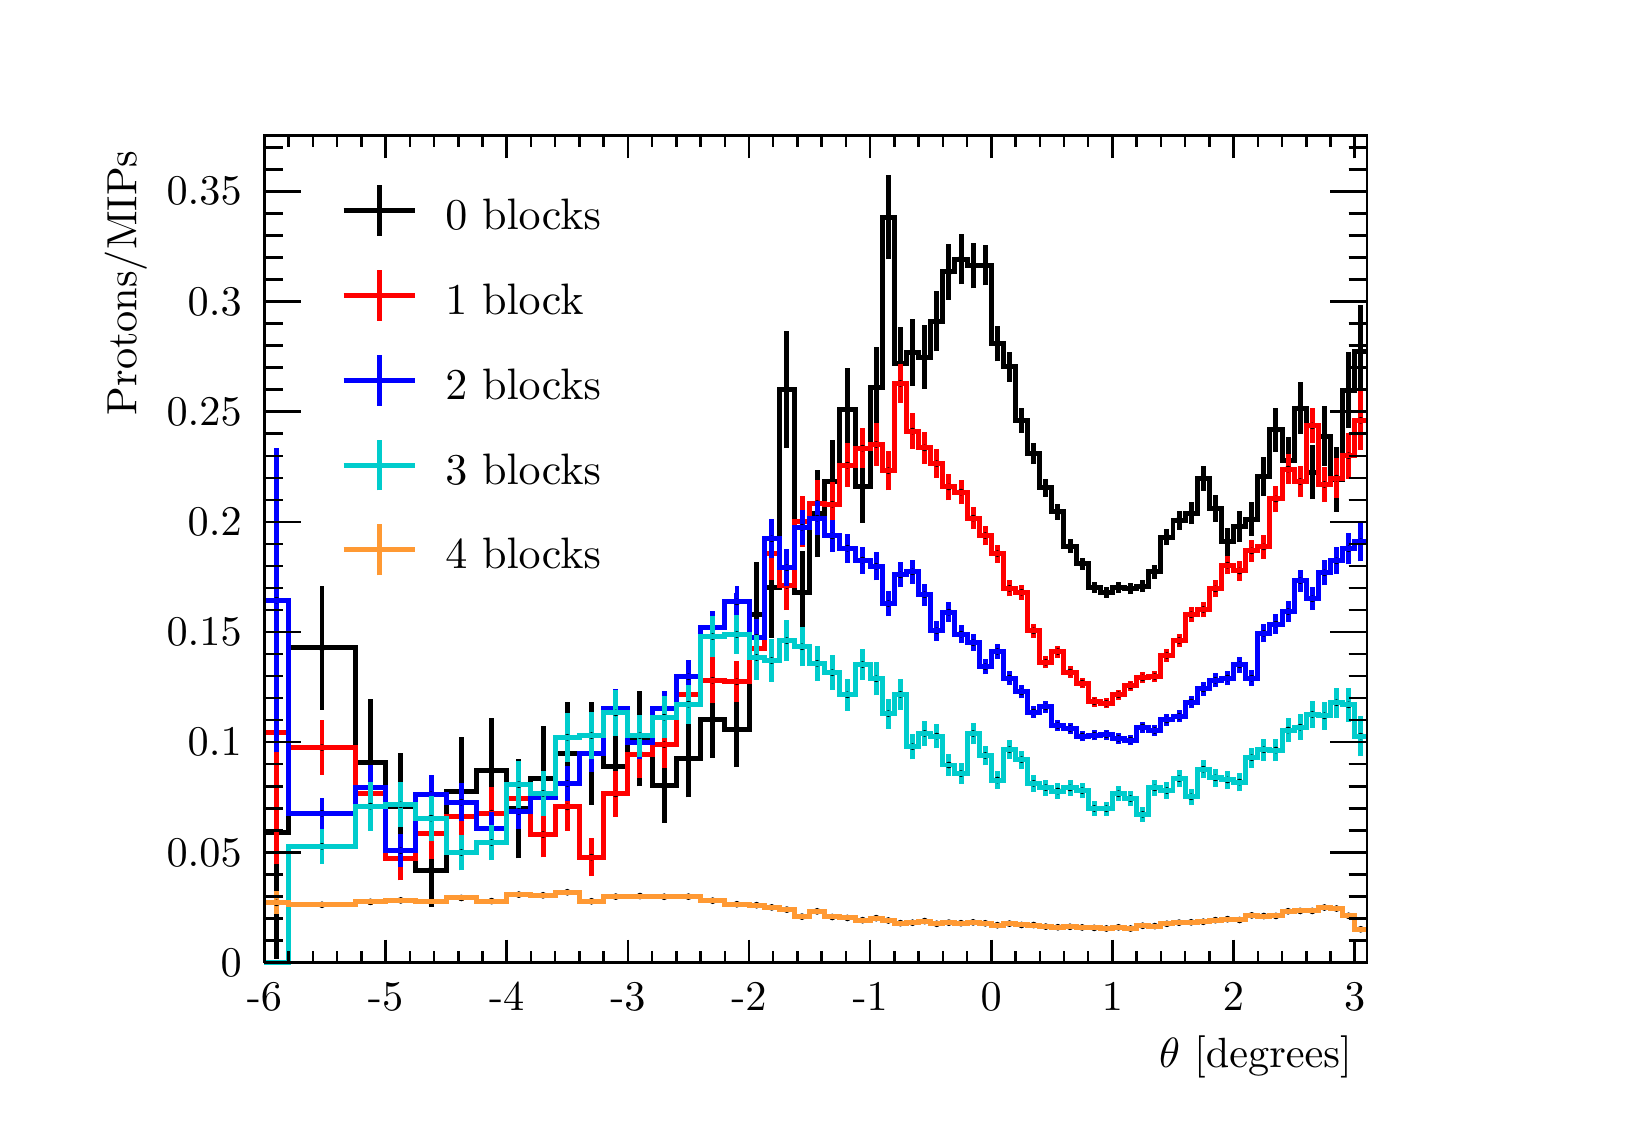
\begin{tikzpicture}
\pgfdeclareplotmark{cross} {
\pgfpathmoveto{\pgfpoint{-0.3\pgfplotmarksize}{\pgfplotmarksize}}
\pgfpathlineto{\pgfpoint{+0.3\pgfplotmarksize}{\pgfplotmarksize}}
\pgfpathlineto{\pgfpoint{+0.3\pgfplotmarksize}{0.3\pgfplotmarksize}}
\pgfpathlineto{\pgfpoint{+1\pgfplotmarksize}{0.3\pgfplotmarksize}}
\pgfpathlineto{\pgfpoint{+1\pgfplotmarksize}{-0.3\pgfplotmarksize}}
\pgfpathlineto{\pgfpoint{+0.3\pgfplotmarksize}{-0.3\pgfplotmarksize}}
\pgfpathlineto{\pgfpoint{+0.3\pgfplotmarksize}{-1.\pgfplotmarksize}}
\pgfpathlineto{\pgfpoint{-0.3\pgfplotmarksize}{-1.\pgfplotmarksize}}
\pgfpathlineto{\pgfpoint{-0.3\pgfplotmarksize}{-0.3\pgfplotmarksize}}
\pgfpathlineto{\pgfpoint{-1.\pgfplotmarksize}{-0.3\pgfplotmarksize}}
\pgfpathlineto{\pgfpoint{-1.\pgfplotmarksize}{0.3\pgfplotmarksize}}
\pgfpathlineto{\pgfpoint{-0.3\pgfplotmarksize}{0.3\pgfplotmarksize}}
\pgfpathclose
\pgfusepathqstroke
}
\pgfdeclareplotmark{cross*} {
\pgfpathmoveto{\pgfpoint{-0.3\pgfplotmarksize}{\pgfplotmarksize}}
\pgfpathlineto{\pgfpoint{+0.3\pgfplotmarksize}{\pgfplotmarksize}}
\pgfpathlineto{\pgfpoint{+0.3\pgfplotmarksize}{0.3\pgfplotmarksize}}
\pgfpathlineto{\pgfpoint{+1\pgfplotmarksize}{0.3\pgfplotmarksize}}
\pgfpathlineto{\pgfpoint{+1\pgfplotmarksize}{-0.3\pgfplotmarksize}}
\pgfpathlineto{\pgfpoint{+0.3\pgfplotmarksize}{-0.3\pgfplotmarksize}}
\pgfpathlineto{\pgfpoint{+0.3\pgfplotmarksize}{-1.\pgfplotmarksize}}
\pgfpathlineto{\pgfpoint{-0.3\pgfplotmarksize}{-1.\pgfplotmarksize}}
\pgfpathlineto{\pgfpoint{-0.3\pgfplotmarksize}{-0.3\pgfplotmarksize}}
\pgfpathlineto{\pgfpoint{-1.\pgfplotmarksize}{-0.3\pgfplotmarksize}}
\pgfpathlineto{\pgfpoint{-1.\pgfplotmarksize}{0.3\pgfplotmarksize}}
\pgfpathlineto{\pgfpoint{-0.3\pgfplotmarksize}{0.3\pgfplotmarksize}}
\pgfpathclose
\pgfusepathqfillstroke
}
\pgfdeclareplotmark{newstar} {
\pgfpathmoveto{\pgfqpoint{0pt}{\pgfplotmarksize}}
\pgfpathlineto{\pgfqpointpolar{44}{0.5\pgfplotmarksize}}
\pgfpathlineto{\pgfqpointpolar{18}{\pgfplotmarksize}}
\pgfpathlineto{\pgfqpointpolar{-20}{0.5\pgfplotmarksize}}
\pgfpathlineto{\pgfqpointpolar{-54}{\pgfplotmarksize}}
\pgfpathlineto{\pgfqpointpolar{-90}{0.5\pgfplotmarksize}}
\pgfpathlineto{\pgfqpointpolar{234}{\pgfplotmarksize}}
\pgfpathlineto{\pgfqpointpolar{198}{0.5\pgfplotmarksize}}
\pgfpathlineto{\pgfqpointpolar{162}{\pgfplotmarksize}}
\pgfpathlineto{\pgfqpointpolar{134}{0.5\pgfplotmarksize}}
\pgfpathclose
\pgfusepathqstroke
}
\pgfdeclareplotmark{newstar*} {
\pgfpathmoveto{\pgfqpoint{0pt}{\pgfplotmarksize}}
\pgfpathlineto{\pgfqpointpolar{44}{0.5\pgfplotmarksize}}
\pgfpathlineto{\pgfqpointpolar{18}{\pgfplotmarksize}}
\pgfpathlineto{\pgfqpointpolar{-20}{0.5\pgfplotmarksize}}
\pgfpathlineto{\pgfqpointpolar{-54}{\pgfplotmarksize}}
\pgfpathlineto{\pgfqpointpolar{-90}{0.5\pgfplotmarksize}}
\pgfpathlineto{\pgfqpointpolar{234}{\pgfplotmarksize}}
\pgfpathlineto{\pgfqpointpolar{198}{0.5\pgfplotmarksize}}
\pgfpathlineto{\pgfqpointpolar{162}{\pgfplotmarksize}}
\pgfpathlineto{\pgfqpointpolar{134}{0.5\pgfplotmarksize}}
\pgfpathclose
\pgfusepathqfillstroke
}
\definecolor{c}{rgb}{1,1,1};
\draw [color=c, fill=c] (0,0) rectangle (20,13.639);
\draw [color=c, fill=c] (3,1.77307) rectangle (17,12.2751);
\definecolor{c}{rgb}{0,0,0};
\draw [c,line width=0.9] (3,1.77307) -- (3,12.2751) -- (17,12.2751) -- (17,1.77307) -- (3,1.77307);
\definecolor{c}{rgb}{1,1,1};
\draw [color=c, fill=c] (3,1.77307) rectangle (17,12.2751);
\definecolor{c}{rgb}{0,0,0};
\draw [c,line width=0.9] (3,1.77307) -- (3,12.2751) -- (17,12.2751) -- (17,1.77307) -- (3,1.77307);
\draw [c,line width=0.9] (3,1.77307) -- (3.30769,1.77307) -- (3.30769,1.77307) -- (4.15385,1.77307) -- (4.15385,1.77307) -- (4.53846,1.77307) -- (4.53846,1.77307) -- (4.92308,1.77307) -- (4.92308,1.77307) -- (5.30769,1.77307) -- (5.30769,1.77307) --
 (5.69231,1.77307) -- (5.69231,1.77307) -- (6.07692,1.77307) -- (6.07692,1.77307) -- (6.38462,1.77307) -- (6.38462,1.77307) -- (6.69231,1.77307) -- (6.69231,1.77307) -- (7,1.77307) -- (7,1.77307) -- (7.30769,1.77307) -- (7.30769,1.77307) --
 (7.61538,1.77307) -- (7.61538,1.77307) -- (7.92308,1.77307) -- (7.92308,1.77307) -- (8.23077,1.77307) -- (8.23077,1.77307) -- (8.53846,1.77307) -- (8.53846,1.77307) -- (8.84615,1.77307) -- (8.84615,1.77307) -- (9.15385,1.77307) -- (9.15385,1.77307)
 -- (9.34615,1.77307) -- (9.34615,1.77307) -- (9.53846,1.77307) -- (9.53846,1.77307) -- (9.73077,1.77307) -- (9.73077,1.77307) -- (9.92308,1.77307) -- (9.92308,1.77307) -- (10.1154,1.77307) -- (10.1154,1.77307) -- (10.3077,1.77307) --
 (10.3077,1.77307) -- (10.5,1.77307) -- (10.5,1.77307) -- (10.6923,1.77307) -- (10.6923,1.77307) -- (10.8462,1.77307) -- (10.8462,1.77307) -- (11,1.77307) -- (11,1.77307) -- (11.1538,1.77307) -- (11.1538,1.77307) -- (11.3077,1.77307) --
 (11.3077,1.77307) -- (11.4615,1.77307) -- (11.4615,1.77307) -- (11.6154,1.77307) -- (11.6154,1.77307) -- (11.7692,1.77307) -- (11.7692,1.77307) -- (11.9231,1.77307) -- (11.9231,1.77307) -- (12.0769,1.77307) -- (12.0769,1.77307) -- (12.2308,1.77307)
 -- (12.2308,1.77307) -- (12.3846,1.77307) -- (12.3846,1.77307) -- (12.5385,1.77307) -- (12.5385,1.77307) -- (12.6923,1.77307) -- (12.6923,1.77307) -- (12.8462,1.77307) -- (12.8462,1.77307) -- (13,1.77307) -- (13,1.77307) -- (13.1538,1.77307) --
 (13.1538,1.77307) -- (13.3077,1.77307) -- (13.3077,1.77307) -- (13.4615,1.77307) -- (13.4615,1.77307) -- (13.6154,1.77307) -- (13.6154,1.77307) -- (13.7692,1.77307) -- (13.7692,1.77307) -- (13.9231,1.77307) -- (13.9231,1.77307) -- (14.0769,1.77307)
 -- (14.0769,1.77307) -- (14.2308,1.77307) -- (14.2308,1.77307) -- (14.3846,1.77307) -- (14.3846,1.77307) -- (14.5385,1.77307) -- (14.5385,1.77307) -- (14.6923,1.77307) -- (14.6923,1.77307) -- (14.8462,1.77307) -- (14.8462,1.77307) -- (15,1.77307) --
 (15,1.77307) -- (15.1538,1.77307) -- (15.1538,1.77307) -- (15.3077,1.77307) -- (15.3077,1.77307) -- (15.4615,1.77307) -- (15.4615,1.77307) -- (15.6154,1.77307) -- (15.6154,1.77307) -- (15.7692,1.77307) -- (15.7692,1.77307) -- (15.9231,1.77307) --
 (15.9231,1.77307) -- (16.0769,1.77307) -- (16.0769,1.77307) -- (16.2308,1.77307) -- (16.2308,1.77307) -- (16.3846,1.77307) -- (16.3846,1.77307) -- (16.5385,1.77307) -- (16.5385,1.77307) -- (16.6923,1.77307) -- (16.6923,1.77307) -- (16.8462,1.77307)
 -- (16.8462,1.77307) -- (17,1.77307);
\draw [c,line width=0.9] (3,1.77307) -- (17,1.77307);
\draw [c,line width=0.9] (3,2.05948) -- (3,1.77307);
\draw [c,line width=0.9] (3.30769,1.91628) -- (3.30769,1.77307);
\draw [c,line width=0.9] (3.61538,1.91628) -- (3.61538,1.77307);
\draw [c,line width=0.9] (3.92308,1.91628) -- (3.92308,1.77307);
\draw [c,line width=0.9] (4.23077,1.91628) -- (4.23077,1.77307);
\draw [c,line width=0.9] (4.53846,2.05948) -- (4.53846,1.77307);
\draw [c,line width=0.9] (4.84615,1.91628) -- (4.84615,1.77307);
\draw [c,line width=0.9] (5.15385,1.91628) -- (5.15385,1.77307);
\draw [c,line width=0.9] (5.46154,1.91628) -- (5.46154,1.77307);
\draw [c,line width=0.9] (5.76923,1.91628) -- (5.76923,1.77307);
\draw [c,line width=0.9] (6.07692,2.05948) -- (6.07692,1.77307);
\draw [c,line width=0.9] (6.38462,1.91628) -- (6.38462,1.77307);
\draw [c,line width=0.9] (6.69231,1.91628) -- (6.69231,1.77307);
\draw [c,line width=0.9] (7,1.91628) -- (7,1.77307);
\draw [c,line width=0.9] (7.30769,1.91628) -- (7.30769,1.77307);
\draw [c,line width=0.9] (7.61538,2.05948) -- (7.61538,1.77307);
\draw [c,line width=0.9] (7.92308,1.91628) -- (7.92308,1.77307);
\draw [c,line width=0.9] (8.23077,1.91628) -- (8.23077,1.77307);
\draw [c,line width=0.9] (8.53846,1.91628) -- (8.53846,1.77307);
\draw [c,line width=0.9] (8.84615,1.91628) -- (8.84615,1.77307);
\draw [c,line width=0.9] (9.15385,2.05948) -- (9.15385,1.77307);
\draw [c,line width=0.9] (9.46154,1.91628) -- (9.46154,1.77307);
\draw [c,line width=0.9] (9.76923,1.91628) -- (9.76923,1.77307);
\draw [c,line width=0.9] (10.0769,1.91628) -- (10.0769,1.77307);
\draw [c,line width=0.9] (10.3846,1.91628) -- (10.3846,1.77307);
\draw [c,line width=0.9] (10.6923,2.05948) -- (10.6923,1.77307);
\draw [c,line width=0.9] (11,1.91628) -- (11,1.77307);
\draw [c,line width=0.9] (11.3077,1.91628) -- (11.3077,1.77307);
\draw [c,line width=0.9] (11.6154,1.91628) -- (11.6154,1.77307);
\draw [c,line width=0.9] (11.9231,1.91628) -- (11.9231,1.77307);
\draw [c,line width=0.9] (12.2308,2.05948) -- (12.2308,1.77307);
\draw [c,line width=0.9] (12.5385,1.91628) -- (12.5385,1.77307);
\draw [c,line width=0.9] (12.8462,1.91628) -- (12.8462,1.77307);
\draw [c,line width=0.9] (13.1538,1.91628) -- (13.1538,1.77307);
\draw [c,line width=0.9] (13.4615,1.91628) -- (13.4615,1.77307);
\draw [c,line width=0.9] (13.7692,2.05948) -- (13.7692,1.77307);
\draw [c,line width=0.9] (14.0769,1.91628) -- (14.0769,1.77307);
\draw [c,line width=0.9] (14.3846,1.91628) -- (14.3846,1.77307);
\draw [c,line width=0.9] (14.6923,1.91628) -- (14.6923,1.77307);
\draw [c,line width=0.9] (15,1.91628) -- (15,1.77307);
\draw [c,line width=0.9] (15.3077,2.05948) -- (15.3077,1.77307);
\draw [c,line width=0.9] (15.6154,1.91628) -- (15.6154,1.77307);
\draw [c,line width=0.9] (15.9231,1.91628) -- (15.9231,1.77307);
\draw [c,line width=0.9] (16.2308,1.91628) -- (16.2308,1.77307);
\draw [c,line width=0.9] (16.5385,1.91628) -- (16.5385,1.77307);
\draw [c,line width=0.9] (16.8462,2.05948) -- (16.8462,1.77307);
\draw [c,line width=0.9] (16.8462,2.05948) -- (16.8462,1.77307);
\draw [anchor=base] (3,1.15931) node[scale=1.52731, color=c, rotate=0]{-6};
\draw [anchor=base] (4.53846,1.15931) node[scale=1.52731, color=c, rotate=0]{-5};
\draw [anchor=base] (6.07692,1.15931) node[scale=1.52731, color=c, rotate=0]{-4};
\draw [anchor=base] (7.61538,1.15931) node[scale=1.52731, color=c, rotate=0]{-3};
\draw [anchor=base] (9.15385,1.15931) node[scale=1.52731, color=c, rotate=0]{-2};
\draw [anchor=base] (10.6923,1.15931) node[scale=1.52731, color=c, rotate=0]{-1};
\draw [anchor=base] (12.2308,1.15931) node[scale=1.52731, color=c, rotate=0]{0};
\draw [anchor=base] (13.7692,1.15931) node[scale=1.52731, color=c, rotate=0]{1};
\draw [anchor=base] (15.3077,1.15931) node[scale=1.52731, color=c, rotate=0]{2};
\draw [anchor=base] (16.8462,1.15931) node[scale=1.52731, color=c, rotate=0]{3};
\draw [anchor= east] (17,0.572837) node[scale=1.52731, color=c, rotate=0]{$\theta$ [degrees]};
\draw [c,line width=0.9] (3,12.2751) -- (17,12.2751);
\draw [c,line width=0.9] (3,11.9887) -- (3,12.2751);
\draw [c,line width=0.9] (3.30769,12.1319) -- (3.30769,12.2751);
\draw [c,line width=0.9] (3.61538,12.1319) -- (3.61538,12.2751);
\draw [c,line width=0.9] (3.92308,12.1319) -- (3.92308,12.2751);
\draw [c,line width=0.9] (4.23077,12.1319) -- (4.23077,12.2751);
\draw [c,line width=0.9] (4.53846,11.9887) -- (4.53846,12.2751);
\draw [c,line width=0.9] (4.84615,12.1319) -- (4.84615,12.2751);
\draw [c,line width=0.9] (5.15385,12.1319) -- (5.15385,12.2751);
\draw [c,line width=0.9] (5.46154,12.1319) -- (5.46154,12.2751);
\draw [c,line width=0.9] (5.76923,12.1319) -- (5.76923,12.2751);
\draw [c,line width=0.9] (6.07692,11.9887) -- (6.07692,12.2751);
\draw [c,line width=0.9] (6.38462,12.1319) -- (6.38462,12.2751);
\draw [c,line width=0.9] (6.69231,12.1319) -- (6.69231,12.2751);
\draw [c,line width=0.9] (7,12.1319) -- (7,12.2751);
\draw [c,line width=0.9] (7.30769,12.1319) -- (7.30769,12.2751);
\draw [c,line width=0.9] (7.61538,11.9887) -- (7.61538,12.2751);
\draw [c,line width=0.9] (7.92308,12.1319) -- (7.92308,12.2751);
\draw [c,line width=0.9] (8.23077,12.1319) -- (8.23077,12.2751);
\draw [c,line width=0.9] (8.53846,12.1319) -- (8.53846,12.2751);
\draw [c,line width=0.9] (8.84615,12.1319) -- (8.84615,12.2751);
\draw [c,line width=0.9] (9.15385,11.9887) -- (9.15385,12.2751);
\draw [c,line width=0.9] (9.46154,12.1319) -- (9.46154,12.2751);
\draw [c,line width=0.9] (9.76923,12.1319) -- (9.76923,12.2751);
\draw [c,line width=0.9] (10.0769,12.1319) -- (10.0769,12.2751);
\draw [c,line width=0.9] (10.3846,12.1319) -- (10.3846,12.2751);
\draw [c,line width=0.9] (10.6923,11.9887) -- (10.6923,12.2751);
\draw [c,line width=0.9] (11,12.1319) -- (11,12.2751);
\draw [c,line width=0.9] (11.3077,12.1319) -- (11.3077,12.2751);
\draw [c,line width=0.9] (11.6154,12.1319) -- (11.6154,12.2751);
\draw [c,line width=0.9] (11.9231,12.1319) -- (11.9231,12.2751);
\draw [c,line width=0.9] (12.2308,11.9887) -- (12.2308,12.2751);
\draw [c,line width=0.9] (12.5385,12.1319) -- (12.5385,12.2751);
\draw [c,line width=0.9] (12.8462,12.1319) -- (12.8462,12.2751);
\draw [c,line width=0.9] (13.1538,12.1319) -- (13.1538,12.2751);
\draw [c,line width=0.9] (13.4615,12.1319) -- (13.4615,12.2751);
\draw [c,line width=0.9] (13.7692,11.9887) -- (13.7692,12.2751);
\draw [c,line width=0.9] (14.0769,12.1319) -- (14.0769,12.2751);
\draw [c,line width=0.9] (14.3846,12.1319) -- (14.3846,12.2751);
\draw [c,line width=0.9] (14.6923,12.1319) -- (14.6923,12.2751);
\draw [c,line width=0.9] (15,12.1319) -- (15,12.2751);
\draw [c,line width=0.9] (15.3077,11.9887) -- (15.3077,12.2751);
\draw [c,line width=0.9] (15.6154,12.1319) -- (15.6154,12.2751);
\draw [c,line width=0.9] (15.9231,12.1319) -- (15.9231,12.2751);
\draw [c,line width=0.9] (16.2308,12.1319) -- (16.2308,12.2751);
\draw [c,line width=0.9] (16.5385,12.1319) -- (16.5385,12.2751);
\draw [c,line width=0.9] (16.8462,11.9887) -- (16.8462,12.2751);
\draw [c,line width=0.9] (16.8462,11.9887) -- (16.8462,12.2751);
\draw [c,line width=0.9] (3,1.77307) -- (3,12.2751);
\draw [c,line width=0.9] (3.462,1.77307) -- (3,1.77307);
\draw [c,line width=0.9] (3.231,2.05289) -- (3,2.05289);
\draw [c,line width=0.9] (3.231,2.33272) -- (3,2.33272);
\draw [c,line width=0.9] (3.231,2.61255) -- (3,2.61255);
\draw [c,line width=0.9] (3.231,2.89237) -- (3,2.89237);
\draw [c,line width=0.9] (3.462,3.1722) -- (3,3.1722);
\draw [c,line width=0.9] (3.231,3.45203) -- (3,3.45203);
\draw [c,line width=0.9] (3.231,3.73185) -- (3,3.73185);
\draw [c,line width=0.9] (3.231,4.01168) -- (3,4.01168);
\draw [c,line width=0.9] (3.231,4.29151) -- (3,4.29151);
\draw [c,line width=0.9] (3.462,4.57133) -- (3,4.57133);
\draw [c,line width=0.9] (3.231,4.85116) -- (3,4.85116);
\draw [c,line width=0.9] (3.231,5.13099) -- (3,5.13099);
\draw [c,line width=0.9] (3.231,5.41081) -- (3,5.41081);
\draw [c,line width=0.9] (3.231,5.69064) -- (3,5.69064);
\draw [c,line width=0.9] (3.462,5.97047) -- (3,5.97047);
\draw [c,line width=0.9] (3.231,6.25029) -- (3,6.25029);
\draw [c,line width=0.9] (3.231,6.53012) -- (3,6.53012);
\draw [c,line width=0.9] (3.231,6.80995) -- (3,6.80995);
\draw [c,line width=0.9] (3.231,7.08977) -- (3,7.08977);
\draw [c,line width=0.9] (3.462,7.3696) -- (3,7.3696);
\draw [c,line width=0.9] (3.231,7.64943) -- (3,7.64943);
\draw [c,line width=0.9] (3.231,7.92925) -- (3,7.92925);
\draw [c,line width=0.9] (3.231,8.20908) -- (3,8.20908);
\draw [c,line width=0.9] (3.231,8.48891) -- (3,8.48891);
\draw [c,line width=0.9] (3.462,8.76873) -- (3,8.76873);
\draw [c,line width=0.9] (3.231,9.04856) -- (3,9.04856);
\draw [c,line width=0.9] (3.231,9.32839) -- (3,9.32839);
\draw [c,line width=0.9] (3.231,9.60821) -- (3,9.60821);
\draw [c,line width=0.9] (3.231,9.88804) -- (3,9.88804);
\draw [c,line width=0.9] (3.462,10.1679) -- (3,10.1679);
\draw [c,line width=0.9] (3.231,10.4477) -- (3,10.4477);
\draw [c,line width=0.9] (3.231,10.7275) -- (3,10.7275);
\draw [c,line width=0.9] (3.231,11.0073) -- (3,11.0073);
\draw [c,line width=0.9] (3.231,11.2872) -- (3,11.2872);
\draw [c,line width=0.9] (3.462,11.567) -- (3,11.567);
\draw [c,line width=0.9] (3.462,11.567) -- (3,11.567);
\draw [c,line width=0.9] (3.231,11.8468) -- (3,11.8468);
\draw [c,line width=0.9] (3.231,12.1267) -- (3,12.1267);
\draw [anchor= east] (2.9,1.77307) node[scale=1.52731, color=c, rotate=0]{0};
\draw [anchor= east] (2.9,3.1722) node[scale=1.52731, color=c, rotate=0]{0.05};
\draw [anchor= east] (2.9,4.57133) node[scale=1.52731, color=c, rotate=0]{0.1};
\draw [anchor= east] (2.9,5.97047) node[scale=1.52731, color=c, rotate=0]{0.15};
\draw [anchor= east] (2.9,7.3696) node[scale=1.52731, color=c, rotate=0]{0.2};
\draw [anchor= east] (2.9,8.76873) node[scale=1.52731, color=c, rotate=0]{0.25};
\draw [anchor= east] (2.9,10.1679) node[scale=1.52731, color=c, rotate=0]{0.3};
\draw [anchor= east] (2.9,11.567) node[scale=1.52731, color=c, rotate=0]{0.35};
\draw [anchor= east] (1.24,12.2751) node[scale=1.52731, color=c, rotate=90]{  Protons/MIPs};
\draw [c,line width=0.9] (17,1.77307) -- (17,12.2751);
\draw [c,line width=0.9] (16.538,1.77307) -- (17,1.77307);
\draw [c,line width=0.9] (16.769,2.05289) -- (17,2.05289);
\draw [c,line width=0.9] (16.769,2.33272) -- (17,2.33272);
\draw [c,line width=0.9] (16.769,2.61255) -- (17,2.61255);
\draw [c,line width=0.9] (16.769,2.89237) -- (17,2.89237);
\draw [c,line width=0.9] (16.538,3.1722) -- (17,3.1722);
\draw [c,line width=0.9] (16.769,3.45203) -- (17,3.45203);
\draw [c,line width=0.9] (16.769,3.73185) -- (17,3.73185);
\draw [c,line width=0.9] (16.769,4.01168) -- (17,4.01168);
\draw [c,line width=0.9] (16.769,4.29151) -- (17,4.29151);
\draw [c,line width=0.9] (16.538,4.57133) -- (17,4.57133);
\draw [c,line width=0.9] (16.769,4.85116) -- (17,4.85116);
\draw [c,line width=0.9] (16.769,5.13099) -- (17,5.13099);
\draw [c,line width=0.9] (16.769,5.41081) -- (17,5.41081);
\draw [c,line width=0.9] (16.769,5.69064) -- (17,5.69064);
\draw [c,line width=0.9] (16.538,5.97047) -- (17,5.97047);
\draw [c,line width=0.9] (16.769,6.25029) -- (17,6.25029);
\draw [c,line width=0.9] (16.769,6.53012) -- (17,6.53012);
\draw [c,line width=0.9] (16.769,6.80995) -- (17,6.80995);
\draw [c,line width=0.9] (16.769,7.08977) -- (17,7.08977);
\draw [c,line width=0.9] (16.538,7.3696) -- (17,7.3696);
\draw [c,line width=0.9] (16.769,7.64943) -- (17,7.64943);
\draw [c,line width=0.9] (16.769,7.92925) -- (17,7.92925);
\draw [c,line width=0.9] (16.769,8.20908) -- (17,8.20908);
\draw [c,line width=0.9] (16.769,8.48891) -- (17,8.48891);
\draw [c,line width=0.9] (16.538,8.76873) -- (17,8.76873);
\draw [c,line width=0.9] (16.769,9.04856) -- (17,9.04856);
\draw [c,line width=0.9] (16.769,9.32839) -- (17,9.32839);
\draw [c,line width=0.9] (16.769,9.60821) -- (17,9.60821);
\draw [c,line width=0.9] (16.769,9.88804) -- (17,9.88804);
\draw [c,line width=0.9] (16.538,10.1679) -- (17,10.1679);
\draw [c,line width=0.9] (16.769,10.4477) -- (17,10.4477);
\draw [c,line width=0.9] (16.769,10.7275) -- (17,10.7275);
\draw [c,line width=0.9] (16.769,11.0073) -- (17,11.0073);
\draw [c,line width=0.9] (16.769,11.2872) -- (17,11.2872);
\draw [c,line width=0.9] (16.538,11.567) -- (17,11.567);
\draw [c,line width=0.9] (16.538,11.567) -- (17,11.567);
\draw [c,line width=0.9] (16.769,11.8468) -- (17,11.8468);
\draw [c,line width=0.9] (16.769,12.1267) -- (17,12.1267);
\draw [c,line width=1.8] (3.15385,1.82211) -- (3.15385,3.41911);
\draw [c,line width=1.8] (3.15385,3.41911) -- (3.15385,5.0161);
\foreach \P in {(3.15385,3.41911)}{\draw[mark options={color=c,fill=c},mark size=2.402402pt,mark=*,mark size=1pt] plot coordinates {\P};}
\draw [c,line width=1.8] (3.73077,4.98149) -- (3.73077,5.77059);
\draw [c,line width=1.8] (3.73077,5.77059) -- (3.73077,6.55969);
\foreach \P in {(3.73077,5.77059)}{\draw[mark options={color=c,fill=c},mark size=2.402402pt,mark=*,mark size=1pt] plot coordinates {\P};}
\draw [c,line width=1.8] (4.34615,3.5084) -- (4.34615,4.31694);
\draw [c,line width=1.8] (4.34615,4.31694) -- (4.34615,5.12549);
\foreach \P in {(4.34615,4.31694)}{\draw[mark options={color=c,fill=c},mark size=2.402402pt,mark=*,mark size=1pt] plot coordinates {\P};}
\draw [c,line width=1.8] (4.73077,3.07893) -- (4.73077,3.75414);
\draw [c,line width=1.8] (4.73077,3.75414) -- (4.73077,4.42935);
\foreach \P in {(4.73077,3.75414)}{\draw[mark options={color=c,fill=c},mark size=2.402402pt,mark=*,mark size=1pt] plot coordinates {\P};}
\draw [c,line width=1.8] (5.11538,2.47797) -- (5.11538,2.94716);
\draw [c,line width=1.8] (5.11538,2.94716) -- (5.11538,3.41635);
\foreach \P in {(5.11538,2.94716)}{\draw[mark options={color=c,fill=c},mark size=2.402402pt,mark=*,mark size=1pt] plot coordinates {\P};}
\draw [c,line width=1.8] (5.5,3.24904) -- (5.5,3.94413);
\draw [c,line width=1.8] (5.5,3.94413) -- (5.5,4.63923);
\foreach \P in {(5.5,3.94413)}{\draw[mark options={color=c,fill=c},mark size=2.402402pt,mark=*,mark size=1pt] plot coordinates {\P};}
\draw [c,line width=1.8] (5.88462,3.53511) -- (5.88462,4.20634);
\draw [c,line width=1.8] (5.88462,4.20634) -- (5.88462,4.87758);
\foreach \P in {(5.88462,4.20634)}{\draw[mark options={color=c,fill=c},mark size=2.402402pt,mark=*,mark size=1pt] plot coordinates {\P};}
\draw [c,line width=1.8] (6.23077,3.09766) -- (6.23077,3.72534);
\draw [c,line width=1.8] (6.23077,3.72534) -- (6.23077,4.35303);
\foreach \P in {(6.23077,3.72534)}{\draw[mark options={color=c,fill=c},mark size=2.402402pt,mark=*,mark size=1pt] plot coordinates {\P};}
\draw [c,line width=1.8] (6.53846,3.43175) -- (6.53846,4.10495);
\draw [c,line width=1.8] (6.53846,4.10495) -- (6.53846,4.77816);
\foreach \P in {(6.53846,4.10495)}{\draw[mark options={color=c,fill=c},mark size=2.402402pt,mark=*,mark size=1pt] plot coordinates {\P};}
\draw [c,line width=1.8] (6.84615,3.77705) -- (6.84615,4.42965);
\draw [c,line width=1.8] (6.84615,4.42965) -- (6.84615,5.08224);
\foreach \P in {(6.84615,4.42965)}{\draw[mark options={color=c,fill=c},mark size=2.402402pt,mark=*,mark size=1pt] plot coordinates {\P};}
\draw [c,line width=1.8] (7.15385,3.77705) -- (7.15385,4.42965);
\draw [c,line width=1.8] (7.15385,4.42965) -- (7.15385,5.08224);
\foreach \P in {(7.15385,4.42965)}{\draw[mark options={color=c,fill=c},mark size=2.402402pt,mark=*,mark size=1pt] plot coordinates {\P};}
\draw [c,line width=1.8] (7.46154,3.68708) -- (7.46154,4.26367);
\draw [c,line width=1.8] (7.46154,4.26367) -- (7.46154,4.84026);
\foreach \P in {(7.46154,4.26367)}{\draw[mark options={color=c,fill=c},mark size=2.402402pt,mark=*,mark size=1pt] plot coordinates {\P};}
\draw [c,line width=1.8] (7.76923,4.01178) -- (7.76923,4.61395);
\draw [c,line width=1.8] (7.76923,4.61395) -- (7.76923,5.21612);
\foreach \P in {(7.76923,4.61395)}{\draw[mark options={color=c,fill=c},mark size=2.402402pt,mark=*,mark size=1pt] plot coordinates {\P};}
\draw [c,line width=1.8] (8.07692,3.54651) -- (8.07692,4.01595);
\draw [c,line width=1.8] (8.07692,4.01595) -- (8.07692,4.48539);
\foreach \P in {(8.07692,4.01595)}{\draw[mark options={color=c,fill=c},mark size=2.402402pt,mark=*,mark size=1pt] plot coordinates {\P};}
\draw [c,line width=1.8] (8.38461,3.8704) -- (8.38461,4.36405);
\draw [c,line width=1.8] (8.38461,4.36405) -- (8.38461,4.85771);
\foreach \P in {(8.38461,4.36405)}{\draw[mark options={color=c,fill=c},mark size=2.402402pt,mark=*,mark size=1pt] plot coordinates {\P};}
\draw [c,line width=1.8] (8.69231,4.37658) -- (8.69231,4.85449);
\draw [c,line width=1.8] (8.69231,4.85449) -- (8.69231,5.3324);
\foreach \P in {(8.69231,4.85449)}{\draw[mark options={color=c,fill=c},mark size=2.402402pt,mark=*,mark size=1pt] plot coordinates {\P};}
\draw [c,line width=1.8] (9,4.2563) -- (9,4.73696);
\draw [c,line width=1.8] (9,4.73696) -- (9,5.21762);
\foreach \P in {(9,4.73696)}{\draw[mark options={color=c,fill=c},mark size=2.402402pt,mark=*,mark size=1pt] plot coordinates {\P};}
\draw [c,line width=1.8] (9.25,5.53021) -- (9.25,6.19768);
\draw [c,line width=1.8] (9.25,6.19768) -- (9.25,6.86514);
\foreach \P in {(9.25,6.19768)}{\draw[mark options={color=c,fill=c},mark size=2.402402pt,mark=*,mark size=1pt] plot coordinates {\P};}
\draw [c,line width=1.8] (9.44231,5.9002) -- (9.44231,6.54048);
\draw [c,line width=1.8] (9.44231,6.54048) -- (9.44231,7.18077);
\foreach \P in {(9.44231,6.54048)}{\draw[mark options={color=c,fill=c},mark size=2.402402pt,mark=*,mark size=1pt] plot coordinates {\P};}
\draw [c,line width=1.8] (9.63461,8.30763) -- (9.63461,9.05061);
\draw [c,line width=1.8] (9.63461,9.05061) -- (9.63461,9.79359);
\foreach \P in {(9.63461,9.05061)}{\draw[mark options={color=c,fill=c},mark size=2.402402pt,mark=*,mark size=1pt] plot coordinates {\P};}
\draw [c,line width=1.8] (9.82692,5.94121) -- (9.82692,6.473);
\draw [c,line width=1.8] (9.82692,6.473) -- (9.82692,7.00478);
\foreach \P in {(9.82692,6.473)}{\draw[mark options={color=c,fill=c},mark size=2.402402pt,mark=*,mark size=1pt] plot coordinates {\P};}
\draw [c,line width=1.8] (10.0192,6.92282) -- (10.0192,7.47827);
\draw [c,line width=1.8] (10.0192,7.47827) -- (10.0192,8.03372);
\foreach \P in {(10.0192,7.47827)}{\draw[mark options={color=c,fill=c},mark size=2.402402pt,mark=*,mark size=1pt] plot coordinates {\P};}
\draw [c,line width=1.8] (10.2115,7.34742) -- (10.2115,7.87945);
\draw [c,line width=1.8] (10.2115,7.87945) -- (10.2115,8.41148);
\foreach \P in {(10.2115,7.87945)}{\draw[mark options={color=c,fill=c},mark size=2.402402pt,mark=*,mark size=1pt] plot coordinates {\P};}
\draw [c,line width=1.8] (10.4038,8.26812) -- (10.4038,8.79513);
\draw [c,line width=1.8] (10.4038,8.79513) -- (10.4038,9.32215);
\foreach \P in {(10.4038,8.79513)}{\draw[mark options={color=c,fill=c},mark size=2.402402pt,mark=*,mark size=1pt] plot coordinates {\P};}
\draw [c,line width=1.8] (10.5962,7.35913) -- (10.5962,7.8128);
\draw [c,line width=1.8] (10.5962,7.8128) -- (10.5962,8.26647);
\foreach \P in {(10.5962,7.8128)}{\draw[mark options={color=c,fill=c},mark size=2.402402pt,mark=*,mark size=1pt] plot coordinates {\P};}
\draw [c,line width=1.8] (10.7692,8.57136) -- (10.7692,9.07912);
\draw [c,line width=1.8] (10.7692,9.07912) -- (10.7692,9.58688);
\foreach \P in {(10.7692,9.07912)}{\draw[mark options={color=c,fill=c},mark size=2.402402pt,mark=*,mark size=1pt] plot coordinates {\P};}
\draw [c,line width=1.8] (10.9231,10.702) -- (10.9231,11.2385);
\draw [c,line width=1.8] (10.9231,11.2385) -- (10.9231,11.775);
\foreach \P in {(10.9231,11.2385)}{\draw[mark options={color=c,fill=c},mark size=2.402402pt,mark=*,mark size=1pt] plot coordinates {\P};}
\draw [c,line width=1.8] (11.0769,8.92018) -- (11.0769,9.38038);
\draw [c,line width=1.8] (11.0769,9.38038) -- (11.0769,9.84057);
\foreach \P in {(11.0769,9.38038)}{\draw[mark options={color=c,fill=c},mark size=2.402402pt,mark=*,mark size=1pt] plot coordinates {\P};}
\draw [c,line width=1.8] (11.2308,9.09999) -- (11.2308,9.52459);
\draw [c,line width=1.8] (11.2308,9.52459) -- (11.2308,9.94918);
\foreach \P in {(11.2308,9.52459)}{\draw[mark options={color=c,fill=c},mark size=2.402402pt,mark=*,mark size=1pt] plot coordinates {\P};}
\draw [c,line width=1.8] (11.3846,9.06099) -- (11.3846,9.46252);
\draw [c,line width=1.8] (11.3846,9.46252) -- (11.3846,9.86404);
\foreach \P in {(11.3846,9.46252)}{\draw[mark options={color=c,fill=c},mark size=2.402402pt,mark=*,mark size=1pt] plot coordinates {\P};}
\draw [c,line width=1.8] (11.5385,9.53396) -- (11.5385,9.91671);
\draw [c,line width=1.8] (11.5385,9.91671) -- (11.5385,10.2995);
\foreach \P in {(11.5385,9.91671)}{\draw[mark options={color=c,fill=c},mark size=2.402402pt,mark=*,mark size=1pt] plot coordinates {\P};}
\draw [c,line width=1.8] (11.6923,10.1909) -- (11.6923,10.5434);
\draw [c,line width=1.8] (11.6923,10.5434) -- (11.6923,10.896);
\foreach \P in {(11.6923,10.5434)}{\draw[mark options={color=c,fill=c},mark size=2.402402pt,mark=*,mark size=1pt] plot coordinates {\P};}
\draw [c,line width=1.8] (11.8462,10.3843) -- (11.8462,10.707);
\draw [c,line width=1.8] (11.8462,10.707) -- (11.8462,11.0296);
\foreach \P in {(11.8462,10.707)}{\draw[mark options={color=c,fill=c},mark size=2.402402pt,mark=*,mark size=1pt] plot coordinates {\P};}
\draw [c,line width=1.8] (12,10.3355) -- (12,10.625);
\draw [c,line width=1.8] (12,10.625) -- (12,10.9146);
\foreach \P in {(12,10.625)}{\draw[mark options={color=c,fill=c},mark size=2.402402pt,mark=*,mark size=1pt] plot coordinates {\P};}
\draw [c,line width=1.8] (12.1538,10.3727) -- (12.1538,10.6278);
\draw [c,line width=1.8] (12.1538,10.6278) -- (12.1538,10.8828);
\foreach \P in {(12.1538,10.6278)}{\draw[mark options={color=c,fill=c},mark size=2.402402pt,mark=*,mark size=1pt] plot coordinates {\P};}
\draw [c,line width=1.8] (12.3077,9.40941) -- (12.3077,9.63297);
\draw [c,line width=1.8] (12.3077,9.63297) -- (12.3077,9.85653);
\foreach \P in {(12.3077,9.63297)}{\draw[mark options={color=c,fill=c},mark size=2.402402pt,mark=*,mark size=1pt] plot coordinates {\P};}
\draw [c,line width=1.8] (12.4615,9.14774) -- (12.4615,9.34012);
\draw [c,line width=1.8] (12.4615,9.34012) -- (12.4615,9.53249);
\foreach \P in {(12.4615,9.34012)}{\draw[mark options={color=c,fill=c},mark size=2.402402pt,mark=*,mark size=1pt] plot coordinates {\P};}
\draw [c,line width=1.8] (12.6154,8.50404) -- (12.6154,8.66245);
\draw [c,line width=1.8] (12.6154,8.66245) -- (12.6154,8.82085);
\foreach \P in {(12.6154,8.66245)}{\draw[mark options={color=c,fill=c},mark size=2.402402pt,mark=*,mark size=1pt] plot coordinates {\P};}
\draw [c,line width=1.8] (12.7692,8.10435) -- (12.7692,8.2387);
\draw [c,line width=1.8] (12.7692,8.2387) -- (12.7692,8.37306);
\foreach \P in {(12.7692,8.2387)}{\draw[mark options={color=c,fill=c},mark size=2.402402pt,mark=*,mark size=1pt] plot coordinates {\P};}
\draw [c,line width=1.8] (12.9231,7.68928) -- (12.9231,7.80332);
\draw [c,line width=1.8] (12.9231,7.80332) -- (12.9231,7.91735);
\foreach \P in {(12.9231,7.80332)}{\draw[mark options={color=c,fill=c},mark size=2.402402pt,mark=*,mark size=1pt] plot coordinates {\P};}
\draw [c,line width=1.8] (13.0769,7.39569) -- (13.0769,7.49512);
\draw [c,line width=1.8] (13.0769,7.49512) -- (13.0769,7.59454);
\foreach \P in {(13.0769,7.49512)}{\draw[mark options={color=c,fill=c},mark size=2.402402pt,mark=*,mark size=1pt] plot coordinates {\P};}
\draw [c,line width=1.8] (13.2308,6.97329) -- (13.2308,7.06043);
\draw [c,line width=1.8] (13.2308,7.06043) -- (13.2308,7.14758);
\foreach \P in {(13.2308,7.06043)}{\draw[mark options={color=c,fill=c},mark size=2.402402pt,mark=*,mark size=1pt] plot coordinates {\P};}
\draw [c,line width=1.8] (13.3846,6.7589) -- (13.3846,6.83628);
\draw [c,line width=1.8] (13.3846,6.83628) -- (13.3846,6.91366);
\foreach \P in {(13.3846,6.83628)}{\draw[mark options={color=c,fill=c},mark size=2.402402pt,mark=*,mark size=1pt] plot coordinates {\P};}
\draw [c,line width=1.8] (13.5385,6.46938) -- (13.5385,6.53954);
\draw [c,line width=1.8] (13.5385,6.53954) -- (13.5385,6.60971);
\foreach \P in {(13.5385,6.53954)}{\draw[mark options={color=c,fill=c},mark size=2.402402pt,mark=*,mark size=1pt] plot coordinates {\P};}
\draw [c,line width=1.8] (13.6923,6.40391) -- (13.6923,6.47146);
\draw [c,line width=1.8] (13.6923,6.47146) -- (13.6923,6.539);
\foreach \P in {(13.6923,6.47146)}{\draw[mark options={color=c,fill=c},mark size=2.402402pt,mark=*,mark size=1pt] plot coordinates {\P};}
\draw [c,line width=1.8] (13.8462,6.47055) -- (13.8462,6.53894);
\draw [c,line width=1.8] (13.8462,6.53894) -- (13.8462,6.60733);
\foreach \P in {(13.8462,6.53894)}{\draw[mark options={color=c,fill=c},mark size=2.402402pt,mark=*,mark size=1pt] plot coordinates {\P};}
\draw [c,line width=1.8] (14,6.45026) -- (14,6.52192);
\draw [c,line width=1.8] (14,6.52192) -- (14,6.59357);
\foreach \P in {(14,6.52192)}{\draw[mark options={color=c,fill=c},mark size=2.402402pt,mark=*,mark size=1pt] plot coordinates {\P};}
\draw [c,line width=1.8] (14.1538,6.47551) -- (14.1538,6.55327);
\draw [c,line width=1.8] (14.1538,6.55327) -- (14.1538,6.63103);
\foreach \P in {(14.1538,6.55327)}{\draw[mark options={color=c,fill=c},mark size=2.402402pt,mark=*,mark size=1pt] plot coordinates {\P};}
\draw [c,line width=1.8] (14.3077,6.64793) -- (14.3077,6.73649);
\draw [c,line width=1.8] (14.3077,6.73649) -- (14.3077,6.82506);
\foreach \P in {(14.3077,6.73649)}{\draw[mark options={color=c,fill=c},mark size=2.402402pt,mark=*,mark size=1pt] plot coordinates {\P};}
\draw [c,line width=1.8] (14.4615,7.07039) -- (14.4615,7.1755);
\draw [c,line width=1.8] (14.4615,7.1755) -- (14.4615,7.28061);
\foreach \P in {(14.4615,7.1755)}{\draw[mark options={color=c,fill=c},mark size=2.402402pt,mark=*,mark size=1pt] plot coordinates {\P};}
\draw [c,line width=1.8] (14.6154,7.27076) -- (14.6154,7.39177);
\draw [c,line width=1.8] (14.6154,7.39177) -- (14.6154,7.51279);
\foreach \P in {(14.6154,7.39177)}{\draw[mark options={color=c,fill=c},mark size=2.402402pt,mark=*,mark size=1pt] plot coordinates {\P};}
\draw [c,line width=1.8] (14.7692,7.34057) -- (14.7692,7.47851);
\draw [c,line width=1.8] (14.7692,7.47851) -- (14.7692,7.61646);
\foreach \P in {(14.7692,7.47851)}{\draw[mark options={color=c,fill=c},mark size=2.402402pt,mark=*,mark size=1pt] plot coordinates {\P};}
\draw [c,line width=1.8] (14.9231,7.76493) -- (14.9231,7.92186);
\draw [c,line width=1.8] (14.9231,7.92186) -- (14.9231,8.07879);
\foreach \P in {(14.9231,7.92186)}{\draw[mark options={color=c,fill=c},mark size=2.402402pt,mark=*,mark size=1pt] plot coordinates {\P};}
\draw [c,line width=1.8] (15.0769,7.36896) -- (15.0769,7.53787);
\draw [c,line width=1.8] (15.0769,7.53787) -- (15.0769,7.70678);
\foreach \P in {(15.0769,7.53787)}{\draw[mark options={color=c,fill=c},mark size=2.402402pt,mark=*,mark size=1pt] plot coordinates {\P};}
\draw [c,line width=1.8] (15.2308,6.94021) -- (15.2308,7.11766);
\draw [c,line width=1.8] (15.2308,7.11766) -- (15.2308,7.29511);
\foreach \P in {(15.2308,7.11766)}{\draw[mark options={color=c,fill=c},mark size=2.402402pt,mark=*,mark size=1pt] plot coordinates {\P};}
\draw [c,line width=1.8] (15.3846,7.11146) -- (15.3846,7.31065);
\draw [c,line width=1.8] (15.3846,7.31065) -- (15.3846,7.50984);
\foreach \P in {(15.3846,7.31065)}{\draw[mark options={color=c,fill=c},mark size=2.402402pt,mark=*,mark size=1pt] plot coordinates {\P};}
\draw [c,line width=1.8] (15.5385,7.18993) -- (15.5385,7.40435);
\draw [c,line width=1.8] (15.5385,7.40435) -- (15.5385,7.61877);
\foreach \P in {(15.5385,7.40435)}{\draw[mark options={color=c,fill=c},mark size=2.402402pt,mark=*,mark size=1pt] plot coordinates {\P};}
\draw [c,line width=1.8] (15.6923,7.69841) -- (15.6923,7.94405);
\draw [c,line width=1.8] (15.6923,7.94405) -- (15.6923,8.18969);
\foreach \P in {(15.6923,7.94405)}{\draw[mark options={color=c,fill=c},mark size=2.402402pt,mark=*,mark size=1pt] plot coordinates {\P};}
\draw [c,line width=1.8] (15.8462,8.2613) -- (15.8462,8.53778);
\draw [c,line width=1.8] (15.8462,8.53778) -- (15.8462,8.81425);
\foreach \P in {(15.8462,8.53778)}{\draw[mark options={color=c,fill=c},mark size=2.402402pt,mark=*,mark size=1pt] plot coordinates {\P};}
\draw [c,line width=1.8] (16,7.85164) -- (16,8.14729);
\draw [c,line width=1.8] (16,8.14729) -- (16,8.44294);
\foreach \P in {(16,8.14729)}{\draw[mark options={color=c,fill=c},mark size=2.402402pt,mark=*,mark size=1pt] plot coordinates {\P};}
\draw [c,line width=1.8] (16.1538,8.48633) -- (16.1538,8.81479);
\draw [c,line width=1.8] (16.1538,8.81479) -- (16.1538,9.14325);
\foreach \P in {(16.1538,8.81479)}{\draw[mark options={color=c,fill=c},mark size=2.402402pt,mark=*,mark size=1pt] plot coordinates {\P};}
\draw [c,line width=1.8] (16.3077,7.65829) -- (16.3077,7.99945);
\draw [c,line width=1.8] (16.3077,7.99945) -- (16.3077,8.34061);
\foreach \P in {(16.3077,7.99945)}{\draw[mark options={color=c,fill=c},mark size=2.402402pt,mark=*,mark size=1pt] plot coordinates {\P};}
\draw [c,line width=1.8] (16.4615,8.08155) -- (16.4615,8.45969);
\draw [c,line width=1.8] (16.4615,8.45969) -- (16.4615,8.83783);
\foreach \P in {(16.4615,8.45969)}{\draw[mark options={color=c,fill=c},mark size=2.402402pt,mark=*,mark size=1pt] plot coordinates {\P};}
\draw [c,line width=1.8] (16.6154,7.49771) -- (16.6154,7.90625);
\draw [c,line width=1.8] (16.6154,7.90625) -- (16.6154,8.31479);
\foreach \P in {(16.6154,7.90625)}{\draw[mark options={color=c,fill=c},mark size=2.402402pt,mark=*,mark size=1pt] plot coordinates {\P};}
\draw [c,line width=1.8] (16.7692,8.55682) -- (16.7692,9.04073);
\draw [c,line width=1.8] (16.7692,9.04073) -- (16.7692,9.52463);
\foreach \P in {(16.7692,9.04073)}{\draw[mark options={color=c,fill=c},mark size=2.402402pt,mark=*,mark size=1pt] plot coordinates {\P};}
\draw [c,line width=1.8] (16.9231,8.93468) -- (16.9231,9.5319);
\draw [c,line width=1.8] (16.9231,9.5319) -- (16.9231,10.1291);
\foreach \P in {(16.9231,9.5319)}{\draw[mark options={color=c,fill=c},mark size=2.402402pt,mark=*,mark size=1pt] plot coordinates {\P};}
\draw [c,line width=1.8] (3,3.41911) -- (3.30769,3.41911) -- (3.30769,5.77059) -- (4.15385,5.77059) -- (4.15385,4.31694) -- (4.53846,4.31694) -- (4.53846,3.75414) -- (4.92308,3.75414) -- (4.92308,2.94716) -- (5.30769,2.94716) -- (5.30769,3.94413) --
 (5.69231,3.94413) -- (5.69231,4.20634) -- (6.07692,4.20634) -- (6.07692,3.72534) -- (6.38462,3.72534) -- (6.38462,4.10495) -- (6.69231,4.10495) -- (6.69231,4.42965) -- (7,4.42965) -- (7,4.42965) -- (7.30769,4.42965) -- (7.30769,4.26367) --
 (7.61538,4.26367) -- (7.61538,4.61395) -- (7.92308,4.61395) -- (7.92308,4.01595) -- (8.23077,4.01595) -- (8.23077,4.36405) -- (8.53846,4.36405) -- (8.53846,4.85449) -- (8.84615,4.85449) -- (8.84615,4.73696) -- (9.15385,4.73696) -- (9.15385,6.19768)
 -- (9.34615,6.19768) -- (9.34615,6.54048) -- (9.53846,6.54048) -- (9.53846,9.05061) -- (9.73077,9.05061) -- (9.73077,6.473) -- (9.92308,6.473) -- (9.92308,7.47827) -- (10.1154,7.47827) -- (10.1154,7.87945) -- (10.3077,7.87945) -- (10.3077,8.79513)
 -- (10.5,8.79513) -- (10.5,7.8128) -- (10.6923,7.8128) -- (10.6923,9.07912) -- (10.8462,9.07912) -- (10.8462,11.2385) -- (11,11.2385) -- (11,9.38038) -- (11.1538,9.38038) -- (11.1538,9.52459) -- (11.3077,9.52459) -- (11.3077,9.46252) --
 (11.4615,9.46252) -- (11.4615,9.91671) -- (11.6154,9.91671) -- (11.6154,10.5434) -- (11.7692,10.5434) -- (11.7692,10.707) -- (11.9231,10.707) -- (11.9231,10.625) -- (12.0769,10.625) -- (12.0769,10.6278) -- (12.2308,10.6278) -- (12.2308,9.63297) --
 (12.3846,9.63297) -- (12.3846,9.34012) -- (12.5385,9.34012) -- (12.5385,8.66245) -- (12.6923,8.66245) -- (12.6923,8.2387) -- (12.8462,8.2387) -- (12.8462,7.80332) -- (13,7.80332) -- (13,7.49512) -- (13.1538,7.49512) -- (13.1538,7.06043) --
 (13.3077,7.06043) -- (13.3077,6.83628) -- (13.4615,6.83628) -- (13.4615,6.53954) -- (13.6154,6.53954) -- (13.6154,6.47146) -- (13.7692,6.47146) -- (13.7692,6.53894) -- (13.9231,6.53894) -- (13.9231,6.52192) -- (14.0769,6.52192) -- (14.0769,6.55327)
 -- (14.2308,6.55327) -- (14.2308,6.73649) -- (14.3846,6.73649) -- (14.3846,7.1755) -- (14.5385,7.1755) -- (14.5385,7.39177) -- (14.6923,7.39177) -- (14.6923,7.47851) -- (14.8462,7.47851) -- (14.8462,7.92186) -- (15,7.92186) -- (15,7.53787) --
 (15.1538,7.53787) -- (15.1538,7.11766) -- (15.3077,7.11766) -- (15.3077,7.31065) -- (15.4615,7.31065) -- (15.4615,7.40435) -- (15.6154,7.40435) -- (15.6154,7.94405) -- (15.7692,7.94405) -- (15.7692,8.53778) -- (15.9231,8.53778) -- (15.9231,8.14729)
 -- (16.0769,8.14729) -- (16.0769,8.81479) -- (16.2308,8.81479) -- (16.2308,7.99945) -- (16.3846,7.99945) -- (16.3846,8.45969) -- (16.5385,8.45969) -- (16.5385,7.90625) -- (16.6923,7.90625) -- (16.6923,9.04073) -- (16.8462,9.04073) --
 (16.8462,9.5319) -- (17,9.5319);
\definecolor{c}{rgb}{1,0,0};
\draw [c,line width=1.8] (3.15385,3.01897) -- (3.15385,4.69533);
\draw [c,line width=1.8] (3.15385,4.69533) -- (3.15385,6.3717);
\definecolor{c}{rgb}{0,0,0};
\foreach \P in {(3.15385,4.69533)}{\draw[mark options={color=c,fill=c},mark size=2.402402pt,mark=*,mark size=1pt] plot coordinates {\P};}
\definecolor{c}{rgb}{1,0,0};
\draw [c,line width=1.8] (3.73077,4.15602) -- (3.73077,4.5033);
\draw [c,line width=1.8] (3.73077,4.5033) -- (3.73077,4.85059);
\definecolor{c}{rgb}{0,0,0};
\foreach \P in {(3.73077,4.5033)}{\draw[mark options={color=c,fill=c},mark size=2.402402pt,mark=*,mark size=1pt] plot coordinates {\P};}
\definecolor{c}{rgb}{1,0,0};
\draw [c,line width=1.8] (4.34615,3.5692) -- (4.34615,3.92217);
\draw [c,line width=1.8] (4.34615,3.92217) -- (4.34615,4.27514);
\definecolor{c}{rgb}{0,0,0};
\foreach \P in {(4.34615,3.92217)}{\draw[mark options={color=c,fill=c},mark size=2.402402pt,mark=*,mark size=1pt] plot coordinates {\P};}
\definecolor{c}{rgb}{1,0,0};
\draw [c,line width=1.8] (4.73077,2.8168) -- (4.73077,3.09583);
\draw [c,line width=1.8] (4.73077,3.09583) -- (4.73077,3.37486);
\definecolor{c}{rgb}{0,0,0};
\foreach \P in {(4.73077,3.09583)}{\draw[mark options={color=c,fill=c},mark size=2.402402pt,mark=*,mark size=1pt] plot coordinates {\P};}
\definecolor{c}{rgb}{1,0,0};
\draw [c,line width=1.8] (5.11538,3.08425) -- (5.11538,3.40645);
\draw [c,line width=1.8] (5.11538,3.40645) -- (5.11538,3.72865);
\definecolor{c}{rgb}{0,0,0};
\foreach \P in {(5.11538,3.40645)}{\draw[mark options={color=c,fill=c},mark size=2.402402pt,mark=*,mark size=1pt] plot coordinates {\P};}
\definecolor{c}{rgb}{1,0,0};
\draw [c,line width=1.8] (5.5,3.3103) -- (5.5,3.63009);
\draw [c,line width=1.8] (5.5,3.63009) -- (5.5,3.94989);
\definecolor{c}{rgb}{0,0,0};
\foreach \P in {(5.5,3.63009)}{\draw[mark options={color=c,fill=c},mark size=2.402402pt,mark=*,mark size=1pt] plot coordinates {\P};}
\definecolor{c}{rgb}{1,0,0};
\draw [c,line width=1.8] (5.88462,3.33666) -- (5.88462,3.67016);
\draw [c,line width=1.8] (5.88462,3.67016) -- (5.88462,4.00365);
\definecolor{c}{rgb}{0,0,0};
\foreach \P in {(5.88462,3.67016)}{\draw[mark options={color=c,fill=c},mark size=2.402402pt,mark=*,mark size=1pt] plot coordinates {\P};}
\definecolor{c}{rgb}{1,0,0};
\draw [c,line width=1.8] (6.23077,3.51982) -- (6.23077,3.85362);
\draw [c,line width=1.8] (6.23077,3.85362) -- (6.23077,4.18741);
\definecolor{c}{rgb}{0,0,0};
\foreach \P in {(6.23077,3.85362)}{\draw[mark options={color=c,fill=c},mark size=2.402402pt,mark=*,mark size=1pt] plot coordinates {\P};}
\definecolor{c}{rgb}{1,0,0};
\draw [c,line width=1.8] (6.53846,3.10745) -- (6.53846,3.39853);
\draw [c,line width=1.8] (6.53846,3.39853) -- (6.53846,3.6896);
\definecolor{c}{rgb}{0,0,0};
\foreach \P in {(6.53846,3.39853)}{\draw[mark options={color=c,fill=c},mark size=2.402402pt,mark=*,mark size=1pt] plot coordinates {\P};}
\definecolor{c}{rgb}{1,0,0};
\draw [c,line width=1.8] (6.84615,3.44809) -- (6.84615,3.74997);
\draw [c,line width=1.8] (6.84615,3.74997) -- (6.84615,4.05185);
\definecolor{c}{rgb}{0,0,0};
\foreach \P in {(6.84615,3.74997)}{\draw[mark options={color=c,fill=c},mark size=2.402402pt,mark=*,mark size=1pt] plot coordinates {\P};}
\definecolor{c}{rgb}{1,0,0};
\draw [c,line width=1.8] (7.15385,2.87181) -- (7.15385,3.11127);
\draw [c,line width=1.8] (7.15385,3.11127) -- (7.15385,3.35074);
\definecolor{c}{rgb}{0,0,0};
\foreach \P in {(7.15385,3.11127)}{\draw[mark options={color=c,fill=c},mark size=2.402402pt,mark=*,mark size=1pt] plot coordinates {\P};}
\definecolor{c}{rgb}{1,0,0};
\draw [c,line width=1.8] (7.46154,3.6239) -- (7.46154,3.91445);
\draw [c,line width=1.8] (7.46154,3.91445) -- (7.46154,4.20501);
\definecolor{c}{rgb}{0,0,0};
\foreach \P in {(7.46154,3.91445)}{\draw[mark options={color=c,fill=c},mark size=2.402402pt,mark=*,mark size=1pt] plot coordinates {\P};}
\definecolor{c}{rgb}{1,0,0};
\draw [c,line width=1.8] (7.76923,4.11691) -- (7.76923,4.41969);
\draw [c,line width=1.8] (7.76923,4.41969) -- (7.76923,4.72246);
\definecolor{c}{rgb}{0,0,0};
\foreach \P in {(7.76923,4.41969)}{\draw[mark options={color=c,fill=c},mark size=2.402402pt,mark=*,mark size=1pt] plot coordinates {\P};}
\definecolor{c}{rgb}{1,0,0};
\draw [c,line width=1.8] (8.07692,4.24813) -- (8.07692,4.54081);
\draw [c,line width=1.8] (8.07692,4.54081) -- (8.07692,4.83349);
\definecolor{c}{rgb}{0,0,0};
\foreach \P in {(8.07692,4.54081)}{\draw[mark options={color=c,fill=c},mark size=2.402402pt,mark=*,mark size=1pt] plot coordinates {\P};}
\definecolor{c}{rgb}{1,0,0};
\draw [c,line width=1.8] (8.38461,4.86838) -- (8.38461,5.17747);
\draw [c,line width=1.8] (8.38461,5.17747) -- (8.38461,5.48655);
\definecolor{c}{rgb}{0,0,0};
\foreach \P in {(8.38461,5.17747)}{\draw[mark options={color=c,fill=c},mark size=2.402402pt,mark=*,mark size=1pt] plot coordinates {\P};}
\definecolor{c}{rgb}{1,0,0};
\draw [c,line width=1.8] (8.69231,5.06417) -- (8.69231,5.35784);
\draw [c,line width=1.8] (8.69231,5.35784) -- (8.69231,5.6515);
\definecolor{c}{rgb}{0,0,0};
\foreach \P in {(8.69231,5.35784)}{\draw[mark options={color=c,fill=c},mark size=2.402402pt,mark=*,mark size=1pt] plot coordinates {\P};}
\definecolor{c}{rgb}{1,0,0};
\draw [c,line width=1.8] (9,5.08135) -- (9,5.33938);
\draw [c,line width=1.8] (9,5.33938) -- (9,5.59742);
\definecolor{c}{rgb}{0,0,0};
\foreach \P in {(9,5.33938)}{\draw[mark options={color=c,fill=c},mark size=2.402402pt,mark=*,mark size=1pt] plot coordinates {\P};}
\definecolor{c}{rgb}{1,0,0};
\draw [c,line width=1.8] (9.25,5.44465) -- (9.25,5.76733);
\draw [c,line width=1.8] (9.25,5.76733) -- (9.25,6.09);
\definecolor{c}{rgb}{0,0,0};
\foreach \P in {(9.25,5.76733)}{\draw[mark options={color=c,fill=c},mark size=2.402402pt,mark=*,mark size=1pt] plot coordinates {\P};}
\definecolor{c}{rgb}{1,0,0};
\draw [c,line width=1.8] (9.44231,6.62832) -- (9.44231,6.97145);
\draw [c,line width=1.8] (9.44231,6.97145) -- (9.44231,7.31458);
\definecolor{c}{rgb}{0,0,0};
\foreach \P in {(9.44231,6.97145)}{\draw[mark options={color=c,fill=c},mark size=2.402402pt,mark=*,mark size=1pt] plot coordinates {\P};}
\definecolor{c}{rgb}{1,0,0};
\draw [c,line width=1.8] (9.63461,6.24741) -- (9.63461,6.56229);
\draw [c,line width=1.8] (9.63461,6.56229) -- (9.63461,6.87717);
\definecolor{c}{rgb}{0,0,0};
\foreach \P in {(9.63461,6.56229)}{\draw[mark options={color=c,fill=c},mark size=2.402402pt,mark=*,mark size=1pt] plot coordinates {\P};}
\definecolor{c}{rgb}{1,0,0};
\draw [c,line width=1.8] (9.82692,7.0507) -- (9.82692,7.375);
\draw [c,line width=1.8] (9.82692,7.375) -- (9.82692,7.69929);
\definecolor{c}{rgb}{0,0,0};
\foreach \P in {(9.82692,7.375)}{\draw[mark options={color=c,fill=c},mark size=2.402402pt,mark=*,mark size=1pt] plot coordinates {\P};}
\definecolor{c}{rgb}{1,0,0};
\draw [c,line width=1.8] (10.0192,7.30378) -- (10.0192,7.60376);
\draw [c,line width=1.8] (10.0192,7.60376) -- (10.0192,7.90375);
\definecolor{c}{rgb}{0,0,0};
\foreach \P in {(10.0192,7.60376)}{\draw[mark options={color=c,fill=c},mark size=2.402402pt,mark=*,mark size=1pt] plot coordinates {\P};}
\definecolor{c}{rgb}{1,0,0};
\draw [c,line width=1.8] (10.2115,7.31265) -- (10.2115,7.59345);
\draw [c,line width=1.8] (10.2115,7.59345) -- (10.2115,7.87424);
\definecolor{c}{rgb}{0,0,0};
\foreach \P in {(10.2115,7.59345)}{\draw[mark options={color=c,fill=c},mark size=2.402402pt,mark=*,mark size=1pt] plot coordinates {\P};}
\definecolor{c}{rgb}{1,0,0};
\draw [c,line width=1.8] (10.4038,7.8129) -- (10.4038,8.08973);
\draw [c,line width=1.8] (10.4038,8.08973) -- (10.4038,8.36656);
\definecolor{c}{rgb}{0,0,0};
\foreach \P in {(10.4038,8.08973)}{\draw[mark options={color=c,fill=c},mark size=2.402402pt,mark=*,mark size=1pt] plot coordinates {\P};}
\definecolor{c}{rgb}{1,0,0};
\draw [c,line width=1.8] (10.5962,8.05132) -- (10.5962,8.30577);
\draw [c,line width=1.8] (10.5962,8.30577) -- (10.5962,8.56021);
\definecolor{c}{rgb}{0,0,0};
\foreach \P in {(10.5962,8.30577)}{\draw[mark options={color=c,fill=c},mark size=2.402402pt,mark=*,mark size=1pt] plot coordinates {\P};}
\definecolor{c}{rgb}{1,0,0};
\draw [c,line width=1.8] (10.7692,8.08319) -- (10.7692,8.35213);
\draw [c,line width=1.8] (10.7692,8.35213) -- (10.7692,8.62106);
\definecolor{c}{rgb}{0,0,0};
\foreach \P in {(10.7692,8.35213)}{\draw[mark options={color=c,fill=c},mark size=2.402402pt,mark=*,mark size=1pt] plot coordinates {\P};}
\definecolor{c}{rgb}{1,0,0};
\draw [c,line width=1.8] (10.9231,7.77012) -- (10.9231,8.01985);
\draw [c,line width=1.8] (10.9231,8.01985) -- (10.9231,8.26957);
\definecolor{c}{rgb}{0,0,0};
\foreach \P in {(10.9231,8.01985)}{\draw[mark options={color=c,fill=c},mark size=2.402402pt,mark=*,mark size=1pt] plot coordinates {\P};}
\definecolor{c}{rgb}{1,0,0};
\draw [c,line width=1.8] (11.0769,8.87818) -- (11.0769,9.12829);
\draw [c,line width=1.8] (11.0769,9.12829) -- (11.0769,9.37841);
\definecolor{c}{rgb}{0,0,0};
\foreach \P in {(11.0769,9.12829)}{\draw[mark options={color=c,fill=c},mark size=2.402402pt,mark=*,mark size=1pt] plot coordinates {\P};}
\definecolor{c}{rgb}{1,0,0};
\draw [c,line width=1.8] (11.2308,8.29789) -- (11.2308,8.5228);
\draw [c,line width=1.8] (11.2308,8.5228) -- (11.2308,8.7477);
\definecolor{c}{rgb}{0,0,0};
\foreach \P in {(11.2308,8.5228)}{\draw[mark options={color=c,fill=c},mark size=2.402402pt,mark=*,mark size=1pt] plot coordinates {\P};}
\definecolor{c}{rgb}{1,0,0};
\draw [c,line width=1.8] (11.3846,8.10524) -- (11.3846,8.3087);
\draw [c,line width=1.8] (11.3846,8.3087) -- (11.3846,8.51215);
\definecolor{c}{rgb}{0,0,0};
\foreach \P in {(11.3846,8.3087)}{\draw[mark options={color=c,fill=c},mark size=2.402402pt,mark=*,mark size=1pt] plot coordinates {\P};}
\definecolor{c}{rgb}{1,0,0};
\draw [c,line width=1.8] (11.5385,7.92573) -- (11.5385,8.10988);
\draw [c,line width=1.8] (11.5385,8.10988) -- (11.5385,8.29403);
\definecolor{c}{rgb}{0,0,0};
\foreach \P in {(11.5385,8.10988)}{\draw[mark options={color=c,fill=c},mark size=2.402402pt,mark=*,mark size=1pt] plot coordinates {\P};}
\definecolor{c}{rgb}{1,0,0};
\draw [c,line width=1.8] (11.6923,7.64363) -- (11.6923,7.81289);
\draw [c,line width=1.8] (11.6923,7.81289) -- (11.6923,7.98214);
\definecolor{c}{rgb}{0,0,0};
\foreach \P in {(11.6923,7.81289)}{\draw[mark options={color=c,fill=c},mark size=2.402402pt,mark=*,mark size=1pt] plot coordinates {\P};}
\definecolor{c}{rgb}{1,0,0};
\draw [c,line width=1.8] (11.8462,7.59219) -- (11.8462,7.74767);
\draw [c,line width=1.8] (11.8462,7.74767) -- (11.8462,7.90315);
\definecolor{c}{rgb}{0,0,0};
\foreach \P in {(11.8462,7.74767)}{\draw[mark options={color=c,fill=c},mark size=2.402402pt,mark=*,mark size=1pt] plot coordinates {\P};}
\definecolor{c}{rgb}{1,0,0};
\draw [c,line width=1.8] (12,7.27845) -- (12,7.4172);
\draw [c,line width=1.8] (12,7.4172) -- (12,7.55595);
\definecolor{c}{rgb}{0,0,0};
\foreach \P in {(12,7.4172)}{\draw[mark options={color=c,fill=c},mark size=2.402402pt,mark=*,mark size=1pt] plot coordinates {\P};}
\definecolor{c}{rgb}{1,0,0};
\draw [c,line width=1.8] (12.1538,7.07102) -- (12.1538,7.19592);
\draw [c,line width=1.8] (12.1538,7.19592) -- (12.1538,7.32083);
\definecolor{c}{rgb}{0,0,0};
\foreach \P in {(12.1538,7.19592)}{\draw[mark options={color=c,fill=c},mark size=2.402402pt,mark=*,mark size=1pt] plot coordinates {\P};}
\definecolor{c}{rgb}{1,0,0};
\draw [c,line width=1.8] (12.3077,6.8523) -- (12.3077,6.96706);
\draw [c,line width=1.8] (12.3077,6.96706) -- (12.3077,7.08181);
\definecolor{c}{rgb}{0,0,0};
\foreach \P in {(12.3077,6.96706)}{\draw[mark options={color=c,fill=c},mark size=2.402402pt,mark=*,mark size=1pt] plot coordinates {\P};}
\definecolor{c}{rgb}{1,0,0};
\draw [c,line width=1.8] (12.4615,6.42243) -- (12.4615,6.5248);
\draw [c,line width=1.8] (12.4615,6.5248) -- (12.4615,6.62717);
\definecolor{c}{rgb}{0,0,0};
\foreach \P in {(12.4615,6.5248)}{\draw[mark options={color=c,fill=c},mark size=2.402402pt,mark=*,mark size=1pt] plot coordinates {\P};}
\definecolor{c}{rgb}{1,0,0};
\draw [c,line width=1.8] (12.6154,6.3795) -- (12.6154,6.47512);
\draw [c,line width=1.8] (12.6154,6.47512) -- (12.6154,6.57073);
\definecolor{c}{rgb}{0,0,0};
\foreach \P in {(12.6154,6.47512)}{\draw[mark options={color=c,fill=c},mark size=2.402402pt,mark=*,mark size=1pt] plot coordinates {\P};}
\definecolor{c}{rgb}{1,0,0};
\draw [c,line width=1.8] (12.7692,5.90012) -- (12.7692,5.98613);
\draw [c,line width=1.8] (12.7692,5.98613) -- (12.7692,6.07213);
\definecolor{c}{rgb}{0,0,0};
\foreach \P in {(12.7692,5.98613)}{\draw[mark options={color=c,fill=c},mark size=2.402402pt,mark=*,mark size=1pt] plot coordinates {\P};}
\definecolor{c}{rgb}{1,0,0};
\draw [c,line width=1.8] (12.9231,5.50802) -- (12.9231,5.58566);
\draw [c,line width=1.8] (12.9231,5.58566) -- (12.9231,5.66331);
\definecolor{c}{rgb}{0,0,0};
\foreach \P in {(12.9231,5.58566)}{\draw[mark options={color=c,fill=c},mark size=2.402402pt,mark=*,mark size=1pt] plot coordinates {\P};}
\definecolor{c}{rgb}{1,0,0};
\draw [c,line width=1.8] (13.0769,5.64646) -- (13.0769,5.72263);
\draw [c,line width=1.8] (13.0769,5.72263) -- (13.0769,5.79879);
\definecolor{c}{rgb}{0,0,0};
\foreach \P in {(13.0769,5.72263)}{\draw[mark options={color=c,fill=c},mark size=2.402402pt,mark=*,mark size=1pt] plot coordinates {\P};}
\definecolor{c}{rgb}{1,0,0};
\draw [c,line width=1.8] (13.2308,5.39115) -- (13.2308,5.46218);
\draw [c,line width=1.8] (13.2308,5.46218) -- (13.2308,5.53322);
\definecolor{c}{rgb}{0,0,0};
\foreach \P in {(13.2308,5.46218)}{\draw[mark options={color=c,fill=c},mark size=2.402402pt,mark=*,mark size=1pt] plot coordinates {\P};}
\definecolor{c}{rgb}{1,0,0};
\draw [c,line width=1.8] (13.3846,5.25436) -- (13.3846,5.32198);
\draw [c,line width=1.8] (13.3846,5.32198) -- (13.3846,5.3896);
\definecolor{c}{rgb}{0,0,0};
\foreach \P in {(13.3846,5.32198)}{\draw[mark options={color=c,fill=c},mark size=2.402402pt,mark=*,mark size=1pt] plot coordinates {\P};}
\definecolor{c}{rgb}{1,0,0};
\draw [c,line width=1.8] (13.5385,5.02071) -- (13.5385,5.0851);
\draw [c,line width=1.8] (13.5385,5.0851) -- (13.5385,5.1495);
\definecolor{c}{rgb}{0,0,0};
\foreach \P in {(13.5385,5.0851)}{\draw[mark options={color=c,fill=c},mark size=2.402402pt,mark=*,mark size=1pt] plot coordinates {\P};}
\definecolor{c}{rgb}{1,0,0};
\draw [c,line width=1.8] (13.6923,5.00186) -- (13.6923,5.06518);
\draw [c,line width=1.8] (13.6923,5.06518) -- (13.6923,5.1285);
\definecolor{c}{rgb}{0,0,0};
\foreach \P in {(13.6923,5.06518)}{\draw[mark options={color=c,fill=c},mark size=2.402402pt,mark=*,mark size=1pt] plot coordinates {\P};}
\definecolor{c}{rgb}{1,0,0};
\draw [c,line width=1.8] (13.8462,5.10904) -- (13.8462,5.17445);
\draw [c,line width=1.8] (13.8462,5.17445) -- (13.8462,5.23987);
\definecolor{c}{rgb}{0,0,0};
\foreach \P in {(13.8462,5.17445)}{\draw[mark options={color=c,fill=c},mark size=2.402402pt,mark=*,mark size=1pt] plot coordinates {\P};}
\definecolor{c}{rgb}{1,0,0};
\draw [c,line width=1.8] (14,5.21958) -- (14,5.28668);
\draw [c,line width=1.8] (14,5.28668) -- (14,5.35378);
\definecolor{c}{rgb}{0,0,0};
\foreach \P in {(14,5.28668)}{\draw[mark options={color=c,fill=c},mark size=2.402402pt,mark=*,mark size=1pt] plot coordinates {\P};}
\definecolor{c}{rgb}{1,0,0};
\draw [c,line width=1.8] (14.1538,5.31791) -- (14.1538,5.38816);
\draw [c,line width=1.8] (14.1538,5.38816) -- (14.1538,5.45841);
\definecolor{c}{rgb}{0,0,0};
\foreach \P in {(14.1538,5.38816)}{\draw[mark options={color=c,fill=c},mark size=2.402402pt,mark=*,mark size=1pt] plot coordinates {\P};}
\definecolor{c}{rgb}{1,0,0};
\draw [c,line width=1.8] (14.3077,5.33216) -- (14.3077,5.4051);
\draw [c,line width=1.8] (14.3077,5.4051) -- (14.3077,5.47804);
\definecolor{c}{rgb}{0,0,0};
\foreach \P in {(14.3077,5.4051)}{\draw[mark options={color=c,fill=c},mark size=2.402402pt,mark=*,mark size=1pt] plot coordinates {\P};}
\definecolor{c}{rgb}{1,0,0};
\draw [c,line width=1.8] (14.4615,5.59363) -- (14.4615,5.67246);
\draw [c,line width=1.8] (14.4615,5.67246) -- (14.4615,5.75128);
\definecolor{c}{rgb}{0,0,0};
\foreach \P in {(14.4615,5.67246)}{\draw[mark options={color=c,fill=c},mark size=2.402402pt,mark=*,mark size=1pt] plot coordinates {\P};}
\definecolor{c}{rgb}{1,0,0};
\draw [c,line width=1.8] (14.6154,5.77734) -- (14.6154,5.86228);
\draw [c,line width=1.8] (14.6154,5.86228) -- (14.6154,5.94722);
\definecolor{c}{rgb}{0,0,0};
\foreach \P in {(14.6154,5.86228)}{\draw[mark options={color=c,fill=c},mark size=2.402402pt,mark=*,mark size=1pt] plot coordinates {\P};}
\definecolor{c}{rgb}{1,0,0};
\draw [c,line width=1.8] (14.7692,6.09767) -- (14.7692,6.19066);
\draw [c,line width=1.8] (14.7692,6.19066) -- (14.7692,6.28365);
\definecolor{c}{rgb}{0,0,0};
\foreach \P in {(14.7692,6.19066)}{\draw[mark options={color=c,fill=c},mark size=2.402402pt,mark=*,mark size=1pt] plot coordinates {\P};}
\definecolor{c}{rgb}{1,0,0};
\draw [c,line width=1.8] (14.9231,6.15799) -- (14.9231,6.25687);
\draw [c,line width=1.8] (14.9231,6.25687) -- (14.9231,6.35576);
\definecolor{c}{rgb}{0,0,0};
\foreach \P in {(14.9231,6.25687)}{\draw[mark options={color=c,fill=c},mark size=2.402402pt,mark=*,mark size=1pt] plot coordinates {\P};}
\definecolor{c}{rgb}{1,0,0};
\draw [c,line width=1.8] (15.0769,6.41021) -- (15.0769,6.51831);
\draw [c,line width=1.8] (15.0769,6.51831) -- (15.0769,6.62641);
\definecolor{c}{rgb}{0,0,0};
\foreach \P in {(15.0769,6.51831)}{\draw[mark options={color=c,fill=c},mark size=2.402402pt,mark=*,mark size=1pt] plot coordinates {\P};}
\definecolor{c}{rgb}{1,0,0};
\draw [c,line width=1.8] (15.2308,6.70131) -- (15.2308,6.81932);
\draw [c,line width=1.8] (15.2308,6.81932) -- (15.2308,6.93734);
\definecolor{c}{rgb}{0,0,0};
\foreach \P in {(15.2308,6.81932)}{\draw[mark options={color=c,fill=c},mark size=2.402402pt,mark=*,mark size=1pt] plot coordinates {\P};}
\definecolor{c}{rgb}{1,0,0};
\draw [c,line width=1.8] (15.3846,6.62016) -- (15.3846,6.74602);
\draw [c,line width=1.8] (15.3846,6.74602) -- (15.3846,6.87187);
\definecolor{c}{rgb}{0,0,0};
\foreach \P in {(15.3846,6.74602)}{\draw[mark options={color=c,fill=c},mark size=2.402402pt,mark=*,mark size=1pt] plot coordinates {\P};}
\definecolor{c}{rgb}{1,0,0};
\draw [c,line width=1.8] (15.5385,6.86099) -- (15.5385,7.00096);
\draw [c,line width=1.8] (15.5385,7.00096) -- (15.5385,7.14093);
\definecolor{c}{rgb}{0,0,0};
\foreach \P in {(15.5385,7.00096)}{\draw[mark options={color=c,fill=c},mark size=2.402402pt,mark=*,mark size=1pt] plot coordinates {\P};}
\definecolor{c}{rgb}{1,0,0};
\draw [c,line width=1.8] (15.6923,6.90157) -- (15.6923,7.0517);
\draw [c,line width=1.8] (15.6923,7.0517) -- (15.6923,7.20183);
\definecolor{c}{rgb}{0,0,0};
\foreach \P in {(15.6923,7.0517)}{\draw[mark options={color=c,fill=c},mark size=2.402402pt,mark=*,mark size=1pt] plot coordinates {\P};}
\definecolor{c}{rgb}{1,0,0};
\draw [c,line width=1.8] (15.8462,7.49077) -- (15.8462,7.66036);
\draw [c,line width=1.8] (15.8462,7.66036) -- (15.8462,7.82995);
\definecolor{c}{rgb}{0,0,0};
\foreach \P in {(15.8462,7.66036)}{\draw[mark options={color=c,fill=c},mark size=2.402402pt,mark=*,mark size=1pt] plot coordinates {\P};}
\definecolor{c}{rgb}{1,0,0};
\draw [c,line width=1.8] (16,7.85271) -- (16,8.04055);
\draw [c,line width=1.8] (16,8.04055) -- (16,8.22838);
\definecolor{c}{rgb}{0,0,0};
\foreach \P in {(16,8.04055)}{\draw[mark options={color=c,fill=c},mark size=2.402402pt,mark=*,mark size=1pt] plot coordinates {\P};}
\definecolor{c}{rgb}{1,0,0};
\draw [c,line width=1.8] (16.1538,7.68474) -- (16.1538,7.88148);
\draw [c,line width=1.8] (16.1538,7.88148) -- (16.1538,8.07823);
\definecolor{c}{rgb}{0,0,0};
\foreach \P in {(16.1538,7.88148)}{\draw[mark options={color=c,fill=c},mark size=2.402402pt,mark=*,mark size=1pt] plot coordinates {\P};}
\definecolor{c}{rgb}{1,0,0};
\draw [c,line width=1.8] (16.3077,8.36735) -- (16.3077,8.58841);
\draw [c,line width=1.8] (16.3077,8.58841) -- (16.3077,8.80947);
\definecolor{c}{rgb}{0,0,0};
\foreach \P in {(16.3077,8.58841)}{\draw[mark options={color=c,fill=c},mark size=2.402402pt,mark=*,mark size=1pt] plot coordinates {\P};}
\definecolor{c}{rgb}{1,0,0};
\draw [c,line width=1.8] (16.4615,7.61909) -- (16.4615,7.84466);
\draw [c,line width=1.8] (16.4615,7.84466) -- (16.4615,8.07023);
\definecolor{c}{rgb}{0,0,0};
\foreach \P in {(16.4615,7.84466)}{\draw[mark options={color=c,fill=c},mark size=2.402402pt,mark=*,mark size=1pt] plot coordinates {\P};}
\definecolor{c}{rgb}{1,0,0};
\draw [c,line width=1.8] (16.6154,7.67708) -- (16.6154,7.92577);
\draw [c,line width=1.8] (16.6154,7.92577) -- (16.6154,8.17445);
\definecolor{c}{rgb}{0,0,0};
\foreach \P in {(16.6154,7.92577)}{\draw[mark options={color=c,fill=c},mark size=2.402402pt,mark=*,mark size=1pt] plot coordinates {\P};}
\definecolor{c}{rgb}{1,0,0};
\draw [c,line width=1.8] (16.7692,7.91865) -- (16.7692,8.20997);
\draw [c,line width=1.8] (16.7692,8.20997) -- (16.7692,8.5013);
\definecolor{c}{rgb}{0,0,0};
\foreach \P in {(16.7692,8.20997)}{\draw[mark options={color=c,fill=c},mark size=2.402402pt,mark=*,mark size=1pt] plot coordinates {\P};}
\definecolor{c}{rgb}{1,0,0};
\draw [c,line width=1.8] (16.9231,8.28423) -- (16.9231,8.65947);
\draw [c,line width=1.8] (16.9231,8.65947) -- (16.9231,9.03471);
\definecolor{c}{rgb}{0,0,0};
\foreach \P in {(16.9231,8.65947)}{\draw[mark options={color=c,fill=c},mark size=2.402402pt,mark=*,mark size=1pt] plot coordinates {\P};}
\definecolor{c}{rgb}{1,0,0};
\draw [c,line width=1.8] (3,4.69533) -- (3.30769,4.69533) -- (3.30769,4.5033) -- (4.15385,4.5033) -- (4.15385,3.92217) -- (4.53846,3.92217) -- (4.53846,3.09583) -- (4.92308,3.09583) -- (4.92308,3.40645) -- (5.30769,3.40645) -- (5.30769,3.63009) --
 (5.69231,3.63009) -- (5.69231,3.67016) -- (6.07692,3.67016) -- (6.07692,3.85362) -- (6.38462,3.85362) -- (6.38462,3.39853) -- (6.69231,3.39853) -- (6.69231,3.74997) -- (7,3.74997) -- (7,3.11127) -- (7.30769,3.11127) -- (7.30769,3.91445) --
 (7.61538,3.91445) -- (7.61538,4.41969) -- (7.92308,4.41969) -- (7.92308,4.54081) -- (8.23077,4.54081) -- (8.23077,5.17747) -- (8.53846,5.17747) -- (8.53846,5.35784) -- (8.84615,5.35784) -- (8.84615,5.33938) -- (9.15385,5.33938) -- (9.15385,5.76733)
 -- (9.34615,5.76733) -- (9.34615,6.97145) -- (9.53846,6.97145) -- (9.53846,6.56229) -- (9.73077,6.56229) -- (9.73077,7.375) -- (9.92308,7.375) -- (9.92308,7.60376) -- (10.1154,7.60376) -- (10.1154,7.59345) -- (10.3077,7.59345) -- (10.3077,8.08973)
 -- (10.5,8.08973) -- (10.5,8.30577) -- (10.6923,8.30577) -- (10.6923,8.35213) -- (10.8462,8.35213) -- (10.8462,8.01985) -- (11,8.01985) -- (11,9.12829) -- (11.1538,9.12829) -- (11.1538,8.5228) -- (11.3077,8.5228) -- (11.3077,8.3087) --
 (11.4615,8.3087) -- (11.4615,8.10988) -- (11.6154,8.10988) -- (11.6154,7.81289) -- (11.7692,7.81289) -- (11.7692,7.74767) -- (11.9231,7.74767) -- (11.9231,7.4172) -- (12.0769,7.4172) -- (12.0769,7.19592) -- (12.2308,7.19592) -- (12.2308,6.96706) --
 (12.3846,6.96706) -- (12.3846,6.5248) -- (12.5385,6.5248) -- (12.5385,6.47512) -- (12.6923,6.47512) -- (12.6923,5.98613) -- (12.8462,5.98613) -- (12.8462,5.58566) -- (13,5.58566) -- (13,5.72263) -- (13.1538,5.72263) -- (13.1538,5.46218) --
 (13.3077,5.46218) -- (13.3077,5.32198) -- (13.4615,5.32198) -- (13.4615,5.0851) -- (13.6154,5.0851) -- (13.6154,5.06518) -- (13.7692,5.06518) -- (13.7692,5.17445) -- (13.9231,5.17445) -- (13.9231,5.28668) -- (14.0769,5.28668) -- (14.0769,5.38816) --
 (14.2308,5.38816) -- (14.2308,5.4051) -- (14.3846,5.4051) -- (14.3846,5.67246) -- (14.5385,5.67246) -- (14.5385,5.86228) -- (14.6923,5.86228) -- (14.6923,6.19066) -- (14.8462,6.19066) -- (14.8462,6.25687) -- (15,6.25687) -- (15,6.51831) --
 (15.1538,6.51831) -- (15.1538,6.81932) -- (15.3077,6.81932) -- (15.3077,6.74602) -- (15.4615,6.74602) -- (15.4615,7.00096) -- (15.6154,7.00096) -- (15.6154,7.0517) -- (15.7692,7.0517) -- (15.7692,7.66036) -- (15.9231,7.66036) -- (15.9231,8.04055) --
 (16.0769,8.04055) -- (16.0769,7.88148) -- (16.2308,7.88148) -- (16.2308,8.58841) -- (16.3846,8.58841) -- (16.3846,7.84466) -- (16.5385,7.84466) -- (16.5385,7.92577) -- (16.6923,7.92577) -- (16.6923,8.20997) -- (16.8462,8.20997) -- (16.8462,8.65947)
 -- (17,8.65947);
\definecolor{c}{rgb}{0,0,1};
\draw [c,line width=1.8] (3.15385,4.44918) -- (3.15385,6.37542);
\draw [c,line width=1.8] (3.15385,6.37542) -- (3.15385,8.30166);
\definecolor{c}{rgb}{0,0,0};
\foreach \P in {(3.15385,6.37542)}{\draw[mark options={color=c,fill=c},mark size=2.402402pt,mark=*,mark size=1pt] plot coordinates {\P};}
\definecolor{c}{rgb}{0,0,1};
\draw [c,line width=1.8] (3.73077,3.47078) -- (3.73077,3.66844);
\draw [c,line width=1.8] (3.73077,3.66844) -- (3.73077,3.86611);
\definecolor{c}{rgb}{0,0,0};
\foreach \P in {(3.73077,3.66844)}{\draw[mark options={color=c,fill=c},mark size=2.402402pt,mark=*,mark size=1pt] plot coordinates {\P};}
\definecolor{c}{rgb}{0,0,1};
\draw [c,line width=1.8] (4.34615,3.72155) -- (4.34615,3.99928);
\draw [c,line width=1.8] (4.34615,3.99928) -- (4.34615,4.277);
\definecolor{c}{rgb}{0,0,0};
\foreach \P in {(4.34615,3.99928)}{\draw[mark options={color=c,fill=c},mark size=2.402402pt,mark=*,mark size=1pt] plot coordinates {\P};}
\definecolor{c}{rgb}{0,0,1};
\draw [c,line width=1.8] (4.73077,2.98724) -- (4.73077,3.19456);
\draw [c,line width=1.8] (4.73077,3.19456) -- (4.73077,3.40187);
\definecolor{c}{rgb}{0,0,0};
\foreach \P in {(4.73077,3.19456)}{\draw[mark options={color=c,fill=c},mark size=2.402402pt,mark=*,mark size=1pt] plot coordinates {\P};}
\definecolor{c}{rgb}{0,0,1};
\draw [c,line width=1.8] (5.11538,3.65132) -- (5.11538,3.90414);
\draw [c,line width=1.8] (5.11538,3.90414) -- (5.11538,4.15695);
\definecolor{c}{rgb}{0,0,0};
\foreach \P in {(5.11538,3.90414)}{\draw[mark options={color=c,fill=c},mark size=2.402402pt,mark=*,mark size=1pt] plot coordinates {\P};}
\definecolor{c}{rgb}{0,0,1};
\draw [c,line width=1.8] (5.5,3.57014) -- (5.5,3.80947);
\draw [c,line width=1.8] (5.5,3.80947) -- (5.5,4.04881);
\definecolor{c}{rgb}{0,0,0};
\foreach \P in {(5.5,3.80947)}{\draw[mark options={color=c,fill=c},mark size=2.402402pt,mark=*,mark size=1pt] plot coordinates {\P};}
\definecolor{c}{rgb}{0,0,1};
\draw [c,line width=1.8] (5.88462,3.2652) -- (5.88462,3.47472);
\draw [c,line width=1.8] (5.88462,3.47472) -- (5.88462,3.68424);
\definecolor{c}{rgb}{0,0,0};
\foreach \P in {(5.88462,3.47472)}{\draw[mark options={color=c,fill=c},mark size=2.402402pt,mark=*,mark size=1pt] plot coordinates {\P};}
\definecolor{c}{rgb}{0,0,1};
\draw [c,line width=1.8] (6.23077,3.46755) -- (6.23077,3.69284);
\draw [c,line width=1.8] (6.23077,3.69284) -- (6.23077,3.91813);
\definecolor{c}{rgb}{0,0,0};
\foreach \P in {(6.23077,3.69284)}{\draw[mark options={color=c,fill=c},mark size=2.402402pt,mark=*,mark size=1pt] plot coordinates {\P};}
\definecolor{c}{rgb}{0,0,1};
\draw [c,line width=1.8] (6.53846,3.64395) -- (6.53846,3.87149);
\draw [c,line width=1.8] (6.53846,3.87149) -- (6.53846,4.09903);
\definecolor{c}{rgb}{0,0,0};
\foreach \P in {(6.53846,3.87149)}{\draw[mark options={color=c,fill=c},mark size=2.402402pt,mark=*,mark size=1pt] plot coordinates {\P};}
\definecolor{c}{rgb}{0,0,1};
\draw [c,line width=1.8] (6.84615,3.82296) -- (6.84615,4.0471);
\draw [c,line width=1.8] (6.84615,4.0471) -- (6.84615,4.27124);
\definecolor{c}{rgb}{0,0,0};
\foreach \P in {(6.84615,4.0471)}{\draw[mark options={color=c,fill=c},mark size=2.402402pt,mark=*,mark size=1pt] plot coordinates {\P};}
\definecolor{c}{rgb}{0,0,1};
\draw [c,line width=1.8] (7.15385,4.19472) -- (7.15385,4.43268);
\draw [c,line width=1.8] (7.15385,4.43268) -- (7.15385,4.67063);
\definecolor{c}{rgb}{0,0,0};
\foreach \P in {(7.15385,4.43268)}{\draw[mark options={color=c,fill=c},mark size=2.402402pt,mark=*,mark size=1pt] plot coordinates {\P};}
\definecolor{c}{rgb}{0,0,1};
\draw [c,line width=1.8] (7.46154,4.74411) -- (7.46154,4.99465);
\draw [c,line width=1.8] (7.46154,4.99465) -- (7.46154,5.24519);
\definecolor{c}{rgb}{0,0,0};
\foreach \P in {(7.46154,4.99465)}{\draw[mark options={color=c,fill=c},mark size=2.402402pt,mark=*,mark size=1pt] plot coordinates {\P};}
\definecolor{c}{rgb}{0,0,1};
\draw [c,line width=1.8] (7.76923,4.35567) -- (7.76923,4.56899);
\draw [c,line width=1.8] (7.76923,4.56899) -- (7.76923,4.78232);
\definecolor{c}{rgb}{0,0,0};
\foreach \P in {(7.76923,4.56899)}{\draw[mark options={color=c,fill=c},mark size=2.402402pt,mark=*,mark size=1pt] plot coordinates {\P};}
\definecolor{c}{rgb}{0,0,1};
\draw [c,line width=1.8] (8.07692,4.79358) -- (8.07692,5.00533);
\draw [c,line width=1.8] (8.07692,5.00533) -- (8.07692,5.21707);
\definecolor{c}{rgb}{0,0,0};
\foreach \P in {(8.07692,5.00533)}{\draw[mark options={color=c,fill=c},mark size=2.402402pt,mark=*,mark size=1pt] plot coordinates {\P};}
\definecolor{c}{rgb}{0,0,1};
\draw [c,line width=1.8] (8.38461,5.19142) -- (8.38461,5.40263);
\draw [c,line width=1.8] (8.38461,5.40263) -- (8.38461,5.61384);
\definecolor{c}{rgb}{0,0,0};
\foreach \P in {(8.38461,5.40263)}{\draw[mark options={color=c,fill=c},mark size=2.402402pt,mark=*,mark size=1pt] plot coordinates {\P};}
\definecolor{c}{rgb}{0,0,1};
\draw [c,line width=1.8] (8.69231,5.80956) -- (8.69231,6.02347);
\draw [c,line width=1.8] (8.69231,6.02347) -- (8.69231,6.23739);
\definecolor{c}{rgb}{0,0,0};
\foreach \P in {(8.69231,6.02347)}{\draw[mark options={color=c,fill=c},mark size=2.402402pt,mark=*,mark size=1pt] plot coordinates {\P};}
\definecolor{c}{rgb}{0,0,1};
\draw [c,line width=1.8] (9,6.14655) -- (9,6.35297);
\draw [c,line width=1.8] (9,6.35297) -- (9,6.55938);
\definecolor{c}{rgb}{0,0,0};
\foreach \P in {(9,6.35297)}{\draw[mark options={color=c,fill=c},mark size=2.402402pt,mark=*,mark size=1pt] plot coordinates {\P};}
\definecolor{c}{rgb}{0,0,1};
\draw [c,line width=1.8] (9.25,5.67305) -- (9.25,5.90311);
\draw [c,line width=1.8] (9.25,5.90311) -- (9.25,6.13317);
\definecolor{c}{rgb}{0,0,0};
\foreach \P in {(9.25,5.90311)}{\draw[mark options={color=c,fill=c},mark size=2.402402pt,mark=*,mark size=1pt] plot coordinates {\P};}
\definecolor{c}{rgb}{0,0,1};
\draw [c,line width=1.8] (9.44231,6.90806) -- (9.44231,7.15497);
\draw [c,line width=1.8] (9.44231,7.15497) -- (9.44231,7.40188);
\definecolor{c}{rgb}{0,0,0};
\foreach \P in {(9.44231,7.15497)}{\draw[mark options={color=c,fill=c},mark size=2.402402pt,mark=*,mark size=1pt] plot coordinates {\P};}
\definecolor{c}{rgb}{0,0,1};
\draw [c,line width=1.8] (9.63461,6.55483) -- (9.63461,6.78712);
\draw [c,line width=1.8] (9.63461,6.78712) -- (9.63461,7.0194);
\definecolor{c}{rgb}{0,0,0};
\foreach \P in {(9.63461,6.78712)}{\draw[mark options={color=c,fill=c},mark size=2.402402pt,mark=*,mark size=1pt] plot coordinates {\P};}
\definecolor{c}{rgb}{0,0,1};
\draw [c,line width=1.8] (9.82692,7.07403) -- (9.82692,7.30038);
\draw [c,line width=1.8] (9.82692,7.30038) -- (9.82692,7.52673);
\definecolor{c}{rgb}{0,0,0};
\foreach \P in {(9.82692,7.30038)}{\draw[mark options={color=c,fill=c},mark size=2.402402pt,mark=*,mark size=1pt] plot coordinates {\P};}
\definecolor{c}{rgb}{0,0,1};
\draw [c,line width=1.8] (10.0192,7.20077) -- (10.0192,7.41677);
\draw [c,line width=1.8] (10.0192,7.41677) -- (10.0192,7.63277);
\definecolor{c}{rgb}{0,0,0};
\foreach \P in {(10.0192,7.41677)}{\draw[mark options={color=c,fill=c},mark size=2.402402pt,mark=*,mark size=1pt] plot coordinates {\P};}
\definecolor{c}{rgb}{0,0,1};
\draw [c,line width=1.8] (10.2115,6.99077) -- (10.2115,7.19047);
\draw [c,line width=1.8] (10.2115,7.19047) -- (10.2115,7.39017);
\definecolor{c}{rgb}{0,0,0};
\foreach \P in {(10.2115,7.19047)}{\draw[mark options={color=c,fill=c},mark size=2.402402pt,mark=*,mark size=1pt] plot coordinates {\P};}
\definecolor{c}{rgb}{0,0,1};
\draw [c,line width=1.8] (10.4038,6.85159) -- (10.4038,7.03457);
\draw [c,line width=1.8] (10.4038,7.03457) -- (10.4038,7.21756);
\definecolor{c}{rgb}{0,0,0};
\foreach \P in {(10.4038,7.03457)}{\draw[mark options={color=c,fill=c},mark size=2.402402pt,mark=*,mark size=1pt] plot coordinates {\P};}
\definecolor{c}{rgb}{0,0,1};
\draw [c,line width=1.8] (10.5962,6.71352) -- (10.5962,6.88507);
\draw [c,line width=1.8] (10.5962,6.88507) -- (10.5962,7.05661);
\definecolor{c}{rgb}{0,0,0};
\foreach \P in {(10.5962,6.88507)}{\draw[mark options={color=c,fill=c},mark size=2.402402pt,mark=*,mark size=1pt] plot coordinates {\P};}
\definecolor{c}{rgb}{0,0,1};
\draw [c,line width=1.8] (10.7692,6.62627) -- (10.7692,6.80538);
\draw [c,line width=1.8] (10.7692,6.80538) -- (10.7692,6.98449);
\definecolor{c}{rgb}{0,0,0};
\foreach \P in {(10.7692,6.80538)}{\draw[mark options={color=c,fill=c},mark size=2.402402pt,mark=*,mark size=1pt] plot coordinates {\P};}
\definecolor{c}{rgb}{0,0,1};
\draw [c,line width=1.8] (10.9231,6.17118) -- (10.9231,6.33205);
\draw [c,line width=1.8] (10.9231,6.33205) -- (10.9231,6.49293);
\definecolor{c}{rgb}{0,0,0};
\foreach \P in {(10.9231,6.33205)}{\draw[mark options={color=c,fill=c},mark size=2.402402pt,mark=*,mark size=1pt] plot coordinates {\P};}
\definecolor{c}{rgb}{0,0,1};
\draw [c,line width=1.8] (11.0769,6.5362) -- (11.0769,6.69621);
\draw [c,line width=1.8] (11.0769,6.69621) -- (11.0769,6.85622);
\definecolor{c}{rgb}{0,0,0};
\foreach \P in {(11.0769,6.69621)}{\draw[mark options={color=c,fill=c},mark size=2.402402pt,mark=*,mark size=1pt] plot coordinates {\P};}
\definecolor{c}{rgb}{0,0,1};
\draw [c,line width=1.8] (11.2308,6.58294) -- (11.2308,6.73472);
\draw [c,line width=1.8] (11.2308,6.73472) -- (11.2308,6.8865);
\definecolor{c}{rgb}{0,0,0};
\foreach \P in {(11.2308,6.73472)}{\draw[mark options={color=c,fill=c},mark size=2.402402pt,mark=*,mark size=1pt] plot coordinates {\P};}
\definecolor{c}{rgb}{0,0,1};
\draw [c,line width=1.8] (11.3846,6.30282) -- (11.3846,6.44404);
\draw [c,line width=1.8] (11.3846,6.44404) -- (11.3846,6.58525);
\definecolor{c}{rgb}{0,0,0};
\foreach \P in {(11.3846,6.44404)}{\draw[mark options={color=c,fill=c},mark size=2.402402pt,mark=*,mark size=1pt] plot coordinates {\P};}
\definecolor{c}{rgb}{0,0,1};
\draw [c,line width=1.8] (11.5385,5.85898) -- (11.5385,5.98677);
\draw [c,line width=1.8] (11.5385,5.98677) -- (11.5385,6.11455);
\definecolor{c}{rgb}{0,0,0};
\foreach \P in {(11.5385,5.98677)}{\draw[mark options={color=c,fill=c},mark size=2.402402pt,mark=*,mark size=1pt] plot coordinates {\P};}
\definecolor{c}{rgb}{0,0,1};
\draw [c,line width=1.8] (11.6923,6.09954) -- (11.6923,6.22266);
\draw [c,line width=1.8] (11.6923,6.22266) -- (11.6923,6.34578);
\definecolor{c}{rgb}{0,0,0};
\foreach \P in {(11.6923,6.22266)}{\draw[mark options={color=c,fill=c},mark size=2.402402pt,mark=*,mark size=1pt] plot coordinates {\P};}
\definecolor{c}{rgb}{0,0,1};
\draw [c,line width=1.8] (11.8462,5.82968) -- (11.8462,5.94386);
\draw [c,line width=1.8] (11.8462,5.94386) -- (11.8462,6.05804);
\definecolor{c}{rgb}{0,0,0};
\foreach \P in {(11.8462,5.94386)}{\draw[mark options={color=c,fill=c},mark size=2.402402pt,mark=*,mark size=1pt] plot coordinates {\P};}
\definecolor{c}{rgb}{0,0,1};
\draw [c,line width=1.8] (12,5.72961) -- (12,5.8348);
\draw [c,line width=1.8] (12,5.8348) -- (12,5.94);
\definecolor{c}{rgb}{0,0,0};
\foreach \P in {(12,5.8348)}{\draw[mark options={color=c,fill=c},mark size=2.402402pt,mark=*,mark size=1pt] plot coordinates {\P};}
\definecolor{c}{rgb}{0,0,1};
\draw [c,line width=1.8] (12.1538,5.43297) -- (12.1538,5.52945);
\draw [c,line width=1.8] (12.1538,5.52945) -- (12.1538,5.62594);
\definecolor{c}{rgb}{0,0,0};
\foreach \P in {(12.1538,5.52945)}{\draw[mark options={color=c,fill=c},mark size=2.402402pt,mark=*,mark size=1pt] plot coordinates {\P};}
\definecolor{c}{rgb}{0,0,1};
\draw [c,line width=1.8] (12.3077,5.62954) -- (12.3077,5.72406);
\draw [c,line width=1.8] (12.3077,5.72406) -- (12.3077,5.81859);
\definecolor{c}{rgb}{0,0,0};
\foreach \P in {(12.3077,5.72406)}{\draw[mark options={color=c,fill=c},mark size=2.402402pt,mark=*,mark size=1pt] plot coordinates {\P};}
\definecolor{c}{rgb}{0,0,1};
\draw [c,line width=1.8] (12.4615,5.30016) -- (12.4615,5.38597);
\draw [c,line width=1.8] (12.4615,5.38597) -- (12.4615,5.47178);
\definecolor{c}{rgb}{0,0,0};
\foreach \P in {(12.4615,5.38597)}{\draw[mark options={color=c,fill=c},mark size=2.402402pt,mark=*,mark size=1pt] plot coordinates {\P};}
\definecolor{c}{rgb}{0,0,1};
\draw [c,line width=1.8] (12.6154,5.12884) -- (12.6154,5.21025);
\draw [c,line width=1.8] (12.6154,5.21025) -- (12.6154,5.29166);
\definecolor{c}{rgb}{0,0,0};
\foreach \P in {(12.6154,5.21025)}{\draw[mark options={color=c,fill=c},mark size=2.402402pt,mark=*,mark size=1pt] plot coordinates {\P};}
\definecolor{c}{rgb}{0,0,1};
\draw [c,line width=1.8] (12.7692,4.87938) -- (12.7692,4.95486);
\draw [c,line width=1.8] (12.7692,4.95486) -- (12.7692,5.03033);
\definecolor{c}{rgb}{0,0,0};
\foreach \P in {(12.7692,4.95486)}{\draw[mark options={color=c,fill=c},mark size=2.402402pt,mark=*,mark size=1pt] plot coordinates {\P};}
\definecolor{c}{rgb}{0,0,1};
\draw [c,line width=1.8] (12.9231,4.94474) -- (12.9231,5.02008);
\draw [c,line width=1.8] (12.9231,5.02008) -- (12.9231,5.09543);
\definecolor{c}{rgb}{0,0,0};
\foreach \P in {(12.9231,5.02008)}{\draw[mark options={color=c,fill=c},mark size=2.402402pt,mark=*,mark size=1pt] plot coordinates {\P};}
\definecolor{c}{rgb}{0,0,1};
\draw [c,line width=1.8] (13.0769,4.71071) -- (13.0769,4.78208);
\draw [c,line width=1.8] (13.0769,4.78208) -- (13.0769,4.85344);
\definecolor{c}{rgb}{0,0,0};
\foreach \P in {(13.0769,4.78208)}{\draw[mark options={color=c,fill=c},mark size=2.402402pt,mark=*,mark size=1pt] plot coordinates {\P};}
\definecolor{c}{rgb}{0,0,1};
\draw [c,line width=1.8] (13.2308,4.6753) -- (13.2308,4.74404);
\draw [c,line width=1.8] (13.2308,4.74404) -- (13.2308,4.81279);
\definecolor{c}{rgb}{0,0,0};
\foreach \P in {(13.2308,4.74404)}{\draw[mark options={color=c,fill=c},mark size=2.402402pt,mark=*,mark size=1pt] plot coordinates {\P};}
\definecolor{c}{rgb}{0,0,1};
\draw [c,line width=1.8] (13.3846,4.58319) -- (13.3846,4.64952);
\draw [c,line width=1.8] (13.3846,4.64952) -- (13.3846,4.71585);
\definecolor{c}{rgb}{0,0,0};
\foreach \P in {(13.3846,4.64952)}{\draw[mark options={color=c,fill=c},mark size=2.402402pt,mark=*,mark size=1pt] plot coordinates {\P};}
\definecolor{c}{rgb}{0,0,1};
\draw [c,line width=1.8] (13.5385,4.59333) -- (13.5385,4.65996);
\draw [c,line width=1.8] (13.5385,4.65996) -- (13.5385,4.7266);
\definecolor{c}{rgb}{0,0,0};
\foreach \P in {(13.5385,4.65996)}{\draw[mark options={color=c,fill=c},mark size=2.402402pt,mark=*,mark size=1pt] plot coordinates {\P};}
\definecolor{c}{rgb}{0,0,1};
\draw [c,line width=1.8] (13.6923,4.599) -- (13.6923,4.66522);
\draw [c,line width=1.8] (13.6923,4.66522) -- (13.6923,4.73143);
\definecolor{c}{rgb}{0,0,0};
\foreach \P in {(13.6923,4.66522)}{\draw[mark options={color=c,fill=c},mark size=2.402402pt,mark=*,mark size=1pt] plot coordinates {\P};}
\definecolor{c}{rgb}{0,0,1};
\draw [c,line width=1.8] (13.8462,4.55375) -- (13.8462,4.61911);
\draw [c,line width=1.8] (13.8462,4.61911) -- (13.8462,4.68447);
\definecolor{c}{rgb}{0,0,0};
\foreach \P in {(13.8462,4.61911)}{\draw[mark options={color=c,fill=c},mark size=2.402402pt,mark=*,mark size=1pt] plot coordinates {\P};}
\definecolor{c}{rgb}{0,0,1};
\draw [c,line width=1.8] (14,4.53201) -- (14,4.59844);
\draw [c,line width=1.8] (14,4.59844) -- (14,4.66488);
\definecolor{c}{rgb}{0,0,0};
\foreach \P in {(14,4.59844)}{\draw[mark options={color=c,fill=c},mark size=2.402402pt,mark=*,mark size=1pt] plot coordinates {\P};}
\definecolor{c}{rgb}{0,0,1};
\draw [c,line width=1.8] (14.1538,4.6941) -- (14.1538,4.76349);
\draw [c,line width=1.8] (14.1538,4.76349) -- (14.1538,4.83288);
\definecolor{c}{rgb}{0,0,0};
\foreach \P in {(14.1538,4.76349)}{\draw[mark options={color=c,fill=c},mark size=2.402402pt,mark=*,mark size=1pt] plot coordinates {\P};}
\definecolor{c}{rgb}{0,0,1};
\draw [c,line width=1.8] (14.3077,4.65023) -- (14.3077,4.72033);
\draw [c,line width=1.8] (14.3077,4.72033) -- (14.3077,4.79043);
\definecolor{c}{rgb}{0,0,0};
\foreach \P in {(14.3077,4.72033)}{\draw[mark options={color=c,fill=c},mark size=2.402402pt,mark=*,mark size=1pt] plot coordinates {\P};}
\definecolor{c}{rgb}{0,0,1};
\draw [c,line width=1.8] (14.4615,4.78038) -- (14.4615,4.85407);
\draw [c,line width=1.8] (14.4615,4.85407) -- (14.4615,4.92776);
\definecolor{c}{rgb}{0,0,0};
\foreach \P in {(14.4615,4.85407)}{\draw[mark options={color=c,fill=c},mark size=2.402402pt,mark=*,mark size=1pt] plot coordinates {\P};}
\definecolor{c}{rgb}{0,0,1};
\draw [c,line width=1.8] (14.6154,4.82199) -- (14.6154,4.89928);
\draw [c,line width=1.8] (14.6154,4.89928) -- (14.6154,4.97658);
\definecolor{c}{rgb}{0,0,0};
\foreach \P in {(14.6154,4.89928)}{\draw[mark options={color=c,fill=c},mark size=2.402402pt,mark=*,mark size=1pt] plot coordinates {\P};}
\definecolor{c}{rgb}{0,0,1};
\draw [c,line width=1.8] (14.7692,5.00058) -- (14.7692,5.08147);
\draw [c,line width=1.8] (14.7692,5.08147) -- (14.7692,5.16237);
\definecolor{c}{rgb}{0,0,0};
\foreach \P in {(14.7692,5.08147)}{\draw[mark options={color=c,fill=c},mark size=2.402402pt,mark=*,mark size=1pt] plot coordinates {\P};}
\definecolor{c}{rgb}{0,0,1};
\draw [c,line width=1.8] (14.9231,5.16115) -- (14.9231,5.24764);
\draw [c,line width=1.8] (14.9231,5.24764) -- (14.9231,5.33413);
\definecolor{c}{rgb}{0,0,0};
\foreach \P in {(14.9231,5.24764)}{\draw[mark options={color=c,fill=c},mark size=2.402402pt,mark=*,mark size=1pt] plot coordinates {\P};}
\definecolor{c}{rgb}{0,0,1};
\draw [c,line width=1.8] (15.0769,5.2677) -- (15.0769,5.35716);
\draw [c,line width=1.8] (15.0769,5.35716) -- (15.0769,5.44662);
\definecolor{c}{rgb}{0,0,0};
\foreach \P in {(15.0769,5.35716)}{\draw[mark options={color=c,fill=c},mark size=2.402402pt,mark=*,mark size=1pt] plot coordinates {\P};}
\definecolor{c}{rgb}{0,0,1};
\draw [c,line width=1.8] (15.2308,5.29226) -- (15.2308,5.3866);
\draw [c,line width=1.8] (15.2308,5.3866) -- (15.2308,5.48094);
\definecolor{c}{rgb}{0,0,0};
\foreach \P in {(15.2308,5.3866)}{\draw[mark options={color=c,fill=c},mark size=2.402402pt,mark=*,mark size=1pt] plot coordinates {\P};}
\definecolor{c}{rgb}{0,0,1};
\draw [c,line width=1.8] (15.3846,5.45571) -- (15.3846,5.55438);
\draw [c,line width=1.8] (15.3846,5.55438) -- (15.3846,5.65304);
\definecolor{c}{rgb}{0,0,0};
\foreach \P in {(15.3846,5.55438)}{\draw[mark options={color=c,fill=c},mark size=2.402402pt,mark=*,mark size=1pt] plot coordinates {\P};}
\definecolor{c}{rgb}{0,0,1};
\draw [c,line width=1.8] (15.5385,5.28403) -- (15.5385,5.38509);
\draw [c,line width=1.8] (15.5385,5.38509) -- (15.5385,5.48614);
\definecolor{c}{rgb}{0,0,0};
\foreach \P in {(15.5385,5.38509)}{\draw[mark options={color=c,fill=c},mark size=2.402402pt,mark=*,mark size=1pt] plot coordinates {\P};}
\definecolor{c}{rgb}{0,0,1};
\draw [c,line width=1.8] (15.6923,5.8394) -- (15.6923,5.95435);
\draw [c,line width=1.8] (15.6923,5.95435) -- (15.6923,6.0693);
\definecolor{c}{rgb}{0,0,0};
\foreach \P in {(15.6923,5.95435)}{\draw[mark options={color=c,fill=c},mark size=2.402402pt,mark=*,mark size=1pt] plot coordinates {\P};}
\definecolor{c}{rgb}{0,0,1};
\draw [c,line width=1.8] (15.8462,5.9487) -- (15.8462,6.07195);
\draw [c,line width=1.8] (15.8462,6.07195) -- (15.8462,6.1952);
\definecolor{c}{rgb}{0,0,0};
\foreach \P in {(15.8462,6.07195)}{\draw[mark options={color=c,fill=c},mark size=2.402402pt,mark=*,mark size=1pt] plot coordinates {\P};}
\definecolor{c}{rgb}{0,0,1};
\draw [c,line width=1.8] (16,6.10014) -- (16,6.23034);
\draw [c,line width=1.8] (16,6.23034) -- (16,6.36054);
\definecolor{c}{rgb}{0,0,0};
\foreach \P in {(16,6.23034)}{\draw[mark options={color=c,fill=c},mark size=2.402402pt,mark=*,mark size=1pt] plot coordinates {\P};}
\definecolor{c}{rgb}{0,0,1};
\draw [c,line width=1.8] (16.1538,6.48202) -- (16.1538,6.62282);
\draw [c,line width=1.8] (16.1538,6.62282) -- (16.1538,6.76363);
\definecolor{c}{rgb}{0,0,0};
\foreach \P in {(16.1538,6.62282)}{\draw[mark options={color=c,fill=c},mark size=2.402402pt,mark=*,mark size=1pt] plot coordinates {\P};}
\definecolor{c}{rgb}{0,0,1};
\draw [c,line width=1.8] (16.3077,6.24762) -- (16.3077,6.3924);
\draw [c,line width=1.8] (16.3077,6.3924) -- (16.3077,6.53718);
\definecolor{c}{rgb}{0,0,0};
\foreach \P in {(16.3077,6.3924)}{\draw[mark options={color=c,fill=c},mark size=2.402402pt,mark=*,mark size=1pt] plot coordinates {\P};}
\definecolor{c}{rgb}{0,0,1};
\draw [c,line width=1.8] (16.4615,6.56424) -- (16.4615,6.72309);
\draw [c,line width=1.8] (16.4615,6.72309) -- (16.4615,6.88193);
\definecolor{c}{rgb}{0,0,0};
\foreach \P in {(16.4615,6.72309)}{\draw[mark options={color=c,fill=c},mark size=2.402402pt,mark=*,mark size=1pt] plot coordinates {\P};}
\definecolor{c}{rgb}{0,0,1};
\draw [c,line width=1.8] (16.6154,6.70438) -- (16.6154,6.87496);
\draw [c,line width=1.8] (16.6154,6.87496) -- (16.6154,7.04553);
\definecolor{c}{rgb}{0,0,0};
\foreach \P in {(16.6154,6.87496)}{\draw[mark options={color=c,fill=c},mark size=2.402402pt,mark=*,mark size=1pt] plot coordinates {\P};}
\definecolor{c}{rgb}{0,0,1};
\draw [c,line width=1.8] (16.7692,6.83015) -- (16.7692,7.02797);
\draw [c,line width=1.8] (16.7692,7.02797) -- (16.7692,7.22579);
\definecolor{c}{rgb}{0,0,0};
\foreach \P in {(16.7692,7.02797)}{\draw[mark options={color=c,fill=c},mark size=2.402402pt,mark=*,mark size=1pt] plot coordinates {\P};}
\definecolor{c}{rgb}{0,0,1};
\draw [c,line width=1.8] (16.9231,6.86773) -- (16.9231,7.11748);
\draw [c,line width=1.8] (16.9231,7.11748) -- (16.9231,7.36724);
\definecolor{c}{rgb}{0,0,0};
\foreach \P in {(16.9231,7.11748)}{\draw[mark options={color=c,fill=c},mark size=2.402402pt,mark=*,mark size=1pt] plot coordinates {\P};}
\definecolor{c}{rgb}{0,0,1};
\draw [c,line width=1.8] (3,6.37542) -- (3.30769,6.37542) -- (3.30769,3.66844) -- (4.15385,3.66844) -- (4.15385,3.99928) -- (4.53846,3.99928) -- (4.53846,3.19456) -- (4.92308,3.19456) -- (4.92308,3.90414) -- (5.30769,3.90414) -- (5.30769,3.80947) --
 (5.69231,3.80947) -- (5.69231,3.47472) -- (6.07692,3.47472) -- (6.07692,3.69284) -- (6.38462,3.69284) -- (6.38462,3.87149) -- (6.69231,3.87149) -- (6.69231,4.0471) -- (7,4.0471) -- (7,4.43268) -- (7.30769,4.43268) -- (7.30769,4.99465) --
 (7.61538,4.99465) -- (7.61538,4.56899) -- (7.92308,4.56899) -- (7.92308,5.00533) -- (8.23077,5.00533) -- (8.23077,5.40263) -- (8.53846,5.40263) -- (8.53846,6.02347) -- (8.84615,6.02347) -- (8.84615,6.35297) -- (9.15385,6.35297) -- (9.15385,5.90311)
 -- (9.34615,5.90311) -- (9.34615,7.15497) -- (9.53846,7.15497) -- (9.53846,6.78712) -- (9.73077,6.78712) -- (9.73077,7.30038) -- (9.92308,7.30038) -- (9.92308,7.41677) -- (10.1154,7.41677) -- (10.1154,7.19047) -- (10.3077,7.19047) --
 (10.3077,7.03457) -- (10.5,7.03457) -- (10.5,6.88507) -- (10.6923,6.88507) -- (10.6923,6.80538) -- (10.8462,6.80538) -- (10.8462,6.33205) -- (11,6.33205) -- (11,6.69621) -- (11.1538,6.69621) -- (11.1538,6.73472) -- (11.3077,6.73472) --
 (11.3077,6.44404) -- (11.4615,6.44404) -- (11.4615,5.98677) -- (11.6154,5.98677) -- (11.6154,6.22266) -- (11.7692,6.22266) -- (11.7692,5.94386) -- (11.9231,5.94386) -- (11.9231,5.8348) -- (12.0769,5.8348) -- (12.0769,5.52945) -- (12.2308,5.52945) --
 (12.2308,5.72406) -- (12.3846,5.72406) -- (12.3846,5.38597) -- (12.5385,5.38597) -- (12.5385,5.21025) -- (12.6923,5.21025) -- (12.6923,4.95486) -- (12.8462,4.95486) -- (12.8462,5.02008) -- (13,5.02008) -- (13,4.78208) -- (13.1538,4.78208) --
 (13.1538,4.74404) -- (13.3077,4.74404) -- (13.3077,4.64952) -- (13.4615,4.64952) -- (13.4615,4.65996) -- (13.6154,4.65996) -- (13.6154,4.66522) -- (13.7692,4.66522) -- (13.7692,4.61911) -- (13.9231,4.61911) -- (13.9231,4.59844) -- (14.0769,4.59844)
 -- (14.0769,4.76349) -- (14.2308,4.76349) -- (14.2308,4.72033) -- (14.3846,4.72033) -- (14.3846,4.85407) -- (14.5385,4.85407) -- (14.5385,4.89928) -- (14.6923,4.89928) -- (14.6923,5.08147) -- (14.8462,5.08147) -- (14.8462,5.24764) -- (15,5.24764) --
 (15,5.35716) -- (15.1538,5.35716) -- (15.1538,5.3866) -- (15.3077,5.3866) -- (15.3077,5.55438) -- (15.4615,5.55438) -- (15.4615,5.38509) -- (15.6154,5.38509) -- (15.6154,5.95435) -- (15.7692,5.95435) -- (15.7692,6.07195) -- (15.9231,6.07195) --
 (15.9231,6.23034) -- (16.0769,6.23034) -- (16.0769,6.62282) -- (16.2308,6.62282) -- (16.2308,6.3924) -- (16.3846,6.3924) -- (16.3846,6.72309) -- (16.5385,6.72309) -- (16.5385,6.87496) -- (16.6923,6.87496) -- (16.6923,7.02797) -- (16.8462,7.02797) --
 (16.8462,7.11748) -- (17,7.11748);
\definecolor{c}{rgb}{0,0.8,0.8};
\draw [c,line width=1.8] (3.73077,3.02897) -- (3.73077,3.24878);
\draw [c,line width=1.8] (3.73077,3.24878) -- (3.73077,3.46859);
\definecolor{c}{rgb}{0,0,0};
\foreach \P in {(3.73077,3.24878)}{\draw[mark options={color=c,fill=c},mark size=2.402402pt,mark=*,mark size=1pt] plot coordinates {\P};}
\definecolor{c}{rgb}{0,0.8,0.8};
\draw [c,line width=1.8] (4.34615,3.44731) -- (4.34615,3.75897);
\draw [c,line width=1.8] (4.34615,3.75897) -- (4.34615,4.07063);
\definecolor{c}{rgb}{0,0,0};
\foreach \P in {(4.34615,3.75897)}{\draw[mark options={color=c,fill=c},mark size=2.402402pt,mark=*,mark size=1pt] plot coordinates {\P};}
\definecolor{c}{rgb}{0,0.8,0.8};
\draw [c,line width=1.8] (4.73077,3.48875) -- (4.73077,3.77607);
\draw [c,line width=1.8] (4.73077,3.77607) -- (4.73077,4.06338);
\definecolor{c}{rgb}{0,0,0};
\foreach \P in {(4.73077,3.77607)}{\draw[mark options={color=c,fill=c},mark size=2.402402pt,mark=*,mark size=1pt] plot coordinates {\P};}
\definecolor{c}{rgb}{0,0.8,0.8};
\draw [c,line width=1.8] (5.11538,3.32138) -- (5.11538,3.60713);
\draw [c,line width=1.8] (5.11538,3.60713) -- (5.11538,3.89287);
\definecolor{c}{rgb}{0,0,0};
\foreach \P in {(5.11538,3.60713)}{\draw[mark options={color=c,fill=c},mark size=2.402402pt,mark=*,mark size=1pt] plot coordinates {\P};}
\definecolor{c}{rgb}{0,0.8,0.8};
\draw [c,line width=1.8] (5.5,2.94346) -- (5.5,3.17059);
\draw [c,line width=1.8] (5.5,3.17059) -- (5.5,3.39771);
\definecolor{c}{rgb}{0,0,0};
\foreach \P in {(5.5,3.17059)}{\draw[mark options={color=c,fill=c},mark size=2.402402pt,mark=*,mark size=1pt] plot coordinates {\P};}
\definecolor{c}{rgb}{0,0.8,0.8};
\draw [c,line width=1.8] (5.88462,3.07499) -- (5.88462,3.29742);
\draw [c,line width=1.8] (5.88462,3.29742) -- (5.88462,3.51985);
\definecolor{c}{rgb}{0,0,0};
\foreach \P in {(5.88462,3.29742)}{\draw[mark options={color=c,fill=c},mark size=2.402402pt,mark=*,mark size=1pt] plot coordinates {\P};}
\definecolor{c}{rgb}{0,0.8,0.8};
\draw [c,line width=1.8] (6.23077,3.73374) -- (6.23077,4.03263);
\draw [c,line width=1.8] (6.23077,4.03263) -- (6.23077,4.33152);
\definecolor{c}{rgb}{0,0,0};
\foreach \P in {(6.23077,4.03263)}{\draw[mark options={color=c,fill=c},mark size=2.402402pt,mark=*,mark size=1pt] plot coordinates {\P};}
\definecolor{c}{rgb}{0,0.8,0.8};
\draw [c,line width=1.8] (6.53846,3.63522) -- (6.53846,3.92088);
\draw [c,line width=1.8] (6.53846,3.92088) -- (6.53846,4.20654);
\definecolor{c}{rgb}{0,0,0};
\foreach \P in {(6.53846,3.92088)}{\draw[mark options={color=c,fill=c},mark size=2.402402pt,mark=*,mark size=1pt] plot coordinates {\P};}
\definecolor{c}{rgb}{0,0.8,0.8};
\draw [c,line width=1.8] (6.84615,4.32111) -- (6.84615,4.63361);
\draw [c,line width=1.8] (6.84615,4.63361) -- (6.84615,4.94612);
\definecolor{c}{rgb}{0,0,0};
\foreach \P in {(6.84615,4.63361)}{\draw[mark options={color=c,fill=c},mark size=2.402402pt,mark=*,mark size=1pt] plot coordinates {\P};}
\definecolor{c}{rgb}{0,0.8,0.8};
\draw [c,line width=1.8] (7.15385,4.35513) -- (7.15385,4.65535);
\draw [c,line width=1.8] (7.15385,4.65535) -- (7.15385,4.95558);
\definecolor{c}{rgb}{0,0,0};
\foreach \P in {(7.15385,4.65535)}{\draw[mark options={color=c,fill=c},mark size=2.402402pt,mark=*,mark size=1pt] plot coordinates {\P};}
\definecolor{c}{rgb}{0,0.8,0.8};
\draw [c,line width=1.8] (7.46154,4.65282) -- (7.46154,4.94356);
\draw [c,line width=1.8] (7.46154,4.94356) -- (7.46154,5.2343);
\definecolor{c}{rgb}{0,0,0};
\foreach \P in {(7.46154,4.94356)}{\draw[mark options={color=c,fill=c},mark size=2.402402pt,mark=*,mark size=1pt] plot coordinates {\P};}
\definecolor{c}{rgb}{0,0.8,0.8};
\draw [c,line width=1.8] (7.76923,4.38886) -- (7.76923,4.65409);
\draw [c,line width=1.8] (7.76923,4.65409) -- (7.76923,4.91933);
\definecolor{c}{rgb}{0,0,0};
\foreach \P in {(7.76923,4.65409)}{\draw[mark options={color=c,fill=c},mark size=2.402402pt,mark=*,mark size=1pt] plot coordinates {\P};}
\definecolor{c}{rgb}{0,0.8,0.8};
\draw [c,line width=1.8] (8.07692,4.62313) -- (8.07692,4.88895);
\draw [c,line width=1.8] (8.07692,4.88895) -- (8.07692,5.15477);
\definecolor{c}{rgb}{0,0,0};
\foreach \P in {(8.07692,4.88895)}{\draw[mark options={color=c,fill=c},mark size=2.402402pt,mark=*,mark size=1pt] plot coordinates {\P};}
\definecolor{c}{rgb}{0,0.8,0.8};
\draw [c,line width=1.8] (8.38461,4.80482) -- (8.38461,5.054);
\draw [c,line width=1.8] (8.38461,5.054) -- (8.38461,5.30318);
\definecolor{c}{rgb}{0,0,0};
\foreach \P in {(8.38461,5.054)}{\draw[mark options={color=c,fill=c},mark size=2.402402pt,mark=*,mark size=1pt] plot coordinates {\P};}
\definecolor{c}{rgb}{0,0.8,0.8};
\draw [c,line width=1.8] (8.69231,5.64925) -- (8.69231,5.91324);
\draw [c,line width=1.8] (8.69231,5.91324) -- (8.69231,6.17723);
\definecolor{c}{rgb}{0,0,0};
\foreach \P in {(8.69231,5.91324)}{\draw[mark options={color=c,fill=c},mark size=2.402402pt,mark=*,mark size=1pt] plot coordinates {\P};}
\definecolor{c}{rgb}{0,0.8,0.8};
\draw [c,line width=1.8] (9,5.6917) -- (9,5.93894);
\draw [c,line width=1.8] (9,5.93894) -- (9,6.18617);
\definecolor{c}{rgb}{0,0,0};
\foreach \P in {(9,5.93894)}{\draw[mark options={color=c,fill=c},mark size=2.402402pt,mark=*,mark size=1pt] plot coordinates {\P};}
\definecolor{c}{rgb}{0,0.8,0.8};
\draw [c,line width=1.8] (9.25,5.36143) -- (9.25,5.64666);
\draw [c,line width=1.8] (9.25,5.64666) -- (9.25,5.93189);
\definecolor{c}{rgb}{0,0,0};
\foreach \P in {(9.25,5.64666)}{\draw[mark options={color=c,fill=c},mark size=2.402402pt,mark=*,mark size=1pt] plot coordinates {\P};}
\definecolor{c}{rgb}{0,0.8,0.8};
\draw [c,line width=1.8] (9.44231,5.34018) -- (9.44231,5.60857);
\draw [c,line width=1.8] (9.44231,5.60857) -- (9.44231,5.87696);
\definecolor{c}{rgb}{0,0,0};
\foreach \P in {(9.44231,5.60857)}{\draw[mark options={color=c,fill=c},mark size=2.402402pt,mark=*,mark size=1pt] plot coordinates {\P};}
\definecolor{c}{rgb}{0,0.8,0.8};
\draw [c,line width=1.8] (9.63461,5.59999) -- (9.63461,5.86179);
\draw [c,line width=1.8] (9.63461,5.86179) -- (9.63461,6.12359);
\definecolor{c}{rgb}{0,0,0};
\foreach \P in {(9.63461,5.86179)}{\draw[mark options={color=c,fill=c},mark size=2.402402pt,mark=*,mark size=1pt] plot coordinates {\P};}
\definecolor{c}{rgb}{0,0.8,0.8};
\draw [c,line width=1.8] (9.82692,5.53359) -- (9.82692,5.78304);
\draw [c,line width=1.8] (9.82692,5.78304) -- (9.82692,6.03249);
\definecolor{c}{rgb}{0,0,0};
\foreach \P in {(9.82692,5.78304)}{\draw[mark options={color=c,fill=c},mark size=2.402402pt,mark=*,mark size=1pt] plot coordinates {\P};}
\definecolor{c}{rgb}{0,0.8,0.8};
\draw [c,line width=1.8] (10.0192,5.3478) -- (10.0192,5.57295);
\draw [c,line width=1.8] (10.0192,5.57295) -- (10.0192,5.79811);
\definecolor{c}{rgb}{0,0,0};
\foreach \P in {(10.0192,5.57295)}{\draw[mark options={color=c,fill=c},mark size=2.402402pt,mark=*,mark size=1pt] plot coordinates {\P};}
\definecolor{c}{rgb}{0,0.8,0.8};
\draw [c,line width=1.8] (10.2115,5.2357) -- (10.2115,5.45442);
\draw [c,line width=1.8] (10.2115,5.45442) -- (10.2115,5.67315);
\definecolor{c}{rgb}{0,0,0};
\foreach \P in {(10.2115,5.45442)}{\draw[mark options={color=c,fill=c},mark size=2.402402pt,mark=*,mark size=1pt] plot coordinates {\P};}
\definecolor{c}{rgb}{0,0.8,0.8};
\draw [c,line width=1.8] (10.4038,4.97295) -- (10.4038,5.17309);
\draw [c,line width=1.8] (10.4038,5.17309) -- (10.4038,5.37324);
\definecolor{c}{rgb}{0,0,0};
\foreach \P in {(10.4038,5.17309)}{\draw[mark options={color=c,fill=c},mark size=2.402402pt,mark=*,mark size=1pt] plot coordinates {\P};}
\definecolor{c}{rgb}{0,0.8,0.8};
\draw [c,line width=1.8] (10.5962,5.35893) -- (10.5962,5.55753);
\draw [c,line width=1.8] (10.5962,5.55753) -- (10.5962,5.75614);
\definecolor{c}{rgb}{0,0,0};
\foreach \P in {(10.5962,5.55753)}{\draw[mark options={color=c,fill=c},mark size=2.402402pt,mark=*,mark size=1pt] plot coordinates {\P};}
\definecolor{c}{rgb}{0,0.8,0.8};
\draw [c,line width=1.8] (10.7692,5.16604) -- (10.7692,5.37665);
\draw [c,line width=1.8] (10.7692,5.37665) -- (10.7692,5.58727);
\definecolor{c}{rgb}{0,0,0};
\foreach \P in {(10.7692,5.37665)}{\draw[mark options={color=c,fill=c},mark size=2.402402pt,mark=*,mark size=1pt] plot coordinates {\P};}
\definecolor{c}{rgb}{0,0.8,0.8};
\draw [c,line width=1.8] (10.9231,4.74515) -- (10.9231,4.93478);
\draw [c,line width=1.8] (10.9231,4.93478) -- (10.9231,5.12441);
\definecolor{c}{rgb}{0,0,0};
\foreach \P in {(10.9231,4.93478)}{\draw[mark options={color=c,fill=c},mark size=2.402402pt,mark=*,mark size=1pt] plot coordinates {\P};}
\definecolor{c}{rgb}{0,0.8,0.8};
\draw [c,line width=1.8] (11.0769,4.9848) -- (11.0769,5.1785);
\draw [c,line width=1.8] (11.0769,5.1785) -- (11.0769,5.3722);
\definecolor{c}{rgb}{0,0,0};
\foreach \P in {(11.0769,5.1785)}{\draw[mark options={color=c,fill=c},mark size=2.402402pt,mark=*,mark size=1pt] plot coordinates {\P};}
\definecolor{c}{rgb}{0,0.8,0.8};
\draw [c,line width=1.8] (11.2308,4.35253) -- (11.2308,4.51496);
\draw [c,line width=1.8] (11.2308,4.51496) -- (11.2308,4.6774);
\definecolor{c}{rgb}{0,0,0};
\foreach \P in {(11.2308,4.51496)}{\draw[mark options={color=c,fill=c},mark size=2.402402pt,mark=*,mark size=1pt] plot coordinates {\P};}
\definecolor{c}{rgb}{0,0.8,0.8};
\draw [c,line width=1.8] (11.3846,4.52169) -- (11.3846,4.68341);
\draw [c,line width=1.8] (11.3846,4.68341) -- (11.3846,4.84513);
\definecolor{c}{rgb}{0,0,0};
\foreach \P in {(11.3846,4.68341)}{\draw[mark options={color=c,fill=c},mark size=2.402402pt,mark=*,mark size=1pt] plot coordinates {\P};}
\definecolor{c}{rgb}{0,0.8,0.8};
\draw [c,line width=1.8] (11.5385,4.49449) -- (11.5385,4.6496);
\draw [c,line width=1.8] (11.5385,4.6496) -- (11.5385,4.80471);
\definecolor{c}{rgb}{0,0,0};
\foreach \P in {(11.5385,4.6496)}{\draw[mark options={color=c,fill=c},mark size=2.402402pt,mark=*,mark size=1pt] plot coordinates {\P};}
\definecolor{c}{rgb}{0,0.8,0.8};
\draw [c,line width=1.8] (11.6923,4.14244) -- (11.6923,4.28187);
\draw [c,line width=1.8] (11.6923,4.28187) -- (11.6923,4.4213);
\definecolor{c}{rgb}{0,0,0};
\foreach \P in {(11.6923,4.28187)}{\draw[mark options={color=c,fill=c},mark size=2.402402pt,mark=*,mark size=1pt] plot coordinates {\P};}
\definecolor{c}{rgb}{0,0.8,0.8};
\draw [c,line width=1.8] (11.8462,4.04436) -- (11.8462,4.17311);
\draw [c,line width=1.8] (11.8462,4.17311) -- (11.8462,4.30186);
\definecolor{c}{rgb}{0,0,0};
\foreach \P in {(11.8462,4.17311)}{\draw[mark options={color=c,fill=c},mark size=2.402402pt,mark=*,mark size=1pt] plot coordinates {\P};}
\definecolor{c}{rgb}{0,0.8,0.8};
\draw [c,line width=1.8] (12,4.5437) -- (12,4.68225);
\draw [c,line width=1.8] (12,4.68225) -- (12,4.82081);
\definecolor{c}{rgb}{0,0,0};
\foreach \P in {(12,4.68225)}{\draw[mark options={color=c,fill=c},mark size=2.402402pt,mark=*,mark size=1pt] plot coordinates {\P};}
\definecolor{c}{rgb}{0,0.8,0.8};
\draw [c,line width=1.8] (12.1538,4.27698) -- (12.1538,4.40279);
\draw [c,line width=1.8] (12.1538,4.40279) -- (12.1538,4.5286);
\definecolor{c}{rgb}{0,0,0};
\foreach \P in {(12.1538,4.40279)}{\draw[mark options={color=c,fill=c},mark size=2.402402pt,mark=*,mark size=1pt] plot coordinates {\P};}
\definecolor{c}{rgb}{0,0.8,0.8};
\draw [c,line width=1.8] (12.3077,3.97793) -- (12.3077,4.09122);
\draw [c,line width=1.8] (12.3077,4.09122) -- (12.3077,4.20451);
\definecolor{c}{rgb}{0,0,0};
\foreach \P in {(12.3077,4.09122)}{\draw[mark options={color=c,fill=c},mark size=2.402402pt,mark=*,mark size=1pt] plot coordinates {\P};}
\definecolor{c}{rgb}{0,0.8,0.8};
\draw [c,line width=1.8] (12.4615,4.35968) -- (12.4615,4.4772);
\draw [c,line width=1.8] (12.4615,4.4772) -- (12.4615,4.59472);
\definecolor{c}{rgb}{0,0,0};
\foreach \P in {(12.4615,4.4772)}{\draw[mark options={color=c,fill=c},mark size=2.402402pt,mark=*,mark size=1pt] plot coordinates {\P};}
\definecolor{c}{rgb}{0,0.8,0.8};
\draw [c,line width=1.8] (12.6154,4.23669) -- (12.6154,4.35015);
\draw [c,line width=1.8] (12.6154,4.35015) -- (12.6154,4.46361);
\definecolor{c}{rgb}{0,0,0};
\foreach \P in {(12.6154,4.35015)}{\draw[mark options={color=c,fill=c},mark size=2.402402pt,mark=*,mark size=1pt] plot coordinates {\P};}
\definecolor{c}{rgb}{0,0.8,0.8};
\draw [c,line width=1.8] (12.7692,3.94404) -- (12.7692,4.04891);
\draw [c,line width=1.8] (12.7692,4.04891) -- (12.7692,4.15378);
\definecolor{c}{rgb}{0,0,0};
\foreach \P in {(12.7692,4.04891)}{\draw[mark options={color=c,fill=c},mark size=2.402402pt,mark=*,mark size=1pt] plot coordinates {\P};}
\definecolor{c}{rgb}{0,0.8,0.8};
\draw [c,line width=1.8] (12.9231,3.89259) -- (12.9231,3.99425);
\draw [c,line width=1.8] (12.9231,3.99425) -- (12.9231,4.0959);
\definecolor{c}{rgb}{0,0,0};
\foreach \P in {(12.9231,3.99425)}{\draw[mark options={color=c,fill=c},mark size=2.402402pt,mark=*,mark size=1pt] plot coordinates {\P};}
\definecolor{c}{rgb}{0,0.8,0.8};
\draw [c,line width=1.8] (13.0769,3.85198) -- (13.0769,3.95142);
\draw [c,line width=1.8] (13.0769,3.95142) -- (13.0769,4.05087);
\definecolor{c}{rgb}{0,0,0};
\foreach \P in {(13.0769,3.95142)}{\draw[mark options={color=c,fill=c},mark size=2.402402pt,mark=*,mark size=1pt] plot coordinates {\P};}
\definecolor{c}{rgb}{0,0.8,0.8};
\draw [c,line width=1.8] (13.2308,3.89114) -- (13.2308,3.99085);
\draw [c,line width=1.8] (13.2308,3.99085) -- (13.2308,4.09056);
\definecolor{c}{rgb}{0,0,0};
\foreach \P in {(13.2308,3.99085)}{\draw[mark options={color=c,fill=c},mark size=2.402402pt,mark=*,mark size=1pt] plot coordinates {\P};}
\definecolor{c}{rgb}{0,0.8,0.8};
\draw [c,line width=1.8] (13.3846,3.8589) -- (13.3846,3.95621);
\draw [c,line width=1.8] (13.3846,3.95621) -- (13.3846,4.05353);
\definecolor{c}{rgb}{0,0,0};
\foreach \P in {(13.3846,3.95621)}{\draw[mark options={color=c,fill=c},mark size=2.402402pt,mark=*,mark size=1pt] plot coordinates {\P};}
\definecolor{c}{rgb}{0,0.8,0.8};
\draw [c,line width=1.8] (13.5385,3.63901) -- (13.5385,3.7297);
\draw [c,line width=1.8] (13.5385,3.7297) -- (13.5385,3.82038);
\definecolor{c}{rgb}{0,0,0};
\foreach \P in {(13.5385,3.7297)}{\draw[mark options={color=c,fill=c},mark size=2.402402pt,mark=*,mark size=1pt] plot coordinates {\P};}
\definecolor{c}{rgb}{0,0.8,0.8};
\draw [c,line width=1.8] (13.6923,3.63613) -- (13.6923,3.72701);
\draw [c,line width=1.8] (13.6923,3.72701) -- (13.6923,3.81789);
\definecolor{c}{rgb}{0,0,0};
\foreach \P in {(13.6923,3.72701)}{\draw[mark options={color=c,fill=c},mark size=2.402402pt,mark=*,mark size=1pt] plot coordinates {\P};}
\definecolor{c}{rgb}{0,0.8,0.8};
\draw [c,line width=1.8] (13.8462,3.82271) -- (13.8462,3.91749);
\draw [c,line width=1.8] (13.8462,3.91749) -- (13.8462,4.01228);
\definecolor{c}{rgb}{0,0,0};
\foreach \P in {(13.8462,3.91749)}{\draw[mark options={color=c,fill=c},mark size=2.402402pt,mark=*,mark size=1pt] plot coordinates {\P};}
\definecolor{c}{rgb}{0,0.8,0.8};
\draw [c,line width=1.8] (14,3.7593) -- (14,3.85522);
\draw [c,line width=1.8] (14,3.85522) -- (14,3.95114);
\definecolor{c}{rgb}{0,0,0};
\foreach \P in {(14,3.85522)}{\draw[mark options={color=c,fill=c},mark size=2.402402pt,mark=*,mark size=1pt] plot coordinates {\P};}
\definecolor{c}{rgb}{0,0.8,0.8};
\draw [c,line width=1.8] (14.1538,3.56359) -- (14.1538,3.65502);
\draw [c,line width=1.8] (14.1538,3.65502) -- (14.1538,3.74644);
\definecolor{c}{rgb}{0,0,0};
\foreach \P in {(14.1538,3.65502)}{\draw[mark options={color=c,fill=c},mark size=2.402402pt,mark=*,mark size=1pt] plot coordinates {\P};}
\definecolor{c}{rgb}{0,0.8,0.8};
\draw [c,line width=1.8] (14.3077,3.88967) -- (14.3077,3.99114);
\draw [c,line width=1.8] (14.3077,3.99114) -- (14.3077,4.09261);
\definecolor{c}{rgb}{0,0,0};
\foreach \P in {(14.3077,3.99114)}{\draw[mark options={color=c,fill=c},mark size=2.402402pt,mark=*,mark size=1pt] plot coordinates {\P};}
\definecolor{c}{rgb}{0,0.8,0.8};
\draw [c,line width=1.8] (14.4615,3.85444) -- (14.4615,3.95721);
\draw [c,line width=1.8] (14.4615,3.95721) -- (14.4615,4.05998);
\definecolor{c}{rgb}{0,0,0};
\foreach \P in {(14.4615,3.95721)}{\draw[mark options={color=c,fill=c},mark size=2.402402pt,mark=*,mark size=1pt] plot coordinates {\P};}
\definecolor{c}{rgb}{0,0.8,0.8};
\draw [c,line width=1.8] (14.6154,3.99856) -- (14.6154,4.10794);
\draw [c,line width=1.8] (14.6154,4.10794) -- (14.6154,4.21732);
\definecolor{c}{rgb}{0,0,0};
\foreach \P in {(14.6154,4.10794)}{\draw[mark options={color=c,fill=c},mark size=2.402402pt,mark=*,mark size=1pt] plot coordinates {\P};}
\definecolor{c}{rgb}{0,0.8,0.8};
\draw [c,line width=1.8] (14.7692,3.77235) -- (14.7692,3.87764);
\draw [c,line width=1.8] (14.7692,3.87764) -- (14.7692,3.98294);
\definecolor{c}{rgb}{0,0,0};
\foreach \P in {(14.7692,3.87764)}{\draw[mark options={color=c,fill=c},mark size=2.402402pt,mark=*,mark size=1pt] plot coordinates {\P};}
\definecolor{c}{rgb}{0,0.8,0.8};
\draw [c,line width=1.8] (14.9231,4.11322) -- (14.9231,4.22885);
\draw [c,line width=1.8] (14.9231,4.22885) -- (14.9231,4.34448);
\definecolor{c}{rgb}{0,0,0};
\foreach \P in {(14.9231,4.22885)}{\draw[mark options={color=c,fill=c},mark size=2.402402pt,mark=*,mark size=1pt] plot coordinates {\P};}
\definecolor{c}{rgb}{0,0.8,0.8};
\draw [c,line width=1.8] (15.0769,4.00228) -- (15.0769,4.11836);
\draw [c,line width=1.8] (15.0769,4.11836) -- (15.0769,4.23445);
\definecolor{c}{rgb}{0,0,0};
\foreach \P in {(15.0769,4.11836)}{\draw[mark options={color=c,fill=c},mark size=2.402402pt,mark=*,mark size=1pt] plot coordinates {\P};}
\definecolor{c}{rgb}{0,0.8,0.8};
\draw [c,line width=1.8] (15.2308,3.97614) -- (15.2308,4.09195);
\draw [c,line width=1.8] (15.2308,4.09195) -- (15.2308,4.20777);
\definecolor{c}{rgb}{0,0,0};
\foreach \P in {(15.2308,4.09195)}{\draw[mark options={color=c,fill=c},mark size=2.402402pt,mark=*,mark size=1pt] plot coordinates {\P};}
\definecolor{c}{rgb}{0,0.8,0.8};
\draw [c,line width=1.8] (15.3846,3.94636) -- (15.3846,4.0648);
\draw [c,line width=1.8] (15.3846,4.0648) -- (15.3846,4.18324);
\definecolor{c}{rgb}{0,0,0};
\foreach \P in {(15.3846,4.0648)}{\draw[mark options={color=c,fill=c},mark size=2.402402pt,mark=*,mark size=1pt] plot coordinates {\P};}
\definecolor{c}{rgb}{0,0.8,0.8};
\draw [c,line width=1.8] (15.5385,4.24542) -- (15.5385,4.37434);
\draw [c,line width=1.8] (15.5385,4.37434) -- (15.5385,4.50327);
\definecolor{c}{rgb}{0,0,0};
\foreach \P in {(15.5385,4.37434)}{\draw[mark options={color=c,fill=c},mark size=2.402402pt,mark=*,mark size=1pt] plot coordinates {\P};}
\definecolor{c}{rgb}{0,0.8,0.8};
\draw [c,line width=1.8] (15.6923,4.33702) -- (15.6923,4.4761);
\draw [c,line width=1.8] (15.6923,4.4761) -- (15.6923,4.61519);
\definecolor{c}{rgb}{0,0,0};
\foreach \P in {(15.6923,4.4761)}{\draw[mark options={color=c,fill=c},mark size=2.402402pt,mark=*,mark size=1pt] plot coordinates {\P};}
\definecolor{c}{rgb}{0,0.8,0.8};
\draw [c,line width=1.8] (15.8462,4.32711) -- (15.8462,4.47187);
\draw [c,line width=1.8] (15.8462,4.47187) -- (15.8462,4.61663);
\definecolor{c}{rgb}{0,0,0};
\foreach \P in {(15.8462,4.47187)}{\draw[mark options={color=c,fill=c},mark size=2.402402pt,mark=*,mark size=1pt] plot coordinates {\P};}
\definecolor{c}{rgb}{0,0.8,0.8};
\draw [c,line width=1.8] (16,4.57075) -- (16,4.7261);
\draw [c,line width=1.8] (16,4.7261) -- (16,4.88144);
\definecolor{c}{rgb}{0,0,0};
\foreach \P in {(16,4.7261)}{\draw[mark options={color=c,fill=c},mark size=2.402402pt,mark=*,mark size=1pt] plot coordinates {\P};}
\definecolor{c}{rgb}{0,0.8,0.8};
\draw [c,line width=1.8] (16.1538,4.60044) -- (16.1538,4.76233);
\draw [c,line width=1.8] (16.1538,4.76233) -- (16.1538,4.92423);
\definecolor{c}{rgb}{0,0,0};
\foreach \P in {(16.1538,4.76233)}{\draw[mark options={color=c,fill=c},mark size=2.402402pt,mark=*,mark size=1pt] plot coordinates {\P};}
\definecolor{c}{rgb}{0,0.8,0.8};
\draw [c,line width=1.8] (16.3077,4.75379) -- (16.3077,4.92396);
\draw [c,line width=1.8] (16.3077,4.92396) -- (16.3077,5.09414);
\definecolor{c}{rgb}{0,0,0};
\foreach \P in {(16.3077,4.92396)}{\draw[mark options={color=c,fill=c},mark size=2.402402pt,mark=*,mark size=1pt] plot coordinates {\P};}
\definecolor{c}{rgb}{0,0.8,0.8};
\draw [c,line width=1.8] (16.4615,4.72763) -- (16.4615,4.90698);
\draw [c,line width=1.8] (16.4615,4.90698) -- (16.4615,5.08633);
\definecolor{c}{rgb}{0,0,0};
\foreach \P in {(16.4615,4.90698)}{\draw[mark options={color=c,fill=c},mark size=2.402402pt,mark=*,mark size=1pt] plot coordinates {\P};}
\definecolor{c}{rgb}{0,0.8,0.8};
\draw [c,line width=1.8] (16.6154,4.88317) -- (16.6154,5.0734);
\draw [c,line width=1.8] (16.6154,5.0734) -- (16.6154,5.26363);
\definecolor{c}{rgb}{0,0,0};
\foreach \P in {(16.6154,5.0734)}{\draw[mark options={color=c,fill=c},mark size=2.402402pt,mark=*,mark size=1pt] plot coordinates {\P};}
\definecolor{c}{rgb}{0,0.8,0.8};
\draw [c,line width=1.8] (16.7692,4.83052) -- (16.7692,5.04599);
\draw [c,line width=1.8] (16.7692,5.04599) -- (16.7692,5.26146);
\definecolor{c}{rgb}{0,0,0};
\foreach \P in {(16.7692,5.04599)}{\draw[mark options={color=c,fill=c},mark size=2.402402pt,mark=*,mark size=1pt] plot coordinates {\P};}
\definecolor{c}{rgb}{0,0.8,0.8};
\draw [c,line width=1.8] (16.9231,4.39232) -- (16.9231,4.64868);
\draw [c,line width=1.8] (16.9231,4.64868) -- (16.9231,4.90504);
\definecolor{c}{rgb}{0,0,0};
\foreach \P in {(16.9231,4.64868)}{\draw[mark options={color=c,fill=c},mark size=2.402402pt,mark=*,mark size=1pt] plot coordinates {\P};}
\definecolor{c}{rgb}{0,0.8,0.8};
\draw [c,line width=1.8] (3,1.77307) -- (3.30769,1.77307) -- (3.30769,3.24878) -- (4.15385,3.24878) -- (4.15385,3.75897) -- (4.53846,3.75897) -- (4.53846,3.77607) -- (4.92308,3.77607) -- (4.92308,3.60713) -- (5.30769,3.60713) -- (5.30769,3.17059) --
 (5.69231,3.17059) -- (5.69231,3.29742) -- (6.07692,3.29742) -- (6.07692,4.03263) -- (6.38462,4.03263) -- (6.38462,3.92088) -- (6.69231,3.92088) -- (6.69231,4.63361) -- (7,4.63361) -- (7,4.65535) -- (7.30769,4.65535) -- (7.30769,4.94356) --
 (7.61538,4.94356) -- (7.61538,4.65409) -- (7.92308,4.65409) -- (7.92308,4.88895) -- (8.23077,4.88895) -- (8.23077,5.054) -- (8.53846,5.054) -- (8.53846,5.91324) -- (8.84615,5.91324) -- (8.84615,5.93894) -- (9.15385,5.93894) -- (9.15385,5.64666) --
 (9.34615,5.64666) -- (9.34615,5.60857) -- (9.53846,5.60857) -- (9.53846,5.86179) -- (9.73077,5.86179) -- (9.73077,5.78304) -- (9.92308,5.78304) -- (9.92308,5.57295) -- (10.1154,5.57295) -- (10.1154,5.45442) -- (10.3077,5.45442) -- (10.3077,5.17309)
 -- (10.5,5.17309) -- (10.5,5.55753) -- (10.6923,5.55753) -- (10.6923,5.37665) -- (10.8462,5.37665) -- (10.8462,4.93478) -- (11,4.93478) -- (11,5.1785) -- (11.1538,5.1785) -- (11.1538,4.51496) -- (11.3077,4.51496) -- (11.3077,4.68341) --
 (11.4615,4.68341) -- (11.4615,4.6496) -- (11.6154,4.6496) -- (11.6154,4.28187) -- (11.7692,4.28187) -- (11.7692,4.17311) -- (11.9231,4.17311) -- (11.9231,4.68225) -- (12.0769,4.68225) -- (12.0769,4.40279) -- (12.2308,4.40279) -- (12.2308,4.09122) --
 (12.3846,4.09122) -- (12.3846,4.4772) -- (12.5385,4.4772) -- (12.5385,4.35015) -- (12.6923,4.35015) -- (12.6923,4.04891) -- (12.8462,4.04891) -- (12.8462,3.99425) -- (13,3.99425) -- (13,3.95142) -- (13.1538,3.95142) -- (13.1538,3.99085) --
 (13.3077,3.99085) -- (13.3077,3.95621) -- (13.4615,3.95621) -- (13.4615,3.7297) -- (13.6154,3.7297) -- (13.6154,3.72701) -- (13.7692,3.72701) -- (13.7692,3.91749) -- (13.9231,3.91749) -- (13.9231,3.85522) -- (14.0769,3.85522) -- (14.0769,3.65502) --
 (14.2308,3.65502) -- (14.2308,3.99114) -- (14.3846,3.99114) -- (14.3846,3.95721) -- (14.5385,3.95721) -- (14.5385,4.10794) -- (14.6923,4.10794) -- (14.6923,3.87764) -- (14.8462,3.87764) -- (14.8462,4.22885) -- (15,4.22885) -- (15,4.11836) --
 (15.1538,4.11836) -- (15.1538,4.09195) -- (15.3077,4.09195) -- (15.3077,4.0648) -- (15.4615,4.0648) -- (15.4615,4.37434) -- (15.6154,4.37434) -- (15.6154,4.4761) -- (15.7692,4.4761) -- (15.7692,4.47187) -- (15.9231,4.47187) -- (15.9231,4.7261) --
 (16.0769,4.7261) -- (16.0769,4.76233) -- (16.2308,4.76233) -- (16.2308,4.92396) -- (16.3846,4.92396) -- (16.3846,4.90698) -- (16.5385,4.90698) -- (16.5385,5.0734) -- (16.6923,5.0734) -- (16.6923,5.04599) -- (16.8462,5.04599) -- (16.8462,4.64868) --
 (17,4.64868);
\definecolor{c}{rgb}{1,0.6,0.2};
\draw [c,line width=1.8] (3.15385,2.38757) -- (3.15385,2.53152);
\draw [c,line width=1.8] (3.15385,2.53152) -- (3.15385,2.67546);
\definecolor{c}{rgb}{0,0,0};
\foreach \P in {(3.15385,2.53152)}{\draw[mark options={color=c,fill=c},mark size=2.402402pt,mark=*,mark size=1pt] plot coordinates {\P};}
\definecolor{c}{rgb}{1,0.6,0.2};
\draw [c,line width=1.8] (3.73077,2.47972) -- (3.73077,2.50684);
\draw [c,line width=1.8] (3.73077,2.50684) -- (3.73077,2.53396);
\definecolor{c}{rgb}{0,0,0};
\foreach \P in {(3.73077,2.50684)}{\draw[mark options={color=c,fill=c},mark size=2.402402pt,mark=*,mark size=1pt] plot coordinates {\P};}
\definecolor{c}{rgb}{1,0.6,0.2};
\draw [c,line width=1.8] (4.34615,2.50944) -- (4.34615,2.54374);
\draw [c,line width=1.8] (4.34615,2.54374) -- (4.34615,2.57803);
\definecolor{c}{rgb}{0,0,0};
\foreach \P in {(4.34615,2.54374)}{\draw[mark options={color=c,fill=c},mark size=2.402402pt,mark=*,mark size=1pt] plot coordinates {\P};}
\definecolor{c}{rgb}{1,0.6,0.2};
\draw [c,line width=1.8] (4.73077,2.52947) -- (4.73077,2.5628);
\draw [c,line width=1.8] (4.73077,2.5628) -- (4.73077,2.59613);
\definecolor{c}{rgb}{0,0,0};
\foreach \P in {(4.73077,2.5628)}{\draw[mark options={color=c,fill=c},mark size=2.402402pt,mark=*,mark size=1pt] plot coordinates {\P};}
\definecolor{c}{rgb}{1,0.6,0.2};
\draw [c,line width=1.8] (5.11538,2.51288) -- (5.11538,2.54568);
\draw [c,line width=1.8] (5.11538,2.54568) -- (5.11538,2.57849);
\definecolor{c}{rgb}{0,0,0};
\foreach \P in {(5.11538,2.54568)}{\draw[mark options={color=c,fill=c},mark size=2.402402pt,mark=*,mark size=1pt] plot coordinates {\P};}
\definecolor{c}{rgb}{1,0.6,0.2};
\draw [c,line width=1.8] (5.5,2.56073) -- (5.5,2.5935);
\draw [c,line width=1.8] (5.5,2.5935) -- (5.5,2.62627);
\definecolor{c}{rgb}{0,0,0};
\foreach \P in {(5.5,2.5935)}{\draw[mark options={color=c,fill=c},mark size=2.402402pt,mark=*,mark size=1pt] plot coordinates {\P};}
\definecolor{c}{rgb}{1,0.6,0.2};
\draw [c,line width=1.8] (5.88462,2.52304) -- (5.88462,2.55322);
\draw [c,line width=1.8] (5.88462,2.55322) -- (5.88462,2.58341);
\definecolor{c}{rgb}{0,0,0};
\foreach \P in {(5.88462,2.55322)}{\draw[mark options={color=c,fill=c},mark size=2.402402pt,mark=*,mark size=1pt] plot coordinates {\P};}
\definecolor{c}{rgb}{1,0.6,0.2};
\draw [c,line width=1.8] (6.23077,2.60227) -- (6.23077,2.6361);
\draw [c,line width=1.8] (6.23077,2.6361) -- (6.23077,2.66994);
\definecolor{c}{rgb}{0,0,0};
\foreach \P in {(6.23077,2.6361)}{\draw[mark options={color=c,fill=c},mark size=2.402402pt,mark=*,mark size=1pt] plot coordinates {\P};}
\definecolor{c}{rgb}{1,0.6,0.2};
\draw [c,line width=1.8] (6.53846,2.59456) -- (6.53846,2.62732);
\draw [c,line width=1.8] (6.53846,2.62732) -- (6.53846,2.66008);
\definecolor{c}{rgb}{0,0,0};
\foreach \P in {(6.53846,2.62732)}{\draw[mark options={color=c,fill=c},mark size=2.402402pt,mark=*,mark size=1pt] plot coordinates {\P};}
\definecolor{c}{rgb}{1,0.6,0.2};
\draw [c,line width=1.8] (6.84615,2.63368) -- (6.84615,2.66594);
\draw [c,line width=1.8] (6.84615,2.66594) -- (6.84615,2.6982);
\definecolor{c}{rgb}{0,0,0};
\foreach \P in {(6.84615,2.66594)}{\draw[mark options={color=c,fill=c},mark size=2.402402pt,mark=*,mark size=1pt] plot coordinates {\P};}
\definecolor{c}{rgb}{1,0.6,0.2};
\draw [c,line width=1.8] (7.15385,2.5229) -- (7.15385,2.55124);
\draw [c,line width=1.8] (7.15385,2.55124) -- (7.15385,2.57959);
\definecolor{c}{rgb}{0,0,0};
\foreach \P in {(7.15385,2.55124)}{\draw[mark options={color=c,fill=c},mark size=2.402402pt,mark=*,mark size=1pt] plot coordinates {\P};}
\definecolor{c}{rgb}{1,0.6,0.2};
\draw [c,line width=1.8] (7.46154,2.58229) -- (7.46154,2.61022);
\draw [c,line width=1.8] (7.46154,2.61022) -- (7.46154,2.63814);
\definecolor{c}{rgb}{0,0,0};
\foreach \P in {(7.46154,2.61022)}{\draw[mark options={color=c,fill=c},mark size=2.402402pt,mark=*,mark size=1pt] plot coordinates {\P};}
\definecolor{c}{rgb}{1,0.6,0.2};
\draw [c,line width=1.8] (7.76923,2.59058) -- (7.76923,2.61735);
\draw [c,line width=1.8] (7.76923,2.61735) -- (7.76923,2.64412);
\definecolor{c}{rgb}{0,0,0};
\foreach \P in {(7.76923,2.61735)}{\draw[mark options={color=c,fill=c},mark size=2.402402pt,mark=*,mark size=1pt] plot coordinates {\P};}
\definecolor{c}{rgb}{1,0.6,0.2};
\draw [c,line width=1.8] (8.07692,2.58342) -- (8.07692,2.60881);
\draw [c,line width=1.8] (8.07692,2.60881) -- (8.07692,2.63421);
\definecolor{c}{rgb}{0,0,0};
\foreach \P in {(8.07692,2.60881)}{\draw[mark options={color=c,fill=c},mark size=2.402402pt,mark=*,mark size=1pt] plot coordinates {\P};}
\definecolor{c}{rgb}{1,0.6,0.2};
\draw [c,line width=1.8] (8.38461,2.58619) -- (8.38461,2.61019);
\draw [c,line width=1.8] (8.38461,2.61019) -- (8.38461,2.63419);
\definecolor{c}{rgb}{0,0,0};
\foreach \P in {(8.38461,2.61019)}{\draw[mark options={color=c,fill=c},mark size=2.402402pt,mark=*,mark size=1pt] plot coordinates {\P};}
\definecolor{c}{rgb}{1,0.6,0.2};
\draw [c,line width=1.8] (8.69231,2.53702) -- (8.69231,2.55896);
\draw [c,line width=1.8] (8.69231,2.55896) -- (8.69231,2.5809);
\definecolor{c}{rgb}{0,0,0};
\foreach \P in {(8.69231,2.55896)}{\draw[mark options={color=c,fill=c},mark size=2.402402pt,mark=*,mark size=1pt] plot coordinates {\P};}
\definecolor{c}{rgb}{1,0.6,0.2};
\draw [c,line width=1.8] (9,2.49352) -- (9,2.5137);
\draw [c,line width=1.8] (9,2.5137) -- (9,2.53387);
\definecolor{c}{rgb}{0,0,0};
\foreach \P in {(9,2.5137)}{\draw[mark options={color=c,fill=c},mark size=2.402402pt,mark=*,mark size=1pt] plot coordinates {\P};}
\definecolor{c}{rgb}{1,0.6,0.2};
\draw [c,line width=1.8] (9.25,2.47765) -- (9.25,2.50168);
\draw [c,line width=1.8] (9.25,2.50168) -- (9.25,2.5257);
\definecolor{c}{rgb}{0,0,0};
\foreach \P in {(9.25,2.50168)}{\draw[mark options={color=c,fill=c},mark size=2.402402pt,mark=*,mark size=1pt] plot coordinates {\P};}
\definecolor{c}{rgb}{1,0.6,0.2};
\draw [c,line width=1.8] (9.44231,2.4512) -- (9.44231,2.47369);
\draw [c,line width=1.8] (9.44231,2.47369) -- (9.44231,2.49618);
\definecolor{c}{rgb}{0,0,0};
\foreach \P in {(9.44231,2.47369)}{\draw[mark options={color=c,fill=c},mark size=2.402402pt,mark=*,mark size=1pt] plot coordinates {\P};}
\definecolor{c}{rgb}{1,0.6,0.2};
\draw [c,line width=1.8] (9.63461,2.42396) -- (9.63461,2.44514);
\draw [c,line width=1.8] (9.63461,2.44514) -- (9.63461,2.46632);
\definecolor{c}{rgb}{0,0,0};
\foreach \P in {(9.63461,2.44514)}{\draw[mark options={color=c,fill=c},mark size=2.402402pt,mark=*,mark size=1pt] plot coordinates {\P};}
\definecolor{c}{rgb}{1,0.6,0.2};
\draw [c,line width=1.8] (9.82692,2.33721) -- (9.82692,2.35619);
\draw [c,line width=1.8] (9.82692,2.35619) -- (9.82692,2.37516);
\definecolor{c}{rgb}{0,0,0};
\foreach \P in {(9.82692,2.35619)}{\draw[mark options={color=c,fill=c},mark size=2.402402pt,mark=*,mark size=1pt] plot coordinates {\P};}
\definecolor{c}{rgb}{1,0.6,0.2};
\draw [c,line width=1.8] (10.0192,2.40453) -- (10.0192,2.4237);
\draw [c,line width=1.8] (10.0192,2.4237) -- (10.0192,2.44288);
\definecolor{c}{rgb}{0,0,0};
\foreach \P in {(10.0192,2.4237)}{\draw[mark options={color=c,fill=c},mark size=2.402402pt,mark=*,mark size=1pt] plot coordinates {\P};}
\definecolor{c}{rgb}{1,0.6,0.2};
\draw [c,line width=1.8] (10.2115,2.33436) -- (10.2115,2.35173);
\draw [c,line width=1.8] (10.2115,2.35173) -- (10.2115,2.3691);
\definecolor{c}{rgb}{0,0,0};
\foreach \P in {(10.2115,2.35173)}{\draw[mark options={color=c,fill=c},mark size=2.402402pt,mark=*,mark size=1pt] plot coordinates {\P};}
\definecolor{c}{rgb}{1,0.6,0.2};
\draw [c,line width=1.8] (10.4038,2.32314) -- (10.4038,2.33976);
\draw [c,line width=1.8] (10.4038,2.33976) -- (10.4038,2.35638);
\definecolor{c}{rgb}{0,0,0};
\foreach \P in {(10.4038,2.33976)}{\draw[mark options={color=c,fill=c},mark size=2.402402pt,mark=*,mark size=1pt] plot coordinates {\P};}
\definecolor{c}{rgb}{1,0.6,0.2};
\draw [c,line width=1.8] (10.5962,2.29581) -- (10.5962,2.31129);
\draw [c,line width=1.8] (10.5962,2.31129) -- (10.5962,2.32677);
\definecolor{c}{rgb}{0,0,0};
\foreach \P in {(10.5962,2.31129)}{\draw[mark options={color=c,fill=c},mark size=2.402402pt,mark=*,mark size=1pt] plot coordinates {\P};}
\definecolor{c}{rgb}{1,0.6,0.2};
\draw [c,line width=1.8] (10.7692,2.31986) -- (10.7692,2.33693);
\draw [c,line width=1.8] (10.7692,2.33693) -- (10.7692,2.354);
\definecolor{c}{rgb}{0,0,0};
\foreach \P in {(10.7692,2.33693)}{\draw[mark options={color=c,fill=c},mark size=2.402402pt,mark=*,mark size=1pt] plot coordinates {\P};}
\definecolor{c}{rgb}{1,0.6,0.2};
\draw [c,line width=1.8] (10.9231,2.29114) -- (10.9231,2.30728);
\draw [c,line width=1.8] (10.9231,2.30728) -- (10.9231,2.32341);
\definecolor{c}{rgb}{0,0,0};
\foreach \P in {(10.9231,2.30728)}{\draw[mark options={color=c,fill=c},mark size=2.402402pt,mark=*,mark size=1pt] plot coordinates {\P};}
\definecolor{c}{rgb}{1,0.6,0.2};
\draw [c,line width=1.8] (11.0769,2.25845) -- (11.0769,2.27352);
\draw [c,line width=1.8] (11.0769,2.27352) -- (11.0769,2.28859);
\definecolor{c}{rgb}{0,0,0};
\foreach \P in {(11.0769,2.27352)}{\draw[mark options={color=c,fill=c},mark size=2.402402pt,mark=*,mark size=1pt] plot coordinates {\P};}
\definecolor{c}{rgb}{1,0.6,0.2};
\draw [c,line width=1.8] (11.2308,2.26475) -- (11.2308,2.27934);
\draw [c,line width=1.8] (11.2308,2.27934) -- (11.2308,2.29394);
\definecolor{c}{rgb}{0,0,0};
\foreach \P in {(11.2308,2.27934)}{\draw[mark options={color=c,fill=c},mark size=2.402402pt,mark=*,mark size=1pt] plot coordinates {\P};}
\definecolor{c}{rgb}{1,0.6,0.2};
\draw [c,line width=1.8] (11.3846,2.28517) -- (11.3846,2.29958);
\draw [c,line width=1.8] (11.3846,2.29958) -- (11.3846,2.31398);
\definecolor{c}{rgb}{0,0,0};
\foreach \P in {(11.3846,2.29958)}{\draw[mark options={color=c,fill=c},mark size=2.402402pt,mark=*,mark size=1pt] plot coordinates {\P};}
\definecolor{c}{rgb}{1,0.6,0.2};
\draw [c,line width=1.8] (11.5385,2.25204) -- (11.5385,2.26549);
\draw [c,line width=1.8] (11.5385,2.26549) -- (11.5385,2.27894);
\definecolor{c}{rgb}{0,0,0};
\foreach \P in {(11.5385,2.26549)}{\draw[mark options={color=c,fill=c},mark size=2.402402pt,mark=*,mark size=1pt] plot coordinates {\P};}
\definecolor{c}{rgb}{1,0.6,0.2};
\draw [c,line width=1.8] (11.6923,2.26681) -- (11.6923,2.28);
\draw [c,line width=1.8] (11.6923,2.28) -- (11.6923,2.2932);
\definecolor{c}{rgb}{0,0,0};
\foreach \P in {(11.6923,2.28)}{\draw[mark options={color=c,fill=c},mark size=2.402402pt,mark=*,mark size=1pt] plot coordinates {\P};}
\definecolor{c}{rgb}{1,0.6,0.2};
\draw [c,line width=1.8] (11.8462,2.26044) -- (11.8462,2.27307);
\draw [c,line width=1.8] (11.8462,2.27307) -- (11.8462,2.2857);
\definecolor{c}{rgb}{0,0,0};
\foreach \P in {(11.8462,2.27307)}{\draw[mark options={color=c,fill=c},mark size=2.402402pt,mark=*,mark size=1pt] plot coordinates {\P};}
\definecolor{c}{rgb}{1,0.6,0.2};
\draw [c,line width=1.8] (12,2.27137) -- (12,2.28372);
\draw [c,line width=1.8] (12,2.28372) -- (12,2.29608);
\definecolor{c}{rgb}{0,0,0};
\foreach \P in {(12,2.28372)}{\draw[mark options={color=c,fill=c},mark size=2.402402pt,mark=*,mark size=1pt] plot coordinates {\P};}
\definecolor{c}{rgb}{1,0.6,0.2};
\draw [c,line width=1.8] (12.1538,2.25982) -- (12.1538,2.27181);
\draw [c,line width=1.8] (12.1538,2.27181) -- (12.1538,2.2838);
\definecolor{c}{rgb}{0,0,0};
\foreach \P in {(12.1538,2.27181)}{\draw[mark options={color=c,fill=c},mark size=2.402402pt,mark=*,mark size=1pt] plot coordinates {\P};}
\definecolor{c}{rgb}{1,0.6,0.2};
\draw [c,line width=1.8] (12.3077,2.2361) -- (12.3077,2.24744);
\draw [c,line width=1.8] (12.3077,2.24744) -- (12.3077,2.25878);
\definecolor{c}{rgb}{0,0,0};
\foreach \P in {(12.3077,2.24744)}{\draw[mark options={color=c,fill=c},mark size=2.402402pt,mark=*,mark size=1pt] plot coordinates {\P};}
\definecolor{c}{rgb}{1,0.6,0.2};
\draw [c,line width=1.8] (12.4615,2.25621) -- (12.4615,2.26761);
\draw [c,line width=1.8] (12.4615,2.26761) -- (12.4615,2.279);
\definecolor{c}{rgb}{0,0,0};
\foreach \P in {(12.4615,2.26761)}{\draw[mark options={color=c,fill=c},mark size=2.402402pt,mark=*,mark size=1pt] plot coordinates {\P};}
\definecolor{c}{rgb}{1,0.6,0.2};
\draw [c,line width=1.8] (12.6154,2.23965) -- (12.6154,2.25059);
\draw [c,line width=1.8] (12.6154,2.25059) -- (12.6154,2.26154);
\definecolor{c}{rgb}{0,0,0};
\foreach \P in {(12.6154,2.25059)}{\draw[mark options={color=c,fill=c},mark size=2.402402pt,mark=*,mark size=1pt] plot coordinates {\P};}
\definecolor{c}{rgb}{1,0.6,0.2};
\draw [c,line width=1.8] (12.7692,2.2384) -- (12.7692,2.24913);
\draw [c,line width=1.8] (12.7692,2.24913) -- (12.7692,2.25987);
\definecolor{c}{rgb}{0,0,0};
\foreach \P in {(12.7692,2.24913)}{\draw[mark options={color=c,fill=c},mark size=2.402402pt,mark=*,mark size=1pt] plot coordinates {\P};}
\definecolor{c}{rgb}{1,0.6,0.2};
\draw [c,line width=1.8] (12.9231,2.21888) -- (12.9231,2.22931);
\draw [c,line width=1.8] (12.9231,2.22931) -- (12.9231,2.23974);
\definecolor{c}{rgb}{0,0,0};
\foreach \P in {(12.9231,2.22931)}{\draw[mark options={color=c,fill=c},mark size=2.402402pt,mark=*,mark size=1pt] plot coordinates {\P};}
\definecolor{c}{rgb}{1,0.6,0.2};
\draw [c,line width=1.8] (13.0769,2.21136) -- (13.0769,2.22156);
\draw [c,line width=1.8] (13.0769,2.22156) -- (13.0769,2.23176);
\definecolor{c}{rgb}{0,0,0};
\foreach \P in {(13.0769,2.22156)}{\draw[mark options={color=c,fill=c},mark size=2.402402pt,mark=*,mark size=1pt] plot coordinates {\P};}
\definecolor{c}{rgb}{1,0.6,0.2};
\draw [c,line width=1.8] (13.2308,2.21705) -- (13.2308,2.22725);
\draw [c,line width=1.8] (13.2308,2.22725) -- (13.2308,2.23744);
\definecolor{c}{rgb}{0,0,0};
\foreach \P in {(13.2308,2.22725)}{\draw[mark options={color=c,fill=c},mark size=2.402402pt,mark=*,mark size=1pt] plot coordinates {\P};}
\definecolor{c}{rgb}{1,0.6,0.2};
\draw [c,line width=1.8] (13.3846,2.20906) -- (13.3846,2.21903);
\draw [c,line width=1.8] (13.3846,2.21903) -- (13.3846,2.22901);
\definecolor{c}{rgb}{0,0,0};
\foreach \P in {(13.3846,2.21903)}{\draw[mark options={color=c,fill=c},mark size=2.402402pt,mark=*,mark size=1pt] plot coordinates {\P};}
\definecolor{c}{rgb}{1,0.6,0.2};
\draw [c,line width=1.8] (13.5385,2.20365) -- (13.5385,2.21352);
\draw [c,line width=1.8] (13.5385,2.21352) -- (13.5385,2.2234);
\definecolor{c}{rgb}{0,0,0};
\foreach \P in {(13.5385,2.21352)}{\draw[mark options={color=c,fill=c},mark size=2.402402pt,mark=*,mark size=1pt] plot coordinates {\P};}
\definecolor{c}{rgb}{1,0.6,0.2};
\draw [c,line width=1.8] (13.6923,2.19573) -- (13.6923,2.20548);
\draw [c,line width=1.8] (13.6923,2.20548) -- (13.6923,2.21523);
\definecolor{c}{rgb}{0,0,0};
\foreach \P in {(13.6923,2.20548)}{\draw[mark options={color=c,fill=c},mark size=2.402402pt,mark=*,mark size=1pt] plot coordinates {\P};}
\definecolor{c}{rgb}{1,0.6,0.2};
\draw [c,line width=1.8] (13.8462,2.21041) -- (13.8462,2.22038);
\draw [c,line width=1.8] (13.8462,2.22038) -- (13.8462,2.23034);
\definecolor{c}{rgb}{0,0,0};
\foreach \P in {(13.8462,2.22038)}{\draw[mark options={color=c,fill=c},mark size=2.402402pt,mark=*,mark size=1pt] plot coordinates {\P};}
\definecolor{c}{rgb}{1,0.6,0.2};
\draw [c,line width=1.8] (14,2.19522) -- (14,2.2052);
\draw [c,line width=1.8] (14,2.2052) -- (14,2.21517);
\definecolor{c}{rgb}{0,0,0};
\foreach \P in {(14,2.2052)}{\draw[mark options={color=c,fill=c},mark size=2.402402pt,mark=*,mark size=1pt] plot coordinates {\P};}
\definecolor{c}{rgb}{1,0.6,0.2};
\draw [c,line width=1.8] (14.1538,2.23019) -- (14.1538,2.24053);
\draw [c,line width=1.8] (14.1538,2.24053) -- (14.1538,2.25088);
\definecolor{c}{rgb}{0,0,0};
\foreach \P in {(14.1538,2.24053)}{\draw[mark options={color=c,fill=c},mark size=2.402402pt,mark=*,mark size=1pt] plot coordinates {\P};}
\definecolor{c}{rgb}{1,0.6,0.2};
\draw [c,line width=1.8] (14.3077,2.22558) -- (14.3077,2.23611);
\draw [c,line width=1.8] (14.3077,2.23611) -- (14.3077,2.24664);
\definecolor{c}{rgb}{0,0,0};
\foreach \P in {(14.3077,2.23611)}{\draw[mark options={color=c,fill=c},mark size=2.402402pt,mark=*,mark size=1pt] plot coordinates {\P};}
\definecolor{c}{rgb}{1,0.6,0.2};
\draw [c,line width=1.8] (14.4615,2.25414) -- (14.4615,2.2652);
\draw [c,line width=1.8] (14.4615,2.2652) -- (14.4615,2.27625);
\definecolor{c}{rgb}{0,0,0};
\foreach \P in {(14.4615,2.2652)}{\draw[mark options={color=c,fill=c},mark size=2.402402pt,mark=*,mark size=1pt] plot coordinates {\P};}
\definecolor{c}{rgb}{1,0.6,0.2};
\draw [c,line width=1.8] (14.6154,2.26856) -- (14.6154,2.27998);
\draw [c,line width=1.8] (14.6154,2.27998) -- (14.6154,2.29139);
\definecolor{c}{rgb}{0,0,0};
\foreach \P in {(14.6154,2.27998)}{\draw[mark options={color=c,fill=c},mark size=2.402402pt,mark=*,mark size=1pt] plot coordinates {\P};}
\definecolor{c}{rgb}{1,0.6,0.2};
\draw [c,line width=1.8] (14.7692,2.27282) -- (14.7692,2.28449);
\draw [c,line width=1.8] (14.7692,2.28449) -- (14.7692,2.29616);
\definecolor{c}{rgb}{0,0,0};
\foreach \P in {(14.7692,2.28449)}{\draw[mark options={color=c,fill=c},mark size=2.402402pt,mark=*,mark size=1pt] plot coordinates {\P};}
\definecolor{c}{rgb}{1,0.6,0.2};
\draw [c,line width=1.8] (14.9231,2.27943) -- (14.9231,2.29134);
\draw [c,line width=1.8] (14.9231,2.29134) -- (14.9231,2.30325);
\definecolor{c}{rgb}{0,0,0};
\foreach \P in {(14.9231,2.29134)}{\draw[mark options={color=c,fill=c},mark size=2.402402pt,mark=*,mark size=1pt] plot coordinates {\P};}
\definecolor{c}{rgb}{1,0.6,0.2};
\draw [c,line width=1.8] (15.0769,2.29926) -- (15.0769,2.31152);
\draw [c,line width=1.8] (15.0769,2.31152) -- (15.0769,2.32378);
\definecolor{c}{rgb}{0,0,0};
\foreach \P in {(15.0769,2.31152)}{\draw[mark options={color=c,fill=c},mark size=2.402402pt,mark=*,mark size=1pt] plot coordinates {\P};}
\definecolor{c}{rgb}{1,0.6,0.2};
\draw [c,line width=1.8] (15.2308,2.3114) -- (15.2308,2.32409);
\draw [c,line width=1.8] (15.2308,2.32409) -- (15.2308,2.33678);
\definecolor{c}{rgb}{0,0,0};
\foreach \P in {(15.2308,2.32409)}{\draw[mark options={color=c,fill=c},mark size=2.402402pt,mark=*,mark size=1pt] plot coordinates {\P};}
\definecolor{c}{rgb}{1,0.6,0.2};
\draw [c,line width=1.8] (15.3846,2.30115) -- (15.3846,2.31384);
\draw [c,line width=1.8] (15.3846,2.31384) -- (15.3846,2.32653);
\definecolor{c}{rgb}{0,0,0};
\foreach \P in {(15.3846,2.31384)}{\draw[mark options={color=c,fill=c},mark size=2.402402pt,mark=*,mark size=1pt] plot coordinates {\P};}
\definecolor{c}{rgb}{1,0.6,0.2};
\draw [c,line width=1.8] (15.5385,2.35833) -- (15.5385,2.37208);
\draw [c,line width=1.8] (15.5385,2.37208) -- (15.5385,2.38583);
\definecolor{c}{rgb}{0,0,0};
\foreach \P in {(15.5385,2.37208)}{\draw[mark options={color=c,fill=c},mark size=2.402402pt,mark=*,mark size=1pt] plot coordinates {\P};}
\definecolor{c}{rgb}{1,0.6,0.2};
\draw [c,line width=1.8] (15.6923,2.34974) -- (15.6923,2.36372);
\draw [c,line width=1.8] (15.6923,2.36372) -- (15.6923,2.37771);
\definecolor{c}{rgb}{0,0,0};
\foreach \P in {(15.6923,2.36372)}{\draw[mark options={color=c,fill=c},mark size=2.402402pt,mark=*,mark size=1pt] plot coordinates {\P};}
\definecolor{c}{rgb}{1,0.6,0.2};
\draw [c,line width=1.8] (15.8462,2.35096) -- (15.8462,2.36537);
\draw [c,line width=1.8] (15.8462,2.36537) -- (15.8462,2.37978);
\definecolor{c}{rgb}{0,0,0};
\foreach \P in {(15.8462,2.36537)}{\draw[mark options={color=c,fill=c},mark size=2.402402pt,mark=*,mark size=1pt] plot coordinates {\P};}
\definecolor{c}{rgb}{1,0.6,0.2};
\draw [c,line width=1.8] (16,2.40914) -- (16,2.42469);
\draw [c,line width=1.8] (16,2.42469) -- (16,2.44025);
\definecolor{c}{rgb}{0,0,0};
\foreach \P in {(16,2.42469)}{\draw[mark options={color=c,fill=c},mark size=2.402402pt,mark=*,mark size=1pt] plot coordinates {\P};}
\definecolor{c}{rgb}{1,0.6,0.2};
\draw [c,line width=1.8] (16.1538,2.41285) -- (16.1538,2.42884);
\draw [c,line width=1.8] (16.1538,2.42884) -- (16.1538,2.44484);
\definecolor{c}{rgb}{0,0,0};
\foreach \P in {(16.1538,2.42884)}{\draw[mark options={color=c,fill=c},mark size=2.402402pt,mark=*,mark size=1pt] plot coordinates {\P};}
\definecolor{c}{rgb}{1,0.6,0.2};
\draw [c,line width=1.8] (16.3077,2.41268) -- (16.3077,2.42909);
\draw [c,line width=1.8] (16.3077,2.42909) -- (16.3077,2.4455);
\definecolor{c}{rgb}{0,0,0};
\foreach \P in {(16.3077,2.42909)}{\draw[mark options={color=c,fill=c},mark size=2.402402pt,mark=*,mark size=1pt] plot coordinates {\P};}
\definecolor{c}{rgb}{1,0.6,0.2};
\draw [c,line width=1.8] (16.4615,2.45441) -- (16.4615,2.47194);
\draw [c,line width=1.8] (16.4615,2.47194) -- (16.4615,2.48947);
\definecolor{c}{rgb}{0,0,0};
\foreach \P in {(16.4615,2.47194)}{\draw[mark options={color=c,fill=c},mark size=2.402402pt,mark=*,mark size=1pt] plot coordinates {\P};}
\definecolor{c}{rgb}{1,0.6,0.2};
\draw [c,line width=1.8] (16.6154,2.44026) -- (16.6154,2.45868);
\draw [c,line width=1.8] (16.6154,2.45868) -- (16.6154,2.4771);
\definecolor{c}{rgb}{0,0,0};
\foreach \P in {(16.6154,2.45868)}{\draw[mark options={color=c,fill=c},mark size=2.402402pt,mark=*,mark size=1pt] plot coordinates {\P};}
\definecolor{c}{rgb}{1,0.6,0.2};
\draw [c,line width=1.8] (16.7692,2.34788) -- (16.7692,2.36715);
\draw [c,line width=1.8] (16.7692,2.36715) -- (16.7692,2.38642);
\definecolor{c}{rgb}{0,0,0};
\foreach \P in {(16.7692,2.36715)}{\draw[mark options={color=c,fill=c},mark size=2.402402pt,mark=*,mark size=1pt] plot coordinates {\P};}
\definecolor{c}{rgb}{1,0.6,0.2};
\draw [c,line width=1.8] (16.9231,2.17483) -- (16.9231,2.19568);
\draw [c,line width=1.8] (16.9231,2.19568) -- (16.9231,2.21653);
\definecolor{c}{rgb}{0,0,0};
\foreach \P in {(16.9231,2.19568)}{\draw[mark options={color=c,fill=c},mark size=2.402402pt,mark=*,mark size=1pt] plot coordinates {\P};}
\definecolor{c}{rgb}{1,0.6,0.2};
\draw [c,line width=1.8] (3,2.53152) -- (3.30769,2.53152) -- (3.30769,2.50684) -- (4.15385,2.50684) -- (4.15385,2.54374) -- (4.53846,2.54374) -- (4.53846,2.5628) -- (4.92308,2.5628) -- (4.92308,2.54568) -- (5.30769,2.54568) -- (5.30769,2.5935) --
 (5.69231,2.5935) -- (5.69231,2.55322) -- (6.07692,2.55322) -- (6.07692,2.6361) -- (6.38462,2.6361) -- (6.38462,2.62732) -- (6.69231,2.62732) -- (6.69231,2.66594) -- (7,2.66594) -- (7,2.55124) -- (7.30769,2.55124) -- (7.30769,2.61022) --
 (7.61538,2.61022) -- (7.61538,2.61735) -- (7.92308,2.61735) -- (7.92308,2.60881) -- (8.23077,2.60881) -- (8.23077,2.61019) -- (8.53846,2.61019) -- (8.53846,2.55896) -- (8.84615,2.55896) -- (8.84615,2.5137) -- (9.15385,2.5137) -- (9.15385,2.50168) --
 (9.34615,2.50168) -- (9.34615,2.47369) -- (9.53846,2.47369) -- (9.53846,2.44514) -- (9.73077,2.44514) -- (9.73077,2.35619) -- (9.92308,2.35619) -- (9.92308,2.4237) -- (10.1154,2.4237) -- (10.1154,2.35173) -- (10.3077,2.35173) -- (10.3077,2.33976) --
 (10.5,2.33976) -- (10.5,2.31129) -- (10.6923,2.31129) -- (10.6923,2.33693) -- (10.8462,2.33693) -- (10.8462,2.30728) -- (11,2.30728) -- (11,2.27352) -- (11.1538,2.27352) -- (11.1538,2.27934) -- (11.3077,2.27934) -- (11.3077,2.29958) --
 (11.4615,2.29958) -- (11.4615,2.26549) -- (11.6154,2.26549) -- (11.6154,2.28) -- (11.7692,2.28) -- (11.7692,2.27307) -- (11.9231,2.27307) -- (11.9231,2.28372) -- (12.0769,2.28372) -- (12.0769,2.27181) -- (12.2308,2.27181) -- (12.2308,2.24744) --
 (12.3846,2.24744) -- (12.3846,2.26761) -- (12.5385,2.26761) -- (12.5385,2.25059) -- (12.6923,2.25059) -- (12.6923,2.24913) -- (12.8462,2.24913) -- (12.8462,2.22931) -- (13,2.22931) -- (13,2.22156) -- (13.1538,2.22156) -- (13.1538,2.22725) --
 (13.3077,2.22725) -- (13.3077,2.21903) -- (13.4615,2.21903) -- (13.4615,2.21352) -- (13.6154,2.21352) -- (13.6154,2.20548) -- (13.7692,2.20548) -- (13.7692,2.22038) -- (13.9231,2.22038) -- (13.9231,2.2052) -- (14.0769,2.2052) -- (14.0769,2.24053) --
 (14.2308,2.24053) -- (14.2308,2.23611) -- (14.3846,2.23611) -- (14.3846,2.2652) -- (14.5385,2.2652) -- (14.5385,2.27998) -- (14.6923,2.27998) -- (14.6923,2.28449) -- (14.8462,2.28449) -- (14.8462,2.29134) -- (15,2.29134) -- (15,2.31152) --
 (15.1538,2.31152) -- (15.1538,2.32409) -- (15.3077,2.32409) -- (15.3077,2.31384) -- (15.4615,2.31384) -- (15.4615,2.37208) -- (15.6154,2.37208) -- (15.6154,2.36372) -- (15.7692,2.36372) -- (15.7692,2.36537) -- (15.9231,2.36537) -- (15.9231,2.42469)
 -- (16.0769,2.42469) -- (16.0769,2.42884) -- (16.2308,2.42884) -- (16.2308,2.42909) -- (16.3846,2.42909) -- (16.3846,2.47194) -- (16.5385,2.47194) -- (16.5385,2.45868) -- (16.6923,2.45868) -- (16.6923,2.36715) -- (16.8462,2.36715) --
 (16.8462,2.19568) -- (17,2.19568);
\definecolor{c}{rgb}{0,0,0};
\draw [c,line width=0.9] (3,1.77307) -- (17,1.77307);
\draw [c,line width=0.9] (3,2.05948) -- (3,1.77307);
\draw [c,line width=0.9] (3.30769,1.91628) -- (3.30769,1.77307);
\draw [c,line width=0.9] (3.61538,1.91628) -- (3.61538,1.77307);
\draw [c,line width=0.9] (3.92308,1.91628) -- (3.92308,1.77307);
\draw [c,line width=0.9] (4.23077,1.91628) -- (4.23077,1.77307);
\draw [c,line width=0.9] (4.53846,2.05948) -- (4.53846,1.77307);
\draw [c,line width=0.9] (4.84615,1.91628) -- (4.84615,1.77307);
\draw [c,line width=0.9] (5.15385,1.91628) -- (5.15385,1.77307);
\draw [c,line width=0.9] (5.46154,1.91628) -- (5.46154,1.77307);
\draw [c,line width=0.9] (5.76923,1.91628) -- (5.76923,1.77307);
\draw [c,line width=0.9] (6.07692,2.05948) -- (6.07692,1.77307);
\draw [c,line width=0.9] (6.38462,1.91628) -- (6.38462,1.77307);
\draw [c,line width=0.9] (6.69231,1.91628) -- (6.69231,1.77307);
\draw [c,line width=0.9] (7,1.91628) -- (7,1.77307);
\draw [c,line width=0.9] (7.30769,1.91628) -- (7.30769,1.77307);
\draw [c,line width=0.9] (7.61538,2.05948) -- (7.61538,1.77307);
\draw [c,line width=0.9] (7.92308,1.91628) -- (7.92308,1.77307);
\draw [c,line width=0.9] (8.23077,1.91628) -- (8.23077,1.77307);
\draw [c,line width=0.9] (8.53846,1.91628) -- (8.53846,1.77307);
\draw [c,line width=0.9] (8.84615,1.91628) -- (8.84615,1.77307);
\draw [c,line width=0.9] (9.15385,2.05948) -- (9.15385,1.77307);
\draw [c,line width=0.9] (9.46154,1.91628) -- (9.46154,1.77307);
\draw [c,line width=0.9] (9.76923,1.91628) -- (9.76923,1.77307);
\draw [c,line width=0.9] (10.0769,1.91628) -- (10.0769,1.77307);
\draw [c,line width=0.9] (10.3846,1.91628) -- (10.3846,1.77307);
\draw [c,line width=0.9] (10.6923,2.05948) -- (10.6923,1.77307);
\draw [c,line width=0.9] (11,1.91628) -- (11,1.77307);
\draw [c,line width=0.9] (11.3077,1.91628) -- (11.3077,1.77307);
\draw [c,line width=0.9] (11.6154,1.91628) -- (11.6154,1.77307);
\draw [c,line width=0.9] (11.9231,1.91628) -- (11.9231,1.77307);
\draw [c,line width=0.9] (12.2308,2.05948) -- (12.2308,1.77307);
\draw [c,line width=0.9] (12.5385,1.91628) -- (12.5385,1.77307);
\draw [c,line width=0.9] (12.8462,1.91628) -- (12.8462,1.77307);
\draw [c,line width=0.9] (13.1538,1.91628) -- (13.1538,1.77307);
\draw [c,line width=0.9] (13.4615,1.91628) -- (13.4615,1.77307);
\draw [c,line width=0.9] (13.7692,2.05948) -- (13.7692,1.77307);
\draw [c,line width=0.9] (14.0769,1.91628) -- (14.0769,1.77307);
\draw [c,line width=0.9] (14.3846,1.91628) -- (14.3846,1.77307);
\draw [c,line width=0.9] (14.6923,1.91628) -- (14.6923,1.77307);
\draw [c,line width=0.9] (15,1.91628) -- (15,1.77307);
\draw [c,line width=0.9] (15.3077,2.05948) -- (15.3077,1.77307);
\draw [c,line width=0.9] (15.6154,1.91628) -- (15.6154,1.77307);
\draw [c,line width=0.9] (15.9231,1.91628) -- (15.9231,1.77307);
\draw [c,line width=0.9] (16.2308,1.91628) -- (16.2308,1.77307);
\draw [c,line width=0.9] (16.5385,1.91628) -- (16.5385,1.77307);
\draw [c,line width=0.9] (16.8462,2.05948) -- (16.8462,1.77307);
\draw [c,line width=0.9] (16.8462,2.05948) -- (16.8462,1.77307);
\draw [c,line width=0.9] (3,12.2751) -- (17,12.2751);
\draw [c,line width=0.9] (3,11.9887) -- (3,12.2751);
\draw [c,line width=0.9] (3.30769,12.1319) -- (3.30769,12.2751);
\draw [c,line width=0.9] (3.61538,12.1319) -- (3.61538,12.2751);
\draw [c,line width=0.9] (3.92308,12.1319) -- (3.92308,12.2751);
\draw [c,line width=0.9] (4.23077,12.1319) -- (4.23077,12.2751);
\draw [c,line width=0.9] (4.53846,11.9887) -- (4.53846,12.2751);
\draw [c,line width=0.9] (4.84615,12.1319) -- (4.84615,12.2751);
\draw [c,line width=0.9] (5.15385,12.1319) -- (5.15385,12.2751);
\draw [c,line width=0.9] (5.46154,12.1319) -- (5.46154,12.2751);
\draw [c,line width=0.9] (5.76923,12.1319) -- (5.76923,12.2751);
\draw [c,line width=0.9] (6.07692,11.9887) -- (6.07692,12.2751);
\draw [c,line width=0.9] (6.38462,12.1319) -- (6.38462,12.2751);
\draw [c,line width=0.9] (6.69231,12.1319) -- (6.69231,12.2751);
\draw [c,line width=0.9] (7,12.1319) -- (7,12.2751);
\draw [c,line width=0.9] (7.30769,12.1319) -- (7.30769,12.2751);
\draw [c,line width=0.9] (7.61538,11.9887) -- (7.61538,12.2751);
\draw [c,line width=0.9] (7.92308,12.1319) -- (7.92308,12.2751);
\draw [c,line width=0.9] (8.23077,12.1319) -- (8.23077,12.2751);
\draw [c,line width=0.9] (8.53846,12.1319) -- (8.53846,12.2751);
\draw [c,line width=0.9] (8.84615,12.1319) -- (8.84615,12.2751);
\draw [c,line width=0.9] (9.15385,11.9887) -- (9.15385,12.2751);
\draw [c,line width=0.9] (9.46154,12.1319) -- (9.46154,12.2751);
\draw [c,line width=0.9] (9.76923,12.1319) -- (9.76923,12.2751);
\draw [c,line width=0.9] (10.0769,12.1319) -- (10.0769,12.2751);
\draw [c,line width=0.9] (10.3846,12.1319) -- (10.3846,12.2751);
\draw [c,line width=0.9] (10.6923,11.9887) -- (10.6923,12.2751);
\draw [c,line width=0.9] (11,12.1319) -- (11,12.2751);
\draw [c,line width=0.9] (11.3077,12.1319) -- (11.3077,12.2751);
\draw [c,line width=0.9] (11.6154,12.1319) -- (11.6154,12.2751);
\draw [c,line width=0.9] (11.9231,12.1319) -- (11.9231,12.2751);
\draw [c,line width=0.9] (12.2308,11.9887) -- (12.2308,12.2751);
\draw [c,line width=0.9] (12.5385,12.1319) -- (12.5385,12.2751);
\draw [c,line width=0.9] (12.8462,12.1319) -- (12.8462,12.2751);
\draw [c,line width=0.9] (13.1538,12.1319) -- (13.1538,12.2751);
\draw [c,line width=0.9] (13.4615,12.1319) -- (13.4615,12.2751);
\draw [c,line width=0.9] (13.7692,11.9887) -- (13.7692,12.2751);
\draw [c,line width=0.9] (14.0769,12.1319) -- (14.0769,12.2751);
\draw [c,line width=0.9] (14.3846,12.1319) -- (14.3846,12.2751);
\draw [c,line width=0.9] (14.6923,12.1319) -- (14.6923,12.2751);
\draw [c,line width=0.9] (15,12.1319) -- (15,12.2751);
\draw [c,line width=0.9] (15.3077,11.9887) -- (15.3077,12.2751);
\draw [c,line width=0.9] (15.6154,12.1319) -- (15.6154,12.2751);
\draw [c,line width=0.9] (15.9231,12.1319) -- (15.9231,12.2751);
\draw [c,line width=0.9] (16.2308,12.1319) -- (16.2308,12.2751);
\draw [c,line width=0.9] (16.5385,12.1319) -- (16.5385,12.2751);
\draw [c,line width=0.9] (16.8462,11.9887) -- (16.8462,12.2751);
\draw [c,line width=0.9] (16.8462,11.9887) -- (16.8462,12.2751);
\draw [c,line width=0.9] (3,1.77307) -- (3,12.2751);
\draw [c,line width=0.9] (3.462,1.77307) -- (3,1.77307);
\draw [c,line width=0.9] (3.231,2.05289) -- (3,2.05289);
\draw [c,line width=0.9] (3.231,2.33272) -- (3,2.33272);
\draw [c,line width=0.9] (3.231,2.61255) -- (3,2.61255);
\draw [c,line width=0.9] (3.231,2.89237) -- (3,2.89237);
\draw [c,line width=0.9] (3.462,3.1722) -- (3,3.1722);
\draw [c,line width=0.9] (3.231,3.45203) -- (3,3.45203);
\draw [c,line width=0.9] (3.231,3.73185) -- (3,3.73185);
\draw [c,line width=0.9] (3.231,4.01168) -- (3,4.01168);
\draw [c,line width=0.9] (3.231,4.29151) -- (3,4.29151);
\draw [c,line width=0.9] (3.462,4.57133) -- (3,4.57133);
\draw [c,line width=0.9] (3.231,4.85116) -- (3,4.85116);
\draw [c,line width=0.9] (3.231,5.13099) -- (3,5.13099);
\draw [c,line width=0.9] (3.231,5.41081) -- (3,5.41081);
\draw [c,line width=0.9] (3.231,5.69064) -- (3,5.69064);
\draw [c,line width=0.9] (3.462,5.97047) -- (3,5.97047);
\draw [c,line width=0.9] (3.231,6.25029) -- (3,6.25029);
\draw [c,line width=0.9] (3.231,6.53012) -- (3,6.53012);
\draw [c,line width=0.9] (3.231,6.80995) -- (3,6.80995);
\draw [c,line width=0.9] (3.231,7.08977) -- (3,7.08977);
\draw [c,line width=0.9] (3.462,7.3696) -- (3,7.3696);
\draw [c,line width=0.9] (3.231,7.64943) -- (3,7.64943);
\draw [c,line width=0.9] (3.231,7.92925) -- (3,7.92925);
\draw [c,line width=0.9] (3.231,8.20908) -- (3,8.20908);
\draw [c,line width=0.9] (3.231,8.48891) -- (3,8.48891);
\draw [c,line width=0.9] (3.462,8.76873) -- (3,8.76873);
\draw [c,line width=0.9] (3.231,9.04856) -- (3,9.04856);
\draw [c,line width=0.9] (3.231,9.32839) -- (3,9.32839);
\draw [c,line width=0.9] (3.231,9.60821) -- (3,9.60821);
\draw [c,line width=0.9] (3.231,9.88804) -- (3,9.88804);
\draw [c,line width=0.9] (3.462,10.1679) -- (3,10.1679);
\draw [c,line width=0.9] (3.231,10.4477) -- (3,10.4477);
\draw [c,line width=0.9] (3.231,10.7275) -- (3,10.7275);
\draw [c,line width=0.9] (3.231,11.0073) -- (3,11.0073);
\draw [c,line width=0.9] (3.231,11.2872) -- (3,11.2872);
\draw [c,line width=0.9] (3.462,11.567) -- (3,11.567);
\draw [c,line width=0.9] (3.462,11.567) -- (3,11.567);
\draw [c,line width=0.9] (3.231,11.8468) -- (3,11.8468);
\draw [c,line width=0.9] (3.231,12.1267) -- (3,12.1267);
\draw [c,line width=0.9] (17,1.77307) -- (17,12.2751);
\draw [c,line width=0.9] (16.538,1.77307) -- (17,1.77307);
\draw [c,line width=0.9] (16.769,2.05289) -- (17,2.05289);
\draw [c,line width=0.9] (16.769,2.33272) -- (17,2.33272);
\draw [c,line width=0.9] (16.769,2.61255) -- (17,2.61255);
\draw [c,line width=0.9] (16.769,2.89237) -- (17,2.89237);
\draw [c,line width=0.9] (16.538,3.1722) -- (17,3.1722);
\draw [c,line width=0.9] (16.769,3.45203) -- (17,3.45203);
\draw [c,line width=0.9] (16.769,3.73185) -- (17,3.73185);
\draw [c,line width=0.9] (16.769,4.01168) -- (17,4.01168);
\draw [c,line width=0.9] (16.769,4.29151) -- (17,4.29151);
\draw [c,line width=0.9] (16.538,4.57133) -- (17,4.57133);
\draw [c,line width=0.9] (16.769,4.85116) -- (17,4.85116);
\draw [c,line width=0.9] (16.769,5.13099) -- (17,5.13099);
\draw [c,line width=0.9] (16.769,5.41081) -- (17,5.41081);
\draw [c,line width=0.9] (16.769,5.69064) -- (17,5.69064);
\draw [c,line width=0.9] (16.538,5.97047) -- (17,5.97047);
\draw [c,line width=0.9] (16.769,6.25029) -- (17,6.25029);
\draw [c,line width=0.9] (16.769,6.53012) -- (17,6.53012);
\draw [c,line width=0.9] (16.769,6.80995) -- (17,6.80995);
\draw [c,line width=0.9] (16.769,7.08977) -- (17,7.08977);
\draw [c,line width=0.9] (16.538,7.3696) -- (17,7.3696);
\draw [c,line width=0.9] (16.769,7.64943) -- (17,7.64943);
\draw [c,line width=0.9] (16.769,7.92925) -- (17,7.92925);
\draw [c,line width=0.9] (16.769,8.20908) -- (17,8.20908);
\draw [c,line width=0.9] (16.769,8.48891) -- (17,8.48891);
\draw [c,line width=0.9] (16.538,8.76873) -- (17,8.76873);
\draw [c,line width=0.9] (16.769,9.04856) -- (17,9.04856);
\draw [c,line width=0.9] (16.769,9.32839) -- (17,9.32839);
\draw [c,line width=0.9] (16.769,9.60821) -- (17,9.60821);
\draw [c,line width=0.9] (16.769,9.88804) -- (17,9.88804);
\draw [c,line width=0.9] (16.538,10.1679) -- (17,10.1679);
\draw [c,line width=0.9] (16.769,10.4477) -- (17,10.4477);
\draw [c,line width=0.9] (16.769,10.7275) -- (17,10.7275);
\draw [c,line width=0.9] (16.769,11.0073) -- (17,11.0073);
\draw [c,line width=0.9] (16.769,11.2872) -- (17,11.2872);
\draw [c,line width=0.9] (16.538,11.567) -- (17,11.567);
\draw [c,line width=0.9] (16.538,11.567) -- (17,11.567);
\draw [c,line width=0.9] (16.769,11.8468) -- (17,11.8468);
\draw [c,line width=0.9] (16.769,12.1267) -- (17,12.1267);
\definecolor{c}{rgb}{1,1,1};
\draw [color=c, fill=c] (2,12.8206) rectangle (18,13.5708);
\definecolor{c}{rgb}{0,0,0};
%\draw (10,13.1957) node[scale=1.40004, color=c, rotate=0]{$S1 \cap S3 angular distribution of proton/MIP ratio$};
\definecolor{c}{rgb}{1,1,1};
\draw [color=c, fill=c] (3.81089,6.47564) rectangle (8.96848,11.8625);
\definecolor{c}{rgb}{0,0,0};
\draw [anchor=base west] (5.10029,11.0814) node[scale=1.59095, color=c, rotate=0]{0 blocks};
\draw [c,line width=1.8] (4.0043,11.3238) -- (4.90688,11.3238);
\draw [c,line width=1.8] (4.45559,11.0006) -- (4.45559,11.647);
\draw [anchor=base west] (5.10029,10.004) node[scale=1.59095, color=c, rotate=0]{1 block};
\definecolor{c}{rgb}{1,0,0};
\draw [c,line width=1.8] (4.0043,10.2464) -- (4.90688,10.2464);
\draw [c,line width=1.8] (4.45559,9.92321) -- (4.45559,10.5696);
\definecolor{c}{rgb}{0,0,0};
\draw [anchor=base west] (5.10029,8.92665) node[scale=1.59095, color=c, rotate=0]{2 blocks};
\definecolor{c}{rgb}{0,0,1};
\draw [c,line width=1.8] (4.0043,9.16905) -- (4.90688,9.16905);
\draw [c,line width=1.8] (4.45559,8.84585) -- (4.45559,9.49226);
\definecolor{c}{rgb}{0,0,0};
\draw [anchor=base west] (5.10029,7.84928) node[scale=1.59095, color=c, rotate=0]{3 blocks};
\definecolor{c}{rgb}{0,0.8,0.8};
\draw [c,line width=1.8] (4.0043,8.09169) -- (4.90688,8.09169);
\draw [c,line width=1.8] (4.45559,7.76848) -- (4.45559,8.4149);
\definecolor{c}{rgb}{0,0,0};
\draw [anchor=base west] (5.10029,6.77192) node[scale=1.59095, color=c, rotate=0]{4 blocks};
\definecolor{c}{rgb}{1,0.6,0.2};
\draw [c,line width=1.8] (4.0043,7.01433) -- (4.90688,7.01433);
\draw [c,line width=1.8] (4.45559,6.69112) -- (4.45559,7.33754);
\end{tikzpicture}

    \end{adjustbox}
  \end{minipage}
  \hfill
  \begin{minipage}[t]{.5\textwidth}
    \begin{adjustbox}{max totalsize=\textwidth, center}
      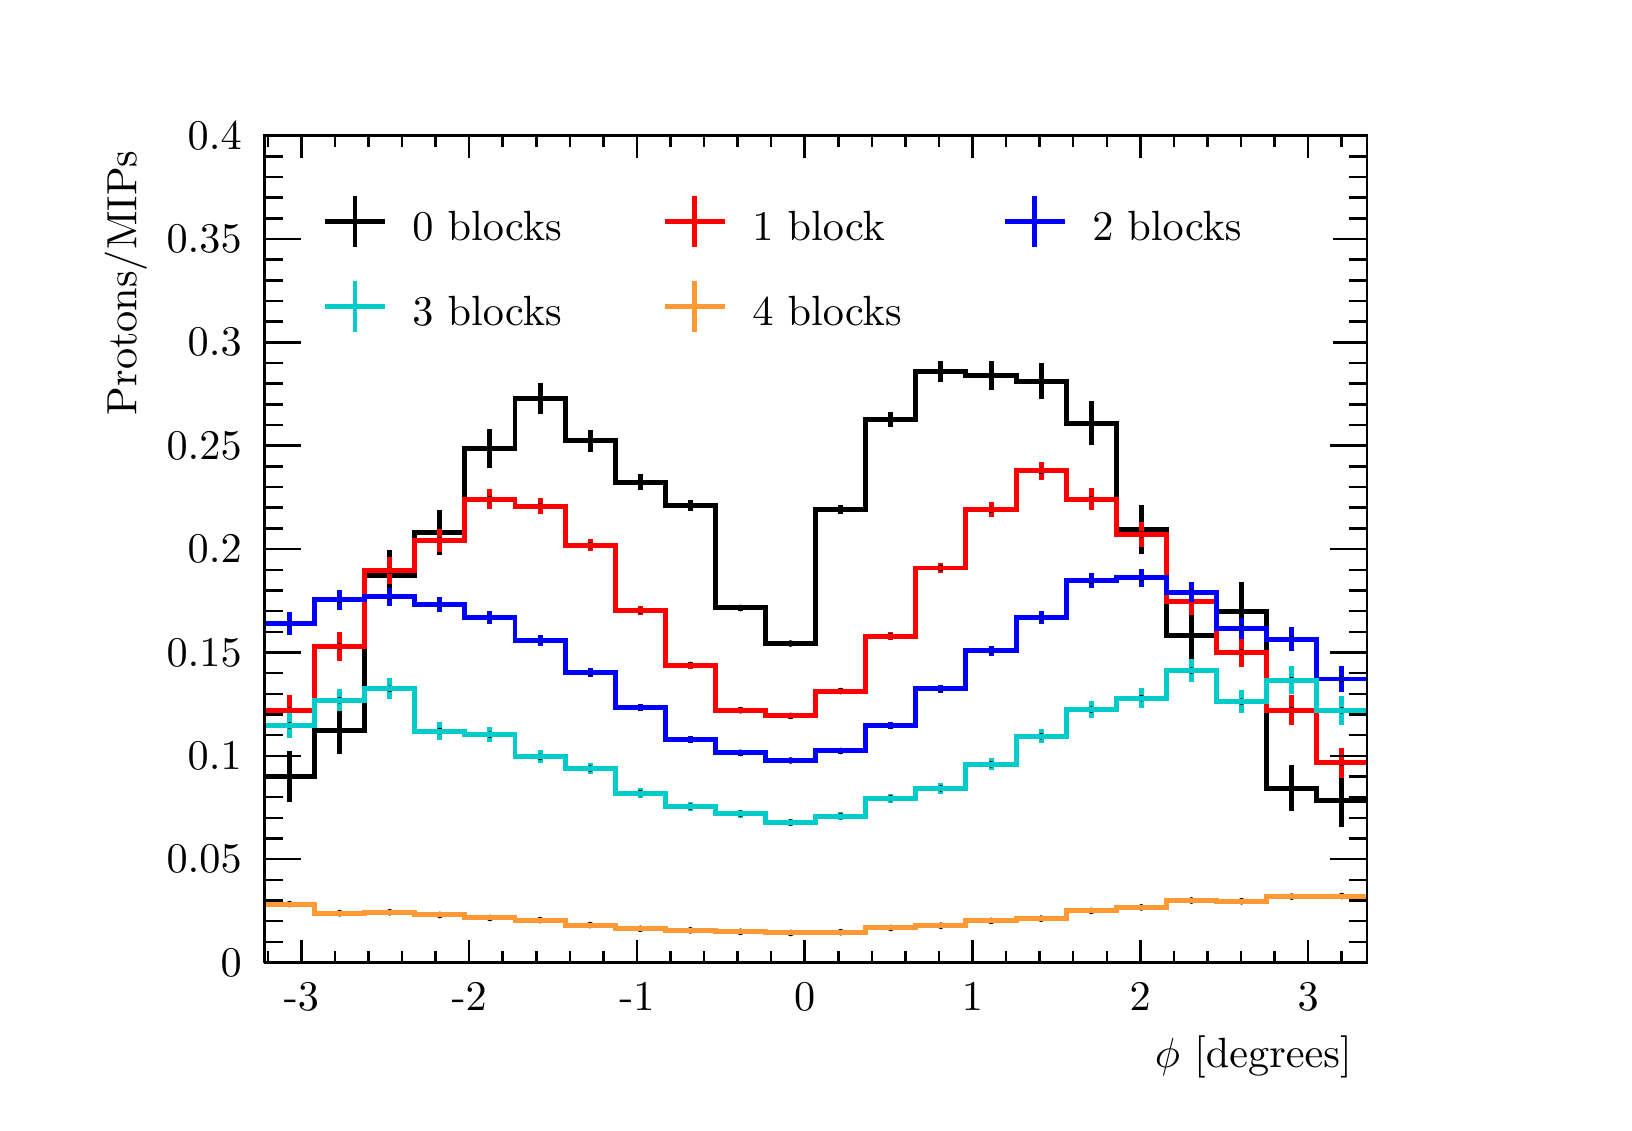
\begin{tikzpicture}
\pgfdeclareplotmark{cross} {
\pgfpathmoveto{\pgfpoint{-0.3\pgfplotmarksize}{\pgfplotmarksize}}
\pgfpathlineto{\pgfpoint{+0.3\pgfplotmarksize}{\pgfplotmarksize}}
\pgfpathlineto{\pgfpoint{+0.3\pgfplotmarksize}{0.3\pgfplotmarksize}}
\pgfpathlineto{\pgfpoint{+1\pgfplotmarksize}{0.3\pgfplotmarksize}}
\pgfpathlineto{\pgfpoint{+1\pgfplotmarksize}{-0.3\pgfplotmarksize}}
\pgfpathlineto{\pgfpoint{+0.3\pgfplotmarksize}{-0.3\pgfplotmarksize}}
\pgfpathlineto{\pgfpoint{+0.3\pgfplotmarksize}{-1.\pgfplotmarksize}}
\pgfpathlineto{\pgfpoint{-0.3\pgfplotmarksize}{-1.\pgfplotmarksize}}
\pgfpathlineto{\pgfpoint{-0.3\pgfplotmarksize}{-0.3\pgfplotmarksize}}
\pgfpathlineto{\pgfpoint{-1.\pgfplotmarksize}{-0.3\pgfplotmarksize}}
\pgfpathlineto{\pgfpoint{-1.\pgfplotmarksize}{0.3\pgfplotmarksize}}
\pgfpathlineto{\pgfpoint{-0.3\pgfplotmarksize}{0.3\pgfplotmarksize}}
\pgfpathclose
\pgfusepathqstroke
}
\pgfdeclareplotmark{cross*} {
\pgfpathmoveto{\pgfpoint{-0.3\pgfplotmarksize}{\pgfplotmarksize}}
\pgfpathlineto{\pgfpoint{+0.3\pgfplotmarksize}{\pgfplotmarksize}}
\pgfpathlineto{\pgfpoint{+0.3\pgfplotmarksize}{0.3\pgfplotmarksize}}
\pgfpathlineto{\pgfpoint{+1\pgfplotmarksize}{0.3\pgfplotmarksize}}
\pgfpathlineto{\pgfpoint{+1\pgfplotmarksize}{-0.3\pgfplotmarksize}}
\pgfpathlineto{\pgfpoint{+0.3\pgfplotmarksize}{-0.3\pgfplotmarksize}}
\pgfpathlineto{\pgfpoint{+0.3\pgfplotmarksize}{-1.\pgfplotmarksize}}
\pgfpathlineto{\pgfpoint{-0.3\pgfplotmarksize}{-1.\pgfplotmarksize}}
\pgfpathlineto{\pgfpoint{-0.3\pgfplotmarksize}{-0.3\pgfplotmarksize}}
\pgfpathlineto{\pgfpoint{-1.\pgfplotmarksize}{-0.3\pgfplotmarksize}}
\pgfpathlineto{\pgfpoint{-1.\pgfplotmarksize}{0.3\pgfplotmarksize}}
\pgfpathlineto{\pgfpoint{-0.3\pgfplotmarksize}{0.3\pgfplotmarksize}}
\pgfpathclose
\pgfusepathqfillstroke
}
\pgfdeclareplotmark{newstar} {
\pgfpathmoveto{\pgfqpoint{0pt}{\pgfplotmarksize}}
\pgfpathlineto{\pgfqpointpolar{44}{0.5\pgfplotmarksize}}
\pgfpathlineto{\pgfqpointpolar{18}{\pgfplotmarksize}}
\pgfpathlineto{\pgfqpointpolar{-20}{0.5\pgfplotmarksize}}
\pgfpathlineto{\pgfqpointpolar{-54}{\pgfplotmarksize}}
\pgfpathlineto{\pgfqpointpolar{-90}{0.5\pgfplotmarksize}}
\pgfpathlineto{\pgfqpointpolar{234}{\pgfplotmarksize}}
\pgfpathlineto{\pgfqpointpolar{198}{0.5\pgfplotmarksize}}
\pgfpathlineto{\pgfqpointpolar{162}{\pgfplotmarksize}}
\pgfpathlineto{\pgfqpointpolar{134}{0.5\pgfplotmarksize}}
\pgfpathclose
\pgfusepathqstroke
}
\pgfdeclareplotmark{newstar*} {
\pgfpathmoveto{\pgfqpoint{0pt}{\pgfplotmarksize}}
\pgfpathlineto{\pgfqpointpolar{44}{0.5\pgfplotmarksize}}
\pgfpathlineto{\pgfqpointpolar{18}{\pgfplotmarksize}}
\pgfpathlineto{\pgfqpointpolar{-20}{0.5\pgfplotmarksize}}
\pgfpathlineto{\pgfqpointpolar{-54}{\pgfplotmarksize}}
\pgfpathlineto{\pgfqpointpolar{-90}{0.5\pgfplotmarksize}}
\pgfpathlineto{\pgfqpointpolar{234}{\pgfplotmarksize}}
\pgfpathlineto{\pgfqpointpolar{198}{0.5\pgfplotmarksize}}
\pgfpathlineto{\pgfqpointpolar{162}{\pgfplotmarksize}}
\pgfpathlineto{\pgfqpointpolar{134}{0.5\pgfplotmarksize}}
\pgfpathclose
\pgfusepathqfillstroke
}
\definecolor{c}{rgb}{1,1,1};
\draw [color=c, fill=c] (0,0) rectangle (20,13.639);
\draw [color=c, fill=c] (3,1.77307) rectangle (17,12.2751);
\definecolor{c}{rgb}{0,0,0};
\draw [c,line width=0.9] (3,1.77307) -- (3,12.2751) -- (17,12.2751) -- (17,1.77307) -- (3,1.77307);
\definecolor{c}{rgb}{1,1,1};
\draw [color=c, fill=c] (3,1.77307) rectangle (17,12.2751);
\definecolor{c}{rgb}{0,0,0};
\draw [c,line width=0.9] (3,1.77307) -- (3,12.2751) -- (17,12.2751) -- (17,1.77307) -- (3,1.77307);
\draw [c,line width=0.9] (3,1.77307) -- (3.63636,1.77307) -- (3.63636,1.77307) -- (4.27273,1.77307) -- (4.27273,1.77307) -- (4.90909,1.77307) -- (4.90909,1.77307) -- (5.54545,1.77307) -- (5.54545,1.77307) -- (6.18182,1.77307) -- (6.18182,1.77307) --
 (6.81818,1.77307) -- (6.81818,1.77307) -- (7.45455,1.77307) -- (7.45455,1.77307) -- (8.09091,1.77307) -- (8.09091,1.77307) -- (8.72727,1.77307) -- (8.72727,1.77307) -- (9.36364,1.77307) -- (9.36364,1.77307) -- (10,1.77307) -- (10,1.77307) --
 (10.6364,1.77307) -- (10.6364,1.77307) -- (11.2727,1.77307) -- (11.2727,1.77307) -- (11.9091,1.77307) -- (11.9091,1.77307) -- (12.5455,1.77307) -- (12.5455,1.77307) -- (13.1818,1.77307) -- (13.1818,1.77307) -- (13.8182,1.77307) -- (13.8182,1.77307)
 -- (14.4545,1.77307) -- (14.4545,1.77307) -- (15.0909,1.77307) -- (15.0909,1.77307) -- (15.7273,1.77307) -- (15.7273,1.77307) -- (16.3636,1.77307) -- (16.3636,1.77307) -- (17,1.77307);
\draw [c,line width=0.9] (3,1.77307) -- (17,1.77307);
\draw [c,line width=0.9] (3.4688,2.05948) -- (3.4688,1.77307);
\draw [c,line width=0.9] (3.89498,1.91628) -- (3.89498,1.77307);
\draw [c,line width=0.9] (4.32116,1.91628) -- (4.32116,1.77307);
\draw [c,line width=0.9] (4.74734,1.91628) -- (4.74734,1.77307);
\draw [c,line width=0.9] (5.17352,1.91628) -- (5.17352,1.77307);
\draw [c,line width=0.9] (5.5997,2.05948) -- (5.5997,1.77307);
\draw [c,line width=0.9] (6.02588,1.91628) -- (6.02588,1.77307);
\draw [c,line width=0.9] (6.45205,1.91628) -- (6.45205,1.77307);
\draw [c,line width=0.9] (6.87823,1.91628) -- (6.87823,1.77307);
\draw [c,line width=0.9] (7.30441,1.91628) -- (7.30441,1.77307);
\draw [c,line width=0.9] (7.73059,2.05948) -- (7.73059,1.77307);
\draw [c,line width=0.9] (8.15677,1.91628) -- (8.15677,1.77307);
\draw [c,line width=0.9] (8.58295,1.91628) -- (8.58295,1.77307);
\draw [c,line width=0.9] (9.00913,1.91628) -- (9.00913,1.77307);
\draw [c,line width=0.9] (9.43531,1.91628) -- (9.43531,1.77307);
\draw [c,line width=0.9] (9.86149,2.05948) -- (9.86149,1.77307);
\draw [c,line width=0.9] (10.2877,1.91628) -- (10.2877,1.77307);
\draw [c,line width=0.9] (10.7139,1.91628) -- (10.7139,1.77307);
\draw [c,line width=0.9] (11.14,1.91628) -- (11.14,1.77307);
\draw [c,line width=0.9] (11.5662,1.91628) -- (11.5662,1.77307);
\draw [c,line width=0.9] (11.9924,2.05948) -- (11.9924,1.77307);
\draw [c,line width=0.9] (12.4186,1.91628) -- (12.4186,1.77307);
\draw [c,line width=0.9] (12.8447,1.91628) -- (12.8447,1.77307);
\draw [c,line width=0.9] (13.2709,1.91628) -- (13.2709,1.77307);
\draw [c,line width=0.9] (13.6971,1.91628) -- (13.6971,1.77307);
\draw [c,line width=0.9] (14.1233,2.05948) -- (14.1233,1.77307);
\draw [c,line width=0.9] (14.5495,1.91628) -- (14.5495,1.77307);
\draw [c,line width=0.9] (14.9756,1.91628) -- (14.9756,1.77307);
\draw [c,line width=0.9] (15.4018,1.91628) -- (15.4018,1.77307);
\draw [c,line width=0.9] (15.828,1.91628) -- (15.828,1.77307);
\draw [c,line width=0.9] (16.2542,2.05948) -- (16.2542,1.77307);
\draw [c,line width=0.9] (3.4688,2.05948) -- (3.4688,1.77307);
\draw [c,line width=0.9] (3.04262,1.91628) -- (3.04262,1.77307);
\draw [c,line width=0.9] (16.2542,2.05948) -- (16.2542,1.77307);
\draw [c,line width=0.9] (16.6804,1.91628) -- (16.6804,1.77307);
\draw [anchor=base] (3.4688,1.15931) node[scale=1.52731, color=c, rotate=0]{-3};
\draw [anchor=base] (5.5997,1.15931) node[scale=1.52731, color=c, rotate=0]{-2};
\draw [anchor=base] (7.73059,1.15931) node[scale=1.52731, color=c, rotate=0]{-1};
\draw [anchor=base] (9.86149,1.15931) node[scale=1.52731, color=c, rotate=0]{0};
\draw [anchor=base] (11.9924,1.15931) node[scale=1.52731, color=c, rotate=0]{1};
\draw [anchor=base] (14.1233,1.15931) node[scale=1.52731, color=c, rotate=0]{2};
\draw [anchor=base] (16.2542,1.15931) node[scale=1.52731, color=c, rotate=0]{3};
\draw [anchor= east] (17,0.572837) node[scale=1.52731, color=c, rotate=0]{$\phi$ [degrees]};
\draw [c,line width=0.9] (3,12.2751) -- (17,12.2751);
\draw [c,line width=0.9] (3.4688,11.9887) -- (3.4688,12.2751);
\draw [c,line width=0.9] (3.89498,12.1319) -- (3.89498,12.2751);
\draw [c,line width=0.9] (4.32116,12.1319) -- (4.32116,12.2751);
\draw [c,line width=0.9] (4.74734,12.1319) -- (4.74734,12.2751);
\draw [c,line width=0.9] (5.17352,12.1319) -- (5.17352,12.2751);
\draw [c,line width=0.9] (5.5997,11.9887) -- (5.5997,12.2751);
\draw [c,line width=0.9] (6.02588,12.1319) -- (6.02588,12.2751);
\draw [c,line width=0.9] (6.45205,12.1319) -- (6.45205,12.2751);
\draw [c,line width=0.9] (6.87823,12.1319) -- (6.87823,12.2751);
\draw [c,line width=0.9] (7.30441,12.1319) -- (7.30441,12.2751);
\draw [c,line width=0.9] (7.73059,11.9887) -- (7.73059,12.2751);
\draw [c,line width=0.9] (8.15677,12.1319) -- (8.15677,12.2751);
\draw [c,line width=0.9] (8.58295,12.1319) -- (8.58295,12.2751);
\draw [c,line width=0.9] (9.00913,12.1319) -- (9.00913,12.2751);
\draw [c,line width=0.9] (9.43531,12.1319) -- (9.43531,12.2751);
\draw [c,line width=0.9] (9.86149,11.9887) -- (9.86149,12.2751);
\draw [c,line width=0.9] (10.2877,12.1319) -- (10.2877,12.2751);
\draw [c,line width=0.9] (10.7139,12.1319) -- (10.7139,12.2751);
\draw [c,line width=0.9] (11.14,12.1319) -- (11.14,12.2751);
\draw [c,line width=0.9] (11.5662,12.1319) -- (11.5662,12.2751);
\draw [c,line width=0.9] (11.9924,11.9887) -- (11.9924,12.2751);
\draw [c,line width=0.9] (12.4186,12.1319) -- (12.4186,12.2751);
\draw [c,line width=0.9] (12.8447,12.1319) -- (12.8447,12.2751);
\draw [c,line width=0.9] (13.2709,12.1319) -- (13.2709,12.2751);
\draw [c,line width=0.9] (13.6971,12.1319) -- (13.6971,12.2751);
\draw [c,line width=0.9] (14.1233,11.9887) -- (14.1233,12.2751);
\draw [c,line width=0.9] (14.5495,12.1319) -- (14.5495,12.2751);
\draw [c,line width=0.9] (14.9756,12.1319) -- (14.9756,12.2751);
\draw [c,line width=0.9] (15.4018,12.1319) -- (15.4018,12.2751);
\draw [c,line width=0.9] (15.828,12.1319) -- (15.828,12.2751);
\draw [c,line width=0.9] (16.2542,11.9887) -- (16.2542,12.2751);
\draw [c,line width=0.9] (3.4688,11.9887) -- (3.4688,12.2751);
\draw [c,line width=0.9] (3.04262,12.1319) -- (3.04262,12.2751);
\draw [c,line width=0.9] (16.2542,11.9887) -- (16.2542,12.2751);
\draw [c,line width=0.9] (16.6804,12.1319) -- (16.6804,12.2751);
\draw [c,line width=0.9] (3,1.77307) -- (3,12.2751);
\draw [c,line width=0.9] (3.462,1.77307) -- (3,1.77307);
\draw [c,line width=0.9] (3.231,2.03562) -- (3,2.03562);
\draw [c,line width=0.9] (3.231,2.29817) -- (3,2.29817);
\draw [c,line width=0.9] (3.231,2.56072) -- (3,2.56072);
\draw [c,line width=0.9] (3.231,2.82327) -- (3,2.82327);
\draw [c,line width=0.9] (3.462,3.08582) -- (3,3.08582);
\draw [c,line width=0.9] (3.231,3.34837) -- (3,3.34837);
\draw [c,line width=0.9] (3.231,3.61092) -- (3,3.61092);
\draw [c,line width=0.9] (3.231,3.87347) -- (3,3.87347);
\draw [c,line width=0.9] (3.231,4.13602) -- (3,4.13602);
\draw [c,line width=0.9] (3.462,4.39857) -- (3,4.39857);
\draw [c,line width=0.9] (3.231,4.66112) -- (3,4.66112);
\draw [c,line width=0.9] (3.231,4.92367) -- (3,4.92367);
\draw [c,line width=0.9] (3.231,5.18622) -- (3,5.18622);
\draw [c,line width=0.9] (3.231,5.44877) -- (3,5.44877);
\draw [c,line width=0.9] (3.462,5.71132) -- (3,5.71132);
\draw [c,line width=0.9] (3.231,5.97387) -- (3,5.97387);
\draw [c,line width=0.9] (3.231,6.23642) -- (3,6.23642);
\draw [c,line width=0.9] (3.231,6.49897) -- (3,6.49897);
\draw [c,line width=0.9] (3.231,6.76152) -- (3,6.76152);
\draw [c,line width=0.9] (3.462,7.02407) -- (3,7.02407);
\draw [c,line width=0.9] (3.231,7.28662) -- (3,7.28662);
\draw [c,line width=0.9] (3.231,7.54917) -- (3,7.54917);
\draw [c,line width=0.9] (3.231,7.81172) -- (3,7.81172);
\draw [c,line width=0.9] (3.231,8.07427) -- (3,8.07427);
\draw [c,line width=0.9] (3.462,8.33682) -- (3,8.33682);
\draw [c,line width=0.9] (3.231,8.59937) -- (3,8.59937);
\draw [c,line width=0.9] (3.231,8.86192) -- (3,8.86192);
\draw [c,line width=0.9] (3.231,9.12447) -- (3,9.12447);
\draw [c,line width=0.9] (3.231,9.38702) -- (3,9.38702);
\draw [c,line width=0.9] (3.462,9.64957) -- (3,9.64957);
\draw [c,line width=0.9] (3.231,9.91212) -- (3,9.91212);
\draw [c,line width=0.9] (3.231,10.1747) -- (3,10.1747);
\draw [c,line width=0.9] (3.231,10.4372) -- (3,10.4372);
\draw [c,line width=0.9] (3.231,10.6998) -- (3,10.6998);
\draw [c,line width=0.9] (3.462,10.9623) -- (3,10.9623);
\draw [c,line width=0.9] (3.231,11.2249) -- (3,11.2249);
\draw [c,line width=0.9] (3.231,11.4874) -- (3,11.4874);
\draw [c,line width=0.9] (3.231,11.75) -- (3,11.75);
\draw [c,line width=0.9] (3.231,12.0125) -- (3,12.0125);
\draw [c,line width=0.9] (3.462,12.2751) -- (3,12.2751);
\draw [anchor= east] (2.9,1.77307) node[scale=1.52731, color=c, rotate=0]{0};
\draw [anchor= east] (2.9,3.08582) node[scale=1.52731, color=c, rotate=0]{0.05};
\draw [anchor= east] (2.9,4.39857) node[scale=1.52731, color=c, rotate=0]{0.1};
\draw [anchor= east] (2.9,5.71132) node[scale=1.52731, color=c, rotate=0]{0.15};
\draw [anchor= east] (2.9,7.02407) node[scale=1.52731, color=c, rotate=0]{0.2};
\draw [anchor= east] (2.9,8.33682) node[scale=1.52731, color=c, rotate=0]{0.25};
\draw [anchor= east] (2.9,9.64957) node[scale=1.52731, color=c, rotate=0]{0.3};
\draw [anchor= east] (2.9,10.9623) node[scale=1.52731, color=c, rotate=0]{0.35};
\draw [anchor= east] (2.9,12.2751) node[scale=1.52731, color=c, rotate=0]{0.4};
\draw [anchor= east] (1.24,12.2751) node[scale=1.52731, color=c, rotate=90]{  Protons/MIPs};
\draw [c,line width=0.9] (17,1.77307) -- (17,12.2751);
\draw [c,line width=0.9] (16.538,1.77307) -- (17,1.77307);
\draw [c,line width=0.9] (16.769,2.03562) -- (17,2.03562);
\draw [c,line width=0.9] (16.769,2.29817) -- (17,2.29817);
\draw [c,line width=0.9] (16.769,2.56072) -- (17,2.56072);
\draw [c,line width=0.9] (16.769,2.82327) -- (17,2.82327);
\draw [c,line width=0.9] (16.538,3.08582) -- (17,3.08582);
\draw [c,line width=0.9] (16.769,3.34837) -- (17,3.34837);
\draw [c,line width=0.9] (16.769,3.61092) -- (17,3.61092);
\draw [c,line width=0.9] (16.769,3.87347) -- (17,3.87347);
\draw [c,line width=0.9] (16.769,4.13602) -- (17,4.13602);
\draw [c,line width=0.9] (16.538,4.39857) -- (17,4.39857);
\draw [c,line width=0.9] (16.769,4.66112) -- (17,4.66112);
\draw [c,line width=0.9] (16.769,4.92367) -- (17,4.92367);
\draw [c,line width=0.9] (16.769,5.18622) -- (17,5.18622);
\draw [c,line width=0.9] (16.769,5.44877) -- (17,5.44877);
\draw [c,line width=0.9] (16.538,5.71132) -- (17,5.71132);
\draw [c,line width=0.9] (16.769,5.97387) -- (17,5.97387);
\draw [c,line width=0.9] (16.769,6.23642) -- (17,6.23642);
\draw [c,line width=0.9] (16.769,6.49897) -- (17,6.49897);
\draw [c,line width=0.9] (16.769,6.76152) -- (17,6.76152);
\draw [c,line width=0.9] (16.538,7.02407) -- (17,7.02407);
\draw [c,line width=0.9] (16.769,7.28662) -- (17,7.28662);
\draw [c,line width=0.9] (16.769,7.54917) -- (17,7.54917);
\draw [c,line width=0.9] (16.769,7.81172) -- (17,7.81172);
\draw [c,line width=0.9] (16.769,8.07427) -- (17,8.07427);
\draw [c,line width=0.9] (16.538,8.33682) -- (17,8.33682);
\draw [c,line width=0.9] (16.769,8.59937) -- (17,8.59937);
\draw [c,line width=0.9] (16.769,8.86192) -- (17,8.86192);
\draw [c,line width=0.9] (16.769,9.12447) -- (17,9.12447);
\draw [c,line width=0.9] (16.769,9.38702) -- (17,9.38702);
\draw [c,line width=0.9] (16.538,9.64957) -- (17,9.64957);
\draw [c,line width=0.9] (16.769,9.91212) -- (17,9.91212);
\draw [c,line width=0.9] (16.769,10.1747) -- (17,10.1747);
\draw [c,line width=0.9] (16.769,10.4372) -- (17,10.4372);
\draw [c,line width=0.9] (16.769,10.6998) -- (17,10.6998);
\draw [c,line width=0.9] (16.538,10.9623) -- (17,10.9623);
\draw [c,line width=0.9] (16.769,11.2249) -- (17,11.2249);
\draw [c,line width=0.9] (16.769,11.4874) -- (17,11.4874);
\draw [c,line width=0.9] (16.769,11.75) -- (17,11.75);
\draw [c,line width=0.9] (16.769,12.0125) -- (17,12.0125);
\draw [c,line width=0.9] (16.538,12.2751) -- (17,12.2751);
\draw [c,line width=1.8] (3.31818,3.80808) -- (3.31818,4.13307);
\draw [c,line width=1.8] (3.31818,4.13307) -- (3.31818,4.45805);
\foreach \P in {(3.31818,4.13307)}{\draw[mark options={color=c,fill=c},mark size=2.402402pt,mark=*,mark size=1pt] plot coordinates {\P};}
\draw [c,line width=1.8] (3.95455,4.41539) -- (3.95455,4.72226);
\draw [c,line width=1.8] (3.95455,4.72226) -- (3.95455,5.02913);
\foreach \P in {(3.95455,4.72226)}{\draw[mark options={color=c,fill=c},mark size=2.402402pt,mark=*,mark size=1pt] plot coordinates {\P};}
\draw [c,line width=1.8] (4.59091,6.36336) -- (4.59091,6.68924);
\draw [c,line width=1.8] (4.59091,6.68924) -- (4.59091,7.01511);
\foreach \P in {(4.59091,6.68924)}{\draw[mark options={color=c,fill=c},mark size=2.402402pt,mark=*,mark size=1pt] plot coordinates {\P};}
\draw [c,line width=1.8] (5.22727,6.95027) -- (5.22727,7.23731);
\draw [c,line width=1.8] (5.22727,7.23731) -- (5.22727,7.52435);
\foreach \P in {(5.22727,7.23731)}{\draw[mark options={color=c,fill=c},mark size=2.402402pt,mark=*,mark size=1pt] plot coordinates {\P};}
\draw [c,line width=1.8] (5.86364,8.05935) -- (5.86364,8.30108);
\draw [c,line width=1.8] (5.86364,8.30108) -- (5.86364,8.54282);
\foreach \P in {(5.86364,8.30108)}{\draw[mark options={color=c,fill=c},mark size=2.402402pt,mark=*,mark size=1pt] plot coordinates {\P};}
\draw [c,line width=1.8] (6.5,8.738) -- (6.5,8.93286);
\draw [c,line width=1.8] (6.5,8.93286) -- (6.5,9.12772);
\foreach \P in {(6.5,8.93286)}{\draw[mark options={color=c,fill=c},mark size=2.402402pt,mark=*,mark size=1pt] plot coordinates {\P};}
\draw [c,line width=1.8] (7.13636,8.25921) -- (7.13636,8.39849);
\draw [c,line width=1.8] (7.13636,8.39849) -- (7.13636,8.53777);
\foreach \P in {(7.13636,8.39849)}{\draw[mark options={color=c,fill=c},mark size=2.402402pt,mark=*,mark size=1pt] plot coordinates {\P};}
\draw [c,line width=1.8] (7.77273,7.77828) -- (7.77273,7.87577);
\draw [c,line width=1.8] (7.77273,7.87577) -- (7.77273,7.97326);
\foreach \P in {(7.77273,7.87577)}{\draw[mark options={color=c,fill=c},mark size=2.402402pt,mark=*,mark size=1pt] plot coordinates {\P};}
\draw [c,line width=1.8] (8.40909,7.5099) -- (8.40909,7.57818);
\draw [c,line width=1.8] (8.40909,7.57818) -- (8.40909,7.64647);
\foreach \P in {(8.40909,7.57818)}{\draw[mark options={color=c,fill=c},mark size=2.402402pt,mark=*,mark size=1pt] plot coordinates {\P};}
\draw [c,line width=1.8] (9.04545,6.23857) -- (9.04545,6.27671);
\draw [c,line width=1.8] (9.04545,6.27671) -- (9.04545,6.31485);
\foreach \P in {(9.04545,6.27671)}{\draw[mark options={color=c,fill=c},mark size=2.402402pt,mark=*,mark size=1pt] plot coordinates {\P};}
\draw [c,line width=1.8] (9.68182,5.79204) -- (9.68182,5.82443);
\draw [c,line width=1.8] (9.68182,5.82443) -- (9.68182,5.85681);
\foreach \P in {(9.68182,5.82443)}{\draw[mark options={color=c,fill=c},mark size=2.402402pt,mark=*,mark size=1pt] plot coordinates {\P};}
\draw [c,line width=1.8] (10.3182,7.47425) -- (10.3182,7.53112);
\draw [c,line width=1.8] (10.3182,7.53112) -- (10.3182,7.58798);
\foreach \P in {(10.3182,7.53112)}{\draw[mark options={color=c,fill=c},mark size=2.402402pt,mark=*,mark size=1pt] plot coordinates {\P};}
\draw [c,line width=1.8] (10.9545,8.57392) -- (10.9545,8.66757);
\draw [c,line width=1.8] (10.9545,8.66757) -- (10.9545,8.76122);
\foreach \P in {(10.9545,8.66757)}{\draw[mark options={color=c,fill=c},mark size=2.402402pt,mark=*,mark size=1pt] plot coordinates {\P};}
\draw [c,line width=1.8] (11.5909,9.14225) -- (11.5909,9.27642);
\draw [c,line width=1.8] (11.5909,9.27642) -- (11.5909,9.41059);
\foreach \P in {(11.5909,9.27642)}{\draw[mark options={color=c,fill=c},mark size=2.402402pt,mark=*,mark size=1pt] plot coordinates {\P};}
\draw [c,line width=1.8] (12.2273,9.04159) -- (12.2273,9.22441);
\draw [c,line width=1.8] (12.2273,9.22441) -- (12.2273,9.40722);
\foreach \P in {(12.2273,9.22441)}{\draw[mark options={color=c,fill=c},mark size=2.402402pt,mark=*,mark size=1pt] plot coordinates {\P};}
\draw [c,line width=1.8] (12.8636,8.92559) -- (12.8636,9.15666);
\draw [c,line width=1.8] (12.8636,9.15666) -- (12.8636,9.38773);
\foreach \P in {(12.8636,9.15666)}{\draw[mark options={color=c,fill=c},mark size=2.402402pt,mark=*,mark size=1pt] plot coordinates {\P};}
\draw [c,line width=1.8] (13.5,8.34016) -- (13.5,8.62085);
\draw [c,line width=1.8] (13.5,8.62085) -- (13.5,8.90154);
\foreach \P in {(13.5,8.62085)}{\draw[mark options={color=c,fill=c},mark size=2.402402pt,mark=*,mark size=1pt] plot coordinates {\P};}
\draw [c,line width=1.8] (14.1364,6.96408) -- (14.1364,7.27082);
\draw [c,line width=1.8] (14.1364,7.27082) -- (14.1364,7.57756);
\foreach \P in {(14.1364,7.27082)}{\draw[mark options={color=c,fill=c},mark size=2.402402pt,mark=*,mark size=1pt] plot coordinates {\P};}
\draw [c,line width=1.8] (14.7727,5.6213) -- (14.7727,5.92854);
\draw [c,line width=1.8] (14.7727,5.92854) -- (14.7727,6.23577);
\foreach \P in {(14.7727,5.92854)}{\draw[mark options={color=c,fill=c},mark size=2.402402pt,mark=*,mark size=1pt] plot coordinates {\P};}
\draw [c,line width=1.8] (15.4091,5.86537) -- (15.4091,6.23494);
\draw [c,line width=1.8] (15.4091,6.23494) -- (15.4091,6.60452);
\foreach \P in {(15.4091,6.23494)}{\draw[mark options={color=c,fill=c},mark size=2.402402pt,mark=*,mark size=1pt] plot coordinates {\P};}
\draw [c,line width=1.8] (16.0455,3.69529) -- (16.0455,3.9894);
\draw [c,line width=1.8] (16.0455,3.9894) -- (16.0455,4.28351);
\foreach \P in {(16.0455,3.9894)}{\draw[mark options={color=c,fill=c},mark size=2.402402pt,mark=*,mark size=1pt] plot coordinates {\P};}
\draw [c,line width=1.8] (16.6818,3.49909) -- (16.6818,3.83344);
\draw [c,line width=1.8] (16.6818,3.83344) -- (16.6818,4.16778);
\foreach \P in {(16.6818,3.83344)}{\draw[mark options={color=c,fill=c},mark size=2.402402pt,mark=*,mark size=1pt] plot coordinates {\P};}
\draw [c,line width=1.8] (3,4.13307) -- (3.63636,4.13307) -- (3.63636,4.72226) -- (4.27273,4.72226) -- (4.27273,6.68924) -- (4.90909,6.68924) -- (4.90909,7.23731) -- (5.54545,7.23731) -- (5.54545,8.30108) -- (6.18182,8.30108) -- (6.18182,8.93286) --
 (6.81818,8.93286) -- (6.81818,8.39849) -- (7.45455,8.39849) -- (7.45455,7.87577) -- (8.09091,7.87577) -- (8.09091,7.57818) -- (8.72727,7.57818) -- (8.72727,6.27671) -- (9.36364,6.27671) -- (9.36364,5.82443) -- (10,5.82443) -- (10,7.53112) --
 (10.6364,7.53112) -- (10.6364,8.66757) -- (11.2727,8.66757) -- (11.2727,9.27642) -- (11.9091,9.27642) -- (11.9091,9.22441) -- (12.5455,9.22441) -- (12.5455,9.15666) -- (13.1818,9.15666) -- (13.1818,8.62085) -- (13.8182,8.62085) -- (13.8182,7.27082)
 -- (14.4545,7.27082) -- (14.4545,5.92854) -- (15.0909,5.92854) -- (15.0909,6.23494) -- (15.7273,6.23494) -- (15.7273,3.9894) -- (16.3636,3.9894) -- (16.3636,3.83344) -- (17,3.83344);
\definecolor{c}{rgb}{1,0,0};
\draw [c,line width=1.8] (3.31818,4.78145) -- (3.31818,4.97313);
\draw [c,line width=1.8] (3.31818,4.97313) -- (3.31818,5.16481);
\definecolor{c}{rgb}{0,0,0};
\foreach \P in {(3.31818,4.97313)}{\draw[mark options={color=c,fill=c},mark size=2.402402pt,mark=*,mark size=1pt] plot coordinates {\P};}
\definecolor{c}{rgb}{1,0,0};
\draw [c,line width=1.8] (3.95455,5.6081) -- (3.95455,5.78705);
\draw [c,line width=1.8] (3.95455,5.78705) -- (3.95455,5.96599);
\definecolor{c}{rgb}{0,0,0};
\foreach \P in {(3.95455,5.78705)}{\draw[mark options={color=c,fill=c},mark size=2.402402pt,mark=*,mark size=1pt] plot coordinates {\P};}
\definecolor{c}{rgb}{1,0,0};
\draw [c,line width=1.8] (4.59091,6.57712) -- (4.59091,6.74842);
\draw [c,line width=1.8] (4.59091,6.74842) -- (4.59091,6.91972);
\definecolor{c}{rgb}{0,0,0};
\foreach \P in {(4.59091,6.74842)}{\draw[mark options={color=c,fill=c},mark size=2.402402pt,mark=*,mark size=1pt] plot coordinates {\P};}
\definecolor{c}{rgb}{1,0,0};
\draw [c,line width=1.8] (5.22727,6.98706) -- (5.22727,7.13564);
\draw [c,line width=1.8] (5.22727,7.13564) -- (5.22727,7.28422);
\definecolor{c}{rgb}{0,0,0};
\foreach \P in {(5.22727,7.13564)}{\draw[mark options={color=c,fill=c},mark size=2.402402pt,mark=*,mark size=1pt] plot coordinates {\P};}
\definecolor{c}{rgb}{1,0,0};
\draw [c,line width=1.8] (5.86364,7.53021) -- (5.86364,7.65829);
\draw [c,line width=1.8] (5.86364,7.65829) -- (5.86364,7.78638);
\definecolor{c}{rgb}{0,0,0};
\foreach \P in {(5.86364,7.65829)}{\draw[mark options={color=c,fill=c},mark size=2.402402pt,mark=*,mark size=1pt] plot coordinates {\P};}
\definecolor{c}{rgb}{1,0,0};
\draw [c,line width=1.8] (6.5,7.46591) -- (6.5,7.5684);
\draw [c,line width=1.8] (6.5,7.5684) -- (6.5,7.67089);
\definecolor{c}{rgb}{0,0,0};
\foreach \P in {(6.5,7.5684)}{\draw[mark options={color=c,fill=c},mark size=2.402402pt,mark=*,mark size=1pt] plot coordinates {\P};}
\definecolor{c}{rgb}{1,0,0};
\draw [c,line width=1.8] (7.13636,6.99514) -- (7.13636,7.07247);
\draw [c,line width=1.8] (7.13636,7.07247) -- (7.13636,7.14981);
\definecolor{c}{rgb}{0,0,0};
\foreach \P in {(7.13636,7.07247)}{\draw[mark options={color=c,fill=c},mark size=2.402402pt,mark=*,mark size=1pt] plot coordinates {\P};}
\definecolor{c}{rgb}{1,0,0};
\draw [c,line width=1.8] (7.77273,6.18448) -- (7.77273,6.24109);
\draw [c,line width=1.8] (7.77273,6.24109) -- (7.77273,6.29769);
\definecolor{c}{rgb}{0,0,0};
\foreach \P in {(7.77273,6.24109)}{\draw[mark options={color=c,fill=c},mark size=2.402402pt,mark=*,mark size=1pt] plot coordinates {\P};}
\definecolor{c}{rgb}{1,0,0};
\draw [c,line width=1.8] (8.40909,5.5071) -- (8.40909,5.55116);
\draw [c,line width=1.8] (8.40909,5.55116) -- (8.40909,5.59522);
\definecolor{c}{rgb}{0,0,0};
\foreach \P in {(8.40909,5.55116)}{\draw[mark options={color=c,fill=c},mark size=2.402402pt,mark=*,mark size=1pt] plot coordinates {\P};}
\definecolor{c}{rgb}{1,0,0};
\draw [c,line width=1.8] (9.04545,4.94121) -- (9.04545,4.97695);
\draw [c,line width=1.8] (9.04545,4.97695) -- (9.04545,5.01268);
\definecolor{c}{rgb}{0,0,0};
\foreach \P in {(9.04545,4.97695)}{\draw[mark options={color=c,fill=c},mark size=2.402402pt,mark=*,mark size=1pt] plot coordinates {\P};}
\definecolor{c}{rgb}{1,0,0};
\draw [c,line width=1.8] (9.68182,4.87123) -- (9.68182,4.9057);
\draw [c,line width=1.8] (9.68182,4.9057) -- (9.68182,4.94017);
\definecolor{c}{rgb}{0,0,0};
\foreach \P in {(9.68182,4.9057)}{\draw[mark options={color=c,fill=c},mark size=2.402402pt,mark=*,mark size=1pt] plot coordinates {\P};}
\definecolor{c}{rgb}{1,0,0};
\draw [c,line width=1.8] (10.3182,5.18155) -- (10.3182,5.22031);
\draw [c,line width=1.8] (10.3182,5.22031) -- (10.3182,5.25907);
\definecolor{c}{rgb}{0,0,0};
\foreach \P in {(10.3182,5.22031)}{\draw[mark options={color=c,fill=c},mark size=2.402402pt,mark=*,mark size=1pt] plot coordinates {\P};}
\definecolor{c}{rgb}{1,0,0};
\draw [c,line width=1.8] (10.9545,5.86661) -- (10.9545,5.91603);
\draw [c,line width=1.8] (10.9545,5.91603) -- (10.9545,5.96545);
\definecolor{c}{rgb}{0,0,0};
\foreach \P in {(10.9545,5.91603)}{\draw[mark options={color=c,fill=c},mark size=2.402402pt,mark=*,mark size=1pt] plot coordinates {\P};}
\definecolor{c}{rgb}{1,0,0};
\draw [c,line width=1.8] (11.5909,6.71715) -- (11.5909,6.78377);
\draw [c,line width=1.8] (11.5909,6.78377) -- (11.5909,6.85039);
\definecolor{c}{rgb}{0,0,0};
\foreach \P in {(11.5909,6.78377)}{\draw[mark options={color=c,fill=c},mark size=2.402402pt,mark=*,mark size=1pt] plot coordinates {\P};}
\definecolor{c}{rgb}{1,0,0};
\draw [c,line width=1.8] (12.2273,7.43032) -- (12.2273,7.52302);
\draw [c,line width=1.8] (12.2273,7.52302) -- (12.2273,7.61572);
\definecolor{c}{rgb}{0,0,0};
\foreach \P in {(12.2273,7.52302)}{\draw[mark options={color=c,fill=c},mark size=2.402402pt,mark=*,mark size=1pt] plot coordinates {\P};}
\definecolor{c}{rgb}{1,0,0};
\draw [c,line width=1.8] (12.8636,7.89794) -- (12.8636,8.01654);
\draw [c,line width=1.8] (12.8636,8.01654) -- (12.8636,8.13513);
\definecolor{c}{rgb}{0,0,0};
\foreach \P in {(12.8636,8.01654)}{\draw[mark options={color=c,fill=c},mark size=2.402402pt,mark=*,mark size=1pt] plot coordinates {\P};}
\definecolor{c}{rgb}{1,0,0};
\draw [c,line width=1.8] (13.5,7.51706) -- (13.5,7.65841);
\draw [c,line width=1.8] (13.5,7.65841) -- (13.5,7.79976);
\definecolor{c}{rgb}{0,0,0};
\foreach \P in {(13.5,7.65841)}{\draw[mark options={color=c,fill=c},mark size=2.402402pt,mark=*,mark size=1pt] plot coordinates {\P};}
\definecolor{c}{rgb}{1,0,0};
\draw [c,line width=1.8] (14.1364,7.04699) -- (14.1364,7.21009);
\draw [c,line width=1.8] (14.1364,7.21009) -- (14.1364,7.37319);
\definecolor{c}{rgb}{0,0,0};
\foreach \P in {(14.1364,7.21009)}{\draw[mark options={color=c,fill=c},mark size=2.402402pt,mark=*,mark size=1pt] plot coordinates {\P};}
\definecolor{c}{rgb}{1,0,0};
\draw [c,line width=1.8] (14.7727,6.18734) -- (14.7727,6.36271);
\draw [c,line width=1.8] (14.7727,6.36271) -- (14.7727,6.53807);
\definecolor{c}{rgb}{0,0,0};
\foreach \P in {(14.7727,6.36271)}{\draw[mark options={color=c,fill=c},mark size=2.402402pt,mark=*,mark size=1pt] plot coordinates {\P};}
\definecolor{c}{rgb}{1,0,0};
\draw [c,line width=1.8] (15.4091,5.53084) -- (15.4091,5.71479);
\draw [c,line width=1.8] (15.4091,5.71479) -- (15.4091,5.89875);
\definecolor{c}{rgb}{0,0,0};
\foreach \P in {(15.4091,5.71479)}{\draw[mark options={color=c,fill=c},mark size=2.402402pt,mark=*,mark size=1pt] plot coordinates {\P};}
\definecolor{c}{rgb}{1,0,0};
\draw [c,line width=1.8] (16.0455,4.78569) -- (16.0455,4.97952);
\draw [c,line width=1.8] (16.0455,4.97952) -- (16.0455,5.17335);
\definecolor{c}{rgb}{0,0,0};
\foreach \P in {(16.0455,4.97952)}{\draw[mark options={color=c,fill=c},mark size=2.402402pt,mark=*,mark size=1pt] plot coordinates {\P};}
\definecolor{c}{rgb}{1,0,0};
\draw [c,line width=1.8] (16.6818,4.11737) -- (16.6818,4.30993);
\draw [c,line width=1.8] (16.6818,4.30993) -- (16.6818,4.50248);
\definecolor{c}{rgb}{0,0,0};
\foreach \P in {(16.6818,4.30993)}{\draw[mark options={color=c,fill=c},mark size=2.402402pt,mark=*,mark size=1pt] plot coordinates {\P};}
\definecolor{c}{rgb}{1,0,0};
\draw [c,line width=1.8] (3,4.97313) -- (3.63636,4.97313) -- (3.63636,5.78705) -- (4.27273,5.78705) -- (4.27273,6.74842) -- (4.90909,6.74842) -- (4.90909,7.13564) -- (5.54545,7.13564) -- (5.54545,7.65829) -- (6.18182,7.65829) -- (6.18182,7.5684) --
 (6.81818,7.5684) -- (6.81818,7.07247) -- (7.45455,7.07247) -- (7.45455,6.24109) -- (8.09091,6.24109) -- (8.09091,5.55116) -- (8.72727,5.55116) -- (8.72727,4.97695) -- (9.36364,4.97695) -- (9.36364,4.9057) -- (10,4.9057) -- (10,5.22031) --
 (10.6364,5.22031) -- (10.6364,5.91603) -- (11.2727,5.91603) -- (11.2727,6.78377) -- (11.9091,6.78377) -- (11.9091,7.52302) -- (12.5455,7.52302) -- (12.5455,8.01654) -- (13.1818,8.01654) -- (13.1818,7.65841) -- (13.8182,7.65841) -- (13.8182,7.21009)
 -- (14.4545,7.21009) -- (14.4545,6.36271) -- (15.0909,6.36271) -- (15.0909,5.71479) -- (15.7273,5.71479) -- (15.7273,4.97952) -- (16.3636,4.97952) -- (16.3636,4.30993) -- (17,4.30993);
\definecolor{c}{rgb}{0,0,1};
\draw [c,line width=1.8] (3.31818,5.92759) -- (3.31818,6.07822);
\draw [c,line width=1.8] (3.31818,6.07822) -- (3.31818,6.22885);
\definecolor{c}{rgb}{0,0,0};
\foreach \P in {(3.31818,6.07822)}{\draw[mark options={color=c,fill=c},mark size=2.402402pt,mark=*,mark size=1pt] plot coordinates {\P};}
\definecolor{c}{rgb}{0,0,1};
\draw [c,line width=1.8] (3.95455,6.24646) -- (3.95455,6.37771);
\draw [c,line width=1.8] (3.95455,6.37771) -- (3.95455,6.50896);
\definecolor{c}{rgb}{0,0,0};
\foreach \P in {(3.95455,6.37771)}{\draw[mark options={color=c,fill=c},mark size=2.402402pt,mark=*,mark size=1pt] plot coordinates {\P};}
\definecolor{c}{rgb}{0,0,1};
\draw [c,line width=1.8] (4.59091,6.29971) -- (4.59091,6.41607);
\draw [c,line width=1.8] (4.59091,6.41607) -- (4.59091,6.53243);
\definecolor{c}{rgb}{0,0,0};
\foreach \P in {(4.59091,6.41607)}{\draw[mark options={color=c,fill=c},mark size=2.402402pt,mark=*,mark size=1pt] plot coordinates {\P};}
\definecolor{c}{rgb}{0,0,1};
\draw [c,line width=1.8] (5.22727,6.21984) -- (5.22727,6.31949);
\draw [c,line width=1.8] (5.22727,6.31949) -- (5.22727,6.41914);
\definecolor{c}{rgb}{0,0,0};
\foreach \P in {(5.22727,6.31949)}{\draw[mark options={color=c,fill=c},mark size=2.402402pt,mark=*,mark size=1pt] plot coordinates {\P};}
\definecolor{c}{rgb}{0,0,1};
\draw [c,line width=1.8] (5.86364,6.06879) -- (5.86364,6.15273);
\draw [c,line width=1.8] (5.86364,6.15273) -- (5.86364,6.23666);
\definecolor{c}{rgb}{0,0,0};
\foreach \P in {(5.86364,6.15273)}{\draw[mark options={color=c,fill=c},mark size=2.402402pt,mark=*,mark size=1pt] plot coordinates {\P};}
\definecolor{c}{rgb}{0,0,1};
\draw [c,line width=1.8] (6.5,5.7898) -- (6.5,5.86022);
\draw [c,line width=1.8] (6.5,5.86022) -- (6.5,5.93064);
\definecolor{c}{rgb}{0,0,0};
\foreach \P in {(6.5,5.86022)}{\draw[mark options={color=c,fill=c},mark size=2.402402pt,mark=*,mark size=1pt] plot coordinates {\P};}
\definecolor{c}{rgb}{0,0,1};
\draw [c,line width=1.8] (7.13636,5.39713) -- (7.13636,5.45483);
\draw [c,line width=1.8] (7.13636,5.45483) -- (7.13636,5.51254);
\definecolor{c}{rgb}{0,0,0};
\foreach \P in {(7.13636,5.45483)}{\draw[mark options={color=c,fill=c},mark size=2.402402pt,mark=*,mark size=1pt] plot coordinates {\P};}
\definecolor{c}{rgb}{0,0,1};
\draw [c,line width=1.8] (7.77273,4.96354) -- (7.77273,5.01062);
\draw [c,line width=1.8] (7.77273,5.01062) -- (7.77273,5.0577);
\definecolor{c}{rgb}{0,0,0};
\foreach \P in {(7.77273,5.01062)}{\draw[mark options={color=c,fill=c},mark size=2.402402pt,mark=*,mark size=1pt] plot coordinates {\P};}
\definecolor{c}{rgb}{0,0,1};
\draw [c,line width=1.8] (8.40909,4.56629) -- (8.40909,4.60615);
\draw [c,line width=1.8] (8.40909,4.60615) -- (8.40909,4.64601);
\definecolor{c}{rgb}{0,0,0};
\foreach \P in {(8.40909,4.60615)}{\draw[mark options={color=c,fill=c},mark size=2.402402pt,mark=*,mark size=1pt] plot coordinates {\P};}
\definecolor{c}{rgb}{0,0,1};
\draw [c,line width=1.8] (9.04545,4.40098) -- (9.04545,4.43678);
\draw [c,line width=1.8] (9.04545,4.43678) -- (9.04545,4.47259);
\definecolor{c}{rgb}{0,0,0};
\foreach \P in {(9.04545,4.43678)}{\draw[mark options={color=c,fill=c},mark size=2.402402pt,mark=*,mark size=1pt] plot coordinates {\P};}
\definecolor{c}{rgb}{0,0,1};
\draw [c,line width=1.8] (9.68182,4.30451) -- (9.68182,4.3395);
\draw [c,line width=1.8] (9.68182,4.3395) -- (9.68182,4.37449);
\definecolor{c}{rgb}{0,0,0};
\foreach \P in {(9.68182,4.3395)}{\draw[mark options={color=c,fill=c},mark size=2.402402pt,mark=*,mark size=1pt] plot coordinates {\P};}
\definecolor{c}{rgb}{0,0,1};
\draw [c,line width=1.8] (10.3182,4.42284) -- (10.3182,4.45999);
\draw [c,line width=1.8] (10.3182,4.45999) -- (10.3182,4.49713);
\definecolor{c}{rgb}{0,0,0};
\foreach \P in {(10.3182,4.45999)}{\draw[mark options={color=c,fill=c},mark size=2.402402pt,mark=*,mark size=1pt] plot coordinates {\P};}
\definecolor{c}{rgb}{0,0,1};
\draw [c,line width=1.8] (10.9545,4.73639) -- (10.9545,4.7792);
\draw [c,line width=1.8] (10.9545,4.7792) -- (10.9545,4.82201);
\definecolor{c}{rgb}{0,0,0};
\foreach \P in {(10.9545,4.7792)}{\draw[mark options={color=c,fill=c},mark size=2.402402pt,mark=*,mark size=1pt] plot coordinates {\P};}
\definecolor{c}{rgb}{0,0,1};
\draw [c,line width=1.8] (11.5909,5.19588) -- (11.5909,5.24757);
\draw [c,line width=1.8] (11.5909,5.24757) -- (11.5909,5.29926);
\definecolor{c}{rgb}{0,0,0};
\foreach \P in {(11.5909,5.24757)}{\draw[mark options={color=c,fill=c},mark size=2.402402pt,mark=*,mark size=1pt] plot coordinates {\P};}
\definecolor{c}{rgb}{0,0,1};
\draw [c,line width=1.8] (12.2273,5.66757) -- (12.2273,5.73297);
\draw [c,line width=1.8] (12.2273,5.73297) -- (12.2273,5.79837);
\definecolor{c}{rgb}{0,0,0};
\foreach \P in {(12.2273,5.73297)}{\draw[mark options={color=c,fill=c},mark size=2.402402pt,mark=*,mark size=1pt] plot coordinates {\P};}
\definecolor{c}{rgb}{0,0,1};
\draw [c,line width=1.8] (12.8636,6.07319) -- (12.8636,6.15251);
\draw [c,line width=1.8] (12.8636,6.15251) -- (12.8636,6.23183);
\definecolor{c}{rgb}{0,0,0};
\foreach \P in {(12.8636,6.15251)}{\draw[mark options={color=c,fill=c},mark size=2.402402pt,mark=*,mark size=1pt] plot coordinates {\P};}
\definecolor{c}{rgb}{0,0,1};
\draw [c,line width=1.8] (13.5,6.52464) -- (13.5,6.62018);
\draw [c,line width=1.8] (13.5,6.62018) -- (13.5,6.71572);
\definecolor{c}{rgb}{0,0,0};
\foreach \P in {(13.5,6.62018)}{\draw[mark options={color=c,fill=c},mark size=2.402402pt,mark=*,mark size=1pt] plot coordinates {\P};}
\definecolor{c}{rgb}{0,0,1};
\draw [c,line width=1.8] (14.1364,6.5479) -- (14.1364,6.65735);
\draw [c,line width=1.8] (14.1364,6.65735) -- (14.1364,6.7668);
\definecolor{c}{rgb}{0,0,0};
\foreach \P in {(14.1364,6.65735)}{\draw[mark options={color=c,fill=c},mark size=2.402402pt,mark=*,mark size=1pt] plot coordinates {\P};}
\definecolor{c}{rgb}{0,0,1};
\draw [c,line width=1.8] (14.7727,6.35066) -- (14.7727,6.47536);
\draw [c,line width=1.8] (14.7727,6.47536) -- (14.7727,6.60007);
\definecolor{c}{rgb}{0,0,0};
\foreach \P in {(14.7727,6.47536)}{\draw[mark options={color=c,fill=c},mark size=2.402402pt,mark=*,mark size=1pt] plot coordinates {\P};}
\definecolor{c}{rgb}{0,0,1};
\draw [c,line width=1.8] (15.4091,5.88646) -- (15.4091,6.01987);
\draw [c,line width=1.8] (15.4091,6.01987) -- (15.4091,6.15328);
\definecolor{c}{rgb}{0,0,0};
\foreach \P in {(15.4091,6.01987)}{\draw[mark options={color=c,fill=c},mark size=2.402402pt,mark=*,mark size=1pt] plot coordinates {\P};}
\definecolor{c}{rgb}{0,0,1};
\draw [c,line width=1.8] (16.0455,5.72967) -- (16.0455,5.88085);
\draw [c,line width=1.8] (16.0455,5.88085) -- (16.0455,6.03202);
\definecolor{c}{rgb}{0,0,0};
\foreach \P in {(16.0455,5.88085)}{\draw[mark options={color=c,fill=c},mark size=2.402402pt,mark=*,mark size=1pt] plot coordinates {\P};}
\definecolor{c}{rgb}{0,0,1};
\draw [c,line width=1.8] (16.6818,5.21531) -- (16.6818,5.37408);
\draw [c,line width=1.8] (16.6818,5.37408) -- (16.6818,5.53286);
\definecolor{c}{rgb}{0,0,0};
\foreach \P in {(16.6818,5.37408)}{\draw[mark options={color=c,fill=c},mark size=2.402402pt,mark=*,mark size=1pt] plot coordinates {\P};}
\definecolor{c}{rgb}{0,0,1};
\draw [c,line width=1.8] (3,6.07822) -- (3.63636,6.07822) -- (3.63636,6.37771) -- (4.27273,6.37771) -- (4.27273,6.41607) -- (4.90909,6.41607) -- (4.90909,6.31949) -- (5.54545,6.31949) -- (5.54545,6.15273) -- (6.18182,6.15273) -- (6.18182,5.86022) --
 (6.81818,5.86022) -- (6.81818,5.45483) -- (7.45455,5.45483) -- (7.45455,5.01062) -- (8.09091,5.01062) -- (8.09091,4.60615) -- (8.72727,4.60615) -- (8.72727,4.43678) -- (9.36364,4.43678) -- (9.36364,4.3395) -- (10,4.3395) -- (10,4.45999) --
 (10.6364,4.45999) -- (10.6364,4.7792) -- (11.2727,4.7792) -- (11.2727,5.24757) -- (11.9091,5.24757) -- (11.9091,5.73297) -- (12.5455,5.73297) -- (12.5455,6.15251) -- (13.1818,6.15251) -- (13.1818,6.62018) -- (13.8182,6.62018) -- (13.8182,6.65735) --
 (14.4545,6.65735) -- (14.4545,6.47536) -- (15.0909,6.47536) -- (15.0909,6.01987) -- (15.7273,6.01987) -- (15.7273,5.88085) -- (16.3636,5.88085) -- (16.3636,5.37408) -- (17,5.37408);
\definecolor{c}{rgb}{0,0.8,0.8};
\draw [c,line width=1.8] (3.31818,4.62981) -- (3.31818,4.78465);
\draw [c,line width=1.8] (3.31818,4.78465) -- (3.31818,4.9395);
\definecolor{c}{rgb}{0,0,0};
\foreach \P in {(3.31818,4.78465)}{\draw[mark options={color=c,fill=c},mark size=2.402402pt,mark=*,mark size=1pt] plot coordinates {\P};}
\definecolor{c}{rgb}{0,0.8,0.8};
\draw [c,line width=1.8] (3.95455,4.96178) -- (3.95455,5.10304);
\draw [c,line width=1.8] (3.95455,5.10304) -- (3.95455,5.24431);
\definecolor{c}{rgb}{0,0,0};
\foreach \P in {(3.95455,5.10304)}{\draw[mark options={color=c,fill=c},mark size=2.402402pt,mark=*,mark size=1pt] plot coordinates {\P};}
\definecolor{c}{rgb}{0,0.8,0.8};
\draw [c,line width=1.8] (4.59091,5.1175) -- (4.59091,5.25024);
\draw [c,line width=1.8] (4.59091,5.25024) -- (4.59091,5.38298);
\definecolor{c}{rgb}{0,0,0};
\foreach \P in {(4.59091,5.25024)}{\draw[mark options={color=c,fill=c},mark size=2.402402pt,mark=*,mark size=1pt] plot coordinates {\P};}
\definecolor{c}{rgb}{0,0.8,0.8};
\draw [c,line width=1.8] (5.22727,4.60377) -- (5.22727,4.71293);
\draw [c,line width=1.8] (5.22727,4.71293) -- (5.22727,4.82208);
\definecolor{c}{rgb}{0,0,0};
\foreach \P in {(5.22727,4.71293)}{\draw[mark options={color=c,fill=c},mark size=2.402402pt,mark=*,mark size=1pt] plot coordinates {\P};}
\definecolor{c}{rgb}{0,0.8,0.8};
\draw [c,line width=1.8] (5.86364,4.57013) -- (5.86364,4.66734);
\draw [c,line width=1.8] (5.86364,4.66734) -- (5.86364,4.76455);
\definecolor{c}{rgb}{0,0,0};
\foreach \P in {(5.86364,4.66734)}{\draw[mark options={color=c,fill=c},mark size=2.402402pt,mark=*,mark size=1pt] plot coordinates {\P};}
\definecolor{c}{rgb}{0,0.8,0.8};
\draw [c,line width=1.8] (6.5,4.30269) -- (6.5,4.38537);
\draw [c,line width=1.8] (6.5,4.38537) -- (6.5,4.46805);
\definecolor{c}{rgb}{0,0,0};
\foreach \P in {(6.5,4.38537)}{\draw[mark options={color=c,fill=c},mark size=2.402402pt,mark=*,mark size=1pt] plot coordinates {\P};}
\definecolor{c}{rgb}{0,0.8,0.8};
\draw [c,line width=1.8] (7.13636,4.16404) -- (7.13636,4.23685);
\draw [c,line width=1.8] (7.13636,4.23685) -- (7.13636,4.30966);
\definecolor{c}{rgb}{0,0,0};
\foreach \P in {(7.13636,4.23685)}{\draw[mark options={color=c,fill=c},mark size=2.402402pt,mark=*,mark size=1pt] plot coordinates {\P};}
\definecolor{c}{rgb}{0,0.8,0.8};
\draw [c,line width=1.8] (7.77273,3.86297) -- (7.77273,3.92406);
\draw [c,line width=1.8] (7.77273,3.92406) -- (7.77273,3.98516);
\definecolor{c}{rgb}{0,0,0};
\foreach \P in {(7.77273,3.92406)}{\draw[mark options={color=c,fill=c},mark size=2.402402pt,mark=*,mark size=1pt] plot coordinates {\P};}
\definecolor{c}{rgb}{0,0.8,0.8};
\draw [c,line width=1.8] (8.40909,3.69989) -- (8.40909,3.75477);
\draw [c,line width=1.8] (8.40909,3.75477) -- (8.40909,3.80965);
\definecolor{c}{rgb}{0,0,0};
\foreach \P in {(8.40909,3.75477)}{\draw[mark options={color=c,fill=c},mark size=2.402402pt,mark=*,mark size=1pt] plot coordinates {\P};}
\definecolor{c}{rgb}{0,0.8,0.8};
\draw [c,line width=1.8] (9.04545,3.61397) -- (9.04545,3.66483);
\draw [c,line width=1.8] (9.04545,3.66483) -- (9.04545,3.71569);
\definecolor{c}{rgb}{0,0,0};
\foreach \P in {(9.04545,3.66483)}{\draw[mark options={color=c,fill=c},mark size=2.402402pt,mark=*,mark size=1pt] plot coordinates {\P};}
\definecolor{c}{rgb}{0,0.8,0.8};
\draw [c,line width=1.8] (9.68182,3.50203) -- (9.68182,3.55134);
\draw [c,line width=1.8] (9.68182,3.55134) -- (9.68182,3.60065);
\definecolor{c}{rgb}{0,0,0};
\foreach \P in {(9.68182,3.55134)}{\draw[mark options={color=c,fill=c},mark size=2.402402pt,mark=*,mark size=1pt] plot coordinates {\P};}
\definecolor{c}{rgb}{0,0.8,0.8};
\draw [c,line width=1.8] (10.3182,3.5808) -- (10.3182,3.63197);
\draw [c,line width=1.8] (10.3182,3.63197) -- (10.3182,3.68313);
\definecolor{c}{rgb}{0,0,0};
\foreach \P in {(10.3182,3.63197)}{\draw[mark options={color=c,fill=c},mark size=2.402402pt,mark=*,mark size=1pt] plot coordinates {\P};}
\definecolor{c}{rgb}{0,0.8,0.8};
\draw [c,line width=1.8] (10.9545,3.80166) -- (10.9545,3.85966);
\draw [c,line width=1.8] (10.9545,3.85966) -- (10.9545,3.91765);
\definecolor{c}{rgb}{0,0,0};
\foreach \P in {(10.9545,3.85966)}{\draw[mark options={color=c,fill=c},mark size=2.402402pt,mark=*,mark size=1pt] plot coordinates {\P};}
\definecolor{c}{rgb}{0,0.8,0.8};
\draw [c,line width=1.8] (11.5909,3.91964) -- (11.5909,3.98387);
\draw [c,line width=1.8] (11.5909,3.98387) -- (11.5909,4.0481);
\definecolor{c}{rgb}{0,0,0};
\foreach \P in {(11.5909,3.98387)}{\draw[mark options={color=c,fill=c},mark size=2.402402pt,mark=*,mark size=1pt] plot coordinates {\P};}
\definecolor{c}{rgb}{0,0.8,0.8};
\draw [c,line width=1.8] (12.2273,4.21267) -- (12.2273,4.29001);
\draw [c,line width=1.8] (12.2273,4.29001) -- (12.2273,4.36735);
\definecolor{c}{rgb}{0,0,0};
\foreach \P in {(12.2273,4.29001)}{\draw[mark options={color=c,fill=c},mark size=2.402402pt,mark=*,mark size=1pt] plot coordinates {\P};}
\definecolor{c}{rgb}{0,0.8,0.8};
\draw [c,line width=1.8] (12.8636,4.55588) -- (12.8636,4.64654);
\draw [c,line width=1.8] (12.8636,4.64654) -- (12.8636,4.73721);
\definecolor{c}{rgb}{0,0,0};
\foreach \P in {(12.8636,4.64654)}{\draw[mark options={color=c,fill=c},mark size=2.402402pt,mark=*,mark size=1pt] plot coordinates {\P};}
\definecolor{c}{rgb}{0,0.8,0.8};
\draw [c,line width=1.8] (13.5,4.87824) -- (13.5,4.98556);
\draw [c,line width=1.8] (13.5,4.98556) -- (13.5,5.09288);
\definecolor{c}{rgb}{0,0,0};
\foreach \P in {(13.5,4.98556)}{\draw[mark options={color=c,fill=c},mark size=2.402402pt,mark=*,mark size=1pt] plot coordinates {\P};}
\definecolor{c}{rgb}{0,0.8,0.8};
\draw [c,line width=1.8] (14.1364,5.00811) -- (14.1364,5.13091);
\draw [c,line width=1.8] (14.1364,5.13091) -- (14.1364,5.25372);
\definecolor{c}{rgb}{0,0,0};
\foreach \P in {(14.1364,5.13091)}{\draw[mark options={color=c,fill=c},mark size=2.402402pt,mark=*,mark size=1pt] plot coordinates {\P};}
\definecolor{c}{rgb}{0,0.8,0.8};
\draw [c,line width=1.8] (14.7727,5.33748) -- (14.7727,5.48156);
\draw [c,line width=1.8] (14.7727,5.48156) -- (14.7727,5.62563);
\definecolor{c}{rgb}{0,0,0};
\foreach \P in {(14.7727,5.48156)}{\draw[mark options={color=c,fill=c},mark size=2.402402pt,mark=*,mark size=1pt] plot coordinates {\P};}
\definecolor{c}{rgb}{0,0.8,0.8};
\draw [c,line width=1.8] (15.4091,4.93759) -- (15.4091,5.08655);
\draw [c,line width=1.8] (15.4091,5.08655) -- (15.4091,5.23552);
\definecolor{c}{rgb}{0,0,0};
\foreach \P in {(15.4091,5.08655)}{\draw[mark options={color=c,fill=c},mark size=2.402402pt,mark=*,mark size=1pt] plot coordinates {\P};}
\definecolor{c}{rgb}{0,0.8,0.8};
\draw [c,line width=1.8] (16.0455,5.1801) -- (16.0455,5.3599);
\draw [c,line width=1.8] (16.0455,5.3599) -- (16.0455,5.53971);
\definecolor{c}{rgb}{0,0,0};
\foreach \P in {(16.0455,5.3599)}{\draw[mark options={color=c,fill=c},mark size=2.402402pt,mark=*,mark size=1pt] plot coordinates {\P};}
\definecolor{c}{rgb}{0,0.8,0.8};
\draw [c,line width=1.8] (16.6818,4.79627) -- (16.6818,4.9764);
\draw [c,line width=1.8] (16.6818,4.9764) -- (16.6818,5.15652);
\definecolor{c}{rgb}{0,0,0};
\foreach \P in {(16.6818,4.9764)}{\draw[mark options={color=c,fill=c},mark size=2.402402pt,mark=*,mark size=1pt] plot coordinates {\P};}
\definecolor{c}{rgb}{0,0.8,0.8};
\draw [c,line width=1.8] (3,4.78465) -- (3.63636,4.78465) -- (3.63636,5.10304) -- (4.27273,5.10304) -- (4.27273,5.25024) -- (4.90909,5.25024) -- (4.90909,4.71293) -- (5.54545,4.71293) -- (5.54545,4.66734) -- (6.18182,4.66734) -- (6.18182,4.38537) --
 (6.81818,4.38537) -- (6.81818,4.23685) -- (7.45455,4.23685) -- (7.45455,3.92406) -- (8.09091,3.92406) -- (8.09091,3.75477) -- (8.72727,3.75477) -- (8.72727,3.66483) -- (9.36364,3.66483) -- (9.36364,3.55134) -- (10,3.55134) -- (10,3.63197) --
 (10.6364,3.63197) -- (10.6364,3.85966) -- (11.2727,3.85966) -- (11.2727,3.98387) -- (11.9091,3.98387) -- (11.9091,4.29001) -- (12.5455,4.29001) -- (12.5455,4.64654) -- (13.1818,4.64654) -- (13.1818,4.98556) -- (13.8182,4.98556) -- (13.8182,5.13091)
 -- (14.4545,5.13091) -- (14.4545,5.48156) -- (15.0909,5.48156) -- (15.0909,5.08655) -- (15.7273,5.08655) -- (15.7273,5.3599) -- (16.3636,5.3599) -- (16.3636,4.9764) -- (17,4.9764);
\definecolor{c}{rgb}{1,0.6,0.2};
\draw [c,line width=1.8] (3.31818,2.50089) -- (3.31818,2.51558);
\draw [c,line width=1.8] (3.31818,2.51558) -- (3.31818,2.53026);
\definecolor{c}{rgb}{0,0,0};
\foreach \P in {(3.31818,2.51558)}{\draw[mark options={color=c,fill=c},mark size=2.402402pt,mark=*,mark size=1pt] plot coordinates {\P};}
\definecolor{c}{rgb}{1,0.6,0.2};
\draw [c,line width=1.8] (3.95455,2.38789) -- (3.95455,2.39992);
\draw [c,line width=1.8] (3.95455,2.39992) -- (3.95455,2.41196);
\definecolor{c}{rgb}{0,0,0};
\foreach \P in {(3.95455,2.39992)}{\draw[mark options={color=c,fill=c},mark size=2.402402pt,mark=*,mark size=1pt] plot coordinates {\P};}
\definecolor{c}{rgb}{1,0.6,0.2};
\draw [c,line width=1.8] (4.59091,2.40104) -- (4.59091,2.41228);
\draw [c,line width=1.8] (4.59091,2.41228) -- (4.59091,2.42352);
\definecolor{c}{rgb}{0,0,0};
\foreach \P in {(4.59091,2.41228)}{\draw[mark options={color=c,fill=c},mark size=2.402402pt,mark=*,mark size=1pt] plot coordinates {\P};}
\definecolor{c}{rgb}{1,0.6,0.2};
\draw [c,line width=1.8] (5.22727,2.3676) -- (5.22727,2.37756);
\draw [c,line width=1.8] (5.22727,2.37756) -- (5.22727,2.38753);
\definecolor{c}{rgb}{0,0,0};
\foreach \P in {(5.22727,2.37756)}{\draw[mark options={color=c,fill=c},mark size=2.402402pt,mark=*,mark size=1pt] plot coordinates {\P};}
\definecolor{c}{rgb}{1,0.6,0.2};
\draw [c,line width=1.8] (5.86364,2.3302) -- (5.86364,2.33899);
\draw [c,line width=1.8] (5.86364,2.33899) -- (5.86364,2.34777);
\definecolor{c}{rgb}{0,0,0};
\foreach \P in {(5.86364,2.33899)}{\draw[mark options={color=c,fill=c},mark size=2.402402pt,mark=*,mark size=1pt] plot coordinates {\P};}
\definecolor{c}{rgb}{1,0.6,0.2};
\draw [c,line width=1.8] (6.5,2.30409) -- (6.5,2.312);
\draw [c,line width=1.8] (6.5,2.312) -- (6.5,2.31991);
\definecolor{c}{rgb}{0,0,0};
\foreach \P in {(6.5,2.312)}{\draw[mark options={color=c,fill=c},mark size=2.402402pt,mark=*,mark size=1pt] plot coordinates {\P};}
\definecolor{c}{rgb}{1,0.6,0.2};
\draw [c,line width=1.8] (7.13636,2.24244) -- (7.13636,2.24938);
\draw [c,line width=1.8] (7.13636,2.24938) -- (7.13636,2.25632);
\definecolor{c}{rgb}{0,0,0};
\foreach \P in {(7.13636,2.24938)}{\draw[mark options={color=c,fill=c},mark size=2.402402pt,mark=*,mark size=1pt] plot coordinates {\P};}
\definecolor{c}{rgb}{1,0.6,0.2};
\draw [c,line width=1.8] (7.77273,2.19546) -- (7.77273,2.20148);
\draw [c,line width=1.8] (7.77273,2.20148) -- (7.77273,2.2075);
\definecolor{c}{rgb}{0,0,0};
\foreach \P in {(7.77273,2.20148)}{\draw[mark options={color=c,fill=c},mark size=2.402402pt,mark=*,mark size=1pt] plot coordinates {\P};}
\definecolor{c}{rgb}{1,0.6,0.2};
\draw [c,line width=1.8] (8.40909,2.17667) -- (8.40909,2.18229);
\draw [c,line width=1.8] (8.40909,2.18229) -- (8.40909,2.1879);
\definecolor{c}{rgb}{0,0,0};
\foreach \P in {(8.40909,2.18229)}{\draw[mark options={color=c,fill=c},mark size=2.402402pt,mark=*,mark size=1pt] plot coordinates {\P};}
\definecolor{c}{rgb}{1,0.6,0.2};
\draw [c,line width=1.8] (9.04545,2.15786) -- (9.04545,2.16309);
\draw [c,line width=1.8] (9.04545,2.16309) -- (9.04545,2.16831);
\definecolor{c}{rgb}{0,0,0};
\foreach \P in {(9.04545,2.16309)}{\draw[mark options={color=c,fill=c},mark size=2.402402pt,mark=*,mark size=1pt] plot coordinates {\P};}
\definecolor{c}{rgb}{1,0.6,0.2};
\draw [c,line width=1.8] (9.68182,2.14345) -- (9.68182,2.1486);
\draw [c,line width=1.8] (9.68182,2.1486) -- (9.68182,2.15374);
\definecolor{c}{rgb}{0,0,0};
\foreach \P in {(9.68182,2.1486)}{\draw[mark options={color=c,fill=c},mark size=2.402402pt,mark=*,mark size=1pt] plot coordinates {\P};}
\definecolor{c}{rgb}{1,0.6,0.2};
\draw [c,line width=1.8] (10.3182,2.15393) -- (10.3182,2.15922);
\draw [c,line width=1.8] (10.3182,2.15922) -- (10.3182,2.16451);
\definecolor{c}{rgb}{0,0,0};
\foreach \P in {(10.3182,2.15922)}{\draw[mark options={color=c,fill=c},mark size=2.402402pt,mark=*,mark size=1pt] plot coordinates {\P};}
\definecolor{c}{rgb}{1,0.6,0.2};
\draw [c,line width=1.8] (10.9545,2.20664) -- (10.9545,2.21263);
\draw [c,line width=1.8] (10.9545,2.21263) -- (10.9545,2.21861);
\definecolor{c}{rgb}{0,0,0};
\foreach \P in {(10.9545,2.21263)}{\draw[mark options={color=c,fill=c},mark size=2.402402pt,mark=*,mark size=1pt] plot coordinates {\P};}
\definecolor{c}{rgb}{1,0.6,0.2};
\draw [c,line width=1.8] (11.5909,2.23427) -- (11.5909,2.24085);
\draw [c,line width=1.8] (11.5909,2.24085) -- (11.5909,2.24743);
\definecolor{c}{rgb}{0,0,0};
\foreach \P in {(11.5909,2.24085)}{\draw[mark options={color=c,fill=c},mark size=2.402402pt,mark=*,mark size=1pt] plot coordinates {\P};}
\definecolor{c}{rgb}{1,0.6,0.2};
\draw [c,line width=1.8] (12.2273,2.29417) -- (12.2273,2.30195);
\draw [c,line width=1.8] (12.2273,2.30195) -- (12.2273,2.30973);
\definecolor{c}{rgb}{0,0,0};
\foreach \P in {(12.2273,2.30195)}{\draw[mark options={color=c,fill=c},mark size=2.402402pt,mark=*,mark size=1pt] plot coordinates {\P};}
\definecolor{c}{rgb}{1,0.6,0.2};
\draw [c,line width=1.8] (12.8636,2.32188) -- (12.8636,2.33047);
\draw [c,line width=1.8] (12.8636,2.33047) -- (12.8636,2.33906);
\definecolor{c}{rgb}{0,0,0};
\foreach \P in {(12.8636,2.33047)}{\draw[mark options={color=c,fill=c},mark size=2.402402pt,mark=*,mark size=1pt] plot coordinates {\P};}
\definecolor{c}{rgb}{1,0.6,0.2};
\draw [c,line width=1.8] (13.5,2.41931) -- (13.5,2.4294);
\draw [c,line width=1.8] (13.5,2.4294) -- (13.5,2.4395);
\definecolor{c}{rgb}{0,0,0};
\foreach \P in {(13.5,2.4294)}{\draw[mark options={color=c,fill=c},mark size=2.402402pt,mark=*,mark size=1pt] plot coordinates {\P};}
\definecolor{c}{rgb}{1,0.6,0.2};
\draw [c,line width=1.8] (14.1364,2.4622) -- (14.1364,2.47352);
\draw [c,line width=1.8] (14.1364,2.47352) -- (14.1364,2.48485);
\definecolor{c}{rgb}{0,0,0};
\foreach \P in {(14.1364,2.47352)}{\draw[mark options={color=c,fill=c},mark size=2.402402pt,mark=*,mark size=1pt] plot coordinates {\P};}
\definecolor{c}{rgb}{1,0.6,0.2};
\draw [c,line width=1.8] (14.7727,2.54779) -- (14.7727,2.56117);
\draw [c,line width=1.8] (14.7727,2.56117) -- (14.7727,2.57454);
\definecolor{c}{rgb}{0,0,0};
\foreach \P in {(14.7727,2.56117)}{\draw[mark options={color=c,fill=c},mark size=2.402402pt,mark=*,mark size=1pt] plot coordinates {\P};}
\definecolor{c}{rgb}{1,0.6,0.2};
\draw [c,line width=1.8] (15.4091,2.53731) -- (15.4091,2.55149);
\draw [c,line width=1.8] (15.4091,2.55149) -- (15.4091,2.56567);
\definecolor{c}{rgb}{0,0,0};
\foreach \P in {(15.4091,2.55149)}{\draw[mark options={color=c,fill=c},mark size=2.402402pt,mark=*,mark size=1pt] plot coordinates {\P};}
\definecolor{c}{rgb}{1,0.6,0.2};
\draw [c,line width=1.8] (16.0455,2.5942) -- (16.0455,2.61029);
\draw [c,line width=1.8] (16.0455,2.61029) -- (16.0455,2.62638);
\definecolor{c}{rgb}{0,0,0};
\foreach \P in {(16.0455,2.61029)}{\draw[mark options={color=c,fill=c},mark size=2.402402pt,mark=*,mark size=1pt] plot coordinates {\P};}
\definecolor{c}{rgb}{1,0.6,0.2};
\draw [c,line width=1.8] (16.6818,2.59981) -- (16.6818,2.61799);
\draw [c,line width=1.8] (16.6818,2.61799) -- (16.6818,2.63617);
\definecolor{c}{rgb}{0,0,0};
\foreach \P in {(16.6818,2.61799)}{\draw[mark options={color=c,fill=c},mark size=2.402402pt,mark=*,mark size=1pt] plot coordinates {\P};}
\definecolor{c}{rgb}{1,0.6,0.2};
\draw [c,line width=1.8] (3,2.51558) -- (3.63636,2.51558) -- (3.63636,2.39992) -- (4.27273,2.39992) -- (4.27273,2.41228) -- (4.90909,2.41228) -- (4.90909,2.37756) -- (5.54545,2.37756) -- (5.54545,2.33899) -- (6.18182,2.33899) -- (6.18182,2.312) --
 (6.81818,2.312) -- (6.81818,2.24938) -- (7.45455,2.24938) -- (7.45455,2.20148) -- (8.09091,2.20148) -- (8.09091,2.18229) -- (8.72727,2.18229) -- (8.72727,2.16309) -- (9.36364,2.16309) -- (9.36364,2.1486) -- (10,2.1486) -- (10,2.15922) --
 (10.6364,2.15922) -- (10.6364,2.21263) -- (11.2727,2.21263) -- (11.2727,2.24085) -- (11.9091,2.24085) -- (11.9091,2.30195) -- (12.5455,2.30195) -- (12.5455,2.33047) -- (13.1818,2.33047) -- (13.1818,2.4294) -- (13.8182,2.4294) -- (13.8182,2.47352) --
 (14.4545,2.47352) -- (14.4545,2.56117) -- (15.0909,2.56117) -- (15.0909,2.55149) -- (15.7273,2.55149) -- (15.7273,2.61029) -- (16.3636,2.61029) -- (16.3636,2.61799) -- (17,2.61799);
\definecolor{c}{rgb}{0,0,0};
\draw [c,line width=0.9] (3,1.77307) -- (17,1.77307);
\draw [c,line width=0.9] (3.4688,2.05948) -- (3.4688,1.77307);
\draw [c,line width=0.9] (3.89498,1.91628) -- (3.89498,1.77307);
\draw [c,line width=0.9] (4.32116,1.91628) -- (4.32116,1.77307);
\draw [c,line width=0.9] (4.74734,1.91628) -- (4.74734,1.77307);
\draw [c,line width=0.9] (5.17352,1.91628) -- (5.17352,1.77307);
\draw [c,line width=0.9] (5.5997,2.05948) -- (5.5997,1.77307);
\draw [c,line width=0.9] (6.02588,1.91628) -- (6.02588,1.77307);
\draw [c,line width=0.9] (6.45205,1.91628) -- (6.45205,1.77307);
\draw [c,line width=0.9] (6.87823,1.91628) -- (6.87823,1.77307);
\draw [c,line width=0.9] (7.30441,1.91628) -- (7.30441,1.77307);
\draw [c,line width=0.9] (7.73059,2.05948) -- (7.73059,1.77307);
\draw [c,line width=0.9] (8.15677,1.91628) -- (8.15677,1.77307);
\draw [c,line width=0.9] (8.58295,1.91628) -- (8.58295,1.77307);
\draw [c,line width=0.9] (9.00913,1.91628) -- (9.00913,1.77307);
\draw [c,line width=0.9] (9.43531,1.91628) -- (9.43531,1.77307);
\draw [c,line width=0.9] (9.86149,2.05948) -- (9.86149,1.77307);
\draw [c,line width=0.9] (10.2877,1.91628) -- (10.2877,1.77307);
\draw [c,line width=0.9] (10.7139,1.91628) -- (10.7139,1.77307);
\draw [c,line width=0.9] (11.14,1.91628) -- (11.14,1.77307);
\draw [c,line width=0.9] (11.5662,1.91628) -- (11.5662,1.77307);
\draw [c,line width=0.9] (11.9924,2.05948) -- (11.9924,1.77307);
\draw [c,line width=0.9] (12.4186,1.91628) -- (12.4186,1.77307);
\draw [c,line width=0.9] (12.8447,1.91628) -- (12.8447,1.77307);
\draw [c,line width=0.9] (13.2709,1.91628) -- (13.2709,1.77307);
\draw [c,line width=0.9] (13.6971,1.91628) -- (13.6971,1.77307);
\draw [c,line width=0.9] (14.1233,2.05948) -- (14.1233,1.77307);
\draw [c,line width=0.9] (14.5495,1.91628) -- (14.5495,1.77307);
\draw [c,line width=0.9] (14.9756,1.91628) -- (14.9756,1.77307);
\draw [c,line width=0.9] (15.4018,1.91628) -- (15.4018,1.77307);
\draw [c,line width=0.9] (15.828,1.91628) -- (15.828,1.77307);
\draw [c,line width=0.9] (16.2542,2.05948) -- (16.2542,1.77307);
\draw [c,line width=0.9] (3.4688,2.05948) -- (3.4688,1.77307);
\draw [c,line width=0.9] (3.04262,1.91628) -- (3.04262,1.77307);
\draw [c,line width=0.9] (16.2542,2.05948) -- (16.2542,1.77307);
\draw [c,line width=0.9] (16.6804,1.91628) -- (16.6804,1.77307);
\draw [c,line width=0.9] (3,12.2751) -- (17,12.2751);
\draw [c,line width=0.9] (3.4688,11.9887) -- (3.4688,12.2751);
\draw [c,line width=0.9] (3.89498,12.1319) -- (3.89498,12.2751);
\draw [c,line width=0.9] (4.32116,12.1319) -- (4.32116,12.2751);
\draw [c,line width=0.9] (4.74734,12.1319) -- (4.74734,12.2751);
\draw [c,line width=0.9] (5.17352,12.1319) -- (5.17352,12.2751);
\draw [c,line width=0.9] (5.5997,11.9887) -- (5.5997,12.2751);
\draw [c,line width=0.9] (6.02588,12.1319) -- (6.02588,12.2751);
\draw [c,line width=0.9] (6.45205,12.1319) -- (6.45205,12.2751);
\draw [c,line width=0.9] (6.87823,12.1319) -- (6.87823,12.2751);
\draw [c,line width=0.9] (7.30441,12.1319) -- (7.30441,12.2751);
\draw [c,line width=0.9] (7.73059,11.9887) -- (7.73059,12.2751);
\draw [c,line width=0.9] (8.15677,12.1319) -- (8.15677,12.2751);
\draw [c,line width=0.9] (8.58295,12.1319) -- (8.58295,12.2751);
\draw [c,line width=0.9] (9.00913,12.1319) -- (9.00913,12.2751);
\draw [c,line width=0.9] (9.43531,12.1319) -- (9.43531,12.2751);
\draw [c,line width=0.9] (9.86149,11.9887) -- (9.86149,12.2751);
\draw [c,line width=0.9] (10.2877,12.1319) -- (10.2877,12.2751);
\draw [c,line width=0.9] (10.7139,12.1319) -- (10.7139,12.2751);
\draw [c,line width=0.9] (11.14,12.1319) -- (11.14,12.2751);
\draw [c,line width=0.9] (11.5662,12.1319) -- (11.5662,12.2751);
\draw [c,line width=0.9] (11.9924,11.9887) -- (11.9924,12.2751);
\draw [c,line width=0.9] (12.4186,12.1319) -- (12.4186,12.2751);
\draw [c,line width=0.9] (12.8447,12.1319) -- (12.8447,12.2751);
\draw [c,line width=0.9] (13.2709,12.1319) -- (13.2709,12.2751);
\draw [c,line width=0.9] (13.6971,12.1319) -- (13.6971,12.2751);
\draw [c,line width=0.9] (14.1233,11.9887) -- (14.1233,12.2751);
\draw [c,line width=0.9] (14.5495,12.1319) -- (14.5495,12.2751);
\draw [c,line width=0.9] (14.9756,12.1319) -- (14.9756,12.2751);
\draw [c,line width=0.9] (15.4018,12.1319) -- (15.4018,12.2751);
\draw [c,line width=0.9] (15.828,12.1319) -- (15.828,12.2751);
\draw [c,line width=0.9] (16.2542,11.9887) -- (16.2542,12.2751);
\draw [c,line width=0.9] (3.4688,11.9887) -- (3.4688,12.2751);
\draw [c,line width=0.9] (3.04262,12.1319) -- (3.04262,12.2751);
\draw [c,line width=0.9] (16.2542,11.9887) -- (16.2542,12.2751);
\draw [c,line width=0.9] (16.6804,12.1319) -- (16.6804,12.2751);
\draw [c,line width=0.9] (3,1.77307) -- (3,12.2751);
\draw [c,line width=0.9] (3.462,1.77307) -- (3,1.77307);
\draw [c,line width=0.9] (3.231,2.03562) -- (3,2.03562);
\draw [c,line width=0.9] (3.231,2.29817) -- (3,2.29817);
\draw [c,line width=0.9] (3.231,2.56072) -- (3,2.56072);
\draw [c,line width=0.9] (3.231,2.82327) -- (3,2.82327);
\draw [c,line width=0.9] (3.462,3.08582) -- (3,3.08582);
\draw [c,line width=0.9] (3.231,3.34837) -- (3,3.34837);
\draw [c,line width=0.9] (3.231,3.61092) -- (3,3.61092);
\draw [c,line width=0.9] (3.231,3.87347) -- (3,3.87347);
\draw [c,line width=0.9] (3.231,4.13602) -- (3,4.13602);
\draw [c,line width=0.9] (3.462,4.39857) -- (3,4.39857);
\draw [c,line width=0.9] (3.231,4.66112) -- (3,4.66112);
\draw [c,line width=0.9] (3.231,4.92367) -- (3,4.92367);
\draw [c,line width=0.9] (3.231,5.18622) -- (3,5.18622);
\draw [c,line width=0.9] (3.231,5.44877) -- (3,5.44877);
\draw [c,line width=0.9] (3.462,5.71132) -- (3,5.71132);
\draw [c,line width=0.9] (3.231,5.97387) -- (3,5.97387);
\draw [c,line width=0.9] (3.231,6.23642) -- (3,6.23642);
\draw [c,line width=0.9] (3.231,6.49897) -- (3,6.49897);
\draw [c,line width=0.9] (3.231,6.76152) -- (3,6.76152);
\draw [c,line width=0.9] (3.462,7.02407) -- (3,7.02407);
\draw [c,line width=0.9] (3.231,7.28662) -- (3,7.28662);
\draw [c,line width=0.9] (3.231,7.54917) -- (3,7.54917);
\draw [c,line width=0.9] (3.231,7.81172) -- (3,7.81172);
\draw [c,line width=0.9] (3.231,8.07427) -- (3,8.07427);
\draw [c,line width=0.9] (3.462,8.33682) -- (3,8.33682);
\draw [c,line width=0.9] (3.231,8.59937) -- (3,8.59937);
\draw [c,line width=0.9] (3.231,8.86192) -- (3,8.86192);
\draw [c,line width=0.9] (3.231,9.12447) -- (3,9.12447);
\draw [c,line width=0.9] (3.231,9.38702) -- (3,9.38702);
\draw [c,line width=0.9] (3.462,9.64957) -- (3,9.64957);
\draw [c,line width=0.9] (3.231,9.91212) -- (3,9.91212);
\draw [c,line width=0.9] (3.231,10.1747) -- (3,10.1747);
\draw [c,line width=0.9] (3.231,10.4372) -- (3,10.4372);
\draw [c,line width=0.9] (3.231,10.6998) -- (3,10.6998);
\draw [c,line width=0.9] (3.462,10.9623) -- (3,10.9623);
\draw [c,line width=0.9] (3.231,11.2249) -- (3,11.2249);
\draw [c,line width=0.9] (3.231,11.4874) -- (3,11.4874);
\draw [c,line width=0.9] (3.231,11.75) -- (3,11.75);
\draw [c,line width=0.9] (3.231,12.0125) -- (3,12.0125);
\draw [c,line width=0.9] (3.462,12.2751) -- (3,12.2751);
\draw [c,line width=0.9] (17,1.77307) -- (17,12.2751);
\draw [c,line width=0.9] (16.538,1.77307) -- (17,1.77307);
\draw [c,line width=0.9] (16.769,2.03562) -- (17,2.03562);
\draw [c,line width=0.9] (16.769,2.29817) -- (17,2.29817);
\draw [c,line width=0.9] (16.769,2.56072) -- (17,2.56072);
\draw [c,line width=0.9] (16.769,2.82327) -- (17,2.82327);
\draw [c,line width=0.9] (16.538,3.08582) -- (17,3.08582);
\draw [c,line width=0.9] (16.769,3.34837) -- (17,3.34837);
\draw [c,line width=0.9] (16.769,3.61092) -- (17,3.61092);
\draw [c,line width=0.9] (16.769,3.87347) -- (17,3.87347);
\draw [c,line width=0.9] (16.769,4.13602) -- (17,4.13602);
\draw [c,line width=0.9] (16.538,4.39857) -- (17,4.39857);
\draw [c,line width=0.9] (16.769,4.66112) -- (17,4.66112);
\draw [c,line width=0.9] (16.769,4.92367) -- (17,4.92367);
\draw [c,line width=0.9] (16.769,5.18622) -- (17,5.18622);
\draw [c,line width=0.9] (16.769,5.44877) -- (17,5.44877);
\draw [c,line width=0.9] (16.538,5.71132) -- (17,5.71132);
\draw [c,line width=0.9] (16.769,5.97387) -- (17,5.97387);
\draw [c,line width=0.9] (16.769,6.23642) -- (17,6.23642);
\draw [c,line width=0.9] (16.769,6.49897) -- (17,6.49897);
\draw [c,line width=0.9] (16.769,6.76152) -- (17,6.76152);
\draw [c,line width=0.9] (16.538,7.02407) -- (17,7.02407);
\draw [c,line width=0.9] (16.769,7.28662) -- (17,7.28662);
\draw [c,line width=0.9] (16.769,7.54917) -- (17,7.54917);
\draw [c,line width=0.9] (16.769,7.81172) -- (17,7.81172);
\draw [c,line width=0.9] (16.769,8.07427) -- (17,8.07427);
\draw [c,line width=0.9] (16.538,8.33682) -- (17,8.33682);
\draw [c,line width=0.9] (16.769,8.59937) -- (17,8.59937);
\draw [c,line width=0.9] (16.769,8.86192) -- (17,8.86192);
\draw [c,line width=0.9] (16.769,9.12447) -- (17,9.12447);
\draw [c,line width=0.9] (16.769,9.38702) -- (17,9.38702);
\draw [c,line width=0.9] (16.538,9.64957) -- (17,9.64957);
\draw [c,line width=0.9] (16.769,9.91212) -- (17,9.91212);
\draw [c,line width=0.9] (16.769,10.1747) -- (17,10.1747);
\draw [c,line width=0.9] (16.769,10.4372) -- (17,10.4372);
\draw [c,line width=0.9] (16.769,10.6998) -- (17,10.6998);
\draw [c,line width=0.9] (16.538,10.9623) -- (17,10.9623);
\draw [c,line width=0.9] (16.769,11.2249) -- (17,11.2249);
\draw [c,line width=0.9] (16.769,11.4874) -- (17,11.4874);
\draw [c,line width=0.9] (16.769,11.75) -- (17,11.75);
\draw [c,line width=0.9] (16.769,12.0125) -- (17,12.0125);
\draw [c,line width=0.9] (16.538,12.2751) -- (17,12.2751);
\definecolor{c}{rgb}{1,1,1};
\draw [color=c, fill=c] (2,12.8206) rectangle (18,13.5708);
\definecolor{c}{rgb}{0,0,0};
%\draw (10,13.1957) node[scale=1.40004, color=c, rotate=0]{$S1 \cap S3 angular distribution of proton/MIP ratio$};
\definecolor{c}{rgb}{1,1,1};
\draw [color=c, fill=c] (3.61032,9.5702) rectangle (16.5616,11.7192);
\definecolor{c}{rgb}{0,0,0};
\draw [anchor=base west] (4.68959,10.9402) node[scale=1.52731, color=c, rotate=0]{0 blocks};
\draw [c,line width=1.8] (3.77221,11.1819) -- (4.5277,11.1819);
\draw [c,line width=1.8] (4.14995,10.8596) -- (4.14995,11.5043);
\draw [anchor=base west] (9.00669,10.9402) node[scale=1.52731, color=c, rotate=0]{1 block};
\definecolor{c}{rgb}{1,0,0};
\draw [c,line width=1.8] (8.0893,11.1819) -- (8.84479,11.1819);
\draw [c,line width=1.8] (8.46705,10.8596) -- (8.46705,11.5043);
\definecolor{c}{rgb}{0,0,0};
\draw [anchor=base west] (13.3238,10.9402) node[scale=1.52731, color=c, rotate=0]{2 blocks};
\definecolor{c}{rgb}{0,0,1};
\draw [c,line width=1.8] (12.4064,11.1819) -- (13.1619,11.1819);
\draw [c,line width=1.8] (12.7841,10.8596) -- (12.7841,11.5043);
\definecolor{c}{rgb}{0,0,0};
\draw [anchor=base west] (4.68959,9.86569) node[scale=1.52731, color=c, rotate=0]{3 blocks};
\definecolor{c}{rgb}{0,0.8,0.8};
\draw [c,line width=1.8] (3.77221,10.1074) -- (4.5277,10.1074);
\draw [c,line width=1.8] (4.14995,9.7851) -- (4.14995,10.4298);
\definecolor{c}{rgb}{0,0,0};
\draw [anchor=base west] (9.00669,9.86569) node[scale=1.52731, color=c, rotate=0]{4 blocks};
\definecolor{c}{rgb}{1,0.6,0.2};
\draw [c,line width=1.8] (8.0893,10.1074) -- (8.84479,10.1074);
\draw [c,line width=1.8] (8.46705,9.7851) -- (8.46705,10.4298);
\end{tikzpicture}

    \end{adjustbox}
  \end{minipage}
  \caption[Proton/MIP ratios as a function of off-axis angle and number of moderator blocks]{Left: Proton/MIP ratio as a function of $\theta$ and number of moderator blocks. Right: Proton/MIP ratio as a function of $\phi$ and number of moderator blocks. The TPC covers the horizontal angles \ang{-3.6} to \ang{-1.4} and vertical angles \ang{-2.6} to \ang{+2.6}.}
  \label{fig:s3Ratios}
\end{figure}

\subsection{Flux measurements at \SFour}
\label{sec:hptpc_beam_flux:results:s4}

\citefig{fig:s4Rates} shows the measured distribution of MIPs (left) and protons (right) in \SFour as a function of $\theta$ and the number of moderator blocks.
\citefig{fig:s4Rates} left, shows that the number of MIPs per spill peaks between \ang{-2} and \ang{-1} for all the various samples.
A similar pattern is observed for protons in \citefig{fig:s4Rates} right, where the peak occurs at approximately \ang{-2}.
The fall in the number of events between \ang{-1} and \ang{0} can be explained by beam particles impinging on the doors of the vessel.
Particles striking the doors travel through a greater length of steel (relative to those particles that strike the body of the vessel), resulting in greater energy losses and potentially stopping within the vessel.

\citefig{fig:s4Rates} left, shows that MIP multiplicity changes significantly with the addition of moderator blocks from \num{236(4)} per spill for the unmoderated beam to \num{1132(9)} for 3 block configuration.
The rate then falls with the addition of a fourth moderator block.
This pattern can be explained by an increase in scattering caused by the blocks leading to more particles passing through \STwo and \SFour which are both located in off-axis positions.
The fall in MIPs due to the addition of the fourth moderator block can be explained as lower energy particles being attenuated in the walls of the HPgTPC pressure vessel.

A similar pattern is observed for protons in \citefig{fig:s4Rates} right.
However, in this case the number of observed protons begins to fall with the addition of the second moderator block.
This is due to the larger energy loss by the protons within the moderator.
This additional energy loss leads to the attenuation of a larger proportion of the protons within the vessel walls, resulting in the observation of fewer events in \SFour.

\begin{figure}[h]
  \begin{minipage}[t]{.5\textwidth}
    \begin{adjustbox}{max totalsize=\textwidth, center}
      \input{files/figures/hptpc_beam_flux/thetaS4Mip}
    \end{adjustbox}
  \end{minipage}
  \hfill
  \begin{minipage}[t]{.5\textwidth}
    \begin{adjustbox}{max totalsize=\textwidth, center}
      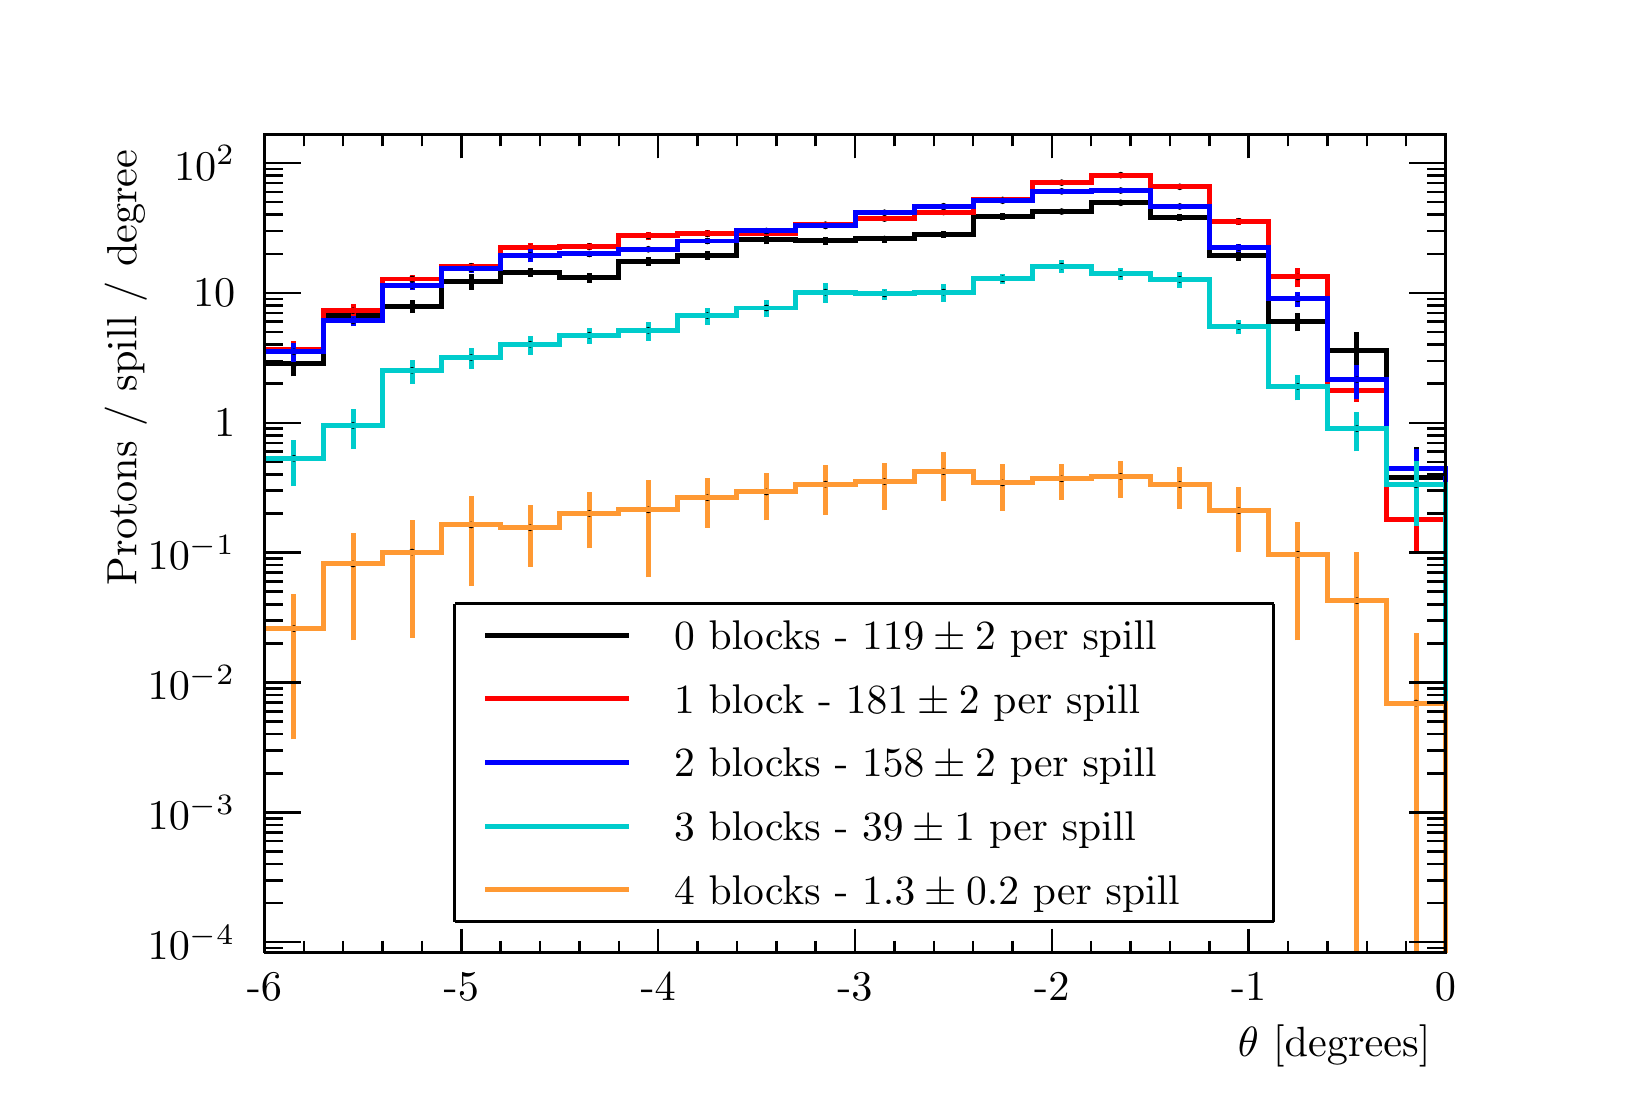
\begin{tikzpicture}
\pgfdeclareplotmark{cross} {
\pgfpathmoveto{\pgfpoint{-0.3\pgfplotmarksize}{\pgfplotmarksize}}
\pgfpathlineto{\pgfpoint{+0.3\pgfplotmarksize}{\pgfplotmarksize}}
\pgfpathlineto{\pgfpoint{+0.3\pgfplotmarksize}{0.3\pgfplotmarksize}}
\pgfpathlineto{\pgfpoint{+1\pgfplotmarksize}{0.3\pgfplotmarksize}}
\pgfpathlineto{\pgfpoint{+1\pgfplotmarksize}{-0.3\pgfplotmarksize}}
\pgfpathlineto{\pgfpoint{+0.3\pgfplotmarksize}{-0.3\pgfplotmarksize}}
\pgfpathlineto{\pgfpoint{+0.3\pgfplotmarksize}{-1.\pgfplotmarksize}}
\pgfpathlineto{\pgfpoint{-0.3\pgfplotmarksize}{-1.\pgfplotmarksize}}
\pgfpathlineto{\pgfpoint{-0.3\pgfplotmarksize}{-0.3\pgfplotmarksize}}
\pgfpathlineto{\pgfpoint{-1.\pgfplotmarksize}{-0.3\pgfplotmarksize}}
\pgfpathlineto{\pgfpoint{-1.\pgfplotmarksize}{0.3\pgfplotmarksize}}
\pgfpathlineto{\pgfpoint{-0.3\pgfplotmarksize}{0.3\pgfplotmarksize}}
\pgfpathclose
\pgfusepathqstroke
}
\pgfdeclareplotmark{cross*} {
\pgfpathmoveto{\pgfpoint{-0.3\pgfplotmarksize}{\pgfplotmarksize}}
\pgfpathlineto{\pgfpoint{+0.3\pgfplotmarksize}{\pgfplotmarksize}}
\pgfpathlineto{\pgfpoint{+0.3\pgfplotmarksize}{0.3\pgfplotmarksize}}
\pgfpathlineto{\pgfpoint{+1\pgfplotmarksize}{0.3\pgfplotmarksize}}
\pgfpathlineto{\pgfpoint{+1\pgfplotmarksize}{-0.3\pgfplotmarksize}}
\pgfpathlineto{\pgfpoint{+0.3\pgfplotmarksize}{-0.3\pgfplotmarksize}}
\pgfpathlineto{\pgfpoint{+0.3\pgfplotmarksize}{-1.\pgfplotmarksize}}
\pgfpathlineto{\pgfpoint{-0.3\pgfplotmarksize}{-1.\pgfplotmarksize}}
\pgfpathlineto{\pgfpoint{-0.3\pgfplotmarksize}{-0.3\pgfplotmarksize}}
\pgfpathlineto{\pgfpoint{-1.\pgfplotmarksize}{-0.3\pgfplotmarksize}}
\pgfpathlineto{\pgfpoint{-1.\pgfplotmarksize}{0.3\pgfplotmarksize}}
\pgfpathlineto{\pgfpoint{-0.3\pgfplotmarksize}{0.3\pgfplotmarksize}}
\pgfpathclose
\pgfusepathqfillstroke
}
\pgfdeclareplotmark{newstar} {
\pgfpathmoveto{\pgfqpoint{0pt}{\pgfplotmarksize}}
\pgfpathlineto{\pgfqpointpolar{44}{0.5\pgfplotmarksize}}
\pgfpathlineto{\pgfqpointpolar{18}{\pgfplotmarksize}}
\pgfpathlineto{\pgfqpointpolar{-20}{0.5\pgfplotmarksize}}
\pgfpathlineto{\pgfqpointpolar{-54}{\pgfplotmarksize}}
\pgfpathlineto{\pgfqpointpolar{-90}{0.5\pgfplotmarksize}}
\pgfpathlineto{\pgfqpointpolar{234}{\pgfplotmarksize}}
\pgfpathlineto{\pgfqpointpolar{198}{0.5\pgfplotmarksize}}
\pgfpathlineto{\pgfqpointpolar{162}{\pgfplotmarksize}}
\pgfpathlineto{\pgfqpointpolar{134}{0.5\pgfplotmarksize}}
\pgfpathclose
\pgfusepathqstroke
}
\pgfdeclareplotmark{newstar*} {
\pgfpathmoveto{\pgfqpoint{0pt}{\pgfplotmarksize}}
\pgfpathlineto{\pgfqpointpolar{44}{0.5\pgfplotmarksize}}
\pgfpathlineto{\pgfqpointpolar{18}{\pgfplotmarksize}}
\pgfpathlineto{\pgfqpointpolar{-20}{0.5\pgfplotmarksize}}
\pgfpathlineto{\pgfqpointpolar{-54}{\pgfplotmarksize}}
\pgfpathlineto{\pgfqpointpolar{-90}{0.5\pgfplotmarksize}}
\pgfpathlineto{\pgfqpointpolar{234}{\pgfplotmarksize}}
\pgfpathlineto{\pgfqpointpolar{198}{0.5\pgfplotmarksize}}
\pgfpathlineto{\pgfqpointpolar{162}{\pgfplotmarksize}}
\pgfpathlineto{\pgfqpointpolar{134}{0.5\pgfplotmarksize}}
\pgfpathclose
\pgfusepathqfillstroke
}
\definecolor{c}{rgb}{1,1,1};
\draw [color=c, fill=c] (0,0) rectangle (20,13.4957);
\draw [color=c, fill=c] (3,1.75444) rectangle (18,12.1461);
\definecolor{c}{rgb}{0,0,0};
\draw [c,line width=0.9] (3,1.75444) -- (3,12.1461) -- (18,12.1461) -- (18,1.75444) -- (3,1.75444);
\definecolor{c}{rgb}{1,1,1};
\draw [color=c, fill=c] (3,1.75444) rectangle (18,12.1461);
\definecolor{c}{rgb}{0,0,0};
\draw [c,line width=0.9] (3,1.75444) -- (3,12.1461) -- (18,12.1461) -- (18,1.75444) -- (3,1.75444);
\draw [c,line width=0.9] (3,1.75444) -- (3.75,1.75444) -- (3.75,1.75444) -- (4.5,1.75444) -- (4.5,1.75444) -- (5.25,1.75444) -- (5.25,1.75444) -- (6,1.75444) -- (6,1.75444) -- (6.75,1.75444) -- (6.75,1.75444) -- (7.5,1.75444) -- (7.5,1.75444) --
 (8.25,1.75444) -- (8.25,1.75444) -- (9,1.75444) -- (9,1.75444) -- (9.75,1.75444) -- (9.75,1.75444) -- (10.5,1.75444) -- (10.5,1.75444) -- (11.25,1.75444) -- (11.25,1.75444) -- (12,1.75444) -- (12,1.75444) -- (12.75,1.75444) -- (12.75,1.75444) --
 (13.5,1.75444) -- (13.5,1.75444) -- (14.25,1.75444) -- (14.25,1.75444) -- (15,1.75444) -- (15,1.75444) -- (15.75,1.75444) -- (15.75,1.75444) -- (16.5,1.75444) -- (16.5,1.75444) -- (17.25,1.75444) -- (17.25,1.75444) -- (18,1.75444) -- (18,1.75444);
\draw [c,line width=0.9] (3,1.75444) -- (18,1.75444);
\draw [c,line width=0.9] (3,2.05809) -- (3,1.75444);
\draw [c,line width=0.9] (3.5,1.90627) -- (3.5,1.75444);
\draw [c,line width=0.9] (4,1.90627) -- (4,1.75444);
\draw [c,line width=0.9] (4.5,1.90627) -- (4.5,1.75444);
\draw [c,line width=0.9] (5,1.90627) -- (5,1.75444);
\draw [c,line width=0.9] (5.5,2.05809) -- (5.5,1.75444);
\draw [c,line width=0.9] (6,1.90627) -- (6,1.75444);
\draw [c,line width=0.9] (6.5,1.90627) -- (6.5,1.75444);
\draw [c,line width=0.9] (7,1.90627) -- (7,1.75444);
\draw [c,line width=0.9] (7.5,1.90627) -- (7.5,1.75444);
\draw [c,line width=0.9] (8,2.05809) -- (8,1.75444);
\draw [c,line width=0.9] (8.5,1.90627) -- (8.5,1.75444);
\draw [c,line width=0.9] (9,1.90627) -- (9,1.75444);
\draw [c,line width=0.9] (9.5,1.90627) -- (9.5,1.75444);
\draw [c,line width=0.9] (10,1.90627) -- (10,1.75444);
\draw [c,line width=0.9] (10.5,2.05809) -- (10.5,1.75444);
\draw [c,line width=0.9] (11,1.90627) -- (11,1.75444);
\draw [c,line width=0.9] (11.5,1.90627) -- (11.5,1.75444);
\draw [c,line width=0.9] (12,1.90627) -- (12,1.75444);
\draw [c,line width=0.9] (12.5,1.90627) -- (12.5,1.75444);
\draw [c,line width=0.9] (13,2.05809) -- (13,1.75444);
\draw [c,line width=0.9] (13.5,1.90627) -- (13.5,1.75444);
\draw [c,line width=0.9] (14,1.90627) -- (14,1.75444);
\draw [c,line width=0.9] (14.5,1.90627) -- (14.5,1.75444);
\draw [c,line width=0.9] (15,1.90627) -- (15,1.75444);
\draw [c,line width=0.9] (15.5,2.05809) -- (15.5,1.75444);
\draw [c,line width=0.9] (16,1.90627) -- (16,1.75444);
\draw [c,line width=0.9] (16.5,1.90627) -- (16.5,1.75444);
\draw [c,line width=0.9] (17,1.90627) -- (17,1.75444);
\draw [c,line width=0.9] (17.5,1.90627) -- (17.5,1.75444);
\draw [c,line width=0.9] (18,2.05809) -- (18,1.75444);
\draw [anchor=base] (3,1.14713) node[scale=1.52731, color=c, rotate=0]{-6};
\draw [anchor=base] (5.5,1.14713) node[scale=1.52731, color=c, rotate=0]{-5};
\draw [anchor=base] (8,1.14713) node[scale=1.52731, color=c, rotate=0]{-4};
\draw [anchor=base] (10.5,1.14713) node[scale=1.52731, color=c, rotate=0]{-3};
\draw [anchor=base] (13,1.14713) node[scale=1.52731, color=c, rotate=0]{-2};
\draw [anchor=base] (15.5,1.14713) node[scale=1.52731, color=c, rotate=0]{-1};
\draw [anchor=base] (18,1.14713) node[scale=1.52731, color=c, rotate=0]{0};
\draw [anchor= east] (18,0.566819) node[scale=1.52731, color=c, rotate=0]{$ \theta$ [degrees]};
\draw [c,line width=0.9] (3,12.1461) -- (18,12.1461);
\draw [c,line width=0.9] (3,11.8425) -- (3,12.1461);
\draw [c,line width=0.9] (3.5,11.9943) -- (3.5,12.1461);
\draw [c,line width=0.9] (4,11.9943) -- (4,12.1461);
\draw [c,line width=0.9] (4.5,11.9943) -- (4.5,12.1461);
\draw [c,line width=0.9] (5,11.9943) -- (5,12.1461);
\draw [c,line width=0.9] (5.5,11.8425) -- (5.5,12.1461);
\draw [c,line width=0.9] (6,11.9943) -- (6,12.1461);
\draw [c,line width=0.9] (6.5,11.9943) -- (6.5,12.1461);
\draw [c,line width=0.9] (7,11.9943) -- (7,12.1461);
\draw [c,line width=0.9] (7.5,11.9943) -- (7.5,12.1461);
\draw [c,line width=0.9] (8,11.8425) -- (8,12.1461);
\draw [c,line width=0.9] (8.5,11.9943) -- (8.5,12.1461);
\draw [c,line width=0.9] (9,11.9943) -- (9,12.1461);
\draw [c,line width=0.9] (9.5,11.9943) -- (9.5,12.1461);
\draw [c,line width=0.9] (10,11.9943) -- (10,12.1461);
\draw [c,line width=0.9] (10.5,11.8425) -- (10.5,12.1461);
\draw [c,line width=0.9] (11,11.9943) -- (11,12.1461);
\draw [c,line width=0.9] (11.5,11.9943) -- (11.5,12.1461);
\draw [c,line width=0.9] (12,11.9943) -- (12,12.1461);
\draw [c,line width=0.9] (12.5,11.9943) -- (12.5,12.1461);
\draw [c,line width=0.9] (13,11.8425) -- (13,12.1461);
\draw [c,line width=0.9] (13.5,11.9943) -- (13.5,12.1461);
\draw [c,line width=0.9] (14,11.9943) -- (14,12.1461);
\draw [c,line width=0.9] (14.5,11.9943) -- (14.5,12.1461);
\draw [c,line width=0.9] (15,11.9943) -- (15,12.1461);
\draw [c,line width=0.9] (15.5,11.8425) -- (15.5,12.1461);
\draw [c,line width=0.9] (16,11.9943) -- (16,12.1461);
\draw [c,line width=0.9] (16.5,11.9943) -- (16.5,12.1461);
\draw [c,line width=0.9] (17,11.9943) -- (17,12.1461);
\draw [c,line width=0.9] (17.5,11.9943) -- (17.5,12.1461);
\draw [c,line width=0.9] (18,11.8425) -- (18,12.1461);
\draw [c,line width=0.9] (3,1.75444) -- (3,12.1461);
\draw [c,line width=0.9] (3.231,1.81225) -- (3,1.81225);
\draw [c,line width=0.9] (3.462,1.88772) -- (3,1.88772);
\draw [anchor= east] (2.82,1.88772) node[scale=1.52731, color=c, rotate=0]{$10^{-4}$};
\draw [c,line width=0.9] (3.231,2.38422) -- (3,2.38422);
\draw [c,line width=0.9] (3.231,2.67466) -- (3,2.67466);
\draw [c,line width=0.9] (3.231,2.88072) -- (3,2.88072);
\draw [c,line width=0.9] (3.231,3.04056) -- (3,3.04056);
\draw [c,line width=0.9] (3.231,3.17116) -- (3,3.17116);
\draw [c,line width=0.9] (3.231,3.28158) -- (3,3.28158);
\draw [c,line width=0.9] (3.231,3.37722) -- (3,3.37722);
\draw [c,line width=0.9] (3.231,3.46159) -- (3,3.46159);
\draw [c,line width=0.9] (3.462,3.53706) -- (3,3.53706);
\draw [anchor= east] (2.82,3.53706) node[scale=1.52731, color=c, rotate=0]{$10^{-3}$};
\draw [c,line width=0.9] (3.231,4.03357) -- (3,4.03357);
\draw [c,line width=0.9] (3.231,4.324) -- (3,4.324);
\draw [c,line width=0.9] (3.231,4.53007) -- (3,4.53007);
\draw [c,line width=0.9] (3.231,4.68991) -- (3,4.68991);
\draw [c,line width=0.9] (3.231,4.8205) -- (3,4.8205);
\draw [c,line width=0.9] (3.231,4.93092) -- (3,4.93092);
\draw [c,line width=0.9] (3.231,5.02657) -- (3,5.02657);
\draw [c,line width=0.9] (3.231,5.11094) -- (3,5.11094);
\draw [c,line width=0.9] (3.462,5.18641) -- (3,5.18641);
\draw [anchor= east] (2.82,5.18641) node[scale=1.52731, color=c, rotate=0]{$10^{-2}$};
\draw [c,line width=0.9] (3.231,5.68291) -- (3,5.68291);
\draw [c,line width=0.9] (3.231,5.97335) -- (3,5.97335);
\draw [c,line width=0.9] (3.231,6.17941) -- (3,6.17941);
\draw [c,line width=0.9] (3.231,6.33925) -- (3,6.33925);
\draw [c,line width=0.9] (3.231,6.46985) -- (3,6.46985);
\draw [c,line width=0.9] (3.231,6.58027) -- (3,6.58027);
\draw [c,line width=0.9] (3.231,6.67592) -- (3,6.67592);
\draw [c,line width=0.9] (3.231,6.76028) -- (3,6.76028);
\draw [c,line width=0.9] (3.462,6.83575) -- (3,6.83575);
\draw [anchor= east] (2.82,6.83575) node[scale=1.52731, color=c, rotate=0]{$10^{-1}$};
\draw [c,line width=0.9] (3.231,7.33226) -- (3,7.33226);
\draw [c,line width=0.9] (3.231,7.62269) -- (3,7.62269);
\draw [c,line width=0.9] (3.231,7.82876) -- (3,7.82876);
\draw [c,line width=0.9] (3.231,7.9886) -- (3,7.9886);
\draw [c,line width=0.9] (3.231,8.11919) -- (3,8.11919);
\draw [c,line width=0.9] (3.231,8.22961) -- (3,8.22961);
\draw [c,line width=0.9] (3.231,8.32526) -- (3,8.32526);
\draw [c,line width=0.9] (3.231,8.40963) -- (3,8.40963);
\draw [c,line width=0.9] (3.462,8.4851) -- (3,8.4851);
\draw [anchor= east] (2.82,8.4851) node[scale=1.52731, color=c, rotate=0]{1};
\draw [c,line width=0.9] (3.231,8.9816) -- (3,8.9816);
\draw [c,line width=0.9] (3.231,9.27204) -- (3,9.27204);
\draw [c,line width=0.9] (3.231,9.4781) -- (3,9.4781);
\draw [c,line width=0.9] (3.231,9.63794) -- (3,9.63794);
\draw [c,line width=0.9] (3.231,9.76854) -- (3,9.76854);
\draw [c,line width=0.9] (3.231,9.87896) -- (3,9.87896);
\draw [c,line width=0.9] (3.231,9.97461) -- (3,9.97461);
\draw [c,line width=0.9] (3.231,10.059) -- (3,10.059);
\draw [c,line width=0.9] (3.462,10.1344) -- (3,10.1344);
\draw [anchor= east] (2.82,10.1344) node[scale=1.52731, color=c, rotate=0]{10};
\draw [c,line width=0.9] (3.231,10.6309) -- (3,10.6309);
\draw [c,line width=0.9] (3.231,10.9214) -- (3,10.9214);
\draw [c,line width=0.9] (3.231,11.1274) -- (3,11.1274);
\draw [c,line width=0.9] (3.231,11.2873) -- (3,11.2873);
\draw [c,line width=0.9] (3.231,11.4179) -- (3,11.4179);
\draw [c,line width=0.9] (3.231,11.5283) -- (3,11.5283);
\draw [c,line width=0.9] (3.231,11.624) -- (3,11.624);
\draw [c,line width=0.9] (3.231,11.7083) -- (3,11.7083);
\draw [c,line width=0.9] (3.462,11.7838) -- (3,11.7838);
\draw [anchor= east] (2.82,11.7838) node[scale=1.52731, color=c, rotate=0]{$10^{2}$};
\draw [anchor= east] (1.24,12.1461) node[scale=1.52731, color=c, rotate=90]{ Protons / spill / degree};
\draw [c,line width=0.9] (18,1.75444) -- (18,12.1461);
\draw [c,line width=0.9] (17.769,1.81225) -- (18,1.81225);
\draw [c,line width=0.9] (17.538,1.88772) -- (18,1.88772);
\draw [c,line width=0.9] (17.769,2.38422) -- (18,2.38422);
\draw [c,line width=0.9] (17.769,2.67466) -- (18,2.67466);
\draw [c,line width=0.9] (17.769,2.88072) -- (18,2.88072);
\draw [c,line width=0.9] (17.769,3.04056) -- (18,3.04056);
\draw [c,line width=0.9] (17.769,3.17116) -- (18,3.17116);
\draw [c,line width=0.9] (17.769,3.28158) -- (18,3.28158);
\draw [c,line width=0.9] (17.769,3.37722) -- (18,3.37722);
\draw [c,line width=0.9] (17.769,3.46159) -- (18,3.46159);
\draw [c,line width=0.9] (17.538,3.53706) -- (18,3.53706);
\draw [c,line width=0.9] (17.769,4.03357) -- (18,4.03357);
\draw [c,line width=0.9] (17.769,4.324) -- (18,4.324);
\draw [c,line width=0.9] (17.769,4.53007) -- (18,4.53007);
\draw [c,line width=0.9] (17.769,4.68991) -- (18,4.68991);
\draw [c,line width=0.9] (17.769,4.8205) -- (18,4.8205);
\draw [c,line width=0.9] (17.769,4.93092) -- (18,4.93092);
\draw [c,line width=0.9] (17.769,5.02657) -- (18,5.02657);
\draw [c,line width=0.9] (17.769,5.11094) -- (18,5.11094);
\draw [c,line width=0.9] (17.538,5.18641) -- (18,5.18641);
\draw [c,line width=0.9] (17.769,5.68291) -- (18,5.68291);
\draw [c,line width=0.9] (17.769,5.97335) -- (18,5.97335);
\draw [c,line width=0.9] (17.769,6.17941) -- (18,6.17941);
\draw [c,line width=0.9] (17.769,6.33925) -- (18,6.33925);
\draw [c,line width=0.9] (17.769,6.46985) -- (18,6.46985);
\draw [c,line width=0.9] (17.769,6.58027) -- (18,6.58027);
\draw [c,line width=0.9] (17.769,6.67592) -- (18,6.67592);
\draw [c,line width=0.9] (17.769,6.76028) -- (18,6.76028);
\draw [c,line width=0.9] (17.538,6.83575) -- (18,6.83575);
\draw [c,line width=0.9] (17.769,7.33226) -- (18,7.33226);
\draw [c,line width=0.9] (17.769,7.62269) -- (18,7.62269);
\draw [c,line width=0.9] (17.769,7.82876) -- (18,7.82876);
\draw [c,line width=0.9] (17.769,7.9886) -- (18,7.9886);
\draw [c,line width=0.9] (17.769,8.11919) -- (18,8.11919);
\draw [c,line width=0.9] (17.769,8.22961) -- (18,8.22961);
\draw [c,line width=0.9] (17.769,8.32526) -- (18,8.32526);
\draw [c,line width=0.9] (17.769,8.40963) -- (18,8.40963);
\draw [c,line width=0.9] (17.538,8.4851) -- (18,8.4851);
\draw [c,line width=0.9] (17.769,8.9816) -- (18,8.9816);
\draw [c,line width=0.9] (17.769,9.27204) -- (18,9.27204);
\draw [c,line width=0.9] (17.769,9.4781) -- (18,9.4781);
\draw [c,line width=0.9] (17.769,9.63794) -- (18,9.63794);
\draw [c,line width=0.9] (17.769,9.76854) -- (18,9.76854);
\draw [c,line width=0.9] (17.769,9.87896) -- (18,9.87896);
\draw [c,line width=0.9] (17.769,9.97461) -- (18,9.97461);
\draw [c,line width=0.9] (17.769,10.059) -- (18,10.059);
\draw [c,line width=0.9] (17.538,10.1344) -- (18,10.1344);
\draw [c,line width=0.9] (17.769,10.6309) -- (18,10.6309);
\draw [c,line width=0.9] (17.769,10.9214) -- (18,10.9214);
\draw [c,line width=0.9] (17.769,11.1274) -- (18,11.1274);
\draw [c,line width=0.9] (17.769,11.2873) -- (18,11.2873);
\draw [c,line width=0.9] (17.769,11.4179) -- (18,11.4179);
\draw [c,line width=0.9] (17.769,11.5283) -- (18,11.5283);
\draw [c,line width=0.9] (17.769,11.624) -- (18,11.624);
\draw [c,line width=0.9] (17.769,11.7083) -- (18,11.7083);
\draw [c,line width=0.9] (17.538,11.7838) -- (18,11.7838);
\draw [c,line width=1.8] (3.375,9.07502) -- (3.375,9.23213);
\draw [c,line width=1.8] (3.375,9.23213) -- (3.375,9.3609);
\foreach \P in {(3.375,9.23213)}{\draw[mark options={color=c,fill=c},mark size=2.402402pt,mark=*,mark size=1pt] plot coordinates {\P};}
\draw [c,line width=1.8] (4.125,9.75966) -- (4.125,9.85284);
\draw [c,line width=1.8] (4.125,9.85284) -- (4.125,9.93528);
\foreach \P in {(4.125,9.85284)}{\draw[mark options={color=c,fill=c},mark size=2.402402pt,mark=*,mark size=1pt] plot coordinates {\P};}
\draw [c,line width=1.8] (4.875,9.87682) -- (4.875,9.96395);
\draw [c,line width=1.8] (4.875,9.96395) -- (4.875,10.0416);
\foreach \P in {(4.875,9.96395)}{\draw[mark options={color=c,fill=c},mark size=2.402402pt,mark=*,mark size=1pt] plot coordinates {\P};}
\draw [c,line width=1.8] (5.625,10.1726) -- (5.625,10.2788);
\draw [c,line width=1.8] (5.625,10.2788) -- (5.625,10.3713);
\foreach \P in {(5.625,10.2788)}{\draw[mark options={color=c,fill=c},mark size=2.402402pt,mark=*,mark size=1pt] plot coordinates {\P};}
\draw [c,line width=1.8] (6.375,10.3373) -- (6.375,10.3992);
\draw [c,line width=1.8] (6.375,10.3992) -- (6.375,10.4562);
\foreach \P in {(6.375,10.3992)}{\draw[mark options={color=c,fill=c},mark size=2.402402pt,mark=*,mark size=1pt] plot coordinates {\P};}
\draw [c,line width=1.8] (7.125,10.2656) -- (7.125,10.3311);
\draw [c,line width=1.8] (7.125,10.3311) -- (7.125,10.3911);
\foreach \P in {(7.125,10.3311)}{\draw[mark options={color=c,fill=c},mark size=2.402402pt,mark=*,mark size=1pt] plot coordinates {\P};}
\draw [c,line width=1.8] (7.875,10.4763) -- (7.875,10.5374);
\draw [c,line width=1.8] (7.875,10.5374) -- (7.875,10.5938);
\foreach \P in {(7.875,10.5374)}{\draw[mark options={color=c,fill=c},mark size=2.402402pt,mark=*,mark size=1pt] plot coordinates {\P};}
\draw [c,line width=1.8] (8.625,10.5567) -- (8.625,10.6116);
\draw [c,line width=1.8] (8.625,10.6116) -- (8.625,10.6626);
\foreach \P in {(8.625,10.6116)}{\draw[mark options={color=c,fill=c},mark size=2.402402pt,mark=*,mark size=1pt] plot coordinates {\P};}
\draw [c,line width=1.8] (9.375,10.7503) -- (9.375,10.8141);
\draw [c,line width=1.8] (9.375,10.8141) -- (9.375,10.8726);
\foreach \P in {(9.375,10.8141)}{\draw[mark options={color=c,fill=c},mark size=2.402402pt,mark=*,mark size=1pt] plot coordinates {\P};}
\draw [c,line width=1.8] (10.125,10.7469) -- (10.125,10.7963);
\draw [c,line width=1.8] (10.125,10.7963) -- (10.125,10.8425);
\foreach \P in {(10.125,10.7963)}{\draw[mark options={color=c,fill=c},mark size=2.402402pt,mark=*,mark size=1pt] plot coordinates {\P};}
\draw [c,line width=1.8] (10.875,10.7735) -- (10.875,10.8191);
\draw [c,line width=1.8] (10.875,10.8191) -- (10.875,10.8619);
\foreach \P in {(10.875,10.8191)}{\draw[mark options={color=c,fill=c},mark size=2.402402pt,mark=*,mark size=1pt] plot coordinates {\P};}
\draw [c,line width=1.8] (11.625,10.8337) -- (11.625,10.877);
\draw [c,line width=1.8] (11.625,10.877) -- (11.625,10.9179);
\foreach \P in {(11.625,10.877)}{\draw[mark options={color=c,fill=c},mark size=2.402402pt,mark=*,mark size=1pt] plot coordinates {\P};}
\draw [c,line width=1.8] (12.375,11.0626) -- (12.375,11.1046);
\draw [c,line width=1.8] (12.375,11.1046) -- (12.375,11.1444);
\foreach \P in {(12.375,11.1046)}{\draw[mark options={color=c,fill=c},mark size=2.402402pt,mark=*,mark size=1pt] plot coordinates {\P};}
\draw [c,line width=1.8] (13.125,11.1339) -- (13.125,11.1675);
\draw [c,line width=1.8] (13.125,11.1675) -- (13.125,11.1996);
\foreach \P in {(13.125,11.1675)}{\draw[mark options={color=c,fill=c},mark size=2.402402pt,mark=*,mark size=1pt] plot coordinates {\P};}
\draw [c,line width=1.8] (13.875,11.2461) -- (13.875,11.2785);
\draw [c,line width=1.8] (13.875,11.2785) -- (13.875,11.3096);
\foreach \P in {(13.875,11.2785)}{\draw[mark options={color=c,fill=c},mark size=2.402402pt,mark=*,mark size=1pt] plot coordinates {\P};}
\draw [c,line width=1.8] (14.625,11.0483) -- (14.625,11.0912);
\draw [c,line width=1.8] (14.625,11.0912) -- (14.625,11.1317);
\foreach \P in {(14.625,11.0912)}{\draw[mark options={color=c,fill=c},mark size=2.402402pt,mark=*,mark size=1pt] plot coordinates {\P};}
\draw [c,line width=1.8] (15.375,10.5449) -- (15.375,10.608);
\draw [c,line width=1.8] (15.375,10.608) -- (15.375,10.666);
\foreach \P in {(15.375,10.608)}{\draw[mark options={color=c,fill=c},mark size=2.402402pt,mark=*,mark size=1pt] plot coordinates {\P};}
\draw [c,line width=1.8] (16.125,9.64718) -- (16.125,9.77334);
\draw [c,line width=1.8] (16.125,9.77334) -- (16.125,9.88057);
\foreach \P in {(16.125,9.77334)}{\draw[mark options={color=c,fill=c},mark size=2.402402pt,mark=*,mark size=1pt] plot coordinates {\P};}
\draw [c,line width=1.8] (16.875,9.05435) -- (16.875,9.40081);
\draw [c,line width=1.8] (16.875,9.40081) -- (16.875,9.63333);
\foreach \P in {(16.875,9.40081)}{\draw[mark options={color=c,fill=c},mark size=2.402402pt,mark=*,mark size=1pt] plot coordinates {\P};}
\draw [c,line width=1.8] (17.625,6.89102) -- (17.625,7.79455);
\draw [c,line width=1.8] (17.625,7.79455) -- (17.625,8.18165);
\foreach \P in {(17.625,7.79455)}{\draw[mark options={color=c,fill=c},mark size=2.402402pt,mark=*,mark size=1pt] plot coordinates {\P};}
\draw [c,line width=1.8] (3,9.23213) -- (3.75,9.23213) -- (3.75,9.85284) -- (4.5,9.85284) -- (4.5,9.96395) -- (5.25,9.96395) -- (5.25,10.2788) -- (6,10.2788) -- (6,10.3992) -- (6.75,10.3992) -- (6.75,10.3311) -- (7.5,10.3311) -- (7.5,10.5374) --
 (8.25,10.5374) -- (8.25,10.6116) -- (9,10.6116) -- (9,10.8141) -- (9.75,10.8141) -- (9.75,10.7963) -- (10.5,10.7963) -- (10.5,10.8191) -- (11.25,10.8191) -- (11.25,10.877) -- (12,10.877) -- (12,11.1046) -- (12.75,11.1046) -- (12.75,11.1675) --
 (13.5,11.1675) -- (13.5,11.2785) -- (14.25,11.2785) -- (14.25,11.0912) -- (15,11.0912) -- (15,10.608) -- (15.75,10.608) -- (15.75,9.77334) -- (16.5,9.77334) -- (16.5,9.40081) -- (17.25,9.40081) -- (17.25,7.79455) -- (18,7.79455) -- (18,1.75444);
\definecolor{c}{rgb}{1,0,0};
\draw [c,line width=1.8] (3.375,9.29318) -- (3.375,9.41497);
\draw [c,line width=1.8] (3.375,9.41497) -- (3.375,9.51902);
\definecolor{c}{rgb}{0,0,0};
\foreach \P in {(3.375,9.41497)}{\draw[mark options={color=c,fill=c},mark size=2.402402pt,mark=*,mark size=1pt] plot coordinates {\P};}
\definecolor{c}{rgb}{1,0,0};
\draw [c,line width=1.8] (4.125,9.80481) -- (4.125,9.90725);
\draw [c,line width=1.8] (4.125,9.90725) -- (4.125,9.99686);
\definecolor{c}{rgb}{0,0,0};
\foreach \P in {(4.125,9.90725)}{\draw[mark options={color=c,fill=c},mark size=2.402402pt,mark=*,mark size=1pt] plot coordinates {\P};}
\definecolor{c}{rgb}{1,0,0};
\draw [c,line width=1.8] (4.875,10.249) -- (4.875,10.3108);
\draw [c,line width=1.8] (4.875,10.3108) -- (4.875,10.3677);
\definecolor{c}{rgb}{0,0,0};
\foreach \P in {(4.875,10.3108)}{\draw[mark options={color=c,fill=c},mark size=2.402402pt,mark=*,mark size=1pt] plot coordinates {\P};}
\definecolor{c}{rgb}{1,0,0};
\draw [c,line width=1.8] (5.625,10.4221) -- (5.625,10.4723);
\draw [c,line width=1.8] (5.625,10.4723) -- (5.625,10.5191);
\definecolor{c}{rgb}{0,0,0};
\foreach \P in {(5.625,10.4723)}{\draw[mark options={color=c,fill=c},mark size=2.402402pt,mark=*,mark size=1pt] plot coordinates {\P};}
\definecolor{c}{rgb}{1,0,0};
\draw [c,line width=1.8] (6.375,10.6326) -- (6.375,10.7055);
\draw [c,line width=1.8] (6.375,10.7055) -- (6.375,10.7716);
\definecolor{c}{rgb}{0,0,0};
\foreach \P in {(6.375,10.7055)}{\draw[mark options={color=c,fill=c},mark size=2.402402pt,mark=*,mark size=1pt] plot coordinates {\P};}
\definecolor{c}{rgb}{1,0,0};
\draw [c,line width=1.8] (7.125,10.6743) -- (7.125,10.7239);
\draw [c,line width=1.8] (7.125,10.7239) -- (7.125,10.7702);
\definecolor{c}{rgb}{0,0,0};
\foreach \P in {(7.125,10.7239)}{\draw[mark options={color=c,fill=c},mark size=2.402402pt,mark=*,mark size=1pt] plot coordinates {\P};}
\definecolor{c}{rgb}{1,0,0};
\draw [c,line width=1.8] (7.875,10.8026) -- (7.875,10.8576);
\draw [c,line width=1.8] (7.875,10.8576) -- (7.875,10.9087);
\definecolor{c}{rgb}{0,0,0};
\foreach \P in {(7.875,10.8576)}{\draw[mark options={color=c,fill=c},mark size=2.402402pt,mark=*,mark size=1pt] plot coordinates {\P};}
\definecolor{c}{rgb}{1,0,0};
\draw [c,line width=1.8] (8.625,10.8427) -- (8.625,10.8862);
\draw [c,line width=1.8] (8.625,10.8862) -- (8.625,10.9272);
\definecolor{c}{rgb}{0,0,0};
\foreach \P in {(8.625,10.8862)}{\draw[mark options={color=c,fill=c},mark size=2.402402pt,mark=*,mark size=1pt] plot coordinates {\P};}
\definecolor{c}{rgb}{1,0,0};
\draw [c,line width=1.8] (9.375,10.8581) -- (9.375,10.8913);
\draw [c,line width=1.8] (9.375,10.8913) -- (9.375,10.923);
\definecolor{c}{rgb}{0,0,0};
\foreach \P in {(9.375,10.8913)}{\draw[mark options={color=c,fill=c},mark size=2.402402pt,mark=*,mark size=1pt] plot coordinates {\P};}
\definecolor{c}{rgb}{1,0,0};
\draw [c,line width=1.8] (10.125,10.9658) -- (10.125,11.0008);
\draw [c,line width=1.8] (10.125,11.0008) -- (10.125,11.0341);
\definecolor{c}{rgb}{0,0,0};
\foreach \P in {(10.125,11.0008)}{\draw[mark options={color=c,fill=c},mark size=2.402402pt,mark=*,mark size=1pt] plot coordinates {\P};}
\definecolor{c}{rgb}{1,0,0};
\draw [c,line width=1.8] (10.875,11.0434) -- (10.875,11.0777);
\draw [c,line width=1.8] (10.875,11.0777) -- (10.875,11.1105);
\definecolor{c}{rgb}{0,0,0};
\foreach \P in {(10.875,11.0777)}{\draw[mark options={color=c,fill=c},mark size=2.402402pt,mark=*,mark size=1pt] plot coordinates {\P};}
\definecolor{c}{rgb}{1,0,0};
\draw [c,line width=1.8] (11.625,11.1321) -- (11.625,11.1615);
\draw [c,line width=1.8] (11.625,11.1615) -- (11.625,11.1898);
\definecolor{c}{rgb}{0,0,0};
\foreach \P in {(11.625,11.1615)}{\draw[mark options={color=c,fill=c},mark size=2.402402pt,mark=*,mark size=1pt] plot coordinates {\P};}
\definecolor{c}{rgb}{1,0,0};
\draw [c,line width=1.8] (12.375,11.2866) -- (12.375,11.3151);
\draw [c,line width=1.8] (12.375,11.3151) -- (12.375,11.3425);
\definecolor{c}{rgb}{0,0,0};
\foreach \P in {(12.375,11.3151)}{\draw[mark options={color=c,fill=c},mark size=2.402402pt,mark=*,mark size=1pt] plot coordinates {\P};}
\definecolor{c}{rgb}{1,0,0};
\draw [c,line width=1.8] (13.125,11.5124) -- (13.125,11.5342);
\draw [c,line width=1.8] (13.125,11.5342) -- (13.125,11.5554);
\definecolor{c}{rgb}{0,0,0};
\foreach \P in {(13.125,11.5342)}{\draw[mark options={color=c,fill=c},mark size=2.402402pt,mark=*,mark size=1pt] plot coordinates {\P};}
\definecolor{c}{rgb}{1,0,0};
\draw [c,line width=1.8] (13.875,11.6021) -- (13.875,11.6298);
\draw [c,line width=1.8] (13.875,11.6298) -- (13.875,11.6565);
\definecolor{c}{rgb}{0,0,0};
\foreach \P in {(13.875,11.6298)}{\draw[mark options={color=c,fill=c},mark size=2.402402pt,mark=*,mark size=1pt] plot coordinates {\P};}
\definecolor{c}{rgb}{1,0,0};
\draw [c,line width=1.8] (14.625,11.4519) -- (14.625,11.4816);
\draw [c,line width=1.8] (14.625,11.4816) -- (14.625,11.51);
\definecolor{c}{rgb}{0,0,0};
\foreach \P in {(14.625,11.4816)}{\draw[mark options={color=c,fill=c},mark size=2.402402pt,mark=*,mark size=1pt] plot coordinates {\P};}
\definecolor{c}{rgb}{1,0,0};
\draw [c,line width=1.8] (15.375,10.9998) -- (15.375,11.0445);
\draw [c,line width=1.8] (15.375,11.0445) -- (15.375,11.0866);
\definecolor{c}{rgb}{0,0,0};
\foreach \P in {(15.375,11.0445)}{\draw[mark options={color=c,fill=c},mark size=2.402402pt,mark=*,mark size=1pt] plot coordinates {\P};}
\definecolor{c}{rgb}{1,0,0};
\draw [c,line width=1.8] (16.125,10.2048) -- (16.125,10.3367);
\draw [c,line width=1.8] (16.125,10.3367) -- (16.125,10.4481);
\definecolor{c}{rgb}{0,0,0};
\foreach \P in {(16.125,10.3367)}{\draw[mark options={color=c,fill=c},mark size=2.402402pt,mark=*,mark size=1pt] plot coordinates {\P};}
\definecolor{c}{rgb}{1,0,0};
\draw [c,line width=1.8] (16.875,8.75069) -- (16.875,8.89064);
\draw [c,line width=1.8] (16.875,8.89064) -- (16.875,9.00767);
\definecolor{c}{rgb}{0,0,0};
\foreach \P in {(16.875,8.89064)}{\draw[mark options={color=c,fill=c},mark size=2.402402pt,mark=*,mark size=1pt] plot coordinates {\P};}
\definecolor{c}{rgb}{1,0,0};
\draw [c,line width=1.8] (17.625,6.83079) -- (17.625,7.25361);
\draw [c,line width=1.8] (17.625,7.25361) -- (17.625,7.51769);
\definecolor{c}{rgb}{0,0,0};
\foreach \P in {(17.625,7.25361)}{\draw[mark options={color=c,fill=c},mark size=2.402402pt,mark=*,mark size=1pt] plot coordinates {\P};}
\definecolor{c}{rgb}{1,0,0};
\draw [c,line width=1.8] (3,9.41497) -- (3.75,9.41497) -- (3.75,9.90725) -- (4.5,9.90725) -- (4.5,10.3108) -- (5.25,10.3108) -- (5.25,10.4723) -- (6,10.4723) -- (6,10.7055) -- (6.75,10.7055) -- (6.75,10.7239) -- (7.5,10.7239) -- (7.5,10.8576) --
 (8.25,10.8576) -- (8.25,10.8862) -- (9,10.8862) -- (9,10.8913) -- (9.75,10.8913) -- (9.75,11.0008) -- (10.5,11.0008) -- (10.5,11.0777) -- (11.25,11.0777) -- (11.25,11.1615) -- (12,11.1615) -- (12,11.3151) -- (12.75,11.3151) -- (12.75,11.5342) --
 (13.5,11.5342) -- (13.5,11.6298) -- (14.25,11.6298) -- (14.25,11.4816) -- (15,11.4816) -- (15,11.0445) -- (15.75,11.0445) -- (15.75,10.3367) -- (16.5,10.3367) -- (16.5,8.89064) -- (17.25,8.89064) -- (17.25,7.25361) -- (18,7.25361) -- (18,1.75444);
\definecolor{c}{rgb}{0,0,1};
\draw [c,line width=1.8] (3.375,9.26219) -- (3.375,9.38668);
\draw [c,line width=1.8] (3.375,9.38668) -- (3.375,9.4927);
\definecolor{c}{rgb}{0,0,0};
\foreach \P in {(3.375,9.38668)}{\draw[mark options={color=c,fill=c},mark size=2.402402pt,mark=*,mark size=1pt] plot coordinates {\P};}
\definecolor{c}{rgb}{0,0,1};
\draw [c,line width=1.8] (4.125,9.70904) -- (4.125,9.77916);
\draw [c,line width=1.8] (4.125,9.77916) -- (4.125,9.84303);
\definecolor{c}{rgb}{0,0,0};
\foreach \P in {(4.125,9.77916)}{\draw[mark options={color=c,fill=c},mark size=2.402402pt,mark=*,mark size=1pt] plot coordinates {\P};}
\definecolor{c}{rgb}{0,0,1};
\draw [c,line width=1.8] (4.875,10.1747) -- (4.875,10.2284);
\draw [c,line width=1.8] (4.875,10.2284) -- (4.875,10.2784);
\definecolor{c}{rgb}{0,0,0};
\foreach \P in {(4.875,10.2284)}{\draw[mark options={color=c,fill=c},mark size=2.402402pt,mark=*,mark size=1pt] plot coordinates {\P};}
\definecolor{c}{rgb}{0,0,1};
\draw [c,line width=1.8] (5.625,10.3923) -- (5.625,10.4383);
\draw [c,line width=1.8] (5.625,10.4383) -- (5.625,10.4816);
\definecolor{c}{rgb}{0,0,0};
\foreach \P in {(5.625,10.4383)}{\draw[mark options={color=c,fill=c},mark size=2.402402pt,mark=*,mark size=1pt] plot coordinates {\P};}
\definecolor{c}{rgb}{0,0,1};
\draw [c,line width=1.8] (6.375,10.5222) -- (6.375,10.6123);
\draw [c,line width=1.8] (6.375,10.6123) -- (6.375,10.6922);
\definecolor{c}{rgb}{0,0,0};
\foreach \P in {(6.375,10.6123)}{\draw[mark options={color=c,fill=c},mark size=2.402402pt,mark=*,mark size=1pt] plot coordinates {\P};}
\definecolor{c}{rgb}{0,0,1};
\draw [c,line width=1.8] (7.125,10.5909) -- (7.125,10.629);
\draw [c,line width=1.8] (7.125,10.629) -- (7.125,10.6652);
\definecolor{c}{rgb}{0,0,0};
\foreach \P in {(7.125,10.629)}{\draw[mark options={color=c,fill=c},mark size=2.402402pt,mark=*,mark size=1pt] plot coordinates {\P};}
\definecolor{c}{rgb}{0,0,1};
\draw [c,line width=1.8] (7.875,10.6551) -- (7.875,10.6884);
\draw [c,line width=1.8] (7.875,10.6884) -- (7.875,10.7202);
\definecolor{c}{rgb}{0,0,0};
\foreach \P in {(7.875,10.6884)}{\draw[mark options={color=c,fill=c},mark size=2.402402pt,mark=*,mark size=1pt] plot coordinates {\P};}
\definecolor{c}{rgb}{0,0,1};
\draw [c,line width=1.8] (8.625,10.76) -- (8.625,10.7933);
\draw [c,line width=1.8] (8.625,10.7933) -- (8.625,10.8251);
\definecolor{c}{rgb}{0,0,0};
\foreach \P in {(8.625,10.7933)}{\draw[mark options={color=c,fill=c},mark size=2.402402pt,mark=*,mark size=1pt] plot coordinates {\P};}
\definecolor{c}{rgb}{0,0,1};
\draw [c,line width=1.8] (9.375,10.888) -- (9.375,10.9207);
\draw [c,line width=1.8] (9.375,10.9207) -- (9.375,10.952);
\definecolor{c}{rgb}{0,0,0};
\foreach \P in {(9.375,10.9207)}{\draw[mark options={color=c,fill=c},mark size=2.402402pt,mark=*,mark size=1pt] plot coordinates {\P};}
\definecolor{c}{rgb}{0,0,1};
\draw [c,line width=1.8] (10.125,10.9536) -- (10.125,10.985);
\draw [c,line width=1.8] (10.125,10.985) -- (10.125,11.015);
\definecolor{c}{rgb}{0,0,0};
\foreach \P in {(10.125,10.985)}{\draw[mark options={color=c,fill=c},mark size=2.402402pt,mark=*,mark size=1pt] plot coordinates {\P};}
\definecolor{c}{rgb}{0,0,1};
\draw [c,line width=1.8] (10.875,11.1223) -- (10.875,11.1525);
\draw [c,line width=1.8] (10.875,11.1525) -- (10.875,11.1815);
\definecolor{c}{rgb}{0,0,0};
\foreach \P in {(10.875,11.1525)}{\draw[mark options={color=c,fill=c},mark size=2.402402pt,mark=*,mark size=1pt] plot coordinates {\P};}
\definecolor{c}{rgb}{0,0,1};
\draw [c,line width=1.8] (11.625,11.2075) -- (11.625,11.2349);
\draw [c,line width=1.8] (11.625,11.2349) -- (11.625,11.2612);
\definecolor{c}{rgb}{0,0,0};
\foreach \P in {(11.625,11.2349)}{\draw[mark options={color=c,fill=c},mark size=2.402402pt,mark=*,mark size=1pt] plot coordinates {\P};}
\definecolor{c}{rgb}{0,0,1};
\draw [c,line width=1.8] (12.375,11.2803) -- (12.375,11.3051);
\draw [c,line width=1.8] (12.375,11.3051) -- (12.375,11.329);
\definecolor{c}{rgb}{0,0,0};
\foreach \P in {(12.375,11.3051)}{\draw[mark options={color=c,fill=c},mark size=2.402402pt,mark=*,mark size=1pt] plot coordinates {\P};}
\definecolor{c}{rgb}{0,0,1};
\draw [c,line width=1.8] (13.125,11.4016) -- (13.125,11.4237);
\draw [c,line width=1.8] (13.125,11.4237) -- (13.125,11.4451);
\definecolor{c}{rgb}{0,0,0};
\foreach \P in {(13.125,11.4237)}{\draw[mark options={color=c,fill=c},mark size=2.402402pt,mark=*,mark size=1pt] plot coordinates {\P};}
\definecolor{c}{rgb}{0,0,1};
\draw [c,line width=1.8] (13.875,11.4097) -- (13.875,11.4344);
\draw [c,line width=1.8] (13.875,11.4344) -- (13.875,11.4582);
\definecolor{c}{rgb}{0,0,0};
\foreach \P in {(13.875,11.4344)}{\draw[mark options={color=c,fill=c},mark size=2.402402pt,mark=*,mark size=1pt] plot coordinates {\P};}
\definecolor{c}{rgb}{0,0,1};
\draw [c,line width=1.8] (14.625,11.2014) -- (14.625,11.2318);
\draw [c,line width=1.8] (14.625,11.2318) -- (14.625,11.2609);
\definecolor{c}{rgb}{0,0,0};
\foreach \P in {(14.625,11.2318)}{\draw[mark options={color=c,fill=c},mark size=2.402402pt,mark=*,mark size=1pt] plot coordinates {\P};}
\definecolor{c}{rgb}{0,0,1};
\draw [c,line width=1.8] (15.375,10.6577) -- (15.375,10.7085);
\draw [c,line width=1.8] (15.375,10.7085) -- (15.375,10.756);
\definecolor{c}{rgb}{0,0,0};
\foreach \P in {(15.375,10.7085)}{\draw[mark options={color=c,fill=c},mark size=2.402402pt,mark=*,mark size=1pt] plot coordinates {\P};}
\definecolor{c}{rgb}{0,0,1};
\draw [c,line width=1.8] (16.125,9.9559) -- (16.125,10.0573);
\draw [c,line width=1.8] (16.125,10.0573) -- (16.125,10.1462);
\definecolor{c}{rgb}{0,0,0};
\foreach \P in {(16.125,10.0573)}{\draw[mark options={color=c,fill=c},mark size=2.402402pt,mark=*,mark size=1pt] plot coordinates {\P};}
\definecolor{c}{rgb}{0,0,1};
\draw [c,line width=1.8] (16.875,8.7896) -- (16.875,9.03343);
\draw [c,line width=1.8] (16.875,9.03343) -- (16.875,9.21501);
\definecolor{c}{rgb}{0,0,0};
\foreach \P in {(16.875,9.03343)}{\draw[mark options={color=c,fill=c},mark size=2.402402pt,mark=*,mark size=1pt] plot coordinates {\P};}
\definecolor{c}{rgb}{0,0,1};
\draw [c,line width=1.8] (17.625,7.50684) -- (17.625,7.89908);
\draw [c,line width=1.8] (17.625,7.89908) -- (17.625,8.15109);
\definecolor{c}{rgb}{0,0,0};
\foreach \P in {(17.625,7.89908)}{\draw[mark options={color=c,fill=c},mark size=2.402402pt,mark=*,mark size=1pt] plot coordinates {\P};}
\definecolor{c}{rgb}{0,0,1};
\draw [c,line width=1.8] (3,9.38668) -- (3.75,9.38668) -- (3.75,9.77916) -- (4.5,9.77916) -- (4.5,10.2284) -- (5.25,10.2284) -- (5.25,10.4383) -- (6,10.4383) -- (6,10.6123) -- (6.75,10.6123) -- (6.75,10.629) -- (7.5,10.629) -- (7.5,10.6884) --
 (8.25,10.6884) -- (8.25,10.7933) -- (9,10.7933) -- (9,10.9207) -- (9.75,10.9207) -- (9.75,10.985) -- (10.5,10.985) -- (10.5,11.1525) -- (11.25,11.1525) -- (11.25,11.2349) -- (12,11.2349) -- (12,11.3051) -- (12.75,11.3051) -- (12.75,11.4237) --
 (13.5,11.4237) -- (13.5,11.4344) -- (14.25,11.4344) -- (14.25,11.2318) -- (15,11.2318) -- (15,10.7085) -- (15.75,10.7085) -- (15.75,10.0573) -- (16.5,10.0573) -- (16.5,9.03343) -- (17.25,9.03343) -- (17.25,7.89908) -- (18,7.89908) -- (18,1.75444);
\definecolor{c}{rgb}{0,0.8,0.8};
\draw [c,line width=1.8] (3.375,7.6816) -- (3.375,8.03296);
\draw [c,line width=1.8] (3.375,8.03296) -- (3.375,8.26766);
\definecolor{c}{rgb}{0,0,0};
\foreach \P in {(3.375,8.03296)}{\draw[mark options={color=c,fill=c},mark size=2.402402pt,mark=*,mark size=1pt] plot coordinates {\P};}
\definecolor{c}{rgb}{0,0.8,0.8};
\draw [c,line width=1.8] (4.125,8.15709) -- (4.125,8.45078);
\draw [c,line width=1.8] (4.125,8.45078) -- (4.125,8.65847);
\definecolor{c}{rgb}{0,0,0};
\foreach \P in {(4.125,8.45078)}{\draw[mark options={color=c,fill=c},mark size=2.402402pt,mark=*,mark size=1pt] plot coordinates {\P};}
\definecolor{c}{rgb}{0,0.8,0.8};
\draw [c,line width=1.8] (4.875,8.98252) -- (4.875,9.15079);
\draw [c,line width=1.8] (4.875,9.15079) -- (4.875,9.28695);
\definecolor{c}{rgb}{0,0,0};
\foreach \P in {(4.875,9.15079)}{\draw[mark options={color=c,fill=c},mark size=2.402402pt,mark=*,mark size=1pt] plot coordinates {\P};}
\definecolor{c}{rgb}{0,0.8,0.8};
\draw [c,line width=1.8] (5.625,9.16477) -- (5.625,9.31377);
\draw [c,line width=1.8] (5.625,9.31377) -- (5.625,9.43705);
\definecolor{c}{rgb}{0,0,0};
\foreach \P in {(5.625,9.31377)}{\draw[mark options={color=c,fill=c},mark size=2.402402pt,mark=*,mark size=1pt] plot coordinates {\P};}
\definecolor{c}{rgb}{0,0.8,0.8};
\draw [c,line width=1.8] (6.375,9.3505) -- (6.375,9.48136);
\draw [c,line width=1.8] (6.375,9.48136) -- (6.375,9.59197);
\definecolor{c}{rgb}{0,0,0};
\foreach \P in {(6.375,9.48136)}{\draw[mark options={color=c,fill=c},mark size=2.402402pt,mark=*,mark size=1pt] plot coordinates {\P};}
\definecolor{c}{rgb}{0,0.8,0.8};
\draw [c,line width=1.8] (7.125,9.48531) -- (7.125,9.59574);
\draw [c,line width=1.8] (7.125,9.59574) -- (7.125,9.6914);
\definecolor{c}{rgb}{0,0,0};
\foreach \P in {(7.125,9.59574)}{\draw[mark options={color=c,fill=c},mark size=2.402402pt,mark=*,mark size=1pt] plot coordinates {\P};}
\definecolor{c}{rgb}{0,0.8,0.8};
\draw [c,line width=1.8] (7.875,9.52682) -- (7.875,9.65851);
\draw [c,line width=1.8] (7.875,9.65851) -- (7.875,9.7697);
\definecolor{c}{rgb}{0,0,0};
\foreach \P in {(7.875,9.65851)}{\draw[mark options={color=c,fill=c},mark size=2.402402pt,mark=*,mark size=1pt] plot coordinates {\P};}
\definecolor{c}{rgb}{0,0.8,0.8};
\draw [c,line width=1.8] (8.625,9.73158) -- (8.625,9.84645);
\draw [c,line width=1.8] (8.625,9.84645) -- (8.625,9.94542);
\definecolor{c}{rgb}{0,0,0};
\foreach \P in {(8.625,9.84645)}{\draw[mark options={color=c,fill=c},mark size=2.402402pt,mark=*,mark size=1pt] plot coordinates {\P};}
\definecolor{c}{rgb}{0,0.8,0.8};
\draw [c,line width=1.8] (9.375,9.82763) -- (9.375,9.94242);
\draw [c,line width=1.8] (9.375,9.94242) -- (9.375,10.0413);
\definecolor{c}{rgb}{0,0,0};
\foreach \P in {(9.375,9.94242)}{\draw[mark options={color=c,fill=c},mark size=2.402402pt,mark=*,mark size=1pt] plot coordinates {\P};}
\definecolor{c}{rgb}{0,0.8,0.8};
\draw [c,line width=1.8] (10.125,10.0108) -- (10.125,10.1425);
\draw [c,line width=1.8] (10.125,10.1425) -- (10.125,10.2537);
\definecolor{c}{rgb}{0,0,0};
\foreach \P in {(10.125,10.1425)}{\draw[mark options={color=c,fill=c},mark size=2.402402pt,mark=*,mark size=1pt] plot coordinates {\P};}
\definecolor{c}{rgb}{0,0.8,0.8};
\draw [c,line width=1.8] (10.875,10.047) -- (10.875,10.1208);
\draw [c,line width=1.8] (10.875,10.1208) -- (10.875,10.1877);
\definecolor{c}{rgb}{0,0,0};
\foreach \P in {(10.875,10.1208)}{\draw[mark options={color=c,fill=c},mark size=2.402402pt,mark=*,mark size=1pt] plot coordinates {\P};}
\definecolor{c}{rgb}{0,0.8,0.8};
\draw [c,line width=1.8] (11.625,10.0223) -- (11.625,10.1438);
\draw [c,line width=1.8] (11.625,10.1438) -- (11.625,10.2476);
\definecolor{c}{rgb}{0,0,0};
\foreach \P in {(11.625,10.1438)}{\draw[mark options={color=c,fill=c},mark size=2.402402pt,mark=*,mark size=1pt] plot coordinates {\P};}
\definecolor{c}{rgb}{0,0.8,0.8};
\draw [c,line width=1.8] (12.375,10.2466) -- (12.375,10.313);
\draw [c,line width=1.8] (12.375,10.313) -- (12.375,10.3737);
\definecolor{c}{rgb}{0,0,0};
\foreach \P in {(12.375,10.313)}{\draw[mark options={color=c,fill=c},mark size=2.402402pt,mark=*,mark size=1pt] plot coordinates {\P};}
\definecolor{c}{rgb}{0,0.8,0.8};
\draw [c,line width=1.8] (13.125,10.3902) -- (13.125,10.4743);
\draw [c,line width=1.8] (13.125,10.4743) -- (13.125,10.5496);
\definecolor{c}{rgb}{0,0,0};
\foreach \P in {(13.125,10.4743)}{\draw[mark options={color=c,fill=c},mark size=2.402402pt,mark=*,mark size=1pt] plot coordinates {\P};}
\definecolor{c}{rgb}{0,0.8,0.8};
\draw [c,line width=1.8] (13.875,10.3043) -- (13.875,10.3787);
\draw [c,line width=1.8] (13.875,10.3787) -- (13.875,10.4461);
\definecolor{c}{rgb}{0,0,0};
\foreach \P in {(13.875,10.3787)}{\draw[mark options={color=c,fill=c},mark size=2.402402pt,mark=*,mark size=1pt] plot coordinates {\P};}
\definecolor{c}{rgb}{0,0.8,0.8};
\draw [c,line width=1.8] (14.625,10.1983) -- (14.625,10.3056);
\draw [c,line width=1.8] (14.625,10.3056) -- (14.625,10.3989);
\definecolor{c}{rgb}{0,0,0};
\foreach \P in {(14.625,10.3056)}{\draw[mark options={color=c,fill=c},mark size=2.402402pt,mark=*,mark size=1pt] plot coordinates {\P};}
\definecolor{c}{rgb}{0,0.8,0.8};
\draw [c,line width=1.8] (15.375,9.60738) -- (15.375,9.70787);
\draw [c,line width=1.8] (15.375,9.70787) -- (15.375,9.79597);
\definecolor{c}{rgb}{0,0,0};
\foreach \P in {(15.375,9.70787)}{\draw[mark options={color=c,fill=c},mark size=2.402402pt,mark=*,mark size=1pt] plot coordinates {\P};}
\definecolor{c}{rgb}{0,0.8,0.8};
\draw [c,line width=1.8] (16.125,8.77046) -- (16.125,8.946);
\draw [c,line width=1.8] (16.125,8.946) -- (16.125,9.08687);
\definecolor{c}{rgb}{0,0,0};
\foreach \P in {(16.125,8.946)}{\draw[mark options={color=c,fill=c},mark size=2.402402pt,mark=*,mark size=1pt] plot coordinates {\P};}
\definecolor{c}{rgb}{0,0.8,0.8};
\draw [c,line width=1.8] (16.875,8.12109) -- (16.875,8.41104);
\draw [c,line width=1.8] (16.875,8.41104) -- (16.875,8.61686);
\definecolor{c}{rgb}{0,0,0};
\foreach \P in {(16.875,8.41104)}{\draw[mark options={color=c,fill=c},mark size=2.402402pt,mark=*,mark size=1pt] plot coordinates {\P};}
\definecolor{c}{rgb}{0,0.8,0.8};
\draw [c,line width=1.8] (17.625,7.17765) -- (17.625,7.69668);
\draw [c,line width=1.8] (17.625,7.69668) -- (17.625,7.99447);
\definecolor{c}{rgb}{0,0,0};
\foreach \P in {(17.625,7.69668)}{\draw[mark options={color=c,fill=c},mark size=2.402402pt,mark=*,mark size=1pt] plot coordinates {\P};}
\definecolor{c}{rgb}{0,0.8,0.8};
\draw [c,line width=1.8] (3,8.03296) -- (3.75,8.03296) -- (3.75,8.45078) -- (4.5,8.45078) -- (4.5,9.15079) -- (5.25,9.15079) -- (5.25,9.31377) -- (6,9.31377) -- (6,9.48136) -- (6.75,9.48136) -- (6.75,9.59574) -- (7.5,9.59574) -- (7.5,9.65851) --
 (8.25,9.65851) -- (8.25,9.84645) -- (9,9.84645) -- (9,9.94242) -- (9.75,9.94242) -- (9.75,10.1425) -- (10.5,10.1425) -- (10.5,10.1208) -- (11.25,10.1208) -- (11.25,10.1438) -- (12,10.1438) -- (12,10.313) -- (12.75,10.313) -- (12.75,10.4743) --
 (13.5,10.4743) -- (13.5,10.3787) -- (14.25,10.3787) -- (14.25,10.3056) -- (15,10.3056) -- (15,9.70787) -- (15.75,9.70787) -- (15.75,8.946) -- (16.5,8.946) -- (16.5,8.41104) -- (17.25,8.41104) -- (17.25,7.69668) -- (18,7.69668) -- (18,1.75444);
\definecolor{c}{rgb}{1,0.6,0.2};
\draw [c,line width=1.8] (3.375,4.46315) -- (3.375,5.8709);
\draw [c,line width=1.8] (3.375,5.8709) -- (3.375,6.31538);
\definecolor{c}{rgb}{0,0,0};
\foreach \P in {(3.375,5.8709)}{\draw[mark options={color=c,fill=c},mark size=2.402402pt,mark=*,mark size=1pt] plot coordinates {\P};}
\definecolor{c}{rgb}{1,0.6,0.2};
\draw [c,line width=1.8] (4.125,5.71984) -- (4.125,6.6915);
\draw [c,line width=1.8] (4.125,6.6915) -- (4.125,7.08926);
\definecolor{c}{rgb}{0,0,0};
\foreach \P in {(4.125,6.6915)}{\draw[mark options={color=c,fill=c},mark size=2.402402pt,mark=*,mark size=1pt] plot coordinates {\P};}
\definecolor{c}{rgb}{1,0.6,0.2};
\draw [c,line width=1.8] (4.875,5.75478) -- (4.875,6.84276);
\draw [c,line width=1.8] (4.875,6.84276) -- (4.875,7.2562);
\definecolor{c}{rgb}{0,0,0};
\foreach \P in {(4.875,6.84276)}{\draw[mark options={color=c,fill=c},mark size=2.402402pt,mark=*,mark size=1pt] plot coordinates {\P};}
\definecolor{c}{rgb}{1,0.6,0.2};
\draw [c,line width=1.8] (5.625,6.41071) -- (5.625,7.18734);
\draw [c,line width=1.8] (5.625,7.18734) -- (5.625,7.55116);
\definecolor{c}{rgb}{0,0,0};
\foreach \P in {(5.625,7.18734)}{\draw[mark options={color=c,fill=c},mark size=2.402402pt,mark=*,mark size=1pt] plot coordinates {\P};}
\definecolor{c}{rgb}{1,0.6,0.2};
\draw [c,line width=1.8] (6.375,6.65696) -- (6.375,7.15238);
\draw [c,line width=1.8] (6.375,7.15238) -- (6.375,7.44246);
\definecolor{c}{rgb}{0,0,0};
\foreach \P in {(6.375,7.15238)}{\draw[mark options={color=c,fill=c},mark size=2.402402pt,mark=*,mark size=1pt] plot coordinates {\P};}
\definecolor{c}{rgb}{1,0.6,0.2};
\draw [c,line width=1.8] (7.125,6.88876) -- (7.125,7.33325);
\draw [c,line width=1.8] (7.125,7.33325) -- (7.125,7.60547);
\definecolor{c}{rgb}{0,0,0};
\foreach \P in {(7.125,7.33325)}{\draw[mark options={color=c,fill=c},mark size=2.402402pt,mark=*,mark size=1pt] plot coordinates {\P};}
\definecolor{c}{rgb}{1,0.6,0.2};
\draw [c,line width=1.8] (7.875,6.5204) -- (7.875,7.37932);
\draw [c,line width=1.8] (7.875,7.37932) -- (7.875,7.7588);
\definecolor{c}{rgb}{0,0,0};
\foreach \P in {(7.875,7.37932)}{\draw[mark options={color=c,fill=c},mark size=2.402402pt,mark=*,mark size=1pt] plot coordinates {\P};}
\definecolor{c}{rgb}{1,0.6,0.2};
\draw [c,line width=1.8] (8.625,7.15281) -- (8.625,7.53369);
\draw [c,line width=1.8] (8.625,7.53369) -- (8.625,7.78103);
\definecolor{c}{rgb}{0,0,0};
\foreach \P in {(8.625,7.53369)}{\draw[mark options={color=c,fill=c},mark size=2.402402pt,mark=*,mark size=1pt] plot coordinates {\P};}
\definecolor{c}{rgb}{1,0.6,0.2};
\draw [c,line width=1.8] (9.375,7.24592) -- (9.375,7.60599);
\draw [c,line width=1.8] (9.375,7.60599) -- (9.375,7.84449);
\definecolor{c}{rgb}{0,0,0};
\foreach \P in {(9.375,7.60599)}{\draw[mark options={color=c,fill=c},mark size=2.402402pt,mark=*,mark size=1pt] plot coordinates {\P};}
\definecolor{c}{rgb}{1,0.6,0.2};
\draw [c,line width=1.8] (10.125,7.31794) -- (10.125,7.70438);
\draw [c,line width=1.8] (10.125,7.70438) -- (10.125,7.95402);
\definecolor{c}{rgb}{0,0,0};
\foreach \P in {(10.125,7.70438)}{\draw[mark options={color=c,fill=c},mark size=2.402402pt,mark=*,mark size=1pt] plot coordinates {\P};}
\definecolor{c}{rgb}{1,0.6,0.2};
\draw [c,line width=1.8] (10.875,7.37515) -- (10.875,7.73809);
\draw [c,line width=1.8] (10.875,7.73809) -- (10.875,7.97783);
\definecolor{c}{rgb}{0,0,0};
\foreach \P in {(10.875,7.73809)}{\draw[mark options={color=c,fill=c},mark size=2.402402pt,mark=*,mark size=1pt] plot coordinates {\P};}
\definecolor{c}{rgb}{1,0.6,0.2};
\draw [c,line width=1.8] (11.625,7.48919) -- (11.625,7.86411);
\draw [c,line width=1.8] (11.625,7.86411) -- (11.625,8.10895);
\definecolor{c}{rgb}{0,0,0};
\foreach \P in {(11.625,7.86411)}{\draw[mark options={color=c,fill=c},mark size=2.402402pt,mark=*,mark size=1pt] plot coordinates {\P};}
\definecolor{c}{rgb}{1,0.6,0.2};
\draw [c,line width=1.8] (12.375,7.36503) -- (12.375,7.72086);
\draw [c,line width=1.8] (12.375,7.72086) -- (12.375,7.95752);
\definecolor{c}{rgb}{0,0,0};
\foreach \P in {(12.375,7.72086)}{\draw[mark options={color=c,fill=c},mark size=2.402402pt,mark=*,mark size=1pt] plot coordinates {\P};}
\definecolor{c}{rgb}{1,0.6,0.2};
\draw [c,line width=1.8] (13.125,7.50978) -- (13.125,7.77254);
\draw [c,line width=1.8] (13.125,7.77254) -- (13.125,7.96436);
\definecolor{c}{rgb}{0,0,0};
\foreach \P in {(13.125,7.77254)}{\draw[mark options={color=c,fill=c},mark size=2.402402pt,mark=*,mark size=1pt] plot coordinates {\P};}
\definecolor{c}{rgb}{1,0.6,0.2};
\draw [c,line width=1.8] (13.875,7.53145) -- (13.875,7.80324);
\draw [c,line width=1.8] (13.875,7.80324) -- (13.875,7.9998);
\definecolor{c}{rgb}{0,0,0};
\foreach \P in {(13.875,7.80324)}{\draw[mark options={color=c,fill=c},mark size=2.402402pt,mark=*,mark size=1pt] plot coordinates {\P};}
\definecolor{c}{rgb}{1,0.6,0.2};
\draw [c,line width=1.8] (14.625,7.38838) -- (14.625,7.70052);
\draw [c,line width=1.8] (14.625,7.70052) -- (14.625,7.9172);
\definecolor{c}{rgb}{0,0,0};
\foreach \P in {(14.625,7.70052)}{\draw[mark options={color=c,fill=c},mark size=2.402402pt,mark=*,mark size=1pt] plot coordinates {\P};}
\definecolor{c}{rgb}{1,0.6,0.2};
\draw [c,line width=1.8] (15.375,6.84632) -- (15.375,7.36921);
\draw [c,line width=1.8] (15.375,7.36921) -- (15.375,7.66823);
\definecolor{c}{rgb}{0,0,0};
\foreach \P in {(15.375,7.36921)}{\draw[mark options={color=c,fill=c},mark size=2.402402pt,mark=*,mark size=1pt] plot coordinates {\P};}
\definecolor{c}{rgb}{1,0.6,0.2};
\draw [c,line width=1.8] (16.125,5.72159) -- (16.125,6.81492);
\draw [c,line width=1.8] (16.125,6.81492) -- (16.125,7.22902);
\definecolor{c}{rgb}{0,0,0};
\foreach \P in {(16.125,6.81492)}{\draw[mark options={color=c,fill=c},mark size=2.402402pt,mark=*,mark size=1pt] plot coordinates {\P};}
\definecolor{c}{rgb}{1,0.6,0.2};
\draw [c,line width=1.8] (16.875,1.75444) -- (16.875,6.22555);
\draw [c,line width=1.8] (16.875,6.22555) -- (16.875,6.84365);
\definecolor{c}{rgb}{0,0,0};
\foreach \P in {(16.875,6.22555)}{\draw[mark options={color=c,fill=c},mark size=2.402402pt,mark=*,mark size=1pt] plot coordinates {\P};}
\definecolor{c}{rgb}{1,0.6,0.2};
\draw [c,line width=1.8] (17.625,1.75444) -- (17.625,4.92567);
\draw [c,line width=1.8] (17.625,4.92567) -- (17.625,5.80966);
\definecolor{c}{rgb}{0,0,0};
\foreach \P in {(17.625,4.92567)}{\draw[mark options={color=c,fill=c},mark size=2.402402pt,mark=*,mark size=1pt] plot coordinates {\P};}
\definecolor{c}{rgb}{1,0.6,0.2};
\draw [c,line width=1.8] (3,5.8709) -- (3.75,5.8709) -- (3.75,6.6915) -- (4.5,6.6915) -- (4.5,6.84276) -- (5.25,6.84276) -- (5.25,7.18734) -- (6,7.18734) -- (6,7.15238) -- (6.75,7.15238) -- (6.75,7.33325) -- (7.5,7.33325) -- (7.5,7.37932) --
 (8.25,7.37932) -- (8.25,7.53369) -- (9,7.53369) -- (9,7.60599) -- (9.75,7.60599) -- (9.75,7.70438) -- (10.5,7.70438) -- (10.5,7.73809) -- (11.25,7.73809) -- (11.25,7.86411) -- (12,7.86411) -- (12,7.72086) -- (12.75,7.72086) -- (12.75,7.77254) --
 (13.5,7.77254) -- (13.5,7.80324) -- (14.25,7.80324) -- (14.25,7.70052) -- (15,7.70052) -- (15,7.36921) -- (15.75,7.36921) -- (15.75,6.81492) -- (16.5,6.81492) -- (16.5,6.22555) -- (17.25,6.22555) -- (17.25,4.92567) -- (18,4.92567) -- (18,1.75444);
\definecolor{c}{rgb}{0,0,0};
\draw [c,line width=0.9] (3,1.75444) -- (18,1.75444);
\draw [c,line width=0.9] (3,2.05809) -- (3,1.75444);
\draw [c,line width=0.9] (3.5,1.90627) -- (3.5,1.75444);
\draw [c,line width=0.9] (4,1.90627) -- (4,1.75444);
\draw [c,line width=0.9] (4.5,1.90627) -- (4.5,1.75444);
\draw [c,line width=0.9] (5,1.90627) -- (5,1.75444);
\draw [c,line width=0.9] (5.5,2.05809) -- (5.5,1.75444);
\draw [c,line width=0.9] (6,1.90627) -- (6,1.75444);
\draw [c,line width=0.9] (6.5,1.90627) -- (6.5,1.75444);
\draw [c,line width=0.9] (7,1.90627) -- (7,1.75444);
\draw [c,line width=0.9] (7.5,1.90627) -- (7.5,1.75444);
\draw [c,line width=0.9] (8,2.05809) -- (8,1.75444);
\draw [c,line width=0.9] (8.5,1.90627) -- (8.5,1.75444);
\draw [c,line width=0.9] (9,1.90627) -- (9,1.75444);
\draw [c,line width=0.9] (9.5,1.90627) -- (9.5,1.75444);
\draw [c,line width=0.9] (10,1.90627) -- (10,1.75444);
\draw [c,line width=0.9] (10.5,2.05809) -- (10.5,1.75444);
\draw [c,line width=0.9] (11,1.90627) -- (11,1.75444);
\draw [c,line width=0.9] (11.5,1.90627) -- (11.5,1.75444);
\draw [c,line width=0.9] (12,1.90627) -- (12,1.75444);
\draw [c,line width=0.9] (12.5,1.90627) -- (12.5,1.75444);
\draw [c,line width=0.9] (13,2.05809) -- (13,1.75444);
\draw [c,line width=0.9] (13.5,1.90627) -- (13.5,1.75444);
\draw [c,line width=0.9] (14,1.90627) -- (14,1.75444);
\draw [c,line width=0.9] (14.5,1.90627) -- (14.5,1.75444);
\draw [c,line width=0.9] (15,1.90627) -- (15,1.75444);
\draw [c,line width=0.9] (15.5,2.05809) -- (15.5,1.75444);
\draw [c,line width=0.9] (16,1.90627) -- (16,1.75444);
\draw [c,line width=0.9] (16.5,1.90627) -- (16.5,1.75444);
\draw [c,line width=0.9] (17,1.90627) -- (17,1.75444);
\draw [c,line width=0.9] (17.5,1.90627) -- (17.5,1.75444);
\draw [c,line width=0.9] (18,2.05809) -- (18,1.75444);
\draw [c,line width=0.9] (3,12.1461) -- (18,12.1461);
\draw [c,line width=0.9] (3,11.8425) -- (3,12.1461);
\draw [c,line width=0.9] (3.5,11.9943) -- (3.5,12.1461);
\draw [c,line width=0.9] (4,11.9943) -- (4,12.1461);
\draw [c,line width=0.9] (4.5,11.9943) -- (4.5,12.1461);
\draw [c,line width=0.9] (5,11.9943) -- (5,12.1461);
\draw [c,line width=0.9] (5.5,11.8425) -- (5.5,12.1461);
\draw [c,line width=0.9] (6,11.9943) -- (6,12.1461);
\draw [c,line width=0.9] (6.5,11.9943) -- (6.5,12.1461);
\draw [c,line width=0.9] (7,11.9943) -- (7,12.1461);
\draw [c,line width=0.9] (7.5,11.9943) -- (7.5,12.1461);
\draw [c,line width=0.9] (8,11.8425) -- (8,12.1461);
\draw [c,line width=0.9] (8.5,11.9943) -- (8.5,12.1461);
\draw [c,line width=0.9] (9,11.9943) -- (9,12.1461);
\draw [c,line width=0.9] (9.5,11.9943) -- (9.5,12.1461);
\draw [c,line width=0.9] (10,11.9943) -- (10,12.1461);
\draw [c,line width=0.9] (10.5,11.8425) -- (10.5,12.1461);
\draw [c,line width=0.9] (11,11.9943) -- (11,12.1461);
\draw [c,line width=0.9] (11.5,11.9943) -- (11.5,12.1461);
\draw [c,line width=0.9] (12,11.9943) -- (12,12.1461);
\draw [c,line width=0.9] (12.5,11.9943) -- (12.5,12.1461);
\draw [c,line width=0.9] (13,11.8425) -- (13,12.1461);
\draw [c,line width=0.9] (13.5,11.9943) -- (13.5,12.1461);
\draw [c,line width=0.9] (14,11.9943) -- (14,12.1461);
\draw [c,line width=0.9] (14.5,11.9943) -- (14.5,12.1461);
\draw [c,line width=0.9] (15,11.9943) -- (15,12.1461);
\draw [c,line width=0.9] (15.5,11.8425) -- (15.5,12.1461);
\draw [c,line width=0.9] (16,11.9943) -- (16,12.1461);
\draw [c,line width=0.9] (16.5,11.9943) -- (16.5,12.1461);
\draw [c,line width=0.9] (17,11.9943) -- (17,12.1461);
\draw [c,line width=0.9] (17.5,11.9943) -- (17.5,12.1461);
\draw [c,line width=0.9] (18,11.8425) -- (18,12.1461);
\draw [c,line width=0.9] (3,1.75444) -- (3,12.1461);
\draw [c,line width=0.9] (3.231,1.81225) -- (3,1.81225);
\draw [c,line width=0.9] (3.462,1.88772) -- (3,1.88772);
\draw [c,line width=0.9] (3.231,2.38422) -- (3,2.38422);
\draw [c,line width=0.9] (3.231,2.67466) -- (3,2.67466);
\draw [c,line width=0.9] (3.231,2.88072) -- (3,2.88072);
\draw [c,line width=0.9] (3.231,3.04056) -- (3,3.04056);
\draw [c,line width=0.9] (3.231,3.17116) -- (3,3.17116);
\draw [c,line width=0.9] (3.231,3.28158) -- (3,3.28158);
\draw [c,line width=0.9] (3.231,3.37722) -- (3,3.37722);
\draw [c,line width=0.9] (3.231,3.46159) -- (3,3.46159);
\draw [c,line width=0.9] (3.462,3.53706) -- (3,3.53706);
\draw [c,line width=0.9] (3.231,4.03357) -- (3,4.03357);
\draw [c,line width=0.9] (3.231,4.324) -- (3,4.324);
\draw [c,line width=0.9] (3.231,4.53007) -- (3,4.53007);
\draw [c,line width=0.9] (3.231,4.68991) -- (3,4.68991);
\draw [c,line width=0.9] (3.231,4.8205) -- (3,4.8205);
\draw [c,line width=0.9] (3.231,4.93092) -- (3,4.93092);
\draw [c,line width=0.9] (3.231,5.02657) -- (3,5.02657);
\draw [c,line width=0.9] (3.231,5.11094) -- (3,5.11094);
\draw [c,line width=0.9] (3.462,5.18641) -- (3,5.18641);
\draw [c,line width=0.9] (3.231,5.68291) -- (3,5.68291);
\draw [c,line width=0.9] (3.231,5.97335) -- (3,5.97335);
\draw [c,line width=0.9] (3.231,6.17941) -- (3,6.17941);
\draw [c,line width=0.9] (3.231,6.33925) -- (3,6.33925);
\draw [c,line width=0.9] (3.231,6.46985) -- (3,6.46985);
\draw [c,line width=0.9] (3.231,6.58027) -- (3,6.58027);
\draw [c,line width=0.9] (3.231,6.67592) -- (3,6.67592);
\draw [c,line width=0.9] (3.231,6.76028) -- (3,6.76028);
\draw [c,line width=0.9] (3.462,6.83575) -- (3,6.83575);
\draw [c,line width=0.9] (3.231,7.33226) -- (3,7.33226);
\draw [c,line width=0.9] (3.231,7.62269) -- (3,7.62269);
\draw [c,line width=0.9] (3.231,7.82876) -- (3,7.82876);
\draw [c,line width=0.9] (3.231,7.9886) -- (3,7.9886);
\draw [c,line width=0.9] (3.231,8.11919) -- (3,8.11919);
\draw [c,line width=0.9] (3.231,8.22961) -- (3,8.22961);
\draw [c,line width=0.9] (3.231,8.32526) -- (3,8.32526);
\draw [c,line width=0.9] (3.231,8.40963) -- (3,8.40963);
\draw [c,line width=0.9] (3.462,8.4851) -- (3,8.4851);
\draw [c,line width=0.9] (3.231,8.9816) -- (3,8.9816);
\draw [c,line width=0.9] (3.231,9.27204) -- (3,9.27204);
\draw [c,line width=0.9] (3.231,9.4781) -- (3,9.4781);
\draw [c,line width=0.9] (3.231,9.63794) -- (3,9.63794);
\draw [c,line width=0.9] (3.231,9.76854) -- (3,9.76854);
\draw [c,line width=0.9] (3.231,9.87896) -- (3,9.87896);
\draw [c,line width=0.9] (3.231,9.97461) -- (3,9.97461);
\draw [c,line width=0.9] (3.231,10.059) -- (3,10.059);
\draw [c,line width=0.9] (3.462,10.1344) -- (3,10.1344);
\draw [c,line width=0.9] (3.231,10.6309) -- (3,10.6309);
\draw [c,line width=0.9] (3.231,10.9214) -- (3,10.9214);
\draw [c,line width=0.9] (3.231,11.1274) -- (3,11.1274);
\draw [c,line width=0.9] (3.231,11.2873) -- (3,11.2873);
\draw [c,line width=0.9] (3.231,11.4179) -- (3,11.4179);
\draw [c,line width=0.9] (3.231,11.5283) -- (3,11.5283);
\draw [c,line width=0.9] (3.231,11.624) -- (3,11.624);
\draw [c,line width=0.9] (3.231,11.7083) -- (3,11.7083);
\draw [c,line width=0.9] (3.462,11.7838) -- (3,11.7838);
\draw [c,line width=0.9] (18,1.75444) -- (18,12.1461);
\draw [c,line width=0.9] (17.769,1.81225) -- (18,1.81225);
\draw [c,line width=0.9] (17.538,1.88772) -- (18,1.88772);
\draw [c,line width=0.9] (17.769,2.38422) -- (18,2.38422);
\draw [c,line width=0.9] (17.769,2.67466) -- (18,2.67466);
\draw [c,line width=0.9] (17.769,2.88072) -- (18,2.88072);
\draw [c,line width=0.9] (17.769,3.04056) -- (18,3.04056);
\draw [c,line width=0.9] (17.769,3.17116) -- (18,3.17116);
\draw [c,line width=0.9] (17.769,3.28158) -- (18,3.28158);
\draw [c,line width=0.9] (17.769,3.37722) -- (18,3.37722);
\draw [c,line width=0.9] (17.769,3.46159) -- (18,3.46159);
\draw [c,line width=0.9] (17.538,3.53706) -- (18,3.53706);
\draw [c,line width=0.9] (17.769,4.03357) -- (18,4.03357);
\draw [c,line width=0.9] (17.769,4.324) -- (18,4.324);
\draw [c,line width=0.9] (17.769,4.53007) -- (18,4.53007);
\draw [c,line width=0.9] (17.769,4.68991) -- (18,4.68991);
\draw [c,line width=0.9] (17.769,4.8205) -- (18,4.8205);
\draw [c,line width=0.9] (17.769,4.93092) -- (18,4.93092);
\draw [c,line width=0.9] (17.769,5.02657) -- (18,5.02657);
\draw [c,line width=0.9] (17.769,5.11094) -- (18,5.11094);
\draw [c,line width=0.9] (17.538,5.18641) -- (18,5.18641);
\draw [c,line width=0.9] (17.769,5.68291) -- (18,5.68291);
\draw [c,line width=0.9] (17.769,5.97335) -- (18,5.97335);
\draw [c,line width=0.9] (17.769,6.17941) -- (18,6.17941);
\draw [c,line width=0.9] (17.769,6.33925) -- (18,6.33925);
\draw [c,line width=0.9] (17.769,6.46985) -- (18,6.46985);
\draw [c,line width=0.9] (17.769,6.58027) -- (18,6.58027);
\draw [c,line width=0.9] (17.769,6.67592) -- (18,6.67592);
\draw [c,line width=0.9] (17.769,6.76028) -- (18,6.76028);
\draw [c,line width=0.9] (17.538,6.83575) -- (18,6.83575);
\draw [c,line width=0.9] (17.769,7.33226) -- (18,7.33226);
\draw [c,line width=0.9] (17.769,7.62269) -- (18,7.62269);
\draw [c,line width=0.9] (17.769,7.82876) -- (18,7.82876);
\draw [c,line width=0.9] (17.769,7.9886) -- (18,7.9886);
\draw [c,line width=0.9] (17.769,8.11919) -- (18,8.11919);
\draw [c,line width=0.9] (17.769,8.22961) -- (18,8.22961);
\draw [c,line width=0.9] (17.769,8.32526) -- (18,8.32526);
\draw [c,line width=0.9] (17.769,8.40963) -- (18,8.40963);
\draw [c,line width=0.9] (17.538,8.4851) -- (18,8.4851);
\draw [c,line width=0.9] (17.769,8.9816) -- (18,8.9816);
\draw [c,line width=0.9] (17.769,9.27204) -- (18,9.27204);
\draw [c,line width=0.9] (17.769,9.4781) -- (18,9.4781);
\draw [c,line width=0.9] (17.769,9.63794) -- (18,9.63794);
\draw [c,line width=0.9] (17.769,9.76854) -- (18,9.76854);
\draw [c,line width=0.9] (17.769,9.87896) -- (18,9.87896);
\draw [c,line width=0.9] (17.769,9.97461) -- (18,9.97461);
\draw [c,line width=0.9] (17.769,10.059) -- (18,10.059);
\draw [c,line width=0.9] (17.538,10.1344) -- (18,10.1344);
\draw [c,line width=0.9] (17.769,10.6309) -- (18,10.6309);
\draw [c,line width=0.9] (17.769,10.9214) -- (18,10.9214);
\draw [c,line width=0.9] (17.769,11.1274) -- (18,11.1274);
\draw [c,line width=0.9] (17.769,11.2873) -- (18,11.2873);
\draw [c,line width=0.9] (17.769,11.4179) -- (18,11.4179);
\draw [c,line width=0.9] (17.769,11.5283) -- (18,11.5283);
\draw [c,line width=0.9] (17.769,11.624) -- (18,11.624);
\draw [c,line width=0.9] (17.769,11.7083) -- (18,11.7083);
\draw [c,line width=0.9] (17.538,11.7838) -- (18,11.7838);
\definecolor{c}{rgb}{1,1,1};
\draw [color=c, fill=c] (2,12.686) rectangle (18,13.4282);
\definecolor{c}{rgb}{0,0,0};
%\draw (10,13.0571) node[scale=1.40004, color=c, rotate=0]{$\mathit{S1} \cap \mathit{S2} \cap \mathit{S4}$ angular distribution of proton hits};
\definecolor{c}{rgb}{1,1,1};
\draw [color=c, fill=c] (5.41547,2.149) rectangle (15.8166,6.18911);
\definecolor{c}{rgb}{0,0,0};
\draw [c,line width=0.9] (5.41547,2.149) -- (15.8166,2.149);
\draw [c,line width=0.9] (15.8166,2.149) -- (15.8166,6.18911);
\draw [c,line width=0.9] (15.8166,6.18911) -- (5.41547,6.18911);
\draw [c,line width=0.9] (5.41547,6.18911) -- (5.41547,2.149);
\draw [anchor=base west] (8.01576,5.60329) node[scale=1.5, color=c, rotate=0]{0 blocks - $119 \pm 2$ per spill};
\draw [c,line width=1.8] (5.80552,5.7851) -- (7.62572,5.7851);
\draw [anchor=base west] (8.01576,4.79527) node[scale=1.5, color=c, rotate=0]{1 block - $181 \pm 2$ per spill};
\definecolor{c}{rgb}{1,0,0};
\draw [c,line width=1.8] (5.80552,4.97708) -- (7.62572,4.97708);
\definecolor{c}{rgb}{0,0,0};
\draw [anchor=base west] (8.01576,3.98725) node[scale=1.5, color=c, rotate=0]{2 blocks - $158 \pm 2$ per spill};
\definecolor{c}{rgb}{0,0,1};
\draw [c,line width=1.8] (5.80552,4.16905) -- (7.62572,4.16905);
\definecolor{c}{rgb}{0,0,0};
\draw [anchor=base west] (8.01576,3.17923) node[scale=1.5, color=c, rotate=0]{3 blocks - $39 \pm 1$ per spill};
\definecolor{c}{rgb}{0,0.8,0.8};
\draw [c,line width=1.8] (5.80552,3.36103) -- (7.62572,3.36103);
\definecolor{c}{rgb}{0,0,0};
\draw [anchor=base west] (8.01576,2.3712) node[scale=1.5, color=c, rotate=0]{4 blocks - $1.3 \pm 0.2$ per spill};
\definecolor{c}{rgb}{1,0.6,0.2};
\draw [c,line width=1.8] (5.80552,2.55301) -- (7.62572,2.55301);
\end{tikzpicture}

    \end{adjustbox}
  \end{minipage}
  \caption[\SFour particle rates as a function of $\theta$ and moderator blocks]{Left: Measured distributions of MIPs in \SFour as a function of of $\theta$ and the number of moderator blocks. Right: Measured distributions of protons in \SFour as a function of $\theta$ and the number of moderator blocks.}
  \label{fig:s4Rates}
\end{figure}

\citefig{fig:s4Ratios} shows the proton/MIP ratio as a function of the two off-axis angles.
For all of the various moderator block configurations, the ratio is flat across $\theta$ and $\phi$.
The ratio falls as more moderator blocks are added, from a high of 0.5 for the unmoderated beam to \num{0.002} for the 4 moderator block data.
This very low ratio for the 4 block data is thought to be due to attenuation of protons within the pressure vessel.

\begin{figure}[h]
  \begin{minipage}[t]{.5\textwidth}
    \begin{adjustbox}{max totalsize=\textwidth, center}
      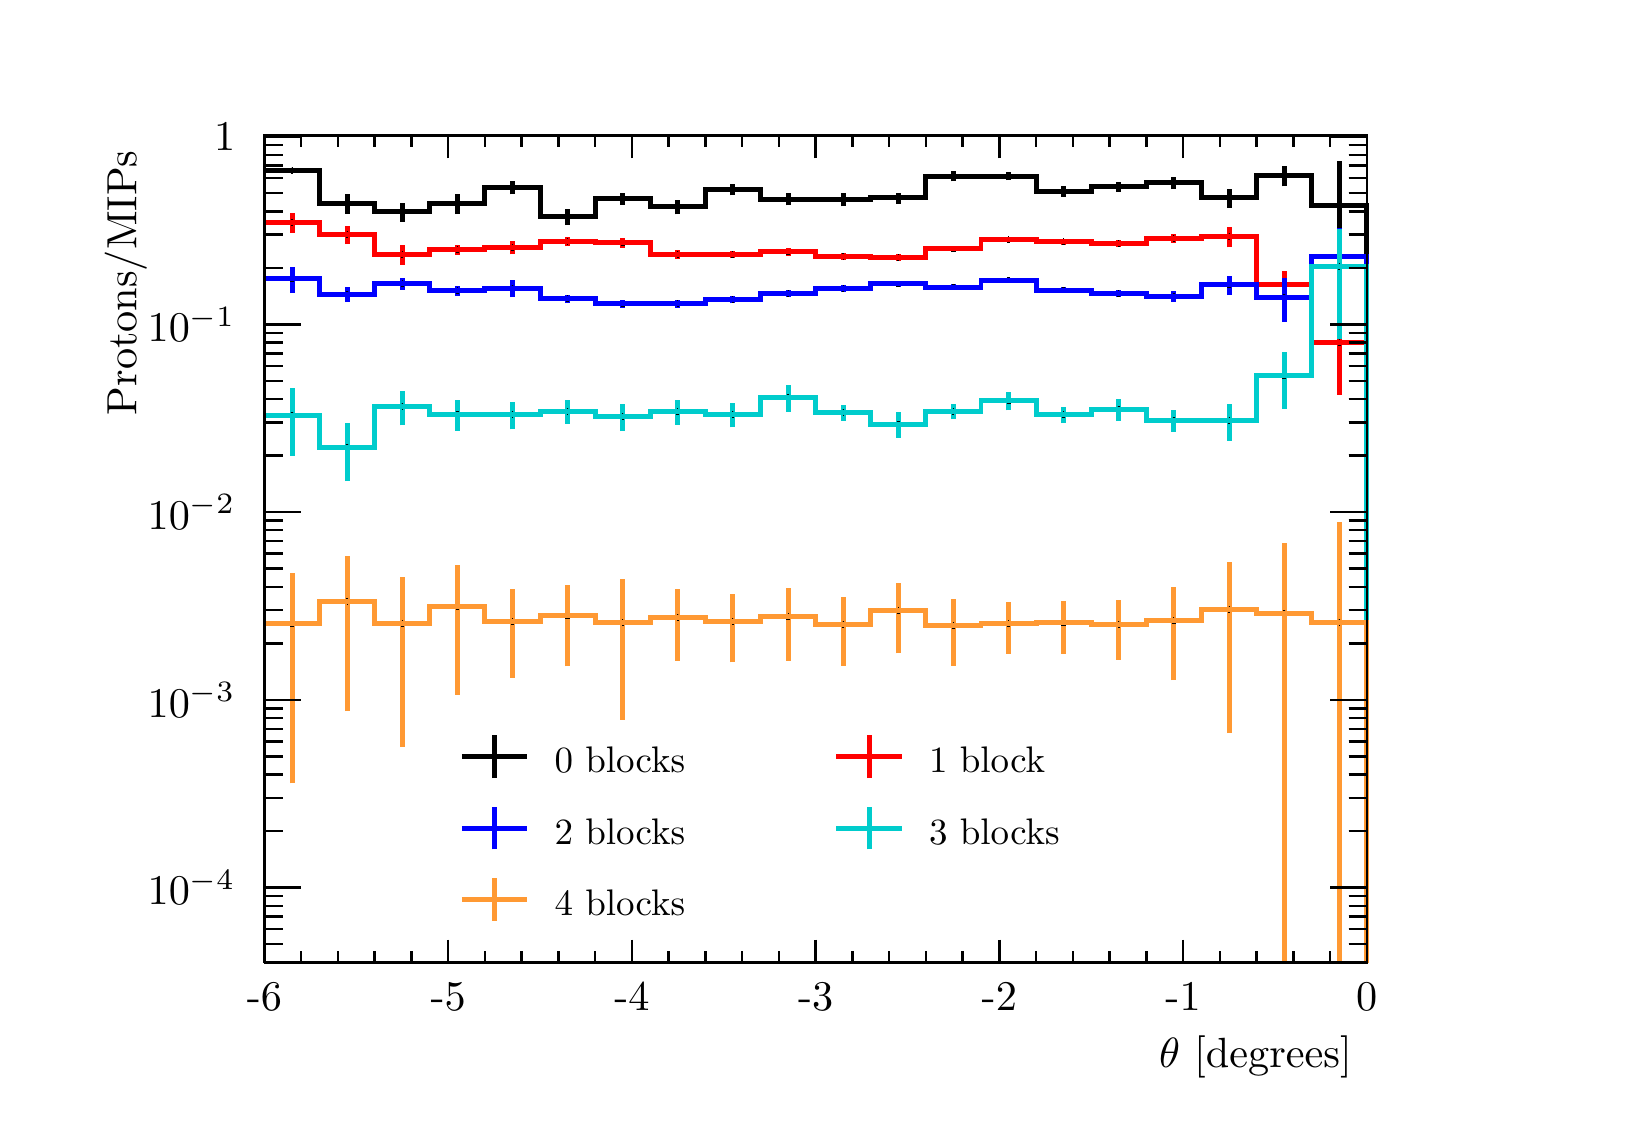
\begin{tikzpicture}
\pgfdeclareplotmark{cross} {
\pgfpathmoveto{\pgfpoint{-0.3\pgfplotmarksize}{\pgfplotmarksize}}
\pgfpathlineto{\pgfpoint{+0.3\pgfplotmarksize}{\pgfplotmarksize}}
\pgfpathlineto{\pgfpoint{+0.3\pgfplotmarksize}{0.3\pgfplotmarksize}}
\pgfpathlineto{\pgfpoint{+1\pgfplotmarksize}{0.3\pgfplotmarksize}}
\pgfpathlineto{\pgfpoint{+1\pgfplotmarksize}{-0.3\pgfplotmarksize}}
\pgfpathlineto{\pgfpoint{+0.3\pgfplotmarksize}{-0.3\pgfplotmarksize}}
\pgfpathlineto{\pgfpoint{+0.3\pgfplotmarksize}{-1.\pgfplotmarksize}}
\pgfpathlineto{\pgfpoint{-0.3\pgfplotmarksize}{-1.\pgfplotmarksize}}
\pgfpathlineto{\pgfpoint{-0.3\pgfplotmarksize}{-0.3\pgfplotmarksize}}
\pgfpathlineto{\pgfpoint{-1.\pgfplotmarksize}{-0.3\pgfplotmarksize}}
\pgfpathlineto{\pgfpoint{-1.\pgfplotmarksize}{0.3\pgfplotmarksize}}
\pgfpathlineto{\pgfpoint{-0.3\pgfplotmarksize}{0.3\pgfplotmarksize}}
\pgfpathclose
\pgfusepathqstroke
}
\pgfdeclareplotmark{cross*} {
\pgfpathmoveto{\pgfpoint{-0.3\pgfplotmarksize}{\pgfplotmarksize}}
\pgfpathlineto{\pgfpoint{+0.3\pgfplotmarksize}{\pgfplotmarksize}}
\pgfpathlineto{\pgfpoint{+0.3\pgfplotmarksize}{0.3\pgfplotmarksize}}
\pgfpathlineto{\pgfpoint{+1\pgfplotmarksize}{0.3\pgfplotmarksize}}
\pgfpathlineto{\pgfpoint{+1\pgfplotmarksize}{-0.3\pgfplotmarksize}}
\pgfpathlineto{\pgfpoint{+0.3\pgfplotmarksize}{-0.3\pgfplotmarksize}}
\pgfpathlineto{\pgfpoint{+0.3\pgfplotmarksize}{-1.\pgfplotmarksize}}
\pgfpathlineto{\pgfpoint{-0.3\pgfplotmarksize}{-1.\pgfplotmarksize}}
\pgfpathlineto{\pgfpoint{-0.3\pgfplotmarksize}{-0.3\pgfplotmarksize}}
\pgfpathlineto{\pgfpoint{-1.\pgfplotmarksize}{-0.3\pgfplotmarksize}}
\pgfpathlineto{\pgfpoint{-1.\pgfplotmarksize}{0.3\pgfplotmarksize}}
\pgfpathlineto{\pgfpoint{-0.3\pgfplotmarksize}{0.3\pgfplotmarksize}}
\pgfpathclose
\pgfusepathqfillstroke
}
\pgfdeclareplotmark{newstar} {
\pgfpathmoveto{\pgfqpoint{0pt}{\pgfplotmarksize}}
\pgfpathlineto{\pgfqpointpolar{44}{0.5\pgfplotmarksize}}
\pgfpathlineto{\pgfqpointpolar{18}{\pgfplotmarksize}}
\pgfpathlineto{\pgfqpointpolar{-20}{0.5\pgfplotmarksize}}
\pgfpathlineto{\pgfqpointpolar{-54}{\pgfplotmarksize}}
\pgfpathlineto{\pgfqpointpolar{-90}{0.5\pgfplotmarksize}}
\pgfpathlineto{\pgfqpointpolar{234}{\pgfplotmarksize}}
\pgfpathlineto{\pgfqpointpolar{198}{0.5\pgfplotmarksize}}
\pgfpathlineto{\pgfqpointpolar{162}{\pgfplotmarksize}}
\pgfpathlineto{\pgfqpointpolar{134}{0.5\pgfplotmarksize}}
\pgfpathclose
\pgfusepathqstroke
}
\pgfdeclareplotmark{newstar*} {
\pgfpathmoveto{\pgfqpoint{0pt}{\pgfplotmarksize}}
\pgfpathlineto{\pgfqpointpolar{44}{0.5\pgfplotmarksize}}
\pgfpathlineto{\pgfqpointpolar{18}{\pgfplotmarksize}}
\pgfpathlineto{\pgfqpointpolar{-20}{0.5\pgfplotmarksize}}
\pgfpathlineto{\pgfqpointpolar{-54}{\pgfplotmarksize}}
\pgfpathlineto{\pgfqpointpolar{-90}{0.5\pgfplotmarksize}}
\pgfpathlineto{\pgfqpointpolar{234}{\pgfplotmarksize}}
\pgfpathlineto{\pgfqpointpolar{198}{0.5\pgfplotmarksize}}
\pgfpathlineto{\pgfqpointpolar{162}{\pgfplotmarksize}}
\pgfpathlineto{\pgfqpointpolar{134}{0.5\pgfplotmarksize}}
\pgfpathclose
\pgfusepathqfillstroke
}
\definecolor{c}{rgb}{1,1,1};
\draw [color=c, fill=c] (0,0) rectangle (20,13.639);
\draw [color=c, fill=c] (3,1.77307) rectangle (17,12.2751);
\definecolor{c}{rgb}{0,0,0};
\draw [c,line width=0.9] (3,1.77307) -- (3,12.2751) -- (17,12.2751) -- (17,1.77307) -- (3,1.77307);
\definecolor{c}{rgb}{1,1,1};
\draw [color=c, fill=c] (3,1.77307) rectangle (17,12.2751);
\definecolor{c}{rgb}{0,0,0};
\draw [c,line width=0.9] (3,1.77307) -- (3,12.2751) -- (17,12.2751) -- (17,1.77307) -- (3,1.77307);
\draw [c,line width=0.9] (3,1.77307) -- (3.7,1.77307) -- (3.7,1.77307) -- (4.4,1.77307) -- (4.4,1.77307) -- (5.1,1.77307) -- (5.1,1.77307) -- (5.8,1.77307) -- (5.8,1.77307) -- (6.5,1.77307) -- (6.5,1.77307) -- (7.2,1.77307) -- (7.2,1.77307) --
 (7.9,1.77307) -- (7.9,1.77307) -- (8.6,1.77307) -- (8.6,1.77307) -- (9.3,1.77307) -- (9.3,1.77307) -- (10,1.77307) -- (10,1.77307) -- (10.7,1.77307) -- (10.7,1.77307) -- (11.4,1.77307) -- (11.4,1.77307) -- (12.1,1.77307) -- (12.1,1.77307) --
 (12.8,1.77307) -- (12.8,1.77307) -- (13.5,1.77307) -- (13.5,1.77307) -- (14.2,1.77307) -- (14.2,1.77307) -- (14.9,1.77307) -- (14.9,1.77307) -- (15.6,1.77307) -- (15.6,1.77307) -- (16.3,1.77307) -- (16.3,1.77307) -- (17,1.77307) -- (17,1.77307);
\draw [c,line width=0.9] (3,1.77307) -- (17,1.77307);
\draw [c,line width=0.9] (3,2.05948) -- (3,1.77307);
\draw [c,line width=0.9] (3.46667,1.91628) -- (3.46667,1.77307);
\draw [c,line width=0.9] (3.93333,1.91628) -- (3.93333,1.77307);
\draw [c,line width=0.9] (4.4,1.91628) -- (4.4,1.77307);
\draw [c,line width=0.9] (4.86667,1.91628) -- (4.86667,1.77307);
\draw [c,line width=0.9] (5.33333,2.05948) -- (5.33333,1.77307);
\draw [c,line width=0.9] (5.8,1.91628) -- (5.8,1.77307);
\draw [c,line width=0.9] (6.26667,1.91628) -- (6.26667,1.77307);
\draw [c,line width=0.9] (6.73333,1.91628) -- (6.73333,1.77307);
\draw [c,line width=0.9] (7.2,1.91628) -- (7.2,1.77307);
\draw [c,line width=0.9] (7.66667,2.05948) -- (7.66667,1.77307);
\draw [c,line width=0.9] (8.13333,1.91628) -- (8.13333,1.77307);
\draw [c,line width=0.9] (8.6,1.91628) -- (8.6,1.77307);
\draw [c,line width=0.9] (9.06667,1.91628) -- (9.06667,1.77307);
\draw [c,line width=0.9] (9.53333,1.91628) -- (9.53333,1.77307);
\draw [c,line width=0.9] (10,2.05948) -- (10,1.77307);
\draw [c,line width=0.9] (10.4667,1.91628) -- (10.4667,1.77307);
\draw [c,line width=0.9] (10.9333,1.91628) -- (10.9333,1.77307);
\draw [c,line width=0.9] (11.4,1.91628) -- (11.4,1.77307);
\draw [c,line width=0.9] (11.8667,1.91628) -- (11.8667,1.77307);
\draw [c,line width=0.9] (12.3333,2.05948) -- (12.3333,1.77307);
\draw [c,line width=0.9] (12.8,1.91628) -- (12.8,1.77307);
\draw [c,line width=0.9] (13.2667,1.91628) -- (13.2667,1.77307);
\draw [c,line width=0.9] (13.7333,1.91628) -- (13.7333,1.77307);
\draw [c,line width=0.9] (14.2,1.91628) -- (14.2,1.77307);
\draw [c,line width=0.9] (14.6667,2.05948) -- (14.6667,1.77307);
\draw [c,line width=0.9] (15.1333,1.91628) -- (15.1333,1.77307);
\draw [c,line width=0.9] (15.6,1.91628) -- (15.6,1.77307);
\draw [c,line width=0.9] (16.0667,1.91628) -- (16.0667,1.77307);
\draw [c,line width=0.9] (16.5333,1.91628) -- (16.5333,1.77307);
\draw [c,line width=0.9] (17,2.05948) -- (17,1.77307);
\draw [anchor=base] (3,1.15931) node[scale=1.52731, color=c, rotate=0]{-6};
\draw [anchor=base] (5.33333,1.15931) node[scale=1.52731, color=c, rotate=0]{-5};
\draw [anchor=base] (7.66667,1.15931) node[scale=1.52731, color=c, rotate=0]{-4};
\draw [anchor=base] (10,1.15931) node[scale=1.52731, color=c, rotate=0]{-3};
\draw [anchor=base] (12.3333,1.15931) node[scale=1.52731, color=c, rotate=0]{-2};
\draw [anchor=base] (14.6667,1.15931) node[scale=1.52731, color=c, rotate=0]{-1};
\draw [anchor=base] (17,1.15931) node[scale=1.52731, color=c, rotate=0]{0};
\draw [anchor= east] (17,0.572837) node[scale=1.52731, color=c, rotate=0]{$\theta$ [degrees] };
\draw [c,line width=0.9] (3,12.2751) -- (17,12.2751);
\draw [c,line width=0.9] (3,11.9887) -- (3,12.2751);
\draw [c,line width=0.9] (3.46667,12.1319) -- (3.46667,12.2751);
\draw [c,line width=0.9] (3.93333,12.1319) -- (3.93333,12.2751);
\draw [c,line width=0.9] (4.4,12.1319) -- (4.4,12.2751);
\draw [c,line width=0.9] (4.86667,12.1319) -- (4.86667,12.2751);
\draw [c,line width=0.9] (5.33333,11.9887) -- (5.33333,12.2751);
\draw [c,line width=0.9] (5.8,12.1319) -- (5.8,12.2751);
\draw [c,line width=0.9] (6.26667,12.1319) -- (6.26667,12.2751);
\draw [c,line width=0.9] (6.73333,12.1319) -- (6.73333,12.2751);
\draw [c,line width=0.9] (7.2,12.1319) -- (7.2,12.2751);
\draw [c,line width=0.9] (7.66667,11.9887) -- (7.66667,12.2751);
\draw [c,line width=0.9] (8.13333,12.1319) -- (8.13333,12.2751);
\draw [c,line width=0.9] (8.6,12.1319) -- (8.6,12.2751);
\draw [c,line width=0.9] (9.06667,12.1319) -- (9.06667,12.2751);
\draw [c,line width=0.9] (9.53333,12.1319) -- (9.53333,12.2751);
\draw [c,line width=0.9] (10,11.9887) -- (10,12.2751);
\draw [c,line width=0.9] (10.4667,12.1319) -- (10.4667,12.2751);
\draw [c,line width=0.9] (10.9333,12.1319) -- (10.9333,12.2751);
\draw [c,line width=0.9] (11.4,12.1319) -- (11.4,12.2751);
\draw [c,line width=0.9] (11.8667,12.1319) -- (11.8667,12.2751);
\draw [c,line width=0.9] (12.3333,11.9887) -- (12.3333,12.2751);
\draw [c,line width=0.9] (12.8,12.1319) -- (12.8,12.2751);
\draw [c,line width=0.9] (13.2667,12.1319) -- (13.2667,12.2751);
\draw [c,line width=0.9] (13.7333,12.1319) -- (13.7333,12.2751);
\draw [c,line width=0.9] (14.2,12.1319) -- (14.2,12.2751);
\draw [c,line width=0.9] (14.6667,11.9887) -- (14.6667,12.2751);
\draw [c,line width=0.9] (15.1333,12.1319) -- (15.1333,12.2751);
\draw [c,line width=0.9] (15.6,12.1319) -- (15.6,12.2751);
\draw [c,line width=0.9] (16.0667,12.1319) -- (16.0667,12.2751);
\draw [c,line width=0.9] (16.5333,12.1319) -- (16.5333,12.2751);
\draw [c,line width=0.9] (17,11.9887) -- (17,12.2751);
\draw [c,line width=0.9] (3,1.77307) -- (3,12.2751);
\draw [c,line width=0.9] (3.231,1.77653) -- (3,1.77653);
\draw [c,line width=0.9] (3.231,2.0076) -- (3,2.0076);
\draw [c,line width=0.9] (3.231,2.1964) -- (3,2.1964);
\draw [c,line width=0.9] (3.231,2.35603) -- (3,2.35603);
\draw [c,line width=0.9] (3.231,2.49431) -- (3,2.49431);
\draw [c,line width=0.9] (3.231,2.61628) -- (3,2.61628);
\draw [c,line width=0.9] (3.462,2.72539) -- (3,2.72539);
\draw [anchor= east] (2.82,2.72539) node[scale=1.52731, color=c, rotate=0]{$10^{-4}$};
\draw [c,line width=0.9] (3.231,3.44317) -- (3,3.44317);
\draw [c,line width=0.9] (3.231,3.86305) -- (3,3.86305);
\draw [c,line width=0.9] (3.231,4.16096) -- (3,4.16096);
\draw [c,line width=0.9] (3.231,4.39203) -- (3,4.39203);
\draw [c,line width=0.9] (3.231,4.58083) -- (3,4.58083);
\draw [c,line width=0.9] (3.231,4.74046) -- (3,4.74046);
\draw [c,line width=0.9] (3.231,4.87874) -- (3,4.87874);
\draw [c,line width=0.9] (3.231,5.00071) -- (3,5.00071);
\draw [c,line width=0.9] (3.462,5.10982) -- (3,5.10982);
\draw [anchor= east] (2.82,5.10982) node[scale=1.52731, color=c, rotate=0]{$10^{-3}$};
\draw [c,line width=0.9] (3.231,5.8276) -- (3,5.8276);
\draw [c,line width=0.9] (3.231,6.24748) -- (3,6.24748);
\draw [c,line width=0.9] (3.231,6.54539) -- (3,6.54539);
\draw [c,line width=0.9] (3.231,6.77646) -- (3,6.77646);
\draw [c,line width=0.9] (3.231,6.96527) -- (3,6.96527);
\draw [c,line width=0.9] (3.231,7.1249) -- (3,7.1249);
\draw [c,line width=0.9] (3.231,7.26317) -- (3,7.26317);
\draw [c,line width=0.9] (3.231,7.38514) -- (3,7.38514);
\draw [c,line width=0.9] (3.462,7.49425) -- (3,7.49425);
\draw [anchor= east] (2.82,7.49425) node[scale=1.52731, color=c, rotate=0]{$10^{-2}$};
\draw [c,line width=0.9] (3.231,8.21203) -- (3,8.21203);
\draw [c,line width=0.9] (3.231,8.63191) -- (3,8.63191);
\draw [c,line width=0.9] (3.231,8.92982) -- (3,8.92982);
\draw [c,line width=0.9] (3.231,9.16089) -- (3,9.16089);
\draw [c,line width=0.9] (3.231,9.3497) -- (3,9.3497);
\draw [c,line width=0.9] (3.231,9.50933) -- (3,9.50933);
\draw [c,line width=0.9] (3.231,9.6476) -- (3,9.6476);
\draw [c,line width=0.9] (3.231,9.76957) -- (3,9.76957);
\draw [c,line width=0.9] (3.462,9.87868) -- (3,9.87868);
\draw [anchor= east] (2.82,9.87868) node[scale=1.52731, color=c, rotate=0]{$10^{-1}$};
\draw [c,line width=0.9] (3.231,10.5965) -- (3,10.5965);
\draw [c,line width=0.9] (3.231,11.0163) -- (3,11.0163);
\draw [c,line width=0.9] (3.231,11.3142) -- (3,11.3142);
\draw [c,line width=0.9] (3.231,11.5453) -- (3,11.5453);
\draw [c,line width=0.9] (3.231,11.7341) -- (3,11.7341);
\draw [c,line width=0.9] (3.231,11.8938) -- (3,11.8938);
\draw [c,line width=0.9] (3.231,12.032) -- (3,12.032);
\draw [c,line width=0.9] (3.231,12.154) -- (3,12.154);
\draw [c,line width=0.9] (3.462,12.2631) -- (3,12.2631);
\draw [anchor= east] (2.82,12.2631) node[scale=1.52731, color=c, rotate=0]{1};
\draw [anchor= east] (1.24,12.2751) node[scale=1.52731, color=c, rotate=90]{ Protons/MIPs};
\draw [c,line width=0.9] (17,1.77307) -- (17,12.2751);
\draw [c,line width=0.9] (16.769,1.77653) -- (17,1.77653);
\draw [c,line width=0.9] (16.769,2.0076) -- (17,2.0076);
\draw [c,line width=0.9] (16.769,2.1964) -- (17,2.1964);
\draw [c,line width=0.9] (16.769,2.35603) -- (17,2.35603);
\draw [c,line width=0.9] (16.769,2.49431) -- (17,2.49431);
\draw [c,line width=0.9] (16.769,2.61628) -- (17,2.61628);
\draw [c,line width=0.9] (16.538,2.72539) -- (17,2.72539);
\draw [c,line width=0.9] (16.769,3.44317) -- (17,3.44317);
\draw [c,line width=0.9] (16.769,3.86305) -- (17,3.86305);
\draw [c,line width=0.9] (16.769,4.16096) -- (17,4.16096);
\draw [c,line width=0.9] (16.769,4.39203) -- (17,4.39203);
\draw [c,line width=0.9] (16.769,4.58083) -- (17,4.58083);
\draw [c,line width=0.9] (16.769,4.74046) -- (17,4.74046);
\draw [c,line width=0.9] (16.769,4.87874) -- (17,4.87874);
\draw [c,line width=0.9] (16.769,5.00071) -- (17,5.00071);
\draw [c,line width=0.9] (16.538,5.10982) -- (17,5.10982);
\draw [c,line width=0.9] (16.769,5.8276) -- (17,5.8276);
\draw [c,line width=0.9] (16.769,6.24748) -- (17,6.24748);
\draw [c,line width=0.9] (16.769,6.54539) -- (17,6.54539);
\draw [c,line width=0.9] (16.769,6.77646) -- (17,6.77646);
\draw [c,line width=0.9] (16.769,6.96527) -- (17,6.96527);
\draw [c,line width=0.9] (16.769,7.1249) -- (17,7.1249);
\draw [c,line width=0.9] (16.769,7.26317) -- (17,7.26317);
\draw [c,line width=0.9] (16.769,7.38514) -- (17,7.38514);
\draw [c,line width=0.9] (16.538,7.49425) -- (17,7.49425);
\draw [c,line width=0.9] (16.769,8.21203) -- (17,8.21203);
\draw [c,line width=0.9] (16.769,8.63191) -- (17,8.63191);
\draw [c,line width=0.9] (16.769,8.92982) -- (17,8.92982);
\draw [c,line width=0.9] (16.769,9.16089) -- (17,9.16089);
\draw [c,line width=0.9] (16.769,9.3497) -- (17,9.3497);
\draw [c,line width=0.9] (16.769,9.50933) -- (17,9.50933);
\draw [c,line width=0.9] (16.769,9.6476) -- (17,9.6476);
\draw [c,line width=0.9] (16.769,9.76957) -- (17,9.76957);
\draw [c,line width=0.9] (16.538,9.87868) -- (17,9.87868);
\draw [c,line width=0.9] (16.769,10.5965) -- (17,10.5965);
\draw [c,line width=0.9] (16.769,11.0163) -- (17,11.0163);
\draw [c,line width=0.9] (16.769,11.3142) -- (17,11.3142);
\draw [c,line width=0.9] (16.769,11.5453) -- (17,11.5453);
\draw [c,line width=0.9] (16.769,11.7341) -- (17,11.7341);
\draw [c,line width=0.9] (16.769,11.8938) -- (17,11.8938);
\draw [c,line width=0.9] (16.769,12.032) -- (17,12.032);
\draw [c,line width=0.9] (16.769,12.154) -- (17,12.154);
\draw [c,line width=0.9] (16.538,12.2631) -- (17,12.2631);
\draw [c,line width=1.8] (3.35,11.7944) -- (3.35,11.8326);
\draw [c,line width=1.8] (3.35,11.8326) -- (3.35,11.8695);
\foreach \P in {(3.35,11.8326)}{\draw[mark options={color=c,fill=c},mark size=2.402402pt, line width=0.000000pt, mark=*,mark size=1pt] plot coordinates {\P};}
\draw [c,line width=1.8] (4.05,11.2801) -- (4.05,11.4121);
\draw [c,line width=1.8] (4.05,11.4121) -- (4.05,11.5292);
\foreach \P in {(4.05,11.4121)}{\draw[mark options={color=c,fill=c},mark size=2.402402pt, line width=0.000000pt, mark=*,mark size=1pt] plot coordinates {\P};}
\draw [c,line width=1.8] (4.75,11.1787) -- (4.75,11.3065);
\draw [c,line width=1.8] (4.75,11.3065) -- (4.75,11.4203);
\foreach \P in {(4.75,11.3065)}{\draw[mark options={color=c,fill=c},mark size=2.402402pt, line width=0.000000pt, mark=*,mark size=1pt] plot coordinates {\P};}
\draw [c,line width=1.8] (5.45,11.2778) -- (5.45,11.4122);
\draw [c,line width=1.8] (5.45,11.4122) -- (5.45,11.5311);
\foreach \P in {(5.45,11.4122)}{\draw[mark options={color=c,fill=c},mark size=2.402402pt, line width=0.000000pt, mark=*,mark size=1pt] plot coordinates {\P};}
\draw [c,line width=1.8] (6.15,11.5292) -- (6.15,11.617);
\draw [c,line width=1.8] (6.15,11.617) -- (6.15,11.6979);
\foreach \P in {(6.15,11.617)}{\draw[mark options={color=c,fill=c},mark size=2.402402pt, line width=0.000000pt, mark=*,mark size=1pt] plot coordinates {\P};}
\draw [c,line width=1.8] (6.85,11.1391) -- (6.85,11.2438);
\draw [c,line width=1.8] (6.85,11.2438) -- (6.85,11.3388);
\foreach \P in {(6.85,11.2438)}{\draw[mark options={color=c,fill=c},mark size=2.402402pt, line width=0.000000pt, mark=*,mark size=1pt] plot coordinates {\P};}
\draw [c,line width=1.8] (7.55,11.397) -- (7.55,11.4769);
\draw [c,line width=1.8] (7.55,11.4769) -- (7.55,11.551);
\foreach \P in {(7.55,11.4769)}{\draw[mark options={color=c,fill=c},mark size=2.402402pt, line width=0.000000pt, mark=*,mark size=1pt] plot coordinates {\P};}
\draw [c,line width=1.8] (8.25,11.2744) -- (8.25,11.3688);
\draw [c,line width=1.8] (8.25,11.3688) -- (8.25,11.4553);
\foreach \P in {(8.25,11.3688)}{\draw[mark options={color=c,fill=c},mark size=2.402402pt, line width=0.000000pt, mark=*,mark size=1pt] plot coordinates {\P};}
\draw [c,line width=1.8] (8.95,11.5168) -- (8.95,11.5936);
\draw [c,line width=1.8] (8.95,11.5936) -- (8.95,11.665);
\foreach \P in {(8.95,11.5936)}{\draw[mark options={color=c,fill=c},mark size=2.402402pt, line width=0.000000pt, mark=*,mark size=1pt] plot coordinates {\P};}
\draw [c,line width=1.8] (9.65,11.3879) -- (9.65,11.4689);
\draw [c,line width=1.8] (9.65,11.4689) -- (9.65,11.544);
\foreach \P in {(9.65,11.4689)}{\draw[mark options={color=c,fill=c},mark size=2.402402pt, line width=0.000000pt, mark=*,mark size=1pt] plot coordinates {\P};}
\draw [c,line width=1.8] (10.35,11.3756) -- (10.35,11.4639);
\draw [c,line width=1.8] (10.35,11.4639) -- (10.35,11.5452);
\foreach \P in {(10.35,11.4639)}{\draw[mark options={color=c,fill=c},mark size=2.402402pt, line width=0.000000pt, mark=*,mark size=1pt] plot coordinates {\P};}
\draw [c,line width=1.8] (11.05,11.412) -- (11.05,11.4839);
\draw [c,line width=1.8] (11.05,11.4839) -- (11.05,11.5512);
\foreach \P in {(11.05,11.4839)}{\draw[mark options={color=c,fill=c},mark size=2.402402pt, line width=0.000000pt, mark=*,mark size=1pt] plot coordinates {\P};}
\draw [c,line width=1.8] (11.75,11.6931) -- (11.75,11.7612);
\draw [c,line width=1.8] (11.75,11.7612) -- (11.75,11.8251);
\foreach \P in {(11.75,11.7612)}{\draw[mark options={color=c,fill=c},mark size=2.402402pt, line width=0.000000pt, mark=*,mark size=1pt] plot coordinates {\P};}
\draw [c,line width=1.8] (12.45,11.7084) -- (12.45,11.759);
\draw [c,line width=1.8] (12.45,11.759) -- (12.45,11.8072);
\foreach \P in {(12.45,11.759)}{\draw[mark options={color=c,fill=c},mark size=2.402402pt, line width=0.000000pt, mark=*,mark size=1pt] plot coordinates {\P};}
\draw [c,line width=1.8] (13.15,11.4965) -- (13.15,11.5686);
\draw [c,line width=1.8] (13.15,11.5686) -- (13.15,11.636);
\foreach \P in {(13.15,11.5686)}{\draw[mark options={color=c,fill=c},mark size=2.402402pt, line width=0.000000pt, mark=*,mark size=1pt] plot coordinates {\P};}
\draw [c,line width=1.8] (13.85,11.5606) -- (13.85,11.6255);
\draw [c,line width=1.8] (13.85,11.6255) -- (13.85,11.6866);
\foreach \P in {(13.85,11.6255)}{\draw[mark options={color=c,fill=c},mark size=2.402402pt, line width=0.000000pt, mark=*,mark size=1pt] plot coordinates {\P};}
\draw [c,line width=1.8] (14.55,11.5941) -- (14.55,11.6769);
\draw [c,line width=1.8] (14.55,11.6769) -- (14.55,11.7536);
\foreach \P in {(14.55,11.6769)}{\draw[mark options={color=c,fill=c},mark size=2.402402pt, line width=0.000000pt, mark=*,mark size=1pt] plot coordinates {\P};}
\draw [c,line width=1.8] (15.25,11.3608) -- (15.25,11.4891);
\draw [c,line width=1.8] (15.25,11.4891) -- (15.25,11.6033);
\foreach \P in {(15.25,11.4891)}{\draw[mark options={color=c,fill=c},mark size=2.402402pt, line width=0.000000pt, mark=*,mark size=1pt] plot coordinates {\P};}
\draw [c,line width=1.8] (15.95,11.6301) -- (15.95,11.7651);
\draw [c,line width=1.8] (15.95,11.7651) -- (15.95,11.8844);
\foreach \P in {(15.95,11.7651)}{\draw[mark options={color=c,fill=c},mark size=2.402402pt, line width=0.000000pt, mark=*,mark size=1pt] plot coordinates {\P};}
\draw [c,line width=1.8] (16.65,10.041) -- (16.65,11.3908);
\draw [c,line width=1.8] (16.65,11.3908) -- (16.65,11.9574);
\foreach \P in {(16.65,11.3908)}{\draw[mark options={color=c,fill=c},mark size=2.402402pt, line width=0.000000pt, mark=*,mark size=1pt] plot coordinates {\P};}
\draw [c,line width=1.8] (3,11.8326) -- (3.7,11.8326) -- (3.7,11.4121) -- (4.4,11.4121) -- (4.4,11.3065) -- (5.1,11.3065) -- (5.1,11.4122) -- (5.8,11.4122) -- (5.8,11.617) -- (6.5,11.617) -- (6.5,11.2438) -- (7.2,11.2438) -- (7.2,11.4769) --
 (7.9,11.4769) -- (7.9,11.3688) -- (8.6,11.3688) -- (8.6,11.5936) -- (9.3,11.5936) -- (9.3,11.4689) -- (10,11.4689) -- (10,11.4639) -- (10.7,11.4639) -- (10.7,11.4839) -- (11.4,11.4839) -- (11.4,11.7612) -- (12.1,11.7612) -- (12.1,11.759) --
 (12.8,11.759) -- (12.8,11.5686) -- (13.5,11.5686) -- (13.5,11.6255) -- (14.2,11.6255) -- (14.2,11.6769) -- (14.9,11.6769) -- (14.9,11.4891) -- (15.6,11.4891) -- (15.6,11.7651) -- (16.3,11.7651) -- (16.3,11.3908) -- (17,11.3908) -- (17,1.77307);
\definecolor{c}{rgb}{1,0,0};
\draw [c,line width=1.8] (3.35,11.0436) -- (3.35,11.1738);
\draw [c,line width=1.8] (3.35,11.1738) -- (3.35,11.2894);
\definecolor{c}{rgb}{0,0,0};
\foreach \P in {(3.35,11.1738)}{\draw[mark options={color=c,fill=c},mark size=2.402402pt, line width=0.000000pt, mark=*,mark size=1pt] plot coordinates {\P};}
\definecolor{c}{rgb}{1,0,0};
\draw [c,line width=1.8] (4.05,10.8972) -- (4.05,11.0207);
\draw [c,line width=1.8] (4.05,11.0207) -- (4.05,11.131);
\definecolor{c}{rgb}{0,0,0};
\foreach \P in {(4.05,11.0207)}{\draw[mark options={color=c,fill=c},mark size=2.402402pt, line width=0.000000pt, mark=*,mark size=1pt] plot coordinates {\P};}
\definecolor{c}{rgb}{1,0,0};
\draw [c,line width=1.8] (4.75,10.6369) -- (4.75,10.7653);
\draw [c,line width=1.8] (4.75,10.7653) -- (4.75,10.8796);
\definecolor{c}{rgb}{0,0,0};
\foreach \P in {(4.75,10.7653)}{\draw[mark options={color=c,fill=c},mark size=2.402402pt, line width=0.000000pt, mark=*,mark size=1pt] plot coordinates {\P};}
\definecolor{c}{rgb}{1,0,0};
\draw [c,line width=1.8] (5.45,10.7622) -- (5.45,10.8283);
\draw [c,line width=1.8] (5.45,10.8283) -- (5.45,10.8905);
\definecolor{c}{rgb}{0,0,0};
\foreach \P in {(5.45,10.8283)}{\draw[mark options={color=c,fill=c},mark size=2.402402pt, line width=0.000000pt, mark=*,mark size=1pt] plot coordinates {\P};}
\definecolor{c}{rgb}{1,0,0};
\draw [c,line width=1.8] (6.15,10.7679) -- (6.15,10.854);
\draw [c,line width=1.8] (6.15,10.854) -- (6.15,10.9335);
\definecolor{c}{rgb}{0,0,0};
\foreach \P in {(6.15,10.854)}{\draw[mark options={color=c,fill=c},mark size=2.402402pt, line width=0.000000pt, mark=*,mark size=1pt] plot coordinates {\P};}
\definecolor{c}{rgb}{1,0,0};
\draw [c,line width=1.8] (6.85,10.8691) -- (6.85,10.932);
\draw [c,line width=1.8] (6.85,10.932) -- (6.85,10.9913);
\definecolor{c}{rgb}{0,0,0};
\foreach \P in {(6.85,10.932)}{\draw[mark options={color=c,fill=c},mark size=2.402402pt, line width=0.000000pt, mark=*,mark size=1pt] plot coordinates {\P};}
\definecolor{c}{rgb}{1,0,0};
\draw [c,line width=1.8] (7.55,10.8482) -- (7.55,10.913);
\draw [c,line width=1.8] (7.55,10.913) -- (7.55,10.974);
\definecolor{c}{rgb}{0,0,0};
\foreach \P in {(7.55,10.913)}{\draw[mark options={color=c,fill=c},mark size=2.402402pt, line width=0.000000pt, mark=*,mark size=1pt] plot coordinates {\P};}
\definecolor{c}{rgb}{1,0,0};
\draw [c,line width=1.8] (8.25,10.7072) -- (8.25,10.767);
\draw [c,line width=1.8] (8.25,10.767) -- (8.25,10.8236);
\definecolor{c}{rgb}{0,0,0};
\foreach \P in {(8.25,10.767)}{\draw[mark options={color=c,fill=c},mark size=2.402402pt, line width=0.000000pt, mark=*,mark size=1pt] plot coordinates {\P};}
\definecolor{c}{rgb}{1,0,0};
\draw [c,line width=1.8] (8.95,10.7158) -- (8.95,10.7635);
\draw [c,line width=1.8] (8.95,10.7635) -- (8.95,10.8092);
\definecolor{c}{rgb}{0,0,0};
\foreach \P in {(8.95,10.7635)}{\draw[mark options={color=c,fill=c},mark size=2.402402pt, line width=0.000000pt, mark=*,mark size=1pt] plot coordinates {\P};}
\definecolor{c}{rgb}{1,0,0};
\draw [c,line width=1.8] (9.65,10.7498) -- (9.65,10.7991);
\draw [c,line width=1.8] (9.65,10.7991) -- (9.65,10.8462);
\definecolor{c}{rgb}{0,0,0};
\foreach \P in {(9.65,10.7991)}{\draw[mark options={color=c,fill=c},mark size=2.402402pt, line width=0.000000pt, mark=*,mark size=1pt] plot coordinates {\P};}
\definecolor{c}{rgb}{1,0,0};
\draw [c,line width=1.8] (10.35,10.6966) -- (10.35,10.7431);
\draw [c,line width=1.8] (10.35,10.7431) -- (10.35,10.7877);
\definecolor{c}{rgb}{0,0,0};
\foreach \P in {(10.35,10.7431)}{\draw[mark options={color=c,fill=c},mark size=2.402402pt, line width=0.000000pt, mark=*,mark size=1pt] plot coordinates {\P};}
\definecolor{c}{rgb}{1,0,0};
\draw [c,line width=1.8] (11.05,10.6849) -- (11.05,10.7279);
\draw [c,line width=1.8] (11.05,10.7279) -- (11.05,10.7692);
\definecolor{c}{rgb}{0,0,0};
\foreach \P in {(11.05,10.7279)}{\draw[mark options={color=c,fill=c},mark size=2.402402pt, line width=0.000000pt, mark=*,mark size=1pt] plot coordinates {\P};}
\definecolor{c}{rgb}{1,0,0};
\draw [c,line width=1.8] (11.75,10.7966) -- (11.75,10.8353);
\draw [c,line width=1.8] (11.75,10.8353) -- (11.75,10.8726);
\definecolor{c}{rgb}{0,0,0};
\foreach \P in {(11.75,10.8353)}{\draw[mark options={color=c,fill=c},mark size=2.402402pt, line width=0.000000pt, mark=*,mark size=1pt] plot coordinates {\P};}
\definecolor{c}{rgb}{1,0,0};
\draw [c,line width=1.8] (12.45,10.9224) -- (12.45,10.9539);
\draw [c,line width=1.8] (12.45,10.9539) -- (12.45,10.9845);
\definecolor{c}{rgb}{0,0,0};
\foreach \P in {(12.45,10.9539)}{\draw[mark options={color=c,fill=c},mark size=2.402402pt, line width=0.000000pt, mark=*,mark size=1pt] plot coordinates {\P};}
\definecolor{c}{rgb}{1,0,0};
\draw [c,line width=1.8] (13.15,10.891) -- (13.15,10.9273);
\draw [c,line width=1.8] (13.15,10.9273) -- (13.15,10.9624);
\definecolor{c}{rgb}{0,0,0};
\foreach \P in {(13.15,10.9273)}{\draw[mark options={color=c,fill=c},mark size=2.402402pt, line width=0.000000pt, mark=*,mark size=1pt] plot coordinates {\P};}
\definecolor{c}{rgb}{1,0,0};
\draw [c,line width=1.8] (13.85,10.8625) -- (13.85,10.9045);
\draw [c,line width=1.8] (13.85,10.9045) -- (13.85,10.9449);
\definecolor{c}{rgb}{0,0,0};
\foreach \P in {(13.85,10.9045)}{\draw[mark options={color=c,fill=c},mark size=2.402402pt, line width=0.000000pt, mark=*,mark size=1pt] plot coordinates {\P};}
\definecolor{c}{rgb}{1,0,0};
\draw [c,line width=1.8] (14.55,10.9139) -- (14.55,10.9694);
\draw [c,line width=1.8] (14.55,10.9694) -- (14.55,11.0221);
\definecolor{c}{rgb}{0,0,0};
\foreach \P in {(14.55,10.9694)}{\draw[mark options={color=c,fill=c},mark size=2.402402pt, line width=0.000000pt, mark=*,mark size=1pt] plot coordinates {\P};}
\definecolor{c}{rgb}{1,0,0};
\draw [c,line width=1.8] (15.25,10.856) -- (15.25,10.9946);
\draw [c,line width=1.8] (15.25,10.9946) -- (15.25,11.1168);
\definecolor{c}{rgb}{0,0,0};
\foreach \P in {(15.25,10.9946)}{\draw[mark options={color=c,fill=c},mark size=2.402402pt, line width=0.000000pt, mark=*,mark size=1pt] plot coordinates {\P};}
\definecolor{c}{rgb}{1,0,0};
\draw [c,line width=1.8] (15.95,10.1715) -- (15.95,10.3785);
\draw [c,line width=1.8] (15.95,10.3785) -- (15.95,10.5509);
\definecolor{c}{rgb}{0,0,0};
\foreach \P in {(15.95,10.3785)}{\draw[mark options={color=c,fill=c},mark size=2.402402pt, line width=0.000000pt, mark=*,mark size=1pt] plot coordinates {\P};}
\definecolor{c}{rgb}{1,0,0};
\draw [c,line width=1.8] (16.65,8.98619) -- (16.65,9.64699);
\draw [c,line width=1.8] (16.65,9.64699) -- (16.65,10.0472);
\definecolor{c}{rgb}{0,0,0};
\foreach \P in {(16.65,9.64699)}{\draw[mark options={color=c,fill=c},mark size=2.402402pt, line width=0.000000pt, mark=*,mark size=1pt] plot coordinates {\P};}
\definecolor{c}{rgb}{1,0,0};
\draw [c,line width=1.8] (3,11.1738) -- (3.7,11.1738) -- (3.7,11.0207) -- (4.4,11.0207) -- (4.4,10.7653) -- (5.1,10.7653) -- (5.1,10.8283) -- (5.8,10.8283) -- (5.8,10.854) -- (6.5,10.854) -- (6.5,10.932) -- (7.2,10.932) -- (7.2,10.913) --
 (7.9,10.913) -- (7.9,10.767) -- (8.6,10.767) -- (8.6,10.7635) -- (9.3,10.7635) -- (9.3,10.7991) -- (10,10.7991) -- (10,10.7431) -- (10.7,10.7431) -- (10.7,10.7279) -- (11.4,10.7279) -- (11.4,10.8353) -- (12.1,10.8353) -- (12.1,10.9539) --
 (12.8,10.9539) -- (12.8,10.9273) -- (13.5,10.9273) -- (13.5,10.9045) -- (14.2,10.9045) -- (14.2,10.9694) -- (14.9,10.9694) -- (14.9,10.9946) -- (15.6,10.9946) -- (15.6,10.3785) -- (16.3,10.3785) -- (16.3,9.64699) -- (17,9.64699) -- (17,1.77307);
\definecolor{c}{rgb}{0,0,1};
\draw [c,line width=1.8] (3.35,10.2743) -- (3.35,10.455);
\draw [c,line width=1.8] (3.35,10.455) -- (3.35,10.6088);
\definecolor{c}{rgb}{0,0,0};
\foreach \P in {(3.35,10.455)}{\draw[mark options={color=c,fill=c},mark size=2.402402pt, line width=0.000000pt, mark=*,mark size=1pt] plot coordinates {\P};}
\definecolor{c}{rgb}{0,0,1};
\draw [c,line width=1.8] (4.05,10.1619) -- (4.05,10.2629);
\draw [c,line width=1.8] (4.05,10.2629) -- (4.05,10.3549);
\definecolor{c}{rgb}{0,0,0};
\foreach \P in {(4.05,10.2629)}{\draw[mark options={color=c,fill=c},mark size=2.402402pt, line width=0.000000pt, mark=*,mark size=1pt] plot coordinates {\P};}
\definecolor{c}{rgb}{0,0,1};
\draw [c,line width=1.8] (4.75,10.3183) -- (4.75,10.3938);
\draw [c,line width=1.8] (4.75,10.3938) -- (4.75,10.4642);
\definecolor{c}{rgb}{0,0,0};
\foreach \P in {(4.75,10.3938)}{\draw[mark options={color=c,fill=c},mark size=2.402402pt, line width=0.000000pt, mark=*,mark size=1pt] plot coordinates {\P};}
\definecolor{c}{rgb}{0,0,1};
\draw [c,line width=1.8] (5.45,10.2384) -- (5.45,10.306);
\draw [c,line width=1.8] (5.45,10.306) -- (5.45,10.3695);
\definecolor{c}{rgb}{0,0,0};
\foreach \P in {(5.45,10.306)}{\draw[mark options={color=c,fill=c},mark size=2.402402pt, line width=0.000000pt, mark=*,mark size=1pt] plot coordinates {\P};}
\definecolor{c}{rgb}{0,0,1};
\draw [c,line width=1.8] (6.15,10.225) -- (6.15,10.3378);
\draw [c,line width=1.8] (6.15,10.3378) -- (6.15,10.4395);
\definecolor{c}{rgb}{0,0,0};
\foreach \P in {(6.15,10.3378)}{\draw[mark options={color=c,fill=c},mark size=2.402402pt, line width=0.000000pt, mark=*,mark size=1pt] plot coordinates {\P};}
\definecolor{c}{rgb}{0,0,1};
\draw [c,line width=1.8] (6.85,10.147) -- (6.85,10.2034);
\draw [c,line width=1.8] (6.85,10.2034) -- (6.85,10.2569);
\definecolor{c}{rgb}{0,0,0};
\foreach \P in {(6.85,10.2034)}{\draw[mark options={color=c,fill=c},mark size=2.402402pt, line width=0.000000pt, mark=*,mark size=1pt] plot coordinates {\P};}
\definecolor{c}{rgb}{0,0,1};
\draw [c,line width=1.8] (7.55,10.0873) -- (7.55,10.1384);
\draw [c,line width=1.8] (7.55,10.1384) -- (7.55,10.1871);
\definecolor{c}{rgb}{0,0,0};
\foreach \P in {(7.55,10.1384)}{\draw[mark options={color=c,fill=c},mark size=2.402402pt, line width=0.000000pt, mark=*,mark size=1pt] plot coordinates {\P};}
\definecolor{c}{rgb}{0,0,1};
\draw [c,line width=1.8] (8.25,10.0918) -- (8.25,10.1425);
\draw [c,line width=1.8] (8.25,10.1425) -- (8.25,10.1908);
\definecolor{c}{rgb}{0,0,0};
\foreach \P in {(8.25,10.1425)}{\draw[mark options={color=c,fill=c},mark size=2.402402pt, line width=0.000000pt, mark=*,mark size=1pt] plot coordinates {\P};}
\definecolor{c}{rgb}{0,0,1};
\draw [c,line width=1.8] (8.95,10.1443) -- (8.95,10.193);
\draw [c,line width=1.8] (8.95,10.193) -- (8.95,10.2395);
\definecolor{c}{rgb}{0,0,0};
\foreach \P in {(8.95,10.193)}{\draw[mark options={color=c,fill=c},mark size=2.402402pt, line width=0.000000pt, mark=*,mark size=1pt] plot coordinates {\P};}
\definecolor{c}{rgb}{0,0,1};
\draw [c,line width=1.8] (9.65,10.2271) -- (9.65,10.2717);
\draw [c,line width=1.8] (9.65,10.2717) -- (9.65,10.3144);
\definecolor{c}{rgb}{0,0,0};
\foreach \P in {(9.65,10.2717)}{\draw[mark options={color=c,fill=c},mark size=2.402402pt, line width=0.000000pt, mark=*,mark size=1pt] plot coordinates {\P};}
\definecolor{c}{rgb}{0,0,1};
\draw [c,line width=1.8] (10.35,10.2906) -- (10.35,10.3336);
\draw [c,line width=1.8] (10.35,10.3336) -- (10.35,10.3749);
\definecolor{c}{rgb}{0,0,0};
\foreach \P in {(10.35,10.3336)}{\draw[mark options={color=c,fill=c},mark size=2.402402pt, line width=0.000000pt, mark=*,mark size=1pt] plot coordinates {\P};}
\definecolor{c}{rgb}{0,0,1};
\draw [c,line width=1.8] (11.05,10.351) -- (11.05,10.3921);
\draw [c,line width=1.8] (11.05,10.3921) -- (11.05,10.4316);
\definecolor{c}{rgb}{0,0,0};
\foreach \P in {(11.05,10.3921)}{\draw[mark options={color=c,fill=c},mark size=2.402402pt, line width=0.000000pt, mark=*,mark size=1pt] plot coordinates {\P};}
\definecolor{c}{rgb}{0,0,1};
\draw [c,line width=1.8] (11.75,10.3162) -- (11.75,10.3514);
\draw [c,line width=1.8] (11.75,10.3514) -- (11.75,10.3855);
\definecolor{c}{rgb}{0,0,0};
\foreach \P in {(11.75,10.3514)}{\draw[mark options={color=c,fill=c},mark size=2.402402pt, line width=0.000000pt, mark=*,mark size=1pt] plot coordinates {\P};}
\definecolor{c}{rgb}{0,0,1};
\draw [c,line width=1.8] (12.45,10.4088) -- (12.45,10.4398);
\draw [c,line width=1.8] (12.45,10.4398) -- (12.45,10.4699);
\definecolor{c}{rgb}{0,0,0};
\foreach \P in {(12.45,10.4398)}{\draw[mark options={color=c,fill=c},mark size=2.402402pt, line width=0.000000pt, mark=*,mark size=1pt] plot coordinates {\P};}
\definecolor{c}{rgb}{0,0,1};
\draw [c,line width=1.8] (13.15,10.2781) -- (13.15,10.3136);
\draw [c,line width=1.8] (13.15,10.3136) -- (13.15,10.3479);
\definecolor{c}{rgb}{0,0,0};
\foreach \P in {(13.15,10.3136)}{\draw[mark options={color=c,fill=c},mark size=2.402402pt, line width=0.000000pt, mark=*,mark size=1pt] plot coordinates {\P};}
\definecolor{c}{rgb}{0,0,1};
\draw [c,line width=1.8] (13.85,10.2241) -- (13.85,10.2676);
\draw [c,line width=1.8] (13.85,10.2676) -- (13.85,10.3095);
\definecolor{c}{rgb}{0,0,0};
\foreach \P in {(13.85,10.2676)}{\draw[mark options={color=c,fill=c},mark size=2.402402pt, line width=0.000000pt, mark=*,mark size=1pt] plot coordinates {\P};}
\definecolor{c}{rgb}{0,0,1};
\draw [c,line width=1.8] (14.55,10.168) -- (14.55,10.2365);
\draw [c,line width=1.8] (14.55,10.2365) -- (14.55,10.3008);
\definecolor{c}{rgb}{0,0,0};
\foreach \P in {(14.55,10.2365)}{\draw[mark options={color=c,fill=c},mark size=2.402402pt, line width=0.000000pt, mark=*,mark size=1pt] plot coordinates {\P};}
\definecolor{c}{rgb}{0,0,1};
\draw [c,line width=1.8] (15.25,10.2482) -- (15.25,10.3797);
\draw [c,line width=1.8] (15.25,10.3797) -- (15.25,10.4964);
\definecolor{c}{rgb}{0,0,0};
\foreach \P in {(15.25,10.3797)}{\draw[mark options={color=c,fill=c},mark size=2.402402pt, line width=0.000000pt, mark=*,mark size=1pt] plot coordinates {\P};}
\definecolor{c}{rgb}{0,0,1};
\draw [c,line width=1.8] (15.95,9.91172) -- (15.95,10.2252);
\draw [c,line width=1.8] (15.95,10.2252) -- (15.95,10.4654);
\definecolor{c}{rgb}{0,0,0};
\foreach \P in {(15.95,10.2252)}{\draw[mark options={color=c,fill=c},mark size=2.402402pt, line width=0.000000pt, mark=*,mark size=1pt] plot coordinates {\P};}
\definecolor{c}{rgb}{0,0,1};
\draw [c,line width=1.8] (16.65,10.1592) -- (16.65,10.7367);
\draw [c,line width=1.8] (16.65,10.7367) -- (16.65,11.1053);
\definecolor{c}{rgb}{0,0,0};
\foreach \P in {(16.65,10.7367)}{\draw[mark options={color=c,fill=c},mark size=2.402402pt, line width=0.000000pt, mark=*,mark size=1pt] plot coordinates {\P};}
\definecolor{c}{rgb}{0,0,1};
\draw [c,line width=1.8] (3,10.455) -- (3.7,10.455) -- (3.7,10.2629) -- (4.4,10.2629) -- (4.4,10.3938) -- (5.1,10.3938) -- (5.1,10.306) -- (5.8,10.306) -- (5.8,10.3378) -- (6.5,10.3378) -- (6.5,10.2034) -- (7.2,10.2034) -- (7.2,10.1384) --
 (7.9,10.1384) -- (7.9,10.1425) -- (8.6,10.1425) -- (8.6,10.193) -- (9.3,10.193) -- (9.3,10.2717) -- (10,10.2717) -- (10,10.3336) -- (10.7,10.3336) -- (10.7,10.3921) -- (11.4,10.3921) -- (11.4,10.3514) -- (12.1,10.3514) -- (12.1,10.4398) --
 (12.8,10.4398) -- (12.8,10.3136) -- (13.5,10.3136) -- (13.5,10.2676) -- (14.2,10.2676) -- (14.2,10.2365) -- (14.9,10.2365) -- (14.9,10.3797) -- (15.6,10.3797) -- (15.6,10.2252) -- (16.3,10.2252) -- (16.3,10.7367) -- (17,10.7367) -- (17,1.77307);
\definecolor{c}{rgb}{0,0.8,0.8};
\draw [c,line width=1.8] (3.35,8.21194) -- (3.35,8.72565);
\draw [c,line width=1.8] (3.35,8.72565) -- (3.35,9.06746);
\definecolor{c}{rgb}{0,0,0};
\foreach \P in {(3.35,8.72565)}{\draw[mark options={color=c,fill=c},mark size=2.402402pt, line width=0.000000pt, mark=*,mark size=1pt] plot coordinates {\P};}
\definecolor{c}{rgb}{0,0.8,0.8};
\draw [c,line width=1.8] (4.05,7.8863) -- (4.05,8.31976);
\draw [c,line width=1.8] (4.05,8.31976) -- (4.05,8.6244);
\definecolor{c}{rgb}{0,0,0};
\foreach \P in {(4.05,8.31976)}{\draw[mark options={color=c,fill=c},mark size=2.402402pt, line width=0.000000pt, mark=*,mark size=1pt] plot coordinates {\P};}
\definecolor{c}{rgb}{0,0.8,0.8};
\draw [c,line width=1.8] (4.75,8.59411) -- (4.75,8.83744);
\draw [c,line width=1.8] (4.75,8.83744) -- (4.75,9.03433);
\definecolor{c}{rgb}{0,0,0};
\foreach \P in {(4.75,8.83744)}{\draw[mark options={color=c,fill=c},mark size=2.402402pt, line width=0.000000pt, mark=*,mark size=1pt] plot coordinates {\P};}
\definecolor{c}{rgb}{0,0.8,0.8};
\draw [c,line width=1.8] (5.45,8.52404) -- (5.45,8.73854);
\draw [c,line width=1.8] (5.45,8.73854) -- (5.45,8.91614);
\definecolor{c}{rgb}{0,0,0};
\foreach \P in {(5.45,8.73854)}{\draw[mark options={color=c,fill=c},mark size=2.402402pt, line width=0.000000pt, mark=*,mark size=1pt] plot coordinates {\P};}
\definecolor{c}{rgb}{0,0.8,0.8};
\draw [c,line width=1.8] (6.15,8.54332) -- (6.15,8.73526);
\draw [c,line width=1.8] (6.15,8.73526) -- (6.15,8.89713);
\definecolor{c}{rgb}{0,0,0};
\foreach \P in {(6.15,8.73526)}{\draw[mark options={color=c,fill=c},mark size=2.402402pt, line width=0.000000pt, mark=*,mark size=1pt] plot coordinates {\P};}
\definecolor{c}{rgb}{0,0.8,0.8};
\draw [c,line width=1.8] (6.85,8.61271) -- (6.85,8.77345);
\draw [c,line width=1.8] (6.85,8.77345) -- (6.85,8.91257);
\definecolor{c}{rgb}{0,0,0};
\foreach \P in {(6.85,8.77345)}{\draw[mark options={color=c,fill=c},mark size=2.402402pt, line width=0.000000pt, mark=*,mark size=1pt] plot coordinates {\P};}
\definecolor{c}{rgb}{0,0.8,0.8};
\draw [c,line width=1.8] (7.55,8.52126) -- (7.55,8.70972);
\draw [c,line width=1.8] (7.55,8.70972) -- (7.55,8.8691);
\definecolor{c}{rgb}{0,0,0};
\foreach \P in {(7.55,8.70972)}{\draw[mark options={color=c,fill=c},mark size=2.402402pt, line width=0.000000pt, mark=*,mark size=1pt] plot coordinates {\P};}
\definecolor{c}{rgb}{0,0.8,0.8};
\draw [c,line width=1.8] (8.25,8.60438) -- (8.25,8.76921);
\draw [c,line width=1.8] (8.25,8.76921) -- (8.25,8.91137);
\definecolor{c}{rgb}{0,0,0};
\foreach \P in {(8.25,8.76921)}{\draw[mark options={color=c,fill=c},mark size=2.402402pt, line width=0.000000pt, mark=*,mark size=1pt] plot coordinates {\P};}
\definecolor{c}{rgb}{0,0.8,0.8};
\draw [c,line width=1.8] (8.95,8.57023) -- (8.95,8.73458);
\draw [c,line width=1.8] (8.95,8.73458) -- (8.95,8.87639);
\definecolor{c}{rgb}{0,0,0};
\foreach \P in {(8.95,8.73458)}{\draw[mark options={color=c,fill=c},mark size=2.402402pt, line width=0.000000pt, mark=*,mark size=1pt] plot coordinates {\P};}
\definecolor{c}{rgb}{0,0.8,0.8};
\draw [c,line width=1.8] (9.65,8.76726) -- (9.65,8.95297);
\draw [c,line width=1.8] (9.65,8.95297) -- (9.65,9.11038);
\definecolor{c}{rgb}{0,0,0};
\foreach \P in {(9.65,8.95297)}{\draw[mark options={color=c,fill=c},mark size=2.402402pt, line width=0.000000pt, mark=*,mark size=1pt] plot coordinates {\P};}
\definecolor{c}{rgb}{0,0.8,0.8};
\draw [c,line width=1.8] (10.35,8.65358) -- (10.35,8.76151);
\draw [c,line width=1.8] (10.35,8.76151) -- (10.35,8.85924);
\definecolor{c}{rgb}{0,0,0};
\foreach \P in {(10.35,8.76151)}{\draw[mark options={color=c,fill=c},mark size=2.402402pt, line width=0.000000pt, mark=*,mark size=1pt] plot coordinates {\P};}
\definecolor{c}{rgb}{0,0.8,0.8};
\draw [c,line width=1.8] (11.05,8.43833) -- (11.05,8.61193);
\draw [c,line width=1.8] (11.05,8.61193) -- (11.05,8.76055);
\definecolor{c}{rgb}{0,0,0};
\foreach \P in {(11.05,8.61193)}{\draw[mark options={color=c,fill=c},mark size=2.402402pt, line width=0.000000pt, mark=*,mark size=1pt] plot coordinates {\P};}
\definecolor{c}{rgb}{0,0.8,0.8};
\draw [c,line width=1.8] (11.75,8.67515) -- (11.75,8.77207);
\draw [c,line width=1.8] (11.75,8.77207) -- (11.75,8.8607);
\definecolor{c}{rgb}{0,0,0};
\foreach \P in {(11.75,8.77207)}{\draw[mark options={color=c,fill=c},mark size=2.402402pt, line width=0.000000pt, mark=*,mark size=1pt] plot coordinates {\P};}
\definecolor{c}{rgb}{0,0.8,0.8};
\draw [c,line width=1.8] (12.45,8.78697) -- (12.45,8.90656);
\draw [c,line width=1.8] (12.45,8.90656) -- (12.45,9.01375);
\definecolor{c}{rgb}{0,0,0};
\foreach \P in {(12.45,8.90656)}{\draw[mark options={color=c,fill=c},mark size=2.402402pt, line width=0.000000pt, mark=*,mark size=1pt] plot coordinates {\P};}
\definecolor{c}{rgb}{0,0.8,0.8};
\draw [c,line width=1.8] (13.15,8.62446) -- (13.15,8.73123);
\draw [c,line width=1.8] (13.15,8.73123) -- (13.15,8.82802);
\definecolor{c}{rgb}{0,0,0};
\foreach \P in {(13.15,8.73123)}{\draw[mark options={color=c,fill=c},mark size=2.402402pt, line width=0.000000pt, mark=*,mark size=1pt] plot coordinates {\P};}
\definecolor{c}{rgb}{0,0.8,0.8};
\draw [c,line width=1.8] (13.85,8.64942) -- (13.85,8.80198);
\draw [c,line width=1.8] (13.85,8.80198) -- (13.85,8.93493);
\definecolor{c}{rgb}{0,0,0};
\foreach \P in {(13.85,8.80198)}{\draw[mark options={color=c,fill=c},mark size=2.402402pt, line width=0.000000pt, mark=*,mark size=1pt] plot coordinates {\P};}
\definecolor{c}{rgb}{0,0.8,0.8};
\draw [c,line width=1.8] (14.55,8.51377) -- (14.55,8.66155);
\draw [c,line width=1.8] (14.55,8.66155) -- (14.55,8.79085);
\definecolor{c}{rgb}{0,0,0};
\foreach \P in {(14.55,8.66155)}{\draw[mark options={color=c,fill=c},mark size=2.402402pt, line width=0.000000pt, mark=*,mark size=1pt] plot coordinates {\P};}
\definecolor{c}{rgb}{0,0.8,0.8};
\draw [c,line width=1.8] (15.25,8.39801) -- (15.25,8.65675);
\draw [c,line width=1.8] (15.25,8.65675) -- (15.25,8.8636);
\definecolor{c}{rgb}{0,0,0};
\foreach \P in {(15.25,8.65675)}{\draw[mark options={color=c,fill=c},mark size=2.402402pt, line width=0.000000pt, mark=*,mark size=1pt] plot coordinates {\P};}
\definecolor{c}{rgb}{0,0.8,0.8};
\draw [c,line width=1.8] (15.95,8.80448) -- (15.95,9.22418);
\draw [c,line width=1.8] (15.95,9.22418) -- (15.95,9.52199);
\definecolor{c}{rgb}{0,0,0};
\foreach \P in {(15.95,9.22418)}{\draw[mark options={color=c,fill=c},mark size=2.402402pt, line width=0.000000pt, mark=*,mark size=1pt] plot coordinates {\P};}
\definecolor{c}{rgb}{0,0.8,0.8};
\draw [c,line width=1.8] (16.65,9.68769) -- (16.65,10.6127);
\draw [c,line width=1.8] (16.65,10.6127) -- (16.65,11.0934);
\definecolor{c}{rgb}{0,0,0};
\foreach \P in {(16.65,10.6127)}{\draw[mark options={color=c,fill=c},mark size=2.402402pt, line width=0.000000pt, mark=*,mark size=1pt] plot coordinates {\P};}
\definecolor{c}{rgb}{0,0.8,0.8};
\draw [c,line width=1.8] (3,8.72565) -- (3.7,8.72565) -- (3.7,8.31976) -- (4.4,8.31976) -- (4.4,8.83744) -- (5.1,8.83744) -- (5.1,8.73854) -- (5.8,8.73854) -- (5.8,8.73526) -- (6.5,8.73526) -- (6.5,8.77345) -- (7.2,8.77345) -- (7.2,8.70972) --
 (7.9,8.70972) -- (7.9,8.76921) -- (8.6,8.76921) -- (8.6,8.73458) -- (9.3,8.73458) -- (9.3,8.95297) -- (10,8.95297) -- (10,8.76151) -- (10.7,8.76151) -- (10.7,8.61193) -- (11.4,8.61193) -- (11.4,8.77207) -- (12.1,8.77207) -- (12.1,8.90656) --
 (12.8,8.90656) -- (12.8,8.73123) -- (13.5,8.73123) -- (13.5,8.80198) -- (14.2,8.80198) -- (14.2,8.66155) -- (14.9,8.66155) -- (14.9,8.65675) -- (15.6,8.65675) -- (15.6,9.22418) -- (16.3,9.22418) -- (16.3,10.6127) -- (17,10.6127) -- (17,1.77307);
\definecolor{c}{rgb}{1,0.6,0.2};
\draw [c,line width=1.8] (3.35,4.04992) -- (3.35,6.0741);
\draw [c,line width=1.8] (3.35,6.0741) -- (3.35,6.71584);
\definecolor{c}{rgb}{0,0,0};
\foreach \P in {(3.35,6.0741)}{\draw[mark options={color=c,fill=c},mark size=2.402402pt, line width=0.000000pt, mark=*,mark size=1pt] plot coordinates {\P};}
\definecolor{c}{rgb}{1,0.6,0.2};
\draw [c,line width=1.8] (4.05,4.96547) -- (4.05,6.36139);
\draw [c,line width=1.8] (4.05,6.36139) -- (4.05,6.9351);
\definecolor{c}{rgb}{0,0,0};
\foreach \P in {(4.05,6.36139)}{\draw[mark options={color=c,fill=c},mark size=2.402402pt, line width=0.000000pt, mark=*,mark size=1pt] plot coordinates {\P};}
\definecolor{c}{rgb}{1,0.6,0.2};
\draw [c,line width=1.8] (4.75,4.51386) -- (4.75,6.07828);
\draw [c,line width=1.8] (4.75,6.07828) -- (4.75,6.67496);
\definecolor{c}{rgb}{0,0,0};
\foreach \P in {(4.75,6.07828)}{\draw[mark options={color=c,fill=c},mark size=2.402402pt, line width=0.000000pt, mark=*,mark size=1pt] plot coordinates {\P};}
\definecolor{c}{rgb}{1,0.6,0.2};
\draw [c,line width=1.8] (5.45,5.17432) -- (5.45,6.29139);
\draw [c,line width=1.8] (5.45,6.29139) -- (5.45,6.81621);
\definecolor{c}{rgb}{0,0,0};
\foreach \P in {(5.45,6.29139)}{\draw[mark options={color=c,fill=c},mark size=2.402402pt, line width=0.000000pt, mark=*,mark size=1pt] plot coordinates {\P};}
\definecolor{c}{rgb}{1,0.6,0.2};
\draw [c,line width=1.8] (6.15,5.38697) -- (6.15,6.10097);
\draw [c,line width=1.8] (6.15,6.10097) -- (6.15,6.51958);
\definecolor{c}{rgb}{0,0,0};
\foreach \P in {(6.15,6.10097)}{\draw[mark options={color=c,fill=c},mark size=2.402402pt, line width=0.000000pt, mark=*,mark size=1pt] plot coordinates {\P};}
\definecolor{c}{rgb}{1,0.6,0.2};
\draw [c,line width=1.8] (6.85,5.53386) -- (6.85,6.17433);
\draw [c,line width=1.8] (6.85,6.17433) -- (6.85,6.56709);
\definecolor{c}{rgb}{0,0,0};
\foreach \P in {(6.85,6.17433)}{\draw[mark options={color=c,fill=c},mark size=2.402402pt, line width=0.000000pt, mark=*,mark size=1pt] plot coordinates {\P};}
\definecolor{c}{rgb}{1,0.6,0.2};
\draw [c,line width=1.8] (7.55,4.85537) -- (7.55,6.0913);
\draw [c,line width=1.8] (7.55,6.0913) -- (7.55,6.63886);
\definecolor{c}{rgb}{0,0,0};
\foreach \P in {(7.55,6.0913)}{\draw[mark options={color=c,fill=c},mark size=2.402402pt, line width=0.000000pt, mark=*,mark size=1pt] plot coordinates {\P};}
\definecolor{c}{rgb}{1,0.6,0.2};
\draw [c,line width=1.8] (8.25,5.60842) -- (8.25,6.1573);
\draw [c,line width=1.8] (8.25,6.1573) -- (8.25,6.51414);
\definecolor{c}{rgb}{0,0,0};
\foreach \P in {(8.25,6.1573)}{\draw[mark options={color=c,fill=c},mark size=2.402402pt, line width=0.000000pt, mark=*,mark size=1pt] plot coordinates {\P};}
\definecolor{c}{rgb}{1,0.6,0.2};
\draw [c,line width=1.8] (8.95,5.58567) -- (8.95,6.10469);
\draw [c,line width=1.8] (8.95,6.10469) -- (8.95,6.44882);
\definecolor{c}{rgb}{0,0,0};
\foreach \P in {(8.95,6.10469)}{\draw[mark options={color=c,fill=c},mark size=2.402402pt, line width=0.000000pt, mark=*,mark size=1pt] plot coordinates {\P};}
\definecolor{c}{rgb}{1,0.6,0.2};
\draw [c,line width=1.8] (9.65,5.60778) -- (9.65,6.1646);
\draw [c,line width=1.8] (9.65,6.1646) -- (9.65,6.52474);
\definecolor{c}{rgb}{0,0,0};
\foreach \P in {(9.65,6.1646)}{\draw[mark options={color=c,fill=c},mark size=2.402402pt, line width=0.000000pt, mark=*,mark size=1pt] plot coordinates {\P};}
\definecolor{c}{rgb}{1,0.6,0.2};
\draw [c,line width=1.8] (10.35,5.54527) -- (10.35,6.06843);
\draw [c,line width=1.8] (10.35,6.06843) -- (10.35,6.41435);
\definecolor{c}{rgb}{0,0,0};
\foreach \P in {(10.35,6.06843)}{\draw[mark options={color=c,fill=c},mark size=2.402402pt, line width=0.000000pt, mark=*,mark size=1pt] plot coordinates {\P};}
\definecolor{c}{rgb}{1,0.6,0.2};
\draw [c,line width=1.8] (11.05,5.70076) -- (11.05,6.24082);
\draw [c,line width=1.8] (11.05,6.24082) -- (11.05,6.59396);
\definecolor{c}{rgb}{0,0,0};
\foreach \P in {(11.05,6.24082)}{\draw[mark options={color=c,fill=c},mark size=2.402402pt, line width=0.000000pt, mark=*,mark size=1pt] plot coordinates {\P};}
\definecolor{c}{rgb}{1,0.6,0.2};
\draw [c,line width=1.8] (11.75,5.54104) -- (11.75,6.05397);
\draw [c,line width=1.8] (11.75,6.05397) -- (11.75,6.39545);
\definecolor{c}{rgb}{0,0,0};
\foreach \P in {(11.75,6.05397)}{\draw[mark options={color=c,fill=c},mark size=2.402402pt, line width=0.000000pt, mark=*,mark size=1pt] plot coordinates {\P};}
\definecolor{c}{rgb}{1,0.6,0.2};
\draw [c,line width=1.8] (12.45,5.69722) -- (12.45,6.07612);
\draw [c,line width=1.8] (12.45,6.07612) -- (12.45,6.35292);
\definecolor{c}{rgb}{0,0,0};
\foreach \P in {(12.45,6.07612)}{\draw[mark options={color=c,fill=c},mark size=2.402402pt, line width=0.000000pt, mark=*,mark size=1pt] plot coordinates {\P};}
\definecolor{c}{rgb}{1,0.6,0.2};
\draw [c,line width=1.8] (13.15,5.69412) -- (13.15,6.08601);
\draw [c,line width=1.8] (13.15,6.08601) -- (13.15,6.36964);
\definecolor{c}{rgb}{0,0,0};
\foreach \P in {(13.15,6.08601)}{\draw[mark options={color=c,fill=c},mark size=2.402402pt, line width=0.000000pt, mark=*,mark size=1pt] plot coordinates {\P};}
\definecolor{c}{rgb}{1,0.6,0.2};
\draw [c,line width=1.8] (13.85,5.61818) -- (13.85,6.06821);
\draw [c,line width=1.8] (13.85,6.06821) -- (13.85,6.38087);
\definecolor{c}{rgb}{0,0,0};
\foreach \P in {(13.85,6.06821)}{\draw[mark options={color=c,fill=c},mark size=2.402402pt, line width=0.000000pt, mark=*,mark size=1pt] plot coordinates {\P};}
\definecolor{c}{rgb}{1,0.6,0.2};
\draw [c,line width=1.8] (14.55,5.36098) -- (14.55,6.11431);
\draw [c,line width=1.8] (14.55,6.11431) -- (14.55,6.54577);
\definecolor{c}{rgb}{0,0,0};
\foreach \P in {(14.55,6.11431)}{\draw[mark options={color=c,fill=c},mark size=2.402402pt, line width=0.000000pt, mark=*,mark size=1pt] plot coordinates {\P};}
\definecolor{c}{rgb}{1,0.6,0.2};
\draw [c,line width=1.8] (15.25,4.68641) -- (15.25,6.25691);
\draw [c,line width=1.8] (15.25,6.25691) -- (15.25,6.85433);
\definecolor{c}{rgb}{0,0,0};
\foreach \P in {(15.25,6.25691)}{\draw[mark options={color=c,fill=c},mark size=2.402402pt, line width=0.000000pt, mark=*,mark size=1pt] plot coordinates {\P};}
\definecolor{c}{rgb}{1,0.6,0.2};
\draw [c,line width=1.8] (15.95,1.77307) -- (15.95,6.21059);
\draw [c,line width=1.8] (15.95,6.21059) -- (15.95,7.10255);
\definecolor{c}{rgb}{0,0,0};
\foreach \P in {(15.95,6.21059)}{\draw[mark options={color=c,fill=c},mark size=2.402402pt, line width=0.000000pt, mark=*,mark size=1pt] plot coordinates {\P};}
\definecolor{c}{rgb}{1,0.6,0.2};
\draw [c,line width=1.8] (16.65,1.77307) -- (16.65,6.09433);
\draw [c,line width=1.8] (16.65,6.09433) -- (16.65,7.37059);
\definecolor{c}{rgb}{0,0,0};
\foreach \P in {(16.65,6.09433)}{\draw[mark options={color=c,fill=c},mark size=2.402402pt, line width=0.000000pt, mark=*,mark size=1pt] plot coordinates {\P};}
\definecolor{c}{rgb}{1,0.6,0.2};
\draw [c,line width=1.8] (3,6.0741) -- (3.7,6.0741) -- (3.7,6.36139) -- (4.4,6.36139) -- (4.4,6.07828) -- (5.1,6.07828) -- (5.1,6.29139) -- (5.8,6.29139) -- (5.8,6.10097) -- (6.5,6.10097) -- (6.5,6.17433) -- (7.2,6.17433) -- (7.2,6.0913) --
 (7.9,6.0913) -- (7.9,6.1573) -- (8.6,6.1573) -- (8.6,6.10469) -- (9.3,6.10469) -- (9.3,6.1646) -- (10,6.1646) -- (10,6.06843) -- (10.7,6.06843) -- (10.7,6.24082) -- (11.4,6.24082) -- (11.4,6.05397) -- (12.1,6.05397) -- (12.1,6.07612) --
 (12.8,6.07612) -- (12.8,6.08601) -- (13.5,6.08601) -- (13.5,6.06821) -- (14.2,6.06821) -- (14.2,6.11431) -- (14.9,6.11431) -- (14.9,6.25691) -- (15.6,6.25691) -- (15.6,6.21059) -- (16.3,6.21059) -- (16.3,6.09433) -- (17,6.09433) -- (17,1.77307);
\definecolor{c}{rgb}{0,0,0};
\draw [c,line width=0.9] (3,1.77307) -- (17,1.77307);
\draw [c,line width=0.9] (3,2.05948) -- (3,1.77307);
\draw [c,line width=0.9] (3.46667,1.91628) -- (3.46667,1.77307);
\draw [c,line width=0.9] (3.93333,1.91628) -- (3.93333,1.77307);
\draw [c,line width=0.9] (4.4,1.91628) -- (4.4,1.77307);
\draw [c,line width=0.9] (4.86667,1.91628) -- (4.86667,1.77307);
\draw [c,line width=0.9] (5.33333,2.05948) -- (5.33333,1.77307);
\draw [c,line width=0.9] (5.8,1.91628) -- (5.8,1.77307);
\draw [c,line width=0.9] (6.26667,1.91628) -- (6.26667,1.77307);
\draw [c,line width=0.9] (6.73333,1.91628) -- (6.73333,1.77307);
\draw [c,line width=0.9] (7.2,1.91628) -- (7.2,1.77307);
\draw [c,line width=0.9] (7.66667,2.05948) -- (7.66667,1.77307);
\draw [c,line width=0.9] (8.13333,1.91628) -- (8.13333,1.77307);
\draw [c,line width=0.9] (8.6,1.91628) -- (8.6,1.77307);
\draw [c,line width=0.9] (9.06667,1.91628) -- (9.06667,1.77307);
\draw [c,line width=0.9] (9.53333,1.91628) -- (9.53333,1.77307);
\draw [c,line width=0.9] (10,2.05948) -- (10,1.77307);
\draw [c,line width=0.9] (10.4667,1.91628) -- (10.4667,1.77307);
\draw [c,line width=0.9] (10.9333,1.91628) -- (10.9333,1.77307);
\draw [c,line width=0.9] (11.4,1.91628) -- (11.4,1.77307);
\draw [c,line width=0.9] (11.8667,1.91628) -- (11.8667,1.77307);
\draw [c,line width=0.9] (12.3333,2.05948) -- (12.3333,1.77307);
\draw [c,line width=0.9] (12.8,1.91628) -- (12.8,1.77307);
\draw [c,line width=0.9] (13.2667,1.91628) -- (13.2667,1.77307);
\draw [c,line width=0.9] (13.7333,1.91628) -- (13.7333,1.77307);
\draw [c,line width=0.9] (14.2,1.91628) -- (14.2,1.77307);
\draw [c,line width=0.9] (14.6667,2.05948) -- (14.6667,1.77307);
\draw [c,line width=0.9] (15.1333,1.91628) -- (15.1333,1.77307);
\draw [c,line width=0.9] (15.6,1.91628) -- (15.6,1.77307);
\draw [c,line width=0.9] (16.0667,1.91628) -- (16.0667,1.77307);
\draw [c,line width=0.9] (16.5333,1.91628) -- (16.5333,1.77307);
\draw [c,line width=0.9] (17,2.05948) -- (17,1.77307);
\draw [c,line width=0.9] (3,12.2751) -- (17,12.2751);
\draw [c,line width=0.9] (3,11.9887) -- (3,12.2751);
\draw [c,line width=0.9] (3.46667,12.1319) -- (3.46667,12.2751);
\draw [c,line width=0.9] (3.93333,12.1319) -- (3.93333,12.2751);
\draw [c,line width=0.9] (4.4,12.1319) -- (4.4,12.2751);
\draw [c,line width=0.9] (4.86667,12.1319) -- (4.86667,12.2751);
\draw [c,line width=0.9] (5.33333,11.9887) -- (5.33333,12.2751);
\draw [c,line width=0.9] (5.8,12.1319) -- (5.8,12.2751);
\draw [c,line width=0.9] (6.26667,12.1319) -- (6.26667,12.2751);
\draw [c,line width=0.9] (6.73333,12.1319) -- (6.73333,12.2751);
\draw [c,line width=0.9] (7.2,12.1319) -- (7.2,12.2751);
\draw [c,line width=0.9] (7.66667,11.9887) -- (7.66667,12.2751);
\draw [c,line width=0.9] (8.13333,12.1319) -- (8.13333,12.2751);
\draw [c,line width=0.9] (8.6,12.1319) -- (8.6,12.2751);
\draw [c,line width=0.9] (9.06667,12.1319) -- (9.06667,12.2751);
\draw [c,line width=0.9] (9.53333,12.1319) -- (9.53333,12.2751);
\draw [c,line width=0.9] (10,11.9887) -- (10,12.2751);
\draw [c,line width=0.9] (10.4667,12.1319) -- (10.4667,12.2751);
\draw [c,line width=0.9] (10.9333,12.1319) -- (10.9333,12.2751);
\draw [c,line width=0.9] (11.4,12.1319) -- (11.4,12.2751);
\draw [c,line width=0.9] (11.8667,12.1319) -- (11.8667,12.2751);
\draw [c,line width=0.9] (12.3333,11.9887) -- (12.3333,12.2751);
\draw [c,line width=0.9] (12.8,12.1319) -- (12.8,12.2751);
\draw [c,line width=0.9] (13.2667,12.1319) -- (13.2667,12.2751);
\draw [c,line width=0.9] (13.7333,12.1319) -- (13.7333,12.2751);
\draw [c,line width=0.9] (14.2,12.1319) -- (14.2,12.2751);
\draw [c,line width=0.9] (14.6667,11.9887) -- (14.6667,12.2751);
\draw [c,line width=0.9] (15.1333,12.1319) -- (15.1333,12.2751);
\draw [c,line width=0.9] (15.6,12.1319) -- (15.6,12.2751);
\draw [c,line width=0.9] (16.0667,12.1319) -- (16.0667,12.2751);
\draw [c,line width=0.9] (16.5333,12.1319) -- (16.5333,12.2751);
\draw [c,line width=0.9] (17,11.9887) -- (17,12.2751);
\draw [c,line width=0.9] (3,1.77307) -- (3,12.2751);
\draw [c,line width=0.9] (3.231,1.77653) -- (3,1.77653);
\draw [c,line width=0.9] (3.231,2.0076) -- (3,2.0076);
\draw [c,line width=0.9] (3.231,2.1964) -- (3,2.1964);
\draw [c,line width=0.9] (3.231,2.35603) -- (3,2.35603);
\draw [c,line width=0.9] (3.231,2.49431) -- (3,2.49431);
\draw [c,line width=0.9] (3.231,2.61628) -- (3,2.61628);
\draw [c,line width=0.9] (3.462,2.72539) -- (3,2.72539);
\draw [c,line width=0.9] (3.231,3.44317) -- (3,3.44317);
\draw [c,line width=0.9] (3.231,3.86305) -- (3,3.86305);
\draw [c,line width=0.9] (3.231,4.16096) -- (3,4.16096);
\draw [c,line width=0.9] (3.231,4.39203) -- (3,4.39203);
\draw [c,line width=0.9] (3.231,4.58083) -- (3,4.58083);
\draw [c,line width=0.9] (3.231,4.74046) -- (3,4.74046);
\draw [c,line width=0.9] (3.231,4.87874) -- (3,4.87874);
\draw [c,line width=0.9] (3.231,5.00071) -- (3,5.00071);
\draw [c,line width=0.9] (3.462,5.10982) -- (3,5.10982);
\draw [c,line width=0.9] (3.231,5.8276) -- (3,5.8276);
\draw [c,line width=0.9] (3.231,6.24748) -- (3,6.24748);
\draw [c,line width=0.9] (3.231,6.54539) -- (3,6.54539);
\draw [c,line width=0.9] (3.231,6.77646) -- (3,6.77646);
\draw [c,line width=0.9] (3.231,6.96527) -- (3,6.96527);
\draw [c,line width=0.9] (3.231,7.1249) -- (3,7.1249);
\draw [c,line width=0.9] (3.231,7.26317) -- (3,7.26317);
\draw [c,line width=0.9] (3.231,7.38514) -- (3,7.38514);
\draw [c,line width=0.9] (3.462,7.49425) -- (3,7.49425);
\draw [c,line width=0.9] (3.231,8.21203) -- (3,8.21203);
\draw [c,line width=0.9] (3.231,8.63191) -- (3,8.63191);
\draw [c,line width=0.9] (3.231,8.92982) -- (3,8.92982);
\draw [c,line width=0.9] (3.231,9.16089) -- (3,9.16089);
\draw [c,line width=0.9] (3.231,9.3497) -- (3,9.3497);
\draw [c,line width=0.9] (3.231,9.50933) -- (3,9.50933);
\draw [c,line width=0.9] (3.231,9.6476) -- (3,9.6476);
\draw [c,line width=0.9] (3.231,9.76957) -- (3,9.76957);
\draw [c,line width=0.9] (3.462,9.87868) -- (3,9.87868);
\draw [c,line width=0.9] (3.231,10.5965) -- (3,10.5965);
\draw [c,line width=0.9] (3.231,11.0163) -- (3,11.0163);
\draw [c,line width=0.9] (3.231,11.3142) -- (3,11.3142);
\draw [c,line width=0.9] (3.231,11.5453) -- (3,11.5453);
\draw [c,line width=0.9] (3.231,11.7341) -- (3,11.7341);
\draw [c,line width=0.9] (3.231,11.8938) -- (3,11.8938);
\draw [c,line width=0.9] (3.231,12.032) -- (3,12.032);
\draw [c,line width=0.9] (3.231,12.154) -- (3,12.154);
\draw [c,line width=0.9] (3.462,12.2631) -- (3,12.2631);
\draw [c,line width=0.9] (17,1.77307) -- (17,12.2751);
\draw [c,line width=0.9] (16.769,1.77653) -- (17,1.77653);
\draw [c,line width=0.9] (16.769,2.0076) -- (17,2.0076);
\draw [c,line width=0.9] (16.769,2.1964) -- (17,2.1964);
\draw [c,line width=0.9] (16.769,2.35603) -- (17,2.35603);
\draw [c,line width=0.9] (16.769,2.49431) -- (17,2.49431);
\draw [c,line width=0.9] (16.769,2.61628) -- (17,2.61628);
\draw [c,line width=0.9] (16.538,2.72539) -- (17,2.72539);
\draw [c,line width=0.9] (16.769,3.44317) -- (17,3.44317);
\draw [c,line width=0.9] (16.769,3.86305) -- (17,3.86305);
\draw [c,line width=0.9] (16.769,4.16096) -- (17,4.16096);
\draw [c,line width=0.9] (16.769,4.39203) -- (17,4.39203);
\draw [c,line width=0.9] (16.769,4.58083) -- (17,4.58083);
\draw [c,line width=0.9] (16.769,4.74046) -- (17,4.74046);
\draw [c,line width=0.9] (16.769,4.87874) -- (17,4.87874);
\draw [c,line width=0.9] (16.769,5.00071) -- (17,5.00071);
\draw [c,line width=0.9] (16.538,5.10982) -- (17,5.10982);
\draw [c,line width=0.9] (16.769,5.8276) -- (17,5.8276);
\draw [c,line width=0.9] (16.769,6.24748) -- (17,6.24748);
\draw [c,line width=0.9] (16.769,6.54539) -- (17,6.54539);
\draw [c,line width=0.9] (16.769,6.77646) -- (17,6.77646);
\draw [c,line width=0.9] (16.769,6.96527) -- (17,6.96527);
\draw [c,line width=0.9] (16.769,7.1249) -- (17,7.1249);
\draw [c,line width=0.9] (16.769,7.26317) -- (17,7.26317);
\draw [c,line width=0.9] (16.769,7.38514) -- (17,7.38514);
\draw [c,line width=0.9] (16.538,7.49425) -- (17,7.49425);
\draw [c,line width=0.9] (16.769,8.21203) -- (17,8.21203);
\draw [c,line width=0.9] (16.769,8.63191) -- (17,8.63191);
\draw [c,line width=0.9] (16.769,8.92982) -- (17,8.92982);
\draw [c,line width=0.9] (16.769,9.16089) -- (17,9.16089);
\draw [c,line width=0.9] (16.769,9.3497) -- (17,9.3497);
\draw [c,line width=0.9] (16.769,9.50933) -- (17,9.50933);
\draw [c,line width=0.9] (16.769,9.6476) -- (17,9.6476);
\draw [c,line width=0.9] (16.769,9.76957) -- (17,9.76957);
\draw [c,line width=0.9] (16.538,9.87868) -- (17,9.87868);
\draw [c,line width=0.9] (16.769,10.5965) -- (17,10.5965);
\draw [c,line width=0.9] (16.769,11.0163) -- (17,11.0163);
\draw [c,line width=0.9] (16.769,11.3142) -- (17,11.3142);
\draw [c,line width=0.9] (16.769,11.5453) -- (17,11.5453);
\draw [c,line width=0.9] (16.769,11.7341) -- (17,11.7341);
\draw [c,line width=0.9] (16.769,11.8938) -- (17,11.8938);
\draw [c,line width=0.9] (16.769,12.032) -- (17,12.032);
\draw [c,line width=0.9] (16.769,12.154) -- (17,12.154);
\draw [c,line width=0.9] (16.538,12.2631) -- (17,12.2631);
\definecolor{c}{rgb}{1,1,1};
\draw [color=c, fill=c] (2,12.8206) rectangle (18,13.5708);
\definecolor{c}{rgb}{0,0,0};
%\draw (10,13.1957) node[scale=1.40004, color=c, rotate=0]{$S1 \cap S2 \cap S4 angular distribution of proton/MIP ratio$};
\definecolor{c}{rgb}{1,1,1};
\draw [color=c, fill=c] (5.32951,2.12034) rectangle (14.8424,4.84241);
\definecolor{c}{rgb}{0,0,0};
\draw [anchor=base west] (6.51862,4.18458) node[scale=1.3364, color=c, rotate=0]{0 blocks};
\draw [c,line width=1.8] (5.50788,4.38873) -- (6.34026,4.38873);
\draw [c,line width=1.8] (5.92407,4.11652) -- (5.92407,4.66094);
\draw [anchor=base west] (11.2751,4.18458) node[scale=1.3364, color=c, rotate=0]{1 block};
\definecolor{c}{rgb}{1,0,0};
\draw [c,line width=1.8] (10.2643,4.38873) -- (11.0967,4.38873);
\draw [c,line width=1.8] (10.6805,4.11652) -- (10.6805,4.66094);
\definecolor{c}{rgb}{0,0,0};
\draw [anchor=base west] (6.51862,3.27722) node[scale=1.3364, color=c, rotate=0]{2 blocks};
\definecolor{c}{rgb}{0,0,1};
\draw [c,line width=1.8] (5.50788,3.48138) -- (6.34026,3.48138);
\draw [c,line width=1.8] (5.92407,3.20917) -- (5.92407,3.75358);
\definecolor{c}{rgb}{0,0,0};
\draw [anchor=base west] (11.2751,3.27722) node[scale=1.3364, color=c, rotate=0]{3 blocks};
\definecolor{c}{rgb}{0,0.8,0.8};
\draw [c,line width=1.8] (10.2643,3.48138) -- (11.0967,3.48138);
\draw [c,line width=1.8] (10.6805,3.20917) -- (10.6805,3.75358);
\definecolor{c}{rgb}{0,0,0};
\draw [anchor=base west] (6.51862,2.36987) node[scale=1.3364, color=c, rotate=0]{4 blocks};
\definecolor{c}{rgb}{1,0.6,0.2};
\draw [c,line width=1.8] (5.50788,2.57402) -- (6.34026,2.57402);
\draw [c,line width=1.8] (5.92407,2.30181) -- (5.92407,2.84623);
\end{tikzpicture}

    \end{adjustbox}
  \end{minipage}
  \hfill
  \begin{minipage}[t]{.5\textwidth}
    \begin{adjustbox}{max totalsize=\textwidth, center}
      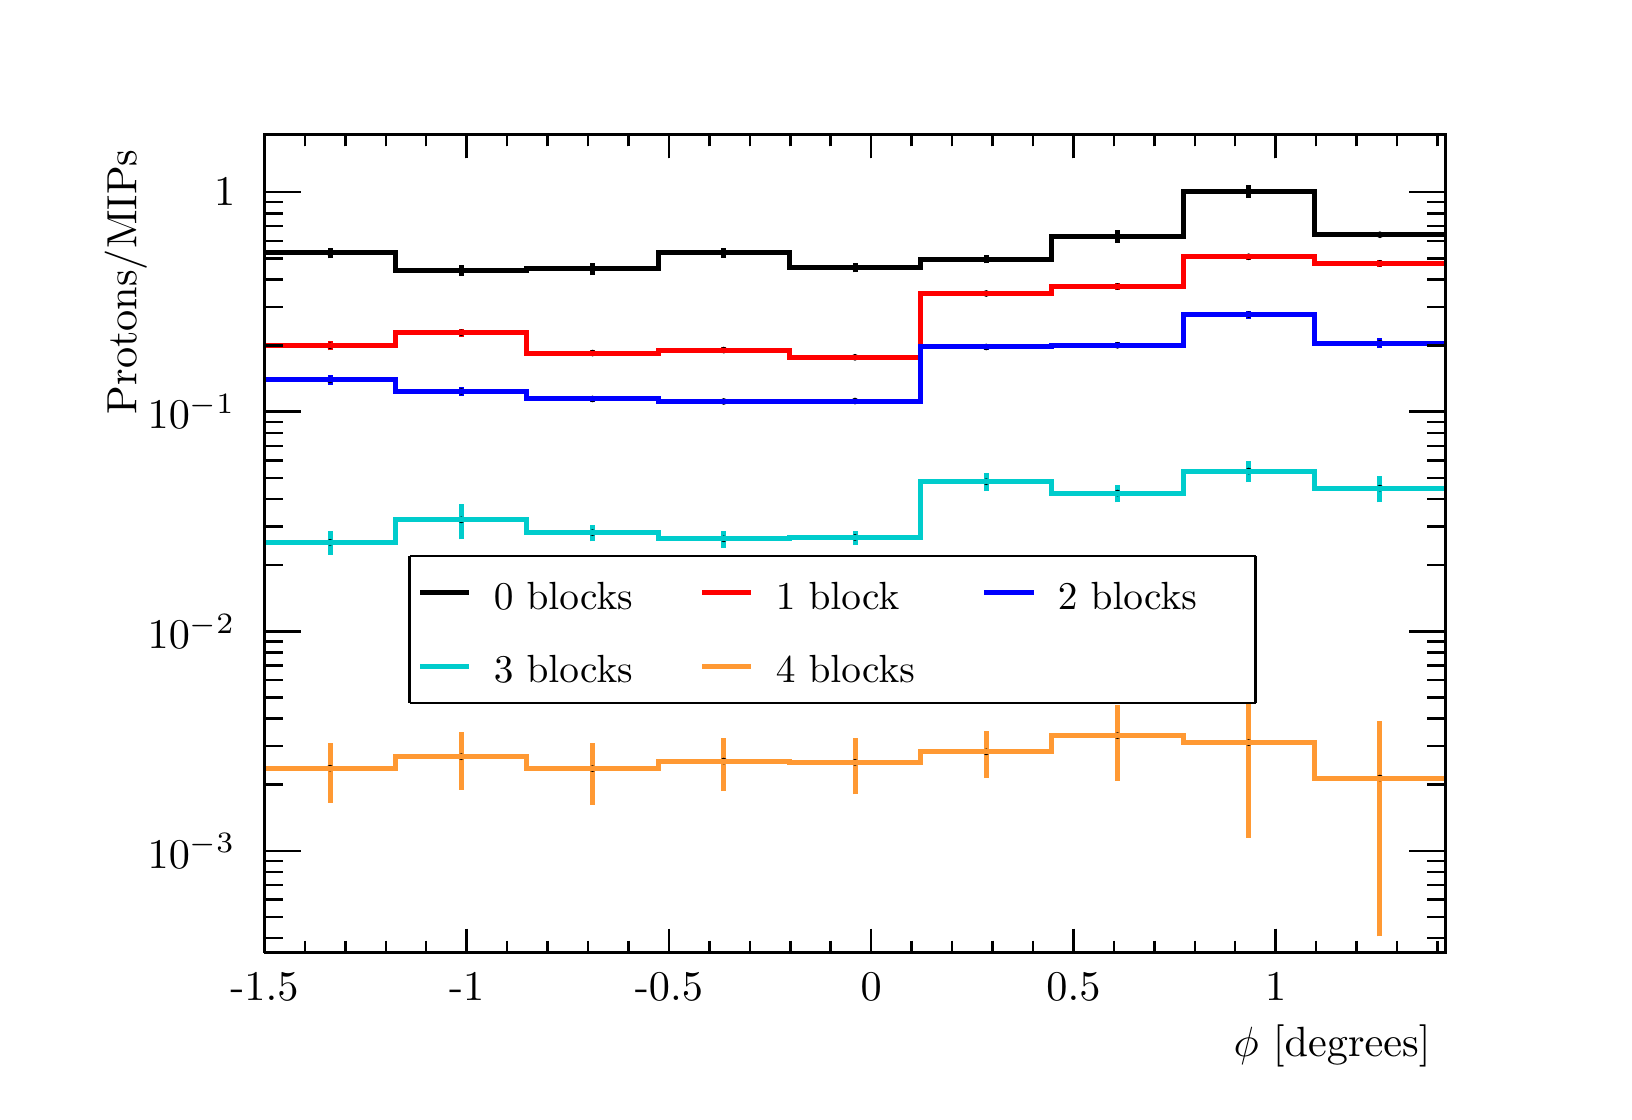
\begin{tikzpicture}
\pgfdeclareplotmark{cross} {
\pgfpathmoveto{\pgfpoint{-0.3\pgfplotmarksize}{\pgfplotmarksize}}
\pgfpathlineto{\pgfpoint{+0.3\pgfplotmarksize}{\pgfplotmarksize}}
\pgfpathlineto{\pgfpoint{+0.3\pgfplotmarksize}{0.3\pgfplotmarksize}}
\pgfpathlineto{\pgfpoint{+1\pgfplotmarksize}{0.3\pgfplotmarksize}}
\pgfpathlineto{\pgfpoint{+1\pgfplotmarksize}{-0.3\pgfplotmarksize}}
\pgfpathlineto{\pgfpoint{+0.3\pgfplotmarksize}{-0.3\pgfplotmarksize}}
\pgfpathlineto{\pgfpoint{+0.3\pgfplotmarksize}{-1.\pgfplotmarksize}}
\pgfpathlineto{\pgfpoint{-0.3\pgfplotmarksize}{-1.\pgfplotmarksize}}
\pgfpathlineto{\pgfpoint{-0.3\pgfplotmarksize}{-0.3\pgfplotmarksize}}
\pgfpathlineto{\pgfpoint{-1.\pgfplotmarksize}{-0.3\pgfplotmarksize}}
\pgfpathlineto{\pgfpoint{-1.\pgfplotmarksize}{0.3\pgfplotmarksize}}
\pgfpathlineto{\pgfpoint{-0.3\pgfplotmarksize}{0.3\pgfplotmarksize}}
\pgfpathclose
\pgfusepathqstroke
}
\pgfdeclareplotmark{cross*} {
\pgfpathmoveto{\pgfpoint{-0.3\pgfplotmarksize}{\pgfplotmarksize}}
\pgfpathlineto{\pgfpoint{+0.3\pgfplotmarksize}{\pgfplotmarksize}}
\pgfpathlineto{\pgfpoint{+0.3\pgfplotmarksize}{0.3\pgfplotmarksize}}
\pgfpathlineto{\pgfpoint{+1\pgfplotmarksize}{0.3\pgfplotmarksize}}
\pgfpathlineto{\pgfpoint{+1\pgfplotmarksize}{-0.3\pgfplotmarksize}}
\pgfpathlineto{\pgfpoint{+0.3\pgfplotmarksize}{-0.3\pgfplotmarksize}}
\pgfpathlineto{\pgfpoint{+0.3\pgfplotmarksize}{-1.\pgfplotmarksize}}
\pgfpathlineto{\pgfpoint{-0.3\pgfplotmarksize}{-1.\pgfplotmarksize}}
\pgfpathlineto{\pgfpoint{-0.3\pgfplotmarksize}{-0.3\pgfplotmarksize}}
\pgfpathlineto{\pgfpoint{-1.\pgfplotmarksize}{-0.3\pgfplotmarksize}}
\pgfpathlineto{\pgfpoint{-1.\pgfplotmarksize}{0.3\pgfplotmarksize}}
\pgfpathlineto{\pgfpoint{-0.3\pgfplotmarksize}{0.3\pgfplotmarksize}}
\pgfpathclose
\pgfusepathqfillstroke
}
\pgfdeclareplotmark{newstar} {
\pgfpathmoveto{\pgfqpoint{0pt}{\pgfplotmarksize}}
\pgfpathlineto{\pgfqpointpolar{44}{0.5\pgfplotmarksize}}
\pgfpathlineto{\pgfqpointpolar{18}{\pgfplotmarksize}}
\pgfpathlineto{\pgfqpointpolar{-20}{0.5\pgfplotmarksize}}
\pgfpathlineto{\pgfqpointpolar{-54}{\pgfplotmarksize}}
\pgfpathlineto{\pgfqpointpolar{-90}{0.5\pgfplotmarksize}}
\pgfpathlineto{\pgfqpointpolar{234}{\pgfplotmarksize}}
\pgfpathlineto{\pgfqpointpolar{198}{0.5\pgfplotmarksize}}
\pgfpathlineto{\pgfqpointpolar{162}{\pgfplotmarksize}}
\pgfpathlineto{\pgfqpointpolar{134}{0.5\pgfplotmarksize}}
\pgfpathclose
\pgfusepathqstroke
}
\pgfdeclareplotmark{newstar*} {
\pgfpathmoveto{\pgfqpoint{0pt}{\pgfplotmarksize}}
\pgfpathlineto{\pgfqpointpolar{44}{0.5\pgfplotmarksize}}
\pgfpathlineto{\pgfqpointpolar{18}{\pgfplotmarksize}}
\pgfpathlineto{\pgfqpointpolar{-20}{0.5\pgfplotmarksize}}
\pgfpathlineto{\pgfqpointpolar{-54}{\pgfplotmarksize}}
\pgfpathlineto{\pgfqpointpolar{-90}{0.5\pgfplotmarksize}}
\pgfpathlineto{\pgfqpointpolar{234}{\pgfplotmarksize}}
\pgfpathlineto{\pgfqpointpolar{198}{0.5\pgfplotmarksize}}
\pgfpathlineto{\pgfqpointpolar{162}{\pgfplotmarksize}}
\pgfpathlineto{\pgfqpointpolar{134}{0.5\pgfplotmarksize}}
\pgfpathclose
\pgfusepathqfillstroke
}
\definecolor{c}{rgb}{1,1,1};
\draw [color=c, fill=c] (0,0) rectangle (20,13.4957);
\draw [color=c, fill=c] (3,1.75444) rectangle (18,12.1461);
\definecolor{c}{rgb}{0,0,0};
\draw [c,line width=0.9] (3,1.75444) -- (3,12.1461) -- (18,12.1461) -- (18,1.75444) -- (3,1.75444);
\definecolor{c}{rgb}{1,1,1};
\draw [color=c, fill=c] (3,1.75444) rectangle (18,12.1461);
\definecolor{c}{rgb}{0,0,0};
\draw [c,line width=0.9] (3,1.75444) -- (3,12.1461) -- (18,12.1461) -- (18,1.75444) -- (3,1.75444);
\draw [c,line width=0.9] (3,1.75444) -- (4.66667,1.75444) -- (4.66667,1.75444) -- (6.33333,1.75444) -- (6.33333,1.75444) -- (8,1.75444) -- (8,1.75444) -- (9.66667,1.75444) -- (9.66667,1.75444) -- (11.3333,1.75444) -- (11.3333,1.75444) -- (13,1.75444)
 -- (13,1.75444) -- (14.6667,1.75444) -- (14.6667,1.75444) -- (16.3333,1.75444) -- (16.3333,1.75444) -- (18,1.75444);
\draw [c,line width=0.9] (3,1.75444) -- (18,1.75444);
\draw [c,line width=0.9] (3,2.05809) -- (3,1.75444);
\draw [c,line width=0.9] (3.5137,1.90627) -- (3.5137,1.75444);
\draw [c,line width=0.9] (4.0274,1.90627) -- (4.0274,1.75444);
\draw [c,line width=0.9] (4.5411,1.90627) -- (4.5411,1.75444);
\draw [c,line width=0.9] (5.05479,1.90627) -- (5.05479,1.75444);
\draw [c,line width=0.9] (5.56849,2.05809) -- (5.56849,1.75444);
\draw [c,line width=0.9] (6.08219,1.90627) -- (6.08219,1.75444);
\draw [c,line width=0.9] (6.59589,1.90627) -- (6.59589,1.75444);
\draw [c,line width=0.9] (7.10959,1.90627) -- (7.10959,1.75444);
\draw [c,line width=0.9] (7.62329,1.90627) -- (7.62329,1.75444);
\draw [c,line width=0.9] (8.13699,2.05809) -- (8.13699,1.75444);
\draw [c,line width=0.9] (8.65069,1.90627) -- (8.65069,1.75444);
\draw [c,line width=0.9] (9.16438,1.90627) -- (9.16438,1.75444);
\draw [c,line width=0.9] (9.67808,1.90627) -- (9.67808,1.75444);
\draw [c,line width=0.9] (10.1918,1.90627) -- (10.1918,1.75444);
\draw [c,line width=0.9] (10.7055,2.05809) -- (10.7055,1.75444);
\draw [c,line width=0.9] (11.2192,1.90627) -- (11.2192,1.75444);
\draw [c,line width=0.9] (11.7329,1.90627) -- (11.7329,1.75444);
\draw [c,line width=0.9] (12.2466,1.90627) -- (12.2466,1.75444);
\draw [c,line width=0.9] (12.7603,1.90627) -- (12.7603,1.75444);
\draw [c,line width=0.9] (13.274,2.05809) -- (13.274,1.75444);
\draw [c,line width=0.9] (13.7877,1.90627) -- (13.7877,1.75444);
\draw [c,line width=0.9] (14.3014,1.90627) -- (14.3014,1.75444);
\draw [c,line width=0.9] (14.8151,1.90627) -- (14.8151,1.75444);
\draw [c,line width=0.9] (15.3288,1.90627) -- (15.3288,1.75444);
\draw [c,line width=0.9] (15.8425,2.05809) -- (15.8425,1.75444);
\draw [c,line width=0.9] (15.8425,2.05809) -- (15.8425,1.75444);
\draw [c,line width=0.9] (16.3562,1.90627) -- (16.3562,1.75444);
\draw [c,line width=0.9] (16.8699,1.90627) -- (16.8699,1.75444);
\draw [c,line width=0.9] (17.3836,1.90627) -- (17.3836,1.75444);
\draw [c,line width=0.9] (17.8973,1.90627) -- (17.8973,1.75444);
\draw [anchor=base] (3,1.14713) node[scale=1.52731, color=c, rotate=0]{-1.5};
\draw [anchor=base] (5.56849,1.14713) node[scale=1.52731, color=c, rotate=0]{-1};
\draw [anchor=base] (8.13699,1.14713) node[scale=1.52731, color=c, rotate=0]{-0.5};
\draw [anchor=base] (10.7055,1.14713) node[scale=1.52731, color=c, rotate=0]{0};
\draw [anchor=base] (13.274,1.14713) node[scale=1.52731, color=c, rotate=0]{0.5};
\draw [anchor=base] (15.8425,1.14713) node[scale=1.52731, color=c, rotate=0]{1};
\draw [anchor= east] (18,0.566819) node[scale=1.52731, color=c, rotate=0]{$\phi$ [degrees]};
\draw [c,line width=0.9] (3,12.1461) -- (18,12.1461);
\draw [c,line width=0.9] (3,11.8425) -- (3,12.1461);
\draw [c,line width=0.9] (3.5137,11.9943) -- (3.5137,12.1461);
\draw [c,line width=0.9] (4.0274,11.9943) -- (4.0274,12.1461);
\draw [c,line width=0.9] (4.5411,11.9943) -- (4.5411,12.1461);
\draw [c,line width=0.9] (5.05479,11.9943) -- (5.05479,12.1461);
\draw [c,line width=0.9] (5.56849,11.8425) -- (5.56849,12.1461);
\draw [c,line width=0.9] (6.08219,11.9943) -- (6.08219,12.1461);
\draw [c,line width=0.9] (6.59589,11.9943) -- (6.59589,12.1461);
\draw [c,line width=0.9] (7.10959,11.9943) -- (7.10959,12.1461);
\draw [c,line width=0.9] (7.62329,11.9943) -- (7.62329,12.1461);
\draw [c,line width=0.9] (8.13699,11.8425) -- (8.13699,12.1461);
\draw [c,line width=0.9] (8.65069,11.9943) -- (8.65069,12.1461);
\draw [c,line width=0.9] (9.16438,11.9943) -- (9.16438,12.1461);
\draw [c,line width=0.9] (9.67808,11.9943) -- (9.67808,12.1461);
\draw [c,line width=0.9] (10.1918,11.9943) -- (10.1918,12.1461);
\draw [c,line width=0.9] (10.7055,11.8425) -- (10.7055,12.1461);
\draw [c,line width=0.9] (11.2192,11.9943) -- (11.2192,12.1461);
\draw [c,line width=0.9] (11.7329,11.9943) -- (11.7329,12.1461);
\draw [c,line width=0.9] (12.2466,11.9943) -- (12.2466,12.1461);
\draw [c,line width=0.9] (12.7603,11.9943) -- (12.7603,12.1461);
\draw [c,line width=0.9] (13.274,11.8425) -- (13.274,12.1461);
\draw [c,line width=0.9] (13.7877,11.9943) -- (13.7877,12.1461);
\draw [c,line width=0.9] (14.3014,11.9943) -- (14.3014,12.1461);
\draw [c,line width=0.9] (14.8151,11.9943) -- (14.8151,12.1461);
\draw [c,line width=0.9] (15.3288,11.9943) -- (15.3288,12.1461);
\draw [c,line width=0.9] (15.8425,11.8425) -- (15.8425,12.1461);
\draw [c,line width=0.9] (15.8425,11.8425) -- (15.8425,12.1461);
\draw [c,line width=0.9] (16.3562,11.9943) -- (16.3562,12.1461);
\draw [c,line width=0.9] (16.8699,11.9943) -- (16.8699,12.1461);
\draw [c,line width=0.9] (17.3836,11.9943) -- (17.3836,12.1461);
\draw [c,line width=0.9] (17.8973,11.9943) -- (17.8973,12.1461);
\draw [c,line width=0.9] (3,1.75444) -- (3,12.1461);
\draw [c,line width=0.9] (3.231,1.93919) -- (3,1.93919);
\draw [c,line width=0.9] (3.231,2.20939) -- (3,2.20939);
\draw [c,line width=0.9] (3.231,2.43016) -- (3,2.43016);
\draw [c,line width=0.9] (3.231,2.61681) -- (3,2.61681);
\draw [c,line width=0.9] (3.231,2.7785) -- (3,2.7785);
\draw [c,line width=0.9] (3.231,2.92112) -- (3,2.92112);
\draw [c,line width=0.9] (3.462,3.0487) -- (3,3.0487);
\draw [anchor= east] (2.82,3.0487) node[scale=1.52731, color=c, rotate=0]{$10^{-3}$};
\draw [c,line width=0.9] (3.231,3.88801) -- (3,3.88801);
\draw [c,line width=0.9] (3.231,4.37898) -- (3,4.37898);
\draw [c,line width=0.9] (3.231,4.72732) -- (3,4.72732);
\draw [c,line width=0.9] (3.231,4.99752) -- (3,4.99752);
\draw [c,line width=0.9] (3.231,5.21829) -- (3,5.21829);
\draw [c,line width=0.9] (3.231,5.40494) -- (3,5.40494);
\draw [c,line width=0.9] (3.231,5.56663) -- (3,5.56663);
\draw [c,line width=0.9] (3.231,5.70925) -- (3,5.70925);
\draw [c,line width=0.9] (3.462,5.83683) -- (3,5.83683);
\draw [anchor= east] (2.82,5.83683) node[scale=1.52731, color=c, rotate=0]{$10^{-2}$};
\draw [c,line width=0.9] (3.231,6.67614) -- (3,6.67614);
\draw [c,line width=0.9] (3.231,7.16711) -- (3,7.16711);
\draw [c,line width=0.9] (3.231,7.51545) -- (3,7.51545);
\draw [c,line width=0.9] (3.231,7.78565) -- (3,7.78565);
\draw [c,line width=0.9] (3.231,8.00642) -- (3,8.00642);
\draw [c,line width=0.9] (3.231,8.19307) -- (3,8.19307);
\draw [c,line width=0.9] (3.231,8.35476) -- (3,8.35476);
\draw [c,line width=0.9] (3.231,8.49738) -- (3,8.49738);
\draw [c,line width=0.9] (3.462,8.62496) -- (3,8.62496);
\draw [anchor= east] (2.82,8.62496) node[scale=1.52731, color=c, rotate=0]{$10^{-1}$};
\draw [c,line width=0.9] (3.231,9.46427) -- (3,9.46427);
\draw [c,line width=0.9] (3.231,9.95524) -- (3,9.95524);
\draw [c,line width=0.9] (3.231,10.3036) -- (3,10.3036);
\draw [c,line width=0.9] (3.231,10.5738) -- (3,10.5738);
\draw [c,line width=0.9] (3.231,10.7945) -- (3,10.7945);
\draw [c,line width=0.9] (3.231,10.9812) -- (3,10.9812);
\draw [c,line width=0.9] (3.231,11.1429) -- (3,11.1429);
\draw [c,line width=0.9] (3.231,11.2855) -- (3,11.2855);
\draw [c,line width=0.9] (3.462,11.4131) -- (3,11.4131);
\draw [anchor= east] (2.82,11.4131) node[scale=1.52731, color=c, rotate=0]{1};
\draw [anchor= east] (1.24,12.1461) node[scale=1.52731, color=c, rotate=90]{ Protons/MIPs};
\draw [c,line width=0.9] (18,1.75444) -- (18,12.1461);
\draw [c,line width=0.9] (17.769,1.93919) -- (18,1.93919);
\draw [c,line width=0.9] (17.769,2.20939) -- (18,2.20939);
\draw [c,line width=0.9] (17.769,2.43016) -- (18,2.43016);
\draw [c,line width=0.9] (17.769,2.61681) -- (18,2.61681);
\draw [c,line width=0.9] (17.769,2.7785) -- (18,2.7785);
\draw [c,line width=0.9] (17.769,2.92112) -- (18,2.92112);
\draw [c,line width=0.9] (17.538,3.0487) -- (18,3.0487);
\draw [c,line width=0.9] (17.769,3.88801) -- (18,3.88801);
\draw [c,line width=0.9] (17.769,4.37898) -- (18,4.37898);
\draw [c,line width=0.9] (17.769,4.72732) -- (18,4.72732);
\draw [c,line width=0.9] (17.769,4.99752) -- (18,4.99752);
\draw [c,line width=0.9] (17.769,5.21829) -- (18,5.21829);
\draw [c,line width=0.9] (17.769,5.40494) -- (18,5.40494);
\draw [c,line width=0.9] (17.769,5.56663) -- (18,5.56663);
\draw [c,line width=0.9] (17.769,5.70925) -- (18,5.70925);
\draw [c,line width=0.9] (17.538,5.83683) -- (18,5.83683);
\draw [c,line width=0.9] (17.769,6.67614) -- (18,6.67614);
\draw [c,line width=0.9] (17.769,7.16711) -- (18,7.16711);
\draw [c,line width=0.9] (17.769,7.51545) -- (18,7.51545);
\draw [c,line width=0.9] (17.769,7.78565) -- (18,7.78565);
\draw [c,line width=0.9] (17.769,8.00642) -- (18,8.00642);
\draw [c,line width=0.9] (17.769,8.19307) -- (18,8.19307);
\draw [c,line width=0.9] (17.769,8.35476) -- (18,8.35476);
\draw [c,line width=0.9] (17.769,8.49738) -- (18,8.49738);
\draw [c,line width=0.9] (17.538,8.62496) -- (18,8.62496);
\draw [c,line width=0.9] (17.769,9.46427) -- (18,9.46427);
\draw [c,line width=0.9] (17.769,9.95524) -- (18,9.95524);
\draw [c,line width=0.9] (17.769,10.3036) -- (18,10.3036);
\draw [c,line width=0.9] (17.769,10.5738) -- (18,10.5738);
\draw [c,line width=0.9] (17.769,10.7945) -- (18,10.7945);
\draw [c,line width=0.9] (17.769,10.9812) -- (18,10.9812);
\draw [c,line width=0.9] (17.769,11.1429) -- (18,11.1429);
\draw [c,line width=0.9] (17.769,11.2855) -- (18,11.2855);
\draw [c,line width=0.9] (17.538,11.4131) -- (18,11.4131);
\draw [c,line width=1.8] (3.83333,10.572) -- (3.83333,10.6419);
\draw [c,line width=1.8] (3.83333,10.6419) -- (3.83333,10.7081);
\foreach \P in {(3.83333,10.6419)}{\draw[mark options={color=c,fill=c},mark size=2.402402pt,mark=*,mark size=1pt] plot coordinates {\P};}
\draw [c,line width=1.8] (5.5,10.3482) -- (5.5,10.42);
\draw [c,line width=1.8] (5.5,10.42) -- (5.5,10.4878);
\foreach \P in {(5.5,10.42)}{\draw[mark options={color=c,fill=c},mark size=2.402402pt,mark=*,mark size=1pt] plot coordinates {\P};}
\draw [c,line width=1.8] (7.16667,10.3597) -- (7.16667,10.4384);
\draw [c,line width=1.8] (7.16667,10.4384) -- (7.16667,10.5124);
\foreach \P in {(7.16667,10.4384)}{\draw[mark options={color=c,fill=c},mark size=2.402402pt,mark=*,mark size=1pt] plot coordinates {\P};}
\draw [c,line width=1.8] (8.83333,10.5821) -- (8.83333,10.6443);
\draw [c,line width=1.8] (8.83333,10.6443) -- (8.83333,10.7033);
\foreach \P in {(8.83333,10.6443)}{\draw[mark options={color=c,fill=c},mark size=2.402402pt,mark=*,mark size=1pt] plot coordinates {\P};}
\draw [c,line width=1.8] (10.5,10.3955) -- (10.5,10.4552);
\draw [c,line width=1.8] (10.5,10.4552) -- (10.5,10.5121);
\foreach \P in {(10.5,10.4552)}{\draw[mark options={color=c,fill=c},mark size=2.402402pt,mark=*,mark size=1pt] plot coordinates {\P};}
\draw [c,line width=1.8] (12.1667,10.5095) -- (12.1667,10.5604);
\draw [c,line width=1.8] (12.1667,10.5604) -- (12.1667,10.6093);
\foreach \P in {(12.1667,10.5604)}{\draw[mark options={color=c,fill=c},mark size=2.402402pt,mark=*,mark size=1pt] plot coordinates {\P};}
\draw [c,line width=1.8] (13.8333,10.7682) -- (13.8333,10.8531);
\draw [c,line width=1.8] (13.8333,10.8531) -- (13.8333,10.9325);
\foreach \P in {(13.8333,10.8531)}{\draw[mark options={color=c,fill=c},mark size=2.402402pt,mark=*,mark size=1pt] plot coordinates {\P};}
\draw [c,line width=1.8] (15.5,11.3373) -- (15.5,11.424);
\draw [c,line width=1.8] (15.5,11.424) -- (15.5,11.505);
\foreach \P in {(15.5,11.424)}{\draw[mark options={color=c,fill=c},mark size=2.402402pt,mark=*,mark size=1pt] plot coordinates {\P};}
\draw [c,line width=1.8] (17.1667,10.8476) -- (17.1667,10.8726);
\draw [c,line width=1.8] (17.1667,10.8726) -- (17.1667,10.8972);
\foreach \P in {(17.1667,10.8726)}{\draw[mark options={color=c,fill=c},mark size=2.402402pt,mark=*,mark size=1pt] plot coordinates {\P};}
\draw [c,line width=1.8] (3,10.6419) -- (4.66667,10.6419) -- (4.66667,10.42) -- (6.33333,10.42) -- (6.33333,10.4384) -- (8,10.4384) -- (8,10.6443) -- (9.66667,10.6443) -- (9.66667,10.4552) -- (11.3333,10.4552) -- (11.3333,10.5604) -- (13,10.5604) --
 (13,10.8531) -- (14.6667,10.8531) -- (14.6667,11.424) -- (16.3333,11.424) -- (16.3333,10.8726) -- (18,10.8726);
\definecolor{c}{rgb}{1,0,0};
\draw [c,line width=1.8] (3.83333,9.40359) -- (3.83333,9.46301);
\draw [c,line width=1.8] (3.83333,9.46301) -- (3.83333,9.51965);
\definecolor{c}{rgb}{0,0,0};
\foreach \P in {(3.83333,9.46301)}{\draw[mark options={color=c,fill=c},mark size=2.402402pt,mark=*,mark size=1pt] plot coordinates {\P};}
\definecolor{c}{rgb}{1,0,0};
\draw [c,line width=1.8] (5.5,9.57854) -- (5.5,9.62851);
\draw [c,line width=1.8] (5.5,9.62851) -- (5.5,9.6765);
\definecolor{c}{rgb}{0,0,0};
\foreach \P in {(5.5,9.62851)}{\draw[mark options={color=c,fill=c},mark size=2.402402pt,mark=*,mark size=1pt] plot coordinates {\P};}
\definecolor{c}{rgb}{1,0,0};
\draw [c,line width=1.8] (7.16667,9.33523) -- (7.16667,9.37043);
\draw [c,line width=1.8] (7.16667,9.37043) -- (7.16667,9.40463);
\definecolor{c}{rgb}{0,0,0};
\foreach \P in {(7.16667,9.37043)}{\draw[mark options={color=c,fill=c},mark size=2.402402pt,mark=*,mark size=1pt] plot coordinates {\P};}
\definecolor{c}{rgb}{1,0,0};
\draw [c,line width=1.8] (8.83333,9.37028) -- (8.83333,9.40777);
\draw [c,line width=1.8] (8.83333,9.40777) -- (8.83333,9.44414);
\definecolor{c}{rgb}{0,0,0};
\foreach \P in {(8.83333,9.40777)}{\draw[mark options={color=c,fill=c},mark size=2.402402pt,mark=*,mark size=1pt] plot coordinates {\P};}
\definecolor{c}{rgb}{1,0,0};
\draw [c,line width=1.8] (10.5,9.28506) -- (10.5,9.31673);
\draw [c,line width=1.8] (10.5,9.31673) -- (10.5,9.3476);
\definecolor{c}{rgb}{0,0,0};
\foreach \P in {(10.5,9.31673)}{\draw[mark options={color=c,fill=c},mark size=2.402402pt,mark=*,mark size=1pt] plot coordinates {\P};}
\definecolor{c}{rgb}{1,0,0};
\draw [c,line width=1.8] (12.1667,10.0925) -- (12.1667,10.1267);
\draw [c,line width=1.8] (12.1667,10.1267) -- (12.1667,10.1601);
\definecolor{c}{rgb}{0,0,0};
\foreach \P in {(12.1667,10.1267)}{\draw[mark options={color=c,fill=c},mark size=2.402402pt,mark=*,mark size=1pt] plot coordinates {\P};}
\definecolor{c}{rgb}{1,0,0};
\draw [c,line width=1.8] (13.8333,10.1698) -- (13.8333,10.2162);
\draw [c,line width=1.8] (13.8333,10.2162) -- (13.8333,10.261);
\definecolor{c}{rgb}{0,0,0};
\foreach \P in {(13.8333,10.2162)}{\draw[mark options={color=c,fill=c},mark size=2.402402pt,mark=*,mark size=1pt] plot coordinates {\P};}
\definecolor{c}{rgb}{1,0,0};
\draw [c,line width=1.8] (15.5,10.5564) -- (15.5,10.5934);
\draw [c,line width=1.8] (15.5,10.5934) -- (15.5,10.6294);
\definecolor{c}{rgb}{0,0,0};
\foreach \P in {(15.5,10.5934)}{\draw[mark options={color=c,fill=c},mark size=2.402402pt,mark=*,mark size=1pt] plot coordinates {\P};}
\definecolor{c}{rgb}{1,0,0};
\draw [c,line width=1.8] (17.1667,10.4672) -- (17.1667,10.5099);
\draw [c,line width=1.8] (17.1667,10.5099) -- (17.1667,10.5512);
\definecolor{c}{rgb}{0,0,0};
\foreach \P in {(17.1667,10.5099)}{\draw[mark options={color=c,fill=c},mark size=2.402402pt,mark=*,mark size=1pt] plot coordinates {\P};}
\definecolor{c}{rgb}{1,0,0};
\draw [c,line width=1.8] (3,9.46301) -- (4.66667,9.46301) -- (4.66667,9.62851) -- (6.33333,9.62851) -- (6.33333,9.37043) -- (8,9.37043) -- (8,9.40777) -- (9.66667,9.40777) -- (9.66667,9.31673) -- (11.3333,9.31673) -- (11.3333,10.1267) -- (13,10.1267)
 -- (13,10.2162) -- (14.6667,10.2162) -- (14.6667,10.5934) -- (16.3333,10.5934) -- (16.3333,10.5099) -- (18,10.5099);
\definecolor{c}{rgb}{0,0,1};
\draw [c,line width=1.8] (3.83333,8.96981) -- (3.83333,9.02932);
\draw [c,line width=1.8] (3.83333,9.02932) -- (3.83333,9.08605);
\definecolor{c}{rgb}{0,0,0};
\foreach \P in {(3.83333,9.02932)}{\draw[mark options={color=c,fill=c},mark size=2.402402pt,mark=*,mark size=1pt] plot coordinates {\P};}
\definecolor{c}{rgb}{0,0,1};
\draw [c,line width=1.8] (5.5,8.83028) -- (5.5,8.88269);
\draw [c,line width=1.8] (5.5,8.88269) -- (5.5,8.93294);
\definecolor{c}{rgb}{0,0,0};
\foreach \P in {(5.5,8.88269)}{\draw[mark options={color=c,fill=c},mark size=2.402402pt,mark=*,mark size=1pt] plot coordinates {\P};}
\definecolor{c}{rgb}{0,0,1};
\draw [c,line width=1.8] (7.16667,8.74754) -- (7.16667,8.78715);
\draw [c,line width=1.8] (7.16667,8.78715) -- (7.16667,8.82551);
\definecolor{c}{rgb}{0,0,0};
\foreach \P in {(7.16667,8.78715)}{\draw[mark options={color=c,fill=c},mark size=2.402402pt,mark=*,mark size=1pt] plot coordinates {\P};}
\definecolor{c}{rgb}{0,0,1};
\draw [c,line width=1.8] (8.83333,8.72092) -- (8.83333,8.75543);
\draw [c,line width=1.8] (8.83333,8.75543) -- (8.83333,8.78898);
\definecolor{c}{rgb}{0,0,0};
\foreach \P in {(8.83333,8.75543)}{\draw[mark options={color=c,fill=c},mark size=2.402402pt,mark=*,mark size=1pt] plot coordinates {\P};}
\definecolor{c}{rgb}{0,0,1};
\draw [c,line width=1.8] (10.5,8.73099) -- (10.5,8.76081);
\draw [c,line width=1.8] (10.5,8.76081) -- (10.5,8.78991);
\definecolor{c}{rgb}{0,0,0};
\foreach \P in {(10.5,8.76081)}{\draw[mark options={color=c,fill=c},mark size=2.402402pt,mark=*,mark size=1pt] plot coordinates {\P};}
\definecolor{c}{rgb}{0,0,1};
\draw [c,line width=1.8] (12.1667,9.41213) -- (12.1667,9.44762);
\draw [c,line width=1.8] (12.1667,9.44762) -- (12.1667,9.48209);
\definecolor{c}{rgb}{0,0,0};
\foreach \P in {(12.1667,9.44762)}{\draw[mark options={color=c,fill=c},mark size=2.402402pt,mark=*,mark size=1pt] plot coordinates {\P};}
\definecolor{c}{rgb}{0,0,1};
\draw [c,line width=1.8] (13.8333,9.43055) -- (13.8333,9.4684);
\draw [c,line width=1.8] (13.8333,9.4684) -- (13.8333,9.5051);
\definecolor{c}{rgb}{0,0,0};
\foreach \P in {(13.8333,9.4684)}{\draw[mark options={color=c,fill=c},mark size=2.402402pt,mark=*,mark size=1pt] plot coordinates {\P};}
\definecolor{c}{rgb}{0,0,1};
\draw [c,line width=1.8] (15.5,9.80824) -- (15.5,9.8583);
\draw [c,line width=1.8] (15.5,9.8583) -- (15.5,9.90637);
\definecolor{c}{rgb}{0,0,0};
\foreach \P in {(15.5,9.8583)}{\draw[mark options={color=c,fill=c},mark size=2.402402pt,mark=*,mark size=1pt] plot coordinates {\P};}
\definecolor{c}{rgb}{0,0,1};
\draw [c,line width=1.8] (17.1667,9.43336) -- (17.1667,9.49632);
\draw [c,line width=1.8] (17.1667,9.49632) -- (17.1667,9.55617);
\definecolor{c}{rgb}{0,0,0};
\foreach \P in {(17.1667,9.49632)}{\draw[mark options={color=c,fill=c},mark size=2.402402pt,mark=*,mark size=1pt] plot coordinates {\P};}
\definecolor{c}{rgb}{0,0,1};
\draw [c,line width=1.8] (3,9.02932) -- (4.66667,9.02932) -- (4.66667,8.88269) -- (6.33333,8.88269) -- (6.33333,8.78715) -- (8,8.78715) -- (8,8.75543) -- (9.66667,8.75543) -- (9.66667,8.76081) -- (11.3333,8.76081) -- (11.3333,9.44762) -- (13,9.44762)
 -- (13,9.4684) -- (14.6667,9.4684) -- (14.6667,9.8583) -- (16.3333,9.8583) -- (16.3333,9.49632) -- (18,9.49632);
\definecolor{c}{rgb}{0,0.8,0.8};
\draw [c,line width=1.8] (3.83333,6.80707) -- (3.83333,6.96591);
\draw [c,line width=1.8] (3.83333,6.96591) -- (3.83333,7.10631);
\definecolor{c}{rgb}{0,0,0};
\foreach \P in {(3.83333,6.96591)}{\draw[mark options={color=c,fill=c},mark size=2.402402pt,mark=*,mark size=1pt] plot coordinates {\P};}
\definecolor{c}{rgb}{0,0.8,0.8};
\draw [c,line width=1.8] (5.5,7.00316) -- (5.5,7.25221);
\draw [c,line width=1.8] (5.5,7.25221) -- (5.5,7.45867);
\definecolor{c}{rgb}{0,0,0};
\foreach \P in {(5.5,7.25221)}{\draw[mark options={color=c,fill=c},mark size=2.402402pt,mark=*,mark size=1pt] plot coordinates {\P};}
\definecolor{c}{rgb}{0,0.8,0.8};
\draw [c,line width=1.8] (7.16667,6.97812) -- (7.16667,7.08972);
\draw [c,line width=1.8] (7.16667,7.08972) -- (7.16667,7.1919);
\definecolor{c}{rgb}{0,0,0};
\foreach \P in {(7.16667,7.08972)}{\draw[mark options={color=c,fill=c},mark size=2.402402pt,mark=*,mark size=1pt] plot coordinates {\P};}
\definecolor{c}{rgb}{0,0.8,0.8};
\draw [c,line width=1.8] (8.83333,6.89753) -- (8.83333,7.01091);
\draw [c,line width=1.8] (8.83333,7.01091) -- (8.83333,7.11458);
\definecolor{c}{rgb}{0,0,0};
\foreach \P in {(8.83333,7.01091)}{\draw[mark options={color=c,fill=c},mark size=2.402402pt,mark=*,mark size=1pt] plot coordinates {\P};}
\definecolor{c}{rgb}{0,0.8,0.8};
\draw [c,line width=1.8] (10.5,6.9388) -- (10.5,7.0284);
\draw [c,line width=1.8] (10.5,7.0284) -- (10.5,7.11182);
\definecolor{c}{rgb}{0,0,0};
\foreach \P in {(10.5,7.0284)}{\draw[mark options={color=c,fill=c},mark size=2.402402pt,mark=*,mark size=1pt] plot coordinates {\P};}
\definecolor{c}{rgb}{0,0.8,0.8};
\draw [c,line width=1.8] (12.1667,7.61534) -- (12.1667,7.73673);
\draw [c,line width=1.8] (12.1667,7.73673) -- (12.1667,7.84705);
\definecolor{c}{rgb}{0,0,0};
\foreach \P in {(12.1667,7.73673)}{\draw[mark options={color=c,fill=c},mark size=2.402402pt,mark=*,mark size=1pt] plot coordinates {\P};}
\definecolor{c}{rgb}{0,0.8,0.8};
\draw [c,line width=1.8] (13.8333,7.47538) -- (13.8333,7.59226);
\draw [c,line width=1.8] (13.8333,7.59226) -- (13.8333,7.69885);
\definecolor{c}{rgb}{0,0,0};
\foreach \P in {(13.8333,7.59226)}{\draw[mark options={color=c,fill=c},mark size=2.402402pt,mark=*,mark size=1pt] plot coordinates {\P};}
\definecolor{c}{rgb}{0,0.8,0.8};
\draw [c,line width=1.8] (15.5,7.73149) -- (15.5,7.87156);
\draw [c,line width=1.8] (15.5,7.87156) -- (15.5,7.9971);
\definecolor{c}{rgb}{0,0,0};
\foreach \P in {(15.5,7.87156)}{\draw[mark options={color=c,fill=c},mark size=2.402402pt,mark=*,mark size=1pt] plot coordinates {\P};}
\definecolor{c}{rgb}{0,0.8,0.8};
\draw [c,line width=1.8] (17.1667,7.47332) -- (17.1667,7.65497);
\draw [c,line width=1.8] (17.1667,7.65497) -- (17.1667,7.81288);
\definecolor{c}{rgb}{0,0,0};
\foreach \P in {(17.1667,7.65497)}{\draw[mark options={color=c,fill=c},mark size=2.402402pt,mark=*,mark size=1pt] plot coordinates {\P};}
\definecolor{c}{rgb}{0,0.8,0.8};
\draw [c,line width=1.8] (3,6.96591) -- (4.66667,6.96591) -- (4.66667,7.25221) -- (6.33333,7.25221) -- (6.33333,7.08972) -- (8,7.08972) -- (8,7.01091) -- (9.66667,7.01091) -- (9.66667,7.0284) -- (11.3333,7.0284) -- (11.3333,7.73673) -- (13,7.73673)
 -- (13,7.59226) -- (14.6667,7.59226) -- (14.6667,7.87156) -- (16.3333,7.87156) -- (16.3333,7.65497) -- (18,7.65497);
\definecolor{c}{rgb}{1,0.6,0.2};
\draw [c,line width=1.8] (3.83333,3.66164) -- (3.83333,4.09876);
\draw [c,line width=1.8] (3.83333,4.09876) -- (3.83333,4.41926);
\definecolor{c}{rgb}{0,0,0};
\foreach \P in {(3.83333,4.09876)}{\draw[mark options={color=c,fill=c},mark size=2.402402pt,mark=*,mark size=1pt] plot coordinates {\P};}
\definecolor{c}{rgb}{1,0.6,0.2};
\draw [c,line width=1.8] (5.5,3.82735) -- (5.5,4.24444);
\draw [c,line width=1.8] (5.5,4.24444) -- (5.5,4.55409);
\definecolor{c}{rgb}{0,0,0};
\foreach \P in {(5.5,4.24444)}{\draw[mark options={color=c,fill=c},mark size=2.402402pt,mark=*,mark size=1pt] plot coordinates {\P};}
\definecolor{c}{rgb}{1,0.6,0.2};
\draw [c,line width=1.8] (7.16667,3.63482) -- (7.16667,4.09249);
\draw [c,line width=1.8] (7.16667,4.09249) -- (7.16667,4.42384);
\definecolor{c}{rgb}{0,0,0};
\foreach \P in {(7.16667,4.09249)}{\draw[mark options={color=c,fill=c},mark size=2.402402pt,mark=*,mark size=1pt] plot coordinates {\P};}
\definecolor{c}{rgb}{1,0.6,0.2};
\draw [c,line width=1.8] (8.83333,3.80636) -- (8.83333,4.18831);
\draw [c,line width=1.8] (8.83333,4.18831) -- (8.83333,4.47823);
\definecolor{c}{rgb}{0,0,0};
\foreach \P in {(8.83333,4.18831)}{\draw[mark options={color=c,fill=c},mark size=2.402402pt,mark=*,mark size=1pt] plot coordinates {\P};}
\definecolor{c}{rgb}{1,0.6,0.2};
\draw [c,line width=1.8] (10.5,3.76571) -- (10.5,4.17192);
\draw [c,line width=1.8] (10.5,4.17192) -- (10.5,4.47555);
\definecolor{c}{rgb}{0,0,0};
\foreach \P in {(10.5,4.17192)}{\draw[mark options={color=c,fill=c},mark size=2.402402pt,mark=*,mark size=1pt] plot coordinates {\P};}
\definecolor{c}{rgb}{1,0.6,0.2};
\draw [c,line width=1.8] (12.1667,3.97351) -- (12.1667,4.30575);
\draw [c,line width=1.8] (12.1667,4.30575) -- (12.1667,4.56619);
\definecolor{c}{rgb}{0,0,0};
\foreach \P in {(12.1667,4.30575)}{\draw[mark options={color=c,fill=c},mark size=2.402402pt,mark=*,mark size=1pt] plot coordinates {\P};}
\definecolor{c}{rgb}{1,0.6,0.2};
\draw [c,line width=1.8] (13.8333,3.93934) -- (13.8333,4.5115);
\draw [c,line width=1.8] (13.8333,4.5115) -- (13.8333,4.89848);
\definecolor{c}{rgb}{0,0,0};
\foreach \P in {(13.8333,4.5115)}{\draw[mark options={color=c,fill=c},mark size=2.402402pt,mark=*,mark size=1pt] plot coordinates {\P};}
\definecolor{c}{rgb}{1,0.6,0.2};
\draw [c,line width=1.8] (15.5,3.21511) -- (15.5,4.42355);
\draw [c,line width=1.8] (15.5,4.42355) -- (15.5,5.01619);
\definecolor{c}{rgb}{0,0,0};
\foreach \P in {(15.5,4.42355)}{\draw[mark options={color=c,fill=c},mark size=2.402402pt,mark=*,mark size=1pt] plot coordinates {\P};}
\definecolor{c}{rgb}{1,0.6,0.2};
\draw [c,line width=1.8] (17.1667,1.96315) -- (17.1667,3.97294);
\draw [c,line width=1.8] (17.1667,3.97294) -- (17.1667,4.69126);
\definecolor{c}{rgb}{0,0,0};
\foreach \P in {(17.1667,3.97294)}{\draw[mark options={color=c,fill=c},mark size=2.402402pt,mark=*,mark size=1pt] plot coordinates {\P};}
\definecolor{c}{rgb}{1,0.6,0.2};
\draw [c,line width=1.8] (3,4.09876) -- (4.66667,4.09876) -- (4.66667,4.24444) -- (6.33333,4.24444) -- (6.33333,4.09249) -- (8,4.09249) -- (8,4.18831) -- (9.66667,4.18831) -- (9.66667,4.17192) -- (11.3333,4.17192) -- (11.3333,4.30575) -- (13,4.30575)
 -- (13,4.5115) -- (14.6667,4.5115) -- (14.6667,4.42355) -- (16.3333,4.42355) -- (16.3333,3.97294) -- (18,3.97294);
\definecolor{c}{rgb}{0,0,0};
\draw [c,line width=0.9] (3,1.75444) -- (18,1.75444);
\draw [c,line width=0.9] (3,2.05809) -- (3,1.75444);
\draw [c,line width=0.9] (3.5137,1.90627) -- (3.5137,1.75444);
\draw [c,line width=0.9] (4.0274,1.90627) -- (4.0274,1.75444);
\draw [c,line width=0.9] (4.5411,1.90627) -- (4.5411,1.75444);
\draw [c,line width=0.9] (5.05479,1.90627) -- (5.05479,1.75444);
\draw [c,line width=0.9] (5.56849,2.05809) -- (5.56849,1.75444);
\draw [c,line width=0.9] (6.08219,1.90627) -- (6.08219,1.75444);
\draw [c,line width=0.9] (6.59589,1.90627) -- (6.59589,1.75444);
\draw [c,line width=0.9] (7.10959,1.90627) -- (7.10959,1.75444);
\draw [c,line width=0.9] (7.62329,1.90627) -- (7.62329,1.75444);
\draw [c,line width=0.9] (8.13699,2.05809) -- (8.13699,1.75444);
\draw [c,line width=0.9] (8.65069,1.90627) -- (8.65069,1.75444);
\draw [c,line width=0.9] (9.16438,1.90627) -- (9.16438,1.75444);
\draw [c,line width=0.9] (9.67808,1.90627) -- (9.67808,1.75444);
\draw [c,line width=0.9] (10.1918,1.90627) -- (10.1918,1.75444);
\draw [c,line width=0.9] (10.7055,2.05809) -- (10.7055,1.75444);
\draw [c,line width=0.9] (11.2192,1.90627) -- (11.2192,1.75444);
\draw [c,line width=0.9] (11.7329,1.90627) -- (11.7329,1.75444);
\draw [c,line width=0.9] (12.2466,1.90627) -- (12.2466,1.75444);
\draw [c,line width=0.9] (12.7603,1.90627) -- (12.7603,1.75444);
\draw [c,line width=0.9] (13.274,2.05809) -- (13.274,1.75444);
\draw [c,line width=0.9] (13.7877,1.90627) -- (13.7877,1.75444);
\draw [c,line width=0.9] (14.3014,1.90627) -- (14.3014,1.75444);
\draw [c,line width=0.9] (14.8151,1.90627) -- (14.8151,1.75444);
\draw [c,line width=0.9] (15.3288,1.90627) -- (15.3288,1.75444);
\draw [c,line width=0.9] (15.8425,2.05809) -- (15.8425,1.75444);
\draw [c,line width=0.9] (15.8425,2.05809) -- (15.8425,1.75444);
\draw [c,line width=0.9] (16.3562,1.90627) -- (16.3562,1.75444);
\draw [c,line width=0.9] (16.8699,1.90627) -- (16.8699,1.75444);
\draw [c,line width=0.9] (17.3836,1.90627) -- (17.3836,1.75444);
\draw [c,line width=0.9] (17.8973,1.90627) -- (17.8973,1.75444);
\draw [c,line width=0.9] (3,12.1461) -- (18,12.1461);
\draw [c,line width=0.9] (3,11.8425) -- (3,12.1461);
\draw [c,line width=0.9] (3.5137,11.9943) -- (3.5137,12.1461);
\draw [c,line width=0.9] (4.0274,11.9943) -- (4.0274,12.1461);
\draw [c,line width=0.9] (4.5411,11.9943) -- (4.5411,12.1461);
\draw [c,line width=0.9] (5.05479,11.9943) -- (5.05479,12.1461);
\draw [c,line width=0.9] (5.56849,11.8425) -- (5.56849,12.1461);
\draw [c,line width=0.9] (6.08219,11.9943) -- (6.08219,12.1461);
\draw [c,line width=0.9] (6.59589,11.9943) -- (6.59589,12.1461);
\draw [c,line width=0.9] (7.10959,11.9943) -- (7.10959,12.1461);
\draw [c,line width=0.9] (7.62329,11.9943) -- (7.62329,12.1461);
\draw [c,line width=0.9] (8.13699,11.8425) -- (8.13699,12.1461);
\draw [c,line width=0.9] (8.65069,11.9943) -- (8.65069,12.1461);
\draw [c,line width=0.9] (9.16438,11.9943) -- (9.16438,12.1461);
\draw [c,line width=0.9] (9.67808,11.9943) -- (9.67808,12.1461);
\draw [c,line width=0.9] (10.1918,11.9943) -- (10.1918,12.1461);
\draw [c,line width=0.9] (10.7055,11.8425) -- (10.7055,12.1461);
\draw [c,line width=0.9] (11.2192,11.9943) -- (11.2192,12.1461);
\draw [c,line width=0.9] (11.7329,11.9943) -- (11.7329,12.1461);
\draw [c,line width=0.9] (12.2466,11.9943) -- (12.2466,12.1461);
\draw [c,line width=0.9] (12.7603,11.9943) -- (12.7603,12.1461);
\draw [c,line width=0.9] (13.274,11.8425) -- (13.274,12.1461);
\draw [c,line width=0.9] (13.7877,11.9943) -- (13.7877,12.1461);
\draw [c,line width=0.9] (14.3014,11.9943) -- (14.3014,12.1461);
\draw [c,line width=0.9] (14.8151,11.9943) -- (14.8151,12.1461);
\draw [c,line width=0.9] (15.3288,11.9943) -- (15.3288,12.1461);
\draw [c,line width=0.9] (15.8425,11.8425) -- (15.8425,12.1461);
\draw [c,line width=0.9] (15.8425,11.8425) -- (15.8425,12.1461);
\draw [c,line width=0.9] (16.3562,11.9943) -- (16.3562,12.1461);
\draw [c,line width=0.9] (16.8699,11.9943) -- (16.8699,12.1461);
\draw [c,line width=0.9] (17.3836,11.9943) -- (17.3836,12.1461);
\draw [c,line width=0.9] (17.8973,11.9943) -- (17.8973,12.1461);
\draw [c,line width=0.9] (3,1.75444) -- (3,12.1461);
\draw [c,line width=0.9] (3.231,1.93919) -- (3,1.93919);
\draw [c,line width=0.9] (3.231,2.20939) -- (3,2.20939);
\draw [c,line width=0.9] (3.231,2.43016) -- (3,2.43016);
\draw [c,line width=0.9] (3.231,2.61681) -- (3,2.61681);
\draw [c,line width=0.9] (3.231,2.7785) -- (3,2.7785);
\draw [c,line width=0.9] (3.231,2.92112) -- (3,2.92112);
\draw [c,line width=0.9] (3.462,3.0487) -- (3,3.0487);
\draw [c,line width=0.9] (3.231,3.88801) -- (3,3.88801);
\draw [c,line width=0.9] (3.231,4.37898) -- (3,4.37898);
\draw [c,line width=0.9] (3.231,4.72732) -- (3,4.72732);
\draw [c,line width=0.9] (3.231,4.99752) -- (3,4.99752);
\draw [c,line width=0.9] (3.231,5.21829) -- (3,5.21829);
\draw [c,line width=0.9] (3.231,5.40494) -- (3,5.40494);
\draw [c,line width=0.9] (3.231,5.56663) -- (3,5.56663);
\draw [c,line width=0.9] (3.231,5.70925) -- (3,5.70925);
\draw [c,line width=0.9] (3.462,5.83683) -- (3,5.83683);
\draw [c,line width=0.9] (3.231,6.67614) -- (3,6.67614);
\draw [c,line width=0.9] (3.231,7.16711) -- (3,7.16711);
\draw [c,line width=0.9] (3.231,7.51545) -- (3,7.51545);
\draw [c,line width=0.9] (3.231,7.78565) -- (3,7.78565);
\draw [c,line width=0.9] (3.231,8.00642) -- (3,8.00642);
\draw [c,line width=0.9] (3.231,8.19307) -- (3,8.19307);
\draw [c,line width=0.9] (3.231,8.35476) -- (3,8.35476);
\draw [c,line width=0.9] (3.231,8.49738) -- (3,8.49738);
\draw [c,line width=0.9] (3.462,8.62496) -- (3,8.62496);
\draw [c,line width=0.9] (3.231,9.46427) -- (3,9.46427);
\draw [c,line width=0.9] (3.231,9.95524) -- (3,9.95524);
\draw [c,line width=0.9] (3.231,10.3036) -- (3,10.3036);
\draw [c,line width=0.9] (3.231,10.5738) -- (3,10.5738);
\draw [c,line width=0.9] (3.231,10.7945) -- (3,10.7945);
\draw [c,line width=0.9] (3.231,10.9812) -- (3,10.9812);
\draw [c,line width=0.9] (3.231,11.1429) -- (3,11.1429);
\draw [c,line width=0.9] (3.231,11.2855) -- (3,11.2855);
\draw [c,line width=0.9] (3.462,11.4131) -- (3,11.4131);
\draw [c,line width=0.9] (18,1.75444) -- (18,12.1461);
\draw [c,line width=0.9] (17.769,1.93919) -- (18,1.93919);
\draw [c,line width=0.9] (17.769,2.20939) -- (18,2.20939);
\draw [c,line width=0.9] (17.769,2.43016) -- (18,2.43016);
\draw [c,line width=0.9] (17.769,2.61681) -- (18,2.61681);
\draw [c,line width=0.9] (17.769,2.7785) -- (18,2.7785);
\draw [c,line width=0.9] (17.769,2.92112) -- (18,2.92112);
\draw [c,line width=0.9] (17.538,3.0487) -- (18,3.0487);
\draw [c,line width=0.9] (17.769,3.88801) -- (18,3.88801);
\draw [c,line width=0.9] (17.769,4.37898) -- (18,4.37898);
\draw [c,line width=0.9] (17.769,4.72732) -- (18,4.72732);
\draw [c,line width=0.9] (17.769,4.99752) -- (18,4.99752);
\draw [c,line width=0.9] (17.769,5.21829) -- (18,5.21829);
\draw [c,line width=0.9] (17.769,5.40494) -- (18,5.40494);
\draw [c,line width=0.9] (17.769,5.56663) -- (18,5.56663);
\draw [c,line width=0.9] (17.769,5.70925) -- (18,5.70925);
\draw [c,line width=0.9] (17.538,5.83683) -- (18,5.83683);
\draw [c,line width=0.9] (17.769,6.67614) -- (18,6.67614);
\draw [c,line width=0.9] (17.769,7.16711) -- (18,7.16711);
\draw [c,line width=0.9] (17.769,7.51545) -- (18,7.51545);
\draw [c,line width=0.9] (17.769,7.78565) -- (18,7.78565);
\draw [c,line width=0.9] (17.769,8.00642) -- (18,8.00642);
\draw [c,line width=0.9] (17.769,8.19307) -- (18,8.19307);
\draw [c,line width=0.9] (17.769,8.35476) -- (18,8.35476);
\draw [c,line width=0.9] (17.769,8.49738) -- (18,8.49738);
\draw [c,line width=0.9] (17.538,8.62496) -- (18,8.62496);
\draw [c,line width=0.9] (17.769,9.46427) -- (18,9.46427);
\draw [c,line width=0.9] (17.769,9.95524) -- (18,9.95524);
\draw [c,line width=0.9] (17.769,10.3036) -- (18,10.3036);
\draw [c,line width=0.9] (17.769,10.5738) -- (18,10.5738);
\draw [c,line width=0.9] (17.769,10.7945) -- (18,10.7945);
\draw [c,line width=0.9] (17.769,10.9812) -- (18,10.9812);
\draw [c,line width=0.9] (17.769,11.1429) -- (18,11.1429);
\draw [c,line width=0.9] (17.769,11.2855) -- (18,11.2855);
\draw [c,line width=0.9] (17.538,11.4131) -- (18,11.4131);
\definecolor{c}{rgb}{1,1,1};
\draw [color=c, fill=c] (2,12.686) rectangle (18,13.4282);
\definecolor{c}{rgb}{0,0,0};
%\draw (10,13.0571) node[scale=1.40004, color=c, rotate=0]{$S1 \cap S2 \cap S4 angular distribution of proton/MIP ratio$};
\definecolor{c}{rgb}{1,1,1};
\draw [color=c, fill=c] (4.84241,4.92837) rectangle (15.5874,6.79083);
\definecolor{c}{rgb}{0,0,0};
\draw [c,line width=0.9] (4.84241,4.92837) -- (15.5874,4.92837);
\draw [c,line width=0.9] (15.5874,4.92837) -- (15.5874,6.79083);
\draw [c,line width=0.9] (15.5874,6.79083) -- (4.84241,6.79083);
\draw [c,line width=0.9] (4.84241,6.79083) -- (4.84241,4.92837);
\draw [anchor=base west] (5.73782,6.11569) node[scale=1.42, color=c, rotate=0]{0 blocks};
\draw [c,line width=1.8] (4.97672,6.32521) -- (5.60351,6.32521);
\draw [anchor=base west] (9.31948,6.11569) node[scale=1.42, color=c, rotate=0]{1 block};
\definecolor{c}{rgb}{1,0,0};
\draw [c,line width=1.8] (8.55838,6.32521) -- (9.18517,6.32521);
\definecolor{c}{rgb}{0,0,0};
\draw [anchor=base west] (12.9011,6.11569) node[scale=1.42, color=c, rotate=0]{2 blocks};
\definecolor{c}{rgb}{0,0,1};
\draw [c,line width=1.8] (12.14,6.32521) -- (12.7668,6.32521);
\definecolor{c}{rgb}{0,0,0};
\draw [anchor=base west] (5.73782,5.18446) node[scale=1.42, color=c, rotate=0]{3 blocks};
\definecolor{c}{rgb}{0,0.8,0.8};
\draw [c,line width=1.8] (4.97672,5.39398) -- (5.60351,5.39398);
\definecolor{c}{rgb}{0,0,0};
\draw [anchor=base west] (9.31948,5.18446) node[scale=1.42, color=c, rotate=0]{4 blocks};
\definecolor{c}{rgb}{1,0.6,0.2};
\draw [c,line width=1.8] (8.55838,5.39398) -- (9.18517,5.39398);
\end{tikzpicture}

    \end{adjustbox}
  \end{minipage}
  \caption[Proton/MIP ratios as measured in \SFour as a function of $\theta$ and $\phi$]{Proton/MIP ratios as measured in \SFour as a function of $\theta$ and $\phi$}
  \label{fig:s4Ratios}
\end{figure}

\subsection{Comparisons with simulation}
\label{sec:hptpc_beam_flux:results:MCData}

\citefig{fig:protonKeData} right, provides a measurement of the number of protons incident upon the TPC.
However, in order to gain an estimate of the number and energy of protons traversing the TPC, a Monte Carlo (MC) simulation is performed using GEANT4~\cite{geant}.
The simulation contains geometric volumes representing the pressure vessel, the TPC and \SFour.
Protons are propagated through this geometry, with their starting positions and momenta taken from \SThree data (see \citefig{fig:protonKeData}).
This step ensures that the input distributions match the true beam conditions as closely as possible.

The simulation is validated in multiple ways.
The simulated and measured time of flight spectra are compared.
Additionally, the ratio of protons detected in \SThree and \SFour is compared in data and MC.
The systematic uncertainties on the latter measurement are discussed in \citesec{sec:hptpc_beam_flux:results:MCData:systs}, while the validation is discussed in \citesec{sec:hptpc_beam_flux:results:MCData:validation}.
The results of the simulation are discussed in \citesec{sec:hptpc_beam_flux:results:MCData:results}

\subsubsection{Systematic uncertainties}
\label{sec:hptpc_beam_flux:results:MCData:systs}

Systematic uncertainties on the number of protons measured in \SThree and \SFour are estimated for both simulation and data.
These uncertainties are tabulated in \citetab{tab:systs}.

The systematic uncertainty on the number of simulated protons reaching \SFour, $n_{\SFour,~\text{MC}}$, is evaluated by varying the initial geometric conditions of the simulation and observing the fractional change in $n_{\SFour,~\text{MC}}$.
Additionally, the simulation is rerun with an additional \SI{1}{\centi\metre} thick piece of acrylic in the beamline and the change in $n_{\SFour,~\text{MC}}$ observed.
We allow this systematic to act as a proxy for the uncertainty on the prescence of unknown light materials in the beamline.

\begin{table}
  \caption[Systematic errors on the number of protons at \SThree and \SFour for data and Monte Carlo]{Systematic errors on the number of protons at \SThree and \SFour for data and Monte Carlo. All values are the percent error of the \SFour proton count with the exception of the uncertainty on the efficiency of \SThree which is the percent error on the proton count measured in \SThree. All of these uncertainties are treated as uncorrelated.}
  \label{tab:systs}
  \begin{tabular}{c c c c c c}
    \hline
    \hline
    \multicolumn{6}{c}{\textbf{Monte Carlo}} \\
    \hline
    & \multicolumn{5}{c}{Number of moderator blocks} \\
    & 0 & 1 & 2 & 3 & 4 \\
    \hline
    Systematic uncertainty on $n_{\mathit{S4},~\text{MC}}$ & 9.5\% & 8.0\% & 8.5\% & 17.0\% & 8.0\% \\
    \hline
    \multicolumn{6}{c}{\textbf{Data}} \\
    \hline
    & \multicolumn{5}{c}{Number of moderator blocks} \\
    Source of systematic error & 0 & 1 & 2 & 3 & 4 \\
    \hline
    Absolute efficiency of $\mathit{S3}$ & 1.1\% & 11.4\% & 7.0\% & 11.4\% & 4.9\% \\
    Absolute efficiency of $\mathit{S4}$ & 11.0\% & 11.0\% & 11.0\% & 11.0\% & 11.0\% \\ 
    $\mathit{S4}$ angular correction & 2.9\% & 1.5\% & 6.7\% & 8.2\% & 4.1\% \\
    $\mathit{S4}$ background uncertainty & 0.18\% & 0.16\% & 1.1\% & 1.4\% & 8.1\% \\
    \hline
    \textbf{Total} & 11.5\% & 16.0\% & 14.7\% & 18.3\% & 18.9\% \\
    \hline
  \end{tabular}
\end{table}

For data, the error on the absolute efficiency of \SThree is evaluated by taking the $\pm 1 \sigma$ uncertainty on the fitted relationship between $(\SOne\STwo)_{\text{UToF}}/(\SOne\STwo)_{\text{DToF}}$ and $(\SOne\STwo)_{\text{DToF}}$ (see \citesec{sec:hptpc_beam_flux:methods:s3:deadtime}) and evaluating the fractional change in the number of protons detected by \SThree.

The error on the absolute efficiency of \SFour is evaluated from the calibration tests performed on the bars with a $^{90}\text{Sr}$ source (see \citesec{sec:hptpc_dtof_characterisation:characterisation:barRes}).
From these tests an absolute efficiency of 0.8 was determined.
However, the readout used in these tests is significantly different to that used in the beam test and therefore there is a significant uncertainty attached to this number.
This uncertainty was evaluated by taking the standard deviation in the absolute efficiency measured using the $^{90}\text{Sr}$ source.

The uncertainty on the \SFour relative efficiency correction (see \citesec{sec:hptpc_beam_flux:methods:s4:efficiency}) is evaluated by altering the number of horizontal bins used to correct each bar from 20 to 10 and calculating the resulting change in the number of detected \SFour protons.

Finally, the uncertainty on the \SFour background subtraction (see \citesec{sec:hptpc_beam_flux:methods:s4:bkg}) is calculated by varying the flat background within the $\pm 1 \sigma$ fit errors and determining the resulting fractional change in the number of \SFour protons.
One can see that this uncertainty has the greatest effect in the 4 moderator block case.
This is due to the the very small number of protons detected relative to the background.

\subsubsection{Validation of simulation}
\label{sec:hptpc_beam_flux:results:MCData:validation}

The simulation is validated against data by comparing the number of protons reaching \SThree and \SFour for both.
The kinetic energy spectrum of simulated protons judged to have been detected in \SFour is shown in \citefig{fig:protonS4Sim}.
Protons are judged to have been detected in \SFour if they pass through the relevant geometry volume within the timing windows from \citesec{sec:hptpc_beam_flux:methods:s4:pid} and have a kinetic energy of more than \SI{10}{\mega\electronvolt} (momentum of \SI{140}{\mega\electronvolt\per\clight}).
For all samples a significant reduction in kinetic energy is observed from the nominal beam energy due to energy loss within the walls of the pressure vessel.
In particular, for the 4 block sample, very few particles survive through the second vessel wall.

\begin{figure}[h]
  \begin{adjustbox}{max totalsize=.7\textwidth, center}
    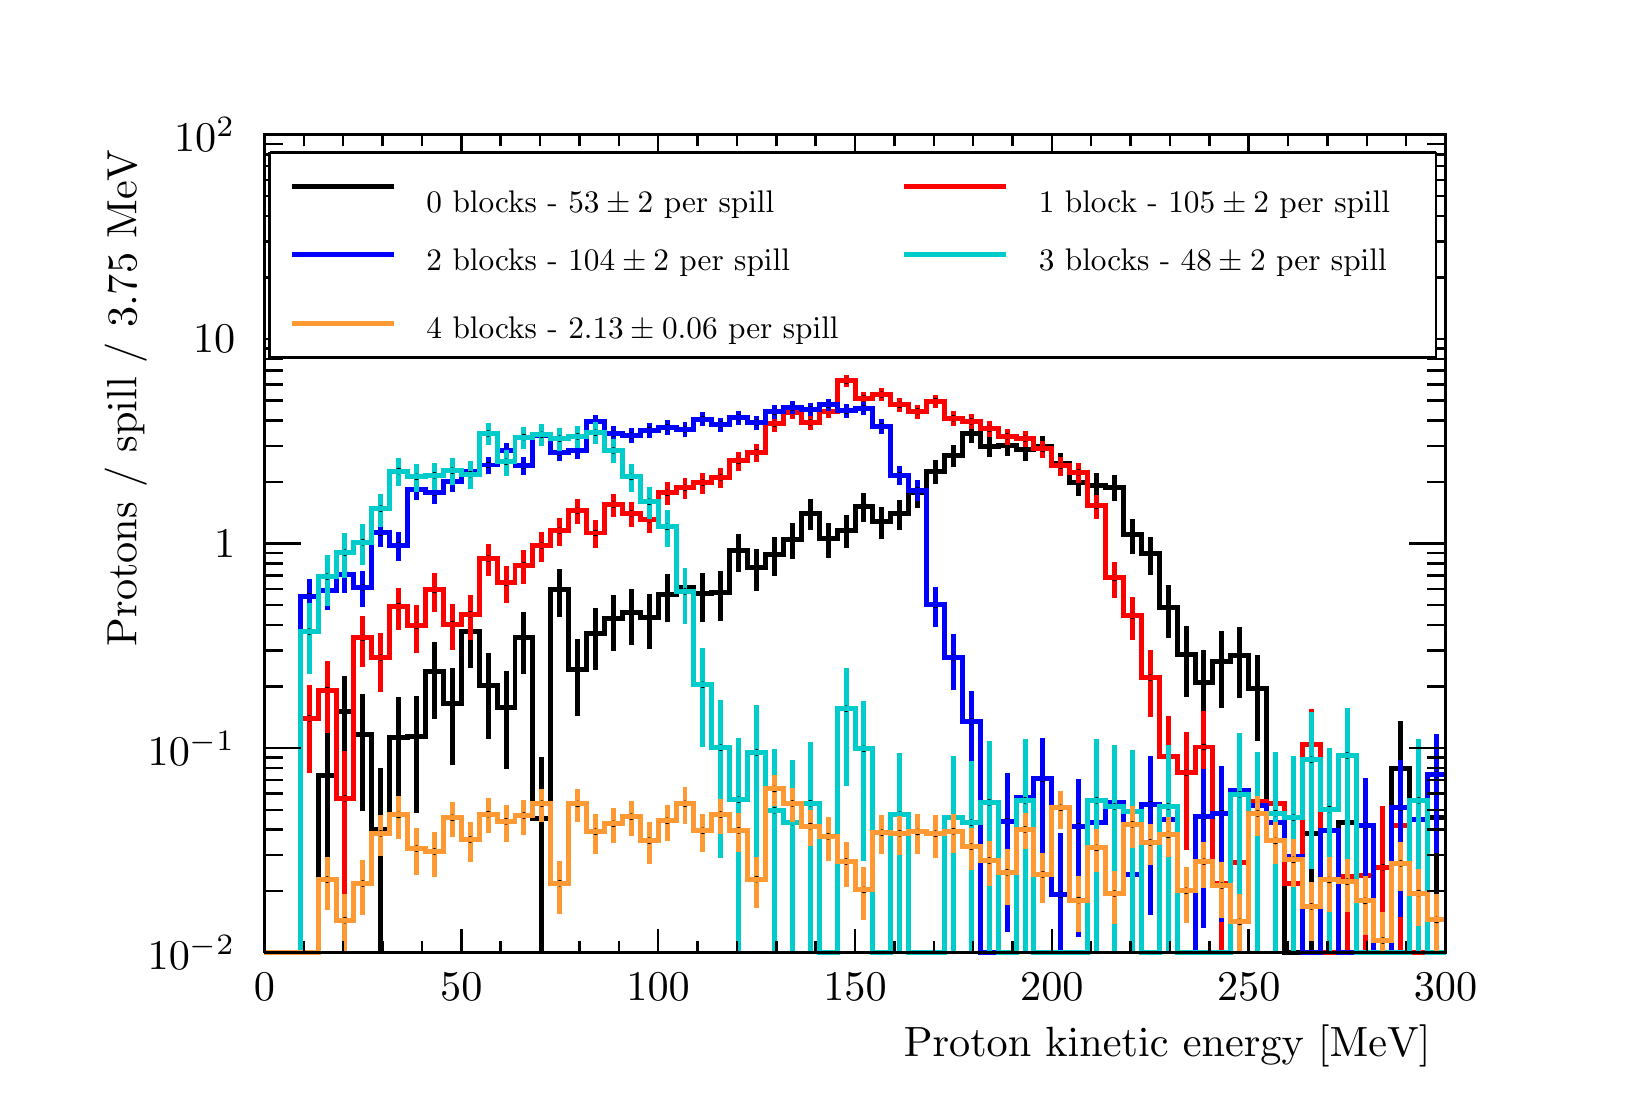
\begin{tikzpicture}
\pgfdeclareplotmark{cross} {
\pgfpathmoveto{\pgfpoint{-0.3\pgfplotmarksize}{\pgfplotmarksize}}
\pgfpathlineto{\pgfpoint{+0.3\pgfplotmarksize}{\pgfplotmarksize}}
\pgfpathlineto{\pgfpoint{+0.3\pgfplotmarksize}{0.3\pgfplotmarksize}}
\pgfpathlineto{\pgfpoint{+1\pgfplotmarksize}{0.3\pgfplotmarksize}}
\pgfpathlineto{\pgfpoint{+1\pgfplotmarksize}{-0.3\pgfplotmarksize}}
\pgfpathlineto{\pgfpoint{+0.3\pgfplotmarksize}{-0.3\pgfplotmarksize}}
\pgfpathlineto{\pgfpoint{+0.3\pgfplotmarksize}{-1.\pgfplotmarksize}}
\pgfpathlineto{\pgfpoint{-0.3\pgfplotmarksize}{-1.\pgfplotmarksize}}
\pgfpathlineto{\pgfpoint{-0.3\pgfplotmarksize}{-0.3\pgfplotmarksize}}
\pgfpathlineto{\pgfpoint{-1.\pgfplotmarksize}{-0.3\pgfplotmarksize}}
\pgfpathlineto{\pgfpoint{-1.\pgfplotmarksize}{0.3\pgfplotmarksize}}
\pgfpathlineto{\pgfpoint{-0.3\pgfplotmarksize}{0.3\pgfplotmarksize}}
\pgfpathclose
\pgfusepathqstroke
}
\pgfdeclareplotmark{cross*} {
\pgfpathmoveto{\pgfpoint{-0.3\pgfplotmarksize}{\pgfplotmarksize}}
\pgfpathlineto{\pgfpoint{+0.3\pgfplotmarksize}{\pgfplotmarksize}}
\pgfpathlineto{\pgfpoint{+0.3\pgfplotmarksize}{0.3\pgfplotmarksize}}
\pgfpathlineto{\pgfpoint{+1\pgfplotmarksize}{0.3\pgfplotmarksize}}
\pgfpathlineto{\pgfpoint{+1\pgfplotmarksize}{-0.3\pgfplotmarksize}}
\pgfpathlineto{\pgfpoint{+0.3\pgfplotmarksize}{-0.3\pgfplotmarksize}}
\pgfpathlineto{\pgfpoint{+0.3\pgfplotmarksize}{-1.\pgfplotmarksize}}
\pgfpathlineto{\pgfpoint{-0.3\pgfplotmarksize}{-1.\pgfplotmarksize}}
\pgfpathlineto{\pgfpoint{-0.3\pgfplotmarksize}{-0.3\pgfplotmarksize}}
\pgfpathlineto{\pgfpoint{-1.\pgfplotmarksize}{-0.3\pgfplotmarksize}}
\pgfpathlineto{\pgfpoint{-1.\pgfplotmarksize}{0.3\pgfplotmarksize}}
\pgfpathlineto{\pgfpoint{-0.3\pgfplotmarksize}{0.3\pgfplotmarksize}}
\pgfpathclose
\pgfusepathqfillstroke
}
\pgfdeclareplotmark{newstar} {
\pgfpathmoveto{\pgfqpoint{0pt}{\pgfplotmarksize}}
\pgfpathlineto{\pgfqpointpolar{44}{0.5\pgfplotmarksize}}
\pgfpathlineto{\pgfqpointpolar{18}{\pgfplotmarksize}}
\pgfpathlineto{\pgfqpointpolar{-20}{0.5\pgfplotmarksize}}
\pgfpathlineto{\pgfqpointpolar{-54}{\pgfplotmarksize}}
\pgfpathlineto{\pgfqpointpolar{-90}{0.5\pgfplotmarksize}}
\pgfpathlineto{\pgfqpointpolar{234}{\pgfplotmarksize}}
\pgfpathlineto{\pgfqpointpolar{198}{0.5\pgfplotmarksize}}
\pgfpathlineto{\pgfqpointpolar{162}{\pgfplotmarksize}}
\pgfpathlineto{\pgfqpointpolar{134}{0.5\pgfplotmarksize}}
\pgfpathclose
\pgfusepathqstroke
}
\pgfdeclareplotmark{newstar*} {
\pgfpathmoveto{\pgfqpoint{0pt}{\pgfplotmarksize}}
\pgfpathlineto{\pgfqpointpolar{44}{0.5\pgfplotmarksize}}
\pgfpathlineto{\pgfqpointpolar{18}{\pgfplotmarksize}}
\pgfpathlineto{\pgfqpointpolar{-20}{0.5\pgfplotmarksize}}
\pgfpathlineto{\pgfqpointpolar{-54}{\pgfplotmarksize}}
\pgfpathlineto{\pgfqpointpolar{-90}{0.5\pgfplotmarksize}}
\pgfpathlineto{\pgfqpointpolar{234}{\pgfplotmarksize}}
\pgfpathlineto{\pgfqpointpolar{198}{0.5\pgfplotmarksize}}
\pgfpathlineto{\pgfqpointpolar{162}{\pgfplotmarksize}}
\pgfpathlineto{\pgfqpointpolar{134}{0.5\pgfplotmarksize}}
\pgfpathclose
\pgfusepathqfillstroke
}
\definecolor{c}{rgb}{1,1,1};
\draw [color=c, fill=c] (0,0) rectangle (20,13.4957);
\draw [color=c, fill=c] (3,1.75444) rectangle (18,12.1461);
\definecolor{c}{rgb}{0,0,0};
\draw [c,line width=0.9] (3,1.75444) -- (3,12.1461) -- (18,12.1461) -- (18,1.75444) -- (3,1.75444);
\definecolor{c}{rgb}{1,1,1};
\draw [color=c, fill=c] (3,1.75444) rectangle (18,12.1461);
\definecolor{c}{rgb}{0,0,0};
\draw [c,line width=0.9] (3,1.75444) -- (3,12.1461) -- (18,12.1461) -- (18,1.75444) -- (3,1.75444);
\draw [c,line width=0.9] (3,1.75444) -- (3.22727,1.75444) -- (3.22727,1.75444) -- (3.45455,1.75444) -- (3.45455,1.75444) -- (3.68182,1.75444) -- (3.68182,1.75444) -- (3.90909,1.75444) -- (3.90909,1.75444) -- (4.13636,1.75444) -- (4.13636,1.75444) --
 (4.36364,1.75444) -- (4.36364,1.75444) -- (4.59091,1.75444) -- (4.59091,1.75444) -- (4.81818,1.75444) -- (4.81818,1.75444) -- (5.04545,1.75444) -- (5.04545,1.75444) -- (5.27273,1.75444) -- (5.27273,1.75444) -- (5.5,1.75444) -- (5.5,1.75444) --
 (5.72727,1.75444) -- (5.72727,1.75444) -- (5.95455,1.75444) -- (5.95455,1.75444) -- (6.18182,1.75444) -- (6.18182,1.75444) -- (6.40909,1.75444) -- (6.40909,1.75444) -- (6.63636,1.75444) -- (6.63636,1.75444) -- (6.86364,1.75444) -- (6.86364,1.75444)
 -- (7.09091,1.75444) -- (7.09091,1.75444) -- (7.31818,1.75444) -- (7.31818,1.75444) -- (7.54545,1.75444) -- (7.54545,1.75444) -- (7.77273,1.75444) -- (7.77273,1.75444) -- (8,1.75444) -- (8,1.75444) -- (8.22727,1.75444) -- (8.22727,1.75444) --
 (8.45455,1.75444) -- (8.45455,1.75444) -- (8.68182,1.75444) -- (8.68182,1.75444) -- (8.90909,1.75444) -- (8.90909,1.75444) -- (9.13636,1.75444) -- (9.13636,1.75444) -- (9.36364,1.75444) -- (9.36364,1.75444) -- (9.59091,1.75444) -- (9.59091,1.75444)
 -- (9.81818,1.75444) -- (9.81818,1.75444) -- (10.0455,1.75444) -- (10.0455,1.75444) -- (10.2727,1.75444) -- (10.2727,1.75444) -- (10.5,1.75444) -- (10.5,1.75444) -- (10.7273,1.75444) -- (10.7273,1.75444) -- (10.9545,1.75444) -- (10.9545,1.75444) --
 (11.1818,1.75444) -- (11.1818,1.75444) -- (11.4091,1.75444) -- (11.4091,1.75444) -- (11.6364,1.75444) -- (11.6364,1.75444) -- (11.8636,1.75444) -- (11.8636,1.75444) -- (12.0909,1.75444) -- (12.0909,1.75444) -- (12.3182,1.75444) -- (12.3182,1.75444)
 -- (12.5455,1.75444) -- (12.5455,1.75444) -- (12.7727,1.75444) -- (12.7727,1.75444) -- (13,1.75444) -- (13,1.75444) -- (13.2273,1.75444) -- (13.2273,1.75444) -- (13.4545,1.75444) -- (13.4545,1.75444) -- (13.6818,1.75444) -- (13.6818,1.75444) --
 (13.9091,1.75444) -- (13.9091,1.75444) -- (14.1364,1.75444) -- (14.1364,1.75444) -- (14.3636,1.75444) -- (14.3636,1.75444) -- (14.5909,1.75444) -- (14.5909,1.75444) -- (14.8182,1.75444) -- (14.8182,1.75444) -- (15.0455,1.75444) -- (15.0455,1.75444)
 -- (15.2727,1.75444) -- (15.2727,1.75444) -- (15.5,1.75444) -- (15.5,1.75444) -- (15.7273,1.75444) -- (15.7273,1.75444) -- (15.9545,1.75444) -- (15.9545,1.75444) -- (16.1818,1.75444) -- (16.1818,1.75444) -- (16.4091,1.75444) -- (16.4091,1.75444) --
 (16.6364,1.75444) -- (16.6364,1.75444) -- (16.8636,1.75444) -- (16.8636,1.75444) -- (17.0909,1.75444) -- (17.0909,1.75444) -- (17.3182,1.75444) -- (17.3182,1.75444) -- (17.5455,1.75444) -- (17.5455,1.75444) -- (17.7727,1.75444) -- (17.7727,1.75444)
 -- (18,1.75444);
\draw [c,line width=0.9] (3,1.75444) -- (18,1.75444);
\draw [c,line width=0.9] (3,2.05809) -- (3,1.75444);
\draw [c,line width=0.9] (3.5,1.90627) -- (3.5,1.75444);
\draw [c,line width=0.9] (4,1.90627) -- (4,1.75444);
\draw [c,line width=0.9] (4.5,1.90627) -- (4.5,1.75444);
\draw [c,line width=0.9] (5,1.90627) -- (5,1.75444);
\draw [c,line width=0.9] (5.5,2.05809) -- (5.5,1.75444);
\draw [c,line width=0.9] (6,1.90627) -- (6,1.75444);
\draw [c,line width=0.9] (6.5,1.90627) -- (6.5,1.75444);
\draw [c,line width=0.9] (7,1.90627) -- (7,1.75444);
\draw [c,line width=0.9] (7.5,1.90627) -- (7.5,1.75444);
\draw [c,line width=0.9] (8,2.05809) -- (8,1.75444);
\draw [c,line width=0.9] (8.5,1.90627) -- (8.5,1.75444);
\draw [c,line width=0.9] (9,1.90627) -- (9,1.75444);
\draw [c,line width=0.9] (9.5,1.90627) -- (9.5,1.75444);
\draw [c,line width=0.9] (10,1.90627) -- (10,1.75444);
\draw [c,line width=0.9] (10.5,2.05809) -- (10.5,1.75444);
\draw [c,line width=0.9] (11,1.90627) -- (11,1.75444);
\draw [c,line width=0.9] (11.5,1.90627) -- (11.5,1.75444);
\draw [c,line width=0.9] (12,1.90627) -- (12,1.75444);
\draw [c,line width=0.9] (12.5,1.90627) -- (12.5,1.75444);
\draw [c,line width=0.9] (13,2.05809) -- (13,1.75444);
\draw [c,line width=0.9] (13.5,1.90627) -- (13.5,1.75444);
\draw [c,line width=0.9] (14,1.90627) -- (14,1.75444);
\draw [c,line width=0.9] (14.5,1.90627) -- (14.5,1.75444);
\draw [c,line width=0.9] (15,1.90627) -- (15,1.75444);
\draw [c,line width=0.9] (15.5,2.05809) -- (15.5,1.75444);
\draw [c,line width=0.9] (16,1.90627) -- (16,1.75444);
\draw [c,line width=0.9] (16.5,1.90627) -- (16.5,1.75444);
\draw [c,line width=0.9] (17,1.90627) -- (17,1.75444);
\draw [c,line width=0.9] (17.5,1.90627) -- (17.5,1.75444);
\draw [c,line width=0.9] (18,2.05809) -- (18,1.75444);
\draw [c,line width=0.9] (18,2.05809) -- (18,1.75444);
\draw [anchor=base] (3,1.14713) node[scale=1.52731, color=c, rotate=0]{0};
\draw [anchor=base] (5.5,1.14713) node[scale=1.52731, color=c, rotate=0]{50};
\draw [anchor=base] (8,1.14713) node[scale=1.52731, color=c, rotate=0]{100};
\draw [anchor=base] (10.5,1.14713) node[scale=1.52731, color=c, rotate=0]{150};
\draw [anchor=base] (13,1.14713) node[scale=1.52731, color=c, rotate=0]{200};
\draw [anchor=base] (15.5,1.14713) node[scale=1.52731, color=c, rotate=0]{250};
\draw [anchor=base] (18,1.14713) node[scale=1.52731, color=c, rotate=0]{300};
\draw [anchor= east] (18,0.566819) node[scale=1.52731, color=c, rotate=0]{Proton kinetic energy [MeV]};
\draw [c,line width=0.9] (3,12.1461) -- (18,12.1461);
\draw [c,line width=0.9] (3,11.8425) -- (3,12.1461);
\draw [c,line width=0.9] (3.5,11.9943) -- (3.5,12.1461);
\draw [c,line width=0.9] (4,11.9943) -- (4,12.1461);
\draw [c,line width=0.9] (4.5,11.9943) -- (4.5,12.1461);
\draw [c,line width=0.9] (5,11.9943) -- (5,12.1461);
\draw [c,line width=0.9] (5.5,11.8425) -- (5.5,12.1461);
\draw [c,line width=0.9] (6,11.9943) -- (6,12.1461);
\draw [c,line width=0.9] (6.5,11.9943) -- (6.5,12.1461);
\draw [c,line width=0.9] (7,11.9943) -- (7,12.1461);
\draw [c,line width=0.9] (7.5,11.9943) -- (7.5,12.1461);
\draw [c,line width=0.9] (8,11.8425) -- (8,12.1461);
\draw [c,line width=0.9] (8.5,11.9943) -- (8.5,12.1461);
\draw [c,line width=0.9] (9,11.9943) -- (9,12.1461);
\draw [c,line width=0.9] (9.5,11.9943) -- (9.5,12.1461);
\draw [c,line width=0.9] (10,11.9943) -- (10,12.1461);
\draw [c,line width=0.9] (10.5,11.8425) -- (10.5,12.1461);
\draw [c,line width=0.9] (11,11.9943) -- (11,12.1461);
\draw [c,line width=0.9] (11.5,11.9943) -- (11.5,12.1461);
\draw [c,line width=0.9] (12,11.9943) -- (12,12.1461);
\draw [c,line width=0.9] (12.5,11.9943) -- (12.5,12.1461);
\draw [c,line width=0.9] (13,11.8425) -- (13,12.1461);
\draw [c,line width=0.9] (13.5,11.9943) -- (13.5,12.1461);
\draw [c,line width=0.9] (14,11.9943) -- (14,12.1461);
\draw [c,line width=0.9] (14.5,11.9943) -- (14.5,12.1461);
\draw [c,line width=0.9] (15,11.9943) -- (15,12.1461);
\draw [c,line width=0.9] (15.5,11.8425) -- (15.5,12.1461);
\draw [c,line width=0.9] (16,11.9943) -- (16,12.1461);
\draw [c,line width=0.9] (16.5,11.9943) -- (16.5,12.1461);
\draw [c,line width=0.9] (17,11.9943) -- (17,12.1461);
\draw [c,line width=0.9] (17.5,11.9943) -- (17.5,12.1461);
\draw [c,line width=0.9] (18,11.8425) -- (18,12.1461);
\draw [c,line width=0.9] (18,11.8425) -- (18,12.1461);
\draw [c,line width=0.9] (3,1.75444) -- (3,12.1461);
\draw [c,line width=0.9] (3.462,1.75444) -- (3,1.75444);
\draw [anchor= east] (2.82,1.75444) node[scale=1.52731, color=c, rotate=0]{$10^{-2}$};
\draw [c,line width=0.9] (3.231,2.5365) -- (3,2.5365);
\draw [c,line width=0.9] (3.231,2.99397) -- (3,2.99397);
\draw [c,line width=0.9] (3.231,3.31855) -- (3,3.31855);
\draw [c,line width=0.9] (3.231,3.57031) -- (3,3.57031);
\draw [c,line width=0.9] (3.231,3.77602) -- (3,3.77602);
\draw [c,line width=0.9] (3.231,3.94994) -- (3,3.94994);
\draw [c,line width=0.9] (3.231,4.1006) -- (3,4.1006);
\draw [c,line width=0.9] (3.231,4.23349) -- (3,4.23349);
\draw [c,line width=0.9] (3.462,4.35237) -- (3,4.35237);
\draw [anchor= east] (2.82,4.35237) node[scale=1.52731, color=c, rotate=0]{$10^{-1}$};
\draw [c,line width=0.9] (3.231,5.13442) -- (3,5.13442);
\draw [c,line width=0.9] (3.231,5.59189) -- (3,5.59189);
\draw [c,line width=0.9] (3.231,5.91647) -- (3,5.91647);
\draw [c,line width=0.9] (3.231,6.16824) -- (3,6.16824);
\draw [c,line width=0.9] (3.231,6.37394) -- (3,6.37394);
\draw [c,line width=0.9] (3.231,6.54786) -- (3,6.54786);
\draw [c,line width=0.9] (3.231,6.69852) -- (3,6.69852);
\draw [c,line width=0.9] (3.231,6.83141) -- (3,6.83141);
\draw [c,line width=0.9] (3.462,6.95029) -- (3,6.95029);
\draw [anchor= east] (2.82,6.95029) node[scale=1.52731, color=c, rotate=0]{1};
\draw [c,line width=0.9] (3.231,7.73234) -- (3,7.73234);
\draw [c,line width=0.9] (3.231,8.18981) -- (3,8.18981);
\draw [c,line width=0.9] (3.231,8.51439) -- (3,8.51439);
\draw [c,line width=0.9] (3.231,8.76616) -- (3,8.76616);
\draw [c,line width=0.9] (3.231,8.97186) -- (3,8.97186);
\draw [c,line width=0.9] (3.231,9.14579) -- (3,9.14579);
\draw [c,line width=0.9] (3.231,9.29644) -- (3,9.29644);
\draw [c,line width=0.9] (3.231,9.42934) -- (3,9.42934);
\draw [c,line width=0.9] (3.462,9.54821) -- (3,9.54821);
\draw [anchor= east] (2.82,9.54821) node[scale=1.52731, color=c, rotate=0]{10};
\draw [c,line width=0.9] (3.231,10.3303) -- (3,10.3303);
\draw [c,line width=0.9] (3.231,10.7877) -- (3,10.7877);
\draw [c,line width=0.9] (3.231,11.1123) -- (3,11.1123);
\draw [c,line width=0.9] (3.231,11.3641) -- (3,11.3641);
\draw [c,line width=0.9] (3.231,11.5698) -- (3,11.5698);
\draw [c,line width=0.9] (3.231,11.7437) -- (3,11.7437);
\draw [c,line width=0.9] (3.231,11.8944) -- (3,11.8944);
\draw [c,line width=0.9] (3.231,12.0273) -- (3,12.0273);
\draw [c,line width=0.9] (3.462,12.1461) -- (3,12.1461);
\draw [anchor= east] (2.82,12.1461) node[scale=1.52731, color=c, rotate=0]{$10^{2}$};
\draw [anchor= east] (1.24,12.1461) node[scale=1.52731, color=c, rotate=90]{Protons / spill / 3.75~MeV};
\draw [c,line width=0.9] (18,1.75444) -- (18,12.1461);
\draw [c,line width=0.9] (17.538,1.75444) -- (18,1.75444);
\draw [c,line width=0.9] (17.769,2.5365) -- (18,2.5365);
\draw [c,line width=0.9] (17.769,2.99397) -- (18,2.99397);
\draw [c,line width=0.9] (17.769,3.31855) -- (18,3.31855);
\draw [c,line width=0.9] (17.769,3.57031) -- (18,3.57031);
\draw [c,line width=0.9] (17.769,3.77602) -- (18,3.77602);
\draw [c,line width=0.9] (17.769,3.94994) -- (18,3.94994);
\draw [c,line width=0.9] (17.769,4.1006) -- (18,4.1006);
\draw [c,line width=0.9] (17.769,4.23349) -- (18,4.23349);
\draw [c,line width=0.9] (17.538,4.35237) -- (18,4.35237);
\draw [c,line width=0.9] (17.769,5.13442) -- (18,5.13442);
\draw [c,line width=0.9] (17.769,5.59189) -- (18,5.59189);
\draw [c,line width=0.9] (17.769,5.91647) -- (18,5.91647);
\draw [c,line width=0.9] (17.769,6.16824) -- (18,6.16824);
\draw [c,line width=0.9] (17.769,6.37394) -- (18,6.37394);
\draw [c,line width=0.9] (17.769,6.54786) -- (18,6.54786);
\draw [c,line width=0.9] (17.769,6.69852) -- (18,6.69852);
\draw [c,line width=0.9] (17.769,6.83141) -- (18,6.83141);
\draw [c,line width=0.9] (17.538,6.95029) -- (18,6.95029);
\draw [c,line width=0.9] (17.769,7.73234) -- (18,7.73234);
\draw [c,line width=0.9] (17.769,8.18981) -- (18,8.18981);
\draw [c,line width=0.9] (17.769,8.51439) -- (18,8.51439);
\draw [c,line width=0.9] (17.769,8.76616) -- (18,8.76616);
\draw [c,line width=0.9] (17.769,8.97186) -- (18,8.97186);
\draw [c,line width=0.9] (17.769,9.14579) -- (18,9.14579);
\draw [c,line width=0.9] (17.769,9.29644) -- (18,9.29644);
\draw [c,line width=0.9] (17.769,9.42934) -- (18,9.42934);
\draw [c,line width=0.9] (17.538,9.54821) -- (18,9.54821);
\draw [c,line width=0.9] (17.769,10.3303) -- (18,10.3303);
\draw [c,line width=0.9] (17.769,10.7877) -- (18,10.7877);
\draw [c,line width=0.9] (17.769,11.1123) -- (18,11.1123);
\draw [c,line width=0.9] (17.769,11.3641) -- (18,11.3641);
\draw [c,line width=0.9] (17.769,11.5698) -- (18,11.5698);
\draw [c,line width=0.9] (17.769,11.7437) -- (18,11.7437);
\draw [c,line width=0.9] (17.769,11.8944) -- (18,11.8944);
\draw [c,line width=0.9] (17.769,12.0273) -- (18,12.0273);
\draw [c,line width=0.9] (17.538,12.1461) -- (18,12.1461);
\draw [c,line width=1.8] (3.79545,2.60924) -- (3.79545,4.00539);
\draw [c,line width=1.8] (3.79545,4.00539) -- (3.79545,4.61061);
\foreach \P in {(3.79545,4.00539)}{\draw[mark options={color=c,fill=c},mark size=2.402402pt,mark=*,mark size=1pt] plot coordinates {\P};}
\draw [c,line width=1.8] (4.02273,4.03114) -- (4.02273,4.81428);
\draw [c,line width=1.8] (4.02273,4.81428) -- (4.02273,5.27211);
\foreach \P in {(4.02273,4.81428)}{\draw[mark options={color=c,fill=c},mark size=2.402402pt,mark=*,mark size=1pt] plot coordinates {\P};}
\draw [c,line width=1.8] (4.25,3.5497) -- (4.25,4.52289);
\draw [c,line width=1.8] (4.25,4.52289) -- (4.25,5.0375);
\foreach \P in {(4.25,4.52289)}{\draw[mark options={color=c,fill=c},mark size=2.402402pt,mark=*,mark size=1pt] plot coordinates {\P};}
\draw [c,line width=1.8] (4.47727,1.75444) -- (4.47727,3.32318);
\draw [c,line width=1.8] (4.47727,3.32318) -- (4.47727,4.10524);
\foreach \P in {(4.47727,3.32318)}{\draw[mark options={color=c,fill=c},mark size=2.402402pt,mark=*,mark size=1pt] plot coordinates {\P};}
\draw [c,line width=1.8] (4.70455,3.51188) -- (4.70455,4.48763);
\draw [c,line width=1.8] (4.70455,4.48763) -- (4.70455,5.00292);
\foreach \P in {(4.70455,4.48763)}{\draw[mark options={color=c,fill=c},mark size=2.402402pt,mark=*,mark size=1pt] plot coordinates {\P};}
\draw [c,line width=1.8] (4.93182,3.5301) -- (4.93182,4.50411);
\draw [c,line width=1.8] (4.93182,4.50411) -- (4.93182,5.01894);
\foreach \P in {(4.93182,4.50411)}{\draw[mark options={color=c,fill=c},mark size=2.402402pt,mark=*,mark size=1pt] plot coordinates {\P};}
\draw [c,line width=1.8] (5.15909,4.72595) -- (5.15909,5.31984);
\draw [c,line width=1.8] (5.15909,5.31984) -- (5.15909,5.7069);
\foreach \P in {(5.15909,5.31984)}{\draw[mark options={color=c,fill=c},mark size=2.402402pt,mark=*,mark size=1pt] plot coordinates {\P};}
\draw [c,line width=1.8] (5.38636,4.13231) -- (5.38636,4.91521);
\draw [c,line width=1.8] (5.38636,4.91521) -- (5.38636,5.37296);
\foreach \P in {(5.38636,4.91521)}{\draw[mark options={color=c,fill=c},mark size=2.402402pt,mark=*,mark size=1pt] plot coordinates {\P};}
\draw [c,line width=1.8] (5.61364,5.36765) -- (5.61364,5.8311);
\draw [c,line width=1.8] (5.61364,5.8311) -- (5.61364,6.15865);
\foreach \P in {(5.61364,5.8311)}{\draw[mark options={color=c,fill=c},mark size=2.402402pt,mark=*,mark size=1pt] plot coordinates {\P};}
\draw [c,line width=1.8] (5.84091,4.47369) -- (5.84091,5.14585);
\draw [c,line width=1.8] (5.84091,5.14585) -- (5.84091,5.56418);
\foreach \P in {(5.84091,5.14585)}{\draw[mark options={color=c,fill=c},mark size=2.402402pt,mark=*,mark size=1pt] plot coordinates {\P};}
\draw [c,line width=1.8] (6.06818,4.08623) -- (6.06818,4.8698);
\draw [c,line width=1.8] (6.06818,4.8698) -- (6.06818,5.32777);
\foreach \P in {(6.06818,4.8698)}{\draw[mark options={color=c,fill=c},mark size=2.402402pt,mark=*,mark size=1pt] plot coordinates {\P};}
\draw [c,line width=1.8] (6.29545,5.29359) -- (6.29545,5.75425);
\draw [c,line width=1.8] (6.29545,5.75425) -- (6.29545,6.08042);
\foreach \P in {(6.29545,5.75425)}{\draw[mark options={color=c,fill=c},mark size=2.402402pt,mark=*,mark size=1pt] plot coordinates {\P};}
\draw [c,line width=1.8] (6.52273,1.75444) -- (6.52273,3.46448);
\draw [c,line width=1.8] (6.52273,3.46448) -- (6.52273,4.24653);
\foreach \P in {(6.52273,3.46448)}{\draw[mark options={color=c,fill=c},mark size=2.402402pt,mark=*,mark size=1pt] plot coordinates {\P};}
\draw [c,line width=1.8] (6.75,6.02252) -- (6.75,6.36177);
\draw [c,line width=1.8] (6.75,6.36177) -- (6.75,6.62224);
\foreach \P in {(6.75,6.36177)}{\draw[mark options={color=c,fill=c},mark size=2.402402pt,mark=*,mark size=1pt] plot coordinates {\P};}
\draw [c,line width=1.8] (6.97727,4.75616) -- (6.97727,5.34913);
\draw [c,line width=1.8] (6.97727,5.34913) -- (6.97727,5.73582);
\foreach \P in {(6.97727,5.34913)}{\draw[mark options={color=c,fill=c},mark size=2.402402pt,mark=*,mark size=1pt] plot coordinates {\P};}
\draw [c,line width=1.8] (7.20455,5.34851) -- (7.20455,5.80911);
\draw [c,line width=1.8] (7.20455,5.80911) -- (7.20455,6.13526);
\foreach \P in {(7.20455,5.80911)}{\draw[mark options={color=c,fill=c},mark size=2.402402pt,mark=*,mark size=1pt] plot coordinates {\P};}
\draw [c,line width=1.8] (7.43182,5.58905) -- (7.43182,5.99782);
\draw [c,line width=1.8] (7.43182,5.99782) -- (7.43182,6.29724);
\foreach \P in {(7.43182,5.99782)}{\draw[mark options={color=c,fill=c},mark size=2.402402pt,mark=*,mark size=1pt] plot coordinates {\P};}
\draw [c,line width=1.8] (7.65909,5.66385) -- (7.65909,6.07109);
\draw [c,line width=1.8] (7.65909,6.07109) -- (7.65909,6.36969);
\foreach \P in {(7.65909,6.07109)}{\draw[mark options={color=c,fill=c},mark size=2.402402pt,mark=*,mark size=1pt] plot coordinates {\P};}
\draw [c,line width=1.8] (7.88636,5.61049) -- (7.88636,6.01595);
\draw [c,line width=1.8] (7.88636,6.01595) -- (7.88636,6.3136);
\foreach \P in {(7.88636,6.01595)}{\draw[mark options={color=c,fill=c},mark size=2.402402pt,mark=*,mark size=1pt] plot coordinates {\P};}
\draw [c,line width=1.8] (8.11364,5.94903) -- (8.11364,6.30148);
\draw [c,line width=1.8] (8.11364,6.30148) -- (8.11364,6.56965);
\foreach \P in {(8.11364,6.30148)}{\draw[mark options={color=c,fill=c},mark size=2.402402pt,mark=*,mark size=1pt] plot coordinates {\P};}
\draw [c,line width=1.8] (8.34091,6.06278) -- (8.34091,6.38842);
\draw [c,line width=1.8] (8.34091,6.38842) -- (8.34091,6.64082);
\foreach \P in {(8.34091,6.38842)}{\draw[mark options={color=c,fill=c},mark size=2.402402pt,mark=*,mark size=1pt] plot coordinates {\P};}
\draw [c,line width=1.8] (8.56818,5.95652) -- (8.56818,6.31043);
\draw [c,line width=1.8] (8.56818,6.31043) -- (8.56818,6.57943);
\foreach \P in {(8.56818,6.31043)}{\draw[mark options={color=c,fill=c},mark size=2.402402pt,mark=*,mark size=1pt] plot coordinates {\P};}
\draw [c,line width=1.8] (8.79545,5.97304) -- (8.79545,6.32748);
\draw [c,line width=1.8] (8.79545,6.32748) -- (8.79545,6.5968);
\foreach \P in {(8.79545,6.32748)}{\draw[mark options={color=c,fill=c},mark size=2.402402pt,mark=*,mark size=1pt] plot coordinates {\P};}
\draw [c,line width=1.8] (9.02273,6.5917) -- (9.02273,6.85685);
\draw [c,line width=1.8] (9.02273,6.85685) -- (9.02273,7.07139);
\foreach \P in {(9.02273,6.85685)}{\draw[mark options={color=c,fill=c},mark size=2.402402pt,mark=*,mark size=1pt] plot coordinates {\P};}
\draw [c,line width=1.8] (9.25,6.34879) -- (9.25,6.64525);
\draw [c,line width=1.8] (9.25,6.64525) -- (9.25,6.8798);
\foreach \P in {(9.25,6.64525)}{\draw[mark options={color=c,fill=c},mark size=2.402402pt,mark=*,mark size=1pt] plot coordinates {\P};}
\draw [c,line width=1.8] (9.47727,6.5369) -- (9.47727,6.81036);
\draw [c,line width=1.8] (9.47727,6.81036) -- (9.47727,7.0303);
\foreach \P in {(9.47727,6.81036)}{\draw[mark options={color=c,fill=c},mark size=2.402402pt,mark=*,mark size=1pt] plot coordinates {\P};}
\draw [c,line width=1.8] (9.70455,6.7599) -- (9.70455,7.00766);
\draw [c,line width=1.8] (9.70455,7.00766) -- (9.70455,7.21069);
\foreach \P in {(9.70455,7.00766)}{\draw[mark options={color=c,fill=c},mark size=2.402402pt,mark=*,mark size=1pt] plot coordinates {\P};}
\draw [c,line width=1.8] (9.93182,7.12677) -- (9.93182,7.33707);
\draw [c,line width=1.8] (9.93182,7.33707) -- (9.93182,7.51427);
\foreach \P in {(9.93182,7.33707)}{\draw[mark options={color=c,fill=c},mark size=2.402402pt,mark=*,mark size=1pt] plot coordinates {\P};}
\draw [c,line width=1.8] (10.1591,6.7687) -- (10.1591,7.01088);
\draw [c,line width=1.8] (10.1591,7.01088) -- (10.1591,7.21015);
\foreach \P in {(10.1591,7.01088)}{\draw[mark options={color=c,fill=c},mark size=2.402402pt,mark=*,mark size=1pt] plot coordinates {\P};}
\draw [c,line width=1.8] (10.3864,6.88913) -- (10.3864,7.11788);
\draw [c,line width=1.8] (10.3864,7.11788) -- (10.3864,7.30797);
\foreach \P in {(10.3864,7.11788)}{\draw[mark options={color=c,fill=c},mark size=2.402402pt,mark=*,mark size=1pt] plot coordinates {\P};}
\draw [c,line width=1.8] (10.6136,7.22852) -- (10.6136,7.42613);
\draw [c,line width=1.8] (10.6136,7.42613) -- (10.6136,7.59423);
\foreach \P in {(10.6136,7.42613)}{\draw[mark options={color=c,fill=c},mark size=2.402402pt,mark=*,mark size=1pt] plot coordinates {\P};}
\draw [c,line width=1.8] (10.8409,7.0079) -- (10.8409,7.22835);
\draw [c,line width=1.8] (10.8409,7.22835) -- (10.8409,7.41268);
\foreach \P in {(10.8409,7.22835)}{\draw[mark options={color=c,fill=c},mark size=2.402402pt,mark=*,mark size=1pt] plot coordinates {\P};}
\draw [c,line width=1.8] (11.0682,7.12833) -- (11.0682,7.33525);
\draw [c,line width=1.8] (11.0682,7.33525) -- (11.0682,7.51005);
\foreach \P in {(11.0682,7.33525)}{\draw[mark options={color=c,fill=c},mark size=2.402402pt,mark=*,mark size=1pt] plot coordinates {\P};}
\draw [c,line width=1.8] (11.2955,7.40746) -- (11.2955,7.59292);
\draw [c,line width=1.8] (11.2955,7.59292) -- (11.2955,7.75215);
\foreach \P in {(11.2955,7.59292)}{\draw[mark options={color=c,fill=c},mark size=2.402402pt,mark=*,mark size=1pt] plot coordinates {\P};}
\draw [c,line width=1.8] (11.5227,7.70421) -- (11.5227,7.86713);
\draw [c,line width=1.8] (11.5227,7.86713) -- (11.5227,8.00947);
\foreach \P in {(11.5227,7.86713)}{\draw[mark options={color=c,fill=c},mark size=2.402402pt,mark=*,mark size=1pt] plot coordinates {\P};}
\draw [c,line width=1.8] (11.75,7.92009) -- (11.75,8.06794);
\draw [c,line width=1.8] (11.75,8.06794) -- (11.75,8.19864);
\foreach \P in {(11.75,8.06794)}{\draw[mark options={color=c,fill=c},mark size=2.402402pt,mark=*,mark size=1pt] plot coordinates {\P};}
\draw [c,line width=1.8] (11.9773,8.22288) -- (11.9773,8.3524);
\draw [c,line width=1.8] (11.9773,8.3524) -- (11.9773,8.46858);
\foreach \P in {(11.9773,8.3524)}{\draw[mark options={color=c,fill=c},mark size=2.402402pt,mark=*,mark size=1pt] plot coordinates {\P};}
\draw [c,line width=1.8] (12.2045,8.04755) -- (12.2045,8.18769);
\draw [c,line width=1.8] (12.2045,8.18769) -- (12.2045,8.31234);
\foreach \P in {(12.2045,8.18769)}{\draw[mark options={color=c,fill=c},mark size=2.402402pt,mark=*,mark size=1pt] plot coordinates {\P};}
\draw [c,line width=1.8] (12.4318,8.06348) -- (12.4318,8.20158);
\draw [c,line width=1.8] (12.4318,8.20158) -- (12.4318,8.32461);
\foreach \P in {(12.4318,8.20158)}{\draw[mark options={color=c,fill=c},mark size=2.402402pt,mark=*,mark size=1pt] plot coordinates {\P};}
\draw [c,line width=1.8] (12.6591,7.9996) -- (12.6591,8.14294);
\draw [c,line width=1.8] (12.6591,8.14294) -- (12.6591,8.27011);
\foreach \P in {(12.6591,8.14294)}{\draw[mark options={color=c,fill=c},mark size=2.402402pt,mark=*,mark size=1pt] plot coordinates {\P};}
\draw [c,line width=1.8] (12.8864,8.04758) -- (12.8864,8.18805);
\draw [c,line width=1.8] (12.8864,8.18805) -- (12.8864,8.31296);
\foreach \P in {(12.8864,8.18805)}{\draw[mark options={color=c,fill=c},mark size=2.402402pt,mark=*,mark size=1pt] plot coordinates {\P};}
\draw [c,line width=1.8] (13.1136,7.81831) -- (13.1136,7.97079);
\draw [c,line width=1.8] (13.1136,7.97079) -- (13.1136,8.10509);
\foreach \P in {(13.1136,7.97079)}{\draw[mark options={color=c,fill=c},mark size=2.402402pt,mark=*,mark size=1pt] plot coordinates {\P};}
\draw [c,line width=1.8] (13.3409,7.55089) -- (13.3409,7.72195);
\draw [c,line width=1.8] (13.3409,7.72195) -- (13.3409,7.87046);
\foreach \P in {(13.3409,7.72195)}{\draw[mark options={color=c,fill=c},mark size=2.402402pt,mark=*,mark size=1pt] plot coordinates {\P};}
\draw [c,line width=1.8] (13.5682,7.5121) -- (13.5682,7.68905);
\draw [c,line width=1.8] (13.5682,7.68905) -- (13.5682,7.84197);
\foreach \P in {(13.5682,7.68905)}{\draw[mark options={color=c,fill=c},mark size=2.402402pt,mark=*,mark size=1pt] plot coordinates {\P};}
\draw [c,line width=1.8] (13.7955,7.48592) -- (13.7955,7.66469);
\draw [c,line width=1.8] (13.7955,7.66469) -- (13.7955,7.81896);
\foreach \P in {(13.7955,7.66469)}{\draw[mark options={color=c,fill=c},mark size=2.402402pt,mark=*,mark size=1pt] plot coordinates {\P};}
\draw [c,line width=1.8] (14.0227,6.81875) -- (14.0227,7.06169);
\draw [c,line width=1.8] (14.0227,7.06169) -- (14.0227,7.26147);
\foreach \P in {(14.0227,7.06169)}{\draw[mark options={color=c,fill=c},mark size=2.402402pt,mark=*,mark size=1pt] plot coordinates {\P};}
\draw [c,line width=1.8] (14.25,6.54671) -- (14.25,6.81855);
\draw [c,line width=1.8] (14.25,6.81855) -- (14.25,7.03744);
\foreach \P in {(14.25,6.81855)}{\draw[mark options={color=c,fill=c},mark size=2.402402pt,mark=*,mark size=1pt] plot coordinates {\P};}
\draw [c,line width=1.8] (14.4773,5.75068) -- (14.4773,6.13666);
\draw [c,line width=1.8] (14.4773,6.13666) -- (14.4773,6.42371);
\foreach \P in {(14.4773,6.13666)}{\draw[mark options={color=c,fill=c},mark size=2.402402pt,mark=*,mark size=1pt] plot coordinates {\P};}
\draw [c,line width=1.8] (14.7045,4.99765) -- (14.7045,5.53879);
\draw [c,line width=1.8] (14.7045,5.53879) -- (14.7045,5.90299);
\foreach \P in {(14.7045,5.53879)}{\draw[mark options={color=c,fill=c},mark size=2.402402pt,mark=*,mark size=1pt] plot coordinates {\P};}
\draw [c,line width=1.8] (14.9318,4.50266) -- (14.9318,5.18182);
\draw [c,line width=1.8] (14.9318,5.18182) -- (14.9318,5.6028);
\foreach \P in {(14.9318,5.18182)}{\draw[mark options={color=c,fill=c},mark size=2.402402pt,mark=*,mark size=1pt] plot coordinates {\P};}
\draw [c,line width=1.8] (15.1591,4.86338) -- (15.1591,5.45838);
\draw [c,line width=1.8] (15.1591,5.45838) -- (15.1591,5.84591);
\foreach \P in {(15.1591,5.45838)}{\draw[mark options={color=c,fill=c},mark size=2.402402pt,mark=*,mark size=1pt] plot coordinates {\P};}
\draw [c,line width=1.8] (15.3864,4.99129) -- (15.3864,5.5324);
\draw [c,line width=1.8] (15.3864,5.5324) -- (15.3864,5.89658);
\foreach \P in {(15.3864,5.5324)}{\draw[mark options={color=c,fill=c},mark size=2.402402pt,mark=*,mark size=1pt] plot coordinates {\P};}
\draw [c,line width=1.8] (15.6136,4.44511) -- (15.6136,5.11566);
\draw [c,line width=1.8] (15.6136,5.11566) -- (15.6136,5.53337);
\foreach \P in {(15.6136,5.11566)}{\draw[mark options={color=c,fill=c},mark size=2.402402pt,mark=*,mark size=1pt] plot coordinates {\P};}
\draw [c,line width=1.8] (15.8409,1.75444) -- (15.8409,3.17557);
\draw [c,line width=1.8] (15.8409,3.17557) -- (15.8409,3.95762);
\foreach \P in {(15.8409,3.17557)}{\draw[mark options={color=c,fill=c},mark size=2.402402pt,mark=*,mark size=1pt] plot coordinates {\P};}
\draw [c,line width=1.8] (16.2955,1.75444) -- (16.2955,3.26653);
\draw [c,line width=1.8] (16.2955,3.26653) -- (16.2955,4.04858);
\foreach \P in {(16.2955,3.26653)}{\draw[mark options={color=c,fill=c},mark size=2.402402pt,mark=*,mark size=1pt] plot coordinates {\P};}
\draw [c,line width=1.8] (16.75,1.75444) -- (16.75,3.41388);
\draw [c,line width=1.8] (16.75,3.41388) -- (16.75,4.19594);
\foreach \P in {(16.75,3.41388)}{\draw[mark options={color=c,fill=c},mark size=2.402402pt,mark=*,mark size=1pt] plot coordinates {\P};}
\draw [c,line width=1.8] (17.4318,2.69824) -- (17.4318,4.08945);
\draw [c,line width=1.8] (17.4318,4.08945) -- (17.4318,4.69383);
\foreach \P in {(17.4318,4.08945)}{\draw[mark options={color=c,fill=c},mark size=2.402402pt,mark=*,mark size=1pt] plot coordinates {\P};}
\draw [c,line width=1.8] (17.8864,1.75444) -- (17.8864,3.46919);
\draw [c,line width=1.8] (17.8864,3.46919) -- (17.8864,4.25124);
\foreach \P in {(17.8864,3.46919)}{\draw[mark options={color=c,fill=c},mark size=2.402402pt,mark=*,mark size=1pt] plot coordinates {\P};}
\draw [c,line width=1.8] (3,1.75444) -- (3.22727,1.75444) -- (3.22727,1.75444) -- (3.45455,1.75444) -- (3.45455,1.75444) -- (3.68182,1.75444) -- (3.68182,4.00539) -- (3.90909,4.00539) -- (3.90909,4.81428) -- (4.13636,4.81428) -- (4.13636,4.52289) --
 (4.36364,4.52289) -- (4.36364,3.32318) -- (4.59091,3.32318) -- (4.59091,4.48763) -- (4.81818,4.48763) -- (4.81818,4.50411) -- (5.04545,4.50411) -- (5.04545,5.31984) -- (5.27273,5.31984) -- (5.27273,4.91521) -- (5.5,4.91521) -- (5.5,5.8311) --
 (5.72727,5.8311) -- (5.72727,5.14585) -- (5.95455,5.14585) -- (5.95455,4.8698) -- (6.18182,4.8698) -- (6.18182,5.75425) -- (6.40909,5.75425) -- (6.40909,3.46448) -- (6.63636,3.46448) -- (6.63636,6.36177) -- (6.86364,6.36177) -- (6.86364,5.34913) --
 (7.09091,5.34913) -- (7.09091,5.80911) -- (7.31818,5.80911) -- (7.31818,5.99782) -- (7.54545,5.99782) -- (7.54545,6.07109) -- (7.77273,6.07109) -- (7.77273,6.01595) -- (8,6.01595) -- (8,6.30148) -- (8.22727,6.30148) -- (8.22727,6.38842) --
 (8.45455,6.38842) -- (8.45455,6.31043) -- (8.68182,6.31043) -- (8.68182,6.32748) -- (8.90909,6.32748) -- (8.90909,6.85685) -- (9.13636,6.85685) -- (9.13636,6.64525) -- (9.36364,6.64525) -- (9.36364,6.81036) -- (9.59091,6.81036) -- (9.59091,7.00766)
 -- (9.81818,7.00766) -- (9.81818,7.33707) -- (10.0455,7.33707) -- (10.0455,7.01088) -- (10.2727,7.01088) -- (10.2727,7.11788) -- (10.5,7.11788) -- (10.5,7.42613) -- (10.7273,7.42613) -- (10.7273,7.22835) -- (10.9545,7.22835) -- (10.9545,7.33525) --
 (11.1818,7.33525) -- (11.1818,7.59292) -- (11.4091,7.59292) -- (11.4091,7.86713) -- (11.6364,7.86713) -- (11.6364,8.06794) -- (11.8636,8.06794) -- (11.8636,8.3524) -- (12.0909,8.3524) -- (12.0909,8.18769) -- (12.3182,8.18769) -- (12.3182,8.20158) --
 (12.5455,8.20158) -- (12.5455,8.14294) -- (12.7727,8.14294) -- (12.7727,8.18805) -- (13,8.18805) -- (13,7.97079) -- (13.2273,7.97079) -- (13.2273,7.72195) -- (13.4545,7.72195) -- (13.4545,7.68905) -- (13.6818,7.68905) -- (13.6818,7.66469) --
 (13.9091,7.66469) -- (13.9091,7.06169) -- (14.1364,7.06169) -- (14.1364,6.81855) -- (14.3636,6.81855) -- (14.3636,6.13666) -- (14.5909,6.13666) -- (14.5909,5.53879) -- (14.8182,5.53879) -- (14.8182,5.18182) -- (15.0455,5.18182) -- (15.0455,5.45838)
 -- (15.2727,5.45838) -- (15.2727,5.5324) -- (15.5,5.5324) -- (15.5,5.11566) -- (15.7273,5.11566) -- (15.7273,3.17557) -- (15.9545,3.17557) -- (15.9545,1.75444) -- (16.1818,1.75444) -- (16.1818,3.26653) -- (16.4091,3.26653) -- (16.4091,1.75444) --
 (16.6364,1.75444) -- (16.6364,3.41388) -- (16.8636,3.41388) -- (16.8636,1.75444) -- (17.0909,1.75444) -- (17.0909,1.75444) -- (17.3182,1.75444) -- (17.3182,4.08945) -- (17.5455,4.08945) -- (17.5455,1.75444) -- (17.7727,1.75444) -- (17.7727,3.46919)
 -- (18,3.46919);
\definecolor{c}{rgb}{1,0,0};
\draw [c,line width=1.8] (3.56818,4.04233) -- (3.56818,4.73002);
\draw [c,line width=1.8] (3.56818,4.73002) -- (3.56818,5.15419);
\definecolor{c}{rgb}{0,0,0};
\foreach \P in {(3.56818,4.73002)}{\draw[mark options={color=c,fill=c},mark size=2.402402pt,mark=*,mark size=1pt] plot coordinates {\P};}
\definecolor{c}{rgb}{1,0,0};
\draw [c,line width=1.8] (3.79545,4.5476) -- (3.79545,5.09077);
\draw [c,line width=1.8] (3.79545,5.09077) -- (3.79545,5.45588);
\definecolor{c}{rgb}{0,0,0};
\foreach \P in {(3.79545,5.09077)}{\draw[mark options={color=c,fill=c},mark size=2.402402pt,mark=*,mark size=1pt] plot coordinates {\P};}
\definecolor{c}{rgb}{1,0,0};
\draw [c,line width=1.8] (4.02273,2.32359) -- (4.02273,3.71481);
\draw [c,line width=1.8] (4.02273,3.71481) -- (4.02273,4.31919);
\definecolor{c}{rgb}{0,0,0};
\foreach \P in {(4.02273,3.71481)}{\draw[mark options={color=c,fill=c},mark size=2.402402pt,mark=*,mark size=1pt] plot coordinates {\P};}
\definecolor{c}{rgb}{1,0,0};
\draw [c,line width=1.8] (4.25,5.38034) -- (4.25,5.75291);
\draw [c,line width=1.8] (4.25,5.75291) -- (4.25,6.03253);
\definecolor{c}{rgb}{0,0,0};
\foreach \P in {(4.25,5.75291)}{\draw[mark options={color=c,fill=c},mark size=2.402402pt,mark=*,mark size=1pt] plot coordinates {\P};}
\definecolor{c}{rgb}{1,0,0};
\draw [c,line width=1.8] (4.47727,5.06878) -- (4.47727,5.50201);
\draw [c,line width=1.8] (4.47727,5.50201) -- (4.47727,5.81427);
\definecolor{c}{rgb}{0,0,0};
\foreach \P in {(4.47727,5.50201)}{\draw[mark options={color=c,fill=c},mark size=2.402402pt,mark=*,mark size=1pt] plot coordinates {\P};}
\definecolor{c}{rgb}{1,0,0};
\draw [c,line width=1.8] (4.70455,5.85764) -- (4.70455,6.15627);
\draw [c,line width=1.8] (4.70455,6.15627) -- (4.70455,6.39218);
\definecolor{c}{rgb}{0,0,0};
\foreach \P in {(4.70455,6.15627)}{\draw[mark options={color=c,fill=c},mark size=2.402402pt,mark=*,mark size=1pt] plot coordinates {\P};}
\definecolor{c}{rgb}{1,0,0};
\draw [c,line width=1.8] (4.93182,5.56026) -- (4.93182,5.90519);
\draw [c,line width=1.8] (4.93182,5.90519) -- (4.93182,6.16899);
\definecolor{c}{rgb}{0,0,0};
\foreach \P in {(4.93182,5.90519)}{\draw[mark options={color=c,fill=c},mark size=2.402402pt,mark=*,mark size=1pt] plot coordinates {\P};}
\definecolor{c}{rgb}{1,0,0};
\draw [c,line width=1.8] (5.15909,6.08567) -- (5.15909,6.36135);
\draw [c,line width=1.8] (5.15909,6.36135) -- (5.15909,6.58273);
\definecolor{c}{rgb}{0,0,0};
\foreach \P in {(5.15909,6.36135)}{\draw[mark options={color=c,fill=c},mark size=2.402402pt,mark=*,mark size=1pt] plot coordinates {\P};}
\definecolor{c}{rgb}{1,0,0};
\draw [c,line width=1.8] (5.38636,5.60087) -- (5.38636,5.92915);
\draw [c,line width=1.8] (5.38636,5.92915) -- (5.38636,6.18314);
\definecolor{c}{rgb}{0,0,0};
\foreach \P in {(5.38636,5.92915)}{\draw[mark options={color=c,fill=c},mark size=2.402402pt,mark=*,mark size=1pt] plot coordinates {\P};}
\definecolor{c}{rgb}{1,0,0};
\draw [c,line width=1.8] (5.61364,5.73173) -- (5.61364,6.05263);
\draw [c,line width=1.8] (5.61364,6.05263) -- (5.61364,6.30218);
\definecolor{c}{rgb}{0,0,0};
\foreach \P in {(5.61364,6.05263)}{\draw[mark options={color=c,fill=c},mark size=2.402402pt,mark=*,mark size=1pt] plot coordinates {\P};}
\definecolor{c}{rgb}{1,0,0};
\draw [c,line width=1.8] (5.84091,6.53542) -- (5.84091,6.76106);
\draw [c,line width=1.8] (5.84091,6.76106) -- (5.84091,6.94901);
\definecolor{c}{rgb}{0,0,0};
\foreach \P in {(5.84091,6.76106)}{\draw[mark options={color=c,fill=c},mark size=2.402402pt,mark=*,mark size=1pt] plot coordinates {\P};}
\definecolor{c}{rgb}{1,0,0};
\draw [c,line width=1.8] (6.06818,6.19229) -- (6.06818,6.4528);
\draw [c,line width=1.8] (6.06818,6.4528) -- (6.06818,6.6643);
\definecolor{c}{rgb}{0,0,0};
\foreach \P in {(6.06818,6.4528)}{\draw[mark options={color=c,fill=c},mark size=2.402402pt,mark=*,mark size=1pt] plot coordinates {\P};}
\definecolor{c}{rgb}{1,0,0};
\draw [c,line width=1.8] (6.29545,6.44218) -- (6.29545,6.67668);
\draw [c,line width=1.8] (6.29545,6.67668) -- (6.29545,6.87073);
\definecolor{c}{rgb}{0,0,0};
\foreach \P in {(6.29545,6.67668)}{\draw[mark options={color=c,fill=c},mark size=2.402402pt,mark=*,mark size=1pt] plot coordinates {\P};}
\definecolor{c}{rgb}{1,0,0};
\draw [c,line width=1.8] (6.52273,6.71977) -- (6.52273,6.9257);
\draw [c,line width=1.8] (6.52273,6.9257) -- (6.52273,7.09978);
\definecolor{c}{rgb}{0,0,0};
\foreach \P in {(6.52273,6.9257)}{\draw[mark options={color=c,fill=c},mark size=2.402402pt,mark=*,mark size=1pt] plot coordinates {\P};}
\definecolor{c}{rgb}{1,0,0};
\draw [c,line width=1.8] (6.75,6.92566) -- (6.75,7.11535);
\draw [c,line width=1.8] (6.75,7.11535) -- (6.75,7.27768);
\definecolor{c}{rgb}{0,0,0};
\foreach \P in {(6.75,7.11535)}{\draw[mark options={color=c,fill=c},mark size=2.402402pt,mark=*,mark size=1pt] plot coordinates {\P};}
\definecolor{c}{rgb}{1,0,0};
\draw [c,line width=1.8] (6.97727,7.20221) -- (6.97727,7.36808);
\draw [c,line width=1.8] (6.97727,7.36808) -- (6.97727,7.51266);
\definecolor{c}{rgb}{0,0,0};
\foreach \P in {(6.97727,7.36808)}{\draw[mark options={color=c,fill=c},mark size=2.402402pt,mark=*,mark size=1pt] plot coordinates {\P};}
\definecolor{c}{rgb}{1,0,0};
\draw [c,line width=1.8] (7.20455,6.89399) -- (7.20455,7.08505);
\draw [c,line width=1.8] (7.20455,7.08505) -- (7.20455,7.24839);
\definecolor{c}{rgb}{0,0,0};
\foreach \P in {(7.20455,7.08505)}{\draw[mark options={color=c,fill=c},mark size=2.402402pt,mark=*,mark size=1pt] plot coordinates {\P};}
\definecolor{c}{rgb}{1,0,0};
\draw [c,line width=1.8] (7.43182,7.28504) -- (7.43182,7.44446);
\draw [c,line width=1.8] (7.43182,7.44446) -- (7.43182,7.58411);
\definecolor{c}{rgb}{0,0,0};
\foreach \P in {(7.43182,7.44446)}{\draw[mark options={color=c,fill=c},mark size=2.402402pt,mark=*,mark size=1pt] plot coordinates {\P};}
\definecolor{c}{rgb}{1,0,0};
\draw [c,line width=1.8] (7.65909,7.16567) -- (7.65909,7.33452);
\draw [c,line width=1.8] (7.65909,7.33452) -- (7.65909,7.48136);
\definecolor{c}{rgb}{0,0,0};
\foreach \P in {(7.65909,7.33452)}{\draw[mark options={color=c,fill=c},mark size=2.402402pt,mark=*,mark size=1pt] plot coordinates {\P};}
\definecolor{c}{rgb}{1,0,0};
\draw [c,line width=1.8] (7.88636,7.08697) -- (7.88636,7.25927);
\draw [c,line width=1.8] (7.88636,7.25927) -- (7.88636,7.40871);
\definecolor{c}{rgb}{0,0,0};
\foreach \P in {(7.88636,7.25927)}{\draw[mark options={color=c,fill=c},mark size=2.402402pt,mark=*,mark size=1pt] plot coordinates {\P};}
\definecolor{c}{rgb}{1,0,0};
\draw [c,line width=1.8] (8.11364,7.44436) -- (8.11364,7.59491);
\draw [c,line width=1.8] (8.11364,7.59491) -- (8.11364,7.72771);
\definecolor{c}{rgb}{0,0,0};
\foreach \P in {(8.11364,7.59491)}{\draw[mark options={color=c,fill=c},mark size=2.402402pt,mark=*,mark size=1pt] plot coordinates {\P};}
\definecolor{c}{rgb}{1,0,0};
\draw [c,line width=1.8] (8.34091,7.51561) -- (8.34091,7.65908);
\draw [c,line width=1.8] (8.34091,7.65908) -- (8.34091,7.78636);
\definecolor{c}{rgb}{0,0,0};
\foreach \P in {(8.34091,7.65908)}{\draw[mark options={color=c,fill=c},mark size=2.402402pt,mark=*,mark size=1pt] plot coordinates {\P};}
\definecolor{c}{rgb}{1,0,0};
\draw [c,line width=1.8] (8.56818,7.58243) -- (8.56818,7.7248);
\draw [c,line width=1.8] (8.56818,7.7248) -- (8.56818,7.8512);
\definecolor{c}{rgb}{0,0,0};
\foreach \P in {(8.56818,7.7248)}{\draw[mark options={color=c,fill=c},mark size=2.402402pt,mark=*,mark size=1pt] plot coordinates {\P};}
\definecolor{c}{rgb}{1,0,0};
\draw [c,line width=1.8] (8.79545,7.65516) -- (8.79545,7.79023);
\draw [c,line width=1.8] (8.79545,7.79023) -- (8.79545,7.91084);
\definecolor{c}{rgb}{0,0,0};
\foreach \P in {(8.79545,7.79023)}{\draw[mark options={color=c,fill=c},mark size=2.402402pt,mark=*,mark size=1pt] plot coordinates {\P};}
\definecolor{c}{rgb}{1,0,0};
\draw [c,line width=1.8] (9.02273,7.87591) -- (9.02273,7.99981);
\draw [c,line width=1.8] (9.02273,7.99981) -- (9.02273,8.11144);
\definecolor{c}{rgb}{0,0,0};
\foreach \P in {(9.02273,7.99981)}{\draw[mark options={color=c,fill=c},mark size=2.402402pt,mark=*,mark size=1pt] plot coordinates {\P};}
\definecolor{c}{rgb}{1,0,0};
\draw [c,line width=1.8] (9.25,7.99057) -- (9.25,8.11017);
\draw [c,line width=1.8] (9.25,8.11017) -- (9.25,8.2183);
\definecolor{c}{rgb}{0,0,0};
\foreach \P in {(9.25,8.11017)}{\draw[mark options={color=c,fill=c},mark size=2.402402pt,mark=*,mark size=1pt] plot coordinates {\P};}
\definecolor{c}{rgb}{1,0,0};
\draw [c,line width=1.8] (9.47727,8.37227) -- (9.47727,8.47282);
\draw [c,line width=1.8] (9.47727,8.47282) -- (9.47727,8.56514);
\definecolor{c}{rgb}{0,0,0};
\foreach \P in {(9.47727,8.47282)}{\draw[mark options={color=c,fill=c},mark size=2.402402pt,mark=*,mark size=1pt] plot coordinates {\P};}
\definecolor{c}{rgb}{1,0,0};
\draw [c,line width=1.8] (9.70455,8.52675) -- (9.70455,8.61934);
\draw [c,line width=1.8] (9.70455,8.61934) -- (9.70455,8.7049);
\definecolor{c}{rgb}{0,0,0};
\foreach \P in {(9.70455,8.61934)}{\draw[mark options={color=c,fill=c},mark size=2.402402pt,mark=*,mark size=1pt] plot coordinates {\P};}
\definecolor{c}{rgb}{1,0,0};
\draw [c,line width=1.8] (9.93182,8.39016) -- (9.93182,8.48958);
\draw [c,line width=1.8] (9.93182,8.48958) -- (9.93182,8.58095);
\definecolor{c}{rgb}{0,0,0};
\foreach \P in {(9.93182,8.48958)}{\draw[mark options={color=c,fill=c},mark size=2.402402pt,mark=*,mark size=1pt] plot coordinates {\P};}
\definecolor{c}{rgb}{1,0,0};
\draw [c,line width=1.8] (10.1591,8.54132) -- (10.1591,8.63337);
\draw [c,line width=1.8] (10.1591,8.63337) -- (10.1591,8.71847);
\definecolor{c}{rgb}{0,0,0};
\foreach \P in {(10.1591,8.63337)}{\draw[mark options={color=c,fill=c},mark size=2.402402pt,mark=*,mark size=1pt] plot coordinates {\P};}
\definecolor{c}{rgb}{1,0,0};
\draw [c,line width=1.8] (10.3864,8.9397) -- (10.3864,9.0177);
\draw [c,line width=1.8] (10.3864,9.0177) -- (10.3864,9.09066);
\definecolor{c}{rgb}{0,0,0};
\foreach \P in {(10.3864,9.0177)}{\draw[mark options={color=c,fill=c},mark size=2.402402pt,mark=*,mark size=1pt] plot coordinates {\P};}
\definecolor{c}{rgb}{1,0,0};
\draw [c,line width=1.8] (10.6136,8.7086) -- (10.6136,8.79442);
\draw [c,line width=1.8] (10.6136,8.79442) -- (10.6136,8.87417);
\definecolor{c}{rgb}{0,0,0};
\foreach \P in {(10.6136,8.79442)}{\draw[mark options={color=c,fill=c},mark size=2.402402pt,mark=*,mark size=1pt] plot coordinates {\P};}
\definecolor{c}{rgb}{1,0,0};
\draw [c,line width=1.8] (10.8409,8.75803) -- (10.8409,8.84259);
\draw [c,line width=1.8] (10.8409,8.84259) -- (10.8409,8.92125);
\definecolor{c}{rgb}{0,0,0};
\foreach \P in {(10.8409,8.84259)}{\draw[mark options={color=c,fill=c},mark size=2.402402pt,mark=*,mark size=1pt] plot coordinates {\P};}
\definecolor{c}{rgb}{1,0,0};
\draw [c,line width=1.8] (11.0682,8.62314) -- (11.0682,8.7125);
\draw [c,line width=1.8] (11.0682,8.7125) -- (11.0682,8.7953);
\definecolor{c}{rgb}{0,0,0};
\foreach \P in {(11.0682,8.7125)}{\draw[mark options={color=c,fill=c},mark size=2.402402pt,mark=*,mark size=1pt] plot coordinates {\P};}
\definecolor{c}{rgb}{1,0,0};
\draw [c,line width=1.8] (11.2955,8.53894) -- (11.2955,8.63112);
\draw [c,line width=1.8] (11.2955,8.63112) -- (11.2955,8.71634);
\definecolor{c}{rgb}{0,0,0};
\foreach \P in {(11.2955,8.63112)}{\draw[mark options={color=c,fill=c},mark size=2.402402pt,mark=*,mark size=1pt] plot coordinates {\P};}
\definecolor{c}{rgb}{1,0,0};
\draw [c,line width=1.8] (11.5227,8.67223) -- (11.5227,8.75975);
\draw [c,line width=1.8] (11.5227,8.75975) -- (11.5227,8.84097);
\definecolor{c}{rgb}{0,0,0};
\foreach \P in {(11.5227,8.75975)}{\draw[mark options={color=c,fill=c},mark size=2.402402pt,mark=*,mark size=1pt] plot coordinates {\P};}
\definecolor{c}{rgb}{1,0,0};
\draw [c,line width=1.8] (11.75,8.4446) -- (11.75,8.54179);
\draw [c,line width=1.8] (11.75,8.54179) -- (11.75,8.63127);
\definecolor{c}{rgb}{0,0,0};
\foreach \P in {(11.75,8.54179)}{\draw[mark options={color=c,fill=c},mark size=2.402402pt,mark=*,mark size=1pt] plot coordinates {\P};}
\definecolor{c}{rgb}{1,0,0};
\draw [c,line width=1.8] (11.9773,8.40428) -- (11.9773,8.50253);
\draw [c,line width=1.8] (11.9773,8.50253) -- (11.9773,8.5929);
\definecolor{c}{rgb}{0,0,0};
\foreach \P in {(11.9773,8.50253)}{\draw[mark options={color=c,fill=c},mark size=2.402402pt,mark=*,mark size=1pt] plot coordinates {\P};}
\definecolor{c}{rgb}{1,0,0};
\draw [c,line width=1.8] (12.2045,8.30344) -- (12.2045,8.40734);
\draw [c,line width=1.8] (12.2045,8.40734) -- (12.2045,8.50248);
\definecolor{c}{rgb}{0,0,0};
\foreach \P in {(12.2045,8.40734)}{\draw[mark options={color=c,fill=c},mark size=2.402402pt,mark=*,mark size=1pt] plot coordinates {\P};}
\definecolor{c}{rgb}{1,0,0};
\draw [c,line width=1.8] (12.4318,8.2068) -- (12.4318,8.31356);
\draw [c,line width=1.8] (12.4318,8.31356) -- (12.4318,8.41108);
\definecolor{c}{rgb}{0,0,0};
\foreach \P in {(12.4318,8.31356)}{\draw[mark options={color=c,fill=c},mark size=2.402402pt,mark=*,mark size=1pt] plot coordinates {\P};}
\definecolor{c}{rgb}{1,0,0};
\draw [c,line width=1.8] (12.6591,8.17456) -- (12.6591,8.28399);
\draw [c,line width=1.8] (12.6591,8.28399) -- (12.6591,8.38374);
\definecolor{c}{rgb}{0,0,0};
\foreach \P in {(12.6591,8.28399)}{\draw[mark options={color=c,fill=c},mark size=2.402402pt,mark=*,mark size=1pt] plot coordinates {\P};}
\definecolor{c}{rgb}{1,0,0};
\draw [c,line width=1.8] (12.8864,8.03904) -- (12.8864,8.15352);
\draw [c,line width=1.8] (12.8864,8.15352) -- (12.8864,8.25745);
\definecolor{c}{rgb}{0,0,0};
\foreach \P in {(12.8864,8.15352)}{\draw[mark options={color=c,fill=c},mark size=2.402402pt,mark=*,mark size=1pt] plot coordinates {\P};}
\definecolor{c}{rgb}{1,0,0};
\draw [c,line width=1.8] (13.1136,7.81187) -- (13.1136,7.93984);
\draw [c,line width=1.8] (13.1136,7.93984) -- (13.1136,8.05475);
\definecolor{c}{rgb}{0,0,0};
\foreach \P in {(13.1136,7.93984)}{\draw[mark options={color=c,fill=c},mark size=2.402402pt,mark=*,mark size=1pt] plot coordinates {\P};}
\definecolor{c}{rgb}{1,0,0};
\draw [c,line width=1.8] (13.3409,7.72162) -- (13.3409,7.85602);
\draw [c,line width=1.8] (13.3409,7.85602) -- (13.3409,7.9761);
\definecolor{c}{rgb}{0,0,0};
\foreach \P in {(13.3409,7.85602)}{\draw[mark options={color=c,fill=c},mark size=2.402402pt,mark=*,mark size=1pt] plot coordinates {\P};}
\definecolor{c}{rgb}{1,0,0};
\draw [c,line width=1.8] (13.5682,7.26667) -- (13.5682,7.42968);
\draw [c,line width=1.8] (13.5682,7.42968) -- (13.5682,7.57208);
\definecolor{c}{rgb}{0,0,0};
\foreach \P in {(13.5682,7.42968)}{\draw[mark options={color=c,fill=c},mark size=2.402402pt,mark=*,mark size=1pt] plot coordinates {\P};}
\definecolor{c}{rgb}{1,0,0};
\draw [c,line width=1.8] (13.7955,6.26338) -- (13.7955,6.51381);
\draw [c,line width=1.8] (13.7955,6.51381) -- (13.7955,6.71862);
\definecolor{c}{rgb}{0,0,0};
\foreach \P in {(13.7955,6.51381)}{\draw[mark options={color=c,fill=c},mark size=2.402402pt,mark=*,mark size=1pt] plot coordinates {\P};}
\definecolor{c}{rgb}{1,0,0};
\draw [c,line width=1.8] (14.0227,5.72701) -- (14.0227,6.03328);
\draw [c,line width=1.8] (14.0227,6.03328) -- (14.0227,6.27391);
\definecolor{c}{rgb}{0,0,0};
\foreach \P in {(14.0227,6.03328)}{\draw[mark options={color=c,fill=c},mark size=2.402402pt,mark=*,mark size=1pt] plot coordinates {\P};}
\definecolor{c}{rgb}{1,0,0};
\draw [c,line width=1.8] (14.25,4.74877) -- (14.25,5.24812);
\draw [c,line width=1.8] (14.25,5.24812) -- (14.25,5.59307);
\definecolor{c}{rgb}{0,0,0};
\foreach \P in {(14.25,5.24812)}{\draw[mark options={color=c,fill=c},mark size=2.402402pt,mark=*,mark size=1pt] plot coordinates {\P};}
\definecolor{c}{rgb}{1,0,0};
\draw [c,line width=1.8] (14.4773,3.25088) -- (14.4773,4.24433);
\draw [c,line width=1.8] (14.4773,4.24433) -- (14.4773,4.76429);
\definecolor{c}{rgb}{0,0,0};
\foreach \P in {(14.4773,4.24433)}{\draw[mark options={color=c,fill=c},mark size=2.402402pt,mark=*,mark size=1pt] plot coordinates {\P};}
\definecolor{c}{rgb}{1,0,0};
\draw [c,line width=1.8] (14.7045,3.05594) -- (14.7045,4.04131);
\draw [c,line width=1.8] (14.7045,4.04131) -- (14.7045,4.55915);
\definecolor{c}{rgb}{0,0,0};
\foreach \P in {(14.7045,4.04131)}{\draw[mark options={color=c,fill=c},mark size=2.402402pt,mark=*,mark size=1pt] plot coordinates {\P};}
\definecolor{c}{rgb}{1,0,0};
\draw [c,line width=1.8] (14.9318,3.58399) -- (14.9318,4.36733);
\draw [c,line width=1.8] (14.9318,4.36733) -- (14.9318,4.82523);
\definecolor{c}{rgb}{0,0,0};
\foreach \P in {(14.9318,4.36733)}{\draw[mark options={color=c,fill=c},mark size=2.402402pt,mark=*,mark size=1pt] plot coordinates {\P};}
\definecolor{c}{rgb}{1,0,0};
\draw [c,line width=1.8] (15.1591,1.75444) -- (15.1591,2.63877);
\draw [c,line width=1.8] (15.1591,2.63877) -- (15.1591,3.42082);
\definecolor{c}{rgb}{0,0,0};
\foreach \P in {(15.1591,2.63877)}{\draw[mark options={color=c,fill=c},mark size=2.402402pt,mark=*,mark size=1pt] plot coordinates {\P};}
\definecolor{c}{rgb}{1,0,0};
\draw [c,line width=1.8] (15.3864,1.75444) -- (15.3864,2.90446);
\draw [c,line width=1.8] (15.3864,2.90446) -- (15.3864,3.68651);
\definecolor{c}{rgb}{0,0,0};
\foreach \P in {(15.3864,2.90446)}{\draw[mark options={color=c,fill=c},mark size=2.402402pt,mark=*,mark size=1pt] plot coordinates {\P};}
\definecolor{c}{rgb}{1,0,0};
\draw [c,line width=1.8] (15.6136,2.29151) -- (15.6136,3.67976);
\draw [c,line width=1.8] (15.6136,3.67976) -- (15.6136,4.28364);
\definecolor{c}{rgb}{0,0,0};
\foreach \P in {(15.6136,3.67976)}{\draw[mark options={color=c,fill=c},mark size=2.402402pt,mark=*,mark size=1pt] plot coordinates {\P};}
\definecolor{c}{rgb}{1,0,0};
\draw [c,line width=1.8] (15.8409,2.26261) -- (15.8409,3.65175);
\draw [c,line width=1.8] (15.8409,3.65175) -- (15.8409,4.25578);
\definecolor{c}{rgb}{0,0,0};
\foreach \P in {(15.8409,3.65175)}{\draw[mark options={color=c,fill=c},mark size=2.402402pt,mark=*,mark size=1pt] plot coordinates {\P};}
\definecolor{c}{rgb}{1,0,0};
\draw [c,line width=1.8] (16.0682,1.75444) -- (16.0682,2.62763);
\draw [c,line width=1.8] (16.0682,2.62763) -- (16.0682,3.40968);
\definecolor{c}{rgb}{0,0,0};
\foreach \P in {(16.0682,2.62763)}{\draw[mark options={color=c,fill=c},mark size=2.402402pt,mark=*,mark size=1pt] plot coordinates {\P};}
\definecolor{c}{rgb}{1,0,0};
\draw [c,line width=1.8] (16.2955,3.61128) -- (16.2955,4.39532);
\draw [c,line width=1.8] (16.2955,4.39532) -- (16.2955,4.85346);
\definecolor{c}{rgb}{0,0,0};
\foreach \P in {(16.2955,4.39532)}{\draw[mark options={color=c,fill=c},mark size=2.402402pt,mark=*,mark size=1pt] plot coordinates {\P};}
\definecolor{c}{rgb}{1,0,0};
\draw [c,line width=1.8] (16.75,1.75444) -- (16.75,2.72172);
\draw [c,line width=1.8] (16.75,2.72172) -- (16.75,3.50377);
\definecolor{c}{rgb}{0,0,0};
\foreach \P in {(16.75,2.72172)}{\draw[mark options={color=c,fill=c},mark size=2.402402pt,mark=*,mark size=1pt] plot coordinates {\P};}
\definecolor{c}{rgb}{1,0,0};
\draw [c,line width=1.8] (16.9773,1.75444) -- (16.9773,2.7321);
\draw [c,line width=1.8] (16.9773,2.7321) -- (16.9773,3.51415);
\definecolor{c}{rgb}{0,0,0};
\foreach \P in {(16.9773,2.7321)}{\draw[mark options={color=c,fill=c},mark size=2.402402pt,mark=*,mark size=1pt] plot coordinates {\P};}
\definecolor{c}{rgb}{1,0,0};
\draw [c,line width=1.8] (17.2045,1.75444) -- (17.2045,2.83956);
\draw [c,line width=1.8] (17.2045,2.83956) -- (17.2045,3.62161);
\definecolor{c}{rgb}{0,0,0};
\foreach \P in {(17.2045,2.83956)}{\draw[mark options={color=c,fill=c},mark size=2.402402pt,mark=*,mark size=1pt] plot coordinates {\P};}
\definecolor{c}{rgb}{1,0,0};
\draw [c,line width=1.8] (17.4318,1.75444) -- (17.4318,3.36862);
\draw [c,line width=1.8] (17.4318,3.36862) -- (17.4318,4.15068);
\definecolor{c}{rgb}{0,0,0};
\foreach \P in {(17.4318,3.36862)}{\draw[mark options={color=c,fill=c},mark size=2.402402pt,mark=*,mark size=1pt] plot coordinates {\P};}
\definecolor{c}{rgb}{1,0,0};
\draw [c,line width=1.8] (3,1.75444) -- (3.22727,1.75444) -- (3.22727,1.75444) -- (3.45455,1.75444) -- (3.45455,4.73002) -- (3.68182,4.73002) -- (3.68182,5.09077) -- (3.90909,5.09077) -- (3.90909,3.71481) -- (4.13636,3.71481) -- (4.13636,5.75291) --
 (4.36364,5.75291) -- (4.36364,5.50201) -- (4.59091,5.50201) -- (4.59091,6.15627) -- (4.81818,6.15627) -- (4.81818,5.90519) -- (5.04545,5.90519) -- (5.04545,6.36135) -- (5.27273,6.36135) -- (5.27273,5.92915) -- (5.5,5.92915) -- (5.5,6.05263) --
 (5.72727,6.05263) -- (5.72727,6.76106) -- (5.95455,6.76106) -- (5.95455,6.4528) -- (6.18182,6.4528) -- (6.18182,6.67668) -- (6.40909,6.67668) -- (6.40909,6.9257) -- (6.63636,6.9257) -- (6.63636,7.11535) -- (6.86364,7.11535) -- (6.86364,7.36808) --
 (7.09091,7.36808) -- (7.09091,7.08505) -- (7.31818,7.08505) -- (7.31818,7.44446) -- (7.54545,7.44446) -- (7.54545,7.33452) -- (7.77273,7.33452) -- (7.77273,7.25927) -- (8,7.25927) -- (8,7.59491) -- (8.22727,7.59491) -- (8.22727,7.65908) --
 (8.45455,7.65908) -- (8.45455,7.7248) -- (8.68182,7.7248) -- (8.68182,7.79023) -- (8.90909,7.79023) -- (8.90909,7.99981) -- (9.13636,7.99981) -- (9.13636,8.11017) -- (9.36364,8.11017) -- (9.36364,8.47282) -- (9.59091,8.47282) -- (9.59091,8.61934) --
 (9.81818,8.61934) -- (9.81818,8.48958) -- (10.0455,8.48958) -- (10.0455,8.63337) -- (10.2727,8.63337) -- (10.2727,9.0177) -- (10.5,9.0177) -- (10.5,8.79442) -- (10.7273,8.79442) -- (10.7273,8.84259) -- (10.9545,8.84259) -- (10.9545,8.7125) --
 (11.1818,8.7125) -- (11.1818,8.63112) -- (11.4091,8.63112) -- (11.4091,8.75975) -- (11.6364,8.75975) -- (11.6364,8.54179) -- (11.8636,8.54179) -- (11.8636,8.50253) -- (12.0909,8.50253) -- (12.0909,8.40734) -- (12.3182,8.40734) -- (12.3182,8.31356)
 -- (12.5455,8.31356) -- (12.5455,8.28399) -- (12.7727,8.28399) -- (12.7727,8.15352) -- (13,8.15352) -- (13,7.93984) -- (13.2273,7.93984) -- (13.2273,7.85602) -- (13.4545,7.85602) -- (13.4545,7.42968) -- (13.6818,7.42968) -- (13.6818,6.51381) --
 (13.9091,6.51381) -- (13.9091,6.03328) -- (14.1364,6.03328) -- (14.1364,5.24812) -- (14.3636,5.24812) -- (14.3636,4.24433) -- (14.5909,4.24433) -- (14.5909,4.04131) -- (14.8182,4.04131) -- (14.8182,4.36733) -- (15.0455,4.36733) -- (15.0455,2.63877)
 -- (15.2727,2.63877) -- (15.2727,2.90446) -- (15.5,2.90446) -- (15.5,3.67976) -- (15.7273,3.67976) -- (15.7273,3.65175) -- (15.9545,3.65175) -- (15.9545,2.62763) -- (16.1818,2.62763) -- (16.1818,4.39532) -- (16.4091,4.39532) -- (16.4091,1.75444) --
 (16.6364,1.75444) -- (16.6364,2.72172) -- (16.8636,2.72172) -- (16.8636,2.7321) -- (17.0909,2.7321) -- (17.0909,2.83956) -- (17.3182,2.83956) -- (17.3182,3.36862) -- (17.5455,3.36862) -- (17.5455,1.75444) -- (17.7727,1.75444) -- (17.7727,1.75444) --
 (18,1.75444);
\definecolor{c}{rgb}{0,0,1};
\draw [c,line width=1.8] (3.56818,6.01678) -- (3.56818,6.28455);
\draw [c,line width=1.8] (3.56818,6.28455) -- (3.56818,6.5008);
\definecolor{c}{rgb}{0,0,0};
\foreach \P in {(3.56818,6.28455)}{\draw[mark options={color=c,fill=c},mark size=2.402402pt,mark=*,mark size=1pt] plot coordinates {\P};}
\definecolor{c}{rgb}{0,0,1};
\draw [c,line width=1.8] (3.79545,6.10855) -- (3.79545,6.35873);
\draw [c,line width=1.8] (3.79545,6.35873) -- (3.79545,6.56338);
\definecolor{c}{rgb}{0,0,0};
\foreach \P in {(3.79545,6.35873)}{\draw[mark options={color=c,fill=c},mark size=2.402402pt,mark=*,mark size=1pt] plot coordinates {\P};}
\definecolor{c}{rgb}{0,0,1};
\draw [c,line width=1.8] (4.02273,6.32821) -- (4.02273,6.56396);
\draw [c,line width=1.8] (4.02273,6.56396) -- (4.02273,6.75886);
\definecolor{c}{rgb}{0,0,0};
\foreach \P in {(4.02273,6.56396)}{\draw[mark options={color=c,fill=c},mark size=2.402402pt,mark=*,mark size=1pt] plot coordinates {\P};}
\definecolor{c}{rgb}{0,0,1};
\draw [c,line width=1.8] (4.25,6.14265) -- (4.25,6.39332);
\draw [c,line width=1.8] (4.25,6.39332) -- (4.25,6.5983);
\definecolor{c}{rgb}{0,0,0};
\foreach \P in {(4.25,6.39332)}{\draw[mark options={color=c,fill=c},mark size=2.402402pt,mark=*,mark size=1pt] plot coordinates {\P};}
\definecolor{c}{rgb}{0,0,1};
\draw [c,line width=1.8] (4.47727,6.90608) -- (4.47727,7.08537);
\draw [c,line width=1.8] (4.47727,7.08537) -- (4.47727,7.24003);
\definecolor{c}{rgb}{0,0,0};
\foreach \P in {(4.47727,7.08537)}{\draw[mark options={color=c,fill=c},mark size=2.402402pt,mark=*,mark size=1pt] plot coordinates {\P};}
\definecolor{c}{rgb}{0,0,1};
\draw [c,line width=1.8] (4.70455,6.73409) -- (4.70455,6.92879);
\draw [c,line width=1.8] (4.70455,6.92879) -- (4.70455,7.09478);
\definecolor{c}{rgb}{0,0,0};
\foreach \P in {(4.70455,6.92879)}{\draw[mark options={color=c,fill=c},mark size=2.402402pt,mark=*,mark size=1pt] plot coordinates {\P};}
\definecolor{c}{rgb}{0,0,1};
\draw [c,line width=1.8] (4.93182,7.50715) -- (4.93182,7.64303);
\draw [c,line width=1.8] (4.93182,7.64303) -- (4.93182,7.76429);
\definecolor{c}{rgb}{0,0,0};
\foreach \P in {(4.93182,7.64303)}{\draw[mark options={color=c,fill=c},mark size=2.402402pt,mark=*,mark size=1pt] plot coordinates {\P};}
\definecolor{c}{rgb}{0,0,1};
\draw [c,line width=1.8] (5.15909,7.45442) -- (5.15909,7.59666);
\draw [c,line width=1.8] (5.15909,7.59666) -- (5.15909,7.72296);
\definecolor{c}{rgb}{0,0,0};
\foreach \P in {(5.15909,7.59666)}{\draw[mark options={color=c,fill=c},mark size=2.402402pt,mark=*,mark size=1pt] plot coordinates {\P};}
\definecolor{c}{rgb}{0,0,1};
\draw [c,line width=1.8] (5.38636,7.6087) -- (5.38636,7.74057);
\draw [c,line width=1.8] (5.38636,7.74057) -- (5.38636,7.85862);
\definecolor{c}{rgb}{0,0,0};
\foreach \P in {(5.38636,7.74057)}{\draw[mark options={color=c,fill=c},mark size=2.402402pt,mark=*,mark size=1pt] plot coordinates {\P};}
\definecolor{c}{rgb}{0,0,1};
\draw [c,line width=1.8] (5.61364,7.74003) -- (5.61364,7.86288);
\draw [c,line width=1.8] (5.61364,7.86288) -- (5.61364,7.97365);
\definecolor{c}{rgb}{0,0,0};
\foreach \P in {(5.61364,7.86288)}{\draw[mark options={color=c,fill=c},mark size=2.402402pt,mark=*,mark size=1pt] plot coordinates {\P};}
\definecolor{c}{rgb}{0,0,1};
\draw [c,line width=1.8] (5.84091,7.82951) -- (5.84091,7.94866);
\draw [c,line width=1.8] (5.84091,7.94866) -- (5.84091,8.05642);
\definecolor{c}{rgb}{0,0,0};
\foreach \P in {(5.84091,7.94866)}{\draw[mark options={color=c,fill=c},mark size=2.402402pt,mark=*,mark size=1pt] plot coordinates {\P};}
\definecolor{c}{rgb}{0,0,1};
\draw [c,line width=1.8] (6.06818,8.01922) -- (6.06818,8.12898);
\draw [c,line width=1.8] (6.06818,8.12898) -- (6.06818,8.22901);
\definecolor{c}{rgb}{0,0,0};
\foreach \P in {(6.06818,8.12898)}{\draw[mark options={color=c,fill=c},mark size=2.402402pt,mark=*,mark size=1pt] plot coordinates {\P};}
\definecolor{c}{rgb}{0,0,1};
\draw [c,line width=1.8] (6.29545,7.81889) -- (6.29545,7.93984);
\draw [c,line width=1.8] (6.29545,7.93984) -- (6.29545,8.04906);
\definecolor{c}{rgb}{0,0,0};
\foreach \P in {(6.29545,7.93984)}{\draw[mark options={color=c,fill=c},mark size=2.402402pt,mark=*,mark size=1pt] plot coordinates {\P};}
\definecolor{c}{rgb}{0,0,1};
\draw [c,line width=1.8] (6.52273,8.22674) -- (6.52273,8.32833);
\draw [c,line width=1.8] (6.52273,8.32833) -- (6.52273,8.42151);
\definecolor{c}{rgb}{0,0,0};
\foreach \P in {(6.52273,8.32833)}{\draw[mark options={color=c,fill=c},mark size=2.402402pt,mark=*,mark size=1pt] plot coordinates {\P};}
\definecolor{c}{rgb}{0,0,1};
\draw [c,line width=1.8] (6.75,7.99597) -- (6.75,8.10604);
\draw [c,line width=1.8] (6.75,8.10604) -- (6.75,8.20631);
\definecolor{c}{rgb}{0,0,0};
\foreach \P in {(6.75,8.10604)}{\draw[mark options={color=c,fill=c},mark size=2.402402pt,mark=*,mark size=1pt] plot coordinates {\P};}
\definecolor{c}{rgb}{0,0,1};
\draw [c,line width=1.8] (6.97727,8.02971) -- (6.97727,8.13811);
\draw [c,line width=1.8] (6.97727,8.13811) -- (6.97727,8.237);
\definecolor{c}{rgb}{0,0,0};
\foreach \P in {(6.97727,8.13811)}{\draw[mark options={color=c,fill=c},mark size=2.402402pt,mark=*,mark size=1pt] plot coordinates {\P};}
\definecolor{c}{rgb}{0,0,1};
\draw [c,line width=1.8] (7.20455,8.40171) -- (7.20455,8.495);
\draw [c,line width=1.8] (7.20455,8.495) -- (7.20455,8.58116);
\definecolor{c}{rgb}{0,0,0};
\foreach \P in {(7.20455,8.495)}{\draw[mark options={color=c,fill=c},mark size=2.402402pt,mark=*,mark size=1pt] plot coordinates {\P};}
\definecolor{c}{rgb}{0,0,1};
\draw [c,line width=1.8] (7.43182,8.25008) -- (7.43182,8.34832);
\draw [c,line width=1.8] (7.43182,8.34832) -- (7.43182,8.43868);
\definecolor{c}{rgb}{0,0,0};
\foreach \P in {(7.43182,8.34832)}{\draw[mark options={color=c,fill=c},mark size=2.402402pt,mark=*,mark size=1pt] plot coordinates {\P};}
\definecolor{c}{rgb}{0,0,1};
\draw [c,line width=1.8] (7.65909,8.22189) -- (7.65909,8.32248);
\draw [c,line width=1.8] (7.65909,8.32248) -- (7.65909,8.41483);
\definecolor{c}{rgb}{0,0,0};
\foreach \P in {(7.65909,8.32248)}{\draw[mark options={color=c,fill=c},mark size=2.402402pt,mark=*,mark size=1pt] plot coordinates {\P};}
\definecolor{c}{rgb}{0,0,1};
\draw [c,line width=1.8] (7.88636,8.29505) -- (7.88636,8.39238);
\draw [c,line width=1.8] (7.88636,8.39238) -- (7.88636,8.48198);
\definecolor{c}{rgb}{0,0,0};
\foreach \P in {(7.88636,8.39238)}{\draw[mark options={color=c,fill=c},mark size=2.402402pt,mark=*,mark size=1pt] plot coordinates {\P};}
\definecolor{c}{rgb}{0,0,1};
\draw [c,line width=1.8] (8.11364,8.33253) -- (8.11364,8.42775);
\draw [c,line width=1.8] (8.11364,8.42775) -- (8.11364,8.51556);
\definecolor{c}{rgb}{0,0,0};
\foreach \P in {(8.11364,8.42775)}{\draw[mark options={color=c,fill=c},mark size=2.402402pt,mark=*,mark size=1pt] plot coordinates {\P};}
\definecolor{c}{rgb}{0,0,1};
\draw [c,line width=1.8] (8.34091,8.30338) -- (8.34091,8.39981);
\draw [c,line width=1.8] (8.34091,8.39981) -- (8.34091,8.48864);
\definecolor{c}{rgb}{0,0,0};
\foreach \P in {(8.34091,8.39981)}{\draw[mark options={color=c,fill=c},mark size=2.402402pt,mark=*,mark size=1pt] plot coordinates {\P};}
\definecolor{c}{rgb}{0,0,1};
\draw [c,line width=1.8] (8.56818,8.44033) -- (8.56818,8.53188);
\draw [c,line width=1.8] (8.56818,8.53188) -- (8.56818,8.61656);
\definecolor{c}{rgb}{0,0,0};
\foreach \P in {(8.56818,8.53188)}{\draw[mark options={color=c,fill=c},mark size=2.402402pt,mark=*,mark size=1pt] plot coordinates {\P};}
\definecolor{c}{rgb}{0,0,1};
\draw [c,line width=1.8] (8.79545,8.36853) -- (8.79545,8.46273);
\draw [c,line width=1.8] (8.79545,8.46273) -- (8.79545,8.54967);
\definecolor{c}{rgb}{0,0,0};
\foreach \P in {(8.79545,8.46273)}{\draw[mark options={color=c,fill=c},mark size=2.402402pt,mark=*,mark size=1pt] plot coordinates {\P};}
\definecolor{c}{rgb}{0,0,1};
\draw [c,line width=1.8] (9.02273,8.46258) -- (9.02273,8.55255);
\draw [c,line width=1.8] (9.02273,8.55255) -- (9.02273,8.63588);
\definecolor{c}{rgb}{0,0,0};
\foreach \P in {(9.02273,8.55255)}{\draw[mark options={color=c,fill=c},mark size=2.402402pt,mark=*,mark size=1pt] plot coordinates {\P};}
\definecolor{c}{rgb}{0,0,1};
\draw [c,line width=1.8] (9.25,8.39666) -- (9.25,8.48938);
\draw [c,line width=1.8] (9.25,8.48938) -- (9.25,8.57506);
\definecolor{c}{rgb}{0,0,0};
\foreach \P in {(9.25,8.48938)}{\draw[mark options={color=c,fill=c},mark size=2.402402pt,mark=*,mark size=1pt] plot coordinates {\P};}
\definecolor{c}{rgb}{0,0,1};
\draw [c,line width=1.8] (9.47727,8.53527) -- (9.47727,8.62301);
\draw [c,line width=1.8] (9.47727,8.62301) -- (9.47727,8.70442);
\definecolor{c}{rgb}{0,0,0};
\foreach \P in {(9.47727,8.62301)}{\draw[mark options={color=c,fill=c},mark size=2.402402pt,mark=*,mark size=1pt] plot coordinates {\P};}
\definecolor{c}{rgb}{0,0,1};
\draw [c,line width=1.8] (9.70455,8.5923) -- (9.70455,8.67703);
\draw [c,line width=1.8] (9.70455,8.67703) -- (9.70455,8.75583);
\definecolor{c}{rgb}{0,0,0};
\foreach \P in {(9.70455,8.67703)}{\draw[mark options={color=c,fill=c},mark size=2.402402pt,mark=*,mark size=1pt] plot coordinates {\P};}
\definecolor{c}{rgb}{0,0,1};
\draw [c,line width=1.8] (9.93182,8.56796) -- (9.93182,8.65454);
\draw [c,line width=1.8] (9.93182,8.65454) -- (9.93182,8.73495);
\definecolor{c}{rgb}{0,0,0};
\foreach \P in {(9.93182,8.65454)}{\draw[mark options={color=c,fill=c},mark size=2.402402pt,mark=*,mark size=1pt] plot coordinates {\P};}
\definecolor{c}{rgb}{0,0,1};
\draw [c,line width=1.8] (10.1591,8.63088) -- (10.1591,8.71468);
\draw [c,line width=1.8] (10.1591,8.71468) -- (10.1591,8.79268);
\definecolor{c}{rgb}{0,0,0};
\foreach \P in {(10.1591,8.71468)}{\draw[mark options={color=c,fill=c},mark size=2.402402pt,mark=*,mark size=1pt] plot coordinates {\P};}
\definecolor{c}{rgb}{0,0,1};
\draw [c,line width=1.8] (10.3864,8.54625) -- (10.3864,8.63484);
\draw [c,line width=1.8] (10.3864,8.63484) -- (10.3864,8.71697);
\definecolor{c}{rgb}{0,0,0};
\foreach \P in {(10.3864,8.63484)}{\draw[mark options={color=c,fill=c},mark size=2.402402pt,mark=*,mark size=1pt] plot coordinates {\P};}
\definecolor{c}{rgb}{0,0,1};
\draw [c,line width=1.8] (10.6136,8.58346) -- (10.6136,8.6699);
\draw [c,line width=1.8] (10.6136,8.6699) -- (10.6136,8.75018);
\definecolor{c}{rgb}{0,0,0};
\foreach \P in {(10.6136,8.6699)}{\draw[mark options={color=c,fill=c},mark size=2.402402pt,mark=*,mark size=1pt] plot coordinates {\P};}
\definecolor{c}{rgb}{0,0,1};
\draw [c,line width=1.8] (10.8409,8.34441) -- (10.8409,8.43985);
\draw [c,line width=1.8] (10.8409,8.43985) -- (10.8409,8.52785);
\definecolor{c}{rgb}{0,0,0};
\foreach \P in {(10.8409,8.43985)}{\draw[mark options={color=c,fill=c},mark size=2.402402pt,mark=*,mark size=1pt] plot coordinates {\P};}
\definecolor{c}{rgb}{0,0,1};
\draw [c,line width=1.8] (11.0682,7.69134) -- (11.0682,7.8184);
\draw [c,line width=1.8] (11.0682,7.8184) -- (11.0682,7.93258);
\definecolor{c}{rgb}{0,0,0};
\foreach \P in {(11.0682,7.8184)}{\draw[mark options={color=c,fill=c},mark size=2.402402pt,mark=*,mark size=1pt] plot coordinates {\P};}
\definecolor{c}{rgb}{0,0,1};
\draw [c,line width=1.8] (11.2955,7.48863) -- (11.2955,7.62867);
\draw [c,line width=1.8] (11.2955,7.62867) -- (11.2955,7.75323);
\definecolor{c}{rgb}{0,0,0};
\foreach \P in {(11.2955,7.62867)}{\draw[mark options={color=c,fill=c},mark size=2.402402pt,mark=*,mark size=1pt] plot coordinates {\P};}
\definecolor{c}{rgb}{0,0,1};
\draw [c,line width=1.8] (11.5227,5.88796) -- (11.5227,6.17146);
\draw [c,line width=1.8] (11.5227,6.17146) -- (11.5227,6.39783);
\definecolor{c}{rgb}{0,0,0};
\foreach \P in {(11.5227,6.17146)}{\draw[mark options={color=c,fill=c},mark size=2.402402pt,mark=*,mark size=1pt] plot coordinates {\P};}
\definecolor{c}{rgb}{0,0,1};
\draw [c,line width=1.8] (11.75,5.08977) -- (11.75,5.5027);
\draw [c,line width=1.8] (11.75,5.5027) -- (11.75,5.80434);
\definecolor{c}{rgb}{0,0,0};
\foreach \P in {(11.75,5.5027)}{\draw[mark options={color=c,fill=c},mark size=2.402402pt,mark=*,mark size=1pt] plot coordinates {\P};}
\definecolor{c}{rgb}{0,0,1};
\draw [c,line width=1.8] (11.9773,4.09511) -- (11.9773,4.69161);
\draw [c,line width=1.8] (11.9773,4.69161) -- (11.9773,5.07976);
\definecolor{c}{rgb}{0,0,0};
\foreach \P in {(11.9773,4.69161)}{\draw[mark options={color=c,fill=c},mark size=2.402402pt,mark=*,mark size=1pt] plot coordinates {\P};}
\definecolor{c}{rgb}{0,0,1};
\draw [c,line width=1.8] (12.4318,2.01907) -- (12.4318,3.42564);
\draw [c,line width=1.8] (12.4318,3.42564) -- (12.4318,4.03262);
\definecolor{c}{rgb}{0,0,0};
\foreach \P in {(12.4318,3.42564)}{\draw[mark options={color=c,fill=c},mark size=2.402402pt,mark=*,mark size=1pt] plot coordinates {\P};}
\definecolor{c}{rgb}{0,0,1};
\draw [c,line width=1.8] (12.6591,2.74727) -- (12.6591,3.72321);
\draw [c,line width=1.8] (12.6591,3.72321) -- (12.6591,4.23855);
\definecolor{c}{rgb}{0,0,0};
\foreach \P in {(12.6591,3.72321)}{\draw[mark options={color=c,fill=c},mark size=2.402402pt,mark=*,mark size=1pt] plot coordinates {\P};}
\definecolor{c}{rgb}{0,0,1};
\draw [c,line width=1.8] (12.8864,2.97155) -- (12.8864,3.96103);
\draw [c,line width=1.8] (12.8864,3.96103) -- (12.8864,4.47995);
\definecolor{c}{rgb}{0,0,0};
\foreach \P in {(12.8864,3.96103)}{\draw[mark options={color=c,fill=c},mark size=2.402402pt,mark=*,mark size=1pt] plot coordinates {\P};}
\definecolor{c}{rgb}{0,0,1};
\draw [c,line width=1.8] (13.1136,1.75444) -- (13.1136,2.49296);
\draw [c,line width=1.8] (13.1136,2.49296) -- (13.1136,3.27501);
\definecolor{c}{rgb}{0,0,0};
\foreach \P in {(13.1136,2.49296)}{\draw[mark options={color=c,fill=c},mark size=2.402402pt,mark=*,mark size=1pt] plot coordinates {\P};}
\definecolor{c}{rgb}{0,0,1};
\draw [c,line width=1.8] (13.3409,1.95887) -- (13.3409,3.36046);
\draw [c,line width=1.8] (13.3409,3.36046) -- (13.3409,3.9666);
\definecolor{c}{rgb}{0,0,0};
\foreach \P in {(13.3409,3.36046)}{\draw[mark options={color=c,fill=c},mark size=2.402402pt,mark=*,mark size=1pt] plot coordinates {\P};}
\definecolor{c}{rgb}{0,0,1};
\draw [c,line width=1.8] (13.5682,2.00864) -- (13.5682,3.41036);
\draw [c,line width=1.8] (13.5682,3.41036) -- (13.5682,4.01652);
\definecolor{c}{rgb}{0,0,0};
\foreach \P in {(13.5682,3.41036)}{\draw[mark options={color=c,fill=c},mark size=2.402402pt,mark=*,mark size=1pt] plot coordinates {\P};}
\definecolor{c}{rgb}{0,0,1};
\draw [c,line width=1.8] (13.7955,2.23637) -- (13.7955,3.66852);
\draw [c,line width=1.8] (13.7955,3.66852) -- (13.7955,4.27974);
\definecolor{c}{rgb}{0,0,0};
\foreach \P in {(13.7955,3.66852)}{\draw[mark options={color=c,fill=c},mark size=2.402402pt,mark=*,mark size=1pt] plot coordinates {\P};}
\definecolor{c}{rgb}{0,0,1};
\draw [c,line width=1.8] (14.0227,1.75444) -- (14.0227,2.75015);
\draw [c,line width=1.8] (14.0227,2.75015) -- (14.0227,3.53221);
\definecolor{c}{rgb}{0,0,0};
\foreach \P in {(14.0227,2.75015)}{\draw[mark options={color=c,fill=c},mark size=2.402402pt,mark=*,mark size=1pt] plot coordinates {\P};}
\definecolor{c}{rgb}{0,0,1};
\draw [c,line width=1.8] (14.25,2.23522) -- (14.25,3.64121);
\draw [c,line width=1.8] (14.25,3.64121) -- (14.25,4.2481);
\definecolor{c}{rgb}{0,0,0};
\foreach \P in {(14.25,3.64121)}{\draw[mark options={color=c,fill=c},mark size=2.402402pt,mark=*,mark size=1pt] plot coordinates {\P};}
\definecolor{c}{rgb}{0,0,1};
\draw [c,line width=1.8] (14.4773,2.05645) -- (14.4773,3.44213);
\draw [c,line width=1.8] (14.4773,3.44213) -- (14.4773,4.04556);
\definecolor{c}{rgb}{0,0,0};
\foreach \P in {(14.4773,3.44213)}{\draw[mark options={color=c,fill=c},mark size=2.402402pt,mark=*,mark size=1pt] plot coordinates {\P};}
\definecolor{c}{rgb}{0,0,1};
\draw [c,line width=1.8] (14.9318,2.06574) -- (14.9318,3.48319);
\draw [c,line width=1.8] (14.9318,3.48319) -- (14.9318,4.09199);
\definecolor{c}{rgb}{0,0,0};
\foreach \P in {(14.9318,3.48319)}{\draw[mark options={color=c,fill=c},mark size=2.402402pt,mark=*,mark size=1pt] plot coordinates {\P};}
\definecolor{c}{rgb}{0,0,1};
\draw [c,line width=1.8] (15.1591,2.13873) -- (15.1591,3.527);
\draw [c,line width=1.8] (15.1591,3.527) -- (15.1591,4.13088);
\definecolor{c}{rgb}{0,0,0};
\foreach \P in {(15.1591,3.527)}{\draw[mark options={color=c,fill=c},mark size=2.402402pt,mark=*,mark size=1pt] plot coordinates {\P};}
\definecolor{c}{rgb}{0,0,1};
\draw [c,line width=1.8] (15.3864,2.83) -- (15.3864,3.81692);
\draw [c,line width=1.8] (15.3864,3.81692) -- (15.3864,4.33518);
\definecolor{c}{rgb}{0,0,0};
\foreach \P in {(15.3864,3.81692)}{\draw[mark options={color=c,fill=c},mark size=2.402402pt,mark=*,mark size=1pt] plot coordinates {\P};}
\definecolor{c}{rgb}{0,0,1};
\draw [c,line width=1.8] (15.6136,2.19125) -- (15.6136,3.61915);
\draw [c,line width=1.8] (15.6136,3.61915) -- (15.6136,4.22966);
\definecolor{c}{rgb}{0,0,0};
\foreach \P in {(15.6136,3.61915)}{\draw[mark options={color=c,fill=c},mark size=2.402402pt,mark=*,mark size=1pt] plot coordinates {\P};}
\definecolor{c}{rgb}{0,0,1};
\draw [c,line width=1.8] (15.8409,2.00423) -- (15.8409,3.40233);
\draw [c,line width=1.8] (15.8409,3.40233) -- (15.8409,4.00789);
\definecolor{c}{rgb}{0,0,0};
\foreach \P in {(15.8409,3.40233)}{\draw[mark options={color=c,fill=c},mark size=2.402402pt,mark=*,mark size=1pt] plot coordinates {\P};}
\definecolor{c}{rgb}{0,0,1};
\draw [c,line width=1.8] (16.0682,1.75444) -- (16.0682,2.97099);
\draw [c,line width=1.8] (16.0682,2.97099) -- (16.0682,3.75304);
\definecolor{c}{rgb}{0,0,0};
\foreach \P in {(16.0682,2.97099)}{\draw[mark options={color=c,fill=c},mark size=2.402402pt,mark=*,mark size=1pt] plot coordinates {\P};}
\definecolor{c}{rgb}{0,0,1};
\draw [c,line width=1.8] (16.5227,1.92437) -- (16.5227,3.31209);
\draw [c,line width=1.8] (16.5227,3.31209) -- (16.5227,3.91587);
\definecolor{c}{rgb}{0,0,0};
\foreach \P in {(16.5227,3.31209)}{\draw[mark options={color=c,fill=c},mark size=2.402402pt,mark=*,mark size=1pt] plot coordinates {\P};}
\definecolor{c}{rgb}{0,0,1};
\draw [c,line width=1.8] (16.9773,1.9819) -- (16.9773,3.36877);
\draw [c,line width=1.8] (16.9773,3.36877) -- (16.9773,3.97241);
\definecolor{c}{rgb}{0,0,0};
\foreach \P in {(16.9773,3.36877)}{\draw[mark options={color=c,fill=c},mark size=2.402402pt,mark=*,mark size=1pt] plot coordinates {\P};}
\definecolor{c}{rgb}{0,0,1};
\draw [c,line width=1.8] (17.4318,2.20789) -- (17.4318,3.59587);
\draw [c,line width=1.8] (17.4318,3.59587) -- (17.4318,4.1997);
\definecolor{c}{rgb}{0,0,0};
\foreach \P in {(17.4318,3.59587)}{\draw[mark options={color=c,fill=c},mark size=2.402402pt,mark=*,mark size=1pt] plot coordinates {\P};}
\definecolor{c}{rgb}{0,0,1};
\draw [c,line width=1.8] (17.6591,2.03586) -- (17.6591,3.44415);
\draw [c,line width=1.8] (17.6591,3.44415) -- (17.6591,4.05142);
\definecolor{c}{rgb}{0,0,0};
\foreach \P in {(17.6591,3.44415)}{\draw[mark options={color=c,fill=c},mark size=2.402402pt,mark=*,mark size=1pt] plot coordinates {\P};}
\definecolor{c}{rgb}{0,0,1};
\draw [c,line width=1.8] (17.8864,3.02429) -- (17.8864,4.01846);
\draw [c,line width=1.8] (17.8864,4.01846) -- (17.8864,4.53862);
\definecolor{c}{rgb}{0,0,0};
\foreach \P in {(17.8864,4.01846)}{\draw[mark options={color=c,fill=c},mark size=2.402402pt,mark=*,mark size=1pt] plot coordinates {\P};}
\definecolor{c}{rgb}{0,0,1};
\draw [c,line width=1.8] (3,1.75444) -- (3.22727,1.75444) -- (3.22727,1.75444) -- (3.45455,1.75444) -- (3.45455,6.28455) -- (3.68182,6.28455) -- (3.68182,6.35873) -- (3.90909,6.35873) -- (3.90909,6.56396) -- (4.13636,6.56396) -- (4.13636,6.39332) --
 (4.36364,6.39332) -- (4.36364,7.08537) -- (4.59091,7.08537) -- (4.59091,6.92879) -- (4.81818,6.92879) -- (4.81818,7.64303) -- (5.04545,7.64303) -- (5.04545,7.59666) -- (5.27273,7.59666) -- (5.27273,7.74057) -- (5.5,7.74057) -- (5.5,7.86288) --
 (5.72727,7.86288) -- (5.72727,7.94866) -- (5.95455,7.94866) -- (5.95455,8.12898) -- (6.18182,8.12898) -- (6.18182,7.93984) -- (6.40909,7.93984) -- (6.40909,8.32833) -- (6.63636,8.32833) -- (6.63636,8.10604) -- (6.86364,8.10604) -- (6.86364,8.13811)
 -- (7.09091,8.13811) -- (7.09091,8.495) -- (7.31818,8.495) -- (7.31818,8.34832) -- (7.54545,8.34832) -- (7.54545,8.32248) -- (7.77273,8.32248) -- (7.77273,8.39238) -- (8,8.39238) -- (8,8.42775) -- (8.22727,8.42775) -- (8.22727,8.39981) --
 (8.45455,8.39981) -- (8.45455,8.53188) -- (8.68182,8.53188) -- (8.68182,8.46273) -- (8.90909,8.46273) -- (8.90909,8.55255) -- (9.13636,8.55255) -- (9.13636,8.48938) -- (9.36364,8.48938) -- (9.36364,8.62301) -- (9.59091,8.62301) -- (9.59091,8.67703)
 -- (9.81818,8.67703) -- (9.81818,8.65454) -- (10.0455,8.65454) -- (10.0455,8.71468) -- (10.2727,8.71468) -- (10.2727,8.63484) -- (10.5,8.63484) -- (10.5,8.6699) -- (10.7273,8.6699) -- (10.7273,8.43985) -- (10.9545,8.43985) -- (10.9545,7.8184) --
 (11.1818,7.8184) -- (11.1818,7.62867) -- (11.4091,7.62867) -- (11.4091,6.17146) -- (11.6364,6.17146) -- (11.6364,5.5027) -- (11.8636,5.5027) -- (11.8636,4.69161) -- (12.0909,4.69161) -- (12.0909,1.75444) -- (12.3182,1.75444) -- (12.3182,3.42564) --
 (12.5455,3.42564) -- (12.5455,3.72321) -- (12.7727,3.72321) -- (12.7727,3.96103) -- (13,3.96103) -- (13,2.49296) -- (13.2273,2.49296) -- (13.2273,3.36046) -- (13.4545,3.36046) -- (13.4545,3.41036) -- (13.6818,3.41036) -- (13.6818,3.66852) --
 (13.9091,3.66852) -- (13.9091,2.75015) -- (14.1364,2.75015) -- (14.1364,3.64121) -- (14.3636,3.64121) -- (14.3636,3.44213) -- (14.5909,3.44213) -- (14.5909,1.75444) -- (14.8182,1.75444) -- (14.8182,3.48319) -- (15.0455,3.48319) -- (15.0455,3.527) --
 (15.2727,3.527) -- (15.2727,3.81692) -- (15.5,3.81692) -- (15.5,3.61915) -- (15.7273,3.61915) -- (15.7273,3.40233) -- (15.9545,3.40233) -- (15.9545,2.97099) -- (16.1818,2.97099) -- (16.1818,1.75444) -- (16.4091,1.75444) -- (16.4091,3.31209) --
 (16.6364,3.31209) -- (16.6364,1.75444) -- (16.8636,1.75444) -- (16.8636,3.36877) -- (17.0909,3.36877) -- (17.0909,1.75444) -- (17.3182,1.75444) -- (17.3182,3.59587) -- (17.5455,3.59587) -- (17.5455,3.44415) -- (17.7727,3.44415) -- (17.7727,4.01846)
 -- (18,4.01846);
\definecolor{c}{rgb}{0,0.8,0.8};
\draw [c,line width=1.8] (3.56818,5.28903) -- (3.56818,5.83248);
\draw [c,line width=1.8] (3.56818,5.83248) -- (3.56818,6.1977);
\definecolor{c}{rgb}{0,0,0};
\foreach \P in {(3.56818,5.83248)}{\draw[mark options={color=c,fill=c},mark size=2.402402pt,mark=*,mark size=1pt] plot coordinates {\P};}
\definecolor{c}{rgb}{0,0.8,0.8};
\draw [c,line width=1.8] (3.79545,6.15967) -- (3.79545,6.53058);
\draw [c,line width=1.8] (3.79545,6.53058) -- (3.79545,6.80925);
\definecolor{c}{rgb}{0,0,0};
\foreach \P in {(3.79545,6.53058)}{\draw[mark options={color=c,fill=c},mark size=2.402402pt,mark=*,mark size=1pt] plot coordinates {\P};}
\definecolor{c}{rgb}{0,0.8,0.8};
\draw [c,line width=1.8] (4.02273,6.51917) -- (4.02273,6.83558);
\draw [c,line width=1.8] (4.02273,6.83558) -- (4.02273,7.08242);
\definecolor{c}{rgb}{0,0,0};
\foreach \P in {(4.02273,6.83558)}{\draw[mark options={color=c,fill=c},mark size=2.402402pt,mark=*,mark size=1pt] plot coordinates {\P};}
\definecolor{c}{rgb}{0,0.8,0.8};
\draw [c,line width=1.8] (4.25,6.67816) -- (4.25,6.96682);
\draw [c,line width=1.8] (4.25,6.96682) -- (4.25,7.19646);
\definecolor{c}{rgb}{0,0,0};
\foreach \P in {(4.25,6.96682)}{\draw[mark options={color=c,fill=c},mark size=2.402402pt,mark=*,mark size=1pt] plot coordinates {\P};}
\definecolor{c}{rgb}{0,0.8,0.8};
\draw [c,line width=1.8] (4.47727,7.16505) -- (4.47727,7.39456);
\draw [c,line width=1.8] (4.47727,7.39456) -- (4.47727,7.58518);
\definecolor{c}{rgb}{0,0,0};
\foreach \P in {(4.47727,7.39456)}{\draw[mark options={color=c,fill=c},mark size=2.402402pt,mark=*,mark size=1pt] plot coordinates {\P};}
\definecolor{c}{rgb}{0,0.8,0.8};
\draw [c,line width=1.8] (4.70455,7.68501) -- (4.70455,7.87167);
\draw [c,line width=1.8] (4.70455,7.87167) -- (4.70455,8.03178);
\definecolor{c}{rgb}{0,0,0};
\foreach \P in {(4.70455,7.87167)}{\draw[mark options={color=c,fill=c},mark size=2.402402pt,mark=*,mark size=1pt] plot coordinates {\P};}
\definecolor{c}{rgb}{0,0.8,0.8};
\draw [c,line width=1.8] (4.93182,7.60705) -- (4.93182,7.79786);
\draw [c,line width=1.8] (4.93182,7.79786) -- (4.93182,7.96102);
\definecolor{c}{rgb}{0,0,0};
\foreach \P in {(4.93182,7.79786)}{\draw[mark options={color=c,fill=c},mark size=2.402402pt,mark=*,mark size=1pt] plot coordinates {\P};}
\definecolor{c}{rgb}{0,0.8,0.8};
\draw [c,line width=1.8] (5.15909,7.62919) -- (5.15909,7.81759);
\draw [c,line width=1.8] (5.15909,7.81759) -- (5.15909,7.97898);
\definecolor{c}{rgb}{0,0,0};
\foreach \P in {(5.15909,7.81759)}{\draw[mark options={color=c,fill=c},mark size=2.402402pt,mark=*,mark size=1pt] plot coordinates {\P};}
\definecolor{c}{rgb}{0,0.8,0.8};
\draw [c,line width=1.8] (5.38636,7.69256) -- (5.38636,7.87675);
\draw [c,line width=1.8] (5.38636,7.87675) -- (5.38636,8.03505);
\definecolor{c}{rgb}{0,0,0};
\foreach \P in {(5.38636,7.87675)}{\draw[mark options={color=c,fill=c},mark size=2.402402pt,mark=*,mark size=1pt] plot coordinates {\P};}
\definecolor{c}{rgb}{0,0.8,0.8};
\draw [c,line width=1.8] (5.61364,7.6421) -- (5.61364,7.83252);
\draw [c,line width=1.8] (5.61364,7.83252) -- (5.61364,7.9954);
\definecolor{c}{rgb}{0,0,0};
\foreach \P in {(5.61364,7.83252)}{\draw[mark options={color=c,fill=c},mark size=2.402402pt,mark=*,mark size=1pt] plot coordinates {\P};}
\definecolor{c}{rgb}{0,0.8,0.8};
\draw [c,line width=1.8] (5.84091,8.20014) -- (5.84091,8.34869);
\draw [c,line width=1.8] (5.84091,8.34869) -- (5.84091,8.47993);
\definecolor{c}{rgb}{0,0,0};
\foreach \P in {(5.84091,8.34869)}{\draw[mark options={color=c,fill=c},mark size=2.402402pt,mark=*,mark size=1pt] plot coordinates {\P};}
\definecolor{c}{rgb}{0,0.8,0.8};
\draw [c,line width=1.8] (6.06818,7.81186) -- (6.06818,7.98969);
\draw [c,line width=1.8] (6.06818,7.98969) -- (6.06818,8.14326);
\definecolor{c}{rgb}{0,0,0};
\foreach \P in {(6.06818,7.98969)}{\draw[mark options={color=c,fill=c},mark size=2.402402pt,mark=*,mark size=1pt] plot coordinates {\P};}
\definecolor{c}{rgb}{0,0.8,0.8};
\draw [c,line width=1.8] (6.29545,8.15242) -- (6.29545,8.30326);
\draw [c,line width=1.8] (6.29545,8.30326) -- (6.29545,8.43629);
\definecolor{c}{rgb}{0,0,0};
\foreach \P in {(6.29545,8.30326)}{\draw[mark options={color=c,fill=c},mark size=2.402402pt,mark=*,mark size=1pt] plot coordinates {\P};}
\definecolor{c}{rgb}{0,0.8,0.8};
\draw [c,line width=1.8] (6.52273,8.18355) -- (6.52273,8.33195);
\draw [c,line width=1.8] (6.52273,8.33195) -- (6.52273,8.46308);
\definecolor{c}{rgb}{0,0,0};
\foreach \P in {(6.52273,8.33195)}{\draw[mark options={color=c,fill=c},mark size=2.402402pt,mark=*,mark size=1pt] plot coordinates {\P};}
\definecolor{c}{rgb}{0,0.8,0.8};
\draw [c,line width=1.8] (6.75,8.13108) -- (6.75,8.2832);
\draw [c,line width=1.8] (6.75,8.2832) -- (6.75,8.41723);
\definecolor{c}{rgb}{0,0,0};
\foreach \P in {(6.75,8.2832)}{\draw[mark options={color=c,fill=c},mark size=2.402402pt,mark=*,mark size=1pt] plot coordinates {\P};}
\definecolor{c}{rgb}{0,0.8,0.8};
\draw [c,line width=1.8] (6.97727,8.16195) -- (6.97727,8.31133);
\draw [c,line width=1.8] (6.97727,8.31133) -- (6.97727,8.44323);
\definecolor{c}{rgb}{0,0,0};
\foreach \P in {(6.97727,8.31133)}{\draw[mark options={color=c,fill=c},mark size=2.402402pt,mark=*,mark size=1pt] plot coordinates {\P};}
\definecolor{c}{rgb}{0,0.8,0.8};
\draw [c,line width=1.8] (7.20455,8.21006) -- (7.20455,8.35848);
\draw [c,line width=1.8] (7.20455,8.35848) -- (7.20455,8.48962);
\definecolor{c}{rgb}{0,0,0};
\foreach \P in {(7.20455,8.35848)}{\draw[mark options={color=c,fill=c},mark size=2.402402pt,mark=*,mark size=1pt] plot coordinates {\P};}
\definecolor{c}{rgb}{0,0.8,0.8};
\draw [c,line width=1.8] (7.43182,7.96838) -- (7.43182,8.13307);
\draw [c,line width=1.8] (7.43182,8.13307) -- (7.43182,8.27676);
\definecolor{c}{rgb}{0,0,0};
\foreach \P in {(7.43182,8.13307)}{\draw[mark options={color=c,fill=c},mark size=2.402402pt,mark=*,mark size=1pt] plot coordinates {\P};}
\definecolor{c}{rgb}{0,0.8,0.8};
\draw [c,line width=1.8] (7.65909,7.60376) -- (7.65909,7.79688);
\draw [c,line width=1.8] (7.65909,7.79688) -- (7.65909,7.96173);
\definecolor{c}{rgb}{0,0,0};
\foreach \P in {(7.65909,7.79688)}{\draw[mark options={color=c,fill=c},mark size=2.402402pt,mark=*,mark size=1pt] plot coordinates {\P};}
\definecolor{c}{rgb}{0,0.8,0.8};
\draw [c,line width=1.8] (7.88636,7.26084) -- (7.88636,7.48151);
\draw [c,line width=1.8] (7.88636,7.48151) -- (7.88636,7.66601);
\definecolor{c}{rgb}{0,0,0};
\foreach \P in {(7.88636,7.48151)}{\draw[mark options={color=c,fill=c},mark size=2.402402pt,mark=*,mark size=1pt] plot coordinates {\P};}
\definecolor{c}{rgb}{0,0.8,0.8};
\draw [c,line width=1.8] (8.11364,6.90225) -- (8.11364,7.16264);
\draw [c,line width=1.8] (8.11364,7.16264) -- (8.11364,7.37407);
\definecolor{c}{rgb}{0,0,0};
\foreach \P in {(8.11364,7.16264)}{\draw[mark options={color=c,fill=c},mark size=2.402402pt,mark=*,mark size=1pt] plot coordinates {\P};}
\definecolor{c}{rgb}{0,0.8,0.8};
\draw [c,line width=1.8] (8.34091,5.93544) -- (8.34091,6.34262);
\draw [c,line width=1.8] (8.34091,6.34262) -- (8.34091,6.64119);
\definecolor{c}{rgb}{0,0,0};
\foreach \P in {(8.34091,6.34262)}{\draw[mark options={color=c,fill=c},mark size=2.402402pt,mark=*,mark size=1pt] plot coordinates {\P};}
\definecolor{c}{rgb}{0,0.8,0.8};
\draw [c,line width=1.8] (8.56818,4.36315) -- (8.56818,5.15741);
\draw [c,line width=1.8] (8.56818,5.15741) -- (8.56818,5.61892);
\definecolor{c}{rgb}{0,0,0};
\foreach \P in {(8.56818,5.15741)}{\draw[mark options={color=c,fill=c},mark size=2.402402pt,mark=*,mark size=1pt] plot coordinates {\P};}
\definecolor{c}{rgb}{0,0.8,0.8};
\draw [c,line width=1.8] (8.79545,2.96378) -- (8.79545,4.35821);
\draw [c,line width=1.8] (8.79545,4.35821) -- (8.79545,4.96314);
\definecolor{c}{rgb}{0,0,0};
\foreach \P in {(8.79545,4.35821)}{\draw[mark options={color=c,fill=c},mark size=2.402402pt,mark=*,mark size=1pt] plot coordinates {\P};}
\definecolor{c}{rgb}{0,0.8,0.8};
\draw [c,line width=1.8] (9.02273,1.75444) -- (9.02273,3.69788);
\draw [c,line width=1.8] (9.02273,3.69788) -- (9.02273,4.47994);
\definecolor{c}{rgb}{0,0,0};
\foreach \P in {(9.02273,3.69788)}{\draw[mark options={color=c,fill=c},mark size=2.402402pt,mark=*,mark size=1pt] plot coordinates {\P};}
\definecolor{c}{rgb}{0,0.8,0.8};
\draw [c,line width=1.8] (9.25,2.91049) -- (9.25,4.2981);
\draw [c,line width=1.8] (9.25,4.2981) -- (9.25,4.90187);
\definecolor{c}{rgb}{0,0,0};
\foreach \P in {(9.25,4.2981)}{\draw[mark options={color=c,fill=c},mark size=2.402402pt,mark=*,mark size=1pt] plot coordinates {\P};}
\definecolor{c}{rgb}{0,0.8,0.8};
\draw [c,line width=1.8] (9.47727,1.75444) -- (9.47727,3.56395);
\draw [c,line width=1.8] (9.47727,3.56395) -- (9.47727,4.346);
\definecolor{c}{rgb}{0,0,0};
\foreach \P in {(9.47727,3.56395)}{\draw[mark options={color=c,fill=c},mark size=2.402402pt,mark=*,mark size=1pt] plot coordinates {\P};}
\definecolor{c}{rgb}{0,0.8,0.8};
\draw [c,line width=1.8] (9.70455,1.75444) -- (9.70455,3.41391);
\draw [c,line width=1.8] (9.70455,3.41391) -- (9.70455,4.19596);
\definecolor{c}{rgb}{0,0,0};
\foreach \P in {(9.70455,3.41391)}{\draw[mark options={color=c,fill=c},mark size=2.402402pt,mark=*,mark size=1pt] plot coordinates {\P};}
\definecolor{c}{rgb}{0,0.8,0.8};
\draw [c,line width=1.8] (9.93182,1.75444) -- (9.93182,3.65282);
\draw [c,line width=1.8] (9.93182,3.65282) -- (9.93182,4.43487);
\definecolor{c}{rgb}{0,0,0};
\foreach \P in {(9.93182,3.65282)}{\draw[mark options={color=c,fill=c},mark size=2.402402pt,mark=*,mark size=1pt] plot coordinates {\P};}
\definecolor{c}{rgb}{0,0.8,0.8};
\draw [c,line width=1.8] (10.3864,3.87492) -- (10.3864,4.85306);
\draw [c,line width=1.8] (10.3864,4.85306) -- (10.3864,5.36899);
\definecolor{c}{rgb}{0,0,0};
\foreach \P in {(10.3864,4.85306)}{\draw[mark options={color=c,fill=c},mark size=2.402402pt,mark=*,mark size=1pt] plot coordinates {\P};}
\definecolor{c}{rgb}{0,0.8,0.8};
\draw [c,line width=1.8] (10.6136,2.92374) -- (10.6136,4.34423);
\draw [c,line width=1.8] (10.6136,4.34423) -- (10.6136,4.95353);
\definecolor{c}{rgb}{0,0,0};
\foreach \P in {(10.6136,4.34423)}{\draw[mark options={color=c,fill=c},mark size=2.402402pt,mark=*,mark size=1pt] plot coordinates {\P};}
\definecolor{c}{rgb}{0,0.8,0.8};
\draw [c,line width=1.8] (11.0682,1.75444) -- (11.0682,3.50746);
\draw [c,line width=1.8] (11.0682,3.50746) -- (11.0682,4.28952);
\definecolor{c}{rgb}{0,0,0};
\foreach \P in {(11.0682,3.50746)}{\draw[mark options={color=c,fill=c},mark size=2.402402pt,mark=*,mark size=1pt] plot coordinates {\P};}
\definecolor{c}{rgb}{0,0.8,0.8};
\draw [c,line width=1.8] (11.75,1.75444) -- (11.75,3.47015);
\draw [c,line width=1.8] (11.75,3.47015) -- (11.75,4.2522);
\definecolor{c}{rgb}{0,0,0};
\foreach \P in {(11.75,3.47015)}{\draw[mark options={color=c,fill=c},mark size=2.402402pt,mark=*,mark size=1pt] plot coordinates {\P};}
\definecolor{c}{rgb}{0,0.8,0.8};
\draw [c,line width=1.8] (11.9773,1.75444) -- (11.9773,3.40645);
\draw [c,line width=1.8] (11.9773,3.40645) -- (11.9773,4.1885);
\definecolor{c}{rgb}{0,0,0};
\foreach \P in {(11.9773,3.40645)}{\draw[mark options={color=c,fill=c},mark size=2.402402pt,mark=*,mark size=1pt] plot coordinates {\P};}
\definecolor{c}{rgb}{0,0.8,0.8};
\draw [c,line width=1.8] (12.2045,1.75444) -- (12.2045,3.66418);
\draw [c,line width=1.8] (12.2045,3.66418) -- (12.2045,4.44623);
\definecolor{c}{rgb}{0,0,0};
\foreach \P in {(12.2045,3.66418)}{\draw[mark options={color=c,fill=c},mark size=2.402402pt,mark=*,mark size=1pt] plot coordinates {\P};}
\definecolor{c}{rgb}{0,0.8,0.8};
\draw [c,line width=1.8] (12.6591,1.75444) -- (12.6591,3.68936);
\draw [c,line width=1.8] (12.6591,3.68936) -- (12.6591,4.47141);
\definecolor{c}{rgb}{0,0,0};
\foreach \P in {(12.6591,3.68936)}{\draw[mark options={color=c,fill=c},mark size=2.402402pt,mark=*,mark size=1pt] plot coordinates {\P};}
\definecolor{c}{rgb}{0,0.8,0.8};
\draw [c,line width=1.8] (13.5682,1.75444) -- (13.5682,3.68936);
\draw [c,line width=1.8] (13.5682,3.68936) -- (13.5682,4.47141);
\definecolor{c}{rgb}{0,0,0};
\foreach \P in {(13.5682,3.68936)}{\draw[mark options={color=c,fill=c},mark size=2.402402pt,mark=*,mark size=1pt] plot coordinates {\P};}
\definecolor{c}{rgb}{0,0.8,0.8};
\draw [c,line width=1.8] (13.7955,1.75444) -- (13.7955,3.61245);
\draw [c,line width=1.8] (13.7955,3.61245) -- (13.7955,4.39451);
\definecolor{c}{rgb}{0,0,0};
\foreach \P in {(13.7955,3.61245)}{\draw[mark options={color=c,fill=c},mark size=2.402402pt,mark=*,mark size=1pt] plot coordinates {\P};}
\definecolor{c}{rgb}{0,0.8,0.8};
\draw [c,line width=1.8] (14.0227,1.75444) -- (14.0227,3.54511);
\draw [c,line width=1.8] (14.0227,3.54511) -- (14.0227,4.32717);
\definecolor{c}{rgb}{0,0,0};
\foreach \P in {(14.0227,3.54511)}{\draw[mark options={color=c,fill=c},mark size=2.402402pt,mark=*,mark size=1pt] plot coordinates {\P};}
\definecolor{c}{rgb}{0,0.8,0.8};
\draw [c,line width=1.8] (14.4773,1.75444) -- (14.4773,3.61245);
\draw [c,line width=1.8] (14.4773,3.61245) -- (14.4773,4.39451);
\definecolor{c}{rgb}{0,0,0};
\foreach \P in {(14.4773,3.61245)}{\draw[mark options={color=c,fill=c},mark size=2.402402pt,mark=*,mark size=1pt] plot coordinates {\P};}
\definecolor{c}{rgb}{0,0.8,0.8};
\draw [c,line width=1.8] (15.3864,1.75444) -- (15.3864,3.7662);
\draw [c,line width=1.8] (15.3864,3.7662) -- (15.3864,4.54826);
\definecolor{c}{rgb}{0,0,0};
\foreach \P in {(15.3864,3.7662)}{\draw[mark options={color=c,fill=c},mark size=2.402402pt,mark=*,mark size=1pt] plot coordinates {\P};}
\definecolor{c}{rgb}{0,0.8,0.8};
\draw [c,line width=1.8] (15.6136,1.75444) -- (15.6136,3.52751);
\draw [c,line width=1.8] (15.6136,3.52751) -- (15.6136,4.30956);
\definecolor{c}{rgb}{0,0,0};
\foreach \P in {(15.6136,3.52751)}{\draw[mark options={color=c,fill=c},mark size=2.402402pt,mark=*,mark size=1pt] plot coordinates {\P};}
\definecolor{c}{rgb}{0,0.8,0.8};
\draw [c,line width=1.8] (15.8409,1.75444) -- (15.8409,3.52751);
\draw [c,line width=1.8] (15.8409,3.52751) -- (15.8409,4.30956);
\definecolor{c}{rgb}{0,0,0};
\foreach \P in {(15.8409,3.52751)}{\draw[mark options={color=c,fill=c},mark size=2.402402pt,mark=*,mark size=1pt] plot coordinates {\P};}
\definecolor{c}{rgb}{0,0.8,0.8};
\draw [c,line width=1.8] (16.0682,1.75444) -- (16.0682,3.47015);
\draw [c,line width=1.8] (16.0682,3.47015) -- (16.0682,4.2522);
\definecolor{c}{rgb}{0,0,0};
\foreach \P in {(16.0682,3.47015)}{\draw[mark options={color=c,fill=c},mark size=2.402402pt,mark=*,mark size=1pt] plot coordinates {\P};}
\definecolor{c}{rgb}{0,0.8,0.8};
\draw [c,line width=1.8] (16.2955,2.82051) -- (16.2955,4.20607);
\draw [c,line width=1.8] (16.2955,4.20607) -- (16.2955,4.80948);
\definecolor{c}{rgb}{0,0,0};
\foreach \P in {(16.2955,4.20607)}{\draw[mark options={color=c,fill=c},mark size=2.402402pt,mark=*,mark size=1pt] plot coordinates {\P};}
\definecolor{c}{rgb}{0,0.8,0.8};
\draw [c,line width=1.8] (16.5227,1.75444) -- (16.5227,3.57828);
\draw [c,line width=1.8] (16.5227,3.57828) -- (16.5227,4.36033);
\definecolor{c}{rgb}{0,0,0};
\foreach \P in {(16.5227,3.57828)}{\draw[mark options={color=c,fill=c},mark size=2.402402pt,mark=*,mark size=1pt] plot coordinates {\P};}
\definecolor{c}{rgb}{0,0.8,0.8};
\draw [c,line width=1.8] (16.75,2.8705) -- (16.75,4.25965);
\draw [c,line width=1.8] (16.75,4.25965) -- (16.75,4.86368);
\definecolor{c}{rgb}{0,0,0};
\foreach \P in {(16.75,4.25965)}{\draw[mark options={color=c,fill=c},mark size=2.402402pt,mark=*,mark size=1pt] plot coordinates {\P};}
\definecolor{c}{rgb}{0,0.8,0.8};
\draw [c,line width=1.8] (17.6591,1.75444) -- (17.6591,3.68936);
\draw [c,line width=1.8] (17.6591,3.68936) -- (17.6591,4.47141);
\definecolor{c}{rgb}{0,0,0};
\foreach \P in {(17.6591,3.68936)}{\draw[mark options={color=c,fill=c},mark size=2.402402pt,mark=*,mark size=1pt] plot coordinates {\P};}
\definecolor{c}{rgb}{0,0.8,0.8};
\draw [c,line width=1.8] (3,1.75444) -- (3.22727,1.75444) -- (3.22727,1.75444) -- (3.45455,1.75444) -- (3.45455,5.83248) -- (3.68182,5.83248) -- (3.68182,6.53058) -- (3.90909,6.53058) -- (3.90909,6.83558) -- (4.13636,6.83558) -- (4.13636,6.96682) --
 (4.36364,6.96682) -- (4.36364,7.39456) -- (4.59091,7.39456) -- (4.59091,7.87167) -- (4.81818,7.87167) -- (4.81818,7.79786) -- (5.04545,7.79786) -- (5.04545,7.81759) -- (5.27273,7.81759) -- (5.27273,7.87675) -- (5.5,7.87675) -- (5.5,7.83252) --
 (5.72727,7.83252) -- (5.72727,8.34869) -- (5.95455,8.34869) -- (5.95455,7.98969) -- (6.18182,7.98969) -- (6.18182,8.30326) -- (6.40909,8.30326) -- (6.40909,8.33195) -- (6.63636,8.33195) -- (6.63636,8.2832) -- (6.86364,8.2832) -- (6.86364,8.31133) --
 (7.09091,8.31133) -- (7.09091,8.35848) -- (7.31818,8.35848) -- (7.31818,8.13307) -- (7.54545,8.13307) -- (7.54545,7.79688) -- (7.77273,7.79688) -- (7.77273,7.48151) -- (8,7.48151) -- (8,7.16264) -- (8.22727,7.16264) -- (8.22727,6.34262) --
 (8.45455,6.34262) -- (8.45455,5.15741) -- (8.68182,5.15741) -- (8.68182,4.35821) -- (8.90909,4.35821) -- (8.90909,3.69788) -- (9.13636,3.69788) -- (9.13636,4.2981) -- (9.36364,4.2981) -- (9.36364,3.56395) -- (9.59091,3.56395) -- (9.59091,3.41391) --
 (9.81818,3.41391) -- (9.81818,3.65282) -- (10.0455,3.65282) -- (10.0455,1.75444) -- (10.2727,1.75444) -- (10.2727,4.85306) -- (10.5,4.85306) -- (10.5,4.34423) -- (10.7273,4.34423) -- (10.7273,1.75444) -- (10.9545,1.75444) -- (10.9545,3.50746) --
 (11.1818,3.50746) -- (11.1818,1.75444) -- (11.4091,1.75444) -- (11.4091,1.75444) -- (11.6364,1.75444) -- (11.6364,3.47015) -- (11.8636,3.47015) -- (11.8636,3.40645) -- (12.0909,3.40645) -- (12.0909,3.66418) -- (12.3182,3.66418) -- (12.3182,1.75444)
 -- (12.5455,1.75444) -- (12.5455,3.68936) -- (12.7727,3.68936) -- (12.7727,1.75444) -- (13,1.75444) -- (13,1.75444) -- (13.2273,1.75444) -- (13.2273,1.75444) -- (13.4545,1.75444) -- (13.4545,3.68936) -- (13.6818,3.68936) -- (13.6818,3.61245) --
 (13.9091,3.61245) -- (13.9091,3.54511) -- (14.1364,3.54511) -- (14.1364,1.75444) -- (14.3636,1.75444) -- (14.3636,3.61245) -- (14.5909,3.61245) -- (14.5909,1.75444) -- (14.8182,1.75444) -- (14.8182,1.75444) -- (15.0455,1.75444) -- (15.0455,1.75444)
 -- (15.2727,1.75444) -- (15.2727,3.7662) -- (15.5,3.7662) -- (15.5,3.52751) -- (15.7273,3.52751) -- (15.7273,3.52751) -- (15.9545,3.52751) -- (15.9545,3.47015) -- (16.1818,3.47015) -- (16.1818,4.20607) -- (16.4091,4.20607) -- (16.4091,3.57828) --
 (16.6364,3.57828) -- (16.6364,4.25965) -- (16.8636,4.25965) -- (16.8636,1.75444) -- (17.0909,1.75444) -- (17.0909,1.75444) -- (17.3182,1.75444) -- (17.3182,1.75444) -- (17.5455,1.75444) -- (17.5455,3.68936) -- (17.7727,3.68936) -- (17.7727,1.75444)
 -- (18,1.75444);
\definecolor{c}{rgb}{1,0.6,0.2};
\draw [c,line width=1.8] (3.79545,2.29403) -- (3.79545,2.68341);
\draw [c,line width=1.8] (3.79545,2.68341) -- (3.79545,2.97234);
\definecolor{c}{rgb}{0,0,0};
\foreach \P in {(3.79545,2.68341)}{\draw[mark options={color=c,fill=c},mark size=2.402402pt,mark=*,mark size=1pt] plot coordinates {\P};}
\definecolor{c}{rgb}{1,0.6,0.2};
\draw [c,line width=1.8] (4.02273,1.75444) -- (4.02273,2.1676);
\draw [c,line width=1.8] (4.02273,2.1676) -- (4.02273,2.49512);
\definecolor{c}{rgb}{0,0,0};
\foreach \P in {(4.02273,2.1676)}{\draw[mark options={color=c,fill=c},mark size=2.402402pt,mark=*,mark size=1pt] plot coordinates {\P};}
\definecolor{c}{rgb}{1,0.6,0.2};
\draw [c,line width=1.8] (4.25,2.23292) -- (4.25,2.63353);
\draw [c,line width=1.8] (4.25,2.63353) -- (4.25,2.92858);
\definecolor{c}{rgb}{0,0,0};
\foreach \P in {(4.25,2.63353)}{\draw[mark options={color=c,fill=c},mark size=2.402402pt,mark=*,mark size=1pt] plot coordinates {\P};}
\definecolor{c}{rgb}{1,0.6,0.2};
\draw [c,line width=1.8] (4.47727,2.97678) -- (4.47727,3.27064);
\draw [c,line width=1.8] (4.47727,3.27064) -- (4.47727,3.50356);
\definecolor{c}{rgb}{0,0,0};
\foreach \P in {(4.47727,3.27064)}{\draw[mark options={color=c,fill=c},mark size=2.402402pt,mark=*,mark size=1pt] plot coordinates {\P};}
\definecolor{c}{rgb}{1,0.6,0.2};
\draw [c,line width=1.8] (4.70455,3.20103) -- (4.70455,3.50441);
\draw [c,line width=1.8] (4.70455,3.50441) -- (4.70455,3.74326);
\definecolor{c}{rgb}{0,0,0};
\foreach \P in {(4.70455,3.50441)}{\draw[mark options={color=c,fill=c},mark size=2.402402pt,mark=*,mark size=1pt] plot coordinates {\P};}
\definecolor{c}{rgb}{1,0.6,0.2};
\draw [c,line width=1.8] (4.93182,2.74112) -- (4.93182,3.07657);
\draw [c,line width=1.8] (4.93182,3.07657) -- (4.93182,3.3348);
\definecolor{c}{rgb}{0,0,0};
\foreach \P in {(4.93182,3.07657)}{\draw[mark options={color=c,fill=c},mark size=2.402402pt,mark=*,mark size=1pt] plot coordinates {\P};}
\definecolor{c}{rgb}{1,0.6,0.2};
\draw [c,line width=1.8] (5.15909,2.71781) -- (5.15909,3.0402);
\draw [c,line width=1.8] (5.15909,3.0402) -- (5.15909,3.29064);
\definecolor{c}{rgb}{0,0,0};
\foreach \P in {(5.15909,3.0402)}{\draw[mark options={color=c,fill=c},mark size=2.402402pt,mark=*,mark size=1pt] plot coordinates {\P};}
\definecolor{c}{rgb}{1,0.6,0.2};
\draw [c,line width=1.8] (5.38636,3.22315) -- (5.38636,3.46771);
\draw [c,line width=1.8] (5.38636,3.46771) -- (5.38636,3.66859);
\definecolor{c}{rgb}{0,0,0};
\foreach \P in {(5.38636,3.46771)}{\draw[mark options={color=c,fill=c},mark size=2.402402pt,mark=*,mark size=1pt] plot coordinates {\P};}
\definecolor{c}{rgb}{1,0.6,0.2};
\draw [c,line width=1.8] (5.61364,2.909) -- (5.61364,3.19202);
\draw [c,line width=1.8] (5.61364,3.19202) -- (5.61364,3.4181);
\definecolor{c}{rgb}{0,0,0};
\foreach \P in {(5.61364,3.19202)}{\draw[mark options={color=c,fill=c},mark size=2.402402pt,mark=*,mark size=1pt] plot coordinates {\P};}
\definecolor{c}{rgb}{1,0.6,0.2};
\draw [c,line width=1.8] (5.84091,3.26951) -- (5.84091,3.51437);
\draw [c,line width=1.8] (5.84091,3.51437) -- (5.84091,3.71545);
\definecolor{c}{rgb}{0,0,0};
\foreach \P in {(5.84091,3.51437)}{\draw[mark options={color=c,fill=c},mark size=2.402402pt,mark=*,mark size=1pt] plot coordinates {\P};}
\definecolor{c}{rgb}{1,0.6,0.2};
\draw [c,line width=1.8] (6.06818,3.16595) -- (6.06818,3.42329);
\draw [c,line width=1.8] (6.06818,3.42329) -- (6.06818,3.6327);
\definecolor{c}{rgb}{0,0,0};
\foreach \P in {(6.06818,3.42329)}{\draw[mark options={color=c,fill=c},mark size=2.402402pt,mark=*,mark size=1pt] plot coordinates {\P};}
\definecolor{c}{rgb}{1,0.6,0.2};
\draw [c,line width=1.8] (6.29545,3.25428) -- (6.29545,3.49733);
\draw [c,line width=1.8] (6.29545,3.49733) -- (6.29545,3.69719);
\definecolor{c}{rgb}{0,0,0};
\foreach \P in {(6.29545,3.49733)}{\draw[mark options={color=c,fill=c},mark size=2.402402pt,mark=*,mark size=1pt] plot coordinates {\P};}
\definecolor{c}{rgb}{1,0.6,0.2};
\draw [c,line width=1.8] (6.52273,3.41627) -- (6.52273,3.64785);
\draw [c,line width=1.8] (6.52273,3.64785) -- (6.52273,3.83989);
\definecolor{c}{rgb}{0,0,0};
\foreach \P in {(6.52273,3.64785)}{\draw[mark options={color=c,fill=c},mark size=2.402402pt,mark=*,mark size=1pt] plot coordinates {\P};}
\definecolor{c}{rgb}{1,0.6,0.2};
\draw [c,line width=1.8] (6.75,2.24919) -- (6.75,2.63705);
\draw [c,line width=1.8] (6.75,2.63705) -- (6.75,2.92514);
\definecolor{c}{rgb}{0,0,0};
\foreach \P in {(6.75,2.63705)}{\draw[mark options={color=c,fill=c},mark size=2.402402pt,mark=*,mark size=1pt] plot coordinates {\P};}
\definecolor{c}{rgb}{1,0.6,0.2};
\draw [c,line width=1.8] (6.97727,3.41167) -- (6.97727,3.64419);
\draw [c,line width=1.8] (6.97727,3.64419) -- (6.97727,3.83688);
\definecolor{c}{rgb}{0,0,0};
\foreach \P in {(6.97727,3.64419)}{\draw[mark options={color=c,fill=c},mark size=2.402402pt,mark=*,mark size=1pt] plot coordinates {\P};}
\definecolor{c}{rgb}{1,0.6,0.2};
\draw [c,line width=1.8] (7.20455,3.00508) -- (7.20455,3.29094);
\draw [c,line width=1.8] (7.20455,3.29094) -- (7.20455,3.51882);
\definecolor{c}{rgb}{0,0,0};
\foreach \P in {(7.20455,3.29094)}{\draw[mark options={color=c,fill=c},mark size=2.402402pt,mark=*,mark size=1pt] plot coordinates {\P};}
\definecolor{c}{rgb}{1,0.6,0.2};
\draw [c,line width=1.8] (7.43182,3.14201) -- (7.43182,3.39142);
\draw [c,line width=1.8] (7.43182,3.39142) -- (7.43182,3.59556);
\definecolor{c}{rgb}{0,0,0};
\foreach \P in {(7.43182,3.39142)}{\draw[mark options={color=c,fill=c},mark size=2.402402pt,mark=*,mark size=1pt] plot coordinates {\P};}
\definecolor{c}{rgb}{1,0.6,0.2};
\draw [c,line width=1.8] (7.65909,3.23111) -- (7.65909,3.48167);
\draw [c,line width=1.8] (7.65909,3.48167) -- (7.65909,3.68658);
\definecolor{c}{rgb}{0,0,0};
\foreach \P in {(7.65909,3.48167)}{\draw[mark options={color=c,fill=c},mark size=2.402402pt,mark=*,mark size=1pt] plot coordinates {\P};}
\definecolor{c}{rgb}{1,0.6,0.2};
\draw [c,line width=1.8] (7.88636,2.88587) -- (7.88636,3.17767);
\draw [c,line width=1.8] (7.88636,3.17767) -- (7.88636,3.4093);
\definecolor{c}{rgb}{0,0,0};
\foreach \P in {(7.88636,3.17767)}{\draw[mark options={color=c,fill=c},mark size=2.402402pt,mark=*,mark size=1pt] plot coordinates {\P};}
\definecolor{c}{rgb}{1,0.6,0.2};
\draw [c,line width=1.8] (8.11364,3.17879) -- (8.11364,3.43021);
\draw [c,line width=1.8] (8.11364,3.43021) -- (8.11364,3.63568);
\definecolor{c}{rgb}{0,0,0};
\foreach \P in {(8.11364,3.43021)}{\draw[mark options={color=c,fill=c},mark size=2.402402pt,mark=*,mark size=1pt] plot coordinates {\P};}
\definecolor{c}{rgb}{1,0.6,0.2};
\draw [c,line width=1.8] (8.34091,3.38951) -- (8.34091,3.64519);
\draw [c,line width=1.8] (8.34091,3.64519) -- (8.34091,3.85349);
\definecolor{c}{rgb}{0,0,0};
\foreach \P in {(8.34091,3.64519)}{\draw[mark options={color=c,fill=c},mark size=2.402402pt,mark=*,mark size=1pt] plot coordinates {\P};}
\definecolor{c}{rgb}{1,0.6,0.2};
\draw [c,line width=1.8] (8.56818,3.03378) -- (8.56818,3.30327);
\draw [c,line width=1.8] (8.56818,3.30327) -- (8.56818,3.52064);
\definecolor{c}{rgb}{0,0,0};
\foreach \P in {(8.56818,3.30327)}{\draw[mark options={color=c,fill=c},mark size=2.402402pt,mark=*,mark size=1pt] plot coordinates {\P};}
\definecolor{c}{rgb}{1,0.6,0.2};
\draw [c,line width=1.8] (8.79545,3.26807) -- (8.79545,3.50905);
\draw [c,line width=1.8] (8.79545,3.50905) -- (8.79545,3.7075);
\definecolor{c}{rgb}{0,0,0};
\foreach \P in {(8.79545,3.50905)}{\draw[mark options={color=c,fill=c},mark size=2.402402pt,mark=*,mark size=1pt] plot coordinates {\P};}
\definecolor{c}{rgb}{1,0.6,0.2};
\draw [c,line width=1.8] (9.02273,3.03044) -- (9.02273,3.30842);
\draw [c,line width=1.8] (9.02273,3.30842) -- (9.02273,3.53128);
\definecolor{c}{rgb}{0,0,0};
\foreach \P in {(9.02273,3.30842)}{\draw[mark options={color=c,fill=c},mark size=2.402402pt,mark=*,mark size=1pt] plot coordinates {\P};}
\definecolor{c}{rgb}{1,0.6,0.2};
\draw [c,line width=1.8] (9.25,2.31768) -- (9.25,2.68963);
\draw [c,line width=1.8] (9.25,2.68963) -- (9.25,2.96889);
\definecolor{c}{rgb}{0,0,0};
\foreach \P in {(9.25,2.68963)}{\draw[mark options={color=c,fill=c},mark size=2.402402pt,mark=*,mark size=1pt] plot coordinates {\P};}
\definecolor{c}{rgb}{1,0.6,0.2};
\draw [c,line width=1.8] (9.47727,3.61775) -- (9.47727,3.83405);
\draw [c,line width=1.8] (9.47727,3.83405) -- (9.47727,4.01547);
\definecolor{c}{rgb}{0,0,0};
\foreach \P in {(9.47727,3.83405)}{\draw[mark options={color=c,fill=c},mark size=2.402402pt,mark=*,mark size=1pt] plot coordinates {\P};}
\definecolor{c}{rgb}{1,0.6,0.2};
\draw [c,line width=1.8] (9.70455,3.4145) -- (9.70455,3.65061);
\draw [c,line width=1.8] (9.70455,3.65061) -- (9.70455,3.84576);
\definecolor{c}{rgb}{0,0,0};
\foreach \P in {(9.70455,3.65061)}{\draw[mark options={color=c,fill=c},mark size=2.402402pt,mark=*,mark size=1pt] plot coordinates {\P};}
\definecolor{c}{rgb}{1,0.6,0.2};
\draw [c,line width=1.8] (9.93182,3.10634) -- (9.93182,3.36261);
\draw [c,line width=1.8] (9.93182,3.36261) -- (9.93182,3.57131);
\definecolor{c}{rgb}{0,0,0};
\foreach \P in {(9.93182,3.36261)}{\draw[mark options={color=c,fill=c},mark size=2.402402pt,mark=*,mark size=1pt] plot coordinates {\P};}
\definecolor{c}{rgb}{1,0.6,0.2};
\draw [c,line width=1.8] (10.1591,2.9192) -- (10.1591,3.23222);
\draw [c,line width=1.8] (10.1591,3.23222) -- (10.1591,3.47699);
\definecolor{c}{rgb}{0,0,0};
\foreach \P in {(10.1591,3.23222)}{\draw[mark options={color=c,fill=c},mark size=2.402402pt,mark=*,mark size=1pt] plot coordinates {\P};}
\definecolor{c}{rgb}{1,0.6,0.2};
\draw [c,line width=1.8] (10.3864,2.59152) -- (10.3864,2.91291);
\draw [c,line width=1.8] (10.3864,2.91291) -- (10.3864,3.16276);
\definecolor{c}{rgb}{0,0,0};
\foreach \P in {(10.3864,2.91291)}{\draw[mark options={color=c,fill=c},mark size=2.402402pt,mark=*,mark size=1pt] plot coordinates {\P};}
\definecolor{c}{rgb}{1,0.6,0.2};
\draw [c,line width=1.8] (10.6136,2.16444) -- (10.6136,2.55194);
\draw [c,line width=1.8] (10.6136,2.55194) -- (10.6136,2.83983);
\definecolor{c}{rgb}{0,0,0};
\foreach \P in {(10.6136,2.55194)}{\draw[mark options={color=c,fill=c},mark size=2.402402pt,mark=*,mark size=1pt] plot coordinates {\P};}
\definecolor{c}{rgb}{1,0.6,0.2};
\draw [c,line width=1.8] (10.8409,3.00827) -- (10.8409,3.27911);
\draw [c,line width=1.8] (10.8409,3.27911) -- (10.8409,3.49735);
\definecolor{c}{rgb}{0,0,0};
\foreach \P in {(10.8409,3.27911)}{\draw[mark options={color=c,fill=c},mark size=2.402402pt,mark=*,mark size=1pt] plot coordinates {\P};}
\definecolor{c}{rgb}{1,0.6,0.2};
\draw [c,line width=1.8] (11.0682,2.99002) -- (11.0682,3.27081);
\draw [c,line width=1.8] (11.0682,3.27081) -- (11.0682,3.49546);
\definecolor{c}{rgb}{0,0,0};
\foreach \P in {(11.0682,3.27081)}{\draw[mark options={color=c,fill=c},mark size=2.402402pt,mark=*,mark size=1pt] plot coordinates {\P};}
\definecolor{c}{rgb}{1,0.6,0.2};
\draw [c,line width=1.8] (11.2955,3.00562) -- (11.2955,3.2881);
\draw [c,line width=1.8] (11.2955,3.2881) -- (11.2955,3.51384);
\definecolor{c}{rgb}{0,0,0};
\foreach \P in {(11.2955,3.2881)}{\draw[mark options={color=c,fill=c},mark size=2.402402pt,mark=*,mark size=1pt] plot coordinates {\P};}
\definecolor{c}{rgb}{1,0.6,0.2};
\draw [c,line width=1.8] (11.5227,2.95633) -- (11.5227,3.26642);
\draw [c,line width=1.8] (11.5227,3.26642) -- (11.5227,3.50939);
\definecolor{c}{rgb}{0,0,0};
\foreach \P in {(11.5227,3.26642)}{\draw[mark options={color=c,fill=c},mark size=2.402402pt,mark=*,mark size=1pt] plot coordinates {\P};}
\definecolor{c}{rgb}{1,0.6,0.2};
\draw [c,line width=1.8] (11.75,3.02428) -- (11.75,3.29663);
\draw [c,line width=1.8] (11.75,3.29663) -- (11.75,3.51585);
\definecolor{c}{rgb}{0,0,0};
\foreach \P in {(11.75,3.29663)}{\draw[mark options={color=c,fill=c},mark size=2.402402pt,mark=*,mark size=1pt] plot coordinates {\P};}
\definecolor{c}{rgb}{1,0.6,0.2};
\draw [c,line width=1.8] (11.9773,2.80786) -- (11.9773,3.10175);
\draw [c,line width=1.8] (11.9773,3.10175) -- (11.9773,3.3347);
\definecolor{c}{rgb}{0,0,0};
\foreach \P in {(11.9773,3.10175)}{\draw[mark options={color=c,fill=c},mark size=2.402402pt,mark=*,mark size=1pt] plot coordinates {\P};}
\definecolor{c}{rgb}{1,0.6,0.2};
\draw [c,line width=1.8] (12.2045,2.60517) -- (12.2045,2.92508);
\draw [c,line width=1.8] (12.2045,2.92508) -- (12.2045,3.17403);
\definecolor{c}{rgb}{0,0,0};
\foreach \P in {(12.2045,2.92508)}{\draw[mark options={color=c,fill=c},mark size=2.402402pt,mark=*,mark size=1pt] plot coordinates {\P};}
\definecolor{c}{rgb}{1,0.6,0.2};
\draw [c,line width=1.8] (12.4318,2.36542) -- (12.4318,2.77582);
\draw [c,line width=1.8] (12.4318,2.77582) -- (12.4318,3.07611);
\definecolor{c}{rgb}{0,0,0};
\foreach \P in {(12.4318,2.77582)}{\draw[mark options={color=c,fill=c},mark size=2.402402pt,mark=*,mark size=1pt] plot coordinates {\P};}
\definecolor{c}{rgb}{1,0.6,0.2};
\draw [c,line width=1.8] (12.6591,3.06576) -- (12.6591,3.32025);
\draw [c,line width=1.8] (12.6591,3.32025) -- (12.6591,3.52776);
\definecolor{c}{rgb}{0,0,0};
\foreach \P in {(12.6591,3.32025)}{\draw[mark options={color=c,fill=c},mark size=2.402402pt,mark=*,mark size=1pt] plot coordinates {\P};}
\definecolor{c}{rgb}{1,0.6,0.2};
\draw [c,line width=1.8] (12.8864,2.39177) -- (12.8864,2.74857);
\draw [c,line width=1.8] (12.8864,2.74857) -- (12.8864,3.01923);
\definecolor{c}{rgb}{0,0,0};
\foreach \P in {(12.8864,2.74857)}{\draw[mark options={color=c,fill=c},mark size=2.402402pt,mark=*,mark size=1pt] plot coordinates {\P};}
\definecolor{c}{rgb}{1,0.6,0.2};
\draw [c,line width=1.8] (13.1136,3.33094) -- (13.1136,3.59464);
\draw [c,line width=1.8] (13.1136,3.59464) -- (13.1136,3.80823);
\definecolor{c}{rgb}{0,0,0};
\foreach \P in {(13.1136,3.59464)}{\draw[mark options={color=c,fill=c},mark size=2.402402pt,mark=*,mark size=1pt] plot coordinates {\P};}
\definecolor{c}{rgb}{1,0.6,0.2};
\draw [c,line width=1.8] (13.3409,2.01269) -- (13.3409,2.42277);
\draw [c,line width=1.8] (13.3409,2.42277) -- (13.3409,2.72289);
\definecolor{c}{rgb}{0,0,0};
\foreach \P in {(13.3409,2.42277)}{\draw[mark options={color=c,fill=c},mark size=2.402402pt,mark=*,mark size=1pt] plot coordinates {\P};}
\definecolor{c}{rgb}{1,0.6,0.2};
\draw [c,line width=1.8] (13.5682,2.78587) -- (13.5682,3.0855);
\draw [c,line width=1.8] (13.5682,3.0855) -- (13.5682,3.32202);
\definecolor{c}{rgb}{0,0,0};
\foreach \P in {(13.5682,3.0855)}{\draw[mark options={color=c,fill=c},mark size=2.402402pt,mark=*,mark size=1pt] plot coordinates {\P};}
\definecolor{c}{rgb}{1,0.6,0.2};
\draw [c,line width=1.8] (13.7955,2.11756) -- (13.7955,2.50612);
\draw [c,line width=1.8] (13.7955,2.50612) -- (13.7955,2.79461);
\definecolor{c}{rgb}{0,0,0};
\foreach \P in {(13.7955,2.50612)}{\draw[mark options={color=c,fill=c},mark size=2.402402pt,mark=*,mark size=1pt] plot coordinates {\P};}
\definecolor{c}{rgb}{1,0.6,0.2};
\draw [c,line width=1.8] (14.0227,3.08749) -- (14.0227,3.38503);
\draw [c,line width=1.8] (14.0227,3.38503) -- (14.0227,3.62025);
\definecolor{c}{rgb}{0,0,0};
\foreach \P in {(14.0227,3.38503)}{\draw[mark options={color=c,fill=c},mark size=2.402402pt,mark=*,mark size=1pt] plot coordinates {\P};}
\definecolor{c}{rgb}{1,0.6,0.2};
\draw [c,line width=1.8] (14.25,2.86489) -- (14.25,3.15473);
\draw [c,line width=1.8] (14.25,3.15473) -- (14.25,3.38513);
\definecolor{c}{rgb}{0,0,0};
\foreach \P in {(14.25,3.15473)}{\draw[mark options={color=c,fill=c},mark size=2.402402pt,mark=*,mark size=1pt] plot coordinates {\P};}
\definecolor{c}{rgb}{1,0.6,0.2};
\draw [c,line width=1.8] (14.4773,2.96453) -- (14.4773,3.25012);
\draw [c,line width=1.8] (14.4773,3.25012) -- (14.4773,3.47783);
\definecolor{c}{rgb}{0,0,0};
\foreach \P in {(14.4773,3.25012)}{\draw[mark options={color=c,fill=c},mark size=2.402402pt,mark=*,mark size=1pt] plot coordinates {\P};}
\definecolor{c}{rgb}{1,0.6,0.2};
\draw [c,line width=1.8] (14.7045,2.12616) -- (14.7045,2.5412);
\draw [c,line width=1.8] (14.7045,2.5412) -- (14.7045,2.84395);
\definecolor{c}{rgb}{0,0,0};
\foreach \P in {(14.7045,2.5412)}{\draw[mark options={color=c,fill=c},mark size=2.402402pt,mark=*,mark size=1pt] plot coordinates {\P};}
\definecolor{c}{rgb}{1,0.6,0.2};
\draw [c,line width=1.8] (14.9318,2.58246) -- (14.9318,2.91108);
\draw [c,line width=1.8] (14.9318,2.91108) -- (14.9318,3.16526);
\definecolor{c}{rgb}{0,0,0};
\foreach \P in {(14.9318,2.91108)}{\draw[mark options={color=c,fill=c},mark size=2.402402pt,mark=*,mark size=1pt] plot coordinates {\P};}
\definecolor{c}{rgb}{1,0.6,0.2};
\draw [c,line width=1.8] (15.1591,2.19119) -- (15.1591,2.60684);
\draw [c,line width=1.8] (15.1591,2.60684) -- (15.1591,2.90992);
\definecolor{c}{rgb}{0,0,0};
\foreach \P in {(15.1591,2.60684)}{\draw[mark options={color=c,fill=c},mark size=2.402402pt,mark=*,mark size=1pt] plot coordinates {\P};}
\definecolor{c}{rgb}{1,0.6,0.2};
\draw [c,line width=1.8] (15.3864,1.75444) -- (15.3864,2.14611);
\draw [c,line width=1.8] (15.3864,2.14611) -- (15.3864,2.49867);
\definecolor{c}{rgb}{0,0,0};
\foreach \P in {(15.3864,2.14611)}{\draw[mark options={color=c,fill=c},mark size=2.402402pt,mark=*,mark size=1pt] plot coordinates {\P};}
\definecolor{c}{rgb}{1,0.6,0.2};
\draw [c,line width=1.8] (15.6136,3.23761) -- (15.6136,3.52328);
\draw [c,line width=1.8] (15.6136,3.52328) -- (15.6136,3.75105);
\definecolor{c}{rgb}{0,0,0};
\foreach \P in {(15.6136,3.52328)}{\draw[mark options={color=c,fill=c},mark size=2.402402pt,mark=*,mark size=1pt] plot coordinates {\P};}
\definecolor{c}{rgb}{1,0.6,0.2};
\draw [c,line width=1.8] (15.8409,2.87607) -- (15.8409,3.17461);
\draw [c,line width=1.8] (15.8409,3.17461) -- (15.8409,3.41046);
\definecolor{c}{rgb}{0,0,0};
\foreach \P in {(15.8409,3.17461)}{\draw[mark options={color=c,fill=c},mark size=2.402402pt,mark=*,mark size=1pt] plot coordinates {\P};}
\definecolor{c}{rgb}{1,0.6,0.2};
\draw [c,line width=1.8] (16.0682,2.59227) -- (16.0682,2.93416);
\draw [c,line width=1.8] (16.0682,2.93416) -- (16.0682,3.19619);
\definecolor{c}{rgb}{0,0,0};
\foreach \P in {(16.0682,2.93416)}{\draw[mark options={color=c,fill=c},mark size=2.402402pt,mark=*,mark size=1pt] plot coordinates {\P};}
\definecolor{c}{rgb}{1,0.6,0.2};
\draw [c,line width=1.8] (16.2955,1.90688) -- (16.2955,2.34188);
\draw [c,line width=1.8] (16.2955,2.34188) -- (16.2955,2.65505);
\definecolor{c}{rgb}{0,0,0};
\foreach \P in {(16.2955,2.34188)}{\draw[mark options={color=c,fill=c},mark size=2.402402pt,mark=*,mark size=1pt] plot coordinates {\P};}
\definecolor{c}{rgb}{1,0.6,0.2};
\draw [c,line width=1.8] (16.5227,2.27527) -- (16.5227,2.67925);
\draw [c,line width=1.8] (16.5227,2.67925) -- (16.5227,2.97611);
\definecolor{c}{rgb}{0,0,0};
\foreach \P in {(16.5227,2.67925)}{\draw[mark options={color=c,fill=c},mark size=2.402402pt,mark=*,mark size=1pt] plot coordinates {\P};}
\definecolor{c}{rgb}{1,0.6,0.2};
\draw [c,line width=1.8] (16.75,2.26604) -- (16.75,2.65717);
\draw [c,line width=1.8] (16.75,2.65717) -- (16.75,2.94706);
\definecolor{c}{rgb}{0,0,0};
\foreach \P in {(16.75,2.65717)}{\draw[mark options={color=c,fill=c},mark size=2.402402pt,mark=*,mark size=1pt] plot coordinates {\P};}
\definecolor{c}{rgb}{1,0.6,0.2};
\draw [c,line width=1.8] (16.9773,1.97998) -- (16.9773,2.41259);
\draw [c,line width=1.8] (16.9773,2.41259) -- (16.9773,2.72454);
\definecolor{c}{rgb}{0,0,0};
\foreach \P in {(16.9773,2.41259)}{\draw[mark options={color=c,fill=c},mark size=2.402402pt,mark=*,mark size=1pt] plot coordinates {\P};}
\definecolor{c}{rgb}{1,0.6,0.2};
\draw [c,line width=1.8] (17.2045,1.75444) -- (17.2045,1.90924);
\draw [c,line width=1.8] (17.2045,1.90924) -- (17.2045,2.27341);
\definecolor{c}{rgb}{0,0,0};
\foreach \P in {(17.2045,1.90924)}{\draw[mark options={color=c,fill=c},mark size=2.402402pt,mark=*,mark size=1pt] plot coordinates {\P};}
\definecolor{c}{rgb}{1,0.6,0.2};
\draw [c,line width=1.8] (17.4318,2.53315) -- (17.4318,2.8889);
\draw [c,line width=1.8] (17.4318,2.8889) -- (17.4318,3.15896);
\definecolor{c}{rgb}{0,0,0};
\foreach \P in {(17.4318,2.8889)}{\draw[mark options={color=c,fill=c},mark size=2.402402pt,mark=*,mark size=1pt] plot coordinates {\P};}
\definecolor{c}{rgb}{1,0.6,0.2};
\draw [c,line width=1.8] (17.6591,2.097) -- (17.6591,2.51227);
\draw [c,line width=1.8] (17.6591,2.51227) -- (17.6591,2.81514);
\definecolor{c}{rgb}{0,0,0};
\foreach \P in {(17.6591,2.51227)}{\draw[mark options={color=c,fill=c},mark size=2.402402pt,mark=*,mark size=1pt] plot coordinates {\P};}
\definecolor{c}{rgb}{1,0.6,0.2};
\draw [c,line width=1.8] (17.8864,1.75444) -- (17.8864,2.17085);
\draw [c,line width=1.8] (17.8864,2.17085) -- (17.8864,2.49865);
\definecolor{c}{rgb}{0,0,0};
\foreach \P in {(17.8864,2.17085)}{\draw[mark options={color=c,fill=c},mark size=2.402402pt,mark=*,mark size=1pt] plot coordinates {\P};}
\definecolor{c}{rgb}{1,0.6,0.2};
\draw [c,line width=1.8] (3,1.75444) -- (3.22727,1.75444) -- (3.22727,1.75444) -- (3.45455,1.75444) -- (3.45455,1.75444) -- (3.68182,1.75444) -- (3.68182,2.68341) -- (3.90909,2.68341) -- (3.90909,2.1676) -- (4.13636,2.1676) -- (4.13636,2.63353) --
 (4.36364,2.63353) -- (4.36364,3.27064) -- (4.59091,3.27064) -- (4.59091,3.50441) -- (4.81818,3.50441) -- (4.81818,3.07657) -- (5.04545,3.07657) -- (5.04545,3.0402) -- (5.27273,3.0402) -- (5.27273,3.46771) -- (5.5,3.46771) -- (5.5,3.19202) --
 (5.72727,3.19202) -- (5.72727,3.51437) -- (5.95455,3.51437) -- (5.95455,3.42329) -- (6.18182,3.42329) -- (6.18182,3.49733) -- (6.40909,3.49733) -- (6.40909,3.64785) -- (6.63636,3.64785) -- (6.63636,2.63705) -- (6.86364,2.63705) -- (6.86364,3.64419)
 -- (7.09091,3.64419) -- (7.09091,3.29094) -- (7.31818,3.29094) -- (7.31818,3.39142) -- (7.54545,3.39142) -- (7.54545,3.48167) -- (7.77273,3.48167) -- (7.77273,3.17767) -- (8,3.17767) -- (8,3.43021) -- (8.22727,3.43021) -- (8.22727,3.64519) --
 (8.45455,3.64519) -- (8.45455,3.30327) -- (8.68182,3.30327) -- (8.68182,3.50905) -- (8.90909,3.50905) -- (8.90909,3.30842) -- (9.13636,3.30842) -- (9.13636,2.68963) -- (9.36364,2.68963) -- (9.36364,3.83405) -- (9.59091,3.83405) -- (9.59091,3.65061)
 -- (9.81818,3.65061) -- (9.81818,3.36261) -- (10.0455,3.36261) -- (10.0455,3.23222) -- (10.2727,3.23222) -- (10.2727,2.91291) -- (10.5,2.91291) -- (10.5,2.55194) -- (10.7273,2.55194) -- (10.7273,3.27911) -- (10.9545,3.27911) -- (10.9545,3.27081) --
 (11.1818,3.27081) -- (11.1818,3.2881) -- (11.4091,3.2881) -- (11.4091,3.26642) -- (11.6364,3.26642) -- (11.6364,3.29663) -- (11.8636,3.29663) -- (11.8636,3.10175) -- (12.0909,3.10175) -- (12.0909,2.92508) -- (12.3182,2.92508) -- (12.3182,2.77582) --
 (12.5455,2.77582) -- (12.5455,3.32025) -- (12.7727,3.32025) -- (12.7727,2.74857) -- (13,2.74857) -- (13,3.59464) -- (13.2273,3.59464) -- (13.2273,2.42277) -- (13.4545,2.42277) -- (13.4545,3.0855) -- (13.6818,3.0855) -- (13.6818,2.50612) --
 (13.9091,2.50612) -- (13.9091,3.38503) -- (14.1364,3.38503) -- (14.1364,3.15473) -- (14.3636,3.15473) -- (14.3636,3.25012) -- (14.5909,3.25012) -- (14.5909,2.5412) -- (14.8182,2.5412) -- (14.8182,2.91108) -- (15.0455,2.91108) -- (15.0455,2.60684) --
 (15.2727,2.60684) -- (15.2727,2.14611) -- (15.5,2.14611) -- (15.5,3.52328) -- (15.7273,3.52328) -- (15.7273,3.17461) -- (15.9545,3.17461) -- (15.9545,2.93416) -- (16.1818,2.93416) -- (16.1818,2.34188) -- (16.4091,2.34188) -- (16.4091,2.67925) --
 (16.6364,2.67925) -- (16.6364,2.65717) -- (16.8636,2.65717) -- (16.8636,2.41259) -- (17.0909,2.41259) -- (17.0909,1.90924) -- (17.3182,1.90924) -- (17.3182,2.8889) -- (17.5455,2.8889) -- (17.5455,2.51227) -- (17.7727,2.51227) -- (17.7727,2.17085) --
 (18,2.17085);
\definecolor{c}{rgb}{0,0,0};
\draw [c,line width=0.9] (3,1.75444) -- (18,1.75444);
\draw [c,line width=0.9] (3,2.05809) -- (3,1.75444);
\draw [c,line width=0.9] (3.5,1.90627) -- (3.5,1.75444);
\draw [c,line width=0.9] (4,1.90627) -- (4,1.75444);
\draw [c,line width=0.9] (4.5,1.90627) -- (4.5,1.75444);
\draw [c,line width=0.9] (5,1.90627) -- (5,1.75444);
\draw [c,line width=0.9] (5.5,2.05809) -- (5.5,1.75444);
\draw [c,line width=0.9] (6,1.90627) -- (6,1.75444);
\draw [c,line width=0.9] (6.5,1.90627) -- (6.5,1.75444);
\draw [c,line width=0.9] (7,1.90627) -- (7,1.75444);
\draw [c,line width=0.9] (7.5,1.90627) -- (7.5,1.75444);
\draw [c,line width=0.9] (8,2.05809) -- (8,1.75444);
\draw [c,line width=0.9] (8.5,1.90627) -- (8.5,1.75444);
\draw [c,line width=0.9] (9,1.90627) -- (9,1.75444);
\draw [c,line width=0.9] (9.5,1.90627) -- (9.5,1.75444);
\draw [c,line width=0.9] (10,1.90627) -- (10,1.75444);
\draw [c,line width=0.9] (10.5,2.05809) -- (10.5,1.75444);
\draw [c,line width=0.9] (11,1.90627) -- (11,1.75444);
\draw [c,line width=0.9] (11.5,1.90627) -- (11.5,1.75444);
\draw [c,line width=0.9] (12,1.90627) -- (12,1.75444);
\draw [c,line width=0.9] (12.5,1.90627) -- (12.5,1.75444);
\draw [c,line width=0.9] (13,2.05809) -- (13,1.75444);
\draw [c,line width=0.9] (13.5,1.90627) -- (13.5,1.75444);
\draw [c,line width=0.9] (14,1.90627) -- (14,1.75444);
\draw [c,line width=0.9] (14.5,1.90627) -- (14.5,1.75444);
\draw [c,line width=0.9] (15,1.90627) -- (15,1.75444);
\draw [c,line width=0.9] (15.5,2.05809) -- (15.5,1.75444);
\draw [c,line width=0.9] (16,1.90627) -- (16,1.75444);
\draw [c,line width=0.9] (16.5,1.90627) -- (16.5,1.75444);
\draw [c,line width=0.9] (17,1.90627) -- (17,1.75444);
\draw [c,line width=0.9] (17.5,1.90627) -- (17.5,1.75444);
\draw [c,line width=0.9] (18,2.05809) -- (18,1.75444);
\draw [c,line width=0.9] (18,2.05809) -- (18,1.75444);
\draw [c,line width=0.9] (3,12.1461) -- (18,12.1461);
\draw [c,line width=0.9] (3,11.8425) -- (3,12.1461);
\draw [c,line width=0.9] (3.5,11.9943) -- (3.5,12.1461);
\draw [c,line width=0.9] (4,11.9943) -- (4,12.1461);
\draw [c,line width=0.9] (4.5,11.9943) -- (4.5,12.1461);
\draw [c,line width=0.9] (5,11.9943) -- (5,12.1461);
\draw [c,line width=0.9] (5.5,11.8425) -- (5.5,12.1461);
\draw [c,line width=0.9] (6,11.9943) -- (6,12.1461);
\draw [c,line width=0.9] (6.5,11.9943) -- (6.5,12.1461);
\draw [c,line width=0.9] (7,11.9943) -- (7,12.1461);
\draw [c,line width=0.9] (7.5,11.9943) -- (7.5,12.1461);
\draw [c,line width=0.9] (8,11.8425) -- (8,12.1461);
\draw [c,line width=0.9] (8.5,11.9943) -- (8.5,12.1461);
\draw [c,line width=0.9] (9,11.9943) -- (9,12.1461);
\draw [c,line width=0.9] (9.5,11.9943) -- (9.5,12.1461);
\draw [c,line width=0.9] (10,11.9943) -- (10,12.1461);
\draw [c,line width=0.9] (10.5,11.8425) -- (10.5,12.1461);
\draw [c,line width=0.9] (11,11.9943) -- (11,12.1461);
\draw [c,line width=0.9] (11.5,11.9943) -- (11.5,12.1461);
\draw [c,line width=0.9] (12,11.9943) -- (12,12.1461);
\draw [c,line width=0.9] (12.5,11.9943) -- (12.5,12.1461);
\draw [c,line width=0.9] (13,11.8425) -- (13,12.1461);
\draw [c,line width=0.9] (13.5,11.9943) -- (13.5,12.1461);
\draw [c,line width=0.9] (14,11.9943) -- (14,12.1461);
\draw [c,line width=0.9] (14.5,11.9943) -- (14.5,12.1461);
\draw [c,line width=0.9] (15,11.9943) -- (15,12.1461);
\draw [c,line width=0.9] (15.5,11.8425) -- (15.5,12.1461);
\draw [c,line width=0.9] (16,11.9943) -- (16,12.1461);
\draw [c,line width=0.9] (16.5,11.9943) -- (16.5,12.1461);
\draw [c,line width=0.9] (17,11.9943) -- (17,12.1461);
\draw [c,line width=0.9] (17.5,11.9943) -- (17.5,12.1461);
\draw [c,line width=0.9] (18,11.8425) -- (18,12.1461);
\draw [c,line width=0.9] (18,11.8425) -- (18,12.1461);
\draw [c,line width=0.9] (3,1.75444) -- (3,12.1461);
\draw [c,line width=0.9] (3.462,1.75444) -- (3,1.75444);
\draw [c,line width=0.9] (3.231,2.5365) -- (3,2.5365);
\draw [c,line width=0.9] (3.231,2.99397) -- (3,2.99397);
\draw [c,line width=0.9] (3.231,3.31855) -- (3,3.31855);
\draw [c,line width=0.9] (3.231,3.57031) -- (3,3.57031);
\draw [c,line width=0.9] (3.231,3.77602) -- (3,3.77602);
\draw [c,line width=0.9] (3.231,3.94994) -- (3,3.94994);
\draw [c,line width=0.9] (3.231,4.1006) -- (3,4.1006);
\draw [c,line width=0.9] (3.231,4.23349) -- (3,4.23349);
\draw [c,line width=0.9] (3.462,4.35237) -- (3,4.35237);
\draw [c,line width=0.9] (3.231,5.13442) -- (3,5.13442);
\draw [c,line width=0.9] (3.231,5.59189) -- (3,5.59189);
\draw [c,line width=0.9] (3.231,5.91647) -- (3,5.91647);
\draw [c,line width=0.9] (3.231,6.16824) -- (3,6.16824);
\draw [c,line width=0.9] (3.231,6.37394) -- (3,6.37394);
\draw [c,line width=0.9] (3.231,6.54786) -- (3,6.54786);
\draw [c,line width=0.9] (3.231,6.69852) -- (3,6.69852);
\draw [c,line width=0.9] (3.231,6.83141) -- (3,6.83141);
\draw [c,line width=0.9] (3.462,6.95029) -- (3,6.95029);
\draw [c,line width=0.9] (3.231,7.73234) -- (3,7.73234);
\draw [c,line width=0.9] (3.231,8.18981) -- (3,8.18981);
\draw [c,line width=0.9] (3.231,8.51439) -- (3,8.51439);
\draw [c,line width=0.9] (3.231,8.76616) -- (3,8.76616);
\draw [c,line width=0.9] (3.231,8.97186) -- (3,8.97186);
\draw [c,line width=0.9] (3.231,9.14579) -- (3,9.14579);
\draw [c,line width=0.9] (3.231,9.29644) -- (3,9.29644);
\draw [c,line width=0.9] (3.231,9.42934) -- (3,9.42934);
\draw [c,line width=0.9] (3.462,9.54821) -- (3,9.54821);
\draw [c,line width=0.9] (3.231,10.3303) -- (3,10.3303);
\draw [c,line width=0.9] (3.231,10.7877) -- (3,10.7877);
\draw [c,line width=0.9] (3.231,11.1123) -- (3,11.1123);
\draw [c,line width=0.9] (3.231,11.3641) -- (3,11.3641);
\draw [c,line width=0.9] (3.231,11.5698) -- (3,11.5698);
\draw [c,line width=0.9] (3.231,11.7437) -- (3,11.7437);
\draw [c,line width=0.9] (3.231,11.8944) -- (3,11.8944);
\draw [c,line width=0.9] (3.231,12.0273) -- (3,12.0273);
\draw [c,line width=0.9] (3.462,12.1461) -- (3,12.1461);
\draw [c,line width=0.9] (18,1.75444) -- (18,12.1461);
\draw [c,line width=0.9] (17.538,1.75444) -- (18,1.75444);
\draw [c,line width=0.9] (17.769,2.5365) -- (18,2.5365);
\draw [c,line width=0.9] (17.769,2.99397) -- (18,2.99397);
\draw [c,line width=0.9] (17.769,3.31855) -- (18,3.31855);
\draw [c,line width=0.9] (17.769,3.57031) -- (18,3.57031);
\draw [c,line width=0.9] (17.769,3.77602) -- (18,3.77602);
\draw [c,line width=0.9] (17.769,3.94994) -- (18,3.94994);
\draw [c,line width=0.9] (17.769,4.1006) -- (18,4.1006);
\draw [c,line width=0.9] (17.769,4.23349) -- (18,4.23349);
\draw [c,line width=0.9] (17.538,4.35237) -- (18,4.35237);
\draw [c,line width=0.9] (17.769,5.13442) -- (18,5.13442);
\draw [c,line width=0.9] (17.769,5.59189) -- (18,5.59189);
\draw [c,line width=0.9] (17.769,5.91647) -- (18,5.91647);
\draw [c,line width=0.9] (17.769,6.16824) -- (18,6.16824);
\draw [c,line width=0.9] (17.769,6.37394) -- (18,6.37394);
\draw [c,line width=0.9] (17.769,6.54786) -- (18,6.54786);
\draw [c,line width=0.9] (17.769,6.69852) -- (18,6.69852);
\draw [c,line width=0.9] (17.769,6.83141) -- (18,6.83141);
\draw [c,line width=0.9] (17.538,6.95029) -- (18,6.95029);
\draw [c,line width=0.9] (17.769,7.73234) -- (18,7.73234);
\draw [c,line width=0.9] (17.769,8.18981) -- (18,8.18981);
\draw [c,line width=0.9] (17.769,8.51439) -- (18,8.51439);
\draw [c,line width=0.9] (17.769,8.76616) -- (18,8.76616);
\draw [c,line width=0.9] (17.769,8.97186) -- (18,8.97186);
\draw [c,line width=0.9] (17.769,9.14579) -- (18,9.14579);
\draw [c,line width=0.9] (17.769,9.29644) -- (18,9.29644);
\draw [c,line width=0.9] (17.769,9.42934) -- (18,9.42934);
\draw [c,line width=0.9] (17.538,9.54821) -- (18,9.54821);
\draw [c,line width=0.9] (17.769,10.3303) -- (18,10.3303);
\draw [c,line width=0.9] (17.769,10.7877) -- (18,10.7877);
\draw [c,line width=0.9] (17.769,11.1123) -- (18,11.1123);
\draw [c,line width=0.9] (17.769,11.3641) -- (18,11.3641);
\draw [c,line width=0.9] (17.769,11.5698) -- (18,11.5698);
\draw [c,line width=0.9] (17.769,11.7437) -- (18,11.7437);
\draw [c,line width=0.9] (17.769,11.8944) -- (18,11.8944);
\draw [c,line width=0.9] (17.769,12.0273) -- (18,12.0273);
\draw [c,line width=0.9] (17.538,12.1461) -- (18,12.1461);
\definecolor{c}{rgb}{1,1,1};
\draw [color=c, fill=c] (2,12.686) rectangle (18,13.4282);
\definecolor{c}{rgb}{0,0,0};
%\draw (10,13.0571) node[scale=1.40004, color=c, rotate=0]{Proton kinetic energy in $\mathit{S4}$};
\definecolor{c}{rgb}{1,1,1};
\draw [color=c, fill=c] (3.0659,9.31232) rectangle (17.8797,11.9198);
\definecolor{c}{rgb}{0,0,0};
\draw [c,line width=0.9] (3.0659,9.31232) -- (17.8797,9.31232);
\draw [c,line width=0.9] (17.8797,9.31232) -- (17.8797,11.9198);
\draw [c,line width=0.9] (17.8797,11.9198) -- (3.0659,11.9198);
\draw [c,line width=0.9] (3.0659,11.9198) -- (3.0659,9.31232);
\draw [anchor=base west] (4.91762,11.15896) node[scale=1.13, color=c, rotate=0]{0 blocks - $53 \pm 2$ per spill};
\draw [c,line width=1.8] (3.34366,11.4852) -- (4.63986,11.4852);
\draw [anchor=base west] (12.6948,11.15896) node[scale=1.13, color=c, rotate=0]{1 block - $105 \pm 2$ per spill};
\definecolor{c}{rgb}{1,0,0};
\draw [c,line width=1.8] (11.1209,11.4852) -- (12.4171,11.4852);
\definecolor{c}{rgb}{0,0,0};
\draw [anchor=base west] (4.91762,10.4205) node[scale=1.13, color=c, rotate=0]{2 blocks - $104 \pm 2$ per spill};
\definecolor{c}{rgb}{0,0,1};
\draw [c,line width=1.8] (3.34366,10.616) -- (4.63986,10.616);
\definecolor{c}{rgb}{0,0,0};
\draw [anchor=base west] (12.6948,10.4205) node[scale=1.13, color=c, rotate=0]{3 blocks - $48 \pm 2$ per spill};
\definecolor{c}{rgb}{0,0.8,0.8};
\draw [c,line width=1.8] (11.1209,10.616) -- (12.4171,10.616);
\definecolor{c}{rgb}{0,0,0};
\draw [anchor=base west] (4.91762,9.55134) node[scale=1.13, color=c, rotate=0]{4 blocks - $2.13 \pm 0.06$ per spill};
\definecolor{c}{rgb}{1,0.6,0.2};
\draw [c,line width=1.8] (3.34366,9.7469) -- (4.63986,9.7469);
\end{tikzpicture}

  \end{adjustbox}
  \caption[Kinetic energy distributions for simulated protons reaching \SFour.]{Kinetic energy distributions for simulated protons reaching \SFour. A detection threshold of \SI{10}{\mega\electronvolt} is applied. }
  \label{fig:protonS4Sim}
\end{figure}

\citefig{fig:tofS4Sim} shows a comparison of the simulated and measured time of flight between \STwo and \SFour for protons for varying number of moderator blocks.
For all moderator block samples the peak positions in data an simulation agree to within \SI{2}{\nano\second}.
This confirms that the energy loss in the pressure vessel is consistent between data and simulation.

\begin{figure}[h]
  \begin{adjustbox}{max totalsize=.7\textwidth, center}
    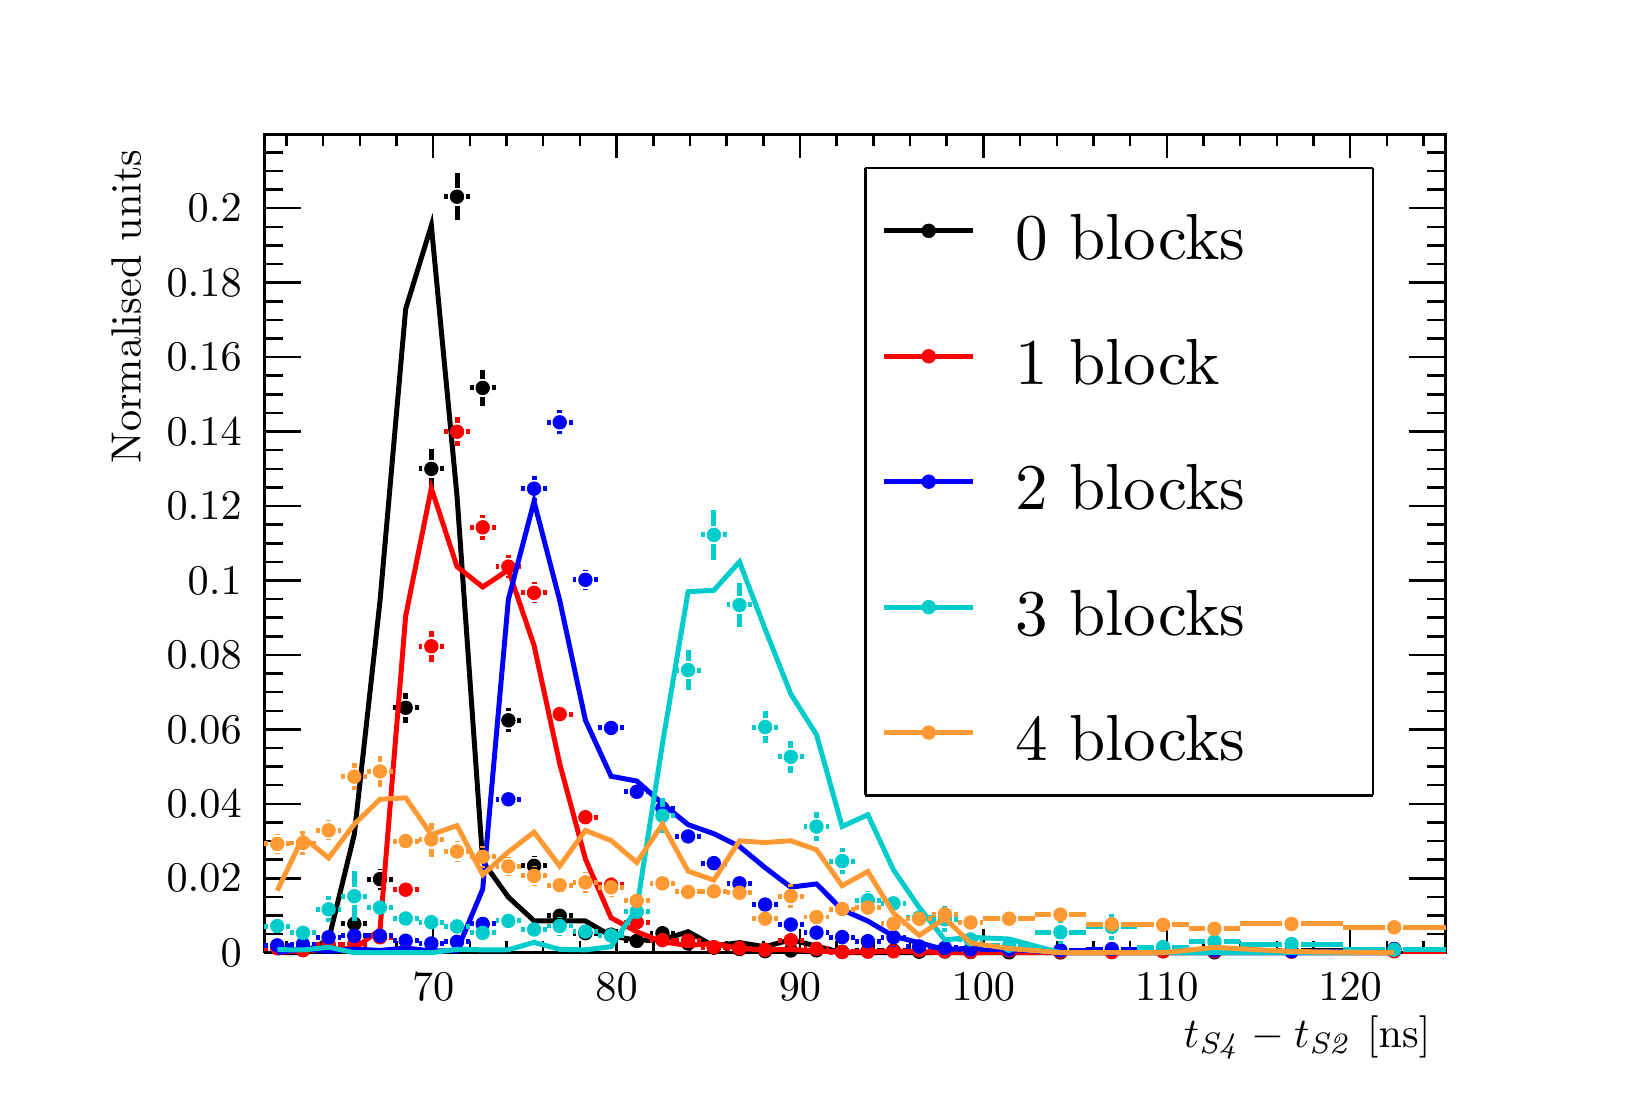
\begin{tikzpicture}
\pgfdeclareplotmark{cross} {
\pgfpathmoveto{\pgfpoint{-0.3\pgfplotmarksize}{\pgfplotmarksize}}
\pgfpathlineto{\pgfpoint{+0.3\pgfplotmarksize}{\pgfplotmarksize}}
\pgfpathlineto{\pgfpoint{+0.3\pgfplotmarksize}{0.3\pgfplotmarksize}}
\pgfpathlineto{\pgfpoint{+1\pgfplotmarksize}{0.3\pgfplotmarksize}}
\pgfpathlineto{\pgfpoint{+1\pgfplotmarksize}{-0.3\pgfplotmarksize}}
\pgfpathlineto{\pgfpoint{+0.3\pgfplotmarksize}{-0.3\pgfplotmarksize}}
\pgfpathlineto{\pgfpoint{+0.3\pgfplotmarksize}{-1.\pgfplotmarksize}}
\pgfpathlineto{\pgfpoint{-0.3\pgfplotmarksize}{-1.\pgfplotmarksize}}
\pgfpathlineto{\pgfpoint{-0.3\pgfplotmarksize}{-0.3\pgfplotmarksize}}
\pgfpathlineto{\pgfpoint{-1.\pgfplotmarksize}{-0.3\pgfplotmarksize}}
\pgfpathlineto{\pgfpoint{-1.\pgfplotmarksize}{0.3\pgfplotmarksize}}
\pgfpathlineto{\pgfpoint{-0.3\pgfplotmarksize}{0.3\pgfplotmarksize}}
\pgfpathclose
\pgfusepathqstroke
}
\pgfdeclareplotmark{cross*} {
\pgfpathmoveto{\pgfpoint{-0.3\pgfplotmarksize}{\pgfplotmarksize}}
\pgfpathlineto{\pgfpoint{+0.3\pgfplotmarksize}{\pgfplotmarksize}}
\pgfpathlineto{\pgfpoint{+0.3\pgfplotmarksize}{0.3\pgfplotmarksize}}
\pgfpathlineto{\pgfpoint{+1\pgfplotmarksize}{0.3\pgfplotmarksize}}
\pgfpathlineto{\pgfpoint{+1\pgfplotmarksize}{-0.3\pgfplotmarksize}}
\pgfpathlineto{\pgfpoint{+0.3\pgfplotmarksize}{-0.3\pgfplotmarksize}}
\pgfpathlineto{\pgfpoint{+0.3\pgfplotmarksize}{-1.\pgfplotmarksize}}
\pgfpathlineto{\pgfpoint{-0.3\pgfplotmarksize}{-1.\pgfplotmarksize}}
\pgfpathlineto{\pgfpoint{-0.3\pgfplotmarksize}{-0.3\pgfplotmarksize}}
\pgfpathlineto{\pgfpoint{-1.\pgfplotmarksize}{-0.3\pgfplotmarksize}}
\pgfpathlineto{\pgfpoint{-1.\pgfplotmarksize}{0.3\pgfplotmarksize}}
\pgfpathlineto{\pgfpoint{-0.3\pgfplotmarksize}{0.3\pgfplotmarksize}}
\pgfpathclose
\pgfusepathqfillstroke
}
\pgfdeclareplotmark{newstar} {
\pgfpathmoveto{\pgfqpoint{0pt}{\pgfplotmarksize}}
\pgfpathlineto{\pgfqpointpolar{44}{0.5\pgfplotmarksize}}
\pgfpathlineto{\pgfqpointpolar{18}{\pgfplotmarksize}}
\pgfpathlineto{\pgfqpointpolar{-20}{0.5\pgfplotmarksize}}
\pgfpathlineto{\pgfqpointpolar{-54}{\pgfplotmarksize}}
\pgfpathlineto{\pgfqpointpolar{-90}{0.5\pgfplotmarksize}}
\pgfpathlineto{\pgfqpointpolar{234}{\pgfplotmarksize}}
\pgfpathlineto{\pgfqpointpolar{198}{0.5\pgfplotmarksize}}
\pgfpathlineto{\pgfqpointpolar{162}{\pgfplotmarksize}}
\pgfpathlineto{\pgfqpointpolar{134}{0.5\pgfplotmarksize}}
\pgfpathclose
\pgfusepathqstroke
}
\pgfdeclareplotmark{newstar*} {
\pgfpathmoveto{\pgfqpoint{0pt}{\pgfplotmarksize}}
\pgfpathlineto{\pgfqpointpolar{44}{0.5\pgfplotmarksize}}
\pgfpathlineto{\pgfqpointpolar{18}{\pgfplotmarksize}}
\pgfpathlineto{\pgfqpointpolar{-20}{0.5\pgfplotmarksize}}
\pgfpathlineto{\pgfqpointpolar{-54}{\pgfplotmarksize}}
\pgfpathlineto{\pgfqpointpolar{-90}{0.5\pgfplotmarksize}}
\pgfpathlineto{\pgfqpointpolar{234}{\pgfplotmarksize}}
\pgfpathlineto{\pgfqpointpolar{198}{0.5\pgfplotmarksize}}
\pgfpathlineto{\pgfqpointpolar{162}{\pgfplotmarksize}}
\pgfpathlineto{\pgfqpointpolar{134}{0.5\pgfplotmarksize}}
\pgfpathclose
\pgfusepathqfillstroke
}
\definecolor{c}{rgb}{1,1,1};
\draw [color=c, fill=c] (0,0) rectangle (20,13.4957);
\draw [color=c, fill=c] (3,1.75444) rectangle (18,12.1461);
\definecolor{c}{rgb}{0,0,0};
\draw [c,line width=0.9] (3,1.75444) -- (3,12.1461) -- (18,12.1461) -- (18,1.75444) -- (3,1.75444);
\definecolor{c}{rgb}{1,1,1};
\draw [color=c, fill=c] (3,1.75444) rectangle (18,12.1461);
\definecolor{c}{rgb}{0,0,0};
\draw [c,line width=0.9] (3,1.75444) -- (3,12.1461) -- (18,12.1461) -- (18,1.75444) -- (3,1.75444);
\draw [c,line width=1.8] (3,1.83114) -- (3.04843,1.83114);
\draw [c,line width=1.8] (3.27766,1.83114) -- (3.32609,1.83114);
\foreach \P in {(3.16304,1.83114)}{\draw[mark options={color=c,fill=c},mark size=2.402402pt,mark=*] plot coordinates {\P};}
\draw [c,line width=1.8] (3.32609,1.82516) -- (3.37452,1.82516);
\draw [c,line width=1.8] (3.60374,1.82516) -- (3.65217,1.82516);
\foreach \P in {(3.48913,1.82516)}{\draw[mark options={color=c,fill=c},mark size=2.402402pt,mark=*] plot coordinates {\P};}
\draw [c,line width=1.8] (3.65217,1.84454) -- (3.7006,1.84454);
\draw [c,line width=1.8] (3.92983,1.84454) -- (3.97826,1.84454);
\foreach \P in {(3.81522,1.84454)}{\draw[mark options={color=c,fill=c},mark size=2.402402pt,mark=*] plot coordinates {\P};}
\draw [c,line width=1.8] (3.97826,2.12085) -- (4.02669,2.12085);
\draw [c,line width=1.8] (4.25592,2.12085) -- (4.30435,2.12085);
\foreach \P in {(4.1413,2.12085)}{\draw[mark options={color=c,fill=c},mark size=2.402402pt,mark=*] plot coordinates {\P};}
\draw [c,line width=1.8] (4.46739,2.55475) -- (4.46739,2.57465);
\draw [c,line width=1.8] (4.46739,2.80387) -- (4.46739,2.82376);
\draw [c,line width=1.8] (4.30435,2.68926) -- (4.35278,2.68926);
\draw [c,line width=1.8] (4.582,2.68926) -- (4.63043,2.68926);
\foreach \P in {(4.46739,2.68926)}{\draw[mark options={color=c,fill=c},mark size=2.402402pt,mark=*] plot coordinates {\P};}
\draw [c,line width=1.8] (4.79348,4.67286) -- (4.79348,4.75114);
\draw [c,line width=1.8] (4.79348,4.98037) -- (4.79348,5.05865);
\draw [c,line width=1.8] (4.63043,4.86575) -- (4.67886,4.86575);
\draw [c,line width=1.8] (4.90809,4.86575) -- (4.95652,4.86575);
\foreach \P in {(4.79348,4.86575)}{\draw[mark options={color=c,fill=c},mark size=2.402402pt,mark=*] plot coordinates {\P};}
\draw [c,line width=1.8] (5.11957,7.64548) -- (5.11957,7.78469);
\draw [c,line width=1.8] (5.11957,8.01391) -- (5.11957,8.15312);
\draw [c,line width=1.8] (4.95652,7.8993) -- (5.00495,7.8993);
\draw [c,line width=1.8] (5.23418,7.8993) -- (5.28261,7.8993);
\foreach \P in {(5.11957,7.8993)}{\draw[mark options={color=c,fill=c},mark size=2.402402pt,mark=*] plot coordinates {\P};}
\draw [c,line width=1.8] (5.44565,11.0614) -- (5.44565,11.2417);
\draw [c,line width=1.8] (5.44565,11.4709) -- (5.44565,11.6513);
\draw [c,line width=1.8] (5.28261,11.3563) -- (5.33104,11.3563);
\draw [c,line width=1.8] (5.56027,11.3563) -- (5.6087,11.3563);
\foreach \P in {(5.44565,11.3563)}{\draw[mark options={color=c,fill=c},mark size=2.402402pt,mark=*] plot coordinates {\P};}
\draw [c,line width=1.8] (5.77174,8.694) -- (5.77174,8.81308);
\draw [c,line width=1.8] (5.77174,9.04231) -- (5.77174,9.1614);
\draw [c,line width=1.8] (5.6087,8.9277) -- (5.65713,8.9277);
\draw [c,line width=1.8] (5.88635,8.9277) -- (5.93478,8.9277);
\foreach \P in {(5.77174,8.9277)}{\draw[mark options={color=c,fill=c},mark size=2.402402pt,mark=*] plot coordinates {\P};}
\draw [c,line width=1.8] (6.09783,4.55419) -- (6.09783,4.59147);
\draw [c,line width=1.8] (6.09783,4.8207) -- (6.09783,4.85798);
\draw [c,line width=1.8] (5.93478,4.70608) -- (5.98321,4.70608);
\draw [c,line width=1.8] (6.21244,4.70608) -- (6.26087,4.70608);
\foreach \P in {(6.09783,4.70608)}{\draw[mark options={color=c,fill=c},mark size=2.402402pt,mark=*] plot coordinates {\P};}
\draw [c,line width=1.8] (6.42391,2.73278) -- (6.42391,2.74337);
\draw [c,line width=1.8] (6.42391,2.9726) -- (6.42391,2.98319);
\draw [c,line width=1.8] (6.26087,2.85799) -- (6.3093,2.85799);
\draw [c,line width=1.8] (6.53853,2.85799) -- (6.58696,2.85799);
\foreach \P in {(6.42391,2.85799)}{\draw[mark options={color=c,fill=c},mark size=2.402402pt,mark=*] plot coordinates {\P};}
\draw [c,line width=1.8] (6.58696,2.22344) -- (6.63539,2.22344);
\draw [c,line width=1.8] (6.86461,2.22344) -- (6.91304,2.22344);
\foreach \P in {(6.75,2.22344)}{\draw[mark options={color=c,fill=c},mark size=2.402402pt,mark=*] plot coordinates {\P};}
\draw [c,line width=1.8] (6.91304,2.00306) -- (6.96147,2.00306);
\draw [c,line width=1.8] (7.1907,2.00306) -- (7.23913,2.00306);
\foreach \P in {(7.07609,2.00306)}{\draw[mark options={color=c,fill=c},mark size=2.402402pt,mark=*] plot coordinates {\P};}
\draw [c,line width=1.8] (7.23913,1.98414) -- (7.28756,1.98414);
\draw [c,line width=1.8] (7.51679,1.98414) -- (7.56522,1.98414);
\foreach \P in {(7.40217,1.98414)}{\draw[mark options={color=c,fill=c},mark size=2.402402pt,mark=*] plot coordinates {\P};}
\draw [c,line width=1.8] (7.56522,1.90433) -- (7.61365,1.90433);
\draw [c,line width=1.8] (7.84287,1.90433) -- (7.8913,1.90433);
\foreach \P in {(7.72826,1.90433)}{\draw[mark options={color=c,fill=c},mark size=2.402402pt,mark=*] plot coordinates {\P};}
\draw [c,line width=1.8] (7.8913,2.00177) -- (7.93973,2.00177);
\draw [c,line width=1.8] (8.16896,2.00177) -- (8.21739,2.00177);
\foreach \P in {(8.05435,2.00177)}{\draw[mark options={color=c,fill=c},mark size=2.402402pt,mark=*] plot coordinates {\P};}
\draw [c,line width=1.8] (8.21739,1.87216) -- (8.26582,1.87216);
\draw [c,line width=1.8] (8.49505,1.87216) -- (8.54348,1.87216);
\foreach \P in {(8.38043,1.87216)}{\draw[mark options={color=c,fill=c},mark size=2.402402pt,mark=*] plot coordinates {\P};}
\draw [c,line width=1.8] (8.54348,1.81906) -- (8.59191,1.81906);
\draw [c,line width=1.8] (8.82113,1.81906) -- (8.86957,1.81906);
\foreach \P in {(8.70652,1.81906)}{\draw[mark options={color=c,fill=c},mark size=2.402402pt,mark=*] plot coordinates {\P};}
\draw [c,line width=1.8] (8.86957,1.80095) -- (8.918,1.80095);
\draw [c,line width=1.8] (9.14722,1.80095) -- (9.19565,1.80095);
\foreach \P in {(9.03261,1.80095)}{\draw[mark options={color=c,fill=c},mark size=2.402402pt,mark=*] plot coordinates {\P};}
\draw [c,line width=1.8] (9.19565,1.77486) -- (9.24408,1.77486);
\draw [c,line width=1.8] (9.47331,1.77486) -- (9.52174,1.77486);
\foreach \P in {(9.3587,1.77486)}{\draw[mark options={color=c,fill=c},mark size=2.402402pt,mark=*] plot coordinates {\P};}
\draw [c,line width=1.8] (9.52174,1.78306) -- (9.57017,1.78306);
\draw [c,line width=1.8] (9.7994,1.78306) -- (9.84783,1.78306);
\foreach \P in {(9.68478,1.78306)}{\draw[mark options={color=c,fill=c},mark size=2.402402pt,mark=*] plot coordinates {\P};}
\draw [c,line width=1.8] (9.84783,1.78487) -- (9.89626,1.78487);
\draw [c,line width=1.8] (10.1255,1.78487) -- (10.1739,1.78487);
\foreach \P in {(10.0109,1.78487)}{\draw[mark options={color=c,fill=c},mark size=2.402402pt,mark=*] plot coordinates {\P};}
\draw [c,line width=1.8] (10.1739,1.76533) -- (10.2223,1.76533);
\draw [c,line width=1.8] (10.4516,1.76533) -- (10.5,1.76533);
\foreach \P in {(10.337,1.76533)}{\draw[mark options={color=c,fill=c},mark size=2.402402pt,mark=*] plot coordinates {\P};}
\draw [c,line width=1.8] (10.5,1.7786) -- (10.5484,1.7786);
\draw [c,line width=1.8] (10.7777,1.7786) -- (10.8261,1.7786);
\foreach \P in {(10.663,1.7786)}{\draw[mark options={color=c,fill=c},mark size=2.402402pt,mark=*] plot coordinates {\P};}
\draw [c,line width=1.8] (10.8261,1.78124) -- (10.8745,1.78124);
\draw [c,line width=1.8] (11.1037,1.78124) -- (11.1522,1.78124);
\foreach \P in {(10.9891,1.78124)}{\draw[mark options={color=c,fill=c},mark size=2.402402pt,mark=*] plot coordinates {\P};}
\draw [c,line width=1.8] (11.1522,1.767) -- (11.2006,1.767);
\draw [c,line width=1.8] (11.4298,1.767) -- (11.4783,1.767);
\foreach \P in {(11.3152,1.767)}{\draw[mark options={color=c,fill=c},mark size=2.402402pt,mark=*] plot coordinates {\P};}
\draw [c,line width=1.8] (11.4783,1.77006) -- (11.5267,1.77006);
\draw [c,line width=1.8] (11.7559,1.77006) -- (11.8043,1.77006);
\foreach \P in {(11.6413,1.77006)}{\draw[mark options={color=c,fill=c},mark size=2.402402pt,mark=*] plot coordinates {\P};}
\draw [c,line width=1.8] (11.8043,1.76448) -- (11.8528,1.76448);
\draw [c,line width=1.8] (12.082,1.76448) -- (12.1304,1.76448);
\foreach \P in {(11.9674,1.76448)}{\draw[mark options={color=c,fill=c},mark size=2.402402pt,mark=*] plot coordinates {\P};}
\draw [c,line width=1.8] (12.1304,1.76013) -- (12.3419,1.76013);
\draw [c,line width=1.8] (12.5711,1.76013) -- (12.7826,1.76013);
\foreach \P in {(12.4565,1.76013)}{\draw[mark options={color=c,fill=c},mark size=2.402402pt,mark=*] plot coordinates {\P};}
\draw [c,line width=1.8] (12.7826,1.75877) -- (12.9941,1.75877);
\draw [c,line width=1.8] (13.2233,1.75877) -- (13.4348,1.75877);
\foreach \P in {(13.1087,1.75877)}{\draw[mark options={color=c,fill=c},mark size=2.402402pt,mark=*] plot coordinates {\P};}
\draw [c,line width=1.8] (13.4348,1.7716) -- (13.6463,1.7716);
\draw [c,line width=1.8] (13.8755,1.7716) -- (14.087,1.7716);
\foreach \P in {(13.7609,1.7716)}{\draw[mark options={color=c,fill=c},mark size=2.402402pt,mark=*] plot coordinates {\P};}
\draw [c,line width=1.8] (14.087,1.77325) -- (14.2984,1.77325);
\draw [c,line width=1.8] (14.5277,1.77325) -- (14.7391,1.77325);
\foreach \P in {(14.413,1.77325)}{\draw[mark options={color=c,fill=c},mark size=2.402402pt,mark=*] plot coordinates {\P};}
\draw [c,line width=1.8] (14.7391,1.76012) -- (14.9506,1.76012);
\draw [c,line width=1.8] (15.1798,1.76012) -- (15.3913,1.76012);
\foreach \P in {(15.0652,1.76012)}{\draw[mark options={color=c,fill=c},mark size=2.402402pt,mark=*] plot coordinates {\P};}
\draw [c,line width=1.8] (15.3913,1.77863) -- (15.9289,1.77863);
\draw [c,line width=1.8] (16.1581,1.77863) -- (16.6957,1.77863);
\foreach \P in {(16.0435,1.77863)}{\draw[mark options={color=c,fill=c},mark size=2.402402pt,mark=*] plot coordinates {\P};}
\draw [c,line width=1.8] (16.6957,1.80192) -- (17.2332,1.80192);
\draw [c,line width=1.8] (17.4624,1.80192) -- (18,1.80192);
\foreach \P in {(17.3478,1.80192)}{\draw[mark options={color=c,fill=c},mark size=2.402402pt,mark=*] plot coordinates {\P};}
\draw [c,line width=0.9] (3,1.75444) -- (18,1.75444);
\draw [c,line width=0.9] (5.14286,2.05809) -- (5.14286,1.75444);
\draw [c,line width=0.9] (5.6087,1.90627) -- (5.6087,1.75444);
\draw [c,line width=0.9] (6.07453,1.90627) -- (6.07453,1.75444);
\draw [c,line width=0.9] (6.54037,1.90627) -- (6.54037,1.75444);
\draw [c,line width=0.9] (7.00621,1.90627) -- (7.00621,1.75444);
\draw [c,line width=0.9] (7.47205,2.05809) -- (7.47205,1.75444);
\draw [c,line width=0.9] (7.93789,1.90627) -- (7.93789,1.75444);
\draw [c,line width=0.9] (8.40373,1.90627) -- (8.40373,1.75444);
\draw [c,line width=0.9] (8.86957,1.90627) -- (8.86957,1.75444);
\draw [c,line width=0.9] (9.3354,1.90627) -- (9.3354,1.75444);
\draw [c,line width=0.9] (9.80124,2.05809) -- (9.80124,1.75444);
\draw [c,line width=0.9] (10.2671,1.90627) -- (10.2671,1.75444);
\draw [c,line width=0.9] (10.7329,1.90627) -- (10.7329,1.75444);
\draw [c,line width=0.9] (11.1988,1.90627) -- (11.1988,1.75444);
\draw [c,line width=0.9] (11.6646,1.90627) -- (11.6646,1.75444);
\draw [c,line width=0.9] (12.1304,2.05809) -- (12.1304,1.75444);
\draw [c,line width=0.9] (12.5963,1.90627) -- (12.5963,1.75444);
\draw [c,line width=0.9] (13.0621,1.90627) -- (13.0621,1.75444);
\draw [c,line width=0.9] (13.528,1.90627) -- (13.528,1.75444);
\draw [c,line width=0.9] (13.9938,1.90627) -- (13.9938,1.75444);
\draw [c,line width=0.9] (14.4596,2.05809) -- (14.4596,1.75444);
\draw [c,line width=0.9] (14.9255,1.90627) -- (14.9255,1.75444);
\draw [c,line width=0.9] (15.3913,1.90627) -- (15.3913,1.75444);
\draw [c,line width=0.9] (15.8571,1.90627) -- (15.8571,1.75444);
\draw [c,line width=0.9] (16.323,1.90627) -- (16.323,1.75444);
\draw [c,line width=0.9] (16.7888,2.05809) -- (16.7888,1.75444);
\draw [c,line width=0.9] (5.14286,2.05809) -- (5.14286,1.75444);
\draw [c,line width=0.9] (4.67702,1.90627) -- (4.67702,1.75444);
\draw [c,line width=0.9] (4.21118,1.90627) -- (4.21118,1.75444);
\draw [c,line width=0.9] (3.74534,1.90627) -- (3.74534,1.75444);
\draw [c,line width=0.9] (3.2795,1.90627) -- (3.2795,1.75444);
\draw [c,line width=0.9] (16.7888,2.05809) -- (16.7888,1.75444);
\draw [c,line width=0.9] (17.2547,1.90627) -- (17.2547,1.75444);
\draw [c,line width=0.9] (17.7205,1.90627) -- (17.7205,1.75444);
\draw [anchor=base] (5.14286,1.14713) node[scale=1.52731, color=c, rotate=0]{70};
\draw [anchor=base] (7.47205,1.14713) node[scale=1.52731, color=c, rotate=0]{80};
\draw [anchor=base] (9.80124,1.14713) node[scale=1.52731, color=c, rotate=0]{90};
\draw [anchor=base] (12.1304,1.14713) node[scale=1.52731, color=c, rotate=0]{100};
\draw [anchor=base] (14.4596,1.14713) node[scale=1.52731, color=c, rotate=0]{110};
\draw [anchor=base] (16.7888,1.14713) node[scale=1.52731, color=c, rotate=0]{120};
\draw [anchor= east] (18,0.674785) node[scale=1.52731, color=c, rotate=0]{$t_{\mathit{S4}} - t_{\mathit{S2}}$ [ns]};
\draw [c,line width=0.9] (3,12.1461) -- (18,12.1461);
\draw [c,line width=0.9] (5.14286,11.8425) -- (5.14286,12.1461);
\draw [c,line width=0.9] (5.6087,11.9943) -- (5.6087,12.1461);
\draw [c,line width=0.9] (6.07453,11.9943) -- (6.07453,12.1461);
\draw [c,line width=0.9] (6.54037,11.9943) -- (6.54037,12.1461);
\draw [c,line width=0.9] (7.00621,11.9943) -- (7.00621,12.1461);
\draw [c,line width=0.9] (7.47205,11.8425) -- (7.47205,12.1461);
\draw [c,line width=0.9] (7.93789,11.9943) -- (7.93789,12.1461);
\draw [c,line width=0.9] (8.40373,11.9943) -- (8.40373,12.1461);
\draw [c,line width=0.9] (8.86957,11.9943) -- (8.86957,12.1461);
\draw [c,line width=0.9] (9.3354,11.9943) -- (9.3354,12.1461);
\draw [c,line width=0.9] (9.80124,11.8425) -- (9.80124,12.1461);
\draw [c,line width=0.9] (10.2671,11.9943) -- (10.2671,12.1461);
\draw [c,line width=0.9] (10.7329,11.9943) -- (10.7329,12.1461);
\draw [c,line width=0.9] (11.1988,11.9943) -- (11.1988,12.1461);
\draw [c,line width=0.9] (11.6646,11.9943) -- (11.6646,12.1461);
\draw [c,line width=0.9] (12.1304,11.8425) -- (12.1304,12.1461);
\draw [c,line width=0.9] (12.5963,11.9943) -- (12.5963,12.1461);
\draw [c,line width=0.9] (13.0621,11.9943) -- (13.0621,12.1461);
\draw [c,line width=0.9] (13.528,11.9943) -- (13.528,12.1461);
\draw [c,line width=0.9] (13.9938,11.9943) -- (13.9938,12.1461);
\draw [c,line width=0.9] (14.4596,11.8425) -- (14.4596,12.1461);
\draw [c,line width=0.9] (14.9255,11.9943) -- (14.9255,12.1461);
\draw [c,line width=0.9] (15.3913,11.9943) -- (15.3913,12.1461);
\draw [c,line width=0.9] (15.8571,11.9943) -- (15.8571,12.1461);
\draw [c,line width=0.9] (16.323,11.9943) -- (16.323,12.1461);
\draw [c,line width=0.9] (16.7888,11.8425) -- (16.7888,12.1461);
\draw [c,line width=0.9] (5.14286,11.8425) -- (5.14286,12.1461);
\draw [c,line width=0.9] (4.67702,11.9943) -- (4.67702,12.1461);
\draw [c,line width=0.9] (4.21118,11.9943) -- (4.21118,12.1461);
\draw [c,line width=0.9] (3.74534,11.9943) -- (3.74534,12.1461);
\draw [c,line width=0.9] (3.2795,11.9943) -- (3.2795,12.1461);
\draw [c,line width=0.9] (16.7888,11.8425) -- (16.7888,12.1461);
\draw [c,line width=0.9] (17.2547,11.9943) -- (17.2547,12.1461);
\draw [c,line width=0.9] (17.7205,11.9943) -- (17.7205,12.1461);
\draw [c,line width=0.9] (3,1.75444) -- (3,12.1461);
\draw [c,line width=0.9] (3.462,1.75444) -- (3,1.75444);
\draw [c,line width=0.9] (3.231,1.99082) -- (3,1.99082);
\draw [c,line width=0.9] (3.231,2.2272) -- (3,2.2272);
\draw [c,line width=0.9] (3.231,2.46357) -- (3,2.46357);
\draw [c,line width=0.9] (3.462,2.69995) -- (3,2.69995);
\draw [c,line width=0.9] (3.231,2.93633) -- (3,2.93633);
\draw [c,line width=0.9] (3.231,3.1727) -- (3,3.1727);
\draw [c,line width=0.9] (3.231,3.40908) -- (3,3.40908);
\draw [c,line width=0.9] (3.462,3.64546) -- (3,3.64546);
\draw [c,line width=0.9] (3.231,3.88184) -- (3,3.88184);
\draw [c,line width=0.9] (3.231,4.11821) -- (3,4.11821);
\draw [c,line width=0.9] (3.231,4.35459) -- (3,4.35459);
\draw [c,line width=0.9] (3.462,4.59097) -- (3,4.59097);
\draw [c,line width=0.9] (3.231,4.82734) -- (3,4.82734);
\draw [c,line width=0.9] (3.231,5.06372) -- (3,5.06372);
\draw [c,line width=0.9] (3.231,5.3001) -- (3,5.3001);
\draw [c,line width=0.9] (3.462,5.53648) -- (3,5.53648);
\draw [c,line width=0.9] (3.231,5.77285) -- (3,5.77285);
\draw [c,line width=0.9] (3.231,6.00923) -- (3,6.00923);
\draw [c,line width=0.9] (3.231,6.24561) -- (3,6.24561);
\draw [c,line width=0.9] (3.462,6.48199) -- (3,6.48199);
\draw [c,line width=0.9] (3.231,6.71836) -- (3,6.71836);
\draw [c,line width=0.9] (3.231,6.95474) -- (3,6.95474);
\draw [c,line width=0.9] (3.231,7.19112) -- (3,7.19112);
\draw [c,line width=0.9] (3.462,7.42749) -- (3,7.42749);
\draw [c,line width=0.9] (3.231,7.66387) -- (3,7.66387);
\draw [c,line width=0.9] (3.231,7.90025) -- (3,7.90025);
\draw [c,line width=0.9] (3.231,8.13663) -- (3,8.13663);
\draw [c,line width=0.9] (3.462,8.373) -- (3,8.373);
\draw [c,line width=0.9] (3.231,8.60938) -- (3,8.60938);
\draw [c,line width=0.9] (3.231,8.84576) -- (3,8.84576);
\draw [c,line width=0.9] (3.231,9.08213) -- (3,9.08213);
\draw [c,line width=0.9] (3.462,9.31851) -- (3,9.31851);
\draw [c,line width=0.9] (3.231,9.55489) -- (3,9.55489);
\draw [c,line width=0.9] (3.231,9.79127) -- (3,9.79127);
\draw [c,line width=0.9] (3.231,10.0276) -- (3,10.0276);
\draw [c,line width=0.9] (3.462,10.264) -- (3,10.264);
\draw [c,line width=0.9] (3.231,10.5004) -- (3,10.5004);
\draw [c,line width=0.9] (3.231,10.7368) -- (3,10.7368);
\draw [c,line width=0.9] (3.231,10.9732) -- (3,10.9732);
\draw [c,line width=0.9] (3.462,11.2095) -- (3,11.2095);
\draw [c,line width=0.9] (3.462,11.2095) -- (3,11.2095);
\draw [c,line width=0.9] (3.231,11.4459) -- (3,11.4459);
\draw [c,line width=0.9] (3.231,11.6823) -- (3,11.6823);
\draw [c,line width=0.9] (3.231,11.9187) -- (3,11.9187);
\draw [anchor= east] (2.9,1.75444) node[scale=1.52731, color=c, rotate=0]{0};
\draw [anchor= east] (2.9,2.69995) node[scale=1.52731, color=c, rotate=0]{0.02};
\draw [anchor= east] (2.9,3.64546) node[scale=1.52731, color=c, rotate=0]{0.04};
\draw [anchor= east] (2.9,4.59097) node[scale=1.52731, color=c, rotate=0]{0.06};
\draw [anchor= east] (2.9,5.53648) node[scale=1.52731, color=c, rotate=0]{0.08};
\draw [anchor= east] (2.9,6.48199) node[scale=1.52731, color=c, rotate=0]{0.1};
\draw [anchor= east] (2.9,7.42749) node[scale=1.52731, color=c, rotate=0]{0.12};
\draw [anchor= east] (2.9,8.373) node[scale=1.52731, color=c, rotate=0]{0.14};
\draw [anchor= east] (2.9,9.31851) node[scale=1.52731, color=c, rotate=0]{0.16};
\draw [anchor= east] (2.9,10.264) node[scale=1.52731, color=c, rotate=0]{0.18};
\draw [anchor= east] (2.9,11.2095) node[scale=1.52731, color=c, rotate=0]{0.2};
\draw [anchor= east] (1.24,12.1461) node[scale=1.52731, color=c, rotate=90]{Normalised units};
\draw [c,line width=0.9] (18,1.75444) -- (18,12.1461);
\draw [c,line width=0.9] (17.538,1.75444) -- (18,1.75444);
\draw [c,line width=0.9] (17.769,1.99082) -- (18,1.99082);
\draw [c,line width=0.9] (17.769,2.2272) -- (18,2.2272);
\draw [c,line width=0.9] (17.769,2.46357) -- (18,2.46357);
\draw [c,line width=0.9] (17.538,2.69995) -- (18,2.69995);
\draw [c,line width=0.9] (17.769,2.93633) -- (18,2.93633);
\draw [c,line width=0.9] (17.769,3.1727) -- (18,3.1727);
\draw [c,line width=0.9] (17.769,3.40908) -- (18,3.40908);
\draw [c,line width=0.9] (17.538,3.64546) -- (18,3.64546);
\draw [c,line width=0.9] (17.769,3.88184) -- (18,3.88184);
\draw [c,line width=0.9] (17.769,4.11821) -- (18,4.11821);
\draw [c,line width=0.9] (17.769,4.35459) -- (18,4.35459);
\draw [c,line width=0.9] (17.538,4.59097) -- (18,4.59097);
\draw [c,line width=0.9] (17.769,4.82734) -- (18,4.82734);
\draw [c,line width=0.9] (17.769,5.06372) -- (18,5.06372);
\draw [c,line width=0.9] (17.769,5.3001) -- (18,5.3001);
\draw [c,line width=0.9] (17.538,5.53648) -- (18,5.53648);
\draw [c,line width=0.9] (17.769,5.77285) -- (18,5.77285);
\draw [c,line width=0.9] (17.769,6.00923) -- (18,6.00923);
\draw [c,line width=0.9] (17.769,6.24561) -- (18,6.24561);
\draw [c,line width=0.9] (17.538,6.48199) -- (18,6.48199);
\draw [c,line width=0.9] (17.769,6.71836) -- (18,6.71836);
\draw [c,line width=0.9] (17.769,6.95474) -- (18,6.95474);
\draw [c,line width=0.9] (17.769,7.19112) -- (18,7.19112);
\draw [c,line width=0.9] (17.538,7.42749) -- (18,7.42749);
\draw [c,line width=0.9] (17.769,7.66387) -- (18,7.66387);
\draw [c,line width=0.9] (17.769,7.90025) -- (18,7.90025);
\draw [c,line width=0.9] (17.769,8.13663) -- (18,8.13663);
\draw [c,line width=0.9] (17.538,8.373) -- (18,8.373);
\draw [c,line width=0.9] (17.769,8.60938) -- (18,8.60938);
\draw [c,line width=0.9] (17.769,8.84576) -- (18,8.84576);
\draw [c,line width=0.9] (17.769,9.08213) -- (18,9.08213);
\draw [c,line width=0.9] (17.538,9.31851) -- (18,9.31851);
\draw [c,line width=0.9] (17.769,9.55489) -- (18,9.55489);
\draw [c,line width=0.9] (17.769,9.79127) -- (18,9.79127);
\draw [c,line width=0.9] (17.769,10.0276) -- (18,10.0276);
\draw [c,line width=0.9] (17.538,10.264) -- (18,10.264);
\draw [c,line width=0.9] (17.769,10.5004) -- (18,10.5004);
\draw [c,line width=0.9] (17.769,10.7368) -- (18,10.7368);
\draw [c,line width=0.9] (17.769,10.9732) -- (18,10.9732);
\draw [c,line width=0.9] (17.538,11.2095) -- (18,11.2095);
\draw [c,line width=0.9] (17.538,11.2095) -- (18,11.2095);
\draw [c,line width=0.9] (17.769,11.4459) -- (18,11.4459);
\draw [c,line width=0.9] (17.769,11.6823) -- (18,11.6823);
\draw [c,line width=0.9] (17.769,11.9187) -- (18,11.9187);
\draw [c,line width=1.8] (3.16304,1.75444) -- (3.48913,1.75444) -- (3.81522,1.91963) -- (4.1413,3.2586) -- (4.46739,6.21923) -- (4.79348,9.93097) -- (5.11957,10.9903) -- (5.44565,7.5521) -- (5.77174,2.91629) -- (6.09783,2.46021) -- (6.42391,2.16031)
 -- (6.75,2.15888) -- (7.07609,2.1576) -- (7.40217,1.96821) -- (7.72826,1.91351) -- (8.05435,1.91827) -- (8.38043,2.02123) -- (8.70652,1.84056) -- (9.03261,1.88256) -- (9.3587,1.83017) -- (9.68478,1.92059) -- (10.0109,1.83781) -- (10.337,1.75444) --
 (10.663,1.75444) -- (10.9891,1.75444) -- (11.3152,1.75444) -- (11.6413,1.75444) -- (11.9674,1.75444) -- (12.4565,1.75444) -- (13.1087,1.75444) -- (13.7609,1.75444) -- (14.413,1.75444) -- (15.0652,1.75444) -- (16.0435,1.75444) -- (17.3478,1.75444);
\definecolor{c}{rgb}{1,0,0};
\draw [c,line width=1.8] (3,1.81211) -- (3.04843,1.81211);
\draw [c,line width=1.8] (3.27766,1.81211) -- (3.32609,1.81211);
\foreach \P in {(3.16304,1.81211)}{\draw[mark options={color=c,fill=c},mark size=2.402402pt,mark=*] plot coordinates {\P};}
\draw [c,line width=1.8] (3.32609,1.78648) -- (3.37452,1.78648);
\draw [c,line width=1.8] (3.60374,1.78648) -- (3.65217,1.78648);
\foreach \P in {(3.48913,1.78648)}{\draw[mark options={color=c,fill=c},mark size=2.402402pt,mark=*] plot coordinates {\P};}
\draw [c,line width=1.8] (3.65217,1.86159) -- (3.7006,1.86159);
\draw [c,line width=1.8] (3.92983,1.86159) -- (3.97826,1.86159);
\foreach \P in {(3.81522,1.86159)}{\draw[mark options={color=c,fill=c},mark size=2.402402pt,mark=*] plot coordinates {\P};}
\draw [c,line width=1.8] (3.97826,1.86397) -- (4.02669,1.86397);
\draw [c,line width=1.8] (4.25592,1.86397) -- (4.30435,1.86397);
\foreach \P in {(4.1413,1.86397)}{\draw[mark options={color=c,fill=c},mark size=2.402402pt,mark=*] plot coordinates {\P};}
\draw [c,line width=1.8] (4.30435,1.95008) -- (4.35278,1.95008);
\draw [c,line width=1.8] (4.582,1.95008) -- (4.63043,1.95008);
\foreach \P in {(4.46739,1.95008)}{\draw[mark options={color=c,fill=c},mark size=2.402402pt,mark=*] plot coordinates {\P};}
\draw [c,line width=1.8] (4.63043,2.55497) -- (4.67886,2.55497);
\draw [c,line width=1.8] (4.90809,2.55497) -- (4.95652,2.55497);
\foreach \P in {(4.79348,2.55497)}{\draw[mark options={color=c,fill=c},mark size=2.402402pt,mark=*] plot coordinates {\P};}
\draw [c,line width=1.8] (5.11957,5.44535) -- (5.11957,5.53144);
\draw [c,line width=1.8] (5.11957,5.76067) -- (5.11957,5.84676);
\draw [c,line width=1.8] (4.95652,5.64606) -- (5.00495,5.64606);
\draw [c,line width=1.8] (5.23418,5.64606) -- (5.28261,5.64606);
\foreach \P in {(5.11957,5.64606)}{\draw[mark options={color=c,fill=c},mark size=2.402402pt,mark=*] plot coordinates {\P};}
\draw [c,line width=1.8] (5.44565,8.18679) -- (5.44565,8.25649);
\draw [c,line width=1.8] (5.44565,8.48571) -- (5.44565,8.55541);
\draw [c,line width=1.8] (5.28261,8.3711) -- (5.33104,8.3711);
\draw [c,line width=1.8] (5.56027,8.3711) -- (5.6087,8.3711);
\foreach \P in {(5.44565,8.3711)}{\draw[mark options={color=c,fill=c},mark size=2.402402pt,mark=*] plot coordinates {\P};}
\draw [c,line width=1.8] (5.77174,6.99625) -- (5.77174,7.04232);
\draw [c,line width=1.8] (5.77174,7.27155) -- (5.77174,7.31762);
\draw [c,line width=1.8] (5.6087,7.15694) -- (5.65713,7.15694);
\draw [c,line width=1.8] (5.88635,7.15694) -- (5.93478,7.15694);
\foreach \P in {(5.77174,7.15694)}{\draw[mark options={color=c,fill=c},mark size=2.402402pt,mark=*] plot coordinates {\P};}
\draw [c,line width=1.8] (6.09783,6.51144) -- (6.09783,6.54373);
\draw [c,line width=1.8] (6.09783,6.77295) -- (6.09783,6.80523);
\draw [c,line width=1.8] (5.93478,6.65834) -- (5.98321,6.65834);
\draw [c,line width=1.8] (6.21244,6.65834) -- (6.26087,6.65834);
\foreach \P in {(6.09783,6.65834)}{\draw[mark options={color=c,fill=c},mark size=2.402402pt,mark=*] plot coordinates {\P};}
\draw [c,line width=1.8] (6.42391,6.19165) -- (6.42391,6.21023);
\draw [c,line width=1.8] (6.42391,6.43946) -- (6.42391,6.45803);
\draw [c,line width=1.8] (6.26087,6.32484) -- (6.3093,6.32484);
\draw [c,line width=1.8] (6.53853,6.32484) -- (6.58696,6.32484);
\foreach \P in {(6.42391,6.32484)}{\draw[mark options={color=c,fill=c},mark size=2.402402pt,mark=*] plot coordinates {\P};}
\draw [c,line width=1.8] (6.58696,4.78522) -- (6.63539,4.78522);
\draw [c,line width=1.8] (6.86461,4.78522) -- (6.91304,4.78522);
\foreach \P in {(6.75,4.78522)}{\draw[mark options={color=c,fill=c},mark size=2.402402pt,mark=*] plot coordinates {\P};}
\draw [c,line width=1.8] (6.91304,3.47547) -- (6.96147,3.47547);
\draw [c,line width=1.8] (7.1907,3.47547) -- (7.23913,3.47547);
\foreach \P in {(7.07609,3.47547)}{\draw[mark options={color=c,fill=c},mark size=2.402402pt,mark=*] plot coordinates {\P};}
\draw [c,line width=1.8] (7.23913,2.61559) -- (7.28756,2.61559);
\draw [c,line width=1.8] (7.51679,2.61559) -- (7.56522,2.61559);
\foreach \P in {(7.40217,2.61559)}{\draw[mark options={color=c,fill=c},mark size=2.402402pt,mark=*] plot coordinates {\P};}
\draw [c,line width=1.8] (7.56522,2.14104) -- (7.61365,2.14104);
\draw [c,line width=1.8] (7.84287,2.14104) -- (7.8913,2.14104);
\foreach \P in {(7.72826,2.14104)}{\draw[mark options={color=c,fill=c},mark size=2.402402pt,mark=*] plot coordinates {\P};}
\draw [c,line width=1.8] (7.8913,1.91483) -- (7.93973,1.91483);
\draw [c,line width=1.8] (8.16896,1.91483) -- (8.21739,1.91483);
\foreach \P in {(8.05435,1.91483)}{\draw[mark options={color=c,fill=c},mark size=2.402402pt,mark=*] plot coordinates {\P};}
\draw [c,line width=1.8] (8.21739,1.90786) -- (8.26582,1.90786);
\draw [c,line width=1.8] (8.49505,1.90786) -- (8.54348,1.90786);
\foreach \P in {(8.38043,1.90786)}{\draw[mark options={color=c,fill=c},mark size=2.402402pt,mark=*] plot coordinates {\P};}
\draw [c,line width=1.8] (8.54348,1.82528) -- (8.59191,1.82528);
\draw [c,line width=1.8] (8.82113,1.82528) -- (8.86957,1.82528);
\foreach \P in {(8.70652,1.82528)}{\draw[mark options={color=c,fill=c},mark size=2.402402pt,mark=*] plot coordinates {\P};}
\draw [c,line width=1.8] (8.86957,1.81201) -- (8.918,1.81201);
\draw [c,line width=1.8] (9.14722,1.81201) -- (9.19565,1.81201);
\foreach \P in {(9.03261,1.81201)}{\draw[mark options={color=c,fill=c},mark size=2.402402pt,mark=*] plot coordinates {\P};}
\draw [c,line width=1.8] (9.19565,1.79221) -- (9.24408,1.79221);
\draw [c,line width=1.8] (9.47331,1.79221) -- (9.52174,1.79221);
\foreach \P in {(9.3587,1.79221)}{\draw[mark options={color=c,fill=c},mark size=2.402402pt,mark=*] plot coordinates {\P};}
\draw [c,line width=1.8] (9.52174,1.91331) -- (9.57017,1.91331);
\draw [c,line width=1.8] (9.7994,1.91331) -- (9.84783,1.91331);
\foreach \P in {(9.68478,1.91331)}{\draw[mark options={color=c,fill=c},mark size=2.402402pt,mark=*] plot coordinates {\P};}
\draw [c,line width=1.8] (9.84783,1.80433) -- (9.89626,1.80433);
\draw [c,line width=1.8] (10.1255,1.80433) -- (10.1739,1.80433);
\foreach \P in {(10.0109,1.80433)}{\draw[mark options={color=c,fill=c},mark size=2.402402pt,mark=*] plot coordinates {\P};}
\draw [c,line width=1.8] (10.1739,1.76343) -- (10.2223,1.76343);
\draw [c,line width=1.8] (10.4516,1.76343) -- (10.5,1.76343);
\foreach \P in {(10.337,1.76343)}{\draw[mark options={color=c,fill=c},mark size=2.402402pt,mark=*] plot coordinates {\P};}
\draw [c,line width=1.8] (10.5,1.76754) -- (10.5484,1.76754);
\draw [c,line width=1.8] (10.7777,1.76754) -- (10.8261,1.76754);
\foreach \P in {(10.663,1.76754)}{\draw[mark options={color=c,fill=c},mark size=2.402402pt,mark=*] plot coordinates {\P};}
\draw [c,line width=1.8] (10.8261,1.77221) -- (10.8745,1.77221);
\draw [c,line width=1.8] (11.1037,1.77221) -- (11.1522,1.77221);
\foreach \P in {(10.9891,1.77221)}{\draw[mark options={color=c,fill=c},mark size=2.402402pt,mark=*] plot coordinates {\P};}
\draw [c,line width=1.8] (11.1522,1.785) -- (11.2006,1.785);
\draw [c,line width=1.8] (11.4298,1.785) -- (11.4783,1.785);
\foreach \P in {(11.3152,1.785)}{\draw[mark options={color=c,fill=c},mark size=2.402402pt,mark=*] plot coordinates {\P};}
\draw [c,line width=1.8] (11.4783,1.77279) -- (11.5267,1.77279);
\draw [c,line width=1.8] (11.7559,1.77279) -- (11.8043,1.77279);
\foreach \P in {(11.6413,1.77279)}{\draw[mark options={color=c,fill=c},mark size=2.402402pt,mark=*] plot coordinates {\P};}
\draw [c,line width=1.8] (11.8043,1.76728) -- (11.8528,1.76728);
\draw [c,line width=1.8] (12.082,1.76728) -- (12.1304,1.76728);
\foreach \P in {(11.9674,1.76728)}{\draw[mark options={color=c,fill=c},mark size=2.402402pt,mark=*] plot coordinates {\P};}
\draw [c,line width=1.8] (12.1304,1.7819) -- (12.3419,1.7819);
\draw [c,line width=1.8] (12.5711,1.7819) -- (12.7826,1.7819);
\foreach \P in {(12.4565,1.7819)}{\draw[mark options={color=c,fill=c},mark size=2.402402pt,mark=*] plot coordinates {\P};}
\draw [c,line width=1.8] (12.7826,1.76786) -- (12.9941,1.76786);
\draw [c,line width=1.8] (13.2233,1.76786) -- (13.4348,1.76786);
\foreach \P in {(13.1087,1.76786)}{\draw[mark options={color=c,fill=c},mark size=2.402402pt,mark=*] plot coordinates {\P};}
\draw [c,line width=1.8] (13.4348,1.76158) -- (13.6463,1.76158);
\draw [c,line width=1.8] (13.8755,1.76158) -- (14.087,1.76158);
\foreach \P in {(13.7609,1.76158)}{\draw[mark options={color=c,fill=c},mark size=2.402402pt,mark=*] plot coordinates {\P};}
\draw [c,line width=1.8] (14.087,1.77305) -- (14.2984,1.77305);
\draw [c,line width=1.8] (14.5277,1.77305) -- (14.7391,1.77305);
\foreach \P in {(14.413,1.77305)}{\draw[mark options={color=c,fill=c},mark size=2.402402pt,mark=*] plot coordinates {\P};}
\draw [c,line width=1.8] (14.7391,1.77051) -- (14.9506,1.77051);
\draw [c,line width=1.8] (15.1798,1.77051) -- (15.3913,1.77051);
\foreach \P in {(15.0652,1.77051)}{\draw[mark options={color=c,fill=c},mark size=2.402402pt,mark=*] plot coordinates {\P};}
\draw [c,line width=1.8] (15.3913,1.76731) -- (15.9289,1.76731);
\draw [c,line width=1.8] (16.1581,1.76731) -- (16.6957,1.76731);
\foreach \P in {(16.0435,1.76731)}{\draw[mark options={color=c,fill=c},mark size=2.402402pt,mark=*] plot coordinates {\P};}
\draw [c,line width=1.8] (16.6957,1.77289) -- (17.2332,1.77289);
\draw [c,line width=1.8] (17.4624,1.77289) -- (18,1.77289);
\foreach \P in {(17.3478,1.77289)}{\draw[mark options={color=c,fill=c},mark size=2.402402pt,mark=*] plot coordinates {\P};}
\draw [c,line width=1.8] (3.16304,1.75444) -- (3.48913,1.78544) -- (3.81522,1.79914) -- (4.1413,1.80957) -- (4.46739,2.04422) -- (4.79348,6.03159) -- (5.11957,7.65407) -- (5.44565,6.65773) -- (5.77174,6.39961) -- (6.09783,6.61606) --
 (6.42391,5.65677) -- (6.75,4.15407) -- (7.07609,2.94562) -- (7.40217,2.19736) -- (7.72826,2.0213) -- (8.05435,1.89342) -- (8.38043,1.84477) -- (8.70652,1.87479) -- (9.03261,1.80696) -- (9.3587,1.79074) -- (9.68478,1.79576) -- (10.0109,1.77547) --
 (10.337,1.76332) -- (10.663,1.76492) -- (10.9891,1.77752) -- (11.3152,1.76899) -- (11.6413,1.75444) -- (11.9674,1.75444) -- (12.4565,1.75444) -- (13.1087,1.75444) -- (13.7609,1.75444) -- (14.413,1.75444) -- (15.0652,1.75444) -- (16.0435,1.75444) --
 (17.3478,1.75444);
\definecolor{c}{rgb}{0,0,1};
\draw [c,line width=1.8] (3,1.8478) -- (3.04843,1.8478);
\draw [c,line width=1.8] (3.27766,1.8478) -- (3.32609,1.8478);
\foreach \P in {(3.16304,1.8478)}{\draw[mark options={color=c,fill=c},mark size=2.402402pt,mark=*] plot coordinates {\P};}
\draw [c,line width=1.8] (3.32609,1.86213) -- (3.37452,1.86213);
\draw [c,line width=1.8] (3.60374,1.86213) -- (3.65217,1.86213);
\foreach \P in {(3.48913,1.86213)}{\draw[mark options={color=c,fill=c},mark size=2.402402pt,mark=*] plot coordinates {\P};}
\draw [c,line width=1.8] (3.65217,1.95125) -- (3.7006,1.95125);
\draw [c,line width=1.8] (3.92983,1.95125) -- (3.97826,1.95125);
\foreach \P in {(3.81522,1.95125)}{\draw[mark options={color=c,fill=c},mark size=2.402402pt,mark=*] plot coordinates {\P};}
\draw [c,line width=1.8] (3.97826,1.969) -- (4.02669,1.969);
\draw [c,line width=1.8] (4.25592,1.969) -- (4.30435,1.969);
\foreach \P in {(4.1413,1.969)}{\draw[mark options={color=c,fill=c},mark size=2.402402pt,mark=*] plot coordinates {\P};}
\draw [c,line width=1.8] (4.30435,1.96916) -- (4.35278,1.96916);
\draw [c,line width=1.8] (4.582,1.96916) -- (4.63043,1.96916);
\foreach \P in {(4.46739,1.96916)}{\draw[mark options={color=c,fill=c},mark size=2.402402pt,mark=*] plot coordinates {\P};}
\draw [c,line width=1.8] (4.63043,1.90663) -- (4.67886,1.90663);
\draw [c,line width=1.8] (4.90809,1.90663) -- (4.95652,1.90663);
\foreach \P in {(4.79348,1.90663)}{\draw[mark options={color=c,fill=c},mark size=2.402402pt,mark=*] plot coordinates {\P};}
\draw [c,line width=1.8] (4.95652,1.872) -- (5.00495,1.872);
\draw [c,line width=1.8] (5.23418,1.872) -- (5.28261,1.872);
\foreach \P in {(5.11957,1.872)}{\draw[mark options={color=c,fill=c},mark size=2.402402pt,mark=*] plot coordinates {\P};}
\draw [c,line width=1.8] (5.28261,1.89287) -- (5.33104,1.89287);
\draw [c,line width=1.8] (5.56027,1.89287) -- (5.6087,1.89287);
\foreach \P in {(5.44565,1.89287)}{\draw[mark options={color=c,fill=c},mark size=2.402402pt,mark=*] plot coordinates {\P};}
\draw [c,line width=1.8] (5.6087,2.11977) -- (5.65713,2.11977);
\draw [c,line width=1.8] (5.88635,2.11977) -- (5.93478,2.11977);
\foreach \P in {(5.77174,2.11977)}{\draw[mark options={color=c,fill=c},mark size=2.402402pt,mark=*] plot coordinates {\P};}
\draw [c,line width=1.8] (5.93478,3.70281) -- (5.98321,3.70281);
\draw [c,line width=1.8] (6.21244,3.70281) -- (6.26087,3.70281);
\foreach \P in {(6.09783,3.70281)}{\draw[mark options={color=c,fill=c},mark size=2.402402pt,mark=*] plot coordinates {\P};}
\draw [c,line width=1.8] (6.42391,7.49274) -- (6.42391,7.53335);
\draw [c,line width=1.8] (6.42391,7.76258) -- (6.42391,7.80318);
\draw [c,line width=1.8] (6.26087,7.64796) -- (6.3093,7.64796);
\draw [c,line width=1.8] (6.53853,7.64796) -- (6.58696,7.64796);
\foreach \P in {(6.42391,7.64796)}{\draw[mark options={color=c,fill=c},mark size=2.402402pt,mark=*] plot coordinates {\P};}
\draw [c,line width=1.8] (6.75,8.33596) -- (6.75,8.37558);
\draw [c,line width=1.8] (6.75,8.6048) -- (6.75,8.64442);
\draw [c,line width=1.8] (6.58696,8.49019) -- (6.63539,8.49019);
\draw [c,line width=1.8] (6.86461,8.49019) -- (6.91304,8.49019);
\foreach \P in {(6.75,8.49019)}{\draw[mark options={color=c,fill=c},mark size=2.402402pt,mark=*] plot coordinates {\P};}
\draw [c,line width=1.8] (7.07609,6.36945) -- (7.07609,6.37624);
\draw [c,line width=1.8] (7.07609,6.60546) -- (7.07609,6.61224);
\draw [c,line width=1.8] (6.91304,6.49085) -- (6.96147,6.49085);
\draw [c,line width=1.8] (7.1907,6.49085) -- (7.23913,6.49085);
\foreach \P in {(7.07609,6.49085)}{\draw[mark options={color=c,fill=c},mark size=2.402402pt,mark=*] plot coordinates {\P};}
\draw [c,line width=1.8] (7.23913,4.60902) -- (7.28756,4.60902);
\draw [c,line width=1.8] (7.51679,4.60902) -- (7.56522,4.60902);
\foreach \P in {(7.40217,4.60902)}{\draw[mark options={color=c,fill=c},mark size=2.402402pt,mark=*] plot coordinates {\P};}
\draw [c,line width=1.8] (7.56522,3.79828) -- (7.61365,3.79828);
\draw [c,line width=1.8] (7.84287,3.79828) -- (7.8913,3.79828);
\foreach \P in {(7.72826,3.79828)}{\draw[mark options={color=c,fill=c},mark size=2.402402pt,mark=*] plot coordinates {\P};}
\draw [c,line width=1.8] (7.8913,3.59022) -- (7.93973,3.59022);
\draw [c,line width=1.8] (8.16896,3.59022) -- (8.21739,3.59022);
\foreach \P in {(8.05435,3.59022)}{\draw[mark options={color=c,fill=c},mark size=2.402402pt,mark=*] plot coordinates {\P};}
\draw [c,line width=1.8] (8.21739,3.23198) -- (8.26582,3.23198);
\draw [c,line width=1.8] (8.49505,3.23198) -- (8.54348,3.23198);
\foreach \P in {(8.38043,3.23198)}{\draw[mark options={color=c,fill=c},mark size=2.402402pt,mark=*] plot coordinates {\P};}
\draw [c,line width=1.8] (8.54348,2.89212) -- (8.59191,2.89212);
\draw [c,line width=1.8] (8.82113,2.89212) -- (8.86957,2.89212);
\foreach \P in {(8.70652,2.89212)}{\draw[mark options={color=c,fill=c},mark size=2.402402pt,mark=*] plot coordinates {\P};}
\draw [c,line width=1.8] (8.86957,2.63581) -- (8.918,2.63581);
\draw [c,line width=1.8] (9.14722,2.63581) -- (9.19565,2.63581);
\foreach \P in {(9.03261,2.63581)}{\draw[mark options={color=c,fill=c},mark size=2.402402pt,mark=*] plot coordinates {\P};}
\draw [c,line width=1.8] (9.19565,2.36642) -- (9.24408,2.36642);
\draw [c,line width=1.8] (9.47331,2.36642) -- (9.52174,2.36642);
\foreach \P in {(9.3587,2.36642)}{\draw[mark options={color=c,fill=c},mark size=2.402402pt,mark=*] plot coordinates {\P};}
\draw [c,line width=1.8] (9.52174,2.1125) -- (9.57017,2.1125);
\draw [c,line width=1.8] (9.7994,2.1125) -- (9.84783,2.1125);
\foreach \P in {(9.68478,2.1125)}{\draw[mark options={color=c,fill=c},mark size=2.402402pt,mark=*] plot coordinates {\P};}
\draw [c,line width=1.8] (9.84783,2.00994) -- (9.89626,2.00994);
\draw [c,line width=1.8] (10.1255,2.00994) -- (10.1739,2.00994);
\foreach \P in {(10.0109,2.00994)}{\draw[mark options={color=c,fill=c},mark size=2.402402pt,mark=*] plot coordinates {\P};}
\draw [c,line width=1.8] (10.1739,1.95316) -- (10.2223,1.95316);
\draw [c,line width=1.8] (10.4516,1.95316) -- (10.5,1.95316);
\foreach \P in {(10.337,1.95316)}{\draw[mark options={color=c,fill=c},mark size=2.402402pt,mark=*] plot coordinates {\P};}
\draw [c,line width=1.8] (10.5,1.90083) -- (10.5484,1.90083);
\draw [c,line width=1.8] (10.7777,1.90083) -- (10.8261,1.90083);
\foreach \P in {(10.663,1.90083)}{\draw[mark options={color=c,fill=c},mark size=2.402402pt,mark=*] plot coordinates {\P};}
\draw [c,line width=1.8] (10.9891,1.83674) -- (10.9891,1.83744);
\draw [c,line width=1.8] (10.9891,2.06666) -- (10.9891,2.06736);
\draw [c,line width=1.8] (10.8261,1.95205) -- (10.8745,1.95205);
\draw [c,line width=1.8] (11.1037,1.95205) -- (11.1522,1.95205);
\foreach \P in {(10.9891,1.95205)}{\draw[mark options={color=c,fill=c},mark size=2.402402pt,mark=*] plot coordinates {\P};}
\draw [c,line width=1.8] (11.1522,1.8342) -- (11.2006,1.8342);
\draw [c,line width=1.8] (11.4298,1.8342) -- (11.4783,1.8342);
\foreach \P in {(11.3152,1.8342)}{\draw[mark options={color=c,fill=c},mark size=2.402402pt,mark=*] plot coordinates {\P};}
\draw [c,line width=1.8] (11.4783,1.81544) -- (11.5267,1.81544);
\draw [c,line width=1.8] (11.7559,1.81544) -- (11.8043,1.81544);
\foreach \P in {(11.6413,1.81544)}{\draw[mark options={color=c,fill=c},mark size=2.402402pt,mark=*] plot coordinates {\P};}
\draw [c,line width=1.8] (11.8043,1.79728) -- (11.8528,1.79728);
\draw [c,line width=1.8] (12.082,1.79728) -- (12.1304,1.79728);
\foreach \P in {(11.9674,1.79728)}{\draw[mark options={color=c,fill=c},mark size=2.402402pt,mark=*] plot coordinates {\P};}
\draw [c,line width=1.8] (12.1304,1.79647) -- (12.3419,1.79647);
\draw [c,line width=1.8] (12.5711,1.79647) -- (12.7826,1.79647);
\foreach \P in {(12.4565,1.79647)}{\draw[mark options={color=c,fill=c},mark size=2.402402pt,mark=*] plot coordinates {\P};}
\draw [c,line width=1.8] (12.7826,1.78491) -- (12.9941,1.78491);
\draw [c,line width=1.8] (13.2233,1.78491) -- (13.4348,1.78491);
\foreach \P in {(13.1087,1.78491)}{\draw[mark options={color=c,fill=c},mark size=2.402402pt,mark=*] plot coordinates {\P};}
\draw [c,line width=1.8] (13.4348,1.80178) -- (13.6463,1.80178);
\draw [c,line width=1.8] (13.8755,1.80178) -- (14.087,1.80178);
\foreach \P in {(13.7609,1.80178)}{\draw[mark options={color=c,fill=c},mark size=2.402402pt,mark=*] plot coordinates {\P};}
\draw [c,line width=1.8] (14.087,1.81619) -- (14.2984,1.81619);
\draw [c,line width=1.8] (14.5277,1.81619) -- (14.7391,1.81619);
\foreach \P in {(14.413,1.81619)}{\draw[mark options={color=c,fill=c},mark size=2.402402pt,mark=*] plot coordinates {\P};}
\draw [c,line width=1.8] (14.7391,1.78527) -- (14.9506,1.78527);
\draw [c,line width=1.8] (15.1798,1.78527) -- (15.3913,1.78527);
\foreach \P in {(15.0652,1.78527)}{\draw[mark options={color=c,fill=c},mark size=2.402402pt,mark=*] plot coordinates {\P};}
\draw [c,line width=1.8] (15.3913,1.77305) -- (15.9289,1.77305);
\draw [c,line width=1.8] (16.1581,1.77305) -- (16.6957,1.77305);
\foreach \P in {(16.0435,1.77305)}{\draw[mark options={color=c,fill=c},mark size=2.402402pt,mark=*] plot coordinates {\P};}
\draw [c,line width=1.8] (16.6957,1.79734) -- (17.2332,1.79734);
\draw [c,line width=1.8] (17.4624,1.79734) -- (18,1.79734);
\foreach \P in {(17.3478,1.79734)}{\draw[mark options={color=c,fill=c},mark size=2.402402pt,mark=*] plot coordinates {\P};}
\draw [c,line width=1.8] (3.16304,1.75444) -- (3.48913,1.80585) -- (3.81522,1.77305) -- (4.1413,1.8013) -- (4.46739,1.78334) -- (4.79348,1.81354) -- (5.11957,1.77739) -- (5.44565,1.78148) -- (5.77174,2.56181) -- (6.09783,6.24229) -- (6.42391,7.48541)
 -- (6.75,6.22779) -- (7.07609,4.70841) -- (7.40217,3.9954) -- (7.72826,3.93513) -- (8.05435,3.64841) -- (8.38043,3.38114) -- (8.70652,3.26634) -- (9.03261,3.10473) -- (9.3587,2.83411) -- (9.68478,2.5874) -- (10.0109,2.62838) -- (10.337,2.30041) --
 (10.663,2.15715) -- (10.9891,1.9643) -- (11.3152,1.8818) -- (11.6413,1.79413) -- (11.9674,1.81227) -- (12.4565,1.79709) -- (13.1087,1.75444) -- (13.7609,1.75444) -- (14.413,1.75444) -- (15.0652,1.75444) -- (16.0435,1.75444) -- (17.3478,1.75444);
\definecolor{c}{rgb}{0,0.8,0.8};
\draw [c,line width=1.8] (3,2.09277) -- (3.04843,2.09277);
\draw [c,line width=1.8] (3.27766,2.09277) -- (3.32609,2.09277);
\foreach \P in {(3.16304,2.09277)}{\draw[mark options={color=c,fill=c},mark size=2.402402pt,mark=*] plot coordinates {\P};}
\draw [c,line width=1.8] (3.32609,2.00686) -- (3.37452,2.00686);
\draw [c,line width=1.8] (3.60374,2.00686) -- (3.65217,2.00686);
\foreach \P in {(3.48913,2.00686)}{\draw[mark options={color=c,fill=c},mark size=2.402402pt,mark=*] plot coordinates {\P};}
\draw [c,line width=1.8] (3.81522,2.13958) -- (3.81522,2.19128);
\draw [c,line width=1.8] (3.81522,2.4205) -- (3.81522,2.4722);
\draw [c,line width=1.8] (3.65217,2.30589) -- (3.7006,2.30589);
\draw [c,line width=1.8] (3.92983,2.30589) -- (3.97826,2.30589);
\foreach \P in {(3.81522,2.30589)}{\draw[mark options={color=c,fill=c},mark size=2.402402pt,mark=*] plot coordinates {\P};}
\draw [c,line width=1.8] (4.1413,2.15228) -- (4.1413,2.35746);
\draw [c,line width=1.8] (4.1413,2.58668) -- (4.1413,2.79186);
\draw [c,line width=1.8] (3.97826,2.47207) -- (4.02669,2.47207);
\draw [c,line width=1.8] (4.25592,2.47207) -- (4.30435,2.47207);
\foreach \P in {(4.1413,2.47207)}{\draw[mark options={color=c,fill=c},mark size=2.402402pt,mark=*] plot coordinates {\P};}
\draw [c,line width=1.8] (4.30435,2.32716) -- (4.35278,2.32716);
\draw [c,line width=1.8] (4.582,2.32716) -- (4.63043,2.32716);
\foreach \P in {(4.46739,2.32716)}{\draw[mark options={color=c,fill=c},mark size=2.402402pt,mark=*] plot coordinates {\P};}
\draw [c,line width=1.8] (4.63043,2.18968) -- (4.67886,2.18968);
\draw [c,line width=1.8] (4.90809,2.18968) -- (4.95652,2.18968);
\foreach \P in {(4.79348,2.18968)}{\draw[mark options={color=c,fill=c},mark size=2.402402pt,mark=*] plot coordinates {\P};}
\draw [c,line width=1.8] (4.95652,2.1425) -- (5.00495,2.1425);
\draw [c,line width=1.8] (5.23418,2.1425) -- (5.28261,2.1425);
\foreach \P in {(5.11957,2.1425)}{\draw[mark options={color=c,fill=c},mark size=2.402402pt,mark=*] plot coordinates {\P};}
\draw [c,line width=1.8] (5.28261,2.08886) -- (5.33104,2.08886);
\draw [c,line width=1.8] (5.56027,2.08886) -- (5.6087,2.08886);
\foreach \P in {(5.44565,2.08886)}{\draw[mark options={color=c,fill=c},mark size=2.402402pt,mark=*] plot coordinates {\P};}
\draw [c,line width=1.8] (5.6087,2.00664) -- (5.65713,2.00664);
\draw [c,line width=1.8] (5.88635,2.00664) -- (5.93478,2.00664);
\foreach \P in {(5.77174,2.00664)}{\draw[mark options={color=c,fill=c},mark size=2.402402pt,mark=*] plot coordinates {\P};}
\draw [c,line width=1.8] (5.93478,2.15819) -- (5.98321,2.15819);
\draw [c,line width=1.8] (6.21244,2.15819) -- (6.26087,2.15819);
\foreach \P in {(6.09783,2.15819)}{\draw[mark options={color=c,fill=c},mark size=2.402402pt,mark=*] plot coordinates {\P};}
\draw [c,line width=1.8] (6.26087,2.04901) -- (6.3093,2.04901);
\draw [c,line width=1.8] (6.53853,2.04901) -- (6.58696,2.04901);
\foreach \P in {(6.42391,2.04901)}{\draw[mark options={color=c,fill=c},mark size=2.402402pt,mark=*] plot coordinates {\P};}
\draw [c,line width=1.8] (6.75,1.97804) -- (6.75,1.97924);
\draw [c,line width=1.8] (6.75,2.20847) -- (6.75,2.20967);
\draw [c,line width=1.8] (6.58696,2.09385) -- (6.63539,2.09385);
\draw [c,line width=1.8] (6.86461,2.09385) -- (6.91304,2.09385);
\foreach \P in {(6.75,2.09385)}{\draw[mark options={color=c,fill=c},mark size=2.402402pt,mark=*] plot coordinates {\P};}
\draw [c,line width=1.8] (6.91304,2.02273) -- (6.96147,2.02273);
\draw [c,line width=1.8] (7.1907,2.02273) -- (7.23913,2.02273);
\foreach \P in {(7.07609,2.02273)}{\draw[mark options={color=c,fill=c},mark size=2.402402pt,mark=*] plot coordinates {\P};}
\draw [c,line width=1.8] (7.23913,1.97407) -- (7.28756,1.97407);
\draw [c,line width=1.8] (7.51679,1.97407) -- (7.56522,1.97407);
\foreach \P in {(7.40217,1.97407)}{\draw[mark options={color=c,fill=c},mark size=2.402402pt,mark=*] plot coordinates {\P};}
\draw [c,line width=1.8] (7.56522,2.27541) -- (7.61365,2.27541);
\draw [c,line width=1.8] (7.84287,2.27541) -- (7.8913,2.27541);
\foreach \P in {(7.72826,2.27541)}{\draw[mark options={color=c,fill=c},mark size=2.402402pt,mark=*] plot coordinates {\P};}
\draw [c,line width=1.8] (8.05435,3.27389) -- (8.05435,3.38004);
\draw [c,line width=1.8] (8.05435,3.60926) -- (8.05435,3.71541);
\draw [c,line width=1.8] (7.8913,3.49465) -- (7.93973,3.49465);
\draw [c,line width=1.8] (8.16896,3.49465) -- (8.21739,3.49465);
\foreach \P in {(8.05435,3.49465)}{\draw[mark options={color=c,fill=c},mark size=2.402402pt,mark=*] plot coordinates {\P};}
\draw [c,line width=1.8] (8.38043,5.08486) -- (8.38043,5.22884);
\draw [c,line width=1.8] (8.38043,5.45806) -- (8.38043,5.60205);
\draw [c,line width=1.8] (8.21739,5.34345) -- (8.26582,5.34345);
\draw [c,line width=1.8] (8.49505,5.34345) -- (8.54348,5.34345);
\foreach \P in {(8.38043,5.34345)}{\draw[mark options={color=c,fill=c},mark size=2.402402pt,mark=*] plot coordinates {\P};}
\draw [c,line width=1.8] (8.70652,6.73868) -- (8.70652,6.94635);
\draw [c,line width=1.8] (8.70652,7.17558) -- (8.70652,7.38326);
\draw [c,line width=1.8] (8.54348,7.06097) -- (8.59191,7.06097);
\draw [c,line width=1.8] (8.82113,7.06097) -- (8.86957,7.06097);
\foreach \P in {(8.70652,7.06097)}{\draw[mark options={color=c,fill=c},mark size=2.402402pt,mark=*] plot coordinates {\P};}
\draw [c,line width=1.8] (9.03261,5.88863) -- (9.03261,6.05618);
\draw [c,line width=1.8] (9.03261,6.28541) -- (9.03261,6.45297);
\draw [c,line width=1.8] (8.86957,6.1708) -- (8.918,6.1708);
\draw [c,line width=1.8] (9.14722,6.1708) -- (9.19565,6.1708);
\foreach \P in {(9.03261,6.1708)}{\draw[mark options={color=c,fill=c},mark size=2.402402pt,mark=*] plot coordinates {\P};}
\draw [c,line width=1.8] (9.3587,4.41456) -- (9.3587,4.50611);
\draw [c,line width=1.8] (9.3587,4.73533) -- (9.3587,4.82689);
\draw [c,line width=1.8] (9.19565,4.62072) -- (9.24408,4.62072);
\draw [c,line width=1.8] (9.47331,4.62072) -- (9.52174,4.62072);
\foreach \P in {(9.3587,4.62072)}{\draw[mark options={color=c,fill=c},mark size=2.402402pt,mark=*] plot coordinates {\P};}
\draw [c,line width=1.8] (9.68478,4.0349) -- (9.68478,4.12756);
\draw [c,line width=1.8] (9.68478,4.35679) -- (9.68478,4.44945);
\draw [c,line width=1.8] (9.52174,4.24217) -- (9.57017,4.24217);
\draw [c,line width=1.8] (9.7994,4.24217) -- (9.84783,4.24217);
\foreach \P in {(9.68478,4.24217)}{\draw[mark options={color=c,fill=c},mark size=2.402402pt,mark=*] plot coordinates {\P};}
\draw [c,line width=1.8] (10.0109,3.1761) -- (10.0109,3.24214);
\draw [c,line width=1.8] (10.0109,3.47137) -- (10.0109,3.53741);
\draw [c,line width=1.8] (9.84783,3.35675) -- (9.89626,3.35675);
\draw [c,line width=1.8] (10.1255,3.35675) -- (10.1739,3.35675);
\foreach \P in {(10.0109,3.35675)}{\draw[mark options={color=c,fill=c},mark size=2.402402pt,mark=*] plot coordinates {\P};}
\draw [c,line width=1.8] (10.337,2.75799) -- (10.337,2.80362);
\draw [c,line width=1.8] (10.337,3.03285) -- (10.337,3.07848);
\draw [c,line width=1.8] (10.1739,2.91823) -- (10.2223,2.91823);
\draw [c,line width=1.8] (10.4516,2.91823) -- (10.5,2.91823);
\foreach \P in {(10.337,2.91823)}{\draw[mark options={color=c,fill=c},mark size=2.402402pt,mark=*] plot coordinates {\P};}
\draw [c,line width=1.8] (10.663,2.30233) -- (10.663,2.30627);
\draw [c,line width=1.8] (10.663,2.5355) -- (10.663,2.53944);
\draw [c,line width=1.8] (10.5,2.42088) -- (10.5484,2.42088);
\draw [c,line width=1.8] (10.7777,2.42088) -- (10.8261,2.42088);
\foreach \P in {(10.663,2.42088)}{\draw[mark options={color=c,fill=c},mark size=2.402402pt,mark=*] plot coordinates {\P};}
\draw [c,line width=1.8] (10.8261,2.38137) -- (10.8745,2.38137);
\draw [c,line width=1.8] (11.1037,2.38137) -- (11.1522,2.38137);
\foreach \P in {(10.9891,2.38137)}{\draw[mark options={color=c,fill=c},mark size=2.402402pt,mark=*] plot coordinates {\P};}
\draw [c,line width=1.8] (11.1522,2.20058) -- (11.2006,2.20058);
\draw [c,line width=1.8] (11.4298,2.20058) -- (11.4783,2.20058);
\foreach \P in {(11.3152,2.20058)}{\draw[mark options={color=c,fill=c},mark size=2.402402pt,mark=*] plot coordinates {\P};}
\draw [c,line width=1.8] (11.6413,2.01389) -- (11.6413,2.06403);
\draw [c,line width=1.8] (11.6413,2.29326) -- (11.6413,2.34341);
\draw [c,line width=1.8] (11.4783,2.17865) -- (11.5267,2.17865);
\draw [c,line width=1.8] (11.7559,2.17865) -- (11.8043,2.17865);
\foreach \P in {(11.6413,2.17865)}{\draw[mark options={color=c,fill=c},mark size=2.402402pt,mark=*] plot coordinates {\P};}
\draw [c,line width=1.8] (11.8043,1.9229) -- (11.8528,1.9229);
\draw [c,line width=1.8] (12.082,1.9229) -- (12.1304,1.9229);
\foreach \P in {(11.9674,1.9229)}{\draw[mark options={color=c,fill=c},mark size=2.402402pt,mark=*] plot coordinates {\P};}
\draw [c,line width=1.8] (12.1304,1.84422) -- (12.3419,1.84422);
\draw [c,line width=1.8] (12.5711,1.84422) -- (12.7826,1.84422);
\foreach \P in {(12.4565,1.84422)}{\draw[mark options={color=c,fill=c},mark size=2.402402pt,mark=*] plot coordinates {\P};}
\draw [c,line width=1.8] (13.1087,1.87156) -- (13.1087,1.90036);
\draw [c,line width=1.8] (13.1087,2.12959) -- (13.1087,2.15839);
\draw [c,line width=1.8] (12.7826,2.01498) -- (12.9941,2.01498);
\draw [c,line width=1.8] (13.2233,2.01498) -- (13.4348,2.01498);
\foreach \P in {(13.1087,2.01498)}{\draw[mark options={color=c,fill=c},mark size=2.402402pt,mark=*] plot coordinates {\P};}
\draw [c,line width=1.8] (13.7609,1.91684) -- (13.7609,1.96756);
\draw [c,line width=1.8] (13.7609,2.19679) -- (13.7609,2.24751);
\draw [c,line width=1.8] (13.4348,2.08218) -- (13.6463,2.08218);
\draw [c,line width=1.8] (13.8755,2.08218) -- (14.087,2.08218);
\foreach \P in {(13.7609,2.08218)}{\draw[mark options={color=c,fill=c},mark size=2.402402pt,mark=*] plot coordinates {\P};}
\draw [c,line width=1.8] (14.087,1.8261) -- (14.2984,1.8261);
\draw [c,line width=1.8] (14.5277,1.8261) -- (14.7391,1.8261);
\foreach \P in {(14.413,1.8261)}{\draw[mark options={color=c,fill=c},mark size=2.402402pt,mark=*] plot coordinates {\P};}
\draw [c,line width=1.8] (14.7391,1.89567) -- (14.9506,1.89567);
\draw [c,line width=1.8] (15.1798,1.89567) -- (15.3913,1.89567);
\foreach \P in {(15.0652,1.89567)}{\draw[mark options={color=c,fill=c},mark size=2.402402pt,mark=*] plot coordinates {\P};}
\draw [c,line width=1.8] (15.3913,1.86464) -- (15.9289,1.86464);
\draw [c,line width=1.8] (16.1581,1.86464) -- (16.6957,1.86464);
\foreach \P in {(16.0435,1.86464)}{\draw[mark options={color=c,fill=c},mark size=2.402402pt,mark=*] plot coordinates {\P};}
\draw [c,line width=1.8] (16.6957,1.79245) -- (17.2332,1.79245);
\draw [c,line width=1.8] (17.4624,1.79245) -- (18,1.79245);
\foreach \P in {(17.3478,1.79245)}{\draw[mark options={color=c,fill=c},mark size=2.402402pt,mark=*] plot coordinates {\P};}
\draw [c,line width=1.8] (3.16304,1.79419) -- (3.48913,1.78935) -- (3.81522,1.825) -- (4.1413,1.75444) -- (4.46739,1.75444) -- (4.79348,1.75444) -- (5.11957,1.75444) -- (5.44565,1.79802) -- (5.77174,1.79114) -- (6.09783,1.79237) -- (6.42391,1.88588)
 -- (6.75,1.79759) -- (7.07609,1.79114) -- (7.40217,1.83123) -- (7.72826,2.31698) -- (8.05435,4.40635) -- (8.38043,6.33923) -- (8.70652,6.35692) -- (9.03261,6.71819) -- (9.3587,5.86326) -- (9.68478,5.04002) -- (10.0109,4.52309) -- (10.337,3.35776) --
 (10.663,3.50698) -- (10.9891,2.80537) -- (11.3152,2.32915) -- (11.6413,1.91755) -- (11.9674,1.94973) -- (12.4565,1.92858) -- (13.1087,1.75444) -- (13.7609,1.75444) -- (14.413,1.75444) -- (15.0652,1.75444) -- (16.0435,1.75444) -- (17.3478,1.75444);
\definecolor{c}{rgb}{1,0.6,0.2};
\draw [c,line width=1.8] (3.16304,3.00678) -- (3.16304,3.02231);
\draw [c,line width=1.8] (3.16304,3.25154) -- (3.16304,3.26707);
\draw [c,line width=1.8] (3,3.13693) -- (3.04843,3.13693);
\draw [c,line width=1.8] (3.27766,3.13693) -- (3.32609,3.13693);
\foreach \P in {(3.16304,3.13693)}{\draw[mark options={color=c,fill=c},mark size=2.402402pt,mark=*] plot coordinates {\P};}
\draw [c,line width=1.8] (3.48913,3.00001) -- (3.48913,3.03353);
\draw [c,line width=1.8] (3.48913,3.26276) -- (3.48913,3.29628);
\draw [c,line width=1.8] (3.32609,3.14814) -- (3.37452,3.14814);
\draw [c,line width=1.8] (3.60374,3.14814) -- (3.65217,3.14814);
\foreach \P in {(3.48913,3.14814)}{\draw[mark options={color=c,fill=c},mark size=2.402402pt,mark=*] plot coordinates {\P};}
\draw [c,line width=1.8] (3.81522,3.18211) -- (3.81522,3.19419);
\draw [c,line width=1.8] (3.81522,3.42341) -- (3.81522,3.43548);
\draw [c,line width=1.8] (3.65217,3.3088) -- (3.7006,3.3088);
\draw [c,line width=1.8] (3.92983,3.3088) -- (3.97826,3.3088);
\foreach \P in {(3.81522,3.3088)}{\draw[mark options={color=c,fill=c},mark size=2.402402pt,mark=*] plot coordinates {\P};}
\draw [c,line width=1.8] (4.1413,3.81874) -- (4.1413,3.8759);
\draw [c,line width=1.8] (4.1413,4.10513) -- (4.1413,4.16229);
\draw [c,line width=1.8] (3.97826,3.99051) -- (4.02669,3.99051);
\draw [c,line width=1.8] (4.25592,3.99051) -- (4.30435,3.99051);
\foreach \P in {(4.1413,3.99051)}{\draw[mark options={color=c,fill=c},mark size=2.402402pt,mark=*] plot coordinates {\P};}
\draw [c,line width=1.8] (4.46739,3.85578) -- (4.46739,3.94181);
\draw [c,line width=1.8] (4.46739,4.17103) -- (4.46739,4.25706);
\draw [c,line width=1.8] (4.30435,4.05642) -- (4.35278,4.05642);
\draw [c,line width=1.8] (4.582,4.05642) -- (4.63043,4.05642);
\foreach \P in {(4.46739,4.05642)}{\draw[mark options={color=c,fill=c},mark size=2.402402pt,mark=*] plot coordinates {\P};}
\draw [c,line width=1.8] (4.63043,3.17273) -- (4.67886,3.17273);
\draw [c,line width=1.8] (4.90809,3.17273) -- (4.95652,3.17273);
\foreach \P in {(4.79348,3.17273)}{\draw[mark options={color=c,fill=c},mark size=2.402402pt,mark=*] plot coordinates {\P};}
\draw [c,line width=1.8] (5.11957,2.97656) -- (5.11957,3.07762);
\draw [c,line width=1.8] (5.11957,3.30685) -- (5.11957,3.40791);
\draw [c,line width=1.8] (4.95652,3.19224) -- (5.00495,3.19224);
\draw [c,line width=1.8] (5.23418,3.19224) -- (5.28261,3.19224);
\foreach \P in {(5.11957,3.19224)}{\draw[mark options={color=c,fill=c},mark size=2.402402pt,mark=*] plot coordinates {\P};}
\draw [c,line width=1.8] (5.44565,2.9027) -- (5.44565,2.92563);
\draw [c,line width=1.8] (5.44565,3.15486) -- (5.44565,3.17779);
\draw [c,line width=1.8] (5.28261,3.04025) -- (5.33104,3.04025);
\draw [c,line width=1.8] (5.56027,3.04025) -- (5.6087,3.04025);
\foreach \P in {(5.44565,3.04025)}{\draw[mark options={color=c,fill=c},mark size=2.402402pt,mark=*] plot coordinates {\P};}
\draw [c,line width=1.8] (5.77174,2.83511) -- (5.77174,2.85894);
\draw [c,line width=1.8] (5.77174,3.08817) -- (5.77174,3.112);
\draw [c,line width=1.8] (5.6087,2.97356) -- (5.65713,2.97356);
\draw [c,line width=1.8] (5.88635,2.97356) -- (5.93478,2.97356);
\foreach \P in {(5.77174,2.97356)}{\draw[mark options={color=c,fill=c},mark size=2.402402pt,mark=*] plot coordinates {\P};}
\draw [c,line width=1.8] (6.09783,2.73373) -- (6.09783,2.73629);
\draw [c,line width=1.8] (6.09783,2.96551) -- (6.09783,2.96807);
\draw [c,line width=1.8] (5.93478,2.8509) -- (5.98321,2.8509);
\draw [c,line width=1.8] (6.21244,2.8509) -- (6.26087,2.8509);
\foreach \P in {(6.09783,2.8509)}{\draw[mark options={color=c,fill=c},mark size=2.402402pt,mark=*] plot coordinates {\P};}
\draw [c,line width=1.8] (6.42391,2.60952) -- (6.42391,2.61599);
\draw [c,line width=1.8] (6.42391,2.84521) -- (6.42391,2.85168);
\draw [c,line width=1.8] (6.26087,2.7306) -- (6.3093,2.7306);
\draw [c,line width=1.8] (6.53853,2.7306) -- (6.58696,2.7306);
\foreach \P in {(6.42391,2.7306)}{\draw[mark options={color=c,fill=c},mark size=2.402402pt,mark=*] plot coordinates {\P};}
\draw [c,line width=1.8] (6.58696,2.61229) -- (6.63539,2.61229);
\draw [c,line width=1.8] (6.86461,2.61229) -- (6.91304,2.61229);
\foreach \P in {(6.75,2.61229)}{\draw[mark options={color=c,fill=c},mark size=2.402402pt,mark=*] plot coordinates {\P};}
\draw [c,line width=1.8] (7.07609,2.51735) -- (7.07609,2.53298);
\draw [c,line width=1.8] (7.07609,2.7622) -- (7.07609,2.77783);
\draw [c,line width=1.8] (6.91304,2.64759) -- (6.96147,2.64759);
\draw [c,line width=1.8] (7.1907,2.64759) -- (7.23913,2.64759);
\foreach \P in {(7.07609,2.64759)}{\draw[mark options={color=c,fill=c},mark size=2.402402pt,mark=*] plot coordinates {\P};}
\draw [c,line width=1.8] (7.40217,2.45754) -- (7.40217,2.47052);
\draw [c,line width=1.8] (7.40217,2.69974) -- (7.40217,2.71272);
\draw [c,line width=1.8] (7.23913,2.58513) -- (7.28756,2.58513);
\draw [c,line width=1.8] (7.51679,2.58513) -- (7.56522,2.58513);
\foreach \P in {(7.40217,2.58513)}{\draw[mark options={color=c,fill=c},mark size=2.402402pt,mark=*] plot coordinates {\P};}
\draw [c,line width=1.8] (7.56522,2.41319) -- (7.61365,2.41319);
\draw [c,line width=1.8] (7.84287,2.41319) -- (7.8913,2.41319);
\foreach \P in {(7.72826,2.41319)}{\draw[mark options={color=c,fill=c},mark size=2.402402pt,mark=*] plot coordinates {\P};}
\draw [c,line width=1.8] (7.8913,2.63547) -- (7.93973,2.63547);
\draw [c,line width=1.8] (8.16896,2.63547) -- (8.21739,2.63547);
\foreach \P in {(8.05435,2.63547)}{\draw[mark options={color=c,fill=c},mark size=2.402402pt,mark=*] plot coordinates {\P};}
\draw [c,line width=1.8] (8.21739,2.52742) -- (8.26582,2.52742);
\draw [c,line width=1.8] (8.49505,2.52742) -- (8.54348,2.52742);
\foreach \P in {(8.38043,2.52742)}{\draw[mark options={color=c,fill=c},mark size=2.402402pt,mark=*] plot coordinates {\P};}
\draw [c,line width=1.8] (8.54348,2.53434) -- (8.59191,2.53434);
\draw [c,line width=1.8] (8.82113,2.53434) -- (8.86957,2.53434);
\foreach \P in {(8.70652,2.53434)}{\draw[mark options={color=c,fill=c},mark size=2.402402pt,mark=*] plot coordinates {\P};}
\draw [c,line width=1.8] (8.86957,2.51597) -- (8.918,2.51597);
\draw [c,line width=1.8] (9.14722,2.51597) -- (9.19565,2.51597);
\foreach \P in {(9.03261,2.51597)}{\draw[mark options={color=c,fill=c},mark size=2.402402pt,mark=*] plot coordinates {\P};}
\draw [c,line width=1.8] (9.19565,2.18669) -- (9.24408,2.18669);
\draw [c,line width=1.8] (9.47331,2.18669) -- (9.52174,2.18669);
\foreach \P in {(9.3587,2.18669)}{\draw[mark options={color=c,fill=c},mark size=2.402402pt,mark=*] plot coordinates {\P};}
\draw [c,line width=1.8] (9.68478,2.31921) -- (9.68478,2.35974);
\draw [c,line width=1.8] (9.68478,2.58897) -- (9.68478,2.6295);
\draw [c,line width=1.8] (9.52174,2.47435) -- (9.57017,2.47435);
\draw [c,line width=1.8] (9.7994,2.47435) -- (9.84783,2.47435);
\foreach \P in {(9.68478,2.47435)}{\draw[mark options={color=c,fill=c},mark size=2.402402pt,mark=*] plot coordinates {\P};}
\draw [c,line width=1.8] (9.84783,2.20824) -- (9.89626,2.20824);
\draw [c,line width=1.8] (10.1255,2.20824) -- (10.1739,2.20824);
\foreach \P in {(10.0109,2.20824)}{\draw[mark options={color=c,fill=c},mark size=2.402402pt,mark=*] plot coordinates {\P};}
\draw [c,line width=1.8] (10.1739,2.30951) -- (10.2223,2.30951);
\draw [c,line width=1.8] (10.4516,2.30951) -- (10.5,2.30951);
\foreach \P in {(10.337,2.30951)}{\draw[mark options={color=c,fill=c},mark size=2.402402pt,mark=*] plot coordinates {\P};}
\draw [c,line width=1.8] (10.5,2.32815) -- (10.5484,2.32815);
\draw [c,line width=1.8] (10.7777,2.32815) -- (10.8261,2.32815);
\foreach \P in {(10.663,2.32815)}{\draw[mark options={color=c,fill=c},mark size=2.402402pt,mark=*] plot coordinates {\P};}
\draw [c,line width=1.8] (10.8261,2.12183) -- (10.8745,2.12183);
\draw [c,line width=1.8] (11.1037,2.12183) -- (11.1522,2.12183);
\foreach \P in {(10.9891,2.12183)}{\draw[mark options={color=c,fill=c},mark size=2.402402pt,mark=*] plot coordinates {\P};}
\draw [c,line width=1.8] (11.1522,2.18507) -- (11.2006,2.18507);
\draw [c,line width=1.8] (11.4298,2.18507) -- (11.4783,2.18507);
\foreach \P in {(11.3152,2.18507)}{\draw[mark options={color=c,fill=c},mark size=2.402402pt,mark=*] plot coordinates {\P};}
\draw [c,line width=1.8] (11.4783,2.2423) -- (11.5267,2.2423);
\draw [c,line width=1.8] (11.7559,2.2423) -- (11.8043,2.2423);
\foreach \P in {(11.6413,2.2423)}{\draw[mark options={color=c,fill=c},mark size=2.402402pt,mark=*] plot coordinates {\P};}
\draw [c,line width=1.8] (11.8043,2.13916) -- (11.8528,2.13916);
\draw [c,line width=1.8] (12.082,2.13916) -- (12.1304,2.13916);
\foreach \P in {(11.9674,2.13916)}{\draw[mark options={color=c,fill=c},mark size=2.402402pt,mark=*] plot coordinates {\P};}
\draw [c,line width=1.8] (12.1304,2.18752) -- (12.3419,2.18752);
\draw [c,line width=1.8] (12.5711,2.18752) -- (12.7826,2.18752);
\foreach \P in {(12.4565,2.18752)}{\draw[mark options={color=c,fill=c},mark size=2.402402pt,mark=*] plot coordinates {\P};}
\draw [c,line width=1.8] (12.7826,2.23887) -- (12.9941,2.23887);
\draw [c,line width=1.8] (13.2233,2.23887) -- (13.4348,2.23887);
\foreach \P in {(13.1087,2.23887)}{\draw[mark options={color=c,fill=c},mark size=2.402402pt,mark=*] plot coordinates {\P};}
\draw [c,line width=1.8] (13.4348,2.11614) -- (13.6463,2.11614);
\draw [c,line width=1.8] (13.8755,2.11614) -- (14.087,2.11614);
\foreach \P in {(13.7609,2.11614)}{\draw[mark options={color=c,fill=c},mark size=2.402402pt,mark=*] plot coordinates {\P};}
\draw [c,line width=1.8] (14.087,2.10812) -- (14.2984,2.10812);
\draw [c,line width=1.8] (14.5277,2.10812) -- (14.7391,2.10812);
\foreach \P in {(14.413,2.10812)}{\draw[mark options={color=c,fill=c},mark size=2.402402pt,mark=*] plot coordinates {\P};}
\draw [c,line width=1.8] (14.7391,2.05873) -- (14.9506,2.05873);
\draw [c,line width=1.8] (15.1798,2.05873) -- (15.3913,2.05873);
\foreach \P in {(15.0652,2.05873)}{\draw[mark options={color=c,fill=c},mark size=2.402402pt,mark=*] plot coordinates {\P};}
\draw [c,line width=1.8] (15.3913,2.11952) -- (15.9289,2.11952);
\draw [c,line width=1.8] (16.1581,2.11952) -- (16.6957,2.11952);
\foreach \P in {(16.0435,2.11952)}{\draw[mark options={color=c,fill=c},mark size=2.402402pt,mark=*] plot coordinates {\P};}
\draw [c,line width=1.8] (16.6957,2.07696) -- (17.2332,2.07696);
\draw [c,line width=1.8] (17.4624,2.07696) -- (18,2.07696);
\foreach \P in {(17.3478,2.07696)}{\draw[mark options={color=c,fill=c},mark size=2.402402pt,mark=*] plot coordinates {\P};}
\draw [c,line width=1.8] (3.16304,2.5443) -- (3.48913,3.22332) -- (3.81522,2.95787) -- (4.1413,3.38784) -- (4.46739,3.70357) -- (4.79348,3.72174) -- (5.11957,3.25415) -- (5.44565,3.36872) -- (5.77174,2.74518) -- (6.09783,3.03496) -- (6.42391,3.28596)
 -- (6.75,2.85604) -- (7.07609,3.30712) -- (7.40217,3.17983) -- (7.72826,2.90043) -- (8.05435,3.3868) -- (8.38043,2.79033) -- (8.70652,2.67691) -- (9.03261,3.17451) -- (9.3587,3.15429) -- (9.68478,3.17682) -- (10.0109,3.0626) -- (10.337,2.60582) --
 (10.663,2.78556) -- (10.9891,2.2576) -- (11.3152,1.97471) -- (11.6413,2.19142) -- (11.9674,1.87877) -- (12.4565,1.80799) -- (13.1087,1.75444) -- (13.7609,1.75444) -- (14.413,1.75444) -- (15.0652,1.82253) -- (16.0435,1.76995) -- (17.3478,1.75444);
\definecolor{c}{rgb}{1,1,1};
\draw [color=c, fill=c] (2,12.686) rectangle (18,13.4282);
\definecolor{c}{rgb}{0,0,0};
%\draw (10,13.0571) node[scale=1.40004, color=c, rotate=0]{Time of flight};
\definecolor{c}{rgb}{1,1,1};
\draw [color=c, fill=c] (10.6304,3.75358) rectangle (17.0774,11.7192);
\definecolor{c}{rgb}{0,0,0};
\draw [c,line width=0.9] (10.6304,3.75358) -- (17.0774,3.75358);
\draw [c,line width=0.9] (17.0774,3.75358) -- (17.0774,11.7192);
\draw [c,line width=0.9] (17.0774,11.7192) -- (10.6304,11.7192);
\draw [c,line width=0.9] (10.6304,11.7192) -- (10.6304,3.75358);
\draw [anchor=base west] (12.2421,10.5642) node[scale=2.35461, color=c, rotate=0]{0 blocks};
\definecolor{c}{rgb}{1,1,1};
\draw [c, fill=c] (10.8721,10.365) -- (12.0004,10.365) -- (12.0004,11.4802) -- (10.8721,11.4802);
\definecolor{c}{rgb}{0,0,0};
\draw [c,line width=1.8] (10.8721,10.9226) -- (12.0004,10.9226);
\foreach \P in {(11.4362,10.9226)}{\draw[mark options={color=c,fill=c},mark size=2.402402pt,mark=*] plot coordinates {\P};}
\draw [anchor=base west] (12.2421,8.97106) node[scale=2.35461, color=c, rotate=0]{1 block};
\definecolor{c}{rgb}{1,1,1};
\draw [c, fill=c] (10.8721,8.77192) -- (12.0004,8.77192) -- (12.0004,9.88711) -- (10.8721,9.88711);
\definecolor{c}{rgb}{1,0,0};
\draw [c,line width=1.8] (10.8721,9.32951) -- (12.0004,9.32951);
\foreach \P in {(11.4362,9.32951)}{\draw[mark options={color=c,fill=c},mark size=2.402402pt,mark=*] plot coordinates {\P};}
\definecolor{c}{rgb}{0,0,0};
\draw [anchor=base west] (12.2421,7.37794) node[scale=2.35461, color=c, rotate=0]{2 blocks};
\definecolor{c}{rgb}{1,1,1};
\draw [c, fill=c] (10.8721,7.1788) -- (12.0004,7.1788) -- (12.0004,8.29398) -- (10.8721,8.29398);
\definecolor{c}{rgb}{0,0,1};
\draw [c,line width=1.8] (10.8721,7.73639) -- (12.0004,7.73639);
\foreach \P in {(11.4362,7.73639)}{\draw[mark options={color=c,fill=c},mark size=2.402402pt,mark=*] plot coordinates {\P};}
\definecolor{c}{rgb}{0,0,0};
\draw [anchor=base west] (12.2421,5.78481) node[scale=2.35461, color=c, rotate=0]{3 blocks};
\definecolor{c}{rgb}{1,1,1};
\draw [c, fill=c] (10.8721,5.58567) -- (12.0004,5.58567) -- (12.0004,6.70086) -- (10.8721,6.70086);
\definecolor{c}{rgb}{0,0.8,0.8};
\draw [c,line width=1.8] (10.8721,6.14327) -- (12.0004,6.14327);
\foreach \P in {(11.4362,6.14327)}{\draw[mark options={color=c,fill=c},mark size=2.402402pt,mark=*] plot coordinates {\P};}
\definecolor{c}{rgb}{0,0,0};
\draw [anchor=base west] (12.2421,4.19169) node[scale=2.35461, color=c, rotate=0]{4 blocks};
\definecolor{c}{rgb}{1,1,1};
\draw [c, fill=c] (10.8721,3.99255) -- (12.0004,3.99255) -- (12.0004,5.10774) -- (10.8721,5.10774);
\definecolor{c}{rgb}{1,0.6,0.2};
\draw [c,line width=1.8] (10.8721,4.55014) -- (12.0004,4.55014);
\foreach \P in {(11.4362,4.55014)}{\draw[mark options={color=c,fill=c},mark size=2.402402pt,mark=*] plot coordinates {\P};}
\end{tikzpicture}

  \end{adjustbox}
  \caption[Comparison of simulated and measure proton time of flight from \STwo to \SFour]{Comparison of simulated and measure proton time of flight from \STwo to \SFour. The data are shown as points while the simulation results are shown as solid lines. All distributions are area normalised to 1.}
  \label{fig:tofS4Sim}
\end{figure}

\citetab{tab:s3s4Ratios} shows the number of protons reaching \SFour divided by the number of protons reaching \SThree for both data and MC, for each moderator block sample.
In each case, the systematic errors detailed in \citesec{sec:hptpc_beam_flux:results:MCData:systs} are combined with the statistical errors to give the error shown.
One can see that there is some agreement between the data and MC which indicates both that the corrections detailed in \citesec{sec:hptpc_beam_flux:methods} are well-motivated and that the simulation represents the data well.

\begin{table}
  \centering
  \caption[Comparison of number of protons reaching \SThree and \SFour in data and Monte Carlo]{Ratio of protons reaching \SFour to the number of protons reaching \SThree in data and Monte Carlo. Here, the errors are combined statistical and sytematic.}
  \begin{tabular}{c|c c c}
    \hline
    \hline
    Number of moderator blocks & Monte Carlo & Data & Data/MC\\
    \hline
    $0$ & $0.027 \pm 0.003$ & $0.049 \pm 0.007$ & $1.8 \pm 0.3$ \\
    $1$ & $0.067 \pm 0.005$ & $0.09 \pm 0.01$ & $1.3 \pm 0.2$ \\
    $2$ & $0.084 \pm 0.007$ & $0.10 \pm 0.01$ & $1.2 \pm 0.2$ \\
    $3$ & $0.06 \pm 0.01$ & $0.036 \pm 0.007$ & $0.7 \pm 0.2$ \\
    $4$ & $0.011 \pm 0.001$ & $0.008 \pm 0.001$ & $0.7 \pm 0.1$ \\
    \hline
  \end{tabular}
  \label{tab:s3s4Ratios}
\end{table}

\subsubsection{Simulation results}
\label{sec:hptpc_beam_flux:results:MCData:results}

\citefig{fig:protonTpcSim} shows the momenta and kinetic energies of those simulated protons that enter the TPC active volume.
These plots show that the use of 4 moderator blocks is well motivated, given that for this sample, the flux of protons entering the TPC active volume is almost entirely within the region of interest (proton kinetic energy of less than \SI{50}{\mega\electronvolt}).
In fact, \num{4.9(1)} protons per spill with energies below \SI{50}{\mega\electronvolt} entered the TPC active volume in the 4 moderator block case
The 3 moderator block sample also had a significant proton flux within this energy range.
However, the total number of protons entering the TPC active volume for the 3 moderator block sample (\num{62(2)} per spill) is significantly more than for the 4 block sample (\num{7.0(1)} per spill).
Given that part of the motivation for modifying the beam is to reduce the multiplicity of particles entering the TPC, this again provides justification for the choice of 4 moderator blocks.

\begin{figure}[h]
  \begin{minipage}[t]{.5\textwidth}
    \begin{adjustbox}{max totalsize=\textwidth, center}
      \begin{tikzpicture}
\pgfdeclareplotmark{cross} {
\pgfpathmoveto{\pgfpoint{-0.3\pgfplotmarksize}{\pgfplotmarksize}}
\pgfpathlineto{\pgfpoint{+0.3\pgfplotmarksize}{\pgfplotmarksize}}
\pgfpathlineto{\pgfpoint{+0.3\pgfplotmarksize}{0.3\pgfplotmarksize}}
\pgfpathlineto{\pgfpoint{+1\pgfplotmarksize}{0.3\pgfplotmarksize}}
\pgfpathlineto{\pgfpoint{+1\pgfplotmarksize}{-0.3\pgfplotmarksize}}
\pgfpathlineto{\pgfpoint{+0.3\pgfplotmarksize}{-0.3\pgfplotmarksize}}
\pgfpathlineto{\pgfpoint{+0.3\pgfplotmarksize}{-1.\pgfplotmarksize}}
\pgfpathlineto{\pgfpoint{-0.3\pgfplotmarksize}{-1.\pgfplotmarksize}}
\pgfpathlineto{\pgfpoint{-0.3\pgfplotmarksize}{-0.3\pgfplotmarksize}}
\pgfpathlineto{\pgfpoint{-1.\pgfplotmarksize}{-0.3\pgfplotmarksize}}
\pgfpathlineto{\pgfpoint{-1.\pgfplotmarksize}{0.3\pgfplotmarksize}}
\pgfpathlineto{\pgfpoint{-0.3\pgfplotmarksize}{0.3\pgfplotmarksize}}
\pgfpathclose
\pgfusepathqstroke
}
\pgfdeclareplotmark{cross*} {
\pgfpathmoveto{\pgfpoint{-0.3\pgfplotmarksize}{\pgfplotmarksize}}
\pgfpathlineto{\pgfpoint{+0.3\pgfplotmarksize}{\pgfplotmarksize}}
\pgfpathlineto{\pgfpoint{+0.3\pgfplotmarksize}{0.3\pgfplotmarksize}}
\pgfpathlineto{\pgfpoint{+1\pgfplotmarksize}{0.3\pgfplotmarksize}}
\pgfpathlineto{\pgfpoint{+1\pgfplotmarksize}{-0.3\pgfplotmarksize}}
\pgfpathlineto{\pgfpoint{+0.3\pgfplotmarksize}{-0.3\pgfplotmarksize}}
\pgfpathlineto{\pgfpoint{+0.3\pgfplotmarksize}{-1.\pgfplotmarksize}}
\pgfpathlineto{\pgfpoint{-0.3\pgfplotmarksize}{-1.\pgfplotmarksize}}
\pgfpathlineto{\pgfpoint{-0.3\pgfplotmarksize}{-0.3\pgfplotmarksize}}
\pgfpathlineto{\pgfpoint{-1.\pgfplotmarksize}{-0.3\pgfplotmarksize}}
\pgfpathlineto{\pgfpoint{-1.\pgfplotmarksize}{0.3\pgfplotmarksize}}
\pgfpathlineto{\pgfpoint{-0.3\pgfplotmarksize}{0.3\pgfplotmarksize}}
\pgfpathclose
\pgfusepathqfillstroke
}
\pgfdeclareplotmark{newstar} {
\pgfpathmoveto{\pgfqpoint{0pt}{\pgfplotmarksize}}
\pgfpathlineto{\pgfqpointpolar{44}{0.5\pgfplotmarksize}}
\pgfpathlineto{\pgfqpointpolar{18}{\pgfplotmarksize}}
\pgfpathlineto{\pgfqpointpolar{-20}{0.5\pgfplotmarksize}}
\pgfpathlineto{\pgfqpointpolar{-54}{\pgfplotmarksize}}
\pgfpathlineto{\pgfqpointpolar{-90}{0.5\pgfplotmarksize}}
\pgfpathlineto{\pgfqpointpolar{234}{\pgfplotmarksize}}
\pgfpathlineto{\pgfqpointpolar{198}{0.5\pgfplotmarksize}}
\pgfpathlineto{\pgfqpointpolar{162}{\pgfplotmarksize}}
\pgfpathlineto{\pgfqpointpolar{134}{0.5\pgfplotmarksize}}
\pgfpathclose
\pgfusepathqstroke
}
\pgfdeclareplotmark{newstar*} {
\pgfpathmoveto{\pgfqpoint{0pt}{\pgfplotmarksize}}
\pgfpathlineto{\pgfqpointpolar{44}{0.5\pgfplotmarksize}}
\pgfpathlineto{\pgfqpointpolar{18}{\pgfplotmarksize}}
\pgfpathlineto{\pgfqpointpolar{-20}{0.5\pgfplotmarksize}}
\pgfpathlineto{\pgfqpointpolar{-54}{\pgfplotmarksize}}
\pgfpathlineto{\pgfqpointpolar{-90}{0.5\pgfplotmarksize}}
\pgfpathlineto{\pgfqpointpolar{234}{\pgfplotmarksize}}
\pgfpathlineto{\pgfqpointpolar{198}{0.5\pgfplotmarksize}}
\pgfpathlineto{\pgfqpointpolar{162}{\pgfplotmarksize}}
\pgfpathlineto{\pgfqpointpolar{134}{0.5\pgfplotmarksize}}
\pgfpathclose
\pgfusepathqfillstroke
}
\definecolor{c}{rgb}{1,1,1};
\draw [color=c, fill=c] (0,0) rectangle (20,13.639);
\draw [color=c, fill=c] (3,1.77307) rectangle (17,12.2751);
\definecolor{c}{rgb}{0,0,0};
\draw [c,line width=0.9] (3,1.77307) -- (3,12.2751) -- (17,12.2751) -- (17,1.77307) -- (3,1.77307);
\definecolor{c}{rgb}{1,1,1};
\draw [color=c, fill=c] (3,1.77307) rectangle (17,12.2751);
\definecolor{c}{rgb}{0,0,0};
\draw [c,line width=0.9] (3,1.77307) -- (3,12.2751) -- (17,12.2751) -- (17,1.77307) -- (3,1.77307);
\draw [c,line width=0.9] (3,1.77307) -- (3.175,1.77307) -- (3.175,1.77307) -- (3.35,1.77307) -- (3.35,1.77307) -- (3.525,1.77307) -- (3.525,1.77307) -- (3.7,1.77307) -- (3.7,1.77307) -- (3.875,1.77307) -- (3.875,1.77307) -- (4.05,1.77307) --
 (4.05,1.77307) -- (4.225,1.77307) -- (4.225,1.77307) -- (4.4,1.77307) -- (4.4,1.77307) -- (4.575,1.77307) -- (4.575,1.77307) -- (4.75,1.77307) -- (4.75,1.77307) -- (4.925,1.77307) -- (4.925,1.77307) -- (5.1,1.77307) -- (5.1,1.77307) --
 (5.275,1.77307) -- (5.275,1.77307) -- (5.45,1.77307) -- (5.45,1.77307) -- (5.625,1.77307) -- (5.625,1.77307) -- (5.8,1.77307) -- (5.8,1.77307) -- (5.975,1.77307) -- (5.975,1.77307) -- (6.15,1.77307) -- (6.15,1.77307) -- (6.325,1.77307) --
 (6.325,1.77307) -- (6.5,1.77307) -- (6.5,1.77307) -- (6.675,1.77307) -- (6.675,1.77307) -- (6.85,1.77307) -- (6.85,1.77307) -- (7.025,1.77307) -- (7.025,1.77307) -- (7.2,1.77307) -- (7.2,1.77307) -- (7.375,1.77307) -- (7.375,1.77307) --
 (7.55,1.77307) -- (7.55,1.77307) -- (7.725,1.77307) -- (7.725,1.77307) -- (7.9,1.77307) -- (7.9,1.77307) -- (8.075,1.77307) -- (8.075,1.77307) -- (8.25,1.77307) -- (8.25,1.77307) -- (8.425,1.77307) -- (8.425,1.77307) -- (8.6,1.77307) --
 (8.6,1.77307) -- (8.775,1.77307) -- (8.775,1.77307) -- (8.95,1.77307) -- (8.95,1.77307) -- (9.125,1.77307) -- (9.125,1.77307) -- (9.3,1.77307) -- (9.3,1.77307) -- (9.475,1.77307) -- (9.475,1.77307) -- (9.65,1.77307) -- (9.65,1.77307) --
 (9.825,1.77307) -- (9.825,1.77307) -- (10,1.77307) -- (10,1.77307) -- (10.175,1.77307) -- (10.175,1.77307) -- (10.35,1.77307) -- (10.35,1.77307) -- (10.525,1.77307) -- (10.525,1.77307) -- (10.7,1.77307) -- (10.7,1.77307) -- (10.875,1.77307) --
 (10.875,1.77307) -- (11.05,1.77307) -- (11.05,1.77307) -- (11.225,1.77307) -- (11.225,1.77307) -- (11.4,1.77307) -- (11.4,1.77307) -- (11.575,1.77307) -- (11.575,1.77307) -- (11.75,1.77307) -- (11.75,1.77307) -- (11.925,1.77307) -- (11.925,1.77307)
 -- (12.1,1.77307) -- (12.1,1.77307) -- (12.275,1.77307) -- (12.275,1.77307) -- (12.45,1.77307) -- (12.45,1.77307) -- (12.625,1.77307) -- (12.625,1.77307) -- (12.8,1.77307) -- (12.8,1.77307) -- (12.975,1.77307) -- (12.975,1.77307) -- (13.15,1.77307)
 -- (13.15,1.77307) -- (13.325,1.77307) -- (13.325,1.77307) -- (13.5,1.77307) -- (13.5,1.77307) -- (13.675,1.77307) -- (13.675,1.77307) -- (13.85,1.77307) -- (13.85,1.77307) -- (14.025,1.77307) -- (14.025,1.77307) -- (14.2,1.77307) -- (14.2,1.77307)
 -- (14.375,1.77307) -- (14.375,1.77307) -- (14.55,1.77307) -- (14.55,1.77307) -- (14.725,1.77307) -- (14.725,1.77307) -- (14.9,1.77307) -- (14.9,1.77307) -- (15.075,1.77307) -- (15.075,1.77307) -- (15.25,1.77307) -- (15.25,1.77307) --
 (15.425,1.77307) -- (15.425,1.77307) -- (15.6,1.77307) -- (15.6,1.77307) -- (15.775,1.77307) -- (15.775,1.77307) -- (15.95,1.77307) -- (15.95,1.77307) -- (16.125,1.77307) -- (16.125,1.77307) -- (16.3,1.77307) -- (16.3,1.77307) -- (16.475,1.77307) --
 (16.475,1.77307) -- (16.65,1.77307) -- (16.65,1.77307) -- (16.825,1.77307) -- (16.825,1.77307) -- (17,1.77307);
\draw [c,line width=0.9] (3,1.77307) -- (17,1.77307);
\draw [c,line width=0.9] (3,2.05948) -- (3,1.77307);
\draw [c,line width=0.9] (3.35,1.91628) -- (3.35,1.77307);
\draw [c,line width=0.9] (3.7,1.91628) -- (3.7,1.77307);
\draw [c,line width=0.9] (4.05,1.91628) -- (4.05,1.77307);
\draw [c,line width=0.9] (4.4,1.91628) -- (4.4,1.77307);
\draw [c,line width=0.9] (4.75,2.05948) -- (4.75,1.77307);
\draw [c,line width=0.9] (5.1,1.91628) -- (5.1,1.77307);
\draw [c,line width=0.9] (5.45,1.91628) -- (5.45,1.77307);
\draw [c,line width=0.9] (5.8,1.91628) -- (5.8,1.77307);
\draw [c,line width=0.9] (6.15,1.91628) -- (6.15,1.77307);
\draw [c,line width=0.9] (6.5,2.05948) -- (6.5,1.77307);
\draw [c,line width=0.9] (6.85,1.91628) -- (6.85,1.77307);
\draw [c,line width=0.9] (7.2,1.91628) -- (7.2,1.77307);
\draw [c,line width=0.9] (7.55,1.91628) -- (7.55,1.77307);
\draw [c,line width=0.9] (7.9,1.91628) -- (7.9,1.77307);
\draw [c,line width=0.9] (8.25,2.05948) -- (8.25,1.77307);
\draw [c,line width=0.9] (8.6,1.91628) -- (8.6,1.77307);
\draw [c,line width=0.9] (8.95,1.91628) -- (8.95,1.77307);
\draw [c,line width=0.9] (9.3,1.91628) -- (9.3,1.77307);
\draw [c,line width=0.9] (9.65,1.91628) -- (9.65,1.77307);
\draw [c,line width=0.9] (10,2.05948) -- (10,1.77307);
\draw [c,line width=0.9] (10.35,1.91628) -- (10.35,1.77307);
\draw [c,line width=0.9] (10.7,1.91628) -- (10.7,1.77307);
\draw [c,line width=0.9] (11.05,1.91628) -- (11.05,1.77307);
\draw [c,line width=0.9] (11.4,1.91628) -- (11.4,1.77307);
\draw [c,line width=0.9] (11.75,2.05948) -- (11.75,1.77307);
\draw [c,line width=0.9] (12.1,1.91628) -- (12.1,1.77307);
\draw [c,line width=0.9] (12.45,1.91628) -- (12.45,1.77307);
\draw [c,line width=0.9] (12.8,1.91628) -- (12.8,1.77307);
\draw [c,line width=0.9] (13.15,1.91628) -- (13.15,1.77307);
\draw [c,line width=0.9] (13.5,2.05948) -- (13.5,1.77307);
\draw [c,line width=0.9] (13.85,1.91628) -- (13.85,1.77307);
\draw [c,line width=0.9] (14.2,1.91628) -- (14.2,1.77307);
\draw [c,line width=0.9] (14.55,1.91628) -- (14.55,1.77307);
\draw [c,line width=0.9] (14.9,1.91628) -- (14.9,1.77307);
\draw [c,line width=0.9] (15.25,2.05948) -- (15.25,1.77307);
\draw [c,line width=0.9] (15.6,1.91628) -- (15.6,1.77307);
\draw [c,line width=0.9] (15.95,1.91628) -- (15.95,1.77307);
\draw [c,line width=0.9] (16.3,1.91628) -- (16.3,1.77307);
\draw [c,line width=0.9] (16.65,1.91628) -- (16.65,1.77307);
\draw [c,line width=0.9] (17,2.05948) -- (17,1.77307);
\draw [anchor=base] (3,1.15931) node[scale=1.52731, color=c, rotate=0]{0};
\draw [anchor=base] (4.75,1.15931) node[scale=1.52731, color=c, rotate=0]{0.1};
\draw [anchor=base] (6.5,1.15931) node[scale=1.52731, color=c, rotate=0]{0.2};
\draw [anchor=base] (8.25,1.15931) node[scale=1.52731, color=c, rotate=0]{0.3};
\draw [anchor=base] (10,1.15931) node[scale=1.52731, color=c, rotate=0]{0.4};
\draw [anchor=base] (11.75,1.15931) node[scale=1.52731, color=c, rotate=0]{0.5};
\draw [anchor=base] (13.5,1.15931) node[scale=1.52731, color=c, rotate=0]{0.6};
\draw [anchor=base] (15.25,1.15931) node[scale=1.52731, color=c, rotate=0]{0.7};
\draw [anchor=base] (17,1.15931) node[scale=1.52731, color=c, rotate=0]{0.8};
\draw [anchor= east] (17,0.572837) node[scale=1.52731, color=c, rotate=0]{ Proton momentum [\si{\giga\electronvolt\per\clight}] };
\draw [c,line width=0.9] (3,12.2751) -- (17,12.2751);
\draw [c,line width=0.9] (3,11.9887) -- (3,12.2751);
\draw [c,line width=0.9] (3.35,12.1319) -- (3.35,12.2751);
\draw [c,line width=0.9] (3.7,12.1319) -- (3.7,12.2751);
\draw [c,line width=0.9] (4.05,12.1319) -- (4.05,12.2751);
\draw [c,line width=0.9] (4.4,12.1319) -- (4.4,12.2751);
\draw [c,line width=0.9] (4.75,11.9887) -- (4.75,12.2751);
\draw [c,line width=0.9] (5.1,12.1319) -- (5.1,12.2751);
\draw [c,line width=0.9] (5.45,12.1319) -- (5.45,12.2751);
\draw [c,line width=0.9] (5.8,12.1319) -- (5.8,12.2751);
\draw [c,line width=0.9] (6.15,12.1319) -- (6.15,12.2751);
\draw [c,line width=0.9] (6.5,11.9887) -- (6.5,12.2751);
\draw [c,line width=0.9] (6.85,12.1319) -- (6.85,12.2751);
\draw [c,line width=0.9] (7.2,12.1319) -- (7.2,12.2751);
\draw [c,line width=0.9] (7.55,12.1319) -- (7.55,12.2751);
\draw [c,line width=0.9] (7.9,12.1319) -- (7.9,12.2751);
\draw [c,line width=0.9] (8.25,11.9887) -- (8.25,12.2751);
\draw [c,line width=0.9] (8.6,12.1319) -- (8.6,12.2751);
\draw [c,line width=0.9] (8.95,12.1319) -- (8.95,12.2751);
\draw [c,line width=0.9] (9.3,12.1319) -- (9.3,12.2751);
\draw [c,line width=0.9] (9.65,12.1319) -- (9.65,12.2751);
\draw [c,line width=0.9] (10,11.9887) -- (10,12.2751);
\draw [c,line width=0.9] (10.35,12.1319) -- (10.35,12.2751);
\draw [c,line width=0.9] (10.7,12.1319) -- (10.7,12.2751);
\draw [c,line width=0.9] (11.05,12.1319) -- (11.05,12.2751);
\draw [c,line width=0.9] (11.4,12.1319) -- (11.4,12.2751);
\draw [c,line width=0.9] (11.75,11.9887) -- (11.75,12.2751);
\draw [c,line width=0.9] (12.1,12.1319) -- (12.1,12.2751);
\draw [c,line width=0.9] (12.45,12.1319) -- (12.45,12.2751);
\draw [c,line width=0.9] (12.8,12.1319) -- (12.8,12.2751);
\draw [c,line width=0.9] (13.15,12.1319) -- (13.15,12.2751);
\draw [c,line width=0.9] (13.5,11.9887) -- (13.5,12.2751);
\draw [c,line width=0.9] (13.85,12.1319) -- (13.85,12.2751);
\draw [c,line width=0.9] (14.2,12.1319) -- (14.2,12.2751);
\draw [c,line width=0.9] (14.55,12.1319) -- (14.55,12.2751);
\draw [c,line width=0.9] (14.9,12.1319) -- (14.9,12.2751);
\draw [c,line width=0.9] (15.25,11.9887) -- (15.25,12.2751);
\draw [c,line width=0.9] (15.6,12.1319) -- (15.6,12.2751);
\draw [c,line width=0.9] (15.95,12.1319) -- (15.95,12.2751);
\draw [c,line width=0.9] (16.3,12.1319) -- (16.3,12.2751);
\draw [c,line width=0.9] (16.65,12.1319) -- (16.65,12.2751);
\draw [c,line width=0.9] (17,11.9887) -- (17,12.2751);
\draw [c,line width=0.9] (3,1.77307) -- (3,12.2751);
\draw [c,line width=0.9] (3.231,1.91839) -- (3,1.91839);
\draw [c,line width=0.9] (3.231,2.29004) -- (3,2.29004);
\draw [c,line width=0.9] (3.231,2.57832) -- (3,2.57832);
\draw [c,line width=0.9] (3.231,2.81387) -- (3,2.81387);
\draw [c,line width=0.9] (3.231,3.01301) -- (3,3.01301);
\draw [c,line width=0.9] (3.231,3.18552) -- (3,3.18552);
\draw [c,line width=0.9] (3.231,3.33769) -- (3,3.33769);
\draw [c,line width=0.9] (3.462,3.4738) -- (3,3.4738);
\draw [anchor= east] (2.82,3.4738) node[scale=1.52731, color=c, rotate=0]{$10^{-1}$};
\draw [c,line width=0.9] (3.231,4.36928) -- (3,4.36928);
\draw [c,line width=0.9] (3.231,4.89311) -- (3,4.89311);
\draw [c,line width=0.9] (3.231,5.26476) -- (3,5.26476);
\draw [c,line width=0.9] (3.231,5.55304) -- (3,5.55304);
\draw [c,line width=0.9] (3.231,5.78858) -- (3,5.78858);
\draw [c,line width=0.9] (3.231,5.98773) -- (3,5.98773);
\draw [c,line width=0.9] (3.231,6.16024) -- (3,6.16024);
\draw [c,line width=0.9] (3.231,6.31241) -- (3,6.31241);
\draw [c,line width=0.9] (3.462,6.44852) -- (3,6.44852);
\draw [anchor= east] (2.82,6.44852) node[scale=1.52731, color=c, rotate=0]{1};
\draw [c,line width=0.9] (3.231,7.344) -- (3,7.344);
\draw [c,line width=0.9] (3.231,7.86782) -- (3,7.86782);
\draw [c,line width=0.9] (3.231,8.23948) -- (3,8.23948);
\draw [c,line width=0.9] (3.231,8.52776) -- (3,8.52776);
\draw [c,line width=0.9] (3.231,8.7633) -- (3,8.7633);
\draw [c,line width=0.9] (3.231,8.96245) -- (3,8.96245);
\draw [c,line width=0.9] (3.231,9.13496) -- (3,9.13496);
\draw [c,line width=0.9] (3.231,9.28713) -- (3,9.28713);
\draw [c,line width=0.9] (3.462,9.42324) -- (3,9.42324);
\draw [anchor= east] (2.82,9.42324) node[scale=1.52731, color=c, rotate=0]{10};
\draw [c,line width=0.9] (3.231,10.3187) -- (3,10.3187);
\draw [c,line width=0.9] (3.231,10.8425) -- (3,10.8425);
\draw [c,line width=0.9] (3.231,11.2142) -- (3,11.2142);
\draw [c,line width=0.9] (3.231,11.5025) -- (3,11.5025);
\draw [c,line width=0.9] (3.231,11.738) -- (3,11.738);
\draw [c,line width=0.9] (3.231,11.9372) -- (3,11.9372);
\draw [c,line width=0.9] (3.231,12.1097) -- (3,12.1097);
\draw [c,line width=0.9] (3.231,12.2618) -- (3,12.2618);
\draw [anchor= east] (1.24,12.2751) node[scale=1.52731, color=c, rotate=90]{ Protons / spill / \SI{0.01}{\giga\electronvolt\per\clight} };
\draw [c,line width=0.9] (17,1.77307) -- (17,12.2751);
\draw [c,line width=0.9] (16.769,1.91839) -- (17,1.91839);
\draw [c,line width=0.9] (16.769,2.29004) -- (17,2.29004);
\draw [c,line width=0.9] (16.769,2.57832) -- (17,2.57832);
\draw [c,line width=0.9] (16.769,2.81387) -- (17,2.81387);
\draw [c,line width=0.9] (16.769,3.01301) -- (17,3.01301);
\draw [c,line width=0.9] (16.769,3.18552) -- (17,3.18552);
\draw [c,line width=0.9] (16.769,3.33769) -- (17,3.33769);
\draw [c,line width=0.9] (16.538,3.4738) -- (17,3.4738);
\draw [c,line width=0.9] (16.769,4.36928) -- (17,4.36928);
\draw [c,line width=0.9] (16.769,4.89311) -- (17,4.89311);
\draw [c,line width=0.9] (16.769,5.26476) -- (17,5.26476);
\draw [c,line width=0.9] (16.769,5.55304) -- (17,5.55304);
\draw [c,line width=0.9] (16.769,5.78858) -- (17,5.78858);
\draw [c,line width=0.9] (16.769,5.98773) -- (17,5.98773);
\draw [c,line width=0.9] (16.769,6.16024) -- (17,6.16024);
\draw [c,line width=0.9] (16.769,6.31241) -- (17,6.31241);
\draw [c,line width=0.9] (16.538,6.44852) -- (17,6.44852);
\draw [c,line width=0.9] (16.769,7.344) -- (17,7.344);
\draw [c,line width=0.9] (16.769,7.86782) -- (17,7.86782);
\draw [c,line width=0.9] (16.769,8.23948) -- (17,8.23948);
\draw [c,line width=0.9] (16.769,8.52776) -- (17,8.52776);
\draw [c,line width=0.9] (16.769,8.7633) -- (17,8.7633);
\draw [c,line width=0.9] (16.769,8.96245) -- (17,8.96245);
\draw [c,line width=0.9] (16.769,9.13496) -- (17,9.13496);
\draw [c,line width=0.9] (16.769,9.28713) -- (17,9.28713);
\draw [c,line width=0.9] (16.538,9.42324) -- (17,9.42324);
\draw [c,line width=0.9] (16.769,10.3187) -- (17,10.3187);
\draw [c,line width=0.9] (16.769,10.8425) -- (17,10.8425);
\draw [c,line width=0.9] (16.769,11.2142) -- (17,11.2142);
\draw [c,line width=0.9] (16.769,11.5025) -- (17,11.5025);
\draw [c,line width=0.9] (16.769,11.738) -- (17,11.738);
\draw [c,line width=0.9] (16.769,11.9372) -- (17,11.9372);
\draw [c,line width=0.9] (16.769,12.1097) -- (17,12.1097);
\draw [c,line width=0.9] (16.769,12.2618) -- (17,12.2618);
\draw [c,line width=1.8] (4.3125,1.77307) -- (4.3125,2.22597);
\draw [c,line width=1.8] (4.3125,2.22597) -- (4.3125,3.12145);
\foreach \P in {(4.3125,2.22597)}{\draw[mark options={color=c,fill=c},mark size=2.402402pt, line width=0.000000pt, mark=*,mark size=1pt] plot coordinates {\P};}
\draw [c,line width=1.8] (4.6625,1.77307) -- (4.6625,2.36365);
\draw [c,line width=1.8] (4.6625,2.36365) -- (4.6625,3.25913);
\foreach \P in {(4.6625,2.36365)}{\draw[mark options={color=c,fill=c},mark size=2.402402pt, line width=0.000000pt, mark=*,mark size=1pt] plot coordinates {\P};}
\draw [c,line width=1.8] (4.8375,1.77307) -- (4.8375,2.28588);
\draw [c,line width=1.8] (4.8375,2.28588) -- (4.8375,3.18136);
\foreach \P in {(4.8375,2.28588)}{\draw[mark options={color=c,fill=c},mark size=2.402402pt, line width=0.000000pt, mark=*,mark size=1pt] plot coordinates {\P};}
\draw [c,line width=1.8] (5.0125,1.77307) -- (5.0125,2.24868);
\draw [c,line width=1.8] (5.0125,2.24868) -- (5.0125,3.14416);
\foreach \P in {(5.0125,2.24868)}{\draw[mark options={color=c,fill=c},mark size=2.402402pt, line width=0.000000pt, mark=*,mark size=1pt] plot coordinates {\P};}
\draw [c,line width=1.8] (5.5375,1.77307) -- (5.5375,2.14734);
\draw [c,line width=1.8] (5.5375,2.14734) -- (5.5375,3.04282);
\foreach \P in {(5.5375,2.14734)}{\draw[mark options={color=c,fill=c},mark size=2.402402pt, line width=0.000000pt, mark=*,mark size=1pt] plot coordinates {\P};}
\draw [c,line width=1.8] (6.0625,1.77307) -- (6.0625,2.10565);
\draw [c,line width=1.8] (6.0625,2.10565) -- (6.0625,3.00113);
\foreach \P in {(6.0625,2.10565)}{\draw[mark options={color=c,fill=c},mark size=2.402402pt, line width=0.000000pt, mark=*,mark size=1pt] plot coordinates {\P};}
\draw [c,line width=1.8] (6.4125,1.77307) -- (6.4125,2.3145);
\draw [c,line width=1.8] (6.4125,2.3145) -- (6.4125,3.20998);
\foreach \P in {(6.4125,2.3145)}{\draw[mark options={color=c,fill=c},mark size=2.402402pt, line width=0.000000pt, mark=*,mark size=1pt] plot coordinates {\P};}
\draw [c,line width=1.8] (6.5875,1.77307) -- (6.5875,2.16441);
\draw [c,line width=1.8] (6.5875,2.16441) -- (6.5875,3.05989);
\foreach \P in {(6.5875,2.16441)}{\draw[mark options={color=c,fill=c},mark size=2.402402pt, line width=0.000000pt, mark=*,mark size=1pt] plot coordinates {\P};}
\draw [c,line width=1.8] (6.7625,2.53881) -- (6.7625,3.65168);
\draw [c,line width=1.8] (6.7625,3.65168) -- (6.7625,4.24054);
\foreach \P in {(6.7625,3.65168)}{\draw[mark options={color=c,fill=c},mark size=2.402402pt, line width=0.000000pt, mark=*,mark size=1pt] plot coordinates {\P};}
\draw [c,line width=1.8] (6.9375,3.14092) -- (6.9375,4.03866);
\draw [c,line width=1.8] (6.9375,4.03866) -- (6.9375,4.56324);
\foreach \P in {(6.9375,4.03866)}{\draw[mark options={color=c,fill=c},mark size=2.402402pt, line width=0.000000pt, mark=*,mark size=1pt] plot coordinates {\P};}
\draw [c,line width=1.8] (7.1125,2.63345) -- (7.1125,3.74804);
\draw [c,line width=1.8] (7.1125,3.74804) -- (7.1125,4.33736);
\foreach \P in {(7.1125,3.74804)}{\draw[mark options={color=c,fill=c},mark size=2.402402pt, line width=0.000000pt, mark=*,mark size=1pt] plot coordinates {\P};}
\draw [c,line width=1.8] (7.4625,1.77307) -- (7.4625,3.27029);
\draw [c,line width=1.8] (7.4625,3.27029) -- (7.4625,3.96401);
\foreach \P in {(7.4625,3.27029)}{\draw[mark options={color=c,fill=c},mark size=2.402402pt, line width=0.000000pt, mark=*,mark size=1pt] plot coordinates {\P};}
\draw [c,line width=1.8] (7.6375,2.66776) -- (7.6375,3.79523);
\draw [c,line width=1.8] (7.6375,3.79523) -- (7.6375,4.38796);
\foreach \P in {(7.6375,3.79523)}{\draw[mark options={color=c,fill=c},mark size=2.402402pt, line width=0.000000pt, mark=*,mark size=1pt] plot coordinates {\P};}
\draw [c,line width=1.8] (7.8125,1.77307) -- (7.8125,3.11042);
\draw [c,line width=1.8] (7.8125,3.11042) -- (7.8125,3.80137);
\foreach \P in {(7.8125,3.11042)}{\draw[mark options={color=c,fill=c},mark size=2.402402pt, line width=0.000000pt, mark=*,mark size=1pt] plot coordinates {\P};}
\draw [c,line width=1.8] (7.9875,1.77307) -- (7.9875,3.10266);
\draw [c,line width=1.8] (7.9875,3.10266) -- (7.9875,3.79963);
\foreach \P in {(7.9875,3.10266)}{\draw[mark options={color=c,fill=c},mark size=2.402402pt, line width=0.000000pt, mark=*,mark size=1pt] plot coordinates {\P};}
\draw [c,line width=1.8] (8.3375,1.77307) -- (8.3375,3.20819);
\draw [c,line width=1.8] (8.3375,3.20819) -- (8.3375,3.89972);
\foreach \P in {(8.3375,3.20819)}{\draw[mark options={color=c,fill=c},mark size=2.402402pt, line width=0.000000pt, mark=*,mark size=1pt] plot coordinates {\P};}
\draw [c,line width=1.8] (8.6875,3.1491) -- (8.6875,4.05104);
\draw [c,line width=1.8] (8.6875,4.05104) -- (8.6875,4.57701);
\foreach \P in {(8.6875,4.05104)}{\draw[mark options={color=c,fill=c},mark size=2.402402pt, line width=0.000000pt, mark=*,mark size=1pt] plot coordinates {\P};}
\draw [c,line width=1.8] (8.8625,1.77307) -- (8.8625,2.14734);
\draw [c,line width=1.8] (8.8625,2.14734) -- (8.8625,3.04282);
\foreach \P in {(8.8625,2.14734)}{\draw[mark options={color=c,fill=c},mark size=2.402402pt, line width=0.000000pt, mark=*,mark size=1pt] plot coordinates {\P};}
\draw [c,line width=1.8] (9.0375,1.77307) -- (9.0375,2.16441);
\draw [c,line width=1.8] (9.0375,2.16441) -- (9.0375,3.05989);
\foreach \P in {(9.0375,2.16441)}{\draw[mark options={color=c,fill=c},mark size=2.402402pt, line width=0.000000pt, mark=*,mark size=1pt] plot coordinates {\P};}
\draw [c,line width=1.8] (9.2125,1.77307) -- (9.2125,2.1817);
\draw [c,line width=1.8] (9.2125,2.1817) -- (9.2125,3.07718);
\foreach \P in {(9.2125,2.1817)}{\draw[mark options={color=c,fill=c},mark size=2.402402pt, line width=0.000000pt, mark=*,mark size=1pt] plot coordinates {\P};}
\draw [c,line width=1.8] (9.3875,1.77307) -- (9.3875,3.28698);
\draw [c,line width=1.8] (9.3875,3.28698) -- (9.3875,3.987);
\foreach \P in {(9.3875,3.28698)}{\draw[mark options={color=c,fill=c},mark size=2.402402pt, line width=0.000000pt, mark=*,mark size=1pt] plot coordinates {\P};}
\draw [c,line width=1.8] (9.5625,2.62963) -- (9.5625,3.76183);
\draw [c,line width=1.8] (9.5625,3.76183) -- (9.5625,4.35582);
\foreach \P in {(9.5625,3.76183)}{\draw[mark options={color=c,fill=c},mark size=2.402402pt, line width=0.000000pt, mark=*,mark size=1pt] plot coordinates {\P};}
\draw [c,line width=1.8] (9.7375,1.77307) -- (9.7375,2.21699);
\draw [c,line width=1.8] (9.7375,2.21699) -- (9.7375,3.11247);
\foreach \P in {(9.7375,2.21699)}{\draw[mark options={color=c,fill=c},mark size=2.402402pt, line width=0.000000pt, mark=*,mark size=1pt] plot coordinates {\P};}
\draw [c,line width=1.8] (9.9125,3.1537) -- (9.9125,4.05059);
\draw [c,line width=1.8] (9.9125,4.05059) -- (9.9125,4.57488);
\foreach \P in {(9.9125,4.05059)}{\draw[mark options={color=c,fill=c},mark size=2.402402pt, line width=0.000000pt, mark=*,mark size=1pt] plot coordinates {\P};}
\draw [c,line width=1.8] (10.0875,2.39764) -- (10.0875,3.5108);
\draw [c,line width=1.8] (10.0875,3.5108) -- (10.0875,4.09973);
\foreach \P in {(10.0875,3.5108)}{\draw[mark options={color=c,fill=c},mark size=2.402402pt, line width=0.000000pt, mark=*,mark size=1pt] plot coordinates {\P};}
\draw [c,line width=1.8] (10.2625,2.53929) -- (10.2625,3.65311);
\draw [c,line width=1.8] (10.2625,3.65311) -- (10.2625,4.24222);
\foreach \P in {(10.2625,3.65311)}{\draw[mark options={color=c,fill=c},mark size=2.402402pt, line width=0.000000pt, mark=*,mark size=1pt] plot coordinates {\P};}
\draw [c,line width=1.8] (10.4375,4.03395) -- (10.4375,4.71741);
\draw [c,line width=1.8] (10.4375,4.71741) -- (10.4375,5.16205);
\foreach \P in {(10.4375,4.71741)}{\draw[mark options={color=c,fill=c},mark size=2.402402pt, line width=0.000000pt, mark=*,mark size=1pt] plot coordinates {\P};}
\draw [c,line width=1.8] (10.6125,3.50234) -- (10.6125,4.27081);
\draw [c,line width=1.8] (10.6125,4.27081) -- (10.6125,4.74937);
\foreach \P in {(10.6125,4.27081)}{\draw[mark options={color=c,fill=c},mark size=2.402402pt, line width=0.000000pt, mark=*,mark size=1pt] plot coordinates {\P};}
\draw [c,line width=1.8] (10.7875,3.19506) -- (10.7875,4.09566);
\draw [c,line width=1.8] (10.7875,4.09566) -- (10.7875,4.62119);
\foreach \P in {(10.7875,4.09566)}{\draw[mark options={color=c,fill=c},mark size=2.402402pt, line width=0.000000pt, mark=*,mark size=1pt] plot coordinates {\P};}
\draw [c,line width=1.8] (10.9625,3.69004) -- (10.9625,4.46337);
\draw [c,line width=1.8] (10.9625,4.46337) -- (10.9625,4.94376);
\foreach \P in {(10.9625,4.46337)}{\draw[mark options={color=c,fill=c},mark size=2.402402pt, line width=0.000000pt, mark=*,mark size=1pt] plot coordinates {\P};}
\draw [c,line width=1.8] (11.1375,3.54244) -- (11.1375,4.31291);
\draw [c,line width=1.8] (11.1375,4.31291) -- (11.1375,4.79222);
\foreach \P in {(11.1375,4.31291)}{\draw[mark options={color=c,fill=c},mark size=2.402402pt, line width=0.000000pt, mark=*,mark size=1pt] plot coordinates {\P};}
\draw [c,line width=1.8] (11.3125,3.22643) -- (11.3125,4.12378);
\draw [c,line width=1.8] (11.3125,4.12378) -- (11.3125,4.64823);
\foreach \P in {(11.3125,4.12378)}{\draw[mark options={color=c,fill=c},mark size=2.402402pt, line width=0.000000pt, mark=*,mark size=1pt] plot coordinates {\P};}
\draw [c,line width=1.8] (11.4875,3.46945) -- (11.4875,4.23836);
\draw [c,line width=1.8] (11.4875,4.23836) -- (11.4875,4.71708);
\foreach \P in {(11.4875,4.23836)}{\draw[mark options={color=c,fill=c},mark size=2.402402pt, line width=0.000000pt, mark=*,mark size=1pt] plot coordinates {\P};}
\draw [c,line width=1.8] (11.6625,4.37682) -- (11.6625,4.94289);
\draw [c,line width=1.8] (11.6625,4.94289) -- (11.6625,5.33517);
\foreach \P in {(11.6625,4.94289)}{\draw[mark options={color=c,fill=c},mark size=2.402402pt, line width=0.000000pt, mark=*,mark size=1pt] plot coordinates {\P};}
\draw [c,line width=1.8] (11.8375,2.46462) -- (11.8375,3.58667);
\draw [c,line width=1.8] (11.8375,3.58667) -- (11.8375,4.17798);
\foreach \P in {(11.8375,3.58667)}{\draw[mark options={color=c,fill=c},mark size=2.402402pt, line width=0.000000pt, mark=*,mark size=1pt] plot coordinates {\P};}
\draw [c,line width=1.8] (12.0125,2.61546) -- (12.0125,3.74708);
\draw [c,line width=1.8] (12.0125,3.74708) -- (12.0125,4.34091);
\foreach \P in {(12.0125,3.74708)}{\draw[mark options={color=c,fill=c},mark size=2.402402pt, line width=0.000000pt, mark=*,mark size=1pt] plot coordinates {\P};}
\draw [c,line width=1.8] (12.1875,3.22694) -- (12.1875,4.12742);
\draw [c,line width=1.8] (12.1875,4.12742) -- (12.1875,4.65291);
\foreach \P in {(12.1875,4.12742)}{\draw[mark options={color=c,fill=c},mark size=2.402402pt, line width=0.000000pt, mark=*,mark size=1pt] plot coordinates {\P};}
\draw [c,line width=1.8] (12.3625,3.8574) -- (12.3625,4.53586);
\draw [c,line width=1.8] (12.3625,4.53586) -- (12.3625,4.97842);
\foreach \P in {(12.3625,4.53586)}{\draw[mark options={color=c,fill=c},mark size=2.402402pt, line width=0.000000pt, mark=*,mark size=1pt] plot coordinates {\P};}
\draw [c,line width=1.8] (12.5375,4.16996) -- (12.5375,4.78856);
\draw [c,line width=1.8] (12.5375,4.78856) -- (12.5375,5.20512);
\foreach \P in {(12.5375,4.78856)}{\draw[mark options={color=c,fill=c},mark size=2.402402pt, line width=0.000000pt, mark=*,mark size=1pt] plot coordinates {\P};}
\draw [c,line width=1.8] (12.7125,3.24101) -- (12.7125,4.13702);
\draw [c,line width=1.8] (12.7125,4.13702) -- (12.7125,4.66102);
\foreach \P in {(12.7125,4.13702)}{\draw[mark options={color=c,fill=c},mark size=2.402402pt, line width=0.000000pt, mark=*,mark size=1pt] plot coordinates {\P};}
\draw [c,line width=1.8] (12.8875,4.21708) -- (12.8875,4.83405);
\draw [c,line width=1.8] (12.8875,4.83405) -- (12.8875,5.24988);
\foreach \P in {(12.8875,4.83405)}{\draw[mark options={color=c,fill=c},mark size=2.402402pt, line width=0.000000pt, mark=*,mark size=1pt] plot coordinates {\P};}
\draw [c,line width=1.8] (13.0625,3.1185) -- (13.0625,4.01538);
\draw [c,line width=1.8] (13.0625,4.01538) -- (13.0625,4.53967);
\foreach \P in {(13.0625,4.01538)}{\draw[mark options={color=c,fill=c},mark size=2.402402pt, line width=0.000000pt, mark=*,mark size=1pt] plot coordinates {\P};}
\draw [c,line width=1.8] (13.2375,3.92936) -- (13.2375,4.60809);
\draw [c,line width=1.8] (13.2375,4.60809) -- (13.2375,5.05074);
\foreach \P in {(13.2375,4.60809)}{\draw[mark options={color=c,fill=c},mark size=2.402402pt, line width=0.000000pt, mark=*,mark size=1pt] plot coordinates {\P};}
\draw [c,line width=1.8] (13.4125,4.21415) -- (13.4125,4.83218);
\draw [c,line width=1.8] (13.4125,4.83218) -- (13.4125,5.24848);
\foreach \P in {(13.4125,4.83218)}{\draw[mark options={color=c,fill=c},mark size=2.402402pt, line width=0.000000pt, mark=*,mark size=1pt] plot coordinates {\P};}
\draw [c,line width=1.8] (13.5875,2.62809) -- (13.5875,3.74997);
\draw [c,line width=1.8] (13.5875,3.74997) -- (13.5875,4.34123);
\foreach \P in {(13.5875,3.74997)}{\draw[mark options={color=c,fill=c},mark size=2.402402pt, line width=0.000000pt, mark=*,mark size=1pt] plot coordinates {\P};}
\draw [c,line width=1.8] (13.7625,3.46849) -- (13.7625,4.24197);
\draw [c,line width=1.8] (13.7625,4.24197) -- (13.7625,4.72242);
\foreach \P in {(13.7625,4.24197)}{\draw[mark options={color=c,fill=c},mark size=2.402402pt, line width=0.000000pt, mark=*,mark size=1pt] plot coordinates {\P};}
\draw [c,line width=1.8] (13.9375,3.86774) -- (13.9375,4.54654);
\draw [c,line width=1.8] (13.9375,4.54654) -- (13.9375,4.98923);
\foreach \P in {(13.9375,4.54654)}{\draw[mark options={color=c,fill=c},mark size=2.402402pt, line width=0.000000pt, mark=*,mark size=1pt] plot coordinates {\P};}
\draw [c,line width=1.8] (14.1125,4.11685) -- (14.1125,4.73516);
\draw [c,line width=1.8] (14.1125,4.73516) -- (14.1125,5.15159);
\foreach \P in {(14.1125,4.73516)}{\draw[mark options={color=c,fill=c},mark size=2.402402pt, line width=0.000000pt, mark=*,mark size=1pt] plot coordinates {\P};}
\draw [c,line width=1.8] (14.2875,4.42562) -- (14.2875,4.9915);
\draw [c,line width=1.8] (14.2875,4.9915) -- (14.2875,5.38369);
\foreach \P in {(14.2875,4.9915)}{\draw[mark options={color=c,fill=c},mark size=2.402402pt, line width=0.000000pt, mark=*,mark size=1pt] plot coordinates {\P};}
\draw [c,line width=1.8] (14.4625,5.04026) -- (14.4625,5.48333);
\draw [c,line width=1.8] (14.4625,5.48333) -- (14.4625,5.81263);
\foreach \P in {(14.4625,5.48333)}{\draw[mark options={color=c,fill=c},mark size=2.402402pt, line width=0.000000pt, mark=*,mark size=1pt] plot coordinates {\P};}
\draw [c,line width=1.8] (14.6375,5.24813) -- (14.6375,5.67141);
\draw [c,line width=1.8] (14.6375,5.67141) -- (14.6375,5.9897);
\foreach \P in {(14.6375,5.67141)}{\draw[mark options={color=c,fill=c},mark size=2.402402pt, line width=0.000000pt, mark=*,mark size=1pt] plot coordinates {\P};}
\draw [c,line width=1.8] (14.8125,5.6382) -- (14.8125,5.9876);
\draw [c,line width=1.8] (14.8125,5.9876) -- (14.8125,6.26235);
\foreach \P in {(14.8125,5.9876)}{\draw[mark options={color=c,fill=c},mark size=2.402402pt, line width=0.000000pt, mark=*,mark size=1pt] plot coordinates {\P};}
\draw [c,line width=1.8] (14.9875,6.2216) -- (14.9875,6.50512);
\draw [c,line width=1.8] (14.9875,6.50512) -- (14.9875,6.73748);
\foreach \P in {(14.9875,6.50512)}{\draw[mark options={color=c,fill=c},mark size=2.402402pt, line width=0.000000pt, mark=*,mark size=1pt] plot coordinates {\P};}
\draw [c,line width=1.8] (15.1625,5.36158) -- (15.1625,5.766);
\draw [c,line width=1.8] (15.1625,5.766) -- (15.1625,6.07355);
\foreach \P in {(15.1625,5.766)}{\draw[mark options={color=c,fill=c},mark size=2.402402pt, line width=0.000000pt, mark=*,mark size=1pt] plot coordinates {\P};}
\draw [c,line width=1.8] (15.3375,5.40414) -- (15.3375,5.79277);
\draw [c,line width=1.8] (15.3375,5.79277) -- (15.3375,6.09113);
\foreach \P in {(15.3375,5.79277)}{\draw[mark options={color=c,fill=c},mark size=2.402402pt, line width=0.000000pt, mark=*,mark size=1pt] plot coordinates {\P};}
\draw [c,line width=1.8] (15.5125,5.59012) -- (15.5125,5.95092);
\draw [c,line width=1.8] (15.5125,5.95092) -- (15.5125,6.23265);
\foreach \P in {(15.5125,5.95092)}{\draw[mark options={color=c,fill=c},mark size=2.402402pt, line width=0.000000pt, mark=*,mark size=1pt] plot coordinates {\P};}
\draw [c,line width=1.8] (15.6875,4.15371) -- (15.6875,4.772);
\draw [c,line width=1.8] (15.6875,4.772) -- (15.6875,5.18843);
\foreach \P in {(15.6875,4.772)}{\draw[mark options={color=c,fill=c},mark size=2.402402pt, line width=0.000000pt, mark=*,mark size=1pt] plot coordinates {\P};}
\draw [c,line width=1.8] (15.8625,4.61534) -- (15.8625,5.14102);
\draw [c,line width=1.8] (15.8625,5.14102) -- (15.8625,5.51361);
\foreach \P in {(15.8625,5.14102)}{\draw[mark options={color=c,fill=c},mark size=2.402402pt, line width=0.000000pt, mark=*,mark size=1pt] plot coordinates {\P};}
\draw [c,line width=1.8] (16.0375,1.77307) -- (16.0375,3.28148);
\draw [c,line width=1.8] (16.0375,3.28148) -- (16.0375,3.97992);
\foreach \P in {(16.0375,3.28148)}{\draw[mark options={color=c,fill=c},mark size=2.402402pt, line width=0.000000pt, mark=*,mark size=1pt] plot coordinates {\P};}
\draw [c,line width=1.8] (16.2125,3.61838) -- (16.2125,4.39619);
\draw [c,line width=1.8] (16.2125,4.39619) -- (16.2125,4.87828);
\foreach \P in {(16.2125,4.39619)}{\draw[mark options={color=c,fill=c},mark size=2.402402pt, line width=0.000000pt, mark=*,mark size=1pt] plot coordinates {\P};}
\draw [c,line width=1.8] (16.3875,2.58325) -- (16.3875,3.702);
\draw [c,line width=1.8] (16.3875,3.702) -- (16.3875,4.29243);
\foreach \P in {(16.3875,3.702)}{\draw[mark options={color=c,fill=c},mark size=2.402402pt, line width=0.000000pt, mark=*,mark size=1pt] plot coordinates {\P};}
\draw [c,line width=1.8] (16.5625,1.77307) -- (16.5625,3.22453);
\draw [c,line width=1.8] (16.5625,3.22453) -- (16.5625,3.91544);
\foreach \P in {(16.5625,3.22453)}{\draw[mark options={color=c,fill=c},mark size=2.402402pt, line width=0.000000pt, mark=*,mark size=1pt] plot coordinates {\P};}
\draw [c,line width=1.8] (3,1.77307) -- (3.175,1.77307) -- (3.175,1.77307) -- (3.35,1.77307) -- (3.35,1.77307) -- (3.525,1.77307) -- (3.525,1.77307) -- (3.7,1.77307) -- (3.7,1.77307) -- (3.875,1.77307) -- (3.875,1.77307) -- (4.05,1.77307) --
 (4.05,1.77307) -- (4.225,1.77307) -- (4.225,2.22597) -- (4.4,2.22597) -- (4.4,1.77307) -- (4.575,1.77307) -- (4.575,2.36365) -- (4.75,2.36365) -- (4.75,2.28588) -- (4.925,2.28588) -- (4.925,2.24868) -- (5.1,2.24868) -- (5.1,1.77307) --
 (5.275,1.77307) -- (5.275,1.77307) -- (5.45,1.77307) -- (5.45,2.14734) -- (5.625,2.14734) -- (5.625,1.77307) -- (5.8,1.77307) -- (5.8,1.77307) -- (5.975,1.77307) -- (5.975,2.10565) -- (6.15,2.10565) -- (6.15,1.77307) -- (6.325,1.77307) --
 (6.325,2.3145) -- (6.5,2.3145) -- (6.5,2.16441) -- (6.675,2.16441) -- (6.675,3.65168) -- (6.85,3.65168) -- (6.85,4.03866) -- (7.025,4.03866) -- (7.025,3.74804) -- (7.2,3.74804) -- (7.2,1.77307) -- (7.375,1.77307) -- (7.375,3.27029) -- (7.55,3.27029)
 -- (7.55,3.79523) -- (7.725,3.79523) -- (7.725,3.11042) -- (7.9,3.11042) -- (7.9,3.10266) -- (8.075,3.10266) -- (8.075,1.77307) -- (8.25,1.77307) -- (8.25,3.20819) -- (8.425,3.20819) -- (8.425,1.77307) -- (8.6,1.77307) -- (8.6,4.05104) --
 (8.775,4.05104) -- (8.775,2.14734) -- (8.95,2.14734) -- (8.95,2.16441) -- (9.125,2.16441) -- (9.125,2.1817) -- (9.3,2.1817) -- (9.3,3.28698) -- (9.475,3.28698) -- (9.475,3.76183) -- (9.65,3.76183) -- (9.65,2.21699) -- (9.825,2.21699) --
 (9.825,4.05059) -- (10,4.05059) -- (10,3.5108) -- (10.175,3.5108) -- (10.175,3.65311) -- (10.35,3.65311) -- (10.35,4.71741) -- (10.525,4.71741) -- (10.525,4.27081) -- (10.7,4.27081) -- (10.7,4.09566) -- (10.875,4.09566) -- (10.875,4.46337) --
 (11.05,4.46337) -- (11.05,4.31291) -- (11.225,4.31291) -- (11.225,4.12378) -- (11.4,4.12378) -- (11.4,4.23836) -- (11.575,4.23836) -- (11.575,4.94289) -- (11.75,4.94289) -- (11.75,3.58667) -- (11.925,3.58667) -- (11.925,3.74708) -- (12.1,3.74708) --
 (12.1,4.12742) -- (12.275,4.12742) -- (12.275,4.53586) -- (12.45,4.53586) -- (12.45,4.78856) -- (12.625,4.78856) -- (12.625,4.13702) -- (12.8,4.13702) -- (12.8,4.83405) -- (12.975,4.83405) -- (12.975,4.01538) -- (13.15,4.01538) -- (13.15,4.60809) --
 (13.325,4.60809) -- (13.325,4.83218) -- (13.5,4.83218) -- (13.5,3.74997) -- (13.675,3.74997) -- (13.675,4.24197) -- (13.85,4.24197) -- (13.85,4.54654) -- (14.025,4.54654) -- (14.025,4.73516) -- (14.2,4.73516) -- (14.2,4.9915) -- (14.375,4.9915) --
 (14.375,5.48333) -- (14.55,5.48333) -- (14.55,5.67141) -- (14.725,5.67141) -- (14.725,5.9876) -- (14.9,5.9876) -- (14.9,6.50512) -- (15.075,6.50512) -- (15.075,5.766) -- (15.25,5.766) -- (15.25,5.79277) -- (15.425,5.79277) -- (15.425,5.95092) --
 (15.6,5.95092) -- (15.6,4.772) -- (15.775,4.772) -- (15.775,5.14102) -- (15.95,5.14102) -- (15.95,3.28148) -- (16.125,3.28148) -- (16.125,4.39619) -- (16.3,4.39619) -- (16.3,3.702) -- (16.475,3.702) -- (16.475,3.22453) -- (16.65,3.22453) --
 (16.65,1.77307) -- (16.825,1.77307) -- (16.825,1.77307) -- (17,1.77307);
\definecolor{c}{rgb}{1,0,0};
\draw [c,line width=1.8] (3.6125,1.77307) -- (3.6125,1.99724);
\draw [c,line width=1.8] (3.6125,1.99724) -- (3.6125,2.89272);
\definecolor{c}{rgb}{0,0,0};
\foreach \P in {(3.6125,1.99724)}{\draw[mark options={color=c,fill=c},mark size=2.402402pt, line width=0.000000pt, mark=*,mark size=1pt] plot coordinates {\P};}
\definecolor{c}{rgb}{1,0,0};
\draw [c,line width=1.8] (5.0125,1.77307) -- (5.0125,2.76278);
\draw [c,line width=1.8] (5.0125,2.76278) -- (5.0125,3.45406);
\definecolor{c}{rgb}{0,0,0};
\foreach \P in {(5.0125,2.76278)}{\draw[mark options={color=c,fill=c},mark size=2.402402pt, line width=0.000000pt, mark=*,mark size=1pt] plot coordinates {\P};}
\definecolor{c}{rgb}{1,0,0};
\draw [c,line width=1.8] (5.1875,2.13082) -- (5.1875,3.24647);
\draw [c,line width=1.8] (5.1875,3.24647) -- (5.1875,3.83607);
\definecolor{c}{rgb}{0,0,0};
\foreach \P in {(5.1875,3.24647)}{\draw[mark options={color=c,fill=c},mark size=2.402402pt, line width=0.000000pt, mark=*,mark size=1pt] plot coordinates {\P};}
\definecolor{c}{rgb}{1,0,0};
\draw [c,line width=1.8] (5.3625,1.77307) -- (5.3625,1.9171);
\draw [c,line width=1.8] (5.3625,1.9171) -- (5.3625,2.81258);
\definecolor{c}{rgb}{0,0,0};
\foreach \P in {(5.3625,1.9171)}{\draw[mark options={color=c,fill=c},mark size=2.402402pt, line width=0.000000pt, mark=*,mark size=1pt] plot coordinates {\P};}
\definecolor{c}{rgb}{1,0,0};
\draw [c,line width=1.8] (5.8875,2.63296) -- (5.8875,3.53316);
\draw [c,line width=1.8] (5.8875,3.53316) -- (5.8875,4.05856);
\definecolor{c}{rgb}{0,0,0};
\foreach \P in {(5.8875,3.53316)}{\draw[mark options={color=c,fill=c},mark size=2.402402pt, line width=0.000000pt, mark=*,mark size=1pt] plot coordinates {\P};}
\definecolor{c}{rgb}{1,0,0};
\draw [c,line width=1.8] (6.0625,1.77307) -- (6.0625,2.26606);
\draw [c,line width=1.8] (6.0625,2.26606) -- (6.0625,3.16154);
\definecolor{c}{rgb}{0,0,0};
\foreach \P in {(6.0625,2.26606)}{\draw[mark options={color=c,fill=c},mark size=2.402402pt, line width=0.000000pt, mark=*,mark size=1pt] plot coordinates {\P};}
\definecolor{c}{rgb}{1,0,0};
\draw [c,line width=1.8] (6.4125,1.94465) -- (6.4125,3.05736);
\draw [c,line width=1.8] (6.4125,3.05736) -- (6.4125,3.64616);
\definecolor{c}{rgb}{0,0,0};
\foreach \P in {(6.4125,3.05736)}{\draw[mark options={color=c,fill=c},mark size=2.402402pt, line width=0.000000pt, mark=*,mark size=1pt] plot coordinates {\P};}
\definecolor{c}{rgb}{1,0,0};
\draw [c,line width=1.8] (6.5875,1.77307) -- (6.5875,2.75024);
\draw [c,line width=1.8] (6.5875,2.75024) -- (6.5875,3.44165);
\definecolor{c}{rgb}{0,0,0};
\foreach \P in {(6.5875,2.75024)}{\draw[mark options={color=c,fill=c},mark size=2.402402pt, line width=0.000000pt, mark=*,mark size=1pt] plot coordinates {\P};}
\definecolor{c}{rgb}{1,0,0};
\draw [c,line width=1.8] (6.7625,3.31834) -- (6.7625,4.00248);
\draw [c,line width=1.8] (6.7625,4.00248) -- (6.7625,4.4474);
\definecolor{c}{rgb}{0,0,0};
\foreach \P in {(6.7625,4.00248)}{\draw[mark options={color=c,fill=c},mark size=2.402402pt, line width=0.000000pt, mark=*,mark size=1pt] plot coordinates {\P};}
\definecolor{c}{rgb}{1,0,0};
\draw [c,line width=1.8] (6.9375,3.04277) -- (6.9375,3.81791);
\draw [c,line width=1.8] (6.9375,3.81791) -- (6.9375,4.299);
\definecolor{c}{rgb}{0,0,0};
\foreach \P in {(6.9375,3.81791)}{\draw[mark options={color=c,fill=c},mark size=2.402402pt, line width=0.000000pt, mark=*,mark size=1pt] plot coordinates {\P};}
\definecolor{c}{rgb}{1,0,0};
\draw [c,line width=1.8] (7.2875,3.97208) -- (7.2875,4.54459);
\draw [c,line width=1.8] (7.2875,4.54459) -- (7.2875,4.93992);
\definecolor{c}{rgb}{0,0,0};
\foreach \P in {(7.2875,4.54459)}{\draw[mark options={color=c,fill=c},mark size=2.402402pt, line width=0.000000pt, mark=*,mark size=1pt] plot coordinates {\P};}
\definecolor{c}{rgb}{1,0,0};
\draw [c,line width=1.8] (7.4625,4.0397) -- (7.4625,4.57428);
\draw [c,line width=1.8] (7.4625,4.57428) -- (7.4625,4.95129);
\definecolor{c}{rgb}{0,0,0};
\foreach \P in {(7.4625,4.57428)}{\draw[mark options={color=c,fill=c},mark size=2.402402pt, line width=0.000000pt, mark=*,mark size=1pt] plot coordinates {\P};}
\definecolor{c}{rgb}{1,0,0};
\draw [c,line width=1.8] (7.6375,2.44498) -- (7.6375,3.34923);
\draw [c,line width=1.8] (7.6375,3.34923) -- (7.6375,3.87596);
\definecolor{c}{rgb}{0,0,0};
\foreach \P in {(7.6375,3.34923)}{\draw[mark options={color=c,fill=c},mark size=2.402402pt, line width=0.000000pt, mark=*,mark size=1pt] plot coordinates {\P};}
\definecolor{c}{rgb}{1,0,0};
\draw [c,line width=1.8] (7.8125,3.60877) -- (7.8125,4.22707);
\draw [c,line width=1.8] (7.8125,4.22707) -- (7.8125,4.6435);
\definecolor{c}{rgb}{0,0,0};
\foreach \P in {(7.8125,4.22707)}{\draw[mark options={color=c,fill=c},mark size=2.402402pt, line width=0.000000pt, mark=*,mark size=1pt] plot coordinates {\P};}
\definecolor{c}{rgb}{1,0,0};
\draw [c,line width=1.8] (7.9875,4.17704) -- (7.9875,4.71099);
\draw [c,line width=1.8] (7.9875,4.71099) -- (7.9875,5.08769);
\definecolor{c}{rgb}{0,0,0};
\foreach \P in {(7.9875,4.71099)}{\draw[mark options={color=c,fill=c},mark size=2.402402pt, line width=0.000000pt, mark=*,mark size=1pt] plot coordinates {\P};}
\definecolor{c}{rgb}{1,0,0};
\draw [c,line width=1.8] (8.1625,3.14878) -- (8.1625,3.94321);
\draw [c,line width=1.8] (8.1625,3.94321) -- (8.1625,4.43151);
\definecolor{c}{rgb}{0,0,0};
\foreach \P in {(8.1625,3.94321)}{\draw[mark options={color=c,fill=c},mark size=2.402402pt, line width=0.000000pt, mark=*,mark size=1pt] plot coordinates {\P};}
\definecolor{c}{rgb}{1,0,0};
\draw [c,line width=1.8] (8.3375,4.08931) -- (8.3375,4.61608);
\draw [c,line width=1.8] (8.3375,4.61608) -- (8.3375,4.98921);
\definecolor{c}{rgb}{0,0,0};
\foreach \P in {(8.3375,4.61608)}{\draw[mark options={color=c,fill=c},mark size=2.402402pt, line width=0.000000pt, mark=*,mark size=1pt] plot coordinates {\P};}
\definecolor{c}{rgb}{1,0,0};
\draw [c,line width=1.8] (8.5125,3.95265) -- (8.5125,4.52808);
\draw [c,line width=1.8] (8.5125,4.52808) -- (8.5125,4.92478);
\definecolor{c}{rgb}{0,0,0};
\foreach \P in {(8.5125,4.52808)}{\draw[mark options={color=c,fill=c},mark size=2.402402pt, line width=0.000000pt, mark=*,mark size=1pt] plot coordinates {\P};}
\definecolor{c}{rgb}{1,0,0};
\draw [c,line width=1.8] (8.6875,3.38874) -- (8.6875,4.08809);
\draw [c,line width=1.8] (8.6875,4.08809) -- (8.6875,4.5393);
\definecolor{c}{rgb}{0,0,0};
\foreach \P in {(8.6875,4.08809)}{\draw[mark options={color=c,fill=c},mark size=2.402402pt, line width=0.000000pt, mark=*,mark size=1pt] plot coordinates {\P};}
\definecolor{c}{rgb}{1,0,0};
\draw [c,line width=1.8] (8.8625,4.07171) -- (8.8625,4.60464);
\draw [c,line width=1.8] (8.8625,4.60464) -- (8.8625,4.98083);
\definecolor{c}{rgb}{0,0,0};
\foreach \P in {(8.8625,4.60464)}{\draw[mark options={color=c,fill=c},mark size=2.402402pt, line width=0.000000pt, mark=*,mark size=1pt] plot coordinates {\P};}
\definecolor{c}{rgb}{1,0,0};
\draw [c,line width=1.8] (9.0375,4.17585) -- (9.0375,4.70913);
\draw [c,line width=1.8] (9.0375,4.70913) -- (9.0375,5.0855);
\definecolor{c}{rgb}{0,0,0};
\foreach \P in {(9.0375,4.70913)}{\draw[mark options={color=c,fill=c},mark size=2.402402pt, line width=0.000000pt, mark=*,mark size=1pt] plot coordinates {\P};}
\definecolor{c}{rgb}{1,0,0};
\draw [c,line width=1.8] (9.2125,4.57865) -- (9.2125,5.02902);
\draw [c,line width=1.8] (9.2125,5.02902) -- (9.2125,5.36233);
\definecolor{c}{rgb}{0,0,0};
\foreach \P in {(9.2125,5.02902)}{\draw[mark options={color=c,fill=c},mark size=2.402402pt, line width=0.000000pt, mark=*,mark size=1pt] plot coordinates {\P};}
\definecolor{c}{rgb}{1,0,0};
\draw [c,line width=1.8] (9.3875,3.39902) -- (9.3875,4.08383);
\draw [c,line width=1.8] (9.3875,4.08383) -- (9.3875,4.52903);
\definecolor{c}{rgb}{0,0,0};
\foreach \P in {(9.3875,4.08383)}{\draw[mark options={color=c,fill=c},mark size=2.402402pt, line width=0.000000pt, mark=*,mark size=1pt] plot coordinates {\P};}
\definecolor{c}{rgb}{1,0,0};
\draw [c,line width=1.8] (9.5625,4.29467) -- (9.5625,4.79828);
\draw [c,line width=1.8] (9.5625,4.79828) -- (9.5625,5.15972);
\definecolor{c}{rgb}{0,0,0};
\foreach \P in {(9.5625,4.79828)}{\draw[mark options={color=c,fill=c},mark size=2.402402pt, line width=0.000000pt, mark=*,mark size=1pt] plot coordinates {\P};}
\definecolor{c}{rgb}{1,0,0};
\draw [c,line width=1.8] (9.7375,4.39773) -- (9.7375,4.87326);
\draw [c,line width=1.8] (9.7375,4.87326) -- (9.7375,5.22008);
\definecolor{c}{rgb}{0,0,0};
\foreach \P in {(9.7375,4.87326)}{\draw[mark options={color=c,fill=c},mark size=2.402402pt, line width=0.000000pt, mark=*,mark size=1pt] plot coordinates {\P};}
\definecolor{c}{rgb}{1,0,0};
\draw [c,line width=1.8] (9.9125,4.78763) -- (9.9125,5.19199);
\draw [c,line width=1.8] (9.9125,5.19199) -- (9.9125,5.49951);
\definecolor{c}{rgb}{0,0,0};
\foreach \P in {(9.9125,5.19199)}{\draw[mark options={color=c,fill=c},mark size=2.402402pt, line width=0.000000pt, mark=*,mark size=1pt] plot coordinates {\P};}
\definecolor{c}{rgb}{1,0,0};
\draw [c,line width=1.8] (10.0875,4.64295) -- (10.0875,5.0961);
\draw [c,line width=1.8] (10.0875,5.0961) -- (10.0875,5.43092);
\definecolor{c}{rgb}{0,0,0};
\foreach \P in {(10.0875,5.0961)}{\draw[mark options={color=c,fill=c},mark size=2.402402pt, line width=0.000000pt, mark=*,mark size=1pt] plot coordinates {\P};}
\definecolor{c}{rgb}{1,0,0};
\draw [c,line width=1.8] (10.2625,3.03749) -- (10.2625,3.81354);
\draw [c,line width=1.8] (10.2625,3.81354) -- (10.2625,4.29497);
\definecolor{c}{rgb}{0,0,0};
\foreach \P in {(10.2625,3.81354)}{\draw[mark options={color=c,fill=c},mark size=2.402402pt, line width=0.000000pt, mark=*,mark size=1pt] plot coordinates {\P};}
\definecolor{c}{rgb}{1,0,0};
\draw [c,line width=1.8] (10.4375,3.10181) -- (10.4375,3.87789);
\draw [c,line width=1.8] (10.4375,3.87789) -- (10.4375,4.35933);
\definecolor{c}{rgb}{0,0,0};
\foreach \P in {(10.4375,3.87789)}{\draw[mark options={color=c,fill=c},mark size=2.402402pt, line width=0.000000pt, mark=*,mark size=1pt] plot coordinates {\P};}
\definecolor{c}{rgb}{1,0,0};
\draw [c,line width=1.8] (10.6125,4.13296) -- (10.6125,4.66711);
\draw [c,line width=1.8] (10.6125,4.66711) -- (10.6125,5.04389);
\definecolor{c}{rgb}{0,0,0};
\foreach \P in {(10.6125,4.66711)}{\draw[mark options={color=c,fill=c},mark size=2.402402pt, line width=0.000000pt, mark=*,mark size=1pt] plot coordinates {\P};}
\definecolor{c}{rgb}{1,0,0};
\draw [c,line width=1.8] (10.7875,3.36486) -- (10.7875,4.04501);
\draw [c,line width=1.8] (10.7875,4.04501) -- (10.7875,4.48827);
\definecolor{c}{rgb}{0,0,0};
\foreach \P in {(10.7875,4.04501)}{\draw[mark options={color=c,fill=c},mark size=2.402402pt, line width=0.000000pt, mark=*,mark size=1pt] plot coordinates {\P};}
\definecolor{c}{rgb}{1,0,0};
\draw [c,line width=1.8] (10.9625,4.64353) -- (10.9625,5.07259);
\draw [c,line width=1.8] (10.9625,5.07259) -- (10.9625,5.39412);
\definecolor{c}{rgb}{0,0,0};
\foreach \P in {(10.9625,5.07259)}{\draw[mark options={color=c,fill=c},mark size=2.402402pt, line width=0.000000pt, mark=*,mark size=1pt] plot coordinates {\P};}
\definecolor{c}{rgb}{1,0,0};
\draw [c,line width=1.8] (11.1375,4.43713) -- (11.1375,4.91356);
\draw [c,line width=1.8] (11.1375,4.91356) -- (11.1375,5.26085);
\definecolor{c}{rgb}{0,0,0};
\foreach \P in {(11.1375,4.91356)}{\draw[mark options={color=c,fill=c},mark size=2.402402pt, line width=0.000000pt, mark=*,mark size=1pt] plot coordinates {\P};}
\definecolor{c}{rgb}{1,0,0};
\draw [c,line width=1.8] (11.3125,4.66939) -- (11.3125,5.09164);
\draw [c,line width=1.8] (11.3125,5.09164) -- (11.3125,5.40934);
\definecolor{c}{rgb}{0,0,0};
\foreach \P in {(11.3125,5.09164)}{\draw[mark options={color=c,fill=c},mark size=2.402402pt, line width=0.000000pt, mark=*,mark size=1pt] plot coordinates {\P};}
\definecolor{c}{rgb}{1,0,0};
\draw [c,line width=1.8] (11.4875,4.02757) -- (11.4875,4.55743);
\draw [c,line width=1.8] (11.4875,4.55743) -- (11.4875,4.93209);
\definecolor{c}{rgb}{0,0,0};
\foreach \P in {(11.4875,4.55743)}{\draw[mark options={color=c,fill=c},mark size=2.402402pt, line width=0.000000pt, mark=*,mark size=1pt] plot coordinates {\P};}
\definecolor{c}{rgb}{1,0,0};
\draw [c,line width=1.8] (11.6625,5.10357) -- (11.6625,5.44292);
\draw [c,line width=1.8] (11.6625,5.44292) -- (11.6625,5.71142);
\definecolor{c}{rgb}{0,0,0};
\foreach \P in {(11.6625,5.44292)}{\draw[mark options={color=c,fill=c},mark size=2.402402pt, line width=0.000000pt, mark=*,mark size=1pt] plot coordinates {\P};}
\definecolor{c}{rgb}{1,0,0};
\draw [c,line width=1.8] (11.8375,5.13806) -- (11.8375,5.48851);
\draw [c,line width=1.8] (11.8375,5.48851) -- (11.8375,5.76389);
\definecolor{c}{rgb}{0,0,0};
\foreach \P in {(11.8375,5.48851)}{\draw[mark options={color=c,fill=c},mark size=2.402402pt, line width=0.000000pt, mark=*,mark size=1pt] plot coordinates {\P};}
\definecolor{c}{rgb}{1,0,0};
\draw [c,line width=1.8] (12.0125,4.64653) -- (12.0125,5.05221);
\draw [c,line width=1.8] (12.0125,5.05221) -- (12.0125,5.36048);
\definecolor{c}{rgb}{0,0,0};
\foreach \P in {(12.0125,5.05221)}{\draw[mark options={color=c,fill=c},mark size=2.402402pt, line width=0.000000pt, mark=*,mark size=1pt] plot coordinates {\P};}
\definecolor{c}{rgb}{1,0,0};
\draw [c,line width=1.8] (12.1875,5.41353) -- (12.1875,5.7287);
\draw [c,line width=1.8] (12.1875,5.7287) -- (12.1875,5.98186);
\definecolor{c}{rgb}{0,0,0};
\foreach \P in {(12.1875,5.7287)}{\draw[mark options={color=c,fill=c},mark size=2.402402pt, line width=0.000000pt, mark=*,mark size=1pt] plot coordinates {\P};}
\definecolor{c}{rgb}{1,0,0};
\draw [c,line width=1.8] (12.3625,4.91309) -- (12.3625,5.30675);
\draw [c,line width=1.8] (12.3625,5.30675) -- (12.3625,5.60806);
\definecolor{c}{rgb}{0,0,0};
\foreach \P in {(12.3625,5.30675)}{\draw[mark options={color=c,fill=c},mark size=2.402402pt, line width=0.000000pt, mark=*,mark size=1pt] plot coordinates {\P};}
\definecolor{c}{rgb}{1,0,0};
\draw [c,line width=1.8] (12.5375,4.48221) -- (12.5375,4.95314);
\draw [c,line width=1.8] (12.5375,4.95314) -- (12.5375,5.29751);
\definecolor{c}{rgb}{0,0,0};
\foreach \P in {(12.5375,4.95314)}{\draw[mark options={color=c,fill=c},mark size=2.402402pt, line width=0.000000pt, mark=*,mark size=1pt] plot coordinates {\P};}
\definecolor{c}{rgb}{1,0,0};
\draw [c,line width=1.8] (12.7125,5.07265) -- (12.7125,5.43572);
\draw [c,line width=1.8] (12.7125,5.43572) -- (12.7125,5.71883);
\definecolor{c}{rgb}{0,0,0};
\foreach \P in {(12.7125,5.43572)}{\draw[mark options={color=c,fill=c},mark size=2.402402pt, line width=0.000000pt, mark=*,mark size=1pt] plot coordinates {\P};}
\definecolor{c}{rgb}{1,0,0};
\draw [c,line width=1.8] (12.8875,5.29037) -- (12.8875,5.62176);
\draw [c,line width=1.8] (12.8875,5.62176) -- (12.8875,5.88526);
\definecolor{c}{rgb}{0,0,0};
\foreach \P in {(12.8875,5.62176)}{\draw[mark options={color=c,fill=c},mark size=2.402402pt, line width=0.000000pt, mark=*,mark size=1pt] plot coordinates {\P};}
\definecolor{c}{rgb}{1,0,0};
\draw [c,line width=1.8] (13.0625,6.07514) -- (13.0625,6.32279);
\draw [c,line width=1.8] (13.0625,6.32279) -- (13.0625,6.53051);
\definecolor{c}{rgb}{0,0,0};
\foreach \P in {(13.0625,6.32279)}{\draw[mark options={color=c,fill=c},mark size=2.402402pt, line width=0.000000pt, mark=*,mark size=1pt] plot coordinates {\P};}
\definecolor{c}{rgb}{1,0,0};
\draw [c,line width=1.8] (13.2375,6.68981) -- (13.2375,6.8876);
\draw [c,line width=1.8] (13.2375,6.8876) -- (13.2375,7.05908);
\definecolor{c}{rgb}{0,0,0};
\foreach \P in {(13.2375,6.8876)}{\draw[mark options={color=c,fill=c},mark size=2.402402pt, line width=0.000000pt, mark=*,mark size=1pt] plot coordinates {\P};}
\definecolor{c}{rgb}{1,0,0};
\draw [c,line width=1.8] (13.4125,6.75508) -- (13.4125,6.94372);
\draw [c,line width=1.8] (13.4125,6.94372) -- (13.4125,7.10829);
\definecolor{c}{rgb}{0,0,0};
\foreach \P in {(13.4125,6.94372)}{\draw[mark options={color=c,fill=c},mark size=2.402402pt, line width=0.000000pt, mark=*,mark size=1pt] plot coordinates {\P};}
\definecolor{c}{rgb}{1,0,0};
\draw [c,line width=1.8] (13.5875,7.24162) -- (13.5875,7.39908);
\draw [c,line width=1.8] (13.5875,7.39908) -- (13.5875,7.53941);
\definecolor{c}{rgb}{0,0,0};
\foreach \P in {(13.5875,7.39908)}{\draw[mark options={color=c,fill=c},mark size=2.402402pt, line width=0.000000pt, mark=*,mark size=1pt] plot coordinates {\P};}
\definecolor{c}{rgb}{1,0,0};
\draw [c,line width=1.8] (13.7625,7.32513) -- (13.7625,7.47749);
\draw [c,line width=1.8] (13.7625,7.47749) -- (13.7625,7.61376);
\definecolor{c}{rgb}{0,0,0};
\foreach \P in {(13.7625,7.47749)}{\draw[mark options={color=c,fill=c},mark size=2.402402pt, line width=0.000000pt, mark=*,mark size=1pt] plot coordinates {\P};}
\definecolor{c}{rgb}{1,0,0};
\draw [c,line width=1.8] (13.9375,7.22772) -- (13.9375,7.38587);
\draw [c,line width=1.8] (13.9375,7.38587) -- (13.9375,7.52675);
\definecolor{c}{rgb}{0,0,0};
\foreach \P in {(13.9375,7.38587)}{\draw[mark options={color=c,fill=c},mark size=2.402402pt, line width=0.000000pt, mark=*,mark size=1pt] plot coordinates {\P};}
\definecolor{c}{rgb}{1,0,0};
\draw [c,line width=1.8] (14.1125,7.04507) -- (14.1125,7.21357);
\draw [c,line width=1.8] (14.1125,7.21357) -- (14.1125,7.36261);
\definecolor{c}{rgb}{0,0,0};
\foreach \P in {(14.1125,7.21357)}{\draw[mark options={color=c,fill=c},mark size=2.402402pt, line width=0.000000pt, mark=*,mark size=1pt] plot coordinates {\P};}
\definecolor{c}{rgb}{1,0,0};
\draw [c,line width=1.8] (14.2875,7.24476) -- (14.2875,7.40322);
\draw [c,line width=1.8] (14.2875,7.40322) -- (14.2875,7.54435);
\definecolor{c}{rgb}{0,0,0};
\foreach \P in {(14.2875,7.40322)}{\draw[mark options={color=c,fill=c},mark size=2.402402pt, line width=0.000000pt, mark=*,mark size=1pt] plot coordinates {\P};}
\definecolor{c}{rgb}{1,0,0};
\draw [c,line width=1.8] (14.4625,6.15122) -- (14.4625,6.39128);
\draw [c,line width=1.8] (14.4625,6.39128) -- (14.4625,6.59364);
\definecolor{c}{rgb}{0,0,0};
\foreach \P in {(14.4625,6.39128)}{\draw[mark options={color=c,fill=c},mark size=2.402402pt, line width=0.000000pt, mark=*,mark size=1pt] plot coordinates {\P};}
\definecolor{c}{rgb}{1,0,0};
\draw [c,line width=1.8] (14.6375,5.89138) -- (14.6375,6.15583);
\draw [c,line width=1.8] (14.6375,6.15583) -- (14.6375,6.37524);
\definecolor{c}{rgb}{0,0,0};
\foreach \P in {(14.6375,6.15583)}{\draw[mark options={color=c,fill=c},mark size=2.402402pt, line width=0.000000pt, mark=*,mark size=1pt] plot coordinates {\P};}
\definecolor{c}{rgb}{1,0,0};
\draw [c,line width=1.8] (14.8125,5.96146) -- (14.8125,6.21635);
\draw [c,line width=1.8] (14.8125,6.21635) -- (14.8125,6.42914);
\definecolor{c}{rgb}{0,0,0};
\foreach \P in {(14.8125,6.21635)}{\draw[mark options={color=c,fill=c},mark size=2.402402pt, line width=0.000000pt, mark=*,mark size=1pt] plot coordinates {\P};}
\definecolor{c}{rgb}{1,0,0};
\draw [c,line width=1.8] (14.9875,5.8042) -- (14.9875,6.07839);
\draw [c,line width=1.8] (14.9875,6.07839) -- (14.9875,6.30445);
\definecolor{c}{rgb}{0,0,0};
\foreach \P in {(14.9875,6.07839)}{\draw[mark options={color=c,fill=c},mark size=2.402402pt, line width=0.000000pt, mark=*,mark size=1pt] plot coordinates {\P};}
\definecolor{c}{rgb}{1,0,0};
\draw [c,line width=1.8] (15.1625,6.03613) -- (15.1625,6.28589);
\draw [c,line width=1.8] (15.1625,6.28589) -- (15.1625,6.4951);
\definecolor{c}{rgb}{0,0,0};
\foreach \P in {(15.1625,6.28589)}{\draw[mark options={color=c,fill=c},mark size=2.402402pt, line width=0.000000pt, mark=*,mark size=1pt] plot coordinates {\P};}
\definecolor{c}{rgb}{1,0,0};
\draw [c,line width=1.8] (15.3375,5.79955) -- (15.3375,6.07992);
\draw [c,line width=1.8] (15.3375,6.07992) -- (15.3375,6.31016);
\definecolor{c}{rgb}{0,0,0};
\foreach \P in {(15.3375,6.07992)}{\draw[mark options={color=c,fill=c},mark size=2.402402pt, line width=0.000000pt, mark=*,mark size=1pt] plot coordinates {\P};}
\definecolor{c}{rgb}{1,0,0};
\draw [c,line width=1.8] (15.5125,5.05536) -- (15.5125,5.41935);
\draw [c,line width=1.8] (15.5125,5.41935) -- (15.5125,5.70301);
\definecolor{c}{rgb}{0,0,0};
\foreach \P in {(15.5125,5.41935)}{\draw[mark options={color=c,fill=c},mark size=2.402402pt, line width=0.000000pt, mark=*,mark size=1pt] plot coordinates {\P};}
\definecolor{c}{rgb}{1,0,0};
\draw [c,line width=1.8] (15.6875,4.70093) -- (15.6875,5.10845);
\draw [c,line width=1.8] (15.6875,5.10845) -- (15.6875,5.41779);
\definecolor{c}{rgb}{0,0,0};
\foreach \P in {(15.6875,5.10845)}{\draw[mark options={color=c,fill=c},mark size=2.402402pt, line width=0.000000pt, mark=*,mark size=1pt] plot coordinates {\P};}
\definecolor{c}{rgb}{1,0,0};
\draw [c,line width=1.8] (15.8625,3.05383) -- (15.8625,3.84717);
\draw [c,line width=1.8] (15.8625,3.84717) -- (15.8625,4.33507);
\definecolor{c}{rgb}{0,0,0};
\foreach \P in {(15.8625,3.84717)}{\draw[mark options={color=c,fill=c},mark size=2.402402pt, line width=0.000000pt, mark=*,mark size=1pt] plot coordinates {\P};}
\definecolor{c}{rgb}{1,0,0};
\draw [c,line width=1.8] (16.2125,1.77307) -- (16.2125,2.6864);
\draw [c,line width=1.8] (16.2125,2.6864) -- (16.2125,3.379);
\definecolor{c}{rgb}{0,0,0};
\foreach \P in {(16.2125,2.6864)}{\draw[mark options={color=c,fill=c},mark size=2.402402pt, line width=0.000000pt, mark=*,mark size=1pt] plot coordinates {\P};}
\definecolor{c}{rgb}{1,0,0};
\draw [c,line width=1.8] (16.3875,1.77307) -- (16.3875,2.80743);
\draw [c,line width=1.8] (16.3875,2.80743) -- (16.3875,3.50211);
\definecolor{c}{rgb}{0,0,0};
\foreach \P in {(16.3875,2.80743)}{\draw[mark options={color=c,fill=c},mark size=2.402402pt, line width=0.000000pt, mark=*,mark size=1pt] plot coordinates {\P};}
\definecolor{c}{rgb}{1,0,0};
\draw [c,line width=1.8] (16.7375,1.77307) -- (16.7375,1.80896);
\draw [c,line width=1.8] (16.7375,1.80896) -- (16.7375,2.70444);
\definecolor{c}{rgb}{0,0,0};
\foreach \P in {(16.7375,1.80896)}{\draw[mark options={color=c,fill=c},mark size=2.402402pt, line width=0.000000pt, mark=*,mark size=1pt] plot coordinates {\P};}
\definecolor{c}{rgb}{1,0,0};
\draw [c,line width=1.8] (16.9125,2.00001) -- (16.9125,3.11717);
\draw [c,line width=1.8] (16.9125,3.11717) -- (16.9125,3.70717);
\definecolor{c}{rgb}{0,0,0};
\foreach \P in {(16.9125,3.11717)}{\draw[mark options={color=c,fill=c},mark size=2.402402pt, line width=0.000000pt, mark=*,mark size=1pt] plot coordinates {\P};}
\definecolor{c}{rgb}{1,0,0};
\draw [c,line width=1.8] (3,1.77307) -- (3.175,1.77307) -- (3.175,1.77307) -- (3.35,1.77307) -- (3.35,1.77307) -- (3.525,1.77307) -- (3.525,1.99724) -- (3.7,1.99724) -- (3.7,1.77307) -- (3.875,1.77307) -- (3.875,1.77307) -- (4.05,1.77307) --
 (4.05,1.77307) -- (4.225,1.77307) -- (4.225,1.77307) -- (4.4,1.77307) -- (4.4,1.77307) -- (4.575,1.77307) -- (4.575,1.77307) -- (4.75,1.77307) -- (4.75,1.77307) -- (4.925,1.77307) -- (4.925,2.76278) -- (5.1,2.76278) -- (5.1,3.24647) --
 (5.275,3.24647) -- (5.275,1.9171) -- (5.45,1.9171) -- (5.45,1.77307) -- (5.625,1.77307) -- (5.625,1.77307) -- (5.8,1.77307) -- (5.8,3.53316) -- (5.975,3.53316) -- (5.975,2.26606) -- (6.15,2.26606) -- (6.15,1.77307) -- (6.325,1.77307) --
 (6.325,3.05736) -- (6.5,3.05736) -- (6.5,2.75024) -- (6.675,2.75024) -- (6.675,4.00248) -- (6.85,4.00248) -- (6.85,3.81791) -- (7.025,3.81791) -- (7.025,1.77307) -- (7.2,1.77307) -- (7.2,4.54459) -- (7.375,4.54459) -- (7.375,4.57428) --
 (7.55,4.57428) -- (7.55,3.34923) -- (7.725,3.34923) -- (7.725,4.22707) -- (7.9,4.22707) -- (7.9,4.71099) -- (8.075,4.71099) -- (8.075,3.94321) -- (8.25,3.94321) -- (8.25,4.61608) -- (8.425,4.61608) -- (8.425,4.52808) -- (8.6,4.52808) --
 (8.6,4.08809) -- (8.775,4.08809) -- (8.775,4.60464) -- (8.95,4.60464) -- (8.95,4.70913) -- (9.125,4.70913) -- (9.125,5.02902) -- (9.3,5.02902) -- (9.3,4.08383) -- (9.475,4.08383) -- (9.475,4.79828) -- (9.65,4.79828) -- (9.65,4.87326) --
 (9.825,4.87326) -- (9.825,5.19199) -- (10,5.19199) -- (10,5.0961) -- (10.175,5.0961) -- (10.175,3.81354) -- (10.35,3.81354) -- (10.35,3.87789) -- (10.525,3.87789) -- (10.525,4.66711) -- (10.7,4.66711) -- (10.7,4.04501) -- (10.875,4.04501) --
 (10.875,5.07259) -- (11.05,5.07259) -- (11.05,4.91356) -- (11.225,4.91356) -- (11.225,5.09164) -- (11.4,5.09164) -- (11.4,4.55743) -- (11.575,4.55743) -- (11.575,5.44292) -- (11.75,5.44292) -- (11.75,5.48851) -- (11.925,5.48851) -- (11.925,5.05221)
 -- (12.1,5.05221) -- (12.1,5.7287) -- (12.275,5.7287) -- (12.275,5.30675) -- (12.45,5.30675) -- (12.45,4.95314) -- (12.625,4.95314) -- (12.625,5.43572) -- (12.8,5.43572) -- (12.8,5.62176) -- (12.975,5.62176) -- (12.975,6.32279) -- (13.15,6.32279) --
 (13.15,6.8876) -- (13.325,6.8876) -- (13.325,6.94372) -- (13.5,6.94372) -- (13.5,7.39908) -- (13.675,7.39908) -- (13.675,7.47749) -- (13.85,7.47749) -- (13.85,7.38587) -- (14.025,7.38587) -- (14.025,7.21357) -- (14.2,7.21357) -- (14.2,7.40322) --
 (14.375,7.40322) -- (14.375,6.39128) -- (14.55,6.39128) -- (14.55,6.15583) -- (14.725,6.15583) -- (14.725,6.21635) -- (14.9,6.21635) -- (14.9,6.07839) -- (15.075,6.07839) -- (15.075,6.28589) -- (15.25,6.28589) -- (15.25,6.07992) -- (15.425,6.07992)
 -- (15.425,5.41935) -- (15.6,5.41935) -- (15.6,5.10845) -- (15.775,5.10845) -- (15.775,3.84717) -- (15.95,3.84717) -- (15.95,1.77307) -- (16.125,1.77307) -- (16.125,2.6864) -- (16.3,2.6864) -- (16.3,2.80743) -- (16.475,2.80743) -- (16.475,1.77307)
 -- (16.65,1.77307) -- (16.65,1.80896) -- (16.825,1.80896) -- (16.825,3.11717) -- (17,3.11717);
\definecolor{c}{rgb}{0,0,1};
\draw [c,line width=1.8] (4.3125,1.77307) -- (4.3125,2.34948);
\draw [c,line width=1.8] (4.3125,2.34948) -- (4.3125,3.04669);
\definecolor{c}{rgb}{0,0,0};
\foreach \P in {(4.3125,2.34948)}{\draw[mark options={color=c,fill=c},mark size=2.402402pt, line width=0.000000pt, mark=*,mark size=1pt] plot coordinates {\P};}
\definecolor{c}{rgb}{0,0,1};
\draw [c,line width=1.8] (5.0125,1.77307) -- (5.0125,2.7847);
\draw [c,line width=1.8] (5.0125,2.7847) -- (5.0125,3.4786);
\definecolor{c}{rgb}{0,0,0};
\foreach \P in {(5.0125,2.7847)}{\draw[mark options={color=c,fill=c},mark size=2.402402pt, line width=0.000000pt, mark=*,mark size=1pt] plot coordinates {\P};}
\definecolor{c}{rgb}{0,0,1};
\draw [c,line width=1.8] (5.1875,1.77307) -- (5.1875,1.82866);
\draw [c,line width=1.8] (5.1875,1.82866) -- (5.1875,2.72414);
\definecolor{c}{rgb}{0,0,0};
\foreach \P in {(5.1875,1.82866)}{\draw[mark options={color=c,fill=c},mark size=2.402402pt, line width=0.000000pt, mark=*,mark size=1pt] plot coordinates {\P};}
\definecolor{c}{rgb}{0,0,1};
\draw [c,line width=1.8] (5.5375,1.77307) -- (5.5375,2.86985);
\draw [c,line width=1.8] (5.5375,2.86985) -- (5.5375,3.46493);
\definecolor{c}{rgb}{0,0,0};
\foreach \P in {(5.5375,2.86985)}{\draw[mark options={color=c,fill=c},mark size=2.402402pt, line width=0.000000pt, mark=*,mark size=1pt] plot coordinates {\P};}
\definecolor{c}{rgb}{0,0,1};
\draw [c,line width=1.8] (5.7125,1.77307) -- (5.7125,2.57662);
\draw [c,line width=1.8] (5.7125,2.57662) -- (5.7125,3.26755);
\definecolor{c}{rgb}{0,0,0};
\foreach \P in {(5.7125,2.57662)}{\draw[mark options={color=c,fill=c},mark size=2.402402pt, line width=0.000000pt, mark=*,mark size=1pt] plot coordinates {\P};}
\definecolor{c}{rgb}{0,0,1};
\draw [c,line width=1.8] (5.8875,1.77307) -- (5.8875,2.84153);
\draw [c,line width=1.8] (5.8875,2.84153) -- (5.8875,3.43533);
\definecolor{c}{rgb}{0,0,0};
\foreach \P in {(5.8875,2.84153)}{\draw[mark options={color=c,fill=c},mark size=2.402402pt, line width=0.000000pt, mark=*,mark size=1pt] plot coordinates {\P};}
\definecolor{c}{rgb}{0,0,1};
\draw [c,line width=1.8] (6.0625,2.37376) -- (6.0625,3.27225);
\draw [c,line width=1.8] (6.0625,3.27225) -- (6.0625,3.79707);
\definecolor{c}{rgb}{0,0,0};
\foreach \P in {(6.0625,3.27225)}{\draw[mark options={color=c,fill=c},mark size=2.402402pt, line width=0.000000pt, mark=*,mark size=1pt] plot coordinates {\P};}
\definecolor{c}{rgb}{0,0,1};
\draw [c,line width=1.8] (6.2375,2.56971) -- (6.2375,3.467);
\draw [c,line width=1.8] (6.2375,3.467) -- (6.2375,3.99142);
\definecolor{c}{rgb}{0,0,0};
\foreach \P in {(6.2375,3.467)}{\draw[mark options={color=c,fill=c},mark size=2.402402pt, line width=0.000000pt, mark=*,mark size=1pt] plot coordinates {\P};}
\definecolor{c}{rgb}{0,0,1};
\draw [c,line width=1.8] (6.4125,1.81345) -- (6.4125,2.97235);
\draw [c,line width=1.8] (6.4125,2.97235) -- (6.4125,3.57326);
\definecolor{c}{rgb}{0,0,0};
\foreach \P in {(6.4125,2.97235)}{\draw[mark options={color=c,fill=c},mark size=2.402402pt, line width=0.000000pt, mark=*,mark size=1pt] plot coordinates {\P};}
\definecolor{c}{rgb}{0,0,1};
\draw [c,line width=1.8] (6.5875,1.86399) -- (6.5875,2.97889);
\draw [c,line width=1.8] (6.5875,2.97889) -- (6.5875,3.56829);
\definecolor{c}{rgb}{0,0,0};
\foreach \P in {(6.5875,2.97889)}{\draw[mark options={color=c,fill=c},mark size=2.402402pt, line width=0.000000pt, mark=*,mark size=1pt] plot coordinates {\P};}
\definecolor{c}{rgb}{0,0,1};
\draw [c,line width=1.8] (6.7625,2.446) -- (6.7625,3.35605);
\draw [c,line width=1.8] (6.7625,3.35605) -- (6.7625,3.8847);
\definecolor{c}{rgb}{0,0,0};
\foreach \P in {(6.7625,3.35605)}{\draw[mark options={color=c,fill=c},mark size=2.402402pt, line width=0.000000pt, mark=*,mark size=1pt] plot coordinates {\P};}
\definecolor{c}{rgb}{0,0,1};
\draw [c,line width=1.8] (6.9375,2.05407) -- (6.9375,3.17454);
\draw [c,line width=1.8] (6.9375,3.17454) -- (6.9375,3.76542);
\definecolor{c}{rgb}{0,0,0};
\foreach \P in {(6.9375,3.17454)}{\draw[mark options={color=c,fill=c},mark size=2.402402pt, line width=0.000000pt, mark=*,mark size=1pt] plot coordinates {\P};}
\definecolor{c}{rgb}{0,0,1};
\draw [c,line width=1.8] (7.1125,4.2703) -- (7.1125,4.74684);
\draw [c,line width=1.8] (7.1125,4.74684) -- (7.1125,5.09419);
\definecolor{c}{rgb}{0,0,0};
\foreach \P in {(7.1125,4.74684)}{\draw[mark options={color=c,fill=c},mark size=2.402402pt, line width=0.000000pt, mark=*,mark size=1pt] plot coordinates {\P};}
\definecolor{c}{rgb}{0,0,1};
\draw [c,line width=1.8] (7.2875,2.91869) -- (7.2875,3.69203);
\draw [c,line width=1.8] (7.2875,3.69203) -- (7.2875,4.17243);
\definecolor{c}{rgb}{0,0,0};
\foreach \P in {(7.2875,3.69203)}{\draw[mark options={color=c,fill=c},mark size=2.402402pt, line width=0.000000pt, mark=*,mark size=1pt] plot coordinates {\P};}
\definecolor{c}{rgb}{0,0,1};
\draw [c,line width=1.8] (7.4625,3.83039) -- (7.4625,4.36215);
\draw [c,line width=1.8] (7.4625,4.36215) -- (7.4625,4.73776);
\definecolor{c}{rgb}{0,0,0};
\foreach \P in {(7.4625,4.36215)}{\draw[mark options={color=c,fill=c},mark size=2.402402pt, line width=0.000000pt, mark=*,mark size=1pt] plot coordinates {\P};}
\definecolor{c}{rgb}{0,0,1};
\draw [c,line width=1.8] (7.6375,3.72541) -- (7.6375,4.30223);
\draw [c,line width=1.8] (7.6375,4.30223) -- (7.6375,4.69959);
\definecolor{c}{rgb}{0,0,0};
\foreach \P in {(7.6375,4.30223)}{\draw[mark options={color=c,fill=c},mark size=2.402402pt, line width=0.000000pt, mark=*,mark size=1pt] plot coordinates {\P};}
\definecolor{c}{rgb}{0,0,1};
\draw [c,line width=1.8] (7.8125,3.34096) -- (7.8125,4.03656);
\draw [c,line width=1.8] (7.8125,4.03656) -- (7.8125,4.48624);
\definecolor{c}{rgb}{0,0,0};
\foreach \P in {(7.8125,4.03656)}{\draw[mark options={color=c,fill=c},mark size=2.402402pt, line width=0.000000pt, mark=*,mark size=1pt] plot coordinates {\P};}
\definecolor{c}{rgb}{0,0,1};
\draw [c,line width=1.8] (7.9875,3.91422) -- (7.9875,4.48624);
\draw [c,line width=1.8] (7.9875,4.48624) -- (7.9875,4.88134);
\definecolor{c}{rgb}{0,0,0};
\foreach \P in {(7.9875,4.48624)}{\draw[mark options={color=c,fill=c},mark size=2.402402pt, line width=0.000000pt, mark=*,mark size=1pt] plot coordinates {\P};}
\definecolor{c}{rgb}{0,0,1};
\draw [c,line width=1.8] (8.1625,3.85208) -- (8.1625,4.38684);
\draw [c,line width=1.8] (8.1625,4.38684) -- (8.1625,4.76392);
\definecolor{c}{rgb}{0,0,0};
\foreach \P in {(8.1625,4.38684)}{\draw[mark options={color=c,fill=c},mark size=2.402402pt, line width=0.000000pt, mark=*,mark size=1pt] plot coordinates {\P};}
\definecolor{c}{rgb}{0,0,1};
\draw [c,line width=1.8] (8.3375,4.24626) -- (8.3375,4.7139);
\draw [c,line width=1.8] (8.3375,4.7139) -- (8.3375,5.05652);
\definecolor{c}{rgb}{0,0,0};
\foreach \P in {(8.3375,4.7139)}{\draw[mark options={color=c,fill=c},mark size=2.402402pt, line width=0.000000pt, mark=*,mark size=1pt] plot coordinates {\P};}
\definecolor{c}{rgb}{0,0,1};
\draw [c,line width=1.8] (8.5125,3.34465) -- (8.5125,4.03263);
\draw [c,line width=1.8] (8.5125,4.03263) -- (8.5125,4.47915);
\definecolor{c}{rgb}{0,0,0};
\foreach \P in {(8.5125,4.03263)}{\draw[mark options={color=c,fill=c},mark size=2.402402pt, line width=0.000000pt, mark=*,mark size=1pt] plot coordinates {\P};}
\definecolor{c}{rgb}{0,0,1};
\draw [c,line width=1.8] (8.6875,3.28733) -- (8.6875,3.97473);
\draw [c,line width=1.8] (8.6875,3.97473) -- (8.6875,4.42102);
\definecolor{c}{rgb}{0,0,0};
\foreach \P in {(8.6875,3.97473)}{\draw[mark options={color=c,fill=c},mark size=2.402402pt, line width=0.000000pt, mark=*,mark size=1pt] plot coordinates {\P};}
\definecolor{c}{rgb}{0,0,1};
\draw [c,line width=1.8] (8.8625,4.23902) -- (8.8625,4.7045);
\draw [c,line width=1.8] (8.8625,4.7045) -- (8.8625,5.04597);
\definecolor{c}{rgb}{0,0,0};
\foreach \P in {(8.8625,4.7045)}{\draw[mark options={color=c,fill=c},mark size=2.402402pt, line width=0.000000pt, mark=*,mark size=1pt] plot coordinates {\P};}
\definecolor{c}{rgb}{0,0,1};
\draw [c,line width=1.8] (9.0375,4.55741) -- (9.0375,4.9721);
\draw [c,line width=1.8] (9.0375,4.9721) -- (9.0375,5.28552);
\definecolor{c}{rgb}{0,0,0};
\foreach \P in {(9.0375,4.9721)}{\draw[mark options={color=c,fill=c},mark size=2.402402pt, line width=0.000000pt, mark=*,mark size=1pt] plot coordinates {\P};}
\definecolor{c}{rgb}{0,0,1};
\draw [c,line width=1.8] (9.2125,4.67327) -- (9.2125,5.06565);
\draw [c,line width=1.8] (9.2125,5.06565) -- (9.2125,5.3662);
\definecolor{c}{rgb}{0,0,0};
\foreach \P in {(9.2125,5.06565)}{\draw[mark options={color=c,fill=c},mark size=2.402402pt, line width=0.000000pt, mark=*,mark size=1pt] plot coordinates {\P};}
\definecolor{c}{rgb}{0,0,1};
\draw [c,line width=1.8] (9.3875,4.75007) -- (9.3875,5.12821);
\draw [c,line width=1.8] (9.3875,5.12821) -- (9.3875,5.42037);
\definecolor{c}{rgb}{0,0,0};
\foreach \P in {(9.3875,5.12821)}{\draw[mark options={color=c,fill=c},mark size=2.402402pt, line width=0.000000pt, mark=*,mark size=1pt] plot coordinates {\P};}
\definecolor{c}{rgb}{0,0,1};
\draw [c,line width=1.8] (9.5625,5.28665) -- (9.5625,5.60993);
\draw [c,line width=1.8] (9.5625,5.60993) -- (9.5625,5.86829);
\definecolor{c}{rgb}{0,0,0};
\foreach \P in {(9.5625,5.60993)}{\draw[mark options={color=c,fill=c},mark size=2.402402pt, line width=0.000000pt, mark=*,mark size=1pt] plot coordinates {\P};}
\definecolor{c}{rgb}{0,0,1};
\draw [c,line width=1.8] (9.7375,4.81935) -- (9.7375,5.19564);
\draw [c,line width=1.8] (9.7375,5.19564) -- (9.7375,5.4867);
\definecolor{c}{rgb}{0,0,0};
\foreach \P in {(9.7375,5.19564)}{\draw[mark options={color=c,fill=c},mark size=2.402402pt, line width=0.000000pt, mark=*,mark size=1pt] plot coordinates {\P};}
\definecolor{c}{rgb}{0,0,1};
\draw [c,line width=1.8] (9.9125,5.4274) -- (9.9125,5.72858);
\draw [c,line width=1.8] (9.9125,5.72858) -- (9.9125,5.97265);
\definecolor{c}{rgb}{0,0,0};
\foreach \P in {(9.9125,5.72858)}{\draw[mark options={color=c,fill=c},mark size=2.402402pt, line width=0.000000pt, mark=*,mark size=1pt] plot coordinates {\P};}
\definecolor{c}{rgb}{0,0,1};
\draw [c,line width=1.8] (10.0875,5.46694) -- (10.0875,5.77491);
\draw [c,line width=1.8] (10.0875,5.77491) -- (10.0875,6.02341);
\definecolor{c}{rgb}{0,0,0};
\foreach \P in {(10.0875,5.77491)}{\draw[mark options={color=c,fill=c},mark size=2.402402pt, line width=0.000000pt, mark=*,mark size=1pt] plot coordinates {\P};}
\definecolor{c}{rgb}{0,0,1};
\draw [c,line width=1.8] (10.2625,5.97431) -- (10.2625,6.22253);
\draw [c,line width=1.8] (10.2625,6.22253) -- (10.2625,6.43065);
\definecolor{c}{rgb}{0,0,0};
\foreach \P in {(10.2625,6.22253)}{\draw[mark options={color=c,fill=c},mark size=2.402402pt, line width=0.000000pt, mark=*,mark size=1pt] plot coordinates {\P};}
\definecolor{c}{rgb}{0,0,1};
\draw [c,line width=1.8] (10.4375,6.00728) -- (10.4375,6.24313);
\draw [c,line width=1.8] (10.4375,6.24313) -- (10.4375,6.44249);
\definecolor{c}{rgb}{0,0,0};
\foreach \P in {(10.4375,6.24313)}{\draw[mark options={color=c,fill=c},mark size=2.402402pt, line width=0.000000pt, mark=*,mark size=1pt] plot coordinates {\P};}
\definecolor{c}{rgb}{0,0,1};
\draw [c,line width=1.8] (10.6125,6.51792) -- (10.6125,6.71135);
\draw [c,line width=1.8] (10.6125,6.71135) -- (10.6125,6.87956);
\definecolor{c}{rgb}{0,0,0};
\foreach \P in {(10.6125,6.71135)}{\draw[mark options={color=c,fill=c},mark size=2.402402pt, line width=0.000000pt, mark=*,mark size=1pt] plot coordinates {\P};}
\definecolor{c}{rgb}{0,0,1};
\draw [c,line width=1.8] (10.7875,7.15839) -- (10.7875,7.30996);
\draw [c,line width=1.8] (10.7875,7.30996) -- (10.7875,7.44561);
\definecolor{c}{rgb}{0,0,0};
\foreach \P in {(10.7875,7.30996)}{\draw[mark options={color=c,fill=c},mark size=2.402402pt, line width=0.000000pt, mark=*,mark size=1pt] plot coordinates {\P};}
\definecolor{c}{rgb}{0,0,1};
\draw [c,line width=1.8] (10.9625,7.02847) -- (10.9625,7.19072);
\draw [c,line width=1.8] (10.9625,7.19072) -- (10.9625,7.33485);
\definecolor{c}{rgb}{0,0,0};
\foreach \P in {(10.9625,7.19072)}{\draw[mark options={color=c,fill=c},mark size=2.402402pt, line width=0.000000pt, mark=*,mark size=1pt] plot coordinates {\P};}
\definecolor{c}{rgb}{0,0,1};
\draw [c,line width=1.8] (11.1375,7.40556) -- (11.1375,7.54398);
\draw [c,line width=1.8] (11.1375,7.54398) -- (11.1375,7.66899);
\definecolor{c}{rgb}{0,0,0};
\foreach \P in {(11.1375,7.54398)}{\draw[mark options={color=c,fill=c},mark size=2.402402pt, line width=0.000000pt, mark=*,mark size=1pt] plot coordinates {\P};}
\definecolor{c}{rgb}{0,0,1};
\draw [c,line width=1.8] (11.3125,7.30441) -- (11.3125,7.44917);
\draw [c,line width=1.8] (11.3125,7.44917) -- (11.3125,7.57934);
\definecolor{c}{rgb}{0,0,0};
\foreach \P in {(11.3125,7.44917)}{\draw[mark options={color=c,fill=c},mark size=2.402402pt, line width=0.000000pt, mark=*,mark size=1pt] plot coordinates {\P};}
\definecolor{c}{rgb}{0,0,1};
\draw [c,line width=1.8] (11.4875,7.56075) -- (11.4875,7.69347);
\draw [c,line width=1.8] (11.4875,7.69347) -- (11.4875,7.81382);
\definecolor{c}{rgb}{0,0,0};
\foreach \P in {(11.4875,7.69347)}{\draw[mark options={color=c,fill=c},mark size=2.402402pt, line width=0.000000pt, mark=*,mark size=1pt] plot coordinates {\P};}
\definecolor{c}{rgb}{0,0,1};
\draw [c,line width=1.8] (11.6625,7.22532) -- (11.6625,7.37458);
\draw [c,line width=1.8] (11.6625,7.37458) -- (11.6625,7.50837);
\definecolor{c}{rgb}{0,0,0};
\foreach \P in {(11.6625,7.37458)}{\draw[mark options={color=c,fill=c},mark size=2.402402pt, line width=0.000000pt, mark=*,mark size=1pt] plot coordinates {\P};}
\definecolor{c}{rgb}{0,0,1};
\draw [c,line width=1.8] (11.8375,7.67493) -- (11.8375,7.79983);
\draw [c,line width=1.8] (11.8375,7.79983) -- (11.8375,7.91371);
\definecolor{c}{rgb}{0,0,0};
\foreach \P in {(11.8375,7.79983)}{\draw[mark options={color=c,fill=c},mark size=2.402402pt, line width=0.000000pt, mark=*,mark size=1pt] plot coordinates {\P};}
\definecolor{c}{rgb}{0,0,1};
\draw [c,line width=1.8] (12.0125,7.53799) -- (12.0125,7.66896);
\draw [c,line width=1.8] (12.0125,7.66896) -- (12.0125,7.78787);
\definecolor{c}{rgb}{0,0,0};
\foreach \P in {(12.0125,7.66896)}{\draw[mark options={color=c,fill=c},mark size=2.402402pt, line width=0.000000pt, mark=*,mark size=1pt] plot coordinates {\P};}
\definecolor{c}{rgb}{0,0,1};
\draw [c,line width=1.8] (12.1875,7.44102) -- (12.1875,7.57693);
\draw [c,line width=1.8] (12.1875,7.57693) -- (12.1875,7.69989);
\definecolor{c}{rgb}{0,0,0};
\foreach \P in {(12.1875,7.57693)}{\draw[mark options={color=c,fill=c},mark size=2.402402pt, line width=0.000000pt, mark=*,mark size=1pt] plot coordinates {\P};}
\definecolor{c}{rgb}{0,0,1};
\draw [c,line width=1.8] (12.3625,7.52893) -- (12.3625,7.6606);
\draw [c,line width=1.8] (12.3625,7.6606) -- (12.3625,7.78009);
\definecolor{c}{rgb}{0,0,0};
\foreach \P in {(12.3625,7.6606)}{\draw[mark options={color=c,fill=c},mark size=2.402402pt, line width=0.000000pt, mark=*,mark size=1pt] plot coordinates {\P};}
\definecolor{c}{rgb}{0,0,1};
\draw [c,line width=1.8] (12.5375,7.4732) -- (12.5375,7.6096);
\draw [c,line width=1.8] (12.5375,7.6096) -- (12.5375,7.73295);
\definecolor{c}{rgb}{0,0,0};
\foreach \P in {(12.5375,7.6096)}{\draw[mark options={color=c,fill=c},mark size=2.402402pt, line width=0.000000pt, mark=*,mark size=1pt] plot coordinates {\P};}
\definecolor{c}{rgb}{0,0,1};
\draw [c,line width=1.8] (12.7125,7.30052) -- (12.7125,7.44484);
\draw [c,line width=1.8] (12.7125,7.44484) -- (12.7125,7.57465);
\definecolor{c}{rgb}{0,0,0};
\foreach \P in {(12.7125,7.44484)}{\draw[mark options={color=c,fill=c},mark size=2.402402pt, line width=0.000000pt, mark=*,mark size=1pt] plot coordinates {\P};}
\definecolor{c}{rgb}{0,0,1};
\draw [c,line width=1.8] (12.8875,7.09761) -- (12.8875,7.25224);
\draw [c,line width=1.8] (12.8875,7.25224) -- (12.8875,7.39033);
\definecolor{c}{rgb}{0,0,0};
\foreach \P in {(12.8875,7.25224)}{\draw[mark options={color=c,fill=c},mark size=2.402402pt, line width=0.000000pt, mark=*,mark size=1pt] plot coordinates {\P};}
\definecolor{c}{rgb}{0,0,1};
\draw [c,line width=1.8] (13.0625,7.23664) -- (13.0625,7.38445);
\draw [c,line width=1.8] (13.0625,7.38445) -- (13.0625,7.51707);
\definecolor{c}{rgb}{0,0,0};
\foreach \P in {(13.0625,7.38445)}{\draw[mark options={color=c,fill=c},mark size=2.402402pt, line width=0.000000pt, mark=*,mark size=1pt] plot coordinates {\P};}
\definecolor{c}{rgb}{0,0,1};
\draw [c,line width=1.8] (13.2375,7.20994) -- (13.2375,7.35821);
\draw [c,line width=1.8] (13.2375,7.35821) -- (13.2375,7.4912);
\definecolor{c}{rgb}{0,0,0};
\foreach \P in {(13.2375,7.35821)}{\draw[mark options={color=c,fill=c},mark size=2.402402pt, line width=0.000000pt, mark=*,mark size=1pt] plot coordinates {\P};}
\definecolor{c}{rgb}{0,0,1};
\draw [c,line width=1.8] (13.4125,7.59683) -- (13.4125,7.72604);
\draw [c,line width=1.8] (13.4125,7.72604) -- (13.4125,7.84349);
\definecolor{c}{rgb}{0,0,0};
\foreach \P in {(13.4125,7.72604)}{\draw[mark options={color=c,fill=c},mark size=2.402402pt, line width=0.000000pt, mark=*,mark size=1pt] plot coordinates {\P};}
\definecolor{c}{rgb}{0,0,1};
\draw [c,line width=1.8] (13.5875,7.8289) -- (13.5875,7.94784);
\draw [c,line width=1.8] (13.5875,7.94784) -- (13.5875,8.05674);
\definecolor{c}{rgb}{0,0,0};
\foreach \P in {(13.5875,7.94784)}{\draw[mark options={color=c,fill=c},mark size=2.402402pt, line width=0.000000pt, mark=*,mark size=1pt] plot coordinates {\P};}
\definecolor{c}{rgb}{0,0,1};
\draw [c,line width=1.8] (13.7625,7.49834) -- (13.7625,7.63416);
\draw [c,line width=1.8] (13.7625,7.63416) -- (13.7625,7.75705);
\definecolor{c}{rgb}{0,0,0};
\foreach \P in {(13.7625,7.63416)}{\draw[mark options={color=c,fill=c},mark size=2.402402pt, line width=0.000000pt, mark=*,mark size=1pt] plot coordinates {\P};}
\definecolor{c}{rgb}{0,0,1};
\draw [c,line width=1.8] (13.9375,7.32108) -- (13.9375,7.46536);
\draw [c,line width=1.8] (13.9375,7.46536) -- (13.9375,7.59513);
\definecolor{c}{rgb}{0,0,0};
\foreach \P in {(13.9375,7.46536)}{\draw[mark options={color=c,fill=c},mark size=2.402402pt, line width=0.000000pt, mark=*,mark size=1pt] plot coordinates {\P};}
\definecolor{c}{rgb}{0,0,1};
\draw [c,line width=1.8] (14.1125,6.83937) -- (14.1125,7.01497);
\draw [c,line width=1.8] (14.1125,7.01497) -- (14.1125,7.16954);
\definecolor{c}{rgb}{0,0,0};
\foreach \P in {(14.1125,7.01497)}{\draw[mark options={color=c,fill=c},mark size=2.402402pt, line width=0.000000pt, mark=*,mark size=1pt] plot coordinates {\P};}
\definecolor{c}{rgb}{0,0,1};
\draw [c,line width=1.8] (14.2875,5.40369) -- (14.2875,5.70331);
\draw [c,line width=1.8] (14.2875,5.70331) -- (14.2875,5.94635);
\definecolor{c}{rgb}{0,0,0};
\foreach \P in {(14.2875,5.70331)}{\draw[mark options={color=c,fill=c},mark size=2.402402pt, line width=0.000000pt, mark=*,mark size=1pt] plot coordinates {\P};}
\definecolor{c}{rgb}{0,0,1};
\draw [c,line width=1.8] (14.4625,3.91419) -- (14.4625,4.45334);
\draw [c,line width=1.8] (14.4625,4.45334) -- (14.4625,4.83259);
\definecolor{c}{rgb}{0,0,0};
\foreach \P in {(14.4625,4.45334)}{\draw[mark options={color=c,fill=c},mark size=2.402402pt, line width=0.000000pt, mark=*,mark size=1pt] plot coordinates {\P};}
\definecolor{c}{rgb}{0,0,1};
\draw [c,line width=1.8] (14.6375,2.0452) -- (14.6375,3.19302);
\draw [c,line width=1.8] (14.6375,3.19302) -- (14.6375,3.79108);
\definecolor{c}{rgb}{0,0,0};
\foreach \P in {(14.6375,3.19302)}{\draw[mark options={color=c,fill=c},mark size=2.402402pt, line width=0.000000pt, mark=*,mark size=1pt] plot coordinates {\P};}
\definecolor{c}{rgb}{0,0,1};
\draw [c,line width=1.8] (15.8625,1.77307) -- (15.8625,2.45328);
\draw [c,line width=1.8] (15.8625,2.45328) -- (15.8625,3.14442);
\definecolor{c}{rgb}{0,0,0};
\foreach \P in {(15.8625,2.45328)}{\draw[mark options={color=c,fill=c},mark size=2.402402pt, line width=0.000000pt, mark=*,mark size=1pt] plot coordinates {\P};}
\definecolor{c}{rgb}{0,0,1};
\draw [c,line width=1.8] (16.3875,1.86747) -- (16.3875,2.98012);
\draw [c,line width=1.8] (16.3875,2.98012) -- (16.3875,3.56891);
\definecolor{c}{rgb}{0,0,0};
\foreach \P in {(16.3875,2.98012)}{\draw[mark options={color=c,fill=c},mark size=2.402402pt, line width=0.000000pt, mark=*,mark size=1pt] plot coordinates {\P};}
\definecolor{c}{rgb}{0,0,1};
\draw [c,line width=1.8] (16.5625,1.77307) -- (16.5625,2.685);
\draw [c,line width=1.8] (16.5625,2.685) -- (16.5625,3.38043);
\definecolor{c}{rgb}{0,0,0};
\foreach \P in {(16.5625,2.685)}{\draw[mark options={color=c,fill=c},mark size=2.402402pt, line width=0.000000pt, mark=*,mark size=1pt] plot coordinates {\P};}
\definecolor{c}{rgb}{0,0,1};
\draw [c,line width=1.8] (16.7375,1.77307) -- (16.7375,1.89207);
\draw [c,line width=1.8] (16.7375,1.89207) -- (16.7375,2.78755);
\definecolor{c}{rgb}{0,0,0};
\foreach \P in {(16.7375,1.89207)}{\draw[mark options={color=c,fill=c},mark size=2.402402pt, line width=0.000000pt, mark=*,mark size=1pt] plot coordinates {\P};}
\definecolor{c}{rgb}{0,0,1};
\draw [c,line width=1.8] (16.9125,1.86156) -- (16.9125,3.00491);
\draw [c,line width=1.8] (16.9125,3.00491) -- (16.9125,3.6018);
\definecolor{c}{rgb}{0,0,0};
\foreach \P in {(16.9125,3.00491)}{\draw[mark options={color=c,fill=c},mark size=2.402402pt, line width=0.000000pt, mark=*,mark size=1pt] plot coordinates {\P};}
\definecolor{c}{rgb}{0,0,1};
\draw [c,line width=1.8] (3,1.77307) -- (3.175,1.77307) -- (3.175,1.77307) -- (3.35,1.77307) -- (3.35,1.77307) -- (3.525,1.77307) -- (3.525,1.77307) -- (3.7,1.77307) -- (3.7,1.77307) -- (3.875,1.77307) -- (3.875,1.77307) -- (4.05,1.77307) --
 (4.05,1.77307) -- (4.225,1.77307) -- (4.225,2.34948) -- (4.4,2.34948) -- (4.4,1.77307) -- (4.575,1.77307) -- (4.575,1.77307) -- (4.75,1.77307) -- (4.75,1.77307) -- (4.925,1.77307) -- (4.925,2.7847) -- (5.1,2.7847) -- (5.1,1.82866) -- (5.275,1.82866)
 -- (5.275,1.77307) -- (5.45,1.77307) -- (5.45,2.86985) -- (5.625,2.86985) -- (5.625,2.57662) -- (5.8,2.57662) -- (5.8,2.84153) -- (5.975,2.84153) -- (5.975,3.27225) -- (6.15,3.27225) -- (6.15,3.467) -- (6.325,3.467) -- (6.325,2.97235) --
 (6.5,2.97235) -- (6.5,2.97889) -- (6.675,2.97889) -- (6.675,3.35605) -- (6.85,3.35605) -- (6.85,3.17454) -- (7.025,3.17454) -- (7.025,4.74684) -- (7.2,4.74684) -- (7.2,3.69203) -- (7.375,3.69203) -- (7.375,4.36215) -- (7.55,4.36215) --
 (7.55,4.30223) -- (7.725,4.30223) -- (7.725,4.03656) -- (7.9,4.03656) -- (7.9,4.48624) -- (8.075,4.48624) -- (8.075,4.38684) -- (8.25,4.38684) -- (8.25,4.7139) -- (8.425,4.7139) -- (8.425,4.03263) -- (8.6,4.03263) -- (8.6,3.97473) -- (8.775,3.97473)
 -- (8.775,4.7045) -- (8.95,4.7045) -- (8.95,4.9721) -- (9.125,4.9721) -- (9.125,5.06565) -- (9.3,5.06565) -- (9.3,5.12821) -- (9.475,5.12821) -- (9.475,5.60993) -- (9.65,5.60993) -- (9.65,5.19564) -- (9.825,5.19564) -- (9.825,5.72858) --
 (10,5.72858) -- (10,5.77491) -- (10.175,5.77491) -- (10.175,6.22253) -- (10.35,6.22253) -- (10.35,6.24313) -- (10.525,6.24313) -- (10.525,6.71135) -- (10.7,6.71135) -- (10.7,7.30996) -- (10.875,7.30996) -- (10.875,7.19072) -- (11.05,7.19072) --
 (11.05,7.54398) -- (11.225,7.54398) -- (11.225,7.44917) -- (11.4,7.44917) -- (11.4,7.69347) -- (11.575,7.69347) -- (11.575,7.37458) -- (11.75,7.37458) -- (11.75,7.79983) -- (11.925,7.79983) -- (11.925,7.66896) -- (12.1,7.66896) -- (12.1,7.57693) --
 (12.275,7.57693) -- (12.275,7.6606) -- (12.45,7.6606) -- (12.45,7.6096) -- (12.625,7.6096) -- (12.625,7.44484) -- (12.8,7.44484) -- (12.8,7.25224) -- (12.975,7.25224) -- (12.975,7.38445) -- (13.15,7.38445) -- (13.15,7.35821) -- (13.325,7.35821) --
 (13.325,7.72604) -- (13.5,7.72604) -- (13.5,7.94784) -- (13.675,7.94784) -- (13.675,7.63416) -- (13.85,7.63416) -- (13.85,7.46536) -- (14.025,7.46536) -- (14.025,7.01497) -- (14.2,7.01497) -- (14.2,5.70331) -- (14.375,5.70331) -- (14.375,4.45334) --
 (14.55,4.45334) -- (14.55,3.19302) -- (14.725,3.19302) -- (14.725,1.77307) -- (14.9,1.77307) -- (14.9,1.77307) -- (15.075,1.77307) -- (15.075,1.77307) -- (15.25,1.77307) -- (15.25,1.77307) -- (15.425,1.77307) -- (15.425,1.77307) -- (15.6,1.77307) --
 (15.6,1.77307) -- (15.775,1.77307) -- (15.775,2.45328) -- (15.95,2.45328) -- (15.95,1.77307) -- (16.125,1.77307) -- (16.125,1.77307) -- (16.3,1.77307) -- (16.3,2.98012) -- (16.475,2.98012) -- (16.475,2.685) -- (16.65,2.685) -- (16.65,1.89207) --
 (16.825,1.89207) -- (16.825,3.00491) -- (17,3.00491);
\definecolor{c}{rgb}{0,0.8,0.8};
\draw [c,line width=1.8] (4.3125,1.77307) -- (4.3125,2.64486);
\draw [c,line width=1.8] (4.3125,2.64486) -- (4.3125,3.54034);
\definecolor{c}{rgb}{0,0,0};
\foreach \P in {(4.3125,2.64486)}{\draw[mark options={color=c,fill=c},mark size=2.402402pt, line width=0.000000pt, mark=*,mark size=1pt] plot coordinates {\P};}
\definecolor{c}{rgb}{0,0.8,0.8};
\draw [c,line width=1.8] (4.4875,2.95044) -- (4.4875,4.06969);
\draw [c,line width=1.8] (4.4875,4.06969) -- (4.4875,4.66024);
\definecolor{c}{rgb}{0,0,0};
\foreach \P in {(4.4875,4.06969)}{\draw[mark options={color=c,fill=c},mark size=2.402402pt, line width=0.000000pt, mark=*,mark size=1pt] plot coordinates {\P};}
\definecolor{c}{rgb}{0,0.8,0.8};
\draw [c,line width=1.8] (4.6625,1.77307) -- (4.6625,2.42228);
\draw [c,line width=1.8] (4.6625,2.42228) -- (4.6625,3.31776);
\definecolor{c}{rgb}{0,0,0};
\foreach \P in {(4.6625,2.42228)}{\draw[mark options={color=c,fill=c},mark size=2.402402pt, line width=0.000000pt, mark=*,mark size=1pt] plot coordinates {\P};}
\definecolor{c}{rgb}{0,0.8,0.8};
\draw [c,line width=1.8] (4.8375,1.77307) -- (4.8375,2.36263);
\draw [c,line width=1.8] (4.8375,2.36263) -- (4.8375,3.25811);
\definecolor{c}{rgb}{0,0,0};
\foreach \P in {(4.8375,2.36263)}{\draw[mark options={color=c,fill=c},mark size=2.402402pt, line width=0.000000pt, mark=*,mark size=1pt] plot coordinates {\P};}
\definecolor{c}{rgb}{0,0.8,0.8};
\draw [c,line width=1.8] (5.1875,3.47627) -- (5.1875,4.37822);
\draw [c,line width=1.8] (5.1875,4.37822) -- (5.1875,4.90419);
\definecolor{c}{rgb}{0,0,0};
\foreach \P in {(5.1875,4.37822)}{\draw[mark options={color=c,fill=c},mark size=2.402402pt, line width=0.000000pt, mark=*,mark size=1pt] plot coordinates {\P};}
\definecolor{c}{rgb}{0,0.8,0.8};
\draw [c,line width=1.8] (5.3625,2.06026) -- (5.3625,3.65293);
\draw [c,line width=1.8] (5.3625,3.65293) -- (5.3625,4.34491);
\definecolor{c}{rgb}{0,0,0};
\foreach \P in {(5.3625,3.65293)}{\draw[mark options={color=c,fill=c},mark size=2.402402pt, line width=0.000000pt, mark=*,mark size=1pt] plot coordinates {\P};}
\definecolor{c}{rgb}{0,0.8,0.8};
\draw [c,line width=1.8] (5.5375,3.60123) -- (5.5375,4.49929);
\draw [c,line width=1.8] (5.5375,4.49929) -- (5.5375,5.02397);
\definecolor{c}{rgb}{0,0,0};
\foreach \P in {(5.5375,4.49929)}{\draw[mark options={color=c,fill=c},mark size=2.402402pt, line width=0.000000pt, mark=*,mark size=1pt] plot coordinates {\P};}
\definecolor{c}{rgb}{0,0.8,0.8};
\draw [c,line width=1.8] (5.7125,4.2603) -- (5.7125,4.94631);
\draw [c,line width=1.8] (5.7125,4.94631) -- (5.7125,5.39201);
\definecolor{c}{rgb}{0,0,0};
\foreach \P in {(5.7125,4.94631)}{\draw[mark options={color=c,fill=c},mark size=2.402402pt, line width=0.000000pt, mark=*,mark size=1pt] plot coordinates {\P};}
\definecolor{c}{rgb}{0,0.8,0.8};
\draw [c,line width=1.8] (5.8875,3.35678) -- (5.8875,4.27425);
\draw [c,line width=1.8] (5.8875,4.27425) -- (5.8875,4.80532);
\definecolor{c}{rgb}{0,0,0};
\foreach \P in {(5.8875,4.27425)}{\draw[mark options={color=c,fill=c},mark size=2.402402pt, line width=0.000000pt, mark=*,mark size=1pt] plot coordinates {\P};}
\definecolor{c}{rgb}{0,0.8,0.8};
\draw [c,line width=1.8] (6.0625,3.63676) -- (6.0625,4.54051);
\draw [c,line width=1.8] (6.0625,4.54051) -- (6.0625,5.06708);
\definecolor{c}{rgb}{0,0,0};
\foreach \P in {(6.0625,4.54051)}{\draw[mark options={color=c,fill=c},mark size=2.402402pt, line width=0.000000pt, mark=*,mark size=1pt] plot coordinates {\P};}
\definecolor{c}{rgb}{0,0.8,0.8};
\draw [c,line width=1.8] (6.2375,5.20792) -- (6.2375,5.67423);
\draw [c,line width=1.8] (6.2375,5.67423) -- (6.2375,6.01614);
\definecolor{c}{rgb}{0,0,0};
\foreach \P in {(6.2375,5.67423)}{\draw[mark options={color=c,fill=c},mark size=2.402402pt, line width=0.000000pt, mark=*,mark size=1pt] plot coordinates {\P};}
\definecolor{c}{rgb}{0,0.8,0.8};
\draw [c,line width=1.8] (6.4125,5.01398) -- (6.4125,5.50962);
\draw [c,line width=1.8] (6.4125,5.50962) -- (6.4125,5.86695);
\definecolor{c}{rgb}{0,0,0};
\foreach \P in {(6.4125,5.50962)}{\draw[mark options={color=c,fill=c},mark size=2.402402pt, line width=0.000000pt, mark=*,mark size=1pt] plot coordinates {\P};}
\definecolor{c}{rgb}{0,0.8,0.8};
\draw [c,line width=1.8] (6.5875,4.96136) -- (6.5875,5.48977);
\draw [c,line width=1.8] (6.5875,5.48977) -- (6.5875,5.86371);
\definecolor{c}{rgb}{0,0,0};
\foreach \P in {(6.5875,5.48977)}{\draw[mark options={color=c,fill=c},mark size=2.402402pt, line width=0.000000pt, mark=*,mark size=1pt] plot coordinates {\P};}
\definecolor{c}{rgb}{0,0.8,0.8};
\draw [c,line width=1.8] (6.7625,4.90597) -- (6.7625,5.43942);
\draw [c,line width=1.8] (6.7625,5.43942) -- (6.7625,5.81586);
\definecolor{c}{rgb}{0,0,0};
\foreach \P in {(6.7625,5.43942)}{\draw[mark options={color=c,fill=c},mark size=2.402402pt, line width=0.000000pt, mark=*,mark size=1pt] plot coordinates {\P};}
\definecolor{c}{rgb}{0,0.8,0.8};
\draw [c,line width=1.8] (6.9375,5.08471) -- (6.9375,5.57956);
\draw [c,line width=1.8] (6.9375,5.57956) -- (6.9375,5.93648);
\definecolor{c}{rgb}{0,0,0};
\foreach \P in {(6.9375,5.57956)}{\draw[mark options={color=c,fill=c},mark size=2.402402pt, line width=0.000000pt, mark=*,mark size=1pt] plot coordinates {\P};}
\definecolor{c}{rgb}{0,0.8,0.8};
\draw [c,line width=1.8] (7.1125,5.51478) -- (7.1125,5.9383);
\draw [c,line width=1.8] (7.1125,5.9383) -- (7.1125,6.25673);
\definecolor{c}{rgb}{0,0,0};
\foreach \P in {(7.1125,5.9383)}{\draw[mark options={color=c,fill=c},mark size=2.402402pt, line width=0.000000pt, mark=*,mark size=1pt] plot coordinates {\P};}
\definecolor{c}{rgb}{0,0.8,0.8};
\draw [c,line width=1.8] (7.2875,6.28921) -- (7.2875,6.60168);
\draw [c,line width=1.8] (7.2875,6.60168) -- (7.2875,6.85309);
\definecolor{c}{rgb}{0,0,0};
\foreach \P in {(7.2875,6.60168)}{\draw[mark options={color=c,fill=c},mark size=2.402402pt, line width=0.000000pt, mark=*,mark size=1pt] plot coordinates {\P};}
\definecolor{c}{rgb}{0,0.8,0.8};
\draw [c,line width=1.8] (7.4625,5.50872) -- (7.4625,5.93288);
\draw [c,line width=1.8] (7.4625,5.93288) -- (7.4625,6.25167);
\definecolor{c}{rgb}{0,0,0};
\foreach \P in {(7.4625,5.93288)}{\draw[mark options={color=c,fill=c},mark size=2.402402pt, line width=0.000000pt, mark=*,mark size=1pt] plot coordinates {\P};}
\definecolor{c}{rgb}{0,0.8,0.8};
\draw [c,line width=1.8] (7.6375,5.85358) -- (7.6375,6.22876);
\draw [c,line width=1.8] (7.6375,6.22876) -- (7.6375,6.51914);
\definecolor{c}{rgb}{0,0,0};
\foreach \P in {(7.6375,6.22876)}{\draw[mark options={color=c,fill=c},mark size=2.402402pt, line width=0.000000pt, mark=*,mark size=1pt] plot coordinates {\P};}
\definecolor{c}{rgb}{0,0.8,0.8};
\draw [c,line width=1.8] (7.8125,5.74531) -- (7.8125,6.122);
\draw [c,line width=1.8] (7.8125,6.122) -- (7.8125,6.41329);
\definecolor{c}{rgb}{0,0,0};
\foreach \P in {(7.8125,6.122)}{\draw[mark options={color=c,fill=c},mark size=2.402402pt, line width=0.000000pt, mark=*,mark size=1pt] plot coordinates {\P};}
\definecolor{c}{rgb}{0,0.8,0.8};
\draw [c,line width=1.8] (7.9875,6.02814) -- (7.9875,6.37912);
\draw [c,line width=1.8] (7.9875,6.37912) -- (7.9875,6.65483);
\definecolor{c}{rgb}{0,0,0};
\foreach \P in {(7.9875,6.37912)}{\draw[mark options={color=c,fill=c},mark size=2.402402pt, line width=0.000000pt, mark=*,mark size=1pt] plot coordinates {\P};}
\definecolor{c}{rgb}{0,0.8,0.8};
\draw [c,line width=1.8] (8.1625,6.69558) -- (8.1625,6.96921);
\draw [c,line width=1.8] (8.1625,6.96921) -- (8.1625,7.19489);
\definecolor{c}{rgb}{0,0,0};
\foreach \P in {(8.1625,6.96921)}{\draw[mark options={color=c,fill=c},mark size=2.402402pt, line width=0.000000pt, mark=*,mark size=1pt] plot coordinates {\P};}
\definecolor{c}{rgb}{0,0.8,0.8};
\draw [c,line width=1.8] (8.3375,6.44398) -- (8.3375,6.74122);
\draw [c,line width=1.8] (8.3375,6.74122) -- (8.3375,6.98271);
\definecolor{c}{rgb}{0,0,0};
\foreach \P in {(8.3375,6.74122)}{\draw[mark options={color=c,fill=c},mark size=2.402402pt, line width=0.000000pt, mark=*,mark size=1pt] plot coordinates {\P};}
\definecolor{c}{rgb}{0,0.8,0.8};
\draw [c,line width=1.8] (8.5125,6.77408) -- (8.5125,7.03287);
\draw [c,line width=1.8] (8.5125,7.03287) -- (8.5125,7.24837);
\definecolor{c}{rgb}{0,0,0};
\foreach \P in {(8.5125,7.03287)}{\draw[mark options={color=c,fill=c},mark size=2.402402pt, line width=0.000000pt, mark=*,mark size=1pt] plot coordinates {\P};}
\definecolor{c}{rgb}{0,0.8,0.8};
\draw [c,line width=1.8] (8.6875,6.36215) -- (8.6875,6.67368);
\draw [c,line width=1.8] (8.6875,6.67368) -- (8.6875,6.9245);
\definecolor{c}{rgb}{0,0,0};
\foreach \P in {(8.6875,6.67368)}{\draw[mark options={color=c,fill=c},mark size=2.402402pt, line width=0.000000pt, mark=*,mark size=1pt] plot coordinates {\P};}
\definecolor{c}{rgb}{0,0.8,0.8};
\draw [c,line width=1.8] (8.8625,6.55721) -- (8.8625,6.83595);
\draw [c,line width=1.8] (8.8625,6.83595) -- (8.8625,7.06509);
\definecolor{c}{rgb}{0,0,0};
\foreach \P in {(8.8625,6.83595)}{\draw[mark options={color=c,fill=c},mark size=2.402402pt, line width=0.000000pt, mark=*,mark size=1pt] plot coordinates {\P};}
\definecolor{c}{rgb}{0,0.8,0.8};
\draw [c,line width=1.8] (9.0375,6.31501) -- (9.0375,6.61896);
\draw [c,line width=1.8] (9.0375,6.61896) -- (9.0375,6.86484);
\definecolor{c}{rgb}{0,0,0};
\foreach \P in {(9.0375,6.61896)}{\draw[mark options={color=c,fill=c},mark size=2.402402pt, line width=0.000000pt, mark=*,mark size=1pt] plot coordinates {\P};}
\definecolor{c}{rgb}{0,0.8,0.8};
\draw [c,line width=1.8] (9.2125,6.5959) -- (9.2125,6.87398);
\draw [c,line width=1.8] (9.2125,6.87398) -- (9.2125,7.10268);
\definecolor{c}{rgb}{0,0,0};
\foreach \P in {(9.2125,6.87398)}{\draw[mark options={color=c,fill=c},mark size=2.402402pt, line width=0.000000pt, mark=*,mark size=1pt] plot coordinates {\P};}
\definecolor{c}{rgb}{0,0.8,0.8};
\draw [c,line width=1.8] (9.3875,6.83315) -- (9.3875,7.08733);
\draw [c,line width=1.8] (9.3875,7.08733) -- (9.3875,7.29962);
\definecolor{c}{rgb}{0,0,0};
\foreach \P in {(9.3875,7.08733)}{\draw[mark options={color=c,fill=c},mark size=2.402402pt, line width=0.000000pt, mark=*,mark size=1pt] plot coordinates {\P};}
\definecolor{c}{rgb}{0,0.8,0.8};
\draw [c,line width=1.8] (9.5625,6.08246) -- (9.5625,6.41213);
\draw [c,line width=1.8] (9.5625,6.41213) -- (9.5625,6.67454);
\definecolor{c}{rgb}{0,0,0};
\foreach \P in {(9.5625,6.41213)}{\draw[mark options={color=c,fill=c},mark size=2.402402pt, line width=0.000000pt, mark=*,mark size=1pt] plot coordinates {\P};}
\definecolor{c}{rgb}{0,0.8,0.8};
\draw [c,line width=1.8] (9.7375,6.56742) -- (9.7375,6.84665);
\draw [c,line width=1.8] (9.7375,6.84665) -- (9.7375,7.07612);
\definecolor{c}{rgb}{0,0,0};
\foreach \P in {(9.7375,6.84665)}{\draw[mark options={color=c,fill=c},mark size=2.402402pt, line width=0.000000pt, mark=*,mark size=1pt] plot coordinates {\P};}
\definecolor{c}{rgb}{0,0.8,0.8};
\draw [c,line width=1.8] (9.9125,6.37096) -- (9.9125,6.6753);
\draw [c,line width=1.8] (9.9125,6.6753) -- (9.9125,6.92144);
\definecolor{c}{rgb}{0,0,0};
\foreach \P in {(9.9125,6.6753)}{\draw[mark options={color=c,fill=c},mark size=2.402402pt, line width=0.000000pt, mark=*,mark size=1pt] plot coordinates {\P};}
\definecolor{c}{rgb}{0,0.8,0.8};
\draw [c,line width=1.8] (10.0875,6.59357) -- (10.0875,6.86629);
\draw [c,line width=1.8] (10.0875,6.86629) -- (10.0875,7.09136);
\definecolor{c}{rgb}{0,0,0};
\foreach \P in {(10.0875,6.86629)}{\draw[mark options={color=c,fill=c},mark size=2.402402pt, line width=0.000000pt, mark=*,mark size=1pt] plot coordinates {\P};}
\definecolor{c}{rgb}{0,0.8,0.8};
\draw [c,line width=1.8] (10.2625,7.1771) -- (10.2625,7.40209);
\draw [c,line width=1.8] (10.2625,7.40209) -- (10.2625,7.59365);
\definecolor{c}{rgb}{0,0,0};
\foreach \P in {(10.2625,7.40209)}{\draw[mark options={color=c,fill=c},mark size=2.402402pt, line width=0.000000pt, mark=*,mark size=1pt] plot coordinates {\P};}
\definecolor{c}{rgb}{0,0.8,0.8};
\draw [c,line width=1.8] (10.4375,6.85409) -- (10.4375,7.10848);
\draw [c,line width=1.8] (10.4375,7.10848) -- (10.4375,7.32093);
\definecolor{c}{rgb}{0,0,0};
\foreach \P in {(10.4375,7.10848)}{\draw[mark options={color=c,fill=c},mark size=2.402402pt, line width=0.000000pt, mark=*,mark size=1pt] plot coordinates {\P};}
\definecolor{c}{rgb}{0,0.8,0.8};
\draw [c,line width=1.8] (10.6125,7.29959) -- (10.6125,7.50992);
\draw [c,line width=1.8] (10.6125,7.50992) -- (10.6125,7.69075);
\definecolor{c}{rgb}{0,0,0};
\foreach \P in {(10.6125,7.50992)}{\draw[mark options={color=c,fill=c},mark size=2.402402pt, line width=0.000000pt, mark=*,mark size=1pt] plot coordinates {\P};}
\definecolor{c}{rgb}{0,0.8,0.8};
\draw [c,line width=1.8] (10.7875,7.655) -- (10.7875,7.83882);
\draw [c,line width=1.8] (10.7875,7.83882) -- (10.7875,7.99971);
\definecolor{c}{rgb}{0,0,0};
\foreach \P in {(10.7875,7.83882)}{\draw[mark options={color=c,fill=c},mark size=2.402402pt, line width=0.000000pt, mark=*,mark size=1pt] plot coordinates {\P};}
\definecolor{c}{rgb}{0,0.8,0.8};
\draw [c,line width=1.8] (10.9625,7.37646) -- (10.9625,7.58191);
\draw [c,line width=1.8] (10.9625,7.58191) -- (10.9625,7.75912);
\definecolor{c}{rgb}{0,0,0};
\foreach \P in {(10.9625,7.58191)}{\draw[mark options={color=c,fill=c},mark size=2.402402pt, line width=0.000000pt, mark=*,mark size=1pt] plot coordinates {\P};}
\definecolor{c}{rgb}{0,0.8,0.8};
\draw [c,line width=1.8] (11.1375,7.81154) -- (11.1375,7.98727);
\draw [c,line width=1.8] (11.1375,7.98727) -- (11.1375,8.14192);
\definecolor{c}{rgb}{0,0,0};
\foreach \P in {(11.1375,7.98727)}{\draw[mark options={color=c,fill=c},mark size=2.402402pt, line width=0.000000pt, mark=*,mark size=1pt] plot coordinates {\P};}
\definecolor{c}{rgb}{0,0.8,0.8};
\draw [c,line width=1.8] (11.3125,8.04955) -- (11.3125,8.20875);
\draw [c,line width=1.8] (11.3125,8.20875) -- (11.3125,8.35046);
\definecolor{c}{rgb}{0,0,0};
\foreach \P in {(11.3125,8.20875)}{\draw[mark options={color=c,fill=c},mark size=2.402402pt, line width=0.000000pt, mark=*,mark size=1pt] plot coordinates {\P};}
\definecolor{c}{rgb}{0,0.8,0.8};
\draw [c,line width=1.8] (11.4875,7.73938) -- (11.4875,7.91795);
\draw [c,line width=1.8] (11.4875,7.91795) -- (11.4875,8.07481);
\definecolor{c}{rgb}{0,0,0};
\foreach \P in {(11.4875,7.91795)}{\draw[mark options={color=c,fill=c},mark size=2.402402pt, line width=0.000000pt, mark=*,mark size=1pt] plot coordinates {\P};}
\definecolor{c}{rgb}{0,0.8,0.8};
\draw [c,line width=1.8] (11.6625,7.94331) -- (11.6625,8.10776);
\draw [c,line width=1.8] (11.6625,8.10776) -- (11.6625,8.25363);
\definecolor{c}{rgb}{0,0,0};
\foreach \P in {(11.6625,8.10776)}{\draw[mark options={color=c,fill=c},mark size=2.402402pt, line width=0.000000pt, mark=*,mark size=1pt] plot coordinates {\P};}
\definecolor{c}{rgb}{0,0.8,0.8};
\draw [c,line width=1.8] (11.8375,7.98181) -- (11.8375,8.14657);
\draw [c,line width=1.8] (11.8375,8.14657) -- (11.8375,8.29267);
\definecolor{c}{rgb}{0,0,0};
\foreach \P in {(11.8375,8.14657)}{\draw[mark options={color=c,fill=c},mark size=2.402402pt, line width=0.000000pt, mark=*,mark size=1pt] plot coordinates {\P};}
\definecolor{c}{rgb}{0,0.8,0.8};
\draw [c,line width=1.8] (12.0125,7.45219) -- (12.0125,7.65103);
\draw [c,line width=1.8] (12.0125,7.65103) -- (12.0125,7.82331);
\definecolor{c}{rgb}{0,0,0};
\foreach \P in {(12.0125,7.65103)}{\draw[mark options={color=c,fill=c},mark size=2.402402pt, line width=0.000000pt, mark=*,mark size=1pt] plot coordinates {\P};}
\definecolor{c}{rgb}{0,0.8,0.8};
\draw [c,line width=1.8] (12.1875,6.96684) -- (12.1875,7.21163);
\draw [c,line width=1.8] (12.1875,7.21163) -- (12.1875,7.41735);
\definecolor{c}{rgb}{0,0,0};
\foreach \P in {(12.1875,7.21163)}{\draw[mark options={color=c,fill=c},mark size=2.402402pt, line width=0.000000pt, mark=*,mark size=1pt] plot coordinates {\P};}
\definecolor{c}{rgb}{0,0.8,0.8};
\draw [c,line width=1.8] (12.3625,7.01981) -- (12.3625,7.25366);
\draw [c,line width=1.8] (12.3625,7.25366) -- (12.3625,7.4516);
\definecolor{c}{rgb}{0,0,0};
\foreach \P in {(12.3625,7.25366)}{\draw[mark options={color=c,fill=c},mark size=2.402402pt, line width=0.000000pt, mark=*,mark size=1pt] plot coordinates {\P};}
\definecolor{c}{rgb}{0,0.8,0.8};
\draw [c,line width=1.8] (12.5375,5.0317) -- (12.5375,5.52561);
\draw [c,line width=1.8] (12.5375,5.52561) -- (12.5375,5.88205);
\definecolor{c}{rgb}{0,0,0};
\foreach \P in {(12.5375,5.52561)}{\draw[mark options={color=c,fill=c},mark size=2.402402pt, line width=0.000000pt, mark=*,mark size=1pt] plot coordinates {\P};}
\definecolor{c}{rgb}{0,0.8,0.8};
\draw [c,line width=1.8] (12.7125,3.58912) -- (12.7125,4.48805);
\draw [c,line width=1.8] (12.7125,4.48805) -- (12.7125,5.01302);
\definecolor{c}{rgb}{0,0,0};
\foreach \P in {(12.7125,4.48805)}{\draw[mark options={color=c,fill=c},mark size=2.402402pt, line width=0.000000pt, mark=*,mark size=1pt] plot coordinates {\P};}
\definecolor{c}{rgb}{0,0.8,0.8};
\draw [c,line width=1.8] (12.8875,1.88381) -- (12.8875,3.48049);
\draw [c,line width=1.8] (12.8875,3.48049) -- (12.8875,4.17316);
\definecolor{c}{rgb}{0,0,0};
\foreach \P in {(12.8875,3.48049)}{\draw[mark options={color=c,fill=c},mark size=2.402402pt, line width=0.000000pt, mark=*,mark size=1pt] plot coordinates {\P};}
\definecolor{c}{rgb}{0,0.8,0.8};
\draw [c,line width=1.8] (13.0625,1.8228) -- (13.0625,3.41167);
\draw [c,line width=1.8] (13.0625,3.41167) -- (13.0625,4.10301);
\definecolor{c}{rgb}{0,0,0};
\foreach \P in {(13.0625,3.41167)}{\draw[mark options={color=c,fill=c},mark size=2.402402pt, line width=0.000000pt, mark=*,mark size=1pt] plot coordinates {\P};}
\definecolor{c}{rgb}{0,0.8,0.8};
\draw [c,line width=1.8] (13.2375,2.94086) -- (13.2375,4.08454);
\draw [c,line width=1.8] (13.2375,4.08454) -- (13.2375,4.68153);
\definecolor{c}{rgb}{0,0,0};
\foreach \P in {(13.2375,4.08454)}{\draw[mark options={color=c,fill=c},mark size=2.402402pt, line width=0.000000pt, mark=*,mark size=1pt] plot coordinates {\P};}
\definecolor{c}{rgb}{0,0.8,0.8};
\draw [c,line width=1.8] (13.4125,2.92545) -- (13.4125,4.04441);
\draw [c,line width=1.8] (13.4125,4.04441) -- (13.4125,4.63489);
\definecolor{c}{rgb}{0,0,0};
\foreach \P in {(13.4125,4.04441)}{\draw[mark options={color=c,fill=c},mark size=2.402402pt, line width=0.000000pt, mark=*,mark size=1pt] plot coordinates {\P};}
\definecolor{c}{rgb}{0,0.8,0.8};
\draw [c,line width=1.8] (13.5875,1.95001) -- (13.5875,3.55281);
\draw [c,line width=1.8] (13.5875,3.55281) -- (13.5875,4.24651);
\definecolor{c}{rgb}{0,0,0};
\foreach \P in {(13.5875,3.55281)}{\draw[mark options={color=c,fill=c},mark size=2.402402pt, line width=0.000000pt, mark=*,mark size=1pt] plot coordinates {\P};}
\definecolor{c}{rgb}{0,0.8,0.8};
\draw [c,line width=1.8] (14.1125,1.77307) -- (14.1125,2.50636);
\draw [c,line width=1.8] (14.1125,2.50636) -- (14.1125,3.40184);
\definecolor{c}{rgb}{0,0,0};
\foreach \P in {(14.1125,2.50636)}{\draw[mark options={color=c,fill=c},mark size=2.402402pt, line width=0.000000pt, mark=*,mark size=1pt] plot coordinates {\P};}
\definecolor{c}{rgb}{0,0.8,0.8};
\draw [c,line width=1.8] (14.6375,1.77307) -- (14.6375,2.2828);
\draw [c,line width=1.8] (14.6375,2.2828) -- (14.6375,3.17828);
\definecolor{c}{rgb}{0,0,0};
\foreach \P in {(14.6375,2.2828)}{\draw[mark options={color=c,fill=c},mark size=2.402402pt, line width=0.000000pt, mark=*,mark size=1pt] plot coordinates {\P};}
\definecolor{c}{rgb}{0,0.8,0.8};
\draw [c,line width=1.8] (14.8125,1.77307) -- (14.8125,2.73053);
\draw [c,line width=1.8] (14.8125,2.73053) -- (14.8125,3.62601);
\definecolor{c}{rgb}{0,0,0};
\foreach \P in {(14.8125,2.73053)}{\draw[mark options={color=c,fill=c},mark size=2.402402pt, line width=0.000000pt, mark=*,mark size=1pt] plot coordinates {\P};}
\definecolor{c}{rgb}{0,0.8,0.8};
\draw [c,line width=1.8] (14.9875,1.77307) -- (14.9875,2.71464);
\draw [c,line width=1.8] (14.9875,2.71464) -- (14.9875,3.61012);
\definecolor{c}{rgb}{0,0,0};
\foreach \P in {(14.9875,2.71464)}{\draw[mark options={color=c,fill=c},mark size=2.402402pt, line width=0.000000pt, mark=*,mark size=1pt] plot coordinates {\P};}
\definecolor{c}{rgb}{0,0.8,0.8};
\draw [c,line width=1.8] (15.5125,1.77307) -- (15.5125,2.71464);
\draw [c,line width=1.8] (15.5125,2.71464) -- (15.5125,3.61012);
\definecolor{c}{rgb}{0,0,0};
\foreach \P in {(15.5125,2.71464)}{\draw[mark options={color=c,fill=c},mark size=2.402402pt, line width=0.000000pt, mark=*,mark size=1pt] plot coordinates {\P};}
\definecolor{c}{rgb}{0,0.8,0.8};
\draw [c,line width=1.8] (16.3875,1.77307) -- (16.3875,2.80262);
\draw [c,line width=1.8] (16.3875,2.80262) -- (16.3875,3.69811);
\definecolor{c}{rgb}{0,0,0};
\foreach \P in {(16.3875,2.80262)}{\draw[mark options={color=c,fill=c},mark size=2.402402pt, line width=0.000000pt, mark=*,mark size=1pt] plot coordinates {\P};}
\definecolor{c}{rgb}{0,0.8,0.8};
\draw [c,line width=1.8] (16.5625,1.77307) -- (16.5625,2.52931);
\draw [c,line width=1.8] (16.5625,2.52931) -- (16.5625,3.42479);
\definecolor{c}{rgb}{0,0,0};
\foreach \P in {(16.5625,2.52931)}{\draw[mark options={color=c,fill=c},mark size=2.402402pt, line width=0.000000pt, mark=*,mark size=1pt] plot coordinates {\P};}
\definecolor{c}{rgb}{0,0.8,0.8};
\draw [c,line width=1.8] (3,1.77307) -- (3.175,1.77307) -- (3.175,1.77307) -- (3.35,1.77307) -- (3.35,1.77307) -- (3.525,1.77307) -- (3.525,1.77307) -- (3.7,1.77307) -- (3.7,1.77307) -- (3.875,1.77307) -- (3.875,1.77307) -- (4.05,1.77307) --
 (4.05,1.77307) -- (4.225,1.77307) -- (4.225,2.64486) -- (4.4,2.64486) -- (4.4,4.06969) -- (4.575,4.06969) -- (4.575,2.42228) -- (4.75,2.42228) -- (4.75,2.36263) -- (4.925,2.36263) -- (4.925,1.77307) -- (5.1,1.77307) -- (5.1,4.37822) --
 (5.275,4.37822) -- (5.275,3.65293) -- (5.45,3.65293) -- (5.45,4.49929) -- (5.625,4.49929) -- (5.625,4.94631) -- (5.8,4.94631) -- (5.8,4.27425) -- (5.975,4.27425) -- (5.975,4.54051) -- (6.15,4.54051) -- (6.15,5.67423) -- (6.325,5.67423) --
 (6.325,5.50962) -- (6.5,5.50962) -- (6.5,5.48977) -- (6.675,5.48977) -- (6.675,5.43942) -- (6.85,5.43942) -- (6.85,5.57956) -- (7.025,5.57956) -- (7.025,5.9383) -- (7.2,5.9383) -- (7.2,6.60168) -- (7.375,6.60168) -- (7.375,5.93288) -- (7.55,5.93288)
 -- (7.55,6.22876) -- (7.725,6.22876) -- (7.725,6.122) -- (7.9,6.122) -- (7.9,6.37912) -- (8.075,6.37912) -- (8.075,6.96921) -- (8.25,6.96921) -- (8.25,6.74122) -- (8.425,6.74122) -- (8.425,7.03287) -- (8.6,7.03287) -- (8.6,6.67368) --
 (8.775,6.67368) -- (8.775,6.83595) -- (8.95,6.83595) -- (8.95,6.61896) -- (9.125,6.61896) -- (9.125,6.87398) -- (9.3,6.87398) -- (9.3,7.08733) -- (9.475,7.08733) -- (9.475,6.41213) -- (9.65,6.41213) -- (9.65,6.84665) -- (9.825,6.84665) --
 (9.825,6.6753) -- (10,6.6753) -- (10,6.86629) -- (10.175,6.86629) -- (10.175,7.40209) -- (10.35,7.40209) -- (10.35,7.10848) -- (10.525,7.10848) -- (10.525,7.50992) -- (10.7,7.50992) -- (10.7,7.83882) -- (10.875,7.83882) -- (10.875,7.58191) --
 (11.05,7.58191) -- (11.05,7.98727) -- (11.225,7.98727) -- (11.225,8.20875) -- (11.4,8.20875) -- (11.4,7.91795) -- (11.575,7.91795) -- (11.575,8.10776) -- (11.75,8.10776) -- (11.75,8.14657) -- (11.925,8.14657) -- (11.925,7.65103) -- (12.1,7.65103) --
 (12.1,7.21163) -- (12.275,7.21163) -- (12.275,7.25366) -- (12.45,7.25366) -- (12.45,5.52561) -- (12.625,5.52561) -- (12.625,4.48805) -- (12.8,4.48805) -- (12.8,3.48049) -- (12.975,3.48049) -- (12.975,3.41167) -- (13.15,3.41167) -- (13.15,4.08454) --
 (13.325,4.08454) -- (13.325,4.04441) -- (13.5,4.04441) -- (13.5,3.55281) -- (13.675,3.55281) -- (13.675,1.77307) -- (13.85,1.77307) -- (13.85,1.77307) -- (14.025,1.77307) -- (14.025,2.50636) -- (14.2,2.50636) -- (14.2,1.77307) -- (14.375,1.77307) --
 (14.375,1.77307) -- (14.55,1.77307) -- (14.55,2.2828) -- (14.725,2.2828) -- (14.725,2.73053) -- (14.9,2.73053) -- (14.9,2.71464) -- (15.075,2.71464) -- (15.075,1.77307) -- (15.25,1.77307) -- (15.25,1.77307) -- (15.425,1.77307) -- (15.425,2.71464) --
 (15.6,2.71464) -- (15.6,1.77307) -- (15.775,1.77307) -- (15.775,1.77307) -- (15.95,1.77307) -- (15.95,1.77307) -- (16.125,1.77307) -- (16.125,1.77307) -- (16.3,1.77307) -- (16.3,2.80262) -- (16.475,2.80262) -- (16.475,2.52931) -- (16.65,2.52931) --
 (16.65,1.77307) -- (16.825,1.77307) -- (16.825,1.77307) -- (17,1.77307);
\definecolor{c}{rgb}{1,0.6,0.2};
\draw [c,line width=1.8] (4.1375,1.77307) -- (4.1375,1.99788);
\draw [c,line width=1.8] (4.1375,1.99788) -- (4.1375,2.2818);
\definecolor{c}{rgb}{0,0,0};
\foreach \P in {(4.1375,1.99788)}{\draw[mark options={color=c,fill=c},mark size=2.402402pt, line width=0.000000pt, mark=*,mark size=1pt] plot coordinates {\P};}
\definecolor{c}{rgb}{1,0.6,0.2};
\draw [c,line width=1.8] (4.3125,2.1212) -- (4.3125,2.4151);
\draw [c,line width=1.8] (4.3125,2.4151) -- (4.3125,2.65437);
\definecolor{c}{rgb}{0,0,0};
\foreach \P in {(4.3125,2.4151)}{\draw[mark options={color=c,fill=c},mark size=2.402402pt, line width=0.000000pt, mark=*,mark size=1pt] plot coordinates {\P};}
\definecolor{c}{rgb}{1,0.6,0.2};
\draw [c,line width=1.8] (4.4875,2.19714) -- (4.4875,2.47798);
\draw [c,line width=1.8] (4.4875,2.47798) -- (4.4875,2.70854);
\definecolor{c}{rgb}{0,0,0};
\foreach \P in {(4.4875,2.47798)}{\draw[mark options={color=c,fill=c},mark size=2.402402pt, line width=0.000000pt, mark=*,mark size=1pt] plot coordinates {\P};}
\definecolor{c}{rgb}{1,0.6,0.2};
\draw [c,line width=1.8] (4.6625,2.30421) -- (4.6625,2.57417);
\draw [c,line width=1.8] (4.6625,2.57417) -- (4.6625,2.79736);
\definecolor{c}{rgb}{0,0,0};
\foreach \P in {(4.6625,2.57417)}{\draw[mark options={color=c,fill=c},mark size=2.402402pt, line width=0.000000pt, mark=*,mark size=1pt] plot coordinates {\P};}
\definecolor{c}{rgb}{1,0.6,0.2};
\draw [c,line width=1.8] (4.8375,2.72854) -- (4.8375,2.97144);
\draw [c,line width=1.8] (4.8375,2.97144) -- (4.8375,3.17582);
\definecolor{c}{rgb}{0,0,0};
\foreach \P in {(4.8375,2.97144)}{\draw[mark options={color=c,fill=c},mark size=2.402402pt, line width=0.000000pt, mark=*,mark size=1pt] plot coordinates {\P};}
\definecolor{c}{rgb}{1,0.6,0.2};
\draw [c,line width=1.8] (5.0125,3.21702) -- (5.0125,3.40853);
\draw [c,line width=1.8] (5.0125,3.40853) -- (5.0125,3.57528);
\definecolor{c}{rgb}{0,0,0};
\foreach \P in {(5.0125,3.40853)}{\draw[mark options={color=c,fill=c},mark size=2.402402pt, line width=0.000000pt, mark=*,mark size=1pt] plot coordinates {\P};}
\definecolor{c}{rgb}{1,0.6,0.2};
\draw [c,line width=1.8] (5.1875,3.47536) -- (5.1875,3.65093);
\draw [c,line width=1.8] (5.1875,3.65093) -- (5.1875,3.80546);
\definecolor{c}{rgb}{0,0,0};
\foreach \P in {(5.1875,3.65093)}{\draw[mark options={color=c,fill=c},mark size=2.402402pt, line width=0.000000pt, mark=*,mark size=1pt] plot coordinates {\P};}
\definecolor{c}{rgb}{1,0.6,0.2};
\draw [c,line width=1.8] (5.3625,3.66981) -- (5.3625,3.84832);
\draw [c,line width=1.8] (5.3625,3.84832) -- (5.3625,4.00514);
\definecolor{c}{rgb}{0,0,0};
\foreach \P in {(5.3625,3.84832)}{\draw[mark options={color=c,fill=c},mark size=2.402402pt, line width=0.000000pt, mark=*,mark size=1pt] plot coordinates {\P};}
\definecolor{c}{rgb}{1,0.6,0.2};
\draw [c,line width=1.8] (5.5375,3.87781) -- (5.5375,4.02594);
\draw [c,line width=1.8] (5.5375,4.02594) -- (5.5375,4.15881);
\definecolor{c}{rgb}{0,0,0};
\foreach \P in {(5.5375,4.02594)}{\draw[mark options={color=c,fill=c},mark size=2.402402pt, line width=0.000000pt, mark=*,mark size=1pt] plot coordinates {\P};}
\definecolor{c}{rgb}{1,0.6,0.2};
\draw [c,line width=1.8] (5.7125,3.95081) -- (5.7125,4.10204);
\draw [c,line width=1.8] (5.7125,4.10204) -- (5.7125,4.23741);
\definecolor{c}{rgb}{0,0,0};
\foreach \P in {(5.7125,4.10204)}{\draw[mark options={color=c,fill=c},mark size=2.402402pt, line width=0.000000pt, mark=*,mark size=1pt] plot coordinates {\P};}
\definecolor{c}{rgb}{1,0.6,0.2};
\draw [c,line width=1.8] (5.8875,4.18948) -- (5.8875,4.32466);
\draw [c,line width=1.8] (5.8875,4.32466) -- (5.8875,4.44702);
\definecolor{c}{rgb}{0,0,0};
\foreach \P in {(5.8875,4.32466)}{\draw[mark options={color=c,fill=c},mark size=2.402402pt, line width=0.000000pt, mark=*,mark size=1pt] plot coordinates {\P};}
\definecolor{c}{rgb}{1,0.6,0.2};
\draw [c,line width=1.8] (6.0625,4.15615) -- (6.0625,4.2916);
\draw [c,line width=1.8] (6.0625,4.2916) -- (6.0625,4.41419);
\definecolor{c}{rgb}{0,0,0};
\foreach \P in {(6.0625,4.2916)}{\draw[mark options={color=c,fill=c},mark size=2.402402pt, line width=0.000000pt, mark=*,mark size=1pt] plot coordinates {\P};}
\definecolor{c}{rgb}{1,0.6,0.2};
\draw [c,line width=1.8] (6.2375,4.39577) -- (6.2375,4.51954);
\draw [c,line width=1.8] (6.2375,4.51954) -- (6.2375,4.63248);
\definecolor{c}{rgb}{0,0,0};
\foreach \P in {(6.2375,4.51954)}{\draw[mark options={color=c,fill=c},mark size=2.402402pt, line width=0.000000pt, mark=*,mark size=1pt] plot coordinates {\P};}
\definecolor{c}{rgb}{1,0.6,0.2};
\draw [c,line width=1.8] (6.4125,4.60009) -- (6.4125,4.71341);
\draw [c,line width=1.8] (6.4125,4.71341) -- (6.4125,4.81759);
\definecolor{c}{rgb}{0,0,0};
\foreach \P in {(6.4125,4.71341)}{\draw[mark options={color=c,fill=c},mark size=2.402402pt, line width=0.000000pt, mark=*,mark size=1pt] plot coordinates {\P};}
\definecolor{c}{rgb}{1,0.6,0.2};
\draw [c,line width=1.8] (6.5875,4.84395) -- (6.5875,4.94809);
\draw [c,line width=1.8] (6.5875,4.94809) -- (6.5875,5.04445);
\definecolor{c}{rgb}{0,0,0};
\foreach \P in {(6.5875,4.94809)}{\draw[mark options={color=c,fill=c},mark size=2.402402pt, line width=0.000000pt, mark=*,mark size=1pt] plot coordinates {\P};}
\definecolor{c}{rgb}{1,0.6,0.2};
\draw [c,line width=1.8] (6.7625,4.96606) -- (6.7625,5.06698);
\draw [c,line width=1.8] (6.7625,5.06698) -- (6.7625,5.16059);
\definecolor{c}{rgb}{0,0,0};
\foreach \P in {(6.7625,5.06698)}{\draw[mark options={color=c,fill=c},mark size=2.402402pt, line width=0.000000pt, mark=*,mark size=1pt] plot coordinates {\P};}
\definecolor{c}{rgb}{1,0.6,0.2};
\draw [c,line width=1.8] (6.9375,4.90762) -- (6.9375,5.00962);
\draw [c,line width=1.8] (6.9375,5.00962) -- (6.9375,5.10415);
\definecolor{c}{rgb}{0,0,0};
\foreach \P in {(6.9375,5.00962)}{\draw[mark options={color=c,fill=c},mark size=2.402402pt, line width=0.000000pt, mark=*,mark size=1pt] plot coordinates {\P};}
\definecolor{c}{rgb}{1,0.6,0.2};
\draw [c,line width=1.8] (7.1125,5.10859) -- (7.1125,5.20347);
\draw [c,line width=1.8] (7.1125,5.20347) -- (7.1125,5.29186);
\definecolor{c}{rgb}{0,0,0};
\foreach \P in {(7.1125,5.20347)}{\draw[mark options={color=c,fill=c},mark size=2.402402pt, line width=0.000000pt, mark=*,mark size=1pt] plot coordinates {\P};}
\definecolor{c}{rgb}{1,0.6,0.2};
\draw [c,line width=1.8] (7.2875,4.89923) -- (7.2875,5.00043);
\draw [c,line width=1.8] (7.2875,5.00043) -- (7.2875,5.09428);
\definecolor{c}{rgb}{0,0,0};
\foreach \P in {(7.2875,5.00043)}{\draw[mark options={color=c,fill=c},mark size=2.402402pt, line width=0.000000pt, mark=*,mark size=1pt] plot coordinates {\P};}
\definecolor{c}{rgb}{1,0.6,0.2};
\draw [c,line width=1.8] (7.4625,4.71437) -- (7.4625,4.82128);
\draw [c,line width=1.8] (7.4625,4.82128) -- (7.4625,4.92002);
\definecolor{c}{rgb}{0,0,0};
\foreach \P in {(7.4625,4.82128)}{\draw[mark options={color=c,fill=c},mark size=2.402402pt, line width=0.000000pt, mark=*,mark size=1pt] plot coordinates {\P};}
\definecolor{c}{rgb}{1,0.6,0.2};
\draw [c,line width=1.8] (7.6375,4.7679) -- (7.6375,4.87471);
\draw [c,line width=1.8] (7.6375,4.87471) -- (7.6375,4.97335);
\definecolor{c}{rgb}{0,0,0};
\foreach \P in {(7.6375,4.87471)}{\draw[mark options={color=c,fill=c},mark size=2.402402pt, line width=0.000000pt, mark=*,mark size=1pt] plot coordinates {\P};}
\definecolor{c}{rgb}{1,0.6,0.2};
\draw [c,line width=1.8] (7.8125,4.3645) -- (7.8125,4.48946);
\draw [c,line width=1.8] (7.8125,4.48946) -- (7.8125,4.6034);
\definecolor{c}{rgb}{0,0,0};
\foreach \P in {(7.8125,4.48946)}{\draw[mark options={color=c,fill=c},mark size=2.402402pt, line width=0.000000pt, mark=*,mark size=1pt] plot coordinates {\P};}
\definecolor{c}{rgb}{1,0.6,0.2};
\draw [c,line width=1.8] (7.9875,4.21044) -- (7.9875,4.3431);
\draw [c,line width=1.8] (7.9875,4.3431) -- (7.9875,4.46339);
\definecolor{c}{rgb}{0,0,0};
\foreach \P in {(7.9875,4.3431)}{\draw[mark options={color=c,fill=c},mark size=2.402402pt, line width=0.000000pt, mark=*,mark size=1pt] plot coordinates {\P};}
\definecolor{c}{rgb}{1,0.6,0.2};
\draw [c,line width=1.8] (8.1625,4.04737) -- (8.1625,4.19499);
\draw [c,line width=1.8] (8.1625,4.19499) -- (8.1625,4.32746);
\definecolor{c}{rgb}{0,0,0};
\foreach \P in {(8.1625,4.19499)}{\draw[mark options={color=c,fill=c},mark size=2.402402pt, line width=0.000000pt, mark=*,mark size=1pt] plot coordinates {\P};}
\definecolor{c}{rgb}{1,0.6,0.2};
\draw [c,line width=1.8] (8.3375,3.38033) -- (8.3375,3.55758);
\draw [c,line width=1.8] (8.3375,3.55758) -- (8.3375,3.71342);
\definecolor{c}{rgb}{0,0,0};
\foreach \P in {(8.3375,3.55758)}{\draw[mark options={color=c,fill=c},mark size=2.402402pt, line width=0.000000pt, mark=*,mark size=1pt] plot coordinates {\P};}
\definecolor{c}{rgb}{1,0.6,0.2};
\draw [c,line width=1.8] (8.5125,3.36782) -- (8.5125,3.55473);
\draw [c,line width=1.8] (8.5125,3.55473) -- (8.5125,3.71798);
\definecolor{c}{rgb}{0,0,0};
\foreach \P in {(8.5125,3.55473)}{\draw[mark options={color=c,fill=c},mark size=2.402402pt, line width=0.000000pt, mark=*,mark size=1pt] plot coordinates {\P};}
\definecolor{c}{rgb}{1,0.6,0.2};
\draw [c,line width=1.8] (8.6875,2.51212) -- (8.6875,2.7699);
\draw [c,line width=1.8] (8.6875,2.7699) -- (8.6875,2.9847);
\definecolor{c}{rgb}{0,0,0};
\foreach \P in {(8.6875,2.7699)}{\draw[mark options={color=c,fill=c},mark size=2.402402pt, line width=0.000000pt, mark=*,mark size=1pt] plot coordinates {\P};}
\definecolor{c}{rgb}{1,0.6,0.2};
\draw [c,line width=1.8] (8.8625,2.934) -- (8.8625,3.16641);
\draw [c,line width=1.8] (8.8625,3.16641) -- (8.8625,3.36332);
\definecolor{c}{rgb}{0,0,0};
\foreach \P in {(8.8625,3.16641)}{\draw[mark options={color=c,fill=c},mark size=2.402402pt, line width=0.000000pt, mark=*,mark size=1pt] plot coordinates {\P};}
\definecolor{c}{rgb}{1,0.6,0.2};
\draw [c,line width=1.8] (9.0375,2.40012) -- (9.0375,2.67383);
\draw [c,line width=1.8] (9.0375,2.67383) -- (9.0375,2.89957);
\definecolor{c}{rgb}{0,0,0};
\foreach \P in {(9.0375,2.67383)}{\draw[mark options={color=c,fill=c},mark size=2.402402pt, line width=0.000000pt, mark=*,mark size=1pt] plot coordinates {\P};}
\definecolor{c}{rgb}{1,0.6,0.2};
\draw [c,line width=1.8] (9.2125,1.82573) -- (9.2125,2.13947);
\draw [c,line width=1.8] (9.2125,2.13947) -- (9.2125,2.39171);
\definecolor{c}{rgb}{0,0,0};
\foreach \P in {(9.2125,2.13947)}{\draw[mark options={color=c,fill=c},mark size=2.402402pt, line width=0.000000pt, mark=*,mark size=1pt] plot coordinates {\P};}
\definecolor{c}{rgb}{1,0.6,0.2};
\draw [c,line width=1.8] (9.3875,2.2359) -- (9.3875,2.50882);
\draw [c,line width=1.8] (9.3875,2.50882) -- (9.3875,2.73402);
\definecolor{c}{rgb}{0,0,0};
\foreach \P in {(9.3875,2.50882)}{\draw[mark options={color=c,fill=c},mark size=2.402402pt, line width=0.000000pt, mark=*,mark size=1pt] plot coordinates {\P};}
\definecolor{c}{rgb}{1,0.6,0.2};
\draw [c,line width=1.8] (9.5625,2.44585) -- (9.5625,2.70467);
\draw [c,line width=1.8] (9.5625,2.70467) -- (9.5625,2.92019);
\definecolor{c}{rgb}{0,0,0};
\foreach \P in {(9.5625,2.70467)}{\draw[mark options={color=c,fill=c},mark size=2.402402pt, line width=0.000000pt, mark=*,mark size=1pt] plot coordinates {\P};}
\definecolor{c}{rgb}{1,0.6,0.2};
\draw [c,line width=1.8] (9.7375,2.34519) -- (9.7375,2.61953);
\draw [c,line width=1.8] (9.7375,2.61953) -- (9.7375,2.84569);
\definecolor{c}{rgb}{0,0,0};
\foreach \P in {(9.7375,2.61953)}{\draw[mark options={color=c,fill=c},mark size=2.402402pt, line width=0.000000pt, mark=*,mark size=1pt] plot coordinates {\P};}
\definecolor{c}{rgb}{1,0.6,0.2};
\draw [c,line width=1.8] (9.9125,2.28) -- (9.9125,2.55583);
\draw [c,line width=1.8] (9.9125,2.55583) -- (9.9125,2.78301);
\definecolor{c}{rgb}{0,0,0};
\foreach \P in {(9.9125,2.55583)}{\draw[mark options={color=c,fill=c},mark size=2.402402pt, line width=0.000000pt, mark=*,mark size=1pt] plot coordinates {\P};}
\definecolor{c}{rgb}{1,0.6,0.2};
\draw [c,line width=1.8] (10.0875,2.27774) -- (10.0875,2.5447);
\draw [c,line width=1.8] (10.0875,2.5447) -- (10.0875,2.76583);
\definecolor{c}{rgb}{0,0,0};
\foreach \P in {(10.0875,2.5447)}{\draw[mark options={color=c,fill=c},mark size=2.402402pt, line width=0.000000pt, mark=*,mark size=1pt] plot coordinates {\P};}
\definecolor{c}{rgb}{1,0.6,0.2};
\draw [c,line width=1.8] (10.2625,2.28411) -- (10.2625,2.57623);
\draw [c,line width=1.8] (10.2625,2.57623) -- (10.2625,2.81432);
\definecolor{c}{rgb}{0,0,0};
\foreach \P in {(10.2625,2.57623)}{\draw[mark options={color=c,fill=c},mark size=2.402402pt, line width=0.000000pt, mark=*,mark size=1pt] plot coordinates {\P};}
\definecolor{c}{rgb}{1,0.6,0.2};
\draw [c,line width=1.8] (10.4375,2.74014) -- (10.4375,2.9933);
\draw [c,line width=1.8] (10.4375,2.9933) -- (10.4375,3.20488);
\definecolor{c}{rgb}{0,0,0};
\foreach \P in {(10.4375,2.9933)}{\draw[mark options={color=c,fill=c},mark size=2.402402pt, line width=0.000000pt, mark=*,mark size=1pt] plot coordinates {\P};}
\definecolor{c}{rgb}{1,0.6,0.2};
\draw [c,line width=1.8] (10.6125,2.42213) -- (10.6125,2.68156);
\draw [c,line width=1.8] (10.6125,2.68156) -- (10.6125,2.8975);
\definecolor{c}{rgb}{0,0,0};
\foreach \P in {(10.6125,2.68156)}{\draw[mark options={color=c,fill=c},mark size=2.402402pt, line width=0.000000pt, mark=*,mark size=1pt] plot coordinates {\P};}
\definecolor{c}{rgb}{1,0.6,0.2};
\draw [c,line width=1.8] (10.7875,2.19493) -- (10.7875,2.47782);
\draw [c,line width=1.8] (10.7875,2.47782) -- (10.7875,2.70975);
\definecolor{c}{rgb}{0,0,0};
\foreach \P in {(10.7875,2.47782)}{\draw[mark options={color=c,fill=c},mark size=2.402402pt, line width=0.000000pt, mark=*,mark size=1pt] plot coordinates {\P};}
\definecolor{c}{rgb}{1,0.6,0.2};
\draw [c,line width=1.8] (10.9625,1.99153) -- (10.9625,2.29084);
\draw [c,line width=1.8] (10.9625,2.29084) -- (10.9625,2.53369);
\definecolor{c}{rgb}{0,0,0};
\foreach \P in {(10.9625,2.29084)}{\draw[mark options={color=c,fill=c},mark size=2.402402pt, line width=0.000000pt, mark=*,mark size=1pt] plot coordinates {\P};}
\definecolor{c}{rgb}{1,0.6,0.2};
\draw [c,line width=1.8] (11.1375,2.86425) -- (11.1375,3.09094);
\draw [c,line width=1.8] (11.1375,3.09094) -- (11.1375,3.28373);
\definecolor{c}{rgb}{0,0,0};
\foreach \P in {(11.1375,3.09094)}{\draw[mark options={color=c,fill=c},mark size=2.402402pt, line width=0.000000pt, mark=*,mark size=1pt] plot coordinates {\P};}
\definecolor{c}{rgb}{1,0.6,0.2};
\draw [c,line width=1.8] (11.3125,2.90266) -- (11.3125,3.11891);
\draw [c,line width=1.8] (11.3125,3.11891) -- (11.3125,3.3041);
\definecolor{c}{rgb}{0,0,0};
\foreach \P in {(11.3125,3.11891)}{\draw[mark options={color=c,fill=c},mark size=2.402402pt, line width=0.000000pt, mark=*,mark size=1pt] plot coordinates {\P};}
\definecolor{c}{rgb}{1,0.6,0.2};
\draw [c,line width=1.8] (11.4875,2.31366) -- (11.4875,2.58684);
\draw [c,line width=1.8] (11.4875,2.58684) -- (11.4875,2.81222);
\definecolor{c}{rgb}{0,0,0};
\foreach \P in {(11.4875,2.58684)}{\draw[mark options={color=c,fill=c},mark size=2.402402pt, line width=0.000000pt, mark=*,mark size=1pt] plot coordinates {\P};}
\definecolor{c}{rgb}{1,0.6,0.2};
\draw [c,line width=1.8] (11.6625,2.24635) -- (11.6625,2.52771);
\draw [c,line width=1.8] (11.6625,2.52771) -- (11.6625,2.75862);
\definecolor{c}{rgb}{0,0,0};
\foreach \P in {(11.6625,2.52771)}{\draw[mark options={color=c,fill=c},mark size=2.402402pt, line width=0.000000pt, mark=*,mark size=1pt] plot coordinates {\P};}
\definecolor{c}{rgb}{1,0.6,0.2};
\draw [c,line width=1.8] (11.8375,2.3482) -- (11.8375,2.61235);
\draw [c,line width=1.8] (11.8375,2.61235) -- (11.8375,2.83155);
\definecolor{c}{rgb}{0,0,0};
\foreach \P in {(11.8375,2.61235)}{\draw[mark options={color=c,fill=c},mark size=2.402402pt, line width=0.000000pt, mark=*,mark size=1pt] plot coordinates {\P};}
\definecolor{c}{rgb}{1,0.6,0.2};
\draw [c,line width=1.8] (12.0125,2.16245) -- (12.0125,2.4432);
\draw [c,line width=1.8] (12.0125,2.4432) -- (12.0125,2.67369);
\definecolor{c}{rgb}{0,0,0};
\foreach \P in {(12.0125,2.4432)}{\draw[mark options={color=c,fill=c},mark size=2.402402pt, line width=0.000000pt, mark=*,mark size=1pt] plot coordinates {\P};}
\definecolor{c}{rgb}{1,0.6,0.2};
\draw [c,line width=1.8] (12.1875,2.26747) -- (12.1875,2.5535);
\draw [c,line width=1.8] (12.1875,2.5535) -- (12.1875,2.78754);
\definecolor{c}{rgb}{0,0,0};
\foreach \P in {(12.1875,2.5535)}{\draw[mark options={color=c,fill=c},mark size=2.402402pt, line width=0.000000pt, mark=*,mark size=1pt] plot coordinates {\P};}
\definecolor{c}{rgb}{1,0.6,0.2};
\draw [c,line width=1.8] (12.3625,2.14852) -- (12.3625,2.42928);
\draw [c,line width=1.8] (12.3625,2.42928) -- (12.3625,2.65979);
\definecolor{c}{rgb}{0,0,0};
\foreach \P in {(12.3625,2.42928)}{\draw[mark options={color=c,fill=c},mark size=2.402402pt, line width=0.000000pt, mark=*,mark size=1pt] plot coordinates {\P};}
\definecolor{c}{rgb}{1,0.6,0.2};
\draw [c,line width=1.8] (12.5375,2.54411) -- (12.5375,2.81318);
\draw [c,line width=1.8] (12.5375,2.81318) -- (12.5375,3.03576);
\definecolor{c}{rgb}{0,0,0};
\foreach \P in {(12.5375,2.81318)}{\draw[mark options={color=c,fill=c},mark size=2.402402pt, line width=0.000000pt, mark=*,mark size=1pt] plot coordinates {\P};}
\definecolor{c}{rgb}{1,0.6,0.2};
\draw [c,line width=1.8] (12.7125,2.13043) -- (12.7125,2.41937);
\draw [c,line width=1.8] (12.7125,2.41937) -- (12.7125,2.65535);
\definecolor{c}{rgb}{0,0,0};
\foreach \P in {(12.7125,2.41937)}{\draw[mark options={color=c,fill=c},mark size=2.402402pt, line width=0.000000pt, mark=*,mark size=1pt] plot coordinates {\P};}
\definecolor{c}{rgb}{1,0.6,0.2};
\draw [c,line width=1.8] (12.8875,1.87518) -- (12.8875,2.21434);
\draw [c,line width=1.8] (12.8875,2.21434) -- (12.8875,2.48272);
\definecolor{c}{rgb}{0,0,0};
\foreach \P in {(12.8875,2.21434)}{\draw[mark options={color=c,fill=c},mark size=2.402402pt, line width=0.000000pt, mark=*,mark size=1pt] plot coordinates {\P};}
\definecolor{c}{rgb}{1,0.6,0.2};
\draw [c,line width=1.8] (13.0625,1.77307) -- (13.0625,2.10236);
\draw [c,line width=1.8] (13.0625,2.10236) -- (13.0625,2.38181);
\definecolor{c}{rgb}{0,0,0};
\foreach \P in {(13.0625,2.10236)}{\draw[mark options={color=c,fill=c},mark size=2.402402pt, line width=0.000000pt, mark=*,mark size=1pt] plot coordinates {\P};}
\definecolor{c}{rgb}{1,0.6,0.2};
\draw [c,line width=1.8] (13.2375,2.23024) -- (13.2375,2.51583);
\draw [c,line width=1.8] (13.2375,2.51583) -- (13.2375,2.74957);
\definecolor{c}{rgb}{0,0,0};
\foreach \P in {(13.2375,2.51583)}{\draw[mark options={color=c,fill=c},mark size=2.402402pt, line width=0.000000pt, mark=*,mark size=1pt] plot coordinates {\P};}
\definecolor{c}{rgb}{1,0.6,0.2};
\draw [c,line width=1.8] (13.4125,2.21651) -- (13.4125,2.49737);
\draw [c,line width=1.8] (13.4125,2.49737) -- (13.4125,2.72794);
\definecolor{c}{rgb}{0,0,0};
\foreach \P in {(13.4125,2.49737)}{\draw[mark options={color=c,fill=c},mark size=2.402402pt, line width=0.000000pt, mark=*,mark size=1pt] plot coordinates {\P};}
\definecolor{c}{rgb}{1,0.6,0.2};
\draw [c,line width=1.8] (13.5875,2.13517) -- (13.5875,2.42297);
\draw [c,line width=1.8] (13.5875,2.42297) -- (13.5875,2.65819);
\definecolor{c}{rgb}{0,0,0};
\foreach \P in {(13.5875,2.42297)}{\draw[mark options={color=c,fill=c},mark size=2.402402pt, line width=0.000000pt, mark=*,mark size=1pt] plot coordinates {\P};}
\definecolor{c}{rgb}{1,0.6,0.2};
\draw [c,line width=1.8] (13.7625,1.77307) -- (13.7625,1.83967);
\draw [c,line width=1.8] (13.7625,1.83967) -- (13.7625,2.12334);
\definecolor{c}{rgb}{0,0,0};
\foreach \P in {(13.7625,1.83967)}{\draw[mark options={color=c,fill=c},mark size=2.402402pt, line width=0.000000pt, mark=*,mark size=1pt] plot coordinates {\P};}
\definecolor{c}{rgb}{1,0.6,0.2};
\draw [c,line width=1.8] (13.9375,1.77307) -- (13.9375,1.90492);
\draw [c,line width=1.8] (13.9375,1.90492) -- (13.9375,2.19161);
\definecolor{c}{rgb}{0,0,0};
\foreach \P in {(13.9375,1.90492)}{\draw[mark options={color=c,fill=c},mark size=2.402402pt, line width=0.000000pt, mark=*,mark size=1pt] plot coordinates {\P};}
\definecolor{c}{rgb}{1,0.6,0.2};
\draw [c,line width=1.8] (14.1125,1.77307) -- (14.1125,1.99342);
\draw [c,line width=1.8] (14.1125,1.99342) -- (14.1125,2.2708);
\definecolor{c}{rgb}{0,0,0};
\foreach \P in {(14.1125,1.99342)}{\draw[mark options={color=c,fill=c},mark size=2.402402pt, line width=0.000000pt, mark=*,mark size=1pt] plot coordinates {\P};}
\definecolor{c}{rgb}{1,0.6,0.2};
\draw [c,line width=1.8] (14.2875,1.99543) -- (14.2875,2.30457);
\draw [c,line width=1.8] (14.2875,2.30457) -- (14.2875,2.55383);
\definecolor{c}{rgb}{0,0,0};
\foreach \P in {(14.2875,2.30457)}{\draw[mark options={color=c,fill=c},mark size=2.402402pt, line width=0.000000pt, mark=*,mark size=1pt] plot coordinates {\P};}
\definecolor{c}{rgb}{1,0.6,0.2};
\draw [c,line width=1.8] (14.4625,1.97952) -- (14.4625,2.29369);
\draw [c,line width=1.8] (14.4625,2.29369) -- (14.4625,2.54622);
\definecolor{c}{rgb}{0,0,0};
\foreach \P in {(14.4625,2.29369)}{\draw[mark options={color=c,fill=c},mark size=2.402402pt, line width=0.000000pt, mark=*,mark size=1pt] plot coordinates {\P};}
\definecolor{c}{rgb}{1,0.6,0.2};
\draw [c,line width=1.8] (14.6375,1.89611) -- (14.6375,2.21885);
\draw [c,line width=1.8] (14.6375,2.21885) -- (14.6375,2.47687);
\definecolor{c}{rgb}{0,0,0};
\foreach \P in {(14.6375,2.21885)}{\draw[mark options={color=c,fill=c},mark size=2.402402pt, line width=0.000000pt, mark=*,mark size=1pt] plot coordinates {\P};}
\definecolor{c}{rgb}{1,0.6,0.2};
\draw [c,line width=1.8] (14.9875,1.77307) -- (14.9875,2.01731);
\draw [c,line width=1.8] (14.9875,2.01731) -- (14.9875,2.30705);
\definecolor{c}{rgb}{0,0,0};
\foreach \P in {(14.9875,2.01731)}{\draw[mark options={color=c,fill=c},mark size=2.402402pt, line width=0.000000pt, mark=*,mark size=1pt] plot coordinates {\P};}
\definecolor{c}{rgb}{1,0.6,0.2};
\draw [c,line width=1.8] (15.1625,1.77307) -- (15.1625,2.10339);
\draw [c,line width=1.8] (15.1625,2.10339) -- (15.1625,2.36845);
\definecolor{c}{rgb}{0,0,0};
\foreach \P in {(15.1625,2.10339)}{\draw[mark options={color=c,fill=c},mark size=2.402402pt, line width=0.000000pt, mark=*,mark size=1pt] plot coordinates {\P};}
\definecolor{c}{rgb}{1,0.6,0.2};
\draw [c,line width=1.8] (15.3375,2.11644) -- (15.3375,2.40976);
\draw [c,line width=1.8] (15.3375,2.40976) -- (15.3375,2.64865);
\definecolor{c}{rgb}{0,0,0};
\foreach \P in {(15.3375,2.40976)}{\draw[mark options={color=c,fill=c},mark size=2.402402pt, line width=0.000000pt, mark=*,mark size=1pt] plot coordinates {\P};}
\definecolor{c}{rgb}{1,0.6,0.2};
\draw [c,line width=1.8] (15.5125,1.77307) -- (15.5125,1.82151);
\draw [c,line width=1.8] (15.5125,1.82151) -- (15.5125,2.11233);
\definecolor{c}{rgb}{0,0,0};
\foreach \P in {(15.5125,1.82151)}{\draw[mark options={color=c,fill=c},mark size=2.402402pt, line width=0.000000pt, mark=*,mark size=1pt] plot coordinates {\P};}
\definecolor{c}{rgb}{1,0.6,0.2};
\draw [c,line width=1.8] (15.6875,1.88043) -- (15.6875,2.23767);
\draw [c,line width=1.8] (15.6875,2.23767) -- (15.6875,2.51722);
\definecolor{c}{rgb}{0,0,0};
\foreach \P in {(15.6875,2.23767)}{\draw[mark options={color=c,fill=c},mark size=2.402402pt, line width=0.000000pt, mark=*,mark size=1pt] plot coordinates {\P};}
\definecolor{c}{rgb}{1,0.6,0.2};
\draw [c,line width=1.8] (16.2125,1.78891) -- (16.2125,2.13358);
\draw [c,line width=1.8] (16.2125,2.13358) -- (16.2125,2.40539);
\definecolor{c}{rgb}{0,0,0};
\foreach \P in {(16.2125,2.13358)}{\draw[mark options={color=c,fill=c},mark size=2.402402pt, line width=0.000000pt, mark=*,mark size=1pt] plot coordinates {\P};}
\definecolor{c}{rgb}{1,0.6,0.2};
\draw [c,line width=1.8] (16.5625,1.77307) -- (16.5625,1.82685);
\draw [c,line width=1.8] (16.5625,1.82685) -- (16.5625,2.15716);
\definecolor{c}{rgb}{0,0,0};
\foreach \P in {(16.5625,1.82685)}{\draw[mark options={color=c,fill=c},mark size=2.402402pt, line width=0.000000pt, mark=*,mark size=1pt] plot coordinates {\P};}
\definecolor{c}{rgb}{1,0.6,0.2};
\draw [c,line width=1.8] (3,1.77307) -- (3.175,1.77307) -- (3.175,1.77307) -- (3.35,1.77307) -- (3.35,1.77307) -- (3.525,1.77307) -- (3.525,1.77307) -- (3.7,1.77307) -- (3.7,1.77307) -- (3.875,1.77307) -- (3.875,1.77307) -- (4.05,1.77307) --
 (4.05,1.99788) -- (4.225,1.99788) -- (4.225,2.4151) -- (4.4,2.4151) -- (4.4,2.47798) -- (4.575,2.47798) -- (4.575,2.57417) -- (4.75,2.57417) -- (4.75,2.97144) -- (4.925,2.97144) -- (4.925,3.40853) -- (5.1,3.40853) -- (5.1,3.65093) -- (5.275,3.65093)
 -- (5.275,3.84832) -- (5.45,3.84832) -- (5.45,4.02594) -- (5.625,4.02594) -- (5.625,4.10204) -- (5.8,4.10204) -- (5.8,4.32466) -- (5.975,4.32466) -- (5.975,4.2916) -- (6.15,4.2916) -- (6.15,4.51954) -- (6.325,4.51954) -- (6.325,4.71341) --
 (6.5,4.71341) -- (6.5,4.94809) -- (6.675,4.94809) -- (6.675,5.06698) -- (6.85,5.06698) -- (6.85,5.00962) -- (7.025,5.00962) -- (7.025,5.20347) -- (7.2,5.20347) -- (7.2,5.00043) -- (7.375,5.00043) -- (7.375,4.82128) -- (7.55,4.82128) --
 (7.55,4.87471) -- (7.725,4.87471) -- (7.725,4.48946) -- (7.9,4.48946) -- (7.9,4.3431) -- (8.075,4.3431) -- (8.075,4.19499) -- (8.25,4.19499) -- (8.25,3.55758) -- (8.425,3.55758) -- (8.425,3.55473) -- (8.6,3.55473) -- (8.6,2.7699) -- (8.775,2.7699)
 -- (8.775,3.16641) -- (8.95,3.16641) -- (8.95,2.67383) -- (9.125,2.67383) -- (9.125,2.13947) -- (9.3,2.13947) -- (9.3,2.50882) -- (9.475,2.50882) -- (9.475,2.70467) -- (9.65,2.70467) -- (9.65,2.61953) -- (9.825,2.61953) -- (9.825,2.55583) --
 (10,2.55583) -- (10,2.5447) -- (10.175,2.5447) -- (10.175,2.57623) -- (10.35,2.57623) -- (10.35,2.9933) -- (10.525,2.9933) -- (10.525,2.68156) -- (10.7,2.68156) -- (10.7,2.47782) -- (10.875,2.47782) -- (10.875,2.29084) -- (11.05,2.29084) --
 (11.05,3.09094) -- (11.225,3.09094) -- (11.225,3.11891) -- (11.4,3.11891) -- (11.4,2.58684) -- (11.575,2.58684) -- (11.575,2.52771) -- (11.75,2.52771) -- (11.75,2.61235) -- (11.925,2.61235) -- (11.925,2.4432) -- (12.1,2.4432) -- (12.1,2.5535) --
 (12.275,2.5535) -- (12.275,2.42928) -- (12.45,2.42928) -- (12.45,2.81318) -- (12.625,2.81318) -- (12.625,2.41937) -- (12.8,2.41937) -- (12.8,2.21434) -- (12.975,2.21434) -- (12.975,2.10236) -- (13.15,2.10236) -- (13.15,2.51583) -- (13.325,2.51583)
 -- (13.325,2.49737) -- (13.5,2.49737) -- (13.5,2.42297) -- (13.675,2.42297) -- (13.675,1.83967) -- (13.85,1.83967) -- (13.85,1.90492) -- (14.025,1.90492) -- (14.025,1.99342) -- (14.2,1.99342) -- (14.2,2.30457) -- (14.375,2.30457) -- (14.375,2.29369)
 -- (14.55,2.29369) -- (14.55,2.21885) -- (14.725,2.21885) -- (14.725,1.77307) -- (14.9,1.77307) -- (14.9,2.01731) -- (15.075,2.01731) -- (15.075,2.10339) -- (15.25,2.10339) -- (15.25,2.40976) -- (15.425,2.40976) -- (15.425,1.82151) -- (15.6,1.82151)
 -- (15.6,2.23767) -- (15.775,2.23767) -- (15.775,1.77307) -- (15.95,1.77307) -- (15.95,1.77307) -- (16.125,1.77307) -- (16.125,2.13358) -- (16.3,2.13358) -- (16.3,1.77307) -- (16.475,1.77307) -- (16.475,1.82685) -- (16.65,1.82685) -- (16.65,1.77307)
 -- (16.825,1.77307) -- (16.825,1.77307) -- (17,1.77307);
\definecolor{c}{rgb}{0,0,0};
\draw [c,line width=0.9] (3,1.77307) -- (17,1.77307);
\draw [c,line width=0.9] (3,2.05948) -- (3,1.77307);
\draw [c,line width=0.9] (3.35,1.91628) -- (3.35,1.77307);
\draw [c,line width=0.9] (3.7,1.91628) -- (3.7,1.77307);
\draw [c,line width=0.9] (4.05,1.91628) -- (4.05,1.77307);
\draw [c,line width=0.9] (4.4,1.91628) -- (4.4,1.77307);
\draw [c,line width=0.9] (4.75,2.05948) -- (4.75,1.77307);
\draw [c,line width=0.9] (5.1,1.91628) -- (5.1,1.77307);
\draw [c,line width=0.9] (5.45,1.91628) -- (5.45,1.77307);
\draw [c,line width=0.9] (5.8,1.91628) -- (5.8,1.77307);
\draw [c,line width=0.9] (6.15,1.91628) -- (6.15,1.77307);
\draw [c,line width=0.9] (6.5,2.05948) -- (6.5,1.77307);
\draw [c,line width=0.9] (6.85,1.91628) -- (6.85,1.77307);
\draw [c,line width=0.9] (7.2,1.91628) -- (7.2,1.77307);
\draw [c,line width=0.9] (7.55,1.91628) -- (7.55,1.77307);
\draw [c,line width=0.9] (7.9,1.91628) -- (7.9,1.77307);
\draw [c,line width=0.9] (8.25,2.05948) -- (8.25,1.77307);
\draw [c,line width=0.9] (8.6,1.91628) -- (8.6,1.77307);
\draw [c,line width=0.9] (8.95,1.91628) -- (8.95,1.77307);
\draw [c,line width=0.9] (9.3,1.91628) -- (9.3,1.77307);
\draw [c,line width=0.9] (9.65,1.91628) -- (9.65,1.77307);
\draw [c,line width=0.9] (10,2.05948) -- (10,1.77307);
\draw [c,line width=0.9] (10.35,1.91628) -- (10.35,1.77307);
\draw [c,line width=0.9] (10.7,1.91628) -- (10.7,1.77307);
\draw [c,line width=0.9] (11.05,1.91628) -- (11.05,1.77307);
\draw [c,line width=0.9] (11.4,1.91628) -- (11.4,1.77307);
\draw [c,line width=0.9] (11.75,2.05948) -- (11.75,1.77307);
\draw [c,line width=0.9] (12.1,1.91628) -- (12.1,1.77307);
\draw [c,line width=0.9] (12.45,1.91628) -- (12.45,1.77307);
\draw [c,line width=0.9] (12.8,1.91628) -- (12.8,1.77307);
\draw [c,line width=0.9] (13.15,1.91628) -- (13.15,1.77307);
\draw [c,line width=0.9] (13.5,2.05948) -- (13.5,1.77307);
\draw [c,line width=0.9] (13.85,1.91628) -- (13.85,1.77307);
\draw [c,line width=0.9] (14.2,1.91628) -- (14.2,1.77307);
\draw [c,line width=0.9] (14.55,1.91628) -- (14.55,1.77307);
\draw [c,line width=0.9] (14.9,1.91628) -- (14.9,1.77307);
\draw [c,line width=0.9] (15.25,2.05948) -- (15.25,1.77307);
\draw [c,line width=0.9] (15.6,1.91628) -- (15.6,1.77307);
\draw [c,line width=0.9] (15.95,1.91628) -- (15.95,1.77307);
\draw [c,line width=0.9] (16.3,1.91628) -- (16.3,1.77307);
\draw [c,line width=0.9] (16.65,1.91628) -- (16.65,1.77307);
\draw [c,line width=0.9] (17,2.05948) -- (17,1.77307);
\draw [c,line width=0.9] (3,12.2751) -- (17,12.2751);
\draw [c,line width=0.9] (3,11.9887) -- (3,12.2751);
\draw [c,line width=0.9] (3.35,12.1319) -- (3.35,12.2751);
\draw [c,line width=0.9] (3.7,12.1319) -- (3.7,12.2751);
\draw [c,line width=0.9] (4.05,12.1319) -- (4.05,12.2751);
\draw [c,line width=0.9] (4.4,12.1319) -- (4.4,12.2751);
\draw [c,line width=0.9] (4.75,11.9887) -- (4.75,12.2751);
\draw [c,line width=0.9] (5.1,12.1319) -- (5.1,12.2751);
\draw [c,line width=0.9] (5.45,12.1319) -- (5.45,12.2751);
\draw [c,line width=0.9] (5.8,12.1319) -- (5.8,12.2751);
\draw [c,line width=0.9] (6.15,12.1319) -- (6.15,12.2751);
\draw [c,line width=0.9] (6.5,11.9887) -- (6.5,12.2751);
\draw [c,line width=0.9] (6.85,12.1319) -- (6.85,12.2751);
\draw [c,line width=0.9] (7.2,12.1319) -- (7.2,12.2751);
\draw [c,line width=0.9] (7.55,12.1319) -- (7.55,12.2751);
\draw [c,line width=0.9] (7.9,12.1319) -- (7.9,12.2751);
\draw [c,line width=0.9] (8.25,11.9887) -- (8.25,12.2751);
\draw [c,line width=0.9] (8.6,12.1319) -- (8.6,12.2751);
\draw [c,line width=0.9] (8.95,12.1319) -- (8.95,12.2751);
\draw [c,line width=0.9] (9.3,12.1319) -- (9.3,12.2751);
\draw [c,line width=0.9] (9.65,12.1319) -- (9.65,12.2751);
\draw [c,line width=0.9] (10,11.9887) -- (10,12.2751);
\draw [c,line width=0.9] (10.35,12.1319) -- (10.35,12.2751);
\draw [c,line width=0.9] (10.7,12.1319) -- (10.7,12.2751);
\draw [c,line width=0.9] (11.05,12.1319) -- (11.05,12.2751);
\draw [c,line width=0.9] (11.4,12.1319) -- (11.4,12.2751);
\draw [c,line width=0.9] (11.75,11.9887) -- (11.75,12.2751);
\draw [c,line width=0.9] (12.1,12.1319) -- (12.1,12.2751);
\draw [c,line width=0.9] (12.45,12.1319) -- (12.45,12.2751);
\draw [c,line width=0.9] (12.8,12.1319) -- (12.8,12.2751);
\draw [c,line width=0.9] (13.15,12.1319) -- (13.15,12.2751);
\draw [c,line width=0.9] (13.5,11.9887) -- (13.5,12.2751);
\draw [c,line width=0.9] (13.85,12.1319) -- (13.85,12.2751);
\draw [c,line width=0.9] (14.2,12.1319) -- (14.2,12.2751);
\draw [c,line width=0.9] (14.55,12.1319) -- (14.55,12.2751);
\draw [c,line width=0.9] (14.9,12.1319) -- (14.9,12.2751);
\draw [c,line width=0.9] (15.25,11.9887) -- (15.25,12.2751);
\draw [c,line width=0.9] (15.6,12.1319) -- (15.6,12.2751);
\draw [c,line width=0.9] (15.95,12.1319) -- (15.95,12.2751);
\draw [c,line width=0.9] (16.3,12.1319) -- (16.3,12.2751);
\draw [c,line width=0.9] (16.65,12.1319) -- (16.65,12.2751);
\draw [c,line width=0.9] (17,11.9887) -- (17,12.2751);
\draw [c,line width=0.9] (3,1.77307) -- (3,12.2751);
\draw [c,line width=0.9] (3.231,1.91839) -- (3,1.91839);
\draw [c,line width=0.9] (3.231,2.29004) -- (3,2.29004);
\draw [c,line width=0.9] (3.231,2.57832) -- (3,2.57832);
\draw [c,line width=0.9] (3.231,2.81387) -- (3,2.81387);
\draw [c,line width=0.9] (3.231,3.01301) -- (3,3.01301);
\draw [c,line width=0.9] (3.231,3.18552) -- (3,3.18552);
\draw [c,line width=0.9] (3.231,3.33769) -- (3,3.33769);
\draw [c,line width=0.9] (3.462,3.4738) -- (3,3.4738);
\draw [c,line width=0.9] (3.231,4.36928) -- (3,4.36928);
\draw [c,line width=0.9] (3.231,4.89311) -- (3,4.89311);
\draw [c,line width=0.9] (3.231,5.26476) -- (3,5.26476);
\draw [c,line width=0.9] (3.231,5.55304) -- (3,5.55304);
\draw [c,line width=0.9] (3.231,5.78858) -- (3,5.78858);
\draw [c,line width=0.9] (3.231,5.98773) -- (3,5.98773);
\draw [c,line width=0.9] (3.231,6.16024) -- (3,6.16024);
\draw [c,line width=0.9] (3.231,6.31241) -- (3,6.31241);
\draw [c,line width=0.9] (3.462,6.44852) -- (3,6.44852);
\draw [c,line width=0.9] (3.231,7.344) -- (3,7.344);
\draw [c,line width=0.9] (3.231,7.86782) -- (3,7.86782);
\draw [c,line width=0.9] (3.231,8.23948) -- (3,8.23948);
\draw [c,line width=0.9] (3.231,8.52776) -- (3,8.52776);
\draw [c,line width=0.9] (3.231,8.7633) -- (3,8.7633);
\draw [c,line width=0.9] (3.231,8.96245) -- (3,8.96245);
\draw [c,line width=0.9] (3.231,9.13496) -- (3,9.13496);
\draw [c,line width=0.9] (3.231,9.28713) -- (3,9.28713);
\draw [c,line width=0.9] (3.462,9.42324) -- (3,9.42324);
\draw [c,line width=0.9] (3.231,10.3187) -- (3,10.3187);
\draw [c,line width=0.9] (3.231,10.8425) -- (3,10.8425);
\draw [c,line width=0.9] (3.231,11.2142) -- (3,11.2142);
\draw [c,line width=0.9] (3.231,11.5025) -- (3,11.5025);
\draw [c,line width=0.9] (3.231,11.738) -- (3,11.738);
\draw [c,line width=0.9] (3.231,11.9372) -- (3,11.9372);
\draw [c,line width=0.9] (3.231,12.1097) -- (3,12.1097);
\draw [c,line width=0.9] (3.231,12.2618) -- (3,12.2618);
\draw [c,line width=0.9] (17,1.77307) -- (17,12.2751);
\draw [c,line width=0.9] (16.769,1.91839) -- (17,1.91839);
\draw [c,line width=0.9] (16.769,2.29004) -- (17,2.29004);
\draw [c,line width=0.9] (16.769,2.57832) -- (17,2.57832);
\draw [c,line width=0.9] (16.769,2.81387) -- (17,2.81387);
\draw [c,line width=0.9] (16.769,3.01301) -- (17,3.01301);
\draw [c,line width=0.9] (16.769,3.18552) -- (17,3.18552);
\draw [c,line width=0.9] (16.769,3.33769) -- (17,3.33769);
\draw [c,line width=0.9] (16.538,3.4738) -- (17,3.4738);
\draw [c,line width=0.9] (16.769,4.36928) -- (17,4.36928);
\draw [c,line width=0.9] (16.769,4.89311) -- (17,4.89311);
\draw [c,line width=0.9] (16.769,5.26476) -- (17,5.26476);
\draw [c,line width=0.9] (16.769,5.55304) -- (17,5.55304);
\draw [c,line width=0.9] (16.769,5.78858) -- (17,5.78858);
\draw [c,line width=0.9] (16.769,5.98773) -- (17,5.98773);
\draw [c,line width=0.9] (16.769,6.16024) -- (17,6.16024);
\draw [c,line width=0.9] (16.769,6.31241) -- (17,6.31241);
\draw [c,line width=0.9] (16.538,6.44852) -- (17,6.44852);
\draw [c,line width=0.9] (16.769,7.344) -- (17,7.344);
\draw [c,line width=0.9] (16.769,7.86782) -- (17,7.86782);
\draw [c,line width=0.9] (16.769,8.23948) -- (17,8.23948);
\draw [c,line width=0.9] (16.769,8.52776) -- (17,8.52776);
\draw [c,line width=0.9] (16.769,8.7633) -- (17,8.7633);
\draw [c,line width=0.9] (16.769,8.96245) -- (17,8.96245);
\draw [c,line width=0.9] (16.769,9.13496) -- (17,9.13496);
\draw [c,line width=0.9] (16.769,9.28713) -- (17,9.28713);
\draw [c,line width=0.9] (16.538,9.42324) -- (17,9.42324);
\draw [c,line width=0.9] (16.769,10.3187) -- (17,10.3187);
\draw [c,line width=0.9] (16.769,10.8425) -- (17,10.8425);
\draw [c,line width=0.9] (16.769,11.2142) -- (17,11.2142);
\draw [c,line width=0.9] (16.769,11.5025) -- (17,11.5025);
\draw [c,line width=0.9] (16.769,11.738) -- (17,11.738);
\draw [c,line width=0.9] (16.769,11.9372) -- (17,11.9372);
\draw [c,line width=0.9] (16.769,12.1097) -- (17,12.1097);
\draw [c,line width=0.9] (16.769,12.2618) -- (17,12.2618);
\definecolor{c}{rgb}{1,1,1};
\draw [color=c, fill=c] (2,12.8206) rectangle (18,13.5708);
\definecolor{c}{rgb}{0,0,0};
%\draw (10,13.1957) node[scale=1.40004, color=c, rotate=0]{Proton momentum in TPC active region};
\definecolor{c}{rgb}{1,1,1};
\draw [color=c, fill=c] (3.4957,8.39542) rectangle (13.5817,12.063);
\definecolor{c}{rgb}{0,0,0};
\draw [anchor=base west] (6.01719,11.5312) node[scale=1.40004, color=c, rotate=0]{0 blocks - \num{12.6(7)} per spill};
\draw [c,line width=1.8] (3.87393,11.6963) -- (5.63897,11.6963);
\draw [anchor=base west] (6.01719,10.7977) node[scale=1.40004, color=c, rotate=0]{1 block - \num{30.5(9)} per spill};
\definecolor{c}{rgb}{1,0,0};
\draw [c,line width=1.8] (3.87393,10.9628) -- (5.63897,10.9628);
\definecolor{c}{rgb}{0,0,0};
\draw [anchor=base west] (6.01719,10.0642) node[scale=1.40004, color=c, rotate=0]{2 blocks - \num{56(1)} per spill};
\definecolor{c}{rgb}{0,0,1};
\draw [c,line width=1.8] (3.87393,10.2292) -- (5.63897,10.2292);
\definecolor{c}{rgb}{0,0,0};
\draw [anchor=base west] (6.01719,9.33066) node[scale=1.40004, color=c, rotate=0]{3 blocks - \num{62(2)} per spill};
\definecolor{c}{rgb}{0,0.8,0.8};
\draw [c,line width=1.8] (3.87393,9.4957) -- (5.63897,9.4957);
\definecolor{c}{rgb}{0,0,0};
\draw [anchor=base west] (6.01719,8.59713) node[scale=1.40004, color=c, rotate=0]{4 blocks - \num{7.0(1)} per spill};
\definecolor{c}{rgb}{1,0.6,0.2};
\draw [c,line width=1.8] (3.87393,8.76218) -- (5.63897,8.76218);
\end{tikzpicture}

    \end{adjustbox}
  \end{minipage}
  \hfill
  \begin{minipage}[t]{.5\textwidth}
    \begin{adjustbox}{max totalsize=\textwidth, center}
      \begin{tikzpicture}
\pgfdeclareplotmark{cross} {
\pgfpathmoveto{\pgfpoint{-0.3\pgfplotmarksize}{\pgfplotmarksize}}
\pgfpathlineto{\pgfpoint{+0.3\pgfplotmarksize}{\pgfplotmarksize}}
\pgfpathlineto{\pgfpoint{+0.3\pgfplotmarksize}{0.3\pgfplotmarksize}}
\pgfpathlineto{\pgfpoint{+1\pgfplotmarksize}{0.3\pgfplotmarksize}}
\pgfpathlineto{\pgfpoint{+1\pgfplotmarksize}{-0.3\pgfplotmarksize}}
\pgfpathlineto{\pgfpoint{+0.3\pgfplotmarksize}{-0.3\pgfplotmarksize}}
\pgfpathlineto{\pgfpoint{+0.3\pgfplotmarksize}{-1.\pgfplotmarksize}}
\pgfpathlineto{\pgfpoint{-0.3\pgfplotmarksize}{-1.\pgfplotmarksize}}
\pgfpathlineto{\pgfpoint{-0.3\pgfplotmarksize}{-0.3\pgfplotmarksize}}
\pgfpathlineto{\pgfpoint{-1.\pgfplotmarksize}{-0.3\pgfplotmarksize}}
\pgfpathlineto{\pgfpoint{-1.\pgfplotmarksize}{0.3\pgfplotmarksize}}
\pgfpathlineto{\pgfpoint{-0.3\pgfplotmarksize}{0.3\pgfplotmarksize}}
\pgfpathclose
\pgfusepathqstroke
}
\pgfdeclareplotmark{cross*} {
\pgfpathmoveto{\pgfpoint{-0.3\pgfplotmarksize}{\pgfplotmarksize}}
\pgfpathlineto{\pgfpoint{+0.3\pgfplotmarksize}{\pgfplotmarksize}}
\pgfpathlineto{\pgfpoint{+0.3\pgfplotmarksize}{0.3\pgfplotmarksize}}
\pgfpathlineto{\pgfpoint{+1\pgfplotmarksize}{0.3\pgfplotmarksize}}
\pgfpathlineto{\pgfpoint{+1\pgfplotmarksize}{-0.3\pgfplotmarksize}}
\pgfpathlineto{\pgfpoint{+0.3\pgfplotmarksize}{-0.3\pgfplotmarksize}}
\pgfpathlineto{\pgfpoint{+0.3\pgfplotmarksize}{-1.\pgfplotmarksize}}
\pgfpathlineto{\pgfpoint{-0.3\pgfplotmarksize}{-1.\pgfplotmarksize}}
\pgfpathlineto{\pgfpoint{-0.3\pgfplotmarksize}{-0.3\pgfplotmarksize}}
\pgfpathlineto{\pgfpoint{-1.\pgfplotmarksize}{-0.3\pgfplotmarksize}}
\pgfpathlineto{\pgfpoint{-1.\pgfplotmarksize}{0.3\pgfplotmarksize}}
\pgfpathlineto{\pgfpoint{-0.3\pgfplotmarksize}{0.3\pgfplotmarksize}}
\pgfpathclose
\pgfusepathqfillstroke
}
\pgfdeclareplotmark{newstar} {
\pgfpathmoveto{\pgfqpoint{0pt}{\pgfplotmarksize}}
\pgfpathlineto{\pgfqpointpolar{44}{0.5\pgfplotmarksize}}
\pgfpathlineto{\pgfqpointpolar{18}{\pgfplotmarksize}}
\pgfpathlineto{\pgfqpointpolar{-20}{0.5\pgfplotmarksize}}
\pgfpathlineto{\pgfqpointpolar{-54}{\pgfplotmarksize}}
\pgfpathlineto{\pgfqpointpolar{-90}{0.5\pgfplotmarksize}}
\pgfpathlineto{\pgfqpointpolar{234}{\pgfplotmarksize}}
\pgfpathlineto{\pgfqpointpolar{198}{0.5\pgfplotmarksize}}
\pgfpathlineto{\pgfqpointpolar{162}{\pgfplotmarksize}}
\pgfpathlineto{\pgfqpointpolar{134}{0.5\pgfplotmarksize}}
\pgfpathclose
\pgfusepathqstroke
}
\pgfdeclareplotmark{newstar*} {
\pgfpathmoveto{\pgfqpoint{0pt}{\pgfplotmarksize}}
\pgfpathlineto{\pgfqpointpolar{44}{0.5\pgfplotmarksize}}
\pgfpathlineto{\pgfqpointpolar{18}{\pgfplotmarksize}}
\pgfpathlineto{\pgfqpointpolar{-20}{0.5\pgfplotmarksize}}
\pgfpathlineto{\pgfqpointpolar{-54}{\pgfplotmarksize}}
\pgfpathlineto{\pgfqpointpolar{-90}{0.5\pgfplotmarksize}}
\pgfpathlineto{\pgfqpointpolar{234}{\pgfplotmarksize}}
\pgfpathlineto{\pgfqpointpolar{198}{0.5\pgfplotmarksize}}
\pgfpathlineto{\pgfqpointpolar{162}{\pgfplotmarksize}}
\pgfpathlineto{\pgfqpointpolar{134}{0.5\pgfplotmarksize}}
\pgfpathclose
\pgfusepathqfillstroke
}
\definecolor{c}{rgb}{1,1,1};
\draw [color=c, fill=c] (0,0) rectangle (20,13.4957);
\draw [color=c, fill=c] (3,1.75444) rectangle (18,12.1461);
\definecolor{c}{rgb}{0,0,0};
\draw [c,line width=0.9] (3,1.75444) -- (3,12.1461) -- (18,12.1461) -- (18,1.75444) -- (3,1.75444);
\definecolor{c}{rgb}{1,1,1};
\draw [color=c, fill=c] (3,1.75444) rectangle (18,12.1461);
\definecolor{c}{rgb}{0,0,0};
\draw [c,line width=0.9] (3,1.75444) -- (3,12.1461) -- (18,12.1461) -- (18,1.75444) -- (3,1.75444);
\draw [c,line width=0.9] (3,1.75444) -- (3.1875,1.75444) -- (3.1875,1.75444) -- (3.375,1.75444) -- (3.375,1.75444) -- (3.5625,1.75444) -- (3.5625,1.75444) -- (3.75,1.75444) -- (3.75,1.75444) -- (3.9375,1.75444) -- (3.9375,1.75444) -- (4.125,1.75444)
 -- (4.125,1.75444) -- (4.3125,1.75444) -- (4.3125,1.75444) -- (4.5,1.75444) -- (4.5,1.75444) -- (4.6875,1.75444) -- (4.6875,1.75444) -- (4.875,1.75444) -- (4.875,1.75444) -- (5.0625,1.75444) -- (5.0625,1.75444) -- (5.25,1.75444) -- (5.25,1.75444) --
 (5.4375,1.75444) -- (5.4375,1.75444) -- (5.625,1.75444) -- (5.625,1.75444) -- (5.8125,1.75444) -- (5.8125,1.75444) -- (6,1.75444) -- (6,1.75444) -- (6.1875,1.75444) -- (6.1875,1.75444) -- (6.375,1.75444) -- (6.375,1.75444) -- (6.5625,1.75444) --
 (6.5625,1.75444) -- (6.75,1.75444) -- (6.75,1.75444) -- (6.9375,1.75444) -- (6.9375,1.75444) -- (7.125,1.75444) -- (7.125,1.75444) -- (7.3125,1.75444) -- (7.3125,1.75444) -- (7.5,1.75444) -- (7.5,1.75444) -- (7.6875,1.75444) -- (7.6875,1.75444) --
 (7.875,1.75444) -- (7.875,1.75444) -- (8.0625,1.75444) -- (8.0625,1.75444) -- (8.25,1.75444) -- (8.25,1.75444) -- (8.4375,1.75444) -- (8.4375,1.75444) -- (8.625,1.75444) -- (8.625,1.75444) -- (8.8125,1.75444) -- (8.8125,1.75444) -- (9,1.75444) --
 (9,1.75444) -- (9.1875,1.75444) -- (9.1875,1.75444) -- (9.375,1.75444) -- (9.375,1.75444) -- (9.5625,1.75444) -- (9.5625,1.75444) -- (9.75,1.75444) -- (9.75,1.75444) -- (9.9375,1.75444) -- (9.9375,1.75444) -- (10.125,1.75444) -- (10.125,1.75444) --
 (10.3125,1.75444) -- (10.3125,1.75444) -- (10.5,1.75444) -- (10.5,1.75444) -- (10.6875,1.75444) -- (10.6875,1.75444) -- (10.875,1.75444) -- (10.875,1.75444) -- (11.0625,1.75444) -- (11.0625,1.75444) -- (11.25,1.75444) -- (11.25,1.75444) --
 (11.4375,1.75444) -- (11.4375,1.75444) -- (11.625,1.75444) -- (11.625,1.75444) -- (11.8125,1.75444) -- (11.8125,1.75444) -- (12,1.75444) -- (12,1.75444) -- (12.1875,1.75444) -- (12.1875,1.75444) -- (12.375,1.75444) -- (12.375,1.75444) --
 (12.5625,1.75444) -- (12.5625,1.75444) -- (12.75,1.75444) -- (12.75,1.75444) -- (12.9375,1.75444) -- (12.9375,1.75444) -- (13.125,1.75444) -- (13.125,1.75444) -- (13.3125,1.75444) -- (13.3125,1.75444) -- (13.5,1.75444) -- (13.5,1.75444) --
 (13.6875,1.75444) -- (13.6875,1.75444) -- (13.875,1.75444) -- (13.875,1.75444) -- (14.0625,1.75444) -- (14.0625,1.75444) -- (14.25,1.75444) -- (14.25,1.75444) -- (14.4375,1.75444) -- (14.4375,1.75444) -- (14.625,1.75444) -- (14.625,1.75444) --
 (14.8125,1.75444) -- (14.8125,1.75444) -- (15,1.75444) -- (15,1.75444) -- (15.1875,1.75444) -- (15.1875,1.75444) -- (15.375,1.75444) -- (15.375,1.75444) -- (15.5625,1.75444) -- (15.5625,1.75444) -- (15.75,1.75444) -- (15.75,1.75444) --
 (15.9375,1.75444) -- (15.9375,1.75444) -- (16.125,1.75444) -- (16.125,1.75444) -- (16.3125,1.75444) -- (16.3125,1.75444) -- (16.5,1.75444) -- (16.5,1.75444) -- (16.6875,1.75444) -- (16.6875,1.75444) -- (16.875,1.75444) -- (16.875,1.75444) --
 (17.0625,1.75444) -- (17.0625,1.75444) -- (17.25,1.75444) -- (17.25,1.75444) -- (17.4375,1.75444) -- (17.4375,1.75444) -- (17.625,1.75444) -- (17.625,1.75444) -- (17.8125,1.75444) -- (17.8125,1.75444) -- (18,1.75444);
\draw [c,line width=0.9] (3,1.75444) -- (18,1.75444);
\draw [c,line width=0.9] (3,2.05809) -- (3,1.75444);
\draw [c,line width=0.9] (3.5,1.90627) -- (3.5,1.75444);
\draw [c,line width=0.9] (4,1.90627) -- (4,1.75444);
\draw [c,line width=0.9] (4.5,1.90627) -- (4.5,1.75444);
\draw [c,line width=0.9] (5,1.90627) -- (5,1.75444);
\draw [c,line width=0.9] (5.5,2.05809) -- (5.5,1.75444);
\draw [c,line width=0.9] (6,1.90627) -- (6,1.75444);
\draw [c,line width=0.9] (6.5,1.90627) -- (6.5,1.75444);
\draw [c,line width=0.9] (7,1.90627) -- (7,1.75444);
\draw [c,line width=0.9] (7.5,1.90627) -- (7.5,1.75444);
\draw [c,line width=0.9] (8,2.05809) -- (8,1.75444);
\draw [c,line width=0.9] (8.5,1.90627) -- (8.5,1.75444);
\draw [c,line width=0.9] (9,1.90627) -- (9,1.75444);
\draw [c,line width=0.9] (9.5,1.90627) -- (9.5,1.75444);
\draw [c,line width=0.9] (10,1.90627) -- (10,1.75444);
\draw [c,line width=0.9] (10.5,2.05809) -- (10.5,1.75444);
\draw [c,line width=0.9] (11,1.90627) -- (11,1.75444);
\draw [c,line width=0.9] (11.5,1.90627) -- (11.5,1.75444);
\draw [c,line width=0.9] (12,1.90627) -- (12,1.75444);
\draw [c,line width=0.9] (12.5,1.90627) -- (12.5,1.75444);
\draw [c,line width=0.9] (13,2.05809) -- (13,1.75444);
\draw [c,line width=0.9] (13.5,1.90627) -- (13.5,1.75444);
\draw [c,line width=0.9] (14,1.90627) -- (14,1.75444);
\draw [c,line width=0.9] (14.5,1.90627) -- (14.5,1.75444);
\draw [c,line width=0.9] (15,1.90627) -- (15,1.75444);
\draw [c,line width=0.9] (15.5,2.05809) -- (15.5,1.75444);
\draw [c,line width=0.9] (16,1.90627) -- (16,1.75444);
\draw [c,line width=0.9] (16.5,1.90627) -- (16.5,1.75444);
\draw [c,line width=0.9] (17,1.90627) -- (17,1.75444);
\draw [c,line width=0.9] (17.5,1.90627) -- (17.5,1.75444);
\draw [c,line width=0.9] (18,2.05809) -- (18,1.75444);
\draw [anchor=base] (3,1.14713) node[scale=1.52731, color=c, rotate=0]{0};
\draw [anchor=base] (5.5,1.14713) node[scale=1.52731, color=c, rotate=0]{50};
\draw [anchor=base] (8,1.14713) node[scale=1.52731, color=c, rotate=0]{100};
\draw [anchor=base] (10.5,1.14713) node[scale=1.52731, color=c, rotate=0]{150};
\draw [anchor=base] (13,1.14713) node[scale=1.52731, color=c, rotate=0]{200};
\draw [anchor=base] (15.5,1.14713) node[scale=1.52731, color=c, rotate=0]{250};
\draw [anchor=base] (18,1.14713) node[scale=1.52731, color=c, rotate=0]{300};
\draw [anchor= east] (18,0.566819) node[scale=1.6, color=c, rotate=0]{Proton kinetic energy [MeV]};
\draw [c,line width=0.9] (3,12.1461) -- (18,12.1461);
\draw [c,line width=0.9] (3,11.8425) -- (3,12.1461);
\draw [c,line width=0.9] (3.5,11.9943) -- (3.5,12.1461);
\draw [c,line width=0.9] (4,11.9943) -- (4,12.1461);
\draw [c,line width=0.9] (4.5,11.9943) -- (4.5,12.1461);
\draw [c,line width=0.9] (5,11.9943) -- (5,12.1461);
\draw [c,line width=0.9] (5.5,11.8425) -- (5.5,12.1461);
\draw [c,line width=0.9] (6,11.9943) -- (6,12.1461);
\draw [c,line width=0.9] (6.5,11.9943) -- (6.5,12.1461);
\draw [c,line width=0.9] (7,11.9943) -- (7,12.1461);
\draw [c,line width=0.9] (7.5,11.9943) -- (7.5,12.1461);
\draw [c,line width=0.9] (8,11.8425) -- (8,12.1461);
\draw [c,line width=0.9] (8.5,11.9943) -- (8.5,12.1461);
\draw [c,line width=0.9] (9,11.9943) -- (9,12.1461);
\draw [c,line width=0.9] (9.5,11.9943) -- (9.5,12.1461);
\draw [c,line width=0.9] (10,11.9943) -- (10,12.1461);
\draw [c,line width=0.9] (10.5,11.8425) -- (10.5,12.1461);
\draw [c,line width=0.9] (11,11.9943) -- (11,12.1461);
\draw [c,line width=0.9] (11.5,11.9943) -- (11.5,12.1461);
\draw [c,line width=0.9] (12,11.9943) -- (12,12.1461);
\draw [c,line width=0.9] (12.5,11.9943) -- (12.5,12.1461);
\draw [c,line width=0.9] (13,11.8425) -- (13,12.1461);
\draw [c,line width=0.9] (13.5,11.9943) -- (13.5,12.1461);
\draw [c,line width=0.9] (14,11.9943) -- (14,12.1461);
\draw [c,line width=0.9] (14.5,11.9943) -- (14.5,12.1461);
\draw [c,line width=0.9] (15,11.9943) -- (15,12.1461);
\draw [c,line width=0.9] (15.5,11.8425) -- (15.5,12.1461);
\draw [c,line width=0.9] (16,11.9943) -- (16,12.1461);
\draw [c,line width=0.9] (16.5,11.9943) -- (16.5,12.1461);
\draw [c,line width=0.9] (17,11.9943) -- (17,12.1461);
\draw [c,line width=0.9] (17.5,11.9943) -- (17.5,12.1461);
\draw [c,line width=0.9] (18,11.8425) -- (18,12.1461);
\draw [c,line width=0.9] (3,1.75444) -- (3,12.1461);
\draw [c,line width=0.9] (3.231,2.06278) -- (3,2.06278);
\draw [c,line width=0.9] (3.231,2.57994) -- (3,2.57994);
\draw [c,line width=0.9] (3.231,2.94688) -- (3,2.94688);
\draw [c,line width=0.9] (3.231,3.2315) -- (3,3.2315);
\draw [c,line width=0.9] (3.231,3.46405) -- (3,3.46405);
\draw [c,line width=0.9] (3.231,3.66066) -- (3,3.66066);
\draw [c,line width=0.9] (3.231,3.83098) -- (3,3.83098);
\draw [c,line width=0.9] (3.231,3.98121) -- (3,3.98121);
\draw [c,line width=0.9] (3.462,4.1156) -- (3,4.1156);
\draw [anchor= east] (2.82,4.1156) node[scale=1.52731, color=c, rotate=0]{$10^{-1}$};
\draw [c,line width=0.9] (3.231,4.9997) -- (3,4.9997);
\draw [c,line width=0.9] (3.231,5.51687) -- (3,5.51687);
\draw [c,line width=0.9] (3.231,5.8838) -- (3,5.8838);
\draw [c,line width=0.9] (3.231,6.16842) -- (3,6.16842);
\draw [c,line width=0.9] (3.231,6.40097) -- (3,6.40097);
\draw [c,line width=0.9] (3.231,6.59759) -- (3,6.59759);
\draw [c,line width=0.9] (3.231,6.76791) -- (3,6.76791);
\draw [c,line width=0.9] (3.231,6.91814) -- (3,6.91814);
\draw [c,line width=0.9] (3.462,7.05252) -- (3,7.05252);
\draw [anchor= east] (2.82,7.05252) node[scale=1.52731, color=c, rotate=0]{1};
\draw [c,line width=0.9] (3.231,7.93663) -- (3,7.93663);
\draw [c,line width=0.9] (3.231,8.45379) -- (3,8.45379);
\draw [c,line width=0.9] (3.231,8.82073) -- (3,8.82073);
\draw [c,line width=0.9] (3.231,9.10535) -- (3,9.10535);
\draw [c,line width=0.9] (3.231,9.3379) -- (3,9.3379);
\draw [c,line width=0.9] (3.231,9.53452) -- (3,9.53452);
\draw [c,line width=0.9] (3.231,9.70483) -- (3,9.70483);
\draw [c,line width=0.9] (3.231,9.85506) -- (3,9.85506);
\draw [c,line width=0.9] (3.462,9.98945) -- (3,9.98945);
\draw [anchor= east] (2.82,9.98945) node[scale=1.52731, color=c, rotate=0]{10};
\draw [c,line width=0.9] (3.231,10.8736) -- (3,10.8736);
\draw [c,line width=0.9] (3.231,11.3907) -- (3,11.3907);
\draw [c,line width=0.9] (3.231,11.7577) -- (3,11.7577);
\draw [c,line width=0.9] (3.231,12.0423) -- (3,12.0423);
\draw [anchor= east] (1.24,12.1461) node[scale=1.6, color=c, rotate=90]{Protons / spill / 3.75~MeV};
\draw [c,line width=0.9] (18,1.75444) -- (18,12.1461);
\draw [c,line width=0.9] (17.769,2.06278) -- (18,2.06278);
\draw [c,line width=0.9] (17.769,2.57994) -- (18,2.57994);
\draw [c,line width=0.9] (17.769,2.94688) -- (18,2.94688);
\draw [c,line width=0.9] (17.769,3.2315) -- (18,3.2315);
\draw [c,line width=0.9] (17.769,3.46405) -- (18,3.46405);
\draw [c,line width=0.9] (17.769,3.66066) -- (18,3.66066);
\draw [c,line width=0.9] (17.769,3.83098) -- (18,3.83098);
\draw [c,line width=0.9] (17.769,3.98121) -- (18,3.98121);
\draw [c,line width=0.9] (17.538,4.1156) -- (18,4.1156);
\draw [c,line width=0.9] (17.769,4.9997) -- (18,4.9997);
\draw [c,line width=0.9] (17.769,5.51687) -- (18,5.51687);
\draw [c,line width=0.9] (17.769,5.8838) -- (18,5.8838);
\draw [c,line width=0.9] (17.769,6.16842) -- (18,6.16842);
\draw [c,line width=0.9] (17.769,6.40097) -- (18,6.40097);
\draw [c,line width=0.9] (17.769,6.59759) -- (18,6.59759);
\draw [c,line width=0.9] (17.769,6.76791) -- (18,6.76791);
\draw [c,line width=0.9] (17.769,6.91814) -- (18,6.91814);
\draw [c,line width=0.9] (17.538,7.05252) -- (18,7.05252);
\draw [c,line width=0.9] (17.769,7.93663) -- (18,7.93663);
\draw [c,line width=0.9] (17.769,8.45379) -- (18,8.45379);
\draw [c,line width=0.9] (17.769,8.82073) -- (18,8.82073);
\draw [c,line width=0.9] (17.769,9.10535) -- (18,9.10535);
\draw [c,line width=0.9] (17.769,9.3379) -- (18,9.3379);
\draw [c,line width=0.9] (17.769,9.53452) -- (18,9.53452);
\draw [c,line width=0.9] (17.769,9.70483) -- (18,9.70483);
\draw [c,line width=0.9] (17.769,9.85506) -- (18,9.85506);
\draw [c,line width=0.9] (17.538,9.98945) -- (18,9.98945);
\draw [c,line width=0.9] (17.769,10.8736) -- (18,10.8736);
\draw [c,line width=0.9] (17.769,11.3907) -- (18,11.3907);
\draw [c,line width=0.9] (17.769,11.7577) -- (18,11.7577);
\draw [c,line width=0.9] (17.769,12.0423) -- (18,12.0423);
\draw [c,line width=1.8] (3.09375,1.75444) -- (3.09375,2.88361);
\draw [c,line width=1.8] (3.09375,2.88361) -- (3.09375,3.76772);
\foreach \P in {(3.09375,2.88361)}{\draw[mark options={color=c,fill=c},mark size=2.402402pt,mark=*,mark size=1pt] plot coordinates {\P};}
\draw [c,line width=1.8] (3.28125,3.25859) -- (3.28125,4.35827);
\draw [c,line width=1.8] (3.28125,4.35827) -- (3.28125,4.9399);
\foreach \P in {(3.28125,4.35827)}{\draw[mark options={color=c,fill=c},mark size=2.402402pt,mark=*,mark size=1pt] plot coordinates {\P};}
\draw [c,line width=1.8] (3.46875,1.75444) -- (3.46875,2.80599);
\draw [c,line width=1.8] (3.46875,2.80599) -- (3.46875,3.69009);
\foreach \P in {(3.46875,2.80599)}{\draw[mark options={color=c,fill=c},mark size=2.402402pt,mark=*,mark size=1pt] plot coordinates {\P};}
\draw [c,line width=1.8] (3.84375,1.75444) -- (3.84375,2.76482);
\draw [c,line width=1.8] (3.84375,2.76482) -- (3.84375,3.64893);
\foreach \P in {(3.84375,2.76482)}{\draw[mark options={color=c,fill=c},mark size=2.402402pt,mark=*,mark size=1pt] plot coordinates {\P};}
\draw [c,line width=1.8] (4.03125,2.21176) -- (4.03125,3.78318);
\draw [c,line width=1.8] (4.03125,3.78318) -- (4.03125,4.4662);
\foreach \P in {(4.03125,3.78318)}{\draw[mark options={color=c,fill=c},mark size=2.402402pt,mark=*,mark size=1pt] plot coordinates {\P};}
\draw [c,line width=1.8] (4.21875,4.20134) -- (4.21875,4.95768);
\draw [c,line width=1.8] (4.21875,4.95768) -- (4.21875,5.42925);
\foreach \P in {(4.21875,4.95768)}{\draw[mark options={color=c,fill=c},mark size=2.402402pt,mark=*,mark size=1pt] plot coordinates {\P};}
\draw [c,line width=1.8] (4.40625,3.81376) -- (4.40625,4.70187);
\draw [c,line width=1.8] (4.40625,4.70187) -- (4.40625,5.22037);
\foreach \P in {(4.40625,4.70187)}{\draw[mark options={color=c,fill=c},mark size=2.402402pt,mark=*,mark size=1pt] plot coordinates {\P};}
\draw [c,line width=1.8] (4.59375,1.75444) -- (4.59375,2.99021);
\draw [c,line width=1.8] (4.59375,2.99021) -- (4.59375,3.87432);
\foreach \P in {(4.59375,2.99021)}{\draw[mark options={color=c,fill=c},mark size=2.402402pt,mark=*,mark size=1pt] plot coordinates {\P};}
\draw [c,line width=1.8] (4.78125,3.92042) -- (4.78125,4.81517);
\draw [c,line width=1.8] (4.78125,4.81517) -- (4.78125,5.33587);
\foreach \P in {(4.78125,4.81517)}{\draw[mark options={color=c,fill=c},mark size=2.402402pt,mark=*,mark size=1pt] plot coordinates {\P};}
\draw [c,line width=1.8] (4.96875,3.20634) -- (4.96875,4.30595);
\draw [c,line width=1.8] (4.96875,4.30595) -- (4.96875,4.88756);
\foreach \P in {(4.96875,4.30595)}{\draw[mark options={color=c,fill=c},mark size=2.402402pt,mark=*,mark size=1pt] plot coordinates {\P};}
\draw [c,line width=1.8] (5.15625,2.14751) -- (5.15625,3.74917);
\draw [c,line width=1.8] (5.15625,3.74917) -- (5.15625,4.43729);
\foreach \P in {(5.15625,3.74917)}{\draw[mark options={color=c,fill=c},mark size=2.402402pt,mark=*,mark size=1pt] plot coordinates {\P};}
\draw [c,line width=1.8] (5.34375,2.28352) -- (5.34375,3.85336);
\draw [c,line width=1.8] (5.34375,3.85336) -- (5.34375,4.53611);
\foreach \P in {(5.34375,3.85336)}{\draw[mark options={color=c,fill=c},mark size=2.402402pt,mark=*,mark size=1pt] plot coordinates {\P};}
\draw [c,line width=1.8] (5.71875,3.79502) -- (5.71875,4.6855);
\draw [c,line width=1.8] (5.71875,4.6855) -- (5.71875,5.20479);
\foreach \P in {(5.71875,4.6855)}{\draw[mark options={color=c,fill=c},mark size=2.402402pt,mark=*,mark size=1pt] plot coordinates {\P};}
\draw [c,line width=1.8] (5.90625,1.75444) -- (5.90625,2.80599);
\draw [c,line width=1.8] (5.90625,2.80599) -- (5.90625,3.69009);
\foreach \P in {(5.90625,2.80599)}{\draw[mark options={color=c,fill=c},mark size=2.402402pt,mark=*,mark size=1pt] plot coordinates {\P};}
\draw [c,line width=1.8] (6.09375,1.75444) -- (6.09375,2.82284);
\draw [c,line width=1.8] (6.09375,2.82284) -- (6.09375,3.70694);
\foreach \P in {(6.09375,2.82284)}{\draw[mark options={color=c,fill=c},mark size=2.402402pt,mark=*,mark size=1pt] plot coordinates {\P};}
\draw [c,line width=1.8] (6.28125,2.34524) -- (6.28125,3.9537);
\draw [c,line width=1.8] (6.28125,3.9537) -- (6.28125,4.64294);
\foreach \P in {(6.28125,3.9537)}{\draw[mark options={color=c,fill=c},mark size=2.402402pt,mark=*,mark size=1pt] plot coordinates {\P};}
\draw [c,line width=1.8] (6.46875,3.26895) -- (6.46875,4.38917);
\draw [c,line width=1.8] (6.46875,4.38917) -- (6.46875,4.97623);
\foreach \P in {(6.46875,4.38917)}{\draw[mark options={color=c,fill=c},mark size=2.402402pt,mark=*,mark size=1pt] plot coordinates {\P};}
\draw [c,line width=1.8] (6.65625,2.16629) -- (6.65625,3.73316);
\draw [c,line width=1.8] (6.65625,3.73316) -- (6.65625,4.4154);
\foreach \P in {(6.65625,3.73316)}{\draw[mark options={color=c,fill=c},mark size=2.402402pt,mark=*,mark size=1pt] plot coordinates {\P};}
\draw [c,line width=1.8] (6.84375,1.75444) -- (6.84375,2.92887);
\draw [c,line width=1.8] (6.84375,2.92887) -- (6.84375,3.81297);
\foreach \P in {(6.84375,2.92887)}{\draw[mark options={color=c,fill=c},mark size=2.402402pt,mark=*,mark size=1pt] plot coordinates {\P};}
\draw [c,line width=1.8] (7.03125,3.21311) -- (7.03125,4.31409);
\draw [c,line width=1.8] (7.03125,4.31409) -- (7.03125,4.89607);
\foreach \P in {(7.03125,4.31409)}{\draw[mark options={color=c,fill=c},mark size=2.402402pt,mark=*,mark size=1pt] plot coordinates {\P};}
\draw [c,line width=1.8] (7.21875,3.05311) -- (7.21875,4.15213);
\draw [c,line width=1.8] (7.21875,4.15213) -- (7.21875,4.73357);
\foreach \P in {(7.21875,4.15213)}{\draw[mark options={color=c,fill=c},mark size=2.402402pt,mark=*,mark size=1pt] plot coordinates {\P};}
\draw [c,line width=1.8] (7.40625,3.80073) -- (7.40625,4.68629);
\draw [c,line width=1.8] (7.40625,4.68629) -- (7.40625,5.20394);
\foreach \P in {(7.40625,4.68629)}{\draw[mark options={color=c,fill=c},mark size=2.402402pt,mark=*,mark size=1pt] plot coordinates {\P};}
\draw [c,line width=1.8] (7.59375,4.35959) -- (7.59375,5.12309);
\draw [c,line width=1.8] (7.59375,5.12309) -- (7.59375,5.59737);
\foreach \P in {(7.59375,5.12309)}{\draw[mark options={color=c,fill=c},mark size=2.402402pt,mark=*,mark size=1pt] plot coordinates {\P};}
\draw [c,line width=1.8] (7.78125,3.73217) -- (7.78125,4.62029);
\draw [c,line width=1.8] (7.78125,4.62029) -- (7.78125,5.1388);
\foreach \P in {(7.78125,4.62029)}{\draw[mark options={color=c,fill=c},mark size=2.402402pt,mark=*,mark size=1pt] plot coordinates {\P};}
\draw [c,line width=1.8] (7.96875,3.81687) -- (7.96875,4.7073);
\draw [c,line width=1.8] (7.96875,4.7073) -- (7.96875,5.22657);
\foreach \P in {(7.96875,4.7073)}{\draw[mark options={color=c,fill=c},mark size=2.402402pt,mark=*,mark size=1pt] plot coordinates {\P};}
\draw [c,line width=1.8] (8.15625,2.37477) -- (8.15625,3.95774);
\draw [c,line width=1.8] (8.15625,3.95774) -- (8.15625,4.64272);
\foreach \P in {(8.15625,3.95774)}{\draw[mark options={color=c,fill=c},mark size=2.402402pt,mark=*,mark size=1pt] plot coordinates {\P};}
\draw [c,line width=1.8] (8.34375,4.81266) -- (8.34375,5.42338);
\draw [c,line width=1.8] (8.34375,5.42338) -- (8.34375,5.83464);
\foreach \P in {(8.34375,5.42338)}{\draw[mark options={color=c,fill=c},mark size=2.402402pt,mark=*,mark size=1pt] plot coordinates {\P};}
\draw [c,line width=1.8] (8.53125,3.2146) -- (8.53125,4.31941);
\draw [c,line width=1.8] (8.53125,4.31941) -- (8.53125,4.9024);
\foreach \P in {(8.53125,4.31941)}{\draw[mark options={color=c,fill=c},mark size=2.402402pt,mark=*,mark size=1pt] plot coordinates {\P};}
\draw [c,line width=1.8] (8.71875,4.23914) -- (8.71875,4.99865);
\draw [c,line width=1.8] (8.71875,4.99865) -- (8.71875,5.47143);
\foreach \P in {(8.71875,4.99865)}{\draw[mark options={color=c,fill=c},mark size=2.402402pt,mark=*,mark size=1pt] plot coordinates {\P};}
\draw [c,line width=1.8] (8.90625,3.1066) -- (8.90625,4.21311);
\draw [c,line width=1.8] (8.90625,4.21311) -- (8.90625,4.79655);
\foreach \P in {(8.90625,4.21311)}{\draw[mark options={color=c,fill=c},mark size=2.402402pt,mark=*,mark size=1pt] plot coordinates {\P};}
\draw [c,line width=1.8] (9.09375,5.00714) -- (9.09375,5.56602);
\draw [c,line width=1.8] (9.09375,5.56602) -- (9.09375,5.95332);
\foreach \P in {(9.09375,5.56602)}{\draw[mark options={color=c,fill=c},mark size=2.402402pt,mark=*,mark size=1pt] plot coordinates {\P};}
\draw [c,line width=1.8] (9.28125,2.17213) -- (9.28125,3.75569);
\draw [c,line width=1.8] (9.28125,3.75569) -- (9.28125,4.44077);
\foreach \P in {(9.28125,3.75569)}{\draw[mark options={color=c,fill=c},mark size=2.402402pt,mark=*,mark size=1pt] plot coordinates {\P};}
\draw [c,line width=1.8] (9.46875,1.75444) -- (9.46875,2.72888);
\draw [c,line width=1.8] (9.46875,2.72888) -- (9.46875,3.61298);
\foreach \P in {(9.46875,2.72888)}{\draw[mark options={color=c,fill=c},mark size=2.402402pt,mark=*,mark size=1pt] plot coordinates {\P};}
\draw [c,line width=1.8] (9.65625,3.26816) -- (9.65625,4.38541);
\draw [c,line width=1.8] (9.65625,4.38541) -- (9.65625,4.97169);
\foreach \P in {(9.65625,4.38541)}{\draw[mark options={color=c,fill=c},mark size=2.402402pt,mark=*,mark size=1pt] plot coordinates {\P};}
\draw [c,line width=1.8] (9.84375,3.32992) -- (9.84375,4.43358);
\draw [c,line width=1.8] (9.84375,4.43358) -- (9.84375,5.01627);
\foreach \P in {(9.84375,4.43358)}{\draw[mark options={color=c,fill=c},mark size=2.402402pt,mark=*,mark size=1pt] plot coordinates {\P};}
\draw [c,line width=1.8] (10.0312,3.18526) -- (10.0312,4.28446);
\draw [c,line width=1.8] (10.0312,4.28446) -- (10.0312,4.86595);
\foreach \P in {(10.0312,4.28446)}{\draw[mark options={color=c,fill=c},mark size=2.402402pt,mark=*,mark size=1pt] plot coordinates {\P};}
\draw [c,line width=1.8] (10.2188,4.94393) -- (10.2188,5.50183);
\draw [c,line width=1.8] (10.2188,5.50183) -- (10.2188,5.88865);
\foreach \P in {(10.2188,5.50183)}{\draw[mark options={color=c,fill=c},mark size=2.402402pt,mark=*,mark size=1pt] plot coordinates {\P};}
\draw [c,line width=1.8] (10.4062,3.35925) -- (10.4062,4.46107);
\draw [c,line width=1.8] (10.4062,4.46107) -- (10.4062,5.04326);
\foreach \P in {(10.4062,4.46107)}{\draw[mark options={color=c,fill=c},mark size=2.402402pt,mark=*,mark size=1pt] plot coordinates {\P};}
\draw [c,line width=1.8] (10.5938,2.28647) -- (10.5938,3.85296);
\draw [c,line width=1.8] (10.5938,3.85296) -- (10.5938,4.53514);
\foreach \P in {(10.5938,3.85296)}{\draw[mark options={color=c,fill=c},mark size=2.402402pt,mark=*,mark size=1pt] plot coordinates {\P};}
\draw [c,line width=1.8] (10.7812,3.38603) -- (10.7812,4.48729);
\draw [c,line width=1.8] (10.7812,4.48729) -- (10.7812,5.06933);
\foreach \P in {(10.7812,4.48729)}{\draw[mark options={color=c,fill=c},mark size=2.402402pt,mark=*,mark size=1pt] plot coordinates {\P};}
\draw [c,line width=1.8] (10.9688,4.55262) -- (10.9688,5.22406);
\draw [c,line width=1.8] (10.9688,5.22406) -- (10.9688,5.66166);
\foreach \P in {(10.9688,5.22406)}{\draw[mark options={color=c,fill=c},mark size=2.402402pt,mark=*,mark size=1pt] plot coordinates {\P};}
\draw [c,line width=1.8] (11.1562,3.76481) -- (11.1562,4.65029);
\draw [c,line width=1.8] (11.1562,4.65029) -- (11.1562,5.16792);
\foreach \P in {(11.1562,4.65029)}{\draw[mark options={color=c,fill=c},mark size=2.402402pt,mark=*,mark size=1pt] plot coordinates {\P};}
\draw [c,line width=1.8] (11.3438,4.23945) -- (11.3438,4.99674);
\draw [c,line width=1.8] (11.3438,4.99674) -- (11.3438,5.46866);
\foreach \P in {(11.3438,4.99674)}{\draw[mark options={color=c,fill=c},mark size=2.402402pt,mark=*,mark size=1pt] plot coordinates {\P};}
\draw [c,line width=1.8] (11.5312,2.20694) -- (11.5312,3.78037);
\draw [c,line width=1.8] (11.5312,3.78037) -- (11.5312,4.46374);
\foreach \P in {(11.5312,3.78037)}{\draw[mark options={color=c,fill=c},mark size=2.402402pt,mark=*,mark size=1pt] plot coordinates {\P};}
\draw [c,line width=1.8] (11.7188,4.85294) -- (11.7188,5.46267);
\draw [c,line width=1.8] (11.7188,5.46267) -- (11.7188,5.87349);
\foreach \P in {(11.7188,5.46267)}{\draw[mark options={color=c,fill=c},mark size=2.402402pt,mark=*,mark size=1pt] plot coordinates {\P};}
\draw [c,line width=1.8] (11.9062,2.35538) -- (11.9062,3.93321);
\draw [c,line width=1.8] (11.9062,3.93321) -- (11.9062,4.61732);
\foreach \P in {(11.9062,3.93321)}{\draw[mark options={color=c,fill=c},mark size=2.402402pt,mark=*,mark size=1pt] plot coordinates {\P};}
\draw [c,line width=1.8] (12.0938,3.05295) -- (12.0938,4.15161);
\draw [c,line width=1.8] (12.0938,4.15161) -- (12.0938,4.73296);
\foreach \P in {(12.0938,4.15161)}{\draw[mark options={color=c,fill=c},mark size=2.402402pt,mark=*,mark size=1pt] plot coordinates {\P};}
\draw [c,line width=1.8] (12.2812,2.20471) -- (12.2812,3.80467);
\draw [c,line width=1.8] (12.2812,3.80467) -- (12.2812,4.49251);
\foreach \P in {(12.2812,3.80467)}{\draw[mark options={color=c,fill=c},mark size=2.402402pt,mark=*,mark size=1pt] plot coordinates {\P};}
\draw [c,line width=1.8] (12.4688,4.50453) -- (12.4688,5.1747);
\draw [c,line width=1.8] (12.4688,5.1747) -- (12.4688,5.61177);
\foreach \P in {(12.4688,5.1747)}{\draw[mark options={color=c,fill=c},mark size=2.402402pt,mark=*,mark size=1pt] plot coordinates {\P};}
\draw [c,line width=1.8] (12.6562,1.75444) -- (12.6562,2.77295);
\draw [c,line width=1.8] (12.6562,2.77295) -- (12.6562,3.65706);
\foreach \P in {(12.6562,2.77295)}{\draw[mark options={color=c,fill=c},mark size=2.402402pt,mark=*,mark size=1pt] plot coordinates {\P};}
\draw [c,line width=1.8] (12.8438,4.77329) -- (12.8438,5.38322);
\draw [c,line width=1.8] (12.8438,5.38322) -- (12.8438,5.79413);
\foreach \P in {(12.8438,5.38322)}{\draw[mark options={color=c,fill=c},mark size=2.402402pt,mark=*,mark size=1pt] plot coordinates {\P};}
\draw [c,line width=1.8] (13.0312,4.28008) -- (13.0312,5.03675);
\draw [c,line width=1.8] (13.0312,5.03675) -- (13.0312,5.50845);
\foreach \P in {(13.0312,5.03675)}{\draw[mark options={color=c,fill=c},mark size=2.402402pt,mark=*,mark size=1pt] plot coordinates {\P};}
\draw [c,line width=1.8] (13.2188,5.06989) -- (13.2188,5.63176);
\draw [c,line width=1.8] (13.2188,5.63176) -- (13.2188,6.02048);
\foreach \P in {(13.2188,5.63176)}{\draw[mark options={color=c,fill=c},mark size=2.402402pt,mark=*,mark size=1pt] plot coordinates {\P};}
\draw [c,line width=1.8] (13.4062,4.96405) -- (13.4062,5.5216);
\draw [c,line width=1.8] (13.4062,5.5216) -- (13.4062,5.90826);
\foreach \P in {(13.4062,5.5216)}{\draw[mark options={color=c,fill=c},mark size=2.402402pt,mark=*,mark size=1pt] plot coordinates {\P};}
\draw [c,line width=1.8] (13.5938,5.09222) -- (13.5938,5.65326);
\draw [c,line width=1.8] (13.5938,5.65326) -- (13.5938,6.04158);
\foreach \P in {(13.5938,5.65326)}{\draw[mark options={color=c,fill=c},mark size=2.402402pt,mark=*,mark size=1pt] plot coordinates {\P};}
\draw [c,line width=1.8] (13.7812,5.05976) -- (13.7812,5.62227);
\draw [c,line width=1.8] (13.7812,5.62227) -- (13.7812,6.01128);
\foreach \P in {(13.7812,5.62227)}{\draw[mark options={color=c,fill=c},mark size=2.402402pt,mark=*,mark size=1pt] plot coordinates {\P};}
\draw [c,line width=1.8] (13.9688,5.99376) -- (13.9688,6.37751);
\draw [c,line width=1.8] (13.9688,6.37751) -- (13.9688,6.67211);
\foreach \P in {(13.9688,6.37751)}{\draw[mark options={color=c,fill=c},mark size=2.402402pt,mark=*,mark size=1pt] plot coordinates {\P};}
\draw [c,line width=1.8] (14.1562,5.90172) -- (14.1562,6.30143);
\draw [c,line width=1.8] (14.1562,6.30143) -- (14.1562,6.60531);
\foreach \P in {(14.1562,6.30143)}{\draw[mark options={color=c,fill=c},mark size=2.402402pt,mark=*,mark size=1pt] plot coordinates {\P};}
\draw [c,line width=1.8] (14.3438,6.15172) -- (14.3438,6.52073);
\draw [c,line width=1.8] (14.3438,6.52073) -- (14.3438,6.80659);
\foreach \P in {(14.3438,6.52073)}{\draw[mark options={color=c,fill=c},mark size=2.402402pt,mark=*,mark size=1pt] plot coordinates {\P};}
\draw [c,line width=1.8] (14.5312,5.47306) -- (14.5312,5.95979);
\draw [c,line width=1.8] (14.5312,5.95979) -- (14.5312,6.31123);
\foreach \P in {(14.5312,5.95979)}{\draw[mark options={color=c,fill=c},mark size=2.402402pt,mark=*,mark size=1pt] plot coordinates {\P};}
\draw [c,line width=1.8] (14.7188,4.98887) -- (14.7188,5.54688);
\draw [c,line width=1.8] (14.7188,5.54688) -- (14.7188,5.93375);
\foreach \P in {(14.7188,5.54688)}{\draw[mark options={color=c,fill=c},mark size=2.402402pt,mark=*,mark size=1pt] plot coordinates {\P};}
\draw [c,line width=1.8] (14.9062,5.2751) -- (14.9062,5.79712);
\draw [c,line width=1.8] (14.9062,5.79712) -- (14.9062,6.16647);
\foreach \P in {(14.9062,5.79712)}{\draw[mark options={color=c,fill=c},mark size=2.402402pt,mark=*,mark size=1pt] plot coordinates {\P};}
\draw [c,line width=1.8] (15.0938,5.68342) -- (15.0938,6.12018);
\draw [c,line width=1.8] (15.0938,6.12018) -- (15.0938,6.44492);
\foreach \P in {(15.0938,6.12018)}{\draw[mark options={color=c,fill=c},mark size=2.402402pt,mark=*,mark size=1pt] plot coordinates {\P};}
\draw [c,line width=1.8] (15.2812,4.52418) -- (15.2812,5.19948);
\draw [c,line width=1.8] (15.2812,5.19948) -- (15.2812,5.63868);
\foreach \P in {(15.2812,5.19948)}{\draw[mark options={color=c,fill=c},mark size=2.402402pt,mark=*,mark size=1pt] plot coordinates {\P};}
\draw [c,line width=1.8] (15.4688,3.75023) -- (15.4688,4.63574);
\draw [c,line width=1.8] (15.4688,4.63574) -- (15.4688,5.15338);
\foreach \P in {(15.4688,4.63574)}{\draw[mark options={color=c,fill=c},mark size=2.402402pt,mark=*,mark size=1pt] plot coordinates {\P};}
\draw [c,line width=1.8] (15.6562,3.90541) -- (15.6562,4.79003);
\draw [c,line width=1.8] (15.6562,4.79003) -- (15.6562,5.30737);
\foreach \P in {(15.6562,4.79003)}{\draw[mark options={color=c,fill=c},mark size=2.402402pt,mark=*,mark size=1pt] plot coordinates {\P};}
\draw [c,line width=1.8] (15.8438,3.24548) -- (15.8438,4.35047);
\draw [c,line width=1.8] (15.8438,4.35047) -- (15.8438,4.93351);
\foreach \P in {(15.8438,4.35047)}{\draw[mark options={color=c,fill=c},mark size=2.402402pt,mark=*,mark size=1pt] plot coordinates {\P};}
\draw [c,line width=1.8] (16.0312,2.31522) -- (16.0312,3.92571);
\draw [c,line width=1.8] (16.0312,3.92571) -- (16.0312,4.61529);
\foreach \P in {(16.0312,3.92571)}{\draw[mark options={color=c,fill=c},mark size=2.402402pt,mark=*,mark size=1pt] plot coordinates {\P};}
\draw [c,line width=1.8] (16.2188,3.39157) -- (16.2188,4.49861);
\draw [c,line width=1.8] (16.2188,4.49861) -- (16.2188,5.0822);
\foreach \P in {(16.2188,4.49861)}{\draw[mark options={color=c,fill=c},mark size=2.402402pt,mark=*,mark size=1pt] plot coordinates {\P};}
\draw [c,line width=1.8] (16.4062,2.07848) -- (16.4062,3.6457);
\draw [c,line width=1.8] (16.4062,3.6457) -- (16.4062,4.328);
\foreach \P in {(16.4062,3.6457)}{\draw[mark options={color=c,fill=c},mark size=2.402402pt,mark=*,mark size=1pt] plot coordinates {\P};}
\draw [c,line width=1.8] (16.5938,2.32483) -- (16.5938,3.89271);
\draw [c,line width=1.8] (16.5938,3.89271) -- (16.5938,4.57512);
\foreach \P in {(16.5938,3.89271)}{\draw[mark options={color=c,fill=c},mark size=2.402402pt,mark=*,mark size=1pt] plot coordinates {\P};}
\draw [c,line width=1.8] (16.7812,2.19993) -- (16.7812,3.77524);
\draw [c,line width=1.8] (16.7812,3.77524) -- (16.7812,4.45892);
\foreach \P in {(16.7812,3.77524)}{\draw[mark options={color=c,fill=c},mark size=2.402402pt,mark=*,mark size=1pt] plot coordinates {\P};}
\draw [c,line width=1.8] (16.9688,1.75444) -- (16.9688,2.98539);
\draw [c,line width=1.8] (16.9688,2.98539) -- (16.9688,3.86949);
\foreach \P in {(16.9688,2.98539)}{\draw[mark options={color=c,fill=c},mark size=2.402402pt,mark=*,mark size=1pt] plot coordinates {\P};}
\draw [c,line width=1.8] (17.9062,1.75444) -- (17.9062,3.05466);
\draw [c,line width=1.8] (17.9062,3.05466) -- (17.9062,3.93876);
\foreach \P in {(17.9062,3.05466)}{\draw[mark options={color=c,fill=c},mark size=2.402402pt,mark=*,mark size=1pt] plot coordinates {\P};}
\draw [c,line width=1.8] (3,2.88361) -- (3.1875,2.88361) -- (3.1875,4.35827) -- (3.375,4.35827) -- (3.375,2.80599) -- (3.5625,2.80599) -- (3.5625,1.75444) -- (3.75,1.75444) -- (3.75,2.76482) -- (3.9375,2.76482) -- (3.9375,3.78318) -- (4.125,3.78318)
 -- (4.125,4.95768) -- (4.3125,4.95768) -- (4.3125,4.70187) -- (4.5,4.70187) -- (4.5,2.99021) -- (4.6875,2.99021) -- (4.6875,4.81517) -- (4.875,4.81517) -- (4.875,4.30595) -- (5.0625,4.30595) -- (5.0625,3.74917) -- (5.25,3.74917) -- (5.25,3.85336) --
 (5.4375,3.85336) -- (5.4375,1.75444) -- (5.625,1.75444) -- (5.625,4.6855) -- (5.8125,4.6855) -- (5.8125,2.80599) -- (6,2.80599) -- (6,2.82284) -- (6.1875,2.82284) -- (6.1875,3.9537) -- (6.375,3.9537) -- (6.375,4.38917) -- (6.5625,4.38917) --
 (6.5625,3.73316) -- (6.75,3.73316) -- (6.75,2.92887) -- (6.9375,2.92887) -- (6.9375,4.31409) -- (7.125,4.31409) -- (7.125,4.15213) -- (7.3125,4.15213) -- (7.3125,4.68629) -- (7.5,4.68629) -- (7.5,5.12309) -- (7.6875,5.12309) -- (7.6875,4.62029) --
 (7.875,4.62029) -- (7.875,4.7073) -- (8.0625,4.7073) -- (8.0625,3.95774) -- (8.25,3.95774) -- (8.25,5.42338) -- (8.4375,5.42338) -- (8.4375,4.31941) -- (8.625,4.31941) -- (8.625,4.99865) -- (8.8125,4.99865) -- (8.8125,4.21311) -- (9,4.21311) --
 (9,5.56602) -- (9.1875,5.56602) -- (9.1875,3.75569) -- (9.375,3.75569) -- (9.375,2.72888) -- (9.5625,2.72888) -- (9.5625,4.38541) -- (9.75,4.38541) -- (9.75,4.43358) -- (9.9375,4.43358) -- (9.9375,4.28446) -- (10.125,4.28446) -- (10.125,5.50183) --
 (10.3125,5.50183) -- (10.3125,4.46107) -- (10.5,4.46107) -- (10.5,3.85296) -- (10.6875,3.85296) -- (10.6875,4.48729) -- (10.875,4.48729) -- (10.875,5.22406) -- (11.0625,5.22406) -- (11.0625,4.65029) -- (11.25,4.65029) -- (11.25,4.99674) --
 (11.4375,4.99674) -- (11.4375,3.78037) -- (11.625,3.78037) -- (11.625,5.46267) -- (11.8125,5.46267) -- (11.8125,3.93321) -- (12,3.93321) -- (12,4.15161) -- (12.1875,4.15161) -- (12.1875,3.80467) -- (12.375,3.80467) -- (12.375,5.1747) --
 (12.5625,5.1747) -- (12.5625,2.77295) -- (12.75,2.77295) -- (12.75,5.38322) -- (12.9375,5.38322) -- (12.9375,5.03675) -- (13.125,5.03675) -- (13.125,5.63176) -- (13.3125,5.63176) -- (13.3125,5.5216) -- (13.5,5.5216) -- (13.5,5.65326) --
 (13.6875,5.65326) -- (13.6875,5.62227) -- (13.875,5.62227) -- (13.875,6.37751) -- (14.0625,6.37751) -- (14.0625,6.30143) -- (14.25,6.30143) -- (14.25,6.52073) -- (14.4375,6.52073) -- (14.4375,5.95979) -- (14.625,5.95979) -- (14.625,5.54688) --
 (14.8125,5.54688) -- (14.8125,5.79712) -- (15,5.79712) -- (15,6.12018) -- (15.1875,6.12018) -- (15.1875,5.19948) -- (15.375,5.19948) -- (15.375,4.63574) -- (15.5625,4.63574) -- (15.5625,4.79003) -- (15.75,4.79003) -- (15.75,4.35047) --
 (15.9375,4.35047) -- (15.9375,3.92571) -- (16.125,3.92571) -- (16.125,4.49861) -- (16.3125,4.49861) -- (16.3125,3.6457) -- (16.5,3.6457) -- (16.5,3.89271) -- (16.6875,3.89271) -- (16.6875,3.77524) -- (16.875,3.77524) -- (16.875,2.98539) --
 (17.0625,2.98539) -- (17.0625,1.75444) -- (17.25,1.75444) -- (17.25,1.75444) -- (17.4375,1.75444) -- (17.4375,1.75444) -- (17.625,1.75444) -- (17.625,1.75444) -- (17.8125,1.75444) -- (17.8125,3.05466) -- (18,3.05466);
\definecolor{c}{rgb}{1,0,0};
\draw [c,line width=1.8] (3.09375,1.75444) -- (3.09375,2.65779);
\draw [c,line width=1.8] (3.09375,2.65779) -- (3.09375,3.5419);
\definecolor{c}{rgb}{0,0,0};
\foreach \P in {(3.09375,2.65779)}{\draw[mark options={color=c,fill=c},mark size=2.402402pt,mark=*,mark size=1pt] plot coordinates {\P};}
\definecolor{c}{rgb}{1,0,0};
\draw [c,line width=1.8] (3.28125,1.75444) -- (3.28125,2.5762);
\draw [c,line width=1.8] (3.28125,2.5762) -- (3.28125,3.4603);
\definecolor{c}{rgb}{0,0,0};
\foreach \P in {(3.28125,2.5762)}{\draw[mark options={color=c,fill=c},mark size=2.402402pt,mark=*,mark size=1pt] plot coordinates {\P};}
\definecolor{c}{rgb}{1,0,0};
\draw [c,line width=1.8] (3.46875,4.08593) -- (3.46875,4.75785);
\draw [c,line width=1.8] (3.46875,4.75785) -- (3.46875,5.19565);
\definecolor{c}{rgb}{0,0,0};
\foreach \P in {(3.46875,4.75785)}{\draw[mark options={color=c,fill=c},mark size=2.402402pt,mark=*,mark size=1pt] plot coordinates {\P};}
\definecolor{c}{rgb}{1,0,0};
\draw [c,line width=1.8] (3.65625,2.70487) -- (3.65625,3.81174);
\draw [c,line width=1.8] (3.65625,3.81174) -- (3.65625,4.39528);
\definecolor{c}{rgb}{0,0,0};
\foreach \P in {(3.65625,3.81174)}{\draw[mark options={color=c,fill=c},mark size=2.402402pt,mark=*,mark size=1pt] plot coordinates {\P};}
\definecolor{c}{rgb}{1,0,0};
\draw [c,line width=1.8] (3.84375,1.93736) -- (3.84375,3.56935);
\draw [c,line width=1.8] (3.84375,3.56935) -- (3.84375,4.26244);
\definecolor{c}{rgb}{0,0,0};
\foreach \P in {(3.84375,3.56935)}{\draw[mark options={color=c,fill=c},mark size=2.402402pt,mark=*,mark size=1pt] plot coordinates {\P};}
\definecolor{c}{rgb}{1,0,0};
\draw [c,line width=1.8] (4.03125,3.25388) -- (4.03125,4.14387);
\draw [c,line width=1.8] (4.03125,4.14387) -- (4.03125,4.66299);
\definecolor{c}{rgb}{0,0,0};
\foreach \P in {(4.03125,4.14387)}{\draw[mark options={color=c,fill=c},mark size=2.402402pt,mark=*,mark size=1pt] plot coordinates {\P};}
\definecolor{c}{rgb}{1,0,0};
\draw [c,line width=1.8] (4.21875,4.8219) -- (4.21875,5.31176);
\draw [c,line width=1.8] (4.21875,5.31176) -- (4.21875,5.66482);
\definecolor{c}{rgb}{0,0,0};
\foreach \P in {(4.21875,5.31176)}{\draw[mark options={color=c,fill=c},mark size=2.402402pt,mark=*,mark size=1pt] plot coordinates {\P};}
\definecolor{c}{rgb}{1,0,0};
\draw [c,line width=1.8] (4.40625,2.68162) -- (4.40625,3.78493);
\draw [c,line width=1.8] (4.40625,3.78493) -- (4.40625,4.36753);
\definecolor{c}{rgb}{0,0,0};
\foreach \P in {(4.40625,3.78493)}{\draw[mark options={color=c,fill=c},mark size=2.402402pt,mark=*,mark size=1pt] plot coordinates {\P};}
\definecolor{c}{rgb}{1,0,0};
\draw [c,line width=1.8] (4.59375,5.63846) -- (4.59375,6.01163);
\draw [c,line width=1.8] (4.59375,6.01163) -- (4.59375,6.29998);
\definecolor{c}{rgb}{0,0,0};
\foreach \P in {(4.59375,6.01163)}{\draw[mark options={color=c,fill=c},mark size=2.402402pt,mark=*,mark size=1pt] plot coordinates {\P};}
\definecolor{c}{rgb}{1,0,0};
\draw [c,line width=1.8] (4.78125,3.13835) -- (4.78125,4.02647);
\draw [c,line width=1.8] (4.78125,4.02647) -- (4.78125,4.54497);
\definecolor{c}{rgb}{0,0,0};
\foreach \P in {(4.78125,4.02647)}{\draw[mark options={color=c,fill=c},mark size=2.402402pt,mark=*,mark size=1pt] plot coordinates {\P};}
\definecolor{c}{rgb}{1,0,0};
\draw [c,line width=1.8] (4.96875,4.60042) -- (4.96875,5.12364);
\draw [c,line width=1.8] (4.96875,5.12364) -- (4.96875,5.49359);
\definecolor{c}{rgb}{0,0,0};
\foreach \P in {(4.96875,5.12364)}{\draw[mark options={color=c,fill=c},mark size=2.402402pt,mark=*,mark size=1pt] plot coordinates {\P};}
\definecolor{c}{rgb}{1,0,0};
\draw [c,line width=1.8] (5.15625,5.02163) -- (5.15625,5.51835);
\draw [c,line width=1.8] (5.15625,5.51835) -- (5.15625,5.87494);
\definecolor{c}{rgb}{0,0,0};
\foreach \P in {(5.15625,5.51835)}{\draw[mark options={color=c,fill=c},mark size=2.402402pt,mark=*,mark size=1pt] plot coordinates {\P};}
\definecolor{c}{rgb}{1,0,0};
\draw [c,line width=1.8] (5.34375,4.90124) -- (5.34375,5.38876);
\draw [c,line width=1.8] (5.34375,5.38876) -- (5.34375,5.74061);
\definecolor{c}{rgb}{0,0,0};
\foreach \P in {(5.34375,5.38876)}{\draw[mark options={color=c,fill=c},mark size=2.402402pt,mark=*,mark size=1pt] plot coordinates {\P};}
\definecolor{c}{rgb}{1,0,0};
\draw [c,line width=1.8] (5.53125,4.92792) -- (5.53125,5.42221);
\draw [c,line width=1.8] (5.53125,5.42221) -- (5.53125,5.77754);
\definecolor{c}{rgb}{0,0,0};
\foreach \P in {(5.53125,5.42221)}{\draw[mark options={color=c,fill=c},mark size=2.402402pt,mark=*,mark size=1pt] plot coordinates {\P};}
\definecolor{c}{rgb}{1,0,0};
\draw [c,line width=1.8] (5.71875,4.03162) -- (5.71875,4.72208);
\draw [c,line width=1.8] (5.71875,4.72208) -- (5.71875,5.16756);
\definecolor{c}{rgb}{0,0,0};
\foreach \P in {(5.71875,4.72208)}{\draw[mark options={color=c,fill=c},mark size=2.402402pt,mark=*,mark size=1pt] plot coordinates {\P};}
\definecolor{c}{rgb}{1,0,0};
\draw [c,line width=1.8] (5.90625,5.01684) -- (5.90625,5.48104);
\draw [c,line width=1.8] (5.90625,5.48104) -- (5.90625,5.82065);
\definecolor{c}{rgb}{0,0,0};
\foreach \P in {(5.90625,5.48104)}{\draw[mark options={color=c,fill=c},mark size=2.402402pt,mark=*,mark size=1pt] plot coordinates {\P};}
\definecolor{c}{rgb}{1,0,0};
\draw [c,line width=1.8] (6.09375,4.43479) -- (6.09375,5.05252);
\draw [c,line width=1.8] (6.09375,5.05252) -- (6.09375,5.46692);
\definecolor{c}{rgb}{0,0,0};
\foreach \P in {(6.09375,5.05252)}{\draw[mark options={color=c,fill=c},mark size=2.402402pt,mark=*,mark size=1pt] plot coordinates {\P};}
\definecolor{c}{rgb}{1,0,0};
\draw [c,line width=1.8] (6.28125,5.31911) -- (6.28125,5.74267);
\draw [c,line width=1.8] (6.28125,5.74267) -- (6.28125,6.06009);
\definecolor{c}{rgb}{0,0,0};
\foreach \P in {(6.28125,5.74267)}{\draw[mark options={color=c,fill=c},mark size=2.402402pt,mark=*,mark size=1pt] plot coordinates {\P};}
\definecolor{c}{rgb}{1,0,0};
\draw [c,line width=1.8] (6.46875,4.89061) -- (6.46875,5.38436);
\draw [c,line width=1.8] (6.46875,5.38436) -- (6.46875,5.73943);
\definecolor{c}{rgb}{0,0,0};
\foreach \P in {(6.46875,5.38436)}{\draw[mark options={color=c,fill=c},mark size=2.402402pt,mark=*,mark size=1pt] plot coordinates {\P};}
\definecolor{c}{rgb}{1,0,0};
\draw [c,line width=1.8] (6.65625,3.80376) -- (6.65625,4.57984);
\draw [c,line width=1.8] (6.65625,4.57984) -- (6.65625,5.05887);
\definecolor{c}{rgb}{0,0,0};
\foreach \P in {(6.65625,4.57984)}{\draw[mark options={color=c,fill=c},mark size=2.402402pt,mark=*,mark size=1pt] plot coordinates {\P};}
\definecolor{c}{rgb}{1,0,0};
\draw [c,line width=1.8] (6.84375,5.30704) -- (6.84375,5.73036);
\draw [c,line width=1.8] (6.84375,5.73036) -- (6.84375,6.04765);
\definecolor{c}{rgb}{0,0,0};
\foreach \P in {(6.84375,5.73036)}{\draw[mark options={color=c,fill=c},mark size=2.402402pt,mark=*,mark size=1pt] plot coordinates {\P};}
\definecolor{c}{rgb}{1,0,0};
\draw [c,line width=1.8] (7.03125,5.32578) -- (7.03125,5.74677);
\draw [c,line width=1.8] (7.03125,5.74677) -- (7.03125,6.06275);
\definecolor{c}{rgb}{0,0,0};
\foreach \P in {(7.03125,5.74677)}{\draw[mark options={color=c,fill=c},mark size=2.402402pt,mark=*,mark size=1pt] plot coordinates {\P};}
\definecolor{c}{rgb}{1,0,0};
\draw [c,line width=1.8] (7.21875,5.09178) -- (7.21875,5.56137);
\draw [c,line width=1.8] (7.21875,5.56137) -- (7.21875,5.90383);
\definecolor{c}{rgb}{0,0,0};
\foreach \P in {(7.21875,5.56137)}{\draw[mark options={color=c,fill=c},mark size=2.402402pt,mark=*,mark size=1pt] plot coordinates {\P};}
\definecolor{c}{rgb}{1,0,0};
\draw [c,line width=1.8] (7.40625,4.0095) -- (7.40625,4.68586);
\draw [c,line width=1.8] (7.40625,4.68586) -- (7.40625,5.12552);
\definecolor{c}{rgb}{0,0,0};
\foreach \P in {(7.40625,4.68586)}{\draw[mark options={color=c,fill=c},mark size=2.402402pt,mark=*,mark size=1pt] plot coordinates {\P};}
\definecolor{c}{rgb}{1,0,0};
\draw [c,line width=1.8] (7.59375,3.34292) -- (7.59375,4.2421);
\draw [c,line width=1.8] (7.59375,4.2421) -- (7.59375,4.76425);
\definecolor{c}{rgb}{0,0,0};
\foreach \P in {(7.59375,4.2421)}{\draw[mark options={color=c,fill=c},mark size=2.402402pt,mark=*,mark size=1pt] plot coordinates {\P};}
\definecolor{c}{rgb}{1,0,0};
\draw [c,line width=1.8] (7.78125,4.76639) -- (7.78125,5.29374);
\draw [c,line width=1.8] (7.78125,5.29374) -- (7.78125,5.66574);
\definecolor{c}{rgb}{0,0,0};
\foreach \P in {(7.78125,5.29374)}{\draw[mark options={color=c,fill=c},mark size=2.402402pt,mark=*,mark size=1pt] plot coordinates {\P};}
\definecolor{c}{rgb}{1,0,0};
\draw [c,line width=1.8] (7.96875,3.71409) -- (7.96875,4.47212);
\draw [c,line width=1.8] (7.96875,4.47212) -- (7.96875,4.94434);
\definecolor{c}{rgb}{0,0,0};
\foreach \P in {(7.96875,4.47212)}{\draw[mark options={color=c,fill=c},mark size=2.402402pt,mark=*,mark size=1pt] plot coordinates {\P};}
\definecolor{c}{rgb}{1,0,0};
\draw [c,line width=1.8] (8.15625,4.65628) -- (8.15625,5.17842);
\draw [c,line width=1.8] (8.15625,5.17842) -- (8.15625,5.54784);
\definecolor{c}{rgb}{0,0,0};
\foreach \P in {(8.15625,5.17842)}{\draw[mark options={color=c,fill=c},mark size=2.402402pt,mark=*,mark size=1pt] plot coordinates {\P};}
\definecolor{c}{rgb}{1,0,0};
\draw [c,line width=1.8] (8.34375,4.93617) -- (8.34375,5.43381);
\draw [c,line width=1.8] (8.34375,5.43381) -- (8.34375,5.79087);
\definecolor{c}{rgb}{0,0,0};
\foreach \P in {(8.34375,5.43381)}{\draw[mark options={color=c,fill=c},mark size=2.402402pt,mark=*,mark size=1pt] plot coordinates {\P};}
\definecolor{c}{rgb}{1,0,0};
\draw [c,line width=1.8] (8.53125,5.01045) -- (8.53125,5.47954);
\draw [c,line width=1.8] (8.53125,5.47954) -- (8.53125,5.82174);
\definecolor{c}{rgb}{0,0,0};
\foreach \P in {(8.53125,5.47954)}{\draw[mark options={color=c,fill=c},mark size=2.402402pt,mark=*,mark size=1pt] plot coordinates {\P};}
\definecolor{c}{rgb}{1,0,0};
\draw [c,line width=1.8] (8.71875,5.2066) -- (8.71875,5.64396);
\draw [c,line width=1.8] (8.71875,5.64396) -- (8.71875,5.96903);
\definecolor{c}{rgb}{0,0,0};
\foreach \P in {(8.71875,5.64396)}{\draw[mark options={color=c,fill=c},mark size=2.402402pt,mark=*,mark size=1pt] plot coordinates {\P};}
\definecolor{c}{rgb}{1,0,0};
\draw [c,line width=1.8] (8.90625,3.58509) -- (8.90625,4.34914);
\draw [c,line width=1.8] (8.90625,4.34914) -- (8.90625,4.82365);
\definecolor{c}{rgb}{0,0,0};
\foreach \P in {(8.90625,4.34914)}{\draw[mark options={color=c,fill=c},mark size=2.402402pt,mark=*,mark size=1pt] plot coordinates {\P};}
\definecolor{c}{rgb}{1,0,0};
\draw [c,line width=1.8] (9.09375,5.55262) -- (9.09375,5.91002);
\draw [c,line width=1.8] (9.09375,5.91002) -- (9.09375,6.18889);
\definecolor{c}{rgb}{0,0,0};
\foreach \P in {(9.09375,5.91002)}{\draw[mark options={color=c,fill=c},mark size=2.402402pt,mark=*,mark size=1pt] plot coordinates {\P};}
\definecolor{c}{rgb}{1,0,0};
\draw [c,line width=1.8] (9.28125,5.58926) -- (9.28125,5.95953);
\draw [c,line width=1.8] (9.28125,5.95953) -- (9.28125,6.24614);
\definecolor{c}{rgb}{0,0,0};
\foreach \P in {(9.28125,5.95953)}{\draw[mark options={color=c,fill=c},mark size=2.402402pt,mark=*,mark size=1pt] plot coordinates {\P};}
\definecolor{c}{rgb}{1,0,0};
\draw [c,line width=1.8] (9.46875,4.18499) -- (9.46875,4.79584);
\draw [c,line width=1.8] (9.46875,4.79584) -- (9.46875,5.20716);
\definecolor{c}{rgb}{0,0,0};
\foreach \P in {(9.46875,4.79584)}{\draw[mark options={color=c,fill=c},mark size=2.402402pt,mark=*,mark size=1pt] plot coordinates {\P};}
\definecolor{c}{rgb}{1,0,0};
\draw [c,line width=1.8] (9.65625,5.17843) -- (9.65625,5.59621);
\draw [c,line width=1.8] (9.65625,5.59621) -- (9.65625,5.91039);
\definecolor{c}{rgb}{0,0,0};
\foreach \P in {(9.65625,5.59621)}{\draw[mark options={color=c,fill=c},mark size=2.402402pt,mark=*,mark size=1pt] plot coordinates {\P};}
\definecolor{c}{rgb}{1,0,0};
\draw [c,line width=1.8] (9.84375,5.76327) -- (9.84375,6.11243);
\draw [c,line width=1.8] (9.84375,6.11243) -- (9.84375,6.38626);
\definecolor{c}{rgb}{0,0,0};
\foreach \P in {(9.84375,6.11243)}{\draw[mark options={color=c,fill=c},mark size=2.402402pt,mark=*,mark size=1pt] plot coordinates {\P};}
\definecolor{c}{rgb}{1,0,0};
\draw [c,line width=1.8] (10.0312,5.14281) -- (10.0312,5.58694);
\draw [c,line width=1.8] (10.0312,5.58694) -- (10.0312,5.91573);
\definecolor{c}{rgb}{0,0,0};
\foreach \P in {(10.0312,5.58694)}{\draw[mark options={color=c,fill=c},mark size=2.402402pt,mark=*,mark size=1pt] plot coordinates {\P};}
\definecolor{c}{rgb}{1,0,0};
\draw [c,line width=1.8] (10.2188,4.76967) -- (10.2188,5.29455);
\draw [c,line width=1.8] (10.2188,5.29455) -- (10.2188,5.66532);
\definecolor{c}{rgb}{0,0,0};
\foreach \P in {(10.2188,5.29455)}{\draw[mark options={color=c,fill=c},mark size=2.402402pt,mark=*,mark size=1pt] plot coordinates {\P};}
\definecolor{c}{rgb}{1,0,0};
\draw [c,line width=1.8] (10.4062,4.59418) -- (10.4062,5.16259);
\draw [c,line width=1.8] (10.4062,5.16259) -- (10.4062,5.5544);
\definecolor{c}{rgb}{0,0,0};
\foreach \P in {(10.4062,5.16259)}{\draw[mark options={color=c,fill=c},mark size=2.402402pt,mark=*,mark size=1pt] plot coordinates {\P};}
\definecolor{c}{rgb}{1,0,0};
\draw [c,line width=1.8] (10.5938,4.89642) -- (10.5938,5.38509);
\draw [c,line width=1.8] (10.5938,5.38509) -- (10.5938,5.73754);
\definecolor{c}{rgb}{0,0,0};
\foreach \P in {(10.5938,5.38509)}{\draw[mark options={color=c,fill=c},mark size=2.402402pt,mark=*,mark size=1pt] plot coordinates {\P};}
\definecolor{c}{rgb}{1,0,0};
\draw [c,line width=1.8] (10.7812,5.93901) -- (10.7812,6.26674);
\draw [c,line width=1.8] (10.7812,6.26674) -- (10.7812,6.52724);
\definecolor{c}{rgb}{0,0,0};
\foreach \P in {(10.7812,6.26674)}{\draw[mark options={color=c,fill=c},mark size=2.402402pt,mark=*,mark size=1pt] plot coordinates {\P};}
\definecolor{c}{rgb}{1,0,0};
\draw [c,line width=1.8] (10.9688,5.63797) -- (10.9688,5.99507);
\draw [c,line width=1.8] (10.9688,5.99507) -- (10.9688,6.27375);
\definecolor{c}{rgb}{0,0,0};
\foreach \P in {(10.9688,5.99507)}{\draw[mark options={color=c,fill=c},mark size=2.402402pt,mark=*,mark size=1pt] plot coordinates {\P};}
\definecolor{c}{rgb}{1,0,0};
\draw [c,line width=1.8] (11.1562,6.21571) -- (11.1562,6.51412);
\draw [c,line width=1.8] (11.1562,6.51412) -- (11.1562,6.75579);
\definecolor{c}{rgb}{0,0,0};
\foreach \P in {(11.1562,6.51412)}{\draw[mark options={color=c,fill=c},mark size=2.402402pt,mark=*,mark size=1pt] plot coordinates {\P};}
\definecolor{c}{rgb}{1,0,0};
\draw [c,line width=1.8] (11.3438,6.91664) -- (11.3438,7.14251);
\draw [c,line width=1.8] (11.3438,7.14251) -- (11.3438,7.33432);
\definecolor{c}{rgb}{0,0,0};
\foreach \P in {(11.3438,7.14251)}{\draw[mark options={color=c,fill=c},mark size=2.402402pt,mark=*,mark size=1pt] plot coordinates {\P};}
\definecolor{c}{rgb}{1,0,0};
\draw [c,line width=1.8] (11.5312,6.78765) -- (11.5312,7.01913);
\draw [c,line width=1.8] (11.5312,7.01913) -- (11.5312,7.21498);
\definecolor{c}{rgb}{0,0,0};
\foreach \P in {(11.5312,7.01913)}{\draw[mark options={color=c,fill=c},mark size=2.402402pt,mark=*,mark size=1pt] plot coordinates {\P};}
\definecolor{c}{rgb}{1,0,0};
\draw [c,line width=1.8] (11.7188,6.82966) -- (11.7188,7.06102);
\draw [c,line width=1.8] (11.7188,7.06102) -- (11.7188,7.25678);
\definecolor{c}{rgb}{0,0,0};
\foreach \P in {(11.7188,7.06102)}{\draw[mark options={color=c,fill=c},mark size=2.402402pt,mark=*,mark size=1pt] plot coordinates {\P};}
\definecolor{c}{rgb}{1,0,0};
\draw [c,line width=1.8] (11.9062,7.44452) -- (11.9062,7.62496);
\draw [c,line width=1.8] (11.9062,7.62496) -- (11.9062,7.783);
\definecolor{c}{rgb}{0,0,0};
\foreach \P in {(11.9062,7.62496)}{\draw[mark options={color=c,fill=c},mark size=2.402402pt,mark=*,mark size=1pt] plot coordinates {\P};}
\definecolor{c}{rgb}{1,0,0};
\draw [c,line width=1.8] (12.0938,7.51323) -- (12.0938,7.69207);
\draw [c,line width=1.8] (12.0938,7.69207) -- (12.0938,7.84889);
\definecolor{c}{rgb}{0,0,0};
\foreach \P in {(12.0938,7.69207)}{\draw[mark options={color=c,fill=c},mark size=2.402402pt,mark=*,mark size=1pt] plot coordinates {\P};}
\definecolor{c}{rgb}{1,0,0};
\draw [c,line width=1.8] (12.2812,7.21334) -- (12.2812,7.40803);
\draw [c,line width=1.8] (12.2812,7.40803) -- (12.2812,7.5769);
\definecolor{c}{rgb}{0,0,0};
\foreach \P in {(12.2812,7.40803)}{\draw[mark options={color=c,fill=c},mark size=2.402402pt,mark=*,mark size=1pt] plot coordinates {\P};}
\definecolor{c}{rgb}{1,0,0};
\draw [c,line width=1.8] (12.4688,7.30663) -- (12.4688,7.49932);
\draw [c,line width=1.8] (12.4688,7.49932) -- (12.4688,7.66669);
\definecolor{c}{rgb}{0,0,0};
\foreach \P in {(12.4688,7.49932)}{\draw[mark options={color=c,fill=c},mark size=2.402402pt,mark=*,mark size=1pt] plot coordinates {\P};}
\definecolor{c}{rgb}{1,0,0};
\draw [c,line width=1.8] (12.6562,7.17741) -- (12.6562,7.37433);
\draw [c,line width=1.8] (12.6562,7.37433) -- (12.6562,7.54487);
\definecolor{c}{rgb}{0,0,0};
\foreach \P in {(12.6562,7.37433)}{\draw[mark options={color=c,fill=c},mark size=2.402402pt,mark=*,mark size=1pt] plot coordinates {\P};}
\definecolor{c}{rgb}{1,0,0};
\draw [c,line width=1.8] (12.8438,7.12075) -- (12.8438,7.32528);
\draw [c,line width=1.8] (12.8438,7.32528) -- (12.8438,7.5015);
\definecolor{c}{rgb}{0,0,0};
\foreach \P in {(12.8438,7.32528)}{\draw[mark options={color=c,fill=c},mark size=2.402402pt,mark=*,mark size=1pt] plot coordinates {\P};}
\definecolor{c}{rgb}{1,0,0};
\draw [c,line width=1.8] (13.0312,7.22603) -- (13.0312,7.42738);
\draw [c,line width=1.8] (13.0312,7.42738) -- (13.0312,7.60124);
\definecolor{c}{rgb}{0,0,0};
\foreach \P in {(13.0312,7.42738)}{\draw[mark options={color=c,fill=c},mark size=2.402402pt,mark=*,mark size=1pt] plot coordinates {\P};}
\definecolor{c}{rgb}{1,0,0};
\draw [c,line width=1.8] (13.2188,6.7469) -- (13.2188,6.98523);
\draw [c,line width=1.8] (13.2188,6.98523) -- (13.2188,7.18596);
\definecolor{c}{rgb}{0,0,0};
\foreach \P in {(13.2188,6.98523)}{\draw[mark options={color=c,fill=c},mark size=2.402402pt,mark=*,mark size=1pt] plot coordinates {\P};}
\definecolor{c}{rgb}{1,0,0};
\draw [c,line width=1.8] (13.4062,5.35078) -- (13.4062,5.75026);
\draw [c,line width=1.8] (13.4062,5.75026) -- (13.4062,6.05401);
\definecolor{c}{rgb}{0,0,0};
\foreach \P in {(13.4062,5.75026)}{\draw[mark options={color=c,fill=c},mark size=2.402402pt,mark=*,mark size=1pt] plot coordinates {\P};}
\definecolor{c}{rgb}{1,0,0};
\draw [c,line width=1.8] (13.5938,5.84812) -- (13.5938,6.1848);
\draw [c,line width=1.8] (13.5938,6.1848) -- (13.5938,6.45091);
\definecolor{c}{rgb}{0,0,0};
\foreach \P in {(13.5938,6.1848)}{\draw[mark options={color=c,fill=c},mark size=2.402402pt,mark=*,mark size=1pt] plot coordinates {\P};}
\definecolor{c}{rgb}{1,0,0};
\draw [c,line width=1.8] (13.7812,5.94616) -- (13.7812,6.27564);
\draw [c,line width=1.8] (13.7812,6.27564) -- (13.7812,6.53724);
\definecolor{c}{rgb}{0,0,0};
\foreach \P in {(13.7812,6.27564)}{\draw[mark options={color=c,fill=c},mark size=2.402402pt,mark=*,mark size=1pt] plot coordinates {\P};}
\definecolor{c}{rgb}{1,0,0};
\draw [c,line width=1.8] (13.9688,5.7925) -- (13.9688,6.12866);
\draw [c,line width=1.8] (13.9688,6.12866) -- (13.9688,6.39446);
\definecolor{c}{rgb}{0,0,0};
\foreach \P in {(13.9688,6.12866)}{\draw[mark options={color=c,fill=c},mark size=2.402402pt,mark=*,mark size=1pt] plot coordinates {\P};}
\definecolor{c}{rgb}{1,0,0};
\draw [c,line width=1.8] (14.1562,6.11932) -- (14.1562,6.42869);
\draw [c,line width=1.8] (14.1562,6.42869) -- (14.1562,6.67748);
\definecolor{c}{rgb}{0,0,0};
\foreach \P in {(14.1562,6.42869)}{\draw[mark options={color=c,fill=c},mark size=2.402402pt,mark=*,mark size=1pt] plot coordinates {\P};}
\definecolor{c}{rgb}{1,0,0};
\draw [c,line width=1.8] (14.3438,5.82251) -- (14.3438,6.15898);
\draw [c,line width=1.8] (14.3438,6.15898) -- (14.3438,6.42496);
\definecolor{c}{rgb}{0,0,0};
\foreach \P in {(14.3438,6.15898)}{\draw[mark options={color=c,fill=c},mark size=2.402402pt,mark=*,mark size=1pt] plot coordinates {\P};}
\definecolor{c}{rgb}{1,0,0};
\draw [c,line width=1.8] (14.5312,5.90133) -- (14.5312,6.2278);
\draw [c,line width=1.8] (14.5312,6.2278) -- (14.5312,6.4875);
\definecolor{c}{rgb}{0,0,0};
\foreach \P in {(14.5312,6.2278)}{\draw[mark options={color=c,fill=c},mark size=2.402402pt,mark=*,mark size=1pt] plot coordinates {\P};}
\definecolor{c}{rgb}{1,0,0};
\draw [c,line width=1.8] (14.7188,5.75731) -- (14.7188,6.11578);
\draw [c,line width=1.8] (14.7188,6.11578) -- (14.7188,6.39529);
\definecolor{c}{rgb}{0,0,0};
\foreach \P in {(14.7188,6.11578)}{\draw[mark options={color=c,fill=c},mark size=2.402402pt,mark=*,mark size=1pt] plot coordinates {\P};}
\definecolor{c}{rgb}{1,0,0};
\draw [c,line width=1.8] (14.9062,5.60779) -- (14.9062,5.98229);
\draw [c,line width=1.8] (14.9062,5.98229) -- (14.9062,6.27142);
\definecolor{c}{rgb}{0,0,0};
\foreach \P in {(14.9062,5.98229)}{\draw[mark options={color=c,fill=c},mark size=2.402402pt,mark=*,mark size=1pt] plot coordinates {\P};}
\definecolor{c}{rgb}{1,0,0};
\draw [c,line width=1.8] (15.0938,4.8726) -- (15.0938,5.36452);
\draw [c,line width=1.8] (15.0938,5.36452) -- (15.0938,5.71864);
\definecolor{c}{rgb}{0,0,0};
\foreach \P in {(15.0938,5.36452)}{\draw[mark options={color=c,fill=c},mark size=2.402402pt,mark=*,mark size=1pt] plot coordinates {\P};}
\definecolor{c}{rgb}{1,0,0};
\draw [c,line width=1.8] (15.2812,4.1624) -- (15.2812,4.77172);
\draw [c,line width=1.8] (15.2812,4.77172) -- (15.2812,5.18235);
\definecolor{c}{rgb}{0,0,0};
\foreach \P in {(15.2812,4.77172)}{\draw[mark options={color=c,fill=c},mark size=2.402402pt,mark=*,mark size=1pt] plot coordinates {\P};}
\definecolor{c}{rgb}{1,0,0};
\draw [c,line width=1.8] (15.4688,4.29756) -- (15.4688,4.91501);
\draw [c,line width=1.8] (15.4688,4.91501) -- (15.4688,5.32928);
\definecolor{c}{rgb}{0,0,0};
\foreach \P in {(15.4688,4.91501)}{\draw[mark options={color=c,fill=c},mark size=2.402402pt,mark=*,mark size=1pt] plot coordinates {\P};}
\definecolor{c}{rgb}{1,0,0};
\draw [c,line width=1.8] (15.6562,3.32602) -- (15.6562,4.24534);
\draw [c,line width=1.8] (15.6562,4.24534) -- (15.6562,4.77403);
\definecolor{c}{rgb}{0,0,0};
\foreach \P in {(15.6562,4.24534)}{\draw[mark options={color=c,fill=c},mark size=2.402402pt,mark=*,mark size=1pt] plot coordinates {\P};}
\definecolor{c}{rgb}{1,0,0};
\draw [c,line width=1.8] (15.8438,1.75444) -- (15.8438,2.23006);
\draw [c,line width=1.8] (15.8438,2.23006) -- (15.8438,3.11416);
\definecolor{c}{rgb}{0,0,0};
\foreach \P in {(15.8438,2.23006)}{\draw[mark options={color=c,fill=c},mark size=2.402402pt,mark=*,mark size=1pt] plot coordinates {\P};}
\definecolor{c}{rgb}{1,0,0};
\draw [c,line width=1.8] (16.2188,1.76219) -- (16.2188,3.3382);
\draw [c,line width=1.8] (16.2188,3.3382) -- (16.2188,4.022);
\definecolor{c}{rgb}{0,0,0};
\foreach \P in {(16.2188,3.3382)}{\draw[mark options={color=c,fill=c},mark size=2.402402pt,mark=*,mark size=1pt] plot coordinates {\P};}
\definecolor{c}{rgb}{1,0,0};
\draw [c,line width=1.8] (16.4062,1.75444) -- (16.4062,2.71708);
\draw [c,line width=1.8] (16.4062,2.71708) -- (16.4062,3.60118);
\definecolor{c}{rgb}{0,0,0};
\foreach \P in {(16.4062,2.71708)}{\draw[mark options={color=c,fill=c},mark size=2.402402pt,mark=*,mark size=1pt] plot coordinates {\P};}
\definecolor{c}{rgb}{1,0,0};
\draw [c,line width=1.8] (16.7812,1.75444) -- (16.7812,2.41188);
\draw [c,line width=1.8] (16.7812,2.41188) -- (16.7812,3.29599);
\definecolor{c}{rgb}{0,0,0};
\foreach \P in {(16.7812,2.41188)}{\draw[mark options={color=c,fill=c},mark size=2.402402pt,mark=*,mark size=1pt] plot coordinates {\P};}
\definecolor{c}{rgb}{1,0,0};
\draw [c,line width=1.8] (17.3438,1.75444) -- (17.3438,2.4719);
\draw [c,line width=1.8] (17.3438,2.4719) -- (17.3438,3.35601);
\definecolor{c}{rgb}{0,0,0};
\foreach \P in {(17.3438,2.4719)}{\draw[mark options={color=c,fill=c},mark size=2.402402pt,mark=*,mark size=1pt] plot coordinates {\P};}
\definecolor{c}{rgb}{1,0,0};
\draw [c,line width=1.8] (17.5312,2.66053) -- (17.5312,3.7635);
\draw [c,line width=1.8] (17.5312,3.7635) -- (17.5312,4.346);
\definecolor{c}{rgb}{0,0,0};
\foreach \P in {(17.5312,3.7635)}{\draw[mark options={color=c,fill=c},mark size=2.402402pt,mark=*,mark size=1pt] plot coordinates {\P};}
\definecolor{c}{rgb}{1,0,0};
\draw [c,line width=1.8] (3,2.65779) -- (3.1875,2.65779) -- (3.1875,2.5762) -- (3.375,2.5762) -- (3.375,4.75785) -- (3.5625,4.75785) -- (3.5625,3.81174) -- (3.75,3.81174) -- (3.75,3.56935) -- (3.9375,3.56935) -- (3.9375,4.14387) -- (4.125,4.14387) --
 (4.125,5.31176) -- (4.3125,5.31176) -- (4.3125,3.78493) -- (4.5,3.78493) -- (4.5,6.01163) -- (4.6875,6.01163) -- (4.6875,4.02647) -- (4.875,4.02647) -- (4.875,5.12364) -- (5.0625,5.12364) -- (5.0625,5.51835) -- (5.25,5.51835) -- (5.25,5.38876) --
 (5.4375,5.38876) -- (5.4375,5.42221) -- (5.625,5.42221) -- (5.625,4.72208) -- (5.8125,4.72208) -- (5.8125,5.48104) -- (6,5.48104) -- (6,5.05252) -- (6.1875,5.05252) -- (6.1875,5.74267) -- (6.375,5.74267) -- (6.375,5.38436) -- (6.5625,5.38436) --
 (6.5625,4.57984) -- (6.75,4.57984) -- (6.75,5.73036) -- (6.9375,5.73036) -- (6.9375,5.74677) -- (7.125,5.74677) -- (7.125,5.56137) -- (7.3125,5.56137) -- (7.3125,4.68586) -- (7.5,4.68586) -- (7.5,4.2421) -- (7.6875,4.2421) -- (7.6875,5.29374) --
 (7.875,5.29374) -- (7.875,4.47212) -- (8.0625,4.47212) -- (8.0625,5.17842) -- (8.25,5.17842) -- (8.25,5.43381) -- (8.4375,5.43381) -- (8.4375,5.47954) -- (8.625,5.47954) -- (8.625,5.64396) -- (8.8125,5.64396) -- (8.8125,4.34914) -- (9,4.34914) --
 (9,5.91002) -- (9.1875,5.91002) -- (9.1875,5.95953) -- (9.375,5.95953) -- (9.375,4.79584) -- (9.5625,4.79584) -- (9.5625,5.59621) -- (9.75,5.59621) -- (9.75,6.11243) -- (9.9375,6.11243) -- (9.9375,5.58694) -- (10.125,5.58694) -- (10.125,5.29455) --
 (10.3125,5.29455) -- (10.3125,5.16259) -- (10.5,5.16259) -- (10.5,5.38509) -- (10.6875,5.38509) -- (10.6875,6.26674) -- (10.875,6.26674) -- (10.875,5.99507) -- (11.0625,5.99507) -- (11.0625,6.51412) -- (11.25,6.51412) -- (11.25,7.14251) --
 (11.4375,7.14251) -- (11.4375,7.01913) -- (11.625,7.01913) -- (11.625,7.06102) -- (11.8125,7.06102) -- (11.8125,7.62496) -- (12,7.62496) -- (12,7.69207) -- (12.1875,7.69207) -- (12.1875,7.40803) -- (12.375,7.40803) -- (12.375,7.49932) --
 (12.5625,7.49932) -- (12.5625,7.37433) -- (12.75,7.37433) -- (12.75,7.32528) -- (12.9375,7.32528) -- (12.9375,7.42738) -- (13.125,7.42738) -- (13.125,6.98523) -- (13.3125,6.98523) -- (13.3125,5.75026) -- (13.5,5.75026) -- (13.5,6.1848) --
 (13.6875,6.1848) -- (13.6875,6.27564) -- (13.875,6.27564) -- (13.875,6.12866) -- (14.0625,6.12866) -- (14.0625,6.42869) -- (14.25,6.42869) -- (14.25,6.15898) -- (14.4375,6.15898) -- (14.4375,6.2278) -- (14.625,6.2278) -- (14.625,6.11578) --
 (14.8125,6.11578) -- (14.8125,5.98229) -- (15,5.98229) -- (15,5.36452) -- (15.1875,5.36452) -- (15.1875,4.77172) -- (15.375,4.77172) -- (15.375,4.91501) -- (15.5625,4.91501) -- (15.5625,4.24534) -- (15.75,4.24534) -- (15.75,2.23006) --
 (15.9375,2.23006) -- (15.9375,1.75444) -- (16.125,1.75444) -- (16.125,3.3382) -- (16.3125,3.3382) -- (16.3125,2.71708) -- (16.5,2.71708) -- (16.5,1.75444) -- (16.6875,1.75444) -- (16.6875,2.41188) -- (16.875,2.41188) -- (16.875,1.75444) --
 (17.0625,1.75444) -- (17.0625,1.75444) -- (17.25,1.75444) -- (17.25,2.4719) -- (17.4375,2.4719) -- (17.4375,3.7635) -- (17.625,3.7635) -- (17.625,1.75444) -- (17.8125,1.75444) -- (17.8125,1.75444) -- (18,1.75444);
\definecolor{c}{rgb}{0,0,1};
\draw [c,line width=1.8] (3.09375,2.43312) -- (3.09375,3.54547);
\draw [c,line width=1.8] (3.09375,3.54547) -- (3.09375,4.13047);
\definecolor{c}{rgb}{0,0,0};
\foreach \P in {(3.09375,3.54547)}{\draw[mark options={color=c,fill=c},mark size=2.402402pt,mark=*,mark size=1pt] plot coordinates {\P};}
\definecolor{c}{rgb}{0,0,1};
\draw [c,line width=1.8] (3.28125,1.75444) -- (3.28125,3.19322);
\draw [c,line width=1.8] (3.28125,3.19322) -- (3.28125,3.87707);
\definecolor{c}{rgb}{0,0,0};
\foreach \P in {(3.28125,3.19322)}{\draw[mark options={color=c,fill=c},mark size=2.402402pt,mark=*,mark size=1pt] plot coordinates {\P};}
\definecolor{c}{rgb}{0,0,1};
\draw [c,line width=1.8] (3.46875,2.79471) -- (3.46875,3.90509);
\draw [c,line width=1.8] (3.46875,3.90509) -- (3.46875,4.48957);
\definecolor{c}{rgb}{0,0,0};
\foreach \P in {(3.46875,3.90509)}{\draw[mark options={color=c,fill=c},mark size=2.402402pt,mark=*,mark size=1pt] plot coordinates {\P};}
\definecolor{c}{rgb}{0,0,1};
\draw [c,line width=1.8] (3.65625,4.01324) -- (3.65625,4.62876);
\draw [c,line width=1.8] (3.65625,4.62876) -- (3.65625,5.04216);
\definecolor{c}{rgb}{0,0,0};
\foreach \P in {(3.65625,4.62876)}{\draw[mark options={color=c,fill=c},mark size=2.402402pt,mark=*,mark size=1pt] plot coordinates {\P};}
\definecolor{c}{rgb}{0,0,1};
\draw [c,line width=1.8] (3.84375,4.10702) -- (3.84375,4.7164);
\draw [c,line width=1.8] (3.84375,4.7164) -- (3.84375,5.12705);
\definecolor{c}{rgb}{0,0,0};
\foreach \P in {(3.84375,4.7164)}{\draw[mark options={color=c,fill=c},mark size=2.402402pt,mark=*,mark size=1pt] plot coordinates {\P};}
\definecolor{c}{rgb}{0,0,1};
\draw [c,line width=1.8] (4.03125,3.85984) -- (4.03125,4.54057);
\draw [c,line width=1.8] (4.03125,4.54057) -- (4.03125,4.98203);
\definecolor{c}{rgb}{0,0,0};
\foreach \P in {(4.03125,4.54057)}{\draw[mark options={color=c,fill=c},mark size=2.402402pt,mark=*,mark size=1pt] plot coordinates {\P};}
\definecolor{c}{rgb}{0,0,1};
\draw [c,line width=1.8] (4.21875,3.88197) -- (4.21875,4.56264);
\draw [c,line width=1.8] (4.21875,4.56264) -- (4.21875,5.00408);
\definecolor{c}{rgb}{0,0,0};
\foreach \P in {(4.21875,4.56264)}{\draw[mark options={color=c,fill=c},mark size=2.402402pt,mark=*,mark size=1pt] plot coordinates {\P};}
\definecolor{c}{rgb}{0,0,1};
\draw [c,line width=1.8] (4.40625,5.01707) -- (4.40625,5.46168);
\draw [c,line width=1.8] (4.40625,5.46168) -- (4.40625,5.79073);
\definecolor{c}{rgb}{0,0,0};
\foreach \P in {(4.40625,5.46168)}{\draw[mark options={color=c,fill=c},mark size=2.402402pt,mark=*,mark size=1pt] plot coordinates {\P};}
\definecolor{c}{rgb}{0,0,1};
\draw [c,line width=1.8] (4.59375,4.17155) -- (4.59375,4.78635);
\draw [c,line width=1.8] (4.59375,4.78635) -- (4.59375,5.19944);
\definecolor{c}{rgb}{0,0,0};
\foreach \P in {(4.59375,4.78635)}{\draw[mark options={color=c,fill=c},mark size=2.402402pt,mark=*,mark size=1pt] plot coordinates {\P};}
\definecolor{c}{rgb}{0,0,1};
\draw [c,line width=1.8] (4.78125,5.32655) -- (4.78125,5.71446);
\draw [c,line width=1.8] (4.78125,5.71446) -- (4.78125,6.0115);
\definecolor{c}{rgb}{0,0,0};
\foreach \P in {(4.78125,5.71446)}{\draw[mark options={color=c,fill=c},mark size=2.402402pt,mark=*,mark size=1pt] plot coordinates {\P};}
\definecolor{c}{rgb}{0,0,1};
\draw [c,line width=1.8] (4.96875,4.45356) -- (4.96875,5.02639);
\draw [c,line width=1.8] (4.96875,5.02639) -- (4.96875,5.42028);
\definecolor{c}{rgb}{0,0,0};
\foreach \P in {(4.96875,5.02639)}{\draw[mark options={color=c,fill=c},mark size=2.402402pt,mark=*,mark size=1pt] plot coordinates {\P};}
\definecolor{c}{rgb}{0,0,1};
\draw [c,line width=1.8] (5.15625,4.62291) -- (5.15625,5.15305);
\draw [c,line width=1.8] (5.15625,5.15305) -- (5.15625,5.52642);
\definecolor{c}{rgb}{0,0,0};
\foreach \P in {(5.15625,5.15305)}{\draw[mark options={color=c,fill=c},mark size=2.402402pt,mark=*,mark size=1pt] plot coordinates {\P};}
\definecolor{c}{rgb}{0,0,1};
\draw [c,line width=1.8] (5.34375,5.33638) -- (5.34375,5.72123);
\draw [c,line width=1.8] (5.34375,5.72123) -- (5.34375,6.01648);
\definecolor{c}{rgb}{0,0,0};
\foreach \P in {(5.34375,5.72123)}{\draw[mark options={color=c,fill=c},mark size=2.402402pt,mark=*,mark size=1pt] plot coordinates {\P};}
\definecolor{c}{rgb}{0,0,1};
\draw [c,line width=1.8] (5.53125,4.6411) -- (5.53125,5.16633);
\draw [c,line width=1.8] (5.53125,5.16633) -- (5.53125,5.53728);
\definecolor{c}{rgb}{0,0,0};
\foreach \P in {(5.53125,5.16633)}{\draw[mark options={color=c,fill=c},mark size=2.402402pt,mark=*,mark size=1pt] plot coordinates {\P};}
\definecolor{c}{rgb}{0,0,1};
\draw [c,line width=1.8] (5.71875,3.93149) -- (5.71875,4.61017);
\draw [c,line width=1.8] (5.71875,4.61017) -- (5.71875,5.05078);
\definecolor{c}{rgb}{0,0,0};
\foreach \P in {(5.71875,4.61017)}{\draw[mark options={color=c,fill=c},mark size=2.402402pt,mark=*,mark size=1pt] plot coordinates {\P};}
\definecolor{c}{rgb}{0,0,1};
\draw [c,line width=1.8] (5.90625,4.87109) -- (5.90625,5.33066);
\draw [c,line width=1.8] (5.90625,5.33066) -- (5.90625,5.66779);
\definecolor{c}{rgb}{0,0,0};
\foreach \P in {(5.90625,5.33066)}{\draw[mark options={color=c,fill=c},mark size=2.402402pt,mark=*,mark size=1pt] plot coordinates {\P};}
\definecolor{c}{rgb}{0,0,1};
\draw [c,line width=1.8] (6.09375,5.26588) -- (6.09375,5.65967);
\draw [c,line width=1.8] (6.09375,5.65967) -- (6.09375,5.96013);
\definecolor{c}{rgb}{0,0,0};
\foreach \P in {(6.09375,5.65967)}{\draw[mark options={color=c,fill=c},mark size=2.402402pt,mark=*,mark size=1pt] plot coordinates {\P};}
\definecolor{c}{rgb}{0,0,1};
\draw [c,line width=1.8] (6.28125,5.49848) -- (6.28125,5.85839);
\draw [c,line width=1.8] (6.28125,5.85839) -- (6.28125,6.13877);
\definecolor{c}{rgb}{0,0,0};
\foreach \P in {(6.28125,5.85839)}{\draw[mark options={color=c,fill=c},mark size=2.402402pt,mark=*,mark size=1pt] plot coordinates {\P};}
\definecolor{c}{rgb}{0,0,1};
\draw [c,line width=1.8] (6.46875,5.78546) -- (6.46875,6.11482);
\draw [c,line width=1.8] (6.46875,6.11482) -- (6.46875,6.37635);
\definecolor{c}{rgb}{0,0,0};
\foreach \P in {(6.46875,6.11482)}{\draw[mark options={color=c,fill=c},mark size=2.402402pt,mark=*,mark size=1pt] plot coordinates {\P};}
\definecolor{c}{rgb}{0,0,1};
\draw [c,line width=1.8] (6.65625,5.54679) -- (6.65625,5.90528);
\draw [c,line width=1.8] (6.65625,5.90528) -- (6.65625,6.1848);
\definecolor{c}{rgb}{0,0,0};
\foreach \P in {(6.65625,5.90528)}{\draw[mark options={color=c,fill=c},mark size=2.402402pt,mark=*,mark size=1pt] plot coordinates {\P};}
\definecolor{c}{rgb}{0,0,1};
\draw [c,line width=1.8] (6.84375,5.6167) -- (6.84375,5.96453);
\draw [c,line width=1.8] (6.84375,5.96453) -- (6.84375,6.23755);
\definecolor{c}{rgb}{0,0,0};
\foreach \P in {(6.84375,5.96453)}{\draw[mark options={color=c,fill=c},mark size=2.402402pt,mark=*,mark size=1pt] plot coordinates {\P};}
\definecolor{c}{rgb}{0,0,1};
\draw [c,line width=1.8] (7.03125,5.79453) -- (7.03125,6.12451);
\draw [c,line width=1.8] (7.03125,6.12451) -- (7.03125,6.38643);
\definecolor{c}{rgb}{0,0,0};
\foreach \P in {(7.03125,6.12451)}{\draw[mark options={color=c,fill=c},mark size=2.402402pt,mark=*,mark size=1pt] plot coordinates {\P};}
\definecolor{c}{rgb}{0,0,1};
\draw [c,line width=1.8] (7.21875,6.14169) -- (7.21875,6.43906);
\draw [c,line width=1.8] (7.21875,6.43906) -- (7.21875,6.68004);
\definecolor{c}{rgb}{0,0,0};
\foreach \P in {(7.21875,6.43906)}{\draw[mark options={color=c,fill=c},mark size=2.402402pt,mark=*,mark size=1pt] plot coordinates {\P};}
\definecolor{c}{rgb}{0,0,1};
\draw [c,line width=1.8] (7.40625,6.61319) -- (7.40625,6.85415);
\draw [c,line width=1.8] (7.40625,6.85415) -- (7.40625,7.05674);
\definecolor{c}{rgb}{0,0,0};
\foreach \P in {(7.40625,6.85415)}{\draw[mark options={color=c,fill=c},mark size=2.402402pt,mark=*,mark size=1pt] plot coordinates {\P};}
\definecolor{c}{rgb}{0,0,1};
\draw [c,line width=1.8] (7.59375,6.4671) -- (7.59375,6.71498);
\draw [c,line width=1.8] (7.59375,6.71498) -- (7.59375,6.92243);
\definecolor{c}{rgb}{0,0,0};
\foreach \P in {(7.59375,6.71498)}{\draw[mark options={color=c,fill=c},mark size=2.402402pt,mark=*,mark size=1pt] plot coordinates {\P};}
\definecolor{c}{rgb}{0,0,1};
\draw [c,line width=1.8] (7.78125,7.06359) -- (7.78125,7.25878);
\draw [c,line width=1.8] (7.78125,7.25878) -- (7.78125,7.42803);
\definecolor{c}{rgb}{0,0,0};
\foreach \P in {(7.78125,7.25878)}{\draw[mark options={color=c,fill=c},mark size=2.402402pt,mark=*,mark size=1pt] plot coordinates {\P};}
\definecolor{c}{rgb}{0,0,1};
\draw [c,line width=1.8] (7.96875,7.45063) -- (7.96875,7.61941);
\draw [c,line width=1.8] (7.96875,7.61941) -- (7.96875,7.76845);
\definecolor{c}{rgb}{0,0,0};
\foreach \P in {(7.96875,7.61941)}{\draw[mark options={color=c,fill=c},mark size=2.402402pt,mark=*,mark size=1pt] plot coordinates {\P};}
\definecolor{c}{rgb}{0,0,1};
\draw [c,line width=1.8] (8.15625,7.29567) -- (8.15625,7.47806);
\draw [c,line width=1.8] (8.15625,7.47806) -- (8.15625,7.6376);
\definecolor{c}{rgb}{0,0,0};
\foreach \P in {(8.15625,7.47806)}{\draw[mark options={color=c,fill=c},mark size=2.402402pt,mark=*,mark size=1pt] plot coordinates {\P};}
\definecolor{c}{rgb}{0,0,1};
\draw [c,line width=1.8] (8.34375,7.79224) -- (8.34375,7.93922);
\draw [c,line width=1.8] (8.34375,7.93922) -- (8.34375,8.071);
\definecolor{c}{rgb}{0,0,0};
\foreach \P in {(8.34375,7.93922)}{\draw[mark options={color=c,fill=c},mark size=2.402402pt,mark=*,mark size=1pt] plot coordinates {\P};}
\definecolor{c}{rgb}{0,0,1};
\draw [c,line width=1.8] (8.53125,7.72786) -- (8.53125,7.88079);
\draw [c,line width=1.8] (8.53125,7.88079) -- (8.53125,8.01733);
\definecolor{c}{rgb}{0,0,0};
\foreach \P in {(8.53125,7.88079)}{\draw[mark options={color=c,fill=c},mark size=2.402402pt,mark=*,mark size=1pt] plot coordinates {\P};}
\definecolor{c}{rgb}{0,0,1};
\draw [c,line width=1.8] (8.71875,7.60921) -- (8.71875,7.76972);
\draw [c,line width=1.8] (8.71875,7.76972) -- (8.71875,7.91228);
\definecolor{c}{rgb}{0,0,0};
\foreach \P in {(8.71875,7.76972)}{\draw[mark options={color=c,fill=c},mark size=2.402402pt,mark=*,mark size=1pt] plot coordinates {\P};}
\definecolor{c}{rgb}{0,0,1};
\draw [c,line width=1.8] (8.90625,7.8411) -- (8.90625,7.98867);
\draw [c,line width=1.8] (8.90625,7.98867) -- (8.90625,8.12092);
\definecolor{c}{rgb}{0,0,0};
\foreach \P in {(8.90625,7.98867)}{\draw[mark options={color=c,fill=c},mark size=2.402402pt,mark=*,mark size=1pt] plot coordinates {\P};}
\definecolor{c}{rgb}{0,0,1};
\draw [c,line width=1.8] (9.09375,7.63401) -- (9.09375,7.79233);
\draw [c,line width=1.8] (9.09375,7.79233) -- (9.09375,7.93314);
\definecolor{c}{rgb}{0,0,0};
\foreach \P in {(9.09375,7.79233)}{\draw[mark options={color=c,fill=c},mark size=2.402402pt,mark=*,mark size=1pt] plot coordinates {\P};}
\definecolor{c}{rgb}{0,0,1};
\draw [c,line width=1.8] (9.28125,7.68434) -- (9.28125,7.84066);
\draw [c,line width=1.8] (9.28125,7.84066) -- (9.28125,7.97989);
\definecolor{c}{rgb}{0,0,0};
\foreach \P in {(9.28125,7.84066)}{\draw[mark options={color=c,fill=c},mark size=2.402402pt,mark=*,mark size=1pt] plot coordinates {\P};}
\definecolor{c}{rgb}{0,0,1};
\draw [c,line width=1.8] (9.46875,8.08904) -- (9.46875,8.22094);
\draw [c,line width=1.8] (9.46875,8.22094) -- (9.46875,8.34047);
\definecolor{c}{rgb}{0,0,0};
\foreach \P in {(9.46875,8.22094)}{\draw[mark options={color=c,fill=c},mark size=2.402402pt,mark=*,mark size=1pt] plot coordinates {\P};}
\definecolor{c}{rgb}{0,0,1};
\draw [c,line width=1.8] (9.65625,7.723) -- (9.65625,7.87374);
\draw [c,line width=1.8] (9.65625,7.87374) -- (9.65625,8.00853);
\definecolor{c}{rgb}{0,0,0};
\foreach \P in {(9.65625,7.87374)}{\draw[mark options={color=c,fill=c},mark size=2.402402pt,mark=*,mark size=1pt] plot coordinates {\P};}
\definecolor{c}{rgb}{0,0,1};
\draw [c,line width=1.8] (9.84375,7.59206) -- (9.84375,7.7521);
\draw [c,line width=1.8] (9.84375,7.7521) -- (9.84375,7.89427);
\definecolor{c}{rgb}{0,0,0};
\foreach \P in {(9.84375,7.7521)}{\draw[mark options={color=c,fill=c},mark size=2.402402pt,mark=*,mark size=1pt] plot coordinates {\P};}
\definecolor{c}{rgb}{0,0,1};
\draw [c,line width=1.8] (10.0312,7.74722) -- (10.0312,7.89701);
\draw [c,line width=1.8] (10.0312,7.89701) -- (10.0312,8.03105);
\definecolor{c}{rgb}{0,0,0};
\foreach \P in {(10.0312,7.89701)}{\draw[mark options={color=c,fill=c},mark size=2.402402pt,mark=*,mark size=1pt] plot coordinates {\P};}
\definecolor{c}{rgb}{0,0,1};
\draw [c,line width=1.8] (10.2188,7.68879) -- (10.2188,7.84438);
\draw [c,line width=1.8] (10.2188,7.84438) -- (10.2188,7.98304);
\definecolor{c}{rgb}{0,0,0};
\foreach \P in {(10.2188,7.84438)}{\draw[mark options={color=c,fill=c},mark size=2.402402pt,mark=*,mark size=1pt] plot coordinates {\P};}
\definecolor{c}{rgb}{0,0,1};
\draw [c,line width=1.8] (10.4062,7.58261) -- (10.4062,7.74448);
\draw [c,line width=1.8] (10.4062,7.74448) -- (10.4062,7.8881);
\definecolor{c}{rgb}{0,0,0};
\foreach \P in {(10.4062,7.74448)}{\draw[mark options={color=c,fill=c},mark size=2.402402pt,mark=*,mark size=1pt] plot coordinates {\P};}
\definecolor{c}{rgb}{0,0,1};
\draw [c,line width=1.8] (10.5938,7.47663) -- (10.5938,7.64402);
\draw [c,line width=1.8] (10.5938,7.64402) -- (10.5938,7.79198);
\definecolor{c}{rgb}{0,0,0};
\foreach \P in {(10.5938,7.64402)}{\draw[mark options={color=c,fill=c},mark size=2.402402pt,mark=*,mark size=1pt] plot coordinates {\P};}
\definecolor{c}{rgb}{0,0,1};
\draw [c,line width=1.8] (10.7812,7.32009) -- (10.7812,7.4983);
\draw [c,line width=1.8] (10.7812,7.4983) -- (10.7812,7.65464);
\definecolor{c}{rgb}{0,0,0};
\foreach \P in {(10.7812,7.4983)}{\draw[mark options={color=c,fill=c},mark size=2.402402pt,mark=*,mark size=1pt] plot coordinates {\P};}
\definecolor{c}{rgb}{0,0,1};
\draw [c,line width=1.8] (10.9688,7.24916) -- (10.9688,7.43116);
\draw [c,line width=1.8] (10.9688,7.43116) -- (10.9688,7.59041);
\definecolor{c}{rgb}{0,0,0};
\foreach \P in {(10.9688,7.43116)}{\draw[mark options={color=c,fill=c},mark size=2.402402pt,mark=*,mark size=1pt] plot coordinates {\P};}
\definecolor{c}{rgb}{0,0,1};
\draw [c,line width=1.8] (11.1562,7.4588) -- (11.1562,7.6273);
\draw [c,line width=1.8] (11.1562,7.6273) -- (11.1562,7.77611);
\definecolor{c}{rgb}{0,0,0};
\foreach \P in {(11.1562,7.6273)}{\draw[mark options={color=c,fill=c},mark size=2.402402pt,mark=*,mark size=1pt] plot coordinates {\P};}
\definecolor{c}{rgb}{0,0,1};
\draw [c,line width=1.8] (11.3438,7.37214) -- (11.3438,7.54596);
\draw [c,line width=1.8] (11.3438,7.54596) -- (11.3438,7.69891);
\definecolor{c}{rgb}{0,0,0};
\foreach \P in {(11.3438,7.54596)}{\draw[mark options={color=c,fill=c},mark size=2.402402pt,mark=*,mark size=1pt] plot coordinates {\P};}
\definecolor{c}{rgb}{0,0,1};
\draw [c,line width=1.8] (11.5312,7.597) -- (11.5312,7.7573);
\draw [c,line width=1.8] (11.5312,7.7573) -- (11.5312,7.8997);
\definecolor{c}{rgb}{0,0,0};
\foreach \P in {(11.5312,7.7573)}{\draw[mark options={color=c,fill=c},mark size=2.402402pt,mark=*,mark size=1pt] plot coordinates {\P};}
\definecolor{c}{rgb}{0,0,1};
\draw [c,line width=1.8] (11.7188,7.71185) -- (11.7188,7.86464);
\draw [c,line width=1.8] (11.7188,7.86464) -- (11.7188,8.00107);
\definecolor{c}{rgb}{0,0,0};
\foreach \P in {(11.7188,7.86464)}{\draw[mark options={color=c,fill=c},mark size=2.402402pt,mark=*,mark size=1pt] plot coordinates {\P};}
\definecolor{c}{rgb}{0,0,1};
\draw [c,line width=1.8] (11.9062,7.94036) -- (11.9062,8.0824);
\draw [c,line width=1.8] (11.9062,8.0824) -- (11.9062,8.2102);
\definecolor{c}{rgb}{0,0,0};
\foreach \P in {(11.9062,8.0824)}{\draw[mark options={color=c,fill=c},mark size=2.402402pt,mark=*,mark size=1pt] plot coordinates {\P};}
\definecolor{c}{rgb}{0,0,1};
\draw [c,line width=1.8] (12.0938,7.41283) -- (12.0938,7.58683);
\draw [c,line width=1.8] (12.0938,7.58683) -- (12.0938,7.73991);
\definecolor{c}{rgb}{0,0,0};
\foreach \P in {(12.0938,7.58683)}{\draw[mark options={color=c,fill=c},mark size=2.402402pt,mark=*,mark size=1pt] plot coordinates {\P};}
\definecolor{c}{rgb}{0,0,1};
\draw [c,line width=1.8] (12.2812,7.78193) -- (12.2812,7.93209);
\draw [c,line width=1.8] (12.2812,7.93209) -- (12.2812,8.06642);
\definecolor{c}{rgb}{0,0,0};
\foreach \P in {(12.2812,7.93209)}{\draw[mark options={color=c,fill=c},mark size=2.402402pt,mark=*,mark size=1pt] plot coordinates {\P};}
\definecolor{c}{rgb}{0,0,1};
\draw [c,line width=1.8] (12.4688,7.32954) -- (12.4688,7.51096);
\draw [c,line width=1.8] (12.4688,7.51096) -- (12.4688,7.66975);
\definecolor{c}{rgb}{0,0,0};
\foreach \P in {(12.4688,7.51096)}{\draw[mark options={color=c,fill=c},mark size=2.402402pt,mark=*,mark size=1pt] plot coordinates {\P};}
\definecolor{c}{rgb}{0,0,1};
\draw [c,line width=1.8] (12.6562,7.17777) -- (12.6562,7.36758);
\draw [c,line width=1.8] (12.6562,7.36758) -- (12.6562,7.53277);
\definecolor{c}{rgb}{0,0,0};
\foreach \P in {(12.6562,7.36758)}{\draw[mark options={color=c,fill=c},mark size=2.402402pt,mark=*,mark size=1pt] plot coordinates {\P};}
\definecolor{c}{rgb}{0,0,1};
\draw [c,line width=1.8] (12.8438,6.40627) -- (12.8438,6.66364);
\draw [c,line width=1.8] (12.8438,6.66364) -- (12.8438,6.8777);
\definecolor{c}{rgb}{0,0,0};
\foreach \P in {(12.8438,6.66364)}{\draw[mark options={color=c,fill=c},mark size=2.402402pt,mark=*,mark size=1pt] plot coordinates {\P};}
\definecolor{c}{rgb}{0,0,1};
\draw [c,line width=1.8] (13.0312,5.17205) -- (13.0312,5.59496);
\draw [c,line width=1.8] (13.0312,5.59496) -- (13.0312,5.91202);
\definecolor{c}{rgb}{0,0,0};
\foreach \P in {(13.0312,5.59496)}{\draw[mark options={color=c,fill=c},mark size=2.402402pt,mark=*,mark size=1pt] plot coordinates {\P};}
\definecolor{c}{rgb}{0,0,1};
\draw [c,line width=1.8] (13.2188,4.33513) -- (13.2188,4.91096);
\draw [c,line width=1.8] (13.2188,4.91096) -- (13.2188,5.30624);
\definecolor{c}{rgb}{0,0,0};
\foreach \P in {(13.2188,4.91096)}{\draw[mark options={color=c,fill=c},mark size=2.402402pt,mark=*,mark size=1pt] plot coordinates {\P};}
\definecolor{c}{rgb}{0,0,1};
\draw [c,line width=1.8] (13.4062,2.4916) -- (13.4062,3.60134);
\draw [c,line width=1.8] (13.4062,3.60134) -- (13.4062,4.18565);
\definecolor{c}{rgb}{0,0,0};
\foreach \P in {(13.4062,3.60134)}{\draw[mark options={color=c,fill=c},mark size=2.402402pt,mark=*,mark size=1pt] plot coordinates {\P};}
\definecolor{c}{rgb}{0,0,1};
\draw [c,line width=1.8] (13.5938,1.92314) -- (13.5938,3.48942);
\draw [c,line width=1.8] (13.5938,3.48942) -- (13.5938,4.17156);
\definecolor{c}{rgb}{0,0,0};
\foreach \P in {(13.5938,3.48942)}{\draw[mark options={color=c,fill=c},mark size=2.402402pt,mark=*,mark size=1pt] plot coordinates {\P};}
\definecolor{c}{rgb}{0,0,1};
\draw [c,line width=1.8] (13.7812,1.75444) -- (13.7812,2.01469);
\draw [c,line width=1.8] (13.7812,2.01469) -- (13.7812,2.8988);
\definecolor{c}{rgb}{0,0,0};
\foreach \P in {(13.7812,2.01469)}{\draw[mark options={color=c,fill=c},mark size=2.402402pt,mark=*,mark size=1pt] plot coordinates {\P};}
\definecolor{c}{rgb}{0,0,1};
\draw [c,line width=1.8] (14.1562,1.75444) -- (14.1562,2.02382);
\draw [c,line width=1.8] (14.1562,2.02382) -- (14.1562,2.90792);
\definecolor{c}{rgb}{0,0,0};
\foreach \P in {(14.1562,2.02382)}{\draw[mark options={color=c,fill=c},mark size=2.402402pt,mark=*,mark size=1pt] plot coordinates {\P};}
\definecolor{c}{rgb}{0,0,1};
\draw [c,line width=1.8] (14.3438,1.75444) -- (14.3438,2.1213);
\draw [c,line width=1.8] (14.3438,2.1213) -- (14.3438,3.0054);
\definecolor{c}{rgb}{0,0,0};
\foreach \P in {(14.3438,2.1213)}{\draw[mark options={color=c,fill=c},mark size=2.402402pt,mark=*,mark size=1pt] plot coordinates {\P};}
\definecolor{c}{rgb}{0,0,1};
\draw [c,line width=1.8] (14.9062,1.75444) -- (14.9062,2.04925);
\draw [c,line width=1.8] (14.9062,2.04925) -- (14.9062,2.93335);
\definecolor{c}{rgb}{0,0,0};
\foreach \P in {(14.9062,2.04925)}{\draw[mark options={color=c,fill=c},mark size=2.402402pt,mark=*,mark size=1pt] plot coordinates {\P};}
\definecolor{c}{rgb}{0,0,1};
\draw [c,line width=1.8] (15.6562,1.75444) -- (15.6562,3.10804);
\draw [c,line width=1.8] (15.6562,3.10804) -- (15.6562,3.7904);
\definecolor{c}{rgb}{0,0,0};
\foreach \P in {(15.6562,3.10804)}{\draw[mark options={color=c,fill=c},mark size=2.402402pt,mark=*,mark size=1pt] plot coordinates {\P};}
\definecolor{c}{rgb}{0,0,1};
\draw [c,line width=1.8] (16.5938,1.75444) -- (16.5938,2.23899);
\draw [c,line width=1.8] (16.5938,2.23899) -- (16.5938,3.12309);
\definecolor{c}{rgb}{0,0,0};
\foreach \P in {(16.5938,2.23899)}{\draw[mark options={color=c,fill=c},mark size=2.402402pt,mark=*,mark size=1pt] plot coordinates {\P};}
\definecolor{c}{rgb}{0,0,1};
\draw [c,line width=1.8] (16.7812,1.75444) -- (16.7812,3.10494);
\draw [c,line width=1.8] (16.7812,3.10494) -- (16.7812,3.78708);
\definecolor{c}{rgb}{0,0,0};
\foreach \P in {(16.7812,3.10494)}{\draw[mark options={color=c,fill=c},mark size=2.402402pt,mark=*,mark size=1pt] plot coordinates {\P};}
\definecolor{c}{rgb}{0,0,1};
\draw [c,line width=1.8] (16.9688,1.75444) -- (16.9688,3.33682);
\draw [c,line width=1.8] (16.9688,3.33682) -- (16.9688,4.02341);
\definecolor{c}{rgb}{0,0,0};
\foreach \P in {(16.9688,3.33682)}{\draw[mark options={color=c,fill=c},mark size=2.402402pt,mark=*,mark size=1pt] plot coordinates {\P};}
\definecolor{c}{rgb}{0,0,1};
\draw [c,line width=1.8] (17.3438,1.75444) -- (17.3438,2.55397);
\draw [c,line width=1.8] (17.3438,2.55397) -- (17.3438,3.43807);
\definecolor{c}{rgb}{0,0,0};
\foreach \P in {(17.3438,2.55397)}{\draw[mark options={color=c,fill=c},mark size=2.402402pt,mark=*,mark size=1pt] plot coordinates {\P};}
\definecolor{c}{rgb}{0,0,1};
\draw [c,line width=1.8] (17.5312,1.75444) -- (17.5312,2.5436);
\draw [c,line width=1.8] (17.5312,2.5436) -- (17.5312,3.4277);
\definecolor{c}{rgb}{0,0,0};
\foreach \P in {(17.5312,2.5436)}{\draw[mark options={color=c,fill=c},mark size=2.402402pt,mark=*,mark size=1pt] plot coordinates {\P};}
\definecolor{c}{rgb}{0,0,1};
\draw [c,line width=1.8] (17.7188,1.75444) -- (17.7188,2.95972);
\draw [c,line width=1.8] (17.7188,2.95972) -- (17.7188,3.64268);
\definecolor{c}{rgb}{0,0,0};
\foreach \P in {(17.7188,2.95972)}{\draw[mark options={color=c,fill=c},mark size=2.402402pt,mark=*,mark size=1pt] plot coordinates {\P};}
\definecolor{c}{rgb}{0,0,1};
\draw [c,line width=1.8] (3,3.54547) -- (3.1875,3.54547) -- (3.1875,3.19322) -- (3.375,3.19322) -- (3.375,3.90509) -- (3.5625,3.90509) -- (3.5625,4.62876) -- (3.75,4.62876) -- (3.75,4.7164) -- (3.9375,4.7164) -- (3.9375,4.54057) -- (4.125,4.54057) --
 (4.125,4.56264) -- (4.3125,4.56264) -- (4.3125,5.46168) -- (4.5,5.46168) -- (4.5,4.78635) -- (4.6875,4.78635) -- (4.6875,5.71446) -- (4.875,5.71446) -- (4.875,5.02639) -- (5.0625,5.02639) -- (5.0625,5.15305) -- (5.25,5.15305) -- (5.25,5.72123) --
 (5.4375,5.72123) -- (5.4375,5.16633) -- (5.625,5.16633) -- (5.625,4.61017) -- (5.8125,4.61017) -- (5.8125,5.33066) -- (6,5.33066) -- (6,5.65967) -- (6.1875,5.65967) -- (6.1875,5.85839) -- (6.375,5.85839) -- (6.375,6.11482) -- (6.5625,6.11482) --
 (6.5625,5.90528) -- (6.75,5.90528) -- (6.75,5.96453) -- (6.9375,5.96453) -- (6.9375,6.12451) -- (7.125,6.12451) -- (7.125,6.43906) -- (7.3125,6.43906) -- (7.3125,6.85415) -- (7.5,6.85415) -- (7.5,6.71498) -- (7.6875,6.71498) -- (7.6875,7.25878) --
 (7.875,7.25878) -- (7.875,7.61941) -- (8.0625,7.61941) -- (8.0625,7.47806) -- (8.25,7.47806) -- (8.25,7.93922) -- (8.4375,7.93922) -- (8.4375,7.88079) -- (8.625,7.88079) -- (8.625,7.76972) -- (8.8125,7.76972) -- (8.8125,7.98867) -- (9,7.98867) --
 (9,7.79233) -- (9.1875,7.79233) -- (9.1875,7.84066) -- (9.375,7.84066) -- (9.375,8.22094) -- (9.5625,8.22094) -- (9.5625,7.87374) -- (9.75,7.87374) -- (9.75,7.7521) -- (9.9375,7.7521) -- (9.9375,7.89701) -- (10.125,7.89701) -- (10.125,7.84438) --
 (10.3125,7.84438) -- (10.3125,7.74448) -- (10.5,7.74448) -- (10.5,7.64402) -- (10.6875,7.64402) -- (10.6875,7.4983) -- (10.875,7.4983) -- (10.875,7.43116) -- (11.0625,7.43116) -- (11.0625,7.6273) -- (11.25,7.6273) -- (11.25,7.54596) --
 (11.4375,7.54596) -- (11.4375,7.7573) -- (11.625,7.7573) -- (11.625,7.86464) -- (11.8125,7.86464) -- (11.8125,8.0824) -- (12,8.0824) -- (12,7.58683) -- (12.1875,7.58683) -- (12.1875,7.93209) -- (12.375,7.93209) -- (12.375,7.51096) --
 (12.5625,7.51096) -- (12.5625,7.36758) -- (12.75,7.36758) -- (12.75,6.66364) -- (12.9375,6.66364) -- (12.9375,5.59496) -- (13.125,5.59496) -- (13.125,4.91096) -- (13.3125,4.91096) -- (13.3125,3.60134) -- (13.5,3.60134) -- (13.5,3.48942) --
 (13.6875,3.48942) -- (13.6875,2.01469) -- (13.875,2.01469) -- (13.875,1.75444) -- (14.0625,1.75444) -- (14.0625,2.02382) -- (14.25,2.02382) -- (14.25,2.1213) -- (14.4375,2.1213) -- (14.4375,1.75444) -- (14.625,1.75444) -- (14.625,1.75444) --
 (14.8125,1.75444) -- (14.8125,2.04925) -- (15,2.04925) -- (15,1.75444) -- (15.1875,1.75444) -- (15.1875,1.75444) -- (15.375,1.75444) -- (15.375,1.75444) -- (15.5625,1.75444) -- (15.5625,3.10804) -- (15.75,3.10804) -- (15.75,1.75444) --
 (15.9375,1.75444) -- (15.9375,1.75444) -- (16.125,1.75444) -- (16.125,1.75444) -- (16.3125,1.75444) -- (16.3125,1.75444) -- (16.5,1.75444) -- (16.5,2.23899) -- (16.6875,2.23899) -- (16.6875,3.10494) -- (16.875,3.10494) -- (16.875,3.33682) --
 (17.0625,3.33682) -- (17.0625,1.75444) -- (17.25,1.75444) -- (17.25,2.55397) -- (17.4375,2.55397) -- (17.4375,2.5436) -- (17.625,2.5436) -- (17.625,2.95972) -- (17.8125,2.95972) -- (17.8125,1.75444) -- (18,1.75444);
\definecolor{c}{rgb}{0,0.8,0.8};
\draw [c,line width=1.8] (3.09375,1.75444) -- (3.09375,3.29719);
\draw [c,line width=1.8] (3.09375,3.29719) -- (3.09375,4.1813);
\definecolor{c}{rgb}{0,0,0};
\foreach \P in {(3.09375,3.29719)}{\draw[mark options={color=c,fill=c},mark size=2.402402pt,mark=*,mark size=1pt] plot coordinates {\P};}
\definecolor{c}{rgb}{0,0.8,0.8};
\draw [c,line width=1.8] (3.28125,4.49616) -- (3.28125,5.25974);
\draw [c,line width=1.8] (3.28125,5.25974) -- (3.28125,5.73406);
\definecolor{c}{rgb}{0,0,0};
\foreach \P in {(3.28125,5.25974)}{\draw[mark options={color=c,fill=c},mark size=2.402402pt,mark=*,mark size=1pt] plot coordinates {\P};}
\definecolor{c}{rgb}{0,0.8,0.8};
\draw [c,line width=1.8] (3.46875,5.41848) -- (3.46875,5.97839);
\draw [c,line width=1.8] (3.46875,5.97839) -- (3.46875,6.36617);
\definecolor{c}{rgb}{0,0,0};
\foreach \P in {(3.46875,5.97839)}{\draw[mark options={color=c,fill=c},mark size=2.402402pt,mark=*,mark size=1pt] plot coordinates {\P};}
\definecolor{c}{rgb}{0,0.8,0.8};
\draw [c,line width=1.8] (3.65625,5.97117) -- (3.65625,6.41172);
\draw [c,line width=1.8] (3.65625,6.41172) -- (3.65625,6.73854);
\definecolor{c}{rgb}{0,0,0};
\foreach \P in {(3.65625,6.41172)}{\draw[mark options={color=c,fill=c},mark size=2.402402pt,mark=*,mark size=1pt] plot coordinates {\P};}
\definecolor{c}{rgb}{0,0.8,0.8};
\draw [c,line width=1.8] (3.84375,6.12441) -- (3.84375,6.54279);
\draw [c,line width=1.8] (3.84375,6.54279) -- (3.84375,6.85731);
\definecolor{c}{rgb}{0,0,0};
\foreach \P in {(3.84375,6.54279)}{\draw[mark options={color=c,fill=c},mark size=2.402402pt,mark=*,mark size=1pt] plot coordinates {\P};}
\definecolor{c}{rgb}{0,0.8,0.8};
\draw [c,line width=1.8] (4.03125,6.65992) -- (4.03125,6.99544);
\draw [c,line width=1.8] (4.03125,6.99544) -- (4.03125,7.26083);
\definecolor{c}{rgb}{0,0,0};
\foreach \P in {(4.03125,6.99544)}{\draw[mark options={color=c,fill=c},mark size=2.402402pt,mark=*,mark size=1pt] plot coordinates {\P};}
\definecolor{c}{rgb}{0,0.8,0.8};
\draw [c,line width=1.8] (4.21875,6.35528) -- (4.21875,6.7406);
\draw [c,line width=1.8] (4.21875,6.7406) -- (4.21875,7.03613);
\definecolor{c}{rgb}{0,0,0};
\foreach \P in {(4.21875,6.7406)}{\draw[mark options={color=c,fill=c},mark size=2.402402pt,mark=*,mark size=1pt] plot coordinates {\P};}
\definecolor{c}{rgb}{0,0.8,0.8};
\draw [c,line width=1.8] (4.40625,6.42586) -- (4.40625,6.79675);
\draw [c,line width=1.8] (4.40625,6.79675) -- (4.40625,7.08373);
\definecolor{c}{rgb}{0,0,0};
\foreach \P in {(4.40625,6.79675)}{\draw[mark options={color=c,fill=c},mark size=2.402402pt,mark=*,mark size=1pt] plot coordinates {\P};}
\definecolor{c}{rgb}{0,0.8,0.8};
\draw [c,line width=1.8] (4.59375,7.28492) -- (4.59375,7.54891);
\draw [c,line width=1.8] (4.59375,7.54891) -- (4.59375,7.76752);
\definecolor{c}{rgb}{0,0,0};
\foreach \P in {(4.59375,7.54891)}{\draw[mark options={color=c,fill=c},mark size=2.402402pt,mark=*,mark size=1pt] plot coordinates {\P};}
\definecolor{c}{rgb}{0,0.8,0.8};
\draw [c,line width=1.8] (4.78125,6.98423) -- (4.78125,7.28559);
\draw [c,line width=1.8] (4.78125,7.28559) -- (4.78125,7.52919);
\definecolor{c}{rgb}{0,0,0};
\foreach \P in {(4.78125,7.28559)}{\draw[mark options={color=c,fill=c},mark size=2.402402pt,mark=*,mark size=1pt] plot coordinates {\P};}
\definecolor{c}{rgb}{0,0.8,0.8};
\draw [c,line width=1.8] (4.96875,6.86179) -- (4.96875,7.17168);
\draw [c,line width=1.8] (4.96875,7.17168) -- (4.96875,7.42081);
\definecolor{c}{rgb}{0,0,0};
\foreach \P in {(4.96875,7.17168)}{\draw[mark options={color=c,fill=c},mark size=2.402402pt,mark=*,mark size=1pt] plot coordinates {\P};}
\definecolor{c}{rgb}{0,0.8,0.8};
\draw [c,line width=1.8] (5.15625,7.16775) -- (5.15625,7.45008);
\draw [c,line width=1.8] (5.15625,7.45008) -- (5.15625,7.68111);
\definecolor{c}{rgb}{0,0,0};
\foreach \P in {(5.15625,7.45008)}{\draw[mark options={color=c,fill=c},mark size=2.402402pt,mark=*,mark size=1pt] plot coordinates {\P};}
\definecolor{c}{rgb}{0,0.8,0.8};
\draw [c,line width=1.8] (5.34375,7.22189) -- (5.34375,7.50188);
\draw [c,line width=1.8] (5.34375,7.50188) -- (5.34375,7.73133);
\definecolor{c}{rgb}{0,0,0};
\foreach \P in {(5.34375,7.50188)}{\draw[mark options={color=c,fill=c},mark size=2.402402pt,mark=*,mark size=1pt] plot coordinates {\P};}
\definecolor{c}{rgb}{0,0.8,0.8};
\draw [c,line width=1.8] (5.53125,7.83) -- (5.53125,8.04329);
\draw [c,line width=1.8] (5.53125,8.04329) -- (5.53125,8.22598);
\definecolor{c}{rgb}{0,0,0};
\foreach \P in {(5.53125,8.04329)}{\draw[mark options={color=c,fill=c},mark size=2.402402pt,mark=*,mark size=1pt] plot coordinates {\P};}
\definecolor{c}{rgb}{0,0.8,0.8};
\draw [c,line width=1.8] (5.71875,6.89317) -- (5.71875,7.20911);
\draw [c,line width=1.8] (5.71875,7.20911) -- (5.71875,7.46212);
\definecolor{c}{rgb}{0,0,0};
\foreach \P in {(5.71875,7.20911)}{\draw[mark options={color=c,fill=c},mark size=2.402402pt,mark=*,mark size=1pt] plot coordinates {\P};}
\definecolor{c}{rgb}{0,0.8,0.8};
\draw [c,line width=1.8] (5.90625,7.36251) -- (5.90625,7.61717);
\draw [c,line width=1.8] (5.90625,7.61717) -- (5.90625,7.82935);
\definecolor{c}{rgb}{0,0,0};
\foreach \P in {(5.90625,7.61717)}{\draw[mark options={color=c,fill=c},mark size=2.402402pt,mark=*,mark size=1pt] plot coordinates {\P};}
\definecolor{c}{rgb}{0,0.8,0.8};
\draw [c,line width=1.8] (6.09375,7.0415) -- (6.09375,7.32793);
\draw [c,line width=1.8] (6.09375,7.32793) -- (6.09375,7.56168);
\definecolor{c}{rgb}{0,0,0};
\foreach \P in {(6.09375,7.32793)}{\draw[mark options={color=c,fill=c},mark size=2.402402pt,mark=*,mark size=1pt] plot coordinates {\P};}
\definecolor{c}{rgb}{0,0.8,0.8};
\draw [c,line width=1.8] (6.28125,7.18597) -- (6.28125,7.46077);
\draw [c,line width=1.8] (6.28125,7.46077) -- (6.28125,7.68674);
\definecolor{c}{rgb}{0,0,0};
\foreach \P in {(6.28125,7.46077)}{\draw[mark options={color=c,fill=c},mark size=2.402402pt,mark=*,mark size=1pt] plot coordinates {\P};}
\definecolor{c}{rgb}{0,0.8,0.8};
\draw [c,line width=1.8] (6.46875,7.4285) -- (6.46875,7.67952);
\draw [c,line width=1.8] (6.46875,7.67952) -- (6.46875,7.88918);
\definecolor{c}{rgb}{0,0,0};
\foreach \P in {(6.46875,7.67952)}{\draw[mark options={color=c,fill=c},mark size=2.402402pt,mark=*,mark size=1pt] plot coordinates {\P};}
\definecolor{c}{rgb}{0,0.8,0.8};
\draw [c,line width=1.8] (6.65625,6.91863) -- (6.65625,7.21899);
\draw [c,line width=1.8] (6.65625,7.21899) -- (6.65625,7.46192);
\definecolor{c}{rgb}{0,0,0};
\foreach \P in {(6.65625,7.21899)}{\draw[mark options={color=c,fill=c},mark size=2.402402pt,mark=*,mark size=1pt] plot coordinates {\P};}
\definecolor{c}{rgb}{0,0.8,0.8};
\draw [c,line width=1.8] (6.84375,7.1535) -- (6.84375,7.43522);
\draw [c,line width=1.8] (6.84375,7.43522) -- (6.84375,7.66584);
\definecolor{c}{rgb}{0,0,0};
\foreach \P in {(6.84375,7.43522)}{\draw[mark options={color=c,fill=c},mark size=2.402402pt,mark=*,mark size=1pt] plot coordinates {\P};}
\definecolor{c}{rgb}{0,0.8,0.8};
\draw [c,line width=1.8] (7.03125,6.85796) -- (7.03125,7.16608);
\draw [c,line width=1.8] (7.03125,7.16608) -- (7.03125,7.41406);
\definecolor{c}{rgb}{0,0,0};
\foreach \P in {(7.03125,7.16608)}{\draw[mark options={color=c,fill=c},mark size=2.402402pt,mark=*,mark size=1pt] plot coordinates {\P};}
\definecolor{c}{rgb}{0,0.8,0.8};
\draw [c,line width=1.8] (7.21875,7.30919) -- (7.21875,7.56804);
\draw [c,line width=1.8] (7.21875,7.56804) -- (7.21875,7.78312);
\definecolor{c}{rgb}{0,0,0};
\foreach \P in {(7.21875,7.56804)}{\draw[mark options={color=c,fill=c},mark size=2.402402pt,mark=*,mark size=1pt] plot coordinates {\P};}
\definecolor{c}{rgb}{0,0.8,0.8};
\draw [c,line width=1.8] (7.40625,7.61906) -- (7.40625,7.85475);
\draw [c,line width=1.8] (7.40625,7.85475) -- (7.40625,8.05361);
\definecolor{c}{rgb}{0,0,0};
\foreach \P in {(7.40625,7.85475)}{\draw[mark options={color=c,fill=c},mark size=2.402402pt,mark=*,mark size=1pt] plot coordinates {\P};}
\definecolor{c}{rgb}{0,0.8,0.8};
\draw [c,line width=1.8] (7.59375,7.37674) -- (7.59375,7.63682);
\draw [c,line width=1.8] (7.59375,7.63682) -- (7.59375,7.85275);
\definecolor{c}{rgb}{0,0,0};
\foreach \P in {(7.59375,7.63682)}{\draw[mark options={color=c,fill=c},mark size=2.402402pt,mark=*,mark size=1pt] plot coordinates {\P};}
\definecolor{c}{rgb}{0,0.8,0.8};
\draw [c,line width=1.8] (7.78125,7.80038) -- (7.78125,8.01605);
\draw [c,line width=1.8] (7.78125,8.01605) -- (7.78125,8.20048);
\definecolor{c}{rgb}{0,0,0};
\foreach \P in {(7.78125,8.01605)}{\draw[mark options={color=c,fill=c},mark size=2.402402pt,mark=*,mark size=1pt] plot coordinates {\P};}
\definecolor{c}{rgb}{0,0.8,0.8};
\draw [c,line width=1.8] (7.96875,8.06883) -- (7.96875,8.26336);
\draw [c,line width=1.8] (7.96875,8.26336) -- (7.96875,8.43211);
\definecolor{c}{rgb}{0,0,0};
\foreach \P in {(7.96875,8.26336)}{\draw[mark options={color=c,fill=c},mark size=2.402402pt,mark=*,mark size=1pt] plot coordinates {\P};}
\definecolor{c}{rgb}{0,0.8,0.8};
\draw [c,line width=1.8] (8.15625,7.54035) -- (8.15625,7.7787);
\draw [c,line width=1.8] (8.15625,7.7787) -- (8.15625,7.97944);
\definecolor{c}{rgb}{0,0,0};
\foreach \P in {(8.15625,7.7787)}{\draw[mark options={color=c,fill=c},mark size=2.402402pt,mark=*,mark size=1pt] plot coordinates {\P};}
\definecolor{c}{rgb}{0,0.8,0.8};
\draw [c,line width=1.8] (8.34375,8.19862) -- (8.34375,8.38671);
\draw [c,line width=1.8] (8.34375,8.38671) -- (8.34375,8.5506);
\definecolor{c}{rgb}{0,0,0};
\foreach \P in {(8.34375,8.38671)}{\draw[mark options={color=c,fill=c},mark size=2.402402pt,mark=*,mark size=1pt] plot coordinates {\P};}
\definecolor{c}{rgb}{0,0.8,0.8};
\draw [c,line width=1.8] (8.53125,8.16463) -- (8.53125,8.35327);
\draw [c,line width=1.8] (8.53125,8.35327) -- (8.53125,8.51757);
\definecolor{c}{rgb}{0,0,0};
\foreach \P in {(8.53125,8.35327)}{\draw[mark options={color=c,fill=c},mark size=2.402402pt,mark=*,mark size=1pt] plot coordinates {\P};}
\definecolor{c}{rgb}{0,0.8,0.8};
\draw [c,line width=1.8] (8.71875,8.31409) -- (8.71875,8.49253);
\draw [c,line width=1.8] (8.71875,8.49253) -- (8.71875,8.64904);
\definecolor{c}{rgb}{0,0,0};
\foreach \P in {(8.71875,8.49253)}{\draw[mark options={color=c,fill=c},mark size=2.402402pt,mark=*,mark size=1pt] plot coordinates {\P};}
\definecolor{c}{rgb}{0,0.8,0.8};
\draw [c,line width=1.8] (8.90625,7.92588) -- (8.90625,8.13115);
\draw [c,line width=1.8] (8.90625,8.13115) -- (8.90625,8.30792);
\definecolor{c}{rgb}{0,0,0};
\foreach \P in {(8.90625,8.13115)}{\draw[mark options={color=c,fill=c},mark size=2.402402pt,mark=*,mark size=1pt] plot coordinates {\P};}
\definecolor{c}{rgb}{0,0.8,0.8};
\draw [c,line width=1.8] (9.09375,8.22617) -- (9.09375,8.40873);
\draw [c,line width=1.8] (9.09375,8.40873) -- (9.09375,8.5684);
\definecolor{c}{rgb}{0,0,0};
\foreach \P in {(9.09375,8.40873)}{\draw[mark options={color=c,fill=c},mark size=2.402402pt,mark=*,mark size=1pt] plot coordinates {\P};}
\definecolor{c}{rgb}{0,0.8,0.8};
\draw [c,line width=1.8] (9.28125,8.24567) -- (9.28125,8.42684);
\draw [c,line width=1.8] (9.28125,8.42684) -- (9.28125,8.58545);
\definecolor{c}{rgb}{0,0,0};
\foreach \P in {(9.28125,8.42684)}{\draw[mark options={color=c,fill=c},mark size=2.402402pt,mark=*,mark size=1pt] plot coordinates {\P};}
\definecolor{c}{rgb}{0,0.8,0.8};
\draw [c,line width=1.8] (9.46875,8.25188) -- (9.46875,8.4364);
\draw [c,line width=1.8] (9.46875,8.4364) -- (9.46875,8.59757);
\definecolor{c}{rgb}{0,0,0};
\foreach \P in {(9.46875,8.4364)}{\draw[mark options={color=c,fill=c},mark size=2.402402pt,mark=*,mark size=1pt] plot coordinates {\P};}
\definecolor{c}{rgb}{0,0.8,0.8};
\draw [c,line width=1.8] (9.65625,7.4402) -- (9.65625,7.69082);
\draw [c,line width=1.8] (9.65625,7.69082) -- (9.65625,7.90019);
\definecolor{c}{rgb}{0,0,0};
\foreach \P in {(9.65625,7.69082)}{\draw[mark options={color=c,fill=c},mark size=2.402402pt,mark=*,mark size=1pt] plot coordinates {\P};}
\definecolor{c}{rgb}{0,0.8,0.8};
\draw [c,line width=1.8] (9.84375,7.29629) -- (9.84375,7.56549);
\draw [c,line width=1.8] (9.84375,7.56549) -- (9.84375,7.78766);
\definecolor{c}{rgb}{0,0,0};
\foreach \P in {(9.84375,7.56549)}{\draw[mark options={color=c,fill=c},mark size=2.402402pt,mark=*,mark size=1pt] plot coordinates {\P};}
\definecolor{c}{rgb}{0,0.8,0.8};
\draw [c,line width=1.8] (10.0312,7.26865) -- (10.0312,7.53252);
\draw [c,line width=1.8] (10.0312,7.53252) -- (10.0312,7.75105);
\definecolor{c}{rgb}{0,0,0};
\foreach \P in {(10.0312,7.53252)}{\draw[mark options={color=c,fill=c},mark size=2.402402pt,mark=*,mark size=1pt] plot coordinates {\P};}
\definecolor{c}{rgb}{0,0.8,0.8};
\draw [c,line width=1.8] (10.2188,6.49733) -- (10.2188,6.85464);
\draw [c,line width=1.8] (10.2188,6.85464) -- (10.2188,7.13344);
\definecolor{c}{rgb}{0,0,0};
\foreach \P in {(10.2188,6.85464)}{\draw[mark options={color=c,fill=c},mark size=2.402402pt,mark=*,mark size=1pt] plot coordinates {\P};}
\definecolor{c}{rgb}{0,0.8,0.8};
\draw [c,line width=1.8] (10.4062,4.48764) -- (10.4062,5.24984);
\draw [c,line width=1.8] (10.4062,5.24984) -- (10.4062,5.72364);
\definecolor{c}{rgb}{0,0,0};
\foreach \P in {(10.4062,5.24984)}{\draw[mark options={color=c,fill=c},mark size=2.402402pt,mark=*,mark size=1pt] plot coordinates {\P};}
\definecolor{c}{rgb}{0,0.8,0.8};
\draw [c,line width=1.8] (10.5938,2.72838) -- (10.5938,4.29535);
\draw [c,line width=1.8] (10.5938,4.29535) -- (10.5938,4.97761);
\definecolor{c}{rgb}{0,0,0};
\foreach \P in {(10.5938,4.29535)}{\draw[mark options={color=c,fill=c},mark size=2.402402pt,mark=*,mark size=1pt] plot coordinates {\P};}
\definecolor{c}{rgb}{0,0.8,0.8};
\draw [c,line width=1.8] (10.7812,3.51855) -- (10.7812,4.6213);
\draw [c,line width=1.8] (10.7812,4.6213) -- (10.7812,5.20375);
\definecolor{c}{rgb}{0,0,0};
\foreach \P in {(10.7812,4.6213)}{\draw[mark options={color=c,fill=c},mark size=2.402402pt,mark=*,mark size=1pt] plot coordinates {\P};}
\definecolor{c}{rgb}{0,0.8,0.8};
\draw [c,line width=1.8] (10.9688,1.75444) -- (10.9688,3.22001);
\draw [c,line width=1.8] (10.9688,3.22001) -- (10.9688,4.10412);
\definecolor{c}{rgb}{0,0,0};
\foreach \P in {(10.9688,3.22001)}{\draw[mark options={color=c,fill=c},mark size=2.402402pt,mark=*,mark size=1pt] plot coordinates {\P};}
\definecolor{c}{rgb}{0,0.8,0.8};
\draw [c,line width=1.8] (11.1562,2.64842) -- (11.1562,4.27087);
\draw [c,line width=1.8] (11.1562,4.27087) -- (11.1562,4.9624);
\definecolor{c}{rgb}{0,0,0};
\foreach \P in {(11.1562,4.27087)}{\draw[mark options={color=c,fill=c},mark size=2.402402pt,mark=*,mark size=1pt] plot coordinates {\P};}
\definecolor{c}{rgb}{0,0.8,0.8};
\draw [c,line width=1.8] (11.3438,1.75444) -- (11.3438,3.2243);
\draw [c,line width=1.8] (11.3438,3.2243) -- (11.3438,4.1084);
\definecolor{c}{rgb}{0,0,0};
\foreach \P in {(11.3438,3.2243)}{\draw[mark options={color=c,fill=c},mark size=2.402402pt,mark=*,mark size=1pt] plot coordinates {\P};}
\definecolor{c}{rgb}{0,0.8,0.8};
\draw [c,line width=1.8] (11.5312,3.55226) -- (11.5312,4.66057);
\draw [c,line width=1.8] (11.5312,4.66057) -- (11.5312,5.2445);
\definecolor{c}{rgb}{0,0,0};
\foreach \P in {(11.5312,4.66057)}{\draw[mark options={color=c,fill=c},mark size=2.402402pt,mark=*,mark size=1pt] plot coordinates {\P};}
\definecolor{c}{rgb}{0,0.8,0.8};
\draw [c,line width=1.8] (11.7188,1.75444) -- (11.7188,3.11826);
\draw [c,line width=1.8] (11.7188,3.11826) -- (11.7188,4.00237);
\definecolor{c}{rgb}{0,0,0};
\foreach \P in {(11.7188,3.11826)}{\draw[mark options={color=c,fill=c},mark size=2.402402pt,mark=*,mark size=1pt] plot coordinates {\P};}
\definecolor{c}{rgb}{0,0.8,0.8};
\draw [c,line width=1.8] (11.9062,2.61116) -- (11.9062,4.1936);
\draw [c,line width=1.8] (11.9062,4.1936) -- (11.9062,4.87849);
\definecolor{c}{rgb}{0,0,0};
\foreach \P in {(11.9062,4.1936)}{\draw[mark options={color=c,fill=c},mark size=2.402402pt,mark=*,mark size=1pt] plot coordinates {\P};}
\definecolor{c}{rgb}{0,0.8,0.8};
\draw [c,line width=1.8] (12.6562,1.75444) -- (12.6562,3.16044);
\draw [c,line width=1.8] (12.6562,3.16044) -- (12.6562,4.04455);
\definecolor{c}{rgb}{0,0,0};
\foreach \P in {(12.6562,3.16044)}{\draw[mark options={color=c,fill=c},mark size=2.402402pt,mark=*,mark size=1pt] plot coordinates {\P};}
\definecolor{c}{rgb}{0,0.8,0.8};
\draw [c,line width=1.8] (13.5938,1.75444) -- (13.5938,2.93972);
\draw [c,line width=1.8] (13.5938,2.93972) -- (13.5938,3.82383);
\definecolor{c}{rgb}{0,0,0};
\foreach \P in {(13.5938,2.93972)}{\draw[mark options={color=c,fill=c},mark size=2.402402pt,mark=*,mark size=1pt] plot coordinates {\P};}
\definecolor{c}{rgb}{0,0.8,0.8};
\draw [c,line width=1.8] (13.7812,1.75444) -- (13.7812,3.38177);
\draw [c,line width=1.8] (13.7812,3.38177) -- (13.7812,4.26587);
\definecolor{c}{rgb}{0,0,0};
\foreach \P in {(13.7812,3.38177)}{\draw[mark options={color=c,fill=c},mark size=2.402402pt,mark=*,mark size=1pt] plot coordinates {\P};}
\definecolor{c}{rgb}{0,0.8,0.8};
\draw [c,line width=1.8] (13.9688,1.75444) -- (13.9688,3.36608);
\draw [c,line width=1.8] (13.9688,3.36608) -- (13.9688,4.25018);
\definecolor{c}{rgb}{0,0,0};
\foreach \P in {(13.9688,3.36608)}{\draw[mark options={color=c,fill=c},mark size=2.402402pt,mark=*,mark size=1pt] plot coordinates {\P};}
\definecolor{c}{rgb}{0,0.8,0.8};
\draw [c,line width=1.8] (15.2812,1.75444) -- (15.2812,3.36608);
\draw [c,line width=1.8] (15.2812,3.36608) -- (15.2812,4.25018);
\definecolor{c}{rgb}{0,0,0};
\foreach \P in {(15.2812,3.36608)}{\draw[mark options={color=c,fill=c},mark size=2.402402pt,mark=*,mark size=1pt] plot coordinates {\P};}
\definecolor{c}{rgb}{0,0.8,0.8};
\draw [c,line width=1.8] (16.5938,1.75444) -- (16.5938,3.45295);
\draw [c,line width=1.8] (16.5938,3.45295) -- (16.5938,4.33705);
\definecolor{c}{rgb}{0,0,0};
\foreach \P in {(16.5938,3.45295)}{\draw[mark options={color=c,fill=c},mark size=2.402402pt,mark=*,mark size=1pt] plot coordinates {\P};}
\definecolor{c}{rgb}{0,0.8,0.8};
\draw [c,line width=1.8] (16.9688,1.75444) -- (16.9688,3.18311);
\draw [c,line width=1.8] (16.9688,3.18311) -- (16.9688,4.06721);
\definecolor{c}{rgb}{0,0,0};
\foreach \P in {(16.9688,3.18311)}{\draw[mark options={color=c,fill=c},mark size=2.402402pt,mark=*,mark size=1pt] plot coordinates {\P};}
\definecolor{c}{rgb}{0,0.8,0.8};
\draw [c,line width=1.8] (17.7188,1.75444) -- (17.7188,3.05844);
\draw [c,line width=1.8] (17.7188,3.05844) -- (17.7188,3.94255);
\definecolor{c}{rgb}{0,0,0};
\foreach \P in {(17.7188,3.05844)}{\draw[mark options={color=c,fill=c},mark size=2.402402pt,mark=*,mark size=1pt] plot coordinates {\P};}
\definecolor{c}{rgb}{0,0.8,0.8};
\draw [c,line width=1.8] (17.9062,1.75444) -- (17.9062,3.19145);
\draw [c,line width=1.8] (17.9062,3.19145) -- (17.9062,4.07555);
\definecolor{c}{rgb}{0,0,0};
\foreach \P in {(17.9062,3.19145)}{\draw[mark options={color=c,fill=c},mark size=2.402402pt,mark=*,mark size=1pt] plot coordinates {\P};}
\definecolor{c}{rgb}{0,0.8,0.8};
\draw [c,line width=1.8] (3,3.29719) -- (3.1875,3.29719) -- (3.1875,5.25974) -- (3.375,5.25974) -- (3.375,5.97839) -- (3.5625,5.97839) -- (3.5625,6.41172) -- (3.75,6.41172) -- (3.75,6.54279) -- (3.9375,6.54279) -- (3.9375,6.99544) -- (4.125,6.99544)
 -- (4.125,6.7406) -- (4.3125,6.7406) -- (4.3125,6.79675) -- (4.5,6.79675) -- (4.5,7.54891) -- (4.6875,7.54891) -- (4.6875,7.28559) -- (4.875,7.28559) -- (4.875,7.17168) -- (5.0625,7.17168) -- (5.0625,7.45008) -- (5.25,7.45008) -- (5.25,7.50188) --
 (5.4375,7.50188) -- (5.4375,8.04329) -- (5.625,8.04329) -- (5.625,7.20911) -- (5.8125,7.20911) -- (5.8125,7.61717) -- (6,7.61717) -- (6,7.32793) -- (6.1875,7.32793) -- (6.1875,7.46077) -- (6.375,7.46077) -- (6.375,7.67952) -- (6.5625,7.67952) --
 (6.5625,7.21899) -- (6.75,7.21899) -- (6.75,7.43522) -- (6.9375,7.43522) -- (6.9375,7.16608) -- (7.125,7.16608) -- (7.125,7.56804) -- (7.3125,7.56804) -- (7.3125,7.85475) -- (7.5,7.85475) -- (7.5,7.63682) -- (7.6875,7.63682) -- (7.6875,8.01605) --
 (7.875,8.01605) -- (7.875,8.26336) -- (8.0625,8.26336) -- (8.0625,7.7787) -- (8.25,7.7787) -- (8.25,8.38671) -- (8.4375,8.38671) -- (8.4375,8.35327) -- (8.625,8.35327) -- (8.625,8.49253) -- (8.8125,8.49253) -- (8.8125,8.13115) -- (9,8.13115) --
 (9,8.40873) -- (9.1875,8.40873) -- (9.1875,8.42684) -- (9.375,8.42684) -- (9.375,8.4364) -- (9.5625,8.4364) -- (9.5625,7.69082) -- (9.75,7.69082) -- (9.75,7.56549) -- (9.9375,7.56549) -- (9.9375,7.53252) -- (10.125,7.53252) -- (10.125,6.85464) --
 (10.3125,6.85464) -- (10.3125,5.24984) -- (10.5,5.24984) -- (10.5,4.29535) -- (10.6875,4.29535) -- (10.6875,4.6213) -- (10.875,4.6213) -- (10.875,3.22001) -- (11.0625,3.22001) -- (11.0625,4.27087) -- (11.25,4.27087) -- (11.25,3.2243) --
 (11.4375,3.2243) -- (11.4375,4.66057) -- (11.625,4.66057) -- (11.625,3.11826) -- (11.8125,3.11826) -- (11.8125,4.1936) -- (12,4.1936) -- (12,1.75444) -- (12.1875,1.75444) -- (12.1875,1.75444) -- (12.375,1.75444) -- (12.375,1.75444) --
 (12.5625,1.75444) -- (12.5625,3.16044) -- (12.75,3.16044) -- (12.75,1.75444) -- (12.9375,1.75444) -- (12.9375,1.75444) -- (13.125,1.75444) -- (13.125,1.75444) -- (13.3125,1.75444) -- (13.3125,1.75444) -- (13.5,1.75444) -- (13.5,2.93972) --
 (13.6875,2.93972) -- (13.6875,3.38177) -- (13.875,3.38177) -- (13.875,3.36608) -- (14.0625,3.36608) -- (14.0625,1.75444) -- (14.25,1.75444) -- (14.25,1.75444) -- (14.4375,1.75444) -- (14.4375,1.75444) -- (14.625,1.75444) -- (14.625,1.75444) --
 (14.8125,1.75444) -- (14.8125,1.75444) -- (15,1.75444) -- (15,1.75444) -- (15.1875,1.75444) -- (15.1875,3.36608) -- (15.375,3.36608) -- (15.375,1.75444) -- (15.5625,1.75444) -- (15.5625,1.75444) -- (15.75,1.75444) -- (15.75,1.75444) --
 (15.9375,1.75444) -- (15.9375,1.75444) -- (16.125,1.75444) -- (16.125,1.75444) -- (16.3125,1.75444) -- (16.3125,1.75444) -- (16.5,1.75444) -- (16.5,3.45295) -- (16.6875,3.45295) -- (16.6875,1.75444) -- (16.875,1.75444) -- (16.875,3.18311) --
 (17.0625,3.18311) -- (17.0625,1.75444) -- (17.25,1.75444) -- (17.25,1.75444) -- (17.4375,1.75444) -- (17.4375,1.75444) -- (17.625,1.75444) -- (17.625,3.05844) -- (17.8125,3.05844) -- (17.8125,3.19145) -- (18,3.19145);
\definecolor{c}{rgb}{1,0.6,0.2};
\draw [c,line width=1.8] (3.09375,4.20725) -- (3.09375,4.38781);
\draw [c,line width=1.8] (3.09375,4.38781) -- (3.09375,4.54595);
\definecolor{c}{rgb}{0,0,0};
\foreach \P in {(3.09375,4.38781)}{\draw[mark options={color=c,fill=c},mark size=2.402402pt,mark=*,mark size=1pt] plot coordinates {\P};}
\definecolor{c}{rgb}{1,0.6,0.2};
\draw [c,line width=1.8] (3.28125,5.08648) -- (3.28125,5.20495);
\draw [c,line width=1.8] (3.28125,5.20495) -- (3.28125,5.31336);
\definecolor{c}{rgb}{0,0,0};
\foreach \P in {(3.28125,5.20495)}{\draw[mark options={color=c,fill=c},mark size=2.402402pt,mark=*,mark size=1pt] plot coordinates {\P};}
\definecolor{c}{rgb}{1,0.6,0.2};
\draw [c,line width=1.8] (3.46875,5.54381) -- (3.46875,5.64647);
\draw [c,line width=1.8] (3.46875,5.64647) -- (3.46875,5.74148);
\definecolor{c}{rgb}{0,0,0};
\foreach \P in {(3.46875,5.64647)}{\draw[mark options={color=c,fill=c},mark size=2.402402pt,mark=*,mark size=1pt] plot coordinates {\P};}
\definecolor{c}{rgb}{1,0.6,0.2};
\draw [c,line width=1.8] (3.65625,5.82457) -- (3.65625,5.91531);
\draw [c,line width=1.8] (3.65625,5.91531) -- (3.65625,6.00002);
\definecolor{c}{rgb}{0,0,0};
\foreach \P in {(3.65625,5.91531)}{\draw[mark options={color=c,fill=c},mark size=2.402402pt,mark=*,mark size=1pt] plot coordinates {\P};}
\definecolor{c}{rgb}{1,0.6,0.2};
\draw [c,line width=1.8] (3.84375,5.79499) -- (3.84375,5.88393);
\draw [c,line width=1.8] (3.84375,5.88393) -- (3.84375,5.96708);
\definecolor{c}{rgb}{0,0,0};
\foreach \P in {(3.84375,5.88393)}{\draw[mark options={color=c,fill=c},mark size=2.402402pt,mark=*,mark size=1pt] plot coordinates {\P};}
\definecolor{c}{rgb}{1,0.6,0.2};
\draw [c,line width=1.8] (4.03125,6.12495) -- (4.03125,6.20508);
\draw [c,line width=1.8] (4.03125,6.20508) -- (4.03125,6.28048);
\definecolor{c}{rgb}{0,0,0};
\foreach \P in {(4.03125,6.20508)}{\draw[mark options={color=c,fill=c},mark size=2.402402pt,mark=*,mark size=1pt] plot coordinates {\P};}
\definecolor{c}{rgb}{1,0.6,0.2};
\draw [c,line width=1.8] (4.21875,6.24366) -- (4.21875,6.31984);
\draw [c,line width=1.8] (4.21875,6.31984) -- (4.21875,6.39172);
\definecolor{c}{rgb}{0,0,0};
\foreach \P in {(4.21875,6.31984)}{\draw[mark options={color=c,fill=c},mark size=2.402402pt,mark=*,mark size=1pt] plot coordinates {\P};}
\definecolor{c}{rgb}{1,0.6,0.2};
\draw [c,line width=1.8] (4.40625,6.24154) -- (4.40625,6.31834);
\draw [c,line width=1.8] (4.40625,6.31834) -- (4.40625,6.39079);
\definecolor{c}{rgb}{0,0,0};
\foreach \P in {(4.40625,6.31834)}{\draw[mark options={color=c,fill=c},mark size=2.402402pt,mark=*,mark size=1pt] plot coordinates {\P};}
\definecolor{c}{rgb}{1,0.6,0.2};
\draw [c,line width=1.8] (4.59375,5.96188) -- (4.59375,6.04538);
\draw [c,line width=1.8] (4.59375,6.04538) -- (4.59375,6.12375);
\definecolor{c}{rgb}{0,0,0};
\foreach \P in {(4.59375,6.04538)}{\draw[mark options={color=c,fill=c},mark size=2.402402pt,mark=*,mark size=1pt] plot coordinates {\P};}
\definecolor{c}{rgb}{1,0.6,0.2};
\draw [c,line width=1.8] (4.78125,5.87715) -- (4.78125,5.96397);
\draw [c,line width=1.8] (4.78125,5.96397) -- (4.78125,6.04527);
\definecolor{c}{rgb}{0,0,0};
\foreach \P in {(4.78125,5.96397)}{\draw[mark options={color=c,fill=c},mark size=2.402402pt,mark=*,mark size=1pt] plot coordinates {\P};}
\definecolor{c}{rgb}{1,0.6,0.2};
\draw [c,line width=1.8] (4.96875,5.39429) -- (4.96875,5.49965);
\draw [c,line width=1.8] (4.96875,5.49965) -- (4.96875,5.59697);
\definecolor{c}{rgb}{0,0,0};
\foreach \P in {(4.96875,5.49965)}{\draw[mark options={color=c,fill=c},mark size=2.402402pt,mark=*,mark size=1pt] plot coordinates {\P};}
\definecolor{c}{rgb}{1,0.6,0.2};
\draw [c,line width=1.8] (5.15625,5.13884) -- (5.15625,5.25532);
\draw [c,line width=1.8] (5.15625,5.25532) -- (5.15625,5.36204);
\definecolor{c}{rgb}{0,0,0};
\foreach \P in {(5.15625,5.25532)}{\draw[mark options={color=c,fill=c},mark size=2.402402pt,mark=*,mark size=1pt] plot coordinates {\P};}
\definecolor{c}{rgb}{1,0.6,0.2};
\draw [c,line width=1.8] (5.34375,4.64764) -- (5.34375,4.79395);
\draw [c,line width=1.8] (5.34375,4.79395) -- (5.34375,4.9252);
\definecolor{c}{rgb}{0,0,0};
\foreach \P in {(5.34375,4.79395)}{\draw[mark options={color=c,fill=c},mark size=2.402402pt,mark=*,mark size=1pt] plot coordinates {\P};}
\definecolor{c}{rgb}{1,0.6,0.2};
\draw [c,line width=1.8] (5.53125,4.17267) -- (5.53125,4.3408);
\draw [c,line width=1.8] (5.53125,4.3408) -- (5.53125,4.48932);
\definecolor{c}{rgb}{0,0,0};
\foreach \P in {(5.53125,4.3408)}{\draw[mark options={color=c,fill=c},mark size=2.402402pt,mark=*,mark size=1pt] plot coordinates {\P};}
\definecolor{c}{rgb}{1,0.6,0.2};
\draw [c,line width=1.8] (5.71875,3.59928) -- (5.71875,3.82042);
\draw [c,line width=1.8] (5.71875,3.82042) -- (5.71875,4.00883);
\definecolor{c}{rgb}{0,0,0};
\foreach \P in {(5.71875,3.82042)}{\draw[mark options={color=c,fill=c},mark size=2.402402pt,mark=*,mark size=1pt] plot coordinates {\P};}
\definecolor{c}{rgb}{1,0.6,0.2};
\draw [c,line width=1.8] (5.90625,3.77641) -- (5.90625,3.98628);
\draw [c,line width=1.8] (5.90625,3.98628) -- (5.90625,4.16645);
\definecolor{c}{rgb}{0,0,0};
\foreach \P in {(5.90625,3.98628)}{\draw[mark options={color=c,fill=c},mark size=2.402402pt,mark=*,mark size=1pt] plot coordinates {\P};}
\definecolor{c}{rgb}{1,0.6,0.2};
\draw [c,line width=1.8] (6.09375,2.96535) -- (6.09375,3.24674);
\draw [c,line width=1.8] (6.09375,3.24674) -- (6.09375,3.47712);
\definecolor{c}{rgb}{0,0,0};
\foreach \P in {(6.09375,3.24674)}{\draw[mark options={color=c,fill=c},mark size=2.402402pt,mark=*,mark size=1pt] plot coordinates {\P};}
\definecolor{c}{rgb}{1,0.6,0.2};
\draw [c,line width=1.8] (6.28125,2.75909) -- (6.28125,3.041);
\draw [c,line width=1.8] (6.28125,3.041) -- (6.28125,3.27175);
\definecolor{c}{rgb}{0,0,0};
\foreach \P in {(6.28125,3.041)}{\draw[mark options={color=c,fill=c},mark size=2.402402pt,mark=*,mark size=1pt] plot coordinates {\P};}
\definecolor{c}{rgb}{1,0.6,0.2};
\draw [c,line width=1.8] (6.46875,2.87797) -- (6.46875,3.14761);
\draw [c,line width=1.8] (6.46875,3.14761) -- (6.46875,3.37007);
\definecolor{c}{rgb}{0,0,0};
\foreach \P in {(6.46875,3.14761)}{\draw[mark options={color=c,fill=c},mark size=2.402402pt,mark=*,mark size=1pt] plot coordinates {\P};}
\definecolor{c}{rgb}{1,0.6,0.2};
\draw [c,line width=1.8] (6.65625,3.06738) -- (6.65625,3.3256);
\draw [c,line width=1.8] (6.65625,3.3256) -- (6.65625,3.54024);
\definecolor{c}{rgb}{0,0,0};
\foreach \P in {(6.65625,3.3256)}{\draw[mark options={color=c,fill=c},mark size=2.402402pt,mark=*,mark size=1pt] plot coordinates {\P};}
\definecolor{c}{rgb}{1,0.6,0.2};
\draw [c,line width=1.8] (6.84375,2.90879) -- (6.84375,3.19293);
\draw [c,line width=1.8] (6.84375,3.19293) -- (6.84375,3.42517);
\definecolor{c}{rgb}{0,0,0};
\foreach \P in {(6.84375,3.19293)}{\draw[mark options={color=c,fill=c},mark size=2.402402pt,mark=*,mark size=1pt] plot coordinates {\P};}
\definecolor{c}{rgb}{1,0.6,0.2};
\draw [c,line width=1.8] (7.03125,2.85236) -- (7.03125,3.13339);
\draw [c,line width=1.8] (7.03125,3.13339) -- (7.03125,3.36355);
\definecolor{c}{rgb}{0,0,0};
\foreach \P in {(7.03125,3.13339)}{\draw[mark options={color=c,fill=c},mark size=2.402402pt,mark=*,mark size=1pt] plot coordinates {\P};}
\definecolor{c}{rgb}{1,0.6,0.2};
\draw [c,line width=1.8] (7.21875,2.9112) -- (7.21875,3.17714);
\draw [c,line width=1.8] (7.21875,3.17714) -- (7.21875,3.39708);
\definecolor{c}{rgb}{0,0,0};
\foreach \P in {(7.21875,3.17714)}{\draw[mark options={color=c,fill=c},mark size=2.402402pt,mark=*,mark size=1pt] plot coordinates {\P};}
\definecolor{c}{rgb}{1,0.6,0.2};
\draw [c,line width=1.8] (7.40625,2.99535) -- (7.40625,3.27737);
\draw [c,line width=1.8] (7.40625,3.27737) -- (7.40625,3.50818);
\definecolor{c}{rgb}{0,0,0};
\foreach \P in {(7.40625,3.27737)}{\draw[mark options={color=c,fill=c},mark size=2.402402pt,mark=*,mark size=1pt] plot coordinates {\P};}
\definecolor{c}{rgb}{1,0.6,0.2};
\draw [c,line width=1.8] (7.59375,3.2782) -- (7.59375,3.54157);
\draw [c,line width=1.8] (7.59375,3.54157) -- (7.59375,3.75976);
\definecolor{c}{rgb}{0,0,0};
\foreach \P in {(7.59375,3.54157)}{\draw[mark options={color=c,fill=c},mark size=2.402402pt,mark=*,mark size=1pt] plot coordinates {\P};}
\definecolor{c}{rgb}{1,0.6,0.2};
\draw [c,line width=1.8] (7.78125,2.87224) -- (7.78125,3.14819);
\draw [c,line width=1.8] (7.78125,3.14819) -- (7.78125,3.37493);
\definecolor{c}{rgb}{0,0,0};
\foreach \P in {(7.78125,3.14819)}{\draw[mark options={color=c,fill=c},mark size=2.402402pt,mark=*,mark size=1pt] plot coordinates {\P};}
\definecolor{c}{rgb}{1,0.6,0.2};
\draw [c,line width=1.8] (7.96875,2.54568) -- (7.96875,2.85817);
\draw [c,line width=1.8] (7.96875,2.85817) -- (7.96875,3.10896);
\definecolor{c}{rgb}{0,0,0};
\foreach \P in {(7.96875,2.85817)}{\draw[mark options={color=c,fill=c},mark size=2.402402pt,mark=*,mark size=1pt] plot coordinates {\P};}
\definecolor{c}{rgb}{1,0.6,0.2};
\draw [c,line width=1.8] (8.15625,2.49122) -- (8.15625,2.81315);
\draw [c,line width=1.8] (8.15625,2.81315) -- (8.15625,3.06999);
\definecolor{c}{rgb}{0,0,0};
\foreach \P in {(8.15625,2.81315)}{\draw[mark options={color=c,fill=c},mark size=2.402402pt,mark=*,mark size=1pt] plot coordinates {\P};}
\definecolor{c}{rgb}{1,0.6,0.2};
\draw [c,line width=1.8] (8.34375,2.9095) -- (8.34375,3.19883);
\draw [c,line width=1.8] (8.34375,3.19883) -- (8.34375,3.43451);
\definecolor{c}{rgb}{0,0,0};
\foreach \P in {(8.34375,3.19883)}{\draw[mark options={color=c,fill=c},mark size=2.402402pt,mark=*,mark size=1pt] plot coordinates {\P};}
\definecolor{c}{rgb}{1,0.6,0.2};
\draw [c,line width=1.8] (8.53125,3.42474) -- (8.53125,3.64521);
\draw [c,line width=1.8] (8.53125,3.64521) -- (8.53125,3.83312);
\definecolor{c}{rgb}{0,0,0};
\foreach \P in {(8.53125,3.64521)}{\draw[mark options={color=c,fill=c},mark size=2.402402pt,mark=*,mark size=1pt] plot coordinates {\P};}
\definecolor{c}{rgb}{1,0.6,0.2};
\draw [c,line width=1.8] (8.71875,3.11686) -- (8.71875,3.3714);
\draw [c,line width=1.8] (8.71875,3.3714) -- (8.71875,3.5835);
\definecolor{c}{rgb}{0,0,0};
\foreach \P in {(8.71875,3.3714)}{\draw[mark options={color=c,fill=c},mark size=2.402402pt,mark=*,mark size=1pt] plot coordinates {\P};}
\definecolor{c}{rgb}{1,0.6,0.2};
\draw [c,line width=1.8] (8.90625,2.77314) -- (8.90625,3.0667);
\draw [c,line width=1.8] (8.90625,3.0667) -- (8.90625,3.30518);
\definecolor{c}{rgb}{0,0,0};
\foreach \P in {(8.90625,3.0667)}{\draw[mark options={color=c,fill=c},mark size=2.402402pt,mark=*,mark size=1pt] plot coordinates {\P};}
\definecolor{c}{rgb}{1,0.6,0.2};
\draw [c,line width=1.8] (9.09375,2.42312) -- (9.09375,2.75178);
\draw [c,line width=1.8] (9.09375,2.75178) -- (9.09375,3.01287);
\definecolor{c}{rgb}{0,0,0};
\foreach \P in {(9.09375,2.75178)}{\draw[mark options={color=c,fill=c},mark size=2.402402pt,mark=*,mark size=1pt] plot coordinates {\P};}
\definecolor{c}{rgb}{1,0.6,0.2};
\draw [c,line width=1.8] (9.28125,2.88262) -- (9.28125,3.15963);
\draw [c,line width=1.8] (9.28125,3.15963) -- (9.28125,3.38708);
\definecolor{c}{rgb}{0,0,0};
\foreach \P in {(9.28125,3.15963)}{\draw[mark options={color=c,fill=c},mark size=2.402402pt,mark=*,mark size=1pt] plot coordinates {\P};}
\definecolor{c}{rgb}{1,0.6,0.2};
\draw [c,line width=1.8] (9.46875,2.2632) -- (9.46875,2.61135);
\draw [c,line width=1.8] (9.46875,2.61135) -- (9.46875,2.88457);
\definecolor{c}{rgb}{0,0,0};
\foreach \P in {(9.46875,2.61135)}{\draw[mark options={color=c,fill=c},mark size=2.402402pt,mark=*,mark size=1pt] plot coordinates {\P};}
\definecolor{c}{rgb}{1,0.6,0.2};
\draw [c,line width=1.8] (9.65625,2.61882) -- (9.65625,2.92221);
\draw [c,line width=1.8] (9.65625,2.92221) -- (9.65625,3.16712);
\definecolor{c}{rgb}{0,0,0};
\foreach \P in {(9.65625,2.92221)}{\draw[mark options={color=c,fill=c},mark size=2.402402pt,mark=*,mark size=1pt] plot coordinates {\P};}
\definecolor{c}{rgb}{1,0.6,0.2};
\draw [c,line width=1.8] (9.84375,2.38192) -- (9.84375,2.73059);
\draw [c,line width=1.8] (9.84375,2.73059) -- (9.84375,3.00413);
\definecolor{c}{rgb}{0,0,0};
\foreach \P in {(9.84375,2.73059)}{\draw[mark options={color=c,fill=c},mark size=2.402402pt,mark=*,mark size=1pt] plot coordinates {\P};}
\definecolor{c}{rgb}{1,0.6,0.2};
\draw [c,line width=1.8] (10.0312,2.69465) -- (10.0312,2.99106);
\draw [c,line width=1.8] (10.0312,2.99106) -- (10.0312,3.23142);
\definecolor{c}{rgb}{0,0,0};
\foreach \P in {(10.0312,2.99106)}{\draw[mark options={color=c,fill=c},mark size=2.402402pt,mark=*,mark size=1pt] plot coordinates {\P};}
\definecolor{c}{rgb}{1,0.6,0.2};
\draw [c,line width=1.8] (10.2188,2.32923) -- (10.2188,2.692);
\draw [c,line width=1.8] (10.2188,2.692) -- (10.2188,2.97411);
\definecolor{c}{rgb}{0,0,0};
\foreach \P in {(10.2188,2.692)}{\draw[mark options={color=c,fill=c},mark size=2.402402pt,mark=*,mark size=1pt] plot coordinates {\P};}
\definecolor{c}{rgb}{1,0.6,0.2};
\draw [c,line width=1.8] (10.4062,2.95518) -- (10.4062,3.23889);
\draw [c,line width=1.8] (10.4062,3.23889) -- (10.4062,3.47084);
\definecolor{c}{rgb}{0,0,0};
\foreach \P in {(10.4062,3.23889)}{\draw[mark options={color=c,fill=c},mark size=2.402402pt,mark=*,mark size=1pt] plot coordinates {\P};}
\definecolor{c}{rgb}{1,0.6,0.2};
\draw [c,line width=1.8] (10.5938,2.30093) -- (10.5938,2.63711);
\draw [c,line width=1.8] (10.5938,2.63711) -- (10.5938,2.9029);
\definecolor{c}{rgb}{0,0,0};
\foreach \P in {(10.5938,2.63711)}{\draw[mark options={color=c,fill=c},mark size=2.402402pt,mark=*,mark size=1pt] plot coordinates {\P};}
\definecolor{c}{rgb}{1,0.6,0.2};
\draw [c,line width=1.8] (10.7812,2.3644) -- (10.7812,2.7345);
\draw [c,line width=1.8] (10.7812,2.7345) -- (10.7812,3.02102);
\definecolor{c}{rgb}{0,0,0};
\foreach \P in {(10.7812,2.7345)}{\draw[mark options={color=c,fill=c},mark size=2.402402pt,mark=*,mark size=1pt] plot coordinates {\P};}
\definecolor{c}{rgb}{1,0.6,0.2};
\draw [c,line width=1.8] (11.1562,2.05206) -- (11.1562,2.4614);
\draw [c,line width=1.8] (11.1562,2.4614) -- (11.1562,2.7708);
\definecolor{c}{rgb}{0,0,0};
\foreach \P in {(11.1562,2.4614)}{\draw[mark options={color=c,fill=c},mark size=2.402402pt,mark=*,mark size=1pt] plot coordinates {\P};}
\definecolor{c}{rgb}{1,0.6,0.2};
\draw [c,line width=1.8] (11.3438,2.47469) -- (11.3438,2.80876);
\draw [c,line width=1.8] (11.3438,2.80876) -- (11.3438,3.07325);
\definecolor{c}{rgb}{0,0,0};
\foreach \P in {(11.3438,2.80876)}{\draw[mark options={color=c,fill=c},mark size=2.402402pt,mark=*,mark size=1pt] plot coordinates {\P};}
\definecolor{c}{rgb}{1,0.6,0.2};
\draw [c,line width=1.8] (11.5312,2.56377) -- (11.5312,2.87693);
\draw [c,line width=1.8] (11.5312,2.87693) -- (11.5312,3.12815);
\definecolor{c}{rgb}{0,0,0};
\foreach \P in {(11.5312,2.87693)}{\draw[mark options={color=c,fill=c},mark size=2.402402pt,mark=*,mark size=1pt] plot coordinates {\P};}
\definecolor{c}{rgb}{1,0.6,0.2};
\draw [c,line width=1.8] (11.7188,1.79352) -- (11.7188,2.21357);
\draw [c,line width=1.8] (11.7188,2.21357) -- (11.7188,2.52903);
\definecolor{c}{rgb}{0,0,0};
\foreach \P in {(11.7188,2.21357)}{\draw[mark options={color=c,fill=c},mark size=2.402402pt,mark=*,mark size=1pt] plot coordinates {\P};}
\definecolor{c}{rgb}{1,0.6,0.2};
\draw [c,line width=1.8] (11.9062,2.53782) -- (11.9062,2.85753);
\draw [c,line width=1.8] (11.9062,2.85753) -- (11.9062,3.11295);
\definecolor{c}{rgb}{0,0,0};
\foreach \P in {(11.9062,2.85753)}{\draw[mark options={color=c,fill=c},mark size=2.402402pt,mark=*,mark size=1pt] plot coordinates {\P};}
\definecolor{c}{rgb}{1,0.6,0.2};
\draw [c,line width=1.8] (12.0938,1.75444) -- (12.0938,2.11076);
\draw [c,line width=1.8] (12.0938,2.11076) -- (12.0938,2.41568);
\definecolor{c}{rgb}{0,0,0};
\foreach \P in {(12.0938,2.11076)}{\draw[mark options={color=c,fill=c},mark size=2.402402pt,mark=*,mark size=1pt] plot coordinates {\P};}
\definecolor{c}{rgb}{1,0.6,0.2};
\draw [c,line width=1.8] (12.2812,1.75444) -- (12.2812,1.77862);
\draw [c,line width=1.8] (12.2812,1.77862) -- (12.2812,2.14783);
\definecolor{c}{rgb}{0,0,0};
\foreach \P in {(12.2812,1.77862)}{\draw[mark options={color=c,fill=c},mark size=2.402402pt,mark=*,mark size=1pt] plot coordinates {\P};}
\definecolor{c}{rgb}{1,0.6,0.2};
\draw [c,line width=1.8] (12.4688,1.78137) -- (12.4688,2.20664);
\draw [c,line width=1.8] (12.4688,2.20664) -- (12.4688,2.52502);
\definecolor{c}{rgb}{0,0,0};
\foreach \P in {(12.4688,2.20664)}{\draw[mark options={color=c,fill=c},mark size=2.402402pt,mark=*,mark size=1pt] plot coordinates {\P};}
\definecolor{c}{rgb}{1,0.6,0.2};
\draw [c,line width=1.8] (12.6562,1.75444) -- (12.6562,2.10533);
\draw [c,line width=1.8] (12.6562,2.10533) -- (12.6562,2.4331);
\definecolor{c}{rgb}{0,0,0};
\foreach \P in {(12.6562,2.10533)}{\draw[mark options={color=c,fill=c},mark size=2.402402pt,mark=*,mark size=1pt] plot coordinates {\P};}
\definecolor{c}{rgb}{1,0.6,0.2};
\draw [c,line width=1.8] (12.8438,1.76373) -- (12.8438,2.20843);
\draw [c,line width=1.8] (12.8438,2.20843) -- (12.8438,2.53752);
\definecolor{c}{rgb}{0,0,0};
\foreach \P in {(12.8438,2.20843)}{\draw[mark options={color=c,fill=c},mark size=2.402402pt,mark=*,mark size=1pt] plot coordinates {\P};}
\definecolor{c}{rgb}{1,0.6,0.2};
\draw [c,line width=1.8] (13.0312,2.18864) -- (13.0312,2.54832);
\draw [c,line width=1.8] (13.0312,2.54832) -- (13.0312,2.82856);
\definecolor{c}{rgb}{0,0,0};
\foreach \P in {(13.0312,2.54832)}{\draw[mark options={color=c,fill=c},mark size=2.402402pt,mark=*,mark size=1pt] plot coordinates {\P};}
\definecolor{c}{rgb}{1,0.6,0.2};
\draw [c,line width=1.8] (13.2188,1.99059) -- (13.2188,2.40439);
\draw [c,line width=1.8] (13.2188,2.40439) -- (13.2188,2.71633);
\definecolor{c}{rgb}{0,0,0};
\foreach \P in {(13.2188,2.40439)}{\draw[mark options={color=c,fill=c},mark size=2.402402pt,mark=*,mark size=1pt] plot coordinates {\P};}
\definecolor{c}{rgb}{1,0.6,0.2};
\draw [c,line width=1.8] (13.4062,2.07913) -- (13.4062,2.45879);
\draw [c,line width=1.8] (13.4062,2.45879) -- (13.4062,2.75098);
\definecolor{c}{rgb}{0,0,0};
\foreach \P in {(13.4062,2.45879)}{\draw[mark options={color=c,fill=c},mark size=2.402402pt,mark=*,mark size=1pt] plot coordinates {\P};}
\definecolor{c}{rgb}{1,0.6,0.2};
\draw [c,line width=1.8] (13.5938,1.75444) -- (13.5938,2.0983);
\draw [c,line width=1.8] (13.5938,2.0983) -- (13.5938,2.42371);
\definecolor{c}{rgb}{0,0,0};
\foreach \P in {(13.5938,2.0983)}{\draw[mark options={color=c,fill=c},mark size=2.402402pt,mark=*,mark size=1pt] plot coordinates {\P};}
\definecolor{c}{rgb}{1,0.6,0.2};
\draw [c,line width=1.8] (13.7812,1.75444) -- (13.7812,2.17156);
\draw [c,line width=1.8] (13.7812,2.17156) -- (13.7812,2.50195);
\definecolor{c}{rgb}{0,0,0};
\foreach \P in {(13.7812,2.17156)}{\draw[mark options={color=c,fill=c},mark size=2.402402pt,mark=*,mark size=1pt] plot coordinates {\P};}
\definecolor{c}{rgb}{1,0.6,0.2};
\draw [c,line width=1.8] (13.9688,1.96659) -- (13.9688,2.38245);
\draw [c,line width=1.8] (13.9688,2.38245) -- (13.9688,2.69554);
\definecolor{c}{rgb}{0,0,0};
\foreach \P in {(13.9688,2.38245)}{\draw[mark options={color=c,fill=c},mark size=2.402402pt,mark=*,mark size=1pt] plot coordinates {\P};}
\definecolor{c}{rgb}{1,0.6,0.2};
\draw [c,line width=1.8] (14.3438,1.75444) -- (14.3438,1.95323);
\draw [c,line width=1.8] (14.3438,1.95323) -- (14.3438,2.29153);
\definecolor{c}{rgb}{0,0,0};
\foreach \P in {(14.3438,1.95323)}{\draw[mark options={color=c,fill=c},mark size=2.402402pt,mark=*,mark size=1pt] plot coordinates {\P};}
\definecolor{c}{rgb}{1,0.6,0.2};
\draw [c,line width=1.8] (14.5312,1.80118) -- (14.5312,2.22806);
\draw [c,line width=1.8] (14.5312,2.22806) -- (14.5312,2.54734);
\definecolor{c}{rgb}{0,0,0};
\foreach \P in {(14.5312,2.22806)}{\draw[mark options={color=c,fill=c},mark size=2.402402pt,mark=*,mark size=1pt] plot coordinates {\P};}
\definecolor{c}{rgb}{1,0.6,0.2};
\draw [c,line width=1.8] (14.7188,2.0021) -- (14.7188,2.40638);
\draw [c,line width=1.8] (14.7188,2.40638) -- (14.7188,2.71289);
\definecolor{c}{rgb}{0,0,0};
\foreach \P in {(14.7188,2.40638)}{\draw[mark options={color=c,fill=c},mark size=2.402402pt,mark=*,mark size=1pt] plot coordinates {\P};}
\definecolor{c}{rgb}{1,0.6,0.2};
\draw [c,line width=1.8] (14.9062,2.07458) -- (14.9062,2.44554);
\draw [c,line width=1.8] (14.9062,2.44554) -- (14.9062,2.73257);
\definecolor{c}{rgb}{0,0,0};
\foreach \P in {(14.9062,2.44554)}{\draw[mark options={color=c,fill=c},mark size=2.402402pt,mark=*,mark size=1pt] plot coordinates {\P};}
\definecolor{c}{rgb}{1,0.6,0.2};
\draw [c,line width=1.8] (15.0938,1.75444) -- (15.0938,1.85649);
\draw [c,line width=1.8] (15.0938,1.85649) -- (15.0938,2.20986);
\definecolor{c}{rgb}{0,0,0};
\foreach \P in {(15.0938,1.85649)}{\draw[mark options={color=c,fill=c},mark size=2.402402pt,mark=*,mark size=1pt] plot coordinates {\P};}
\definecolor{c}{rgb}{1,0.6,0.2};
\draw [c,line width=1.8] (15.4688,1.97152) -- (15.4688,2.43108);
\draw [c,line width=1.8] (15.4688,2.43108) -- (15.4688,2.7682);
\definecolor{c}{rgb}{0,0,0};
\foreach \P in {(15.4688,2.43108)}{\draw[mark options={color=c,fill=c},mark size=2.402402pt,mark=*,mark size=1pt] plot coordinates {\P};}
\definecolor{c}{rgb}{1,0.6,0.2};
\draw [c,line width=1.8] (15.6562,1.75444) -- (15.6562,1.9998);
\draw [c,line width=1.8] (15.6562,1.9998) -- (15.6562,2.3381);
\definecolor{c}{rgb}{0,0,0};
\foreach \P in {(15.6562,1.9998)}{\draw[mark options={color=c,fill=c},mark size=2.402402pt,mark=*,mark size=1pt] plot coordinates {\P};}
\definecolor{c}{rgb}{1,0.6,0.2};
\draw [c,line width=1.8] (16.0312,1.75444) -- (16.0312,2.05828);
\draw [c,line width=1.8] (16.0312,2.05828) -- (16.0312,2.40338);
\definecolor{c}{rgb}{0,0,0};
\foreach \P in {(16.0312,2.05828)}{\draw[mark options={color=c,fill=c},mark size=2.402402pt,mark=*,mark size=1pt] plot coordinates {\P};}
\definecolor{c}{rgb}{1,0.6,0.2};
\draw [c,line width=1.8] (16.2188,1.97504) -- (16.2188,2.3792);
\draw [c,line width=1.8] (16.2188,2.3792) -- (16.2188,2.68564);
\definecolor{c}{rgb}{0,0,0};
\foreach \P in {(16.2188,2.3792)}{\draw[mark options={color=c,fill=c},mark size=2.402402pt,mark=*,mark size=1pt] plot coordinates {\P};}
\definecolor{c}{rgb}{1,0.6,0.2};
\draw [c,line width=1.8] (16.7812,1.75444) -- (16.7812,2.05095);
\draw [c,line width=1.8] (16.7812,2.05095) -- (16.7812,2.45737);
\definecolor{c}{rgb}{0,0,0};
\foreach \P in {(16.7812,2.05095)}{\draw[mark options={color=c,fill=c},mark size=2.402402pt,mark=*,mark size=1pt] plot coordinates {\P};}
\definecolor{c}{rgb}{1,0.6,0.2};
\draw [c,line width=1.8] (17.1562,1.75444) -- (17.1562,1.90896);
\draw [c,line width=1.8] (17.1562,1.90896) -- (17.1562,2.2678);
\definecolor{c}{rgb}{0,0,0};
\foreach \P in {(17.1562,1.90896)}{\draw[mark options={color=c,fill=c},mark size=2.402402pt,mark=*,mark size=1pt] plot coordinates {\P};}
\definecolor{c}{rgb}{1,0.6,0.2};
\draw [c,line width=1.8] (17.7188,1.75444) -- (17.7188,1.94334);
\draw [c,line width=1.8] (17.7188,1.94334) -- (17.7188,2.32395);
\definecolor{c}{rgb}{0,0,0};
\foreach \P in {(17.7188,1.94334)}{\draw[mark options={color=c,fill=c},mark size=2.402402pt,mark=*,mark size=1pt] plot coordinates {\P};}
\definecolor{c}{rgb}{1,0.6,0.2};
\draw [c,line width=1.8] (3,4.38781) -- (3.1875,4.38781) -- (3.1875,5.20495) -- (3.375,5.20495) -- (3.375,5.64647) -- (3.5625,5.64647) -- (3.5625,5.91531) -- (3.75,5.91531) -- (3.75,5.88393) -- (3.9375,5.88393) -- (3.9375,6.20508) -- (4.125,6.20508)
 -- (4.125,6.31984) -- (4.3125,6.31984) -- (4.3125,6.31834) -- (4.5,6.31834) -- (4.5,6.04538) -- (4.6875,6.04538) -- (4.6875,5.96397) -- (4.875,5.96397) -- (4.875,5.49965) -- (5.0625,5.49965) -- (5.0625,5.25532) -- (5.25,5.25532) -- (5.25,4.79395) --
 (5.4375,4.79395) -- (5.4375,4.3408) -- (5.625,4.3408) -- (5.625,3.82042) -- (5.8125,3.82042) -- (5.8125,3.98628) -- (6,3.98628) -- (6,3.24674) -- (6.1875,3.24674) -- (6.1875,3.041) -- (6.375,3.041) -- (6.375,3.14761) -- (6.5625,3.14761) --
 (6.5625,3.3256) -- (6.75,3.3256) -- (6.75,3.19293) -- (6.9375,3.19293) -- (6.9375,3.13339) -- (7.125,3.13339) -- (7.125,3.17714) -- (7.3125,3.17714) -- (7.3125,3.27737) -- (7.5,3.27737) -- (7.5,3.54157) -- (7.6875,3.54157) -- (7.6875,3.14819) --
 (7.875,3.14819) -- (7.875,2.85817) -- (8.0625,2.85817) -- (8.0625,2.81315) -- (8.25,2.81315) -- (8.25,3.19883) -- (8.4375,3.19883) -- (8.4375,3.64521) -- (8.625,3.64521) -- (8.625,3.3714) -- (8.8125,3.3714) -- (8.8125,3.0667) -- (9,3.0667) --
 (9,2.75178) -- (9.1875,2.75178) -- (9.1875,3.15963) -- (9.375,3.15963) -- (9.375,2.61135) -- (9.5625,2.61135) -- (9.5625,2.92221) -- (9.75,2.92221) -- (9.75,2.73059) -- (9.9375,2.73059) -- (9.9375,2.99106) -- (10.125,2.99106) -- (10.125,2.692) --
 (10.3125,2.692) -- (10.3125,3.23889) -- (10.5,3.23889) -- (10.5,2.63711) -- (10.6875,2.63711) -- (10.6875,2.7345) -- (10.875,2.7345) -- (10.875,1.75444) -- (11.0625,1.75444) -- (11.0625,2.4614) -- (11.25,2.4614) -- (11.25,2.80876) --
 (11.4375,2.80876) -- (11.4375,2.87693) -- (11.625,2.87693) -- (11.625,2.21357) -- (11.8125,2.21357) -- (11.8125,2.85753) -- (12,2.85753) -- (12,2.11076) -- (12.1875,2.11076) -- (12.1875,1.77862) -- (12.375,1.77862) -- (12.375,2.20664) --
 (12.5625,2.20664) -- (12.5625,2.10533) -- (12.75,2.10533) -- (12.75,2.20843) -- (12.9375,2.20843) -- (12.9375,2.54832) -- (13.125,2.54832) -- (13.125,2.40439) -- (13.3125,2.40439) -- (13.3125,2.45879) -- (13.5,2.45879) -- (13.5,2.0983) --
 (13.6875,2.0983) -- (13.6875,2.17156) -- (13.875,2.17156) -- (13.875,2.38245) -- (14.0625,2.38245) -- (14.0625,1.75444) -- (14.25,1.75444) -- (14.25,1.95323) -- (14.4375,1.95323) -- (14.4375,2.22806) -- (14.625,2.22806) -- (14.625,2.40638) --
 (14.8125,2.40638) -- (14.8125,2.44554) -- (15,2.44554) -- (15,1.85649) -- (15.1875,1.85649) -- (15.1875,1.75444) -- (15.375,1.75444) -- (15.375,2.43108) -- (15.5625,2.43108) -- (15.5625,1.9998) -- (15.75,1.9998) -- (15.75,1.75444) --
 (15.9375,1.75444) -- (15.9375,2.05828) -- (16.125,2.05828) -- (16.125,2.3792) -- (16.3125,2.3792) -- (16.3125,1.75444) -- (16.5,1.75444) -- (16.5,1.75444) -- (16.6875,1.75444) -- (16.6875,2.05095) -- (16.875,2.05095) -- (16.875,1.75444) --
 (17.0625,1.75444) -- (17.0625,1.90896) -- (17.25,1.90896) -- (17.25,1.75444) -- (17.4375,1.75444) -- (17.4375,1.75444) -- (17.625,1.75444) -- (17.625,1.94334) -- (17.8125,1.94334) -- (17.8125,1.75444) -- (18,1.75444);
\definecolor{c}{rgb}{0,0,0};
\draw [c,line width=0.9] (3,1.75444) -- (18,1.75444);
\draw [c,line width=0.9] (3,2.05809) -- (3,1.75444);
\draw [c,line width=0.9] (3.5,1.90627) -- (3.5,1.75444);
\draw [c,line width=0.9] (4,1.90627) -- (4,1.75444);
\draw [c,line width=0.9] (4.5,1.90627) -- (4.5,1.75444);
\draw [c,line width=0.9] (5,1.90627) -- (5,1.75444);
\draw [c,line width=0.9] (5.5,2.05809) -- (5.5,1.75444);
\draw [c,line width=0.9] (6,1.90627) -- (6,1.75444);
\draw [c,line width=0.9] (6.5,1.90627) -- (6.5,1.75444);
\draw [c,line width=0.9] (7,1.90627) -- (7,1.75444);
\draw [c,line width=0.9] (7.5,1.90627) -- (7.5,1.75444);
\draw [c,line width=0.9] (8,2.05809) -- (8,1.75444);
\draw [c,line width=0.9] (8.5,1.90627) -- (8.5,1.75444);
\draw [c,line width=0.9] (9,1.90627) -- (9,1.75444);
\draw [c,line width=0.9] (9.5,1.90627) -- (9.5,1.75444);
\draw [c,line width=0.9] (10,1.90627) -- (10,1.75444);
\draw [c,line width=0.9] (10.5,2.05809) -- (10.5,1.75444);
\draw [c,line width=0.9] (11,1.90627) -- (11,1.75444);
\draw [c,line width=0.9] (11.5,1.90627) -- (11.5,1.75444);
\draw [c,line width=0.9] (12,1.90627) -- (12,1.75444);
\draw [c,line width=0.9] (12.5,1.90627) -- (12.5,1.75444);
\draw [c,line width=0.9] (13,2.05809) -- (13,1.75444);
\draw [c,line width=0.9] (13.5,1.90627) -- (13.5,1.75444);
\draw [c,line width=0.9] (14,1.90627) -- (14,1.75444);
\draw [c,line width=0.9] (14.5,1.90627) -- (14.5,1.75444);
\draw [c,line width=0.9] (15,1.90627) -- (15,1.75444);
\draw [c,line width=0.9] (15.5,2.05809) -- (15.5,1.75444);
\draw [c,line width=0.9] (16,1.90627) -- (16,1.75444);
\draw [c,line width=0.9] (16.5,1.90627) -- (16.5,1.75444);
\draw [c,line width=0.9] (17,1.90627) -- (17,1.75444);
\draw [c,line width=0.9] (17.5,1.90627) -- (17.5,1.75444);
\draw [c,line width=0.9] (18,2.05809) -- (18,1.75444);
\draw [c,line width=0.9] (3,12.1461) -- (18,12.1461);
\draw [c,line width=0.9] (3,11.8425) -- (3,12.1461);
\draw [c,line width=0.9] (3.5,11.9943) -- (3.5,12.1461);
\draw [c,line width=0.9] (4,11.9943) -- (4,12.1461);
\draw [c,line width=0.9] (4.5,11.9943) -- (4.5,12.1461);
\draw [c,line width=0.9] (5,11.9943) -- (5,12.1461);
\draw [c,line width=0.9] (5.5,11.8425) -- (5.5,12.1461);
\draw [c,line width=0.9] (6,11.9943) -- (6,12.1461);
\draw [c,line width=0.9] (6.5,11.9943) -- (6.5,12.1461);
\draw [c,line width=0.9] (7,11.9943) -- (7,12.1461);
\draw [c,line width=0.9] (7.5,11.9943) -- (7.5,12.1461);
\draw [c,line width=0.9] (8,11.8425) -- (8,12.1461);
\draw [c,line width=0.9] (8.5,11.9943) -- (8.5,12.1461);
\draw [c,line width=0.9] (9,11.9943) -- (9,12.1461);
\draw [c,line width=0.9] (9.5,11.9943) -- (9.5,12.1461);
\draw [c,line width=0.9] (10,11.9943) -- (10,12.1461);
\draw [c,line width=0.9] (10.5,11.8425) -- (10.5,12.1461);
\draw [c,line width=0.9] (11,11.9943) -- (11,12.1461);
\draw [c,line width=0.9] (11.5,11.9943) -- (11.5,12.1461);
\draw [c,line width=0.9] (12,11.9943) -- (12,12.1461);
\draw [c,line width=0.9] (12.5,11.9943) -- (12.5,12.1461);
\draw [c,line width=0.9] (13,11.8425) -- (13,12.1461);
\draw [c,line width=0.9] (13.5,11.9943) -- (13.5,12.1461);
\draw [c,line width=0.9] (14,11.9943) -- (14,12.1461);
\draw [c,line width=0.9] (14.5,11.9943) -- (14.5,12.1461);
\draw [c,line width=0.9] (15,11.9943) -- (15,12.1461);
\draw [c,line width=0.9] (15.5,11.8425) -- (15.5,12.1461);
\draw [c,line width=0.9] (16,11.9943) -- (16,12.1461);
\draw [c,line width=0.9] (16.5,11.9943) -- (16.5,12.1461);
\draw [c,line width=0.9] (17,11.9943) -- (17,12.1461);
\draw [c,line width=0.9] (17.5,11.9943) -- (17.5,12.1461);
\draw [c,line width=0.9] (18,11.8425) -- (18,12.1461);
\draw [c,line width=0.9] (3,1.75444) -- (3,12.1461);
\draw [c,line width=0.9] (3.231,2.06278) -- (3,2.06278);
\draw [c,line width=0.9] (3.231,2.57994) -- (3,2.57994);
\draw [c,line width=0.9] (3.231,2.94688) -- (3,2.94688);
\draw [c,line width=0.9] (3.231,3.2315) -- (3,3.2315);
\draw [c,line width=0.9] (3.231,3.46405) -- (3,3.46405);
\draw [c,line width=0.9] (3.231,3.66066) -- (3,3.66066);
\draw [c,line width=0.9] (3.231,3.83098) -- (3,3.83098);
\draw [c,line width=0.9] (3.231,3.98121) -- (3,3.98121);
\draw [c,line width=0.9] (3.462,4.1156) -- (3,4.1156);
\draw [c,line width=0.9] (3.231,4.9997) -- (3,4.9997);
\draw [c,line width=0.9] (3.231,5.51687) -- (3,5.51687);
\draw [c,line width=0.9] (3.231,5.8838) -- (3,5.8838);
\draw [c,line width=0.9] (3.231,6.16842) -- (3,6.16842);
\draw [c,line width=0.9] (3.231,6.40097) -- (3,6.40097);
\draw [c,line width=0.9] (3.231,6.59759) -- (3,6.59759);
\draw [c,line width=0.9] (3.231,6.76791) -- (3,6.76791);
\draw [c,line width=0.9] (3.231,6.91814) -- (3,6.91814);
\draw [c,line width=0.9] (3.462,7.05252) -- (3,7.05252);
\draw [c,line width=0.9] (3.231,7.93663) -- (3,7.93663);
\draw [c,line width=0.9] (3.231,8.45379) -- (3,8.45379);
\draw [c,line width=0.9] (3.231,8.82073) -- (3,8.82073);
\draw [c,line width=0.9] (3.231,9.10535) -- (3,9.10535);
\draw [c,line width=0.9] (3.231,9.3379) -- (3,9.3379);
\draw [c,line width=0.9] (3.231,9.53452) -- (3,9.53452);
\draw [c,line width=0.9] (3.231,9.70483) -- (3,9.70483);
\draw [c,line width=0.9] (3.231,9.85506) -- (3,9.85506);
\draw [c,line width=0.9] (3.462,9.98945) -- (3,9.98945);
\draw [c,line width=0.9] (3.231,10.8736) -- (3,10.8736);
\draw [c,line width=0.9] (3.231,11.3907) -- (3,11.3907);
\draw [c,line width=0.9] (3.231,11.7577) -- (3,11.7577);
\draw [c,line width=0.9] (3.231,12.0423) -- (3,12.0423);
\draw [c,line width=0.9] (18,1.75444) -- (18,12.1461);
\draw [c,line width=0.9] (17.769,2.06278) -- (18,2.06278);
\draw [c,line width=0.9] (17.769,2.57994) -- (18,2.57994);
\draw [c,line width=0.9] (17.769,2.94688) -- (18,2.94688);
\draw [c,line width=0.9] (17.769,3.2315) -- (18,3.2315);
\draw [c,line width=0.9] (17.769,3.46405) -- (18,3.46405);
\draw [c,line width=0.9] (17.769,3.66066) -- (18,3.66066);
\draw [c,line width=0.9] (17.769,3.83098) -- (18,3.83098);
\draw [c,line width=0.9] (17.769,3.98121) -- (18,3.98121);
\draw [c,line width=0.9] (17.538,4.1156) -- (18,4.1156);
\draw [c,line width=0.9] (17.769,4.9997) -- (18,4.9997);
\draw [c,line width=0.9] (17.769,5.51687) -- (18,5.51687);
\draw [c,line width=0.9] (17.769,5.8838) -- (18,5.8838);
\draw [c,line width=0.9] (17.769,6.16842) -- (18,6.16842);
\draw [c,line width=0.9] (17.769,6.40097) -- (18,6.40097);
\draw [c,line width=0.9] (17.769,6.59759) -- (18,6.59759);
\draw [c,line width=0.9] (17.769,6.76791) -- (18,6.76791);
\draw [c,line width=0.9] (17.769,6.91814) -- (18,6.91814);
\draw [c,line width=0.9] (17.538,7.05252) -- (18,7.05252);
\draw [c,line width=0.9] (17.769,7.93663) -- (18,7.93663);
\draw [c,line width=0.9] (17.769,8.45379) -- (18,8.45379);
\draw [c,line width=0.9] (17.769,8.82073) -- (18,8.82073);
\draw [c,line width=0.9] (17.769,9.10535) -- (18,9.10535);
\draw [c,line width=0.9] (17.769,9.3379) -- (18,9.3379);
\draw [c,line width=0.9] (17.769,9.53452) -- (18,9.53452);
\draw [c,line width=0.9] (17.769,9.70483) -- (18,9.70483);
\draw [c,line width=0.9] (17.769,9.85506) -- (18,9.85506);
\draw [c,line width=0.9] (17.538,9.98945) -- (18,9.98945);
\draw [c,line width=0.9] (17.769,10.8736) -- (18,10.8736);
\draw [c,line width=0.9] (17.769,11.3907) -- (18,11.3907);
\draw [c,line width=0.9] (17.769,11.7577) -- (18,11.7577);
\draw [c,line width=0.9] (17.769,12.0423) -- (18,12.0423);
\definecolor{c}{rgb}{1,1,1};
\draw [color=c, fill=c] (2,12.686) rectangle (18,13.4282);
\definecolor{c}{rgb}{0,0,0};
%\draw (10,13.0571) node[scale=1.40004, color=c, rotate=0]{Proton kinetic energy in TPC active region};
\definecolor{c}{rgb}{1,1,1};
\draw [color=c, fill=c] (3.38109,8.56734) rectangle (13.8682,12.4069);
\definecolor{c}{rgb}{0,0,0};
\draw [c,line width=0.9] (3.38109,8.56734) -- (13.8682,8.56734);
\draw [c,line width=0.9] (13.8682,8.56734) -- (13.8682,12.4069);
\draw [c,line width=0.9] (13.8682,12.4069) -- (3.38109,12.4069);
\draw [c,line width=0.9] (3.38109,12.4069) -- (3.38109,8.56734);
\draw [anchor=base west] (6.00287,11.8501) node[scale=1.53, color=c, rotate=0]{0 blocks - $12.6 \pm 0.7$ per spill};
\draw [c,line width=1.8] (3.77436,12.0229) -- (5.6096,12.0229);
\draw [anchor=base west] (6.00287,11.0822) node[scale=1.53, color=c, rotate=0]{1 block - $30.5 \pm 0.9$ per spill};
\definecolor{c}{rgb}{1,0,0};
\draw [c,line width=1.8] (3.77436,11.255) -- (5.6096,11.255);
\definecolor{c}{rgb}{0,0,0};
\draw [anchor=base west] (6.00287,10.3143) node[scale=1.53, color=c, rotate=0]{2 blocks - $56 \pm 1$ per spill};
\definecolor{c}{rgb}{0,0,1};
\draw [c,line width=1.8] (3.77436,10.4871) -- (5.6096,10.4871);
\definecolor{c}{rgb}{0,0,0};
\draw [anchor=base west] (6.00287,9.54642) node[scale=1.53, color=c, rotate=0]{3 blocks - $62 \pm 2$ per spill};
\definecolor{c}{rgb}{0,0.8,0.8};
\draw [c,line width=1.8] (3.77436,9.7192) -- (5.6096,9.7192);
\definecolor{c}{rgb}{0,0,0};
\draw [anchor=base west] (6.00287,8.77851) node[scale=1.53, color=c, rotate=0]{ blocks - $7.0 \pm 0.1$ per spill};
\definecolor{c}{rgb}{1,0.6,0.2};
\draw [c,line width=1.8] (3.77436,8.95129) -- (5.6096,8.95129);
\end{tikzpicture}

    \end{adjustbox}    
  \end{minipage}
  \caption[Momentum and kinetic energy distributions of simulated protons reaching the active volume of the TPC]{Left: Momentum distributions of simulated protons reaching the active volume of the TPC. Right: Kinetic energy distributions of simulated protons reaching the active volume of the TPC. The errors shown in the legend are the statistical errors.}
  \label{fig:protonTpcSim}
\end{figure}



% ProtoDUNE section
\chapter{The ProtoDUNE detector}
\label{ch:protodune_detector}

% This just dumps some pseudolatin in so you can see some text in place.
\blindtext

\chapter{Calibration of the ProtoDUNE detector}
\label{sec:pdune_calibration}

\section{Electron lifetime measurements}
\label{sec:pdune_calibration:lifetime}

In this chapter electron lifetime measurements from two sources are presented.
The first of these measurements comes from the purity monitors situated within the ProtoDUNE-SP cryostat (see \citesec{sec:protodune:prms}).

The second of these measurements utilises the high rate of cosmic rays impinging upon the detector.
These cosmic rays have a well known and roughly constant energy deposition before they stop.
This constant energy deposition means that they can be used as a `standard candle' throughout the TPC.
As a result, any observed changes in the energy deposition as a function of position within the detector must result from detector non-uniformities.
In particular, measured changes in the charge deposition as a function of drift distance can be used to measure the electron lifetime.

This charge deposition per unit length is commonly termed \dqdx.
Typically, this \dqdx is measured in detector units of ADC/cm where ADC is measure of the signal amplitude measured on a wire.
In order to convert this into an energy deposition per unit length, \dedx, further conversion factors are required.
However, merely comparing \dqdx is sufficient to calculate electron lifetimes.

This measurement is attempted and presented in this section.

\subsection{Coordinate system}
\label{sec:pdune_calibration:lifetime:coords}

Positions within the ProtoDUNE-SP detector are defined by a right-hand coordinate system.
Under this coordinate system, the $Y$ axis points vertically upward, the $X$ axis runs parallel to the electron drift direction and the $Z$ axis is horizontal, pointing roughly in the direction of the beam.
In this coordinate system, the origin lies at the bottom of the central cathode at the TPC face where the beam enters.
This means that the TPC active volume is defined approximately by $\SI{-360}{\cm} < X < \SI{360}{\cm}$, $\SI{0}{\cm} < Y < \SI{610}{\cm}$ and $\SI{0}{\cm} < Z < \SI{700}{\cm}$.

\subsection{Particle selection}
\label{sec:pdune_calibration:lifetime:selection}

In order to make an accurate measurement of the electron lifetime, it is important to ensure that those particles which are selected have the desired constant energy profile.
Typically, particles generate one of two types of structure in a LAr TPC.

High energy electrons and photons typically generate structures termed `showers' when they strike a high density material such as liquid argon.
In the case of electrons, these showers develop due to the emission of photons by the electron from bremsstrahlung.
These photons then produce further $e^{+}e^{-}$ pairs of lower energy via pair production and the process continues until the energy of the remaining photons falls below the threshold required for pair production.
A similar process occurs for photons but without the initial bremsstrahlung phase.
An image of a typical electromagnetic shower in a LAr TPC is shown in \citefigL{fig:trackShower}.
One can see that the energy deposition occurs in a rough cone shape with many branches.

Heavier particles such as proton, muons and hadrons typically produce `tracks' rather than showers.
This is due to their larger mass which inhibits radiative energy losses such as bremsstrahlung.
Instead they typically produce linear energy depositions until either scattering or coming to rest.
A typical image of a track recorded in ProtoDUNE-SP is shown in \citefigR{fig:trackShower}.
These tracks have an energy deposition that is more easily measured than that of showers.

\begin{figure}[h]
	\begin{minipage}[t]{.49\linewidth}
		\includegraphics[width=\linewidth]{files/figures/protodune_calibration/showerCand}
	\end{minipage}
	\hfill
	\begin{minipage}[t]{.49\linewidth}
		\includegraphics[width=\linewidth]{files/figures/protodune_calibration/trackCand}		
	\end{minipage}
	\caption[Images of typical track and shower structures in ProtoDUNE-SP]{Left: Image of a \SI{0.5}{\GeV\per\clight} electron candidate in ProtoDUNE-SP, showing typical shower structure, from~\cite{protodunePerformance}. Right: Image of a \SI{1}{\GeV\per\clight} stopping proton candidate in ProtoDUNE-SP, showing typical track structure, from~\cite{protodunePerformance}.}
	\label{fig:trackShower}
\end{figure}

As shown in \citefig{fig:energyLoss}, as charged particles reach lower momenta their energy loss grows.
Therefore, it is desirable to only select those particles that are not in this region of rapidly changing energy deposition.
Specifically, it is desirable to only select those particles in the minimum ionising region of the energy loss profile.

\citefigL{fig:muonEDep}, shows the relationship between a muon's residual range and its average \dedx in liquid argon.
The average energy loss is calculated here using the `Bethe' formula~\cite{pdg2018} which gives the energy energy loss for a particle of charge $z$, mass $M$ and with a velocity $v$ such that $\beta = \frac{v}{c}$ and $\gamma = 1 / \sqrt{1 - \beta^{2}}$:
\begin{equation}
	\left< -\frac{dE}{dx} \right> = K z^{2} \rho \frac{Z}{A} \frac{1}{\beta^{2}} 
	\left[ \frac{1}{2} \ln \frac{2m_{e}c^{2} \beta^{2} \gamma^{2} W_{\text{max}}}{I^{2}} - \beta^{2} - \frac{\delta (\beta \gamma)}{2} \right] \, .
\end{equation}
Here, $Z$, $A$, $\rho$ and $I$ are the atomic number, relative atomic mass, density and mean excitation energy of the target medium.
$m_{e}$ is the electron rest mass and $K$ is equal to \SI{0.307075}{\MeV\per\mole\square\cm}.
The term $\delta(\beta\gamma)$ is known as the density-effect correction and is computed using a parametrisation from~\cite{densityEffect}.
$W_{\text{max}}$ is the maximum energy transferred to an electron in a single collision and is equal to 
\begin{equation}
	W_{\text{max}} =  \frac{ 2 m_{e} c^{2} \beta^{2} \gamma^{2} }{ 1 + 2\gamma m_{e}/M + (m_{e}/M)^{2} } \, .
\end{equation}
One can see that, at residual range of $>\SI{50}{\cm}$ there is little change in the energy loss with increasing range.

\citefigR{fig:muonEDep} shows the variation in the calculated most probable value (MPV) of energy loss for a muon in liquid argon as a function of muon kinetic energy.
Here one can see, that even at energies of up to \SI{100}{\GeV} the muon energy loss remains roughly constant compared to the minimum.
The most probable energy loss is calculated using the formula~\cite{mpvELoss}
\begin{equation}
	\Delta_{p} = \xi \left[ \ln \frac{2m_{e}c^{2} \beta^{2} \gamma^{2}}{I^{2}} +
	\ln \frac{\xi}{I} + j - \beta^{2} - \delta(\beta\gamma) \right] \, ,
\end{equation}
where 
\begin{equation}
	\xi = \left( \frac{K}{2} \right) \left< \frac{Z}{A} \right> z^{2} \left( \frac{x\rho}{\beta^{2}} \right)~\text{MeV}
\end{equation}
and $x$ is the thickness of the material (here \SI{0.65}{\cm} is chosen).

\begin{figure}[h]
	\begin{minipage}[t]{.5\linewidth}
		\begin{adjustbox}{max totalsize=\linewidth, center}
			\begin{tikzpicture}
\pgfdeclareplotmark{cross} {
\pgfpathmoveto{\pgfpoint{-0.3\pgfplotmarksize}{\pgfplotmarksize}}
\pgfpathlineto{\pgfpoint{+0.3\pgfplotmarksize}{\pgfplotmarksize}}
\pgfpathlineto{\pgfpoint{+0.3\pgfplotmarksize}{0.3\pgfplotmarksize}}
\pgfpathlineto{\pgfpoint{+1\pgfplotmarksize}{0.3\pgfplotmarksize}}
\pgfpathlineto{\pgfpoint{+1\pgfplotmarksize}{-0.3\pgfplotmarksize}}
\pgfpathlineto{\pgfpoint{+0.3\pgfplotmarksize}{-0.3\pgfplotmarksize}}
\pgfpathlineto{\pgfpoint{+0.3\pgfplotmarksize}{-1.\pgfplotmarksize}}
\pgfpathlineto{\pgfpoint{-0.3\pgfplotmarksize}{-1.\pgfplotmarksize}}
\pgfpathlineto{\pgfpoint{-0.3\pgfplotmarksize}{-0.3\pgfplotmarksize}}
\pgfpathlineto{\pgfpoint{-1.\pgfplotmarksize}{-0.3\pgfplotmarksize}}
\pgfpathlineto{\pgfpoint{-1.\pgfplotmarksize}{0.3\pgfplotmarksize}}
\pgfpathlineto{\pgfpoint{-0.3\pgfplotmarksize}{0.3\pgfplotmarksize}}
\pgfpathclose
\pgfusepathqstroke
}
\pgfdeclareplotmark{cross*} {
\pgfpathmoveto{\pgfpoint{-0.3\pgfplotmarksize}{\pgfplotmarksize}}
\pgfpathlineto{\pgfpoint{+0.3\pgfplotmarksize}{\pgfplotmarksize}}
\pgfpathlineto{\pgfpoint{+0.3\pgfplotmarksize}{0.3\pgfplotmarksize}}
\pgfpathlineto{\pgfpoint{+1\pgfplotmarksize}{0.3\pgfplotmarksize}}
\pgfpathlineto{\pgfpoint{+1\pgfplotmarksize}{-0.3\pgfplotmarksize}}
\pgfpathlineto{\pgfpoint{+0.3\pgfplotmarksize}{-0.3\pgfplotmarksize}}
\pgfpathlineto{\pgfpoint{+0.3\pgfplotmarksize}{-1.\pgfplotmarksize}}
\pgfpathlineto{\pgfpoint{-0.3\pgfplotmarksize}{-1.\pgfplotmarksize}}
\pgfpathlineto{\pgfpoint{-0.3\pgfplotmarksize}{-0.3\pgfplotmarksize}}
\pgfpathlineto{\pgfpoint{-1.\pgfplotmarksize}{-0.3\pgfplotmarksize}}
\pgfpathlineto{\pgfpoint{-1.\pgfplotmarksize}{0.3\pgfplotmarksize}}
\pgfpathlineto{\pgfpoint{-0.3\pgfplotmarksize}{0.3\pgfplotmarksize}}
\pgfpathclose
\pgfusepathqfillstroke
}
\pgfdeclareplotmark{newstar} {
\pgfpathmoveto{\pgfqpoint{0pt}{\pgfplotmarksize}}
\pgfpathlineto{\pgfqpointpolar{44}{0.5\pgfplotmarksize}}
\pgfpathlineto{\pgfqpointpolar{18}{\pgfplotmarksize}}
\pgfpathlineto{\pgfqpointpolar{-20}{0.5\pgfplotmarksize}}
\pgfpathlineto{\pgfqpointpolar{-54}{\pgfplotmarksize}}
\pgfpathlineto{\pgfqpointpolar{-90}{0.5\pgfplotmarksize}}
\pgfpathlineto{\pgfqpointpolar{234}{\pgfplotmarksize}}
\pgfpathlineto{\pgfqpointpolar{198}{0.5\pgfplotmarksize}}
\pgfpathlineto{\pgfqpointpolar{162}{\pgfplotmarksize}}
\pgfpathlineto{\pgfqpointpolar{134}{0.5\pgfplotmarksize}}
\pgfpathclose
\pgfusepathqstroke
}
\pgfdeclareplotmark{newstar*} {
\pgfpathmoveto{\pgfqpoint{0pt}{\pgfplotmarksize}}
\pgfpathlineto{\pgfqpointpolar{44}{0.5\pgfplotmarksize}}
\pgfpathlineto{\pgfqpointpolar{18}{\pgfplotmarksize}}
\pgfpathlineto{\pgfqpointpolar{-20}{0.5\pgfplotmarksize}}
\pgfpathlineto{\pgfqpointpolar{-54}{\pgfplotmarksize}}
\pgfpathlineto{\pgfqpointpolar{-90}{0.5\pgfplotmarksize}}
\pgfpathlineto{\pgfqpointpolar{234}{\pgfplotmarksize}}
\pgfpathlineto{\pgfqpointpolar{198}{0.5\pgfplotmarksize}}
\pgfpathlineto{\pgfqpointpolar{162}{\pgfplotmarksize}}
\pgfpathlineto{\pgfqpointpolar{134}{0.5\pgfplotmarksize}}
\pgfpathclose
\pgfusepathqfillstroke
}
\definecolor{c}{rgb}{1,1,1};
\draw [color=c, fill=c] (0,0) rectangle (20,13.639);
\draw [color=c, fill=c] (3,1.77307) rectangle (18,12.2751);
\definecolor{c}{rgb}{0,0,0};
\draw [c,line width=0.9] (3,1.77307) -- (3,12.2751) -- (18,12.2751) -- (18,1.77307) -- (3,1.77307);
\definecolor{c}{rgb}{1,1,1};
\draw [color=c, fill=c] (3,1.77307) rectangle (18,12.2751);
\definecolor{c}{rgb}{0,0,0};
\draw [c,line width=0.9] (3,1.77307) -- (3,12.2751) -- (18,12.2751) -- (18,1.77307) -- (3,1.77307);
\definecolor{c}{rgb}{1,0,0};
\draw [c,line width=1.8] (3.05761,12.2751) -- (3.075,11.0517);
\draw [c,line width=1.8] (3.075,11.0517) -- (3.105,9.69138) -- (3.135,8.74094) -- (3.165,8.03897) -- (3.195,7.49881) -- (3.225,7.06959) -- (3.255,6.71937) -- (3.285,6.42706) -- (3.315,6.17811) -- (3.345,5.96213) -- (3.375,5.77157) -- (3.405,5.60162)
 -- (3.435,5.44905) -- (3.465,5.31128) -- (3.495,5.18619) -- (3.525,5.07206) -- (3.555,4.96743) -- (3.585,4.87111) -- (3.615,4.78206) -- (3.645,4.69943) -- (3.675,4.62245) -- (3.705,4.5505) -- (3.735,4.48303) -- (3.765,4.4196) -- (3.795,4.35985) --
 (3.825,4.30345) -- (3.855,4.25011) -- (3.885,4.19956) -- (3.915,4.15159) -- (3.945,4.10598) -- (3.975,4.06255) -- (4.005,4.02111) -- (4.035,3.98153) -- (4.065,3.94366) -- (4.095,3.90737) -- (4.125,3.87256) -- (4.155,3.83911) -- (4.185,3.80694) --
 (4.215,3.77598) -- (4.245,3.74616) -- (4.275,3.71743) -- (4.305,3.68973) -- (4.335,3.663) -- (4.365,3.63719) -- (4.395,3.61227) -- (4.425,3.58818) -- (4.455,3.56488) -- (4.485,3.54234) -- (4.515,3.52053);
\draw [c,line width=1.8] (4.515,3.52053) -- (4.545,3.4994) -- (4.575,3.47893) -- (4.605,3.45908) -- (4.635,3.43984) -- (4.665,3.42117) -- (4.695,3.40305) -- (4.725,3.38545) -- (4.755,3.36835) -- (4.785,3.35174) -- (4.815,3.33559) -- (4.845,3.31988)
 -- (4.875,3.3046) -- (4.905,3.28973) -- (4.935,3.27524) -- (4.965,3.26114) -- (4.995,3.2474) -- (5.025,3.23401) -- (5.055,3.22095) -- (5.085,3.20822) -- (5.115,3.1958) -- (5.145,3.18367) -- (5.175,3.17184) -- (5.205,3.16029) -- (5.235,3.149) --
 (5.265,3.13798) -- (5.295,3.12721) -- (5.325,3.11667) -- (5.355,3.10637) -- (5.385,3.0963) -- (5.415,3.08645) -- (5.445,3.07681) -- (5.475,3.06737) -- (5.505,3.05813) -- (5.535,3.04908) -- (5.565,3.04021) -- (5.595,3.03153) -- (5.625,3.02301) --
 (5.655,3.01467) -- (5.685,3.00649) -- (5.715,2.99846) -- (5.745,2.99059) -- (5.775,2.98287) -- (5.805,2.97529) -- (5.835,2.96786) -- (5.865,2.96055) -- (5.895,2.95338) -- (5.925,2.94634) -- (5.955,2.93942) -- (5.985,2.93262);
\draw [c,line width=1.8] (5.985,2.93262) -- (6.015,2.92594) -- (6.045,2.91937) -- (6.075,2.91291) -- (6.105,2.90656) -- (6.135,2.90032) -- (6.165,2.89417) -- (6.195,2.88813) -- (6.225,2.88218) -- (6.255,2.87632) -- (6.285,2.87056) -- (6.315,2.86488)
 -- (6.345,2.8593) -- (6.375,2.85379) -- (6.405,2.84837) -- (6.435,2.84303) -- (6.465,2.83777) -- (6.495,2.83259) -- (6.525,2.82748) -- (6.555,2.82245) -- (6.585,2.81749) -- (6.615,2.81261) -- (6.645,2.8078) -- (6.675,2.80306) -- (6.705,2.79838) --
 (6.735,2.79377) -- (6.765,2.78923) -- (6.795,2.78476) -- (6.825,2.78034) -- (6.855,2.776) -- (6.885,2.77171) -- (6.915,2.76748) -- (6.945,2.76331) -- (6.975,2.7592) -- (7.005,2.75515) -- (7.035,2.75115) -- (7.065,2.74721) -- (7.095,2.74332) --
 (7.125,2.73948) -- (7.155,2.7357) -- (7.185,2.73197) -- (7.215,2.72829) -- (7.245,2.72466) -- (7.275,2.72108) -- (7.305,2.71755) -- (7.335,2.71406) -- (7.365,2.71062) -- (7.395,2.70723) -- (7.425,2.70388) -- (7.455,2.70058);
\draw [c,line width=1.8] (7.455,2.70058) -- (7.485,2.69732) -- (7.515,2.6941) -- (7.545,2.69092) -- (7.575,2.68779) -- (7.605,2.6847) -- (7.635,2.68164) -- (7.665,2.67863) -- (7.695,2.67565) -- (7.725,2.67272) -- (7.755,2.66982) -- (7.785,2.66696) --
 (7.815,2.66413) -- (7.845,2.66134) -- (7.875,2.65858) -- (7.905,2.65586) -- (7.935,2.65318) -- (7.965,2.65053) -- (7.995,2.64791) -- (8.025,2.64532) -- (8.055,2.64276) -- (8.085,2.64024) -- (8.115,2.63775) -- (8.145,2.63528) -- (8.175,2.63285) --
 (8.205,2.63045) -- (8.235,2.62807) -- (8.265,2.62573) -- (8.295,2.62341) -- (8.325,2.62112) -- (8.355,2.61886) -- (8.385,2.61662) -- (8.415,2.61441) -- (8.445,2.61223) -- (8.475,2.61008) -- (8.505,2.60794) -- (8.535,2.60584) -- (8.565,2.60376) --
 (8.595,2.6017) -- (8.625,2.59967) -- (8.655,2.59766) -- (8.685,2.59567) -- (8.715,2.59371) -- (8.745,2.59177) -- (8.775,2.58985) -- (8.805,2.58795) -- (8.835,2.58608) -- (8.865,2.58422) -- (8.895,2.58239) -- (8.925,2.58058);
\draw [c,line width=1.8] (8.925,2.58058) -- (8.955,2.57879) -- (8.985,2.57702) -- (9.015,2.57527) -- (9.045,2.57354) -- (9.075,2.57182) -- (9.105,2.57013) -- (9.135,2.56846) -- (9.165,2.5668) -- (9.195,2.56517) -- (9.225,2.56355) -- (9.255,2.56195)
 -- (9.285,2.56036) -- (9.315,2.5588) -- (9.345,2.55725) -- (9.375,2.55572) -- (9.405,2.5542) -- (9.435,2.5527) -- (9.465,2.55122) -- (9.495,2.54975) -- (9.525,2.5483) -- (9.555,2.54687) -- (9.585,2.54545) -- (9.615,2.54405) -- (9.645,2.54266) --
 (9.675,2.54129) -- (9.705,2.53993) -- (9.735,2.53858) -- (9.765,2.53725) -- (9.795,2.53594) -- (9.825,2.53463) -- (9.855,2.53335) -- (9.885,2.53207) -- (9.915,2.53081) -- (9.945,2.52956) -- (9.975,2.52833) -- (10.005,2.52711) -- (10.035,2.5259) --
 (10.065,2.5247) -- (10.095,2.52352) -- (10.125,2.52235) -- (10.155,2.52119) -- (10.185,2.52005) -- (10.215,2.51891) -- (10.245,2.51779) -- (10.275,2.51668) -- (10.305,2.51558) -- (10.335,2.51449) -- (10.365,2.51342) -- (10.395,2.51235);
\draw [c,line width=1.8] (10.395,2.51235) -- (10.425,2.5113) -- (10.455,2.51025) -- (10.485,2.50922) -- (10.515,2.5082) -- (10.545,2.50719) -- (10.575,2.50619) -- (10.605,2.5052) -- (10.635,2.50422) -- (10.665,2.50325) -- (10.695,2.50229) --
 (10.725,2.50134) -- (10.755,2.5004) -- (10.785,2.49947) -- (10.815,2.49855) -- (10.845,2.49764) -- (10.875,2.49674) -- (10.905,2.49584) -- (10.935,2.49496) -- (10.965,2.49409) -- (10.995,2.49322) -- (11.025,2.49237) -- (11.055,2.49152) --
 (11.085,2.49068) -- (11.115,2.48986) -- (11.145,2.48903) -- (11.175,2.48822) -- (11.205,2.48742) -- (11.235,2.48662) -- (11.265,2.48584) -- (11.295,2.48506) -- (11.325,2.48429) -- (11.355,2.48353) -- (11.385,2.48277) -- (11.415,2.48203) --
 (11.445,2.48129) -- (11.475,2.48056) -- (11.505,2.47983) -- (11.535,2.47912) -- (11.565,2.47841) -- (11.595,2.47771) -- (11.625,2.47701) -- (11.655,2.47633) -- (11.685,2.47565) -- (11.715,2.47498) -- (11.745,2.47431) -- (11.775,2.47366) --
 (11.805,2.473) -- (11.835,2.47236) -- (11.865,2.47172);
\draw [c,line width=1.8] (11.865,2.47172) -- (11.895,2.47109) -- (11.925,2.47047) -- (11.955,2.46985) -- (11.985,2.46924) -- (12.015,2.46864) -- (12.045,2.46804) -- (12.075,2.46745) -- (12.105,2.46687) -- (12.135,2.46629) -- (12.165,2.46572) --
 (12.195,2.46515) -- (12.225,2.46459) -- (12.255,2.46404) -- (12.285,2.46349) -- (12.315,2.46295) -- (12.345,2.46241) -- (12.375,2.46188) -- (12.405,2.46135) -- (12.435,2.46084) -- (12.465,2.46032) -- (12.495,2.45982) -- (12.525,2.45931) --
 (12.555,2.45882) -- (12.585,2.45833) -- (12.615,2.45784) -- (12.645,2.45736) -- (12.675,2.45689) -- (12.705,2.45642) -- (12.735,2.45595) -- (12.765,2.45549) -- (12.795,2.45504) -- (12.825,2.45459) -- (12.855,2.45414) -- (12.885,2.45371) --
 (12.915,2.45327) -- (12.945,2.45284) -- (12.975,2.45242) -- (13.005,2.452) -- (13.035,2.45158) -- (13.065,2.45117) -- (13.095,2.45077) -- (13.125,2.45037) -- (13.155,2.44997) -- (13.185,2.44958) -- (13.215,2.44919) -- (13.245,2.44881) --
 (13.275,2.44843) -- (13.305,2.44806) -- (13.335,2.44769);
\draw [c,line width=1.8] (13.335,2.44769) -- (13.365,2.44733) -- (13.395,2.44697) -- (13.425,2.44661) -- (13.455,2.44626) -- (13.485,2.44591) -- (13.515,2.44557) -- (13.545,2.44523) -- (13.575,2.44489) -- (13.605,2.44456) -- (13.635,2.44423) --
 (13.665,2.44391) -- (13.695,2.44359) -- (13.725,2.44328) -- (13.755,2.44297) -- (13.785,2.44266) -- (13.815,2.44235) -- (13.845,2.44205) -- (13.875,2.44176) -- (13.905,2.44147) -- (13.935,2.44118) -- (13.965,2.44089) -- (13.995,2.44061) --
 (14.025,2.44033) -- (14.055,2.44006) -- (14.085,2.43979) -- (14.115,2.43952) -- (14.145,2.43926) -- (14.175,2.439) -- (14.205,2.43874) -- (14.235,2.43849) -- (14.265,2.43824) -- (14.295,2.43799) -- (14.325,2.43775) -- (14.355,2.43751) --
 (14.385,2.43727) -- (14.415,2.43704) -- (14.445,2.43681) -- (14.475,2.43658) -- (14.505,2.43636) -- (14.535,2.43614) -- (14.565,2.43592) -- (14.595,2.43571) -- (14.625,2.4355) -- (14.655,2.43529) -- (14.685,2.43508) -- (14.715,2.43488) --
 (14.745,2.43468) -- (14.775,2.43449) -- (14.805,2.43429);
\draw [c,line width=1.8] (14.805,2.43429) -- (14.835,2.4341) -- (14.865,2.43392) -- (14.895,2.43373) -- (14.925,2.43355) -- (14.955,2.43337) -- (14.985,2.4332) -- (15.015,2.43302) -- (15.045,2.43285) -- (15.075,2.43269) -- (15.105,2.43252) --
 (15.135,2.43236) -- (15.165,2.4322) -- (15.195,2.43204) -- (15.225,2.43189) -- (15.255,2.43174) -- (15.285,2.43159) -- (15.315,2.43144) -- (15.345,2.4313) -- (15.375,2.43116) -- (15.405,2.43102) -- (15.435,2.43088) -- (15.465,2.43075) --
 (15.495,2.43062) -- (15.525,2.43049) -- (15.555,2.43037) -- (15.585,2.43024) -- (15.615,2.43012) -- (15.645,2.43) -- (15.675,2.42989) -- (15.705,2.42977) -- (15.735,2.42966) -- (15.765,2.42955) -- (15.795,2.42944) -- (15.825,2.42934) --
 (15.855,2.42924) -- (15.885,2.42914) -- (15.915,2.42904) -- (15.945,2.42894) -- (15.975,2.42885) -- (16.005,2.42876) -- (16.035,2.42867) -- (16.065,2.42858) -- (16.095,2.4285) -- (16.125,2.42841) -- (16.155,2.42833) -- (16.185,2.42825) --
 (16.215,2.42818) -- (16.245,2.4281) -- (16.275,2.42803);
\draw [c,line width=1.8] (16.275,2.42803) -- (16.305,2.42796) -- (16.335,2.42789) -- (16.365,2.42782) -- (16.395,2.42776) -- (16.425,2.4277) -- (16.455,2.42764) -- (16.485,2.42758) -- (16.515,2.42752) -- (16.545,2.42747) -- (16.575,2.42741) --
 (16.605,2.42736) -- (16.635,2.42731) -- (16.665,2.42727) -- (16.695,2.42722) -- (16.725,2.42718) -- (16.755,2.42714) -- (16.785,2.4271) -- (16.815,2.42706) -- (16.845,2.42702) -- (16.875,2.42699) -- (16.905,2.42696) -- (16.935,2.42693) --
 (16.965,2.4269) -- (16.995,2.42687) -- (17.025,2.42684) -- (17.055,2.42682) -- (17.085,2.4268) -- (17.115,2.42678) -- (17.145,2.42676) -- (17.175,2.42674) -- (17.205,2.42673) -- (17.235,2.42671) -- (17.265,2.4267) -- (17.295,2.42669) --
 (17.325,2.42668) -- (17.355,2.42667) -- (17.385,2.42667) -- (17.415,2.42666) -- (17.445,2.42666) -- (17.475,2.42666) -- (17.505,2.42666) -- (17.535,2.42666) -- (17.565,2.42666) -- (17.595,2.42667) -- (17.625,2.42668) -- (17.655,2.42668) --
 (17.685,2.42669) -- (17.715,2.4267) -- (17.745,2.42672);
\draw [c,line width=1.8] (17.745,2.42672) -- (17.775,2.42673) -- (17.805,2.42674) -- (17.835,2.42676) -- (17.865,2.42678) -- (17.895,2.4268) -- (17.925,2.42682) -- (17.955,2.42684) -- (17.985,2.42686);
\definecolor{c}{rgb}{0,0,0};
\draw [c,line width=0.9] (3,1.77307) -- (18,1.77307);
\draw [c,line width=0.9] (4.49865,2.07994) -- (4.49865,1.77307);
\draw [c,line width=0.9] (4.79868,1.9265) -- (4.79868,1.77307);
\draw [c,line width=0.9] (5.09871,1.9265) -- (5.09871,1.77307);
\draw [c,line width=0.9] (5.39874,1.9265) -- (5.39874,1.77307);
\draw [c,line width=0.9] (5.69877,1.9265) -- (5.69877,1.77307);
\draw [c,line width=0.9] (5.9988,2.07994) -- (5.9988,1.77307);
\draw [c,line width=0.9] (6.29883,1.9265) -- (6.29883,1.77307);
\draw [c,line width=0.9] (6.59886,1.9265) -- (6.59886,1.77307);
\draw [c,line width=0.9] (6.89889,1.9265) -- (6.89889,1.77307);
\draw [c,line width=0.9] (7.19892,1.9265) -- (7.19892,1.77307);
\draw [c,line width=0.9] (7.49895,2.07994) -- (7.49895,1.77307);
\draw [c,line width=0.9] (7.79898,1.9265) -- (7.79898,1.77307);
\draw [c,line width=0.9] (8.09901,1.9265) -- (8.09901,1.77307);
\draw [c,line width=0.9] (8.39904,1.9265) -- (8.39904,1.77307);
\draw [c,line width=0.9] (8.69907,1.9265) -- (8.69907,1.77307);
\draw [c,line width=0.9] (8.9991,2.07994) -- (8.9991,1.77307);
\draw [c,line width=0.9] (9.29913,1.9265) -- (9.29913,1.77307);
\draw [c,line width=0.9] (9.59916,1.9265) -- (9.59916,1.77307);
\draw [c,line width=0.9] (9.89919,1.9265) -- (9.89919,1.77307);
\draw [c,line width=0.9] (10.1992,1.9265) -- (10.1992,1.77307);
\draw [c,line width=0.9] (10.4993,2.07994) -- (10.4993,1.77307);
\draw [c,line width=0.9] (10.7993,1.9265) -- (10.7993,1.77307);
\draw [c,line width=0.9] (11.0993,1.9265) -- (11.0993,1.77307);
\draw [c,line width=0.9] (11.3993,1.9265) -- (11.3993,1.77307);
\draw [c,line width=0.9] (11.6994,1.9265) -- (11.6994,1.77307);
\draw [c,line width=0.9] (11.9994,2.07994) -- (11.9994,1.77307);
\draw [c,line width=0.9] (12.2994,1.9265) -- (12.2994,1.77307);
\draw [c,line width=0.9] (12.5995,1.9265) -- (12.5995,1.77307);
\draw [c,line width=0.9] (12.8995,1.9265) -- (12.8995,1.77307);
\draw [c,line width=0.9] (13.1995,1.9265) -- (13.1995,1.77307);
\draw [c,line width=0.9] (13.4995,2.07994) -- (13.4995,1.77307);
\draw [c,line width=0.9] (13.7996,1.9265) -- (13.7996,1.77307);
\draw [c,line width=0.9] (14.0996,1.9265) -- (14.0996,1.77307);
\draw [c,line width=0.9] (14.3996,1.9265) -- (14.3996,1.77307);
\draw [c,line width=0.9] (14.6997,1.9265) -- (14.6997,1.77307);
\draw [c,line width=0.9] (14.9997,2.07994) -- (14.9997,1.77307);
\draw [c,line width=0.9] (15.2997,1.9265) -- (15.2997,1.77307);
\draw [c,line width=0.9] (15.5998,1.9265) -- (15.5998,1.77307);
\draw [c,line width=0.9] (15.8998,1.9265) -- (15.8998,1.77307);
\draw [c,line width=0.9] (16.1998,1.9265) -- (16.1998,1.77307);
\draw [c,line width=0.9] (16.4998,2.07994) -- (16.4998,1.77307);
\draw [c,line width=0.9] (16.7999,1.9265) -- (16.7999,1.77307);
\draw [c,line width=0.9] (17.0999,1.9265) -- (17.0999,1.77307);
\draw [c,line width=0.9] (17.3999,1.9265) -- (17.3999,1.77307);
\draw [c,line width=0.9] (17.7,1.9265) -- (17.7,1.77307);
\draw [c,line width=0.9] (18,2.07994) -- (18,1.77307);
\draw [c,line width=0.9] (4.49865,2.07994) -- (4.49865,1.77307);
\draw [c,line width=0.9] (4.19862,1.9265) -- (4.19862,1.77307);
\draw [c,line width=0.9] (3.89859,1.9265) -- (3.89859,1.77307);
\draw [c,line width=0.9] (3.59856,1.9265) -- (3.59856,1.77307);
\draw [c,line width=0.9] (3.29853,1.9265) -- (3.29853,1.77307);
\draw [anchor=base] (4.49865,1.15931) node[scale=1.52731, color=c, rotate=0]{10};
\draw [anchor=base] (5.9988,1.15931) node[scale=1.52731, color=c, rotate=0]{20};
\draw [anchor=base] (7.49895,1.15931) node[scale=1.52731, color=c, rotate=0]{30};
\draw [anchor=base] (8.9991,1.15931) node[scale=1.52731, color=c, rotate=0]{40};
\draw [anchor=base] (10.4993,1.15931) node[scale=1.52731, color=c, rotate=0]{50};
\draw [anchor=base] (11.9994,1.15931) node[scale=1.52731, color=c, rotate=0]{60};
\draw [anchor=base] (13.4995,1.15931) node[scale=1.52731, color=c, rotate=0]{70};
\draw [anchor=base] (14.9997,1.15931) node[scale=1.52731, color=c, rotate=0]{80};
\draw [anchor=base] (16.4998,1.15931) node[scale=1.52731, color=c, rotate=0]{90};
\draw [anchor=base] (18,1.15931) node[scale=1.52731, color=c, rotate=0]{100};
\draw [anchor= east] (18,0.572837) node[scale=1.52731, color=c, rotate=0]{Residual range [cm]};
\draw [c,line width=0.9] (3,12.2751) -- (18,12.2751);
\draw [c,line width=0.9] (4.49865,11.9682) -- (4.49865,12.2751);
\draw [c,line width=0.9] (4.79868,12.1216) -- (4.79868,12.2751);
\draw [c,line width=0.9] (5.09871,12.1216) -- (5.09871,12.2751);
\draw [c,line width=0.9] (5.39874,12.1216) -- (5.39874,12.2751);
\draw [c,line width=0.9] (5.69877,12.1216) -- (5.69877,12.2751);
\draw [c,line width=0.9] (5.9988,11.9682) -- (5.9988,12.2751);
\draw [c,line width=0.9] (6.29883,12.1216) -- (6.29883,12.2751);
\draw [c,line width=0.9] (6.59886,12.1216) -- (6.59886,12.2751);
\draw [c,line width=0.9] (6.89889,12.1216) -- (6.89889,12.2751);
\draw [c,line width=0.9] (7.19892,12.1216) -- (7.19892,12.2751);
\draw [c,line width=0.9] (7.49895,11.9682) -- (7.49895,12.2751);
\draw [c,line width=0.9] (7.79898,12.1216) -- (7.79898,12.2751);
\draw [c,line width=0.9] (8.09901,12.1216) -- (8.09901,12.2751);
\draw [c,line width=0.9] (8.39904,12.1216) -- (8.39904,12.2751);
\draw [c,line width=0.9] (8.69907,12.1216) -- (8.69907,12.2751);
\draw [c,line width=0.9] (8.9991,11.9682) -- (8.9991,12.2751);
\draw [c,line width=0.9] (9.29913,12.1216) -- (9.29913,12.2751);
\draw [c,line width=0.9] (9.59916,12.1216) -- (9.59916,12.2751);
\draw [c,line width=0.9] (9.89919,12.1216) -- (9.89919,12.2751);
\draw [c,line width=0.9] (10.1992,12.1216) -- (10.1992,12.2751);
\draw [c,line width=0.9] (10.4993,11.9682) -- (10.4993,12.2751);
\draw [c,line width=0.9] (10.7993,12.1216) -- (10.7993,12.2751);
\draw [c,line width=0.9] (11.0993,12.1216) -- (11.0993,12.2751);
\draw [c,line width=0.9] (11.3993,12.1216) -- (11.3993,12.2751);
\draw [c,line width=0.9] (11.6994,12.1216) -- (11.6994,12.2751);
\draw [c,line width=0.9] (11.9994,11.9682) -- (11.9994,12.2751);
\draw [c,line width=0.9] (12.2994,12.1216) -- (12.2994,12.2751);
\draw [c,line width=0.9] (12.5995,12.1216) -- (12.5995,12.2751);
\draw [c,line width=0.9] (12.8995,12.1216) -- (12.8995,12.2751);
\draw [c,line width=0.9] (13.1995,12.1216) -- (13.1995,12.2751);
\draw [c,line width=0.9] (13.4995,11.9682) -- (13.4995,12.2751);
\draw [c,line width=0.9] (13.7996,12.1216) -- (13.7996,12.2751);
\draw [c,line width=0.9] (14.0996,12.1216) -- (14.0996,12.2751);
\draw [c,line width=0.9] (14.3996,12.1216) -- (14.3996,12.2751);
\draw [c,line width=0.9] (14.6997,12.1216) -- (14.6997,12.2751);
\draw [c,line width=0.9] (14.9997,11.9682) -- (14.9997,12.2751);
\draw [c,line width=0.9] (15.2997,12.1216) -- (15.2997,12.2751);
\draw [c,line width=0.9] (15.5998,12.1216) -- (15.5998,12.2751);
\draw [c,line width=0.9] (15.8998,12.1216) -- (15.8998,12.2751);
\draw [c,line width=0.9] (16.1998,12.1216) -- (16.1998,12.2751);
\draw [c,line width=0.9] (16.4998,11.9682) -- (16.4998,12.2751);
\draw [c,line width=0.9] (16.7999,12.1216) -- (16.7999,12.2751);
\draw [c,line width=0.9] (17.0999,12.1216) -- (17.0999,12.2751);
\draw [c,line width=0.9] (17.3999,12.1216) -- (17.3999,12.2751);
\draw [c,line width=0.9] (17.7,12.1216) -- (17.7,12.2751);
\draw [c,line width=0.9] (18,11.9682) -- (18,12.2751);
\draw [c,line width=0.9] (4.49865,11.9682) -- (4.49865,12.2751);
\draw [c,line width=0.9] (4.19862,12.1216) -- (4.19862,12.2751);
\draw [c,line width=0.9] (3.89859,12.1216) -- (3.89859,12.2751);
\draw [c,line width=0.9] (3.59856,12.1216) -- (3.59856,12.2751);
\draw [c,line width=0.9] (3.29853,12.1216) -- (3.29853,12.2751);
\draw [c,line width=0.9] (3,1.77307) -- (3,12.2751);
\draw [c,line width=0.9] (3.462,2.27316) -- (3,2.27316);
\draw [c,line width=0.9] (3.231,2.52321) -- (3,2.52321);
\draw [c,line width=0.9] (3.231,2.77326) -- (3,2.77326);
\draw [c,line width=0.9] (3.231,3.0233) -- (3,3.0233);
\draw [c,line width=0.9] (3.231,3.27335) -- (3,3.27335);
\draw [c,line width=0.9] (3.462,3.5234) -- (3,3.5234);
\draw [c,line width=0.9] (3.231,3.77345) -- (3,3.77345);
\draw [c,line width=0.9] (3.231,4.0235) -- (3,4.0235);
\draw [c,line width=0.9] (3.231,4.27354) -- (3,4.27354);
\draw [c,line width=0.9] (3.231,4.52359) -- (3,4.52359);
\draw [c,line width=0.9] (3.462,4.77364) -- (3,4.77364);
\draw [c,line width=0.9] (3.231,5.02369) -- (3,5.02369);
\draw [c,line width=0.9] (3.231,5.27373) -- (3,5.27373);
\draw [c,line width=0.9] (3.231,5.52378) -- (3,5.52378);
\draw [c,line width=0.9] (3.231,5.77383) -- (3,5.77383);
\draw [c,line width=0.9] (3.462,6.02388) -- (3,6.02388);
\draw [c,line width=0.9] (3.231,6.27393) -- (3,6.27393);
\draw [c,line width=0.9] (3.231,6.52397) -- (3,6.52397);
\draw [c,line width=0.9] (3.231,6.77402) -- (3,6.77402);
\draw [c,line width=0.9] (3.231,7.02407) -- (3,7.02407);
\draw [c,line width=0.9] (3.462,7.27412) -- (3,7.27412);
\draw [c,line width=0.9] (3.231,7.52416) -- (3,7.52416);
\draw [c,line width=0.9] (3.231,7.77421) -- (3,7.77421);
\draw [c,line width=0.9] (3.231,8.02426) -- (3,8.02426);
\draw [c,line width=0.9] (3.231,8.27431) -- (3,8.27431);
\draw [c,line width=0.9] (3.462,8.52435) -- (3,8.52435);
\draw [c,line width=0.9] (3.231,8.7744) -- (3,8.7744);
\draw [c,line width=0.9] (3.231,9.02445) -- (3,9.02445);
\draw [c,line width=0.9] (3.231,9.2745) -- (3,9.2745);
\draw [c,line width=0.9] (3.231,9.52455) -- (3,9.52455);
\draw [c,line width=0.9] (3.462,9.77459) -- (3,9.77459);
\draw [c,line width=0.9] (3.231,10.0246) -- (3,10.0246);
\draw [c,line width=0.9] (3.231,10.2747) -- (3,10.2747);
\draw [c,line width=0.9] (3.231,10.5247) -- (3,10.5247);
\draw [c,line width=0.9] (3.231,10.7748) -- (3,10.7748);
\draw [c,line width=0.9] (3.462,11.0248) -- (3,11.0248);
\draw [c,line width=0.9] (3.231,11.2749) -- (3,11.2749);
\draw [c,line width=0.9] (3.231,11.5249) -- (3,11.5249);
\draw [c,line width=0.9] (3.231,11.775) -- (3,11.775);
\draw [c,line width=0.9] (3.231,12.025) -- (3,12.025);
\draw [c,line width=0.9] (3.462,12.2751) -- (3,12.2751);
\draw [c,line width=0.9] (3.462,2.27316) -- (3,2.27316);
\draw [c,line width=0.9] (3.231,2.02311) -- (3,2.02311);
\draw [c,line width=0.9] (3.231,1.77307) -- (3,1.77307);
\draw [anchor= east] (2.9,2.27316) node[scale=1.52731, color=c, rotate=0]{2};
\draw [anchor= east] (2.9,3.5234) node[scale=1.52731, color=c, rotate=0]{3};
\draw [anchor= east] (2.9,4.77364) node[scale=1.52731, color=c, rotate=0]{4};
\draw [anchor= east] (2.9,6.02388) node[scale=1.52731, color=c, rotate=0]{5};
\draw [anchor= east] (2.9,7.27412) node[scale=1.52731, color=c, rotate=0]{6};
\draw [anchor= east] (2.9,8.52435) node[scale=1.52731, color=c, rotate=0]{7};
\draw [anchor= east] (2.9,9.77459) node[scale=1.52731, color=c, rotate=0]{8};
\draw [anchor= east] (2.9,11.0248) node[scale=1.52731, color=c, rotate=0]{9};
\draw [anchor= east] (2.9,12.2751) node[scale=1.52731, color=c, rotate=0]{10};
\draw [anchor= east] (1.24,12.2751) node[scale=1.52731, color=c, rotate=90]{dE/dx [MeV/cm]};
\draw [c,line width=0.9] (18,1.77307) -- (18,12.2751);
\draw [c,line width=0.9] (17.538,2.27316) -- (18,2.27316);
\draw [c,line width=0.9] (17.769,2.52321) -- (18,2.52321);
\draw [c,line width=0.9] (17.769,2.77326) -- (18,2.77326);
\draw [c,line width=0.9] (17.769,3.0233) -- (18,3.0233);
\draw [c,line width=0.9] (17.769,3.27335) -- (18,3.27335);
\draw [c,line width=0.9] (17.538,3.5234) -- (18,3.5234);
\draw [c,line width=0.9] (17.769,3.77345) -- (18,3.77345);
\draw [c,line width=0.9] (17.769,4.0235) -- (18,4.0235);
\draw [c,line width=0.9] (17.769,4.27354) -- (18,4.27354);
\draw [c,line width=0.9] (17.769,4.52359) -- (18,4.52359);
\draw [c,line width=0.9] (17.538,4.77364) -- (18,4.77364);
\draw [c,line width=0.9] (17.769,5.02369) -- (18,5.02369);
\draw [c,line width=0.9] (17.769,5.27373) -- (18,5.27373);
\draw [c,line width=0.9] (17.769,5.52378) -- (18,5.52378);
\draw [c,line width=0.9] (17.769,5.77383) -- (18,5.77383);
\draw [c,line width=0.9] (17.538,6.02388) -- (18,6.02388);
\draw [c,line width=0.9] (17.769,6.27393) -- (18,6.27393);
\draw [c,line width=0.9] (17.769,6.52397) -- (18,6.52397);
\draw [c,line width=0.9] (17.769,6.77402) -- (18,6.77402);
\draw [c,line width=0.9] (17.769,7.02407) -- (18,7.02407);
\draw [c,line width=0.9] (17.538,7.27412) -- (18,7.27412);
\draw [c,line width=0.9] (17.769,7.52416) -- (18,7.52416);
\draw [c,line width=0.9] (17.769,7.77421) -- (18,7.77421);
\draw [c,line width=0.9] (17.769,8.02426) -- (18,8.02426);
\draw [c,line width=0.9] (17.769,8.27431) -- (18,8.27431);
\draw [c,line width=0.9] (17.538,8.52435) -- (18,8.52435);
\draw [c,line width=0.9] (17.769,8.7744) -- (18,8.7744);
\draw [c,line width=0.9] (17.769,9.02445) -- (18,9.02445);
\draw [c,line width=0.9] (17.769,9.2745) -- (18,9.2745);
\draw [c,line width=0.9] (17.769,9.52455) -- (18,9.52455);
\draw [c,line width=0.9] (17.538,9.77459) -- (18,9.77459);
\draw [c,line width=0.9] (17.769,10.0246) -- (18,10.0246);
\draw [c,line width=0.9] (17.769,10.2747) -- (18,10.2747);
\draw [c,line width=0.9] (17.769,10.5247) -- (18,10.5247);
\draw [c,line width=0.9] (17.769,10.7748) -- (18,10.7748);
\draw [c,line width=0.9] (17.538,11.0248) -- (18,11.0248);
\draw [c,line width=0.9] (17.769,11.2749) -- (18,11.2749);
\draw [c,line width=0.9] (17.769,11.5249) -- (18,11.5249);
\draw [c,line width=0.9] (17.769,11.775) -- (18,11.775);
\draw [c,line width=0.9] (17.769,12.025) -- (18,12.025);
\draw [c,line width=0.9] (17.538,12.2751) -- (18,12.2751);
\draw [c,line width=0.9] (17.538,2.27316) -- (18,2.27316);
\draw [c,line width=0.9] (17.769,2.02311) -- (18,2.02311);
\draw [c,line width=0.9] (17.769,1.77307) -- (18,1.77307);
\definecolor{c}{rgb}{1,1,1};
\draw [color=c, fill=c] (2,12.8206) rectangle (18,13.5708);
\definecolor{c}{rgb}{0,0,0};
\draw (10,13.1957) node[scale=1.40004, color=c, rotate=0]{fdEdxRange};
\end{tikzpicture}

		\end{adjustbox}
	\end{minipage}
	\hfill
	\begin{minipage}[t]{.5\linewidth}
		\begin{adjustbox}{max totalsize=\linewidth, center}
			\begin{tikzpicture}
\pgfdeclareplotmark{cross} {
\pgfpathmoveto{\pgfpoint{-0.3\pgfplotmarksize}{\pgfplotmarksize}}
\pgfpathlineto{\pgfpoint{+0.3\pgfplotmarksize}{\pgfplotmarksize}}
\pgfpathlineto{\pgfpoint{+0.3\pgfplotmarksize}{0.3\pgfplotmarksize}}
\pgfpathlineto{\pgfpoint{+1\pgfplotmarksize}{0.3\pgfplotmarksize}}
\pgfpathlineto{\pgfpoint{+1\pgfplotmarksize}{-0.3\pgfplotmarksize}}
\pgfpathlineto{\pgfpoint{+0.3\pgfplotmarksize}{-0.3\pgfplotmarksize}}
\pgfpathlineto{\pgfpoint{+0.3\pgfplotmarksize}{-1.\pgfplotmarksize}}
\pgfpathlineto{\pgfpoint{-0.3\pgfplotmarksize}{-1.\pgfplotmarksize}}
\pgfpathlineto{\pgfpoint{-0.3\pgfplotmarksize}{-0.3\pgfplotmarksize}}
\pgfpathlineto{\pgfpoint{-1.\pgfplotmarksize}{-0.3\pgfplotmarksize}}
\pgfpathlineto{\pgfpoint{-1.\pgfplotmarksize}{0.3\pgfplotmarksize}}
\pgfpathlineto{\pgfpoint{-0.3\pgfplotmarksize}{0.3\pgfplotmarksize}}
\pgfpathclose
\pgfusepathqstroke
}
\pgfdeclareplotmark{cross*} {
\pgfpathmoveto{\pgfpoint{-0.3\pgfplotmarksize}{\pgfplotmarksize}}
\pgfpathlineto{\pgfpoint{+0.3\pgfplotmarksize}{\pgfplotmarksize}}
\pgfpathlineto{\pgfpoint{+0.3\pgfplotmarksize}{0.3\pgfplotmarksize}}
\pgfpathlineto{\pgfpoint{+1\pgfplotmarksize}{0.3\pgfplotmarksize}}
\pgfpathlineto{\pgfpoint{+1\pgfplotmarksize}{-0.3\pgfplotmarksize}}
\pgfpathlineto{\pgfpoint{+0.3\pgfplotmarksize}{-0.3\pgfplotmarksize}}
\pgfpathlineto{\pgfpoint{+0.3\pgfplotmarksize}{-1.\pgfplotmarksize}}
\pgfpathlineto{\pgfpoint{-0.3\pgfplotmarksize}{-1.\pgfplotmarksize}}
\pgfpathlineto{\pgfpoint{-0.3\pgfplotmarksize}{-0.3\pgfplotmarksize}}
\pgfpathlineto{\pgfpoint{-1.\pgfplotmarksize}{-0.3\pgfplotmarksize}}
\pgfpathlineto{\pgfpoint{-1.\pgfplotmarksize}{0.3\pgfplotmarksize}}
\pgfpathlineto{\pgfpoint{-0.3\pgfplotmarksize}{0.3\pgfplotmarksize}}
\pgfpathclose
\pgfusepathqfillstroke
}
\pgfdeclareplotmark{newstar} {
\pgfpathmoveto{\pgfqpoint{0pt}{\pgfplotmarksize}}
\pgfpathlineto{\pgfqpointpolar{44}{0.5\pgfplotmarksize}}
\pgfpathlineto{\pgfqpointpolar{18}{\pgfplotmarksize}}
\pgfpathlineto{\pgfqpointpolar{-20}{0.5\pgfplotmarksize}}
\pgfpathlineto{\pgfqpointpolar{-54}{\pgfplotmarksize}}
\pgfpathlineto{\pgfqpointpolar{-90}{0.5\pgfplotmarksize}}
\pgfpathlineto{\pgfqpointpolar{234}{\pgfplotmarksize}}
\pgfpathlineto{\pgfqpointpolar{198}{0.5\pgfplotmarksize}}
\pgfpathlineto{\pgfqpointpolar{162}{\pgfplotmarksize}}
\pgfpathlineto{\pgfqpointpolar{134}{0.5\pgfplotmarksize}}
\pgfpathclose
\pgfusepathqstroke
}
\pgfdeclareplotmark{newstar*} {
\pgfpathmoveto{\pgfqpoint{0pt}{\pgfplotmarksize}}
\pgfpathlineto{\pgfqpointpolar{44}{0.5\pgfplotmarksize}}
\pgfpathlineto{\pgfqpointpolar{18}{\pgfplotmarksize}}
\pgfpathlineto{\pgfqpointpolar{-20}{0.5\pgfplotmarksize}}
\pgfpathlineto{\pgfqpointpolar{-54}{\pgfplotmarksize}}
\pgfpathlineto{\pgfqpointpolar{-90}{0.5\pgfplotmarksize}}
\pgfpathlineto{\pgfqpointpolar{234}{\pgfplotmarksize}}
\pgfpathlineto{\pgfqpointpolar{198}{0.5\pgfplotmarksize}}
\pgfpathlineto{\pgfqpointpolar{162}{\pgfplotmarksize}}
\pgfpathlineto{\pgfqpointpolar{134}{0.5\pgfplotmarksize}}
\pgfpathclose
\pgfusepathqfillstroke
}
\definecolor{c}{rgb}{1,1,1};
\draw [color=c, fill=c] (0,0) rectangle (20,13.639);
\draw [color=c, fill=c] (3,1.77307) rectangle (18,12.2751);
\definecolor{c}{rgb}{0,0,0};
\draw [c,line width=0.9] (3,1.77307) -- (3,12.2751) -- (18,12.2751) -- (18,1.77307) -- (3,1.77307);
\definecolor{c}{rgb}{1,1,1};
\draw [color=c, fill=c] (3,1.77307) rectangle (18,12.2751);
\definecolor{c}{rgb}{0,0,0};
\draw [c,line width=0.9] (3,1.77307) -- (3,12.2751) -- (18,12.2751) -- (18,1.77307) -- (3,1.77307);
\definecolor{c}{rgb}{1,0,0};
\draw [c,line width=1.8] (3.01886,11.3689) -- (3.05636,11.3164) -- (3.09386,11.2639) -- (3.13136,11.2114) -- (3.16886,11.159) -- (3.20636,11.1065) -- (3.24386,11.0541) -- (3.28136,11.0017) -- (3.31886,10.9493) -- (3.35636,10.8969) --
 (3.39386,10.8446) -- (3.43136,10.7923) -- (3.46886,10.74) -- (3.50636,10.6877) -- (3.54386,10.6354) -- (3.58136,10.5832) -- (3.61886,10.531) -- (3.65636,10.4788) -- (3.69386,10.4266) -- (3.73136,10.3745) -- (3.76886,10.3224) -- (3.80636,10.2703) --
 (3.84386,10.2183) -- (3.88136,10.1663) -- (3.91886,10.1143) -- (3.95636,10.0623) -- (3.99386,10.0104) -- (4.03136,9.95846) -- (4.06886,9.90659) -- (4.10636,9.85475) -- (4.14386,9.80295) -- (4.18136,9.75118) -- (4.21886,9.69944) -- (4.25636,9.64774)
 -- (4.29386,9.59607) -- (4.33136,9.54445) -- (4.36886,9.49286) -- (4.40636,9.4413) -- (4.44386,9.38979) -- (4.48136,9.33832) -- (4.51886,9.28689) -- (4.55636,9.2355) -- (4.59386,9.18415) -- (4.63136,9.13285) -- (4.66886,9.0816) -- (4.70636,9.03039)
 -- (4.74386,8.97923) -- (4.78136,8.92811) -- (4.81886,8.87704) -- (4.85636,8.82603);
\draw [c,line width=1.8] (4.85636,8.82603) -- (4.89386,8.77507) -- (4.93136,8.72415) -- (4.96886,8.6733) -- (5.00636,8.62249) -- (5.04386,8.57175) -- (5.08136,8.52106) -- (5.11886,8.47043) -- (5.15636,8.41985) -- (5.19386,8.36934) -- (5.23136,8.3189)
 -- (5.26886,8.26851) -- (5.30636,8.21819) -- (5.34386,8.16794) -- (5.38136,8.11775) -- (5.41886,8.06764) -- (5.45636,8.0176) -- (5.49386,7.96762) -- (5.53136,7.91773) -- (5.56886,7.8679) -- (5.60636,7.81816) -- (5.64386,7.76849) -- (5.68136,7.7189)
 -- (5.71886,7.6694) -- (5.75636,7.61998) -- (5.79386,7.57065) -- (5.83136,7.5214) -- (5.86886,7.47224) -- (5.90636,7.42317) -- (5.94386,7.3742) -- (5.98136,7.32532) -- (6.01886,7.27654) -- (6.05636,7.22785) -- (6.09386,7.17927) -- (6.13136,7.13079)
 -- (6.16886,7.08242) -- (6.20636,7.03415) -- (6.24386,6.98599) -- (6.28136,6.93795) -- (6.31886,6.89001) -- (6.35636,6.8422) -- (6.39386,6.7945) -- (6.43136,6.74692) -- (6.46886,6.69947) -- (6.50636,6.65214) -- (6.54386,6.60494) -- (6.58136,6.55787)
 -- (6.61886,6.51093) -- (6.65636,6.46413) -- (6.69386,6.41747);
\draw [c,line width=1.8] (6.69386,6.41747) -- (6.73136,6.37095) -- (6.76886,6.32457) -- (6.80636,6.27834) -- (6.84386,6.23226) -- (6.88136,6.18633) -- (6.91886,6.14055) -- (6.95636,6.09494) -- (6.99386,6.04948) -- (7.03136,6.00419) --
 (7.06886,5.95906) -- (7.10636,5.91411) -- (7.14386,5.86932) -- (7.18136,5.82472) -- (7.21886,5.78029) -- (7.25636,5.73605) -- (7.29386,5.69199) -- (7.33136,5.64812) -- (7.36886,5.60444) -- (7.40636,5.56096) -- (7.44386,5.51767) -- (7.48136,5.47459)
 -- (7.51886,5.43172) -- (7.55636,5.38905) -- (7.59386,5.3466) -- (7.63136,5.30437) -- (7.66886,5.26235) -- (7.70636,5.22056) -- (7.74386,5.17899) -- (7.78136,5.13765) -- (7.81886,5.09655) -- (7.85636,5.05569) -- (7.89386,5.01507) --
 (7.93136,4.97469) -- (7.96886,4.93457) -- (8.00636,4.89469) -- (8.04386,4.85508) -- (8.08136,4.81572) -- (8.11886,4.77663) -- (8.15636,4.7378) -- (8.19386,4.69925) -- (8.23136,4.66097) -- (8.26886,4.62298) -- (8.30636,4.58526) -- (8.34386,4.54783)
 -- (8.38136,4.5107) -- (8.41886,4.47385) -- (8.45636,4.43731) -- (8.49386,4.40107) -- (8.53136,4.36513);
\draw [c,line width=1.8] (8.53136,4.36513) -- (8.56886,4.3295) -- (8.60636,4.29419) -- (8.64386,4.25919) -- (8.68136,4.22451) -- (8.71886,4.19015) -- (8.75636,4.15613) -- (8.79386,4.12243) -- (8.83136,4.08907) -- (8.86886,4.05604) --
 (8.90636,4.02336) -- (8.94386,3.99102) -- (8.98136,3.95903) -- (9.01886,3.92739) -- (9.05636,3.8961) -- (9.09386,3.86517) -- (9.13136,3.8346) -- (9.16886,3.8044) -- (9.20636,3.77456) -- (9.24386,3.74508) -- (9.28136,3.71598) -- (9.31886,3.68726) --
 (9.35636,3.65891) -- (9.39386,3.63093) -- (9.43136,3.60334) -- (9.46886,3.57613) -- (9.50636,3.54931) -- (9.54386,3.52288) -- (9.58136,3.49683) -- (9.61886,3.47117) -- (9.65636,3.44591) -- (9.69386,3.42104) -- (9.73136,3.39657) -- (9.76886,3.37249)
 -- (9.80636,3.34882) -- (9.84386,3.32554) -- (9.88136,3.30266) -- (9.91886,3.28018) -- (9.95636,3.2581) -- (9.99386,3.23643) -- (10.0314,3.21515) -- (10.0689,3.19428) -- (10.1064,3.17381) -- (10.1439,3.15375) -- (10.1814,3.13408) --
 (10.2189,3.11482) -- (10.2564,3.09596) -- (10.2939,3.0775) -- (10.3314,3.05944) -- (10.3689,3.04177);
\draw [c,line width=1.8] (10.3689,3.04177) -- (10.4064,3.02449) -- (10.4439,3.00759) -- (10.4814,2.99106) -- (10.5189,2.9749) -- (10.5564,2.95911) -- (10.5939,2.94369) -- (10.6314,2.92863) -- (10.6689,2.91394) -- (10.7064,2.89961) --
 (10.7439,2.88564) -- (10.7814,2.87202) -- (10.8189,2.85876) -- (10.8564,2.84585) -- (10.8939,2.83328) -- (10.9314,2.82106) -- (10.9689,2.80918) -- (11.0064,2.79764) -- (11.0439,2.78643) -- (11.0814,2.77556) -- (11.1189,2.76501) -- (11.1564,2.75478)
 -- (11.1939,2.74487) -- (11.2314,2.73528) -- (11.2689,2.726) -- (11.3064,2.71703) -- (11.3439,2.70836) -- (11.3814,2.69998) -- (11.4189,2.69191) -- (11.4564,2.68412) -- (11.4939,2.67661) -- (11.5314,2.66939) -- (11.5689,2.66245) -- (11.6064,2.65577)
 -- (11.6439,2.64936) -- (11.6814,2.64322) -- (11.7189,2.63733) -- (11.7564,2.63169) -- (11.7939,2.6263) -- (11.8314,2.62116) -- (11.8689,2.61625) -- (11.9064,2.61157) -- (11.9439,2.60712) -- (11.9814,2.6029) -- (12.0189,2.5989) -- (12.0564,2.5951)
 -- (12.0939,2.59152) -- (12.1314,2.58814) -- (12.1689,2.58496) -- (12.2064,2.58197);
\draw [c,line width=1.8] (12.2064,2.58197) -- (12.2439,2.57918) -- (12.2814,2.57656) -- (12.3189,2.57413) -- (12.3564,2.57188) -- (12.3939,2.56979) -- (12.4314,2.56787) -- (12.4689,2.56611) -- (12.5064,2.56451) -- (12.5439,2.56306) --
 (12.5814,2.56176) -- (12.6189,2.5606) -- (12.6564,2.55958) -- (12.6939,2.55869) -- (12.7314,2.55794) -- (12.7689,2.55731) -- (12.8064,2.55681) -- (12.8439,2.55643) -- (12.8814,2.55616) -- (12.9189,2.556) -- (12.9564,2.55594) -- (12.9939,2.55599) --
 (13.0314,2.55614) -- (13.0689,2.55639) -- (13.1064,2.55673) -- (13.1439,2.55715) -- (13.1814,2.55767) -- (13.2189,2.55826) -- (13.2564,2.55893) -- (13.2939,2.55968) -- (13.3314,2.5605) -- (13.3689,2.5614) -- (13.4064,2.56235) -- (13.4439,2.56338) --
 (13.4814,2.56446) -- (13.5189,2.5656) -- (13.5564,2.56679) -- (13.5939,2.56804) -- (13.6314,2.56934) -- (13.6689,2.57069) -- (13.7064,2.57208) -- (13.7439,2.57351) -- (13.7814,2.57499) -- (13.8189,2.5765) -- (13.8564,2.57805) -- (13.8939,2.57963) --
 (13.9314,2.58125) -- (13.9689,2.58289) -- (14.0064,2.58456) -- (14.0439,2.58626);
\draw [c,line width=1.8] (14.0439,2.58626) -- (14.0814,2.58799) -- (14.1189,2.58973) -- (14.1564,2.5915) -- (14.1939,2.59329) -- (14.2314,2.59509) -- (14.2689,2.59692) -- (14.3064,2.59875) -- (14.3439,2.6006) -- (14.3814,2.60246) -- (14.4189,2.60433)
 -- (14.4564,2.60621) -- (14.4939,2.6081) -- (14.5314,2.61) -- (14.5689,2.6119) -- (14.6064,2.61381) -- (14.6439,2.61572) -- (14.6814,2.61763) -- (14.7189,2.61954) -- (14.7564,2.62146) -- (14.7939,2.62337) -- (14.8314,2.62529) -- (14.8689,2.6272) --
 (14.9064,2.62911) -- (14.9439,2.63101) -- (14.9814,2.63291) -- (15.0189,2.6348) -- (15.0564,2.63669) -- (15.0939,2.63858) -- (15.1314,2.64045) -- (15.1689,2.64232) -- (15.2064,2.64418) -- (15.2439,2.64603) -- (15.2814,2.64787) -- (15.3189,2.64971)
 -- (15.3564,2.65153) -- (15.3939,2.65334) -- (15.4314,2.65514) -- (15.4689,2.65693) -- (15.5064,2.6587) -- (15.5439,2.66047) -- (15.5814,2.66222) -- (15.6189,2.66396) -- (15.6564,2.66568) -- (15.6939,2.6674) -- (15.7314,2.66909) -- (15.7689,2.67078)
 -- (15.8064,2.67245) -- (15.8439,2.6741) -- (15.8814,2.67574);
\draw [c,line width=1.8] (15.8814,2.67574) -- (15.9189,2.67737) -- (15.9564,2.67898) -- (15.9939,2.68057) -- (16.0314,2.68215) -- (16.0689,2.68372) -- (16.1064,2.68526) -- (16.1439,2.6868) -- (16.1814,2.68831) -- (16.2189,2.68981) -- (16.2564,2.6913)
 -- (16.2939,2.69276) -- (16.3314,2.69421) -- (16.3689,2.69565) -- (16.4064,2.69707) -- (16.4439,2.69847) -- (16.4814,2.69985) -- (16.5189,2.70122) -- (16.5564,2.70257) -- (16.5939,2.70391) -- (16.6314,2.70523) -- (16.6689,2.70653) --
 (16.7064,2.70782) -- (16.7439,2.70908) -- (16.7814,2.71034) -- (16.8189,2.71157) -- (16.8564,2.71279) -- (16.8939,2.71399) -- (16.9314,2.71518) -- (16.9689,2.71635) -- (17.0064,2.7175) -- (17.0439,2.71864) -- (17.0814,2.71976) -- (17.1189,2.72086)
 -- (17.1564,2.72195) -- (17.1939,2.72302) -- (17.2314,2.72408) -- (17.2689,2.72512) -- (17.3064,2.72614) -- (17.3439,2.72715) -- (17.3814,2.72814) -- (17.4189,2.72911) -- (17.4564,2.73007) -- (17.4939,2.73102) -- (17.5314,2.73195) --
 (17.5689,2.73286) -- (17.6064,2.73376) -- (17.6439,2.73464) -- (17.6814,2.73551) -- (17.7189,2.73637);
\draw [c,line width=1.8] (17.7189,2.73637) -- (17.7564,2.7372) -- (17.7939,2.73803) -- (17.8314,2.73884) -- (17.8689,2.73963) -- (17.9064,2.74041) -- (17.9439,2.74118) -- (17.9814,2.74193);
\definecolor{c}{rgb}{0,0,0};
\draw [c,line width=0.9] (3,1.77307) -- (18,1.77307);
\draw [c,line width=0.9] (3,2.07994) -- (3,1.77307);
\draw [anchor=base] (3,0.92063) node[scale=1.52731, color=c, rotate=0]{1};
\draw [c,line width=0.9] (4.12887,1.9265) -- (4.12887,1.77307);
\draw [c,line width=0.9] (4.78921,1.9265) -- (4.78921,1.77307);
\draw [c,line width=0.9] (5.25773,1.9265) -- (5.25773,1.77307);
\draw [c,line width=0.9] (5.62114,1.9265) -- (5.62114,1.77307);
\draw [c,line width=0.9] (5.91807,1.9265) -- (5.91807,1.77307);
\draw [c,line width=0.9] (6.16912,1.9265) -- (6.16912,1.77307);
\draw [c,line width=0.9] (6.38659,1.9265) -- (6.38659,1.77307);
\draw [c,line width=0.9] (6.57841,1.9265) -- (6.57841,1.77307);
\draw [c,line width=0.9] (6.75,2.07994) -- (6.75,1.77307);
\draw [anchor=base] (6.75,0.92063) node[scale=1.52731, color=c, rotate=0]{10};
\draw [c,line width=0.9] (7.87887,1.9265) -- (7.87887,1.77307);
\draw [c,line width=0.9] (8.53921,1.9265) -- (8.53921,1.77307);
\draw [c,line width=0.9] (9.00773,1.9265) -- (9.00773,1.77307);
\draw [c,line width=0.9] (9.37114,1.9265) -- (9.37114,1.77307);
\draw [c,line width=0.9] (9.66807,1.9265) -- (9.66807,1.77307);
\draw [c,line width=0.9] (9.91912,1.9265) -- (9.91912,1.77307);
\draw [c,line width=0.9] (10.1366,1.9265) -- (10.1366,1.77307);
\draw [c,line width=0.9] (10.3284,1.9265) -- (10.3284,1.77307);
\draw [c,line width=0.9] (10.5,2.07994) -- (10.5,1.77307);
\draw [anchor=base] (10.5,0.92063) node[scale=1.52731, color=c, rotate=0]{$10^{2}$};
\draw [c,line width=0.9] (11.6289,1.9265) -- (11.6289,1.77307);
\draw [c,line width=0.9] (12.2892,1.9265) -- (12.2892,1.77307);
\draw [c,line width=0.9] (12.7577,1.9265) -- (12.7577,1.77307);
\draw [c,line width=0.9] (13.1211,1.9265) -- (13.1211,1.77307);
\draw [c,line width=0.9] (13.4181,1.9265) -- (13.4181,1.77307);
\draw [c,line width=0.9] (13.6691,1.9265) -- (13.6691,1.77307);
\draw [c,line width=0.9] (13.8866,1.9265) -- (13.8866,1.77307);
\draw [c,line width=0.9] (14.0784,1.9265) -- (14.0784,1.77307);
\draw [c,line width=0.9] (14.25,2.07994) -- (14.25,1.77307);
\draw [anchor=base] (14.25,0.92063) node[scale=1.52731, color=c, rotate=0]{$10^{3}$};
\draw [c,line width=0.9] (15.3789,1.9265) -- (15.3789,1.77307);
\draw [c,line width=0.9] (16.0392,1.9265) -- (16.0392,1.77307);
\draw [c,line width=0.9] (16.5077,1.9265) -- (16.5077,1.77307);
\draw [c,line width=0.9] (16.8711,1.9265) -- (16.8711,1.77307);
\draw [c,line width=0.9] (17.1681,1.9265) -- (17.1681,1.77307);
\draw [c,line width=0.9] (17.4191,1.9265) -- (17.4191,1.77307);
\draw [c,line width=0.9] (17.6366,1.9265) -- (17.6366,1.77307);
\draw [c,line width=0.9] (17.8284,1.9265) -- (17.8284,1.77307);
\draw [c,line width=0.9] (18,2.07994) -- (18,1.77307);
\draw [anchor=base] (18,0.92063) node[scale=1.52731, color=c, rotate=0]{$10^{4}$};
\draw [anchor= east] (18,0.572837) node[scale=1.52731, color=c, rotate=0]{Kinetic energy [\si{\MeV}]};
\draw [c,line width=0.9] (3,12.2751) -- (18,12.2751);
\draw [c,line width=0.9] (3,11.9682) -- (3,12.2751);
\draw [c,line width=0.9] (4.12887,12.1216) -- (4.12887,12.2751);
\draw [c,line width=0.9] (4.78921,12.1216) -- (4.78921,12.2751);
\draw [c,line width=0.9] (5.25773,12.1216) -- (5.25773,12.2751);
\draw [c,line width=0.9] (5.62114,12.1216) -- (5.62114,12.2751);
\draw [c,line width=0.9] (5.91807,12.1216) -- (5.91807,12.2751);
\draw [c,line width=0.9] (6.16912,12.1216) -- (6.16912,12.2751);
\draw [c,line width=0.9] (6.38659,12.1216) -- (6.38659,12.2751);
\draw [c,line width=0.9] (6.57841,12.1216) -- (6.57841,12.2751);
\draw [c,line width=0.9] (6.75,11.9682) -- (6.75,12.2751);
\draw [c,line width=0.9] (7.87887,12.1216) -- (7.87887,12.2751);
\draw [c,line width=0.9] (8.53921,12.1216) -- (8.53921,12.2751);
\draw [c,line width=0.9] (9.00773,12.1216) -- (9.00773,12.2751);
\draw [c,line width=0.9] (9.37114,12.1216) -- (9.37114,12.2751);
\draw [c,line width=0.9] (9.66807,12.1216) -- (9.66807,12.2751);
\draw [c,line width=0.9] (9.91912,12.1216) -- (9.91912,12.2751);
\draw [c,line width=0.9] (10.1366,12.1216) -- (10.1366,12.2751);
\draw [c,line width=0.9] (10.3284,12.1216) -- (10.3284,12.2751);
\draw [c,line width=0.9] (10.5,11.9682) -- (10.5,12.2751);
\draw [c,line width=0.9] (11.6289,12.1216) -- (11.6289,12.2751);
\draw [c,line width=0.9] (12.2892,12.1216) -- (12.2892,12.2751);
\draw [c,line width=0.9] (12.7577,12.1216) -- (12.7577,12.2751);
\draw [c,line width=0.9] (13.1211,12.1216) -- (13.1211,12.2751);
\draw [c,line width=0.9] (13.4181,12.1216) -- (13.4181,12.2751);
\draw [c,line width=0.9] (13.6691,12.1216) -- (13.6691,12.2751);
\draw [c,line width=0.9] (13.8866,12.1216) -- (13.8866,12.2751);
\draw [c,line width=0.9] (14.0784,12.1216) -- (14.0784,12.2751);
\draw [c,line width=0.9] (14.25,11.9682) -- (14.25,12.2751);
\draw [c,line width=0.9] (15.3789,12.1216) -- (15.3789,12.2751);
\draw [c,line width=0.9] (16.0392,12.1216) -- (16.0392,12.2751);
\draw [c,line width=0.9] (16.5077,12.1216) -- (16.5077,12.2751);
\draw [c,line width=0.9] (16.8711,12.1216) -- (16.8711,12.2751);
\draw [c,line width=0.9] (17.1681,12.1216) -- (17.1681,12.2751);
\draw [c,line width=0.9] (17.4191,12.1216) -- (17.4191,12.2751);
\draw [c,line width=0.9] (17.6366,12.1216) -- (17.6366,12.2751);
\draw [c,line width=0.9] (17.8284,12.1216) -- (17.8284,12.2751);
\draw [c,line width=0.9] (18,11.9682) -- (18,12.2751);
\draw [c,line width=0.9] (3,1.77307) -- (3,12.2751);
\draw [c,line width=0.9] (3.231,2.98817) -- (3,2.98817);
\draw [c,line width=0.9] (3.231,3.9265) -- (3,3.9265);
\draw [c,line width=0.9] (3.231,4.59226) -- (3,4.59226);
\draw [c,line width=0.9] (3.231,5.10866) -- (3,5.10866);
\draw [c,line width=0.9] (3.231,5.53059) -- (3,5.53059);
\draw [c,line width=0.9] (3.231,5.88733) -- (3,5.88733);
\draw [c,line width=0.9] (3.231,6.19635) -- (3,6.19635);
\draw [c,line width=0.9] (3.231,6.46892) -- (3,6.46892);
\draw [c,line width=0.9] (3.462,6.71275) -- (3,6.71275);
\draw [anchor= east] (2.82,6.71275) node[scale=1.52731, color=c, rotate=0]{10};
\draw [c,line width=0.9] (3.231,8.31684) -- (3,8.31684);
\draw [c,line width=0.9] (3.231,9.25517) -- (3,9.25517);
\draw [c,line width=0.9] (3.231,9.92093) -- (3,9.92093);
\draw [c,line width=0.9] (3.231,10.4373) -- (3,10.4373);
\draw [c,line width=0.9] (3.231,10.8593) -- (3,10.8593);
\draw [c,line width=0.9] (3.231,11.216) -- (3,11.216);
\draw [c,line width=0.9] (3.231,11.525) -- (3,11.525);
\draw [c,line width=0.9] (3.231,11.7976) -- (3,11.7976);
\draw [c,line width=0.9] (3.462,12.0414) -- (3,12.0414);
\draw [anchor= east] (2.82,12.0414) node[scale=1.52731, color=c, rotate=0]{$10^{2}$};
\draw [anchor= east] (1.24,12.2751) node[scale=1.52731, color=c, rotate=90]{$\left( -\frac{dE}{dx} \right)_{MPV}$ [\si{\MeV\per\cm}]};
\draw [c,line width=0.9] (18,1.77307) -- (18,12.2751);
\draw [c,line width=0.9] (17.769,2.98817) -- (18,2.98817);
\draw [c,line width=0.9] (17.769,3.9265) -- (18,3.9265);
\draw [c,line width=0.9] (17.769,4.59226) -- (18,4.59226);
\draw [c,line width=0.9] (17.769,5.10866) -- (18,5.10866);
\draw [c,line width=0.9] (17.769,5.53059) -- (18,5.53059);
\draw [c,line width=0.9] (17.769,5.88733) -- (18,5.88733);
\draw [c,line width=0.9] (17.769,6.19635) -- (18,6.19635);
\draw [c,line width=0.9] (17.769,6.46892) -- (18,6.46892);
\draw [c,line width=0.9] (17.538,6.71275) -- (18,6.71275);
\draw [c,line width=0.9] (17.769,8.31684) -- (18,8.31684);
\draw [c,line width=0.9] (17.769,9.25517) -- (18,9.25517);
\draw [c,line width=0.9] (17.769,9.92093) -- (18,9.92093);
\draw [c,line width=0.9] (17.769,10.4373) -- (18,10.4373);
\draw [c,line width=0.9] (17.769,10.8593) -- (18,10.8593);
\draw [c,line width=0.9] (17.769,11.216) -- (18,11.216);
\draw [c,line width=0.9] (17.769,11.525) -- (18,11.525);
\draw [c,line width=0.9] (17.769,11.7976) -- (18,11.7976);
\draw [c,line width=0.9] (17.538,12.0414) -- (18,12.0414);
\definecolor{c}{rgb}{1,1,1};
\draw [color=c, fill=c] (2,12.8206) rectangle (18,13.5708);
\definecolor{c}{rgb}{0,0,0};
%\draw (10,13.1957) node[scale=1.40004, color=c, rotate=0]{fdEdxKe};
\end{tikzpicture}

		\end{adjustbox}
	\end{minipage}
	\caption[Muon energy deposition as a function of range and kinetic energy]{Left: Calculated average muon energy loss in liquid argon as a function of residual range. Right: Calculated most probable energy loss in liquid argon as a function of muon kinetic energy.}
	\label{fig:muonEDep}
\end{figure}

\citefig{fig:keVsRange} shows the relationship between muon residual range and kinetic energy in liquid argon. 
Here the residual range is calculated under the continuous slowing down approximation (CSDA).
Under this approximation it is assumed that the energy loss at each point of a particle's track is equal to the stopping power with no fluctuations~\cite{protonRangeTables}.
This is used to translate between range and kinetic energy and produce \citefigL{fig:muonEDep}.

\begin{figure}[h]
	\begin{adjustbox}{max totalsize=.5\linewidth, center}
		\begin{tikzpicture}
\pgfdeclareplotmark{cross} {
\pgfpathmoveto{\pgfpoint{-0.3\pgfplotmarksize}{\pgfplotmarksize}}
\pgfpathlineto{\pgfpoint{+0.3\pgfplotmarksize}{\pgfplotmarksize}}
\pgfpathlineto{\pgfpoint{+0.3\pgfplotmarksize}{0.3\pgfplotmarksize}}
\pgfpathlineto{\pgfpoint{+1\pgfplotmarksize}{0.3\pgfplotmarksize}}
\pgfpathlineto{\pgfpoint{+1\pgfplotmarksize}{-0.3\pgfplotmarksize}}
\pgfpathlineto{\pgfpoint{+0.3\pgfplotmarksize}{-0.3\pgfplotmarksize}}
\pgfpathlineto{\pgfpoint{+0.3\pgfplotmarksize}{-1.\pgfplotmarksize}}
\pgfpathlineto{\pgfpoint{-0.3\pgfplotmarksize}{-1.\pgfplotmarksize}}
\pgfpathlineto{\pgfpoint{-0.3\pgfplotmarksize}{-0.3\pgfplotmarksize}}
\pgfpathlineto{\pgfpoint{-1.\pgfplotmarksize}{-0.3\pgfplotmarksize}}
\pgfpathlineto{\pgfpoint{-1.\pgfplotmarksize}{0.3\pgfplotmarksize}}
\pgfpathlineto{\pgfpoint{-0.3\pgfplotmarksize}{0.3\pgfplotmarksize}}
\pgfpathclose
\pgfusepathqstroke
}
\pgfdeclareplotmark{cross*} {
\pgfpathmoveto{\pgfpoint{-0.3\pgfplotmarksize}{\pgfplotmarksize}}
\pgfpathlineto{\pgfpoint{+0.3\pgfplotmarksize}{\pgfplotmarksize}}
\pgfpathlineto{\pgfpoint{+0.3\pgfplotmarksize}{0.3\pgfplotmarksize}}
\pgfpathlineto{\pgfpoint{+1\pgfplotmarksize}{0.3\pgfplotmarksize}}
\pgfpathlineto{\pgfpoint{+1\pgfplotmarksize}{-0.3\pgfplotmarksize}}
\pgfpathlineto{\pgfpoint{+0.3\pgfplotmarksize}{-0.3\pgfplotmarksize}}
\pgfpathlineto{\pgfpoint{+0.3\pgfplotmarksize}{-1.\pgfplotmarksize}}
\pgfpathlineto{\pgfpoint{-0.3\pgfplotmarksize}{-1.\pgfplotmarksize}}
\pgfpathlineto{\pgfpoint{-0.3\pgfplotmarksize}{-0.3\pgfplotmarksize}}
\pgfpathlineto{\pgfpoint{-1.\pgfplotmarksize}{-0.3\pgfplotmarksize}}
\pgfpathlineto{\pgfpoint{-1.\pgfplotmarksize}{0.3\pgfplotmarksize}}
\pgfpathlineto{\pgfpoint{-0.3\pgfplotmarksize}{0.3\pgfplotmarksize}}
\pgfpathclose
\pgfusepathqfillstroke
}
\pgfdeclareplotmark{newstar} {
\pgfpathmoveto{\pgfqpoint{0pt}{\pgfplotmarksize}}
\pgfpathlineto{\pgfqpointpolar{44}{0.5\pgfplotmarksize}}
\pgfpathlineto{\pgfqpointpolar{18}{\pgfplotmarksize}}
\pgfpathlineto{\pgfqpointpolar{-20}{0.5\pgfplotmarksize}}
\pgfpathlineto{\pgfqpointpolar{-54}{\pgfplotmarksize}}
\pgfpathlineto{\pgfqpointpolar{-90}{0.5\pgfplotmarksize}}
\pgfpathlineto{\pgfqpointpolar{234}{\pgfplotmarksize}}
\pgfpathlineto{\pgfqpointpolar{198}{0.5\pgfplotmarksize}}
\pgfpathlineto{\pgfqpointpolar{162}{\pgfplotmarksize}}
\pgfpathlineto{\pgfqpointpolar{134}{0.5\pgfplotmarksize}}
\pgfpathclose
\pgfusepathqstroke
}
\pgfdeclareplotmark{newstar*} {
\pgfpathmoveto{\pgfqpoint{0pt}{\pgfplotmarksize}}
\pgfpathlineto{\pgfqpointpolar{44}{0.5\pgfplotmarksize}}
\pgfpathlineto{\pgfqpointpolar{18}{\pgfplotmarksize}}
\pgfpathlineto{\pgfqpointpolar{-20}{0.5\pgfplotmarksize}}
\pgfpathlineto{\pgfqpointpolar{-54}{\pgfplotmarksize}}
\pgfpathlineto{\pgfqpointpolar{-90}{0.5\pgfplotmarksize}}
\pgfpathlineto{\pgfqpointpolar{234}{\pgfplotmarksize}}
\pgfpathlineto{\pgfqpointpolar{198}{0.5\pgfplotmarksize}}
\pgfpathlineto{\pgfqpointpolar{162}{\pgfplotmarksize}}
\pgfpathlineto{\pgfqpointpolar{134}{0.5\pgfplotmarksize}}
\pgfpathclose
\pgfusepathqfillstroke
}
\definecolor{c}{rgb}{1,1,1};
\draw [color=c, fill=c] (0,0) rectangle (20,13.639);
\draw [color=c, fill=c] (3,1.77307) rectangle (18,12.2751);
\definecolor{c}{rgb}{0,0,0};
\draw [c,line width=0.9] (3,1.77307) -- (3,12.2751) -- (18,12.2751) -- (18,1.77307) -- (3,1.77307);
\definecolor{c}{rgb}{1,1,1};
\draw [color=c, fill=c] (0,0) rectangle (20,13.639);
\draw [color=c, fill=c] (3,1.77307) rectangle (18,12.2751);
\definecolor{c}{rgb}{0,0,0};
\draw [c,line width=0.9] (3,1.77307) -- (3,12.2751) -- (18,12.2751) -- (18,1.77307) -- (3,1.77307);
\draw [c,line width=1.8] (3.01883,3.00168) -- (3.05633,3.01716) -- (3.09383,3.03268) -- (3.13133,3.04826) -- (3.16883,3.06388) -- (3.20633,3.07955) -- (3.24383,3.09526) -- (3.28133,3.11102) -- (3.31883,3.12682) -- (3.35633,3.14266) --
 (3.39383,3.15854) -- (3.43133,3.17446) -- (3.46883,3.19042) -- (3.50633,3.20641) -- (3.54383,3.22244) -- (3.58133,3.2385) -- (3.61883,3.25459) -- (3.65633,3.27071) -- (3.69383,3.28686) -- (3.73133,3.30304) -- (3.76883,3.31925) -- (3.80633,3.33548)
 -- (3.84383,3.35173) -- (3.88133,3.36801) -- (3.91883,3.38431) -- (3.95633,3.40063) -- (3.99383,3.41696) -- (4.03133,3.43332) -- (4.06883,3.44968) -- (4.10633,3.46607) -- (4.14383,3.48246) -- (4.18133,3.49887) -- (4.21883,3.51529) --
 (4.25633,3.53172) -- (4.29383,3.54816) -- (4.33133,3.5646) -- (4.36883,3.58105) -- (4.40633,3.59751) -- (4.44383,3.61397) -- (4.48133,3.63043) -- (4.51883,3.64689) -- (4.55633,3.66335) -- (4.59383,3.67982) -- (4.63133,3.69628) -- (4.66883,3.71274)
 -- (4.70633,3.72919) -- (4.74383,3.74565) -- (4.78133,3.7621) -- (4.81883,3.77854) -- (4.85633,3.79498);
\draw [c,line width=1.8] (4.85633,3.79498) -- (4.89383,3.81141) -- (4.93133,3.82784) -- (4.96883,3.84426) -- (5.00633,3.86067) -- (5.04383,3.87707) -- (5.08133,3.89347) -- (5.11883,3.90986) -- (5.15633,3.92625) -- (5.19383,3.94262) -- (5.23133,3.959)
 -- (5.26883,3.97536) -- (5.30633,3.99172) -- (5.34383,4.00808) -- (5.38133,4.02444) -- (5.41883,4.04079) -- (5.45633,4.05714) -- (5.49383,4.0735) -- (5.53133,4.08985) -- (5.56883,4.10621) -- (5.60633,4.12258) -- (5.64383,4.13896) --
 (5.68133,4.15535) -- (5.71883,4.17176) -- (5.75633,4.18818) -- (5.79383,4.20463) -- (5.83133,4.2211) -- (5.86883,4.2376) -- (5.90633,4.25413) -- (5.94383,4.27069) -- (5.98133,4.28727) -- (6.01883,4.30388) -- (6.05633,4.32052) -- (6.09383,4.33717) --
 (6.13133,4.35385) -- (6.16883,4.37055) -- (6.20633,4.38728) -- (6.24383,4.40402) -- (6.28133,4.42077) -- (6.31883,4.43755) -- (6.35633,4.45434) -- (6.39383,4.47115) -- (6.43133,4.48797) -- (6.46883,4.50481) -- (6.50633,4.52165) -- (6.54383,4.53851)
 -- (6.58133,4.55538) -- (6.61883,4.57227) -- (6.65633,4.58916) -- (6.69383,4.60606);
\draw [c,line width=1.8] (6.69383,4.60606) -- (6.73133,4.62297) -- (6.76883,4.63989) -- (6.80633,4.65682) -- (6.84383,4.67375) -- (6.88133,4.6907) -- (6.91883,4.70765) -- (6.95633,4.72461) -- (6.99383,4.74157) -- (7.03133,4.75855) --
 (7.06883,4.77553) -- (7.10633,4.79252) -- (7.14383,4.80952) -- (7.18133,4.82653) -- (7.21883,4.84356) -- (7.25633,4.86059) -- (7.29383,4.87764) -- (7.33133,4.89469) -- (7.36883,4.91177) -- (7.40633,4.92886) -- (7.44383,4.94597) -- (7.48133,4.9631)
 -- (7.51883,4.98025) -- (7.55633,4.99741) -- (7.59383,5.0146) -- (7.63133,5.0318) -- (7.66883,5.04902) -- (7.70633,5.06626) -- (7.74383,5.08351) -- (7.78133,5.10078) -- (7.81883,5.11806) -- (7.85633,5.13537) -- (7.89383,5.15268) -- (7.93133,5.17002)
 -- (7.96883,5.18737) -- (8.00633,5.20474) -- (8.04383,5.22213) -- (8.08133,5.23954) -- (8.11883,5.25696) -- (8.15633,5.27441) -- (8.19383,5.29188) -- (8.23133,5.30936) -- (8.26883,5.32688) -- (8.30633,5.34442) -- (8.34383,5.36198) --
 (8.38133,5.37957) -- (8.41883,5.3972) -- (8.45633,5.41485) -- (8.49383,5.43254) -- (8.53133,5.45027);
\draw [c,line width=1.8] (8.53133,5.45027) -- (8.56883,5.46804) -- (8.60633,5.48585) -- (8.64383,5.50369) -- (8.68133,5.52157) -- (8.71883,5.53949) -- (8.75633,5.55744) -- (8.79383,5.57543) -- (8.83133,5.59345) -- (8.86883,5.6115) --
 (8.90633,5.62958) -- (8.94383,5.64769) -- (8.98133,5.66582) -- (9.01883,5.68399) -- (9.05633,5.70218) -- (9.09383,5.72039) -- (9.13133,5.73863) -- (9.16883,5.75689) -- (9.20633,5.77517) -- (9.24383,5.79348) -- (9.28133,5.8118) -- (9.31883,5.83014)
 -- (9.35633,5.8485) -- (9.39383,5.86688) -- (9.43133,5.88527) -- (9.46883,5.90368) -- (9.50633,5.9221) -- (9.54383,5.94054) -- (9.58133,5.95899) -- (9.61883,5.97745) -- (9.65633,5.99593) -- (9.69383,6.01441) -- (9.73133,6.03291) -- (9.76883,6.05142)
 -- (9.80633,6.06994) -- (9.84383,6.08846) -- (9.88133,6.107) -- (9.91883,6.12555) -- (9.95633,6.1441) -- (9.99383,6.16267) -- (10.0313,6.18124) -- (10.0688,6.19983) -- (10.1063,6.21842) -- (10.1438,6.23702) -- (10.1813,6.25564) -- (10.2188,6.27426)
 -- (10.2563,6.2929) -- (10.2938,6.31154) -- (10.3313,6.3302) -- (10.3688,6.34888);
\draw [c,line width=1.8] (10.3688,6.34888) -- (10.4063,6.36757) -- (10.4438,6.38628) -- (10.4813,6.405) -- (10.5188,6.42374) -- (10.5563,6.44251) -- (10.5938,6.4613) -- (10.6313,6.48011) -- (10.6688,6.49895) -- (10.7063,6.51782) -- (10.7438,6.53673)
 -- (10.7813,6.55567) -- (10.8188,6.57464) -- (10.8563,6.59366) -- (10.8938,6.61273) -- (10.9313,6.63185) -- (10.9688,6.65102) -- (11.0063,6.67025) -- (11.0438,6.68954) -- (11.0813,6.7089) -- (11.1188,6.72832) -- (11.1563,6.7478) -- (11.1938,6.76735)
 -- (11.2313,6.78695) -- (11.2688,6.80662) -- (11.3063,6.82634) -- (11.3438,6.84611) -- (11.3813,6.86594) -- (11.4188,6.88583) -- (11.4563,6.90577) -- (11.4938,6.92575) -- (11.5313,6.94579) -- (11.5688,6.96587) -- (11.6063,6.986) -- (11.6438,7.00617)
 -- (11.6813,7.02639) -- (11.7188,7.04665) -- (11.7563,7.06694) -- (11.7938,7.08728) -- (11.8313,7.10765) -- (11.8688,7.12806) -- (11.9063,7.14851) -- (11.9438,7.16899) -- (11.9813,7.18951) -- (12.0188,7.21006) -- (12.0563,7.23065) --
 (12.0938,7.25128) -- (12.1313,7.27194) -- (12.1688,7.29264) -- (12.2063,7.31338);
\draw [c,line width=1.8] (12.2063,7.31338) -- (12.2438,7.33416) -- (12.2813,7.35497) -- (12.3188,7.37582) -- (12.3563,7.39671) -- (12.3938,7.41764) -- (12.4313,7.4386) -- (12.4688,7.45961) -- (12.5063,7.48066) -- (12.5438,7.50176) --
 (12.5813,7.52289) -- (12.6188,7.54408) -- (12.6563,7.5653) -- (12.6938,7.58658) -- (12.7313,7.60791) -- (12.7688,7.62928) -- (12.8063,7.65071) -- (12.8438,7.67219) -- (12.8813,7.69374) -- (12.9188,7.71533) -- (12.9563,7.73698) -- (12.9938,7.75869)
 -- (13.0313,7.78046) -- (13.0688,7.80227) -- (13.1063,7.82415) -- (13.1438,7.84607) -- (13.1813,7.86806) -- (13.2188,7.89009) -- (13.2563,7.91218) -- (13.2938,7.93432) -- (13.3313,7.95652) -- (13.3688,7.97877) -- (13.4063,8.00107) --
 (13.4438,8.02342) -- (13.4813,8.04583) -- (13.5188,8.06829) -- (13.5563,8.09081) -- (13.5938,8.11338) -- (13.6313,8.136) -- (13.6688,8.15868) -- (13.7063,8.18141) -- (13.7438,8.20419) -- (13.7813,8.22704) -- (13.8188,8.24993) -- (13.8563,8.27289) --
 (13.8938,8.2959) -- (13.9313,8.31897) -- (13.9688,8.3421) -- (14.0063,8.36528) -- (14.0438,8.38852);
\draw [c,line width=1.8] (14.0438,8.38852) -- (14.0813,8.41182) -- (14.1188,8.43518) -- (14.1563,8.45859) -- (14.1938,8.48206) -- (14.2313,8.50558) -- (14.2688,8.52916) -- (14.3063,8.55279) -- (14.3438,8.57648) -- (14.3813,8.60023) --
 (14.4188,8.62403) -- (14.4563,8.64788) -- (14.4938,8.67179) -- (14.5313,8.69575) -- (14.5688,8.71977) -- (14.6063,8.74385) -- (14.6438,8.76797) -- (14.6813,8.79216) -- (14.7188,8.8164) -- (14.7563,8.84069) -- (14.7938,8.86504) -- (14.8313,8.88945)
 -- (14.8688,8.91391) -- (14.9063,8.93843) -- (14.9438,8.96301) -- (14.9813,8.98765) -- (15.0188,9.01234) -- (15.0563,9.03709) -- (15.0938,9.0619) -- (15.1313,9.08677) -- (15.1688,9.1117) -- (15.2063,9.13669) -- (15.2438,9.16174) -- (15.2813,9.18684)
 -- (15.3188,9.21201) -- (15.3563,9.23723) -- (15.3938,9.26252) -- (15.4313,9.28786) -- (15.4688,9.31326) -- (15.5063,9.33872) -- (15.5438,9.36424) -- (15.5813,9.38982) -- (15.6188,9.41546) -- (15.6563,9.44116) -- (15.6938,9.46692) --
 (15.7313,9.49275) -- (15.7688,9.51863) -- (15.8063,9.54458) -- (15.8438,9.57059) -- (15.8813,9.59666);
\draw [c,line width=1.8] (15.8813,9.59666) -- (15.9188,9.62279) -- (15.9563,9.64898) -- (15.9938,9.67524) -- (16.0313,9.70155) -- (16.0688,9.72792) -- (16.1063,9.75436) -- (16.1438,9.78085) -- (16.1813,9.8074) -- (16.2188,9.834) -- (16.2563,9.86067)
 -- (16.2938,9.88739) -- (16.3313,9.91416) -- (16.3688,9.941) -- (16.4063,9.96789) -- (16.4438,9.99483) -- (16.4813,10.0218) -- (16.5188,10.0489) -- (16.5563,10.076) -- (16.5938,10.1031) -- (16.6313,10.1304) -- (16.6688,10.1576) -- (16.7063,10.1849)
 -- (16.7438,10.2123) -- (16.7813,10.2397) -- (16.8188,10.2672) -- (16.8563,10.2947) -- (16.8938,10.3223) -- (16.9313,10.3499) -- (16.9688,10.3776) -- (17.0063,10.4053) -- (17.0438,10.4331) -- (17.0813,10.4609) -- (17.1188,10.4888) --
 (17.1563,10.5167) -- (17.1938,10.5447) -- (17.2313,10.5727) -- (17.2688,10.6008) -- (17.3063,10.6289) -- (17.3438,10.657) -- (17.3813,10.6852) -- (17.4188,10.7135) -- (17.4563,10.7418) -- (17.4938,10.7701) -- (17.5313,10.7985) -- (17.5688,10.8269)
 -- (17.6063,10.8554) -- (17.6438,10.8839) -- (17.6813,10.9124) -- (17.7188,10.941);
\draw [c,line width=1.8] (17.7188,10.941) -- (17.7563,10.9696) -- (17.7938,10.9983) -- (17.8313,11.027) -- (17.8688,11.0558) -- (17.9063,11.0846) -- (17.9438,11.1134) -- (17.9813,11.1423);
\draw [c,line width=0.9] (3,1.77307) -- (18,1.77307);
\draw [c,line width=0.9] (3.2965,1.9265) -- (3.2965,1.77307);
\draw [c,line width=0.9] (3.57082,1.9265) -- (3.57082,1.77307);
\draw [c,line width=0.9] (3.8162,2.07994) -- (3.8162,1.77307);
\draw [anchor=base] (3.8162,0.92063) node[scale=1.52731, color=c, rotate=0]{1};
\draw [c,line width=0.9] (5.43053,1.9265) -- (5.43053,1.77307);
\draw [c,line width=0.9] (6.37485,1.9265) -- (6.37485,1.77307);
\draw [c,line width=0.9] (7.04486,1.9265) -- (7.04486,1.77307);
\draw [c,line width=0.9] (7.56456,1.9265) -- (7.56456,1.77307);
\draw [c,line width=0.9] (7.98918,1.9265) -- (7.98918,1.77307);
\draw [c,line width=0.9] (8.34819,1.9265) -- (8.34819,1.77307);
\draw [c,line width=0.9] (8.65919,1.9265) -- (8.65919,1.77307);
\draw [c,line width=0.9] (8.9335,1.9265) -- (8.9335,1.77307);
\draw [c,line width=0.9] (9.17888,2.07994) -- (9.17888,1.77307);
\draw [anchor=base] (9.17888,0.92063) node[scale=1.52731, color=c, rotate=0]{10};
\draw [c,line width=0.9] (10.7932,1.9265) -- (10.7932,1.77307);
\draw [c,line width=0.9] (11.7375,1.9265) -- (11.7375,1.77307);
\draw [c,line width=0.9] (12.4075,1.9265) -- (12.4075,1.77307);
\draw [c,line width=0.9] (12.9272,1.9265) -- (12.9272,1.77307);
\draw [c,line width=0.9] (13.3519,1.9265) -- (13.3519,1.77307);
\draw [c,line width=0.9] (13.7109,1.9265) -- (13.7109,1.77307);
\draw [c,line width=0.9] (14.0219,1.9265) -- (14.0219,1.77307);
\draw [c,line width=0.9] (14.2962,1.9265) -- (14.2962,1.77307);
\draw [c,line width=0.9] (14.5416,2.07994) -- (14.5416,1.77307);
\draw [anchor=base] (14.5416,0.92063) node[scale=1.52731, color=c, rotate=0]{$10^{2}$};
\draw [c,line width=0.9] (16.1559,1.9265) -- (16.1559,1.77307);
\draw [c,line width=0.9] (17.1002,1.9265) -- (17.1002,1.77307);
\draw [c,line width=0.9] (17.7702,1.9265) -- (17.7702,1.77307);
\draw [anchor= east] (18,0.572837) node[scale=1.52731, color=c, rotate=0]{ Residual range [cm]};
\draw [c,line width=0.9] (3,12.2751) -- (18,12.2751);
\draw [c,line width=0.9] (3.2965,12.1216) -- (3.2965,12.2751);
\draw [c,line width=0.9] (3.57082,12.1216) -- (3.57082,12.2751);
\draw [c,line width=0.9] (3.8162,11.9682) -- (3.8162,12.2751);
\draw [c,line width=0.9] (5.43053,12.1216) -- (5.43053,12.2751);
\draw [c,line width=0.9] (6.37485,12.1216) -- (6.37485,12.2751);
\draw [c,line width=0.9] (7.04486,12.1216) -- (7.04486,12.2751);
\draw [c,line width=0.9] (7.56456,12.1216) -- (7.56456,12.2751);
\draw [c,line width=0.9] (7.98918,12.1216) -- (7.98918,12.2751);
\draw [c,line width=0.9] (8.34819,12.1216) -- (8.34819,12.2751);
\draw [c,line width=0.9] (8.65919,12.1216) -- (8.65919,12.2751);
\draw [c,line width=0.9] (8.9335,12.1216) -- (8.9335,12.2751);
\draw [c,line width=0.9] (9.17888,11.9682) -- (9.17888,12.2751);
\draw [c,line width=0.9] (10.7932,12.1216) -- (10.7932,12.2751);
\draw [c,line width=0.9] (11.7375,12.1216) -- (11.7375,12.2751);
\draw [c,line width=0.9] (12.4075,12.1216) -- (12.4075,12.2751);
\draw [c,line width=0.9] (12.9272,12.1216) -- (12.9272,12.2751);
\draw [c,line width=0.9] (13.3519,12.1216) -- (13.3519,12.2751);
\draw [c,line width=0.9] (13.7109,12.1216) -- (13.7109,12.2751);
\draw [c,line width=0.9] (14.0219,12.1216) -- (14.0219,12.2751);
\draw [c,line width=0.9] (14.2962,12.1216) -- (14.2962,12.2751);
\draw [c,line width=0.9] (14.5416,11.9682) -- (14.5416,12.2751);
\draw [c,line width=0.9] (16.1559,12.1216) -- (16.1559,12.2751);
\draw [c,line width=0.9] (17.1002,12.1216) -- (17.1002,12.2751);
\draw [c,line width=0.9] (17.7702,12.1216) -- (17.7702,12.2751);
\draw [c,line width=0.9] (3,1.77307) -- (3,12.2751);
\draw [c,line width=0.9] (3.231,2.08848) -- (3,2.08848);
\draw [c,line width=0.9] (3.231,2.36172) -- (3,2.36172);
\draw [c,line width=0.9] (3.231,2.5984) -- (3,2.5984);
\draw [c,line width=0.9] (3.231,2.80718) -- (3,2.80718);
\draw [c,line width=0.9] (3.462,2.99393) -- (3,2.99393);
\draw [anchor= east] (2.82,2.99393) node[scale=1.52731, color=c, rotate=0]{10};
\draw [c,line width=0.9] (3.231,4.22255) -- (3,4.22255);
\draw [c,line width=0.9] (3.231,4.94124) -- (3,4.94124);
\draw [c,line width=0.9] (3.231,5.45116) -- (3,5.45116);
\draw [c,line width=0.9] (3.231,5.84669) -- (3,5.84669);
\draw [c,line width=0.9] (3.231,6.16986) -- (3,6.16986);
\draw [c,line width=0.9] (3.231,6.44309) -- (3,6.44309);
\draw [c,line width=0.9] (3.231,6.67978) -- (3,6.67978);
\draw [c,line width=0.9] (3.231,6.88855) -- (3,6.88855);
\draw [c,line width=0.9] (3.462,7.07531) -- (3,7.07531);
\draw [anchor= east] (2.82,7.07531) node[scale=1.52731, color=c, rotate=0]{$10^{2}$};
\draw [c,line width=0.9] (3.231,8.30392) -- (3,8.30392);
\draw [c,line width=0.9] (3.231,9.02262) -- (3,9.02262);
\draw [c,line width=0.9] (3.231,9.53254) -- (3,9.53254);
\draw [c,line width=0.9] (3.231,9.92807) -- (3,9.92807);
\draw [c,line width=0.9] (3.231,10.2512) -- (3,10.2512);
\draw [c,line width=0.9] (3.231,10.5245) -- (3,10.5245);
\draw [c,line width=0.9] (3.231,10.7612) -- (3,10.7612);
\draw [c,line width=0.9] (3.231,10.9699) -- (3,10.9699);
\draw [c,line width=0.9] (3.462,11.1567) -- (3,11.1567);
\draw [anchor= east] (2.82,11.1567) node[scale=1.52731, color=c, rotate=0]{$10^{3}$};
\draw [anchor= east] (1.24,12.2751) node[scale=1.52731, color=c, rotate=90]{ Kinetic energy [MeV]};
\draw [c,line width=0.9] (18,1.77307) -- (18,12.2751);
\draw [c,line width=0.9] (17.769,2.08848) -- (18,2.08848);
\draw [c,line width=0.9] (17.769,2.36172) -- (18,2.36172);
\draw [c,line width=0.9] (17.769,2.5984) -- (18,2.5984);
\draw [c,line width=0.9] (17.769,2.80718) -- (18,2.80718);
\draw [c,line width=0.9] (17.538,2.99393) -- (18,2.99393);
\draw [c,line width=0.9] (17.769,4.22255) -- (18,4.22255);
\draw [c,line width=0.9] (17.769,4.94124) -- (18,4.94124);
\draw [c,line width=0.9] (17.769,5.45116) -- (18,5.45116);
\draw [c,line width=0.9] (17.769,5.84669) -- (18,5.84669);
\draw [c,line width=0.9] (17.769,6.16986) -- (18,6.16986);
\draw [c,line width=0.9] (17.769,6.44309) -- (18,6.44309);
\draw [c,line width=0.9] (17.769,6.67978) -- (18,6.67978);
\draw [c,line width=0.9] (17.769,6.88855) -- (18,6.88855);
\draw [c,line width=0.9] (17.538,7.07531) -- (18,7.07531);
\draw [c,line width=0.9] (17.769,8.30392) -- (18,8.30392);
\draw [c,line width=0.9] (17.769,9.02262) -- (18,9.02262);
\draw [c,line width=0.9] (17.769,9.53254) -- (18,9.53254);
\draw [c,line width=0.9] (17.769,9.92807) -- (18,9.92807);
\draw [c,line width=0.9] (17.769,10.2512) -- (18,10.2512);
\draw [c,line width=0.9] (17.769,10.5245) -- (18,10.5245);
\draw [c,line width=0.9] (17.769,10.7612) -- (18,10.7612);
\draw [c,line width=0.9] (17.769,10.9699) -- (18,10.9699);
\draw [c,line width=0.9] (17.538,11.1567) -- (18,11.1567);
\definecolor{c}{rgb}{1,0,0};
\foreach \P in {(4.38998,3.59034), (5.83462,4.22255), (7.43347,4.94124), (8.53322,5.45117), (11.0249,6.67978), (11.7718,7.07531), (12.843,7.67171), (13.9069,8.30392), (15.0344,9.02262), (15.7889,9.53254), (17.482,10.7612)}{\draw[mark
 options={color=c,fill=c},mark size=2.402402pt, line width=0.000000pt, mark=*] plot coordinates {\P};}
\definecolor{c}{rgb}{1,1,1};
\draw [color=c, fill=c] (2,12.8206) rectangle (18,13.5708);
\definecolor{c}{rgb}{0,0,0};
\draw (10,13.1957) node[scale=1.27276, color=c, rotate=0]{Expected stopping muon range as a function of kinetic energy};
\end{tikzpicture}

	\end{adjustbox}
	\caption[Muon range in liquid argon as a function of kinetic energy]{Muon range in liquid argon under the continuous slowing down approximation (CSDA) as a function of kinetic energy. The red points are taken from~\cite{muonCSDA}. The black line is a cubic spline drawn through the points.}
	\label{fig:keVsRange}
\end{figure}

%% Track selection
From \citefig{fig:muonEDep} left and right, one can see that, aside from the last 40 or \SI{50}{\cm} of the track, muons will have uniform energy deposition in liquid argon.
Therefore, any track selection used for detector calibration should avoid using the ends of muon tracks.
However, excluding the last \SI{50}{\cm} of all muon tracks regardless of if they stop in the detector or not would result in a significant volume of the detector which could not be effectively calibrated by this method.
Therefore, it is decided to instead select all those cosmic ray tracks which exit the detector and assume that they are not close to stopping.
Specifically, those tracks that cross the cathode and at least one of the anodes are selected.

Cathode-anode crossers are selected using cuts on the track start and end points. 
A track is considered to cross the cathode and an anode if one track end point is reconstructed with $X > \SI{340}{\cm}$ and the other is reconstructed with $X < \SI{0}{\cm}$.
Alternatively, if a track has one end point reconstructed with $X > \SI{0}{\cm}$ and the other end point is reconstructed with $X < \SI{-340}{\cm}$ it is considered to cross the cathode and the anode.

Requiring that tracks cross the cathode and an anode has two outcomes.
Firstly, it ensures that all the selected tracks have lengths equal to at least the drift distance and excludes short tracks that may be more easily mis-reconstructed.

Secondly, it allows the tracks to be given a definite time at which they entered the TPC.
As mentioned in \citesec{sec:dune:fd:lartpc}, TPCs such as ProtoDUNE-SP produce multiple 2-dimensional images which can be combined via reconstruction algorithms~\cite{pandora} to form 3-dimensional reconstructed tracks.
Typically, for neutrino induced events in LAr TPCs a definite drift coordinate can be reconstructed using timing information from the neutrino beam.

However for external particles such as cosmic rays, which are impinging on the detector continuously, this beam timing information is obviously not available.
Instead, reconstruction techniques must be utilised.

Specifically, the Pandora software package~\cite{pandora} looks at tracks in the two TPCs, separated by the central cathode.
If two 3-dimensional clusters in neighbouring drift volumes have similar direction vectors and an equal and opposite shift in the drift direction from the cathode, they can be stitched across the cathode to form one larger track.
This track will therefore have a definite time at which it crossed the cathode, often termed a $t_{0}$.
In turn, this allows definite drift coordinates and times to be reconstructed for all points in the track via the equation
\begin{equation}
	t_{\text{drift}} = t_{\text{hit}} - t_{0} \, ,
\end{equation}
where $t_{\text{hit}}$ is the recorded hit time in the TPC.

Cosmic rays are identified by the Pandora reconstruction chain. 
This reconstruction chain focusses on reconstructing track-like particle and has been shown to work well in the MicroBooNE experiment~\cite{pandoraUboone}. 
Tracks satisfying one of three conditions are considered to be produced by cosmic rays.
Firstly, those tracks starting at the top of the detector and ending at the bottom are considered to be cosmic rays.
Secondly, those tracks with a reconstructed $t_{0}$ which is inconsistent with the beam time are also considered to be cosmic rays.
Finally, any tracks which have reconstructed hits which appear to be outside the detector when assuming $t_0 = 0$ are considered to be inconsistent with beam particles and are thus cosmic rays.

%% Angular cuts explanation
Constraints are also placed on the angle of tracks used in the selection.
These constraints are in place due to difficulties in reconstructing the track \dqdx at certain angles.
This issue is shown in \citefigR{fig:dqdxAng}, which shows the average track \dqdx as a function of two angles, \thetai{XZ} and \thetai{YZ}.

These track angles are described respectively by the formulae
\begin{align}
	\thetai{XZ}	&= \arctan \left( \frac{\boldsymbol{X}}{\boldsymbol{Z}} \right) \\
	\thetai{YZ} &= \arctan \left( \frac{\boldsymbol{Y}}{\boldsymbol{Z}} \right) \, ,
\end{align}	
where $\boldsymbol{X}$, $\boldsymbol{Y}$ and $\boldsymbol{Z}$ are the direction vectors of the track.

One can see that at certain values of \thetai{XZ} (around $\pm\ang{90}$) and \thetai{yz} (around \ang{-90}) the average track \dqdx falls significantly.
The difference around $\thetai{XZ} = \pm \ang{90}$ is caused by tracks travelling close to parallel with the drift direction while the difference at $\thetai{YZ} = \ang{-90}$ is due to tracks travelling vertically downwards.
However, \citefigL{fig:dqdxAng} shows that this does have the effect of cutting out a large number of the tracks.

\begin{figure}[h]
	\begin{minipage}[t]{.5\linewidth}
		\begin{adjustbox}{max totalsize=\linewidth, center}
			\begin{tikzpicture}
\pgfdeclareplotmark{cross} {
\pgfpathmoveto{\pgfpoint{-0.3\pgfplotmarksize}{\pgfplotmarksize}}
\pgfpathlineto{\pgfpoint{+0.3\pgfplotmarksize}{\pgfplotmarksize}}
\pgfpathlineto{\pgfpoint{+0.3\pgfplotmarksize}{0.3\pgfplotmarksize}}
\pgfpathlineto{\pgfpoint{+1\pgfplotmarksize}{0.3\pgfplotmarksize}}
\pgfpathlineto{\pgfpoint{+1\pgfplotmarksize}{-0.3\pgfplotmarksize}}
\pgfpathlineto{\pgfpoint{+0.3\pgfplotmarksize}{-0.3\pgfplotmarksize}}
\pgfpathlineto{\pgfpoint{+0.3\pgfplotmarksize}{-1.\pgfplotmarksize}}
\pgfpathlineto{\pgfpoint{-0.3\pgfplotmarksize}{-1.\pgfplotmarksize}}
\pgfpathlineto{\pgfpoint{-0.3\pgfplotmarksize}{-0.3\pgfplotmarksize}}
\pgfpathlineto{\pgfpoint{-1.\pgfplotmarksize}{-0.3\pgfplotmarksize}}
\pgfpathlineto{\pgfpoint{-1.\pgfplotmarksize}{0.3\pgfplotmarksize}}
\pgfpathlineto{\pgfpoint{-0.3\pgfplotmarksize}{0.3\pgfplotmarksize}}
\pgfpathclose
\pgfusepathqstroke
}
\pgfdeclareplotmark{cross*} {
\pgfpathmoveto{\pgfpoint{-0.3\pgfplotmarksize}{\pgfplotmarksize}}
\pgfpathlineto{\pgfpoint{+0.3\pgfplotmarksize}{\pgfplotmarksize}}
\pgfpathlineto{\pgfpoint{+0.3\pgfplotmarksize}{0.3\pgfplotmarksize}}
\pgfpathlineto{\pgfpoint{+1\pgfplotmarksize}{0.3\pgfplotmarksize}}
\pgfpathlineto{\pgfpoint{+1\pgfplotmarksize}{-0.3\pgfplotmarksize}}
\pgfpathlineto{\pgfpoint{+0.3\pgfplotmarksize}{-0.3\pgfplotmarksize}}
\pgfpathlineto{\pgfpoint{+0.3\pgfplotmarksize}{-1.\pgfplotmarksize}}
\pgfpathlineto{\pgfpoint{-0.3\pgfplotmarksize}{-1.\pgfplotmarksize}}
\pgfpathlineto{\pgfpoint{-0.3\pgfplotmarksize}{-0.3\pgfplotmarksize}}
\pgfpathlineto{\pgfpoint{-1.\pgfplotmarksize}{-0.3\pgfplotmarksize}}
\pgfpathlineto{\pgfpoint{-1.\pgfplotmarksize}{0.3\pgfplotmarksize}}
\pgfpathlineto{\pgfpoint{-0.3\pgfplotmarksize}{0.3\pgfplotmarksize}}
\pgfpathclose
\pgfusepathqfillstroke
}
\pgfdeclareplotmark{newstar} {
\pgfpathmoveto{\pgfqpoint{0pt}{\pgfplotmarksize}}
\pgfpathlineto{\pgfqpointpolar{44}{0.5\pgfplotmarksize}}
\pgfpathlineto{\pgfqpointpolar{18}{\pgfplotmarksize}}
\pgfpathlineto{\pgfqpointpolar{-20}{0.5\pgfplotmarksize}}
\pgfpathlineto{\pgfqpointpolar{-54}{\pgfplotmarksize}}
\pgfpathlineto{\pgfqpointpolar{-90}{0.5\pgfplotmarksize}}
\pgfpathlineto{\pgfqpointpolar{234}{\pgfplotmarksize}}
\pgfpathlineto{\pgfqpointpolar{198}{0.5\pgfplotmarksize}}
\pgfpathlineto{\pgfqpointpolar{162}{\pgfplotmarksize}}
\pgfpathlineto{\pgfqpointpolar{134}{0.5\pgfplotmarksize}}
\pgfpathclose
\pgfusepathqstroke
}
\pgfdeclareplotmark{newstar*} {
\pgfpathmoveto{\pgfqpoint{0pt}{\pgfplotmarksize}}
\pgfpathlineto{\pgfqpointpolar{44}{0.5\pgfplotmarksize}}
\pgfpathlineto{\pgfqpointpolar{18}{\pgfplotmarksize}}
\pgfpathlineto{\pgfqpointpolar{-20}{0.5\pgfplotmarksize}}
\pgfpathlineto{\pgfqpointpolar{-54}{\pgfplotmarksize}}
\pgfpathlineto{\pgfqpointpolar{-90}{0.5\pgfplotmarksize}}
\pgfpathlineto{\pgfqpointpolar{234}{\pgfplotmarksize}}
\pgfpathlineto{\pgfqpointpolar{198}{0.5\pgfplotmarksize}}
\pgfpathlineto{\pgfqpointpolar{162}{\pgfplotmarksize}}
\pgfpathlineto{\pgfqpointpolar{134}{0.5\pgfplotmarksize}}
\pgfpathclose
\pgfusepathqfillstroke
}
\definecolor{c}{rgb}{1,1,1};
\draw [color=c, fill=c] (0,0) rectangle (20,13.639);
\draw [color=c, fill=c] (3,1.77307) rectangle (16,11.8659);
\definecolor{c}{rgb}{0,0,0};
\draw [c,line width=0.9] (3,1.77307) -- (3,11.8659) -- (16,11.8659) -- (16,1.77307) -- (3,1.77307);
\definecolor{c}{rgb}{1,1,1};
\draw [color=c, fill=c] (3,1.77307) rectangle (16,11.8659);
\definecolor{c}{rgb}{0,0,0};
\draw [c,line width=0.9] (3,1.77307) -- (3,11.8659) -- (16,11.8659) -- (16,1.77307) -- (3,1.77307);
\definecolor{c}{rgb}{0.920683,0.935231,0.423782};
\draw [color=c, fill=c] (3,1.77307) rectangle (3.28889,1.99735);
\definecolor{c}{rgb}{0.945984,0.951044,0.850727};
\draw [color=c, fill=c] (3.28889,1.77307) rectangle (3.57778,1.99735);
\definecolor{c}{rgb}{0.922426,0.933333,0.238725};
\draw [color=c, fill=c] (3.57778,1.77307) rectangle (3.86667,1.99735);
\definecolor{c}{rgb}{0.945984,0.951044,0.850727};
\draw [color=c, fill=c] (3.86667,1.77307) rectangle (4.15556,1.99735);
\draw [color=c, fill=c] (4.15556,1.77307) rectangle (4.44444,1.99735);
\definecolor{c}{rgb}{0.920683,0.935231,0.423782};
\draw [color=c, fill=c] (4.73333,1.77307) rectangle (5.02222,1.99735);
\definecolor{c}{rgb}{0.945984,0.951044,0.850727};
\draw [color=c, fill=c] (13.1111,1.77307) rectangle (13.4,1.99735);
\draw [color=c, fill=c] (14.5556,1.77307) rectangle (14.8444,1.99735);
\definecolor{c}{rgb}{0.920683,0.935231,0.423782};
\draw [color=c, fill=c] (14.8444,1.77307) rectangle (15.1333,1.99735);
\draw [color=c, fill=c] (15.1333,1.77307) rectangle (15.4222,1.99735);
\definecolor{c}{rgb}{0.922426,0.933333,0.238725};
\draw [color=c, fill=c] (15.4222,1.77307) rectangle (15.7111,1.99735);
\definecolor{c}{rgb}{0.920683,0.935231,0.423782};
\draw [color=c, fill=c] (15.7111,1.77307) rectangle (16,1.99735);
\draw [color=c, fill=c] (3,1.99735) rectangle (3.28889,2.22164);
\definecolor{c}{rgb}{0.922426,0.933333,0.238725};
\draw [color=c, fill=c] (3.57778,1.99735) rectangle (3.86667,2.22164);
\definecolor{c}{rgb}{0.945984,0.951044,0.850727};
\draw [color=c, fill=c] (3.86667,1.99735) rectangle (4.15556,2.22164);
\definecolor{c}{rgb}{0.920683,0.935231,0.423782};
\draw [color=c, fill=c] (4.15556,1.99735) rectangle (4.44444,2.22164);
\definecolor{c}{rgb}{0.945984,0.951044,0.850727};
\draw [color=c, fill=c] (4.44444,1.99735) rectangle (4.73333,2.22164);
\draw [color=c, fill=c] (4.73333,1.99735) rectangle (5.02222,2.22164);
\draw [color=c, fill=c] (13.6889,1.99735) rectangle (13.9778,2.22164);
\draw [color=c, fill=c] (13.9778,1.99735) rectangle (14.2667,2.22164);
\draw [color=c, fill=c] (14.5556,1.99735) rectangle (14.8444,2.22164);
\draw [color=c, fill=c] (14.8444,1.99735) rectangle (15.1333,2.22164);
\definecolor{c}{rgb}{0.922426,0.933333,0.238725};
\draw [color=c, fill=c] (15.1333,1.99735) rectangle (15.4222,2.22164);
\draw [color=c, fill=c] (15.4222,1.99735) rectangle (15.7111,2.22164);
\definecolor{c}{rgb}{0.945984,0.951044,0.850727};
\draw [color=c, fill=c] (15.7111,1.99735) rectangle (16,2.22164);
\definecolor{c}{rgb}{0.927206,0.933333,0.104902};
\draw [color=c, fill=c] (3,2.22164) rectangle (3.28889,2.44592);
\draw [color=c, fill=c] (3.28889,2.22164) rectangle (3.57778,2.44592);
\draw [color=c, fill=c] (3.57778,2.22164) rectangle (3.86667,2.44592);
\draw [color=c, fill=c] (3.86667,2.22164) rectangle (4.15556,2.44592);
\definecolor{c}{rgb}{0.945984,0.951044,0.850727};
\draw [color=c, fill=c] (4.15556,2.22164) rectangle (4.44444,2.44592);
\definecolor{c}{rgb}{0.922426,0.933333,0.238725};
\draw [color=c, fill=c] (4.44444,2.22164) rectangle (4.73333,2.44592);
\definecolor{c}{rgb}{0.945984,0.951044,0.850727};
\draw [color=c, fill=c] (4.73333,2.22164) rectangle (5.02222,2.44592);
\draw [color=c, fill=c] (5.88889,2.22164) rectangle (6.17778,2.44592);
\draw [color=c, fill=c] (6.17778,2.22164) rectangle (6.46667,2.44592);
\draw [color=c, fill=c] (13.1111,2.22164) rectangle (13.4,2.44592);
\definecolor{c}{rgb}{0.922426,0.933333,0.238725};
\draw [color=c, fill=c] (13.6889,2.22164) rectangle (13.9778,2.44592);
\draw [color=c, fill=c] (13.9778,2.22164) rectangle (14.2667,2.44592);
\draw [color=c, fill=c] (14.2667,2.22164) rectangle (14.5556,2.44592);
\draw [color=c, fill=c] (14.5556,2.22164) rectangle (14.8444,2.44592);
\definecolor{c}{rgb}{0.927206,0.933333,0.104902};
\draw [color=c, fill=c] (14.8444,2.22164) rectangle (15.1333,2.44592);
\definecolor{c}{rgb}{0.920683,0.935231,0.423782};
\draw [color=c, fill=c] (15.1333,2.22164) rectangle (15.4222,2.44592);
\definecolor{c}{rgb}{0.920833,0.847549,0.0394608};
\draw [color=c, fill=c] (15.4222,2.22164) rectangle (15.7111,2.44592);
\definecolor{c}{rgb}{0.922426,0.933333,0.238725};
\draw [color=c, fill=c] (3,2.44592) rectangle (3.28889,2.67021);
\definecolor{c}{rgb}{0.920833,0.847549,0.0394608};
\draw [color=c, fill=c] (3.28889,2.44592) rectangle (3.57778,2.67021);
\definecolor{c}{rgb}{0.927206,0.933333,0.104902};
\draw [color=c, fill=c] (3.57778,2.44592) rectangle (3.86667,2.67021);
\definecolor{c}{rgb}{0.920683,0.935231,0.423782};
\draw [color=c, fill=c] (3.86667,2.44592) rectangle (4.15556,2.67021);
\definecolor{c}{rgb}{0.922426,0.933333,0.238725};
\draw [color=c, fill=c] (4.15556,2.44592) rectangle (4.44444,2.67021);
\draw [color=c, fill=c] (4.73333,2.44592) rectangle (5.02222,2.67021);
\definecolor{c}{rgb}{0.920683,0.935231,0.423782};
\draw [color=c, fill=c] (5.02222,2.44592) rectangle (5.31111,2.67021);
\definecolor{c}{rgb}{0.945984,0.951044,0.850727};
\draw [color=c, fill=c] (12.8222,2.44592) rectangle (13.1111,2.67021);
\draw [color=c, fill=c] (13.1111,2.44592) rectangle (13.4,2.67021);
\definecolor{c}{rgb}{0.920683,0.935231,0.423782};
\draw [color=c, fill=c] (13.4,2.44592) rectangle (13.6889,2.67021);
\draw [color=c, fill=c] (13.6889,2.44592) rectangle (13.9778,2.67021);
\definecolor{c}{rgb}{0.945984,0.951044,0.850727};
\draw [color=c, fill=c] (13.9778,2.44592) rectangle (14.2667,2.67021);
\definecolor{c}{rgb}{0.920833,0.847549,0.0394608};
\draw [color=c, fill=c] (14.2667,2.44592) rectangle (14.5556,2.67021);
\definecolor{c}{rgb}{0.907108,0.710294,0.0335784};
\draw [color=c, fill=c] (14.5556,2.44592) rectangle (14.8444,2.67021);
\definecolor{c}{rgb}{0.915686,0.796078,0.0372549};
\draw [color=c, fill=c] (14.8444,2.44592) rectangle (15.1333,2.67021);
\definecolor{c}{rgb}{0.909681,0.736029,0.0346814};
\draw [color=c, fill=c] (15.1333,2.44592) rectangle (15.4222,2.67021);
\definecolor{c}{rgb}{0.926838,0.907598,0.0420343};
\draw [color=c, fill=c] (15.4222,2.44592) rectangle (15.7111,2.67021);
\definecolor{c}{rgb}{0.927206,0.933333,0.104902};
\draw [color=c, fill=c] (15.7111,2.44592) rectangle (16,2.67021);
\definecolor{c}{rgb}{0.909681,0.736029,0.0346814};
\draw [color=c, fill=c] (3,2.67021) rectangle (3.28889,2.89449);
\draw [color=c, fill=c] (3.28889,2.67021) rectangle (3.57778,2.89449);
\definecolor{c}{rgb}{0.920833,0.847549,0.0394608};
\draw [color=c, fill=c] (3.57778,2.67021) rectangle (3.86667,2.89449);
\draw [color=c, fill=c] (3.86667,2.67021) rectangle (4.15556,2.89449);
\definecolor{c}{rgb}{0.901961,0.658824,0.0313726};
\draw [color=c, fill=c] (4.15556,2.67021) rectangle (4.44444,2.89449);
\definecolor{c}{rgb}{0.922426,0.933333,0.238725};
\draw [color=c, fill=c] (4.44444,2.67021) rectangle (4.73333,2.89449);
\definecolor{c}{rgb}{0.945984,0.951044,0.850727};
\draw [color=c, fill=c] (4.73333,2.67021) rectangle (5.02222,2.89449);
\draw [color=c, fill=c] (5.02222,2.67021) rectangle (5.31111,2.89449);
\draw [color=c, fill=c] (13.1111,2.67021) rectangle (13.4,2.89449);
\draw [color=c, fill=c] (13.6889,2.67021) rectangle (13.9778,2.89449);
\definecolor{c}{rgb}{0.922426,0.933333,0.238725};
\draw [color=c, fill=c] (13.9778,2.67021) rectangle (14.2667,2.89449);
\definecolor{c}{rgb}{0.901961,0.658824,0.0313726};
\draw [color=c, fill=c] (14.2667,2.67021) rectangle (14.5556,2.89449);
\definecolor{c}{rgb}{0.920833,0.847549,0.0394608};
\draw [color=c, fill=c] (14.5556,2.67021) rectangle (14.8444,2.89449);
\definecolor{c}{rgb}{0.888726,0.609559,0.0321078};
\draw [color=c, fill=c] (14.8444,2.67021) rectangle (15.1333,2.89449);
\definecolor{c}{rgb}{0.904534,0.684559,0.0324755};
\draw [color=c, fill=c] (15.1333,2.67021) rectangle (15.4222,2.89449);
\draw [color=c, fill=c] (15.4222,2.67021) rectangle (15.7111,2.89449);
\definecolor{c}{rgb}{0.927206,0.933333,0.104902};
\draw [color=c, fill=c] (15.7111,2.67021) rectangle (16,2.89449);
\definecolor{c}{rgb}{0.920833,0.847549,0.0394608};
\draw [color=c, fill=c] (3,2.89449) rectangle (3.28889,3.11878);
\draw [color=c, fill=c] (3.28889,2.89449) rectangle (3.57778,3.11878);
\definecolor{c}{rgb}{0.879902,0.576716,0.032598};
\draw [color=c, fill=c] (3.57778,2.89449) rectangle (3.86667,3.11878);
\definecolor{c}{rgb}{0.873284,0.552083,0.0329657};
\draw [color=c, fill=c] (3.86667,2.89449) rectangle (4.15556,3.11878);
\definecolor{c}{rgb}{0.926838,0.907598,0.0420343};
\draw [color=c, fill=c] (4.15556,2.89449) rectangle (4.44444,3.11878);
\draw [color=c, fill=c] (4.44444,2.89449) rectangle (4.73333,3.11878);
\definecolor{c}{rgb}{0.907108,0.710294,0.0335784};
\draw [color=c, fill=c] (4.73333,2.89449) rectangle (5.02222,3.11878);
\definecolor{c}{rgb}{0.920833,0.847549,0.0394608};
\draw [color=c, fill=c] (5.02222,2.89449) rectangle (5.31111,3.11878);
\definecolor{c}{rgb}{0.945984,0.951044,0.850727};
\draw [color=c, fill=c] (6.17778,2.89449) rectangle (6.46667,3.11878);
\draw [color=c, fill=c] (13.1111,2.89449) rectangle (13.4,3.11878);
\definecolor{c}{rgb}{0.920683,0.935231,0.423782};
\draw [color=c, fill=c] (13.4,2.89449) rectangle (13.6889,3.11878);
\definecolor{c}{rgb}{0.945984,0.951044,0.850727};
\draw [color=c, fill=c] (13.6889,2.89449) rectangle (13.9778,3.11878);
\definecolor{c}{rgb}{0.920683,0.935231,0.423782};
\draw [color=c, fill=c] (13.9778,2.89449) rectangle (14.2667,3.11878);
\definecolor{c}{rgb}{0.907108,0.710294,0.0335784};
\draw [color=c, fill=c] (14.2667,2.89449) rectangle (14.5556,3.11878);
\definecolor{c}{rgb}{0.904534,0.684559,0.0324755};
\draw [color=c, fill=c] (14.5556,2.89449) rectangle (14.8444,3.11878);
\definecolor{c}{rgb}{0.873284,0.552083,0.0329657};
\draw [color=c, fill=c] (14.8444,2.89449) rectangle (15.1333,3.11878);
\definecolor{c}{rgb}{0.853431,0.478186,0.0340686};
\draw [color=c, fill=c] (15.1333,2.89449) rectangle (15.4222,3.11878);
\definecolor{c}{rgb}{0.831373,0.396078,0.0352941};
\draw [color=c, fill=c] (15.4222,2.89449) rectangle (15.7111,3.11878);
\definecolor{c}{rgb}{0.901961,0.658824,0.0313726};
\draw [color=c, fill=c] (15.7111,2.89449) rectangle (16,3.11878);
\definecolor{c}{rgb}{0.853431,0.478186,0.0340686};
\draw [color=c, fill=c] (3,3.11878) rectangle (3.28889,3.34306);
\draw [color=c, fill=c] (3.28889,3.11878) rectangle (3.57778,3.34306);
\definecolor{c}{rgb}{0.860049,0.502819,0.033701};
\draw [color=c, fill=c] (3.57778,3.11878) rectangle (3.86667,3.34306);
\draw [color=c, fill=c] (3.86667,3.11878) rectangle (4.15556,3.34306);
\definecolor{c}{rgb}{0.907108,0.710294,0.0335784};
\draw [color=c, fill=c] (4.15556,3.11878) rectangle (4.44444,3.34306);
\definecolor{c}{rgb}{0.915686,0.796078,0.0372549};
\draw [color=c, fill=c] (4.44444,3.11878) rectangle (4.73333,3.34306);
\definecolor{c}{rgb}{0.945984,0.951044,0.850727};
\draw [color=c, fill=c] (4.73333,3.11878) rectangle (5.02222,3.34306);
\definecolor{c}{rgb}{0.927206,0.933333,0.104902};
\draw [color=c, fill=c] (5.02222,3.11878) rectangle (5.31111,3.34306);
\definecolor{c}{rgb}{0.922426,0.933333,0.238725};
\draw [color=c, fill=c] (5.31111,3.11878) rectangle (5.6,3.34306);
\definecolor{c}{rgb}{0.945984,0.951044,0.850727};
\draw [color=c, fill=c] (5.6,3.11878) rectangle (5.88889,3.34306);
\draw [color=c, fill=c] (13.4,3.11878) rectangle (13.6889,3.34306);
\definecolor{c}{rgb}{0.920683,0.935231,0.423782};
\draw [color=c, fill=c] (13.6889,3.11878) rectangle (13.9778,3.34306);
\definecolor{c}{rgb}{0.907108,0.710294,0.0335784};
\draw [color=c, fill=c] (13.9778,3.11878) rectangle (14.2667,3.34306);
\definecolor{c}{rgb}{0.904534,0.684559,0.0324755};
\draw [color=c, fill=c] (14.2667,3.11878) rectangle (14.5556,3.34306);
\definecolor{c}{rgb}{0.810784,0.37549,0.0330882};
\draw [color=c, fill=c] (14.5556,3.11878) rectangle (14.8444,3.34306);
\definecolor{c}{rgb}{0.790196,0.354902,0.0308824};
\draw [color=c, fill=c] (14.8444,3.11878) rectangle (15.1333,3.34306);
\definecolor{c}{rgb}{0.831373,0.396078,0.0352941};
\draw [color=c, fill=c] (15.1333,3.11878) rectangle (15.4222,3.34306);
\definecolor{c}{rgb}{0.853431,0.478186,0.0340686};
\draw [color=c, fill=c] (15.4222,3.11878) rectangle (15.7111,3.34306);
\definecolor{c}{rgb}{0.873284,0.552083,0.0329657};
\draw [color=c, fill=c] (15.7111,3.11878) rectangle (16,3.34306);
\definecolor{c}{rgb}{0.920833,0.847549,0.0394608};
\draw [color=c, fill=c] (3,3.34306) rectangle (3.28889,3.56735);
\definecolor{c}{rgb}{0.742157,0.306863,0.0257353};
\draw [color=c, fill=c] (3.28889,3.34306) rectangle (3.57778,3.56735);
\definecolor{c}{rgb}{0.762745,0.327451,0.0279412};
\draw [color=c, fill=c] (3.57778,3.34306) rectangle (3.86667,3.56735);
\definecolor{c}{rgb}{0.810784,0.37549,0.0330882};
\draw [color=c, fill=c] (3.86667,3.34306) rectangle (4.15556,3.56735);
\definecolor{c}{rgb}{0.860049,0.502819,0.033701};
\draw [color=c, fill=c] (4.15556,3.34306) rectangle (4.44444,3.56735);
\definecolor{c}{rgb}{0.873284,0.552083,0.0329657};
\draw [color=c, fill=c] (4.44444,3.34306) rectangle (4.73333,3.56735);
\definecolor{c}{rgb}{0.907108,0.710294,0.0335784};
\draw [color=c, fill=c] (4.73333,3.34306) rectangle (5.02222,3.56735);
\definecolor{c}{rgb}{0.920833,0.847549,0.0394608};
\draw [color=c, fill=c] (5.02222,3.34306) rectangle (5.31111,3.56735);
\definecolor{c}{rgb}{0.945984,0.951044,0.850727};
\draw [color=c, fill=c] (5.31111,3.34306) rectangle (5.6,3.56735);
\draw [color=c, fill=c] (13.1111,3.34306) rectangle (13.4,3.56735);
\definecolor{c}{rgb}{0.926838,0.907598,0.0420343};
\draw [color=c, fill=c] (13.4,3.34306) rectangle (13.6889,3.56735);
\definecolor{c}{rgb}{0.907108,0.710294,0.0335784};
\draw [color=c, fill=c] (13.6889,3.34306) rectangle (13.9778,3.56735);
\definecolor{c}{rgb}{0.873284,0.552083,0.0329657};
\draw [color=c, fill=c] (13.9778,3.34306) rectangle (14.2667,3.56735);
\definecolor{c}{rgb}{0.844608,0.445343,0.0345588};
\draw [color=c, fill=c] (14.2667,3.34306) rectangle (14.5556,3.56735);
\definecolor{c}{rgb}{0.762745,0.327451,0.0279412};
\draw [color=c, fill=c] (14.5556,3.34306) rectangle (14.8444,3.56735);
\definecolor{c}{rgb}{0.70098,0.265686,0.0213235};
\draw [color=c, fill=c] (14.8444,3.34306) rectangle (15.1333,3.56735);
\definecolor{c}{rgb}{0.659804,0.22451,0.0169118};
\draw [color=c, fill=c] (15.1333,3.34306) rectangle (15.4222,3.56735);
\definecolor{c}{rgb}{0.721569,0.286275,0.0235294};
\draw [color=c, fill=c] (15.4222,3.34306) rectangle (15.7111,3.56735);
\definecolor{c}{rgb}{0.907108,0.710294,0.0335784};
\draw [color=c, fill=c] (15.7111,3.34306) rectangle (16,3.56735);
\definecolor{c}{rgb}{0.844608,0.445343,0.0345588};
\draw [color=c, fill=c] (3,3.56735) rectangle (3.28889,3.79163);
\definecolor{c}{rgb}{0.632353,0.197059,0.0139706};
\draw [color=c, fill=c] (3.28889,3.56735) rectangle (3.57778,3.79163);
\definecolor{c}{rgb}{0.659804,0.22451,0.0169118};
\draw [color=c, fill=c] (3.57778,3.56735) rectangle (3.86667,3.79163);
\definecolor{c}{rgb}{0.762745,0.327451,0.0279412};
\draw [color=c, fill=c] (3.86667,3.56735) rectangle (4.15556,3.79163);
\definecolor{c}{rgb}{0.742157,0.306863,0.0257353};
\draw [color=c, fill=c] (4.15556,3.56735) rectangle (4.44444,3.79163);
\definecolor{c}{rgb}{0.860049,0.502819,0.033701};
\draw [color=c, fill=c] (4.44444,3.56735) rectangle (4.73333,3.79163);
\definecolor{c}{rgb}{0.901961,0.658824,0.0313726};
\draw [color=c, fill=c] (4.73333,3.56735) rectangle (5.02222,3.79163);
\definecolor{c}{rgb}{0.909681,0.736029,0.0346814};
\draw [color=c, fill=c] (5.02222,3.56735) rectangle (5.31111,3.79163);
\definecolor{c}{rgb}{0.926838,0.907598,0.0420343};
\draw [color=c, fill=c] (5.31111,3.56735) rectangle (5.6,3.79163);
\draw [color=c, fill=c] (13.4,3.56735) rectangle (13.6889,3.79163);
\definecolor{c}{rgb}{0.915686,0.796078,0.0372549};
\draw [color=c, fill=c] (13.6889,3.56735) rectangle (13.9778,3.79163);
\definecolor{c}{rgb}{0.888726,0.609559,0.0321078};
\draw [color=c, fill=c] (13.9778,3.56735) rectangle (14.2667,3.79163);
\definecolor{c}{rgb}{0.70098,0.265686,0.0213235};
\draw [color=c, fill=c] (14.2667,3.56735) rectangle (14.5556,3.79163);
\definecolor{c}{rgb}{0.659804,0.22451,0.0169118};
\draw [color=c, fill=c] (14.5556,3.56735) rectangle (14.8444,3.79163);
\definecolor{c}{rgb}{0.569853,0.143382,0.0102941};
\draw [color=c, fill=c] (14.8444,3.56735) rectangle (15.1333,3.79163);
\definecolor{c}{rgb}{0.479044,0.0716912,0.00710784};
\draw [color=c, fill=c] (15.1333,3.56735) rectangle (15.4222,3.79163);
\definecolor{c}{rgb}{0.680392,0.245098,0.0191176};
\draw [color=c, fill=c] (15.4222,3.56735) rectangle (15.7111,3.79163);
\definecolor{c}{rgb}{0.83799,0.420711,0.0349265};
\draw [color=c, fill=c] (15.7111,3.56735) rectangle (16,3.79163);
\definecolor{c}{rgb}{0.844608,0.445343,0.0345588};
\draw [color=c, fill=c] (3,3.79163) rectangle (3.28889,4.01592);
\definecolor{c}{rgb}{0.611765,0.176471,0.0117647};
\draw [color=c, fill=c] (3.28889,3.79163) rectangle (3.57778,4.01592);
\definecolor{c}{rgb}{0.5,0.0882353,0.00784314};
\draw [color=c, fill=c] (3.57778,3.79163) rectangle (3.86667,4.01592);
\definecolor{c}{rgb}{0.611765,0.176471,0.0117647};
\draw [color=c, fill=c] (3.86667,3.79163) rectangle (4.15556,4.01592);
\definecolor{c}{rgb}{0.810784,0.37549,0.0330882};
\draw [color=c, fill=c] (4.15556,3.79163) rectangle (4.44444,4.01592);
\definecolor{c}{rgb}{0.83799,0.420711,0.0349265};
\draw [color=c, fill=c] (4.44444,3.79163) rectangle (4.73333,4.01592);
\definecolor{c}{rgb}{0.831373,0.396078,0.0352941};
\draw [color=c, fill=c] (4.73333,3.79163) rectangle (5.02222,4.01592);
\definecolor{c}{rgb}{0.901961,0.658824,0.0313726};
\draw [color=c, fill=c] (5.02222,3.79163) rectangle (5.31111,4.01592);
\definecolor{c}{rgb}{0.922426,0.933333,0.238725};
\draw [color=c, fill=c] (5.31111,3.79163) rectangle (5.6,4.01592);
\draw [color=c, fill=c] (5.6,3.79163) rectangle (5.88889,4.01592);
\definecolor{c}{rgb}{0.945984,0.951044,0.850727};
\draw [color=c, fill=c] (5.88889,3.79163) rectangle (6.17778,4.01592);
\definecolor{c}{rgb}{0.927206,0.933333,0.104902};
\draw [color=c, fill=c] (13.1111,3.79163) rectangle (13.4,4.01592);
\definecolor{c}{rgb}{0.920833,0.847549,0.0394608};
\draw [color=c, fill=c] (13.4,3.79163) rectangle (13.6889,4.01592);
\definecolor{c}{rgb}{0.927206,0.933333,0.104902};
\draw [color=c, fill=c] (13.6889,3.79163) rectangle (13.9778,4.01592);
\definecolor{c}{rgb}{0.810784,0.37549,0.0330882};
\draw [color=c, fill=c] (13.9778,3.79163) rectangle (14.2667,4.01592);
\definecolor{c}{rgb}{0.70098,0.265686,0.0213235};
\draw [color=c, fill=c] (14.2667,3.79163) rectangle (14.5556,4.01592);
\definecolor{c}{rgb}{0.632353,0.197059,0.0139706};
\draw [color=c, fill=c] (14.5556,3.79163) rectangle (14.8444,4.01592);
\definecolor{c}{rgb}{0.569853,0.143382,0.0102941};
\draw [color=c, fill=c] (14.8444,3.79163) rectangle (15.1333,4.01592);
\definecolor{c}{rgb}{0.5,0.0882353,0.00784314};
\draw [color=c, fill=c] (15.1333,3.79163) rectangle (15.4222,4.01592);
\definecolor{c}{rgb}{0.569853,0.143382,0.0102941};
\draw [color=c, fill=c] (15.4222,3.79163) rectangle (15.7111,4.01592);
\definecolor{c}{rgb}{0.853431,0.478186,0.0340686};
\draw [color=c, fill=c] (15.7111,3.79163) rectangle (16,4.01592);
\definecolor{c}{rgb}{0.680392,0.245098,0.0191176};
\draw [color=c, fill=c] (3,4.01592) rectangle (3.28889,4.2402);
\definecolor{c}{rgb}{0.520956,0.104779,0.00857843};
\draw [color=c, fill=c] (3.28889,4.01592) rectangle (3.57778,4.2402);
\definecolor{c}{rgb}{0.409191,0.0165441,0.00465686};
\draw [color=c, fill=c] (3.57778,4.01592) rectangle (3.86667,4.2402);
\definecolor{c}{rgb}{0.520956,0.104779,0.00857843};
\draw [color=c, fill=c] (3.86667,4.01592) rectangle (4.15556,4.2402);
\definecolor{c}{rgb}{0.762745,0.327451,0.0279412};
\draw [color=c, fill=c] (4.15556,4.01592) rectangle (4.44444,4.2402);
\definecolor{c}{rgb}{0.83799,0.420711,0.0349265};
\draw [color=c, fill=c] (4.44444,4.01592) rectangle (4.73333,4.2402);
\definecolor{c}{rgb}{0.860049,0.502819,0.033701};
\draw [color=c, fill=c] (4.73333,4.01592) rectangle (5.02222,4.2402);
\definecolor{c}{rgb}{0.790196,0.354902,0.0308824};
\draw [color=c, fill=c] (5.02222,4.01592) rectangle (5.31111,4.2402);
\definecolor{c}{rgb}{0.907108,0.710294,0.0335784};
\draw [color=c, fill=c] (5.31111,4.01592) rectangle (5.6,4.2402);
\definecolor{c}{rgb}{0.945984,0.951044,0.850727};
\draw [color=c, fill=c] (12.8222,4.01592) rectangle (13.1111,4.2402);
\definecolor{c}{rgb}{0.920683,0.935231,0.423782};
\draw [color=c, fill=c] (13.1111,4.01592) rectangle (13.4,4.2402);
\definecolor{c}{rgb}{0.909681,0.736029,0.0346814};
\draw [color=c, fill=c] (13.4,4.01592) rectangle (13.6889,4.2402);
\definecolor{c}{rgb}{0.810784,0.37549,0.0330882};
\draw [color=c, fill=c] (13.6889,4.01592) rectangle (13.9778,4.2402);
\definecolor{c}{rgb}{0.853431,0.478186,0.0340686};
\draw [color=c, fill=c] (13.9778,4.01592) rectangle (14.2667,4.2402);
\definecolor{c}{rgb}{0.721569,0.286275,0.0235294};
\draw [color=c, fill=c] (14.2667,4.01592) rectangle (14.5556,4.2402);
\definecolor{c}{rgb}{0.659804,0.22451,0.0169118};
\draw [color=c, fill=c] (14.5556,4.01592) rectangle (14.8444,4.2402);
\definecolor{c}{rgb}{0.458088,0.0551471,0.00637255};
\draw [color=c, fill=c] (14.8444,4.01592) rectangle (15.1333,4.2402);
\definecolor{c}{rgb}{0.437132,0.0386029,0.00563726};
\draw [color=c, fill=c] (15.1333,4.01592) rectangle (15.4222,4.2402);
\definecolor{c}{rgb}{0.548897,0.126838,0.00955882};
\draw [color=c, fill=c] (15.4222,4.01592) rectangle (15.7111,4.2402);
\definecolor{c}{rgb}{0.810784,0.37549,0.0330882};
\draw [color=c, fill=c] (15.7111,4.01592) rectangle (16,4.2402);
\definecolor{c}{rgb}{0.742157,0.306863,0.0257353};
\draw [color=c, fill=c] (3,4.2402) rectangle (3.28889,4.46449);
\definecolor{c}{rgb}{0.5,0.0882353,0.00784314};
\draw [color=c, fill=c] (3.28889,4.2402) rectangle (3.57778,4.46449);
\definecolor{c}{rgb}{0.409191,0.0165441,0.00465686};
\draw [color=c, fill=c] (3.57778,4.2402) rectangle (3.86667,4.46449);
\definecolor{c}{rgb}{0.548897,0.126838,0.00955882};
\draw [color=c, fill=c] (3.86667,4.2402) rectangle (4.15556,4.46449);
\definecolor{c}{rgb}{0.632353,0.197059,0.0139706};
\draw [color=c, fill=c] (4.15556,4.2402) rectangle (4.44444,4.46449);
\definecolor{c}{rgb}{0.721569,0.286275,0.0235294};
\draw [color=c, fill=c] (4.44444,4.2402) rectangle (4.73333,4.46449);
\definecolor{c}{rgb}{0.831373,0.396078,0.0352941};
\draw [color=c, fill=c] (4.73333,4.2402) rectangle (5.02222,4.46449);
\definecolor{c}{rgb}{0.83799,0.420711,0.0349265};
\draw [color=c, fill=c] (5.02222,4.2402) rectangle (5.31111,4.46449);
\definecolor{c}{rgb}{0.860049,0.502819,0.033701};
\draw [color=c, fill=c] (5.31111,4.2402) rectangle (5.6,4.46449);
\definecolor{c}{rgb}{0.945984,0.951044,0.850727};
\draw [color=c, fill=c] (5.6,4.2402) rectangle (5.88889,4.46449);
\draw [color=c, fill=c] (5.88889,4.2402) rectangle (6.17778,4.46449);
\definecolor{c}{rgb}{0.920683,0.935231,0.423782};
\draw [color=c, fill=c] (12.8222,4.2402) rectangle (13.1111,4.46449);
\draw [color=c, fill=c] (13.1111,4.2402) rectangle (13.4,4.46449);
\definecolor{c}{rgb}{0.873284,0.552083,0.0329657};
\draw [color=c, fill=c] (13.4,4.2402) rectangle (13.6889,4.46449);
\definecolor{c}{rgb}{0.721569,0.286275,0.0235294};
\draw [color=c, fill=c] (13.6889,4.2402) rectangle (13.9778,4.46449);
\definecolor{c}{rgb}{0.762745,0.327451,0.0279412};
\draw [color=c, fill=c] (13.9778,4.2402) rectangle (14.2667,4.46449);
\definecolor{c}{rgb}{0.632353,0.197059,0.0139706};
\draw [color=c, fill=c] (14.2667,4.2402) rectangle (14.5556,4.46449);
\definecolor{c}{rgb}{0.611765,0.176471,0.0117647};
\draw [color=c, fill=c] (14.5556,4.2402) rectangle (14.8444,4.46449);
\definecolor{c}{rgb}{0.458088,0.0551471,0.00637255};
\draw [color=c, fill=c] (14.8444,4.2402) rectangle (15.1333,4.46449);
\definecolor{c}{rgb}{0.437132,0.0386029,0.00563726};
\draw [color=c, fill=c] (15.1333,4.2402) rectangle (15.4222,4.46449);
\definecolor{c}{rgb}{0.458088,0.0551471,0.00637255};
\draw [color=c, fill=c] (15.4222,4.2402) rectangle (15.7111,4.46449);
\definecolor{c}{rgb}{0.762745,0.327451,0.0279412};
\draw [color=c, fill=c] (15.7111,4.2402) rectangle (16,4.46449);
\definecolor{c}{rgb}{0.810784,0.37549,0.0330882};
\draw [color=c, fill=c] (3,4.46449) rectangle (3.28889,4.68877);
\definecolor{c}{rgb}{0.5,0.0882353,0.00784314};
\draw [color=c, fill=c] (3.28889,4.46449) rectangle (3.57778,4.68877);
\definecolor{c}{rgb}{0.368382,0,0.00392157};
\draw [color=c, fill=c] (3.57778,4.46449) rectangle (3.86667,4.68877);
\definecolor{c}{rgb}{0.388235,0,0.00392157};
\draw [color=c, fill=c] (3.86667,4.46449) rectangle (4.15556,4.68877);
\definecolor{c}{rgb}{0.5,0.0882353,0.00784314};
\draw [color=c, fill=c] (4.15556,4.46449) rectangle (4.44444,4.68877);
\definecolor{c}{rgb}{0.590809,0.159926,0.0110294};
\draw [color=c, fill=c] (4.44444,4.46449) rectangle (4.73333,4.68877);
\definecolor{c}{rgb}{0.659804,0.22451,0.0169118};
\draw [color=c, fill=c] (4.73333,4.46449) rectangle (5.02222,4.68877);
\definecolor{c}{rgb}{0.762745,0.327451,0.0279412};
\draw [color=c, fill=c] (5.02222,4.46449) rectangle (5.31111,4.68877);
\definecolor{c}{rgb}{0.810784,0.37549,0.0330882};
\draw [color=c, fill=c] (5.31111,4.46449) rectangle (5.6,4.68877);
\definecolor{c}{rgb}{0.926838,0.907598,0.0420343};
\draw [color=c, fill=c] (5.6,4.46449) rectangle (5.88889,4.68877);
\definecolor{c}{rgb}{0.945984,0.951044,0.850727};
\draw [color=c, fill=c] (5.88889,4.46449) rectangle (6.17778,4.68877);
\draw [color=c, fill=c] (12.5333,4.46449) rectangle (12.8222,4.68877);
\draw [color=c, fill=c] (12.8222,4.46449) rectangle (13.1111,4.68877);
\definecolor{c}{rgb}{0.853431,0.478186,0.0340686};
\draw [color=c, fill=c] (13.4,4.46449) rectangle (13.6889,4.68877);
\definecolor{c}{rgb}{0.742157,0.306863,0.0257353};
\draw [color=c, fill=c] (13.6889,4.46449) rectangle (13.9778,4.68877);
\definecolor{c}{rgb}{0.590809,0.159926,0.0110294};
\draw [color=c, fill=c] (13.9778,4.46449) rectangle (14.2667,4.68877);
\definecolor{c}{rgb}{0.548897,0.126838,0.00955882};
\draw [color=c, fill=c] (14.2667,4.46449) rectangle (14.5556,4.68877);
\definecolor{c}{rgb}{0.520956,0.104779,0.00857843};
\draw [color=c, fill=c] (14.5556,4.46449) rectangle (14.8444,4.68877);
\definecolor{c}{rgb}{0.437132,0.0386029,0.00563726};
\draw [color=c, fill=c] (14.8444,4.46449) rectangle (15.1333,4.68877);
\definecolor{c}{rgb}{0.348529,0,0.00392157};
\draw [color=c, fill=c] (15.1333,4.46449) rectangle (15.4222,4.68877);
\definecolor{c}{rgb}{0.479044,0.0716912,0.00710784};
\draw [color=c, fill=c] (15.4222,4.46449) rectangle (15.7111,4.68877);
\definecolor{c}{rgb}{0.70098,0.265686,0.0213235};
\draw [color=c, fill=c] (15.7111,4.46449) rectangle (16,4.68877);
\draw [color=c, fill=c] (3,4.68877) rectangle (3.28889,4.91306);
\definecolor{c}{rgb}{0.479044,0.0716912,0.00710784};
\draw [color=c, fill=c] (3.28889,4.68877) rectangle (3.57778,4.91306);
\definecolor{c}{rgb}{0.348529,0,0.00392157};
\draw [color=c, fill=c] (3.57778,4.68877) rectangle (3.86667,4.91306);
\definecolor{c}{rgb}{0.388235,0,0.00392157};
\draw [color=c, fill=c] (3.86667,4.68877) rectangle (4.15556,4.91306);
\draw [color=c, fill=c] (4.15556,4.68877) rectangle (4.44444,4.91306);
\definecolor{c}{rgb}{0.569853,0.143382,0.0102941};
\draw [color=c, fill=c] (4.44444,4.68877) rectangle (4.73333,4.91306);
\definecolor{c}{rgb}{0.680392,0.245098,0.0191176};
\draw [color=c, fill=c] (4.73333,4.68877) rectangle (5.02222,4.91306);
\definecolor{c}{rgb}{0.83799,0.420711,0.0349265};
\draw [color=c, fill=c] (5.02222,4.68877) rectangle (5.31111,4.91306);
\definecolor{c}{rgb}{0.873284,0.552083,0.0329657};
\draw [color=c, fill=c] (5.31111,4.68877) rectangle (5.6,4.91306);
\definecolor{c}{rgb}{0.915686,0.796078,0.0372549};
\draw [color=c, fill=c] (5.6,4.68877) rectangle (5.88889,4.91306);
\definecolor{c}{rgb}{0.945984,0.951044,0.850727};
\draw [color=c, fill=c] (6.17778,4.68877) rectangle (6.46667,4.91306);
\definecolor{c}{rgb}{0.920833,0.847549,0.0394608};
\draw [color=c, fill=c] (13.1111,4.68877) rectangle (13.4,4.91306);
\definecolor{c}{rgb}{0.83799,0.420711,0.0349265};
\draw [color=c, fill=c] (13.4,4.68877) rectangle (13.6889,4.91306);
\definecolor{c}{rgb}{0.762745,0.327451,0.0279412};
\draw [color=c, fill=c] (13.6889,4.68877) rectangle (13.9778,4.91306);
\definecolor{c}{rgb}{0.569853,0.143382,0.0102941};
\draw [color=c, fill=c] (13.9778,4.68877) rectangle (14.2667,4.91306);
\definecolor{c}{rgb}{0.590809,0.159926,0.0110294};
\draw [color=c, fill=c] (14.2667,4.68877) rectangle (14.5556,4.91306);
\definecolor{c}{rgb}{0.479044,0.0716912,0.00710784};
\draw [color=c, fill=c] (14.5556,4.68877) rectangle (14.8444,4.91306);
\definecolor{c}{rgb}{0.437132,0.0386029,0.00563726};
\draw [color=c, fill=c] (14.8444,4.68877) rectangle (15.1333,4.91306);
\definecolor{c}{rgb}{0.388235,0,0.00392157};
\draw [color=c, fill=c] (15.1333,4.68877) rectangle (15.4222,4.91306);
\definecolor{c}{rgb}{0.520956,0.104779,0.00857843};
\draw [color=c, fill=c] (15.4222,4.68877) rectangle (15.7111,4.91306);
\definecolor{c}{rgb}{0.790196,0.354902,0.0308824};
\draw [color=c, fill=c] (15.7111,4.68877) rectangle (16,4.91306);
\definecolor{c}{rgb}{0.853431,0.478186,0.0340686};
\draw [color=c, fill=c] (3,4.91306) rectangle (3.28889,5.13734);
\definecolor{c}{rgb}{0.590809,0.159926,0.0110294};
\draw [color=c, fill=c] (3.28889,4.91306) rectangle (3.57778,5.13734);
\definecolor{c}{rgb}{0.348529,0,0.00392157};
\draw [color=c, fill=c] (3.57778,4.91306) rectangle (3.86667,5.13734);
\definecolor{c}{rgb}{0.388235,0,0.00392157};
\draw [color=c, fill=c] (3.86667,4.91306) rectangle (4.15556,5.13734);
\definecolor{c}{rgb}{0.437132,0.0386029,0.00563726};
\draw [color=c, fill=c] (4.15556,4.91306) rectangle (4.44444,5.13734);
\definecolor{c}{rgb}{0.458088,0.0551471,0.00637255};
\draw [color=c, fill=c] (4.44444,4.91306) rectangle (4.73333,5.13734);
\definecolor{c}{rgb}{0.632353,0.197059,0.0139706};
\draw [color=c, fill=c] (4.73333,4.91306) rectangle (5.02222,5.13734);
\definecolor{c}{rgb}{0.590809,0.159926,0.0110294};
\draw [color=c, fill=c] (5.02222,4.91306) rectangle (5.31111,5.13734);
\definecolor{c}{rgb}{0.680392,0.245098,0.0191176};
\draw [color=c, fill=c] (5.31111,4.91306) rectangle (5.6,5.13734);
\definecolor{c}{rgb}{0.904534,0.684559,0.0324755};
\draw [color=c, fill=c] (5.6,4.91306) rectangle (5.88889,5.13734);
\definecolor{c}{rgb}{0.922426,0.933333,0.238725};
\draw [color=c, fill=c] (5.88889,4.91306) rectangle (6.17778,5.13734);
\definecolor{c}{rgb}{0.920683,0.935231,0.423782};
\draw [color=c, fill=c] (12.8222,4.91306) rectangle (13.1111,5.13734);
\definecolor{c}{rgb}{0.922426,0.933333,0.238725};
\draw [color=c, fill=c] (13.1111,4.91306) rectangle (13.4,5.13734);
\definecolor{c}{rgb}{0.762745,0.327451,0.0279412};
\draw [color=c, fill=c] (13.4,4.91306) rectangle (13.6889,5.13734);
\definecolor{c}{rgb}{0.659804,0.22451,0.0169118};
\draw [color=c, fill=c] (13.6889,4.91306) rectangle (13.9778,5.13734);
\definecolor{c}{rgb}{0.548897,0.126838,0.00955882};
\draw [color=c, fill=c] (13.9778,4.91306) rectangle (14.2667,5.13734);
\definecolor{c}{rgb}{0.479044,0.0716912,0.00710784};
\draw [color=c, fill=c] (14.2667,4.91306) rectangle (14.5556,5.13734);
\definecolor{c}{rgb}{0.409191,0.0165441,0.00465686};
\draw [color=c, fill=c] (14.5556,4.91306) rectangle (14.8444,5.13734);
\definecolor{c}{rgb}{0.368382,0,0.00392157};
\draw [color=c, fill=c] (14.8444,4.91306) rectangle (15.1333,5.13734);
\definecolor{c}{rgb}{0.409191,0.0165441,0.00465686};
\draw [color=c, fill=c] (15.1333,4.91306) rectangle (15.4222,5.13734);
\definecolor{c}{rgb}{0.548897,0.126838,0.00955882};
\draw [color=c, fill=c] (15.4222,4.91306) rectangle (15.7111,5.13734);
\definecolor{c}{rgb}{0.831373,0.396078,0.0352941};
\draw [color=c, fill=c] (15.7111,4.91306) rectangle (16,5.13734);
\definecolor{c}{rgb}{0.860049,0.502819,0.033701};
\draw [color=c, fill=c] (3,5.13734) rectangle (3.28889,5.36163);
\definecolor{c}{rgb}{0.590809,0.159926,0.0110294};
\draw [color=c, fill=c] (3.28889,5.13734) rectangle (3.57778,5.36163);
\definecolor{c}{rgb}{0.388235,0,0.00392157};
\draw [color=c, fill=c] (3.57778,5.13734) rectangle (3.86667,5.36163);
\definecolor{c}{rgb}{0.348529,0,0.00392157};
\draw [color=c, fill=c] (3.86667,5.13734) rectangle (4.15556,5.36163);
\definecolor{c}{rgb}{0.388235,0,0.00392157};
\draw [color=c, fill=c] (4.15556,5.13734) rectangle (4.44444,5.36163);
\definecolor{c}{rgb}{0.437132,0.0386029,0.00563726};
\draw [color=c, fill=c] (4.44444,5.13734) rectangle (4.73333,5.36163);
\definecolor{c}{rgb}{0.520956,0.104779,0.00857843};
\draw [color=c, fill=c] (4.73333,5.13734) rectangle (5.02222,5.36163);
\definecolor{c}{rgb}{0.590809,0.159926,0.0110294};
\draw [color=c, fill=c] (5.02222,5.13734) rectangle (5.31111,5.36163);
\definecolor{c}{rgb}{0.632353,0.197059,0.0139706};
\draw [color=c, fill=c] (5.31111,5.13734) rectangle (5.6,5.36163);
\definecolor{c}{rgb}{0.844608,0.445343,0.0345588};
\draw [color=c, fill=c] (5.6,5.13734) rectangle (5.88889,5.36163);
\definecolor{c}{rgb}{0.927206,0.933333,0.104902};
\draw [color=c, fill=c] (5.88889,5.13734) rectangle (6.17778,5.36163);
\definecolor{c}{rgb}{0.945984,0.951044,0.850727};
\draw [color=c, fill=c] (12.5333,5.13734) rectangle (12.8222,5.36163);
\definecolor{c}{rgb}{0.920683,0.935231,0.423782};
\draw [color=c, fill=c] (12.8222,5.13734) rectangle (13.1111,5.36163);
\definecolor{c}{rgb}{0.83799,0.420711,0.0349265};
\draw [color=c, fill=c] (13.1111,5.13734) rectangle (13.4,5.36163);
\definecolor{c}{rgb}{0.590809,0.159926,0.0110294};
\draw [color=c, fill=c] (13.4,5.13734) rectangle (13.6889,5.36163);
\definecolor{c}{rgb}{0.479044,0.0716912,0.00710784};
\draw [color=c, fill=c] (13.6889,5.13734) rectangle (13.9778,5.36163);
\definecolor{c}{rgb}{0.5,0.0882353,0.00784314};
\draw [color=c, fill=c] (13.9778,5.13734) rectangle (14.2667,5.36163);
\definecolor{c}{rgb}{0.479044,0.0716912,0.00710784};
\draw [color=c, fill=c] (14.2667,5.13734) rectangle (14.5556,5.36163);
\definecolor{c}{rgb}{0.458088,0.0551471,0.00637255};
\draw [color=c, fill=c] (14.5556,5.13734) rectangle (14.8444,5.36163);
\definecolor{c}{rgb}{0.388235,0,0.00392157};
\draw [color=c, fill=c] (14.8444,5.13734) rectangle (15.1333,5.36163);
\definecolor{c}{rgb}{0.368382,0,0.00392157};
\draw [color=c, fill=c] (15.1333,5.13734) rectangle (15.4222,5.36163);
\definecolor{c}{rgb}{0.548897,0.126838,0.00955882};
\draw [color=c, fill=c] (15.4222,5.13734) rectangle (15.7111,5.36163);
\definecolor{c}{rgb}{0.790196,0.354902,0.0308824};
\draw [color=c, fill=c] (15.7111,5.13734) rectangle (16,5.36163);
\definecolor{c}{rgb}{0.844608,0.445343,0.0345588};
\draw [color=c, fill=c] (3,5.36163) rectangle (3.28889,5.58592);
\definecolor{c}{rgb}{0.632353,0.197059,0.0139706};
\draw [color=c, fill=c] (3.28889,5.36163) rectangle (3.57778,5.58592);
\definecolor{c}{rgb}{0.437132,0.0386029,0.00563726};
\draw [color=c, fill=c] (3.57778,5.36163) rectangle (3.86667,5.58592);
\definecolor{c}{rgb}{0.348529,0,0.00392157};
\draw [color=c, fill=c] (3.86667,5.36163) rectangle (4.15556,5.58592);
\definecolor{c}{rgb}{0.368382,0,0.00392157};
\draw [color=c, fill=c] (4.15556,5.36163) rectangle (4.44444,5.58592);
\definecolor{c}{rgb}{0.458088,0.0551471,0.00637255};
\draw [color=c, fill=c] (4.44444,5.36163) rectangle (4.73333,5.58592);
\draw [color=c, fill=c] (4.73333,5.36163) rectangle (5.02222,5.58592);
\draw [color=c, fill=c] (5.02222,5.36163) rectangle (5.31111,5.58592);
\definecolor{c}{rgb}{0.569853,0.143382,0.0102941};
\draw [color=c, fill=c] (5.31111,5.36163) rectangle (5.6,5.58592);
\definecolor{c}{rgb}{0.810784,0.37549,0.0330882};
\draw [color=c, fill=c] (5.6,5.36163) rectangle (5.88889,5.58592);
\definecolor{c}{rgb}{0.909681,0.736029,0.0346814};
\draw [color=c, fill=c] (5.88889,5.36163) rectangle (6.17778,5.58592);
\definecolor{c}{rgb}{0.927206,0.933333,0.104902};
\draw [color=c, fill=c] (12.8222,5.36163) rectangle (13.1111,5.58592);
\definecolor{c}{rgb}{0.70098,0.265686,0.0213235};
\draw [color=c, fill=c] (13.1111,5.36163) rectangle (13.4,5.58592);
\definecolor{c}{rgb}{0.632353,0.197059,0.0139706};
\draw [color=c, fill=c] (13.4,5.36163) rectangle (13.6889,5.58592);
\definecolor{c}{rgb}{0.479044,0.0716912,0.00710784};
\draw [color=c, fill=c] (13.6889,5.36163) rectangle (13.9778,5.58592);
\definecolor{c}{rgb}{0.409191,0.0165441,0.00465686};
\draw [color=c, fill=c] (13.9778,5.36163) rectangle (14.2667,5.58592);
\definecolor{c}{rgb}{0.458088,0.0551471,0.00637255};
\draw [color=c, fill=c] (14.2667,5.36163) rectangle (14.5556,5.58592);
\definecolor{c}{rgb}{0.388235,0,0.00392157};
\draw [color=c, fill=c] (14.5556,5.36163) rectangle (14.8444,5.58592);
\draw [color=c, fill=c] (14.8444,5.36163) rectangle (15.1333,5.58592);
\definecolor{c}{rgb}{0.409191,0.0165441,0.00465686};
\draw [color=c, fill=c] (15.1333,5.36163) rectangle (15.4222,5.58592);
\definecolor{c}{rgb}{0.659804,0.22451,0.0169118};
\draw [color=c, fill=c] (15.4222,5.36163) rectangle (15.7111,5.58592);
\definecolor{c}{rgb}{0.853431,0.478186,0.0340686};
\draw [color=c, fill=c] (15.7111,5.36163) rectangle (16,5.58592);
\definecolor{c}{rgb}{0.888726,0.609559,0.0321078};
\draw [color=c, fill=c] (3,5.58592) rectangle (3.28889,5.8102);
\definecolor{c}{rgb}{0.659804,0.22451,0.0169118};
\draw [color=c, fill=c] (3.28889,5.58592) rectangle (3.57778,5.8102);
\definecolor{c}{rgb}{0.520956,0.104779,0.00857843};
\draw [color=c, fill=c] (3.57778,5.58592) rectangle (3.86667,5.8102);
\definecolor{c}{rgb}{0.409191,0.0165441,0.00465686};
\draw [color=c, fill=c] (3.86667,5.58592) rectangle (4.15556,5.8102);
\draw [color=c, fill=c] (4.15556,5.58592) rectangle (4.44444,5.8102);
\definecolor{c}{rgb}{0.388235,0,0.00392157};
\draw [color=c, fill=c] (4.44444,5.58592) rectangle (4.73333,5.8102);
\definecolor{c}{rgb}{0.409191,0.0165441,0.00465686};
\draw [color=c, fill=c] (4.73333,5.58592) rectangle (5.02222,5.8102);
\definecolor{c}{rgb}{0.5,0.0882353,0.00784314};
\draw [color=c, fill=c] (5.02222,5.58592) rectangle (5.31111,5.8102);
\draw [color=c, fill=c] (5.31111,5.58592) rectangle (5.6,5.8102);
\definecolor{c}{rgb}{0.659804,0.22451,0.0169118};
\draw [color=c, fill=c] (5.6,5.58592) rectangle (5.88889,5.8102);
\definecolor{c}{rgb}{0.879902,0.576716,0.032598};
\draw [color=c, fill=c] (5.88889,5.58592) rectangle (6.17778,5.8102);
\definecolor{c}{rgb}{0.888726,0.609559,0.0321078};
\draw [color=c, fill=c] (12.8222,5.58592) rectangle (13.1111,5.8102);
\definecolor{c}{rgb}{0.721569,0.286275,0.0235294};
\draw [color=c, fill=c] (13.1111,5.58592) rectangle (13.4,5.8102);
\definecolor{c}{rgb}{0.520956,0.104779,0.00857843};
\draw [color=c, fill=c] (13.4,5.58592) rectangle (13.6889,5.8102);
\definecolor{c}{rgb}{0.437132,0.0386029,0.00563726};
\draw [color=c, fill=c] (13.6889,5.58592) rectangle (13.9778,5.8102);
\definecolor{c}{rgb}{0.388235,0,0.00392157};
\draw [color=c, fill=c] (13.9778,5.58592) rectangle (14.2667,5.8102);
\draw [color=c, fill=c] (14.2667,5.58592) rectangle (14.5556,5.8102);
\draw [color=c, fill=c] (14.5556,5.58592) rectangle (14.8444,5.8102);
\draw [color=c, fill=c] (14.8444,5.58592) rectangle (15.1333,5.8102);
\definecolor{c}{rgb}{0.458088,0.0551471,0.00637255};
\draw [color=c, fill=c] (15.1333,5.58592) rectangle (15.4222,5.8102);
\definecolor{c}{rgb}{0.569853,0.143382,0.0102941};
\draw [color=c, fill=c] (15.4222,5.58592) rectangle (15.7111,5.8102);
\definecolor{c}{rgb}{0.844608,0.445343,0.0345588};
\draw [color=c, fill=c] (15.7111,5.58592) rectangle (16,5.8102);
\definecolor{c}{rgb}{0.860049,0.502819,0.033701};
\draw [color=c, fill=c] (3,5.8102) rectangle (3.28889,6.03449);
\definecolor{c}{rgb}{0.762745,0.327451,0.0279412};
\draw [color=c, fill=c] (3.28889,5.8102) rectangle (3.57778,6.03449);
\definecolor{c}{rgb}{0.590809,0.159926,0.0110294};
\draw [color=c, fill=c] (3.57778,5.8102) rectangle (3.86667,6.03449);
\definecolor{c}{rgb}{0.5,0.0882353,0.00784314};
\draw [color=c, fill=c] (3.86667,5.8102) rectangle (4.15556,6.03449);
\definecolor{c}{rgb}{0.388235,0,0.00392157};
\draw [color=c, fill=c] (4.15556,5.8102) rectangle (4.44444,6.03449);
\draw [color=c, fill=c] (4.44444,5.8102) rectangle (4.73333,6.03449);
\definecolor{c}{rgb}{0.368382,0,0.00392157};
\draw [color=c, fill=c] (4.73333,5.8102) rectangle (5.02222,6.03449);
\definecolor{c}{rgb}{0.437132,0.0386029,0.00563726};
\draw [color=c, fill=c] (5.02222,5.8102) rectangle (5.31111,6.03449);
\draw [color=c, fill=c] (5.31111,5.8102) rectangle (5.6,6.03449);
\definecolor{c}{rgb}{0.569853,0.143382,0.0102941};
\draw [color=c, fill=c] (5.6,5.8102) rectangle (5.88889,6.03449);
\definecolor{c}{rgb}{0.831373,0.396078,0.0352941};
\draw [color=c, fill=c] (5.88889,5.8102) rectangle (6.17778,6.03449);
\definecolor{c}{rgb}{0.945984,0.951044,0.850727};
\draw [color=c, fill=c] (12.5333,5.8102) rectangle (12.8222,6.03449);
\definecolor{c}{rgb}{0.860049,0.502819,0.033701};
\draw [color=c, fill=c] (12.8222,5.8102) rectangle (13.1111,6.03449);
\definecolor{c}{rgb}{0.520956,0.104779,0.00857843};
\draw [color=c, fill=c] (13.1111,5.8102) rectangle (13.4,6.03449);
\definecolor{c}{rgb}{0.388235,0,0.00392157};
\draw [color=c, fill=c] (13.4,5.8102) rectangle (13.6889,6.03449);
\definecolor{c}{rgb}{0.409191,0.0165441,0.00465686};
\draw [color=c, fill=c] (13.6889,5.8102) rectangle (13.9778,6.03449);
\definecolor{c}{rgb}{0.328676,0,0.00392157};
\draw [color=c, fill=c] (13.9778,5.8102) rectangle (14.2667,6.03449);
\definecolor{c}{rgb}{0.348529,0,0.00392157};
\draw [color=c, fill=c] (14.2667,5.8102) rectangle (14.5556,6.03449);
\definecolor{c}{rgb}{0.458088,0.0551471,0.00637255};
\draw [color=c, fill=c] (14.5556,5.8102) rectangle (14.8444,6.03449);
\draw [color=c, fill=c] (14.8444,5.8102) rectangle (15.1333,6.03449);
\definecolor{c}{rgb}{0.590809,0.159926,0.0110294};
\draw [color=c, fill=c] (15.1333,5.8102) rectangle (15.4222,6.03449);
\definecolor{c}{rgb}{0.680392,0.245098,0.0191176};
\draw [color=c, fill=c] (15.4222,5.8102) rectangle (15.7111,6.03449);
\definecolor{c}{rgb}{0.888726,0.609559,0.0321078};
\draw [color=c, fill=c] (15.7111,5.8102) rectangle (16,6.03449);
\definecolor{c}{rgb}{0.920833,0.847549,0.0394608};
\draw [color=c, fill=c] (3,6.03449) rectangle (3.28889,6.25877);
\definecolor{c}{rgb}{0.853431,0.478186,0.0340686};
\draw [color=c, fill=c] (3.28889,6.03449) rectangle (3.57778,6.25877);
\definecolor{c}{rgb}{0.721569,0.286275,0.0235294};
\draw [color=c, fill=c] (3.57778,6.03449) rectangle (3.86667,6.25877);
\definecolor{c}{rgb}{0.680392,0.245098,0.0191176};
\draw [color=c, fill=c] (3.86667,6.03449) rectangle (4.15556,6.25877);
\definecolor{c}{rgb}{0.569853,0.143382,0.0102941};
\draw [color=c, fill=c] (4.15556,6.03449) rectangle (4.44444,6.25877);
\definecolor{c}{rgb}{0.5,0.0882353,0.00784314};
\draw [color=c, fill=c] (4.44444,6.03449) rectangle (4.73333,6.25877);
\definecolor{c}{rgb}{0.348529,0,0.00392157};
\draw [color=c, fill=c] (4.73333,6.03449) rectangle (5.02222,6.25877);
\definecolor{c}{rgb}{0.388235,0,0.00392157};
\draw [color=c, fill=c] (5.02222,6.03449) rectangle (5.31111,6.25877);
\definecolor{c}{rgb}{0.368382,0,0.00392157};
\draw [color=c, fill=c] (5.31111,6.03449) rectangle (5.6,6.25877);
\definecolor{c}{rgb}{0.388235,0,0.00392157};
\draw [color=c, fill=c] (5.6,6.03449) rectangle (5.88889,6.25877);
\definecolor{c}{rgb}{0.611765,0.176471,0.0117647};
\draw [color=c, fill=c] (5.88889,6.03449) rectangle (6.17778,6.25877);
\definecolor{c}{rgb}{0.920683,0.935231,0.423782};
\draw [color=c, fill=c] (12.5333,6.03449) rectangle (12.8222,6.25877);
\definecolor{c}{rgb}{0.680392,0.245098,0.0191176};
\draw [color=c, fill=c] (12.8222,6.03449) rectangle (13.1111,6.25877);
\definecolor{c}{rgb}{0.388235,0,0.00392157};
\draw [color=c, fill=c] (13.1111,6.03449) rectangle (13.4,6.25877);
\definecolor{c}{rgb}{0.328676,0,0.00392157};
\draw [color=c, fill=c] (13.4,6.03449) rectangle (13.6889,6.25877);
\draw [color=c, fill=c] (13.6889,6.03449) rectangle (13.9778,6.25877);
\definecolor{c}{rgb}{0.388235,0,0.00392157};
\draw [color=c, fill=c] (13.9778,6.03449) rectangle (14.2667,6.25877);
\definecolor{c}{rgb}{0.437132,0.0386029,0.00563726};
\draw [color=c, fill=c] (14.2667,6.03449) rectangle (14.5556,6.25877);
\definecolor{c}{rgb}{0.458088,0.0551471,0.00637255};
\draw [color=c, fill=c] (14.5556,6.03449) rectangle (14.8444,6.25877);
\definecolor{c}{rgb}{0.611765,0.176471,0.0117647};
\draw [color=c, fill=c] (14.8444,6.03449) rectangle (15.1333,6.25877);
\definecolor{c}{rgb}{0.632353,0.197059,0.0139706};
\draw [color=c, fill=c] (15.1333,6.03449) rectangle (15.4222,6.25877);
\definecolor{c}{rgb}{0.860049,0.502819,0.033701};
\draw [color=c, fill=c] (15.4222,6.03449) rectangle (15.7111,6.25877);
\definecolor{c}{rgb}{0.909681,0.736029,0.0346814};
\draw [color=c, fill=c] (15.7111,6.03449) rectangle (16,6.25877);
\definecolor{c}{rgb}{0.904534,0.684559,0.0324755};
\draw [color=c, fill=c] (3,6.25877) rectangle (3.28889,6.48306);
\definecolor{c}{rgb}{0.915686,0.796078,0.0372549};
\draw [color=c, fill=c] (3.28889,6.25877) rectangle (3.57778,6.48306);
\definecolor{c}{rgb}{0.873284,0.552083,0.0329657};
\draw [color=c, fill=c] (3.57778,6.25877) rectangle (3.86667,6.48306);
\definecolor{c}{rgb}{0.888726,0.609559,0.0321078};
\draw [color=c, fill=c] (3.86667,6.25877) rectangle (4.15556,6.48306);
\definecolor{c}{rgb}{0.742157,0.306863,0.0257353};
\draw [color=c, fill=c] (4.15556,6.25877) rectangle (4.44444,6.48306);
\definecolor{c}{rgb}{0.680392,0.245098,0.0191176};
\draw [color=c, fill=c] (4.44444,6.25877) rectangle (4.73333,6.48306);
\definecolor{c}{rgb}{0.458088,0.0551471,0.00637255};
\draw [color=c, fill=c] (4.73333,6.25877) rectangle (5.02222,6.48306);
\definecolor{c}{rgb}{0.368382,0,0.00392157};
\draw [color=c, fill=c] (5.02222,6.25877) rectangle (5.31111,6.48306);
\definecolor{c}{rgb}{0.282353,0,0.00392157};
\draw [color=c, fill=c] (5.31111,6.25877) rectangle (5.6,6.48306);
\draw [color=c, fill=c] (5.6,6.25877) rectangle (5.88889,6.48306);
\definecolor{c}{rgb}{0.368382,0,0.00392157};
\draw [color=c, fill=c] (5.88889,6.25877) rectangle (6.17778,6.48306);
\definecolor{c}{rgb}{0.920683,0.935231,0.423782};
\draw [color=c, fill=c] (6.17778,6.25877) rectangle (6.46667,6.48306);
\definecolor{c}{rgb}{0.388235,0,0.00392157};
\draw [color=c, fill=c] (12.8222,6.25877) rectangle (13.1111,6.48306);
\definecolor{c}{rgb}{0.242647,0,0.00392157};
\draw [color=c, fill=c] (13.1111,6.25877) rectangle (13.4,6.48306);
\definecolor{c}{rgb}{0.282353,0,0.00392157};
\draw [color=c, fill=c] (13.4,6.25877) rectangle (13.6889,6.48306);
\definecolor{c}{rgb}{0.348529,0,0.00392157};
\draw [color=c, fill=c] (13.6889,6.25877) rectangle (13.9778,6.48306);
\definecolor{c}{rgb}{0.409191,0.0165441,0.00465686};
\draw [color=c, fill=c] (13.9778,6.25877) rectangle (14.2667,6.48306);
\definecolor{c}{rgb}{0.611765,0.176471,0.0117647};
\draw [color=c, fill=c] (14.2667,6.25877) rectangle (14.5556,6.48306);
\definecolor{c}{rgb}{0.721569,0.286275,0.0235294};
\draw [color=c, fill=c] (14.5556,6.25877) rectangle (14.8444,6.48306);
\definecolor{c}{rgb}{0.83799,0.420711,0.0349265};
\draw [color=c, fill=c] (14.8444,6.25877) rectangle (15.1333,6.48306);
\definecolor{c}{rgb}{0.901961,0.658824,0.0313726};
\draw [color=c, fill=c] (15.1333,6.25877) rectangle (15.4222,6.48306);
\definecolor{c}{rgb}{0.909681,0.736029,0.0346814};
\draw [color=c, fill=c] (15.4222,6.25877) rectangle (15.7111,6.48306);
\definecolor{c}{rgb}{0.888726,0.609559,0.0321078};
\draw [color=c, fill=c] (15.7111,6.25877) rectangle (16,6.48306);
\definecolor{c}{rgb}{0.909681,0.736029,0.0346814};
\draw [color=c, fill=c] (3,6.48306) rectangle (3.28889,6.70734);
\definecolor{c}{rgb}{0.920683,0.935231,0.423782};
\draw [color=c, fill=c] (3.28889,6.48306) rectangle (3.57778,6.70734);
\definecolor{c}{rgb}{0.922426,0.933333,0.238725};
\draw [color=c, fill=c] (3.57778,6.48306) rectangle (3.86667,6.70734);
\definecolor{c}{rgb}{0.927206,0.933333,0.104902};
\draw [color=c, fill=c] (3.86667,6.48306) rectangle (4.15556,6.70734);
\definecolor{c}{rgb}{0.915686,0.796078,0.0372549};
\draw [color=c, fill=c] (4.15556,6.48306) rectangle (4.44444,6.70734);
\definecolor{c}{rgb}{0.888726,0.609559,0.0321078};
\draw [color=c, fill=c] (4.44444,6.48306) rectangle (4.73333,6.70734);
\definecolor{c}{rgb}{0.83799,0.420711,0.0349265};
\draw [color=c, fill=c] (4.73333,6.48306) rectangle (5.02222,6.70734);
\definecolor{c}{rgb}{0.632353,0.197059,0.0139706};
\draw [color=c, fill=c] (5.02222,6.48306) rectangle (5.31111,6.70734);
\definecolor{c}{rgb}{0.388235,0,0.00392157};
\draw [color=c, fill=c] (5.31111,6.48306) rectangle (5.6,6.70734);
\definecolor{c}{rgb}{0.202941,0,0.00392157};
\draw [color=c, fill=c] (5.6,6.48306) rectangle (5.88889,6.70734);
\definecolor{c}{rgb}{0.110294,0,0.00245098};
\draw [color=c, fill=c] (5.88889,6.48306) rectangle (6.17778,6.70734);
\definecolor{c}{rgb}{0.866667,0.527451,0.0333333};
\draw [color=c, fill=c] (6.17778,6.48306) rectangle (6.46667,6.70734);
\definecolor{c}{rgb}{0.907108,0.710294,0.0335784};
\draw [color=c, fill=c] (12.5333,6.48306) rectangle (12.8222,6.70734);
\definecolor{c}{rgb}{0.0882353,0,0.00196078};
\draw [color=c, fill=c] (12.8222,6.48306) rectangle (13.1111,6.70734);
\definecolor{c}{rgb}{0.176471,0,0.00392157};
\draw [color=c, fill=c] (13.1111,6.48306) rectangle (13.4,6.70734);
\definecolor{c}{rgb}{0.388235,0,0.00392157};
\draw [color=c, fill=c] (13.4,6.48306) rectangle (13.6889,6.70734);
\definecolor{c}{rgb}{0.548897,0.126838,0.00955882};
\draw [color=c, fill=c] (13.6889,6.48306) rectangle (13.9778,6.70734);
\definecolor{c}{rgb}{0.762745,0.327451,0.0279412};
\draw [color=c, fill=c] (13.9778,6.48306) rectangle (14.2667,6.70734);
\definecolor{c}{rgb}{0.853431,0.478186,0.0340686};
\draw [color=c, fill=c] (14.2667,6.48306) rectangle (14.5556,6.70734);
\definecolor{c}{rgb}{0.901961,0.658824,0.0313726};
\draw [color=c, fill=c] (14.5556,6.48306) rectangle (14.8444,6.70734);
\definecolor{c}{rgb}{0.927206,0.933333,0.104902};
\draw [color=c, fill=c] (14.8444,6.48306) rectangle (15.1333,6.70734);
\definecolor{c}{rgb}{0.920833,0.847549,0.0394608};
\draw [color=c, fill=c] (15.1333,6.48306) rectangle (15.4222,6.70734);
\definecolor{c}{rgb}{0.922426,0.933333,0.238725};
\draw [color=c, fill=c] (15.4222,6.48306) rectangle (15.7111,6.70734);
\definecolor{c}{rgb}{0.920683,0.935231,0.423782};
\draw [color=c, fill=c] (3,6.70734) rectangle (3.28889,6.93163);
\draw [color=c, fill=c] (3.28889,6.70734) rectangle (3.57778,6.93163);
\definecolor{c}{rgb}{0.945984,0.951044,0.850727};
\draw [color=c, fill=c] (3.57778,6.70734) rectangle (3.86667,6.93163);
\definecolor{c}{rgb}{0.920683,0.935231,0.423782};
\draw [color=c, fill=c] (3.86667,6.70734) rectangle (4.15556,6.93163);
\definecolor{c}{rgb}{0.945984,0.951044,0.850727};
\draw [color=c, fill=c] (4.15556,6.70734) rectangle (4.44444,6.93163);
\draw [color=c, fill=c] (4.44444,6.70734) rectangle (4.73333,6.93163);
\draw [color=c, fill=c] (4.73333,6.70734) rectangle (5.02222,6.93163);
\definecolor{c}{rgb}{0.922426,0.933333,0.238725};
\draw [color=c, fill=c] (5.02222,6.70734) rectangle (5.31111,6.93163);
\definecolor{c}{rgb}{0.901961,0.658824,0.0313726};
\draw [color=c, fill=c] (5.31111,6.70734) rectangle (5.6,6.93163);
\definecolor{c}{rgb}{0.866667,0.527451,0.0333333};
\draw [color=c, fill=c] (5.6,6.70734) rectangle (5.88889,6.93163);
\definecolor{c}{rgb}{0.222794,0,0.00392157};
\draw [color=c, fill=c] (5.88889,6.70734) rectangle (6.17778,6.93163);
\definecolor{c}{rgb}{0.00551471,0,0.000122549};
\draw [color=c, fill=c] (6.17778,6.70734) rectangle (6.46667,6.93163);
\definecolor{c}{rgb}{0.548897,0.126838,0.00955882};
\draw [color=c, fill=c] (6.46667,6.70734) rectangle (6.75556,6.93163);
\definecolor{c}{rgb}{0.904534,0.684559,0.0324755};
\draw [color=c, fill=c] (6.75556,6.70734) rectangle (7.04444,6.93163);
\definecolor{c}{rgb}{0.922426,0.933333,0.238725};
\draw [color=c, fill=c] (7.04444,6.70734) rectangle (7.33333,6.93163);
\definecolor{c}{rgb}{0.920683,0.935231,0.423782};
\draw [color=c, fill=c] (7.33333,6.70734) rectangle (7.62222,6.93163);
\definecolor{c}{rgb}{0.922426,0.933333,0.238725};
\draw [color=c, fill=c] (7.62222,6.70734) rectangle (7.91111,6.93163);
\definecolor{c}{rgb}{0.945984,0.951044,0.850727};
\draw [color=c, fill=c] (7.91111,6.70734) rectangle (8.2,6.93163);
\definecolor{c}{rgb}{0.922426,0.933333,0.238725};
\draw [color=c, fill=c] (8.2,6.70734) rectangle (8.48889,6.93163);
\definecolor{c}{rgb}{0.945984,0.951044,0.850727};
\draw [color=c, fill=c] (8.48889,6.70734) rectangle (8.77778,6.93163);
\draw [color=c, fill=c] (9.06667,6.70734) rectangle (9.35556,6.93163);
\draw [color=c, fill=c] (9.35556,6.70734) rectangle (9.64444,6.93163);
\draw [color=c, fill=c] (10.2222,6.70734) rectangle (10.5111,6.93163);
\definecolor{c}{rgb}{0.920683,0.935231,0.423782};
\draw [color=c, fill=c] (11.3778,6.70734) rectangle (11.6667,6.93163);
\draw [color=c, fill=c] (11.6667,6.70734) rectangle (11.9556,6.93163);
\definecolor{c}{rgb}{0.879902,0.576716,0.032598};
\draw [color=c, fill=c] (11.9556,6.70734) rectangle (12.2444,6.93163);
\definecolor{c}{rgb}{0.5,0.0882353,0.00784314};
\draw [color=c, fill=c] (12.2444,6.70734) rectangle (12.5333,6.93163);
\definecolor{c}{rgb}{0.00551471,0,0.000122549};
\draw [color=c, fill=c] (12.5333,6.70734) rectangle (12.8222,6.93163);
\definecolor{c}{rgb}{0.222794,0,0.00392157};
\draw [color=c, fill=c] (12.8222,6.70734) rectangle (13.1111,6.93163);
\definecolor{c}{rgb}{0.810784,0.37549,0.0330882};
\draw [color=c, fill=c] (13.1111,6.70734) rectangle (13.4,6.93163);
\definecolor{c}{rgb}{0.907108,0.710294,0.0335784};
\draw [color=c, fill=c] (13.4,6.70734) rectangle (13.6889,6.93163);
\definecolor{c}{rgb}{0.920683,0.935231,0.423782};
\draw [color=c, fill=c] (13.6889,6.70734) rectangle (13.9778,6.93163);
\definecolor{c}{rgb}{0.922426,0.933333,0.238725};
\draw [color=c, fill=c] (13.9778,6.70734) rectangle (14.2667,6.93163);
\definecolor{c}{rgb}{0.920683,0.935231,0.423782};
\draw [color=c, fill=c] (14.2667,6.70734) rectangle (14.5556,6.93163);
\definecolor{c}{rgb}{0.927206,0.933333,0.104902};
\draw [color=c, fill=c] (14.5556,6.70734) rectangle (14.8444,6.93163);
\definecolor{c}{rgb}{0.945984,0.951044,0.850727};
\draw [color=c, fill=c] (14.8444,6.70734) rectangle (15.1333,6.93163);
\definecolor{c}{rgb}{0.922426,0.933333,0.238725};
\draw [color=c, fill=c] (15.1333,6.70734) rectangle (15.4222,6.93163);
\definecolor{c}{rgb}{0.945984,0.951044,0.850727};
\draw [color=c, fill=c] (15.7111,6.70734) rectangle (16,6.93163);
\definecolor{c}{rgb}{0.242647,0,0.00392157};
\draw [color=c, fill=c] (6.17778,6.93163) rectangle (6.46667,7.15591);
\definecolor{c}{rgb}{0.143382,0,0.00318627};
\draw [color=c, fill=c] (6.46667,6.93163) rectangle (6.75556,7.15591);
\definecolor{c}{rgb}{0.308824,0,0.00392157};
\draw [color=c, fill=c] (6.75556,6.93163) rectangle (7.04444,7.15591);
\definecolor{c}{rgb}{0.548897,0.126838,0.00955882};
\draw [color=c, fill=c] (7.04444,6.93163) rectangle (7.33333,7.15591);
\definecolor{c}{rgb}{0.831373,0.396078,0.0352941};
\draw [color=c, fill=c] (7.33333,6.93163) rectangle (7.62222,7.15591);
\definecolor{c}{rgb}{0.888726,0.609559,0.0321078};
\draw [color=c, fill=c] (7.62222,6.93163) rectangle (7.91111,7.15591);
\definecolor{c}{rgb}{0.866667,0.527451,0.0333333};
\draw [color=c, fill=c] (7.91111,6.93163) rectangle (8.2,7.15591);
\definecolor{c}{rgb}{0.927206,0.933333,0.104902};
\draw [color=c, fill=c] (8.2,6.93163) rectangle (8.48889,7.15591);
\definecolor{c}{rgb}{0.920683,0.935231,0.423782};
\draw [color=c, fill=c] (8.48889,6.93163) rectangle (8.77778,7.15591);
\draw [color=c, fill=c] (8.77778,6.93163) rectangle (9.06667,7.15591);
\definecolor{c}{rgb}{0.926838,0.907598,0.0420343};
\draw [color=c, fill=c] (9.06667,6.93163) rectangle (9.35556,7.15591);
\definecolor{c}{rgb}{0.945984,0.951044,0.850727};
\draw [color=c, fill=c] (9.35556,6.93163) rectangle (9.64444,7.15591);
\definecolor{c}{rgb}{0.915686,0.796078,0.0372549};
\draw [color=c, fill=c] (9.64444,6.93163) rectangle (9.93333,7.15591);
\draw [color=c, fill=c] (9.93333,6.93163) rectangle (10.2222,7.15591);
\definecolor{c}{rgb}{0.904534,0.684559,0.0324755};
\draw [color=c, fill=c] (10.2222,6.93163) rectangle (10.5111,7.15591);
\definecolor{c}{rgb}{0.915686,0.796078,0.0372549};
\draw [color=c, fill=c] (10.5111,6.93163) rectangle (10.8,7.15591);
\definecolor{c}{rgb}{0.907108,0.710294,0.0335784};
\draw [color=c, fill=c] (10.8,6.93163) rectangle (11.0889,7.15591);
\definecolor{c}{rgb}{0.831373,0.396078,0.0352941};
\draw [color=c, fill=c] (11.0889,6.93163) rectangle (11.3778,7.15591);
\definecolor{c}{rgb}{0.70098,0.265686,0.0213235};
\draw [color=c, fill=c] (11.3778,6.93163) rectangle (11.6667,7.15591);
\definecolor{c}{rgb}{0.458088,0.0551471,0.00637255};
\draw [color=c, fill=c] (11.6667,6.93163) rectangle (11.9556,7.15591);
\definecolor{c}{rgb}{0.282353,0,0.00392157};
\draw [color=c, fill=c] (11.9556,6.93163) rectangle (12.2444,7.15591);
\definecolor{c}{rgb}{0.126838,0,0.00281863};
\draw [color=c, fill=c] (12.2444,6.93163) rectangle (12.5333,7.15591);
\definecolor{c}{rgb}{0.2625,0,0.00392157};
\draw [color=c, fill=c] (12.5333,6.93163) rectangle (12.8222,7.15591);
\definecolor{c}{rgb}{0.590809,0.159926,0.0110294};
\draw [color=c, fill=c] (6.17778,7.15591) rectangle (6.46667,7.3802);
\definecolor{c}{rgb}{0.2625,0,0.00392157};
\draw [color=c, fill=c] (6.46667,7.15591) rectangle (6.75556,7.3802);
\definecolor{c}{rgb}{0.328676,0,0.00392157};
\draw [color=c, fill=c] (6.75556,7.15591) rectangle (7.04444,7.3802);
\definecolor{c}{rgb}{0.388235,0,0.00392157};
\draw [color=c, fill=c] (7.04444,7.15591) rectangle (7.33333,7.3802);
\definecolor{c}{rgb}{0.409191,0.0165441,0.00465686};
\draw [color=c, fill=c] (7.33333,7.15591) rectangle (7.62222,7.3802);
\definecolor{c}{rgb}{0.5,0.0882353,0.00784314};
\draw [color=c, fill=c] (7.62222,7.15591) rectangle (7.91111,7.3802);
\definecolor{c}{rgb}{0.632353,0.197059,0.0139706};
\draw [color=c, fill=c] (7.91111,7.15591) rectangle (8.2,7.3802);
\definecolor{c}{rgb}{0.790196,0.354902,0.0308824};
\draw [color=c, fill=c] (8.2,7.15591) rectangle (8.48889,7.3802);
\definecolor{c}{rgb}{0.860049,0.502819,0.033701};
\draw [color=c, fill=c] (8.48889,7.15591) rectangle (8.77778,7.3802);
\definecolor{c}{rgb}{0.909681,0.736029,0.0346814};
\draw [color=c, fill=c] (8.77778,7.15591) rectangle (9.06667,7.3802);
\definecolor{c}{rgb}{0.926838,0.907598,0.0420343};
\draw [color=c, fill=c] (9.06667,7.15591) rectangle (9.35556,7.3802);
\definecolor{c}{rgb}{0.915686,0.796078,0.0372549};
\draw [color=c, fill=c] (9.35556,7.15591) rectangle (9.64444,7.3802);
\definecolor{c}{rgb}{0.901961,0.658824,0.0313726};
\draw [color=c, fill=c] (9.64444,7.15591) rectangle (9.93333,7.3802);
\definecolor{c}{rgb}{0.915686,0.796078,0.0372549};
\draw [color=c, fill=c] (9.93333,7.15591) rectangle (10.2222,7.3802);
\definecolor{c}{rgb}{0.866667,0.527451,0.0333333};
\draw [color=c, fill=c] (10.2222,7.15591) rectangle (10.5111,7.3802);
\definecolor{c}{rgb}{0.762745,0.327451,0.0279412};
\draw [color=c, fill=c] (10.5111,7.15591) rectangle (10.8,7.3802);
\definecolor{c}{rgb}{0.659804,0.22451,0.0169118};
\draw [color=c, fill=c] (10.8,7.15591) rectangle (11.0889,7.3802);
\definecolor{c}{rgb}{0.548897,0.126838,0.00955882};
\draw [color=c, fill=c] (11.0889,7.15591) rectangle (11.3778,7.3802);
\definecolor{c}{rgb}{0.388235,0,0.00392157};
\draw [color=c, fill=c] (11.3778,7.15591) rectangle (11.6667,7.3802);
\definecolor{c}{rgb}{0.308824,0,0.00392157};
\draw [color=c, fill=c] (11.6667,7.15591) rectangle (11.9556,7.3802);
\definecolor{c}{rgb}{0.242647,0,0.00392157};
\draw [color=c, fill=c] (11.9556,7.15591) rectangle (12.2444,7.3802);
\definecolor{c}{rgb}{0.282353,0,0.00392157};
\draw [color=c, fill=c] (12.2444,7.15591) rectangle (12.5333,7.3802);
\definecolor{c}{rgb}{0.721569,0.286275,0.0235294};
\draw [color=c, fill=c] (12.5333,7.15591) rectangle (12.8222,7.3802);
\definecolor{c}{rgb}{0.866667,0.527451,0.0333333};
\draw [color=c, fill=c] (6.17778,7.3802) rectangle (6.46667,7.60448);
\definecolor{c}{rgb}{0.409191,0.0165441,0.00465686};
\draw [color=c, fill=c] (6.46667,7.3802) rectangle (6.75556,7.60448);
\definecolor{c}{rgb}{0.328676,0,0.00392157};
\draw [color=c, fill=c] (6.75556,7.3802) rectangle (7.04444,7.60448);
\definecolor{c}{rgb}{0.409191,0.0165441,0.00465686};
\draw [color=c, fill=c] (7.04444,7.3802) rectangle (7.33333,7.60448);
\definecolor{c}{rgb}{0.388235,0,0.00392157};
\draw [color=c, fill=c] (7.33333,7.3802) rectangle (7.62222,7.60448);
\definecolor{c}{rgb}{0.437132,0.0386029,0.00563726};
\draw [color=c, fill=c] (7.62222,7.3802) rectangle (7.91111,7.60448);
\definecolor{c}{rgb}{0.520956,0.104779,0.00857843};
\draw [color=c, fill=c] (7.91111,7.3802) rectangle (8.2,7.60448);
\definecolor{c}{rgb}{0.5,0.0882353,0.00784314};
\draw [color=c, fill=c] (8.2,7.3802) rectangle (8.48889,7.60448);
\definecolor{c}{rgb}{0.659804,0.22451,0.0169118};
\draw [color=c, fill=c] (8.48889,7.3802) rectangle (8.77778,7.60448);
\definecolor{c}{rgb}{0.831373,0.396078,0.0352941};
\draw [color=c, fill=c] (8.77778,7.3802) rectangle (9.06667,7.60448);
\definecolor{c}{rgb}{0.873284,0.552083,0.0329657};
\draw [color=c, fill=c] (9.06667,7.3802) rectangle (9.35556,7.60448);
\definecolor{c}{rgb}{0.909681,0.736029,0.0346814};
\draw [color=c, fill=c] (9.35556,7.3802) rectangle (9.64444,7.60448);
\definecolor{c}{rgb}{0.920833,0.847549,0.0394608};
\draw [color=c, fill=c] (9.64444,7.3802) rectangle (9.93333,7.60448);
\definecolor{c}{rgb}{0.742157,0.306863,0.0257353};
\draw [color=c, fill=c] (9.93333,7.3802) rectangle (10.2222,7.60448);
\definecolor{c}{rgb}{0.680392,0.245098,0.0191176};
\draw [color=c, fill=c] (10.2222,7.3802) rectangle (10.5111,7.60448);
\definecolor{c}{rgb}{0.520956,0.104779,0.00857843};
\draw [color=c, fill=c] (10.5111,7.3802) rectangle (10.8,7.60448);
\definecolor{c}{rgb}{0.409191,0.0165441,0.00465686};
\draw [color=c, fill=c] (10.8,7.3802) rectangle (11.0889,7.60448);
\definecolor{c}{rgb}{0.348529,0,0.00392157};
\draw [color=c, fill=c] (11.0889,7.3802) rectangle (11.3778,7.60448);
\definecolor{c}{rgb}{0.308824,0,0.00392157};
\draw [color=c, fill=c] (11.3778,7.3802) rectangle (11.6667,7.60448);
\draw [color=c, fill=c] (11.6667,7.3802) rectangle (11.9556,7.60448);
\definecolor{c}{rgb}{0.328676,0,0.00392157};
\draw [color=c, fill=c] (11.9556,7.3802) rectangle (12.2444,7.60448);
\definecolor{c}{rgb}{0.458088,0.0551471,0.00637255};
\draw [color=c, fill=c] (12.2444,7.3802) rectangle (12.5333,7.60448);
\definecolor{c}{rgb}{0.866667,0.527451,0.0333333};
\draw [color=c, fill=c] (12.5333,7.3802) rectangle (12.8222,7.60448);
\definecolor{c}{rgb}{0.915686,0.796078,0.0372549};
\draw [color=c, fill=c] (6.17778,7.60448) rectangle (6.46667,7.82877);
\definecolor{c}{rgb}{0.569853,0.143382,0.0102941};
\draw [color=c, fill=c] (6.46667,7.60448) rectangle (6.75556,7.82877);
\definecolor{c}{rgb}{0.479044,0.0716912,0.00710784};
\draw [color=c, fill=c] (6.75556,7.60448) rectangle (7.04444,7.82877);
\definecolor{c}{rgb}{0.458088,0.0551471,0.00637255};
\draw [color=c, fill=c] (7.04444,7.60448) rectangle (7.33333,7.82877);
\definecolor{c}{rgb}{0.437132,0.0386029,0.00563726};
\draw [color=c, fill=c] (7.33333,7.60448) rectangle (7.62222,7.82877);
\definecolor{c}{rgb}{0.368382,0,0.00392157};
\draw [color=c, fill=c] (7.62222,7.60448) rectangle (7.91111,7.82877);
\definecolor{c}{rgb}{0.409191,0.0165441,0.00465686};
\draw [color=c, fill=c] (7.91111,7.60448) rectangle (8.2,7.82877);
\definecolor{c}{rgb}{0.520956,0.104779,0.00857843};
\draw [color=c, fill=c] (8.2,7.60448) rectangle (8.48889,7.82877);
\definecolor{c}{rgb}{0.569853,0.143382,0.0102941};
\draw [color=c, fill=c] (8.48889,7.60448) rectangle (8.77778,7.82877);
\definecolor{c}{rgb}{0.590809,0.159926,0.0110294};
\draw [color=c, fill=c] (8.77778,7.60448) rectangle (9.06667,7.82877);
\definecolor{c}{rgb}{0.853431,0.478186,0.0340686};
\draw [color=c, fill=c] (9.06667,7.60448) rectangle (9.35556,7.82877);
\definecolor{c}{rgb}{0.901961,0.658824,0.0313726};
\draw [color=c, fill=c] (9.35556,7.60448) rectangle (9.64444,7.82877);
\definecolor{c}{rgb}{0.831373,0.396078,0.0352941};
\draw [color=c, fill=c] (9.64444,7.60448) rectangle (9.93333,7.82877);
\definecolor{c}{rgb}{0.590809,0.159926,0.0110294};
\draw [color=c, fill=c] (9.93333,7.60448) rectangle (10.2222,7.82877);
\definecolor{c}{rgb}{0.569853,0.143382,0.0102941};
\draw [color=c, fill=c] (10.2222,7.60448) rectangle (10.5111,7.82877);
\definecolor{c}{rgb}{0.437132,0.0386029,0.00563726};
\draw [color=c, fill=c] (10.5111,7.60448) rectangle (10.8,7.82877);
\definecolor{c}{rgb}{0.409191,0.0165441,0.00465686};
\draw [color=c, fill=c] (10.8,7.60448) rectangle (11.0889,7.82877);
\definecolor{c}{rgb}{0.328676,0,0.00392157};
\draw [color=c, fill=c] (11.0889,7.60448) rectangle (11.3778,7.82877);
\definecolor{c}{rgb}{0.368382,0,0.00392157};
\draw [color=c, fill=c] (11.3778,7.60448) rectangle (11.6667,7.82877);
\definecolor{c}{rgb}{0.328676,0,0.00392157};
\draw [color=c, fill=c] (11.6667,7.60448) rectangle (11.9556,7.82877);
\definecolor{c}{rgb}{0.437132,0.0386029,0.00563726};
\draw [color=c, fill=c] (11.9556,7.60448) rectangle (12.2444,7.82877);
\definecolor{c}{rgb}{0.659804,0.22451,0.0169118};
\draw [color=c, fill=c] (12.2444,7.60448) rectangle (12.5333,7.82877);
\definecolor{c}{rgb}{0.920683,0.935231,0.423782};
\draw [color=c, fill=c] (12.5333,7.60448) rectangle (12.8222,7.82877);
\definecolor{c}{rgb}{0.922426,0.933333,0.238725};
\draw [color=c, fill=c] (6.17778,7.82877) rectangle (6.46667,8.05305);
\definecolor{c}{rgb}{0.721569,0.286275,0.0235294};
\draw [color=c, fill=c] (6.46667,7.82877) rectangle (6.75556,8.05305);
\definecolor{c}{rgb}{0.479044,0.0716912,0.00710784};
\draw [color=c, fill=c] (6.75556,7.82877) rectangle (7.04444,8.05305);
\definecolor{c}{rgb}{0.437132,0.0386029,0.00563726};
\draw [color=c, fill=c] (7.04444,7.82877) rectangle (7.33333,8.05305);
\definecolor{c}{rgb}{0.458088,0.0551471,0.00637255};
\draw [color=c, fill=c] (7.33333,7.82877) rectangle (7.62222,8.05305);
\definecolor{c}{rgb}{0.409191,0.0165441,0.00465686};
\draw [color=c, fill=c] (7.62222,7.82877) rectangle (7.91111,8.05305);
\definecolor{c}{rgb}{0.388235,0,0.00392157};
\draw [color=c, fill=c] (7.91111,7.82877) rectangle (8.2,8.05305);
\definecolor{c}{rgb}{0.479044,0.0716912,0.00710784};
\draw [color=c, fill=c] (8.2,7.82877) rectangle (8.48889,8.05305);
\definecolor{c}{rgb}{0.437132,0.0386029,0.00563726};
\draw [color=c, fill=c] (8.48889,7.82877) rectangle (8.77778,8.05305);
\definecolor{c}{rgb}{0.548897,0.126838,0.00955882};
\draw [color=c, fill=c] (8.77778,7.82877) rectangle (9.06667,8.05305);
\definecolor{c}{rgb}{0.742157,0.306863,0.0257353};
\draw [color=c, fill=c] (9.06667,7.82877) rectangle (9.35556,8.05305);
\definecolor{c}{rgb}{0.866667,0.527451,0.0333333};
\draw [color=c, fill=c] (9.35556,7.82877) rectangle (9.64444,8.05305);
\definecolor{c}{rgb}{0.790196,0.354902,0.0308824};
\draw [color=c, fill=c] (9.64444,7.82877) rectangle (9.93333,8.05305);
\definecolor{c}{rgb}{0.520956,0.104779,0.00857843};
\draw [color=c, fill=c] (9.93333,7.82877) rectangle (10.2222,8.05305);
\definecolor{c}{rgb}{0.5,0.0882353,0.00784314};
\draw [color=c, fill=c] (10.2222,7.82877) rectangle (10.5111,8.05305);
\definecolor{c}{rgb}{0.388235,0,0.00392157};
\draw [color=c, fill=c] (10.5111,7.82877) rectangle (10.8,8.05305);
\definecolor{c}{rgb}{0.328676,0,0.00392157};
\draw [color=c, fill=c] (10.8,7.82877) rectangle (11.0889,8.05305);
\definecolor{c}{rgb}{0.409191,0.0165441,0.00465686};
\draw [color=c, fill=c] (11.0889,7.82877) rectangle (11.3778,8.05305);
\definecolor{c}{rgb}{0.348529,0,0.00392157};
\draw [color=c, fill=c] (11.3778,7.82877) rectangle (11.6667,8.05305);
\draw [color=c, fill=c] (11.6667,7.82877) rectangle (11.9556,8.05305);
\definecolor{c}{rgb}{0.520956,0.104779,0.00857843};
\draw [color=c, fill=c] (11.9556,7.82877) rectangle (12.2444,8.05305);
\definecolor{c}{rgb}{0.762745,0.327451,0.0279412};
\draw [color=c, fill=c] (12.2444,7.82877) rectangle (12.5333,8.05305);
\definecolor{c}{rgb}{0.927206,0.933333,0.104902};
\draw [color=c, fill=c] (12.5333,7.82877) rectangle (12.8222,8.05305);
\definecolor{c}{rgb}{0.920683,0.935231,0.423782};
\draw [color=c, fill=c] (6.17778,8.05305) rectangle (6.46667,8.27734);
\definecolor{c}{rgb}{0.879902,0.576716,0.032598};
\draw [color=c, fill=c] (6.46667,8.05305) rectangle (6.75556,8.27734);
\definecolor{c}{rgb}{0.611765,0.176471,0.0117647};
\draw [color=c, fill=c] (6.75556,8.05305) rectangle (7.04444,8.27734);
\definecolor{c}{rgb}{0.5,0.0882353,0.00784314};
\draw [color=c, fill=c] (7.04444,8.05305) rectangle (7.33333,8.27734);
\draw [color=c, fill=c] (7.33333,8.05305) rectangle (7.62222,8.27734);
\definecolor{c}{rgb}{0.479044,0.0716912,0.00710784};
\draw [color=c, fill=c] (7.62222,8.05305) rectangle (7.91111,8.27734);
\definecolor{c}{rgb}{0.409191,0.0165441,0.00465686};
\draw [color=c, fill=c] (7.91111,8.05305) rectangle (8.2,8.27734);
\definecolor{c}{rgb}{0.368382,0,0.00392157};
\draw [color=c, fill=c] (8.2,8.05305) rectangle (8.48889,8.27734);
\definecolor{c}{rgb}{0.388235,0,0.00392157};
\draw [color=c, fill=c] (8.48889,8.05305) rectangle (8.77778,8.27734);
\definecolor{c}{rgb}{0.5,0.0882353,0.00784314};
\draw [color=c, fill=c] (8.77778,8.05305) rectangle (9.06667,8.27734);
\definecolor{c}{rgb}{0.831373,0.396078,0.0352941};
\draw [color=c, fill=c] (9.06667,8.05305) rectangle (9.35556,8.27734);
\definecolor{c}{rgb}{0.866667,0.527451,0.0333333};
\draw [color=c, fill=c] (9.35556,8.05305) rectangle (9.64444,8.27734);
\definecolor{c}{rgb}{0.659804,0.22451,0.0169118};
\draw [color=c, fill=c] (9.64444,8.05305) rectangle (9.93333,8.27734);
\definecolor{c}{rgb}{0.520956,0.104779,0.00857843};
\draw [color=c, fill=c] (9.93333,8.05305) rectangle (10.2222,8.27734);
\definecolor{c}{rgb}{0.388235,0,0.00392157};
\draw [color=c, fill=c] (10.2222,8.05305) rectangle (10.5111,8.27734);
\definecolor{c}{rgb}{0.328676,0,0.00392157};
\draw [color=c, fill=c] (10.5111,8.05305) rectangle (10.8,8.27734);
\definecolor{c}{rgb}{0.348529,0,0.00392157};
\draw [color=c, fill=c] (10.8,8.05305) rectangle (11.0889,8.27734);
\definecolor{c}{rgb}{0.388235,0,0.00392157};
\draw [color=c, fill=c] (11.0889,8.05305) rectangle (11.3778,8.27734);
\definecolor{c}{rgb}{0.458088,0.0551471,0.00637255};
\draw [color=c, fill=c] (11.3778,8.05305) rectangle (11.6667,8.27734);
\definecolor{c}{rgb}{0.5,0.0882353,0.00784314};
\draw [color=c, fill=c] (11.6667,8.05305) rectangle (11.9556,8.27734);
\definecolor{c}{rgb}{0.659804,0.22451,0.0169118};
\draw [color=c, fill=c] (11.9556,8.05305) rectangle (12.2444,8.27734);
\definecolor{c}{rgb}{0.866667,0.527451,0.0333333};
\draw [color=c, fill=c] (12.2444,8.05305) rectangle (12.5333,8.27734);
\definecolor{c}{rgb}{0.920683,0.935231,0.423782};
\draw [color=c, fill=c] (6.17778,8.27734) rectangle (6.46667,8.50162);
\definecolor{c}{rgb}{0.901961,0.658824,0.0313726};
\draw [color=c, fill=c] (6.46667,8.27734) rectangle (6.75556,8.50162);
\definecolor{c}{rgb}{0.70098,0.265686,0.0213235};
\draw [color=c, fill=c] (6.75556,8.27734) rectangle (7.04444,8.50162);
\definecolor{c}{rgb}{0.548897,0.126838,0.00955882};
\draw [color=c, fill=c] (7.04444,8.27734) rectangle (7.33333,8.50162);
\definecolor{c}{rgb}{0.458088,0.0551471,0.00637255};
\draw [color=c, fill=c] (7.33333,8.27734) rectangle (7.62222,8.50162);
\definecolor{c}{rgb}{0.520956,0.104779,0.00857843};
\draw [color=c, fill=c] (7.62222,8.27734) rectangle (7.91111,8.50162);
\draw [color=c, fill=c] (7.91111,8.27734) rectangle (8.2,8.50162);
\definecolor{c}{rgb}{0.479044,0.0716912,0.00710784};
\draw [color=c, fill=c] (8.2,8.27734) rectangle (8.48889,8.50162);
\definecolor{c}{rgb}{0.368382,0,0.00392157};
\draw [color=c, fill=c] (8.48889,8.27734) rectangle (8.77778,8.50162);
\definecolor{c}{rgb}{0.5,0.0882353,0.00784314};
\draw [color=c, fill=c] (8.77778,8.27734) rectangle (9.06667,8.50162);
\definecolor{c}{rgb}{0.742157,0.306863,0.0257353};
\draw [color=c, fill=c] (9.06667,8.27734) rectangle (9.35556,8.50162);
\definecolor{c}{rgb}{0.790196,0.354902,0.0308824};
\draw [color=c, fill=c] (9.35556,8.27734) rectangle (9.64444,8.50162);
\definecolor{c}{rgb}{0.721569,0.286275,0.0235294};
\draw [color=c, fill=c] (9.64444,8.27734) rectangle (9.93333,8.50162);
\definecolor{c}{rgb}{0.409191,0.0165441,0.00465686};
\draw [color=c, fill=c] (9.93333,8.27734) rectangle (10.2222,8.50162);
\definecolor{c}{rgb}{0.328676,0,0.00392157};
\draw [color=c, fill=c] (10.2222,8.27734) rectangle (10.5111,8.50162);
\definecolor{c}{rgb}{0.348529,0,0.00392157};
\draw [color=c, fill=c] (10.5111,8.27734) rectangle (10.8,8.50162);
\definecolor{c}{rgb}{0.409191,0.0165441,0.00465686};
\draw [color=c, fill=c] (10.8,8.27734) rectangle (11.0889,8.50162);
\draw [color=c, fill=c] (11.0889,8.27734) rectangle (11.3778,8.50162);
\definecolor{c}{rgb}{0.5,0.0882353,0.00784314};
\draw [color=c, fill=c] (11.3778,8.27734) rectangle (11.6667,8.50162);
\definecolor{c}{rgb}{0.569853,0.143382,0.0102941};
\draw [color=c, fill=c] (11.6667,8.27734) rectangle (11.9556,8.50162);
\definecolor{c}{rgb}{0.70098,0.265686,0.0213235};
\draw [color=c, fill=c] (11.9556,8.27734) rectangle (12.2444,8.50162);
\definecolor{c}{rgb}{0.879902,0.576716,0.032598};
\draw [color=c, fill=c] (12.2444,8.27734) rectangle (12.5333,8.50162);
\definecolor{c}{rgb}{0.945984,0.951044,0.850727};
\draw [color=c, fill=c] (12.5333,8.27734) rectangle (12.8222,8.50162);
\definecolor{c}{rgb}{0.920683,0.935231,0.423782};
\draw [color=c, fill=c] (6.17778,8.50162) rectangle (6.46667,8.72591);
\definecolor{c}{rgb}{0.907108,0.710294,0.0335784};
\draw [color=c, fill=c] (6.46667,8.50162) rectangle (6.75556,8.72591);
\definecolor{c}{rgb}{0.83799,0.420711,0.0349265};
\draw [color=c, fill=c] (6.75556,8.50162) rectangle (7.04444,8.72591);
\definecolor{c}{rgb}{0.680392,0.245098,0.0191176};
\draw [color=c, fill=c] (7.04444,8.50162) rectangle (7.33333,8.72591);
\definecolor{c}{rgb}{0.611765,0.176471,0.0117647};
\draw [color=c, fill=c] (7.33333,8.50162) rectangle (7.62222,8.72591);
\definecolor{c}{rgb}{0.5,0.0882353,0.00784314};
\draw [color=c, fill=c] (7.62222,8.50162) rectangle (7.91111,8.72591);
\definecolor{c}{rgb}{0.520956,0.104779,0.00857843};
\draw [color=c, fill=c] (7.91111,8.50162) rectangle (8.2,8.72591);
\definecolor{c}{rgb}{0.458088,0.0551471,0.00637255};
\draw [color=c, fill=c] (8.2,8.50162) rectangle (8.48889,8.72591);
\definecolor{c}{rgb}{0.388235,0,0.00392157};
\draw [color=c, fill=c] (8.48889,8.50162) rectangle (8.77778,8.72591);
\definecolor{c}{rgb}{0.437132,0.0386029,0.00563726};
\draw [color=c, fill=c] (8.77778,8.50162) rectangle (9.06667,8.72591);
\definecolor{c}{rgb}{0.632353,0.197059,0.0139706};
\draw [color=c, fill=c] (9.06667,8.50162) rectangle (9.35556,8.72591);
\definecolor{c}{rgb}{0.810784,0.37549,0.0330882};
\draw [color=c, fill=c] (9.35556,8.50162) rectangle (9.64444,8.72591);
\definecolor{c}{rgb}{0.680392,0.245098,0.0191176};
\draw [color=c, fill=c] (9.64444,8.50162) rectangle (9.93333,8.72591);
\definecolor{c}{rgb}{0.458088,0.0551471,0.00637255};
\draw [color=c, fill=c] (9.93333,8.50162) rectangle (10.2222,8.72591);
\definecolor{c}{rgb}{0.328676,0,0.00392157};
\draw [color=c, fill=c] (10.2222,8.50162) rectangle (10.5111,8.72591);
\definecolor{c}{rgb}{0.348529,0,0.00392157};
\draw [color=c, fill=c] (10.5111,8.50162) rectangle (10.8,8.72591);
\draw [color=c, fill=c] (10.8,8.50162) rectangle (11.0889,8.72591);
\definecolor{c}{rgb}{0.479044,0.0716912,0.00710784};
\draw [color=c, fill=c] (11.0889,8.50162) rectangle (11.3778,8.72591);
\definecolor{c}{rgb}{0.548897,0.126838,0.00955882};
\draw [color=c, fill=c] (11.3778,8.50162) rectangle (11.6667,8.72591);
\definecolor{c}{rgb}{0.70098,0.265686,0.0213235};
\draw [color=c, fill=c] (11.6667,8.50162) rectangle (11.9556,8.72591);
\definecolor{c}{rgb}{0.853431,0.478186,0.0340686};
\draw [color=c, fill=c] (11.9556,8.50162) rectangle (12.2444,8.72591);
\definecolor{c}{rgb}{0.926838,0.907598,0.0420343};
\draw [color=c, fill=c] (12.2444,8.50162) rectangle (12.5333,8.72591);
\definecolor{c}{rgb}{0.927206,0.933333,0.104902};
\draw [color=c, fill=c] (6.46667,8.72591) rectangle (6.75556,8.95019);
\definecolor{c}{rgb}{0.831373,0.396078,0.0352941};
\draw [color=c, fill=c] (6.75556,8.72591) rectangle (7.04444,8.95019);
\definecolor{c}{rgb}{0.762745,0.327451,0.0279412};
\draw [color=c, fill=c] (7.04444,8.72591) rectangle (7.33333,8.95019);
\definecolor{c}{rgb}{0.721569,0.286275,0.0235294};
\draw [color=c, fill=c] (7.33333,8.72591) rectangle (7.62222,8.95019);
\definecolor{c}{rgb}{0.70098,0.265686,0.0213235};
\draw [color=c, fill=c] (7.62222,8.72591) rectangle (7.91111,8.95019);
\definecolor{c}{rgb}{0.569853,0.143382,0.0102941};
\draw [color=c, fill=c] (7.91111,8.72591) rectangle (8.2,8.95019);
\definecolor{c}{rgb}{0.520956,0.104779,0.00857843};
\draw [color=c, fill=c] (8.2,8.72591) rectangle (8.48889,8.95019);
\definecolor{c}{rgb}{0.437132,0.0386029,0.00563726};
\draw [color=c, fill=c] (8.48889,8.72591) rectangle (8.77778,8.95019);
\draw [color=c, fill=c] (8.77778,8.72591) rectangle (9.06667,8.95019);
\definecolor{c}{rgb}{0.632353,0.197059,0.0139706};
\draw [color=c, fill=c] (9.06667,8.72591) rectangle (9.35556,8.95019);
\definecolor{c}{rgb}{0.680392,0.245098,0.0191176};
\draw [color=c, fill=c] (9.35556,8.72591) rectangle (9.64444,8.95019);
\definecolor{c}{rgb}{0.659804,0.22451,0.0169118};
\draw [color=c, fill=c] (9.64444,8.72591) rectangle (9.93333,8.95019);
\definecolor{c}{rgb}{0.368382,0,0.00392157};
\draw [color=c, fill=c] (9.93333,8.72591) rectangle (10.2222,8.95019);
\definecolor{c}{rgb}{0.348529,0,0.00392157};
\draw [color=c, fill=c] (10.2222,8.72591) rectangle (10.5111,8.95019);
\definecolor{c}{rgb}{0.409191,0.0165441,0.00465686};
\draw [color=c, fill=c] (10.5111,8.72591) rectangle (10.8,8.95019);
\draw [color=c, fill=c] (10.8,8.72591) rectangle (11.0889,8.95019);
\definecolor{c}{rgb}{0.5,0.0882353,0.00784314};
\draw [color=c, fill=c] (11.0889,8.72591) rectangle (11.3778,8.95019);
\definecolor{c}{rgb}{0.590809,0.159926,0.0110294};
\draw [color=c, fill=c] (11.3778,8.72591) rectangle (11.6667,8.95019);
\definecolor{c}{rgb}{0.762745,0.327451,0.0279412};
\draw [color=c, fill=c] (11.6667,8.72591) rectangle (11.9556,8.95019);
\definecolor{c}{rgb}{0.904534,0.684559,0.0324755};
\draw [color=c, fill=c] (11.9556,8.72591) rectangle (12.2444,8.95019);
\definecolor{c}{rgb}{0.927206,0.933333,0.104902};
\draw [color=c, fill=c] (12.2444,8.72591) rectangle (12.5333,8.95019);
\definecolor{c}{rgb}{0.945984,0.951044,0.850727};
\draw [color=c, fill=c] (6.17778,8.95019) rectangle (6.46667,9.17448);
\definecolor{c}{rgb}{0.927206,0.933333,0.104902};
\draw [color=c, fill=c] (6.75556,8.95019) rectangle (7.04444,9.17448);
\definecolor{c}{rgb}{0.831373,0.396078,0.0352941};
\draw [color=c, fill=c] (7.04444,8.95019) rectangle (7.33333,9.17448);
\definecolor{c}{rgb}{0.721569,0.286275,0.0235294};
\draw [color=c, fill=c] (7.33333,8.95019) rectangle (7.62222,9.17448);
\definecolor{c}{rgb}{0.659804,0.22451,0.0169118};
\draw [color=c, fill=c] (7.62222,8.95019) rectangle (7.91111,9.17448);
\definecolor{c}{rgb}{0.548897,0.126838,0.00955882};
\draw [color=c, fill=c] (7.91111,8.95019) rectangle (8.2,9.17448);
\definecolor{c}{rgb}{0.590809,0.159926,0.0110294};
\draw [color=c, fill=c] (8.2,8.95019) rectangle (8.48889,9.17448);
\definecolor{c}{rgb}{0.368382,0,0.00392157};
\draw [color=c, fill=c] (8.48889,8.95019) rectangle (8.77778,9.17448);
\definecolor{c}{rgb}{0.458088,0.0551471,0.00637255};
\draw [color=c, fill=c] (8.77778,8.95019) rectangle (9.06667,9.17448);
\definecolor{c}{rgb}{0.721569,0.286275,0.0235294};
\draw [color=c, fill=c] (9.06667,8.95019) rectangle (9.35556,9.17448);
\draw [color=c, fill=c] (9.35556,8.95019) rectangle (9.64444,9.17448);
\definecolor{c}{rgb}{0.659804,0.22451,0.0169118};
\draw [color=c, fill=c] (9.64444,8.95019) rectangle (9.93333,9.17448);
\definecolor{c}{rgb}{0.348529,0,0.00392157};
\draw [color=c, fill=c] (9.93333,8.95019) rectangle (10.2222,9.17448);
\definecolor{c}{rgb}{0.388235,0,0.00392157};
\draw [color=c, fill=c] (10.2222,8.95019) rectangle (10.5111,9.17448);
\definecolor{c}{rgb}{0.409191,0.0165441,0.00465686};
\draw [color=c, fill=c] (10.5111,8.95019) rectangle (10.8,9.17448);
\definecolor{c}{rgb}{0.479044,0.0716912,0.00710784};
\draw [color=c, fill=c] (10.8,8.95019) rectangle (11.0889,9.17448);
\definecolor{c}{rgb}{0.590809,0.159926,0.0110294};
\draw [color=c, fill=c] (11.0889,8.95019) rectangle (11.3778,9.17448);
\definecolor{c}{rgb}{0.70098,0.265686,0.0213235};
\draw [color=c, fill=c] (11.3778,8.95019) rectangle (11.6667,9.17448);
\definecolor{c}{rgb}{0.860049,0.502819,0.033701};
\draw [color=c, fill=c] (11.6667,8.95019) rectangle (11.9556,9.17448);
\definecolor{c}{rgb}{0.909681,0.736029,0.0346814};
\draw [color=c, fill=c] (11.9556,8.95019) rectangle (12.2444,9.17448);
\definecolor{c}{rgb}{0.945984,0.951044,0.850727};
\draw [color=c, fill=c] (6.46667,9.17448) rectangle (6.75556,9.39876);
\definecolor{c}{rgb}{0.922426,0.933333,0.238725};
\draw [color=c, fill=c] (6.75556,9.17448) rectangle (7.04444,9.39876);
\definecolor{c}{rgb}{0.866667,0.527451,0.0333333};
\draw [color=c, fill=c] (7.04444,9.17448) rectangle (7.33333,9.39876);
\definecolor{c}{rgb}{0.721569,0.286275,0.0235294};
\draw [color=c, fill=c] (7.33333,9.17448) rectangle (7.62222,9.39876);
\definecolor{c}{rgb}{0.70098,0.265686,0.0213235};
\draw [color=c, fill=c] (7.62222,9.17448) rectangle (7.91111,9.39876);
\draw [color=c, fill=c] (7.91111,9.17448) rectangle (8.2,9.39876);
\definecolor{c}{rgb}{0.569853,0.143382,0.0102941};
\draw [color=c, fill=c] (8.2,9.17448) rectangle (8.48889,9.39876);
\definecolor{c}{rgb}{0.458088,0.0551471,0.00637255};
\draw [color=c, fill=c] (8.48889,9.17448) rectangle (8.77778,9.39876);
\draw [color=c, fill=c] (8.77778,9.17448) rectangle (9.06667,9.39876);
\definecolor{c}{rgb}{0.680392,0.245098,0.0191176};
\draw [color=c, fill=c] (9.06667,9.17448) rectangle (9.35556,9.39876);
\definecolor{c}{rgb}{0.762745,0.327451,0.0279412};
\draw [color=c, fill=c] (9.35556,9.17448) rectangle (9.64444,9.39876);
\definecolor{c}{rgb}{0.721569,0.286275,0.0235294};
\draw [color=c, fill=c] (9.64444,9.17448) rectangle (9.93333,9.39876);
\definecolor{c}{rgb}{0.388235,0,0.00392157};
\draw [color=c, fill=c] (9.93333,9.17448) rectangle (10.2222,9.39876);
\definecolor{c}{rgb}{0.437132,0.0386029,0.00563726};
\draw [color=c, fill=c] (10.2222,9.17448) rectangle (10.5111,9.39876);
\definecolor{c}{rgb}{0.5,0.0882353,0.00784314};
\draw [color=c, fill=c] (10.5111,9.17448) rectangle (10.8,9.39876);
\definecolor{c}{rgb}{0.548897,0.126838,0.00955882};
\draw [color=c, fill=c] (10.8,9.17448) rectangle (11.0889,9.39876);
\definecolor{c}{rgb}{0.721569,0.286275,0.0235294};
\draw [color=c, fill=c] (11.0889,9.17448) rectangle (11.3778,9.39876);
\definecolor{c}{rgb}{0.680392,0.245098,0.0191176};
\draw [color=c, fill=c] (11.3778,9.17448) rectangle (11.6667,9.39876);
\definecolor{c}{rgb}{0.831373,0.396078,0.0352941};
\draw [color=c, fill=c] (11.6667,9.17448) rectangle (11.9556,9.39876);
\definecolor{c}{rgb}{0.915686,0.796078,0.0372549};
\draw [color=c, fill=c] (11.9556,9.17448) rectangle (12.2444,9.39876);
\definecolor{c}{rgb}{0.945984,0.951044,0.850727};
\draw [color=c, fill=c] (12.2444,9.17448) rectangle (12.5333,9.39876);
\definecolor{c}{rgb}{0.920683,0.935231,0.423782};
\draw [color=c, fill=c] (6.75556,9.39876) rectangle (7.04444,9.62305);
\definecolor{c}{rgb}{0.860049,0.502819,0.033701};
\draw [color=c, fill=c] (7.04444,9.39876) rectangle (7.33333,9.62305);
\definecolor{c}{rgb}{0.762745,0.327451,0.0279412};
\draw [color=c, fill=c] (7.33333,9.39876) rectangle (7.62222,9.62305);
\definecolor{c}{rgb}{0.790196,0.354902,0.0308824};
\draw [color=c, fill=c] (7.62222,9.39876) rectangle (7.91111,9.62305);
\definecolor{c}{rgb}{0.83799,0.420711,0.0349265};
\draw [color=c, fill=c] (7.91111,9.39876) rectangle (8.2,9.62305);
\definecolor{c}{rgb}{0.680392,0.245098,0.0191176};
\draw [color=c, fill=c] (8.2,9.39876) rectangle (8.48889,9.62305);
\definecolor{c}{rgb}{0.520956,0.104779,0.00857843};
\draw [color=c, fill=c] (8.48889,9.39876) rectangle (8.77778,9.62305);
\definecolor{c}{rgb}{0.479044,0.0716912,0.00710784};
\draw [color=c, fill=c] (8.77778,9.39876) rectangle (9.06667,9.62305);
\definecolor{c}{rgb}{0.611765,0.176471,0.0117647};
\draw [color=c, fill=c] (9.06667,9.39876) rectangle (9.35556,9.62305);
\definecolor{c}{rgb}{0.831373,0.396078,0.0352941};
\draw [color=c, fill=c] (9.35556,9.39876) rectangle (9.64444,9.62305);
\definecolor{c}{rgb}{0.680392,0.245098,0.0191176};
\draw [color=c, fill=c] (9.64444,9.39876) rectangle (9.93333,9.62305);
\definecolor{c}{rgb}{0.437132,0.0386029,0.00563726};
\draw [color=c, fill=c] (9.93333,9.39876) rectangle (10.2222,9.62305);
\definecolor{c}{rgb}{0.458088,0.0551471,0.00637255};
\draw [color=c, fill=c] (10.2222,9.39876) rectangle (10.5111,9.62305);
\definecolor{c}{rgb}{0.569853,0.143382,0.0102941};
\draw [color=c, fill=c] (10.5111,9.39876) rectangle (10.8,9.62305);
\definecolor{c}{rgb}{0.721569,0.286275,0.0235294};
\draw [color=c, fill=c] (10.8,9.39876) rectangle (11.0889,9.62305);
\definecolor{c}{rgb}{0.762745,0.327451,0.0279412};
\draw [color=c, fill=c] (11.0889,9.39876) rectangle (11.3778,9.62305);
\definecolor{c}{rgb}{0.844608,0.445343,0.0345588};
\draw [color=c, fill=c] (11.3778,9.39876) rectangle (11.6667,9.62305);
\definecolor{c}{rgb}{0.907108,0.710294,0.0335784};
\draw [color=c, fill=c] (11.6667,9.39876) rectangle (11.9556,9.62305);
\definecolor{c}{rgb}{0.922426,0.933333,0.238725};
\draw [color=c, fill=c] (11.9556,9.39876) rectangle (12.2444,9.62305);
\definecolor{c}{rgb}{0.927206,0.933333,0.104902};
\draw [color=c, fill=c] (6.75556,9.62305) rectangle (7.04444,9.84733);
\definecolor{c}{rgb}{0.915686,0.796078,0.0372549};
\draw [color=c, fill=c] (7.04444,9.62305) rectangle (7.33333,9.84733);
\definecolor{c}{rgb}{0.879902,0.576716,0.032598};
\draw [color=c, fill=c] (7.33333,9.62305) rectangle (7.62222,9.84733);
\definecolor{c}{rgb}{0.860049,0.502819,0.033701};
\draw [color=c, fill=c] (7.62222,9.62305) rectangle (7.91111,9.84733);
\definecolor{c}{rgb}{0.762745,0.327451,0.0279412};
\draw [color=c, fill=c] (7.91111,9.62305) rectangle (8.2,9.84733);
\definecolor{c}{rgb}{0.680392,0.245098,0.0191176};
\draw [color=c, fill=c] (8.2,9.62305) rectangle (8.48889,9.84733);
\definecolor{c}{rgb}{0.548897,0.126838,0.00955882};
\draw [color=c, fill=c] (8.48889,9.62305) rectangle (8.77778,9.84733);
\draw [color=c, fill=c] (8.77778,9.62305) rectangle (9.06667,9.84733);
\definecolor{c}{rgb}{0.632353,0.197059,0.0139706};
\draw [color=c, fill=c] (9.06667,9.62305) rectangle (9.35556,9.84733);
\definecolor{c}{rgb}{0.853431,0.478186,0.0340686};
\draw [color=c, fill=c] (9.35556,9.62305) rectangle (9.64444,9.84733);
\definecolor{c}{rgb}{0.659804,0.22451,0.0169118};
\draw [color=c, fill=c] (9.64444,9.62305) rectangle (9.93333,9.84733);
\definecolor{c}{rgb}{0.5,0.0882353,0.00784314};
\draw [color=c, fill=c] (9.93333,9.62305) rectangle (10.2222,9.84733);
\definecolor{c}{rgb}{0.590809,0.159926,0.0110294};
\draw [color=c, fill=c] (10.2222,9.62305) rectangle (10.5111,9.84733);
\draw [color=c, fill=c] (10.5111,9.62305) rectangle (10.8,9.84733);
\definecolor{c}{rgb}{0.790196,0.354902,0.0308824};
\draw [color=c, fill=c] (10.8,9.62305) rectangle (11.0889,9.84733);
\definecolor{c}{rgb}{0.762745,0.327451,0.0279412};
\draw [color=c, fill=c] (11.0889,9.62305) rectangle (11.3778,9.84733);
\definecolor{c}{rgb}{0.844608,0.445343,0.0345588};
\draw [color=c, fill=c] (11.3778,9.62305) rectangle (11.6667,9.84733);
\definecolor{c}{rgb}{0.873284,0.552083,0.0329657};
\draw [color=c, fill=c] (11.6667,9.62305) rectangle (11.9556,9.84733);
\definecolor{c}{rgb}{0.945984,0.951044,0.850727};
\draw [color=c, fill=c] (11.9556,9.62305) rectangle (12.2444,9.84733);
\draw [color=c, fill=c] (6.46667,9.84733) rectangle (6.75556,10.0716);
\definecolor{c}{rgb}{0.920683,0.935231,0.423782};
\draw [color=c, fill=c] (6.75556,9.84733) rectangle (7.04444,10.0716);
\definecolor{c}{rgb}{0.915686,0.796078,0.0372549};
\draw [color=c, fill=c] (7.04444,9.84733) rectangle (7.33333,10.0716);
\definecolor{c}{rgb}{0.860049,0.502819,0.033701};
\draw [color=c, fill=c] (7.33333,9.84733) rectangle (7.62222,10.0716);
\definecolor{c}{rgb}{0.83799,0.420711,0.0349265};
\draw [color=c, fill=c] (7.62222,9.84733) rectangle (7.91111,10.0716);
\definecolor{c}{rgb}{0.831373,0.396078,0.0352941};
\draw [color=c, fill=c] (7.91111,9.84733) rectangle (8.2,10.0716);
\definecolor{c}{rgb}{0.721569,0.286275,0.0235294};
\draw [color=c, fill=c] (8.2,9.84733) rectangle (8.48889,10.0716);
\definecolor{c}{rgb}{0.659804,0.22451,0.0169118};
\draw [color=c, fill=c] (8.48889,9.84733) rectangle (8.77778,10.0716);
\definecolor{c}{rgb}{0.569853,0.143382,0.0102941};
\draw [color=c, fill=c] (8.77778,9.84733) rectangle (9.06667,10.0716);
\definecolor{c}{rgb}{0.762745,0.327451,0.0279412};
\draw [color=c, fill=c] (9.06667,9.84733) rectangle (9.35556,10.0716);
\definecolor{c}{rgb}{0.853431,0.478186,0.0340686};
\draw [color=c, fill=c] (9.35556,9.84733) rectangle (9.64444,10.0716);
\definecolor{c}{rgb}{0.831373,0.396078,0.0352941};
\draw [color=c, fill=c] (9.64444,9.84733) rectangle (9.93333,10.0716);
\definecolor{c}{rgb}{0.611765,0.176471,0.0117647};
\draw [color=c, fill=c] (9.93333,9.84733) rectangle (10.2222,10.0716);
\definecolor{c}{rgb}{0.548897,0.126838,0.00955882};
\draw [color=c, fill=c] (10.2222,9.84733) rectangle (10.5111,10.0716);
\definecolor{c}{rgb}{0.680392,0.245098,0.0191176};
\draw [color=c, fill=c] (10.5111,9.84733) rectangle (10.8,10.0716);
\definecolor{c}{rgb}{0.742157,0.306863,0.0257353};
\draw [color=c, fill=c] (10.8,9.84733) rectangle (11.0889,10.0716);
\definecolor{c}{rgb}{0.873284,0.552083,0.0329657};
\draw [color=c, fill=c] (11.0889,9.84733) rectangle (11.3778,10.0716);
\definecolor{c}{rgb}{0.915686,0.796078,0.0372549};
\draw [color=c, fill=c] (11.3778,9.84733) rectangle (11.6667,10.0716);
\draw [color=c, fill=c] (11.6667,9.84733) rectangle (11.9556,10.0716);
\definecolor{c}{rgb}{0.927206,0.933333,0.104902};
\draw [color=c, fill=c] (11.9556,9.84733) rectangle (12.2444,10.0716);
\definecolor{c}{rgb}{0.920683,0.935231,0.423782};
\draw [color=c, fill=c] (6.75556,10.0716) rectangle (7.04444,10.2959);
\definecolor{c}{rgb}{0.907108,0.710294,0.0335784};
\draw [color=c, fill=c] (7.04444,10.0716) rectangle (7.33333,10.2959);
\definecolor{c}{rgb}{0.922426,0.933333,0.238725};
\draw [color=c, fill=c] (7.33333,10.0716) rectangle (7.62222,10.2959);
\definecolor{c}{rgb}{0.873284,0.552083,0.0329657};
\draw [color=c, fill=c] (7.62222,10.0716) rectangle (7.91111,10.2959);
\definecolor{c}{rgb}{0.853431,0.478186,0.0340686};
\draw [color=c, fill=c] (7.91111,10.0716) rectangle (8.2,10.2959);
\definecolor{c}{rgb}{0.721569,0.286275,0.0235294};
\draw [color=c, fill=c] (8.2,10.0716) rectangle (8.48889,10.2959);
\definecolor{c}{rgb}{0.680392,0.245098,0.0191176};
\draw [color=c, fill=c] (8.48889,10.0716) rectangle (8.77778,10.2959);
\draw [color=c, fill=c] (8.77778,10.0716) rectangle (9.06667,10.2959);
\definecolor{c}{rgb}{0.659804,0.22451,0.0169118};
\draw [color=c, fill=c] (9.06667,10.0716) rectangle (9.35556,10.2959);
\definecolor{c}{rgb}{0.901961,0.658824,0.0313726};
\draw [color=c, fill=c] (9.35556,10.0716) rectangle (9.64444,10.2959);
\definecolor{c}{rgb}{0.860049,0.502819,0.033701};
\draw [color=c, fill=c] (9.64444,10.0716) rectangle (9.93333,10.2959);
\definecolor{c}{rgb}{0.680392,0.245098,0.0191176};
\draw [color=c, fill=c] (9.93333,10.0716) rectangle (10.2222,10.2959);
\definecolor{c}{rgb}{0.742157,0.306863,0.0257353};
\draw [color=c, fill=c] (10.2222,10.0716) rectangle (10.5111,10.2959);
\definecolor{c}{rgb}{0.70098,0.265686,0.0213235};
\draw [color=c, fill=c] (10.5111,10.0716) rectangle (10.8,10.2959);
\definecolor{c}{rgb}{0.83799,0.420711,0.0349265};
\draw [color=c, fill=c] (10.8,10.0716) rectangle (11.0889,10.2959);
\definecolor{c}{rgb}{0.873284,0.552083,0.0329657};
\draw [color=c, fill=c] (11.0889,10.0716) rectangle (11.3778,10.2959);
\definecolor{c}{rgb}{0.915686,0.796078,0.0372549};
\draw [color=c, fill=c] (11.3778,10.0716) rectangle (11.6667,10.2959);
\definecolor{c}{rgb}{0.922426,0.933333,0.238725};
\draw [color=c, fill=c] (11.6667,10.0716) rectangle (11.9556,10.2959);
\definecolor{c}{rgb}{0.920683,0.935231,0.423782};
\draw [color=c, fill=c] (11.9556,10.0716) rectangle (12.2444,10.2959);
\definecolor{c}{rgb}{0.945984,0.951044,0.850727};
\draw [color=c, fill=c] (7.04444,10.2959) rectangle (7.33333,10.5202);
\definecolor{c}{rgb}{0.926838,0.907598,0.0420343};
\draw [color=c, fill=c] (7.33333,10.2959) rectangle (7.62222,10.5202);
\definecolor{c}{rgb}{0.888726,0.609559,0.0321078};
\draw [color=c, fill=c] (7.62222,10.2959) rectangle (7.91111,10.5202);
\definecolor{c}{rgb}{0.904534,0.684559,0.0324755};
\draw [color=c, fill=c] (7.91111,10.2959) rectangle (8.2,10.5202);
\definecolor{c}{rgb}{0.853431,0.478186,0.0340686};
\draw [color=c, fill=c] (8.2,10.2959) rectangle (8.48889,10.5202);
\definecolor{c}{rgb}{0.742157,0.306863,0.0257353};
\draw [color=c, fill=c] (8.48889,10.2959) rectangle (8.77778,10.5202);
\definecolor{c}{rgb}{0.70098,0.265686,0.0213235};
\draw [color=c, fill=c] (8.77778,10.2959) rectangle (9.06667,10.5202);
\definecolor{c}{rgb}{0.632353,0.197059,0.0139706};
\draw [color=c, fill=c] (9.06667,10.2959) rectangle (9.35556,10.5202);
\definecolor{c}{rgb}{0.810784,0.37549,0.0330882};
\draw [color=c, fill=c] (9.35556,10.2959) rectangle (9.64444,10.5202);
\definecolor{c}{rgb}{0.790196,0.354902,0.0308824};
\draw [color=c, fill=c] (9.64444,10.2959) rectangle (9.93333,10.5202);
\draw [color=c, fill=c] (9.93333,10.2959) rectangle (10.2222,10.5202);
\definecolor{c}{rgb}{0.762745,0.327451,0.0279412};
\draw [color=c, fill=c] (10.2222,10.2959) rectangle (10.5111,10.5202);
\definecolor{c}{rgb}{0.83799,0.420711,0.0349265};
\draw [color=c, fill=c] (10.5111,10.2959) rectangle (10.8,10.5202);
\definecolor{c}{rgb}{0.844608,0.445343,0.0345588};
\draw [color=c, fill=c] (10.8,10.2959) rectangle (11.0889,10.5202);
\definecolor{c}{rgb}{0.873284,0.552083,0.0329657};
\draw [color=c, fill=c] (11.0889,10.2959) rectangle (11.3778,10.5202);
\definecolor{c}{rgb}{0.920833,0.847549,0.0394608};
\draw [color=c, fill=c] (11.3778,10.2959) rectangle (11.6667,10.5202);
\definecolor{c}{rgb}{0.920683,0.935231,0.423782};
\draw [color=c, fill=c] (11.6667,10.2959) rectangle (11.9556,10.5202);
\draw [color=c, fill=c] (11.9556,10.2959) rectangle (12.2444,10.5202);
\definecolor{c}{rgb}{0.945984,0.951044,0.850727};
\draw [color=c, fill=c] (6.75556,10.5202) rectangle (7.04444,10.7445);
\definecolor{c}{rgb}{0.920683,0.935231,0.423782};
\draw [color=c, fill=c] (7.33333,10.5202) rectangle (7.62222,10.7445);
\definecolor{c}{rgb}{0.915686,0.796078,0.0372549};
\draw [color=c, fill=c] (7.62222,10.5202) rectangle (7.91111,10.7445);
\definecolor{c}{rgb}{0.904534,0.684559,0.0324755};
\draw [color=c, fill=c] (7.91111,10.5202) rectangle (8.2,10.7445);
\definecolor{c}{rgb}{0.888726,0.609559,0.0321078};
\draw [color=c, fill=c] (8.2,10.5202) rectangle (8.48889,10.7445);
\definecolor{c}{rgb}{0.810784,0.37549,0.0330882};
\draw [color=c, fill=c] (8.48889,10.5202) rectangle (8.77778,10.7445);
\draw [color=c, fill=c] (8.77778,10.5202) rectangle (9.06667,10.7445);
\definecolor{c}{rgb}{0.569853,0.143382,0.0102941};
\draw [color=c, fill=c] (9.06667,10.5202) rectangle (9.35556,10.7445);
\definecolor{c}{rgb}{0.873284,0.552083,0.0329657};
\draw [color=c, fill=c] (9.35556,10.5202) rectangle (9.64444,10.7445);
\definecolor{c}{rgb}{0.866667,0.527451,0.0333333};
\draw [color=c, fill=c] (9.64444,10.5202) rectangle (9.93333,10.7445);
\definecolor{c}{rgb}{0.83799,0.420711,0.0349265};
\draw [color=c, fill=c] (9.93333,10.5202) rectangle (10.2222,10.7445);
\definecolor{c}{rgb}{0.831373,0.396078,0.0352941};
\draw [color=c, fill=c] (10.2222,10.5202) rectangle (10.5111,10.7445);
\definecolor{c}{rgb}{0.873284,0.552083,0.0329657};
\draw [color=c, fill=c] (10.5111,10.5202) rectangle (10.8,10.7445);
\draw [color=c, fill=c] (10.8,10.5202) rectangle (11.0889,10.7445);
\definecolor{c}{rgb}{0.920833,0.847549,0.0394608};
\draw [color=c, fill=c] (11.0889,10.5202) rectangle (11.3778,10.7445);
\definecolor{c}{rgb}{0.927206,0.933333,0.104902};
\draw [color=c, fill=c] (11.3778,10.5202) rectangle (11.6667,10.7445);
\definecolor{c}{rgb}{0.920683,0.935231,0.423782};
\draw [color=c, fill=c] (12.5333,10.5202) rectangle (12.8222,10.7445);
\draw [color=c, fill=c] (7.04444,10.7445) rectangle (7.33333,10.9688);
\definecolor{c}{rgb}{0.920833,0.847549,0.0394608};
\draw [color=c, fill=c] (7.33333,10.7445) rectangle (7.62222,10.9688);
\draw [color=c, fill=c] (7.62222,10.7445) rectangle (7.91111,10.9688);
\definecolor{c}{rgb}{0.907108,0.710294,0.0335784};
\draw [color=c, fill=c] (7.91111,10.7445) rectangle (8.2,10.9688);
\definecolor{c}{rgb}{0.904534,0.684559,0.0324755};
\draw [color=c, fill=c] (8.2,10.7445) rectangle (8.48889,10.9688);
\definecolor{c}{rgb}{0.873284,0.552083,0.0329657};
\draw [color=c, fill=c] (8.48889,10.7445) rectangle (8.77778,10.9688);
\draw [color=c, fill=c] (8.77778,10.7445) rectangle (9.06667,10.9688);
\definecolor{c}{rgb}{0.5,0.0882353,0.00784314};
\draw [color=c, fill=c] (9.06667,10.7445) rectangle (9.35556,10.9688);
\definecolor{c}{rgb}{0.907108,0.710294,0.0335784};
\draw [color=c, fill=c] (9.35556,10.7445) rectangle (9.64444,10.9688);
\definecolor{c}{rgb}{0.873284,0.552083,0.0329657};
\draw [color=c, fill=c] (9.64444,10.7445) rectangle (9.93333,10.9688);
\draw [color=c, fill=c] (9.93333,10.7445) rectangle (10.2222,10.9688);
\definecolor{c}{rgb}{0.853431,0.478186,0.0340686};
\draw [color=c, fill=c] (10.2222,10.7445) rectangle (10.5111,10.9688);
\draw [color=c, fill=c] (10.5111,10.7445) rectangle (10.8,10.9688);
\definecolor{c}{rgb}{0.909681,0.736029,0.0346814};
\draw [color=c, fill=c] (10.8,10.7445) rectangle (11.0889,10.9688);
\definecolor{c}{rgb}{0.927206,0.933333,0.104902};
\draw [color=c, fill=c] (11.0889,10.7445) rectangle (11.3778,10.9688);
\definecolor{c}{rgb}{0.945984,0.951044,0.850727};
\draw [color=c, fill=c] (11.3778,10.7445) rectangle (11.6667,10.9688);
\draw [color=c, fill=c] (11.6667,10.7445) rectangle (11.9556,10.9688);
\draw [color=c, fill=c] (11.9556,10.7445) rectangle (12.2444,10.9688);
\definecolor{c}{rgb}{0.922426,0.933333,0.238725};
\draw [color=c, fill=c] (7.33333,10.9688) rectangle (7.62222,11.193);
\definecolor{c}{rgb}{0.927206,0.933333,0.104902};
\draw [color=c, fill=c] (7.62222,10.9688) rectangle (7.91111,11.193);
\definecolor{c}{rgb}{0.915686,0.796078,0.0372549};
\draw [color=c, fill=c] (7.91111,10.9688) rectangle (8.2,11.193);
\draw [color=c, fill=c] (8.2,10.9688) rectangle (8.48889,11.193);
\definecolor{c}{rgb}{0.909681,0.736029,0.0346814};
\draw [color=c, fill=c] (8.48889,10.9688) rectangle (8.77778,11.193);
\definecolor{c}{rgb}{0.901961,0.658824,0.0313726};
\draw [color=c, fill=c] (8.77778,10.9688) rectangle (9.06667,11.193);
\definecolor{c}{rgb}{0.569853,0.143382,0.0102941};
\draw [color=c, fill=c] (9.06667,10.9688) rectangle (9.35556,11.193);
\definecolor{c}{rgb}{0.907108,0.710294,0.0335784};
\draw [color=c, fill=c] (9.35556,10.9688) rectangle (9.64444,11.193);
\definecolor{c}{rgb}{0.901961,0.658824,0.0313726};
\draw [color=c, fill=c] (9.64444,10.9688) rectangle (9.93333,11.193);
\definecolor{c}{rgb}{0.920833,0.847549,0.0394608};
\draw [color=c, fill=c] (9.93333,10.9688) rectangle (10.2222,11.193);
\definecolor{c}{rgb}{0.909681,0.736029,0.0346814};
\draw [color=c, fill=c] (10.2222,10.9688) rectangle (10.5111,11.193);
\definecolor{c}{rgb}{0.904534,0.684559,0.0324755};
\draw [color=c, fill=c] (10.5111,10.9688) rectangle (10.8,11.193);
\definecolor{c}{rgb}{0.926838,0.907598,0.0420343};
\draw [color=c, fill=c] (10.8,10.9688) rectangle (11.0889,11.193);
\definecolor{c}{rgb}{0.922426,0.933333,0.238725};
\draw [color=c, fill=c] (11.3778,10.9688) rectangle (11.6667,11.193);
\definecolor{c}{rgb}{0.945984,0.951044,0.850727};
\draw [color=c, fill=c] (11.6667,10.9688) rectangle (11.9556,11.193);
\definecolor{c}{rgb}{0.920683,0.935231,0.423782};
\draw [color=c, fill=c] (7.62222,11.193) rectangle (7.91111,11.4173);
\draw [color=c, fill=c] (7.91111,11.193) rectangle (8.2,11.4173);
\definecolor{c}{rgb}{0.909681,0.736029,0.0346814};
\draw [color=c, fill=c] (8.2,11.193) rectangle (8.48889,11.4173);
\definecolor{c}{rgb}{0.927206,0.933333,0.104902};
\draw [color=c, fill=c] (8.48889,11.193) rectangle (8.77778,11.4173);
\definecolor{c}{rgb}{0.907108,0.710294,0.0335784};
\draw [color=c, fill=c] (8.77778,11.193) rectangle (9.06667,11.4173);
\definecolor{c}{rgb}{0.810784,0.37549,0.0330882};
\draw [color=c, fill=c] (9.06667,11.193) rectangle (9.35556,11.4173);
\definecolor{c}{rgb}{0.901961,0.658824,0.0313726};
\draw [color=c, fill=c] (9.35556,11.193) rectangle (9.64444,11.4173);
\definecolor{c}{rgb}{0.909681,0.736029,0.0346814};
\draw [color=c, fill=c] (9.64444,11.193) rectangle (9.93333,11.4173);
\definecolor{c}{rgb}{0.926838,0.907598,0.0420343};
\draw [color=c, fill=c] (9.93333,11.193) rectangle (10.2222,11.4173);
\definecolor{c}{rgb}{0.920833,0.847549,0.0394608};
\draw [color=c, fill=c] (10.2222,11.193) rectangle (10.5111,11.4173);
\definecolor{c}{rgb}{0.922426,0.933333,0.238725};
\draw [color=c, fill=c] (10.5111,11.193) rectangle (10.8,11.4173);
\definecolor{c}{rgb}{0.920683,0.935231,0.423782};
\draw [color=c, fill=c] (10.8,11.193) rectangle (11.0889,11.4173);
\draw [color=c, fill=c] (11.0889,11.193) rectangle (11.3778,11.4173);
\draw [color=c, fill=c] (11.3778,11.193) rectangle (11.6667,11.4173);
\definecolor{c}{rgb}{0.945984,0.951044,0.850727};
\draw [color=c, fill=c] (12.2444,11.193) rectangle (12.5333,11.4173);
\draw [color=c, fill=c] (7.91111,11.4173) rectangle (8.2,11.6416);
\draw [color=c, fill=c] (8.2,11.4173) rectangle (8.48889,11.6416);
\definecolor{c}{rgb}{0.922426,0.933333,0.238725};
\draw [color=c, fill=c] (8.48889,11.4173) rectangle (8.77778,11.6416);
\definecolor{c}{rgb}{0.926838,0.907598,0.0420343};
\draw [color=c, fill=c] (8.77778,11.4173) rectangle (9.06667,11.6416);
\definecolor{c}{rgb}{0.901961,0.658824,0.0313726};
\draw [color=c, fill=c] (9.06667,11.4173) rectangle (9.35556,11.6416);
\definecolor{c}{rgb}{0.907108,0.710294,0.0335784};
\draw [color=c, fill=c] (9.35556,11.4173) rectangle (9.64444,11.6416);
\definecolor{c}{rgb}{0.920833,0.847549,0.0394608};
\draw [color=c, fill=c] (9.64444,11.4173) rectangle (9.93333,11.6416);
\definecolor{c}{rgb}{0.927206,0.933333,0.104902};
\draw [color=c, fill=c] (9.93333,11.4173) rectangle (10.2222,11.6416);
\definecolor{c}{rgb}{0.926838,0.907598,0.0420343};
\draw [color=c, fill=c] (10.2222,11.4173) rectangle (10.5111,11.6416);
\definecolor{c}{rgb}{0.922426,0.933333,0.238725};
\draw [color=c, fill=c] (10.5111,11.4173) rectangle (10.8,11.6416);
\definecolor{c}{rgb}{0.945984,0.951044,0.850727};
\draw [color=c, fill=c] (10.8,11.4173) rectangle (11.0889,11.6416);
\definecolor{c}{rgb}{0.920683,0.935231,0.423782};
\draw [color=c, fill=c] (11.0889,11.4173) rectangle (11.3778,11.6416);
\definecolor{c}{rgb}{0.945984,0.951044,0.850727};
\draw [color=c, fill=c] (6.75556,11.6416) rectangle (7.04444,11.8659);
\draw [color=c, fill=c] (7.33333,11.6416) rectangle (7.62222,11.8659);
\draw [color=c, fill=c] (7.91111,11.6416) rectangle (8.2,11.8659);
\draw [color=c, fill=c] (8.2,11.6416) rectangle (8.48889,11.8659);
\draw [color=c, fill=c] (8.48889,11.6416) rectangle (8.77778,11.8659);
\definecolor{c}{rgb}{0.927206,0.933333,0.104902};
\draw [color=c, fill=c] (8.77778,11.6416) rectangle (9.06667,11.8659);
\definecolor{c}{rgb}{0.866667,0.527451,0.0333333};
\draw [color=c, fill=c] (9.06667,11.6416) rectangle (9.35556,11.8659);
\definecolor{c}{rgb}{0.904534,0.684559,0.0324755};
\draw [color=c, fill=c] (9.35556,11.6416) rectangle (9.64444,11.8659);
\definecolor{c}{rgb}{0.920833,0.847549,0.0394608};
\draw [color=c, fill=c] (9.64444,11.6416) rectangle (9.93333,11.8659);
\definecolor{c}{rgb}{0.920683,0.935231,0.423782};
\draw [color=c, fill=c] (9.93333,11.6416) rectangle (10.2222,11.8659);
\definecolor{c}{rgb}{0.920833,0.847549,0.0394608};
\draw [color=c, fill=c] (10.2222,11.6416) rectangle (10.5111,11.8659);
\definecolor{c}{rgb}{0.945984,0.951044,0.850727};
\draw [color=c, fill=c] (10.5111,11.6416) rectangle (10.8,11.8659);
\draw [color=c, fill=c] (11.3778,11.6416) rectangle (11.6667,11.8659);
\definecolor{c}{rgb}{0,0,0};
\draw [c,line width=0.9] (3,1.77307) -- (16,1.77307);
\draw [c,line width=0.9] (4.08333,2.03903) -- (4.08333,1.77307);
\draw [c,line width=0.9] (4.44444,1.90605) -- (4.44444,1.77307);
\draw [c,line width=0.9] (4.80556,1.90605) -- (4.80556,1.77307);
\draw [c,line width=0.9] (5.16667,1.90605) -- (5.16667,1.77307);
\draw [c,line width=0.9] (5.52778,1.90605) -- (5.52778,1.77307);
\draw [c,line width=0.9] (5.88889,2.03903) -- (5.88889,1.77307);
\draw [c,line width=0.9] (6.25,1.90605) -- (6.25,1.77307);
\draw [c,line width=0.9] (6.61111,1.90605) -- (6.61111,1.77307);
\draw [c,line width=0.9] (6.97222,1.90605) -- (6.97222,1.77307);
\draw [c,line width=0.9] (7.33333,1.90605) -- (7.33333,1.77307);
\draw [c,line width=0.9] (7.69444,2.03903) -- (7.69444,1.77307);
\draw [c,line width=0.9] (8.05556,1.90605) -- (8.05556,1.77307);
\draw [c,line width=0.9] (8.41667,1.90605) -- (8.41667,1.77307);
\draw [c,line width=0.9] (8.77778,1.90605) -- (8.77778,1.77307);
\draw [c,line width=0.9] (9.13889,1.90605) -- (9.13889,1.77307);
\draw [c,line width=0.9] (9.5,2.03903) -- (9.5,1.77307);
\draw [c,line width=0.9] (9.86111,1.90605) -- (9.86111,1.77307);
\draw [c,line width=0.9] (10.2222,1.90605) -- (10.2222,1.77307);
\draw [c,line width=0.9] (10.5833,1.90605) -- (10.5833,1.77307);
\draw [c,line width=0.9] (10.9444,1.90605) -- (10.9444,1.77307);
\draw [c,line width=0.9] (11.3056,2.03903) -- (11.3056,1.77307);
\draw [c,line width=0.9] (11.6667,1.90605) -- (11.6667,1.77307);
\draw [c,line width=0.9] (12.0278,1.90605) -- (12.0278,1.77307);
\draw [c,line width=0.9] (12.3889,1.90605) -- (12.3889,1.77307);
\draw [c,line width=0.9] (12.75,1.90605) -- (12.75,1.77307);
\draw [c,line width=0.9] (13.1111,2.03903) -- (13.1111,1.77307);
\draw [c,line width=0.9] (13.4722,1.90605) -- (13.4722,1.77307);
\draw [c,line width=0.9] (13.8333,1.90605) -- (13.8333,1.77307);
\draw [c,line width=0.9] (14.1944,1.90605) -- (14.1944,1.77307);
\draw [c,line width=0.9] (14.5556,1.90605) -- (14.5556,1.77307);
\draw [c,line width=0.9] (14.9167,2.03903) -- (14.9167,1.77307);
\draw [c,line width=0.9] (4.08333,2.03903) -- (4.08333,1.77307);
\draw [c,line width=0.9] (3.72222,1.90605) -- (3.72222,1.77307);
\draw [c,line width=0.9] (3.36111,1.90605) -- (3.36111,1.77307);
\draw [c,line width=0.9] (14.9167,2.03903) -- (14.9167,1.77307);
\draw [c,line width=0.9] (15.2778,1.90605) -- (15.2778,1.77307);
\draw [c,line width=0.9] (15.6389,1.90605) -- (15.6389,1.77307);
\draw [anchor=base] (4.08333,1.15931) node[scale=1.52731, color=c, rotate=0]{-150};
\draw [anchor=base] (5.88889,1.15931) node[scale=1.52731, color=c, rotate=0]{-100};
\draw [anchor=base] (7.69444,1.15931) node[scale=1.52731, color=c, rotate=0]{-50};
\draw [anchor=base] (9.5,1.15931) node[scale=1.52731, color=c, rotate=0]{0};
\draw [anchor=base] (11.3056,1.15931) node[scale=1.52731, color=c, rotate=0]{50};
\draw [anchor=base] (13.1111,1.15931) node[scale=1.52731, color=c, rotate=0]{100};
\draw [anchor=base] (14.9167,1.15931) node[scale=1.52731, color=c, rotate=0]{150};
\draw [anchor= east] (16,0.681948) node[scale=1.52731, color=c, rotate=0]{$\theta_{XZ}$ [degrees]};
\draw [c,line width=0.9] (3,11.8659) -- (16,11.8659);
\draw [c,line width=0.9] (4.08333,11.5999) -- (4.08333,11.8659);
\draw [c,line width=0.9] (4.44444,11.7329) -- (4.44444,11.8659);
\draw [c,line width=0.9] (4.80556,11.7329) -- (4.80556,11.8659);
\draw [c,line width=0.9] (5.16667,11.7329) -- (5.16667,11.8659);
\draw [c,line width=0.9] (5.52778,11.7329) -- (5.52778,11.8659);
\draw [c,line width=0.9] (5.88889,11.5999) -- (5.88889,11.8659);
\draw [c,line width=0.9] (6.25,11.7329) -- (6.25,11.8659);
\draw [c,line width=0.9] (6.61111,11.7329) -- (6.61111,11.8659);
\draw [c,line width=0.9] (6.97222,11.7329) -- (6.97222,11.8659);
\draw [c,line width=0.9] (7.33333,11.7329) -- (7.33333,11.8659);
\draw [c,line width=0.9] (7.69444,11.5999) -- (7.69444,11.8659);
\draw [c,line width=0.9] (8.05556,11.7329) -- (8.05556,11.8659);
\draw [c,line width=0.9] (8.41667,11.7329) -- (8.41667,11.8659);
\draw [c,line width=0.9] (8.77778,11.7329) -- (8.77778,11.8659);
\draw [c,line width=0.9] (9.13889,11.7329) -- (9.13889,11.8659);
\draw [c,line width=0.9] (9.5,11.5999) -- (9.5,11.8659);
\draw [c,line width=0.9] (9.86111,11.7329) -- (9.86111,11.8659);
\draw [c,line width=0.9] (10.2222,11.7329) -- (10.2222,11.8659);
\draw [c,line width=0.9] (10.5833,11.7329) -- (10.5833,11.8659);
\draw [c,line width=0.9] (10.9444,11.7329) -- (10.9444,11.8659);
\draw [c,line width=0.9] (11.3056,11.5999) -- (11.3056,11.8659);
\draw [c,line width=0.9] (11.6667,11.7329) -- (11.6667,11.8659);
\draw [c,line width=0.9] (12.0278,11.7329) -- (12.0278,11.8659);
\draw [c,line width=0.9] (12.3889,11.7329) -- (12.3889,11.8659);
\draw [c,line width=0.9] (12.75,11.7329) -- (12.75,11.8659);
\draw [c,line width=0.9] (13.1111,11.5999) -- (13.1111,11.8659);
\draw [c,line width=0.9] (13.4722,11.7329) -- (13.4722,11.8659);
\draw [c,line width=0.9] (13.8333,11.7329) -- (13.8333,11.8659);
\draw [c,line width=0.9] (14.1944,11.7329) -- (14.1944,11.8659);
\draw [c,line width=0.9] (14.5556,11.7329) -- (14.5556,11.8659);
\draw [c,line width=0.9] (14.9167,11.5999) -- (14.9167,11.8659);
\draw [c,line width=0.9] (4.08333,11.5999) -- (4.08333,11.8659);
\draw [c,line width=0.9] (3.72222,11.7329) -- (3.72222,11.8659);
\draw [c,line width=0.9] (3.36111,11.7329) -- (3.36111,11.8659);
\draw [c,line width=0.9] (14.9167,11.5999) -- (14.9167,11.8659);
\draw [c,line width=0.9] (15.2778,11.7329) -- (15.2778,11.8659);
\draw [c,line width=0.9] (15.6389,11.7329) -- (15.6389,11.8659);
\draw [c,line width=0.9] (3,1.77307) -- (3,11.8659);
\draw [c,line width=0.9] (3.444,1.77307) -- (3,1.77307);
\draw [c,line width=0.9] (3.222,2.05342) -- (3,2.05342);
\draw [c,line width=0.9] (3.222,2.33378) -- (3,2.33378);
\draw [c,line width=0.9] (3.222,2.61414) -- (3,2.61414);
\draw [c,line width=0.9] (3.444,2.89449) -- (3,2.89449);
\draw [c,line width=0.9] (3.222,3.17485) -- (3,3.17485);
\draw [c,line width=0.9] (3.222,3.45521) -- (3,3.45521);
\draw [c,line width=0.9] (3.222,3.73556) -- (3,3.73556);
\draw [c,line width=0.9] (3.444,4.01592) -- (3,4.01592);
\draw [c,line width=0.9] (3.222,4.29628) -- (3,4.29628);
\draw [c,line width=0.9] (3.222,4.57663) -- (3,4.57663);
\draw [c,line width=0.9] (3.222,4.85699) -- (3,4.85699);
\draw [c,line width=0.9] (3.444,5.13734) -- (3,5.13734);
\draw [c,line width=0.9] (3.222,5.4177) -- (3,5.4177);
\draw [c,line width=0.9] (3.222,5.69806) -- (3,5.69806);
\draw [c,line width=0.9] (3.222,5.97841) -- (3,5.97841);
\draw [c,line width=0.9] (3.444,6.25877) -- (3,6.25877);
\draw [c,line width=0.9] (3.222,6.53913) -- (3,6.53913);
\draw [c,line width=0.9] (3.222,6.81948) -- (3,6.81948);
\draw [c,line width=0.9] (3.222,7.09984) -- (3,7.09984);
\draw [c,line width=0.9] (3.444,7.3802) -- (3,7.3802);
\draw [c,line width=0.9] (3.222,7.66055) -- (3,7.66055);
\draw [c,line width=0.9] (3.222,7.94091) -- (3,7.94091);
\draw [c,line width=0.9] (3.222,8.22127) -- (3,8.22127);
\draw [c,line width=0.9] (3.444,8.50162) -- (3,8.50162);
\draw [c,line width=0.9] (3.222,8.78198) -- (3,8.78198);
\draw [c,line width=0.9] (3.222,9.06234) -- (3,9.06234);
\draw [c,line width=0.9] (3.222,9.34269) -- (3,9.34269);
\draw [c,line width=0.9] (3.444,9.62305) -- (3,9.62305);
\draw [c,line width=0.9] (3.222,9.90341) -- (3,9.90341);
\draw [c,line width=0.9] (3.222,10.1838) -- (3,10.1838);
\draw [c,line width=0.9] (3.222,10.4641) -- (3,10.4641);
\draw [c,line width=0.9] (3.444,10.7445) -- (3,10.7445);
\draw [c,line width=0.9] (3.222,11.0248) -- (3,11.0248);
\draw [c,line width=0.9] (3.222,11.3052) -- (3,11.3052);
\draw [c,line width=0.9] (3.222,11.5855) -- (3,11.5855);
\draw [c,line width=0.9] (3.444,11.8659) -- (3,11.8659);
\draw [anchor= east] (2.9,1.77307) node[scale=1.52731, color=c, rotate=0]{-180};
\draw [anchor= east] (2.9,2.89449) node[scale=1.52731, color=c, rotate=0]{-160};
\draw [anchor= east] (2.9,4.01592) node[scale=1.52731, color=c, rotate=0]{-140};
\draw [anchor= east] (2.9,5.13734) node[scale=1.52731, color=c, rotate=0]{-120};
\draw [anchor= east] (2.9,6.25877) node[scale=1.52731, color=c, rotate=0]{-100};
\draw [anchor= east] (2.9,7.3802) node[scale=1.52731, color=c, rotate=0]{-80};
\draw [anchor= east] (2.9,8.50162) node[scale=1.52731, color=c, rotate=0]{-60};
\draw [anchor= east] (2.9,9.62305) node[scale=1.52731, color=c, rotate=0]{-40};
\draw [anchor= east] (2.9,10.7445) node[scale=1.52731, color=c, rotate=0]{-20};
\draw [anchor= east] (2.9,11.8659) node[scale=1.52731, color=c, rotate=0]{0};
\draw [anchor= east] (0.653295,11.8659) node[scale=1.52731, color=c, rotate=90]{$\theta_{YZ}$ [degrees]};
\draw [c,line width=0.9] (16,1.77307) -- (16,11.8659);
\draw [c,line width=0.9] (15.556,1.77307) -- (16,1.77307);
\draw [c,line width=0.9] (15.778,2.05342) -- (16,2.05342);
\draw [c,line width=0.9] (15.778,2.33378) -- (16,2.33378);
\draw [c,line width=0.9] (15.778,2.61414) -- (16,2.61414);
\draw [c,line width=0.9] (15.556,2.89449) -- (16,2.89449);
\draw [c,line width=0.9] (15.778,3.17485) -- (16,3.17485);
\draw [c,line width=0.9] (15.778,3.45521) -- (16,3.45521);
\draw [c,line width=0.9] (15.778,3.73556) -- (16,3.73556);
\draw [c,line width=0.9] (15.556,4.01592) -- (16,4.01592);
\draw [c,line width=0.9] (15.778,4.29628) -- (16,4.29628);
\draw [c,line width=0.9] (15.778,4.57663) -- (16,4.57663);
\draw [c,line width=0.9] (15.778,4.85699) -- (16,4.85699);
\draw [c,line width=0.9] (15.556,5.13734) -- (16,5.13734);
\draw [c,line width=0.9] (15.778,5.4177) -- (16,5.4177);
\draw [c,line width=0.9] (15.778,5.69806) -- (16,5.69806);
\draw [c,line width=0.9] (15.778,5.97841) -- (16,5.97841);
\draw [c,line width=0.9] (15.556,6.25877) -- (16,6.25877);
\draw [c,line width=0.9] (15.778,6.53913) -- (16,6.53913);
\draw [c,line width=0.9] (15.778,6.81948) -- (16,6.81948);
\draw [c,line width=0.9] (15.778,7.09984) -- (16,7.09984);
\draw [c,line width=0.9] (15.556,7.3802) -- (16,7.3802);
\draw [c,line width=0.9] (15.778,7.66055) -- (16,7.66055);
\draw [c,line width=0.9] (15.778,7.94091) -- (16,7.94091);
\draw [c,line width=0.9] (15.778,8.22127) -- (16,8.22127);
\draw [c,line width=0.9] (15.556,8.50162) -- (16,8.50162);
\draw [c,line width=0.9] (15.778,8.78198) -- (16,8.78198);
\draw [c,line width=0.9] (15.778,9.06234) -- (16,9.06234);
\draw [c,line width=0.9] (15.778,9.34269) -- (16,9.34269);
\draw [c,line width=0.9] (15.556,9.62305) -- (16,9.62305);
\draw [c,line width=0.9] (15.778,9.90341) -- (16,9.90341);
\draw [c,line width=0.9] (15.778,10.1838) -- (16,10.1838);
\draw [c,line width=0.9] (15.778,10.4641) -- (16,10.4641);
\draw [c,line width=0.9] (15.556,10.7445) -- (16,10.7445);
\draw [c,line width=0.9] (15.778,11.0248) -- (16,11.0248);
\draw [c,line width=0.9] (15.778,11.3052) -- (16,11.3052);
\draw [c,line width=0.9] (15.778,11.5855) -- (16,11.5855);
\draw [c,line width=0.9] (15.556,11.8659) -- (16,11.8659);
\definecolor{c}{rgb}{0.945984,0.951044,0.850727};
\draw [color=c, fill=c] (16.1,1.77307) rectangle (17,1.89923);
\definecolor{c}{rgb}{0.942948,0.949146,0.799494};
\draw [color=c, fill=c] (16.1,1.89923) rectangle (17,2.02539);
\definecolor{c}{rgb}{0.939911,0.947249,0.748261};
\draw [color=c, fill=c] (16.1,2.02539) rectangle (17,2.15155);
\definecolor{c}{rgb}{0.936875,0.945351,0.697027};
\draw [color=c, fill=c] (16.1,2.15155) rectangle (17,2.27771);
\definecolor{c}{rgb}{0.933839,0.943453,0.645794};
\draw [color=c, fill=c] (16.1,2.27771) rectangle (17,2.40387);
\definecolor{c}{rgb}{0.929791,0.940923,0.577483};
\draw [color=c, fill=c] (16.1,2.40387) rectangle (17,2.53003);
\definecolor{c}{rgb}{0.926755,0.939026,0.526249};
\draw [color=c, fill=c] (16.1,2.53003) rectangle (17,2.65619);
\definecolor{c}{rgb}{0.923719,0.937128,0.475016};
\draw [color=c, fill=c] (16.1,2.65619) rectangle (17,2.78235);
\definecolor{c}{rgb}{0.920683,0.935231,0.423782};
\draw [color=c, fill=c] (16.1,2.78235) rectangle (17,2.90851);
\definecolor{c}{rgb}{0.917647,0.933333,0.372549};
\draw [color=c, fill=c] (16.1,2.90851) rectangle (17,3.03467);
\definecolor{c}{rgb}{0.919118,0.933333,0.331373};
\draw [color=c, fill=c] (16.1,3.03467) rectangle (17,3.16083);
\definecolor{c}{rgb}{0.920221,0.933333,0.30049};
\draw [color=c, fill=c] (16.1,3.16083) rectangle (17,3.28699);
\definecolor{c}{rgb}{0.921324,0.933333,0.269608};
\draw [color=c, fill=c] (16.1,3.28699) rectangle (17,3.41315);
\definecolor{c}{rgb}{0.922426,0.933333,0.238725};
\draw [color=c, fill=c] (16.1,3.41315) rectangle (17,3.53931);
\definecolor{c}{rgb}{0.923529,0.933333,0.207843};
\draw [color=c, fill=c] (16.1,3.53931) rectangle (17,3.66547);
\definecolor{c}{rgb}{0.924632,0.933333,0.176961};
\draw [color=c, fill=c] (16.1,3.66547) rectangle (17,3.79163);
\definecolor{c}{rgb}{0.926103,0.933333,0.135784};
\draw [color=c, fill=c] (16.1,3.79163) rectangle (17,3.91779);
\definecolor{c}{rgb}{0.927206,0.933333,0.104902};
\draw [color=c, fill=c] (16.1,3.91779) rectangle (17,4.04395);
\definecolor{c}{rgb}{0.928309,0.933333,0.0740196};
\draw [color=c, fill=c] (16.1,4.04395) rectangle (17,4.17011);
\definecolor{c}{rgb}{0.929412,0.933333,0.0431373};
\draw [color=c, fill=c] (16.1,4.17011) rectangle (17,4.29628);
\definecolor{c}{rgb}{0.926838,0.907598,0.0420343};
\draw [color=c, fill=c] (16.1,4.29628) rectangle (17,4.42244);
\definecolor{c}{rgb}{0.923407,0.873284,0.0405637};
\draw [color=c, fill=c] (16.1,4.42244) rectangle (17,4.5486);
\definecolor{c}{rgb}{0.920833,0.847549,0.0394608};
\draw [color=c, fill=c] (16.1,4.5486) rectangle (17,4.67476);
\definecolor{c}{rgb}{0.91826,0.821814,0.0383578};
\draw [color=c, fill=c] (16.1,4.67476) rectangle (17,4.80092);
\definecolor{c}{rgb}{0.915686,0.796078,0.0372549};
\draw [color=c, fill=c] (16.1,4.80092) rectangle (17,4.92708);
\definecolor{c}{rgb}{0.913113,0.770343,0.036152};
\draw [color=c, fill=c] (16.1,4.92708) rectangle (17,5.05324);
\definecolor{c}{rgb}{0.909681,0.736029,0.0346814};
\draw [color=c, fill=c] (16.1,5.05324) rectangle (17,5.1794);
\definecolor{c}{rgb}{0.907108,0.710294,0.0335784};
\draw [color=c, fill=c] (16.1,5.1794) rectangle (17,5.30556);
\definecolor{c}{rgb}{0.904534,0.684559,0.0324755};
\draw [color=c, fill=c] (16.1,5.30556) rectangle (17,5.43172);
\definecolor{c}{rgb}{0.901961,0.658824,0.0313726};
\draw [color=c, fill=c] (16.1,5.43172) rectangle (17,5.55788);
\definecolor{c}{rgb}{0.895343,0.634191,0.0317402};
\draw [color=c, fill=c] (16.1,5.55788) rectangle (17,5.68404);
\definecolor{c}{rgb}{0.888726,0.609559,0.0321078};
\draw [color=c, fill=c] (16.1,5.68404) rectangle (17,5.8102);
\definecolor{c}{rgb}{0.879902,0.576716,0.032598};
\draw [color=c, fill=c] (16.1,5.8102) rectangle (17,5.93636);
\definecolor{c}{rgb}{0.873284,0.552083,0.0329657};
\draw [color=c, fill=c] (16.1,5.93636) rectangle (17,6.06252);
\definecolor{c}{rgb}{0.866667,0.527451,0.0333333};
\draw [color=c, fill=c] (16.1,6.06252) rectangle (17,6.18868);
\definecolor{c}{rgb}{0.860049,0.502819,0.033701};
\draw [color=c, fill=c] (16.1,6.18868) rectangle (17,6.31484);
\definecolor{c}{rgb}{0.853431,0.478186,0.0340686};
\draw [color=c, fill=c] (16.1,6.31484) rectangle (17,6.441);
\definecolor{c}{rgb}{0.844608,0.445343,0.0345588};
\draw [color=c, fill=c] (16.1,6.441) rectangle (17,6.56716);
\definecolor{c}{rgb}{0.83799,0.420711,0.0349265};
\draw [color=c, fill=c] (16.1,6.56716) rectangle (17,6.69332);
\definecolor{c}{rgb}{0.831373,0.396078,0.0352941};
\draw [color=c, fill=c] (16.1,6.69332) rectangle (17,6.81948);
\definecolor{c}{rgb}{0.810784,0.37549,0.0330882};
\draw [color=c, fill=c] (16.1,6.81948) rectangle (17,6.94564);
\definecolor{c}{rgb}{0.790196,0.354902,0.0308824};
\draw [color=c, fill=c] (16.1,6.94564) rectangle (17,7.07181);
\definecolor{c}{rgb}{0.762745,0.327451,0.0279412};
\draw [color=c, fill=c] (16.1,7.07181) rectangle (17,7.19797);
\definecolor{c}{rgb}{0.742157,0.306863,0.0257353};
\draw [color=c, fill=c] (16.1,7.19797) rectangle (17,7.32413);
\definecolor{c}{rgb}{0.721569,0.286275,0.0235294};
\draw [color=c, fill=c] (16.1,7.32413) rectangle (17,7.45029);
\definecolor{c}{rgb}{0.70098,0.265686,0.0213235};
\draw [color=c, fill=c] (16.1,7.45029) rectangle (17,7.57645);
\definecolor{c}{rgb}{0.680392,0.245098,0.0191176};
\draw [color=c, fill=c] (16.1,7.57645) rectangle (17,7.70261);
\definecolor{c}{rgb}{0.659804,0.22451,0.0169118};
\draw [color=c, fill=c] (16.1,7.70261) rectangle (17,7.82877);
\definecolor{c}{rgb}{0.632353,0.197059,0.0139706};
\draw [color=c, fill=c] (16.1,7.82877) rectangle (17,7.95493);
\definecolor{c}{rgb}{0.611765,0.176471,0.0117647};
\draw [color=c, fill=c] (16.1,7.95493) rectangle (17,8.08109);
\definecolor{c}{rgb}{0.590809,0.159926,0.0110294};
\draw [color=c, fill=c] (16.1,8.08109) rectangle (17,8.20725);
\definecolor{c}{rgb}{0.569853,0.143382,0.0102941};
\draw [color=c, fill=c] (16.1,8.20725) rectangle (17,8.33341);
\definecolor{c}{rgb}{0.548897,0.126838,0.00955882};
\draw [color=c, fill=c] (16.1,8.33341) rectangle (17,8.45957);
\definecolor{c}{rgb}{0.520956,0.104779,0.00857843};
\draw [color=c, fill=c] (16.1,8.45957) rectangle (17,8.58573);
\definecolor{c}{rgb}{0.5,0.0882353,0.00784314};
\draw [color=c, fill=c] (16.1,8.58573) rectangle (17,8.71189);
\definecolor{c}{rgb}{0.479044,0.0716912,0.00710784};
\draw [color=c, fill=c] (16.1,8.71189) rectangle (17,8.83805);
\definecolor{c}{rgb}{0.458088,0.0551471,0.00637255};
\draw [color=c, fill=c] (16.1,8.83805) rectangle (17,8.96421);
\definecolor{c}{rgb}{0.437132,0.0386029,0.00563726};
\draw [color=c, fill=c] (16.1,8.96421) rectangle (17,9.09037);
\definecolor{c}{rgb}{0.409191,0.0165441,0.00465686};
\draw [color=c, fill=c] (16.1,9.09037) rectangle (17,9.21653);
\definecolor{c}{rgb}{0.388235,0,0.00392157};
\draw [color=c, fill=c] (16.1,9.21653) rectangle (17,9.34269);
\definecolor{c}{rgb}{0.368382,0,0.00392157};
\draw [color=c, fill=c] (16.1,9.34269) rectangle (17,9.46885);
\definecolor{c}{rgb}{0.348529,0,0.00392157};
\draw [color=c, fill=c] (16.1,9.46885) rectangle (17,9.59501);
\definecolor{c}{rgb}{0.328676,0,0.00392157};
\draw [color=c, fill=c] (16.1,9.59501) rectangle (17,9.72118);
\definecolor{c}{rgb}{0.308824,0,0.00392157};
\draw [color=c, fill=c] (16.1,9.72118) rectangle (17,9.84733);
\definecolor{c}{rgb}{0.282353,0,0.00392157};
\draw [color=c, fill=c] (16.1,9.84733) rectangle (17,9.9735);
\definecolor{c}{rgb}{0.2625,0,0.00392157};
\draw [color=c, fill=c] (16.1,9.9735) rectangle (17,10.0997);
\definecolor{c}{rgb}{0.242647,0,0.00392157};
\draw [color=c, fill=c] (16.1,10.0997) rectangle (17,10.2258);
\definecolor{c}{rgb}{0.222794,0,0.00392157};
\draw [color=c, fill=c] (16.1,10.2258) rectangle (17,10.352);
\definecolor{c}{rgb}{0.202941,0,0.00392157};
\draw [color=c, fill=c] (16.1,10.352) rectangle (17,10.4781);
\definecolor{c}{rgb}{0.176471,0,0.00392157};
\draw [color=c, fill=c] (16.1,10.4781) rectangle (17,10.6043);
\definecolor{c}{rgb}{0.159926,0,0.00355392};
\draw [color=c, fill=c] (16.1,10.6043) rectangle (17,10.7305);
\definecolor{c}{rgb}{0.143382,0,0.00318627};
\draw [color=c, fill=c] (16.1,10.7305) rectangle (17,10.8566);
\definecolor{c}{rgb}{0.126838,0,0.00281863};
\draw [color=c, fill=c] (16.1,10.8566) rectangle (17,10.9828);
\definecolor{c}{rgb}{0.110294,0,0.00245098};
\draw [color=c, fill=c] (16.1,10.9828) rectangle (17,11.1089);
\definecolor{c}{rgb}{0.0882353,0,0.00196078};
\draw [color=c, fill=c] (16.1,11.1089) rectangle (17,11.2351);
\definecolor{c}{rgb}{0.0716912,0,0.00159314};
\draw [color=c, fill=c] (16.1,11.2351) rectangle (17,11.3613);
\definecolor{c}{rgb}{0.0551471,0,0.00122549};
\draw [color=c, fill=c] (16.1,11.3613) rectangle (17,11.4874);
\definecolor{c}{rgb}{0.0386029,0,0.000857843};
\draw [color=c, fill=c] (16.1,11.4874) rectangle (17,11.6136);
\definecolor{c}{rgb}{0.0220588,0,0.000490196};
\draw [color=c, fill=c] (16.1,11.6136) rectangle (17,11.7397);
\definecolor{c}{rgb}{0.00551471,0,0.000122549};
\draw [color=c, fill=c] (16.1,11.7397) rectangle (17,11.8659);
\definecolor{c}{rgb}{0,0,0};
\draw [c,line width=0.9] (17,1.77307) -- (17,11.8659);
\draw [c,line width=0.9] (16.556,1.77307) -- (17,1.77307);
\draw [anchor= west] (17.27,1.77307) node[scale=1.52731, color=c, rotate=0]{1};
\draw [c,line width=0.9] (16.778,2.86669) -- (17,2.86669);
\draw [c,line width=0.9] (16.778,3.50642) -- (17,3.50642);
\draw [c,line width=0.9] (16.778,3.96031) -- (17,3.96031);
\draw [c,line width=0.9] (16.778,4.31238) -- (17,4.31238);
\draw [c,line width=0.9] (16.778,4.60004) -- (17,4.60004);
\draw [c,line width=0.9] (16.778,4.84325) -- (17,4.84325);
\draw [c,line width=0.9] (16.778,5.05393) -- (17,5.05393);
\draw [c,line width=0.9] (16.778,5.23977) -- (17,5.23977);
\draw [c,line width=0.9] (16.556,5.406) -- (17,5.406);
\draw [anchor= west] (17.27,5.406) node[scale=1.52731, color=c, rotate=0]{10};
\draw [c,line width=0.9] (16.778,6.49962) -- (17,6.49962);
\draw [c,line width=0.9] (16.778,7.13935) -- (17,7.13935);
\draw [c,line width=0.9] (16.778,7.59324) -- (17,7.59324);
\draw [c,line width=0.9] (16.778,7.94531) -- (17,7.94531);
\draw [c,line width=0.9] (16.778,8.23297) -- (17,8.23297);
\draw [c,line width=0.9] (16.778,8.47618) -- (17,8.47618);
\draw [c,line width=0.9] (16.778,8.68686) -- (17,8.68686);
\draw [c,line width=0.9] (16.778,8.8727) -- (17,8.8727);
\draw [c,line width=0.9] (16.556,9.03893) -- (17,9.03893);
\draw [anchor= west] (17.27,9.03893) node[scale=1.52731, color=c, rotate=0]{$10^{2}$};
\draw [c,line width=0.9] (16.778,10.1326) -- (17,10.1326);
\draw [c,line width=0.9] (16.778,10.7723) -- (17,10.7723);
\draw [c,line width=0.9] (16.778,11.2262) -- (17,11.2262);
\draw [c,line width=0.9] (16.778,11.5782) -- (17,11.5782);
\draw [anchor= east] (18.76,11.8659) node[scale=1.52731, color=c, rotate=90]{ Tracks};
\draw [c,dash pattern=on 2.40pt off 2.40pt ,line width=1.8] (11.8472,1.77307) -- (11.8472,5.69806);
\draw [c,dash pattern=on 2.40pt off 2.40pt ,line width=1.8] (7.15278,1.77307) -- (7.15278,5.69806);
\draw [c,dash pattern=on 2.40pt off 2.40pt ,line width=1.8] (13.6528,1.77307) -- (13.6528,5.69806);
\draw [c,dash pattern=on 2.40pt off 2.40pt ,line width=1.8] (5.34722,1.77307) -- (5.34722,5.69806);
\draw [c,dash pattern=on 2.40pt off 2.40pt ,line width=1.8] (11.8472,7.94091) -- (11.8472,11.8659);
\draw [c,dash pattern=on 2.40pt off 2.40pt ,line width=1.8] (7.15278,7.94091) -- (7.15278,11.8659);
\draw [c,dash pattern=on 2.40pt off 2.40pt ,line width=1.8] (13.6528,7.94091) -- (13.6528,11.8659);
\draw [c,dash pattern=on 2.40pt off 2.40pt ,line width=1.8] (5.34722,7.94091) -- (5.34722,11.8659);
\draw [c,dash pattern=on 2.40pt off 2.40pt ,line width=1.8] (3,7.94091) -- (5.34722,7.94091);
\draw [c,dash pattern=on 2.40pt off 2.40pt ,line width=1.8] (3,5.69806) -- (5.34722,5.69806);
\draw [c,dash pattern=on 2.40pt off 2.40pt ,line width=1.8] (7.15278,7.94091) -- (11.8472,7.94091);
\draw [c,dash pattern=on 2.40pt off 2.40pt ,line width=1.8] (7.15278,5.69806) -- (11.8472,5.69806);
\draw [c,dash pattern=on 2.40pt off 2.40pt ,line width=1.8] (13.6528,7.94091) -- (16,7.94091);
\draw [c,dash pattern=on 2.40pt off 2.40pt ,line width=1.8] (13.6528,5.69806) -- (16,5.69806);
\definecolor{c}{rgb}{0,0,1};
\draw [anchor=base west] (7.51389,5.86627) node[scale=2.22733, color=c, rotate=0]{Cut tracks};
\definecolor{c}{rgb}{1,1,1};
\draw [color=c, fill=c] (2,12.8206) rectangle (18,13.5708);
\end{tikzpicture}

		\end{adjustbox}
	\end{minipage}
	\begin{minipage}[t]{.5\linewidth}		
		\begin{adjustbox}{max totalsize=\linewidth, center}
			\begin{tikzpicture}
\pgfdeclareplotmark{cross} {
\pgfpathmoveto{\pgfpoint{-0.3\pgfplotmarksize}{\pgfplotmarksize}}
\pgfpathlineto{\pgfpoint{+0.3\pgfplotmarksize}{\pgfplotmarksize}}
\pgfpathlineto{\pgfpoint{+0.3\pgfplotmarksize}{0.3\pgfplotmarksize}}
\pgfpathlineto{\pgfpoint{+1\pgfplotmarksize}{0.3\pgfplotmarksize}}
\pgfpathlineto{\pgfpoint{+1\pgfplotmarksize}{-0.3\pgfplotmarksize}}
\pgfpathlineto{\pgfpoint{+0.3\pgfplotmarksize}{-0.3\pgfplotmarksize}}
\pgfpathlineto{\pgfpoint{+0.3\pgfplotmarksize}{-1.\pgfplotmarksize}}
\pgfpathlineto{\pgfpoint{-0.3\pgfplotmarksize}{-1.\pgfplotmarksize}}
\pgfpathlineto{\pgfpoint{-0.3\pgfplotmarksize}{-0.3\pgfplotmarksize}}
\pgfpathlineto{\pgfpoint{-1.\pgfplotmarksize}{-0.3\pgfplotmarksize}}
\pgfpathlineto{\pgfpoint{-1.\pgfplotmarksize}{0.3\pgfplotmarksize}}
\pgfpathlineto{\pgfpoint{-0.3\pgfplotmarksize}{0.3\pgfplotmarksize}}
\pgfpathclose
\pgfusepathqstroke
}
\pgfdeclareplotmark{cross*} {
\pgfpathmoveto{\pgfpoint{-0.3\pgfplotmarksize}{\pgfplotmarksize}}
\pgfpathlineto{\pgfpoint{+0.3\pgfplotmarksize}{\pgfplotmarksize}}
\pgfpathlineto{\pgfpoint{+0.3\pgfplotmarksize}{0.3\pgfplotmarksize}}
\pgfpathlineto{\pgfpoint{+1\pgfplotmarksize}{0.3\pgfplotmarksize}}
\pgfpathlineto{\pgfpoint{+1\pgfplotmarksize}{-0.3\pgfplotmarksize}}
\pgfpathlineto{\pgfpoint{+0.3\pgfplotmarksize}{-0.3\pgfplotmarksize}}
\pgfpathlineto{\pgfpoint{+0.3\pgfplotmarksize}{-1.\pgfplotmarksize}}
\pgfpathlineto{\pgfpoint{-0.3\pgfplotmarksize}{-1.\pgfplotmarksize}}
\pgfpathlineto{\pgfpoint{-0.3\pgfplotmarksize}{-0.3\pgfplotmarksize}}
\pgfpathlineto{\pgfpoint{-1.\pgfplotmarksize}{-0.3\pgfplotmarksize}}
\pgfpathlineto{\pgfpoint{-1.\pgfplotmarksize}{0.3\pgfplotmarksize}}
\pgfpathlineto{\pgfpoint{-0.3\pgfplotmarksize}{0.3\pgfplotmarksize}}
\pgfpathclose
\pgfusepathqfillstroke
}
\pgfdeclareplotmark{newstar} {
\pgfpathmoveto{\pgfqpoint{0pt}{\pgfplotmarksize}}
\pgfpathlineto{\pgfqpointpolar{44}{0.5\pgfplotmarksize}}
\pgfpathlineto{\pgfqpointpolar{18}{\pgfplotmarksize}}
\pgfpathlineto{\pgfqpointpolar{-20}{0.5\pgfplotmarksize}}
\pgfpathlineto{\pgfqpointpolar{-54}{\pgfplotmarksize}}
\pgfpathlineto{\pgfqpointpolar{-90}{0.5\pgfplotmarksize}}
\pgfpathlineto{\pgfqpointpolar{234}{\pgfplotmarksize}}
\pgfpathlineto{\pgfqpointpolar{198}{0.5\pgfplotmarksize}}
\pgfpathlineto{\pgfqpointpolar{162}{\pgfplotmarksize}}
\pgfpathlineto{\pgfqpointpolar{134}{0.5\pgfplotmarksize}}
\pgfpathclose
\pgfusepathqstroke
}
\pgfdeclareplotmark{newstar*} {
\pgfpathmoveto{\pgfqpoint{0pt}{\pgfplotmarksize}}
\pgfpathlineto{\pgfqpointpolar{44}{0.5\pgfplotmarksize}}
\pgfpathlineto{\pgfqpointpolar{18}{\pgfplotmarksize}}
\pgfpathlineto{\pgfqpointpolar{-20}{0.5\pgfplotmarksize}}
\pgfpathlineto{\pgfqpointpolar{-54}{\pgfplotmarksize}}
\pgfpathlineto{\pgfqpointpolar{-90}{0.5\pgfplotmarksize}}
\pgfpathlineto{\pgfqpointpolar{234}{\pgfplotmarksize}}
\pgfpathlineto{\pgfqpointpolar{198}{0.5\pgfplotmarksize}}
\pgfpathlineto{\pgfqpointpolar{162}{\pgfplotmarksize}}
\pgfpathlineto{\pgfqpointpolar{134}{0.5\pgfplotmarksize}}
\pgfpathclose
\pgfusepathqfillstroke
}
\definecolor{c}{rgb}{1,1,1};
\draw [color=c, fill=c] (0,0) rectangle (20,13.639);
\draw [color=c, fill=c] (3,1.77307) rectangle (16.4,12.2751);
\definecolor{c}{rgb}{0,0,0};
\draw [c,line width=0.9] (3,1.77307) -- (3,12.2751) -- (16.4,12.2751) -- (16.4,1.77307) -- (3,1.77307);
\definecolor{c}{rgb}{1,1,1};
\draw [color=c, fill=c] (3,1.77307) rectangle (16.4,12.2751);
\definecolor{c}{rgb}{0,0,0};
\draw [c,line width=0.9] (3,1.77307) -- (3,12.2751) -- (16.4,12.2751) -- (16.4,1.77307) -- (3,1.77307);
\definecolor{c}{rgb}{0.0386029,0,0.000857843};
\draw [color=c, fill=c] (3,1.77307) rectangle (3.29778,2.00644);
\definecolor{c}{rgb}{0.569853,0.143382,0.0102941};
\draw [color=c, fill=c] (3.29778,1.77307) rectangle (3.59556,2.00644);
\definecolor{c}{rgb}{0.548897,0.126838,0.00955882};
\draw [color=c, fill=c] (3.59556,1.77307) rectangle (3.89333,2.00644);
\definecolor{c}{rgb}{0.632353,0.197059,0.0139706};
\draw [color=c, fill=c] (3.89333,1.77307) rectangle (4.19111,2.00644);
\definecolor{c}{rgb}{0.831373,0.396078,0.0352941};
\draw [color=c, fill=c] (4.19111,1.77307) rectangle (4.48889,2.00644);
\definecolor{c}{rgb}{0.94902,0.952941,0.901961};
\draw [color=c, fill=c] (4.48889,1.77307) rectangle (4.78667,2.00644);
\definecolor{c}{rgb}{0.721569,0.286275,0.0235294};
\draw [color=c, fill=c] (4.78667,1.77307) rectangle (5.08444,2.00644);
\definecolor{c}{rgb}{0.94902,0.952941,0.901961};
\draw [color=c, fill=c] (5.08444,1.77307) rectangle (5.38222,2.00644);
\draw [color=c, fill=c] (5.38222,1.77307) rectangle (5.68,2.00644);
\draw [color=c, fill=c] (5.68,1.77307) rectangle (5.97778,2.00644);
\draw [color=c, fill=c] (5.97778,1.77307) rectangle (6.27556,2.00644);
\draw [color=c, fill=c] (6.27556,1.77307) rectangle (6.57333,2.00644);
\draw [color=c, fill=c] (6.57333,1.77307) rectangle (6.87111,2.00644);
\draw [color=c, fill=c] (6.87111,1.77307) rectangle (7.16889,2.00644);
\draw [color=c, fill=c] (7.16889,1.77307) rectangle (7.46667,2.00644);
\draw [color=c, fill=c] (7.46667,1.77307) rectangle (7.76444,2.00644);
\draw [color=c, fill=c] (7.76444,1.77307) rectangle (8.06222,2.00644);
\draw [color=c, fill=c] (8.06222,1.77307) rectangle (8.36,2.00644);
\draw [color=c, fill=c] (8.36,1.77307) rectangle (8.65778,2.00644);
\draw [color=c, fill=c] (8.65778,1.77307) rectangle (8.95556,2.00644);
\draw [color=c, fill=c] (8.95556,1.77307) rectangle (9.25333,2.00644);
\draw [color=c, fill=c] (9.25333,1.77307) rectangle (9.55111,2.00644);
\draw [color=c, fill=c] (9.55111,1.77307) rectangle (9.84889,2.00644);
\draw [color=c, fill=c] (9.84889,1.77307) rectangle (10.1467,2.00644);
\draw [color=c, fill=c] (10.1467,1.77307) rectangle (10.4444,2.00644);
\draw [color=c, fill=c] (10.4444,1.77307) rectangle (10.7422,2.00644);
\draw [color=c, fill=c] (10.7422,1.77307) rectangle (11.04,2.00644);
\draw [color=c, fill=c] (11.04,1.77307) rectangle (11.3378,2.00644);
\draw [color=c, fill=c] (11.3378,1.77307) rectangle (11.6356,2.00644);
\draw [color=c, fill=c] (11.6356,1.77307) rectangle (11.9333,2.00644);
\draw [color=c, fill=c] (11.9333,1.77307) rectangle (12.2311,2.00644);
\draw [color=c, fill=c] (12.2311,1.77307) rectangle (12.5289,2.00644);
\draw [color=c, fill=c] (12.5289,1.77307) rectangle (12.8267,2.00644);
\draw [color=c, fill=c] (12.8267,1.77307) rectangle (13.1244,2.00644);
\draw [color=c, fill=c] (13.1244,1.77307) rectangle (13.4222,2.00644);
\definecolor{c}{rgb}{0.790196,0.354902,0.0308824};
\draw [color=c, fill=c] (13.4222,1.77307) rectangle (13.72,2.00644);
\definecolor{c}{rgb}{0.94902,0.952941,0.901961};
\draw [color=c, fill=c] (13.72,1.77307) rectangle (14.0178,2.00644);
\draw [color=c, fill=c] (14.0178,1.77307) rectangle (14.3156,2.00644);
\draw [color=c, fill=c] (14.3156,1.77307) rectangle (14.6133,2.00644);
\draw [color=c, fill=c] (14.6133,1.77307) rectangle (14.9111,2.00644);
\definecolor{c}{rgb}{0.590809,0.159926,0.0110294};
\draw [color=c, fill=c] (14.9111,1.77307) rectangle (15.2089,2.00644);
\draw [color=c, fill=c] (15.2089,1.77307) rectangle (15.5067,2.00644);
\definecolor{c}{rgb}{0.409191,0.0165441,0.00465686};
\draw [color=c, fill=c] (15.5067,1.77307) rectangle (15.8044,2.00644);
\definecolor{c}{rgb}{0.5,0.0882353,0.00784314};
\draw [color=c, fill=c] (15.8044,1.77307) rectangle (16.1022,2.00644);
\definecolor{c}{rgb}{0.611765,0.176471,0.0117647};
\draw [color=c, fill=c] (16.1022,1.77307) rectangle (16.4,2.00644);
\definecolor{c}{rgb}{0.632353,0.197059,0.0139706};
\draw [color=c, fill=c] (3,2.00644) rectangle (3.29778,2.23982);
\definecolor{c}{rgb}{0.94902,0.952941,0.901961};
\draw [color=c, fill=c] (3.29778,2.00644) rectangle (3.59556,2.23982);
\definecolor{c}{rgb}{0.479044,0.0716912,0.00710784};
\draw [color=c, fill=c] (3.59556,2.00644) rectangle (3.89333,2.23982);
\definecolor{c}{rgb}{0.632353,0.197059,0.0139706};
\draw [color=c, fill=c] (3.89333,2.00644) rectangle (4.19111,2.23982);
\definecolor{c}{rgb}{0.611765,0.176471,0.0117647};
\draw [color=c, fill=c] (4.19111,2.00644) rectangle (4.48889,2.23982);
\definecolor{c}{rgb}{0.548897,0.126838,0.00955882};
\draw [color=c, fill=c] (4.48889,2.00644) rectangle (4.78667,2.23982);
\definecolor{c}{rgb}{0.590809,0.159926,0.0110294};
\draw [color=c, fill=c] (4.78667,2.00644) rectangle (5.08444,2.23982);
\definecolor{c}{rgb}{0.94902,0.952941,0.901961};
\draw [color=c, fill=c] (5.08444,2.00644) rectangle (5.38222,2.23982);
\draw [color=c, fill=c] (5.38222,2.00644) rectangle (5.68,2.23982);
\draw [color=c, fill=c] (5.68,2.00644) rectangle (5.97778,2.23982);
\draw [color=c, fill=c] (5.97778,2.00644) rectangle (6.27556,2.23982);
\draw [color=c, fill=c] (6.27556,2.00644) rectangle (6.57333,2.23982);
\draw [color=c, fill=c] (6.57333,2.00644) rectangle (6.87111,2.23982);
\draw [color=c, fill=c] (6.87111,2.00644) rectangle (7.16889,2.23982);
\draw [color=c, fill=c] (7.16889,2.00644) rectangle (7.46667,2.23982);
\draw [color=c, fill=c] (7.46667,2.00644) rectangle (7.76444,2.23982);
\draw [color=c, fill=c] (7.76444,2.00644) rectangle (8.06222,2.23982);
\draw [color=c, fill=c] (8.06222,2.00644) rectangle (8.36,2.23982);
\draw [color=c, fill=c] (8.36,2.00644) rectangle (8.65778,2.23982);
\draw [color=c, fill=c] (8.65778,2.00644) rectangle (8.95556,2.23982);
\draw [color=c, fill=c] (8.95556,2.00644) rectangle (9.25333,2.23982);
\draw [color=c, fill=c] (9.25333,2.00644) rectangle (9.55111,2.23982);
\draw [color=c, fill=c] (9.55111,2.00644) rectangle (9.84889,2.23982);
\draw [color=c, fill=c] (9.84889,2.00644) rectangle (10.1467,2.23982);
\draw [color=c, fill=c] (10.1467,2.00644) rectangle (10.4444,2.23982);
\draw [color=c, fill=c] (10.4444,2.00644) rectangle (10.7422,2.23982);
\draw [color=c, fill=c] (10.7422,2.00644) rectangle (11.04,2.23982);
\draw [color=c, fill=c] (11.04,2.00644) rectangle (11.3378,2.23982);
\draw [color=c, fill=c] (11.3378,2.00644) rectangle (11.6356,2.23982);
\draw [color=c, fill=c] (11.6356,2.00644) rectangle (11.9333,2.23982);
\draw [color=c, fill=c] (11.9333,2.00644) rectangle (12.2311,2.23982);
\draw [color=c, fill=c] (12.2311,2.00644) rectangle (12.5289,2.23982);
\draw [color=c, fill=c] (12.5289,2.00644) rectangle (12.8267,2.23982);
\draw [color=c, fill=c] (12.8267,2.00644) rectangle (13.1244,2.23982);
\draw [color=c, fill=c] (13.1244,2.00644) rectangle (13.4222,2.23982);
\draw [color=c, fill=c] (13.4222,2.00644) rectangle (13.72,2.23982);
\draw [color=c, fill=c] (13.72,2.00644) rectangle (14.0178,2.23982);
\definecolor{c}{rgb}{0.282353,0,0.00392157};
\draw [color=c, fill=c] (14.0178,2.00644) rectangle (14.3156,2.23982);
\definecolor{c}{rgb}{0.904534,0.684559,0.0324755};
\draw [color=c, fill=c] (14.3156,2.00644) rectangle (14.6133,2.23982);
\definecolor{c}{rgb}{0.94902,0.952941,0.901961};
\draw [color=c, fill=c] (14.6133,2.00644) rectangle (14.9111,2.23982);
\definecolor{c}{rgb}{0.590809,0.159926,0.0110294};
\draw [color=c, fill=c] (14.9111,2.00644) rectangle (15.2089,2.23982);
\definecolor{c}{rgb}{0.659804,0.22451,0.0169118};
\draw [color=c, fill=c] (15.2089,2.00644) rectangle (15.5067,2.23982);
\definecolor{c}{rgb}{0.409191,0.0165441,0.00465686};
\draw [color=c, fill=c] (15.5067,2.00644) rectangle (15.8044,2.23982);
\definecolor{c}{rgb}{0.680392,0.245098,0.0191176};
\draw [color=c, fill=c] (15.8044,2.00644) rectangle (16.1022,2.23982);
\definecolor{c}{rgb}{0.611765,0.176471,0.0117647};
\draw [color=c, fill=c] (16.1022,2.00644) rectangle (16.4,2.23982);
\definecolor{c}{rgb}{0.742157,0.306863,0.0257353};
\draw [color=c, fill=c] (3,2.23982) rectangle (3.29778,2.4732);
\definecolor{c}{rgb}{0.632353,0.197059,0.0139706};
\draw [color=c, fill=c] (3.29778,2.23982) rectangle (3.59556,2.4732);
\definecolor{c}{rgb}{0.611765,0.176471,0.0117647};
\draw [color=c, fill=c] (3.59556,2.23982) rectangle (3.89333,2.4732);
\draw [color=c, fill=c] (3.89333,2.23982) rectangle (4.19111,2.4732);
\definecolor{c}{rgb}{0.569853,0.143382,0.0102941};
\draw [color=c, fill=c] (4.19111,2.23982) rectangle (4.48889,2.4732);
\definecolor{c}{rgb}{0.388235,0,0.00392157};
\draw [color=c, fill=c] (4.48889,2.23982) rectangle (4.78667,2.4732);
\definecolor{c}{rgb}{0.611765,0.176471,0.0117647};
\draw [color=c, fill=c] (4.78667,2.23982) rectangle (5.08444,2.4732);
\definecolor{c}{rgb}{0.94902,0.952941,0.901961};
\draw [color=c, fill=c] (5.08444,2.23982) rectangle (5.38222,2.4732);
\draw [color=c, fill=c] (5.38222,2.23982) rectangle (5.68,2.4732);
\draw [color=c, fill=c] (5.68,2.23982) rectangle (5.97778,2.4732);
\definecolor{c}{rgb}{0.920221,0.933333,0.30049};
\draw [color=c, fill=c] (5.97778,2.23982) rectangle (6.27556,2.4732);
\definecolor{c}{rgb}{0.742157,0.306863,0.0257353};
\draw [color=c, fill=c] (6.27556,2.23982) rectangle (6.57333,2.4732);
\definecolor{c}{rgb}{0.94902,0.952941,0.901961};
\draw [color=c, fill=c] (6.57333,2.23982) rectangle (6.87111,2.4732);
\draw [color=c, fill=c] (6.87111,2.23982) rectangle (7.16889,2.4732);
\draw [color=c, fill=c] (7.16889,2.23982) rectangle (7.46667,2.4732);
\draw [color=c, fill=c] (7.46667,2.23982) rectangle (7.76444,2.4732);
\draw [color=c, fill=c] (7.76444,2.23982) rectangle (8.06222,2.4732);
\draw [color=c, fill=c] (8.06222,2.23982) rectangle (8.36,2.4732);
\draw [color=c, fill=c] (8.36,2.23982) rectangle (8.65778,2.4732);
\draw [color=c, fill=c] (8.65778,2.23982) rectangle (8.95556,2.4732);
\draw [color=c, fill=c] (8.95556,2.23982) rectangle (9.25333,2.4732);
\draw [color=c, fill=c] (9.25333,2.23982) rectangle (9.55111,2.4732);
\draw [color=c, fill=c] (9.55111,2.23982) rectangle (9.84889,2.4732);
\draw [color=c, fill=c] (9.84889,2.23982) rectangle (10.1467,2.4732);
\draw [color=c, fill=c] (10.1467,2.23982) rectangle (10.4444,2.4732);
\draw [color=c, fill=c] (10.4444,2.23982) rectangle (10.7422,2.4732);
\draw [color=c, fill=c] (10.7422,2.23982) rectangle (11.04,2.4732);
\draw [color=c, fill=c] (11.04,2.23982) rectangle (11.3378,2.4732);
\draw [color=c, fill=c] (11.3378,2.23982) rectangle (11.6356,2.4732);
\draw [color=c, fill=c] (11.6356,2.23982) rectangle (11.9333,2.4732);
\draw [color=c, fill=c] (11.9333,2.23982) rectangle (12.2311,2.4732);
\draw [color=c, fill=c] (12.2311,2.23982) rectangle (12.5289,2.4732);
\draw [color=c, fill=c] (12.5289,2.23982) rectangle (12.8267,2.4732);
\draw [color=c, fill=c] (12.8267,2.23982) rectangle (13.1244,2.4732);
\draw [color=c, fill=c] (13.1244,2.23982) rectangle (13.4222,2.4732);
\definecolor{c}{rgb}{0.680392,0.245098,0.0191176};
\draw [color=c, fill=c] (13.4222,2.23982) rectangle (13.72,2.4732);
\definecolor{c}{rgb}{0.94902,0.952941,0.901961};
\draw [color=c, fill=c] (13.72,2.23982) rectangle (14.0178,2.4732);
\definecolor{c}{rgb}{0.913113,0.770343,0.036152};
\draw [color=c, fill=c] (14.0178,2.23982) rectangle (14.3156,2.4732);
\definecolor{c}{rgb}{0.590809,0.159926,0.0110294};
\draw [color=c, fill=c] (14.3156,2.23982) rectangle (14.6133,2.4732);
\definecolor{c}{rgb}{0.632353,0.197059,0.0139706};
\draw [color=c, fill=c] (14.6133,2.23982) rectangle (14.9111,2.4732);
\draw [color=c, fill=c] (14.9111,2.23982) rectangle (15.2089,2.4732);
\definecolor{c}{rgb}{0.548897,0.126838,0.00955882};
\draw [color=c, fill=c] (15.2089,2.23982) rectangle (15.5067,2.4732);
\definecolor{c}{rgb}{0.680392,0.245098,0.0191176};
\draw [color=c, fill=c] (15.5067,2.23982) rectangle (15.8044,2.4732);
\definecolor{c}{rgb}{0.520956,0.104779,0.00857843};
\draw [color=c, fill=c] (15.8044,2.23982) rectangle (16.1022,2.4732);
\definecolor{c}{rgb}{0.94902,0.952941,0.901961};
\draw [color=c, fill=c] (16.1022,2.23982) rectangle (16.4,2.4732);
\definecolor{c}{rgb}{0.632353,0.197059,0.0139706};
\draw [color=c, fill=c] (3,2.4732) rectangle (3.29778,2.70658);
\draw [color=c, fill=c] (3.29778,2.4732) rectangle (3.59556,2.70658);
\definecolor{c}{rgb}{0.479044,0.0716912,0.00710784};
\draw [color=c, fill=c] (3.59556,2.4732) rectangle (3.89333,2.70658);
\definecolor{c}{rgb}{0.590809,0.159926,0.0110294};
\draw [color=c, fill=c] (3.89333,2.4732) rectangle (4.19111,2.70658);
\definecolor{c}{rgb}{0.742157,0.306863,0.0257353};
\draw [color=c, fill=c] (4.19111,2.4732) rectangle (4.48889,2.70658);
\definecolor{c}{rgb}{0.94902,0.952941,0.901961};
\draw [color=c, fill=c] (4.48889,2.4732) rectangle (4.78667,2.70658);
\definecolor{c}{rgb}{0.611765,0.176471,0.0117647};
\draw [color=c, fill=c] (4.78667,2.4732) rectangle (5.08444,2.70658);
\definecolor{c}{rgb}{0.659804,0.22451,0.0169118};
\draw [color=c, fill=c] (5.08444,2.4732) rectangle (5.38222,2.70658);
\definecolor{c}{rgb}{0.94902,0.952941,0.901961};
\draw [color=c, fill=c] (5.38222,2.4732) rectangle (5.68,2.70658);
\draw [color=c, fill=c] (5.68,2.4732) rectangle (5.97778,2.70658);
\draw [color=c, fill=c] (5.97778,2.4732) rectangle (6.27556,2.70658);
\draw [color=c, fill=c] (6.27556,2.4732) rectangle (6.57333,2.70658);
\draw [color=c, fill=c] (6.57333,2.4732) rectangle (6.87111,2.70658);
\draw [color=c, fill=c] (6.87111,2.4732) rectangle (7.16889,2.70658);
\draw [color=c, fill=c] (7.16889,2.4732) rectangle (7.46667,2.70658);
\draw [color=c, fill=c] (7.46667,2.4732) rectangle (7.76444,2.70658);
\draw [color=c, fill=c] (7.76444,2.4732) rectangle (8.06222,2.70658);
\draw [color=c, fill=c] (8.06222,2.4732) rectangle (8.36,2.70658);
\draw [color=c, fill=c] (8.36,2.4732) rectangle (8.65778,2.70658);
\draw [color=c, fill=c] (8.65778,2.4732) rectangle (8.95556,2.70658);
\draw [color=c, fill=c] (8.95556,2.4732) rectangle (9.25333,2.70658);
\draw [color=c, fill=c] (9.25333,2.4732) rectangle (9.55111,2.70658);
\draw [color=c, fill=c] (9.55111,2.4732) rectangle (9.84889,2.70658);
\draw [color=c, fill=c] (9.84889,2.4732) rectangle (10.1467,2.70658);
\draw [color=c, fill=c] (10.1467,2.4732) rectangle (10.4444,2.70658);
\draw [color=c, fill=c] (10.4444,2.4732) rectangle (10.7422,2.70658);
\draw [color=c, fill=c] (10.7422,2.4732) rectangle (11.04,2.70658);
\draw [color=c, fill=c] (11.04,2.4732) rectangle (11.3378,2.70658);
\draw [color=c, fill=c] (11.3378,2.4732) rectangle (11.6356,2.70658);
\draw [color=c, fill=c] (11.6356,2.4732) rectangle (11.9333,2.70658);
\draw [color=c, fill=c] (11.9333,2.4732) rectangle (12.2311,2.70658);
\draw [color=c, fill=c] (12.2311,2.4732) rectangle (12.5289,2.70658);
\draw [color=c, fill=c] (12.5289,2.4732) rectangle (12.8267,2.70658);
\draw [color=c, fill=c] (12.8267,2.4732) rectangle (13.1244,2.70658);
\definecolor{c}{rgb}{0.936875,0.945351,0.697027};
\draw [color=c, fill=c] (13.1244,2.4732) rectangle (13.4222,2.70658);
\definecolor{c}{rgb}{0.920683,0.935231,0.423782};
\draw [color=c, fill=c] (13.4222,2.4732) rectangle (13.72,2.70658);
\definecolor{c}{rgb}{0.721569,0.286275,0.0235294};
\draw [color=c, fill=c] (13.72,2.4732) rectangle (14.0178,2.70658);
\definecolor{c}{rgb}{0.632353,0.197059,0.0139706};
\draw [color=c, fill=c] (14.0178,2.4732) rectangle (14.3156,2.70658);
\definecolor{c}{rgb}{0.721569,0.286275,0.0235294};
\draw [color=c, fill=c] (14.3156,2.4732) rectangle (14.6133,2.70658);
\definecolor{c}{rgb}{0.569853,0.143382,0.0102941};
\draw [color=c, fill=c] (14.6133,2.4732) rectangle (14.9111,2.70658);
\definecolor{c}{rgb}{0.590809,0.159926,0.0110294};
\draw [color=c, fill=c] (14.9111,2.4732) rectangle (15.2089,2.70658);
\draw [color=c, fill=c] (15.2089,2.4732) rectangle (15.5067,2.70658);
\draw [color=c, fill=c] (15.5067,2.4732) rectangle (15.8044,2.70658);
\definecolor{c}{rgb}{0.458088,0.0551471,0.00637255};
\draw [color=c, fill=c] (15.8044,2.4732) rectangle (16.1022,2.70658);
\definecolor{c}{rgb}{0.611765,0.176471,0.0117647};
\draw [color=c, fill=c] (16.1022,2.4732) rectangle (16.4,2.70658);
\draw [color=c, fill=c] (3,2.70658) rectangle (3.29778,2.93996);
\definecolor{c}{rgb}{0.5,0.0882353,0.00784314};
\draw [color=c, fill=c] (3.29778,2.70658) rectangle (3.59556,2.93996);
\definecolor{c}{rgb}{0.70098,0.265686,0.0213235};
\draw [color=c, fill=c] (3.59556,2.70658) rectangle (3.89333,2.93996);
\definecolor{c}{rgb}{0.680392,0.245098,0.0191176};
\draw [color=c, fill=c] (3.89333,2.70658) rectangle (4.19111,2.93996);
\definecolor{c}{rgb}{0.611765,0.176471,0.0117647};
\draw [color=c, fill=c] (4.19111,2.70658) rectangle (4.48889,2.93996);
\definecolor{c}{rgb}{0.548897,0.126838,0.00955882};
\draw [color=c, fill=c] (4.48889,2.70658) rectangle (4.78667,2.93996);
\definecolor{c}{rgb}{0.590809,0.159926,0.0110294};
\draw [color=c, fill=c] (4.78667,2.70658) rectangle (5.08444,2.93996);
\definecolor{c}{rgb}{0.659804,0.22451,0.0169118};
\draw [color=c, fill=c] (5.08444,2.70658) rectangle (5.38222,2.93996);
\definecolor{c}{rgb}{0.94902,0.952941,0.901961};
\draw [color=c, fill=c] (5.38222,2.70658) rectangle (5.68,2.93996);
\draw [color=c, fill=c] (5.68,2.70658) rectangle (5.97778,2.93996);
\draw [color=c, fill=c] (5.97778,2.70658) rectangle (6.27556,2.93996);
\draw [color=c, fill=c] (6.27556,2.70658) rectangle (6.57333,2.93996);
\draw [color=c, fill=c] (6.57333,2.70658) rectangle (6.87111,2.93996);
\draw [color=c, fill=c] (6.87111,2.70658) rectangle (7.16889,2.93996);
\draw [color=c, fill=c] (7.16889,2.70658) rectangle (7.46667,2.93996);
\draw [color=c, fill=c] (7.46667,2.70658) rectangle (7.76444,2.93996);
\draw [color=c, fill=c] (7.76444,2.70658) rectangle (8.06222,2.93996);
\draw [color=c, fill=c] (8.06222,2.70658) rectangle (8.36,2.93996);
\draw [color=c, fill=c] (8.36,2.70658) rectangle (8.65778,2.93996);
\draw [color=c, fill=c] (8.65778,2.70658) rectangle (8.95556,2.93996);
\draw [color=c, fill=c] (8.95556,2.70658) rectangle (9.25333,2.93996);
\draw [color=c, fill=c] (9.25333,2.70658) rectangle (9.55111,2.93996);
\draw [color=c, fill=c] (9.55111,2.70658) rectangle (9.84889,2.93996);
\draw [color=c, fill=c] (9.84889,2.70658) rectangle (10.1467,2.93996);
\draw [color=c, fill=c] (10.1467,2.70658) rectangle (10.4444,2.93996);
\draw [color=c, fill=c] (10.4444,2.70658) rectangle (10.7422,2.93996);
\draw [color=c, fill=c] (10.7422,2.70658) rectangle (11.04,2.93996);
\draw [color=c, fill=c] (11.04,2.70658) rectangle (11.3378,2.93996);
\draw [color=c, fill=c] (11.3378,2.70658) rectangle (11.6356,2.93996);
\draw [color=c, fill=c] (11.6356,2.70658) rectangle (11.9333,2.93996);
\draw [color=c, fill=c] (11.9333,2.70658) rectangle (12.2311,2.93996);
\draw [color=c, fill=c] (12.2311,2.70658) rectangle (12.5289,2.93996);
\draw [color=c, fill=c] (12.5289,2.70658) rectangle (12.8267,2.93996);
\draw [color=c, fill=c] (12.8267,2.70658) rectangle (13.1244,2.93996);
\draw [color=c, fill=c] (13.1244,2.70658) rectangle (13.4222,2.93996);
\definecolor{c}{rgb}{0.83799,0.420711,0.0349265};
\draw [color=c, fill=c] (13.4222,2.70658) rectangle (13.72,2.93996);
\definecolor{c}{rgb}{0.94902,0.952941,0.901961};
\draw [color=c, fill=c] (13.72,2.70658) rectangle (14.0178,2.93996);
\definecolor{c}{rgb}{0.680392,0.245098,0.0191176};
\draw [color=c, fill=c] (14.0178,2.70658) rectangle (14.3156,2.93996);
\definecolor{c}{rgb}{0.5,0.0882353,0.00784314};
\draw [color=c, fill=c] (14.3156,2.70658) rectangle (14.6133,2.93996);
\definecolor{c}{rgb}{0.721569,0.286275,0.0235294};
\draw [color=c, fill=c] (14.6133,2.70658) rectangle (14.9111,2.93996);
\definecolor{c}{rgb}{0.632353,0.197059,0.0139706};
\draw [color=c, fill=c] (14.9111,2.70658) rectangle (15.2089,2.93996);
\definecolor{c}{rgb}{0.569853,0.143382,0.0102941};
\draw [color=c, fill=c] (15.2089,2.70658) rectangle (15.5067,2.93996);
\definecolor{c}{rgb}{0.5,0.0882353,0.00784314};
\draw [color=c, fill=c] (15.5067,2.70658) rectangle (15.8044,2.93996);
\definecolor{c}{rgb}{0.611765,0.176471,0.0117647};
\draw [color=c, fill=c] (15.8044,2.70658) rectangle (16.1022,2.93996);
\definecolor{c}{rgb}{0.810784,0.37549,0.0330882};
\draw [color=c, fill=c] (16.1022,2.70658) rectangle (16.4,2.93996);
\definecolor{c}{rgb}{0.742157,0.306863,0.0257353};
\draw [color=c, fill=c] (3,2.93996) rectangle (3.29778,3.17333);
\definecolor{c}{rgb}{0.611765,0.176471,0.0117647};
\draw [color=c, fill=c] (3.29778,2.93996) rectangle (3.59556,3.17333);
\definecolor{c}{rgb}{0.590809,0.159926,0.0110294};
\draw [color=c, fill=c] (3.59556,2.93996) rectangle (3.89333,3.17333);
\definecolor{c}{rgb}{0.632353,0.197059,0.0139706};
\draw [color=c, fill=c] (3.89333,2.93996) rectangle (4.19111,3.17333);
\definecolor{c}{rgb}{0.659804,0.22451,0.0169118};
\draw [color=c, fill=c] (4.19111,2.93996) rectangle (4.48889,3.17333);
\definecolor{c}{rgb}{0.590809,0.159926,0.0110294};
\draw [color=c, fill=c] (4.48889,2.93996) rectangle (4.78667,3.17333);
\definecolor{c}{rgb}{0.632353,0.197059,0.0139706};
\draw [color=c, fill=c] (4.78667,2.93996) rectangle (5.08444,3.17333);
\definecolor{c}{rgb}{0.762745,0.327451,0.0279412};
\draw [color=c, fill=c] (5.08444,2.93996) rectangle (5.38222,3.17333);
\definecolor{c}{rgb}{0.94902,0.952941,0.901961};
\draw [color=c, fill=c] (5.38222,2.93996) rectangle (5.68,3.17333);
\draw [color=c, fill=c] (5.68,2.93996) rectangle (5.97778,3.17333);
\draw [color=c, fill=c] (5.97778,2.93996) rectangle (6.27556,3.17333);
\definecolor{c}{rgb}{0.924632,0.933333,0.176961};
\draw [color=c, fill=c] (6.27556,2.93996) rectangle (6.57333,3.17333);
\definecolor{c}{rgb}{0.94902,0.952941,0.901961};
\draw [color=c, fill=c] (6.57333,2.93996) rectangle (6.87111,3.17333);
\draw [color=c, fill=c] (6.87111,2.93996) rectangle (7.16889,3.17333);
\draw [color=c, fill=c] (7.16889,2.93996) rectangle (7.46667,3.17333);
\draw [color=c, fill=c] (7.46667,2.93996) rectangle (7.76444,3.17333);
\draw [color=c, fill=c] (7.76444,2.93996) rectangle (8.06222,3.17333);
\draw [color=c, fill=c] (8.06222,2.93996) rectangle (8.36,3.17333);
\draw [color=c, fill=c] (8.36,2.93996) rectangle (8.65778,3.17333);
\draw [color=c, fill=c] (8.65778,2.93996) rectangle (8.95556,3.17333);
\draw [color=c, fill=c] (8.95556,2.93996) rectangle (9.25333,3.17333);
\draw [color=c, fill=c] (9.25333,2.93996) rectangle (9.55111,3.17333);
\draw [color=c, fill=c] (9.55111,2.93996) rectangle (9.84889,3.17333);
\draw [color=c, fill=c] (9.84889,2.93996) rectangle (10.1467,3.17333);
\draw [color=c, fill=c] (10.1467,2.93996) rectangle (10.4444,3.17333);
\draw [color=c, fill=c] (10.4444,2.93996) rectangle (10.7422,3.17333);
\draw [color=c, fill=c] (10.7422,2.93996) rectangle (11.04,3.17333);
\draw [color=c, fill=c] (11.04,2.93996) rectangle (11.3378,3.17333);
\draw [color=c, fill=c] (11.3378,2.93996) rectangle (11.6356,3.17333);
\draw [color=c, fill=c] (11.6356,2.93996) rectangle (11.9333,3.17333);
\draw [color=c, fill=c] (11.9333,2.93996) rectangle (12.2311,3.17333);
\draw [color=c, fill=c] (12.2311,2.93996) rectangle (12.5289,3.17333);
\draw [color=c, fill=c] (12.5289,2.93996) rectangle (12.8267,3.17333);
\draw [color=c, fill=c] (12.8267,2.93996) rectangle (13.1244,3.17333);
\draw [color=c, fill=c] (13.1244,2.93996) rectangle (13.4222,3.17333);
\definecolor{c}{rgb}{0.83799,0.420711,0.0349265};
\draw [color=c, fill=c] (13.4222,2.93996) rectangle (13.72,3.17333);
\definecolor{c}{rgb}{0.70098,0.265686,0.0213235};
\draw [color=c, fill=c] (13.72,2.93996) rectangle (14.0178,3.17333);
\definecolor{c}{rgb}{0.936875,0.945351,0.697027};
\draw [color=c, fill=c] (14.0178,2.93996) rectangle (14.3156,3.17333);
\definecolor{c}{rgb}{0.680392,0.245098,0.0191176};
\draw [color=c, fill=c] (14.3156,2.93996) rectangle (14.6133,3.17333);
\definecolor{c}{rgb}{0.590809,0.159926,0.0110294};
\draw [color=c, fill=c] (14.6133,2.93996) rectangle (14.9111,3.17333);
\draw [color=c, fill=c] (14.9111,2.93996) rectangle (15.2089,3.17333);
\definecolor{c}{rgb}{0.548897,0.126838,0.00955882};
\draw [color=c, fill=c] (15.2089,2.93996) rectangle (15.5067,3.17333);
\definecolor{c}{rgb}{0.5,0.0882353,0.00784314};
\draw [color=c, fill=c] (15.5067,2.93996) rectangle (15.8044,3.17333);
\definecolor{c}{rgb}{0.611765,0.176471,0.0117647};
\draw [color=c, fill=c] (15.8044,2.93996) rectangle (16.1022,3.17333);
\definecolor{c}{rgb}{0.659804,0.22451,0.0169118};
\draw [color=c, fill=c] (16.1022,2.93996) rectangle (16.4,3.17333);
\definecolor{c}{rgb}{0.680392,0.245098,0.0191176};
\draw [color=c, fill=c] (3,3.17333) rectangle (3.29778,3.40671);
\definecolor{c}{rgb}{0.548897,0.126838,0.00955882};
\draw [color=c, fill=c] (3.29778,3.17333) rectangle (3.59556,3.40671);
\definecolor{c}{rgb}{0.590809,0.159926,0.0110294};
\draw [color=c, fill=c] (3.59556,3.17333) rectangle (3.89333,3.40671);
\definecolor{c}{rgb}{0.659804,0.22451,0.0169118};
\draw [color=c, fill=c] (3.89333,3.17333) rectangle (4.19111,3.40671);
\draw [color=c, fill=c] (4.19111,3.17333) rectangle (4.48889,3.40671);
\definecolor{c}{rgb}{0.762745,0.327451,0.0279412};
\draw [color=c, fill=c] (4.48889,3.17333) rectangle (4.78667,3.40671);
\definecolor{c}{rgb}{0.520956,0.104779,0.00857843};
\draw [color=c, fill=c] (4.78667,3.17333) rectangle (5.08444,3.40671);
\definecolor{c}{rgb}{0.611765,0.176471,0.0117647};
\draw [color=c, fill=c] (5.08444,3.17333) rectangle (5.38222,3.40671);
\definecolor{c}{rgb}{0.810784,0.37549,0.0330882};
\draw [color=c, fill=c] (5.38222,3.17333) rectangle (5.68,3.40671);
\definecolor{c}{rgb}{0.873284,0.552083,0.0329657};
\draw [color=c, fill=c] (5.68,3.17333) rectangle (5.97778,3.40671);
\definecolor{c}{rgb}{0.94902,0.952941,0.901961};
\draw [color=c, fill=c] (5.97778,3.17333) rectangle (6.27556,3.40671);
\draw [color=c, fill=c] (6.27556,3.17333) rectangle (6.57333,3.40671);
\draw [color=c, fill=c] (6.57333,3.17333) rectangle (6.87111,3.40671);
\draw [color=c, fill=c] (6.87111,3.17333) rectangle (7.16889,3.40671);
\draw [color=c, fill=c] (7.16889,3.17333) rectangle (7.46667,3.40671);
\draw [color=c, fill=c] (7.46667,3.17333) rectangle (7.76444,3.40671);
\draw [color=c, fill=c] (7.76444,3.17333) rectangle (8.06222,3.40671);
\draw [color=c, fill=c] (8.06222,3.17333) rectangle (8.36,3.40671);
\draw [color=c, fill=c] (8.36,3.17333) rectangle (8.65778,3.40671);
\draw [color=c, fill=c] (8.65778,3.17333) rectangle (8.95556,3.40671);
\draw [color=c, fill=c] (8.95556,3.17333) rectangle (9.25333,3.40671);
\draw [color=c, fill=c] (9.25333,3.17333) rectangle (9.55111,3.40671);
\draw [color=c, fill=c] (9.55111,3.17333) rectangle (9.84889,3.40671);
\draw [color=c, fill=c] (9.84889,3.17333) rectangle (10.1467,3.40671);
\draw [color=c, fill=c] (10.1467,3.17333) rectangle (10.4444,3.40671);
\draw [color=c, fill=c] (10.4444,3.17333) rectangle (10.7422,3.40671);
\draw [color=c, fill=c] (10.7422,3.17333) rectangle (11.04,3.40671);
\draw [color=c, fill=c] (11.04,3.17333) rectangle (11.3378,3.40671);
\draw [color=c, fill=c] (11.3378,3.17333) rectangle (11.6356,3.40671);
\draw [color=c, fill=c] (11.6356,3.17333) rectangle (11.9333,3.40671);
\draw [color=c, fill=c] (11.9333,3.17333) rectangle (12.2311,3.40671);
\draw [color=c, fill=c] (12.2311,3.17333) rectangle (12.5289,3.40671);
\draw [color=c, fill=c] (12.5289,3.17333) rectangle (12.8267,3.40671);
\draw [color=c, fill=c] (12.8267,3.17333) rectangle (13.1244,3.40671);
\draw [color=c, fill=c] (13.1244,3.17333) rectangle (13.4222,3.40671);
\draw [color=c, fill=c] (13.4222,3.17333) rectangle (13.72,3.40671);
\definecolor{c}{rgb}{0.790196,0.354902,0.0308824};
\draw [color=c, fill=c] (13.72,3.17333) rectangle (14.0178,3.40671);
\definecolor{c}{rgb}{0.762745,0.327451,0.0279412};
\draw [color=c, fill=c] (14.0178,3.17333) rectangle (14.3156,3.40671);
\definecolor{c}{rgb}{0.611765,0.176471,0.0117647};
\draw [color=c, fill=c] (14.3156,3.17333) rectangle (14.6133,3.40671);
\definecolor{c}{rgb}{0.569853,0.143382,0.0102941};
\draw [color=c, fill=c] (14.6133,3.17333) rectangle (14.9111,3.40671);
\definecolor{c}{rgb}{0.632353,0.197059,0.0139706};
\draw [color=c, fill=c] (14.9111,3.17333) rectangle (15.2089,3.40671);
\draw [color=c, fill=c] (15.2089,3.17333) rectangle (15.5067,3.40671);
\definecolor{c}{rgb}{0.590809,0.159926,0.0110294};
\draw [color=c, fill=c] (15.5067,3.17333) rectangle (15.8044,3.40671);
\definecolor{c}{rgb}{0.611765,0.176471,0.0117647};
\draw [color=c, fill=c] (15.8044,3.17333) rectangle (16.1022,3.40671);
\definecolor{c}{rgb}{0.632353,0.197059,0.0139706};
\draw [color=c, fill=c] (16.1022,3.17333) rectangle (16.4,3.40671);
\definecolor{c}{rgb}{0.762745,0.327451,0.0279412};
\draw [color=c, fill=c] (3,3.40671) rectangle (3.29778,3.64009);
\definecolor{c}{rgb}{0.569853,0.143382,0.0102941};
\draw [color=c, fill=c] (3.29778,3.40671) rectangle (3.59556,3.64009);
\draw [color=c, fill=c] (3.59556,3.40671) rectangle (3.89333,3.64009);
\definecolor{c}{rgb}{0.659804,0.22451,0.0169118};
\draw [color=c, fill=c] (3.89333,3.40671) rectangle (4.19111,3.64009);
\draw [color=c, fill=c] (4.19111,3.40671) rectangle (4.48889,3.64009);
\definecolor{c}{rgb}{0.632353,0.197059,0.0139706};
\draw [color=c, fill=c] (4.48889,3.40671) rectangle (4.78667,3.64009);
\definecolor{c}{rgb}{0.721569,0.286275,0.0235294};
\draw [color=c, fill=c] (4.78667,3.40671) rectangle (5.08444,3.64009);
\definecolor{c}{rgb}{0.659804,0.22451,0.0169118};
\draw [color=c, fill=c] (5.08444,3.40671) rectangle (5.38222,3.64009);
\definecolor{c}{rgb}{0.721569,0.286275,0.0235294};
\draw [color=c, fill=c] (5.38222,3.40671) rectangle (5.68,3.64009);
\definecolor{c}{rgb}{0.94902,0.952941,0.901961};
\draw [color=c, fill=c] (5.68,3.40671) rectangle (5.97778,3.64009);
\draw [color=c, fill=c] (5.97778,3.40671) rectangle (6.27556,3.64009);
\draw [color=c, fill=c] (6.27556,3.40671) rectangle (6.57333,3.64009);
\draw [color=c, fill=c] (6.57333,3.40671) rectangle (6.87111,3.64009);
\draw [color=c, fill=c] (6.87111,3.40671) rectangle (7.16889,3.64009);
\draw [color=c, fill=c] (7.16889,3.40671) rectangle (7.46667,3.64009);
\draw [color=c, fill=c] (7.46667,3.40671) rectangle (7.76444,3.64009);
\draw [color=c, fill=c] (7.76444,3.40671) rectangle (8.06222,3.64009);
\draw [color=c, fill=c] (8.06222,3.40671) rectangle (8.36,3.64009);
\draw [color=c, fill=c] (8.36,3.40671) rectangle (8.65778,3.64009);
\draw [color=c, fill=c] (8.65778,3.40671) rectangle (8.95556,3.64009);
\draw [color=c, fill=c] (8.95556,3.40671) rectangle (9.25333,3.64009);
\draw [color=c, fill=c] (9.25333,3.40671) rectangle (9.55111,3.64009);
\draw [color=c, fill=c] (9.55111,3.40671) rectangle (9.84889,3.64009);
\draw [color=c, fill=c] (9.84889,3.40671) rectangle (10.1467,3.64009);
\draw [color=c, fill=c] (10.1467,3.40671) rectangle (10.4444,3.64009);
\draw [color=c, fill=c] (10.4444,3.40671) rectangle (10.7422,3.64009);
\draw [color=c, fill=c] (10.7422,3.40671) rectangle (11.04,3.64009);
\draw [color=c, fill=c] (11.04,3.40671) rectangle (11.3378,3.64009);
\draw [color=c, fill=c] (11.3378,3.40671) rectangle (11.6356,3.64009);
\draw [color=c, fill=c] (11.6356,3.40671) rectangle (11.9333,3.64009);
\draw [color=c, fill=c] (11.9333,3.40671) rectangle (12.2311,3.64009);
\draw [color=c, fill=c] (12.2311,3.40671) rectangle (12.5289,3.64009);
\draw [color=c, fill=c] (12.5289,3.40671) rectangle (12.8267,3.64009);
\draw [color=c, fill=c] (12.8267,3.40671) rectangle (13.1244,3.64009);
\draw [color=c, fill=c] (13.1244,3.40671) rectangle (13.4222,3.64009);
\definecolor{c}{rgb}{0.659804,0.22451,0.0169118};
\draw [color=c, fill=c] (13.4222,3.40671) rectangle (13.72,3.64009);
\definecolor{c}{rgb}{0.844608,0.445343,0.0345588};
\draw [color=c, fill=c] (13.72,3.40671) rectangle (14.0178,3.64009);
\definecolor{c}{rgb}{0.632353,0.197059,0.0139706};
\draw [color=c, fill=c] (14.0178,3.40671) rectangle (14.3156,3.64009);
\definecolor{c}{rgb}{0.70098,0.265686,0.0213235};
\draw [color=c, fill=c] (14.3156,3.40671) rectangle (14.6133,3.64009);
\definecolor{c}{rgb}{0.569853,0.143382,0.0102941};
\draw [color=c, fill=c] (14.6133,3.40671) rectangle (14.9111,3.64009);
\definecolor{c}{rgb}{0.590809,0.159926,0.0110294};
\draw [color=c, fill=c] (14.9111,3.40671) rectangle (15.2089,3.64009);
\draw [color=c, fill=c] (15.2089,3.40671) rectangle (15.5067,3.64009);
\definecolor{c}{rgb}{0.548897,0.126838,0.00955882};
\draw [color=c, fill=c] (15.5067,3.40671) rectangle (15.8044,3.64009);
\draw [color=c, fill=c] (15.8044,3.40671) rectangle (16.1022,3.64009);
\definecolor{c}{rgb}{0.70098,0.265686,0.0213235};
\draw [color=c, fill=c] (16.1022,3.40671) rectangle (16.4,3.64009);
\definecolor{c}{rgb}{0.680392,0.245098,0.0191176};
\draw [color=c, fill=c] (3,3.64009) rectangle (3.29778,3.87347);
\definecolor{c}{rgb}{0.611765,0.176471,0.0117647};
\draw [color=c, fill=c] (3.29778,3.64009) rectangle (3.59556,3.87347);
\definecolor{c}{rgb}{0.548897,0.126838,0.00955882};
\draw [color=c, fill=c] (3.59556,3.64009) rectangle (3.89333,3.87347);
\definecolor{c}{rgb}{0.611765,0.176471,0.0117647};
\draw [color=c, fill=c] (3.89333,3.64009) rectangle (4.19111,3.87347);
\definecolor{c}{rgb}{0.632353,0.197059,0.0139706};
\draw [color=c, fill=c] (4.19111,3.64009) rectangle (4.48889,3.87347);
\definecolor{c}{rgb}{0.611765,0.176471,0.0117647};
\draw [color=c, fill=c] (4.48889,3.64009) rectangle (4.78667,3.87347);
\definecolor{c}{rgb}{0.721569,0.286275,0.0235294};
\draw [color=c, fill=c] (4.78667,3.64009) rectangle (5.08444,3.87347);
\definecolor{c}{rgb}{0.790196,0.354902,0.0308824};
\draw [color=c, fill=c] (5.08444,3.64009) rectangle (5.38222,3.87347);
\definecolor{c}{rgb}{0.83799,0.420711,0.0349265};
\draw [color=c, fill=c] (5.38222,3.64009) rectangle (5.68,3.87347);
\definecolor{c}{rgb}{0.94902,0.952941,0.901961};
\draw [color=c, fill=c] (5.68,3.64009) rectangle (5.97778,3.87347);
\draw [color=c, fill=c] (5.97778,3.64009) rectangle (6.27556,3.87347);
\draw [color=c, fill=c] (6.27556,3.64009) rectangle (6.57333,3.87347);
\draw [color=c, fill=c] (6.57333,3.64009) rectangle (6.87111,3.87347);
\draw [color=c, fill=c] (6.87111,3.64009) rectangle (7.16889,3.87347);
\draw [color=c, fill=c] (7.16889,3.64009) rectangle (7.46667,3.87347);
\draw [color=c, fill=c] (7.46667,3.64009) rectangle (7.76444,3.87347);
\draw [color=c, fill=c] (7.76444,3.64009) rectangle (8.06222,3.87347);
\draw [color=c, fill=c] (8.06222,3.64009) rectangle (8.36,3.87347);
\draw [color=c, fill=c] (8.36,3.64009) rectangle (8.65778,3.87347);
\draw [color=c, fill=c] (8.65778,3.64009) rectangle (8.95556,3.87347);
\draw [color=c, fill=c] (8.95556,3.64009) rectangle (9.25333,3.87347);
\draw [color=c, fill=c] (9.25333,3.64009) rectangle (9.55111,3.87347);
\draw [color=c, fill=c] (9.55111,3.64009) rectangle (9.84889,3.87347);
\draw [color=c, fill=c] (9.84889,3.64009) rectangle (10.1467,3.87347);
\draw [color=c, fill=c] (10.1467,3.64009) rectangle (10.4444,3.87347);
\draw [color=c, fill=c] (10.4444,3.64009) rectangle (10.7422,3.87347);
\draw [color=c, fill=c] (10.7422,3.64009) rectangle (11.04,3.87347);
\draw [color=c, fill=c] (11.04,3.64009) rectangle (11.3378,3.87347);
\draw [color=c, fill=c] (11.3378,3.64009) rectangle (11.6356,3.87347);
\draw [color=c, fill=c] (11.6356,3.64009) rectangle (11.9333,3.87347);
\draw [color=c, fill=c] (11.9333,3.64009) rectangle (12.2311,3.87347);
\draw [color=c, fill=c] (12.2311,3.64009) rectangle (12.5289,3.87347);
\draw [color=c, fill=c] (12.5289,3.64009) rectangle (12.8267,3.87347);
\draw [color=c, fill=c] (12.8267,3.64009) rectangle (13.1244,3.87347);
\draw [color=c, fill=c] (13.1244,3.64009) rectangle (13.4222,3.87347);
\draw [color=c, fill=c] (13.4222,3.64009) rectangle (13.72,3.87347);
\definecolor{c}{rgb}{0.83799,0.420711,0.0349265};
\draw [color=c, fill=c] (13.72,3.64009) rectangle (14.0178,3.87347);
\definecolor{c}{rgb}{0.659804,0.22451,0.0169118};
\draw [color=c, fill=c] (14.0178,3.64009) rectangle (14.3156,3.87347);
\definecolor{c}{rgb}{0.632353,0.197059,0.0139706};
\draw [color=c, fill=c] (14.3156,3.64009) rectangle (14.6133,3.87347);
\definecolor{c}{rgb}{0.611765,0.176471,0.0117647};
\draw [color=c, fill=c] (14.6133,3.64009) rectangle (14.9111,3.87347);
\definecolor{c}{rgb}{0.590809,0.159926,0.0110294};
\draw [color=c, fill=c] (14.9111,3.64009) rectangle (15.2089,3.87347);
\definecolor{c}{rgb}{0.569853,0.143382,0.0102941};
\draw [color=c, fill=c] (15.2089,3.64009) rectangle (15.5067,3.87347);
\draw [color=c, fill=c] (15.5067,3.64009) rectangle (15.8044,3.87347);
\draw [color=c, fill=c] (15.8044,3.64009) rectangle (16.1022,3.87347);
\definecolor{c}{rgb}{0.611765,0.176471,0.0117647};
\draw [color=c, fill=c] (16.1022,3.64009) rectangle (16.4,3.87347);
\definecolor{c}{rgb}{0.659804,0.22451,0.0169118};
\draw [color=c, fill=c] (3,3.87347) rectangle (3.29778,4.10684);
\definecolor{c}{rgb}{0.548897,0.126838,0.00955882};
\draw [color=c, fill=c] (3.29778,3.87347) rectangle (3.59556,4.10684);
\definecolor{c}{rgb}{0.632353,0.197059,0.0139706};
\draw [color=c, fill=c] (3.59556,3.87347) rectangle (3.89333,4.10684);
\definecolor{c}{rgb}{0.659804,0.22451,0.0169118};
\draw [color=c, fill=c] (3.89333,3.87347) rectangle (4.19111,4.10684);
\draw [color=c, fill=c] (4.19111,3.87347) rectangle (4.48889,4.10684);
\definecolor{c}{rgb}{0.569853,0.143382,0.0102941};
\draw [color=c, fill=c] (4.48889,3.87347) rectangle (4.78667,4.10684);
\definecolor{c}{rgb}{0.632353,0.197059,0.0139706};
\draw [color=c, fill=c] (4.78667,3.87347) rectangle (5.08444,4.10684);
\definecolor{c}{rgb}{0.721569,0.286275,0.0235294};
\draw [color=c, fill=c] (5.08444,3.87347) rectangle (5.38222,4.10684);
\definecolor{c}{rgb}{0.831373,0.396078,0.0352941};
\draw [color=c, fill=c] (5.38222,3.87347) rectangle (5.68,4.10684);
\definecolor{c}{rgb}{0.853431,0.478186,0.0340686};
\draw [color=c, fill=c] (5.68,3.87347) rectangle (5.97778,4.10684);
\definecolor{c}{rgb}{0.942948,0.949146,0.799494};
\draw [color=c, fill=c] (5.97778,3.87347) rectangle (6.27556,4.10684);
\definecolor{c}{rgb}{0.94902,0.952941,0.901961};
\draw [color=c, fill=c] (6.27556,3.87347) rectangle (6.57333,4.10684);
\draw [color=c, fill=c] (6.57333,3.87347) rectangle (6.87111,4.10684);
\draw [color=c, fill=c] (6.87111,3.87347) rectangle (7.16889,4.10684);
\draw [color=c, fill=c] (7.16889,3.87347) rectangle (7.46667,4.10684);
\draw [color=c, fill=c] (7.46667,3.87347) rectangle (7.76444,4.10684);
\draw [color=c, fill=c] (7.76444,3.87347) rectangle (8.06222,4.10684);
\draw [color=c, fill=c] (8.06222,3.87347) rectangle (8.36,4.10684);
\draw [color=c, fill=c] (8.36,3.87347) rectangle (8.65778,4.10684);
\draw [color=c, fill=c] (8.65778,3.87347) rectangle (8.95556,4.10684);
\draw [color=c, fill=c] (8.95556,3.87347) rectangle (9.25333,4.10684);
\draw [color=c, fill=c] (9.25333,3.87347) rectangle (9.55111,4.10684);
\draw [color=c, fill=c] (9.55111,3.87347) rectangle (9.84889,4.10684);
\draw [color=c, fill=c] (9.84889,3.87347) rectangle (10.1467,4.10684);
\draw [color=c, fill=c] (10.1467,3.87347) rectangle (10.4444,4.10684);
\draw [color=c, fill=c] (10.4444,3.87347) rectangle (10.7422,4.10684);
\draw [color=c, fill=c] (10.7422,3.87347) rectangle (11.04,4.10684);
\draw [color=c, fill=c] (11.04,3.87347) rectangle (11.3378,4.10684);
\draw [color=c, fill=c] (11.3378,3.87347) rectangle (11.6356,4.10684);
\draw [color=c, fill=c] (11.6356,3.87347) rectangle (11.9333,4.10684);
\draw [color=c, fill=c] (11.9333,3.87347) rectangle (12.2311,4.10684);
\draw [color=c, fill=c] (12.2311,3.87347) rectangle (12.5289,4.10684);
\draw [color=c, fill=c] (12.5289,3.87347) rectangle (12.8267,4.10684);
\draw [color=c, fill=c] (12.8267,3.87347) rectangle (13.1244,4.10684);
\draw [color=c, fill=c] (13.1244,3.87347) rectangle (13.4222,4.10684);
\definecolor{c}{rgb}{0.844608,0.445343,0.0345588};
\draw [color=c, fill=c] (13.4222,3.87347) rectangle (13.72,4.10684);
\definecolor{c}{rgb}{0.70098,0.265686,0.0213235};
\draw [color=c, fill=c] (13.72,3.87347) rectangle (14.0178,4.10684);
\definecolor{c}{rgb}{0.590809,0.159926,0.0110294};
\draw [color=c, fill=c] (14.0178,3.87347) rectangle (14.3156,4.10684);
\definecolor{c}{rgb}{0.611765,0.176471,0.0117647};
\draw [color=c, fill=c] (14.3156,3.87347) rectangle (14.6133,4.10684);
\definecolor{c}{rgb}{0.632353,0.197059,0.0139706};
\draw [color=c, fill=c] (14.6133,3.87347) rectangle (14.9111,4.10684);
\definecolor{c}{rgb}{0.611765,0.176471,0.0117647};
\draw [color=c, fill=c] (14.9111,3.87347) rectangle (15.2089,4.10684);
\draw [color=c, fill=c] (15.2089,3.87347) rectangle (15.5067,4.10684);
\definecolor{c}{rgb}{0.590809,0.159926,0.0110294};
\draw [color=c, fill=c] (15.5067,3.87347) rectangle (15.8044,4.10684);
\definecolor{c}{rgb}{0.569853,0.143382,0.0102941};
\draw [color=c, fill=c] (15.8044,3.87347) rectangle (16.1022,4.10684);
\definecolor{c}{rgb}{0.659804,0.22451,0.0169118};
\draw [color=c, fill=c] (16.1022,3.87347) rectangle (16.4,4.10684);
\definecolor{c}{rgb}{0.611765,0.176471,0.0117647};
\draw [color=c, fill=c] (3,4.10684) rectangle (3.29778,4.34022);
\definecolor{c}{rgb}{0.590809,0.159926,0.0110294};
\draw [color=c, fill=c] (3.29778,4.10684) rectangle (3.59556,4.34022);
\draw [color=c, fill=c] (3.59556,4.10684) rectangle (3.89333,4.34022);
\definecolor{c}{rgb}{0.611765,0.176471,0.0117647};
\draw [color=c, fill=c] (3.89333,4.10684) rectangle (4.19111,4.34022);
\definecolor{c}{rgb}{0.632353,0.197059,0.0139706};
\draw [color=c, fill=c] (4.19111,4.10684) rectangle (4.48889,4.34022);
\definecolor{c}{rgb}{0.611765,0.176471,0.0117647};
\draw [color=c, fill=c] (4.48889,4.10684) rectangle (4.78667,4.34022);
\definecolor{c}{rgb}{0.742157,0.306863,0.0257353};
\draw [color=c, fill=c] (4.78667,4.10684) rectangle (5.08444,4.34022);
\draw [color=c, fill=c] (5.08444,4.10684) rectangle (5.38222,4.34022);
\definecolor{c}{rgb}{0.853431,0.478186,0.0340686};
\draw [color=c, fill=c] (5.38222,4.10684) rectangle (5.68,4.34022);
\definecolor{c}{rgb}{0.94902,0.952941,0.901961};
\draw [color=c, fill=c] (5.68,4.10684) rectangle (5.97778,4.34022);
\draw [color=c, fill=c] (5.97778,4.10684) rectangle (6.27556,4.34022);
\draw [color=c, fill=c] (6.27556,4.10684) rectangle (6.57333,4.34022);
\draw [color=c, fill=c] (6.57333,4.10684) rectangle (6.87111,4.34022);
\draw [color=c, fill=c] (6.87111,4.10684) rectangle (7.16889,4.34022);
\draw [color=c, fill=c] (7.16889,4.10684) rectangle (7.46667,4.34022);
\draw [color=c, fill=c] (7.46667,4.10684) rectangle (7.76444,4.34022);
\draw [color=c, fill=c] (7.76444,4.10684) rectangle (8.06222,4.34022);
\draw [color=c, fill=c] (8.06222,4.10684) rectangle (8.36,4.34022);
\draw [color=c, fill=c] (8.36,4.10684) rectangle (8.65778,4.34022);
\draw [color=c, fill=c] (8.65778,4.10684) rectangle (8.95556,4.34022);
\draw [color=c, fill=c] (8.95556,4.10684) rectangle (9.25333,4.34022);
\draw [color=c, fill=c] (9.25333,4.10684) rectangle (9.55111,4.34022);
\draw [color=c, fill=c] (9.55111,4.10684) rectangle (9.84889,4.34022);
\draw [color=c, fill=c] (9.84889,4.10684) rectangle (10.1467,4.34022);
\draw [color=c, fill=c] (10.1467,4.10684) rectangle (10.4444,4.34022);
\draw [color=c, fill=c] (10.4444,4.10684) rectangle (10.7422,4.34022);
\draw [color=c, fill=c] (10.7422,4.10684) rectangle (11.04,4.34022);
\draw [color=c, fill=c] (11.04,4.10684) rectangle (11.3378,4.34022);
\draw [color=c, fill=c] (11.3378,4.10684) rectangle (11.6356,4.34022);
\draw [color=c, fill=c] (11.6356,4.10684) rectangle (11.9333,4.34022);
\draw [color=c, fill=c] (11.9333,4.10684) rectangle (12.2311,4.34022);
\draw [color=c, fill=c] (12.2311,4.10684) rectangle (12.5289,4.34022);
\draw [color=c, fill=c] (12.5289,4.10684) rectangle (12.8267,4.34022);
\draw [color=c, fill=c] (12.8267,4.10684) rectangle (13.1244,4.34022);
\definecolor{c}{rgb}{0.926838,0.907598,0.0420343};
\draw [color=c, fill=c] (13.1244,4.10684) rectangle (13.4222,4.34022);
\definecolor{c}{rgb}{0.762745,0.327451,0.0279412};
\draw [color=c, fill=c] (13.4222,4.10684) rectangle (13.72,4.34022);
\definecolor{c}{rgb}{0.83799,0.420711,0.0349265};
\draw [color=c, fill=c] (13.72,4.10684) rectangle (14.0178,4.34022);
\definecolor{c}{rgb}{0.680392,0.245098,0.0191176};
\draw [color=c, fill=c] (14.0178,4.10684) rectangle (14.3156,4.34022);
\definecolor{c}{rgb}{0.721569,0.286275,0.0235294};
\draw [color=c, fill=c] (14.3156,4.10684) rectangle (14.6133,4.34022);
\definecolor{c}{rgb}{0.659804,0.22451,0.0169118};
\draw [color=c, fill=c] (14.6133,4.10684) rectangle (14.9111,4.34022);
\definecolor{c}{rgb}{0.611765,0.176471,0.0117647};
\draw [color=c, fill=c] (14.9111,4.10684) rectangle (15.2089,4.34022);
\definecolor{c}{rgb}{0.569853,0.143382,0.0102941};
\draw [color=c, fill=c] (15.2089,4.10684) rectangle (15.5067,4.34022);
\definecolor{c}{rgb}{0.590809,0.159926,0.0110294};
\draw [color=c, fill=c] (15.5067,4.10684) rectangle (15.8044,4.34022);
\definecolor{c}{rgb}{0.569853,0.143382,0.0102941};
\draw [color=c, fill=c] (15.8044,4.10684) rectangle (16.1022,4.34022);
\definecolor{c}{rgb}{0.632353,0.197059,0.0139706};
\draw [color=c, fill=c] (16.1022,4.10684) rectangle (16.4,4.34022);
\definecolor{c}{rgb}{0.611765,0.176471,0.0117647};
\draw [color=c, fill=c] (3,4.34022) rectangle (3.29778,4.5736);
\definecolor{c}{rgb}{0.569853,0.143382,0.0102941};
\draw [color=c, fill=c] (3.29778,4.34022) rectangle (3.59556,4.5736);
\definecolor{c}{rgb}{0.611765,0.176471,0.0117647};
\draw [color=c, fill=c] (3.59556,4.34022) rectangle (3.89333,4.5736);
\definecolor{c}{rgb}{0.548897,0.126838,0.00955882};
\draw [color=c, fill=c] (3.89333,4.34022) rectangle (4.19111,4.5736);
\definecolor{c}{rgb}{0.611765,0.176471,0.0117647};
\draw [color=c, fill=c] (4.19111,4.34022) rectangle (4.48889,4.5736);
\definecolor{c}{rgb}{0.659804,0.22451,0.0169118};
\draw [color=c, fill=c] (4.48889,4.34022) rectangle (4.78667,4.5736);
\definecolor{c}{rgb}{0.70098,0.265686,0.0213235};
\draw [color=c, fill=c] (4.78667,4.34022) rectangle (5.08444,4.5736);
\definecolor{c}{rgb}{0.742157,0.306863,0.0257353};
\draw [color=c, fill=c] (5.08444,4.34022) rectangle (5.38222,4.5736);
\definecolor{c}{rgb}{0.810784,0.37549,0.0330882};
\draw [color=c, fill=c] (5.38222,4.34022) rectangle (5.68,4.5736);
\definecolor{c}{rgb}{0.888726,0.609559,0.0321078};
\draw [color=c, fill=c] (5.68,4.34022) rectangle (5.97778,4.5736);
\definecolor{c}{rgb}{0.927206,0.933333,0.104902};
\draw [color=c, fill=c] (5.97778,4.34022) rectangle (6.27556,4.5736);
\definecolor{c}{rgb}{0.94902,0.952941,0.901961};
\draw [color=c, fill=c] (6.27556,4.34022) rectangle (6.57333,4.5736);
\draw [color=c, fill=c] (6.57333,4.34022) rectangle (6.87111,4.5736);
\draw [color=c, fill=c] (6.87111,4.34022) rectangle (7.16889,4.5736);
\draw [color=c, fill=c] (7.16889,4.34022) rectangle (7.46667,4.5736);
\draw [color=c, fill=c] (7.46667,4.34022) rectangle (7.76444,4.5736);
\draw [color=c, fill=c] (7.76444,4.34022) rectangle (8.06222,4.5736);
\draw [color=c, fill=c] (8.06222,4.34022) rectangle (8.36,4.5736);
\draw [color=c, fill=c] (8.36,4.34022) rectangle (8.65778,4.5736);
\draw [color=c, fill=c] (8.65778,4.34022) rectangle (8.95556,4.5736);
\draw [color=c, fill=c] (8.95556,4.34022) rectangle (9.25333,4.5736);
\draw [color=c, fill=c] (9.25333,4.34022) rectangle (9.55111,4.5736);
\draw [color=c, fill=c] (9.55111,4.34022) rectangle (9.84889,4.5736);
\draw [color=c, fill=c] (9.84889,4.34022) rectangle (10.1467,4.5736);
\draw [color=c, fill=c] (10.1467,4.34022) rectangle (10.4444,4.5736);
\draw [color=c, fill=c] (10.4444,4.34022) rectangle (10.7422,4.5736);
\draw [color=c, fill=c] (10.7422,4.34022) rectangle (11.04,4.5736);
\draw [color=c, fill=c] (11.04,4.34022) rectangle (11.3378,4.5736);
\draw [color=c, fill=c] (11.3378,4.34022) rectangle (11.6356,4.5736);
\draw [color=c, fill=c] (11.6356,4.34022) rectangle (11.9333,4.5736);
\draw [color=c, fill=c] (11.9333,4.34022) rectangle (12.2311,4.5736);
\draw [color=c, fill=c] (12.2311,4.34022) rectangle (12.5289,4.5736);
\draw [color=c, fill=c] (12.5289,4.34022) rectangle (12.8267,4.5736);
\draw [color=c, fill=c] (12.8267,4.34022) rectangle (13.1244,4.5736);
\definecolor{c}{rgb}{0.919118,0.933333,0.331373};
\draw [color=c, fill=c] (13.1244,4.34022) rectangle (13.4222,4.5736);
\definecolor{c}{rgb}{0.83799,0.420711,0.0349265};
\draw [color=c, fill=c] (13.4222,4.34022) rectangle (13.72,4.5736);
\definecolor{c}{rgb}{0.742157,0.306863,0.0257353};
\draw [color=c, fill=c] (13.72,4.34022) rectangle (14.0178,4.5736);
\definecolor{c}{rgb}{0.70098,0.265686,0.0213235};
\draw [color=c, fill=c] (14.0178,4.34022) rectangle (14.3156,4.5736);
\definecolor{c}{rgb}{0.659804,0.22451,0.0169118};
\draw [color=c, fill=c] (14.3156,4.34022) rectangle (14.6133,4.5736);
\definecolor{c}{rgb}{0.632353,0.197059,0.0139706};
\draw [color=c, fill=c] (14.6133,4.34022) rectangle (14.9111,4.5736);
\definecolor{c}{rgb}{0.590809,0.159926,0.0110294};
\draw [color=c, fill=c] (14.9111,4.34022) rectangle (15.2089,4.5736);
\draw [color=c, fill=c] (15.2089,4.34022) rectangle (15.5067,4.5736);
\definecolor{c}{rgb}{0.520956,0.104779,0.00857843};
\draw [color=c, fill=c] (15.5067,4.34022) rectangle (15.8044,4.5736);
\definecolor{c}{rgb}{0.569853,0.143382,0.0102941};
\draw [color=c, fill=c] (15.8044,4.34022) rectangle (16.1022,4.5736);
\definecolor{c}{rgb}{0.611765,0.176471,0.0117647};
\draw [color=c, fill=c] (16.1022,4.34022) rectangle (16.4,4.5736);
\definecolor{c}{rgb}{0.520956,0.104779,0.00857843};
\draw [color=c, fill=c] (3,4.5736) rectangle (3.29778,4.80698);
\definecolor{c}{rgb}{0.590809,0.159926,0.0110294};
\draw [color=c, fill=c] (3.29778,4.5736) rectangle (3.59556,4.80698);
\definecolor{c}{rgb}{0.548897,0.126838,0.00955882};
\draw [color=c, fill=c] (3.59556,4.5736) rectangle (3.89333,4.80698);
\definecolor{c}{rgb}{0.569853,0.143382,0.0102941};
\draw [color=c, fill=c] (3.89333,4.5736) rectangle (4.19111,4.80698);
\definecolor{c}{rgb}{0.632353,0.197059,0.0139706};
\draw [color=c, fill=c] (4.19111,4.5736) rectangle (4.48889,4.80698);
\draw [color=c, fill=c] (4.48889,4.5736) rectangle (4.78667,4.80698);
\definecolor{c}{rgb}{0.680392,0.245098,0.0191176};
\draw [color=c, fill=c] (4.78667,4.5736) rectangle (5.08444,4.80698);
\definecolor{c}{rgb}{0.742157,0.306863,0.0257353};
\draw [color=c, fill=c] (5.08444,4.5736) rectangle (5.38222,4.80698);
\definecolor{c}{rgb}{0.810784,0.37549,0.0330882};
\draw [color=c, fill=c] (5.38222,4.5736) rectangle (5.68,4.80698);
\definecolor{c}{rgb}{0.901961,0.658824,0.0313726};
\draw [color=c, fill=c] (5.68,4.5736) rectangle (5.97778,4.80698);
\definecolor{c}{rgb}{0.924632,0.933333,0.176961};
\draw [color=c, fill=c] (5.97778,4.5736) rectangle (6.27556,4.80698);
\definecolor{c}{rgb}{0.94902,0.952941,0.901961};
\draw [color=c, fill=c] (6.27556,4.5736) rectangle (6.57333,4.80698);
\draw [color=c, fill=c] (6.57333,4.5736) rectangle (6.87111,4.80698);
\draw [color=c, fill=c] (6.87111,4.5736) rectangle (7.16889,4.80698);
\draw [color=c, fill=c] (7.16889,4.5736) rectangle (7.46667,4.80698);
\draw [color=c, fill=c] (7.46667,4.5736) rectangle (7.76444,4.80698);
\draw [color=c, fill=c] (7.76444,4.5736) rectangle (8.06222,4.80698);
\draw [color=c, fill=c] (8.06222,4.5736) rectangle (8.36,4.80698);
\draw [color=c, fill=c] (8.36,4.5736) rectangle (8.65778,4.80698);
\draw [color=c, fill=c] (8.65778,4.5736) rectangle (8.95556,4.80698);
\draw [color=c, fill=c] (8.95556,4.5736) rectangle (9.25333,4.80698);
\draw [color=c, fill=c] (9.25333,4.5736) rectangle (9.55111,4.80698);
\draw [color=c, fill=c] (9.55111,4.5736) rectangle (9.84889,4.80698);
\draw [color=c, fill=c] (9.84889,4.5736) rectangle (10.1467,4.80698);
\draw [color=c, fill=c] (10.1467,4.5736) rectangle (10.4444,4.80698);
\draw [color=c, fill=c] (10.4444,4.5736) rectangle (10.7422,4.80698);
\draw [color=c, fill=c] (10.7422,4.5736) rectangle (11.04,4.80698);
\draw [color=c, fill=c] (11.04,4.5736) rectangle (11.3378,4.80698);
\draw [color=c, fill=c] (11.3378,4.5736) rectangle (11.6356,4.80698);
\draw [color=c, fill=c] (11.6356,4.5736) rectangle (11.9333,4.80698);
\draw [color=c, fill=c] (11.9333,4.5736) rectangle (12.2311,4.80698);
\draw [color=c, fill=c] (12.2311,4.5736) rectangle (12.5289,4.80698);
\draw [color=c, fill=c] (12.5289,4.5736) rectangle (12.8267,4.80698);
\definecolor{c}{rgb}{0.926103,0.933333,0.135784};
\draw [color=c, fill=c] (13.1244,4.5736) rectangle (13.4222,4.80698);
\definecolor{c}{rgb}{0.94902,0.952941,0.901961};
\draw [color=c, fill=c] (13.4222,4.5736) rectangle (13.72,4.80698);
\definecolor{c}{rgb}{0.790196,0.354902,0.0308824};
\draw [color=c, fill=c] (13.72,4.5736) rectangle (14.0178,4.80698);
\definecolor{c}{rgb}{0.680392,0.245098,0.0191176};
\draw [color=c, fill=c] (14.0178,4.5736) rectangle (14.3156,4.80698);
\definecolor{c}{rgb}{0.659804,0.22451,0.0169118};
\draw [color=c, fill=c] (14.3156,4.5736) rectangle (14.6133,4.80698);
\draw [color=c, fill=c] (14.6133,4.5736) rectangle (14.9111,4.80698);
\definecolor{c}{rgb}{0.611765,0.176471,0.0117647};
\draw [color=c, fill=c] (14.9111,4.5736) rectangle (15.2089,4.80698);
\definecolor{c}{rgb}{0.590809,0.159926,0.0110294};
\draw [color=c, fill=c] (15.2089,4.5736) rectangle (15.5067,4.80698);
\definecolor{c}{rgb}{0.569853,0.143382,0.0102941};
\draw [color=c, fill=c] (15.5067,4.5736) rectangle (15.8044,4.80698);
\definecolor{c}{rgb}{0.590809,0.159926,0.0110294};
\draw [color=c, fill=c] (15.8044,4.5736) rectangle (16.1022,4.80698);
\definecolor{c}{rgb}{0.611765,0.176471,0.0117647};
\draw [color=c, fill=c] (16.1022,4.5736) rectangle (16.4,4.80698);
\definecolor{c}{rgb}{0.70098,0.265686,0.0213235};
\draw [color=c, fill=c] (3,4.80698) rectangle (3.29778,5.04036);
\definecolor{c}{rgb}{0.569853,0.143382,0.0102941};
\draw [color=c, fill=c] (3.29778,4.80698) rectangle (3.59556,5.04036);
\definecolor{c}{rgb}{0.548897,0.126838,0.00955882};
\draw [color=c, fill=c] (3.59556,4.80698) rectangle (3.89333,5.04036);
\definecolor{c}{rgb}{0.569853,0.143382,0.0102941};
\draw [color=c, fill=c] (3.89333,4.80698) rectangle (4.19111,5.04036);
\definecolor{c}{rgb}{0.611765,0.176471,0.0117647};
\draw [color=c, fill=c] (4.19111,4.80698) rectangle (4.48889,5.04036);
\definecolor{c}{rgb}{0.632353,0.197059,0.0139706};
\draw [color=c, fill=c] (4.48889,4.80698) rectangle (4.78667,5.04036);
\definecolor{c}{rgb}{0.70098,0.265686,0.0213235};
\draw [color=c, fill=c] (4.78667,4.80698) rectangle (5.08444,5.04036);
\definecolor{c}{rgb}{0.790196,0.354902,0.0308824};
\draw [color=c, fill=c] (5.08444,4.80698) rectangle (5.38222,5.04036);
\definecolor{c}{rgb}{0.810784,0.37549,0.0330882};
\draw [color=c, fill=c] (5.38222,4.80698) rectangle (5.68,5.04036);
\definecolor{c}{rgb}{0.915686,0.796078,0.0372549};
\draw [color=c, fill=c] (5.68,4.80698) rectangle (5.97778,5.04036);
\definecolor{c}{rgb}{0.94902,0.952941,0.901961};
\draw [color=c, fill=c] (5.97778,4.80698) rectangle (6.27556,5.04036);
\draw [color=c, fill=c] (6.57333,4.80698) rectangle (6.87111,5.04036);
\draw [color=c, fill=c] (6.87111,4.80698) rectangle (7.16889,5.04036);
\draw [color=c, fill=c] (7.16889,4.80698) rectangle (7.46667,5.04036);
\draw [color=c, fill=c] (7.46667,4.80698) rectangle (7.76444,5.04036);
\draw [color=c, fill=c] (7.76444,4.80698) rectangle (8.06222,5.04036);
\draw [color=c, fill=c] (8.06222,4.80698) rectangle (8.36,5.04036);
\draw [color=c, fill=c] (8.36,4.80698) rectangle (8.65778,5.04036);
\draw [color=c, fill=c] (8.65778,4.80698) rectangle (8.95556,5.04036);
\draw [color=c, fill=c] (8.95556,4.80698) rectangle (9.25333,5.04036);
\draw [color=c, fill=c] (9.25333,4.80698) rectangle (9.55111,5.04036);
\draw [color=c, fill=c] (9.55111,4.80698) rectangle (9.84889,5.04036);
\draw [color=c, fill=c] (9.84889,4.80698) rectangle (10.1467,5.04036);
\draw [color=c, fill=c] (10.1467,4.80698) rectangle (10.4444,5.04036);
\draw [color=c, fill=c] (10.4444,4.80698) rectangle (10.7422,5.04036);
\draw [color=c, fill=c] (10.7422,4.80698) rectangle (11.04,5.04036);
\draw [color=c, fill=c] (11.04,4.80698) rectangle (11.3378,5.04036);
\draw [color=c, fill=c] (11.3378,4.80698) rectangle (11.6356,5.04036);
\draw [color=c, fill=c] (11.6356,4.80698) rectangle (11.9333,5.04036);
\draw [color=c, fill=c] (11.9333,4.80698) rectangle (12.2311,5.04036);
\draw [color=c, fill=c] (12.2311,4.80698) rectangle (12.5289,5.04036);
\draw [color=c, fill=c] (12.5289,4.80698) rectangle (12.8267,5.04036);
\draw [color=c, fill=c] (12.8267,4.80698) rectangle (13.1244,5.04036);
\draw [color=c, fill=c] (13.1244,4.80698) rectangle (13.4222,5.04036);
\definecolor{c}{rgb}{0.879902,0.576716,0.032598};
\draw [color=c, fill=c] (13.4222,4.80698) rectangle (13.72,5.04036);
\definecolor{c}{rgb}{0.866667,0.527451,0.0333333};
\draw [color=c, fill=c] (13.72,4.80698) rectangle (14.0178,5.04036);
\definecolor{c}{rgb}{0.721569,0.286275,0.0235294};
\draw [color=c, fill=c] (14.0178,4.80698) rectangle (14.3156,5.04036);
\definecolor{c}{rgb}{0.659804,0.22451,0.0169118};
\draw [color=c, fill=c] (14.3156,4.80698) rectangle (14.6133,5.04036);
\draw [color=c, fill=c] (14.6133,4.80698) rectangle (14.9111,5.04036);
\definecolor{c}{rgb}{0.611765,0.176471,0.0117647};
\draw [color=c, fill=c] (14.9111,4.80698) rectangle (15.2089,5.04036);
\definecolor{c}{rgb}{0.590809,0.159926,0.0110294};
\draw [color=c, fill=c] (15.2089,4.80698) rectangle (15.5067,5.04036);
\definecolor{c}{rgb}{0.520956,0.104779,0.00857843};
\draw [color=c, fill=c] (15.5067,4.80698) rectangle (15.8044,5.04036);
\definecolor{c}{rgb}{0.590809,0.159926,0.0110294};
\draw [color=c, fill=c] (15.8044,4.80698) rectangle (16.1022,5.04036);
\definecolor{c}{rgb}{0.611765,0.176471,0.0117647};
\draw [color=c, fill=c] (16.1022,4.80698) rectangle (16.4,5.04036);
\definecolor{c}{rgb}{0.762745,0.327451,0.0279412};
\draw [color=c, fill=c] (3,5.04036) rectangle (3.29778,5.27373);
\definecolor{c}{rgb}{0.569853,0.143382,0.0102941};
\draw [color=c, fill=c] (3.29778,5.04036) rectangle (3.59556,5.27373);
\definecolor{c}{rgb}{0.548897,0.126838,0.00955882};
\draw [color=c, fill=c] (3.59556,5.04036) rectangle (3.89333,5.27373);
\draw [color=c, fill=c] (3.89333,5.04036) rectangle (4.19111,5.27373);
\definecolor{c}{rgb}{0.611765,0.176471,0.0117647};
\draw [color=c, fill=c] (4.19111,5.04036) rectangle (4.48889,5.27373);
\definecolor{c}{rgb}{0.632353,0.197059,0.0139706};
\draw [color=c, fill=c] (4.48889,5.04036) rectangle (4.78667,5.27373);
\definecolor{c}{rgb}{0.721569,0.286275,0.0235294};
\draw [color=c, fill=c] (4.78667,5.04036) rectangle (5.08444,5.27373);
\definecolor{c}{rgb}{0.94902,0.952941,0.901961};
\draw [color=c, fill=c] (5.08444,5.04036) rectangle (5.38222,5.27373);
\definecolor{c}{rgb}{0.83799,0.420711,0.0349265};
\draw [color=c, fill=c] (5.38222,5.04036) rectangle (5.68,5.27373);
\definecolor{c}{rgb}{0.907108,0.710294,0.0335784};
\draw [color=c, fill=c] (5.68,5.04036) rectangle (5.97778,5.27373);
\definecolor{c}{rgb}{0.923719,0.937128,0.475016};
\draw [color=c, fill=c] (5.97778,5.04036) rectangle (6.27556,5.27373);
\definecolor{c}{rgb}{0.94902,0.952941,0.901961};
\draw [color=c, fill=c] (6.27556,5.04036) rectangle (6.57333,5.27373);
\draw [color=c, fill=c] (6.57333,5.04036) rectangle (6.87111,5.27373);
\draw [color=c, fill=c] (6.87111,5.04036) rectangle (7.16889,5.27373);
\draw [color=c, fill=c] (7.16889,5.04036) rectangle (7.46667,5.27373);
\draw [color=c, fill=c] (7.46667,5.04036) rectangle (7.76444,5.27373);
\draw [color=c, fill=c] (7.76444,5.04036) rectangle (8.06222,5.27373);
\draw [color=c, fill=c] (8.06222,5.04036) rectangle (8.36,5.27373);
\draw [color=c, fill=c] (8.36,5.04036) rectangle (8.65778,5.27373);
\draw [color=c, fill=c] (8.65778,5.04036) rectangle (8.95556,5.27373);
\draw [color=c, fill=c] (8.95556,5.04036) rectangle (9.25333,5.27373);
\draw [color=c, fill=c] (9.25333,5.04036) rectangle (9.55111,5.27373);
\draw [color=c, fill=c] (9.55111,5.04036) rectangle (9.84889,5.27373);
\draw [color=c, fill=c] (9.84889,5.04036) rectangle (10.1467,5.27373);
\draw [color=c, fill=c] (10.1467,5.04036) rectangle (10.4444,5.27373);
\draw [color=c, fill=c] (10.4444,5.04036) rectangle (10.7422,5.27373);
\draw [color=c, fill=c] (10.7422,5.04036) rectangle (11.04,5.27373);
\draw [color=c, fill=c] (11.04,5.04036) rectangle (11.3378,5.27373);
\draw [color=c, fill=c] (11.3378,5.04036) rectangle (11.6356,5.27373);
\draw [color=c, fill=c] (11.6356,5.04036) rectangle (11.9333,5.27373);
\draw [color=c, fill=c] (11.9333,5.04036) rectangle (12.2311,5.27373);
\draw [color=c, fill=c] (12.2311,5.04036) rectangle (12.5289,5.27373);
\draw [color=c, fill=c] (12.5289,5.04036) rectangle (12.8267,5.27373);
\draw [color=c, fill=c] (12.8267,5.04036) rectangle (13.1244,5.27373);
\definecolor{c}{rgb}{0.939911,0.947249,0.748261};
\draw [color=c, fill=c] (13.1244,5.04036) rectangle (13.4222,5.27373);
\definecolor{c}{rgb}{0.790196,0.354902,0.0308824};
\draw [color=c, fill=c] (13.4222,5.04036) rectangle (13.72,5.27373);
\definecolor{c}{rgb}{0.810784,0.37549,0.0330882};
\draw [color=c, fill=c] (13.72,5.04036) rectangle (14.0178,5.27373);
\definecolor{c}{rgb}{0.721569,0.286275,0.0235294};
\draw [color=c, fill=c] (14.0178,5.04036) rectangle (14.3156,5.27373);
\definecolor{c}{rgb}{0.70098,0.265686,0.0213235};
\draw [color=c, fill=c] (14.3156,5.04036) rectangle (14.6133,5.27373);
\definecolor{c}{rgb}{0.659804,0.22451,0.0169118};
\draw [color=c, fill=c] (14.6133,5.04036) rectangle (14.9111,5.27373);
\definecolor{c}{rgb}{0.632353,0.197059,0.0139706};
\draw [color=c, fill=c] (14.9111,5.04036) rectangle (15.2089,5.27373);
\definecolor{c}{rgb}{0.548897,0.126838,0.00955882};
\draw [color=c, fill=c] (15.2089,5.04036) rectangle (15.5067,5.27373);
\definecolor{c}{rgb}{0.590809,0.159926,0.0110294};
\draw [color=c, fill=c] (15.5067,5.04036) rectangle (15.8044,5.27373);
\definecolor{c}{rgb}{0.611765,0.176471,0.0117647};
\draw [color=c, fill=c] (15.8044,5.04036) rectangle (16.1022,5.27373);
\definecolor{c}{rgb}{0.632353,0.197059,0.0139706};
\draw [color=c, fill=c] (16.1022,5.04036) rectangle (16.4,5.27373);
\definecolor{c}{rgb}{0.721569,0.286275,0.0235294};
\draw [color=c, fill=c] (3,5.27373) rectangle (3.29778,5.50711);
\definecolor{c}{rgb}{0.611765,0.176471,0.0117647};
\draw [color=c, fill=c] (3.29778,5.27373) rectangle (3.59556,5.50711);
\draw [color=c, fill=c] (3.59556,5.27373) rectangle (3.89333,5.50711);
\draw [color=c, fill=c] (3.89333,5.27373) rectangle (4.19111,5.50711);
\draw [color=c, fill=c] (4.19111,5.27373) rectangle (4.48889,5.50711);
\definecolor{c}{rgb}{0.632353,0.197059,0.0139706};
\draw [color=c, fill=c] (4.48889,5.27373) rectangle (4.78667,5.50711);
\definecolor{c}{rgb}{0.680392,0.245098,0.0191176};
\draw [color=c, fill=c] (4.78667,5.27373) rectangle (5.08444,5.50711);
\definecolor{c}{rgb}{0.790196,0.354902,0.0308824};
\draw [color=c, fill=c] (5.08444,5.27373) rectangle (5.38222,5.50711);
\definecolor{c}{rgb}{0.844608,0.445343,0.0345588};
\draw [color=c, fill=c] (5.38222,5.27373) rectangle (5.68,5.50711);
\definecolor{c}{rgb}{0.909681,0.736029,0.0346814};
\draw [color=c, fill=c] (5.68,5.27373) rectangle (5.97778,5.50711);
\definecolor{c}{rgb}{0.923719,0.937128,0.475016};
\draw [color=c, fill=c] (5.97778,5.27373) rectangle (6.27556,5.50711);
\definecolor{c}{rgb}{0.94902,0.952941,0.901961};
\draw [color=c, fill=c] (6.27556,5.27373) rectangle (6.57333,5.50711);
\draw [color=c, fill=c] (6.57333,5.27373) rectangle (6.87111,5.50711);
\draw [color=c, fill=c] (6.87111,5.27373) rectangle (7.16889,5.50711);
\draw [color=c, fill=c] (7.16889,5.27373) rectangle (7.46667,5.50711);
\draw [color=c, fill=c] (7.46667,5.27373) rectangle (7.76444,5.50711);
\draw [color=c, fill=c] (7.76444,5.27373) rectangle (8.06222,5.50711);
\draw [color=c, fill=c] (8.06222,5.27373) rectangle (8.36,5.50711);
\draw [color=c, fill=c] (8.36,5.27373) rectangle (8.65778,5.50711);
\draw [color=c, fill=c] (8.65778,5.27373) rectangle (8.95556,5.50711);
\draw [color=c, fill=c] (8.95556,5.27373) rectangle (9.25333,5.50711);
\draw [color=c, fill=c] (9.25333,5.27373) rectangle (9.55111,5.50711);
\draw [color=c, fill=c] (9.55111,5.27373) rectangle (9.84889,5.50711);
\draw [color=c, fill=c] (9.84889,5.27373) rectangle (10.1467,5.50711);
\draw [color=c, fill=c] (10.1467,5.27373) rectangle (10.4444,5.50711);
\draw [color=c, fill=c] (10.4444,5.27373) rectangle (10.7422,5.50711);
\draw [color=c, fill=c] (10.7422,5.27373) rectangle (11.04,5.50711);
\draw [color=c, fill=c] (11.04,5.27373) rectangle (11.3378,5.50711);
\draw [color=c, fill=c] (11.3378,5.27373) rectangle (11.6356,5.50711);
\draw [color=c, fill=c] (11.6356,5.27373) rectangle (11.9333,5.50711);
\draw [color=c, fill=c] (11.9333,5.27373) rectangle (12.2311,5.50711);
\draw [color=c, fill=c] (12.2311,5.27373) rectangle (12.5289,5.50711);
\draw [color=c, fill=c] (12.5289,5.27373) rectangle (12.8267,5.50711);
\definecolor{c}{rgb}{0.83799,0.420711,0.0349265};
\draw [color=c, fill=c] (12.8267,5.27373) rectangle (13.1244,5.50711);
\definecolor{c}{rgb}{0.913113,0.770343,0.036152};
\draw [color=c, fill=c] (13.1244,5.27373) rectangle (13.4222,5.50711);
\definecolor{c}{rgb}{0.91826,0.821814,0.0383578};
\draw [color=c, fill=c] (13.4222,5.27373) rectangle (13.72,5.50711);
\definecolor{c}{rgb}{0.831373,0.396078,0.0352941};
\draw [color=c, fill=c] (13.72,5.27373) rectangle (14.0178,5.50711);
\definecolor{c}{rgb}{0.721569,0.286275,0.0235294};
\draw [color=c, fill=c] (14.0178,5.27373) rectangle (14.3156,5.50711);
\definecolor{c}{rgb}{0.70098,0.265686,0.0213235};
\draw [color=c, fill=c] (14.3156,5.27373) rectangle (14.6133,5.50711);
\definecolor{c}{rgb}{0.659804,0.22451,0.0169118};
\draw [color=c, fill=c] (14.6133,5.27373) rectangle (14.9111,5.50711);
\draw [color=c, fill=c] (14.9111,5.27373) rectangle (15.2089,5.50711);
\definecolor{c}{rgb}{0.632353,0.197059,0.0139706};
\draw [color=c, fill=c] (15.2089,5.27373) rectangle (15.5067,5.50711);
\definecolor{c}{rgb}{0.611765,0.176471,0.0117647};
\draw [color=c, fill=c] (15.5067,5.27373) rectangle (15.8044,5.50711);
\definecolor{c}{rgb}{0.70098,0.265686,0.0213235};
\draw [color=c, fill=c] (15.8044,5.27373) rectangle (16.1022,5.50711);
\definecolor{c}{rgb}{0.810784,0.37549,0.0330882};
\draw [color=c, fill=c] (16.1022,5.27373) rectangle (16.4,5.50711);
\definecolor{c}{rgb}{0.680392,0.245098,0.0191176};
\draw [color=c, fill=c] (3,5.50711) rectangle (3.29778,5.74049);
\definecolor{c}{rgb}{0.611765,0.176471,0.0117647};
\draw [color=c, fill=c] (3.29778,5.50711) rectangle (3.59556,5.74049);
\definecolor{c}{rgb}{0.590809,0.159926,0.0110294};
\draw [color=c, fill=c] (3.59556,5.50711) rectangle (3.89333,5.74049);
\definecolor{c}{rgb}{0.632353,0.197059,0.0139706};
\draw [color=c, fill=c] (3.89333,5.50711) rectangle (4.19111,5.74049);
\draw [color=c, fill=c] (4.19111,5.50711) rectangle (4.48889,5.74049);
\definecolor{c}{rgb}{0.680392,0.245098,0.0191176};
\draw [color=c, fill=c] (4.48889,5.50711) rectangle (4.78667,5.74049);
\definecolor{c}{rgb}{0.70098,0.265686,0.0213235};
\draw [color=c, fill=c] (4.78667,5.50711) rectangle (5.08444,5.74049);
\definecolor{c}{rgb}{0.742157,0.306863,0.0257353};
\draw [color=c, fill=c] (5.08444,5.50711) rectangle (5.38222,5.74049);
\definecolor{c}{rgb}{0.860049,0.502819,0.033701};
\draw [color=c, fill=c] (5.38222,5.50711) rectangle (5.68,5.74049);
\definecolor{c}{rgb}{0.91826,0.821814,0.0383578};
\draw [color=c, fill=c] (5.68,5.50711) rectangle (5.97778,5.74049);
\definecolor{c}{rgb}{0.928309,0.933333,0.0740196};
\draw [color=c, fill=c] (5.97778,5.50711) rectangle (6.27556,5.74049);
\definecolor{c}{rgb}{0.94902,0.952941,0.901961};
\draw [color=c, fill=c] (6.27556,5.50711) rectangle (6.57333,5.74049);
\draw [color=c, fill=c] (6.57333,5.50711) rectangle (6.87111,5.74049);
\draw [color=c, fill=c] (6.87111,5.50711) rectangle (7.16889,5.74049);
\draw [color=c, fill=c] (7.16889,5.50711) rectangle (7.46667,5.74049);
\draw [color=c, fill=c] (7.46667,5.50711) rectangle (7.76444,5.74049);
\draw [color=c, fill=c] (7.76444,5.50711) rectangle (8.06222,5.74049);
\draw [color=c, fill=c] (8.06222,5.50711) rectangle (8.36,5.74049);
\draw [color=c, fill=c] (8.36,5.50711) rectangle (8.65778,5.74049);
\draw [color=c, fill=c] (8.65778,5.50711) rectangle (8.95556,5.74049);
\draw [color=c, fill=c] (8.95556,5.50711) rectangle (9.25333,5.74049);
\draw [color=c, fill=c] (9.25333,5.50711) rectangle (9.55111,5.74049);
\draw [color=c, fill=c] (9.55111,5.50711) rectangle (9.84889,5.74049);
\draw [color=c, fill=c] (9.84889,5.50711) rectangle (10.1467,5.74049);
\draw [color=c, fill=c] (10.1467,5.50711) rectangle (10.4444,5.74049);
\draw [color=c, fill=c] (10.4444,5.50711) rectangle (10.7422,5.74049);
\draw [color=c, fill=c] (10.7422,5.50711) rectangle (11.04,5.74049);
\draw [color=c, fill=c] (11.04,5.50711) rectangle (11.3378,5.74049);
\draw [color=c, fill=c] (11.3378,5.50711) rectangle (11.6356,5.74049);
\draw [color=c, fill=c] (11.6356,5.50711) rectangle (11.9333,5.74049);
\draw [color=c, fill=c] (11.9333,5.50711) rectangle (12.2311,5.74049);
\draw [color=c, fill=c] (12.2311,5.50711) rectangle (12.5289,5.74049);
\draw [color=c, fill=c] (12.5289,5.50711) rectangle (12.8267,5.74049);
\draw [color=c, fill=c] (12.8267,5.50711) rectangle (13.1244,5.74049);
\definecolor{c}{rgb}{0.922426,0.933333,0.238725};
\draw [color=c, fill=c] (13.1244,5.50711) rectangle (13.4222,5.74049);
\definecolor{c}{rgb}{0.907108,0.710294,0.0335784};
\draw [color=c, fill=c] (13.4222,5.50711) rectangle (13.72,5.74049);
\definecolor{c}{rgb}{0.860049,0.502819,0.033701};
\draw [color=c, fill=c] (13.72,5.50711) rectangle (14.0178,5.74049);
\definecolor{c}{rgb}{0.762745,0.327451,0.0279412};
\draw [color=c, fill=c] (14.0178,5.50711) rectangle (14.3156,5.74049);
\definecolor{c}{rgb}{0.70098,0.265686,0.0213235};
\draw [color=c, fill=c] (14.3156,5.50711) rectangle (14.6133,5.74049);
\definecolor{c}{rgb}{0.632353,0.197059,0.0139706};
\draw [color=c, fill=c] (14.6133,5.50711) rectangle (14.9111,5.74049);
\definecolor{c}{rgb}{0.611765,0.176471,0.0117647};
\draw [color=c, fill=c] (14.9111,5.50711) rectangle (15.2089,5.74049);
\definecolor{c}{rgb}{0.590809,0.159926,0.0110294};
\draw [color=c, fill=c] (15.2089,5.50711) rectangle (15.5067,5.74049);
\draw [color=c, fill=c] (15.5067,5.50711) rectangle (15.8044,5.74049);
\definecolor{c}{rgb}{0.659804,0.22451,0.0169118};
\draw [color=c, fill=c] (15.8044,5.50711) rectangle (16.1022,5.74049);
\definecolor{c}{rgb}{0.721569,0.286275,0.0235294};
\draw [color=c, fill=c] (16.1022,5.50711) rectangle (16.4,5.74049);
\definecolor{c}{rgb}{0.853431,0.478186,0.0340686};
\draw [color=c, fill=c] (3,5.74049) rectangle (3.29778,5.97387);
\definecolor{c}{rgb}{0.659804,0.22451,0.0169118};
\draw [color=c, fill=c] (3.29778,5.74049) rectangle (3.59556,5.97387);
\definecolor{c}{rgb}{0.569853,0.143382,0.0102941};
\draw [color=c, fill=c] (3.59556,5.74049) rectangle (3.89333,5.97387);
\definecolor{c}{rgb}{0.659804,0.22451,0.0169118};
\draw [color=c, fill=c] (3.89333,5.74049) rectangle (4.19111,5.97387);
\draw [color=c, fill=c] (4.19111,5.74049) rectangle (4.48889,5.97387);
\definecolor{c}{rgb}{0.70098,0.265686,0.0213235};
\draw [color=c, fill=c] (4.48889,5.74049) rectangle (4.78667,5.97387);
\definecolor{c}{rgb}{0.742157,0.306863,0.0257353};
\draw [color=c, fill=c] (4.78667,5.74049) rectangle (5.08444,5.97387);
\draw [color=c, fill=c] (5.08444,5.74049) rectangle (5.38222,5.97387);
\definecolor{c}{rgb}{0.866667,0.527451,0.0333333};
\draw [color=c, fill=c] (5.38222,5.74049) rectangle (5.68,5.97387);
\definecolor{c}{rgb}{0.915686,0.796078,0.0372549};
\draw [color=c, fill=c] (5.68,5.74049) rectangle (5.97778,5.97387);
\definecolor{c}{rgb}{0.920683,0.935231,0.423782};
\draw [color=c, fill=c] (5.97778,5.74049) rectangle (6.27556,5.97387);
\definecolor{c}{rgb}{0.94902,0.952941,0.901961};
\draw [color=c, fill=c] (6.27556,5.74049) rectangle (6.57333,5.97387);
\draw [color=c, fill=c] (6.57333,5.74049) rectangle (6.87111,5.97387);
\draw [color=c, fill=c] (6.87111,5.74049) rectangle (7.16889,5.97387);
\draw [color=c, fill=c] (7.16889,5.74049) rectangle (7.46667,5.97387);
\draw [color=c, fill=c] (7.46667,5.74049) rectangle (7.76444,5.97387);
\draw [color=c, fill=c] (7.76444,5.74049) rectangle (8.06222,5.97387);
\draw [color=c, fill=c] (8.06222,5.74049) rectangle (8.36,5.97387);
\draw [color=c, fill=c] (8.36,5.74049) rectangle (8.65778,5.97387);
\draw [color=c, fill=c] (8.65778,5.74049) rectangle (8.95556,5.97387);
\draw [color=c, fill=c] (8.95556,5.74049) rectangle (9.25333,5.97387);
\draw [color=c, fill=c] (9.25333,5.74049) rectangle (9.55111,5.97387);
\draw [color=c, fill=c] (9.55111,5.74049) rectangle (9.84889,5.97387);
\draw [color=c, fill=c] (9.84889,5.74049) rectangle (10.1467,5.97387);
\draw [color=c, fill=c] (10.1467,5.74049) rectangle (10.4444,5.97387);
\draw [color=c, fill=c] (10.4444,5.74049) rectangle (10.7422,5.97387);
\draw [color=c, fill=c] (10.7422,5.74049) rectangle (11.04,5.97387);
\draw [color=c, fill=c] (11.04,5.74049) rectangle (11.3378,5.97387);
\draw [color=c, fill=c] (11.3378,5.74049) rectangle (11.6356,5.97387);
\draw [color=c, fill=c] (11.6356,5.74049) rectangle (11.9333,5.97387);
\draw [color=c, fill=c] (11.9333,5.74049) rectangle (12.2311,5.97387);
\draw [color=c, fill=c] (12.2311,5.74049) rectangle (12.5289,5.97387);
\draw [color=c, fill=c] (12.5289,5.74049) rectangle (12.8267,5.97387);
\draw [color=c, fill=c] (12.8267,5.74049) rectangle (13.1244,5.97387);
\definecolor{c}{rgb}{0.919118,0.933333,0.331373};
\draw [color=c, fill=c] (13.1244,5.74049) rectangle (13.4222,5.97387);
\definecolor{c}{rgb}{0.915686,0.796078,0.0372549};
\draw [color=c, fill=c] (13.4222,5.74049) rectangle (13.72,5.97387);
\definecolor{c}{rgb}{0.853431,0.478186,0.0340686};
\draw [color=c, fill=c] (13.72,5.74049) rectangle (14.0178,5.97387);
\definecolor{c}{rgb}{0.790196,0.354902,0.0308824};
\draw [color=c, fill=c] (14.0178,5.74049) rectangle (14.3156,5.97387);
\definecolor{c}{rgb}{0.742157,0.306863,0.0257353};
\draw [color=c, fill=c] (14.3156,5.74049) rectangle (14.6133,5.97387);
\definecolor{c}{rgb}{0.680392,0.245098,0.0191176};
\draw [color=c, fill=c] (14.6133,5.74049) rectangle (14.9111,5.97387);
\definecolor{c}{rgb}{0.659804,0.22451,0.0169118};
\draw [color=c, fill=c] (14.9111,5.74049) rectangle (15.2089,5.97387);
\definecolor{c}{rgb}{0.632353,0.197059,0.0139706};
\draw [color=c, fill=c] (15.2089,5.74049) rectangle (15.5067,5.97387);
\draw [color=c, fill=c] (15.5067,5.74049) rectangle (15.8044,5.97387);
\definecolor{c}{rgb}{0.611765,0.176471,0.0117647};
\draw [color=c, fill=c] (15.8044,5.74049) rectangle (16.1022,5.97387);
\definecolor{c}{rgb}{0.790196,0.354902,0.0308824};
\draw [color=c, fill=c] (16.1022,5.74049) rectangle (16.4,5.97387);
\definecolor{c}{rgb}{0.742157,0.306863,0.0257353};
\draw [color=c, fill=c] (3,5.97387) rectangle (3.29778,6.20725);
\definecolor{c}{rgb}{0.659804,0.22451,0.0169118};
\draw [color=c, fill=c] (3.29778,5.97387) rectangle (3.59556,6.20725);
\definecolor{c}{rgb}{0.632353,0.197059,0.0139706};
\draw [color=c, fill=c] (3.59556,5.97387) rectangle (3.89333,6.20725);
\draw [color=c, fill=c] (3.89333,5.97387) rectangle (4.19111,6.20725);
\definecolor{c}{rgb}{0.680392,0.245098,0.0191176};
\draw [color=c, fill=c] (4.19111,5.97387) rectangle (4.48889,6.20725);
\definecolor{c}{rgb}{0.70098,0.265686,0.0213235};
\draw [color=c, fill=c] (4.48889,5.97387) rectangle (4.78667,6.20725);
\definecolor{c}{rgb}{0.790196,0.354902,0.0308824};
\draw [color=c, fill=c] (4.78667,5.97387) rectangle (5.08444,6.20725);
\definecolor{c}{rgb}{0.810784,0.37549,0.0330882};
\draw [color=c, fill=c] (5.08444,5.97387) rectangle (5.38222,6.20725);
\definecolor{c}{rgb}{0.866667,0.527451,0.0333333};
\draw [color=c, fill=c] (5.38222,5.97387) rectangle (5.68,6.20725);
\definecolor{c}{rgb}{0.915686,0.796078,0.0372549};
\draw [color=c, fill=c] (5.68,5.97387) rectangle (5.97778,6.20725);
\definecolor{c}{rgb}{0.933839,0.943453,0.645794};
\draw [color=c, fill=c] (5.97778,5.97387) rectangle (6.27556,6.20725);
\definecolor{c}{rgb}{0.94902,0.952941,0.901961};
\draw [color=c, fill=c] (6.27556,5.97387) rectangle (6.57333,6.20725);
\draw [color=c, fill=c] (6.57333,5.97387) rectangle (6.87111,6.20725);
\draw [color=c, fill=c] (6.87111,5.97387) rectangle (7.16889,6.20725);
\draw [color=c, fill=c] (7.16889,5.97387) rectangle (7.46667,6.20725);
\draw [color=c, fill=c] (7.46667,5.97387) rectangle (7.76444,6.20725);
\draw [color=c, fill=c] (7.76444,5.97387) rectangle (8.06222,6.20725);
\draw [color=c, fill=c] (8.06222,5.97387) rectangle (8.36,6.20725);
\draw [color=c, fill=c] (8.36,5.97387) rectangle (8.65778,6.20725);
\draw [color=c, fill=c] (8.65778,5.97387) rectangle (8.95556,6.20725);
\draw [color=c, fill=c] (8.95556,5.97387) rectangle (9.25333,6.20725);
\draw [color=c, fill=c] (9.25333,5.97387) rectangle (9.55111,6.20725);
\draw [color=c, fill=c] (9.55111,5.97387) rectangle (9.84889,6.20725);
\draw [color=c, fill=c] (9.84889,5.97387) rectangle (10.1467,6.20725);
\draw [color=c, fill=c] (10.1467,5.97387) rectangle (10.4444,6.20725);
\draw [color=c, fill=c] (10.4444,5.97387) rectangle (10.7422,6.20725);
\draw [color=c, fill=c] (10.7422,5.97387) rectangle (11.04,6.20725);
\draw [color=c, fill=c] (11.04,5.97387) rectangle (11.3378,6.20725);
\draw [color=c, fill=c] (11.3378,5.97387) rectangle (11.6356,6.20725);
\draw [color=c, fill=c] (11.6356,5.97387) rectangle (11.9333,6.20725);
\draw [color=c, fill=c] (11.9333,5.97387) rectangle (12.2311,6.20725);
\draw [color=c, fill=c] (12.2311,5.97387) rectangle (12.5289,6.20725);
\draw [color=c, fill=c] (12.5289,5.97387) rectangle (12.8267,6.20725);
\definecolor{c}{rgb}{0.922426,0.933333,0.238725};
\draw [color=c, fill=c] (12.8267,5.97387) rectangle (13.1244,6.20725);
\definecolor{c}{rgb}{0.926755,0.939026,0.526249};
\draw [color=c, fill=c] (13.1244,5.97387) rectangle (13.4222,6.20725);
\definecolor{c}{rgb}{0.920833,0.847549,0.0394608};
\draw [color=c, fill=c] (13.4222,5.97387) rectangle (13.72,6.20725);
\definecolor{c}{rgb}{0.860049,0.502819,0.033701};
\draw [color=c, fill=c] (13.72,5.97387) rectangle (14.0178,6.20725);
\definecolor{c}{rgb}{0.810784,0.37549,0.0330882};
\draw [color=c, fill=c] (14.0178,5.97387) rectangle (14.3156,6.20725);
\definecolor{c}{rgb}{0.742157,0.306863,0.0257353};
\draw [color=c, fill=c] (14.3156,5.97387) rectangle (14.6133,6.20725);
\definecolor{c}{rgb}{0.680392,0.245098,0.0191176};
\draw [color=c, fill=c] (14.6133,5.97387) rectangle (14.9111,6.20725);
\definecolor{c}{rgb}{0.590809,0.159926,0.0110294};
\draw [color=c, fill=c] (14.9111,5.97387) rectangle (15.2089,6.20725);
\definecolor{c}{rgb}{0.680392,0.245098,0.0191176};
\draw [color=c, fill=c] (15.2089,5.97387) rectangle (15.5067,6.20725);
\definecolor{c}{rgb}{0.659804,0.22451,0.0169118};
\draw [color=c, fill=c] (15.5067,5.97387) rectangle (15.8044,6.20725);
\definecolor{c}{rgb}{0.680392,0.245098,0.0191176};
\draw [color=c, fill=c] (15.8044,5.97387) rectangle (16.1022,6.20725);
\definecolor{c}{rgb}{0.611765,0.176471,0.0117647};
\draw [color=c, fill=c] (16.1022,5.97387) rectangle (16.4,6.20725);
\definecolor{c}{rgb}{0.83799,0.420711,0.0349265};
\draw [color=c, fill=c] (3,6.20725) rectangle (3.29778,6.44062);
\definecolor{c}{rgb}{0.680392,0.245098,0.0191176};
\draw [color=c, fill=c] (3.29778,6.20725) rectangle (3.59556,6.44062);
\definecolor{c}{rgb}{0.611765,0.176471,0.0117647};
\draw [color=c, fill=c] (3.59556,6.20725) rectangle (3.89333,6.44062);
\definecolor{c}{rgb}{0.762745,0.327451,0.0279412};
\draw [color=c, fill=c] (3.89333,6.20725) rectangle (4.19111,6.44062);
\draw [color=c, fill=c] (4.19111,6.20725) rectangle (4.48889,6.44062);
\definecolor{c}{rgb}{0.742157,0.306863,0.0257353};
\draw [color=c, fill=c] (4.48889,6.20725) rectangle (4.78667,6.44062);
\definecolor{c}{rgb}{0.831373,0.396078,0.0352941};
\draw [color=c, fill=c] (4.78667,6.20725) rectangle (5.08444,6.44062);
\definecolor{c}{rgb}{0.844608,0.445343,0.0345588};
\draw [color=c, fill=c] (5.08444,6.20725) rectangle (5.38222,6.44062);
\definecolor{c}{rgb}{0.94902,0.952941,0.901961};
\draw [color=c, fill=c] (5.38222,6.20725) rectangle (5.68,6.44062);
\definecolor{c}{rgb}{0.923407,0.873284,0.0405637};
\draw [color=c, fill=c] (5.68,6.20725) rectangle (5.97778,6.44062);
\definecolor{c}{rgb}{0.917647,0.933333,0.372549};
\draw [color=c, fill=c] (5.97778,6.20725) rectangle (6.27556,6.44062);
\definecolor{c}{rgb}{0.94902,0.952941,0.901961};
\draw [color=c, fill=c] (6.27556,6.20725) rectangle (6.57333,6.44062);
\draw [color=c, fill=c] (6.57333,6.20725) rectangle (6.87111,6.44062);
\draw [color=c, fill=c] (6.87111,6.20725) rectangle (7.16889,6.44062);
\draw [color=c, fill=c] (7.16889,6.20725) rectangle (7.46667,6.44062);
\draw [color=c, fill=c] (7.46667,6.20725) rectangle (7.76444,6.44062);
\draw [color=c, fill=c] (7.76444,6.20725) rectangle (8.06222,6.44062);
\draw [color=c, fill=c] (8.06222,6.20725) rectangle (8.36,6.44062);
\draw [color=c, fill=c] (8.36,6.20725) rectangle (8.65778,6.44062);
\draw [color=c, fill=c] (8.65778,6.20725) rectangle (8.95556,6.44062);
\draw [color=c, fill=c] (8.95556,6.20725) rectangle (9.25333,6.44062);
\draw [color=c, fill=c] (9.25333,6.20725) rectangle (9.55111,6.44062);
\draw [color=c, fill=c] (9.55111,6.20725) rectangle (9.84889,6.44062);
\draw [color=c, fill=c] (9.84889,6.20725) rectangle (10.1467,6.44062);
\draw [color=c, fill=c] (10.1467,6.20725) rectangle (10.4444,6.44062);
\draw [color=c, fill=c] (10.4444,6.20725) rectangle (10.7422,6.44062);
\draw [color=c, fill=c] (10.7422,6.20725) rectangle (11.04,6.44062);
\draw [color=c, fill=c] (11.04,6.20725) rectangle (11.3378,6.44062);
\draw [color=c, fill=c] (11.3378,6.20725) rectangle (11.6356,6.44062);
\draw [color=c, fill=c] (11.6356,6.20725) rectangle (11.9333,6.44062);
\draw [color=c, fill=c] (11.9333,6.20725) rectangle (12.2311,6.44062);
\draw [color=c, fill=c] (12.2311,6.20725) rectangle (12.5289,6.44062);
\draw [color=c, fill=c] (12.5289,6.20725) rectangle (12.8267,6.44062);
\definecolor{c}{rgb}{0.913113,0.770343,0.036152};
\draw [color=c, fill=c] (12.8267,6.20725) rectangle (13.1244,6.44062);
\definecolor{c}{rgb}{0.917647,0.933333,0.372549};
\draw [color=c, fill=c] (13.1244,6.20725) rectangle (13.4222,6.44062);
\definecolor{c}{rgb}{0.91826,0.821814,0.0383578};
\draw [color=c, fill=c] (13.4222,6.20725) rectangle (13.72,6.44062);
\definecolor{c}{rgb}{0.860049,0.502819,0.033701};
\draw [color=c, fill=c] (13.72,6.20725) rectangle (14.0178,6.44062);
\definecolor{c}{rgb}{0.831373,0.396078,0.0352941};
\draw [color=c, fill=c] (14.0178,6.20725) rectangle (14.3156,6.44062);
\definecolor{c}{rgb}{0.762745,0.327451,0.0279412};
\draw [color=c, fill=c] (14.3156,6.20725) rectangle (14.6133,6.44062);
\definecolor{c}{rgb}{0.721569,0.286275,0.0235294};
\draw [color=c, fill=c] (14.6133,6.20725) rectangle (14.9111,6.44062);
\definecolor{c}{rgb}{0.659804,0.22451,0.0169118};
\draw [color=c, fill=c] (14.9111,6.20725) rectangle (15.2089,6.44062);
\definecolor{c}{rgb}{0.611765,0.176471,0.0117647};
\draw [color=c, fill=c] (15.2089,6.20725) rectangle (15.5067,6.44062);
\definecolor{c}{rgb}{0.742157,0.306863,0.0257353};
\draw [color=c, fill=c] (15.5067,6.20725) rectangle (15.8044,6.44062);
\definecolor{c}{rgb}{0.680392,0.245098,0.0191176};
\draw [color=c, fill=c] (15.8044,6.20725) rectangle (16.1022,6.44062);
\definecolor{c}{rgb}{0.762745,0.327451,0.0279412};
\draw [color=c, fill=c] (16.1022,6.20725) rectangle (16.4,6.44062);
\definecolor{c}{rgb}{0.742157,0.306863,0.0257353};
\draw [color=c, fill=c] (3,6.44062) rectangle (3.29778,6.674);
\definecolor{c}{rgb}{0.879902,0.576716,0.032598};
\draw [color=c, fill=c] (3.29778,6.44062) rectangle (3.59556,6.674);
\definecolor{c}{rgb}{0.810784,0.37549,0.0330882};
\draw [color=c, fill=c] (3.59556,6.44062) rectangle (3.89333,6.674);
\definecolor{c}{rgb}{0.611765,0.176471,0.0117647};
\draw [color=c, fill=c] (3.89333,6.44062) rectangle (4.19111,6.674);
\definecolor{c}{rgb}{0.762745,0.327451,0.0279412};
\draw [color=c, fill=c] (4.19111,6.44062) rectangle (4.48889,6.674);
\definecolor{c}{rgb}{0.810784,0.37549,0.0330882};
\draw [color=c, fill=c] (4.48889,6.44062) rectangle (4.78667,6.674);
\definecolor{c}{rgb}{0.853431,0.478186,0.0340686};
\draw [color=c, fill=c] (4.78667,6.44062) rectangle (5.08444,6.674);
\definecolor{c}{rgb}{0.866667,0.527451,0.0333333};
\draw [color=c, fill=c] (5.08444,6.44062) rectangle (5.38222,6.674);
\definecolor{c}{rgb}{0.907108,0.710294,0.0335784};
\draw [color=c, fill=c] (5.38222,6.44062) rectangle (5.68,6.674);
\definecolor{c}{rgb}{0.91826,0.821814,0.0383578};
\draw [color=c, fill=c] (5.68,6.44062) rectangle (5.97778,6.674);
\definecolor{c}{rgb}{0.917647,0.933333,0.372549};
\draw [color=c, fill=c] (5.97778,6.44062) rectangle (6.27556,6.674);
\definecolor{c}{rgb}{0.933839,0.943453,0.645794};
\draw [color=c, fill=c] (6.27556,6.44062) rectangle (6.57333,6.674);
\definecolor{c}{rgb}{0.94902,0.952941,0.901961};
\draw [color=c, fill=c] (6.57333,6.44062) rectangle (6.87111,6.674);
\draw [color=c, fill=c] (6.87111,6.44062) rectangle (7.16889,6.674);
\draw [color=c, fill=c] (7.16889,6.44062) rectangle (7.46667,6.674);
\draw [color=c, fill=c] (7.46667,6.44062) rectangle (7.76444,6.674);
\draw [color=c, fill=c] (7.76444,6.44062) rectangle (8.06222,6.674);
\draw [color=c, fill=c] (8.06222,6.44062) rectangle (8.36,6.674);
\draw [color=c, fill=c] (8.36,6.44062) rectangle (8.65778,6.674);
\draw [color=c, fill=c] (8.65778,6.44062) rectangle (8.95556,6.674);
\draw [color=c, fill=c] (8.95556,6.44062) rectangle (9.25333,6.674);
\draw [color=c, fill=c] (9.25333,6.44062) rectangle (9.55111,6.674);
\draw [color=c, fill=c] (9.55111,6.44062) rectangle (9.84889,6.674);
\draw [color=c, fill=c] (9.84889,6.44062) rectangle (10.1467,6.674);
\draw [color=c, fill=c] (10.1467,6.44062) rectangle (10.4444,6.674);
\draw [color=c, fill=c] (10.4444,6.44062) rectangle (10.7422,6.674);
\draw [color=c, fill=c] (10.7422,6.44062) rectangle (11.04,6.674);
\draw [color=c, fill=c] (11.04,6.44062) rectangle (11.3378,6.674);
\draw [color=c, fill=c] (11.3378,6.44062) rectangle (11.6356,6.674);
\draw [color=c, fill=c] (11.6356,6.44062) rectangle (11.9333,6.674);
\draw [color=c, fill=c] (11.9333,6.44062) rectangle (12.2311,6.674);
\draw [color=c, fill=c] (12.2311,6.44062) rectangle (12.5289,6.674);
\draw [color=c, fill=c] (12.5289,6.44062) rectangle (12.8267,6.674);
\draw [color=c, fill=c] (12.8267,6.44062) rectangle (13.1244,6.674);
\definecolor{c}{rgb}{0.920683,0.935231,0.423782};
\draw [color=c, fill=c] (13.1244,6.44062) rectangle (13.4222,6.674);
\definecolor{c}{rgb}{0.920833,0.847549,0.0394608};
\draw [color=c, fill=c] (13.4222,6.44062) rectangle (13.72,6.674);
\definecolor{c}{rgb}{0.873284,0.552083,0.0329657};
\draw [color=c, fill=c] (13.72,6.44062) rectangle (14.0178,6.674);
\definecolor{c}{rgb}{0.83799,0.420711,0.0349265};
\draw [color=c, fill=c] (14.0178,6.44062) rectangle (14.3156,6.674);
\definecolor{c}{rgb}{0.831373,0.396078,0.0352941};
\draw [color=c, fill=c] (14.3156,6.44062) rectangle (14.6133,6.674);
\definecolor{c}{rgb}{0.762745,0.327451,0.0279412};
\draw [color=c, fill=c] (14.6133,6.44062) rectangle (14.9111,6.674);
\draw [color=c, fill=c] (14.9111,6.44062) rectangle (15.2089,6.674);
\definecolor{c}{rgb}{0.742157,0.306863,0.0257353};
\draw [color=c, fill=c] (15.2089,6.44062) rectangle (15.5067,6.674);
\definecolor{c}{rgb}{0.659804,0.22451,0.0169118};
\draw [color=c, fill=c] (15.5067,6.44062) rectangle (15.8044,6.674);
\definecolor{c}{rgb}{0.762745,0.327451,0.0279412};
\draw [color=c, fill=c] (15.8044,6.44062) rectangle (16.1022,6.674);
\draw [color=c, fill=c] (16.1022,6.44062) rectangle (16.4,6.674);
\definecolor{c}{rgb}{0.680392,0.245098,0.0191176};
\draw [color=c, fill=c] (3,6.674) rectangle (3.29778,6.90738);
\definecolor{c}{rgb}{0.923407,0.873284,0.0405637};
\draw [color=c, fill=c] (3.29778,6.674) rectangle (3.59556,6.90738);
\definecolor{c}{rgb}{0.928309,0.933333,0.0740196};
\draw [color=c, fill=c] (3.59556,6.674) rectangle (3.89333,6.90738);
\definecolor{c}{rgb}{0.479044,0.0716912,0.00710784};
\draw [color=c, fill=c] (3.89333,6.674) rectangle (4.19111,6.90738);
\definecolor{c}{rgb}{0.831373,0.396078,0.0352941};
\draw [color=c, fill=c] (4.19111,6.674) rectangle (4.48889,6.90738);
\definecolor{c}{rgb}{0.909681,0.736029,0.0346814};
\draw [color=c, fill=c] (4.48889,6.674) rectangle (4.78667,6.90738);
\definecolor{c}{rgb}{0.904534,0.684559,0.0324755};
\draw [color=c, fill=c] (4.78667,6.674) rectangle (5.08444,6.90738);
\definecolor{c}{rgb}{0.879902,0.576716,0.032598};
\draw [color=c, fill=c] (5.08444,6.674) rectangle (5.38222,6.90738);
\definecolor{c}{rgb}{0.909681,0.736029,0.0346814};
\draw [color=c, fill=c] (5.38222,6.674) rectangle (5.68,6.90738);
\definecolor{c}{rgb}{0.926838,0.907598,0.0420343};
\draw [color=c, fill=c] (5.68,6.674) rectangle (5.97778,6.90738);
\definecolor{c}{rgb}{0.921324,0.933333,0.269608};
\draw [color=c, fill=c] (5.97778,6.674) rectangle (6.27556,6.90738);
\definecolor{c}{rgb}{0.936875,0.945351,0.697027};
\draw [color=c, fill=c] (6.27556,6.674) rectangle (6.57333,6.90738);
\definecolor{c}{rgb}{0.94902,0.952941,0.901961};
\draw [color=c, fill=c] (6.57333,6.674) rectangle (6.87111,6.90738);
\draw [color=c, fill=c] (6.87111,6.674) rectangle (7.16889,6.90738);
\draw [color=c, fill=c] (7.16889,6.674) rectangle (7.46667,6.90738);
\draw [color=c, fill=c] (7.46667,6.674) rectangle (7.76444,6.90738);
\draw [color=c, fill=c] (7.76444,6.674) rectangle (8.06222,6.90738);
\draw [color=c, fill=c] (8.06222,6.674) rectangle (8.36,6.90738);
\draw [color=c, fill=c] (8.36,6.674) rectangle (8.65778,6.90738);
\draw [color=c, fill=c] (8.65778,6.674) rectangle (8.95556,6.90738);
\draw [color=c, fill=c] (8.95556,6.674) rectangle (9.25333,6.90738);
\draw [color=c, fill=c] (9.25333,6.674) rectangle (9.55111,6.90738);
\draw [color=c, fill=c] (9.55111,6.674) rectangle (9.84889,6.90738);
\draw [color=c, fill=c] (9.84889,6.674) rectangle (10.1467,6.90738);
\draw [color=c, fill=c] (10.1467,6.674) rectangle (10.4444,6.90738);
\draw [color=c, fill=c] (10.4444,6.674) rectangle (10.7422,6.90738);
\draw [color=c, fill=c] (10.7422,6.674) rectangle (11.04,6.90738);
\draw [color=c, fill=c] (11.04,6.674) rectangle (11.3378,6.90738);
\draw [color=c, fill=c] (11.3378,6.674) rectangle (11.6356,6.90738);
\draw [color=c, fill=c] (11.6356,6.674) rectangle (11.9333,6.90738);
\draw [color=c, fill=c] (11.9333,6.674) rectangle (12.2311,6.90738);
\draw [color=c, fill=c] (12.2311,6.674) rectangle (12.5289,6.90738);
\draw [color=c, fill=c] (12.5289,6.674) rectangle (12.8267,6.90738);
\definecolor{c}{rgb}{0.926755,0.939026,0.526249};
\draw [color=c, fill=c] (12.8267,6.674) rectangle (13.1244,6.90738);
\definecolor{c}{rgb}{0.920221,0.933333,0.30049};
\draw [color=c, fill=c] (13.1244,6.674) rectangle (13.4222,6.90738);
\definecolor{c}{rgb}{0.91826,0.821814,0.0383578};
\draw [color=c, fill=c] (13.4222,6.674) rectangle (13.72,6.90738);
\definecolor{c}{rgb}{0.904534,0.684559,0.0324755};
\draw [color=c, fill=c] (13.72,6.674) rectangle (14.0178,6.90738);
\definecolor{c}{rgb}{0.860049,0.502819,0.033701};
\draw [color=c, fill=c] (14.0178,6.674) rectangle (14.3156,6.90738);
\draw [color=c, fill=c] (14.3156,6.674) rectangle (14.6133,6.90738);
\definecolor{c}{rgb}{0.873284,0.552083,0.0329657};
\draw [color=c, fill=c] (14.6133,6.674) rectangle (14.9111,6.90738);
\definecolor{c}{rgb}{0.831373,0.396078,0.0352941};
\draw [color=c, fill=c] (14.9111,6.674) rectangle (15.2089,6.90738);
\definecolor{c}{rgb}{0.866667,0.527451,0.0333333};
\draw [color=c, fill=c] (15.2089,6.674) rectangle (15.5067,6.90738);
\definecolor{c}{rgb}{0.810784,0.37549,0.0330882};
\draw [color=c, fill=c] (15.5067,6.674) rectangle (15.8044,6.90738);
\definecolor{c}{rgb}{0.873284,0.552083,0.0329657};
\draw [color=c, fill=c] (15.8044,6.674) rectangle (16.1022,6.90738);
\definecolor{c}{rgb}{0.94902,0.952941,0.901961};
\draw [color=c, fill=c] (16.1022,6.674) rectangle (16.4,6.90738);
\definecolor{c}{rgb}{0.873284,0.552083,0.0329657};
\draw [color=c, fill=c] (3,6.90738) rectangle (3.29778,7.14076);
\definecolor{c}{rgb}{0.659804,0.22451,0.0169118};
\draw [color=c, fill=c] (3.29778,6.90738) rectangle (3.59556,7.14076);
\definecolor{c}{rgb}{0.479044,0.0716912,0.00710784};
\draw [color=c, fill=c] (3.59556,6.90738) rectangle (3.89333,7.14076);
\definecolor{c}{rgb}{0.831373,0.396078,0.0352941};
\draw [color=c, fill=c] (3.89333,6.90738) rectangle (4.19111,7.14076);
\definecolor{c}{rgb}{0.907108,0.710294,0.0335784};
\draw [color=c, fill=c] (4.19111,6.90738) rectangle (4.48889,7.14076);
\definecolor{c}{rgb}{0.790196,0.354902,0.0308824};
\draw [color=c, fill=c] (4.48889,6.90738) rectangle (4.78667,7.14076);
\definecolor{c}{rgb}{0.913113,0.770343,0.036152};
\draw [color=c, fill=c] (4.78667,6.90738) rectangle (5.08444,7.14076);
\definecolor{c}{rgb}{0.680392,0.245098,0.0191176};
\draw [color=c, fill=c] (5.08444,6.90738) rectangle (5.38222,7.14076);
\definecolor{c}{rgb}{0.831373,0.396078,0.0352941};
\draw [color=c, fill=c] (5.38222,6.90738) rectangle (5.68,7.14076);
\definecolor{c}{rgb}{0.873284,0.552083,0.0329657};
\draw [color=c, fill=c] (5.68,6.90738) rectangle (5.97778,7.14076);
\definecolor{c}{rgb}{0.928309,0.933333,0.0740196};
\draw [color=c, fill=c] (5.97778,6.90738) rectangle (6.27556,7.14076);
\definecolor{c}{rgb}{0.920221,0.933333,0.30049};
\draw [color=c, fill=c] (6.27556,6.90738) rectangle (6.57333,7.14076);
\definecolor{c}{rgb}{0.913113,0.770343,0.036152};
\draw [color=c, fill=c] (6.57333,6.90738) rectangle (6.87111,7.14076);
\definecolor{c}{rgb}{0.860049,0.502819,0.033701};
\draw [color=c, fill=c] (6.87111,6.90738) rectangle (7.16889,7.14076);
\definecolor{c}{rgb}{0.844608,0.445343,0.0345588};
\draw [color=c, fill=c] (7.16889,6.90738) rectangle (7.46667,7.14076);
\definecolor{c}{rgb}{0.933839,0.943453,0.645794};
\draw [color=c, fill=c] (7.46667,6.90738) rectangle (7.76444,7.14076);
\definecolor{c}{rgb}{0.927206,0.933333,0.104902};
\draw [color=c, fill=c] (7.76444,6.90738) rectangle (8.06222,7.14076);
\definecolor{c}{rgb}{0.895343,0.634191,0.0317402};
\draw [color=c, fill=c] (8.06222,6.90738) rectangle (8.36,7.14076);
\definecolor{c}{rgb}{0.632353,0.197059,0.0139706};
\draw [color=c, fill=c] (8.36,6.90738) rectangle (8.65778,7.14076);
\definecolor{c}{rgb}{0.742157,0.306863,0.0257353};
\draw [color=c, fill=c] (8.65778,6.90738) rectangle (8.95556,7.14076);
\definecolor{c}{rgb}{0.94902,0.952941,0.901961};
\draw [color=c, fill=c] (8.95556,6.90738) rectangle (9.25333,7.14076);
\definecolor{c}{rgb}{0.909681,0.736029,0.0346814};
\draw [color=c, fill=c] (9.25333,6.90738) rectangle (9.55111,7.14076);
\definecolor{c}{rgb}{0.479044,0.0716912,0.00710784};
\draw [color=c, fill=c] (9.55111,6.90738) rectangle (9.84889,7.14076);
\definecolor{c}{rgb}{0.94902,0.952941,0.901961};
\draw [color=c, fill=c] (9.84889,6.90738) rectangle (10.1467,7.14076);
\draw [color=c, fill=c] (10.1467,6.90738) rectangle (10.4444,7.14076);
\definecolor{c}{rgb}{0.919118,0.933333,0.331373};
\draw [color=c, fill=c] (10.4444,6.90738) rectangle (10.7422,7.14076);
\definecolor{c}{rgb}{0.94902,0.952941,0.901961};
\draw [color=c, fill=c] (10.7422,6.90738) rectangle (11.04,7.14076);
\draw [color=c, fill=c] (11.04,6.90738) rectangle (11.3378,7.14076);
\draw [color=c, fill=c] (11.3378,6.90738) rectangle (11.6356,7.14076);
\definecolor{c}{rgb}{0.611765,0.176471,0.0117647};
\draw [color=c, fill=c] (11.6356,6.90738) rectangle (11.9333,7.14076);
\definecolor{c}{rgb}{0.888726,0.609559,0.0321078};
\draw [color=c, fill=c] (11.9333,6.90738) rectangle (12.2311,7.14076);
\definecolor{c}{rgb}{0.926838,0.907598,0.0420343};
\draw [color=c, fill=c] (12.2311,6.90738) rectangle (12.5289,7.14076);
\definecolor{c}{rgb}{0.923407,0.873284,0.0405637};
\draw [color=c, fill=c] (12.5289,6.90738) rectangle (12.8267,7.14076);
\definecolor{c}{rgb}{0.94902,0.952941,0.901961};
\draw [color=c, fill=c] (12.8267,6.90738) rectangle (13.1244,7.14076);
\definecolor{c}{rgb}{0.927206,0.933333,0.104902};
\draw [color=c, fill=c] (13.1244,6.90738) rectangle (13.4222,7.14076);
\definecolor{c}{rgb}{0.901961,0.658824,0.0313726};
\draw [color=c, fill=c] (13.4222,6.90738) rectangle (13.72,7.14076);
\definecolor{c}{rgb}{0.83799,0.420711,0.0349265};
\draw [color=c, fill=c] (13.72,6.90738) rectangle (14.0178,7.14076);
\definecolor{c}{rgb}{0.810784,0.37549,0.0330882};
\draw [color=c, fill=c] (14.0178,6.90738) rectangle (14.3156,7.14076);
\definecolor{c}{rgb}{0.844608,0.445343,0.0345588};
\draw [color=c, fill=c] (14.3156,6.90738) rectangle (14.6133,7.14076);
\definecolor{c}{rgb}{0.831373,0.396078,0.0352941};
\draw [color=c, fill=c] (14.6133,6.90738) rectangle (14.9111,7.14076);
\definecolor{c}{rgb}{0.83799,0.420711,0.0349265};
\draw [color=c, fill=c] (14.9111,6.90738) rectangle (15.2089,7.14076);
\definecolor{c}{rgb}{0.933839,0.943453,0.645794};
\draw [color=c, fill=c] (15.2089,6.90738) rectangle (15.5067,7.14076);
\definecolor{c}{rgb}{0.611765,0.176471,0.0117647};
\draw [color=c, fill=c] (15.5067,6.90738) rectangle (15.8044,7.14076);
\definecolor{c}{rgb}{0.94902,0.952941,0.901961};
\draw [color=c, fill=c] (15.8044,6.90738) rectangle (16.1022,7.14076);
\definecolor{c}{rgb}{0.569853,0.143382,0.0102941};
\draw [color=c, fill=c] (16.1022,6.90738) rectangle (16.4,7.14076);
\definecolor{c}{rgb}{0.94902,0.952941,0.901961};
\draw [color=c, fill=c] (3,7.14076) rectangle (3.29778,7.37414);
\draw [color=c, fill=c] (3.29778,7.14076) rectangle (3.59556,7.37414);
\draw [color=c, fill=c] (3.59556,7.14076) rectangle (3.89333,7.37414);
\draw [color=c, fill=c] (3.89333,7.14076) rectangle (4.19111,7.37414);
\draw [color=c, fill=c] (4.19111,7.14076) rectangle (4.48889,7.37414);
\draw [color=c, fill=c] (4.48889,7.14076) rectangle (4.78667,7.37414);
\draw [color=c, fill=c] (4.78667,7.14076) rectangle (5.08444,7.37414);
\draw [color=c, fill=c] (5.08444,7.14076) rectangle (5.38222,7.37414);
\draw [color=c, fill=c] (5.38222,7.14076) rectangle (5.68,7.37414);
\draw [color=c, fill=c] (5.68,7.14076) rectangle (5.97778,7.37414);
\draw [color=c, fill=c] (5.97778,7.14076) rectangle (6.27556,7.37414);
\definecolor{c}{rgb}{0.917647,0.933333,0.372549};
\draw [color=c, fill=c] (6.27556,7.14076) rectangle (6.57333,7.37414);
\definecolor{c}{rgb}{0.928309,0.933333,0.0740196};
\draw [color=c, fill=c] (6.57333,7.14076) rectangle (6.87111,7.37414);
\definecolor{c}{rgb}{0.904534,0.684559,0.0324755};
\draw [color=c, fill=c] (6.87111,7.14076) rectangle (7.16889,7.37414);
\definecolor{c}{rgb}{0.94902,0.952941,0.901961};
\draw [color=c, fill=c] (7.16889,7.14076) rectangle (7.46667,7.37414);
\definecolor{c}{rgb}{0.844608,0.445343,0.0345588};
\draw [color=c, fill=c] (7.46667,7.14076) rectangle (7.76444,7.37414);
\definecolor{c}{rgb}{0.901961,0.658824,0.0313726};
\draw [color=c, fill=c] (7.76444,7.14076) rectangle (8.06222,7.37414);
\definecolor{c}{rgb}{0.790196,0.354902,0.0308824};
\draw [color=c, fill=c] (8.06222,7.14076) rectangle (8.36,7.37414);
\definecolor{c}{rgb}{0.866667,0.527451,0.0333333};
\draw [color=c, fill=c] (8.36,7.14076) rectangle (8.65778,7.37414);
\definecolor{c}{rgb}{0.928309,0.933333,0.0740196};
\draw [color=c, fill=c] (8.65778,7.14076) rectangle (8.95556,7.37414);
\definecolor{c}{rgb}{0.70098,0.265686,0.0213235};
\draw [color=c, fill=c] (8.95556,7.14076) rectangle (9.25333,7.37414);
\definecolor{c}{rgb}{0.895343,0.634191,0.0317402};
\draw [color=c, fill=c] (9.25333,7.14076) rectangle (9.55111,7.37414);
\definecolor{c}{rgb}{0.742157,0.306863,0.0257353};
\draw [color=c, fill=c] (9.55111,7.14076) rectangle (9.84889,7.37414);
\definecolor{c}{rgb}{0.632353,0.197059,0.0139706};
\draw [color=c, fill=c] (9.84889,7.14076) rectangle (10.1467,7.37414);
\definecolor{c}{rgb}{0.790196,0.354902,0.0308824};
\draw [color=c, fill=c] (10.1467,7.14076) rectangle (10.4444,7.37414);
\definecolor{c}{rgb}{0.895343,0.634191,0.0317402};
\draw [color=c, fill=c] (10.4444,7.14076) rectangle (10.7422,7.37414);
\definecolor{c}{rgb}{0.810784,0.37549,0.0330882};
\draw [color=c, fill=c] (10.7422,7.14076) rectangle (11.04,7.37414);
\definecolor{c}{rgb}{0.790196,0.354902,0.0308824};
\draw [color=c, fill=c] (11.04,7.14076) rectangle (11.3378,7.37414);
\definecolor{c}{rgb}{0.810784,0.37549,0.0330882};
\draw [color=c, fill=c] (11.3378,7.14076) rectangle (11.6356,7.37414);
\definecolor{c}{rgb}{0.879902,0.576716,0.032598};
\draw [color=c, fill=c] (11.6356,7.14076) rectangle (11.9333,7.37414);
\definecolor{c}{rgb}{0.901961,0.658824,0.0313726};
\draw [color=c, fill=c] (11.9333,7.14076) rectangle (12.2311,7.37414);
\definecolor{c}{rgb}{0.907108,0.710294,0.0335784};
\draw [color=c, fill=c] (12.2311,7.14076) rectangle (12.5289,7.37414);
\definecolor{c}{rgb}{0.929412,0.933333,0.0431373};
\draw [color=c, fill=c] (12.5289,7.14076) rectangle (12.8267,7.37414);
\definecolor{c}{rgb}{0.926755,0.939026,0.526249};
\draw [color=c, fill=c] (12.8267,7.14076) rectangle (13.1244,7.37414);
\definecolor{c}{rgb}{0.94902,0.952941,0.901961};
\draw [color=c, fill=c] (13.1244,7.14076) rectangle (13.4222,7.37414);
\draw [color=c, fill=c] (13.4222,7.14076) rectangle (13.72,7.37414);
\draw [color=c, fill=c] (13.72,7.14076) rectangle (14.0178,7.37414);
\draw [color=c, fill=c] (14.0178,7.14076) rectangle (14.3156,7.37414);
\draw [color=c, fill=c] (14.3156,7.14076) rectangle (14.6133,7.37414);
\draw [color=c, fill=c] (14.6133,7.14076) rectangle (14.9111,7.37414);
\draw [color=c, fill=c] (14.9111,7.14076) rectangle (15.2089,7.37414);
\draw [color=c, fill=c] (15.2089,7.14076) rectangle (15.5067,7.37414);
\draw [color=c, fill=c] (15.5067,7.14076) rectangle (15.8044,7.37414);
\draw [color=c, fill=c] (15.8044,7.14076) rectangle (16.1022,7.37414);
\draw [color=c, fill=c] (16.1022,7.14076) rectangle (16.4,7.37414);
\draw [color=c, fill=c] (3,7.37414) rectangle (3.29778,7.60751);
\draw [color=c, fill=c] (3.29778,7.37414) rectangle (3.59556,7.60751);
\draw [color=c, fill=c] (3.59556,7.37414) rectangle (3.89333,7.60751);
\draw [color=c, fill=c] (3.89333,7.37414) rectangle (4.19111,7.60751);
\draw [color=c, fill=c] (4.19111,7.37414) rectangle (4.48889,7.60751);
\draw [color=c, fill=c] (4.48889,7.37414) rectangle (4.78667,7.60751);
\draw [color=c, fill=c] (4.78667,7.37414) rectangle (5.08444,7.60751);
\draw [color=c, fill=c] (5.08444,7.37414) rectangle (5.38222,7.60751);
\draw [color=c, fill=c] (5.38222,7.37414) rectangle (5.68,7.60751);
\draw [color=c, fill=c] (5.68,7.37414) rectangle (5.97778,7.60751);
\draw [color=c, fill=c] (5.97778,7.37414) rectangle (6.27556,7.60751);
\definecolor{c}{rgb}{0.921324,0.933333,0.269608};
\draw [color=c, fill=c] (6.27556,7.37414) rectangle (6.57333,7.60751);
\definecolor{c}{rgb}{0.927206,0.933333,0.104902};
\draw [color=c, fill=c] (6.57333,7.37414) rectangle (6.87111,7.60751);
\definecolor{c}{rgb}{0.895343,0.634191,0.0317402};
\draw [color=c, fill=c] (6.87111,7.37414) rectangle (7.16889,7.60751);
\definecolor{c}{rgb}{0.83799,0.420711,0.0349265};
\draw [color=c, fill=c] (7.16889,7.37414) rectangle (7.46667,7.60751);
\draw [color=c, fill=c] (7.46667,7.37414) rectangle (7.76444,7.60751);
\definecolor{c}{rgb}{0.762745,0.327451,0.0279412};
\draw [color=c, fill=c] (7.76444,7.37414) rectangle (8.06222,7.60751);
\definecolor{c}{rgb}{0.790196,0.354902,0.0308824};
\draw [color=c, fill=c] (8.06222,7.37414) rectangle (8.36,7.60751);
\definecolor{c}{rgb}{0.831373,0.396078,0.0352941};
\draw [color=c, fill=c] (8.36,7.37414) rectangle (8.65778,7.60751);
\definecolor{c}{rgb}{0.742157,0.306863,0.0257353};
\draw [color=c, fill=c] (8.65778,7.37414) rectangle (8.95556,7.60751);
\definecolor{c}{rgb}{0.831373,0.396078,0.0352941};
\draw [color=c, fill=c] (8.95556,7.37414) rectangle (9.25333,7.60751);
\draw [color=c, fill=c] (9.25333,7.37414) rectangle (9.55111,7.60751);
\definecolor{c}{rgb}{0.742157,0.306863,0.0257353};
\draw [color=c, fill=c] (9.55111,7.37414) rectangle (9.84889,7.60751);
\definecolor{c}{rgb}{0.70098,0.265686,0.0213235};
\draw [color=c, fill=c] (9.84889,7.37414) rectangle (10.1467,7.60751);
\definecolor{c}{rgb}{0.866667,0.527451,0.0333333};
\draw [color=c, fill=c] (10.1467,7.37414) rectangle (10.4444,7.60751);
\definecolor{c}{rgb}{0.742157,0.306863,0.0257353};
\draw [color=c, fill=c] (10.4444,7.37414) rectangle (10.7422,7.60751);
\definecolor{c}{rgb}{0.810784,0.37549,0.0330882};
\draw [color=c, fill=c] (10.7422,7.37414) rectangle (11.04,7.60751);
\definecolor{c}{rgb}{0.790196,0.354902,0.0308824};
\draw [color=c, fill=c] (11.04,7.37414) rectangle (11.3378,7.60751);
\definecolor{c}{rgb}{0.831373,0.396078,0.0352941};
\draw [color=c, fill=c] (11.3378,7.37414) rectangle (11.6356,7.60751);
\definecolor{c}{rgb}{0.83799,0.420711,0.0349265};
\draw [color=c, fill=c] (11.6356,7.37414) rectangle (11.9333,7.60751);
\definecolor{c}{rgb}{0.873284,0.552083,0.0329657};
\draw [color=c, fill=c] (11.9333,7.37414) rectangle (12.2311,7.60751);
\definecolor{c}{rgb}{0.904534,0.684559,0.0324755};
\draw [color=c, fill=c] (12.2311,7.37414) rectangle (12.5289,7.60751);
\definecolor{c}{rgb}{0.924632,0.933333,0.176961};
\draw [color=c, fill=c] (12.5289,7.37414) rectangle (12.8267,7.60751);
\definecolor{c}{rgb}{0.936875,0.945351,0.697027};
\draw [color=c, fill=c] (12.8267,7.37414) rectangle (13.1244,7.60751);
\definecolor{c}{rgb}{0.94902,0.952941,0.901961};
\draw [color=c, fill=c] (13.1244,7.37414) rectangle (13.4222,7.60751);
\draw [color=c, fill=c] (13.4222,7.37414) rectangle (13.72,7.60751);
\draw [color=c, fill=c] (13.72,7.37414) rectangle (14.0178,7.60751);
\draw [color=c, fill=c] (14.0178,7.37414) rectangle (14.3156,7.60751);
\draw [color=c, fill=c] (14.3156,7.37414) rectangle (14.6133,7.60751);
\draw [color=c, fill=c] (14.6133,7.37414) rectangle (14.9111,7.60751);
\draw [color=c, fill=c] (14.9111,7.37414) rectangle (15.2089,7.60751);
\draw [color=c, fill=c] (15.2089,7.37414) rectangle (15.5067,7.60751);
\draw [color=c, fill=c] (15.5067,7.37414) rectangle (15.8044,7.60751);
\draw [color=c, fill=c] (15.8044,7.37414) rectangle (16.1022,7.60751);
\draw [color=c, fill=c] (16.1022,7.37414) rectangle (16.4,7.60751);
\draw [color=c, fill=c] (3,7.60751) rectangle (3.29778,7.84089);
\draw [color=c, fill=c] (3.29778,7.60751) rectangle (3.59556,7.84089);
\draw [color=c, fill=c] (3.59556,7.60751) rectangle (3.89333,7.84089);
\draw [color=c, fill=c] (3.89333,7.60751) rectangle (4.19111,7.84089);
\draw [color=c, fill=c] (4.19111,7.60751) rectangle (4.48889,7.84089);
\draw [color=c, fill=c] (4.48889,7.60751) rectangle (4.78667,7.84089);
\draw [color=c, fill=c] (4.78667,7.60751) rectangle (5.08444,7.84089);
\draw [color=c, fill=c] (5.08444,7.60751) rectangle (5.38222,7.84089);
\draw [color=c, fill=c] (5.38222,7.60751) rectangle (5.68,7.84089);
\draw [color=c, fill=c] (5.68,7.60751) rectangle (5.97778,7.84089);
\draw [color=c, fill=c] (5.97778,7.60751) rectangle (6.27556,7.84089);
\definecolor{c}{rgb}{0.942948,0.949146,0.799494};
\draw [color=c, fill=c] (6.27556,7.60751) rectangle (6.57333,7.84089);
\definecolor{c}{rgb}{0.928309,0.933333,0.0740196};
\draw [color=c, fill=c] (6.57333,7.60751) rectangle (6.87111,7.84089);
\definecolor{c}{rgb}{0.895343,0.634191,0.0317402};
\draw [color=c, fill=c] (6.87111,7.60751) rectangle (7.16889,7.84089);
\definecolor{c}{rgb}{0.866667,0.527451,0.0333333};
\draw [color=c, fill=c] (7.16889,7.60751) rectangle (7.46667,7.84089);
\definecolor{c}{rgb}{0.810784,0.37549,0.0330882};
\draw [color=c, fill=c] (7.46667,7.60751) rectangle (7.76444,7.84089);
\definecolor{c}{rgb}{0.742157,0.306863,0.0257353};
\draw [color=c, fill=c] (7.76444,7.60751) rectangle (8.06222,7.84089);
\definecolor{c}{rgb}{0.70098,0.265686,0.0213235};
\draw [color=c, fill=c] (8.06222,7.60751) rectangle (8.36,7.84089);
\draw [color=c, fill=c] (8.36,7.60751) rectangle (8.65778,7.84089);
\definecolor{c}{rgb}{0.659804,0.22451,0.0169118};
\draw [color=c, fill=c] (8.65778,7.60751) rectangle (8.95556,7.84089);
\definecolor{c}{rgb}{0.632353,0.197059,0.0139706};
\draw [color=c, fill=c] (8.95556,7.60751) rectangle (9.25333,7.84089);
\definecolor{c}{rgb}{0.742157,0.306863,0.0257353};
\draw [color=c, fill=c] (9.25333,7.60751) rectangle (9.55111,7.84089);
\definecolor{c}{rgb}{0.844608,0.445343,0.0345588};
\draw [color=c, fill=c] (9.55111,7.60751) rectangle (9.84889,7.84089);
\definecolor{c}{rgb}{0.70098,0.265686,0.0213235};
\draw [color=c, fill=c] (9.84889,7.60751) rectangle (10.1467,7.84089);
\definecolor{c}{rgb}{0.680392,0.245098,0.0191176};
\draw [color=c, fill=c] (10.1467,7.60751) rectangle (10.4444,7.84089);
\definecolor{c}{rgb}{0.70098,0.265686,0.0213235};
\draw [color=c, fill=c] (10.4444,7.60751) rectangle (10.7422,7.84089);
\definecolor{c}{rgb}{0.721569,0.286275,0.0235294};
\draw [color=c, fill=c] (10.7422,7.60751) rectangle (11.04,7.84089);
\draw [color=c, fill=c] (11.04,7.60751) rectangle (11.3378,7.84089);
\definecolor{c}{rgb}{0.810784,0.37549,0.0330882};
\draw [color=c, fill=c] (11.3378,7.60751) rectangle (11.6356,7.84089);
\draw [color=c, fill=c] (11.6356,7.60751) rectangle (11.9333,7.84089);
\definecolor{c}{rgb}{0.860049,0.502819,0.033701};
\draw [color=c, fill=c] (11.9333,7.60751) rectangle (12.2311,7.84089);
\definecolor{c}{rgb}{0.901961,0.658824,0.0313726};
\draw [color=c, fill=c] (12.2311,7.60751) rectangle (12.5289,7.84089);
\definecolor{c}{rgb}{0.923529,0.933333,0.207843};
\draw [color=c, fill=c] (12.5289,7.60751) rectangle (12.8267,7.84089);
\definecolor{c}{rgb}{0.926755,0.939026,0.526249};
\draw [color=c, fill=c] (12.8267,7.60751) rectangle (13.1244,7.84089);
\definecolor{c}{rgb}{0.94902,0.952941,0.901961};
\draw [color=c, fill=c] (13.1244,7.60751) rectangle (13.4222,7.84089);
\draw [color=c, fill=c] (13.4222,7.60751) rectangle (13.72,7.84089);
\draw [color=c, fill=c] (13.72,7.60751) rectangle (14.0178,7.84089);
\draw [color=c, fill=c] (14.0178,7.60751) rectangle (14.3156,7.84089);
\draw [color=c, fill=c] (14.3156,7.60751) rectangle (14.6133,7.84089);
\draw [color=c, fill=c] (14.6133,7.60751) rectangle (14.9111,7.84089);
\draw [color=c, fill=c] (14.9111,7.60751) rectangle (15.2089,7.84089);
\draw [color=c, fill=c] (15.2089,7.60751) rectangle (15.5067,7.84089);
\draw [color=c, fill=c] (15.5067,7.60751) rectangle (15.8044,7.84089);
\draw [color=c, fill=c] (15.8044,7.60751) rectangle (16.1022,7.84089);
\draw [color=c, fill=c] (16.1022,7.60751) rectangle (16.4,7.84089);
\draw [color=c, fill=c] (3,7.84089) rectangle (3.29778,8.07427);
\draw [color=c, fill=c] (3.29778,7.84089) rectangle (3.59556,8.07427);
\draw [color=c, fill=c] (3.59556,7.84089) rectangle (3.89333,8.07427);
\draw [color=c, fill=c] (3.89333,7.84089) rectangle (4.19111,8.07427);
\draw [color=c, fill=c] (4.19111,7.84089) rectangle (4.48889,8.07427);
\draw [color=c, fill=c] (4.48889,7.84089) rectangle (4.78667,8.07427);
\draw [color=c, fill=c] (4.78667,7.84089) rectangle (5.08444,8.07427);
\draw [color=c, fill=c] (5.08444,7.84089) rectangle (5.38222,8.07427);
\draw [color=c, fill=c] (5.38222,7.84089) rectangle (5.68,8.07427);
\draw [color=c, fill=c] (5.68,7.84089) rectangle (5.97778,8.07427);
\draw [color=c, fill=c] (5.97778,7.84089) rectangle (6.27556,8.07427);
\definecolor{c}{rgb}{0.920221,0.933333,0.30049};
\draw [color=c, fill=c] (6.27556,7.84089) rectangle (6.57333,8.07427);
\definecolor{c}{rgb}{0.928309,0.933333,0.0740196};
\draw [color=c, fill=c] (6.57333,7.84089) rectangle (6.87111,8.07427);
\definecolor{c}{rgb}{0.94902,0.952941,0.901961};
\draw [color=c, fill=c] (6.87111,7.84089) rectangle (7.16889,8.07427);
\definecolor{c}{rgb}{0.844608,0.445343,0.0345588};
\draw [color=c, fill=c] (7.16889,7.84089) rectangle (7.46667,8.07427);
\definecolor{c}{rgb}{0.810784,0.37549,0.0330882};
\draw [color=c, fill=c] (7.46667,7.84089) rectangle (7.76444,8.07427);
\definecolor{c}{rgb}{0.70098,0.265686,0.0213235};
\draw [color=c, fill=c] (7.76444,7.84089) rectangle (8.06222,8.07427);
\definecolor{c}{rgb}{0.680392,0.245098,0.0191176};
\draw [color=c, fill=c] (8.06222,7.84089) rectangle (8.36,8.07427);
\definecolor{c}{rgb}{0.611765,0.176471,0.0117647};
\draw [color=c, fill=c] (8.36,7.84089) rectangle (8.65778,8.07427);
\definecolor{c}{rgb}{0.680392,0.245098,0.0191176};
\draw [color=c, fill=c] (8.65778,7.84089) rectangle (8.95556,8.07427);
\definecolor{c}{rgb}{0.569853,0.143382,0.0102941};
\draw [color=c, fill=c] (8.95556,7.84089) rectangle (9.25333,8.07427);
\definecolor{c}{rgb}{0.742157,0.306863,0.0257353};
\draw [color=c, fill=c] (9.25333,7.84089) rectangle (9.55111,8.07427);
\definecolor{c}{rgb}{0.721569,0.286275,0.0235294};
\draw [color=c, fill=c] (9.55111,7.84089) rectangle (9.84889,8.07427);
\definecolor{c}{rgb}{0.70098,0.265686,0.0213235};
\draw [color=c, fill=c] (9.84889,7.84089) rectangle (10.1467,8.07427);
\definecolor{c}{rgb}{0.680392,0.245098,0.0191176};
\draw [color=c, fill=c] (10.1467,7.84089) rectangle (10.4444,8.07427);
\definecolor{c}{rgb}{0.659804,0.22451,0.0169118};
\draw [color=c, fill=c] (10.4444,7.84089) rectangle (10.7422,8.07427);
\definecolor{c}{rgb}{0.680392,0.245098,0.0191176};
\draw [color=c, fill=c] (10.7422,7.84089) rectangle (11.04,8.07427);
\definecolor{c}{rgb}{0.70098,0.265686,0.0213235};
\draw [color=c, fill=c] (11.04,7.84089) rectangle (11.3378,8.07427);
\definecolor{c}{rgb}{0.742157,0.306863,0.0257353};
\draw [color=c, fill=c] (11.3378,7.84089) rectangle (11.6356,8.07427);
\draw [color=c, fill=c] (11.6356,7.84089) rectangle (11.9333,8.07427);
\definecolor{c}{rgb}{0.83799,0.420711,0.0349265};
\draw [color=c, fill=c] (11.9333,7.84089) rectangle (12.2311,8.07427);
\definecolor{c}{rgb}{0.879902,0.576716,0.032598};
\draw [color=c, fill=c] (12.2311,7.84089) rectangle (12.5289,8.07427);
\definecolor{c}{rgb}{0.926103,0.933333,0.135784};
\draw [color=c, fill=c] (12.5289,7.84089) rectangle (12.8267,8.07427);
\definecolor{c}{rgb}{0.942948,0.949146,0.799494};
\draw [color=c, fill=c] (12.8267,7.84089) rectangle (13.1244,8.07427);
\definecolor{c}{rgb}{0.94902,0.952941,0.901961};
\draw [color=c, fill=c] (13.1244,7.84089) rectangle (13.4222,8.07427);
\draw [color=c, fill=c] (13.4222,7.84089) rectangle (13.72,8.07427);
\draw [color=c, fill=c] (13.72,7.84089) rectangle (14.0178,8.07427);
\draw [color=c, fill=c] (14.0178,7.84089) rectangle (14.3156,8.07427);
\draw [color=c, fill=c] (14.3156,7.84089) rectangle (14.6133,8.07427);
\draw [color=c, fill=c] (14.6133,7.84089) rectangle (14.9111,8.07427);
\draw [color=c, fill=c] (14.9111,7.84089) rectangle (15.2089,8.07427);
\draw [color=c, fill=c] (15.2089,7.84089) rectangle (15.5067,8.07427);
\draw [color=c, fill=c] (15.5067,7.84089) rectangle (15.8044,8.07427);
\draw [color=c, fill=c] (15.8044,7.84089) rectangle (16.1022,8.07427);
\draw [color=c, fill=c] (16.1022,7.84089) rectangle (16.4,8.07427);
\draw [color=c, fill=c] (3,8.07427) rectangle (3.29778,8.30765);
\draw [color=c, fill=c] (3.29778,8.07427) rectangle (3.59556,8.30765);
\draw [color=c, fill=c] (3.59556,8.07427) rectangle (3.89333,8.30765);
\draw [color=c, fill=c] (3.89333,8.07427) rectangle (4.19111,8.30765);
\draw [color=c, fill=c] (4.19111,8.07427) rectangle (4.48889,8.30765);
\draw [color=c, fill=c] (4.48889,8.07427) rectangle (4.78667,8.30765);
\draw [color=c, fill=c] (4.78667,8.07427) rectangle (5.08444,8.30765);
\draw [color=c, fill=c] (5.08444,8.07427) rectangle (5.38222,8.30765);
\draw [color=c, fill=c] (5.38222,8.07427) rectangle (5.68,8.30765);
\draw [color=c, fill=c] (5.68,8.07427) rectangle (5.97778,8.30765);
\draw [color=c, fill=c] (5.97778,8.07427) rectangle (6.27556,8.30765);
\definecolor{c}{rgb}{0.945984,0.951044,0.850727};
\draw [color=c, fill=c] (6.27556,8.07427) rectangle (6.57333,8.30765);
\definecolor{c}{rgb}{0.928309,0.933333,0.0740196};
\draw [color=c, fill=c] (6.57333,8.07427) rectangle (6.87111,8.30765);
\definecolor{c}{rgb}{0.879902,0.576716,0.032598};
\draw [color=c, fill=c] (6.87111,8.07427) rectangle (7.16889,8.30765);
\definecolor{c}{rgb}{0.831373,0.396078,0.0352941};
\draw [color=c, fill=c] (7.16889,8.07427) rectangle (7.46667,8.30765);
\definecolor{c}{rgb}{0.742157,0.306863,0.0257353};
\draw [color=c, fill=c] (7.46667,8.07427) rectangle (7.76444,8.30765);
\definecolor{c}{rgb}{0.790196,0.354902,0.0308824};
\draw [color=c, fill=c] (7.76444,8.07427) rectangle (8.06222,8.30765);
\definecolor{c}{rgb}{0.70098,0.265686,0.0213235};
\draw [color=c, fill=c] (8.06222,8.07427) rectangle (8.36,8.30765);
\definecolor{c}{rgb}{0.632353,0.197059,0.0139706};
\draw [color=c, fill=c] (8.36,8.07427) rectangle (8.65778,8.30765);
\draw [color=c, fill=c] (8.65778,8.07427) rectangle (8.95556,8.30765);
\draw [color=c, fill=c] (8.95556,8.07427) rectangle (9.25333,8.30765);
\definecolor{c}{rgb}{0.762745,0.327451,0.0279412};
\draw [color=c, fill=c] (9.25333,8.07427) rectangle (9.55111,8.30765);
\definecolor{c}{rgb}{0.831373,0.396078,0.0352941};
\draw [color=c, fill=c] (9.55111,8.07427) rectangle (9.84889,8.30765);
\definecolor{c}{rgb}{0.721569,0.286275,0.0235294};
\draw [color=c, fill=c] (9.84889,8.07427) rectangle (10.1467,8.30765);
\definecolor{c}{rgb}{0.680392,0.245098,0.0191176};
\draw [color=c, fill=c] (10.1467,8.07427) rectangle (10.4444,8.30765);
\definecolor{c}{rgb}{0.611765,0.176471,0.0117647};
\draw [color=c, fill=c] (10.4444,8.07427) rectangle (10.7422,8.30765);
\definecolor{c}{rgb}{0.632353,0.197059,0.0139706};
\draw [color=c, fill=c] (10.7422,8.07427) rectangle (11.04,8.30765);
\definecolor{c}{rgb}{0.70098,0.265686,0.0213235};
\draw [color=c, fill=c] (11.04,8.07427) rectangle (11.3378,8.30765);
\definecolor{c}{rgb}{0.742157,0.306863,0.0257353};
\draw [color=c, fill=c] (11.3378,8.07427) rectangle (11.6356,8.30765);
\definecolor{c}{rgb}{0.762745,0.327451,0.0279412};
\draw [color=c, fill=c] (11.6356,8.07427) rectangle (11.9333,8.30765);
\definecolor{c}{rgb}{0.83799,0.420711,0.0349265};
\draw [color=c, fill=c] (11.9333,8.07427) rectangle (12.2311,8.30765);
\definecolor{c}{rgb}{0.904534,0.684559,0.0324755};
\draw [color=c, fill=c] (12.2311,8.07427) rectangle (12.5289,8.30765);
\definecolor{c}{rgb}{0.926103,0.933333,0.135784};
\draw [color=c, fill=c] (12.5289,8.07427) rectangle (12.8267,8.30765);
\definecolor{c}{rgb}{0.923529,0.933333,0.207843};
\draw [color=c, fill=c] (12.8267,8.07427) rectangle (13.1244,8.30765);
\definecolor{c}{rgb}{0.94902,0.952941,0.901961};
\draw [color=c, fill=c] (13.1244,8.07427) rectangle (13.4222,8.30765);
\draw [color=c, fill=c] (13.4222,8.07427) rectangle (13.72,8.30765);
\draw [color=c, fill=c] (13.72,8.07427) rectangle (14.0178,8.30765);
\draw [color=c, fill=c] (14.0178,8.07427) rectangle (14.3156,8.30765);
\draw [color=c, fill=c] (14.3156,8.07427) rectangle (14.6133,8.30765);
\draw [color=c, fill=c] (14.6133,8.07427) rectangle (14.9111,8.30765);
\draw [color=c, fill=c] (14.9111,8.07427) rectangle (15.2089,8.30765);
\draw [color=c, fill=c] (15.2089,8.07427) rectangle (15.5067,8.30765);
\draw [color=c, fill=c] (15.5067,8.07427) rectangle (15.8044,8.30765);
\draw [color=c, fill=c] (15.8044,8.07427) rectangle (16.1022,8.30765);
\draw [color=c, fill=c] (16.1022,8.07427) rectangle (16.4,8.30765);
\draw [color=c, fill=c] (3,8.30765) rectangle (3.29778,8.54103);
\draw [color=c, fill=c] (3.29778,8.30765) rectangle (3.59556,8.54103);
\draw [color=c, fill=c] (3.59556,8.30765) rectangle (3.89333,8.54103);
\draw [color=c, fill=c] (3.89333,8.30765) rectangle (4.19111,8.54103);
\draw [color=c, fill=c] (4.19111,8.30765) rectangle (4.48889,8.54103);
\draw [color=c, fill=c] (4.48889,8.30765) rectangle (4.78667,8.54103);
\draw [color=c, fill=c] (4.78667,8.30765) rectangle (5.08444,8.54103);
\draw [color=c, fill=c] (5.08444,8.30765) rectangle (5.38222,8.54103);
\draw [color=c, fill=c] (5.38222,8.30765) rectangle (5.68,8.54103);
\draw [color=c, fill=c] (5.68,8.30765) rectangle (5.97778,8.54103);
\draw [color=c, fill=c] (5.97778,8.30765) rectangle (6.27556,8.54103);
\definecolor{c}{rgb}{0.945984,0.951044,0.850727};
\draw [color=c, fill=c] (6.27556,8.30765) rectangle (6.57333,8.54103);
\definecolor{c}{rgb}{0.928309,0.933333,0.0740196};
\draw [color=c, fill=c] (6.57333,8.30765) rectangle (6.87111,8.54103);
\definecolor{c}{rgb}{0.873284,0.552083,0.0329657};
\draw [color=c, fill=c] (6.87111,8.30765) rectangle (7.16889,8.54103);
\definecolor{c}{rgb}{0.831373,0.396078,0.0352941};
\draw [color=c, fill=c] (7.16889,8.30765) rectangle (7.46667,8.54103);
\definecolor{c}{rgb}{0.742157,0.306863,0.0257353};
\draw [color=c, fill=c] (7.46667,8.30765) rectangle (7.76444,8.54103);
\definecolor{c}{rgb}{0.659804,0.22451,0.0169118};
\draw [color=c, fill=c] (7.76444,8.30765) rectangle (8.06222,8.54103);
\draw [color=c, fill=c] (8.06222,8.30765) rectangle (8.36,8.54103);
\definecolor{c}{rgb}{0.611765,0.176471,0.0117647};
\draw [color=c, fill=c] (8.36,8.30765) rectangle (8.65778,8.54103);
\draw [color=c, fill=c] (8.65778,8.30765) rectangle (8.95556,8.54103);
\draw [color=c, fill=c] (8.95556,8.30765) rectangle (9.25333,8.54103);
\definecolor{c}{rgb}{0.632353,0.197059,0.0139706};
\draw [color=c, fill=c] (9.25333,8.30765) rectangle (9.55111,8.54103);
\definecolor{c}{rgb}{0.790196,0.354902,0.0308824};
\draw [color=c, fill=c] (9.55111,8.30765) rectangle (9.84889,8.54103);
\definecolor{c}{rgb}{0.659804,0.22451,0.0169118};
\draw [color=c, fill=c] (9.84889,8.30765) rectangle (10.1467,8.54103);
\definecolor{c}{rgb}{0.680392,0.245098,0.0191176};
\draw [color=c, fill=c] (10.1467,8.30765) rectangle (10.4444,8.54103);
\definecolor{c}{rgb}{0.94902,0.952941,0.901961};
\draw [color=c, fill=c] (10.4444,8.30765) rectangle (10.7422,8.54103);
\definecolor{c}{rgb}{0.632353,0.197059,0.0139706};
\draw [color=c, fill=c] (10.7422,8.30765) rectangle (11.04,8.54103);
\definecolor{c}{rgb}{0.680392,0.245098,0.0191176};
\draw [color=c, fill=c] (11.04,8.30765) rectangle (11.3378,8.54103);
\draw [color=c, fill=c] (11.3378,8.30765) rectangle (11.6356,8.54103);
\definecolor{c}{rgb}{0.721569,0.286275,0.0235294};
\draw [color=c, fill=c] (11.6356,8.30765) rectangle (11.9333,8.54103);
\definecolor{c}{rgb}{0.790196,0.354902,0.0308824};
\draw [color=c, fill=c] (11.9333,8.30765) rectangle (12.2311,8.54103);
\definecolor{c}{rgb}{0.879902,0.576716,0.032598};
\draw [color=c, fill=c] (12.2311,8.30765) rectangle (12.5289,8.54103);
\definecolor{c}{rgb}{0.926838,0.907598,0.0420343};
\draw [color=c, fill=c] (12.5289,8.30765) rectangle (12.8267,8.54103);
\definecolor{c}{rgb}{0.94902,0.952941,0.901961};
\draw [color=c, fill=c] (12.8267,8.30765) rectangle (13.1244,8.54103);
\draw [color=c, fill=c] (13.1244,8.30765) rectangle (13.4222,8.54103);
\draw [color=c, fill=c] (13.4222,8.30765) rectangle (13.72,8.54103);
\draw [color=c, fill=c] (13.72,8.30765) rectangle (14.0178,8.54103);
\draw [color=c, fill=c] (14.0178,8.30765) rectangle (14.3156,8.54103);
\draw [color=c, fill=c] (14.3156,8.30765) rectangle (14.6133,8.54103);
\draw [color=c, fill=c] (14.6133,8.30765) rectangle (14.9111,8.54103);
\draw [color=c, fill=c] (14.9111,8.30765) rectangle (15.2089,8.54103);
\draw [color=c, fill=c] (15.2089,8.30765) rectangle (15.5067,8.54103);
\draw [color=c, fill=c] (15.5067,8.30765) rectangle (15.8044,8.54103);
\draw [color=c, fill=c] (15.8044,8.30765) rectangle (16.1022,8.54103);
\draw [color=c, fill=c] (16.1022,8.30765) rectangle (16.4,8.54103);
\draw [color=c, fill=c] (3,8.54103) rectangle (3.29778,8.7744);
\draw [color=c, fill=c] (3.29778,8.54103) rectangle (3.59556,8.7744);
\draw [color=c, fill=c] (3.59556,8.54103) rectangle (3.89333,8.7744);
\draw [color=c, fill=c] (3.89333,8.54103) rectangle (4.19111,8.7744);
\draw [color=c, fill=c] (4.19111,8.54103) rectangle (4.48889,8.7744);
\draw [color=c, fill=c] (4.48889,8.54103) rectangle (4.78667,8.7744);
\draw [color=c, fill=c] (4.78667,8.54103) rectangle (5.08444,8.7744);
\draw [color=c, fill=c] (5.08444,8.54103) rectangle (5.38222,8.7744);
\draw [color=c, fill=c] (5.38222,8.54103) rectangle (5.68,8.7744);
\draw [color=c, fill=c] (5.68,8.54103) rectangle (5.97778,8.7744);
\draw [color=c, fill=c] (5.97778,8.54103) rectangle (6.27556,8.7744);
\definecolor{c}{rgb}{0.922426,0.933333,0.238725};
\draw [color=c, fill=c] (6.27556,8.54103) rectangle (6.57333,8.7744);
\definecolor{c}{rgb}{0.927206,0.933333,0.104902};
\draw [color=c, fill=c] (6.57333,8.54103) rectangle (6.87111,8.7744);
\definecolor{c}{rgb}{0.866667,0.527451,0.0333333};
\draw [color=c, fill=c] (6.87111,8.54103) rectangle (7.16889,8.7744);
\definecolor{c}{rgb}{0.790196,0.354902,0.0308824};
\draw [color=c, fill=c] (7.16889,8.54103) rectangle (7.46667,8.7744);
\draw [color=c, fill=c] (7.46667,8.54103) rectangle (7.76444,8.7744);
\definecolor{c}{rgb}{0.70098,0.265686,0.0213235};
\draw [color=c, fill=c] (7.76444,8.54103) rectangle (8.06222,8.7744);
\definecolor{c}{rgb}{0.680392,0.245098,0.0191176};
\draw [color=c, fill=c] (8.06222,8.54103) rectangle (8.36,8.7744);
\definecolor{c}{rgb}{0.611765,0.176471,0.0117647};
\draw [color=c, fill=c] (8.36,8.54103) rectangle (8.65778,8.7744);
\definecolor{c}{rgb}{0.590809,0.159926,0.0110294};
\draw [color=c, fill=c] (8.65778,8.54103) rectangle (8.95556,8.7744);
\draw [color=c, fill=c] (8.95556,8.54103) rectangle (9.25333,8.7744);
\definecolor{c}{rgb}{0.632353,0.197059,0.0139706};
\draw [color=c, fill=c] (9.25333,8.54103) rectangle (9.55111,8.7744);
\definecolor{c}{rgb}{0.742157,0.306863,0.0257353};
\draw [color=c, fill=c] (9.55111,8.54103) rectangle (9.84889,8.7744);
\definecolor{c}{rgb}{0.632353,0.197059,0.0139706};
\draw [color=c, fill=c] (9.84889,8.54103) rectangle (10.1467,8.7744);
\draw [color=c, fill=c] (10.1467,8.54103) rectangle (10.4444,8.7744);
\definecolor{c}{rgb}{0.569853,0.143382,0.0102941};
\draw [color=c, fill=c] (10.4444,8.54103) rectangle (10.7422,8.7744);
\definecolor{c}{rgb}{0.611765,0.176471,0.0117647};
\draw [color=c, fill=c] (10.7422,8.54103) rectangle (11.04,8.7744);
\definecolor{c}{rgb}{0.659804,0.22451,0.0169118};
\draw [color=c, fill=c] (11.04,8.54103) rectangle (11.3378,8.7744);
\definecolor{c}{rgb}{0.680392,0.245098,0.0191176};
\draw [color=c, fill=c] (11.3378,8.54103) rectangle (11.6356,8.7744);
\definecolor{c}{rgb}{0.721569,0.286275,0.0235294};
\draw [color=c, fill=c] (11.6356,8.54103) rectangle (11.9333,8.7744);
\definecolor{c}{rgb}{0.810784,0.37549,0.0330882};
\draw [color=c, fill=c] (11.9333,8.54103) rectangle (12.2311,8.7744);
\definecolor{c}{rgb}{0.888726,0.609559,0.0321078};
\draw [color=c, fill=c] (12.2311,8.54103) rectangle (12.5289,8.7744);
\definecolor{c}{rgb}{0.923407,0.873284,0.0405637};
\draw [color=c, fill=c] (12.5289,8.54103) rectangle (12.8267,8.7744);
\definecolor{c}{rgb}{0.939911,0.947249,0.748261};
\draw [color=c, fill=c] (12.8267,8.54103) rectangle (13.1244,8.7744);
\definecolor{c}{rgb}{0.94902,0.952941,0.901961};
\draw [color=c, fill=c] (13.1244,8.54103) rectangle (13.4222,8.7744);
\draw [color=c, fill=c] (13.4222,8.54103) rectangle (13.72,8.7744);
\draw [color=c, fill=c] (13.72,8.54103) rectangle (14.0178,8.7744);
\draw [color=c, fill=c] (14.0178,8.54103) rectangle (14.3156,8.7744);
\draw [color=c, fill=c] (14.3156,8.54103) rectangle (14.6133,8.7744);
\draw [color=c, fill=c] (14.6133,8.54103) rectangle (14.9111,8.7744);
\draw [color=c, fill=c] (14.9111,8.54103) rectangle (15.2089,8.7744);
\draw [color=c, fill=c] (15.2089,8.54103) rectangle (15.5067,8.7744);
\draw [color=c, fill=c] (15.5067,8.54103) rectangle (15.8044,8.7744);
\draw [color=c, fill=c] (15.8044,8.54103) rectangle (16.1022,8.7744);
\draw [color=c, fill=c] (16.1022,8.54103) rectangle (16.4,8.7744);
\draw [color=c, fill=c] (3,8.7744) rectangle (3.29778,9.00778);
\draw [color=c, fill=c] (3.29778,8.7744) rectangle (3.59556,9.00778);
\draw [color=c, fill=c] (3.59556,8.7744) rectangle (3.89333,9.00778);
\draw [color=c, fill=c] (3.89333,8.7744) rectangle (4.19111,9.00778);
\draw [color=c, fill=c] (4.19111,8.7744) rectangle (4.48889,9.00778);
\draw [color=c, fill=c] (4.48889,8.7744) rectangle (4.78667,9.00778);
\draw [color=c, fill=c] (4.78667,8.7744) rectangle (5.08444,9.00778);
\draw [color=c, fill=c] (5.08444,8.7744) rectangle (5.38222,9.00778);
\draw [color=c, fill=c] (5.38222,8.7744) rectangle (5.68,9.00778);
\draw [color=c, fill=c] (5.68,8.7744) rectangle (5.97778,9.00778);
\draw [color=c, fill=c] (5.97778,8.7744) rectangle (6.27556,9.00778);
\definecolor{c}{rgb}{0.70098,0.265686,0.0213235};
\draw [color=c, fill=c] (6.27556,8.7744) rectangle (6.57333,9.00778);
\definecolor{c}{rgb}{0.924632,0.933333,0.176961};
\draw [color=c, fill=c] (6.57333,8.7744) rectangle (6.87111,9.00778);
\definecolor{c}{rgb}{0.879902,0.576716,0.032598};
\draw [color=c, fill=c] (6.87111,8.7744) rectangle (7.16889,9.00778);
\definecolor{c}{rgb}{0.83799,0.420711,0.0349265};
\draw [color=c, fill=c] (7.16889,8.7744) rectangle (7.46667,9.00778);
\definecolor{c}{rgb}{0.742157,0.306863,0.0257353};
\draw [color=c, fill=c] (7.46667,8.7744) rectangle (7.76444,9.00778);
\definecolor{c}{rgb}{0.632353,0.197059,0.0139706};
\draw [color=c, fill=c] (7.76444,8.7744) rectangle (8.06222,9.00778);
\definecolor{c}{rgb}{0.659804,0.22451,0.0169118};
\draw [color=c, fill=c] (8.06222,8.7744) rectangle (8.36,9.00778);
\definecolor{c}{rgb}{0.590809,0.159926,0.0110294};
\draw [color=c, fill=c] (8.36,8.7744) rectangle (8.65778,9.00778);
\draw [color=c, fill=c] (8.65778,8.7744) rectangle (8.95556,9.00778);
\definecolor{c}{rgb}{0.569853,0.143382,0.0102941};
\draw [color=c, fill=c] (8.95556,8.7744) rectangle (9.25333,9.00778);
\definecolor{c}{rgb}{0.548897,0.126838,0.00955882};
\draw [color=c, fill=c] (9.25333,8.7744) rectangle (9.55111,9.00778);
\definecolor{c}{rgb}{0.742157,0.306863,0.0257353};
\draw [color=c, fill=c] (9.55111,8.7744) rectangle (9.84889,9.00778);
\definecolor{c}{rgb}{0.590809,0.159926,0.0110294};
\draw [color=c, fill=c] (9.84889,8.7744) rectangle (10.1467,9.00778);
\draw [color=c, fill=c] (10.1467,8.7744) rectangle (10.4444,9.00778);
\draw [color=c, fill=c] (10.4444,8.7744) rectangle (10.7422,9.00778);
\definecolor{c}{rgb}{0.611765,0.176471,0.0117647};
\draw [color=c, fill=c] (10.7422,8.7744) rectangle (11.04,9.00778);
\definecolor{c}{rgb}{0.632353,0.197059,0.0139706};
\draw [color=c, fill=c] (11.04,8.7744) rectangle (11.3378,9.00778);
\definecolor{c}{rgb}{0.659804,0.22451,0.0169118};
\draw [color=c, fill=c] (11.3378,8.7744) rectangle (11.6356,9.00778);
\definecolor{c}{rgb}{0.680392,0.245098,0.0191176};
\draw [color=c, fill=c] (11.6356,8.7744) rectangle (11.9333,9.00778);
\definecolor{c}{rgb}{0.810784,0.37549,0.0330882};
\draw [color=c, fill=c] (11.9333,8.7744) rectangle (12.2311,9.00778);
\definecolor{c}{rgb}{0.879902,0.576716,0.032598};
\draw [color=c, fill=c] (12.2311,8.7744) rectangle (12.5289,9.00778);
\definecolor{c}{rgb}{0.923719,0.937128,0.475016};
\draw [color=c, fill=c] (12.5289,8.7744) rectangle (12.8267,9.00778);
\definecolor{c}{rgb}{0.94902,0.952941,0.901961};
\draw [color=c, fill=c] (12.8267,8.7744) rectangle (13.1244,9.00778);
\draw [color=c, fill=c] (13.1244,8.7744) rectangle (13.4222,9.00778);
\draw [color=c, fill=c] (13.4222,8.7744) rectangle (13.72,9.00778);
\draw [color=c, fill=c] (13.72,8.7744) rectangle (14.0178,9.00778);
\draw [color=c, fill=c] (14.0178,8.7744) rectangle (14.3156,9.00778);
\draw [color=c, fill=c] (14.3156,8.7744) rectangle (14.6133,9.00778);
\draw [color=c, fill=c] (14.6133,8.7744) rectangle (14.9111,9.00778);
\draw [color=c, fill=c] (14.9111,8.7744) rectangle (15.2089,9.00778);
\draw [color=c, fill=c] (15.2089,8.7744) rectangle (15.5067,9.00778);
\draw [color=c, fill=c] (15.5067,8.7744) rectangle (15.8044,9.00778);
\draw [color=c, fill=c] (15.8044,8.7744) rectangle (16.1022,9.00778);
\draw [color=c, fill=c] (16.1022,8.7744) rectangle (16.4,9.00778);
\draw [color=c, fill=c] (3,9.00778) rectangle (3.29778,9.24116);
\draw [color=c, fill=c] (3.29778,9.00778) rectangle (3.59556,9.24116);
\draw [color=c, fill=c] (3.59556,9.00778) rectangle (3.89333,9.24116);
\draw [color=c, fill=c] (3.89333,9.00778) rectangle (4.19111,9.24116);
\draw [color=c, fill=c] (4.19111,9.00778) rectangle (4.48889,9.24116);
\draw [color=c, fill=c] (4.48889,9.00778) rectangle (4.78667,9.24116);
\draw [color=c, fill=c] (4.78667,9.00778) rectangle (5.08444,9.24116);
\draw [color=c, fill=c] (5.08444,9.00778) rectangle (5.38222,9.24116);
\draw [color=c, fill=c] (5.38222,9.00778) rectangle (5.68,9.24116);
\draw [color=c, fill=c] (5.68,9.00778) rectangle (5.97778,9.24116);
\draw [color=c, fill=c] (5.97778,9.00778) rectangle (6.27556,9.24116);
\draw [color=c, fill=c] (6.27556,9.00778) rectangle (6.57333,9.24116);
\definecolor{c}{rgb}{0.923407,0.873284,0.0405637};
\draw [color=c, fill=c] (6.57333,9.00778) rectangle (6.87111,9.24116);
\definecolor{c}{rgb}{0.853431,0.478186,0.0340686};
\draw [color=c, fill=c] (6.87111,9.00778) rectangle (7.16889,9.24116);
\definecolor{c}{rgb}{0.721569,0.286275,0.0235294};
\draw [color=c, fill=c] (7.16889,9.00778) rectangle (7.46667,9.24116);
\definecolor{c}{rgb}{0.659804,0.22451,0.0169118};
\draw [color=c, fill=c] (7.46667,9.00778) rectangle (7.76444,9.24116);
\definecolor{c}{rgb}{0.611765,0.176471,0.0117647};
\draw [color=c, fill=c] (7.76444,9.00778) rectangle (8.06222,9.24116);
\definecolor{c}{rgb}{0.632353,0.197059,0.0139706};
\draw [color=c, fill=c] (8.06222,9.00778) rectangle (8.36,9.24116);
\definecolor{c}{rgb}{0.590809,0.159926,0.0110294};
\draw [color=c, fill=c] (8.36,9.00778) rectangle (8.65778,9.24116);
\definecolor{c}{rgb}{0.569853,0.143382,0.0102941};
\draw [color=c, fill=c] (8.65778,9.00778) rectangle (8.95556,9.24116);
\definecolor{c}{rgb}{0.548897,0.126838,0.00955882};
\draw [color=c, fill=c] (8.95556,9.00778) rectangle (9.25333,9.24116);
\definecolor{c}{rgb}{0.569853,0.143382,0.0102941};
\draw [color=c, fill=c] (9.25333,9.00778) rectangle (9.55111,9.24116);
\definecolor{c}{rgb}{0.680392,0.245098,0.0191176};
\draw [color=c, fill=c] (9.55111,9.00778) rectangle (9.84889,9.24116);
\definecolor{c}{rgb}{0.569853,0.143382,0.0102941};
\draw [color=c, fill=c] (9.84889,9.00778) rectangle (10.1467,9.24116);
\definecolor{c}{rgb}{0.548897,0.126838,0.00955882};
\draw [color=c, fill=c] (10.1467,9.00778) rectangle (10.4444,9.24116);
\definecolor{c}{rgb}{0.569853,0.143382,0.0102941};
\draw [color=c, fill=c] (10.4444,9.00778) rectangle (10.7422,9.24116);
\draw [color=c, fill=c] (10.7422,9.00778) rectangle (11.04,9.24116);
\definecolor{c}{rgb}{0.632353,0.197059,0.0139706};
\draw [color=c, fill=c] (11.04,9.00778) rectangle (11.3378,9.24116);
\draw [color=c, fill=c] (11.3378,9.00778) rectangle (11.6356,9.24116);
\definecolor{c}{rgb}{0.70098,0.265686,0.0213235};
\draw [color=c, fill=c] (11.6356,9.00778) rectangle (11.9333,9.24116);
\definecolor{c}{rgb}{0.762745,0.327451,0.0279412};
\draw [color=c, fill=c] (11.9333,9.00778) rectangle (12.2311,9.24116);
\definecolor{c}{rgb}{0.895343,0.634191,0.0317402};
\draw [color=c, fill=c] (12.2311,9.00778) rectangle (12.5289,9.24116);
\definecolor{c}{rgb}{0.926838,0.907598,0.0420343};
\draw [color=c, fill=c] (12.5289,9.00778) rectangle (12.8267,9.24116);
\definecolor{c}{rgb}{0.94902,0.952941,0.901961};
\draw [color=c, fill=c] (12.8267,9.00778) rectangle (13.1244,9.24116);
\draw [color=c, fill=c] (13.1244,9.00778) rectangle (13.4222,9.24116);
\draw [color=c, fill=c] (13.4222,9.00778) rectangle (13.72,9.24116);
\draw [color=c, fill=c] (13.72,9.00778) rectangle (14.0178,9.24116);
\draw [color=c, fill=c] (14.0178,9.00778) rectangle (14.3156,9.24116);
\draw [color=c, fill=c] (14.3156,9.00778) rectangle (14.6133,9.24116);
\draw [color=c, fill=c] (14.6133,9.00778) rectangle (14.9111,9.24116);
\draw [color=c, fill=c] (14.9111,9.00778) rectangle (15.2089,9.24116);
\draw [color=c, fill=c] (15.2089,9.00778) rectangle (15.5067,9.24116);
\draw [color=c, fill=c] (15.5067,9.00778) rectangle (15.8044,9.24116);
\draw [color=c, fill=c] (15.8044,9.00778) rectangle (16.1022,9.24116);
\draw [color=c, fill=c] (16.1022,9.00778) rectangle (16.4,9.24116);
\draw [color=c, fill=c] (3,9.24116) rectangle (3.29778,9.47454);
\draw [color=c, fill=c] (3.29778,9.24116) rectangle (3.59556,9.47454);
\draw [color=c, fill=c] (3.59556,9.24116) rectangle (3.89333,9.47454);
\draw [color=c, fill=c] (3.89333,9.24116) rectangle (4.19111,9.47454);
\draw [color=c, fill=c] (4.19111,9.24116) rectangle (4.48889,9.47454);
\draw [color=c, fill=c] (4.48889,9.24116) rectangle (4.78667,9.47454);
\draw [color=c, fill=c] (4.78667,9.24116) rectangle (5.08444,9.47454);
\draw [color=c, fill=c] (5.08444,9.24116) rectangle (5.38222,9.47454);
\draw [color=c, fill=c] (5.38222,9.24116) rectangle (5.68,9.47454);
\draw [color=c, fill=c] (5.68,9.24116) rectangle (5.97778,9.47454);
\draw [color=c, fill=c] (5.97778,9.24116) rectangle (6.27556,9.47454);
\definecolor{c}{rgb}{0.936875,0.945351,0.697027};
\draw [color=c, fill=c] (6.27556,9.24116) rectangle (6.57333,9.47454);
\definecolor{c}{rgb}{0.94902,0.952941,0.901961};
\draw [color=c, fill=c] (6.57333,9.24116) rectangle (6.87111,9.47454);
\definecolor{c}{rgb}{0.895343,0.634191,0.0317402};
\draw [color=c, fill=c] (6.87111,9.24116) rectangle (7.16889,9.47454);
\definecolor{c}{rgb}{0.721569,0.286275,0.0235294};
\draw [color=c, fill=c] (7.16889,9.24116) rectangle (7.46667,9.47454);
\definecolor{c}{rgb}{0.742157,0.306863,0.0257353};
\draw [color=c, fill=c] (7.46667,9.24116) rectangle (7.76444,9.47454);
\definecolor{c}{rgb}{0.680392,0.245098,0.0191176};
\draw [color=c, fill=c] (7.76444,9.24116) rectangle (8.06222,9.47454);
\definecolor{c}{rgb}{0.611765,0.176471,0.0117647};
\draw [color=c, fill=c] (8.06222,9.24116) rectangle (8.36,9.47454);
\draw [color=c, fill=c] (8.36,9.24116) rectangle (8.65778,9.47454);
\definecolor{c}{rgb}{0.590809,0.159926,0.0110294};
\draw [color=c, fill=c] (8.65778,9.24116) rectangle (8.95556,9.47454);
\definecolor{c}{rgb}{0.520956,0.104779,0.00857843};
\draw [color=c, fill=c] (8.95556,9.24116) rectangle (9.25333,9.47454);
\definecolor{c}{rgb}{0.569853,0.143382,0.0102941};
\draw [color=c, fill=c] (9.25333,9.24116) rectangle (9.55111,9.47454);
\definecolor{c}{rgb}{0.680392,0.245098,0.0191176};
\draw [color=c, fill=c] (9.55111,9.24116) rectangle (9.84889,9.47454);
\definecolor{c}{rgb}{0.611765,0.176471,0.0117647};
\draw [color=c, fill=c] (9.84889,9.24116) rectangle (10.1467,9.47454);
\definecolor{c}{rgb}{0.520956,0.104779,0.00857843};
\draw [color=c, fill=c] (10.1467,9.24116) rectangle (10.4444,9.47454);
\draw [color=c, fill=c] (10.4444,9.24116) rectangle (10.7422,9.47454);
\definecolor{c}{rgb}{0.548897,0.126838,0.00955882};
\draw [color=c, fill=c] (10.7422,9.24116) rectangle (11.04,9.47454);
\definecolor{c}{rgb}{0.632353,0.197059,0.0139706};
\draw [color=c, fill=c] (11.04,9.24116) rectangle (11.3378,9.47454);
\definecolor{c}{rgb}{0.611765,0.176471,0.0117647};
\draw [color=c, fill=c] (11.3378,9.24116) rectangle (11.6356,9.47454);
\definecolor{c}{rgb}{0.680392,0.245098,0.0191176};
\draw [color=c, fill=c] (11.6356,9.24116) rectangle (11.9333,9.47454);
\definecolor{c}{rgb}{0.742157,0.306863,0.0257353};
\draw [color=c, fill=c] (11.9333,9.24116) rectangle (12.2311,9.47454);
\definecolor{c}{rgb}{0.844608,0.445343,0.0345588};
\draw [color=c, fill=c] (12.2311,9.24116) rectangle (12.5289,9.47454);
\definecolor{c}{rgb}{0.94902,0.952941,0.901961};
\draw [color=c, fill=c] (12.5289,9.24116) rectangle (12.8267,9.47454);
\draw [color=c, fill=c] (12.8267,9.24116) rectangle (13.1244,9.47454);
\draw [color=c, fill=c] (13.1244,9.24116) rectangle (13.4222,9.47454);
\draw [color=c, fill=c] (13.4222,9.24116) rectangle (13.72,9.47454);
\draw [color=c, fill=c] (13.72,9.24116) rectangle (14.0178,9.47454);
\draw [color=c, fill=c] (14.0178,9.24116) rectangle (14.3156,9.47454);
\draw [color=c, fill=c] (14.3156,9.24116) rectangle (14.6133,9.47454);
\draw [color=c, fill=c] (14.6133,9.24116) rectangle (14.9111,9.47454);
\draw [color=c, fill=c] (14.9111,9.24116) rectangle (15.2089,9.47454);
\draw [color=c, fill=c] (15.2089,9.24116) rectangle (15.5067,9.47454);
\draw [color=c, fill=c] (15.5067,9.24116) rectangle (15.8044,9.47454);
\draw [color=c, fill=c] (15.8044,9.24116) rectangle (16.1022,9.47454);
\draw [color=c, fill=c] (16.1022,9.24116) rectangle (16.4,9.47454);
\draw [color=c, fill=c] (3,9.47454) rectangle (3.29778,9.70791);
\draw [color=c, fill=c] (3.29778,9.47454) rectangle (3.59556,9.70791);
\draw [color=c, fill=c] (3.59556,9.47454) rectangle (3.89333,9.70791);
\draw [color=c, fill=c] (3.89333,9.47454) rectangle (4.19111,9.70791);
\draw [color=c, fill=c] (4.19111,9.47454) rectangle (4.48889,9.70791);
\draw [color=c, fill=c] (4.48889,9.47454) rectangle (4.78667,9.70791);
\draw [color=c, fill=c] (4.78667,9.47454) rectangle (5.08444,9.70791);
\draw [color=c, fill=c] (5.08444,9.47454) rectangle (5.38222,9.70791);
\draw [color=c, fill=c] (5.38222,9.47454) rectangle (5.68,9.70791);
\draw [color=c, fill=c] (5.68,9.47454) rectangle (5.97778,9.70791);
\draw [color=c, fill=c] (5.97778,9.47454) rectangle (6.27556,9.70791);
\draw [color=c, fill=c] (6.27556,9.47454) rectangle (6.57333,9.70791);
\definecolor{c}{rgb}{0.680392,0.245098,0.0191176};
\draw [color=c, fill=c] (6.57333,9.47454) rectangle (6.87111,9.70791);
\definecolor{c}{rgb}{0.83799,0.420711,0.0349265};
\draw [color=c, fill=c] (6.87111,9.47454) rectangle (7.16889,9.70791);
\definecolor{c}{rgb}{0.721569,0.286275,0.0235294};
\draw [color=c, fill=c] (7.16889,9.47454) rectangle (7.46667,9.70791);
\definecolor{c}{rgb}{0.680392,0.245098,0.0191176};
\draw [color=c, fill=c] (7.46667,9.47454) rectangle (7.76444,9.70791);
\definecolor{c}{rgb}{0.659804,0.22451,0.0169118};
\draw [color=c, fill=c] (7.76444,9.47454) rectangle (8.06222,9.70791);
\definecolor{c}{rgb}{0.611765,0.176471,0.0117647};
\draw [color=c, fill=c] (8.06222,9.47454) rectangle (8.36,9.70791);
\definecolor{c}{rgb}{0.590809,0.159926,0.0110294};
\draw [color=c, fill=c] (8.36,9.47454) rectangle (8.65778,9.70791);
\definecolor{c}{rgb}{0.569853,0.143382,0.0102941};
\draw [color=c, fill=c] (8.65778,9.47454) rectangle (8.95556,9.70791);
\draw [color=c, fill=c] (8.95556,9.47454) rectangle (9.25333,9.70791);
\definecolor{c}{rgb}{0.590809,0.159926,0.0110294};
\draw [color=c, fill=c] (9.25333,9.47454) rectangle (9.55111,9.70791);
\definecolor{c}{rgb}{0.70098,0.265686,0.0213235};
\draw [color=c, fill=c] (9.55111,9.47454) rectangle (9.84889,9.70791);
\definecolor{c}{rgb}{0.548897,0.126838,0.00955882};
\draw [color=c, fill=c] (9.84889,9.47454) rectangle (10.1467,9.70791);
\definecolor{c}{rgb}{0.590809,0.159926,0.0110294};
\draw [color=c, fill=c] (10.1467,9.47454) rectangle (10.4444,9.70791);
\definecolor{c}{rgb}{0.548897,0.126838,0.00955882};
\draw [color=c, fill=c] (10.4444,9.47454) rectangle (10.7422,9.70791);
\definecolor{c}{rgb}{0.611765,0.176471,0.0117647};
\draw [color=c, fill=c] (10.7422,9.47454) rectangle (11.04,9.70791);
\definecolor{c}{rgb}{0.590809,0.159926,0.0110294};
\draw [color=c, fill=c] (11.04,9.47454) rectangle (11.3378,9.70791);
\definecolor{c}{rgb}{0.632353,0.197059,0.0139706};
\draw [color=c, fill=c] (11.3378,9.47454) rectangle (11.6356,9.70791);
\definecolor{c}{rgb}{0.742157,0.306863,0.0257353};
\draw [color=c, fill=c] (11.6356,9.47454) rectangle (11.9333,9.70791);
\definecolor{c}{rgb}{0.70098,0.265686,0.0213235};
\draw [color=c, fill=c] (11.9333,9.47454) rectangle (12.2311,9.70791);
\definecolor{c}{rgb}{0.853431,0.478186,0.0340686};
\draw [color=c, fill=c] (12.2311,9.47454) rectangle (12.5289,9.70791);
\definecolor{c}{rgb}{0.920833,0.847549,0.0394608};
\draw [color=c, fill=c] (12.5289,9.47454) rectangle (12.8267,9.70791);
\definecolor{c}{rgb}{0.94902,0.952941,0.901961};
\draw [color=c, fill=c] (12.8267,9.47454) rectangle (13.1244,9.70791);
\draw [color=c, fill=c] (13.1244,9.47454) rectangle (13.4222,9.70791);
\draw [color=c, fill=c] (13.4222,9.47454) rectangle (13.72,9.70791);
\draw [color=c, fill=c] (13.72,9.47454) rectangle (14.0178,9.70791);
\draw [color=c, fill=c] (14.0178,9.47454) rectangle (14.3156,9.70791);
\draw [color=c, fill=c] (14.3156,9.47454) rectangle (14.6133,9.70791);
\draw [color=c, fill=c] (14.6133,9.47454) rectangle (14.9111,9.70791);
\draw [color=c, fill=c] (14.9111,9.47454) rectangle (15.2089,9.70791);
\draw [color=c, fill=c] (15.2089,9.47454) rectangle (15.5067,9.70791);
\draw [color=c, fill=c] (15.5067,9.47454) rectangle (15.8044,9.70791);
\draw [color=c, fill=c] (15.8044,9.47454) rectangle (16.1022,9.70791);
\draw [color=c, fill=c] (16.1022,9.47454) rectangle (16.4,9.70791);
\draw [color=c, fill=c] (3,9.70791) rectangle (3.29778,9.94129);
\draw [color=c, fill=c] (3.29778,9.70791) rectangle (3.59556,9.94129);
\draw [color=c, fill=c] (3.59556,9.70791) rectangle (3.89333,9.94129);
\draw [color=c, fill=c] (3.89333,9.70791) rectangle (4.19111,9.94129);
\draw [color=c, fill=c] (4.19111,9.70791) rectangle (4.48889,9.94129);
\draw [color=c, fill=c] (4.48889,9.70791) rectangle (4.78667,9.94129);
\draw [color=c, fill=c] (4.78667,9.70791) rectangle (5.08444,9.94129);
\draw [color=c, fill=c] (5.08444,9.70791) rectangle (5.38222,9.94129);
\draw [color=c, fill=c] (5.38222,9.70791) rectangle (5.68,9.94129);
\draw [color=c, fill=c] (5.68,9.70791) rectangle (5.97778,9.94129);
\draw [color=c, fill=c] (5.97778,9.70791) rectangle (6.27556,9.94129);
\draw [color=c, fill=c] (6.27556,9.70791) rectangle (6.57333,9.94129);
\draw [color=c, fill=c] (6.57333,9.70791) rectangle (6.87111,9.94129);
\definecolor{c}{rgb}{0.83799,0.420711,0.0349265};
\draw [color=c, fill=c] (6.87111,9.70791) rectangle (7.16889,9.94129);
\definecolor{c}{rgb}{0.70098,0.265686,0.0213235};
\draw [color=c, fill=c] (7.16889,9.70791) rectangle (7.46667,9.94129);
\definecolor{c}{rgb}{0.762745,0.327451,0.0279412};
\draw [color=c, fill=c] (7.46667,9.70791) rectangle (7.76444,9.94129);
\definecolor{c}{rgb}{0.611765,0.176471,0.0117647};
\draw [color=c, fill=c] (7.76444,9.70791) rectangle (8.06222,9.94129);
\definecolor{c}{rgb}{0.632353,0.197059,0.0139706};
\draw [color=c, fill=c] (8.06222,9.70791) rectangle (8.36,9.94129);
\definecolor{c}{rgb}{0.569853,0.143382,0.0102941};
\draw [color=c, fill=c] (8.36,9.70791) rectangle (8.65778,9.94129);
\definecolor{c}{rgb}{0.548897,0.126838,0.00955882};
\draw [color=c, fill=c] (8.65778,9.70791) rectangle (8.95556,9.94129);
\definecolor{c}{rgb}{0.569853,0.143382,0.0102941};
\draw [color=c, fill=c] (8.95556,9.70791) rectangle (9.25333,9.94129);
\draw [color=c, fill=c] (9.25333,9.70791) rectangle (9.55111,9.94129);
\definecolor{c}{rgb}{0.70098,0.265686,0.0213235};
\draw [color=c, fill=c] (9.55111,9.70791) rectangle (9.84889,9.94129);
\definecolor{c}{rgb}{0.590809,0.159926,0.0110294};
\draw [color=c, fill=c] (9.84889,9.70791) rectangle (10.1467,9.94129);
\definecolor{c}{rgb}{0.569853,0.143382,0.0102941};
\draw [color=c, fill=c] (10.1467,9.70791) rectangle (10.4444,9.94129);
\draw [color=c, fill=c] (10.4444,9.70791) rectangle (10.7422,9.94129);
\draw [color=c, fill=c] (10.7422,9.70791) rectangle (11.04,9.94129);
\definecolor{c}{rgb}{0.659804,0.22451,0.0169118};
\draw [color=c, fill=c] (11.04,9.70791) rectangle (11.3378,9.94129);
\definecolor{c}{rgb}{0.632353,0.197059,0.0139706};
\draw [color=c, fill=c] (11.3378,9.70791) rectangle (11.6356,9.94129);
\definecolor{c}{rgb}{0.721569,0.286275,0.0235294};
\draw [color=c, fill=c] (11.6356,9.70791) rectangle (11.9333,9.94129);
\draw [color=c, fill=c] (11.9333,9.70791) rectangle (12.2311,9.94129);
\definecolor{c}{rgb}{0.873284,0.552083,0.0329657};
\draw [color=c, fill=c] (12.2311,9.70791) rectangle (12.5289,9.94129);
\definecolor{c}{rgb}{0.94902,0.952941,0.901961};
\draw [color=c, fill=c] (12.5289,9.70791) rectangle (12.8267,9.94129);
\draw [color=c, fill=c] (12.8267,9.70791) rectangle (13.1244,9.94129);
\draw [color=c, fill=c] (13.1244,9.70791) rectangle (13.4222,9.94129);
\draw [color=c, fill=c] (13.4222,9.70791) rectangle (13.72,9.94129);
\draw [color=c, fill=c] (13.72,9.70791) rectangle (14.0178,9.94129);
\draw [color=c, fill=c] (14.0178,9.70791) rectangle (14.3156,9.94129);
\draw [color=c, fill=c] (14.3156,9.70791) rectangle (14.6133,9.94129);
\draw [color=c, fill=c] (14.6133,9.70791) rectangle (14.9111,9.94129);
\draw [color=c, fill=c] (14.9111,9.70791) rectangle (15.2089,9.94129);
\draw [color=c, fill=c] (15.2089,9.70791) rectangle (15.5067,9.94129);
\draw [color=c, fill=c] (15.5067,9.70791) rectangle (15.8044,9.94129);
\draw [color=c, fill=c] (15.8044,9.70791) rectangle (16.1022,9.94129);
\draw [color=c, fill=c] (16.1022,9.70791) rectangle (16.4,9.94129);
\draw [color=c, fill=c] (3,9.94129) rectangle (3.29778,10.1747);
\draw [color=c, fill=c] (3.29778,9.94129) rectangle (3.59556,10.1747);
\draw [color=c, fill=c] (3.59556,9.94129) rectangle (3.89333,10.1747);
\draw [color=c, fill=c] (3.89333,9.94129) rectangle (4.19111,10.1747);
\draw [color=c, fill=c] (4.19111,9.94129) rectangle (4.48889,10.1747);
\draw [color=c, fill=c] (4.48889,9.94129) rectangle (4.78667,10.1747);
\draw [color=c, fill=c] (4.78667,9.94129) rectangle (5.08444,10.1747);
\draw [color=c, fill=c] (5.08444,9.94129) rectangle (5.38222,10.1747);
\draw [color=c, fill=c] (5.38222,9.94129) rectangle (5.68,10.1747);
\draw [color=c, fill=c] (5.68,9.94129) rectangle (5.97778,10.1747);
\draw [color=c, fill=c] (5.97778,9.94129) rectangle (6.27556,10.1747);
\draw [color=c, fill=c] (6.27556,9.94129) rectangle (6.57333,10.1747);
\draw [color=c, fill=c] (6.57333,9.94129) rectangle (6.87111,10.1747);
\definecolor{c}{rgb}{0.844608,0.445343,0.0345588};
\draw [color=c, fill=c] (6.87111,9.94129) rectangle (7.16889,10.1747);
\definecolor{c}{rgb}{0.810784,0.37549,0.0330882};
\draw [color=c, fill=c] (7.16889,9.94129) rectangle (7.46667,10.1747);
\definecolor{c}{rgb}{0.70098,0.265686,0.0213235};
\draw [color=c, fill=c] (7.46667,9.94129) rectangle (7.76444,10.1747);
\definecolor{c}{rgb}{0.632353,0.197059,0.0139706};
\draw [color=c, fill=c] (7.76444,9.94129) rectangle (8.06222,10.1747);
\definecolor{c}{rgb}{0.611765,0.176471,0.0117647};
\draw [color=c, fill=c] (8.06222,9.94129) rectangle (8.36,10.1747);
\draw [color=c, fill=c] (8.36,9.94129) rectangle (8.65778,10.1747);
\definecolor{c}{rgb}{0.590809,0.159926,0.0110294};
\draw [color=c, fill=c] (8.65778,9.94129) rectangle (8.95556,10.1747);
\definecolor{c}{rgb}{0.548897,0.126838,0.00955882};
\draw [color=c, fill=c] (8.95556,9.94129) rectangle (9.25333,10.1747);
\definecolor{c}{rgb}{0.590809,0.159926,0.0110294};
\draw [color=c, fill=c] (9.25333,9.94129) rectangle (9.55111,10.1747);
\definecolor{c}{rgb}{0.611765,0.176471,0.0117647};
\draw [color=c, fill=c] (9.55111,9.94129) rectangle (9.84889,10.1747);
\definecolor{c}{rgb}{0.632353,0.197059,0.0139706};
\draw [color=c, fill=c] (9.84889,9.94129) rectangle (10.1467,10.1747);
\definecolor{c}{rgb}{0.569853,0.143382,0.0102941};
\draw [color=c, fill=c] (10.1467,9.94129) rectangle (10.4444,10.1747);
\definecolor{c}{rgb}{0.611765,0.176471,0.0117647};
\draw [color=c, fill=c] (10.4444,9.94129) rectangle (10.7422,10.1747);
\definecolor{c}{rgb}{0.590809,0.159926,0.0110294};
\draw [color=c, fill=c] (10.7422,9.94129) rectangle (11.04,10.1747);
\definecolor{c}{rgb}{0.632353,0.197059,0.0139706};
\draw [color=c, fill=c] (11.04,9.94129) rectangle (11.3378,10.1747);
\definecolor{c}{rgb}{0.659804,0.22451,0.0169118};
\draw [color=c, fill=c] (11.3378,9.94129) rectangle (11.6356,10.1747);
\definecolor{c}{rgb}{0.70098,0.265686,0.0213235};
\draw [color=c, fill=c] (11.6356,9.94129) rectangle (11.9333,10.1747);
\draw [color=c, fill=c] (11.9333,9.94129) rectangle (12.2311,10.1747);
\definecolor{c}{rgb}{0.810784,0.37549,0.0330882};
\draw [color=c, fill=c] (12.2311,9.94129) rectangle (12.5289,10.1747);
\definecolor{c}{rgb}{0.94902,0.952941,0.901961};
\draw [color=c, fill=c] (12.5289,9.94129) rectangle (12.8267,10.1747);
\draw [color=c, fill=c] (12.8267,9.94129) rectangle (13.1244,10.1747);
\draw [color=c, fill=c] (13.1244,9.94129) rectangle (13.4222,10.1747);
\draw [color=c, fill=c] (13.4222,9.94129) rectangle (13.72,10.1747);
\draw [color=c, fill=c] (13.72,9.94129) rectangle (14.0178,10.1747);
\draw [color=c, fill=c] (14.0178,9.94129) rectangle (14.3156,10.1747);
\draw [color=c, fill=c] (14.3156,9.94129) rectangle (14.6133,10.1747);
\draw [color=c, fill=c] (14.6133,9.94129) rectangle (14.9111,10.1747);
\draw [color=c, fill=c] (14.9111,9.94129) rectangle (15.2089,10.1747);
\draw [color=c, fill=c] (15.2089,9.94129) rectangle (15.5067,10.1747);
\draw [color=c, fill=c] (15.5067,9.94129) rectangle (15.8044,10.1747);
\draw [color=c, fill=c] (15.8044,9.94129) rectangle (16.1022,10.1747);
\draw [color=c, fill=c] (16.1022,9.94129) rectangle (16.4,10.1747);
\draw [color=c, fill=c] (3,10.1747) rectangle (3.29778,10.408);
\draw [color=c, fill=c] (3.29778,10.1747) rectangle (3.59556,10.408);
\draw [color=c, fill=c] (3.59556,10.1747) rectangle (3.89333,10.408);
\draw [color=c, fill=c] (3.89333,10.1747) rectangle (4.19111,10.408);
\draw [color=c, fill=c] (4.19111,10.1747) rectangle (4.48889,10.408);
\draw [color=c, fill=c] (4.48889,10.1747) rectangle (4.78667,10.408);
\draw [color=c, fill=c] (4.78667,10.1747) rectangle (5.08444,10.408);
\draw [color=c, fill=c] (5.08444,10.1747) rectangle (5.38222,10.408);
\draw [color=c, fill=c] (5.38222,10.1747) rectangle (5.68,10.408);
\draw [color=c, fill=c] (5.68,10.1747) rectangle (5.97778,10.408);
\draw [color=c, fill=c] (5.97778,10.1747) rectangle (6.27556,10.408);
\draw [color=c, fill=c] (6.27556,10.1747) rectangle (6.57333,10.408);
\definecolor{c}{rgb}{0.888726,0.609559,0.0321078};
\draw [color=c, fill=c] (6.57333,10.1747) rectangle (6.87111,10.408);
\definecolor{c}{rgb}{0.762745,0.327451,0.0279412};
\draw [color=c, fill=c] (6.87111,10.1747) rectangle (7.16889,10.408);
\definecolor{c}{rgb}{0.83799,0.420711,0.0349265};
\draw [color=c, fill=c] (7.16889,10.1747) rectangle (7.46667,10.408);
\definecolor{c}{rgb}{0.659804,0.22451,0.0169118};
\draw [color=c, fill=c] (7.46667,10.1747) rectangle (7.76444,10.408);
\definecolor{c}{rgb}{0.569853,0.143382,0.0102941};
\draw [color=c, fill=c] (7.76444,10.1747) rectangle (8.06222,10.408);
\definecolor{c}{rgb}{0.70098,0.265686,0.0213235};
\draw [color=c, fill=c] (8.06222,10.1747) rectangle (8.36,10.408);
\definecolor{c}{rgb}{0.590809,0.159926,0.0110294};
\draw [color=c, fill=c] (8.36,10.1747) rectangle (8.65778,10.408);
\draw [color=c, fill=c] (8.65778,10.1747) rectangle (8.95556,10.408);
\draw [color=c, fill=c] (8.95556,10.1747) rectangle (9.25333,10.408);
\definecolor{c}{rgb}{0.659804,0.22451,0.0169118};
\draw [color=c, fill=c] (9.25333,10.1747) rectangle (9.55111,10.408);
\draw [color=c, fill=c] (9.55111,10.1747) rectangle (9.84889,10.408);
\definecolor{c}{rgb}{0.569853,0.143382,0.0102941};
\draw [color=c, fill=c] (9.84889,10.1747) rectangle (10.1467,10.408);
\draw [color=c, fill=c] (10.1467,10.1747) rectangle (10.4444,10.408);
\draw [color=c, fill=c] (10.4444,10.1747) rectangle (10.7422,10.408);
\draw [color=c, fill=c] (10.7422,10.1747) rectangle (11.04,10.408);
\definecolor{c}{rgb}{0.611765,0.176471,0.0117647};
\draw [color=c, fill=c] (11.04,10.1747) rectangle (11.3378,10.408);
\draw [color=c, fill=c] (11.3378,10.1747) rectangle (11.6356,10.408);
\definecolor{c}{rgb}{0.548897,0.126838,0.00955882};
\draw [color=c, fill=c] (11.6356,10.1747) rectangle (11.9333,10.408);
\definecolor{c}{rgb}{0.790196,0.354902,0.0308824};
\draw [color=c, fill=c] (11.9333,10.1747) rectangle (12.2311,10.408);
\definecolor{c}{rgb}{0.810784,0.37549,0.0330882};
\draw [color=c, fill=c] (12.2311,10.1747) rectangle (12.5289,10.408);
\definecolor{c}{rgb}{0.94902,0.952941,0.901961};
\draw [color=c, fill=c] (12.5289,10.1747) rectangle (12.8267,10.408);
\draw [color=c, fill=c] (12.8267,10.1747) rectangle (13.1244,10.408);
\draw [color=c, fill=c] (13.1244,10.1747) rectangle (13.4222,10.408);
\draw [color=c, fill=c] (13.4222,10.1747) rectangle (13.72,10.408);
\draw [color=c, fill=c] (13.72,10.1747) rectangle (14.0178,10.408);
\draw [color=c, fill=c] (14.0178,10.1747) rectangle (14.3156,10.408);
\draw [color=c, fill=c] (14.3156,10.1747) rectangle (14.6133,10.408);
\draw [color=c, fill=c] (14.6133,10.1747) rectangle (14.9111,10.408);
\draw [color=c, fill=c] (14.9111,10.1747) rectangle (15.2089,10.408);
\draw [color=c, fill=c] (15.2089,10.1747) rectangle (15.5067,10.408);
\draw [color=c, fill=c] (15.5067,10.1747) rectangle (15.8044,10.408);
\draw [color=c, fill=c] (15.8044,10.1747) rectangle (16.1022,10.408);
\draw [color=c, fill=c] (16.1022,10.1747) rectangle (16.4,10.408);
\draw [color=c, fill=c] (3,10.408) rectangle (3.29778,10.6414);
\draw [color=c, fill=c] (3.29778,10.408) rectangle (3.59556,10.6414);
\draw [color=c, fill=c] (3.59556,10.408) rectangle (3.89333,10.6414);
\draw [color=c, fill=c] (3.89333,10.408) rectangle (4.19111,10.6414);
\draw [color=c, fill=c] (4.19111,10.408) rectangle (4.48889,10.6414);
\draw [color=c, fill=c] (4.48889,10.408) rectangle (4.78667,10.6414);
\draw [color=c, fill=c] (4.78667,10.408) rectangle (5.08444,10.6414);
\draw [color=c, fill=c] (5.08444,10.408) rectangle (5.38222,10.6414);
\draw [color=c, fill=c] (5.38222,10.408) rectangle (5.68,10.6414);
\draw [color=c, fill=c] (5.68,10.408) rectangle (5.97778,10.6414);
\draw [color=c, fill=c] (5.97778,10.408) rectangle (6.27556,10.6414);
\draw [color=c, fill=c] (6.27556,10.408) rectangle (6.57333,10.6414);
\draw [color=c, fill=c] (6.57333,10.408) rectangle (6.87111,10.6414);
\definecolor{c}{rgb}{0.83799,0.420711,0.0349265};
\draw [color=c, fill=c] (6.87111,10.408) rectangle (7.16889,10.6414);
\definecolor{c}{rgb}{0.810784,0.37549,0.0330882};
\draw [color=c, fill=c] (7.16889,10.408) rectangle (7.46667,10.6414);
\definecolor{c}{rgb}{0.632353,0.197059,0.0139706};
\draw [color=c, fill=c] (7.46667,10.408) rectangle (7.76444,10.6414);
\definecolor{c}{rgb}{0.659804,0.22451,0.0169118};
\draw [color=c, fill=c] (7.76444,10.408) rectangle (8.06222,10.6414);
\definecolor{c}{rgb}{0.680392,0.245098,0.0191176};
\draw [color=c, fill=c] (8.06222,10.408) rectangle (8.36,10.6414);
\definecolor{c}{rgb}{0.611765,0.176471,0.0117647};
\draw [color=c, fill=c] (8.36,10.408) rectangle (8.65778,10.6414);
\definecolor{c}{rgb}{0.590809,0.159926,0.0110294};
\draw [color=c, fill=c] (8.65778,10.408) rectangle (8.95556,10.6414);
\draw [color=c, fill=c] (8.95556,10.408) rectangle (9.25333,10.6414);
\draw [color=c, fill=c] (9.25333,10.408) rectangle (9.55111,10.6414);
\definecolor{c}{rgb}{0.70098,0.265686,0.0213235};
\draw [color=c, fill=c] (9.55111,10.408) rectangle (9.84889,10.6414);
\definecolor{c}{rgb}{0.632353,0.197059,0.0139706};
\draw [color=c, fill=c] (9.84889,10.408) rectangle (10.1467,10.6414);
\definecolor{c}{rgb}{0.94902,0.952941,0.901961};
\draw [color=c, fill=c] (10.1467,10.408) rectangle (10.4444,10.6414);
\definecolor{c}{rgb}{0.611765,0.176471,0.0117647};
\draw [color=c, fill=c] (10.4444,10.408) rectangle (10.7422,10.6414);
\definecolor{c}{rgb}{0.632353,0.197059,0.0139706};
\draw [color=c, fill=c] (10.7422,10.408) rectangle (11.04,10.6414);
\definecolor{c}{rgb}{0.659804,0.22451,0.0169118};
\draw [color=c, fill=c] (11.04,10.408) rectangle (11.3378,10.6414);
\draw [color=c, fill=c] (11.3378,10.408) rectangle (11.6356,10.6414);
\definecolor{c}{rgb}{0.590809,0.159926,0.0110294};
\draw [color=c, fill=c] (11.6356,10.408) rectangle (11.9333,10.6414);
\definecolor{c}{rgb}{0.70098,0.265686,0.0213235};
\draw [color=c, fill=c] (11.9333,10.408) rectangle (12.2311,10.6414);
\definecolor{c}{rgb}{0.866667,0.527451,0.0333333};
\draw [color=c, fill=c] (12.2311,10.408) rectangle (12.5289,10.6414);
\definecolor{c}{rgb}{0.94902,0.952941,0.901961};
\draw [color=c, fill=c] (12.5289,10.408) rectangle (12.8267,10.6414);
\draw [color=c, fill=c] (12.8267,10.408) rectangle (13.1244,10.6414);
\draw [color=c, fill=c] (13.1244,10.408) rectangle (13.4222,10.6414);
\draw [color=c, fill=c] (13.4222,10.408) rectangle (13.72,10.6414);
\draw [color=c, fill=c] (13.72,10.408) rectangle (14.0178,10.6414);
\draw [color=c, fill=c] (14.0178,10.408) rectangle (14.3156,10.6414);
\draw [color=c, fill=c] (14.3156,10.408) rectangle (14.6133,10.6414);
\draw [color=c, fill=c] (14.6133,10.408) rectangle (14.9111,10.6414);
\draw [color=c, fill=c] (14.9111,10.408) rectangle (15.2089,10.6414);
\draw [color=c, fill=c] (15.2089,10.408) rectangle (15.5067,10.6414);
\draw [color=c, fill=c] (15.5067,10.408) rectangle (15.8044,10.6414);
\draw [color=c, fill=c] (15.8044,10.408) rectangle (16.1022,10.6414);
\draw [color=c, fill=c] (16.1022,10.408) rectangle (16.4,10.6414);
\draw [color=c, fill=c] (3,10.6414) rectangle (3.29778,10.8748);
\draw [color=c, fill=c] (3.29778,10.6414) rectangle (3.59556,10.8748);
\draw [color=c, fill=c] (3.59556,10.6414) rectangle (3.89333,10.8748);
\draw [color=c, fill=c] (3.89333,10.6414) rectangle (4.19111,10.8748);
\draw [color=c, fill=c] (4.19111,10.6414) rectangle (4.48889,10.8748);
\draw [color=c, fill=c] (4.48889,10.6414) rectangle (4.78667,10.8748);
\draw [color=c, fill=c] (4.78667,10.6414) rectangle (5.08444,10.8748);
\draw [color=c, fill=c] (5.08444,10.6414) rectangle (5.38222,10.8748);
\draw [color=c, fill=c] (5.38222,10.6414) rectangle (5.68,10.8748);
\draw [color=c, fill=c] (5.68,10.6414) rectangle (5.97778,10.8748);
\draw [color=c, fill=c] (5.97778,10.6414) rectangle (6.27556,10.8748);
\draw [color=c, fill=c] (6.27556,10.6414) rectangle (6.57333,10.8748);
\draw [color=c, fill=c] (6.57333,10.6414) rectangle (6.87111,10.8748);
\draw [color=c, fill=c] (6.87111,10.6414) rectangle (7.16889,10.8748);
\definecolor{c}{rgb}{0.831373,0.396078,0.0352941};
\draw [color=c, fill=c] (7.16889,10.6414) rectangle (7.46667,10.8748);
\definecolor{c}{rgb}{0.680392,0.245098,0.0191176};
\draw [color=c, fill=c] (7.46667,10.6414) rectangle (7.76444,10.8748);
\definecolor{c}{rgb}{0.611765,0.176471,0.0117647};
\draw [color=c, fill=c] (7.76444,10.6414) rectangle (8.06222,10.8748);
\definecolor{c}{rgb}{0.659804,0.22451,0.0169118};
\draw [color=c, fill=c] (8.06222,10.6414) rectangle (8.36,10.8748);
\definecolor{c}{rgb}{0.590809,0.159926,0.0110294};
\draw [color=c, fill=c] (8.36,10.6414) rectangle (8.65778,10.8748);
\definecolor{c}{rgb}{0.611765,0.176471,0.0117647};
\draw [color=c, fill=c] (8.65778,10.6414) rectangle (8.95556,10.8748);
\definecolor{c}{rgb}{0.520956,0.104779,0.00857843};
\draw [color=c, fill=c] (8.95556,10.6414) rectangle (9.25333,10.8748);
\definecolor{c}{rgb}{0.632353,0.197059,0.0139706};
\draw [color=c, fill=c] (9.25333,10.6414) rectangle (9.55111,10.8748);
\definecolor{c}{rgb}{0.680392,0.245098,0.0191176};
\draw [color=c, fill=c] (9.55111,10.6414) rectangle (9.84889,10.8748);
\definecolor{c}{rgb}{0.611765,0.176471,0.0117647};
\draw [color=c, fill=c] (9.84889,10.6414) rectangle (10.1467,10.8748);
\definecolor{c}{rgb}{0.659804,0.22451,0.0169118};
\draw [color=c, fill=c] (10.1467,10.6414) rectangle (10.4444,10.8748);
\definecolor{c}{rgb}{0.611765,0.176471,0.0117647};
\draw [color=c, fill=c] (10.4444,10.6414) rectangle (10.7422,10.8748);
\draw [color=c, fill=c] (10.7422,10.6414) rectangle (11.04,10.8748);
\definecolor{c}{rgb}{0.632353,0.197059,0.0139706};
\draw [color=c, fill=c] (11.04,10.6414) rectangle (11.3378,10.8748);
\definecolor{c}{rgb}{0.721569,0.286275,0.0235294};
\draw [color=c, fill=c] (11.3378,10.6414) rectangle (11.6356,10.8748);
\definecolor{c}{rgb}{0.659804,0.22451,0.0169118};
\draw [color=c, fill=c] (11.6356,10.6414) rectangle (11.9333,10.8748);
\draw [color=c, fill=c] (11.9333,10.6414) rectangle (12.2311,10.8748);
\definecolor{c}{rgb}{0.70098,0.265686,0.0213235};
\draw [color=c, fill=c] (12.2311,10.6414) rectangle (12.5289,10.8748);
\definecolor{c}{rgb}{0.94902,0.952941,0.901961};
\draw [color=c, fill=c] (12.5289,10.6414) rectangle (12.8267,10.8748);
\draw [color=c, fill=c] (12.8267,10.6414) rectangle (13.1244,10.8748);
\draw [color=c, fill=c] (13.1244,10.6414) rectangle (13.4222,10.8748);
\draw [color=c, fill=c] (13.4222,10.6414) rectangle (13.72,10.8748);
\draw [color=c, fill=c] (13.72,10.6414) rectangle (14.0178,10.8748);
\draw [color=c, fill=c] (14.0178,10.6414) rectangle (14.3156,10.8748);
\draw [color=c, fill=c] (14.3156,10.6414) rectangle (14.6133,10.8748);
\draw [color=c, fill=c] (14.6133,10.6414) rectangle (14.9111,10.8748);
\draw [color=c, fill=c] (14.9111,10.6414) rectangle (15.2089,10.8748);
\draw [color=c, fill=c] (15.2089,10.6414) rectangle (15.5067,10.8748);
\draw [color=c, fill=c] (15.5067,10.6414) rectangle (15.8044,10.8748);
\draw [color=c, fill=c] (15.8044,10.6414) rectangle (16.1022,10.8748);
\draw [color=c, fill=c] (16.1022,10.6414) rectangle (16.4,10.8748);
\draw [color=c, fill=c] (3,10.8748) rectangle (3.29778,11.1082);
\draw [color=c, fill=c] (3.29778,10.8748) rectangle (3.59556,11.1082);
\draw [color=c, fill=c] (3.59556,10.8748) rectangle (3.89333,11.1082);
\draw [color=c, fill=c] (3.89333,10.8748) rectangle (4.19111,11.1082);
\draw [color=c, fill=c] (4.19111,10.8748) rectangle (4.48889,11.1082);
\draw [color=c, fill=c] (4.48889,10.8748) rectangle (4.78667,11.1082);
\draw [color=c, fill=c] (4.78667,10.8748) rectangle (5.08444,11.1082);
\draw [color=c, fill=c] (5.08444,10.8748) rectangle (5.38222,11.1082);
\draw [color=c, fill=c] (5.38222,10.8748) rectangle (5.68,11.1082);
\draw [color=c, fill=c] (5.68,10.8748) rectangle (5.97778,11.1082);
\draw [color=c, fill=c] (5.97778,10.8748) rectangle (6.27556,11.1082);
\draw [color=c, fill=c] (6.27556,10.8748) rectangle (6.57333,11.1082);
\draw [color=c, fill=c] (6.57333,10.8748) rectangle (6.87111,11.1082);
\draw [color=c, fill=c] (7.16889,10.8748) rectangle (7.46667,11.1082);
\definecolor{c}{rgb}{0.632353,0.197059,0.0139706};
\draw [color=c, fill=c] (7.46667,10.8748) rectangle (7.76444,11.1082);
\definecolor{c}{rgb}{0.590809,0.159926,0.0110294};
\draw [color=c, fill=c] (7.76444,10.8748) rectangle (8.06222,11.1082);
\definecolor{c}{rgb}{0.548897,0.126838,0.00955882};
\draw [color=c, fill=c] (8.06222,10.8748) rectangle (8.36,11.1082);
\definecolor{c}{rgb}{0.632353,0.197059,0.0139706};
\draw [color=c, fill=c] (8.36,10.8748) rectangle (8.65778,11.1082);
\definecolor{c}{rgb}{0.611765,0.176471,0.0117647};
\draw [color=c, fill=c] (8.65778,10.8748) rectangle (8.95556,11.1082);
\definecolor{c}{rgb}{0.569853,0.143382,0.0102941};
\draw [color=c, fill=c] (8.95556,10.8748) rectangle (9.25333,11.1082);
\definecolor{c}{rgb}{0.659804,0.22451,0.0169118};
\draw [color=c, fill=c] (9.25333,10.8748) rectangle (9.55111,11.1082);
\definecolor{c}{rgb}{0.680392,0.245098,0.0191176};
\draw [color=c, fill=c] (9.55111,10.8748) rectangle (9.84889,11.1082);
\definecolor{c}{rgb}{0.632353,0.197059,0.0139706};
\draw [color=c, fill=c] (9.84889,10.8748) rectangle (10.1467,11.1082);
\definecolor{c}{rgb}{0.611765,0.176471,0.0117647};
\draw [color=c, fill=c] (10.1467,10.8748) rectangle (10.4444,11.1082);
\definecolor{c}{rgb}{0.569853,0.143382,0.0102941};
\draw [color=c, fill=c] (10.4444,10.8748) rectangle (10.7422,11.1082);
\definecolor{c}{rgb}{0.632353,0.197059,0.0139706};
\draw [color=c, fill=c] (10.7422,10.8748) rectangle (11.04,11.1082);
\definecolor{c}{rgb}{0.659804,0.22451,0.0169118};
\draw [color=c, fill=c] (11.04,10.8748) rectangle (11.3378,11.1082);
\definecolor{c}{rgb}{0.721569,0.286275,0.0235294};
\draw [color=c, fill=c] (11.3378,10.8748) rectangle (11.6356,11.1082);
\definecolor{c}{rgb}{0.632353,0.197059,0.0139706};
\draw [color=c, fill=c] (11.6356,10.8748) rectangle (11.9333,11.1082);
\definecolor{c}{rgb}{0.94902,0.952941,0.901961};
\draw [color=c, fill=c] (11.9333,10.8748) rectangle (12.2311,11.1082);
\draw [color=c, fill=c] (12.2311,10.8748) rectangle (12.5289,11.1082);
\draw [color=c, fill=c] (12.5289,10.8748) rectangle (12.8267,11.1082);
\definecolor{c}{rgb}{0.909681,0.736029,0.0346814};
\draw [color=c, fill=c] (12.8267,10.8748) rectangle (13.1244,11.1082);
\definecolor{c}{rgb}{0.94902,0.952941,0.901961};
\draw [color=c, fill=c] (13.1244,10.8748) rectangle (13.4222,11.1082);
\draw [color=c, fill=c] (13.4222,10.8748) rectangle (13.72,11.1082);
\draw [color=c, fill=c] (13.72,10.8748) rectangle (14.0178,11.1082);
\draw [color=c, fill=c] (14.0178,10.8748) rectangle (14.3156,11.1082);
\draw [color=c, fill=c] (14.3156,10.8748) rectangle (14.6133,11.1082);
\draw [color=c, fill=c] (14.6133,10.8748) rectangle (14.9111,11.1082);
\draw [color=c, fill=c] (14.9111,10.8748) rectangle (15.2089,11.1082);
\draw [color=c, fill=c] (15.2089,10.8748) rectangle (15.5067,11.1082);
\draw [color=c, fill=c] (15.5067,10.8748) rectangle (15.8044,11.1082);
\draw [color=c, fill=c] (15.8044,10.8748) rectangle (16.1022,11.1082);
\draw [color=c, fill=c] (16.1022,10.8748) rectangle (16.4,11.1082);
\draw [color=c, fill=c] (3,11.1082) rectangle (3.29778,11.3416);
\draw [color=c, fill=c] (3.29778,11.1082) rectangle (3.59556,11.3416);
\draw [color=c, fill=c] (3.59556,11.1082) rectangle (3.89333,11.3416);
\draw [color=c, fill=c] (3.89333,11.1082) rectangle (4.19111,11.3416);
\draw [color=c, fill=c] (4.19111,11.1082) rectangle (4.48889,11.3416);
\draw [color=c, fill=c] (4.48889,11.1082) rectangle (4.78667,11.3416);
\draw [color=c, fill=c] (4.78667,11.1082) rectangle (5.08444,11.3416);
\draw [color=c, fill=c] (5.08444,11.1082) rectangle (5.38222,11.3416);
\draw [color=c, fill=c] (5.38222,11.1082) rectangle (5.68,11.3416);
\draw [color=c, fill=c] (5.68,11.1082) rectangle (5.97778,11.3416);
\draw [color=c, fill=c] (5.97778,11.1082) rectangle (6.27556,11.3416);
\draw [color=c, fill=c] (6.27556,11.1082) rectangle (6.57333,11.3416);
\draw [color=c, fill=c] (6.57333,11.1082) rectangle (6.87111,11.3416);
\draw [color=c, fill=c] (6.87111,11.1082) rectangle (7.16889,11.3416);
\definecolor{c}{rgb}{0.762745,0.327451,0.0279412};
\draw [color=c, fill=c] (7.16889,11.1082) rectangle (7.46667,11.3416);
\definecolor{c}{rgb}{0.611765,0.176471,0.0117647};
\draw [color=c, fill=c] (7.46667,11.1082) rectangle (7.76444,11.3416);
\definecolor{c}{rgb}{0.632353,0.197059,0.0139706};
\draw [color=c, fill=c] (7.76444,11.1082) rectangle (8.06222,11.3416);
\draw [color=c, fill=c] (8.06222,11.1082) rectangle (8.36,11.3416);
\definecolor{c}{rgb}{0.659804,0.22451,0.0169118};
\draw [color=c, fill=c] (8.36,11.1082) rectangle (8.65778,11.3416);
\definecolor{c}{rgb}{0.569853,0.143382,0.0102941};
\draw [color=c, fill=c] (8.65778,11.1082) rectangle (8.95556,11.3416);
\draw [color=c, fill=c] (8.95556,11.1082) rectangle (9.25333,11.3416);
\definecolor{c}{rgb}{0.659804,0.22451,0.0169118};
\draw [color=c, fill=c] (9.25333,11.1082) rectangle (9.55111,11.3416);
\draw [color=c, fill=c] (9.55111,11.1082) rectangle (9.84889,11.3416);
\definecolor{c}{rgb}{0.611765,0.176471,0.0117647};
\draw [color=c, fill=c] (9.84889,11.1082) rectangle (10.1467,11.3416);
\definecolor{c}{rgb}{0.590809,0.159926,0.0110294};
\draw [color=c, fill=c] (10.1467,11.1082) rectangle (10.4444,11.3416);
\definecolor{c}{rgb}{0.611765,0.176471,0.0117647};
\draw [color=c, fill=c] (10.4444,11.1082) rectangle (10.7422,11.3416);
\definecolor{c}{rgb}{0.590809,0.159926,0.0110294};
\draw [color=c, fill=c] (10.7422,11.1082) rectangle (11.04,11.3416);
\definecolor{c}{rgb}{0.721569,0.286275,0.0235294};
\draw [color=c, fill=c] (11.04,11.1082) rectangle (11.3378,11.3416);
\draw [color=c, fill=c] (11.3378,11.1082) rectangle (11.6356,11.3416);
\definecolor{c}{rgb}{0.790196,0.354902,0.0308824};
\draw [color=c, fill=c] (11.6356,11.1082) rectangle (11.9333,11.3416);
\definecolor{c}{rgb}{0.721569,0.286275,0.0235294};
\draw [color=c, fill=c] (11.9333,11.1082) rectangle (12.2311,11.3416);
\definecolor{c}{rgb}{0.83799,0.420711,0.0349265};
\draw [color=c, fill=c] (12.2311,11.1082) rectangle (12.5289,11.3416);
\definecolor{c}{rgb}{0.94902,0.952941,0.901961};
\draw [color=c, fill=c] (12.5289,11.1082) rectangle (12.8267,11.3416);
\draw [color=c, fill=c] (12.8267,11.1082) rectangle (13.1244,11.3416);
\draw [color=c, fill=c] (13.1244,11.1082) rectangle (13.4222,11.3416);
\draw [color=c, fill=c] (13.4222,11.1082) rectangle (13.72,11.3416);
\draw [color=c, fill=c] (13.72,11.1082) rectangle (14.0178,11.3416);
\draw [color=c, fill=c] (14.0178,11.1082) rectangle (14.3156,11.3416);
\draw [color=c, fill=c] (14.3156,11.1082) rectangle (14.6133,11.3416);
\draw [color=c, fill=c] (14.6133,11.1082) rectangle (14.9111,11.3416);
\draw [color=c, fill=c] (14.9111,11.1082) rectangle (15.2089,11.3416);
\draw [color=c, fill=c] (15.2089,11.1082) rectangle (15.5067,11.3416);
\draw [color=c, fill=c] (15.5067,11.1082) rectangle (15.8044,11.3416);
\draw [color=c, fill=c] (15.8044,11.1082) rectangle (16.1022,11.3416);
\draw [color=c, fill=c] (16.1022,11.1082) rectangle (16.4,11.3416);
\draw [color=c, fill=c] (3,11.3416) rectangle (3.29778,11.5749);
\draw [color=c, fill=c] (3.29778,11.3416) rectangle (3.59556,11.5749);
\draw [color=c, fill=c] (3.59556,11.3416) rectangle (3.89333,11.5749);
\draw [color=c, fill=c] (3.89333,11.3416) rectangle (4.19111,11.5749);
\draw [color=c, fill=c] (4.19111,11.3416) rectangle (4.48889,11.5749);
\draw [color=c, fill=c] (4.48889,11.3416) rectangle (4.78667,11.5749);
\draw [color=c, fill=c] (4.78667,11.3416) rectangle (5.08444,11.5749);
\draw [color=c, fill=c] (5.08444,11.3416) rectangle (5.38222,11.5749);
\draw [color=c, fill=c] (5.38222,11.3416) rectangle (5.68,11.5749);
\draw [color=c, fill=c] (5.68,11.3416) rectangle (5.97778,11.5749);
\draw [color=c, fill=c] (5.97778,11.3416) rectangle (6.27556,11.5749);
\draw [color=c, fill=c] (6.27556,11.3416) rectangle (6.57333,11.5749);
\draw [color=c, fill=c] (6.57333,11.3416) rectangle (6.87111,11.5749);
\draw [color=c, fill=c] (6.87111,11.3416) rectangle (7.16889,11.5749);
\draw [color=c, fill=c] (7.16889,11.3416) rectangle (7.46667,11.5749);
\definecolor{c}{rgb}{0.742157,0.306863,0.0257353};
\draw [color=c, fill=c] (7.46667,11.3416) rectangle (7.76444,11.5749);
\definecolor{c}{rgb}{0.680392,0.245098,0.0191176};
\draw [color=c, fill=c] (7.76444,11.3416) rectangle (8.06222,11.5749);
\definecolor{c}{rgb}{0.632353,0.197059,0.0139706};
\draw [color=c, fill=c] (8.06222,11.3416) rectangle (8.36,11.5749);
\definecolor{c}{rgb}{0.569853,0.143382,0.0102941};
\draw [color=c, fill=c] (8.36,11.3416) rectangle (8.65778,11.5749);
\definecolor{c}{rgb}{0.5,0.0882353,0.00784314};
\draw [color=c, fill=c] (8.65778,11.3416) rectangle (8.95556,11.5749);
\definecolor{c}{rgb}{0.548897,0.126838,0.00955882};
\draw [color=c, fill=c] (8.95556,11.3416) rectangle (9.25333,11.5749);
\definecolor{c}{rgb}{0.611765,0.176471,0.0117647};
\draw [color=c, fill=c] (9.25333,11.3416) rectangle (9.55111,11.5749);
\definecolor{c}{rgb}{0.659804,0.22451,0.0169118};
\draw [color=c, fill=c] (9.55111,11.3416) rectangle (9.84889,11.5749);
\definecolor{c}{rgb}{0.632353,0.197059,0.0139706};
\draw [color=c, fill=c] (9.84889,11.3416) rectangle (10.1467,11.5749);
\definecolor{c}{rgb}{0.479044,0.0716912,0.00710784};
\draw [color=c, fill=c] (10.1467,11.3416) rectangle (10.4444,11.5749);
\definecolor{c}{rgb}{0.611765,0.176471,0.0117647};
\draw [color=c, fill=c] (10.4444,11.3416) rectangle (10.7422,11.5749);
\definecolor{c}{rgb}{0.590809,0.159926,0.0110294};
\draw [color=c, fill=c] (10.7422,11.3416) rectangle (11.04,11.5749);
\definecolor{c}{rgb}{0.611765,0.176471,0.0117647};
\draw [color=c, fill=c] (11.04,11.3416) rectangle (11.3378,11.5749);
\definecolor{c}{rgb}{0.94902,0.952941,0.901961};
\draw [color=c, fill=c] (11.3378,11.3416) rectangle (11.6356,11.5749);
\definecolor{c}{rgb}{0.742157,0.306863,0.0257353};
\draw [color=c, fill=c] (11.6356,11.3416) rectangle (11.9333,11.5749);
\definecolor{c}{rgb}{0.70098,0.265686,0.0213235};
\draw [color=c, fill=c] (11.9333,11.3416) rectangle (12.2311,11.5749);
\definecolor{c}{rgb}{0.94902,0.952941,0.901961};
\draw [color=c, fill=c] (12.2311,11.3416) rectangle (12.5289,11.5749);
\draw [color=c, fill=c] (12.5289,11.3416) rectangle (12.8267,11.5749);
\draw [color=c, fill=c] (12.8267,11.3416) rectangle (13.1244,11.5749);
\draw [color=c, fill=c] (13.1244,11.3416) rectangle (13.4222,11.5749);
\draw [color=c, fill=c] (13.4222,11.3416) rectangle (13.72,11.5749);
\draw [color=c, fill=c] (13.72,11.3416) rectangle (14.0178,11.5749);
\draw [color=c, fill=c] (14.0178,11.3416) rectangle (14.3156,11.5749);
\draw [color=c, fill=c] (14.3156,11.3416) rectangle (14.6133,11.5749);
\draw [color=c, fill=c] (14.6133,11.3416) rectangle (14.9111,11.5749);
\draw [color=c, fill=c] (14.9111,11.3416) rectangle (15.2089,11.5749);
\draw [color=c, fill=c] (15.2089,11.3416) rectangle (15.5067,11.5749);
\draw [color=c, fill=c] (15.5067,11.3416) rectangle (15.8044,11.5749);
\draw [color=c, fill=c] (15.8044,11.3416) rectangle (16.1022,11.5749);
\draw [color=c, fill=c] (16.1022,11.3416) rectangle (16.4,11.5749);
\draw [color=c, fill=c] (3,11.5749) rectangle (3.29778,11.8083);
\draw [color=c, fill=c] (3.29778,11.5749) rectangle (3.59556,11.8083);
\draw [color=c, fill=c] (3.59556,11.5749) rectangle (3.89333,11.8083);
\draw [color=c, fill=c] (3.89333,11.5749) rectangle (4.19111,11.8083);
\draw [color=c, fill=c] (4.19111,11.5749) rectangle (4.48889,11.8083);
\draw [color=c, fill=c] (4.48889,11.5749) rectangle (4.78667,11.8083);
\draw [color=c, fill=c] (4.78667,11.5749) rectangle (5.08444,11.8083);
\draw [color=c, fill=c] (5.08444,11.5749) rectangle (5.38222,11.8083);
\draw [color=c, fill=c] (5.38222,11.5749) rectangle (5.68,11.8083);
\draw [color=c, fill=c] (5.68,11.5749) rectangle (5.97778,11.8083);
\draw [color=c, fill=c] (5.97778,11.5749) rectangle (6.27556,11.8083);
\draw [color=c, fill=c] (6.27556,11.5749) rectangle (6.57333,11.8083);
\draw [color=c, fill=c] (6.57333,11.5749) rectangle (6.87111,11.8083);
\draw [color=c, fill=c] (6.87111,11.5749) rectangle (7.16889,11.8083);
\draw [color=c, fill=c] (7.16889,11.5749) rectangle (7.46667,11.8083);
\draw [color=c, fill=c] (7.46667,11.5749) rectangle (7.76444,11.8083);
\definecolor{c}{rgb}{0.659804,0.22451,0.0169118};
\draw [color=c, fill=c] (7.76444,11.5749) rectangle (8.06222,11.8083);
\definecolor{c}{rgb}{0.860049,0.502819,0.033701};
\draw [color=c, fill=c] (8.06222,11.5749) rectangle (8.36,11.8083);
\definecolor{c}{rgb}{0.632353,0.197059,0.0139706};
\draw [color=c, fill=c] (8.36,11.5749) rectangle (8.65778,11.8083);
\definecolor{c}{rgb}{0.479044,0.0716912,0.00710784};
\draw [color=c, fill=c] (8.65778,11.5749) rectangle (8.95556,11.8083);
\definecolor{c}{rgb}{0.548897,0.126838,0.00955882};
\draw [color=c, fill=c] (8.95556,11.5749) rectangle (9.25333,11.8083);
\definecolor{c}{rgb}{0.659804,0.22451,0.0169118};
\draw [color=c, fill=c] (9.25333,11.5749) rectangle (9.55111,11.8083);
\definecolor{c}{rgb}{0.611765,0.176471,0.0117647};
\draw [color=c, fill=c] (9.55111,11.5749) rectangle (9.84889,11.8083);
\definecolor{c}{rgb}{0.632353,0.197059,0.0139706};
\draw [color=c, fill=c] (9.84889,11.5749) rectangle (10.1467,11.8083);
\definecolor{c}{rgb}{0.548897,0.126838,0.00955882};
\draw [color=c, fill=c] (10.1467,11.5749) rectangle (10.4444,11.8083);
\definecolor{c}{rgb}{0.659804,0.22451,0.0169118};
\draw [color=c, fill=c] (10.4444,11.5749) rectangle (10.7422,11.8083);
\definecolor{c}{rgb}{0.569853,0.143382,0.0102941};
\draw [color=c, fill=c] (10.7422,11.5749) rectangle (11.04,11.8083);
\definecolor{c}{rgb}{0.632353,0.197059,0.0139706};
\draw [color=c, fill=c] (11.04,11.5749) rectangle (11.3378,11.8083);
\definecolor{c}{rgb}{0.680392,0.245098,0.0191176};
\draw [color=c, fill=c] (11.3378,11.5749) rectangle (11.6356,11.8083);
\definecolor{c}{rgb}{0.762745,0.327451,0.0279412};
\draw [color=c, fill=c] (11.6356,11.5749) rectangle (11.9333,11.8083);
\definecolor{c}{rgb}{0.94902,0.952941,0.901961};
\draw [color=c, fill=c] (11.9333,11.5749) rectangle (12.2311,11.8083);
\draw [color=c, fill=c] (12.2311,11.5749) rectangle (12.5289,11.8083);
\definecolor{c}{rgb}{0.928309,0.933333,0.0740196};
\draw [color=c, fill=c] (12.5289,11.5749) rectangle (12.8267,11.8083);
\definecolor{c}{rgb}{0.94902,0.952941,0.901961};
\draw [color=c, fill=c] (12.8267,11.5749) rectangle (13.1244,11.8083);
\draw [color=c, fill=c] (13.1244,11.5749) rectangle (13.4222,11.8083);
\draw [color=c, fill=c] (13.4222,11.5749) rectangle (13.72,11.8083);
\draw [color=c, fill=c] (13.72,11.5749) rectangle (14.0178,11.8083);
\draw [color=c, fill=c] (14.0178,11.5749) rectangle (14.3156,11.8083);
\draw [color=c, fill=c] (14.3156,11.5749) rectangle (14.6133,11.8083);
\draw [color=c, fill=c] (14.6133,11.5749) rectangle (14.9111,11.8083);
\draw [color=c, fill=c] (14.9111,11.5749) rectangle (15.2089,11.8083);
\draw [color=c, fill=c] (15.2089,11.5749) rectangle (15.5067,11.8083);
\draw [color=c, fill=c] (15.5067,11.5749) rectangle (15.8044,11.8083);
\draw [color=c, fill=c] (15.8044,11.5749) rectangle (16.1022,11.8083);
\draw [color=c, fill=c] (16.1022,11.5749) rectangle (16.4,11.8083);
\draw [color=c, fill=c] (3,11.8083) rectangle (3.29778,12.0417);
\draw [color=c, fill=c] (3.29778,11.8083) rectangle (3.59556,12.0417);
\draw [color=c, fill=c] (3.59556,11.8083) rectangle (3.89333,12.0417);
\draw [color=c, fill=c] (3.89333,11.8083) rectangle (4.19111,12.0417);
\draw [color=c, fill=c] (4.19111,11.8083) rectangle (4.48889,12.0417);
\draw [color=c, fill=c] (4.48889,11.8083) rectangle (4.78667,12.0417);
\draw [color=c, fill=c] (4.78667,11.8083) rectangle (5.08444,12.0417);
\draw [color=c, fill=c] (5.08444,11.8083) rectangle (5.38222,12.0417);
\draw [color=c, fill=c] (5.38222,11.8083) rectangle (5.68,12.0417);
\draw [color=c, fill=c] (5.68,11.8083) rectangle (5.97778,12.0417);
\draw [color=c, fill=c] (5.97778,11.8083) rectangle (6.27556,12.0417);
\draw [color=c, fill=c] (6.27556,11.8083) rectangle (6.57333,12.0417);
\draw [color=c, fill=c] (6.57333,11.8083) rectangle (6.87111,12.0417);
\draw [color=c, fill=c] (6.87111,11.8083) rectangle (7.16889,12.0417);
\draw [color=c, fill=c] (7.16889,11.8083) rectangle (7.46667,12.0417);
\draw [color=c, fill=c] (7.46667,11.8083) rectangle (7.76444,12.0417);
\draw [color=c, fill=c] (7.76444,11.8083) rectangle (8.06222,12.0417);
\definecolor{c}{rgb}{0.860049,0.502819,0.033701};
\draw [color=c, fill=c] (8.06222,11.8083) rectangle (8.36,12.0417);
\definecolor{c}{rgb}{0.831373,0.396078,0.0352941};
\draw [color=c, fill=c] (8.36,11.8083) rectangle (8.65778,12.0417);
\definecolor{c}{rgb}{0.659804,0.22451,0.0169118};
\draw [color=c, fill=c] (8.65778,11.8083) rectangle (8.95556,12.0417);
\definecolor{c}{rgb}{0.590809,0.159926,0.0110294};
\draw [color=c, fill=c] (8.95556,11.8083) rectangle (9.25333,12.0417);
\draw [color=c, fill=c] (9.25333,11.8083) rectangle (9.55111,12.0417);
\definecolor{c}{rgb}{0.659804,0.22451,0.0169118};
\draw [color=c, fill=c] (9.55111,11.8083) rectangle (9.84889,12.0417);
\definecolor{c}{rgb}{0.569853,0.143382,0.0102941};
\draw [color=c, fill=c] (9.84889,11.8083) rectangle (10.1467,12.0417);
\definecolor{c}{rgb}{0.680392,0.245098,0.0191176};
\draw [color=c, fill=c] (10.1467,11.8083) rectangle (10.4444,12.0417);
\draw [color=c, fill=c] (10.4444,11.8083) rectangle (10.7422,12.0417);
\definecolor{c}{rgb}{0.479044,0.0716912,0.00710784};
\draw [color=c, fill=c] (10.7422,11.8083) rectangle (11.04,12.0417);
\definecolor{c}{rgb}{0.409191,0.0165441,0.00465686};
\draw [color=c, fill=c] (11.04,11.8083) rectangle (11.3378,12.0417);
\definecolor{c}{rgb}{0.853431,0.478186,0.0340686};
\draw [color=c, fill=c] (11.3378,11.8083) rectangle (11.6356,12.0417);
\definecolor{c}{rgb}{0.94902,0.952941,0.901961};
\draw [color=c, fill=c] (11.6356,11.8083) rectangle (11.9333,12.0417);
\draw [color=c, fill=c] (11.9333,11.8083) rectangle (12.2311,12.0417);
\draw [color=c, fill=c] (12.2311,11.8083) rectangle (12.5289,12.0417);
\draw [color=c, fill=c] (12.5289,11.8083) rectangle (12.8267,12.0417);
\draw [color=c, fill=c] (12.8267,11.8083) rectangle (13.1244,12.0417);
\draw [color=c, fill=c] (13.1244,11.8083) rectangle (13.4222,12.0417);
\draw [color=c, fill=c] (13.4222,11.8083) rectangle (13.72,12.0417);
\draw [color=c, fill=c] (13.72,11.8083) rectangle (14.0178,12.0417);
\draw [color=c, fill=c] (14.0178,11.8083) rectangle (14.3156,12.0417);
\draw [color=c, fill=c] (14.3156,11.8083) rectangle (14.6133,12.0417);
\draw [color=c, fill=c] (14.6133,11.8083) rectangle (14.9111,12.0417);
\draw [color=c, fill=c] (14.9111,11.8083) rectangle (15.2089,12.0417);
\draw [color=c, fill=c] (15.2089,11.8083) rectangle (15.5067,12.0417);
\draw [color=c, fill=c] (15.5067,11.8083) rectangle (15.8044,12.0417);
\draw [color=c, fill=c] (15.8044,11.8083) rectangle (16.1022,12.0417);
\draw [color=c, fill=c] (16.1022,11.8083) rectangle (16.4,12.0417);
\draw [color=c, fill=c] (3,12.0417) rectangle (3.29778,12.2751);
\draw [color=c, fill=c] (3.29778,12.0417) rectangle (3.59556,12.2751);
\draw [color=c, fill=c] (3.59556,12.0417) rectangle (3.89333,12.2751);
\draw [color=c, fill=c] (3.89333,12.0417) rectangle (4.19111,12.2751);
\draw [color=c, fill=c] (4.19111,12.0417) rectangle (4.48889,12.2751);
\draw [color=c, fill=c] (4.48889,12.0417) rectangle (4.78667,12.2751);
\draw [color=c, fill=c] (4.78667,12.0417) rectangle (5.08444,12.2751);
\draw [color=c, fill=c] (5.08444,12.0417) rectangle (5.38222,12.2751);
\draw [color=c, fill=c] (5.38222,12.0417) rectangle (5.68,12.2751);
\draw [color=c, fill=c] (5.68,12.0417) rectangle (5.97778,12.2751);
\draw [color=c, fill=c] (5.97778,12.0417) rectangle (6.27556,12.2751);
\draw [color=c, fill=c] (6.27556,12.0417) rectangle (6.57333,12.2751);
\draw [color=c, fill=c] (6.57333,12.0417) rectangle (6.87111,12.2751);
\definecolor{c}{rgb}{0.860049,0.502819,0.033701};
\draw [color=c, fill=c] (6.87111,12.0417) rectangle (7.16889,12.2751);
\definecolor{c}{rgb}{0.94902,0.952941,0.901961};
\draw [color=c, fill=c] (7.16889,12.0417) rectangle (7.46667,12.2751);
\definecolor{c}{rgb}{0.83799,0.420711,0.0349265};
\draw [color=c, fill=c] (7.46667,12.0417) rectangle (7.76444,12.2751);
\definecolor{c}{rgb}{0.94902,0.952941,0.901961};
\draw [color=c, fill=c] (7.76444,12.0417) rectangle (8.06222,12.2751);
\definecolor{c}{rgb}{0.810784,0.37549,0.0330882};
\draw [color=c, fill=c] (8.06222,12.0417) rectangle (8.36,12.2751);
\definecolor{c}{rgb}{0.632353,0.197059,0.0139706};
\draw [color=c, fill=c] (8.36,12.0417) rectangle (8.65778,12.2751);
\definecolor{c}{rgb}{0.790196,0.354902,0.0308824};
\draw [color=c, fill=c] (8.65778,12.0417) rectangle (8.95556,12.2751);
\definecolor{c}{rgb}{0.659804,0.22451,0.0169118};
\draw [color=c, fill=c] (8.95556,12.0417) rectangle (9.25333,12.2751);
\definecolor{c}{rgb}{0.611765,0.176471,0.0117647};
\draw [color=c, fill=c] (9.25333,12.0417) rectangle (9.55111,12.2751);
\definecolor{c}{rgb}{0.680392,0.245098,0.0191176};
\draw [color=c, fill=c] (9.55111,12.0417) rectangle (9.84889,12.2751);
\definecolor{c}{rgb}{0.569853,0.143382,0.0102941};
\draw [color=c, fill=c] (9.84889,12.0417) rectangle (10.1467,12.2751);
\definecolor{c}{rgb}{0.632353,0.197059,0.0139706};
\draw [color=c, fill=c] (10.1467,12.0417) rectangle (10.4444,12.2751);
\definecolor{c}{rgb}{0.680392,0.245098,0.0191176};
\draw [color=c, fill=c] (10.4444,12.0417) rectangle (10.7422,12.2751);
\definecolor{c}{rgb}{0.282353,0,0.00392157};
\draw [color=c, fill=c] (10.7422,12.0417) rectangle (11.04,12.2751);
\definecolor{c}{rgb}{0.94902,0.952941,0.901961};
\draw [color=c, fill=c] (11.04,12.0417) rectangle (11.3378,12.2751);
\draw [color=c, fill=c] (11.3378,12.0417) rectangle (11.6356,12.2751);
\definecolor{c}{rgb}{0.590809,0.159926,0.0110294};
\draw [color=c, fill=c] (11.6356,12.0417) rectangle (11.9333,12.2751);
\definecolor{c}{rgb}{0.94902,0.952941,0.901961};
\draw [color=c, fill=c] (11.9333,12.0417) rectangle (12.2311,12.2751);
\draw [color=c, fill=c] (12.2311,12.0417) rectangle (12.5289,12.2751);
\draw [color=c, fill=c] (12.5289,12.0417) rectangle (12.8267,12.2751);
\draw [color=c, fill=c] (12.8267,12.0417) rectangle (13.1244,12.2751);
\draw [color=c, fill=c] (13.1244,12.0417) rectangle (13.4222,12.2751);
\draw [color=c, fill=c] (13.4222,12.0417) rectangle (13.72,12.2751);
\draw [color=c, fill=c] (13.72,12.0417) rectangle (14.0178,12.2751);
\draw [color=c, fill=c] (14.0178,12.0417) rectangle (14.3156,12.2751);
\draw [color=c, fill=c] (14.3156,12.0417) rectangle (14.6133,12.2751);
\draw [color=c, fill=c] (14.6133,12.0417) rectangle (14.9111,12.2751);
\draw [color=c, fill=c] (14.9111,12.0417) rectangle (15.2089,12.2751);
\draw [color=c, fill=c] (15.2089,12.0417) rectangle (15.5067,12.2751);
\draw [color=c, fill=c] (15.5067,12.0417) rectangle (15.8044,12.2751);
\draw [color=c, fill=c] (15.8044,12.0417) rectangle (16.1022,12.2751);
\draw [color=c, fill=c] (16.1022,12.0417) rectangle (16.4,12.2751);
\definecolor{c}{rgb}{0,0,0};
\draw [c,line width=0.9] (3,1.77307) -- (16.4,1.77307);
\draw [c,line width=0.9] (4.11667,2.04721) -- (4.11667,1.77307);
\draw [c,line width=0.9] (4.48889,1.91014) -- (4.48889,1.77307);
\draw [c,line width=0.9] (4.86111,1.91014) -- (4.86111,1.77307);
\draw [c,line width=0.9] (5.23333,1.91014) -- (5.23333,1.77307);
\draw [c,line width=0.9] (5.60556,1.91014) -- (5.60556,1.77307);
\draw [c,line width=0.9] (5.97778,2.04721) -- (5.97778,1.77307);
\draw [c,line width=0.9] (6.35,1.91014) -- (6.35,1.77307);
\draw [c,line width=0.9] (6.72222,1.91014) -- (6.72222,1.77307);
\draw [c,line width=0.9] (7.09444,1.91014) -- (7.09444,1.77307);
\draw [c,line width=0.9] (7.46667,1.91014) -- (7.46667,1.77307);
\draw [c,line width=0.9] (7.83889,2.04721) -- (7.83889,1.77307);
\draw [c,line width=0.9] (8.21111,1.91014) -- (8.21111,1.77307);
\draw [c,line width=0.9] (8.58333,1.91014) -- (8.58333,1.77307);
\draw [c,line width=0.9] (8.95556,1.91014) -- (8.95556,1.77307);
\draw [c,line width=0.9] (9.32778,1.91014) -- (9.32778,1.77307);
\draw [c,line width=0.9] (9.7,2.04721) -- (9.7,1.77307);
\draw [c,line width=0.9] (10.0722,1.91014) -- (10.0722,1.77307);
\draw [c,line width=0.9] (10.4444,1.91014) -- (10.4444,1.77307);
\draw [c,line width=0.9] (10.8167,1.91014) -- (10.8167,1.77307);
\draw [c,line width=0.9] (11.1889,1.91014) -- (11.1889,1.77307);
\draw [c,line width=0.9] (11.5611,2.04721) -- (11.5611,1.77307);
\draw [c,line width=0.9] (11.9333,1.91014) -- (11.9333,1.77307);
\draw [c,line width=0.9] (12.3056,1.91014) -- (12.3056,1.77307);
\draw [c,line width=0.9] (12.6778,1.91014) -- (12.6778,1.77307);
\draw [c,line width=0.9] (13.05,1.91014) -- (13.05,1.77307);
\draw [c,line width=0.9] (13.4222,2.04721) -- (13.4222,1.77307);
\draw [c,line width=0.9] (13.7944,1.91014) -- (13.7944,1.77307);
\draw [c,line width=0.9] (14.1667,1.91014) -- (14.1667,1.77307);
\draw [c,line width=0.9] (14.5389,1.91014) -- (14.5389,1.77307);
\draw [c,line width=0.9] (14.9111,1.91014) -- (14.9111,1.77307);
\draw [c,line width=0.9] (15.2833,2.04721) -- (15.2833,1.77307);
\draw [c,line width=0.9] (4.11667,2.04721) -- (4.11667,1.77307);
\draw [c,line width=0.9] (3.74444,1.91014) -- (3.74444,1.77307);
\draw [c,line width=0.9] (3.37222,1.91014) -- (3.37222,1.77307);
\draw [c,line width=0.9] (15.2833,2.04721) -- (15.2833,1.77307);
\draw [c,line width=0.9] (15.6556,1.91014) -- (15.6556,1.77307);
\draw [c,line width=0.9] (16.0278,1.91014) -- (16.0278,1.77307);
\draw [anchor=base] (4.11667,1.15931) node[scale=1.52731, color=c, rotate=0]{-150};
\draw [anchor=base] (5.97778,1.15931) node[scale=1.52731, color=c, rotate=0]{-100};
\draw [anchor=base] (7.83889,1.15931) node[scale=1.52731, color=c, rotate=0]{-50};
\draw [anchor=base] (9.7,1.15931) node[scale=1.52731, color=c, rotate=0]{0};
\draw [anchor=base] (11.5611,1.15931) node[scale=1.52731, color=c, rotate=0]{50};
\draw [anchor=base] (13.4222,1.15931) node[scale=1.52731, color=c, rotate=0]{100};
\draw [anchor=base] (15.2833,1.15931) node[scale=1.52731, color=c, rotate=0]{150};
\draw [anchor= east] (16.4,0.681948) node[scale=1.52731, color=c, rotate=0]{$ \theta_{XZ}$ [degrees]};
\draw [c,line width=0.9] (3,12.2751) -- (16.4,12.2751);
\draw [c,line width=0.9] (4.11667,12.0009) -- (4.11667,12.2751);
\draw [c,line width=0.9] (4.48889,12.138) -- (4.48889,12.2751);
\draw [c,line width=0.9] (4.86111,12.138) -- (4.86111,12.2751);
\draw [c,line width=0.9] (5.23333,12.138) -- (5.23333,12.2751);
\draw [c,line width=0.9] (5.60556,12.138) -- (5.60556,12.2751);
\draw [c,line width=0.9] (5.97778,12.0009) -- (5.97778,12.2751);
\draw [c,line width=0.9] (6.35,12.138) -- (6.35,12.2751);
\draw [c,line width=0.9] (6.72222,12.138) -- (6.72222,12.2751);
\draw [c,line width=0.9] (7.09444,12.138) -- (7.09444,12.2751);
\draw [c,line width=0.9] (7.46667,12.138) -- (7.46667,12.2751);
\draw [c,line width=0.9] (7.83889,12.0009) -- (7.83889,12.2751);
\draw [c,line width=0.9] (8.21111,12.138) -- (8.21111,12.2751);
\draw [c,line width=0.9] (8.58333,12.138) -- (8.58333,12.2751);
\draw [c,line width=0.9] (8.95556,12.138) -- (8.95556,12.2751);
\draw [c,line width=0.9] (9.32778,12.138) -- (9.32778,12.2751);
\draw [c,line width=0.9] (9.7,12.0009) -- (9.7,12.2751);
\draw [c,line width=0.9] (10.0722,12.138) -- (10.0722,12.2751);
\draw [c,line width=0.9] (10.4444,12.138) -- (10.4444,12.2751);
\draw [c,line width=0.9] (10.8167,12.138) -- (10.8167,12.2751);
\draw [c,line width=0.9] (11.1889,12.138) -- (11.1889,12.2751);
\draw [c,line width=0.9] (11.5611,12.0009) -- (11.5611,12.2751);
\draw [c,line width=0.9] (11.9333,12.138) -- (11.9333,12.2751);
\draw [c,line width=0.9] (12.3056,12.138) -- (12.3056,12.2751);
\draw [c,line width=0.9] (12.6778,12.138) -- (12.6778,12.2751);
\draw [c,line width=0.9] (13.05,12.138) -- (13.05,12.2751);
\draw [c,line width=0.9] (13.4222,12.0009) -- (13.4222,12.2751);
\draw [c,line width=0.9] (13.7944,12.138) -- (13.7944,12.2751);
\draw [c,line width=0.9] (14.1667,12.138) -- (14.1667,12.2751);
\draw [c,line width=0.9] (14.5389,12.138) -- (14.5389,12.2751);
\draw [c,line width=0.9] (14.9111,12.138) -- (14.9111,12.2751);
\draw [c,line width=0.9] (15.2833,12.0009) -- (15.2833,12.2751);
\draw [c,line width=0.9] (4.11667,12.0009) -- (4.11667,12.2751);
\draw [c,line width=0.9] (3.74444,12.138) -- (3.74444,12.2751);
\draw [c,line width=0.9] (3.37222,12.138) -- (3.37222,12.2751);
\draw [c,line width=0.9] (15.2833,12.0009) -- (15.2833,12.2751);
\draw [c,line width=0.9] (15.6556,12.138) -- (15.6556,12.2751);
\draw [c,line width=0.9] (16.0278,12.138) -- (16.0278,12.2751);
\draw [c,line width=0.9] (3,1.77307) -- (3,12.2751);
\draw [c,line width=0.9] (3.462,1.77307) -- (3,1.77307);
\draw [c,line width=0.9] (3.231,2.06479) -- (3,2.06479);
\draw [c,line width=0.9] (3.231,2.35651) -- (3,2.35651);
\draw [c,line width=0.9] (3.231,2.64823) -- (3,2.64823);
\draw [c,line width=0.9] (3.462,2.93996) -- (3,2.93996);
\draw [c,line width=0.9] (3.231,3.23168) -- (3,3.23168);
\draw [c,line width=0.9] (3.231,3.5234) -- (3,3.5234);
\draw [c,line width=0.9] (3.231,3.81512) -- (3,3.81512);
\draw [c,line width=0.9] (3.462,4.10684) -- (3,4.10684);
\draw [c,line width=0.9] (3.231,4.39857) -- (3,4.39857);
\draw [c,line width=0.9] (3.231,4.69029) -- (3,4.69029);
\draw [c,line width=0.9] (3.231,4.98201) -- (3,4.98201);
\draw [c,line width=0.9] (3.462,5.27373) -- (3,5.27373);
\draw [c,line width=0.9] (3.231,5.56546) -- (3,5.56546);
\draw [c,line width=0.9] (3.231,5.85718) -- (3,5.85718);
\draw [c,line width=0.9] (3.231,6.1489) -- (3,6.1489);
\draw [c,line width=0.9] (3.462,6.44062) -- (3,6.44062);
\draw [c,line width=0.9] (3.231,6.73235) -- (3,6.73235);
\draw [c,line width=0.9] (3.231,7.02407) -- (3,7.02407);
\draw [c,line width=0.9] (3.231,7.31579) -- (3,7.31579);
\draw [c,line width=0.9] (3.462,7.60751) -- (3,7.60751);
\draw [c,line width=0.9] (3.231,7.89924) -- (3,7.89924);
\draw [c,line width=0.9] (3.231,8.19096) -- (3,8.19096);
\draw [c,line width=0.9] (3.231,8.48268) -- (3,8.48268);
\draw [c,line width=0.9] (3.462,8.7744) -- (3,8.7744);
\draw [c,line width=0.9] (3.231,9.06612) -- (3,9.06612);
\draw [c,line width=0.9] (3.231,9.35785) -- (3,9.35785);
\draw [c,line width=0.9] (3.231,9.64957) -- (3,9.64957);
\draw [c,line width=0.9] (3.462,9.94129) -- (3,9.94129);
\draw [c,line width=0.9] (3.231,10.233) -- (3,10.233);
\draw [c,line width=0.9] (3.231,10.5247) -- (3,10.5247);
\draw [c,line width=0.9] (3.231,10.8165) -- (3,10.8165);
\draw [c,line width=0.9] (3.462,11.1082) -- (3,11.1082);
\draw [c,line width=0.9] (3.231,11.3999) -- (3,11.3999);
\draw [c,line width=0.9] (3.231,11.6916) -- (3,11.6916);
\draw [c,line width=0.9] (3.231,11.9833) -- (3,11.9833);
\draw [c,line width=0.9] (3.462,12.2751) -- (3,12.2751);
\draw [anchor= east] (2.9,1.77307) node[scale=1.52731, color=c, rotate=0]{-180};
\draw [anchor= east] (2.9,2.93996) node[scale=1.52731, color=c, rotate=0]{-160};
\draw [anchor= east] (2.9,4.10684) node[scale=1.52731, color=c, rotate=0]{-140};
\draw [anchor= east] (2.9,5.27373) node[scale=1.52731, color=c, rotate=0]{-120};
\draw [anchor= east] (2.9,6.44062) node[scale=1.52731, color=c, rotate=0]{-100};
\draw [anchor= east] (2.9,7.60751) node[scale=1.52731, color=c, rotate=0]{-80};
\draw [anchor= east] (2.9,8.7744) node[scale=1.52731, color=c, rotate=0]{-60};
\draw [anchor= east] (2.9,9.94129) node[scale=1.52731, color=c, rotate=0]{-40};
\draw [anchor= east] (2.9,11.1082) node[scale=1.52731, color=c, rotate=0]{-20};
\draw [anchor= east] (2.9,12.2751) node[scale=1.52731, color=c, rotate=0]{0};
\draw [anchor= east] (0.653295,12.2751) node[scale=1.52731, color=c, rotate=90]{$ \theta_{YZ}$ [degrees]};
\draw [c,line width=0.9] (16.4,1.77307) -- (16.4,12.2751);
\draw [c,line width=0.9] (15.938,1.77307) -- (16.4,1.77307);
\draw [c,line width=0.9] (16.169,2.06479) -- (16.4,2.06479);
\draw [c,line width=0.9] (16.169,2.35651) -- (16.4,2.35651);
\draw [c,line width=0.9] (16.169,2.64823) -- (16.4,2.64823);
\draw [c,line width=0.9] (15.938,2.93996) -- (16.4,2.93996);
\draw [c,line width=0.9] (16.169,3.23168) -- (16.4,3.23168);
\draw [c,line width=0.9] (16.169,3.5234) -- (16.4,3.5234);
\draw [c,line width=0.9] (16.169,3.81512) -- (16.4,3.81512);
\draw [c,line width=0.9] (15.938,4.10684) -- (16.4,4.10684);
\draw [c,line width=0.9] (16.169,4.39857) -- (16.4,4.39857);
\draw [c,line width=0.9] (16.169,4.69029) -- (16.4,4.69029);
\draw [c,line width=0.9] (16.169,4.98201) -- (16.4,4.98201);
\draw [c,line width=0.9] (15.938,5.27373) -- (16.4,5.27373);
\draw [c,line width=0.9] (16.169,5.56546) -- (16.4,5.56546);
\draw [c,line width=0.9] (16.169,5.85718) -- (16.4,5.85718);
\draw [c,line width=0.9] (16.169,6.1489) -- (16.4,6.1489);
\draw [c,line width=0.9] (15.938,6.44062) -- (16.4,6.44062);
\draw [c,line width=0.9] (16.169,6.73235) -- (16.4,6.73235);
\draw [c,line width=0.9] (16.169,7.02407) -- (16.4,7.02407);
\draw [c,line width=0.9] (16.169,7.31579) -- (16.4,7.31579);
\draw [c,line width=0.9] (15.938,7.60751) -- (16.4,7.60751);
\draw [c,line width=0.9] (16.169,7.89924) -- (16.4,7.89924);
\draw [c,line width=0.9] (16.169,8.19096) -- (16.4,8.19096);
\draw [c,line width=0.9] (16.169,8.48268) -- (16.4,8.48268);
\draw [c,line width=0.9] (15.938,8.7744) -- (16.4,8.7744);
\draw [c,line width=0.9] (16.169,9.06612) -- (16.4,9.06612);
\draw [c,line width=0.9] (16.169,9.35785) -- (16.4,9.35785);
\draw [c,line width=0.9] (16.169,9.64957) -- (16.4,9.64957);
\draw [c,line width=0.9] (15.938,9.94129) -- (16.4,9.94129);
\draw [c,line width=0.9] (16.169,10.233) -- (16.4,10.233);
\draw [c,line width=0.9] (16.169,10.5247) -- (16.4,10.5247);
\draw [c,line width=0.9] (16.169,10.8165) -- (16.4,10.8165);
\draw [c,line width=0.9] (15.938,11.1082) -- (16.4,11.1082);
\draw [c,line width=0.9] (16.169,11.3999) -- (16.4,11.3999);
\draw [c,line width=0.9] (16.169,11.6916) -- (16.4,11.6916);
\draw [c,line width=0.9] (16.169,11.9833) -- (16.4,11.9833);
\draw [c,line width=0.9] (15.938,12.2751) -- (16.4,12.2751);
\definecolor{c}{rgb}{0.945984,0.951044,0.850727};
\draw [color=c, fill=c] (16.5,1.77307) rectangle (17.4,1.90434);
\definecolor{c}{rgb}{0.942948,0.949146,0.799494};
\draw [color=c, fill=c] (16.5,1.90434) rectangle (17.4,2.03562);
\definecolor{c}{rgb}{0.939911,0.947249,0.748261};
\draw [color=c, fill=c] (16.5,2.03562) rectangle (17.4,2.16689);
\definecolor{c}{rgb}{0.936875,0.945351,0.697027};
\draw [color=c, fill=c] (16.5,2.16689) rectangle (17.4,2.29817);
\definecolor{c}{rgb}{0.933839,0.943453,0.645794};
\draw [color=c, fill=c] (16.5,2.29817) rectangle (17.4,2.42944);
\definecolor{c}{rgb}{0.929791,0.940923,0.577483};
\draw [color=c, fill=c] (16.5,2.42944) rectangle (17.4,2.56072);
\definecolor{c}{rgb}{0.926755,0.939026,0.526249};
\draw [color=c, fill=c] (16.5,2.56072) rectangle (17.4,2.69199);
\definecolor{c}{rgb}{0.923719,0.937128,0.475016};
\draw [color=c, fill=c] (16.5,2.69199) rectangle (17.4,2.82327);
\definecolor{c}{rgb}{0.920683,0.935231,0.423782};
\draw [color=c, fill=c] (16.5,2.82327) rectangle (17.4,2.95454);
\definecolor{c}{rgb}{0.917647,0.933333,0.372549};
\draw [color=c, fill=c] (16.5,2.95454) rectangle (17.4,3.08582);
\definecolor{c}{rgb}{0.919118,0.933333,0.331373};
\draw [color=c, fill=c] (16.5,3.08582) rectangle (17.4,3.21709);
\definecolor{c}{rgb}{0.920221,0.933333,0.30049};
\draw [color=c, fill=c] (16.5,3.21709) rectangle (17.4,3.34837);
\definecolor{c}{rgb}{0.921324,0.933333,0.269608};
\draw [color=c, fill=c] (16.5,3.34837) rectangle (17.4,3.47964);
\definecolor{c}{rgb}{0.922426,0.933333,0.238725};
\draw [color=c, fill=c] (16.5,3.47964) rectangle (17.4,3.61092);
\definecolor{c}{rgb}{0.923529,0.933333,0.207843};
\draw [color=c, fill=c] (16.5,3.61092) rectangle (17.4,3.74219);
\definecolor{c}{rgb}{0.924632,0.933333,0.176961};
\draw [color=c, fill=c] (16.5,3.74219) rectangle (17.4,3.87347);
\definecolor{c}{rgb}{0.926103,0.933333,0.135784};
\draw [color=c, fill=c] (16.5,3.87347) rectangle (17.4,4.00474);
\definecolor{c}{rgb}{0.927206,0.933333,0.104902};
\draw [color=c, fill=c] (16.5,4.00474) rectangle (17.4,4.13602);
\definecolor{c}{rgb}{0.928309,0.933333,0.0740196};
\draw [color=c, fill=c] (16.5,4.13602) rectangle (17.4,4.26729);
\definecolor{c}{rgb}{0.929412,0.933333,0.0431373};
\draw [color=c, fill=c] (16.5,4.26729) rectangle (17.4,4.39857);
\definecolor{c}{rgb}{0.926838,0.907598,0.0420343};
\draw [color=c, fill=c] (16.5,4.39857) rectangle (17.4,4.52984);
\definecolor{c}{rgb}{0.923407,0.873284,0.0405637};
\draw [color=c, fill=c] (16.5,4.52984) rectangle (17.4,4.66112);
\definecolor{c}{rgb}{0.920833,0.847549,0.0394608};
\draw [color=c, fill=c] (16.5,4.66112) rectangle (17.4,4.79239);
\definecolor{c}{rgb}{0.91826,0.821814,0.0383578};
\draw [color=c, fill=c] (16.5,4.79239) rectangle (17.4,4.92367);
\definecolor{c}{rgb}{0.915686,0.796078,0.0372549};
\draw [color=c, fill=c] (16.5,4.92367) rectangle (17.4,5.05494);
\definecolor{c}{rgb}{0.913113,0.770343,0.036152};
\draw [color=c, fill=c] (16.5,5.05494) rectangle (17.4,5.18622);
\definecolor{c}{rgb}{0.909681,0.736029,0.0346814};
\draw [color=c, fill=c] (16.5,5.18622) rectangle (17.4,5.31749);
\definecolor{c}{rgb}{0.907108,0.710294,0.0335784};
\draw [color=c, fill=c] (16.5,5.31749) rectangle (17.4,5.44877);
\definecolor{c}{rgb}{0.904534,0.684559,0.0324755};
\draw [color=c, fill=c] (16.5,5.44877) rectangle (17.4,5.58004);
\definecolor{c}{rgb}{0.901961,0.658824,0.0313726};
\draw [color=c, fill=c] (16.5,5.58004) rectangle (17.4,5.71132);
\definecolor{c}{rgb}{0.895343,0.634191,0.0317402};
\draw [color=c, fill=c] (16.5,5.71132) rectangle (17.4,5.84259);
\definecolor{c}{rgb}{0.888726,0.609559,0.0321078};
\draw [color=c, fill=c] (16.5,5.84259) rectangle (17.4,5.97387);
\definecolor{c}{rgb}{0.879902,0.576716,0.032598};
\draw [color=c, fill=c] (16.5,5.97387) rectangle (17.4,6.10514);
\definecolor{c}{rgb}{0.873284,0.552083,0.0329657};
\draw [color=c, fill=c] (16.5,6.10514) rectangle (17.4,6.23642);
\definecolor{c}{rgb}{0.866667,0.527451,0.0333333};
\draw [color=c, fill=c] (16.5,6.23642) rectangle (17.4,6.36769);
\definecolor{c}{rgb}{0.860049,0.502819,0.033701};
\draw [color=c, fill=c] (16.5,6.36769) rectangle (17.4,6.49897);
\definecolor{c}{rgb}{0.853431,0.478186,0.0340686};
\draw [color=c, fill=c] (16.5,6.49897) rectangle (17.4,6.63024);
\definecolor{c}{rgb}{0.844608,0.445343,0.0345588};
\draw [color=c, fill=c] (16.5,6.63024) rectangle (17.4,6.76152);
\definecolor{c}{rgb}{0.83799,0.420711,0.0349265};
\draw [color=c, fill=c] (16.5,6.76152) rectangle (17.4,6.89279);
\definecolor{c}{rgb}{0.831373,0.396078,0.0352941};
\draw [color=c, fill=c] (16.5,6.89279) rectangle (17.4,7.02407);
\definecolor{c}{rgb}{0.810784,0.37549,0.0330882};
\draw [color=c, fill=c] (16.5,7.02407) rectangle (17.4,7.15534);
\definecolor{c}{rgb}{0.790196,0.354902,0.0308824};
\draw [color=c, fill=c] (16.5,7.15534) rectangle (17.4,7.28662);
\definecolor{c}{rgb}{0.762745,0.327451,0.0279412};
\draw [color=c, fill=c] (16.5,7.28662) rectangle (17.4,7.41789);
\definecolor{c}{rgb}{0.742157,0.306863,0.0257353};
\draw [color=c, fill=c] (16.5,7.41789) rectangle (17.4,7.54917);
\definecolor{c}{rgb}{0.721569,0.286275,0.0235294};
\draw [color=c, fill=c] (16.5,7.54917) rectangle (17.4,7.68044);
\definecolor{c}{rgb}{0.70098,0.265686,0.0213235};
\draw [color=c, fill=c] (16.5,7.68044) rectangle (17.4,7.81172);
\definecolor{c}{rgb}{0.680392,0.245098,0.0191176};
\draw [color=c, fill=c] (16.5,7.81172) rectangle (17.4,7.94299);
\definecolor{c}{rgb}{0.659804,0.22451,0.0169118};
\draw [color=c, fill=c] (16.5,7.94299) rectangle (17.4,8.07427);
\definecolor{c}{rgb}{0.632353,0.197059,0.0139706};
\draw [color=c, fill=c] (16.5,8.07427) rectangle (17.4,8.20554);
\definecolor{c}{rgb}{0.611765,0.176471,0.0117647};
\draw [color=c, fill=c] (16.5,8.20554) rectangle (17.4,8.33682);
\definecolor{c}{rgb}{0.590809,0.159926,0.0110294};
\draw [color=c, fill=c] (16.5,8.33682) rectangle (17.4,8.46809);
\definecolor{c}{rgb}{0.569853,0.143382,0.0102941};
\draw [color=c, fill=c] (16.5,8.46809) rectangle (17.4,8.59937);
\definecolor{c}{rgb}{0.548897,0.126838,0.00955882};
\draw [color=c, fill=c] (16.5,8.59937) rectangle (17.4,8.73064);
\definecolor{c}{rgb}{0.520956,0.104779,0.00857843};
\draw [color=c, fill=c] (16.5,8.73064) rectangle (17.4,8.86192);
\definecolor{c}{rgb}{0.5,0.0882353,0.00784314};
\draw [color=c, fill=c] (16.5,8.86192) rectangle (17.4,8.99319);
\definecolor{c}{rgb}{0.479044,0.0716912,0.00710784};
\draw [color=c, fill=c] (16.5,8.99319) rectangle (17.4,9.12447);
\definecolor{c}{rgb}{0.458088,0.0551471,0.00637255};
\draw [color=c, fill=c] (16.5,9.12447) rectangle (17.4,9.25574);
\definecolor{c}{rgb}{0.437132,0.0386029,0.00563726};
\draw [color=c, fill=c] (16.5,9.25574) rectangle (17.4,9.38702);
\definecolor{c}{rgb}{0.409191,0.0165441,0.00465686};
\draw [color=c, fill=c] (16.5,9.38702) rectangle (17.4,9.5183);
\definecolor{c}{rgb}{0.388235,0,0.00392157};
\draw [color=c, fill=c] (16.5,9.5183) rectangle (17.4,9.64957);
\definecolor{c}{rgb}{0.368382,0,0.00392157};
\draw [color=c, fill=c] (16.5,9.64957) rectangle (17.4,9.78085);
\definecolor{c}{rgb}{0.348529,0,0.00392157};
\draw [color=c, fill=c] (16.5,9.78085) rectangle (17.4,9.91212);
\definecolor{c}{rgb}{0.328676,0,0.00392157};
\draw [color=c, fill=c] (16.5,9.91212) rectangle (17.4,10.0434);
\definecolor{c}{rgb}{0.308824,0,0.00392157};
\draw [color=c, fill=c] (16.5,10.0434) rectangle (17.4,10.1747);
\definecolor{c}{rgb}{0.282353,0,0.00392157};
\draw [color=c, fill=c] (16.5,10.1747) rectangle (17.4,10.3059);
\definecolor{c}{rgb}{0.2625,0,0.00392157};
\draw [color=c, fill=c] (16.5,10.3059) rectangle (17.4,10.4372);
\definecolor{c}{rgb}{0.242647,0,0.00392157};
\draw [color=c, fill=c] (16.5,10.4372) rectangle (17.4,10.5685);
\definecolor{c}{rgb}{0.222794,0,0.00392157};
\draw [color=c, fill=c] (16.5,10.5685) rectangle (17.4,10.6998);
\definecolor{c}{rgb}{0.202941,0,0.00392157};
\draw [color=c, fill=c] (16.5,10.6998) rectangle (17.4,10.831);
\definecolor{c}{rgb}{0.176471,0,0.00392157};
\draw [color=c, fill=c] (16.5,10.831) rectangle (17.4,10.9623);
\definecolor{c}{rgb}{0.159926,0,0.00355392};
\draw [color=c, fill=c] (16.5,10.9623) rectangle (17.4,11.0936);
\definecolor{c}{rgb}{0.143382,0,0.00318627};
\draw [color=c, fill=c] (16.5,11.0936) rectangle (17.4,11.2249);
\definecolor{c}{rgb}{0.126838,0,0.00281863};
\draw [color=c, fill=c] (16.5,11.2249) rectangle (17.4,11.3561);
\definecolor{c}{rgb}{0.110294,0,0.00245098};
\draw [color=c, fill=c] (16.5,11.3561) rectangle (17.4,11.4874);
\definecolor{c}{rgb}{0.0882353,0,0.00196078};
\draw [color=c, fill=c] (16.5,11.4874) rectangle (17.4,11.6187);
\definecolor{c}{rgb}{0.0716912,0,0.00159314};
\draw [color=c, fill=c] (16.5,11.6187) rectangle (17.4,11.75);
\definecolor{c}{rgb}{0.0551471,0,0.00122549};
\draw [color=c, fill=c] (16.5,11.75) rectangle (17.4,11.8812);
\definecolor{c}{rgb}{0.0386029,0,0.000857843};
\draw [color=c, fill=c] (16.5,11.8812) rectangle (17.4,12.0125);
\definecolor{c}{rgb}{0.0220588,0,0.000490196};
\draw [color=c, fill=c] (16.5,12.0125) rectangle (17.4,12.1438);
\definecolor{c}{rgb}{0.00551471,0,0.000122549};
\draw [color=c, fill=c] (16.5,12.1438) rectangle (17.4,12.2751);
\definecolor{c}{rgb}{0,0,0};
\draw [c,line width=0.9] (17.4,1.77307) -- (17.4,12.2751);
\draw [c,line width=0.9] (16.938,2.39083) -- (17.4,2.39083);
\draw [c,line width=0.9] (16.938,3.62636) -- (17.4,3.62636);
\draw [c,line width=0.9] (16.938,4.86189) -- (17.4,4.86189);
\draw [c,line width=0.9] (16.938,6.09742) -- (17.4,6.09742);
\draw [c,line width=0.9] (16.938,7.33295) -- (17.4,7.33295);
\draw [c,line width=0.9] (16.938,8.56848) -- (17.4,8.56848);
\draw [c,line width=0.9] (16.938,9.80401) -- (17.4,9.80401);
\draw [c,line width=0.9] (16.938,11.0395) -- (17.4,11.0395);
\draw [c,line width=0.9] (16.938,12.2751) -- (17.4,12.2751);
\draw [c,line width=0.9] (16.938,2.39083) -- (17.4,2.39083);
\draw [anchor= west] (17.5,2.39083) node[scale=1.52731, color=c, rotate=0]{50};
\draw [anchor= west] (17.5,3.62636) node[scale=1.52731, color=c, rotate=0]{100};
\draw [anchor= west] (17.5,4.86189) node[scale=1.52731, color=c, rotate=0]{150};
\draw [anchor= west] (17.5,6.09742) node[scale=1.52731, color=c, rotate=0]{200};
\draw [anchor= west] (17.5,7.33295) node[scale=1.52731, color=c, rotate=0]{250};
\draw [anchor= west] (17.5,8.56848) node[scale=1.52731, color=c, rotate=0]{300};
\draw [anchor= west] (17.5,9.80401) node[scale=1.52731, color=c, rotate=0]{350};
\draw [anchor= west] (17.5,11.0395) node[scale=1.52731, color=c, rotate=0]{400};
\draw [anchor= west] (17.5,12.2751) node[scale=1.52731, color=c, rotate=0]{450};
\draw [anchor= east] (19.16,12.2751) node[scale=1.52731, color=c, rotate=90]{ Average \dqdx [\si{\ADC\per\cm}]};
\draw [c,dash pattern=on 2.40pt off 2.40pt ,line width=1.8] (12.1194,1.77307) -- (12.1194,12.2751);
\draw [c,dash pattern=on 2.40pt off 2.40pt ,line width=1.8] (7.28056,1.77307) -- (7.28056,12.2751);
\draw [c,dash pattern=on 2.40pt off 2.40pt ,line width=1.8] (13.9806,1.77307) -- (13.9806,12.2751);
\draw [c,dash pattern=on 2.40pt off 2.40pt ,line width=1.8] (5.41944,1.77307) -- (5.41944,12.2751);
\draw [c,dash pattern=on 2.40pt off 2.40pt ,line width=1.8] (3,8.19096) -- (16.4,8.19096);
\draw [c,dash pattern=on 2.40pt off 2.40pt ,line width=1.8] (3,5.85718) -- (16.4,5.85718);
\definecolor{c}{rgb}{1,1,1};
\draw [color=c, fill=c] (2,12.8206) rectangle (18,13.5708);
\definecolor{c}{rgb}{0,0,0};
%\draw (10,13.1957) node[scale=1.40004, color=c, rotate=0]{h2dqdxAngle};
\end{tikzpicture}

		\end{adjustbox}
	\end{minipage}
	\caption[Number of tracks and average track \dqdx as a function of track angle for exiting cosmic rays.]{Left: Number of exiting cosmic ray tracks with a $t_{0}$ tag as a function of track angle. Right: Average track \dqdx as a function of track angle for reconstructed exiting cosmic rays. Both plots show data from a single run. Also shown are dotted lines indicating the angular cuts used in the analysis.}
	\label{fig:dqdxAng}
\end{figure}

In both cases, the track \dqdx is not well reconstructed due to fundamental limitations of the detector. 
Particles travelling directly toward the readout planes will produce charge deposits that will then drift either onto the same wire or wires very close by, making reconstruction difficult.
Similarly, cosmic rays travelling vertically downwards are travelling parallel to the wires of the collection plane which leads to the same issue of many charge deposits being read out on the same collection plane wire.
Since this is the plane used to perform calorimetry in this analysis, this causes issues with the reconstruction.

\subsection{Measurement process}

Having selected the cathode-anode crossing tracks as detailed in \citesec{sec:pdune_calibration:lifetime:selection} a two-dimensional histogram is created.
The 2 axes of the histogram are the corrected drift time, $t_{\text{drift}}$ and the \dqdx value for that particular track hit as measured on the collection plane. 
For each of the selected cathode-anode crossers, every track hit is added to the histogram.
A distribution such as the one shown in \citefig{fig:dqdxDrift} is formed.

\begin{figure}[h]
	\begin{adjustbox}{max totalsize=.7\linewidth, center}
		\begin{tikzpicture}
\pgfdeclareplotmark{cross} {
\pgfpathmoveto{\pgfpoint{-0.3\pgfplotmarksize}{\pgfplotmarksize}}
\pgfpathlineto{\pgfpoint{+0.3\pgfplotmarksize}{\pgfplotmarksize}}
\pgfpathlineto{\pgfpoint{+0.3\pgfplotmarksize}{0.3\pgfplotmarksize}}
\pgfpathlineto{\pgfpoint{+1\pgfplotmarksize}{0.3\pgfplotmarksize}}
\pgfpathlineto{\pgfpoint{+1\pgfplotmarksize}{-0.3\pgfplotmarksize}}
\pgfpathlineto{\pgfpoint{+0.3\pgfplotmarksize}{-0.3\pgfplotmarksize}}
\pgfpathlineto{\pgfpoint{+0.3\pgfplotmarksize}{-1.\pgfplotmarksize}}
\pgfpathlineto{\pgfpoint{-0.3\pgfplotmarksize}{-1.\pgfplotmarksize}}
\pgfpathlineto{\pgfpoint{-0.3\pgfplotmarksize}{-0.3\pgfplotmarksize}}
\pgfpathlineto{\pgfpoint{-1.\pgfplotmarksize}{-0.3\pgfplotmarksize}}
\pgfpathlineto{\pgfpoint{-1.\pgfplotmarksize}{0.3\pgfplotmarksize}}
\pgfpathlineto{\pgfpoint{-0.3\pgfplotmarksize}{0.3\pgfplotmarksize}}
\pgfpathclose
\pgfusepathqstroke
}
\pgfdeclareplotmark{cross*} {
\pgfpathmoveto{\pgfpoint{-0.3\pgfplotmarksize}{\pgfplotmarksize}}
\pgfpathlineto{\pgfpoint{+0.3\pgfplotmarksize}{\pgfplotmarksize}}
\pgfpathlineto{\pgfpoint{+0.3\pgfplotmarksize}{0.3\pgfplotmarksize}}
\pgfpathlineto{\pgfpoint{+1\pgfplotmarksize}{0.3\pgfplotmarksize}}
\pgfpathlineto{\pgfpoint{+1\pgfplotmarksize}{-0.3\pgfplotmarksize}}
\pgfpathlineto{\pgfpoint{+0.3\pgfplotmarksize}{-0.3\pgfplotmarksize}}
\pgfpathlineto{\pgfpoint{+0.3\pgfplotmarksize}{-1.\pgfplotmarksize}}
\pgfpathlineto{\pgfpoint{-0.3\pgfplotmarksize}{-1.\pgfplotmarksize}}
\pgfpathlineto{\pgfpoint{-0.3\pgfplotmarksize}{-0.3\pgfplotmarksize}}
\pgfpathlineto{\pgfpoint{-1.\pgfplotmarksize}{-0.3\pgfplotmarksize}}
\pgfpathlineto{\pgfpoint{-1.\pgfplotmarksize}{0.3\pgfplotmarksize}}
\pgfpathlineto{\pgfpoint{-0.3\pgfplotmarksize}{0.3\pgfplotmarksize}}
\pgfpathclose
\pgfusepathqfillstroke
}
\pgfdeclareplotmark{newstar} {
\pgfpathmoveto{\pgfqpoint{0pt}{\pgfplotmarksize}}
\pgfpathlineto{\pgfqpointpolar{44}{0.5\pgfplotmarksize}}
\pgfpathlineto{\pgfqpointpolar{18}{\pgfplotmarksize}}
\pgfpathlineto{\pgfqpointpolar{-20}{0.5\pgfplotmarksize}}
\pgfpathlineto{\pgfqpointpolar{-54}{\pgfplotmarksize}}
\pgfpathlineto{\pgfqpointpolar{-90}{0.5\pgfplotmarksize}}
\pgfpathlineto{\pgfqpointpolar{234}{\pgfplotmarksize}}
\pgfpathlineto{\pgfqpointpolar{198}{0.5\pgfplotmarksize}}
\pgfpathlineto{\pgfqpointpolar{162}{\pgfplotmarksize}}
\pgfpathlineto{\pgfqpointpolar{134}{0.5\pgfplotmarksize}}
\pgfpathclose
\pgfusepathqstroke
}
\pgfdeclareplotmark{newstar*} {
\pgfpathmoveto{\pgfqpoint{0pt}{\pgfplotmarksize}}
\pgfpathlineto{\pgfqpointpolar{44}{0.5\pgfplotmarksize}}
\pgfpathlineto{\pgfqpointpolar{18}{\pgfplotmarksize}}
\pgfpathlineto{\pgfqpointpolar{-20}{0.5\pgfplotmarksize}}
\pgfpathlineto{\pgfqpointpolar{-54}{\pgfplotmarksize}}
\pgfpathlineto{\pgfqpointpolar{-90}{0.5\pgfplotmarksize}}
\pgfpathlineto{\pgfqpointpolar{234}{\pgfplotmarksize}}
\pgfpathlineto{\pgfqpointpolar{198}{0.5\pgfplotmarksize}}
\pgfpathlineto{\pgfqpointpolar{162}{\pgfplotmarksize}}
\pgfpathlineto{\pgfqpointpolar{134}{0.5\pgfplotmarksize}}
\pgfpathclose
\pgfusepathqfillstroke
}
\definecolor{c}{rgb}{1,1,1};
\draw [color=c, fill=c] (0,0) rectangle (20,13.8244);
\draw [color=c, fill=c] (3,1.79717) rectangle (16.4,12.4419);
\definecolor{c}{rgb}{0,0,0};
\draw [c,line width=0.9] (3,1.79717) -- (3,12.4419) -- (16.4,12.4419) -- (16.4,1.79717) -- (3,1.79717);
\definecolor{c}{rgb}{1,1,1};
\draw [color=c, fill=c] (3,1.79717) rectangle (16.4,12.4419);
\definecolor{c}{rgb}{0,0,0};
\draw [c,line width=0.9] (3,1.79717) -- (3,12.4419) -- (16.4,12.4419) -- (16.4,1.79717) -- (3,1.79717);
\definecolor{c}{rgb}{0.945984,0.951044,0.850727};
\draw [color=c, fill=c] (3,1.79717) rectangle (3.02233,2.20658);
\draw [color=c, fill=c] (3.02233,1.79717) rectangle (3.04467,2.20658);
\draw [color=c, fill=c] (3.04467,1.79717) rectangle (3.067,2.20658);
\draw [color=c, fill=c] (3.067,1.79717) rectangle (3.08933,2.20658);
\draw [color=c, fill=c] (3.08933,1.79717) rectangle (3.11167,2.20658);
\draw [color=c, fill=c] (3.11167,1.79717) rectangle (3.134,2.20658);
\draw [color=c, fill=c] (3.134,1.79717) rectangle (3.15633,2.20658);
\draw [color=c, fill=c] (3.15633,1.79717) rectangle (3.17867,2.20658);
\draw [color=c, fill=c] (3.17867,1.79717) rectangle (3.201,2.20658);
\draw [color=c, fill=c] (3.201,1.79717) rectangle (3.22333,2.20658);
\draw [color=c, fill=c] (3.22333,1.79717) rectangle (3.24567,2.20658);
\draw [color=c, fill=c] (3.24567,1.79717) rectangle (3.268,2.20658);
\draw [color=c, fill=c] (3.268,1.79717) rectangle (3.29033,2.20658);
\draw [color=c, fill=c] (3.29033,1.79717) rectangle (3.31267,2.20658);
\draw [color=c, fill=c] (3.31267,1.79717) rectangle (3.335,2.20658);
\draw [color=c, fill=c] (3.35733,1.79717) rectangle (3.37967,2.20658);
\draw [color=c, fill=c] (3.37967,1.79717) rectangle (3.402,2.20658);
\draw [color=c, fill=c] (3.42433,1.79717) rectangle (3.44667,2.20658);
\draw [color=c, fill=c] (3.44667,1.79717) rectangle (3.469,2.20658);
\draw [color=c, fill=c] (3.469,1.79717) rectangle (3.49133,2.20658);
\draw [color=c, fill=c] (3.49133,1.79717) rectangle (3.51367,2.20658);
\draw [color=c, fill=c] (3.51367,1.79717) rectangle (3.536,2.20658);
\draw [color=c, fill=c] (3.536,1.79717) rectangle (3.55833,2.20658);
\draw [color=c, fill=c] (3.55833,1.79717) rectangle (3.58067,2.20658);
\draw [color=c, fill=c] (3.58067,1.79717) rectangle (3.603,2.20658);
\draw [color=c, fill=c] (3.603,1.79717) rectangle (3.62533,2.20658);
\draw [color=c, fill=c] (3.62533,1.79717) rectangle (3.64767,2.20658);
\draw [color=c, fill=c] (3.64767,1.79717) rectangle (3.67,2.20658);
\draw [color=c, fill=c] (3.67,1.79717) rectangle (3.69233,2.20658);
\draw [color=c, fill=c] (3.69233,1.79717) rectangle (3.71467,2.20658);
\draw [color=c, fill=c] (3.71467,1.79717) rectangle (3.737,2.20658);
\draw [color=c, fill=c] (3.737,1.79717) rectangle (3.75933,2.20658);
\draw [color=c, fill=c] (3.75933,1.79717) rectangle (3.78167,2.20658);
\draw [color=c, fill=c] (3.78167,1.79717) rectangle (3.804,2.20658);
\draw [color=c, fill=c] (3.804,1.79717) rectangle (3.82633,2.20658);
\draw [color=c, fill=c] (3.82633,1.79717) rectangle (3.84867,2.20658);
\draw [color=c, fill=c] (3.84867,1.79717) rectangle (3.871,2.20658);
\draw [color=c, fill=c] (3.871,1.79717) rectangle (3.89333,2.20658);
\draw [color=c, fill=c] (3.89333,1.79717) rectangle (3.91567,2.20658);
\draw [color=c, fill=c] (3.91567,1.79717) rectangle (3.938,2.20658);
\draw [color=c, fill=c] (3.938,1.79717) rectangle (3.96033,2.20658);
\draw [color=c, fill=c] (3.96033,1.79717) rectangle (3.98267,2.20658);
\draw [color=c, fill=c] (4.005,1.79717) rectangle (4.02733,2.20658);
\draw [color=c, fill=c] (4.02733,1.79717) rectangle (4.04967,2.20658);
\draw [color=c, fill=c] (4.04967,1.79717) rectangle (4.072,2.20658);
\draw [color=c, fill=c] (4.072,1.79717) rectangle (4.09433,2.20658);
\draw [color=c, fill=c] (4.09433,1.79717) rectangle (4.11667,2.20658);
\draw [color=c, fill=c] (4.139,1.79717) rectangle (4.16133,2.20658);
\draw [color=c, fill=c] (4.16133,1.79717) rectangle (4.18367,2.20658);
\draw [color=c, fill=c] (4.22833,1.79717) rectangle (4.25067,2.20658);
\draw [color=c, fill=c] (4.273,1.79717) rectangle (4.29533,2.20658);
\draw [color=c, fill=c] (4.29533,1.79717) rectangle (4.31767,2.20658);
\draw [color=c, fill=c] (4.34,1.79717) rectangle (4.36233,2.20658);
\draw [color=c, fill=c] (4.36233,1.79717) rectangle (4.38467,2.20658);
\draw [color=c, fill=c] (4.407,1.79717) rectangle (4.42933,2.20658);
\draw [color=c, fill=c] (4.45167,1.79717) rectangle (4.474,2.20658);
\draw [color=c, fill=c] (4.49633,1.79717) rectangle (4.51867,2.20658);
\draw [color=c, fill=c] (4.58567,1.79717) rectangle (4.608,2.20658);
\draw [color=c, fill=c] (4.63033,1.79717) rectangle (4.65267,2.20658);
\draw [color=c, fill=c] (4.65267,1.79717) rectangle (4.675,2.20658);
\draw [color=c, fill=c] (4.69733,1.79717) rectangle (4.71967,2.20658);
\draw [color=c, fill=c] (4.76433,1.79717) rectangle (4.78667,2.20658);
\draw [color=c, fill=c] (4.809,1.79717) rectangle (4.83133,2.20658);
\draw [color=c, fill=c] (4.85367,1.79717) rectangle (4.876,2.20658);
\draw [color=c, fill=c] (4.876,1.79717) rectangle (4.89833,2.20658);
\draw [color=c, fill=c] (4.92067,1.79717) rectangle (4.943,2.20658);
\draw [color=c, fill=c] (4.96533,1.79717) rectangle (4.98767,2.20658);
\draw [color=c, fill=c] (4.98767,1.79717) rectangle (5.01,2.20658);
\draw [color=c, fill=c] (5.077,1.79717) rectangle (5.09933,2.20658);
\draw [color=c, fill=c] (5.211,1.79717) rectangle (5.23333,2.20658);
\draw [color=c, fill=c] (5.25567,1.79717) rectangle (5.278,2.20658);
\draw [color=c, fill=c] (5.30033,1.79717) rectangle (5.32267,2.20658);
\draw [color=c, fill=c] (5.38967,1.79717) rectangle (5.412,2.20658);
\draw [color=c, fill=c] (5.43433,1.79717) rectangle (5.45667,2.20658);
\draw [color=c, fill=c] (5.479,1.79717) rectangle (5.50133,2.20658);
\draw [color=c, fill=c] (5.50133,1.79717) rectangle (5.52367,2.20658);
\draw [color=c, fill=c] (5.52367,1.79717) rectangle (5.546,2.20658);
\draw [color=c, fill=c] (5.56833,1.79717) rectangle (5.59067,2.20658);
\draw [color=c, fill=c] (5.59067,1.79717) rectangle (5.613,2.20658);
\draw [color=c, fill=c] (5.613,1.79717) rectangle (5.63533,2.20658);
\draw [color=c, fill=c] (5.63533,1.79717) rectangle (5.65767,2.20658);
\draw [color=c, fill=c] (5.747,1.79717) rectangle (5.76933,2.20658);
\draw [color=c, fill=c] (5.814,1.79717) rectangle (5.83633,2.20658);
\draw [color=c, fill=c] (5.83633,1.79717) rectangle (5.85867,2.20658);
\draw [color=c, fill=c] (5.92567,1.79717) rectangle (5.948,2.20658);
\draw [color=c, fill=c] (5.948,1.79717) rectangle (5.97033,2.20658);
\draw [color=c, fill=c] (5.99267,1.79717) rectangle (6.015,2.20658);
\draw [color=c, fill=c] (6.015,1.79717) rectangle (6.03733,2.20658);
\draw [color=c, fill=c] (6.03733,1.79717) rectangle (6.05967,2.20658);
\draw [color=c, fill=c] (6.10433,1.79717) rectangle (6.12667,2.20658);
\draw [color=c, fill=c] (6.12667,1.79717) rectangle (6.149,2.20658);
\draw [color=c, fill=c] (6.23833,1.79717) rectangle (6.26067,2.20658);
\draw [color=c, fill=c] (6.283,1.79717) rectangle (6.30533,2.20658);
\draw [color=c, fill=c] (6.30533,1.79717) rectangle (6.32767,2.20658);
\draw [color=c, fill=c] (6.417,1.79717) rectangle (6.43933,2.20658);
\draw [color=c, fill=c] (6.43933,1.79717) rectangle (6.46167,2.20658);
\draw [color=c, fill=c] (6.46167,1.79717) rectangle (6.484,2.20658);
\draw [color=c, fill=c] (6.57333,1.79717) rectangle (6.59567,2.20658);
\draw [color=c, fill=c] (6.618,1.79717) rectangle (6.64033,2.20658);
\draw [color=c, fill=c] (6.79667,1.79717) rectangle (6.819,2.20658);
\draw [color=c, fill=c] (6.86367,1.79717) rectangle (6.886,2.20658);
\draw [color=c, fill=c] (6.93067,1.79717) rectangle (6.953,2.20658);
\draw [color=c, fill=c] (6.99767,1.79717) rectangle (7.02,2.20658);
\draw [color=c, fill=c] (7.04233,1.79717) rectangle (7.06467,2.20658);
\draw [color=c, fill=c] (7.06467,1.79717) rectangle (7.087,2.20658);
\draw [color=c, fill=c] (7.087,1.79717) rectangle (7.10933,2.20658);
\draw [color=c, fill=c] (7.10933,1.79717) rectangle (7.13167,2.20658);
\draw [color=c, fill=c] (7.154,1.79717) rectangle (7.17633,2.20658);
\draw [color=c, fill=c] (7.17633,1.79717) rectangle (7.19867,2.20658);
\draw [color=c, fill=c] (7.19867,1.79717) rectangle (7.221,2.20658);
\draw [color=c, fill=c] (7.221,1.79717) rectangle (7.24333,2.20658);
\draw [color=c, fill=c] (7.24333,1.79717) rectangle (7.26567,2.20658);
\draw [color=c, fill=c] (7.26567,1.79717) rectangle (7.288,2.20658);
\draw [color=c, fill=c] (7.288,1.79717) rectangle (7.31033,2.20658);
\draw [color=c, fill=c] (7.31033,1.79717) rectangle (7.33267,2.20658);
\draw [color=c, fill=c] (7.33267,1.79717) rectangle (7.355,2.20658);
\draw [color=c, fill=c] (7.355,1.79717) rectangle (7.37733,2.20658);
\draw [color=c, fill=c] (7.39967,1.79717) rectangle (7.422,2.20658);
\draw [color=c, fill=c] (7.422,1.79717) rectangle (7.44433,2.20658);
\draw [color=c, fill=c] (7.44433,1.79717) rectangle (7.46667,2.20658);
\draw [color=c, fill=c] (7.46667,1.79717) rectangle (7.489,2.20658);
\draw [color=c, fill=c] (7.489,1.79717) rectangle (7.51133,2.20658);
\draw [color=c, fill=c] (7.51133,1.79717) rectangle (7.53367,2.20658);
\draw [color=c, fill=c] (7.53367,1.79717) rectangle (7.556,2.20658);
\draw [color=c, fill=c] (7.556,1.79717) rectangle (7.57833,2.20658);
\draw [color=c, fill=c] (7.57833,1.79717) rectangle (7.60067,2.20658);
\draw [color=c, fill=c] (7.60067,1.79717) rectangle (7.623,2.20658);
\draw [color=c, fill=c] (7.623,1.79717) rectangle (7.64533,2.20658);
\draw [color=c, fill=c] (7.64533,1.79717) rectangle (7.66767,2.20658);
\draw [color=c, fill=c] (7.66767,1.79717) rectangle (7.69,2.20658);
\draw [color=c, fill=c] (7.69,1.79717) rectangle (7.71233,2.20658);
\draw [color=c, fill=c] (7.71233,1.79717) rectangle (7.73467,2.20658);
\draw [color=c, fill=c] (7.73467,1.79717) rectangle (7.757,2.20658);
\draw [color=c, fill=c] (7.757,1.79717) rectangle (7.77933,2.20658);
\draw [color=c, fill=c] (7.77933,1.79717) rectangle (7.80167,2.20658);
\draw [color=c, fill=c] (7.80167,1.79717) rectangle (7.824,2.20658);
\draw [color=c, fill=c] (7.824,1.79717) rectangle (7.84633,2.20658);
\draw [color=c, fill=c] (7.84633,1.79717) rectangle (7.86867,2.20658);
\draw [color=c, fill=c] (7.86867,1.79717) rectangle (7.891,2.20658);
\draw [color=c, fill=c] (7.891,1.79717) rectangle (7.91333,2.20658);
\draw [color=c, fill=c] (7.91333,1.79717) rectangle (7.93567,2.20658);
\draw [color=c, fill=c] (7.93567,1.79717) rectangle (7.958,2.20658);
\draw [color=c, fill=c] (7.958,1.79717) rectangle (7.98033,2.20658);
\draw [color=c, fill=c] (7.98033,1.79717) rectangle (8.00267,2.20658);
\draw [color=c, fill=c] (8.00267,1.79717) rectangle (8.025,2.20658);
\draw [color=c, fill=c] (8.025,1.79717) rectangle (8.04733,2.20658);
\draw [color=c, fill=c] (8.04733,1.79717) rectangle (8.06967,2.20658);
\draw [color=c, fill=c] (8.06967,1.79717) rectangle (8.092,2.20658);
\draw [color=c, fill=c] (8.092,1.79717) rectangle (8.11433,2.20658);
\draw [color=c, fill=c] (8.11433,1.79717) rectangle (8.13667,2.20658);
\draw [color=c, fill=c] (8.13667,1.79717) rectangle (8.159,2.20658);
\draw [color=c, fill=c] (8.159,1.79717) rectangle (8.18133,2.20658);
\draw [color=c, fill=c] (8.18133,1.79717) rectangle (8.20367,2.20658);
\draw [color=c, fill=c] (8.20367,1.79717) rectangle (8.226,2.20658);
\draw [color=c, fill=c] (8.226,1.79717) rectangle (8.24833,2.20658);
\draw [color=c, fill=c] (8.24833,1.79717) rectangle (8.27067,2.20658);
\draw [color=c, fill=c] (8.27067,1.79717) rectangle (8.293,2.20658);
\draw [color=c, fill=c] (8.293,1.79717) rectangle (8.31533,2.20658);
\draw [color=c, fill=c] (8.31533,1.79717) rectangle (8.33767,2.20658);
\draw [color=c, fill=c] (8.33767,1.79717) rectangle (8.36,2.20658);
\draw [color=c, fill=c] (8.36,1.79717) rectangle (8.38233,2.20658);
\draw [color=c, fill=c] (8.38233,1.79717) rectangle (8.40467,2.20658);
\draw [color=c, fill=c] (8.40467,1.79717) rectangle (8.427,2.20658);
\draw [color=c, fill=c] (8.427,1.79717) rectangle (8.44933,2.20658);
\draw [color=c, fill=c] (8.44933,1.79717) rectangle (8.47167,2.20658);
\draw [color=c, fill=c] (8.47167,1.79717) rectangle (8.494,2.20658);
\draw [color=c, fill=c] (8.494,1.79717) rectangle (8.51633,2.20658);
\draw [color=c, fill=c] (8.51633,1.79717) rectangle (8.53867,2.20658);
\draw [color=c, fill=c] (8.53867,1.79717) rectangle (8.561,2.20658);
\draw [color=c, fill=c] (8.561,1.79717) rectangle (8.58333,2.20658);
\draw [color=c, fill=c] (8.58333,1.79717) rectangle (8.60567,2.20658);
\draw [color=c, fill=c] (8.60567,1.79717) rectangle (8.628,2.20658);
\draw [color=c, fill=c] (8.628,1.79717) rectangle (8.65033,2.20658);
\draw [color=c, fill=c] (8.65033,1.79717) rectangle (8.67267,2.20658);
\draw [color=c, fill=c] (8.67267,1.79717) rectangle (8.695,2.20658);
\draw [color=c, fill=c] (8.695,1.79717) rectangle (8.71733,2.20658);
\draw [color=c, fill=c] (8.71733,1.79717) rectangle (8.73967,2.20658);
\draw [color=c, fill=c] (8.73967,1.79717) rectangle (8.762,2.20658);
\draw [color=c, fill=c] (8.762,1.79717) rectangle (8.78433,2.20658);
\draw [color=c, fill=c] (8.78433,1.79717) rectangle (8.80667,2.20658);
\draw [color=c, fill=c] (8.80667,1.79717) rectangle (8.829,2.20658);
\draw [color=c, fill=c] (8.829,1.79717) rectangle (8.85133,2.20658);
\draw [color=c, fill=c] (8.85133,1.79717) rectangle (8.87367,2.20658);
\draw [color=c, fill=c] (8.87367,1.79717) rectangle (8.896,2.20658);
\draw [color=c, fill=c] (8.896,1.79717) rectangle (8.91833,2.20658);
\draw [color=c, fill=c] (8.91833,1.79717) rectangle (8.94067,2.20658);
\draw [color=c, fill=c] (8.94067,1.79717) rectangle (8.963,2.20658);
\draw [color=c, fill=c] (8.963,1.79717) rectangle (8.98533,2.20658);
\draw [color=c, fill=c] (8.98533,1.79717) rectangle (9.00767,2.20658);
\draw [color=c, fill=c] (9.00767,1.79717) rectangle (9.03,2.20658);
\draw [color=c, fill=c] (9.03,1.79717) rectangle (9.05233,2.20658);
\draw [color=c, fill=c] (9.05233,1.79717) rectangle (9.07467,2.20658);
\draw [color=c, fill=c] (9.07467,1.79717) rectangle (9.097,2.20658);
\draw [color=c, fill=c] (9.097,1.79717) rectangle (9.11933,2.20658);
\draw [color=c, fill=c] (9.11933,1.79717) rectangle (9.14167,2.20658);
\draw [color=c, fill=c] (9.14167,1.79717) rectangle (9.164,2.20658);
\draw [color=c, fill=c] (9.164,1.79717) rectangle (9.18633,2.20658);
\draw [color=c, fill=c] (9.18633,1.79717) rectangle (9.20867,2.20658);
\draw [color=c, fill=c] (9.20867,1.79717) rectangle (9.231,2.20658);
\draw [color=c, fill=c] (9.231,1.79717) rectangle (9.25333,2.20658);
\draw [color=c, fill=c] (9.25333,1.79717) rectangle (9.27567,2.20658);
\draw [color=c, fill=c] (9.27567,1.79717) rectangle (9.298,2.20658);
\draw [color=c, fill=c] (9.298,1.79717) rectangle (9.32033,2.20658);
\draw [color=c, fill=c] (9.32033,1.79717) rectangle (9.34267,2.20658);
\draw [color=c, fill=c] (9.34267,1.79717) rectangle (9.365,2.20658);
\draw [color=c, fill=c] (9.365,1.79717) rectangle (9.38733,2.20658);
\draw [color=c, fill=c] (9.38733,1.79717) rectangle (9.40967,2.20658);
\draw [color=c, fill=c] (9.40967,1.79717) rectangle (9.432,2.20658);
\draw [color=c, fill=c] (9.432,1.79717) rectangle (9.45433,2.20658);
\draw [color=c, fill=c] (9.45433,1.79717) rectangle (9.47667,2.20658);
\draw [color=c, fill=c] (9.47667,1.79717) rectangle (9.499,2.20658);
\draw [color=c, fill=c] (9.499,1.79717) rectangle (9.52133,2.20658);
\draw [color=c, fill=c] (9.52133,1.79717) rectangle (9.54367,2.20658);
\draw [color=c, fill=c] (9.54367,1.79717) rectangle (9.566,2.20658);
\draw [color=c, fill=c] (9.566,1.79717) rectangle (9.58833,2.20658);
\draw [color=c, fill=c] (9.58833,1.79717) rectangle (9.61067,2.20658);
\draw [color=c, fill=c] (9.61067,1.79717) rectangle (9.633,2.20658);
\draw [color=c, fill=c] (9.633,1.79717) rectangle (9.65533,2.20658);
\draw [color=c, fill=c] (9.65533,1.79717) rectangle (9.67767,2.20658);
\draw [color=c, fill=c] (9.67767,1.79717) rectangle (9.7,2.20658);
\draw [color=c, fill=c] (9.7,1.79717) rectangle (9.72233,2.20658);
\draw [color=c, fill=c] (9.72233,1.79717) rectangle (9.74467,2.20658);
\draw [color=c, fill=c] (9.74467,1.79717) rectangle (9.767,2.20658);
\draw [color=c, fill=c] (9.767,1.79717) rectangle (9.78933,2.20658);
\draw [color=c, fill=c] (9.78933,1.79717) rectangle (9.81167,2.20658);
\draw [color=c, fill=c] (9.81167,1.79717) rectangle (9.834,2.20658);
\draw [color=c, fill=c] (9.834,1.79717) rectangle (9.85633,2.20658);
\draw [color=c, fill=c] (9.85633,1.79717) rectangle (9.87867,2.20658);
\draw [color=c, fill=c] (9.87867,1.79717) rectangle (9.901,2.20658);
\draw [color=c, fill=c] (9.901,1.79717) rectangle (9.92333,2.20658);
\draw [color=c, fill=c] (9.92333,1.79717) rectangle (9.94567,2.20658);
\draw [color=c, fill=c] (9.94567,1.79717) rectangle (9.968,2.20658);
\draw [color=c, fill=c] (9.968,1.79717) rectangle (9.99033,2.20658);
\draw [color=c, fill=c] (9.99033,1.79717) rectangle (10.0127,2.20658);
\draw [color=c, fill=c] (10.0127,1.79717) rectangle (10.035,2.20658);
\draw [color=c, fill=c] (10.0573,1.79717) rectangle (10.0797,2.20658);
\draw [color=c, fill=c] (10.0797,1.79717) rectangle (10.102,2.20658);
\draw [color=c, fill=c] (10.102,1.79717) rectangle (10.1243,2.20658);
\draw [color=c, fill=c] (10.1243,1.79717) rectangle (10.1467,2.20658);
\draw [color=c, fill=c] (10.169,1.79717) rectangle (10.1913,2.20658);
\draw [color=c, fill=c] (10.1913,1.79717) rectangle (10.2137,2.20658);
\draw [color=c, fill=c] (10.2137,1.79717) rectangle (10.236,2.20658);
\draw [color=c, fill=c] (10.236,1.79717) rectangle (10.2583,2.20658);
\draw [color=c, fill=c] (10.2583,1.79717) rectangle (10.2807,2.20658);
\draw [color=c, fill=c] (10.2807,1.79717) rectangle (10.303,2.20658);
\draw [color=c, fill=c] (10.303,1.79717) rectangle (10.3253,2.20658);
\draw [color=c, fill=c] (10.3253,1.79717) rectangle (10.3477,2.20658);
\draw [color=c, fill=c] (10.37,1.79717) rectangle (10.3923,2.20658);
\draw [color=c, fill=c] (10.3923,1.79717) rectangle (10.4147,2.20658);
\draw [color=c, fill=c] (10.4147,1.79717) rectangle (10.437,2.20658);
\draw [color=c, fill=c] (10.437,1.79717) rectangle (10.4593,2.20658);
\draw [color=c, fill=c] (10.4593,1.79717) rectangle (10.4817,2.20658);
\draw [color=c, fill=c] (10.4817,1.79717) rectangle (10.504,2.20658);
\draw [color=c, fill=c] (10.504,1.79717) rectangle (10.5263,2.20658);
\draw [color=c, fill=c] (10.5263,1.79717) rectangle (10.5487,2.20658);
\draw [color=c, fill=c] (10.5487,1.79717) rectangle (10.571,2.20658);
\draw [color=c, fill=c] (10.571,1.79717) rectangle (10.5933,2.20658);
\draw [color=c, fill=c] (10.5933,1.79717) rectangle (10.6157,2.20658);
\draw [color=c, fill=c] (10.6157,1.79717) rectangle (10.638,2.20658);
\draw [color=c, fill=c] (10.638,1.79717) rectangle (10.6603,2.20658);
\draw [color=c, fill=c] (10.6603,1.79717) rectangle (10.6827,2.20658);
\draw [color=c, fill=c] (10.6827,1.79717) rectangle (10.705,2.20658);
\draw [color=c, fill=c] (10.705,1.79717) rectangle (10.7273,2.20658);
\draw [color=c, fill=c] (10.7273,1.79717) rectangle (10.7497,2.20658);
\draw [color=c, fill=c] (10.7943,1.79717) rectangle (10.8167,2.20658);
\draw [color=c, fill=c] (10.8167,1.79717) rectangle (10.839,2.20658);
\draw [color=c, fill=c] (10.839,1.79717) rectangle (10.8613,2.20658);
\draw [color=c, fill=c] (10.8613,1.79717) rectangle (10.8837,2.20658);
\draw [color=c, fill=c] (10.8837,1.79717) rectangle (10.906,2.20658);
\draw [color=c, fill=c] (10.906,1.79717) rectangle (10.9283,2.20658);
\draw [color=c, fill=c] (10.9283,1.79717) rectangle (10.9507,2.20658);
\draw [color=c, fill=c] (10.9507,1.79717) rectangle (10.973,2.20658);
\draw [color=c, fill=c] (10.973,1.79717) rectangle (10.9953,2.20658);
\draw [color=c, fill=c] (11.0177,1.79717) rectangle (11.04,2.20658);
\draw [color=c, fill=c] (11.04,1.79717) rectangle (11.0623,2.20658);
\draw [color=c, fill=c] (11.0623,1.79717) rectangle (11.0847,2.20658);
\draw [color=c, fill=c] (11.0847,1.79717) rectangle (11.107,2.20658);
\draw [color=c, fill=c] (11.107,1.79717) rectangle (11.1293,2.20658);
\draw [color=c, fill=c] (11.1293,1.79717) rectangle (11.1517,2.20658);
\draw [color=c, fill=c] (11.1517,1.79717) rectangle (11.174,2.20658);
\draw [color=c, fill=c] (11.174,1.79717) rectangle (11.1963,2.20658);
\draw [color=c, fill=c] (11.2187,1.79717) rectangle (11.241,2.20658);
\draw [color=c, fill=c] (11.2633,1.79717) rectangle (11.2857,2.20658);
\draw [color=c, fill=c] (11.308,1.79717) rectangle (11.3303,2.20658);
\draw [color=c, fill=c] (11.3303,1.79717) rectangle (11.3527,2.20658);
\draw [color=c, fill=c] (11.3527,1.79717) rectangle (11.375,2.20658);
\draw [color=c, fill=c] (11.375,1.79717) rectangle (11.3973,2.20658);
\draw [color=c, fill=c] (11.3973,1.79717) rectangle (11.4197,2.20658);
\draw [color=c, fill=c] (11.442,1.79717) rectangle (11.4643,2.20658);
\draw [color=c, fill=c] (11.5983,1.79717) rectangle (11.6207,2.20658);
\draw [color=c, fill=c] (11.6207,1.79717) rectangle (11.643,2.20658);
\draw [color=c, fill=c] (11.643,1.79717) rectangle (11.6653,2.20658);
\draw [color=c, fill=c] (11.777,1.79717) rectangle (11.7993,2.20658);
\draw [color=c, fill=c] (11.844,1.79717) rectangle (11.8663,2.20658);
\draw [color=c, fill=c] (11.8663,1.79717) rectangle (11.8887,2.20658);
\draw [color=c, fill=c] (11.8887,1.79717) rectangle (11.911,2.20658);
\draw [color=c, fill=c] (11.911,1.79717) rectangle (11.9333,2.20658);
\draw [color=c, fill=c] (11.9333,1.79717) rectangle (11.9557,2.20658);
\draw [color=c, fill=c] (12.0003,1.79717) rectangle (12.0227,2.20658);
\draw [color=c, fill=c] (12.0227,1.79717) rectangle (12.045,2.20658);
\draw [color=c, fill=c] (12.045,1.79717) rectangle (12.0673,2.20658);
\draw [color=c, fill=c] (12.0673,1.79717) rectangle (12.0897,2.20658);
\draw [color=c, fill=c] (12.246,1.79717) rectangle (12.2683,2.20658);
\draw [color=c, fill=c] (12.4023,1.79717) rectangle (12.4247,2.20658);
\draw [color=c, fill=c] (12.447,1.79717) rectangle (12.4693,2.20658);
\draw [color=c, fill=c] (12.4917,1.79717) rectangle (12.514,2.20658);
\draw [color=c, fill=c] (12.5587,1.79717) rectangle (12.581,2.20658);
\draw [color=c, fill=c] (12.648,1.79717) rectangle (12.6703,2.20658);
\draw [color=c, fill=c] (12.715,1.79717) rectangle (12.7373,2.20658);
\draw [color=c, fill=c] (12.7597,1.79717) rectangle (12.782,2.20658);
\draw [color=c, fill=c] (12.849,1.79717) rectangle (12.8713,2.20658);
\draw [color=c, fill=c] (12.9383,1.79717) rectangle (12.9607,2.20658);
\draw [color=c, fill=c] (13.05,1.79717) rectangle (13.0723,2.20658);
\draw [color=c, fill=c] (13.0723,1.79717) rectangle (13.0947,2.20658);
\draw [color=c, fill=c] (13.1393,1.79717) rectangle (13.1617,2.20658);
\draw [color=c, fill=c] (13.1617,1.79717) rectangle (13.184,2.20658);
\draw [color=c, fill=c] (13.184,1.79717) rectangle (13.2063,2.20658);
\draw [color=c, fill=c] (13.251,1.79717) rectangle (13.2733,2.20658);
\draw [color=c, fill=c] (13.3403,1.79717) rectangle (13.3627,2.20658);
\draw [color=c, fill=c] (13.3627,1.79717) rectangle (13.385,2.20658);
\draw [color=c, fill=c] (13.4073,1.79717) rectangle (13.4297,2.20658);
\draw [color=c, fill=c] (13.4743,1.79717) rectangle (13.4967,2.20658);
\draw [color=c, fill=c] (13.5413,1.79717) rectangle (13.5637,2.20658);
\draw [color=c, fill=c] (13.5637,1.79717) rectangle (13.586,2.20658);
\draw [color=c, fill=c] (13.586,1.79717) rectangle (13.6083,2.20658);
\draw [color=c, fill=c] (13.6083,1.79717) rectangle (13.6307,2.20658);
\draw [color=c, fill=c] (13.6307,1.79717) rectangle (13.653,2.20658);
\draw [color=c, fill=c] (13.653,1.79717) rectangle (13.6753,2.20658);
\draw [color=c, fill=c] (13.72,1.79717) rectangle (13.7423,2.20658);
\draw [color=c, fill=c] (13.7647,1.79717) rectangle (13.787,2.20658);
\draw [color=c, fill=c] (13.787,1.79717) rectangle (13.8093,2.20658);
\draw [color=c, fill=c] (13.8317,1.79717) rectangle (13.854,2.20658);
\draw [color=c, fill=c] (13.8987,1.79717) rectangle (13.921,2.20658);
\draw [color=c, fill=c] (14.0773,1.79717) rectangle (14.0997,2.20658);
\draw [color=c, fill=c] (14.122,1.79717) rectangle (14.1443,2.20658);
\draw [color=c, fill=c] (14.1667,1.79717) rectangle (14.189,2.20658);
\draw [color=c, fill=c] (14.189,1.79717) rectangle (14.2113,2.20658);
\draw [color=c, fill=c] (14.3677,1.79717) rectangle (14.39,2.20658);
\draw [color=c, fill=c] (14.39,1.79717) rectangle (14.4123,2.20658);
\draw [color=c, fill=c] (14.4347,1.79717) rectangle (14.457,2.20658);
\draw [color=c, fill=c] (14.457,1.79717) rectangle (14.4793,2.20658);
\draw [color=c, fill=c] (14.5463,1.79717) rectangle (14.5687,2.20658);
\draw [color=c, fill=c] (14.6133,1.79717) rectangle (14.6357,2.20658);
\draw [color=c, fill=c] (14.725,1.79717) rectangle (14.7473,2.20658);
\draw [color=c, fill=c] (14.7473,1.79717) rectangle (14.7697,2.20658);
\draw [color=c, fill=c] (14.8367,1.79717) rectangle (14.859,2.20658);
\draw [color=c, fill=c] (14.859,1.79717) rectangle (14.8813,2.20658);
\draw [color=c, fill=c] (14.8813,1.79717) rectangle (14.9037,2.20658);
\draw [color=c, fill=c] (14.9483,1.79717) rectangle (14.9707,2.20658);
\draw [color=c, fill=c] (14.9707,1.79717) rectangle (14.993,2.20658);
\draw [color=c, fill=c] (14.993,1.79717) rectangle (15.0153,2.20658);
\draw [color=c, fill=c] (15.0153,1.79717) rectangle (15.0377,2.20658);
\draw [color=c, fill=c] (15.0377,1.79717) rectangle (15.06,2.20658);
\draw [color=c, fill=c] (15.0823,1.79717) rectangle (15.1047,2.20658);
\draw [color=c, fill=c] (15.1047,1.79717) rectangle (15.127,2.20658);
\draw [color=c, fill=c] (15.2163,1.79717) rectangle (15.2387,2.20658);
\draw [color=c, fill=c] (15.2387,1.79717) rectangle (15.261,2.20658);
\draw [color=c, fill=c] (15.3057,1.79717) rectangle (15.328,2.20658);
\draw [color=c, fill=c] (15.4173,1.79717) rectangle (15.4397,2.20658);
\draw [color=c, fill=c] (15.5067,1.79717) rectangle (15.529,2.20658);
\draw [color=c, fill=c] (15.5737,1.79717) rectangle (15.596,2.20658);
\draw [color=c, fill=c] (15.663,1.79717) rectangle (15.6853,2.20658);
\draw [color=c, fill=c] (15.7523,1.79717) rectangle (15.7747,2.20658);
\draw [color=c, fill=c] (16.0427,1.79717) rectangle (16.065,2.20658);
\draw [color=c, fill=c] (16.1543,1.79717) rectangle (16.1767,2.20658);
\draw [color=c, fill=c] (16.199,1.79717) rectangle (16.2213,2.20658);
\draw [color=c, fill=c] (16.333,1.79717) rectangle (16.3553,2.20658);
\draw [color=c, fill=c] (16.3553,1.79717) rectangle (16.3777,2.20658);
\draw [color=c, fill=c] (3,2.20658) rectangle (3.02233,2.61599);
\draw [color=c, fill=c] (3.02233,2.20658) rectangle (3.04467,2.61599);
\draw [color=c, fill=c] (3.04467,2.20658) rectangle (3.067,2.61599);
\draw [color=c, fill=c] (3.067,2.20658) rectangle (3.08933,2.61599);
\draw [color=c, fill=c] (3.08933,2.20658) rectangle (3.11167,2.61599);
\draw [color=c, fill=c] (3.11167,2.20658) rectangle (3.134,2.61599);
\draw [color=c, fill=c] (3.134,2.20658) rectangle (3.15633,2.61599);
\draw [color=c, fill=c] (3.15633,2.20658) rectangle (3.17867,2.61599);
\draw [color=c, fill=c] (3.17867,2.20658) rectangle (3.201,2.61599);
\draw [color=c, fill=c] (3.201,2.20658) rectangle (3.22333,2.61599);
\draw [color=c, fill=c] (3.22333,2.20658) rectangle (3.24567,2.61599);
\draw [color=c, fill=c] (3.24567,2.20658) rectangle (3.268,2.61599);
\draw [color=c, fill=c] (3.268,2.20658) rectangle (3.29033,2.61599);
\draw [color=c, fill=c] (3.29033,2.20658) rectangle (3.31267,2.61599);
\draw [color=c, fill=c] (3.31267,2.20658) rectangle (3.335,2.61599);
\draw [color=c, fill=c] (3.335,2.20658) rectangle (3.35733,2.61599);
\draw [color=c, fill=c] (3.35733,2.20658) rectangle (3.37967,2.61599);
\draw [color=c, fill=c] (3.37967,2.20658) rectangle (3.402,2.61599);
\draw [color=c, fill=c] (3.402,2.20658) rectangle (3.42433,2.61599);
\draw [color=c, fill=c] (3.42433,2.20658) rectangle (3.44667,2.61599);
\draw [color=c, fill=c] (3.44667,2.20658) rectangle (3.469,2.61599);
\draw [color=c, fill=c] (3.469,2.20658) rectangle (3.49133,2.61599);
\draw [color=c, fill=c] (3.49133,2.20658) rectangle (3.51367,2.61599);
\draw [color=c, fill=c] (3.51367,2.20658) rectangle (3.536,2.61599);
\draw [color=c, fill=c] (3.536,2.20658) rectangle (3.55833,2.61599);
\draw [color=c, fill=c] (3.55833,2.20658) rectangle (3.58067,2.61599);
\draw [color=c, fill=c] (3.58067,2.20658) rectangle (3.603,2.61599);
\draw [color=c, fill=c] (3.603,2.20658) rectangle (3.62533,2.61599);
\draw [color=c, fill=c] (3.62533,2.20658) rectangle (3.64767,2.61599);
\draw [color=c, fill=c] (3.64767,2.20658) rectangle (3.67,2.61599);
\draw [color=c, fill=c] (3.67,2.20658) rectangle (3.69233,2.61599);
\draw [color=c, fill=c] (3.69233,2.20658) rectangle (3.71467,2.61599);
\draw [color=c, fill=c] (3.71467,2.20658) rectangle (3.737,2.61599);
\draw [color=c, fill=c] (3.737,2.20658) rectangle (3.75933,2.61599);
\draw [color=c, fill=c] (3.75933,2.20658) rectangle (3.78167,2.61599);
\draw [color=c, fill=c] (3.78167,2.20658) rectangle (3.804,2.61599);
\draw [color=c, fill=c] (3.804,2.20658) rectangle (3.82633,2.61599);
\draw [color=c, fill=c] (3.82633,2.20658) rectangle (3.84867,2.61599);
\draw [color=c, fill=c] (3.871,2.20658) rectangle (3.89333,2.61599);
\draw [color=c, fill=c] (3.89333,2.20658) rectangle (3.91567,2.61599);
\draw [color=c, fill=c] (3.938,2.20658) rectangle (3.96033,2.61599);
\draw [color=c, fill=c] (3.96033,2.20658) rectangle (3.98267,2.61599);
\draw [color=c, fill=c] (3.98267,2.20658) rectangle (4.005,2.61599);
\draw [color=c, fill=c] (4.02733,2.20658) rectangle (4.04967,2.61599);
\draw [color=c, fill=c] (4.04967,2.20658) rectangle (4.072,2.61599);
\draw [color=c, fill=c] (4.072,2.20658) rectangle (4.09433,2.61599);
\draw [color=c, fill=c] (4.09433,2.20658) rectangle (4.11667,2.61599);
\draw [color=c, fill=c] (4.11667,2.20658) rectangle (4.139,2.61599);
\draw [color=c, fill=c] (4.139,2.20658) rectangle (4.16133,2.61599);
\draw [color=c, fill=c] (4.18367,2.20658) rectangle (4.206,2.61599);
\draw [color=c, fill=c] (4.206,2.20658) rectangle (4.22833,2.61599);
\draw [color=c, fill=c] (4.22833,2.20658) rectangle (4.25067,2.61599);
\draw [color=c, fill=c] (4.25067,2.20658) rectangle (4.273,2.61599);
\draw [color=c, fill=c] (4.273,2.20658) rectangle (4.29533,2.61599);
\draw [color=c, fill=c] (4.29533,2.20658) rectangle (4.31767,2.61599);
\draw [color=c, fill=c] (4.31767,2.20658) rectangle (4.34,2.61599);
\draw [color=c, fill=c] (4.34,2.20658) rectangle (4.36233,2.61599);
\draw [color=c, fill=c] (4.36233,2.20658) rectangle (4.38467,2.61599);
\draw [color=c, fill=c] (4.407,2.20658) rectangle (4.42933,2.61599);
\draw [color=c, fill=c] (4.42933,2.20658) rectangle (4.45167,2.61599);
\draw [color=c, fill=c] (4.45167,2.20658) rectangle (4.474,2.61599);
\draw [color=c, fill=c] (4.474,2.20658) rectangle (4.49633,2.61599);
\draw [color=c, fill=c] (4.49633,2.20658) rectangle (4.51867,2.61599);
\draw [color=c, fill=c] (4.51867,2.20658) rectangle (4.541,2.61599);
\draw [color=c, fill=c] (4.56333,2.20658) rectangle (4.58567,2.61599);
\draw [color=c, fill=c] (4.608,2.20658) rectangle (4.63033,2.61599);
\draw [color=c, fill=c] (4.63033,2.20658) rectangle (4.65267,2.61599);
\draw [color=c, fill=c] (4.65267,2.20658) rectangle (4.675,2.61599);
\draw [color=c, fill=c] (4.675,2.20658) rectangle (4.69733,2.61599);
\draw [color=c, fill=c] (4.69733,2.20658) rectangle (4.71967,2.61599);
\draw [color=c, fill=c] (4.71967,2.20658) rectangle (4.742,2.61599);
\draw [color=c, fill=c] (4.742,2.20658) rectangle (4.76433,2.61599);
\draw [color=c, fill=c] (4.78667,2.20658) rectangle (4.809,2.61599);
\draw [color=c, fill=c] (4.809,2.20658) rectangle (4.83133,2.61599);
\draw [color=c, fill=c] (4.83133,2.20658) rectangle (4.85367,2.61599);
\draw [color=c, fill=c] (4.85367,2.20658) rectangle (4.876,2.61599);
\draw [color=c, fill=c] (4.876,2.20658) rectangle (4.89833,2.61599);
\draw [color=c, fill=c] (4.89833,2.20658) rectangle (4.92067,2.61599);
\draw [color=c, fill=c] (4.98767,2.20658) rectangle (5.01,2.61599);
\draw [color=c, fill=c] (5.03233,2.20658) rectangle (5.05467,2.61599);
\draw [color=c, fill=c] (5.077,2.20658) rectangle (5.09933,2.61599);
\draw [color=c, fill=c] (5.09933,2.20658) rectangle (5.12167,2.61599);
\draw [color=c, fill=c] (5.12167,2.20658) rectangle (5.144,2.61599);
\draw [color=c, fill=c] (5.144,2.20658) rectangle (5.16633,2.61599);
\draw [color=c, fill=c] (5.16633,2.20658) rectangle (5.18867,2.61599);
\draw [color=c, fill=c] (5.18867,2.20658) rectangle (5.211,2.61599);
\draw [color=c, fill=c] (5.211,2.20658) rectangle (5.23333,2.61599);
\draw [color=c, fill=c] (5.23333,2.20658) rectangle (5.25567,2.61599);
\draw [color=c, fill=c] (5.278,2.20658) rectangle (5.30033,2.61599);
\draw [color=c, fill=c] (5.345,2.20658) rectangle (5.36733,2.61599);
\draw [color=c, fill=c] (5.36733,2.20658) rectangle (5.38967,2.61599);
\draw [color=c, fill=c] (5.38967,2.20658) rectangle (5.412,2.61599);
\draw [color=c, fill=c] (5.412,2.20658) rectangle (5.43433,2.61599);
\draw [color=c, fill=c] (5.43433,2.20658) rectangle (5.45667,2.61599);
\draw [color=c, fill=c] (5.45667,2.20658) rectangle (5.479,2.61599);
\draw [color=c, fill=c] (5.50133,2.20658) rectangle (5.52367,2.61599);
\draw [color=c, fill=c] (5.52367,2.20658) rectangle (5.546,2.61599);
\draw [color=c, fill=c] (5.546,2.20658) rectangle (5.56833,2.61599);
\draw [color=c, fill=c] (5.56833,2.20658) rectangle (5.59067,2.61599);
\draw [color=c, fill=c] (5.59067,2.20658) rectangle (5.613,2.61599);
\draw [color=c, fill=c] (5.613,2.20658) rectangle (5.63533,2.61599);
\draw [color=c, fill=c] (5.63533,2.20658) rectangle (5.65767,2.61599);
\draw [color=c, fill=c] (5.65767,2.20658) rectangle (5.68,2.61599);
\draw [color=c, fill=c] (5.68,2.20658) rectangle (5.70233,2.61599);
\draw [color=c, fill=c] (5.70233,2.20658) rectangle (5.72467,2.61599);
\draw [color=c, fill=c] (5.72467,2.20658) rectangle (5.747,2.61599);
\draw [color=c, fill=c] (5.76933,2.20658) rectangle (5.79167,2.61599);
\draw [color=c, fill=c] (5.814,2.20658) rectangle (5.83633,2.61599);
\draw [color=c, fill=c] (5.83633,2.20658) rectangle (5.85867,2.61599);
\draw [color=c, fill=c] (5.85867,2.20658) rectangle (5.881,2.61599);
\draw [color=c, fill=c] (5.90333,2.20658) rectangle (5.92567,2.61599);
\draw [color=c, fill=c] (5.948,2.20658) rectangle (5.97033,2.61599);
\draw [color=c, fill=c] (6.015,2.20658) rectangle (6.03733,2.61599);
\draw [color=c, fill=c] (6.03733,2.20658) rectangle (6.05967,2.61599);
\draw [color=c, fill=c] (6.05967,2.20658) rectangle (6.082,2.61599);
\draw [color=c, fill=c] (6.12667,2.20658) rectangle (6.149,2.61599);
\draw [color=c, fill=c] (6.149,2.20658) rectangle (6.17133,2.61599);
\draw [color=c, fill=c] (6.17133,2.20658) rectangle (6.19367,2.61599);
\draw [color=c, fill=c] (6.19367,2.20658) rectangle (6.216,2.61599);
\draw [color=c, fill=c] (6.216,2.20658) rectangle (6.23833,2.61599);
\draw [color=c, fill=c] (6.26067,2.20658) rectangle (6.283,2.61599);
\draw [color=c, fill=c] (6.283,2.20658) rectangle (6.30533,2.61599);
\draw [color=c, fill=c] (6.30533,2.20658) rectangle (6.32767,2.61599);
\draw [color=c, fill=c] (6.37233,2.20658) rectangle (6.39467,2.61599);
\draw [color=c, fill=c] (6.39467,2.20658) rectangle (6.417,2.61599);
\draw [color=c, fill=c] (6.484,2.20658) rectangle (6.50633,2.61599);
\draw [color=c, fill=c] (6.551,2.20658) rectangle (6.57333,2.61599);
\draw [color=c, fill=c] (6.57333,2.20658) rectangle (6.59567,2.61599);
\draw [color=c, fill=c] (6.618,2.20658) rectangle (6.64033,2.61599);
\draw [color=c, fill=c] (6.66267,2.20658) rectangle (6.685,2.61599);
\draw [color=c, fill=c] (6.72967,2.20658) rectangle (6.752,2.61599);
\draw [color=c, fill=c] (6.752,2.20658) rectangle (6.77433,2.61599);
\draw [color=c, fill=c] (6.79667,2.20658) rectangle (6.819,2.61599);
\draw [color=c, fill=c] (6.819,2.20658) rectangle (6.84133,2.61599);
\draw [color=c, fill=c] (6.84133,2.20658) rectangle (6.86367,2.61599);
\draw [color=c, fill=c] (6.86367,2.20658) rectangle (6.886,2.61599);
\draw [color=c, fill=c] (6.886,2.20658) rectangle (6.90833,2.61599);
\draw [color=c, fill=c] (6.90833,2.20658) rectangle (6.93067,2.61599);
\draw [color=c, fill=c] (6.953,2.20658) rectangle (6.97533,2.61599);
\draw [color=c, fill=c] (6.97533,2.20658) rectangle (6.99767,2.61599);
\draw [color=c, fill=c] (6.99767,2.20658) rectangle (7.02,2.61599);
\draw [color=c, fill=c] (7.02,2.20658) rectangle (7.04233,2.61599);
\draw [color=c, fill=c] (7.04233,2.20658) rectangle (7.06467,2.61599);
\draw [color=c, fill=c] (7.06467,2.20658) rectangle (7.087,2.61599);
\draw [color=c, fill=c] (7.087,2.20658) rectangle (7.10933,2.61599);
\draw [color=c, fill=c] (7.13167,2.20658) rectangle (7.154,2.61599);
\draw [color=c, fill=c] (7.17633,2.20658) rectangle (7.19867,2.61599);
\draw [color=c, fill=c] (7.19867,2.20658) rectangle (7.221,2.61599);
\draw [color=c, fill=c] (7.221,2.20658) rectangle (7.24333,2.61599);
\draw [color=c, fill=c] (7.24333,2.20658) rectangle (7.26567,2.61599);
\draw [color=c, fill=c] (7.26567,2.20658) rectangle (7.288,2.61599);
\draw [color=c, fill=c] (7.288,2.20658) rectangle (7.31033,2.61599);
\draw [color=c, fill=c] (7.31033,2.20658) rectangle (7.33267,2.61599);
\draw [color=c, fill=c] (7.33267,2.20658) rectangle (7.355,2.61599);
\draw [color=c, fill=c] (7.355,2.20658) rectangle (7.37733,2.61599);
\draw [color=c, fill=c] (7.37733,2.20658) rectangle (7.39967,2.61599);
\draw [color=c, fill=c] (7.39967,2.20658) rectangle (7.422,2.61599);
\draw [color=c, fill=c] (7.422,2.20658) rectangle (7.44433,2.61599);
\draw [color=c, fill=c] (7.44433,2.20658) rectangle (7.46667,2.61599);
\draw [color=c, fill=c] (7.46667,2.20658) rectangle (7.489,2.61599);
\draw [color=c, fill=c] (7.489,2.20658) rectangle (7.51133,2.61599);
\draw [color=c, fill=c] (7.51133,2.20658) rectangle (7.53367,2.61599);
\draw [color=c, fill=c] (7.53367,2.20658) rectangle (7.556,2.61599);
\draw [color=c, fill=c] (7.556,2.20658) rectangle (7.57833,2.61599);
\draw [color=c, fill=c] (7.57833,2.20658) rectangle (7.60067,2.61599);
\draw [color=c, fill=c] (7.60067,2.20658) rectangle (7.623,2.61599);
\draw [color=c, fill=c] (7.623,2.20658) rectangle (7.64533,2.61599);
\draw [color=c, fill=c] (7.64533,2.20658) rectangle (7.66767,2.61599);
\draw [color=c, fill=c] (7.66767,2.20658) rectangle (7.69,2.61599);
\draw [color=c, fill=c] (7.69,2.20658) rectangle (7.71233,2.61599);
\draw [color=c, fill=c] (7.71233,2.20658) rectangle (7.73467,2.61599);
\draw [color=c, fill=c] (7.73467,2.20658) rectangle (7.757,2.61599);
\draw [color=c, fill=c] (7.757,2.20658) rectangle (7.77933,2.61599);
\draw [color=c, fill=c] (7.77933,2.20658) rectangle (7.80167,2.61599);
\draw [color=c, fill=c] (7.80167,2.20658) rectangle (7.824,2.61599);
\draw [color=c, fill=c] (7.824,2.20658) rectangle (7.84633,2.61599);
\draw [color=c, fill=c] (7.84633,2.20658) rectangle (7.86867,2.61599);
\draw [color=c, fill=c] (7.86867,2.20658) rectangle (7.891,2.61599);
\draw [color=c, fill=c] (7.891,2.20658) rectangle (7.91333,2.61599);
\draw [color=c, fill=c] (7.91333,2.20658) rectangle (7.93567,2.61599);
\draw [color=c, fill=c] (7.93567,2.20658) rectangle (7.958,2.61599);
\draw [color=c, fill=c] (7.958,2.20658) rectangle (7.98033,2.61599);
\draw [color=c, fill=c] (7.98033,2.20658) rectangle (8.00267,2.61599);
\draw [color=c, fill=c] (8.00267,2.20658) rectangle (8.025,2.61599);
\draw [color=c, fill=c] (8.025,2.20658) rectangle (8.04733,2.61599);
\draw [color=c, fill=c] (8.04733,2.20658) rectangle (8.06967,2.61599);
\draw [color=c, fill=c] (8.06967,2.20658) rectangle (8.092,2.61599);
\draw [color=c, fill=c] (8.092,2.20658) rectangle (8.11433,2.61599);
\draw [color=c, fill=c] (8.11433,2.20658) rectangle (8.13667,2.61599);
\draw [color=c, fill=c] (8.13667,2.20658) rectangle (8.159,2.61599);
\draw [color=c, fill=c] (8.159,2.20658) rectangle (8.18133,2.61599);
\draw [color=c, fill=c] (8.18133,2.20658) rectangle (8.20367,2.61599);
\draw [color=c, fill=c] (8.20367,2.20658) rectangle (8.226,2.61599);
\draw [color=c, fill=c] (8.226,2.20658) rectangle (8.24833,2.61599);
\draw [color=c, fill=c] (8.24833,2.20658) rectangle (8.27067,2.61599);
\draw [color=c, fill=c] (8.27067,2.20658) rectangle (8.293,2.61599);
\draw [color=c, fill=c] (8.293,2.20658) rectangle (8.31533,2.61599);
\draw [color=c, fill=c] (8.31533,2.20658) rectangle (8.33767,2.61599);
\draw [color=c, fill=c] (8.33767,2.20658) rectangle (8.36,2.61599);
\draw [color=c, fill=c] (8.36,2.20658) rectangle (8.38233,2.61599);
\draw [color=c, fill=c] (8.38233,2.20658) rectangle (8.40467,2.61599);
\draw [color=c, fill=c] (8.40467,2.20658) rectangle (8.427,2.61599);
\draw [color=c, fill=c] (8.427,2.20658) rectangle (8.44933,2.61599);
\draw [color=c, fill=c] (8.44933,2.20658) rectangle (8.47167,2.61599);
\draw [color=c, fill=c] (8.47167,2.20658) rectangle (8.494,2.61599);
\draw [color=c, fill=c] (8.494,2.20658) rectangle (8.51633,2.61599);
\draw [color=c, fill=c] (8.51633,2.20658) rectangle (8.53867,2.61599);
\draw [color=c, fill=c] (8.53867,2.20658) rectangle (8.561,2.61599);
\draw [color=c, fill=c] (8.561,2.20658) rectangle (8.58333,2.61599);
\draw [color=c, fill=c] (8.58333,2.20658) rectangle (8.60567,2.61599);
\draw [color=c, fill=c] (8.60567,2.20658) rectangle (8.628,2.61599);
\draw [color=c, fill=c] (8.628,2.20658) rectangle (8.65033,2.61599);
\draw [color=c, fill=c] (8.65033,2.20658) rectangle (8.67267,2.61599);
\definecolor{c}{rgb}{0.942948,0.949146,0.799494};
\draw [color=c, fill=c] (8.67267,2.20658) rectangle (8.695,2.61599);
\definecolor{c}{rgb}{0.945984,0.951044,0.850727};
\draw [color=c, fill=c] (8.695,2.20658) rectangle (8.71733,2.61599);
\draw [color=c, fill=c] (8.71733,2.20658) rectangle (8.73967,2.61599);
\draw [color=c, fill=c] (8.73967,2.20658) rectangle (8.762,2.61599);
\draw [color=c, fill=c] (8.762,2.20658) rectangle (8.78433,2.61599);
\draw [color=c, fill=c] (8.78433,2.20658) rectangle (8.80667,2.61599);
\draw [color=c, fill=c] (8.80667,2.20658) rectangle (8.829,2.61599);
\definecolor{c}{rgb}{0.942948,0.949146,0.799494};
\draw [color=c, fill=c] (8.829,2.20658) rectangle (8.85133,2.61599);
\definecolor{c}{rgb}{0.945984,0.951044,0.850727};
\draw [color=c, fill=c] (8.85133,2.20658) rectangle (8.87367,2.61599);
\draw [color=c, fill=c] (8.87367,2.20658) rectangle (8.896,2.61599);
\draw [color=c, fill=c] (8.896,2.20658) rectangle (8.91833,2.61599);
\draw [color=c, fill=c] (8.91833,2.20658) rectangle (8.94067,2.61599);
\draw [color=c, fill=c] (8.94067,2.20658) rectangle (8.963,2.61599);
\draw [color=c, fill=c] (8.963,2.20658) rectangle (8.98533,2.61599);
\draw [color=c, fill=c] (8.98533,2.20658) rectangle (9.00767,2.61599);
\draw [color=c, fill=c] (9.00767,2.20658) rectangle (9.03,2.61599);
\draw [color=c, fill=c] (9.03,2.20658) rectangle (9.05233,2.61599);
\draw [color=c, fill=c] (9.05233,2.20658) rectangle (9.07467,2.61599);
\draw [color=c, fill=c] (9.07467,2.20658) rectangle (9.097,2.61599);
\draw [color=c, fill=c] (9.097,2.20658) rectangle (9.11933,2.61599);
\draw [color=c, fill=c] (9.11933,2.20658) rectangle (9.14167,2.61599);
\draw [color=c, fill=c] (9.14167,2.20658) rectangle (9.164,2.61599);
\draw [color=c, fill=c] (9.164,2.20658) rectangle (9.18633,2.61599);
\draw [color=c, fill=c] (9.18633,2.20658) rectangle (9.20867,2.61599);
\draw [color=c, fill=c] (9.20867,2.20658) rectangle (9.231,2.61599);
\draw [color=c, fill=c] (9.231,2.20658) rectangle (9.25333,2.61599);
\draw [color=c, fill=c] (9.25333,2.20658) rectangle (9.27567,2.61599);
\draw [color=c, fill=c] (9.27567,2.20658) rectangle (9.298,2.61599);
\draw [color=c, fill=c] (9.298,2.20658) rectangle (9.32033,2.61599);
\draw [color=c, fill=c] (9.32033,2.20658) rectangle (9.34267,2.61599);
\draw [color=c, fill=c] (9.34267,2.20658) rectangle (9.365,2.61599);
\draw [color=c, fill=c] (9.365,2.20658) rectangle (9.38733,2.61599);
\draw [color=c, fill=c] (9.38733,2.20658) rectangle (9.40967,2.61599);
\draw [color=c, fill=c] (9.40967,2.20658) rectangle (9.432,2.61599);
\draw [color=c, fill=c] (9.432,2.20658) rectangle (9.45433,2.61599);
\draw [color=c, fill=c] (9.45433,2.20658) rectangle (9.47667,2.61599);
\draw [color=c, fill=c] (9.47667,2.20658) rectangle (9.499,2.61599);
\draw [color=c, fill=c] (9.499,2.20658) rectangle (9.52133,2.61599);
\draw [color=c, fill=c] (9.52133,2.20658) rectangle (9.54367,2.61599);
\draw [color=c, fill=c] (9.54367,2.20658) rectangle (9.566,2.61599);
\draw [color=c, fill=c] (9.566,2.20658) rectangle (9.58833,2.61599);
\draw [color=c, fill=c] (9.58833,2.20658) rectangle (9.61067,2.61599);
\draw [color=c, fill=c] (9.61067,2.20658) rectangle (9.633,2.61599);
\draw [color=c, fill=c] (9.633,2.20658) rectangle (9.65533,2.61599);
\draw [color=c, fill=c] (9.65533,2.20658) rectangle (9.67767,2.61599);
\draw [color=c, fill=c] (9.67767,2.20658) rectangle (9.7,2.61599);
\draw [color=c, fill=c] (9.7,2.20658) rectangle (9.72233,2.61599);
\draw [color=c, fill=c] (9.72233,2.20658) rectangle (9.74467,2.61599);
\draw [color=c, fill=c] (9.74467,2.20658) rectangle (9.767,2.61599);
\draw [color=c, fill=c] (9.767,2.20658) rectangle (9.78933,2.61599);
\draw [color=c, fill=c] (9.78933,2.20658) rectangle (9.81167,2.61599);
\draw [color=c, fill=c] (9.81167,2.20658) rectangle (9.834,2.61599);
\draw [color=c, fill=c] (9.834,2.20658) rectangle (9.85633,2.61599);
\draw [color=c, fill=c] (9.85633,2.20658) rectangle (9.87867,2.61599);
\draw [color=c, fill=c] (9.87867,2.20658) rectangle (9.901,2.61599);
\draw [color=c, fill=c] (9.901,2.20658) rectangle (9.92333,2.61599);
\draw [color=c, fill=c] (9.92333,2.20658) rectangle (9.94567,2.61599);
\draw [color=c, fill=c] (9.94567,2.20658) rectangle (9.968,2.61599);
\draw [color=c, fill=c] (9.968,2.20658) rectangle (9.99033,2.61599);
\draw [color=c, fill=c] (9.99033,2.20658) rectangle (10.0127,2.61599);
\draw [color=c, fill=c] (10.0127,2.20658) rectangle (10.035,2.61599);
\draw [color=c, fill=c] (10.035,2.20658) rectangle (10.0573,2.61599);
\draw [color=c, fill=c] (10.0573,2.20658) rectangle (10.0797,2.61599);
\draw [color=c, fill=c] (10.0797,2.20658) rectangle (10.102,2.61599);
\draw [color=c, fill=c] (10.102,2.20658) rectangle (10.1243,2.61599);
\draw [color=c, fill=c] (10.1243,2.20658) rectangle (10.1467,2.61599);
\draw [color=c, fill=c] (10.1467,2.20658) rectangle (10.169,2.61599);
\draw [color=c, fill=c] (10.169,2.20658) rectangle (10.1913,2.61599);
\draw [color=c, fill=c] (10.1913,2.20658) rectangle (10.2137,2.61599);
\draw [color=c, fill=c] (10.2137,2.20658) rectangle (10.236,2.61599);
\draw [color=c, fill=c] (10.236,2.20658) rectangle (10.2583,2.61599);
\draw [color=c, fill=c] (10.2583,2.20658) rectangle (10.2807,2.61599);
\draw [color=c, fill=c] (10.2807,2.20658) rectangle (10.303,2.61599);
\draw [color=c, fill=c] (10.303,2.20658) rectangle (10.3253,2.61599);
\draw [color=c, fill=c] (10.3253,2.20658) rectangle (10.3477,2.61599);
\draw [color=c, fill=c] (10.3477,2.20658) rectangle (10.37,2.61599);
\draw [color=c, fill=c] (10.37,2.20658) rectangle (10.3923,2.61599);
\draw [color=c, fill=c] (10.3923,2.20658) rectangle (10.4147,2.61599);
\draw [color=c, fill=c] (10.4147,2.20658) rectangle (10.437,2.61599);
\draw [color=c, fill=c] (10.437,2.20658) rectangle (10.4593,2.61599);
\draw [color=c, fill=c] (10.4593,2.20658) rectangle (10.4817,2.61599);
\draw [color=c, fill=c] (10.4817,2.20658) rectangle (10.504,2.61599);
\draw [color=c, fill=c] (10.504,2.20658) rectangle (10.5263,2.61599);
\draw [color=c, fill=c] (10.5263,2.20658) rectangle (10.5487,2.61599);
\draw [color=c, fill=c] (10.5487,2.20658) rectangle (10.571,2.61599);
\draw [color=c, fill=c] (10.571,2.20658) rectangle (10.5933,2.61599);
\draw [color=c, fill=c] (10.5933,2.20658) rectangle (10.6157,2.61599);
\draw [color=c, fill=c] (10.6157,2.20658) rectangle (10.638,2.61599);
\draw [color=c, fill=c] (10.638,2.20658) rectangle (10.6603,2.61599);
\draw [color=c, fill=c] (10.6603,2.20658) rectangle (10.6827,2.61599);
\draw [color=c, fill=c] (10.6827,2.20658) rectangle (10.705,2.61599);
\draw [color=c, fill=c] (10.705,2.20658) rectangle (10.7273,2.61599);
\draw [color=c, fill=c] (10.7273,2.20658) rectangle (10.7497,2.61599);
\draw [color=c, fill=c] (10.7497,2.20658) rectangle (10.772,2.61599);
\draw [color=c, fill=c] (10.7943,2.20658) rectangle (10.8167,2.61599);
\draw [color=c, fill=c] (10.8167,2.20658) rectangle (10.839,2.61599);
\draw [color=c, fill=c] (10.839,2.20658) rectangle (10.8613,2.61599);
\draw [color=c, fill=c] (10.8613,2.20658) rectangle (10.8837,2.61599);
\draw [color=c, fill=c] (10.8837,2.20658) rectangle (10.906,2.61599);
\draw [color=c, fill=c] (10.9283,2.20658) rectangle (10.9507,2.61599);
\draw [color=c, fill=c] (10.9507,2.20658) rectangle (10.973,2.61599);
\draw [color=c, fill=c] (10.973,2.20658) rectangle (10.9953,2.61599);
\draw [color=c, fill=c] (10.9953,2.20658) rectangle (11.0177,2.61599);
\draw [color=c, fill=c] (11.0177,2.20658) rectangle (11.04,2.61599);
\draw [color=c, fill=c] (11.0623,2.20658) rectangle (11.0847,2.61599);
\draw [color=c, fill=c] (11.107,2.20658) rectangle (11.1293,2.61599);
\draw [color=c, fill=c] (11.1293,2.20658) rectangle (11.1517,2.61599);
\draw [color=c, fill=c] (11.1517,2.20658) rectangle (11.174,2.61599);
\draw [color=c, fill=c] (11.174,2.20658) rectangle (11.1963,2.61599);
\draw [color=c, fill=c] (11.1963,2.20658) rectangle (11.2187,2.61599);
\draw [color=c, fill=c] (11.2187,2.20658) rectangle (11.241,2.61599);
\draw [color=c, fill=c] (11.2633,2.20658) rectangle (11.2857,2.61599);
\draw [color=c, fill=c] (11.2857,2.20658) rectangle (11.308,2.61599);
\draw [color=c, fill=c] (11.308,2.20658) rectangle (11.3303,2.61599);
\draw [color=c, fill=c] (11.3527,2.20658) rectangle (11.375,2.61599);
\draw [color=c, fill=c] (11.375,2.20658) rectangle (11.3973,2.61599);
\draw [color=c, fill=c] (11.3973,2.20658) rectangle (11.4197,2.61599);
\draw [color=c, fill=c] (11.4197,2.20658) rectangle (11.442,2.61599);
\draw [color=c, fill=c] (11.442,2.20658) rectangle (11.4643,2.61599);
\draw [color=c, fill=c] (11.4643,2.20658) rectangle (11.4867,2.61599);
\draw [color=c, fill=c] (11.4867,2.20658) rectangle (11.509,2.61599);
\draw [color=c, fill=c] (11.5313,2.20658) rectangle (11.5537,2.61599);
\draw [color=c, fill=c] (11.5537,2.20658) rectangle (11.576,2.61599);
\draw [color=c, fill=c] (11.6207,2.20658) rectangle (11.643,2.61599);
\draw [color=c, fill=c] (11.643,2.20658) rectangle (11.6653,2.61599);
\draw [color=c, fill=c] (11.6653,2.20658) rectangle (11.6877,2.61599);
\draw [color=c, fill=c] (11.6877,2.20658) rectangle (11.71,2.61599);
\draw [color=c, fill=c] (11.71,2.20658) rectangle (11.7323,2.61599);
\draw [color=c, fill=c] (11.7323,2.20658) rectangle (11.7547,2.61599);
\draw [color=c, fill=c] (11.7547,2.20658) rectangle (11.777,2.61599);
\draw [color=c, fill=c] (11.777,2.20658) rectangle (11.7993,2.61599);
\draw [color=c, fill=c] (11.8217,2.20658) rectangle (11.844,2.61599);
\draw [color=c, fill=c] (11.8663,2.20658) rectangle (11.8887,2.61599);
\draw [color=c, fill=c] (11.8887,2.20658) rectangle (11.911,2.61599);
\draw [color=c, fill=c] (11.911,2.20658) rectangle (11.9333,2.61599);
\draw [color=c, fill=c] (11.9333,2.20658) rectangle (11.9557,2.61599);
\draw [color=c, fill=c] (11.9557,2.20658) rectangle (11.978,2.61599);
\draw [color=c, fill=c] (12.0003,2.20658) rectangle (12.0227,2.61599);
\draw [color=c, fill=c] (12.0227,2.20658) rectangle (12.045,2.61599);
\draw [color=c, fill=c] (12.045,2.20658) rectangle (12.0673,2.61599);
\draw [color=c, fill=c] (12.0897,2.20658) rectangle (12.112,2.61599);
\draw [color=c, fill=c] (12.112,2.20658) rectangle (12.1343,2.61599);
\draw [color=c, fill=c] (12.1343,2.20658) rectangle (12.1567,2.61599);
\draw [color=c, fill=c] (12.1567,2.20658) rectangle (12.179,2.61599);
\draw [color=c, fill=c] (12.179,2.20658) rectangle (12.2013,2.61599);
\draw [color=c, fill=c] (12.2013,2.20658) rectangle (12.2237,2.61599);
\draw [color=c, fill=c] (12.2237,2.20658) rectangle (12.246,2.61599);
\draw [color=c, fill=c] (12.246,2.20658) rectangle (12.2683,2.61599);
\draw [color=c, fill=c] (12.2907,2.20658) rectangle (12.313,2.61599);
\draw [color=c, fill=c] (12.313,2.20658) rectangle (12.3353,2.61599);
\draw [color=c, fill=c] (12.3353,2.20658) rectangle (12.3577,2.61599);
\draw [color=c, fill=c] (12.3577,2.20658) rectangle (12.38,2.61599);
\draw [color=c, fill=c] (12.38,2.20658) rectangle (12.4023,2.61599);
\draw [color=c, fill=c] (12.4023,2.20658) rectangle (12.4247,2.61599);
\draw [color=c, fill=c] (12.4247,2.20658) rectangle (12.447,2.61599);
\draw [color=c, fill=c] (12.4917,2.20658) rectangle (12.514,2.61599);
\draw [color=c, fill=c] (12.5363,2.20658) rectangle (12.5587,2.61599);
\draw [color=c, fill=c] (12.581,2.20658) rectangle (12.6033,2.61599);
\draw [color=c, fill=c] (12.715,2.20658) rectangle (12.7373,2.61599);
\draw [color=c, fill=c] (12.7373,2.20658) rectangle (12.7597,2.61599);
\draw [color=c, fill=c] (12.7597,2.20658) rectangle (12.782,2.61599);
\draw [color=c, fill=c] (12.8043,2.20658) rectangle (12.8267,2.61599);
\draw [color=c, fill=c] (12.849,2.20658) rectangle (12.8713,2.61599);
\draw [color=c, fill=c] (12.8713,2.20658) rectangle (12.8937,2.61599);
\draw [color=c, fill=c] (12.8937,2.20658) rectangle (12.916,2.61599);
\draw [color=c, fill=c] (12.916,2.20658) rectangle (12.9383,2.61599);
\draw [color=c, fill=c] (12.9383,2.20658) rectangle (12.9607,2.61599);
\draw [color=c, fill=c] (13.0053,2.20658) rectangle (13.0277,2.61599);
\draw [color=c, fill=c] (13.05,2.20658) rectangle (13.0723,2.61599);
\draw [color=c, fill=c] (13.0947,2.20658) rectangle (13.117,2.61599);
\draw [color=c, fill=c] (13.117,2.20658) rectangle (13.1393,2.61599);
\draw [color=c, fill=c] (13.1617,2.20658) rectangle (13.184,2.61599);
\draw [color=c, fill=c] (13.184,2.20658) rectangle (13.2063,2.61599);
\draw [color=c, fill=c] (13.2733,2.20658) rectangle (13.2957,2.61599);
\draw [color=c, fill=c] (13.3403,2.20658) rectangle (13.3627,2.61599);
\draw [color=c, fill=c] (13.385,2.20658) rectangle (13.4073,2.61599);
\draw [color=c, fill=c] (13.4297,2.20658) rectangle (13.452,2.61599);
\draw [color=c, fill=c] (13.452,2.20658) rectangle (13.4743,2.61599);
\draw [color=c, fill=c] (13.4743,2.20658) rectangle (13.4967,2.61599);
\draw [color=c, fill=c] (13.4967,2.20658) rectangle (13.519,2.61599);
\draw [color=c, fill=c] (13.519,2.20658) rectangle (13.5413,2.61599);
\draw [color=c, fill=c] (13.5413,2.20658) rectangle (13.5637,2.61599);
\draw [color=c, fill=c] (13.586,2.20658) rectangle (13.6083,2.61599);
\draw [color=c, fill=c] (13.653,2.20658) rectangle (13.6753,2.61599);
\draw [color=c, fill=c] (13.6977,2.20658) rectangle (13.72,2.61599);
\draw [color=c, fill=c] (13.72,2.20658) rectangle (13.7423,2.61599);
\draw [color=c, fill=c] (13.7423,2.20658) rectangle (13.7647,2.61599);
\draw [color=c, fill=c] (13.787,2.20658) rectangle (13.8093,2.61599);
\draw [color=c, fill=c] (13.8093,2.20658) rectangle (13.8317,2.61599);
\draw [color=c, fill=c] (13.8317,2.20658) rectangle (13.854,2.61599);
\draw [color=c, fill=c] (13.988,2.20658) rectangle (14.0103,2.61599);
\draw [color=c, fill=c] (14.055,2.20658) rectangle (14.0773,2.61599);
\draw [color=c, fill=c] (14.0773,2.20658) rectangle (14.0997,2.61599);
\draw [color=c, fill=c] (14.2113,2.20658) rectangle (14.2337,2.61599);
\draw [color=c, fill=c] (14.2783,2.20658) rectangle (14.3007,2.61599);
\draw [color=c, fill=c] (14.323,2.20658) rectangle (14.3453,2.61599);
\draw [color=c, fill=c] (14.4123,2.20658) rectangle (14.4347,2.61599);
\draw [color=c, fill=c] (14.524,2.20658) rectangle (14.5463,2.61599);
\draw [color=c, fill=c] (14.5463,2.20658) rectangle (14.5687,2.61599);
\draw [color=c, fill=c] (14.6133,2.20658) rectangle (14.6357,2.61599);
\draw [color=c, fill=c] (14.658,2.20658) rectangle (14.6803,2.61599);
\draw [color=c, fill=c] (14.6803,2.20658) rectangle (14.7027,2.61599);
\draw [color=c, fill=c] (14.725,2.20658) rectangle (14.7473,2.61599);
\draw [color=c, fill=c] (14.7473,2.20658) rectangle (14.7697,2.61599);
\draw [color=c, fill=c] (14.8367,2.20658) rectangle (14.859,2.61599);
\draw [color=c, fill=c] (14.8813,2.20658) rectangle (14.9037,2.61599);
\draw [color=c, fill=c] (14.926,2.20658) rectangle (14.9483,2.61599);
\draw [color=c, fill=c] (15.0377,2.20658) rectangle (15.06,2.61599);
\draw [color=c, fill=c] (15.1047,2.20658) rectangle (15.127,2.61599);
\draw [color=c, fill=c] (15.127,2.20658) rectangle (15.1493,2.61599);
\draw [color=c, fill=c] (15.1717,2.20658) rectangle (15.194,2.61599);
\draw [color=c, fill=c] (15.2163,2.20658) rectangle (15.2387,2.61599);
\draw [color=c, fill=c] (15.5067,2.20658) rectangle (15.529,2.61599);
\draw [color=c, fill=c] (15.596,2.20658) rectangle (15.6183,2.61599);
\draw [color=c, fill=c] (15.6853,2.20658) rectangle (15.7077,2.61599);
\draw [color=c, fill=c] (15.8417,2.20658) rectangle (15.864,2.61599);
\draw [color=c, fill=c] (15.864,2.20658) rectangle (15.8863,2.61599);
\draw [color=c, fill=c] (15.931,2.20658) rectangle (15.9533,2.61599);
\draw [color=c, fill=c] (16.065,2.20658) rectangle (16.0873,2.61599);
\draw [color=c, fill=c] (16.1097,2.20658) rectangle (16.132,2.61599);
\draw [color=c, fill=c] (16.199,2.20658) rectangle (16.2213,2.61599);
\draw [color=c, fill=c] (16.3107,2.20658) rectangle (16.333,2.61599);
\definecolor{c}{rgb}{0.942948,0.949146,0.799494};
\draw [color=c, fill=c] (3,2.61599) rectangle (3.02233,3.02541);
\draw [color=c, fill=c] (3.02233,2.61599) rectangle (3.04467,3.02541);
\draw [color=c, fill=c] (3.04467,2.61599) rectangle (3.067,3.02541);
\definecolor{c}{rgb}{0.945984,0.951044,0.850727};
\draw [color=c, fill=c] (3.067,2.61599) rectangle (3.08933,3.02541);
\definecolor{c}{rgb}{0.942948,0.949146,0.799494};
\draw [color=c, fill=c] (3.08933,2.61599) rectangle (3.11167,3.02541);
\definecolor{c}{rgb}{0.939911,0.947249,0.748261};
\draw [color=c, fill=c] (3.11167,2.61599) rectangle (3.134,3.02541);
\draw [color=c, fill=c] (3.134,2.61599) rectangle (3.15633,3.02541);
\definecolor{c}{rgb}{0.936875,0.945351,0.697027};
\draw [color=c, fill=c] (3.15633,2.61599) rectangle (3.17867,3.02541);
\definecolor{c}{rgb}{0.939911,0.947249,0.748261};
\draw [color=c, fill=c] (3.17867,2.61599) rectangle (3.201,3.02541);
\draw [color=c, fill=c] (3.201,2.61599) rectangle (3.22333,3.02541);
\draw [color=c, fill=c] (3.22333,2.61599) rectangle (3.24567,3.02541);
\definecolor{c}{rgb}{0.942948,0.949146,0.799494};
\draw [color=c, fill=c] (3.24567,2.61599) rectangle (3.268,3.02541);
\definecolor{c}{rgb}{0.939911,0.947249,0.748261};
\draw [color=c, fill=c] (3.268,2.61599) rectangle (3.29033,3.02541);
\draw [color=c, fill=c] (3.29033,2.61599) rectangle (3.31267,3.02541);
\draw [color=c, fill=c] (3.31267,2.61599) rectangle (3.335,3.02541);
\definecolor{c}{rgb}{0.942948,0.949146,0.799494};
\draw [color=c, fill=c] (3.335,2.61599) rectangle (3.35733,3.02541);
\draw [color=c, fill=c] (3.35733,2.61599) rectangle (3.37967,3.02541);
\draw [color=c, fill=c] (3.37967,2.61599) rectangle (3.402,3.02541);
\draw [color=c, fill=c] (3.402,2.61599) rectangle (3.42433,3.02541);
\draw [color=c, fill=c] (3.42433,2.61599) rectangle (3.44667,3.02541);
\draw [color=c, fill=c] (3.44667,2.61599) rectangle (3.469,3.02541);
\draw [color=c, fill=c] (3.469,2.61599) rectangle (3.49133,3.02541);
\draw [color=c, fill=c] (3.49133,2.61599) rectangle (3.51367,3.02541);
\draw [color=c, fill=c] (3.51367,2.61599) rectangle (3.536,3.02541);
\draw [color=c, fill=c] (3.536,2.61599) rectangle (3.55833,3.02541);
\draw [color=c, fill=c] (3.55833,2.61599) rectangle (3.58067,3.02541);
\draw [color=c, fill=c] (3.58067,2.61599) rectangle (3.603,3.02541);
\draw [color=c, fill=c] (3.603,2.61599) rectangle (3.62533,3.02541);
\draw [color=c, fill=c] (3.62533,2.61599) rectangle (3.64767,3.02541);
\draw [color=c, fill=c] (3.64767,2.61599) rectangle (3.67,3.02541);
\draw [color=c, fill=c] (3.67,2.61599) rectangle (3.69233,3.02541);
\draw [color=c, fill=c] (3.69233,2.61599) rectangle (3.71467,3.02541);
\draw [color=c, fill=c] (3.71467,2.61599) rectangle (3.737,3.02541);
\draw [color=c, fill=c] (3.737,2.61599) rectangle (3.75933,3.02541);
\draw [color=c, fill=c] (3.75933,2.61599) rectangle (3.78167,3.02541);
\definecolor{c}{rgb}{0.945984,0.951044,0.850727};
\draw [color=c, fill=c] (3.78167,2.61599) rectangle (3.804,3.02541);
\draw [color=c, fill=c] (3.804,2.61599) rectangle (3.82633,3.02541);
\definecolor{c}{rgb}{0.942948,0.949146,0.799494};
\draw [color=c, fill=c] (3.82633,2.61599) rectangle (3.84867,3.02541);
\definecolor{c}{rgb}{0.945984,0.951044,0.850727};
\draw [color=c, fill=c] (3.84867,2.61599) rectangle (3.871,3.02541);
\definecolor{c}{rgb}{0.942948,0.949146,0.799494};
\draw [color=c, fill=c] (3.871,2.61599) rectangle (3.89333,3.02541);
\draw [color=c, fill=c] (3.89333,2.61599) rectangle (3.91567,3.02541);
\draw [color=c, fill=c] (3.91567,2.61599) rectangle (3.938,3.02541);
\definecolor{c}{rgb}{0.945984,0.951044,0.850727};
\draw [color=c, fill=c] (3.938,2.61599) rectangle (3.96033,3.02541);
\draw [color=c, fill=c] (3.96033,2.61599) rectangle (3.98267,3.02541);
\draw [color=c, fill=c] (3.98267,2.61599) rectangle (4.005,3.02541);
\draw [color=c, fill=c] (4.005,2.61599) rectangle (4.02733,3.02541);
\draw [color=c, fill=c] (4.02733,2.61599) rectangle (4.04967,3.02541);
\draw [color=c, fill=c] (4.04967,2.61599) rectangle (4.072,3.02541);
\draw [color=c, fill=c] (4.072,2.61599) rectangle (4.09433,3.02541);
\definecolor{c}{rgb}{0.942948,0.949146,0.799494};
\draw [color=c, fill=c] (4.09433,2.61599) rectangle (4.11667,3.02541);
\draw [color=c, fill=c] (4.11667,2.61599) rectangle (4.139,3.02541);
\draw [color=c, fill=c] (4.139,2.61599) rectangle (4.16133,3.02541);
\definecolor{c}{rgb}{0.945984,0.951044,0.850727};
\draw [color=c, fill=c] (4.16133,2.61599) rectangle (4.18367,3.02541);
\draw [color=c, fill=c] (4.18367,2.61599) rectangle (4.206,3.02541);
\definecolor{c}{rgb}{0.942948,0.949146,0.799494};
\draw [color=c, fill=c] (4.206,2.61599) rectangle (4.22833,3.02541);
\definecolor{c}{rgb}{0.945984,0.951044,0.850727};
\draw [color=c, fill=c] (4.22833,2.61599) rectangle (4.25067,3.02541);
\draw [color=c, fill=c] (4.25067,2.61599) rectangle (4.273,3.02541);
\draw [color=c, fill=c] (4.273,2.61599) rectangle (4.29533,3.02541);
\definecolor{c}{rgb}{0.942948,0.949146,0.799494};
\draw [color=c, fill=c] (4.29533,2.61599) rectangle (4.31767,3.02541);
\definecolor{c}{rgb}{0.945984,0.951044,0.850727};
\draw [color=c, fill=c] (4.31767,2.61599) rectangle (4.34,3.02541);
\draw [color=c, fill=c] (4.34,2.61599) rectangle (4.36233,3.02541);
\draw [color=c, fill=c] (4.36233,2.61599) rectangle (4.38467,3.02541);
\definecolor{c}{rgb}{0.942948,0.949146,0.799494};
\draw [color=c, fill=c] (4.38467,2.61599) rectangle (4.407,3.02541);
\definecolor{c}{rgb}{0.945984,0.951044,0.850727};
\draw [color=c, fill=c] (4.407,2.61599) rectangle (4.42933,3.02541);
\draw [color=c, fill=c] (4.42933,2.61599) rectangle (4.45167,3.02541);
\draw [color=c, fill=c] (4.45167,2.61599) rectangle (4.474,3.02541);
\draw [color=c, fill=c] (4.474,2.61599) rectangle (4.49633,3.02541);
\draw [color=c, fill=c] (4.49633,2.61599) rectangle (4.51867,3.02541);
\draw [color=c, fill=c] (4.51867,2.61599) rectangle (4.541,3.02541);
\definecolor{c}{rgb}{0.942948,0.949146,0.799494};
\draw [color=c, fill=c] (4.541,2.61599) rectangle (4.56333,3.02541);
\definecolor{c}{rgb}{0.945984,0.951044,0.850727};
\draw [color=c, fill=c] (4.56333,2.61599) rectangle (4.58567,3.02541);
\draw [color=c, fill=c] (4.58567,2.61599) rectangle (4.608,3.02541);
\draw [color=c, fill=c] (4.608,2.61599) rectangle (4.63033,3.02541);
\draw [color=c, fill=c] (4.63033,2.61599) rectangle (4.65267,3.02541);
\draw [color=c, fill=c] (4.65267,2.61599) rectangle (4.675,3.02541);
\draw [color=c, fill=c] (4.675,2.61599) rectangle (4.69733,3.02541);
\draw [color=c, fill=c] (4.69733,2.61599) rectangle (4.71967,3.02541);
\draw [color=c, fill=c] (4.71967,2.61599) rectangle (4.742,3.02541);
\draw [color=c, fill=c] (4.742,2.61599) rectangle (4.76433,3.02541);
\draw [color=c, fill=c] (4.76433,2.61599) rectangle (4.78667,3.02541);
\draw [color=c, fill=c] (4.78667,2.61599) rectangle (4.809,3.02541);
\draw [color=c, fill=c] (4.809,2.61599) rectangle (4.83133,3.02541);
\definecolor{c}{rgb}{0.942948,0.949146,0.799494};
\draw [color=c, fill=c] (4.83133,2.61599) rectangle (4.85367,3.02541);
\definecolor{c}{rgb}{0.945984,0.951044,0.850727};
\draw [color=c, fill=c] (4.85367,2.61599) rectangle (4.876,3.02541);
\draw [color=c, fill=c] (4.876,2.61599) rectangle (4.89833,3.02541);
\draw [color=c, fill=c] (4.89833,2.61599) rectangle (4.92067,3.02541);
\draw [color=c, fill=c] (4.92067,2.61599) rectangle (4.943,3.02541);
\draw [color=c, fill=c] (4.943,2.61599) rectangle (4.96533,3.02541);
\definecolor{c}{rgb}{0.942948,0.949146,0.799494};
\draw [color=c, fill=c] (4.96533,2.61599) rectangle (4.98767,3.02541);
\definecolor{c}{rgb}{0.945984,0.951044,0.850727};
\draw [color=c, fill=c] (4.98767,2.61599) rectangle (5.01,3.02541);
\draw [color=c, fill=c] (5.01,2.61599) rectangle (5.03233,3.02541);
\draw [color=c, fill=c] (5.03233,2.61599) rectangle (5.05467,3.02541);
\draw [color=c, fill=c] (5.05467,2.61599) rectangle (5.077,3.02541);
\definecolor{c}{rgb}{0.942948,0.949146,0.799494};
\draw [color=c, fill=c] (5.077,2.61599) rectangle (5.09933,3.02541);
\definecolor{c}{rgb}{0.945984,0.951044,0.850727};
\draw [color=c, fill=c] (5.09933,2.61599) rectangle (5.12167,3.02541);
\definecolor{c}{rgb}{0.942948,0.949146,0.799494};
\draw [color=c, fill=c] (5.12167,2.61599) rectangle (5.144,3.02541);
\definecolor{c}{rgb}{0.945984,0.951044,0.850727};
\draw [color=c, fill=c] (5.144,2.61599) rectangle (5.16633,3.02541);
\draw [color=c, fill=c] (5.16633,2.61599) rectangle (5.18867,3.02541);
\draw [color=c, fill=c] (5.18867,2.61599) rectangle (5.211,3.02541);
\draw [color=c, fill=c] (5.211,2.61599) rectangle (5.23333,3.02541);
\draw [color=c, fill=c] (5.23333,2.61599) rectangle (5.25567,3.02541);
\draw [color=c, fill=c] (5.25567,2.61599) rectangle (5.278,3.02541);
\draw [color=c, fill=c] (5.278,2.61599) rectangle (5.30033,3.02541);
\draw [color=c, fill=c] (5.30033,2.61599) rectangle (5.32267,3.02541);
\draw [color=c, fill=c] (5.32267,2.61599) rectangle (5.345,3.02541);
\draw [color=c, fill=c] (5.345,2.61599) rectangle (5.36733,3.02541);
\draw [color=c, fill=c] (5.36733,2.61599) rectangle (5.38967,3.02541);
\draw [color=c, fill=c] (5.38967,2.61599) rectangle (5.412,3.02541);
\definecolor{c}{rgb}{0.942948,0.949146,0.799494};
\draw [color=c, fill=c] (5.412,2.61599) rectangle (5.43433,3.02541);
\draw [color=c, fill=c] (5.43433,2.61599) rectangle (5.45667,3.02541);
\definecolor{c}{rgb}{0.945984,0.951044,0.850727};
\draw [color=c, fill=c] (5.45667,2.61599) rectangle (5.479,3.02541);
\draw [color=c, fill=c] (5.479,2.61599) rectangle (5.50133,3.02541);
\definecolor{c}{rgb}{0.942948,0.949146,0.799494};
\draw [color=c, fill=c] (5.50133,2.61599) rectangle (5.52367,3.02541);
\definecolor{c}{rgb}{0.945984,0.951044,0.850727};
\draw [color=c, fill=c] (5.52367,2.61599) rectangle (5.546,3.02541);
\draw [color=c, fill=c] (5.546,2.61599) rectangle (5.56833,3.02541);
\draw [color=c, fill=c] (5.56833,2.61599) rectangle (5.59067,3.02541);
\definecolor{c}{rgb}{0.942948,0.949146,0.799494};
\draw [color=c, fill=c] (5.59067,2.61599) rectangle (5.613,3.02541);
\definecolor{c}{rgb}{0.945984,0.951044,0.850727};
\draw [color=c, fill=c] (5.613,2.61599) rectangle (5.63533,3.02541);
\draw [color=c, fill=c] (5.63533,2.61599) rectangle (5.65767,3.02541);
\draw [color=c, fill=c] (5.65767,2.61599) rectangle (5.68,3.02541);
\definecolor{c}{rgb}{0.942948,0.949146,0.799494};
\draw [color=c, fill=c] (5.68,2.61599) rectangle (5.70233,3.02541);
\draw [color=c, fill=c] (5.70233,2.61599) rectangle (5.72467,3.02541);
\definecolor{c}{rgb}{0.945984,0.951044,0.850727};
\draw [color=c, fill=c] (5.72467,2.61599) rectangle (5.747,3.02541);
\definecolor{c}{rgb}{0.942948,0.949146,0.799494};
\draw [color=c, fill=c] (5.747,2.61599) rectangle (5.76933,3.02541);
\draw [color=c, fill=c] (5.76933,2.61599) rectangle (5.79167,3.02541);
\draw [color=c, fill=c] (5.79167,2.61599) rectangle (5.814,3.02541);
\definecolor{c}{rgb}{0.945984,0.951044,0.850727};
\draw [color=c, fill=c] (5.814,2.61599) rectangle (5.83633,3.02541);
\draw [color=c, fill=c] (5.83633,2.61599) rectangle (5.85867,3.02541);
\draw [color=c, fill=c] (5.85867,2.61599) rectangle (5.881,3.02541);
\definecolor{c}{rgb}{0.942948,0.949146,0.799494};
\draw [color=c, fill=c] (5.881,2.61599) rectangle (5.90333,3.02541);
\draw [color=c, fill=c] (5.90333,2.61599) rectangle (5.92567,3.02541);
\definecolor{c}{rgb}{0.945984,0.951044,0.850727};
\draw [color=c, fill=c] (5.92567,2.61599) rectangle (5.948,3.02541);
\draw [color=c, fill=c] (5.948,2.61599) rectangle (5.97033,3.02541);
\definecolor{c}{rgb}{0.942948,0.949146,0.799494};
\draw [color=c, fill=c] (5.97033,2.61599) rectangle (5.99267,3.02541);
\definecolor{c}{rgb}{0.945984,0.951044,0.850727};
\draw [color=c, fill=c] (5.99267,2.61599) rectangle (6.015,3.02541);
\definecolor{c}{rgb}{0.942948,0.949146,0.799494};
\draw [color=c, fill=c] (6.015,2.61599) rectangle (6.03733,3.02541);
\definecolor{c}{rgb}{0.945984,0.951044,0.850727};
\draw [color=c, fill=c] (6.03733,2.61599) rectangle (6.05967,3.02541);
\draw [color=c, fill=c] (6.05967,2.61599) rectangle (6.082,3.02541);
\definecolor{c}{rgb}{0.942948,0.949146,0.799494};
\draw [color=c, fill=c] (6.082,2.61599) rectangle (6.10433,3.02541);
\draw [color=c, fill=c] (6.10433,2.61599) rectangle (6.12667,3.02541);
\draw [color=c, fill=c] (6.12667,2.61599) rectangle (6.149,3.02541);
\draw [color=c, fill=c] (6.149,2.61599) rectangle (6.17133,3.02541);
\definecolor{c}{rgb}{0.945984,0.951044,0.850727};
\draw [color=c, fill=c] (6.17133,2.61599) rectangle (6.19367,3.02541);
\draw [color=c, fill=c] (6.19367,2.61599) rectangle (6.216,3.02541);
\definecolor{c}{rgb}{0.942948,0.949146,0.799494};
\draw [color=c, fill=c] (6.216,2.61599) rectangle (6.23833,3.02541);
\definecolor{c}{rgb}{0.945984,0.951044,0.850727};
\draw [color=c, fill=c] (6.23833,2.61599) rectangle (6.26067,3.02541);
\draw [color=c, fill=c] (6.26067,2.61599) rectangle (6.283,3.02541);
\definecolor{c}{rgb}{0.942948,0.949146,0.799494};
\draw [color=c, fill=c] (6.283,2.61599) rectangle (6.30533,3.02541);
\draw [color=c, fill=c] (6.30533,2.61599) rectangle (6.32767,3.02541);
\definecolor{c}{rgb}{0.945984,0.951044,0.850727};
\draw [color=c, fill=c] (6.32767,2.61599) rectangle (6.35,3.02541);
\definecolor{c}{rgb}{0.942948,0.949146,0.799494};
\draw [color=c, fill=c] (6.35,2.61599) rectangle (6.37233,3.02541);
\draw [color=c, fill=c] (6.37233,2.61599) rectangle (6.39467,3.02541);
\draw [color=c, fill=c] (6.39467,2.61599) rectangle (6.417,3.02541);
\draw [color=c, fill=c] (6.417,2.61599) rectangle (6.43933,3.02541);
\draw [color=c, fill=c] (6.43933,2.61599) rectangle (6.46167,3.02541);
\definecolor{c}{rgb}{0.945984,0.951044,0.850727};
\draw [color=c, fill=c] (6.46167,2.61599) rectangle (6.484,3.02541);
\definecolor{c}{rgb}{0.942948,0.949146,0.799494};
\draw [color=c, fill=c] (6.484,2.61599) rectangle (6.50633,3.02541);
\draw [color=c, fill=c] (6.50633,2.61599) rectangle (6.52867,3.02541);
\draw [color=c, fill=c] (6.52867,2.61599) rectangle (6.551,3.02541);
\definecolor{c}{rgb}{0.945984,0.951044,0.850727};
\draw [color=c, fill=c] (6.551,2.61599) rectangle (6.57333,3.02541);
\definecolor{c}{rgb}{0.942948,0.949146,0.799494};
\draw [color=c, fill=c] (6.57333,2.61599) rectangle (6.59567,3.02541);
\draw [color=c, fill=c] (6.59567,2.61599) rectangle (6.618,3.02541);
\draw [color=c, fill=c] (6.618,2.61599) rectangle (6.64033,3.02541);
\draw [color=c, fill=c] (6.64033,2.61599) rectangle (6.66267,3.02541);
\draw [color=c, fill=c] (6.66267,2.61599) rectangle (6.685,3.02541);
\draw [color=c, fill=c] (6.685,2.61599) rectangle (6.70733,3.02541);
\draw [color=c, fill=c] (6.70733,2.61599) rectangle (6.72967,3.02541);
\draw [color=c, fill=c] (6.72967,2.61599) rectangle (6.752,3.02541);
\draw [color=c, fill=c] (6.752,2.61599) rectangle (6.77433,3.02541);
\draw [color=c, fill=c] (6.77433,2.61599) rectangle (6.79667,3.02541);
\draw [color=c, fill=c] (6.79667,2.61599) rectangle (6.819,3.02541);
\draw [color=c, fill=c] (6.819,2.61599) rectangle (6.84133,3.02541);
\draw [color=c, fill=c] (6.84133,2.61599) rectangle (6.86367,3.02541);
\draw [color=c, fill=c] (6.86367,2.61599) rectangle (6.886,3.02541);
\draw [color=c, fill=c] (6.886,2.61599) rectangle (6.90833,3.02541);
\draw [color=c, fill=c] (6.90833,2.61599) rectangle (6.93067,3.02541);
\draw [color=c, fill=c] (6.93067,2.61599) rectangle (6.953,3.02541);
\draw [color=c, fill=c] (6.953,2.61599) rectangle (6.97533,3.02541);
\draw [color=c, fill=c] (6.97533,2.61599) rectangle (6.99767,3.02541);
\draw [color=c, fill=c] (6.99767,2.61599) rectangle (7.02,3.02541);
\draw [color=c, fill=c] (7.02,2.61599) rectangle (7.04233,3.02541);
\definecolor{c}{rgb}{0.939911,0.947249,0.748261};
\draw [color=c, fill=c] (7.04233,2.61599) rectangle (7.06467,3.02541);
\definecolor{c}{rgb}{0.942948,0.949146,0.799494};
\draw [color=c, fill=c] (7.06467,2.61599) rectangle (7.087,3.02541);
\draw [color=c, fill=c] (7.087,2.61599) rectangle (7.10933,3.02541);
\draw [color=c, fill=c] (7.10933,2.61599) rectangle (7.13167,3.02541);
\draw [color=c, fill=c] (7.13167,2.61599) rectangle (7.154,3.02541);
\draw [color=c, fill=c] (7.154,2.61599) rectangle (7.17633,3.02541);
\draw [color=c, fill=c] (7.17633,2.61599) rectangle (7.19867,3.02541);
\draw [color=c, fill=c] (7.19867,2.61599) rectangle (7.221,3.02541);
\definecolor{c}{rgb}{0.939911,0.947249,0.748261};
\draw [color=c, fill=c] (7.221,2.61599) rectangle (7.24333,3.02541);
\definecolor{c}{rgb}{0.942948,0.949146,0.799494};
\draw [color=c, fill=c] (7.24333,2.61599) rectangle (7.26567,3.02541);
\draw [color=c, fill=c] (7.26567,2.61599) rectangle (7.288,3.02541);
\draw [color=c, fill=c] (7.288,2.61599) rectangle (7.31033,3.02541);
\draw [color=c, fill=c] (7.31033,2.61599) rectangle (7.33267,3.02541);
\draw [color=c, fill=c] (7.33267,2.61599) rectangle (7.355,3.02541);
\definecolor{c}{rgb}{0.939911,0.947249,0.748261};
\draw [color=c, fill=c] (7.355,2.61599) rectangle (7.37733,3.02541);
\definecolor{c}{rgb}{0.942948,0.949146,0.799494};
\draw [color=c, fill=c] (7.37733,2.61599) rectangle (7.39967,3.02541);
\draw [color=c, fill=c] (7.39967,2.61599) rectangle (7.422,3.02541);
\definecolor{c}{rgb}{0.939911,0.947249,0.748261};
\draw [color=c, fill=c] (7.422,2.61599) rectangle (7.44433,3.02541);
\draw [color=c, fill=c] (7.44433,2.61599) rectangle (7.46667,3.02541);
\definecolor{c}{rgb}{0.942948,0.949146,0.799494};
\draw [color=c, fill=c] (7.46667,2.61599) rectangle (7.489,3.02541);
\definecolor{c}{rgb}{0.939911,0.947249,0.748261};
\draw [color=c, fill=c] (7.489,2.61599) rectangle (7.51133,3.02541);
\definecolor{c}{rgb}{0.936875,0.945351,0.697027};
\draw [color=c, fill=c] (7.51133,2.61599) rectangle (7.53367,3.02541);
\definecolor{c}{rgb}{0.939911,0.947249,0.748261};
\draw [color=c, fill=c] (7.53367,2.61599) rectangle (7.556,3.02541);
\draw [color=c, fill=c] (7.556,2.61599) rectangle (7.57833,3.02541);
\draw [color=c, fill=c] (7.57833,2.61599) rectangle (7.60067,3.02541);
\draw [color=c, fill=c] (7.60067,2.61599) rectangle (7.623,3.02541);
\draw [color=c, fill=c] (7.623,2.61599) rectangle (7.64533,3.02541);
\draw [color=c, fill=c] (7.64533,2.61599) rectangle (7.66767,3.02541);
\draw [color=c, fill=c] (7.66767,2.61599) rectangle (7.69,3.02541);
\draw [color=c, fill=c] (7.69,2.61599) rectangle (7.71233,3.02541);
\definecolor{c}{rgb}{0.936875,0.945351,0.697027};
\draw [color=c, fill=c] (7.71233,2.61599) rectangle (7.73467,3.02541);
\definecolor{c}{rgb}{0.939911,0.947249,0.748261};
\draw [color=c, fill=c] (7.73467,2.61599) rectangle (7.757,3.02541);
\definecolor{c}{rgb}{0.936875,0.945351,0.697027};
\draw [color=c, fill=c] (7.757,2.61599) rectangle (7.77933,3.02541);
\definecolor{c}{rgb}{0.939911,0.947249,0.748261};
\draw [color=c, fill=c] (7.77933,2.61599) rectangle (7.80167,3.02541);
\draw [color=c, fill=c] (7.80167,2.61599) rectangle (7.824,3.02541);
\definecolor{c}{rgb}{0.936875,0.945351,0.697027};
\draw [color=c, fill=c] (7.824,2.61599) rectangle (7.84633,3.02541);
\definecolor{c}{rgb}{0.933839,0.943453,0.645794};
\draw [color=c, fill=c] (7.84633,2.61599) rectangle (7.86867,3.02541);
\definecolor{c}{rgb}{0.936875,0.945351,0.697027};
\draw [color=c, fill=c] (7.86867,2.61599) rectangle (7.891,3.02541);
\draw [color=c, fill=c] (7.891,2.61599) rectangle (7.91333,3.02541);
\draw [color=c, fill=c] (7.91333,2.61599) rectangle (7.93567,3.02541);
\definecolor{c}{rgb}{0.933839,0.943453,0.645794};
\draw [color=c, fill=c] (7.93567,2.61599) rectangle (7.958,3.02541);
\definecolor{c}{rgb}{0.936875,0.945351,0.697027};
\draw [color=c, fill=c] (7.958,2.61599) rectangle (7.98033,3.02541);
\draw [color=c, fill=c] (7.98033,2.61599) rectangle (8.00267,3.02541);
\draw [color=c, fill=c] (8.00267,2.61599) rectangle (8.025,3.02541);
\draw [color=c, fill=c] (8.025,2.61599) rectangle (8.04733,3.02541);
\draw [color=c, fill=c] (8.04733,2.61599) rectangle (8.06967,3.02541);
\definecolor{c}{rgb}{0.929791,0.940923,0.577483};
\draw [color=c, fill=c] (8.06967,2.61599) rectangle (8.092,3.02541);
\definecolor{c}{rgb}{0.933839,0.943453,0.645794};
\draw [color=c, fill=c] (8.092,2.61599) rectangle (8.11433,3.02541);
\definecolor{c}{rgb}{0.936875,0.945351,0.697027};
\draw [color=c, fill=c] (8.11433,2.61599) rectangle (8.13667,3.02541);
\definecolor{c}{rgb}{0.933839,0.943453,0.645794};
\draw [color=c, fill=c] (8.13667,2.61599) rectangle (8.159,3.02541);
\draw [color=c, fill=c] (8.159,2.61599) rectangle (8.18133,3.02541);
\draw [color=c, fill=c] (8.18133,2.61599) rectangle (8.20367,3.02541);
\draw [color=c, fill=c] (8.20367,2.61599) rectangle (8.226,3.02541);
\draw [color=c, fill=c] (8.226,2.61599) rectangle (8.24833,3.02541);
\draw [color=c, fill=c] (8.24833,2.61599) rectangle (8.27067,3.02541);
\definecolor{c}{rgb}{0.929791,0.940923,0.577483};
\draw [color=c, fill=c] (8.27067,2.61599) rectangle (8.293,3.02541);
\definecolor{c}{rgb}{0.933839,0.943453,0.645794};
\draw [color=c, fill=c] (8.293,2.61599) rectangle (8.31533,3.02541);
\draw [color=c, fill=c] (8.31533,2.61599) rectangle (8.33767,3.02541);
\definecolor{c}{rgb}{0.936875,0.945351,0.697027};
\draw [color=c, fill=c] (8.33767,2.61599) rectangle (8.36,3.02541);
\definecolor{c}{rgb}{0.929791,0.940923,0.577483};
\draw [color=c, fill=c] (8.36,2.61599) rectangle (8.38233,3.02541);
\definecolor{c}{rgb}{0.933839,0.943453,0.645794};
\draw [color=c, fill=c] (8.38233,2.61599) rectangle (8.40467,3.02541);
\draw [color=c, fill=c] (8.40467,2.61599) rectangle (8.427,3.02541);
\definecolor{c}{rgb}{0.929791,0.940923,0.577483};
\draw [color=c, fill=c] (8.427,2.61599) rectangle (8.44933,3.02541);
\draw [color=c, fill=c] (8.44933,2.61599) rectangle (8.47167,3.02541);
\draw [color=c, fill=c] (8.47167,2.61599) rectangle (8.494,3.02541);
\definecolor{c}{rgb}{0.926755,0.939026,0.526249};
\draw [color=c, fill=c] (8.494,2.61599) rectangle (8.51633,3.02541);
\draw [color=c, fill=c] (8.51633,2.61599) rectangle (8.53867,3.02541);
\draw [color=c, fill=c] (8.53867,2.61599) rectangle (8.561,3.02541);
\draw [color=c, fill=c] (8.561,2.61599) rectangle (8.58333,3.02541);
\draw [color=c, fill=c] (8.58333,2.61599) rectangle (8.60567,3.02541);
\definecolor{c}{rgb}{0.923719,0.937128,0.475016};
\draw [color=c, fill=c] (8.60567,2.61599) rectangle (8.628,3.02541);
\draw [color=c, fill=c] (8.628,2.61599) rectangle (8.65033,3.02541);
\definecolor{c}{rgb}{0.926755,0.939026,0.526249};
\draw [color=c, fill=c] (8.65033,2.61599) rectangle (8.67267,3.02541);
\draw [color=c, fill=c] (8.67267,2.61599) rectangle (8.695,3.02541);
\definecolor{c}{rgb}{0.923719,0.937128,0.475016};
\draw [color=c, fill=c] (8.695,2.61599) rectangle (8.71733,3.02541);
\definecolor{c}{rgb}{0.926755,0.939026,0.526249};
\draw [color=c, fill=c] (8.71733,2.61599) rectangle (8.73967,3.02541);
\definecolor{c}{rgb}{0.920683,0.935231,0.423782};
\draw [color=c, fill=c] (8.73967,2.61599) rectangle (8.762,3.02541);
\definecolor{c}{rgb}{0.923719,0.937128,0.475016};
\draw [color=c, fill=c] (8.762,2.61599) rectangle (8.78433,3.02541);
\definecolor{c}{rgb}{0.917647,0.933333,0.372549};
\draw [color=c, fill=c] (8.78433,2.61599) rectangle (8.80667,3.02541);
\draw [color=c, fill=c] (8.80667,2.61599) rectangle (8.829,3.02541);
\definecolor{c}{rgb}{0.919118,0.933333,0.331373};
\draw [color=c, fill=c] (8.829,2.61599) rectangle (8.85133,3.02541);
\definecolor{c}{rgb}{0.917647,0.933333,0.372549};
\draw [color=c, fill=c] (8.85133,2.61599) rectangle (8.87367,3.02541);
\draw [color=c, fill=c] (8.87367,2.61599) rectangle (8.896,3.02541);
\draw [color=c, fill=c] (8.896,2.61599) rectangle (8.91833,3.02541);
\definecolor{c}{rgb}{0.919118,0.933333,0.331373};
\draw [color=c, fill=c] (8.91833,2.61599) rectangle (8.94067,3.02541);
\draw [color=c, fill=c] (8.94067,2.61599) rectangle (8.963,3.02541);
\definecolor{c}{rgb}{0.921324,0.933333,0.269608};
\draw [color=c, fill=c] (8.963,2.61599) rectangle (8.98533,3.02541);
\draw [color=c, fill=c] (8.98533,2.61599) rectangle (9.00767,3.02541);
\definecolor{c}{rgb}{0.922426,0.933333,0.238725};
\draw [color=c, fill=c] (9.00767,2.61599) rectangle (9.03,3.02541);
\definecolor{c}{rgb}{0.921324,0.933333,0.269608};
\draw [color=c, fill=c] (9.03,2.61599) rectangle (9.05233,3.02541);
\draw [color=c, fill=c] (9.05233,2.61599) rectangle (9.07467,3.02541);
\definecolor{c}{rgb}{0.922426,0.933333,0.238725};
\draw [color=c, fill=c] (9.07467,2.61599) rectangle (9.097,3.02541);
\definecolor{c}{rgb}{0.924632,0.933333,0.176961};
\draw [color=c, fill=c] (9.097,2.61599) rectangle (9.11933,3.02541);
\definecolor{c}{rgb}{0.922426,0.933333,0.238725};
\draw [color=c, fill=c] (9.11933,2.61599) rectangle (9.14167,3.02541);
\definecolor{c}{rgb}{0.923529,0.933333,0.207843};
\draw [color=c, fill=c] (9.14167,2.61599) rectangle (9.164,3.02541);
\definecolor{c}{rgb}{0.926103,0.933333,0.135784};
\draw [color=c, fill=c] (9.164,2.61599) rectangle (9.18633,3.02541);
\draw [color=c, fill=c] (9.18633,2.61599) rectangle (9.20867,3.02541);
\draw [color=c, fill=c] (9.20867,2.61599) rectangle (9.231,3.02541);
\draw [color=c, fill=c] (9.231,2.61599) rectangle (9.25333,3.02541);
\definecolor{c}{rgb}{0.928309,0.933333,0.0740196};
\draw [color=c, fill=c] (9.25333,2.61599) rectangle (9.27567,3.02541);
\draw [color=c, fill=c] (9.27567,2.61599) rectangle (9.298,3.02541);
\definecolor{c}{rgb}{0.929412,0.933333,0.0431373};
\draw [color=c, fill=c] (9.298,2.61599) rectangle (9.32033,3.02541);
\definecolor{c}{rgb}{0.923407,0.873284,0.0405637};
\draw [color=c, fill=c] (9.32033,2.61599) rectangle (9.34267,3.02541);
\definecolor{c}{rgb}{0.929412,0.933333,0.0431373};
\draw [color=c, fill=c] (9.34267,2.61599) rectangle (9.365,3.02541);
\definecolor{c}{rgb}{0.928309,0.933333,0.0740196};
\draw [color=c, fill=c] (9.365,2.61599) rectangle (9.38733,3.02541);
\draw [color=c, fill=c] (9.38733,2.61599) rectangle (9.40967,3.02541);
\definecolor{c}{rgb}{0.929412,0.933333,0.0431373};
\draw [color=c, fill=c] (9.40967,2.61599) rectangle (9.432,3.02541);
\definecolor{c}{rgb}{0.926838,0.907598,0.0420343};
\draw [color=c, fill=c] (9.432,2.61599) rectangle (9.45433,3.02541);
\definecolor{c}{rgb}{0.923407,0.873284,0.0405637};
\draw [color=c, fill=c] (9.45433,2.61599) rectangle (9.47667,3.02541);
\definecolor{c}{rgb}{0.928309,0.933333,0.0740196};
\draw [color=c, fill=c] (9.47667,2.61599) rectangle (9.499,3.02541);
\definecolor{c}{rgb}{0.926838,0.907598,0.0420343};
\draw [color=c, fill=c] (9.499,2.61599) rectangle (9.52133,3.02541);
\definecolor{c}{rgb}{0.929412,0.933333,0.0431373};
\draw [color=c, fill=c] (9.52133,2.61599) rectangle (9.54367,3.02541);
\draw [color=c, fill=c] (9.54367,2.61599) rectangle (9.566,3.02541);
\draw [color=c, fill=c] (9.566,2.61599) rectangle (9.58833,3.02541);
\definecolor{c}{rgb}{0.920833,0.847549,0.0394608};
\draw [color=c, fill=c] (9.58833,2.61599) rectangle (9.61067,3.02541);
\definecolor{c}{rgb}{0.929412,0.933333,0.0431373};
\draw [color=c, fill=c] (9.61067,2.61599) rectangle (9.633,3.02541);
\definecolor{c}{rgb}{0.927206,0.933333,0.104902};
\draw [color=c, fill=c] (9.633,2.61599) rectangle (9.65533,3.02541);
\definecolor{c}{rgb}{0.929412,0.933333,0.0431373};
\draw [color=c, fill=c] (9.65533,2.61599) rectangle (9.67767,3.02541);
\definecolor{c}{rgb}{0.928309,0.933333,0.0740196};
\draw [color=c, fill=c] (9.67767,2.61599) rectangle (9.7,3.02541);
\definecolor{c}{rgb}{0.927206,0.933333,0.104902};
\draw [color=c, fill=c] (9.7,2.61599) rectangle (9.72233,3.02541);
\draw [color=c, fill=c] (9.72233,2.61599) rectangle (9.74467,3.02541);
\definecolor{c}{rgb}{0.926103,0.933333,0.135784};
\draw [color=c, fill=c] (9.74467,2.61599) rectangle (9.767,3.02541);
\definecolor{c}{rgb}{0.927206,0.933333,0.104902};
\draw [color=c, fill=c] (9.767,2.61599) rectangle (9.78933,3.02541);
\definecolor{c}{rgb}{0.926103,0.933333,0.135784};
\draw [color=c, fill=c] (9.78933,2.61599) rectangle (9.81167,3.02541);
\definecolor{c}{rgb}{0.927206,0.933333,0.104902};
\draw [color=c, fill=c] (9.81167,2.61599) rectangle (9.834,3.02541);
\definecolor{c}{rgb}{0.924632,0.933333,0.176961};
\draw [color=c, fill=c] (9.834,2.61599) rectangle (9.85633,3.02541);
\draw [color=c, fill=c] (9.85633,2.61599) rectangle (9.87867,3.02541);
\definecolor{c}{rgb}{0.926103,0.933333,0.135784};
\draw [color=c, fill=c] (9.87867,2.61599) rectangle (9.901,3.02541);
\definecolor{c}{rgb}{0.924632,0.933333,0.176961};
\draw [color=c, fill=c] (9.901,2.61599) rectangle (9.92333,3.02541);
\definecolor{c}{rgb}{0.923529,0.933333,0.207843};
\draw [color=c, fill=c] (9.92333,2.61599) rectangle (9.94567,3.02541);
\draw [color=c, fill=c] (9.94567,2.61599) rectangle (9.968,3.02541);
\draw [color=c, fill=c] (9.968,2.61599) rectangle (9.99033,3.02541);
\definecolor{c}{rgb}{0.921324,0.933333,0.269608};
\draw [color=c, fill=c] (9.99033,2.61599) rectangle (10.0127,3.02541);
\draw [color=c, fill=c] (10.0127,2.61599) rectangle (10.035,3.02541);
\draw [color=c, fill=c] (10.035,2.61599) rectangle (10.0573,3.02541);
\definecolor{c}{rgb}{0.920221,0.933333,0.30049};
\draw [color=c, fill=c] (10.0573,2.61599) rectangle (10.0797,3.02541);
\definecolor{c}{rgb}{0.921324,0.933333,0.269608};
\draw [color=c, fill=c] (10.0797,2.61599) rectangle (10.102,3.02541);
\definecolor{c}{rgb}{0.922426,0.933333,0.238725};
\draw [color=c, fill=c] (10.102,2.61599) rectangle (10.1243,3.02541);
\definecolor{c}{rgb}{0.919118,0.933333,0.331373};
\draw [color=c, fill=c] (10.1243,2.61599) rectangle (10.1467,3.02541);
\definecolor{c}{rgb}{0.921324,0.933333,0.269608};
\draw [color=c, fill=c] (10.1467,2.61599) rectangle (10.169,3.02541);
\definecolor{c}{rgb}{0.920221,0.933333,0.30049};
\draw [color=c, fill=c] (10.169,2.61599) rectangle (10.1913,3.02541);
\definecolor{c}{rgb}{0.919118,0.933333,0.331373};
\draw [color=c, fill=c] (10.1913,2.61599) rectangle (10.2137,3.02541);
\definecolor{c}{rgb}{0.920221,0.933333,0.30049};
\draw [color=c, fill=c] (10.2137,2.61599) rectangle (10.236,3.02541);
\definecolor{c}{rgb}{0.917647,0.933333,0.372549};
\draw [color=c, fill=c] (10.236,2.61599) rectangle (10.2583,3.02541);
\definecolor{c}{rgb}{0.920221,0.933333,0.30049};
\draw [color=c, fill=c] (10.2583,2.61599) rectangle (10.2807,3.02541);
\definecolor{c}{rgb}{0.919118,0.933333,0.331373};
\draw [color=c, fill=c] (10.2807,2.61599) rectangle (10.303,3.02541);
\definecolor{c}{rgb}{0.917647,0.933333,0.372549};
\draw [color=c, fill=c] (10.303,2.61599) rectangle (10.3253,3.02541);
\definecolor{c}{rgb}{0.919118,0.933333,0.331373};
\draw [color=c, fill=c] (10.3253,2.61599) rectangle (10.3477,3.02541);
\draw [color=c, fill=c] (10.3477,2.61599) rectangle (10.37,3.02541);
\definecolor{c}{rgb}{0.917647,0.933333,0.372549};
\draw [color=c, fill=c] (10.37,2.61599) rectangle (10.3923,3.02541);
\draw [color=c, fill=c] (10.3923,2.61599) rectangle (10.4147,3.02541);
\definecolor{c}{rgb}{0.920683,0.935231,0.423782};
\draw [color=c, fill=c] (10.4147,2.61599) rectangle (10.437,3.02541);
\draw [color=c, fill=c] (10.437,2.61599) rectangle (10.4593,3.02541);
\draw [color=c, fill=c] (10.4593,2.61599) rectangle (10.4817,3.02541);
\draw [color=c, fill=c] (10.4817,2.61599) rectangle (10.504,3.02541);
\definecolor{c}{rgb}{0.923719,0.937128,0.475016};
\draw [color=c, fill=c] (10.504,2.61599) rectangle (10.5263,3.02541);
\draw [color=c, fill=c] (10.5263,2.61599) rectangle (10.5487,3.02541);
\draw [color=c, fill=c] (10.5487,2.61599) rectangle (10.571,3.02541);
\draw [color=c, fill=c] (10.571,2.61599) rectangle (10.5933,3.02541);
\definecolor{c}{rgb}{0.926755,0.939026,0.526249};
\draw [color=c, fill=c] (10.5933,2.61599) rectangle (10.6157,3.02541);
\draw [color=c, fill=c] (10.6157,2.61599) rectangle (10.638,3.02541);
\draw [color=c, fill=c] (10.638,2.61599) rectangle (10.6603,3.02541);
\definecolor{c}{rgb}{0.929791,0.940923,0.577483};
\draw [color=c, fill=c] (10.6603,2.61599) rectangle (10.6827,3.02541);
\definecolor{c}{rgb}{0.926755,0.939026,0.526249};
\draw [color=c, fill=c] (10.6827,2.61599) rectangle (10.705,3.02541);
\definecolor{c}{rgb}{0.929791,0.940923,0.577483};
\draw [color=c, fill=c] (10.705,2.61599) rectangle (10.7273,3.02541);
\definecolor{c}{rgb}{0.926755,0.939026,0.526249};
\draw [color=c, fill=c] (10.7273,2.61599) rectangle (10.7497,3.02541);
\draw [color=c, fill=c] (10.7497,2.61599) rectangle (10.772,3.02541);
\draw [color=c, fill=c] (10.772,2.61599) rectangle (10.7943,3.02541);
\draw [color=c, fill=c] (10.7943,2.61599) rectangle (10.8167,3.02541);
\definecolor{c}{rgb}{0.929791,0.940923,0.577483};
\draw [color=c, fill=c] (10.8167,2.61599) rectangle (10.839,3.02541);
\definecolor{c}{rgb}{0.926755,0.939026,0.526249};
\draw [color=c, fill=c] (10.839,2.61599) rectangle (10.8613,3.02541);
\draw [color=c, fill=c] (10.8613,2.61599) rectangle (10.8837,3.02541);
\definecolor{c}{rgb}{0.929791,0.940923,0.577483};
\draw [color=c, fill=c] (10.8837,2.61599) rectangle (10.906,3.02541);
\definecolor{c}{rgb}{0.926755,0.939026,0.526249};
\draw [color=c, fill=c] (10.906,2.61599) rectangle (10.9283,3.02541);
\draw [color=c, fill=c] (10.9283,2.61599) rectangle (10.9507,3.02541);
\definecolor{c}{rgb}{0.933839,0.943453,0.645794};
\draw [color=c, fill=c] (10.9507,2.61599) rectangle (10.973,3.02541);
\draw [color=c, fill=c] (10.973,2.61599) rectangle (10.9953,3.02541);
\draw [color=c, fill=c] (10.9953,2.61599) rectangle (11.0177,3.02541);
\definecolor{c}{rgb}{0.929791,0.940923,0.577483};
\draw [color=c, fill=c] (11.0177,2.61599) rectangle (11.04,3.02541);
\definecolor{c}{rgb}{0.933839,0.943453,0.645794};
\draw [color=c, fill=c] (11.04,2.61599) rectangle (11.0623,3.02541);
\draw [color=c, fill=c] (11.0623,2.61599) rectangle (11.0847,3.02541);
\definecolor{c}{rgb}{0.929791,0.940923,0.577483};
\draw [color=c, fill=c] (11.0847,2.61599) rectangle (11.107,3.02541);
\definecolor{c}{rgb}{0.933839,0.943453,0.645794};
\draw [color=c, fill=c] (11.107,2.61599) rectangle (11.1293,3.02541);
\definecolor{c}{rgb}{0.936875,0.945351,0.697027};
\draw [color=c, fill=c] (11.1293,2.61599) rectangle (11.1517,3.02541);
\definecolor{c}{rgb}{0.933839,0.943453,0.645794};
\draw [color=c, fill=c] (11.1517,2.61599) rectangle (11.174,3.02541);
\draw [color=c, fill=c] (11.174,2.61599) rectangle (11.1963,3.02541);
\draw [color=c, fill=c] (11.1963,2.61599) rectangle (11.2187,3.02541);
\definecolor{c}{rgb}{0.936875,0.945351,0.697027};
\draw [color=c, fill=c] (11.2187,2.61599) rectangle (11.241,3.02541);
\definecolor{c}{rgb}{0.933839,0.943453,0.645794};
\draw [color=c, fill=c] (11.241,2.61599) rectangle (11.2633,3.02541);
\draw [color=c, fill=c] (11.2633,2.61599) rectangle (11.2857,3.02541);
\definecolor{c}{rgb}{0.936875,0.945351,0.697027};
\draw [color=c, fill=c] (11.2857,2.61599) rectangle (11.308,3.02541);
\draw [color=c, fill=c] (11.308,2.61599) rectangle (11.3303,3.02541);
\definecolor{c}{rgb}{0.933839,0.943453,0.645794};
\draw [color=c, fill=c] (11.3303,2.61599) rectangle (11.3527,3.02541);
\draw [color=c, fill=c] (11.3527,2.61599) rectangle (11.375,3.02541);
\draw [color=c, fill=c] (11.375,2.61599) rectangle (11.3973,3.02541);
\definecolor{c}{rgb}{0.936875,0.945351,0.697027};
\draw [color=c, fill=c] (11.3973,2.61599) rectangle (11.4197,3.02541);
\draw [color=c, fill=c] (11.4197,2.61599) rectangle (11.442,3.02541);
\draw [color=c, fill=c] (11.442,2.61599) rectangle (11.4643,3.02541);
\draw [color=c, fill=c] (11.4643,2.61599) rectangle (11.4867,3.02541);
\draw [color=c, fill=c] (11.4867,2.61599) rectangle (11.509,3.02541);
\draw [color=c, fill=c] (11.509,2.61599) rectangle (11.5313,3.02541);
\definecolor{c}{rgb}{0.939911,0.947249,0.748261};
\draw [color=c, fill=c] (11.5313,2.61599) rectangle (11.5537,3.02541);
\draw [color=c, fill=c] (11.5537,2.61599) rectangle (11.576,3.02541);
\definecolor{c}{rgb}{0.933839,0.943453,0.645794};
\draw [color=c, fill=c] (11.576,2.61599) rectangle (11.5983,3.02541);
\definecolor{c}{rgb}{0.936875,0.945351,0.697027};
\draw [color=c, fill=c] (11.5983,2.61599) rectangle (11.6207,3.02541);
\draw [color=c, fill=c] (11.6207,2.61599) rectangle (11.643,3.02541);
\draw [color=c, fill=c] (11.643,2.61599) rectangle (11.6653,3.02541);
\draw [color=c, fill=c] (11.6653,2.61599) rectangle (11.6877,3.02541);
\definecolor{c}{rgb}{0.939911,0.947249,0.748261};
\draw [color=c, fill=c] (11.6877,2.61599) rectangle (11.71,3.02541);
\definecolor{c}{rgb}{0.936875,0.945351,0.697027};
\draw [color=c, fill=c] (11.71,2.61599) rectangle (11.7323,3.02541);
\definecolor{c}{rgb}{0.939911,0.947249,0.748261};
\draw [color=c, fill=c] (11.7323,2.61599) rectangle (11.7547,3.02541);
\definecolor{c}{rgb}{0.936875,0.945351,0.697027};
\draw [color=c, fill=c] (11.7547,2.61599) rectangle (11.777,3.02541);
\definecolor{c}{rgb}{0.939911,0.947249,0.748261};
\draw [color=c, fill=c] (11.777,2.61599) rectangle (11.7993,3.02541);
\draw [color=c, fill=c] (11.7993,2.61599) rectangle (11.8217,3.02541);
\draw [color=c, fill=c] (11.8217,2.61599) rectangle (11.844,3.02541);
\draw [color=c, fill=c] (11.844,2.61599) rectangle (11.8663,3.02541);
\draw [color=c, fill=c] (11.8663,2.61599) rectangle (11.8887,3.02541);
\draw [color=c, fill=c] (11.8887,2.61599) rectangle (11.911,3.02541);
\draw [color=c, fill=c] (11.911,2.61599) rectangle (11.9333,3.02541);
\draw [color=c, fill=c] (11.9333,2.61599) rectangle (11.9557,3.02541);
\draw [color=c, fill=c] (11.9557,2.61599) rectangle (11.978,3.02541);
\definecolor{c}{rgb}{0.942948,0.949146,0.799494};
\draw [color=c, fill=c] (11.978,2.61599) rectangle (12.0003,3.02541);
\definecolor{c}{rgb}{0.939911,0.947249,0.748261};
\draw [color=c, fill=c] (12.0003,2.61599) rectangle (12.0227,3.02541);
\draw [color=c, fill=c] (12.0227,2.61599) rectangle (12.045,3.02541);
\draw [color=c, fill=c] (12.045,2.61599) rectangle (12.0673,3.02541);
\draw [color=c, fill=c] (12.0673,2.61599) rectangle (12.0897,3.02541);
\draw [color=c, fill=c] (12.0897,2.61599) rectangle (12.112,3.02541);
\draw [color=c, fill=c] (12.112,2.61599) rectangle (12.1343,3.02541);
\draw [color=c, fill=c] (12.1343,2.61599) rectangle (12.1567,3.02541);
\draw [color=c, fill=c] (12.1567,2.61599) rectangle (12.179,3.02541);
\definecolor{c}{rgb}{0.942948,0.949146,0.799494};
\draw [color=c, fill=c] (12.179,2.61599) rectangle (12.2013,3.02541);
\draw [color=c, fill=c] (12.2013,2.61599) rectangle (12.2237,3.02541);
\draw [color=c, fill=c] (12.2237,2.61599) rectangle (12.246,3.02541);
\definecolor{c}{rgb}{0.939911,0.947249,0.748261};
\draw [color=c, fill=c] (12.246,2.61599) rectangle (12.2683,3.02541);
\definecolor{c}{rgb}{0.942948,0.949146,0.799494};
\draw [color=c, fill=c] (12.2683,2.61599) rectangle (12.2907,3.02541);
\definecolor{c}{rgb}{0.939911,0.947249,0.748261};
\draw [color=c, fill=c] (12.2907,2.61599) rectangle (12.313,3.02541);
\draw [color=c, fill=c] (12.313,2.61599) rectangle (12.3353,3.02541);
\draw [color=c, fill=c] (12.3353,2.61599) rectangle (12.3577,3.02541);
\draw [color=c, fill=c] (12.3577,2.61599) rectangle (12.38,3.02541);
\draw [color=c, fill=c] (12.38,2.61599) rectangle (12.4023,3.02541);
\definecolor{c}{rgb}{0.942948,0.949146,0.799494};
\draw [color=c, fill=c] (12.4023,2.61599) rectangle (12.4247,3.02541);
\definecolor{c}{rgb}{0.939911,0.947249,0.748261};
\draw [color=c, fill=c] (12.4247,2.61599) rectangle (12.447,3.02541);
\draw [color=c, fill=c] (12.447,2.61599) rectangle (12.4693,3.02541);
\draw [color=c, fill=c] (12.4693,2.61599) rectangle (12.4917,3.02541);
\definecolor{c}{rgb}{0.942948,0.949146,0.799494};
\draw [color=c, fill=c] (12.4917,2.61599) rectangle (12.514,3.02541);
\draw [color=c, fill=c] (12.514,2.61599) rectangle (12.5363,3.02541);
\draw [color=c, fill=c] (12.5363,2.61599) rectangle (12.5587,3.02541);
\definecolor{c}{rgb}{0.939911,0.947249,0.748261};
\draw [color=c, fill=c] (12.5587,2.61599) rectangle (12.581,3.02541);
\draw [color=c, fill=c] (12.581,2.61599) rectangle (12.6033,3.02541);
\draw [color=c, fill=c] (12.6033,2.61599) rectangle (12.6257,3.02541);
\definecolor{c}{rgb}{0.942948,0.949146,0.799494};
\draw [color=c, fill=c] (12.6257,2.61599) rectangle (12.648,3.02541);
\definecolor{c}{rgb}{0.939911,0.947249,0.748261};
\draw [color=c, fill=c] (12.648,2.61599) rectangle (12.6703,3.02541);
\definecolor{c}{rgb}{0.942948,0.949146,0.799494};
\draw [color=c, fill=c] (12.6703,2.61599) rectangle (12.6927,3.02541);
\draw [color=c, fill=c] (12.6927,2.61599) rectangle (12.715,3.02541);
\draw [color=c, fill=c] (12.715,2.61599) rectangle (12.7373,3.02541);
\draw [color=c, fill=c] (12.7373,2.61599) rectangle (12.7597,3.02541);
\draw [color=c, fill=c] (12.7597,2.61599) rectangle (12.782,3.02541);
\definecolor{c}{rgb}{0.939911,0.947249,0.748261};
\draw [color=c, fill=c] (12.782,2.61599) rectangle (12.8043,3.02541);
\definecolor{c}{rgb}{0.942948,0.949146,0.799494};
\draw [color=c, fill=c] (12.8043,2.61599) rectangle (12.8267,3.02541);
\draw [color=c, fill=c] (12.8267,2.61599) rectangle (12.849,3.02541);
\draw [color=c, fill=c] (12.849,2.61599) rectangle (12.8713,3.02541);
\draw [color=c, fill=c] (12.8713,2.61599) rectangle (12.8937,3.02541);
\draw [color=c, fill=c] (12.8937,2.61599) rectangle (12.916,3.02541);
\draw [color=c, fill=c] (12.916,2.61599) rectangle (12.9383,3.02541);
\draw [color=c, fill=c] (12.9383,2.61599) rectangle (12.9607,3.02541);
\draw [color=c, fill=c] (12.9607,2.61599) rectangle (12.983,3.02541);
\draw [color=c, fill=c] (12.983,2.61599) rectangle (13.0053,3.02541);
\draw [color=c, fill=c] (13.0053,2.61599) rectangle (13.0277,3.02541);
\draw [color=c, fill=c] (13.0277,2.61599) rectangle (13.05,3.02541);
\draw [color=c, fill=c] (13.05,2.61599) rectangle (13.0723,3.02541);
\definecolor{c}{rgb}{0.945984,0.951044,0.850727};
\draw [color=c, fill=c] (13.0723,2.61599) rectangle (13.0947,3.02541);
\draw [color=c, fill=c] (13.0947,2.61599) rectangle (13.117,3.02541);
\definecolor{c}{rgb}{0.942948,0.949146,0.799494};
\draw [color=c, fill=c] (13.117,2.61599) rectangle (13.1393,3.02541);
\draw [color=c, fill=c] (13.1393,2.61599) rectangle (13.1617,3.02541);
\draw [color=c, fill=c] (13.1617,2.61599) rectangle (13.184,3.02541);
\draw [color=c, fill=c] (13.184,2.61599) rectangle (13.2063,3.02541);
\draw [color=c, fill=c] (13.2063,2.61599) rectangle (13.2287,3.02541);
\draw [color=c, fill=c] (13.2287,2.61599) rectangle (13.251,3.02541);
\definecolor{c}{rgb}{0.945984,0.951044,0.850727};
\draw [color=c, fill=c] (13.251,2.61599) rectangle (13.2733,3.02541);
\definecolor{c}{rgb}{0.942948,0.949146,0.799494};
\draw [color=c, fill=c] (13.2733,2.61599) rectangle (13.2957,3.02541);
\draw [color=c, fill=c] (13.2957,2.61599) rectangle (13.318,3.02541);
\draw [color=c, fill=c] (13.318,2.61599) rectangle (13.3403,3.02541);
\draw [color=c, fill=c] (13.3403,2.61599) rectangle (13.3627,3.02541);
\draw [color=c, fill=c] (13.3627,2.61599) rectangle (13.385,3.02541);
\draw [color=c, fill=c] (13.385,2.61599) rectangle (13.4073,3.02541);
\draw [color=c, fill=c] (13.4073,2.61599) rectangle (13.4297,3.02541);
\definecolor{c}{rgb}{0.945984,0.951044,0.850727};
\draw [color=c, fill=c] (13.4297,2.61599) rectangle (13.452,3.02541);
\definecolor{c}{rgb}{0.942948,0.949146,0.799494};
\draw [color=c, fill=c] (13.452,2.61599) rectangle (13.4743,3.02541);
\draw [color=c, fill=c] (13.4743,2.61599) rectangle (13.4967,3.02541);
\draw [color=c, fill=c] (13.4967,2.61599) rectangle (13.519,3.02541);
\definecolor{c}{rgb}{0.945984,0.951044,0.850727};
\draw [color=c, fill=c] (13.519,2.61599) rectangle (13.5413,3.02541);
\definecolor{c}{rgb}{0.942948,0.949146,0.799494};
\draw [color=c, fill=c] (13.5413,2.61599) rectangle (13.5637,3.02541);
\draw [color=c, fill=c] (13.5637,2.61599) rectangle (13.586,3.02541);
\draw [color=c, fill=c] (13.586,2.61599) rectangle (13.6083,3.02541);
\draw [color=c, fill=c] (13.6083,2.61599) rectangle (13.6307,3.02541);
\definecolor{c}{rgb}{0.945984,0.951044,0.850727};
\draw [color=c, fill=c] (13.6307,2.61599) rectangle (13.653,3.02541);
\draw [color=c, fill=c] (13.653,2.61599) rectangle (13.6753,3.02541);
\definecolor{c}{rgb}{0.942948,0.949146,0.799494};
\draw [color=c, fill=c] (13.6753,2.61599) rectangle (13.6977,3.02541);
\draw [color=c, fill=c] (13.6977,2.61599) rectangle (13.72,3.02541);
\draw [color=c, fill=c] (13.72,2.61599) rectangle (13.7423,3.02541);
\definecolor{c}{rgb}{0.945984,0.951044,0.850727};
\draw [color=c, fill=c] (13.7423,2.61599) rectangle (13.7647,3.02541);
\definecolor{c}{rgb}{0.942948,0.949146,0.799494};
\draw [color=c, fill=c] (13.7647,2.61599) rectangle (13.787,3.02541);
\draw [color=c, fill=c] (13.787,2.61599) rectangle (13.8093,3.02541);
\definecolor{c}{rgb}{0.945984,0.951044,0.850727};
\draw [color=c, fill=c] (13.8093,2.61599) rectangle (13.8317,3.02541);
\definecolor{c}{rgb}{0.942948,0.949146,0.799494};
\draw [color=c, fill=c] (13.8317,2.61599) rectangle (13.854,3.02541);
\definecolor{c}{rgb}{0.945984,0.951044,0.850727};
\draw [color=c, fill=c] (13.854,2.61599) rectangle (13.8763,3.02541);
\definecolor{c}{rgb}{0.942948,0.949146,0.799494};
\draw [color=c, fill=c] (13.8763,2.61599) rectangle (13.8987,3.02541);
\definecolor{c}{rgb}{0.945984,0.951044,0.850727};
\draw [color=c, fill=c] (13.8987,2.61599) rectangle (13.921,3.02541);
\definecolor{c}{rgb}{0.942948,0.949146,0.799494};
\draw [color=c, fill=c] (13.921,2.61599) rectangle (13.9433,3.02541);
\definecolor{c}{rgb}{0.945984,0.951044,0.850727};
\draw [color=c, fill=c] (13.9433,2.61599) rectangle (13.9657,3.02541);
\definecolor{c}{rgb}{0.942948,0.949146,0.799494};
\draw [color=c, fill=c] (13.9657,2.61599) rectangle (13.988,3.02541);
\draw [color=c, fill=c] (13.988,2.61599) rectangle (14.0103,3.02541);
\draw [color=c, fill=c] (14.0103,2.61599) rectangle (14.0327,3.02541);
\draw [color=c, fill=c] (14.0327,2.61599) rectangle (14.055,3.02541);
\draw [color=c, fill=c] (14.055,2.61599) rectangle (14.0773,3.02541);
\draw [color=c, fill=c] (14.0773,2.61599) rectangle (14.0997,3.02541);
\definecolor{c}{rgb}{0.945984,0.951044,0.850727};
\draw [color=c, fill=c] (14.0997,2.61599) rectangle (14.122,3.02541);
\draw [color=c, fill=c] (14.122,2.61599) rectangle (14.1443,3.02541);
\draw [color=c, fill=c] (14.1443,2.61599) rectangle (14.1667,3.02541);
\draw [color=c, fill=c] (14.1667,2.61599) rectangle (14.189,3.02541);
\definecolor{c}{rgb}{0.942948,0.949146,0.799494};
\draw [color=c, fill=c] (14.189,2.61599) rectangle (14.2113,3.02541);
\definecolor{c}{rgb}{0.945984,0.951044,0.850727};
\draw [color=c, fill=c] (14.2113,2.61599) rectangle (14.2337,3.02541);
\definecolor{c}{rgb}{0.942948,0.949146,0.799494};
\draw [color=c, fill=c] (14.2337,2.61599) rectangle (14.256,3.02541);
\draw [color=c, fill=c] (14.256,2.61599) rectangle (14.2783,3.02541);
\definecolor{c}{rgb}{0.945984,0.951044,0.850727};
\draw [color=c, fill=c] (14.2783,2.61599) rectangle (14.3007,3.02541);
\definecolor{c}{rgb}{0.942948,0.949146,0.799494};
\draw [color=c, fill=c] (14.3007,2.61599) rectangle (14.323,3.02541);
\draw [color=c, fill=c] (14.323,2.61599) rectangle (14.3453,3.02541);
\definecolor{c}{rgb}{0.945984,0.951044,0.850727};
\draw [color=c, fill=c] (14.3453,2.61599) rectangle (14.3677,3.02541);
\draw [color=c, fill=c] (14.3677,2.61599) rectangle (14.39,3.02541);
\draw [color=c, fill=c] (14.39,2.61599) rectangle (14.4123,3.02541);
\definecolor{c}{rgb}{0.942948,0.949146,0.799494};
\draw [color=c, fill=c] (14.4123,2.61599) rectangle (14.4347,3.02541);
\definecolor{c}{rgb}{0.945984,0.951044,0.850727};
\draw [color=c, fill=c] (14.4347,2.61599) rectangle (14.457,3.02541);
\definecolor{c}{rgb}{0.942948,0.949146,0.799494};
\draw [color=c, fill=c] (14.457,2.61599) rectangle (14.4793,3.02541);
\draw [color=c, fill=c] (14.4793,2.61599) rectangle (14.5017,3.02541);
\definecolor{c}{rgb}{0.945984,0.951044,0.850727};
\draw [color=c, fill=c] (14.5017,2.61599) rectangle (14.524,3.02541);
\draw [color=c, fill=c] (14.524,2.61599) rectangle (14.5463,3.02541);
\draw [color=c, fill=c] (14.5463,2.61599) rectangle (14.5687,3.02541);
\draw [color=c, fill=c] (14.5687,2.61599) rectangle (14.591,3.02541);
\definecolor{c}{rgb}{0.942948,0.949146,0.799494};
\draw [color=c, fill=c] (14.591,2.61599) rectangle (14.6133,3.02541);
\definecolor{c}{rgb}{0.945984,0.951044,0.850727};
\draw [color=c, fill=c] (14.6133,2.61599) rectangle (14.6357,3.02541);
\draw [color=c, fill=c] (14.6357,2.61599) rectangle (14.658,3.02541);
\draw [color=c, fill=c] (14.658,2.61599) rectangle (14.6803,3.02541);
\draw [color=c, fill=c] (14.6803,2.61599) rectangle (14.7027,3.02541);
\draw [color=c, fill=c] (14.7027,2.61599) rectangle (14.725,3.02541);
\draw [color=c, fill=c] (14.725,2.61599) rectangle (14.7473,3.02541);
\definecolor{c}{rgb}{0.942948,0.949146,0.799494};
\draw [color=c, fill=c] (14.7473,2.61599) rectangle (14.7697,3.02541);
\draw [color=c, fill=c] (14.7697,2.61599) rectangle (14.792,3.02541);
\definecolor{c}{rgb}{0.945984,0.951044,0.850727};
\draw [color=c, fill=c] (14.792,2.61599) rectangle (14.8143,3.02541);
\draw [color=c, fill=c] (14.8143,2.61599) rectangle (14.8367,3.02541);
\draw [color=c, fill=c] (14.8367,2.61599) rectangle (14.859,3.02541);
\draw [color=c, fill=c] (14.859,2.61599) rectangle (14.8813,3.02541);
\definecolor{c}{rgb}{0.942948,0.949146,0.799494};
\draw [color=c, fill=c] (14.8813,2.61599) rectangle (14.9037,3.02541);
\definecolor{c}{rgb}{0.945984,0.951044,0.850727};
\draw [color=c, fill=c] (14.9037,2.61599) rectangle (14.926,3.02541);
\draw [color=c, fill=c] (14.926,2.61599) rectangle (14.9483,3.02541);
\draw [color=c, fill=c] (14.9483,2.61599) rectangle (14.9707,3.02541);
\draw [color=c, fill=c] (14.9707,2.61599) rectangle (14.993,3.02541);
\draw [color=c, fill=c] (14.993,2.61599) rectangle (15.0153,3.02541);
\draw [color=c, fill=c] (15.0153,2.61599) rectangle (15.0377,3.02541);
\draw [color=c, fill=c] (15.0377,2.61599) rectangle (15.06,3.02541);
\draw [color=c, fill=c] (15.06,2.61599) rectangle (15.0823,3.02541);
\definecolor{c}{rgb}{0.942948,0.949146,0.799494};
\draw [color=c, fill=c] (15.0823,2.61599) rectangle (15.1047,3.02541);
\definecolor{c}{rgb}{0.945984,0.951044,0.850727};
\draw [color=c, fill=c] (15.1047,2.61599) rectangle (15.127,3.02541);
\draw [color=c, fill=c] (15.127,2.61599) rectangle (15.1493,3.02541);
\draw [color=c, fill=c] (15.1493,2.61599) rectangle (15.1717,3.02541);
\draw [color=c, fill=c] (15.1717,2.61599) rectangle (15.194,3.02541);
\draw [color=c, fill=c] (15.194,2.61599) rectangle (15.2163,3.02541);
\draw [color=c, fill=c] (15.2163,2.61599) rectangle (15.2387,3.02541);
\draw [color=c, fill=c] (15.2387,2.61599) rectangle (15.261,3.02541);
\draw [color=c, fill=c] (15.261,2.61599) rectangle (15.2833,3.02541);
\draw [color=c, fill=c] (15.2833,2.61599) rectangle (15.3057,3.02541);
\draw [color=c, fill=c] (15.3057,2.61599) rectangle (15.328,3.02541);
\draw [color=c, fill=c] (15.328,2.61599) rectangle (15.3503,3.02541);
\draw [color=c, fill=c] (15.3503,2.61599) rectangle (15.3727,3.02541);
\draw [color=c, fill=c] (15.3727,2.61599) rectangle (15.395,3.02541);
\draw [color=c, fill=c] (15.395,2.61599) rectangle (15.4173,3.02541);
\draw [color=c, fill=c] (15.4173,2.61599) rectangle (15.4397,3.02541);
\definecolor{c}{rgb}{0.942948,0.949146,0.799494};
\draw [color=c, fill=c] (15.4397,2.61599) rectangle (15.462,3.02541);
\definecolor{c}{rgb}{0.945984,0.951044,0.850727};
\draw [color=c, fill=c] (15.462,2.61599) rectangle (15.4843,3.02541);
\draw [color=c, fill=c] (15.4843,2.61599) rectangle (15.5067,3.02541);
\draw [color=c, fill=c] (15.5067,2.61599) rectangle (15.529,3.02541);
\draw [color=c, fill=c] (15.529,2.61599) rectangle (15.5513,3.02541);
\draw [color=c, fill=c] (15.5513,2.61599) rectangle (15.5737,3.02541);
\draw [color=c, fill=c] (15.5737,2.61599) rectangle (15.596,3.02541);
\draw [color=c, fill=c] (15.596,2.61599) rectangle (15.6183,3.02541);
\definecolor{c}{rgb}{0.942948,0.949146,0.799494};
\draw [color=c, fill=c] (15.6183,2.61599) rectangle (15.6407,3.02541);
\draw [color=c, fill=c] (15.6407,2.61599) rectangle (15.663,3.02541);
\definecolor{c}{rgb}{0.945984,0.951044,0.850727};
\draw [color=c, fill=c] (15.663,2.61599) rectangle (15.6853,3.02541);
\definecolor{c}{rgb}{0.942948,0.949146,0.799494};
\draw [color=c, fill=c] (15.6853,2.61599) rectangle (15.7077,3.02541);
\definecolor{c}{rgb}{0.945984,0.951044,0.850727};
\draw [color=c, fill=c] (15.7077,2.61599) rectangle (15.73,3.02541);
\draw [color=c, fill=c] (15.73,2.61599) rectangle (15.7523,3.02541);
\draw [color=c, fill=c] (15.7523,2.61599) rectangle (15.7747,3.02541);
\draw [color=c, fill=c] (15.7747,2.61599) rectangle (15.797,3.02541);
\draw [color=c, fill=c] (15.797,2.61599) rectangle (15.8193,3.02541);
\draw [color=c, fill=c] (15.8193,2.61599) rectangle (15.8417,3.02541);
\draw [color=c, fill=c] (15.8417,2.61599) rectangle (15.864,3.02541);
\definecolor{c}{rgb}{0.942948,0.949146,0.799494};
\draw [color=c, fill=c] (15.864,2.61599) rectangle (15.8863,3.02541);
\definecolor{c}{rgb}{0.945984,0.951044,0.850727};
\draw [color=c, fill=c] (15.8863,2.61599) rectangle (15.9087,3.02541);
\draw [color=c, fill=c] (15.9087,2.61599) rectangle (15.931,3.02541);
\draw [color=c, fill=c] (15.931,2.61599) rectangle (15.9533,3.02541);
\draw [color=c, fill=c] (15.9533,2.61599) rectangle (15.9757,3.02541);
\draw [color=c, fill=c] (15.9757,2.61599) rectangle (15.998,3.02541);
\draw [color=c, fill=c] (15.998,2.61599) rectangle (16.0203,3.02541);
\draw [color=c, fill=c] (16.0203,2.61599) rectangle (16.0427,3.02541);
\draw [color=c, fill=c] (16.0427,2.61599) rectangle (16.065,3.02541);
\draw [color=c, fill=c] (16.065,2.61599) rectangle (16.0873,3.02541);
\draw [color=c, fill=c] (16.0873,2.61599) rectangle (16.1097,3.02541);
\draw [color=c, fill=c] (16.1097,2.61599) rectangle (16.132,3.02541);
\draw [color=c, fill=c] (16.132,2.61599) rectangle (16.1543,3.02541);
\draw [color=c, fill=c] (16.1543,2.61599) rectangle (16.1767,3.02541);
\draw [color=c, fill=c] (16.1767,2.61599) rectangle (16.199,3.02541);
\draw [color=c, fill=c] (16.199,2.61599) rectangle (16.2213,3.02541);
\draw [color=c, fill=c] (16.2213,2.61599) rectangle (16.2437,3.02541);
\draw [color=c, fill=c] (16.2437,2.61599) rectangle (16.266,3.02541);
\draw [color=c, fill=c] (16.266,2.61599) rectangle (16.2883,3.02541);
\draw [color=c, fill=c] (16.2883,2.61599) rectangle (16.3107,3.02541);
\draw [color=c, fill=c] (16.3107,2.61599) rectangle (16.333,3.02541);
\draw [color=c, fill=c] (16.333,2.61599) rectangle (16.3553,3.02541);
\draw [color=c, fill=c] (16.3553,2.61599) rectangle (16.3777,3.02541);
\draw [color=c, fill=c] (16.3777,2.61599) rectangle (16.4,3.02541);
\definecolor{c}{rgb}{0.939911,0.947249,0.748261};
\draw [color=c, fill=c] (3,3.02541) rectangle (3.02233,3.43482);
\definecolor{c}{rgb}{0.942948,0.949146,0.799494};
\draw [color=c, fill=c] (3.02233,3.02541) rectangle (3.04467,3.43482);
\definecolor{c}{rgb}{0.945984,0.951044,0.850727};
\draw [color=c, fill=c] (3.04467,3.02541) rectangle (3.067,3.43482);
\definecolor{c}{rgb}{0.942948,0.949146,0.799494};
\draw [color=c, fill=c] (3.067,3.02541) rectangle (3.08933,3.43482);
\draw [color=c, fill=c] (3.08933,3.02541) rectangle (3.11167,3.43482);
\draw [color=c, fill=c] (3.11167,3.02541) rectangle (3.134,3.43482);
\definecolor{c}{rgb}{0.939911,0.947249,0.748261};
\draw [color=c, fill=c] (3.134,3.02541) rectangle (3.15633,3.43482);
\draw [color=c, fill=c] (3.15633,3.02541) rectangle (3.17867,3.43482);
\draw [color=c, fill=c] (3.17867,3.02541) rectangle (3.201,3.43482);
\definecolor{c}{rgb}{0.942948,0.949146,0.799494};
\draw [color=c, fill=c] (3.201,3.02541) rectangle (3.22333,3.43482);
\definecolor{c}{rgb}{0.939911,0.947249,0.748261};
\draw [color=c, fill=c] (3.22333,3.02541) rectangle (3.24567,3.43482);
\definecolor{c}{rgb}{0.942948,0.949146,0.799494};
\draw [color=c, fill=c] (3.24567,3.02541) rectangle (3.268,3.43482);
\draw [color=c, fill=c] (3.268,3.02541) rectangle (3.29033,3.43482);
\draw [color=c, fill=c] (3.29033,3.02541) rectangle (3.31267,3.43482);
\definecolor{c}{rgb}{0.939911,0.947249,0.748261};
\draw [color=c, fill=c] (3.31267,3.02541) rectangle (3.335,3.43482);
\definecolor{c}{rgb}{0.936875,0.945351,0.697027};
\draw [color=c, fill=c] (3.335,3.02541) rectangle (3.35733,3.43482);
\draw [color=c, fill=c] (3.35733,3.02541) rectangle (3.37967,3.43482);
\definecolor{c}{rgb}{0.942948,0.949146,0.799494};
\draw [color=c, fill=c] (3.37967,3.02541) rectangle (3.402,3.43482);
\definecolor{c}{rgb}{0.939911,0.947249,0.748261};
\draw [color=c, fill=c] (3.402,3.02541) rectangle (3.42433,3.43482);
\definecolor{c}{rgb}{0.942948,0.949146,0.799494};
\draw [color=c, fill=c] (3.42433,3.02541) rectangle (3.44667,3.43482);
\draw [color=c, fill=c] (3.44667,3.02541) rectangle (3.469,3.43482);
\definecolor{c}{rgb}{0.939911,0.947249,0.748261};
\draw [color=c, fill=c] (3.469,3.02541) rectangle (3.49133,3.43482);
\draw [color=c, fill=c] (3.49133,3.02541) rectangle (3.51367,3.43482);
\definecolor{c}{rgb}{0.942948,0.949146,0.799494};
\draw [color=c, fill=c] (3.51367,3.02541) rectangle (3.536,3.43482);
\draw [color=c, fill=c] (3.536,3.02541) rectangle (3.55833,3.43482);
\draw [color=c, fill=c] (3.55833,3.02541) rectangle (3.58067,3.43482);
\draw [color=c, fill=c] (3.58067,3.02541) rectangle (3.603,3.43482);
\draw [color=c, fill=c] (3.603,3.02541) rectangle (3.62533,3.43482);
\draw [color=c, fill=c] (3.62533,3.02541) rectangle (3.64767,3.43482);
\draw [color=c, fill=c] (3.64767,3.02541) rectangle (3.67,3.43482);
\draw [color=c, fill=c] (3.67,3.02541) rectangle (3.69233,3.43482);
\draw [color=c, fill=c] (3.69233,3.02541) rectangle (3.71467,3.43482);
\definecolor{c}{rgb}{0.939911,0.947249,0.748261};
\draw [color=c, fill=c] (3.71467,3.02541) rectangle (3.737,3.43482);
\definecolor{c}{rgb}{0.942948,0.949146,0.799494};
\draw [color=c, fill=c] (3.737,3.02541) rectangle (3.75933,3.43482);
\draw [color=c, fill=c] (3.75933,3.02541) rectangle (3.78167,3.43482);
\draw [color=c, fill=c] (3.78167,3.02541) rectangle (3.804,3.43482);
\draw [color=c, fill=c] (3.804,3.02541) rectangle (3.82633,3.43482);
\definecolor{c}{rgb}{0.945984,0.951044,0.850727};
\draw [color=c, fill=c] (3.82633,3.02541) rectangle (3.84867,3.43482);
\draw [color=c, fill=c] (3.84867,3.02541) rectangle (3.871,3.43482);
\draw [color=c, fill=c] (3.871,3.02541) rectangle (3.89333,3.43482);
\definecolor{c}{rgb}{0.942948,0.949146,0.799494};
\draw [color=c, fill=c] (3.89333,3.02541) rectangle (3.91567,3.43482);
\draw [color=c, fill=c] (3.91567,3.02541) rectangle (3.938,3.43482);
\draw [color=c, fill=c] (3.938,3.02541) rectangle (3.96033,3.43482);
\definecolor{c}{rgb}{0.945984,0.951044,0.850727};
\draw [color=c, fill=c] (3.96033,3.02541) rectangle (3.98267,3.43482);
\definecolor{c}{rgb}{0.942948,0.949146,0.799494};
\draw [color=c, fill=c] (3.98267,3.02541) rectangle (4.005,3.43482);
\draw [color=c, fill=c] (4.005,3.02541) rectangle (4.02733,3.43482);
\draw [color=c, fill=c] (4.02733,3.02541) rectangle (4.04967,3.43482);
\definecolor{c}{rgb}{0.945984,0.951044,0.850727};
\draw [color=c, fill=c] (4.04967,3.02541) rectangle (4.072,3.43482);
\definecolor{c}{rgb}{0.942948,0.949146,0.799494};
\draw [color=c, fill=c] (4.072,3.02541) rectangle (4.09433,3.43482);
\definecolor{c}{rgb}{0.945984,0.951044,0.850727};
\draw [color=c, fill=c] (4.09433,3.02541) rectangle (4.11667,3.43482);
\draw [color=c, fill=c] (4.11667,3.02541) rectangle (4.139,3.43482);
\definecolor{c}{rgb}{0.942948,0.949146,0.799494};
\draw [color=c, fill=c] (4.139,3.02541) rectangle (4.16133,3.43482);
\draw [color=c, fill=c] (4.16133,3.02541) rectangle (4.18367,3.43482);
\definecolor{c}{rgb}{0.945984,0.951044,0.850727};
\draw [color=c, fill=c] (4.18367,3.02541) rectangle (4.206,3.43482);
\definecolor{c}{rgb}{0.942948,0.949146,0.799494};
\draw [color=c, fill=c] (4.206,3.02541) rectangle (4.22833,3.43482);
\definecolor{c}{rgb}{0.945984,0.951044,0.850727};
\draw [color=c, fill=c] (4.22833,3.02541) rectangle (4.25067,3.43482);
\draw [color=c, fill=c] (4.25067,3.02541) rectangle (4.273,3.43482);
\draw [color=c, fill=c] (4.273,3.02541) rectangle (4.29533,3.43482);
\definecolor{c}{rgb}{0.942948,0.949146,0.799494};
\draw [color=c, fill=c] (4.29533,3.02541) rectangle (4.31767,3.43482);
\definecolor{c}{rgb}{0.945984,0.951044,0.850727};
\draw [color=c, fill=c] (4.31767,3.02541) rectangle (4.34,3.43482);
\draw [color=c, fill=c] (4.34,3.02541) rectangle (4.36233,3.43482);
\draw [color=c, fill=c] (4.36233,3.02541) rectangle (4.38467,3.43482);
\draw [color=c, fill=c] (4.38467,3.02541) rectangle (4.407,3.43482);
\draw [color=c, fill=c] (4.407,3.02541) rectangle (4.42933,3.43482);
\draw [color=c, fill=c] (4.42933,3.02541) rectangle (4.45167,3.43482);
\draw [color=c, fill=c] (4.45167,3.02541) rectangle (4.474,3.43482);
\draw [color=c, fill=c] (4.474,3.02541) rectangle (4.49633,3.43482);
\draw [color=c, fill=c] (4.49633,3.02541) rectangle (4.51867,3.43482);
\definecolor{c}{rgb}{0.942948,0.949146,0.799494};
\draw [color=c, fill=c] (4.51867,3.02541) rectangle (4.541,3.43482);
\definecolor{c}{rgb}{0.945984,0.951044,0.850727};
\draw [color=c, fill=c] (4.541,3.02541) rectangle (4.56333,3.43482);
\draw [color=c, fill=c] (4.56333,3.02541) rectangle (4.58567,3.43482);
\draw [color=c, fill=c] (4.58567,3.02541) rectangle (4.608,3.43482);
\draw [color=c, fill=c] (4.608,3.02541) rectangle (4.63033,3.43482);
\draw [color=c, fill=c] (4.63033,3.02541) rectangle (4.65267,3.43482);
\draw [color=c, fill=c] (4.65267,3.02541) rectangle (4.675,3.43482);
\draw [color=c, fill=c] (4.675,3.02541) rectangle (4.69733,3.43482);
\draw [color=c, fill=c] (4.69733,3.02541) rectangle (4.71967,3.43482);
\draw [color=c, fill=c] (4.71967,3.02541) rectangle (4.742,3.43482);
\draw [color=c, fill=c] (4.742,3.02541) rectangle (4.76433,3.43482);
\draw [color=c, fill=c] (4.76433,3.02541) rectangle (4.78667,3.43482);
\draw [color=c, fill=c] (4.78667,3.02541) rectangle (4.809,3.43482);
\draw [color=c, fill=c] (4.809,3.02541) rectangle (4.83133,3.43482);
\draw [color=c, fill=c] (4.83133,3.02541) rectangle (4.85367,3.43482);
\draw [color=c, fill=c] (4.85367,3.02541) rectangle (4.876,3.43482);
\draw [color=c, fill=c] (4.876,3.02541) rectangle (4.89833,3.43482);
\definecolor{c}{rgb}{0.942948,0.949146,0.799494};
\draw [color=c, fill=c] (4.89833,3.02541) rectangle (4.92067,3.43482);
\draw [color=c, fill=c] (4.92067,3.02541) rectangle (4.943,3.43482);
\draw [color=c, fill=c] (4.943,3.02541) rectangle (4.96533,3.43482);
\definecolor{c}{rgb}{0.945984,0.951044,0.850727};
\draw [color=c, fill=c] (4.96533,3.02541) rectangle (4.98767,3.43482);
\draw [color=c, fill=c] (4.98767,3.02541) rectangle (5.01,3.43482);
\draw [color=c, fill=c] (5.01,3.02541) rectangle (5.03233,3.43482);
\definecolor{c}{rgb}{0.942948,0.949146,0.799494};
\draw [color=c, fill=c] (5.03233,3.02541) rectangle (5.05467,3.43482);
\definecolor{c}{rgb}{0.945984,0.951044,0.850727};
\draw [color=c, fill=c] (5.05467,3.02541) rectangle (5.077,3.43482);
\definecolor{c}{rgb}{0.942948,0.949146,0.799494};
\draw [color=c, fill=c] (5.077,3.02541) rectangle (5.09933,3.43482);
\definecolor{c}{rgb}{0.945984,0.951044,0.850727};
\draw [color=c, fill=c] (5.09933,3.02541) rectangle (5.12167,3.43482);
\definecolor{c}{rgb}{0.942948,0.949146,0.799494};
\draw [color=c, fill=c] (5.12167,3.02541) rectangle (5.144,3.43482);
\definecolor{c}{rgb}{0.945984,0.951044,0.850727};
\draw [color=c, fill=c] (5.144,3.02541) rectangle (5.16633,3.43482);
\draw [color=c, fill=c] (5.16633,3.02541) rectangle (5.18867,3.43482);
\draw [color=c, fill=c] (5.18867,3.02541) rectangle (5.211,3.43482);
\definecolor{c}{rgb}{0.942948,0.949146,0.799494};
\draw [color=c, fill=c] (5.211,3.02541) rectangle (5.23333,3.43482);
\definecolor{c}{rgb}{0.945984,0.951044,0.850727};
\draw [color=c, fill=c] (5.23333,3.02541) rectangle (5.25567,3.43482);
\draw [color=c, fill=c] (5.25567,3.02541) rectangle (5.278,3.43482);
\definecolor{c}{rgb}{0.942948,0.949146,0.799494};
\draw [color=c, fill=c] (5.278,3.02541) rectangle (5.30033,3.43482);
\definecolor{c}{rgb}{0.945984,0.951044,0.850727};
\draw [color=c, fill=c] (5.30033,3.02541) rectangle (5.32267,3.43482);
\draw [color=c, fill=c] (5.32267,3.02541) rectangle (5.345,3.43482);
\draw [color=c, fill=c] (5.345,3.02541) rectangle (5.36733,3.43482);
\definecolor{c}{rgb}{0.942948,0.949146,0.799494};
\draw [color=c, fill=c] (5.36733,3.02541) rectangle (5.38967,3.43482);
\definecolor{c}{rgb}{0.945984,0.951044,0.850727};
\draw [color=c, fill=c] (5.38967,3.02541) rectangle (5.412,3.43482);
\draw [color=c, fill=c] (5.412,3.02541) rectangle (5.43433,3.43482);
\draw [color=c, fill=c] (5.43433,3.02541) rectangle (5.45667,3.43482);
\draw [color=c, fill=c] (5.45667,3.02541) rectangle (5.479,3.43482);
\draw [color=c, fill=c] (5.479,3.02541) rectangle (5.50133,3.43482);
\draw [color=c, fill=c] (5.50133,3.02541) rectangle (5.52367,3.43482);
\definecolor{c}{rgb}{0.942948,0.949146,0.799494};
\draw [color=c, fill=c] (5.52367,3.02541) rectangle (5.546,3.43482);
\definecolor{c}{rgb}{0.945984,0.951044,0.850727};
\draw [color=c, fill=c] (5.546,3.02541) rectangle (5.56833,3.43482);
\draw [color=c, fill=c] (5.56833,3.02541) rectangle (5.59067,3.43482);
\draw [color=c, fill=c] (5.59067,3.02541) rectangle (5.613,3.43482);
\draw [color=c, fill=c] (5.613,3.02541) rectangle (5.63533,3.43482);
\draw [color=c, fill=c] (5.63533,3.02541) rectangle (5.65767,3.43482);
\draw [color=c, fill=c] (5.65767,3.02541) rectangle (5.68,3.43482);
\definecolor{c}{rgb}{0.942948,0.949146,0.799494};
\draw [color=c, fill=c] (5.68,3.02541) rectangle (5.70233,3.43482);
\definecolor{c}{rgb}{0.945984,0.951044,0.850727};
\draw [color=c, fill=c] (5.70233,3.02541) rectangle (5.72467,3.43482);
\definecolor{c}{rgb}{0.942948,0.949146,0.799494};
\draw [color=c, fill=c] (5.72467,3.02541) rectangle (5.747,3.43482);
\draw [color=c, fill=c] (5.747,3.02541) rectangle (5.76933,3.43482);
\definecolor{c}{rgb}{0.945984,0.951044,0.850727};
\draw [color=c, fill=c] (5.76933,3.02541) rectangle (5.79167,3.43482);
\definecolor{c}{rgb}{0.942948,0.949146,0.799494};
\draw [color=c, fill=c] (5.79167,3.02541) rectangle (5.814,3.43482);
\draw [color=c, fill=c] (5.814,3.02541) rectangle (5.83633,3.43482);
\definecolor{c}{rgb}{0.945984,0.951044,0.850727};
\draw [color=c, fill=c] (5.83633,3.02541) rectangle (5.85867,3.43482);
\definecolor{c}{rgb}{0.942948,0.949146,0.799494};
\draw [color=c, fill=c] (5.85867,3.02541) rectangle (5.881,3.43482);
\draw [color=c, fill=c] (5.881,3.02541) rectangle (5.90333,3.43482);
\draw [color=c, fill=c] (5.90333,3.02541) rectangle (5.92567,3.43482);
\definecolor{c}{rgb}{0.945984,0.951044,0.850727};
\draw [color=c, fill=c] (5.92567,3.02541) rectangle (5.948,3.43482);
\draw [color=c, fill=c] (5.948,3.02541) rectangle (5.97033,3.43482);
\definecolor{c}{rgb}{0.942948,0.949146,0.799494};
\draw [color=c, fill=c] (5.97033,3.02541) rectangle (5.99267,3.43482);
\draw [color=c, fill=c] (5.99267,3.02541) rectangle (6.015,3.43482);
\draw [color=c, fill=c] (6.015,3.02541) rectangle (6.03733,3.43482);
\definecolor{c}{rgb}{0.945984,0.951044,0.850727};
\draw [color=c, fill=c] (6.03733,3.02541) rectangle (6.05967,3.43482);
\definecolor{c}{rgb}{0.942948,0.949146,0.799494};
\draw [color=c, fill=c] (6.05967,3.02541) rectangle (6.082,3.43482);
\draw [color=c, fill=c] (6.082,3.02541) rectangle (6.10433,3.43482);
\definecolor{c}{rgb}{0.945984,0.951044,0.850727};
\draw [color=c, fill=c] (6.10433,3.02541) rectangle (6.12667,3.43482);
\draw [color=c, fill=c] (6.12667,3.02541) rectangle (6.149,3.43482);
\definecolor{c}{rgb}{0.942948,0.949146,0.799494};
\draw [color=c, fill=c] (6.149,3.02541) rectangle (6.17133,3.43482);
\definecolor{c}{rgb}{0.945984,0.951044,0.850727};
\draw [color=c, fill=c] (6.17133,3.02541) rectangle (6.19367,3.43482);
\definecolor{c}{rgb}{0.942948,0.949146,0.799494};
\draw [color=c, fill=c] (6.19367,3.02541) rectangle (6.216,3.43482);
\draw [color=c, fill=c] (6.216,3.02541) rectangle (6.23833,3.43482);
\definecolor{c}{rgb}{0.945984,0.951044,0.850727};
\draw [color=c, fill=c] (6.23833,3.02541) rectangle (6.26067,3.43482);
\definecolor{c}{rgb}{0.942948,0.949146,0.799494};
\draw [color=c, fill=c] (6.26067,3.02541) rectangle (6.283,3.43482);
\definecolor{c}{rgb}{0.945984,0.951044,0.850727};
\draw [color=c, fill=c] (6.283,3.02541) rectangle (6.30533,3.43482);
\definecolor{c}{rgb}{0.942948,0.949146,0.799494};
\draw [color=c, fill=c] (6.30533,3.02541) rectangle (6.32767,3.43482);
\definecolor{c}{rgb}{0.945984,0.951044,0.850727};
\draw [color=c, fill=c] (6.32767,3.02541) rectangle (6.35,3.43482);
\draw [color=c, fill=c] (6.35,3.02541) rectangle (6.37233,3.43482);
\definecolor{c}{rgb}{0.942948,0.949146,0.799494};
\draw [color=c, fill=c] (6.37233,3.02541) rectangle (6.39467,3.43482);
\draw [color=c, fill=c] (6.39467,3.02541) rectangle (6.417,3.43482);
\draw [color=c, fill=c] (6.417,3.02541) rectangle (6.43933,3.43482);
\draw [color=c, fill=c] (6.43933,3.02541) rectangle (6.46167,3.43482);
\draw [color=c, fill=c] (6.46167,3.02541) rectangle (6.484,3.43482);
\definecolor{c}{rgb}{0.945984,0.951044,0.850727};
\draw [color=c, fill=c] (6.484,3.02541) rectangle (6.50633,3.43482);
\draw [color=c, fill=c] (6.50633,3.02541) rectangle (6.52867,3.43482);
\definecolor{c}{rgb}{0.942948,0.949146,0.799494};
\draw [color=c, fill=c] (6.52867,3.02541) rectangle (6.551,3.43482);
\draw [color=c, fill=c] (6.551,3.02541) rectangle (6.57333,3.43482);
\definecolor{c}{rgb}{0.945984,0.951044,0.850727};
\draw [color=c, fill=c] (6.57333,3.02541) rectangle (6.59567,3.43482);
\definecolor{c}{rgb}{0.942948,0.949146,0.799494};
\draw [color=c, fill=c] (6.59567,3.02541) rectangle (6.618,3.43482);
\definecolor{c}{rgb}{0.945984,0.951044,0.850727};
\draw [color=c, fill=c] (6.618,3.02541) rectangle (6.64033,3.43482);
\definecolor{c}{rgb}{0.942948,0.949146,0.799494};
\draw [color=c, fill=c] (6.64033,3.02541) rectangle (6.66267,3.43482);
\definecolor{c}{rgb}{0.945984,0.951044,0.850727};
\draw [color=c, fill=c] (6.66267,3.02541) rectangle (6.685,3.43482);
\definecolor{c}{rgb}{0.942948,0.949146,0.799494};
\draw [color=c, fill=c] (6.685,3.02541) rectangle (6.70733,3.43482);
\draw [color=c, fill=c] (6.70733,3.02541) rectangle (6.72967,3.43482);
\draw [color=c, fill=c] (6.72967,3.02541) rectangle (6.752,3.43482);
\draw [color=c, fill=c] (6.752,3.02541) rectangle (6.77433,3.43482);
\draw [color=c, fill=c] (6.77433,3.02541) rectangle (6.79667,3.43482);
\draw [color=c, fill=c] (6.79667,3.02541) rectangle (6.819,3.43482);
\definecolor{c}{rgb}{0.945984,0.951044,0.850727};
\draw [color=c, fill=c] (6.819,3.02541) rectangle (6.84133,3.43482);
\definecolor{c}{rgb}{0.942948,0.949146,0.799494};
\draw [color=c, fill=c] (6.84133,3.02541) rectangle (6.86367,3.43482);
\draw [color=c, fill=c] (6.86367,3.02541) rectangle (6.886,3.43482);
\draw [color=c, fill=c] (6.886,3.02541) rectangle (6.90833,3.43482);
\draw [color=c, fill=c] (6.90833,3.02541) rectangle (6.93067,3.43482);
\draw [color=c, fill=c] (6.93067,3.02541) rectangle (6.953,3.43482);
\draw [color=c, fill=c] (6.953,3.02541) rectangle (6.97533,3.43482);
\draw [color=c, fill=c] (6.97533,3.02541) rectangle (6.99767,3.43482);
\definecolor{c}{rgb}{0.939911,0.947249,0.748261};
\draw [color=c, fill=c] (6.99767,3.02541) rectangle (7.02,3.43482);
\definecolor{c}{rgb}{0.942948,0.949146,0.799494};
\draw [color=c, fill=c] (7.02,3.02541) rectangle (7.04233,3.43482);
\draw [color=c, fill=c] (7.04233,3.02541) rectangle (7.06467,3.43482);
\definecolor{c}{rgb}{0.939911,0.947249,0.748261};
\draw [color=c, fill=c] (7.06467,3.02541) rectangle (7.087,3.43482);
\definecolor{c}{rgb}{0.942948,0.949146,0.799494};
\draw [color=c, fill=c] (7.087,3.02541) rectangle (7.10933,3.43482);
\draw [color=c, fill=c] (7.10933,3.02541) rectangle (7.13167,3.43482);
\definecolor{c}{rgb}{0.939911,0.947249,0.748261};
\draw [color=c, fill=c] (7.13167,3.02541) rectangle (7.154,3.43482);
\draw [color=c, fill=c] (7.154,3.02541) rectangle (7.17633,3.43482);
\definecolor{c}{rgb}{0.942948,0.949146,0.799494};
\draw [color=c, fill=c] (7.17633,3.02541) rectangle (7.19867,3.43482);
\draw [color=c, fill=c] (7.19867,3.02541) rectangle (7.221,3.43482);
\definecolor{c}{rgb}{0.939911,0.947249,0.748261};
\draw [color=c, fill=c] (7.221,3.02541) rectangle (7.24333,3.43482);
\draw [color=c, fill=c] (7.24333,3.02541) rectangle (7.26567,3.43482);
\definecolor{c}{rgb}{0.942948,0.949146,0.799494};
\draw [color=c, fill=c] (7.26567,3.02541) rectangle (7.288,3.43482);
\draw [color=c, fill=c] (7.288,3.02541) rectangle (7.31033,3.43482);
\definecolor{c}{rgb}{0.939911,0.947249,0.748261};
\draw [color=c, fill=c] (7.31033,3.02541) rectangle (7.33267,3.43482);
\definecolor{c}{rgb}{0.942948,0.949146,0.799494};
\draw [color=c, fill=c] (7.33267,3.02541) rectangle (7.355,3.43482);
\definecolor{c}{rgb}{0.939911,0.947249,0.748261};
\draw [color=c, fill=c] (7.355,3.02541) rectangle (7.37733,3.43482);
\draw [color=c, fill=c] (7.37733,3.02541) rectangle (7.39967,3.43482);
\draw [color=c, fill=c] (7.39967,3.02541) rectangle (7.422,3.43482);
\draw [color=c, fill=c] (7.422,3.02541) rectangle (7.44433,3.43482);
\draw [color=c, fill=c] (7.44433,3.02541) rectangle (7.46667,3.43482);
\draw [color=c, fill=c] (7.46667,3.02541) rectangle (7.489,3.43482);
\draw [color=c, fill=c] (7.489,3.02541) rectangle (7.51133,3.43482);
\draw [color=c, fill=c] (7.51133,3.02541) rectangle (7.53367,3.43482);
\definecolor{c}{rgb}{0.936875,0.945351,0.697027};
\draw [color=c, fill=c] (7.53367,3.02541) rectangle (7.556,3.43482);
\definecolor{c}{rgb}{0.939911,0.947249,0.748261};
\draw [color=c, fill=c] (7.556,3.02541) rectangle (7.57833,3.43482);
\draw [color=c, fill=c] (7.57833,3.02541) rectangle (7.60067,3.43482);
\definecolor{c}{rgb}{0.933839,0.943453,0.645794};
\draw [color=c, fill=c] (7.60067,3.02541) rectangle (7.623,3.43482);
\definecolor{c}{rgb}{0.939911,0.947249,0.748261};
\draw [color=c, fill=c] (7.623,3.02541) rectangle (7.64533,3.43482);
\draw [color=c, fill=c] (7.64533,3.02541) rectangle (7.66767,3.43482);
\draw [color=c, fill=c] (7.66767,3.02541) rectangle (7.69,3.43482);
\definecolor{c}{rgb}{0.936875,0.945351,0.697027};
\draw [color=c, fill=c] (7.69,3.02541) rectangle (7.71233,3.43482);
\definecolor{c}{rgb}{0.933839,0.943453,0.645794};
\draw [color=c, fill=c] (7.71233,3.02541) rectangle (7.73467,3.43482);
\definecolor{c}{rgb}{0.936875,0.945351,0.697027};
\draw [color=c, fill=c] (7.73467,3.02541) rectangle (7.757,3.43482);
\definecolor{c}{rgb}{0.939911,0.947249,0.748261};
\draw [color=c, fill=c] (7.757,3.02541) rectangle (7.77933,3.43482);
\definecolor{c}{rgb}{0.936875,0.945351,0.697027};
\draw [color=c, fill=c] (7.77933,3.02541) rectangle (7.80167,3.43482);
\draw [color=c, fill=c] (7.80167,3.02541) rectangle (7.824,3.43482);
\definecolor{c}{rgb}{0.933839,0.943453,0.645794};
\draw [color=c, fill=c] (7.824,3.02541) rectangle (7.84633,3.43482);
\definecolor{c}{rgb}{0.936875,0.945351,0.697027};
\draw [color=c, fill=c] (7.84633,3.02541) rectangle (7.86867,3.43482);
\draw [color=c, fill=c] (7.86867,3.02541) rectangle (7.891,3.43482);
\definecolor{c}{rgb}{0.933839,0.943453,0.645794};
\draw [color=c, fill=c] (7.891,3.02541) rectangle (7.91333,3.43482);
\draw [color=c, fill=c] (7.91333,3.02541) rectangle (7.93567,3.43482);
\definecolor{c}{rgb}{0.936875,0.945351,0.697027};
\draw [color=c, fill=c] (7.93567,3.02541) rectangle (7.958,3.43482);
\definecolor{c}{rgb}{0.929791,0.940923,0.577483};
\draw [color=c, fill=c] (7.958,3.02541) rectangle (7.98033,3.43482);
\definecolor{c}{rgb}{0.936875,0.945351,0.697027};
\draw [color=c, fill=c] (7.98033,3.02541) rectangle (8.00267,3.43482);
\definecolor{c}{rgb}{0.933839,0.943453,0.645794};
\draw [color=c, fill=c] (8.00267,3.02541) rectangle (8.025,3.43482);
\definecolor{c}{rgb}{0.929791,0.940923,0.577483};
\draw [color=c, fill=c] (8.025,3.02541) rectangle (8.04733,3.43482);
\draw [color=c, fill=c] (8.04733,3.02541) rectangle (8.06967,3.43482);
\draw [color=c, fill=c] (8.06967,3.02541) rectangle (8.092,3.43482);
\definecolor{c}{rgb}{0.926755,0.939026,0.526249};
\draw [color=c, fill=c] (8.092,3.02541) rectangle (8.11433,3.43482);
\definecolor{c}{rgb}{0.929791,0.940923,0.577483};
\draw [color=c, fill=c] (8.11433,3.02541) rectangle (8.13667,3.43482);
\draw [color=c, fill=c] (8.13667,3.02541) rectangle (8.159,3.43482);
\draw [color=c, fill=c] (8.159,3.02541) rectangle (8.18133,3.43482);
\draw [color=c, fill=c] (8.18133,3.02541) rectangle (8.20367,3.43482);
\draw [color=c, fill=c] (8.20367,3.02541) rectangle (8.226,3.43482);
\definecolor{c}{rgb}{0.933839,0.943453,0.645794};
\draw [color=c, fill=c] (8.226,3.02541) rectangle (8.24833,3.43482);
\definecolor{c}{rgb}{0.923719,0.937128,0.475016};
\draw [color=c, fill=c] (8.24833,3.02541) rectangle (8.27067,3.43482);
\definecolor{c}{rgb}{0.926755,0.939026,0.526249};
\draw [color=c, fill=c] (8.27067,3.02541) rectangle (8.293,3.43482);
\draw [color=c, fill=c] (8.293,3.02541) rectangle (8.31533,3.43482);
\draw [color=c, fill=c] (8.31533,3.02541) rectangle (8.33767,3.43482);
\definecolor{c}{rgb}{0.929791,0.940923,0.577483};
\draw [color=c, fill=c] (8.33767,3.02541) rectangle (8.36,3.43482);
\definecolor{c}{rgb}{0.923719,0.937128,0.475016};
\draw [color=c, fill=c] (8.36,3.02541) rectangle (8.38233,3.43482);
\definecolor{c}{rgb}{0.926755,0.939026,0.526249};
\draw [color=c, fill=c] (8.38233,3.02541) rectangle (8.40467,3.43482);
\definecolor{c}{rgb}{0.923719,0.937128,0.475016};
\draw [color=c, fill=c] (8.40467,3.02541) rectangle (8.427,3.43482);
\definecolor{c}{rgb}{0.926755,0.939026,0.526249};
\draw [color=c, fill=c] (8.427,3.02541) rectangle (8.44933,3.43482);
\definecolor{c}{rgb}{0.923719,0.937128,0.475016};
\draw [color=c, fill=c] (8.44933,3.02541) rectangle (8.47167,3.43482);
\definecolor{c}{rgb}{0.920683,0.935231,0.423782};
\draw [color=c, fill=c] (8.47167,3.02541) rectangle (8.494,3.43482);
\draw [color=c, fill=c] (8.494,3.02541) rectangle (8.51633,3.43482);
\draw [color=c, fill=c] (8.51633,3.02541) rectangle (8.53867,3.43482);
\draw [color=c, fill=c] (8.53867,3.02541) rectangle (8.561,3.43482);
\definecolor{c}{rgb}{0.917647,0.933333,0.372549};
\draw [color=c, fill=c] (8.561,3.02541) rectangle (8.58333,3.43482);
\draw [color=c, fill=c] (8.58333,3.02541) rectangle (8.60567,3.43482);
\definecolor{c}{rgb}{0.920221,0.933333,0.30049};
\draw [color=c, fill=c] (8.60567,3.02541) rectangle (8.628,3.43482);
\definecolor{c}{rgb}{0.919118,0.933333,0.331373};
\draw [color=c, fill=c] (8.628,3.02541) rectangle (8.65033,3.43482);
\draw [color=c, fill=c] (8.65033,3.02541) rectangle (8.67267,3.43482);
\definecolor{c}{rgb}{0.921324,0.933333,0.269608};
\draw [color=c, fill=c] (8.67267,3.02541) rectangle (8.695,3.43482);
\definecolor{c}{rgb}{0.922426,0.933333,0.238725};
\draw [color=c, fill=c] (8.695,3.02541) rectangle (8.71733,3.43482);
\definecolor{c}{rgb}{0.920221,0.933333,0.30049};
\draw [color=c, fill=c] (8.71733,3.02541) rectangle (8.73967,3.43482);
\definecolor{c}{rgb}{0.922426,0.933333,0.238725};
\draw [color=c, fill=c] (8.73967,3.02541) rectangle (8.762,3.43482);
\draw [color=c, fill=c] (8.762,3.02541) rectangle (8.78433,3.43482);
\definecolor{c}{rgb}{0.924632,0.933333,0.176961};
\draw [color=c, fill=c] (8.78433,3.02541) rectangle (8.80667,3.43482);
\definecolor{c}{rgb}{0.923529,0.933333,0.207843};
\draw [color=c, fill=c] (8.80667,3.02541) rectangle (8.829,3.43482);
\definecolor{c}{rgb}{0.927206,0.933333,0.104902};
\draw [color=c, fill=c] (8.829,3.02541) rectangle (8.85133,3.43482);
\definecolor{c}{rgb}{0.929412,0.933333,0.0431373};
\draw [color=c, fill=c] (8.85133,3.02541) rectangle (8.87367,3.43482);
\definecolor{c}{rgb}{0.928309,0.933333,0.0740196};
\draw [color=c, fill=c] (8.87367,3.02541) rectangle (8.896,3.43482);
\definecolor{c}{rgb}{0.926838,0.907598,0.0420343};
\draw [color=c, fill=c] (8.896,3.02541) rectangle (8.91833,3.43482);
\draw [color=c, fill=c] (8.91833,3.02541) rectangle (8.94067,3.43482);
\definecolor{c}{rgb}{0.923407,0.873284,0.0405637};
\draw [color=c, fill=c] (8.94067,3.02541) rectangle (8.963,3.43482);
\definecolor{c}{rgb}{0.920833,0.847549,0.0394608};
\draw [color=c, fill=c] (8.963,3.02541) rectangle (8.98533,3.43482);
\definecolor{c}{rgb}{0.91826,0.821814,0.0383578};
\draw [color=c, fill=c] (8.98533,3.02541) rectangle (9.00767,3.43482);
\draw [color=c, fill=c] (9.00767,3.02541) rectangle (9.03,3.43482);
\draw [color=c, fill=c] (9.03,3.02541) rectangle (9.05233,3.43482);
\definecolor{c}{rgb}{0.913113,0.770343,0.036152};
\draw [color=c, fill=c] (9.05233,3.02541) rectangle (9.07467,3.43482);
\definecolor{c}{rgb}{0.909681,0.736029,0.0346814};
\draw [color=c, fill=c] (9.07467,3.02541) rectangle (9.097,3.43482);
\definecolor{c}{rgb}{0.904534,0.684559,0.0324755};
\draw [color=c, fill=c] (9.097,3.02541) rectangle (9.11933,3.43482);
\definecolor{c}{rgb}{0.888726,0.609559,0.0321078};
\draw [color=c, fill=c] (9.11933,3.02541) rectangle (9.14167,3.43482);
\definecolor{c}{rgb}{0.904534,0.684559,0.0324755};
\draw [color=c, fill=c] (9.14167,3.02541) rectangle (9.164,3.43482);
\definecolor{c}{rgb}{0.879902,0.576716,0.032598};
\draw [color=c, fill=c] (9.164,3.02541) rectangle (9.18633,3.43482);
\definecolor{c}{rgb}{0.901961,0.658824,0.0313726};
\draw [color=c, fill=c] (9.18633,3.02541) rectangle (9.20867,3.43482);
\definecolor{c}{rgb}{0.888726,0.609559,0.0321078};
\draw [color=c, fill=c] (9.20867,3.02541) rectangle (9.231,3.43482);
\draw [color=c, fill=c] (9.231,3.02541) rectangle (9.25333,3.43482);
\definecolor{c}{rgb}{0.860049,0.502819,0.033701};
\draw [color=c, fill=c] (9.25333,3.02541) rectangle (9.27567,3.43482);
\definecolor{c}{rgb}{0.866667,0.527451,0.0333333};
\draw [color=c, fill=c] (9.27567,3.02541) rectangle (9.298,3.43482);
\definecolor{c}{rgb}{0.879902,0.576716,0.032598};
\draw [color=c, fill=c] (9.298,3.02541) rectangle (9.32033,3.43482);
\definecolor{c}{rgb}{0.866667,0.527451,0.0333333};
\draw [color=c, fill=c] (9.32033,3.02541) rectangle (9.34267,3.43482);
\definecolor{c}{rgb}{0.860049,0.502819,0.033701};
\draw [color=c, fill=c] (9.34267,3.02541) rectangle (9.365,3.43482);
\definecolor{c}{rgb}{0.866667,0.527451,0.0333333};
\draw [color=c, fill=c] (9.365,3.02541) rectangle (9.38733,3.43482);
\definecolor{c}{rgb}{0.873284,0.552083,0.0329657};
\draw [color=c, fill=c] (9.38733,3.02541) rectangle (9.40967,3.43482);
\definecolor{c}{rgb}{0.866667,0.527451,0.0333333};
\draw [color=c, fill=c] (9.40967,3.02541) rectangle (9.432,3.43482);
\definecolor{c}{rgb}{0.888726,0.609559,0.0321078};
\draw [color=c, fill=c] (9.432,3.02541) rectangle (9.45433,3.43482);
\definecolor{c}{rgb}{0.895343,0.634191,0.0317402};
\draw [color=c, fill=c] (9.45433,3.02541) rectangle (9.47667,3.43482);
\definecolor{c}{rgb}{0.888726,0.609559,0.0321078};
\draw [color=c, fill=c] (9.47667,3.02541) rectangle (9.499,3.43482);
\definecolor{c}{rgb}{0.895343,0.634191,0.0317402};
\draw [color=c, fill=c] (9.499,3.02541) rectangle (9.52133,3.43482);
\definecolor{c}{rgb}{0.888726,0.609559,0.0321078};
\draw [color=c, fill=c] (9.52133,3.02541) rectangle (9.54367,3.43482);
\definecolor{c}{rgb}{0.895343,0.634191,0.0317402};
\draw [color=c, fill=c] (9.54367,3.02541) rectangle (9.566,3.43482);
\definecolor{c}{rgb}{0.888726,0.609559,0.0321078};
\draw [color=c, fill=c] (9.566,3.02541) rectangle (9.58833,3.43482);
\definecolor{c}{rgb}{0.895343,0.634191,0.0317402};
\draw [color=c, fill=c] (9.58833,3.02541) rectangle (9.61067,3.43482);
\draw [color=c, fill=c] (9.61067,3.02541) rectangle (9.633,3.43482);
\definecolor{c}{rgb}{0.904534,0.684559,0.0324755};
\draw [color=c, fill=c] (9.633,3.02541) rectangle (9.65533,3.43482);
\draw [color=c, fill=c] (9.65533,3.02541) rectangle (9.67767,3.43482);
\draw [color=c, fill=c] (9.67767,3.02541) rectangle (9.7,3.43482);
\draw [color=c, fill=c] (9.7,3.02541) rectangle (9.72233,3.43482);
\definecolor{c}{rgb}{0.909681,0.736029,0.0346814};
\draw [color=c, fill=c] (9.72233,3.02541) rectangle (9.74467,3.43482);
\definecolor{c}{rgb}{0.915686,0.796078,0.0372549};
\draw [color=c, fill=c] (9.74467,3.02541) rectangle (9.767,3.43482);
\definecolor{c}{rgb}{0.909681,0.736029,0.0346814};
\draw [color=c, fill=c] (9.767,3.02541) rectangle (9.78933,3.43482);
\definecolor{c}{rgb}{0.915686,0.796078,0.0372549};
\draw [color=c, fill=c] (9.78933,3.02541) rectangle (9.81167,3.43482);
\definecolor{c}{rgb}{0.91826,0.821814,0.0383578};
\draw [color=c, fill=c] (9.81167,3.02541) rectangle (9.834,3.43482);
\draw [color=c, fill=c] (9.834,3.02541) rectangle (9.85633,3.43482);
\draw [color=c, fill=c] (9.85633,3.02541) rectangle (9.87867,3.43482);
\definecolor{c}{rgb}{0.923407,0.873284,0.0405637};
\draw [color=c, fill=c] (9.87867,3.02541) rectangle (9.901,3.43482);
\definecolor{c}{rgb}{0.91826,0.821814,0.0383578};
\draw [color=c, fill=c] (9.901,3.02541) rectangle (9.92333,3.43482);
\definecolor{c}{rgb}{0.926838,0.907598,0.0420343};
\draw [color=c, fill=c] (9.92333,3.02541) rectangle (9.94567,3.43482);
\definecolor{c}{rgb}{0.923407,0.873284,0.0405637};
\draw [color=c, fill=c] (9.94567,3.02541) rectangle (9.968,3.43482);
\draw [color=c, fill=c] (9.968,3.02541) rectangle (9.99033,3.43482);
\definecolor{c}{rgb}{0.929412,0.933333,0.0431373};
\draw [color=c, fill=c] (9.99033,3.02541) rectangle (10.0127,3.43482);
\definecolor{c}{rgb}{0.927206,0.933333,0.104902};
\draw [color=c, fill=c] (10.0127,3.02541) rectangle (10.035,3.43482);
\draw [color=c, fill=c] (10.035,3.02541) rectangle (10.0573,3.43482);
\definecolor{c}{rgb}{0.928309,0.933333,0.0740196};
\draw [color=c, fill=c] (10.0573,3.02541) rectangle (10.0797,3.43482);
\definecolor{c}{rgb}{0.926103,0.933333,0.135784};
\draw [color=c, fill=c] (10.0797,3.02541) rectangle (10.102,3.43482);
\definecolor{c}{rgb}{0.928309,0.933333,0.0740196};
\draw [color=c, fill=c] (10.102,3.02541) rectangle (10.1243,3.43482);
\definecolor{c}{rgb}{0.927206,0.933333,0.104902};
\draw [color=c, fill=c] (10.1243,3.02541) rectangle (10.1467,3.43482);
\definecolor{c}{rgb}{0.926103,0.933333,0.135784};
\draw [color=c, fill=c] (10.1467,3.02541) rectangle (10.169,3.43482);
\draw [color=c, fill=c] (10.169,3.02541) rectangle (10.1913,3.43482);
\definecolor{c}{rgb}{0.923529,0.933333,0.207843};
\draw [color=c, fill=c] (10.1913,3.02541) rectangle (10.2137,3.43482);
\definecolor{c}{rgb}{0.922426,0.933333,0.238725};
\draw [color=c, fill=c] (10.2137,3.02541) rectangle (10.236,3.43482);
\draw [color=c, fill=c] (10.236,3.02541) rectangle (10.2583,3.43482);
\definecolor{c}{rgb}{0.923529,0.933333,0.207843};
\draw [color=c, fill=c] (10.2583,3.02541) rectangle (10.2807,3.43482);
\definecolor{c}{rgb}{0.921324,0.933333,0.269608};
\draw [color=c, fill=c] (10.2807,3.02541) rectangle (10.303,3.43482);
\definecolor{c}{rgb}{0.923529,0.933333,0.207843};
\draw [color=c, fill=c] (10.303,3.02541) rectangle (10.3253,3.43482);
\definecolor{c}{rgb}{0.921324,0.933333,0.269608};
\draw [color=c, fill=c] (10.3253,3.02541) rectangle (10.3477,3.43482);
\draw [color=c, fill=c] (10.3477,3.02541) rectangle (10.37,3.43482);
\definecolor{c}{rgb}{0.919118,0.933333,0.331373};
\draw [color=c, fill=c] (10.37,3.02541) rectangle (10.3923,3.43482);
\definecolor{c}{rgb}{0.921324,0.933333,0.269608};
\draw [color=c, fill=c] (10.3923,3.02541) rectangle (10.4147,3.43482);
\definecolor{c}{rgb}{0.922426,0.933333,0.238725};
\draw [color=c, fill=c] (10.4147,3.02541) rectangle (10.437,3.43482);
\definecolor{c}{rgb}{0.920221,0.933333,0.30049};
\draw [color=c, fill=c] (10.437,3.02541) rectangle (10.4593,3.43482);
\definecolor{c}{rgb}{0.919118,0.933333,0.331373};
\draw [color=c, fill=c] (10.4593,3.02541) rectangle (10.4817,3.43482);
\definecolor{c}{rgb}{0.921324,0.933333,0.269608};
\draw [color=c, fill=c] (10.4817,3.02541) rectangle (10.504,3.43482);
\draw [color=c, fill=c] (10.504,3.02541) rectangle (10.5263,3.43482);
\definecolor{c}{rgb}{0.917647,0.933333,0.372549};
\draw [color=c, fill=c] (10.5263,3.02541) rectangle (10.5487,3.43482);
\definecolor{c}{rgb}{0.919118,0.933333,0.331373};
\draw [color=c, fill=c] (10.5487,3.02541) rectangle (10.571,3.43482);
\definecolor{c}{rgb}{0.920221,0.933333,0.30049};
\draw [color=c, fill=c] (10.571,3.02541) rectangle (10.5933,3.43482);
\definecolor{c}{rgb}{0.919118,0.933333,0.331373};
\draw [color=c, fill=c] (10.5933,3.02541) rectangle (10.6157,3.43482);
\draw [color=c, fill=c] (10.6157,3.02541) rectangle (10.638,3.43482);
\definecolor{c}{rgb}{0.917647,0.933333,0.372549};
\draw [color=c, fill=c] (10.638,3.02541) rectangle (10.6603,3.43482);
\definecolor{c}{rgb}{0.919118,0.933333,0.331373};
\draw [color=c, fill=c] (10.6603,3.02541) rectangle (10.6827,3.43482);
\definecolor{c}{rgb}{0.917647,0.933333,0.372549};
\draw [color=c, fill=c] (10.6827,3.02541) rectangle (10.705,3.43482);
\draw [color=c, fill=c] (10.705,3.02541) rectangle (10.7273,3.43482);
\draw [color=c, fill=c] (10.7273,3.02541) rectangle (10.7497,3.43482);
\definecolor{c}{rgb}{0.920683,0.935231,0.423782};
\draw [color=c, fill=c] (10.7497,3.02541) rectangle (10.772,3.43482);
\definecolor{c}{rgb}{0.919118,0.933333,0.331373};
\draw [color=c, fill=c] (10.772,3.02541) rectangle (10.7943,3.43482);
\definecolor{c}{rgb}{0.920683,0.935231,0.423782};
\draw [color=c, fill=c] (10.7943,3.02541) rectangle (10.8167,3.43482);
\definecolor{c}{rgb}{0.923719,0.937128,0.475016};
\draw [color=c, fill=c] (10.8167,3.02541) rectangle (10.839,3.43482);
\draw [color=c, fill=c] (10.839,3.02541) rectangle (10.8613,3.43482);
\definecolor{c}{rgb}{0.926755,0.939026,0.526249};
\draw [color=c, fill=c] (10.8613,3.02541) rectangle (10.8837,3.43482);
\definecolor{c}{rgb}{0.920683,0.935231,0.423782};
\draw [color=c, fill=c] (10.8837,3.02541) rectangle (10.906,3.43482);
\draw [color=c, fill=c] (10.906,3.02541) rectangle (10.9283,3.43482);
\definecolor{c}{rgb}{0.929791,0.940923,0.577483};
\draw [color=c, fill=c] (10.9283,3.02541) rectangle (10.9507,3.43482);
\definecolor{c}{rgb}{0.926755,0.939026,0.526249};
\draw [color=c, fill=c] (10.9507,3.02541) rectangle (10.973,3.43482);
\draw [color=c, fill=c] (10.973,3.02541) rectangle (10.9953,3.43482);
\definecolor{c}{rgb}{0.923719,0.937128,0.475016};
\draw [color=c, fill=c] (10.9953,3.02541) rectangle (11.0177,3.43482);
\definecolor{c}{rgb}{0.926755,0.939026,0.526249};
\draw [color=c, fill=c] (11.0177,3.02541) rectangle (11.04,3.43482);
\definecolor{c}{rgb}{0.923719,0.937128,0.475016};
\draw [color=c, fill=c] (11.04,3.02541) rectangle (11.0623,3.43482);
\definecolor{c}{rgb}{0.926755,0.939026,0.526249};
\draw [color=c, fill=c] (11.0623,3.02541) rectangle (11.0847,3.43482);
\definecolor{c}{rgb}{0.923719,0.937128,0.475016};
\draw [color=c, fill=c] (11.0847,3.02541) rectangle (11.107,3.43482);
\definecolor{c}{rgb}{0.929791,0.940923,0.577483};
\draw [color=c, fill=c] (11.107,3.02541) rectangle (11.1293,3.43482);
\draw [color=c, fill=c] (11.1293,3.02541) rectangle (11.1517,3.43482);
\draw [color=c, fill=c] (11.1517,3.02541) rectangle (11.174,3.43482);
\draw [color=c, fill=c] (11.174,3.02541) rectangle (11.1963,3.43482);
\definecolor{c}{rgb}{0.926755,0.939026,0.526249};
\draw [color=c, fill=c] (11.1963,3.02541) rectangle (11.2187,3.43482);
\definecolor{c}{rgb}{0.929791,0.940923,0.577483};
\draw [color=c, fill=c] (11.2187,3.02541) rectangle (11.241,3.43482);
\draw [color=c, fill=c] (11.241,3.02541) rectangle (11.2633,3.43482);
\draw [color=c, fill=c] (11.2633,3.02541) rectangle (11.2857,3.43482);
\definecolor{c}{rgb}{0.933839,0.943453,0.645794};
\draw [color=c, fill=c] (11.2857,3.02541) rectangle (11.308,3.43482);
\draw [color=c, fill=c] (11.308,3.02541) rectangle (11.3303,3.43482);
\definecolor{c}{rgb}{0.929791,0.940923,0.577483};
\draw [color=c, fill=c] (11.3303,3.02541) rectangle (11.3527,3.43482);
\definecolor{c}{rgb}{0.933839,0.943453,0.645794};
\draw [color=c, fill=c] (11.3527,3.02541) rectangle (11.375,3.43482);
\draw [color=c, fill=c] (11.375,3.02541) rectangle (11.3973,3.43482);
\draw [color=c, fill=c] (11.3973,3.02541) rectangle (11.4197,3.43482);
\draw [color=c, fill=c] (11.4197,3.02541) rectangle (11.442,3.43482);
\definecolor{c}{rgb}{0.929791,0.940923,0.577483};
\draw [color=c, fill=c] (11.442,3.02541) rectangle (11.4643,3.43482);
\draw [color=c, fill=c] (11.4643,3.02541) rectangle (11.4867,3.43482);
\definecolor{c}{rgb}{0.933839,0.943453,0.645794};
\draw [color=c, fill=c] (11.4867,3.02541) rectangle (11.509,3.43482);
\draw [color=c, fill=c] (11.509,3.02541) rectangle (11.5313,3.43482);
\draw [color=c, fill=c] (11.5313,3.02541) rectangle (11.5537,3.43482);
\definecolor{c}{rgb}{0.929791,0.940923,0.577483};
\draw [color=c, fill=c] (11.5537,3.02541) rectangle (11.576,3.43482);
\definecolor{c}{rgb}{0.933839,0.943453,0.645794};
\draw [color=c, fill=c] (11.576,3.02541) rectangle (11.5983,3.43482);
\draw [color=c, fill=c] (11.5983,3.02541) rectangle (11.6207,3.43482);
\definecolor{c}{rgb}{0.929791,0.940923,0.577483};
\draw [color=c, fill=c] (11.6207,3.02541) rectangle (11.643,3.43482);
\definecolor{c}{rgb}{0.939911,0.947249,0.748261};
\draw [color=c, fill=c] (11.643,3.02541) rectangle (11.6653,3.43482);
\definecolor{c}{rgb}{0.933839,0.943453,0.645794};
\draw [color=c, fill=c] (11.6653,3.02541) rectangle (11.6877,3.43482);
\draw [color=c, fill=c] (11.6877,3.02541) rectangle (11.71,3.43482);
\draw [color=c, fill=c] (11.71,3.02541) rectangle (11.7323,3.43482);
\definecolor{c}{rgb}{0.936875,0.945351,0.697027};
\draw [color=c, fill=c] (11.7323,3.02541) rectangle (11.7547,3.43482);
\draw [color=c, fill=c] (11.7547,3.02541) rectangle (11.777,3.43482);
\definecolor{c}{rgb}{0.933839,0.943453,0.645794};
\draw [color=c, fill=c] (11.777,3.02541) rectangle (11.7993,3.43482);
\definecolor{c}{rgb}{0.936875,0.945351,0.697027};
\draw [color=c, fill=c] (11.7993,3.02541) rectangle (11.8217,3.43482);
\draw [color=c, fill=c] (11.8217,3.02541) rectangle (11.844,3.43482);
\definecolor{c}{rgb}{0.933839,0.943453,0.645794};
\draw [color=c, fill=c] (11.844,3.02541) rectangle (11.8663,3.43482);
\definecolor{c}{rgb}{0.936875,0.945351,0.697027};
\draw [color=c, fill=c] (11.8663,3.02541) rectangle (11.8887,3.43482);
\definecolor{c}{rgb}{0.933839,0.943453,0.645794};
\draw [color=c, fill=c] (11.8887,3.02541) rectangle (11.911,3.43482);
\draw [color=c, fill=c] (11.911,3.02541) rectangle (11.9333,3.43482);
\definecolor{c}{rgb}{0.936875,0.945351,0.697027};
\draw [color=c, fill=c] (11.9333,3.02541) rectangle (11.9557,3.43482);
\draw [color=c, fill=c] (11.9557,3.02541) rectangle (11.978,3.43482);
\draw [color=c, fill=c] (11.978,3.02541) rectangle (12.0003,3.43482);
\definecolor{c}{rgb}{0.939911,0.947249,0.748261};
\draw [color=c, fill=c] (12.0003,3.02541) rectangle (12.0227,3.43482);
\definecolor{c}{rgb}{0.936875,0.945351,0.697027};
\draw [color=c, fill=c] (12.0227,3.02541) rectangle (12.045,3.43482);
\draw [color=c, fill=c] (12.045,3.02541) rectangle (12.0673,3.43482);
\draw [color=c, fill=c] (12.0673,3.02541) rectangle (12.0897,3.43482);
\draw [color=c, fill=c] (12.0897,3.02541) rectangle (12.112,3.43482);
\draw [color=c, fill=c] (12.112,3.02541) rectangle (12.1343,3.43482);
\definecolor{c}{rgb}{0.939911,0.947249,0.748261};
\draw [color=c, fill=c] (12.1343,3.02541) rectangle (12.1567,3.43482);
\definecolor{c}{rgb}{0.936875,0.945351,0.697027};
\draw [color=c, fill=c] (12.1567,3.02541) rectangle (12.179,3.43482);
\definecolor{c}{rgb}{0.939911,0.947249,0.748261};
\draw [color=c, fill=c] (12.179,3.02541) rectangle (12.2013,3.43482);
\draw [color=c, fill=c] (12.2013,3.02541) rectangle (12.2237,3.43482);
\definecolor{c}{rgb}{0.936875,0.945351,0.697027};
\draw [color=c, fill=c] (12.2237,3.02541) rectangle (12.246,3.43482);
\draw [color=c, fill=c] (12.246,3.02541) rectangle (12.2683,3.43482);
\draw [color=c, fill=c] (12.2683,3.02541) rectangle (12.2907,3.43482);
\draw [color=c, fill=c] (12.2907,3.02541) rectangle (12.313,3.43482);
\definecolor{c}{rgb}{0.939911,0.947249,0.748261};
\draw [color=c, fill=c] (12.313,3.02541) rectangle (12.3353,3.43482);
\definecolor{c}{rgb}{0.936875,0.945351,0.697027};
\draw [color=c, fill=c] (12.3353,3.02541) rectangle (12.3577,3.43482);
\draw [color=c, fill=c] (12.3577,3.02541) rectangle (12.38,3.43482);
\definecolor{c}{rgb}{0.939911,0.947249,0.748261};
\draw [color=c, fill=c] (12.38,3.02541) rectangle (12.4023,3.43482);
\draw [color=c, fill=c] (12.4023,3.02541) rectangle (12.4247,3.43482);
\draw [color=c, fill=c] (12.4247,3.02541) rectangle (12.447,3.43482);
\draw [color=c, fill=c] (12.447,3.02541) rectangle (12.4693,3.43482);
\definecolor{c}{rgb}{0.936875,0.945351,0.697027};
\draw [color=c, fill=c] (12.4693,3.02541) rectangle (12.4917,3.43482);
\draw [color=c, fill=c] (12.4917,3.02541) rectangle (12.514,3.43482);
\definecolor{c}{rgb}{0.939911,0.947249,0.748261};
\draw [color=c, fill=c] (12.514,3.02541) rectangle (12.5363,3.43482);
\draw [color=c, fill=c] (12.5363,3.02541) rectangle (12.5587,3.43482);
\draw [color=c, fill=c] (12.5587,3.02541) rectangle (12.581,3.43482);
\definecolor{c}{rgb}{0.942948,0.949146,0.799494};
\draw [color=c, fill=c] (12.581,3.02541) rectangle (12.6033,3.43482);
\definecolor{c}{rgb}{0.939911,0.947249,0.748261};
\draw [color=c, fill=c] (12.6033,3.02541) rectangle (12.6257,3.43482);
\draw [color=c, fill=c] (12.6257,3.02541) rectangle (12.648,3.43482);
\draw [color=c, fill=c] (12.648,3.02541) rectangle (12.6703,3.43482);
\draw [color=c, fill=c] (12.6703,3.02541) rectangle (12.6927,3.43482);
\definecolor{c}{rgb}{0.936875,0.945351,0.697027};
\draw [color=c, fill=c] (12.6927,3.02541) rectangle (12.715,3.43482);
\definecolor{c}{rgb}{0.939911,0.947249,0.748261};
\draw [color=c, fill=c] (12.715,3.02541) rectangle (12.7373,3.43482);
\draw [color=c, fill=c] (12.7373,3.02541) rectangle (12.7597,3.43482);
\draw [color=c, fill=c] (12.7597,3.02541) rectangle (12.782,3.43482);
\draw [color=c, fill=c] (12.782,3.02541) rectangle (12.8043,3.43482);
\draw [color=c, fill=c] (12.8043,3.02541) rectangle (12.8267,3.43482);
\draw [color=c, fill=c] (12.8267,3.02541) rectangle (12.849,3.43482);
\draw [color=c, fill=c] (12.849,3.02541) rectangle (12.8713,3.43482);
\definecolor{c}{rgb}{0.936875,0.945351,0.697027};
\draw [color=c, fill=c] (12.8713,3.02541) rectangle (12.8937,3.43482);
\draw [color=c, fill=c] (12.8937,3.02541) rectangle (12.916,3.43482);
\definecolor{c}{rgb}{0.939911,0.947249,0.748261};
\draw [color=c, fill=c] (12.916,3.02541) rectangle (12.9383,3.43482);
\draw [color=c, fill=c] (12.9383,3.02541) rectangle (12.9607,3.43482);
\draw [color=c, fill=c] (12.9607,3.02541) rectangle (12.983,3.43482);
\draw [color=c, fill=c] (12.983,3.02541) rectangle (13.0053,3.43482);
\draw [color=c, fill=c] (13.0053,3.02541) rectangle (13.0277,3.43482);
\draw [color=c, fill=c] (13.0277,3.02541) rectangle (13.05,3.43482);
\definecolor{c}{rgb}{0.942948,0.949146,0.799494};
\draw [color=c, fill=c] (13.05,3.02541) rectangle (13.0723,3.43482);
\definecolor{c}{rgb}{0.939911,0.947249,0.748261};
\draw [color=c, fill=c] (13.0723,3.02541) rectangle (13.0947,3.43482);
\definecolor{c}{rgb}{0.942948,0.949146,0.799494};
\draw [color=c, fill=c] (13.0947,3.02541) rectangle (13.117,3.43482);
\definecolor{c}{rgb}{0.939911,0.947249,0.748261};
\draw [color=c, fill=c] (13.117,3.02541) rectangle (13.1393,3.43482);
\draw [color=c, fill=c] (13.1393,3.02541) rectangle (13.1617,3.43482);
\definecolor{c}{rgb}{0.942948,0.949146,0.799494};
\draw [color=c, fill=c] (13.1617,3.02541) rectangle (13.184,3.43482);
\draw [color=c, fill=c] (13.184,3.02541) rectangle (13.2063,3.43482);
\definecolor{c}{rgb}{0.939911,0.947249,0.748261};
\draw [color=c, fill=c] (13.2063,3.02541) rectangle (13.2287,3.43482);
\definecolor{c}{rgb}{0.942948,0.949146,0.799494};
\draw [color=c, fill=c] (13.2287,3.02541) rectangle (13.251,3.43482);
\draw [color=c, fill=c] (13.251,3.02541) rectangle (13.2733,3.43482);
\draw [color=c, fill=c] (13.2733,3.02541) rectangle (13.2957,3.43482);
\draw [color=c, fill=c] (13.2957,3.02541) rectangle (13.318,3.43482);
\definecolor{c}{rgb}{0.939911,0.947249,0.748261};
\draw [color=c, fill=c] (13.318,3.02541) rectangle (13.3403,3.43482);
\definecolor{c}{rgb}{0.942948,0.949146,0.799494};
\draw [color=c, fill=c] (13.3403,3.02541) rectangle (13.3627,3.43482);
\definecolor{c}{rgb}{0.939911,0.947249,0.748261};
\draw [color=c, fill=c] (13.3627,3.02541) rectangle (13.385,3.43482);
\definecolor{c}{rgb}{0.942948,0.949146,0.799494};
\draw [color=c, fill=c] (13.385,3.02541) rectangle (13.4073,3.43482);
\draw [color=c, fill=c] (13.4073,3.02541) rectangle (13.4297,3.43482);
\draw [color=c, fill=c] (13.4297,3.02541) rectangle (13.452,3.43482);
\draw [color=c, fill=c] (13.452,3.02541) rectangle (13.4743,3.43482);
\draw [color=c, fill=c] (13.4743,3.02541) rectangle (13.4967,3.43482);
\definecolor{c}{rgb}{0.939911,0.947249,0.748261};
\draw [color=c, fill=c] (13.4967,3.02541) rectangle (13.519,3.43482);
\definecolor{c}{rgb}{0.942948,0.949146,0.799494};
\draw [color=c, fill=c] (13.519,3.02541) rectangle (13.5413,3.43482);
\draw [color=c, fill=c] (13.5413,3.02541) rectangle (13.5637,3.43482);
\draw [color=c, fill=c] (13.5637,3.02541) rectangle (13.586,3.43482);
\definecolor{c}{rgb}{0.939911,0.947249,0.748261};
\draw [color=c, fill=c] (13.586,3.02541) rectangle (13.6083,3.43482);
\definecolor{c}{rgb}{0.942948,0.949146,0.799494};
\draw [color=c, fill=c] (13.6083,3.02541) rectangle (13.6307,3.43482);
\draw [color=c, fill=c] (13.6307,3.02541) rectangle (13.653,3.43482);
\draw [color=c, fill=c] (13.653,3.02541) rectangle (13.6753,3.43482);
\draw [color=c, fill=c] (13.6753,3.02541) rectangle (13.6977,3.43482);
\draw [color=c, fill=c] (13.6977,3.02541) rectangle (13.72,3.43482);
\draw [color=c, fill=c] (13.72,3.02541) rectangle (13.7423,3.43482);
\definecolor{c}{rgb}{0.939911,0.947249,0.748261};
\draw [color=c, fill=c] (13.7423,3.02541) rectangle (13.7647,3.43482);
\definecolor{c}{rgb}{0.942948,0.949146,0.799494};
\draw [color=c, fill=c] (13.7647,3.02541) rectangle (13.787,3.43482);
\draw [color=c, fill=c] (13.787,3.02541) rectangle (13.8093,3.43482);
\draw [color=c, fill=c] (13.8093,3.02541) rectangle (13.8317,3.43482);
\draw [color=c, fill=c] (13.8317,3.02541) rectangle (13.854,3.43482);
\draw [color=c, fill=c] (13.854,3.02541) rectangle (13.8763,3.43482);
\draw [color=c, fill=c] (13.8763,3.02541) rectangle (13.8987,3.43482);
\definecolor{c}{rgb}{0.939911,0.947249,0.748261};
\draw [color=c, fill=c] (13.8987,3.02541) rectangle (13.921,3.43482);
\draw [color=c, fill=c] (13.921,3.02541) rectangle (13.9433,3.43482);
\definecolor{c}{rgb}{0.942948,0.949146,0.799494};
\draw [color=c, fill=c] (13.9433,3.02541) rectangle (13.9657,3.43482);
\draw [color=c, fill=c] (13.9657,3.02541) rectangle (13.988,3.43482);
\draw [color=c, fill=c] (13.988,3.02541) rectangle (14.0103,3.43482);
\draw [color=c, fill=c] (14.0103,3.02541) rectangle (14.0327,3.43482);
\draw [color=c, fill=c] (14.0327,3.02541) rectangle (14.055,3.43482);
\draw [color=c, fill=c] (14.055,3.02541) rectangle (14.0773,3.43482);
\draw [color=c, fill=c] (14.0773,3.02541) rectangle (14.0997,3.43482);
\draw [color=c, fill=c] (14.0997,3.02541) rectangle (14.122,3.43482);
\draw [color=c, fill=c] (14.122,3.02541) rectangle (14.1443,3.43482);
\draw [color=c, fill=c] (14.1443,3.02541) rectangle (14.1667,3.43482);
\draw [color=c, fill=c] (14.1667,3.02541) rectangle (14.189,3.43482);
\draw [color=c, fill=c] (14.189,3.02541) rectangle (14.2113,3.43482);
\draw [color=c, fill=c] (14.2113,3.02541) rectangle (14.2337,3.43482);
\draw [color=c, fill=c] (14.2337,3.02541) rectangle (14.256,3.43482);
\draw [color=c, fill=c] (14.256,3.02541) rectangle (14.2783,3.43482);
\draw [color=c, fill=c] (14.2783,3.02541) rectangle (14.3007,3.43482);
\draw [color=c, fill=c] (14.3007,3.02541) rectangle (14.323,3.43482);
\draw [color=c, fill=c] (14.323,3.02541) rectangle (14.3453,3.43482);
\draw [color=c, fill=c] (14.3453,3.02541) rectangle (14.3677,3.43482);
\draw [color=c, fill=c] (14.3677,3.02541) rectangle (14.39,3.43482);
\draw [color=c, fill=c] (14.39,3.02541) rectangle (14.4123,3.43482);
\draw [color=c, fill=c] (14.4123,3.02541) rectangle (14.4347,3.43482);
\draw [color=c, fill=c] (14.4347,3.02541) rectangle (14.457,3.43482);
\draw [color=c, fill=c] (14.457,3.02541) rectangle (14.4793,3.43482);
\draw [color=c, fill=c] (14.4793,3.02541) rectangle (14.5017,3.43482);
\draw [color=c, fill=c] (14.5017,3.02541) rectangle (14.524,3.43482);
\draw [color=c, fill=c] (14.524,3.02541) rectangle (14.5463,3.43482);
\draw [color=c, fill=c] (14.5463,3.02541) rectangle (14.5687,3.43482);
\draw [color=c, fill=c] (14.5687,3.02541) rectangle (14.591,3.43482);
\draw [color=c, fill=c] (14.591,3.02541) rectangle (14.6133,3.43482);
\draw [color=c, fill=c] (14.6133,3.02541) rectangle (14.6357,3.43482);
\definecolor{c}{rgb}{0.945984,0.951044,0.850727};
\draw [color=c, fill=c] (14.6357,3.02541) rectangle (14.658,3.43482);
\draw [color=c, fill=c] (14.658,3.02541) rectangle (14.6803,3.43482);
\definecolor{c}{rgb}{0.942948,0.949146,0.799494};
\draw [color=c, fill=c] (14.6803,3.02541) rectangle (14.7027,3.43482);
\draw [color=c, fill=c] (14.7027,3.02541) rectangle (14.725,3.43482);
\draw [color=c, fill=c] (14.725,3.02541) rectangle (14.7473,3.43482);
\draw [color=c, fill=c] (14.7473,3.02541) rectangle (14.7697,3.43482);
\draw [color=c, fill=c] (14.7697,3.02541) rectangle (14.792,3.43482);
\draw [color=c, fill=c] (14.792,3.02541) rectangle (14.8143,3.43482);
\draw [color=c, fill=c] (14.8143,3.02541) rectangle (14.8367,3.43482);
\draw [color=c, fill=c] (14.8367,3.02541) rectangle (14.859,3.43482);
\draw [color=c, fill=c] (14.859,3.02541) rectangle (14.8813,3.43482);
\draw [color=c, fill=c] (14.8813,3.02541) rectangle (14.9037,3.43482);
\definecolor{c}{rgb}{0.945984,0.951044,0.850727};
\draw [color=c, fill=c] (14.9037,3.02541) rectangle (14.926,3.43482);
\draw [color=c, fill=c] (14.926,3.02541) rectangle (14.9483,3.43482);
\definecolor{c}{rgb}{0.942948,0.949146,0.799494};
\draw [color=c, fill=c] (14.9483,3.02541) rectangle (14.9707,3.43482);
\draw [color=c, fill=c] (14.9707,3.02541) rectangle (14.993,3.43482);
\draw [color=c, fill=c] (14.993,3.02541) rectangle (15.0153,3.43482);
\draw [color=c, fill=c] (15.0153,3.02541) rectangle (15.0377,3.43482);
\draw [color=c, fill=c] (15.0377,3.02541) rectangle (15.06,3.43482);
\definecolor{c}{rgb}{0.945984,0.951044,0.850727};
\draw [color=c, fill=c] (15.06,3.02541) rectangle (15.0823,3.43482);
\draw [color=c, fill=c] (15.0823,3.02541) rectangle (15.1047,3.43482);
\definecolor{c}{rgb}{0.942948,0.949146,0.799494};
\draw [color=c, fill=c] (15.1047,3.02541) rectangle (15.127,3.43482);
\draw [color=c, fill=c] (15.127,3.02541) rectangle (15.1493,3.43482);
\draw [color=c, fill=c] (15.1493,3.02541) rectangle (15.1717,3.43482);
\draw [color=c, fill=c] (15.1717,3.02541) rectangle (15.194,3.43482);
\draw [color=c, fill=c] (15.194,3.02541) rectangle (15.2163,3.43482);
\definecolor{c}{rgb}{0.945984,0.951044,0.850727};
\draw [color=c, fill=c] (15.2163,3.02541) rectangle (15.2387,3.43482);
\definecolor{c}{rgb}{0.942948,0.949146,0.799494};
\draw [color=c, fill=c] (15.2387,3.02541) rectangle (15.261,3.43482);
\draw [color=c, fill=c] (15.261,3.02541) rectangle (15.2833,3.43482);
\draw [color=c, fill=c] (15.2833,3.02541) rectangle (15.3057,3.43482);
\draw [color=c, fill=c] (15.3057,3.02541) rectangle (15.328,3.43482);
\draw [color=c, fill=c] (15.328,3.02541) rectangle (15.3503,3.43482);
\definecolor{c}{rgb}{0.945984,0.951044,0.850727};
\draw [color=c, fill=c] (15.3503,3.02541) rectangle (15.3727,3.43482);
\definecolor{c}{rgb}{0.942948,0.949146,0.799494};
\draw [color=c, fill=c] (15.3727,3.02541) rectangle (15.395,3.43482);
\draw [color=c, fill=c] (15.395,3.02541) rectangle (15.4173,3.43482);
\draw [color=c, fill=c] (15.4173,3.02541) rectangle (15.4397,3.43482);
\draw [color=c, fill=c] (15.4397,3.02541) rectangle (15.462,3.43482);
\draw [color=c, fill=c] (15.462,3.02541) rectangle (15.4843,3.43482);
\definecolor{c}{rgb}{0.945984,0.951044,0.850727};
\draw [color=c, fill=c] (15.4843,3.02541) rectangle (15.5067,3.43482);
\draw [color=c, fill=c] (15.5067,3.02541) rectangle (15.529,3.43482);
\definecolor{c}{rgb}{0.942948,0.949146,0.799494};
\draw [color=c, fill=c] (15.529,3.02541) rectangle (15.5513,3.43482);
\draw [color=c, fill=c] (15.5513,3.02541) rectangle (15.5737,3.43482);
\draw [color=c, fill=c] (15.5737,3.02541) rectangle (15.596,3.43482);
\draw [color=c, fill=c] (15.596,3.02541) rectangle (15.6183,3.43482);
\draw [color=c, fill=c] (15.6183,3.02541) rectangle (15.6407,3.43482);
\draw [color=c, fill=c] (15.6407,3.02541) rectangle (15.663,3.43482);
\draw [color=c, fill=c] (15.663,3.02541) rectangle (15.6853,3.43482);
\draw [color=c, fill=c] (15.6853,3.02541) rectangle (15.7077,3.43482);
\draw [color=c, fill=c] (15.7077,3.02541) rectangle (15.73,3.43482);
\draw [color=c, fill=c] (15.73,3.02541) rectangle (15.7523,3.43482);
\draw [color=c, fill=c] (15.7523,3.02541) rectangle (15.7747,3.43482);
\draw [color=c, fill=c] (15.7747,3.02541) rectangle (15.797,3.43482);
\definecolor{c}{rgb}{0.945984,0.951044,0.850727};
\draw [color=c, fill=c] (15.797,3.02541) rectangle (15.8193,3.43482);
\definecolor{c}{rgb}{0.942948,0.949146,0.799494};
\draw [color=c, fill=c] (15.8193,3.02541) rectangle (15.8417,3.43482);
\definecolor{c}{rgb}{0.945984,0.951044,0.850727};
\draw [color=c, fill=c] (15.8417,3.02541) rectangle (15.864,3.43482);
\draw [color=c, fill=c] (15.864,3.02541) rectangle (15.8863,3.43482);
\definecolor{c}{rgb}{0.942948,0.949146,0.799494};
\draw [color=c, fill=c] (15.8863,3.02541) rectangle (15.9087,3.43482);
\definecolor{c}{rgb}{0.945984,0.951044,0.850727};
\draw [color=c, fill=c] (15.9087,3.02541) rectangle (15.931,3.43482);
\draw [color=c, fill=c] (15.931,3.02541) rectangle (15.9533,3.43482);
\draw [color=c, fill=c] (15.9533,3.02541) rectangle (15.9757,3.43482);
\definecolor{c}{rgb}{0.942948,0.949146,0.799494};
\draw [color=c, fill=c] (15.9757,3.02541) rectangle (15.998,3.43482);
\draw [color=c, fill=c] (15.998,3.02541) rectangle (16.0203,3.43482);
\definecolor{c}{rgb}{0.945984,0.951044,0.850727};
\draw [color=c, fill=c] (16.0203,3.02541) rectangle (16.0427,3.43482);
\draw [color=c, fill=c] (16.0427,3.02541) rectangle (16.065,3.43482);
\draw [color=c, fill=c] (16.065,3.02541) rectangle (16.0873,3.43482);
\definecolor{c}{rgb}{0.942948,0.949146,0.799494};
\draw [color=c, fill=c] (16.0873,3.02541) rectangle (16.1097,3.43482);
\draw [color=c, fill=c] (16.1097,3.02541) rectangle (16.132,3.43482);
\draw [color=c, fill=c] (16.132,3.02541) rectangle (16.1543,3.43482);
\definecolor{c}{rgb}{0.945984,0.951044,0.850727};
\draw [color=c, fill=c] (16.1543,3.02541) rectangle (16.1767,3.43482);
\definecolor{c}{rgb}{0.942948,0.949146,0.799494};
\draw [color=c, fill=c] (16.1767,3.02541) rectangle (16.199,3.43482);
\definecolor{c}{rgb}{0.945984,0.951044,0.850727};
\draw [color=c, fill=c] (16.199,3.02541) rectangle (16.2213,3.43482);
\definecolor{c}{rgb}{0.942948,0.949146,0.799494};
\draw [color=c, fill=c] (16.2213,3.02541) rectangle (16.2437,3.43482);
\definecolor{c}{rgb}{0.945984,0.951044,0.850727};
\draw [color=c, fill=c] (16.2437,3.02541) rectangle (16.266,3.43482);
\definecolor{c}{rgb}{0.942948,0.949146,0.799494};
\draw [color=c, fill=c] (16.266,3.02541) rectangle (16.2883,3.43482);
\draw [color=c, fill=c] (16.2883,3.02541) rectangle (16.3107,3.43482);
\definecolor{c}{rgb}{0.945984,0.951044,0.850727};
\draw [color=c, fill=c] (16.3107,3.02541) rectangle (16.333,3.43482);
\draw [color=c, fill=c] (16.333,3.02541) rectangle (16.3553,3.43482);
\draw [color=c, fill=c] (16.3553,3.02541) rectangle (16.3777,3.43482);
\draw [color=c, fill=c] (16.3777,3.02541) rectangle (16.4,3.43482);
\definecolor{c}{rgb}{0.942948,0.949146,0.799494};
\draw [color=c, fill=c] (3,3.43482) rectangle (3.02233,3.84424);
\draw [color=c, fill=c] (3.02233,3.43482) rectangle (3.04467,3.84424);
\definecolor{c}{rgb}{0.945984,0.951044,0.850727};
\draw [color=c, fill=c] (3.04467,3.43482) rectangle (3.067,3.84424);
\definecolor{c}{rgb}{0.942948,0.949146,0.799494};
\draw [color=c, fill=c] (3.067,3.43482) rectangle (3.08933,3.84424);
\draw [color=c, fill=c] (3.08933,3.43482) rectangle (3.11167,3.84424);
\draw [color=c, fill=c] (3.11167,3.43482) rectangle (3.134,3.84424);
\definecolor{c}{rgb}{0.939911,0.947249,0.748261};
\draw [color=c, fill=c] (3.134,3.43482) rectangle (3.15633,3.84424);
\definecolor{c}{rgb}{0.942948,0.949146,0.799494};
\draw [color=c, fill=c] (3.15633,3.43482) rectangle (3.17867,3.84424);
\draw [color=c, fill=c] (3.17867,3.43482) rectangle (3.201,3.84424);
\definecolor{c}{rgb}{0.939911,0.947249,0.748261};
\draw [color=c, fill=c] (3.201,3.43482) rectangle (3.22333,3.84424);
\definecolor{c}{rgb}{0.942948,0.949146,0.799494};
\draw [color=c, fill=c] (3.22333,3.43482) rectangle (3.24567,3.84424);
\draw [color=c, fill=c] (3.24567,3.43482) rectangle (3.268,3.84424);
\draw [color=c, fill=c] (3.268,3.43482) rectangle (3.29033,3.84424);
\draw [color=c, fill=c] (3.29033,3.43482) rectangle (3.31267,3.84424);
\draw [color=c, fill=c] (3.31267,3.43482) rectangle (3.335,3.84424);
\draw [color=c, fill=c] (3.335,3.43482) rectangle (3.35733,3.84424);
\draw [color=c, fill=c] (3.35733,3.43482) rectangle (3.37967,3.84424);
\draw [color=c, fill=c] (3.37967,3.43482) rectangle (3.402,3.84424);
\draw [color=c, fill=c] (3.402,3.43482) rectangle (3.42433,3.84424);
\definecolor{c}{rgb}{0.939911,0.947249,0.748261};
\draw [color=c, fill=c] (3.42433,3.43482) rectangle (3.44667,3.84424);
\definecolor{c}{rgb}{0.942948,0.949146,0.799494};
\draw [color=c, fill=c] (3.44667,3.43482) rectangle (3.469,3.84424);
\draw [color=c, fill=c] (3.469,3.43482) rectangle (3.49133,3.84424);
\definecolor{c}{rgb}{0.939911,0.947249,0.748261};
\draw [color=c, fill=c] (3.49133,3.43482) rectangle (3.51367,3.84424);
\definecolor{c}{rgb}{0.942948,0.949146,0.799494};
\draw [color=c, fill=c] (3.51367,3.43482) rectangle (3.536,3.84424);
\draw [color=c, fill=c] (3.536,3.43482) rectangle (3.55833,3.84424);
\definecolor{c}{rgb}{0.939911,0.947249,0.748261};
\draw [color=c, fill=c] (3.55833,3.43482) rectangle (3.58067,3.84424);
\draw [color=c, fill=c] (3.58067,3.43482) rectangle (3.603,3.84424);
\definecolor{c}{rgb}{0.942948,0.949146,0.799494};
\draw [color=c, fill=c] (3.603,3.43482) rectangle (3.62533,3.84424);
\draw [color=c, fill=c] (3.62533,3.43482) rectangle (3.64767,3.84424);
\draw [color=c, fill=c] (3.64767,3.43482) rectangle (3.67,3.84424);
\definecolor{c}{rgb}{0.939911,0.947249,0.748261};
\draw [color=c, fill=c] (3.67,3.43482) rectangle (3.69233,3.84424);
\definecolor{c}{rgb}{0.942948,0.949146,0.799494};
\draw [color=c, fill=c] (3.69233,3.43482) rectangle (3.71467,3.84424);
\draw [color=c, fill=c] (3.71467,3.43482) rectangle (3.737,3.84424);
\draw [color=c, fill=c] (3.737,3.43482) rectangle (3.75933,3.84424);
\draw [color=c, fill=c] (3.75933,3.43482) rectangle (3.78167,3.84424);
\draw [color=c, fill=c] (3.78167,3.43482) rectangle (3.804,3.84424);
\definecolor{c}{rgb}{0.945984,0.951044,0.850727};
\draw [color=c, fill=c] (3.804,3.43482) rectangle (3.82633,3.84424);
\definecolor{c}{rgb}{0.942948,0.949146,0.799494};
\draw [color=c, fill=c] (3.82633,3.43482) rectangle (3.84867,3.84424);
\definecolor{c}{rgb}{0.945984,0.951044,0.850727};
\draw [color=c, fill=c] (3.84867,3.43482) rectangle (3.871,3.84424);
\definecolor{c}{rgb}{0.942948,0.949146,0.799494};
\draw [color=c, fill=c] (3.871,3.43482) rectangle (3.89333,3.84424);
\draw [color=c, fill=c] (3.89333,3.43482) rectangle (3.91567,3.84424);
\definecolor{c}{rgb}{0.945984,0.951044,0.850727};
\draw [color=c, fill=c] (3.91567,3.43482) rectangle (3.938,3.84424);
\definecolor{c}{rgb}{0.942948,0.949146,0.799494};
\draw [color=c, fill=c] (3.938,3.43482) rectangle (3.96033,3.84424);
\definecolor{c}{rgb}{0.945984,0.951044,0.850727};
\draw [color=c, fill=c] (3.96033,3.43482) rectangle (3.98267,3.84424);
\definecolor{c}{rgb}{0.942948,0.949146,0.799494};
\draw [color=c, fill=c] (3.98267,3.43482) rectangle (4.005,3.84424);
\definecolor{c}{rgb}{0.945984,0.951044,0.850727};
\draw [color=c, fill=c] (4.005,3.43482) rectangle (4.02733,3.84424);
\definecolor{c}{rgb}{0.942948,0.949146,0.799494};
\draw [color=c, fill=c] (4.02733,3.43482) rectangle (4.04967,3.84424);
\definecolor{c}{rgb}{0.945984,0.951044,0.850727};
\draw [color=c, fill=c] (4.04967,3.43482) rectangle (4.072,3.84424);
\draw [color=c, fill=c] (4.072,3.43482) rectangle (4.09433,3.84424);
\definecolor{c}{rgb}{0.942948,0.949146,0.799494};
\draw [color=c, fill=c] (4.09433,3.43482) rectangle (4.11667,3.84424);
\definecolor{c}{rgb}{0.945984,0.951044,0.850727};
\draw [color=c, fill=c] (4.11667,3.43482) rectangle (4.139,3.84424);
\draw [color=c, fill=c] (4.139,3.43482) rectangle (4.16133,3.84424);
\draw [color=c, fill=c] (4.16133,3.43482) rectangle (4.18367,3.84424);
\draw [color=c, fill=c] (4.18367,3.43482) rectangle (4.206,3.84424);
\draw [color=c, fill=c] (4.206,3.43482) rectangle (4.22833,3.84424);
\draw [color=c, fill=c] (4.22833,3.43482) rectangle (4.25067,3.84424);
\draw [color=c, fill=c] (4.25067,3.43482) rectangle (4.273,3.84424);
\draw [color=c, fill=c] (4.273,3.43482) rectangle (4.29533,3.84424);
\draw [color=c, fill=c] (4.29533,3.43482) rectangle (4.31767,3.84424);
\draw [color=c, fill=c] (4.31767,3.43482) rectangle (4.34,3.84424);
\draw [color=c, fill=c] (4.34,3.43482) rectangle (4.36233,3.84424);
\draw [color=c, fill=c] (4.36233,3.43482) rectangle (4.38467,3.84424);
\draw [color=c, fill=c] (4.38467,3.43482) rectangle (4.407,3.84424);
\draw [color=c, fill=c] (4.407,3.43482) rectangle (4.42933,3.84424);
\draw [color=c, fill=c] (4.42933,3.43482) rectangle (4.45167,3.84424);
\draw [color=c, fill=c] (4.45167,3.43482) rectangle (4.474,3.84424);
\draw [color=c, fill=c] (4.474,3.43482) rectangle (4.49633,3.84424);
\draw [color=c, fill=c] (4.49633,3.43482) rectangle (4.51867,3.84424);
\draw [color=c, fill=c] (4.51867,3.43482) rectangle (4.541,3.84424);
\draw [color=c, fill=c] (4.541,3.43482) rectangle (4.56333,3.84424);
\draw [color=c, fill=c] (4.56333,3.43482) rectangle (4.58567,3.84424);
\draw [color=c, fill=c] (4.58567,3.43482) rectangle (4.608,3.84424);
\draw [color=c, fill=c] (4.608,3.43482) rectangle (4.63033,3.84424);
\draw [color=c, fill=c] (4.63033,3.43482) rectangle (4.65267,3.84424);
\draw [color=c, fill=c] (4.65267,3.43482) rectangle (4.675,3.84424);
\draw [color=c, fill=c] (4.675,3.43482) rectangle (4.69733,3.84424);
\draw [color=c, fill=c] (4.69733,3.43482) rectangle (4.71967,3.84424);
\draw [color=c, fill=c] (4.71967,3.43482) rectangle (4.742,3.84424);
\draw [color=c, fill=c] (4.742,3.43482) rectangle (4.76433,3.84424);
\draw [color=c, fill=c] (4.76433,3.43482) rectangle (4.78667,3.84424);
\draw [color=c, fill=c] (4.78667,3.43482) rectangle (4.809,3.84424);
\definecolor{c}{rgb}{0.942948,0.949146,0.799494};
\draw [color=c, fill=c] (4.809,3.43482) rectangle (4.83133,3.84424);
\definecolor{c}{rgb}{0.945984,0.951044,0.850727};
\draw [color=c, fill=c] (4.83133,3.43482) rectangle (4.85367,3.84424);
\draw [color=c, fill=c] (4.85367,3.43482) rectangle (4.876,3.84424);
\definecolor{c}{rgb}{0.942948,0.949146,0.799494};
\draw [color=c, fill=c] (4.876,3.43482) rectangle (4.89833,3.84424);
\definecolor{c}{rgb}{0.945984,0.951044,0.850727};
\draw [color=c, fill=c] (4.89833,3.43482) rectangle (4.92067,3.84424);
\draw [color=c, fill=c] (4.92067,3.43482) rectangle (4.943,3.84424);
\draw [color=c, fill=c] (4.943,3.43482) rectangle (4.96533,3.84424);
\draw [color=c, fill=c] (4.96533,3.43482) rectangle (4.98767,3.84424);
\draw [color=c, fill=c] (4.98767,3.43482) rectangle (5.01,3.84424);
\draw [color=c, fill=c] (5.01,3.43482) rectangle (5.03233,3.84424);
\draw [color=c, fill=c] (5.03233,3.43482) rectangle (5.05467,3.84424);
\draw [color=c, fill=c] (5.05467,3.43482) rectangle (5.077,3.84424);
\draw [color=c, fill=c] (5.077,3.43482) rectangle (5.09933,3.84424);
\draw [color=c, fill=c] (5.09933,3.43482) rectangle (5.12167,3.84424);
\draw [color=c, fill=c] (5.12167,3.43482) rectangle (5.144,3.84424);
\draw [color=c, fill=c] (5.144,3.43482) rectangle (5.16633,3.84424);
\draw [color=c, fill=c] (5.16633,3.43482) rectangle (5.18867,3.84424);
\definecolor{c}{rgb}{0.942948,0.949146,0.799494};
\draw [color=c, fill=c] (5.18867,3.43482) rectangle (5.211,3.84424);
\draw [color=c, fill=c] (5.211,3.43482) rectangle (5.23333,3.84424);
\definecolor{c}{rgb}{0.945984,0.951044,0.850727};
\draw [color=c, fill=c] (5.23333,3.43482) rectangle (5.25567,3.84424);
\draw [color=c, fill=c] (5.25567,3.43482) rectangle (5.278,3.84424);
\definecolor{c}{rgb}{0.942948,0.949146,0.799494};
\draw [color=c, fill=c] (5.278,3.43482) rectangle (5.30033,3.84424);
\definecolor{c}{rgb}{0.945984,0.951044,0.850727};
\draw [color=c, fill=c] (5.30033,3.43482) rectangle (5.32267,3.84424);
\draw [color=c, fill=c] (5.32267,3.43482) rectangle (5.345,3.84424);
\draw [color=c, fill=c] (5.345,3.43482) rectangle (5.36733,3.84424);
\definecolor{c}{rgb}{0.942948,0.949146,0.799494};
\draw [color=c, fill=c] (5.36733,3.43482) rectangle (5.38967,3.84424);
\definecolor{c}{rgb}{0.945984,0.951044,0.850727};
\draw [color=c, fill=c] (5.38967,3.43482) rectangle (5.412,3.84424);
\definecolor{c}{rgb}{0.942948,0.949146,0.799494};
\draw [color=c, fill=c] (5.412,3.43482) rectangle (5.43433,3.84424);
\definecolor{c}{rgb}{0.945984,0.951044,0.850727};
\draw [color=c, fill=c] (5.43433,3.43482) rectangle (5.45667,3.84424);
\draw [color=c, fill=c] (5.45667,3.43482) rectangle (5.479,3.84424);
\draw [color=c, fill=c] (5.479,3.43482) rectangle (5.50133,3.84424);
\draw [color=c, fill=c] (5.50133,3.43482) rectangle (5.52367,3.84424);
\draw [color=c, fill=c] (5.52367,3.43482) rectangle (5.546,3.84424);
\draw [color=c, fill=c] (5.546,3.43482) rectangle (5.56833,3.84424);
\definecolor{c}{rgb}{0.942948,0.949146,0.799494};
\draw [color=c, fill=c] (5.56833,3.43482) rectangle (5.59067,3.84424);
\definecolor{c}{rgb}{0.945984,0.951044,0.850727};
\draw [color=c, fill=c] (5.59067,3.43482) rectangle (5.613,3.84424);
\draw [color=c, fill=c] (5.613,3.43482) rectangle (5.63533,3.84424);
\definecolor{c}{rgb}{0.942948,0.949146,0.799494};
\draw [color=c, fill=c] (5.63533,3.43482) rectangle (5.65767,3.84424);
\definecolor{c}{rgb}{0.945984,0.951044,0.850727};
\draw [color=c, fill=c] (5.65767,3.43482) rectangle (5.68,3.84424);
\draw [color=c, fill=c] (5.68,3.43482) rectangle (5.70233,3.84424);
\definecolor{c}{rgb}{0.942948,0.949146,0.799494};
\draw [color=c, fill=c] (5.70233,3.43482) rectangle (5.72467,3.84424);
\definecolor{c}{rgb}{0.945984,0.951044,0.850727};
\draw [color=c, fill=c] (5.72467,3.43482) rectangle (5.747,3.84424);
\draw [color=c, fill=c] (5.747,3.43482) rectangle (5.76933,3.84424);
\definecolor{c}{rgb}{0.942948,0.949146,0.799494};
\draw [color=c, fill=c] (5.76933,3.43482) rectangle (5.79167,3.84424);
\draw [color=c, fill=c] (5.79167,3.43482) rectangle (5.814,3.84424);
\definecolor{c}{rgb}{0.945984,0.951044,0.850727};
\draw [color=c, fill=c] (5.814,3.43482) rectangle (5.83633,3.84424);
\draw [color=c, fill=c] (5.83633,3.43482) rectangle (5.85867,3.84424);
\draw [color=c, fill=c] (5.85867,3.43482) rectangle (5.881,3.84424);
\draw [color=c, fill=c] (5.881,3.43482) rectangle (5.90333,3.84424);
\draw [color=c, fill=c] (5.90333,3.43482) rectangle (5.92567,3.84424);
\definecolor{c}{rgb}{0.942948,0.949146,0.799494};
\draw [color=c, fill=c] (5.92567,3.43482) rectangle (5.948,3.84424);
\definecolor{c}{rgb}{0.945984,0.951044,0.850727};
\draw [color=c, fill=c] (5.948,3.43482) rectangle (5.97033,3.84424);
\draw [color=c, fill=c] (5.97033,3.43482) rectangle (5.99267,3.84424);
\definecolor{c}{rgb}{0.942948,0.949146,0.799494};
\draw [color=c, fill=c] (5.99267,3.43482) rectangle (6.015,3.84424);
\definecolor{c}{rgb}{0.945984,0.951044,0.850727};
\draw [color=c, fill=c] (6.015,3.43482) rectangle (6.03733,3.84424);
\definecolor{c}{rgb}{0.942948,0.949146,0.799494};
\draw [color=c, fill=c] (6.03733,3.43482) rectangle (6.05967,3.84424);
\draw [color=c, fill=c] (6.05967,3.43482) rectangle (6.082,3.84424);
\definecolor{c}{rgb}{0.945984,0.951044,0.850727};
\draw [color=c, fill=c] (6.082,3.43482) rectangle (6.10433,3.84424);
\definecolor{c}{rgb}{0.942948,0.949146,0.799494};
\draw [color=c, fill=c] (6.10433,3.43482) rectangle (6.12667,3.84424);
\definecolor{c}{rgb}{0.945984,0.951044,0.850727};
\draw [color=c, fill=c] (6.12667,3.43482) rectangle (6.149,3.84424);
\definecolor{c}{rgb}{0.942948,0.949146,0.799494};
\draw [color=c, fill=c] (6.149,3.43482) rectangle (6.17133,3.84424);
\definecolor{c}{rgb}{0.945984,0.951044,0.850727};
\draw [color=c, fill=c] (6.17133,3.43482) rectangle (6.19367,3.84424);
\draw [color=c, fill=c] (6.19367,3.43482) rectangle (6.216,3.84424);
\draw [color=c, fill=c] (6.216,3.43482) rectangle (6.23833,3.84424);
\draw [color=c, fill=c] (6.23833,3.43482) rectangle (6.26067,3.84424);
\draw [color=c, fill=c] (6.26067,3.43482) rectangle (6.283,3.84424);
\definecolor{c}{rgb}{0.942948,0.949146,0.799494};
\draw [color=c, fill=c] (6.283,3.43482) rectangle (6.30533,3.84424);
\draw [color=c, fill=c] (6.30533,3.43482) rectangle (6.32767,3.84424);
\draw [color=c, fill=c] (6.32767,3.43482) rectangle (6.35,3.84424);
\definecolor{c}{rgb}{0.945984,0.951044,0.850727};
\draw [color=c, fill=c] (6.35,3.43482) rectangle (6.37233,3.84424);
\definecolor{c}{rgb}{0.942948,0.949146,0.799494};
\draw [color=c, fill=c] (6.37233,3.43482) rectangle (6.39467,3.84424);
\definecolor{c}{rgb}{0.945984,0.951044,0.850727};
\draw [color=c, fill=c] (6.39467,3.43482) rectangle (6.417,3.84424);
\definecolor{c}{rgb}{0.942948,0.949146,0.799494};
\draw [color=c, fill=c] (6.417,3.43482) rectangle (6.43933,3.84424);
\draw [color=c, fill=c] (6.43933,3.43482) rectangle (6.46167,3.84424);
\draw [color=c, fill=c] (6.46167,3.43482) rectangle (6.484,3.84424);
\definecolor{c}{rgb}{0.945984,0.951044,0.850727};
\draw [color=c, fill=c] (6.484,3.43482) rectangle (6.50633,3.84424);
\definecolor{c}{rgb}{0.942948,0.949146,0.799494};
\draw [color=c, fill=c] (6.50633,3.43482) rectangle (6.52867,3.84424);
\definecolor{c}{rgb}{0.945984,0.951044,0.850727};
\draw [color=c, fill=c] (6.52867,3.43482) rectangle (6.551,3.84424);
\draw [color=c, fill=c] (6.551,3.43482) rectangle (6.57333,3.84424);
\definecolor{c}{rgb}{0.942948,0.949146,0.799494};
\draw [color=c, fill=c] (6.57333,3.43482) rectangle (6.59567,3.84424);
\draw [color=c, fill=c] (6.59567,3.43482) rectangle (6.618,3.84424);
\definecolor{c}{rgb}{0.945984,0.951044,0.850727};
\draw [color=c, fill=c] (6.618,3.43482) rectangle (6.64033,3.84424);
\definecolor{c}{rgb}{0.942948,0.949146,0.799494};
\draw [color=c, fill=c] (6.64033,3.43482) rectangle (6.66267,3.84424);
\draw [color=c, fill=c] (6.66267,3.43482) rectangle (6.685,3.84424);
\draw [color=c, fill=c] (6.685,3.43482) rectangle (6.70733,3.84424);
\definecolor{c}{rgb}{0.945984,0.951044,0.850727};
\draw [color=c, fill=c] (6.70733,3.43482) rectangle (6.72967,3.84424);
\draw [color=c, fill=c] (6.72967,3.43482) rectangle (6.752,3.84424);
\draw [color=c, fill=c] (6.752,3.43482) rectangle (6.77433,3.84424);
\definecolor{c}{rgb}{0.942948,0.949146,0.799494};
\draw [color=c, fill=c] (6.77433,3.43482) rectangle (6.79667,3.84424);
\definecolor{c}{rgb}{0.945984,0.951044,0.850727};
\draw [color=c, fill=c] (6.79667,3.43482) rectangle (6.819,3.84424);
\draw [color=c, fill=c] (6.819,3.43482) rectangle (6.84133,3.84424);
\draw [color=c, fill=c] (6.84133,3.43482) rectangle (6.86367,3.84424);
\definecolor{c}{rgb}{0.942948,0.949146,0.799494};
\draw [color=c, fill=c] (6.86367,3.43482) rectangle (6.886,3.84424);
\definecolor{c}{rgb}{0.945984,0.951044,0.850727};
\draw [color=c, fill=c] (6.886,3.43482) rectangle (6.90833,3.84424);
\definecolor{c}{rgb}{0.942948,0.949146,0.799494};
\draw [color=c, fill=c] (6.90833,3.43482) rectangle (6.93067,3.84424);
\definecolor{c}{rgb}{0.945984,0.951044,0.850727};
\draw [color=c, fill=c] (6.93067,3.43482) rectangle (6.953,3.84424);
\definecolor{c}{rgb}{0.942948,0.949146,0.799494};
\draw [color=c, fill=c] (6.953,3.43482) rectangle (6.97533,3.84424);
\definecolor{c}{rgb}{0.945984,0.951044,0.850727};
\draw [color=c, fill=c] (6.97533,3.43482) rectangle (6.99767,3.84424);
\draw [color=c, fill=c] (6.99767,3.43482) rectangle (7.02,3.84424);
\definecolor{c}{rgb}{0.942948,0.949146,0.799494};
\draw [color=c, fill=c] (7.02,3.43482) rectangle (7.04233,3.84424);
\draw [color=c, fill=c] (7.04233,3.43482) rectangle (7.06467,3.84424);
\draw [color=c, fill=c] (7.06467,3.43482) rectangle (7.087,3.84424);
\draw [color=c, fill=c] (7.087,3.43482) rectangle (7.10933,3.84424);
\draw [color=c, fill=c] (7.10933,3.43482) rectangle (7.13167,3.84424);
\draw [color=c, fill=c] (7.13167,3.43482) rectangle (7.154,3.84424);
\draw [color=c, fill=c] (7.154,3.43482) rectangle (7.17633,3.84424);
\definecolor{c}{rgb}{0.939911,0.947249,0.748261};
\draw [color=c, fill=c] (7.17633,3.43482) rectangle (7.19867,3.84424);
\draw [color=c, fill=c] (7.19867,3.43482) rectangle (7.221,3.84424);
\definecolor{c}{rgb}{0.942948,0.949146,0.799494};
\draw [color=c, fill=c] (7.221,3.43482) rectangle (7.24333,3.84424);
\draw [color=c, fill=c] (7.24333,3.43482) rectangle (7.26567,3.84424);
\draw [color=c, fill=c] (7.26567,3.43482) rectangle (7.288,3.84424);
\definecolor{c}{rgb}{0.939911,0.947249,0.748261};
\draw [color=c, fill=c] (7.288,3.43482) rectangle (7.31033,3.84424);
\definecolor{c}{rgb}{0.942948,0.949146,0.799494};
\draw [color=c, fill=c] (7.31033,3.43482) rectangle (7.33267,3.84424);
\definecolor{c}{rgb}{0.939911,0.947249,0.748261};
\draw [color=c, fill=c] (7.33267,3.43482) rectangle (7.355,3.84424);
\draw [color=c, fill=c] (7.355,3.43482) rectangle (7.37733,3.84424);
\draw [color=c, fill=c] (7.37733,3.43482) rectangle (7.39967,3.84424);
\definecolor{c}{rgb}{0.942948,0.949146,0.799494};
\draw [color=c, fill=c] (7.39967,3.43482) rectangle (7.422,3.84424);
\definecolor{c}{rgb}{0.939911,0.947249,0.748261};
\draw [color=c, fill=c] (7.422,3.43482) rectangle (7.44433,3.84424);
\definecolor{c}{rgb}{0.936875,0.945351,0.697027};
\draw [color=c, fill=c] (7.44433,3.43482) rectangle (7.46667,3.84424);
\draw [color=c, fill=c] (7.46667,3.43482) rectangle (7.489,3.84424);
\draw [color=c, fill=c] (7.489,3.43482) rectangle (7.51133,3.84424);
\definecolor{c}{rgb}{0.939911,0.947249,0.748261};
\draw [color=c, fill=c] (7.51133,3.43482) rectangle (7.53367,3.84424);
\draw [color=c, fill=c] (7.53367,3.43482) rectangle (7.556,3.84424);
\draw [color=c, fill=c] (7.556,3.43482) rectangle (7.57833,3.84424);
\draw [color=c, fill=c] (7.57833,3.43482) rectangle (7.60067,3.84424);
\definecolor{c}{rgb}{0.936875,0.945351,0.697027};
\draw [color=c, fill=c] (7.60067,3.43482) rectangle (7.623,3.84424);
\definecolor{c}{rgb}{0.939911,0.947249,0.748261};
\draw [color=c, fill=c] (7.623,3.43482) rectangle (7.64533,3.84424);
\definecolor{c}{rgb}{0.936875,0.945351,0.697027};
\draw [color=c, fill=c] (7.64533,3.43482) rectangle (7.66767,3.84424);
\draw [color=c, fill=c] (7.66767,3.43482) rectangle (7.69,3.84424);
\definecolor{c}{rgb}{0.933839,0.943453,0.645794};
\draw [color=c, fill=c] (7.69,3.43482) rectangle (7.71233,3.84424);
\definecolor{c}{rgb}{0.936875,0.945351,0.697027};
\draw [color=c, fill=c] (7.71233,3.43482) rectangle (7.73467,3.84424);
\definecolor{c}{rgb}{0.933839,0.943453,0.645794};
\draw [color=c, fill=c] (7.73467,3.43482) rectangle (7.757,3.84424);
\definecolor{c}{rgb}{0.929791,0.940923,0.577483};
\draw [color=c, fill=c] (7.757,3.43482) rectangle (7.77933,3.84424);
\definecolor{c}{rgb}{0.933839,0.943453,0.645794};
\draw [color=c, fill=c] (7.77933,3.43482) rectangle (7.80167,3.84424);
\definecolor{c}{rgb}{0.929791,0.940923,0.577483};
\draw [color=c, fill=c] (7.80167,3.43482) rectangle (7.824,3.84424);
\draw [color=c, fill=c] (7.824,3.43482) rectangle (7.84633,3.84424);
\definecolor{c}{rgb}{0.933839,0.943453,0.645794};
\draw [color=c, fill=c] (7.84633,3.43482) rectangle (7.86867,3.84424);
\definecolor{c}{rgb}{0.929791,0.940923,0.577483};
\draw [color=c, fill=c] (7.86867,3.43482) rectangle (7.891,3.84424);
\definecolor{c}{rgb}{0.926755,0.939026,0.526249};
\draw [color=c, fill=c] (7.891,3.43482) rectangle (7.91333,3.84424);
\definecolor{c}{rgb}{0.933839,0.943453,0.645794};
\draw [color=c, fill=c] (7.91333,3.43482) rectangle (7.93567,3.84424);
\definecolor{c}{rgb}{0.929791,0.940923,0.577483};
\draw [color=c, fill=c] (7.93567,3.43482) rectangle (7.958,3.84424);
\draw [color=c, fill=c] (7.958,3.43482) rectangle (7.98033,3.84424);
\definecolor{c}{rgb}{0.926755,0.939026,0.526249};
\draw [color=c, fill=c] (7.98033,3.43482) rectangle (8.00267,3.84424);
\definecolor{c}{rgb}{0.929791,0.940923,0.577483};
\draw [color=c, fill=c] (8.00267,3.43482) rectangle (8.025,3.84424);
\definecolor{c}{rgb}{0.926755,0.939026,0.526249};
\draw [color=c, fill=c] (8.025,3.43482) rectangle (8.04733,3.84424);
\definecolor{c}{rgb}{0.929791,0.940923,0.577483};
\draw [color=c, fill=c] (8.04733,3.43482) rectangle (8.06967,3.84424);
\definecolor{c}{rgb}{0.926755,0.939026,0.526249};
\draw [color=c, fill=c] (8.06967,3.43482) rectangle (8.092,3.84424);
\draw [color=c, fill=c] (8.092,3.43482) rectangle (8.11433,3.84424);
\draw [color=c, fill=c] (8.11433,3.43482) rectangle (8.13667,3.84424);
\definecolor{c}{rgb}{0.929791,0.940923,0.577483};
\draw [color=c, fill=c] (8.13667,3.43482) rectangle (8.159,3.84424);
\draw [color=c, fill=c] (8.159,3.43482) rectangle (8.18133,3.84424);
\definecolor{c}{rgb}{0.926755,0.939026,0.526249};
\draw [color=c, fill=c] (8.18133,3.43482) rectangle (8.20367,3.84424);
\definecolor{c}{rgb}{0.923719,0.937128,0.475016};
\draw [color=c, fill=c] (8.20367,3.43482) rectangle (8.226,3.84424);
\draw [color=c, fill=c] (8.226,3.43482) rectangle (8.24833,3.84424);
\draw [color=c, fill=c] (8.24833,3.43482) rectangle (8.27067,3.84424);
\definecolor{c}{rgb}{0.926755,0.939026,0.526249};
\draw [color=c, fill=c] (8.27067,3.43482) rectangle (8.293,3.84424);
\definecolor{c}{rgb}{0.923719,0.937128,0.475016};
\draw [color=c, fill=c] (8.293,3.43482) rectangle (8.31533,3.84424);
\definecolor{c}{rgb}{0.920683,0.935231,0.423782};
\draw [color=c, fill=c] (8.31533,3.43482) rectangle (8.33767,3.84424);
\definecolor{c}{rgb}{0.926755,0.939026,0.526249};
\draw [color=c, fill=c] (8.33767,3.43482) rectangle (8.36,3.84424);
\definecolor{c}{rgb}{0.923719,0.937128,0.475016};
\draw [color=c, fill=c] (8.36,3.43482) rectangle (8.38233,3.84424);
\definecolor{c}{rgb}{0.920683,0.935231,0.423782};
\draw [color=c, fill=c] (8.38233,3.43482) rectangle (8.40467,3.84424);
\definecolor{c}{rgb}{0.917647,0.933333,0.372549};
\draw [color=c, fill=c] (8.40467,3.43482) rectangle (8.427,3.84424);
\definecolor{c}{rgb}{0.920683,0.935231,0.423782};
\draw [color=c, fill=c] (8.427,3.43482) rectangle (8.44933,3.84424);
\definecolor{c}{rgb}{0.917647,0.933333,0.372549};
\draw [color=c, fill=c] (8.44933,3.43482) rectangle (8.47167,3.84424);
\definecolor{c}{rgb}{0.920221,0.933333,0.30049};
\draw [color=c, fill=c] (8.47167,3.43482) rectangle (8.494,3.84424);
\definecolor{c}{rgb}{0.917647,0.933333,0.372549};
\draw [color=c, fill=c] (8.494,3.43482) rectangle (8.51633,3.84424);
\definecolor{c}{rgb}{0.920221,0.933333,0.30049};
\draw [color=c, fill=c] (8.51633,3.43482) rectangle (8.53867,3.84424);
\definecolor{c}{rgb}{0.919118,0.933333,0.331373};
\draw [color=c, fill=c] (8.53867,3.43482) rectangle (8.561,3.84424);
\definecolor{c}{rgb}{0.921324,0.933333,0.269608};
\draw [color=c, fill=c] (8.561,3.43482) rectangle (8.58333,3.84424);
\definecolor{c}{rgb}{0.920221,0.933333,0.30049};
\draw [color=c, fill=c] (8.58333,3.43482) rectangle (8.60567,3.84424);
\draw [color=c, fill=c] (8.60567,3.43482) rectangle (8.628,3.84424);
\definecolor{c}{rgb}{0.921324,0.933333,0.269608};
\draw [color=c, fill=c] (8.628,3.43482) rectangle (8.65033,3.84424);
\definecolor{c}{rgb}{0.922426,0.933333,0.238725};
\draw [color=c, fill=c] (8.65033,3.43482) rectangle (8.67267,3.84424);
\definecolor{c}{rgb}{0.923529,0.933333,0.207843};
\draw [color=c, fill=c] (8.67267,3.43482) rectangle (8.695,3.84424);
\draw [color=c, fill=c] (8.695,3.43482) rectangle (8.71733,3.84424);
\definecolor{c}{rgb}{0.926103,0.933333,0.135784};
\draw [color=c, fill=c] (8.71733,3.43482) rectangle (8.73967,3.84424);
\definecolor{c}{rgb}{0.928309,0.933333,0.0740196};
\draw [color=c, fill=c] (8.73967,3.43482) rectangle (8.762,3.84424);
\definecolor{c}{rgb}{0.927206,0.933333,0.104902};
\draw [color=c, fill=c] (8.762,3.43482) rectangle (8.78433,3.84424);
\definecolor{c}{rgb}{0.923407,0.873284,0.0405637};
\draw [color=c, fill=c] (8.78433,3.43482) rectangle (8.80667,3.84424);
\definecolor{c}{rgb}{0.928309,0.933333,0.0740196};
\draw [color=c, fill=c] (8.80667,3.43482) rectangle (8.829,3.84424);
\definecolor{c}{rgb}{0.923407,0.873284,0.0405637};
\draw [color=c, fill=c] (8.829,3.43482) rectangle (8.85133,3.84424);
\definecolor{c}{rgb}{0.926838,0.907598,0.0420343};
\draw [color=c, fill=c] (8.85133,3.43482) rectangle (8.87367,3.84424);
\definecolor{c}{rgb}{0.920833,0.847549,0.0394608};
\draw [color=c, fill=c] (8.87367,3.43482) rectangle (8.896,3.84424);
\definecolor{c}{rgb}{0.909681,0.736029,0.0346814};
\draw [color=c, fill=c] (8.896,3.43482) rectangle (8.91833,3.84424);
\draw [color=c, fill=c] (8.91833,3.43482) rectangle (8.94067,3.84424);
\definecolor{c}{rgb}{0.907108,0.710294,0.0335784};
\draw [color=c, fill=c] (8.94067,3.43482) rectangle (8.963,3.84424);
\draw [color=c, fill=c] (8.963,3.43482) rectangle (8.98533,3.84424);
\definecolor{c}{rgb}{0.879902,0.576716,0.032598};
\draw [color=c, fill=c] (8.98533,3.43482) rectangle (9.00767,3.84424);
\draw [color=c, fill=c] (9.00767,3.43482) rectangle (9.03,3.84424);
\definecolor{c}{rgb}{0.873284,0.552083,0.0329657};
\draw [color=c, fill=c] (9.03,3.43482) rectangle (9.05233,3.84424);
\definecolor{c}{rgb}{0.895343,0.634191,0.0317402};
\draw [color=c, fill=c] (9.05233,3.43482) rectangle (9.07467,3.84424);
\definecolor{c}{rgb}{0.873284,0.552083,0.0329657};
\draw [color=c, fill=c] (9.07467,3.43482) rectangle (9.097,3.84424);
\definecolor{c}{rgb}{0.853431,0.478186,0.0340686};
\draw [color=c, fill=c] (9.097,3.43482) rectangle (9.11933,3.84424);
\definecolor{c}{rgb}{0.866667,0.527451,0.0333333};
\draw [color=c, fill=c] (9.11933,3.43482) rectangle (9.14167,3.84424);
\draw [color=c, fill=c] (9.14167,3.43482) rectangle (9.164,3.84424);
\definecolor{c}{rgb}{0.853431,0.478186,0.0340686};
\draw [color=c, fill=c] (9.164,3.43482) rectangle (9.18633,3.84424);
\definecolor{c}{rgb}{0.844608,0.445343,0.0345588};
\draw [color=c, fill=c] (9.18633,3.43482) rectangle (9.20867,3.84424);
\definecolor{c}{rgb}{0.83799,0.420711,0.0349265};
\draw [color=c, fill=c] (9.20867,3.43482) rectangle (9.231,3.84424);
\definecolor{c}{rgb}{0.844608,0.445343,0.0345588};
\draw [color=c, fill=c] (9.231,3.43482) rectangle (9.25333,3.84424);
\definecolor{c}{rgb}{0.83799,0.420711,0.0349265};
\draw [color=c, fill=c] (9.25333,3.43482) rectangle (9.27567,3.84424);
\definecolor{c}{rgb}{0.844608,0.445343,0.0345588};
\draw [color=c, fill=c] (9.27567,3.43482) rectangle (9.298,3.84424);
\definecolor{c}{rgb}{0.83799,0.420711,0.0349265};
\draw [color=c, fill=c] (9.298,3.43482) rectangle (9.32033,3.84424);
\draw [color=c, fill=c] (9.32033,3.43482) rectangle (9.34267,3.84424);
\definecolor{c}{rgb}{0.831373,0.396078,0.0352941};
\draw [color=c, fill=c] (9.34267,3.43482) rectangle (9.365,3.84424);
\definecolor{c}{rgb}{0.853431,0.478186,0.0340686};
\draw [color=c, fill=c] (9.365,3.43482) rectangle (9.38733,3.84424);
\definecolor{c}{rgb}{0.83799,0.420711,0.0349265};
\draw [color=c, fill=c] (9.38733,3.43482) rectangle (9.40967,3.84424);
\definecolor{c}{rgb}{0.866667,0.527451,0.0333333};
\draw [color=c, fill=c] (9.40967,3.43482) rectangle (9.432,3.84424);
\draw [color=c, fill=c] (9.432,3.43482) rectangle (9.45433,3.84424);
\definecolor{c}{rgb}{0.879902,0.576716,0.032598};
\draw [color=c, fill=c] (9.45433,3.43482) rectangle (9.47667,3.84424);
\draw [color=c, fill=c] (9.47667,3.43482) rectangle (9.499,3.84424);
\draw [color=c, fill=c] (9.499,3.43482) rectangle (9.52133,3.84424);
\definecolor{c}{rgb}{0.860049,0.502819,0.033701};
\draw [color=c, fill=c] (9.52133,3.43482) rectangle (9.54367,3.84424);
\definecolor{c}{rgb}{0.901961,0.658824,0.0313726};
\draw [color=c, fill=c] (9.54367,3.43482) rectangle (9.566,3.84424);
\draw [color=c, fill=c] (9.566,3.43482) rectangle (9.58833,3.84424);
\definecolor{c}{rgb}{0.879902,0.576716,0.032598};
\draw [color=c, fill=c] (9.58833,3.43482) rectangle (9.61067,3.84424);
\definecolor{c}{rgb}{0.904534,0.684559,0.0324755};
\draw [color=c, fill=c] (9.61067,3.43482) rectangle (9.633,3.84424);
\draw [color=c, fill=c] (9.633,3.43482) rectangle (9.65533,3.84424);
\definecolor{c}{rgb}{0.907108,0.710294,0.0335784};
\draw [color=c, fill=c] (9.65533,3.43482) rectangle (9.67767,3.84424);
\definecolor{c}{rgb}{0.909681,0.736029,0.0346814};
\draw [color=c, fill=c] (9.67767,3.43482) rectangle (9.7,3.84424);
\definecolor{c}{rgb}{0.913113,0.770343,0.036152};
\draw [color=c, fill=c] (9.7,3.43482) rectangle (9.72233,3.84424);
\definecolor{c}{rgb}{0.907108,0.710294,0.0335784};
\draw [color=c, fill=c] (9.72233,3.43482) rectangle (9.74467,3.84424);
\draw [color=c, fill=c] (9.74467,3.43482) rectangle (9.767,3.84424);
\definecolor{c}{rgb}{0.909681,0.736029,0.0346814};
\draw [color=c, fill=c] (9.767,3.43482) rectangle (9.78933,3.84424);
\draw [color=c, fill=c] (9.78933,3.43482) rectangle (9.81167,3.84424);
\definecolor{c}{rgb}{0.913113,0.770343,0.036152};
\draw [color=c, fill=c] (9.81167,3.43482) rectangle (9.834,3.84424);
\definecolor{c}{rgb}{0.920833,0.847549,0.0394608};
\draw [color=c, fill=c] (9.834,3.43482) rectangle (9.85633,3.84424);
\draw [color=c, fill=c] (9.85633,3.43482) rectangle (9.87867,3.84424);
\draw [color=c, fill=c] (9.87867,3.43482) rectangle (9.901,3.84424);
\definecolor{c}{rgb}{0.929412,0.933333,0.0431373};
\draw [color=c, fill=c] (9.901,3.43482) rectangle (9.92333,3.84424);
\definecolor{c}{rgb}{0.928309,0.933333,0.0740196};
\draw [color=c, fill=c] (9.92333,3.43482) rectangle (9.94567,3.84424);
\definecolor{c}{rgb}{0.923407,0.873284,0.0405637};
\draw [color=c, fill=c] (9.94567,3.43482) rectangle (9.968,3.84424);
\definecolor{c}{rgb}{0.929412,0.933333,0.0431373};
\draw [color=c, fill=c] (9.968,3.43482) rectangle (9.99033,3.84424);
\definecolor{c}{rgb}{0.927206,0.933333,0.104902};
\draw [color=c, fill=c] (9.99033,3.43482) rectangle (10.0127,3.84424);
\definecolor{c}{rgb}{0.929412,0.933333,0.0431373};
\draw [color=c, fill=c] (10.0127,3.43482) rectangle (10.035,3.84424);
\draw [color=c, fill=c] (10.035,3.43482) rectangle (10.0573,3.84424);
\definecolor{c}{rgb}{0.927206,0.933333,0.104902};
\draw [color=c, fill=c] (10.0573,3.43482) rectangle (10.0797,3.84424);
\definecolor{c}{rgb}{0.926103,0.933333,0.135784};
\draw [color=c, fill=c] (10.0797,3.43482) rectangle (10.102,3.84424);
\definecolor{c}{rgb}{0.927206,0.933333,0.104902};
\draw [color=c, fill=c] (10.102,3.43482) rectangle (10.1243,3.84424);
\definecolor{c}{rgb}{0.926103,0.933333,0.135784};
\draw [color=c, fill=c] (10.1243,3.43482) rectangle (10.1467,3.84424);
\definecolor{c}{rgb}{0.923529,0.933333,0.207843};
\draw [color=c, fill=c] (10.1467,3.43482) rectangle (10.169,3.84424);
\draw [color=c, fill=c] (10.169,3.43482) rectangle (10.1913,3.84424);
\definecolor{c}{rgb}{0.924632,0.933333,0.176961};
\draw [color=c, fill=c] (10.1913,3.43482) rectangle (10.2137,3.84424);
\draw [color=c, fill=c] (10.2137,3.43482) rectangle (10.236,3.84424);
\definecolor{c}{rgb}{0.922426,0.933333,0.238725};
\draw [color=c, fill=c] (10.236,3.43482) rectangle (10.2583,3.84424);
\draw [color=c, fill=c] (10.2583,3.43482) rectangle (10.2807,3.84424);
\definecolor{c}{rgb}{0.921324,0.933333,0.269608};
\draw [color=c, fill=c] (10.2807,3.43482) rectangle (10.303,3.84424);
\draw [color=c, fill=c] (10.303,3.43482) rectangle (10.3253,3.84424);
\definecolor{c}{rgb}{0.923529,0.933333,0.207843};
\draw [color=c, fill=c] (10.3253,3.43482) rectangle (10.3477,3.84424);
\definecolor{c}{rgb}{0.920221,0.933333,0.30049};
\draw [color=c, fill=c] (10.3477,3.43482) rectangle (10.37,3.84424);
\draw [color=c, fill=c] (10.37,3.43482) rectangle (10.3923,3.84424);
\definecolor{c}{rgb}{0.921324,0.933333,0.269608};
\draw [color=c, fill=c] (10.3923,3.43482) rectangle (10.4147,3.84424);
\definecolor{c}{rgb}{0.920221,0.933333,0.30049};
\draw [color=c, fill=c] (10.4147,3.43482) rectangle (10.437,3.84424);
\definecolor{c}{rgb}{0.919118,0.933333,0.331373};
\draw [color=c, fill=c] (10.437,3.43482) rectangle (10.4593,3.84424);
\definecolor{c}{rgb}{0.920221,0.933333,0.30049};
\draw [color=c, fill=c] (10.4593,3.43482) rectangle (10.4817,3.84424);
\draw [color=c, fill=c] (10.4817,3.43482) rectangle (10.504,3.84424);
\draw [color=c, fill=c] (10.504,3.43482) rectangle (10.5263,3.84424);
\definecolor{c}{rgb}{0.919118,0.933333,0.331373};
\draw [color=c, fill=c] (10.5263,3.43482) rectangle (10.5487,3.84424);
\definecolor{c}{rgb}{0.920683,0.935231,0.423782};
\draw [color=c, fill=c] (10.5487,3.43482) rectangle (10.571,3.84424);
\definecolor{c}{rgb}{0.920221,0.933333,0.30049};
\draw [color=c, fill=c] (10.571,3.43482) rectangle (10.5933,3.84424);
\definecolor{c}{rgb}{0.920683,0.935231,0.423782};
\draw [color=c, fill=c] (10.5933,3.43482) rectangle (10.6157,3.84424);
\definecolor{c}{rgb}{0.919118,0.933333,0.331373};
\draw [color=c, fill=c] (10.6157,3.43482) rectangle (10.638,3.84424);
\definecolor{c}{rgb}{0.920683,0.935231,0.423782};
\draw [color=c, fill=c] (10.638,3.43482) rectangle (10.6603,3.84424);
\draw [color=c, fill=c] (10.6603,3.43482) rectangle (10.6827,3.84424);
\definecolor{c}{rgb}{0.917647,0.933333,0.372549};
\draw [color=c, fill=c] (10.6827,3.43482) rectangle (10.705,3.84424);
\definecolor{c}{rgb}{0.920683,0.935231,0.423782};
\draw [color=c, fill=c] (10.705,3.43482) rectangle (10.7273,3.84424);
\draw [color=c, fill=c] (10.7273,3.43482) rectangle (10.7497,3.84424);
\draw [color=c, fill=c] (10.7497,3.43482) rectangle (10.772,3.84424);
\draw [color=c, fill=c] (10.772,3.43482) rectangle (10.7943,3.84424);
\draw [color=c, fill=c] (10.7943,3.43482) rectangle (10.8167,3.84424);
\definecolor{c}{rgb}{0.923719,0.937128,0.475016};
\draw [color=c, fill=c] (10.8167,3.43482) rectangle (10.839,3.84424);
\draw [color=c, fill=c] (10.839,3.43482) rectangle (10.8613,3.84424);
\draw [color=c, fill=c] (10.8613,3.43482) rectangle (10.8837,3.84424);
\draw [color=c, fill=c] (10.8837,3.43482) rectangle (10.906,3.84424);
\definecolor{c}{rgb}{0.926755,0.939026,0.526249};
\draw [color=c, fill=c] (10.906,3.43482) rectangle (10.9283,3.84424);
\draw [color=c, fill=c] (10.9283,3.43482) rectangle (10.9507,3.84424);
\definecolor{c}{rgb}{0.923719,0.937128,0.475016};
\draw [color=c, fill=c] (10.9507,3.43482) rectangle (10.973,3.84424);
\draw [color=c, fill=c] (10.973,3.43482) rectangle (10.9953,3.84424);
\definecolor{c}{rgb}{0.926755,0.939026,0.526249};
\draw [color=c, fill=c] (10.9953,3.43482) rectangle (11.0177,3.84424);
\definecolor{c}{rgb}{0.923719,0.937128,0.475016};
\draw [color=c, fill=c] (11.0177,3.43482) rectangle (11.04,3.84424);
\definecolor{c}{rgb}{0.929791,0.940923,0.577483};
\draw [color=c, fill=c] (11.04,3.43482) rectangle (11.0623,3.84424);
\draw [color=c, fill=c] (11.0623,3.43482) rectangle (11.0847,3.84424);
\definecolor{c}{rgb}{0.926755,0.939026,0.526249};
\draw [color=c, fill=c] (11.0847,3.43482) rectangle (11.107,3.84424);
\definecolor{c}{rgb}{0.929791,0.940923,0.577483};
\draw [color=c, fill=c] (11.107,3.43482) rectangle (11.1293,3.84424);
\definecolor{c}{rgb}{0.926755,0.939026,0.526249};
\draw [color=c, fill=c] (11.1293,3.43482) rectangle (11.1517,3.84424);
\definecolor{c}{rgb}{0.929791,0.940923,0.577483};
\draw [color=c, fill=c] (11.1517,3.43482) rectangle (11.174,3.84424);
\draw [color=c, fill=c] (11.174,3.43482) rectangle (11.1963,3.84424);
\draw [color=c, fill=c] (11.1963,3.43482) rectangle (11.2187,3.84424);
\draw [color=c, fill=c] (11.2187,3.43482) rectangle (11.241,3.84424);
\draw [color=c, fill=c] (11.241,3.43482) rectangle (11.2633,3.84424);
\draw [color=c, fill=c] (11.2633,3.43482) rectangle (11.2857,3.84424);
\draw [color=c, fill=c] (11.2857,3.43482) rectangle (11.308,3.84424);
\definecolor{c}{rgb}{0.933839,0.943453,0.645794};
\draw [color=c, fill=c] (11.308,3.43482) rectangle (11.3303,3.84424);
\draw [color=c, fill=c] (11.3303,3.43482) rectangle (11.3527,3.84424);
\definecolor{c}{rgb}{0.929791,0.940923,0.577483};
\draw [color=c, fill=c] (11.3527,3.43482) rectangle (11.375,3.84424);
\definecolor{c}{rgb}{0.933839,0.943453,0.645794};
\draw [color=c, fill=c] (11.375,3.43482) rectangle (11.3973,3.84424);
\definecolor{c}{rgb}{0.929791,0.940923,0.577483};
\draw [color=c, fill=c] (11.3973,3.43482) rectangle (11.4197,3.84424);
\draw [color=c, fill=c] (11.4197,3.43482) rectangle (11.442,3.84424);
\draw [color=c, fill=c] (11.442,3.43482) rectangle (11.4643,3.84424);
\definecolor{c}{rgb}{0.933839,0.943453,0.645794};
\draw [color=c, fill=c] (11.4643,3.43482) rectangle (11.4867,3.84424);
\draw [color=c, fill=c] (11.4867,3.43482) rectangle (11.509,3.84424);
\draw [color=c, fill=c] (11.509,3.43482) rectangle (11.5313,3.84424);
\draw [color=c, fill=c] (11.5313,3.43482) rectangle (11.5537,3.84424);
\definecolor{c}{rgb}{0.936875,0.945351,0.697027};
\draw [color=c, fill=c] (11.5537,3.43482) rectangle (11.576,3.84424);
\definecolor{c}{rgb}{0.933839,0.943453,0.645794};
\draw [color=c, fill=c] (11.576,3.43482) rectangle (11.5983,3.84424);
\draw [color=c, fill=c] (11.5983,3.43482) rectangle (11.6207,3.84424);
\draw [color=c, fill=c] (11.6207,3.43482) rectangle (11.643,3.84424);
\draw [color=c, fill=c] (11.643,3.43482) rectangle (11.6653,3.84424);
\draw [color=c, fill=c] (11.6653,3.43482) rectangle (11.6877,3.84424);
\draw [color=c, fill=c] (11.6877,3.43482) rectangle (11.71,3.84424);
\definecolor{c}{rgb}{0.939911,0.947249,0.748261};
\draw [color=c, fill=c] (11.71,3.43482) rectangle (11.7323,3.84424);
\definecolor{c}{rgb}{0.933839,0.943453,0.645794};
\draw [color=c, fill=c] (11.7323,3.43482) rectangle (11.7547,3.84424);
\definecolor{c}{rgb}{0.936875,0.945351,0.697027};
\draw [color=c, fill=c] (11.7547,3.43482) rectangle (11.777,3.84424);
\definecolor{c}{rgb}{0.933839,0.943453,0.645794};
\draw [color=c, fill=c] (11.777,3.43482) rectangle (11.7993,3.84424);
\definecolor{c}{rgb}{0.936875,0.945351,0.697027};
\draw [color=c, fill=c] (11.7993,3.43482) rectangle (11.8217,3.84424);
\definecolor{c}{rgb}{0.933839,0.943453,0.645794};
\draw [color=c, fill=c] (11.8217,3.43482) rectangle (11.844,3.84424);
\definecolor{c}{rgb}{0.936875,0.945351,0.697027};
\draw [color=c, fill=c] (11.844,3.43482) rectangle (11.8663,3.84424);
\definecolor{c}{rgb}{0.933839,0.943453,0.645794};
\draw [color=c, fill=c] (11.8663,3.43482) rectangle (11.8887,3.84424);
\draw [color=c, fill=c] (11.8887,3.43482) rectangle (11.911,3.84424);
\definecolor{c}{rgb}{0.936875,0.945351,0.697027};
\draw [color=c, fill=c] (11.911,3.43482) rectangle (11.9333,3.84424);
\draw [color=c, fill=c] (11.9333,3.43482) rectangle (11.9557,3.84424);
\draw [color=c, fill=c] (11.9557,3.43482) rectangle (11.978,3.84424);
\definecolor{c}{rgb}{0.939911,0.947249,0.748261};
\draw [color=c, fill=c] (11.978,3.43482) rectangle (12.0003,3.84424);
\definecolor{c}{rgb}{0.936875,0.945351,0.697027};
\draw [color=c, fill=c] (12.0003,3.43482) rectangle (12.0227,3.84424);
\definecolor{c}{rgb}{0.933839,0.943453,0.645794};
\draw [color=c, fill=c] (12.0227,3.43482) rectangle (12.045,3.84424);
\definecolor{c}{rgb}{0.936875,0.945351,0.697027};
\draw [color=c, fill=c] (12.045,3.43482) rectangle (12.0673,3.84424);
\definecolor{c}{rgb}{0.939911,0.947249,0.748261};
\draw [color=c, fill=c] (12.0673,3.43482) rectangle (12.0897,3.84424);
\draw [color=c, fill=c] (12.0897,3.43482) rectangle (12.112,3.84424);
\definecolor{c}{rgb}{0.936875,0.945351,0.697027};
\draw [color=c, fill=c] (12.112,3.43482) rectangle (12.1343,3.84424);
\definecolor{c}{rgb}{0.933839,0.943453,0.645794};
\draw [color=c, fill=c] (12.1343,3.43482) rectangle (12.1567,3.84424);
\definecolor{c}{rgb}{0.936875,0.945351,0.697027};
\draw [color=c, fill=c] (12.1567,3.43482) rectangle (12.179,3.84424);
\definecolor{c}{rgb}{0.939911,0.947249,0.748261};
\draw [color=c, fill=c] (12.179,3.43482) rectangle (12.2013,3.84424);
\definecolor{c}{rgb}{0.936875,0.945351,0.697027};
\draw [color=c, fill=c] (12.2013,3.43482) rectangle (12.2237,3.84424);
\definecolor{c}{rgb}{0.939911,0.947249,0.748261};
\draw [color=c, fill=c] (12.2237,3.43482) rectangle (12.246,3.84424);
\draw [color=c, fill=c] (12.246,3.43482) rectangle (12.2683,3.84424);
\draw [color=c, fill=c] (12.2683,3.43482) rectangle (12.2907,3.84424);
\draw [color=c, fill=c] (12.2907,3.43482) rectangle (12.313,3.84424);
\draw [color=c, fill=c] (12.313,3.43482) rectangle (12.3353,3.84424);
\draw [color=c, fill=c] (12.3353,3.43482) rectangle (12.3577,3.84424);
\draw [color=c, fill=c] (12.3577,3.43482) rectangle (12.38,3.84424);
\definecolor{c}{rgb}{0.933839,0.943453,0.645794};
\draw [color=c, fill=c] (12.38,3.43482) rectangle (12.4023,3.84424);
\definecolor{c}{rgb}{0.939911,0.947249,0.748261};
\draw [color=c, fill=c] (12.4023,3.43482) rectangle (12.4247,3.84424);
\definecolor{c}{rgb}{0.936875,0.945351,0.697027};
\draw [color=c, fill=c] (12.4247,3.43482) rectangle (12.447,3.84424);
\draw [color=c, fill=c] (12.447,3.43482) rectangle (12.4693,3.84424);
\definecolor{c}{rgb}{0.939911,0.947249,0.748261};
\draw [color=c, fill=c] (12.4693,3.43482) rectangle (12.4917,3.84424);
\draw [color=c, fill=c] (12.4917,3.43482) rectangle (12.514,3.84424);
\draw [color=c, fill=c] (12.514,3.43482) rectangle (12.5363,3.84424);
\draw [color=c, fill=c] (12.5363,3.43482) rectangle (12.5587,3.84424);
\draw [color=c, fill=c] (12.5587,3.43482) rectangle (12.581,3.84424);
\draw [color=c, fill=c] (12.581,3.43482) rectangle (12.6033,3.84424);
\draw [color=c, fill=c] (12.6033,3.43482) rectangle (12.6257,3.84424);
\draw [color=c, fill=c] (12.6257,3.43482) rectangle (12.648,3.84424);
\definecolor{c}{rgb}{0.936875,0.945351,0.697027};
\draw [color=c, fill=c] (12.648,3.43482) rectangle (12.6703,3.84424);
\definecolor{c}{rgb}{0.939911,0.947249,0.748261};
\draw [color=c, fill=c] (12.6703,3.43482) rectangle (12.6927,3.84424);
\draw [color=c, fill=c] (12.6927,3.43482) rectangle (12.715,3.84424);
\draw [color=c, fill=c] (12.715,3.43482) rectangle (12.7373,3.84424);
\definecolor{c}{rgb}{0.936875,0.945351,0.697027};
\draw [color=c, fill=c] (12.7373,3.43482) rectangle (12.7597,3.84424);
\definecolor{c}{rgb}{0.939911,0.947249,0.748261};
\draw [color=c, fill=c] (12.7597,3.43482) rectangle (12.782,3.84424);
\draw [color=c, fill=c] (12.782,3.43482) rectangle (12.8043,3.84424);
\draw [color=c, fill=c] (12.8043,3.43482) rectangle (12.8267,3.84424);
\draw [color=c, fill=c] (12.8267,3.43482) rectangle (12.849,3.84424);
\definecolor{c}{rgb}{0.942948,0.949146,0.799494};
\draw [color=c, fill=c] (12.849,3.43482) rectangle (12.8713,3.84424);
\definecolor{c}{rgb}{0.939911,0.947249,0.748261};
\draw [color=c, fill=c] (12.8713,3.43482) rectangle (12.8937,3.84424);
\draw [color=c, fill=c] (12.8937,3.43482) rectangle (12.916,3.84424);
\draw [color=c, fill=c] (12.916,3.43482) rectangle (12.9383,3.84424);
\draw [color=c, fill=c] (12.9383,3.43482) rectangle (12.9607,3.84424);
\definecolor{c}{rgb}{0.936875,0.945351,0.697027};
\draw [color=c, fill=c] (12.9607,3.43482) rectangle (12.983,3.84424);
\definecolor{c}{rgb}{0.939911,0.947249,0.748261};
\draw [color=c, fill=c] (12.983,3.43482) rectangle (13.0053,3.84424);
\draw [color=c, fill=c] (13.0053,3.43482) rectangle (13.0277,3.84424);
\draw [color=c, fill=c] (13.0277,3.43482) rectangle (13.05,3.84424);
\draw [color=c, fill=c] (13.05,3.43482) rectangle (13.0723,3.84424);
\draw [color=c, fill=c] (13.0723,3.43482) rectangle (13.0947,3.84424);
\draw [color=c, fill=c] (13.0947,3.43482) rectangle (13.117,3.84424);
\draw [color=c, fill=c] (13.117,3.43482) rectangle (13.1393,3.84424);
\draw [color=c, fill=c] (13.1393,3.43482) rectangle (13.1617,3.84424);
\definecolor{c}{rgb}{0.942948,0.949146,0.799494};
\draw [color=c, fill=c] (13.1617,3.43482) rectangle (13.184,3.84424);
\definecolor{c}{rgb}{0.939911,0.947249,0.748261};
\draw [color=c, fill=c] (13.184,3.43482) rectangle (13.2063,3.84424);
\draw [color=c, fill=c] (13.2063,3.43482) rectangle (13.2287,3.84424);
\draw [color=c, fill=c] (13.2287,3.43482) rectangle (13.251,3.84424);
\definecolor{c}{rgb}{0.942948,0.949146,0.799494};
\draw [color=c, fill=c] (13.251,3.43482) rectangle (13.2733,3.84424);
\definecolor{c}{rgb}{0.939911,0.947249,0.748261};
\draw [color=c, fill=c] (13.2733,3.43482) rectangle (13.2957,3.84424);
\definecolor{c}{rgb}{0.942948,0.949146,0.799494};
\draw [color=c, fill=c] (13.2957,3.43482) rectangle (13.318,3.84424);
\definecolor{c}{rgb}{0.939911,0.947249,0.748261};
\draw [color=c, fill=c] (13.318,3.43482) rectangle (13.3403,3.84424);
\definecolor{c}{rgb}{0.942948,0.949146,0.799494};
\draw [color=c, fill=c] (13.3403,3.43482) rectangle (13.3627,3.84424);
\definecolor{c}{rgb}{0.939911,0.947249,0.748261};
\draw [color=c, fill=c] (13.3627,3.43482) rectangle (13.385,3.84424);
\definecolor{c}{rgb}{0.942948,0.949146,0.799494};
\draw [color=c, fill=c] (13.385,3.43482) rectangle (13.4073,3.84424);
\definecolor{c}{rgb}{0.939911,0.947249,0.748261};
\draw [color=c, fill=c] (13.4073,3.43482) rectangle (13.4297,3.84424);
\definecolor{c}{rgb}{0.942948,0.949146,0.799494};
\draw [color=c, fill=c] (13.4297,3.43482) rectangle (13.452,3.84424);
\definecolor{c}{rgb}{0.939911,0.947249,0.748261};
\draw [color=c, fill=c] (13.452,3.43482) rectangle (13.4743,3.84424);
\definecolor{c}{rgb}{0.942948,0.949146,0.799494};
\draw [color=c, fill=c] (13.4743,3.43482) rectangle (13.4967,3.84424);
\definecolor{c}{rgb}{0.939911,0.947249,0.748261};
\draw [color=c, fill=c] (13.4967,3.43482) rectangle (13.519,3.84424);
\draw [color=c, fill=c] (13.519,3.43482) rectangle (13.5413,3.84424);
\definecolor{c}{rgb}{0.942948,0.949146,0.799494};
\draw [color=c, fill=c] (13.5413,3.43482) rectangle (13.5637,3.84424);
\definecolor{c}{rgb}{0.939911,0.947249,0.748261};
\draw [color=c, fill=c] (13.5637,3.43482) rectangle (13.586,3.84424);
\draw [color=c, fill=c] (13.586,3.43482) rectangle (13.6083,3.84424);
\definecolor{c}{rgb}{0.942948,0.949146,0.799494};
\draw [color=c, fill=c] (13.6083,3.43482) rectangle (13.6307,3.84424);
\draw [color=c, fill=c] (13.6307,3.43482) rectangle (13.653,3.84424);
\definecolor{c}{rgb}{0.939911,0.947249,0.748261};
\draw [color=c, fill=c] (13.653,3.43482) rectangle (13.6753,3.84424);
\definecolor{c}{rgb}{0.942948,0.949146,0.799494};
\draw [color=c, fill=c] (13.6753,3.43482) rectangle (13.6977,3.84424);
\definecolor{c}{rgb}{0.939911,0.947249,0.748261};
\draw [color=c, fill=c] (13.6977,3.43482) rectangle (13.72,3.84424);
\draw [color=c, fill=c] (13.72,3.43482) rectangle (13.7423,3.84424);
\draw [color=c, fill=c] (13.7423,3.43482) rectangle (13.7647,3.84424);
\definecolor{c}{rgb}{0.942948,0.949146,0.799494};
\draw [color=c, fill=c] (13.7647,3.43482) rectangle (13.787,3.84424);
\draw [color=c, fill=c] (13.787,3.43482) rectangle (13.8093,3.84424);
\draw [color=c, fill=c] (13.8093,3.43482) rectangle (13.8317,3.84424);
\draw [color=c, fill=c] (13.8317,3.43482) rectangle (13.854,3.84424);
\draw [color=c, fill=c] (13.854,3.43482) rectangle (13.8763,3.84424);
\draw [color=c, fill=c] (13.8763,3.43482) rectangle (13.8987,3.84424);
\definecolor{c}{rgb}{0.939911,0.947249,0.748261};
\draw [color=c, fill=c] (13.8987,3.43482) rectangle (13.921,3.84424);
\definecolor{c}{rgb}{0.942948,0.949146,0.799494};
\draw [color=c, fill=c] (13.921,3.43482) rectangle (13.9433,3.84424);
\draw [color=c, fill=c] (13.9433,3.43482) rectangle (13.9657,3.84424);
\draw [color=c, fill=c] (13.9657,3.43482) rectangle (13.988,3.84424);
\draw [color=c, fill=c] (13.988,3.43482) rectangle (14.0103,3.84424);
\definecolor{c}{rgb}{0.939911,0.947249,0.748261};
\draw [color=c, fill=c] (14.0103,3.43482) rectangle (14.0327,3.84424);
\definecolor{c}{rgb}{0.942948,0.949146,0.799494};
\draw [color=c, fill=c] (14.0327,3.43482) rectangle (14.055,3.84424);
\draw [color=c, fill=c] (14.055,3.43482) rectangle (14.0773,3.84424);
\draw [color=c, fill=c] (14.0773,3.43482) rectangle (14.0997,3.84424);
\draw [color=c, fill=c] (14.0997,3.43482) rectangle (14.122,3.84424);
\draw [color=c, fill=c] (14.122,3.43482) rectangle (14.1443,3.84424);
\draw [color=c, fill=c] (14.1443,3.43482) rectangle (14.1667,3.84424);
\draw [color=c, fill=c] (14.1667,3.43482) rectangle (14.189,3.84424);
\definecolor{c}{rgb}{0.945984,0.951044,0.850727};
\draw [color=c, fill=c] (14.189,3.43482) rectangle (14.2113,3.84424);
\definecolor{c}{rgb}{0.939911,0.947249,0.748261};
\draw [color=c, fill=c] (14.2113,3.43482) rectangle (14.2337,3.84424);
\definecolor{c}{rgb}{0.942948,0.949146,0.799494};
\draw [color=c, fill=c] (14.2337,3.43482) rectangle (14.256,3.84424);
\draw [color=c, fill=c] (14.256,3.43482) rectangle (14.2783,3.84424);
\draw [color=c, fill=c] (14.2783,3.43482) rectangle (14.3007,3.84424);
\draw [color=c, fill=c] (14.3007,3.43482) rectangle (14.323,3.84424);
\draw [color=c, fill=c] (14.323,3.43482) rectangle (14.3453,3.84424);
\draw [color=c, fill=c] (14.3453,3.43482) rectangle (14.3677,3.84424);
\draw [color=c, fill=c] (14.3677,3.43482) rectangle (14.39,3.84424);
\draw [color=c, fill=c] (14.39,3.43482) rectangle (14.4123,3.84424);
\draw [color=c, fill=c] (14.4123,3.43482) rectangle (14.4347,3.84424);
\draw [color=c, fill=c] (14.4347,3.43482) rectangle (14.457,3.84424);
\definecolor{c}{rgb}{0.945984,0.951044,0.850727};
\draw [color=c, fill=c] (14.457,3.43482) rectangle (14.4793,3.84424);
\definecolor{c}{rgb}{0.942948,0.949146,0.799494};
\draw [color=c, fill=c] (14.4793,3.43482) rectangle (14.5017,3.84424);
\draw [color=c, fill=c] (14.5017,3.43482) rectangle (14.524,3.84424);
\definecolor{c}{rgb}{0.939911,0.947249,0.748261};
\draw [color=c, fill=c] (14.524,3.43482) rectangle (14.5463,3.84424);
\definecolor{c}{rgb}{0.942948,0.949146,0.799494};
\draw [color=c, fill=c] (14.5463,3.43482) rectangle (14.5687,3.84424);
\draw [color=c, fill=c] (14.5687,3.43482) rectangle (14.591,3.84424);
\draw [color=c, fill=c] (14.591,3.43482) rectangle (14.6133,3.84424);
\draw [color=c, fill=c] (14.6133,3.43482) rectangle (14.6357,3.84424);
\draw [color=c, fill=c] (14.6357,3.43482) rectangle (14.658,3.84424);
\draw [color=c, fill=c] (14.658,3.43482) rectangle (14.6803,3.84424);
\draw [color=c, fill=c] (14.6803,3.43482) rectangle (14.7027,3.84424);
\draw [color=c, fill=c] (14.7027,3.43482) rectangle (14.725,3.84424);
\draw [color=c, fill=c] (14.725,3.43482) rectangle (14.7473,3.84424);
\draw [color=c, fill=c] (14.7473,3.43482) rectangle (14.7697,3.84424);
\draw [color=c, fill=c] (14.7697,3.43482) rectangle (14.792,3.84424);
\draw [color=c, fill=c] (14.792,3.43482) rectangle (14.8143,3.84424);
\draw [color=c, fill=c] (14.8143,3.43482) rectangle (14.8367,3.84424);
\draw [color=c, fill=c] (14.8367,3.43482) rectangle (14.859,3.84424);
\draw [color=c, fill=c] (14.859,3.43482) rectangle (14.8813,3.84424);
\draw [color=c, fill=c] (14.8813,3.43482) rectangle (14.9037,3.84424);
\draw [color=c, fill=c] (14.9037,3.43482) rectangle (14.926,3.84424);
\draw [color=c, fill=c] (14.926,3.43482) rectangle (14.9483,3.84424);
\draw [color=c, fill=c] (14.9483,3.43482) rectangle (14.9707,3.84424);
\draw [color=c, fill=c] (14.9707,3.43482) rectangle (14.993,3.84424);
\draw [color=c, fill=c] (14.993,3.43482) rectangle (15.0153,3.84424);
\definecolor{c}{rgb}{0.945984,0.951044,0.850727};
\draw [color=c, fill=c] (15.0153,3.43482) rectangle (15.0377,3.84424);
\definecolor{c}{rgb}{0.942948,0.949146,0.799494};
\draw [color=c, fill=c] (15.0377,3.43482) rectangle (15.06,3.84424);
\draw [color=c, fill=c] (15.06,3.43482) rectangle (15.0823,3.84424);
\draw [color=c, fill=c] (15.0823,3.43482) rectangle (15.1047,3.84424);
\draw [color=c, fill=c] (15.1047,3.43482) rectangle (15.127,3.84424);
\draw [color=c, fill=c] (15.127,3.43482) rectangle (15.1493,3.84424);
\draw [color=c, fill=c] (15.1493,3.43482) rectangle (15.1717,3.84424);
\draw [color=c, fill=c] (15.1717,3.43482) rectangle (15.194,3.84424);
\draw [color=c, fill=c] (15.194,3.43482) rectangle (15.2163,3.84424);
\draw [color=c, fill=c] (15.2163,3.43482) rectangle (15.2387,3.84424);
\draw [color=c, fill=c] (15.2387,3.43482) rectangle (15.261,3.84424);
\draw [color=c, fill=c] (15.261,3.43482) rectangle (15.2833,3.84424);
\draw [color=c, fill=c] (15.2833,3.43482) rectangle (15.3057,3.84424);
\draw [color=c, fill=c] (15.3057,3.43482) rectangle (15.328,3.84424);
\draw [color=c, fill=c] (15.328,3.43482) rectangle (15.3503,3.84424);
\draw [color=c, fill=c] (15.3503,3.43482) rectangle (15.3727,3.84424);
\draw [color=c, fill=c] (15.3727,3.43482) rectangle (15.395,3.84424);
\definecolor{c}{rgb}{0.945984,0.951044,0.850727};
\draw [color=c, fill=c] (15.395,3.43482) rectangle (15.4173,3.84424);
\definecolor{c}{rgb}{0.942948,0.949146,0.799494};
\draw [color=c, fill=c] (15.4173,3.43482) rectangle (15.4397,3.84424);
\definecolor{c}{rgb}{0.945984,0.951044,0.850727};
\draw [color=c, fill=c] (15.4397,3.43482) rectangle (15.462,3.84424);
\draw [color=c, fill=c] (15.462,3.43482) rectangle (15.4843,3.84424);
\definecolor{c}{rgb}{0.942948,0.949146,0.799494};
\draw [color=c, fill=c] (15.4843,3.43482) rectangle (15.5067,3.84424);
\draw [color=c, fill=c] (15.5067,3.43482) rectangle (15.529,3.84424);
\draw [color=c, fill=c] (15.529,3.43482) rectangle (15.5513,3.84424);
\draw [color=c, fill=c] (15.5513,3.43482) rectangle (15.5737,3.84424);
\draw [color=c, fill=c] (15.5737,3.43482) rectangle (15.596,3.84424);
\draw [color=c, fill=c] (15.596,3.43482) rectangle (15.6183,3.84424);
\definecolor{c}{rgb}{0.945984,0.951044,0.850727};
\draw [color=c, fill=c] (15.6183,3.43482) rectangle (15.6407,3.84424);
\draw [color=c, fill=c] (15.6407,3.43482) rectangle (15.663,3.84424);
\draw [color=c, fill=c] (15.663,3.43482) rectangle (15.6853,3.84424);
\definecolor{c}{rgb}{0.942948,0.949146,0.799494};
\draw [color=c, fill=c] (15.6853,3.43482) rectangle (15.7077,3.84424);
\definecolor{c}{rgb}{0.945984,0.951044,0.850727};
\draw [color=c, fill=c] (15.7077,3.43482) rectangle (15.73,3.84424);
\definecolor{c}{rgb}{0.942948,0.949146,0.799494};
\draw [color=c, fill=c] (15.73,3.43482) rectangle (15.7523,3.84424);
\draw [color=c, fill=c] (15.7523,3.43482) rectangle (15.7747,3.84424);
\draw [color=c, fill=c] (15.7747,3.43482) rectangle (15.797,3.84424);
\draw [color=c, fill=c] (15.797,3.43482) rectangle (15.8193,3.84424);
\definecolor{c}{rgb}{0.945984,0.951044,0.850727};
\draw [color=c, fill=c] (15.8193,3.43482) rectangle (15.8417,3.84424);
\definecolor{c}{rgb}{0.942948,0.949146,0.799494};
\draw [color=c, fill=c] (15.8417,3.43482) rectangle (15.864,3.84424);
\definecolor{c}{rgb}{0.945984,0.951044,0.850727};
\draw [color=c, fill=c] (15.864,3.43482) rectangle (15.8863,3.84424);
\definecolor{c}{rgb}{0.942948,0.949146,0.799494};
\draw [color=c, fill=c] (15.8863,3.43482) rectangle (15.9087,3.84424);
\draw [color=c, fill=c] (15.9087,3.43482) rectangle (15.931,3.84424);
\definecolor{c}{rgb}{0.945984,0.951044,0.850727};
\draw [color=c, fill=c] (15.931,3.43482) rectangle (15.9533,3.84424);
\definecolor{c}{rgb}{0.942948,0.949146,0.799494};
\draw [color=c, fill=c] (15.9533,3.43482) rectangle (15.9757,3.84424);
\draw [color=c, fill=c] (15.9757,3.43482) rectangle (15.998,3.84424);
\draw [color=c, fill=c] (15.998,3.43482) rectangle (16.0203,3.84424);
\definecolor{c}{rgb}{0.945984,0.951044,0.850727};
\draw [color=c, fill=c] (16.0203,3.43482) rectangle (16.0427,3.84424);
\draw [color=c, fill=c] (16.0427,3.43482) rectangle (16.065,3.84424);
\definecolor{c}{rgb}{0.942948,0.949146,0.799494};
\draw [color=c, fill=c] (16.065,3.43482) rectangle (16.0873,3.84424);
\draw [color=c, fill=c] (16.0873,3.43482) rectangle (16.1097,3.84424);
\draw [color=c, fill=c] (16.1097,3.43482) rectangle (16.132,3.84424);
\draw [color=c, fill=c] (16.132,3.43482) rectangle (16.1543,3.84424);
\draw [color=c, fill=c] (16.1543,3.43482) rectangle (16.1767,3.84424);
\definecolor{c}{rgb}{0.945984,0.951044,0.850727};
\draw [color=c, fill=c] (16.1767,3.43482) rectangle (16.199,3.84424);
\draw [color=c, fill=c] (16.199,3.43482) rectangle (16.2213,3.84424);
\draw [color=c, fill=c] (16.2213,3.43482) rectangle (16.2437,3.84424);
\draw [color=c, fill=c] (16.2437,3.43482) rectangle (16.266,3.84424);
\definecolor{c}{rgb}{0.942948,0.949146,0.799494};
\draw [color=c, fill=c] (16.266,3.43482) rectangle (16.2883,3.84424);
\definecolor{c}{rgb}{0.945984,0.951044,0.850727};
\draw [color=c, fill=c] (16.2883,3.43482) rectangle (16.3107,3.84424);
\draw [color=c, fill=c] (16.3107,3.43482) rectangle (16.333,3.84424);
\draw [color=c, fill=c] (16.333,3.43482) rectangle (16.3553,3.84424);
\definecolor{c}{rgb}{0.942948,0.949146,0.799494};
\draw [color=c, fill=c] (16.3553,3.43482) rectangle (16.3777,3.84424);
\draw [color=c, fill=c] (16.3777,3.43482) rectangle (16.4,3.84424);
\draw [color=c, fill=c] (3,3.84424) rectangle (3.02233,4.25365);
\draw [color=c, fill=c] (3.02233,3.84424) rectangle (3.04467,4.25365);
\draw [color=c, fill=c] (3.04467,3.84424) rectangle (3.067,4.25365);
\definecolor{c}{rgb}{0.945984,0.951044,0.850727};
\draw [color=c, fill=c] (3.067,3.84424) rectangle (3.08933,4.25365);
\draw [color=c, fill=c] (3.08933,3.84424) rectangle (3.11167,4.25365);
\definecolor{c}{rgb}{0.942948,0.949146,0.799494};
\draw [color=c, fill=c] (3.11167,3.84424) rectangle (3.134,4.25365);
\draw [color=c, fill=c] (3.134,3.84424) rectangle (3.15633,4.25365);
\draw [color=c, fill=c] (3.15633,3.84424) rectangle (3.17867,4.25365);
\draw [color=c, fill=c] (3.17867,3.84424) rectangle (3.201,4.25365);
\draw [color=c, fill=c] (3.201,3.84424) rectangle (3.22333,4.25365);
\draw [color=c, fill=c] (3.22333,3.84424) rectangle (3.24567,4.25365);
\draw [color=c, fill=c] (3.24567,3.84424) rectangle (3.268,4.25365);
\draw [color=c, fill=c] (3.268,3.84424) rectangle (3.29033,4.25365);
\draw [color=c, fill=c] (3.29033,3.84424) rectangle (3.31267,4.25365);
\draw [color=c, fill=c] (3.31267,3.84424) rectangle (3.335,4.25365);
\draw [color=c, fill=c] (3.335,3.84424) rectangle (3.35733,4.25365);
\draw [color=c, fill=c] (3.35733,3.84424) rectangle (3.37967,4.25365);
\draw [color=c, fill=c] (3.37967,3.84424) rectangle (3.402,4.25365);
\definecolor{c}{rgb}{0.945984,0.951044,0.850727};
\draw [color=c, fill=c] (3.402,3.84424) rectangle (3.42433,4.25365);
\definecolor{c}{rgb}{0.942948,0.949146,0.799494};
\draw [color=c, fill=c] (3.42433,3.84424) rectangle (3.44667,4.25365);
\draw [color=c, fill=c] (3.44667,3.84424) rectangle (3.469,4.25365);
\draw [color=c, fill=c] (3.469,3.84424) rectangle (3.49133,4.25365);
\definecolor{c}{rgb}{0.945984,0.951044,0.850727};
\draw [color=c, fill=c] (3.49133,3.84424) rectangle (3.51367,4.25365);
\definecolor{c}{rgb}{0.942948,0.949146,0.799494};
\draw [color=c, fill=c] (3.51367,3.84424) rectangle (3.536,4.25365);
\draw [color=c, fill=c] (3.536,3.84424) rectangle (3.55833,4.25365);
\draw [color=c, fill=c] (3.55833,3.84424) rectangle (3.58067,4.25365);
\draw [color=c, fill=c] (3.58067,3.84424) rectangle (3.603,4.25365);
\draw [color=c, fill=c] (3.603,3.84424) rectangle (3.62533,4.25365);
\draw [color=c, fill=c] (3.62533,3.84424) rectangle (3.64767,4.25365);
\draw [color=c, fill=c] (3.64767,3.84424) rectangle (3.67,4.25365);
\definecolor{c}{rgb}{0.939911,0.947249,0.748261};
\draw [color=c, fill=c] (3.67,3.84424) rectangle (3.69233,4.25365);
\definecolor{c}{rgb}{0.942948,0.949146,0.799494};
\draw [color=c, fill=c] (3.69233,3.84424) rectangle (3.71467,4.25365);
\definecolor{c}{rgb}{0.945984,0.951044,0.850727};
\draw [color=c, fill=c] (3.71467,3.84424) rectangle (3.737,4.25365);
\definecolor{c}{rgb}{0.942948,0.949146,0.799494};
\draw [color=c, fill=c] (3.737,3.84424) rectangle (3.75933,4.25365);
\draw [color=c, fill=c] (3.75933,3.84424) rectangle (3.78167,4.25365);
\definecolor{c}{rgb}{0.945984,0.951044,0.850727};
\draw [color=c, fill=c] (3.78167,3.84424) rectangle (3.804,4.25365);
\definecolor{c}{rgb}{0.942948,0.949146,0.799494};
\draw [color=c, fill=c] (3.804,3.84424) rectangle (3.82633,4.25365);
\draw [color=c, fill=c] (3.82633,3.84424) rectangle (3.84867,4.25365);
\draw [color=c, fill=c] (3.84867,3.84424) rectangle (3.871,4.25365);
\definecolor{c}{rgb}{0.945984,0.951044,0.850727};
\draw [color=c, fill=c] (3.871,3.84424) rectangle (3.89333,4.25365);
\draw [color=c, fill=c] (3.89333,3.84424) rectangle (3.91567,4.25365);
\draw [color=c, fill=c] (3.91567,3.84424) rectangle (3.938,4.25365);
\definecolor{c}{rgb}{0.942948,0.949146,0.799494};
\draw [color=c, fill=c] (3.938,3.84424) rectangle (3.96033,4.25365);
\definecolor{c}{rgb}{0.945984,0.951044,0.850727};
\draw [color=c, fill=c] (3.96033,3.84424) rectangle (3.98267,4.25365);
\definecolor{c}{rgb}{0.942948,0.949146,0.799494};
\draw [color=c, fill=c] (3.98267,3.84424) rectangle (4.005,4.25365);
\draw [color=c, fill=c] (4.005,3.84424) rectangle (4.02733,4.25365);
\definecolor{c}{rgb}{0.945984,0.951044,0.850727};
\draw [color=c, fill=c] (4.02733,3.84424) rectangle (4.04967,4.25365);
\draw [color=c, fill=c] (4.04967,3.84424) rectangle (4.072,4.25365);
\definecolor{c}{rgb}{0.942948,0.949146,0.799494};
\draw [color=c, fill=c] (4.072,3.84424) rectangle (4.09433,4.25365);
\draw [color=c, fill=c] (4.09433,3.84424) rectangle (4.11667,4.25365);
\definecolor{c}{rgb}{0.945984,0.951044,0.850727};
\draw [color=c, fill=c] (4.11667,3.84424) rectangle (4.139,4.25365);
\draw [color=c, fill=c] (4.139,3.84424) rectangle (4.16133,4.25365);
\definecolor{c}{rgb}{0.942948,0.949146,0.799494};
\draw [color=c, fill=c] (4.16133,3.84424) rectangle (4.18367,4.25365);
\definecolor{c}{rgb}{0.945984,0.951044,0.850727};
\draw [color=c, fill=c] (4.18367,3.84424) rectangle (4.206,4.25365);
\definecolor{c}{rgb}{0.942948,0.949146,0.799494};
\draw [color=c, fill=c] (4.206,3.84424) rectangle (4.22833,4.25365);
\definecolor{c}{rgb}{0.945984,0.951044,0.850727};
\draw [color=c, fill=c] (4.22833,3.84424) rectangle (4.25067,4.25365);
\draw [color=c, fill=c] (4.25067,3.84424) rectangle (4.273,4.25365);
\draw [color=c, fill=c] (4.273,3.84424) rectangle (4.29533,4.25365);
\draw [color=c, fill=c] (4.29533,3.84424) rectangle (4.31767,4.25365);
\draw [color=c, fill=c] (4.31767,3.84424) rectangle (4.34,4.25365);
\draw [color=c, fill=c] (4.34,3.84424) rectangle (4.36233,4.25365);
\draw [color=c, fill=c] (4.36233,3.84424) rectangle (4.38467,4.25365);
\definecolor{c}{rgb}{0.942948,0.949146,0.799494};
\draw [color=c, fill=c] (4.38467,3.84424) rectangle (4.407,4.25365);
\definecolor{c}{rgb}{0.945984,0.951044,0.850727};
\draw [color=c, fill=c] (4.407,3.84424) rectangle (4.42933,4.25365);
\definecolor{c}{rgb}{0.942948,0.949146,0.799494};
\draw [color=c, fill=c] (4.42933,3.84424) rectangle (4.45167,4.25365);
\definecolor{c}{rgb}{0.945984,0.951044,0.850727};
\draw [color=c, fill=c] (4.45167,3.84424) rectangle (4.474,4.25365);
\draw [color=c, fill=c] (4.474,3.84424) rectangle (4.49633,4.25365);
\draw [color=c, fill=c] (4.49633,3.84424) rectangle (4.51867,4.25365);
\draw [color=c, fill=c] (4.51867,3.84424) rectangle (4.541,4.25365);
\draw [color=c, fill=c] (4.541,3.84424) rectangle (4.56333,4.25365);
\draw [color=c, fill=c] (4.56333,3.84424) rectangle (4.58567,4.25365);
\draw [color=c, fill=c] (4.58567,3.84424) rectangle (4.608,4.25365);
\draw [color=c, fill=c] (4.608,3.84424) rectangle (4.63033,4.25365);
\draw [color=c, fill=c] (4.63033,3.84424) rectangle (4.65267,4.25365);
\definecolor{c}{rgb}{0.942948,0.949146,0.799494};
\draw [color=c, fill=c] (4.65267,3.84424) rectangle (4.675,4.25365);
\definecolor{c}{rgb}{0.945984,0.951044,0.850727};
\draw [color=c, fill=c] (4.675,3.84424) rectangle (4.69733,4.25365);
\draw [color=c, fill=c] (4.69733,3.84424) rectangle (4.71967,4.25365);
\draw [color=c, fill=c] (4.71967,3.84424) rectangle (4.742,4.25365);
\definecolor{c}{rgb}{0.942948,0.949146,0.799494};
\draw [color=c, fill=c] (4.742,3.84424) rectangle (4.76433,4.25365);
\definecolor{c}{rgb}{0.945984,0.951044,0.850727};
\draw [color=c, fill=c] (4.76433,3.84424) rectangle (4.78667,4.25365);
\draw [color=c, fill=c] (4.78667,3.84424) rectangle (4.809,4.25365);
\draw [color=c, fill=c] (4.809,3.84424) rectangle (4.83133,4.25365);
\draw [color=c, fill=c] (4.83133,3.84424) rectangle (4.85367,4.25365);
\draw [color=c, fill=c] (4.85367,3.84424) rectangle (4.876,4.25365);
\draw [color=c, fill=c] (4.876,3.84424) rectangle (4.89833,4.25365);
\draw [color=c, fill=c] (4.89833,3.84424) rectangle (4.92067,4.25365);
\draw [color=c, fill=c] (4.92067,3.84424) rectangle (4.943,4.25365);
\draw [color=c, fill=c] (4.943,3.84424) rectangle (4.96533,4.25365);
\draw [color=c, fill=c] (4.96533,3.84424) rectangle (4.98767,4.25365);
\draw [color=c, fill=c] (4.98767,3.84424) rectangle (5.01,4.25365);
\draw [color=c, fill=c] (5.01,3.84424) rectangle (5.03233,4.25365);
\draw [color=c, fill=c] (5.03233,3.84424) rectangle (5.05467,4.25365);
\draw [color=c, fill=c] (5.05467,3.84424) rectangle (5.077,4.25365);
\draw [color=c, fill=c] (5.077,3.84424) rectangle (5.09933,4.25365);
\draw [color=c, fill=c] (5.09933,3.84424) rectangle (5.12167,4.25365);
\definecolor{c}{rgb}{0.942948,0.949146,0.799494};
\draw [color=c, fill=c] (5.12167,3.84424) rectangle (5.144,4.25365);
\definecolor{c}{rgb}{0.945984,0.951044,0.850727};
\draw [color=c, fill=c] (5.144,3.84424) rectangle (5.16633,4.25365);
\draw [color=c, fill=c] (5.16633,3.84424) rectangle (5.18867,4.25365);
\draw [color=c, fill=c] (5.18867,3.84424) rectangle (5.211,4.25365);
\draw [color=c, fill=c] (5.211,3.84424) rectangle (5.23333,4.25365);
\definecolor{c}{rgb}{0.942948,0.949146,0.799494};
\draw [color=c, fill=c] (5.23333,3.84424) rectangle (5.25567,4.25365);
\definecolor{c}{rgb}{0.945984,0.951044,0.850727};
\draw [color=c, fill=c] (5.25567,3.84424) rectangle (5.278,4.25365);
\draw [color=c, fill=c] (5.278,3.84424) rectangle (5.30033,4.25365);
\draw [color=c, fill=c] (5.30033,3.84424) rectangle (5.32267,4.25365);
\draw [color=c, fill=c] (5.32267,3.84424) rectangle (5.345,4.25365);
\draw [color=c, fill=c] (5.345,3.84424) rectangle (5.36733,4.25365);
\draw [color=c, fill=c] (5.36733,3.84424) rectangle (5.38967,4.25365);
\draw [color=c, fill=c] (5.38967,3.84424) rectangle (5.412,4.25365);
\definecolor{c}{rgb}{0.942948,0.949146,0.799494};
\draw [color=c, fill=c] (5.412,3.84424) rectangle (5.43433,4.25365);
\draw [color=c, fill=c] (5.43433,3.84424) rectangle (5.45667,4.25365);
\draw [color=c, fill=c] (5.45667,3.84424) rectangle (5.479,4.25365);
\definecolor{c}{rgb}{0.945984,0.951044,0.850727};
\draw [color=c, fill=c] (5.479,3.84424) rectangle (5.50133,4.25365);
\draw [color=c, fill=c] (5.50133,3.84424) rectangle (5.52367,4.25365);
\draw [color=c, fill=c] (5.52367,3.84424) rectangle (5.546,4.25365);
\draw [color=c, fill=c] (5.546,3.84424) rectangle (5.56833,4.25365);
\draw [color=c, fill=c] (5.56833,3.84424) rectangle (5.59067,4.25365);
\draw [color=c, fill=c] (5.59067,3.84424) rectangle (5.613,4.25365);
\definecolor{c}{rgb}{0.942948,0.949146,0.799494};
\draw [color=c, fill=c] (5.613,3.84424) rectangle (5.63533,4.25365);
\definecolor{c}{rgb}{0.945984,0.951044,0.850727};
\draw [color=c, fill=c] (5.63533,3.84424) rectangle (5.65767,4.25365);
\definecolor{c}{rgb}{0.942948,0.949146,0.799494};
\draw [color=c, fill=c] (5.65767,3.84424) rectangle (5.68,4.25365);
\definecolor{c}{rgb}{0.945984,0.951044,0.850727};
\draw [color=c, fill=c] (5.68,3.84424) rectangle (5.70233,4.25365);
\draw [color=c, fill=c] (5.70233,3.84424) rectangle (5.72467,4.25365);
\draw [color=c, fill=c] (5.72467,3.84424) rectangle (5.747,4.25365);
\definecolor{c}{rgb}{0.942948,0.949146,0.799494};
\draw [color=c, fill=c] (5.747,3.84424) rectangle (5.76933,4.25365);
\draw [color=c, fill=c] (5.76933,3.84424) rectangle (5.79167,4.25365);
\definecolor{c}{rgb}{0.945984,0.951044,0.850727};
\draw [color=c, fill=c] (5.79167,3.84424) rectangle (5.814,4.25365);
\definecolor{c}{rgb}{0.942948,0.949146,0.799494};
\draw [color=c, fill=c] (5.814,3.84424) rectangle (5.83633,4.25365);
\draw [color=c, fill=c] (5.83633,3.84424) rectangle (5.85867,4.25365);
\definecolor{c}{rgb}{0.945984,0.951044,0.850727};
\draw [color=c, fill=c] (5.85867,3.84424) rectangle (5.881,4.25365);
\draw [color=c, fill=c] (5.881,3.84424) rectangle (5.90333,4.25365);
\draw [color=c, fill=c] (5.90333,3.84424) rectangle (5.92567,4.25365);
\draw [color=c, fill=c] (5.92567,3.84424) rectangle (5.948,4.25365);
\definecolor{c}{rgb}{0.942948,0.949146,0.799494};
\draw [color=c, fill=c] (5.948,3.84424) rectangle (5.97033,4.25365);
\definecolor{c}{rgb}{0.945984,0.951044,0.850727};
\draw [color=c, fill=c] (5.97033,3.84424) rectangle (5.99267,4.25365);
\definecolor{c}{rgb}{0.942948,0.949146,0.799494};
\draw [color=c, fill=c] (5.99267,3.84424) rectangle (6.015,4.25365);
\draw [color=c, fill=c] (6.015,3.84424) rectangle (6.03733,4.25365);
\definecolor{c}{rgb}{0.945984,0.951044,0.850727};
\draw [color=c, fill=c] (6.03733,3.84424) rectangle (6.05967,4.25365);
\definecolor{c}{rgb}{0.942948,0.949146,0.799494};
\draw [color=c, fill=c] (6.05967,3.84424) rectangle (6.082,4.25365);
\definecolor{c}{rgb}{0.945984,0.951044,0.850727};
\draw [color=c, fill=c] (6.082,3.84424) rectangle (6.10433,4.25365);
\definecolor{c}{rgb}{0.942948,0.949146,0.799494};
\draw [color=c, fill=c] (6.10433,3.84424) rectangle (6.12667,4.25365);
\draw [color=c, fill=c] (6.12667,3.84424) rectangle (6.149,4.25365);
\draw [color=c, fill=c] (6.149,3.84424) rectangle (6.17133,4.25365);
\draw [color=c, fill=c] (6.17133,3.84424) rectangle (6.19367,4.25365);
\definecolor{c}{rgb}{0.945984,0.951044,0.850727};
\draw [color=c, fill=c] (6.19367,3.84424) rectangle (6.216,4.25365);
\draw [color=c, fill=c] (6.216,3.84424) rectangle (6.23833,4.25365);
\definecolor{c}{rgb}{0.942948,0.949146,0.799494};
\draw [color=c, fill=c] (6.23833,3.84424) rectangle (6.26067,4.25365);
\definecolor{c}{rgb}{0.945984,0.951044,0.850727};
\draw [color=c, fill=c] (6.26067,3.84424) rectangle (6.283,4.25365);
\definecolor{c}{rgb}{0.942948,0.949146,0.799494};
\draw [color=c, fill=c] (6.283,3.84424) rectangle (6.30533,4.25365);
\draw [color=c, fill=c] (6.30533,3.84424) rectangle (6.32767,4.25365);
\definecolor{c}{rgb}{0.945984,0.951044,0.850727};
\draw [color=c, fill=c] (6.32767,3.84424) rectangle (6.35,4.25365);
\definecolor{c}{rgb}{0.942948,0.949146,0.799494};
\draw [color=c, fill=c] (6.35,3.84424) rectangle (6.37233,4.25365);
\draw [color=c, fill=c] (6.37233,3.84424) rectangle (6.39467,4.25365);
\definecolor{c}{rgb}{0.945984,0.951044,0.850727};
\draw [color=c, fill=c] (6.39467,3.84424) rectangle (6.417,4.25365);
\definecolor{c}{rgb}{0.942948,0.949146,0.799494};
\draw [color=c, fill=c] (6.417,3.84424) rectangle (6.43933,4.25365);
\definecolor{c}{rgb}{0.945984,0.951044,0.850727};
\draw [color=c, fill=c] (6.43933,3.84424) rectangle (6.46167,4.25365);
\definecolor{c}{rgb}{0.942948,0.949146,0.799494};
\draw [color=c, fill=c] (6.46167,3.84424) rectangle (6.484,4.25365);
\definecolor{c}{rgb}{0.945984,0.951044,0.850727};
\draw [color=c, fill=c] (6.484,3.84424) rectangle (6.50633,4.25365);
\definecolor{c}{rgb}{0.942948,0.949146,0.799494};
\draw [color=c, fill=c] (6.50633,3.84424) rectangle (6.52867,4.25365);
\draw [color=c, fill=c] (6.52867,3.84424) rectangle (6.551,4.25365);
\draw [color=c, fill=c] (6.551,3.84424) rectangle (6.57333,4.25365);
\definecolor{c}{rgb}{0.945984,0.951044,0.850727};
\draw [color=c, fill=c] (6.57333,3.84424) rectangle (6.59567,4.25365);
\draw [color=c, fill=c] (6.59567,3.84424) rectangle (6.618,4.25365);
\definecolor{c}{rgb}{0.942948,0.949146,0.799494};
\draw [color=c, fill=c] (6.618,3.84424) rectangle (6.64033,4.25365);
\definecolor{c}{rgb}{0.945984,0.951044,0.850727};
\draw [color=c, fill=c] (6.64033,3.84424) rectangle (6.66267,4.25365);
\definecolor{c}{rgb}{0.942948,0.949146,0.799494};
\draw [color=c, fill=c] (6.66267,3.84424) rectangle (6.685,4.25365);
\draw [color=c, fill=c] (6.685,3.84424) rectangle (6.70733,4.25365);
\draw [color=c, fill=c] (6.70733,3.84424) rectangle (6.72967,4.25365);
\definecolor{c}{rgb}{0.945984,0.951044,0.850727};
\draw [color=c, fill=c] (6.72967,3.84424) rectangle (6.752,4.25365);
\definecolor{c}{rgb}{0.942948,0.949146,0.799494};
\draw [color=c, fill=c] (6.752,3.84424) rectangle (6.77433,4.25365);
\draw [color=c, fill=c] (6.77433,3.84424) rectangle (6.79667,4.25365);
\draw [color=c, fill=c] (6.79667,3.84424) rectangle (6.819,4.25365);
\draw [color=c, fill=c] (6.819,3.84424) rectangle (6.84133,4.25365);
\draw [color=c, fill=c] (6.84133,3.84424) rectangle (6.86367,4.25365);
\draw [color=c, fill=c] (6.86367,3.84424) rectangle (6.886,4.25365);
\draw [color=c, fill=c] (6.886,3.84424) rectangle (6.90833,4.25365);
\draw [color=c, fill=c] (6.90833,3.84424) rectangle (6.93067,4.25365);
\draw [color=c, fill=c] (6.93067,3.84424) rectangle (6.953,4.25365);
\draw [color=c, fill=c] (6.953,3.84424) rectangle (6.97533,4.25365);
\draw [color=c, fill=c] (6.97533,3.84424) rectangle (6.99767,4.25365);
\draw [color=c, fill=c] (6.99767,3.84424) rectangle (7.02,4.25365);
\draw [color=c, fill=c] (7.02,3.84424) rectangle (7.04233,4.25365);
\draw [color=c, fill=c] (7.04233,3.84424) rectangle (7.06467,4.25365);
\draw [color=c, fill=c] (7.06467,3.84424) rectangle (7.087,4.25365);
\draw [color=c, fill=c] (7.087,3.84424) rectangle (7.10933,4.25365);
\draw [color=c, fill=c] (7.10933,3.84424) rectangle (7.13167,4.25365);
\draw [color=c, fill=c] (7.13167,3.84424) rectangle (7.154,4.25365);
\draw [color=c, fill=c] (7.154,3.84424) rectangle (7.17633,4.25365);
\definecolor{c}{rgb}{0.939911,0.947249,0.748261};
\draw [color=c, fill=c] (7.17633,3.84424) rectangle (7.19867,4.25365);
\definecolor{c}{rgb}{0.942948,0.949146,0.799494};
\draw [color=c, fill=c] (7.19867,3.84424) rectangle (7.221,4.25365);
\definecolor{c}{rgb}{0.939911,0.947249,0.748261};
\draw [color=c, fill=c] (7.221,3.84424) rectangle (7.24333,4.25365);
\draw [color=c, fill=c] (7.24333,3.84424) rectangle (7.26567,4.25365);
\draw [color=c, fill=c] (7.26567,3.84424) rectangle (7.288,4.25365);
\draw [color=c, fill=c] (7.288,3.84424) rectangle (7.31033,4.25365);
\definecolor{c}{rgb}{0.936875,0.945351,0.697027};
\draw [color=c, fill=c] (7.31033,3.84424) rectangle (7.33267,4.25365);
\definecolor{c}{rgb}{0.939911,0.947249,0.748261};
\draw [color=c, fill=c] (7.33267,3.84424) rectangle (7.355,4.25365);
\draw [color=c, fill=c] (7.355,3.84424) rectangle (7.37733,4.25365);
\draw [color=c, fill=c] (7.37733,3.84424) rectangle (7.39967,4.25365);
\draw [color=c, fill=c] (7.39967,3.84424) rectangle (7.422,4.25365);
\draw [color=c, fill=c] (7.422,3.84424) rectangle (7.44433,4.25365);
\draw [color=c, fill=c] (7.44433,3.84424) rectangle (7.46667,4.25365);
\definecolor{c}{rgb}{0.936875,0.945351,0.697027};
\draw [color=c, fill=c] (7.46667,3.84424) rectangle (7.489,4.25365);
\draw [color=c, fill=c] (7.489,3.84424) rectangle (7.51133,4.25365);
\definecolor{c}{rgb}{0.939911,0.947249,0.748261};
\draw [color=c, fill=c] (7.51133,3.84424) rectangle (7.53367,4.25365);
\definecolor{c}{rgb}{0.936875,0.945351,0.697027};
\draw [color=c, fill=c] (7.53367,3.84424) rectangle (7.556,4.25365);
\definecolor{c}{rgb}{0.933839,0.943453,0.645794};
\draw [color=c, fill=c] (7.556,3.84424) rectangle (7.57833,4.25365);
\definecolor{c}{rgb}{0.936875,0.945351,0.697027};
\draw [color=c, fill=c] (7.57833,3.84424) rectangle (7.60067,4.25365);
\draw [color=c, fill=c] (7.60067,3.84424) rectangle (7.623,4.25365);
\definecolor{c}{rgb}{0.929791,0.940923,0.577483};
\draw [color=c, fill=c] (7.623,3.84424) rectangle (7.64533,4.25365);
\definecolor{c}{rgb}{0.933839,0.943453,0.645794};
\draw [color=c, fill=c] (7.64533,3.84424) rectangle (7.66767,4.25365);
\draw [color=c, fill=c] (7.66767,3.84424) rectangle (7.69,4.25365);
\definecolor{c}{rgb}{0.929791,0.940923,0.577483};
\draw [color=c, fill=c] (7.69,3.84424) rectangle (7.71233,4.25365);
\definecolor{c}{rgb}{0.933839,0.943453,0.645794};
\draw [color=c, fill=c] (7.71233,3.84424) rectangle (7.73467,4.25365);
\definecolor{c}{rgb}{0.929791,0.940923,0.577483};
\draw [color=c, fill=c] (7.73467,3.84424) rectangle (7.757,4.25365);
\definecolor{c}{rgb}{0.933839,0.943453,0.645794};
\draw [color=c, fill=c] (7.757,3.84424) rectangle (7.77933,4.25365);
\definecolor{c}{rgb}{0.929791,0.940923,0.577483};
\draw [color=c, fill=c] (7.77933,3.84424) rectangle (7.80167,4.25365);
\definecolor{c}{rgb}{0.933839,0.943453,0.645794};
\draw [color=c, fill=c] (7.80167,3.84424) rectangle (7.824,4.25365);
\definecolor{c}{rgb}{0.929791,0.940923,0.577483};
\draw [color=c, fill=c] (7.824,3.84424) rectangle (7.84633,4.25365);
\draw [color=c, fill=c] (7.84633,3.84424) rectangle (7.86867,4.25365);
\definecolor{c}{rgb}{0.926755,0.939026,0.526249};
\draw [color=c, fill=c] (7.86867,3.84424) rectangle (7.891,4.25365);
\draw [color=c, fill=c] (7.891,3.84424) rectangle (7.91333,4.25365);
\definecolor{c}{rgb}{0.929791,0.940923,0.577483};
\draw [color=c, fill=c] (7.91333,3.84424) rectangle (7.93567,4.25365);
\draw [color=c, fill=c] (7.93567,3.84424) rectangle (7.958,4.25365);
\draw [color=c, fill=c] (7.958,3.84424) rectangle (7.98033,4.25365);
\definecolor{c}{rgb}{0.926755,0.939026,0.526249};
\draw [color=c, fill=c] (7.98033,3.84424) rectangle (8.00267,4.25365);
\draw [color=c, fill=c] (8.00267,3.84424) rectangle (8.025,4.25365);
\definecolor{c}{rgb}{0.923719,0.937128,0.475016};
\draw [color=c, fill=c] (8.025,3.84424) rectangle (8.04733,4.25365);
\definecolor{c}{rgb}{0.926755,0.939026,0.526249};
\draw [color=c, fill=c] (8.04733,3.84424) rectangle (8.06967,4.25365);
\definecolor{c}{rgb}{0.923719,0.937128,0.475016};
\draw [color=c, fill=c] (8.06967,3.84424) rectangle (8.092,4.25365);
\draw [color=c, fill=c] (8.092,3.84424) rectangle (8.11433,4.25365);
\definecolor{c}{rgb}{0.926755,0.939026,0.526249};
\draw [color=c, fill=c] (8.11433,3.84424) rectangle (8.13667,4.25365);
\definecolor{c}{rgb}{0.923719,0.937128,0.475016};
\draw [color=c, fill=c] (8.13667,3.84424) rectangle (8.159,4.25365);
\definecolor{c}{rgb}{0.926755,0.939026,0.526249};
\draw [color=c, fill=c] (8.159,3.84424) rectangle (8.18133,4.25365);
\definecolor{c}{rgb}{0.920683,0.935231,0.423782};
\draw [color=c, fill=c] (8.18133,3.84424) rectangle (8.20367,4.25365);
\draw [color=c, fill=c] (8.20367,3.84424) rectangle (8.226,4.25365);
\draw [color=c, fill=c] (8.226,3.84424) rectangle (8.24833,4.25365);
\definecolor{c}{rgb}{0.923719,0.937128,0.475016};
\draw [color=c, fill=c] (8.24833,3.84424) rectangle (8.27067,4.25365);
\definecolor{c}{rgb}{0.920683,0.935231,0.423782};
\draw [color=c, fill=c] (8.27067,3.84424) rectangle (8.293,4.25365);
\draw [color=c, fill=c] (8.293,3.84424) rectangle (8.31533,4.25365);
\definecolor{c}{rgb}{0.926755,0.939026,0.526249};
\draw [color=c, fill=c] (8.31533,3.84424) rectangle (8.33767,4.25365);
\definecolor{c}{rgb}{0.917647,0.933333,0.372549};
\draw [color=c, fill=c] (8.33767,3.84424) rectangle (8.36,4.25365);
\draw [color=c, fill=c] (8.36,3.84424) rectangle (8.38233,4.25365);
\draw [color=c, fill=c] (8.38233,3.84424) rectangle (8.40467,4.25365);
\draw [color=c, fill=c] (8.40467,3.84424) rectangle (8.427,4.25365);
\definecolor{c}{rgb}{0.920221,0.933333,0.30049};
\draw [color=c, fill=c] (8.427,3.84424) rectangle (8.44933,4.25365);
\definecolor{c}{rgb}{0.919118,0.933333,0.331373};
\draw [color=c, fill=c] (8.44933,3.84424) rectangle (8.47167,4.25365);
\draw [color=c, fill=c] (8.47167,3.84424) rectangle (8.494,4.25365);
\draw [color=c, fill=c] (8.494,3.84424) rectangle (8.51633,4.25365);
\definecolor{c}{rgb}{0.922426,0.933333,0.238725};
\draw [color=c, fill=c] (8.51633,3.84424) rectangle (8.53867,4.25365);
\draw [color=c, fill=c] (8.53867,3.84424) rectangle (8.561,4.25365);
\definecolor{c}{rgb}{0.920221,0.933333,0.30049};
\draw [color=c, fill=c] (8.561,3.84424) rectangle (8.58333,4.25365);
\definecolor{c}{rgb}{0.923529,0.933333,0.207843};
\draw [color=c, fill=c] (8.58333,3.84424) rectangle (8.60567,4.25365);
\definecolor{c}{rgb}{0.926103,0.933333,0.135784};
\draw [color=c, fill=c] (8.60567,3.84424) rectangle (8.628,4.25365);
\definecolor{c}{rgb}{0.924632,0.933333,0.176961};
\draw [color=c, fill=c] (8.628,3.84424) rectangle (8.65033,4.25365);
\definecolor{c}{rgb}{0.927206,0.933333,0.104902};
\draw [color=c, fill=c] (8.65033,3.84424) rectangle (8.67267,4.25365);
\draw [color=c, fill=c] (8.67267,3.84424) rectangle (8.695,4.25365);
\definecolor{c}{rgb}{0.929412,0.933333,0.0431373};
\draw [color=c, fill=c] (8.695,3.84424) rectangle (8.71733,4.25365);
\definecolor{c}{rgb}{0.928309,0.933333,0.0740196};
\draw [color=c, fill=c] (8.71733,3.84424) rectangle (8.73967,4.25365);
\definecolor{c}{rgb}{0.929412,0.933333,0.0431373};
\draw [color=c, fill=c] (8.73967,3.84424) rectangle (8.762,4.25365);
\definecolor{c}{rgb}{0.920833,0.847549,0.0394608};
\draw [color=c, fill=c] (8.762,3.84424) rectangle (8.78433,4.25365);
\definecolor{c}{rgb}{0.913113,0.770343,0.036152};
\draw [color=c, fill=c] (8.78433,3.84424) rectangle (8.80667,4.25365);
\definecolor{c}{rgb}{0.915686,0.796078,0.0372549};
\draw [color=c, fill=c] (8.80667,3.84424) rectangle (8.829,4.25365);
\definecolor{c}{rgb}{0.907108,0.710294,0.0335784};
\draw [color=c, fill=c] (8.829,3.84424) rectangle (8.85133,4.25365);
\definecolor{c}{rgb}{0.904534,0.684559,0.0324755};
\draw [color=c, fill=c] (8.85133,3.84424) rectangle (8.87367,4.25365);
\draw [color=c, fill=c] (8.87367,3.84424) rectangle (8.896,4.25365);
\definecolor{c}{rgb}{0.901961,0.658824,0.0313726};
\draw [color=c, fill=c] (8.896,3.84424) rectangle (8.91833,4.25365);
\definecolor{c}{rgb}{0.879902,0.576716,0.032598};
\draw [color=c, fill=c] (8.91833,3.84424) rectangle (8.94067,4.25365);
\definecolor{c}{rgb}{0.888726,0.609559,0.0321078};
\draw [color=c, fill=c] (8.94067,3.84424) rectangle (8.963,4.25365);
\definecolor{c}{rgb}{0.853431,0.478186,0.0340686};
\draw [color=c, fill=c] (8.963,3.84424) rectangle (8.98533,4.25365);
\definecolor{c}{rgb}{0.873284,0.552083,0.0329657};
\draw [color=c, fill=c] (8.98533,3.84424) rectangle (9.00767,4.25365);
\definecolor{c}{rgb}{0.853431,0.478186,0.0340686};
\draw [color=c, fill=c] (9.00767,3.84424) rectangle (9.03,4.25365);
\definecolor{c}{rgb}{0.866667,0.527451,0.0333333};
\draw [color=c, fill=c] (9.03,3.84424) rectangle (9.05233,4.25365);
\definecolor{c}{rgb}{0.83799,0.420711,0.0349265};
\draw [color=c, fill=c] (9.05233,3.84424) rectangle (9.07467,4.25365);
\definecolor{c}{rgb}{0.810784,0.37549,0.0330882};
\draw [color=c, fill=c] (9.07467,3.84424) rectangle (9.097,4.25365);
\definecolor{c}{rgb}{0.83799,0.420711,0.0349265};
\draw [color=c, fill=c] (9.097,3.84424) rectangle (9.11933,4.25365);
\definecolor{c}{rgb}{0.810784,0.37549,0.0330882};
\draw [color=c, fill=c] (9.11933,3.84424) rectangle (9.14167,4.25365);
\definecolor{c}{rgb}{0.844608,0.445343,0.0345588};
\draw [color=c, fill=c] (9.14167,3.84424) rectangle (9.164,4.25365);
\definecolor{c}{rgb}{0.831373,0.396078,0.0352941};
\draw [color=c, fill=c] (9.164,3.84424) rectangle (9.18633,4.25365);
\definecolor{c}{rgb}{0.83799,0.420711,0.0349265};
\draw [color=c, fill=c] (9.18633,3.84424) rectangle (9.20867,4.25365);
\definecolor{c}{rgb}{0.831373,0.396078,0.0352941};
\draw [color=c, fill=c] (9.20867,3.84424) rectangle (9.231,4.25365);
\definecolor{c}{rgb}{0.853431,0.478186,0.0340686};
\draw [color=c, fill=c] (9.231,3.84424) rectangle (9.25333,4.25365);
\definecolor{c}{rgb}{0.810784,0.37549,0.0330882};
\draw [color=c, fill=c] (9.25333,3.84424) rectangle (9.27567,4.25365);
\definecolor{c}{rgb}{0.83799,0.420711,0.0349265};
\draw [color=c, fill=c] (9.27567,3.84424) rectangle (9.298,4.25365);
\draw [color=c, fill=c] (9.298,3.84424) rectangle (9.32033,4.25365);
\definecolor{c}{rgb}{0.831373,0.396078,0.0352941};
\draw [color=c, fill=c] (9.32033,3.84424) rectangle (9.34267,4.25365);
\draw [color=c, fill=c] (9.34267,3.84424) rectangle (9.365,4.25365);
\definecolor{c}{rgb}{0.844608,0.445343,0.0345588};
\draw [color=c, fill=c] (9.365,3.84424) rectangle (9.38733,4.25365);
\definecolor{c}{rgb}{0.866667,0.527451,0.0333333};
\draw [color=c, fill=c] (9.38733,3.84424) rectangle (9.40967,4.25365);
\draw [color=c, fill=c] (9.40967,3.84424) rectangle (9.432,4.25365);
\definecolor{c}{rgb}{0.879902,0.576716,0.032598};
\draw [color=c, fill=c] (9.432,3.84424) rectangle (9.45433,4.25365);
\definecolor{c}{rgb}{0.866667,0.527451,0.0333333};
\draw [color=c, fill=c] (9.45433,3.84424) rectangle (9.47667,4.25365);
\definecolor{c}{rgb}{0.873284,0.552083,0.0329657};
\draw [color=c, fill=c] (9.47667,3.84424) rectangle (9.499,4.25365);
\definecolor{c}{rgb}{0.888726,0.609559,0.0321078};
\draw [color=c, fill=c] (9.499,3.84424) rectangle (9.52133,4.25365);
\definecolor{c}{rgb}{0.879902,0.576716,0.032598};
\draw [color=c, fill=c] (9.52133,3.84424) rectangle (9.54367,4.25365);
\definecolor{c}{rgb}{0.895343,0.634191,0.0317402};
\draw [color=c, fill=c] (9.54367,3.84424) rectangle (9.566,4.25365);
\definecolor{c}{rgb}{0.904534,0.684559,0.0324755};
\draw [color=c, fill=c] (9.566,3.84424) rectangle (9.58833,4.25365);
\definecolor{c}{rgb}{0.895343,0.634191,0.0317402};
\draw [color=c, fill=c] (9.58833,3.84424) rectangle (9.61067,4.25365);
\definecolor{c}{rgb}{0.907108,0.710294,0.0335784};
\draw [color=c, fill=c] (9.61067,3.84424) rectangle (9.633,4.25365);
\draw [color=c, fill=c] (9.633,3.84424) rectangle (9.65533,4.25365);
\draw [color=c, fill=c] (9.65533,3.84424) rectangle (9.67767,4.25365);
\draw [color=c, fill=c] (9.67767,3.84424) rectangle (9.7,4.25365);
\definecolor{c}{rgb}{0.91826,0.821814,0.0383578};
\draw [color=c, fill=c] (9.7,3.84424) rectangle (9.72233,4.25365);
\definecolor{c}{rgb}{0.915686,0.796078,0.0372549};
\draw [color=c, fill=c] (9.72233,3.84424) rectangle (9.74467,4.25365);
\draw [color=c, fill=c] (9.74467,3.84424) rectangle (9.767,4.25365);
\definecolor{c}{rgb}{0.91826,0.821814,0.0383578};
\draw [color=c, fill=c] (9.767,3.84424) rectangle (9.78933,4.25365);
\definecolor{c}{rgb}{0.923407,0.873284,0.0405637};
\draw [color=c, fill=c] (9.78933,3.84424) rectangle (9.81167,4.25365);
\draw [color=c, fill=c] (9.81167,3.84424) rectangle (9.834,4.25365);
\draw [color=c, fill=c] (9.834,3.84424) rectangle (9.85633,4.25365);
\definecolor{c}{rgb}{0.926838,0.907598,0.0420343};
\draw [color=c, fill=c] (9.85633,3.84424) rectangle (9.87867,4.25365);
\definecolor{c}{rgb}{0.929412,0.933333,0.0431373};
\draw [color=c, fill=c] (9.87867,3.84424) rectangle (9.901,4.25365);
\draw [color=c, fill=c] (9.901,3.84424) rectangle (9.92333,4.25365);
\draw [color=c, fill=c] (9.92333,3.84424) rectangle (9.94567,4.25365);
\definecolor{c}{rgb}{0.927206,0.933333,0.104902};
\draw [color=c, fill=c] (9.94567,3.84424) rectangle (9.968,4.25365);
\definecolor{c}{rgb}{0.926838,0.907598,0.0420343};
\draw [color=c, fill=c] (9.968,3.84424) rectangle (9.99033,4.25365);
\definecolor{c}{rgb}{0.924632,0.933333,0.176961};
\draw [color=c, fill=c] (9.99033,3.84424) rectangle (10.0127,4.25365);
\draw [color=c, fill=c] (10.0127,3.84424) rectangle (10.035,4.25365);
\definecolor{c}{rgb}{0.926103,0.933333,0.135784};
\draw [color=c, fill=c] (10.035,3.84424) rectangle (10.0573,4.25365);
\definecolor{c}{rgb}{0.923529,0.933333,0.207843};
\draw [color=c, fill=c] (10.0573,3.84424) rectangle (10.0797,4.25365);
\definecolor{c}{rgb}{0.924632,0.933333,0.176961};
\draw [color=c, fill=c] (10.0797,3.84424) rectangle (10.102,4.25365);
\draw [color=c, fill=c] (10.102,3.84424) rectangle (10.1243,4.25365);
\definecolor{c}{rgb}{0.923529,0.933333,0.207843};
\draw [color=c, fill=c] (10.1243,3.84424) rectangle (10.1467,4.25365);
\definecolor{c}{rgb}{0.924632,0.933333,0.176961};
\draw [color=c, fill=c] (10.1467,3.84424) rectangle (10.169,4.25365);
\definecolor{c}{rgb}{0.922426,0.933333,0.238725};
\draw [color=c, fill=c] (10.169,3.84424) rectangle (10.1913,4.25365);
\definecolor{c}{rgb}{0.924632,0.933333,0.176961};
\draw [color=c, fill=c] (10.1913,3.84424) rectangle (10.2137,4.25365);
\definecolor{c}{rgb}{0.921324,0.933333,0.269608};
\draw [color=c, fill=c] (10.2137,3.84424) rectangle (10.236,4.25365);
\definecolor{c}{rgb}{0.922426,0.933333,0.238725};
\draw [color=c, fill=c] (10.236,3.84424) rectangle (10.2583,4.25365);
\draw [color=c, fill=c] (10.2583,3.84424) rectangle (10.2807,4.25365);
\definecolor{c}{rgb}{0.923529,0.933333,0.207843};
\draw [color=c, fill=c] (10.2807,3.84424) rectangle (10.303,4.25365);
\definecolor{c}{rgb}{0.921324,0.933333,0.269608};
\draw [color=c, fill=c] (10.303,3.84424) rectangle (10.3253,4.25365);
\draw [color=c, fill=c] (10.3253,3.84424) rectangle (10.3477,4.25365);
\draw [color=c, fill=c] (10.3477,3.84424) rectangle (10.37,4.25365);
\definecolor{c}{rgb}{0.917647,0.933333,0.372549};
\draw [color=c, fill=c] (10.37,3.84424) rectangle (10.3923,4.25365);
\definecolor{c}{rgb}{0.919118,0.933333,0.331373};
\draw [color=c, fill=c] (10.3923,3.84424) rectangle (10.4147,4.25365);
\definecolor{c}{rgb}{0.920221,0.933333,0.30049};
\draw [color=c, fill=c] (10.4147,3.84424) rectangle (10.437,4.25365);
\definecolor{c}{rgb}{0.919118,0.933333,0.331373};
\draw [color=c, fill=c] (10.437,3.84424) rectangle (10.4593,4.25365);
\draw [color=c, fill=c] (10.4593,3.84424) rectangle (10.4817,4.25365);
\definecolor{c}{rgb}{0.917647,0.933333,0.372549};
\draw [color=c, fill=c] (10.4817,3.84424) rectangle (10.504,4.25365);
\draw [color=c, fill=c] (10.504,3.84424) rectangle (10.5263,4.25365);
\draw [color=c, fill=c] (10.5263,3.84424) rectangle (10.5487,4.25365);
\definecolor{c}{rgb}{0.919118,0.933333,0.331373};
\draw [color=c, fill=c] (10.5487,3.84424) rectangle (10.571,4.25365);
\definecolor{c}{rgb}{0.920683,0.935231,0.423782};
\draw [color=c, fill=c] (10.571,3.84424) rectangle (10.5933,4.25365);
\definecolor{c}{rgb}{0.923719,0.937128,0.475016};
\draw [color=c, fill=c] (10.5933,3.84424) rectangle (10.6157,4.25365);
\definecolor{c}{rgb}{0.920683,0.935231,0.423782};
\draw [color=c, fill=c] (10.6157,3.84424) rectangle (10.638,4.25365);
\definecolor{c}{rgb}{0.917647,0.933333,0.372549};
\draw [color=c, fill=c] (10.638,3.84424) rectangle (10.6603,4.25365);
\definecolor{c}{rgb}{0.923719,0.937128,0.475016};
\draw [color=c, fill=c] (10.6603,3.84424) rectangle (10.6827,4.25365);
\draw [color=c, fill=c] (10.6827,3.84424) rectangle (10.705,4.25365);
\definecolor{c}{rgb}{0.920683,0.935231,0.423782};
\draw [color=c, fill=c] (10.705,3.84424) rectangle (10.7273,4.25365);
\definecolor{c}{rgb}{0.923719,0.937128,0.475016};
\draw [color=c, fill=c] (10.7273,3.84424) rectangle (10.7497,4.25365);
\definecolor{c}{rgb}{0.917647,0.933333,0.372549};
\draw [color=c, fill=c] (10.7497,3.84424) rectangle (10.772,4.25365);
\definecolor{c}{rgb}{0.923719,0.937128,0.475016};
\draw [color=c, fill=c] (10.772,3.84424) rectangle (10.7943,4.25365);
\draw [color=c, fill=c] (10.7943,3.84424) rectangle (10.8167,4.25365);
\draw [color=c, fill=c] (10.8167,3.84424) rectangle (10.839,4.25365);
\definecolor{c}{rgb}{0.917647,0.933333,0.372549};
\draw [color=c, fill=c] (10.839,3.84424) rectangle (10.8613,4.25365);
\definecolor{c}{rgb}{0.926755,0.939026,0.526249};
\draw [color=c, fill=c] (10.8613,3.84424) rectangle (10.8837,4.25365);
\definecolor{c}{rgb}{0.923719,0.937128,0.475016};
\draw [color=c, fill=c] (10.8837,3.84424) rectangle (10.906,4.25365);
\definecolor{c}{rgb}{0.926755,0.939026,0.526249};
\draw [color=c, fill=c] (10.906,3.84424) rectangle (10.9283,4.25365);
\definecolor{c}{rgb}{0.923719,0.937128,0.475016};
\draw [color=c, fill=c] (10.9283,3.84424) rectangle (10.9507,4.25365);
\definecolor{c}{rgb}{0.926755,0.939026,0.526249};
\draw [color=c, fill=c] (10.9507,3.84424) rectangle (10.973,4.25365);
\definecolor{c}{rgb}{0.923719,0.937128,0.475016};
\draw [color=c, fill=c] (10.973,3.84424) rectangle (10.9953,4.25365);
\definecolor{c}{rgb}{0.926755,0.939026,0.526249};
\draw [color=c, fill=c] (10.9953,3.84424) rectangle (11.0177,4.25365);
\definecolor{c}{rgb}{0.923719,0.937128,0.475016};
\draw [color=c, fill=c] (11.0177,3.84424) rectangle (11.04,4.25365);
\definecolor{c}{rgb}{0.926755,0.939026,0.526249};
\draw [color=c, fill=c] (11.04,3.84424) rectangle (11.0623,4.25365);
\definecolor{c}{rgb}{0.929791,0.940923,0.577483};
\draw [color=c, fill=c] (11.0623,3.84424) rectangle (11.0847,4.25365);
\definecolor{c}{rgb}{0.926755,0.939026,0.526249};
\draw [color=c, fill=c] (11.0847,3.84424) rectangle (11.107,4.25365);
\draw [color=c, fill=c] (11.107,3.84424) rectangle (11.1293,4.25365);
\definecolor{c}{rgb}{0.929791,0.940923,0.577483};
\draw [color=c, fill=c] (11.1293,3.84424) rectangle (11.1517,4.25365);
\definecolor{c}{rgb}{0.926755,0.939026,0.526249};
\draw [color=c, fill=c] (11.1517,3.84424) rectangle (11.174,4.25365);
\definecolor{c}{rgb}{0.929791,0.940923,0.577483};
\draw [color=c, fill=c] (11.174,3.84424) rectangle (11.1963,4.25365);
\draw [color=c, fill=c] (11.1963,3.84424) rectangle (11.2187,4.25365);
\draw [color=c, fill=c] (11.2187,3.84424) rectangle (11.241,4.25365);
\draw [color=c, fill=c] (11.241,3.84424) rectangle (11.2633,4.25365);
\draw [color=c, fill=c] (11.2633,3.84424) rectangle (11.2857,4.25365);
\draw [color=c, fill=c] (11.2857,3.84424) rectangle (11.308,4.25365);
\definecolor{c}{rgb}{0.933839,0.943453,0.645794};
\draw [color=c, fill=c] (11.308,3.84424) rectangle (11.3303,4.25365);
\definecolor{c}{rgb}{0.929791,0.940923,0.577483};
\draw [color=c, fill=c] (11.3303,3.84424) rectangle (11.3527,4.25365);
\definecolor{c}{rgb}{0.933839,0.943453,0.645794};
\draw [color=c, fill=c] (11.3527,3.84424) rectangle (11.375,4.25365);
\definecolor{c}{rgb}{0.929791,0.940923,0.577483};
\draw [color=c, fill=c] (11.375,3.84424) rectangle (11.3973,4.25365);
\definecolor{c}{rgb}{0.936875,0.945351,0.697027};
\draw [color=c, fill=c] (11.3973,3.84424) rectangle (11.4197,4.25365);
\definecolor{c}{rgb}{0.929791,0.940923,0.577483};
\draw [color=c, fill=c] (11.4197,3.84424) rectangle (11.442,4.25365);
\definecolor{c}{rgb}{0.936875,0.945351,0.697027};
\draw [color=c, fill=c] (11.442,3.84424) rectangle (11.4643,4.25365);
\definecolor{c}{rgb}{0.933839,0.943453,0.645794};
\draw [color=c, fill=c] (11.4643,3.84424) rectangle (11.4867,4.25365);
\draw [color=c, fill=c] (11.4867,3.84424) rectangle (11.509,4.25365);
\draw [color=c, fill=c] (11.509,3.84424) rectangle (11.5313,4.25365);
\draw [color=c, fill=c] (11.5313,3.84424) rectangle (11.5537,4.25365);
\draw [color=c, fill=c] (11.5537,3.84424) rectangle (11.576,4.25365);
\draw [color=c, fill=c] (11.576,3.84424) rectangle (11.5983,4.25365);
\draw [color=c, fill=c] (11.5983,3.84424) rectangle (11.6207,4.25365);
\definecolor{c}{rgb}{0.929791,0.940923,0.577483};
\draw [color=c, fill=c] (11.6207,3.84424) rectangle (11.643,4.25365);
\definecolor{c}{rgb}{0.936875,0.945351,0.697027};
\draw [color=c, fill=c] (11.643,3.84424) rectangle (11.6653,4.25365);
\draw [color=c, fill=c] (11.6653,3.84424) rectangle (11.6877,4.25365);
\draw [color=c, fill=c] (11.6877,3.84424) rectangle (11.71,4.25365);
\definecolor{c}{rgb}{0.933839,0.943453,0.645794};
\draw [color=c, fill=c] (11.71,3.84424) rectangle (11.7323,4.25365);
\definecolor{c}{rgb}{0.936875,0.945351,0.697027};
\draw [color=c, fill=c] (11.7323,3.84424) rectangle (11.7547,4.25365);
\draw [color=c, fill=c] (11.7547,3.84424) rectangle (11.777,4.25365);
\draw [color=c, fill=c] (11.777,3.84424) rectangle (11.7993,4.25365);
\definecolor{c}{rgb}{0.933839,0.943453,0.645794};
\draw [color=c, fill=c] (11.7993,3.84424) rectangle (11.8217,4.25365);
\draw [color=c, fill=c] (11.8217,3.84424) rectangle (11.844,4.25365);
\draw [color=c, fill=c] (11.844,3.84424) rectangle (11.8663,4.25365);
\draw [color=c, fill=c] (11.8663,3.84424) rectangle (11.8887,4.25365);
\draw [color=c, fill=c] (11.8887,3.84424) rectangle (11.911,4.25365);
\draw [color=c, fill=c] (11.911,3.84424) rectangle (11.9333,4.25365);
\definecolor{c}{rgb}{0.936875,0.945351,0.697027};
\draw [color=c, fill=c] (11.9333,3.84424) rectangle (11.9557,4.25365);
\draw [color=c, fill=c] (11.9557,3.84424) rectangle (11.978,4.25365);
\draw [color=c, fill=c] (11.978,3.84424) rectangle (12.0003,4.25365);
\definecolor{c}{rgb}{0.939911,0.947249,0.748261};
\draw [color=c, fill=c] (12.0003,3.84424) rectangle (12.0227,4.25365);
\definecolor{c}{rgb}{0.936875,0.945351,0.697027};
\draw [color=c, fill=c] (12.0227,3.84424) rectangle (12.045,4.25365);
\draw [color=c, fill=c] (12.045,3.84424) rectangle (12.0673,4.25365);
\draw [color=c, fill=c] (12.0673,3.84424) rectangle (12.0897,4.25365);
\draw [color=c, fill=c] (12.0897,3.84424) rectangle (12.112,4.25365);
\draw [color=c, fill=c] (12.112,3.84424) rectangle (12.1343,4.25365);
\definecolor{c}{rgb}{0.939911,0.947249,0.748261};
\draw [color=c, fill=c] (12.1343,3.84424) rectangle (12.1567,4.25365);
\definecolor{c}{rgb}{0.936875,0.945351,0.697027};
\draw [color=c, fill=c] (12.1567,3.84424) rectangle (12.179,4.25365);
\definecolor{c}{rgb}{0.939911,0.947249,0.748261};
\draw [color=c, fill=c] (12.179,3.84424) rectangle (12.2013,4.25365);
\definecolor{c}{rgb}{0.936875,0.945351,0.697027};
\draw [color=c, fill=c] (12.2013,3.84424) rectangle (12.2237,4.25365);
\draw [color=c, fill=c] (12.2237,3.84424) rectangle (12.246,4.25365);
\draw [color=c, fill=c] (12.246,3.84424) rectangle (12.2683,4.25365);
\definecolor{c}{rgb}{0.939911,0.947249,0.748261};
\draw [color=c, fill=c] (12.2683,3.84424) rectangle (12.2907,4.25365);
\draw [color=c, fill=c] (12.2907,3.84424) rectangle (12.313,4.25365);
\draw [color=c, fill=c] (12.313,3.84424) rectangle (12.3353,4.25365);
\draw [color=c, fill=c] (12.3353,3.84424) rectangle (12.3577,4.25365);
\draw [color=c, fill=c] (12.3577,3.84424) rectangle (12.38,4.25365);
\definecolor{c}{rgb}{0.936875,0.945351,0.697027};
\draw [color=c, fill=c] (12.38,3.84424) rectangle (12.4023,4.25365);
\draw [color=c, fill=c] (12.4023,3.84424) rectangle (12.4247,4.25365);
\definecolor{c}{rgb}{0.939911,0.947249,0.748261};
\draw [color=c, fill=c] (12.4247,3.84424) rectangle (12.447,4.25365);
\draw [color=c, fill=c] (12.447,3.84424) rectangle (12.4693,4.25365);
\definecolor{c}{rgb}{0.936875,0.945351,0.697027};
\draw [color=c, fill=c] (12.4693,3.84424) rectangle (12.4917,4.25365);
\definecolor{c}{rgb}{0.933839,0.943453,0.645794};
\draw [color=c, fill=c] (12.4917,3.84424) rectangle (12.514,4.25365);
\definecolor{c}{rgb}{0.939911,0.947249,0.748261};
\draw [color=c, fill=c] (12.514,3.84424) rectangle (12.5363,4.25365);
\definecolor{c}{rgb}{0.942948,0.949146,0.799494};
\draw [color=c, fill=c] (12.5363,3.84424) rectangle (12.5587,4.25365);
\definecolor{c}{rgb}{0.939911,0.947249,0.748261};
\draw [color=c, fill=c] (12.5587,3.84424) rectangle (12.581,4.25365);
\definecolor{c}{rgb}{0.942948,0.949146,0.799494};
\draw [color=c, fill=c] (12.581,3.84424) rectangle (12.6033,4.25365);
\definecolor{c}{rgb}{0.939911,0.947249,0.748261};
\draw [color=c, fill=c] (12.6033,3.84424) rectangle (12.6257,4.25365);
\draw [color=c, fill=c] (12.6257,3.84424) rectangle (12.648,4.25365);
\draw [color=c, fill=c] (12.648,3.84424) rectangle (12.6703,4.25365);
\draw [color=c, fill=c] (12.6703,3.84424) rectangle (12.6927,4.25365);
\draw [color=c, fill=c] (12.6927,3.84424) rectangle (12.715,4.25365);
\draw [color=c, fill=c] (12.715,3.84424) rectangle (12.7373,4.25365);
\draw [color=c, fill=c] (12.7373,3.84424) rectangle (12.7597,4.25365);
\draw [color=c, fill=c] (12.7597,3.84424) rectangle (12.782,4.25365);
\definecolor{c}{rgb}{0.942948,0.949146,0.799494};
\draw [color=c, fill=c] (12.782,3.84424) rectangle (12.8043,4.25365);
\definecolor{c}{rgb}{0.939911,0.947249,0.748261};
\draw [color=c, fill=c] (12.8043,3.84424) rectangle (12.8267,4.25365);
\draw [color=c, fill=c] (12.8267,3.84424) rectangle (12.849,4.25365);
\draw [color=c, fill=c] (12.849,3.84424) rectangle (12.8713,4.25365);
\draw [color=c, fill=c] (12.8713,3.84424) rectangle (12.8937,4.25365);
\draw [color=c, fill=c] (12.8937,3.84424) rectangle (12.916,4.25365);
\definecolor{c}{rgb}{0.942948,0.949146,0.799494};
\draw [color=c, fill=c] (12.916,3.84424) rectangle (12.9383,4.25365);
\definecolor{c}{rgb}{0.939911,0.947249,0.748261};
\draw [color=c, fill=c] (12.9383,3.84424) rectangle (12.9607,4.25365);
\definecolor{c}{rgb}{0.942948,0.949146,0.799494};
\draw [color=c, fill=c] (12.9607,3.84424) rectangle (12.983,4.25365);
\definecolor{c}{rgb}{0.939911,0.947249,0.748261};
\draw [color=c, fill=c] (12.983,3.84424) rectangle (13.0053,4.25365);
\definecolor{c}{rgb}{0.936875,0.945351,0.697027};
\draw [color=c, fill=c] (13.0053,3.84424) rectangle (13.0277,4.25365);
\definecolor{c}{rgb}{0.942948,0.949146,0.799494};
\draw [color=c, fill=c] (13.0277,3.84424) rectangle (13.05,4.25365);
\draw [color=c, fill=c] (13.05,3.84424) rectangle (13.0723,4.25365);
\definecolor{c}{rgb}{0.939911,0.947249,0.748261};
\draw [color=c, fill=c] (13.0723,3.84424) rectangle (13.0947,4.25365);
\definecolor{c}{rgb}{0.942948,0.949146,0.799494};
\draw [color=c, fill=c] (13.0947,3.84424) rectangle (13.117,4.25365);
\draw [color=c, fill=c] (13.117,3.84424) rectangle (13.1393,4.25365);
\definecolor{c}{rgb}{0.939911,0.947249,0.748261};
\draw [color=c, fill=c] (13.1393,3.84424) rectangle (13.1617,4.25365);
\definecolor{c}{rgb}{0.936875,0.945351,0.697027};
\draw [color=c, fill=c] (13.1617,3.84424) rectangle (13.184,4.25365);
\definecolor{c}{rgb}{0.942948,0.949146,0.799494};
\draw [color=c, fill=c] (13.184,3.84424) rectangle (13.2063,4.25365);
\definecolor{c}{rgb}{0.939911,0.947249,0.748261};
\draw [color=c, fill=c] (13.2063,3.84424) rectangle (13.2287,4.25365);
\definecolor{c}{rgb}{0.942948,0.949146,0.799494};
\draw [color=c, fill=c] (13.2287,3.84424) rectangle (13.251,4.25365);
\draw [color=c, fill=c] (13.251,3.84424) rectangle (13.2733,4.25365);
\definecolor{c}{rgb}{0.939911,0.947249,0.748261};
\draw [color=c, fill=c] (13.2733,3.84424) rectangle (13.2957,4.25365);
\draw [color=c, fill=c] (13.2957,3.84424) rectangle (13.318,4.25365);
\draw [color=c, fill=c] (13.318,3.84424) rectangle (13.3403,4.25365);
\definecolor{c}{rgb}{0.942948,0.949146,0.799494};
\draw [color=c, fill=c] (13.3403,3.84424) rectangle (13.3627,4.25365);
\draw [color=c, fill=c] (13.3627,3.84424) rectangle (13.385,4.25365);
\draw [color=c, fill=c] (13.385,3.84424) rectangle (13.4073,4.25365);
\draw [color=c, fill=c] (13.4073,3.84424) rectangle (13.4297,4.25365);
\draw [color=c, fill=c] (13.4297,3.84424) rectangle (13.452,4.25365);
\draw [color=c, fill=c] (13.452,3.84424) rectangle (13.4743,4.25365);
\draw [color=c, fill=c] (13.4743,3.84424) rectangle (13.4967,4.25365);
\draw [color=c, fill=c] (13.4967,3.84424) rectangle (13.519,4.25365);
\definecolor{c}{rgb}{0.939911,0.947249,0.748261};
\draw [color=c, fill=c] (13.519,3.84424) rectangle (13.5413,4.25365);
\draw [color=c, fill=c] (13.5413,3.84424) rectangle (13.5637,4.25365);
\draw [color=c, fill=c] (13.5637,3.84424) rectangle (13.586,4.25365);
\definecolor{c}{rgb}{0.942948,0.949146,0.799494};
\draw [color=c, fill=c] (13.586,3.84424) rectangle (13.6083,4.25365);
\draw [color=c, fill=c] (13.6083,3.84424) rectangle (13.6307,4.25365);
\draw [color=c, fill=c] (13.6307,3.84424) rectangle (13.653,4.25365);
\draw [color=c, fill=c] (13.653,3.84424) rectangle (13.6753,4.25365);
\draw [color=c, fill=c] (13.6753,3.84424) rectangle (13.6977,4.25365);
\draw [color=c, fill=c] (13.6977,3.84424) rectangle (13.72,4.25365);
\draw [color=c, fill=c] (13.72,3.84424) rectangle (13.7423,4.25365);
\draw [color=c, fill=c] (13.7423,3.84424) rectangle (13.7647,4.25365);
\draw [color=c, fill=c] (13.7647,3.84424) rectangle (13.787,4.25365);
\draw [color=c, fill=c] (13.787,3.84424) rectangle (13.8093,4.25365);
\draw [color=c, fill=c] (13.8093,3.84424) rectangle (13.8317,4.25365);
\draw [color=c, fill=c] (13.8317,3.84424) rectangle (13.854,4.25365);
\draw [color=c, fill=c] (13.854,3.84424) rectangle (13.8763,4.25365);
\draw [color=c, fill=c] (13.8763,3.84424) rectangle (13.8987,4.25365);
\draw [color=c, fill=c] (13.8987,3.84424) rectangle (13.921,4.25365);
\draw [color=c, fill=c] (13.921,3.84424) rectangle (13.9433,4.25365);
\draw [color=c, fill=c] (13.9433,3.84424) rectangle (13.9657,4.25365);
\draw [color=c, fill=c] (13.9657,3.84424) rectangle (13.988,4.25365);
\draw [color=c, fill=c] (13.988,3.84424) rectangle (14.0103,4.25365);
\draw [color=c, fill=c] (14.0103,3.84424) rectangle (14.0327,4.25365);
\definecolor{c}{rgb}{0.939911,0.947249,0.748261};
\draw [color=c, fill=c] (14.0327,3.84424) rectangle (14.055,4.25365);
\definecolor{c}{rgb}{0.942948,0.949146,0.799494};
\draw [color=c, fill=c] (14.055,3.84424) rectangle (14.0773,4.25365);
\draw [color=c, fill=c] (14.0773,3.84424) rectangle (14.0997,4.25365);
\draw [color=c, fill=c] (14.0997,3.84424) rectangle (14.122,4.25365);
\draw [color=c, fill=c] (14.122,3.84424) rectangle (14.1443,4.25365);
\draw [color=c, fill=c] (14.1443,3.84424) rectangle (14.1667,4.25365);
\draw [color=c, fill=c] (14.1667,3.84424) rectangle (14.189,4.25365);
\draw [color=c, fill=c] (14.189,3.84424) rectangle (14.2113,4.25365);
\draw [color=c, fill=c] (14.2113,3.84424) rectangle (14.2337,4.25365);
\draw [color=c, fill=c] (14.2337,3.84424) rectangle (14.256,4.25365);
\definecolor{c}{rgb}{0.939911,0.947249,0.748261};
\draw [color=c, fill=c] (14.256,3.84424) rectangle (14.2783,4.25365);
\definecolor{c}{rgb}{0.942948,0.949146,0.799494};
\draw [color=c, fill=c] (14.2783,3.84424) rectangle (14.3007,4.25365);
\draw [color=c, fill=c] (14.3007,3.84424) rectangle (14.323,4.25365);
\draw [color=c, fill=c] (14.323,3.84424) rectangle (14.3453,4.25365);
\draw [color=c, fill=c] (14.3453,3.84424) rectangle (14.3677,4.25365);
\draw [color=c, fill=c] (14.3677,3.84424) rectangle (14.39,4.25365);
\draw [color=c, fill=c] (14.39,3.84424) rectangle (14.4123,4.25365);
\draw [color=c, fill=c] (14.4123,3.84424) rectangle (14.4347,4.25365);
\draw [color=c, fill=c] (14.4347,3.84424) rectangle (14.457,4.25365);
\draw [color=c, fill=c] (14.457,3.84424) rectangle (14.4793,4.25365);
\draw [color=c, fill=c] (14.4793,3.84424) rectangle (14.5017,4.25365);
\draw [color=c, fill=c] (14.5017,3.84424) rectangle (14.524,4.25365);
\draw [color=c, fill=c] (14.524,3.84424) rectangle (14.5463,4.25365);
\draw [color=c, fill=c] (14.5463,3.84424) rectangle (14.5687,4.25365);
\draw [color=c, fill=c] (14.5687,3.84424) rectangle (14.591,4.25365);
\draw [color=c, fill=c] (14.591,3.84424) rectangle (14.6133,4.25365);
\draw [color=c, fill=c] (14.6133,3.84424) rectangle (14.6357,4.25365);
\definecolor{c}{rgb}{0.939911,0.947249,0.748261};
\draw [color=c, fill=c] (14.6357,3.84424) rectangle (14.658,4.25365);
\definecolor{c}{rgb}{0.942948,0.949146,0.799494};
\draw [color=c, fill=c] (14.658,3.84424) rectangle (14.6803,4.25365);
\draw [color=c, fill=c] (14.6803,3.84424) rectangle (14.7027,4.25365);
\draw [color=c, fill=c] (14.7027,3.84424) rectangle (14.725,4.25365);
\draw [color=c, fill=c] (14.725,3.84424) rectangle (14.7473,4.25365);
\definecolor{c}{rgb}{0.945984,0.951044,0.850727};
\draw [color=c, fill=c] (14.7473,3.84424) rectangle (14.7697,4.25365);
\definecolor{c}{rgb}{0.942948,0.949146,0.799494};
\draw [color=c, fill=c] (14.7697,3.84424) rectangle (14.792,4.25365);
\definecolor{c}{rgb}{0.945984,0.951044,0.850727};
\draw [color=c, fill=c] (14.792,3.84424) rectangle (14.8143,4.25365);
\draw [color=c, fill=c] (14.8143,3.84424) rectangle (14.8367,4.25365);
\definecolor{c}{rgb}{0.942948,0.949146,0.799494};
\draw [color=c, fill=c] (14.8367,3.84424) rectangle (14.859,4.25365);
\draw [color=c, fill=c] (14.859,3.84424) rectangle (14.8813,4.25365);
\draw [color=c, fill=c] (14.8813,3.84424) rectangle (14.9037,4.25365);
\draw [color=c, fill=c] (14.9037,3.84424) rectangle (14.926,4.25365);
\draw [color=c, fill=c] (14.926,3.84424) rectangle (14.9483,4.25365);
\draw [color=c, fill=c] (14.9483,3.84424) rectangle (14.9707,4.25365);
\draw [color=c, fill=c] (14.9707,3.84424) rectangle (14.993,4.25365);
\draw [color=c, fill=c] (14.993,3.84424) rectangle (15.0153,4.25365);
\draw [color=c, fill=c] (15.0153,3.84424) rectangle (15.0377,4.25365);
\draw [color=c, fill=c] (15.0377,3.84424) rectangle (15.06,4.25365);
\draw [color=c, fill=c] (15.06,3.84424) rectangle (15.0823,4.25365);
\definecolor{c}{rgb}{0.945984,0.951044,0.850727};
\draw [color=c, fill=c] (15.0823,3.84424) rectangle (15.1047,4.25365);
\definecolor{c}{rgb}{0.942948,0.949146,0.799494};
\draw [color=c, fill=c] (15.1047,3.84424) rectangle (15.127,4.25365);
\draw [color=c, fill=c] (15.127,3.84424) rectangle (15.1493,4.25365);
\draw [color=c, fill=c] (15.1493,3.84424) rectangle (15.1717,4.25365);
\draw [color=c, fill=c] (15.1717,3.84424) rectangle (15.194,4.25365);
\draw [color=c, fill=c] (15.194,3.84424) rectangle (15.2163,4.25365);
\draw [color=c, fill=c] (15.2163,3.84424) rectangle (15.2387,4.25365);
\draw [color=c, fill=c] (15.2387,3.84424) rectangle (15.261,4.25365);
\draw [color=c, fill=c] (15.261,3.84424) rectangle (15.2833,4.25365);
\draw [color=c, fill=c] (15.2833,3.84424) rectangle (15.3057,4.25365);
\draw [color=c, fill=c] (15.3057,3.84424) rectangle (15.328,4.25365);
\draw [color=c, fill=c] (15.328,3.84424) rectangle (15.3503,4.25365);
\draw [color=c, fill=c] (15.3503,3.84424) rectangle (15.3727,4.25365);
\definecolor{c}{rgb}{0.945984,0.951044,0.850727};
\draw [color=c, fill=c] (15.3727,3.84424) rectangle (15.395,4.25365);
\draw [color=c, fill=c] (15.395,3.84424) rectangle (15.4173,4.25365);
\definecolor{c}{rgb}{0.942948,0.949146,0.799494};
\draw [color=c, fill=c] (15.4173,3.84424) rectangle (15.4397,4.25365);
\definecolor{c}{rgb}{0.945984,0.951044,0.850727};
\draw [color=c, fill=c] (15.4397,3.84424) rectangle (15.462,4.25365);
\definecolor{c}{rgb}{0.942948,0.949146,0.799494};
\draw [color=c, fill=c] (15.462,3.84424) rectangle (15.4843,4.25365);
\definecolor{c}{rgb}{0.945984,0.951044,0.850727};
\draw [color=c, fill=c] (15.4843,3.84424) rectangle (15.5067,4.25365);
\definecolor{c}{rgb}{0.942948,0.949146,0.799494};
\draw [color=c, fill=c] (15.5067,3.84424) rectangle (15.529,4.25365);
\draw [color=c, fill=c] (15.529,3.84424) rectangle (15.5513,4.25365);
\draw [color=c, fill=c] (15.5513,3.84424) rectangle (15.5737,4.25365);
\definecolor{c}{rgb}{0.945984,0.951044,0.850727};
\draw [color=c, fill=c] (15.5737,3.84424) rectangle (15.596,4.25365);
\definecolor{c}{rgb}{0.942948,0.949146,0.799494};
\draw [color=c, fill=c] (15.596,3.84424) rectangle (15.6183,4.25365);
\draw [color=c, fill=c] (15.6183,3.84424) rectangle (15.6407,4.25365);
\definecolor{c}{rgb}{0.945984,0.951044,0.850727};
\draw [color=c, fill=c] (15.6407,3.84424) rectangle (15.663,4.25365);
\draw [color=c, fill=c] (15.663,3.84424) rectangle (15.6853,4.25365);
\draw [color=c, fill=c] (15.6853,3.84424) rectangle (15.7077,4.25365);
\definecolor{c}{rgb}{0.942948,0.949146,0.799494};
\draw [color=c, fill=c] (15.7077,3.84424) rectangle (15.73,4.25365);
\draw [color=c, fill=c] (15.73,3.84424) rectangle (15.7523,4.25365);
\draw [color=c, fill=c] (15.7523,3.84424) rectangle (15.7747,4.25365);
\definecolor{c}{rgb}{0.945984,0.951044,0.850727};
\draw [color=c, fill=c] (15.7747,3.84424) rectangle (15.797,4.25365);
\draw [color=c, fill=c] (15.797,3.84424) rectangle (15.8193,4.25365);
\definecolor{c}{rgb}{0.942948,0.949146,0.799494};
\draw [color=c, fill=c] (15.8193,3.84424) rectangle (15.8417,4.25365);
\draw [color=c, fill=c] (15.8417,3.84424) rectangle (15.864,4.25365);
\draw [color=c, fill=c] (15.864,3.84424) rectangle (15.8863,4.25365);
\draw [color=c, fill=c] (15.8863,3.84424) rectangle (15.9087,4.25365);
\definecolor{c}{rgb}{0.945984,0.951044,0.850727};
\draw [color=c, fill=c] (15.9087,3.84424) rectangle (15.931,4.25365);
\definecolor{c}{rgb}{0.942948,0.949146,0.799494};
\draw [color=c, fill=c] (15.931,3.84424) rectangle (15.9533,4.25365);
\definecolor{c}{rgb}{0.945984,0.951044,0.850727};
\draw [color=c, fill=c] (15.9533,3.84424) rectangle (15.9757,4.25365);
\definecolor{c}{rgb}{0.942948,0.949146,0.799494};
\draw [color=c, fill=c] (15.9757,3.84424) rectangle (15.998,4.25365);
\draw [color=c, fill=c] (15.998,3.84424) rectangle (16.0203,4.25365);
\definecolor{c}{rgb}{0.945984,0.951044,0.850727};
\draw [color=c, fill=c] (16.0203,3.84424) rectangle (16.0427,4.25365);
\draw [color=c, fill=c] (16.0427,3.84424) rectangle (16.065,4.25365);
\definecolor{c}{rgb}{0.942948,0.949146,0.799494};
\draw [color=c, fill=c] (16.065,3.84424) rectangle (16.0873,4.25365);
\definecolor{c}{rgb}{0.945984,0.951044,0.850727};
\draw [color=c, fill=c] (16.0873,3.84424) rectangle (16.1097,4.25365);
\definecolor{c}{rgb}{0.942948,0.949146,0.799494};
\draw [color=c, fill=c] (16.1097,3.84424) rectangle (16.132,4.25365);
\draw [color=c, fill=c] (16.132,3.84424) rectangle (16.1543,4.25365);
\draw [color=c, fill=c] (16.1543,3.84424) rectangle (16.1767,4.25365);
\draw [color=c, fill=c] (16.1767,3.84424) rectangle (16.199,4.25365);
\draw [color=c, fill=c] (16.199,3.84424) rectangle (16.2213,4.25365);
\definecolor{c}{rgb}{0.945984,0.951044,0.850727};
\draw [color=c, fill=c] (16.2213,3.84424) rectangle (16.2437,4.25365);
\draw [color=c, fill=c] (16.2437,3.84424) rectangle (16.266,4.25365);
\definecolor{c}{rgb}{0.942948,0.949146,0.799494};
\draw [color=c, fill=c] (16.266,3.84424) rectangle (16.2883,4.25365);
\draw [color=c, fill=c] (16.2883,3.84424) rectangle (16.3107,4.25365);
\definecolor{c}{rgb}{0.945984,0.951044,0.850727};
\draw [color=c, fill=c] (16.3107,3.84424) rectangle (16.333,4.25365);
\definecolor{c}{rgb}{0.942948,0.949146,0.799494};
\draw [color=c, fill=c] (16.333,3.84424) rectangle (16.3553,4.25365);
\draw [color=c, fill=c] (16.3553,3.84424) rectangle (16.3777,4.25365);
\draw [color=c, fill=c] (16.3777,3.84424) rectangle (16.4,4.25365);
\draw [color=c, fill=c] (3,4.25365) rectangle (3.02233,4.66306);
\definecolor{c}{rgb}{0.945984,0.951044,0.850727};
\draw [color=c, fill=c] (3.02233,4.25365) rectangle (3.04467,4.66306);
\draw [color=c, fill=c] (3.04467,4.25365) rectangle (3.067,4.66306);
\definecolor{c}{rgb}{0.942948,0.949146,0.799494};
\draw [color=c, fill=c] (3.067,4.25365) rectangle (3.08933,4.66306);
\draw [color=c, fill=c] (3.08933,4.25365) rectangle (3.11167,4.66306);
\draw [color=c, fill=c] (3.11167,4.25365) rectangle (3.134,4.66306);
\draw [color=c, fill=c] (3.134,4.25365) rectangle (3.15633,4.66306);
\definecolor{c}{rgb}{0.945984,0.951044,0.850727};
\draw [color=c, fill=c] (3.15633,4.25365) rectangle (3.17867,4.66306);
\definecolor{c}{rgb}{0.942948,0.949146,0.799494};
\draw [color=c, fill=c] (3.17867,4.25365) rectangle (3.201,4.66306);
\draw [color=c, fill=c] (3.201,4.25365) rectangle (3.22333,4.66306);
\draw [color=c, fill=c] (3.22333,4.25365) rectangle (3.24567,4.66306);
\draw [color=c, fill=c] (3.24567,4.25365) rectangle (3.268,4.66306);
\draw [color=c, fill=c] (3.268,4.25365) rectangle (3.29033,4.66306);
\draw [color=c, fill=c] (3.29033,4.25365) rectangle (3.31267,4.66306);
\draw [color=c, fill=c] (3.31267,4.25365) rectangle (3.335,4.66306);
\draw [color=c, fill=c] (3.335,4.25365) rectangle (3.35733,4.66306);
\draw [color=c, fill=c] (3.35733,4.25365) rectangle (3.37967,4.66306);
\draw [color=c, fill=c] (3.37967,4.25365) rectangle (3.402,4.66306);
\draw [color=c, fill=c] (3.402,4.25365) rectangle (3.42433,4.66306);
\draw [color=c, fill=c] (3.42433,4.25365) rectangle (3.44667,4.66306);
\draw [color=c, fill=c] (3.44667,4.25365) rectangle (3.469,4.66306);
\draw [color=c, fill=c] (3.469,4.25365) rectangle (3.49133,4.66306);
\draw [color=c, fill=c] (3.49133,4.25365) rectangle (3.51367,4.66306);
\draw [color=c, fill=c] (3.51367,4.25365) rectangle (3.536,4.66306);
\draw [color=c, fill=c] (3.536,4.25365) rectangle (3.55833,4.66306);
\draw [color=c, fill=c] (3.55833,4.25365) rectangle (3.58067,4.66306);
\draw [color=c, fill=c] (3.58067,4.25365) rectangle (3.603,4.66306);
\draw [color=c, fill=c] (3.603,4.25365) rectangle (3.62533,4.66306);
\draw [color=c, fill=c] (3.62533,4.25365) rectangle (3.64767,4.66306);
\definecolor{c}{rgb}{0.939911,0.947249,0.748261};
\draw [color=c, fill=c] (3.64767,4.25365) rectangle (3.67,4.66306);
\definecolor{c}{rgb}{0.942948,0.949146,0.799494};
\draw [color=c, fill=c] (3.67,4.25365) rectangle (3.69233,4.66306);
\draw [color=c, fill=c] (3.69233,4.25365) rectangle (3.71467,4.66306);
\draw [color=c, fill=c] (3.71467,4.25365) rectangle (3.737,4.66306);
\draw [color=c, fill=c] (3.737,4.25365) rectangle (3.75933,4.66306);
\draw [color=c, fill=c] (3.75933,4.25365) rectangle (3.78167,4.66306);
\definecolor{c}{rgb}{0.945984,0.951044,0.850727};
\draw [color=c, fill=c] (3.78167,4.25365) rectangle (3.804,4.66306);
\definecolor{c}{rgb}{0.942948,0.949146,0.799494};
\draw [color=c, fill=c] (3.804,4.25365) rectangle (3.82633,4.66306);
\draw [color=c, fill=c] (3.82633,4.25365) rectangle (3.84867,4.66306);
\definecolor{c}{rgb}{0.945984,0.951044,0.850727};
\draw [color=c, fill=c] (3.84867,4.25365) rectangle (3.871,4.66306);
\definecolor{c}{rgb}{0.942948,0.949146,0.799494};
\draw [color=c, fill=c] (3.871,4.25365) rectangle (3.89333,4.66306);
\definecolor{c}{rgb}{0.945984,0.951044,0.850727};
\draw [color=c, fill=c] (3.89333,4.25365) rectangle (3.91567,4.66306);
\draw [color=c, fill=c] (3.91567,4.25365) rectangle (3.938,4.66306);
\draw [color=c, fill=c] (3.938,4.25365) rectangle (3.96033,4.66306);
\definecolor{c}{rgb}{0.942948,0.949146,0.799494};
\draw [color=c, fill=c] (3.96033,4.25365) rectangle (3.98267,4.66306);
\definecolor{c}{rgb}{0.945984,0.951044,0.850727};
\draw [color=c, fill=c] (3.98267,4.25365) rectangle (4.005,4.66306);
\draw [color=c, fill=c] (4.005,4.25365) rectangle (4.02733,4.66306);
\draw [color=c, fill=c] (4.02733,4.25365) rectangle (4.04967,4.66306);
\definecolor{c}{rgb}{0.942948,0.949146,0.799494};
\draw [color=c, fill=c] (4.04967,4.25365) rectangle (4.072,4.66306);
\definecolor{c}{rgb}{0.945984,0.951044,0.850727};
\draw [color=c, fill=c] (4.072,4.25365) rectangle (4.09433,4.66306);
\draw [color=c, fill=c] (4.09433,4.25365) rectangle (4.11667,4.66306);
\draw [color=c, fill=c] (4.11667,4.25365) rectangle (4.139,4.66306);
\definecolor{c}{rgb}{0.942948,0.949146,0.799494};
\draw [color=c, fill=c] (4.139,4.25365) rectangle (4.16133,4.66306);
\definecolor{c}{rgb}{0.945984,0.951044,0.850727};
\draw [color=c, fill=c] (4.16133,4.25365) rectangle (4.18367,4.66306);
\definecolor{c}{rgb}{0.942948,0.949146,0.799494};
\draw [color=c, fill=c] (4.18367,4.25365) rectangle (4.206,4.66306);
\definecolor{c}{rgb}{0.945984,0.951044,0.850727};
\draw [color=c, fill=c] (4.206,4.25365) rectangle (4.22833,4.66306);
\draw [color=c, fill=c] (4.22833,4.25365) rectangle (4.25067,4.66306);
\draw [color=c, fill=c] (4.25067,4.25365) rectangle (4.273,4.66306);
\draw [color=c, fill=c] (4.273,4.25365) rectangle (4.29533,4.66306);
\definecolor{c}{rgb}{0.942948,0.949146,0.799494};
\draw [color=c, fill=c] (4.29533,4.25365) rectangle (4.31767,4.66306);
\draw [color=c, fill=c] (4.31767,4.25365) rectangle (4.34,4.66306);
\definecolor{c}{rgb}{0.945984,0.951044,0.850727};
\draw [color=c, fill=c] (4.34,4.25365) rectangle (4.36233,4.66306);
\definecolor{c}{rgb}{0.942948,0.949146,0.799494};
\draw [color=c, fill=c] (4.36233,4.25365) rectangle (4.38467,4.66306);
\definecolor{c}{rgb}{0.945984,0.951044,0.850727};
\draw [color=c, fill=c] (4.38467,4.25365) rectangle (4.407,4.66306);
\draw [color=c, fill=c] (4.407,4.25365) rectangle (4.42933,4.66306);
\definecolor{c}{rgb}{0.942948,0.949146,0.799494};
\draw [color=c, fill=c] (4.42933,4.25365) rectangle (4.45167,4.66306);
\definecolor{c}{rgb}{0.945984,0.951044,0.850727};
\draw [color=c, fill=c] (4.45167,4.25365) rectangle (4.474,4.66306);
\draw [color=c, fill=c] (4.474,4.25365) rectangle (4.49633,4.66306);
\draw [color=c, fill=c] (4.49633,4.25365) rectangle (4.51867,4.66306);
\draw [color=c, fill=c] (4.51867,4.25365) rectangle (4.541,4.66306);
\draw [color=c, fill=c] (4.541,4.25365) rectangle (4.56333,4.66306);
\draw [color=c, fill=c] (4.56333,4.25365) rectangle (4.58567,4.66306);
\draw [color=c, fill=c] (4.58567,4.25365) rectangle (4.608,4.66306);
\draw [color=c, fill=c] (4.608,4.25365) rectangle (4.63033,4.66306);
\draw [color=c, fill=c] (4.63033,4.25365) rectangle (4.65267,4.66306);
\draw [color=c, fill=c] (4.65267,4.25365) rectangle (4.675,4.66306);
\draw [color=c, fill=c] (4.675,4.25365) rectangle (4.69733,4.66306);
\draw [color=c, fill=c] (4.69733,4.25365) rectangle (4.71967,4.66306);
\draw [color=c, fill=c] (4.71967,4.25365) rectangle (4.742,4.66306);
\draw [color=c, fill=c] (4.742,4.25365) rectangle (4.76433,4.66306);
\draw [color=c, fill=c] (4.76433,4.25365) rectangle (4.78667,4.66306);
\definecolor{c}{rgb}{0.942948,0.949146,0.799494};
\draw [color=c, fill=c] (4.78667,4.25365) rectangle (4.809,4.66306);
\definecolor{c}{rgb}{0.945984,0.951044,0.850727};
\draw [color=c, fill=c] (4.809,4.25365) rectangle (4.83133,4.66306);
\draw [color=c, fill=c] (4.83133,4.25365) rectangle (4.85367,4.66306);
\draw [color=c, fill=c] (4.85367,4.25365) rectangle (4.876,4.66306);
\draw [color=c, fill=c] (4.876,4.25365) rectangle (4.89833,4.66306);
\draw [color=c, fill=c] (4.89833,4.25365) rectangle (4.92067,4.66306);
\draw [color=c, fill=c] (4.92067,4.25365) rectangle (4.943,4.66306);
\draw [color=c, fill=c] (4.943,4.25365) rectangle (4.96533,4.66306);
\definecolor{c}{rgb}{0.942948,0.949146,0.799494};
\draw [color=c, fill=c] (4.96533,4.25365) rectangle (4.98767,4.66306);
\definecolor{c}{rgb}{0.945984,0.951044,0.850727};
\draw [color=c, fill=c] (4.98767,4.25365) rectangle (5.01,4.66306);
\draw [color=c, fill=c] (5.01,4.25365) rectangle (5.03233,4.66306);
\draw [color=c, fill=c] (5.03233,4.25365) rectangle (5.05467,4.66306);
\draw [color=c, fill=c] (5.05467,4.25365) rectangle (5.077,4.66306);
\draw [color=c, fill=c] (5.077,4.25365) rectangle (5.09933,4.66306);
\definecolor{c}{rgb}{0.942948,0.949146,0.799494};
\draw [color=c, fill=c] (5.09933,4.25365) rectangle (5.12167,4.66306);
\definecolor{c}{rgb}{0.945984,0.951044,0.850727};
\draw [color=c, fill=c] (5.12167,4.25365) rectangle (5.144,4.66306);
\definecolor{c}{rgb}{0.942948,0.949146,0.799494};
\draw [color=c, fill=c] (5.144,4.25365) rectangle (5.16633,4.66306);
\definecolor{c}{rgb}{0.945984,0.951044,0.850727};
\draw [color=c, fill=c] (5.16633,4.25365) rectangle (5.18867,4.66306);
\definecolor{c}{rgb}{0.942948,0.949146,0.799494};
\draw [color=c, fill=c] (5.18867,4.25365) rectangle (5.211,4.66306);
\definecolor{c}{rgb}{0.945984,0.951044,0.850727};
\draw [color=c, fill=c] (5.211,4.25365) rectangle (5.23333,4.66306);
\definecolor{c}{rgb}{0.942948,0.949146,0.799494};
\draw [color=c, fill=c] (5.23333,4.25365) rectangle (5.25567,4.66306);
\draw [color=c, fill=c] (5.25567,4.25365) rectangle (5.278,4.66306);
\definecolor{c}{rgb}{0.945984,0.951044,0.850727};
\draw [color=c, fill=c] (5.278,4.25365) rectangle (5.30033,4.66306);
\draw [color=c, fill=c] (5.30033,4.25365) rectangle (5.32267,4.66306);
\definecolor{c}{rgb}{0.942948,0.949146,0.799494};
\draw [color=c, fill=c] (5.32267,4.25365) rectangle (5.345,4.66306);
\draw [color=c, fill=c] (5.345,4.25365) rectangle (5.36733,4.66306);
\definecolor{c}{rgb}{0.945984,0.951044,0.850727};
\draw [color=c, fill=c] (5.36733,4.25365) rectangle (5.38967,4.66306);
\draw [color=c, fill=c] (5.38967,4.25365) rectangle (5.412,4.66306);
\definecolor{c}{rgb}{0.942948,0.949146,0.799494};
\draw [color=c, fill=c] (5.412,4.25365) rectangle (5.43433,4.66306);
\definecolor{c}{rgb}{0.945984,0.951044,0.850727};
\draw [color=c, fill=c] (5.43433,4.25365) rectangle (5.45667,4.66306);
\draw [color=c, fill=c] (5.45667,4.25365) rectangle (5.479,4.66306);
\draw [color=c, fill=c] (5.479,4.25365) rectangle (5.50133,4.66306);
\draw [color=c, fill=c] (5.50133,4.25365) rectangle (5.52367,4.66306);
\draw [color=c, fill=c] (5.52367,4.25365) rectangle (5.546,4.66306);
\definecolor{c}{rgb}{0.942948,0.949146,0.799494};
\draw [color=c, fill=c] (5.546,4.25365) rectangle (5.56833,4.66306);
\definecolor{c}{rgb}{0.945984,0.951044,0.850727};
\draw [color=c, fill=c] (5.56833,4.25365) rectangle (5.59067,4.66306);
\draw [color=c, fill=c] (5.59067,4.25365) rectangle (5.613,4.66306);
\definecolor{c}{rgb}{0.942948,0.949146,0.799494};
\draw [color=c, fill=c] (5.613,4.25365) rectangle (5.63533,4.66306);
\definecolor{c}{rgb}{0.945984,0.951044,0.850727};
\draw [color=c, fill=c] (5.63533,4.25365) rectangle (5.65767,4.66306);
\draw [color=c, fill=c] (5.65767,4.25365) rectangle (5.68,4.66306);
\draw [color=c, fill=c] (5.68,4.25365) rectangle (5.70233,4.66306);
\definecolor{c}{rgb}{0.942948,0.949146,0.799494};
\draw [color=c, fill=c] (5.70233,4.25365) rectangle (5.72467,4.66306);
\definecolor{c}{rgb}{0.945984,0.951044,0.850727};
\draw [color=c, fill=c] (5.72467,4.25365) rectangle (5.747,4.66306);
\definecolor{c}{rgb}{0.942948,0.949146,0.799494};
\draw [color=c, fill=c] (5.747,4.25365) rectangle (5.76933,4.66306);
\definecolor{c}{rgb}{0.945984,0.951044,0.850727};
\draw [color=c, fill=c] (5.76933,4.25365) rectangle (5.79167,4.66306);
\draw [color=c, fill=c] (5.79167,4.25365) rectangle (5.814,4.66306);
\draw [color=c, fill=c] (5.814,4.25365) rectangle (5.83633,4.66306);
\draw [color=c, fill=c] (5.83633,4.25365) rectangle (5.85867,4.66306);
\definecolor{c}{rgb}{0.942948,0.949146,0.799494};
\draw [color=c, fill=c] (5.85867,4.25365) rectangle (5.881,4.66306);
\definecolor{c}{rgb}{0.945984,0.951044,0.850727};
\draw [color=c, fill=c] (5.881,4.25365) rectangle (5.90333,4.66306);
\draw [color=c, fill=c] (5.90333,4.25365) rectangle (5.92567,4.66306);
\draw [color=c, fill=c] (5.92567,4.25365) rectangle (5.948,4.66306);
\draw [color=c, fill=c] (5.948,4.25365) rectangle (5.97033,4.66306);
\draw [color=c, fill=c] (5.97033,4.25365) rectangle (5.99267,4.66306);
\draw [color=c, fill=c] (5.99267,4.25365) rectangle (6.015,4.66306);
\draw [color=c, fill=c] (6.015,4.25365) rectangle (6.03733,4.66306);
\draw [color=c, fill=c] (6.03733,4.25365) rectangle (6.05967,4.66306);
\draw [color=c, fill=c] (6.05967,4.25365) rectangle (6.082,4.66306);
\definecolor{c}{rgb}{0.942948,0.949146,0.799494};
\draw [color=c, fill=c] (6.082,4.25365) rectangle (6.10433,4.66306);
\definecolor{c}{rgb}{0.945984,0.951044,0.850727};
\draw [color=c, fill=c] (6.10433,4.25365) rectangle (6.12667,4.66306);
\draw [color=c, fill=c] (6.12667,4.25365) rectangle (6.149,4.66306);
\draw [color=c, fill=c] (6.149,4.25365) rectangle (6.17133,4.66306);
\draw [color=c, fill=c] (6.17133,4.25365) rectangle (6.19367,4.66306);
\definecolor{c}{rgb}{0.942948,0.949146,0.799494};
\draw [color=c, fill=c] (6.19367,4.25365) rectangle (6.216,4.66306);
\definecolor{c}{rgb}{0.945984,0.951044,0.850727};
\draw [color=c, fill=c] (6.216,4.25365) rectangle (6.23833,4.66306);
\draw [color=c, fill=c] (6.23833,4.25365) rectangle (6.26067,4.66306);
\draw [color=c, fill=c] (6.26067,4.25365) rectangle (6.283,4.66306);
\draw [color=c, fill=c] (6.283,4.25365) rectangle (6.30533,4.66306);
\draw [color=c, fill=c] (6.30533,4.25365) rectangle (6.32767,4.66306);
\draw [color=c, fill=c] (6.32767,4.25365) rectangle (6.35,4.66306);
\draw [color=c, fill=c] (6.35,4.25365) rectangle (6.37233,4.66306);
\draw [color=c, fill=c] (6.37233,4.25365) rectangle (6.39467,4.66306);
\draw [color=c, fill=c] (6.39467,4.25365) rectangle (6.417,4.66306);
\draw [color=c, fill=c] (6.417,4.25365) rectangle (6.43933,4.66306);
\draw [color=c, fill=c] (6.43933,4.25365) rectangle (6.46167,4.66306);
\definecolor{c}{rgb}{0.942948,0.949146,0.799494};
\draw [color=c, fill=c] (6.46167,4.25365) rectangle (6.484,4.66306);
\definecolor{c}{rgb}{0.945984,0.951044,0.850727};
\draw [color=c, fill=c] (6.484,4.25365) rectangle (6.50633,4.66306);
\draw [color=c, fill=c] (6.50633,4.25365) rectangle (6.52867,4.66306);
\draw [color=c, fill=c] (6.52867,4.25365) rectangle (6.551,4.66306);
\definecolor{c}{rgb}{0.942948,0.949146,0.799494};
\draw [color=c, fill=c] (6.551,4.25365) rectangle (6.57333,4.66306);
\draw [color=c, fill=c] (6.57333,4.25365) rectangle (6.59567,4.66306);
\draw [color=c, fill=c] (6.59567,4.25365) rectangle (6.618,4.66306);
\draw [color=c, fill=c] (6.618,4.25365) rectangle (6.64033,4.66306);
\draw [color=c, fill=c] (6.64033,4.25365) rectangle (6.66267,4.66306);
\definecolor{c}{rgb}{0.945984,0.951044,0.850727};
\draw [color=c, fill=c] (6.66267,4.25365) rectangle (6.685,4.66306);
\definecolor{c}{rgb}{0.942948,0.949146,0.799494};
\draw [color=c, fill=c] (6.685,4.25365) rectangle (6.70733,4.66306);
\draw [color=c, fill=c] (6.70733,4.25365) rectangle (6.72967,4.66306);
\definecolor{c}{rgb}{0.945984,0.951044,0.850727};
\draw [color=c, fill=c] (6.72967,4.25365) rectangle (6.752,4.66306);
\definecolor{c}{rgb}{0.942948,0.949146,0.799494};
\draw [color=c, fill=c] (6.752,4.25365) rectangle (6.77433,4.66306);
\definecolor{c}{rgb}{0.945984,0.951044,0.850727};
\draw [color=c, fill=c] (6.77433,4.25365) rectangle (6.79667,4.66306);
\definecolor{c}{rgb}{0.942948,0.949146,0.799494};
\draw [color=c, fill=c] (6.79667,4.25365) rectangle (6.819,4.66306);
\definecolor{c}{rgb}{0.945984,0.951044,0.850727};
\draw [color=c, fill=c] (6.819,4.25365) rectangle (6.84133,4.66306);
\definecolor{c}{rgb}{0.942948,0.949146,0.799494};
\draw [color=c, fill=c] (6.84133,4.25365) rectangle (6.86367,4.66306);
\draw [color=c, fill=c] (6.86367,4.25365) rectangle (6.886,4.66306);
\draw [color=c, fill=c] (6.886,4.25365) rectangle (6.90833,4.66306);
\draw [color=c, fill=c] (6.90833,4.25365) rectangle (6.93067,4.66306);
\draw [color=c, fill=c] (6.93067,4.25365) rectangle (6.953,4.66306);
\draw [color=c, fill=c] (6.953,4.25365) rectangle (6.97533,4.66306);
\draw [color=c, fill=c] (6.97533,4.25365) rectangle (6.99767,4.66306);
\draw [color=c, fill=c] (6.99767,4.25365) rectangle (7.02,4.66306);
\draw [color=c, fill=c] (7.02,4.25365) rectangle (7.04233,4.66306);
\draw [color=c, fill=c] (7.04233,4.25365) rectangle (7.06467,4.66306);
\draw [color=c, fill=c] (7.06467,4.25365) rectangle (7.087,4.66306);
\draw [color=c, fill=c] (7.087,4.25365) rectangle (7.10933,4.66306);
\definecolor{c}{rgb}{0.939911,0.947249,0.748261};
\draw [color=c, fill=c] (7.10933,4.25365) rectangle (7.13167,4.66306);
\definecolor{c}{rgb}{0.942948,0.949146,0.799494};
\draw [color=c, fill=c] (7.13167,4.25365) rectangle (7.154,4.66306);
\draw [color=c, fill=c] (7.154,4.25365) rectangle (7.17633,4.66306);
\draw [color=c, fill=c] (7.17633,4.25365) rectangle (7.19867,4.66306);
\draw [color=c, fill=c] (7.19867,4.25365) rectangle (7.221,4.66306);
\definecolor{c}{rgb}{0.939911,0.947249,0.748261};
\draw [color=c, fill=c] (7.221,4.25365) rectangle (7.24333,4.66306);
\definecolor{c}{rgb}{0.942948,0.949146,0.799494};
\draw [color=c, fill=c] (7.24333,4.25365) rectangle (7.26567,4.66306);
\definecolor{c}{rgb}{0.939911,0.947249,0.748261};
\draw [color=c, fill=c] (7.26567,4.25365) rectangle (7.288,4.66306);
\draw [color=c, fill=c] (7.288,4.25365) rectangle (7.31033,4.66306);
\draw [color=c, fill=c] (7.31033,4.25365) rectangle (7.33267,4.66306);
\draw [color=c, fill=c] (7.33267,4.25365) rectangle (7.355,4.66306);
\draw [color=c, fill=c] (7.355,4.25365) rectangle (7.37733,4.66306);
\definecolor{c}{rgb}{0.936875,0.945351,0.697027};
\draw [color=c, fill=c] (7.37733,4.25365) rectangle (7.39967,4.66306);
\definecolor{c}{rgb}{0.939911,0.947249,0.748261};
\draw [color=c, fill=c] (7.39967,4.25365) rectangle (7.422,4.66306);
\draw [color=c, fill=c] (7.422,4.25365) rectangle (7.44433,4.66306);
\draw [color=c, fill=c] (7.44433,4.25365) rectangle (7.46667,4.66306);
\draw [color=c, fill=c] (7.46667,4.25365) rectangle (7.489,4.66306);
\definecolor{c}{rgb}{0.936875,0.945351,0.697027};
\draw [color=c, fill=c] (7.489,4.25365) rectangle (7.51133,4.66306);
\draw [color=c, fill=c] (7.51133,4.25365) rectangle (7.53367,4.66306);
\draw [color=c, fill=c] (7.53367,4.25365) rectangle (7.556,4.66306);
\draw [color=c, fill=c] (7.556,4.25365) rectangle (7.57833,4.66306);
\draw [color=c, fill=c] (7.57833,4.25365) rectangle (7.60067,4.66306);
\definecolor{c}{rgb}{0.933839,0.943453,0.645794};
\draw [color=c, fill=c] (7.60067,4.25365) rectangle (7.623,4.66306);
\draw [color=c, fill=c] (7.623,4.25365) rectangle (7.64533,4.66306);
\draw [color=c, fill=c] (7.64533,4.25365) rectangle (7.66767,4.66306);
\draw [color=c, fill=c] (7.66767,4.25365) rectangle (7.69,4.66306);
\draw [color=c, fill=c] (7.69,4.25365) rectangle (7.71233,4.66306);
\definecolor{c}{rgb}{0.929791,0.940923,0.577483};
\draw [color=c, fill=c] (7.71233,4.25365) rectangle (7.73467,4.66306);
\draw [color=c, fill=c] (7.73467,4.25365) rectangle (7.757,4.66306);
\draw [color=c, fill=c] (7.757,4.25365) rectangle (7.77933,4.66306);
\definecolor{c}{rgb}{0.933839,0.943453,0.645794};
\draw [color=c, fill=c] (7.77933,4.25365) rectangle (7.80167,4.66306);
\draw [color=c, fill=c] (7.80167,4.25365) rectangle (7.824,4.66306);
\definecolor{c}{rgb}{0.929791,0.940923,0.577483};
\draw [color=c, fill=c] (7.824,4.25365) rectangle (7.84633,4.66306);
\draw [color=c, fill=c] (7.84633,4.25365) rectangle (7.86867,4.66306);
\definecolor{c}{rgb}{0.933839,0.943453,0.645794};
\draw [color=c, fill=c] (7.86867,4.25365) rectangle (7.891,4.66306);
\definecolor{c}{rgb}{0.923719,0.937128,0.475016};
\draw [color=c, fill=c] (7.891,4.25365) rectangle (7.91333,4.66306);
\definecolor{c}{rgb}{0.933839,0.943453,0.645794};
\draw [color=c, fill=c] (7.91333,4.25365) rectangle (7.93567,4.66306);
\definecolor{c}{rgb}{0.929791,0.940923,0.577483};
\draw [color=c, fill=c] (7.93567,4.25365) rectangle (7.958,4.66306);
\draw [color=c, fill=c] (7.958,4.25365) rectangle (7.98033,4.66306);
\definecolor{c}{rgb}{0.926755,0.939026,0.526249};
\draw [color=c, fill=c] (7.98033,4.25365) rectangle (8.00267,4.66306);
\definecolor{c}{rgb}{0.929791,0.940923,0.577483};
\draw [color=c, fill=c] (8.00267,4.25365) rectangle (8.025,4.66306);
\definecolor{c}{rgb}{0.926755,0.939026,0.526249};
\draw [color=c, fill=c] (8.025,4.25365) rectangle (8.04733,4.66306);
\draw [color=c, fill=c] (8.04733,4.25365) rectangle (8.06967,4.66306);
\definecolor{c}{rgb}{0.923719,0.937128,0.475016};
\draw [color=c, fill=c] (8.06967,4.25365) rectangle (8.092,4.66306);
\draw [color=c, fill=c] (8.092,4.25365) rectangle (8.11433,4.66306);
\definecolor{c}{rgb}{0.920683,0.935231,0.423782};
\draw [color=c, fill=c] (8.11433,4.25365) rectangle (8.13667,4.66306);
\draw [color=c, fill=c] (8.13667,4.25365) rectangle (8.159,4.66306);
\definecolor{c}{rgb}{0.923719,0.937128,0.475016};
\draw [color=c, fill=c] (8.159,4.25365) rectangle (8.18133,4.66306);
\draw [color=c, fill=c] (8.18133,4.25365) rectangle (8.20367,4.66306);
\definecolor{c}{rgb}{0.920683,0.935231,0.423782};
\draw [color=c, fill=c] (8.20367,4.25365) rectangle (8.226,4.66306);
\definecolor{c}{rgb}{0.923719,0.937128,0.475016};
\draw [color=c, fill=c] (8.226,4.25365) rectangle (8.24833,4.66306);
\definecolor{c}{rgb}{0.920683,0.935231,0.423782};
\draw [color=c, fill=c] (8.24833,4.25365) rectangle (8.27067,4.66306);
\draw [color=c, fill=c] (8.27067,4.25365) rectangle (8.293,4.66306);
\definecolor{c}{rgb}{0.923719,0.937128,0.475016};
\draw [color=c, fill=c] (8.293,4.25365) rectangle (8.31533,4.66306);
\definecolor{c}{rgb}{0.920683,0.935231,0.423782};
\draw [color=c, fill=c] (8.31533,4.25365) rectangle (8.33767,4.66306);
\definecolor{c}{rgb}{0.919118,0.933333,0.331373};
\draw [color=c, fill=c] (8.33767,4.25365) rectangle (8.36,4.66306);
\draw [color=c, fill=c] (8.36,4.25365) rectangle (8.38233,4.66306);
\draw [color=c, fill=c] (8.38233,4.25365) rectangle (8.40467,4.66306);
\definecolor{c}{rgb}{0.920221,0.933333,0.30049};
\draw [color=c, fill=c] (8.40467,4.25365) rectangle (8.427,4.66306);
\definecolor{c}{rgb}{0.921324,0.933333,0.269608};
\draw [color=c, fill=c] (8.427,4.25365) rectangle (8.44933,4.66306);
\draw [color=c, fill=c] (8.44933,4.25365) rectangle (8.47167,4.66306);
\definecolor{c}{rgb}{0.922426,0.933333,0.238725};
\draw [color=c, fill=c] (8.47167,4.25365) rectangle (8.494,4.66306);
\definecolor{c}{rgb}{0.926103,0.933333,0.135784};
\draw [color=c, fill=c] (8.494,4.25365) rectangle (8.51633,4.66306);
\definecolor{c}{rgb}{0.923529,0.933333,0.207843};
\draw [color=c, fill=c] (8.51633,4.25365) rectangle (8.53867,4.66306);
\draw [color=c, fill=c] (8.53867,4.25365) rectangle (8.561,4.66306);
\definecolor{c}{rgb}{0.926103,0.933333,0.135784};
\draw [color=c, fill=c] (8.561,4.25365) rectangle (8.58333,4.66306);
\definecolor{c}{rgb}{0.928309,0.933333,0.0740196};
\draw [color=c, fill=c] (8.58333,4.25365) rectangle (8.60567,4.66306);
\definecolor{c}{rgb}{0.929412,0.933333,0.0431373};
\draw [color=c, fill=c] (8.60567,4.25365) rectangle (8.628,4.66306);
\definecolor{c}{rgb}{0.923407,0.873284,0.0405637};
\draw [color=c, fill=c] (8.628,4.25365) rectangle (8.65033,4.66306);
\definecolor{c}{rgb}{0.926838,0.907598,0.0420343};
\draw [color=c, fill=c] (8.65033,4.25365) rectangle (8.67267,4.66306);
\definecolor{c}{rgb}{0.920833,0.847549,0.0394608};
\draw [color=c, fill=c] (8.67267,4.25365) rectangle (8.695,4.66306);
\definecolor{c}{rgb}{0.915686,0.796078,0.0372549};
\draw [color=c, fill=c] (8.695,4.25365) rectangle (8.71733,4.66306);
\definecolor{c}{rgb}{0.913113,0.770343,0.036152};
\draw [color=c, fill=c] (8.71733,4.25365) rectangle (8.73967,4.66306);
\definecolor{c}{rgb}{0.907108,0.710294,0.0335784};
\draw [color=c, fill=c] (8.73967,4.25365) rectangle (8.762,4.66306);
\definecolor{c}{rgb}{0.909681,0.736029,0.0346814};
\draw [color=c, fill=c] (8.762,4.25365) rectangle (8.78433,4.66306);
\definecolor{c}{rgb}{0.901961,0.658824,0.0313726};
\draw [color=c, fill=c] (8.78433,4.25365) rectangle (8.80667,4.66306);
\definecolor{c}{rgb}{0.888726,0.609559,0.0321078};
\draw [color=c, fill=c] (8.80667,4.25365) rectangle (8.829,4.66306);
\draw [color=c, fill=c] (8.829,4.25365) rectangle (8.85133,4.66306);
\definecolor{c}{rgb}{0.873284,0.552083,0.0329657};
\draw [color=c, fill=c] (8.85133,4.25365) rectangle (8.87367,4.66306);
\definecolor{c}{rgb}{0.866667,0.527451,0.0333333};
\draw [color=c, fill=c] (8.87367,4.25365) rectangle (8.896,4.66306);
\definecolor{c}{rgb}{0.860049,0.502819,0.033701};
\draw [color=c, fill=c] (8.896,4.25365) rectangle (8.91833,4.66306);
\definecolor{c}{rgb}{0.83799,0.420711,0.0349265};
\draw [color=c, fill=c] (8.91833,4.25365) rectangle (8.94067,4.66306);
\draw [color=c, fill=c] (8.94067,4.25365) rectangle (8.963,4.66306);
\definecolor{c}{rgb}{0.810784,0.37549,0.0330882};
\draw [color=c, fill=c] (8.963,4.25365) rectangle (8.98533,4.66306);
\definecolor{c}{rgb}{0.83799,0.420711,0.0349265};
\draw [color=c, fill=c] (8.98533,4.25365) rectangle (9.00767,4.66306);
\draw [color=c, fill=c] (9.00767,4.25365) rectangle (9.03,4.66306);
\definecolor{c}{rgb}{0.790196,0.354902,0.0308824};
\draw [color=c, fill=c] (9.03,4.25365) rectangle (9.05233,4.66306);
\draw [color=c, fill=c] (9.05233,4.25365) rectangle (9.07467,4.66306);
\definecolor{c}{rgb}{0.810784,0.37549,0.0330882};
\draw [color=c, fill=c] (9.07467,4.25365) rectangle (9.097,4.66306);
\definecolor{c}{rgb}{0.762745,0.327451,0.0279412};
\draw [color=c, fill=c] (9.097,4.25365) rectangle (9.11933,4.66306);
\definecolor{c}{rgb}{0.810784,0.37549,0.0330882};
\draw [color=c, fill=c] (9.11933,4.25365) rectangle (9.14167,4.66306);
\definecolor{c}{rgb}{0.790196,0.354902,0.0308824};
\draw [color=c, fill=c] (9.14167,4.25365) rectangle (9.164,4.66306);
\definecolor{c}{rgb}{0.831373,0.396078,0.0352941};
\draw [color=c, fill=c] (9.164,4.25365) rectangle (9.18633,4.66306);
\definecolor{c}{rgb}{0.83799,0.420711,0.0349265};
\draw [color=c, fill=c] (9.18633,4.25365) rectangle (9.20867,4.66306);
\draw [color=c, fill=c] (9.20867,4.25365) rectangle (9.231,4.66306);
\draw [color=c, fill=c] (9.231,4.25365) rectangle (9.25333,4.66306);
\definecolor{c}{rgb}{0.853431,0.478186,0.0340686};
\draw [color=c, fill=c] (9.25333,4.25365) rectangle (9.27567,4.66306);
\definecolor{c}{rgb}{0.83799,0.420711,0.0349265};
\draw [color=c, fill=c] (9.27567,4.25365) rectangle (9.298,4.66306);
\definecolor{c}{rgb}{0.844608,0.445343,0.0345588};
\draw [color=c, fill=c] (9.298,4.25365) rectangle (9.32033,4.66306);
\definecolor{c}{rgb}{0.810784,0.37549,0.0330882};
\draw [color=c, fill=c] (9.32033,4.25365) rectangle (9.34267,4.66306);
\definecolor{c}{rgb}{0.860049,0.502819,0.033701};
\draw [color=c, fill=c] (9.34267,4.25365) rectangle (9.365,4.66306);
\definecolor{c}{rgb}{0.853431,0.478186,0.0340686};
\draw [color=c, fill=c] (9.365,4.25365) rectangle (9.38733,4.66306);
\definecolor{c}{rgb}{0.873284,0.552083,0.0329657};
\draw [color=c, fill=c] (9.38733,4.25365) rectangle (9.40967,4.66306);
\definecolor{c}{rgb}{0.888726,0.609559,0.0321078};
\draw [color=c, fill=c] (9.40967,4.25365) rectangle (9.432,4.66306);
\draw [color=c, fill=c] (9.432,4.25365) rectangle (9.45433,4.66306);
\definecolor{c}{rgb}{0.895343,0.634191,0.0317402};
\draw [color=c, fill=c] (9.45433,4.25365) rectangle (9.47667,4.66306);
\draw [color=c, fill=c] (9.47667,4.25365) rectangle (9.499,4.66306);
\definecolor{c}{rgb}{0.901961,0.658824,0.0313726};
\draw [color=c, fill=c] (9.499,4.25365) rectangle (9.52133,4.66306);
\definecolor{c}{rgb}{0.888726,0.609559,0.0321078};
\draw [color=c, fill=c] (9.52133,4.25365) rectangle (9.54367,4.66306);
\definecolor{c}{rgb}{0.895343,0.634191,0.0317402};
\draw [color=c, fill=c] (9.54367,4.25365) rectangle (9.566,4.66306);
\definecolor{c}{rgb}{0.907108,0.710294,0.0335784};
\draw [color=c, fill=c] (9.566,4.25365) rectangle (9.58833,4.66306);
\definecolor{c}{rgb}{0.904534,0.684559,0.0324755};
\draw [color=c, fill=c] (9.58833,4.25365) rectangle (9.61067,4.66306);
\definecolor{c}{rgb}{0.913113,0.770343,0.036152};
\draw [color=c, fill=c] (9.61067,4.25365) rectangle (9.633,4.66306);
\definecolor{c}{rgb}{0.909681,0.736029,0.0346814};
\draw [color=c, fill=c] (9.633,4.25365) rectangle (9.65533,4.66306);
\definecolor{c}{rgb}{0.915686,0.796078,0.0372549};
\draw [color=c, fill=c] (9.65533,4.25365) rectangle (9.67767,4.66306);
\definecolor{c}{rgb}{0.91826,0.821814,0.0383578};
\draw [color=c, fill=c] (9.67767,4.25365) rectangle (9.7,4.66306);
\draw [color=c, fill=c] (9.7,4.25365) rectangle (9.72233,4.66306);
\definecolor{c}{rgb}{0.920833,0.847549,0.0394608};
\draw [color=c, fill=c] (9.72233,4.25365) rectangle (9.74467,4.66306);
\definecolor{c}{rgb}{0.923407,0.873284,0.0405637};
\draw [color=c, fill=c] (9.74467,4.25365) rectangle (9.767,4.66306);
\definecolor{c}{rgb}{0.91826,0.821814,0.0383578};
\draw [color=c, fill=c] (9.767,4.25365) rectangle (9.78933,4.66306);
\definecolor{c}{rgb}{0.926838,0.907598,0.0420343};
\draw [color=c, fill=c] (9.78933,4.25365) rectangle (9.81167,4.66306);
\draw [color=c, fill=c] (9.81167,4.25365) rectangle (9.834,4.66306);
\draw [color=c, fill=c] (9.834,4.25365) rectangle (9.85633,4.66306);
\definecolor{c}{rgb}{0.929412,0.933333,0.0431373};
\draw [color=c, fill=c] (9.85633,4.25365) rectangle (9.87867,4.66306);
\definecolor{c}{rgb}{0.928309,0.933333,0.0740196};
\draw [color=c, fill=c] (9.87867,4.25365) rectangle (9.901,4.66306);
\definecolor{c}{rgb}{0.926103,0.933333,0.135784};
\draw [color=c, fill=c] (9.901,4.25365) rectangle (9.92333,4.66306);
\draw [color=c, fill=c] (9.92333,4.25365) rectangle (9.94567,4.66306);
\draw [color=c, fill=c] (9.94567,4.25365) rectangle (9.968,4.66306);
\definecolor{c}{rgb}{0.927206,0.933333,0.104902};
\draw [color=c, fill=c] (9.968,4.25365) rectangle (9.99033,4.66306);
\definecolor{c}{rgb}{0.924632,0.933333,0.176961};
\draw [color=c, fill=c] (9.99033,4.25365) rectangle (10.0127,4.66306);
\definecolor{c}{rgb}{0.926103,0.933333,0.135784};
\draw [color=c, fill=c] (10.0127,4.25365) rectangle (10.035,4.66306);
\definecolor{c}{rgb}{0.924632,0.933333,0.176961};
\draw [color=c, fill=c] (10.035,4.25365) rectangle (10.0573,4.66306);
\draw [color=c, fill=c] (10.0573,4.25365) rectangle (10.0797,4.66306);
\definecolor{c}{rgb}{0.922426,0.933333,0.238725};
\draw [color=c, fill=c] (10.0797,4.25365) rectangle (10.102,4.66306);
\definecolor{c}{rgb}{0.921324,0.933333,0.269608};
\draw [color=c, fill=c] (10.102,4.25365) rectangle (10.1243,4.66306);
\definecolor{c}{rgb}{0.923529,0.933333,0.207843};
\draw [color=c, fill=c] (10.1243,4.25365) rectangle (10.1467,4.66306);
\definecolor{c}{rgb}{0.922426,0.933333,0.238725};
\draw [color=c, fill=c] (10.1467,4.25365) rectangle (10.169,4.66306);
\definecolor{c}{rgb}{0.921324,0.933333,0.269608};
\draw [color=c, fill=c] (10.169,4.25365) rectangle (10.1913,4.66306);
\definecolor{c}{rgb}{0.920221,0.933333,0.30049};
\draw [color=c, fill=c] (10.1913,4.25365) rectangle (10.2137,4.66306);
\definecolor{c}{rgb}{0.921324,0.933333,0.269608};
\draw [color=c, fill=c] (10.2137,4.25365) rectangle (10.236,4.66306);
\definecolor{c}{rgb}{0.920221,0.933333,0.30049};
\draw [color=c, fill=c] (10.236,4.25365) rectangle (10.2583,4.66306);
\definecolor{c}{rgb}{0.922426,0.933333,0.238725};
\draw [color=c, fill=c] (10.2583,4.25365) rectangle (10.2807,4.66306);
\definecolor{c}{rgb}{0.920221,0.933333,0.30049};
\draw [color=c, fill=c] (10.2807,4.25365) rectangle (10.303,4.66306);
\definecolor{c}{rgb}{0.921324,0.933333,0.269608};
\draw [color=c, fill=c] (10.303,4.25365) rectangle (10.3253,4.66306);
\definecolor{c}{rgb}{0.920221,0.933333,0.30049};
\draw [color=c, fill=c] (10.3253,4.25365) rectangle (10.3477,4.66306);
\draw [color=c, fill=c] (10.3477,4.25365) rectangle (10.37,4.66306);
\definecolor{c}{rgb}{0.919118,0.933333,0.331373};
\draw [color=c, fill=c] (10.37,4.25365) rectangle (10.3923,4.66306);
\definecolor{c}{rgb}{0.917647,0.933333,0.372549};
\draw [color=c, fill=c] (10.3923,4.25365) rectangle (10.4147,4.66306);
\definecolor{c}{rgb}{0.919118,0.933333,0.331373};
\draw [color=c, fill=c] (10.4147,4.25365) rectangle (10.437,4.66306);
\definecolor{c}{rgb}{0.917647,0.933333,0.372549};
\draw [color=c, fill=c] (10.437,4.25365) rectangle (10.4593,4.66306);
\definecolor{c}{rgb}{0.919118,0.933333,0.331373};
\draw [color=c, fill=c] (10.4593,4.25365) rectangle (10.4817,4.66306);
\definecolor{c}{rgb}{0.920683,0.935231,0.423782};
\draw [color=c, fill=c] (10.4817,4.25365) rectangle (10.504,4.66306);
\definecolor{c}{rgb}{0.919118,0.933333,0.331373};
\draw [color=c, fill=c] (10.504,4.25365) rectangle (10.5263,4.66306);
\draw [color=c, fill=c] (10.5263,4.25365) rectangle (10.5487,4.66306);
\definecolor{c}{rgb}{0.917647,0.933333,0.372549};
\draw [color=c, fill=c] (10.5487,4.25365) rectangle (10.571,4.66306);
\definecolor{c}{rgb}{0.920683,0.935231,0.423782};
\draw [color=c, fill=c] (10.571,4.25365) rectangle (10.5933,4.66306);
\draw [color=c, fill=c] (10.5933,4.25365) rectangle (10.6157,4.66306);
\draw [color=c, fill=c] (10.6157,4.25365) rectangle (10.638,4.66306);
\definecolor{c}{rgb}{0.923719,0.937128,0.475016};
\draw [color=c, fill=c] (10.638,4.25365) rectangle (10.6603,4.66306);
\draw [color=c, fill=c] (10.6603,4.25365) rectangle (10.6827,4.66306);
\definecolor{c}{rgb}{0.920683,0.935231,0.423782};
\draw [color=c, fill=c] (10.6827,4.25365) rectangle (10.705,4.66306);
\definecolor{c}{rgb}{0.923719,0.937128,0.475016};
\draw [color=c, fill=c] (10.705,4.25365) rectangle (10.7273,4.66306);
\definecolor{c}{rgb}{0.920683,0.935231,0.423782};
\draw [color=c, fill=c] (10.7273,4.25365) rectangle (10.7497,4.66306);
\definecolor{c}{rgb}{0.929791,0.940923,0.577483};
\draw [color=c, fill=c] (10.7497,4.25365) rectangle (10.772,4.66306);
\definecolor{c}{rgb}{0.923719,0.937128,0.475016};
\draw [color=c, fill=c] (10.772,4.25365) rectangle (10.7943,4.66306);
\definecolor{c}{rgb}{0.926755,0.939026,0.526249};
\draw [color=c, fill=c] (10.7943,4.25365) rectangle (10.8167,4.66306);
\definecolor{c}{rgb}{0.929791,0.940923,0.577483};
\draw [color=c, fill=c] (10.8167,4.25365) rectangle (10.839,4.66306);
\definecolor{c}{rgb}{0.926755,0.939026,0.526249};
\draw [color=c, fill=c] (10.839,4.25365) rectangle (10.8613,4.66306);
\draw [color=c, fill=c] (10.8613,4.25365) rectangle (10.8837,4.66306);
\definecolor{c}{rgb}{0.929791,0.940923,0.577483};
\draw [color=c, fill=c] (10.8837,4.25365) rectangle (10.906,4.66306);
\definecolor{c}{rgb}{0.926755,0.939026,0.526249};
\draw [color=c, fill=c] (10.906,4.25365) rectangle (10.9283,4.66306);
\draw [color=c, fill=c] (10.9283,4.25365) rectangle (10.9507,4.66306);
\draw [color=c, fill=c] (10.9507,4.25365) rectangle (10.973,4.66306);
\definecolor{c}{rgb}{0.923719,0.937128,0.475016};
\draw [color=c, fill=c] (10.973,4.25365) rectangle (10.9953,4.66306);
\definecolor{c}{rgb}{0.926755,0.939026,0.526249};
\draw [color=c, fill=c] (10.9953,4.25365) rectangle (11.0177,4.66306);
\definecolor{c}{rgb}{0.929791,0.940923,0.577483};
\draw [color=c, fill=c] (11.0177,4.25365) rectangle (11.04,4.66306);
\definecolor{c}{rgb}{0.926755,0.939026,0.526249};
\draw [color=c, fill=c] (11.04,4.25365) rectangle (11.0623,4.66306);
\definecolor{c}{rgb}{0.929791,0.940923,0.577483};
\draw [color=c, fill=c] (11.0623,4.25365) rectangle (11.0847,4.66306);
\draw [color=c, fill=c] (11.0847,4.25365) rectangle (11.107,4.66306);
\draw [color=c, fill=c] (11.107,4.25365) rectangle (11.1293,4.66306);
\definecolor{c}{rgb}{0.933839,0.943453,0.645794};
\draw [color=c, fill=c] (11.1293,4.25365) rectangle (11.1517,4.66306);
\definecolor{c}{rgb}{0.929791,0.940923,0.577483};
\draw [color=c, fill=c] (11.1517,4.25365) rectangle (11.174,4.66306);
\draw [color=c, fill=c] (11.174,4.25365) rectangle (11.1963,4.66306);
\definecolor{c}{rgb}{0.926755,0.939026,0.526249};
\draw [color=c, fill=c] (11.1963,4.25365) rectangle (11.2187,4.66306);
\definecolor{c}{rgb}{0.929791,0.940923,0.577483};
\draw [color=c, fill=c] (11.2187,4.25365) rectangle (11.241,4.66306);
\draw [color=c, fill=c] (11.241,4.25365) rectangle (11.2633,4.66306);
\draw [color=c, fill=c] (11.2633,4.25365) rectangle (11.2857,4.66306);
\draw [color=c, fill=c] (11.2857,4.25365) rectangle (11.308,4.66306);
\definecolor{c}{rgb}{0.933839,0.943453,0.645794};
\draw [color=c, fill=c] (11.308,4.25365) rectangle (11.3303,4.66306);
\draw [color=c, fill=c] (11.3303,4.25365) rectangle (11.3527,4.66306);
\draw [color=c, fill=c] (11.3527,4.25365) rectangle (11.375,4.66306);
\draw [color=c, fill=c] (11.375,4.25365) rectangle (11.3973,4.66306);
\definecolor{c}{rgb}{0.936875,0.945351,0.697027};
\draw [color=c, fill=c] (11.3973,4.25365) rectangle (11.4197,4.66306);
\definecolor{c}{rgb}{0.933839,0.943453,0.645794};
\draw [color=c, fill=c] (11.4197,4.25365) rectangle (11.442,4.66306);
\draw [color=c, fill=c] (11.442,4.25365) rectangle (11.4643,4.66306);
\draw [color=c, fill=c] (11.4643,4.25365) rectangle (11.4867,4.66306);
\draw [color=c, fill=c] (11.4867,4.25365) rectangle (11.509,4.66306);
\draw [color=c, fill=c] (11.509,4.25365) rectangle (11.5313,4.66306);
\definecolor{c}{rgb}{0.929791,0.940923,0.577483};
\draw [color=c, fill=c] (11.5313,4.25365) rectangle (11.5537,4.66306);
\definecolor{c}{rgb}{0.933839,0.943453,0.645794};
\draw [color=c, fill=c] (11.5537,4.25365) rectangle (11.576,4.66306);
\definecolor{c}{rgb}{0.936875,0.945351,0.697027};
\draw [color=c, fill=c] (11.576,4.25365) rectangle (11.5983,4.66306);
\draw [color=c, fill=c] (11.5983,4.25365) rectangle (11.6207,4.66306);
\definecolor{c}{rgb}{0.939911,0.947249,0.748261};
\draw [color=c, fill=c] (11.6207,4.25365) rectangle (11.643,4.66306);
\definecolor{c}{rgb}{0.936875,0.945351,0.697027};
\draw [color=c, fill=c] (11.643,4.25365) rectangle (11.6653,4.66306);
\definecolor{c}{rgb}{0.929791,0.940923,0.577483};
\draw [color=c, fill=c] (11.6653,4.25365) rectangle (11.6877,4.66306);
\definecolor{c}{rgb}{0.939911,0.947249,0.748261};
\draw [color=c, fill=c] (11.6877,4.25365) rectangle (11.71,4.66306);
\definecolor{c}{rgb}{0.933839,0.943453,0.645794};
\draw [color=c, fill=c] (11.71,4.25365) rectangle (11.7323,4.66306);
\definecolor{c}{rgb}{0.936875,0.945351,0.697027};
\draw [color=c, fill=c] (11.7323,4.25365) rectangle (11.7547,4.66306);
\definecolor{c}{rgb}{0.933839,0.943453,0.645794};
\draw [color=c, fill=c] (11.7547,4.25365) rectangle (11.777,4.66306);
\draw [color=c, fill=c] (11.777,4.25365) rectangle (11.7993,4.66306);
\definecolor{c}{rgb}{0.936875,0.945351,0.697027};
\draw [color=c, fill=c] (11.7993,4.25365) rectangle (11.8217,4.66306);
\draw [color=c, fill=c] (11.8217,4.25365) rectangle (11.844,4.66306);
\draw [color=c, fill=c] (11.844,4.25365) rectangle (11.8663,4.66306);
\definecolor{c}{rgb}{0.939911,0.947249,0.748261};
\draw [color=c, fill=c] (11.8663,4.25365) rectangle (11.8887,4.66306);
\definecolor{c}{rgb}{0.936875,0.945351,0.697027};
\draw [color=c, fill=c] (11.8887,4.25365) rectangle (11.911,4.66306);
\definecolor{c}{rgb}{0.933839,0.943453,0.645794};
\draw [color=c, fill=c] (11.911,4.25365) rectangle (11.9333,4.66306);
\definecolor{c}{rgb}{0.936875,0.945351,0.697027};
\draw [color=c, fill=c] (11.9333,4.25365) rectangle (11.9557,4.66306);
\draw [color=c, fill=c] (11.9557,4.25365) rectangle (11.978,4.66306);
\draw [color=c, fill=c] (11.978,4.25365) rectangle (12.0003,4.66306);
\definecolor{c}{rgb}{0.939911,0.947249,0.748261};
\draw [color=c, fill=c] (12.0003,4.25365) rectangle (12.0227,4.66306);
\draw [color=c, fill=c] (12.0227,4.25365) rectangle (12.045,4.66306);
\definecolor{c}{rgb}{0.936875,0.945351,0.697027};
\draw [color=c, fill=c] (12.045,4.25365) rectangle (12.0673,4.66306);
\definecolor{c}{rgb}{0.939911,0.947249,0.748261};
\draw [color=c, fill=c] (12.0673,4.25365) rectangle (12.0897,4.66306);
\definecolor{c}{rgb}{0.936875,0.945351,0.697027};
\draw [color=c, fill=c] (12.0897,4.25365) rectangle (12.112,4.66306);
\definecolor{c}{rgb}{0.939911,0.947249,0.748261};
\draw [color=c, fill=c] (12.112,4.25365) rectangle (12.1343,4.66306);
\definecolor{c}{rgb}{0.936875,0.945351,0.697027};
\draw [color=c, fill=c] (12.1343,4.25365) rectangle (12.1567,4.66306);
\definecolor{c}{rgb}{0.939911,0.947249,0.748261};
\draw [color=c, fill=c] (12.1567,4.25365) rectangle (12.179,4.66306);
\draw [color=c, fill=c] (12.179,4.25365) rectangle (12.2013,4.66306);
\draw [color=c, fill=c] (12.2013,4.25365) rectangle (12.2237,4.66306);
\definecolor{c}{rgb}{0.936875,0.945351,0.697027};
\draw [color=c, fill=c] (12.2237,4.25365) rectangle (12.246,4.66306);
\draw [color=c, fill=c] (12.246,4.25365) rectangle (12.2683,4.66306);
\draw [color=c, fill=c] (12.2683,4.25365) rectangle (12.2907,4.66306);
\draw [color=c, fill=c] (12.2907,4.25365) rectangle (12.313,4.66306);
\definecolor{c}{rgb}{0.939911,0.947249,0.748261};
\draw [color=c, fill=c] (12.313,4.25365) rectangle (12.3353,4.66306);
\draw [color=c, fill=c] (12.3353,4.25365) rectangle (12.3577,4.66306);
\draw [color=c, fill=c] (12.3577,4.25365) rectangle (12.38,4.66306);
\draw [color=c, fill=c] (12.38,4.25365) rectangle (12.4023,4.66306);
\definecolor{c}{rgb}{0.936875,0.945351,0.697027};
\draw [color=c, fill=c] (12.4023,4.25365) rectangle (12.4247,4.66306);
\definecolor{c}{rgb}{0.939911,0.947249,0.748261};
\draw [color=c, fill=c] (12.4247,4.25365) rectangle (12.447,4.66306);
\draw [color=c, fill=c] (12.447,4.25365) rectangle (12.4693,4.66306);
\draw [color=c, fill=c] (12.4693,4.25365) rectangle (12.4917,4.66306);
\draw [color=c, fill=c] (12.4917,4.25365) rectangle (12.514,4.66306);
\draw [color=c, fill=c] (12.514,4.25365) rectangle (12.5363,4.66306);
\draw [color=c, fill=c] (12.5363,4.25365) rectangle (12.5587,4.66306);
\draw [color=c, fill=c] (12.5587,4.25365) rectangle (12.581,4.66306);
\draw [color=c, fill=c] (12.581,4.25365) rectangle (12.6033,4.66306);
\definecolor{c}{rgb}{0.936875,0.945351,0.697027};
\draw [color=c, fill=c] (12.6033,4.25365) rectangle (12.6257,4.66306);
\definecolor{c}{rgb}{0.939911,0.947249,0.748261};
\draw [color=c, fill=c] (12.6257,4.25365) rectangle (12.648,4.66306);
\draw [color=c, fill=c] (12.648,4.25365) rectangle (12.6703,4.66306);
\draw [color=c, fill=c] (12.6703,4.25365) rectangle (12.6927,4.66306);
\draw [color=c, fill=c] (12.6927,4.25365) rectangle (12.715,4.66306);
\definecolor{c}{rgb}{0.942948,0.949146,0.799494};
\draw [color=c, fill=c] (12.715,4.25365) rectangle (12.7373,4.66306);
\draw [color=c, fill=c] (12.7373,4.25365) rectangle (12.7597,4.66306);
\definecolor{c}{rgb}{0.939911,0.947249,0.748261};
\draw [color=c, fill=c] (12.7597,4.25365) rectangle (12.782,4.66306);
\draw [color=c, fill=c] (12.782,4.25365) rectangle (12.8043,4.66306);
\draw [color=c, fill=c] (12.8043,4.25365) rectangle (12.8267,4.66306);
\draw [color=c, fill=c] (12.8267,4.25365) rectangle (12.849,4.66306);
\draw [color=c, fill=c] (12.849,4.25365) rectangle (12.8713,4.66306);
\draw [color=c, fill=c] (12.8713,4.25365) rectangle (12.8937,4.66306);
\draw [color=c, fill=c] (12.8937,4.25365) rectangle (12.916,4.66306);
\definecolor{c}{rgb}{0.942948,0.949146,0.799494};
\draw [color=c, fill=c] (12.916,4.25365) rectangle (12.9383,4.66306);
\definecolor{c}{rgb}{0.939911,0.947249,0.748261};
\draw [color=c, fill=c] (12.9383,4.25365) rectangle (12.9607,4.66306);
\draw [color=c, fill=c] (12.9607,4.25365) rectangle (12.983,4.66306);
\definecolor{c}{rgb}{0.942948,0.949146,0.799494};
\draw [color=c, fill=c] (12.983,4.25365) rectangle (13.0053,4.66306);
\definecolor{c}{rgb}{0.939911,0.947249,0.748261};
\draw [color=c, fill=c] (13.0053,4.25365) rectangle (13.0277,4.66306);
\draw [color=c, fill=c] (13.0277,4.25365) rectangle (13.05,4.66306);
\definecolor{c}{rgb}{0.942948,0.949146,0.799494};
\draw [color=c, fill=c] (13.05,4.25365) rectangle (13.0723,4.66306);
\draw [color=c, fill=c] (13.0723,4.25365) rectangle (13.0947,4.66306);
\definecolor{c}{rgb}{0.939911,0.947249,0.748261};
\draw [color=c, fill=c] (13.0947,4.25365) rectangle (13.117,4.66306);
\definecolor{c}{rgb}{0.942948,0.949146,0.799494};
\draw [color=c, fill=c] (13.117,4.25365) rectangle (13.1393,4.66306);
\definecolor{c}{rgb}{0.939911,0.947249,0.748261};
\draw [color=c, fill=c] (13.1393,4.25365) rectangle (13.1617,4.66306);
\draw [color=c, fill=c] (13.1617,4.25365) rectangle (13.184,4.66306);
\definecolor{c}{rgb}{0.942948,0.949146,0.799494};
\draw [color=c, fill=c] (13.184,4.25365) rectangle (13.2063,4.66306);
\draw [color=c, fill=c] (13.2063,4.25365) rectangle (13.2287,4.66306);
\definecolor{c}{rgb}{0.939911,0.947249,0.748261};
\draw [color=c, fill=c] (13.2287,4.25365) rectangle (13.251,4.66306);
\definecolor{c}{rgb}{0.942948,0.949146,0.799494};
\draw [color=c, fill=c] (13.251,4.25365) rectangle (13.2733,4.66306);
\definecolor{c}{rgb}{0.939911,0.947249,0.748261};
\draw [color=c, fill=c] (13.2733,4.25365) rectangle (13.2957,4.66306);
\draw [color=c, fill=c] (13.2957,4.25365) rectangle (13.318,4.66306);
\draw [color=c, fill=c] (13.318,4.25365) rectangle (13.3403,4.66306);
\definecolor{c}{rgb}{0.942948,0.949146,0.799494};
\draw [color=c, fill=c] (13.3403,4.25365) rectangle (13.3627,4.66306);
\definecolor{c}{rgb}{0.939911,0.947249,0.748261};
\draw [color=c, fill=c] (13.3627,4.25365) rectangle (13.385,4.66306);
\definecolor{c}{rgb}{0.942948,0.949146,0.799494};
\draw [color=c, fill=c] (13.385,4.25365) rectangle (13.4073,4.66306);
\definecolor{c}{rgb}{0.939911,0.947249,0.748261};
\draw [color=c, fill=c] (13.4073,4.25365) rectangle (13.4297,4.66306);
\draw [color=c, fill=c] (13.4297,4.25365) rectangle (13.452,4.66306);
\draw [color=c, fill=c] (13.452,4.25365) rectangle (13.4743,4.66306);
\definecolor{c}{rgb}{0.942948,0.949146,0.799494};
\draw [color=c, fill=c] (13.4743,4.25365) rectangle (13.4967,4.66306);
\definecolor{c}{rgb}{0.939911,0.947249,0.748261};
\draw [color=c, fill=c] (13.4967,4.25365) rectangle (13.519,4.66306);
\definecolor{c}{rgb}{0.942948,0.949146,0.799494};
\draw [color=c, fill=c] (13.519,4.25365) rectangle (13.5413,4.66306);
\draw [color=c, fill=c] (13.5413,4.25365) rectangle (13.5637,4.66306);
\draw [color=c, fill=c] (13.5637,4.25365) rectangle (13.586,4.66306);
\definecolor{c}{rgb}{0.939911,0.947249,0.748261};
\draw [color=c, fill=c] (13.586,4.25365) rectangle (13.6083,4.66306);
\definecolor{c}{rgb}{0.942948,0.949146,0.799494};
\draw [color=c, fill=c] (13.6083,4.25365) rectangle (13.6307,4.66306);
\draw [color=c, fill=c] (13.6307,4.25365) rectangle (13.653,4.66306);
\draw [color=c, fill=c] (13.653,4.25365) rectangle (13.6753,4.66306);
\draw [color=c, fill=c] (13.6753,4.25365) rectangle (13.6977,4.66306);
\draw [color=c, fill=c] (13.6977,4.25365) rectangle (13.72,4.66306);
\draw [color=c, fill=c] (13.72,4.25365) rectangle (13.7423,4.66306);
\draw [color=c, fill=c] (13.7423,4.25365) rectangle (13.7647,4.66306);
\draw [color=c, fill=c] (13.7647,4.25365) rectangle (13.787,4.66306);
\draw [color=c, fill=c] (13.787,4.25365) rectangle (13.8093,4.66306);
\draw [color=c, fill=c] (13.8093,4.25365) rectangle (13.8317,4.66306);
\draw [color=c, fill=c] (13.8317,4.25365) rectangle (13.854,4.66306);
\draw [color=c, fill=c] (13.854,4.25365) rectangle (13.8763,4.66306);
\draw [color=c, fill=c] (13.8763,4.25365) rectangle (13.8987,4.66306);
\draw [color=c, fill=c] (13.8987,4.25365) rectangle (13.921,4.66306);
\draw [color=c, fill=c] (13.921,4.25365) rectangle (13.9433,4.66306);
\draw [color=c, fill=c] (13.9433,4.25365) rectangle (13.9657,4.66306);
\draw [color=c, fill=c] (13.9657,4.25365) rectangle (13.988,4.66306);
\draw [color=c, fill=c] (13.988,4.25365) rectangle (14.0103,4.66306);
\draw [color=c, fill=c] (14.0103,4.25365) rectangle (14.0327,4.66306);
\draw [color=c, fill=c] (14.0327,4.25365) rectangle (14.055,4.66306);
\definecolor{c}{rgb}{0.945984,0.951044,0.850727};
\draw [color=c, fill=c] (14.055,4.25365) rectangle (14.0773,4.66306);
\draw [color=c, fill=c] (14.0773,4.25365) rectangle (14.0997,4.66306);
\definecolor{c}{rgb}{0.942948,0.949146,0.799494};
\draw [color=c, fill=c] (14.0997,4.25365) rectangle (14.122,4.66306);
\draw [color=c, fill=c] (14.122,4.25365) rectangle (14.1443,4.66306);
\draw [color=c, fill=c] (14.1443,4.25365) rectangle (14.1667,4.66306);
\draw [color=c, fill=c] (14.1667,4.25365) rectangle (14.189,4.66306);
\draw [color=c, fill=c] (14.189,4.25365) rectangle (14.2113,4.66306);
\draw [color=c, fill=c] (14.2113,4.25365) rectangle (14.2337,4.66306);
\draw [color=c, fill=c] (14.2337,4.25365) rectangle (14.256,4.66306);
\draw [color=c, fill=c] (14.256,4.25365) rectangle (14.2783,4.66306);
\draw [color=c, fill=c] (14.2783,4.25365) rectangle (14.3007,4.66306);
\definecolor{c}{rgb}{0.945984,0.951044,0.850727};
\draw [color=c, fill=c] (14.3007,4.25365) rectangle (14.323,4.66306);
\definecolor{c}{rgb}{0.942948,0.949146,0.799494};
\draw [color=c, fill=c] (14.323,4.25365) rectangle (14.3453,4.66306);
\draw [color=c, fill=c] (14.3453,4.25365) rectangle (14.3677,4.66306);
\draw [color=c, fill=c] (14.3677,4.25365) rectangle (14.39,4.66306);
\draw [color=c, fill=c] (14.39,4.25365) rectangle (14.4123,4.66306);
\draw [color=c, fill=c] (14.4123,4.25365) rectangle (14.4347,4.66306);
\draw [color=c, fill=c] (14.4347,4.25365) rectangle (14.457,4.66306);
\draw [color=c, fill=c] (14.457,4.25365) rectangle (14.4793,4.66306);
\draw [color=c, fill=c] (14.4793,4.25365) rectangle (14.5017,4.66306);
\draw [color=c, fill=c] (14.5017,4.25365) rectangle (14.524,4.66306);
\draw [color=c, fill=c] (14.524,4.25365) rectangle (14.5463,4.66306);
\draw [color=c, fill=c] (14.5463,4.25365) rectangle (14.5687,4.66306);
\draw [color=c, fill=c] (14.5687,4.25365) rectangle (14.591,4.66306);
\draw [color=c, fill=c] (14.591,4.25365) rectangle (14.6133,4.66306);
\draw [color=c, fill=c] (14.6133,4.25365) rectangle (14.6357,4.66306);
\draw [color=c, fill=c] (14.6357,4.25365) rectangle (14.658,4.66306);
\draw [color=c, fill=c] (14.658,4.25365) rectangle (14.6803,4.66306);
\draw [color=c, fill=c] (14.6803,4.25365) rectangle (14.7027,4.66306);
\definecolor{c}{rgb}{0.945984,0.951044,0.850727};
\draw [color=c, fill=c] (14.7027,4.25365) rectangle (14.725,4.66306);
\definecolor{c}{rgb}{0.942948,0.949146,0.799494};
\draw [color=c, fill=c] (14.725,4.25365) rectangle (14.7473,4.66306);
\draw [color=c, fill=c] (14.7473,4.25365) rectangle (14.7697,4.66306);
\draw [color=c, fill=c] (14.7697,4.25365) rectangle (14.792,4.66306);
\draw [color=c, fill=c] (14.792,4.25365) rectangle (14.8143,4.66306);
\draw [color=c, fill=c] (14.8143,4.25365) rectangle (14.8367,4.66306);
\draw [color=c, fill=c] (14.8367,4.25365) rectangle (14.859,4.66306);
\definecolor{c}{rgb}{0.945984,0.951044,0.850727};
\draw [color=c, fill=c] (14.859,4.25365) rectangle (14.8813,4.66306);
\definecolor{c}{rgb}{0.942948,0.949146,0.799494};
\draw [color=c, fill=c] (14.8813,4.25365) rectangle (14.9037,4.66306);
\draw [color=c, fill=c] (14.9037,4.25365) rectangle (14.926,4.66306);
\definecolor{c}{rgb}{0.939911,0.947249,0.748261};
\draw [color=c, fill=c] (14.926,4.25365) rectangle (14.9483,4.66306);
\definecolor{c}{rgb}{0.942948,0.949146,0.799494};
\draw [color=c, fill=c] (14.9483,4.25365) rectangle (14.9707,4.66306);
\draw [color=c, fill=c] (14.9707,4.25365) rectangle (14.993,4.66306);
\draw [color=c, fill=c] (14.993,4.25365) rectangle (15.0153,4.66306);
\draw [color=c, fill=c] (15.0153,4.25365) rectangle (15.0377,4.66306);
\definecolor{c}{rgb}{0.945984,0.951044,0.850727};
\draw [color=c, fill=c] (15.0377,4.25365) rectangle (15.06,4.66306);
\definecolor{c}{rgb}{0.942948,0.949146,0.799494};
\draw [color=c, fill=c] (15.06,4.25365) rectangle (15.0823,4.66306);
\draw [color=c, fill=c] (15.0823,4.25365) rectangle (15.1047,4.66306);
\draw [color=c, fill=c] (15.1047,4.25365) rectangle (15.127,4.66306);
\draw [color=c, fill=c] (15.127,4.25365) rectangle (15.1493,4.66306);
\definecolor{c}{rgb}{0.945984,0.951044,0.850727};
\draw [color=c, fill=c] (15.1493,4.25365) rectangle (15.1717,4.66306);
\definecolor{c}{rgb}{0.942948,0.949146,0.799494};
\draw [color=c, fill=c] (15.1717,4.25365) rectangle (15.194,4.66306);
\draw [color=c, fill=c] (15.194,4.25365) rectangle (15.2163,4.66306);
\draw [color=c, fill=c] (15.2163,4.25365) rectangle (15.2387,4.66306);
\definecolor{c}{rgb}{0.945984,0.951044,0.850727};
\draw [color=c, fill=c] (15.2387,4.25365) rectangle (15.261,4.66306);
\definecolor{c}{rgb}{0.942948,0.949146,0.799494};
\draw [color=c, fill=c] (15.261,4.25365) rectangle (15.2833,4.66306);
\draw [color=c, fill=c] (15.2833,4.25365) rectangle (15.3057,4.66306);
\draw [color=c, fill=c] (15.3057,4.25365) rectangle (15.328,4.66306);
\draw [color=c, fill=c] (15.328,4.25365) rectangle (15.3503,4.66306);
\draw [color=c, fill=c] (15.3503,4.25365) rectangle (15.3727,4.66306);
\draw [color=c, fill=c] (15.3727,4.25365) rectangle (15.395,4.66306);
\definecolor{c}{rgb}{0.945984,0.951044,0.850727};
\draw [color=c, fill=c] (15.395,4.25365) rectangle (15.4173,4.66306);
\definecolor{c}{rgb}{0.942948,0.949146,0.799494};
\draw [color=c, fill=c] (15.4173,4.25365) rectangle (15.4397,4.66306);
\draw [color=c, fill=c] (15.4397,4.25365) rectangle (15.462,4.66306);
\draw [color=c, fill=c] (15.462,4.25365) rectangle (15.4843,4.66306);
\draw [color=c, fill=c] (15.4843,4.25365) rectangle (15.5067,4.66306);
\draw [color=c, fill=c] (15.5067,4.25365) rectangle (15.529,4.66306);
\draw [color=c, fill=c] (15.529,4.25365) rectangle (15.5513,4.66306);
\draw [color=c, fill=c] (15.5513,4.25365) rectangle (15.5737,4.66306);
\draw [color=c, fill=c] (15.5737,4.25365) rectangle (15.596,4.66306);
\draw [color=c, fill=c] (15.596,4.25365) rectangle (15.6183,4.66306);
\draw [color=c, fill=c] (15.6183,4.25365) rectangle (15.6407,4.66306);
\draw [color=c, fill=c] (15.6407,4.25365) rectangle (15.663,4.66306);
\draw [color=c, fill=c] (15.663,4.25365) rectangle (15.6853,4.66306);
\draw [color=c, fill=c] (15.6853,4.25365) rectangle (15.7077,4.66306);
\draw [color=c, fill=c] (15.7077,4.25365) rectangle (15.73,4.66306);
\draw [color=c, fill=c] (15.73,4.25365) rectangle (15.7523,4.66306);
\draw [color=c, fill=c] (15.7523,4.25365) rectangle (15.7747,4.66306);
\draw [color=c, fill=c] (15.7747,4.25365) rectangle (15.797,4.66306);
\definecolor{c}{rgb}{0.945984,0.951044,0.850727};
\draw [color=c, fill=c] (15.797,4.25365) rectangle (15.8193,4.66306);
\definecolor{c}{rgb}{0.942948,0.949146,0.799494};
\draw [color=c, fill=c] (15.8193,4.25365) rectangle (15.8417,4.66306);
\definecolor{c}{rgb}{0.945984,0.951044,0.850727};
\draw [color=c, fill=c] (15.8417,4.25365) rectangle (15.864,4.66306);
\definecolor{c}{rgb}{0.942948,0.949146,0.799494};
\draw [color=c, fill=c] (15.864,4.25365) rectangle (15.8863,4.66306);
\definecolor{c}{rgb}{0.945984,0.951044,0.850727};
\draw [color=c, fill=c] (15.8863,4.25365) rectangle (15.9087,4.66306);
\draw [color=c, fill=c] (15.9087,4.25365) rectangle (15.931,4.66306);
\draw [color=c, fill=c] (15.931,4.25365) rectangle (15.9533,4.66306);
\definecolor{c}{rgb}{0.942948,0.949146,0.799494};
\draw [color=c, fill=c] (15.9533,4.25365) rectangle (15.9757,4.66306);
\definecolor{c}{rgb}{0.945984,0.951044,0.850727};
\draw [color=c, fill=c] (15.9757,4.25365) rectangle (15.998,4.66306);
\definecolor{c}{rgb}{0.942948,0.949146,0.799494};
\draw [color=c, fill=c] (15.998,4.25365) rectangle (16.0203,4.66306);
\definecolor{c}{rgb}{0.945984,0.951044,0.850727};
\draw [color=c, fill=c] (16.0203,4.25365) rectangle (16.0427,4.66306);
\definecolor{c}{rgb}{0.942948,0.949146,0.799494};
\draw [color=c, fill=c] (16.0427,4.25365) rectangle (16.065,4.66306);
\definecolor{c}{rgb}{0.945984,0.951044,0.850727};
\draw [color=c, fill=c] (16.065,4.25365) rectangle (16.0873,4.66306);
\definecolor{c}{rgb}{0.942948,0.949146,0.799494};
\draw [color=c, fill=c] (16.0873,4.25365) rectangle (16.1097,4.66306);
\draw [color=c, fill=c] (16.1097,4.25365) rectangle (16.132,4.66306);
\draw [color=c, fill=c] (16.132,4.25365) rectangle (16.1543,4.66306);
\definecolor{c}{rgb}{0.945984,0.951044,0.850727};
\draw [color=c, fill=c] (16.1543,4.25365) rectangle (16.1767,4.66306);
\draw [color=c, fill=c] (16.1767,4.25365) rectangle (16.199,4.66306);
\draw [color=c, fill=c] (16.199,4.25365) rectangle (16.2213,4.66306);
\definecolor{c}{rgb}{0.942948,0.949146,0.799494};
\draw [color=c, fill=c] (16.2213,4.25365) rectangle (16.2437,4.66306);
\draw [color=c, fill=c] (16.2437,4.25365) rectangle (16.266,4.66306);
\definecolor{c}{rgb}{0.945984,0.951044,0.850727};
\draw [color=c, fill=c] (16.266,4.25365) rectangle (16.2883,4.66306);
\draw [color=c, fill=c] (16.2883,4.25365) rectangle (16.3107,4.66306);
\draw [color=c, fill=c] (16.3107,4.25365) rectangle (16.333,4.66306);
\draw [color=c, fill=c] (16.333,4.25365) rectangle (16.3553,4.66306);
\draw [color=c, fill=c] (16.3553,4.25365) rectangle (16.3777,4.66306);
\draw [color=c, fill=c] (16.3777,4.25365) rectangle (16.4,4.66306);
\definecolor{c}{rgb}{0.942948,0.949146,0.799494};
\draw [color=c, fill=c] (3,4.66306) rectangle (3.02233,5.07248);
\draw [color=c, fill=c] (3.02233,4.66306) rectangle (3.04467,5.07248);
\draw [color=c, fill=c] (3.04467,4.66306) rectangle (3.067,5.07248);
\draw [color=c, fill=c] (3.067,4.66306) rectangle (3.08933,5.07248);
\draw [color=c, fill=c] (3.08933,4.66306) rectangle (3.11167,5.07248);
\draw [color=c, fill=c] (3.11167,4.66306) rectangle (3.134,5.07248);
\draw [color=c, fill=c] (3.134,4.66306) rectangle (3.15633,5.07248);
\draw [color=c, fill=c] (3.15633,4.66306) rectangle (3.17867,5.07248);
\draw [color=c, fill=c] (3.17867,4.66306) rectangle (3.201,5.07248);
\draw [color=c, fill=c] (3.201,4.66306) rectangle (3.22333,5.07248);
\draw [color=c, fill=c] (3.22333,4.66306) rectangle (3.24567,5.07248);
\draw [color=c, fill=c] (3.24567,4.66306) rectangle (3.268,5.07248);
\draw [color=c, fill=c] (3.268,4.66306) rectangle (3.29033,5.07248);
\draw [color=c, fill=c] (3.29033,4.66306) rectangle (3.31267,5.07248);
\draw [color=c, fill=c] (3.31267,4.66306) rectangle (3.335,5.07248);
\draw [color=c, fill=c] (3.335,4.66306) rectangle (3.35733,5.07248);
\draw [color=c, fill=c] (3.35733,4.66306) rectangle (3.37967,5.07248);
\definecolor{c}{rgb}{0.945984,0.951044,0.850727};
\draw [color=c, fill=c] (3.37967,4.66306) rectangle (3.402,5.07248);
\definecolor{c}{rgb}{0.942948,0.949146,0.799494};
\draw [color=c, fill=c] (3.402,4.66306) rectangle (3.42433,5.07248);
\draw [color=c, fill=c] (3.42433,4.66306) rectangle (3.44667,5.07248);
\draw [color=c, fill=c] (3.44667,4.66306) rectangle (3.469,5.07248);
\draw [color=c, fill=c] (3.469,4.66306) rectangle (3.49133,5.07248);
\draw [color=c, fill=c] (3.49133,4.66306) rectangle (3.51367,5.07248);
\draw [color=c, fill=c] (3.51367,4.66306) rectangle (3.536,5.07248);
\draw [color=c, fill=c] (3.536,4.66306) rectangle (3.55833,5.07248);
\draw [color=c, fill=c] (3.55833,4.66306) rectangle (3.58067,5.07248);
\draw [color=c, fill=c] (3.58067,4.66306) rectangle (3.603,5.07248);
\draw [color=c, fill=c] (3.603,4.66306) rectangle (3.62533,5.07248);
\draw [color=c, fill=c] (3.62533,4.66306) rectangle (3.64767,5.07248);
\draw [color=c, fill=c] (3.64767,4.66306) rectangle (3.67,5.07248);
\draw [color=c, fill=c] (3.67,4.66306) rectangle (3.69233,5.07248);
\draw [color=c, fill=c] (3.69233,4.66306) rectangle (3.71467,5.07248);
\draw [color=c, fill=c] (3.71467,4.66306) rectangle (3.737,5.07248);
\draw [color=c, fill=c] (3.737,4.66306) rectangle (3.75933,5.07248);
\draw [color=c, fill=c] (3.75933,4.66306) rectangle (3.78167,5.07248);
\draw [color=c, fill=c] (3.78167,4.66306) rectangle (3.804,5.07248);
\draw [color=c, fill=c] (3.804,4.66306) rectangle (3.82633,5.07248);
\draw [color=c, fill=c] (3.82633,4.66306) rectangle (3.84867,5.07248);
\definecolor{c}{rgb}{0.945984,0.951044,0.850727};
\draw [color=c, fill=c] (3.84867,4.66306) rectangle (3.871,5.07248);
\definecolor{c}{rgb}{0.942948,0.949146,0.799494};
\draw [color=c, fill=c] (3.871,4.66306) rectangle (3.89333,5.07248);
\definecolor{c}{rgb}{0.945984,0.951044,0.850727};
\draw [color=c, fill=c] (3.89333,4.66306) rectangle (3.91567,5.07248);
\draw [color=c, fill=c] (3.91567,4.66306) rectangle (3.938,5.07248);
\draw [color=c, fill=c] (3.938,4.66306) rectangle (3.96033,5.07248);
\definecolor{c}{rgb}{0.942948,0.949146,0.799494};
\draw [color=c, fill=c] (3.96033,4.66306) rectangle (3.98267,5.07248);
\definecolor{c}{rgb}{0.945984,0.951044,0.850727};
\draw [color=c, fill=c] (3.98267,4.66306) rectangle (4.005,5.07248);
\draw [color=c, fill=c] (4.005,4.66306) rectangle (4.02733,5.07248);
\draw [color=c, fill=c] (4.02733,4.66306) rectangle (4.04967,5.07248);
\definecolor{c}{rgb}{0.942948,0.949146,0.799494};
\draw [color=c, fill=c] (4.04967,4.66306) rectangle (4.072,5.07248);
\draw [color=c, fill=c] (4.072,4.66306) rectangle (4.09433,5.07248);
\draw [color=c, fill=c] (4.09433,4.66306) rectangle (4.11667,5.07248);
\definecolor{c}{rgb}{0.945984,0.951044,0.850727};
\draw [color=c, fill=c] (4.11667,4.66306) rectangle (4.139,5.07248);
\draw [color=c, fill=c] (4.139,4.66306) rectangle (4.16133,5.07248);
\draw [color=c, fill=c] (4.16133,4.66306) rectangle (4.18367,5.07248);
\draw [color=c, fill=c] (4.18367,4.66306) rectangle (4.206,5.07248);
\draw [color=c, fill=c] (4.206,4.66306) rectangle (4.22833,5.07248);
\draw [color=c, fill=c] (4.22833,4.66306) rectangle (4.25067,5.07248);
\draw [color=c, fill=c] (4.25067,4.66306) rectangle (4.273,5.07248);
\definecolor{c}{rgb}{0.942948,0.949146,0.799494};
\draw [color=c, fill=c] (4.273,4.66306) rectangle (4.29533,5.07248);
\definecolor{c}{rgb}{0.945984,0.951044,0.850727};
\draw [color=c, fill=c] (4.29533,4.66306) rectangle (4.31767,5.07248);
\definecolor{c}{rgb}{0.942948,0.949146,0.799494};
\draw [color=c, fill=c] (4.31767,4.66306) rectangle (4.34,5.07248);
\draw [color=c, fill=c] (4.34,4.66306) rectangle (4.36233,5.07248);
\definecolor{c}{rgb}{0.945984,0.951044,0.850727};
\draw [color=c, fill=c] (4.36233,4.66306) rectangle (4.38467,5.07248);
\draw [color=c, fill=c] (4.38467,4.66306) rectangle (4.407,5.07248);
\definecolor{c}{rgb}{0.942948,0.949146,0.799494};
\draw [color=c, fill=c] (4.407,4.66306) rectangle (4.42933,5.07248);
\definecolor{c}{rgb}{0.945984,0.951044,0.850727};
\draw [color=c, fill=c] (4.42933,4.66306) rectangle (4.45167,5.07248);
\draw [color=c, fill=c] (4.45167,4.66306) rectangle (4.474,5.07248);
\draw [color=c, fill=c] (4.474,4.66306) rectangle (4.49633,5.07248);
\definecolor{c}{rgb}{0.942948,0.949146,0.799494};
\draw [color=c, fill=c] (4.49633,4.66306) rectangle (4.51867,5.07248);
\definecolor{c}{rgb}{0.945984,0.951044,0.850727};
\draw [color=c, fill=c] (4.51867,4.66306) rectangle (4.541,5.07248);
\definecolor{c}{rgb}{0.942948,0.949146,0.799494};
\draw [color=c, fill=c] (4.541,4.66306) rectangle (4.56333,5.07248);
\draw [color=c, fill=c] (4.56333,4.66306) rectangle (4.58567,5.07248);
\definecolor{c}{rgb}{0.945984,0.951044,0.850727};
\draw [color=c, fill=c] (4.58567,4.66306) rectangle (4.608,5.07248);
\draw [color=c, fill=c] (4.608,4.66306) rectangle (4.63033,5.07248);
\draw [color=c, fill=c] (4.63033,4.66306) rectangle (4.65267,5.07248);
\draw [color=c, fill=c] (4.65267,4.66306) rectangle (4.675,5.07248);
\draw [color=c, fill=c] (4.675,4.66306) rectangle (4.69733,5.07248);
\draw [color=c, fill=c] (4.69733,4.66306) rectangle (4.71967,5.07248);
\draw [color=c, fill=c] (4.71967,4.66306) rectangle (4.742,5.07248);
\draw [color=c, fill=c] (4.742,4.66306) rectangle (4.76433,5.07248);
\draw [color=c, fill=c] (4.76433,4.66306) rectangle (4.78667,5.07248);
\draw [color=c, fill=c] (4.78667,4.66306) rectangle (4.809,5.07248);
\draw [color=c, fill=c] (4.809,4.66306) rectangle (4.83133,5.07248);
\definecolor{c}{rgb}{0.942948,0.949146,0.799494};
\draw [color=c, fill=c] (4.83133,4.66306) rectangle (4.85367,5.07248);
\definecolor{c}{rgb}{0.945984,0.951044,0.850727};
\draw [color=c, fill=c] (4.85367,4.66306) rectangle (4.876,5.07248);
\draw [color=c, fill=c] (4.876,4.66306) rectangle (4.89833,5.07248);
\draw [color=c, fill=c] (4.89833,4.66306) rectangle (4.92067,5.07248);
\draw [color=c, fill=c] (4.92067,4.66306) rectangle (4.943,5.07248);
\draw [color=c, fill=c] (4.943,4.66306) rectangle (4.96533,5.07248);
\draw [color=c, fill=c] (4.96533,4.66306) rectangle (4.98767,5.07248);
\definecolor{c}{rgb}{0.942948,0.949146,0.799494};
\draw [color=c, fill=c] (4.98767,4.66306) rectangle (5.01,5.07248);
\draw [color=c, fill=c] (5.01,4.66306) rectangle (5.03233,5.07248);
\definecolor{c}{rgb}{0.945984,0.951044,0.850727};
\draw [color=c, fill=c] (5.03233,4.66306) rectangle (5.05467,5.07248);
\definecolor{c}{rgb}{0.942948,0.949146,0.799494};
\draw [color=c, fill=c] (5.05467,4.66306) rectangle (5.077,5.07248);
\definecolor{c}{rgb}{0.945984,0.951044,0.850727};
\draw [color=c, fill=c] (5.077,4.66306) rectangle (5.09933,5.07248);
\definecolor{c}{rgb}{0.942948,0.949146,0.799494};
\draw [color=c, fill=c] (5.09933,4.66306) rectangle (5.12167,5.07248);
\definecolor{c}{rgb}{0.945984,0.951044,0.850727};
\draw [color=c, fill=c] (5.12167,4.66306) rectangle (5.144,5.07248);
\definecolor{c}{rgb}{0.942948,0.949146,0.799494};
\draw [color=c, fill=c] (5.144,4.66306) rectangle (5.16633,5.07248);
\definecolor{c}{rgb}{0.945984,0.951044,0.850727};
\draw [color=c, fill=c] (5.16633,4.66306) rectangle (5.18867,5.07248);
\draw [color=c, fill=c] (5.18867,4.66306) rectangle (5.211,5.07248);
\draw [color=c, fill=c] (5.211,4.66306) rectangle (5.23333,5.07248);
\draw [color=c, fill=c] (5.23333,4.66306) rectangle (5.25567,5.07248);
\draw [color=c, fill=c] (5.25567,4.66306) rectangle (5.278,5.07248);
\definecolor{c}{rgb}{0.942948,0.949146,0.799494};
\draw [color=c, fill=c] (5.278,4.66306) rectangle (5.30033,5.07248);
\definecolor{c}{rgb}{0.945984,0.951044,0.850727};
\draw [color=c, fill=c] (5.30033,4.66306) rectangle (5.32267,5.07248);
\draw [color=c, fill=c] (5.32267,4.66306) rectangle (5.345,5.07248);
\draw [color=c, fill=c] (5.345,4.66306) rectangle (5.36733,5.07248);
\draw [color=c, fill=c] (5.36733,4.66306) rectangle (5.38967,5.07248);
\draw [color=c, fill=c] (5.38967,4.66306) rectangle (5.412,5.07248);
\draw [color=c, fill=c] (5.412,4.66306) rectangle (5.43433,5.07248);
\draw [color=c, fill=c] (5.43433,4.66306) rectangle (5.45667,5.07248);
\draw [color=c, fill=c] (5.45667,4.66306) rectangle (5.479,5.07248);
\definecolor{c}{rgb}{0.942948,0.949146,0.799494};
\draw [color=c, fill=c] (5.479,4.66306) rectangle (5.50133,5.07248);
\draw [color=c, fill=c] (5.50133,4.66306) rectangle (5.52367,5.07248);
\draw [color=c, fill=c] (5.52367,4.66306) rectangle (5.546,5.07248);
\definecolor{c}{rgb}{0.945984,0.951044,0.850727};
\draw [color=c, fill=c] (5.546,4.66306) rectangle (5.56833,5.07248);
\draw [color=c, fill=c] (5.56833,4.66306) rectangle (5.59067,5.07248);
\draw [color=c, fill=c] (5.59067,4.66306) rectangle (5.613,5.07248);
\definecolor{c}{rgb}{0.942948,0.949146,0.799494};
\draw [color=c, fill=c] (5.613,4.66306) rectangle (5.63533,5.07248);
\draw [color=c, fill=c] (5.63533,4.66306) rectangle (5.65767,5.07248);
\definecolor{c}{rgb}{0.945984,0.951044,0.850727};
\draw [color=c, fill=c] (5.65767,4.66306) rectangle (5.68,5.07248);
\draw [color=c, fill=c] (5.68,4.66306) rectangle (5.70233,5.07248);
\draw [color=c, fill=c] (5.70233,4.66306) rectangle (5.72467,5.07248);
\definecolor{c}{rgb}{0.942948,0.949146,0.799494};
\draw [color=c, fill=c] (5.72467,4.66306) rectangle (5.747,5.07248);
\draw [color=c, fill=c] (5.747,4.66306) rectangle (5.76933,5.07248);
\definecolor{c}{rgb}{0.945984,0.951044,0.850727};
\draw [color=c, fill=c] (5.76933,4.66306) rectangle (5.79167,5.07248);
\draw [color=c, fill=c] (5.79167,4.66306) rectangle (5.814,5.07248);
\draw [color=c, fill=c] (5.814,4.66306) rectangle (5.83633,5.07248);
\draw [color=c, fill=c] (5.83633,4.66306) rectangle (5.85867,5.07248);
\draw [color=c, fill=c] (5.85867,4.66306) rectangle (5.881,5.07248);
\definecolor{c}{rgb}{0.942948,0.949146,0.799494};
\draw [color=c, fill=c] (5.881,4.66306) rectangle (5.90333,5.07248);
\draw [color=c, fill=c] (5.90333,4.66306) rectangle (5.92567,5.07248);
\definecolor{c}{rgb}{0.945984,0.951044,0.850727};
\draw [color=c, fill=c] (5.92567,4.66306) rectangle (5.948,5.07248);
\draw [color=c, fill=c] (5.948,4.66306) rectangle (5.97033,5.07248);
\definecolor{c}{rgb}{0.942948,0.949146,0.799494};
\draw [color=c, fill=c] (5.97033,4.66306) rectangle (5.99267,5.07248);
\definecolor{c}{rgb}{0.945984,0.951044,0.850727};
\draw [color=c, fill=c] (5.99267,4.66306) rectangle (6.015,5.07248);
\definecolor{c}{rgb}{0.942948,0.949146,0.799494};
\draw [color=c, fill=c] (6.015,4.66306) rectangle (6.03733,5.07248);
\draw [color=c, fill=c] (6.03733,4.66306) rectangle (6.05967,5.07248);
\draw [color=c, fill=c] (6.05967,4.66306) rectangle (6.082,5.07248);
\draw [color=c, fill=c] (6.082,4.66306) rectangle (6.10433,5.07248);
\draw [color=c, fill=c] (6.10433,4.66306) rectangle (6.12667,5.07248);
\definecolor{c}{rgb}{0.945984,0.951044,0.850727};
\draw [color=c, fill=c] (6.12667,4.66306) rectangle (6.149,5.07248);
\draw [color=c, fill=c] (6.149,4.66306) rectangle (6.17133,5.07248);
\draw [color=c, fill=c] (6.17133,4.66306) rectangle (6.19367,5.07248);
\draw [color=c, fill=c] (6.19367,4.66306) rectangle (6.216,5.07248);
\draw [color=c, fill=c] (6.216,4.66306) rectangle (6.23833,5.07248);
\definecolor{c}{rgb}{0.942948,0.949146,0.799494};
\draw [color=c, fill=c] (6.23833,4.66306) rectangle (6.26067,5.07248);
\definecolor{c}{rgb}{0.945984,0.951044,0.850727};
\draw [color=c, fill=c] (6.26067,4.66306) rectangle (6.283,5.07248);
\definecolor{c}{rgb}{0.942948,0.949146,0.799494};
\draw [color=c, fill=c] (6.283,4.66306) rectangle (6.30533,5.07248);
\draw [color=c, fill=c] (6.30533,4.66306) rectangle (6.32767,5.07248);
\definecolor{c}{rgb}{0.945984,0.951044,0.850727};
\draw [color=c, fill=c] (6.32767,4.66306) rectangle (6.35,5.07248);
\definecolor{c}{rgb}{0.942948,0.949146,0.799494};
\draw [color=c, fill=c] (6.35,4.66306) rectangle (6.37233,5.07248);
\definecolor{c}{rgb}{0.945984,0.951044,0.850727};
\draw [color=c, fill=c] (6.37233,4.66306) rectangle (6.39467,5.07248);
\definecolor{c}{rgb}{0.942948,0.949146,0.799494};
\draw [color=c, fill=c] (6.39467,4.66306) rectangle (6.417,5.07248);
\draw [color=c, fill=c] (6.417,4.66306) rectangle (6.43933,5.07248);
\draw [color=c, fill=c] (6.43933,4.66306) rectangle (6.46167,5.07248);
\draw [color=c, fill=c] (6.46167,4.66306) rectangle (6.484,5.07248);
\definecolor{c}{rgb}{0.945984,0.951044,0.850727};
\draw [color=c, fill=c] (6.484,4.66306) rectangle (6.50633,5.07248);
\draw [color=c, fill=c] (6.50633,4.66306) rectangle (6.52867,5.07248);
\draw [color=c, fill=c] (6.52867,4.66306) rectangle (6.551,5.07248);
\definecolor{c}{rgb}{0.942948,0.949146,0.799494};
\draw [color=c, fill=c] (6.551,4.66306) rectangle (6.57333,5.07248);
\draw [color=c, fill=c] (6.57333,4.66306) rectangle (6.59567,5.07248);
\draw [color=c, fill=c] (6.59567,4.66306) rectangle (6.618,5.07248);
\draw [color=c, fill=c] (6.618,4.66306) rectangle (6.64033,5.07248);
\draw [color=c, fill=c] (6.64033,4.66306) rectangle (6.66267,5.07248);
\definecolor{c}{rgb}{0.945984,0.951044,0.850727};
\draw [color=c, fill=c] (6.66267,4.66306) rectangle (6.685,5.07248);
\definecolor{c}{rgb}{0.942948,0.949146,0.799494};
\draw [color=c, fill=c] (6.685,4.66306) rectangle (6.70733,5.07248);
\definecolor{c}{rgb}{0.945984,0.951044,0.850727};
\draw [color=c, fill=c] (6.70733,4.66306) rectangle (6.72967,5.07248);
\definecolor{c}{rgb}{0.942948,0.949146,0.799494};
\draw [color=c, fill=c] (6.72967,4.66306) rectangle (6.752,5.07248);
\definecolor{c}{rgb}{0.945984,0.951044,0.850727};
\draw [color=c, fill=c] (6.752,4.66306) rectangle (6.77433,5.07248);
\definecolor{c}{rgb}{0.942948,0.949146,0.799494};
\draw [color=c, fill=c] (6.77433,4.66306) rectangle (6.79667,5.07248);
\draw [color=c, fill=c] (6.79667,4.66306) rectangle (6.819,5.07248);
\draw [color=c, fill=c] (6.819,4.66306) rectangle (6.84133,5.07248);
\draw [color=c, fill=c] (6.84133,4.66306) rectangle (6.86367,5.07248);
\draw [color=c, fill=c] (6.86367,4.66306) rectangle (6.886,5.07248);
\draw [color=c, fill=c] (6.886,4.66306) rectangle (6.90833,5.07248);
\draw [color=c, fill=c] (6.90833,4.66306) rectangle (6.93067,5.07248);
\draw [color=c, fill=c] (6.93067,4.66306) rectangle (6.953,5.07248);
\draw [color=c, fill=c] (6.953,4.66306) rectangle (6.97533,5.07248);
\draw [color=c, fill=c] (6.97533,4.66306) rectangle (6.99767,5.07248);
\draw [color=c, fill=c] (6.99767,4.66306) rectangle (7.02,5.07248);
\draw [color=c, fill=c] (7.02,4.66306) rectangle (7.04233,5.07248);
\definecolor{c}{rgb}{0.939911,0.947249,0.748261};
\draw [color=c, fill=c] (7.04233,4.66306) rectangle (7.06467,5.07248);
\definecolor{c}{rgb}{0.942948,0.949146,0.799494};
\draw [color=c, fill=c] (7.06467,4.66306) rectangle (7.087,5.07248);
\draw [color=c, fill=c] (7.087,4.66306) rectangle (7.10933,5.07248);
\draw [color=c, fill=c] (7.10933,4.66306) rectangle (7.13167,5.07248);
\definecolor{c}{rgb}{0.939911,0.947249,0.748261};
\draw [color=c, fill=c] (7.13167,4.66306) rectangle (7.154,5.07248);
\definecolor{c}{rgb}{0.942948,0.949146,0.799494};
\draw [color=c, fill=c] (7.154,4.66306) rectangle (7.17633,5.07248);
\definecolor{c}{rgb}{0.939911,0.947249,0.748261};
\draw [color=c, fill=c] (7.17633,4.66306) rectangle (7.19867,5.07248);
\definecolor{c}{rgb}{0.942948,0.949146,0.799494};
\draw [color=c, fill=c] (7.19867,4.66306) rectangle (7.221,5.07248);
\definecolor{c}{rgb}{0.939911,0.947249,0.748261};
\draw [color=c, fill=c] (7.221,4.66306) rectangle (7.24333,5.07248);
\draw [color=c, fill=c] (7.24333,4.66306) rectangle (7.26567,5.07248);
\definecolor{c}{rgb}{0.942948,0.949146,0.799494};
\draw [color=c, fill=c] (7.26567,4.66306) rectangle (7.288,5.07248);
\definecolor{c}{rgb}{0.939911,0.947249,0.748261};
\draw [color=c, fill=c] (7.288,4.66306) rectangle (7.31033,5.07248);
\draw [color=c, fill=c] (7.31033,4.66306) rectangle (7.33267,5.07248);
\draw [color=c, fill=c] (7.33267,4.66306) rectangle (7.355,5.07248);
\draw [color=c, fill=c] (7.355,4.66306) rectangle (7.37733,5.07248);
\draw [color=c, fill=c] (7.37733,4.66306) rectangle (7.39967,5.07248);
\draw [color=c, fill=c] (7.39967,4.66306) rectangle (7.422,5.07248);
\draw [color=c, fill=c] (7.422,4.66306) rectangle (7.44433,5.07248);
\draw [color=c, fill=c] (7.44433,4.66306) rectangle (7.46667,5.07248);
\definecolor{c}{rgb}{0.933839,0.943453,0.645794};
\draw [color=c, fill=c] (7.46667,4.66306) rectangle (7.489,5.07248);
\definecolor{c}{rgb}{0.936875,0.945351,0.697027};
\draw [color=c, fill=c] (7.489,4.66306) rectangle (7.51133,5.07248);
\definecolor{c}{rgb}{0.939911,0.947249,0.748261};
\draw [color=c, fill=c] (7.51133,4.66306) rectangle (7.53367,5.07248);
\draw [color=c, fill=c] (7.53367,4.66306) rectangle (7.556,5.07248);
\definecolor{c}{rgb}{0.933839,0.943453,0.645794};
\draw [color=c, fill=c] (7.556,4.66306) rectangle (7.57833,5.07248);
\definecolor{c}{rgb}{0.936875,0.945351,0.697027};
\draw [color=c, fill=c] (7.57833,4.66306) rectangle (7.60067,5.07248);
\definecolor{c}{rgb}{0.933839,0.943453,0.645794};
\draw [color=c, fill=c] (7.60067,4.66306) rectangle (7.623,5.07248);
\definecolor{c}{rgb}{0.936875,0.945351,0.697027};
\draw [color=c, fill=c] (7.623,4.66306) rectangle (7.64533,5.07248);
\draw [color=c, fill=c] (7.64533,4.66306) rectangle (7.66767,5.07248);
\definecolor{c}{rgb}{0.929791,0.940923,0.577483};
\draw [color=c, fill=c] (7.66767,4.66306) rectangle (7.69,5.07248);
\definecolor{c}{rgb}{0.936875,0.945351,0.697027};
\draw [color=c, fill=c] (7.69,4.66306) rectangle (7.71233,5.07248);
\definecolor{c}{rgb}{0.929791,0.940923,0.577483};
\draw [color=c, fill=c] (7.71233,4.66306) rectangle (7.73467,5.07248);
\definecolor{c}{rgb}{0.933839,0.943453,0.645794};
\draw [color=c, fill=c] (7.73467,4.66306) rectangle (7.757,5.07248);
\definecolor{c}{rgb}{0.929791,0.940923,0.577483};
\draw [color=c, fill=c] (7.757,4.66306) rectangle (7.77933,5.07248);
\draw [color=c, fill=c] (7.77933,4.66306) rectangle (7.80167,5.07248);
\definecolor{c}{rgb}{0.933839,0.943453,0.645794};
\draw [color=c, fill=c] (7.80167,4.66306) rectangle (7.824,5.07248);
\definecolor{c}{rgb}{0.929791,0.940923,0.577483};
\draw [color=c, fill=c] (7.824,4.66306) rectangle (7.84633,5.07248);
\draw [color=c, fill=c] (7.84633,4.66306) rectangle (7.86867,5.07248);
\draw [color=c, fill=c] (7.86867,4.66306) rectangle (7.891,5.07248);
\draw [color=c, fill=c] (7.891,4.66306) rectangle (7.91333,5.07248);
\definecolor{c}{rgb}{0.926755,0.939026,0.526249};
\draw [color=c, fill=c] (7.91333,4.66306) rectangle (7.93567,5.07248);
\draw [color=c, fill=c] (7.93567,4.66306) rectangle (7.958,5.07248);
\definecolor{c}{rgb}{0.923719,0.937128,0.475016};
\draw [color=c, fill=c] (7.958,4.66306) rectangle (7.98033,5.07248);
\definecolor{c}{rgb}{0.926755,0.939026,0.526249};
\draw [color=c, fill=c] (7.98033,4.66306) rectangle (8.00267,5.07248);
\definecolor{c}{rgb}{0.923719,0.937128,0.475016};
\draw [color=c, fill=c] (8.00267,4.66306) rectangle (8.025,5.07248);
\definecolor{c}{rgb}{0.926755,0.939026,0.526249};
\draw [color=c, fill=c] (8.025,4.66306) rectangle (8.04733,5.07248);
\definecolor{c}{rgb}{0.923719,0.937128,0.475016};
\draw [color=c, fill=c] (8.04733,4.66306) rectangle (8.06967,5.07248);
\draw [color=c, fill=c] (8.06967,4.66306) rectangle (8.092,5.07248);
\draw [color=c, fill=c] (8.092,4.66306) rectangle (8.11433,5.07248);
\definecolor{c}{rgb}{0.920683,0.935231,0.423782};
\draw [color=c, fill=c] (8.11433,4.66306) rectangle (8.13667,5.07248);
\definecolor{c}{rgb}{0.923719,0.937128,0.475016};
\draw [color=c, fill=c] (8.13667,4.66306) rectangle (8.159,5.07248);
\definecolor{c}{rgb}{0.920683,0.935231,0.423782};
\draw [color=c, fill=c] (8.159,4.66306) rectangle (8.18133,5.07248);
\definecolor{c}{rgb}{0.917647,0.933333,0.372549};
\draw [color=c, fill=c] (8.18133,4.66306) rectangle (8.20367,5.07248);
\definecolor{c}{rgb}{0.920683,0.935231,0.423782};
\draw [color=c, fill=c] (8.20367,4.66306) rectangle (8.226,5.07248);
\definecolor{c}{rgb}{0.917647,0.933333,0.372549};
\draw [color=c, fill=c] (8.226,4.66306) rectangle (8.24833,5.07248);
\draw [color=c, fill=c] (8.24833,4.66306) rectangle (8.27067,5.07248);
\definecolor{c}{rgb}{0.919118,0.933333,0.331373};
\draw [color=c, fill=c] (8.27067,4.66306) rectangle (8.293,5.07248);
\definecolor{c}{rgb}{0.917647,0.933333,0.372549};
\draw [color=c, fill=c] (8.293,4.66306) rectangle (8.31533,5.07248);
\definecolor{c}{rgb}{0.919118,0.933333,0.331373};
\draw [color=c, fill=c] (8.31533,4.66306) rectangle (8.33767,5.07248);
\definecolor{c}{rgb}{0.920221,0.933333,0.30049};
\draw [color=c, fill=c] (8.33767,4.66306) rectangle (8.36,5.07248);
\definecolor{c}{rgb}{0.921324,0.933333,0.269608};
\draw [color=c, fill=c] (8.36,4.66306) rectangle (8.38233,5.07248);
\definecolor{c}{rgb}{0.922426,0.933333,0.238725};
\draw [color=c, fill=c] (8.38233,4.66306) rectangle (8.40467,5.07248);
\draw [color=c, fill=c] (8.40467,4.66306) rectangle (8.427,5.07248);
\definecolor{c}{rgb}{0.923529,0.933333,0.207843};
\draw [color=c, fill=c] (8.427,4.66306) rectangle (8.44933,5.07248);
\definecolor{c}{rgb}{0.924632,0.933333,0.176961};
\draw [color=c, fill=c] (8.44933,4.66306) rectangle (8.47167,5.07248);
\definecolor{c}{rgb}{0.927206,0.933333,0.104902};
\draw [color=c, fill=c] (8.47167,4.66306) rectangle (8.494,5.07248);
\definecolor{c}{rgb}{0.928309,0.933333,0.0740196};
\draw [color=c, fill=c] (8.494,4.66306) rectangle (8.51633,5.07248);
\definecolor{c}{rgb}{0.927206,0.933333,0.104902};
\draw [color=c, fill=c] (8.51633,4.66306) rectangle (8.53867,5.07248);
\definecolor{c}{rgb}{0.926838,0.907598,0.0420343};
\draw [color=c, fill=c] (8.53867,4.66306) rectangle (8.561,5.07248);
\definecolor{c}{rgb}{0.923407,0.873284,0.0405637};
\draw [color=c, fill=c] (8.561,4.66306) rectangle (8.58333,5.07248);
\draw [color=c, fill=c] (8.58333,4.66306) rectangle (8.60567,5.07248);
\definecolor{c}{rgb}{0.91826,0.821814,0.0383578};
\draw [color=c, fill=c] (8.60567,4.66306) rectangle (8.628,5.07248);
\definecolor{c}{rgb}{0.913113,0.770343,0.036152};
\draw [color=c, fill=c] (8.628,4.66306) rectangle (8.65033,5.07248);
\draw [color=c, fill=c] (8.65033,4.66306) rectangle (8.67267,5.07248);
\definecolor{c}{rgb}{0.907108,0.710294,0.0335784};
\draw [color=c, fill=c] (8.67267,4.66306) rectangle (8.695,5.07248);
\definecolor{c}{rgb}{0.904534,0.684559,0.0324755};
\draw [color=c, fill=c] (8.695,4.66306) rectangle (8.71733,5.07248);
\definecolor{c}{rgb}{0.888726,0.609559,0.0321078};
\draw [color=c, fill=c] (8.71733,4.66306) rectangle (8.73967,5.07248);
\definecolor{c}{rgb}{0.904534,0.684559,0.0324755};
\draw [color=c, fill=c] (8.73967,4.66306) rectangle (8.762,5.07248);
\definecolor{c}{rgb}{0.888726,0.609559,0.0321078};
\draw [color=c, fill=c] (8.762,4.66306) rectangle (8.78433,5.07248);
\definecolor{c}{rgb}{0.866667,0.527451,0.0333333};
\draw [color=c, fill=c] (8.78433,4.66306) rectangle (8.80667,5.07248);
\definecolor{c}{rgb}{0.853431,0.478186,0.0340686};
\draw [color=c, fill=c] (8.80667,4.66306) rectangle (8.829,5.07248);
\definecolor{c}{rgb}{0.83799,0.420711,0.0349265};
\draw [color=c, fill=c] (8.829,4.66306) rectangle (8.85133,5.07248);
\definecolor{c}{rgb}{0.860049,0.502819,0.033701};
\draw [color=c, fill=c] (8.85133,4.66306) rectangle (8.87367,5.07248);
\definecolor{c}{rgb}{0.831373,0.396078,0.0352941};
\draw [color=c, fill=c] (8.87367,4.66306) rectangle (8.896,5.07248);
\draw [color=c, fill=c] (8.896,4.66306) rectangle (8.91833,5.07248);
\definecolor{c}{rgb}{0.762745,0.327451,0.0279412};
\draw [color=c, fill=c] (8.91833,4.66306) rectangle (8.94067,5.07248);
\definecolor{c}{rgb}{0.831373,0.396078,0.0352941};
\draw [color=c, fill=c] (8.94067,4.66306) rectangle (8.963,5.07248);
\draw [color=c, fill=c] (8.963,4.66306) rectangle (8.98533,5.07248);
\definecolor{c}{rgb}{0.742157,0.306863,0.0257353};
\draw [color=c, fill=c] (8.98533,4.66306) rectangle (9.00767,5.07248);
\definecolor{c}{rgb}{0.831373,0.396078,0.0352941};
\draw [color=c, fill=c] (9.00767,4.66306) rectangle (9.03,5.07248);
\definecolor{c}{rgb}{0.70098,0.265686,0.0213235};
\draw [color=c, fill=c] (9.03,4.66306) rectangle (9.05233,5.07248);
\definecolor{c}{rgb}{0.810784,0.37549,0.0330882};
\draw [color=c, fill=c] (9.05233,4.66306) rectangle (9.07467,5.07248);
\definecolor{c}{rgb}{0.70098,0.265686,0.0213235};
\draw [color=c, fill=c] (9.07467,4.66306) rectangle (9.097,5.07248);
\definecolor{c}{rgb}{0.762745,0.327451,0.0279412};
\draw [color=c, fill=c] (9.097,4.66306) rectangle (9.11933,5.07248);
\definecolor{c}{rgb}{0.790196,0.354902,0.0308824};
\draw [color=c, fill=c] (9.11933,4.66306) rectangle (9.14167,5.07248);
\definecolor{c}{rgb}{0.810784,0.37549,0.0330882};
\draw [color=c, fill=c] (9.14167,4.66306) rectangle (9.164,5.07248);
\definecolor{c}{rgb}{0.831373,0.396078,0.0352941};
\draw [color=c, fill=c] (9.164,4.66306) rectangle (9.18633,5.07248);
\definecolor{c}{rgb}{0.83799,0.420711,0.0349265};
\draw [color=c, fill=c] (9.18633,4.66306) rectangle (9.20867,5.07248);
\definecolor{c}{rgb}{0.844608,0.445343,0.0345588};
\draw [color=c, fill=c] (9.20867,4.66306) rectangle (9.231,5.07248);
\definecolor{c}{rgb}{0.860049,0.502819,0.033701};
\draw [color=c, fill=c] (9.231,4.66306) rectangle (9.25333,5.07248);
\definecolor{c}{rgb}{0.853431,0.478186,0.0340686};
\draw [color=c, fill=c] (9.25333,4.66306) rectangle (9.27567,5.07248);
\draw [color=c, fill=c] (9.27567,4.66306) rectangle (9.298,5.07248);
\definecolor{c}{rgb}{0.83799,0.420711,0.0349265};
\draw [color=c, fill=c] (9.298,4.66306) rectangle (9.32033,5.07248);
\definecolor{c}{rgb}{0.873284,0.552083,0.0329657};
\draw [color=c, fill=c] (9.32033,4.66306) rectangle (9.34267,5.07248);
\draw [color=c, fill=c] (9.34267,4.66306) rectangle (9.365,5.07248);
\draw [color=c, fill=c] (9.365,4.66306) rectangle (9.38733,5.07248);
\definecolor{c}{rgb}{0.866667,0.527451,0.0333333};
\draw [color=c, fill=c] (9.38733,4.66306) rectangle (9.40967,5.07248);
\definecolor{c}{rgb}{0.873284,0.552083,0.0329657};
\draw [color=c, fill=c] (9.40967,4.66306) rectangle (9.432,5.07248);
\definecolor{c}{rgb}{0.888726,0.609559,0.0321078};
\draw [color=c, fill=c] (9.432,4.66306) rectangle (9.45433,5.07248);
\definecolor{c}{rgb}{0.873284,0.552083,0.0329657};
\draw [color=c, fill=c] (9.45433,4.66306) rectangle (9.47667,5.07248);
\definecolor{c}{rgb}{0.904534,0.684559,0.0324755};
\draw [color=c, fill=c] (9.47667,4.66306) rectangle (9.499,5.07248);
\draw [color=c, fill=c] (9.499,4.66306) rectangle (9.52133,5.07248);
\definecolor{c}{rgb}{0.913113,0.770343,0.036152};
\draw [color=c, fill=c] (9.52133,4.66306) rectangle (9.54367,5.07248);
\draw [color=c, fill=c] (9.54367,4.66306) rectangle (9.566,5.07248);
\definecolor{c}{rgb}{0.909681,0.736029,0.0346814};
\draw [color=c, fill=c] (9.566,4.66306) rectangle (9.58833,5.07248);
\definecolor{c}{rgb}{0.913113,0.770343,0.036152};
\draw [color=c, fill=c] (9.58833,4.66306) rectangle (9.61067,5.07248);
\definecolor{c}{rgb}{0.915686,0.796078,0.0372549};
\draw [color=c, fill=c] (9.61067,4.66306) rectangle (9.633,5.07248);
\definecolor{c}{rgb}{0.920833,0.847549,0.0394608};
\draw [color=c, fill=c] (9.633,4.66306) rectangle (9.65533,5.07248);
\definecolor{c}{rgb}{0.929412,0.933333,0.0431373};
\draw [color=c, fill=c] (9.65533,4.66306) rectangle (9.67767,5.07248);
\definecolor{c}{rgb}{0.920833,0.847549,0.0394608};
\draw [color=c, fill=c] (9.67767,4.66306) rectangle (9.7,5.07248);
\definecolor{c}{rgb}{0.923407,0.873284,0.0405637};
\draw [color=c, fill=c] (9.7,4.66306) rectangle (9.72233,5.07248);
\definecolor{c}{rgb}{0.920833,0.847549,0.0394608};
\draw [color=c, fill=c] (9.72233,4.66306) rectangle (9.74467,5.07248);
\definecolor{c}{rgb}{0.923407,0.873284,0.0405637};
\draw [color=c, fill=c] (9.74467,4.66306) rectangle (9.767,5.07248);
\definecolor{c}{rgb}{0.929412,0.933333,0.0431373};
\draw [color=c, fill=c] (9.767,4.66306) rectangle (9.78933,5.07248);
\draw [color=c, fill=c] (9.78933,4.66306) rectangle (9.81167,5.07248);
\draw [color=c, fill=c] (9.81167,4.66306) rectangle (9.834,5.07248);
\definecolor{c}{rgb}{0.927206,0.933333,0.104902};
\draw [color=c, fill=c] (9.834,4.66306) rectangle (9.85633,5.07248);
\draw [color=c, fill=c] (9.85633,4.66306) rectangle (9.87867,5.07248);
\definecolor{c}{rgb}{0.924632,0.933333,0.176961};
\draw [color=c, fill=c] (9.87867,4.66306) rectangle (9.901,5.07248);
\definecolor{c}{rgb}{0.926103,0.933333,0.135784};
\draw [color=c, fill=c] (9.901,4.66306) rectangle (9.92333,5.07248);
\draw [color=c, fill=c] (9.92333,4.66306) rectangle (9.94567,5.07248);
\definecolor{c}{rgb}{0.924632,0.933333,0.176961};
\draw [color=c, fill=c] (9.94567,4.66306) rectangle (9.968,5.07248);
\draw [color=c, fill=c] (9.968,4.66306) rectangle (9.99033,5.07248);
\definecolor{c}{rgb}{0.926103,0.933333,0.135784};
\draw [color=c, fill=c] (9.99033,4.66306) rectangle (10.0127,5.07248);
\definecolor{c}{rgb}{0.922426,0.933333,0.238725};
\draw [color=c, fill=c] (10.0127,4.66306) rectangle (10.035,5.07248);
\definecolor{c}{rgb}{0.923529,0.933333,0.207843};
\draw [color=c, fill=c] (10.035,4.66306) rectangle (10.0573,5.07248);
\draw [color=c, fill=c] (10.0573,4.66306) rectangle (10.0797,5.07248);
\definecolor{c}{rgb}{0.922426,0.933333,0.238725};
\draw [color=c, fill=c] (10.0797,4.66306) rectangle (10.102,5.07248);
\definecolor{c}{rgb}{0.920221,0.933333,0.30049};
\draw [color=c, fill=c] (10.102,4.66306) rectangle (10.1243,5.07248);
\definecolor{c}{rgb}{0.923529,0.933333,0.207843};
\draw [color=c, fill=c] (10.1243,4.66306) rectangle (10.1467,5.07248);
\draw [color=c, fill=c] (10.1467,4.66306) rectangle (10.169,5.07248);
\definecolor{c}{rgb}{0.921324,0.933333,0.269608};
\draw [color=c, fill=c] (10.169,4.66306) rectangle (10.1913,5.07248);
\definecolor{c}{rgb}{0.920221,0.933333,0.30049};
\draw [color=c, fill=c] (10.1913,4.66306) rectangle (10.2137,5.07248);
\draw [color=c, fill=c] (10.2137,4.66306) rectangle (10.236,5.07248);
\draw [color=c, fill=c] (10.236,4.66306) rectangle (10.2583,5.07248);
\draw [color=c, fill=c] (10.2583,4.66306) rectangle (10.2807,5.07248);
\definecolor{c}{rgb}{0.919118,0.933333,0.331373};
\draw [color=c, fill=c] (10.2807,4.66306) rectangle (10.303,5.07248);
\draw [color=c, fill=c] (10.303,4.66306) rectangle (10.3253,5.07248);
\definecolor{c}{rgb}{0.920221,0.933333,0.30049};
\draw [color=c, fill=c] (10.3253,4.66306) rectangle (10.3477,5.07248);
\definecolor{c}{rgb}{0.917647,0.933333,0.372549};
\draw [color=c, fill=c] (10.3477,4.66306) rectangle (10.37,5.07248);
\draw [color=c, fill=c] (10.37,4.66306) rectangle (10.3923,5.07248);
\draw [color=c, fill=c] (10.3923,4.66306) rectangle (10.4147,5.07248);
\definecolor{c}{rgb}{0.919118,0.933333,0.331373};
\draw [color=c, fill=c] (10.4147,4.66306) rectangle (10.437,5.07248);
\definecolor{c}{rgb}{0.917647,0.933333,0.372549};
\draw [color=c, fill=c] (10.437,4.66306) rectangle (10.4593,5.07248);
\definecolor{c}{rgb}{0.919118,0.933333,0.331373};
\draw [color=c, fill=c] (10.4593,4.66306) rectangle (10.4817,5.07248);
\definecolor{c}{rgb}{0.920683,0.935231,0.423782};
\draw [color=c, fill=c] (10.4817,4.66306) rectangle (10.504,5.07248);
\definecolor{c}{rgb}{0.917647,0.933333,0.372549};
\draw [color=c, fill=c] (10.504,4.66306) rectangle (10.5263,5.07248);
\definecolor{c}{rgb}{0.919118,0.933333,0.331373};
\draw [color=c, fill=c] (10.5263,4.66306) rectangle (10.5487,5.07248);
\definecolor{c}{rgb}{0.920683,0.935231,0.423782};
\draw [color=c, fill=c] (10.5487,4.66306) rectangle (10.571,5.07248);
\draw [color=c, fill=c] (10.571,4.66306) rectangle (10.5933,5.07248);
\definecolor{c}{rgb}{0.923719,0.937128,0.475016};
\draw [color=c, fill=c] (10.5933,4.66306) rectangle (10.6157,5.07248);
\definecolor{c}{rgb}{0.926755,0.939026,0.526249};
\draw [color=c, fill=c] (10.6157,4.66306) rectangle (10.638,5.07248);
\definecolor{c}{rgb}{0.920683,0.935231,0.423782};
\draw [color=c, fill=c] (10.638,4.66306) rectangle (10.6603,5.07248);
\draw [color=c, fill=c] (10.6603,4.66306) rectangle (10.6827,5.07248);
\definecolor{c}{rgb}{0.926755,0.939026,0.526249};
\draw [color=c, fill=c] (10.6827,4.66306) rectangle (10.705,5.07248);
\definecolor{c}{rgb}{0.920683,0.935231,0.423782};
\draw [color=c, fill=c] (10.705,4.66306) rectangle (10.7273,5.07248);
\definecolor{c}{rgb}{0.923719,0.937128,0.475016};
\draw [color=c, fill=c] (10.7273,4.66306) rectangle (10.7497,5.07248);
\definecolor{c}{rgb}{0.926755,0.939026,0.526249};
\draw [color=c, fill=c] (10.7497,4.66306) rectangle (10.772,5.07248);
\definecolor{c}{rgb}{0.923719,0.937128,0.475016};
\draw [color=c, fill=c] (10.772,4.66306) rectangle (10.7943,5.07248);
\definecolor{c}{rgb}{0.926755,0.939026,0.526249};
\draw [color=c, fill=c] (10.7943,4.66306) rectangle (10.8167,5.07248);
\draw [color=c, fill=c] (10.8167,4.66306) rectangle (10.839,5.07248);
\draw [color=c, fill=c] (10.839,4.66306) rectangle (10.8613,5.07248);
\definecolor{c}{rgb}{0.923719,0.937128,0.475016};
\draw [color=c, fill=c] (10.8613,4.66306) rectangle (10.8837,5.07248);
\definecolor{c}{rgb}{0.926755,0.939026,0.526249};
\draw [color=c, fill=c] (10.8837,4.66306) rectangle (10.906,5.07248);
\draw [color=c, fill=c] (10.906,4.66306) rectangle (10.9283,5.07248);
\draw [color=c, fill=c] (10.9283,4.66306) rectangle (10.9507,5.07248);
\definecolor{c}{rgb}{0.929791,0.940923,0.577483};
\draw [color=c, fill=c] (10.9507,4.66306) rectangle (10.973,5.07248);
\draw [color=c, fill=c] (10.973,4.66306) rectangle (10.9953,5.07248);
\definecolor{c}{rgb}{0.926755,0.939026,0.526249};
\draw [color=c, fill=c] (10.9953,4.66306) rectangle (11.0177,5.07248);
\draw [color=c, fill=c] (11.0177,4.66306) rectangle (11.04,5.07248);
\definecolor{c}{rgb}{0.929791,0.940923,0.577483};
\draw [color=c, fill=c] (11.04,4.66306) rectangle (11.0623,5.07248);
\draw [color=c, fill=c] (11.0623,4.66306) rectangle (11.0847,5.07248);
\draw [color=c, fill=c] (11.0847,4.66306) rectangle (11.107,5.07248);
\definecolor{c}{rgb}{0.933839,0.943453,0.645794};
\draw [color=c, fill=c] (11.107,4.66306) rectangle (11.1293,5.07248);
\draw [color=c, fill=c] (11.1293,4.66306) rectangle (11.1517,5.07248);
\draw [color=c, fill=c] (11.1517,4.66306) rectangle (11.174,5.07248);
\draw [color=c, fill=c] (11.174,4.66306) rectangle (11.1963,5.07248);
\draw [color=c, fill=c] (11.1963,4.66306) rectangle (11.2187,5.07248);
\definecolor{c}{rgb}{0.929791,0.940923,0.577483};
\draw [color=c, fill=c] (11.2187,4.66306) rectangle (11.241,5.07248);
\draw [color=c, fill=c] (11.241,4.66306) rectangle (11.2633,5.07248);
\draw [color=c, fill=c] (11.2633,4.66306) rectangle (11.2857,5.07248);
\draw [color=c, fill=c] (11.2857,4.66306) rectangle (11.308,5.07248);
\definecolor{c}{rgb}{0.933839,0.943453,0.645794};
\draw [color=c, fill=c] (11.308,4.66306) rectangle (11.3303,5.07248);
\draw [color=c, fill=c] (11.3303,4.66306) rectangle (11.3527,5.07248);
\draw [color=c, fill=c] (11.3527,4.66306) rectangle (11.375,5.07248);
\draw [color=c, fill=c] (11.375,4.66306) rectangle (11.3973,5.07248);
\draw [color=c, fill=c] (11.3973,4.66306) rectangle (11.4197,5.07248);
\draw [color=c, fill=c] (11.4197,4.66306) rectangle (11.442,5.07248);
\definecolor{c}{rgb}{0.936875,0.945351,0.697027};
\draw [color=c, fill=c] (11.442,4.66306) rectangle (11.4643,5.07248);
\definecolor{c}{rgb}{0.933839,0.943453,0.645794};
\draw [color=c, fill=c] (11.4643,4.66306) rectangle (11.4867,5.07248);
\definecolor{c}{rgb}{0.936875,0.945351,0.697027};
\draw [color=c, fill=c] (11.4867,4.66306) rectangle (11.509,5.07248);
\draw [color=c, fill=c] (11.509,4.66306) rectangle (11.5313,5.07248);
\draw [color=c, fill=c] (11.5313,4.66306) rectangle (11.5537,5.07248);
\definecolor{c}{rgb}{0.933839,0.943453,0.645794};
\draw [color=c, fill=c] (11.5537,4.66306) rectangle (11.576,5.07248);
\definecolor{c}{rgb}{0.939911,0.947249,0.748261};
\draw [color=c, fill=c] (11.576,4.66306) rectangle (11.5983,5.07248);
\definecolor{c}{rgb}{0.936875,0.945351,0.697027};
\draw [color=c, fill=c] (11.5983,4.66306) rectangle (11.6207,5.07248);
\definecolor{c}{rgb}{0.933839,0.943453,0.645794};
\draw [color=c, fill=c] (11.6207,4.66306) rectangle (11.643,5.07248);
\definecolor{c}{rgb}{0.936875,0.945351,0.697027};
\draw [color=c, fill=c] (11.643,4.66306) rectangle (11.6653,5.07248);
\definecolor{c}{rgb}{0.933839,0.943453,0.645794};
\draw [color=c, fill=c] (11.6653,4.66306) rectangle (11.6877,5.07248);
\draw [color=c, fill=c] (11.6877,4.66306) rectangle (11.71,5.07248);
\definecolor{c}{rgb}{0.936875,0.945351,0.697027};
\draw [color=c, fill=c] (11.71,4.66306) rectangle (11.7323,5.07248);
\draw [color=c, fill=c] (11.7323,4.66306) rectangle (11.7547,5.07248);
\draw [color=c, fill=c] (11.7547,4.66306) rectangle (11.777,5.07248);
\definecolor{c}{rgb}{0.939911,0.947249,0.748261};
\draw [color=c, fill=c] (11.777,4.66306) rectangle (11.7993,5.07248);
\definecolor{c}{rgb}{0.936875,0.945351,0.697027};
\draw [color=c, fill=c] (11.7993,4.66306) rectangle (11.8217,5.07248);
\draw [color=c, fill=c] (11.8217,4.66306) rectangle (11.844,5.07248);
\definecolor{c}{rgb}{0.933839,0.943453,0.645794};
\draw [color=c, fill=c] (11.844,4.66306) rectangle (11.8663,5.07248);
\definecolor{c}{rgb}{0.936875,0.945351,0.697027};
\draw [color=c, fill=c] (11.8663,4.66306) rectangle (11.8887,5.07248);
\definecolor{c}{rgb}{0.939911,0.947249,0.748261};
\draw [color=c, fill=c] (11.8887,4.66306) rectangle (11.911,5.07248);
\definecolor{c}{rgb}{0.936875,0.945351,0.697027};
\draw [color=c, fill=c] (11.911,4.66306) rectangle (11.9333,5.07248);
\draw [color=c, fill=c] (11.9333,4.66306) rectangle (11.9557,5.07248);
\definecolor{c}{rgb}{0.939911,0.947249,0.748261};
\draw [color=c, fill=c] (11.9557,4.66306) rectangle (11.978,5.07248);
\definecolor{c}{rgb}{0.936875,0.945351,0.697027};
\draw [color=c, fill=c] (11.978,4.66306) rectangle (12.0003,5.07248);
\draw [color=c, fill=c] (12.0003,4.66306) rectangle (12.0227,5.07248);
\definecolor{c}{rgb}{0.939911,0.947249,0.748261};
\draw [color=c, fill=c] (12.0227,4.66306) rectangle (12.045,5.07248);
\definecolor{c}{rgb}{0.936875,0.945351,0.697027};
\draw [color=c, fill=c] (12.045,4.66306) rectangle (12.0673,5.07248);
\draw [color=c, fill=c] (12.0673,4.66306) rectangle (12.0897,5.07248);
\draw [color=c, fill=c] (12.0897,4.66306) rectangle (12.112,5.07248);
\draw [color=c, fill=c] (12.112,4.66306) rectangle (12.1343,5.07248);
\draw [color=c, fill=c] (12.1343,4.66306) rectangle (12.1567,5.07248);
\definecolor{c}{rgb}{0.939911,0.947249,0.748261};
\draw [color=c, fill=c] (12.1567,4.66306) rectangle (12.179,5.07248);
\draw [color=c, fill=c] (12.179,4.66306) rectangle (12.2013,5.07248);
\draw [color=c, fill=c] (12.2013,4.66306) rectangle (12.2237,5.07248);
\draw [color=c, fill=c] (12.2237,4.66306) rectangle (12.246,5.07248);
\draw [color=c, fill=c] (12.246,4.66306) rectangle (12.2683,5.07248);
\draw [color=c, fill=c] (12.2683,4.66306) rectangle (12.2907,5.07248);
\definecolor{c}{rgb}{0.936875,0.945351,0.697027};
\draw [color=c, fill=c] (12.2907,4.66306) rectangle (12.313,5.07248);
\definecolor{c}{rgb}{0.939911,0.947249,0.748261};
\draw [color=c, fill=c] (12.313,4.66306) rectangle (12.3353,5.07248);
\draw [color=c, fill=c] (12.3353,4.66306) rectangle (12.3577,5.07248);
\definecolor{c}{rgb}{0.936875,0.945351,0.697027};
\draw [color=c, fill=c] (12.3577,4.66306) rectangle (12.38,5.07248);
\definecolor{c}{rgb}{0.939911,0.947249,0.748261};
\draw [color=c, fill=c] (12.38,4.66306) rectangle (12.4023,5.07248);
\draw [color=c, fill=c] (12.4023,4.66306) rectangle (12.4247,5.07248);
\draw [color=c, fill=c] (12.4247,4.66306) rectangle (12.447,5.07248);
\draw [color=c, fill=c] (12.447,4.66306) rectangle (12.4693,5.07248);
\draw [color=c, fill=c] (12.4693,4.66306) rectangle (12.4917,5.07248);
\draw [color=c, fill=c] (12.4917,4.66306) rectangle (12.514,5.07248);
\draw [color=c, fill=c] (12.514,4.66306) rectangle (12.5363,5.07248);
\draw [color=c, fill=c] (12.5363,4.66306) rectangle (12.5587,5.07248);
\draw [color=c, fill=c] (12.5587,4.66306) rectangle (12.581,5.07248);
\draw [color=c, fill=c] (12.581,4.66306) rectangle (12.6033,5.07248);
\draw [color=c, fill=c] (12.6033,4.66306) rectangle (12.6257,5.07248);
\draw [color=c, fill=c] (12.6257,4.66306) rectangle (12.648,5.07248);
\definecolor{c}{rgb}{0.942948,0.949146,0.799494};
\draw [color=c, fill=c] (12.648,4.66306) rectangle (12.6703,5.07248);
\definecolor{c}{rgb}{0.939911,0.947249,0.748261};
\draw [color=c, fill=c] (12.6703,4.66306) rectangle (12.6927,5.07248);
\draw [color=c, fill=c] (12.6927,4.66306) rectangle (12.715,5.07248);
\draw [color=c, fill=c] (12.715,4.66306) rectangle (12.7373,5.07248);
\draw [color=c, fill=c] (12.7373,4.66306) rectangle (12.7597,5.07248);
\draw [color=c, fill=c] (12.7597,4.66306) rectangle (12.782,5.07248);
\draw [color=c, fill=c] (12.782,4.66306) rectangle (12.8043,5.07248);
\draw [color=c, fill=c] (12.8043,4.66306) rectangle (12.8267,5.07248);
\draw [color=c, fill=c] (12.8267,4.66306) rectangle (12.849,5.07248);
\definecolor{c}{rgb}{0.942948,0.949146,0.799494};
\draw [color=c, fill=c] (12.849,4.66306) rectangle (12.8713,5.07248);
\definecolor{c}{rgb}{0.939911,0.947249,0.748261};
\draw [color=c, fill=c] (12.8713,4.66306) rectangle (12.8937,5.07248);
\definecolor{c}{rgb}{0.942948,0.949146,0.799494};
\draw [color=c, fill=c] (12.8937,4.66306) rectangle (12.916,5.07248);
\definecolor{c}{rgb}{0.939911,0.947249,0.748261};
\draw [color=c, fill=c] (12.916,4.66306) rectangle (12.9383,5.07248);
\draw [color=c, fill=c] (12.9383,4.66306) rectangle (12.9607,5.07248);
\definecolor{c}{rgb}{0.942948,0.949146,0.799494};
\draw [color=c, fill=c] (12.9607,4.66306) rectangle (12.983,5.07248);
\draw [color=c, fill=c] (12.983,4.66306) rectangle (13.0053,5.07248);
\draw [color=c, fill=c] (13.0053,4.66306) rectangle (13.0277,5.07248);
\definecolor{c}{rgb}{0.939911,0.947249,0.748261};
\draw [color=c, fill=c] (13.0277,4.66306) rectangle (13.05,5.07248);
\definecolor{c}{rgb}{0.942948,0.949146,0.799494};
\draw [color=c, fill=c] (13.05,4.66306) rectangle (13.0723,5.07248);
\definecolor{c}{rgb}{0.939911,0.947249,0.748261};
\draw [color=c, fill=c] (13.0723,4.66306) rectangle (13.0947,5.07248);
\definecolor{c}{rgb}{0.942948,0.949146,0.799494};
\draw [color=c, fill=c] (13.0947,4.66306) rectangle (13.117,5.07248);
\definecolor{c}{rgb}{0.939911,0.947249,0.748261};
\draw [color=c, fill=c] (13.117,4.66306) rectangle (13.1393,5.07248);
\definecolor{c}{rgb}{0.942948,0.949146,0.799494};
\draw [color=c, fill=c] (13.1393,4.66306) rectangle (13.1617,5.07248);
\draw [color=c, fill=c] (13.1617,4.66306) rectangle (13.184,5.07248);
\definecolor{c}{rgb}{0.939911,0.947249,0.748261};
\draw [color=c, fill=c] (13.184,4.66306) rectangle (13.2063,5.07248);
\definecolor{c}{rgb}{0.942948,0.949146,0.799494};
\draw [color=c, fill=c] (13.2063,4.66306) rectangle (13.2287,5.07248);
\draw [color=c, fill=c] (13.2287,4.66306) rectangle (13.251,5.07248);
\definecolor{c}{rgb}{0.939911,0.947249,0.748261};
\draw [color=c, fill=c] (13.251,4.66306) rectangle (13.2733,5.07248);
\definecolor{c}{rgb}{0.942948,0.949146,0.799494};
\draw [color=c, fill=c] (13.2733,4.66306) rectangle (13.2957,5.07248);
\draw [color=c, fill=c] (13.2957,4.66306) rectangle (13.318,5.07248);
\definecolor{c}{rgb}{0.939911,0.947249,0.748261};
\draw [color=c, fill=c] (13.318,4.66306) rectangle (13.3403,5.07248);
\draw [color=c, fill=c] (13.3403,4.66306) rectangle (13.3627,5.07248);
\draw [color=c, fill=c] (13.3627,4.66306) rectangle (13.385,5.07248);
\definecolor{c}{rgb}{0.942948,0.949146,0.799494};
\draw [color=c, fill=c] (13.385,4.66306) rectangle (13.4073,5.07248);
\draw [color=c, fill=c] (13.4073,4.66306) rectangle (13.4297,5.07248);
\draw [color=c, fill=c] (13.4297,4.66306) rectangle (13.452,5.07248);
\draw [color=c, fill=c] (13.452,4.66306) rectangle (13.4743,5.07248);
\definecolor{c}{rgb}{0.939911,0.947249,0.748261};
\draw [color=c, fill=c] (13.4743,4.66306) rectangle (13.4967,5.07248);
\definecolor{c}{rgb}{0.942948,0.949146,0.799494};
\draw [color=c, fill=c] (13.4967,4.66306) rectangle (13.519,5.07248);
\draw [color=c, fill=c] (13.519,4.66306) rectangle (13.5413,5.07248);
\draw [color=c, fill=c] (13.5413,4.66306) rectangle (13.5637,5.07248);
\draw [color=c, fill=c] (13.5637,4.66306) rectangle (13.586,5.07248);
\draw [color=c, fill=c] (13.586,4.66306) rectangle (13.6083,5.07248);
\draw [color=c, fill=c] (13.6083,4.66306) rectangle (13.6307,5.07248);
\draw [color=c, fill=c] (13.6307,4.66306) rectangle (13.653,5.07248);
\draw [color=c, fill=c] (13.653,4.66306) rectangle (13.6753,5.07248);
\draw [color=c, fill=c] (13.6753,4.66306) rectangle (13.6977,5.07248);
\definecolor{c}{rgb}{0.939911,0.947249,0.748261};
\draw [color=c, fill=c] (13.6977,4.66306) rectangle (13.72,5.07248);
\definecolor{c}{rgb}{0.942948,0.949146,0.799494};
\draw [color=c, fill=c] (13.72,4.66306) rectangle (13.7423,5.07248);
\draw [color=c, fill=c] (13.7423,4.66306) rectangle (13.7647,5.07248);
\draw [color=c, fill=c] (13.7647,4.66306) rectangle (13.787,5.07248);
\draw [color=c, fill=c] (13.787,4.66306) rectangle (13.8093,5.07248);
\draw [color=c, fill=c] (13.8093,4.66306) rectangle (13.8317,5.07248);
\draw [color=c, fill=c] (13.8317,4.66306) rectangle (13.854,5.07248);
\draw [color=c, fill=c] (13.854,4.66306) rectangle (13.8763,5.07248);
\draw [color=c, fill=c] (13.8763,4.66306) rectangle (13.8987,5.07248);
\draw [color=c, fill=c] (13.8987,4.66306) rectangle (13.921,5.07248);
\draw [color=c, fill=c] (13.921,4.66306) rectangle (13.9433,5.07248);
\draw [color=c, fill=c] (13.9433,4.66306) rectangle (13.9657,5.07248);
\draw [color=c, fill=c] (13.9657,4.66306) rectangle (13.988,5.07248);
\draw [color=c, fill=c] (13.988,4.66306) rectangle (14.0103,5.07248);
\draw [color=c, fill=c] (14.0103,4.66306) rectangle (14.0327,5.07248);
\draw [color=c, fill=c] (14.0327,4.66306) rectangle (14.055,5.07248);
\draw [color=c, fill=c] (14.055,4.66306) rectangle (14.0773,5.07248);
\draw [color=c, fill=c] (14.0773,4.66306) rectangle (14.0997,5.07248);
\definecolor{c}{rgb}{0.945984,0.951044,0.850727};
\draw [color=c, fill=c] (14.0997,4.66306) rectangle (14.122,5.07248);
\definecolor{c}{rgb}{0.942948,0.949146,0.799494};
\draw [color=c, fill=c] (14.122,4.66306) rectangle (14.1443,5.07248);
\draw [color=c, fill=c] (14.1443,4.66306) rectangle (14.1667,5.07248);
\draw [color=c, fill=c] (14.1667,4.66306) rectangle (14.189,5.07248);
\draw [color=c, fill=c] (14.189,4.66306) rectangle (14.2113,5.07248);
\draw [color=c, fill=c] (14.2113,4.66306) rectangle (14.2337,5.07248);
\draw [color=c, fill=c] (14.2337,4.66306) rectangle (14.256,5.07248);
\draw [color=c, fill=c] (14.256,4.66306) rectangle (14.2783,5.07248);
\draw [color=c, fill=c] (14.2783,4.66306) rectangle (14.3007,5.07248);
\draw [color=c, fill=c] (14.3007,4.66306) rectangle (14.323,5.07248);
\draw [color=c, fill=c] (14.323,4.66306) rectangle (14.3453,5.07248);
\draw [color=c, fill=c] (14.3453,4.66306) rectangle (14.3677,5.07248);
\draw [color=c, fill=c] (14.3677,4.66306) rectangle (14.39,5.07248);
\draw [color=c, fill=c] (14.39,4.66306) rectangle (14.4123,5.07248);
\draw [color=c, fill=c] (14.4123,4.66306) rectangle (14.4347,5.07248);
\draw [color=c, fill=c] (14.4347,4.66306) rectangle (14.457,5.07248);
\definecolor{c}{rgb}{0.939911,0.947249,0.748261};
\draw [color=c, fill=c] (14.457,4.66306) rectangle (14.4793,5.07248);
\definecolor{c}{rgb}{0.942948,0.949146,0.799494};
\draw [color=c, fill=c] (14.4793,4.66306) rectangle (14.5017,5.07248);
\draw [color=c, fill=c] (14.5017,4.66306) rectangle (14.524,5.07248);
\draw [color=c, fill=c] (14.524,4.66306) rectangle (14.5463,5.07248);
\draw [color=c, fill=c] (14.5463,4.66306) rectangle (14.5687,5.07248);
\definecolor{c}{rgb}{0.945984,0.951044,0.850727};
\draw [color=c, fill=c] (14.5687,4.66306) rectangle (14.591,5.07248);
\definecolor{c}{rgb}{0.942948,0.949146,0.799494};
\draw [color=c, fill=c] (14.591,4.66306) rectangle (14.6133,5.07248);
\definecolor{c}{rgb}{0.945984,0.951044,0.850727};
\draw [color=c, fill=c] (14.6133,4.66306) rectangle (14.6357,5.07248);
\definecolor{c}{rgb}{0.942948,0.949146,0.799494};
\draw [color=c, fill=c] (14.6357,4.66306) rectangle (14.658,5.07248);
\draw [color=c, fill=c] (14.658,4.66306) rectangle (14.6803,5.07248);
\draw [color=c, fill=c] (14.6803,4.66306) rectangle (14.7027,5.07248);
\draw [color=c, fill=c] (14.7027,4.66306) rectangle (14.725,5.07248);
\definecolor{c}{rgb}{0.945984,0.951044,0.850727};
\draw [color=c, fill=c] (14.725,4.66306) rectangle (14.7473,5.07248);
\draw [color=c, fill=c] (14.7473,4.66306) rectangle (14.7697,5.07248);
\definecolor{c}{rgb}{0.942948,0.949146,0.799494};
\draw [color=c, fill=c] (14.7697,4.66306) rectangle (14.792,5.07248);
\draw [color=c, fill=c] (14.792,4.66306) rectangle (14.8143,5.07248);
\draw [color=c, fill=c] (14.8143,4.66306) rectangle (14.8367,5.07248);
\draw [color=c, fill=c] (14.8367,4.66306) rectangle (14.859,5.07248);
\draw [color=c, fill=c] (14.859,4.66306) rectangle (14.8813,5.07248);
\draw [color=c, fill=c] (14.8813,4.66306) rectangle (14.9037,5.07248);
\draw [color=c, fill=c] (14.9037,4.66306) rectangle (14.926,5.07248);
\draw [color=c, fill=c] (14.926,4.66306) rectangle (14.9483,5.07248);
\draw [color=c, fill=c] (14.9483,4.66306) rectangle (14.9707,5.07248);
\draw [color=c, fill=c] (14.9707,4.66306) rectangle (14.993,5.07248);
\draw [color=c, fill=c] (14.993,4.66306) rectangle (15.0153,5.07248);
\draw [color=c, fill=c] (15.0153,4.66306) rectangle (15.0377,5.07248);
\draw [color=c, fill=c] (15.0377,4.66306) rectangle (15.06,5.07248);
\draw [color=c, fill=c] (15.06,4.66306) rectangle (15.0823,5.07248);
\draw [color=c, fill=c] (15.0823,4.66306) rectangle (15.1047,5.07248);
\definecolor{c}{rgb}{0.945984,0.951044,0.850727};
\draw [color=c, fill=c] (15.1047,4.66306) rectangle (15.127,5.07248);
\definecolor{c}{rgb}{0.942948,0.949146,0.799494};
\draw [color=c, fill=c] (15.127,4.66306) rectangle (15.1493,5.07248);
\draw [color=c, fill=c] (15.1493,4.66306) rectangle (15.1717,5.07248);
\draw [color=c, fill=c] (15.1717,4.66306) rectangle (15.194,5.07248);
\draw [color=c, fill=c] (15.194,4.66306) rectangle (15.2163,5.07248);
\draw [color=c, fill=c] (15.2163,4.66306) rectangle (15.2387,5.07248);
\draw [color=c, fill=c] (15.2387,4.66306) rectangle (15.261,5.07248);
\draw [color=c, fill=c] (15.261,4.66306) rectangle (15.2833,5.07248);
\draw [color=c, fill=c] (15.2833,4.66306) rectangle (15.3057,5.07248);
\draw [color=c, fill=c] (15.3057,4.66306) rectangle (15.328,5.07248);
\draw [color=c, fill=c] (15.328,4.66306) rectangle (15.3503,5.07248);
\draw [color=c, fill=c] (15.3503,4.66306) rectangle (15.3727,5.07248);
\draw [color=c, fill=c] (15.3727,4.66306) rectangle (15.395,5.07248);
\draw [color=c, fill=c] (15.395,4.66306) rectangle (15.4173,5.07248);
\draw [color=c, fill=c] (15.4173,4.66306) rectangle (15.4397,5.07248);
\definecolor{c}{rgb}{0.945984,0.951044,0.850727};
\draw [color=c, fill=c] (15.4397,4.66306) rectangle (15.462,5.07248);
\definecolor{c}{rgb}{0.942948,0.949146,0.799494};
\draw [color=c, fill=c] (15.462,4.66306) rectangle (15.4843,5.07248);
\draw [color=c, fill=c] (15.4843,4.66306) rectangle (15.5067,5.07248);
\draw [color=c, fill=c] (15.5067,4.66306) rectangle (15.529,5.07248);
\draw [color=c, fill=c] (15.529,4.66306) rectangle (15.5513,5.07248);
\draw [color=c, fill=c] (15.5513,4.66306) rectangle (15.5737,5.07248);
\draw [color=c, fill=c] (15.5737,4.66306) rectangle (15.596,5.07248);
\draw [color=c, fill=c] (15.596,4.66306) rectangle (15.6183,5.07248);
\draw [color=c, fill=c] (15.6183,4.66306) rectangle (15.6407,5.07248);
\draw [color=c, fill=c] (15.6407,4.66306) rectangle (15.663,5.07248);
\draw [color=c, fill=c] (15.663,4.66306) rectangle (15.6853,5.07248);
\definecolor{c}{rgb}{0.945984,0.951044,0.850727};
\draw [color=c, fill=c] (15.6853,4.66306) rectangle (15.7077,5.07248);
\definecolor{c}{rgb}{0.942948,0.949146,0.799494};
\draw [color=c, fill=c] (15.7077,4.66306) rectangle (15.73,5.07248);
\draw [color=c, fill=c] (15.73,4.66306) rectangle (15.7523,5.07248);
\draw [color=c, fill=c] (15.7523,4.66306) rectangle (15.7747,5.07248);
\definecolor{c}{rgb}{0.945984,0.951044,0.850727};
\draw [color=c, fill=c] (15.7747,4.66306) rectangle (15.797,5.07248);
\definecolor{c}{rgb}{0.942948,0.949146,0.799494};
\draw [color=c, fill=c] (15.797,4.66306) rectangle (15.8193,5.07248);
\draw [color=c, fill=c] (15.8193,4.66306) rectangle (15.8417,5.07248);
\definecolor{c}{rgb}{0.945984,0.951044,0.850727};
\draw [color=c, fill=c] (15.8417,4.66306) rectangle (15.864,5.07248);
\draw [color=c, fill=c] (15.864,4.66306) rectangle (15.8863,5.07248);
\definecolor{c}{rgb}{0.942948,0.949146,0.799494};
\draw [color=c, fill=c] (15.8863,4.66306) rectangle (15.9087,5.07248);
\draw [color=c, fill=c] (15.9087,4.66306) rectangle (15.931,5.07248);
\definecolor{c}{rgb}{0.945984,0.951044,0.850727};
\draw [color=c, fill=c] (15.931,4.66306) rectangle (15.9533,5.07248);
\draw [color=c, fill=c] (15.9533,4.66306) rectangle (15.9757,5.07248);
\draw [color=c, fill=c] (15.9757,4.66306) rectangle (15.998,5.07248);
\definecolor{c}{rgb}{0.942948,0.949146,0.799494};
\draw [color=c, fill=c] (15.998,4.66306) rectangle (16.0203,5.07248);
\draw [color=c, fill=c] (16.0203,4.66306) rectangle (16.0427,5.07248);
\draw [color=c, fill=c] (16.0427,4.66306) rectangle (16.065,5.07248);
\draw [color=c, fill=c] (16.065,4.66306) rectangle (16.0873,5.07248);
\definecolor{c}{rgb}{0.945984,0.951044,0.850727};
\draw [color=c, fill=c] (16.0873,4.66306) rectangle (16.1097,5.07248);
\definecolor{c}{rgb}{0.942948,0.949146,0.799494};
\draw [color=c, fill=c] (16.1097,4.66306) rectangle (16.132,5.07248);
\definecolor{c}{rgb}{0.945984,0.951044,0.850727};
\draw [color=c, fill=c] (16.132,4.66306) rectangle (16.1543,5.07248);
\draw [color=c, fill=c] (16.1543,4.66306) rectangle (16.1767,5.07248);
\definecolor{c}{rgb}{0.942948,0.949146,0.799494};
\draw [color=c, fill=c] (16.1767,4.66306) rectangle (16.199,5.07248);
\definecolor{c}{rgb}{0.945984,0.951044,0.850727};
\draw [color=c, fill=c] (16.199,4.66306) rectangle (16.2213,5.07248);
\draw [color=c, fill=c] (16.2213,4.66306) rectangle (16.2437,5.07248);
\definecolor{c}{rgb}{0.942948,0.949146,0.799494};
\draw [color=c, fill=c] (16.2437,4.66306) rectangle (16.266,5.07248);
\draw [color=c, fill=c] (16.266,4.66306) rectangle (16.2883,5.07248);
\draw [color=c, fill=c] (16.2883,4.66306) rectangle (16.3107,5.07248);
\definecolor{c}{rgb}{0.945984,0.951044,0.850727};
\draw [color=c, fill=c] (16.3107,4.66306) rectangle (16.333,5.07248);
\draw [color=c, fill=c] (16.333,4.66306) rectangle (16.3553,5.07248);
\draw [color=c, fill=c] (16.3553,4.66306) rectangle (16.3777,5.07248);
\draw [color=c, fill=c] (16.3777,4.66306) rectangle (16.4,5.07248);
\definecolor{c}{rgb}{0.942948,0.949146,0.799494};
\draw [color=c, fill=c] (3,5.07248) rectangle (3.02233,5.48189);
\definecolor{c}{rgb}{0.945984,0.951044,0.850727};
\draw [color=c, fill=c] (3.02233,5.07248) rectangle (3.04467,5.48189);
\draw [color=c, fill=c] (3.04467,5.07248) rectangle (3.067,5.48189);
\definecolor{c}{rgb}{0.942948,0.949146,0.799494};
\draw [color=c, fill=c] (3.067,5.07248) rectangle (3.08933,5.48189);
\draw [color=c, fill=c] (3.08933,5.07248) rectangle (3.11167,5.48189);
\draw [color=c, fill=c] (3.11167,5.07248) rectangle (3.134,5.48189);
\draw [color=c, fill=c] (3.134,5.07248) rectangle (3.15633,5.48189);
\draw [color=c, fill=c] (3.15633,5.07248) rectangle (3.17867,5.48189);
\definecolor{c}{rgb}{0.945984,0.951044,0.850727};
\draw [color=c, fill=c] (3.17867,5.07248) rectangle (3.201,5.48189);
\definecolor{c}{rgb}{0.942948,0.949146,0.799494};
\draw [color=c, fill=c] (3.201,5.07248) rectangle (3.22333,5.48189);
\draw [color=c, fill=c] (3.22333,5.07248) rectangle (3.24567,5.48189);
\draw [color=c, fill=c] (3.24567,5.07248) rectangle (3.268,5.48189);
\draw [color=c, fill=c] (3.268,5.07248) rectangle (3.29033,5.48189);
\draw [color=c, fill=c] (3.29033,5.07248) rectangle (3.31267,5.48189);
\draw [color=c, fill=c] (3.31267,5.07248) rectangle (3.335,5.48189);
\draw [color=c, fill=c] (3.335,5.07248) rectangle (3.35733,5.48189);
\draw [color=c, fill=c] (3.35733,5.07248) rectangle (3.37967,5.48189);
\draw [color=c, fill=c] (3.37967,5.07248) rectangle (3.402,5.48189);
\draw [color=c, fill=c] (3.402,5.07248) rectangle (3.42433,5.48189);
\draw [color=c, fill=c] (3.42433,5.07248) rectangle (3.44667,5.48189);
\draw [color=c, fill=c] (3.44667,5.07248) rectangle (3.469,5.48189);
\draw [color=c, fill=c] (3.469,5.07248) rectangle (3.49133,5.48189);
\draw [color=c, fill=c] (3.49133,5.07248) rectangle (3.51367,5.48189);
\draw [color=c, fill=c] (3.51367,5.07248) rectangle (3.536,5.48189);
\draw [color=c, fill=c] (3.536,5.07248) rectangle (3.55833,5.48189);
\draw [color=c, fill=c] (3.55833,5.07248) rectangle (3.58067,5.48189);
\draw [color=c, fill=c] (3.58067,5.07248) rectangle (3.603,5.48189);
\definecolor{c}{rgb}{0.939911,0.947249,0.748261};
\draw [color=c, fill=c] (3.603,5.07248) rectangle (3.62533,5.48189);
\definecolor{c}{rgb}{0.942948,0.949146,0.799494};
\draw [color=c, fill=c] (3.62533,5.07248) rectangle (3.64767,5.48189);
\draw [color=c, fill=c] (3.64767,5.07248) rectangle (3.67,5.48189);
\draw [color=c, fill=c] (3.67,5.07248) rectangle (3.69233,5.48189);
\draw [color=c, fill=c] (3.69233,5.07248) rectangle (3.71467,5.48189);
\draw [color=c, fill=c] (3.71467,5.07248) rectangle (3.737,5.48189);
\draw [color=c, fill=c] (3.737,5.07248) rectangle (3.75933,5.48189);
\draw [color=c, fill=c] (3.75933,5.07248) rectangle (3.78167,5.48189);
\draw [color=c, fill=c] (3.78167,5.07248) rectangle (3.804,5.48189);
\draw [color=c, fill=c] (3.804,5.07248) rectangle (3.82633,5.48189);
\draw [color=c, fill=c] (3.82633,5.07248) rectangle (3.84867,5.48189);
\draw [color=c, fill=c] (3.84867,5.07248) rectangle (3.871,5.48189);
\draw [color=c, fill=c] (3.871,5.07248) rectangle (3.89333,5.48189);
\draw [color=c, fill=c] (3.89333,5.07248) rectangle (3.91567,5.48189);
\draw [color=c, fill=c] (3.91567,5.07248) rectangle (3.938,5.48189);
\draw [color=c, fill=c] (3.938,5.07248) rectangle (3.96033,5.48189);
\definecolor{c}{rgb}{0.945984,0.951044,0.850727};
\draw [color=c, fill=c] (3.96033,5.07248) rectangle (3.98267,5.48189);
\draw [color=c, fill=c] (3.98267,5.07248) rectangle (4.005,5.48189);
\draw [color=c, fill=c] (4.005,5.07248) rectangle (4.02733,5.48189);
\draw [color=c, fill=c] (4.02733,5.07248) rectangle (4.04967,5.48189);
\definecolor{c}{rgb}{0.942948,0.949146,0.799494};
\draw [color=c, fill=c] (4.04967,5.07248) rectangle (4.072,5.48189);
\definecolor{c}{rgb}{0.945984,0.951044,0.850727};
\draw [color=c, fill=c] (4.072,5.07248) rectangle (4.09433,5.48189);
\draw [color=c, fill=c] (4.09433,5.07248) rectangle (4.11667,5.48189);
\draw [color=c, fill=c] (4.11667,5.07248) rectangle (4.139,5.48189);
\draw [color=c, fill=c] (4.139,5.07248) rectangle (4.16133,5.48189);
\draw [color=c, fill=c] (4.16133,5.07248) rectangle (4.18367,5.48189);
\draw [color=c, fill=c] (4.18367,5.07248) rectangle (4.206,5.48189);
\draw [color=c, fill=c] (4.206,5.07248) rectangle (4.22833,5.48189);
\draw [color=c, fill=c] (4.22833,5.07248) rectangle (4.25067,5.48189);
\draw [color=c, fill=c] (4.25067,5.07248) rectangle (4.273,5.48189);
\draw [color=c, fill=c] (4.273,5.07248) rectangle (4.29533,5.48189);
\definecolor{c}{rgb}{0.942948,0.949146,0.799494};
\draw [color=c, fill=c] (4.29533,5.07248) rectangle (4.31767,5.48189);
\draw [color=c, fill=c] (4.31767,5.07248) rectangle (4.34,5.48189);
\definecolor{c}{rgb}{0.945984,0.951044,0.850727};
\draw [color=c, fill=c] (4.34,5.07248) rectangle (4.36233,5.48189);
\definecolor{c}{rgb}{0.942948,0.949146,0.799494};
\draw [color=c, fill=c] (4.36233,5.07248) rectangle (4.38467,5.48189);
\definecolor{c}{rgb}{0.945984,0.951044,0.850727};
\draw [color=c, fill=c] (4.38467,5.07248) rectangle (4.407,5.48189);
\draw [color=c, fill=c] (4.407,5.07248) rectangle (4.42933,5.48189);
\definecolor{c}{rgb}{0.942948,0.949146,0.799494};
\draw [color=c, fill=c] (4.42933,5.07248) rectangle (4.45167,5.48189);
\definecolor{c}{rgb}{0.945984,0.951044,0.850727};
\draw [color=c, fill=c] (4.45167,5.07248) rectangle (4.474,5.48189);
\draw [color=c, fill=c] (4.474,5.07248) rectangle (4.49633,5.48189);
\draw [color=c, fill=c] (4.49633,5.07248) rectangle (4.51867,5.48189);
\draw [color=c, fill=c] (4.51867,5.07248) rectangle (4.541,5.48189);
\definecolor{c}{rgb}{0.942948,0.949146,0.799494};
\draw [color=c, fill=c] (4.541,5.07248) rectangle (4.56333,5.48189);
\definecolor{c}{rgb}{0.945984,0.951044,0.850727};
\draw [color=c, fill=c] (4.56333,5.07248) rectangle (4.58567,5.48189);
\definecolor{c}{rgb}{0.942948,0.949146,0.799494};
\draw [color=c, fill=c] (4.58567,5.07248) rectangle (4.608,5.48189);
\definecolor{c}{rgb}{0.945984,0.951044,0.850727};
\draw [color=c, fill=c] (4.608,5.07248) rectangle (4.63033,5.48189);
\draw [color=c, fill=c] (4.63033,5.07248) rectangle (4.65267,5.48189);
\draw [color=c, fill=c] (4.65267,5.07248) rectangle (4.675,5.48189);
\draw [color=c, fill=c] (4.675,5.07248) rectangle (4.69733,5.48189);
\draw [color=c, fill=c] (4.69733,5.07248) rectangle (4.71967,5.48189);
\draw [color=c, fill=c] (4.71967,5.07248) rectangle (4.742,5.48189);
\definecolor{c}{rgb}{0.942948,0.949146,0.799494};
\draw [color=c, fill=c] (4.742,5.07248) rectangle (4.76433,5.48189);
\definecolor{c}{rgb}{0.945984,0.951044,0.850727};
\draw [color=c, fill=c] (4.76433,5.07248) rectangle (4.78667,5.48189);
\definecolor{c}{rgb}{0.942948,0.949146,0.799494};
\draw [color=c, fill=c] (4.78667,5.07248) rectangle (4.809,5.48189);
\draw [color=c, fill=c] (4.809,5.07248) rectangle (4.83133,5.48189);
\definecolor{c}{rgb}{0.945984,0.951044,0.850727};
\draw [color=c, fill=c] (4.83133,5.07248) rectangle (4.85367,5.48189);
\draw [color=c, fill=c] (4.85367,5.07248) rectangle (4.876,5.48189);
\draw [color=c, fill=c] (4.876,5.07248) rectangle (4.89833,5.48189);
\definecolor{c}{rgb}{0.942948,0.949146,0.799494};
\draw [color=c, fill=c] (4.89833,5.07248) rectangle (4.92067,5.48189);
\draw [color=c, fill=c] (4.92067,5.07248) rectangle (4.943,5.48189);
\definecolor{c}{rgb}{0.945984,0.951044,0.850727};
\draw [color=c, fill=c] (4.943,5.07248) rectangle (4.96533,5.48189);
\draw [color=c, fill=c] (4.96533,5.07248) rectangle (4.98767,5.48189);
\draw [color=c, fill=c] (4.98767,5.07248) rectangle (5.01,5.48189);
\draw [color=c, fill=c] (5.01,5.07248) rectangle (5.03233,5.48189);
\draw [color=c, fill=c] (5.03233,5.07248) rectangle (5.05467,5.48189);
\definecolor{c}{rgb}{0.942948,0.949146,0.799494};
\draw [color=c, fill=c] (5.05467,5.07248) rectangle (5.077,5.48189);
\definecolor{c}{rgb}{0.945984,0.951044,0.850727};
\draw [color=c, fill=c] (5.077,5.07248) rectangle (5.09933,5.48189);
\draw [color=c, fill=c] (5.09933,5.07248) rectangle (5.12167,5.48189);
\draw [color=c, fill=c] (5.12167,5.07248) rectangle (5.144,5.48189);
\definecolor{c}{rgb}{0.942948,0.949146,0.799494};
\draw [color=c, fill=c] (5.144,5.07248) rectangle (5.16633,5.48189);
\draw [color=c, fill=c] (5.16633,5.07248) rectangle (5.18867,5.48189);
\definecolor{c}{rgb}{0.945984,0.951044,0.850727};
\draw [color=c, fill=c] (5.18867,5.07248) rectangle (5.211,5.48189);
\draw [color=c, fill=c] (5.211,5.07248) rectangle (5.23333,5.48189);
\draw [color=c, fill=c] (5.23333,5.07248) rectangle (5.25567,5.48189);
\draw [color=c, fill=c] (5.25567,5.07248) rectangle (5.278,5.48189);
\draw [color=c, fill=c] (5.278,5.07248) rectangle (5.30033,5.48189);
\definecolor{c}{rgb}{0.942948,0.949146,0.799494};
\draw [color=c, fill=c] (5.30033,5.07248) rectangle (5.32267,5.48189);
\definecolor{c}{rgb}{0.945984,0.951044,0.850727};
\draw [color=c, fill=c] (5.32267,5.07248) rectangle (5.345,5.48189);
\definecolor{c}{rgb}{0.942948,0.949146,0.799494};
\draw [color=c, fill=c] (5.345,5.07248) rectangle (5.36733,5.48189);
\draw [color=c, fill=c] (5.36733,5.07248) rectangle (5.38967,5.48189);
\definecolor{c}{rgb}{0.945984,0.951044,0.850727};
\draw [color=c, fill=c] (5.38967,5.07248) rectangle (5.412,5.48189);
\draw [color=c, fill=c] (5.412,5.07248) rectangle (5.43433,5.48189);
\definecolor{c}{rgb}{0.942948,0.949146,0.799494};
\draw [color=c, fill=c] (5.43433,5.07248) rectangle (5.45667,5.48189);
\definecolor{c}{rgb}{0.945984,0.951044,0.850727};
\draw [color=c, fill=c] (5.45667,5.07248) rectangle (5.479,5.48189);
\draw [color=c, fill=c] (5.479,5.07248) rectangle (5.50133,5.48189);
\draw [color=c, fill=c] (5.50133,5.07248) rectangle (5.52367,5.48189);
\definecolor{c}{rgb}{0.942948,0.949146,0.799494};
\draw [color=c, fill=c] (5.52367,5.07248) rectangle (5.546,5.48189);
\definecolor{c}{rgb}{0.945984,0.951044,0.850727};
\draw [color=c, fill=c] (5.546,5.07248) rectangle (5.56833,5.48189);
\draw [color=c, fill=c] (5.56833,5.07248) rectangle (5.59067,5.48189);
\draw [color=c, fill=c] (5.59067,5.07248) rectangle (5.613,5.48189);
\definecolor{c}{rgb}{0.942948,0.949146,0.799494};
\draw [color=c, fill=c] (5.613,5.07248) rectangle (5.63533,5.48189);
\definecolor{c}{rgb}{0.945984,0.951044,0.850727};
\draw [color=c, fill=c] (5.63533,5.07248) rectangle (5.65767,5.48189);
\definecolor{c}{rgb}{0.942948,0.949146,0.799494};
\draw [color=c, fill=c] (5.65767,5.07248) rectangle (5.68,5.48189);
\draw [color=c, fill=c] (5.68,5.07248) rectangle (5.70233,5.48189);
\definecolor{c}{rgb}{0.945984,0.951044,0.850727};
\draw [color=c, fill=c] (5.70233,5.07248) rectangle (5.72467,5.48189);
\definecolor{c}{rgb}{0.942948,0.949146,0.799494};
\draw [color=c, fill=c] (5.72467,5.07248) rectangle (5.747,5.48189);
\draw [color=c, fill=c] (5.747,5.07248) rectangle (5.76933,5.48189);
\definecolor{c}{rgb}{0.945984,0.951044,0.850727};
\draw [color=c, fill=c] (5.76933,5.07248) rectangle (5.79167,5.48189);
\draw [color=c, fill=c] (5.79167,5.07248) rectangle (5.814,5.48189);
\draw [color=c, fill=c] (5.814,5.07248) rectangle (5.83633,5.48189);
\definecolor{c}{rgb}{0.942948,0.949146,0.799494};
\draw [color=c, fill=c] (5.83633,5.07248) rectangle (5.85867,5.48189);
\draw [color=c, fill=c] (5.85867,5.07248) rectangle (5.881,5.48189);
\definecolor{c}{rgb}{0.945984,0.951044,0.850727};
\draw [color=c, fill=c] (5.881,5.07248) rectangle (5.90333,5.48189);
\draw [color=c, fill=c] (5.90333,5.07248) rectangle (5.92567,5.48189);
\definecolor{c}{rgb}{0.942948,0.949146,0.799494};
\draw [color=c, fill=c] (5.92567,5.07248) rectangle (5.948,5.48189);
\definecolor{c}{rgb}{0.945984,0.951044,0.850727};
\draw [color=c, fill=c] (5.948,5.07248) rectangle (5.97033,5.48189);
\draw [color=c, fill=c] (5.97033,5.07248) rectangle (5.99267,5.48189);
\draw [color=c, fill=c] (5.99267,5.07248) rectangle (6.015,5.48189);
\definecolor{c}{rgb}{0.942948,0.949146,0.799494};
\draw [color=c, fill=c] (6.015,5.07248) rectangle (6.03733,5.48189);
\draw [color=c, fill=c] (6.03733,5.07248) rectangle (6.05967,5.48189);
\definecolor{c}{rgb}{0.945984,0.951044,0.850727};
\draw [color=c, fill=c] (6.05967,5.07248) rectangle (6.082,5.48189);
\definecolor{c}{rgb}{0.942948,0.949146,0.799494};
\draw [color=c, fill=c] (6.082,5.07248) rectangle (6.10433,5.48189);
\definecolor{c}{rgb}{0.945984,0.951044,0.850727};
\draw [color=c, fill=c] (6.10433,5.07248) rectangle (6.12667,5.48189);
\definecolor{c}{rgb}{0.942948,0.949146,0.799494};
\draw [color=c, fill=c] (6.12667,5.07248) rectangle (6.149,5.48189);
\definecolor{c}{rgb}{0.945984,0.951044,0.850727};
\draw [color=c, fill=c] (6.149,5.07248) rectangle (6.17133,5.48189);
\definecolor{c}{rgb}{0.942948,0.949146,0.799494};
\draw [color=c, fill=c] (6.17133,5.07248) rectangle (6.19367,5.48189);
\definecolor{c}{rgb}{0.945984,0.951044,0.850727};
\draw [color=c, fill=c] (6.19367,5.07248) rectangle (6.216,5.48189);
\definecolor{c}{rgb}{0.942948,0.949146,0.799494};
\draw [color=c, fill=c] (6.216,5.07248) rectangle (6.23833,5.48189);
\definecolor{c}{rgb}{0.945984,0.951044,0.850727};
\draw [color=c, fill=c] (6.23833,5.07248) rectangle (6.26067,5.48189);
\draw [color=c, fill=c] (6.26067,5.07248) rectangle (6.283,5.48189);
\draw [color=c, fill=c] (6.283,5.07248) rectangle (6.30533,5.48189);
\definecolor{c}{rgb}{0.942948,0.949146,0.799494};
\draw [color=c, fill=c] (6.30533,5.07248) rectangle (6.32767,5.48189);
\draw [color=c, fill=c] (6.32767,5.07248) rectangle (6.35,5.48189);
\draw [color=c, fill=c] (6.35,5.07248) rectangle (6.37233,5.48189);
\definecolor{c}{rgb}{0.945984,0.951044,0.850727};
\draw [color=c, fill=c] (6.37233,5.07248) rectangle (6.39467,5.48189);
\draw [color=c, fill=c] (6.39467,5.07248) rectangle (6.417,5.48189);
\definecolor{c}{rgb}{0.942948,0.949146,0.799494};
\draw [color=c, fill=c] (6.417,5.07248) rectangle (6.43933,5.48189);
\draw [color=c, fill=c] (6.43933,5.07248) rectangle (6.46167,5.48189);
\draw [color=c, fill=c] (6.46167,5.07248) rectangle (6.484,5.48189);
\definecolor{c}{rgb}{0.945984,0.951044,0.850727};
\draw [color=c, fill=c] (6.484,5.07248) rectangle (6.50633,5.48189);
\definecolor{c}{rgb}{0.942948,0.949146,0.799494};
\draw [color=c, fill=c] (6.50633,5.07248) rectangle (6.52867,5.48189);
\draw [color=c, fill=c] (6.52867,5.07248) rectangle (6.551,5.48189);
\draw [color=c, fill=c] (6.551,5.07248) rectangle (6.57333,5.48189);
\definecolor{c}{rgb}{0.945984,0.951044,0.850727};
\draw [color=c, fill=c] (6.57333,5.07248) rectangle (6.59567,5.48189);
\definecolor{c}{rgb}{0.942948,0.949146,0.799494};
\draw [color=c, fill=c] (6.59567,5.07248) rectangle (6.618,5.48189);
\definecolor{c}{rgb}{0.945984,0.951044,0.850727};
\draw [color=c, fill=c] (6.618,5.07248) rectangle (6.64033,5.48189);
\draw [color=c, fill=c] (6.64033,5.07248) rectangle (6.66267,5.48189);
\definecolor{c}{rgb}{0.942948,0.949146,0.799494};
\draw [color=c, fill=c] (6.66267,5.07248) rectangle (6.685,5.48189);
\draw [color=c, fill=c] (6.685,5.07248) rectangle (6.70733,5.48189);
\draw [color=c, fill=c] (6.70733,5.07248) rectangle (6.72967,5.48189);
\draw [color=c, fill=c] (6.72967,5.07248) rectangle (6.752,5.48189);
\definecolor{c}{rgb}{0.945984,0.951044,0.850727};
\draw [color=c, fill=c] (6.752,5.07248) rectangle (6.77433,5.48189);
\definecolor{c}{rgb}{0.942948,0.949146,0.799494};
\draw [color=c, fill=c] (6.77433,5.07248) rectangle (6.79667,5.48189);
\draw [color=c, fill=c] (6.79667,5.07248) rectangle (6.819,5.48189);
\draw [color=c, fill=c] (6.819,5.07248) rectangle (6.84133,5.48189);
\draw [color=c, fill=c] (6.84133,5.07248) rectangle (6.86367,5.48189);
\draw [color=c, fill=c] (6.86367,5.07248) rectangle (6.886,5.48189);
\draw [color=c, fill=c] (6.886,5.07248) rectangle (6.90833,5.48189);
\draw [color=c, fill=c] (6.90833,5.07248) rectangle (6.93067,5.48189);
\draw [color=c, fill=c] (6.93067,5.07248) rectangle (6.953,5.48189);
\draw [color=c, fill=c] (6.953,5.07248) rectangle (6.97533,5.48189);
\draw [color=c, fill=c] (6.97533,5.07248) rectangle (6.99767,5.48189);
\draw [color=c, fill=c] (6.99767,5.07248) rectangle (7.02,5.48189);
\draw [color=c, fill=c] (7.02,5.07248) rectangle (7.04233,5.48189);
\draw [color=c, fill=c] (7.04233,5.07248) rectangle (7.06467,5.48189);
\draw [color=c, fill=c] (7.06467,5.07248) rectangle (7.087,5.48189);
\definecolor{c}{rgb}{0.939911,0.947249,0.748261};
\draw [color=c, fill=c] (7.087,5.07248) rectangle (7.10933,5.48189);
\definecolor{c}{rgb}{0.942948,0.949146,0.799494};
\draw [color=c, fill=c] (7.10933,5.07248) rectangle (7.13167,5.48189);
\draw [color=c, fill=c] (7.13167,5.07248) rectangle (7.154,5.48189);
\definecolor{c}{rgb}{0.939911,0.947249,0.748261};
\draw [color=c, fill=c] (7.154,5.07248) rectangle (7.17633,5.48189);
\definecolor{c}{rgb}{0.942948,0.949146,0.799494};
\draw [color=c, fill=c] (7.17633,5.07248) rectangle (7.19867,5.48189);
\draw [color=c, fill=c] (7.19867,5.07248) rectangle (7.221,5.48189);
\draw [color=c, fill=c] (7.221,5.07248) rectangle (7.24333,5.48189);
\draw [color=c, fill=c] (7.24333,5.07248) rectangle (7.26567,5.48189);
\definecolor{c}{rgb}{0.939911,0.947249,0.748261};
\draw [color=c, fill=c] (7.26567,5.07248) rectangle (7.288,5.48189);
\draw [color=c, fill=c] (7.288,5.07248) rectangle (7.31033,5.48189);
\definecolor{c}{rgb}{0.936875,0.945351,0.697027};
\draw [color=c, fill=c] (7.31033,5.07248) rectangle (7.33267,5.48189);
\definecolor{c}{rgb}{0.939911,0.947249,0.748261};
\draw [color=c, fill=c] (7.33267,5.07248) rectangle (7.355,5.48189);
\draw [color=c, fill=c] (7.355,5.07248) rectangle (7.37733,5.48189);
\definecolor{c}{rgb}{0.936875,0.945351,0.697027};
\draw [color=c, fill=c] (7.37733,5.07248) rectangle (7.39967,5.48189);
\definecolor{c}{rgb}{0.939911,0.947249,0.748261};
\draw [color=c, fill=c] (7.39967,5.07248) rectangle (7.422,5.48189);
\draw [color=c, fill=c] (7.422,5.07248) rectangle (7.44433,5.48189);
\definecolor{c}{rgb}{0.936875,0.945351,0.697027};
\draw [color=c, fill=c] (7.44433,5.07248) rectangle (7.46667,5.48189);
\definecolor{c}{rgb}{0.939911,0.947249,0.748261};
\draw [color=c, fill=c] (7.46667,5.07248) rectangle (7.489,5.48189);
\definecolor{c}{rgb}{0.936875,0.945351,0.697027};
\draw [color=c, fill=c] (7.489,5.07248) rectangle (7.51133,5.48189);
\definecolor{c}{rgb}{0.939911,0.947249,0.748261};
\draw [color=c, fill=c] (7.51133,5.07248) rectangle (7.53367,5.48189);
\definecolor{c}{rgb}{0.933839,0.943453,0.645794};
\draw [color=c, fill=c] (7.53367,5.07248) rectangle (7.556,5.48189);
\definecolor{c}{rgb}{0.936875,0.945351,0.697027};
\draw [color=c, fill=c] (7.556,5.07248) rectangle (7.57833,5.48189);
\definecolor{c}{rgb}{0.933839,0.943453,0.645794};
\draw [color=c, fill=c] (7.57833,5.07248) rectangle (7.60067,5.48189);
\draw [color=c, fill=c] (7.60067,5.07248) rectangle (7.623,5.48189);
\draw [color=c, fill=c] (7.623,5.07248) rectangle (7.64533,5.48189);
\draw [color=c, fill=c] (7.64533,5.07248) rectangle (7.66767,5.48189);
\draw [color=c, fill=c] (7.66767,5.07248) rectangle (7.69,5.48189);
\definecolor{c}{rgb}{0.929791,0.940923,0.577483};
\draw [color=c, fill=c] (7.69,5.07248) rectangle (7.71233,5.48189);
\definecolor{c}{rgb}{0.933839,0.943453,0.645794};
\draw [color=c, fill=c] (7.71233,5.07248) rectangle (7.73467,5.48189);
\draw [color=c, fill=c] (7.73467,5.07248) rectangle (7.757,5.48189);
\definecolor{c}{rgb}{0.929791,0.940923,0.577483};
\draw [color=c, fill=c] (7.757,5.07248) rectangle (7.77933,5.48189);
\definecolor{c}{rgb}{0.933839,0.943453,0.645794};
\draw [color=c, fill=c] (7.77933,5.07248) rectangle (7.80167,5.48189);
\definecolor{c}{rgb}{0.929791,0.940923,0.577483};
\draw [color=c, fill=c] (7.80167,5.07248) rectangle (7.824,5.48189);
\draw [color=c, fill=c] (7.824,5.07248) rectangle (7.84633,5.48189);
\draw [color=c, fill=c] (7.84633,5.07248) rectangle (7.86867,5.48189);
\definecolor{c}{rgb}{0.926755,0.939026,0.526249};
\draw [color=c, fill=c] (7.86867,5.07248) rectangle (7.891,5.48189);
\definecolor{c}{rgb}{0.933839,0.943453,0.645794};
\draw [color=c, fill=c] (7.891,5.07248) rectangle (7.91333,5.48189);
\definecolor{c}{rgb}{0.929791,0.940923,0.577483};
\draw [color=c, fill=c] (7.91333,5.07248) rectangle (7.93567,5.48189);
\definecolor{c}{rgb}{0.926755,0.939026,0.526249};
\draw [color=c, fill=c] (7.93567,5.07248) rectangle (7.958,5.48189);
\draw [color=c, fill=c] (7.958,5.07248) rectangle (7.98033,5.48189);
\definecolor{c}{rgb}{0.923719,0.937128,0.475016};
\draw [color=c, fill=c] (7.98033,5.07248) rectangle (8.00267,5.48189);
\definecolor{c}{rgb}{0.926755,0.939026,0.526249};
\draw [color=c, fill=c] (8.00267,5.07248) rectangle (8.025,5.48189);
\draw [color=c, fill=c] (8.025,5.07248) rectangle (8.04733,5.48189);
\draw [color=c, fill=c] (8.04733,5.07248) rectangle (8.06967,5.48189);
\definecolor{c}{rgb}{0.920683,0.935231,0.423782};
\draw [color=c, fill=c] (8.06967,5.07248) rectangle (8.092,5.48189);
\definecolor{c}{rgb}{0.923719,0.937128,0.475016};
\draw [color=c, fill=c] (8.092,5.07248) rectangle (8.11433,5.48189);
\draw [color=c, fill=c] (8.11433,5.07248) rectangle (8.13667,5.48189);
\definecolor{c}{rgb}{0.917647,0.933333,0.372549};
\draw [color=c, fill=c] (8.13667,5.07248) rectangle (8.159,5.48189);
\draw [color=c, fill=c] (8.159,5.07248) rectangle (8.18133,5.48189);
\draw [color=c, fill=c] (8.18133,5.07248) rectangle (8.20367,5.48189);
\definecolor{c}{rgb}{0.919118,0.933333,0.331373};
\draw [color=c, fill=c] (8.20367,5.07248) rectangle (8.226,5.48189);
\definecolor{c}{rgb}{0.921324,0.933333,0.269608};
\draw [color=c, fill=c] (8.226,5.07248) rectangle (8.24833,5.48189);
\draw [color=c, fill=c] (8.24833,5.07248) rectangle (8.27067,5.48189);
\definecolor{c}{rgb}{0.920221,0.933333,0.30049};
\draw [color=c, fill=c] (8.27067,5.07248) rectangle (8.293,5.48189);
\draw [color=c, fill=c] (8.293,5.07248) rectangle (8.31533,5.48189);
\draw [color=c, fill=c] (8.31533,5.07248) rectangle (8.33767,5.48189);
\definecolor{c}{rgb}{0.923529,0.933333,0.207843};
\draw [color=c, fill=c] (8.33767,5.07248) rectangle (8.36,5.48189);
\draw [color=c, fill=c] (8.36,5.07248) rectangle (8.38233,5.48189);
\definecolor{c}{rgb}{0.928309,0.933333,0.0740196};
\draw [color=c, fill=c] (8.38233,5.07248) rectangle (8.40467,5.48189);
\definecolor{c}{rgb}{0.926103,0.933333,0.135784};
\draw [color=c, fill=c] (8.40467,5.07248) rectangle (8.427,5.48189);
\definecolor{c}{rgb}{0.929412,0.933333,0.0431373};
\draw [color=c, fill=c] (8.427,5.07248) rectangle (8.44933,5.48189);
\draw [color=c, fill=c] (8.44933,5.07248) rectangle (8.47167,5.48189);
\definecolor{c}{rgb}{0.926838,0.907598,0.0420343};
\draw [color=c, fill=c] (8.47167,5.07248) rectangle (8.494,5.48189);
\definecolor{c}{rgb}{0.920833,0.847549,0.0394608};
\draw [color=c, fill=c] (8.494,5.07248) rectangle (8.51633,5.48189);
\definecolor{c}{rgb}{0.91826,0.821814,0.0383578};
\draw [color=c, fill=c] (8.51633,5.07248) rectangle (8.53867,5.48189);
\definecolor{c}{rgb}{0.909681,0.736029,0.0346814};
\draw [color=c, fill=c] (8.53867,5.07248) rectangle (8.561,5.48189);
\draw [color=c, fill=c] (8.561,5.07248) rectangle (8.58333,5.48189);
\draw [color=c, fill=c] (8.58333,5.07248) rectangle (8.60567,5.48189);
\definecolor{c}{rgb}{0.904534,0.684559,0.0324755};
\draw [color=c, fill=c] (8.60567,5.07248) rectangle (8.628,5.48189);
\definecolor{c}{rgb}{0.888726,0.609559,0.0321078};
\draw [color=c, fill=c] (8.628,5.07248) rectangle (8.65033,5.48189);
\definecolor{c}{rgb}{0.879902,0.576716,0.032598};
\draw [color=c, fill=c] (8.65033,5.07248) rectangle (8.67267,5.48189);
\definecolor{c}{rgb}{0.860049,0.502819,0.033701};
\draw [color=c, fill=c] (8.67267,5.07248) rectangle (8.695,5.48189);
\draw [color=c, fill=c] (8.695,5.07248) rectangle (8.71733,5.48189);
\definecolor{c}{rgb}{0.831373,0.396078,0.0352941};
\draw [color=c, fill=c] (8.71733,5.07248) rectangle (8.73967,5.48189);
\definecolor{c}{rgb}{0.853431,0.478186,0.0340686};
\draw [color=c, fill=c] (8.73967,5.07248) rectangle (8.762,5.48189);
\definecolor{c}{rgb}{0.83799,0.420711,0.0349265};
\draw [color=c, fill=c] (8.762,5.07248) rectangle (8.78433,5.48189);
\draw [color=c, fill=c] (8.78433,5.07248) rectangle (8.80667,5.48189);
\definecolor{c}{rgb}{0.810784,0.37549,0.0330882};
\draw [color=c, fill=c] (8.80667,5.07248) rectangle (8.829,5.48189);
\definecolor{c}{rgb}{0.762745,0.327451,0.0279412};
\draw [color=c, fill=c] (8.829,5.07248) rectangle (8.85133,5.48189);
\definecolor{c}{rgb}{0.742157,0.306863,0.0257353};
\draw [color=c, fill=c] (8.85133,5.07248) rectangle (8.87367,5.48189);
\definecolor{c}{rgb}{0.721569,0.286275,0.0235294};
\draw [color=c, fill=c] (8.87367,5.07248) rectangle (8.896,5.48189);
\definecolor{c}{rgb}{0.742157,0.306863,0.0257353};
\draw [color=c, fill=c] (8.896,5.07248) rectangle (8.91833,5.48189);
\definecolor{c}{rgb}{0.70098,0.265686,0.0213235};
\draw [color=c, fill=c] (8.91833,5.07248) rectangle (8.94067,5.48189);
\definecolor{c}{rgb}{0.762745,0.327451,0.0279412};
\draw [color=c, fill=c] (8.94067,5.07248) rectangle (8.963,5.48189);
\definecolor{c}{rgb}{0.742157,0.306863,0.0257353};
\draw [color=c, fill=c] (8.963,5.07248) rectangle (8.98533,5.48189);
\definecolor{c}{rgb}{0.762745,0.327451,0.0279412};
\draw [color=c, fill=c] (8.98533,5.07248) rectangle (9.00767,5.48189);
\definecolor{c}{rgb}{0.742157,0.306863,0.0257353};
\draw [color=c, fill=c] (9.00767,5.07248) rectangle (9.03,5.48189);
\definecolor{c}{rgb}{0.721569,0.286275,0.0235294};
\draw [color=c, fill=c] (9.03,5.07248) rectangle (9.05233,5.48189);
\draw [color=c, fill=c] (9.05233,5.07248) rectangle (9.07467,5.48189);
\definecolor{c}{rgb}{0.790196,0.354902,0.0308824};
\draw [color=c, fill=c] (9.07467,5.07248) rectangle (9.097,5.48189);
\draw [color=c, fill=c] (9.097,5.07248) rectangle (9.11933,5.48189);
\definecolor{c}{rgb}{0.742157,0.306863,0.0257353};
\draw [color=c, fill=c] (9.11933,5.07248) rectangle (9.14167,5.48189);
\definecolor{c}{rgb}{0.810784,0.37549,0.0330882};
\draw [color=c, fill=c] (9.14167,5.07248) rectangle (9.164,5.48189);
\definecolor{c}{rgb}{0.83799,0.420711,0.0349265};
\draw [color=c, fill=c] (9.164,5.07248) rectangle (9.18633,5.48189);
\definecolor{c}{rgb}{0.844608,0.445343,0.0345588};
\draw [color=c, fill=c] (9.18633,5.07248) rectangle (9.20867,5.48189);
\definecolor{c}{rgb}{0.853431,0.478186,0.0340686};
\draw [color=c, fill=c] (9.20867,5.07248) rectangle (9.231,5.48189);
\definecolor{c}{rgb}{0.844608,0.445343,0.0345588};
\draw [color=c, fill=c] (9.231,5.07248) rectangle (9.25333,5.48189);
\definecolor{c}{rgb}{0.853431,0.478186,0.0340686};
\draw [color=c, fill=c] (9.25333,5.07248) rectangle (9.27567,5.48189);
\draw [color=c, fill=c] (9.27567,5.07248) rectangle (9.298,5.48189);
\definecolor{c}{rgb}{0.895343,0.634191,0.0317402};
\draw [color=c, fill=c] (9.298,5.07248) rectangle (9.32033,5.48189);
\definecolor{c}{rgb}{0.888726,0.609559,0.0321078};
\draw [color=c, fill=c] (9.32033,5.07248) rectangle (9.34267,5.48189);
\definecolor{c}{rgb}{0.901961,0.658824,0.0313726};
\draw [color=c, fill=c] (9.34267,5.07248) rectangle (9.365,5.48189);
\definecolor{c}{rgb}{0.904534,0.684559,0.0324755};
\draw [color=c, fill=c] (9.365,5.07248) rectangle (9.38733,5.48189);
\definecolor{c}{rgb}{0.895343,0.634191,0.0317402};
\draw [color=c, fill=c] (9.38733,5.07248) rectangle (9.40967,5.48189);
\definecolor{c}{rgb}{0.904534,0.684559,0.0324755};
\draw [color=c, fill=c] (9.40967,5.07248) rectangle (9.432,5.48189);
\definecolor{c}{rgb}{0.907108,0.710294,0.0335784};
\draw [color=c, fill=c] (9.432,5.07248) rectangle (9.45433,5.48189);
\definecolor{c}{rgb}{0.909681,0.736029,0.0346814};
\draw [color=c, fill=c] (9.45433,5.07248) rectangle (9.47667,5.48189);
\definecolor{c}{rgb}{0.915686,0.796078,0.0372549};
\draw [color=c, fill=c] (9.47667,5.07248) rectangle (9.499,5.48189);
\definecolor{c}{rgb}{0.909681,0.736029,0.0346814};
\draw [color=c, fill=c] (9.499,5.07248) rectangle (9.52133,5.48189);
\definecolor{c}{rgb}{0.915686,0.796078,0.0372549};
\draw [color=c, fill=c] (9.52133,5.07248) rectangle (9.54367,5.48189);
\draw [color=c, fill=c] (9.54367,5.07248) rectangle (9.566,5.48189);
\draw [color=c, fill=c] (9.566,5.07248) rectangle (9.58833,5.48189);
\draw [color=c, fill=c] (9.58833,5.07248) rectangle (9.61067,5.48189);
\definecolor{c}{rgb}{0.920833,0.847549,0.0394608};
\draw [color=c, fill=c] (9.61067,5.07248) rectangle (9.633,5.48189);
\definecolor{c}{rgb}{0.926838,0.907598,0.0420343};
\draw [color=c, fill=c] (9.633,5.07248) rectangle (9.65533,5.48189);
\definecolor{c}{rgb}{0.920833,0.847549,0.0394608};
\draw [color=c, fill=c] (9.65533,5.07248) rectangle (9.67767,5.48189);
\definecolor{c}{rgb}{0.929412,0.933333,0.0431373};
\draw [color=c, fill=c] (9.67767,5.07248) rectangle (9.7,5.48189);
\definecolor{c}{rgb}{0.923407,0.873284,0.0405637};
\draw [color=c, fill=c] (9.7,5.07248) rectangle (9.72233,5.48189);
\definecolor{c}{rgb}{0.926838,0.907598,0.0420343};
\draw [color=c, fill=c] (9.72233,5.07248) rectangle (9.74467,5.48189);
\definecolor{c}{rgb}{0.928309,0.933333,0.0740196};
\draw [color=c, fill=c] (9.74467,5.07248) rectangle (9.767,5.48189);
\draw [color=c, fill=c] (9.767,5.07248) rectangle (9.78933,5.48189);
\definecolor{c}{rgb}{0.927206,0.933333,0.104902};
\draw [color=c, fill=c] (9.78933,5.07248) rectangle (9.81167,5.48189);
\definecolor{c}{rgb}{0.924632,0.933333,0.176961};
\draw [color=c, fill=c] (9.81167,5.07248) rectangle (9.834,5.48189);
\definecolor{c}{rgb}{0.927206,0.933333,0.104902};
\draw [color=c, fill=c] (9.834,5.07248) rectangle (9.85633,5.48189);
\definecolor{c}{rgb}{0.924632,0.933333,0.176961};
\draw [color=c, fill=c] (9.85633,5.07248) rectangle (9.87867,5.48189);
\draw [color=c, fill=c] (9.87867,5.07248) rectangle (9.901,5.48189);
\draw [color=c, fill=c] (9.901,5.07248) rectangle (9.92333,5.48189);
\definecolor{c}{rgb}{0.922426,0.933333,0.238725};
\draw [color=c, fill=c] (9.92333,5.07248) rectangle (9.94567,5.48189);
\definecolor{c}{rgb}{0.926103,0.933333,0.135784};
\draw [color=c, fill=c] (9.94567,5.07248) rectangle (9.968,5.48189);
\definecolor{c}{rgb}{0.923529,0.933333,0.207843};
\draw [color=c, fill=c] (9.968,5.07248) rectangle (9.99033,5.48189);
\draw [color=c, fill=c] (9.99033,5.07248) rectangle (10.0127,5.48189);
\draw [color=c, fill=c] (10.0127,5.07248) rectangle (10.035,5.48189);
\definecolor{c}{rgb}{0.921324,0.933333,0.269608};
\draw [color=c, fill=c] (10.035,5.07248) rectangle (10.0573,5.48189);
\draw [color=c, fill=c] (10.0573,5.07248) rectangle (10.0797,5.48189);
\definecolor{c}{rgb}{0.922426,0.933333,0.238725};
\draw [color=c, fill=c] (10.0797,5.07248) rectangle (10.102,5.48189);
\definecolor{c}{rgb}{0.920221,0.933333,0.30049};
\draw [color=c, fill=c] (10.102,5.07248) rectangle (10.1243,5.48189);
\definecolor{c}{rgb}{0.921324,0.933333,0.269608};
\draw [color=c, fill=c] (10.1243,5.07248) rectangle (10.1467,5.48189);
\definecolor{c}{rgb}{0.920221,0.933333,0.30049};
\draw [color=c, fill=c] (10.1467,5.07248) rectangle (10.169,5.48189);
\draw [color=c, fill=c] (10.169,5.07248) rectangle (10.1913,5.48189);
\draw [color=c, fill=c] (10.1913,5.07248) rectangle (10.2137,5.48189);
\definecolor{c}{rgb}{0.917647,0.933333,0.372549};
\draw [color=c, fill=c] (10.2137,5.07248) rectangle (10.236,5.48189);
\definecolor{c}{rgb}{0.920221,0.933333,0.30049};
\draw [color=c, fill=c] (10.236,5.07248) rectangle (10.2583,5.48189);
\definecolor{c}{rgb}{0.919118,0.933333,0.331373};
\draw [color=c, fill=c] (10.2583,5.07248) rectangle (10.2807,5.48189);
\draw [color=c, fill=c] (10.2807,5.07248) rectangle (10.303,5.48189);
\definecolor{c}{rgb}{0.917647,0.933333,0.372549};
\draw [color=c, fill=c] (10.303,5.07248) rectangle (10.3253,5.48189);
\draw [color=c, fill=c] (10.3253,5.07248) rectangle (10.3477,5.48189);
\definecolor{c}{rgb}{0.920683,0.935231,0.423782};
\draw [color=c, fill=c] (10.3477,5.07248) rectangle (10.37,5.48189);
\definecolor{c}{rgb}{0.923719,0.937128,0.475016};
\draw [color=c, fill=c] (10.37,5.07248) rectangle (10.3923,5.48189);
\definecolor{c}{rgb}{0.919118,0.933333,0.331373};
\draw [color=c, fill=c] (10.3923,5.07248) rectangle (10.4147,5.48189);
\definecolor{c}{rgb}{0.917647,0.933333,0.372549};
\draw [color=c, fill=c] (10.4147,5.07248) rectangle (10.437,5.48189);
\definecolor{c}{rgb}{0.920683,0.935231,0.423782};
\draw [color=c, fill=c] (10.437,5.07248) rectangle (10.4593,5.48189);
\draw [color=c, fill=c] (10.4593,5.07248) rectangle (10.4817,5.48189);
\draw [color=c, fill=c] (10.4817,5.07248) rectangle (10.504,5.48189);
\definecolor{c}{rgb}{0.923719,0.937128,0.475016};
\draw [color=c, fill=c] (10.504,5.07248) rectangle (10.5263,5.48189);
\draw [color=c, fill=c] (10.5263,5.07248) rectangle (10.5487,5.48189);
\draw [color=c, fill=c] (10.5487,5.07248) rectangle (10.571,5.48189);
\definecolor{c}{rgb}{0.926755,0.939026,0.526249};
\draw [color=c, fill=c] (10.571,5.07248) rectangle (10.5933,5.48189);
\definecolor{c}{rgb}{0.923719,0.937128,0.475016};
\draw [color=c, fill=c] (10.5933,5.07248) rectangle (10.6157,5.48189);
\draw [color=c, fill=c] (10.6157,5.07248) rectangle (10.638,5.48189);
\definecolor{c}{rgb}{0.926755,0.939026,0.526249};
\draw [color=c, fill=c] (10.638,5.07248) rectangle (10.6603,5.48189);
\definecolor{c}{rgb}{0.929791,0.940923,0.577483};
\draw [color=c, fill=c] (10.6603,5.07248) rectangle (10.6827,5.48189);
\definecolor{c}{rgb}{0.923719,0.937128,0.475016};
\draw [color=c, fill=c] (10.6827,5.07248) rectangle (10.705,5.48189);
\definecolor{c}{rgb}{0.926755,0.939026,0.526249};
\draw [color=c, fill=c] (10.705,5.07248) rectangle (10.7273,5.48189);
\definecolor{c}{rgb}{0.923719,0.937128,0.475016};
\draw [color=c, fill=c] (10.7273,5.07248) rectangle (10.7497,5.48189);
\draw [color=c, fill=c] (10.7497,5.07248) rectangle (10.772,5.48189);
\definecolor{c}{rgb}{0.926755,0.939026,0.526249};
\draw [color=c, fill=c] (10.772,5.07248) rectangle (10.7943,5.48189);
\definecolor{c}{rgb}{0.923719,0.937128,0.475016};
\draw [color=c, fill=c] (10.7943,5.07248) rectangle (10.8167,5.48189);
\definecolor{c}{rgb}{0.929791,0.940923,0.577483};
\draw [color=c, fill=c] (10.8167,5.07248) rectangle (10.839,5.48189);
\draw [color=c, fill=c] (10.839,5.07248) rectangle (10.8613,5.48189);
\draw [color=c, fill=c] (10.8613,5.07248) rectangle (10.8837,5.48189);
\draw [color=c, fill=c] (10.8837,5.07248) rectangle (10.906,5.48189);
\draw [color=c, fill=c] (10.906,5.07248) rectangle (10.9283,5.48189);
\draw [color=c, fill=c] (10.9283,5.07248) rectangle (10.9507,5.48189);
\draw [color=c, fill=c] (10.9507,5.07248) rectangle (10.973,5.48189);
\draw [color=c, fill=c] (10.973,5.07248) rectangle (10.9953,5.48189);
\draw [color=c, fill=c] (10.9953,5.07248) rectangle (11.0177,5.48189);
\definecolor{c}{rgb}{0.926755,0.939026,0.526249};
\draw [color=c, fill=c] (11.0177,5.07248) rectangle (11.04,5.48189);
\definecolor{c}{rgb}{0.929791,0.940923,0.577483};
\draw [color=c, fill=c] (11.04,5.07248) rectangle (11.0623,5.48189);
\definecolor{c}{rgb}{0.933839,0.943453,0.645794};
\draw [color=c, fill=c] (11.0623,5.07248) rectangle (11.0847,5.48189);
\draw [color=c, fill=c] (11.0847,5.07248) rectangle (11.107,5.48189);
\definecolor{c}{rgb}{0.929791,0.940923,0.577483};
\draw [color=c, fill=c] (11.107,5.07248) rectangle (11.1293,5.48189);
\definecolor{c}{rgb}{0.933839,0.943453,0.645794};
\draw [color=c, fill=c] (11.1293,5.07248) rectangle (11.1517,5.48189);
\definecolor{c}{rgb}{0.929791,0.940923,0.577483};
\draw [color=c, fill=c] (11.1517,5.07248) rectangle (11.174,5.48189);
\definecolor{c}{rgb}{0.933839,0.943453,0.645794};
\draw [color=c, fill=c] (11.174,5.07248) rectangle (11.1963,5.48189);
\draw [color=c, fill=c] (11.1963,5.07248) rectangle (11.2187,5.48189);
\definecolor{c}{rgb}{0.929791,0.940923,0.577483};
\draw [color=c, fill=c] (11.2187,5.07248) rectangle (11.241,5.48189);
\definecolor{c}{rgb}{0.933839,0.943453,0.645794};
\draw [color=c, fill=c] (11.241,5.07248) rectangle (11.2633,5.48189);
\draw [color=c, fill=c] (11.2633,5.07248) rectangle (11.2857,5.48189);
\definecolor{c}{rgb}{0.936875,0.945351,0.697027};
\draw [color=c, fill=c] (11.2857,5.07248) rectangle (11.308,5.48189);
\definecolor{c}{rgb}{0.933839,0.943453,0.645794};
\draw [color=c, fill=c] (11.308,5.07248) rectangle (11.3303,5.48189);
\draw [color=c, fill=c] (11.3303,5.07248) rectangle (11.3527,5.48189);
\draw [color=c, fill=c] (11.3527,5.07248) rectangle (11.375,5.48189);
\definecolor{c}{rgb}{0.936875,0.945351,0.697027};
\draw [color=c, fill=c] (11.375,5.07248) rectangle (11.3973,5.48189);
\definecolor{c}{rgb}{0.933839,0.943453,0.645794};
\draw [color=c, fill=c] (11.3973,5.07248) rectangle (11.4197,5.48189);
\draw [color=c, fill=c] (11.4197,5.07248) rectangle (11.442,5.48189);
\draw [color=c, fill=c] (11.442,5.07248) rectangle (11.4643,5.48189);
\definecolor{c}{rgb}{0.936875,0.945351,0.697027};
\draw [color=c, fill=c] (11.4643,5.07248) rectangle (11.4867,5.48189);
\draw [color=c, fill=c] (11.4867,5.07248) rectangle (11.509,5.48189);
\draw [color=c, fill=c] (11.509,5.07248) rectangle (11.5313,5.48189);
\definecolor{c}{rgb}{0.933839,0.943453,0.645794};
\draw [color=c, fill=c] (11.5313,5.07248) rectangle (11.5537,5.48189);
\definecolor{c}{rgb}{0.939911,0.947249,0.748261};
\draw [color=c, fill=c] (11.5537,5.07248) rectangle (11.576,5.48189);
\definecolor{c}{rgb}{0.936875,0.945351,0.697027};
\draw [color=c, fill=c] (11.576,5.07248) rectangle (11.5983,5.48189);
\draw [color=c, fill=c] (11.5983,5.07248) rectangle (11.6207,5.48189);
\draw [color=c, fill=c] (11.6207,5.07248) rectangle (11.643,5.48189);
\draw [color=c, fill=c] (11.643,5.07248) rectangle (11.6653,5.48189);
\draw [color=c, fill=c] (11.6653,5.07248) rectangle (11.6877,5.48189);
\draw [color=c, fill=c] (11.6877,5.07248) rectangle (11.71,5.48189);
\draw [color=c, fill=c] (11.71,5.07248) rectangle (11.7323,5.48189);
\definecolor{c}{rgb}{0.933839,0.943453,0.645794};
\draw [color=c, fill=c] (11.7323,5.07248) rectangle (11.7547,5.48189);
\definecolor{c}{rgb}{0.936875,0.945351,0.697027};
\draw [color=c, fill=c] (11.7547,5.07248) rectangle (11.777,5.48189);
\draw [color=c, fill=c] (11.777,5.07248) rectangle (11.7993,5.48189);
\draw [color=c, fill=c] (11.7993,5.07248) rectangle (11.8217,5.48189);
\draw [color=c, fill=c] (11.8217,5.07248) rectangle (11.844,5.48189);
\definecolor{c}{rgb}{0.939911,0.947249,0.748261};
\draw [color=c, fill=c] (11.844,5.07248) rectangle (11.8663,5.48189);
\draw [color=c, fill=c] (11.8663,5.07248) rectangle (11.8887,5.48189);
\definecolor{c}{rgb}{0.936875,0.945351,0.697027};
\draw [color=c, fill=c] (11.8887,5.07248) rectangle (11.911,5.48189);
\definecolor{c}{rgb}{0.939911,0.947249,0.748261};
\draw [color=c, fill=c] (11.911,5.07248) rectangle (11.9333,5.48189);
\draw [color=c, fill=c] (11.9333,5.07248) rectangle (11.9557,5.48189);
\draw [color=c, fill=c] (11.9557,5.07248) rectangle (11.978,5.48189);
\definecolor{c}{rgb}{0.933839,0.943453,0.645794};
\draw [color=c, fill=c] (11.978,5.07248) rectangle (12.0003,5.48189);
\definecolor{c}{rgb}{0.939911,0.947249,0.748261};
\draw [color=c, fill=c] (12.0003,5.07248) rectangle (12.0227,5.48189);
\definecolor{c}{rgb}{0.936875,0.945351,0.697027};
\draw [color=c, fill=c] (12.0227,5.07248) rectangle (12.045,5.48189);
\draw [color=c, fill=c] (12.045,5.07248) rectangle (12.0673,5.48189);
\definecolor{c}{rgb}{0.939911,0.947249,0.748261};
\draw [color=c, fill=c] (12.0673,5.07248) rectangle (12.0897,5.48189);
\draw [color=c, fill=c] (12.0897,5.07248) rectangle (12.112,5.48189);
\draw [color=c, fill=c] (12.112,5.07248) rectangle (12.1343,5.48189);
\draw [color=c, fill=c] (12.1343,5.07248) rectangle (12.1567,5.48189);
\draw [color=c, fill=c] (12.1567,5.07248) rectangle (12.179,5.48189);
\draw [color=c, fill=c] (12.179,5.07248) rectangle (12.2013,5.48189);
\definecolor{c}{rgb}{0.942948,0.949146,0.799494};
\draw [color=c, fill=c] (12.2013,5.07248) rectangle (12.2237,5.48189);
\definecolor{c}{rgb}{0.936875,0.945351,0.697027};
\draw [color=c, fill=c] (12.2237,5.07248) rectangle (12.246,5.48189);
\definecolor{c}{rgb}{0.939911,0.947249,0.748261};
\draw [color=c, fill=c] (12.246,5.07248) rectangle (12.2683,5.48189);
\definecolor{c}{rgb}{0.936875,0.945351,0.697027};
\draw [color=c, fill=c] (12.2683,5.07248) rectangle (12.2907,5.48189);
\definecolor{c}{rgb}{0.939911,0.947249,0.748261};
\draw [color=c, fill=c] (12.2907,5.07248) rectangle (12.313,5.48189);
\draw [color=c, fill=c] (12.313,5.07248) rectangle (12.3353,5.48189);
\draw [color=c, fill=c] (12.3353,5.07248) rectangle (12.3577,5.48189);
\draw [color=c, fill=c] (12.3577,5.07248) rectangle (12.38,5.48189);
\definecolor{c}{rgb}{0.936875,0.945351,0.697027};
\draw [color=c, fill=c] (12.38,5.07248) rectangle (12.4023,5.48189);
\definecolor{c}{rgb}{0.939911,0.947249,0.748261};
\draw [color=c, fill=c] (12.4023,5.07248) rectangle (12.4247,5.48189);
\draw [color=c, fill=c] (12.4247,5.07248) rectangle (12.447,5.48189);
\draw [color=c, fill=c] (12.447,5.07248) rectangle (12.4693,5.48189);
\draw [color=c, fill=c] (12.4693,5.07248) rectangle (12.4917,5.48189);
\draw [color=c, fill=c] (12.4917,5.07248) rectangle (12.514,5.48189);
\definecolor{c}{rgb}{0.936875,0.945351,0.697027};
\draw [color=c, fill=c] (12.514,5.07248) rectangle (12.5363,5.48189);
\definecolor{c}{rgb}{0.939911,0.947249,0.748261};
\draw [color=c, fill=c] (12.5363,5.07248) rectangle (12.5587,5.48189);
\draw [color=c, fill=c] (12.5587,5.07248) rectangle (12.581,5.48189);
\draw [color=c, fill=c] (12.581,5.07248) rectangle (12.6033,5.48189);
\definecolor{c}{rgb}{0.942948,0.949146,0.799494};
\draw [color=c, fill=c] (12.6033,5.07248) rectangle (12.6257,5.48189);
\definecolor{c}{rgb}{0.939911,0.947249,0.748261};
\draw [color=c, fill=c] (12.6257,5.07248) rectangle (12.648,5.48189);
\draw [color=c, fill=c] (12.648,5.07248) rectangle (12.6703,5.48189);
\draw [color=c, fill=c] (12.6703,5.07248) rectangle (12.6927,5.48189);
\definecolor{c}{rgb}{0.942948,0.949146,0.799494};
\draw [color=c, fill=c] (12.6927,5.07248) rectangle (12.715,5.48189);
\definecolor{c}{rgb}{0.939911,0.947249,0.748261};
\draw [color=c, fill=c] (12.715,5.07248) rectangle (12.7373,5.48189);
\draw [color=c, fill=c] (12.7373,5.07248) rectangle (12.7597,5.48189);
\draw [color=c, fill=c] (12.7597,5.07248) rectangle (12.782,5.48189);
\definecolor{c}{rgb}{0.942948,0.949146,0.799494};
\draw [color=c, fill=c] (12.782,5.07248) rectangle (12.8043,5.48189);
\definecolor{c}{rgb}{0.939911,0.947249,0.748261};
\draw [color=c, fill=c] (12.8043,5.07248) rectangle (12.8267,5.48189);
\definecolor{c}{rgb}{0.942948,0.949146,0.799494};
\draw [color=c, fill=c] (12.8267,5.07248) rectangle (12.849,5.48189);
\draw [color=c, fill=c] (12.849,5.07248) rectangle (12.8713,5.48189);
\draw [color=c, fill=c] (12.8713,5.07248) rectangle (12.8937,5.48189);
\draw [color=c, fill=c] (12.8937,5.07248) rectangle (12.916,5.48189);
\definecolor{c}{rgb}{0.939911,0.947249,0.748261};
\draw [color=c, fill=c] (12.916,5.07248) rectangle (12.9383,5.48189);
\draw [color=c, fill=c] (12.9383,5.07248) rectangle (12.9607,5.48189);
\draw [color=c, fill=c] (12.9607,5.07248) rectangle (12.983,5.48189);
\definecolor{c}{rgb}{0.942948,0.949146,0.799494};
\draw [color=c, fill=c] (12.983,5.07248) rectangle (13.0053,5.48189);
\definecolor{c}{rgb}{0.939911,0.947249,0.748261};
\draw [color=c, fill=c] (13.0053,5.07248) rectangle (13.0277,5.48189);
\definecolor{c}{rgb}{0.942948,0.949146,0.799494};
\draw [color=c, fill=c] (13.0277,5.07248) rectangle (13.05,5.48189);
\draw [color=c, fill=c] (13.05,5.07248) rectangle (13.0723,5.48189);
\draw [color=c, fill=c] (13.0723,5.07248) rectangle (13.0947,5.48189);
\definecolor{c}{rgb}{0.939911,0.947249,0.748261};
\draw [color=c, fill=c] (13.0947,5.07248) rectangle (13.117,5.48189);
\definecolor{c}{rgb}{0.942948,0.949146,0.799494};
\draw [color=c, fill=c] (13.117,5.07248) rectangle (13.1393,5.48189);
\draw [color=c, fill=c] (13.1393,5.07248) rectangle (13.1617,5.48189);
\draw [color=c, fill=c] (13.1617,5.07248) rectangle (13.184,5.48189);
\draw [color=c, fill=c] (13.184,5.07248) rectangle (13.2063,5.48189);
\draw [color=c, fill=c] (13.2063,5.07248) rectangle (13.2287,5.48189);
\draw [color=c, fill=c] (13.2287,5.07248) rectangle (13.251,5.48189);
\draw [color=c, fill=c] (13.251,5.07248) rectangle (13.2733,5.48189);
\draw [color=c, fill=c] (13.2733,5.07248) rectangle (13.2957,5.48189);
\definecolor{c}{rgb}{0.939911,0.947249,0.748261};
\draw [color=c, fill=c] (13.2957,5.07248) rectangle (13.318,5.48189);
\definecolor{c}{rgb}{0.942948,0.949146,0.799494};
\draw [color=c, fill=c] (13.318,5.07248) rectangle (13.3403,5.48189);
\definecolor{c}{rgb}{0.939911,0.947249,0.748261};
\draw [color=c, fill=c] (13.3403,5.07248) rectangle (13.3627,5.48189);
\definecolor{c}{rgb}{0.942948,0.949146,0.799494};
\draw [color=c, fill=c] (13.3627,5.07248) rectangle (13.385,5.48189);
\definecolor{c}{rgb}{0.939911,0.947249,0.748261};
\draw [color=c, fill=c] (13.385,5.07248) rectangle (13.4073,5.48189);
\definecolor{c}{rgb}{0.942948,0.949146,0.799494};
\draw [color=c, fill=c] (13.4073,5.07248) rectangle (13.4297,5.48189);
\draw [color=c, fill=c] (13.4297,5.07248) rectangle (13.452,5.48189);
\draw [color=c, fill=c] (13.452,5.07248) rectangle (13.4743,5.48189);
\draw [color=c, fill=c] (13.4743,5.07248) rectangle (13.4967,5.48189);
\draw [color=c, fill=c] (13.4967,5.07248) rectangle (13.519,5.48189);
\draw [color=c, fill=c] (13.519,5.07248) rectangle (13.5413,5.48189);
\draw [color=c, fill=c] (13.5413,5.07248) rectangle (13.5637,5.48189);
\draw [color=c, fill=c] (13.5637,5.07248) rectangle (13.586,5.48189);
\draw [color=c, fill=c] (13.586,5.07248) rectangle (13.6083,5.48189);
\draw [color=c, fill=c] (13.6083,5.07248) rectangle (13.6307,5.48189);
\draw [color=c, fill=c] (13.6307,5.07248) rectangle (13.653,5.48189);
\draw [color=c, fill=c] (13.653,5.07248) rectangle (13.6753,5.48189);
\draw [color=c, fill=c] (13.6753,5.07248) rectangle (13.6977,5.48189);
\draw [color=c, fill=c] (13.6977,5.07248) rectangle (13.72,5.48189);
\draw [color=c, fill=c] (13.72,5.07248) rectangle (13.7423,5.48189);
\draw [color=c, fill=c] (13.7423,5.07248) rectangle (13.7647,5.48189);
\draw [color=c, fill=c] (13.7647,5.07248) rectangle (13.787,5.48189);
\definecolor{c}{rgb}{0.939911,0.947249,0.748261};
\draw [color=c, fill=c] (13.787,5.07248) rectangle (13.8093,5.48189);
\definecolor{c}{rgb}{0.942948,0.949146,0.799494};
\draw [color=c, fill=c] (13.8093,5.07248) rectangle (13.8317,5.48189);
\definecolor{c}{rgb}{0.939911,0.947249,0.748261};
\draw [color=c, fill=c] (13.8317,5.07248) rectangle (13.854,5.48189);
\definecolor{c}{rgb}{0.942948,0.949146,0.799494};
\draw [color=c, fill=c] (13.854,5.07248) rectangle (13.8763,5.48189);
\draw [color=c, fill=c] (13.8763,5.07248) rectangle (13.8987,5.48189);
\draw [color=c, fill=c] (13.8987,5.07248) rectangle (13.921,5.48189);
\draw [color=c, fill=c] (13.921,5.07248) rectangle (13.9433,5.48189);
\definecolor{c}{rgb}{0.939911,0.947249,0.748261};
\draw [color=c, fill=c] (13.9433,5.07248) rectangle (13.9657,5.48189);
\definecolor{c}{rgb}{0.942948,0.949146,0.799494};
\draw [color=c, fill=c] (13.9657,5.07248) rectangle (13.988,5.48189);
\draw [color=c, fill=c] (13.988,5.07248) rectangle (14.0103,5.48189);
\draw [color=c, fill=c] (14.0103,5.07248) rectangle (14.0327,5.48189);
\draw [color=c, fill=c] (14.0327,5.07248) rectangle (14.055,5.48189);
\draw [color=c, fill=c] (14.055,5.07248) rectangle (14.0773,5.48189);
\draw [color=c, fill=c] (14.0773,5.07248) rectangle (14.0997,5.48189);
\draw [color=c, fill=c] (14.0997,5.07248) rectangle (14.122,5.48189);
\draw [color=c, fill=c] (14.122,5.07248) rectangle (14.1443,5.48189);
\definecolor{c}{rgb}{0.939911,0.947249,0.748261};
\draw [color=c, fill=c] (14.1443,5.07248) rectangle (14.1667,5.48189);
\definecolor{c}{rgb}{0.942948,0.949146,0.799494};
\draw [color=c, fill=c] (14.1667,5.07248) rectangle (14.189,5.48189);
\draw [color=c, fill=c] (14.189,5.07248) rectangle (14.2113,5.48189);
\draw [color=c, fill=c] (14.2113,5.07248) rectangle (14.2337,5.48189);
\draw [color=c, fill=c] (14.2337,5.07248) rectangle (14.256,5.48189);
\draw [color=c, fill=c] (14.256,5.07248) rectangle (14.2783,5.48189);
\draw [color=c, fill=c] (14.2783,5.07248) rectangle (14.3007,5.48189);
\draw [color=c, fill=c] (14.3007,5.07248) rectangle (14.323,5.48189);
\draw [color=c, fill=c] (14.323,5.07248) rectangle (14.3453,5.48189);
\draw [color=c, fill=c] (14.3453,5.07248) rectangle (14.3677,5.48189);
\draw [color=c, fill=c] (14.3677,5.07248) rectangle (14.39,5.48189);
\draw [color=c, fill=c] (14.39,5.07248) rectangle (14.4123,5.48189);
\draw [color=c, fill=c] (14.4123,5.07248) rectangle (14.4347,5.48189);
\draw [color=c, fill=c] (14.4347,5.07248) rectangle (14.457,5.48189);
\draw [color=c, fill=c] (14.457,5.07248) rectangle (14.4793,5.48189);
\draw [color=c, fill=c] (14.4793,5.07248) rectangle (14.5017,5.48189);
\draw [color=c, fill=c] (14.5017,5.07248) rectangle (14.524,5.48189);
\draw [color=c, fill=c] (14.524,5.07248) rectangle (14.5463,5.48189);
\draw [color=c, fill=c] (14.5463,5.07248) rectangle (14.5687,5.48189);
\definecolor{c}{rgb}{0.945984,0.951044,0.850727};
\draw [color=c, fill=c] (14.5687,5.07248) rectangle (14.591,5.48189);
\definecolor{c}{rgb}{0.942948,0.949146,0.799494};
\draw [color=c, fill=c] (14.591,5.07248) rectangle (14.6133,5.48189);
\draw [color=c, fill=c] (14.6133,5.07248) rectangle (14.6357,5.48189);
\draw [color=c, fill=c] (14.6357,5.07248) rectangle (14.658,5.48189);
\draw [color=c, fill=c] (14.658,5.07248) rectangle (14.6803,5.48189);
\draw [color=c, fill=c] (14.6803,5.07248) rectangle (14.7027,5.48189);
\draw [color=c, fill=c] (14.7027,5.07248) rectangle (14.725,5.48189);
\draw [color=c, fill=c] (14.725,5.07248) rectangle (14.7473,5.48189);
\draw [color=c, fill=c] (14.7473,5.07248) rectangle (14.7697,5.48189);
\draw [color=c, fill=c] (14.7697,5.07248) rectangle (14.792,5.48189);
\draw [color=c, fill=c] (14.792,5.07248) rectangle (14.8143,5.48189);
\draw [color=c, fill=c] (14.8143,5.07248) rectangle (14.8367,5.48189);
\draw [color=c, fill=c] (14.8367,5.07248) rectangle (14.859,5.48189);
\definecolor{c}{rgb}{0.945984,0.951044,0.850727};
\draw [color=c, fill=c] (14.859,5.07248) rectangle (14.8813,5.48189);
\definecolor{c}{rgb}{0.942948,0.949146,0.799494};
\draw [color=c, fill=c] (14.8813,5.07248) rectangle (14.9037,5.48189);
\draw [color=c, fill=c] (14.9037,5.07248) rectangle (14.926,5.48189);
\draw [color=c, fill=c] (14.926,5.07248) rectangle (14.9483,5.48189);
\draw [color=c, fill=c] (14.9483,5.07248) rectangle (14.9707,5.48189);
\draw [color=c, fill=c] (14.9707,5.07248) rectangle (14.993,5.48189);
\draw [color=c, fill=c] (14.993,5.07248) rectangle (15.0153,5.48189);
\draw [color=c, fill=c] (15.0153,5.07248) rectangle (15.0377,5.48189);
\draw [color=c, fill=c] (15.0377,5.07248) rectangle (15.06,5.48189);
\draw [color=c, fill=c] (15.06,5.07248) rectangle (15.0823,5.48189);
\draw [color=c, fill=c] (15.0823,5.07248) rectangle (15.1047,5.48189);
\definecolor{c}{rgb}{0.945984,0.951044,0.850727};
\draw [color=c, fill=c] (15.1047,5.07248) rectangle (15.127,5.48189);
\draw [color=c, fill=c] (15.127,5.07248) rectangle (15.1493,5.48189);
\draw [color=c, fill=c] (15.1493,5.07248) rectangle (15.1717,5.48189);
\definecolor{c}{rgb}{0.942948,0.949146,0.799494};
\draw [color=c, fill=c] (15.1717,5.07248) rectangle (15.194,5.48189);
\draw [color=c, fill=c] (15.194,5.07248) rectangle (15.2163,5.48189);
\definecolor{c}{rgb}{0.945984,0.951044,0.850727};
\draw [color=c, fill=c] (15.2163,5.07248) rectangle (15.2387,5.48189);
\definecolor{c}{rgb}{0.942948,0.949146,0.799494};
\draw [color=c, fill=c] (15.2387,5.07248) rectangle (15.261,5.48189);
\draw [color=c, fill=c] (15.261,5.07248) rectangle (15.2833,5.48189);
\draw [color=c, fill=c] (15.2833,5.07248) rectangle (15.3057,5.48189);
\draw [color=c, fill=c] (15.3057,5.07248) rectangle (15.328,5.48189);
\draw [color=c, fill=c] (15.328,5.07248) rectangle (15.3503,5.48189);
\definecolor{c}{rgb}{0.945984,0.951044,0.850727};
\draw [color=c, fill=c] (15.3503,5.07248) rectangle (15.3727,5.48189);
\draw [color=c, fill=c] (15.3727,5.07248) rectangle (15.395,5.48189);
\definecolor{c}{rgb}{0.942948,0.949146,0.799494};
\draw [color=c, fill=c] (15.395,5.07248) rectangle (15.4173,5.48189);
\draw [color=c, fill=c] (15.4173,5.07248) rectangle (15.4397,5.48189);
\definecolor{c}{rgb}{0.945984,0.951044,0.850727};
\draw [color=c, fill=c] (15.4397,5.07248) rectangle (15.462,5.48189);
\definecolor{c}{rgb}{0.942948,0.949146,0.799494};
\draw [color=c, fill=c] (15.462,5.07248) rectangle (15.4843,5.48189);
\definecolor{c}{rgb}{0.945984,0.951044,0.850727};
\draw [color=c, fill=c] (15.4843,5.07248) rectangle (15.5067,5.48189);
\draw [color=c, fill=c] (15.5067,5.07248) rectangle (15.529,5.48189);
\definecolor{c}{rgb}{0.942948,0.949146,0.799494};
\draw [color=c, fill=c] (15.529,5.07248) rectangle (15.5513,5.48189);
\definecolor{c}{rgb}{0.945984,0.951044,0.850727};
\draw [color=c, fill=c] (15.5513,5.07248) rectangle (15.5737,5.48189);
\draw [color=c, fill=c] (15.5737,5.07248) rectangle (15.596,5.48189);
\draw [color=c, fill=c] (15.596,5.07248) rectangle (15.6183,5.48189);
\draw [color=c, fill=c] (15.6183,5.07248) rectangle (15.6407,5.48189);
\definecolor{c}{rgb}{0.942948,0.949146,0.799494};
\draw [color=c, fill=c] (15.6407,5.07248) rectangle (15.663,5.48189);
\draw [color=c, fill=c] (15.663,5.07248) rectangle (15.6853,5.48189);
\definecolor{c}{rgb}{0.945984,0.951044,0.850727};
\draw [color=c, fill=c] (15.6853,5.07248) rectangle (15.7077,5.48189);
\draw [color=c, fill=c] (15.7077,5.07248) rectangle (15.73,5.48189);
\draw [color=c, fill=c] (15.73,5.07248) rectangle (15.7523,5.48189);
\draw [color=c, fill=c] (15.7523,5.07248) rectangle (15.7747,5.48189);
\draw [color=c, fill=c] (15.7747,5.07248) rectangle (15.797,5.48189);
\definecolor{c}{rgb}{0.942948,0.949146,0.799494};
\draw [color=c, fill=c] (15.797,5.07248) rectangle (15.8193,5.48189);
\definecolor{c}{rgb}{0.945984,0.951044,0.850727};
\draw [color=c, fill=c] (15.8193,5.07248) rectangle (15.8417,5.48189);
\draw [color=c, fill=c] (15.8417,5.07248) rectangle (15.864,5.48189);
\definecolor{c}{rgb}{0.942948,0.949146,0.799494};
\draw [color=c, fill=c] (15.864,5.07248) rectangle (15.8863,5.48189);
\definecolor{c}{rgb}{0.945984,0.951044,0.850727};
\draw [color=c, fill=c] (15.8863,5.07248) rectangle (15.9087,5.48189);
\definecolor{c}{rgb}{0.942948,0.949146,0.799494};
\draw [color=c, fill=c] (15.9087,5.07248) rectangle (15.931,5.48189);
\draw [color=c, fill=c] (15.931,5.07248) rectangle (15.9533,5.48189);
\definecolor{c}{rgb}{0.945984,0.951044,0.850727};
\draw [color=c, fill=c] (15.9533,5.07248) rectangle (15.9757,5.48189);
\draw [color=c, fill=c] (15.9757,5.07248) rectangle (15.998,5.48189);
\definecolor{c}{rgb}{0.942948,0.949146,0.799494};
\draw [color=c, fill=c] (15.998,5.07248) rectangle (16.0203,5.48189);
\draw [color=c, fill=c] (16.0203,5.07248) rectangle (16.0427,5.48189);
\draw [color=c, fill=c] (16.0427,5.07248) rectangle (16.065,5.48189);
\definecolor{c}{rgb}{0.945984,0.951044,0.850727};
\draw [color=c, fill=c] (16.065,5.07248) rectangle (16.0873,5.48189);
\draw [color=c, fill=c] (16.0873,5.07248) rectangle (16.1097,5.48189);
\draw [color=c, fill=c] (16.1097,5.07248) rectangle (16.132,5.48189);
\draw [color=c, fill=c] (16.132,5.07248) rectangle (16.1543,5.48189);
\draw [color=c, fill=c] (16.1543,5.07248) rectangle (16.1767,5.48189);
\draw [color=c, fill=c] (16.1767,5.07248) rectangle (16.199,5.48189);
\draw [color=c, fill=c] (16.199,5.07248) rectangle (16.2213,5.48189);
\draw [color=c, fill=c] (16.2213,5.07248) rectangle (16.2437,5.48189);
\definecolor{c}{rgb}{0.942948,0.949146,0.799494};
\draw [color=c, fill=c] (16.2437,5.07248) rectangle (16.266,5.48189);
\definecolor{c}{rgb}{0.945984,0.951044,0.850727};
\draw [color=c, fill=c] (16.266,5.07248) rectangle (16.2883,5.48189);
\definecolor{c}{rgb}{0.942948,0.949146,0.799494};
\draw [color=c, fill=c] (16.2883,5.07248) rectangle (16.3107,5.48189);
\definecolor{c}{rgb}{0.945984,0.951044,0.850727};
\draw [color=c, fill=c] (16.3107,5.07248) rectangle (16.333,5.48189);
\draw [color=c, fill=c] (16.333,5.07248) rectangle (16.3553,5.48189);
\draw [color=c, fill=c] (16.3553,5.07248) rectangle (16.3777,5.48189);
\draw [color=c, fill=c] (16.3777,5.07248) rectangle (16.4,5.48189);
\definecolor{c}{rgb}{0.942948,0.949146,0.799494};
\draw [color=c, fill=c] (3,5.48189) rectangle (3.02233,5.89131);
\definecolor{c}{rgb}{0.945984,0.951044,0.850727};
\draw [color=c, fill=c] (3.02233,5.48189) rectangle (3.04467,5.89131);
\definecolor{c}{rgb}{0.942948,0.949146,0.799494};
\draw [color=c, fill=c] (3.04467,5.48189) rectangle (3.067,5.89131);
\draw [color=c, fill=c] (3.067,5.48189) rectangle (3.08933,5.89131);
\draw [color=c, fill=c] (3.08933,5.48189) rectangle (3.11167,5.89131);
\draw [color=c, fill=c] (3.11167,5.48189) rectangle (3.134,5.89131);
\definecolor{c}{rgb}{0.945984,0.951044,0.850727};
\draw [color=c, fill=c] (3.134,5.48189) rectangle (3.15633,5.89131);
\definecolor{c}{rgb}{0.942948,0.949146,0.799494};
\draw [color=c, fill=c] (3.15633,5.48189) rectangle (3.17867,5.89131);
\definecolor{c}{rgb}{0.945984,0.951044,0.850727};
\draw [color=c, fill=c] (3.17867,5.48189) rectangle (3.201,5.89131);
\definecolor{c}{rgb}{0.942948,0.949146,0.799494};
\draw [color=c, fill=c] (3.201,5.48189) rectangle (3.22333,5.89131);
\definecolor{c}{rgb}{0.945984,0.951044,0.850727};
\draw [color=c, fill=c] (3.22333,5.48189) rectangle (3.24567,5.89131);
\definecolor{c}{rgb}{0.942948,0.949146,0.799494};
\draw [color=c, fill=c] (3.24567,5.48189) rectangle (3.268,5.89131);
\draw [color=c, fill=c] (3.268,5.48189) rectangle (3.29033,5.89131);
\draw [color=c, fill=c] (3.29033,5.48189) rectangle (3.31267,5.89131);
\draw [color=c, fill=c] (3.31267,5.48189) rectangle (3.335,5.89131);
\draw [color=c, fill=c] (3.335,5.48189) rectangle (3.35733,5.89131);
\draw [color=c, fill=c] (3.35733,5.48189) rectangle (3.37967,5.89131);
\draw [color=c, fill=c] (3.37967,5.48189) rectangle (3.402,5.89131);
\draw [color=c, fill=c] (3.402,5.48189) rectangle (3.42433,5.89131);
\draw [color=c, fill=c] (3.42433,5.48189) rectangle (3.44667,5.89131);
\draw [color=c, fill=c] (3.44667,5.48189) rectangle (3.469,5.89131);
\draw [color=c, fill=c] (3.469,5.48189) rectangle (3.49133,5.89131);
\draw [color=c, fill=c] (3.49133,5.48189) rectangle (3.51367,5.89131);
\definecolor{c}{rgb}{0.939911,0.947249,0.748261};
\draw [color=c, fill=c] (3.51367,5.48189) rectangle (3.536,5.89131);
\definecolor{c}{rgb}{0.942948,0.949146,0.799494};
\draw [color=c, fill=c] (3.536,5.48189) rectangle (3.55833,5.89131);
\definecolor{c}{rgb}{0.939911,0.947249,0.748261};
\draw [color=c, fill=c] (3.55833,5.48189) rectangle (3.58067,5.89131);
\definecolor{c}{rgb}{0.942948,0.949146,0.799494};
\draw [color=c, fill=c] (3.58067,5.48189) rectangle (3.603,5.89131);
\draw [color=c, fill=c] (3.603,5.48189) rectangle (3.62533,5.89131);
\draw [color=c, fill=c] (3.62533,5.48189) rectangle (3.64767,5.89131);
\draw [color=c, fill=c] (3.64767,5.48189) rectangle (3.67,5.89131);
\draw [color=c, fill=c] (3.67,5.48189) rectangle (3.69233,5.89131);
\draw [color=c, fill=c] (3.69233,5.48189) rectangle (3.71467,5.89131);
\draw [color=c, fill=c] (3.71467,5.48189) rectangle (3.737,5.89131);
\draw [color=c, fill=c] (3.737,5.48189) rectangle (3.75933,5.89131);
\draw [color=c, fill=c] (3.75933,5.48189) rectangle (3.78167,5.89131);
\draw [color=c, fill=c] (3.78167,5.48189) rectangle (3.804,5.89131);
\definecolor{c}{rgb}{0.939911,0.947249,0.748261};
\draw [color=c, fill=c] (3.804,5.48189) rectangle (3.82633,5.89131);
\definecolor{c}{rgb}{0.942948,0.949146,0.799494};
\draw [color=c, fill=c] (3.82633,5.48189) rectangle (3.84867,5.89131);
\draw [color=c, fill=c] (3.84867,5.48189) rectangle (3.871,5.89131);
\draw [color=c, fill=c] (3.871,5.48189) rectangle (3.89333,5.89131);
\draw [color=c, fill=c] (3.89333,5.48189) rectangle (3.91567,5.89131);
\definecolor{c}{rgb}{0.945984,0.951044,0.850727};
\draw [color=c, fill=c] (3.91567,5.48189) rectangle (3.938,5.89131);
\definecolor{c}{rgb}{0.942948,0.949146,0.799494};
\draw [color=c, fill=c] (3.938,5.48189) rectangle (3.96033,5.89131);
\definecolor{c}{rgb}{0.945984,0.951044,0.850727};
\draw [color=c, fill=c] (3.96033,5.48189) rectangle (3.98267,5.89131);
\definecolor{c}{rgb}{0.942948,0.949146,0.799494};
\draw [color=c, fill=c] (3.98267,5.48189) rectangle (4.005,5.89131);
\definecolor{c}{rgb}{0.945984,0.951044,0.850727};
\draw [color=c, fill=c] (4.005,5.48189) rectangle (4.02733,5.89131);
\definecolor{c}{rgb}{0.942948,0.949146,0.799494};
\draw [color=c, fill=c] (4.02733,5.48189) rectangle (4.04967,5.89131);
\draw [color=c, fill=c] (4.04967,5.48189) rectangle (4.072,5.89131);
\draw [color=c, fill=c] (4.072,5.48189) rectangle (4.09433,5.89131);
\definecolor{c}{rgb}{0.945984,0.951044,0.850727};
\draw [color=c, fill=c] (4.09433,5.48189) rectangle (4.11667,5.89131);
\definecolor{c}{rgb}{0.942948,0.949146,0.799494};
\draw [color=c, fill=c] (4.11667,5.48189) rectangle (4.139,5.89131);
\draw [color=c, fill=c] (4.139,5.48189) rectangle (4.16133,5.89131);
\definecolor{c}{rgb}{0.945984,0.951044,0.850727};
\draw [color=c, fill=c] (4.16133,5.48189) rectangle (4.18367,5.89131);
\draw [color=c, fill=c] (4.18367,5.48189) rectangle (4.206,5.89131);
\draw [color=c, fill=c] (4.206,5.48189) rectangle (4.22833,5.89131);
\draw [color=c, fill=c] (4.22833,5.48189) rectangle (4.25067,5.89131);
\draw [color=c, fill=c] (4.25067,5.48189) rectangle (4.273,5.89131);
\draw [color=c, fill=c] (4.273,5.48189) rectangle (4.29533,5.89131);
\draw [color=c, fill=c] (4.29533,5.48189) rectangle (4.31767,5.89131);
\draw [color=c, fill=c] (4.31767,5.48189) rectangle (4.34,5.89131);
\draw [color=c, fill=c] (4.34,5.48189) rectangle (4.36233,5.89131);
\draw [color=c, fill=c] (4.36233,5.48189) rectangle (4.38467,5.89131);
\draw [color=c, fill=c] (4.38467,5.48189) rectangle (4.407,5.89131);
\draw [color=c, fill=c] (4.407,5.48189) rectangle (4.42933,5.89131);
\draw [color=c, fill=c] (4.42933,5.48189) rectangle (4.45167,5.89131);
\definecolor{c}{rgb}{0.942948,0.949146,0.799494};
\draw [color=c, fill=c] (4.45167,5.48189) rectangle (4.474,5.89131);
\definecolor{c}{rgb}{0.945984,0.951044,0.850727};
\draw [color=c, fill=c] (4.474,5.48189) rectangle (4.49633,5.89131);
\definecolor{c}{rgb}{0.942948,0.949146,0.799494};
\draw [color=c, fill=c] (4.49633,5.48189) rectangle (4.51867,5.89131);
\definecolor{c}{rgb}{0.945984,0.951044,0.850727};
\draw [color=c, fill=c] (4.51867,5.48189) rectangle (4.541,5.89131);
\definecolor{c}{rgb}{0.942948,0.949146,0.799494};
\draw [color=c, fill=c] (4.541,5.48189) rectangle (4.56333,5.89131);
\definecolor{c}{rgb}{0.945984,0.951044,0.850727};
\draw [color=c, fill=c] (4.56333,5.48189) rectangle (4.58567,5.89131);
\draw [color=c, fill=c] (4.58567,5.48189) rectangle (4.608,5.89131);
\definecolor{c}{rgb}{0.942948,0.949146,0.799494};
\draw [color=c, fill=c] (4.608,5.48189) rectangle (4.63033,5.89131);
\definecolor{c}{rgb}{0.945984,0.951044,0.850727};
\draw [color=c, fill=c] (4.63033,5.48189) rectangle (4.65267,5.89131);
\draw [color=c, fill=c] (4.65267,5.48189) rectangle (4.675,5.89131);
\draw [color=c, fill=c] (4.675,5.48189) rectangle (4.69733,5.89131);
\draw [color=c, fill=c] (4.69733,5.48189) rectangle (4.71967,5.89131);
\definecolor{c}{rgb}{0.942948,0.949146,0.799494};
\draw [color=c, fill=c] (4.71967,5.48189) rectangle (4.742,5.89131);
\definecolor{c}{rgb}{0.945984,0.951044,0.850727};
\draw [color=c, fill=c] (4.742,5.48189) rectangle (4.76433,5.89131);
\draw [color=c, fill=c] (4.76433,5.48189) rectangle (4.78667,5.89131);
\definecolor{c}{rgb}{0.942948,0.949146,0.799494};
\draw [color=c, fill=c] (4.78667,5.48189) rectangle (4.809,5.89131);
\draw [color=c, fill=c] (4.809,5.48189) rectangle (4.83133,5.89131);
\draw [color=c, fill=c] (4.83133,5.48189) rectangle (4.85367,5.89131);
\definecolor{c}{rgb}{0.945984,0.951044,0.850727};
\draw [color=c, fill=c] (4.85367,5.48189) rectangle (4.876,5.89131);
\draw [color=c, fill=c] (4.876,5.48189) rectangle (4.89833,5.89131);
\draw [color=c, fill=c] (4.89833,5.48189) rectangle (4.92067,5.89131);
\draw [color=c, fill=c] (4.92067,5.48189) rectangle (4.943,5.89131);
\draw [color=c, fill=c] (4.943,5.48189) rectangle (4.96533,5.89131);
\draw [color=c, fill=c] (4.96533,5.48189) rectangle (4.98767,5.89131);
\definecolor{c}{rgb}{0.942948,0.949146,0.799494};
\draw [color=c, fill=c] (4.98767,5.48189) rectangle (5.01,5.89131);
\definecolor{c}{rgb}{0.945984,0.951044,0.850727};
\draw [color=c, fill=c] (5.01,5.48189) rectangle (5.03233,5.89131);
\definecolor{c}{rgb}{0.942948,0.949146,0.799494};
\draw [color=c, fill=c] (5.03233,5.48189) rectangle (5.05467,5.89131);
\definecolor{c}{rgb}{0.945984,0.951044,0.850727};
\draw [color=c, fill=c] (5.05467,5.48189) rectangle (5.077,5.89131);
\definecolor{c}{rgb}{0.942948,0.949146,0.799494};
\draw [color=c, fill=c] (5.077,5.48189) rectangle (5.09933,5.89131);
\definecolor{c}{rgb}{0.945984,0.951044,0.850727};
\draw [color=c, fill=c] (5.09933,5.48189) rectangle (5.12167,5.89131);
\draw [color=c, fill=c] (5.12167,5.48189) rectangle (5.144,5.89131);
\definecolor{c}{rgb}{0.942948,0.949146,0.799494};
\draw [color=c, fill=c] (5.144,5.48189) rectangle (5.16633,5.89131);
\definecolor{c}{rgb}{0.945984,0.951044,0.850727};
\draw [color=c, fill=c] (5.16633,5.48189) rectangle (5.18867,5.89131);
\definecolor{c}{rgb}{0.942948,0.949146,0.799494};
\draw [color=c, fill=c] (5.18867,5.48189) rectangle (5.211,5.89131);
\draw [color=c, fill=c] (5.211,5.48189) rectangle (5.23333,5.89131);
\draw [color=c, fill=c] (5.23333,5.48189) rectangle (5.25567,5.89131);
\definecolor{c}{rgb}{0.945984,0.951044,0.850727};
\draw [color=c, fill=c] (5.25567,5.48189) rectangle (5.278,5.89131);
\draw [color=c, fill=c] (5.278,5.48189) rectangle (5.30033,5.89131);
\draw [color=c, fill=c] (5.30033,5.48189) rectangle (5.32267,5.89131);
\draw [color=c, fill=c] (5.32267,5.48189) rectangle (5.345,5.89131);
\definecolor{c}{rgb}{0.942948,0.949146,0.799494};
\draw [color=c, fill=c] (5.345,5.48189) rectangle (5.36733,5.89131);
\draw [color=c, fill=c] (5.36733,5.48189) rectangle (5.38967,5.89131);
\draw [color=c, fill=c] (5.38967,5.48189) rectangle (5.412,5.89131);
\draw [color=c, fill=c] (5.412,5.48189) rectangle (5.43433,5.89131);
\draw [color=c, fill=c] (5.43433,5.48189) rectangle (5.45667,5.89131);
\draw [color=c, fill=c] (5.45667,5.48189) rectangle (5.479,5.89131);
\definecolor{c}{rgb}{0.945984,0.951044,0.850727};
\draw [color=c, fill=c] (5.479,5.48189) rectangle (5.50133,5.89131);
\definecolor{c}{rgb}{0.942948,0.949146,0.799494};
\draw [color=c, fill=c] (5.50133,5.48189) rectangle (5.52367,5.89131);
\draw [color=c, fill=c] (5.52367,5.48189) rectangle (5.546,5.89131);
\draw [color=c, fill=c] (5.546,5.48189) rectangle (5.56833,5.89131);
\draw [color=c, fill=c] (5.56833,5.48189) rectangle (5.59067,5.89131);
\definecolor{c}{rgb}{0.945984,0.951044,0.850727};
\draw [color=c, fill=c] (5.59067,5.48189) rectangle (5.613,5.89131);
\definecolor{c}{rgb}{0.942948,0.949146,0.799494};
\draw [color=c, fill=c] (5.613,5.48189) rectangle (5.63533,5.89131);
\draw [color=c, fill=c] (5.63533,5.48189) rectangle (5.65767,5.89131);
\definecolor{c}{rgb}{0.945984,0.951044,0.850727};
\draw [color=c, fill=c] (5.65767,5.48189) rectangle (5.68,5.89131);
\definecolor{c}{rgb}{0.942948,0.949146,0.799494};
\draw [color=c, fill=c] (5.68,5.48189) rectangle (5.70233,5.89131);
\definecolor{c}{rgb}{0.945984,0.951044,0.850727};
\draw [color=c, fill=c] (5.70233,5.48189) rectangle (5.72467,5.89131);
\draw [color=c, fill=c] (5.72467,5.48189) rectangle (5.747,5.89131);
\definecolor{c}{rgb}{0.942948,0.949146,0.799494};
\draw [color=c, fill=c] (5.747,5.48189) rectangle (5.76933,5.89131);
\draw [color=c, fill=c] (5.76933,5.48189) rectangle (5.79167,5.89131);
\definecolor{c}{rgb}{0.945984,0.951044,0.850727};
\draw [color=c, fill=c] (5.79167,5.48189) rectangle (5.814,5.89131);
\definecolor{c}{rgb}{0.942948,0.949146,0.799494};
\draw [color=c, fill=c] (5.814,5.48189) rectangle (5.83633,5.89131);
\draw [color=c, fill=c] (5.83633,5.48189) rectangle (5.85867,5.89131);
\definecolor{c}{rgb}{0.945984,0.951044,0.850727};
\draw [color=c, fill=c] (5.85867,5.48189) rectangle (5.881,5.89131);
\definecolor{c}{rgb}{0.942948,0.949146,0.799494};
\draw [color=c, fill=c] (5.881,5.48189) rectangle (5.90333,5.89131);
\draw [color=c, fill=c] (5.90333,5.48189) rectangle (5.92567,5.89131);
\definecolor{c}{rgb}{0.945984,0.951044,0.850727};
\draw [color=c, fill=c] (5.92567,5.48189) rectangle (5.948,5.89131);
\definecolor{c}{rgb}{0.942948,0.949146,0.799494};
\draw [color=c, fill=c] (5.948,5.48189) rectangle (5.97033,5.89131);
\definecolor{c}{rgb}{0.945984,0.951044,0.850727};
\draw [color=c, fill=c] (5.97033,5.48189) rectangle (5.99267,5.89131);
\draw [color=c, fill=c] (5.99267,5.48189) rectangle (6.015,5.89131);
\draw [color=c, fill=c] (6.015,5.48189) rectangle (6.03733,5.89131);
\definecolor{c}{rgb}{0.942948,0.949146,0.799494};
\draw [color=c, fill=c] (6.03733,5.48189) rectangle (6.05967,5.89131);
\definecolor{c}{rgb}{0.945984,0.951044,0.850727};
\draw [color=c, fill=c] (6.05967,5.48189) rectangle (6.082,5.89131);
\draw [color=c, fill=c] (6.082,5.48189) rectangle (6.10433,5.89131);
\draw [color=c, fill=c] (6.10433,5.48189) rectangle (6.12667,5.89131);
\draw [color=c, fill=c] (6.12667,5.48189) rectangle (6.149,5.89131);
\definecolor{c}{rgb}{0.942948,0.949146,0.799494};
\draw [color=c, fill=c] (6.149,5.48189) rectangle (6.17133,5.89131);
\definecolor{c}{rgb}{0.945984,0.951044,0.850727};
\draw [color=c, fill=c] (6.17133,5.48189) rectangle (6.19367,5.89131);
\draw [color=c, fill=c] (6.19367,5.48189) rectangle (6.216,5.89131);
\draw [color=c, fill=c] (6.216,5.48189) rectangle (6.23833,5.89131);
\definecolor{c}{rgb}{0.942948,0.949146,0.799494};
\draw [color=c, fill=c] (6.23833,5.48189) rectangle (6.26067,5.89131);
\draw [color=c, fill=c] (6.26067,5.48189) rectangle (6.283,5.89131);
\draw [color=c, fill=c] (6.283,5.48189) rectangle (6.30533,5.89131);
\draw [color=c, fill=c] (6.30533,5.48189) rectangle (6.32767,5.89131);
\draw [color=c, fill=c] (6.32767,5.48189) rectangle (6.35,5.89131);
\draw [color=c, fill=c] (6.35,5.48189) rectangle (6.37233,5.89131);
\draw [color=c, fill=c] (6.37233,5.48189) rectangle (6.39467,5.89131);
\draw [color=c, fill=c] (6.39467,5.48189) rectangle (6.417,5.89131);
\draw [color=c, fill=c] (6.417,5.48189) rectangle (6.43933,5.89131);
\draw [color=c, fill=c] (6.43933,5.48189) rectangle (6.46167,5.89131);
\definecolor{c}{rgb}{0.945984,0.951044,0.850727};
\draw [color=c, fill=c] (6.46167,5.48189) rectangle (6.484,5.89131);
\definecolor{c}{rgb}{0.942948,0.949146,0.799494};
\draw [color=c, fill=c] (6.484,5.48189) rectangle (6.50633,5.89131);
\definecolor{c}{rgb}{0.945984,0.951044,0.850727};
\draw [color=c, fill=c] (6.50633,5.48189) rectangle (6.52867,5.89131);
\definecolor{c}{rgb}{0.942948,0.949146,0.799494};
\draw [color=c, fill=c] (6.52867,5.48189) rectangle (6.551,5.89131);
\draw [color=c, fill=c] (6.551,5.48189) rectangle (6.57333,5.89131);
\draw [color=c, fill=c] (6.57333,5.48189) rectangle (6.59567,5.89131);
\definecolor{c}{rgb}{0.945984,0.951044,0.850727};
\draw [color=c, fill=c] (6.59567,5.48189) rectangle (6.618,5.89131);
\definecolor{c}{rgb}{0.942948,0.949146,0.799494};
\draw [color=c, fill=c] (6.618,5.48189) rectangle (6.64033,5.89131);
\draw [color=c, fill=c] (6.64033,5.48189) rectangle (6.66267,5.89131);
\draw [color=c, fill=c] (6.66267,5.48189) rectangle (6.685,5.89131);
\draw [color=c, fill=c] (6.685,5.48189) rectangle (6.70733,5.89131);
\definecolor{c}{rgb}{0.945984,0.951044,0.850727};
\draw [color=c, fill=c] (6.70733,5.48189) rectangle (6.72967,5.89131);
\definecolor{c}{rgb}{0.942948,0.949146,0.799494};
\draw [color=c, fill=c] (6.72967,5.48189) rectangle (6.752,5.89131);
\draw [color=c, fill=c] (6.752,5.48189) rectangle (6.77433,5.89131);
\draw [color=c, fill=c] (6.77433,5.48189) rectangle (6.79667,5.89131);
\definecolor{c}{rgb}{0.939911,0.947249,0.748261};
\draw [color=c, fill=c] (6.79667,5.48189) rectangle (6.819,5.89131);
\definecolor{c}{rgb}{0.942948,0.949146,0.799494};
\draw [color=c, fill=c] (6.819,5.48189) rectangle (6.84133,5.89131);
\draw [color=c, fill=c] (6.84133,5.48189) rectangle (6.86367,5.89131);
\draw [color=c, fill=c] (6.86367,5.48189) rectangle (6.886,5.89131);
\draw [color=c, fill=c] (6.886,5.48189) rectangle (6.90833,5.89131);
\definecolor{c}{rgb}{0.939911,0.947249,0.748261};
\draw [color=c, fill=c] (6.90833,5.48189) rectangle (6.93067,5.89131);
\definecolor{c}{rgb}{0.942948,0.949146,0.799494};
\draw [color=c, fill=c] (6.93067,5.48189) rectangle (6.953,5.89131);
\draw [color=c, fill=c] (6.953,5.48189) rectangle (6.97533,5.89131);
\draw [color=c, fill=c] (6.97533,5.48189) rectangle (6.99767,5.89131);
\draw [color=c, fill=c] (6.99767,5.48189) rectangle (7.02,5.89131);
\draw [color=c, fill=c] (7.02,5.48189) rectangle (7.04233,5.89131);
\draw [color=c, fill=c] (7.04233,5.48189) rectangle (7.06467,5.89131);
\draw [color=c, fill=c] (7.06467,5.48189) rectangle (7.087,5.89131);
\definecolor{c}{rgb}{0.939911,0.947249,0.748261};
\draw [color=c, fill=c] (7.087,5.48189) rectangle (7.10933,5.89131);
\draw [color=c, fill=c] (7.10933,5.48189) rectangle (7.13167,5.89131);
\draw [color=c, fill=c] (7.13167,5.48189) rectangle (7.154,5.89131);
\draw [color=c, fill=c] (7.154,5.48189) rectangle (7.17633,5.89131);
\draw [color=c, fill=c] (7.17633,5.48189) rectangle (7.19867,5.89131);
\definecolor{c}{rgb}{0.942948,0.949146,0.799494};
\draw [color=c, fill=c] (7.19867,5.48189) rectangle (7.221,5.89131);
\definecolor{c}{rgb}{0.939911,0.947249,0.748261};
\draw [color=c, fill=c] (7.221,5.48189) rectangle (7.24333,5.89131);
\definecolor{c}{rgb}{0.936875,0.945351,0.697027};
\draw [color=c, fill=c] (7.24333,5.48189) rectangle (7.26567,5.89131);
\definecolor{c}{rgb}{0.939911,0.947249,0.748261};
\draw [color=c, fill=c] (7.26567,5.48189) rectangle (7.288,5.89131);
\draw [color=c, fill=c] (7.288,5.48189) rectangle (7.31033,5.89131);
\draw [color=c, fill=c] (7.31033,5.48189) rectangle (7.33267,5.89131);
\definecolor{c}{rgb}{0.936875,0.945351,0.697027};
\draw [color=c, fill=c] (7.33267,5.48189) rectangle (7.355,5.89131);
\draw [color=c, fill=c] (7.355,5.48189) rectangle (7.37733,5.89131);
\definecolor{c}{rgb}{0.939911,0.947249,0.748261};
\draw [color=c, fill=c] (7.37733,5.48189) rectangle (7.39967,5.89131);
\draw [color=c, fill=c] (7.39967,5.48189) rectangle (7.422,5.89131);
\definecolor{c}{rgb}{0.936875,0.945351,0.697027};
\draw [color=c, fill=c] (7.422,5.48189) rectangle (7.44433,5.89131);
\draw [color=c, fill=c] (7.44433,5.48189) rectangle (7.46667,5.89131);
\definecolor{c}{rgb}{0.929791,0.940923,0.577483};
\draw [color=c, fill=c] (7.46667,5.48189) rectangle (7.489,5.89131);
\definecolor{c}{rgb}{0.936875,0.945351,0.697027};
\draw [color=c, fill=c] (7.489,5.48189) rectangle (7.51133,5.89131);
\definecolor{c}{rgb}{0.933839,0.943453,0.645794};
\draw [color=c, fill=c] (7.51133,5.48189) rectangle (7.53367,5.89131);
\draw [color=c, fill=c] (7.53367,5.48189) rectangle (7.556,5.89131);
\definecolor{c}{rgb}{0.936875,0.945351,0.697027};
\draw [color=c, fill=c] (7.556,5.48189) rectangle (7.57833,5.89131);
\definecolor{c}{rgb}{0.933839,0.943453,0.645794};
\draw [color=c, fill=c] (7.57833,5.48189) rectangle (7.60067,5.89131);
\draw [color=c, fill=c] (7.60067,5.48189) rectangle (7.623,5.89131);
\definecolor{c}{rgb}{0.929791,0.940923,0.577483};
\draw [color=c, fill=c] (7.623,5.48189) rectangle (7.64533,5.89131);
\definecolor{c}{rgb}{0.933839,0.943453,0.645794};
\draw [color=c, fill=c] (7.64533,5.48189) rectangle (7.66767,5.89131);
\draw [color=c, fill=c] (7.66767,5.48189) rectangle (7.69,5.89131);
\definecolor{c}{rgb}{0.929791,0.940923,0.577483};
\draw [color=c, fill=c] (7.69,5.48189) rectangle (7.71233,5.89131);
\definecolor{c}{rgb}{0.933839,0.943453,0.645794};
\draw [color=c, fill=c] (7.71233,5.48189) rectangle (7.73467,5.89131);
\definecolor{c}{rgb}{0.926755,0.939026,0.526249};
\draw [color=c, fill=c] (7.73467,5.48189) rectangle (7.757,5.89131);
\draw [color=c, fill=c] (7.757,5.48189) rectangle (7.77933,5.89131);
\draw [color=c, fill=c] (7.77933,5.48189) rectangle (7.80167,5.89131);
\definecolor{c}{rgb}{0.923719,0.937128,0.475016};
\draw [color=c, fill=c] (7.80167,5.48189) rectangle (7.824,5.89131);
\definecolor{c}{rgb}{0.926755,0.939026,0.526249};
\draw [color=c, fill=c] (7.824,5.48189) rectangle (7.84633,5.89131);
\definecolor{c}{rgb}{0.929791,0.940923,0.577483};
\draw [color=c, fill=c] (7.84633,5.48189) rectangle (7.86867,5.89131);
\definecolor{c}{rgb}{0.923719,0.937128,0.475016};
\draw [color=c, fill=c] (7.86867,5.48189) rectangle (7.891,5.89131);
\draw [color=c, fill=c] (7.891,5.48189) rectangle (7.91333,5.89131);
\draw [color=c, fill=c] (7.91333,5.48189) rectangle (7.93567,5.89131);
\definecolor{c}{rgb}{0.920683,0.935231,0.423782};
\draw [color=c, fill=c] (7.93567,5.48189) rectangle (7.958,5.89131);
\draw [color=c, fill=c] (7.958,5.48189) rectangle (7.98033,5.89131);
\definecolor{c}{rgb}{0.917647,0.933333,0.372549};
\draw [color=c, fill=c] (7.98033,5.48189) rectangle (8.00267,5.89131);
\draw [color=c, fill=c] (8.00267,5.48189) rectangle (8.025,5.89131);
\draw [color=c, fill=c] (8.025,5.48189) rectangle (8.04733,5.89131);
\definecolor{c}{rgb}{0.919118,0.933333,0.331373};
\draw [color=c, fill=c] (8.04733,5.48189) rectangle (8.06967,5.89131);
\definecolor{c}{rgb}{0.917647,0.933333,0.372549};
\draw [color=c, fill=c] (8.06967,5.48189) rectangle (8.092,5.89131);
\definecolor{c}{rgb}{0.919118,0.933333,0.331373};
\draw [color=c, fill=c] (8.092,5.48189) rectangle (8.11433,5.89131);
\definecolor{c}{rgb}{0.917647,0.933333,0.372549};
\draw [color=c, fill=c] (8.11433,5.48189) rectangle (8.13667,5.89131);
\definecolor{c}{rgb}{0.919118,0.933333,0.331373};
\draw [color=c, fill=c] (8.13667,5.48189) rectangle (8.159,5.89131);
\definecolor{c}{rgb}{0.920221,0.933333,0.30049};
\draw [color=c, fill=c] (8.159,5.48189) rectangle (8.18133,5.89131);
\definecolor{c}{rgb}{0.921324,0.933333,0.269608};
\draw [color=c, fill=c] (8.18133,5.48189) rectangle (8.20367,5.89131);
\definecolor{c}{rgb}{0.923529,0.933333,0.207843};
\draw [color=c, fill=c] (8.20367,5.48189) rectangle (8.226,5.89131);
\definecolor{c}{rgb}{0.926103,0.933333,0.135784};
\draw [color=c, fill=c] (8.226,5.48189) rectangle (8.24833,5.89131);
\definecolor{c}{rgb}{0.924632,0.933333,0.176961};
\draw [color=c, fill=c] (8.24833,5.48189) rectangle (8.27067,5.89131);
\definecolor{c}{rgb}{0.927206,0.933333,0.104902};
\draw [color=c, fill=c] (8.27067,5.48189) rectangle (8.293,5.89131);
\definecolor{c}{rgb}{0.924632,0.933333,0.176961};
\draw [color=c, fill=c] (8.293,5.48189) rectangle (8.31533,5.89131);
\definecolor{c}{rgb}{0.928309,0.933333,0.0740196};
\draw [color=c, fill=c] (8.31533,5.48189) rectangle (8.33767,5.89131);
\definecolor{c}{rgb}{0.929412,0.933333,0.0431373};
\draw [color=c, fill=c] (8.33767,5.48189) rectangle (8.36,5.89131);
\draw [color=c, fill=c] (8.36,5.48189) rectangle (8.38233,5.89131);
\definecolor{c}{rgb}{0.920833,0.847549,0.0394608};
\draw [color=c, fill=c] (8.38233,5.48189) rectangle (8.40467,5.89131);
\definecolor{c}{rgb}{0.923407,0.873284,0.0405637};
\draw [color=c, fill=c] (8.40467,5.48189) rectangle (8.427,5.89131);
\definecolor{c}{rgb}{0.91826,0.821814,0.0383578};
\draw [color=c, fill=c] (8.427,5.48189) rectangle (8.44933,5.89131);
\definecolor{c}{rgb}{0.909681,0.736029,0.0346814};
\draw [color=c, fill=c] (8.44933,5.48189) rectangle (8.47167,5.89131);
\definecolor{c}{rgb}{0.907108,0.710294,0.0335784};
\draw [color=c, fill=c] (8.47167,5.48189) rectangle (8.494,5.89131);
\definecolor{c}{rgb}{0.901961,0.658824,0.0313726};
\draw [color=c, fill=c] (8.494,5.48189) rectangle (8.51633,5.89131);
\definecolor{c}{rgb}{0.879902,0.576716,0.032598};
\draw [color=c, fill=c] (8.51633,5.48189) rectangle (8.53867,5.89131);
\draw [color=c, fill=c] (8.53867,5.48189) rectangle (8.561,5.89131);
\definecolor{c}{rgb}{0.873284,0.552083,0.0329657};
\draw [color=c, fill=c] (8.561,5.48189) rectangle (8.58333,5.89131);
\definecolor{c}{rgb}{0.866667,0.527451,0.0333333};
\draw [color=c, fill=c] (8.58333,5.48189) rectangle (8.60567,5.89131);
\definecolor{c}{rgb}{0.860049,0.502819,0.033701};
\draw [color=c, fill=c] (8.60567,5.48189) rectangle (8.628,5.89131);
\definecolor{c}{rgb}{0.83799,0.420711,0.0349265};
\draw [color=c, fill=c] (8.628,5.48189) rectangle (8.65033,5.89131);
\definecolor{c}{rgb}{0.790196,0.354902,0.0308824};
\draw [color=c, fill=c] (8.65033,5.48189) rectangle (8.67267,5.89131);
\definecolor{c}{rgb}{0.831373,0.396078,0.0352941};
\draw [color=c, fill=c] (8.67267,5.48189) rectangle (8.695,5.89131);
\definecolor{c}{rgb}{0.810784,0.37549,0.0330882};
\draw [color=c, fill=c] (8.695,5.48189) rectangle (8.71733,5.89131);
\definecolor{c}{rgb}{0.762745,0.327451,0.0279412};
\draw [color=c, fill=c] (8.71733,5.48189) rectangle (8.73967,5.89131);
\definecolor{c}{rgb}{0.721569,0.286275,0.0235294};
\draw [color=c, fill=c] (8.73967,5.48189) rectangle (8.762,5.89131);
\definecolor{c}{rgb}{0.742157,0.306863,0.0257353};
\draw [color=c, fill=c] (8.762,5.48189) rectangle (8.78433,5.89131);
\definecolor{c}{rgb}{0.659804,0.22451,0.0169118};
\draw [color=c, fill=c] (8.78433,5.48189) rectangle (8.80667,5.89131);
\definecolor{c}{rgb}{0.762745,0.327451,0.0279412};
\draw [color=c, fill=c] (8.80667,5.48189) rectangle (8.829,5.89131);
\definecolor{c}{rgb}{0.721569,0.286275,0.0235294};
\draw [color=c, fill=c] (8.829,5.48189) rectangle (8.85133,5.89131);
\definecolor{c}{rgb}{0.742157,0.306863,0.0257353};
\draw [color=c, fill=c] (8.85133,5.48189) rectangle (8.87367,5.89131);
\definecolor{c}{rgb}{0.680392,0.245098,0.0191176};
\draw [color=c, fill=c] (8.87367,5.48189) rectangle (8.896,5.89131);
\definecolor{c}{rgb}{0.721569,0.286275,0.0235294};
\draw [color=c, fill=c] (8.896,5.48189) rectangle (8.91833,5.89131);
\definecolor{c}{rgb}{0.742157,0.306863,0.0257353};
\draw [color=c, fill=c] (8.91833,5.48189) rectangle (8.94067,5.89131);
\definecolor{c}{rgb}{0.790196,0.354902,0.0308824};
\draw [color=c, fill=c] (8.94067,5.48189) rectangle (8.963,5.89131);
\definecolor{c}{rgb}{0.742157,0.306863,0.0257353};
\draw [color=c, fill=c] (8.963,5.48189) rectangle (8.98533,5.89131);
\definecolor{c}{rgb}{0.721569,0.286275,0.0235294};
\draw [color=c, fill=c] (8.98533,5.48189) rectangle (9.00767,5.89131);
\definecolor{c}{rgb}{0.742157,0.306863,0.0257353};
\draw [color=c, fill=c] (9.00767,5.48189) rectangle (9.03,5.89131);
\definecolor{c}{rgb}{0.831373,0.396078,0.0352941};
\draw [color=c, fill=c] (9.03,5.48189) rectangle (9.05233,5.89131);
\definecolor{c}{rgb}{0.762745,0.327451,0.0279412};
\draw [color=c, fill=c] (9.05233,5.48189) rectangle (9.07467,5.89131);
\definecolor{c}{rgb}{0.790196,0.354902,0.0308824};
\draw [color=c, fill=c] (9.07467,5.48189) rectangle (9.097,5.89131);
\definecolor{c}{rgb}{0.831373,0.396078,0.0352941};
\draw [color=c, fill=c] (9.097,5.48189) rectangle (9.11933,5.89131);
\draw [color=c, fill=c] (9.11933,5.48189) rectangle (9.14167,5.89131);
\draw [color=c, fill=c] (9.14167,5.48189) rectangle (9.164,5.89131);
\definecolor{c}{rgb}{0.844608,0.445343,0.0345588};
\draw [color=c, fill=c] (9.164,5.48189) rectangle (9.18633,5.89131);
\definecolor{c}{rgb}{0.866667,0.527451,0.0333333};
\draw [color=c, fill=c] (9.18633,5.48189) rectangle (9.20867,5.89131);
\draw [color=c, fill=c] (9.20867,5.48189) rectangle (9.231,5.89131);
\definecolor{c}{rgb}{0.873284,0.552083,0.0329657};
\draw [color=c, fill=c] (9.231,5.48189) rectangle (9.25333,5.89131);
\draw [color=c, fill=c] (9.25333,5.48189) rectangle (9.27567,5.89131);
\definecolor{c}{rgb}{0.879902,0.576716,0.032598};
\draw [color=c, fill=c] (9.27567,5.48189) rectangle (9.298,5.89131);
\definecolor{c}{rgb}{0.904534,0.684559,0.0324755};
\draw [color=c, fill=c] (9.298,5.48189) rectangle (9.32033,5.89131);
\definecolor{c}{rgb}{0.895343,0.634191,0.0317402};
\draw [color=c, fill=c] (9.32033,5.48189) rectangle (9.34267,5.89131);
\definecolor{c}{rgb}{0.888726,0.609559,0.0321078};
\draw [color=c, fill=c] (9.34267,5.48189) rectangle (9.365,5.89131);
\definecolor{c}{rgb}{0.904534,0.684559,0.0324755};
\draw [color=c, fill=c] (9.365,5.48189) rectangle (9.38733,5.89131);
\definecolor{c}{rgb}{0.895343,0.634191,0.0317402};
\draw [color=c, fill=c] (9.38733,5.48189) rectangle (9.40967,5.89131);
\definecolor{c}{rgb}{0.913113,0.770343,0.036152};
\draw [color=c, fill=c] (9.40967,5.48189) rectangle (9.432,5.89131);
\definecolor{c}{rgb}{0.909681,0.736029,0.0346814};
\draw [color=c, fill=c] (9.432,5.48189) rectangle (9.45433,5.89131);
\draw [color=c, fill=c] (9.45433,5.48189) rectangle (9.47667,5.89131);
\definecolor{c}{rgb}{0.915686,0.796078,0.0372549};
\draw [color=c, fill=c] (9.47667,5.48189) rectangle (9.499,5.89131);
\draw [color=c, fill=c] (9.499,5.48189) rectangle (9.52133,5.89131);
\definecolor{c}{rgb}{0.91826,0.821814,0.0383578};
\draw [color=c, fill=c] (9.52133,5.48189) rectangle (9.54367,5.89131);
\draw [color=c, fill=c] (9.54367,5.48189) rectangle (9.566,5.89131);
\definecolor{c}{rgb}{0.920833,0.847549,0.0394608};
\draw [color=c, fill=c] (9.566,5.48189) rectangle (9.58833,5.89131);
\definecolor{c}{rgb}{0.929412,0.933333,0.0431373};
\draw [color=c, fill=c] (9.58833,5.48189) rectangle (9.61067,5.89131);
\definecolor{c}{rgb}{0.915686,0.796078,0.0372549};
\draw [color=c, fill=c] (9.61067,5.48189) rectangle (9.633,5.89131);
\definecolor{c}{rgb}{0.929412,0.933333,0.0431373};
\draw [color=c, fill=c] (9.633,5.48189) rectangle (9.65533,5.89131);
\definecolor{c}{rgb}{0.926838,0.907598,0.0420343};
\draw [color=c, fill=c] (9.65533,5.48189) rectangle (9.67767,5.89131);
\definecolor{c}{rgb}{0.929412,0.933333,0.0431373};
\draw [color=c, fill=c] (9.67767,5.48189) rectangle (9.7,5.89131);
\definecolor{c}{rgb}{0.928309,0.933333,0.0740196};
\draw [color=c, fill=c] (9.7,5.48189) rectangle (9.72233,5.89131);
\draw [color=c, fill=c] (9.72233,5.48189) rectangle (9.74467,5.89131);
\definecolor{c}{rgb}{0.926103,0.933333,0.135784};
\draw [color=c, fill=c] (9.74467,5.48189) rectangle (9.767,5.89131);
\draw [color=c, fill=c] (9.767,5.48189) rectangle (9.78933,5.89131);
\definecolor{c}{rgb}{0.928309,0.933333,0.0740196};
\draw [color=c, fill=c] (9.78933,5.48189) rectangle (9.81167,5.89131);
\draw [color=c, fill=c] (9.81167,5.48189) rectangle (9.834,5.89131);
\definecolor{c}{rgb}{0.924632,0.933333,0.176961};
\draw [color=c, fill=c] (9.834,5.48189) rectangle (9.85633,5.89131);
\definecolor{c}{rgb}{0.926103,0.933333,0.135784};
\draw [color=c, fill=c] (9.85633,5.48189) rectangle (9.87867,5.89131);
\draw [color=c, fill=c] (9.87867,5.48189) rectangle (9.901,5.89131);
\definecolor{c}{rgb}{0.924632,0.933333,0.176961};
\draw [color=c, fill=c] (9.901,5.48189) rectangle (9.92333,5.89131);
\definecolor{c}{rgb}{0.922426,0.933333,0.238725};
\draw [color=c, fill=c] (9.92333,5.48189) rectangle (9.94567,5.89131);
\draw [color=c, fill=c] (9.94567,5.48189) rectangle (9.968,5.89131);
\definecolor{c}{rgb}{0.923529,0.933333,0.207843};
\draw [color=c, fill=c] (9.968,5.48189) rectangle (9.99033,5.89131);
\draw [color=c, fill=c] (9.99033,5.48189) rectangle (10.0127,5.89131);
\definecolor{c}{rgb}{0.921324,0.933333,0.269608};
\draw [color=c, fill=c] (10.0127,5.48189) rectangle (10.035,5.89131);
\definecolor{c}{rgb}{0.923529,0.933333,0.207843};
\draw [color=c, fill=c] (10.035,5.48189) rectangle (10.0573,5.89131);
\definecolor{c}{rgb}{0.921324,0.933333,0.269608};
\draw [color=c, fill=c] (10.0573,5.48189) rectangle (10.0797,5.89131);
\definecolor{c}{rgb}{0.919118,0.933333,0.331373};
\draw [color=c, fill=c] (10.0797,5.48189) rectangle (10.102,5.89131);
\definecolor{c}{rgb}{0.920221,0.933333,0.30049};
\draw [color=c, fill=c] (10.102,5.48189) rectangle (10.1243,5.89131);
\definecolor{c}{rgb}{0.921324,0.933333,0.269608};
\draw [color=c, fill=c] (10.1243,5.48189) rectangle (10.1467,5.89131);
\draw [color=c, fill=c] (10.1467,5.48189) rectangle (10.169,5.89131);
\definecolor{c}{rgb}{0.919118,0.933333,0.331373};
\draw [color=c, fill=c] (10.169,5.48189) rectangle (10.1913,5.89131);
\draw [color=c, fill=c] (10.1913,5.48189) rectangle (10.2137,5.89131);
\draw [color=c, fill=c] (10.2137,5.48189) rectangle (10.236,5.89131);
\draw [color=c, fill=c] (10.236,5.48189) rectangle (10.2583,5.89131);
\draw [color=c, fill=c] (10.2583,5.48189) rectangle (10.2807,5.89131);
\definecolor{c}{rgb}{0.917647,0.933333,0.372549};
\draw [color=c, fill=c] (10.2807,5.48189) rectangle (10.303,5.89131);
\draw [color=c, fill=c] (10.303,5.48189) rectangle (10.3253,5.89131);
\definecolor{c}{rgb}{0.920221,0.933333,0.30049};
\draw [color=c, fill=c] (10.3253,5.48189) rectangle (10.3477,5.89131);
\draw [color=c, fill=c] (10.3477,5.48189) rectangle (10.37,5.89131);
\definecolor{c}{rgb}{0.920683,0.935231,0.423782};
\draw [color=c, fill=c] (10.37,5.48189) rectangle (10.3923,5.89131);
\draw [color=c, fill=c] (10.3923,5.48189) rectangle (10.4147,5.89131);
\definecolor{c}{rgb}{0.917647,0.933333,0.372549};
\draw [color=c, fill=c] (10.4147,5.48189) rectangle (10.437,5.89131);
\definecolor{c}{rgb}{0.926755,0.939026,0.526249};
\draw [color=c, fill=c] (10.437,5.48189) rectangle (10.4593,5.89131);
\definecolor{c}{rgb}{0.920683,0.935231,0.423782};
\draw [color=c, fill=c] (10.4593,5.48189) rectangle (10.4817,5.89131);
\definecolor{c}{rgb}{0.923719,0.937128,0.475016};
\draw [color=c, fill=c] (10.4817,5.48189) rectangle (10.504,5.89131);
\definecolor{c}{rgb}{0.920683,0.935231,0.423782};
\draw [color=c, fill=c] (10.504,5.48189) rectangle (10.5263,5.89131);
\definecolor{c}{rgb}{0.923719,0.937128,0.475016};
\draw [color=c, fill=c] (10.5263,5.48189) rectangle (10.5487,5.89131);
\definecolor{c}{rgb}{0.926755,0.939026,0.526249};
\draw [color=c, fill=c] (10.5487,5.48189) rectangle (10.571,5.89131);
\definecolor{c}{rgb}{0.923719,0.937128,0.475016};
\draw [color=c, fill=c] (10.571,5.48189) rectangle (10.5933,5.89131);
\definecolor{c}{rgb}{0.926755,0.939026,0.526249};
\draw [color=c, fill=c] (10.5933,5.48189) rectangle (10.6157,5.89131);
\draw [color=c, fill=c] (10.6157,5.48189) rectangle (10.638,5.89131);
\definecolor{c}{rgb}{0.920683,0.935231,0.423782};
\draw [color=c, fill=c] (10.638,5.48189) rectangle (10.6603,5.89131);
\definecolor{c}{rgb}{0.929791,0.940923,0.577483};
\draw [color=c, fill=c] (10.6603,5.48189) rectangle (10.6827,5.89131);
\definecolor{c}{rgb}{0.923719,0.937128,0.475016};
\draw [color=c, fill=c] (10.6827,5.48189) rectangle (10.705,5.89131);
\draw [color=c, fill=c] (10.705,5.48189) rectangle (10.7273,5.89131);
\definecolor{c}{rgb}{0.926755,0.939026,0.526249};
\draw [color=c, fill=c] (10.7273,5.48189) rectangle (10.7497,5.89131);
\draw [color=c, fill=c] (10.7497,5.48189) rectangle (10.772,5.89131);
\draw [color=c, fill=c] (10.772,5.48189) rectangle (10.7943,5.89131);
\draw [color=c, fill=c] (10.7943,5.48189) rectangle (10.8167,5.89131);
\draw [color=c, fill=c] (10.8167,5.48189) rectangle (10.839,5.89131);
\definecolor{c}{rgb}{0.929791,0.940923,0.577483};
\draw [color=c, fill=c] (10.839,5.48189) rectangle (10.8613,5.89131);
\definecolor{c}{rgb}{0.926755,0.939026,0.526249};
\draw [color=c, fill=c] (10.8613,5.48189) rectangle (10.8837,5.89131);
\draw [color=c, fill=c] (10.8837,5.48189) rectangle (10.906,5.89131);
\definecolor{c}{rgb}{0.929791,0.940923,0.577483};
\draw [color=c, fill=c] (10.906,5.48189) rectangle (10.9283,5.89131);
\draw [color=c, fill=c] (10.9283,5.48189) rectangle (10.9507,5.89131);
\definecolor{c}{rgb}{0.926755,0.939026,0.526249};
\draw [color=c, fill=c] (10.9507,5.48189) rectangle (10.973,5.89131);
\definecolor{c}{rgb}{0.933839,0.943453,0.645794};
\draw [color=c, fill=c] (10.973,5.48189) rectangle (10.9953,5.89131);
\definecolor{c}{rgb}{0.929791,0.940923,0.577483};
\draw [color=c, fill=c] (10.9953,5.48189) rectangle (11.0177,5.89131);
\draw [color=c, fill=c] (11.0177,5.48189) rectangle (11.04,5.89131);
\draw [color=c, fill=c] (11.04,5.48189) rectangle (11.0623,5.89131);
\definecolor{c}{rgb}{0.933839,0.943453,0.645794};
\draw [color=c, fill=c] (11.0623,5.48189) rectangle (11.0847,5.89131);
\definecolor{c}{rgb}{0.929791,0.940923,0.577483};
\draw [color=c, fill=c] (11.0847,5.48189) rectangle (11.107,5.89131);
\definecolor{c}{rgb}{0.933839,0.943453,0.645794};
\draw [color=c, fill=c] (11.107,5.48189) rectangle (11.1293,5.89131);
\definecolor{c}{rgb}{0.929791,0.940923,0.577483};
\draw [color=c, fill=c] (11.1293,5.48189) rectangle (11.1517,5.89131);
\definecolor{c}{rgb}{0.933839,0.943453,0.645794};
\draw [color=c, fill=c] (11.1517,5.48189) rectangle (11.174,5.89131);
\definecolor{c}{rgb}{0.929791,0.940923,0.577483};
\draw [color=c, fill=c] (11.174,5.48189) rectangle (11.1963,5.89131);
\draw [color=c, fill=c] (11.1963,5.48189) rectangle (11.2187,5.89131);
\definecolor{c}{rgb}{0.933839,0.943453,0.645794};
\draw [color=c, fill=c] (11.2187,5.48189) rectangle (11.241,5.89131);
\definecolor{c}{rgb}{0.929791,0.940923,0.577483};
\draw [color=c, fill=c] (11.241,5.48189) rectangle (11.2633,5.89131);
\definecolor{c}{rgb}{0.933839,0.943453,0.645794};
\draw [color=c, fill=c] (11.2633,5.48189) rectangle (11.2857,5.89131);
\definecolor{c}{rgb}{0.929791,0.940923,0.577483};
\draw [color=c, fill=c] (11.2857,5.48189) rectangle (11.308,5.89131);
\draw [color=c, fill=c] (11.308,5.48189) rectangle (11.3303,5.89131);
\definecolor{c}{rgb}{0.933839,0.943453,0.645794};
\draw [color=c, fill=c] (11.3303,5.48189) rectangle (11.3527,5.89131);
\definecolor{c}{rgb}{0.936875,0.945351,0.697027};
\draw [color=c, fill=c] (11.3527,5.48189) rectangle (11.375,5.89131);
\definecolor{c}{rgb}{0.933839,0.943453,0.645794};
\draw [color=c, fill=c] (11.375,5.48189) rectangle (11.3973,5.89131);
\draw [color=c, fill=c] (11.3973,5.48189) rectangle (11.4197,5.89131);
\draw [color=c, fill=c] (11.4197,5.48189) rectangle (11.442,5.89131);
\definecolor{c}{rgb}{0.936875,0.945351,0.697027};
\draw [color=c, fill=c] (11.442,5.48189) rectangle (11.4643,5.89131);
\definecolor{c}{rgb}{0.933839,0.943453,0.645794};
\draw [color=c, fill=c] (11.4643,5.48189) rectangle (11.4867,5.89131);
\draw [color=c, fill=c] (11.4867,5.48189) rectangle (11.509,5.89131);
\definecolor{c}{rgb}{0.936875,0.945351,0.697027};
\draw [color=c, fill=c] (11.509,5.48189) rectangle (11.5313,5.89131);
\draw [color=c, fill=c] (11.5313,5.48189) rectangle (11.5537,5.89131);
\draw [color=c, fill=c] (11.5537,5.48189) rectangle (11.576,5.89131);
\draw [color=c, fill=c] (11.576,5.48189) rectangle (11.5983,5.89131);
\draw [color=c, fill=c] (11.5983,5.48189) rectangle (11.6207,5.89131);
\draw [color=c, fill=c] (11.6207,5.48189) rectangle (11.643,5.89131);
\draw [color=c, fill=c] (11.643,5.48189) rectangle (11.6653,5.89131);
\draw [color=c, fill=c] (11.6653,5.48189) rectangle (11.6877,5.89131);
\definecolor{c}{rgb}{0.933839,0.943453,0.645794};
\draw [color=c, fill=c] (11.6877,5.48189) rectangle (11.71,5.89131);
\definecolor{c}{rgb}{0.939911,0.947249,0.748261};
\draw [color=c, fill=c] (11.71,5.48189) rectangle (11.7323,5.89131);
\definecolor{c}{rgb}{0.936875,0.945351,0.697027};
\draw [color=c, fill=c] (11.7323,5.48189) rectangle (11.7547,5.89131);
\definecolor{c}{rgb}{0.939911,0.947249,0.748261};
\draw [color=c, fill=c] (11.7547,5.48189) rectangle (11.777,5.89131);
\definecolor{c}{rgb}{0.936875,0.945351,0.697027};
\draw [color=c, fill=c] (11.777,5.48189) rectangle (11.7993,5.89131);
\draw [color=c, fill=c] (11.7993,5.48189) rectangle (11.8217,5.89131);
\draw [color=c, fill=c] (11.8217,5.48189) rectangle (11.844,5.89131);
\draw [color=c, fill=c] (11.844,5.48189) rectangle (11.8663,5.89131);
\draw [color=c, fill=c] (11.8663,5.48189) rectangle (11.8887,5.89131);
\draw [color=c, fill=c] (11.8887,5.48189) rectangle (11.911,5.89131);
\draw [color=c, fill=c] (11.911,5.48189) rectangle (11.9333,5.89131);
\draw [color=c, fill=c] (11.9333,5.48189) rectangle (11.9557,5.89131);
\definecolor{c}{rgb}{0.939911,0.947249,0.748261};
\draw [color=c, fill=c] (11.9557,5.48189) rectangle (11.978,5.89131);
\draw [color=c, fill=c] (11.978,5.48189) rectangle (12.0003,5.89131);
\draw [color=c, fill=c] (12.0003,5.48189) rectangle (12.0227,5.89131);
\draw [color=c, fill=c] (12.0227,5.48189) rectangle (12.045,5.89131);
\definecolor{c}{rgb}{0.936875,0.945351,0.697027};
\draw [color=c, fill=c] (12.045,5.48189) rectangle (12.0673,5.89131);
\draw [color=c, fill=c] (12.0673,5.48189) rectangle (12.0897,5.89131);
\definecolor{c}{rgb}{0.939911,0.947249,0.748261};
\draw [color=c, fill=c] (12.0897,5.48189) rectangle (12.112,5.89131);
\definecolor{c}{rgb}{0.936875,0.945351,0.697027};
\draw [color=c, fill=c] (12.112,5.48189) rectangle (12.1343,5.89131);
\definecolor{c}{rgb}{0.939911,0.947249,0.748261};
\draw [color=c, fill=c] (12.1343,5.48189) rectangle (12.1567,5.89131);
\draw [color=c, fill=c] (12.1567,5.48189) rectangle (12.179,5.89131);
\definecolor{c}{rgb}{0.936875,0.945351,0.697027};
\draw [color=c, fill=c] (12.179,5.48189) rectangle (12.2013,5.89131);
\definecolor{c}{rgb}{0.939911,0.947249,0.748261};
\draw [color=c, fill=c] (12.2013,5.48189) rectangle (12.2237,5.89131);
\draw [color=c, fill=c] (12.2237,5.48189) rectangle (12.246,5.89131);
\draw [color=c, fill=c] (12.246,5.48189) rectangle (12.2683,5.89131);
\draw [color=c, fill=c] (12.2683,5.48189) rectangle (12.2907,5.89131);
\draw [color=c, fill=c] (12.2907,5.48189) rectangle (12.313,5.89131);
\draw [color=c, fill=c] (12.313,5.48189) rectangle (12.3353,5.89131);
\draw [color=c, fill=c] (12.3353,5.48189) rectangle (12.3577,5.89131);
\definecolor{c}{rgb}{0.936875,0.945351,0.697027};
\draw [color=c, fill=c] (12.3577,5.48189) rectangle (12.38,5.89131);
\definecolor{c}{rgb}{0.939911,0.947249,0.748261};
\draw [color=c, fill=c] (12.38,5.48189) rectangle (12.4023,5.89131);
\draw [color=c, fill=c] (12.4023,5.48189) rectangle (12.4247,5.89131);
\draw [color=c, fill=c] (12.4247,5.48189) rectangle (12.447,5.89131);
\draw [color=c, fill=c] (12.447,5.48189) rectangle (12.4693,5.89131);
\definecolor{c}{rgb}{0.942948,0.949146,0.799494};
\draw [color=c, fill=c] (12.4693,5.48189) rectangle (12.4917,5.89131);
\definecolor{c}{rgb}{0.936875,0.945351,0.697027};
\draw [color=c, fill=c] (12.4917,5.48189) rectangle (12.514,5.89131);
\definecolor{c}{rgb}{0.939911,0.947249,0.748261};
\draw [color=c, fill=c] (12.514,5.48189) rectangle (12.5363,5.89131);
\draw [color=c, fill=c] (12.5363,5.48189) rectangle (12.5587,5.89131);
\draw [color=c, fill=c] (12.5587,5.48189) rectangle (12.581,5.89131);
\draw [color=c, fill=c] (12.581,5.48189) rectangle (12.6033,5.89131);
\draw [color=c, fill=c] (12.6033,5.48189) rectangle (12.6257,5.89131);
\draw [color=c, fill=c] (12.6257,5.48189) rectangle (12.648,5.89131);
\draw [color=c, fill=c] (12.648,5.48189) rectangle (12.6703,5.89131);
\draw [color=c, fill=c] (12.6703,5.48189) rectangle (12.6927,5.89131);
\definecolor{c}{rgb}{0.942948,0.949146,0.799494};
\draw [color=c, fill=c] (12.6927,5.48189) rectangle (12.715,5.89131);
\definecolor{c}{rgb}{0.939911,0.947249,0.748261};
\draw [color=c, fill=c] (12.715,5.48189) rectangle (12.7373,5.89131);
\definecolor{c}{rgb}{0.942948,0.949146,0.799494};
\draw [color=c, fill=c] (12.7373,5.48189) rectangle (12.7597,5.89131);
\draw [color=c, fill=c] (12.7597,5.48189) rectangle (12.782,5.89131);
\definecolor{c}{rgb}{0.939911,0.947249,0.748261};
\draw [color=c, fill=c] (12.782,5.48189) rectangle (12.8043,5.89131);
\draw [color=c, fill=c] (12.8043,5.48189) rectangle (12.8267,5.89131);
\draw [color=c, fill=c] (12.8267,5.48189) rectangle (12.849,5.89131);
\draw [color=c, fill=c] (12.849,5.48189) rectangle (12.8713,5.89131);
\draw [color=c, fill=c] (12.8713,5.48189) rectangle (12.8937,5.89131);
\draw [color=c, fill=c] (12.8937,5.48189) rectangle (12.916,5.89131);
\definecolor{c}{rgb}{0.942948,0.949146,0.799494};
\draw [color=c, fill=c] (12.916,5.48189) rectangle (12.9383,5.89131);
\definecolor{c}{rgb}{0.939911,0.947249,0.748261};
\draw [color=c, fill=c] (12.9383,5.48189) rectangle (12.9607,5.89131);
\definecolor{c}{rgb}{0.942948,0.949146,0.799494};
\draw [color=c, fill=c] (12.9607,5.48189) rectangle (12.983,5.89131);
\definecolor{c}{rgb}{0.939911,0.947249,0.748261};
\draw [color=c, fill=c] (12.983,5.48189) rectangle (13.0053,5.89131);
\definecolor{c}{rgb}{0.942948,0.949146,0.799494};
\draw [color=c, fill=c] (13.0053,5.48189) rectangle (13.0277,5.89131);
\draw [color=c, fill=c] (13.0277,5.48189) rectangle (13.05,5.89131);
\draw [color=c, fill=c] (13.05,5.48189) rectangle (13.0723,5.89131);
\draw [color=c, fill=c] (13.0723,5.48189) rectangle (13.0947,5.89131);
\draw [color=c, fill=c] (13.0947,5.48189) rectangle (13.117,5.89131);
\definecolor{c}{rgb}{0.939911,0.947249,0.748261};
\draw [color=c, fill=c] (13.117,5.48189) rectangle (13.1393,5.89131);
\definecolor{c}{rgb}{0.942948,0.949146,0.799494};
\draw [color=c, fill=c] (13.1393,5.48189) rectangle (13.1617,5.89131);
\draw [color=c, fill=c] (13.1617,5.48189) rectangle (13.184,5.89131);
\definecolor{c}{rgb}{0.939911,0.947249,0.748261};
\draw [color=c, fill=c] (13.184,5.48189) rectangle (13.2063,5.89131);
\draw [color=c, fill=c] (13.2063,5.48189) rectangle (13.2287,5.89131);
\definecolor{c}{rgb}{0.942948,0.949146,0.799494};
\draw [color=c, fill=c] (13.2287,5.48189) rectangle (13.251,5.89131);
\definecolor{c}{rgb}{0.939911,0.947249,0.748261};
\draw [color=c, fill=c] (13.251,5.48189) rectangle (13.2733,5.89131);
\draw [color=c, fill=c] (13.2733,5.48189) rectangle (13.2957,5.89131);
\draw [color=c, fill=c] (13.2957,5.48189) rectangle (13.318,5.89131);
\draw [color=c, fill=c] (13.318,5.48189) rectangle (13.3403,5.89131);
\draw [color=c, fill=c] (13.3403,5.48189) rectangle (13.3627,5.89131);
\definecolor{c}{rgb}{0.942948,0.949146,0.799494};
\draw [color=c, fill=c] (13.3627,5.48189) rectangle (13.385,5.89131);
\draw [color=c, fill=c] (13.385,5.48189) rectangle (13.4073,5.89131);
\draw [color=c, fill=c] (13.4073,5.48189) rectangle (13.4297,5.89131);
\definecolor{c}{rgb}{0.939911,0.947249,0.748261};
\draw [color=c, fill=c] (13.4297,5.48189) rectangle (13.452,5.89131);
\draw [color=c, fill=c] (13.452,5.48189) rectangle (13.4743,5.89131);
\definecolor{c}{rgb}{0.942948,0.949146,0.799494};
\draw [color=c, fill=c] (13.4743,5.48189) rectangle (13.4967,5.89131);
\draw [color=c, fill=c] (13.4967,5.48189) rectangle (13.519,5.89131);
\draw [color=c, fill=c] (13.519,5.48189) rectangle (13.5413,5.89131);
\draw [color=c, fill=c] (13.5413,5.48189) rectangle (13.5637,5.89131);
\draw [color=c, fill=c] (13.5637,5.48189) rectangle (13.586,5.89131);
\draw [color=c, fill=c] (13.586,5.48189) rectangle (13.6083,5.89131);
\draw [color=c, fill=c] (13.6083,5.48189) rectangle (13.6307,5.89131);
\draw [color=c, fill=c] (13.6307,5.48189) rectangle (13.653,5.89131);
\draw [color=c, fill=c] (13.653,5.48189) rectangle (13.6753,5.89131);
\draw [color=c, fill=c] (13.6753,5.48189) rectangle (13.6977,5.89131);
\draw [color=c, fill=c] (13.6977,5.48189) rectangle (13.72,5.89131);
\draw [color=c, fill=c] (13.72,5.48189) rectangle (13.7423,5.89131);
\draw [color=c, fill=c] (13.7423,5.48189) rectangle (13.7647,5.89131);
\draw [color=c, fill=c] (13.7647,5.48189) rectangle (13.787,5.89131);
\draw [color=c, fill=c] (13.787,5.48189) rectangle (13.8093,5.89131);
\draw [color=c, fill=c] (13.8093,5.48189) rectangle (13.8317,5.89131);
\draw [color=c, fill=c] (13.8317,5.48189) rectangle (13.854,5.89131);
\draw [color=c, fill=c] (13.854,5.48189) rectangle (13.8763,5.89131);
\draw [color=c, fill=c] (13.8763,5.48189) rectangle (13.8987,5.89131);
\draw [color=c, fill=c] (13.8987,5.48189) rectangle (13.921,5.89131);
\draw [color=c, fill=c] (13.921,5.48189) rectangle (13.9433,5.89131);
\definecolor{c}{rgb}{0.939911,0.947249,0.748261};
\draw [color=c, fill=c] (13.9433,5.48189) rectangle (13.9657,5.89131);
\definecolor{c}{rgb}{0.942948,0.949146,0.799494};
\draw [color=c, fill=c] (13.9657,5.48189) rectangle (13.988,5.89131);
\draw [color=c, fill=c] (13.988,5.48189) rectangle (14.0103,5.89131);
\definecolor{c}{rgb}{0.939911,0.947249,0.748261};
\draw [color=c, fill=c] (14.0103,5.48189) rectangle (14.0327,5.89131);
\definecolor{c}{rgb}{0.942948,0.949146,0.799494};
\draw [color=c, fill=c] (14.0327,5.48189) rectangle (14.055,5.89131);
\definecolor{c}{rgb}{0.939911,0.947249,0.748261};
\draw [color=c, fill=c] (14.055,5.48189) rectangle (14.0773,5.89131);
\definecolor{c}{rgb}{0.945984,0.951044,0.850727};
\draw [color=c, fill=c] (14.0773,5.48189) rectangle (14.0997,5.89131);
\definecolor{c}{rgb}{0.942948,0.949146,0.799494};
\draw [color=c, fill=c] (14.0997,5.48189) rectangle (14.122,5.89131);
\definecolor{c}{rgb}{0.939911,0.947249,0.748261};
\draw [color=c, fill=c] (14.122,5.48189) rectangle (14.1443,5.89131);
\definecolor{c}{rgb}{0.942948,0.949146,0.799494};
\draw [color=c, fill=c] (14.1443,5.48189) rectangle (14.1667,5.89131);
\draw [color=c, fill=c] (14.1667,5.48189) rectangle (14.189,5.89131);
\draw [color=c, fill=c] (14.189,5.48189) rectangle (14.2113,5.89131);
\draw [color=c, fill=c] (14.2113,5.48189) rectangle (14.2337,5.89131);
\draw [color=c, fill=c] (14.2337,5.48189) rectangle (14.256,5.89131);
\draw [color=c, fill=c] (14.256,5.48189) rectangle (14.2783,5.89131);
\draw [color=c, fill=c] (14.2783,5.48189) rectangle (14.3007,5.89131);
\draw [color=c, fill=c] (14.3007,5.48189) rectangle (14.323,5.89131);
\draw [color=c, fill=c] (14.323,5.48189) rectangle (14.3453,5.89131);
\draw [color=c, fill=c] (14.3453,5.48189) rectangle (14.3677,5.89131);
\draw [color=c, fill=c] (14.3677,5.48189) rectangle (14.39,5.89131);
\draw [color=c, fill=c] (14.39,5.48189) rectangle (14.4123,5.89131);
\draw [color=c, fill=c] (14.4123,5.48189) rectangle (14.4347,5.89131);
\draw [color=c, fill=c] (14.4347,5.48189) rectangle (14.457,5.89131);
\draw [color=c, fill=c] (14.457,5.48189) rectangle (14.4793,5.89131);
\definecolor{c}{rgb}{0.939911,0.947249,0.748261};
\draw [color=c, fill=c] (14.4793,5.48189) rectangle (14.5017,5.89131);
\definecolor{c}{rgb}{0.942948,0.949146,0.799494};
\draw [color=c, fill=c] (14.5017,5.48189) rectangle (14.524,5.89131);
\draw [color=c, fill=c] (14.524,5.48189) rectangle (14.5463,5.89131);
\draw [color=c, fill=c] (14.5463,5.48189) rectangle (14.5687,5.89131);
\draw [color=c, fill=c] (14.5687,5.48189) rectangle (14.591,5.89131);
\draw [color=c, fill=c] (14.591,5.48189) rectangle (14.6133,5.89131);
\definecolor{c}{rgb}{0.945984,0.951044,0.850727};
\draw [color=c, fill=c] (14.6133,5.48189) rectangle (14.6357,5.89131);
\definecolor{c}{rgb}{0.942948,0.949146,0.799494};
\draw [color=c, fill=c] (14.6357,5.48189) rectangle (14.658,5.89131);
\draw [color=c, fill=c] (14.658,5.48189) rectangle (14.6803,5.89131);
\draw [color=c, fill=c] (14.6803,5.48189) rectangle (14.7027,5.89131);
\draw [color=c, fill=c] (14.7027,5.48189) rectangle (14.725,5.89131);
\draw [color=c, fill=c] (14.725,5.48189) rectangle (14.7473,5.89131);
\draw [color=c, fill=c] (14.7473,5.48189) rectangle (14.7697,5.89131);
\draw [color=c, fill=c] (14.7697,5.48189) rectangle (14.792,5.89131);
\draw [color=c, fill=c] (14.792,5.48189) rectangle (14.8143,5.89131);
\draw [color=c, fill=c] (14.8143,5.48189) rectangle (14.8367,5.89131);
\draw [color=c, fill=c] (14.8367,5.48189) rectangle (14.859,5.89131);
\draw [color=c, fill=c] (14.859,5.48189) rectangle (14.8813,5.89131);
\draw [color=c, fill=c] (14.8813,5.48189) rectangle (14.9037,5.89131);
\draw [color=c, fill=c] (14.9037,5.48189) rectangle (14.926,5.89131);
\definecolor{c}{rgb}{0.945984,0.951044,0.850727};
\draw [color=c, fill=c] (14.926,5.48189) rectangle (14.9483,5.89131);
\definecolor{c}{rgb}{0.942948,0.949146,0.799494};
\draw [color=c, fill=c] (14.9483,5.48189) rectangle (14.9707,5.89131);
\draw [color=c, fill=c] (14.9707,5.48189) rectangle (14.993,5.89131);
\draw [color=c, fill=c] (14.993,5.48189) rectangle (15.0153,5.89131);
\draw [color=c, fill=c] (15.0153,5.48189) rectangle (15.0377,5.89131);
\draw [color=c, fill=c] (15.0377,5.48189) rectangle (15.06,5.89131);
\draw [color=c, fill=c] (15.06,5.48189) rectangle (15.0823,5.89131);
\definecolor{c}{rgb}{0.945984,0.951044,0.850727};
\draw [color=c, fill=c] (15.0823,5.48189) rectangle (15.1047,5.89131);
\definecolor{c}{rgb}{0.942948,0.949146,0.799494};
\draw [color=c, fill=c] (15.1047,5.48189) rectangle (15.127,5.89131);
\draw [color=c, fill=c] (15.127,5.48189) rectangle (15.1493,5.89131);
\definecolor{c}{rgb}{0.945984,0.951044,0.850727};
\draw [color=c, fill=c] (15.1493,5.48189) rectangle (15.1717,5.89131);
\definecolor{c}{rgb}{0.942948,0.949146,0.799494};
\draw [color=c, fill=c] (15.1717,5.48189) rectangle (15.194,5.89131);
\draw [color=c, fill=c] (15.194,5.48189) rectangle (15.2163,5.89131);
\draw [color=c, fill=c] (15.2163,5.48189) rectangle (15.2387,5.89131);
\draw [color=c, fill=c] (15.2387,5.48189) rectangle (15.261,5.89131);
\draw [color=c, fill=c] (15.261,5.48189) rectangle (15.2833,5.89131);
\draw [color=c, fill=c] (15.2833,5.48189) rectangle (15.3057,5.89131);
\draw [color=c, fill=c] (15.3057,5.48189) rectangle (15.328,5.89131);
\draw [color=c, fill=c] (15.328,5.48189) rectangle (15.3503,5.89131);
\definecolor{c}{rgb}{0.945984,0.951044,0.850727};
\draw [color=c, fill=c] (15.3503,5.48189) rectangle (15.3727,5.89131);
\definecolor{c}{rgb}{0.942948,0.949146,0.799494};
\draw [color=c, fill=c] (15.3727,5.48189) rectangle (15.395,5.89131);
\draw [color=c, fill=c] (15.395,5.48189) rectangle (15.4173,5.89131);
\draw [color=c, fill=c] (15.4173,5.48189) rectangle (15.4397,5.89131);
\draw [color=c, fill=c] (15.4397,5.48189) rectangle (15.462,5.89131);
\definecolor{c}{rgb}{0.945984,0.951044,0.850727};
\draw [color=c, fill=c] (15.462,5.48189) rectangle (15.4843,5.89131);
\draw [color=c, fill=c] (15.4843,5.48189) rectangle (15.5067,5.89131);
\draw [color=c, fill=c] (15.5067,5.48189) rectangle (15.529,5.89131);
\draw [color=c, fill=c] (15.529,5.48189) rectangle (15.5513,5.89131);
\definecolor{c}{rgb}{0.942948,0.949146,0.799494};
\draw [color=c, fill=c] (15.5513,5.48189) rectangle (15.5737,5.89131);
\draw [color=c, fill=c] (15.5737,5.48189) rectangle (15.596,5.89131);
\draw [color=c, fill=c] (15.596,5.48189) rectangle (15.6183,5.89131);
\draw [color=c, fill=c] (15.6183,5.48189) rectangle (15.6407,5.89131);
\draw [color=c, fill=c] (15.6407,5.48189) rectangle (15.663,5.89131);
\definecolor{c}{rgb}{0.945984,0.951044,0.850727};
\draw [color=c, fill=c] (15.663,5.48189) rectangle (15.6853,5.89131);
\draw [color=c, fill=c] (15.6853,5.48189) rectangle (15.7077,5.89131);
\draw [color=c, fill=c] (15.7077,5.48189) rectangle (15.73,5.89131);
\draw [color=c, fill=c] (15.73,5.48189) rectangle (15.7523,5.89131);
\draw [color=c, fill=c] (15.7523,5.48189) rectangle (15.7747,5.89131);
\definecolor{c}{rgb}{0.942948,0.949146,0.799494};
\draw [color=c, fill=c] (15.7747,5.48189) rectangle (15.797,5.89131);
\definecolor{c}{rgb}{0.945984,0.951044,0.850727};
\draw [color=c, fill=c] (15.797,5.48189) rectangle (15.8193,5.89131);
\draw [color=c, fill=c] (15.8193,5.48189) rectangle (15.8417,5.89131);
\definecolor{c}{rgb}{0.942948,0.949146,0.799494};
\draw [color=c, fill=c] (15.8417,5.48189) rectangle (15.864,5.89131);
\draw [color=c, fill=c] (15.864,5.48189) rectangle (15.8863,5.89131);
\definecolor{c}{rgb}{0.945984,0.951044,0.850727};
\draw [color=c, fill=c] (15.8863,5.48189) rectangle (15.9087,5.89131);
\draw [color=c, fill=c] (15.9087,5.48189) rectangle (15.931,5.89131);
\definecolor{c}{rgb}{0.942948,0.949146,0.799494};
\draw [color=c, fill=c] (15.931,5.48189) rectangle (15.9533,5.89131);
\draw [color=c, fill=c] (15.9533,5.48189) rectangle (15.9757,5.89131);
\draw [color=c, fill=c] (15.9757,5.48189) rectangle (15.998,5.89131);
\draw [color=c, fill=c] (15.998,5.48189) rectangle (16.0203,5.89131);
\definecolor{c}{rgb}{0.945984,0.951044,0.850727};
\draw [color=c, fill=c] (16.0203,5.48189) rectangle (16.0427,5.89131);
\definecolor{c}{rgb}{0.942948,0.949146,0.799494};
\draw [color=c, fill=c] (16.0427,5.48189) rectangle (16.065,5.89131);
\draw [color=c, fill=c] (16.065,5.48189) rectangle (16.0873,5.89131);
\draw [color=c, fill=c] (16.0873,5.48189) rectangle (16.1097,5.89131);
\definecolor{c}{rgb}{0.945984,0.951044,0.850727};
\draw [color=c, fill=c] (16.1097,5.48189) rectangle (16.132,5.89131);
\draw [color=c, fill=c] (16.132,5.48189) rectangle (16.1543,5.89131);
\draw [color=c, fill=c] (16.1543,5.48189) rectangle (16.1767,5.89131);
\definecolor{c}{rgb}{0.942948,0.949146,0.799494};
\draw [color=c, fill=c] (16.1767,5.48189) rectangle (16.199,5.89131);
\draw [color=c, fill=c] (16.199,5.48189) rectangle (16.2213,5.89131);
\draw [color=c, fill=c] (16.2213,5.48189) rectangle (16.2437,5.89131);
\definecolor{c}{rgb}{0.945984,0.951044,0.850727};
\draw [color=c, fill=c] (16.2437,5.48189) rectangle (16.266,5.89131);
\definecolor{c}{rgb}{0.942948,0.949146,0.799494};
\draw [color=c, fill=c] (16.266,5.48189) rectangle (16.2883,5.89131);
\draw [color=c, fill=c] (16.2883,5.48189) rectangle (16.3107,5.89131);
\definecolor{c}{rgb}{0.945984,0.951044,0.850727};
\draw [color=c, fill=c] (16.3107,5.48189) rectangle (16.333,5.89131);
\definecolor{c}{rgb}{0.942948,0.949146,0.799494};
\draw [color=c, fill=c] (16.333,5.48189) rectangle (16.3553,5.89131);
\draw [color=c, fill=c] (16.3553,5.48189) rectangle (16.3777,5.89131);
\definecolor{c}{rgb}{0.945984,0.951044,0.850727};
\draw [color=c, fill=c] (16.3777,5.48189) rectangle (16.4,5.89131);
\definecolor{c}{rgb}{0.942948,0.949146,0.799494};
\draw [color=c, fill=c] (3,5.89131) rectangle (3.02233,6.30072);
\definecolor{c}{rgb}{0.945984,0.951044,0.850727};
\draw [color=c, fill=c] (3.02233,5.89131) rectangle (3.04467,6.30072);
\definecolor{c}{rgb}{0.942948,0.949146,0.799494};
\draw [color=c, fill=c] (3.04467,5.89131) rectangle (3.067,6.30072);
\draw [color=c, fill=c] (3.067,5.89131) rectangle (3.08933,6.30072);
\draw [color=c, fill=c] (3.08933,5.89131) rectangle (3.11167,6.30072);
\draw [color=c, fill=c] (3.11167,5.89131) rectangle (3.134,6.30072);
\draw [color=c, fill=c] (3.134,5.89131) rectangle (3.15633,6.30072);
\draw [color=c, fill=c] (3.15633,5.89131) rectangle (3.17867,6.30072);
\draw [color=c, fill=c] (3.17867,5.89131) rectangle (3.201,6.30072);
\draw [color=c, fill=c] (3.201,5.89131) rectangle (3.22333,6.30072);
\draw [color=c, fill=c] (3.22333,5.89131) rectangle (3.24567,6.30072);
\draw [color=c, fill=c] (3.24567,5.89131) rectangle (3.268,6.30072);
\draw [color=c, fill=c] (3.268,5.89131) rectangle (3.29033,6.30072);
\draw [color=c, fill=c] (3.29033,5.89131) rectangle (3.31267,6.30072);
\definecolor{c}{rgb}{0.939911,0.947249,0.748261};
\draw [color=c, fill=c] (3.31267,5.89131) rectangle (3.335,6.30072);
\definecolor{c}{rgb}{0.942948,0.949146,0.799494};
\draw [color=c, fill=c] (3.335,5.89131) rectangle (3.35733,6.30072);
\draw [color=c, fill=c] (3.35733,5.89131) rectangle (3.37967,6.30072);
\draw [color=c, fill=c] (3.37967,5.89131) rectangle (3.402,6.30072);
\draw [color=c, fill=c] (3.402,5.89131) rectangle (3.42433,6.30072);
\draw [color=c, fill=c] (3.42433,5.89131) rectangle (3.44667,6.30072);
\draw [color=c, fill=c] (3.44667,5.89131) rectangle (3.469,6.30072);
\draw [color=c, fill=c] (3.469,5.89131) rectangle (3.49133,6.30072);
\definecolor{c}{rgb}{0.939911,0.947249,0.748261};
\draw [color=c, fill=c] (3.49133,5.89131) rectangle (3.51367,6.30072);
\draw [color=c, fill=c] (3.51367,5.89131) rectangle (3.536,6.30072);
\definecolor{c}{rgb}{0.942948,0.949146,0.799494};
\draw [color=c, fill=c] (3.536,5.89131) rectangle (3.55833,6.30072);
\definecolor{c}{rgb}{0.939911,0.947249,0.748261};
\draw [color=c, fill=c] (3.55833,5.89131) rectangle (3.58067,6.30072);
\definecolor{c}{rgb}{0.942948,0.949146,0.799494};
\draw [color=c, fill=c] (3.58067,5.89131) rectangle (3.603,6.30072);
\draw [color=c, fill=c] (3.603,5.89131) rectangle (3.62533,6.30072);
\draw [color=c, fill=c] (3.62533,5.89131) rectangle (3.64767,6.30072);
\draw [color=c, fill=c] (3.64767,5.89131) rectangle (3.67,6.30072);
\definecolor{c}{rgb}{0.939911,0.947249,0.748261};
\draw [color=c, fill=c] (3.67,5.89131) rectangle (3.69233,6.30072);
\definecolor{c}{rgb}{0.942948,0.949146,0.799494};
\draw [color=c, fill=c] (3.69233,5.89131) rectangle (3.71467,6.30072);
\draw [color=c, fill=c] (3.71467,5.89131) rectangle (3.737,6.30072);
\draw [color=c, fill=c] (3.737,5.89131) rectangle (3.75933,6.30072);
\draw [color=c, fill=c] (3.75933,5.89131) rectangle (3.78167,6.30072);
\definecolor{c}{rgb}{0.945984,0.951044,0.850727};
\draw [color=c, fill=c] (3.78167,5.89131) rectangle (3.804,6.30072);
\definecolor{c}{rgb}{0.942948,0.949146,0.799494};
\draw [color=c, fill=c] (3.804,5.89131) rectangle (3.82633,6.30072);
\draw [color=c, fill=c] (3.82633,5.89131) rectangle (3.84867,6.30072);
\draw [color=c, fill=c] (3.84867,5.89131) rectangle (3.871,6.30072);
\draw [color=c, fill=c] (3.871,5.89131) rectangle (3.89333,6.30072);
\draw [color=c, fill=c] (3.89333,5.89131) rectangle (3.91567,6.30072);
\draw [color=c, fill=c] (3.91567,5.89131) rectangle (3.938,6.30072);
\draw [color=c, fill=c] (3.938,5.89131) rectangle (3.96033,6.30072);
\draw [color=c, fill=c] (3.96033,5.89131) rectangle (3.98267,6.30072);
\definecolor{c}{rgb}{0.945984,0.951044,0.850727};
\draw [color=c, fill=c] (3.98267,5.89131) rectangle (4.005,6.30072);
\draw [color=c, fill=c] (4.005,5.89131) rectangle (4.02733,6.30072);
\definecolor{c}{rgb}{0.942948,0.949146,0.799494};
\draw [color=c, fill=c] (4.02733,5.89131) rectangle (4.04967,6.30072);
\draw [color=c, fill=c] (4.04967,5.89131) rectangle (4.072,6.30072);
\draw [color=c, fill=c] (4.072,5.89131) rectangle (4.09433,6.30072);
\definecolor{c}{rgb}{0.945984,0.951044,0.850727};
\draw [color=c, fill=c] (4.09433,5.89131) rectangle (4.11667,6.30072);
\definecolor{c}{rgb}{0.942948,0.949146,0.799494};
\draw [color=c, fill=c] (4.11667,5.89131) rectangle (4.139,6.30072);
\draw [color=c, fill=c] (4.139,5.89131) rectangle (4.16133,6.30072);
\draw [color=c, fill=c] (4.16133,5.89131) rectangle (4.18367,6.30072);
\definecolor{c}{rgb}{0.945984,0.951044,0.850727};
\draw [color=c, fill=c] (4.18367,5.89131) rectangle (4.206,6.30072);
\draw [color=c, fill=c] (4.206,5.89131) rectangle (4.22833,6.30072);
\definecolor{c}{rgb}{0.942948,0.949146,0.799494};
\draw [color=c, fill=c] (4.22833,5.89131) rectangle (4.25067,6.30072);
\definecolor{c}{rgb}{0.945984,0.951044,0.850727};
\draw [color=c, fill=c] (4.25067,5.89131) rectangle (4.273,6.30072);
\draw [color=c, fill=c] (4.273,5.89131) rectangle (4.29533,6.30072);
\definecolor{c}{rgb}{0.942948,0.949146,0.799494};
\draw [color=c, fill=c] (4.29533,5.89131) rectangle (4.31767,6.30072);
\draw [color=c, fill=c] (4.31767,5.89131) rectangle (4.34,6.30072);
\definecolor{c}{rgb}{0.945984,0.951044,0.850727};
\draw [color=c, fill=c] (4.34,5.89131) rectangle (4.36233,6.30072);
\definecolor{c}{rgb}{0.942948,0.949146,0.799494};
\draw [color=c, fill=c] (4.36233,5.89131) rectangle (4.38467,6.30072);
\draw [color=c, fill=c] (4.38467,5.89131) rectangle (4.407,6.30072);
\draw [color=c, fill=c] (4.407,5.89131) rectangle (4.42933,6.30072);
\definecolor{c}{rgb}{0.945984,0.951044,0.850727};
\draw [color=c, fill=c] (4.42933,5.89131) rectangle (4.45167,6.30072);
\draw [color=c, fill=c] (4.45167,5.89131) rectangle (4.474,6.30072);
\draw [color=c, fill=c] (4.474,5.89131) rectangle (4.49633,6.30072);
\draw [color=c, fill=c] (4.49633,5.89131) rectangle (4.51867,6.30072);
\definecolor{c}{rgb}{0.942948,0.949146,0.799494};
\draw [color=c, fill=c] (4.51867,5.89131) rectangle (4.541,6.30072);
\definecolor{c}{rgb}{0.945984,0.951044,0.850727};
\draw [color=c, fill=c] (4.541,5.89131) rectangle (4.56333,6.30072);
\draw [color=c, fill=c] (4.56333,5.89131) rectangle (4.58567,6.30072);
\draw [color=c, fill=c] (4.58567,5.89131) rectangle (4.608,6.30072);
\draw [color=c, fill=c] (4.608,5.89131) rectangle (4.63033,6.30072);
\definecolor{c}{rgb}{0.942948,0.949146,0.799494};
\draw [color=c, fill=c] (4.63033,5.89131) rectangle (4.65267,6.30072);
\definecolor{c}{rgb}{0.945984,0.951044,0.850727};
\draw [color=c, fill=c] (4.65267,5.89131) rectangle (4.675,6.30072);
\draw [color=c, fill=c] (4.675,5.89131) rectangle (4.69733,6.30072);
\draw [color=c, fill=c] (4.69733,5.89131) rectangle (4.71967,6.30072);
\draw [color=c, fill=c] (4.71967,5.89131) rectangle (4.742,6.30072);
\draw [color=c, fill=c] (4.742,5.89131) rectangle (4.76433,6.30072);
\definecolor{c}{rgb}{0.942948,0.949146,0.799494};
\draw [color=c, fill=c] (4.76433,5.89131) rectangle (4.78667,6.30072);
\definecolor{c}{rgb}{0.945984,0.951044,0.850727};
\draw [color=c, fill=c] (4.78667,5.89131) rectangle (4.809,6.30072);
\draw [color=c, fill=c] (4.809,5.89131) rectangle (4.83133,6.30072);
\definecolor{c}{rgb}{0.942948,0.949146,0.799494};
\draw [color=c, fill=c] (4.83133,5.89131) rectangle (4.85367,6.30072);
\definecolor{c}{rgb}{0.945984,0.951044,0.850727};
\draw [color=c, fill=c] (4.85367,5.89131) rectangle (4.876,6.30072);
\definecolor{c}{rgb}{0.942948,0.949146,0.799494};
\draw [color=c, fill=c] (4.876,5.89131) rectangle (4.89833,6.30072);
\definecolor{c}{rgb}{0.945984,0.951044,0.850727};
\draw [color=c, fill=c] (4.89833,5.89131) rectangle (4.92067,6.30072);
\definecolor{c}{rgb}{0.942948,0.949146,0.799494};
\draw [color=c, fill=c] (4.92067,5.89131) rectangle (4.943,6.30072);
\definecolor{c}{rgb}{0.945984,0.951044,0.850727};
\draw [color=c, fill=c] (4.943,5.89131) rectangle (4.96533,6.30072);
\definecolor{c}{rgb}{0.942948,0.949146,0.799494};
\draw [color=c, fill=c] (4.96533,5.89131) rectangle (4.98767,6.30072);
\draw [color=c, fill=c] (4.98767,5.89131) rectangle (5.01,6.30072);
\draw [color=c, fill=c] (5.01,5.89131) rectangle (5.03233,6.30072);
\draw [color=c, fill=c] (5.03233,5.89131) rectangle (5.05467,6.30072);
\definecolor{c}{rgb}{0.945984,0.951044,0.850727};
\draw [color=c, fill=c] (5.05467,5.89131) rectangle (5.077,6.30072);
\definecolor{c}{rgb}{0.942948,0.949146,0.799494};
\draw [color=c, fill=c] (5.077,5.89131) rectangle (5.09933,6.30072);
\definecolor{c}{rgb}{0.945984,0.951044,0.850727};
\draw [color=c, fill=c] (5.09933,5.89131) rectangle (5.12167,6.30072);
\definecolor{c}{rgb}{0.942948,0.949146,0.799494};
\draw [color=c, fill=c] (5.12167,5.89131) rectangle (5.144,6.30072);
\definecolor{c}{rgb}{0.945984,0.951044,0.850727};
\draw [color=c, fill=c] (5.144,5.89131) rectangle (5.16633,6.30072);
\definecolor{c}{rgb}{0.942948,0.949146,0.799494};
\draw [color=c, fill=c] (5.16633,5.89131) rectangle (5.18867,6.30072);
\draw [color=c, fill=c] (5.18867,5.89131) rectangle (5.211,6.30072);
\draw [color=c, fill=c] (5.211,5.89131) rectangle (5.23333,6.30072);
\draw [color=c, fill=c] (5.23333,5.89131) rectangle (5.25567,6.30072);
\draw [color=c, fill=c] (5.25567,5.89131) rectangle (5.278,6.30072);
\definecolor{c}{rgb}{0.945984,0.951044,0.850727};
\draw [color=c, fill=c] (5.278,5.89131) rectangle (5.30033,6.30072);
\definecolor{c}{rgb}{0.942948,0.949146,0.799494};
\draw [color=c, fill=c] (5.30033,5.89131) rectangle (5.32267,6.30072);
\definecolor{c}{rgb}{0.945984,0.951044,0.850727};
\draw [color=c, fill=c] (5.32267,5.89131) rectangle (5.345,6.30072);
\definecolor{c}{rgb}{0.942948,0.949146,0.799494};
\draw [color=c, fill=c] (5.345,5.89131) rectangle (5.36733,6.30072);
\definecolor{c}{rgb}{0.945984,0.951044,0.850727};
\draw [color=c, fill=c] (5.36733,5.89131) rectangle (5.38967,6.30072);
\definecolor{c}{rgb}{0.942948,0.949146,0.799494};
\draw [color=c, fill=c] (5.38967,5.89131) rectangle (5.412,6.30072);
\draw [color=c, fill=c] (5.412,5.89131) rectangle (5.43433,6.30072);
\draw [color=c, fill=c] (5.43433,5.89131) rectangle (5.45667,6.30072);
\definecolor{c}{rgb}{0.945984,0.951044,0.850727};
\draw [color=c, fill=c] (5.45667,5.89131) rectangle (5.479,6.30072);
\draw [color=c, fill=c] (5.479,5.89131) rectangle (5.50133,6.30072);
\draw [color=c, fill=c] (5.50133,5.89131) rectangle (5.52367,6.30072);
\definecolor{c}{rgb}{0.942948,0.949146,0.799494};
\draw [color=c, fill=c] (5.52367,5.89131) rectangle (5.546,6.30072);
\definecolor{c}{rgb}{0.945984,0.951044,0.850727};
\draw [color=c, fill=c] (5.546,5.89131) rectangle (5.56833,6.30072);
\definecolor{c}{rgb}{0.942948,0.949146,0.799494};
\draw [color=c, fill=c] (5.56833,5.89131) rectangle (5.59067,6.30072);
\draw [color=c, fill=c] (5.59067,5.89131) rectangle (5.613,6.30072);
\definecolor{c}{rgb}{0.945984,0.951044,0.850727};
\draw [color=c, fill=c] (5.613,5.89131) rectangle (5.63533,6.30072);
\draw [color=c, fill=c] (5.63533,5.89131) rectangle (5.65767,6.30072);
\definecolor{c}{rgb}{0.942948,0.949146,0.799494};
\draw [color=c, fill=c] (5.65767,5.89131) rectangle (5.68,6.30072);
\draw [color=c, fill=c] (5.68,5.89131) rectangle (5.70233,6.30072);
\draw [color=c, fill=c] (5.70233,5.89131) rectangle (5.72467,6.30072);
\draw [color=c, fill=c] (5.72467,5.89131) rectangle (5.747,6.30072);
\definecolor{c}{rgb}{0.945984,0.951044,0.850727};
\draw [color=c, fill=c] (5.747,5.89131) rectangle (5.76933,6.30072);
\draw [color=c, fill=c] (5.76933,5.89131) rectangle (5.79167,6.30072);
\draw [color=c, fill=c] (5.79167,5.89131) rectangle (5.814,6.30072);
\definecolor{c}{rgb}{0.942948,0.949146,0.799494};
\draw [color=c, fill=c] (5.814,5.89131) rectangle (5.83633,6.30072);
\draw [color=c, fill=c] (5.83633,5.89131) rectangle (5.85867,6.30072);
\draw [color=c, fill=c] (5.85867,5.89131) rectangle (5.881,6.30072);
\definecolor{c}{rgb}{0.945984,0.951044,0.850727};
\draw [color=c, fill=c] (5.881,5.89131) rectangle (5.90333,6.30072);
\draw [color=c, fill=c] (5.90333,5.89131) rectangle (5.92567,6.30072);
\definecolor{c}{rgb}{0.942948,0.949146,0.799494};
\draw [color=c, fill=c] (5.92567,5.89131) rectangle (5.948,6.30072);
\definecolor{c}{rgb}{0.945984,0.951044,0.850727};
\draw [color=c, fill=c] (5.948,5.89131) rectangle (5.97033,6.30072);
\definecolor{c}{rgb}{0.942948,0.949146,0.799494};
\draw [color=c, fill=c] (5.97033,5.89131) rectangle (5.99267,6.30072);
\draw [color=c, fill=c] (5.99267,5.89131) rectangle (6.015,6.30072);
\draw [color=c, fill=c] (6.015,5.89131) rectangle (6.03733,6.30072);
\draw [color=c, fill=c] (6.03733,5.89131) rectangle (6.05967,6.30072);
\definecolor{c}{rgb}{0.945984,0.951044,0.850727};
\draw [color=c, fill=c] (6.05967,5.89131) rectangle (6.082,6.30072);
\draw [color=c, fill=c] (6.082,5.89131) rectangle (6.10433,6.30072);
\definecolor{c}{rgb}{0.942948,0.949146,0.799494};
\draw [color=c, fill=c] (6.10433,5.89131) rectangle (6.12667,6.30072);
\definecolor{c}{rgb}{0.945984,0.951044,0.850727};
\draw [color=c, fill=c] (6.12667,5.89131) rectangle (6.149,6.30072);
\draw [color=c, fill=c] (6.149,5.89131) rectangle (6.17133,6.30072);
\definecolor{c}{rgb}{0.942948,0.949146,0.799494};
\draw [color=c, fill=c] (6.17133,5.89131) rectangle (6.19367,6.30072);
\draw [color=c, fill=c] (6.19367,5.89131) rectangle (6.216,6.30072);
\draw [color=c, fill=c] (6.216,5.89131) rectangle (6.23833,6.30072);
\draw [color=c, fill=c] (6.23833,5.89131) rectangle (6.26067,6.30072);
\definecolor{c}{rgb}{0.945984,0.951044,0.850727};
\draw [color=c, fill=c] (6.26067,5.89131) rectangle (6.283,6.30072);
\definecolor{c}{rgb}{0.942948,0.949146,0.799494};
\draw [color=c, fill=c] (6.283,5.89131) rectangle (6.30533,6.30072);
\definecolor{c}{rgb}{0.945984,0.951044,0.850727};
\draw [color=c, fill=c] (6.30533,5.89131) rectangle (6.32767,6.30072);
\definecolor{c}{rgb}{0.942948,0.949146,0.799494};
\draw [color=c, fill=c] (6.32767,5.89131) rectangle (6.35,6.30072);
\draw [color=c, fill=c] (6.35,5.89131) rectangle (6.37233,6.30072);
\draw [color=c, fill=c] (6.37233,5.89131) rectangle (6.39467,6.30072);
\draw [color=c, fill=c] (6.39467,5.89131) rectangle (6.417,6.30072);
\draw [color=c, fill=c] (6.417,5.89131) rectangle (6.43933,6.30072);
\draw [color=c, fill=c] (6.43933,5.89131) rectangle (6.46167,6.30072);
\draw [color=c, fill=c] (6.46167,5.89131) rectangle (6.484,6.30072);
\draw [color=c, fill=c] (6.484,5.89131) rectangle (6.50633,6.30072);
\draw [color=c, fill=c] (6.50633,5.89131) rectangle (6.52867,6.30072);
\draw [color=c, fill=c] (6.52867,5.89131) rectangle (6.551,6.30072);
\draw [color=c, fill=c] (6.551,5.89131) rectangle (6.57333,6.30072);
\draw [color=c, fill=c] (6.57333,5.89131) rectangle (6.59567,6.30072);
\draw [color=c, fill=c] (6.59567,5.89131) rectangle (6.618,6.30072);
\definecolor{c}{rgb}{0.945984,0.951044,0.850727};
\draw [color=c, fill=c] (6.618,5.89131) rectangle (6.64033,6.30072);
\definecolor{c}{rgb}{0.942948,0.949146,0.799494};
\draw [color=c, fill=c] (6.64033,5.89131) rectangle (6.66267,6.30072);
\draw [color=c, fill=c] (6.66267,5.89131) rectangle (6.685,6.30072);
\draw [color=c, fill=c] (6.685,5.89131) rectangle (6.70733,6.30072);
\definecolor{c}{rgb}{0.945984,0.951044,0.850727};
\draw [color=c, fill=c] (6.70733,5.89131) rectangle (6.72967,6.30072);
\definecolor{c}{rgb}{0.942948,0.949146,0.799494};
\draw [color=c, fill=c] (6.72967,5.89131) rectangle (6.752,6.30072);
\definecolor{c}{rgb}{0.945984,0.951044,0.850727};
\draw [color=c, fill=c] (6.752,5.89131) rectangle (6.77433,6.30072);
\definecolor{c}{rgb}{0.939911,0.947249,0.748261};
\draw [color=c, fill=c] (6.77433,5.89131) rectangle (6.79667,6.30072);
\definecolor{c}{rgb}{0.942948,0.949146,0.799494};
\draw [color=c, fill=c] (6.79667,5.89131) rectangle (6.819,6.30072);
\draw [color=c, fill=c] (6.819,5.89131) rectangle (6.84133,6.30072);
\draw [color=c, fill=c] (6.84133,5.89131) rectangle (6.86367,6.30072);
\draw [color=c, fill=c] (6.86367,5.89131) rectangle (6.886,6.30072);
\draw [color=c, fill=c] (6.886,5.89131) rectangle (6.90833,6.30072);
\draw [color=c, fill=c] (6.90833,5.89131) rectangle (6.93067,6.30072);
\draw [color=c, fill=c] (6.93067,5.89131) rectangle (6.953,6.30072);
\draw [color=c, fill=c] (6.953,5.89131) rectangle (6.97533,6.30072);
\draw [color=c, fill=c] (6.97533,5.89131) rectangle (6.99767,6.30072);
\draw [color=c, fill=c] (6.99767,5.89131) rectangle (7.02,6.30072);
\draw [color=c, fill=c] (7.02,5.89131) rectangle (7.04233,6.30072);
\definecolor{c}{rgb}{0.939911,0.947249,0.748261};
\draw [color=c, fill=c] (7.04233,5.89131) rectangle (7.06467,6.30072);
\draw [color=c, fill=c] (7.06467,5.89131) rectangle (7.087,6.30072);
\definecolor{c}{rgb}{0.942948,0.949146,0.799494};
\draw [color=c, fill=c] (7.087,5.89131) rectangle (7.10933,6.30072);
\definecolor{c}{rgb}{0.936875,0.945351,0.697027};
\draw [color=c, fill=c] (7.10933,5.89131) rectangle (7.13167,6.30072);
\definecolor{c}{rgb}{0.942948,0.949146,0.799494};
\draw [color=c, fill=c] (7.13167,5.89131) rectangle (7.154,6.30072);
\definecolor{c}{rgb}{0.939911,0.947249,0.748261};
\draw [color=c, fill=c] (7.154,5.89131) rectangle (7.17633,6.30072);
\definecolor{c}{rgb}{0.942948,0.949146,0.799494};
\draw [color=c, fill=c] (7.17633,5.89131) rectangle (7.19867,6.30072);
\definecolor{c}{rgb}{0.939911,0.947249,0.748261};
\draw [color=c, fill=c] (7.19867,5.89131) rectangle (7.221,6.30072);
\draw [color=c, fill=c] (7.221,5.89131) rectangle (7.24333,6.30072);
\draw [color=c, fill=c] (7.24333,5.89131) rectangle (7.26567,6.30072);
\draw [color=c, fill=c] (7.26567,5.89131) rectangle (7.288,6.30072);
\definecolor{c}{rgb}{0.936875,0.945351,0.697027};
\draw [color=c, fill=c] (7.288,5.89131) rectangle (7.31033,6.30072);
\draw [color=c, fill=c] (7.31033,5.89131) rectangle (7.33267,6.30072);
\draw [color=c, fill=c] (7.33267,5.89131) rectangle (7.355,6.30072);
\draw [color=c, fill=c] (7.355,5.89131) rectangle (7.37733,6.30072);
\draw [color=c, fill=c] (7.37733,5.89131) rectangle (7.39967,6.30072);
\definecolor{c}{rgb}{0.933839,0.943453,0.645794};
\draw [color=c, fill=c] (7.39967,5.89131) rectangle (7.422,6.30072);
\definecolor{c}{rgb}{0.936875,0.945351,0.697027};
\draw [color=c, fill=c] (7.422,5.89131) rectangle (7.44433,6.30072);
\draw [color=c, fill=c] (7.44433,5.89131) rectangle (7.46667,6.30072);
\definecolor{c}{rgb}{0.933839,0.943453,0.645794};
\draw [color=c, fill=c] (7.46667,5.89131) rectangle (7.489,6.30072);
\draw [color=c, fill=c] (7.489,5.89131) rectangle (7.51133,6.30072);
\definecolor{c}{rgb}{0.929791,0.940923,0.577483};
\draw [color=c, fill=c] (7.51133,5.89131) rectangle (7.53367,6.30072);
\definecolor{c}{rgb}{0.933839,0.943453,0.645794};
\draw [color=c, fill=c] (7.53367,5.89131) rectangle (7.556,6.30072);
\definecolor{c}{rgb}{0.929791,0.940923,0.577483};
\draw [color=c, fill=c] (7.556,5.89131) rectangle (7.57833,6.30072);
\definecolor{c}{rgb}{0.933839,0.943453,0.645794};
\draw [color=c, fill=c] (7.57833,5.89131) rectangle (7.60067,6.30072);
\draw [color=c, fill=c] (7.60067,5.89131) rectangle (7.623,6.30072);
\draw [color=c, fill=c] (7.623,5.89131) rectangle (7.64533,6.30072);
\definecolor{c}{rgb}{0.929791,0.940923,0.577483};
\draw [color=c, fill=c] (7.64533,5.89131) rectangle (7.66767,6.30072);
\draw [color=c, fill=c] (7.66767,5.89131) rectangle (7.69,6.30072);
\draw [color=c, fill=c] (7.69,5.89131) rectangle (7.71233,6.30072);
\draw [color=c, fill=c] (7.71233,5.89131) rectangle (7.73467,6.30072);
\draw [color=c, fill=c] (7.73467,5.89131) rectangle (7.757,6.30072);
\definecolor{c}{rgb}{0.926755,0.939026,0.526249};
\draw [color=c, fill=c] (7.757,5.89131) rectangle (7.77933,6.30072);
\draw [color=c, fill=c] (7.77933,5.89131) rectangle (7.80167,6.30072);
\draw [color=c, fill=c] (7.80167,5.89131) rectangle (7.824,6.30072);
\draw [color=c, fill=c] (7.824,5.89131) rectangle (7.84633,6.30072);
\draw [color=c, fill=c] (7.84633,5.89131) rectangle (7.86867,6.30072);
\definecolor{c}{rgb}{0.923719,0.937128,0.475016};
\draw [color=c, fill=c] (7.86867,5.89131) rectangle (7.891,6.30072);
\draw [color=c, fill=c] (7.891,5.89131) rectangle (7.91333,6.30072);
\draw [color=c, fill=c] (7.91333,5.89131) rectangle (7.93567,6.30072);
\definecolor{c}{rgb}{0.920683,0.935231,0.423782};
\draw [color=c, fill=c] (7.93567,5.89131) rectangle (7.958,6.30072);
\draw [color=c, fill=c] (7.958,5.89131) rectangle (7.98033,6.30072);
\draw [color=c, fill=c] (7.98033,5.89131) rectangle (8.00267,6.30072);
\draw [color=c, fill=c] (8.00267,5.89131) rectangle (8.025,6.30072);
\definecolor{c}{rgb}{0.920221,0.933333,0.30049};
\draw [color=c, fill=c] (8.025,5.89131) rectangle (8.04733,6.30072);
\definecolor{c}{rgb}{0.919118,0.933333,0.331373};
\draw [color=c, fill=c] (8.04733,5.89131) rectangle (8.06967,6.30072);
\definecolor{c}{rgb}{0.920221,0.933333,0.30049};
\draw [color=c, fill=c] (8.06967,5.89131) rectangle (8.092,6.30072);
\draw [color=c, fill=c] (8.092,5.89131) rectangle (8.11433,6.30072);
\definecolor{c}{rgb}{0.921324,0.933333,0.269608};
\draw [color=c, fill=c] (8.11433,5.89131) rectangle (8.13667,6.30072);
\draw [color=c, fill=c] (8.13667,5.89131) rectangle (8.159,6.30072);
\definecolor{c}{rgb}{0.924632,0.933333,0.176961};
\draw [color=c, fill=c] (8.159,5.89131) rectangle (8.18133,6.30072);
\draw [color=c, fill=c] (8.18133,5.89131) rectangle (8.20367,6.30072);
\draw [color=c, fill=c] (8.20367,5.89131) rectangle (8.226,6.30072);
\definecolor{c}{rgb}{0.926103,0.933333,0.135784};
\draw [color=c, fill=c] (8.226,5.89131) rectangle (8.24833,6.30072);
\definecolor{c}{rgb}{0.928309,0.933333,0.0740196};
\draw [color=c, fill=c] (8.24833,5.89131) rectangle (8.27067,6.30072);
\definecolor{c}{rgb}{0.929412,0.933333,0.0431373};
\draw [color=c, fill=c] (8.27067,5.89131) rectangle (8.293,6.30072);
\definecolor{c}{rgb}{0.926838,0.907598,0.0420343};
\draw [color=c, fill=c] (8.293,5.89131) rectangle (8.31533,6.30072);
\definecolor{c}{rgb}{0.920833,0.847549,0.0394608};
\draw [color=c, fill=c] (8.31533,5.89131) rectangle (8.33767,6.30072);
\definecolor{c}{rgb}{0.91826,0.821814,0.0383578};
\draw [color=c, fill=c] (8.33767,5.89131) rectangle (8.36,6.30072);
\definecolor{c}{rgb}{0.913113,0.770343,0.036152};
\draw [color=c, fill=c] (8.36,5.89131) rectangle (8.38233,6.30072);
\draw [color=c, fill=c] (8.38233,5.89131) rectangle (8.40467,6.30072);
\definecolor{c}{rgb}{0.901961,0.658824,0.0313726};
\draw [color=c, fill=c] (8.40467,5.89131) rectangle (8.427,6.30072);
\definecolor{c}{rgb}{0.888726,0.609559,0.0321078};
\draw [color=c, fill=c] (8.427,5.89131) rectangle (8.44933,6.30072);
\draw [color=c, fill=c] (8.44933,5.89131) rectangle (8.47167,6.30072);
\definecolor{c}{rgb}{0.879902,0.576716,0.032598};
\draw [color=c, fill=c] (8.47167,5.89131) rectangle (8.494,6.30072);
\definecolor{c}{rgb}{0.853431,0.478186,0.0340686};
\draw [color=c, fill=c] (8.494,5.89131) rectangle (8.51633,6.30072);
\draw [color=c, fill=c] (8.51633,5.89131) rectangle (8.53867,6.30072);
\draw [color=c, fill=c] (8.53867,5.89131) rectangle (8.561,6.30072);
\definecolor{c}{rgb}{0.844608,0.445343,0.0345588};
\draw [color=c, fill=c] (8.561,5.89131) rectangle (8.58333,6.30072);
\definecolor{c}{rgb}{0.790196,0.354902,0.0308824};
\draw [color=c, fill=c] (8.58333,5.89131) rectangle (8.60567,6.30072);
\definecolor{c}{rgb}{0.742157,0.306863,0.0257353};
\draw [color=c, fill=c] (8.60567,5.89131) rectangle (8.628,6.30072);
\draw [color=c, fill=c] (8.628,5.89131) rectangle (8.65033,6.30072);
\definecolor{c}{rgb}{0.680392,0.245098,0.0191176};
\draw [color=c, fill=c] (8.65033,5.89131) rectangle (8.67267,6.30072);
\definecolor{c}{rgb}{0.721569,0.286275,0.0235294};
\draw [color=c, fill=c] (8.67267,5.89131) rectangle (8.695,6.30072);
\definecolor{c}{rgb}{0.70098,0.265686,0.0213235};
\draw [color=c, fill=c] (8.695,5.89131) rectangle (8.71733,6.30072);
\definecolor{c}{rgb}{0.632353,0.197059,0.0139706};
\draw [color=c, fill=c] (8.71733,5.89131) rectangle (8.73967,6.30072);
\definecolor{c}{rgb}{0.721569,0.286275,0.0235294};
\draw [color=c, fill=c] (8.73967,5.89131) rectangle (8.762,6.30072);
\definecolor{c}{rgb}{0.70098,0.265686,0.0213235};
\draw [color=c, fill=c] (8.762,5.89131) rectangle (8.78433,6.30072);
\definecolor{c}{rgb}{0.742157,0.306863,0.0257353};
\draw [color=c, fill=c] (8.78433,5.89131) rectangle (8.80667,6.30072);
\definecolor{c}{rgb}{0.659804,0.22451,0.0169118};
\draw [color=c, fill=c] (8.80667,5.89131) rectangle (8.829,6.30072);
\definecolor{c}{rgb}{0.70098,0.265686,0.0213235};
\draw [color=c, fill=c] (8.829,5.89131) rectangle (8.85133,6.30072);
\definecolor{c}{rgb}{0.721569,0.286275,0.0235294};
\draw [color=c, fill=c] (8.85133,5.89131) rectangle (8.87367,6.30072);
\definecolor{c}{rgb}{0.742157,0.306863,0.0257353};
\draw [color=c, fill=c] (8.87367,5.89131) rectangle (8.896,6.30072);
\definecolor{c}{rgb}{0.70098,0.265686,0.0213235};
\draw [color=c, fill=c] (8.896,5.89131) rectangle (8.91833,6.30072);
\definecolor{c}{rgb}{0.762745,0.327451,0.0279412};
\draw [color=c, fill=c] (8.91833,5.89131) rectangle (8.94067,6.30072);
\definecolor{c}{rgb}{0.742157,0.306863,0.0257353};
\draw [color=c, fill=c] (8.94067,5.89131) rectangle (8.963,6.30072);
\definecolor{c}{rgb}{0.810784,0.37549,0.0330882};
\draw [color=c, fill=c] (8.963,5.89131) rectangle (8.98533,6.30072);
\definecolor{c}{rgb}{0.762745,0.327451,0.0279412};
\draw [color=c, fill=c] (8.98533,5.89131) rectangle (9.00767,6.30072);
\definecolor{c}{rgb}{0.790196,0.354902,0.0308824};
\draw [color=c, fill=c] (9.00767,5.89131) rectangle (9.03,6.30072);
\definecolor{c}{rgb}{0.810784,0.37549,0.0330882};
\draw [color=c, fill=c] (9.03,5.89131) rectangle (9.05233,6.30072);
\definecolor{c}{rgb}{0.83799,0.420711,0.0349265};
\draw [color=c, fill=c] (9.05233,5.89131) rectangle (9.07467,6.30072);
\draw [color=c, fill=c] (9.07467,5.89131) rectangle (9.097,6.30072);
\draw [color=c, fill=c] (9.097,5.89131) rectangle (9.11933,6.30072);
\draw [color=c, fill=c] (9.11933,5.89131) rectangle (9.14167,6.30072);
\definecolor{c}{rgb}{0.853431,0.478186,0.0340686};
\draw [color=c, fill=c] (9.14167,5.89131) rectangle (9.164,6.30072);
\definecolor{c}{rgb}{0.873284,0.552083,0.0329657};
\draw [color=c, fill=c] (9.164,5.89131) rectangle (9.18633,6.30072);
\draw [color=c, fill=c] (9.18633,5.89131) rectangle (9.20867,6.30072);
\definecolor{c}{rgb}{0.866667,0.527451,0.0333333};
\draw [color=c, fill=c] (9.20867,5.89131) rectangle (9.231,6.30072);
\definecolor{c}{rgb}{0.873284,0.552083,0.0329657};
\draw [color=c, fill=c] (9.231,5.89131) rectangle (9.25333,6.30072);
\definecolor{c}{rgb}{0.879902,0.576716,0.032598};
\draw [color=c, fill=c] (9.25333,5.89131) rectangle (9.27567,6.30072);
\definecolor{c}{rgb}{0.904534,0.684559,0.0324755};
\draw [color=c, fill=c] (9.27567,5.89131) rectangle (9.298,6.30072);
\definecolor{c}{rgb}{0.901961,0.658824,0.0313726};
\draw [color=c, fill=c] (9.298,5.89131) rectangle (9.32033,6.30072);
\draw [color=c, fill=c] (9.32033,5.89131) rectangle (9.34267,6.30072);
\definecolor{c}{rgb}{0.904534,0.684559,0.0324755};
\draw [color=c, fill=c] (9.34267,5.89131) rectangle (9.365,6.30072);
\definecolor{c}{rgb}{0.907108,0.710294,0.0335784};
\draw [color=c, fill=c] (9.365,5.89131) rectangle (9.38733,6.30072);
\definecolor{c}{rgb}{0.913113,0.770343,0.036152};
\draw [color=c, fill=c] (9.38733,5.89131) rectangle (9.40967,6.30072);
\draw [color=c, fill=c] (9.40967,5.89131) rectangle (9.432,6.30072);
\draw [color=c, fill=c] (9.432,5.89131) rectangle (9.45433,6.30072);
\definecolor{c}{rgb}{0.915686,0.796078,0.0372549};
\draw [color=c, fill=c] (9.45433,5.89131) rectangle (9.47667,6.30072);
\definecolor{c}{rgb}{0.923407,0.873284,0.0405637};
\draw [color=c, fill=c] (9.47667,5.89131) rectangle (9.499,6.30072);
\definecolor{c}{rgb}{0.91826,0.821814,0.0383578};
\draw [color=c, fill=c] (9.499,5.89131) rectangle (9.52133,6.30072);
\definecolor{c}{rgb}{0.920833,0.847549,0.0394608};
\draw [color=c, fill=c] (9.52133,5.89131) rectangle (9.54367,6.30072);
\draw [color=c, fill=c] (9.54367,5.89131) rectangle (9.566,6.30072);
\definecolor{c}{rgb}{0.929412,0.933333,0.0431373};
\draw [color=c, fill=c] (9.566,5.89131) rectangle (9.58833,6.30072);
\definecolor{c}{rgb}{0.926838,0.907598,0.0420343};
\draw [color=c, fill=c] (9.58833,5.89131) rectangle (9.61067,6.30072);
\definecolor{c}{rgb}{0.929412,0.933333,0.0431373};
\draw [color=c, fill=c] (9.61067,5.89131) rectangle (9.633,6.30072);
\draw [color=c, fill=c] (9.633,5.89131) rectangle (9.65533,6.30072);
\draw [color=c, fill=c] (9.65533,5.89131) rectangle (9.67767,6.30072);
\definecolor{c}{rgb}{0.926103,0.933333,0.135784};
\draw [color=c, fill=c] (9.67767,5.89131) rectangle (9.7,6.30072);
\draw [color=c, fill=c] (9.7,5.89131) rectangle (9.72233,6.30072);
\draw [color=c, fill=c] (9.72233,5.89131) rectangle (9.74467,6.30072);
\draw [color=c, fill=c] (9.74467,5.89131) rectangle (9.767,6.30072);
\definecolor{c}{rgb}{0.928309,0.933333,0.0740196};
\draw [color=c, fill=c] (9.767,5.89131) rectangle (9.78933,6.30072);
\definecolor{c}{rgb}{0.926103,0.933333,0.135784};
\draw [color=c, fill=c] (9.78933,5.89131) rectangle (9.81167,6.30072);
\draw [color=c, fill=c] (9.81167,5.89131) rectangle (9.834,6.30072);
\definecolor{c}{rgb}{0.923529,0.933333,0.207843};
\draw [color=c, fill=c] (9.834,5.89131) rectangle (9.85633,6.30072);
\draw [color=c, fill=c] (9.85633,5.89131) rectangle (9.87867,6.30072);
\definecolor{c}{rgb}{0.922426,0.933333,0.238725};
\draw [color=c, fill=c] (9.87867,5.89131) rectangle (9.901,6.30072);
\draw [color=c, fill=c] (9.901,5.89131) rectangle (9.92333,6.30072);
\definecolor{c}{rgb}{0.921324,0.933333,0.269608};
\draw [color=c, fill=c] (9.92333,5.89131) rectangle (9.94567,6.30072);
\draw [color=c, fill=c] (9.94567,5.89131) rectangle (9.968,6.30072);
\definecolor{c}{rgb}{0.923529,0.933333,0.207843};
\draw [color=c, fill=c] (9.968,5.89131) rectangle (9.99033,6.30072);
\definecolor{c}{rgb}{0.919118,0.933333,0.331373};
\draw [color=c, fill=c] (9.99033,5.89131) rectangle (10.0127,6.30072);
\draw [color=c, fill=c] (10.0127,5.89131) rectangle (10.035,6.30072);
\definecolor{c}{rgb}{0.921324,0.933333,0.269608};
\draw [color=c, fill=c] (10.035,5.89131) rectangle (10.0573,6.30072);
\definecolor{c}{rgb}{0.920221,0.933333,0.30049};
\draw [color=c, fill=c] (10.0573,5.89131) rectangle (10.0797,6.30072);
\definecolor{c}{rgb}{0.919118,0.933333,0.331373};
\draw [color=c, fill=c] (10.0797,5.89131) rectangle (10.102,6.30072);
\draw [color=c, fill=c] (10.102,5.89131) rectangle (10.1243,6.30072);
\draw [color=c, fill=c] (10.1243,5.89131) rectangle (10.1467,6.30072);
\draw [color=c, fill=c] (10.1467,5.89131) rectangle (10.169,6.30072);
\draw [color=c, fill=c] (10.169,5.89131) rectangle (10.1913,6.30072);
\definecolor{c}{rgb}{0.917647,0.933333,0.372549};
\draw [color=c, fill=c] (10.1913,5.89131) rectangle (10.2137,6.30072);
\definecolor{c}{rgb}{0.920683,0.935231,0.423782};
\draw [color=c, fill=c] (10.2137,5.89131) rectangle (10.236,6.30072);
\definecolor{c}{rgb}{0.917647,0.933333,0.372549};
\draw [color=c, fill=c] (10.236,5.89131) rectangle (10.2583,6.30072);
\definecolor{c}{rgb}{0.920683,0.935231,0.423782};
\draw [color=c, fill=c] (10.2583,5.89131) rectangle (10.2807,6.30072);
\draw [color=c, fill=c] (10.2807,5.89131) rectangle (10.303,6.30072);
\definecolor{c}{rgb}{0.923719,0.937128,0.475016};
\draw [color=c, fill=c] (10.303,5.89131) rectangle (10.3253,6.30072);
\draw [color=c, fill=c] (10.3253,5.89131) rectangle (10.3477,6.30072);
\definecolor{c}{rgb}{0.920683,0.935231,0.423782};
\draw [color=c, fill=c] (10.3477,5.89131) rectangle (10.37,6.30072);
\definecolor{c}{rgb}{0.923719,0.937128,0.475016};
\draw [color=c, fill=c] (10.37,5.89131) rectangle (10.3923,6.30072);
\draw [color=c, fill=c] (10.3923,5.89131) rectangle (10.4147,6.30072);
\definecolor{c}{rgb}{0.920683,0.935231,0.423782};
\draw [color=c, fill=c] (10.4147,5.89131) rectangle (10.437,6.30072);
\definecolor{c}{rgb}{0.923719,0.937128,0.475016};
\draw [color=c, fill=c] (10.437,5.89131) rectangle (10.4593,6.30072);
\definecolor{c}{rgb}{0.920683,0.935231,0.423782};
\draw [color=c, fill=c] (10.4593,5.89131) rectangle (10.4817,6.30072);
\definecolor{c}{rgb}{0.923719,0.937128,0.475016};
\draw [color=c, fill=c] (10.4817,5.89131) rectangle (10.504,6.30072);
\draw [color=c, fill=c] (10.504,5.89131) rectangle (10.5263,6.30072);
\draw [color=c, fill=c] (10.5263,5.89131) rectangle (10.5487,6.30072);
\definecolor{c}{rgb}{0.926755,0.939026,0.526249};
\draw [color=c, fill=c] (10.5487,5.89131) rectangle (10.571,6.30072);
\definecolor{c}{rgb}{0.923719,0.937128,0.475016};
\draw [color=c, fill=c] (10.571,5.89131) rectangle (10.5933,6.30072);
\draw [color=c, fill=c] (10.5933,5.89131) rectangle (10.6157,6.30072);
\definecolor{c}{rgb}{0.926755,0.939026,0.526249};
\draw [color=c, fill=c] (10.6157,5.89131) rectangle (10.638,6.30072);
\draw [color=c, fill=c] (10.638,5.89131) rectangle (10.6603,6.30072);
\draw [color=c, fill=c] (10.6603,5.89131) rectangle (10.6827,6.30072);
\draw [color=c, fill=c] (10.6827,5.89131) rectangle (10.705,6.30072);
\definecolor{c}{rgb}{0.929791,0.940923,0.577483};
\draw [color=c, fill=c] (10.705,5.89131) rectangle (10.7273,6.30072);
\definecolor{c}{rgb}{0.926755,0.939026,0.526249};
\draw [color=c, fill=c] (10.7273,5.89131) rectangle (10.7497,6.30072);
\draw [color=c, fill=c] (10.7497,5.89131) rectangle (10.772,6.30072);
\draw [color=c, fill=c] (10.772,5.89131) rectangle (10.7943,6.30072);
\draw [color=c, fill=c] (10.7943,5.89131) rectangle (10.8167,6.30072);
\draw [color=c, fill=c] (10.8167,5.89131) rectangle (10.839,6.30072);
\definecolor{c}{rgb}{0.929791,0.940923,0.577483};
\draw [color=c, fill=c] (10.839,5.89131) rectangle (10.8613,6.30072);
\draw [color=c, fill=c] (10.8613,5.89131) rectangle (10.8837,6.30072);
\draw [color=c, fill=c] (10.8837,5.89131) rectangle (10.906,6.30072);
\definecolor{c}{rgb}{0.926755,0.939026,0.526249};
\draw [color=c, fill=c] (10.906,5.89131) rectangle (10.9283,6.30072);
\definecolor{c}{rgb}{0.929791,0.940923,0.577483};
\draw [color=c, fill=c] (10.9283,5.89131) rectangle (10.9507,6.30072);
\definecolor{c}{rgb}{0.926755,0.939026,0.526249};
\draw [color=c, fill=c] (10.9507,5.89131) rectangle (10.973,6.30072);
\definecolor{c}{rgb}{0.929791,0.940923,0.577483};
\draw [color=c, fill=c] (10.973,5.89131) rectangle (10.9953,6.30072);
\draw [color=c, fill=c] (10.9953,5.89131) rectangle (11.0177,6.30072);
\definecolor{c}{rgb}{0.933839,0.943453,0.645794};
\draw [color=c, fill=c] (11.0177,5.89131) rectangle (11.04,6.30072);
\draw [color=c, fill=c] (11.04,5.89131) rectangle (11.0623,6.30072);
\draw [color=c, fill=c] (11.0623,5.89131) rectangle (11.0847,6.30072);
\draw [color=c, fill=c] (11.0847,5.89131) rectangle (11.107,6.30072);
\definecolor{c}{rgb}{0.929791,0.940923,0.577483};
\draw [color=c, fill=c] (11.107,5.89131) rectangle (11.1293,6.30072);
\draw [color=c, fill=c] (11.1293,5.89131) rectangle (11.1517,6.30072);
\definecolor{c}{rgb}{0.933839,0.943453,0.645794};
\draw [color=c, fill=c] (11.1517,5.89131) rectangle (11.174,6.30072);
\draw [color=c, fill=c] (11.174,5.89131) rectangle (11.1963,6.30072);
\definecolor{c}{rgb}{0.929791,0.940923,0.577483};
\draw [color=c, fill=c] (11.1963,5.89131) rectangle (11.2187,6.30072);
\definecolor{c}{rgb}{0.933839,0.943453,0.645794};
\draw [color=c, fill=c] (11.2187,5.89131) rectangle (11.241,6.30072);
\draw [color=c, fill=c] (11.241,5.89131) rectangle (11.2633,6.30072);
\definecolor{c}{rgb}{0.936875,0.945351,0.697027};
\draw [color=c, fill=c] (11.2633,5.89131) rectangle (11.2857,6.30072);
\definecolor{c}{rgb}{0.933839,0.943453,0.645794};
\draw [color=c, fill=c] (11.2857,5.89131) rectangle (11.308,6.30072);
\draw [color=c, fill=c] (11.308,5.89131) rectangle (11.3303,6.30072);
\definecolor{c}{rgb}{0.936875,0.945351,0.697027};
\draw [color=c, fill=c] (11.3303,5.89131) rectangle (11.3527,6.30072);
\definecolor{c}{rgb}{0.933839,0.943453,0.645794};
\draw [color=c, fill=c] (11.3527,5.89131) rectangle (11.375,6.30072);
\definecolor{c}{rgb}{0.936875,0.945351,0.697027};
\draw [color=c, fill=c] (11.375,5.89131) rectangle (11.3973,6.30072);
\definecolor{c}{rgb}{0.933839,0.943453,0.645794};
\draw [color=c, fill=c] (11.3973,5.89131) rectangle (11.4197,6.30072);
\definecolor{c}{rgb}{0.936875,0.945351,0.697027};
\draw [color=c, fill=c] (11.4197,5.89131) rectangle (11.442,6.30072);
\draw [color=c, fill=c] (11.442,5.89131) rectangle (11.4643,6.30072);
\definecolor{c}{rgb}{0.929791,0.940923,0.577483};
\draw [color=c, fill=c] (11.4643,5.89131) rectangle (11.4867,6.30072);
\definecolor{c}{rgb}{0.936875,0.945351,0.697027};
\draw [color=c, fill=c] (11.4867,5.89131) rectangle (11.509,6.30072);
\draw [color=c, fill=c] (11.509,5.89131) rectangle (11.5313,6.30072);
\draw [color=c, fill=c] (11.5313,5.89131) rectangle (11.5537,6.30072);
\draw [color=c, fill=c] (11.5537,5.89131) rectangle (11.576,6.30072);
\definecolor{c}{rgb}{0.933839,0.943453,0.645794};
\draw [color=c, fill=c] (11.576,5.89131) rectangle (11.5983,6.30072);
\definecolor{c}{rgb}{0.936875,0.945351,0.697027};
\draw [color=c, fill=c] (11.5983,5.89131) rectangle (11.6207,6.30072);
\draw [color=c, fill=c] (11.6207,5.89131) rectangle (11.643,6.30072);
\definecolor{c}{rgb}{0.939911,0.947249,0.748261};
\draw [color=c, fill=c] (11.643,5.89131) rectangle (11.6653,6.30072);
\definecolor{c}{rgb}{0.936875,0.945351,0.697027};
\draw [color=c, fill=c] (11.6653,5.89131) rectangle (11.6877,6.30072);
\definecolor{c}{rgb}{0.939911,0.947249,0.748261};
\draw [color=c, fill=c] (11.6877,5.89131) rectangle (11.71,6.30072);
\definecolor{c}{rgb}{0.936875,0.945351,0.697027};
\draw [color=c, fill=c] (11.71,5.89131) rectangle (11.7323,6.30072);
\definecolor{c}{rgb}{0.939911,0.947249,0.748261};
\draw [color=c, fill=c] (11.7323,5.89131) rectangle (11.7547,6.30072);
\draw [color=c, fill=c] (11.7547,5.89131) rectangle (11.777,6.30072);
\definecolor{c}{rgb}{0.936875,0.945351,0.697027};
\draw [color=c, fill=c] (11.777,5.89131) rectangle (11.7993,6.30072);
\draw [color=c, fill=c] (11.7993,5.89131) rectangle (11.8217,6.30072);
\draw [color=c, fill=c] (11.8217,5.89131) rectangle (11.844,6.30072);
\definecolor{c}{rgb}{0.939911,0.947249,0.748261};
\draw [color=c, fill=c] (11.844,5.89131) rectangle (11.8663,6.30072);
\definecolor{c}{rgb}{0.936875,0.945351,0.697027};
\draw [color=c, fill=c] (11.8663,5.89131) rectangle (11.8887,6.30072);
\definecolor{c}{rgb}{0.939911,0.947249,0.748261};
\draw [color=c, fill=c] (11.8887,5.89131) rectangle (11.911,6.30072);
\draw [color=c, fill=c] (11.911,5.89131) rectangle (11.9333,6.30072);
\definecolor{c}{rgb}{0.936875,0.945351,0.697027};
\draw [color=c, fill=c] (11.9333,5.89131) rectangle (11.9557,6.30072);
\definecolor{c}{rgb}{0.939911,0.947249,0.748261};
\draw [color=c, fill=c] (11.9557,5.89131) rectangle (11.978,6.30072);
\definecolor{c}{rgb}{0.936875,0.945351,0.697027};
\draw [color=c, fill=c] (11.978,5.89131) rectangle (12.0003,6.30072);
\definecolor{c}{rgb}{0.939911,0.947249,0.748261};
\draw [color=c, fill=c] (12.0003,5.89131) rectangle (12.0227,6.30072);
\draw [color=c, fill=c] (12.0227,5.89131) rectangle (12.045,6.30072);
\definecolor{c}{rgb}{0.936875,0.945351,0.697027};
\draw [color=c, fill=c] (12.045,5.89131) rectangle (12.0673,6.30072);
\definecolor{c}{rgb}{0.939911,0.947249,0.748261};
\draw [color=c, fill=c] (12.0673,5.89131) rectangle (12.0897,6.30072);
\draw [color=c, fill=c] (12.0897,5.89131) rectangle (12.112,6.30072);
\definecolor{c}{rgb}{0.942948,0.949146,0.799494};
\draw [color=c, fill=c] (12.112,5.89131) rectangle (12.1343,6.30072);
\definecolor{c}{rgb}{0.939911,0.947249,0.748261};
\draw [color=c, fill=c] (12.1343,5.89131) rectangle (12.1567,6.30072);
\draw [color=c, fill=c] (12.1567,5.89131) rectangle (12.179,6.30072);
\draw [color=c, fill=c] (12.179,5.89131) rectangle (12.2013,6.30072);
\draw [color=c, fill=c] (12.2013,5.89131) rectangle (12.2237,6.30072);
\definecolor{c}{rgb}{0.936875,0.945351,0.697027};
\draw [color=c, fill=c] (12.2237,5.89131) rectangle (12.246,6.30072);
\definecolor{c}{rgb}{0.939911,0.947249,0.748261};
\draw [color=c, fill=c] (12.246,5.89131) rectangle (12.2683,6.30072);
\draw [color=c, fill=c] (12.2683,5.89131) rectangle (12.2907,6.30072);
\draw [color=c, fill=c] (12.2907,5.89131) rectangle (12.313,6.30072);
\draw [color=c, fill=c] (12.313,5.89131) rectangle (12.3353,6.30072);
\draw [color=c, fill=c] (12.3353,5.89131) rectangle (12.3577,6.30072);
\draw [color=c, fill=c] (12.3577,5.89131) rectangle (12.38,6.30072);
\draw [color=c, fill=c] (12.38,5.89131) rectangle (12.4023,6.30072);
\definecolor{c}{rgb}{0.936875,0.945351,0.697027};
\draw [color=c, fill=c] (12.4023,5.89131) rectangle (12.4247,6.30072);
\definecolor{c}{rgb}{0.939911,0.947249,0.748261};
\draw [color=c, fill=c] (12.4247,5.89131) rectangle (12.447,6.30072);
\definecolor{c}{rgb}{0.942948,0.949146,0.799494};
\draw [color=c, fill=c] (12.447,5.89131) rectangle (12.4693,6.30072);
\draw [color=c, fill=c] (12.4693,5.89131) rectangle (12.4917,6.30072);
\definecolor{c}{rgb}{0.936875,0.945351,0.697027};
\draw [color=c, fill=c] (12.4917,5.89131) rectangle (12.514,6.30072);
\definecolor{c}{rgb}{0.939911,0.947249,0.748261};
\draw [color=c, fill=c] (12.514,5.89131) rectangle (12.5363,6.30072);
\definecolor{c}{rgb}{0.936875,0.945351,0.697027};
\draw [color=c, fill=c] (12.5363,5.89131) rectangle (12.5587,6.30072);
\definecolor{c}{rgb}{0.939911,0.947249,0.748261};
\draw [color=c, fill=c] (12.5587,5.89131) rectangle (12.581,6.30072);
\definecolor{c}{rgb}{0.942948,0.949146,0.799494};
\draw [color=c, fill=c] (12.581,5.89131) rectangle (12.6033,6.30072);
\definecolor{c}{rgb}{0.939911,0.947249,0.748261};
\draw [color=c, fill=c] (12.6033,5.89131) rectangle (12.6257,6.30072);
\draw [color=c, fill=c] (12.6257,5.89131) rectangle (12.648,6.30072);
\draw [color=c, fill=c] (12.648,5.89131) rectangle (12.6703,6.30072);
\definecolor{c}{rgb}{0.942948,0.949146,0.799494};
\draw [color=c, fill=c] (12.6703,5.89131) rectangle (12.6927,6.30072);
\definecolor{c}{rgb}{0.939911,0.947249,0.748261};
\draw [color=c, fill=c] (12.6927,5.89131) rectangle (12.715,6.30072);
\draw [color=c, fill=c] (12.715,5.89131) rectangle (12.7373,6.30072);
\definecolor{c}{rgb}{0.942948,0.949146,0.799494};
\draw [color=c, fill=c] (12.7373,5.89131) rectangle (12.7597,6.30072);
\definecolor{c}{rgb}{0.939911,0.947249,0.748261};
\draw [color=c, fill=c] (12.7597,5.89131) rectangle (12.782,6.30072);
\draw [color=c, fill=c] (12.782,5.89131) rectangle (12.8043,6.30072);
\definecolor{c}{rgb}{0.942948,0.949146,0.799494};
\draw [color=c, fill=c] (12.8043,5.89131) rectangle (12.8267,6.30072);
\draw [color=c, fill=c] (12.8267,5.89131) rectangle (12.849,6.30072);
\draw [color=c, fill=c] (12.849,5.89131) rectangle (12.8713,6.30072);
\draw [color=c, fill=c] (12.8713,5.89131) rectangle (12.8937,6.30072);
\definecolor{c}{rgb}{0.939911,0.947249,0.748261};
\draw [color=c, fill=c] (12.8937,5.89131) rectangle (12.916,6.30072);
\draw [color=c, fill=c] (12.916,5.89131) rectangle (12.9383,6.30072);
\definecolor{c}{rgb}{0.942948,0.949146,0.799494};
\draw [color=c, fill=c] (12.9383,5.89131) rectangle (12.9607,6.30072);
\definecolor{c}{rgb}{0.939911,0.947249,0.748261};
\draw [color=c, fill=c] (12.9607,5.89131) rectangle (12.983,6.30072);
\definecolor{c}{rgb}{0.942948,0.949146,0.799494};
\draw [color=c, fill=c] (12.983,5.89131) rectangle (13.0053,6.30072);
\draw [color=c, fill=c] (13.0053,5.89131) rectangle (13.0277,6.30072);
\draw [color=c, fill=c] (13.0277,5.89131) rectangle (13.05,6.30072);
\draw [color=c, fill=c] (13.05,5.89131) rectangle (13.0723,6.30072);
\draw [color=c, fill=c] (13.0723,5.89131) rectangle (13.0947,6.30072);
\draw [color=c, fill=c] (13.0947,5.89131) rectangle (13.117,6.30072);
\draw [color=c, fill=c] (13.117,5.89131) rectangle (13.1393,6.30072);
\draw [color=c, fill=c] (13.1393,5.89131) rectangle (13.1617,6.30072);
\draw [color=c, fill=c] (13.1617,5.89131) rectangle (13.184,6.30072);
\definecolor{c}{rgb}{0.939911,0.947249,0.748261};
\draw [color=c, fill=c] (13.184,5.89131) rectangle (13.2063,6.30072);
\draw [color=c, fill=c] (13.2063,5.89131) rectangle (13.2287,6.30072);
\definecolor{c}{rgb}{0.942948,0.949146,0.799494};
\draw [color=c, fill=c] (13.2287,5.89131) rectangle (13.251,6.30072);
\definecolor{c}{rgb}{0.939911,0.947249,0.748261};
\draw [color=c, fill=c] (13.251,5.89131) rectangle (13.2733,6.30072);
\definecolor{c}{rgb}{0.942948,0.949146,0.799494};
\draw [color=c, fill=c] (13.2733,5.89131) rectangle (13.2957,6.30072);
\draw [color=c, fill=c] (13.2957,5.89131) rectangle (13.318,6.30072);
\definecolor{c}{rgb}{0.939911,0.947249,0.748261};
\draw [color=c, fill=c] (13.318,5.89131) rectangle (13.3403,6.30072);
\definecolor{c}{rgb}{0.942948,0.949146,0.799494};
\draw [color=c, fill=c] (13.3403,5.89131) rectangle (13.3627,6.30072);
\draw [color=c, fill=c] (13.3627,5.89131) rectangle (13.385,6.30072);
\definecolor{c}{rgb}{0.939911,0.947249,0.748261};
\draw [color=c, fill=c] (13.385,5.89131) rectangle (13.4073,6.30072);
\definecolor{c}{rgb}{0.942948,0.949146,0.799494};
\draw [color=c, fill=c] (13.4073,5.89131) rectangle (13.4297,6.30072);
\draw [color=c, fill=c] (13.4297,5.89131) rectangle (13.452,6.30072);
\definecolor{c}{rgb}{0.939911,0.947249,0.748261};
\draw [color=c, fill=c] (13.452,5.89131) rectangle (13.4743,6.30072);
\definecolor{c}{rgb}{0.942948,0.949146,0.799494};
\draw [color=c, fill=c] (13.4743,5.89131) rectangle (13.4967,6.30072);
\draw [color=c, fill=c] (13.4967,5.89131) rectangle (13.519,6.30072);
\definecolor{c}{rgb}{0.939911,0.947249,0.748261};
\draw [color=c, fill=c] (13.519,5.89131) rectangle (13.5413,6.30072);
\definecolor{c}{rgb}{0.942948,0.949146,0.799494};
\draw [color=c, fill=c] (13.5413,5.89131) rectangle (13.5637,6.30072);
\draw [color=c, fill=c] (13.5637,5.89131) rectangle (13.586,6.30072);
\draw [color=c, fill=c] (13.586,5.89131) rectangle (13.6083,6.30072);
\draw [color=c, fill=c] (13.6083,5.89131) rectangle (13.6307,6.30072);
\draw [color=c, fill=c] (13.6307,5.89131) rectangle (13.653,6.30072);
\draw [color=c, fill=c] (13.653,5.89131) rectangle (13.6753,6.30072);
\draw [color=c, fill=c] (13.6753,5.89131) rectangle (13.6977,6.30072);
\draw [color=c, fill=c] (13.6977,5.89131) rectangle (13.72,6.30072);
\draw [color=c, fill=c] (13.72,5.89131) rectangle (13.7423,6.30072);
\definecolor{c}{rgb}{0.939911,0.947249,0.748261};
\draw [color=c, fill=c] (13.7423,5.89131) rectangle (13.7647,6.30072);
\definecolor{c}{rgb}{0.942948,0.949146,0.799494};
\draw [color=c, fill=c] (13.7647,5.89131) rectangle (13.787,6.30072);
\draw [color=c, fill=c] (13.787,5.89131) rectangle (13.8093,6.30072);
\draw [color=c, fill=c] (13.8093,5.89131) rectangle (13.8317,6.30072);
\draw [color=c, fill=c] (13.8317,5.89131) rectangle (13.854,6.30072);
\draw [color=c, fill=c] (13.854,5.89131) rectangle (13.8763,6.30072);
\draw [color=c, fill=c] (13.8763,5.89131) rectangle (13.8987,6.30072);
\draw [color=c, fill=c] (13.8987,5.89131) rectangle (13.921,6.30072);
\draw [color=c, fill=c] (13.921,5.89131) rectangle (13.9433,6.30072);
\draw [color=c, fill=c] (13.9433,5.89131) rectangle (13.9657,6.30072);
\draw [color=c, fill=c] (13.9657,5.89131) rectangle (13.988,6.30072);
\definecolor{c}{rgb}{0.939911,0.947249,0.748261};
\draw [color=c, fill=c] (13.988,5.89131) rectangle (14.0103,6.30072);
\definecolor{c}{rgb}{0.942948,0.949146,0.799494};
\draw [color=c, fill=c] (14.0103,5.89131) rectangle (14.0327,6.30072);
\draw [color=c, fill=c] (14.0327,5.89131) rectangle (14.055,6.30072);
\draw [color=c, fill=c] (14.055,5.89131) rectangle (14.0773,6.30072);
\draw [color=c, fill=c] (14.0773,5.89131) rectangle (14.0997,6.30072);
\draw [color=c, fill=c] (14.0997,5.89131) rectangle (14.122,6.30072);
\draw [color=c, fill=c] (14.122,5.89131) rectangle (14.1443,6.30072);
\draw [color=c, fill=c] (14.1443,5.89131) rectangle (14.1667,6.30072);
\draw [color=c, fill=c] (14.1667,5.89131) rectangle (14.189,6.30072);
\definecolor{c}{rgb}{0.945984,0.951044,0.850727};
\draw [color=c, fill=c] (14.189,5.89131) rectangle (14.2113,6.30072);
\definecolor{c}{rgb}{0.942948,0.949146,0.799494};
\draw [color=c, fill=c] (14.2113,5.89131) rectangle (14.2337,6.30072);
\draw [color=c, fill=c] (14.2337,5.89131) rectangle (14.256,6.30072);
\draw [color=c, fill=c] (14.256,5.89131) rectangle (14.2783,6.30072);
\draw [color=c, fill=c] (14.2783,5.89131) rectangle (14.3007,6.30072);
\draw [color=c, fill=c] (14.3007,5.89131) rectangle (14.323,6.30072);
\draw [color=c, fill=c] (14.323,5.89131) rectangle (14.3453,6.30072);
\draw [color=c, fill=c] (14.3453,5.89131) rectangle (14.3677,6.30072);
\draw [color=c, fill=c] (14.3677,5.89131) rectangle (14.39,6.30072);
\draw [color=c, fill=c] (14.39,5.89131) rectangle (14.4123,6.30072);
\draw [color=c, fill=c] (14.4123,5.89131) rectangle (14.4347,6.30072);
\definecolor{c}{rgb}{0.945984,0.951044,0.850727};
\draw [color=c, fill=c] (14.4347,5.89131) rectangle (14.457,6.30072);
\definecolor{c}{rgb}{0.942948,0.949146,0.799494};
\draw [color=c, fill=c] (14.457,5.89131) rectangle (14.4793,6.30072);
\draw [color=c, fill=c] (14.4793,5.89131) rectangle (14.5017,6.30072);
\draw [color=c, fill=c] (14.5017,5.89131) rectangle (14.524,6.30072);
\draw [color=c, fill=c] (14.524,5.89131) rectangle (14.5463,6.30072);
\draw [color=c, fill=c] (14.5463,5.89131) rectangle (14.5687,6.30072);
\draw [color=c, fill=c] (14.5687,5.89131) rectangle (14.591,6.30072);
\draw [color=c, fill=c] (14.591,5.89131) rectangle (14.6133,6.30072);
\draw [color=c, fill=c] (14.6133,5.89131) rectangle (14.6357,6.30072);
\draw [color=c, fill=c] (14.6357,5.89131) rectangle (14.658,6.30072);
\draw [color=c, fill=c] (14.658,5.89131) rectangle (14.6803,6.30072);
\draw [color=c, fill=c] (14.6803,5.89131) rectangle (14.7027,6.30072);
\draw [color=c, fill=c] (14.7027,5.89131) rectangle (14.725,6.30072);
\draw [color=c, fill=c] (14.725,5.89131) rectangle (14.7473,6.30072);
\draw [color=c, fill=c] (14.7473,5.89131) rectangle (14.7697,6.30072);
\draw [color=c, fill=c] (14.7697,5.89131) rectangle (14.792,6.30072);
\draw [color=c, fill=c] (14.792,5.89131) rectangle (14.8143,6.30072);
\draw [color=c, fill=c] (14.8143,5.89131) rectangle (14.8367,6.30072);
\draw [color=c, fill=c] (14.8367,5.89131) rectangle (14.859,6.30072);
\draw [color=c, fill=c] (14.859,5.89131) rectangle (14.8813,6.30072);
\draw [color=c, fill=c] (14.8813,5.89131) rectangle (14.9037,6.30072);
\definecolor{c}{rgb}{0.945984,0.951044,0.850727};
\draw [color=c, fill=c] (14.9037,5.89131) rectangle (14.926,6.30072);
\definecolor{c}{rgb}{0.942948,0.949146,0.799494};
\draw [color=c, fill=c] (14.926,5.89131) rectangle (14.9483,6.30072);
\draw [color=c, fill=c] (14.9483,5.89131) rectangle (14.9707,6.30072);
\draw [color=c, fill=c] (14.9707,5.89131) rectangle (14.993,6.30072);
\draw [color=c, fill=c] (14.993,5.89131) rectangle (15.0153,6.30072);
\draw [color=c, fill=c] (15.0153,5.89131) rectangle (15.0377,6.30072);
\draw [color=c, fill=c] (15.0377,5.89131) rectangle (15.06,6.30072);
\draw [color=c, fill=c] (15.06,5.89131) rectangle (15.0823,6.30072);
\draw [color=c, fill=c] (15.0823,5.89131) rectangle (15.1047,6.30072);
\definecolor{c}{rgb}{0.945984,0.951044,0.850727};
\draw [color=c, fill=c] (15.1047,5.89131) rectangle (15.127,6.30072);
\definecolor{c}{rgb}{0.942948,0.949146,0.799494};
\draw [color=c, fill=c] (15.127,5.89131) rectangle (15.1493,6.30072);
\draw [color=c, fill=c] (15.1493,5.89131) rectangle (15.1717,6.30072);
\draw [color=c, fill=c] (15.1717,5.89131) rectangle (15.194,6.30072);
\draw [color=c, fill=c] (15.194,5.89131) rectangle (15.2163,6.30072);
\draw [color=c, fill=c] (15.2163,5.89131) rectangle (15.2387,6.30072);
\draw [color=c, fill=c] (15.2387,5.89131) rectangle (15.261,6.30072);
\draw [color=c, fill=c] (15.261,5.89131) rectangle (15.2833,6.30072);
\draw [color=c, fill=c] (15.2833,5.89131) rectangle (15.3057,6.30072);
\definecolor{c}{rgb}{0.945984,0.951044,0.850727};
\draw [color=c, fill=c] (15.3057,5.89131) rectangle (15.328,6.30072);
\definecolor{c}{rgb}{0.942948,0.949146,0.799494};
\draw [color=c, fill=c] (15.328,5.89131) rectangle (15.3503,6.30072);
\draw [color=c, fill=c] (15.3503,5.89131) rectangle (15.3727,6.30072);
\definecolor{c}{rgb}{0.945984,0.951044,0.850727};
\draw [color=c, fill=c] (15.3727,5.89131) rectangle (15.395,6.30072);
\definecolor{c}{rgb}{0.942948,0.949146,0.799494};
\draw [color=c, fill=c] (15.395,5.89131) rectangle (15.4173,6.30072);
\draw [color=c, fill=c] (15.4173,5.89131) rectangle (15.4397,6.30072);
\draw [color=c, fill=c] (15.4397,5.89131) rectangle (15.462,6.30072);
\definecolor{c}{rgb}{0.945984,0.951044,0.850727};
\draw [color=c, fill=c] (15.462,5.89131) rectangle (15.4843,6.30072);
\draw [color=c, fill=c] (15.4843,5.89131) rectangle (15.5067,6.30072);
\definecolor{c}{rgb}{0.942948,0.949146,0.799494};
\draw [color=c, fill=c] (15.5067,5.89131) rectangle (15.529,6.30072);
\draw [color=c, fill=c] (15.529,5.89131) rectangle (15.5513,6.30072);
\draw [color=c, fill=c] (15.5513,5.89131) rectangle (15.5737,6.30072);
\definecolor{c}{rgb}{0.945984,0.951044,0.850727};
\draw [color=c, fill=c] (15.5737,5.89131) rectangle (15.596,6.30072);
\definecolor{c}{rgb}{0.942948,0.949146,0.799494};
\draw [color=c, fill=c] (15.596,5.89131) rectangle (15.6183,6.30072);
\draw [color=c, fill=c] (15.6183,5.89131) rectangle (15.6407,6.30072);
\definecolor{c}{rgb}{0.945984,0.951044,0.850727};
\draw [color=c, fill=c] (15.6407,5.89131) rectangle (15.663,6.30072);
\definecolor{c}{rgb}{0.942948,0.949146,0.799494};
\draw [color=c, fill=c] (15.663,5.89131) rectangle (15.6853,6.30072);
\draw [color=c, fill=c] (15.6853,5.89131) rectangle (15.7077,6.30072);
\definecolor{c}{rgb}{0.945984,0.951044,0.850727};
\draw [color=c, fill=c] (15.7077,5.89131) rectangle (15.73,6.30072);
\definecolor{c}{rgb}{0.942948,0.949146,0.799494};
\draw [color=c, fill=c] (15.73,5.89131) rectangle (15.7523,6.30072);
\draw [color=c, fill=c] (15.7523,5.89131) rectangle (15.7747,6.30072);
\draw [color=c, fill=c] (15.7747,5.89131) rectangle (15.797,6.30072);
\draw [color=c, fill=c] (15.797,5.89131) rectangle (15.8193,6.30072);
\draw [color=c, fill=c] (15.8193,5.89131) rectangle (15.8417,6.30072);
\definecolor{c}{rgb}{0.945984,0.951044,0.850727};
\draw [color=c, fill=c] (15.8417,5.89131) rectangle (15.864,6.30072);
\definecolor{c}{rgb}{0.942948,0.949146,0.799494};
\draw [color=c, fill=c] (15.864,5.89131) rectangle (15.8863,6.30072);
\draw [color=c, fill=c] (15.8863,5.89131) rectangle (15.9087,6.30072);
\draw [color=c, fill=c] (15.9087,5.89131) rectangle (15.931,6.30072);
\definecolor{c}{rgb}{0.945984,0.951044,0.850727};
\draw [color=c, fill=c] (15.931,5.89131) rectangle (15.9533,6.30072);
\draw [color=c, fill=c] (15.9533,5.89131) rectangle (15.9757,6.30072);
\definecolor{c}{rgb}{0.942948,0.949146,0.799494};
\draw [color=c, fill=c] (15.9757,5.89131) rectangle (15.998,6.30072);
\definecolor{c}{rgb}{0.945984,0.951044,0.850727};
\draw [color=c, fill=c] (15.998,5.89131) rectangle (16.0203,6.30072);
\definecolor{c}{rgb}{0.942948,0.949146,0.799494};
\draw [color=c, fill=c] (16.0203,5.89131) rectangle (16.0427,6.30072);
\definecolor{c}{rgb}{0.945984,0.951044,0.850727};
\draw [color=c, fill=c] (16.0427,5.89131) rectangle (16.065,6.30072);
\draw [color=c, fill=c] (16.065,5.89131) rectangle (16.0873,6.30072);
\draw [color=c, fill=c] (16.0873,5.89131) rectangle (16.1097,6.30072);
\draw [color=c, fill=c] (16.1097,5.89131) rectangle (16.132,6.30072);
\definecolor{c}{rgb}{0.942948,0.949146,0.799494};
\draw [color=c, fill=c] (16.132,5.89131) rectangle (16.1543,6.30072);
\draw [color=c, fill=c] (16.1543,5.89131) rectangle (16.1767,6.30072);
\draw [color=c, fill=c] (16.1767,5.89131) rectangle (16.199,6.30072);
\definecolor{c}{rgb}{0.945984,0.951044,0.850727};
\draw [color=c, fill=c] (16.199,5.89131) rectangle (16.2213,6.30072);
\definecolor{c}{rgb}{0.942948,0.949146,0.799494};
\draw [color=c, fill=c] (16.2213,5.89131) rectangle (16.2437,6.30072);
\definecolor{c}{rgb}{0.945984,0.951044,0.850727};
\draw [color=c, fill=c] (16.2437,5.89131) rectangle (16.266,6.30072);
\definecolor{c}{rgb}{0.942948,0.949146,0.799494};
\draw [color=c, fill=c] (16.266,5.89131) rectangle (16.2883,6.30072);
\definecolor{c}{rgb}{0.945984,0.951044,0.850727};
\draw [color=c, fill=c] (16.2883,5.89131) rectangle (16.3107,6.30072);
\draw [color=c, fill=c] (16.3107,5.89131) rectangle (16.333,6.30072);
\definecolor{c}{rgb}{0.942948,0.949146,0.799494};
\draw [color=c, fill=c] (16.333,5.89131) rectangle (16.3553,6.30072);
\draw [color=c, fill=c] (16.3553,5.89131) rectangle (16.3777,6.30072);
\definecolor{c}{rgb}{0.945984,0.951044,0.850727};
\draw [color=c, fill=c] (16.3777,5.89131) rectangle (16.4,6.30072);
\definecolor{c}{rgb}{0.942948,0.949146,0.799494};
\draw [color=c, fill=c] (3,6.30072) rectangle (3.02233,6.71013);
\definecolor{c}{rgb}{0.945984,0.951044,0.850727};
\draw [color=c, fill=c] (3.02233,6.30072) rectangle (3.04467,6.71013);
\definecolor{c}{rgb}{0.942948,0.949146,0.799494};
\draw [color=c, fill=c] (3.04467,6.30072) rectangle (3.067,6.71013);
\draw [color=c, fill=c] (3.067,6.30072) rectangle (3.08933,6.71013);
\definecolor{c}{rgb}{0.945984,0.951044,0.850727};
\draw [color=c, fill=c] (3.08933,6.30072) rectangle (3.11167,6.71013);
\definecolor{c}{rgb}{0.942948,0.949146,0.799494};
\draw [color=c, fill=c] (3.11167,6.30072) rectangle (3.134,6.71013);
\draw [color=c, fill=c] (3.134,6.30072) rectangle (3.15633,6.71013);
\draw [color=c, fill=c] (3.15633,6.30072) rectangle (3.17867,6.71013);
\draw [color=c, fill=c] (3.17867,6.30072) rectangle (3.201,6.71013);
\definecolor{c}{rgb}{0.945984,0.951044,0.850727};
\draw [color=c, fill=c] (3.201,6.30072) rectangle (3.22333,6.71013);
\definecolor{c}{rgb}{0.942948,0.949146,0.799494};
\draw [color=c, fill=c] (3.22333,6.30072) rectangle (3.24567,6.71013);
\definecolor{c}{rgb}{0.945984,0.951044,0.850727};
\draw [color=c, fill=c] (3.24567,6.30072) rectangle (3.268,6.71013);
\definecolor{c}{rgb}{0.942948,0.949146,0.799494};
\draw [color=c, fill=c] (3.268,6.30072) rectangle (3.29033,6.71013);
\draw [color=c, fill=c] (3.29033,6.30072) rectangle (3.31267,6.71013);
\draw [color=c, fill=c] (3.31267,6.30072) rectangle (3.335,6.71013);
\draw [color=c, fill=c] (3.335,6.30072) rectangle (3.35733,6.71013);
\draw [color=c, fill=c] (3.35733,6.30072) rectangle (3.37967,6.71013);
\draw [color=c, fill=c] (3.37967,6.30072) rectangle (3.402,6.71013);
\draw [color=c, fill=c] (3.402,6.30072) rectangle (3.42433,6.71013);
\definecolor{c}{rgb}{0.939911,0.947249,0.748261};
\draw [color=c, fill=c] (3.42433,6.30072) rectangle (3.44667,6.71013);
\definecolor{c}{rgb}{0.942948,0.949146,0.799494};
\draw [color=c, fill=c] (3.44667,6.30072) rectangle (3.469,6.71013);
\definecolor{c}{rgb}{0.939911,0.947249,0.748261};
\draw [color=c, fill=c] (3.469,6.30072) rectangle (3.49133,6.71013);
\definecolor{c}{rgb}{0.942948,0.949146,0.799494};
\draw [color=c, fill=c] (3.49133,6.30072) rectangle (3.51367,6.71013);
\draw [color=c, fill=c] (3.51367,6.30072) rectangle (3.536,6.71013);
\definecolor{c}{rgb}{0.939911,0.947249,0.748261};
\draw [color=c, fill=c] (3.536,6.30072) rectangle (3.55833,6.71013);
\draw [color=c, fill=c] (3.55833,6.30072) rectangle (3.58067,6.71013);
\definecolor{c}{rgb}{0.942948,0.949146,0.799494};
\draw [color=c, fill=c] (3.58067,6.30072) rectangle (3.603,6.71013);
\draw [color=c, fill=c] (3.603,6.30072) rectangle (3.62533,6.71013);
\draw [color=c, fill=c] (3.62533,6.30072) rectangle (3.64767,6.71013);
\draw [color=c, fill=c] (3.64767,6.30072) rectangle (3.67,6.71013);
\draw [color=c, fill=c] (3.67,6.30072) rectangle (3.69233,6.71013);
\draw [color=c, fill=c] (3.69233,6.30072) rectangle (3.71467,6.71013);
\draw [color=c, fill=c] (3.71467,6.30072) rectangle (3.737,6.71013);
\draw [color=c, fill=c] (3.737,6.30072) rectangle (3.75933,6.71013);
\draw [color=c, fill=c] (3.75933,6.30072) rectangle (3.78167,6.71013);
\draw [color=c, fill=c] (3.78167,6.30072) rectangle (3.804,6.71013);
\draw [color=c, fill=c] (3.804,6.30072) rectangle (3.82633,6.71013);
\draw [color=c, fill=c] (3.82633,6.30072) rectangle (3.84867,6.71013);
\draw [color=c, fill=c] (3.84867,6.30072) rectangle (3.871,6.71013);
\definecolor{c}{rgb}{0.945984,0.951044,0.850727};
\draw [color=c, fill=c] (3.871,6.30072) rectangle (3.89333,6.71013);
\draw [color=c, fill=c] (3.89333,6.30072) rectangle (3.91567,6.71013);
\draw [color=c, fill=c] (3.91567,6.30072) rectangle (3.938,6.71013);
\definecolor{c}{rgb}{0.942948,0.949146,0.799494};
\draw [color=c, fill=c] (3.938,6.30072) rectangle (3.96033,6.71013);
\draw [color=c, fill=c] (3.96033,6.30072) rectangle (3.98267,6.71013);
\definecolor{c}{rgb}{0.945984,0.951044,0.850727};
\draw [color=c, fill=c] (3.98267,6.30072) rectangle (4.005,6.71013);
\definecolor{c}{rgb}{0.942948,0.949146,0.799494};
\draw [color=c, fill=c] (4.005,6.30072) rectangle (4.02733,6.71013);
\draw [color=c, fill=c] (4.02733,6.30072) rectangle (4.04967,6.71013);
\definecolor{c}{rgb}{0.945984,0.951044,0.850727};
\draw [color=c, fill=c] (4.04967,6.30072) rectangle (4.072,6.71013);
\definecolor{c}{rgb}{0.942948,0.949146,0.799494};
\draw [color=c, fill=c] (4.072,6.30072) rectangle (4.09433,6.71013);
\draw [color=c, fill=c] (4.09433,6.30072) rectangle (4.11667,6.71013);
\draw [color=c, fill=c] (4.11667,6.30072) rectangle (4.139,6.71013);
\draw [color=c, fill=c] (4.139,6.30072) rectangle (4.16133,6.71013);
\definecolor{c}{rgb}{0.945984,0.951044,0.850727};
\draw [color=c, fill=c] (4.16133,6.30072) rectangle (4.18367,6.71013);
\draw [color=c, fill=c] (4.18367,6.30072) rectangle (4.206,6.71013);
\draw [color=c, fill=c] (4.206,6.30072) rectangle (4.22833,6.71013);
\draw [color=c, fill=c] (4.22833,6.30072) rectangle (4.25067,6.71013);
\draw [color=c, fill=c] (4.25067,6.30072) rectangle (4.273,6.71013);
\definecolor{c}{rgb}{0.942948,0.949146,0.799494};
\draw [color=c, fill=c] (4.273,6.30072) rectangle (4.29533,6.71013);
\draw [color=c, fill=c] (4.29533,6.30072) rectangle (4.31767,6.71013);
\draw [color=c, fill=c] (4.31767,6.30072) rectangle (4.34,6.71013);
\draw [color=c, fill=c] (4.34,6.30072) rectangle (4.36233,6.71013);
\definecolor{c}{rgb}{0.945984,0.951044,0.850727};
\draw [color=c, fill=c] (4.36233,6.30072) rectangle (4.38467,6.71013);
\draw [color=c, fill=c] (4.38467,6.30072) rectangle (4.407,6.71013);
\definecolor{c}{rgb}{0.942948,0.949146,0.799494};
\draw [color=c, fill=c] (4.407,6.30072) rectangle (4.42933,6.71013);
\draw [color=c, fill=c] (4.42933,6.30072) rectangle (4.45167,6.71013);
\draw [color=c, fill=c] (4.45167,6.30072) rectangle (4.474,6.71013);
\draw [color=c, fill=c] (4.474,6.30072) rectangle (4.49633,6.71013);
\definecolor{c}{rgb}{0.945984,0.951044,0.850727};
\draw [color=c, fill=c] (4.49633,6.30072) rectangle (4.51867,6.71013);
\definecolor{c}{rgb}{0.942948,0.949146,0.799494};
\draw [color=c, fill=c] (4.51867,6.30072) rectangle (4.541,6.71013);
\draw [color=c, fill=c] (4.541,6.30072) rectangle (4.56333,6.71013);
\definecolor{c}{rgb}{0.945984,0.951044,0.850727};
\draw [color=c, fill=c] (4.56333,6.30072) rectangle (4.58567,6.71013);
\definecolor{c}{rgb}{0.942948,0.949146,0.799494};
\draw [color=c, fill=c] (4.58567,6.30072) rectangle (4.608,6.71013);
\draw [color=c, fill=c] (4.608,6.30072) rectangle (4.63033,6.71013);
\draw [color=c, fill=c] (4.63033,6.30072) rectangle (4.65267,6.71013);
\draw [color=c, fill=c] (4.65267,6.30072) rectangle (4.675,6.71013);
\definecolor{c}{rgb}{0.945984,0.951044,0.850727};
\draw [color=c, fill=c] (4.675,6.30072) rectangle (4.69733,6.71013);
\definecolor{c}{rgb}{0.942948,0.949146,0.799494};
\draw [color=c, fill=c] (4.69733,6.30072) rectangle (4.71967,6.71013);
\definecolor{c}{rgb}{0.945984,0.951044,0.850727};
\draw [color=c, fill=c] (4.71967,6.30072) rectangle (4.742,6.71013);
\draw [color=c, fill=c] (4.742,6.30072) rectangle (4.76433,6.71013);
\definecolor{c}{rgb}{0.942948,0.949146,0.799494};
\draw [color=c, fill=c] (4.76433,6.30072) rectangle (4.78667,6.71013);
\draw [color=c, fill=c] (4.78667,6.30072) rectangle (4.809,6.71013);
\definecolor{c}{rgb}{0.945984,0.951044,0.850727};
\draw [color=c, fill=c] (4.809,6.30072) rectangle (4.83133,6.71013);
\definecolor{c}{rgb}{0.942948,0.949146,0.799494};
\draw [color=c, fill=c] (4.83133,6.30072) rectangle (4.85367,6.71013);
\draw [color=c, fill=c] (4.85367,6.30072) rectangle (4.876,6.71013);
\definecolor{c}{rgb}{0.945984,0.951044,0.850727};
\draw [color=c, fill=c] (4.876,6.30072) rectangle (4.89833,6.71013);
\draw [color=c, fill=c] (4.89833,6.30072) rectangle (4.92067,6.71013);
\definecolor{c}{rgb}{0.942948,0.949146,0.799494};
\draw [color=c, fill=c] (4.92067,6.30072) rectangle (4.943,6.71013);
\definecolor{c}{rgb}{0.945984,0.951044,0.850727};
\draw [color=c, fill=c] (4.943,6.30072) rectangle (4.96533,6.71013);
\draw [color=c, fill=c] (4.96533,6.30072) rectangle (4.98767,6.71013);
\definecolor{c}{rgb}{0.942948,0.949146,0.799494};
\draw [color=c, fill=c] (4.98767,6.30072) rectangle (5.01,6.71013);
\definecolor{c}{rgb}{0.945984,0.951044,0.850727};
\draw [color=c, fill=c] (5.01,6.30072) rectangle (5.03233,6.71013);
\definecolor{c}{rgb}{0.942948,0.949146,0.799494};
\draw [color=c, fill=c] (5.03233,6.30072) rectangle (5.05467,6.71013);
\draw [color=c, fill=c] (5.05467,6.30072) rectangle (5.077,6.71013);
\definecolor{c}{rgb}{0.945984,0.951044,0.850727};
\draw [color=c, fill=c] (5.077,6.30072) rectangle (5.09933,6.71013);
\draw [color=c, fill=c] (5.09933,6.30072) rectangle (5.12167,6.71013);
\definecolor{c}{rgb}{0.942948,0.949146,0.799494};
\draw [color=c, fill=c] (5.12167,6.30072) rectangle (5.144,6.71013);
\draw [color=c, fill=c] (5.144,6.30072) rectangle (5.16633,6.71013);
\definecolor{c}{rgb}{0.945984,0.951044,0.850727};
\draw [color=c, fill=c] (5.16633,6.30072) rectangle (5.18867,6.71013);
\draw [color=c, fill=c] (5.18867,6.30072) rectangle (5.211,6.71013);
\draw [color=c, fill=c] (5.211,6.30072) rectangle (5.23333,6.71013);
\definecolor{c}{rgb}{0.942948,0.949146,0.799494};
\draw [color=c, fill=c] (5.23333,6.30072) rectangle (5.25567,6.71013);
\draw [color=c, fill=c] (5.25567,6.30072) rectangle (5.278,6.71013);
\draw [color=c, fill=c] (5.278,6.30072) rectangle (5.30033,6.71013);
\draw [color=c, fill=c] (5.30033,6.30072) rectangle (5.32267,6.71013);
\definecolor{c}{rgb}{0.945984,0.951044,0.850727};
\draw [color=c, fill=c] (5.32267,6.30072) rectangle (5.345,6.71013);
\definecolor{c}{rgb}{0.942948,0.949146,0.799494};
\draw [color=c, fill=c] (5.345,6.30072) rectangle (5.36733,6.71013);
\definecolor{c}{rgb}{0.945984,0.951044,0.850727};
\draw [color=c, fill=c] (5.36733,6.30072) rectangle (5.38967,6.71013);
\definecolor{c}{rgb}{0.942948,0.949146,0.799494};
\draw [color=c, fill=c] (5.38967,6.30072) rectangle (5.412,6.71013);
\definecolor{c}{rgb}{0.945984,0.951044,0.850727};
\draw [color=c, fill=c] (5.412,6.30072) rectangle (5.43433,6.71013);
\draw [color=c, fill=c] (5.43433,6.30072) rectangle (5.45667,6.71013);
\definecolor{c}{rgb}{0.942948,0.949146,0.799494};
\draw [color=c, fill=c] (5.45667,6.30072) rectangle (5.479,6.71013);
\draw [color=c, fill=c] (5.479,6.30072) rectangle (5.50133,6.71013);
\draw [color=c, fill=c] (5.50133,6.30072) rectangle (5.52367,6.71013);
\draw [color=c, fill=c] (5.52367,6.30072) rectangle (5.546,6.71013);
\draw [color=c, fill=c] (5.546,6.30072) rectangle (5.56833,6.71013);
\draw [color=c, fill=c] (5.56833,6.30072) rectangle (5.59067,6.71013);
\draw [color=c, fill=c] (5.59067,6.30072) rectangle (5.613,6.71013);
\draw [color=c, fill=c] (5.613,6.30072) rectangle (5.63533,6.71013);
\draw [color=c, fill=c] (5.63533,6.30072) rectangle (5.65767,6.71013);
\draw [color=c, fill=c] (5.65767,6.30072) rectangle (5.68,6.71013);
\draw [color=c, fill=c] (5.68,6.30072) rectangle (5.70233,6.71013);
\definecolor{c}{rgb}{0.945984,0.951044,0.850727};
\draw [color=c, fill=c] (5.70233,6.30072) rectangle (5.72467,6.71013);
\draw [color=c, fill=c] (5.72467,6.30072) rectangle (5.747,6.71013);
\definecolor{c}{rgb}{0.942948,0.949146,0.799494};
\draw [color=c, fill=c] (5.747,6.30072) rectangle (5.76933,6.71013);
\draw [color=c, fill=c] (5.76933,6.30072) rectangle (5.79167,6.71013);
\definecolor{c}{rgb}{0.945984,0.951044,0.850727};
\draw [color=c, fill=c] (5.79167,6.30072) rectangle (5.814,6.71013);
\draw [color=c, fill=c] (5.814,6.30072) rectangle (5.83633,6.71013);
\definecolor{c}{rgb}{0.942948,0.949146,0.799494};
\draw [color=c, fill=c] (5.83633,6.30072) rectangle (5.85867,6.71013);
\draw [color=c, fill=c] (5.85867,6.30072) rectangle (5.881,6.71013);
\draw [color=c, fill=c] (5.881,6.30072) rectangle (5.90333,6.71013);
\definecolor{c}{rgb}{0.945984,0.951044,0.850727};
\draw [color=c, fill=c] (5.90333,6.30072) rectangle (5.92567,6.71013);
\definecolor{c}{rgb}{0.942948,0.949146,0.799494};
\draw [color=c, fill=c] (5.92567,6.30072) rectangle (5.948,6.71013);
\definecolor{c}{rgb}{0.945984,0.951044,0.850727};
\draw [color=c, fill=c] (5.948,6.30072) rectangle (5.97033,6.71013);
\draw [color=c, fill=c] (5.97033,6.30072) rectangle (5.99267,6.71013);
\definecolor{c}{rgb}{0.942948,0.949146,0.799494};
\draw [color=c, fill=c] (5.99267,6.30072) rectangle (6.015,6.71013);
\draw [color=c, fill=c] (6.015,6.30072) rectangle (6.03733,6.71013);
\definecolor{c}{rgb}{0.945984,0.951044,0.850727};
\draw [color=c, fill=c] (6.03733,6.30072) rectangle (6.05967,6.71013);
\definecolor{c}{rgb}{0.942948,0.949146,0.799494};
\draw [color=c, fill=c] (6.05967,6.30072) rectangle (6.082,6.71013);
\draw [color=c, fill=c] (6.082,6.30072) rectangle (6.10433,6.71013);
\definecolor{c}{rgb}{0.945984,0.951044,0.850727};
\draw [color=c, fill=c] (6.10433,6.30072) rectangle (6.12667,6.71013);
\definecolor{c}{rgb}{0.942948,0.949146,0.799494};
\draw [color=c, fill=c] (6.12667,6.30072) rectangle (6.149,6.71013);
\definecolor{c}{rgb}{0.945984,0.951044,0.850727};
\draw [color=c, fill=c] (6.149,6.30072) rectangle (6.17133,6.71013);
\definecolor{c}{rgb}{0.942948,0.949146,0.799494};
\draw [color=c, fill=c] (6.17133,6.30072) rectangle (6.19367,6.71013);
\draw [color=c, fill=c] (6.19367,6.30072) rectangle (6.216,6.71013);
\draw [color=c, fill=c] (6.216,6.30072) rectangle (6.23833,6.71013);
\draw [color=c, fill=c] (6.23833,6.30072) rectangle (6.26067,6.71013);
\draw [color=c, fill=c] (6.26067,6.30072) rectangle (6.283,6.71013);
\definecolor{c}{rgb}{0.945984,0.951044,0.850727};
\draw [color=c, fill=c] (6.283,6.30072) rectangle (6.30533,6.71013);
\draw [color=c, fill=c] (6.30533,6.30072) rectangle (6.32767,6.71013);
\draw [color=c, fill=c] (6.32767,6.30072) rectangle (6.35,6.71013);
\definecolor{c}{rgb}{0.942948,0.949146,0.799494};
\draw [color=c, fill=c] (6.35,6.30072) rectangle (6.37233,6.71013);
\draw [color=c, fill=c] (6.37233,6.30072) rectangle (6.39467,6.71013);
\definecolor{c}{rgb}{0.945984,0.951044,0.850727};
\draw [color=c, fill=c] (6.39467,6.30072) rectangle (6.417,6.71013);
\definecolor{c}{rgb}{0.942948,0.949146,0.799494};
\draw [color=c, fill=c] (6.417,6.30072) rectangle (6.43933,6.71013);
\definecolor{c}{rgb}{0.945984,0.951044,0.850727};
\draw [color=c, fill=c] (6.43933,6.30072) rectangle (6.46167,6.71013);
\definecolor{c}{rgb}{0.942948,0.949146,0.799494};
\draw [color=c, fill=c] (6.46167,6.30072) rectangle (6.484,6.71013);
\draw [color=c, fill=c] (6.484,6.30072) rectangle (6.50633,6.71013);
\draw [color=c, fill=c] (6.50633,6.30072) rectangle (6.52867,6.71013);
\draw [color=c, fill=c] (6.52867,6.30072) rectangle (6.551,6.71013);
\draw [color=c, fill=c] (6.551,6.30072) rectangle (6.57333,6.71013);
\definecolor{c}{rgb}{0.945984,0.951044,0.850727};
\draw [color=c, fill=c] (6.57333,6.30072) rectangle (6.59567,6.71013);
\definecolor{c}{rgb}{0.942948,0.949146,0.799494};
\draw [color=c, fill=c] (6.59567,6.30072) rectangle (6.618,6.71013);
\draw [color=c, fill=c] (6.618,6.30072) rectangle (6.64033,6.71013);
\definecolor{c}{rgb}{0.945984,0.951044,0.850727};
\draw [color=c, fill=c] (6.64033,6.30072) rectangle (6.66267,6.71013);
\definecolor{c}{rgb}{0.942948,0.949146,0.799494};
\draw [color=c, fill=c] (6.66267,6.30072) rectangle (6.685,6.71013);
\definecolor{c}{rgb}{0.945984,0.951044,0.850727};
\draw [color=c, fill=c] (6.685,6.30072) rectangle (6.70733,6.71013);
\definecolor{c}{rgb}{0.942948,0.949146,0.799494};
\draw [color=c, fill=c] (6.70733,6.30072) rectangle (6.72967,6.71013);
\draw [color=c, fill=c] (6.72967,6.30072) rectangle (6.752,6.71013);
\draw [color=c, fill=c] (6.752,6.30072) rectangle (6.77433,6.71013);
\definecolor{c}{rgb}{0.939911,0.947249,0.748261};
\draw [color=c, fill=c] (6.77433,6.30072) rectangle (6.79667,6.71013);
\definecolor{c}{rgb}{0.942948,0.949146,0.799494};
\draw [color=c, fill=c] (6.79667,6.30072) rectangle (6.819,6.71013);
\definecolor{c}{rgb}{0.939911,0.947249,0.748261};
\draw [color=c, fill=c] (6.819,6.30072) rectangle (6.84133,6.71013);
\definecolor{c}{rgb}{0.942948,0.949146,0.799494};
\draw [color=c, fill=c] (6.84133,6.30072) rectangle (6.86367,6.71013);
\definecolor{c}{rgb}{0.945984,0.951044,0.850727};
\draw [color=c, fill=c] (6.86367,6.30072) rectangle (6.886,6.71013);
\definecolor{c}{rgb}{0.942948,0.949146,0.799494};
\draw [color=c, fill=c] (6.886,6.30072) rectangle (6.90833,6.71013);
\definecolor{c}{rgb}{0.939911,0.947249,0.748261};
\draw [color=c, fill=c] (6.90833,6.30072) rectangle (6.93067,6.71013);
\definecolor{c}{rgb}{0.942948,0.949146,0.799494};
\draw [color=c, fill=c] (6.93067,6.30072) rectangle (6.953,6.71013);
\draw [color=c, fill=c] (6.953,6.30072) rectangle (6.97533,6.71013);
\draw [color=c, fill=c] (6.97533,6.30072) rectangle (6.99767,6.71013);
\definecolor{c}{rgb}{0.939911,0.947249,0.748261};
\draw [color=c, fill=c] (6.99767,6.30072) rectangle (7.02,6.71013);
\draw [color=c, fill=c] (7.02,6.30072) rectangle (7.04233,6.71013);
\definecolor{c}{rgb}{0.942948,0.949146,0.799494};
\draw [color=c, fill=c] (7.04233,6.30072) rectangle (7.06467,6.71013);
\definecolor{c}{rgb}{0.939911,0.947249,0.748261};
\draw [color=c, fill=c] (7.06467,6.30072) rectangle (7.087,6.71013);
\draw [color=c, fill=c] (7.087,6.30072) rectangle (7.10933,6.71013);
\draw [color=c, fill=c] (7.10933,6.30072) rectangle (7.13167,6.71013);
\definecolor{c}{rgb}{0.942948,0.949146,0.799494};
\draw [color=c, fill=c] (7.13167,6.30072) rectangle (7.154,6.71013);
\definecolor{c}{rgb}{0.939911,0.947249,0.748261};
\draw [color=c, fill=c] (7.154,6.30072) rectangle (7.17633,6.71013);
\draw [color=c, fill=c] (7.17633,6.30072) rectangle (7.19867,6.71013);
\draw [color=c, fill=c] (7.19867,6.30072) rectangle (7.221,6.71013);
\draw [color=c, fill=c] (7.221,6.30072) rectangle (7.24333,6.71013);
\definecolor{c}{rgb}{0.936875,0.945351,0.697027};
\draw [color=c, fill=c] (7.24333,6.30072) rectangle (7.26567,6.71013);
\definecolor{c}{rgb}{0.939911,0.947249,0.748261};
\draw [color=c, fill=c] (7.26567,6.30072) rectangle (7.288,6.71013);
\draw [color=c, fill=c] (7.288,6.30072) rectangle (7.31033,6.71013);
\draw [color=c, fill=c] (7.31033,6.30072) rectangle (7.33267,6.71013);
\definecolor{c}{rgb}{0.936875,0.945351,0.697027};
\draw [color=c, fill=c] (7.33267,6.30072) rectangle (7.355,6.71013);
\draw [color=c, fill=c] (7.355,6.30072) rectangle (7.37733,6.71013);
\draw [color=c, fill=c] (7.37733,6.30072) rectangle (7.39967,6.71013);
\definecolor{c}{rgb}{0.933839,0.943453,0.645794};
\draw [color=c, fill=c] (7.39967,6.30072) rectangle (7.422,6.71013);
\draw [color=c, fill=c] (7.422,6.30072) rectangle (7.44433,6.71013);
\draw [color=c, fill=c] (7.44433,6.30072) rectangle (7.46667,6.71013);
\draw [color=c, fill=c] (7.46667,6.30072) rectangle (7.489,6.71013);
\definecolor{c}{rgb}{0.936875,0.945351,0.697027};
\draw [color=c, fill=c] (7.489,6.30072) rectangle (7.51133,6.71013);
\definecolor{c}{rgb}{0.933839,0.943453,0.645794};
\draw [color=c, fill=c] (7.51133,6.30072) rectangle (7.53367,6.71013);
\draw [color=c, fill=c] (7.53367,6.30072) rectangle (7.556,6.71013);
\draw [color=c, fill=c] (7.556,6.30072) rectangle (7.57833,6.71013);
\definecolor{c}{rgb}{0.926755,0.939026,0.526249};
\draw [color=c, fill=c] (7.57833,6.30072) rectangle (7.60067,6.71013);
\definecolor{c}{rgb}{0.929791,0.940923,0.577483};
\draw [color=c, fill=c] (7.60067,6.30072) rectangle (7.623,6.71013);
\draw [color=c, fill=c] (7.623,6.30072) rectangle (7.64533,6.71013);
\definecolor{c}{rgb}{0.926755,0.939026,0.526249};
\draw [color=c, fill=c] (7.64533,6.30072) rectangle (7.66767,6.71013);
\draw [color=c, fill=c] (7.66767,6.30072) rectangle (7.69,6.71013);
\draw [color=c, fill=c] (7.69,6.30072) rectangle (7.71233,6.71013);
\draw [color=c, fill=c] (7.71233,6.30072) rectangle (7.73467,6.71013);
\definecolor{c}{rgb}{0.929791,0.940923,0.577483};
\draw [color=c, fill=c] (7.73467,6.30072) rectangle (7.757,6.71013);
\definecolor{c}{rgb}{0.923719,0.937128,0.475016};
\draw [color=c, fill=c] (7.757,6.30072) rectangle (7.77933,6.71013);
\draw [color=c, fill=c] (7.77933,6.30072) rectangle (7.80167,6.71013);
\definecolor{c}{rgb}{0.926755,0.939026,0.526249};
\draw [color=c, fill=c] (7.80167,6.30072) rectangle (7.824,6.71013);
\definecolor{c}{rgb}{0.920683,0.935231,0.423782};
\draw [color=c, fill=c] (7.824,6.30072) rectangle (7.84633,6.71013);
\definecolor{c}{rgb}{0.917647,0.933333,0.372549};
\draw [color=c, fill=c] (7.84633,6.30072) rectangle (7.86867,6.71013);
\draw [color=c, fill=c] (7.86867,6.30072) rectangle (7.891,6.71013);
\draw [color=c, fill=c] (7.891,6.30072) rectangle (7.91333,6.71013);
\definecolor{c}{rgb}{0.920683,0.935231,0.423782};
\draw [color=c, fill=c] (7.91333,6.30072) rectangle (7.93567,6.71013);
\definecolor{c}{rgb}{0.919118,0.933333,0.331373};
\draw [color=c, fill=c] (7.93567,6.30072) rectangle (7.958,6.71013);
\definecolor{c}{rgb}{0.920221,0.933333,0.30049};
\draw [color=c, fill=c] (7.958,6.30072) rectangle (7.98033,6.71013);
\definecolor{c}{rgb}{0.919118,0.933333,0.331373};
\draw [color=c, fill=c] (7.98033,6.30072) rectangle (8.00267,6.71013);
\definecolor{c}{rgb}{0.921324,0.933333,0.269608};
\draw [color=c, fill=c] (8.00267,6.30072) rectangle (8.025,6.71013);
\draw [color=c, fill=c] (8.025,6.30072) rectangle (8.04733,6.71013);
\definecolor{c}{rgb}{0.923529,0.933333,0.207843};
\draw [color=c, fill=c] (8.04733,6.30072) rectangle (8.06967,6.71013);
\draw [color=c, fill=c] (8.06967,6.30072) rectangle (8.092,6.71013);
\definecolor{c}{rgb}{0.924632,0.933333,0.176961};
\draw [color=c, fill=c] (8.092,6.30072) rectangle (8.11433,6.71013);
\definecolor{c}{rgb}{0.928309,0.933333,0.0740196};
\draw [color=c, fill=c] (8.11433,6.30072) rectangle (8.13667,6.71013);
\definecolor{c}{rgb}{0.926103,0.933333,0.135784};
\draw [color=c, fill=c] (8.13667,6.30072) rectangle (8.159,6.71013);
\definecolor{c}{rgb}{0.929412,0.933333,0.0431373};
\draw [color=c, fill=c] (8.159,6.30072) rectangle (8.18133,6.71013);
\definecolor{c}{rgb}{0.923407,0.873284,0.0405637};
\draw [color=c, fill=c] (8.18133,6.30072) rectangle (8.20367,6.71013);
\definecolor{c}{rgb}{0.920833,0.847549,0.0394608};
\draw [color=c, fill=c] (8.20367,6.30072) rectangle (8.226,6.71013);
\definecolor{c}{rgb}{0.923407,0.873284,0.0405637};
\draw [color=c, fill=c] (8.226,6.30072) rectangle (8.24833,6.71013);
\definecolor{c}{rgb}{0.909681,0.736029,0.0346814};
\draw [color=c, fill=c] (8.24833,6.30072) rectangle (8.27067,6.71013);
\definecolor{c}{rgb}{0.904534,0.684559,0.0324755};
\draw [color=c, fill=c] (8.27067,6.30072) rectangle (8.293,6.71013);
\draw [color=c, fill=c] (8.293,6.30072) rectangle (8.31533,6.71013);
\definecolor{c}{rgb}{0.901961,0.658824,0.0313726};
\draw [color=c, fill=c] (8.31533,6.30072) rectangle (8.33767,6.71013);
\definecolor{c}{rgb}{0.888726,0.609559,0.0321078};
\draw [color=c, fill=c] (8.33767,6.30072) rectangle (8.36,6.71013);
\definecolor{c}{rgb}{0.866667,0.527451,0.0333333};
\draw [color=c, fill=c] (8.36,6.30072) rectangle (8.38233,6.71013);
\draw [color=c, fill=c] (8.38233,6.30072) rectangle (8.40467,6.71013);
\definecolor{c}{rgb}{0.844608,0.445343,0.0345588};
\draw [color=c, fill=c] (8.40467,6.30072) rectangle (8.427,6.71013);
\draw [color=c, fill=c] (8.427,6.30072) rectangle (8.44933,6.71013);
\definecolor{c}{rgb}{0.831373,0.396078,0.0352941};
\draw [color=c, fill=c] (8.44933,6.30072) rectangle (8.47167,6.71013);
\definecolor{c}{rgb}{0.790196,0.354902,0.0308824};
\draw [color=c, fill=c] (8.47167,6.30072) rectangle (8.494,6.71013);
\definecolor{c}{rgb}{0.742157,0.306863,0.0257353};
\draw [color=c, fill=c] (8.494,6.30072) rectangle (8.51633,6.71013);
\draw [color=c, fill=c] (8.51633,6.30072) rectangle (8.53867,6.71013);
\definecolor{c}{rgb}{0.762745,0.327451,0.0279412};
\draw [color=c, fill=c] (8.53867,6.30072) rectangle (8.561,6.71013);
\definecolor{c}{rgb}{0.70098,0.265686,0.0213235};
\draw [color=c, fill=c] (8.561,6.30072) rectangle (8.58333,6.71013);
\definecolor{c}{rgb}{0.659804,0.22451,0.0169118};
\draw [color=c, fill=c] (8.58333,6.30072) rectangle (8.60567,6.71013);
\definecolor{c}{rgb}{0.611765,0.176471,0.0117647};
\draw [color=c, fill=c] (8.60567,6.30072) rectangle (8.628,6.71013);
\definecolor{c}{rgb}{0.632353,0.197059,0.0139706};
\draw [color=c, fill=c] (8.628,6.30072) rectangle (8.65033,6.71013);
\draw [color=c, fill=c] (8.65033,6.30072) rectangle (8.67267,6.71013);
\definecolor{c}{rgb}{0.659804,0.22451,0.0169118};
\draw [color=c, fill=c] (8.67267,6.30072) rectangle (8.695,6.71013);
\draw [color=c, fill=c] (8.695,6.30072) rectangle (8.71733,6.71013);
\definecolor{c}{rgb}{0.590809,0.159926,0.0110294};
\draw [color=c, fill=c] (8.71733,6.30072) rectangle (8.73967,6.71013);
\definecolor{c}{rgb}{0.632353,0.197059,0.0139706};
\draw [color=c, fill=c] (8.73967,6.30072) rectangle (8.762,6.71013);
\definecolor{c}{rgb}{0.659804,0.22451,0.0169118};
\draw [color=c, fill=c] (8.762,6.30072) rectangle (8.78433,6.71013);
\definecolor{c}{rgb}{0.632353,0.197059,0.0139706};
\draw [color=c, fill=c] (8.78433,6.30072) rectangle (8.80667,6.71013);
\definecolor{c}{rgb}{0.659804,0.22451,0.0169118};
\draw [color=c, fill=c] (8.80667,6.30072) rectangle (8.829,6.71013);
\definecolor{c}{rgb}{0.680392,0.245098,0.0191176};
\draw [color=c, fill=c] (8.829,6.30072) rectangle (8.85133,6.71013);
\definecolor{c}{rgb}{0.70098,0.265686,0.0213235};
\draw [color=c, fill=c] (8.85133,6.30072) rectangle (8.87367,6.71013);
\definecolor{c}{rgb}{0.680392,0.245098,0.0191176};
\draw [color=c, fill=c] (8.87367,6.30072) rectangle (8.896,6.71013);
\draw [color=c, fill=c] (8.896,6.30072) rectangle (8.91833,6.71013);
\definecolor{c}{rgb}{0.762745,0.327451,0.0279412};
\draw [color=c, fill=c] (8.91833,6.30072) rectangle (8.94067,6.71013);
\definecolor{c}{rgb}{0.790196,0.354902,0.0308824};
\draw [color=c, fill=c] (8.94067,6.30072) rectangle (8.963,6.71013);
\definecolor{c}{rgb}{0.831373,0.396078,0.0352941};
\draw [color=c, fill=c] (8.963,6.30072) rectangle (8.98533,6.71013);
\definecolor{c}{rgb}{0.790196,0.354902,0.0308824};
\draw [color=c, fill=c] (8.98533,6.30072) rectangle (9.00767,6.71013);
\definecolor{c}{rgb}{0.853431,0.478186,0.0340686};
\draw [color=c, fill=c] (9.00767,6.30072) rectangle (9.03,6.71013);
\definecolor{c}{rgb}{0.83799,0.420711,0.0349265};
\draw [color=c, fill=c] (9.03,6.30072) rectangle (9.05233,6.71013);
\definecolor{c}{rgb}{0.860049,0.502819,0.033701};
\draw [color=c, fill=c] (9.05233,6.30072) rectangle (9.07467,6.71013);
\definecolor{c}{rgb}{0.853431,0.478186,0.0340686};
\draw [color=c, fill=c] (9.07467,6.30072) rectangle (9.097,6.71013);
\definecolor{c}{rgb}{0.873284,0.552083,0.0329657};
\draw [color=c, fill=c] (9.097,6.30072) rectangle (9.11933,6.71013);
\draw [color=c, fill=c] (9.11933,6.30072) rectangle (9.14167,6.71013);
\draw [color=c, fill=c] (9.14167,6.30072) rectangle (9.164,6.71013);
\draw [color=c, fill=c] (9.164,6.30072) rectangle (9.18633,6.71013);
\definecolor{c}{rgb}{0.888726,0.609559,0.0321078};
\draw [color=c, fill=c] (9.18633,6.30072) rectangle (9.20867,6.71013);
\definecolor{c}{rgb}{0.901961,0.658824,0.0313726};
\draw [color=c, fill=c] (9.20867,6.30072) rectangle (9.231,6.71013);
\draw [color=c, fill=c] (9.231,6.30072) rectangle (9.25333,6.71013);
\definecolor{c}{rgb}{0.904534,0.684559,0.0324755};
\draw [color=c, fill=c] (9.25333,6.30072) rectangle (9.27567,6.71013);
\definecolor{c}{rgb}{0.907108,0.710294,0.0335784};
\draw [color=c, fill=c] (9.27567,6.30072) rectangle (9.298,6.71013);
\draw [color=c, fill=c] (9.298,6.30072) rectangle (9.32033,6.71013);
\draw [color=c, fill=c] (9.32033,6.30072) rectangle (9.34267,6.71013);
\definecolor{c}{rgb}{0.913113,0.770343,0.036152};
\draw [color=c, fill=c] (9.34267,6.30072) rectangle (9.365,6.71013);
\definecolor{c}{rgb}{0.915686,0.796078,0.0372549};
\draw [color=c, fill=c] (9.365,6.30072) rectangle (9.38733,6.71013);
\definecolor{c}{rgb}{0.920833,0.847549,0.0394608};
\draw [color=c, fill=c] (9.38733,6.30072) rectangle (9.40967,6.71013);
\definecolor{c}{rgb}{0.91826,0.821814,0.0383578};
\draw [color=c, fill=c] (9.40967,6.30072) rectangle (9.432,6.71013);
\definecolor{c}{rgb}{0.920833,0.847549,0.0394608};
\draw [color=c, fill=c] (9.432,6.30072) rectangle (9.45433,6.71013);
\definecolor{c}{rgb}{0.923407,0.873284,0.0405637};
\draw [color=c, fill=c] (9.45433,6.30072) rectangle (9.47667,6.71013);
\definecolor{c}{rgb}{0.928309,0.933333,0.0740196};
\draw [color=c, fill=c] (9.47667,6.30072) rectangle (9.499,6.71013);
\definecolor{c}{rgb}{0.923407,0.873284,0.0405637};
\draw [color=c, fill=c] (9.499,6.30072) rectangle (9.52133,6.71013);
\definecolor{c}{rgb}{0.928309,0.933333,0.0740196};
\draw [color=c, fill=c] (9.52133,6.30072) rectangle (9.54367,6.71013);
\draw [color=c, fill=c] (9.54367,6.30072) rectangle (9.566,6.71013);
\definecolor{c}{rgb}{0.929412,0.933333,0.0431373};
\draw [color=c, fill=c] (9.566,6.30072) rectangle (9.58833,6.71013);
\definecolor{c}{rgb}{0.927206,0.933333,0.104902};
\draw [color=c, fill=c] (9.58833,6.30072) rectangle (9.61067,6.71013);
\definecolor{c}{rgb}{0.929412,0.933333,0.0431373};
\draw [color=c, fill=c] (9.61067,6.30072) rectangle (9.633,6.71013);
\definecolor{c}{rgb}{0.927206,0.933333,0.104902};
\draw [color=c, fill=c] (9.633,6.30072) rectangle (9.65533,6.71013);
\definecolor{c}{rgb}{0.928309,0.933333,0.0740196};
\draw [color=c, fill=c] (9.65533,6.30072) rectangle (9.67767,6.71013);
\definecolor{c}{rgb}{0.926103,0.933333,0.135784};
\draw [color=c, fill=c] (9.67767,6.30072) rectangle (9.7,6.71013);
\draw [color=c, fill=c] (9.7,6.30072) rectangle (9.72233,6.71013);
\definecolor{c}{rgb}{0.924632,0.933333,0.176961};
\draw [color=c, fill=c] (9.72233,6.30072) rectangle (9.74467,6.71013);
\definecolor{c}{rgb}{0.923529,0.933333,0.207843};
\draw [color=c, fill=c] (9.74467,6.30072) rectangle (9.767,6.71013);
\draw [color=c, fill=c] (9.767,6.30072) rectangle (9.78933,6.71013);
\draw [color=c, fill=c] (9.78933,6.30072) rectangle (9.81167,6.71013);
\definecolor{c}{rgb}{0.924632,0.933333,0.176961};
\draw [color=c, fill=c] (9.81167,6.30072) rectangle (9.834,6.71013);
\definecolor{c}{rgb}{0.923529,0.933333,0.207843};
\draw [color=c, fill=c] (9.834,6.30072) rectangle (9.85633,6.71013);
\definecolor{c}{rgb}{0.922426,0.933333,0.238725};
\draw [color=c, fill=c] (9.85633,6.30072) rectangle (9.87867,6.71013);
\definecolor{c}{rgb}{0.923529,0.933333,0.207843};
\draw [color=c, fill=c] (9.87867,6.30072) rectangle (9.901,6.71013);
\definecolor{c}{rgb}{0.921324,0.933333,0.269608};
\draw [color=c, fill=c] (9.901,6.30072) rectangle (9.92333,6.71013);
\draw [color=c, fill=c] (9.92333,6.30072) rectangle (9.94567,6.71013);
\definecolor{c}{rgb}{0.920221,0.933333,0.30049};
\draw [color=c, fill=c] (9.94567,6.30072) rectangle (9.968,6.71013);
\definecolor{c}{rgb}{0.921324,0.933333,0.269608};
\draw [color=c, fill=c] (9.968,6.30072) rectangle (9.99033,6.71013);
\definecolor{c}{rgb}{0.920221,0.933333,0.30049};
\draw [color=c, fill=c] (9.99033,6.30072) rectangle (10.0127,6.71013);
\draw [color=c, fill=c] (10.0127,6.30072) rectangle (10.035,6.71013);
\draw [color=c, fill=c] (10.035,6.30072) rectangle (10.0573,6.71013);
\definecolor{c}{rgb}{0.919118,0.933333,0.331373};
\draw [color=c, fill=c] (10.0573,6.30072) rectangle (10.0797,6.71013);
\draw [color=c, fill=c] (10.0797,6.30072) rectangle (10.102,6.71013);
\definecolor{c}{rgb}{0.920221,0.933333,0.30049};
\draw [color=c, fill=c] (10.102,6.30072) rectangle (10.1243,6.71013);
\definecolor{c}{rgb}{0.919118,0.933333,0.331373};
\draw [color=c, fill=c] (10.1243,6.30072) rectangle (10.1467,6.71013);
\definecolor{c}{rgb}{0.920683,0.935231,0.423782};
\draw [color=c, fill=c] (10.1467,6.30072) rectangle (10.169,6.71013);
\definecolor{c}{rgb}{0.920221,0.933333,0.30049};
\draw [color=c, fill=c] (10.169,6.30072) rectangle (10.1913,6.71013);
\definecolor{c}{rgb}{0.917647,0.933333,0.372549};
\draw [color=c, fill=c] (10.1913,6.30072) rectangle (10.2137,6.71013);
\draw [color=c, fill=c] (10.2137,6.30072) rectangle (10.236,6.71013);
\definecolor{c}{rgb}{0.920683,0.935231,0.423782};
\draw [color=c, fill=c] (10.236,6.30072) rectangle (10.2583,6.71013);
\definecolor{c}{rgb}{0.917647,0.933333,0.372549};
\draw [color=c, fill=c] (10.2583,6.30072) rectangle (10.2807,6.71013);
\definecolor{c}{rgb}{0.920683,0.935231,0.423782};
\draw [color=c, fill=c] (10.2807,6.30072) rectangle (10.303,6.71013);
\draw [color=c, fill=c] (10.303,6.30072) rectangle (10.3253,6.71013);
\draw [color=c, fill=c] (10.3253,6.30072) rectangle (10.3477,6.71013);
\draw [color=c, fill=c] (10.3477,6.30072) rectangle (10.37,6.71013);
\draw [color=c, fill=c] (10.37,6.30072) rectangle (10.3923,6.71013);
\draw [color=c, fill=c] (10.3923,6.30072) rectangle (10.4147,6.71013);
\definecolor{c}{rgb}{0.923719,0.937128,0.475016};
\draw [color=c, fill=c] (10.4147,6.30072) rectangle (10.437,6.71013);
\draw [color=c, fill=c] (10.437,6.30072) rectangle (10.4593,6.71013);
\draw [color=c, fill=c] (10.4593,6.30072) rectangle (10.4817,6.71013);
\draw [color=c, fill=c] (10.4817,6.30072) rectangle (10.504,6.71013);
\draw [color=c, fill=c] (10.504,6.30072) rectangle (10.5263,6.71013);
\definecolor{c}{rgb}{0.926755,0.939026,0.526249};
\draw [color=c, fill=c] (10.5263,6.30072) rectangle (10.5487,6.71013);
\draw [color=c, fill=c] (10.5487,6.30072) rectangle (10.571,6.71013);
\draw [color=c, fill=c] (10.571,6.30072) rectangle (10.5933,6.71013);
\definecolor{c}{rgb}{0.920683,0.935231,0.423782};
\draw [color=c, fill=c] (10.5933,6.30072) rectangle (10.6157,6.71013);
\definecolor{c}{rgb}{0.923719,0.937128,0.475016};
\draw [color=c, fill=c] (10.6157,6.30072) rectangle (10.638,6.71013);
\definecolor{c}{rgb}{0.926755,0.939026,0.526249};
\draw [color=c, fill=c] (10.638,6.30072) rectangle (10.6603,6.71013);
\draw [color=c, fill=c] (10.6603,6.30072) rectangle (10.6827,6.71013);
\draw [color=c, fill=c] (10.6827,6.30072) rectangle (10.705,6.71013);
\draw [color=c, fill=c] (10.705,6.30072) rectangle (10.7273,6.71013);
\draw [color=c, fill=c] (10.7273,6.30072) rectangle (10.7497,6.71013);
\definecolor{c}{rgb}{0.929791,0.940923,0.577483};
\draw [color=c, fill=c] (10.7497,6.30072) rectangle (10.772,6.71013);
\definecolor{c}{rgb}{0.926755,0.939026,0.526249};
\draw [color=c, fill=c] (10.772,6.30072) rectangle (10.7943,6.71013);
\definecolor{c}{rgb}{0.929791,0.940923,0.577483};
\draw [color=c, fill=c] (10.7943,6.30072) rectangle (10.8167,6.71013);
\definecolor{c}{rgb}{0.933839,0.943453,0.645794};
\draw [color=c, fill=c] (10.8167,6.30072) rectangle (10.839,6.71013);
\definecolor{c}{rgb}{0.929791,0.940923,0.577483};
\draw [color=c, fill=c] (10.839,6.30072) rectangle (10.8613,6.71013);
\definecolor{c}{rgb}{0.933839,0.943453,0.645794};
\draw [color=c, fill=c] (10.8613,6.30072) rectangle (10.8837,6.71013);
\definecolor{c}{rgb}{0.929791,0.940923,0.577483};
\draw [color=c, fill=c] (10.8837,6.30072) rectangle (10.906,6.71013);
\draw [color=c, fill=c] (10.906,6.30072) rectangle (10.9283,6.71013);
\definecolor{c}{rgb}{0.933839,0.943453,0.645794};
\draw [color=c, fill=c] (10.9283,6.30072) rectangle (10.9507,6.71013);
\draw [color=c, fill=c] (10.9507,6.30072) rectangle (10.973,6.71013);
\definecolor{c}{rgb}{0.929791,0.940923,0.577483};
\draw [color=c, fill=c] (10.973,6.30072) rectangle (10.9953,6.71013);
\definecolor{c}{rgb}{0.933839,0.943453,0.645794};
\draw [color=c, fill=c] (10.9953,6.30072) rectangle (11.0177,6.71013);
\draw [color=c, fill=c] (11.0177,6.30072) rectangle (11.04,6.71013);
\draw [color=c, fill=c] (11.04,6.30072) rectangle (11.0623,6.71013);
\definecolor{c}{rgb}{0.936875,0.945351,0.697027};
\draw [color=c, fill=c] (11.0623,6.30072) rectangle (11.0847,6.71013);
\definecolor{c}{rgb}{0.926755,0.939026,0.526249};
\draw [color=c, fill=c] (11.0847,6.30072) rectangle (11.107,6.71013);
\definecolor{c}{rgb}{0.933839,0.943453,0.645794};
\draw [color=c, fill=c] (11.107,6.30072) rectangle (11.1293,6.71013);
\draw [color=c, fill=c] (11.1293,6.30072) rectangle (11.1517,6.71013);
\draw [color=c, fill=c] (11.1517,6.30072) rectangle (11.174,6.71013);
\draw [color=c, fill=c] (11.174,6.30072) rectangle (11.1963,6.71013);
\definecolor{c}{rgb}{0.936875,0.945351,0.697027};
\draw [color=c, fill=c] (11.1963,6.30072) rectangle (11.2187,6.71013);
\definecolor{c}{rgb}{0.933839,0.943453,0.645794};
\draw [color=c, fill=c] (11.2187,6.30072) rectangle (11.241,6.71013);
\draw [color=c, fill=c] (11.241,6.30072) rectangle (11.2633,6.71013);
\draw [color=c, fill=c] (11.2633,6.30072) rectangle (11.2857,6.71013);
\draw [color=c, fill=c] (11.2857,6.30072) rectangle (11.308,6.71013);
\definecolor{c}{rgb}{0.939911,0.947249,0.748261};
\draw [color=c, fill=c] (11.308,6.30072) rectangle (11.3303,6.71013);
\draw [color=c, fill=c] (11.3303,6.30072) rectangle (11.3527,6.71013);
\definecolor{c}{rgb}{0.936875,0.945351,0.697027};
\draw [color=c, fill=c] (11.3527,6.30072) rectangle (11.375,6.71013);
\definecolor{c}{rgb}{0.939911,0.947249,0.748261};
\draw [color=c, fill=c] (11.375,6.30072) rectangle (11.3973,6.71013);
\definecolor{c}{rgb}{0.933839,0.943453,0.645794};
\draw [color=c, fill=c] (11.3973,6.30072) rectangle (11.4197,6.71013);
\definecolor{c}{rgb}{0.936875,0.945351,0.697027};
\draw [color=c, fill=c] (11.4197,6.30072) rectangle (11.442,6.71013);
\definecolor{c}{rgb}{0.933839,0.943453,0.645794};
\draw [color=c, fill=c] (11.442,6.30072) rectangle (11.4643,6.71013);
\definecolor{c}{rgb}{0.939911,0.947249,0.748261};
\draw [color=c, fill=c] (11.4643,6.30072) rectangle (11.4867,6.71013);
\definecolor{c}{rgb}{0.936875,0.945351,0.697027};
\draw [color=c, fill=c] (11.4867,6.30072) rectangle (11.509,6.71013);
\draw [color=c, fill=c] (11.509,6.30072) rectangle (11.5313,6.71013);
\definecolor{c}{rgb}{0.933839,0.943453,0.645794};
\draw [color=c, fill=c] (11.5313,6.30072) rectangle (11.5537,6.71013);
\definecolor{c}{rgb}{0.936875,0.945351,0.697027};
\draw [color=c, fill=c] (11.5537,6.30072) rectangle (11.576,6.71013);
\draw [color=c, fill=c] (11.576,6.30072) rectangle (11.5983,6.71013);
\draw [color=c, fill=c] (11.5983,6.30072) rectangle (11.6207,6.71013);
\draw [color=c, fill=c] (11.6207,6.30072) rectangle (11.643,6.71013);
\definecolor{c}{rgb}{0.939911,0.947249,0.748261};
\draw [color=c, fill=c] (11.643,6.30072) rectangle (11.6653,6.71013);
\definecolor{c}{rgb}{0.936875,0.945351,0.697027};
\draw [color=c, fill=c] (11.6653,6.30072) rectangle (11.6877,6.71013);
\draw [color=c, fill=c] (11.6877,6.30072) rectangle (11.71,6.71013);
\definecolor{c}{rgb}{0.939911,0.947249,0.748261};
\draw [color=c, fill=c] (11.71,6.30072) rectangle (11.7323,6.71013);
\definecolor{c}{rgb}{0.936875,0.945351,0.697027};
\draw [color=c, fill=c] (11.7323,6.30072) rectangle (11.7547,6.71013);
\definecolor{c}{rgb}{0.939911,0.947249,0.748261};
\draw [color=c, fill=c] (11.7547,6.30072) rectangle (11.777,6.71013);
\definecolor{c}{rgb}{0.936875,0.945351,0.697027};
\draw [color=c, fill=c] (11.777,6.30072) rectangle (11.7993,6.71013);
\draw [color=c, fill=c] (11.7993,6.30072) rectangle (11.8217,6.71013);
\definecolor{c}{rgb}{0.939911,0.947249,0.748261};
\draw [color=c, fill=c] (11.8217,6.30072) rectangle (11.844,6.71013);
\definecolor{c}{rgb}{0.936875,0.945351,0.697027};
\draw [color=c, fill=c] (11.844,6.30072) rectangle (11.8663,6.71013);
\definecolor{c}{rgb}{0.939911,0.947249,0.748261};
\draw [color=c, fill=c] (11.8663,6.30072) rectangle (11.8887,6.71013);
\draw [color=c, fill=c] (11.8887,6.30072) rectangle (11.911,6.71013);
\definecolor{c}{rgb}{0.936875,0.945351,0.697027};
\draw [color=c, fill=c] (11.911,6.30072) rectangle (11.9333,6.71013);
\draw [color=c, fill=c] (11.9333,6.30072) rectangle (11.9557,6.71013);
\draw [color=c, fill=c] (11.9557,6.30072) rectangle (11.978,6.71013);
\draw [color=c, fill=c] (11.978,6.30072) rectangle (12.0003,6.71013);
\definecolor{c}{rgb}{0.939911,0.947249,0.748261};
\draw [color=c, fill=c] (12.0003,6.30072) rectangle (12.0227,6.71013);
\definecolor{c}{rgb}{0.936875,0.945351,0.697027};
\draw [color=c, fill=c] (12.0227,6.30072) rectangle (12.045,6.71013);
\definecolor{c}{rgb}{0.939911,0.947249,0.748261};
\draw [color=c, fill=c] (12.045,6.30072) rectangle (12.0673,6.71013);
\draw [color=c, fill=c] (12.0673,6.30072) rectangle (12.0897,6.71013);
\definecolor{c}{rgb}{0.936875,0.945351,0.697027};
\draw [color=c, fill=c] (12.0897,6.30072) rectangle (12.112,6.71013);
\definecolor{c}{rgb}{0.939911,0.947249,0.748261};
\draw [color=c, fill=c] (12.112,6.30072) rectangle (12.1343,6.71013);
\draw [color=c, fill=c] (12.1343,6.30072) rectangle (12.1567,6.71013);
\draw [color=c, fill=c] (12.1567,6.30072) rectangle (12.179,6.71013);
\draw [color=c, fill=c] (12.179,6.30072) rectangle (12.2013,6.71013);
\draw [color=c, fill=c] (12.2013,6.30072) rectangle (12.2237,6.71013);
\draw [color=c, fill=c] (12.2237,6.30072) rectangle (12.246,6.71013);
\draw [color=c, fill=c] (12.246,6.30072) rectangle (12.2683,6.71013);
\definecolor{c}{rgb}{0.942948,0.949146,0.799494};
\draw [color=c, fill=c] (12.2683,6.30072) rectangle (12.2907,6.71013);
\definecolor{c}{rgb}{0.939911,0.947249,0.748261};
\draw [color=c, fill=c] (12.2907,6.30072) rectangle (12.313,6.71013);
\draw [color=c, fill=c] (12.313,6.30072) rectangle (12.3353,6.71013);
\draw [color=c, fill=c] (12.3353,6.30072) rectangle (12.3577,6.71013);
\draw [color=c, fill=c] (12.3577,6.30072) rectangle (12.38,6.71013);
\definecolor{c}{rgb}{0.942948,0.949146,0.799494};
\draw [color=c, fill=c] (12.38,6.30072) rectangle (12.4023,6.71013);
\definecolor{c}{rgb}{0.939911,0.947249,0.748261};
\draw [color=c, fill=c] (12.4023,6.30072) rectangle (12.4247,6.71013);
\draw [color=c, fill=c] (12.4247,6.30072) rectangle (12.447,6.71013);
\draw [color=c, fill=c] (12.447,6.30072) rectangle (12.4693,6.71013);
\definecolor{c}{rgb}{0.942948,0.949146,0.799494};
\draw [color=c, fill=c] (12.4693,6.30072) rectangle (12.4917,6.71013);
\definecolor{c}{rgb}{0.939911,0.947249,0.748261};
\draw [color=c, fill=c] (12.4917,6.30072) rectangle (12.514,6.71013);
\draw [color=c, fill=c] (12.514,6.30072) rectangle (12.5363,6.71013);
\definecolor{c}{rgb}{0.942948,0.949146,0.799494};
\draw [color=c, fill=c] (12.5363,6.30072) rectangle (12.5587,6.71013);
\definecolor{c}{rgb}{0.939911,0.947249,0.748261};
\draw [color=c, fill=c] (12.5587,6.30072) rectangle (12.581,6.71013);
\draw [color=c, fill=c] (12.581,6.30072) rectangle (12.6033,6.71013);
\definecolor{c}{rgb}{0.942948,0.949146,0.799494};
\draw [color=c, fill=c] (12.6033,6.30072) rectangle (12.6257,6.71013);
\draw [color=c, fill=c] (12.6257,6.30072) rectangle (12.648,6.71013);
\draw [color=c, fill=c] (12.648,6.30072) rectangle (12.6703,6.71013);
\definecolor{c}{rgb}{0.939911,0.947249,0.748261};
\draw [color=c, fill=c] (12.6703,6.30072) rectangle (12.6927,6.71013);
\definecolor{c}{rgb}{0.942948,0.949146,0.799494};
\draw [color=c, fill=c] (12.6927,6.30072) rectangle (12.715,6.71013);
\definecolor{c}{rgb}{0.939911,0.947249,0.748261};
\draw [color=c, fill=c] (12.715,6.30072) rectangle (12.7373,6.71013);
\draw [color=c, fill=c] (12.7373,6.30072) rectangle (12.7597,6.71013);
\draw [color=c, fill=c] (12.7597,6.30072) rectangle (12.782,6.71013);
\draw [color=c, fill=c] (12.782,6.30072) rectangle (12.8043,6.71013);
\draw [color=c, fill=c] (12.8043,6.30072) rectangle (12.8267,6.71013);
\draw [color=c, fill=c] (12.8267,6.30072) rectangle (12.849,6.71013);
\definecolor{c}{rgb}{0.942948,0.949146,0.799494};
\draw [color=c, fill=c] (12.849,6.30072) rectangle (12.8713,6.71013);
\draw [color=c, fill=c] (12.8713,6.30072) rectangle (12.8937,6.71013);
\definecolor{c}{rgb}{0.939911,0.947249,0.748261};
\draw [color=c, fill=c] (12.8937,6.30072) rectangle (12.916,6.71013);
\draw [color=c, fill=c] (12.916,6.30072) rectangle (12.9383,6.71013);
\definecolor{c}{rgb}{0.942948,0.949146,0.799494};
\draw [color=c, fill=c] (12.9383,6.30072) rectangle (12.9607,6.71013);
\draw [color=c, fill=c] (12.9607,6.30072) rectangle (12.983,6.71013);
\definecolor{c}{rgb}{0.939911,0.947249,0.748261};
\draw [color=c, fill=c] (12.983,6.30072) rectangle (13.0053,6.71013);
\definecolor{c}{rgb}{0.942948,0.949146,0.799494};
\draw [color=c, fill=c] (13.0053,6.30072) rectangle (13.0277,6.71013);
\definecolor{c}{rgb}{0.939911,0.947249,0.748261};
\draw [color=c, fill=c] (13.0277,6.30072) rectangle (13.05,6.71013);
\draw [color=c, fill=c] (13.05,6.30072) rectangle (13.0723,6.71013);
\definecolor{c}{rgb}{0.942948,0.949146,0.799494};
\draw [color=c, fill=c] (13.0723,6.30072) rectangle (13.0947,6.71013);
\draw [color=c, fill=c] (13.0947,6.30072) rectangle (13.117,6.71013);
\draw [color=c, fill=c] (13.117,6.30072) rectangle (13.1393,6.71013);
\draw [color=c, fill=c] (13.1393,6.30072) rectangle (13.1617,6.71013);
\definecolor{c}{rgb}{0.939911,0.947249,0.748261};
\draw [color=c, fill=c] (13.1617,6.30072) rectangle (13.184,6.71013);
\definecolor{c}{rgb}{0.942948,0.949146,0.799494};
\draw [color=c, fill=c] (13.184,6.30072) rectangle (13.2063,6.71013);
\draw [color=c, fill=c] (13.2063,6.30072) rectangle (13.2287,6.71013);
\draw [color=c, fill=c] (13.2287,6.30072) rectangle (13.251,6.71013);
\definecolor{c}{rgb}{0.939911,0.947249,0.748261};
\draw [color=c, fill=c] (13.251,6.30072) rectangle (13.2733,6.71013);
\definecolor{c}{rgb}{0.942948,0.949146,0.799494};
\draw [color=c, fill=c] (13.2733,6.30072) rectangle (13.2957,6.71013);
\definecolor{c}{rgb}{0.939911,0.947249,0.748261};
\draw [color=c, fill=c] (13.2957,6.30072) rectangle (13.318,6.71013);
\draw [color=c, fill=c] (13.318,6.30072) rectangle (13.3403,6.71013);
\definecolor{c}{rgb}{0.942948,0.949146,0.799494};
\draw [color=c, fill=c] (13.3403,6.30072) rectangle (13.3627,6.71013);
\draw [color=c, fill=c] (13.3627,6.30072) rectangle (13.385,6.71013);
\definecolor{c}{rgb}{0.939911,0.947249,0.748261};
\draw [color=c, fill=c] (13.385,6.30072) rectangle (13.4073,6.71013);
\definecolor{c}{rgb}{0.942948,0.949146,0.799494};
\draw [color=c, fill=c] (13.4073,6.30072) rectangle (13.4297,6.71013);
\draw [color=c, fill=c] (13.4297,6.30072) rectangle (13.452,6.71013);
\definecolor{c}{rgb}{0.939911,0.947249,0.748261};
\draw [color=c, fill=c] (13.452,6.30072) rectangle (13.4743,6.71013);
\definecolor{c}{rgb}{0.942948,0.949146,0.799494};
\draw [color=c, fill=c] (13.4743,6.30072) rectangle (13.4967,6.71013);
\draw [color=c, fill=c] (13.4967,6.30072) rectangle (13.519,6.71013);
\draw [color=c, fill=c] (13.519,6.30072) rectangle (13.5413,6.71013);
\draw [color=c, fill=c] (13.5413,6.30072) rectangle (13.5637,6.71013);
\draw [color=c, fill=c] (13.5637,6.30072) rectangle (13.586,6.71013);
\definecolor{c}{rgb}{0.939911,0.947249,0.748261};
\draw [color=c, fill=c] (13.586,6.30072) rectangle (13.6083,6.71013);
\definecolor{c}{rgb}{0.942948,0.949146,0.799494};
\draw [color=c, fill=c] (13.6083,6.30072) rectangle (13.6307,6.71013);
\draw [color=c, fill=c] (13.6307,6.30072) rectangle (13.653,6.71013);
\definecolor{c}{rgb}{0.939911,0.947249,0.748261};
\draw [color=c, fill=c] (13.653,6.30072) rectangle (13.6753,6.71013);
\definecolor{c}{rgb}{0.942948,0.949146,0.799494};
\draw [color=c, fill=c] (13.6753,6.30072) rectangle (13.6977,6.71013);
\draw [color=c, fill=c] (13.6977,6.30072) rectangle (13.72,6.71013);
\draw [color=c, fill=c] (13.72,6.30072) rectangle (13.7423,6.71013);
\draw [color=c, fill=c] (13.7423,6.30072) rectangle (13.7647,6.71013);
\draw [color=c, fill=c] (13.7647,6.30072) rectangle (13.787,6.71013);
\definecolor{c}{rgb}{0.939911,0.947249,0.748261};
\draw [color=c, fill=c] (13.787,6.30072) rectangle (13.8093,6.71013);
\definecolor{c}{rgb}{0.942948,0.949146,0.799494};
\draw [color=c, fill=c] (13.8093,6.30072) rectangle (13.8317,6.71013);
\draw [color=c, fill=c] (13.8317,6.30072) rectangle (13.854,6.71013);
\draw [color=c, fill=c] (13.854,6.30072) rectangle (13.8763,6.71013);
\draw [color=c, fill=c] (13.8763,6.30072) rectangle (13.8987,6.71013);
\draw [color=c, fill=c] (13.8987,6.30072) rectangle (13.921,6.71013);
\draw [color=c, fill=c] (13.921,6.30072) rectangle (13.9433,6.71013);
\draw [color=c, fill=c] (13.9433,6.30072) rectangle (13.9657,6.71013);
\draw [color=c, fill=c] (13.9657,6.30072) rectangle (13.988,6.71013);
\draw [color=c, fill=c] (13.988,6.30072) rectangle (14.0103,6.71013);
\draw [color=c, fill=c] (14.0103,6.30072) rectangle (14.0327,6.71013);
\definecolor{c}{rgb}{0.939911,0.947249,0.748261};
\draw [color=c, fill=c] (14.0327,6.30072) rectangle (14.055,6.71013);
\draw [color=c, fill=c] (14.055,6.30072) rectangle (14.0773,6.71013);
\definecolor{c}{rgb}{0.942948,0.949146,0.799494};
\draw [color=c, fill=c] (14.0773,6.30072) rectangle (14.0997,6.71013);
\draw [color=c, fill=c] (14.0997,6.30072) rectangle (14.122,6.71013);
\draw [color=c, fill=c] (14.122,6.30072) rectangle (14.1443,6.71013);
\draw [color=c, fill=c] (14.1443,6.30072) rectangle (14.1667,6.71013);
\draw [color=c, fill=c] (14.1667,6.30072) rectangle (14.189,6.71013);
\draw [color=c, fill=c] (14.189,6.30072) rectangle (14.2113,6.71013);
\draw [color=c, fill=c] (14.2113,6.30072) rectangle (14.2337,6.71013);
\draw [color=c, fill=c] (14.2337,6.30072) rectangle (14.256,6.71013);
\draw [color=c, fill=c] (14.256,6.30072) rectangle (14.2783,6.71013);
\definecolor{c}{rgb}{0.939911,0.947249,0.748261};
\draw [color=c, fill=c] (14.2783,6.30072) rectangle (14.3007,6.71013);
\definecolor{c}{rgb}{0.942948,0.949146,0.799494};
\draw [color=c, fill=c] (14.3007,6.30072) rectangle (14.323,6.71013);
\draw [color=c, fill=c] (14.323,6.30072) rectangle (14.3453,6.71013);
\draw [color=c, fill=c] (14.3453,6.30072) rectangle (14.3677,6.71013);
\draw [color=c, fill=c] (14.3677,6.30072) rectangle (14.39,6.71013);
\draw [color=c, fill=c] (14.39,6.30072) rectangle (14.4123,6.71013);
\draw [color=c, fill=c] (14.4123,6.30072) rectangle (14.4347,6.71013);
\draw [color=c, fill=c] (14.4347,6.30072) rectangle (14.457,6.71013);
\draw [color=c, fill=c] (14.457,6.30072) rectangle (14.4793,6.71013);
\draw [color=c, fill=c] (14.4793,6.30072) rectangle (14.5017,6.71013);
\draw [color=c, fill=c] (14.5017,6.30072) rectangle (14.524,6.71013);
\draw [color=c, fill=c] (14.524,6.30072) rectangle (14.5463,6.71013);
\draw [color=c, fill=c] (14.5463,6.30072) rectangle (14.5687,6.71013);
\draw [color=c, fill=c] (14.5687,6.30072) rectangle (14.591,6.71013);
\draw [color=c, fill=c] (14.591,6.30072) rectangle (14.6133,6.71013);
\draw [color=c, fill=c] (14.6133,6.30072) rectangle (14.6357,6.71013);
\draw [color=c, fill=c] (14.6357,6.30072) rectangle (14.658,6.71013);
\draw [color=c, fill=c] (14.658,6.30072) rectangle (14.6803,6.71013);
\draw [color=c, fill=c] (14.6803,6.30072) rectangle (14.7027,6.71013);
\definecolor{c}{rgb}{0.945984,0.951044,0.850727};
\draw [color=c, fill=c] (14.7027,6.30072) rectangle (14.725,6.71013);
\definecolor{c}{rgb}{0.942948,0.949146,0.799494};
\draw [color=c, fill=c] (14.725,6.30072) rectangle (14.7473,6.71013);
\draw [color=c, fill=c] (14.7473,6.30072) rectangle (14.7697,6.71013);
\draw [color=c, fill=c] (14.7697,6.30072) rectangle (14.792,6.71013);
\draw [color=c, fill=c] (14.792,6.30072) rectangle (14.8143,6.71013);
\draw [color=c, fill=c] (14.8143,6.30072) rectangle (14.8367,6.71013);
\draw [color=c, fill=c] (14.8367,6.30072) rectangle (14.859,6.71013);
\draw [color=c, fill=c] (14.859,6.30072) rectangle (14.8813,6.71013);
\draw [color=c, fill=c] (14.8813,6.30072) rectangle (14.9037,6.71013);
\definecolor{c}{rgb}{0.945984,0.951044,0.850727};
\draw [color=c, fill=c] (14.9037,6.30072) rectangle (14.926,6.71013);
\definecolor{c}{rgb}{0.942948,0.949146,0.799494};
\draw [color=c, fill=c] (14.926,6.30072) rectangle (14.9483,6.71013);
\draw [color=c, fill=c] (14.9483,6.30072) rectangle (14.9707,6.71013);
\draw [color=c, fill=c] (14.9707,6.30072) rectangle (14.993,6.71013);
\definecolor{c}{rgb}{0.945984,0.951044,0.850727};
\draw [color=c, fill=c] (14.993,6.30072) rectangle (15.0153,6.71013);
\definecolor{c}{rgb}{0.942948,0.949146,0.799494};
\draw [color=c, fill=c] (15.0153,6.30072) rectangle (15.0377,6.71013);
\draw [color=c, fill=c] (15.0377,6.30072) rectangle (15.06,6.71013);
\draw [color=c, fill=c] (15.06,6.30072) rectangle (15.0823,6.71013);
\definecolor{c}{rgb}{0.945984,0.951044,0.850727};
\draw [color=c, fill=c] (15.0823,6.30072) rectangle (15.1047,6.71013);
\definecolor{c}{rgb}{0.942948,0.949146,0.799494};
\draw [color=c, fill=c] (15.1047,6.30072) rectangle (15.127,6.71013);
\draw [color=c, fill=c] (15.127,6.30072) rectangle (15.1493,6.71013);
\draw [color=c, fill=c] (15.1493,6.30072) rectangle (15.1717,6.71013);
\draw [color=c, fill=c] (15.1717,6.30072) rectangle (15.194,6.71013);
\draw [color=c, fill=c] (15.194,6.30072) rectangle (15.2163,6.71013);
\draw [color=c, fill=c] (15.2163,6.30072) rectangle (15.2387,6.71013);
\draw [color=c, fill=c] (15.2387,6.30072) rectangle (15.261,6.71013);
\draw [color=c, fill=c] (15.261,6.30072) rectangle (15.2833,6.71013);
\draw [color=c, fill=c] (15.2833,6.30072) rectangle (15.3057,6.71013);
\draw [color=c, fill=c] (15.3057,6.30072) rectangle (15.328,6.71013);
\definecolor{c}{rgb}{0.945984,0.951044,0.850727};
\draw [color=c, fill=c] (15.328,6.30072) rectangle (15.3503,6.71013);
\definecolor{c}{rgb}{0.942948,0.949146,0.799494};
\draw [color=c, fill=c] (15.3503,6.30072) rectangle (15.3727,6.71013);
\draw [color=c, fill=c] (15.3727,6.30072) rectangle (15.395,6.71013);
\draw [color=c, fill=c] (15.395,6.30072) rectangle (15.4173,6.71013);
\draw [color=c, fill=c] (15.4173,6.30072) rectangle (15.4397,6.71013);
\draw [color=c, fill=c] (15.4397,6.30072) rectangle (15.462,6.71013);
\draw [color=c, fill=c] (15.462,6.30072) rectangle (15.4843,6.71013);
\draw [color=c, fill=c] (15.4843,6.30072) rectangle (15.5067,6.71013);
\draw [color=c, fill=c] (15.5067,6.30072) rectangle (15.529,6.71013);
\draw [color=c, fill=c] (15.529,6.30072) rectangle (15.5513,6.71013);
\draw [color=c, fill=c] (15.5513,6.30072) rectangle (15.5737,6.71013);
\draw [color=c, fill=c] (15.5737,6.30072) rectangle (15.596,6.71013);
\draw [color=c, fill=c] (15.596,6.30072) rectangle (15.6183,6.71013);
\definecolor{c}{rgb}{0.945984,0.951044,0.850727};
\draw [color=c, fill=c] (15.6183,6.30072) rectangle (15.6407,6.71013);
\draw [color=c, fill=c] (15.6407,6.30072) rectangle (15.663,6.71013);
\definecolor{c}{rgb}{0.942948,0.949146,0.799494};
\draw [color=c, fill=c] (15.663,6.30072) rectangle (15.6853,6.71013);
\draw [color=c, fill=c] (15.6853,6.30072) rectangle (15.7077,6.71013);
\draw [color=c, fill=c] (15.7077,6.30072) rectangle (15.73,6.71013);
\definecolor{c}{rgb}{0.945984,0.951044,0.850727};
\draw [color=c, fill=c] (15.73,6.30072) rectangle (15.7523,6.71013);
\definecolor{c}{rgb}{0.942948,0.949146,0.799494};
\draw [color=c, fill=c] (15.7523,6.30072) rectangle (15.7747,6.71013);
\draw [color=c, fill=c] (15.7747,6.30072) rectangle (15.797,6.71013);
\draw [color=c, fill=c] (15.797,6.30072) rectangle (15.8193,6.71013);
\draw [color=c, fill=c] (15.8193,6.30072) rectangle (15.8417,6.71013);
\draw [color=c, fill=c] (15.8417,6.30072) rectangle (15.864,6.71013);
\definecolor{c}{rgb}{0.945984,0.951044,0.850727};
\draw [color=c, fill=c] (15.864,6.30072) rectangle (15.8863,6.71013);
\draw [color=c, fill=c] (15.8863,6.30072) rectangle (15.9087,6.71013);
\definecolor{c}{rgb}{0.942948,0.949146,0.799494};
\draw [color=c, fill=c] (15.9087,6.30072) rectangle (15.931,6.71013);
\draw [color=c, fill=c] (15.931,6.30072) rectangle (15.9533,6.71013);
\definecolor{c}{rgb}{0.945984,0.951044,0.850727};
\draw [color=c, fill=c] (15.9533,6.30072) rectangle (15.9757,6.71013);
\draw [color=c, fill=c] (15.9757,6.30072) rectangle (15.998,6.71013);
\draw [color=c, fill=c] (15.998,6.30072) rectangle (16.0203,6.71013);
\draw [color=c, fill=c] (16.0203,6.30072) rectangle (16.0427,6.71013);
\draw [color=c, fill=c] (16.0427,6.30072) rectangle (16.065,6.71013);
\draw [color=c, fill=c] (16.065,6.30072) rectangle (16.0873,6.71013);
\draw [color=c, fill=c] (16.0873,6.30072) rectangle (16.1097,6.71013);
\definecolor{c}{rgb}{0.942948,0.949146,0.799494};
\draw [color=c, fill=c] (16.1097,6.30072) rectangle (16.132,6.71013);
\draw [color=c, fill=c] (16.132,6.30072) rectangle (16.1543,6.71013);
\definecolor{c}{rgb}{0.945984,0.951044,0.850727};
\draw [color=c, fill=c] (16.1543,6.30072) rectangle (16.1767,6.71013);
\draw [color=c, fill=c] (16.1767,6.30072) rectangle (16.199,6.71013);
\draw [color=c, fill=c] (16.199,6.30072) rectangle (16.2213,6.71013);
\draw [color=c, fill=c] (16.2213,6.30072) rectangle (16.2437,6.71013);
\draw [color=c, fill=c] (16.2437,6.30072) rectangle (16.266,6.71013);
\draw [color=c, fill=c] (16.266,6.30072) rectangle (16.2883,6.71013);
\draw [color=c, fill=c] (16.2883,6.30072) rectangle (16.3107,6.71013);
\definecolor{c}{rgb}{0.942948,0.949146,0.799494};
\draw [color=c, fill=c] (16.3107,6.30072) rectangle (16.333,6.71013);
\definecolor{c}{rgb}{0.945984,0.951044,0.850727};
\draw [color=c, fill=c] (16.333,6.30072) rectangle (16.3553,6.71013);
\definecolor{c}{rgb}{0.942948,0.949146,0.799494};
\draw [color=c, fill=c] (16.3553,6.30072) rectangle (16.3777,6.71013);
\definecolor{c}{rgb}{0.945984,0.951044,0.850727};
\draw [color=c, fill=c] (16.3777,6.30072) rectangle (16.4,6.71013);
\definecolor{c}{rgb}{0.942948,0.949146,0.799494};
\draw [color=c, fill=c] (3,6.71013) rectangle (3.02233,7.11955);
\draw [color=c, fill=c] (3.02233,6.71013) rectangle (3.04467,7.11955);
\draw [color=c, fill=c] (3.04467,6.71013) rectangle (3.067,7.11955);
\draw [color=c, fill=c] (3.067,6.71013) rectangle (3.08933,7.11955);
\draw [color=c, fill=c] (3.08933,6.71013) rectangle (3.11167,7.11955);
\draw [color=c, fill=c] (3.11167,6.71013) rectangle (3.134,7.11955);
\draw [color=c, fill=c] (3.134,6.71013) rectangle (3.15633,7.11955);
\draw [color=c, fill=c] (3.15633,6.71013) rectangle (3.17867,7.11955);
\draw [color=c, fill=c] (3.17867,6.71013) rectangle (3.201,7.11955);
\draw [color=c, fill=c] (3.201,6.71013) rectangle (3.22333,7.11955);
\draw [color=c, fill=c] (3.22333,6.71013) rectangle (3.24567,7.11955);
\draw [color=c, fill=c] (3.24567,6.71013) rectangle (3.268,7.11955);
\draw [color=c, fill=c] (3.268,6.71013) rectangle (3.29033,7.11955);
\draw [color=c, fill=c] (3.29033,6.71013) rectangle (3.31267,7.11955);
\draw [color=c, fill=c] (3.31267,6.71013) rectangle (3.335,7.11955);
\draw [color=c, fill=c] (3.335,6.71013) rectangle (3.35733,7.11955);
\draw [color=c, fill=c] (3.35733,6.71013) rectangle (3.37967,7.11955);
\draw [color=c, fill=c] (3.37967,6.71013) rectangle (3.402,7.11955);
\draw [color=c, fill=c] (3.402,6.71013) rectangle (3.42433,7.11955);
\definecolor{c}{rgb}{0.939911,0.947249,0.748261};
\draw [color=c, fill=c] (3.42433,6.71013) rectangle (3.44667,7.11955);
\definecolor{c}{rgb}{0.942948,0.949146,0.799494};
\draw [color=c, fill=c] (3.44667,6.71013) rectangle (3.469,7.11955);
\draw [color=c, fill=c] (3.469,6.71013) rectangle (3.49133,7.11955);
\definecolor{c}{rgb}{0.939911,0.947249,0.748261};
\draw [color=c, fill=c] (3.49133,6.71013) rectangle (3.51367,7.11955);
\definecolor{c}{rgb}{0.942948,0.949146,0.799494};
\draw [color=c, fill=c] (3.51367,6.71013) rectangle (3.536,7.11955);
\draw [color=c, fill=c] (3.536,6.71013) rectangle (3.55833,7.11955);
\draw [color=c, fill=c] (3.55833,6.71013) rectangle (3.58067,7.11955);
\draw [color=c, fill=c] (3.58067,6.71013) rectangle (3.603,7.11955);
\draw [color=c, fill=c] (3.603,6.71013) rectangle (3.62533,7.11955);
\draw [color=c, fill=c] (3.62533,6.71013) rectangle (3.64767,7.11955);
\definecolor{c}{rgb}{0.939911,0.947249,0.748261};
\draw [color=c, fill=c] (3.64767,6.71013) rectangle (3.67,7.11955);
\definecolor{c}{rgb}{0.942948,0.949146,0.799494};
\draw [color=c, fill=c] (3.67,6.71013) rectangle (3.69233,7.11955);
\definecolor{c}{rgb}{0.939911,0.947249,0.748261};
\draw [color=c, fill=c] (3.69233,6.71013) rectangle (3.71467,7.11955);
\definecolor{c}{rgb}{0.942948,0.949146,0.799494};
\draw [color=c, fill=c] (3.71467,6.71013) rectangle (3.737,7.11955);
\draw [color=c, fill=c] (3.737,6.71013) rectangle (3.75933,7.11955);
\draw [color=c, fill=c] (3.75933,6.71013) rectangle (3.78167,7.11955);
\draw [color=c, fill=c] (3.78167,6.71013) rectangle (3.804,7.11955);
\draw [color=c, fill=c] (3.804,6.71013) rectangle (3.82633,7.11955);
\draw [color=c, fill=c] (3.82633,6.71013) rectangle (3.84867,7.11955);
\draw [color=c, fill=c] (3.84867,6.71013) rectangle (3.871,7.11955);
\draw [color=c, fill=c] (3.871,6.71013) rectangle (3.89333,7.11955);
\draw [color=c, fill=c] (3.89333,6.71013) rectangle (3.91567,7.11955);
\draw [color=c, fill=c] (3.91567,6.71013) rectangle (3.938,7.11955);
\draw [color=c, fill=c] (3.938,6.71013) rectangle (3.96033,7.11955);
\draw [color=c, fill=c] (3.96033,6.71013) rectangle (3.98267,7.11955);
\draw [color=c, fill=c] (3.98267,6.71013) rectangle (4.005,7.11955);
\draw [color=c, fill=c] (4.005,6.71013) rectangle (4.02733,7.11955);
\draw [color=c, fill=c] (4.02733,6.71013) rectangle (4.04967,7.11955);
\draw [color=c, fill=c] (4.04967,6.71013) rectangle (4.072,7.11955);
\draw [color=c, fill=c] (4.072,6.71013) rectangle (4.09433,7.11955);
\definecolor{c}{rgb}{0.945984,0.951044,0.850727};
\draw [color=c, fill=c] (4.09433,6.71013) rectangle (4.11667,7.11955);
\definecolor{c}{rgb}{0.942948,0.949146,0.799494};
\draw [color=c, fill=c] (4.11667,6.71013) rectangle (4.139,7.11955);
\draw [color=c, fill=c] (4.139,6.71013) rectangle (4.16133,7.11955);
\draw [color=c, fill=c] (4.16133,6.71013) rectangle (4.18367,7.11955);
\draw [color=c, fill=c] (4.18367,6.71013) rectangle (4.206,7.11955);
\draw [color=c, fill=c] (4.206,6.71013) rectangle (4.22833,7.11955);
\draw [color=c, fill=c] (4.22833,6.71013) rectangle (4.25067,7.11955);
\definecolor{c}{rgb}{0.945984,0.951044,0.850727};
\draw [color=c, fill=c] (4.25067,6.71013) rectangle (4.273,7.11955);
\draw [color=c, fill=c] (4.273,6.71013) rectangle (4.29533,7.11955);
\draw [color=c, fill=c] (4.29533,6.71013) rectangle (4.31767,7.11955);
\draw [color=c, fill=c] (4.31767,6.71013) rectangle (4.34,7.11955);
\draw [color=c, fill=c] (4.34,6.71013) rectangle (4.36233,7.11955);
\definecolor{c}{rgb}{0.942948,0.949146,0.799494};
\draw [color=c, fill=c] (4.36233,6.71013) rectangle (4.38467,7.11955);
\definecolor{c}{rgb}{0.945984,0.951044,0.850727};
\draw [color=c, fill=c] (4.38467,6.71013) rectangle (4.407,7.11955);
\draw [color=c, fill=c] (4.407,6.71013) rectangle (4.42933,7.11955);
\draw [color=c, fill=c] (4.42933,6.71013) rectangle (4.45167,7.11955);
\definecolor{c}{rgb}{0.942948,0.949146,0.799494};
\draw [color=c, fill=c] (4.45167,6.71013) rectangle (4.474,7.11955);
\draw [color=c, fill=c] (4.474,6.71013) rectangle (4.49633,7.11955);
\definecolor{c}{rgb}{0.945984,0.951044,0.850727};
\draw [color=c, fill=c] (4.49633,6.71013) rectangle (4.51867,7.11955);
\definecolor{c}{rgb}{0.942948,0.949146,0.799494};
\draw [color=c, fill=c] (4.51867,6.71013) rectangle (4.541,7.11955);
\definecolor{c}{rgb}{0.945984,0.951044,0.850727};
\draw [color=c, fill=c] (4.541,6.71013) rectangle (4.56333,7.11955);
\definecolor{c}{rgb}{0.942948,0.949146,0.799494};
\draw [color=c, fill=c] (4.56333,6.71013) rectangle (4.58567,7.11955);
\definecolor{c}{rgb}{0.945984,0.951044,0.850727};
\draw [color=c, fill=c] (4.58567,6.71013) rectangle (4.608,7.11955);
\definecolor{c}{rgb}{0.942948,0.949146,0.799494};
\draw [color=c, fill=c] (4.608,6.71013) rectangle (4.63033,7.11955);
\definecolor{c}{rgb}{0.945984,0.951044,0.850727};
\draw [color=c, fill=c] (4.63033,6.71013) rectangle (4.65267,7.11955);
\draw [color=c, fill=c] (4.65267,6.71013) rectangle (4.675,7.11955);
\draw [color=c, fill=c] (4.675,6.71013) rectangle (4.69733,7.11955);
\draw [color=c, fill=c] (4.69733,6.71013) rectangle (4.71967,7.11955);
\draw [color=c, fill=c] (4.71967,6.71013) rectangle (4.742,7.11955);
\definecolor{c}{rgb}{0.942948,0.949146,0.799494};
\draw [color=c, fill=c] (4.742,6.71013) rectangle (4.76433,7.11955);
\draw [color=c, fill=c] (4.76433,6.71013) rectangle (4.78667,7.11955);
\definecolor{c}{rgb}{0.945984,0.951044,0.850727};
\draw [color=c, fill=c] (4.78667,6.71013) rectangle (4.809,7.11955);
\draw [color=c, fill=c] (4.809,6.71013) rectangle (4.83133,7.11955);
\definecolor{c}{rgb}{0.942948,0.949146,0.799494};
\draw [color=c, fill=c] (4.83133,6.71013) rectangle (4.85367,7.11955);
\definecolor{c}{rgb}{0.945984,0.951044,0.850727};
\draw [color=c, fill=c] (4.85367,6.71013) rectangle (4.876,7.11955);
\definecolor{c}{rgb}{0.942948,0.949146,0.799494};
\draw [color=c, fill=c] (4.876,6.71013) rectangle (4.89833,7.11955);
\definecolor{c}{rgb}{0.945984,0.951044,0.850727};
\draw [color=c, fill=c] (4.89833,6.71013) rectangle (4.92067,7.11955);
\definecolor{c}{rgb}{0.942948,0.949146,0.799494};
\draw [color=c, fill=c] (4.92067,6.71013) rectangle (4.943,7.11955);
\draw [color=c, fill=c] (4.943,6.71013) rectangle (4.96533,7.11955);
\draw [color=c, fill=c] (4.96533,6.71013) rectangle (4.98767,7.11955);
\draw [color=c, fill=c] (4.98767,6.71013) rectangle (5.01,7.11955);
\draw [color=c, fill=c] (5.01,6.71013) rectangle (5.03233,7.11955);
\draw [color=c, fill=c] (5.03233,6.71013) rectangle (5.05467,7.11955);
\draw [color=c, fill=c] (5.05467,6.71013) rectangle (5.077,7.11955);
\definecolor{c}{rgb}{0.945984,0.951044,0.850727};
\draw [color=c, fill=c] (5.077,6.71013) rectangle (5.09933,7.11955);
\definecolor{c}{rgb}{0.942948,0.949146,0.799494};
\draw [color=c, fill=c] (5.09933,6.71013) rectangle (5.12167,7.11955);
\draw [color=c, fill=c] (5.12167,6.71013) rectangle (5.144,7.11955);
\definecolor{c}{rgb}{0.945984,0.951044,0.850727};
\draw [color=c, fill=c] (5.144,6.71013) rectangle (5.16633,7.11955);
\draw [color=c, fill=c] (5.16633,6.71013) rectangle (5.18867,7.11955);
\draw [color=c, fill=c] (5.18867,6.71013) rectangle (5.211,7.11955);
\definecolor{c}{rgb}{0.942948,0.949146,0.799494};
\draw [color=c, fill=c] (5.211,6.71013) rectangle (5.23333,7.11955);
\definecolor{c}{rgb}{0.945984,0.951044,0.850727};
\draw [color=c, fill=c] (5.23333,6.71013) rectangle (5.25567,7.11955);
\definecolor{c}{rgb}{0.942948,0.949146,0.799494};
\draw [color=c, fill=c] (5.25567,6.71013) rectangle (5.278,7.11955);
\definecolor{c}{rgb}{0.945984,0.951044,0.850727};
\draw [color=c, fill=c] (5.278,6.71013) rectangle (5.30033,7.11955);
\definecolor{c}{rgb}{0.942948,0.949146,0.799494};
\draw [color=c, fill=c] (5.30033,6.71013) rectangle (5.32267,7.11955);
\draw [color=c, fill=c] (5.32267,6.71013) rectangle (5.345,7.11955);
\definecolor{c}{rgb}{0.945984,0.951044,0.850727};
\draw [color=c, fill=c] (5.345,6.71013) rectangle (5.36733,7.11955);
\draw [color=c, fill=c] (5.36733,6.71013) rectangle (5.38967,7.11955);
\definecolor{c}{rgb}{0.942948,0.949146,0.799494};
\draw [color=c, fill=c] (5.38967,6.71013) rectangle (5.412,7.11955);
\draw [color=c, fill=c] (5.412,6.71013) rectangle (5.43433,7.11955);
\draw [color=c, fill=c] (5.43433,6.71013) rectangle (5.45667,7.11955);
\draw [color=c, fill=c] (5.45667,6.71013) rectangle (5.479,7.11955);
\draw [color=c, fill=c] (5.479,6.71013) rectangle (5.50133,7.11955);
\definecolor{c}{rgb}{0.945984,0.951044,0.850727};
\draw [color=c, fill=c] (5.50133,6.71013) rectangle (5.52367,7.11955);
\draw [color=c, fill=c] (5.52367,6.71013) rectangle (5.546,7.11955);
\draw [color=c, fill=c] (5.546,6.71013) rectangle (5.56833,7.11955);
\definecolor{c}{rgb}{0.942948,0.949146,0.799494};
\draw [color=c, fill=c] (5.56833,6.71013) rectangle (5.59067,7.11955);
\draw [color=c, fill=c] (5.59067,6.71013) rectangle (5.613,7.11955);
\draw [color=c, fill=c] (5.613,6.71013) rectangle (5.63533,7.11955);
\definecolor{c}{rgb}{0.945984,0.951044,0.850727};
\draw [color=c, fill=c] (5.63533,6.71013) rectangle (5.65767,7.11955);
\draw [color=c, fill=c] (5.65767,6.71013) rectangle (5.68,7.11955);
\definecolor{c}{rgb}{0.942948,0.949146,0.799494};
\draw [color=c, fill=c] (5.68,6.71013) rectangle (5.70233,7.11955);
\draw [color=c, fill=c] (5.70233,6.71013) rectangle (5.72467,7.11955);
\definecolor{c}{rgb}{0.945984,0.951044,0.850727};
\draw [color=c, fill=c] (5.72467,6.71013) rectangle (5.747,7.11955);
\definecolor{c}{rgb}{0.942948,0.949146,0.799494};
\draw [color=c, fill=c] (5.747,6.71013) rectangle (5.76933,7.11955);
\definecolor{c}{rgb}{0.945984,0.951044,0.850727};
\draw [color=c, fill=c] (5.76933,6.71013) rectangle (5.79167,7.11955);
\definecolor{c}{rgb}{0.942948,0.949146,0.799494};
\draw [color=c, fill=c] (5.79167,6.71013) rectangle (5.814,7.11955);
\draw [color=c, fill=c] (5.814,6.71013) rectangle (5.83633,7.11955);
\definecolor{c}{rgb}{0.945984,0.951044,0.850727};
\draw [color=c, fill=c] (5.83633,6.71013) rectangle (5.85867,7.11955);
\definecolor{c}{rgb}{0.942948,0.949146,0.799494};
\draw [color=c, fill=c] (5.85867,6.71013) rectangle (5.881,7.11955);
\draw [color=c, fill=c] (5.881,6.71013) rectangle (5.90333,7.11955);
\draw [color=c, fill=c] (5.90333,6.71013) rectangle (5.92567,7.11955);
\draw [color=c, fill=c] (5.92567,6.71013) rectangle (5.948,7.11955);
\definecolor{c}{rgb}{0.945984,0.951044,0.850727};
\draw [color=c, fill=c] (5.948,6.71013) rectangle (5.97033,7.11955);
\definecolor{c}{rgb}{0.942948,0.949146,0.799494};
\draw [color=c, fill=c] (5.97033,6.71013) rectangle (5.99267,7.11955);
\definecolor{c}{rgb}{0.945984,0.951044,0.850727};
\draw [color=c, fill=c] (5.99267,6.71013) rectangle (6.015,7.11955);
\definecolor{c}{rgb}{0.942948,0.949146,0.799494};
\draw [color=c, fill=c] (6.015,6.71013) rectangle (6.03733,7.11955);
\draw [color=c, fill=c] (6.03733,6.71013) rectangle (6.05967,7.11955);
\draw [color=c, fill=c] (6.05967,6.71013) rectangle (6.082,7.11955);
\draw [color=c, fill=c] (6.082,6.71013) rectangle (6.10433,7.11955);
\draw [color=c, fill=c] (6.10433,6.71013) rectangle (6.12667,7.11955);
\draw [color=c, fill=c] (6.12667,6.71013) rectangle (6.149,7.11955);
\draw [color=c, fill=c] (6.149,6.71013) rectangle (6.17133,7.11955);
\definecolor{c}{rgb}{0.945984,0.951044,0.850727};
\draw [color=c, fill=c] (6.17133,6.71013) rectangle (6.19367,7.11955);
\definecolor{c}{rgb}{0.939911,0.947249,0.748261};
\draw [color=c, fill=c] (6.19367,6.71013) rectangle (6.216,7.11955);
\definecolor{c}{rgb}{0.942948,0.949146,0.799494};
\draw [color=c, fill=c] (6.216,6.71013) rectangle (6.23833,7.11955);
\definecolor{c}{rgb}{0.945984,0.951044,0.850727};
\draw [color=c, fill=c] (6.23833,6.71013) rectangle (6.26067,7.11955);
\definecolor{c}{rgb}{0.942948,0.949146,0.799494};
\draw [color=c, fill=c] (6.26067,6.71013) rectangle (6.283,7.11955);
\draw [color=c, fill=c] (6.283,6.71013) rectangle (6.30533,7.11955);
\definecolor{c}{rgb}{0.945984,0.951044,0.850727};
\draw [color=c, fill=c] (6.30533,6.71013) rectangle (6.32767,7.11955);
\definecolor{c}{rgb}{0.942948,0.949146,0.799494};
\draw [color=c, fill=c] (6.32767,6.71013) rectangle (6.35,7.11955);
\draw [color=c, fill=c] (6.35,6.71013) rectangle (6.37233,7.11955);
\draw [color=c, fill=c] (6.37233,6.71013) rectangle (6.39467,7.11955);
\draw [color=c, fill=c] (6.39467,6.71013) rectangle (6.417,7.11955);
\definecolor{c}{rgb}{0.945984,0.951044,0.850727};
\draw [color=c, fill=c] (6.417,6.71013) rectangle (6.43933,7.11955);
\draw [color=c, fill=c] (6.43933,6.71013) rectangle (6.46167,7.11955);
\definecolor{c}{rgb}{0.942948,0.949146,0.799494};
\draw [color=c, fill=c] (6.46167,6.71013) rectangle (6.484,7.11955);
\draw [color=c, fill=c] (6.484,6.71013) rectangle (6.50633,7.11955);
\definecolor{c}{rgb}{0.945984,0.951044,0.850727};
\draw [color=c, fill=c] (6.50633,6.71013) rectangle (6.52867,7.11955);
\draw [color=c, fill=c] (6.52867,6.71013) rectangle (6.551,7.11955);
\definecolor{c}{rgb}{0.942948,0.949146,0.799494};
\draw [color=c, fill=c] (6.551,6.71013) rectangle (6.57333,7.11955);
\draw [color=c, fill=c] (6.57333,6.71013) rectangle (6.59567,7.11955);
\definecolor{c}{rgb}{0.945984,0.951044,0.850727};
\draw [color=c, fill=c] (6.59567,6.71013) rectangle (6.618,7.11955);
\definecolor{c}{rgb}{0.942948,0.949146,0.799494};
\draw [color=c, fill=c] (6.618,6.71013) rectangle (6.64033,7.11955);
\draw [color=c, fill=c] (6.64033,6.71013) rectangle (6.66267,7.11955);
\draw [color=c, fill=c] (6.66267,6.71013) rectangle (6.685,7.11955);
\draw [color=c, fill=c] (6.685,6.71013) rectangle (6.70733,7.11955);
\draw [color=c, fill=c] (6.70733,6.71013) rectangle (6.72967,7.11955);
\definecolor{c}{rgb}{0.945984,0.951044,0.850727};
\draw [color=c, fill=c] (6.72967,6.71013) rectangle (6.752,7.11955);
\draw [color=c, fill=c] (6.752,6.71013) rectangle (6.77433,7.11955);
\definecolor{c}{rgb}{0.942948,0.949146,0.799494};
\draw [color=c, fill=c] (6.77433,6.71013) rectangle (6.79667,7.11955);
\draw [color=c, fill=c] (6.79667,6.71013) rectangle (6.819,7.11955);
\draw [color=c, fill=c] (6.819,6.71013) rectangle (6.84133,7.11955);
\definecolor{c}{rgb}{0.945984,0.951044,0.850727};
\draw [color=c, fill=c] (6.84133,6.71013) rectangle (6.86367,7.11955);
\draw [color=c, fill=c] (6.86367,6.71013) rectangle (6.886,7.11955);
\definecolor{c}{rgb}{0.942948,0.949146,0.799494};
\draw [color=c, fill=c] (6.886,6.71013) rectangle (6.90833,7.11955);
\draw [color=c, fill=c] (6.90833,6.71013) rectangle (6.93067,7.11955);
\draw [color=c, fill=c] (6.93067,6.71013) rectangle (6.953,7.11955);
\definecolor{c}{rgb}{0.939911,0.947249,0.748261};
\draw [color=c, fill=c] (6.953,6.71013) rectangle (6.97533,7.11955);
\definecolor{c}{rgb}{0.942948,0.949146,0.799494};
\draw [color=c, fill=c] (6.97533,6.71013) rectangle (6.99767,7.11955);
\draw [color=c, fill=c] (6.99767,6.71013) rectangle (7.02,7.11955);
\draw [color=c, fill=c] (7.02,6.71013) rectangle (7.04233,7.11955);
\draw [color=c, fill=c] (7.04233,6.71013) rectangle (7.06467,7.11955);
\draw [color=c, fill=c] (7.06467,6.71013) rectangle (7.087,7.11955);
\draw [color=c, fill=c] (7.087,6.71013) rectangle (7.10933,7.11955);
\definecolor{c}{rgb}{0.939911,0.947249,0.748261};
\draw [color=c, fill=c] (7.10933,6.71013) rectangle (7.13167,7.11955);
\draw [color=c, fill=c] (7.13167,6.71013) rectangle (7.154,7.11955);
\draw [color=c, fill=c] (7.154,6.71013) rectangle (7.17633,7.11955);
\draw [color=c, fill=c] (7.17633,6.71013) rectangle (7.19867,7.11955);
\definecolor{c}{rgb}{0.936875,0.945351,0.697027};
\draw [color=c, fill=c] (7.19867,6.71013) rectangle (7.221,7.11955);
\draw [color=c, fill=c] (7.221,6.71013) rectangle (7.24333,7.11955);
\definecolor{c}{rgb}{0.939911,0.947249,0.748261};
\draw [color=c, fill=c] (7.24333,6.71013) rectangle (7.26567,7.11955);
\draw [color=c, fill=c] (7.26567,6.71013) rectangle (7.288,7.11955);
\definecolor{c}{rgb}{0.936875,0.945351,0.697027};
\draw [color=c, fill=c] (7.288,6.71013) rectangle (7.31033,7.11955);
\definecolor{c}{rgb}{0.939911,0.947249,0.748261};
\draw [color=c, fill=c] (7.31033,6.71013) rectangle (7.33267,7.11955);
\definecolor{c}{rgb}{0.936875,0.945351,0.697027};
\draw [color=c, fill=c] (7.33267,6.71013) rectangle (7.355,7.11955);
\draw [color=c, fill=c] (7.355,6.71013) rectangle (7.37733,7.11955);
\draw [color=c, fill=c] (7.37733,6.71013) rectangle (7.39967,7.11955);
\definecolor{c}{rgb}{0.939911,0.947249,0.748261};
\draw [color=c, fill=c] (7.39967,6.71013) rectangle (7.422,7.11955);
\definecolor{c}{rgb}{0.933839,0.943453,0.645794};
\draw [color=c, fill=c] (7.422,6.71013) rectangle (7.44433,7.11955);
\definecolor{c}{rgb}{0.936875,0.945351,0.697027};
\draw [color=c, fill=c] (7.44433,6.71013) rectangle (7.46667,7.11955);
\draw [color=c, fill=c] (7.46667,6.71013) rectangle (7.489,7.11955);
\draw [color=c, fill=c] (7.489,6.71013) rectangle (7.51133,7.11955);
\definecolor{c}{rgb}{0.929791,0.940923,0.577483};
\draw [color=c, fill=c] (7.51133,6.71013) rectangle (7.53367,7.11955);
\draw [color=c, fill=c] (7.53367,6.71013) rectangle (7.556,7.11955);
\draw [color=c, fill=c] (7.556,6.71013) rectangle (7.57833,7.11955);
\definecolor{c}{rgb}{0.926755,0.939026,0.526249};
\draw [color=c, fill=c] (7.57833,6.71013) rectangle (7.60067,7.11955);
\draw [color=c, fill=c] (7.60067,6.71013) rectangle (7.623,7.11955);
\definecolor{c}{rgb}{0.929791,0.940923,0.577483};
\draw [color=c, fill=c] (7.623,6.71013) rectangle (7.64533,7.11955);
\definecolor{c}{rgb}{0.926755,0.939026,0.526249};
\draw [color=c, fill=c] (7.64533,6.71013) rectangle (7.66767,7.11955);
\definecolor{c}{rgb}{0.923719,0.937128,0.475016};
\draw [color=c, fill=c] (7.66767,6.71013) rectangle (7.69,7.11955);
\definecolor{c}{rgb}{0.926755,0.939026,0.526249};
\draw [color=c, fill=c] (7.69,6.71013) rectangle (7.71233,7.11955);
\definecolor{c}{rgb}{0.923719,0.937128,0.475016};
\draw [color=c, fill=c] (7.71233,6.71013) rectangle (7.73467,7.11955);
\draw [color=c, fill=c] (7.73467,6.71013) rectangle (7.757,7.11955);
\draw [color=c, fill=c] (7.757,6.71013) rectangle (7.77933,7.11955);
\definecolor{c}{rgb}{0.920683,0.935231,0.423782};
\draw [color=c, fill=c] (7.77933,6.71013) rectangle (7.80167,7.11955);
\definecolor{c}{rgb}{0.917647,0.933333,0.372549};
\draw [color=c, fill=c] (7.80167,6.71013) rectangle (7.824,7.11955);
\definecolor{c}{rgb}{0.923719,0.937128,0.475016};
\draw [color=c, fill=c] (7.824,6.71013) rectangle (7.84633,7.11955);
\definecolor{c}{rgb}{0.917647,0.933333,0.372549};
\draw [color=c, fill=c] (7.84633,6.71013) rectangle (7.86867,7.11955);
\definecolor{c}{rgb}{0.920683,0.935231,0.423782};
\draw [color=c, fill=c] (7.86867,6.71013) rectangle (7.891,7.11955);
\definecolor{c}{rgb}{0.919118,0.933333,0.331373};
\draw [color=c, fill=c] (7.891,6.71013) rectangle (7.91333,7.11955);
\definecolor{c}{rgb}{0.920221,0.933333,0.30049};
\draw [color=c, fill=c] (7.91333,6.71013) rectangle (7.93567,7.11955);
\definecolor{c}{rgb}{0.921324,0.933333,0.269608};
\draw [color=c, fill=c] (7.93567,6.71013) rectangle (7.958,7.11955);
\definecolor{c}{rgb}{0.920221,0.933333,0.30049};
\draw [color=c, fill=c] (7.958,6.71013) rectangle (7.98033,7.11955);
\definecolor{c}{rgb}{0.924632,0.933333,0.176961};
\draw [color=c, fill=c] (7.98033,6.71013) rectangle (8.00267,7.11955);
\definecolor{c}{rgb}{0.923529,0.933333,0.207843};
\draw [color=c, fill=c] (8.00267,6.71013) rectangle (8.025,7.11955);
\draw [color=c, fill=c] (8.025,6.71013) rectangle (8.04733,7.11955);
\definecolor{c}{rgb}{0.927206,0.933333,0.104902};
\draw [color=c, fill=c] (8.04733,6.71013) rectangle (8.06967,7.11955);
\definecolor{c}{rgb}{0.928309,0.933333,0.0740196};
\draw [color=c, fill=c] (8.06967,6.71013) rectangle (8.092,7.11955);
\definecolor{c}{rgb}{0.926838,0.907598,0.0420343};
\draw [color=c, fill=c] (8.092,6.71013) rectangle (8.11433,7.11955);
\draw [color=c, fill=c] (8.11433,6.71013) rectangle (8.13667,7.11955);
\definecolor{c}{rgb}{0.920833,0.847549,0.0394608};
\draw [color=c, fill=c] (8.13667,6.71013) rectangle (8.159,7.11955);
\draw [color=c, fill=c] (8.159,6.71013) rectangle (8.18133,7.11955);
\definecolor{c}{rgb}{0.913113,0.770343,0.036152};
\draw [color=c, fill=c] (8.18133,6.71013) rectangle (8.20367,7.11955);
\definecolor{c}{rgb}{0.909681,0.736029,0.0346814};
\draw [color=c, fill=c] (8.20367,6.71013) rectangle (8.226,7.11955);
\definecolor{c}{rgb}{0.895343,0.634191,0.0317402};
\draw [color=c, fill=c] (8.226,6.71013) rectangle (8.24833,7.11955);
\draw [color=c, fill=c] (8.24833,6.71013) rectangle (8.27067,7.11955);
\definecolor{c}{rgb}{0.888726,0.609559,0.0321078};
\draw [color=c, fill=c] (8.27067,6.71013) rectangle (8.293,7.11955);
\definecolor{c}{rgb}{0.860049,0.502819,0.033701};
\draw [color=c, fill=c] (8.293,6.71013) rectangle (8.31533,7.11955);
\definecolor{c}{rgb}{0.853431,0.478186,0.0340686};
\draw [color=c, fill=c] (8.31533,6.71013) rectangle (8.33767,7.11955);
\definecolor{c}{rgb}{0.844608,0.445343,0.0345588};
\draw [color=c, fill=c] (8.33767,6.71013) rectangle (8.36,7.11955);
\definecolor{c}{rgb}{0.810784,0.37549,0.0330882};
\draw [color=c, fill=c] (8.36,6.71013) rectangle (8.38233,7.11955);
\definecolor{c}{rgb}{0.762745,0.327451,0.0279412};
\draw [color=c, fill=c] (8.38233,6.71013) rectangle (8.40467,7.11955);
\definecolor{c}{rgb}{0.721569,0.286275,0.0235294};
\draw [color=c, fill=c] (8.40467,6.71013) rectangle (8.427,7.11955);
\definecolor{c}{rgb}{0.680392,0.245098,0.0191176};
\draw [color=c, fill=c] (8.427,6.71013) rectangle (8.44933,7.11955);
\definecolor{c}{rgb}{0.70098,0.265686,0.0213235};
\draw [color=c, fill=c] (8.44933,6.71013) rectangle (8.47167,7.11955);
\definecolor{c}{rgb}{0.659804,0.22451,0.0169118};
\draw [color=c, fill=c] (8.47167,6.71013) rectangle (8.494,7.11955);
\definecolor{c}{rgb}{0.680392,0.245098,0.0191176};
\draw [color=c, fill=c] (8.494,6.71013) rectangle (8.51633,7.11955);
\draw [color=c, fill=c] (8.51633,6.71013) rectangle (8.53867,7.11955);
\definecolor{c}{rgb}{0.659804,0.22451,0.0169118};
\draw [color=c, fill=c] (8.53867,6.71013) rectangle (8.561,7.11955);
\definecolor{c}{rgb}{0.611765,0.176471,0.0117647};
\draw [color=c, fill=c] (8.561,6.71013) rectangle (8.58333,7.11955);
\definecolor{c}{rgb}{0.569853,0.143382,0.0102941};
\draw [color=c, fill=c] (8.58333,6.71013) rectangle (8.60567,7.11955);
\definecolor{c}{rgb}{0.590809,0.159926,0.0110294};
\draw [color=c, fill=c] (8.60567,6.71013) rectangle (8.628,7.11955);
\definecolor{c}{rgb}{0.569853,0.143382,0.0102941};
\draw [color=c, fill=c] (8.628,6.71013) rectangle (8.65033,7.11955);
\definecolor{c}{rgb}{0.659804,0.22451,0.0169118};
\draw [color=c, fill=c] (8.65033,6.71013) rectangle (8.67267,7.11955);
\definecolor{c}{rgb}{0.632353,0.197059,0.0139706};
\draw [color=c, fill=c] (8.67267,6.71013) rectangle (8.695,7.11955);
\definecolor{c}{rgb}{0.590809,0.159926,0.0110294};
\draw [color=c, fill=c] (8.695,6.71013) rectangle (8.71733,7.11955);
\definecolor{c}{rgb}{0.659804,0.22451,0.0169118};
\draw [color=c, fill=c] (8.71733,6.71013) rectangle (8.73967,7.11955);
\definecolor{c}{rgb}{0.632353,0.197059,0.0139706};
\draw [color=c, fill=c] (8.73967,6.71013) rectangle (8.762,7.11955);
\definecolor{c}{rgb}{0.659804,0.22451,0.0169118};
\draw [color=c, fill=c] (8.762,6.71013) rectangle (8.78433,7.11955);
\definecolor{c}{rgb}{0.70098,0.265686,0.0213235};
\draw [color=c, fill=c] (8.78433,6.71013) rectangle (8.80667,7.11955);
\draw [color=c, fill=c] (8.80667,6.71013) rectangle (8.829,7.11955);
\definecolor{c}{rgb}{0.659804,0.22451,0.0169118};
\draw [color=c, fill=c] (8.829,6.71013) rectangle (8.85133,7.11955);
\definecolor{c}{rgb}{0.70098,0.265686,0.0213235};
\draw [color=c, fill=c] (8.85133,6.71013) rectangle (8.87367,7.11955);
\definecolor{c}{rgb}{0.742157,0.306863,0.0257353};
\draw [color=c, fill=c] (8.87367,6.71013) rectangle (8.896,7.11955);
\draw [color=c, fill=c] (8.896,6.71013) rectangle (8.91833,7.11955);
\draw [color=c, fill=c] (8.91833,6.71013) rectangle (8.94067,7.11955);
\definecolor{c}{rgb}{0.762745,0.327451,0.0279412};
\draw [color=c, fill=c] (8.94067,6.71013) rectangle (8.963,7.11955);
\definecolor{c}{rgb}{0.83799,0.420711,0.0349265};
\draw [color=c, fill=c] (8.963,6.71013) rectangle (8.98533,7.11955);
\definecolor{c}{rgb}{0.831373,0.396078,0.0352941};
\draw [color=c, fill=c] (8.98533,6.71013) rectangle (9.00767,7.11955);
\definecolor{c}{rgb}{0.83799,0.420711,0.0349265};
\draw [color=c, fill=c] (9.00767,6.71013) rectangle (9.03,7.11955);
\definecolor{c}{rgb}{0.853431,0.478186,0.0340686};
\draw [color=c, fill=c] (9.03,6.71013) rectangle (9.05233,7.11955);
\definecolor{c}{rgb}{0.860049,0.502819,0.033701};
\draw [color=c, fill=c] (9.05233,6.71013) rectangle (9.07467,7.11955);
\definecolor{c}{rgb}{0.873284,0.552083,0.0329657};
\draw [color=c, fill=c] (9.07467,6.71013) rectangle (9.097,7.11955);
\draw [color=c, fill=c] (9.097,6.71013) rectangle (9.11933,7.11955);
\definecolor{c}{rgb}{0.888726,0.609559,0.0321078};
\draw [color=c, fill=c] (9.11933,6.71013) rectangle (9.14167,7.11955);
\draw [color=c, fill=c] (9.14167,6.71013) rectangle (9.164,7.11955);
\definecolor{c}{rgb}{0.904534,0.684559,0.0324755};
\draw [color=c, fill=c] (9.164,6.71013) rectangle (9.18633,7.11955);
\definecolor{c}{rgb}{0.895343,0.634191,0.0317402};
\draw [color=c, fill=c] (9.18633,6.71013) rectangle (9.20867,7.11955);
\definecolor{c}{rgb}{0.907108,0.710294,0.0335784};
\draw [color=c, fill=c] (9.20867,6.71013) rectangle (9.231,7.11955);
\definecolor{c}{rgb}{0.901961,0.658824,0.0313726};
\draw [color=c, fill=c] (9.231,6.71013) rectangle (9.25333,7.11955);
\definecolor{c}{rgb}{0.913113,0.770343,0.036152};
\draw [color=c, fill=c] (9.25333,6.71013) rectangle (9.27567,7.11955);
\draw [color=c, fill=c] (9.27567,6.71013) rectangle (9.298,7.11955);
\definecolor{c}{rgb}{0.907108,0.710294,0.0335784};
\draw [color=c, fill=c] (9.298,6.71013) rectangle (9.32033,7.11955);
\definecolor{c}{rgb}{0.91826,0.821814,0.0383578};
\draw [color=c, fill=c] (9.32033,6.71013) rectangle (9.34267,7.11955);
\draw [color=c, fill=c] (9.34267,6.71013) rectangle (9.365,7.11955);
\definecolor{c}{rgb}{0.920833,0.847549,0.0394608};
\draw [color=c, fill=c] (9.365,6.71013) rectangle (9.38733,7.11955);
\definecolor{c}{rgb}{0.923407,0.873284,0.0405637};
\draw [color=c, fill=c] (9.38733,6.71013) rectangle (9.40967,7.11955);
\draw [color=c, fill=c] (9.40967,6.71013) rectangle (9.432,7.11955);
\definecolor{c}{rgb}{0.920833,0.847549,0.0394608};
\draw [color=c, fill=c] (9.432,6.71013) rectangle (9.45433,7.11955);
\definecolor{c}{rgb}{0.923407,0.873284,0.0405637};
\draw [color=c, fill=c] (9.45433,6.71013) rectangle (9.47667,7.11955);
\definecolor{c}{rgb}{0.928309,0.933333,0.0740196};
\draw [color=c, fill=c] (9.47667,6.71013) rectangle (9.499,7.11955);
\definecolor{c}{rgb}{0.926838,0.907598,0.0420343};
\draw [color=c, fill=c] (9.499,6.71013) rectangle (9.52133,7.11955);
\definecolor{c}{rgb}{0.928309,0.933333,0.0740196};
\draw [color=c, fill=c] (9.52133,6.71013) rectangle (9.54367,7.11955);
\definecolor{c}{rgb}{0.929412,0.933333,0.0431373};
\draw [color=c, fill=c] (9.54367,6.71013) rectangle (9.566,7.11955);
\definecolor{c}{rgb}{0.928309,0.933333,0.0740196};
\draw [color=c, fill=c] (9.566,6.71013) rectangle (9.58833,7.11955);
\definecolor{c}{rgb}{0.927206,0.933333,0.104902};
\draw [color=c, fill=c] (9.58833,6.71013) rectangle (9.61067,7.11955);
\definecolor{c}{rgb}{0.924632,0.933333,0.176961};
\draw [color=c, fill=c] (9.61067,6.71013) rectangle (9.633,7.11955);
\definecolor{c}{rgb}{0.923529,0.933333,0.207843};
\draw [color=c, fill=c] (9.633,6.71013) rectangle (9.65533,7.11955);
\definecolor{c}{rgb}{0.926103,0.933333,0.135784};
\draw [color=c, fill=c] (9.65533,6.71013) rectangle (9.67767,7.11955);
\draw [color=c, fill=c] (9.67767,6.71013) rectangle (9.7,7.11955);
\definecolor{c}{rgb}{0.922426,0.933333,0.238725};
\draw [color=c, fill=c] (9.7,6.71013) rectangle (9.72233,7.11955);
\definecolor{c}{rgb}{0.924632,0.933333,0.176961};
\draw [color=c, fill=c] (9.72233,6.71013) rectangle (9.74467,7.11955);
\definecolor{c}{rgb}{0.923529,0.933333,0.207843};
\draw [color=c, fill=c] (9.74467,6.71013) rectangle (9.767,7.11955);
\definecolor{c}{rgb}{0.922426,0.933333,0.238725};
\draw [color=c, fill=c] (9.767,6.71013) rectangle (9.78933,7.11955);
\definecolor{c}{rgb}{0.923529,0.933333,0.207843};
\draw [color=c, fill=c] (9.78933,6.71013) rectangle (9.81167,7.11955);
\definecolor{c}{rgb}{0.922426,0.933333,0.238725};
\draw [color=c, fill=c] (9.81167,6.71013) rectangle (9.834,7.11955);
\draw [color=c, fill=c] (9.834,6.71013) rectangle (9.85633,7.11955);
\draw [color=c, fill=c] (9.85633,6.71013) rectangle (9.87867,7.11955);
\definecolor{c}{rgb}{0.921324,0.933333,0.269608};
\draw [color=c, fill=c] (9.87867,6.71013) rectangle (9.901,7.11955);
\definecolor{c}{rgb}{0.920221,0.933333,0.30049};
\draw [color=c, fill=c] (9.901,6.71013) rectangle (9.92333,7.11955);
\definecolor{c}{rgb}{0.921324,0.933333,0.269608};
\draw [color=c, fill=c] (9.92333,6.71013) rectangle (9.94567,7.11955);
\draw [color=c, fill=c] (9.94567,6.71013) rectangle (9.968,7.11955);
\definecolor{c}{rgb}{0.920221,0.933333,0.30049};
\draw [color=c, fill=c] (9.968,6.71013) rectangle (9.99033,7.11955);
\draw [color=c, fill=c] (9.99033,6.71013) rectangle (10.0127,7.11955);
\draw [color=c, fill=c] (10.0127,6.71013) rectangle (10.035,7.11955);
\draw [color=c, fill=c] (10.035,6.71013) rectangle (10.0573,7.11955);
\definecolor{c}{rgb}{0.917647,0.933333,0.372549};
\draw [color=c, fill=c] (10.0573,6.71013) rectangle (10.0797,7.11955);
\definecolor{c}{rgb}{0.920683,0.935231,0.423782};
\draw [color=c, fill=c] (10.0797,6.71013) rectangle (10.102,7.11955);
\definecolor{c}{rgb}{0.920221,0.933333,0.30049};
\draw [color=c, fill=c] (10.102,6.71013) rectangle (10.1243,7.11955);
\definecolor{c}{rgb}{0.917647,0.933333,0.372549};
\draw [color=c, fill=c] (10.1243,6.71013) rectangle (10.1467,7.11955);
\definecolor{c}{rgb}{0.920683,0.935231,0.423782};
\draw [color=c, fill=c] (10.1467,6.71013) rectangle (10.169,7.11955);
\definecolor{c}{rgb}{0.917647,0.933333,0.372549};
\draw [color=c, fill=c] (10.169,6.71013) rectangle (10.1913,7.11955);
\draw [color=c, fill=c] (10.1913,6.71013) rectangle (10.2137,7.11955);
\definecolor{c}{rgb}{0.923719,0.937128,0.475016};
\draw [color=c, fill=c] (10.2137,6.71013) rectangle (10.236,7.11955);
\definecolor{c}{rgb}{0.920683,0.935231,0.423782};
\draw [color=c, fill=c] (10.236,6.71013) rectangle (10.2583,7.11955);
\draw [color=c, fill=c] (10.2583,6.71013) rectangle (10.2807,7.11955);
\draw [color=c, fill=c] (10.2807,6.71013) rectangle (10.303,7.11955);
\definecolor{c}{rgb}{0.923719,0.937128,0.475016};
\draw [color=c, fill=c] (10.303,6.71013) rectangle (10.3253,7.11955);
\draw [color=c, fill=c] (10.3253,6.71013) rectangle (10.3477,7.11955);
\draw [color=c, fill=c] (10.3477,6.71013) rectangle (10.37,7.11955);
\definecolor{c}{rgb}{0.920683,0.935231,0.423782};
\draw [color=c, fill=c] (10.37,6.71013) rectangle (10.3923,7.11955);
\definecolor{c}{rgb}{0.923719,0.937128,0.475016};
\draw [color=c, fill=c] (10.3923,6.71013) rectangle (10.4147,7.11955);
\draw [color=c, fill=c] (10.4147,6.71013) rectangle (10.437,7.11955);
\definecolor{c}{rgb}{0.926755,0.939026,0.526249};
\draw [color=c, fill=c] (10.437,6.71013) rectangle (10.4593,7.11955);
\definecolor{c}{rgb}{0.920683,0.935231,0.423782};
\draw [color=c, fill=c] (10.4593,6.71013) rectangle (10.4817,7.11955);
\definecolor{c}{rgb}{0.923719,0.937128,0.475016};
\draw [color=c, fill=c] (10.4817,6.71013) rectangle (10.504,7.11955);
\draw [color=c, fill=c] (10.504,6.71013) rectangle (10.5263,7.11955);
\definecolor{c}{rgb}{0.926755,0.939026,0.526249};
\draw [color=c, fill=c] (10.5263,6.71013) rectangle (10.5487,7.11955);
\draw [color=c, fill=c] (10.5487,6.71013) rectangle (10.571,7.11955);
\draw [color=c, fill=c] (10.571,6.71013) rectangle (10.5933,7.11955);
\draw [color=c, fill=c] (10.5933,6.71013) rectangle (10.6157,7.11955);
\draw [color=c, fill=c] (10.6157,6.71013) rectangle (10.638,7.11955);
\draw [color=c, fill=c] (10.638,6.71013) rectangle (10.6603,7.11955);
\definecolor{c}{rgb}{0.929791,0.940923,0.577483};
\draw [color=c, fill=c] (10.6603,6.71013) rectangle (10.6827,7.11955);
\definecolor{c}{rgb}{0.926755,0.939026,0.526249};
\draw [color=c, fill=c] (10.6827,6.71013) rectangle (10.705,7.11955);
\draw [color=c, fill=c] (10.705,6.71013) rectangle (10.7273,7.11955);
\definecolor{c}{rgb}{0.929791,0.940923,0.577483};
\draw [color=c, fill=c] (10.7273,6.71013) rectangle (10.7497,7.11955);
\draw [color=c, fill=c] (10.7497,6.71013) rectangle (10.772,7.11955);
\draw [color=c, fill=c] (10.772,6.71013) rectangle (10.7943,7.11955);
\definecolor{c}{rgb}{0.933839,0.943453,0.645794};
\draw [color=c, fill=c] (10.7943,6.71013) rectangle (10.8167,7.11955);
\definecolor{c}{rgb}{0.929791,0.940923,0.577483};
\draw [color=c, fill=c] (10.8167,6.71013) rectangle (10.839,7.11955);
\draw [color=c, fill=c] (10.839,6.71013) rectangle (10.8613,7.11955);
\draw [color=c, fill=c] (10.8613,6.71013) rectangle (10.8837,7.11955);
\draw [color=c, fill=c] (10.8837,6.71013) rectangle (10.906,7.11955);
\draw [color=c, fill=c] (10.906,6.71013) rectangle (10.9283,7.11955);
\definecolor{c}{rgb}{0.933839,0.943453,0.645794};
\draw [color=c, fill=c] (10.9283,6.71013) rectangle (10.9507,7.11955);
\definecolor{c}{rgb}{0.929791,0.940923,0.577483};
\draw [color=c, fill=c] (10.9507,6.71013) rectangle (10.973,7.11955);
\definecolor{c}{rgb}{0.933839,0.943453,0.645794};
\draw [color=c, fill=c] (10.973,6.71013) rectangle (10.9953,7.11955);
\definecolor{c}{rgb}{0.929791,0.940923,0.577483};
\draw [color=c, fill=c] (10.9953,6.71013) rectangle (11.0177,7.11955);
\draw [color=c, fill=c] (11.0177,6.71013) rectangle (11.04,7.11955);
\definecolor{c}{rgb}{0.933839,0.943453,0.645794};
\draw [color=c, fill=c] (11.04,6.71013) rectangle (11.0623,7.11955);
\draw [color=c, fill=c] (11.0623,6.71013) rectangle (11.0847,7.11955);
\draw [color=c, fill=c] (11.0847,6.71013) rectangle (11.107,7.11955);
\draw [color=c, fill=c] (11.107,6.71013) rectangle (11.1293,7.11955);
\definecolor{c}{rgb}{0.936875,0.945351,0.697027};
\draw [color=c, fill=c] (11.1293,6.71013) rectangle (11.1517,7.11955);
\definecolor{c}{rgb}{0.933839,0.943453,0.645794};
\draw [color=c, fill=c] (11.1517,6.71013) rectangle (11.174,7.11955);
\draw [color=c, fill=c] (11.174,6.71013) rectangle (11.1963,7.11955);
\definecolor{c}{rgb}{0.936875,0.945351,0.697027};
\draw [color=c, fill=c] (11.1963,6.71013) rectangle (11.2187,7.11955);
\definecolor{c}{rgb}{0.933839,0.943453,0.645794};
\draw [color=c, fill=c] (11.2187,6.71013) rectangle (11.241,7.11955);
\definecolor{c}{rgb}{0.936875,0.945351,0.697027};
\draw [color=c, fill=c] (11.241,6.71013) rectangle (11.2633,7.11955);
\draw [color=c, fill=c] (11.2633,6.71013) rectangle (11.2857,7.11955);
\draw [color=c, fill=c] (11.2857,6.71013) rectangle (11.308,7.11955);
\draw [color=c, fill=c] (11.308,6.71013) rectangle (11.3303,7.11955);
\definecolor{c}{rgb}{0.933839,0.943453,0.645794};
\draw [color=c, fill=c] (11.3303,6.71013) rectangle (11.3527,7.11955);
\draw [color=c, fill=c] (11.3527,6.71013) rectangle (11.375,7.11955);
\definecolor{c}{rgb}{0.936875,0.945351,0.697027};
\draw [color=c, fill=c] (11.375,6.71013) rectangle (11.3973,7.11955);
\draw [color=c, fill=c] (11.3973,6.71013) rectangle (11.4197,7.11955);
\definecolor{c}{rgb}{0.933839,0.943453,0.645794};
\draw [color=c, fill=c] (11.4197,6.71013) rectangle (11.442,7.11955);
\definecolor{c}{rgb}{0.936875,0.945351,0.697027};
\draw [color=c, fill=c] (11.442,6.71013) rectangle (11.4643,7.11955);
\draw [color=c, fill=c] (11.4643,6.71013) rectangle (11.4867,7.11955);
\definecolor{c}{rgb}{0.939911,0.947249,0.748261};
\draw [color=c, fill=c] (11.4867,6.71013) rectangle (11.509,7.11955);
\definecolor{c}{rgb}{0.936875,0.945351,0.697027};
\draw [color=c, fill=c] (11.509,6.71013) rectangle (11.5313,7.11955);
\draw [color=c, fill=c] (11.5313,6.71013) rectangle (11.5537,7.11955);
\draw [color=c, fill=c] (11.5537,6.71013) rectangle (11.576,7.11955);
\draw [color=c, fill=c] (11.576,6.71013) rectangle (11.5983,7.11955);
\draw [color=c, fill=c] (11.5983,6.71013) rectangle (11.6207,7.11955);
\draw [color=c, fill=c] (11.6207,6.71013) rectangle (11.643,7.11955);
\draw [color=c, fill=c] (11.643,6.71013) rectangle (11.6653,7.11955);
\definecolor{c}{rgb}{0.939911,0.947249,0.748261};
\draw [color=c, fill=c] (11.6653,6.71013) rectangle (11.6877,7.11955);
\definecolor{c}{rgb}{0.936875,0.945351,0.697027};
\draw [color=c, fill=c] (11.6877,6.71013) rectangle (11.71,7.11955);
\draw [color=c, fill=c] (11.71,6.71013) rectangle (11.7323,7.11955);
\definecolor{c}{rgb}{0.939911,0.947249,0.748261};
\draw [color=c, fill=c] (11.7323,6.71013) rectangle (11.7547,7.11955);
\definecolor{c}{rgb}{0.936875,0.945351,0.697027};
\draw [color=c, fill=c] (11.7547,6.71013) rectangle (11.777,7.11955);
\definecolor{c}{rgb}{0.939911,0.947249,0.748261};
\draw [color=c, fill=c] (11.777,6.71013) rectangle (11.7993,7.11955);
\definecolor{c}{rgb}{0.936875,0.945351,0.697027};
\draw [color=c, fill=c] (11.7993,6.71013) rectangle (11.8217,7.11955);
\definecolor{c}{rgb}{0.939911,0.947249,0.748261};
\draw [color=c, fill=c] (11.8217,6.71013) rectangle (11.844,7.11955);
\definecolor{c}{rgb}{0.936875,0.945351,0.697027};
\draw [color=c, fill=c] (11.844,6.71013) rectangle (11.8663,7.11955);
\definecolor{c}{rgb}{0.939911,0.947249,0.748261};
\draw [color=c, fill=c] (11.8663,6.71013) rectangle (11.8887,7.11955);
\draw [color=c, fill=c] (11.8887,6.71013) rectangle (11.911,7.11955);
\draw [color=c, fill=c] (11.911,6.71013) rectangle (11.9333,7.11955);
\definecolor{c}{rgb}{0.936875,0.945351,0.697027};
\draw [color=c, fill=c] (11.9333,6.71013) rectangle (11.9557,7.11955);
\definecolor{c}{rgb}{0.939911,0.947249,0.748261};
\draw [color=c, fill=c] (11.9557,6.71013) rectangle (11.978,7.11955);
\draw [color=c, fill=c] (11.978,6.71013) rectangle (12.0003,7.11955);
\draw [color=c, fill=c] (12.0003,6.71013) rectangle (12.0227,7.11955);
\draw [color=c, fill=c] (12.0227,6.71013) rectangle (12.045,7.11955);
\draw [color=c, fill=c] (12.045,6.71013) rectangle (12.0673,7.11955);
\draw [color=c, fill=c] (12.0673,6.71013) rectangle (12.0897,7.11955);
\draw [color=c, fill=c] (12.0897,6.71013) rectangle (12.112,7.11955);
\draw [color=c, fill=c] (12.112,6.71013) rectangle (12.1343,7.11955);
\definecolor{c}{rgb}{0.936875,0.945351,0.697027};
\draw [color=c, fill=c] (12.1343,6.71013) rectangle (12.1567,7.11955);
\definecolor{c}{rgb}{0.939911,0.947249,0.748261};
\draw [color=c, fill=c] (12.1567,6.71013) rectangle (12.179,7.11955);
\definecolor{c}{rgb}{0.942948,0.949146,0.799494};
\draw [color=c, fill=c] (12.179,6.71013) rectangle (12.2013,7.11955);
\definecolor{c}{rgb}{0.939911,0.947249,0.748261};
\draw [color=c, fill=c] (12.2013,6.71013) rectangle (12.2237,7.11955);
\draw [color=c, fill=c] (12.2237,6.71013) rectangle (12.246,7.11955);
\draw [color=c, fill=c] (12.246,6.71013) rectangle (12.2683,7.11955);
\draw [color=c, fill=c] (12.2683,6.71013) rectangle (12.2907,7.11955);
\definecolor{c}{rgb}{0.942948,0.949146,0.799494};
\draw [color=c, fill=c] (12.2907,6.71013) rectangle (12.313,7.11955);
\definecolor{c}{rgb}{0.939911,0.947249,0.748261};
\draw [color=c, fill=c] (12.313,6.71013) rectangle (12.3353,7.11955);
\definecolor{c}{rgb}{0.942948,0.949146,0.799494};
\draw [color=c, fill=c] (12.3353,6.71013) rectangle (12.3577,7.11955);
\definecolor{c}{rgb}{0.936875,0.945351,0.697027};
\draw [color=c, fill=c] (12.3577,6.71013) rectangle (12.38,7.11955);
\definecolor{c}{rgb}{0.939911,0.947249,0.748261};
\draw [color=c, fill=c] (12.38,6.71013) rectangle (12.4023,7.11955);
\draw [color=c, fill=c] (12.4023,6.71013) rectangle (12.4247,7.11955);
\draw [color=c, fill=c] (12.4247,6.71013) rectangle (12.447,7.11955);
\definecolor{c}{rgb}{0.942948,0.949146,0.799494};
\draw [color=c, fill=c] (12.447,6.71013) rectangle (12.4693,7.11955);
\definecolor{c}{rgb}{0.936875,0.945351,0.697027};
\draw [color=c, fill=c] (12.4693,6.71013) rectangle (12.4917,7.11955);
\definecolor{c}{rgb}{0.939911,0.947249,0.748261};
\draw [color=c, fill=c] (12.4917,6.71013) rectangle (12.514,7.11955);
\draw [color=c, fill=c] (12.514,6.71013) rectangle (12.5363,7.11955);
\draw [color=c, fill=c] (12.5363,6.71013) rectangle (12.5587,7.11955);
\draw [color=c, fill=c] (12.5587,6.71013) rectangle (12.581,7.11955);
\definecolor{c}{rgb}{0.942948,0.949146,0.799494};
\draw [color=c, fill=c] (12.581,6.71013) rectangle (12.6033,7.11955);
\definecolor{c}{rgb}{0.939911,0.947249,0.748261};
\draw [color=c, fill=c] (12.6033,6.71013) rectangle (12.6257,7.11955);
\draw [color=c, fill=c] (12.6257,6.71013) rectangle (12.648,7.11955);
\definecolor{c}{rgb}{0.942948,0.949146,0.799494};
\draw [color=c, fill=c] (12.648,6.71013) rectangle (12.6703,7.11955);
\definecolor{c}{rgb}{0.939911,0.947249,0.748261};
\draw [color=c, fill=c] (12.6703,6.71013) rectangle (12.6927,7.11955);
\definecolor{c}{rgb}{0.942948,0.949146,0.799494};
\draw [color=c, fill=c] (12.6927,6.71013) rectangle (12.715,7.11955);
\definecolor{c}{rgb}{0.939911,0.947249,0.748261};
\draw [color=c, fill=c] (12.715,6.71013) rectangle (12.7373,7.11955);
\draw [color=c, fill=c] (12.7373,6.71013) rectangle (12.7597,7.11955);
\draw [color=c, fill=c] (12.7597,6.71013) rectangle (12.782,7.11955);
\definecolor{c}{rgb}{0.942948,0.949146,0.799494};
\draw [color=c, fill=c] (12.782,6.71013) rectangle (12.8043,7.11955);
\definecolor{c}{rgb}{0.939911,0.947249,0.748261};
\draw [color=c, fill=c] (12.8043,6.71013) rectangle (12.8267,7.11955);
\draw [color=c, fill=c] (12.8267,6.71013) rectangle (12.849,7.11955);
\definecolor{c}{rgb}{0.942948,0.949146,0.799494};
\draw [color=c, fill=c] (12.849,6.71013) rectangle (12.8713,7.11955);
\definecolor{c}{rgb}{0.939911,0.947249,0.748261};
\draw [color=c, fill=c] (12.8713,6.71013) rectangle (12.8937,7.11955);
\draw [color=c, fill=c] (12.8937,6.71013) rectangle (12.916,7.11955);
\draw [color=c, fill=c] (12.916,6.71013) rectangle (12.9383,7.11955);
\draw [color=c, fill=c] (12.9383,6.71013) rectangle (12.9607,7.11955);
\draw [color=c, fill=c] (12.9607,6.71013) rectangle (12.983,7.11955);
\definecolor{c}{rgb}{0.942948,0.949146,0.799494};
\draw [color=c, fill=c] (12.983,6.71013) rectangle (13.0053,7.11955);
\definecolor{c}{rgb}{0.939911,0.947249,0.748261};
\draw [color=c, fill=c] (13.0053,6.71013) rectangle (13.0277,7.11955);
\definecolor{c}{rgb}{0.942948,0.949146,0.799494};
\draw [color=c, fill=c] (13.0277,6.71013) rectangle (13.05,7.11955);
\definecolor{c}{rgb}{0.939911,0.947249,0.748261};
\draw [color=c, fill=c] (13.05,6.71013) rectangle (13.0723,7.11955);
\draw [color=c, fill=c] (13.0723,6.71013) rectangle (13.0947,7.11955);
\draw [color=c, fill=c] (13.0947,6.71013) rectangle (13.117,7.11955);
\definecolor{c}{rgb}{0.942948,0.949146,0.799494};
\draw [color=c, fill=c] (13.117,6.71013) rectangle (13.1393,7.11955);
\definecolor{c}{rgb}{0.939911,0.947249,0.748261};
\draw [color=c, fill=c] (13.1393,6.71013) rectangle (13.1617,7.11955);
\definecolor{c}{rgb}{0.942948,0.949146,0.799494};
\draw [color=c, fill=c] (13.1617,6.71013) rectangle (13.184,7.11955);
\draw [color=c, fill=c] (13.184,6.71013) rectangle (13.2063,7.11955);
\draw [color=c, fill=c] (13.2063,6.71013) rectangle (13.2287,7.11955);
\draw [color=c, fill=c] (13.2287,6.71013) rectangle (13.251,7.11955);
\draw [color=c, fill=c] (13.251,6.71013) rectangle (13.2733,7.11955);
\definecolor{c}{rgb}{0.939911,0.947249,0.748261};
\draw [color=c, fill=c] (13.2733,6.71013) rectangle (13.2957,7.11955);
\definecolor{c}{rgb}{0.942948,0.949146,0.799494};
\draw [color=c, fill=c] (13.2957,6.71013) rectangle (13.318,7.11955);
\draw [color=c, fill=c] (13.318,6.71013) rectangle (13.3403,7.11955);
\draw [color=c, fill=c] (13.3403,6.71013) rectangle (13.3627,7.11955);
\draw [color=c, fill=c] (13.3627,6.71013) rectangle (13.385,7.11955);
\definecolor{c}{rgb}{0.939911,0.947249,0.748261};
\draw [color=c, fill=c] (13.385,6.71013) rectangle (13.4073,7.11955);
\definecolor{c}{rgb}{0.942948,0.949146,0.799494};
\draw [color=c, fill=c] (13.4073,6.71013) rectangle (13.4297,7.11955);
\definecolor{c}{rgb}{0.939911,0.947249,0.748261};
\draw [color=c, fill=c] (13.4297,6.71013) rectangle (13.452,7.11955);
\definecolor{c}{rgb}{0.942948,0.949146,0.799494};
\draw [color=c, fill=c] (13.452,6.71013) rectangle (13.4743,7.11955);
\draw [color=c, fill=c] (13.4743,6.71013) rectangle (13.4967,7.11955);
\draw [color=c, fill=c] (13.4967,6.71013) rectangle (13.519,7.11955);
\draw [color=c, fill=c] (13.519,6.71013) rectangle (13.5413,7.11955);
\draw [color=c, fill=c] (13.5413,6.71013) rectangle (13.5637,7.11955);
\definecolor{c}{rgb}{0.939911,0.947249,0.748261};
\draw [color=c, fill=c] (13.5637,6.71013) rectangle (13.586,7.11955);
\draw [color=c, fill=c] (13.586,6.71013) rectangle (13.6083,7.11955);
\definecolor{c}{rgb}{0.942948,0.949146,0.799494};
\draw [color=c, fill=c] (13.6083,6.71013) rectangle (13.6307,7.11955);
\definecolor{c}{rgb}{0.939911,0.947249,0.748261};
\draw [color=c, fill=c] (13.6307,6.71013) rectangle (13.653,7.11955);
\definecolor{c}{rgb}{0.942948,0.949146,0.799494};
\draw [color=c, fill=c] (13.653,6.71013) rectangle (13.6753,7.11955);
\draw [color=c, fill=c] (13.6753,6.71013) rectangle (13.6977,7.11955);
\draw [color=c, fill=c] (13.6977,6.71013) rectangle (13.72,7.11955);
\draw [color=c, fill=c] (13.72,6.71013) rectangle (13.7423,7.11955);
\definecolor{c}{rgb}{0.939911,0.947249,0.748261};
\draw [color=c, fill=c] (13.7423,6.71013) rectangle (13.7647,7.11955);
\definecolor{c}{rgb}{0.942948,0.949146,0.799494};
\draw [color=c, fill=c] (13.7647,6.71013) rectangle (13.787,7.11955);
\draw [color=c, fill=c] (13.787,6.71013) rectangle (13.8093,7.11955);
\draw [color=c, fill=c] (13.8093,6.71013) rectangle (13.8317,7.11955);
\draw [color=c, fill=c] (13.8317,6.71013) rectangle (13.854,7.11955);
\definecolor{c}{rgb}{0.939911,0.947249,0.748261};
\draw [color=c, fill=c] (13.854,6.71013) rectangle (13.8763,7.11955);
\draw [color=c, fill=c] (13.8763,6.71013) rectangle (13.8987,7.11955);
\definecolor{c}{rgb}{0.942948,0.949146,0.799494};
\draw [color=c, fill=c] (13.8987,6.71013) rectangle (13.921,7.11955);
\draw [color=c, fill=c] (13.921,6.71013) rectangle (13.9433,7.11955);
\draw [color=c, fill=c] (13.9433,6.71013) rectangle (13.9657,7.11955);
\definecolor{c}{rgb}{0.939911,0.947249,0.748261};
\draw [color=c, fill=c] (13.9657,6.71013) rectangle (13.988,7.11955);
\definecolor{c}{rgb}{0.942948,0.949146,0.799494};
\draw [color=c, fill=c] (13.988,6.71013) rectangle (14.0103,7.11955);
\draw [color=c, fill=c] (14.0103,6.71013) rectangle (14.0327,7.11955);
\definecolor{c}{rgb}{0.939911,0.947249,0.748261};
\draw [color=c, fill=c] (14.0327,6.71013) rectangle (14.055,7.11955);
\definecolor{c}{rgb}{0.942948,0.949146,0.799494};
\draw [color=c, fill=c] (14.055,6.71013) rectangle (14.0773,7.11955);
\draw [color=c, fill=c] (14.0773,6.71013) rectangle (14.0997,7.11955);
\draw [color=c, fill=c] (14.0997,6.71013) rectangle (14.122,7.11955);
\draw [color=c, fill=c] (14.122,6.71013) rectangle (14.1443,7.11955);
\draw [color=c, fill=c] (14.1443,6.71013) rectangle (14.1667,7.11955);
\definecolor{c}{rgb}{0.939911,0.947249,0.748261};
\draw [color=c, fill=c] (14.1667,6.71013) rectangle (14.189,7.11955);
\definecolor{c}{rgb}{0.942948,0.949146,0.799494};
\draw [color=c, fill=c] (14.189,6.71013) rectangle (14.2113,7.11955);
\draw [color=c, fill=c] (14.2113,6.71013) rectangle (14.2337,7.11955);
\draw [color=c, fill=c] (14.2337,6.71013) rectangle (14.256,7.11955);
\draw [color=c, fill=c] (14.256,6.71013) rectangle (14.2783,7.11955);
\draw [color=c, fill=c] (14.2783,6.71013) rectangle (14.3007,7.11955);
\draw [color=c, fill=c] (14.3007,6.71013) rectangle (14.323,7.11955);
\draw [color=c, fill=c] (14.323,6.71013) rectangle (14.3453,7.11955);
\draw [color=c, fill=c] (14.3453,6.71013) rectangle (14.3677,7.11955);
\draw [color=c, fill=c] (14.3677,6.71013) rectangle (14.39,7.11955);
\draw [color=c, fill=c] (14.39,6.71013) rectangle (14.4123,7.11955);
\draw [color=c, fill=c] (14.4123,6.71013) rectangle (14.4347,7.11955);
\draw [color=c, fill=c] (14.4347,6.71013) rectangle (14.457,7.11955);
\draw [color=c, fill=c] (14.457,6.71013) rectangle (14.4793,7.11955);
\draw [color=c, fill=c] (14.4793,6.71013) rectangle (14.5017,7.11955);
\definecolor{c}{rgb}{0.945984,0.951044,0.850727};
\draw [color=c, fill=c] (14.5017,6.71013) rectangle (14.524,7.11955);
\definecolor{c}{rgb}{0.942948,0.949146,0.799494};
\draw [color=c, fill=c] (14.524,6.71013) rectangle (14.5463,7.11955);
\draw [color=c, fill=c] (14.5463,6.71013) rectangle (14.5687,7.11955);
\draw [color=c, fill=c] (14.5687,6.71013) rectangle (14.591,7.11955);
\draw [color=c, fill=c] (14.591,6.71013) rectangle (14.6133,7.11955);
\draw [color=c, fill=c] (14.6133,6.71013) rectangle (14.6357,7.11955);
\draw [color=c, fill=c] (14.6357,6.71013) rectangle (14.658,7.11955);
\draw [color=c, fill=c] (14.658,6.71013) rectangle (14.6803,7.11955);
\draw [color=c, fill=c] (14.6803,6.71013) rectangle (14.7027,7.11955);
\draw [color=c, fill=c] (14.7027,6.71013) rectangle (14.725,7.11955);
\draw [color=c, fill=c] (14.725,6.71013) rectangle (14.7473,7.11955);
\draw [color=c, fill=c] (14.7473,6.71013) rectangle (14.7697,7.11955);
\draw [color=c, fill=c] (14.7697,6.71013) rectangle (14.792,7.11955);
\draw [color=c, fill=c] (14.792,6.71013) rectangle (14.8143,7.11955);
\draw [color=c, fill=c] (14.8143,6.71013) rectangle (14.8367,7.11955);
\definecolor{c}{rgb}{0.939911,0.947249,0.748261};
\draw [color=c, fill=c] (14.8367,6.71013) rectangle (14.859,7.11955);
\definecolor{c}{rgb}{0.942948,0.949146,0.799494};
\draw [color=c, fill=c] (14.859,6.71013) rectangle (14.8813,7.11955);
\draw [color=c, fill=c] (14.8813,6.71013) rectangle (14.9037,7.11955);
\definecolor{c}{rgb}{0.945984,0.951044,0.850727};
\draw [color=c, fill=c] (14.9037,6.71013) rectangle (14.926,7.11955);
\definecolor{c}{rgb}{0.942948,0.949146,0.799494};
\draw [color=c, fill=c] (14.926,6.71013) rectangle (14.9483,7.11955);
\definecolor{c}{rgb}{0.945984,0.951044,0.850727};
\draw [color=c, fill=c] (14.9483,6.71013) rectangle (14.9707,7.11955);
\draw [color=c, fill=c] (14.9707,6.71013) rectangle (14.993,7.11955);
\draw [color=c, fill=c] (14.993,6.71013) rectangle (15.0153,7.11955);
\definecolor{c}{rgb}{0.942948,0.949146,0.799494};
\draw [color=c, fill=c] (15.0153,6.71013) rectangle (15.0377,7.11955);
\draw [color=c, fill=c] (15.0377,6.71013) rectangle (15.06,7.11955);
\draw [color=c, fill=c] (15.06,6.71013) rectangle (15.0823,7.11955);
\draw [color=c, fill=c] (15.0823,6.71013) rectangle (15.1047,7.11955);
\draw [color=c, fill=c] (15.1047,6.71013) rectangle (15.127,7.11955);
\draw [color=c, fill=c] (15.127,6.71013) rectangle (15.1493,7.11955);
\draw [color=c, fill=c] (15.1493,6.71013) rectangle (15.1717,7.11955);
\draw [color=c, fill=c] (15.1717,6.71013) rectangle (15.194,7.11955);
\draw [color=c, fill=c] (15.194,6.71013) rectangle (15.2163,7.11955);
\definecolor{c}{rgb}{0.945984,0.951044,0.850727};
\draw [color=c, fill=c] (15.2163,6.71013) rectangle (15.2387,7.11955);
\definecolor{c}{rgb}{0.942948,0.949146,0.799494};
\draw [color=c, fill=c] (15.2387,6.71013) rectangle (15.261,7.11955);
\draw [color=c, fill=c] (15.261,6.71013) rectangle (15.2833,7.11955);
\draw [color=c, fill=c] (15.2833,6.71013) rectangle (15.3057,7.11955);
\draw [color=c, fill=c] (15.3057,6.71013) rectangle (15.328,7.11955);
\definecolor{c}{rgb}{0.945984,0.951044,0.850727};
\draw [color=c, fill=c] (15.328,6.71013) rectangle (15.3503,7.11955);
\definecolor{c}{rgb}{0.942948,0.949146,0.799494};
\draw [color=c, fill=c] (15.3503,6.71013) rectangle (15.3727,7.11955);
\draw [color=c, fill=c] (15.3727,6.71013) rectangle (15.395,7.11955);
\draw [color=c, fill=c] (15.395,6.71013) rectangle (15.4173,7.11955);
\draw [color=c, fill=c] (15.4173,6.71013) rectangle (15.4397,7.11955);
\draw [color=c, fill=c] (15.4397,6.71013) rectangle (15.462,7.11955);
\draw [color=c, fill=c] (15.462,6.71013) rectangle (15.4843,7.11955);
\draw [color=c, fill=c] (15.4843,6.71013) rectangle (15.5067,7.11955);
\draw [color=c, fill=c] (15.5067,6.71013) rectangle (15.529,7.11955);
\definecolor{c}{rgb}{0.945984,0.951044,0.850727};
\draw [color=c, fill=c] (15.529,6.71013) rectangle (15.5513,7.11955);
\definecolor{c}{rgb}{0.942948,0.949146,0.799494};
\draw [color=c, fill=c] (15.5513,6.71013) rectangle (15.5737,7.11955);
\definecolor{c}{rgb}{0.945984,0.951044,0.850727};
\draw [color=c, fill=c] (15.5737,6.71013) rectangle (15.596,7.11955);
\draw [color=c, fill=c] (15.596,6.71013) rectangle (15.6183,7.11955);
\draw [color=c, fill=c] (15.6183,6.71013) rectangle (15.6407,7.11955);
\draw [color=c, fill=c] (15.6407,6.71013) rectangle (15.663,7.11955);
\definecolor{c}{rgb}{0.942948,0.949146,0.799494};
\draw [color=c, fill=c] (15.663,6.71013) rectangle (15.6853,7.11955);
\draw [color=c, fill=c] (15.6853,6.71013) rectangle (15.7077,7.11955);
\draw [color=c, fill=c] (15.7077,6.71013) rectangle (15.73,7.11955);
\definecolor{c}{rgb}{0.945984,0.951044,0.850727};
\draw [color=c, fill=c] (15.73,6.71013) rectangle (15.7523,7.11955);
\definecolor{c}{rgb}{0.942948,0.949146,0.799494};
\draw [color=c, fill=c] (15.7523,6.71013) rectangle (15.7747,7.11955);
\draw [color=c, fill=c] (15.7747,6.71013) rectangle (15.797,7.11955);
\definecolor{c}{rgb}{0.945984,0.951044,0.850727};
\draw [color=c, fill=c] (15.797,6.71013) rectangle (15.8193,7.11955);
\definecolor{c}{rgb}{0.942948,0.949146,0.799494};
\draw [color=c, fill=c] (15.8193,6.71013) rectangle (15.8417,7.11955);
\draw [color=c, fill=c] (15.8417,6.71013) rectangle (15.864,7.11955);
\definecolor{c}{rgb}{0.945984,0.951044,0.850727};
\draw [color=c, fill=c] (15.864,6.71013) rectangle (15.8863,7.11955);
\draw [color=c, fill=c] (15.8863,6.71013) rectangle (15.9087,7.11955);
\draw [color=c, fill=c] (15.9087,6.71013) rectangle (15.931,7.11955);
\draw [color=c, fill=c] (15.931,6.71013) rectangle (15.9533,7.11955);
\draw [color=c, fill=c] (15.9533,6.71013) rectangle (15.9757,7.11955);
\draw [color=c, fill=c] (15.9757,6.71013) rectangle (15.998,7.11955);
\definecolor{c}{rgb}{0.942948,0.949146,0.799494};
\draw [color=c, fill=c] (15.998,6.71013) rectangle (16.0203,7.11955);
\draw [color=c, fill=c] (16.0203,6.71013) rectangle (16.0427,7.11955);
\draw [color=c, fill=c] (16.0427,6.71013) rectangle (16.065,7.11955);
\definecolor{c}{rgb}{0.945984,0.951044,0.850727};
\draw [color=c, fill=c] (16.065,6.71013) rectangle (16.0873,7.11955);
\draw [color=c, fill=c] (16.0873,6.71013) rectangle (16.1097,7.11955);
\definecolor{c}{rgb}{0.942948,0.949146,0.799494};
\draw [color=c, fill=c] (16.1097,6.71013) rectangle (16.132,7.11955);
\definecolor{c}{rgb}{0.945984,0.951044,0.850727};
\draw [color=c, fill=c] (16.132,6.71013) rectangle (16.1543,7.11955);
\draw [color=c, fill=c] (16.1543,6.71013) rectangle (16.1767,7.11955);
\draw [color=c, fill=c] (16.1767,6.71013) rectangle (16.199,7.11955);
\draw [color=c, fill=c] (16.199,6.71013) rectangle (16.2213,7.11955);
\draw [color=c, fill=c] (16.2213,6.71013) rectangle (16.2437,7.11955);
\draw [color=c, fill=c] (16.2437,6.71013) rectangle (16.266,7.11955);
\draw [color=c, fill=c] (16.266,6.71013) rectangle (16.2883,7.11955);
\draw [color=c, fill=c] (16.2883,6.71013) rectangle (16.3107,7.11955);
\definecolor{c}{rgb}{0.942948,0.949146,0.799494};
\draw [color=c, fill=c] (16.3107,6.71013) rectangle (16.333,7.11955);
\definecolor{c}{rgb}{0.945984,0.951044,0.850727};
\draw [color=c, fill=c] (16.333,6.71013) rectangle (16.3553,7.11955);
\draw [color=c, fill=c] (16.3553,6.71013) rectangle (16.3777,7.11955);
\definecolor{c}{rgb}{0.942948,0.949146,0.799494};
\draw [color=c, fill=c] (16.3777,6.71013) rectangle (16.4,7.11955);
\draw [color=c, fill=c] (3,7.11955) rectangle (3.02233,7.52896);
\definecolor{c}{rgb}{0.945984,0.951044,0.850727};
\draw [color=c, fill=c] (3.02233,7.11955) rectangle (3.04467,7.52896);
\definecolor{c}{rgb}{0.942948,0.949146,0.799494};
\draw [color=c, fill=c] (3.04467,7.11955) rectangle (3.067,7.52896);
\draw [color=c, fill=c] (3.067,7.11955) rectangle (3.08933,7.52896);
\draw [color=c, fill=c] (3.08933,7.11955) rectangle (3.11167,7.52896);
\draw [color=c, fill=c] (3.11167,7.11955) rectangle (3.134,7.52896);
\draw [color=c, fill=c] (3.134,7.11955) rectangle (3.15633,7.52896);
\draw [color=c, fill=c] (3.15633,7.11955) rectangle (3.17867,7.52896);
\draw [color=c, fill=c] (3.17867,7.11955) rectangle (3.201,7.52896);
\draw [color=c, fill=c] (3.201,7.11955) rectangle (3.22333,7.52896);
\draw [color=c, fill=c] (3.22333,7.11955) rectangle (3.24567,7.52896);
\draw [color=c, fill=c] (3.24567,7.11955) rectangle (3.268,7.52896);
\definecolor{c}{rgb}{0.939911,0.947249,0.748261};
\draw [color=c, fill=c] (3.268,7.11955) rectangle (3.29033,7.52896);
\definecolor{c}{rgb}{0.942948,0.949146,0.799494};
\draw [color=c, fill=c] (3.29033,7.11955) rectangle (3.31267,7.52896);
\definecolor{c}{rgb}{0.939911,0.947249,0.748261};
\draw [color=c, fill=c] (3.31267,7.11955) rectangle (3.335,7.52896);
\definecolor{c}{rgb}{0.942948,0.949146,0.799494};
\draw [color=c, fill=c] (3.335,7.11955) rectangle (3.35733,7.52896);
\draw [color=c, fill=c] (3.35733,7.11955) rectangle (3.37967,7.52896);
\definecolor{c}{rgb}{0.939911,0.947249,0.748261};
\draw [color=c, fill=c] (3.37967,7.11955) rectangle (3.402,7.52896);
\definecolor{c}{rgb}{0.942948,0.949146,0.799494};
\draw [color=c, fill=c] (3.402,7.11955) rectangle (3.42433,7.52896);
\definecolor{c}{rgb}{0.939911,0.947249,0.748261};
\draw [color=c, fill=c] (3.42433,7.11955) rectangle (3.44667,7.52896);
\definecolor{c}{rgb}{0.942948,0.949146,0.799494};
\draw [color=c, fill=c] (3.44667,7.11955) rectangle (3.469,7.52896);
\draw [color=c, fill=c] (3.469,7.11955) rectangle (3.49133,7.52896);
\definecolor{c}{rgb}{0.939911,0.947249,0.748261};
\draw [color=c, fill=c] (3.49133,7.11955) rectangle (3.51367,7.52896);
\definecolor{c}{rgb}{0.942948,0.949146,0.799494};
\draw [color=c, fill=c] (3.51367,7.11955) rectangle (3.536,7.52896);
\draw [color=c, fill=c] (3.536,7.11955) rectangle (3.55833,7.52896);
\draw [color=c, fill=c] (3.55833,7.11955) rectangle (3.58067,7.52896);
\draw [color=c, fill=c] (3.58067,7.11955) rectangle (3.603,7.52896);
\draw [color=c, fill=c] (3.603,7.11955) rectangle (3.62533,7.52896);
\draw [color=c, fill=c] (3.62533,7.11955) rectangle (3.64767,7.52896);
\draw [color=c, fill=c] (3.64767,7.11955) rectangle (3.67,7.52896);
\draw [color=c, fill=c] (3.67,7.11955) rectangle (3.69233,7.52896);
\draw [color=c, fill=c] (3.69233,7.11955) rectangle (3.71467,7.52896);
\definecolor{c}{rgb}{0.939911,0.947249,0.748261};
\draw [color=c, fill=c] (3.71467,7.11955) rectangle (3.737,7.52896);
\definecolor{c}{rgb}{0.942948,0.949146,0.799494};
\draw [color=c, fill=c] (3.737,7.11955) rectangle (3.75933,7.52896);
\draw [color=c, fill=c] (3.75933,7.11955) rectangle (3.78167,7.52896);
\draw [color=c, fill=c] (3.78167,7.11955) rectangle (3.804,7.52896);
\definecolor{c}{rgb}{0.939911,0.947249,0.748261};
\draw [color=c, fill=c] (3.804,7.11955) rectangle (3.82633,7.52896);
\definecolor{c}{rgb}{0.942948,0.949146,0.799494};
\draw [color=c, fill=c] (3.82633,7.11955) rectangle (3.84867,7.52896);
\definecolor{c}{rgb}{0.939911,0.947249,0.748261};
\draw [color=c, fill=c] (3.84867,7.11955) rectangle (3.871,7.52896);
\definecolor{c}{rgb}{0.942948,0.949146,0.799494};
\draw [color=c, fill=c] (3.871,7.11955) rectangle (3.89333,7.52896);
\draw [color=c, fill=c] (3.89333,7.11955) rectangle (3.91567,7.52896);
\draw [color=c, fill=c] (3.91567,7.11955) rectangle (3.938,7.52896);
\draw [color=c, fill=c] (3.938,7.11955) rectangle (3.96033,7.52896);
\draw [color=c, fill=c] (3.96033,7.11955) rectangle (3.98267,7.52896);
\draw [color=c, fill=c] (3.98267,7.11955) rectangle (4.005,7.52896);
\draw [color=c, fill=c] (4.005,7.11955) rectangle (4.02733,7.52896);
\draw [color=c, fill=c] (4.02733,7.11955) rectangle (4.04967,7.52896);
\draw [color=c, fill=c] (4.04967,7.11955) rectangle (4.072,7.52896);
\draw [color=c, fill=c] (4.072,7.11955) rectangle (4.09433,7.52896);
\definecolor{c}{rgb}{0.945984,0.951044,0.850727};
\draw [color=c, fill=c] (4.09433,7.11955) rectangle (4.11667,7.52896);
\definecolor{c}{rgb}{0.942948,0.949146,0.799494};
\draw [color=c, fill=c] (4.11667,7.11955) rectangle (4.139,7.52896);
\draw [color=c, fill=c] (4.139,7.11955) rectangle (4.16133,7.52896);
\draw [color=c, fill=c] (4.16133,7.11955) rectangle (4.18367,7.52896);
\draw [color=c, fill=c] (4.18367,7.11955) rectangle (4.206,7.52896);
\draw [color=c, fill=c] (4.206,7.11955) rectangle (4.22833,7.52896);
\draw [color=c, fill=c] (4.22833,7.11955) rectangle (4.25067,7.52896);
\draw [color=c, fill=c] (4.25067,7.11955) rectangle (4.273,7.52896);
\draw [color=c, fill=c] (4.273,7.11955) rectangle (4.29533,7.52896);
\draw [color=c, fill=c] (4.29533,7.11955) rectangle (4.31767,7.52896);
\draw [color=c, fill=c] (4.31767,7.11955) rectangle (4.34,7.52896);
\definecolor{c}{rgb}{0.945984,0.951044,0.850727};
\draw [color=c, fill=c] (4.34,7.11955) rectangle (4.36233,7.52896);
\draw [color=c, fill=c] (4.36233,7.11955) rectangle (4.38467,7.52896);
\definecolor{c}{rgb}{0.942948,0.949146,0.799494};
\draw [color=c, fill=c] (4.38467,7.11955) rectangle (4.407,7.52896);
\draw [color=c, fill=c] (4.407,7.11955) rectangle (4.42933,7.52896);
\draw [color=c, fill=c] (4.42933,7.11955) rectangle (4.45167,7.52896);
\definecolor{c}{rgb}{0.945984,0.951044,0.850727};
\draw [color=c, fill=c] (4.45167,7.11955) rectangle (4.474,7.52896);
\definecolor{c}{rgb}{0.942948,0.949146,0.799494};
\draw [color=c, fill=c] (4.474,7.11955) rectangle (4.49633,7.52896);
\draw [color=c, fill=c] (4.49633,7.11955) rectangle (4.51867,7.52896);
\draw [color=c, fill=c] (4.51867,7.11955) rectangle (4.541,7.52896);
\draw [color=c, fill=c] (4.541,7.11955) rectangle (4.56333,7.52896);
\definecolor{c}{rgb}{0.945984,0.951044,0.850727};
\draw [color=c, fill=c] (4.56333,7.11955) rectangle (4.58567,7.52896);
\draw [color=c, fill=c] (4.58567,7.11955) rectangle (4.608,7.52896);
\definecolor{c}{rgb}{0.942948,0.949146,0.799494};
\draw [color=c, fill=c] (4.608,7.11955) rectangle (4.63033,7.52896);
\draw [color=c, fill=c] (4.63033,7.11955) rectangle (4.65267,7.52896);
\draw [color=c, fill=c] (4.65267,7.11955) rectangle (4.675,7.52896);
\definecolor{c}{rgb}{0.945984,0.951044,0.850727};
\draw [color=c, fill=c] (4.675,7.11955) rectangle (4.69733,7.52896);
\definecolor{c}{rgb}{0.942948,0.949146,0.799494};
\draw [color=c, fill=c] (4.69733,7.11955) rectangle (4.71967,7.52896);
\draw [color=c, fill=c] (4.71967,7.11955) rectangle (4.742,7.52896);
\definecolor{c}{rgb}{0.945984,0.951044,0.850727};
\draw [color=c, fill=c] (4.742,7.11955) rectangle (4.76433,7.52896);
\definecolor{c}{rgb}{0.942948,0.949146,0.799494};
\draw [color=c, fill=c] (4.76433,7.11955) rectangle (4.78667,7.52896);
\definecolor{c}{rgb}{0.945984,0.951044,0.850727};
\draw [color=c, fill=c] (4.78667,7.11955) rectangle (4.809,7.52896);
\draw [color=c, fill=c] (4.809,7.11955) rectangle (4.83133,7.52896);
\definecolor{c}{rgb}{0.942948,0.949146,0.799494};
\draw [color=c, fill=c] (4.83133,7.11955) rectangle (4.85367,7.52896);
\draw [color=c, fill=c] (4.85367,7.11955) rectangle (4.876,7.52896);
\draw [color=c, fill=c] (4.876,7.11955) rectangle (4.89833,7.52896);
\draw [color=c, fill=c] (4.89833,7.11955) rectangle (4.92067,7.52896);
\definecolor{c}{rgb}{0.945984,0.951044,0.850727};
\draw [color=c, fill=c] (4.92067,7.11955) rectangle (4.943,7.52896);
\definecolor{c}{rgb}{0.942948,0.949146,0.799494};
\draw [color=c, fill=c] (4.943,7.11955) rectangle (4.96533,7.52896);
\draw [color=c, fill=c] (4.96533,7.11955) rectangle (4.98767,7.52896);
\draw [color=c, fill=c] (4.98767,7.11955) rectangle (5.01,7.52896);
\draw [color=c, fill=c] (5.01,7.11955) rectangle (5.03233,7.52896);
\draw [color=c, fill=c] (5.03233,7.11955) rectangle (5.05467,7.52896);
\definecolor{c}{rgb}{0.945984,0.951044,0.850727};
\draw [color=c, fill=c] (5.05467,7.11955) rectangle (5.077,7.52896);
\definecolor{c}{rgb}{0.942948,0.949146,0.799494};
\draw [color=c, fill=c] (5.077,7.11955) rectangle (5.09933,7.52896);
\draw [color=c, fill=c] (5.09933,7.11955) rectangle (5.12167,7.52896);
\draw [color=c, fill=c] (5.12167,7.11955) rectangle (5.144,7.52896);
\definecolor{c}{rgb}{0.945984,0.951044,0.850727};
\draw [color=c, fill=c] (5.144,7.11955) rectangle (5.16633,7.52896);
\definecolor{c}{rgb}{0.942948,0.949146,0.799494};
\draw [color=c, fill=c] (5.16633,7.11955) rectangle (5.18867,7.52896);
\draw [color=c, fill=c] (5.18867,7.11955) rectangle (5.211,7.52896);
\draw [color=c, fill=c] (5.211,7.11955) rectangle (5.23333,7.52896);
\draw [color=c, fill=c] (5.23333,7.11955) rectangle (5.25567,7.52896);
\draw [color=c, fill=c] (5.25567,7.11955) rectangle (5.278,7.52896);
\draw [color=c, fill=c] (5.278,7.11955) rectangle (5.30033,7.52896);
\definecolor{c}{rgb}{0.945984,0.951044,0.850727};
\draw [color=c, fill=c] (5.30033,7.11955) rectangle (5.32267,7.52896);
\draw [color=c, fill=c] (5.32267,7.11955) rectangle (5.345,7.52896);
\definecolor{c}{rgb}{0.942948,0.949146,0.799494};
\draw [color=c, fill=c] (5.345,7.11955) rectangle (5.36733,7.52896);
\draw [color=c, fill=c] (5.36733,7.11955) rectangle (5.38967,7.52896);
\draw [color=c, fill=c] (5.38967,7.11955) rectangle (5.412,7.52896);
\draw [color=c, fill=c] (5.412,7.11955) rectangle (5.43433,7.52896);
\draw [color=c, fill=c] (5.43433,7.11955) rectangle (5.45667,7.52896);
\draw [color=c, fill=c] (5.45667,7.11955) rectangle (5.479,7.52896);
\definecolor{c}{rgb}{0.939911,0.947249,0.748261};
\draw [color=c, fill=c] (5.479,7.11955) rectangle (5.50133,7.52896);
\definecolor{c}{rgb}{0.942948,0.949146,0.799494};
\draw [color=c, fill=c] (5.50133,7.11955) rectangle (5.52367,7.52896);
\draw [color=c, fill=c] (5.52367,7.11955) rectangle (5.546,7.52896);
\definecolor{c}{rgb}{0.945984,0.951044,0.850727};
\draw [color=c, fill=c] (5.546,7.11955) rectangle (5.56833,7.52896);
\definecolor{c}{rgb}{0.942948,0.949146,0.799494};
\draw [color=c, fill=c] (5.56833,7.11955) rectangle (5.59067,7.52896);
\draw [color=c, fill=c] (5.59067,7.11955) rectangle (5.613,7.52896);
\draw [color=c, fill=c] (5.613,7.11955) rectangle (5.63533,7.52896);
\draw [color=c, fill=c] (5.63533,7.11955) rectangle (5.65767,7.52896);
\definecolor{c}{rgb}{0.945984,0.951044,0.850727};
\draw [color=c, fill=c] (5.65767,7.11955) rectangle (5.68,7.52896);
\definecolor{c}{rgb}{0.942948,0.949146,0.799494};
\draw [color=c, fill=c] (5.68,7.11955) rectangle (5.70233,7.52896);
\draw [color=c, fill=c] (5.70233,7.11955) rectangle (5.72467,7.52896);
\draw [color=c, fill=c] (5.72467,7.11955) rectangle (5.747,7.52896);
\definecolor{c}{rgb}{0.945984,0.951044,0.850727};
\draw [color=c, fill=c] (5.747,7.11955) rectangle (5.76933,7.52896);
\definecolor{c}{rgb}{0.942948,0.949146,0.799494};
\draw [color=c, fill=c] (5.76933,7.11955) rectangle (5.79167,7.52896);
\draw [color=c, fill=c] (5.79167,7.11955) rectangle (5.814,7.52896);
\draw [color=c, fill=c] (5.814,7.11955) rectangle (5.83633,7.52896);
\draw [color=c, fill=c] (5.83633,7.11955) rectangle (5.85867,7.52896);
\definecolor{c}{rgb}{0.939911,0.947249,0.748261};
\draw [color=c, fill=c] (5.85867,7.11955) rectangle (5.881,7.52896);
\definecolor{c}{rgb}{0.942948,0.949146,0.799494};
\draw [color=c, fill=c] (5.881,7.11955) rectangle (5.90333,7.52896);
\draw [color=c, fill=c] (5.90333,7.11955) rectangle (5.92567,7.52896);
\draw [color=c, fill=c] (5.92567,7.11955) rectangle (5.948,7.52896);
\draw [color=c, fill=c] (5.948,7.11955) rectangle (5.97033,7.52896);
\draw [color=c, fill=c] (5.97033,7.11955) rectangle (5.99267,7.52896);
\draw [color=c, fill=c] (5.99267,7.11955) rectangle (6.015,7.52896);
\draw [color=c, fill=c] (6.015,7.11955) rectangle (6.03733,7.52896);
\draw [color=c, fill=c] (6.03733,7.11955) rectangle (6.05967,7.52896);
\draw [color=c, fill=c] (6.05967,7.11955) rectangle (6.082,7.52896);
\draw [color=c, fill=c] (6.082,7.11955) rectangle (6.10433,7.52896);
\definecolor{c}{rgb}{0.945984,0.951044,0.850727};
\draw [color=c, fill=c] (6.10433,7.11955) rectangle (6.12667,7.52896);
\definecolor{c}{rgb}{0.942948,0.949146,0.799494};
\draw [color=c, fill=c] (6.12667,7.11955) rectangle (6.149,7.52896);
\draw [color=c, fill=c] (6.149,7.11955) rectangle (6.17133,7.52896);
\draw [color=c, fill=c] (6.17133,7.11955) rectangle (6.19367,7.52896);
\draw [color=c, fill=c] (6.19367,7.11955) rectangle (6.216,7.52896);
\draw [color=c, fill=c] (6.216,7.11955) rectangle (6.23833,7.52896);
\draw [color=c, fill=c] (6.23833,7.11955) rectangle (6.26067,7.52896);
\definecolor{c}{rgb}{0.945984,0.951044,0.850727};
\draw [color=c, fill=c] (6.26067,7.11955) rectangle (6.283,7.52896);
\definecolor{c}{rgb}{0.942948,0.949146,0.799494};
\draw [color=c, fill=c] (6.283,7.11955) rectangle (6.30533,7.52896);
\definecolor{c}{rgb}{0.945984,0.951044,0.850727};
\draw [color=c, fill=c] (6.30533,7.11955) rectangle (6.32767,7.52896);
\definecolor{c}{rgb}{0.942948,0.949146,0.799494};
\draw [color=c, fill=c] (6.32767,7.11955) rectangle (6.35,7.52896);
\draw [color=c, fill=c] (6.35,7.11955) rectangle (6.37233,7.52896);
\draw [color=c, fill=c] (6.37233,7.11955) rectangle (6.39467,7.52896);
\draw [color=c, fill=c] (6.39467,7.11955) rectangle (6.417,7.52896);
\draw [color=c, fill=c] (6.417,7.11955) rectangle (6.43933,7.52896);
\draw [color=c, fill=c] (6.43933,7.11955) rectangle (6.46167,7.52896);
\definecolor{c}{rgb}{0.945984,0.951044,0.850727};
\draw [color=c, fill=c] (6.46167,7.11955) rectangle (6.484,7.52896);
\definecolor{c}{rgb}{0.942948,0.949146,0.799494};
\draw [color=c, fill=c] (6.484,7.11955) rectangle (6.50633,7.52896);
\draw [color=c, fill=c] (6.50633,7.11955) rectangle (6.52867,7.52896);
\draw [color=c, fill=c] (6.52867,7.11955) rectangle (6.551,7.52896);
\draw [color=c, fill=c] (6.551,7.11955) rectangle (6.57333,7.52896);
\draw [color=c, fill=c] (6.57333,7.11955) rectangle (6.59567,7.52896);
\definecolor{c}{rgb}{0.945984,0.951044,0.850727};
\draw [color=c, fill=c] (6.59567,7.11955) rectangle (6.618,7.52896);
\definecolor{c}{rgb}{0.942948,0.949146,0.799494};
\draw [color=c, fill=c] (6.618,7.11955) rectangle (6.64033,7.52896);
\draw [color=c, fill=c] (6.64033,7.11955) rectangle (6.66267,7.52896);
\draw [color=c, fill=c] (6.66267,7.11955) rectangle (6.685,7.52896);
\draw [color=c, fill=c] (6.685,7.11955) rectangle (6.70733,7.52896);
\draw [color=c, fill=c] (6.70733,7.11955) rectangle (6.72967,7.52896);
\draw [color=c, fill=c] (6.72967,7.11955) rectangle (6.752,7.52896);
\draw [color=c, fill=c] (6.752,7.11955) rectangle (6.77433,7.52896);
\draw [color=c, fill=c] (6.77433,7.11955) rectangle (6.79667,7.52896);
\draw [color=c, fill=c] (6.79667,7.11955) rectangle (6.819,7.52896);
\draw [color=c, fill=c] (6.819,7.11955) rectangle (6.84133,7.52896);
\draw [color=c, fill=c] (6.84133,7.11955) rectangle (6.86367,7.52896);
\draw [color=c, fill=c] (6.86367,7.11955) rectangle (6.886,7.52896);
\draw [color=c, fill=c] (6.886,7.11955) rectangle (6.90833,7.52896);
\draw [color=c, fill=c] (6.90833,7.11955) rectangle (6.93067,7.52896);
\draw [color=c, fill=c] (6.93067,7.11955) rectangle (6.953,7.52896);
\draw [color=c, fill=c] (6.953,7.11955) rectangle (6.97533,7.52896);
\draw [color=c, fill=c] (6.97533,7.11955) rectangle (6.99767,7.52896);
\definecolor{c}{rgb}{0.936875,0.945351,0.697027};
\draw [color=c, fill=c] (6.99767,7.11955) rectangle (7.02,7.52896);
\definecolor{c}{rgb}{0.939911,0.947249,0.748261};
\draw [color=c, fill=c] (7.02,7.11955) rectangle (7.04233,7.52896);
\draw [color=c, fill=c] (7.04233,7.11955) rectangle (7.06467,7.52896);
\draw [color=c, fill=c] (7.06467,7.11955) rectangle (7.087,7.52896);
\draw [color=c, fill=c] (7.087,7.11955) rectangle (7.10933,7.52896);
\draw [color=c, fill=c] (7.10933,7.11955) rectangle (7.13167,7.52896);
\draw [color=c, fill=c] (7.13167,7.11955) rectangle (7.154,7.52896);
\definecolor{c}{rgb}{0.936875,0.945351,0.697027};
\draw [color=c, fill=c] (7.154,7.11955) rectangle (7.17633,7.52896);
\definecolor{c}{rgb}{0.939911,0.947249,0.748261};
\draw [color=c, fill=c] (7.17633,7.11955) rectangle (7.19867,7.52896);
\draw [color=c, fill=c] (7.19867,7.11955) rectangle (7.221,7.52896);
\draw [color=c, fill=c] (7.221,7.11955) rectangle (7.24333,7.52896);
\definecolor{c}{rgb}{0.936875,0.945351,0.697027};
\draw [color=c, fill=c] (7.24333,7.11955) rectangle (7.26567,7.52896);
\draw [color=c, fill=c] (7.26567,7.11955) rectangle (7.288,7.52896);
\definecolor{c}{rgb}{0.933839,0.943453,0.645794};
\draw [color=c, fill=c] (7.288,7.11955) rectangle (7.31033,7.52896);
\definecolor{c}{rgb}{0.936875,0.945351,0.697027};
\draw [color=c, fill=c] (7.31033,7.11955) rectangle (7.33267,7.52896);
\definecolor{c}{rgb}{0.933839,0.943453,0.645794};
\draw [color=c, fill=c] (7.33267,7.11955) rectangle (7.355,7.52896);
\definecolor{c}{rgb}{0.936875,0.945351,0.697027};
\draw [color=c, fill=c] (7.355,7.11955) rectangle (7.37733,7.52896);
\definecolor{c}{rgb}{0.933839,0.943453,0.645794};
\draw [color=c, fill=c] (7.37733,7.11955) rectangle (7.39967,7.52896);
\draw [color=c, fill=c] (7.39967,7.11955) rectangle (7.422,7.52896);
\draw [color=c, fill=c] (7.422,7.11955) rectangle (7.44433,7.52896);
\draw [color=c, fill=c] (7.44433,7.11955) rectangle (7.46667,7.52896);
\draw [color=c, fill=c] (7.46667,7.11955) rectangle (7.489,7.52896);
\definecolor{c}{rgb}{0.929791,0.940923,0.577483};
\draw [color=c, fill=c] (7.489,7.11955) rectangle (7.51133,7.52896);
\definecolor{c}{rgb}{0.933839,0.943453,0.645794};
\draw [color=c, fill=c] (7.51133,7.11955) rectangle (7.53367,7.52896);
\definecolor{c}{rgb}{0.929791,0.940923,0.577483};
\draw [color=c, fill=c] (7.53367,7.11955) rectangle (7.556,7.52896);
\definecolor{c}{rgb}{0.926755,0.939026,0.526249};
\draw [color=c, fill=c] (7.556,7.11955) rectangle (7.57833,7.52896);
\draw [color=c, fill=c] (7.57833,7.11955) rectangle (7.60067,7.52896);
\definecolor{c}{rgb}{0.929791,0.940923,0.577483};
\draw [color=c, fill=c] (7.60067,7.11955) rectangle (7.623,7.52896);
\definecolor{c}{rgb}{0.926755,0.939026,0.526249};
\draw [color=c, fill=c] (7.623,7.11955) rectangle (7.64533,7.52896);
\draw [color=c, fill=c] (7.64533,7.11955) rectangle (7.66767,7.52896);
\definecolor{c}{rgb}{0.920683,0.935231,0.423782};
\draw [color=c, fill=c] (7.66767,7.11955) rectangle (7.69,7.52896);
\definecolor{c}{rgb}{0.926755,0.939026,0.526249};
\draw [color=c, fill=c] (7.69,7.11955) rectangle (7.71233,7.52896);
\definecolor{c}{rgb}{0.923719,0.937128,0.475016};
\draw [color=c, fill=c] (7.71233,7.11955) rectangle (7.73467,7.52896);
\definecolor{c}{rgb}{0.917647,0.933333,0.372549};
\draw [color=c, fill=c] (7.73467,7.11955) rectangle (7.757,7.52896);
\definecolor{c}{rgb}{0.923719,0.937128,0.475016};
\draw [color=c, fill=c] (7.757,7.11955) rectangle (7.77933,7.52896);
\definecolor{c}{rgb}{0.917647,0.933333,0.372549};
\draw [color=c, fill=c] (7.77933,7.11955) rectangle (7.80167,7.52896);
\definecolor{c}{rgb}{0.919118,0.933333,0.331373};
\draw [color=c, fill=c] (7.80167,7.11955) rectangle (7.824,7.52896);
\definecolor{c}{rgb}{0.917647,0.933333,0.372549};
\draw [color=c, fill=c] (7.824,7.11955) rectangle (7.84633,7.52896);
\definecolor{c}{rgb}{0.919118,0.933333,0.331373};
\draw [color=c, fill=c] (7.84633,7.11955) rectangle (7.86867,7.52896);
\draw [color=c, fill=c] (7.86867,7.11955) rectangle (7.891,7.52896);
\definecolor{c}{rgb}{0.922426,0.933333,0.238725};
\draw [color=c, fill=c] (7.891,7.11955) rectangle (7.91333,7.52896);
\definecolor{c}{rgb}{0.921324,0.933333,0.269608};
\draw [color=c, fill=c] (7.91333,7.11955) rectangle (7.93567,7.52896);
\definecolor{c}{rgb}{0.924632,0.933333,0.176961};
\draw [color=c, fill=c] (7.93567,7.11955) rectangle (7.958,7.52896);
\definecolor{c}{rgb}{0.923529,0.933333,0.207843};
\draw [color=c, fill=c] (7.958,7.11955) rectangle (7.98033,7.52896);
\definecolor{c}{rgb}{0.926103,0.933333,0.135784};
\draw [color=c, fill=c] (7.98033,7.11955) rectangle (8.00267,7.52896);
\definecolor{c}{rgb}{0.928309,0.933333,0.0740196};
\draw [color=c, fill=c] (8.00267,7.11955) rectangle (8.025,7.52896);
\definecolor{c}{rgb}{0.926838,0.907598,0.0420343};
\draw [color=c, fill=c] (8.025,7.11955) rectangle (8.04733,7.52896);
\definecolor{c}{rgb}{0.920833,0.847549,0.0394608};
\draw [color=c, fill=c] (8.04733,7.11955) rectangle (8.06967,7.52896);
\draw [color=c, fill=c] (8.06967,7.11955) rectangle (8.092,7.52896);
\definecolor{c}{rgb}{0.913113,0.770343,0.036152};
\draw [color=c, fill=c] (8.092,7.11955) rectangle (8.11433,7.52896);
\draw [color=c, fill=c] (8.11433,7.11955) rectangle (8.13667,7.52896);
\draw [color=c, fill=c] (8.13667,7.11955) rectangle (8.159,7.52896);
\definecolor{c}{rgb}{0.904534,0.684559,0.0324755};
\draw [color=c, fill=c] (8.159,7.11955) rectangle (8.18133,7.52896);
\definecolor{c}{rgb}{0.901961,0.658824,0.0313726};
\draw [color=c, fill=c] (8.18133,7.11955) rectangle (8.20367,7.52896);
\definecolor{c}{rgb}{0.873284,0.552083,0.0329657};
\draw [color=c, fill=c] (8.20367,7.11955) rectangle (8.226,7.52896);
\draw [color=c, fill=c] (8.226,7.11955) rectangle (8.24833,7.52896);
\definecolor{c}{rgb}{0.844608,0.445343,0.0345588};
\draw [color=c, fill=c] (8.24833,7.11955) rectangle (8.27067,7.52896);
\definecolor{c}{rgb}{0.83799,0.420711,0.0349265};
\draw [color=c, fill=c] (8.27067,7.11955) rectangle (8.293,7.52896);
\definecolor{c}{rgb}{0.810784,0.37549,0.0330882};
\draw [color=c, fill=c] (8.293,7.11955) rectangle (8.31533,7.52896);
\draw [color=c, fill=c] (8.31533,7.11955) rectangle (8.33767,7.52896);
\definecolor{c}{rgb}{0.721569,0.286275,0.0235294};
\draw [color=c, fill=c] (8.33767,7.11955) rectangle (8.36,7.52896);
\definecolor{c}{rgb}{0.659804,0.22451,0.0169118};
\draw [color=c, fill=c] (8.36,7.11955) rectangle (8.38233,7.52896);
\definecolor{c}{rgb}{0.611765,0.176471,0.0117647};
\draw [color=c, fill=c] (8.38233,7.11955) rectangle (8.40467,7.52896);
\definecolor{c}{rgb}{0.70098,0.265686,0.0213235};
\draw [color=c, fill=c] (8.40467,7.11955) rectangle (8.427,7.52896);
\definecolor{c}{rgb}{0.569853,0.143382,0.0102941};
\draw [color=c, fill=c] (8.427,7.11955) rectangle (8.44933,7.52896);
\definecolor{c}{rgb}{0.659804,0.22451,0.0169118};
\draw [color=c, fill=c] (8.44933,7.11955) rectangle (8.47167,7.52896);
\definecolor{c}{rgb}{0.548897,0.126838,0.00955882};
\draw [color=c, fill=c] (8.47167,7.11955) rectangle (8.494,7.52896);
\definecolor{c}{rgb}{0.611765,0.176471,0.0117647};
\draw [color=c, fill=c] (8.494,7.11955) rectangle (8.51633,7.52896);
\definecolor{c}{rgb}{0.569853,0.143382,0.0102941};
\draw [color=c, fill=c] (8.51633,7.11955) rectangle (8.53867,7.52896);
\definecolor{c}{rgb}{0.520956,0.104779,0.00857843};
\draw [color=c, fill=c] (8.53867,7.11955) rectangle (8.561,7.52896);
\definecolor{c}{rgb}{0.590809,0.159926,0.0110294};
\draw [color=c, fill=c] (8.561,7.11955) rectangle (8.58333,7.52896);
\definecolor{c}{rgb}{0.569853,0.143382,0.0102941};
\draw [color=c, fill=c] (8.58333,7.11955) rectangle (8.60567,7.52896);
\definecolor{c}{rgb}{0.479044,0.0716912,0.00710784};
\draw [color=c, fill=c] (8.60567,7.11955) rectangle (8.628,7.52896);
\definecolor{c}{rgb}{0.520956,0.104779,0.00857843};
\draw [color=c, fill=c] (8.628,7.11955) rectangle (8.65033,7.52896);
\definecolor{c}{rgb}{0.548897,0.126838,0.00955882};
\draw [color=c, fill=c] (8.65033,7.11955) rectangle (8.67267,7.52896);
\definecolor{c}{rgb}{0.590809,0.159926,0.0110294};
\draw [color=c, fill=c] (8.67267,7.11955) rectangle (8.695,7.52896);
\definecolor{c}{rgb}{0.632353,0.197059,0.0139706};
\draw [color=c, fill=c] (8.695,7.11955) rectangle (8.71733,7.52896);
\definecolor{c}{rgb}{0.590809,0.159926,0.0110294};
\draw [color=c, fill=c] (8.71733,7.11955) rectangle (8.73967,7.52896);
\definecolor{c}{rgb}{0.611765,0.176471,0.0117647};
\draw [color=c, fill=c] (8.73967,7.11955) rectangle (8.762,7.52896);
\definecolor{c}{rgb}{0.70098,0.265686,0.0213235};
\draw [color=c, fill=c] (8.762,7.11955) rectangle (8.78433,7.52896);
\definecolor{c}{rgb}{0.659804,0.22451,0.0169118};
\draw [color=c, fill=c] (8.78433,7.11955) rectangle (8.80667,7.52896);
\definecolor{c}{rgb}{0.742157,0.306863,0.0257353};
\draw [color=c, fill=c] (8.80667,7.11955) rectangle (8.829,7.52896);
\definecolor{c}{rgb}{0.70098,0.265686,0.0213235};
\draw [color=c, fill=c] (8.829,7.11955) rectangle (8.85133,7.52896);
\draw [color=c, fill=c] (8.85133,7.11955) rectangle (8.87367,7.52896);
\definecolor{c}{rgb}{0.762745,0.327451,0.0279412};
\draw [color=c, fill=c] (8.87367,7.11955) rectangle (8.896,7.52896);
\definecolor{c}{rgb}{0.831373,0.396078,0.0352941};
\draw [color=c, fill=c] (8.896,7.11955) rectangle (8.91833,7.52896);
\definecolor{c}{rgb}{0.790196,0.354902,0.0308824};
\draw [color=c, fill=c] (8.91833,7.11955) rectangle (8.94067,7.52896);
\definecolor{c}{rgb}{0.83799,0.420711,0.0349265};
\draw [color=c, fill=c] (8.94067,7.11955) rectangle (8.963,7.52896);
\definecolor{c}{rgb}{0.844608,0.445343,0.0345588};
\draw [color=c, fill=c] (8.963,7.11955) rectangle (8.98533,7.52896);
\definecolor{c}{rgb}{0.860049,0.502819,0.033701};
\draw [color=c, fill=c] (8.98533,7.11955) rectangle (9.00767,7.52896);
\draw [color=c, fill=c] (9.00767,7.11955) rectangle (9.03,7.52896);
\definecolor{c}{rgb}{0.879902,0.576716,0.032598};
\draw [color=c, fill=c] (9.03,7.11955) rectangle (9.05233,7.52896);
\draw [color=c, fill=c] (9.05233,7.11955) rectangle (9.07467,7.52896);
\draw [color=c, fill=c] (9.07467,7.11955) rectangle (9.097,7.52896);
\draw [color=c, fill=c] (9.097,7.11955) rectangle (9.11933,7.52896);
\definecolor{c}{rgb}{0.901961,0.658824,0.0313726};
\draw [color=c, fill=c] (9.11933,7.11955) rectangle (9.14167,7.52896);
\definecolor{c}{rgb}{0.909681,0.736029,0.0346814};
\draw [color=c, fill=c] (9.14167,7.11955) rectangle (9.164,7.52896);
\definecolor{c}{rgb}{0.895343,0.634191,0.0317402};
\draw [color=c, fill=c] (9.164,7.11955) rectangle (9.18633,7.52896);
\definecolor{c}{rgb}{0.907108,0.710294,0.0335784};
\draw [color=c, fill=c] (9.18633,7.11955) rectangle (9.20867,7.52896);
\definecolor{c}{rgb}{0.909681,0.736029,0.0346814};
\draw [color=c, fill=c] (9.20867,7.11955) rectangle (9.231,7.52896);
\draw [color=c, fill=c] (9.231,7.11955) rectangle (9.25333,7.52896);
\definecolor{c}{rgb}{0.913113,0.770343,0.036152};
\draw [color=c, fill=c] (9.25333,7.11955) rectangle (9.27567,7.52896);
\definecolor{c}{rgb}{0.915686,0.796078,0.0372549};
\draw [color=c, fill=c] (9.27567,7.11955) rectangle (9.298,7.52896);
\definecolor{c}{rgb}{0.909681,0.736029,0.0346814};
\draw [color=c, fill=c] (9.298,7.11955) rectangle (9.32033,7.52896);
\definecolor{c}{rgb}{0.915686,0.796078,0.0372549};
\draw [color=c, fill=c] (9.32033,7.11955) rectangle (9.34267,7.52896);
\definecolor{c}{rgb}{0.926838,0.907598,0.0420343};
\draw [color=c, fill=c] (9.34267,7.11955) rectangle (9.365,7.52896);
\definecolor{c}{rgb}{0.920833,0.847549,0.0394608};
\draw [color=c, fill=c] (9.365,7.11955) rectangle (9.38733,7.52896);
\definecolor{c}{rgb}{0.929412,0.933333,0.0431373};
\draw [color=c, fill=c] (9.38733,7.11955) rectangle (9.40967,7.52896);
\definecolor{c}{rgb}{0.920833,0.847549,0.0394608};
\draw [color=c, fill=c] (9.40967,7.11955) rectangle (9.432,7.52896);
\definecolor{c}{rgb}{0.929412,0.933333,0.0431373};
\draw [color=c, fill=c] (9.432,7.11955) rectangle (9.45433,7.52896);
\draw [color=c, fill=c] (9.45433,7.11955) rectangle (9.47667,7.52896);
\definecolor{c}{rgb}{0.926838,0.907598,0.0420343};
\draw [color=c, fill=c] (9.47667,7.11955) rectangle (9.499,7.52896);
\definecolor{c}{rgb}{0.929412,0.933333,0.0431373};
\draw [color=c, fill=c] (9.499,7.11955) rectangle (9.52133,7.52896);
\definecolor{c}{rgb}{0.927206,0.933333,0.104902};
\draw [color=c, fill=c] (9.52133,7.11955) rectangle (9.54367,7.52896);
\draw [color=c, fill=c] (9.54367,7.11955) rectangle (9.566,7.52896);
\definecolor{c}{rgb}{0.926103,0.933333,0.135784};
\draw [color=c, fill=c] (9.566,7.11955) rectangle (9.58833,7.52896);
\definecolor{c}{rgb}{0.927206,0.933333,0.104902};
\draw [color=c, fill=c] (9.58833,7.11955) rectangle (9.61067,7.52896);
\definecolor{c}{rgb}{0.924632,0.933333,0.176961};
\draw [color=c, fill=c] (9.61067,7.11955) rectangle (9.633,7.52896);
\definecolor{c}{rgb}{0.926103,0.933333,0.135784};
\draw [color=c, fill=c] (9.633,7.11955) rectangle (9.65533,7.52896);
\definecolor{c}{rgb}{0.927206,0.933333,0.104902};
\draw [color=c, fill=c] (9.65533,7.11955) rectangle (9.67767,7.52896);
\definecolor{c}{rgb}{0.926103,0.933333,0.135784};
\draw [color=c, fill=c] (9.67767,7.11955) rectangle (9.7,7.52896);
\definecolor{c}{rgb}{0.923529,0.933333,0.207843};
\draw [color=c, fill=c] (9.7,7.11955) rectangle (9.72233,7.52896);
\definecolor{c}{rgb}{0.922426,0.933333,0.238725};
\draw [color=c, fill=c] (9.72233,7.11955) rectangle (9.74467,7.52896);
\definecolor{c}{rgb}{0.923529,0.933333,0.207843};
\draw [color=c, fill=c] (9.74467,7.11955) rectangle (9.767,7.52896);
\draw [color=c, fill=c] (9.767,7.11955) rectangle (9.78933,7.52896);
\definecolor{c}{rgb}{0.922426,0.933333,0.238725};
\draw [color=c, fill=c] (9.78933,7.11955) rectangle (9.81167,7.52896);
\definecolor{c}{rgb}{0.923529,0.933333,0.207843};
\draw [color=c, fill=c] (9.81167,7.11955) rectangle (9.834,7.52896);
\definecolor{c}{rgb}{0.921324,0.933333,0.269608};
\draw [color=c, fill=c] (9.834,7.11955) rectangle (9.85633,7.52896);
\definecolor{c}{rgb}{0.922426,0.933333,0.238725};
\draw [color=c, fill=c] (9.85633,7.11955) rectangle (9.87867,7.52896);
\definecolor{c}{rgb}{0.919118,0.933333,0.331373};
\draw [color=c, fill=c] (9.87867,7.11955) rectangle (9.901,7.52896);
\definecolor{c}{rgb}{0.921324,0.933333,0.269608};
\draw [color=c, fill=c] (9.901,7.11955) rectangle (9.92333,7.52896);
\definecolor{c}{rgb}{0.920221,0.933333,0.30049};
\draw [color=c, fill=c] (9.92333,7.11955) rectangle (9.94567,7.52896);
\draw [color=c, fill=c] (9.94567,7.11955) rectangle (9.968,7.52896);
\definecolor{c}{rgb}{0.921324,0.933333,0.269608};
\draw [color=c, fill=c] (9.968,7.11955) rectangle (9.99033,7.52896);
\definecolor{c}{rgb}{0.917647,0.933333,0.372549};
\draw [color=c, fill=c] (9.99033,7.11955) rectangle (10.0127,7.52896);
\definecolor{c}{rgb}{0.920683,0.935231,0.423782};
\draw [color=c, fill=c] (10.0127,7.11955) rectangle (10.035,7.52896);
\definecolor{c}{rgb}{0.917647,0.933333,0.372549};
\draw [color=c, fill=c] (10.035,7.11955) rectangle (10.0573,7.52896);
\definecolor{c}{rgb}{0.920221,0.933333,0.30049};
\draw [color=c, fill=c] (10.0573,7.11955) rectangle (10.0797,7.52896);
\definecolor{c}{rgb}{0.919118,0.933333,0.331373};
\draw [color=c, fill=c] (10.0797,7.11955) rectangle (10.102,7.52896);
\definecolor{c}{rgb}{0.920683,0.935231,0.423782};
\draw [color=c, fill=c] (10.102,7.11955) rectangle (10.1243,7.52896);
\definecolor{c}{rgb}{0.917647,0.933333,0.372549};
\draw [color=c, fill=c] (10.1243,7.11955) rectangle (10.1467,7.52896);
\definecolor{c}{rgb}{0.919118,0.933333,0.331373};
\draw [color=c, fill=c] (10.1467,7.11955) rectangle (10.169,7.52896);
\definecolor{c}{rgb}{0.917647,0.933333,0.372549};
\draw [color=c, fill=c] (10.169,7.11955) rectangle (10.1913,7.52896);
\definecolor{c}{rgb}{0.920683,0.935231,0.423782};
\draw [color=c, fill=c] (10.1913,7.11955) rectangle (10.2137,7.52896);
\definecolor{c}{rgb}{0.917647,0.933333,0.372549};
\draw [color=c, fill=c] (10.2137,7.11955) rectangle (10.236,7.52896);
\definecolor{c}{rgb}{0.920683,0.935231,0.423782};
\draw [color=c, fill=c] (10.236,7.11955) rectangle (10.2583,7.52896);
\draw [color=c, fill=c] (10.2583,7.11955) rectangle (10.2807,7.52896);
\definecolor{c}{rgb}{0.923719,0.937128,0.475016};
\draw [color=c, fill=c] (10.2807,7.11955) rectangle (10.303,7.52896);
\definecolor{c}{rgb}{0.926755,0.939026,0.526249};
\draw [color=c, fill=c] (10.303,7.11955) rectangle (10.3253,7.52896);
\definecolor{c}{rgb}{0.920683,0.935231,0.423782};
\draw [color=c, fill=c] (10.3253,7.11955) rectangle (10.3477,7.52896);
\definecolor{c}{rgb}{0.923719,0.937128,0.475016};
\draw [color=c, fill=c] (10.3477,7.11955) rectangle (10.37,7.52896);
\draw [color=c, fill=c] (10.37,7.11955) rectangle (10.3923,7.52896);
\definecolor{c}{rgb}{0.926755,0.939026,0.526249};
\draw [color=c, fill=c] (10.3923,7.11955) rectangle (10.4147,7.52896);
\definecolor{c}{rgb}{0.923719,0.937128,0.475016};
\draw [color=c, fill=c] (10.4147,7.11955) rectangle (10.437,7.52896);
\draw [color=c, fill=c] (10.437,7.11955) rectangle (10.4593,7.52896);
\draw [color=c, fill=c] (10.4593,7.11955) rectangle (10.4817,7.52896);
\definecolor{c}{rgb}{0.926755,0.939026,0.526249};
\draw [color=c, fill=c] (10.4817,7.11955) rectangle (10.504,7.52896);
\draw [color=c, fill=c] (10.504,7.11955) rectangle (10.5263,7.52896);
\definecolor{c}{rgb}{0.923719,0.937128,0.475016};
\draw [color=c, fill=c] (10.5263,7.11955) rectangle (10.5487,7.52896);
\definecolor{c}{rgb}{0.926755,0.939026,0.526249};
\draw [color=c, fill=c] (10.5487,7.11955) rectangle (10.571,7.52896);
\definecolor{c}{rgb}{0.929791,0.940923,0.577483};
\draw [color=c, fill=c] (10.571,7.11955) rectangle (10.5933,7.52896);
\definecolor{c}{rgb}{0.933839,0.943453,0.645794};
\draw [color=c, fill=c] (10.5933,7.11955) rectangle (10.6157,7.52896);
\definecolor{c}{rgb}{0.923719,0.937128,0.475016};
\draw [color=c, fill=c] (10.6157,7.11955) rectangle (10.638,7.52896);
\definecolor{c}{rgb}{0.929791,0.940923,0.577483};
\draw [color=c, fill=c] (10.638,7.11955) rectangle (10.6603,7.52896);
\draw [color=c, fill=c] (10.6603,7.11955) rectangle (10.6827,7.52896);
\draw [color=c, fill=c] (10.6827,7.11955) rectangle (10.705,7.52896);
\definecolor{c}{rgb}{0.923719,0.937128,0.475016};
\draw [color=c, fill=c] (10.705,7.11955) rectangle (10.7273,7.52896);
\definecolor{c}{rgb}{0.926755,0.939026,0.526249};
\draw [color=c, fill=c] (10.7273,7.11955) rectangle (10.7497,7.52896);
\definecolor{c}{rgb}{0.933839,0.943453,0.645794};
\draw [color=c, fill=c] (10.7497,7.11955) rectangle (10.772,7.52896);
\definecolor{c}{rgb}{0.929791,0.940923,0.577483};
\draw [color=c, fill=c] (10.772,7.11955) rectangle (10.7943,7.52896);
\definecolor{c}{rgb}{0.923719,0.937128,0.475016};
\draw [color=c, fill=c] (10.7943,7.11955) rectangle (10.8167,7.52896);
\definecolor{c}{rgb}{0.929791,0.940923,0.577483};
\draw [color=c, fill=c] (10.8167,7.11955) rectangle (10.839,7.52896);
\draw [color=c, fill=c] (10.839,7.11955) rectangle (10.8613,7.52896);
\draw [color=c, fill=c] (10.8613,7.11955) rectangle (10.8837,7.52896);
\draw [color=c, fill=c] (10.8837,7.11955) rectangle (10.906,7.52896);
\definecolor{c}{rgb}{0.936875,0.945351,0.697027};
\draw [color=c, fill=c] (10.906,7.11955) rectangle (10.9283,7.52896);
\definecolor{c}{rgb}{0.929791,0.940923,0.577483};
\draw [color=c, fill=c] (10.9283,7.11955) rectangle (10.9507,7.52896);
\definecolor{c}{rgb}{0.933839,0.943453,0.645794};
\draw [color=c, fill=c] (10.9507,7.11955) rectangle (10.973,7.52896);
\draw [color=c, fill=c] (10.973,7.11955) rectangle (10.9953,7.52896);
\draw [color=c, fill=c] (10.9953,7.11955) rectangle (11.0177,7.52896);
\definecolor{c}{rgb}{0.929791,0.940923,0.577483};
\draw [color=c, fill=c] (11.0177,7.11955) rectangle (11.04,7.52896);
\definecolor{c}{rgb}{0.936875,0.945351,0.697027};
\draw [color=c, fill=c] (11.04,7.11955) rectangle (11.0623,7.52896);
\definecolor{c}{rgb}{0.929791,0.940923,0.577483};
\draw [color=c, fill=c] (11.0623,7.11955) rectangle (11.0847,7.52896);
\definecolor{c}{rgb}{0.933839,0.943453,0.645794};
\draw [color=c, fill=c] (11.0847,7.11955) rectangle (11.107,7.52896);
\draw [color=c, fill=c] (11.107,7.11955) rectangle (11.1293,7.52896);
\draw [color=c, fill=c] (11.1293,7.11955) rectangle (11.1517,7.52896);
\definecolor{c}{rgb}{0.936875,0.945351,0.697027};
\draw [color=c, fill=c] (11.1517,7.11955) rectangle (11.174,7.52896);
\draw [color=c, fill=c] (11.174,7.11955) rectangle (11.1963,7.52896);
\definecolor{c}{rgb}{0.933839,0.943453,0.645794};
\draw [color=c, fill=c] (11.1963,7.11955) rectangle (11.2187,7.52896);
\draw [color=c, fill=c] (11.2187,7.11955) rectangle (11.241,7.52896);
\definecolor{c}{rgb}{0.936875,0.945351,0.697027};
\draw [color=c, fill=c] (11.241,7.11955) rectangle (11.2633,7.52896);
\definecolor{c}{rgb}{0.939911,0.947249,0.748261};
\draw [color=c, fill=c] (11.2633,7.11955) rectangle (11.2857,7.52896);
\definecolor{c}{rgb}{0.936875,0.945351,0.697027};
\draw [color=c, fill=c] (11.2857,7.11955) rectangle (11.308,7.52896);
\draw [color=c, fill=c] (11.308,7.11955) rectangle (11.3303,7.52896);
\definecolor{c}{rgb}{0.933839,0.943453,0.645794};
\draw [color=c, fill=c] (11.3303,7.11955) rectangle (11.3527,7.52896);
\draw [color=c, fill=c] (11.3527,7.11955) rectangle (11.375,7.52896);
\draw [color=c, fill=c] (11.375,7.11955) rectangle (11.3973,7.52896);
\definecolor{c}{rgb}{0.936875,0.945351,0.697027};
\draw [color=c, fill=c] (11.3973,7.11955) rectangle (11.4197,7.52896);
\draw [color=c, fill=c] (11.4197,7.11955) rectangle (11.442,7.52896);
\definecolor{c}{rgb}{0.933839,0.943453,0.645794};
\draw [color=c, fill=c] (11.442,7.11955) rectangle (11.4643,7.52896);
\definecolor{c}{rgb}{0.936875,0.945351,0.697027};
\draw [color=c, fill=c] (11.4643,7.11955) rectangle (11.4867,7.52896);
\draw [color=c, fill=c] (11.4867,7.11955) rectangle (11.509,7.52896);
\definecolor{c}{rgb}{0.939911,0.947249,0.748261};
\draw [color=c, fill=c] (11.509,7.11955) rectangle (11.5313,7.52896);
\definecolor{c}{rgb}{0.936875,0.945351,0.697027};
\draw [color=c, fill=c] (11.5313,7.11955) rectangle (11.5537,7.52896);
\draw [color=c, fill=c] (11.5537,7.11955) rectangle (11.576,7.52896);
\draw [color=c, fill=c] (11.576,7.11955) rectangle (11.5983,7.52896);
\definecolor{c}{rgb}{0.939911,0.947249,0.748261};
\draw [color=c, fill=c] (11.5983,7.11955) rectangle (11.6207,7.52896);
\draw [color=c, fill=c] (11.6207,7.11955) rectangle (11.643,7.52896);
\definecolor{c}{rgb}{0.936875,0.945351,0.697027};
\draw [color=c, fill=c] (11.643,7.11955) rectangle (11.6653,7.52896);
\draw [color=c, fill=c] (11.6653,7.11955) rectangle (11.6877,7.52896);
\draw [color=c, fill=c] (11.6877,7.11955) rectangle (11.71,7.52896);
\draw [color=c, fill=c] (11.71,7.11955) rectangle (11.7323,7.52896);
\definecolor{c}{rgb}{0.939911,0.947249,0.748261};
\draw [color=c, fill=c] (11.7323,7.11955) rectangle (11.7547,7.52896);
\draw [color=c, fill=c] (11.7547,7.11955) rectangle (11.777,7.52896);
\definecolor{c}{rgb}{0.936875,0.945351,0.697027};
\draw [color=c, fill=c] (11.777,7.11955) rectangle (11.7993,7.52896);
\draw [color=c, fill=c] (11.7993,7.11955) rectangle (11.8217,7.52896);
\draw [color=c, fill=c] (11.8217,7.11955) rectangle (11.844,7.52896);
\definecolor{c}{rgb}{0.942948,0.949146,0.799494};
\draw [color=c, fill=c] (11.844,7.11955) rectangle (11.8663,7.52896);
\definecolor{c}{rgb}{0.939911,0.947249,0.748261};
\draw [color=c, fill=c] (11.8663,7.11955) rectangle (11.8887,7.52896);
\definecolor{c}{rgb}{0.936875,0.945351,0.697027};
\draw [color=c, fill=c] (11.8887,7.11955) rectangle (11.911,7.52896);
\draw [color=c, fill=c] (11.911,7.11955) rectangle (11.9333,7.52896);
\definecolor{c}{rgb}{0.939911,0.947249,0.748261};
\draw [color=c, fill=c] (11.9333,7.11955) rectangle (11.9557,7.52896);
\definecolor{c}{rgb}{0.936875,0.945351,0.697027};
\draw [color=c, fill=c] (11.9557,7.11955) rectangle (11.978,7.52896);
\definecolor{c}{rgb}{0.939911,0.947249,0.748261};
\draw [color=c, fill=c] (11.978,7.11955) rectangle (12.0003,7.52896);
\draw [color=c, fill=c] (12.0003,7.11955) rectangle (12.0227,7.52896);
\draw [color=c, fill=c] (12.0227,7.11955) rectangle (12.045,7.52896);
\draw [color=c, fill=c] (12.045,7.11955) rectangle (12.0673,7.52896);
\definecolor{c}{rgb}{0.936875,0.945351,0.697027};
\draw [color=c, fill=c] (12.0673,7.11955) rectangle (12.0897,7.52896);
\definecolor{c}{rgb}{0.939911,0.947249,0.748261};
\draw [color=c, fill=c] (12.0897,7.11955) rectangle (12.112,7.52896);
\draw [color=c, fill=c] (12.112,7.11955) rectangle (12.1343,7.52896);
\draw [color=c, fill=c] (12.1343,7.11955) rectangle (12.1567,7.52896);
\draw [color=c, fill=c] (12.1567,7.11955) rectangle (12.179,7.52896);
\draw [color=c, fill=c] (12.179,7.11955) rectangle (12.2013,7.52896);
\definecolor{c}{rgb}{0.942948,0.949146,0.799494};
\draw [color=c, fill=c] (12.2013,7.11955) rectangle (12.2237,7.52896);
\definecolor{c}{rgb}{0.939911,0.947249,0.748261};
\draw [color=c, fill=c] (12.2237,7.11955) rectangle (12.246,7.52896);
\draw [color=c, fill=c] (12.246,7.11955) rectangle (12.2683,7.52896);
\draw [color=c, fill=c] (12.2683,7.11955) rectangle (12.2907,7.52896);
\draw [color=c, fill=c] (12.2907,7.11955) rectangle (12.313,7.52896);
\definecolor{c}{rgb}{0.936875,0.945351,0.697027};
\draw [color=c, fill=c] (12.313,7.11955) rectangle (12.3353,7.52896);
\definecolor{c}{rgb}{0.939911,0.947249,0.748261};
\draw [color=c, fill=c] (12.3353,7.11955) rectangle (12.3577,7.52896);
\draw [color=c, fill=c] (12.3577,7.11955) rectangle (12.38,7.52896);
\draw [color=c, fill=c] (12.38,7.11955) rectangle (12.4023,7.52896);
\definecolor{c}{rgb}{0.936875,0.945351,0.697027};
\draw [color=c, fill=c] (12.4023,7.11955) rectangle (12.4247,7.52896);
\definecolor{c}{rgb}{0.939911,0.947249,0.748261};
\draw [color=c, fill=c] (12.4247,7.11955) rectangle (12.447,7.52896);
\draw [color=c, fill=c] (12.447,7.11955) rectangle (12.4693,7.52896);
\definecolor{c}{rgb}{0.942948,0.949146,0.799494};
\draw [color=c, fill=c] (12.4693,7.11955) rectangle (12.4917,7.52896);
\draw [color=c, fill=c] (12.4917,7.11955) rectangle (12.514,7.52896);
\definecolor{c}{rgb}{0.939911,0.947249,0.748261};
\draw [color=c, fill=c] (12.514,7.11955) rectangle (12.5363,7.52896);
\definecolor{c}{rgb}{0.936875,0.945351,0.697027};
\draw [color=c, fill=c] (12.5363,7.11955) rectangle (12.5587,7.52896);
\definecolor{c}{rgb}{0.939911,0.947249,0.748261};
\draw [color=c, fill=c] (12.5587,7.11955) rectangle (12.581,7.52896);
\definecolor{c}{rgb}{0.942948,0.949146,0.799494};
\draw [color=c, fill=c] (12.581,7.11955) rectangle (12.6033,7.52896);
\definecolor{c}{rgb}{0.939911,0.947249,0.748261};
\draw [color=c, fill=c] (12.6033,7.11955) rectangle (12.6257,7.52896);
\draw [color=c, fill=c] (12.6257,7.11955) rectangle (12.648,7.52896);
\draw [color=c, fill=c] (12.648,7.11955) rectangle (12.6703,7.52896);
\definecolor{c}{rgb}{0.942948,0.949146,0.799494};
\draw [color=c, fill=c] (12.6703,7.11955) rectangle (12.6927,7.52896);
\definecolor{c}{rgb}{0.939911,0.947249,0.748261};
\draw [color=c, fill=c] (12.6927,7.11955) rectangle (12.715,7.52896);
\draw [color=c, fill=c] (12.715,7.11955) rectangle (12.7373,7.52896);
\definecolor{c}{rgb}{0.942948,0.949146,0.799494};
\draw [color=c, fill=c] (12.7373,7.11955) rectangle (12.7597,7.52896);
\definecolor{c}{rgb}{0.939911,0.947249,0.748261};
\draw [color=c, fill=c] (12.7597,7.11955) rectangle (12.782,7.52896);
\draw [color=c, fill=c] (12.782,7.11955) rectangle (12.8043,7.52896);
\definecolor{c}{rgb}{0.942948,0.949146,0.799494};
\draw [color=c, fill=c] (12.8043,7.11955) rectangle (12.8267,7.52896);
\definecolor{c}{rgb}{0.939911,0.947249,0.748261};
\draw [color=c, fill=c] (12.8267,7.11955) rectangle (12.849,7.52896);
\draw [color=c, fill=c] (12.849,7.11955) rectangle (12.8713,7.52896);
\draw [color=c, fill=c] (12.8713,7.11955) rectangle (12.8937,7.52896);
\draw [color=c, fill=c] (12.8937,7.11955) rectangle (12.916,7.52896);
\draw [color=c, fill=c] (12.916,7.11955) rectangle (12.9383,7.52896);
\draw [color=c, fill=c] (12.9383,7.11955) rectangle (12.9607,7.52896);
\draw [color=c, fill=c] (12.9607,7.11955) rectangle (12.983,7.52896);
\draw [color=c, fill=c] (12.983,7.11955) rectangle (13.0053,7.52896);
\definecolor{c}{rgb}{0.942948,0.949146,0.799494};
\draw [color=c, fill=c] (13.0053,7.11955) rectangle (13.0277,7.52896);
\draw [color=c, fill=c] (13.0277,7.11955) rectangle (13.05,7.52896);
\definecolor{c}{rgb}{0.939911,0.947249,0.748261};
\draw [color=c, fill=c] (13.05,7.11955) rectangle (13.0723,7.52896);
\definecolor{c}{rgb}{0.942948,0.949146,0.799494};
\draw [color=c, fill=c] (13.0723,7.11955) rectangle (13.0947,7.52896);
\definecolor{c}{rgb}{0.939911,0.947249,0.748261};
\draw [color=c, fill=c] (13.0947,7.11955) rectangle (13.117,7.52896);
\definecolor{c}{rgb}{0.942948,0.949146,0.799494};
\draw [color=c, fill=c] (13.117,7.11955) rectangle (13.1393,7.52896);
\definecolor{c}{rgb}{0.939911,0.947249,0.748261};
\draw [color=c, fill=c] (13.1393,7.11955) rectangle (13.1617,7.52896);
\draw [color=c, fill=c] (13.1617,7.11955) rectangle (13.184,7.52896);
\definecolor{c}{rgb}{0.942948,0.949146,0.799494};
\draw [color=c, fill=c] (13.184,7.11955) rectangle (13.2063,7.52896);
\definecolor{c}{rgb}{0.939911,0.947249,0.748261};
\draw [color=c, fill=c] (13.2063,7.11955) rectangle (13.2287,7.52896);
\draw [color=c, fill=c] (13.2287,7.11955) rectangle (13.251,7.52896);
\definecolor{c}{rgb}{0.942948,0.949146,0.799494};
\draw [color=c, fill=c] (13.251,7.11955) rectangle (13.2733,7.52896);
\draw [color=c, fill=c] (13.2733,7.11955) rectangle (13.2957,7.52896);
\draw [color=c, fill=c] (13.2957,7.11955) rectangle (13.318,7.52896);
\draw [color=c, fill=c] (13.318,7.11955) rectangle (13.3403,7.52896);
\draw [color=c, fill=c] (13.3403,7.11955) rectangle (13.3627,7.52896);
\definecolor{c}{rgb}{0.939911,0.947249,0.748261};
\draw [color=c, fill=c] (13.3627,7.11955) rectangle (13.385,7.52896);
\draw [color=c, fill=c] (13.385,7.11955) rectangle (13.4073,7.52896);
\definecolor{c}{rgb}{0.942948,0.949146,0.799494};
\draw [color=c, fill=c] (13.4073,7.11955) rectangle (13.4297,7.52896);
\draw [color=c, fill=c] (13.4297,7.11955) rectangle (13.452,7.52896);
\draw [color=c, fill=c] (13.452,7.11955) rectangle (13.4743,7.52896);
\definecolor{c}{rgb}{0.939911,0.947249,0.748261};
\draw [color=c, fill=c] (13.4743,7.11955) rectangle (13.4967,7.52896);
\definecolor{c}{rgb}{0.942948,0.949146,0.799494};
\draw [color=c, fill=c] (13.4967,7.11955) rectangle (13.519,7.52896);
\definecolor{c}{rgb}{0.939911,0.947249,0.748261};
\draw [color=c, fill=c] (13.519,7.11955) rectangle (13.5413,7.52896);
\definecolor{c}{rgb}{0.942948,0.949146,0.799494};
\draw [color=c, fill=c] (13.5413,7.11955) rectangle (13.5637,7.52896);
\definecolor{c}{rgb}{0.939911,0.947249,0.748261};
\draw [color=c, fill=c] (13.5637,7.11955) rectangle (13.586,7.52896);
\definecolor{c}{rgb}{0.942948,0.949146,0.799494};
\draw [color=c, fill=c] (13.586,7.11955) rectangle (13.6083,7.52896);
\draw [color=c, fill=c] (13.6083,7.11955) rectangle (13.6307,7.52896);
\draw [color=c, fill=c] (13.6307,7.11955) rectangle (13.653,7.52896);
\definecolor{c}{rgb}{0.939911,0.947249,0.748261};
\draw [color=c, fill=c] (13.653,7.11955) rectangle (13.6753,7.52896);
\definecolor{c}{rgb}{0.942948,0.949146,0.799494};
\draw [color=c, fill=c] (13.6753,7.11955) rectangle (13.6977,7.52896);
\draw [color=c, fill=c] (13.6977,7.11955) rectangle (13.72,7.52896);
\draw [color=c, fill=c] (13.72,7.11955) rectangle (13.7423,7.52896);
\draw [color=c, fill=c] (13.7423,7.11955) rectangle (13.7647,7.52896);
\draw [color=c, fill=c] (13.7647,7.11955) rectangle (13.787,7.52896);
\draw [color=c, fill=c] (13.787,7.11955) rectangle (13.8093,7.52896);
\draw [color=c, fill=c] (13.8093,7.11955) rectangle (13.8317,7.52896);
\draw [color=c, fill=c] (13.8317,7.11955) rectangle (13.854,7.52896);
\draw [color=c, fill=c] (13.854,7.11955) rectangle (13.8763,7.52896);
\draw [color=c, fill=c] (13.8763,7.11955) rectangle (13.8987,7.52896);
\draw [color=c, fill=c] (13.8987,7.11955) rectangle (13.921,7.52896);
\draw [color=c, fill=c] (13.921,7.11955) rectangle (13.9433,7.52896);
\draw [color=c, fill=c] (13.9433,7.11955) rectangle (13.9657,7.52896);
\draw [color=c, fill=c] (13.9657,7.11955) rectangle (13.988,7.52896);
\draw [color=c, fill=c] (13.988,7.11955) rectangle (14.0103,7.52896);
\draw [color=c, fill=c] (14.0103,7.11955) rectangle (14.0327,7.52896);
\draw [color=c, fill=c] (14.0327,7.11955) rectangle (14.055,7.52896);
\draw [color=c, fill=c] (14.055,7.11955) rectangle (14.0773,7.52896);
\draw [color=c, fill=c] (14.0773,7.11955) rectangle (14.0997,7.52896);
\draw [color=c, fill=c] (14.0997,7.11955) rectangle (14.122,7.52896);
\definecolor{c}{rgb}{0.939911,0.947249,0.748261};
\draw [color=c, fill=c] (14.122,7.11955) rectangle (14.1443,7.52896);
\definecolor{c}{rgb}{0.942948,0.949146,0.799494};
\draw [color=c, fill=c] (14.1443,7.11955) rectangle (14.1667,7.52896);
\draw [color=c, fill=c] (14.1667,7.11955) rectangle (14.189,7.52896);
\draw [color=c, fill=c] (14.189,7.11955) rectangle (14.2113,7.52896);
\draw [color=c, fill=c] (14.2113,7.11955) rectangle (14.2337,7.52896);
\draw [color=c, fill=c] (14.2337,7.11955) rectangle (14.256,7.52896);
\draw [color=c, fill=c] (14.256,7.11955) rectangle (14.2783,7.52896);
\draw [color=c, fill=c] (14.2783,7.11955) rectangle (14.3007,7.52896);
\draw [color=c, fill=c] (14.3007,7.11955) rectangle (14.323,7.52896);
\draw [color=c, fill=c] (14.323,7.11955) rectangle (14.3453,7.52896);
\draw [color=c, fill=c] (14.3453,7.11955) rectangle (14.3677,7.52896);
\draw [color=c, fill=c] (14.3677,7.11955) rectangle (14.39,7.52896);
\draw [color=c, fill=c] (14.39,7.11955) rectangle (14.4123,7.52896);
\draw [color=c, fill=c] (14.4123,7.11955) rectangle (14.4347,7.52896);
\definecolor{c}{rgb}{0.939911,0.947249,0.748261};
\draw [color=c, fill=c] (14.4347,7.11955) rectangle (14.457,7.52896);
\definecolor{c}{rgb}{0.942948,0.949146,0.799494};
\draw [color=c, fill=c] (14.457,7.11955) rectangle (14.4793,7.52896);
\draw [color=c, fill=c] (14.4793,7.11955) rectangle (14.5017,7.52896);
\definecolor{c}{rgb}{0.945984,0.951044,0.850727};
\draw [color=c, fill=c] (14.5017,7.11955) rectangle (14.524,7.52896);
\draw [color=c, fill=c] (14.524,7.11955) rectangle (14.5463,7.52896);
\definecolor{c}{rgb}{0.942948,0.949146,0.799494};
\draw [color=c, fill=c] (14.5463,7.11955) rectangle (14.5687,7.52896);
\draw [color=c, fill=c] (14.5687,7.11955) rectangle (14.591,7.52896);
\draw [color=c, fill=c] (14.591,7.11955) rectangle (14.6133,7.52896);
\draw [color=c, fill=c] (14.6133,7.11955) rectangle (14.6357,7.52896);
\draw [color=c, fill=c] (14.6357,7.11955) rectangle (14.658,7.52896);
\draw [color=c, fill=c] (14.658,7.11955) rectangle (14.6803,7.52896);
\definecolor{c}{rgb}{0.945984,0.951044,0.850727};
\draw [color=c, fill=c] (14.6803,7.11955) rectangle (14.7027,7.52896);
\definecolor{c}{rgb}{0.942948,0.949146,0.799494};
\draw [color=c, fill=c] (14.7027,7.11955) rectangle (14.725,7.52896);
\draw [color=c, fill=c] (14.725,7.11955) rectangle (14.7473,7.52896);
\draw [color=c, fill=c] (14.7473,7.11955) rectangle (14.7697,7.52896);
\draw [color=c, fill=c] (14.7697,7.11955) rectangle (14.792,7.52896);
\definecolor{c}{rgb}{0.945984,0.951044,0.850727};
\draw [color=c, fill=c] (14.792,7.11955) rectangle (14.8143,7.52896);
\definecolor{c}{rgb}{0.942948,0.949146,0.799494};
\draw [color=c, fill=c] (14.8143,7.11955) rectangle (14.8367,7.52896);
\draw [color=c, fill=c] (14.8367,7.11955) rectangle (14.859,7.52896);
\draw [color=c, fill=c] (14.859,7.11955) rectangle (14.8813,7.52896);
\draw [color=c, fill=c] (14.8813,7.11955) rectangle (14.9037,7.52896);
\draw [color=c, fill=c] (14.9037,7.11955) rectangle (14.926,7.52896);
\draw [color=c, fill=c] (14.926,7.11955) rectangle (14.9483,7.52896);
\draw [color=c, fill=c] (14.9483,7.11955) rectangle (14.9707,7.52896);
\draw [color=c, fill=c] (14.9707,7.11955) rectangle (14.993,7.52896);
\draw [color=c, fill=c] (14.993,7.11955) rectangle (15.0153,7.52896);
\definecolor{c}{rgb}{0.945984,0.951044,0.850727};
\draw [color=c, fill=c] (15.0153,7.11955) rectangle (15.0377,7.52896);
\definecolor{c}{rgb}{0.942948,0.949146,0.799494};
\draw [color=c, fill=c] (15.0377,7.11955) rectangle (15.06,7.52896);
\definecolor{c}{rgb}{0.945984,0.951044,0.850727};
\draw [color=c, fill=c] (15.06,7.11955) rectangle (15.0823,7.52896);
\draw [color=c, fill=c] (15.0823,7.11955) rectangle (15.1047,7.52896);
\definecolor{c}{rgb}{0.942948,0.949146,0.799494};
\draw [color=c, fill=c] (15.1047,7.11955) rectangle (15.127,7.52896);
\draw [color=c, fill=c] (15.127,7.11955) rectangle (15.1493,7.52896);
\draw [color=c, fill=c] (15.1493,7.11955) rectangle (15.1717,7.52896);
\definecolor{c}{rgb}{0.945984,0.951044,0.850727};
\draw [color=c, fill=c] (15.1717,7.11955) rectangle (15.194,7.52896);
\draw [color=c, fill=c] (15.194,7.11955) rectangle (15.2163,7.52896);
\definecolor{c}{rgb}{0.942948,0.949146,0.799494};
\draw [color=c, fill=c] (15.2163,7.11955) rectangle (15.2387,7.52896);
\draw [color=c, fill=c] (15.2387,7.11955) rectangle (15.261,7.52896);
\definecolor{c}{rgb}{0.945984,0.951044,0.850727};
\draw [color=c, fill=c] (15.261,7.11955) rectangle (15.2833,7.52896);
\definecolor{c}{rgb}{0.942948,0.949146,0.799494};
\draw [color=c, fill=c] (15.2833,7.11955) rectangle (15.3057,7.52896);
\draw [color=c, fill=c] (15.3057,7.11955) rectangle (15.328,7.52896);
\draw [color=c, fill=c] (15.328,7.11955) rectangle (15.3503,7.52896);
\definecolor{c}{rgb}{0.945984,0.951044,0.850727};
\draw [color=c, fill=c] (15.3503,7.11955) rectangle (15.3727,7.52896);
\draw [color=c, fill=c] (15.3727,7.11955) rectangle (15.395,7.52896);
\draw [color=c, fill=c] (15.395,7.11955) rectangle (15.4173,7.52896);
\definecolor{c}{rgb}{0.942948,0.949146,0.799494};
\draw [color=c, fill=c] (15.4173,7.11955) rectangle (15.4397,7.52896);
\draw [color=c, fill=c] (15.4397,7.11955) rectangle (15.462,7.52896);
\draw [color=c, fill=c] (15.462,7.11955) rectangle (15.4843,7.52896);
\draw [color=c, fill=c] (15.4843,7.11955) rectangle (15.5067,7.52896);
\definecolor{c}{rgb}{0.945984,0.951044,0.850727};
\draw [color=c, fill=c] (15.5067,7.11955) rectangle (15.529,7.52896);
\definecolor{c}{rgb}{0.942948,0.949146,0.799494};
\draw [color=c, fill=c] (15.529,7.11955) rectangle (15.5513,7.52896);
\definecolor{c}{rgb}{0.945984,0.951044,0.850727};
\draw [color=c, fill=c] (15.5513,7.11955) rectangle (15.5737,7.52896);
\definecolor{c}{rgb}{0.942948,0.949146,0.799494};
\draw [color=c, fill=c] (15.5737,7.11955) rectangle (15.596,7.52896);
\draw [color=c, fill=c] (15.596,7.11955) rectangle (15.6183,7.52896);
\draw [color=c, fill=c] (15.6183,7.11955) rectangle (15.6407,7.52896);
\draw [color=c, fill=c] (15.6407,7.11955) rectangle (15.663,7.52896);
\draw [color=c, fill=c] (15.663,7.11955) rectangle (15.6853,7.52896);
\draw [color=c, fill=c] (15.6853,7.11955) rectangle (15.7077,7.52896);
\definecolor{c}{rgb}{0.945984,0.951044,0.850727};
\draw [color=c, fill=c] (15.7077,7.11955) rectangle (15.73,7.52896);
\draw [color=c, fill=c] (15.73,7.11955) rectangle (15.7523,7.52896);
\draw [color=c, fill=c] (15.7523,7.11955) rectangle (15.7747,7.52896);
\draw [color=c, fill=c] (15.7747,7.11955) rectangle (15.797,7.52896);
\draw [color=c, fill=c] (15.797,7.11955) rectangle (15.8193,7.52896);
\draw [color=c, fill=c] (15.8193,7.11955) rectangle (15.8417,7.52896);
\draw [color=c, fill=c] (15.8417,7.11955) rectangle (15.864,7.52896);
\definecolor{c}{rgb}{0.942948,0.949146,0.799494};
\draw [color=c, fill=c] (15.864,7.11955) rectangle (15.8863,7.52896);
\draw [color=c, fill=c] (15.8863,7.11955) rectangle (15.9087,7.52896);
\definecolor{c}{rgb}{0.945984,0.951044,0.850727};
\draw [color=c, fill=c] (15.9087,7.11955) rectangle (15.931,7.52896);
\draw [color=c, fill=c] (15.931,7.11955) rectangle (15.9533,7.52896);
\definecolor{c}{rgb}{0.942948,0.949146,0.799494};
\draw [color=c, fill=c] (15.9533,7.11955) rectangle (15.9757,7.52896);
\draw [color=c, fill=c] (15.9757,7.11955) rectangle (15.998,7.52896);
\definecolor{c}{rgb}{0.945984,0.951044,0.850727};
\draw [color=c, fill=c] (15.998,7.11955) rectangle (16.0203,7.52896);
\definecolor{c}{rgb}{0.942948,0.949146,0.799494};
\draw [color=c, fill=c] (16.0203,7.11955) rectangle (16.0427,7.52896);
\draw [color=c, fill=c] (16.0427,7.11955) rectangle (16.065,7.52896);
\definecolor{c}{rgb}{0.945984,0.951044,0.850727};
\draw [color=c, fill=c] (16.065,7.11955) rectangle (16.0873,7.52896);
\definecolor{c}{rgb}{0.942948,0.949146,0.799494};
\draw [color=c, fill=c] (16.0873,7.11955) rectangle (16.1097,7.52896);
\definecolor{c}{rgb}{0.945984,0.951044,0.850727};
\draw [color=c, fill=c] (16.1097,7.11955) rectangle (16.132,7.52896);
\draw [color=c, fill=c] (16.132,7.11955) rectangle (16.1543,7.52896);
\draw [color=c, fill=c] (16.1543,7.11955) rectangle (16.1767,7.52896);
\draw [color=c, fill=c] (16.1767,7.11955) rectangle (16.199,7.52896);
\draw [color=c, fill=c] (16.199,7.11955) rectangle (16.2213,7.52896);
\draw [color=c, fill=c] (16.2213,7.11955) rectangle (16.2437,7.52896);
\draw [color=c, fill=c] (16.2437,7.11955) rectangle (16.266,7.52896);
\draw [color=c, fill=c] (16.266,7.11955) rectangle (16.2883,7.52896);
\draw [color=c, fill=c] (16.2883,7.11955) rectangle (16.3107,7.52896);
\draw [color=c, fill=c] (16.3107,7.11955) rectangle (16.333,7.52896);
\draw [color=c, fill=c] (16.333,7.11955) rectangle (16.3553,7.52896);
\draw [color=c, fill=c] (16.3553,7.11955) rectangle (16.3777,7.52896);
\draw [color=c, fill=c] (16.3777,7.11955) rectangle (16.4,7.52896);
\definecolor{c}{rgb}{0.942948,0.949146,0.799494};
\draw [color=c, fill=c] (3,7.52896) rectangle (3.02233,7.93837);
\draw [color=c, fill=c] (3.02233,7.52896) rectangle (3.04467,7.93837);
\draw [color=c, fill=c] (3.04467,7.52896) rectangle (3.067,7.93837);
\draw [color=c, fill=c] (3.067,7.52896) rectangle (3.08933,7.93837);
\draw [color=c, fill=c] (3.08933,7.52896) rectangle (3.11167,7.93837);
\definecolor{c}{rgb}{0.939911,0.947249,0.748261};
\draw [color=c, fill=c] (3.11167,7.52896) rectangle (3.134,7.93837);
\definecolor{c}{rgb}{0.942948,0.949146,0.799494};
\draw [color=c, fill=c] (3.134,7.52896) rectangle (3.15633,7.93837);
\draw [color=c, fill=c] (3.15633,7.52896) rectangle (3.17867,7.93837);
\draw [color=c, fill=c] (3.17867,7.52896) rectangle (3.201,7.93837);
\draw [color=c, fill=c] (3.201,7.52896) rectangle (3.22333,7.93837);
\draw [color=c, fill=c] (3.22333,7.52896) rectangle (3.24567,7.93837);
\draw [color=c, fill=c] (3.24567,7.52896) rectangle (3.268,7.93837);
\definecolor{c}{rgb}{0.939911,0.947249,0.748261};
\draw [color=c, fill=c] (3.268,7.52896) rectangle (3.29033,7.93837);
\definecolor{c}{rgb}{0.942948,0.949146,0.799494};
\draw [color=c, fill=c] (3.29033,7.52896) rectangle (3.31267,7.93837);
\draw [color=c, fill=c] (3.31267,7.52896) rectangle (3.335,7.93837);
\draw [color=c, fill=c] (3.335,7.52896) rectangle (3.35733,7.93837);
\definecolor{c}{rgb}{0.939911,0.947249,0.748261};
\draw [color=c, fill=c] (3.35733,7.52896) rectangle (3.37967,7.93837);
\draw [color=c, fill=c] (3.37967,7.52896) rectangle (3.402,7.93837);
\draw [color=c, fill=c] (3.402,7.52896) rectangle (3.42433,7.93837);
\definecolor{c}{rgb}{0.942948,0.949146,0.799494};
\draw [color=c, fill=c] (3.42433,7.52896) rectangle (3.44667,7.93837);
\draw [color=c, fill=c] (3.44667,7.52896) rectangle (3.469,7.93837);
\draw [color=c, fill=c] (3.469,7.52896) rectangle (3.49133,7.93837);
\definecolor{c}{rgb}{0.939911,0.947249,0.748261};
\draw [color=c, fill=c] (3.49133,7.52896) rectangle (3.51367,7.93837);
\definecolor{c}{rgb}{0.942948,0.949146,0.799494};
\draw [color=c, fill=c] (3.51367,7.52896) rectangle (3.536,7.93837);
\draw [color=c, fill=c] (3.536,7.52896) rectangle (3.55833,7.93837);
\definecolor{c}{rgb}{0.939911,0.947249,0.748261};
\draw [color=c, fill=c] (3.55833,7.52896) rectangle (3.58067,7.93837);
\draw [color=c, fill=c] (3.58067,7.52896) rectangle (3.603,7.93837);
\definecolor{c}{rgb}{0.942948,0.949146,0.799494};
\draw [color=c, fill=c] (3.603,7.52896) rectangle (3.62533,7.93837);
\draw [color=c, fill=c] (3.62533,7.52896) rectangle (3.64767,7.93837);
\definecolor{c}{rgb}{0.939911,0.947249,0.748261};
\draw [color=c, fill=c] (3.64767,7.52896) rectangle (3.67,7.93837);
\definecolor{c}{rgb}{0.942948,0.949146,0.799494};
\draw [color=c, fill=c] (3.67,7.52896) rectangle (3.69233,7.93837);
\draw [color=c, fill=c] (3.69233,7.52896) rectangle (3.71467,7.93837);
\definecolor{c}{rgb}{0.939911,0.947249,0.748261};
\draw [color=c, fill=c] (3.71467,7.52896) rectangle (3.737,7.93837);
\draw [color=c, fill=c] (3.737,7.52896) rectangle (3.75933,7.93837);
\definecolor{c}{rgb}{0.942948,0.949146,0.799494};
\draw [color=c, fill=c] (3.75933,7.52896) rectangle (3.78167,7.93837);
\definecolor{c}{rgb}{0.939911,0.947249,0.748261};
\draw [color=c, fill=c] (3.78167,7.52896) rectangle (3.804,7.93837);
\definecolor{c}{rgb}{0.945984,0.951044,0.850727};
\draw [color=c, fill=c] (3.804,7.52896) rectangle (3.82633,7.93837);
\definecolor{c}{rgb}{0.942948,0.949146,0.799494};
\draw [color=c, fill=c] (3.82633,7.52896) rectangle (3.84867,7.93837);
\draw [color=c, fill=c] (3.84867,7.52896) rectangle (3.871,7.93837);
\draw [color=c, fill=c] (3.871,7.52896) rectangle (3.89333,7.93837);
\draw [color=c, fill=c] (3.89333,7.52896) rectangle (3.91567,7.93837);
\draw [color=c, fill=c] (3.91567,7.52896) rectangle (3.938,7.93837);
\draw [color=c, fill=c] (3.938,7.52896) rectangle (3.96033,7.93837);
\draw [color=c, fill=c] (3.96033,7.52896) rectangle (3.98267,7.93837);
\draw [color=c, fill=c] (3.98267,7.52896) rectangle (4.005,7.93837);
\draw [color=c, fill=c] (4.005,7.52896) rectangle (4.02733,7.93837);
\draw [color=c, fill=c] (4.02733,7.52896) rectangle (4.04967,7.93837);
\draw [color=c, fill=c] (4.04967,7.52896) rectangle (4.072,7.93837);
\draw [color=c, fill=c] (4.072,7.52896) rectangle (4.09433,7.93837);
\definecolor{c}{rgb}{0.939911,0.947249,0.748261};
\draw [color=c, fill=c] (4.09433,7.52896) rectangle (4.11667,7.93837);
\definecolor{c}{rgb}{0.942948,0.949146,0.799494};
\draw [color=c, fill=c] (4.11667,7.52896) rectangle (4.139,7.93837);
\draw [color=c, fill=c] (4.139,7.52896) rectangle (4.16133,7.93837);
\draw [color=c, fill=c] (4.16133,7.52896) rectangle (4.18367,7.93837);
\definecolor{c}{rgb}{0.945984,0.951044,0.850727};
\draw [color=c, fill=c] (4.18367,7.52896) rectangle (4.206,7.93837);
\definecolor{c}{rgb}{0.942948,0.949146,0.799494};
\draw [color=c, fill=c] (4.206,7.52896) rectangle (4.22833,7.93837);
\draw [color=c, fill=c] (4.22833,7.52896) rectangle (4.25067,7.93837);
\draw [color=c, fill=c] (4.25067,7.52896) rectangle (4.273,7.93837);
\draw [color=c, fill=c] (4.273,7.52896) rectangle (4.29533,7.93837);
\draw [color=c, fill=c] (4.29533,7.52896) rectangle (4.31767,7.93837);
\definecolor{c}{rgb}{0.945984,0.951044,0.850727};
\draw [color=c, fill=c] (4.31767,7.52896) rectangle (4.34,7.93837);
\definecolor{c}{rgb}{0.942948,0.949146,0.799494};
\draw [color=c, fill=c] (4.34,7.52896) rectangle (4.36233,7.93837);
\draw [color=c, fill=c] (4.36233,7.52896) rectangle (4.38467,7.93837);
\draw [color=c, fill=c] (4.38467,7.52896) rectangle (4.407,7.93837);
\draw [color=c, fill=c] (4.407,7.52896) rectangle (4.42933,7.93837);
\draw [color=c, fill=c] (4.42933,7.52896) rectangle (4.45167,7.93837);
\draw [color=c, fill=c] (4.45167,7.52896) rectangle (4.474,7.93837);
\draw [color=c, fill=c] (4.474,7.52896) rectangle (4.49633,7.93837);
\draw [color=c, fill=c] (4.49633,7.52896) rectangle (4.51867,7.93837);
\draw [color=c, fill=c] (4.51867,7.52896) rectangle (4.541,7.93837);
\draw [color=c, fill=c] (4.541,7.52896) rectangle (4.56333,7.93837);
\draw [color=c, fill=c] (4.56333,7.52896) rectangle (4.58567,7.93837);
\draw [color=c, fill=c] (4.58567,7.52896) rectangle (4.608,7.93837);
\draw [color=c, fill=c] (4.608,7.52896) rectangle (4.63033,7.93837);
\draw [color=c, fill=c] (4.63033,7.52896) rectangle (4.65267,7.93837);
\draw [color=c, fill=c] (4.65267,7.52896) rectangle (4.675,7.93837);
\draw [color=c, fill=c] (4.675,7.52896) rectangle (4.69733,7.93837);
\draw [color=c, fill=c] (4.69733,7.52896) rectangle (4.71967,7.93837);
\draw [color=c, fill=c] (4.71967,7.52896) rectangle (4.742,7.93837);
\definecolor{c}{rgb}{0.945984,0.951044,0.850727};
\draw [color=c, fill=c] (4.742,7.52896) rectangle (4.76433,7.93837);
\definecolor{c}{rgb}{0.942948,0.949146,0.799494};
\draw [color=c, fill=c] (4.76433,7.52896) rectangle (4.78667,7.93837);
\draw [color=c, fill=c] (4.78667,7.52896) rectangle (4.809,7.93837);
\definecolor{c}{rgb}{0.945984,0.951044,0.850727};
\draw [color=c, fill=c] (4.809,7.52896) rectangle (4.83133,7.93837);
\definecolor{c}{rgb}{0.942948,0.949146,0.799494};
\draw [color=c, fill=c] (4.83133,7.52896) rectangle (4.85367,7.93837);
\draw [color=c, fill=c] (4.85367,7.52896) rectangle (4.876,7.93837);
\draw [color=c, fill=c] (4.876,7.52896) rectangle (4.89833,7.93837);
\definecolor{c}{rgb}{0.945984,0.951044,0.850727};
\draw [color=c, fill=c] (4.89833,7.52896) rectangle (4.92067,7.93837);
\definecolor{c}{rgb}{0.942948,0.949146,0.799494};
\draw [color=c, fill=c] (4.92067,7.52896) rectangle (4.943,7.93837);
\definecolor{c}{rgb}{0.945984,0.951044,0.850727};
\draw [color=c, fill=c] (4.943,7.52896) rectangle (4.96533,7.93837);
\draw [color=c, fill=c] (4.96533,7.52896) rectangle (4.98767,7.93837);
\draw [color=c, fill=c] (4.98767,7.52896) rectangle (5.01,7.93837);
\definecolor{c}{rgb}{0.942948,0.949146,0.799494};
\draw [color=c, fill=c] (5.01,7.52896) rectangle (5.03233,7.93837);
\draw [color=c, fill=c] (5.03233,7.52896) rectangle (5.05467,7.93837);
\draw [color=c, fill=c] (5.05467,7.52896) rectangle (5.077,7.93837);
\draw [color=c, fill=c] (5.077,7.52896) rectangle (5.09933,7.93837);
\definecolor{c}{rgb}{0.945984,0.951044,0.850727};
\draw [color=c, fill=c] (5.09933,7.52896) rectangle (5.12167,7.93837);
\draw [color=c, fill=c] (5.12167,7.52896) rectangle (5.144,7.93837);
\definecolor{c}{rgb}{0.942948,0.949146,0.799494};
\draw [color=c, fill=c] (5.144,7.52896) rectangle (5.16633,7.93837);
\draw [color=c, fill=c] (5.16633,7.52896) rectangle (5.18867,7.93837);
\draw [color=c, fill=c] (5.18867,7.52896) rectangle (5.211,7.93837);
\draw [color=c, fill=c] (5.211,7.52896) rectangle (5.23333,7.93837);
\draw [color=c, fill=c] (5.23333,7.52896) rectangle (5.25567,7.93837);
\draw [color=c, fill=c] (5.25567,7.52896) rectangle (5.278,7.93837);
\draw [color=c, fill=c] (5.278,7.52896) rectangle (5.30033,7.93837);
\draw [color=c, fill=c] (5.30033,7.52896) rectangle (5.32267,7.93837);
\draw [color=c, fill=c] (5.32267,7.52896) rectangle (5.345,7.93837);
\draw [color=c, fill=c] (5.345,7.52896) rectangle (5.36733,7.93837);
\draw [color=c, fill=c] (5.36733,7.52896) rectangle (5.38967,7.93837);
\draw [color=c, fill=c] (5.38967,7.52896) rectangle (5.412,7.93837);
\draw [color=c, fill=c] (5.412,7.52896) rectangle (5.43433,7.93837);
\draw [color=c, fill=c] (5.43433,7.52896) rectangle (5.45667,7.93837);
\draw [color=c, fill=c] (5.45667,7.52896) rectangle (5.479,7.93837);
\draw [color=c, fill=c] (5.479,7.52896) rectangle (5.50133,7.93837);
\draw [color=c, fill=c] (5.50133,7.52896) rectangle (5.52367,7.93837);
\draw [color=c, fill=c] (5.52367,7.52896) rectangle (5.546,7.93837);
\draw [color=c, fill=c] (5.546,7.52896) rectangle (5.56833,7.93837);
\draw [color=c, fill=c] (5.56833,7.52896) rectangle (5.59067,7.93837);
\draw [color=c, fill=c] (5.59067,7.52896) rectangle (5.613,7.93837);
\definecolor{c}{rgb}{0.945984,0.951044,0.850727};
\draw [color=c, fill=c] (5.613,7.52896) rectangle (5.63533,7.93837);
\definecolor{c}{rgb}{0.942948,0.949146,0.799494};
\draw [color=c, fill=c] (5.63533,7.52896) rectangle (5.65767,7.93837);
\definecolor{c}{rgb}{0.945984,0.951044,0.850727};
\draw [color=c, fill=c] (5.65767,7.52896) rectangle (5.68,7.93837);
\definecolor{c}{rgb}{0.942948,0.949146,0.799494};
\draw [color=c, fill=c] (5.68,7.52896) rectangle (5.70233,7.93837);
\draw [color=c, fill=c] (5.70233,7.52896) rectangle (5.72467,7.93837);
\draw [color=c, fill=c] (5.72467,7.52896) rectangle (5.747,7.93837);
\draw [color=c, fill=c] (5.747,7.52896) rectangle (5.76933,7.93837);
\draw [color=c, fill=c] (5.76933,7.52896) rectangle (5.79167,7.93837);
\draw [color=c, fill=c] (5.79167,7.52896) rectangle (5.814,7.93837);
\draw [color=c, fill=c] (5.814,7.52896) rectangle (5.83633,7.93837);
\draw [color=c, fill=c] (5.83633,7.52896) rectangle (5.85867,7.93837);
\draw [color=c, fill=c] (5.85867,7.52896) rectangle (5.881,7.93837);
\draw [color=c, fill=c] (5.881,7.52896) rectangle (5.90333,7.93837);
\draw [color=c, fill=c] (5.90333,7.52896) rectangle (5.92567,7.93837);
\draw [color=c, fill=c] (5.92567,7.52896) rectangle (5.948,7.93837);
\definecolor{c}{rgb}{0.945984,0.951044,0.850727};
\draw [color=c, fill=c] (5.948,7.52896) rectangle (5.97033,7.93837);
\definecolor{c}{rgb}{0.942948,0.949146,0.799494};
\draw [color=c, fill=c] (5.97033,7.52896) rectangle (5.99267,7.93837);
\definecolor{c}{rgb}{0.939911,0.947249,0.748261};
\draw [color=c, fill=c] (5.99267,7.52896) rectangle (6.015,7.93837);
\definecolor{c}{rgb}{0.942948,0.949146,0.799494};
\draw [color=c, fill=c] (6.015,7.52896) rectangle (6.03733,7.93837);
\draw [color=c, fill=c] (6.03733,7.52896) rectangle (6.05967,7.93837);
\draw [color=c, fill=c] (6.05967,7.52896) rectangle (6.082,7.93837);
\draw [color=c, fill=c] (6.082,7.52896) rectangle (6.10433,7.93837);
\draw [color=c, fill=c] (6.10433,7.52896) rectangle (6.12667,7.93837);
\draw [color=c, fill=c] (6.12667,7.52896) rectangle (6.149,7.93837);
\draw [color=c, fill=c] (6.149,7.52896) rectangle (6.17133,7.93837);
\definecolor{c}{rgb}{0.939911,0.947249,0.748261};
\draw [color=c, fill=c] (6.17133,7.52896) rectangle (6.19367,7.93837);
\definecolor{c}{rgb}{0.942948,0.949146,0.799494};
\draw [color=c, fill=c] (6.19367,7.52896) rectangle (6.216,7.93837);
\draw [color=c, fill=c] (6.216,7.52896) rectangle (6.23833,7.93837);
\draw [color=c, fill=c] (6.23833,7.52896) rectangle (6.26067,7.93837);
\draw [color=c, fill=c] (6.26067,7.52896) rectangle (6.283,7.93837);
\draw [color=c, fill=c] (6.283,7.52896) rectangle (6.30533,7.93837);
\definecolor{c}{rgb}{0.939911,0.947249,0.748261};
\draw [color=c, fill=c] (6.30533,7.52896) rectangle (6.32767,7.93837);
\definecolor{c}{rgb}{0.942948,0.949146,0.799494};
\draw [color=c, fill=c] (6.32767,7.52896) rectangle (6.35,7.93837);
\draw [color=c, fill=c] (6.35,7.52896) rectangle (6.37233,7.93837);
\definecolor{c}{rgb}{0.939911,0.947249,0.748261};
\draw [color=c, fill=c] (6.37233,7.52896) rectangle (6.39467,7.93837);
\definecolor{c}{rgb}{0.942948,0.949146,0.799494};
\draw [color=c, fill=c] (6.39467,7.52896) rectangle (6.417,7.93837);
\draw [color=c, fill=c] (6.417,7.52896) rectangle (6.43933,7.93837);
\draw [color=c, fill=c] (6.43933,7.52896) rectangle (6.46167,7.93837);
\draw [color=c, fill=c] (6.46167,7.52896) rectangle (6.484,7.93837);
\draw [color=c, fill=c] (6.484,7.52896) rectangle (6.50633,7.93837);
\definecolor{c}{rgb}{0.939911,0.947249,0.748261};
\draw [color=c, fill=c] (6.50633,7.52896) rectangle (6.52867,7.93837);
\definecolor{c}{rgb}{0.942948,0.949146,0.799494};
\draw [color=c, fill=c] (6.52867,7.52896) rectangle (6.551,7.93837);
\draw [color=c, fill=c] (6.551,7.52896) rectangle (6.57333,7.93837);
\definecolor{c}{rgb}{0.939911,0.947249,0.748261};
\draw [color=c, fill=c] (6.57333,7.52896) rectangle (6.59567,7.93837);
\definecolor{c}{rgb}{0.942948,0.949146,0.799494};
\draw [color=c, fill=c] (6.59567,7.52896) rectangle (6.618,7.93837);
\draw [color=c, fill=c] (6.618,7.52896) rectangle (6.64033,7.93837);
\draw [color=c, fill=c] (6.64033,7.52896) rectangle (6.66267,7.93837);
\draw [color=c, fill=c] (6.66267,7.52896) rectangle (6.685,7.93837);
\definecolor{c}{rgb}{0.939911,0.947249,0.748261};
\draw [color=c, fill=c] (6.685,7.52896) rectangle (6.70733,7.93837);
\definecolor{c}{rgb}{0.942948,0.949146,0.799494};
\draw [color=c, fill=c] (6.70733,7.52896) rectangle (6.72967,7.93837);
\definecolor{c}{rgb}{0.939911,0.947249,0.748261};
\draw [color=c, fill=c] (6.72967,7.52896) rectangle (6.752,7.93837);
\definecolor{c}{rgb}{0.942948,0.949146,0.799494};
\draw [color=c, fill=c] (6.752,7.52896) rectangle (6.77433,7.93837);
\draw [color=c, fill=c] (6.77433,7.52896) rectangle (6.79667,7.93837);
\draw [color=c, fill=c] (6.79667,7.52896) rectangle (6.819,7.93837);
\definecolor{c}{rgb}{0.939911,0.947249,0.748261};
\draw [color=c, fill=c] (6.819,7.52896) rectangle (6.84133,7.93837);
\draw [color=c, fill=c] (6.84133,7.52896) rectangle (6.86367,7.93837);
\definecolor{c}{rgb}{0.942948,0.949146,0.799494};
\draw [color=c, fill=c] (6.86367,7.52896) rectangle (6.886,7.93837);
\definecolor{c}{rgb}{0.939911,0.947249,0.748261};
\draw [color=c, fill=c] (6.886,7.52896) rectangle (6.90833,7.93837);
\draw [color=c, fill=c] (6.90833,7.52896) rectangle (6.93067,7.93837);
\draw [color=c, fill=c] (6.93067,7.52896) rectangle (6.953,7.93837);
\draw [color=c, fill=c] (6.953,7.52896) rectangle (6.97533,7.93837);
\draw [color=c, fill=c] (6.97533,7.52896) rectangle (6.99767,7.93837);
\draw [color=c, fill=c] (6.99767,7.52896) rectangle (7.02,7.93837);
\definecolor{c}{rgb}{0.942948,0.949146,0.799494};
\draw [color=c, fill=c] (7.02,7.52896) rectangle (7.04233,7.93837);
\definecolor{c}{rgb}{0.939911,0.947249,0.748261};
\draw [color=c, fill=c] (7.04233,7.52896) rectangle (7.06467,7.93837);
\draw [color=c, fill=c] (7.06467,7.52896) rectangle (7.087,7.93837);
\draw [color=c, fill=c] (7.087,7.52896) rectangle (7.10933,7.93837);
\definecolor{c}{rgb}{0.936875,0.945351,0.697027};
\draw [color=c, fill=c] (7.10933,7.52896) rectangle (7.13167,7.93837);
\definecolor{c}{rgb}{0.939911,0.947249,0.748261};
\draw [color=c, fill=c] (7.13167,7.52896) rectangle (7.154,7.93837);
\draw [color=c, fill=c] (7.154,7.52896) rectangle (7.17633,7.93837);
\draw [color=c, fill=c] (7.17633,7.52896) rectangle (7.19867,7.93837);
\definecolor{c}{rgb}{0.936875,0.945351,0.697027};
\draw [color=c, fill=c] (7.19867,7.52896) rectangle (7.221,7.93837);
\definecolor{c}{rgb}{0.939911,0.947249,0.748261};
\draw [color=c, fill=c] (7.221,7.52896) rectangle (7.24333,7.93837);
\definecolor{c}{rgb}{0.936875,0.945351,0.697027};
\draw [color=c, fill=c] (7.24333,7.52896) rectangle (7.26567,7.93837);
\draw [color=c, fill=c] (7.26567,7.52896) rectangle (7.288,7.93837);
\draw [color=c, fill=c] (7.288,7.52896) rectangle (7.31033,7.93837);
\draw [color=c, fill=c] (7.31033,7.52896) rectangle (7.33267,7.93837);
\definecolor{c}{rgb}{0.939911,0.947249,0.748261};
\draw [color=c, fill=c] (7.33267,7.52896) rectangle (7.355,7.93837);
\definecolor{c}{rgb}{0.936875,0.945351,0.697027};
\draw [color=c, fill=c] (7.355,7.52896) rectangle (7.37733,7.93837);
\definecolor{c}{rgb}{0.933839,0.943453,0.645794};
\draw [color=c, fill=c] (7.37733,7.52896) rectangle (7.39967,7.93837);
\draw [color=c, fill=c] (7.39967,7.52896) rectangle (7.422,7.93837);
\draw [color=c, fill=c] (7.422,7.52896) rectangle (7.44433,7.93837);
\draw [color=c, fill=c] (7.44433,7.52896) rectangle (7.46667,7.93837);
\draw [color=c, fill=c] (7.46667,7.52896) rectangle (7.489,7.93837);
\definecolor{c}{rgb}{0.929791,0.940923,0.577483};
\draw [color=c, fill=c] (7.489,7.52896) rectangle (7.51133,7.93837);
\draw [color=c, fill=c] (7.51133,7.52896) rectangle (7.53367,7.93837);
\draw [color=c, fill=c] (7.53367,7.52896) rectangle (7.556,7.93837);
\draw [color=c, fill=c] (7.556,7.52896) rectangle (7.57833,7.93837);
\definecolor{c}{rgb}{0.926755,0.939026,0.526249};
\draw [color=c, fill=c] (7.57833,7.52896) rectangle (7.60067,7.93837);
\draw [color=c, fill=c] (7.60067,7.52896) rectangle (7.623,7.93837);
\draw [color=c, fill=c] (7.623,7.52896) rectangle (7.64533,7.93837);
\definecolor{c}{rgb}{0.923719,0.937128,0.475016};
\draw [color=c, fill=c] (7.64533,7.52896) rectangle (7.66767,7.93837);
\draw [color=c, fill=c] (7.66767,7.52896) rectangle (7.69,7.93837);
\definecolor{c}{rgb}{0.917647,0.933333,0.372549};
\draw [color=c, fill=c] (7.69,7.52896) rectangle (7.71233,7.93837);
\draw [color=c, fill=c] (7.71233,7.52896) rectangle (7.73467,7.93837);
\definecolor{c}{rgb}{0.920683,0.935231,0.423782};
\draw [color=c, fill=c] (7.73467,7.52896) rectangle (7.757,7.93837);
\definecolor{c}{rgb}{0.917647,0.933333,0.372549};
\draw [color=c, fill=c] (7.757,7.52896) rectangle (7.77933,7.93837);
\draw [color=c, fill=c] (7.77933,7.52896) rectangle (7.80167,7.93837);
\definecolor{c}{rgb}{0.920221,0.933333,0.30049};
\draw [color=c, fill=c] (7.80167,7.52896) rectangle (7.824,7.93837);
\draw [color=c, fill=c] (7.824,7.52896) rectangle (7.84633,7.93837);
\definecolor{c}{rgb}{0.921324,0.933333,0.269608};
\draw [color=c, fill=c] (7.84633,7.52896) rectangle (7.86867,7.93837);
\definecolor{c}{rgb}{0.922426,0.933333,0.238725};
\draw [color=c, fill=c] (7.86867,7.52896) rectangle (7.891,7.93837);
\definecolor{c}{rgb}{0.924632,0.933333,0.176961};
\draw [color=c, fill=c] (7.891,7.52896) rectangle (7.91333,7.93837);
\definecolor{c}{rgb}{0.927206,0.933333,0.104902};
\draw [color=c, fill=c] (7.91333,7.52896) rectangle (7.93567,7.93837);
\draw [color=c, fill=c] (7.93567,7.52896) rectangle (7.958,7.93837);
\definecolor{c}{rgb}{0.926838,0.907598,0.0420343};
\draw [color=c, fill=c] (7.958,7.52896) rectangle (7.98033,7.93837);
\definecolor{c}{rgb}{0.91826,0.821814,0.0383578};
\draw [color=c, fill=c] (7.98033,7.52896) rectangle (8.00267,7.93837);
\draw [color=c, fill=c] (8.00267,7.52896) rectangle (8.025,7.93837);
\draw [color=c, fill=c] (8.025,7.52896) rectangle (8.04733,7.93837);
\definecolor{c}{rgb}{0.915686,0.796078,0.0372549};
\draw [color=c, fill=c] (8.04733,7.52896) rectangle (8.06967,7.93837);
\definecolor{c}{rgb}{0.909681,0.736029,0.0346814};
\draw [color=c, fill=c] (8.06967,7.52896) rectangle (8.092,7.93837);
\definecolor{c}{rgb}{0.901961,0.658824,0.0313726};
\draw [color=c, fill=c] (8.092,7.52896) rectangle (8.11433,7.93837);
\definecolor{c}{rgb}{0.873284,0.552083,0.0329657};
\draw [color=c, fill=c] (8.11433,7.52896) rectangle (8.13667,7.93837);
\definecolor{c}{rgb}{0.879902,0.576716,0.032598};
\draw [color=c, fill=c] (8.13667,7.52896) rectangle (8.159,7.93837);
\definecolor{c}{rgb}{0.866667,0.527451,0.0333333};
\draw [color=c, fill=c] (8.159,7.52896) rectangle (8.18133,7.93837);
\definecolor{c}{rgb}{0.790196,0.354902,0.0308824};
\draw [color=c, fill=c] (8.18133,7.52896) rectangle (8.20367,7.93837);
\definecolor{c}{rgb}{0.810784,0.37549,0.0330882};
\draw [color=c, fill=c] (8.20367,7.52896) rectangle (8.226,7.93837);
\definecolor{c}{rgb}{0.831373,0.396078,0.0352941};
\draw [color=c, fill=c] (8.226,7.52896) rectangle (8.24833,7.93837);
\definecolor{c}{rgb}{0.83799,0.420711,0.0349265};
\draw [color=c, fill=c] (8.24833,7.52896) rectangle (8.27067,7.93837);
\definecolor{c}{rgb}{0.742157,0.306863,0.0257353};
\draw [color=c, fill=c] (8.27067,7.52896) rectangle (8.293,7.93837);
\definecolor{c}{rgb}{0.680392,0.245098,0.0191176};
\draw [color=c, fill=c] (8.293,7.52896) rectangle (8.31533,7.93837);
\draw [color=c, fill=c] (8.31533,7.52896) rectangle (8.33767,7.93837);
\draw [color=c, fill=c] (8.33767,7.52896) rectangle (8.36,7.93837);
\definecolor{c}{rgb}{0.632353,0.197059,0.0139706};
\draw [color=c, fill=c] (8.36,7.52896) rectangle (8.38233,7.93837);
\definecolor{c}{rgb}{0.590809,0.159926,0.0110294};
\draw [color=c, fill=c] (8.38233,7.52896) rectangle (8.40467,7.93837);
\definecolor{c}{rgb}{0.548897,0.126838,0.00955882};
\draw [color=c, fill=c] (8.40467,7.52896) rectangle (8.427,7.93837);
\definecolor{c}{rgb}{0.590809,0.159926,0.0110294};
\draw [color=c, fill=c] (8.427,7.52896) rectangle (8.44933,7.93837);
\definecolor{c}{rgb}{0.5,0.0882353,0.00784314};
\draw [color=c, fill=c] (8.44933,7.52896) rectangle (8.47167,7.93837);
\definecolor{c}{rgb}{0.520956,0.104779,0.00857843};
\draw [color=c, fill=c] (8.47167,7.52896) rectangle (8.494,7.93837);
\draw [color=c, fill=c] (8.494,7.52896) rectangle (8.51633,7.93837);
\definecolor{c}{rgb}{0.458088,0.0551471,0.00637255};
\draw [color=c, fill=c] (8.51633,7.52896) rectangle (8.53867,7.93837);
\draw [color=c, fill=c] (8.53867,7.52896) rectangle (8.561,7.93837);
\definecolor{c}{rgb}{0.479044,0.0716912,0.00710784};
\draw [color=c, fill=c] (8.561,7.52896) rectangle (8.58333,7.93837);
\definecolor{c}{rgb}{0.548897,0.126838,0.00955882};
\draw [color=c, fill=c] (8.58333,7.52896) rectangle (8.60567,7.93837);
\definecolor{c}{rgb}{0.569853,0.143382,0.0102941};
\draw [color=c, fill=c] (8.60567,7.52896) rectangle (8.628,7.93837);
\definecolor{c}{rgb}{0.590809,0.159926,0.0110294};
\draw [color=c, fill=c] (8.628,7.52896) rectangle (8.65033,7.93837);
\draw [color=c, fill=c] (8.65033,7.52896) rectangle (8.67267,7.93837);
\definecolor{c}{rgb}{0.611765,0.176471,0.0117647};
\draw [color=c, fill=c] (8.67267,7.52896) rectangle (8.695,7.93837);
\definecolor{c}{rgb}{0.680392,0.245098,0.0191176};
\draw [color=c, fill=c] (8.695,7.52896) rectangle (8.71733,7.93837);
\definecolor{c}{rgb}{0.611765,0.176471,0.0117647};
\draw [color=c, fill=c] (8.71733,7.52896) rectangle (8.73967,7.93837);
\definecolor{c}{rgb}{0.742157,0.306863,0.0257353};
\draw [color=c, fill=c] (8.73967,7.52896) rectangle (8.762,7.93837);
\definecolor{c}{rgb}{0.680392,0.245098,0.0191176};
\draw [color=c, fill=c] (8.762,7.52896) rectangle (8.78433,7.93837);
\definecolor{c}{rgb}{0.659804,0.22451,0.0169118};
\draw [color=c, fill=c] (8.78433,7.52896) rectangle (8.80667,7.93837);
\definecolor{c}{rgb}{0.790196,0.354902,0.0308824};
\draw [color=c, fill=c] (8.80667,7.52896) rectangle (8.829,7.93837);
\draw [color=c, fill=c] (8.829,7.52896) rectangle (8.85133,7.93837);
\definecolor{c}{rgb}{0.810784,0.37549,0.0330882};
\draw [color=c, fill=c] (8.85133,7.52896) rectangle (8.87367,7.93837);
\definecolor{c}{rgb}{0.83799,0.420711,0.0349265};
\draw [color=c, fill=c] (8.87367,7.52896) rectangle (8.896,7.93837);
\definecolor{c}{rgb}{0.762745,0.327451,0.0279412};
\draw [color=c, fill=c] (8.896,7.52896) rectangle (8.91833,7.93837);
\definecolor{c}{rgb}{0.844608,0.445343,0.0345588};
\draw [color=c, fill=c] (8.91833,7.52896) rectangle (8.94067,7.93837);
\definecolor{c}{rgb}{0.810784,0.37549,0.0330882};
\draw [color=c, fill=c] (8.94067,7.52896) rectangle (8.963,7.93837);
\definecolor{c}{rgb}{0.853431,0.478186,0.0340686};
\draw [color=c, fill=c] (8.963,7.52896) rectangle (8.98533,7.93837);
\definecolor{c}{rgb}{0.844608,0.445343,0.0345588};
\draw [color=c, fill=c] (8.98533,7.52896) rectangle (9.00767,7.93837);
\definecolor{c}{rgb}{0.888726,0.609559,0.0321078};
\draw [color=c, fill=c] (9.00767,7.52896) rectangle (9.03,7.93837);
\definecolor{c}{rgb}{0.879902,0.576716,0.032598};
\draw [color=c, fill=c] (9.03,7.52896) rectangle (9.05233,7.93837);
\definecolor{c}{rgb}{0.873284,0.552083,0.0329657};
\draw [color=c, fill=c] (9.05233,7.52896) rectangle (9.07467,7.93837);
\definecolor{c}{rgb}{0.895343,0.634191,0.0317402};
\draw [color=c, fill=c] (9.07467,7.52896) rectangle (9.097,7.93837);
\definecolor{c}{rgb}{0.901961,0.658824,0.0313726};
\draw [color=c, fill=c] (9.097,7.52896) rectangle (9.11933,7.93837);
\definecolor{c}{rgb}{0.904534,0.684559,0.0324755};
\draw [color=c, fill=c] (9.11933,7.52896) rectangle (9.14167,7.93837);
\draw [color=c, fill=c] (9.14167,7.52896) rectangle (9.164,7.93837);
\definecolor{c}{rgb}{0.913113,0.770343,0.036152};
\draw [color=c, fill=c] (9.164,7.52896) rectangle (9.18633,7.93837);
\definecolor{c}{rgb}{0.907108,0.710294,0.0335784};
\draw [color=c, fill=c] (9.18633,7.52896) rectangle (9.20867,7.93837);
\definecolor{c}{rgb}{0.913113,0.770343,0.036152};
\draw [color=c, fill=c] (9.20867,7.52896) rectangle (9.231,7.93837);
\definecolor{c}{rgb}{0.909681,0.736029,0.0346814};
\draw [color=c, fill=c] (9.231,7.52896) rectangle (9.25333,7.93837);
\draw [color=c, fill=c] (9.25333,7.52896) rectangle (9.27567,7.93837);
\definecolor{c}{rgb}{0.920833,0.847549,0.0394608};
\draw [color=c, fill=c] (9.27567,7.52896) rectangle (9.298,7.93837);
\definecolor{c}{rgb}{0.91826,0.821814,0.0383578};
\draw [color=c, fill=c] (9.298,7.52896) rectangle (9.32033,7.93837);
\definecolor{c}{rgb}{0.920833,0.847549,0.0394608};
\draw [color=c, fill=c] (9.32033,7.52896) rectangle (9.34267,7.93837);
\definecolor{c}{rgb}{0.923407,0.873284,0.0405637};
\draw [color=c, fill=c] (9.34267,7.52896) rectangle (9.365,7.93837);
\definecolor{c}{rgb}{0.926838,0.907598,0.0420343};
\draw [color=c, fill=c] (9.365,7.52896) rectangle (9.38733,7.93837);
\definecolor{c}{rgb}{0.929412,0.933333,0.0431373};
\draw [color=c, fill=c] (9.38733,7.52896) rectangle (9.40967,7.93837);
\definecolor{c}{rgb}{0.927206,0.933333,0.104902};
\draw [color=c, fill=c] (9.40967,7.52896) rectangle (9.432,7.93837);
\draw [color=c, fill=c] (9.432,7.52896) rectangle (9.45433,7.93837);
\draw [color=c, fill=c] (9.45433,7.52896) rectangle (9.47667,7.93837);
\definecolor{c}{rgb}{0.926103,0.933333,0.135784};
\draw [color=c, fill=c] (9.47667,7.52896) rectangle (9.499,7.93837);
\draw [color=c, fill=c] (9.499,7.52896) rectangle (9.52133,7.93837);
\definecolor{c}{rgb}{0.928309,0.933333,0.0740196};
\draw [color=c, fill=c] (9.52133,7.52896) rectangle (9.54367,7.93837);
\definecolor{c}{rgb}{0.927206,0.933333,0.104902};
\draw [color=c, fill=c] (9.54367,7.52896) rectangle (9.566,7.93837);
\draw [color=c, fill=c] (9.566,7.52896) rectangle (9.58833,7.93837);
\draw [color=c, fill=c] (9.58833,7.52896) rectangle (9.61067,7.93837);
\definecolor{c}{rgb}{0.926103,0.933333,0.135784};
\draw [color=c, fill=c] (9.61067,7.52896) rectangle (9.633,7.93837);
\definecolor{c}{rgb}{0.923529,0.933333,0.207843};
\draw [color=c, fill=c] (9.633,7.52896) rectangle (9.65533,7.93837);
\definecolor{c}{rgb}{0.921324,0.933333,0.269608};
\draw [color=c, fill=c] (9.65533,7.52896) rectangle (9.67767,7.93837);
\definecolor{c}{rgb}{0.924632,0.933333,0.176961};
\draw [color=c, fill=c] (9.67767,7.52896) rectangle (9.7,7.93837);
\definecolor{c}{rgb}{0.921324,0.933333,0.269608};
\draw [color=c, fill=c] (9.7,7.52896) rectangle (9.72233,7.93837);
\definecolor{c}{rgb}{0.923529,0.933333,0.207843};
\draw [color=c, fill=c] (9.72233,7.52896) rectangle (9.74467,7.93837);
\definecolor{c}{rgb}{0.921324,0.933333,0.269608};
\draw [color=c, fill=c] (9.74467,7.52896) rectangle (9.767,7.93837);
\draw [color=c, fill=c] (9.767,7.52896) rectangle (9.78933,7.93837);
\definecolor{c}{rgb}{0.920221,0.933333,0.30049};
\draw [color=c, fill=c] (9.78933,7.52896) rectangle (9.81167,7.93837);
\definecolor{c}{rgb}{0.923529,0.933333,0.207843};
\draw [color=c, fill=c] (9.81167,7.52896) rectangle (9.834,7.93837);
\definecolor{c}{rgb}{0.920221,0.933333,0.30049};
\draw [color=c, fill=c] (9.834,7.52896) rectangle (9.85633,7.93837);
\definecolor{c}{rgb}{0.922426,0.933333,0.238725};
\draw [color=c, fill=c] (9.85633,7.52896) rectangle (9.87867,7.93837);
\definecolor{c}{rgb}{0.921324,0.933333,0.269608};
\draw [color=c, fill=c] (9.87867,7.52896) rectangle (9.901,7.93837);
\definecolor{c}{rgb}{0.919118,0.933333,0.331373};
\draw [color=c, fill=c] (9.901,7.52896) rectangle (9.92333,7.93837);
\definecolor{c}{rgb}{0.920221,0.933333,0.30049};
\draw [color=c, fill=c] (9.92333,7.52896) rectangle (9.94567,7.93837);
\definecolor{c}{rgb}{0.919118,0.933333,0.331373};
\draw [color=c, fill=c] (9.94567,7.52896) rectangle (9.968,7.93837);
\draw [color=c, fill=c] (9.968,7.52896) rectangle (9.99033,7.93837);
\definecolor{c}{rgb}{0.920221,0.933333,0.30049};
\draw [color=c, fill=c] (9.99033,7.52896) rectangle (10.0127,7.93837);
\definecolor{c}{rgb}{0.919118,0.933333,0.331373};
\draw [color=c, fill=c] (10.0127,7.52896) rectangle (10.035,7.93837);
\definecolor{c}{rgb}{0.920221,0.933333,0.30049};
\draw [color=c, fill=c] (10.035,7.52896) rectangle (10.0573,7.93837);
\definecolor{c}{rgb}{0.917647,0.933333,0.372549};
\draw [color=c, fill=c] (10.0573,7.52896) rectangle (10.0797,7.93837);
\draw [color=c, fill=c] (10.0797,7.52896) rectangle (10.102,7.93837);
\draw [color=c, fill=c] (10.102,7.52896) rectangle (10.1243,7.93837);
\draw [color=c, fill=c] (10.1243,7.52896) rectangle (10.1467,7.93837);
\definecolor{c}{rgb}{0.920683,0.935231,0.423782};
\draw [color=c, fill=c] (10.1467,7.52896) rectangle (10.169,7.93837);
\draw [color=c, fill=c] (10.169,7.52896) rectangle (10.1913,7.93837);
\definecolor{c}{rgb}{0.917647,0.933333,0.372549};
\draw [color=c, fill=c] (10.1913,7.52896) rectangle (10.2137,7.93837);
\definecolor{c}{rgb}{0.920683,0.935231,0.423782};
\draw [color=c, fill=c] (10.2137,7.52896) rectangle (10.236,7.93837);
\draw [color=c, fill=c] (10.236,7.52896) rectangle (10.2583,7.93837);
\draw [color=c, fill=c] (10.2583,7.52896) rectangle (10.2807,7.93837);
\definecolor{c}{rgb}{0.917647,0.933333,0.372549};
\draw [color=c, fill=c] (10.2807,7.52896) rectangle (10.303,7.93837);
\definecolor{c}{rgb}{0.920683,0.935231,0.423782};
\draw [color=c, fill=c] (10.303,7.52896) rectangle (10.3253,7.93837);
\definecolor{c}{rgb}{0.926755,0.939026,0.526249};
\draw [color=c, fill=c] (10.3253,7.52896) rectangle (10.3477,7.93837);
\definecolor{c}{rgb}{0.923719,0.937128,0.475016};
\draw [color=c, fill=c] (10.3477,7.52896) rectangle (10.37,7.93837);
\definecolor{c}{rgb}{0.920683,0.935231,0.423782};
\draw [color=c, fill=c] (10.37,7.52896) rectangle (10.3923,7.93837);
\definecolor{c}{rgb}{0.923719,0.937128,0.475016};
\draw [color=c, fill=c] (10.3923,7.52896) rectangle (10.4147,7.93837);
\definecolor{c}{rgb}{0.929791,0.940923,0.577483};
\draw [color=c, fill=c] (10.4147,7.52896) rectangle (10.437,7.93837);
\definecolor{c}{rgb}{0.926755,0.939026,0.526249};
\draw [color=c, fill=c] (10.437,7.52896) rectangle (10.4593,7.93837);
\draw [color=c, fill=c] (10.4593,7.52896) rectangle (10.4817,7.93837);
\draw [color=c, fill=c] (10.4817,7.52896) rectangle (10.504,7.93837);
\draw [color=c, fill=c] (10.504,7.52896) rectangle (10.5263,7.93837);
\definecolor{c}{rgb}{0.923719,0.937128,0.475016};
\draw [color=c, fill=c] (10.5263,7.52896) rectangle (10.5487,7.93837);
\definecolor{c}{rgb}{0.926755,0.939026,0.526249};
\draw [color=c, fill=c] (10.5487,7.52896) rectangle (10.571,7.93837);
\definecolor{c}{rgb}{0.929791,0.940923,0.577483};
\draw [color=c, fill=c] (10.571,7.52896) rectangle (10.5933,7.93837);
\definecolor{c}{rgb}{0.923719,0.937128,0.475016};
\draw [color=c, fill=c] (10.5933,7.52896) rectangle (10.6157,7.93837);
\definecolor{c}{rgb}{0.929791,0.940923,0.577483};
\draw [color=c, fill=c] (10.6157,7.52896) rectangle (10.638,7.93837);
\draw [color=c, fill=c] (10.638,7.52896) rectangle (10.6603,7.93837);
\draw [color=c, fill=c] (10.6603,7.52896) rectangle (10.6827,7.93837);
\definecolor{c}{rgb}{0.933839,0.943453,0.645794};
\draw [color=c, fill=c] (10.6827,7.52896) rectangle (10.705,7.93837);
\definecolor{c}{rgb}{0.926755,0.939026,0.526249};
\draw [color=c, fill=c] (10.705,7.52896) rectangle (10.7273,7.93837);
\definecolor{c}{rgb}{0.929791,0.940923,0.577483};
\draw [color=c, fill=c] (10.7273,7.52896) rectangle (10.7497,7.93837);
\draw [color=c, fill=c] (10.7497,7.52896) rectangle (10.772,7.93837);
\draw [color=c, fill=c] (10.772,7.52896) rectangle (10.7943,7.93837);
\draw [color=c, fill=c] (10.7943,7.52896) rectangle (10.8167,7.93837);
\draw [color=c, fill=c] (10.8167,7.52896) rectangle (10.839,7.93837);
\draw [color=c, fill=c] (10.839,7.52896) rectangle (10.8613,7.93837);
\definecolor{c}{rgb}{0.926755,0.939026,0.526249};
\draw [color=c, fill=c] (10.8613,7.52896) rectangle (10.8837,7.93837);
\definecolor{c}{rgb}{0.929791,0.940923,0.577483};
\draw [color=c, fill=c] (10.8837,7.52896) rectangle (10.906,7.93837);
\definecolor{c}{rgb}{0.936875,0.945351,0.697027};
\draw [color=c, fill=c] (10.906,7.52896) rectangle (10.9283,7.93837);
\definecolor{c}{rgb}{0.933839,0.943453,0.645794};
\draw [color=c, fill=c] (10.9283,7.52896) rectangle (10.9507,7.93837);
\definecolor{c}{rgb}{0.929791,0.940923,0.577483};
\draw [color=c, fill=c] (10.9507,7.52896) rectangle (10.973,7.93837);
\definecolor{c}{rgb}{0.933839,0.943453,0.645794};
\draw [color=c, fill=c] (10.973,7.52896) rectangle (10.9953,7.93837);
\definecolor{c}{rgb}{0.936875,0.945351,0.697027};
\draw [color=c, fill=c] (10.9953,7.52896) rectangle (11.0177,7.93837);
\definecolor{c}{rgb}{0.933839,0.943453,0.645794};
\draw [color=c, fill=c] (11.0177,7.52896) rectangle (11.04,7.93837);
\definecolor{c}{rgb}{0.936875,0.945351,0.697027};
\draw [color=c, fill=c] (11.04,7.52896) rectangle (11.0623,7.93837);
\draw [color=c, fill=c] (11.0623,7.52896) rectangle (11.0847,7.93837);
\definecolor{c}{rgb}{0.933839,0.943453,0.645794};
\draw [color=c, fill=c] (11.0847,7.52896) rectangle (11.107,7.93837);
\draw [color=c, fill=c] (11.107,7.52896) rectangle (11.1293,7.93837);
\draw [color=c, fill=c] (11.1293,7.52896) rectangle (11.1517,7.93837);
\draw [color=c, fill=c] (11.1517,7.52896) rectangle (11.174,7.93837);
\definecolor{c}{rgb}{0.936875,0.945351,0.697027};
\draw [color=c, fill=c] (11.174,7.52896) rectangle (11.1963,7.93837);
\definecolor{c}{rgb}{0.933839,0.943453,0.645794};
\draw [color=c, fill=c] (11.1963,7.52896) rectangle (11.2187,7.93837);
\draw [color=c, fill=c] (11.2187,7.52896) rectangle (11.241,7.93837);
\draw [color=c, fill=c] (11.241,7.52896) rectangle (11.2633,7.93837);
\definecolor{c}{rgb}{0.936875,0.945351,0.697027};
\draw [color=c, fill=c] (11.2633,7.52896) rectangle (11.2857,7.93837);
\draw [color=c, fill=c] (11.2857,7.52896) rectangle (11.308,7.93837);
\definecolor{c}{rgb}{0.933839,0.943453,0.645794};
\draw [color=c, fill=c] (11.308,7.52896) rectangle (11.3303,7.93837);
\definecolor{c}{rgb}{0.936875,0.945351,0.697027};
\draw [color=c, fill=c] (11.3303,7.52896) rectangle (11.3527,7.93837);
\definecolor{c}{rgb}{0.933839,0.943453,0.645794};
\draw [color=c, fill=c] (11.3527,7.52896) rectangle (11.375,7.93837);
\definecolor{c}{rgb}{0.936875,0.945351,0.697027};
\draw [color=c, fill=c] (11.375,7.52896) rectangle (11.3973,7.93837);
\definecolor{c}{rgb}{0.933839,0.943453,0.645794};
\draw [color=c, fill=c] (11.3973,7.52896) rectangle (11.4197,7.93837);
\definecolor{c}{rgb}{0.936875,0.945351,0.697027};
\draw [color=c, fill=c] (11.4197,7.52896) rectangle (11.442,7.93837);
\definecolor{c}{rgb}{0.939911,0.947249,0.748261};
\draw [color=c, fill=c] (11.442,7.52896) rectangle (11.4643,7.93837);
\definecolor{c}{rgb}{0.936875,0.945351,0.697027};
\draw [color=c, fill=c] (11.4643,7.52896) rectangle (11.4867,7.93837);
\definecolor{c}{rgb}{0.933839,0.943453,0.645794};
\draw [color=c, fill=c] (11.4867,7.52896) rectangle (11.509,7.93837);
\draw [color=c, fill=c] (11.509,7.52896) rectangle (11.5313,7.93837);
\draw [color=c, fill=c] (11.5313,7.52896) rectangle (11.5537,7.93837);
\definecolor{c}{rgb}{0.939911,0.947249,0.748261};
\draw [color=c, fill=c] (11.5537,7.52896) rectangle (11.576,7.93837);
\draw [color=c, fill=c] (11.576,7.52896) rectangle (11.5983,7.93837);
\definecolor{c}{rgb}{0.936875,0.945351,0.697027};
\draw [color=c, fill=c] (11.5983,7.52896) rectangle (11.6207,7.93837);
\draw [color=c, fill=c] (11.6207,7.52896) rectangle (11.643,7.93837);
\draw [color=c, fill=c] (11.643,7.52896) rectangle (11.6653,7.93837);
\definecolor{c}{rgb}{0.939911,0.947249,0.748261};
\draw [color=c, fill=c] (11.6653,7.52896) rectangle (11.6877,7.93837);
\definecolor{c}{rgb}{0.936875,0.945351,0.697027};
\draw [color=c, fill=c] (11.6877,7.52896) rectangle (11.71,7.93837);
\draw [color=c, fill=c] (11.71,7.52896) rectangle (11.7323,7.93837);
\definecolor{c}{rgb}{0.939911,0.947249,0.748261};
\draw [color=c, fill=c] (11.7323,7.52896) rectangle (11.7547,7.93837);
\draw [color=c, fill=c] (11.7547,7.52896) rectangle (11.777,7.93837);
\definecolor{c}{rgb}{0.936875,0.945351,0.697027};
\draw [color=c, fill=c] (11.777,7.52896) rectangle (11.7993,7.93837);
\draw [color=c, fill=c] (11.7993,7.52896) rectangle (11.8217,7.93837);
\definecolor{c}{rgb}{0.939911,0.947249,0.748261};
\draw [color=c, fill=c] (11.8217,7.52896) rectangle (11.844,7.93837);
\draw [color=c, fill=c] (11.844,7.52896) rectangle (11.8663,7.93837);
\definecolor{c}{rgb}{0.936875,0.945351,0.697027};
\draw [color=c, fill=c] (11.8663,7.52896) rectangle (11.8887,7.93837);
\definecolor{c}{rgb}{0.939911,0.947249,0.748261};
\draw [color=c, fill=c] (11.8887,7.52896) rectangle (11.911,7.93837);
\definecolor{c}{rgb}{0.936875,0.945351,0.697027};
\draw [color=c, fill=c] (11.911,7.52896) rectangle (11.9333,7.93837);
\draw [color=c, fill=c] (11.9333,7.52896) rectangle (11.9557,7.93837);
\definecolor{c}{rgb}{0.939911,0.947249,0.748261};
\draw [color=c, fill=c] (11.9557,7.52896) rectangle (11.978,7.93837);
\draw [color=c, fill=c] (11.978,7.52896) rectangle (12.0003,7.93837);
\draw [color=c, fill=c] (12.0003,7.52896) rectangle (12.0227,7.93837);
\definecolor{c}{rgb}{0.936875,0.945351,0.697027};
\draw [color=c, fill=c] (12.0227,7.52896) rectangle (12.045,7.93837);
\definecolor{c}{rgb}{0.939911,0.947249,0.748261};
\draw [color=c, fill=c] (12.045,7.52896) rectangle (12.0673,7.93837);
\draw [color=c, fill=c] (12.0673,7.52896) rectangle (12.0897,7.93837);
\draw [color=c, fill=c] (12.0897,7.52896) rectangle (12.112,7.93837);
\draw [color=c, fill=c] (12.112,7.52896) rectangle (12.1343,7.93837);
\definecolor{c}{rgb}{0.942948,0.949146,0.799494};
\draw [color=c, fill=c] (12.1343,7.52896) rectangle (12.1567,7.93837);
\definecolor{c}{rgb}{0.936875,0.945351,0.697027};
\draw [color=c, fill=c] (12.1567,7.52896) rectangle (12.179,7.93837);
\definecolor{c}{rgb}{0.939911,0.947249,0.748261};
\draw [color=c, fill=c] (12.179,7.52896) rectangle (12.2013,7.93837);
\definecolor{c}{rgb}{0.936875,0.945351,0.697027};
\draw [color=c, fill=c] (12.2013,7.52896) rectangle (12.2237,7.93837);
\definecolor{c}{rgb}{0.939911,0.947249,0.748261};
\draw [color=c, fill=c] (12.2237,7.52896) rectangle (12.246,7.93837);
\definecolor{c}{rgb}{0.936875,0.945351,0.697027};
\draw [color=c, fill=c] (12.246,7.52896) rectangle (12.2683,7.93837);
\definecolor{c}{rgb}{0.939911,0.947249,0.748261};
\draw [color=c, fill=c] (12.2683,7.52896) rectangle (12.2907,7.93837);
\definecolor{c}{rgb}{0.936875,0.945351,0.697027};
\draw [color=c, fill=c] (12.2907,7.52896) rectangle (12.313,7.93837);
\draw [color=c, fill=c] (12.313,7.52896) rectangle (12.3353,7.93837);
\definecolor{c}{rgb}{0.939911,0.947249,0.748261};
\draw [color=c, fill=c] (12.3353,7.52896) rectangle (12.3577,7.93837);
\definecolor{c}{rgb}{0.936875,0.945351,0.697027};
\draw [color=c, fill=c] (12.3577,7.52896) rectangle (12.38,7.93837);
\definecolor{c}{rgb}{0.939911,0.947249,0.748261};
\draw [color=c, fill=c] (12.38,7.52896) rectangle (12.4023,7.93837);
\draw [color=c, fill=c] (12.4023,7.52896) rectangle (12.4247,7.93837);
\draw [color=c, fill=c] (12.4247,7.52896) rectangle (12.447,7.93837);
\draw [color=c, fill=c] (12.447,7.52896) rectangle (12.4693,7.93837);
\draw [color=c, fill=c] (12.4693,7.52896) rectangle (12.4917,7.93837);
\draw [color=c, fill=c] (12.4917,7.52896) rectangle (12.514,7.93837);
\draw [color=c, fill=c] (12.514,7.52896) rectangle (12.5363,7.93837);
\draw [color=c, fill=c] (12.5363,7.52896) rectangle (12.5587,7.93837);
\draw [color=c, fill=c] (12.5587,7.52896) rectangle (12.581,7.93837);
\draw [color=c, fill=c] (12.581,7.52896) rectangle (12.6033,7.93837);
\draw [color=c, fill=c] (12.6033,7.52896) rectangle (12.6257,7.93837);
\draw [color=c, fill=c] (12.6257,7.52896) rectangle (12.648,7.93837);
\draw [color=c, fill=c] (12.648,7.52896) rectangle (12.6703,7.93837);
\definecolor{c}{rgb}{0.942948,0.949146,0.799494};
\draw [color=c, fill=c] (12.6703,7.52896) rectangle (12.6927,7.93837);
\definecolor{c}{rgb}{0.939911,0.947249,0.748261};
\draw [color=c, fill=c] (12.6927,7.52896) rectangle (12.715,7.93837);
\draw [color=c, fill=c] (12.715,7.52896) rectangle (12.7373,7.93837);
\draw [color=c, fill=c] (12.7373,7.52896) rectangle (12.7597,7.93837);
\draw [color=c, fill=c] (12.7597,7.52896) rectangle (12.782,7.93837);
\draw [color=c, fill=c] (12.782,7.52896) rectangle (12.8043,7.93837);
\definecolor{c}{rgb}{0.936875,0.945351,0.697027};
\draw [color=c, fill=c] (12.8043,7.52896) rectangle (12.8267,7.93837);
\definecolor{c}{rgb}{0.939911,0.947249,0.748261};
\draw [color=c, fill=c] (12.8267,7.52896) rectangle (12.849,7.93837);
\draw [color=c, fill=c] (12.849,7.52896) rectangle (12.8713,7.93837);
\draw [color=c, fill=c] (12.8713,7.52896) rectangle (12.8937,7.93837);
\definecolor{c}{rgb}{0.942948,0.949146,0.799494};
\draw [color=c, fill=c] (12.8937,7.52896) rectangle (12.916,7.93837);
\draw [color=c, fill=c] (12.916,7.52896) rectangle (12.9383,7.93837);
\definecolor{c}{rgb}{0.939911,0.947249,0.748261};
\draw [color=c, fill=c] (12.9383,7.52896) rectangle (12.9607,7.93837);
\definecolor{c}{rgb}{0.942948,0.949146,0.799494};
\draw [color=c, fill=c] (12.9607,7.52896) rectangle (12.983,7.93837);
\definecolor{c}{rgb}{0.939911,0.947249,0.748261};
\draw [color=c, fill=c] (12.983,7.52896) rectangle (13.0053,7.93837);
\definecolor{c}{rgb}{0.942948,0.949146,0.799494};
\draw [color=c, fill=c] (13.0053,7.52896) rectangle (13.0277,7.93837);
\draw [color=c, fill=c] (13.0277,7.52896) rectangle (13.05,7.93837);
\definecolor{c}{rgb}{0.939911,0.947249,0.748261};
\draw [color=c, fill=c] (13.05,7.52896) rectangle (13.0723,7.93837);
\definecolor{c}{rgb}{0.942948,0.949146,0.799494};
\draw [color=c, fill=c] (13.0723,7.52896) rectangle (13.0947,7.93837);
\draw [color=c, fill=c] (13.0947,7.52896) rectangle (13.117,7.93837);
\definecolor{c}{rgb}{0.939911,0.947249,0.748261};
\draw [color=c, fill=c] (13.117,7.52896) rectangle (13.1393,7.93837);
\draw [color=c, fill=c] (13.1393,7.52896) rectangle (13.1617,7.93837);
\draw [color=c, fill=c] (13.1617,7.52896) rectangle (13.184,7.93837);
\definecolor{c}{rgb}{0.942948,0.949146,0.799494};
\draw [color=c, fill=c] (13.184,7.52896) rectangle (13.2063,7.93837);
\definecolor{c}{rgb}{0.939911,0.947249,0.748261};
\draw [color=c, fill=c] (13.2063,7.52896) rectangle (13.2287,7.93837);
\definecolor{c}{rgb}{0.942948,0.949146,0.799494};
\draw [color=c, fill=c] (13.2287,7.52896) rectangle (13.251,7.93837);
\definecolor{c}{rgb}{0.939911,0.947249,0.748261};
\draw [color=c, fill=c] (13.251,7.52896) rectangle (13.2733,7.93837);
\draw [color=c, fill=c] (13.2733,7.52896) rectangle (13.2957,7.93837);
\definecolor{c}{rgb}{0.942948,0.949146,0.799494};
\draw [color=c, fill=c] (13.2957,7.52896) rectangle (13.318,7.93837);
\draw [color=c, fill=c] (13.318,7.52896) rectangle (13.3403,7.93837);
\draw [color=c, fill=c] (13.3403,7.52896) rectangle (13.3627,7.93837);
\draw [color=c, fill=c] (13.3627,7.52896) rectangle (13.385,7.93837);
\definecolor{c}{rgb}{0.939911,0.947249,0.748261};
\draw [color=c, fill=c] (13.385,7.52896) rectangle (13.4073,7.93837);
\draw [color=c, fill=c] (13.4073,7.52896) rectangle (13.4297,7.93837);
\definecolor{c}{rgb}{0.942948,0.949146,0.799494};
\draw [color=c, fill=c] (13.4297,7.52896) rectangle (13.452,7.93837);
\definecolor{c}{rgb}{0.939911,0.947249,0.748261};
\draw [color=c, fill=c] (13.452,7.52896) rectangle (13.4743,7.93837);
\definecolor{c}{rgb}{0.942948,0.949146,0.799494};
\draw [color=c, fill=c] (13.4743,7.52896) rectangle (13.4967,7.93837);
\draw [color=c, fill=c] (13.4967,7.52896) rectangle (13.519,7.93837);
\draw [color=c, fill=c] (13.519,7.52896) rectangle (13.5413,7.93837);
\definecolor{c}{rgb}{0.939911,0.947249,0.748261};
\draw [color=c, fill=c] (13.5413,7.52896) rectangle (13.5637,7.93837);
\definecolor{c}{rgb}{0.942948,0.949146,0.799494};
\draw [color=c, fill=c] (13.5637,7.52896) rectangle (13.586,7.93837);
\definecolor{c}{rgb}{0.939911,0.947249,0.748261};
\draw [color=c, fill=c] (13.586,7.52896) rectangle (13.6083,7.93837);
\draw [color=c, fill=c] (13.6083,7.52896) rectangle (13.6307,7.93837);
\definecolor{c}{rgb}{0.942948,0.949146,0.799494};
\draw [color=c, fill=c] (13.6307,7.52896) rectangle (13.653,7.93837);
\draw [color=c, fill=c] (13.653,7.52896) rectangle (13.6753,7.93837);
\draw [color=c, fill=c] (13.6753,7.52896) rectangle (13.6977,7.93837);
\draw [color=c, fill=c] (13.6977,7.52896) rectangle (13.72,7.93837);
\draw [color=c, fill=c] (13.72,7.52896) rectangle (13.7423,7.93837);
\draw [color=c, fill=c] (13.7423,7.52896) rectangle (13.7647,7.93837);
\draw [color=c, fill=c] (13.7647,7.52896) rectangle (13.787,7.93837);
\draw [color=c, fill=c] (13.787,7.52896) rectangle (13.8093,7.93837);
\draw [color=c, fill=c] (13.8093,7.52896) rectangle (13.8317,7.93837);
\definecolor{c}{rgb}{0.939911,0.947249,0.748261};
\draw [color=c, fill=c] (13.8317,7.52896) rectangle (13.854,7.93837);
\definecolor{c}{rgb}{0.942948,0.949146,0.799494};
\draw [color=c, fill=c] (13.854,7.52896) rectangle (13.8763,7.93837);
\definecolor{c}{rgb}{0.939911,0.947249,0.748261};
\draw [color=c, fill=c] (13.8763,7.52896) rectangle (13.8987,7.93837);
\definecolor{c}{rgb}{0.942948,0.949146,0.799494};
\draw [color=c, fill=c] (13.8987,7.52896) rectangle (13.921,7.93837);
\draw [color=c, fill=c] (13.921,7.52896) rectangle (13.9433,7.93837);
\definecolor{c}{rgb}{0.939911,0.947249,0.748261};
\draw [color=c, fill=c] (13.9433,7.52896) rectangle (13.9657,7.93837);
\definecolor{c}{rgb}{0.942948,0.949146,0.799494};
\draw [color=c, fill=c] (13.9657,7.52896) rectangle (13.988,7.93837);
\definecolor{c}{rgb}{0.939911,0.947249,0.748261};
\draw [color=c, fill=c] (13.988,7.52896) rectangle (14.0103,7.93837);
\draw [color=c, fill=c] (14.0103,7.52896) rectangle (14.0327,7.93837);
\draw [color=c, fill=c] (14.0327,7.52896) rectangle (14.055,7.93837);
\definecolor{c}{rgb}{0.942948,0.949146,0.799494};
\draw [color=c, fill=c] (14.055,7.52896) rectangle (14.0773,7.93837);
\draw [color=c, fill=c] (14.0773,7.52896) rectangle (14.0997,7.93837);
\draw [color=c, fill=c] (14.0997,7.52896) rectangle (14.122,7.93837);
\draw [color=c, fill=c] (14.122,7.52896) rectangle (14.1443,7.93837);
\draw [color=c, fill=c] (14.1443,7.52896) rectangle (14.1667,7.93837);
\definecolor{c}{rgb}{0.939911,0.947249,0.748261};
\draw [color=c, fill=c] (14.1667,7.52896) rectangle (14.189,7.93837);
\definecolor{c}{rgb}{0.942948,0.949146,0.799494};
\draw [color=c, fill=c] (14.189,7.52896) rectangle (14.2113,7.93837);
\draw [color=c, fill=c] (14.2113,7.52896) rectangle (14.2337,7.93837);
\draw [color=c, fill=c] (14.2337,7.52896) rectangle (14.256,7.93837);
\draw [color=c, fill=c] (14.256,7.52896) rectangle (14.2783,7.93837);
\draw [color=c, fill=c] (14.2783,7.52896) rectangle (14.3007,7.93837);
\draw [color=c, fill=c] (14.3007,7.52896) rectangle (14.323,7.93837);
\draw [color=c, fill=c] (14.323,7.52896) rectangle (14.3453,7.93837);
\draw [color=c, fill=c] (14.3453,7.52896) rectangle (14.3677,7.93837);
\draw [color=c, fill=c] (14.3677,7.52896) rectangle (14.39,7.93837);
\draw [color=c, fill=c] (14.39,7.52896) rectangle (14.4123,7.93837);
\draw [color=c, fill=c] (14.4123,7.52896) rectangle (14.4347,7.93837);
\draw [color=c, fill=c] (14.4347,7.52896) rectangle (14.457,7.93837);
\draw [color=c, fill=c] (14.457,7.52896) rectangle (14.4793,7.93837);
\draw [color=c, fill=c] (14.4793,7.52896) rectangle (14.5017,7.93837);
\draw [color=c, fill=c] (14.5017,7.52896) rectangle (14.524,7.93837);
\draw [color=c, fill=c] (14.524,7.52896) rectangle (14.5463,7.93837);
\definecolor{c}{rgb}{0.945984,0.951044,0.850727};
\draw [color=c, fill=c] (14.5463,7.52896) rectangle (14.5687,7.93837);
\definecolor{c}{rgb}{0.942948,0.949146,0.799494};
\draw [color=c, fill=c] (14.5687,7.52896) rectangle (14.591,7.93837);
\draw [color=c, fill=c] (14.591,7.52896) rectangle (14.6133,7.93837);
\draw [color=c, fill=c] (14.6133,7.52896) rectangle (14.6357,7.93837);
\draw [color=c, fill=c] (14.6357,7.52896) rectangle (14.658,7.93837);
\draw [color=c, fill=c] (14.658,7.52896) rectangle (14.6803,7.93837);
\draw [color=c, fill=c] (14.6803,7.52896) rectangle (14.7027,7.93837);
\draw [color=c, fill=c] (14.7027,7.52896) rectangle (14.725,7.93837);
\draw [color=c, fill=c] (14.725,7.52896) rectangle (14.7473,7.93837);
\definecolor{c}{rgb}{0.945984,0.951044,0.850727};
\draw [color=c, fill=c] (14.7473,7.52896) rectangle (14.7697,7.93837);
\definecolor{c}{rgb}{0.942948,0.949146,0.799494};
\draw [color=c, fill=c] (14.7697,7.52896) rectangle (14.792,7.93837);
\definecolor{c}{rgb}{0.945984,0.951044,0.850727};
\draw [color=c, fill=c] (14.792,7.52896) rectangle (14.8143,7.93837);
\draw [color=c, fill=c] (14.8143,7.52896) rectangle (14.8367,7.93837);
\definecolor{c}{rgb}{0.942948,0.949146,0.799494};
\draw [color=c, fill=c] (14.8367,7.52896) rectangle (14.859,7.93837);
\draw [color=c, fill=c] (14.859,7.52896) rectangle (14.8813,7.93837);
\definecolor{c}{rgb}{0.945984,0.951044,0.850727};
\draw [color=c, fill=c] (14.8813,7.52896) rectangle (14.9037,7.93837);
\definecolor{c}{rgb}{0.942948,0.949146,0.799494};
\draw [color=c, fill=c] (14.9037,7.52896) rectangle (14.926,7.93837);
\draw [color=c, fill=c] (14.926,7.52896) rectangle (14.9483,7.93837);
\draw [color=c, fill=c] (14.9483,7.52896) rectangle (14.9707,7.93837);
\draw [color=c, fill=c] (14.9707,7.52896) rectangle (14.993,7.93837);
\draw [color=c, fill=c] (14.993,7.52896) rectangle (15.0153,7.93837);
\draw [color=c, fill=c] (15.0153,7.52896) rectangle (15.0377,7.93837);
\draw [color=c, fill=c] (15.0377,7.52896) rectangle (15.06,7.93837);
\draw [color=c, fill=c] (15.06,7.52896) rectangle (15.0823,7.93837);
\draw [color=c, fill=c] (15.0823,7.52896) rectangle (15.1047,7.93837);
\definecolor{c}{rgb}{0.945984,0.951044,0.850727};
\draw [color=c, fill=c] (15.1047,7.52896) rectangle (15.127,7.93837);
\definecolor{c}{rgb}{0.942948,0.949146,0.799494};
\draw [color=c, fill=c] (15.127,7.52896) rectangle (15.1493,7.93837);
\definecolor{c}{rgb}{0.945984,0.951044,0.850727};
\draw [color=c, fill=c] (15.1493,7.52896) rectangle (15.1717,7.93837);
\definecolor{c}{rgb}{0.942948,0.949146,0.799494};
\draw [color=c, fill=c] (15.1717,7.52896) rectangle (15.194,7.93837);
\draw [color=c, fill=c] (15.194,7.52896) rectangle (15.2163,7.93837);
\draw [color=c, fill=c] (15.2163,7.52896) rectangle (15.2387,7.93837);
\definecolor{c}{rgb}{0.945984,0.951044,0.850727};
\draw [color=c, fill=c] (15.2387,7.52896) rectangle (15.261,7.93837);
\draw [color=c, fill=c] (15.261,7.52896) rectangle (15.2833,7.93837);
\definecolor{c}{rgb}{0.942948,0.949146,0.799494};
\draw [color=c, fill=c] (15.2833,7.52896) rectangle (15.3057,7.93837);
\definecolor{c}{rgb}{0.945984,0.951044,0.850727};
\draw [color=c, fill=c] (15.3057,7.52896) rectangle (15.328,7.93837);
\definecolor{c}{rgb}{0.942948,0.949146,0.799494};
\draw [color=c, fill=c] (15.328,7.52896) rectangle (15.3503,7.93837);
\draw [color=c, fill=c] (15.3503,7.52896) rectangle (15.3727,7.93837);
\draw [color=c, fill=c] (15.3727,7.52896) rectangle (15.395,7.93837);
\draw [color=c, fill=c] (15.395,7.52896) rectangle (15.4173,7.93837);
\definecolor{c}{rgb}{0.945984,0.951044,0.850727};
\draw [color=c, fill=c] (15.4173,7.52896) rectangle (15.4397,7.93837);
\definecolor{c}{rgb}{0.942948,0.949146,0.799494};
\draw [color=c, fill=c] (15.4397,7.52896) rectangle (15.462,7.93837);
\draw [color=c, fill=c] (15.462,7.52896) rectangle (15.4843,7.93837);
\definecolor{c}{rgb}{0.945984,0.951044,0.850727};
\draw [color=c, fill=c] (15.4843,7.52896) rectangle (15.5067,7.93837);
\definecolor{c}{rgb}{0.942948,0.949146,0.799494};
\draw [color=c, fill=c] (15.5067,7.52896) rectangle (15.529,7.93837);
\definecolor{c}{rgb}{0.945984,0.951044,0.850727};
\draw [color=c, fill=c] (15.529,7.52896) rectangle (15.5513,7.93837);
\draw [color=c, fill=c] (15.5513,7.52896) rectangle (15.5737,7.93837);
\definecolor{c}{rgb}{0.942948,0.949146,0.799494};
\draw [color=c, fill=c] (15.5737,7.52896) rectangle (15.596,7.93837);
\draw [color=c, fill=c] (15.596,7.52896) rectangle (15.6183,7.93837);
\draw [color=c, fill=c] (15.6183,7.52896) rectangle (15.6407,7.93837);
\definecolor{c}{rgb}{0.945984,0.951044,0.850727};
\draw [color=c, fill=c] (15.6407,7.52896) rectangle (15.663,7.93837);
\definecolor{c}{rgb}{0.942948,0.949146,0.799494};
\draw [color=c, fill=c] (15.663,7.52896) rectangle (15.6853,7.93837);
\definecolor{c}{rgb}{0.945984,0.951044,0.850727};
\draw [color=c, fill=c] (15.6853,7.52896) rectangle (15.7077,7.93837);
\definecolor{c}{rgb}{0.942948,0.949146,0.799494};
\draw [color=c, fill=c] (15.7077,7.52896) rectangle (15.73,7.93837);
\draw [color=c, fill=c] (15.73,7.52896) rectangle (15.7523,7.93837);
\draw [color=c, fill=c] (15.7523,7.52896) rectangle (15.7747,7.93837);
\draw [color=c, fill=c] (15.7747,7.52896) rectangle (15.797,7.93837);
\definecolor{c}{rgb}{0.945984,0.951044,0.850727};
\draw [color=c, fill=c] (15.797,7.52896) rectangle (15.8193,7.93837);
\draw [color=c, fill=c] (15.8193,7.52896) rectangle (15.8417,7.93837);
\draw [color=c, fill=c] (15.8417,7.52896) rectangle (15.864,7.93837);
\definecolor{c}{rgb}{0.942948,0.949146,0.799494};
\draw [color=c, fill=c] (15.864,7.52896) rectangle (15.8863,7.93837);
\definecolor{c}{rgb}{0.945984,0.951044,0.850727};
\draw [color=c, fill=c] (15.8863,7.52896) rectangle (15.9087,7.93837);
\draw [color=c, fill=c] (15.9087,7.52896) rectangle (15.931,7.93837);
\draw [color=c, fill=c] (15.931,7.52896) rectangle (15.9533,7.93837);
\draw [color=c, fill=c] (15.9533,7.52896) rectangle (15.9757,7.93837);
\definecolor{c}{rgb}{0.942948,0.949146,0.799494};
\draw [color=c, fill=c] (15.9757,7.52896) rectangle (15.998,7.93837);
\definecolor{c}{rgb}{0.945984,0.951044,0.850727};
\draw [color=c, fill=c] (15.998,7.52896) rectangle (16.0203,7.93837);
\draw [color=c, fill=c] (16.0203,7.52896) rectangle (16.0427,7.93837);
\draw [color=c, fill=c] (16.0427,7.52896) rectangle (16.065,7.93837);
\draw [color=c, fill=c] (16.065,7.52896) rectangle (16.0873,7.93837);
\draw [color=c, fill=c] (16.0873,7.52896) rectangle (16.1097,7.93837);
\draw [color=c, fill=c] (16.1097,7.52896) rectangle (16.132,7.93837);
\draw [color=c, fill=c] (16.132,7.52896) rectangle (16.1543,7.93837);
\draw [color=c, fill=c] (16.1543,7.52896) rectangle (16.1767,7.93837);
\draw [color=c, fill=c] (16.1767,7.52896) rectangle (16.199,7.93837);
\draw [color=c, fill=c] (16.199,7.52896) rectangle (16.2213,7.93837);
\draw [color=c, fill=c] (16.2213,7.52896) rectangle (16.2437,7.93837);
\definecolor{c}{rgb}{0.942948,0.949146,0.799494};
\draw [color=c, fill=c] (16.2437,7.52896) rectangle (16.266,7.93837);
\definecolor{c}{rgb}{0.945984,0.951044,0.850727};
\draw [color=c, fill=c] (16.266,7.52896) rectangle (16.2883,7.93837);
\definecolor{c}{rgb}{0.942948,0.949146,0.799494};
\draw [color=c, fill=c] (16.2883,7.52896) rectangle (16.3107,7.93837);
\definecolor{c}{rgb}{0.945984,0.951044,0.850727};
\draw [color=c, fill=c] (16.3107,7.52896) rectangle (16.333,7.93837);
\draw [color=c, fill=c] (16.333,7.52896) rectangle (16.3553,7.93837);
\draw [color=c, fill=c] (16.3553,7.52896) rectangle (16.3777,7.93837);
\definecolor{c}{rgb}{0.942948,0.949146,0.799494};
\draw [color=c, fill=c] (16.3777,7.52896) rectangle (16.4,7.93837);
\definecolor{c}{rgb}{0.939911,0.947249,0.748261};
\draw [color=c, fill=c] (3,7.93837) rectangle (3.02233,8.34779);
\definecolor{c}{rgb}{0.942948,0.949146,0.799494};
\draw [color=c, fill=c] (3.02233,7.93837) rectangle (3.04467,8.34779);
\definecolor{c}{rgb}{0.939911,0.947249,0.748261};
\draw [color=c, fill=c] (3.04467,7.93837) rectangle (3.067,8.34779);
\definecolor{c}{rgb}{0.942948,0.949146,0.799494};
\draw [color=c, fill=c] (3.067,7.93837) rectangle (3.08933,8.34779);
\definecolor{c}{rgb}{0.939911,0.947249,0.748261};
\draw [color=c, fill=c] (3.08933,7.93837) rectangle (3.11167,8.34779);
\definecolor{c}{rgb}{0.942948,0.949146,0.799494};
\draw [color=c, fill=c] (3.11167,7.93837) rectangle (3.134,8.34779);
\definecolor{c}{rgb}{0.939911,0.947249,0.748261};
\draw [color=c, fill=c] (3.134,7.93837) rectangle (3.15633,8.34779);
\draw [color=c, fill=c] (3.15633,7.93837) rectangle (3.17867,8.34779);
\definecolor{c}{rgb}{0.942948,0.949146,0.799494};
\draw [color=c, fill=c] (3.17867,7.93837) rectangle (3.201,8.34779);
\draw [color=c, fill=c] (3.201,7.93837) rectangle (3.22333,8.34779);
\draw [color=c, fill=c] (3.22333,7.93837) rectangle (3.24567,8.34779);
\draw [color=c, fill=c] (3.24567,7.93837) rectangle (3.268,8.34779);
\definecolor{c}{rgb}{0.939911,0.947249,0.748261};
\draw [color=c, fill=c] (3.268,7.93837) rectangle (3.29033,8.34779);
\definecolor{c}{rgb}{0.942948,0.949146,0.799494};
\draw [color=c, fill=c] (3.29033,7.93837) rectangle (3.31267,8.34779);
\draw [color=c, fill=c] (3.31267,7.93837) rectangle (3.335,8.34779);
\draw [color=c, fill=c] (3.335,7.93837) rectangle (3.35733,8.34779);
\definecolor{c}{rgb}{0.939911,0.947249,0.748261};
\draw [color=c, fill=c] (3.35733,7.93837) rectangle (3.37967,8.34779);
\draw [color=c, fill=c] (3.37967,7.93837) rectangle (3.402,8.34779);
\draw [color=c, fill=c] (3.402,7.93837) rectangle (3.42433,8.34779);
\draw [color=c, fill=c] (3.42433,7.93837) rectangle (3.44667,8.34779);
\draw [color=c, fill=c] (3.44667,7.93837) rectangle (3.469,8.34779);
\draw [color=c, fill=c] (3.469,7.93837) rectangle (3.49133,8.34779);
\draw [color=c, fill=c] (3.49133,7.93837) rectangle (3.51367,8.34779);
\draw [color=c, fill=c] (3.51367,7.93837) rectangle (3.536,8.34779);
\draw [color=c, fill=c] (3.536,7.93837) rectangle (3.55833,8.34779);
\definecolor{c}{rgb}{0.942948,0.949146,0.799494};
\draw [color=c, fill=c] (3.55833,7.93837) rectangle (3.58067,8.34779);
\draw [color=c, fill=c] (3.58067,7.93837) rectangle (3.603,8.34779);
\draw [color=c, fill=c] (3.603,7.93837) rectangle (3.62533,8.34779);
\draw [color=c, fill=c] (3.62533,7.93837) rectangle (3.64767,8.34779);
\draw [color=c, fill=c] (3.64767,7.93837) rectangle (3.67,8.34779);
\draw [color=c, fill=c] (3.67,7.93837) rectangle (3.69233,8.34779);
\definecolor{c}{rgb}{0.939911,0.947249,0.748261};
\draw [color=c, fill=c] (3.69233,7.93837) rectangle (3.71467,8.34779);
\definecolor{c}{rgb}{0.942948,0.949146,0.799494};
\draw [color=c, fill=c] (3.71467,7.93837) rectangle (3.737,8.34779);
\draw [color=c, fill=c] (3.737,7.93837) rectangle (3.75933,8.34779);
\draw [color=c, fill=c] (3.75933,7.93837) rectangle (3.78167,8.34779);
\draw [color=c, fill=c] (3.78167,7.93837) rectangle (3.804,8.34779);
\draw [color=c, fill=c] (3.804,7.93837) rectangle (3.82633,8.34779);
\draw [color=c, fill=c] (3.82633,7.93837) rectangle (3.84867,8.34779);
\draw [color=c, fill=c] (3.84867,7.93837) rectangle (3.871,8.34779);
\draw [color=c, fill=c] (3.871,7.93837) rectangle (3.89333,8.34779);
\draw [color=c, fill=c] (3.89333,7.93837) rectangle (3.91567,8.34779);
\draw [color=c, fill=c] (3.91567,7.93837) rectangle (3.938,8.34779);
\draw [color=c, fill=c] (3.938,7.93837) rectangle (3.96033,8.34779);
\draw [color=c, fill=c] (3.96033,7.93837) rectangle (3.98267,8.34779);
\draw [color=c, fill=c] (3.98267,7.93837) rectangle (4.005,8.34779);
\definecolor{c}{rgb}{0.945984,0.951044,0.850727};
\draw [color=c, fill=c] (4.005,7.93837) rectangle (4.02733,8.34779);
\definecolor{c}{rgb}{0.942948,0.949146,0.799494};
\draw [color=c, fill=c] (4.02733,7.93837) rectangle (4.04967,8.34779);
\draw [color=c, fill=c] (4.04967,7.93837) rectangle (4.072,8.34779);
\draw [color=c, fill=c] (4.072,7.93837) rectangle (4.09433,8.34779);
\draw [color=c, fill=c] (4.09433,7.93837) rectangle (4.11667,8.34779);
\definecolor{c}{rgb}{0.945984,0.951044,0.850727};
\draw [color=c, fill=c] (4.11667,7.93837) rectangle (4.139,8.34779);
\definecolor{c}{rgb}{0.942948,0.949146,0.799494};
\draw [color=c, fill=c] (4.139,7.93837) rectangle (4.16133,8.34779);
\draw [color=c, fill=c] (4.16133,7.93837) rectangle (4.18367,8.34779);
\draw [color=c, fill=c] (4.18367,7.93837) rectangle (4.206,8.34779);
\draw [color=c, fill=c] (4.206,7.93837) rectangle (4.22833,8.34779);
\draw [color=c, fill=c] (4.22833,7.93837) rectangle (4.25067,8.34779);
\draw [color=c, fill=c] (4.25067,7.93837) rectangle (4.273,8.34779);
\definecolor{c}{rgb}{0.945984,0.951044,0.850727};
\draw [color=c, fill=c] (4.273,7.93837) rectangle (4.29533,8.34779);
\definecolor{c}{rgb}{0.942948,0.949146,0.799494};
\draw [color=c, fill=c] (4.29533,7.93837) rectangle (4.31767,8.34779);
\draw [color=c, fill=c] (4.31767,7.93837) rectangle (4.34,8.34779);
\draw [color=c, fill=c] (4.34,7.93837) rectangle (4.36233,8.34779);
\draw [color=c, fill=c] (4.36233,7.93837) rectangle (4.38467,8.34779);
\draw [color=c, fill=c] (4.38467,7.93837) rectangle (4.407,8.34779);
\draw [color=c, fill=c] (4.407,7.93837) rectangle (4.42933,8.34779);
\draw [color=c, fill=c] (4.42933,7.93837) rectangle (4.45167,8.34779);
\draw [color=c, fill=c] (4.45167,7.93837) rectangle (4.474,8.34779);
\definecolor{c}{rgb}{0.945984,0.951044,0.850727};
\draw [color=c, fill=c] (4.474,7.93837) rectangle (4.49633,8.34779);
\definecolor{c}{rgb}{0.942948,0.949146,0.799494};
\draw [color=c, fill=c] (4.49633,7.93837) rectangle (4.51867,8.34779);
\draw [color=c, fill=c] (4.51867,7.93837) rectangle (4.541,8.34779);
\draw [color=c, fill=c] (4.541,7.93837) rectangle (4.56333,8.34779);
\definecolor{c}{rgb}{0.945984,0.951044,0.850727};
\draw [color=c, fill=c] (4.56333,7.93837) rectangle (4.58567,8.34779);
\definecolor{c}{rgb}{0.942948,0.949146,0.799494};
\draw [color=c, fill=c] (4.58567,7.93837) rectangle (4.608,8.34779);
\draw [color=c, fill=c] (4.608,7.93837) rectangle (4.63033,8.34779);
\draw [color=c, fill=c] (4.63033,7.93837) rectangle (4.65267,8.34779);
\draw [color=c, fill=c] (4.65267,7.93837) rectangle (4.675,8.34779);
\draw [color=c, fill=c] (4.675,7.93837) rectangle (4.69733,8.34779);
\draw [color=c, fill=c] (4.69733,7.93837) rectangle (4.71967,8.34779);
\definecolor{c}{rgb}{0.945984,0.951044,0.850727};
\draw [color=c, fill=c] (4.71967,7.93837) rectangle (4.742,8.34779);
\definecolor{c}{rgb}{0.942948,0.949146,0.799494};
\draw [color=c, fill=c] (4.742,7.93837) rectangle (4.76433,8.34779);
\draw [color=c, fill=c] (4.76433,7.93837) rectangle (4.78667,8.34779);
\definecolor{c}{rgb}{0.945984,0.951044,0.850727};
\draw [color=c, fill=c] (4.78667,7.93837) rectangle (4.809,8.34779);
\draw [color=c, fill=c] (4.809,7.93837) rectangle (4.83133,8.34779);
\definecolor{c}{rgb}{0.942948,0.949146,0.799494};
\draw [color=c, fill=c] (4.83133,7.93837) rectangle (4.85367,8.34779);
\draw [color=c, fill=c] (4.85367,7.93837) rectangle (4.876,8.34779);
\draw [color=c, fill=c] (4.876,7.93837) rectangle (4.89833,8.34779);
\definecolor{c}{rgb}{0.945984,0.951044,0.850727};
\draw [color=c, fill=c] (4.89833,7.93837) rectangle (4.92067,8.34779);
\draw [color=c, fill=c] (4.92067,7.93837) rectangle (4.943,8.34779);
\draw [color=c, fill=c] (4.943,7.93837) rectangle (4.96533,8.34779);
\definecolor{c}{rgb}{0.942948,0.949146,0.799494};
\draw [color=c, fill=c] (4.96533,7.93837) rectangle (4.98767,8.34779);
\definecolor{c}{rgb}{0.945984,0.951044,0.850727};
\draw [color=c, fill=c] (4.98767,7.93837) rectangle (5.01,8.34779);
\definecolor{c}{rgb}{0.942948,0.949146,0.799494};
\draw [color=c, fill=c] (5.01,7.93837) rectangle (5.03233,8.34779);
\definecolor{c}{rgb}{0.945984,0.951044,0.850727};
\draw [color=c, fill=c] (5.03233,7.93837) rectangle (5.05467,8.34779);
\draw [color=c, fill=c] (5.05467,7.93837) rectangle (5.077,8.34779);
\definecolor{c}{rgb}{0.942948,0.949146,0.799494};
\draw [color=c, fill=c] (5.077,7.93837) rectangle (5.09933,8.34779);
\definecolor{c}{rgb}{0.945984,0.951044,0.850727};
\draw [color=c, fill=c] (5.09933,7.93837) rectangle (5.12167,8.34779);
\definecolor{c}{rgb}{0.942948,0.949146,0.799494};
\draw [color=c, fill=c] (5.12167,7.93837) rectangle (5.144,8.34779);
\draw [color=c, fill=c] (5.144,7.93837) rectangle (5.16633,8.34779);
\definecolor{c}{rgb}{0.945984,0.951044,0.850727};
\draw [color=c, fill=c] (5.16633,7.93837) rectangle (5.18867,8.34779);
\definecolor{c}{rgb}{0.942948,0.949146,0.799494};
\draw [color=c, fill=c] (5.18867,7.93837) rectangle (5.211,8.34779);
\draw [color=c, fill=c] (5.211,7.93837) rectangle (5.23333,8.34779);
\definecolor{c}{rgb}{0.945984,0.951044,0.850727};
\draw [color=c, fill=c] (5.23333,7.93837) rectangle (5.25567,8.34779);
\definecolor{c}{rgb}{0.942948,0.949146,0.799494};
\draw [color=c, fill=c] (5.25567,7.93837) rectangle (5.278,8.34779);
\draw [color=c, fill=c] (5.278,7.93837) rectangle (5.30033,8.34779);
\draw [color=c, fill=c] (5.30033,7.93837) rectangle (5.32267,8.34779);
\definecolor{c}{rgb}{0.945984,0.951044,0.850727};
\draw [color=c, fill=c] (5.32267,7.93837) rectangle (5.345,8.34779);
\draw [color=c, fill=c] (5.345,7.93837) rectangle (5.36733,8.34779);
\definecolor{c}{rgb}{0.942948,0.949146,0.799494};
\draw [color=c, fill=c] (5.36733,7.93837) rectangle (5.38967,8.34779);
\draw [color=c, fill=c] (5.38967,7.93837) rectangle (5.412,8.34779);
\draw [color=c, fill=c] (5.412,7.93837) rectangle (5.43433,8.34779);
\draw [color=c, fill=c] (5.43433,7.93837) rectangle (5.45667,8.34779);
\draw [color=c, fill=c] (5.45667,7.93837) rectangle (5.479,8.34779);
\draw [color=c, fill=c] (5.479,7.93837) rectangle (5.50133,8.34779);
\draw [color=c, fill=c] (5.50133,7.93837) rectangle (5.52367,8.34779);
\draw [color=c, fill=c] (5.52367,7.93837) rectangle (5.546,8.34779);
\draw [color=c, fill=c] (5.546,7.93837) rectangle (5.56833,8.34779);
\draw [color=c, fill=c] (5.56833,7.93837) rectangle (5.59067,8.34779);
\draw [color=c, fill=c] (5.59067,7.93837) rectangle (5.613,8.34779);
\draw [color=c, fill=c] (5.613,7.93837) rectangle (5.63533,8.34779);
\definecolor{c}{rgb}{0.945984,0.951044,0.850727};
\draw [color=c, fill=c] (5.63533,7.93837) rectangle (5.65767,8.34779);
\draw [color=c, fill=c] (5.65767,7.93837) rectangle (5.68,8.34779);
\definecolor{c}{rgb}{0.942948,0.949146,0.799494};
\draw [color=c, fill=c] (5.68,7.93837) rectangle (5.70233,8.34779);
\draw [color=c, fill=c] (5.70233,7.93837) rectangle (5.72467,8.34779);
\draw [color=c, fill=c] (5.72467,7.93837) rectangle (5.747,8.34779);
\draw [color=c, fill=c] (5.747,7.93837) rectangle (5.76933,8.34779);
\definecolor{c}{rgb}{0.945984,0.951044,0.850727};
\draw [color=c, fill=c] (5.76933,7.93837) rectangle (5.79167,8.34779);
\definecolor{c}{rgb}{0.942948,0.949146,0.799494};
\draw [color=c, fill=c] (5.79167,7.93837) rectangle (5.814,8.34779);
\draw [color=c, fill=c] (5.814,7.93837) rectangle (5.83633,8.34779);
\definecolor{c}{rgb}{0.945984,0.951044,0.850727};
\draw [color=c, fill=c] (5.83633,7.93837) rectangle (5.85867,8.34779);
\draw [color=c, fill=c] (5.85867,7.93837) rectangle (5.881,8.34779);
\draw [color=c, fill=c] (5.881,7.93837) rectangle (5.90333,8.34779);
\definecolor{c}{rgb}{0.942948,0.949146,0.799494};
\draw [color=c, fill=c] (5.90333,7.93837) rectangle (5.92567,8.34779);
\draw [color=c, fill=c] (5.92567,7.93837) rectangle (5.948,8.34779);
\draw [color=c, fill=c] (5.948,7.93837) rectangle (5.97033,8.34779);
\draw [color=c, fill=c] (5.97033,7.93837) rectangle (5.99267,8.34779);
\draw [color=c, fill=c] (5.99267,7.93837) rectangle (6.015,8.34779);
\draw [color=c, fill=c] (6.015,7.93837) rectangle (6.03733,8.34779);
\draw [color=c, fill=c] (6.03733,7.93837) rectangle (6.05967,8.34779);
\draw [color=c, fill=c] (6.05967,7.93837) rectangle (6.082,8.34779);
\draw [color=c, fill=c] (6.082,7.93837) rectangle (6.10433,8.34779);
\definecolor{c}{rgb}{0.945984,0.951044,0.850727};
\draw [color=c, fill=c] (6.10433,7.93837) rectangle (6.12667,8.34779);
\draw [color=c, fill=c] (6.12667,7.93837) rectangle (6.149,8.34779);
\definecolor{c}{rgb}{0.942948,0.949146,0.799494};
\draw [color=c, fill=c] (6.149,7.93837) rectangle (6.17133,8.34779);
\draw [color=c, fill=c] (6.17133,7.93837) rectangle (6.19367,8.34779);
\definecolor{c}{rgb}{0.945984,0.951044,0.850727};
\draw [color=c, fill=c] (6.19367,7.93837) rectangle (6.216,8.34779);
\definecolor{c}{rgb}{0.942948,0.949146,0.799494};
\draw [color=c, fill=c] (6.216,7.93837) rectangle (6.23833,8.34779);
\draw [color=c, fill=c] (6.23833,7.93837) rectangle (6.26067,8.34779);
\draw [color=c, fill=c] (6.26067,7.93837) rectangle (6.283,8.34779);
\definecolor{c}{rgb}{0.945984,0.951044,0.850727};
\draw [color=c, fill=c] (6.283,7.93837) rectangle (6.30533,8.34779);
\definecolor{c}{rgb}{0.942948,0.949146,0.799494};
\draw [color=c, fill=c] (6.30533,7.93837) rectangle (6.32767,8.34779);
\draw [color=c, fill=c] (6.32767,7.93837) rectangle (6.35,8.34779);
\draw [color=c, fill=c] (6.35,7.93837) rectangle (6.37233,8.34779);
\draw [color=c, fill=c] (6.37233,7.93837) rectangle (6.39467,8.34779);
\draw [color=c, fill=c] (6.39467,7.93837) rectangle (6.417,8.34779);
\draw [color=c, fill=c] (6.417,7.93837) rectangle (6.43933,8.34779);
\draw [color=c, fill=c] (6.43933,7.93837) rectangle (6.46167,8.34779);
\draw [color=c, fill=c] (6.46167,7.93837) rectangle (6.484,8.34779);
\definecolor{c}{rgb}{0.945984,0.951044,0.850727};
\draw [color=c, fill=c] (6.484,7.93837) rectangle (6.50633,8.34779);
\definecolor{c}{rgb}{0.942948,0.949146,0.799494};
\draw [color=c, fill=c] (6.50633,7.93837) rectangle (6.52867,8.34779);
\draw [color=c, fill=c] (6.52867,7.93837) rectangle (6.551,8.34779);
\draw [color=c, fill=c] (6.551,7.93837) rectangle (6.57333,8.34779);
\draw [color=c, fill=c] (6.57333,7.93837) rectangle (6.59567,8.34779);
\draw [color=c, fill=c] (6.59567,7.93837) rectangle (6.618,8.34779);
\draw [color=c, fill=c] (6.618,7.93837) rectangle (6.64033,8.34779);
\draw [color=c, fill=c] (6.64033,7.93837) rectangle (6.66267,8.34779);
\draw [color=c, fill=c] (6.66267,7.93837) rectangle (6.685,8.34779);
\draw [color=c, fill=c] (6.685,7.93837) rectangle (6.70733,8.34779);
\draw [color=c, fill=c] (6.70733,7.93837) rectangle (6.72967,8.34779);
\draw [color=c, fill=c] (6.72967,7.93837) rectangle (6.752,8.34779);
\draw [color=c, fill=c] (6.752,7.93837) rectangle (6.77433,8.34779);
\draw [color=c, fill=c] (6.77433,7.93837) rectangle (6.79667,8.34779);
\draw [color=c, fill=c] (6.79667,7.93837) rectangle (6.819,8.34779);
\draw [color=c, fill=c] (6.819,7.93837) rectangle (6.84133,8.34779);
\draw [color=c, fill=c] (6.84133,7.93837) rectangle (6.86367,8.34779);
\draw [color=c, fill=c] (6.86367,7.93837) rectangle (6.886,8.34779);
\draw [color=c, fill=c] (6.886,7.93837) rectangle (6.90833,8.34779);
\definecolor{c}{rgb}{0.939911,0.947249,0.748261};
\draw [color=c, fill=c] (6.90833,7.93837) rectangle (6.93067,8.34779);
\draw [color=c, fill=c] (6.93067,7.93837) rectangle (6.953,8.34779);
\definecolor{c}{rgb}{0.942948,0.949146,0.799494};
\draw [color=c, fill=c] (6.953,7.93837) rectangle (6.97533,8.34779);
\definecolor{c}{rgb}{0.939911,0.947249,0.748261};
\draw [color=c, fill=c] (6.97533,7.93837) rectangle (6.99767,8.34779);
\draw [color=c, fill=c] (6.99767,7.93837) rectangle (7.02,8.34779);
\draw [color=c, fill=c] (7.02,7.93837) rectangle (7.04233,8.34779);
\draw [color=c, fill=c] (7.04233,7.93837) rectangle (7.06467,8.34779);
\draw [color=c, fill=c] (7.06467,7.93837) rectangle (7.087,8.34779);
\draw [color=c, fill=c] (7.087,7.93837) rectangle (7.10933,8.34779);
\definecolor{c}{rgb}{0.936875,0.945351,0.697027};
\draw [color=c, fill=c] (7.10933,7.93837) rectangle (7.13167,8.34779);
\definecolor{c}{rgb}{0.939911,0.947249,0.748261};
\draw [color=c, fill=c] (7.13167,7.93837) rectangle (7.154,8.34779);
\definecolor{c}{rgb}{0.936875,0.945351,0.697027};
\draw [color=c, fill=c] (7.154,7.93837) rectangle (7.17633,8.34779);
\definecolor{c}{rgb}{0.939911,0.947249,0.748261};
\draw [color=c, fill=c] (7.17633,7.93837) rectangle (7.19867,8.34779);
\definecolor{c}{rgb}{0.936875,0.945351,0.697027};
\draw [color=c, fill=c] (7.19867,7.93837) rectangle (7.221,8.34779);
\definecolor{c}{rgb}{0.939911,0.947249,0.748261};
\draw [color=c, fill=c] (7.221,7.93837) rectangle (7.24333,8.34779);
\definecolor{c}{rgb}{0.936875,0.945351,0.697027};
\draw [color=c, fill=c] (7.24333,7.93837) rectangle (7.26567,8.34779);
\draw [color=c, fill=c] (7.26567,7.93837) rectangle (7.288,8.34779);
\draw [color=c, fill=c] (7.288,7.93837) rectangle (7.31033,8.34779);
\draw [color=c, fill=c] (7.31033,7.93837) rectangle (7.33267,8.34779);
\definecolor{c}{rgb}{0.933839,0.943453,0.645794};
\draw [color=c, fill=c] (7.33267,7.93837) rectangle (7.355,8.34779);
\draw [color=c, fill=c] (7.355,7.93837) rectangle (7.37733,8.34779);
\draw [color=c, fill=c] (7.37733,7.93837) rectangle (7.39967,8.34779);
\draw [color=c, fill=c] (7.39967,7.93837) rectangle (7.422,8.34779);
\definecolor{c}{rgb}{0.936875,0.945351,0.697027};
\draw [color=c, fill=c] (7.422,7.93837) rectangle (7.44433,8.34779);
\definecolor{c}{rgb}{0.933839,0.943453,0.645794};
\draw [color=c, fill=c] (7.44433,7.93837) rectangle (7.46667,8.34779);
\draw [color=c, fill=c] (7.46667,7.93837) rectangle (7.489,8.34779);
\definecolor{c}{rgb}{0.929791,0.940923,0.577483};
\draw [color=c, fill=c] (7.489,7.93837) rectangle (7.51133,8.34779);
\definecolor{c}{rgb}{0.923719,0.937128,0.475016};
\draw [color=c, fill=c] (7.51133,7.93837) rectangle (7.53367,8.34779);
\definecolor{c}{rgb}{0.926755,0.939026,0.526249};
\draw [color=c, fill=c] (7.53367,7.93837) rectangle (7.556,8.34779);
\definecolor{c}{rgb}{0.929791,0.940923,0.577483};
\draw [color=c, fill=c] (7.556,7.93837) rectangle (7.57833,8.34779);
\definecolor{c}{rgb}{0.923719,0.937128,0.475016};
\draw [color=c, fill=c] (7.57833,7.93837) rectangle (7.60067,8.34779);
\definecolor{c}{rgb}{0.920683,0.935231,0.423782};
\draw [color=c, fill=c] (7.60067,7.93837) rectangle (7.623,8.34779);
\definecolor{c}{rgb}{0.923719,0.937128,0.475016};
\draw [color=c, fill=c] (7.623,7.93837) rectangle (7.64533,8.34779);
\definecolor{c}{rgb}{0.917647,0.933333,0.372549};
\draw [color=c, fill=c] (7.64533,7.93837) rectangle (7.66767,8.34779);
\draw [color=c, fill=c] (7.66767,7.93837) rectangle (7.69,8.34779);
\draw [color=c, fill=c] (7.69,7.93837) rectangle (7.71233,8.34779);
\draw [color=c, fill=c] (7.71233,7.93837) rectangle (7.73467,8.34779);
\definecolor{c}{rgb}{0.921324,0.933333,0.269608};
\draw [color=c, fill=c] (7.73467,7.93837) rectangle (7.757,8.34779);
\definecolor{c}{rgb}{0.919118,0.933333,0.331373};
\draw [color=c, fill=c] (7.757,7.93837) rectangle (7.77933,8.34779);
\definecolor{c}{rgb}{0.920221,0.933333,0.30049};
\draw [color=c, fill=c] (7.77933,7.93837) rectangle (7.80167,8.34779);
\definecolor{c}{rgb}{0.922426,0.933333,0.238725};
\draw [color=c, fill=c] (7.80167,7.93837) rectangle (7.824,8.34779);
\definecolor{c}{rgb}{0.921324,0.933333,0.269608};
\draw [color=c, fill=c] (7.824,7.93837) rectangle (7.84633,8.34779);
\definecolor{c}{rgb}{0.926103,0.933333,0.135784};
\draw [color=c, fill=c] (7.84633,7.93837) rectangle (7.86867,8.34779);
\definecolor{c}{rgb}{0.927206,0.933333,0.104902};
\draw [color=c, fill=c] (7.86867,7.93837) rectangle (7.891,8.34779);
\definecolor{c}{rgb}{0.928309,0.933333,0.0740196};
\draw [color=c, fill=c] (7.891,7.93837) rectangle (7.91333,8.34779);
\definecolor{c}{rgb}{0.923407,0.873284,0.0405637};
\draw [color=c, fill=c] (7.91333,7.93837) rectangle (7.93567,8.34779);
\definecolor{c}{rgb}{0.920833,0.847549,0.0394608};
\draw [color=c, fill=c] (7.93567,7.93837) rectangle (7.958,8.34779);
\definecolor{c}{rgb}{0.915686,0.796078,0.0372549};
\draw [color=c, fill=c] (7.958,7.93837) rectangle (7.98033,8.34779);
\definecolor{c}{rgb}{0.91826,0.821814,0.0383578};
\draw [color=c, fill=c] (7.98033,7.93837) rectangle (8.00267,8.34779);
\definecolor{c}{rgb}{0.904534,0.684559,0.0324755};
\draw [color=c, fill=c] (8.00267,7.93837) rectangle (8.025,8.34779);
\definecolor{c}{rgb}{0.907108,0.710294,0.0335784};
\draw [color=c, fill=c] (8.025,7.93837) rectangle (8.04733,8.34779);
\definecolor{c}{rgb}{0.901961,0.658824,0.0313726};
\draw [color=c, fill=c] (8.04733,7.93837) rectangle (8.06967,8.34779);
\definecolor{c}{rgb}{0.879902,0.576716,0.032598};
\draw [color=c, fill=c] (8.06967,7.93837) rectangle (8.092,8.34779);
\definecolor{c}{rgb}{0.866667,0.527451,0.0333333};
\draw [color=c, fill=c] (8.092,7.93837) rectangle (8.11433,8.34779);
\draw [color=c, fill=c] (8.11433,7.93837) rectangle (8.13667,8.34779);
\definecolor{c}{rgb}{0.844608,0.445343,0.0345588};
\draw [color=c, fill=c] (8.13667,7.93837) rectangle (8.159,8.34779);
\definecolor{c}{rgb}{0.831373,0.396078,0.0352941};
\draw [color=c, fill=c] (8.159,7.93837) rectangle (8.18133,8.34779);
\definecolor{c}{rgb}{0.70098,0.265686,0.0213235};
\draw [color=c, fill=c] (8.18133,7.93837) rectangle (8.20367,8.34779);
\draw [color=c, fill=c] (8.20367,7.93837) rectangle (8.226,8.34779);
\definecolor{c}{rgb}{0.632353,0.197059,0.0139706};
\draw [color=c, fill=c] (8.226,7.93837) rectangle (8.24833,8.34779);
\draw [color=c, fill=c] (8.24833,7.93837) rectangle (8.27067,8.34779);
\draw [color=c, fill=c] (8.27067,7.93837) rectangle (8.293,8.34779);
\definecolor{c}{rgb}{0.548897,0.126838,0.00955882};
\draw [color=c, fill=c] (8.293,7.93837) rectangle (8.31533,8.34779);
\definecolor{c}{rgb}{0.520956,0.104779,0.00857843};
\draw [color=c, fill=c] (8.31533,7.93837) rectangle (8.33767,8.34779);
\draw [color=c, fill=c] (8.33767,7.93837) rectangle (8.36,8.34779);
\definecolor{c}{rgb}{0.5,0.0882353,0.00784314};
\draw [color=c, fill=c] (8.36,7.93837) rectangle (8.38233,8.34779);
\definecolor{c}{rgb}{0.479044,0.0716912,0.00710784};
\draw [color=c, fill=c] (8.38233,7.93837) rectangle (8.40467,8.34779);
\definecolor{c}{rgb}{0.409191,0.0165441,0.00465686};
\draw [color=c, fill=c] (8.40467,7.93837) rectangle (8.427,8.34779);
\definecolor{c}{rgb}{0.368382,0,0.00392157};
\draw [color=c, fill=c] (8.427,7.93837) rectangle (8.44933,8.34779);
\definecolor{c}{rgb}{0.437132,0.0386029,0.00563726};
\draw [color=c, fill=c] (8.44933,7.93837) rectangle (8.47167,8.34779);
\draw [color=c, fill=c] (8.47167,7.93837) rectangle (8.494,8.34779);
\definecolor{c}{rgb}{0.458088,0.0551471,0.00637255};
\draw [color=c, fill=c] (8.494,7.93837) rectangle (8.51633,8.34779);
\definecolor{c}{rgb}{0.409191,0.0165441,0.00465686};
\draw [color=c, fill=c] (8.51633,7.93837) rectangle (8.53867,8.34779);
\definecolor{c}{rgb}{0.479044,0.0716912,0.00710784};
\draw [color=c, fill=c] (8.53867,7.93837) rectangle (8.561,8.34779);
\definecolor{c}{rgb}{0.548897,0.126838,0.00955882};
\draw [color=c, fill=c] (8.561,7.93837) rectangle (8.58333,8.34779);
\definecolor{c}{rgb}{0.479044,0.0716912,0.00710784};
\draw [color=c, fill=c] (8.58333,7.93837) rectangle (8.60567,8.34779);
\definecolor{c}{rgb}{0.520956,0.104779,0.00857843};
\draw [color=c, fill=c] (8.60567,7.93837) rectangle (8.628,8.34779);
\definecolor{c}{rgb}{0.611765,0.176471,0.0117647};
\draw [color=c, fill=c] (8.628,7.93837) rectangle (8.65033,8.34779);
\definecolor{c}{rgb}{0.520956,0.104779,0.00857843};
\draw [color=c, fill=c] (8.65033,7.93837) rectangle (8.67267,8.34779);
\definecolor{c}{rgb}{0.569853,0.143382,0.0102941};
\draw [color=c, fill=c] (8.67267,7.93837) rectangle (8.695,8.34779);
\definecolor{c}{rgb}{0.632353,0.197059,0.0139706};
\draw [color=c, fill=c] (8.695,7.93837) rectangle (8.71733,8.34779);
\definecolor{c}{rgb}{0.680392,0.245098,0.0191176};
\draw [color=c, fill=c] (8.71733,7.93837) rectangle (8.73967,8.34779);
\definecolor{c}{rgb}{0.659804,0.22451,0.0169118};
\draw [color=c, fill=c] (8.73967,7.93837) rectangle (8.762,8.34779);
\definecolor{c}{rgb}{0.742157,0.306863,0.0257353};
\draw [color=c, fill=c] (8.762,7.93837) rectangle (8.78433,8.34779);
\definecolor{c}{rgb}{0.680392,0.245098,0.0191176};
\draw [color=c, fill=c] (8.78433,7.93837) rectangle (8.80667,8.34779);
\definecolor{c}{rgb}{0.790196,0.354902,0.0308824};
\draw [color=c, fill=c] (8.80667,7.93837) rectangle (8.829,8.34779);
\definecolor{c}{rgb}{0.721569,0.286275,0.0235294};
\draw [color=c, fill=c] (8.829,7.93837) rectangle (8.85133,8.34779);
\definecolor{c}{rgb}{0.810784,0.37549,0.0330882};
\draw [color=c, fill=c] (8.85133,7.93837) rectangle (8.87367,8.34779);
\definecolor{c}{rgb}{0.83799,0.420711,0.0349265};
\draw [color=c, fill=c] (8.87367,7.93837) rectangle (8.896,8.34779);
\draw [color=c, fill=c] (8.896,7.93837) rectangle (8.91833,8.34779);
\draw [color=c, fill=c] (8.91833,7.93837) rectangle (8.94067,8.34779);
\definecolor{c}{rgb}{0.853431,0.478186,0.0340686};
\draw [color=c, fill=c] (8.94067,7.93837) rectangle (8.963,8.34779);
\draw [color=c, fill=c] (8.963,7.93837) rectangle (8.98533,8.34779);
\definecolor{c}{rgb}{0.879902,0.576716,0.032598};
\draw [color=c, fill=c] (8.98533,7.93837) rectangle (9.00767,8.34779);
\definecolor{c}{rgb}{0.901961,0.658824,0.0313726};
\draw [color=c, fill=c] (9.00767,7.93837) rectangle (9.03,8.34779);
\definecolor{c}{rgb}{0.873284,0.552083,0.0329657};
\draw [color=c, fill=c] (9.03,7.93837) rectangle (9.05233,8.34779);
\definecolor{c}{rgb}{0.888726,0.609559,0.0321078};
\draw [color=c, fill=c] (9.05233,7.93837) rectangle (9.07467,8.34779);
\definecolor{c}{rgb}{0.901961,0.658824,0.0313726};
\draw [color=c, fill=c] (9.07467,7.93837) rectangle (9.097,8.34779);
\draw [color=c, fill=c] (9.097,7.93837) rectangle (9.11933,8.34779);
\draw [color=c, fill=c] (9.11933,7.93837) rectangle (9.14167,8.34779);
\definecolor{c}{rgb}{0.909681,0.736029,0.0346814};
\draw [color=c, fill=c] (9.14167,7.93837) rectangle (9.164,8.34779);
\definecolor{c}{rgb}{0.904534,0.684559,0.0324755};
\draw [color=c, fill=c] (9.164,7.93837) rectangle (9.18633,8.34779);
\definecolor{c}{rgb}{0.915686,0.796078,0.0372549};
\draw [color=c, fill=c] (9.18633,7.93837) rectangle (9.20867,8.34779);
\draw [color=c, fill=c] (9.20867,7.93837) rectangle (9.231,8.34779);
\definecolor{c}{rgb}{0.920833,0.847549,0.0394608};
\draw [color=c, fill=c] (9.231,7.93837) rectangle (9.25333,8.34779);
\definecolor{c}{rgb}{0.91826,0.821814,0.0383578};
\draw [color=c, fill=c] (9.25333,7.93837) rectangle (9.27567,8.34779);
\definecolor{c}{rgb}{0.913113,0.770343,0.036152};
\draw [color=c, fill=c] (9.27567,7.93837) rectangle (9.298,8.34779);
\definecolor{c}{rgb}{0.920833,0.847549,0.0394608};
\draw [color=c, fill=c] (9.298,7.93837) rectangle (9.32033,8.34779);
\definecolor{c}{rgb}{0.926838,0.907598,0.0420343};
\draw [color=c, fill=c] (9.32033,7.93837) rectangle (9.34267,8.34779);
\definecolor{c}{rgb}{0.923407,0.873284,0.0405637};
\draw [color=c, fill=c] (9.34267,7.93837) rectangle (9.365,8.34779);
\draw [color=c, fill=c] (9.365,7.93837) rectangle (9.38733,8.34779);
\definecolor{c}{rgb}{0.929412,0.933333,0.0431373};
\draw [color=c, fill=c] (9.38733,7.93837) rectangle (9.40967,8.34779);
\definecolor{c}{rgb}{0.927206,0.933333,0.104902};
\draw [color=c, fill=c] (9.40967,7.93837) rectangle (9.432,8.34779);
\definecolor{c}{rgb}{0.928309,0.933333,0.0740196};
\draw [color=c, fill=c] (9.432,7.93837) rectangle (9.45433,8.34779);
\draw [color=c, fill=c] (9.45433,7.93837) rectangle (9.47667,8.34779);
\definecolor{c}{rgb}{0.927206,0.933333,0.104902};
\draw [color=c, fill=c] (9.47667,7.93837) rectangle (9.499,8.34779);
\definecolor{c}{rgb}{0.923529,0.933333,0.207843};
\draw [color=c, fill=c] (9.499,7.93837) rectangle (9.52133,8.34779);
\definecolor{c}{rgb}{0.927206,0.933333,0.104902};
\draw [color=c, fill=c] (9.52133,7.93837) rectangle (9.54367,8.34779);
\definecolor{c}{rgb}{0.924632,0.933333,0.176961};
\draw [color=c, fill=c] (9.54367,7.93837) rectangle (9.566,8.34779);
\definecolor{c}{rgb}{0.926103,0.933333,0.135784};
\draw [color=c, fill=c] (9.566,7.93837) rectangle (9.58833,8.34779);
\definecolor{c}{rgb}{0.923529,0.933333,0.207843};
\draw [color=c, fill=c] (9.58833,7.93837) rectangle (9.61067,8.34779);
\definecolor{c}{rgb}{0.922426,0.933333,0.238725};
\draw [color=c, fill=c] (9.61067,7.93837) rectangle (9.633,8.34779);
\draw [color=c, fill=c] (9.633,7.93837) rectangle (9.65533,8.34779);
\definecolor{c}{rgb}{0.924632,0.933333,0.176961};
\draw [color=c, fill=c] (9.65533,7.93837) rectangle (9.67767,8.34779);
\definecolor{c}{rgb}{0.921324,0.933333,0.269608};
\draw [color=c, fill=c] (9.67767,7.93837) rectangle (9.7,8.34779);
\draw [color=c, fill=c] (9.7,7.93837) rectangle (9.72233,8.34779);
\definecolor{c}{rgb}{0.920221,0.933333,0.30049};
\draw [color=c, fill=c] (9.72233,7.93837) rectangle (9.74467,8.34779);
\definecolor{c}{rgb}{0.924632,0.933333,0.176961};
\draw [color=c, fill=c] (9.74467,7.93837) rectangle (9.767,8.34779);
\definecolor{c}{rgb}{0.922426,0.933333,0.238725};
\draw [color=c, fill=c] (9.767,7.93837) rectangle (9.78933,8.34779);
\definecolor{c}{rgb}{0.920221,0.933333,0.30049};
\draw [color=c, fill=c] (9.78933,7.93837) rectangle (9.81167,8.34779);
\draw [color=c, fill=c] (9.81167,7.93837) rectangle (9.834,8.34779);
\definecolor{c}{rgb}{0.922426,0.933333,0.238725};
\draw [color=c, fill=c] (9.834,7.93837) rectangle (9.85633,8.34779);
\definecolor{c}{rgb}{0.920221,0.933333,0.30049};
\draw [color=c, fill=c] (9.85633,7.93837) rectangle (9.87867,8.34779);
\draw [color=c, fill=c] (9.87867,7.93837) rectangle (9.901,8.34779);
\definecolor{c}{rgb}{0.921324,0.933333,0.269608};
\draw [color=c, fill=c] (9.901,7.93837) rectangle (9.92333,8.34779);
\draw [color=c, fill=c] (9.92333,7.93837) rectangle (9.94567,8.34779);
\definecolor{c}{rgb}{0.919118,0.933333,0.331373};
\draw [color=c, fill=c] (9.94567,7.93837) rectangle (9.968,8.34779);
\draw [color=c, fill=c] (9.968,7.93837) rectangle (9.99033,8.34779);
\definecolor{c}{rgb}{0.920683,0.935231,0.423782};
\draw [color=c, fill=c] (9.99033,7.93837) rectangle (10.0127,8.34779);
\definecolor{c}{rgb}{0.917647,0.933333,0.372549};
\draw [color=c, fill=c] (10.0127,7.93837) rectangle (10.035,8.34779);
\definecolor{c}{rgb}{0.919118,0.933333,0.331373};
\draw [color=c, fill=c] (10.035,7.93837) rectangle (10.0573,8.34779);
\definecolor{c}{rgb}{0.917647,0.933333,0.372549};
\draw [color=c, fill=c] (10.0573,7.93837) rectangle (10.0797,8.34779);
\draw [color=c, fill=c] (10.0797,7.93837) rectangle (10.102,8.34779);
\draw [color=c, fill=c] (10.102,7.93837) rectangle (10.1243,8.34779);
\draw [color=c, fill=c] (10.1243,7.93837) rectangle (10.1467,8.34779);
\definecolor{c}{rgb}{0.920683,0.935231,0.423782};
\draw [color=c, fill=c] (10.1467,7.93837) rectangle (10.169,8.34779);
\draw [color=c, fill=c] (10.169,7.93837) rectangle (10.1913,8.34779);
\definecolor{c}{rgb}{0.923719,0.937128,0.475016};
\draw [color=c, fill=c] (10.1913,7.93837) rectangle (10.2137,8.34779);
\draw [color=c, fill=c] (10.2137,7.93837) rectangle (10.236,8.34779);
\draw [color=c, fill=c] (10.236,7.93837) rectangle (10.2583,8.34779);
\draw [color=c, fill=c] (10.2583,7.93837) rectangle (10.2807,8.34779);
\draw [color=c, fill=c] (10.2807,7.93837) rectangle (10.303,8.34779);
\draw [color=c, fill=c] (10.303,7.93837) rectangle (10.3253,8.34779);
\definecolor{c}{rgb}{0.926755,0.939026,0.526249};
\draw [color=c, fill=c] (10.3253,7.93837) rectangle (10.3477,8.34779);
\definecolor{c}{rgb}{0.923719,0.937128,0.475016};
\draw [color=c, fill=c] (10.3477,7.93837) rectangle (10.37,8.34779);
\definecolor{c}{rgb}{0.926755,0.939026,0.526249};
\draw [color=c, fill=c] (10.37,7.93837) rectangle (10.3923,8.34779);
\draw [color=c, fill=c] (10.3923,7.93837) rectangle (10.4147,8.34779);
\draw [color=c, fill=c] (10.4147,7.93837) rectangle (10.437,8.34779);
\definecolor{c}{rgb}{0.923719,0.937128,0.475016};
\draw [color=c, fill=c] (10.437,7.93837) rectangle (10.4593,8.34779);
\definecolor{c}{rgb}{0.926755,0.939026,0.526249};
\draw [color=c, fill=c] (10.4593,7.93837) rectangle (10.4817,8.34779);
\definecolor{c}{rgb}{0.923719,0.937128,0.475016};
\draw [color=c, fill=c] (10.4817,7.93837) rectangle (10.504,8.34779);
\definecolor{c}{rgb}{0.926755,0.939026,0.526249};
\draw [color=c, fill=c] (10.504,7.93837) rectangle (10.5263,8.34779);
\definecolor{c}{rgb}{0.929791,0.940923,0.577483};
\draw [color=c, fill=c] (10.5263,7.93837) rectangle (10.5487,8.34779);
\definecolor{c}{rgb}{0.926755,0.939026,0.526249};
\draw [color=c, fill=c] (10.5487,7.93837) rectangle (10.571,8.34779);
\definecolor{c}{rgb}{0.929791,0.940923,0.577483};
\draw [color=c, fill=c] (10.571,7.93837) rectangle (10.5933,8.34779);
\definecolor{c}{rgb}{0.926755,0.939026,0.526249};
\draw [color=c, fill=c] (10.5933,7.93837) rectangle (10.6157,8.34779);
\definecolor{c}{rgb}{0.923719,0.937128,0.475016};
\draw [color=c, fill=c] (10.6157,7.93837) rectangle (10.638,8.34779);
\definecolor{c}{rgb}{0.933839,0.943453,0.645794};
\draw [color=c, fill=c] (10.638,7.93837) rectangle (10.6603,8.34779);
\definecolor{c}{rgb}{0.929791,0.940923,0.577483};
\draw [color=c, fill=c] (10.6603,7.93837) rectangle (10.6827,8.34779);
\definecolor{c}{rgb}{0.926755,0.939026,0.526249};
\draw [color=c, fill=c] (10.6827,7.93837) rectangle (10.705,8.34779);
\definecolor{c}{rgb}{0.929791,0.940923,0.577483};
\draw [color=c, fill=c] (10.705,7.93837) rectangle (10.7273,8.34779);
\definecolor{c}{rgb}{0.926755,0.939026,0.526249};
\draw [color=c, fill=c] (10.7273,7.93837) rectangle (10.7497,8.34779);
\definecolor{c}{rgb}{0.929791,0.940923,0.577483};
\draw [color=c, fill=c] (10.7497,7.93837) rectangle (10.772,8.34779);
\definecolor{c}{rgb}{0.933839,0.943453,0.645794};
\draw [color=c, fill=c] (10.772,7.93837) rectangle (10.7943,8.34779);
\definecolor{c}{rgb}{0.929791,0.940923,0.577483};
\draw [color=c, fill=c] (10.7943,7.93837) rectangle (10.8167,8.34779);
\definecolor{c}{rgb}{0.933839,0.943453,0.645794};
\draw [color=c, fill=c] (10.8167,7.93837) rectangle (10.839,8.34779);
\definecolor{c}{rgb}{0.929791,0.940923,0.577483};
\draw [color=c, fill=c] (10.839,7.93837) rectangle (10.8613,8.34779);
\definecolor{c}{rgb}{0.926755,0.939026,0.526249};
\draw [color=c, fill=c] (10.8613,7.93837) rectangle (10.8837,8.34779);
\definecolor{c}{rgb}{0.929791,0.940923,0.577483};
\draw [color=c, fill=c] (10.8837,7.93837) rectangle (10.906,8.34779);
\definecolor{c}{rgb}{0.933839,0.943453,0.645794};
\draw [color=c, fill=c] (10.906,7.93837) rectangle (10.9283,8.34779);
\draw [color=c, fill=c] (10.9283,7.93837) rectangle (10.9507,8.34779);
\draw [color=c, fill=c] (10.9507,7.93837) rectangle (10.973,8.34779);
\definecolor{c}{rgb}{0.929791,0.940923,0.577483};
\draw [color=c, fill=c] (10.973,7.93837) rectangle (10.9953,8.34779);
\definecolor{c}{rgb}{0.933839,0.943453,0.645794};
\draw [color=c, fill=c] (10.9953,7.93837) rectangle (11.0177,8.34779);
\draw [color=c, fill=c] (11.0177,7.93837) rectangle (11.04,8.34779);
\draw [color=c, fill=c] (11.04,7.93837) rectangle (11.0623,8.34779);
\draw [color=c, fill=c] (11.0623,7.93837) rectangle (11.0847,8.34779);
\draw [color=c, fill=c] (11.0847,7.93837) rectangle (11.107,8.34779);
\definecolor{c}{rgb}{0.936875,0.945351,0.697027};
\draw [color=c, fill=c] (11.107,7.93837) rectangle (11.1293,8.34779);
\draw [color=c, fill=c] (11.1293,7.93837) rectangle (11.1517,8.34779);
\draw [color=c, fill=c] (11.1517,7.93837) rectangle (11.174,8.34779);
\draw [color=c, fill=c] (11.174,7.93837) rectangle (11.1963,8.34779);
\definecolor{c}{rgb}{0.933839,0.943453,0.645794};
\draw [color=c, fill=c] (11.1963,7.93837) rectangle (11.2187,8.34779);
\draw [color=c, fill=c] (11.2187,7.93837) rectangle (11.241,8.34779);
\definecolor{c}{rgb}{0.936875,0.945351,0.697027};
\draw [color=c, fill=c] (11.241,7.93837) rectangle (11.2633,8.34779);
\definecolor{c}{rgb}{0.933839,0.943453,0.645794};
\draw [color=c, fill=c] (11.2633,7.93837) rectangle (11.2857,8.34779);
\draw [color=c, fill=c] (11.2857,7.93837) rectangle (11.308,8.34779);
\definecolor{c}{rgb}{0.936875,0.945351,0.697027};
\draw [color=c, fill=c] (11.308,7.93837) rectangle (11.3303,8.34779);
\definecolor{c}{rgb}{0.939911,0.947249,0.748261};
\draw [color=c, fill=c] (11.3303,7.93837) rectangle (11.3527,8.34779);
\definecolor{c}{rgb}{0.936875,0.945351,0.697027};
\draw [color=c, fill=c] (11.3527,7.93837) rectangle (11.375,8.34779);
\definecolor{c}{rgb}{0.933839,0.943453,0.645794};
\draw [color=c, fill=c] (11.375,7.93837) rectangle (11.3973,8.34779);
\definecolor{c}{rgb}{0.936875,0.945351,0.697027};
\draw [color=c, fill=c] (11.3973,7.93837) rectangle (11.4197,8.34779);
\draw [color=c, fill=c] (11.4197,7.93837) rectangle (11.442,8.34779);
\draw [color=c, fill=c] (11.442,7.93837) rectangle (11.4643,8.34779);
\draw [color=c, fill=c] (11.4643,7.93837) rectangle (11.4867,8.34779);
\definecolor{c}{rgb}{0.939911,0.947249,0.748261};
\draw [color=c, fill=c] (11.4867,7.93837) rectangle (11.509,8.34779);
\definecolor{c}{rgb}{0.936875,0.945351,0.697027};
\draw [color=c, fill=c] (11.509,7.93837) rectangle (11.5313,8.34779);
\draw [color=c, fill=c] (11.5313,7.93837) rectangle (11.5537,8.34779);
\definecolor{c}{rgb}{0.939911,0.947249,0.748261};
\draw [color=c, fill=c] (11.5537,7.93837) rectangle (11.576,8.34779);
\definecolor{c}{rgb}{0.936875,0.945351,0.697027};
\draw [color=c, fill=c] (11.576,7.93837) rectangle (11.5983,8.34779);
\draw [color=c, fill=c] (11.5983,7.93837) rectangle (11.6207,8.34779);
\draw [color=c, fill=c] (11.6207,7.93837) rectangle (11.643,8.34779);
\draw [color=c, fill=c] (11.643,7.93837) rectangle (11.6653,8.34779);
\definecolor{c}{rgb}{0.939911,0.947249,0.748261};
\draw [color=c, fill=c] (11.6653,7.93837) rectangle (11.6877,8.34779);
\definecolor{c}{rgb}{0.936875,0.945351,0.697027};
\draw [color=c, fill=c] (11.6877,7.93837) rectangle (11.71,8.34779);
\definecolor{c}{rgb}{0.939911,0.947249,0.748261};
\draw [color=c, fill=c] (11.71,7.93837) rectangle (11.7323,8.34779);
\definecolor{c}{rgb}{0.936875,0.945351,0.697027};
\draw [color=c, fill=c] (11.7323,7.93837) rectangle (11.7547,8.34779);
\definecolor{c}{rgb}{0.939911,0.947249,0.748261};
\draw [color=c, fill=c] (11.7547,7.93837) rectangle (11.777,8.34779);
\definecolor{c}{rgb}{0.936875,0.945351,0.697027};
\draw [color=c, fill=c] (11.777,7.93837) rectangle (11.7993,8.34779);
\draw [color=c, fill=c] (11.7993,7.93837) rectangle (11.8217,8.34779);
\draw [color=c, fill=c] (11.8217,7.93837) rectangle (11.844,8.34779);
\definecolor{c}{rgb}{0.939911,0.947249,0.748261};
\draw [color=c, fill=c] (11.844,7.93837) rectangle (11.8663,8.34779);
\draw [color=c, fill=c] (11.8663,7.93837) rectangle (11.8887,8.34779);
\draw [color=c, fill=c] (11.8887,7.93837) rectangle (11.911,8.34779);
\draw [color=c, fill=c] (11.911,7.93837) rectangle (11.9333,8.34779);
\draw [color=c, fill=c] (11.9333,7.93837) rectangle (11.9557,8.34779);
\draw [color=c, fill=c] (11.9557,7.93837) rectangle (11.978,8.34779);
\draw [color=c, fill=c] (11.978,7.93837) rectangle (12.0003,8.34779);
\draw [color=c, fill=c] (12.0003,7.93837) rectangle (12.0227,8.34779);
\draw [color=c, fill=c] (12.0227,7.93837) rectangle (12.045,8.34779);
\definecolor{c}{rgb}{0.936875,0.945351,0.697027};
\draw [color=c, fill=c] (12.045,7.93837) rectangle (12.0673,8.34779);
\draw [color=c, fill=c] (12.0673,7.93837) rectangle (12.0897,8.34779);
\draw [color=c, fill=c] (12.0897,7.93837) rectangle (12.112,8.34779);
\draw [color=c, fill=c] (12.112,7.93837) rectangle (12.1343,8.34779);
\definecolor{c}{rgb}{0.939911,0.947249,0.748261};
\draw [color=c, fill=c] (12.1343,7.93837) rectangle (12.1567,8.34779);
\draw [color=c, fill=c] (12.1567,7.93837) rectangle (12.179,8.34779);
\draw [color=c, fill=c] (12.179,7.93837) rectangle (12.2013,8.34779);
\draw [color=c, fill=c] (12.2013,7.93837) rectangle (12.2237,8.34779);
\draw [color=c, fill=c] (12.2237,7.93837) rectangle (12.246,8.34779);
\draw [color=c, fill=c] (12.246,7.93837) rectangle (12.2683,8.34779);
\definecolor{c}{rgb}{0.942948,0.949146,0.799494};
\draw [color=c, fill=c] (12.2683,7.93837) rectangle (12.2907,8.34779);
\definecolor{c}{rgb}{0.939911,0.947249,0.748261};
\draw [color=c, fill=c] (12.2907,7.93837) rectangle (12.313,8.34779);
\draw [color=c, fill=c] (12.313,7.93837) rectangle (12.3353,8.34779);
\draw [color=c, fill=c] (12.3353,7.93837) rectangle (12.3577,8.34779);
\draw [color=c, fill=c] (12.3577,7.93837) rectangle (12.38,8.34779);
\draw [color=c, fill=c] (12.38,7.93837) rectangle (12.4023,8.34779);
\draw [color=c, fill=c] (12.4023,7.93837) rectangle (12.4247,8.34779);
\draw [color=c, fill=c] (12.4247,7.93837) rectangle (12.447,8.34779);
\draw [color=c, fill=c] (12.447,7.93837) rectangle (12.4693,8.34779);
\draw [color=c, fill=c] (12.4693,7.93837) rectangle (12.4917,8.34779);
\definecolor{c}{rgb}{0.942948,0.949146,0.799494};
\draw [color=c, fill=c] (12.4917,7.93837) rectangle (12.514,8.34779);
\draw [color=c, fill=c] (12.514,7.93837) rectangle (12.5363,8.34779);
\draw [color=c, fill=c] (12.5363,7.93837) rectangle (12.5587,8.34779);
\definecolor{c}{rgb}{0.936875,0.945351,0.697027};
\draw [color=c, fill=c] (12.5587,7.93837) rectangle (12.581,8.34779);
\definecolor{c}{rgb}{0.942948,0.949146,0.799494};
\draw [color=c, fill=c] (12.581,7.93837) rectangle (12.6033,8.34779);
\definecolor{c}{rgb}{0.939911,0.947249,0.748261};
\draw [color=c, fill=c] (12.6033,7.93837) rectangle (12.6257,8.34779);
\definecolor{c}{rgb}{0.936875,0.945351,0.697027};
\draw [color=c, fill=c] (12.6257,7.93837) rectangle (12.648,8.34779);
\definecolor{c}{rgb}{0.942948,0.949146,0.799494};
\draw [color=c, fill=c] (12.648,7.93837) rectangle (12.6703,8.34779);
\draw [color=c, fill=c] (12.6703,7.93837) rectangle (12.6927,8.34779);
\definecolor{c}{rgb}{0.939911,0.947249,0.748261};
\draw [color=c, fill=c] (12.6927,7.93837) rectangle (12.715,8.34779);
\definecolor{c}{rgb}{0.942948,0.949146,0.799494};
\draw [color=c, fill=c] (12.715,7.93837) rectangle (12.7373,8.34779);
\definecolor{c}{rgb}{0.939911,0.947249,0.748261};
\draw [color=c, fill=c] (12.7373,7.93837) rectangle (12.7597,8.34779);
\draw [color=c, fill=c] (12.7597,7.93837) rectangle (12.782,8.34779);
\draw [color=c, fill=c] (12.782,7.93837) rectangle (12.8043,8.34779);
\definecolor{c}{rgb}{0.942948,0.949146,0.799494};
\draw [color=c, fill=c] (12.8043,7.93837) rectangle (12.8267,8.34779);
\definecolor{c}{rgb}{0.939911,0.947249,0.748261};
\draw [color=c, fill=c] (12.8267,7.93837) rectangle (12.849,8.34779);
\draw [color=c, fill=c] (12.849,7.93837) rectangle (12.8713,8.34779);
\draw [color=c, fill=c] (12.8713,7.93837) rectangle (12.8937,8.34779);
\definecolor{c}{rgb}{0.942948,0.949146,0.799494};
\draw [color=c, fill=c] (12.8937,7.93837) rectangle (12.916,8.34779);
\definecolor{c}{rgb}{0.939911,0.947249,0.748261};
\draw [color=c, fill=c] (12.916,7.93837) rectangle (12.9383,8.34779);
\draw [color=c, fill=c] (12.9383,7.93837) rectangle (12.9607,8.34779);
\definecolor{c}{rgb}{0.942948,0.949146,0.799494};
\draw [color=c, fill=c] (12.9607,7.93837) rectangle (12.983,8.34779);
\draw [color=c, fill=c] (12.983,7.93837) rectangle (13.0053,8.34779);
\draw [color=c, fill=c] (13.0053,7.93837) rectangle (13.0277,8.34779);
\draw [color=c, fill=c] (13.0277,7.93837) rectangle (13.05,8.34779);
\definecolor{c}{rgb}{0.939911,0.947249,0.748261};
\draw [color=c, fill=c] (13.05,7.93837) rectangle (13.0723,8.34779);
\definecolor{c}{rgb}{0.942948,0.949146,0.799494};
\draw [color=c, fill=c] (13.0723,7.93837) rectangle (13.0947,8.34779);
\definecolor{c}{rgb}{0.939911,0.947249,0.748261};
\draw [color=c, fill=c] (13.0947,7.93837) rectangle (13.117,8.34779);
\draw [color=c, fill=c] (13.117,7.93837) rectangle (13.1393,8.34779);
\definecolor{c}{rgb}{0.942948,0.949146,0.799494};
\draw [color=c, fill=c] (13.1393,7.93837) rectangle (13.1617,8.34779);
\draw [color=c, fill=c] (13.1617,7.93837) rectangle (13.184,8.34779);
\draw [color=c, fill=c] (13.184,7.93837) rectangle (13.2063,8.34779);
\draw [color=c, fill=c] (13.2063,7.93837) rectangle (13.2287,8.34779);
\draw [color=c, fill=c] (13.2287,7.93837) rectangle (13.251,8.34779);
\draw [color=c, fill=c] (13.251,7.93837) rectangle (13.2733,8.34779);
\draw [color=c, fill=c] (13.2733,7.93837) rectangle (13.2957,8.34779);
\draw [color=c, fill=c] (13.2957,7.93837) rectangle (13.318,8.34779);
\draw [color=c, fill=c] (13.318,7.93837) rectangle (13.3403,8.34779);
\definecolor{c}{rgb}{0.939911,0.947249,0.748261};
\draw [color=c, fill=c] (13.3403,7.93837) rectangle (13.3627,8.34779);
\definecolor{c}{rgb}{0.942948,0.949146,0.799494};
\draw [color=c, fill=c] (13.3627,7.93837) rectangle (13.385,8.34779);
\draw [color=c, fill=c] (13.385,7.93837) rectangle (13.4073,8.34779);
\definecolor{c}{rgb}{0.939911,0.947249,0.748261};
\draw [color=c, fill=c] (13.4073,7.93837) rectangle (13.4297,8.34779);
\definecolor{c}{rgb}{0.942948,0.949146,0.799494};
\draw [color=c, fill=c] (13.4297,7.93837) rectangle (13.452,8.34779);
\draw [color=c, fill=c] (13.452,7.93837) rectangle (13.4743,8.34779);
\definecolor{c}{rgb}{0.939911,0.947249,0.748261};
\draw [color=c, fill=c] (13.4743,7.93837) rectangle (13.4967,8.34779);
\definecolor{c}{rgb}{0.942948,0.949146,0.799494};
\draw [color=c, fill=c] (13.4967,7.93837) rectangle (13.519,8.34779);
\draw [color=c, fill=c] (13.519,7.93837) rectangle (13.5413,8.34779);
\draw [color=c, fill=c] (13.5413,7.93837) rectangle (13.5637,8.34779);
\draw [color=c, fill=c] (13.5637,7.93837) rectangle (13.586,8.34779);
\draw [color=c, fill=c] (13.586,7.93837) rectangle (13.6083,8.34779);
\definecolor{c}{rgb}{0.939911,0.947249,0.748261};
\draw [color=c, fill=c] (13.6083,7.93837) rectangle (13.6307,8.34779);
\definecolor{c}{rgb}{0.942948,0.949146,0.799494};
\draw [color=c, fill=c] (13.6307,7.93837) rectangle (13.653,8.34779);
\draw [color=c, fill=c] (13.653,7.93837) rectangle (13.6753,8.34779);
\draw [color=c, fill=c] (13.6753,7.93837) rectangle (13.6977,8.34779);
\draw [color=c, fill=c] (13.6977,7.93837) rectangle (13.72,8.34779);
\draw [color=c, fill=c] (13.72,7.93837) rectangle (13.7423,8.34779);
\draw [color=c, fill=c] (13.7423,7.93837) rectangle (13.7647,8.34779);
\definecolor{c}{rgb}{0.939911,0.947249,0.748261};
\draw [color=c, fill=c] (13.7647,7.93837) rectangle (13.787,8.34779);
\definecolor{c}{rgb}{0.942948,0.949146,0.799494};
\draw [color=c, fill=c] (13.787,7.93837) rectangle (13.8093,8.34779);
\draw [color=c, fill=c] (13.8093,7.93837) rectangle (13.8317,8.34779);
\definecolor{c}{rgb}{0.939911,0.947249,0.748261};
\draw [color=c, fill=c] (13.8317,7.93837) rectangle (13.854,8.34779);
\definecolor{c}{rgb}{0.942948,0.949146,0.799494};
\draw [color=c, fill=c] (13.854,7.93837) rectangle (13.8763,8.34779);
\draw [color=c, fill=c] (13.8763,7.93837) rectangle (13.8987,8.34779);
\draw [color=c, fill=c] (13.8987,7.93837) rectangle (13.921,8.34779);
\draw [color=c, fill=c] (13.921,7.93837) rectangle (13.9433,8.34779);
\draw [color=c, fill=c] (13.9433,7.93837) rectangle (13.9657,8.34779);
\draw [color=c, fill=c] (13.9657,7.93837) rectangle (13.988,8.34779);
\definecolor{c}{rgb}{0.939911,0.947249,0.748261};
\draw [color=c, fill=c] (13.988,7.93837) rectangle (14.0103,8.34779);
\definecolor{c}{rgb}{0.942948,0.949146,0.799494};
\draw [color=c, fill=c] (14.0103,7.93837) rectangle (14.0327,8.34779);
\draw [color=c, fill=c] (14.0327,7.93837) rectangle (14.055,8.34779);
\definecolor{c}{rgb}{0.939911,0.947249,0.748261};
\draw [color=c, fill=c] (14.055,7.93837) rectangle (14.0773,8.34779);
\definecolor{c}{rgb}{0.942948,0.949146,0.799494};
\draw [color=c, fill=c] (14.0773,7.93837) rectangle (14.0997,8.34779);
\draw [color=c, fill=c] (14.0997,7.93837) rectangle (14.122,8.34779);
\draw [color=c, fill=c] (14.122,7.93837) rectangle (14.1443,8.34779);
\definecolor{c}{rgb}{0.939911,0.947249,0.748261};
\draw [color=c, fill=c] (14.1443,7.93837) rectangle (14.1667,8.34779);
\definecolor{c}{rgb}{0.942948,0.949146,0.799494};
\draw [color=c, fill=c] (14.1667,7.93837) rectangle (14.189,8.34779);
\draw [color=c, fill=c] (14.189,7.93837) rectangle (14.2113,8.34779);
\draw [color=c, fill=c] (14.2113,7.93837) rectangle (14.2337,8.34779);
\draw [color=c, fill=c] (14.2337,7.93837) rectangle (14.256,8.34779);
\draw [color=c, fill=c] (14.256,7.93837) rectangle (14.2783,8.34779);
\draw [color=c, fill=c] (14.2783,7.93837) rectangle (14.3007,8.34779);
\definecolor{c}{rgb}{0.939911,0.947249,0.748261};
\draw [color=c, fill=c] (14.3007,7.93837) rectangle (14.323,8.34779);
\draw [color=c, fill=c] (14.323,7.93837) rectangle (14.3453,8.34779);
\definecolor{c}{rgb}{0.942948,0.949146,0.799494};
\draw [color=c, fill=c] (14.3453,7.93837) rectangle (14.3677,8.34779);
\draw [color=c, fill=c] (14.3677,7.93837) rectangle (14.39,8.34779);
\draw [color=c, fill=c] (14.39,7.93837) rectangle (14.4123,8.34779);
\draw [color=c, fill=c] (14.4123,7.93837) rectangle (14.4347,8.34779);
\draw [color=c, fill=c] (14.4347,7.93837) rectangle (14.457,8.34779);
\draw [color=c, fill=c] (14.457,7.93837) rectangle (14.4793,8.34779);
\draw [color=c, fill=c] (14.4793,7.93837) rectangle (14.5017,8.34779);
\draw [color=c, fill=c] (14.5017,7.93837) rectangle (14.524,8.34779);
\draw [color=c, fill=c] (14.524,7.93837) rectangle (14.5463,8.34779);
\draw [color=c, fill=c] (14.5463,7.93837) rectangle (14.5687,8.34779);
\draw [color=c, fill=c] (14.5687,7.93837) rectangle (14.591,8.34779);
\draw [color=c, fill=c] (14.591,7.93837) rectangle (14.6133,8.34779);
\draw [color=c, fill=c] (14.6133,7.93837) rectangle (14.6357,8.34779);
\draw [color=c, fill=c] (14.6357,7.93837) rectangle (14.658,8.34779);
\draw [color=c, fill=c] (14.658,7.93837) rectangle (14.6803,8.34779);
\draw [color=c, fill=c] (14.6803,7.93837) rectangle (14.7027,8.34779);
\draw [color=c, fill=c] (14.7027,7.93837) rectangle (14.725,8.34779);
\draw [color=c, fill=c] (14.725,7.93837) rectangle (14.7473,8.34779);
\draw [color=c, fill=c] (14.7473,7.93837) rectangle (14.7697,8.34779);
\draw [color=c, fill=c] (14.7697,7.93837) rectangle (14.792,8.34779);
\draw [color=c, fill=c] (14.792,7.93837) rectangle (14.8143,8.34779);
\draw [color=c, fill=c] (14.8143,7.93837) rectangle (14.8367,8.34779);
\definecolor{c}{rgb}{0.945984,0.951044,0.850727};
\draw [color=c, fill=c] (14.8367,7.93837) rectangle (14.859,8.34779);
\definecolor{c}{rgb}{0.942948,0.949146,0.799494};
\draw [color=c, fill=c] (14.859,7.93837) rectangle (14.8813,8.34779);
\draw [color=c, fill=c] (14.8813,7.93837) rectangle (14.9037,8.34779);
\draw [color=c, fill=c] (14.9037,7.93837) rectangle (14.926,8.34779);
\definecolor{c}{rgb}{0.945984,0.951044,0.850727};
\draw [color=c, fill=c] (14.926,7.93837) rectangle (14.9483,8.34779);
\definecolor{c}{rgb}{0.942948,0.949146,0.799494};
\draw [color=c, fill=c] (14.9483,7.93837) rectangle (14.9707,8.34779);
\draw [color=c, fill=c] (14.9707,7.93837) rectangle (14.993,8.34779);
\definecolor{c}{rgb}{0.945984,0.951044,0.850727};
\draw [color=c, fill=c] (14.993,7.93837) rectangle (15.0153,8.34779);
\definecolor{c}{rgb}{0.942948,0.949146,0.799494};
\draw [color=c, fill=c] (15.0153,7.93837) rectangle (15.0377,8.34779);
\draw [color=c, fill=c] (15.0377,7.93837) rectangle (15.06,8.34779);
\draw [color=c, fill=c] (15.06,7.93837) rectangle (15.0823,8.34779);
\definecolor{c}{rgb}{0.945984,0.951044,0.850727};
\draw [color=c, fill=c] (15.0823,7.93837) rectangle (15.1047,8.34779);
\draw [color=c, fill=c] (15.1047,7.93837) rectangle (15.127,8.34779);
\draw [color=c, fill=c] (15.127,7.93837) rectangle (15.1493,8.34779);
\definecolor{c}{rgb}{0.942948,0.949146,0.799494};
\draw [color=c, fill=c] (15.1493,7.93837) rectangle (15.1717,8.34779);
\definecolor{c}{rgb}{0.945984,0.951044,0.850727};
\draw [color=c, fill=c] (15.1717,7.93837) rectangle (15.194,8.34779);
\definecolor{c}{rgb}{0.942948,0.949146,0.799494};
\draw [color=c, fill=c] (15.194,7.93837) rectangle (15.2163,8.34779);
\draw [color=c, fill=c] (15.2163,7.93837) rectangle (15.2387,8.34779);
\definecolor{c}{rgb}{0.945984,0.951044,0.850727};
\draw [color=c, fill=c] (15.2387,7.93837) rectangle (15.261,8.34779);
\definecolor{c}{rgb}{0.942948,0.949146,0.799494};
\draw [color=c, fill=c] (15.261,7.93837) rectangle (15.2833,8.34779);
\definecolor{c}{rgb}{0.945984,0.951044,0.850727};
\draw [color=c, fill=c] (15.2833,7.93837) rectangle (15.3057,8.34779);
\definecolor{c}{rgb}{0.942948,0.949146,0.799494};
\draw [color=c, fill=c] (15.3057,7.93837) rectangle (15.328,8.34779);
\definecolor{c}{rgb}{0.945984,0.951044,0.850727};
\draw [color=c, fill=c] (15.328,7.93837) rectangle (15.3503,8.34779);
\definecolor{c}{rgb}{0.942948,0.949146,0.799494};
\draw [color=c, fill=c] (15.3503,7.93837) rectangle (15.3727,8.34779);
\definecolor{c}{rgb}{0.945984,0.951044,0.850727};
\draw [color=c, fill=c] (15.3727,7.93837) rectangle (15.395,8.34779);
\draw [color=c, fill=c] (15.395,7.93837) rectangle (15.4173,8.34779);
\definecolor{c}{rgb}{0.942948,0.949146,0.799494};
\draw [color=c, fill=c] (15.4173,7.93837) rectangle (15.4397,8.34779);
\draw [color=c, fill=c] (15.4397,7.93837) rectangle (15.462,8.34779);
\definecolor{c}{rgb}{0.945984,0.951044,0.850727};
\draw [color=c, fill=c] (15.462,7.93837) rectangle (15.4843,8.34779);
\draw [color=c, fill=c] (15.4843,7.93837) rectangle (15.5067,8.34779);
\definecolor{c}{rgb}{0.942948,0.949146,0.799494};
\draw [color=c, fill=c] (15.5067,7.93837) rectangle (15.529,8.34779);
\definecolor{c}{rgb}{0.945984,0.951044,0.850727};
\draw [color=c, fill=c] (15.529,7.93837) rectangle (15.5513,8.34779);
\draw [color=c, fill=c] (15.5513,7.93837) rectangle (15.5737,8.34779);
\draw [color=c, fill=c] (15.5737,7.93837) rectangle (15.596,8.34779);
\definecolor{c}{rgb}{0.942948,0.949146,0.799494};
\draw [color=c, fill=c] (15.596,7.93837) rectangle (15.6183,8.34779);
\definecolor{c}{rgb}{0.945984,0.951044,0.850727};
\draw [color=c, fill=c] (15.6183,7.93837) rectangle (15.6407,8.34779);
\definecolor{c}{rgb}{0.942948,0.949146,0.799494};
\draw [color=c, fill=c] (15.6407,7.93837) rectangle (15.663,8.34779);
\draw [color=c, fill=c] (15.663,7.93837) rectangle (15.6853,8.34779);
\definecolor{c}{rgb}{0.945984,0.951044,0.850727};
\draw [color=c, fill=c] (15.6853,7.93837) rectangle (15.7077,8.34779);
\draw [color=c, fill=c] (15.7077,7.93837) rectangle (15.73,8.34779);
\draw [color=c, fill=c] (15.73,7.93837) rectangle (15.7523,8.34779);
\draw [color=c, fill=c] (15.7523,7.93837) rectangle (15.7747,8.34779);
\draw [color=c, fill=c] (15.7747,7.93837) rectangle (15.797,8.34779);
\draw [color=c, fill=c] (15.797,7.93837) rectangle (15.8193,8.34779);
\definecolor{c}{rgb}{0.942948,0.949146,0.799494};
\draw [color=c, fill=c] (15.8193,7.93837) rectangle (15.8417,8.34779);
\definecolor{c}{rgb}{0.945984,0.951044,0.850727};
\draw [color=c, fill=c] (15.8417,7.93837) rectangle (15.864,8.34779);
\definecolor{c}{rgb}{0.942948,0.949146,0.799494};
\draw [color=c, fill=c] (15.864,7.93837) rectangle (15.8863,8.34779);
\definecolor{c}{rgb}{0.945984,0.951044,0.850727};
\draw [color=c, fill=c] (15.8863,7.93837) rectangle (15.9087,8.34779);
\draw [color=c, fill=c] (15.9087,7.93837) rectangle (15.931,8.34779);
\definecolor{c}{rgb}{0.942948,0.949146,0.799494};
\draw [color=c, fill=c] (15.931,7.93837) rectangle (15.9533,8.34779);
\definecolor{c}{rgb}{0.945984,0.951044,0.850727};
\draw [color=c, fill=c] (15.9533,7.93837) rectangle (15.9757,8.34779);
\draw [color=c, fill=c] (15.9757,7.93837) rectangle (15.998,8.34779);
\definecolor{c}{rgb}{0.942948,0.949146,0.799494};
\draw [color=c, fill=c] (15.998,7.93837) rectangle (16.0203,8.34779);
\definecolor{c}{rgb}{0.945984,0.951044,0.850727};
\draw [color=c, fill=c] (16.0203,7.93837) rectangle (16.0427,8.34779);
\draw [color=c, fill=c] (16.0427,7.93837) rectangle (16.065,8.34779);
\draw [color=c, fill=c] (16.065,7.93837) rectangle (16.0873,8.34779);
\draw [color=c, fill=c] (16.0873,7.93837) rectangle (16.1097,8.34779);
\definecolor{c}{rgb}{0.942948,0.949146,0.799494};
\draw [color=c, fill=c] (16.1097,7.93837) rectangle (16.132,8.34779);
\definecolor{c}{rgb}{0.945984,0.951044,0.850727};
\draw [color=c, fill=c] (16.132,7.93837) rectangle (16.1543,8.34779);
\draw [color=c, fill=c] (16.1543,7.93837) rectangle (16.1767,8.34779);
\draw [color=c, fill=c] (16.1767,7.93837) rectangle (16.199,8.34779);
\draw [color=c, fill=c] (16.199,7.93837) rectangle (16.2213,8.34779);
\draw [color=c, fill=c] (16.2213,7.93837) rectangle (16.2437,8.34779);
\definecolor{c}{rgb}{0.942948,0.949146,0.799494};
\draw [color=c, fill=c] (16.2437,7.93837) rectangle (16.266,8.34779);
\definecolor{c}{rgb}{0.945984,0.951044,0.850727};
\draw [color=c, fill=c] (16.266,7.93837) rectangle (16.2883,8.34779);
\draw [color=c, fill=c] (16.2883,7.93837) rectangle (16.3107,8.34779);
\draw [color=c, fill=c] (16.3107,7.93837) rectangle (16.333,8.34779);
\definecolor{c}{rgb}{0.942948,0.949146,0.799494};
\draw [color=c, fill=c] (16.333,7.93837) rectangle (16.3553,8.34779);
\definecolor{c}{rgb}{0.945984,0.951044,0.850727};
\draw [color=c, fill=c] (16.3553,7.93837) rectangle (16.3777,8.34779);
\draw [color=c, fill=c] (16.3777,7.93837) rectangle (16.4,8.34779);
\definecolor{c}{rgb}{0.942948,0.949146,0.799494};
\draw [color=c, fill=c] (3,8.34779) rectangle (3.02233,8.7572);
\draw [color=c, fill=c] (3.02233,8.34779) rectangle (3.04467,8.7572);
\definecolor{c}{rgb}{0.939911,0.947249,0.748261};
\draw [color=c, fill=c] (3.04467,8.34779) rectangle (3.067,8.7572);
\definecolor{c}{rgb}{0.942948,0.949146,0.799494};
\draw [color=c, fill=c] (3.067,8.34779) rectangle (3.08933,8.7572);
\draw [color=c, fill=c] (3.08933,8.34779) rectangle (3.11167,8.7572);
\draw [color=c, fill=c] (3.11167,8.34779) rectangle (3.134,8.7572);
\definecolor{c}{rgb}{0.939911,0.947249,0.748261};
\draw [color=c, fill=c] (3.134,8.34779) rectangle (3.15633,8.7572);
\definecolor{c}{rgb}{0.942948,0.949146,0.799494};
\draw [color=c, fill=c] (3.15633,8.34779) rectangle (3.17867,8.7572);
\draw [color=c, fill=c] (3.17867,8.34779) rectangle (3.201,8.7572);
\draw [color=c, fill=c] (3.201,8.34779) rectangle (3.22333,8.7572);
\draw [color=c, fill=c] (3.22333,8.34779) rectangle (3.24567,8.7572);
\draw [color=c, fill=c] (3.24567,8.34779) rectangle (3.268,8.7572);
\draw [color=c, fill=c] (3.268,8.34779) rectangle (3.29033,8.7572);
\draw [color=c, fill=c] (3.29033,8.34779) rectangle (3.31267,8.7572);
\definecolor{c}{rgb}{0.939911,0.947249,0.748261};
\draw [color=c, fill=c] (3.31267,8.34779) rectangle (3.335,8.7572);
\definecolor{c}{rgb}{0.936875,0.945351,0.697027};
\draw [color=c, fill=c] (3.335,8.34779) rectangle (3.35733,8.7572);
\definecolor{c}{rgb}{0.939911,0.947249,0.748261};
\draw [color=c, fill=c] (3.35733,8.34779) rectangle (3.37967,8.7572);
\draw [color=c, fill=c] (3.37967,8.34779) rectangle (3.402,8.7572);
\definecolor{c}{rgb}{0.942948,0.949146,0.799494};
\draw [color=c, fill=c] (3.402,8.34779) rectangle (3.42433,8.7572);
\definecolor{c}{rgb}{0.939911,0.947249,0.748261};
\draw [color=c, fill=c] (3.42433,8.34779) rectangle (3.44667,8.7572);
\definecolor{c}{rgb}{0.942948,0.949146,0.799494};
\draw [color=c, fill=c] (3.44667,8.34779) rectangle (3.469,8.7572);
\draw [color=c, fill=c] (3.469,8.34779) rectangle (3.49133,8.7572);
\draw [color=c, fill=c] (3.49133,8.34779) rectangle (3.51367,8.7572);
\definecolor{c}{rgb}{0.939911,0.947249,0.748261};
\draw [color=c, fill=c] (3.51367,8.34779) rectangle (3.536,8.7572);
\draw [color=c, fill=c] (3.536,8.34779) rectangle (3.55833,8.7572);
\draw [color=c, fill=c] (3.55833,8.34779) rectangle (3.58067,8.7572);
\draw [color=c, fill=c] (3.58067,8.34779) rectangle (3.603,8.7572);
\draw [color=c, fill=c] (3.603,8.34779) rectangle (3.62533,8.7572);
\draw [color=c, fill=c] (3.62533,8.34779) rectangle (3.64767,8.7572);
\draw [color=c, fill=c] (3.64767,8.34779) rectangle (3.67,8.7572);
\draw [color=c, fill=c] (3.67,8.34779) rectangle (3.69233,8.7572);
\definecolor{c}{rgb}{0.942948,0.949146,0.799494};
\draw [color=c, fill=c] (3.69233,8.34779) rectangle (3.71467,8.7572);
\definecolor{c}{rgb}{0.939911,0.947249,0.748261};
\draw [color=c, fill=c] (3.71467,8.34779) rectangle (3.737,8.7572);
\definecolor{c}{rgb}{0.942948,0.949146,0.799494};
\draw [color=c, fill=c] (3.737,8.34779) rectangle (3.75933,8.7572);
\draw [color=c, fill=c] (3.75933,8.34779) rectangle (3.78167,8.7572);
\draw [color=c, fill=c] (3.78167,8.34779) rectangle (3.804,8.7572);
\draw [color=c, fill=c] (3.804,8.34779) rectangle (3.82633,8.7572);
\draw [color=c, fill=c] (3.82633,8.34779) rectangle (3.84867,8.7572);
\draw [color=c, fill=c] (3.84867,8.34779) rectangle (3.871,8.7572);
\definecolor{c}{rgb}{0.939911,0.947249,0.748261};
\draw [color=c, fill=c] (3.871,8.34779) rectangle (3.89333,8.7572);
\draw [color=c, fill=c] (3.89333,8.34779) rectangle (3.91567,8.7572);
\definecolor{c}{rgb}{0.942948,0.949146,0.799494};
\draw [color=c, fill=c] (3.91567,8.34779) rectangle (3.938,8.7572);
\draw [color=c, fill=c] (3.938,8.34779) rectangle (3.96033,8.7572);
\draw [color=c, fill=c] (3.96033,8.34779) rectangle (3.98267,8.7572);
\draw [color=c, fill=c] (3.98267,8.34779) rectangle (4.005,8.7572);
\definecolor{c}{rgb}{0.939911,0.947249,0.748261};
\draw [color=c, fill=c] (4.005,8.34779) rectangle (4.02733,8.7572);
\definecolor{c}{rgb}{0.942948,0.949146,0.799494};
\draw [color=c, fill=c] (4.02733,8.34779) rectangle (4.04967,8.7572);
\draw [color=c, fill=c] (4.04967,8.34779) rectangle (4.072,8.7572);
\draw [color=c, fill=c] (4.072,8.34779) rectangle (4.09433,8.7572);
\draw [color=c, fill=c] (4.09433,8.34779) rectangle (4.11667,8.7572);
\draw [color=c, fill=c] (4.11667,8.34779) rectangle (4.139,8.7572);
\draw [color=c, fill=c] (4.139,8.34779) rectangle (4.16133,8.7572);
\draw [color=c, fill=c] (4.16133,8.34779) rectangle (4.18367,8.7572);
\draw [color=c, fill=c] (4.18367,8.34779) rectangle (4.206,8.7572);
\draw [color=c, fill=c] (4.206,8.34779) rectangle (4.22833,8.7572);
\draw [color=c, fill=c] (4.22833,8.34779) rectangle (4.25067,8.7572);
\draw [color=c, fill=c] (4.25067,8.34779) rectangle (4.273,8.7572);
\draw [color=c, fill=c] (4.273,8.34779) rectangle (4.29533,8.7572);
\draw [color=c, fill=c] (4.29533,8.34779) rectangle (4.31767,8.7572);
\draw [color=c, fill=c] (4.31767,8.34779) rectangle (4.34,8.7572);
\draw [color=c, fill=c] (4.34,8.34779) rectangle (4.36233,8.7572);
\draw [color=c, fill=c] (4.36233,8.34779) rectangle (4.38467,8.7572);
\definecolor{c}{rgb}{0.939911,0.947249,0.748261};
\draw [color=c, fill=c] (4.38467,8.34779) rectangle (4.407,8.7572);
\definecolor{c}{rgb}{0.942948,0.949146,0.799494};
\draw [color=c, fill=c] (4.407,8.34779) rectangle (4.42933,8.7572);
\draw [color=c, fill=c] (4.42933,8.34779) rectangle (4.45167,8.7572);
\draw [color=c, fill=c] (4.45167,8.34779) rectangle (4.474,8.7572);
\draw [color=c, fill=c] (4.474,8.34779) rectangle (4.49633,8.7572);
\draw [color=c, fill=c] (4.49633,8.34779) rectangle (4.51867,8.7572);
\draw [color=c, fill=c] (4.51867,8.34779) rectangle (4.541,8.7572);
\definecolor{c}{rgb}{0.945984,0.951044,0.850727};
\draw [color=c, fill=c] (4.541,8.34779) rectangle (4.56333,8.7572);
\definecolor{c}{rgb}{0.942948,0.949146,0.799494};
\draw [color=c, fill=c] (4.56333,8.34779) rectangle (4.58567,8.7572);
\draw [color=c, fill=c] (4.58567,8.34779) rectangle (4.608,8.7572);
\definecolor{c}{rgb}{0.939911,0.947249,0.748261};
\draw [color=c, fill=c] (4.608,8.34779) rectangle (4.63033,8.7572);
\definecolor{c}{rgb}{0.942948,0.949146,0.799494};
\draw [color=c, fill=c] (4.63033,8.34779) rectangle (4.65267,8.7572);
\draw [color=c, fill=c] (4.65267,8.34779) rectangle (4.675,8.7572);
\definecolor{c}{rgb}{0.945984,0.951044,0.850727};
\draw [color=c, fill=c] (4.675,8.34779) rectangle (4.69733,8.7572);
\draw [color=c, fill=c] (4.69733,8.34779) rectangle (4.71967,8.7572);
\definecolor{c}{rgb}{0.942948,0.949146,0.799494};
\draw [color=c, fill=c] (4.71967,8.34779) rectangle (4.742,8.7572);
\draw [color=c, fill=c] (4.742,8.34779) rectangle (4.76433,8.7572);
\draw [color=c, fill=c] (4.76433,8.34779) rectangle (4.78667,8.7572);
\draw [color=c, fill=c] (4.78667,8.34779) rectangle (4.809,8.7572);
\draw [color=c, fill=c] (4.809,8.34779) rectangle (4.83133,8.7572);
\draw [color=c, fill=c] (4.83133,8.34779) rectangle (4.85367,8.7572);
\draw [color=c, fill=c] (4.85367,8.34779) rectangle (4.876,8.7572);
\draw [color=c, fill=c] (4.876,8.34779) rectangle (4.89833,8.7572);
\draw [color=c, fill=c] (4.89833,8.34779) rectangle (4.92067,8.7572);
\draw [color=c, fill=c] (4.92067,8.34779) rectangle (4.943,8.7572);
\draw [color=c, fill=c] (4.943,8.34779) rectangle (4.96533,8.7572);
\draw [color=c, fill=c] (4.96533,8.34779) rectangle (4.98767,8.7572);
\draw [color=c, fill=c] (4.98767,8.34779) rectangle (5.01,8.7572);
\draw [color=c, fill=c] (5.01,8.34779) rectangle (5.03233,8.7572);
\draw [color=c, fill=c] (5.03233,8.34779) rectangle (5.05467,8.7572);
\draw [color=c, fill=c] (5.05467,8.34779) rectangle (5.077,8.7572);
\draw [color=c, fill=c] (5.077,8.34779) rectangle (5.09933,8.7572);
\draw [color=c, fill=c] (5.09933,8.34779) rectangle (5.12167,8.7572);
\definecolor{c}{rgb}{0.945984,0.951044,0.850727};
\draw [color=c, fill=c] (5.12167,8.34779) rectangle (5.144,8.7572);
\definecolor{c}{rgb}{0.942948,0.949146,0.799494};
\draw [color=c, fill=c] (5.144,8.34779) rectangle (5.16633,8.7572);
\draw [color=c, fill=c] (5.16633,8.34779) rectangle (5.18867,8.7572);
\draw [color=c, fill=c] (5.18867,8.34779) rectangle (5.211,8.7572);
\draw [color=c, fill=c] (5.211,8.34779) rectangle (5.23333,8.7572);
\draw [color=c, fill=c] (5.23333,8.34779) rectangle (5.25567,8.7572);
\definecolor{c}{rgb}{0.945984,0.951044,0.850727};
\draw [color=c, fill=c] (5.25567,8.34779) rectangle (5.278,8.7572);
\definecolor{c}{rgb}{0.942948,0.949146,0.799494};
\draw [color=c, fill=c] (5.278,8.34779) rectangle (5.30033,8.7572);
\draw [color=c, fill=c] (5.30033,8.34779) rectangle (5.32267,8.7572);
\draw [color=c, fill=c] (5.32267,8.34779) rectangle (5.345,8.7572);
\definecolor{c}{rgb}{0.945984,0.951044,0.850727};
\draw [color=c, fill=c] (5.345,8.34779) rectangle (5.36733,8.7572);
\definecolor{c}{rgb}{0.942948,0.949146,0.799494};
\draw [color=c, fill=c] (5.36733,8.34779) rectangle (5.38967,8.7572);
\draw [color=c, fill=c] (5.38967,8.34779) rectangle (5.412,8.7572);
\draw [color=c, fill=c] (5.412,8.34779) rectangle (5.43433,8.7572);
\draw [color=c, fill=c] (5.43433,8.34779) rectangle (5.45667,8.7572);
\draw [color=c, fill=c] (5.45667,8.34779) rectangle (5.479,8.7572);
\draw [color=c, fill=c] (5.479,8.34779) rectangle (5.50133,8.7572);
\draw [color=c, fill=c] (5.50133,8.34779) rectangle (5.52367,8.7572);
\draw [color=c, fill=c] (5.52367,8.34779) rectangle (5.546,8.7572);
\draw [color=c, fill=c] (5.546,8.34779) rectangle (5.56833,8.7572);
\draw [color=c, fill=c] (5.56833,8.34779) rectangle (5.59067,8.7572);
\draw [color=c, fill=c] (5.59067,8.34779) rectangle (5.613,8.7572);
\definecolor{c}{rgb}{0.945984,0.951044,0.850727};
\draw [color=c, fill=c] (5.613,8.34779) rectangle (5.63533,8.7572);
\definecolor{c}{rgb}{0.942948,0.949146,0.799494};
\draw [color=c, fill=c] (5.63533,8.34779) rectangle (5.65767,8.7572);
\draw [color=c, fill=c] (5.65767,8.34779) rectangle (5.68,8.7572);
\draw [color=c, fill=c] (5.68,8.34779) rectangle (5.70233,8.7572);
\draw [color=c, fill=c] (5.70233,8.34779) rectangle (5.72467,8.7572);
\definecolor{c}{rgb}{0.945984,0.951044,0.850727};
\draw [color=c, fill=c] (5.72467,8.34779) rectangle (5.747,8.7572);
\definecolor{c}{rgb}{0.942948,0.949146,0.799494};
\draw [color=c, fill=c] (5.747,8.34779) rectangle (5.76933,8.7572);
\draw [color=c, fill=c] (5.76933,8.34779) rectangle (5.79167,8.7572);
\draw [color=c, fill=c] (5.79167,8.34779) rectangle (5.814,8.7572);
\definecolor{c}{rgb}{0.945984,0.951044,0.850727};
\draw [color=c, fill=c] (5.814,8.34779) rectangle (5.83633,8.7572);
\draw [color=c, fill=c] (5.83633,8.34779) rectangle (5.85867,8.7572);
\definecolor{c}{rgb}{0.942948,0.949146,0.799494};
\draw [color=c, fill=c] (5.85867,8.34779) rectangle (5.881,8.7572);
\draw [color=c, fill=c] (5.881,8.34779) rectangle (5.90333,8.7572);
\draw [color=c, fill=c] (5.90333,8.34779) rectangle (5.92567,8.7572);
\draw [color=c, fill=c] (5.92567,8.34779) rectangle (5.948,8.7572);
\draw [color=c, fill=c] (5.948,8.34779) rectangle (5.97033,8.7572);
\draw [color=c, fill=c] (5.97033,8.34779) rectangle (5.99267,8.7572);
\draw [color=c, fill=c] (5.99267,8.34779) rectangle (6.015,8.7572);
\draw [color=c, fill=c] (6.015,8.34779) rectangle (6.03733,8.7572);
\draw [color=c, fill=c] (6.03733,8.34779) rectangle (6.05967,8.7572);
\definecolor{c}{rgb}{0.945984,0.951044,0.850727};
\draw [color=c, fill=c] (6.05967,8.34779) rectangle (6.082,8.7572);
\definecolor{c}{rgb}{0.942948,0.949146,0.799494};
\draw [color=c, fill=c] (6.082,8.34779) rectangle (6.10433,8.7572);
\definecolor{c}{rgb}{0.945984,0.951044,0.850727};
\draw [color=c, fill=c] (6.10433,8.34779) rectangle (6.12667,8.7572);
\definecolor{c}{rgb}{0.942948,0.949146,0.799494};
\draw [color=c, fill=c] (6.12667,8.34779) rectangle (6.149,8.7572);
\draw [color=c, fill=c] (6.149,8.34779) rectangle (6.17133,8.7572);
\draw [color=c, fill=c] (6.17133,8.34779) rectangle (6.19367,8.7572);
\draw [color=c, fill=c] (6.19367,8.34779) rectangle (6.216,8.7572);
\draw [color=c, fill=c] (6.216,8.34779) rectangle (6.23833,8.7572);
\definecolor{c}{rgb}{0.945984,0.951044,0.850727};
\draw [color=c, fill=c] (6.23833,8.34779) rectangle (6.26067,8.7572);
\definecolor{c}{rgb}{0.942948,0.949146,0.799494};
\draw [color=c, fill=c] (6.26067,8.34779) rectangle (6.283,8.7572);
\draw [color=c, fill=c] (6.283,8.34779) rectangle (6.30533,8.7572);
\draw [color=c, fill=c] (6.30533,8.34779) rectangle (6.32767,8.7572);
\draw [color=c, fill=c] (6.32767,8.34779) rectangle (6.35,8.7572);
\draw [color=c, fill=c] (6.35,8.34779) rectangle (6.37233,8.7572);
\definecolor{c}{rgb}{0.945984,0.951044,0.850727};
\draw [color=c, fill=c] (6.37233,8.34779) rectangle (6.39467,8.7572);
\definecolor{c}{rgb}{0.942948,0.949146,0.799494};
\draw [color=c, fill=c] (6.39467,8.34779) rectangle (6.417,8.7572);
\draw [color=c, fill=c] (6.417,8.34779) rectangle (6.43933,8.7572);
\draw [color=c, fill=c] (6.43933,8.34779) rectangle (6.46167,8.7572);
\definecolor{c}{rgb}{0.945984,0.951044,0.850727};
\draw [color=c, fill=c] (6.46167,8.34779) rectangle (6.484,8.7572);
\definecolor{c}{rgb}{0.942948,0.949146,0.799494};
\draw [color=c, fill=c] (6.484,8.34779) rectangle (6.50633,8.7572);
\draw [color=c, fill=c] (6.50633,8.34779) rectangle (6.52867,8.7572);
\draw [color=c, fill=c] (6.52867,8.34779) rectangle (6.551,8.7572);
\draw [color=c, fill=c] (6.551,8.34779) rectangle (6.57333,8.7572);
\draw [color=c, fill=c] (6.57333,8.34779) rectangle (6.59567,8.7572);
\draw [color=c, fill=c] (6.59567,8.34779) rectangle (6.618,8.7572);
\draw [color=c, fill=c] (6.618,8.34779) rectangle (6.64033,8.7572);
\draw [color=c, fill=c] (6.64033,8.34779) rectangle (6.66267,8.7572);
\draw [color=c, fill=c] (6.66267,8.34779) rectangle (6.685,8.7572);
\definecolor{c}{rgb}{0.939911,0.947249,0.748261};
\draw [color=c, fill=c] (6.685,8.34779) rectangle (6.70733,8.7572);
\definecolor{c}{rgb}{0.942948,0.949146,0.799494};
\draw [color=c, fill=c] (6.70733,8.34779) rectangle (6.72967,8.7572);
\draw [color=c, fill=c] (6.72967,8.34779) rectangle (6.752,8.7572);
\draw [color=c, fill=c] (6.752,8.34779) rectangle (6.77433,8.7572);
\draw [color=c, fill=c] (6.77433,8.34779) rectangle (6.79667,8.7572);
\draw [color=c, fill=c] (6.79667,8.34779) rectangle (6.819,8.7572);
\draw [color=c, fill=c] (6.819,8.34779) rectangle (6.84133,8.7572);
\definecolor{c}{rgb}{0.939911,0.947249,0.748261};
\draw [color=c, fill=c] (6.84133,8.34779) rectangle (6.86367,8.7572);
\definecolor{c}{rgb}{0.942948,0.949146,0.799494};
\draw [color=c, fill=c] (6.86367,8.34779) rectangle (6.886,8.7572);
\definecolor{c}{rgb}{0.939911,0.947249,0.748261};
\draw [color=c, fill=c] (6.886,8.34779) rectangle (6.90833,8.7572);
\definecolor{c}{rgb}{0.942948,0.949146,0.799494};
\draw [color=c, fill=c] (6.90833,8.34779) rectangle (6.93067,8.7572);
\definecolor{c}{rgb}{0.939911,0.947249,0.748261};
\draw [color=c, fill=c] (6.93067,8.34779) rectangle (6.953,8.7572);
\draw [color=c, fill=c] (6.953,8.34779) rectangle (6.97533,8.7572);
\draw [color=c, fill=c] (6.97533,8.34779) rectangle (6.99767,8.7572);
\definecolor{c}{rgb}{0.942948,0.949146,0.799494};
\draw [color=c, fill=c] (6.99767,8.34779) rectangle (7.02,8.7572);
\definecolor{c}{rgb}{0.939911,0.947249,0.748261};
\draw [color=c, fill=c] (7.02,8.34779) rectangle (7.04233,8.7572);
\draw [color=c, fill=c] (7.04233,8.34779) rectangle (7.06467,8.7572);
\draw [color=c, fill=c] (7.06467,8.34779) rectangle (7.087,8.7572);
\draw [color=c, fill=c] (7.087,8.34779) rectangle (7.10933,8.7572);
\draw [color=c, fill=c] (7.10933,8.34779) rectangle (7.13167,8.7572);
\definecolor{c}{rgb}{0.936875,0.945351,0.697027};
\draw [color=c, fill=c] (7.13167,8.34779) rectangle (7.154,8.7572);
\draw [color=c, fill=c] (7.154,8.34779) rectangle (7.17633,8.7572);
\draw [color=c, fill=c] (7.17633,8.34779) rectangle (7.19867,8.7572);
\draw [color=c, fill=c] (7.19867,8.34779) rectangle (7.221,8.7572);
\draw [color=c, fill=c] (7.221,8.34779) rectangle (7.24333,8.7572);
\definecolor{c}{rgb}{0.933839,0.943453,0.645794};
\draw [color=c, fill=c] (7.24333,8.34779) rectangle (7.26567,8.7572);
\definecolor{c}{rgb}{0.936875,0.945351,0.697027};
\draw [color=c, fill=c] (7.26567,8.34779) rectangle (7.288,8.7572);
\definecolor{c}{rgb}{0.933839,0.943453,0.645794};
\draw [color=c, fill=c] (7.288,8.34779) rectangle (7.31033,8.7572);
\draw [color=c, fill=c] (7.31033,8.34779) rectangle (7.33267,8.7572);
\draw [color=c, fill=c] (7.33267,8.34779) rectangle (7.355,8.7572);
\definecolor{c}{rgb}{0.929791,0.940923,0.577483};
\draw [color=c, fill=c] (7.355,8.34779) rectangle (7.37733,8.7572);
\definecolor{c}{rgb}{0.933839,0.943453,0.645794};
\draw [color=c, fill=c] (7.37733,8.34779) rectangle (7.39967,8.7572);
\definecolor{c}{rgb}{0.929791,0.940923,0.577483};
\draw [color=c, fill=c] (7.39967,8.34779) rectangle (7.422,8.7572);
\definecolor{c}{rgb}{0.926755,0.939026,0.526249};
\draw [color=c, fill=c] (7.422,8.34779) rectangle (7.44433,8.7572);
\definecolor{c}{rgb}{0.929791,0.940923,0.577483};
\draw [color=c, fill=c] (7.44433,8.34779) rectangle (7.46667,8.7572);
\definecolor{c}{rgb}{0.926755,0.939026,0.526249};
\draw [color=c, fill=c] (7.46667,8.34779) rectangle (7.489,8.7572);
\draw [color=c, fill=c] (7.489,8.34779) rectangle (7.51133,8.7572);
\draw [color=c, fill=c] (7.51133,8.34779) rectangle (7.53367,8.7572);
\definecolor{c}{rgb}{0.923719,0.937128,0.475016};
\draw [color=c, fill=c] (7.53367,8.34779) rectangle (7.556,8.7572);
\definecolor{c}{rgb}{0.920683,0.935231,0.423782};
\draw [color=c, fill=c] (7.556,8.34779) rectangle (7.57833,8.7572);
\draw [color=c, fill=c] (7.57833,8.34779) rectangle (7.60067,8.7572);
\definecolor{c}{rgb}{0.917647,0.933333,0.372549};
\draw [color=c, fill=c] (7.60067,8.34779) rectangle (7.623,8.7572);
\draw [color=c, fill=c] (7.623,8.34779) rectangle (7.64533,8.7572);
\definecolor{c}{rgb}{0.919118,0.933333,0.331373};
\draw [color=c, fill=c] (7.64533,8.34779) rectangle (7.66767,8.7572);
\definecolor{c}{rgb}{0.917647,0.933333,0.372549};
\draw [color=c, fill=c] (7.66767,8.34779) rectangle (7.69,8.7572);
\definecolor{c}{rgb}{0.920221,0.933333,0.30049};
\draw [color=c, fill=c] (7.69,8.34779) rectangle (7.71233,8.7572);
\definecolor{c}{rgb}{0.923529,0.933333,0.207843};
\draw [color=c, fill=c] (7.71233,8.34779) rectangle (7.73467,8.7572);
\draw [color=c, fill=c] (7.73467,8.34779) rectangle (7.757,8.7572);
\definecolor{c}{rgb}{0.924632,0.933333,0.176961};
\draw [color=c, fill=c] (7.757,8.34779) rectangle (7.77933,8.7572);
\draw [color=c, fill=c] (7.77933,8.34779) rectangle (7.80167,8.7572);
\definecolor{c}{rgb}{0.926103,0.933333,0.135784};
\draw [color=c, fill=c] (7.80167,8.34779) rectangle (7.824,8.7572);
\definecolor{c}{rgb}{0.928309,0.933333,0.0740196};
\draw [color=c, fill=c] (7.824,8.34779) rectangle (7.84633,8.7572);
\definecolor{c}{rgb}{0.929412,0.933333,0.0431373};
\draw [color=c, fill=c] (7.84633,8.34779) rectangle (7.86867,8.7572);
\definecolor{c}{rgb}{0.920833,0.847549,0.0394608};
\draw [color=c, fill=c] (7.86867,8.34779) rectangle (7.891,8.7572);
\definecolor{c}{rgb}{0.915686,0.796078,0.0372549};
\draw [color=c, fill=c] (7.891,8.34779) rectangle (7.91333,8.7572);
\definecolor{c}{rgb}{0.913113,0.770343,0.036152};
\draw [color=c, fill=c] (7.91333,8.34779) rectangle (7.93567,8.7572);
\definecolor{c}{rgb}{0.904534,0.684559,0.0324755};
\draw [color=c, fill=c] (7.93567,8.34779) rectangle (7.958,8.7572);
\definecolor{c}{rgb}{0.907108,0.710294,0.0335784};
\draw [color=c, fill=c] (7.958,8.34779) rectangle (7.98033,8.7572);
\definecolor{c}{rgb}{0.888726,0.609559,0.0321078};
\draw [color=c, fill=c] (7.98033,8.34779) rectangle (8.00267,8.7572);
\definecolor{c}{rgb}{0.879902,0.576716,0.032598};
\draw [color=c, fill=c] (8.00267,8.34779) rectangle (8.025,8.7572);
\definecolor{c}{rgb}{0.844608,0.445343,0.0345588};
\draw [color=c, fill=c] (8.025,8.34779) rectangle (8.04733,8.7572);
\definecolor{c}{rgb}{0.860049,0.502819,0.033701};
\draw [color=c, fill=c] (8.04733,8.34779) rectangle (8.06967,8.7572);
\definecolor{c}{rgb}{0.831373,0.396078,0.0352941};
\draw [color=c, fill=c] (8.06967,8.34779) rectangle (8.092,8.7572);
\draw [color=c, fill=c] (8.092,8.34779) rectangle (8.11433,8.7572);
\definecolor{c}{rgb}{0.70098,0.265686,0.0213235};
\draw [color=c, fill=c] (8.11433,8.34779) rectangle (8.13667,8.7572);
\definecolor{c}{rgb}{0.659804,0.22451,0.0169118};
\draw [color=c, fill=c] (8.13667,8.34779) rectangle (8.159,8.7572);
\draw [color=c, fill=c] (8.159,8.34779) rectangle (8.18133,8.7572);
\definecolor{c}{rgb}{0.632353,0.197059,0.0139706};
\draw [color=c, fill=c] (8.18133,8.34779) rectangle (8.20367,8.7572);
\definecolor{c}{rgb}{0.590809,0.159926,0.0110294};
\draw [color=c, fill=c] (8.20367,8.34779) rectangle (8.226,8.7572);
\definecolor{c}{rgb}{0.548897,0.126838,0.00955882};
\draw [color=c, fill=c] (8.226,8.34779) rectangle (8.24833,8.7572);
\definecolor{c}{rgb}{0.479044,0.0716912,0.00710784};
\draw [color=c, fill=c] (8.24833,8.34779) rectangle (8.27067,8.7572);
\draw [color=c, fill=c] (8.27067,8.34779) rectangle (8.293,8.7572);
\definecolor{c}{rgb}{0.5,0.0882353,0.00784314};
\draw [color=c, fill=c] (8.293,8.34779) rectangle (8.31533,8.7572);
\definecolor{c}{rgb}{0.437132,0.0386029,0.00563726};
\draw [color=c, fill=c] (8.31533,8.34779) rectangle (8.33767,8.7572);
\definecolor{c}{rgb}{0.458088,0.0551471,0.00637255};
\draw [color=c, fill=c] (8.33767,8.34779) rectangle (8.36,8.7572);
\definecolor{c}{rgb}{0.348529,0,0.00392157};
\draw [color=c, fill=c] (8.36,8.34779) rectangle (8.38233,8.7572);
\definecolor{c}{rgb}{0.409191,0.0165441,0.00465686};
\draw [color=c, fill=c] (8.38233,8.34779) rectangle (8.40467,8.7572);
\draw [color=c, fill=c] (8.40467,8.34779) rectangle (8.427,8.7572);
\definecolor{c}{rgb}{0.520956,0.104779,0.00857843};
\draw [color=c, fill=c] (8.427,8.34779) rectangle (8.44933,8.7572);
\definecolor{c}{rgb}{0.388235,0,0.00392157};
\draw [color=c, fill=c] (8.44933,8.34779) rectangle (8.47167,8.7572);
\definecolor{c}{rgb}{0.437132,0.0386029,0.00563726};
\draw [color=c, fill=c] (8.47167,8.34779) rectangle (8.494,8.7572);
\definecolor{c}{rgb}{0.479044,0.0716912,0.00710784};
\draw [color=c, fill=c] (8.494,8.34779) rectangle (8.51633,8.7572);
\definecolor{c}{rgb}{0.520956,0.104779,0.00857843};
\draw [color=c, fill=c] (8.51633,8.34779) rectangle (8.53867,8.7572);
\definecolor{c}{rgb}{0.5,0.0882353,0.00784314};
\draw [color=c, fill=c] (8.53867,8.34779) rectangle (8.561,8.7572);
\definecolor{c}{rgb}{0.548897,0.126838,0.00955882};
\draw [color=c, fill=c] (8.561,8.34779) rectangle (8.58333,8.7572);
\draw [color=c, fill=c] (8.58333,8.34779) rectangle (8.60567,8.7572);
\definecolor{c}{rgb}{0.5,0.0882353,0.00784314};
\draw [color=c, fill=c] (8.60567,8.34779) rectangle (8.628,8.7572);
\definecolor{c}{rgb}{0.659804,0.22451,0.0169118};
\draw [color=c, fill=c] (8.628,8.34779) rectangle (8.65033,8.7572);
\definecolor{c}{rgb}{0.632353,0.197059,0.0139706};
\draw [color=c, fill=c] (8.65033,8.34779) rectangle (8.67267,8.7572);
\draw [color=c, fill=c] (8.67267,8.34779) rectangle (8.695,8.7572);
\definecolor{c}{rgb}{0.659804,0.22451,0.0169118};
\draw [color=c, fill=c] (8.695,8.34779) rectangle (8.71733,8.7572);
\definecolor{c}{rgb}{0.721569,0.286275,0.0235294};
\draw [color=c, fill=c] (8.71733,8.34779) rectangle (8.73967,8.7572);
\definecolor{c}{rgb}{0.762745,0.327451,0.0279412};
\draw [color=c, fill=c] (8.73967,8.34779) rectangle (8.762,8.7572);
\draw [color=c, fill=c] (8.762,8.34779) rectangle (8.78433,8.7572);
\draw [color=c, fill=c] (8.78433,8.34779) rectangle (8.80667,8.7572);
\definecolor{c}{rgb}{0.810784,0.37549,0.0330882};
\draw [color=c, fill=c] (8.80667,8.34779) rectangle (8.829,8.7572);
\definecolor{c}{rgb}{0.853431,0.478186,0.0340686};
\draw [color=c, fill=c] (8.829,8.34779) rectangle (8.85133,8.7572);
\definecolor{c}{rgb}{0.790196,0.354902,0.0308824};
\draw [color=c, fill=c] (8.85133,8.34779) rectangle (8.87367,8.7572);
\definecolor{c}{rgb}{0.853431,0.478186,0.0340686};
\draw [color=c, fill=c] (8.87367,8.34779) rectangle (8.896,8.7572);
\draw [color=c, fill=c] (8.896,8.34779) rectangle (8.91833,8.7572);
\definecolor{c}{rgb}{0.866667,0.527451,0.0333333};
\draw [color=c, fill=c] (8.91833,8.34779) rectangle (8.94067,8.7572);
\draw [color=c, fill=c] (8.94067,8.34779) rectangle (8.963,8.7572);
\definecolor{c}{rgb}{0.860049,0.502819,0.033701};
\draw [color=c, fill=c] (8.963,8.34779) rectangle (8.98533,8.7572);
\definecolor{c}{rgb}{0.888726,0.609559,0.0321078};
\draw [color=c, fill=c] (8.98533,8.34779) rectangle (9.00767,8.7572);
\definecolor{c}{rgb}{0.901961,0.658824,0.0313726};
\draw [color=c, fill=c] (9.00767,8.34779) rectangle (9.03,8.7572);
\definecolor{c}{rgb}{0.888726,0.609559,0.0321078};
\draw [color=c, fill=c] (9.03,8.34779) rectangle (9.05233,8.7572);
\definecolor{c}{rgb}{0.873284,0.552083,0.0329657};
\draw [color=c, fill=c] (9.05233,8.34779) rectangle (9.07467,8.7572);
\definecolor{c}{rgb}{0.907108,0.710294,0.0335784};
\draw [color=c, fill=c] (9.07467,8.34779) rectangle (9.097,8.7572);
\definecolor{c}{rgb}{0.904534,0.684559,0.0324755};
\draw [color=c, fill=c] (9.097,8.34779) rectangle (9.11933,8.7572);
\definecolor{c}{rgb}{0.909681,0.736029,0.0346814};
\draw [color=c, fill=c] (9.11933,8.34779) rectangle (9.14167,8.7572);
\definecolor{c}{rgb}{0.907108,0.710294,0.0335784};
\draw [color=c, fill=c] (9.14167,8.34779) rectangle (9.164,8.7572);
\definecolor{c}{rgb}{0.909681,0.736029,0.0346814};
\draw [color=c, fill=c] (9.164,8.34779) rectangle (9.18633,8.7572);
\draw [color=c, fill=c] (9.18633,8.34779) rectangle (9.20867,8.7572);
\definecolor{c}{rgb}{0.91826,0.821814,0.0383578};
\draw [color=c, fill=c] (9.20867,8.34779) rectangle (9.231,8.7572);
\definecolor{c}{rgb}{0.920833,0.847549,0.0394608};
\draw [color=c, fill=c] (9.231,8.34779) rectangle (9.25333,8.7572);
\definecolor{c}{rgb}{0.923407,0.873284,0.0405637};
\draw [color=c, fill=c] (9.25333,8.34779) rectangle (9.27567,8.7572);
\draw [color=c, fill=c] (9.27567,8.34779) rectangle (9.298,8.7572);
\definecolor{c}{rgb}{0.929412,0.933333,0.0431373};
\draw [color=c, fill=c] (9.298,8.34779) rectangle (9.32033,8.7572);
\definecolor{c}{rgb}{0.926838,0.907598,0.0420343};
\draw [color=c, fill=c] (9.32033,8.34779) rectangle (9.34267,8.7572);
\draw [color=c, fill=c] (9.34267,8.34779) rectangle (9.365,8.7572);
\definecolor{c}{rgb}{0.929412,0.933333,0.0431373};
\draw [color=c, fill=c] (9.365,8.34779) rectangle (9.38733,8.7572);
\draw [color=c, fill=c] (9.38733,8.34779) rectangle (9.40967,8.7572);
\definecolor{c}{rgb}{0.926838,0.907598,0.0420343};
\draw [color=c, fill=c] (9.40967,8.34779) rectangle (9.432,8.7572);
\definecolor{c}{rgb}{0.928309,0.933333,0.0740196};
\draw [color=c, fill=c] (9.432,8.34779) rectangle (9.45433,8.7572);
\draw [color=c, fill=c] (9.45433,8.34779) rectangle (9.47667,8.7572);
\definecolor{c}{rgb}{0.924632,0.933333,0.176961};
\draw [color=c, fill=c] (9.47667,8.34779) rectangle (9.499,8.7572);
\definecolor{c}{rgb}{0.926103,0.933333,0.135784};
\draw [color=c, fill=c] (9.499,8.34779) rectangle (9.52133,8.7572);
\definecolor{c}{rgb}{0.923529,0.933333,0.207843};
\draw [color=c, fill=c] (9.52133,8.34779) rectangle (9.54367,8.7572);
\definecolor{c}{rgb}{0.924632,0.933333,0.176961};
\draw [color=c, fill=c] (9.54367,8.34779) rectangle (9.566,8.7572);
\definecolor{c}{rgb}{0.926103,0.933333,0.135784};
\draw [color=c, fill=c] (9.566,8.34779) rectangle (9.58833,8.7572);
\definecolor{c}{rgb}{0.923529,0.933333,0.207843};
\draw [color=c, fill=c] (9.58833,8.34779) rectangle (9.61067,8.7572);
\draw [color=c, fill=c] (9.61067,8.34779) rectangle (9.633,8.7572);
\definecolor{c}{rgb}{0.924632,0.933333,0.176961};
\draw [color=c, fill=c] (9.633,8.34779) rectangle (9.65533,8.7572);
\definecolor{c}{rgb}{0.922426,0.933333,0.238725};
\draw [color=c, fill=c] (9.65533,8.34779) rectangle (9.67767,8.7572);
\definecolor{c}{rgb}{0.923529,0.933333,0.207843};
\draw [color=c, fill=c] (9.67767,8.34779) rectangle (9.7,8.7572);
\draw [color=c, fill=c] (9.7,8.34779) rectangle (9.72233,8.7572);
\definecolor{c}{rgb}{0.922426,0.933333,0.238725};
\draw [color=c, fill=c] (9.72233,8.34779) rectangle (9.74467,8.7572);
\draw [color=c, fill=c] (9.74467,8.34779) rectangle (9.767,8.7572);
\draw [color=c, fill=c] (9.767,8.34779) rectangle (9.78933,8.7572);
\definecolor{c}{rgb}{0.921324,0.933333,0.269608};
\draw [color=c, fill=c] (9.78933,8.34779) rectangle (9.81167,8.7572);
\definecolor{c}{rgb}{0.920221,0.933333,0.30049};
\draw [color=c, fill=c] (9.81167,8.34779) rectangle (9.834,8.7572);
\draw [color=c, fill=c] (9.834,8.34779) rectangle (9.85633,8.7572);
\definecolor{c}{rgb}{0.919118,0.933333,0.331373};
\draw [color=c, fill=c] (9.85633,8.34779) rectangle (9.87867,8.7572);
\definecolor{c}{rgb}{0.917647,0.933333,0.372549};
\draw [color=c, fill=c] (9.87867,8.34779) rectangle (9.901,8.7572);
\draw [color=c, fill=c] (9.901,8.34779) rectangle (9.92333,8.7572);
\definecolor{c}{rgb}{0.919118,0.933333,0.331373};
\draw [color=c, fill=c] (9.92333,8.34779) rectangle (9.94567,8.7572);
\draw [color=c, fill=c] (9.94567,8.34779) rectangle (9.968,8.7572);
\definecolor{c}{rgb}{0.917647,0.933333,0.372549};
\draw [color=c, fill=c] (9.968,8.34779) rectangle (9.99033,8.7572);
\draw [color=c, fill=c] (9.99033,8.34779) rectangle (10.0127,8.7572);
\draw [color=c, fill=c] (10.0127,8.34779) rectangle (10.035,8.7572);
\definecolor{c}{rgb}{0.919118,0.933333,0.331373};
\draw [color=c, fill=c] (10.035,8.34779) rectangle (10.0573,8.7572);
\definecolor{c}{rgb}{0.917647,0.933333,0.372549};
\draw [color=c, fill=c] (10.0573,8.34779) rectangle (10.0797,8.7572);
\draw [color=c, fill=c] (10.0797,8.34779) rectangle (10.102,8.7572);
\definecolor{c}{rgb}{0.920683,0.935231,0.423782};
\draw [color=c, fill=c] (10.102,8.34779) rectangle (10.1243,8.7572);
\definecolor{c}{rgb}{0.923719,0.937128,0.475016};
\draw [color=c, fill=c] (10.1243,8.34779) rectangle (10.1467,8.7572);
\draw [color=c, fill=c] (10.1467,8.34779) rectangle (10.169,8.7572);
\definecolor{c}{rgb}{0.926755,0.939026,0.526249};
\draw [color=c, fill=c] (10.169,8.34779) rectangle (10.1913,8.7572);
\definecolor{c}{rgb}{0.923719,0.937128,0.475016};
\draw [color=c, fill=c] (10.1913,8.34779) rectangle (10.2137,8.7572);
\definecolor{c}{rgb}{0.920683,0.935231,0.423782};
\draw [color=c, fill=c] (10.2137,8.34779) rectangle (10.236,8.7572);
\definecolor{c}{rgb}{0.923719,0.937128,0.475016};
\draw [color=c, fill=c] (10.236,8.34779) rectangle (10.2583,8.7572);
\definecolor{c}{rgb}{0.920683,0.935231,0.423782};
\draw [color=c, fill=c] (10.2583,8.34779) rectangle (10.2807,8.7572);
\draw [color=c, fill=c] (10.2807,8.34779) rectangle (10.303,8.7572);
\definecolor{c}{rgb}{0.923719,0.937128,0.475016};
\draw [color=c, fill=c] (10.303,8.34779) rectangle (10.3253,8.7572);
\draw [color=c, fill=c] (10.3253,8.34779) rectangle (10.3477,8.7572);
\definecolor{c}{rgb}{0.926755,0.939026,0.526249};
\draw [color=c, fill=c] (10.3477,8.34779) rectangle (10.37,8.7572);
\draw [color=c, fill=c] (10.37,8.34779) rectangle (10.3923,8.7572);
\draw [color=c, fill=c] (10.3923,8.34779) rectangle (10.4147,8.7572);
\draw [color=c, fill=c] (10.4147,8.34779) rectangle (10.437,8.7572);
\definecolor{c}{rgb}{0.923719,0.937128,0.475016};
\draw [color=c, fill=c] (10.437,8.34779) rectangle (10.4593,8.7572);
\definecolor{c}{rgb}{0.929791,0.940923,0.577483};
\draw [color=c, fill=c] (10.4593,8.34779) rectangle (10.4817,8.7572);
\draw [color=c, fill=c] (10.4817,8.34779) rectangle (10.504,8.7572);
\draw [color=c, fill=c] (10.504,8.34779) rectangle (10.5263,8.7572);
\draw [color=c, fill=c] (10.5263,8.34779) rectangle (10.5487,8.7572);
\draw [color=c, fill=c] (10.5487,8.34779) rectangle (10.571,8.7572);
\definecolor{c}{rgb}{0.933839,0.943453,0.645794};
\draw [color=c, fill=c] (10.571,8.34779) rectangle (10.5933,8.7572);
\definecolor{c}{rgb}{0.929791,0.940923,0.577483};
\draw [color=c, fill=c] (10.5933,8.34779) rectangle (10.6157,8.7572);
\definecolor{c}{rgb}{0.926755,0.939026,0.526249};
\draw [color=c, fill=c] (10.6157,8.34779) rectangle (10.638,8.7572);
\definecolor{c}{rgb}{0.929791,0.940923,0.577483};
\draw [color=c, fill=c] (10.638,8.34779) rectangle (10.6603,8.7572);
\draw [color=c, fill=c] (10.6603,8.34779) rectangle (10.6827,8.7572);
\definecolor{c}{rgb}{0.933839,0.943453,0.645794};
\draw [color=c, fill=c] (10.6827,8.34779) rectangle (10.705,8.7572);
\definecolor{c}{rgb}{0.929791,0.940923,0.577483};
\draw [color=c, fill=c] (10.705,8.34779) rectangle (10.7273,8.7572);
\draw [color=c, fill=c] (10.7273,8.34779) rectangle (10.7497,8.7572);
\definecolor{c}{rgb}{0.933839,0.943453,0.645794};
\draw [color=c, fill=c] (10.7497,8.34779) rectangle (10.772,8.7572);
\definecolor{c}{rgb}{0.929791,0.940923,0.577483};
\draw [color=c, fill=c] (10.772,8.34779) rectangle (10.7943,8.7572);
\definecolor{c}{rgb}{0.933839,0.943453,0.645794};
\draw [color=c, fill=c] (10.7943,8.34779) rectangle (10.8167,8.7572);
\definecolor{c}{rgb}{0.929791,0.940923,0.577483};
\draw [color=c, fill=c] (10.8167,8.34779) rectangle (10.839,8.7572);
\draw [color=c, fill=c] (10.839,8.34779) rectangle (10.8613,8.7572);
\definecolor{c}{rgb}{0.933839,0.943453,0.645794};
\draw [color=c, fill=c] (10.8613,8.34779) rectangle (10.8837,8.7572);
\draw [color=c, fill=c] (10.8837,8.34779) rectangle (10.906,8.7572);
\definecolor{c}{rgb}{0.929791,0.940923,0.577483};
\draw [color=c, fill=c] (10.906,8.34779) rectangle (10.9283,8.7572);
\definecolor{c}{rgb}{0.933839,0.943453,0.645794};
\draw [color=c, fill=c] (10.9283,8.34779) rectangle (10.9507,8.7572);
\definecolor{c}{rgb}{0.929791,0.940923,0.577483};
\draw [color=c, fill=c] (10.9507,8.34779) rectangle (10.973,8.7572);
\definecolor{c}{rgb}{0.933839,0.943453,0.645794};
\draw [color=c, fill=c] (10.973,8.34779) rectangle (10.9953,8.7572);
\draw [color=c, fill=c] (10.9953,8.34779) rectangle (11.0177,8.7572);
\draw [color=c, fill=c] (11.0177,8.34779) rectangle (11.04,8.7572);
\definecolor{c}{rgb}{0.936875,0.945351,0.697027};
\draw [color=c, fill=c] (11.04,8.34779) rectangle (11.0623,8.7572);
\definecolor{c}{rgb}{0.933839,0.943453,0.645794};
\draw [color=c, fill=c] (11.0623,8.34779) rectangle (11.0847,8.7572);
\definecolor{c}{rgb}{0.929791,0.940923,0.577483};
\draw [color=c, fill=c] (11.0847,8.34779) rectangle (11.107,8.7572);
\definecolor{c}{rgb}{0.936875,0.945351,0.697027};
\draw [color=c, fill=c] (11.107,8.34779) rectangle (11.1293,8.7572);
\draw [color=c, fill=c] (11.1293,8.34779) rectangle (11.1517,8.7572);
\definecolor{c}{rgb}{0.933839,0.943453,0.645794};
\draw [color=c, fill=c] (11.1517,8.34779) rectangle (11.174,8.7572);
\definecolor{c}{rgb}{0.936875,0.945351,0.697027};
\draw [color=c, fill=c] (11.174,8.34779) rectangle (11.1963,8.7572);
\draw [color=c, fill=c] (11.1963,8.34779) rectangle (11.2187,8.7572);
\definecolor{c}{rgb}{0.933839,0.943453,0.645794};
\draw [color=c, fill=c] (11.2187,8.34779) rectangle (11.241,8.7572);
\definecolor{c}{rgb}{0.936875,0.945351,0.697027};
\draw [color=c, fill=c] (11.241,8.34779) rectangle (11.2633,8.7572);
\definecolor{c}{rgb}{0.933839,0.943453,0.645794};
\draw [color=c, fill=c] (11.2633,8.34779) rectangle (11.2857,8.7572);
\definecolor{c}{rgb}{0.936875,0.945351,0.697027};
\draw [color=c, fill=c] (11.2857,8.34779) rectangle (11.308,8.7572);
\draw [color=c, fill=c] (11.308,8.34779) rectangle (11.3303,8.7572);
\draw [color=c, fill=c] (11.3303,8.34779) rectangle (11.3527,8.7572);
\definecolor{c}{rgb}{0.933839,0.943453,0.645794};
\draw [color=c, fill=c] (11.3527,8.34779) rectangle (11.375,8.7572);
\definecolor{c}{rgb}{0.936875,0.945351,0.697027};
\draw [color=c, fill=c] (11.375,8.34779) rectangle (11.3973,8.7572);
\definecolor{c}{rgb}{0.933839,0.943453,0.645794};
\draw [color=c, fill=c] (11.3973,8.34779) rectangle (11.4197,8.7572);
\draw [color=c, fill=c] (11.4197,8.34779) rectangle (11.442,8.7572);
\definecolor{c}{rgb}{0.936875,0.945351,0.697027};
\draw [color=c, fill=c] (11.442,8.34779) rectangle (11.4643,8.7572);
\draw [color=c, fill=c] (11.4643,8.34779) rectangle (11.4867,8.7572);
\draw [color=c, fill=c] (11.4867,8.34779) rectangle (11.509,8.7572);
\draw [color=c, fill=c] (11.509,8.34779) rectangle (11.5313,8.7572);
\draw [color=c, fill=c] (11.5313,8.34779) rectangle (11.5537,8.7572);
\draw [color=c, fill=c] (11.5537,8.34779) rectangle (11.576,8.7572);
\definecolor{c}{rgb}{0.939911,0.947249,0.748261};
\draw [color=c, fill=c] (11.576,8.34779) rectangle (11.5983,8.7572);
\definecolor{c}{rgb}{0.936875,0.945351,0.697027};
\draw [color=c, fill=c] (11.5983,8.34779) rectangle (11.6207,8.7572);
\draw [color=c, fill=c] (11.6207,8.34779) rectangle (11.643,8.7572);
\draw [color=c, fill=c] (11.643,8.34779) rectangle (11.6653,8.7572);
\definecolor{c}{rgb}{0.933839,0.943453,0.645794};
\draw [color=c, fill=c] (11.6653,8.34779) rectangle (11.6877,8.7572);
\definecolor{c}{rgb}{0.939911,0.947249,0.748261};
\draw [color=c, fill=c] (11.6877,8.34779) rectangle (11.71,8.7572);
\draw [color=c, fill=c] (11.71,8.34779) rectangle (11.7323,8.7572);
\draw [color=c, fill=c] (11.7323,8.34779) rectangle (11.7547,8.7572);
\draw [color=c, fill=c] (11.7547,8.34779) rectangle (11.777,8.7572);
\definecolor{c}{rgb}{0.936875,0.945351,0.697027};
\draw [color=c, fill=c] (11.777,8.34779) rectangle (11.7993,8.7572);
\definecolor{c}{rgb}{0.939911,0.947249,0.748261};
\draw [color=c, fill=c] (11.7993,8.34779) rectangle (11.8217,8.7572);
\definecolor{c}{rgb}{0.936875,0.945351,0.697027};
\draw [color=c, fill=c] (11.8217,8.34779) rectangle (11.844,8.7572);
\draw [color=c, fill=c] (11.844,8.34779) rectangle (11.8663,8.7572);
\definecolor{c}{rgb}{0.939911,0.947249,0.748261};
\draw [color=c, fill=c] (11.8663,8.34779) rectangle (11.8887,8.7572);
\draw [color=c, fill=c] (11.8887,8.34779) rectangle (11.911,8.7572);
\draw [color=c, fill=c] (11.911,8.34779) rectangle (11.9333,8.7572);
\definecolor{c}{rgb}{0.936875,0.945351,0.697027};
\draw [color=c, fill=c] (11.9333,8.34779) rectangle (11.9557,8.7572);
\definecolor{c}{rgb}{0.939911,0.947249,0.748261};
\draw [color=c, fill=c] (11.9557,8.34779) rectangle (11.978,8.7572);
\draw [color=c, fill=c] (11.978,8.34779) rectangle (12.0003,8.7572);
\definecolor{c}{rgb}{0.936875,0.945351,0.697027};
\draw [color=c, fill=c] (12.0003,8.34779) rectangle (12.0227,8.7572);
\draw [color=c, fill=c] (12.0227,8.34779) rectangle (12.045,8.7572);
\definecolor{c}{rgb}{0.939911,0.947249,0.748261};
\draw [color=c, fill=c] (12.045,8.34779) rectangle (12.0673,8.7572);
\draw [color=c, fill=c] (12.0673,8.34779) rectangle (12.0897,8.7572);
\definecolor{c}{rgb}{0.936875,0.945351,0.697027};
\draw [color=c, fill=c] (12.0897,8.34779) rectangle (12.112,8.7572);
\draw [color=c, fill=c] (12.112,8.34779) rectangle (12.1343,8.7572);
\definecolor{c}{rgb}{0.939911,0.947249,0.748261};
\draw [color=c, fill=c] (12.1343,8.34779) rectangle (12.1567,8.7572);
\draw [color=c, fill=c] (12.1567,8.34779) rectangle (12.179,8.7572);
\draw [color=c, fill=c] (12.179,8.34779) rectangle (12.2013,8.7572);
\definecolor{c}{rgb}{0.936875,0.945351,0.697027};
\draw [color=c, fill=c] (12.2013,8.34779) rectangle (12.2237,8.7572);
\definecolor{c}{rgb}{0.939911,0.947249,0.748261};
\draw [color=c, fill=c] (12.2237,8.34779) rectangle (12.246,8.7572);
\draw [color=c, fill=c] (12.246,8.34779) rectangle (12.2683,8.7572);
\draw [color=c, fill=c] (12.2683,8.34779) rectangle (12.2907,8.7572);
\draw [color=c, fill=c] (12.2907,8.34779) rectangle (12.313,8.7572);
\draw [color=c, fill=c] (12.313,8.34779) rectangle (12.3353,8.7572);
\draw [color=c, fill=c] (12.3353,8.34779) rectangle (12.3577,8.7572);
\draw [color=c, fill=c] (12.3577,8.34779) rectangle (12.38,8.7572);
\definecolor{c}{rgb}{0.942948,0.949146,0.799494};
\draw [color=c, fill=c] (12.38,8.34779) rectangle (12.4023,8.7572);
\definecolor{c}{rgb}{0.939911,0.947249,0.748261};
\draw [color=c, fill=c] (12.4023,8.34779) rectangle (12.4247,8.7572);
\definecolor{c}{rgb}{0.942948,0.949146,0.799494};
\draw [color=c, fill=c] (12.4247,8.34779) rectangle (12.447,8.7572);
\definecolor{c}{rgb}{0.939911,0.947249,0.748261};
\draw [color=c, fill=c] (12.447,8.34779) rectangle (12.4693,8.7572);
\draw [color=c, fill=c] (12.4693,8.34779) rectangle (12.4917,8.7572);
\draw [color=c, fill=c] (12.4917,8.34779) rectangle (12.514,8.7572);
\draw [color=c, fill=c] (12.514,8.34779) rectangle (12.5363,8.7572);
\draw [color=c, fill=c] (12.5363,8.34779) rectangle (12.5587,8.7572);
\draw [color=c, fill=c] (12.5587,8.34779) rectangle (12.581,8.7572);
\draw [color=c, fill=c] (12.581,8.34779) rectangle (12.6033,8.7572);
\draw [color=c, fill=c] (12.6033,8.34779) rectangle (12.6257,8.7572);
\draw [color=c, fill=c] (12.6257,8.34779) rectangle (12.648,8.7572);
\draw [color=c, fill=c] (12.648,8.34779) rectangle (12.6703,8.7572);
\draw [color=c, fill=c] (12.6703,8.34779) rectangle (12.6927,8.7572);
\draw [color=c, fill=c] (12.6927,8.34779) rectangle (12.715,8.7572);
\draw [color=c, fill=c] (12.715,8.34779) rectangle (12.7373,8.7572);
\draw [color=c, fill=c] (12.7373,8.34779) rectangle (12.7597,8.7572);
\draw [color=c, fill=c] (12.7597,8.34779) rectangle (12.782,8.7572);
\draw [color=c, fill=c] (12.782,8.34779) rectangle (12.8043,8.7572);
\draw [color=c, fill=c] (12.8043,8.34779) rectangle (12.8267,8.7572);
\draw [color=c, fill=c] (12.8267,8.34779) rectangle (12.849,8.7572);
\definecolor{c}{rgb}{0.942948,0.949146,0.799494};
\draw [color=c, fill=c] (12.849,8.34779) rectangle (12.8713,8.7572);
\draw [color=c, fill=c] (12.8713,8.34779) rectangle (12.8937,8.7572);
\definecolor{c}{rgb}{0.939911,0.947249,0.748261};
\draw [color=c, fill=c] (12.8937,8.34779) rectangle (12.916,8.7572);
\draw [color=c, fill=c] (12.916,8.34779) rectangle (12.9383,8.7572);
\draw [color=c, fill=c] (12.9383,8.34779) rectangle (12.9607,8.7572);
\draw [color=c, fill=c] (12.9607,8.34779) rectangle (12.983,8.7572);
\draw [color=c, fill=c] (12.983,8.34779) rectangle (13.0053,8.7572);
\draw [color=c, fill=c] (13.0053,8.34779) rectangle (13.0277,8.7572);
\definecolor{c}{rgb}{0.942948,0.949146,0.799494};
\draw [color=c, fill=c] (13.0277,8.34779) rectangle (13.05,8.7572);
\definecolor{c}{rgb}{0.939911,0.947249,0.748261};
\draw [color=c, fill=c] (13.05,8.34779) rectangle (13.0723,8.7572);
\draw [color=c, fill=c] (13.0723,8.34779) rectangle (13.0947,8.7572);
\definecolor{c}{rgb}{0.942948,0.949146,0.799494};
\draw [color=c, fill=c] (13.0947,8.34779) rectangle (13.117,8.7572);
\draw [color=c, fill=c] (13.117,8.34779) rectangle (13.1393,8.7572);
\definecolor{c}{rgb}{0.939911,0.947249,0.748261};
\draw [color=c, fill=c] (13.1393,8.34779) rectangle (13.1617,8.7572);
\definecolor{c}{rgb}{0.942948,0.949146,0.799494};
\draw [color=c, fill=c] (13.1617,8.34779) rectangle (13.184,8.7572);
\definecolor{c}{rgb}{0.939911,0.947249,0.748261};
\draw [color=c, fill=c] (13.184,8.34779) rectangle (13.2063,8.7572);
\definecolor{c}{rgb}{0.942948,0.949146,0.799494};
\draw [color=c, fill=c] (13.2063,8.34779) rectangle (13.2287,8.7572);
\draw [color=c, fill=c] (13.2287,8.34779) rectangle (13.251,8.7572);
\draw [color=c, fill=c] (13.251,8.34779) rectangle (13.2733,8.7572);
\definecolor{c}{rgb}{0.939911,0.947249,0.748261};
\draw [color=c, fill=c] (13.2733,8.34779) rectangle (13.2957,8.7572);
\draw [color=c, fill=c] (13.2957,8.34779) rectangle (13.318,8.7572);
\definecolor{c}{rgb}{0.942948,0.949146,0.799494};
\draw [color=c, fill=c] (13.318,8.34779) rectangle (13.3403,8.7572);
\definecolor{c}{rgb}{0.939911,0.947249,0.748261};
\draw [color=c, fill=c] (13.3403,8.34779) rectangle (13.3627,8.7572);
\definecolor{c}{rgb}{0.942948,0.949146,0.799494};
\draw [color=c, fill=c] (13.3627,8.34779) rectangle (13.385,8.7572);
\definecolor{c}{rgb}{0.939911,0.947249,0.748261};
\draw [color=c, fill=c] (13.385,8.34779) rectangle (13.4073,8.7572);
\definecolor{c}{rgb}{0.942948,0.949146,0.799494};
\draw [color=c, fill=c] (13.4073,8.34779) rectangle (13.4297,8.7572);
\definecolor{c}{rgb}{0.939911,0.947249,0.748261};
\draw [color=c, fill=c] (13.4297,8.34779) rectangle (13.452,8.7572);
\definecolor{c}{rgb}{0.942948,0.949146,0.799494};
\draw [color=c, fill=c] (13.452,8.34779) rectangle (13.4743,8.7572);
\draw [color=c, fill=c] (13.4743,8.34779) rectangle (13.4967,8.7572);
\definecolor{c}{rgb}{0.939911,0.947249,0.748261};
\draw [color=c, fill=c] (13.4967,8.34779) rectangle (13.519,8.7572);
\definecolor{c}{rgb}{0.942948,0.949146,0.799494};
\draw [color=c, fill=c] (13.519,8.34779) rectangle (13.5413,8.7572);
\definecolor{c}{rgb}{0.939911,0.947249,0.748261};
\draw [color=c, fill=c] (13.5413,8.34779) rectangle (13.5637,8.7572);
\definecolor{c}{rgb}{0.942948,0.949146,0.799494};
\draw [color=c, fill=c] (13.5637,8.34779) rectangle (13.586,8.7572);
\definecolor{c}{rgb}{0.939911,0.947249,0.748261};
\draw [color=c, fill=c] (13.586,8.34779) rectangle (13.6083,8.7572);
\definecolor{c}{rgb}{0.942948,0.949146,0.799494};
\draw [color=c, fill=c] (13.6083,8.34779) rectangle (13.6307,8.7572);
\definecolor{c}{rgb}{0.939911,0.947249,0.748261};
\draw [color=c, fill=c] (13.6307,8.34779) rectangle (13.653,8.7572);
\definecolor{c}{rgb}{0.942948,0.949146,0.799494};
\draw [color=c, fill=c] (13.653,8.34779) rectangle (13.6753,8.7572);
\draw [color=c, fill=c] (13.6753,8.34779) rectangle (13.6977,8.7572);
\draw [color=c, fill=c] (13.6977,8.34779) rectangle (13.72,8.7572);
\definecolor{c}{rgb}{0.939911,0.947249,0.748261};
\draw [color=c, fill=c] (13.72,8.34779) rectangle (13.7423,8.7572);
\definecolor{c}{rgb}{0.942948,0.949146,0.799494};
\draw [color=c, fill=c] (13.7423,8.34779) rectangle (13.7647,8.7572);
\draw [color=c, fill=c] (13.7647,8.34779) rectangle (13.787,8.7572);
\draw [color=c, fill=c] (13.787,8.34779) rectangle (13.8093,8.7572);
\draw [color=c, fill=c] (13.8093,8.34779) rectangle (13.8317,8.7572);
\definecolor{c}{rgb}{0.939911,0.947249,0.748261};
\draw [color=c, fill=c] (13.8317,8.34779) rectangle (13.854,8.7572);
\definecolor{c}{rgb}{0.942948,0.949146,0.799494};
\draw [color=c, fill=c] (13.854,8.34779) rectangle (13.8763,8.7572);
\draw [color=c, fill=c] (13.8763,8.34779) rectangle (13.8987,8.7572);
\draw [color=c, fill=c] (13.8987,8.34779) rectangle (13.921,8.7572);
\draw [color=c, fill=c] (13.921,8.34779) rectangle (13.9433,8.7572);
\draw [color=c, fill=c] (13.9433,8.34779) rectangle (13.9657,8.7572);
\draw [color=c, fill=c] (13.9657,8.34779) rectangle (13.988,8.7572);
\draw [color=c, fill=c] (13.988,8.34779) rectangle (14.0103,8.7572);
\definecolor{c}{rgb}{0.939911,0.947249,0.748261};
\draw [color=c, fill=c] (14.0103,8.34779) rectangle (14.0327,8.7572);
\definecolor{c}{rgb}{0.942948,0.949146,0.799494};
\draw [color=c, fill=c] (14.0327,8.34779) rectangle (14.055,8.7572);
\draw [color=c, fill=c] (14.055,8.34779) rectangle (14.0773,8.7572);
\draw [color=c, fill=c] (14.0773,8.34779) rectangle (14.0997,8.7572);
\draw [color=c, fill=c] (14.0997,8.34779) rectangle (14.122,8.7572);
\draw [color=c, fill=c] (14.122,8.34779) rectangle (14.1443,8.7572);
\draw [color=c, fill=c] (14.1443,8.34779) rectangle (14.1667,8.7572);
\draw [color=c, fill=c] (14.1667,8.34779) rectangle (14.189,8.7572);
\definecolor{c}{rgb}{0.936875,0.945351,0.697027};
\draw [color=c, fill=c] (14.189,8.34779) rectangle (14.2113,8.7572);
\definecolor{c}{rgb}{0.942948,0.949146,0.799494};
\draw [color=c, fill=c] (14.2113,8.34779) rectangle (14.2337,8.7572);
\definecolor{c}{rgb}{0.939911,0.947249,0.748261};
\draw [color=c, fill=c] (14.2337,8.34779) rectangle (14.256,8.7572);
\definecolor{c}{rgb}{0.942948,0.949146,0.799494};
\draw [color=c, fill=c] (14.256,8.34779) rectangle (14.2783,8.7572);
\draw [color=c, fill=c] (14.2783,8.34779) rectangle (14.3007,8.7572);
\draw [color=c, fill=c] (14.3007,8.34779) rectangle (14.323,8.7572);
\draw [color=c, fill=c] (14.323,8.34779) rectangle (14.3453,8.7572);
\draw [color=c, fill=c] (14.3453,8.34779) rectangle (14.3677,8.7572);
\draw [color=c, fill=c] (14.3677,8.34779) rectangle (14.39,8.7572);
\draw [color=c, fill=c] (14.39,8.34779) rectangle (14.4123,8.7572);
\draw [color=c, fill=c] (14.4123,8.34779) rectangle (14.4347,8.7572);
\draw [color=c, fill=c] (14.4347,8.34779) rectangle (14.457,8.7572);
\draw [color=c, fill=c] (14.457,8.34779) rectangle (14.4793,8.7572);
\draw [color=c, fill=c] (14.4793,8.34779) rectangle (14.5017,8.7572);
\draw [color=c, fill=c] (14.5017,8.34779) rectangle (14.524,8.7572);
\draw [color=c, fill=c] (14.524,8.34779) rectangle (14.5463,8.7572);
\draw [color=c, fill=c] (14.5463,8.34779) rectangle (14.5687,8.7572);
\draw [color=c, fill=c] (14.5687,8.34779) rectangle (14.591,8.7572);
\draw [color=c, fill=c] (14.591,8.34779) rectangle (14.6133,8.7572);
\draw [color=c, fill=c] (14.6133,8.34779) rectangle (14.6357,8.7572);
\draw [color=c, fill=c] (14.6357,8.34779) rectangle (14.658,8.7572);
\draw [color=c, fill=c] (14.658,8.34779) rectangle (14.6803,8.7572);
\draw [color=c, fill=c] (14.6803,8.34779) rectangle (14.7027,8.7572);
\draw [color=c, fill=c] (14.7027,8.34779) rectangle (14.725,8.7572);
\definecolor{c}{rgb}{0.945984,0.951044,0.850727};
\draw [color=c, fill=c] (14.725,8.34779) rectangle (14.7473,8.7572);
\definecolor{c}{rgb}{0.942948,0.949146,0.799494};
\draw [color=c, fill=c] (14.7473,8.34779) rectangle (14.7697,8.7572);
\draw [color=c, fill=c] (14.7697,8.34779) rectangle (14.792,8.7572);
\draw [color=c, fill=c] (14.792,8.34779) rectangle (14.8143,8.7572);
\draw [color=c, fill=c] (14.8143,8.34779) rectangle (14.8367,8.7572);
\draw [color=c, fill=c] (14.8367,8.34779) rectangle (14.859,8.7572);
\draw [color=c, fill=c] (14.859,8.34779) rectangle (14.8813,8.7572);
\definecolor{c}{rgb}{0.945984,0.951044,0.850727};
\draw [color=c, fill=c] (14.8813,8.34779) rectangle (14.9037,8.7572);
\definecolor{c}{rgb}{0.942948,0.949146,0.799494};
\draw [color=c, fill=c] (14.9037,8.34779) rectangle (14.926,8.7572);
\draw [color=c, fill=c] (14.926,8.34779) rectangle (14.9483,8.7572);
\draw [color=c, fill=c] (14.9483,8.34779) rectangle (14.9707,8.7572);
\draw [color=c, fill=c] (14.9707,8.34779) rectangle (14.993,8.7572);
\draw [color=c, fill=c] (14.993,8.34779) rectangle (15.0153,8.7572);
\definecolor{c}{rgb}{0.945984,0.951044,0.850727};
\draw [color=c, fill=c] (15.0153,8.34779) rectangle (15.0377,8.7572);
\definecolor{c}{rgb}{0.942948,0.949146,0.799494};
\draw [color=c, fill=c] (15.0377,8.34779) rectangle (15.06,8.7572);
\draw [color=c, fill=c] (15.06,8.34779) rectangle (15.0823,8.7572);
\draw [color=c, fill=c] (15.0823,8.34779) rectangle (15.1047,8.7572);
\draw [color=c, fill=c] (15.1047,8.34779) rectangle (15.127,8.7572);
\draw [color=c, fill=c] (15.127,8.34779) rectangle (15.1493,8.7572);
\definecolor{c}{rgb}{0.945984,0.951044,0.850727};
\draw [color=c, fill=c] (15.1493,8.34779) rectangle (15.1717,8.7572);
\definecolor{c}{rgb}{0.942948,0.949146,0.799494};
\draw [color=c, fill=c] (15.1717,8.34779) rectangle (15.194,8.7572);
\draw [color=c, fill=c] (15.194,8.34779) rectangle (15.2163,8.7572);
\draw [color=c, fill=c] (15.2163,8.34779) rectangle (15.2387,8.7572);
\draw [color=c, fill=c] (15.2387,8.34779) rectangle (15.261,8.7572);
\draw [color=c, fill=c] (15.261,8.34779) rectangle (15.2833,8.7572);
\draw [color=c, fill=c] (15.2833,8.34779) rectangle (15.3057,8.7572);
\definecolor{c}{rgb}{0.945984,0.951044,0.850727};
\draw [color=c, fill=c] (15.3057,8.34779) rectangle (15.328,8.7572);
\definecolor{c}{rgb}{0.942948,0.949146,0.799494};
\draw [color=c, fill=c] (15.328,8.34779) rectangle (15.3503,8.7572);
\draw [color=c, fill=c] (15.3503,8.34779) rectangle (15.3727,8.7572);
\definecolor{c}{rgb}{0.945984,0.951044,0.850727};
\draw [color=c, fill=c] (15.3727,8.34779) rectangle (15.395,8.7572);
\draw [color=c, fill=c] (15.395,8.34779) rectangle (15.4173,8.7572);
\definecolor{c}{rgb}{0.942948,0.949146,0.799494};
\draw [color=c, fill=c] (15.4173,8.34779) rectangle (15.4397,8.7572);
\draw [color=c, fill=c] (15.4397,8.34779) rectangle (15.462,8.7572);
\draw [color=c, fill=c] (15.462,8.34779) rectangle (15.4843,8.7572);
\definecolor{c}{rgb}{0.945984,0.951044,0.850727};
\draw [color=c, fill=c] (15.4843,8.34779) rectangle (15.5067,8.7572);
\definecolor{c}{rgb}{0.942948,0.949146,0.799494};
\draw [color=c, fill=c] (15.5067,8.34779) rectangle (15.529,8.7572);
\draw [color=c, fill=c] (15.529,8.34779) rectangle (15.5513,8.7572);
\definecolor{c}{rgb}{0.945984,0.951044,0.850727};
\draw [color=c, fill=c] (15.5513,8.34779) rectangle (15.5737,8.7572);
\definecolor{c}{rgb}{0.942948,0.949146,0.799494};
\draw [color=c, fill=c] (15.5737,8.34779) rectangle (15.596,8.7572);
\draw [color=c, fill=c] (15.596,8.34779) rectangle (15.6183,8.7572);
\definecolor{c}{rgb}{0.945984,0.951044,0.850727};
\draw [color=c, fill=c] (15.6183,8.34779) rectangle (15.6407,8.7572);
\definecolor{c}{rgb}{0.942948,0.949146,0.799494};
\draw [color=c, fill=c] (15.6407,8.34779) rectangle (15.663,8.7572);
\definecolor{c}{rgb}{0.945984,0.951044,0.850727};
\draw [color=c, fill=c] (15.663,8.34779) rectangle (15.6853,8.7572);
\definecolor{c}{rgb}{0.942948,0.949146,0.799494};
\draw [color=c, fill=c] (15.6853,8.34779) rectangle (15.7077,8.7572);
\draw [color=c, fill=c] (15.7077,8.34779) rectangle (15.73,8.7572);
\definecolor{c}{rgb}{0.945984,0.951044,0.850727};
\draw [color=c, fill=c] (15.73,8.34779) rectangle (15.7523,8.7572);
\draw [color=c, fill=c] (15.7523,8.34779) rectangle (15.7747,8.7572);
\draw [color=c, fill=c] (15.7747,8.34779) rectangle (15.797,8.7572);
\draw [color=c, fill=c] (15.797,8.34779) rectangle (15.8193,8.7572);
\draw [color=c, fill=c] (15.8193,8.34779) rectangle (15.8417,8.7572);
\draw [color=c, fill=c] (15.8417,8.34779) rectangle (15.864,8.7572);
\draw [color=c, fill=c] (15.864,8.34779) rectangle (15.8863,8.7572);
\draw [color=c, fill=c] (15.8863,8.34779) rectangle (15.9087,8.7572);
\draw [color=c, fill=c] (15.9087,8.34779) rectangle (15.931,8.7572);
\definecolor{c}{rgb}{0.942948,0.949146,0.799494};
\draw [color=c, fill=c] (15.931,8.34779) rectangle (15.9533,8.7572);
\draw [color=c, fill=c] (15.9533,8.34779) rectangle (15.9757,8.7572);
\definecolor{c}{rgb}{0.945984,0.951044,0.850727};
\draw [color=c, fill=c] (15.9757,8.34779) rectangle (15.998,8.7572);
\draw [color=c, fill=c] (15.998,8.34779) rectangle (16.0203,8.7572);
\draw [color=c, fill=c] (16.0203,8.34779) rectangle (16.0427,8.7572);
\draw [color=c, fill=c] (16.0427,8.34779) rectangle (16.065,8.7572);
\draw [color=c, fill=c] (16.065,8.34779) rectangle (16.0873,8.7572);
\draw [color=c, fill=c] (16.0873,8.34779) rectangle (16.1097,8.7572);
\draw [color=c, fill=c] (16.1097,8.34779) rectangle (16.132,8.7572);
\draw [color=c, fill=c] (16.132,8.34779) rectangle (16.1543,8.7572);
\draw [color=c, fill=c] (16.1543,8.34779) rectangle (16.1767,8.7572);
\draw [color=c, fill=c] (16.1767,8.34779) rectangle (16.199,8.7572);
\definecolor{c}{rgb}{0.942948,0.949146,0.799494};
\draw [color=c, fill=c] (16.199,8.34779) rectangle (16.2213,8.7572);
\draw [color=c, fill=c] (16.2213,8.34779) rectangle (16.2437,8.7572);
\definecolor{c}{rgb}{0.945984,0.951044,0.850727};
\draw [color=c, fill=c] (16.2437,8.34779) rectangle (16.266,8.7572);
\draw [color=c, fill=c] (16.266,8.34779) rectangle (16.2883,8.7572);
\draw [color=c, fill=c] (16.2883,8.34779) rectangle (16.3107,8.7572);
\draw [color=c, fill=c] (16.3107,8.34779) rectangle (16.333,8.7572);
\definecolor{c}{rgb}{0.942948,0.949146,0.799494};
\draw [color=c, fill=c] (16.333,8.34779) rectangle (16.3553,8.7572);
\definecolor{c}{rgb}{0.945984,0.951044,0.850727};
\draw [color=c, fill=c] (16.3553,8.34779) rectangle (16.3777,8.7572);
\draw [color=c, fill=c] (16.3777,8.34779) rectangle (16.4,8.7572);
\definecolor{c}{rgb}{0.939911,0.947249,0.748261};
\draw [color=c, fill=c] (3,8.7572) rectangle (3.02233,9.16662);
\draw [color=c, fill=c] (3.02233,8.7572) rectangle (3.04467,9.16662);
\draw [color=c, fill=c] (3.04467,8.7572) rectangle (3.067,9.16662);
\draw [color=c, fill=c] (3.067,8.7572) rectangle (3.08933,9.16662);
\draw [color=c, fill=c] (3.08933,8.7572) rectangle (3.11167,9.16662);
\draw [color=c, fill=c] (3.11167,8.7572) rectangle (3.134,9.16662);
\definecolor{c}{rgb}{0.942948,0.949146,0.799494};
\draw [color=c, fill=c] (3.134,8.7572) rectangle (3.15633,9.16662);
\draw [color=c, fill=c] (3.15633,8.7572) rectangle (3.17867,9.16662);
\draw [color=c, fill=c] (3.17867,8.7572) rectangle (3.201,9.16662);
\draw [color=c, fill=c] (3.201,8.7572) rectangle (3.22333,9.16662);
\definecolor{c}{rgb}{0.939911,0.947249,0.748261};
\draw [color=c, fill=c] (3.22333,8.7572) rectangle (3.24567,9.16662);
\draw [color=c, fill=c] (3.24567,8.7572) rectangle (3.268,9.16662);
\draw [color=c, fill=c] (3.268,8.7572) rectangle (3.29033,9.16662);
\draw [color=c, fill=c] (3.29033,8.7572) rectangle (3.31267,9.16662);
\draw [color=c, fill=c] (3.31267,8.7572) rectangle (3.335,9.16662);
\draw [color=c, fill=c] (3.335,8.7572) rectangle (3.35733,9.16662);
\draw [color=c, fill=c] (3.35733,8.7572) rectangle (3.37967,9.16662);
\draw [color=c, fill=c] (3.37967,8.7572) rectangle (3.402,9.16662);
\draw [color=c, fill=c] (3.402,8.7572) rectangle (3.42433,9.16662);
\draw [color=c, fill=c] (3.42433,8.7572) rectangle (3.44667,9.16662);
\definecolor{c}{rgb}{0.942948,0.949146,0.799494};
\draw [color=c, fill=c] (3.44667,8.7572) rectangle (3.469,9.16662);
\draw [color=c, fill=c] (3.469,8.7572) rectangle (3.49133,9.16662);
\definecolor{c}{rgb}{0.939911,0.947249,0.748261};
\draw [color=c, fill=c] (3.49133,8.7572) rectangle (3.51367,9.16662);
\draw [color=c, fill=c] (3.51367,8.7572) rectangle (3.536,9.16662);
\definecolor{c}{rgb}{0.942948,0.949146,0.799494};
\draw [color=c, fill=c] (3.536,8.7572) rectangle (3.55833,9.16662);
\draw [color=c, fill=c] (3.55833,8.7572) rectangle (3.58067,9.16662);
\definecolor{c}{rgb}{0.939911,0.947249,0.748261};
\draw [color=c, fill=c] (3.58067,8.7572) rectangle (3.603,9.16662);
\definecolor{c}{rgb}{0.942948,0.949146,0.799494};
\draw [color=c, fill=c] (3.603,8.7572) rectangle (3.62533,9.16662);
\draw [color=c, fill=c] (3.62533,8.7572) rectangle (3.64767,9.16662);
\definecolor{c}{rgb}{0.939911,0.947249,0.748261};
\draw [color=c, fill=c] (3.64767,8.7572) rectangle (3.67,9.16662);
\definecolor{c}{rgb}{0.942948,0.949146,0.799494};
\draw [color=c, fill=c] (3.67,8.7572) rectangle (3.69233,9.16662);
\draw [color=c, fill=c] (3.69233,8.7572) rectangle (3.71467,9.16662);
\draw [color=c, fill=c] (3.71467,8.7572) rectangle (3.737,9.16662);
\definecolor{c}{rgb}{0.939911,0.947249,0.748261};
\draw [color=c, fill=c] (3.737,8.7572) rectangle (3.75933,9.16662);
\definecolor{c}{rgb}{0.942948,0.949146,0.799494};
\draw [color=c, fill=c] (3.75933,8.7572) rectangle (3.78167,9.16662);
\draw [color=c, fill=c] (3.78167,8.7572) rectangle (3.804,9.16662);
\draw [color=c, fill=c] (3.804,8.7572) rectangle (3.82633,9.16662);
\draw [color=c, fill=c] (3.82633,8.7572) rectangle (3.84867,9.16662);
\draw [color=c, fill=c] (3.84867,8.7572) rectangle (3.871,9.16662);
\draw [color=c, fill=c] (3.871,8.7572) rectangle (3.89333,9.16662);
\definecolor{c}{rgb}{0.939911,0.947249,0.748261};
\draw [color=c, fill=c] (3.89333,8.7572) rectangle (3.91567,9.16662);
\definecolor{c}{rgb}{0.942948,0.949146,0.799494};
\draw [color=c, fill=c] (3.91567,8.7572) rectangle (3.938,9.16662);
\definecolor{c}{rgb}{0.939911,0.947249,0.748261};
\draw [color=c, fill=c] (3.938,8.7572) rectangle (3.96033,9.16662);
\definecolor{c}{rgb}{0.942948,0.949146,0.799494};
\draw [color=c, fill=c] (3.96033,8.7572) rectangle (3.98267,9.16662);
\definecolor{c}{rgb}{0.945984,0.951044,0.850727};
\draw [color=c, fill=c] (3.98267,8.7572) rectangle (4.005,9.16662);
\definecolor{c}{rgb}{0.942948,0.949146,0.799494};
\draw [color=c, fill=c] (4.005,8.7572) rectangle (4.02733,9.16662);
\draw [color=c, fill=c] (4.02733,8.7572) rectangle (4.04967,9.16662);
\definecolor{c}{rgb}{0.939911,0.947249,0.748261};
\draw [color=c, fill=c] (4.04967,8.7572) rectangle (4.072,9.16662);
\definecolor{c}{rgb}{0.942948,0.949146,0.799494};
\draw [color=c, fill=c] (4.072,8.7572) rectangle (4.09433,9.16662);
\draw [color=c, fill=c] (4.09433,8.7572) rectangle (4.11667,9.16662);
\draw [color=c, fill=c] (4.11667,8.7572) rectangle (4.139,9.16662);
\draw [color=c, fill=c] (4.139,8.7572) rectangle (4.16133,9.16662);
\draw [color=c, fill=c] (4.16133,8.7572) rectangle (4.18367,9.16662);
\draw [color=c, fill=c] (4.18367,8.7572) rectangle (4.206,9.16662);
\draw [color=c, fill=c] (4.206,8.7572) rectangle (4.22833,9.16662);
\draw [color=c, fill=c] (4.22833,8.7572) rectangle (4.25067,9.16662);
\draw [color=c, fill=c] (4.25067,8.7572) rectangle (4.273,9.16662);
\draw [color=c, fill=c] (4.273,8.7572) rectangle (4.29533,9.16662);
\draw [color=c, fill=c] (4.29533,8.7572) rectangle (4.31767,9.16662);
\draw [color=c, fill=c] (4.31767,8.7572) rectangle (4.34,9.16662);
\draw [color=c, fill=c] (4.34,8.7572) rectangle (4.36233,9.16662);
\draw [color=c, fill=c] (4.36233,8.7572) rectangle (4.38467,9.16662);
\draw [color=c, fill=c] (4.38467,8.7572) rectangle (4.407,9.16662);
\draw [color=c, fill=c] (4.407,8.7572) rectangle (4.42933,9.16662);
\draw [color=c, fill=c] (4.42933,8.7572) rectangle (4.45167,9.16662);
\draw [color=c, fill=c] (4.45167,8.7572) rectangle (4.474,9.16662);
\draw [color=c, fill=c] (4.474,8.7572) rectangle (4.49633,9.16662);
\draw [color=c, fill=c] (4.49633,8.7572) rectangle (4.51867,9.16662);
\draw [color=c, fill=c] (4.51867,8.7572) rectangle (4.541,9.16662);
\definecolor{c}{rgb}{0.939911,0.947249,0.748261};
\draw [color=c, fill=c] (4.541,8.7572) rectangle (4.56333,9.16662);
\definecolor{c}{rgb}{0.942948,0.949146,0.799494};
\draw [color=c, fill=c] (4.56333,8.7572) rectangle (4.58567,9.16662);
\draw [color=c, fill=c] (4.58567,8.7572) rectangle (4.608,9.16662);
\draw [color=c, fill=c] (4.608,8.7572) rectangle (4.63033,9.16662);
\draw [color=c, fill=c] (4.63033,8.7572) rectangle (4.65267,9.16662);
\draw [color=c, fill=c] (4.65267,8.7572) rectangle (4.675,9.16662);
\draw [color=c, fill=c] (4.675,8.7572) rectangle (4.69733,9.16662);
\draw [color=c, fill=c] (4.69733,8.7572) rectangle (4.71967,9.16662);
\draw [color=c, fill=c] (4.71967,8.7572) rectangle (4.742,9.16662);
\draw [color=c, fill=c] (4.742,8.7572) rectangle (4.76433,9.16662);
\draw [color=c, fill=c] (4.76433,8.7572) rectangle (4.78667,9.16662);
\draw [color=c, fill=c] (4.78667,8.7572) rectangle (4.809,9.16662);
\draw [color=c, fill=c] (4.809,8.7572) rectangle (4.83133,9.16662);
\draw [color=c, fill=c] (4.83133,8.7572) rectangle (4.85367,9.16662);
\draw [color=c, fill=c] (4.85367,8.7572) rectangle (4.876,9.16662);
\draw [color=c, fill=c] (4.876,8.7572) rectangle (4.89833,9.16662);
\draw [color=c, fill=c] (4.89833,8.7572) rectangle (4.92067,9.16662);
\draw [color=c, fill=c] (4.92067,8.7572) rectangle (4.943,9.16662);
\draw [color=c, fill=c] (4.943,8.7572) rectangle (4.96533,9.16662);
\draw [color=c, fill=c] (4.96533,8.7572) rectangle (4.98767,9.16662);
\draw [color=c, fill=c] (4.98767,8.7572) rectangle (5.01,9.16662);
\draw [color=c, fill=c] (5.01,8.7572) rectangle (5.03233,9.16662);
\draw [color=c, fill=c] (5.03233,8.7572) rectangle (5.05467,9.16662);
\draw [color=c, fill=c] (5.05467,8.7572) rectangle (5.077,9.16662);
\draw [color=c, fill=c] (5.077,8.7572) rectangle (5.09933,9.16662);
\draw [color=c, fill=c] (5.09933,8.7572) rectangle (5.12167,9.16662);
\draw [color=c, fill=c] (5.12167,8.7572) rectangle (5.144,9.16662);
\definecolor{c}{rgb}{0.939911,0.947249,0.748261};
\draw [color=c, fill=c] (5.144,8.7572) rectangle (5.16633,9.16662);
\definecolor{c}{rgb}{0.942948,0.949146,0.799494};
\draw [color=c, fill=c] (5.16633,8.7572) rectangle (5.18867,9.16662);
\draw [color=c, fill=c] (5.18867,8.7572) rectangle (5.211,9.16662);
\definecolor{c}{rgb}{0.945984,0.951044,0.850727};
\draw [color=c, fill=c] (5.211,8.7572) rectangle (5.23333,9.16662);
\definecolor{c}{rgb}{0.942948,0.949146,0.799494};
\draw [color=c, fill=c] (5.23333,8.7572) rectangle (5.25567,9.16662);
\draw [color=c, fill=c] (5.25567,8.7572) rectangle (5.278,9.16662);
\draw [color=c, fill=c] (5.278,8.7572) rectangle (5.30033,9.16662);
\draw [color=c, fill=c] (5.30033,8.7572) rectangle (5.32267,9.16662);
\definecolor{c}{rgb}{0.945984,0.951044,0.850727};
\draw [color=c, fill=c] (5.32267,8.7572) rectangle (5.345,9.16662);
\definecolor{c}{rgb}{0.942948,0.949146,0.799494};
\draw [color=c, fill=c] (5.345,8.7572) rectangle (5.36733,9.16662);
\draw [color=c, fill=c] (5.36733,8.7572) rectangle (5.38967,9.16662);
\draw [color=c, fill=c] (5.38967,8.7572) rectangle (5.412,9.16662);
\draw [color=c, fill=c] (5.412,8.7572) rectangle (5.43433,9.16662);
\draw [color=c, fill=c] (5.43433,8.7572) rectangle (5.45667,9.16662);
\draw [color=c, fill=c] (5.45667,8.7572) rectangle (5.479,9.16662);
\draw [color=c, fill=c] (5.479,8.7572) rectangle (5.50133,9.16662);
\draw [color=c, fill=c] (5.50133,8.7572) rectangle (5.52367,9.16662);
\draw [color=c, fill=c] (5.52367,8.7572) rectangle (5.546,9.16662);
\draw [color=c, fill=c] (5.546,8.7572) rectangle (5.56833,9.16662);
\definecolor{c}{rgb}{0.945984,0.951044,0.850727};
\draw [color=c, fill=c] (5.56833,8.7572) rectangle (5.59067,9.16662);
\definecolor{c}{rgb}{0.942948,0.949146,0.799494};
\draw [color=c, fill=c] (5.59067,8.7572) rectangle (5.613,9.16662);
\draw [color=c, fill=c] (5.613,8.7572) rectangle (5.63533,9.16662);
\draw [color=c, fill=c] (5.63533,8.7572) rectangle (5.65767,9.16662);
\draw [color=c, fill=c] (5.65767,8.7572) rectangle (5.68,9.16662);
\draw [color=c, fill=c] (5.68,8.7572) rectangle (5.70233,9.16662);
\draw [color=c, fill=c] (5.70233,8.7572) rectangle (5.72467,9.16662);
\draw [color=c, fill=c] (5.72467,8.7572) rectangle (5.747,9.16662);
\definecolor{c}{rgb}{0.939911,0.947249,0.748261};
\draw [color=c, fill=c] (5.747,8.7572) rectangle (5.76933,9.16662);
\definecolor{c}{rgb}{0.942948,0.949146,0.799494};
\draw [color=c, fill=c] (5.76933,8.7572) rectangle (5.79167,9.16662);
\draw [color=c, fill=c] (5.79167,8.7572) rectangle (5.814,9.16662);
\definecolor{c}{rgb}{0.939911,0.947249,0.748261};
\draw [color=c, fill=c] (5.814,8.7572) rectangle (5.83633,9.16662);
\definecolor{c}{rgb}{0.945984,0.951044,0.850727};
\draw [color=c, fill=c] (5.83633,8.7572) rectangle (5.85867,9.16662);
\definecolor{c}{rgb}{0.942948,0.949146,0.799494};
\draw [color=c, fill=c] (5.85867,8.7572) rectangle (5.881,9.16662);
\draw [color=c, fill=c] (5.881,8.7572) rectangle (5.90333,9.16662);
\draw [color=c, fill=c] (5.90333,8.7572) rectangle (5.92567,9.16662);
\draw [color=c, fill=c] (5.92567,8.7572) rectangle (5.948,9.16662);
\draw [color=c, fill=c] (5.948,8.7572) rectangle (5.97033,9.16662);
\draw [color=c, fill=c] (5.97033,8.7572) rectangle (5.99267,9.16662);
\draw [color=c, fill=c] (5.99267,8.7572) rectangle (6.015,9.16662);
\draw [color=c, fill=c] (6.015,8.7572) rectangle (6.03733,9.16662);
\draw [color=c, fill=c] (6.03733,8.7572) rectangle (6.05967,9.16662);
\draw [color=c, fill=c] (6.05967,8.7572) rectangle (6.082,9.16662);
\draw [color=c, fill=c] (6.082,8.7572) rectangle (6.10433,9.16662);
\draw [color=c, fill=c] (6.10433,8.7572) rectangle (6.12667,9.16662);
\draw [color=c, fill=c] (6.12667,8.7572) rectangle (6.149,9.16662);
\draw [color=c, fill=c] (6.149,8.7572) rectangle (6.17133,9.16662);
\draw [color=c, fill=c] (6.17133,8.7572) rectangle (6.19367,9.16662);
\draw [color=c, fill=c] (6.19367,8.7572) rectangle (6.216,9.16662);
\draw [color=c, fill=c] (6.216,8.7572) rectangle (6.23833,9.16662);
\draw [color=c, fill=c] (6.23833,8.7572) rectangle (6.26067,9.16662);
\draw [color=c, fill=c] (6.26067,8.7572) rectangle (6.283,9.16662);
\draw [color=c, fill=c] (6.283,8.7572) rectangle (6.30533,9.16662);
\definecolor{c}{rgb}{0.945984,0.951044,0.850727};
\draw [color=c, fill=c] (6.30533,8.7572) rectangle (6.32767,9.16662);
\draw [color=c, fill=c] (6.32767,8.7572) rectangle (6.35,9.16662);
\definecolor{c}{rgb}{0.942948,0.949146,0.799494};
\draw [color=c, fill=c] (6.35,8.7572) rectangle (6.37233,9.16662);
\draw [color=c, fill=c] (6.37233,8.7572) rectangle (6.39467,9.16662);
\draw [color=c, fill=c] (6.39467,8.7572) rectangle (6.417,9.16662);
\draw [color=c, fill=c] (6.417,8.7572) rectangle (6.43933,9.16662);
\draw [color=c, fill=c] (6.43933,8.7572) rectangle (6.46167,9.16662);
\draw [color=c, fill=c] (6.46167,8.7572) rectangle (6.484,9.16662);
\draw [color=c, fill=c] (6.484,8.7572) rectangle (6.50633,9.16662);
\draw [color=c, fill=c] (6.50633,8.7572) rectangle (6.52867,9.16662);
\draw [color=c, fill=c] (6.52867,8.7572) rectangle (6.551,9.16662);
\draw [color=c, fill=c] (6.551,8.7572) rectangle (6.57333,9.16662);
\draw [color=c, fill=c] (6.57333,8.7572) rectangle (6.59567,9.16662);
\definecolor{c}{rgb}{0.939911,0.947249,0.748261};
\draw [color=c, fill=c] (6.59567,8.7572) rectangle (6.618,9.16662);
\definecolor{c}{rgb}{0.942948,0.949146,0.799494};
\draw [color=c, fill=c] (6.618,8.7572) rectangle (6.64033,9.16662);
\draw [color=c, fill=c] (6.64033,8.7572) rectangle (6.66267,9.16662);
\draw [color=c, fill=c] (6.66267,8.7572) rectangle (6.685,9.16662);
\draw [color=c, fill=c] (6.685,8.7572) rectangle (6.70733,9.16662);
\draw [color=c, fill=c] (6.70733,8.7572) rectangle (6.72967,9.16662);
\definecolor{c}{rgb}{0.939911,0.947249,0.748261};
\draw [color=c, fill=c] (6.72967,8.7572) rectangle (6.752,9.16662);
\draw [color=c, fill=c] (6.752,8.7572) rectangle (6.77433,9.16662);
\draw [color=c, fill=c] (6.77433,8.7572) rectangle (6.79667,9.16662);
\draw [color=c, fill=c] (6.79667,8.7572) rectangle (6.819,9.16662);
\definecolor{c}{rgb}{0.942948,0.949146,0.799494};
\draw [color=c, fill=c] (6.819,8.7572) rectangle (6.84133,9.16662);
\definecolor{c}{rgb}{0.939911,0.947249,0.748261};
\draw [color=c, fill=c] (6.84133,8.7572) rectangle (6.86367,9.16662);
\draw [color=c, fill=c] (6.86367,8.7572) rectangle (6.886,9.16662);
\definecolor{c}{rgb}{0.942948,0.949146,0.799494};
\draw [color=c, fill=c] (6.886,8.7572) rectangle (6.90833,9.16662);
\definecolor{c}{rgb}{0.939911,0.947249,0.748261};
\draw [color=c, fill=c] (6.90833,8.7572) rectangle (6.93067,9.16662);
\draw [color=c, fill=c] (6.93067,8.7572) rectangle (6.953,9.16662);
\draw [color=c, fill=c] (6.953,8.7572) rectangle (6.97533,9.16662);
\draw [color=c, fill=c] (6.97533,8.7572) rectangle (6.99767,9.16662);
\draw [color=c, fill=c] (6.99767,8.7572) rectangle (7.02,9.16662);
\draw [color=c, fill=c] (7.02,8.7572) rectangle (7.04233,9.16662);
\draw [color=c, fill=c] (7.04233,8.7572) rectangle (7.06467,9.16662);
\draw [color=c, fill=c] (7.06467,8.7572) rectangle (7.087,9.16662);
\definecolor{c}{rgb}{0.933839,0.943453,0.645794};
\draw [color=c, fill=c] (7.087,8.7572) rectangle (7.10933,9.16662);
\draw [color=c, fill=c] (7.10933,8.7572) rectangle (7.13167,9.16662);
\definecolor{c}{rgb}{0.936875,0.945351,0.697027};
\draw [color=c, fill=c] (7.13167,8.7572) rectangle (7.154,9.16662);
\draw [color=c, fill=c] (7.154,8.7572) rectangle (7.17633,9.16662);
\definecolor{c}{rgb}{0.933839,0.943453,0.645794};
\draw [color=c, fill=c] (7.17633,8.7572) rectangle (7.19867,9.16662);
\definecolor{c}{rgb}{0.936875,0.945351,0.697027};
\draw [color=c, fill=c] (7.19867,8.7572) rectangle (7.221,9.16662);
\definecolor{c}{rgb}{0.933839,0.943453,0.645794};
\draw [color=c, fill=c] (7.221,8.7572) rectangle (7.24333,9.16662);
\definecolor{c}{rgb}{0.929791,0.940923,0.577483};
\draw [color=c, fill=c] (7.24333,8.7572) rectangle (7.26567,9.16662);
\definecolor{c}{rgb}{0.933839,0.943453,0.645794};
\draw [color=c, fill=c] (7.26567,8.7572) rectangle (7.288,9.16662);
\definecolor{c}{rgb}{0.929791,0.940923,0.577483};
\draw [color=c, fill=c] (7.288,8.7572) rectangle (7.31033,9.16662);
\draw [color=c, fill=c] (7.31033,8.7572) rectangle (7.33267,9.16662);
\draw [color=c, fill=c] (7.33267,8.7572) rectangle (7.355,9.16662);
\definecolor{c}{rgb}{0.923719,0.937128,0.475016};
\draw [color=c, fill=c] (7.355,8.7572) rectangle (7.37733,9.16662);
\definecolor{c}{rgb}{0.936875,0.945351,0.697027};
\draw [color=c, fill=c] (7.37733,8.7572) rectangle (7.39967,9.16662);
\definecolor{c}{rgb}{0.926755,0.939026,0.526249};
\draw [color=c, fill=c] (7.39967,8.7572) rectangle (7.422,9.16662);
\draw [color=c, fill=c] (7.422,8.7572) rectangle (7.44433,9.16662);
\draw [color=c, fill=c] (7.44433,8.7572) rectangle (7.46667,9.16662);
\draw [color=c, fill=c] (7.46667,8.7572) rectangle (7.489,9.16662);
\definecolor{c}{rgb}{0.923719,0.937128,0.475016};
\draw [color=c, fill=c] (7.489,8.7572) rectangle (7.51133,9.16662);
\definecolor{c}{rgb}{0.917647,0.933333,0.372549};
\draw [color=c, fill=c] (7.51133,8.7572) rectangle (7.53367,9.16662);
\definecolor{c}{rgb}{0.920683,0.935231,0.423782};
\draw [color=c, fill=c] (7.53367,8.7572) rectangle (7.556,9.16662);
\definecolor{c}{rgb}{0.919118,0.933333,0.331373};
\draw [color=c, fill=c] (7.556,8.7572) rectangle (7.57833,9.16662);
\draw [color=c, fill=c] (7.57833,8.7572) rectangle (7.60067,9.16662);
\draw [color=c, fill=c] (7.60067,8.7572) rectangle (7.623,9.16662);
\definecolor{c}{rgb}{0.921324,0.933333,0.269608};
\draw [color=c, fill=c] (7.623,8.7572) rectangle (7.64533,9.16662);
\draw [color=c, fill=c] (7.64533,8.7572) rectangle (7.66767,9.16662);
\draw [color=c, fill=c] (7.66767,8.7572) rectangle (7.69,9.16662);
\definecolor{c}{rgb}{0.923529,0.933333,0.207843};
\draw [color=c, fill=c] (7.69,8.7572) rectangle (7.71233,9.16662);
\definecolor{c}{rgb}{0.924632,0.933333,0.176961};
\draw [color=c, fill=c] (7.71233,8.7572) rectangle (7.73467,9.16662);
\definecolor{c}{rgb}{0.927206,0.933333,0.104902};
\draw [color=c, fill=c] (7.73467,8.7572) rectangle (7.757,9.16662);
\definecolor{c}{rgb}{0.929412,0.933333,0.0431373};
\draw [color=c, fill=c] (7.757,8.7572) rectangle (7.77933,9.16662);
\definecolor{c}{rgb}{0.928309,0.933333,0.0740196};
\draw [color=c, fill=c] (7.77933,8.7572) rectangle (7.80167,9.16662);
\definecolor{c}{rgb}{0.923407,0.873284,0.0405637};
\draw [color=c, fill=c] (7.80167,8.7572) rectangle (7.824,9.16662);
\definecolor{c}{rgb}{0.920833,0.847549,0.0394608};
\draw [color=c, fill=c] (7.824,8.7572) rectangle (7.84633,9.16662);
\definecolor{c}{rgb}{0.913113,0.770343,0.036152};
\draw [color=c, fill=c] (7.84633,8.7572) rectangle (7.86867,9.16662);
\definecolor{c}{rgb}{0.909681,0.736029,0.0346814};
\draw [color=c, fill=c] (7.86867,8.7572) rectangle (7.891,9.16662);
\definecolor{c}{rgb}{0.907108,0.710294,0.0335784};
\draw [color=c, fill=c] (7.891,8.7572) rectangle (7.91333,9.16662);
\definecolor{c}{rgb}{0.895343,0.634191,0.0317402};
\draw [color=c, fill=c] (7.91333,8.7572) rectangle (7.93567,9.16662);
\definecolor{c}{rgb}{0.866667,0.527451,0.0333333};
\draw [color=c, fill=c] (7.93567,8.7572) rectangle (7.958,9.16662);
\definecolor{c}{rgb}{0.860049,0.502819,0.033701};
\draw [color=c, fill=c] (7.958,8.7572) rectangle (7.98033,9.16662);
\definecolor{c}{rgb}{0.844608,0.445343,0.0345588};
\draw [color=c, fill=c] (7.98033,8.7572) rectangle (8.00267,9.16662);
\definecolor{c}{rgb}{0.831373,0.396078,0.0352941};
\draw [color=c, fill=c] (8.00267,8.7572) rectangle (8.025,9.16662);
\draw [color=c, fill=c] (8.025,8.7572) rectangle (8.04733,9.16662);
\definecolor{c}{rgb}{0.721569,0.286275,0.0235294};
\draw [color=c, fill=c] (8.04733,8.7572) rectangle (8.06967,9.16662);
\definecolor{c}{rgb}{0.742157,0.306863,0.0257353};
\draw [color=c, fill=c] (8.06967,8.7572) rectangle (8.092,9.16662);
\definecolor{c}{rgb}{0.632353,0.197059,0.0139706};
\draw [color=c, fill=c] (8.092,8.7572) rectangle (8.11433,9.16662);
\definecolor{c}{rgb}{0.659804,0.22451,0.0169118};
\draw [color=c, fill=c] (8.11433,8.7572) rectangle (8.13667,9.16662);
\definecolor{c}{rgb}{0.569853,0.143382,0.0102941};
\draw [color=c, fill=c] (8.13667,8.7572) rectangle (8.159,9.16662);
\draw [color=c, fill=c] (8.159,8.7572) rectangle (8.18133,9.16662);
\definecolor{c}{rgb}{0.5,0.0882353,0.00784314};
\draw [color=c, fill=c] (8.18133,8.7572) rectangle (8.20367,9.16662);
\draw [color=c, fill=c] (8.20367,8.7572) rectangle (8.226,9.16662);
\definecolor{c}{rgb}{0.437132,0.0386029,0.00563726};
\draw [color=c, fill=c] (8.226,8.7572) rectangle (8.24833,9.16662);
\definecolor{c}{rgb}{0.409191,0.0165441,0.00465686};
\draw [color=c, fill=c] (8.24833,8.7572) rectangle (8.27067,9.16662);
\definecolor{c}{rgb}{0.388235,0,0.00392157};
\draw [color=c, fill=c] (8.27067,8.7572) rectangle (8.293,9.16662);
\definecolor{c}{rgb}{0.409191,0.0165441,0.00465686};
\draw [color=c, fill=c] (8.293,8.7572) rectangle (8.31533,9.16662);
\definecolor{c}{rgb}{0.368382,0,0.00392157};
\draw [color=c, fill=c] (8.31533,8.7572) rectangle (8.33767,9.16662);
\definecolor{c}{rgb}{0.437132,0.0386029,0.00563726};
\draw [color=c, fill=c] (8.33767,8.7572) rectangle (8.36,9.16662);
\definecolor{c}{rgb}{0.458088,0.0551471,0.00637255};
\draw [color=c, fill=c] (8.36,8.7572) rectangle (8.38233,9.16662);
\definecolor{c}{rgb}{0.328676,0,0.00392157};
\draw [color=c, fill=c] (8.38233,8.7572) rectangle (8.40467,9.16662);
\definecolor{c}{rgb}{0.409191,0.0165441,0.00465686};
\draw [color=c, fill=c] (8.40467,8.7572) rectangle (8.427,9.16662);
\definecolor{c}{rgb}{0.388235,0,0.00392157};
\draw [color=c, fill=c] (8.427,8.7572) rectangle (8.44933,9.16662);
\definecolor{c}{rgb}{0.458088,0.0551471,0.00637255};
\draw [color=c, fill=c] (8.44933,8.7572) rectangle (8.47167,9.16662);
\definecolor{c}{rgb}{0.437132,0.0386029,0.00563726};
\draw [color=c, fill=c] (8.47167,8.7572) rectangle (8.494,9.16662);
\definecolor{c}{rgb}{0.479044,0.0716912,0.00710784};
\draw [color=c, fill=c] (8.494,8.7572) rectangle (8.51633,9.16662);
\definecolor{c}{rgb}{0.520956,0.104779,0.00857843};
\draw [color=c, fill=c] (8.51633,8.7572) rectangle (8.53867,9.16662);
\definecolor{c}{rgb}{0.5,0.0882353,0.00784314};
\draw [color=c, fill=c] (8.53867,8.7572) rectangle (8.561,9.16662);
\definecolor{c}{rgb}{0.520956,0.104779,0.00857843};
\draw [color=c, fill=c] (8.561,8.7572) rectangle (8.58333,9.16662);
\definecolor{c}{rgb}{0.5,0.0882353,0.00784314};
\draw [color=c, fill=c] (8.58333,8.7572) rectangle (8.60567,9.16662);
\definecolor{c}{rgb}{0.590809,0.159926,0.0110294};
\draw [color=c, fill=c] (8.60567,8.7572) rectangle (8.628,9.16662);
\definecolor{c}{rgb}{0.632353,0.197059,0.0139706};
\draw [color=c, fill=c] (8.628,8.7572) rectangle (8.65033,9.16662);
\definecolor{c}{rgb}{0.680392,0.245098,0.0191176};
\draw [color=c, fill=c] (8.65033,8.7572) rectangle (8.67267,9.16662);
\definecolor{c}{rgb}{0.762745,0.327451,0.0279412};
\draw [color=c, fill=c] (8.67267,8.7572) rectangle (8.695,9.16662);
\definecolor{c}{rgb}{0.680392,0.245098,0.0191176};
\draw [color=c, fill=c] (8.695,8.7572) rectangle (8.71733,9.16662);
\definecolor{c}{rgb}{0.70098,0.265686,0.0213235};
\draw [color=c, fill=c] (8.71733,8.7572) rectangle (8.73967,9.16662);
\definecolor{c}{rgb}{0.762745,0.327451,0.0279412};
\draw [color=c, fill=c] (8.73967,8.7572) rectangle (8.762,9.16662);
\definecolor{c}{rgb}{0.790196,0.354902,0.0308824};
\draw [color=c, fill=c] (8.762,8.7572) rectangle (8.78433,9.16662);
\definecolor{c}{rgb}{0.762745,0.327451,0.0279412};
\draw [color=c, fill=c] (8.78433,8.7572) rectangle (8.80667,9.16662);
\definecolor{c}{rgb}{0.853431,0.478186,0.0340686};
\draw [color=c, fill=c] (8.80667,8.7572) rectangle (8.829,9.16662);
\definecolor{c}{rgb}{0.810784,0.37549,0.0330882};
\draw [color=c, fill=c] (8.829,8.7572) rectangle (8.85133,9.16662);
\definecolor{c}{rgb}{0.844608,0.445343,0.0345588};
\draw [color=c, fill=c] (8.85133,8.7572) rectangle (8.87367,9.16662);
\definecolor{c}{rgb}{0.860049,0.502819,0.033701};
\draw [color=c, fill=c] (8.87367,8.7572) rectangle (8.896,9.16662);
\definecolor{c}{rgb}{0.866667,0.527451,0.0333333};
\draw [color=c, fill=c] (8.896,8.7572) rectangle (8.91833,9.16662);
\definecolor{c}{rgb}{0.879902,0.576716,0.032598};
\draw [color=c, fill=c] (8.91833,8.7572) rectangle (8.94067,9.16662);
\definecolor{c}{rgb}{0.895343,0.634191,0.0317402};
\draw [color=c, fill=c] (8.94067,8.7572) rectangle (8.963,9.16662);
\definecolor{c}{rgb}{0.888726,0.609559,0.0321078};
\draw [color=c, fill=c] (8.963,8.7572) rectangle (8.98533,9.16662);
\definecolor{c}{rgb}{0.873284,0.552083,0.0329657};
\draw [color=c, fill=c] (8.98533,8.7572) rectangle (9.00767,9.16662);
\definecolor{c}{rgb}{0.901961,0.658824,0.0313726};
\draw [color=c, fill=c] (9.00767,8.7572) rectangle (9.03,9.16662);
\draw [color=c, fill=c] (9.03,8.7572) rectangle (9.05233,9.16662);
\definecolor{c}{rgb}{0.909681,0.736029,0.0346814};
\draw [color=c, fill=c] (9.05233,8.7572) rectangle (9.07467,9.16662);
\definecolor{c}{rgb}{0.907108,0.710294,0.0335784};
\draw [color=c, fill=c] (9.07467,8.7572) rectangle (9.097,9.16662);
\definecolor{c}{rgb}{0.913113,0.770343,0.036152};
\draw [color=c, fill=c] (9.097,8.7572) rectangle (9.11933,9.16662);
\definecolor{c}{rgb}{0.909681,0.736029,0.0346814};
\draw [color=c, fill=c] (9.11933,8.7572) rectangle (9.14167,9.16662);
\definecolor{c}{rgb}{0.91826,0.821814,0.0383578};
\draw [color=c, fill=c] (9.14167,8.7572) rectangle (9.164,9.16662);
\draw [color=c, fill=c] (9.164,8.7572) rectangle (9.18633,9.16662);
\definecolor{c}{rgb}{0.915686,0.796078,0.0372549};
\draw [color=c, fill=c] (9.18633,8.7572) rectangle (9.20867,9.16662);
\definecolor{c}{rgb}{0.920833,0.847549,0.0394608};
\draw [color=c, fill=c] (9.20867,8.7572) rectangle (9.231,9.16662);
\definecolor{c}{rgb}{0.915686,0.796078,0.0372549};
\draw [color=c, fill=c] (9.231,8.7572) rectangle (9.25333,9.16662);
\definecolor{c}{rgb}{0.920833,0.847549,0.0394608};
\draw [color=c, fill=c] (9.25333,8.7572) rectangle (9.27567,9.16662);
\definecolor{c}{rgb}{0.926838,0.907598,0.0420343};
\draw [color=c, fill=c] (9.27567,8.7572) rectangle (9.298,9.16662);
\definecolor{c}{rgb}{0.920833,0.847549,0.0394608};
\draw [color=c, fill=c] (9.298,8.7572) rectangle (9.32033,9.16662);
\definecolor{c}{rgb}{0.926838,0.907598,0.0420343};
\draw [color=c, fill=c] (9.32033,8.7572) rectangle (9.34267,9.16662);
\definecolor{c}{rgb}{0.929412,0.933333,0.0431373};
\draw [color=c, fill=c] (9.34267,8.7572) rectangle (9.365,9.16662);
\draw [color=c, fill=c] (9.365,8.7572) rectangle (9.38733,9.16662);
\draw [color=c, fill=c] (9.38733,8.7572) rectangle (9.40967,9.16662);
\definecolor{c}{rgb}{0.926103,0.933333,0.135784};
\draw [color=c, fill=c] (9.40967,8.7572) rectangle (9.432,9.16662);
\definecolor{c}{rgb}{0.927206,0.933333,0.104902};
\draw [color=c, fill=c] (9.432,8.7572) rectangle (9.45433,9.16662);
\definecolor{c}{rgb}{0.924632,0.933333,0.176961};
\draw [color=c, fill=c] (9.45433,8.7572) rectangle (9.47667,9.16662);
\definecolor{c}{rgb}{0.926103,0.933333,0.135784};
\draw [color=c, fill=c] (9.47667,8.7572) rectangle (9.499,9.16662);
\definecolor{c}{rgb}{0.924632,0.933333,0.176961};
\draw [color=c, fill=c] (9.499,8.7572) rectangle (9.52133,9.16662);
\definecolor{c}{rgb}{0.927206,0.933333,0.104902};
\draw [color=c, fill=c] (9.52133,8.7572) rectangle (9.54367,9.16662);
\definecolor{c}{rgb}{0.924632,0.933333,0.176961};
\draw [color=c, fill=c] (9.54367,8.7572) rectangle (9.566,9.16662);
\definecolor{c}{rgb}{0.923529,0.933333,0.207843};
\draw [color=c, fill=c] (9.566,8.7572) rectangle (9.58833,9.16662);
\draw [color=c, fill=c] (9.58833,8.7572) rectangle (9.61067,9.16662);
\definecolor{c}{rgb}{0.922426,0.933333,0.238725};
\draw [color=c, fill=c] (9.61067,8.7572) rectangle (9.633,9.16662);
\definecolor{c}{rgb}{0.921324,0.933333,0.269608};
\draw [color=c, fill=c] (9.633,8.7572) rectangle (9.65533,9.16662);
\definecolor{c}{rgb}{0.922426,0.933333,0.238725};
\draw [color=c, fill=c] (9.65533,8.7572) rectangle (9.67767,9.16662);
\draw [color=c, fill=c] (9.67767,8.7572) rectangle (9.7,9.16662);
\draw [color=c, fill=c] (9.7,8.7572) rectangle (9.72233,9.16662);
\definecolor{c}{rgb}{0.921324,0.933333,0.269608};
\draw [color=c, fill=c] (9.72233,8.7572) rectangle (9.74467,9.16662);
\draw [color=c, fill=c] (9.74467,8.7572) rectangle (9.767,9.16662);
\draw [color=c, fill=c] (9.767,8.7572) rectangle (9.78933,9.16662);
\definecolor{c}{rgb}{0.920221,0.933333,0.30049};
\draw [color=c, fill=c] (9.78933,8.7572) rectangle (9.81167,9.16662);
\draw [color=c, fill=c] (9.81167,8.7572) rectangle (9.834,9.16662);
\definecolor{c}{rgb}{0.917647,0.933333,0.372549};
\draw [color=c, fill=c] (9.834,8.7572) rectangle (9.85633,9.16662);
\draw [color=c, fill=c] (9.85633,8.7572) rectangle (9.87867,9.16662);
\definecolor{c}{rgb}{0.920221,0.933333,0.30049};
\draw [color=c, fill=c] (9.87867,8.7572) rectangle (9.901,9.16662);
\definecolor{c}{rgb}{0.917647,0.933333,0.372549};
\draw [color=c, fill=c] (9.901,8.7572) rectangle (9.92333,9.16662);
\draw [color=c, fill=c] (9.92333,8.7572) rectangle (9.94567,9.16662);
\definecolor{c}{rgb}{0.919118,0.933333,0.331373};
\draw [color=c, fill=c] (9.94567,8.7572) rectangle (9.968,9.16662);
\definecolor{c}{rgb}{0.917647,0.933333,0.372549};
\draw [color=c, fill=c] (9.968,8.7572) rectangle (9.99033,9.16662);
\definecolor{c}{rgb}{0.919118,0.933333,0.331373};
\draw [color=c, fill=c] (9.99033,8.7572) rectangle (10.0127,9.16662);
\draw [color=c, fill=c] (10.0127,8.7572) rectangle (10.035,9.16662);
\definecolor{c}{rgb}{0.923719,0.937128,0.475016};
\draw [color=c, fill=c] (10.035,8.7572) rectangle (10.0573,9.16662);
\definecolor{c}{rgb}{0.919118,0.933333,0.331373};
\draw [color=c, fill=c] (10.0573,8.7572) rectangle (10.0797,9.16662);
\definecolor{c}{rgb}{0.920683,0.935231,0.423782};
\draw [color=c, fill=c] (10.0797,8.7572) rectangle (10.102,9.16662);
\draw [color=c, fill=c] (10.102,8.7572) rectangle (10.1243,9.16662);
\draw [color=c, fill=c] (10.1243,8.7572) rectangle (10.1467,9.16662);
\draw [color=c, fill=c] (10.1467,8.7572) rectangle (10.169,9.16662);
\definecolor{c}{rgb}{0.923719,0.937128,0.475016};
\draw [color=c, fill=c] (10.169,8.7572) rectangle (10.1913,9.16662);
\draw [color=c, fill=c] (10.1913,8.7572) rectangle (10.2137,9.16662);
\draw [color=c, fill=c] (10.2137,8.7572) rectangle (10.236,9.16662);
\definecolor{c}{rgb}{0.926755,0.939026,0.526249};
\draw [color=c, fill=c] (10.236,8.7572) rectangle (10.2583,9.16662);
\definecolor{c}{rgb}{0.923719,0.937128,0.475016};
\draw [color=c, fill=c] (10.2583,8.7572) rectangle (10.2807,9.16662);
\definecolor{c}{rgb}{0.917647,0.933333,0.372549};
\draw [color=c, fill=c] (10.2807,8.7572) rectangle (10.303,9.16662);
\definecolor{c}{rgb}{0.926755,0.939026,0.526249};
\draw [color=c, fill=c] (10.303,8.7572) rectangle (10.3253,9.16662);
\definecolor{c}{rgb}{0.920683,0.935231,0.423782};
\draw [color=c, fill=c] (10.3253,8.7572) rectangle (10.3477,9.16662);
\definecolor{c}{rgb}{0.926755,0.939026,0.526249};
\draw [color=c, fill=c] (10.3477,8.7572) rectangle (10.37,9.16662);
\definecolor{c}{rgb}{0.929791,0.940923,0.577483};
\draw [color=c, fill=c] (10.37,8.7572) rectangle (10.3923,9.16662);
\definecolor{c}{rgb}{0.926755,0.939026,0.526249};
\draw [color=c, fill=c] (10.3923,8.7572) rectangle (10.4147,9.16662);
\definecolor{c}{rgb}{0.929791,0.940923,0.577483};
\draw [color=c, fill=c] (10.4147,8.7572) rectangle (10.437,9.16662);
\draw [color=c, fill=c] (10.437,8.7572) rectangle (10.4593,9.16662);
\draw [color=c, fill=c] (10.4593,8.7572) rectangle (10.4817,9.16662);
\definecolor{c}{rgb}{0.926755,0.939026,0.526249};
\draw [color=c, fill=c] (10.4817,8.7572) rectangle (10.504,9.16662);
\draw [color=c, fill=c] (10.504,8.7572) rectangle (10.5263,9.16662);
\definecolor{c}{rgb}{0.929791,0.940923,0.577483};
\draw [color=c, fill=c] (10.5263,8.7572) rectangle (10.5487,9.16662);
\definecolor{c}{rgb}{0.926755,0.939026,0.526249};
\draw [color=c, fill=c] (10.5487,8.7572) rectangle (10.571,9.16662);
\definecolor{c}{rgb}{0.929791,0.940923,0.577483};
\draw [color=c, fill=c] (10.571,8.7572) rectangle (10.5933,9.16662);
\definecolor{c}{rgb}{0.923719,0.937128,0.475016};
\draw [color=c, fill=c] (10.5933,8.7572) rectangle (10.6157,9.16662);
\definecolor{c}{rgb}{0.926755,0.939026,0.526249};
\draw [color=c, fill=c] (10.6157,8.7572) rectangle (10.638,9.16662);
\draw [color=c, fill=c] (10.638,8.7572) rectangle (10.6603,9.16662);
\definecolor{c}{rgb}{0.929791,0.940923,0.577483};
\draw [color=c, fill=c] (10.6603,8.7572) rectangle (10.6827,9.16662);
\definecolor{c}{rgb}{0.933839,0.943453,0.645794};
\draw [color=c, fill=c] (10.6827,8.7572) rectangle (10.705,9.16662);
\definecolor{c}{rgb}{0.929791,0.940923,0.577483};
\draw [color=c, fill=c] (10.705,8.7572) rectangle (10.7273,9.16662);
\draw [color=c, fill=c] (10.7273,8.7572) rectangle (10.7497,9.16662);
\definecolor{c}{rgb}{0.926755,0.939026,0.526249};
\draw [color=c, fill=c] (10.7497,8.7572) rectangle (10.772,9.16662);
\definecolor{c}{rgb}{0.929791,0.940923,0.577483};
\draw [color=c, fill=c] (10.772,8.7572) rectangle (10.7943,9.16662);
\definecolor{c}{rgb}{0.933839,0.943453,0.645794};
\draw [color=c, fill=c] (10.7943,8.7572) rectangle (10.8167,9.16662);
\draw [color=c, fill=c] (10.8167,8.7572) rectangle (10.839,9.16662);
\draw [color=c, fill=c] (10.839,8.7572) rectangle (10.8613,9.16662);
\draw [color=c, fill=c] (10.8613,8.7572) rectangle (10.8837,9.16662);
\draw [color=c, fill=c] (10.8837,8.7572) rectangle (10.906,9.16662);
\definecolor{c}{rgb}{0.936875,0.945351,0.697027};
\draw [color=c, fill=c] (10.906,8.7572) rectangle (10.9283,9.16662);
\definecolor{c}{rgb}{0.933839,0.943453,0.645794};
\draw [color=c, fill=c] (10.9283,8.7572) rectangle (10.9507,9.16662);
\definecolor{c}{rgb}{0.929791,0.940923,0.577483};
\draw [color=c, fill=c] (10.9507,8.7572) rectangle (10.973,9.16662);
\definecolor{c}{rgb}{0.933839,0.943453,0.645794};
\draw [color=c, fill=c] (10.973,8.7572) rectangle (10.9953,9.16662);
\draw [color=c, fill=c] (10.9953,8.7572) rectangle (11.0177,9.16662);
\definecolor{c}{rgb}{0.929791,0.940923,0.577483};
\draw [color=c, fill=c] (11.0177,8.7572) rectangle (11.04,9.16662);
\definecolor{c}{rgb}{0.933839,0.943453,0.645794};
\draw [color=c, fill=c] (11.04,8.7572) rectangle (11.0623,9.16662);
\draw [color=c, fill=c] (11.0623,8.7572) rectangle (11.0847,9.16662);
\draw [color=c, fill=c] (11.0847,8.7572) rectangle (11.107,9.16662);
\draw [color=c, fill=c] (11.107,8.7572) rectangle (11.1293,9.16662);
\definecolor{c}{rgb}{0.929791,0.940923,0.577483};
\draw [color=c, fill=c] (11.1293,8.7572) rectangle (11.1517,9.16662);
\definecolor{c}{rgb}{0.933839,0.943453,0.645794};
\draw [color=c, fill=c] (11.1517,8.7572) rectangle (11.174,9.16662);
\definecolor{c}{rgb}{0.936875,0.945351,0.697027};
\draw [color=c, fill=c] (11.174,8.7572) rectangle (11.1963,9.16662);
\draw [color=c, fill=c] (11.1963,8.7572) rectangle (11.2187,9.16662);
\definecolor{c}{rgb}{0.933839,0.943453,0.645794};
\draw [color=c, fill=c] (11.2187,8.7572) rectangle (11.241,9.16662);
\definecolor{c}{rgb}{0.936875,0.945351,0.697027};
\draw [color=c, fill=c] (11.241,8.7572) rectangle (11.2633,9.16662);
\draw [color=c, fill=c] (11.2633,8.7572) rectangle (11.2857,9.16662);
\definecolor{c}{rgb}{0.933839,0.943453,0.645794};
\draw [color=c, fill=c] (11.2857,8.7572) rectangle (11.308,9.16662);
\definecolor{c}{rgb}{0.936875,0.945351,0.697027};
\draw [color=c, fill=c] (11.308,8.7572) rectangle (11.3303,9.16662);
\definecolor{c}{rgb}{0.933839,0.943453,0.645794};
\draw [color=c, fill=c] (11.3303,8.7572) rectangle (11.3527,9.16662);
\draw [color=c, fill=c] (11.3527,8.7572) rectangle (11.375,9.16662);
\draw [color=c, fill=c] (11.375,8.7572) rectangle (11.3973,9.16662);
\definecolor{c}{rgb}{0.936875,0.945351,0.697027};
\draw [color=c, fill=c] (11.3973,8.7572) rectangle (11.4197,9.16662);
\draw [color=c, fill=c] (11.4197,8.7572) rectangle (11.442,9.16662);
\draw [color=c, fill=c] (11.442,8.7572) rectangle (11.4643,9.16662);
\definecolor{c}{rgb}{0.933839,0.943453,0.645794};
\draw [color=c, fill=c] (11.4643,8.7572) rectangle (11.4867,9.16662);
\definecolor{c}{rgb}{0.936875,0.945351,0.697027};
\draw [color=c, fill=c] (11.4867,8.7572) rectangle (11.509,9.16662);
\draw [color=c, fill=c] (11.509,8.7572) rectangle (11.5313,9.16662);
\draw [color=c, fill=c] (11.5313,8.7572) rectangle (11.5537,9.16662);
\draw [color=c, fill=c] (11.5537,8.7572) rectangle (11.576,9.16662);
\draw [color=c, fill=c] (11.576,8.7572) rectangle (11.5983,9.16662);
\draw [color=c, fill=c] (11.5983,8.7572) rectangle (11.6207,9.16662);
\definecolor{c}{rgb}{0.939911,0.947249,0.748261};
\draw [color=c, fill=c] (11.6207,8.7572) rectangle (11.643,9.16662);
\definecolor{c}{rgb}{0.936875,0.945351,0.697027};
\draw [color=c, fill=c] (11.643,8.7572) rectangle (11.6653,9.16662);
\definecolor{c}{rgb}{0.939911,0.947249,0.748261};
\draw [color=c, fill=c] (11.6653,8.7572) rectangle (11.6877,9.16662);
\definecolor{c}{rgb}{0.936875,0.945351,0.697027};
\draw [color=c, fill=c] (11.6877,8.7572) rectangle (11.71,9.16662);
\draw [color=c, fill=c] (11.71,8.7572) rectangle (11.7323,9.16662);
\draw [color=c, fill=c] (11.7323,8.7572) rectangle (11.7547,9.16662);
\draw [color=c, fill=c] (11.7547,8.7572) rectangle (11.777,9.16662);
\definecolor{c}{rgb}{0.939911,0.947249,0.748261};
\draw [color=c, fill=c] (11.777,8.7572) rectangle (11.7993,9.16662);
\draw [color=c, fill=c] (11.7993,8.7572) rectangle (11.8217,9.16662);
\draw [color=c, fill=c] (11.8217,8.7572) rectangle (11.844,9.16662);
\definecolor{c}{rgb}{0.936875,0.945351,0.697027};
\draw [color=c, fill=c] (11.844,8.7572) rectangle (11.8663,9.16662);
\definecolor{c}{rgb}{0.939911,0.947249,0.748261};
\draw [color=c, fill=c] (11.8663,8.7572) rectangle (11.8887,9.16662);
\draw [color=c, fill=c] (11.8887,8.7572) rectangle (11.911,9.16662);
\definecolor{c}{rgb}{0.936875,0.945351,0.697027};
\draw [color=c, fill=c] (11.911,8.7572) rectangle (11.9333,9.16662);
\draw [color=c, fill=c] (11.9333,8.7572) rectangle (11.9557,9.16662);
\definecolor{c}{rgb}{0.939911,0.947249,0.748261};
\draw [color=c, fill=c] (11.9557,8.7572) rectangle (11.978,9.16662);
\draw [color=c, fill=c] (11.978,8.7572) rectangle (12.0003,9.16662);
\definecolor{c}{rgb}{0.936875,0.945351,0.697027};
\draw [color=c, fill=c] (12.0003,8.7572) rectangle (12.0227,9.16662);
\definecolor{c}{rgb}{0.939911,0.947249,0.748261};
\draw [color=c, fill=c] (12.0227,8.7572) rectangle (12.045,9.16662);
\draw [color=c, fill=c] (12.045,8.7572) rectangle (12.0673,9.16662);
\draw [color=c, fill=c] (12.0673,8.7572) rectangle (12.0897,9.16662);
\draw [color=c, fill=c] (12.0897,8.7572) rectangle (12.112,9.16662);
\draw [color=c, fill=c] (12.112,8.7572) rectangle (12.1343,9.16662);
\draw [color=c, fill=c] (12.1343,8.7572) rectangle (12.1567,9.16662);
\draw [color=c, fill=c] (12.1567,8.7572) rectangle (12.179,9.16662);
\draw [color=c, fill=c] (12.179,8.7572) rectangle (12.2013,9.16662);
\draw [color=c, fill=c] (12.2013,8.7572) rectangle (12.2237,9.16662);
\draw [color=c, fill=c] (12.2237,8.7572) rectangle (12.246,9.16662);
\definecolor{c}{rgb}{0.936875,0.945351,0.697027};
\draw [color=c, fill=c] (12.246,8.7572) rectangle (12.2683,9.16662);
\draw [color=c, fill=c] (12.2683,8.7572) rectangle (12.2907,9.16662);
\definecolor{c}{rgb}{0.939911,0.947249,0.748261};
\draw [color=c, fill=c] (12.2907,8.7572) rectangle (12.313,9.16662);
\draw [color=c, fill=c] (12.313,8.7572) rectangle (12.3353,9.16662);
\draw [color=c, fill=c] (12.3353,8.7572) rectangle (12.3577,9.16662);
\draw [color=c, fill=c] (12.3577,8.7572) rectangle (12.38,9.16662);
\draw [color=c, fill=c] (12.38,8.7572) rectangle (12.4023,9.16662);
\draw [color=c, fill=c] (12.4023,8.7572) rectangle (12.4247,9.16662);
\draw [color=c, fill=c] (12.4247,8.7572) rectangle (12.447,9.16662);
\draw [color=c, fill=c] (12.447,8.7572) rectangle (12.4693,9.16662);
\draw [color=c, fill=c] (12.4693,8.7572) rectangle (12.4917,9.16662);
\definecolor{c}{rgb}{0.936875,0.945351,0.697027};
\draw [color=c, fill=c] (12.4917,8.7572) rectangle (12.514,9.16662);
\definecolor{c}{rgb}{0.939911,0.947249,0.748261};
\draw [color=c, fill=c] (12.514,8.7572) rectangle (12.5363,9.16662);
\draw [color=c, fill=c] (12.5363,8.7572) rectangle (12.5587,9.16662);
\draw [color=c, fill=c] (12.5587,8.7572) rectangle (12.581,9.16662);
\draw [color=c, fill=c] (12.581,8.7572) rectangle (12.6033,9.16662);
\draw [color=c, fill=c] (12.6033,8.7572) rectangle (12.6257,9.16662);
\draw [color=c, fill=c] (12.6257,8.7572) rectangle (12.648,9.16662);
\definecolor{c}{rgb}{0.942948,0.949146,0.799494};
\draw [color=c, fill=c] (12.648,8.7572) rectangle (12.6703,9.16662);
\draw [color=c, fill=c] (12.6703,8.7572) rectangle (12.6927,9.16662);
\draw [color=c, fill=c] (12.6927,8.7572) rectangle (12.715,9.16662);
\definecolor{c}{rgb}{0.939911,0.947249,0.748261};
\draw [color=c, fill=c] (12.715,8.7572) rectangle (12.7373,9.16662);
\draw [color=c, fill=c] (12.7373,8.7572) rectangle (12.7597,9.16662);
\definecolor{c}{rgb}{0.942948,0.949146,0.799494};
\draw [color=c, fill=c] (12.7597,8.7572) rectangle (12.782,9.16662);
\draw [color=c, fill=c] (12.782,8.7572) rectangle (12.8043,9.16662);
\draw [color=c, fill=c] (12.8043,8.7572) rectangle (12.8267,9.16662);
\definecolor{c}{rgb}{0.939911,0.947249,0.748261};
\draw [color=c, fill=c] (12.8267,8.7572) rectangle (12.849,9.16662);
\definecolor{c}{rgb}{0.942948,0.949146,0.799494};
\draw [color=c, fill=c] (12.849,8.7572) rectangle (12.8713,9.16662);
\draw [color=c, fill=c] (12.8713,8.7572) rectangle (12.8937,9.16662);
\draw [color=c, fill=c] (12.8937,8.7572) rectangle (12.916,9.16662);
\definecolor{c}{rgb}{0.939911,0.947249,0.748261};
\draw [color=c, fill=c] (12.916,8.7572) rectangle (12.9383,9.16662);
\draw [color=c, fill=c] (12.9383,8.7572) rectangle (12.9607,9.16662);
\draw [color=c, fill=c] (12.9607,8.7572) rectangle (12.983,9.16662);
\definecolor{c}{rgb}{0.942948,0.949146,0.799494};
\draw [color=c, fill=c] (12.983,8.7572) rectangle (13.0053,9.16662);
\draw [color=c, fill=c] (13.0053,8.7572) rectangle (13.0277,9.16662);
\draw [color=c, fill=c] (13.0277,8.7572) rectangle (13.05,9.16662);
\definecolor{c}{rgb}{0.939911,0.947249,0.748261};
\draw [color=c, fill=c] (13.05,8.7572) rectangle (13.0723,9.16662);
\draw [color=c, fill=c] (13.0723,8.7572) rectangle (13.0947,9.16662);
\draw [color=c, fill=c] (13.0947,8.7572) rectangle (13.117,9.16662);
\definecolor{c}{rgb}{0.942948,0.949146,0.799494};
\draw [color=c, fill=c] (13.117,8.7572) rectangle (13.1393,9.16662);
\definecolor{c}{rgb}{0.939911,0.947249,0.748261};
\draw [color=c, fill=c] (13.1393,8.7572) rectangle (13.1617,9.16662);
\draw [color=c, fill=c] (13.1617,8.7572) rectangle (13.184,9.16662);
\definecolor{c}{rgb}{0.942948,0.949146,0.799494};
\draw [color=c, fill=c] (13.184,8.7572) rectangle (13.2063,9.16662);
\draw [color=c, fill=c] (13.2063,8.7572) rectangle (13.2287,9.16662);
\definecolor{c}{rgb}{0.939911,0.947249,0.748261};
\draw [color=c, fill=c] (13.2287,8.7572) rectangle (13.251,9.16662);
\definecolor{c}{rgb}{0.942948,0.949146,0.799494};
\draw [color=c, fill=c] (13.251,8.7572) rectangle (13.2733,9.16662);
\definecolor{c}{rgb}{0.939911,0.947249,0.748261};
\draw [color=c, fill=c] (13.2733,8.7572) rectangle (13.2957,9.16662);
\draw [color=c, fill=c] (13.2957,8.7572) rectangle (13.318,9.16662);
\definecolor{c}{rgb}{0.942948,0.949146,0.799494};
\draw [color=c, fill=c] (13.318,8.7572) rectangle (13.3403,9.16662);
\draw [color=c, fill=c] (13.3403,8.7572) rectangle (13.3627,9.16662);
\definecolor{c}{rgb}{0.939911,0.947249,0.748261};
\draw [color=c, fill=c] (13.3627,8.7572) rectangle (13.385,9.16662);
\draw [color=c, fill=c] (13.385,8.7572) rectangle (13.4073,9.16662);
\definecolor{c}{rgb}{0.942948,0.949146,0.799494};
\draw [color=c, fill=c] (13.4073,8.7572) rectangle (13.4297,9.16662);
\draw [color=c, fill=c] (13.4297,8.7572) rectangle (13.452,9.16662);
\definecolor{c}{rgb}{0.939911,0.947249,0.748261};
\draw [color=c, fill=c] (13.452,8.7572) rectangle (13.4743,9.16662);
\definecolor{c}{rgb}{0.942948,0.949146,0.799494};
\draw [color=c, fill=c] (13.4743,8.7572) rectangle (13.4967,9.16662);
\draw [color=c, fill=c] (13.4967,8.7572) rectangle (13.519,9.16662);
\draw [color=c, fill=c] (13.519,8.7572) rectangle (13.5413,9.16662);
\draw [color=c, fill=c] (13.5413,8.7572) rectangle (13.5637,9.16662);
\draw [color=c, fill=c] (13.5637,8.7572) rectangle (13.586,9.16662);
\draw [color=c, fill=c] (13.586,8.7572) rectangle (13.6083,9.16662);
\draw [color=c, fill=c] (13.6083,8.7572) rectangle (13.6307,9.16662);
\draw [color=c, fill=c] (13.6307,8.7572) rectangle (13.653,9.16662);
\definecolor{c}{rgb}{0.939911,0.947249,0.748261};
\draw [color=c, fill=c] (13.653,8.7572) rectangle (13.6753,9.16662);
\definecolor{c}{rgb}{0.942948,0.949146,0.799494};
\draw [color=c, fill=c] (13.6753,8.7572) rectangle (13.6977,9.16662);
\draw [color=c, fill=c] (13.6977,8.7572) rectangle (13.72,9.16662);
\draw [color=c, fill=c] (13.72,8.7572) rectangle (13.7423,9.16662);
\draw [color=c, fill=c] (13.7423,8.7572) rectangle (13.7647,9.16662);
\draw [color=c, fill=c] (13.7647,8.7572) rectangle (13.787,9.16662);
\draw [color=c, fill=c] (13.787,8.7572) rectangle (13.8093,9.16662);
\draw [color=c, fill=c] (13.8093,8.7572) rectangle (13.8317,9.16662);
\definecolor{c}{rgb}{0.939911,0.947249,0.748261};
\draw [color=c, fill=c] (13.8317,8.7572) rectangle (13.854,9.16662);
\definecolor{c}{rgb}{0.942948,0.949146,0.799494};
\draw [color=c, fill=c] (13.854,8.7572) rectangle (13.8763,9.16662);
\draw [color=c, fill=c] (13.8763,8.7572) rectangle (13.8987,9.16662);
\draw [color=c, fill=c] (13.8987,8.7572) rectangle (13.921,9.16662);
\definecolor{c}{rgb}{0.939911,0.947249,0.748261};
\draw [color=c, fill=c] (13.921,8.7572) rectangle (13.9433,9.16662);
\definecolor{c}{rgb}{0.942948,0.949146,0.799494};
\draw [color=c, fill=c] (13.9433,8.7572) rectangle (13.9657,9.16662);
\draw [color=c, fill=c] (13.9657,8.7572) rectangle (13.988,9.16662);
\draw [color=c, fill=c] (13.988,8.7572) rectangle (14.0103,9.16662);
\draw [color=c, fill=c] (14.0103,8.7572) rectangle (14.0327,9.16662);
\draw [color=c, fill=c] (14.0327,8.7572) rectangle (14.055,9.16662);
\draw [color=c, fill=c] (14.055,8.7572) rectangle (14.0773,9.16662);
\draw [color=c, fill=c] (14.0773,8.7572) rectangle (14.0997,9.16662);
\draw [color=c, fill=c] (14.0997,8.7572) rectangle (14.122,9.16662);
\draw [color=c, fill=c] (14.122,8.7572) rectangle (14.1443,9.16662);
\draw [color=c, fill=c] (14.1443,8.7572) rectangle (14.1667,9.16662);
\draw [color=c, fill=c] (14.1667,8.7572) rectangle (14.189,9.16662);
\definecolor{c}{rgb}{0.945984,0.951044,0.850727};
\draw [color=c, fill=c] (14.189,8.7572) rectangle (14.2113,9.16662);
\definecolor{c}{rgb}{0.942948,0.949146,0.799494};
\draw [color=c, fill=c] (14.2113,8.7572) rectangle (14.2337,9.16662);
\draw [color=c, fill=c] (14.2337,8.7572) rectangle (14.256,9.16662);
\draw [color=c, fill=c] (14.256,8.7572) rectangle (14.2783,9.16662);
\draw [color=c, fill=c] (14.2783,8.7572) rectangle (14.3007,9.16662);
\draw [color=c, fill=c] (14.3007,8.7572) rectangle (14.323,9.16662);
\draw [color=c, fill=c] (14.323,8.7572) rectangle (14.3453,9.16662);
\draw [color=c, fill=c] (14.3453,8.7572) rectangle (14.3677,9.16662);
\draw [color=c, fill=c] (14.3677,8.7572) rectangle (14.39,9.16662);
\draw [color=c, fill=c] (14.39,8.7572) rectangle (14.4123,9.16662);
\draw [color=c, fill=c] (14.4123,8.7572) rectangle (14.4347,9.16662);
\draw [color=c, fill=c] (14.4347,8.7572) rectangle (14.457,9.16662);
\draw [color=c, fill=c] (14.457,8.7572) rectangle (14.4793,9.16662);
\draw [color=c, fill=c] (14.4793,8.7572) rectangle (14.5017,9.16662);
\draw [color=c, fill=c] (14.5017,8.7572) rectangle (14.524,9.16662);
\draw [color=c, fill=c] (14.524,8.7572) rectangle (14.5463,9.16662);
\draw [color=c, fill=c] (14.5463,8.7572) rectangle (14.5687,9.16662);
\draw [color=c, fill=c] (14.5687,8.7572) rectangle (14.591,9.16662);
\draw [color=c, fill=c] (14.591,8.7572) rectangle (14.6133,9.16662);
\draw [color=c, fill=c] (14.6133,8.7572) rectangle (14.6357,9.16662);
\draw [color=c, fill=c] (14.6357,8.7572) rectangle (14.658,9.16662);
\draw [color=c, fill=c] (14.658,8.7572) rectangle (14.6803,9.16662);
\draw [color=c, fill=c] (14.6803,8.7572) rectangle (14.7027,9.16662);
\draw [color=c, fill=c] (14.7027,8.7572) rectangle (14.725,9.16662);
\draw [color=c, fill=c] (14.725,8.7572) rectangle (14.7473,9.16662);
\definecolor{c}{rgb}{0.945984,0.951044,0.850727};
\draw [color=c, fill=c] (14.7473,8.7572) rectangle (14.7697,9.16662);
\definecolor{c}{rgb}{0.942948,0.949146,0.799494};
\draw [color=c, fill=c] (14.7697,8.7572) rectangle (14.792,9.16662);
\draw [color=c, fill=c] (14.792,8.7572) rectangle (14.8143,9.16662);
\draw [color=c, fill=c] (14.8143,8.7572) rectangle (14.8367,9.16662);
\draw [color=c, fill=c] (14.8367,8.7572) rectangle (14.859,9.16662);
\draw [color=c, fill=c] (14.859,8.7572) rectangle (14.8813,9.16662);
\draw [color=c, fill=c] (14.8813,8.7572) rectangle (14.9037,9.16662);
\draw [color=c, fill=c] (14.9037,8.7572) rectangle (14.926,9.16662);
\draw [color=c, fill=c] (14.926,8.7572) rectangle (14.9483,9.16662);
\definecolor{c}{rgb}{0.945984,0.951044,0.850727};
\draw [color=c, fill=c] (14.9483,8.7572) rectangle (14.9707,9.16662);
\definecolor{c}{rgb}{0.942948,0.949146,0.799494};
\draw [color=c, fill=c] (14.9707,8.7572) rectangle (14.993,9.16662);
\draw [color=c, fill=c] (14.993,8.7572) rectangle (15.0153,9.16662);
\draw [color=c, fill=c] (15.0153,8.7572) rectangle (15.0377,9.16662);
\draw [color=c, fill=c] (15.0377,8.7572) rectangle (15.06,9.16662);
\draw [color=c, fill=c] (15.06,8.7572) rectangle (15.0823,9.16662);
\draw [color=c, fill=c] (15.0823,8.7572) rectangle (15.1047,9.16662);
\draw [color=c, fill=c] (15.1047,8.7572) rectangle (15.127,9.16662);
\draw [color=c, fill=c] (15.127,8.7572) rectangle (15.1493,9.16662);
\draw [color=c, fill=c] (15.1493,8.7572) rectangle (15.1717,9.16662);
\draw [color=c, fill=c] (15.1717,8.7572) rectangle (15.194,9.16662);
\definecolor{c}{rgb}{0.945984,0.951044,0.850727};
\draw [color=c, fill=c] (15.194,8.7572) rectangle (15.2163,9.16662);
\draw [color=c, fill=c] (15.2163,8.7572) rectangle (15.2387,9.16662);
\definecolor{c}{rgb}{0.942948,0.949146,0.799494};
\draw [color=c, fill=c] (15.2387,8.7572) rectangle (15.261,9.16662);
\draw [color=c, fill=c] (15.261,8.7572) rectangle (15.2833,9.16662);
\draw [color=c, fill=c] (15.2833,8.7572) rectangle (15.3057,9.16662);
\draw [color=c, fill=c] (15.3057,8.7572) rectangle (15.328,9.16662);
\draw [color=c, fill=c] (15.328,8.7572) rectangle (15.3503,9.16662);
\draw [color=c, fill=c] (15.3503,8.7572) rectangle (15.3727,9.16662);
\draw [color=c, fill=c] (15.3727,8.7572) rectangle (15.395,9.16662);
\draw [color=c, fill=c] (15.395,8.7572) rectangle (15.4173,9.16662);
\draw [color=c, fill=c] (15.4173,8.7572) rectangle (15.4397,9.16662);
\draw [color=c, fill=c] (15.4397,8.7572) rectangle (15.462,9.16662);
\definecolor{c}{rgb}{0.945984,0.951044,0.850727};
\draw [color=c, fill=c] (15.462,8.7572) rectangle (15.4843,9.16662);
\definecolor{c}{rgb}{0.942948,0.949146,0.799494};
\draw [color=c, fill=c] (15.4843,8.7572) rectangle (15.5067,9.16662);
\draw [color=c, fill=c] (15.5067,8.7572) rectangle (15.529,9.16662);
\definecolor{c}{rgb}{0.945984,0.951044,0.850727};
\draw [color=c, fill=c] (15.529,8.7572) rectangle (15.5513,9.16662);
\definecolor{c}{rgb}{0.942948,0.949146,0.799494};
\draw [color=c, fill=c] (15.5513,8.7572) rectangle (15.5737,9.16662);
\draw [color=c, fill=c] (15.5737,8.7572) rectangle (15.596,9.16662);
\draw [color=c, fill=c] (15.596,8.7572) rectangle (15.6183,9.16662);
\definecolor{c}{rgb}{0.945984,0.951044,0.850727};
\draw [color=c, fill=c] (15.6183,8.7572) rectangle (15.6407,9.16662);
\draw [color=c, fill=c] (15.6407,8.7572) rectangle (15.663,9.16662);
\definecolor{c}{rgb}{0.942948,0.949146,0.799494};
\draw [color=c, fill=c] (15.663,8.7572) rectangle (15.6853,9.16662);
\draw [color=c, fill=c] (15.6853,8.7572) rectangle (15.7077,9.16662);
\definecolor{c}{rgb}{0.945984,0.951044,0.850727};
\draw [color=c, fill=c] (15.7077,8.7572) rectangle (15.73,9.16662);
\draw [color=c, fill=c] (15.73,8.7572) rectangle (15.7523,9.16662);
\draw [color=c, fill=c] (15.7523,8.7572) rectangle (15.7747,9.16662);
\draw [color=c, fill=c] (15.7747,8.7572) rectangle (15.797,9.16662);
\draw [color=c, fill=c] (15.797,8.7572) rectangle (15.8193,9.16662);
\definecolor{c}{rgb}{0.942948,0.949146,0.799494};
\draw [color=c, fill=c] (15.8193,8.7572) rectangle (15.8417,9.16662);
\draw [color=c, fill=c] (15.8417,8.7572) rectangle (15.864,9.16662);
\draw [color=c, fill=c] (15.864,8.7572) rectangle (15.8863,9.16662);
\definecolor{c}{rgb}{0.945984,0.951044,0.850727};
\draw [color=c, fill=c] (15.8863,8.7572) rectangle (15.9087,9.16662);
\draw [color=c, fill=c] (15.9087,8.7572) rectangle (15.931,9.16662);
\draw [color=c, fill=c] (15.931,8.7572) rectangle (15.9533,9.16662);
\draw [color=c, fill=c] (15.9533,8.7572) rectangle (15.9757,9.16662);
\draw [color=c, fill=c] (15.9757,8.7572) rectangle (15.998,9.16662);
\draw [color=c, fill=c] (15.998,8.7572) rectangle (16.0203,9.16662);
\draw [color=c, fill=c] (16.0203,8.7572) rectangle (16.0427,9.16662);
\definecolor{c}{rgb}{0.942948,0.949146,0.799494};
\draw [color=c, fill=c] (16.0427,8.7572) rectangle (16.065,9.16662);
\definecolor{c}{rgb}{0.945984,0.951044,0.850727};
\draw [color=c, fill=c] (16.065,8.7572) rectangle (16.0873,9.16662);
\definecolor{c}{rgb}{0.942948,0.949146,0.799494};
\draw [color=c, fill=c] (16.0873,8.7572) rectangle (16.1097,9.16662);
\draw [color=c, fill=c] (16.1097,8.7572) rectangle (16.132,9.16662);
\definecolor{c}{rgb}{0.945984,0.951044,0.850727};
\draw [color=c, fill=c] (16.132,8.7572) rectangle (16.1543,9.16662);
\definecolor{c}{rgb}{0.942948,0.949146,0.799494};
\draw [color=c, fill=c] (16.1543,8.7572) rectangle (16.1767,9.16662);
\definecolor{c}{rgb}{0.945984,0.951044,0.850727};
\draw [color=c, fill=c] (16.1767,8.7572) rectangle (16.199,9.16662);
\draw [color=c, fill=c] (16.199,8.7572) rectangle (16.2213,9.16662);
\draw [color=c, fill=c] (16.2213,8.7572) rectangle (16.2437,9.16662);
\definecolor{c}{rgb}{0.942948,0.949146,0.799494};
\draw [color=c, fill=c] (16.2437,8.7572) rectangle (16.266,9.16662);
\definecolor{c}{rgb}{0.945984,0.951044,0.850727};
\draw [color=c, fill=c] (16.266,8.7572) rectangle (16.2883,9.16662);
\draw [color=c, fill=c] (16.2883,8.7572) rectangle (16.3107,9.16662);
\definecolor{c}{rgb}{0.942948,0.949146,0.799494};
\draw [color=c, fill=c] (16.3107,8.7572) rectangle (16.333,9.16662);
\definecolor{c}{rgb}{0.945984,0.951044,0.850727};
\draw [color=c, fill=c] (16.333,8.7572) rectangle (16.3553,9.16662);
\draw [color=c, fill=c] (16.3553,8.7572) rectangle (16.3777,9.16662);
\draw [color=c, fill=c] (16.3777,8.7572) rectangle (16.4,9.16662);
\definecolor{c}{rgb}{0.939911,0.947249,0.748261};
\draw [color=c, fill=c] (3,9.16662) rectangle (3.02233,9.57603);
\definecolor{c}{rgb}{0.942948,0.949146,0.799494};
\draw [color=c, fill=c] (3.02233,9.16662) rectangle (3.04467,9.57603);
\definecolor{c}{rgb}{0.939911,0.947249,0.748261};
\draw [color=c, fill=c] (3.04467,9.16662) rectangle (3.067,9.57603);
\draw [color=c, fill=c] (3.067,9.16662) rectangle (3.08933,9.57603);
\draw [color=c, fill=c] (3.08933,9.16662) rectangle (3.11167,9.57603);
\definecolor{c}{rgb}{0.942948,0.949146,0.799494};
\draw [color=c, fill=c] (3.11167,9.16662) rectangle (3.134,9.57603);
\definecolor{c}{rgb}{0.939911,0.947249,0.748261};
\draw [color=c, fill=c] (3.134,9.16662) rectangle (3.15633,9.57603);
\draw [color=c, fill=c] (3.15633,9.16662) rectangle (3.17867,9.57603);
\draw [color=c, fill=c] (3.17867,9.16662) rectangle (3.201,9.57603);
\definecolor{c}{rgb}{0.942948,0.949146,0.799494};
\draw [color=c, fill=c] (3.201,9.16662) rectangle (3.22333,9.57603);
\draw [color=c, fill=c] (3.22333,9.16662) rectangle (3.24567,9.57603);
\definecolor{c}{rgb}{0.939911,0.947249,0.748261};
\draw [color=c, fill=c] (3.24567,9.16662) rectangle (3.268,9.57603);
\definecolor{c}{rgb}{0.942948,0.949146,0.799494};
\draw [color=c, fill=c] (3.268,9.16662) rectangle (3.29033,9.57603);
\definecolor{c}{rgb}{0.939911,0.947249,0.748261};
\draw [color=c, fill=c] (3.29033,9.16662) rectangle (3.31267,9.57603);
\draw [color=c, fill=c] (3.31267,9.16662) rectangle (3.335,9.57603);
\draw [color=c, fill=c] (3.335,9.16662) rectangle (3.35733,9.57603);
\draw [color=c, fill=c] (3.35733,9.16662) rectangle (3.37967,9.57603);
\draw [color=c, fill=c] (3.37967,9.16662) rectangle (3.402,9.57603);
\definecolor{c}{rgb}{0.942948,0.949146,0.799494};
\draw [color=c, fill=c] (3.402,9.16662) rectangle (3.42433,9.57603);
\definecolor{c}{rgb}{0.939911,0.947249,0.748261};
\draw [color=c, fill=c] (3.42433,9.16662) rectangle (3.44667,9.57603);
\draw [color=c, fill=c] (3.44667,9.16662) rectangle (3.469,9.57603);
\draw [color=c, fill=c] (3.469,9.16662) rectangle (3.49133,9.57603);
\draw [color=c, fill=c] (3.49133,9.16662) rectangle (3.51367,9.57603);
\draw [color=c, fill=c] (3.51367,9.16662) rectangle (3.536,9.57603);
\draw [color=c, fill=c] (3.536,9.16662) rectangle (3.55833,9.57603);
\draw [color=c, fill=c] (3.55833,9.16662) rectangle (3.58067,9.57603);
\definecolor{c}{rgb}{0.942948,0.949146,0.799494};
\draw [color=c, fill=c] (3.58067,9.16662) rectangle (3.603,9.57603);
\draw [color=c, fill=c] (3.603,9.16662) rectangle (3.62533,9.57603);
\draw [color=c, fill=c] (3.62533,9.16662) rectangle (3.64767,9.57603);
\definecolor{c}{rgb}{0.939911,0.947249,0.748261};
\draw [color=c, fill=c] (3.64767,9.16662) rectangle (3.67,9.57603);
\draw [color=c, fill=c] (3.67,9.16662) rectangle (3.69233,9.57603);
\draw [color=c, fill=c] (3.69233,9.16662) rectangle (3.71467,9.57603);
\draw [color=c, fill=c] (3.71467,9.16662) rectangle (3.737,9.57603);
\definecolor{c}{rgb}{0.942948,0.949146,0.799494};
\draw [color=c, fill=c] (3.737,9.16662) rectangle (3.75933,9.57603);
\definecolor{c}{rgb}{0.939911,0.947249,0.748261};
\draw [color=c, fill=c] (3.75933,9.16662) rectangle (3.78167,9.57603);
\draw [color=c, fill=c] (3.78167,9.16662) rectangle (3.804,9.57603);
\definecolor{c}{rgb}{0.942948,0.949146,0.799494};
\draw [color=c, fill=c] (3.804,9.16662) rectangle (3.82633,9.57603);
\definecolor{c}{rgb}{0.939911,0.947249,0.748261};
\draw [color=c, fill=c] (3.82633,9.16662) rectangle (3.84867,9.57603);
\definecolor{c}{rgb}{0.942948,0.949146,0.799494};
\draw [color=c, fill=c] (3.84867,9.16662) rectangle (3.871,9.57603);
\draw [color=c, fill=c] (3.871,9.16662) rectangle (3.89333,9.57603);
\draw [color=c, fill=c] (3.89333,9.16662) rectangle (3.91567,9.57603);
\definecolor{c}{rgb}{0.939911,0.947249,0.748261};
\draw [color=c, fill=c] (3.91567,9.16662) rectangle (3.938,9.57603);
\definecolor{c}{rgb}{0.942948,0.949146,0.799494};
\draw [color=c, fill=c] (3.938,9.16662) rectangle (3.96033,9.57603);
\draw [color=c, fill=c] (3.96033,9.16662) rectangle (3.98267,9.57603);
\draw [color=c, fill=c] (3.98267,9.16662) rectangle (4.005,9.57603);
\definecolor{c}{rgb}{0.939911,0.947249,0.748261};
\draw [color=c, fill=c] (4.005,9.16662) rectangle (4.02733,9.57603);
\draw [color=c, fill=c] (4.02733,9.16662) rectangle (4.04967,9.57603);
\definecolor{c}{rgb}{0.942948,0.949146,0.799494};
\draw [color=c, fill=c] (4.04967,9.16662) rectangle (4.072,9.57603);
\draw [color=c, fill=c] (4.072,9.16662) rectangle (4.09433,9.57603);
\draw [color=c, fill=c] (4.09433,9.16662) rectangle (4.11667,9.57603);
\draw [color=c, fill=c] (4.11667,9.16662) rectangle (4.139,9.57603);
\draw [color=c, fill=c] (4.139,9.16662) rectangle (4.16133,9.57603);
\draw [color=c, fill=c] (4.16133,9.16662) rectangle (4.18367,9.57603);
\draw [color=c, fill=c] (4.18367,9.16662) rectangle (4.206,9.57603);
\draw [color=c, fill=c] (4.206,9.16662) rectangle (4.22833,9.57603);
\draw [color=c, fill=c] (4.22833,9.16662) rectangle (4.25067,9.57603);
\draw [color=c, fill=c] (4.25067,9.16662) rectangle (4.273,9.57603);
\draw [color=c, fill=c] (4.273,9.16662) rectangle (4.29533,9.57603);
\draw [color=c, fill=c] (4.29533,9.16662) rectangle (4.31767,9.57603);
\draw [color=c, fill=c] (4.31767,9.16662) rectangle (4.34,9.57603);
\draw [color=c, fill=c] (4.34,9.16662) rectangle (4.36233,9.57603);
\draw [color=c, fill=c] (4.36233,9.16662) rectangle (4.38467,9.57603);
\draw [color=c, fill=c] (4.38467,9.16662) rectangle (4.407,9.57603);
\draw [color=c, fill=c] (4.407,9.16662) rectangle (4.42933,9.57603);
\definecolor{c}{rgb}{0.939911,0.947249,0.748261};
\draw [color=c, fill=c] (4.42933,9.16662) rectangle (4.45167,9.57603);
\definecolor{c}{rgb}{0.942948,0.949146,0.799494};
\draw [color=c, fill=c] (4.45167,9.16662) rectangle (4.474,9.57603);
\draw [color=c, fill=c] (4.474,9.16662) rectangle (4.49633,9.57603);
\draw [color=c, fill=c] (4.49633,9.16662) rectangle (4.51867,9.57603);
\definecolor{c}{rgb}{0.939911,0.947249,0.748261};
\draw [color=c, fill=c] (4.51867,9.16662) rectangle (4.541,9.57603);
\definecolor{c}{rgb}{0.942948,0.949146,0.799494};
\draw [color=c, fill=c] (4.541,9.16662) rectangle (4.56333,9.57603);
\draw [color=c, fill=c] (4.56333,9.16662) rectangle (4.58567,9.57603);
\draw [color=c, fill=c] (4.58567,9.16662) rectangle (4.608,9.57603);
\draw [color=c, fill=c] (4.608,9.16662) rectangle (4.63033,9.57603);
\draw [color=c, fill=c] (4.63033,9.16662) rectangle (4.65267,9.57603);
\draw [color=c, fill=c] (4.65267,9.16662) rectangle (4.675,9.57603);
\draw [color=c, fill=c] (4.675,9.16662) rectangle (4.69733,9.57603);
\draw [color=c, fill=c] (4.69733,9.16662) rectangle (4.71967,9.57603);
\draw [color=c, fill=c] (4.71967,9.16662) rectangle (4.742,9.57603);
\draw [color=c, fill=c] (4.742,9.16662) rectangle (4.76433,9.57603);
\draw [color=c, fill=c] (4.76433,9.16662) rectangle (4.78667,9.57603);
\draw [color=c, fill=c] (4.78667,9.16662) rectangle (4.809,9.57603);
\draw [color=c, fill=c] (4.809,9.16662) rectangle (4.83133,9.57603);
\draw [color=c, fill=c] (4.83133,9.16662) rectangle (4.85367,9.57603);
\draw [color=c, fill=c] (4.85367,9.16662) rectangle (4.876,9.57603);
\draw [color=c, fill=c] (4.876,9.16662) rectangle (4.89833,9.57603);
\draw [color=c, fill=c] (4.89833,9.16662) rectangle (4.92067,9.57603);
\draw [color=c, fill=c] (4.92067,9.16662) rectangle (4.943,9.57603);
\draw [color=c, fill=c] (4.943,9.16662) rectangle (4.96533,9.57603);
\draw [color=c, fill=c] (4.96533,9.16662) rectangle (4.98767,9.57603);
\draw [color=c, fill=c] (4.98767,9.16662) rectangle (5.01,9.57603);
\draw [color=c, fill=c] (5.01,9.16662) rectangle (5.03233,9.57603);
\draw [color=c, fill=c] (5.03233,9.16662) rectangle (5.05467,9.57603);
\draw [color=c, fill=c] (5.05467,9.16662) rectangle (5.077,9.57603);
\draw [color=c, fill=c] (5.077,9.16662) rectangle (5.09933,9.57603);
\draw [color=c, fill=c] (5.09933,9.16662) rectangle (5.12167,9.57603);
\definecolor{c}{rgb}{0.939911,0.947249,0.748261};
\draw [color=c, fill=c] (5.12167,9.16662) rectangle (5.144,9.57603);
\definecolor{c}{rgb}{0.942948,0.949146,0.799494};
\draw [color=c, fill=c] (5.144,9.16662) rectangle (5.16633,9.57603);
\draw [color=c, fill=c] (5.16633,9.16662) rectangle (5.18867,9.57603);
\draw [color=c, fill=c] (5.18867,9.16662) rectangle (5.211,9.57603);
\draw [color=c, fill=c] (5.211,9.16662) rectangle (5.23333,9.57603);
\draw [color=c, fill=c] (5.23333,9.16662) rectangle (5.25567,9.57603);
\draw [color=c, fill=c] (5.25567,9.16662) rectangle (5.278,9.57603);
\draw [color=c, fill=c] (5.278,9.16662) rectangle (5.30033,9.57603);
\draw [color=c, fill=c] (5.30033,9.16662) rectangle (5.32267,9.57603);
\draw [color=c, fill=c] (5.32267,9.16662) rectangle (5.345,9.57603);
\definecolor{c}{rgb}{0.945984,0.951044,0.850727};
\draw [color=c, fill=c] (5.345,9.16662) rectangle (5.36733,9.57603);
\definecolor{c}{rgb}{0.942948,0.949146,0.799494};
\draw [color=c, fill=c] (5.36733,9.16662) rectangle (5.38967,9.57603);
\draw [color=c, fill=c] (5.38967,9.16662) rectangle (5.412,9.57603);
\draw [color=c, fill=c] (5.412,9.16662) rectangle (5.43433,9.57603);
\draw [color=c, fill=c] (5.43433,9.16662) rectangle (5.45667,9.57603);
\draw [color=c, fill=c] (5.45667,9.16662) rectangle (5.479,9.57603);
\draw [color=c, fill=c] (5.479,9.16662) rectangle (5.50133,9.57603);
\draw [color=c, fill=c] (5.50133,9.16662) rectangle (5.52367,9.57603);
\draw [color=c, fill=c] (5.52367,9.16662) rectangle (5.546,9.57603);
\draw [color=c, fill=c] (5.546,9.16662) rectangle (5.56833,9.57603);
\draw [color=c, fill=c] (5.56833,9.16662) rectangle (5.59067,9.57603);
\definecolor{c}{rgb}{0.939911,0.947249,0.748261};
\draw [color=c, fill=c] (5.59067,9.16662) rectangle (5.613,9.57603);
\definecolor{c}{rgb}{0.942948,0.949146,0.799494};
\draw [color=c, fill=c] (5.613,9.16662) rectangle (5.63533,9.57603);
\draw [color=c, fill=c] (5.63533,9.16662) rectangle (5.65767,9.57603);
\draw [color=c, fill=c] (5.65767,9.16662) rectangle (5.68,9.57603);
\draw [color=c, fill=c] (5.68,9.16662) rectangle (5.70233,9.57603);
\draw [color=c, fill=c] (5.70233,9.16662) rectangle (5.72467,9.57603);
\draw [color=c, fill=c] (5.72467,9.16662) rectangle (5.747,9.57603);
\draw [color=c, fill=c] (5.747,9.16662) rectangle (5.76933,9.57603);
\draw [color=c, fill=c] (5.76933,9.16662) rectangle (5.79167,9.57603);
\draw [color=c, fill=c] (5.79167,9.16662) rectangle (5.814,9.57603);
\draw [color=c, fill=c] (5.814,9.16662) rectangle (5.83633,9.57603);
\definecolor{c}{rgb}{0.939911,0.947249,0.748261};
\draw [color=c, fill=c] (5.83633,9.16662) rectangle (5.85867,9.57603);
\draw [color=c, fill=c] (5.85867,9.16662) rectangle (5.881,9.57603);
\definecolor{c}{rgb}{0.942948,0.949146,0.799494};
\draw [color=c, fill=c] (5.881,9.16662) rectangle (5.90333,9.57603);
\draw [color=c, fill=c] (5.90333,9.16662) rectangle (5.92567,9.57603);
\draw [color=c, fill=c] (5.92567,9.16662) rectangle (5.948,9.57603);
\draw [color=c, fill=c] (5.948,9.16662) rectangle (5.97033,9.57603);
\definecolor{c}{rgb}{0.945984,0.951044,0.850727};
\draw [color=c, fill=c] (5.97033,9.16662) rectangle (5.99267,9.57603);
\definecolor{c}{rgb}{0.942948,0.949146,0.799494};
\draw [color=c, fill=c] (5.99267,9.16662) rectangle (6.015,9.57603);
\draw [color=c, fill=c] (6.015,9.16662) rectangle (6.03733,9.57603);
\draw [color=c, fill=c] (6.03733,9.16662) rectangle (6.05967,9.57603);
\draw [color=c, fill=c] (6.05967,9.16662) rectangle (6.082,9.57603);
\draw [color=c, fill=c] (6.082,9.16662) rectangle (6.10433,9.57603);
\definecolor{c}{rgb}{0.939911,0.947249,0.748261};
\draw [color=c, fill=c] (6.10433,9.16662) rectangle (6.12667,9.57603);
\definecolor{c}{rgb}{0.942948,0.949146,0.799494};
\draw [color=c, fill=c] (6.12667,9.16662) rectangle (6.149,9.57603);
\draw [color=c, fill=c] (6.149,9.16662) rectangle (6.17133,9.57603);
\draw [color=c, fill=c] (6.17133,9.16662) rectangle (6.19367,9.57603);
\draw [color=c, fill=c] (6.19367,9.16662) rectangle (6.216,9.57603);
\draw [color=c, fill=c] (6.216,9.16662) rectangle (6.23833,9.57603);
\draw [color=c, fill=c] (6.23833,9.16662) rectangle (6.26067,9.57603);
\draw [color=c, fill=c] (6.26067,9.16662) rectangle (6.283,9.57603);
\draw [color=c, fill=c] (6.283,9.16662) rectangle (6.30533,9.57603);
\definecolor{c}{rgb}{0.939911,0.947249,0.748261};
\draw [color=c, fill=c] (6.30533,9.16662) rectangle (6.32767,9.57603);
\definecolor{c}{rgb}{0.942948,0.949146,0.799494};
\draw [color=c, fill=c] (6.32767,9.16662) rectangle (6.35,9.57603);
\draw [color=c, fill=c] (6.35,9.16662) rectangle (6.37233,9.57603);
\draw [color=c, fill=c] (6.37233,9.16662) rectangle (6.39467,9.57603);
\draw [color=c, fill=c] (6.39467,9.16662) rectangle (6.417,9.57603);
\draw [color=c, fill=c] (6.417,9.16662) rectangle (6.43933,9.57603);
\draw [color=c, fill=c] (6.43933,9.16662) rectangle (6.46167,9.57603);
\draw [color=c, fill=c] (6.46167,9.16662) rectangle (6.484,9.57603);
\draw [color=c, fill=c] (6.484,9.16662) rectangle (6.50633,9.57603);
\draw [color=c, fill=c] (6.50633,9.16662) rectangle (6.52867,9.57603);
\draw [color=c, fill=c] (6.52867,9.16662) rectangle (6.551,9.57603);
\draw [color=c, fill=c] (6.551,9.16662) rectangle (6.57333,9.57603);
\definecolor{c}{rgb}{0.939911,0.947249,0.748261};
\draw [color=c, fill=c] (6.57333,9.16662) rectangle (6.59567,9.57603);
\definecolor{c}{rgb}{0.942948,0.949146,0.799494};
\draw [color=c, fill=c] (6.59567,9.16662) rectangle (6.618,9.57603);
\definecolor{c}{rgb}{0.939911,0.947249,0.748261};
\draw [color=c, fill=c] (6.618,9.16662) rectangle (6.64033,9.57603);
\definecolor{c}{rgb}{0.942948,0.949146,0.799494};
\draw [color=c, fill=c] (6.64033,9.16662) rectangle (6.66267,9.57603);
\definecolor{c}{rgb}{0.939911,0.947249,0.748261};
\draw [color=c, fill=c] (6.66267,9.16662) rectangle (6.685,9.57603);
\draw [color=c, fill=c] (6.685,9.16662) rectangle (6.70733,9.57603);
\draw [color=c, fill=c] (6.70733,9.16662) rectangle (6.72967,9.57603);
\draw [color=c, fill=c] (6.72967,9.16662) rectangle (6.752,9.57603);
\definecolor{c}{rgb}{0.942948,0.949146,0.799494};
\draw [color=c, fill=c] (6.752,9.16662) rectangle (6.77433,9.57603);
\definecolor{c}{rgb}{0.936875,0.945351,0.697027};
\draw [color=c, fill=c] (6.77433,9.16662) rectangle (6.79667,9.57603);
\definecolor{c}{rgb}{0.939911,0.947249,0.748261};
\draw [color=c, fill=c] (6.79667,9.16662) rectangle (6.819,9.57603);
\draw [color=c, fill=c] (6.819,9.16662) rectangle (6.84133,9.57603);
\definecolor{c}{rgb}{0.936875,0.945351,0.697027};
\draw [color=c, fill=c] (6.84133,9.16662) rectangle (6.86367,9.57603);
\definecolor{c}{rgb}{0.939911,0.947249,0.748261};
\draw [color=c, fill=c] (6.86367,9.16662) rectangle (6.886,9.57603);
\definecolor{c}{rgb}{0.936875,0.945351,0.697027};
\draw [color=c, fill=c] (6.886,9.16662) rectangle (6.90833,9.57603);
\definecolor{c}{rgb}{0.939911,0.947249,0.748261};
\draw [color=c, fill=c] (6.90833,9.16662) rectangle (6.93067,9.57603);
\draw [color=c, fill=c] (6.93067,9.16662) rectangle (6.953,9.57603);
\draw [color=c, fill=c] (6.953,9.16662) rectangle (6.97533,9.57603);
\draw [color=c, fill=c] (6.97533,9.16662) rectangle (6.99767,9.57603);
\definecolor{c}{rgb}{0.936875,0.945351,0.697027};
\draw [color=c, fill=c] (6.99767,9.16662) rectangle (7.02,9.57603);
\draw [color=c, fill=c] (7.02,9.16662) rectangle (7.04233,9.57603);
\definecolor{c}{rgb}{0.933839,0.943453,0.645794};
\draw [color=c, fill=c] (7.04233,9.16662) rectangle (7.06467,9.57603);
\draw [color=c, fill=c] (7.06467,9.16662) rectangle (7.087,9.57603);
\definecolor{c}{rgb}{0.936875,0.945351,0.697027};
\draw [color=c, fill=c] (7.087,9.16662) rectangle (7.10933,9.57603);
\definecolor{c}{rgb}{0.933839,0.943453,0.645794};
\draw [color=c, fill=c] (7.10933,9.16662) rectangle (7.13167,9.57603);
\draw [color=c, fill=c] (7.13167,9.16662) rectangle (7.154,9.57603);
\definecolor{c}{rgb}{0.929791,0.940923,0.577483};
\draw [color=c, fill=c] (7.154,9.16662) rectangle (7.17633,9.57603);
\definecolor{c}{rgb}{0.933839,0.943453,0.645794};
\draw [color=c, fill=c] (7.17633,9.16662) rectangle (7.19867,9.57603);
\definecolor{c}{rgb}{0.929791,0.940923,0.577483};
\draw [color=c, fill=c] (7.19867,9.16662) rectangle (7.221,9.57603);
\definecolor{c}{rgb}{0.933839,0.943453,0.645794};
\draw [color=c, fill=c] (7.221,9.16662) rectangle (7.24333,9.57603);
\definecolor{c}{rgb}{0.929791,0.940923,0.577483};
\draw [color=c, fill=c] (7.24333,9.16662) rectangle (7.26567,9.57603);
\draw [color=c, fill=c] (7.26567,9.16662) rectangle (7.288,9.57603);
\draw [color=c, fill=c] (7.288,9.16662) rectangle (7.31033,9.57603);
\draw [color=c, fill=c] (7.31033,9.16662) rectangle (7.33267,9.57603);
\definecolor{c}{rgb}{0.926755,0.939026,0.526249};
\draw [color=c, fill=c] (7.33267,9.16662) rectangle (7.355,9.57603);
\definecolor{c}{rgb}{0.929791,0.940923,0.577483};
\draw [color=c, fill=c] (7.355,9.16662) rectangle (7.37733,9.57603);
\definecolor{c}{rgb}{0.926755,0.939026,0.526249};
\draw [color=c, fill=c] (7.37733,9.16662) rectangle (7.39967,9.57603);
\definecolor{c}{rgb}{0.920683,0.935231,0.423782};
\draw [color=c, fill=c] (7.39967,9.16662) rectangle (7.422,9.57603);
\definecolor{c}{rgb}{0.917647,0.933333,0.372549};
\draw [color=c, fill=c] (7.422,9.16662) rectangle (7.44433,9.57603);
\definecolor{c}{rgb}{0.920683,0.935231,0.423782};
\draw [color=c, fill=c] (7.44433,9.16662) rectangle (7.46667,9.57603);
\draw [color=c, fill=c] (7.46667,9.16662) rectangle (7.489,9.57603);
\definecolor{c}{rgb}{0.919118,0.933333,0.331373};
\draw [color=c, fill=c] (7.489,9.16662) rectangle (7.51133,9.57603);
\draw [color=c, fill=c] (7.51133,9.16662) rectangle (7.53367,9.57603);
\draw [color=c, fill=c] (7.53367,9.16662) rectangle (7.556,9.57603);
\definecolor{c}{rgb}{0.920221,0.933333,0.30049};
\draw [color=c, fill=c] (7.556,9.16662) rectangle (7.57833,9.57603);
\draw [color=c, fill=c] (7.57833,9.16662) rectangle (7.60067,9.57603);
\definecolor{c}{rgb}{0.921324,0.933333,0.269608};
\draw [color=c, fill=c] (7.60067,9.16662) rectangle (7.623,9.57603);
\definecolor{c}{rgb}{0.922426,0.933333,0.238725};
\draw [color=c, fill=c] (7.623,9.16662) rectangle (7.64533,9.57603);
\draw [color=c, fill=c] (7.64533,9.16662) rectangle (7.66767,9.57603);
\definecolor{c}{rgb}{0.924632,0.933333,0.176961};
\draw [color=c, fill=c] (7.66767,9.16662) rectangle (7.69,9.57603);
\definecolor{c}{rgb}{0.928309,0.933333,0.0740196};
\draw [color=c, fill=c] (7.69,9.16662) rectangle (7.71233,9.57603);
\definecolor{c}{rgb}{0.926103,0.933333,0.135784};
\draw [color=c, fill=c] (7.71233,9.16662) rectangle (7.73467,9.57603);
\definecolor{c}{rgb}{0.929412,0.933333,0.0431373};
\draw [color=c, fill=c] (7.73467,9.16662) rectangle (7.757,9.57603);
\definecolor{c}{rgb}{0.91826,0.821814,0.0383578};
\draw [color=c, fill=c] (7.757,9.16662) rectangle (7.77933,9.57603);
\definecolor{c}{rgb}{0.915686,0.796078,0.0372549};
\draw [color=c, fill=c] (7.77933,9.16662) rectangle (7.80167,9.57603);
\definecolor{c}{rgb}{0.913113,0.770343,0.036152};
\draw [color=c, fill=c] (7.80167,9.16662) rectangle (7.824,9.57603);
\definecolor{c}{rgb}{0.904534,0.684559,0.0324755};
\draw [color=c, fill=c] (7.824,9.16662) rectangle (7.84633,9.57603);
\definecolor{c}{rgb}{0.901961,0.658824,0.0313726};
\draw [color=c, fill=c] (7.84633,9.16662) rectangle (7.86867,9.57603);
\definecolor{c}{rgb}{0.895343,0.634191,0.0317402};
\draw [color=c, fill=c] (7.86867,9.16662) rectangle (7.891,9.57603);
\definecolor{c}{rgb}{0.879902,0.576716,0.032598};
\draw [color=c, fill=c] (7.891,9.16662) rectangle (7.91333,9.57603);
\definecolor{c}{rgb}{0.860049,0.502819,0.033701};
\draw [color=c, fill=c] (7.91333,9.16662) rectangle (7.93567,9.57603);
\definecolor{c}{rgb}{0.810784,0.37549,0.0330882};
\draw [color=c, fill=c] (7.93567,9.16662) rectangle (7.958,9.57603);
\definecolor{c}{rgb}{0.790196,0.354902,0.0308824};
\draw [color=c, fill=c] (7.958,9.16662) rectangle (7.98033,9.57603);
\definecolor{c}{rgb}{0.810784,0.37549,0.0330882};
\draw [color=c, fill=c] (7.98033,9.16662) rectangle (8.00267,9.57603);
\definecolor{c}{rgb}{0.680392,0.245098,0.0191176};
\draw [color=c, fill=c] (8.00267,9.16662) rectangle (8.025,9.57603);
\draw [color=c, fill=c] (8.025,9.16662) rectangle (8.04733,9.57603);
\definecolor{c}{rgb}{0.611765,0.176471,0.0117647};
\draw [color=c, fill=c] (8.04733,9.16662) rectangle (8.06967,9.57603);
\definecolor{c}{rgb}{0.548897,0.126838,0.00955882};
\draw [color=c, fill=c] (8.06967,9.16662) rectangle (8.092,9.57603);
\definecolor{c}{rgb}{0.520956,0.104779,0.00857843};
\draw [color=c, fill=c] (8.092,9.16662) rectangle (8.11433,9.57603);
\draw [color=c, fill=c] (8.11433,9.16662) rectangle (8.13667,9.57603);
\definecolor{c}{rgb}{0.368382,0,0.00392157};
\draw [color=c, fill=c] (8.13667,9.16662) rectangle (8.159,9.57603);
\definecolor{c}{rgb}{0.458088,0.0551471,0.00637255};
\draw [color=c, fill=c] (8.159,9.16662) rectangle (8.18133,9.57603);
\definecolor{c}{rgb}{0.409191,0.0165441,0.00465686};
\draw [color=c, fill=c] (8.18133,9.16662) rectangle (8.20367,9.57603);
\definecolor{c}{rgb}{0.388235,0,0.00392157};
\draw [color=c, fill=c] (8.20367,9.16662) rectangle (8.226,9.57603);
\definecolor{c}{rgb}{0.328676,0,0.00392157};
\draw [color=c, fill=c] (8.226,9.16662) rectangle (8.24833,9.57603);
\definecolor{c}{rgb}{0.348529,0,0.00392157};
\draw [color=c, fill=c] (8.24833,9.16662) rectangle (8.27067,9.57603);
\definecolor{c}{rgb}{0.308824,0,0.00392157};
\draw [color=c, fill=c] (8.27067,9.16662) rectangle (8.293,9.57603);
\definecolor{c}{rgb}{0.328676,0,0.00392157};
\draw [color=c, fill=c] (8.293,9.16662) rectangle (8.31533,9.57603);
\definecolor{c}{rgb}{0.308824,0,0.00392157};
\draw [color=c, fill=c] (8.31533,9.16662) rectangle (8.33767,9.57603);
\definecolor{c}{rgb}{0.348529,0,0.00392157};
\draw [color=c, fill=c] (8.33767,9.16662) rectangle (8.36,9.57603);
\definecolor{c}{rgb}{0.308824,0,0.00392157};
\draw [color=c, fill=c] (8.36,9.16662) rectangle (8.38233,9.57603);
\definecolor{c}{rgb}{0.348529,0,0.00392157};
\draw [color=c, fill=c] (8.38233,9.16662) rectangle (8.40467,9.57603);
\definecolor{c}{rgb}{0.388235,0,0.00392157};
\draw [color=c, fill=c] (8.40467,9.16662) rectangle (8.427,9.57603);
\definecolor{c}{rgb}{0.409191,0.0165441,0.00465686};
\draw [color=c, fill=c] (8.427,9.16662) rectangle (8.44933,9.57603);
\definecolor{c}{rgb}{0.5,0.0882353,0.00784314};
\draw [color=c, fill=c] (8.44933,9.16662) rectangle (8.47167,9.57603);
\definecolor{c}{rgb}{0.409191,0.0165441,0.00465686};
\draw [color=c, fill=c] (8.47167,9.16662) rectangle (8.494,9.57603);
\definecolor{c}{rgb}{0.5,0.0882353,0.00784314};
\draw [color=c, fill=c] (8.494,9.16662) rectangle (8.51633,9.57603);
\definecolor{c}{rgb}{0.520956,0.104779,0.00857843};
\draw [color=c, fill=c] (8.51633,9.16662) rectangle (8.53867,9.57603);
\definecolor{c}{rgb}{0.437132,0.0386029,0.00563726};
\draw [color=c, fill=c] (8.53867,9.16662) rectangle (8.561,9.57603);
\definecolor{c}{rgb}{0.569853,0.143382,0.0102941};
\draw [color=c, fill=c] (8.561,9.16662) rectangle (8.58333,9.57603);
\definecolor{c}{rgb}{0.548897,0.126838,0.00955882};
\draw [color=c, fill=c] (8.58333,9.16662) rectangle (8.60567,9.57603);
\definecolor{c}{rgb}{0.569853,0.143382,0.0102941};
\draw [color=c, fill=c] (8.60567,9.16662) rectangle (8.628,9.57603);
\definecolor{c}{rgb}{0.659804,0.22451,0.0169118};
\draw [color=c, fill=c] (8.628,9.16662) rectangle (8.65033,9.57603);
\definecolor{c}{rgb}{0.680392,0.245098,0.0191176};
\draw [color=c, fill=c] (8.65033,9.16662) rectangle (8.67267,9.57603);
\definecolor{c}{rgb}{0.721569,0.286275,0.0235294};
\draw [color=c, fill=c] (8.67267,9.16662) rectangle (8.695,9.57603);
\definecolor{c}{rgb}{0.742157,0.306863,0.0257353};
\draw [color=c, fill=c] (8.695,9.16662) rectangle (8.71733,9.57603);
\definecolor{c}{rgb}{0.762745,0.327451,0.0279412};
\draw [color=c, fill=c] (8.71733,9.16662) rectangle (8.73967,9.57603);
\definecolor{c}{rgb}{0.742157,0.306863,0.0257353};
\draw [color=c, fill=c] (8.73967,9.16662) rectangle (8.762,9.57603);
\definecolor{c}{rgb}{0.83799,0.420711,0.0349265};
\draw [color=c, fill=c] (8.762,9.16662) rectangle (8.78433,9.57603);
\definecolor{c}{rgb}{0.853431,0.478186,0.0340686};
\draw [color=c, fill=c] (8.78433,9.16662) rectangle (8.80667,9.57603);
\definecolor{c}{rgb}{0.83799,0.420711,0.0349265};
\draw [color=c, fill=c] (8.80667,9.16662) rectangle (8.829,9.57603);
\definecolor{c}{rgb}{0.831373,0.396078,0.0352941};
\draw [color=c, fill=c] (8.829,9.16662) rectangle (8.85133,9.57603);
\definecolor{c}{rgb}{0.853431,0.478186,0.0340686};
\draw [color=c, fill=c] (8.85133,9.16662) rectangle (8.87367,9.57603);
\definecolor{c}{rgb}{0.866667,0.527451,0.0333333};
\draw [color=c, fill=c] (8.87367,9.16662) rectangle (8.896,9.57603);
\definecolor{c}{rgb}{0.873284,0.552083,0.0329657};
\draw [color=c, fill=c] (8.896,9.16662) rectangle (8.91833,9.57603);
\definecolor{c}{rgb}{0.866667,0.527451,0.0333333};
\draw [color=c, fill=c] (8.91833,9.16662) rectangle (8.94067,9.57603);
\definecolor{c}{rgb}{0.895343,0.634191,0.0317402};
\draw [color=c, fill=c] (8.94067,9.16662) rectangle (8.963,9.57603);
\definecolor{c}{rgb}{0.888726,0.609559,0.0321078};
\draw [color=c, fill=c] (8.963,9.16662) rectangle (8.98533,9.57603);
\definecolor{c}{rgb}{0.895343,0.634191,0.0317402};
\draw [color=c, fill=c] (8.98533,9.16662) rectangle (9.00767,9.57603);
\definecolor{c}{rgb}{0.904534,0.684559,0.0324755};
\draw [color=c, fill=c] (9.00767,9.16662) rectangle (9.03,9.57603);
\definecolor{c}{rgb}{0.895343,0.634191,0.0317402};
\draw [color=c, fill=c] (9.03,9.16662) rectangle (9.05233,9.57603);
\definecolor{c}{rgb}{0.907108,0.710294,0.0335784};
\draw [color=c, fill=c] (9.05233,9.16662) rectangle (9.07467,9.57603);
\definecolor{c}{rgb}{0.913113,0.770343,0.036152};
\draw [color=c, fill=c] (9.07467,9.16662) rectangle (9.097,9.57603);
\draw [color=c, fill=c] (9.097,9.16662) rectangle (9.11933,9.57603);
\definecolor{c}{rgb}{0.915686,0.796078,0.0372549};
\draw [color=c, fill=c] (9.11933,9.16662) rectangle (9.14167,9.57603);
\definecolor{c}{rgb}{0.913113,0.770343,0.036152};
\draw [color=c, fill=c] (9.14167,9.16662) rectangle (9.164,9.57603);
\draw [color=c, fill=c] (9.164,9.16662) rectangle (9.18633,9.57603);
\definecolor{c}{rgb}{0.91826,0.821814,0.0383578};
\draw [color=c, fill=c] (9.18633,9.16662) rectangle (9.20867,9.57603);
\definecolor{c}{rgb}{0.923407,0.873284,0.0405637};
\draw [color=c, fill=c] (9.20867,9.16662) rectangle (9.231,9.57603);
\draw [color=c, fill=c] (9.231,9.16662) rectangle (9.25333,9.57603);
\definecolor{c}{rgb}{0.929412,0.933333,0.0431373};
\draw [color=c, fill=c] (9.25333,9.16662) rectangle (9.27567,9.57603);
\definecolor{c}{rgb}{0.926838,0.907598,0.0420343};
\draw [color=c, fill=c] (9.27567,9.16662) rectangle (9.298,9.57603);
\draw [color=c, fill=c] (9.298,9.16662) rectangle (9.32033,9.57603);
\draw [color=c, fill=c] (9.32033,9.16662) rectangle (9.34267,9.57603);
\definecolor{c}{rgb}{0.929412,0.933333,0.0431373};
\draw [color=c, fill=c] (9.34267,9.16662) rectangle (9.365,9.57603);
\definecolor{c}{rgb}{0.928309,0.933333,0.0740196};
\draw [color=c, fill=c] (9.365,9.16662) rectangle (9.38733,9.57603);
\definecolor{c}{rgb}{0.927206,0.933333,0.104902};
\draw [color=c, fill=c] (9.38733,9.16662) rectangle (9.40967,9.57603);
\definecolor{c}{rgb}{0.926103,0.933333,0.135784};
\draw [color=c, fill=c] (9.40967,9.16662) rectangle (9.432,9.57603);
\draw [color=c, fill=c] (9.432,9.16662) rectangle (9.45433,9.57603);
\definecolor{c}{rgb}{0.924632,0.933333,0.176961};
\draw [color=c, fill=c] (9.45433,9.16662) rectangle (9.47667,9.57603);
\definecolor{c}{rgb}{0.926103,0.933333,0.135784};
\draw [color=c, fill=c] (9.47667,9.16662) rectangle (9.499,9.57603);
\definecolor{c}{rgb}{0.924632,0.933333,0.176961};
\draw [color=c, fill=c] (9.499,9.16662) rectangle (9.52133,9.57603);
\definecolor{c}{rgb}{0.923529,0.933333,0.207843};
\draw [color=c, fill=c] (9.52133,9.16662) rectangle (9.54367,9.57603);
\definecolor{c}{rgb}{0.922426,0.933333,0.238725};
\draw [color=c, fill=c] (9.54367,9.16662) rectangle (9.566,9.57603);
\definecolor{c}{rgb}{0.923529,0.933333,0.207843};
\draw [color=c, fill=c] (9.566,9.16662) rectangle (9.58833,9.57603);
\draw [color=c, fill=c] (9.58833,9.16662) rectangle (9.61067,9.57603);
\definecolor{c}{rgb}{0.924632,0.933333,0.176961};
\draw [color=c, fill=c] (9.61067,9.16662) rectangle (9.633,9.57603);
\definecolor{c}{rgb}{0.922426,0.933333,0.238725};
\draw [color=c, fill=c] (9.633,9.16662) rectangle (9.65533,9.57603);
\definecolor{c}{rgb}{0.923529,0.933333,0.207843};
\draw [color=c, fill=c] (9.65533,9.16662) rectangle (9.67767,9.57603);
\definecolor{c}{rgb}{0.922426,0.933333,0.238725};
\draw [color=c, fill=c] (9.67767,9.16662) rectangle (9.7,9.57603);
\draw [color=c, fill=c] (9.7,9.16662) rectangle (9.72233,9.57603);
\definecolor{c}{rgb}{0.921324,0.933333,0.269608};
\draw [color=c, fill=c] (9.72233,9.16662) rectangle (9.74467,9.57603);
\definecolor{c}{rgb}{0.920221,0.933333,0.30049};
\draw [color=c, fill=c] (9.74467,9.16662) rectangle (9.767,9.57603);
\draw [color=c, fill=c] (9.767,9.16662) rectangle (9.78933,9.57603);
\draw [color=c, fill=c] (9.78933,9.16662) rectangle (9.81167,9.57603);
\draw [color=c, fill=c] (9.81167,9.16662) rectangle (9.834,9.57603);
\definecolor{c}{rgb}{0.921324,0.933333,0.269608};
\draw [color=c, fill=c] (9.834,9.16662) rectangle (9.85633,9.57603);
\definecolor{c}{rgb}{0.919118,0.933333,0.331373};
\draw [color=c, fill=c] (9.85633,9.16662) rectangle (9.87867,9.57603);
\definecolor{c}{rgb}{0.920221,0.933333,0.30049};
\draw [color=c, fill=c] (9.87867,9.16662) rectangle (9.901,9.57603);
\definecolor{c}{rgb}{0.919118,0.933333,0.331373};
\draw [color=c, fill=c] (9.901,9.16662) rectangle (9.92333,9.57603);
\draw [color=c, fill=c] (9.92333,9.16662) rectangle (9.94567,9.57603);
\definecolor{c}{rgb}{0.917647,0.933333,0.372549};
\draw [color=c, fill=c] (9.94567,9.16662) rectangle (9.968,9.57603);
\definecolor{c}{rgb}{0.923719,0.937128,0.475016};
\draw [color=c, fill=c] (9.968,9.16662) rectangle (9.99033,9.57603);
\definecolor{c}{rgb}{0.917647,0.933333,0.372549};
\draw [color=c, fill=c] (9.99033,9.16662) rectangle (10.0127,9.57603);
\draw [color=c, fill=c] (10.0127,9.16662) rectangle (10.035,9.57603);
\definecolor{c}{rgb}{0.920683,0.935231,0.423782};
\draw [color=c, fill=c] (10.035,9.16662) rectangle (10.0573,9.57603);
\definecolor{c}{rgb}{0.919118,0.933333,0.331373};
\draw [color=c, fill=c] (10.0573,9.16662) rectangle (10.0797,9.57603);
\definecolor{c}{rgb}{0.920683,0.935231,0.423782};
\draw [color=c, fill=c] (10.0797,9.16662) rectangle (10.102,9.57603);
\definecolor{c}{rgb}{0.917647,0.933333,0.372549};
\draw [color=c, fill=c] (10.102,9.16662) rectangle (10.1243,9.57603);
\definecolor{c}{rgb}{0.920683,0.935231,0.423782};
\draw [color=c, fill=c] (10.1243,9.16662) rectangle (10.1467,9.57603);
\draw [color=c, fill=c] (10.1467,9.16662) rectangle (10.169,9.57603);
\draw [color=c, fill=c] (10.169,9.16662) rectangle (10.1913,9.57603);
\draw [color=c, fill=c] (10.1913,9.16662) rectangle (10.2137,9.57603);
\draw [color=c, fill=c] (10.2137,9.16662) rectangle (10.236,9.57603);
\draw [color=c, fill=c] (10.236,9.16662) rectangle (10.2583,9.57603);
\definecolor{c}{rgb}{0.926755,0.939026,0.526249};
\draw [color=c, fill=c] (10.2583,9.16662) rectangle (10.2807,9.57603);
\definecolor{c}{rgb}{0.920683,0.935231,0.423782};
\draw [color=c, fill=c] (10.2807,9.16662) rectangle (10.303,9.57603);
\definecolor{c}{rgb}{0.923719,0.937128,0.475016};
\draw [color=c, fill=c] (10.303,9.16662) rectangle (10.3253,9.57603);
\definecolor{c}{rgb}{0.926755,0.939026,0.526249};
\draw [color=c, fill=c] (10.3253,9.16662) rectangle (10.3477,9.57603);
\definecolor{c}{rgb}{0.920683,0.935231,0.423782};
\draw [color=c, fill=c] (10.3477,9.16662) rectangle (10.37,9.57603);
\draw [color=c, fill=c] (10.37,9.16662) rectangle (10.3923,9.57603);
\definecolor{c}{rgb}{0.923719,0.937128,0.475016};
\draw [color=c, fill=c] (10.3923,9.16662) rectangle (10.4147,9.57603);
\definecolor{c}{rgb}{0.926755,0.939026,0.526249};
\draw [color=c, fill=c] (10.4147,9.16662) rectangle (10.437,9.57603);
\draw [color=c, fill=c] (10.437,9.16662) rectangle (10.4593,9.57603);
\draw [color=c, fill=c] (10.4593,9.16662) rectangle (10.4817,9.57603);
\definecolor{c}{rgb}{0.929791,0.940923,0.577483};
\draw [color=c, fill=c] (10.4817,9.16662) rectangle (10.504,9.57603);
\definecolor{c}{rgb}{0.926755,0.939026,0.526249};
\draw [color=c, fill=c] (10.504,9.16662) rectangle (10.5263,9.57603);
\draw [color=c, fill=c] (10.5263,9.16662) rectangle (10.5487,9.57603);
\definecolor{c}{rgb}{0.929791,0.940923,0.577483};
\draw [color=c, fill=c] (10.5487,9.16662) rectangle (10.571,9.57603);
\draw [color=c, fill=c] (10.571,9.16662) rectangle (10.5933,9.57603);
\draw [color=c, fill=c] (10.5933,9.16662) rectangle (10.6157,9.57603);
\definecolor{c}{rgb}{0.926755,0.939026,0.526249};
\draw [color=c, fill=c] (10.6157,9.16662) rectangle (10.638,9.57603);
\definecolor{c}{rgb}{0.929791,0.940923,0.577483};
\draw [color=c, fill=c] (10.638,9.16662) rectangle (10.6603,9.57603);
\draw [color=c, fill=c] (10.6603,9.16662) rectangle (10.6827,9.57603);
\definecolor{c}{rgb}{0.926755,0.939026,0.526249};
\draw [color=c, fill=c] (10.6827,9.16662) rectangle (10.705,9.57603);
\definecolor{c}{rgb}{0.929791,0.940923,0.577483};
\draw [color=c, fill=c] (10.705,9.16662) rectangle (10.7273,9.57603);
\draw [color=c, fill=c] (10.7273,9.16662) rectangle (10.7497,9.57603);
\draw [color=c, fill=c] (10.7497,9.16662) rectangle (10.772,9.57603);
\draw [color=c, fill=c] (10.772,9.16662) rectangle (10.7943,9.57603);
\draw [color=c, fill=c] (10.7943,9.16662) rectangle (10.8167,9.57603);
\definecolor{c}{rgb}{0.933839,0.943453,0.645794};
\draw [color=c, fill=c] (10.8167,9.16662) rectangle (10.839,9.57603);
\draw [color=c, fill=c] (10.839,9.16662) rectangle (10.8613,9.57603);
\draw [color=c, fill=c] (10.8613,9.16662) rectangle (10.8837,9.57603);
\definecolor{c}{rgb}{0.929791,0.940923,0.577483};
\draw [color=c, fill=c] (10.8837,9.16662) rectangle (10.906,9.57603);
\definecolor{c}{rgb}{0.933839,0.943453,0.645794};
\draw [color=c, fill=c] (10.906,9.16662) rectangle (10.9283,9.57603);
\definecolor{c}{rgb}{0.929791,0.940923,0.577483};
\draw [color=c, fill=c] (10.9283,9.16662) rectangle (10.9507,9.57603);
\definecolor{c}{rgb}{0.933839,0.943453,0.645794};
\draw [color=c, fill=c] (10.9507,9.16662) rectangle (10.973,9.57603);
\definecolor{c}{rgb}{0.929791,0.940923,0.577483};
\draw [color=c, fill=c] (10.973,9.16662) rectangle (10.9953,9.57603);
\draw [color=c, fill=c] (10.9953,9.16662) rectangle (11.0177,9.57603);
\definecolor{c}{rgb}{0.933839,0.943453,0.645794};
\draw [color=c, fill=c] (11.0177,9.16662) rectangle (11.04,9.57603);
\draw [color=c, fill=c] (11.04,9.16662) rectangle (11.0623,9.57603);
\draw [color=c, fill=c] (11.0623,9.16662) rectangle (11.0847,9.57603);
\draw [color=c, fill=c] (11.0847,9.16662) rectangle (11.107,9.57603);
\draw [color=c, fill=c] (11.107,9.16662) rectangle (11.1293,9.57603);
\draw [color=c, fill=c] (11.1293,9.16662) rectangle (11.1517,9.57603);
\draw [color=c, fill=c] (11.1517,9.16662) rectangle (11.174,9.57603);
\draw [color=c, fill=c] (11.174,9.16662) rectangle (11.1963,9.57603);
\draw [color=c, fill=c] (11.1963,9.16662) rectangle (11.2187,9.57603);
\draw [color=c, fill=c] (11.2187,9.16662) rectangle (11.241,9.57603);
\draw [color=c, fill=c] (11.241,9.16662) rectangle (11.2633,9.57603);
\draw [color=c, fill=c] (11.2633,9.16662) rectangle (11.2857,9.57603);
\draw [color=c, fill=c] (11.2857,9.16662) rectangle (11.308,9.57603);
\definecolor{c}{rgb}{0.936875,0.945351,0.697027};
\draw [color=c, fill=c] (11.308,9.16662) rectangle (11.3303,9.57603);
\definecolor{c}{rgb}{0.933839,0.943453,0.645794};
\draw [color=c, fill=c] (11.3303,9.16662) rectangle (11.3527,9.57603);
\definecolor{c}{rgb}{0.936875,0.945351,0.697027};
\draw [color=c, fill=c] (11.3527,9.16662) rectangle (11.375,9.57603);
\definecolor{c}{rgb}{0.933839,0.943453,0.645794};
\draw [color=c, fill=c] (11.375,9.16662) rectangle (11.3973,9.57603);
\definecolor{c}{rgb}{0.936875,0.945351,0.697027};
\draw [color=c, fill=c] (11.3973,9.16662) rectangle (11.4197,9.57603);
\draw [color=c, fill=c] (11.4197,9.16662) rectangle (11.442,9.57603);
\definecolor{c}{rgb}{0.939911,0.947249,0.748261};
\draw [color=c, fill=c] (11.442,9.16662) rectangle (11.4643,9.57603);
\definecolor{c}{rgb}{0.933839,0.943453,0.645794};
\draw [color=c, fill=c] (11.4643,9.16662) rectangle (11.4867,9.57603);
\definecolor{c}{rgb}{0.936875,0.945351,0.697027};
\draw [color=c, fill=c] (11.4867,9.16662) rectangle (11.509,9.57603);
\draw [color=c, fill=c] (11.509,9.16662) rectangle (11.5313,9.57603);
\draw [color=c, fill=c] (11.5313,9.16662) rectangle (11.5537,9.57603);
\definecolor{c}{rgb}{0.939911,0.947249,0.748261};
\draw [color=c, fill=c] (11.5537,9.16662) rectangle (11.576,9.57603);
\definecolor{c}{rgb}{0.936875,0.945351,0.697027};
\draw [color=c, fill=c] (11.576,9.16662) rectangle (11.5983,9.57603);
\draw [color=c, fill=c] (11.5983,9.16662) rectangle (11.6207,9.57603);
\draw [color=c, fill=c] (11.6207,9.16662) rectangle (11.643,9.57603);
\definecolor{c}{rgb}{0.939911,0.947249,0.748261};
\draw [color=c, fill=c] (11.643,9.16662) rectangle (11.6653,9.57603);
\draw [color=c, fill=c] (11.6653,9.16662) rectangle (11.6877,9.57603);
\definecolor{c}{rgb}{0.933839,0.943453,0.645794};
\draw [color=c, fill=c] (11.6877,9.16662) rectangle (11.71,9.57603);
\definecolor{c}{rgb}{0.939911,0.947249,0.748261};
\draw [color=c, fill=c] (11.71,9.16662) rectangle (11.7323,9.57603);
\definecolor{c}{rgb}{0.936875,0.945351,0.697027};
\draw [color=c, fill=c] (11.7323,9.16662) rectangle (11.7547,9.57603);
\draw [color=c, fill=c] (11.7547,9.16662) rectangle (11.777,9.57603);
\definecolor{c}{rgb}{0.939911,0.947249,0.748261};
\draw [color=c, fill=c] (11.777,9.16662) rectangle (11.7993,9.57603);
\draw [color=c, fill=c] (11.7993,9.16662) rectangle (11.8217,9.57603);
\definecolor{c}{rgb}{0.936875,0.945351,0.697027};
\draw [color=c, fill=c] (11.8217,9.16662) rectangle (11.844,9.57603);
\definecolor{c}{rgb}{0.939911,0.947249,0.748261};
\draw [color=c, fill=c] (11.844,9.16662) rectangle (11.8663,9.57603);
\draw [color=c, fill=c] (11.8663,9.16662) rectangle (11.8887,9.57603);
\definecolor{c}{rgb}{0.936875,0.945351,0.697027};
\draw [color=c, fill=c] (11.8887,9.16662) rectangle (11.911,9.57603);
\definecolor{c}{rgb}{0.939911,0.947249,0.748261};
\draw [color=c, fill=c] (11.911,9.16662) rectangle (11.9333,9.57603);
\definecolor{c}{rgb}{0.936875,0.945351,0.697027};
\draw [color=c, fill=c] (11.9333,9.16662) rectangle (11.9557,9.57603);
\definecolor{c}{rgb}{0.939911,0.947249,0.748261};
\draw [color=c, fill=c] (11.9557,9.16662) rectangle (11.978,9.57603);
\draw [color=c, fill=c] (11.978,9.16662) rectangle (12.0003,9.57603);
\draw [color=c, fill=c] (12.0003,9.16662) rectangle (12.0227,9.57603);
\draw [color=c, fill=c] (12.0227,9.16662) rectangle (12.045,9.57603);
\draw [color=c, fill=c] (12.045,9.16662) rectangle (12.0673,9.57603);
\draw [color=c, fill=c] (12.0673,9.16662) rectangle (12.0897,9.57603);
\definecolor{c}{rgb}{0.936875,0.945351,0.697027};
\draw [color=c, fill=c] (12.0897,9.16662) rectangle (12.112,9.57603);
\definecolor{c}{rgb}{0.939911,0.947249,0.748261};
\draw [color=c, fill=c] (12.112,9.16662) rectangle (12.1343,9.57603);
\draw [color=c, fill=c] (12.1343,9.16662) rectangle (12.1567,9.57603);
\draw [color=c, fill=c] (12.1567,9.16662) rectangle (12.179,9.57603);
\definecolor{c}{rgb}{0.942948,0.949146,0.799494};
\draw [color=c, fill=c] (12.179,9.16662) rectangle (12.2013,9.57603);
\definecolor{c}{rgb}{0.939911,0.947249,0.748261};
\draw [color=c, fill=c] (12.2013,9.16662) rectangle (12.2237,9.57603);
\definecolor{c}{rgb}{0.942948,0.949146,0.799494};
\draw [color=c, fill=c] (12.2237,9.16662) rectangle (12.246,9.57603);
\definecolor{c}{rgb}{0.936875,0.945351,0.697027};
\draw [color=c, fill=c] (12.246,9.16662) rectangle (12.2683,9.57603);
\definecolor{c}{rgb}{0.939911,0.947249,0.748261};
\draw [color=c, fill=c] (12.2683,9.16662) rectangle (12.2907,9.57603);
\definecolor{c}{rgb}{0.942948,0.949146,0.799494};
\draw [color=c, fill=c] (12.2907,9.16662) rectangle (12.313,9.57603);
\definecolor{c}{rgb}{0.939911,0.947249,0.748261};
\draw [color=c, fill=c] (12.313,9.16662) rectangle (12.3353,9.57603);
\draw [color=c, fill=c] (12.3353,9.16662) rectangle (12.3577,9.57603);
\draw [color=c, fill=c] (12.3577,9.16662) rectangle (12.38,9.57603);
\definecolor{c}{rgb}{0.936875,0.945351,0.697027};
\draw [color=c, fill=c] (12.38,9.16662) rectangle (12.4023,9.57603);
\definecolor{c}{rgb}{0.939911,0.947249,0.748261};
\draw [color=c, fill=c] (12.4023,9.16662) rectangle (12.4247,9.57603);
\draw [color=c, fill=c] (12.4247,9.16662) rectangle (12.447,9.57603);
\draw [color=c, fill=c] (12.447,9.16662) rectangle (12.4693,9.57603);
\draw [color=c, fill=c] (12.4693,9.16662) rectangle (12.4917,9.57603);
\definecolor{c}{rgb}{0.936875,0.945351,0.697027};
\draw [color=c, fill=c] (12.4917,9.16662) rectangle (12.514,9.57603);
\definecolor{c}{rgb}{0.939911,0.947249,0.748261};
\draw [color=c, fill=c] (12.514,9.16662) rectangle (12.5363,9.57603);
\draw [color=c, fill=c] (12.5363,9.16662) rectangle (12.5587,9.57603);
\draw [color=c, fill=c] (12.5587,9.16662) rectangle (12.581,9.57603);
\draw [color=c, fill=c] (12.581,9.16662) rectangle (12.6033,9.57603);
\draw [color=c, fill=c] (12.6033,9.16662) rectangle (12.6257,9.57603);
\draw [color=c, fill=c] (12.6257,9.16662) rectangle (12.648,9.57603);
\draw [color=c, fill=c] (12.648,9.16662) rectangle (12.6703,9.57603);
\definecolor{c}{rgb}{0.936875,0.945351,0.697027};
\draw [color=c, fill=c] (12.6703,9.16662) rectangle (12.6927,9.57603);
\definecolor{c}{rgb}{0.939911,0.947249,0.748261};
\draw [color=c, fill=c] (12.6927,9.16662) rectangle (12.715,9.57603);
\draw [color=c, fill=c] (12.715,9.16662) rectangle (12.7373,9.57603);
\draw [color=c, fill=c] (12.7373,9.16662) rectangle (12.7597,9.57603);
\draw [color=c, fill=c] (12.7597,9.16662) rectangle (12.782,9.57603);
\draw [color=c, fill=c] (12.782,9.16662) rectangle (12.8043,9.57603);
\draw [color=c, fill=c] (12.8043,9.16662) rectangle (12.8267,9.57603);
\draw [color=c, fill=c] (12.8267,9.16662) rectangle (12.849,9.57603);
\draw [color=c, fill=c] (12.849,9.16662) rectangle (12.8713,9.57603);
\definecolor{c}{rgb}{0.942948,0.949146,0.799494};
\draw [color=c, fill=c] (12.8713,9.16662) rectangle (12.8937,9.57603);
\definecolor{c}{rgb}{0.939911,0.947249,0.748261};
\draw [color=c, fill=c] (12.8937,9.16662) rectangle (12.916,9.57603);
\draw [color=c, fill=c] (12.916,9.16662) rectangle (12.9383,9.57603);
\draw [color=c, fill=c] (12.9383,9.16662) rectangle (12.9607,9.57603);
\definecolor{c}{rgb}{0.942948,0.949146,0.799494};
\draw [color=c, fill=c] (12.9607,9.16662) rectangle (12.983,9.57603);
\definecolor{c}{rgb}{0.939911,0.947249,0.748261};
\draw [color=c, fill=c] (12.983,9.16662) rectangle (13.0053,9.57603);
\draw [color=c, fill=c] (13.0053,9.16662) rectangle (13.0277,9.57603);
\draw [color=c, fill=c] (13.0277,9.16662) rectangle (13.05,9.57603);
\draw [color=c, fill=c] (13.05,9.16662) rectangle (13.0723,9.57603);
\definecolor{c}{rgb}{0.942948,0.949146,0.799494};
\draw [color=c, fill=c] (13.0723,9.16662) rectangle (13.0947,9.57603);
\draw [color=c, fill=c] (13.0947,9.16662) rectangle (13.117,9.57603);
\definecolor{c}{rgb}{0.939911,0.947249,0.748261};
\draw [color=c, fill=c] (13.117,9.16662) rectangle (13.1393,9.57603);
\draw [color=c, fill=c] (13.1393,9.16662) rectangle (13.1617,9.57603);
\draw [color=c, fill=c] (13.1617,9.16662) rectangle (13.184,9.57603);
\definecolor{c}{rgb}{0.942948,0.949146,0.799494};
\draw [color=c, fill=c] (13.184,9.16662) rectangle (13.2063,9.57603);
\definecolor{c}{rgb}{0.939911,0.947249,0.748261};
\draw [color=c, fill=c] (13.2063,9.16662) rectangle (13.2287,9.57603);
\definecolor{c}{rgb}{0.942948,0.949146,0.799494};
\draw [color=c, fill=c] (13.2287,9.16662) rectangle (13.251,9.57603);
\draw [color=c, fill=c] (13.251,9.16662) rectangle (13.2733,9.57603);
\definecolor{c}{rgb}{0.939911,0.947249,0.748261};
\draw [color=c, fill=c] (13.2733,9.16662) rectangle (13.2957,9.57603);
\definecolor{c}{rgb}{0.942948,0.949146,0.799494};
\draw [color=c, fill=c] (13.2957,9.16662) rectangle (13.318,9.57603);
\definecolor{c}{rgb}{0.939911,0.947249,0.748261};
\draw [color=c, fill=c] (13.318,9.16662) rectangle (13.3403,9.57603);
\definecolor{c}{rgb}{0.942948,0.949146,0.799494};
\draw [color=c, fill=c] (13.3403,9.16662) rectangle (13.3627,9.57603);
\draw [color=c, fill=c] (13.3627,9.16662) rectangle (13.385,9.57603);
\definecolor{c}{rgb}{0.939911,0.947249,0.748261};
\draw [color=c, fill=c] (13.385,9.16662) rectangle (13.4073,9.57603);
\definecolor{c}{rgb}{0.942948,0.949146,0.799494};
\draw [color=c, fill=c] (13.4073,9.16662) rectangle (13.4297,9.57603);
\definecolor{c}{rgb}{0.939911,0.947249,0.748261};
\draw [color=c, fill=c] (13.4297,9.16662) rectangle (13.452,9.57603);
\definecolor{c}{rgb}{0.942948,0.949146,0.799494};
\draw [color=c, fill=c] (13.452,9.16662) rectangle (13.4743,9.57603);
\draw [color=c, fill=c] (13.4743,9.16662) rectangle (13.4967,9.57603);
\definecolor{c}{rgb}{0.945984,0.951044,0.850727};
\draw [color=c, fill=c] (13.4967,9.16662) rectangle (13.519,9.57603);
\definecolor{c}{rgb}{0.942948,0.949146,0.799494};
\draw [color=c, fill=c] (13.519,9.16662) rectangle (13.5413,9.57603);
\draw [color=c, fill=c] (13.5413,9.16662) rectangle (13.5637,9.57603);
\draw [color=c, fill=c] (13.5637,9.16662) rectangle (13.586,9.57603);
\draw [color=c, fill=c] (13.586,9.16662) rectangle (13.6083,9.57603);
\draw [color=c, fill=c] (13.6083,9.16662) rectangle (13.6307,9.57603);
\draw [color=c, fill=c] (13.6307,9.16662) rectangle (13.653,9.57603);
\draw [color=c, fill=c] (13.653,9.16662) rectangle (13.6753,9.57603);
\draw [color=c, fill=c] (13.6753,9.16662) rectangle (13.6977,9.57603);
\definecolor{c}{rgb}{0.939911,0.947249,0.748261};
\draw [color=c, fill=c] (13.6977,9.16662) rectangle (13.72,9.57603);
\draw [color=c, fill=c] (13.72,9.16662) rectangle (13.7423,9.57603);
\definecolor{c}{rgb}{0.942948,0.949146,0.799494};
\draw [color=c, fill=c] (13.7423,9.16662) rectangle (13.7647,9.57603);
\draw [color=c, fill=c] (13.7647,9.16662) rectangle (13.787,9.57603);
\draw [color=c, fill=c] (13.787,9.16662) rectangle (13.8093,9.57603);
\draw [color=c, fill=c] (13.8093,9.16662) rectangle (13.8317,9.57603);
\draw [color=c, fill=c] (13.8317,9.16662) rectangle (13.854,9.57603);
\definecolor{c}{rgb}{0.939911,0.947249,0.748261};
\draw [color=c, fill=c] (13.854,9.16662) rectangle (13.8763,9.57603);
\definecolor{c}{rgb}{0.942948,0.949146,0.799494};
\draw [color=c, fill=c] (13.8763,9.16662) rectangle (13.8987,9.57603);
\draw [color=c, fill=c] (13.8987,9.16662) rectangle (13.921,9.57603);
\draw [color=c, fill=c] (13.921,9.16662) rectangle (13.9433,9.57603);
\draw [color=c, fill=c] (13.9433,9.16662) rectangle (13.9657,9.57603);
\draw [color=c, fill=c] (13.9657,9.16662) rectangle (13.988,9.57603);
\draw [color=c, fill=c] (13.988,9.16662) rectangle (14.0103,9.57603);
\draw [color=c, fill=c] (14.0103,9.16662) rectangle (14.0327,9.57603);
\draw [color=c, fill=c] (14.0327,9.16662) rectangle (14.055,9.57603);
\draw [color=c, fill=c] (14.055,9.16662) rectangle (14.0773,9.57603);
\draw [color=c, fill=c] (14.0773,9.16662) rectangle (14.0997,9.57603);
\draw [color=c, fill=c] (14.0997,9.16662) rectangle (14.122,9.57603);
\definecolor{c}{rgb}{0.939911,0.947249,0.748261};
\draw [color=c, fill=c] (14.122,9.16662) rectangle (14.1443,9.57603);
\definecolor{c}{rgb}{0.942948,0.949146,0.799494};
\draw [color=c, fill=c] (14.1443,9.16662) rectangle (14.1667,9.57603);
\draw [color=c, fill=c] (14.1667,9.16662) rectangle (14.189,9.57603);
\draw [color=c, fill=c] (14.189,9.16662) rectangle (14.2113,9.57603);
\draw [color=c, fill=c] (14.2113,9.16662) rectangle (14.2337,9.57603);
\draw [color=c, fill=c] (14.2337,9.16662) rectangle (14.256,9.57603);
\draw [color=c, fill=c] (14.256,9.16662) rectangle (14.2783,9.57603);
\definecolor{c}{rgb}{0.939911,0.947249,0.748261};
\draw [color=c, fill=c] (14.2783,9.16662) rectangle (14.3007,9.57603);
\definecolor{c}{rgb}{0.942948,0.949146,0.799494};
\draw [color=c, fill=c] (14.3007,9.16662) rectangle (14.323,9.57603);
\draw [color=c, fill=c] (14.323,9.16662) rectangle (14.3453,9.57603);
\draw [color=c, fill=c] (14.3453,9.16662) rectangle (14.3677,9.57603);
\draw [color=c, fill=c] (14.3677,9.16662) rectangle (14.39,9.57603);
\draw [color=c, fill=c] (14.39,9.16662) rectangle (14.4123,9.57603);
\draw [color=c, fill=c] (14.4123,9.16662) rectangle (14.4347,9.57603);
\draw [color=c, fill=c] (14.4347,9.16662) rectangle (14.457,9.57603);
\draw [color=c, fill=c] (14.457,9.16662) rectangle (14.4793,9.57603);
\draw [color=c, fill=c] (14.4793,9.16662) rectangle (14.5017,9.57603);
\draw [color=c, fill=c] (14.5017,9.16662) rectangle (14.524,9.57603);
\draw [color=c, fill=c] (14.524,9.16662) rectangle (14.5463,9.57603);
\draw [color=c, fill=c] (14.5463,9.16662) rectangle (14.5687,9.57603);
\draw [color=c, fill=c] (14.5687,9.16662) rectangle (14.591,9.57603);
\draw [color=c, fill=c] (14.591,9.16662) rectangle (14.6133,9.57603);
\draw [color=c, fill=c] (14.6133,9.16662) rectangle (14.6357,9.57603);
\draw [color=c, fill=c] (14.6357,9.16662) rectangle (14.658,9.57603);
\definecolor{c}{rgb}{0.945984,0.951044,0.850727};
\draw [color=c, fill=c] (14.658,9.16662) rectangle (14.6803,9.57603);
\draw [color=c, fill=c] (14.6803,9.16662) rectangle (14.7027,9.57603);
\definecolor{c}{rgb}{0.942948,0.949146,0.799494};
\draw [color=c, fill=c] (14.7027,9.16662) rectangle (14.725,9.57603);
\definecolor{c}{rgb}{0.945984,0.951044,0.850727};
\draw [color=c, fill=c] (14.725,9.16662) rectangle (14.7473,9.57603);
\definecolor{c}{rgb}{0.942948,0.949146,0.799494};
\draw [color=c, fill=c] (14.7473,9.16662) rectangle (14.7697,9.57603);
\draw [color=c, fill=c] (14.7697,9.16662) rectangle (14.792,9.57603);
\draw [color=c, fill=c] (14.792,9.16662) rectangle (14.8143,9.57603);
\definecolor{c}{rgb}{0.945984,0.951044,0.850727};
\draw [color=c, fill=c] (14.8143,9.16662) rectangle (14.8367,9.57603);
\draw [color=c, fill=c] (14.8367,9.16662) rectangle (14.859,9.57603);
\definecolor{c}{rgb}{0.942948,0.949146,0.799494};
\draw [color=c, fill=c] (14.859,9.16662) rectangle (14.8813,9.57603);
\draw [color=c, fill=c] (14.8813,9.16662) rectangle (14.9037,9.57603);
\draw [color=c, fill=c] (14.9037,9.16662) rectangle (14.926,9.57603);
\definecolor{c}{rgb}{0.945984,0.951044,0.850727};
\draw [color=c, fill=c] (14.926,9.16662) rectangle (14.9483,9.57603);
\definecolor{c}{rgb}{0.942948,0.949146,0.799494};
\draw [color=c, fill=c] (14.9483,9.16662) rectangle (14.9707,9.57603);
\definecolor{c}{rgb}{0.945984,0.951044,0.850727};
\draw [color=c, fill=c] (14.9707,9.16662) rectangle (14.993,9.57603);
\definecolor{c}{rgb}{0.942948,0.949146,0.799494};
\draw [color=c, fill=c] (14.993,9.16662) rectangle (15.0153,9.57603);
\draw [color=c, fill=c] (15.0153,9.16662) rectangle (15.0377,9.57603);
\draw [color=c, fill=c] (15.0377,9.16662) rectangle (15.06,9.57603);
\draw [color=c, fill=c] (15.06,9.16662) rectangle (15.0823,9.57603);
\definecolor{c}{rgb}{0.945984,0.951044,0.850727};
\draw [color=c, fill=c] (15.0823,9.16662) rectangle (15.1047,9.57603);
\definecolor{c}{rgb}{0.942948,0.949146,0.799494};
\draw [color=c, fill=c] (15.1047,9.16662) rectangle (15.127,9.57603);
\definecolor{c}{rgb}{0.945984,0.951044,0.850727};
\draw [color=c, fill=c] (15.127,9.16662) rectangle (15.1493,9.57603);
\draw [color=c, fill=c] (15.1493,9.16662) rectangle (15.1717,9.57603);
\definecolor{c}{rgb}{0.942948,0.949146,0.799494};
\draw [color=c, fill=c] (15.1717,9.16662) rectangle (15.194,9.57603);
\draw [color=c, fill=c] (15.194,9.16662) rectangle (15.2163,9.57603);
\draw [color=c, fill=c] (15.2163,9.16662) rectangle (15.2387,9.57603);
\draw [color=c, fill=c] (15.2387,9.16662) rectangle (15.261,9.57603);
\draw [color=c, fill=c] (15.261,9.16662) rectangle (15.2833,9.57603);
\draw [color=c, fill=c] (15.2833,9.16662) rectangle (15.3057,9.57603);
\definecolor{c}{rgb}{0.945984,0.951044,0.850727};
\draw [color=c, fill=c] (15.3057,9.16662) rectangle (15.328,9.57603);
\draw [color=c, fill=c] (15.328,9.16662) rectangle (15.3503,9.57603);
\definecolor{c}{rgb}{0.942948,0.949146,0.799494};
\draw [color=c, fill=c] (15.3503,9.16662) rectangle (15.3727,9.57603);
\draw [color=c, fill=c] (15.3727,9.16662) rectangle (15.395,9.57603);
\definecolor{c}{rgb}{0.945984,0.951044,0.850727};
\draw [color=c, fill=c] (15.395,9.16662) rectangle (15.4173,9.57603);
\definecolor{c}{rgb}{0.942948,0.949146,0.799494};
\draw [color=c, fill=c] (15.4173,9.16662) rectangle (15.4397,9.57603);
\draw [color=c, fill=c] (15.4397,9.16662) rectangle (15.462,9.57603);
\draw [color=c, fill=c] (15.462,9.16662) rectangle (15.4843,9.57603);
\draw [color=c, fill=c] (15.4843,9.16662) rectangle (15.5067,9.57603);
\draw [color=c, fill=c] (15.5067,9.16662) rectangle (15.529,9.57603);
\draw [color=c, fill=c] (15.529,9.16662) rectangle (15.5513,9.57603);
\definecolor{c}{rgb}{0.945984,0.951044,0.850727};
\draw [color=c, fill=c] (15.5513,9.16662) rectangle (15.5737,9.57603);
\draw [color=c, fill=c] (15.5737,9.16662) rectangle (15.596,9.57603);
\draw [color=c, fill=c] (15.596,9.16662) rectangle (15.6183,9.57603);
\draw [color=c, fill=c] (15.6183,9.16662) rectangle (15.6407,9.57603);
\draw [color=c, fill=c] (15.6407,9.16662) rectangle (15.663,9.57603);
\draw [color=c, fill=c] (15.663,9.16662) rectangle (15.6853,9.57603);
\draw [color=c, fill=c] (15.6853,9.16662) rectangle (15.7077,9.57603);
\draw [color=c, fill=c] (15.7077,9.16662) rectangle (15.73,9.57603);
\draw [color=c, fill=c] (15.73,9.16662) rectangle (15.7523,9.57603);
\draw [color=c, fill=c] (15.7523,9.16662) rectangle (15.7747,9.57603);
\draw [color=c, fill=c] (15.7747,9.16662) rectangle (15.797,9.57603);
\draw [color=c, fill=c] (15.797,9.16662) rectangle (15.8193,9.57603);
\draw [color=c, fill=c] (15.8193,9.16662) rectangle (15.8417,9.57603);
\definecolor{c}{rgb}{0.942948,0.949146,0.799494};
\draw [color=c, fill=c] (15.8417,9.16662) rectangle (15.864,9.57603);
\definecolor{c}{rgb}{0.945984,0.951044,0.850727};
\draw [color=c, fill=c] (15.864,9.16662) rectangle (15.8863,9.57603);
\draw [color=c, fill=c] (15.8863,9.16662) rectangle (15.9087,9.57603);
\draw [color=c, fill=c] (15.9087,9.16662) rectangle (15.931,9.57603);
\definecolor{c}{rgb}{0.942948,0.949146,0.799494};
\draw [color=c, fill=c] (15.931,9.16662) rectangle (15.9533,9.57603);
\definecolor{c}{rgb}{0.945984,0.951044,0.850727};
\draw [color=c, fill=c] (15.9533,9.16662) rectangle (15.9757,9.57603);
\draw [color=c, fill=c] (15.9757,9.16662) rectangle (15.998,9.57603);
\draw [color=c, fill=c] (15.998,9.16662) rectangle (16.0203,9.57603);
\draw [color=c, fill=c] (16.0203,9.16662) rectangle (16.0427,9.57603);
\draw [color=c, fill=c] (16.0427,9.16662) rectangle (16.065,9.57603);
\draw [color=c, fill=c] (16.065,9.16662) rectangle (16.0873,9.57603);
\draw [color=c, fill=c] (16.0873,9.16662) rectangle (16.1097,9.57603);
\draw [color=c, fill=c] (16.1097,9.16662) rectangle (16.132,9.57603);
\draw [color=c, fill=c] (16.132,9.16662) rectangle (16.1543,9.57603);
\draw [color=c, fill=c] (16.1543,9.16662) rectangle (16.1767,9.57603);
\draw [color=c, fill=c] (16.1767,9.16662) rectangle (16.199,9.57603);
\draw [color=c, fill=c] (16.199,9.16662) rectangle (16.2213,9.57603);
\draw [color=c, fill=c] (16.2213,9.16662) rectangle (16.2437,9.57603);
\draw [color=c, fill=c] (16.2437,9.16662) rectangle (16.266,9.57603);
\definecolor{c}{rgb}{0.942948,0.949146,0.799494};
\draw [color=c, fill=c] (16.266,9.16662) rectangle (16.2883,9.57603);
\definecolor{c}{rgb}{0.945984,0.951044,0.850727};
\draw [color=c, fill=c] (16.2883,9.16662) rectangle (16.3107,9.57603);
\draw [color=c, fill=c] (16.3107,9.16662) rectangle (16.333,9.57603);
\draw [color=c, fill=c] (16.333,9.16662) rectangle (16.3553,9.57603);
\draw [color=c, fill=c] (16.3553,9.16662) rectangle (16.3777,9.57603);
\definecolor{c}{rgb}{0.942948,0.949146,0.799494};
\draw [color=c, fill=c] (16.3777,9.16662) rectangle (16.4,9.57603);
\definecolor{c}{rgb}{0.939911,0.947249,0.748261};
\draw [color=c, fill=c] (3,9.57603) rectangle (3.02233,9.98544);
\definecolor{c}{rgb}{0.942948,0.949146,0.799494};
\draw [color=c, fill=c] (3.02233,9.57603) rectangle (3.04467,9.98544);
\definecolor{c}{rgb}{0.939911,0.947249,0.748261};
\draw [color=c, fill=c] (3.04467,9.57603) rectangle (3.067,9.98544);
\draw [color=c, fill=c] (3.067,9.57603) rectangle (3.08933,9.98544);
\draw [color=c, fill=c] (3.08933,9.57603) rectangle (3.11167,9.98544);
\definecolor{c}{rgb}{0.942948,0.949146,0.799494};
\draw [color=c, fill=c] (3.11167,9.57603) rectangle (3.134,9.98544);
\draw [color=c, fill=c] (3.134,9.57603) rectangle (3.15633,9.98544);
\definecolor{c}{rgb}{0.939911,0.947249,0.748261};
\draw [color=c, fill=c] (3.15633,9.57603) rectangle (3.17867,9.98544);
\definecolor{c}{rgb}{0.942948,0.949146,0.799494};
\draw [color=c, fill=c] (3.17867,9.57603) rectangle (3.201,9.98544);
\definecolor{c}{rgb}{0.939911,0.947249,0.748261};
\draw [color=c, fill=c] (3.201,9.57603) rectangle (3.22333,9.98544);
\definecolor{c}{rgb}{0.936875,0.945351,0.697027};
\draw [color=c, fill=c] (3.22333,9.57603) rectangle (3.24567,9.98544);
\definecolor{c}{rgb}{0.942948,0.949146,0.799494};
\draw [color=c, fill=c] (3.24567,9.57603) rectangle (3.268,9.98544);
\draw [color=c, fill=c] (3.268,9.57603) rectangle (3.29033,9.98544);
\definecolor{c}{rgb}{0.939911,0.947249,0.748261};
\draw [color=c, fill=c] (3.29033,9.57603) rectangle (3.31267,9.98544);
\draw [color=c, fill=c] (3.31267,9.57603) rectangle (3.335,9.98544);
\definecolor{c}{rgb}{0.942948,0.949146,0.799494};
\draw [color=c, fill=c] (3.335,9.57603) rectangle (3.35733,9.98544);
\definecolor{c}{rgb}{0.939911,0.947249,0.748261};
\draw [color=c, fill=c] (3.35733,9.57603) rectangle (3.37967,9.98544);
\draw [color=c, fill=c] (3.37967,9.57603) rectangle (3.402,9.98544);
\draw [color=c, fill=c] (3.402,9.57603) rectangle (3.42433,9.98544);
\draw [color=c, fill=c] (3.42433,9.57603) rectangle (3.44667,9.98544);
\definecolor{c}{rgb}{0.942948,0.949146,0.799494};
\draw [color=c, fill=c] (3.44667,9.57603) rectangle (3.469,9.98544);
\draw [color=c, fill=c] (3.469,9.57603) rectangle (3.49133,9.98544);
\definecolor{c}{rgb}{0.939911,0.947249,0.748261};
\draw [color=c, fill=c] (3.49133,9.57603) rectangle (3.51367,9.98544);
\draw [color=c, fill=c] (3.51367,9.57603) rectangle (3.536,9.98544);
\draw [color=c, fill=c] (3.536,9.57603) rectangle (3.55833,9.98544);
\definecolor{c}{rgb}{0.942948,0.949146,0.799494};
\draw [color=c, fill=c] (3.55833,9.57603) rectangle (3.58067,9.98544);
\definecolor{c}{rgb}{0.939911,0.947249,0.748261};
\draw [color=c, fill=c] (3.58067,9.57603) rectangle (3.603,9.98544);
\draw [color=c, fill=c] (3.603,9.57603) rectangle (3.62533,9.98544);
\draw [color=c, fill=c] (3.62533,9.57603) rectangle (3.64767,9.98544);
\draw [color=c, fill=c] (3.64767,9.57603) rectangle (3.67,9.98544);
\definecolor{c}{rgb}{0.936875,0.945351,0.697027};
\draw [color=c, fill=c] (3.67,9.57603) rectangle (3.69233,9.98544);
\definecolor{c}{rgb}{0.939911,0.947249,0.748261};
\draw [color=c, fill=c] (3.69233,9.57603) rectangle (3.71467,9.98544);
\draw [color=c, fill=c] (3.71467,9.57603) rectangle (3.737,9.98544);
\draw [color=c, fill=c] (3.737,9.57603) rectangle (3.75933,9.98544);
\draw [color=c, fill=c] (3.75933,9.57603) rectangle (3.78167,9.98544);
\draw [color=c, fill=c] (3.78167,9.57603) rectangle (3.804,9.98544);
\definecolor{c}{rgb}{0.942948,0.949146,0.799494};
\draw [color=c, fill=c] (3.804,9.57603) rectangle (3.82633,9.98544);
\definecolor{c}{rgb}{0.939911,0.947249,0.748261};
\draw [color=c, fill=c] (3.82633,9.57603) rectangle (3.84867,9.98544);
\draw [color=c, fill=c] (3.84867,9.57603) rectangle (3.871,9.98544);
\draw [color=c, fill=c] (3.871,9.57603) rectangle (3.89333,9.98544);
\draw [color=c, fill=c] (3.89333,9.57603) rectangle (3.91567,9.98544);
\definecolor{c}{rgb}{0.942948,0.949146,0.799494};
\draw [color=c, fill=c] (3.91567,9.57603) rectangle (3.938,9.98544);
\draw [color=c, fill=c] (3.938,9.57603) rectangle (3.96033,9.98544);
\draw [color=c, fill=c] (3.96033,9.57603) rectangle (3.98267,9.98544);
\draw [color=c, fill=c] (3.98267,9.57603) rectangle (4.005,9.98544);
\definecolor{c}{rgb}{0.939911,0.947249,0.748261};
\draw [color=c, fill=c] (4.005,9.57603) rectangle (4.02733,9.98544);
\definecolor{c}{rgb}{0.942948,0.949146,0.799494};
\draw [color=c, fill=c] (4.02733,9.57603) rectangle (4.04967,9.98544);
\draw [color=c, fill=c] (4.04967,9.57603) rectangle (4.072,9.98544);
\draw [color=c, fill=c] (4.072,9.57603) rectangle (4.09433,9.98544);
\draw [color=c, fill=c] (4.09433,9.57603) rectangle (4.11667,9.98544);
\draw [color=c, fill=c] (4.11667,9.57603) rectangle (4.139,9.98544);
\draw [color=c, fill=c] (4.139,9.57603) rectangle (4.16133,9.98544);
\draw [color=c, fill=c] (4.16133,9.57603) rectangle (4.18367,9.98544);
\definecolor{c}{rgb}{0.939911,0.947249,0.748261};
\draw [color=c, fill=c] (4.18367,9.57603) rectangle (4.206,9.98544);
\definecolor{c}{rgb}{0.942948,0.949146,0.799494};
\draw [color=c, fill=c] (4.206,9.57603) rectangle (4.22833,9.98544);
\definecolor{c}{rgb}{0.939911,0.947249,0.748261};
\draw [color=c, fill=c] (4.22833,9.57603) rectangle (4.25067,9.98544);
\definecolor{c}{rgb}{0.942948,0.949146,0.799494};
\draw [color=c, fill=c] (4.25067,9.57603) rectangle (4.273,9.98544);
\draw [color=c, fill=c] (4.273,9.57603) rectangle (4.29533,9.98544);
\draw [color=c, fill=c] (4.29533,9.57603) rectangle (4.31767,9.98544);
\draw [color=c, fill=c] (4.31767,9.57603) rectangle (4.34,9.98544);
\definecolor{c}{rgb}{0.939911,0.947249,0.748261};
\draw [color=c, fill=c] (4.34,9.57603) rectangle (4.36233,9.98544);
\definecolor{c}{rgb}{0.942948,0.949146,0.799494};
\draw [color=c, fill=c] (4.36233,9.57603) rectangle (4.38467,9.98544);
\draw [color=c, fill=c] (4.38467,9.57603) rectangle (4.407,9.98544);
\draw [color=c, fill=c] (4.407,9.57603) rectangle (4.42933,9.98544);
\definecolor{c}{rgb}{0.939911,0.947249,0.748261};
\draw [color=c, fill=c] (4.42933,9.57603) rectangle (4.45167,9.98544);
\definecolor{c}{rgb}{0.942948,0.949146,0.799494};
\draw [color=c, fill=c] (4.45167,9.57603) rectangle (4.474,9.98544);
\draw [color=c, fill=c] (4.474,9.57603) rectangle (4.49633,9.98544);
\draw [color=c, fill=c] (4.49633,9.57603) rectangle (4.51867,9.98544);
\draw [color=c, fill=c] (4.51867,9.57603) rectangle (4.541,9.98544);
\draw [color=c, fill=c] (4.541,9.57603) rectangle (4.56333,9.98544);
\draw [color=c, fill=c] (4.56333,9.57603) rectangle (4.58567,9.98544);
\draw [color=c, fill=c] (4.58567,9.57603) rectangle (4.608,9.98544);
\draw [color=c, fill=c] (4.608,9.57603) rectangle (4.63033,9.98544);
\draw [color=c, fill=c] (4.63033,9.57603) rectangle (4.65267,9.98544);
\draw [color=c, fill=c] (4.65267,9.57603) rectangle (4.675,9.98544);
\draw [color=c, fill=c] (4.675,9.57603) rectangle (4.69733,9.98544);
\draw [color=c, fill=c] (4.69733,9.57603) rectangle (4.71967,9.98544);
\definecolor{c}{rgb}{0.945984,0.951044,0.850727};
\draw [color=c, fill=c] (4.71967,9.57603) rectangle (4.742,9.98544);
\definecolor{c}{rgb}{0.942948,0.949146,0.799494};
\draw [color=c, fill=c] (4.742,9.57603) rectangle (4.76433,9.98544);
\draw [color=c, fill=c] (4.76433,9.57603) rectangle (4.78667,9.98544);
\draw [color=c, fill=c] (4.78667,9.57603) rectangle (4.809,9.98544);
\definecolor{c}{rgb}{0.939911,0.947249,0.748261};
\draw [color=c, fill=c] (4.809,9.57603) rectangle (4.83133,9.98544);
\definecolor{c}{rgb}{0.942948,0.949146,0.799494};
\draw [color=c, fill=c] (4.83133,9.57603) rectangle (4.85367,9.98544);
\draw [color=c, fill=c] (4.85367,9.57603) rectangle (4.876,9.98544);
\draw [color=c, fill=c] (4.876,9.57603) rectangle (4.89833,9.98544);
\draw [color=c, fill=c] (4.89833,9.57603) rectangle (4.92067,9.98544);
\draw [color=c, fill=c] (4.92067,9.57603) rectangle (4.943,9.98544);
\draw [color=c, fill=c] (4.943,9.57603) rectangle (4.96533,9.98544);
\draw [color=c, fill=c] (4.96533,9.57603) rectangle (4.98767,9.98544);
\draw [color=c, fill=c] (4.98767,9.57603) rectangle (5.01,9.98544);
\draw [color=c, fill=c] (5.01,9.57603) rectangle (5.03233,9.98544);
\draw [color=c, fill=c] (5.03233,9.57603) rectangle (5.05467,9.98544);
\draw [color=c, fill=c] (5.05467,9.57603) rectangle (5.077,9.98544);
\draw [color=c, fill=c] (5.077,9.57603) rectangle (5.09933,9.98544);
\draw [color=c, fill=c] (5.09933,9.57603) rectangle (5.12167,9.98544);
\draw [color=c, fill=c] (5.12167,9.57603) rectangle (5.144,9.98544);
\draw [color=c, fill=c] (5.144,9.57603) rectangle (5.16633,9.98544);
\draw [color=c, fill=c] (5.16633,9.57603) rectangle (5.18867,9.98544);
\draw [color=c, fill=c] (5.18867,9.57603) rectangle (5.211,9.98544);
\draw [color=c, fill=c] (5.211,9.57603) rectangle (5.23333,9.98544);
\draw [color=c, fill=c] (5.23333,9.57603) rectangle (5.25567,9.98544);
\draw [color=c, fill=c] (5.25567,9.57603) rectangle (5.278,9.98544);
\definecolor{c}{rgb}{0.945984,0.951044,0.850727};
\draw [color=c, fill=c] (5.278,9.57603) rectangle (5.30033,9.98544);
\definecolor{c}{rgb}{0.942948,0.949146,0.799494};
\draw [color=c, fill=c] (5.30033,9.57603) rectangle (5.32267,9.98544);
\draw [color=c, fill=c] (5.32267,9.57603) rectangle (5.345,9.98544);
\draw [color=c, fill=c] (5.345,9.57603) rectangle (5.36733,9.98544);
\draw [color=c, fill=c] (5.36733,9.57603) rectangle (5.38967,9.98544);
\draw [color=c, fill=c] (5.38967,9.57603) rectangle (5.412,9.98544);
\draw [color=c, fill=c] (5.412,9.57603) rectangle (5.43433,9.98544);
\definecolor{c}{rgb}{0.945984,0.951044,0.850727};
\draw [color=c, fill=c] (5.43433,9.57603) rectangle (5.45667,9.98544);
\definecolor{c}{rgb}{0.942948,0.949146,0.799494};
\draw [color=c, fill=c] (5.45667,9.57603) rectangle (5.479,9.98544);
\draw [color=c, fill=c] (5.479,9.57603) rectangle (5.50133,9.98544);
\draw [color=c, fill=c] (5.50133,9.57603) rectangle (5.52367,9.98544);
\draw [color=c, fill=c] (5.52367,9.57603) rectangle (5.546,9.98544);
\draw [color=c, fill=c] (5.546,9.57603) rectangle (5.56833,9.98544);
\draw [color=c, fill=c] (5.56833,9.57603) rectangle (5.59067,9.98544);
\draw [color=c, fill=c] (5.59067,9.57603) rectangle (5.613,9.98544);
\draw [color=c, fill=c] (5.613,9.57603) rectangle (5.63533,9.98544);
\draw [color=c, fill=c] (5.63533,9.57603) rectangle (5.65767,9.98544);
\draw [color=c, fill=c] (5.65767,9.57603) rectangle (5.68,9.98544);
\draw [color=c, fill=c] (5.68,9.57603) rectangle (5.70233,9.98544);
\draw [color=c, fill=c] (5.70233,9.57603) rectangle (5.72467,9.98544);
\draw [color=c, fill=c] (5.72467,9.57603) rectangle (5.747,9.98544);
\draw [color=c, fill=c] (5.747,9.57603) rectangle (5.76933,9.98544);
\draw [color=c, fill=c] (5.76933,9.57603) rectangle (5.79167,9.98544);
\draw [color=c, fill=c] (5.79167,9.57603) rectangle (5.814,9.98544);
\draw [color=c, fill=c] (5.814,9.57603) rectangle (5.83633,9.98544);
\draw [color=c, fill=c] (5.83633,9.57603) rectangle (5.85867,9.98544);
\draw [color=c, fill=c] (5.85867,9.57603) rectangle (5.881,9.98544);
\draw [color=c, fill=c] (5.881,9.57603) rectangle (5.90333,9.98544);
\draw [color=c, fill=c] (5.90333,9.57603) rectangle (5.92567,9.98544);
\draw [color=c, fill=c] (5.92567,9.57603) rectangle (5.948,9.98544);
\draw [color=c, fill=c] (5.948,9.57603) rectangle (5.97033,9.98544);
\draw [color=c, fill=c] (5.97033,9.57603) rectangle (5.99267,9.98544);
\definecolor{c}{rgb}{0.939911,0.947249,0.748261};
\draw [color=c, fill=c] (5.99267,9.57603) rectangle (6.015,9.98544);
\definecolor{c}{rgb}{0.942948,0.949146,0.799494};
\draw [color=c, fill=c] (6.015,9.57603) rectangle (6.03733,9.98544);
\draw [color=c, fill=c] (6.03733,9.57603) rectangle (6.05967,9.98544);
\draw [color=c, fill=c] (6.05967,9.57603) rectangle (6.082,9.98544);
\draw [color=c, fill=c] (6.082,9.57603) rectangle (6.10433,9.98544);
\draw [color=c, fill=c] (6.10433,9.57603) rectangle (6.12667,9.98544);
\draw [color=c, fill=c] (6.12667,9.57603) rectangle (6.149,9.98544);
\draw [color=c, fill=c] (6.149,9.57603) rectangle (6.17133,9.98544);
\draw [color=c, fill=c] (6.17133,9.57603) rectangle (6.19367,9.98544);
\definecolor{c}{rgb}{0.939911,0.947249,0.748261};
\draw [color=c, fill=c] (6.19367,9.57603) rectangle (6.216,9.98544);
\definecolor{c}{rgb}{0.942948,0.949146,0.799494};
\draw [color=c, fill=c] (6.216,9.57603) rectangle (6.23833,9.98544);
\draw [color=c, fill=c] (6.23833,9.57603) rectangle (6.26067,9.98544);
\draw [color=c, fill=c] (6.26067,9.57603) rectangle (6.283,9.98544);
\draw [color=c, fill=c] (6.283,9.57603) rectangle (6.30533,9.98544);
\draw [color=c, fill=c] (6.30533,9.57603) rectangle (6.32767,9.98544);
\draw [color=c, fill=c] (6.32767,9.57603) rectangle (6.35,9.98544);
\draw [color=c, fill=c] (6.35,9.57603) rectangle (6.37233,9.98544);
\draw [color=c, fill=c] (6.37233,9.57603) rectangle (6.39467,9.98544);
\draw [color=c, fill=c] (6.39467,9.57603) rectangle (6.417,9.98544);
\definecolor{c}{rgb}{0.939911,0.947249,0.748261};
\draw [color=c, fill=c] (6.417,9.57603) rectangle (6.43933,9.98544);
\draw [color=c, fill=c] (6.43933,9.57603) rectangle (6.46167,9.98544);
\definecolor{c}{rgb}{0.942948,0.949146,0.799494};
\draw [color=c, fill=c] (6.46167,9.57603) rectangle (6.484,9.98544);
\draw [color=c, fill=c] (6.484,9.57603) rectangle (6.50633,9.98544);
\draw [color=c, fill=c] (6.50633,9.57603) rectangle (6.52867,9.98544);
\draw [color=c, fill=c] (6.52867,9.57603) rectangle (6.551,9.98544);
\definecolor{c}{rgb}{0.939911,0.947249,0.748261};
\draw [color=c, fill=c] (6.551,9.57603) rectangle (6.57333,9.98544);
\draw [color=c, fill=c] (6.57333,9.57603) rectangle (6.59567,9.98544);
\draw [color=c, fill=c] (6.59567,9.57603) rectangle (6.618,9.98544);
\definecolor{c}{rgb}{0.942948,0.949146,0.799494};
\draw [color=c, fill=c] (6.618,9.57603) rectangle (6.64033,9.98544);
\definecolor{c}{rgb}{0.939911,0.947249,0.748261};
\draw [color=c, fill=c] (6.64033,9.57603) rectangle (6.66267,9.98544);
\draw [color=c, fill=c] (6.66267,9.57603) rectangle (6.685,9.98544);
\definecolor{c}{rgb}{0.942948,0.949146,0.799494};
\draw [color=c, fill=c] (6.685,9.57603) rectangle (6.70733,9.98544);
\definecolor{c}{rgb}{0.939911,0.947249,0.748261};
\draw [color=c, fill=c] (6.70733,9.57603) rectangle (6.72967,9.98544);
\draw [color=c, fill=c] (6.72967,9.57603) rectangle (6.752,9.98544);
\draw [color=c, fill=c] (6.752,9.57603) rectangle (6.77433,9.98544);
\draw [color=c, fill=c] (6.77433,9.57603) rectangle (6.79667,9.98544);
\draw [color=c, fill=c] (6.79667,9.57603) rectangle (6.819,9.98544);
\definecolor{c}{rgb}{0.936875,0.945351,0.697027};
\draw [color=c, fill=c] (6.819,9.57603) rectangle (6.84133,9.98544);
\definecolor{c}{rgb}{0.939911,0.947249,0.748261};
\draw [color=c, fill=c] (6.84133,9.57603) rectangle (6.86367,9.98544);
\definecolor{c}{rgb}{0.936875,0.945351,0.697027};
\draw [color=c, fill=c] (6.86367,9.57603) rectangle (6.886,9.98544);
\draw [color=c, fill=c] (6.886,9.57603) rectangle (6.90833,9.98544);
\definecolor{c}{rgb}{0.939911,0.947249,0.748261};
\draw [color=c, fill=c] (6.90833,9.57603) rectangle (6.93067,9.98544);
\definecolor{c}{rgb}{0.936875,0.945351,0.697027};
\draw [color=c, fill=c] (6.93067,9.57603) rectangle (6.953,9.98544);
\definecolor{c}{rgb}{0.933839,0.943453,0.645794};
\draw [color=c, fill=c] (6.953,9.57603) rectangle (6.97533,9.98544);
\definecolor{c}{rgb}{0.936875,0.945351,0.697027};
\draw [color=c, fill=c] (6.97533,9.57603) rectangle (6.99767,9.98544);
\definecolor{c}{rgb}{0.933839,0.943453,0.645794};
\draw [color=c, fill=c] (6.99767,9.57603) rectangle (7.02,9.98544);
\draw [color=c, fill=c] (7.02,9.57603) rectangle (7.04233,9.98544);
\draw [color=c, fill=c] (7.04233,9.57603) rectangle (7.06467,9.98544);
\draw [color=c, fill=c] (7.06467,9.57603) rectangle (7.087,9.98544);
\definecolor{c}{rgb}{0.929791,0.940923,0.577483};
\draw [color=c, fill=c] (7.087,9.57603) rectangle (7.10933,9.98544);
\draw [color=c, fill=c] (7.10933,9.57603) rectangle (7.13167,9.98544);
\draw [color=c, fill=c] (7.13167,9.57603) rectangle (7.154,9.98544);
\draw [color=c, fill=c] (7.154,9.57603) rectangle (7.17633,9.98544);
\definecolor{c}{rgb}{0.926755,0.939026,0.526249};
\draw [color=c, fill=c] (7.17633,9.57603) rectangle (7.19867,9.98544);
\definecolor{c}{rgb}{0.929791,0.940923,0.577483};
\draw [color=c, fill=c] (7.19867,9.57603) rectangle (7.221,9.98544);
\definecolor{c}{rgb}{0.926755,0.939026,0.526249};
\draw [color=c, fill=c] (7.221,9.57603) rectangle (7.24333,9.98544);
\draw [color=c, fill=c] (7.24333,9.57603) rectangle (7.26567,9.98544);
\draw [color=c, fill=c] (7.26567,9.57603) rectangle (7.288,9.98544);
\definecolor{c}{rgb}{0.920683,0.935231,0.423782};
\draw [color=c, fill=c] (7.288,9.57603) rectangle (7.31033,9.98544);
\definecolor{c}{rgb}{0.923719,0.937128,0.475016};
\draw [color=c, fill=c] (7.31033,9.57603) rectangle (7.33267,9.98544);
\definecolor{c}{rgb}{0.920683,0.935231,0.423782};
\draw [color=c, fill=c] (7.33267,9.57603) rectangle (7.355,9.98544);
\definecolor{c}{rgb}{0.917647,0.933333,0.372549};
\draw [color=c, fill=c] (7.355,9.57603) rectangle (7.37733,9.98544);
\definecolor{c}{rgb}{0.919118,0.933333,0.331373};
\draw [color=c, fill=c] (7.37733,9.57603) rectangle (7.39967,9.98544);
\definecolor{c}{rgb}{0.917647,0.933333,0.372549};
\draw [color=c, fill=c] (7.39967,9.57603) rectangle (7.422,9.98544);
\definecolor{c}{rgb}{0.919118,0.933333,0.331373};
\draw [color=c, fill=c] (7.422,9.57603) rectangle (7.44433,9.98544);
\draw [color=c, fill=c] (7.44433,9.57603) rectangle (7.46667,9.98544);
\definecolor{c}{rgb}{0.917647,0.933333,0.372549};
\draw [color=c, fill=c] (7.46667,9.57603) rectangle (7.489,9.98544);
\definecolor{c}{rgb}{0.920221,0.933333,0.30049};
\draw [color=c, fill=c] (7.489,9.57603) rectangle (7.51133,9.98544);
\draw [color=c, fill=c] (7.51133,9.57603) rectangle (7.53367,9.98544);
\definecolor{c}{rgb}{0.923529,0.933333,0.207843};
\draw [color=c, fill=c] (7.53367,9.57603) rectangle (7.556,9.98544);
\definecolor{c}{rgb}{0.922426,0.933333,0.238725};
\draw [color=c, fill=c] (7.556,9.57603) rectangle (7.57833,9.98544);
\definecolor{c}{rgb}{0.924632,0.933333,0.176961};
\draw [color=c, fill=c] (7.57833,9.57603) rectangle (7.60067,9.98544);
\definecolor{c}{rgb}{0.927206,0.933333,0.104902};
\draw [color=c, fill=c] (7.60067,9.57603) rectangle (7.623,9.98544);
\definecolor{c}{rgb}{0.926103,0.933333,0.135784};
\draw [color=c, fill=c] (7.623,9.57603) rectangle (7.64533,9.98544);
\definecolor{c}{rgb}{0.929412,0.933333,0.0431373};
\draw [color=c, fill=c] (7.64533,9.57603) rectangle (7.66767,9.98544);
\definecolor{c}{rgb}{0.923407,0.873284,0.0405637};
\draw [color=c, fill=c] (7.66767,9.57603) rectangle (7.69,9.98544);
\draw [color=c, fill=c] (7.69,9.57603) rectangle (7.71233,9.98544);
\definecolor{c}{rgb}{0.913113,0.770343,0.036152};
\draw [color=c, fill=c] (7.71233,9.57603) rectangle (7.73467,9.98544);
\definecolor{c}{rgb}{0.909681,0.736029,0.0346814};
\draw [color=c, fill=c] (7.73467,9.57603) rectangle (7.757,9.98544);
\definecolor{c}{rgb}{0.904534,0.684559,0.0324755};
\draw [color=c, fill=c] (7.757,9.57603) rectangle (7.77933,9.98544);
\definecolor{c}{rgb}{0.901961,0.658824,0.0313726};
\draw [color=c, fill=c] (7.77933,9.57603) rectangle (7.80167,9.98544);
\definecolor{c}{rgb}{0.888726,0.609559,0.0321078};
\draw [color=c, fill=c] (7.80167,9.57603) rectangle (7.824,9.98544);
\definecolor{c}{rgb}{0.879902,0.576716,0.032598};
\draw [color=c, fill=c] (7.824,9.57603) rectangle (7.84633,9.98544);
\definecolor{c}{rgb}{0.83799,0.420711,0.0349265};
\draw [color=c, fill=c] (7.84633,9.57603) rectangle (7.86867,9.98544);
\definecolor{c}{rgb}{0.810784,0.37549,0.0330882};
\draw [color=c, fill=c] (7.86867,9.57603) rectangle (7.891,9.98544);
\draw [color=c, fill=c] (7.891,9.57603) rectangle (7.91333,9.98544);
\definecolor{c}{rgb}{0.742157,0.306863,0.0257353};
\draw [color=c, fill=c] (7.91333,9.57603) rectangle (7.93567,9.98544);
\definecolor{c}{rgb}{0.721569,0.286275,0.0235294};
\draw [color=c, fill=c] (7.93567,9.57603) rectangle (7.958,9.98544);
\definecolor{c}{rgb}{0.611765,0.176471,0.0117647};
\draw [color=c, fill=c] (7.958,9.57603) rectangle (7.98033,9.98544);
\definecolor{c}{rgb}{0.520956,0.104779,0.00857843};
\draw [color=c, fill=c] (7.98033,9.57603) rectangle (8.00267,9.98544);
\definecolor{c}{rgb}{0.5,0.0882353,0.00784314};
\draw [color=c, fill=c] (8.00267,9.57603) rectangle (8.025,9.98544);
\draw [color=c, fill=c] (8.025,9.57603) rectangle (8.04733,9.98544);
\definecolor{c}{rgb}{0.458088,0.0551471,0.00637255};
\draw [color=c, fill=c] (8.04733,9.57603) rectangle (8.06967,9.98544);
\definecolor{c}{rgb}{0.368382,0,0.00392157};
\draw [color=c, fill=c] (8.06967,9.57603) rectangle (8.092,9.98544);
\definecolor{c}{rgb}{0.388235,0,0.00392157};
\draw [color=c, fill=c] (8.092,9.57603) rectangle (8.11433,9.98544);
\definecolor{c}{rgb}{0.368382,0,0.00392157};
\draw [color=c, fill=c] (8.11433,9.57603) rectangle (8.13667,9.98544);
\definecolor{c}{rgb}{0.282353,0,0.00392157};
\draw [color=c, fill=c] (8.13667,9.57603) rectangle (8.159,9.98544);
\draw [color=c, fill=c] (8.159,9.57603) rectangle (8.18133,9.98544);
\definecolor{c}{rgb}{0.308824,0,0.00392157};
\draw [color=c, fill=c] (8.18133,9.57603) rectangle (8.20367,9.98544);
\definecolor{c}{rgb}{0.348529,0,0.00392157};
\draw [color=c, fill=c] (8.20367,9.57603) rectangle (8.226,9.98544);
\definecolor{c}{rgb}{0.2625,0,0.00392157};
\draw [color=c, fill=c] (8.226,9.57603) rectangle (8.24833,9.98544);
\definecolor{c}{rgb}{0.348529,0,0.00392157};
\draw [color=c, fill=c] (8.24833,9.57603) rectangle (8.27067,9.98544);
\definecolor{c}{rgb}{0.308824,0,0.00392157};
\draw [color=c, fill=c] (8.27067,9.57603) rectangle (8.293,9.98544);
\definecolor{c}{rgb}{0.328676,0,0.00392157};
\draw [color=c, fill=c] (8.293,9.57603) rectangle (8.31533,9.98544);
\definecolor{c}{rgb}{0.2625,0,0.00392157};
\draw [color=c, fill=c] (8.31533,9.57603) rectangle (8.33767,9.98544);
\definecolor{c}{rgb}{0.308824,0,0.00392157};
\draw [color=c, fill=c] (8.33767,9.57603) rectangle (8.36,9.98544);
\definecolor{c}{rgb}{0.388235,0,0.00392157};
\draw [color=c, fill=c] (8.36,9.57603) rectangle (8.38233,9.98544);
\definecolor{c}{rgb}{0.308824,0,0.00392157};
\draw [color=c, fill=c] (8.38233,9.57603) rectangle (8.40467,9.98544);
\draw [color=c, fill=c] (8.40467,9.57603) rectangle (8.427,9.98544);
\definecolor{c}{rgb}{0.348529,0,0.00392157};
\draw [color=c, fill=c] (8.427,9.57603) rectangle (8.44933,9.98544);
\definecolor{c}{rgb}{0.368382,0,0.00392157};
\draw [color=c, fill=c] (8.44933,9.57603) rectangle (8.47167,9.98544);
\definecolor{c}{rgb}{0.479044,0.0716912,0.00710784};
\draw [color=c, fill=c] (8.47167,9.57603) rectangle (8.494,9.98544);
\definecolor{c}{rgb}{0.5,0.0882353,0.00784314};
\draw [color=c, fill=c] (8.494,9.57603) rectangle (8.51633,9.98544);
\definecolor{c}{rgb}{0.548897,0.126838,0.00955882};
\draw [color=c, fill=c] (8.51633,9.57603) rectangle (8.53867,9.98544);
\draw [color=c, fill=c] (8.53867,9.57603) rectangle (8.561,9.98544);
\definecolor{c}{rgb}{0.611765,0.176471,0.0117647};
\draw [color=c, fill=c] (8.561,9.57603) rectangle (8.58333,9.98544);
\definecolor{c}{rgb}{0.590809,0.159926,0.0110294};
\draw [color=c, fill=c] (8.58333,9.57603) rectangle (8.60567,9.98544);
\definecolor{c}{rgb}{0.611765,0.176471,0.0117647};
\draw [color=c, fill=c] (8.60567,9.57603) rectangle (8.628,9.98544);
\definecolor{c}{rgb}{0.659804,0.22451,0.0169118};
\draw [color=c, fill=c] (8.628,9.57603) rectangle (8.65033,9.98544);
\draw [color=c, fill=c] (8.65033,9.57603) rectangle (8.67267,9.98544);
\definecolor{c}{rgb}{0.790196,0.354902,0.0308824};
\draw [color=c, fill=c] (8.67267,9.57603) rectangle (8.695,9.98544);
\definecolor{c}{rgb}{0.742157,0.306863,0.0257353};
\draw [color=c, fill=c] (8.695,9.57603) rectangle (8.71733,9.98544);
\definecolor{c}{rgb}{0.762745,0.327451,0.0279412};
\draw [color=c, fill=c] (8.71733,9.57603) rectangle (8.73967,9.98544);
\definecolor{c}{rgb}{0.83799,0.420711,0.0349265};
\draw [color=c, fill=c] (8.73967,9.57603) rectangle (8.762,9.98544);
\definecolor{c}{rgb}{0.831373,0.396078,0.0352941};
\draw [color=c, fill=c] (8.762,9.57603) rectangle (8.78433,9.98544);
\draw [color=c, fill=c] (8.78433,9.57603) rectangle (8.80667,9.98544);
\definecolor{c}{rgb}{0.83799,0.420711,0.0349265};
\draw [color=c, fill=c] (8.80667,9.57603) rectangle (8.829,9.98544);
\definecolor{c}{rgb}{0.860049,0.502819,0.033701};
\draw [color=c, fill=c] (8.829,9.57603) rectangle (8.85133,9.98544);
\draw [color=c, fill=c] (8.85133,9.57603) rectangle (8.87367,9.98544);
\definecolor{c}{rgb}{0.873284,0.552083,0.0329657};
\draw [color=c, fill=c] (8.87367,9.57603) rectangle (8.896,9.98544);
\definecolor{c}{rgb}{0.879902,0.576716,0.032598};
\draw [color=c, fill=c] (8.896,9.57603) rectangle (8.91833,9.98544);
\definecolor{c}{rgb}{0.888726,0.609559,0.0321078};
\draw [color=c, fill=c] (8.91833,9.57603) rectangle (8.94067,9.98544);
\definecolor{c}{rgb}{0.904534,0.684559,0.0324755};
\draw [color=c, fill=c] (8.94067,9.57603) rectangle (8.963,9.98544);
\definecolor{c}{rgb}{0.895343,0.634191,0.0317402};
\draw [color=c, fill=c] (8.963,9.57603) rectangle (8.98533,9.98544);
\definecolor{c}{rgb}{0.904534,0.684559,0.0324755};
\draw [color=c, fill=c] (8.98533,9.57603) rectangle (9.00767,9.98544);
\draw [color=c, fill=c] (9.00767,9.57603) rectangle (9.03,9.98544);
\definecolor{c}{rgb}{0.909681,0.736029,0.0346814};
\draw [color=c, fill=c] (9.03,9.57603) rectangle (9.05233,9.98544);
\draw [color=c, fill=c] (9.05233,9.57603) rectangle (9.07467,9.98544);
\definecolor{c}{rgb}{0.91826,0.821814,0.0383578};
\draw [color=c, fill=c] (9.07467,9.57603) rectangle (9.097,9.98544);
\definecolor{c}{rgb}{0.915686,0.796078,0.0372549};
\draw [color=c, fill=c] (9.097,9.57603) rectangle (9.11933,9.98544);
\definecolor{c}{rgb}{0.91826,0.821814,0.0383578};
\draw [color=c, fill=c] (9.11933,9.57603) rectangle (9.14167,9.98544);
\draw [color=c, fill=c] (9.14167,9.57603) rectangle (9.164,9.98544);
\definecolor{c}{rgb}{0.915686,0.796078,0.0372549};
\draw [color=c, fill=c] (9.164,9.57603) rectangle (9.18633,9.98544);
\definecolor{c}{rgb}{0.920833,0.847549,0.0394608};
\draw [color=c, fill=c] (9.18633,9.57603) rectangle (9.20867,9.98544);
\definecolor{c}{rgb}{0.923407,0.873284,0.0405637};
\draw [color=c, fill=c] (9.20867,9.57603) rectangle (9.231,9.98544);
\draw [color=c, fill=c] (9.231,9.57603) rectangle (9.25333,9.98544);
\definecolor{c}{rgb}{0.929412,0.933333,0.0431373};
\draw [color=c, fill=c] (9.25333,9.57603) rectangle (9.27567,9.98544);
\definecolor{c}{rgb}{0.923407,0.873284,0.0405637};
\draw [color=c, fill=c] (9.27567,9.57603) rectangle (9.298,9.98544);
\definecolor{c}{rgb}{0.928309,0.933333,0.0740196};
\draw [color=c, fill=c] (9.298,9.57603) rectangle (9.32033,9.98544);
\definecolor{c}{rgb}{0.927206,0.933333,0.104902};
\draw [color=c, fill=c] (9.32033,9.57603) rectangle (9.34267,9.98544);
\definecolor{c}{rgb}{0.929412,0.933333,0.0431373};
\draw [color=c, fill=c] (9.34267,9.57603) rectangle (9.365,9.98544);
\definecolor{c}{rgb}{0.927206,0.933333,0.104902};
\draw [color=c, fill=c] (9.365,9.57603) rectangle (9.38733,9.98544);
\draw [color=c, fill=c] (9.38733,9.57603) rectangle (9.40967,9.98544);
\definecolor{c}{rgb}{0.926103,0.933333,0.135784};
\draw [color=c, fill=c] (9.40967,9.57603) rectangle (9.432,9.98544);
\definecolor{c}{rgb}{0.924632,0.933333,0.176961};
\draw [color=c, fill=c] (9.432,9.57603) rectangle (9.45433,9.98544);
\definecolor{c}{rgb}{0.926103,0.933333,0.135784};
\draw [color=c, fill=c] (9.45433,9.57603) rectangle (9.47667,9.98544);
\draw [color=c, fill=c] (9.47667,9.57603) rectangle (9.499,9.98544);
\definecolor{c}{rgb}{0.924632,0.933333,0.176961};
\draw [color=c, fill=c] (9.499,9.57603) rectangle (9.52133,9.98544);
\definecolor{c}{rgb}{0.923529,0.933333,0.207843};
\draw [color=c, fill=c] (9.52133,9.57603) rectangle (9.54367,9.98544);
\draw [color=c, fill=c] (9.54367,9.57603) rectangle (9.566,9.98544);
\draw [color=c, fill=c] (9.566,9.57603) rectangle (9.58833,9.98544);
\definecolor{c}{rgb}{0.922426,0.933333,0.238725};
\draw [color=c, fill=c] (9.58833,9.57603) rectangle (9.61067,9.98544);
\draw [color=c, fill=c] (9.61067,9.57603) rectangle (9.633,9.98544);
\draw [color=c, fill=c] (9.633,9.57603) rectangle (9.65533,9.98544);
\definecolor{c}{rgb}{0.923529,0.933333,0.207843};
\draw [color=c, fill=c] (9.65533,9.57603) rectangle (9.67767,9.98544);
\definecolor{c}{rgb}{0.921324,0.933333,0.269608};
\draw [color=c, fill=c] (9.67767,9.57603) rectangle (9.7,9.98544);
\definecolor{c}{rgb}{0.920221,0.933333,0.30049};
\draw [color=c, fill=c] (9.7,9.57603) rectangle (9.72233,9.98544);
\definecolor{c}{rgb}{0.921324,0.933333,0.269608};
\draw [color=c, fill=c] (9.72233,9.57603) rectangle (9.74467,9.98544);
\draw [color=c, fill=c] (9.74467,9.57603) rectangle (9.767,9.98544);
\definecolor{c}{rgb}{0.919118,0.933333,0.331373};
\draw [color=c, fill=c] (9.767,9.57603) rectangle (9.78933,9.98544);
\definecolor{c}{rgb}{0.920221,0.933333,0.30049};
\draw [color=c, fill=c] (9.78933,9.57603) rectangle (9.81167,9.98544);
\draw [color=c, fill=c] (9.81167,9.57603) rectangle (9.834,9.98544);
\draw [color=c, fill=c] (9.834,9.57603) rectangle (9.85633,9.98544);
\draw [color=c, fill=c] (9.85633,9.57603) rectangle (9.87867,9.98544);
\draw [color=c, fill=c] (9.87867,9.57603) rectangle (9.901,9.98544);
\definecolor{c}{rgb}{0.917647,0.933333,0.372549};
\draw [color=c, fill=c] (9.901,9.57603) rectangle (9.92333,9.98544);
\draw [color=c, fill=c] (9.92333,9.57603) rectangle (9.94567,9.98544);
\definecolor{c}{rgb}{0.919118,0.933333,0.331373};
\draw [color=c, fill=c] (9.94567,9.57603) rectangle (9.968,9.98544);
\definecolor{c}{rgb}{0.917647,0.933333,0.372549};
\draw [color=c, fill=c] (9.968,9.57603) rectangle (9.99033,9.98544);
\draw [color=c, fill=c] (9.99033,9.57603) rectangle (10.0127,9.98544);
\draw [color=c, fill=c] (10.0127,9.57603) rectangle (10.035,9.98544);
\draw [color=c, fill=c] (10.035,9.57603) rectangle (10.0573,9.98544);
\draw [color=c, fill=c] (10.0573,9.57603) rectangle (10.0797,9.98544);
\definecolor{c}{rgb}{0.920683,0.935231,0.423782};
\draw [color=c, fill=c] (10.0797,9.57603) rectangle (10.102,9.98544);
\draw [color=c, fill=c] (10.102,9.57603) rectangle (10.1243,9.98544);
\draw [color=c, fill=c] (10.1243,9.57603) rectangle (10.1467,9.98544);
\definecolor{c}{rgb}{0.923719,0.937128,0.475016};
\draw [color=c, fill=c] (10.1467,9.57603) rectangle (10.169,9.98544);
\definecolor{c}{rgb}{0.920683,0.935231,0.423782};
\draw [color=c, fill=c] (10.169,9.57603) rectangle (10.1913,9.98544);
\definecolor{c}{rgb}{0.923719,0.937128,0.475016};
\draw [color=c, fill=c] (10.1913,9.57603) rectangle (10.2137,9.98544);
\draw [color=c, fill=c] (10.2137,9.57603) rectangle (10.236,9.98544);
\draw [color=c, fill=c] (10.236,9.57603) rectangle (10.2583,9.98544);
\draw [color=c, fill=c] (10.2583,9.57603) rectangle (10.2807,9.98544);
\draw [color=c, fill=c] (10.2807,9.57603) rectangle (10.303,9.98544);
\draw [color=c, fill=c] (10.303,9.57603) rectangle (10.3253,9.98544);
\definecolor{c}{rgb}{0.920683,0.935231,0.423782};
\draw [color=c, fill=c] (10.3253,9.57603) rectangle (10.3477,9.98544);
\definecolor{c}{rgb}{0.923719,0.937128,0.475016};
\draw [color=c, fill=c] (10.3477,9.57603) rectangle (10.37,9.98544);
\draw [color=c, fill=c] (10.37,9.57603) rectangle (10.3923,9.98544);
\definecolor{c}{rgb}{0.926755,0.939026,0.526249};
\draw [color=c, fill=c] (10.3923,9.57603) rectangle (10.4147,9.98544);
\draw [color=c, fill=c] (10.4147,9.57603) rectangle (10.437,9.98544);
\draw [color=c, fill=c] (10.437,9.57603) rectangle (10.4593,9.98544);
\definecolor{c}{rgb}{0.929791,0.940923,0.577483};
\draw [color=c, fill=c] (10.4593,9.57603) rectangle (10.4817,9.98544);
\definecolor{c}{rgb}{0.923719,0.937128,0.475016};
\draw [color=c, fill=c] (10.4817,9.57603) rectangle (10.504,9.98544);
\definecolor{c}{rgb}{0.926755,0.939026,0.526249};
\draw [color=c, fill=c] (10.504,9.57603) rectangle (10.5263,9.98544);
\definecolor{c}{rgb}{0.923719,0.937128,0.475016};
\draw [color=c, fill=c] (10.5263,9.57603) rectangle (10.5487,9.98544);
\definecolor{c}{rgb}{0.933839,0.943453,0.645794};
\draw [color=c, fill=c] (10.5487,9.57603) rectangle (10.571,9.98544);
\definecolor{c}{rgb}{0.929791,0.940923,0.577483};
\draw [color=c, fill=c] (10.571,9.57603) rectangle (10.5933,9.98544);
\draw [color=c, fill=c] (10.5933,9.57603) rectangle (10.6157,9.98544);
\definecolor{c}{rgb}{0.926755,0.939026,0.526249};
\draw [color=c, fill=c] (10.6157,9.57603) rectangle (10.638,9.98544);
\draw [color=c, fill=c] (10.638,9.57603) rectangle (10.6603,9.98544);
\draw [color=c, fill=c] (10.6603,9.57603) rectangle (10.6827,9.98544);
\definecolor{c}{rgb}{0.929791,0.940923,0.577483};
\draw [color=c, fill=c] (10.6827,9.57603) rectangle (10.705,9.98544);
\draw [color=c, fill=c] (10.705,9.57603) rectangle (10.7273,9.98544);
\definecolor{c}{rgb}{0.926755,0.939026,0.526249};
\draw [color=c, fill=c] (10.7273,9.57603) rectangle (10.7497,9.98544);
\definecolor{c}{rgb}{0.929791,0.940923,0.577483};
\draw [color=c, fill=c] (10.7497,9.57603) rectangle (10.772,9.98544);
\draw [color=c, fill=c] (10.772,9.57603) rectangle (10.7943,9.98544);
\definecolor{c}{rgb}{0.933839,0.943453,0.645794};
\draw [color=c, fill=c] (10.7943,9.57603) rectangle (10.8167,9.98544);
\draw [color=c, fill=c] (10.8167,9.57603) rectangle (10.839,9.98544);
\draw [color=c, fill=c] (10.839,9.57603) rectangle (10.8613,9.98544);
\draw [color=c, fill=c] (10.8613,9.57603) rectangle (10.8837,9.98544);
\definecolor{c}{rgb}{0.929791,0.940923,0.577483};
\draw [color=c, fill=c] (10.8837,9.57603) rectangle (10.906,9.98544);
\definecolor{c}{rgb}{0.933839,0.943453,0.645794};
\draw [color=c, fill=c] (10.906,9.57603) rectangle (10.9283,9.98544);
\draw [color=c, fill=c] (10.9283,9.57603) rectangle (10.9507,9.98544);
\draw [color=c, fill=c] (10.9507,9.57603) rectangle (10.973,9.98544);
\draw [color=c, fill=c] (10.973,9.57603) rectangle (10.9953,9.98544);
\draw [color=c, fill=c] (10.9953,9.57603) rectangle (11.0177,9.98544);
\draw [color=c, fill=c] (11.0177,9.57603) rectangle (11.04,9.98544);
\definecolor{c}{rgb}{0.936875,0.945351,0.697027};
\draw [color=c, fill=c] (11.04,9.57603) rectangle (11.0623,9.98544);
\definecolor{c}{rgb}{0.933839,0.943453,0.645794};
\draw [color=c, fill=c] (11.0623,9.57603) rectangle (11.0847,9.98544);
\definecolor{c}{rgb}{0.936875,0.945351,0.697027};
\draw [color=c, fill=c] (11.0847,9.57603) rectangle (11.107,9.98544);
\definecolor{c}{rgb}{0.929791,0.940923,0.577483};
\draw [color=c, fill=c] (11.107,9.57603) rectangle (11.1293,9.98544);
\definecolor{c}{rgb}{0.933839,0.943453,0.645794};
\draw [color=c, fill=c] (11.1293,9.57603) rectangle (11.1517,9.98544);
\draw [color=c, fill=c] (11.1517,9.57603) rectangle (11.174,9.98544);
\draw [color=c, fill=c] (11.174,9.57603) rectangle (11.1963,9.98544);
\draw [color=c, fill=c] (11.1963,9.57603) rectangle (11.2187,9.98544);
\draw [color=c, fill=c] (11.2187,9.57603) rectangle (11.241,9.98544);
\draw [color=c, fill=c] (11.241,9.57603) rectangle (11.2633,9.98544);
\draw [color=c, fill=c] (11.2633,9.57603) rectangle (11.2857,9.98544);
\draw [color=c, fill=c] (11.2857,9.57603) rectangle (11.308,9.98544);
\definecolor{c}{rgb}{0.936875,0.945351,0.697027};
\draw [color=c, fill=c] (11.308,9.57603) rectangle (11.3303,9.98544);
\definecolor{c}{rgb}{0.933839,0.943453,0.645794};
\draw [color=c, fill=c] (11.3303,9.57603) rectangle (11.3527,9.98544);
\definecolor{c}{rgb}{0.936875,0.945351,0.697027};
\draw [color=c, fill=c] (11.3527,9.57603) rectangle (11.375,9.98544);
\draw [color=c, fill=c] (11.375,9.57603) rectangle (11.3973,9.98544);
\definecolor{c}{rgb}{0.933839,0.943453,0.645794};
\draw [color=c, fill=c] (11.3973,9.57603) rectangle (11.4197,9.98544);
\draw [color=c, fill=c] (11.4197,9.57603) rectangle (11.442,9.98544);
\definecolor{c}{rgb}{0.936875,0.945351,0.697027};
\draw [color=c, fill=c] (11.442,9.57603) rectangle (11.4643,9.98544);
\definecolor{c}{rgb}{0.933839,0.943453,0.645794};
\draw [color=c, fill=c] (11.4643,9.57603) rectangle (11.4867,9.98544);
\definecolor{c}{rgb}{0.936875,0.945351,0.697027};
\draw [color=c, fill=c] (11.4867,9.57603) rectangle (11.509,9.98544);
\draw [color=c, fill=c] (11.509,9.57603) rectangle (11.5313,9.98544);
\definecolor{c}{rgb}{0.939911,0.947249,0.748261};
\draw [color=c, fill=c] (11.5313,9.57603) rectangle (11.5537,9.98544);
\definecolor{c}{rgb}{0.933839,0.943453,0.645794};
\draw [color=c, fill=c] (11.5537,9.57603) rectangle (11.576,9.98544);
\definecolor{c}{rgb}{0.936875,0.945351,0.697027};
\draw [color=c, fill=c] (11.576,9.57603) rectangle (11.5983,9.98544);
\draw [color=c, fill=c] (11.5983,9.57603) rectangle (11.6207,9.98544);
\draw [color=c, fill=c] (11.6207,9.57603) rectangle (11.643,9.98544);
\draw [color=c, fill=c] (11.643,9.57603) rectangle (11.6653,9.98544);
\draw [color=c, fill=c] (11.6653,9.57603) rectangle (11.6877,9.98544);
\draw [color=c, fill=c] (11.6877,9.57603) rectangle (11.71,9.98544);
\draw [color=c, fill=c] (11.71,9.57603) rectangle (11.7323,9.98544);
\draw [color=c, fill=c] (11.7323,9.57603) rectangle (11.7547,9.98544);
\definecolor{c}{rgb}{0.939911,0.947249,0.748261};
\draw [color=c, fill=c] (11.7547,9.57603) rectangle (11.777,9.98544);
\draw [color=c, fill=c] (11.777,9.57603) rectangle (11.7993,9.98544);
\definecolor{c}{rgb}{0.933839,0.943453,0.645794};
\draw [color=c, fill=c] (11.7993,9.57603) rectangle (11.8217,9.98544);
\definecolor{c}{rgb}{0.939911,0.947249,0.748261};
\draw [color=c, fill=c] (11.8217,9.57603) rectangle (11.844,9.98544);
\definecolor{c}{rgb}{0.936875,0.945351,0.697027};
\draw [color=c, fill=c] (11.844,9.57603) rectangle (11.8663,9.98544);
\draw [color=c, fill=c] (11.8663,9.57603) rectangle (11.8887,9.98544);
\definecolor{c}{rgb}{0.939911,0.947249,0.748261};
\draw [color=c, fill=c] (11.8887,9.57603) rectangle (11.911,9.98544);
\draw [color=c, fill=c] (11.911,9.57603) rectangle (11.9333,9.98544);
\definecolor{c}{rgb}{0.936875,0.945351,0.697027};
\draw [color=c, fill=c] (11.9333,9.57603) rectangle (11.9557,9.98544);
\draw [color=c, fill=c] (11.9557,9.57603) rectangle (11.978,9.98544);
\definecolor{c}{rgb}{0.939911,0.947249,0.748261};
\draw [color=c, fill=c] (11.978,9.57603) rectangle (12.0003,9.98544);
\draw [color=c, fill=c] (12.0003,9.57603) rectangle (12.0227,9.98544);
\draw [color=c, fill=c] (12.0227,9.57603) rectangle (12.045,9.98544);
\definecolor{c}{rgb}{0.936875,0.945351,0.697027};
\draw [color=c, fill=c] (12.045,9.57603) rectangle (12.0673,9.98544);
\draw [color=c, fill=c] (12.0673,9.57603) rectangle (12.0897,9.98544);
\draw [color=c, fill=c] (12.0897,9.57603) rectangle (12.112,9.98544);
\draw [color=c, fill=c] (12.112,9.57603) rectangle (12.1343,9.98544);
\definecolor{c}{rgb}{0.939911,0.947249,0.748261};
\draw [color=c, fill=c] (12.1343,9.57603) rectangle (12.1567,9.98544);
\draw [color=c, fill=c] (12.1567,9.57603) rectangle (12.179,9.98544);
\definecolor{c}{rgb}{0.936875,0.945351,0.697027};
\draw [color=c, fill=c] (12.179,9.57603) rectangle (12.2013,9.98544);
\draw [color=c, fill=c] (12.2013,9.57603) rectangle (12.2237,9.98544);
\definecolor{c}{rgb}{0.939911,0.947249,0.748261};
\draw [color=c, fill=c] (12.2237,9.57603) rectangle (12.246,9.98544);
\draw [color=c, fill=c] (12.246,9.57603) rectangle (12.2683,9.98544);
\definecolor{c}{rgb}{0.936875,0.945351,0.697027};
\draw [color=c, fill=c] (12.2683,9.57603) rectangle (12.2907,9.98544);
\definecolor{c}{rgb}{0.939911,0.947249,0.748261};
\draw [color=c, fill=c] (12.2907,9.57603) rectangle (12.313,9.98544);
\draw [color=c, fill=c] (12.313,9.57603) rectangle (12.3353,9.98544);
\draw [color=c, fill=c] (12.3353,9.57603) rectangle (12.3577,9.98544);
\draw [color=c, fill=c] (12.3577,9.57603) rectangle (12.38,9.98544);
\draw [color=c, fill=c] (12.38,9.57603) rectangle (12.4023,9.98544);
\definecolor{c}{rgb}{0.936875,0.945351,0.697027};
\draw [color=c, fill=c] (12.4023,9.57603) rectangle (12.4247,9.98544);
\definecolor{c}{rgb}{0.939911,0.947249,0.748261};
\draw [color=c, fill=c] (12.4247,9.57603) rectangle (12.447,9.98544);
\draw [color=c, fill=c] (12.447,9.57603) rectangle (12.4693,9.98544);
\draw [color=c, fill=c] (12.4693,9.57603) rectangle (12.4917,9.98544);
\draw [color=c, fill=c] (12.4917,9.57603) rectangle (12.514,9.98544);
\draw [color=c, fill=c] (12.514,9.57603) rectangle (12.5363,9.98544);
\definecolor{c}{rgb}{0.942948,0.949146,0.799494};
\draw [color=c, fill=c] (12.5363,9.57603) rectangle (12.5587,9.98544);
\definecolor{c}{rgb}{0.939911,0.947249,0.748261};
\draw [color=c, fill=c] (12.5587,9.57603) rectangle (12.581,9.98544);
\definecolor{c}{rgb}{0.942948,0.949146,0.799494};
\draw [color=c, fill=c] (12.581,9.57603) rectangle (12.6033,9.98544);
\definecolor{c}{rgb}{0.939911,0.947249,0.748261};
\draw [color=c, fill=c] (12.6033,9.57603) rectangle (12.6257,9.98544);
\draw [color=c, fill=c] (12.6257,9.57603) rectangle (12.648,9.98544);
\draw [color=c, fill=c] (12.648,9.57603) rectangle (12.6703,9.98544);
\draw [color=c, fill=c] (12.6703,9.57603) rectangle (12.6927,9.98544);
\draw [color=c, fill=c] (12.6927,9.57603) rectangle (12.715,9.98544);
\draw [color=c, fill=c] (12.715,9.57603) rectangle (12.7373,9.98544);
\draw [color=c, fill=c] (12.7373,9.57603) rectangle (12.7597,9.98544);
\draw [color=c, fill=c] (12.7597,9.57603) rectangle (12.782,9.98544);
\draw [color=c, fill=c] (12.782,9.57603) rectangle (12.8043,9.98544);
\draw [color=c, fill=c] (12.8043,9.57603) rectangle (12.8267,9.98544);
\draw [color=c, fill=c] (12.8267,9.57603) rectangle (12.849,9.98544);
\draw [color=c, fill=c] (12.849,9.57603) rectangle (12.8713,9.98544);
\draw [color=c, fill=c] (12.8713,9.57603) rectangle (12.8937,9.98544);
\draw [color=c, fill=c] (12.8937,9.57603) rectangle (12.916,9.98544);
\definecolor{c}{rgb}{0.942948,0.949146,0.799494};
\draw [color=c, fill=c] (12.916,9.57603) rectangle (12.9383,9.98544);
\definecolor{c}{rgb}{0.939911,0.947249,0.748261};
\draw [color=c, fill=c] (12.9383,9.57603) rectangle (12.9607,9.98544);
\draw [color=c, fill=c] (12.9607,9.57603) rectangle (12.983,9.98544);
\draw [color=c, fill=c] (12.983,9.57603) rectangle (13.0053,9.98544);
\draw [color=c, fill=c] (13.0053,9.57603) rectangle (13.0277,9.98544);
\draw [color=c, fill=c] (13.0277,9.57603) rectangle (13.05,9.98544);
\draw [color=c, fill=c] (13.05,9.57603) rectangle (13.0723,9.98544);
\definecolor{c}{rgb}{0.942948,0.949146,0.799494};
\draw [color=c, fill=c] (13.0723,9.57603) rectangle (13.0947,9.98544);
\draw [color=c, fill=c] (13.0947,9.57603) rectangle (13.117,9.98544);
\definecolor{c}{rgb}{0.939911,0.947249,0.748261};
\draw [color=c, fill=c] (13.117,9.57603) rectangle (13.1393,9.98544);
\definecolor{c}{rgb}{0.942948,0.949146,0.799494};
\draw [color=c, fill=c] (13.1393,9.57603) rectangle (13.1617,9.98544);
\definecolor{c}{rgb}{0.939911,0.947249,0.748261};
\draw [color=c, fill=c] (13.1617,9.57603) rectangle (13.184,9.98544);
\definecolor{c}{rgb}{0.942948,0.949146,0.799494};
\draw [color=c, fill=c] (13.184,9.57603) rectangle (13.2063,9.98544);
\draw [color=c, fill=c] (13.2063,9.57603) rectangle (13.2287,9.98544);
\draw [color=c, fill=c] (13.2287,9.57603) rectangle (13.251,9.98544);
\definecolor{c}{rgb}{0.939911,0.947249,0.748261};
\draw [color=c, fill=c] (13.251,9.57603) rectangle (13.2733,9.98544);
\draw [color=c, fill=c] (13.2733,9.57603) rectangle (13.2957,9.98544);
\definecolor{c}{rgb}{0.942948,0.949146,0.799494};
\draw [color=c, fill=c] (13.2957,9.57603) rectangle (13.318,9.98544);
\draw [color=c, fill=c] (13.318,9.57603) rectangle (13.3403,9.98544);
\draw [color=c, fill=c] (13.3403,9.57603) rectangle (13.3627,9.98544);
\definecolor{c}{rgb}{0.939911,0.947249,0.748261};
\draw [color=c, fill=c] (13.3627,9.57603) rectangle (13.385,9.98544);
\definecolor{c}{rgb}{0.942948,0.949146,0.799494};
\draw [color=c, fill=c] (13.385,9.57603) rectangle (13.4073,9.98544);
\draw [color=c, fill=c] (13.4073,9.57603) rectangle (13.4297,9.98544);
\draw [color=c, fill=c] (13.4297,9.57603) rectangle (13.452,9.98544);
\definecolor{c}{rgb}{0.939911,0.947249,0.748261};
\draw [color=c, fill=c] (13.452,9.57603) rectangle (13.4743,9.98544);
\draw [color=c, fill=c] (13.4743,9.57603) rectangle (13.4967,9.98544);
\draw [color=c, fill=c] (13.4967,9.57603) rectangle (13.519,9.98544);
\definecolor{c}{rgb}{0.942948,0.949146,0.799494};
\draw [color=c, fill=c] (13.519,9.57603) rectangle (13.5413,9.98544);
\definecolor{c}{rgb}{0.939911,0.947249,0.748261};
\draw [color=c, fill=c] (13.5413,9.57603) rectangle (13.5637,9.98544);
\draw [color=c, fill=c] (13.5637,9.57603) rectangle (13.586,9.98544);
\draw [color=c, fill=c] (13.586,9.57603) rectangle (13.6083,9.98544);
\draw [color=c, fill=c] (13.6083,9.57603) rectangle (13.6307,9.98544);
\draw [color=c, fill=c] (13.6307,9.57603) rectangle (13.653,9.98544);
\draw [color=c, fill=c] (13.653,9.57603) rectangle (13.6753,9.98544);
\definecolor{c}{rgb}{0.942948,0.949146,0.799494};
\draw [color=c, fill=c] (13.6753,9.57603) rectangle (13.6977,9.98544);
\draw [color=c, fill=c] (13.6977,9.57603) rectangle (13.72,9.98544);
\draw [color=c, fill=c] (13.72,9.57603) rectangle (13.7423,9.98544);
\draw [color=c, fill=c] (13.7423,9.57603) rectangle (13.7647,9.98544);
\draw [color=c, fill=c] (13.7647,9.57603) rectangle (13.787,9.98544);
\draw [color=c, fill=c] (13.787,9.57603) rectangle (13.8093,9.98544);
\draw [color=c, fill=c] (13.8093,9.57603) rectangle (13.8317,9.98544);
\draw [color=c, fill=c] (13.8317,9.57603) rectangle (13.854,9.98544);
\draw [color=c, fill=c] (13.854,9.57603) rectangle (13.8763,9.98544);
\draw [color=c, fill=c] (13.8763,9.57603) rectangle (13.8987,9.98544);
\definecolor{c}{rgb}{0.939911,0.947249,0.748261};
\draw [color=c, fill=c] (13.8987,9.57603) rectangle (13.921,9.98544);
\definecolor{c}{rgb}{0.942948,0.949146,0.799494};
\draw [color=c, fill=c] (13.921,9.57603) rectangle (13.9433,9.98544);
\draw [color=c, fill=c] (13.9433,9.57603) rectangle (13.9657,9.98544);
\draw [color=c, fill=c] (13.9657,9.57603) rectangle (13.988,9.98544);
\definecolor{c}{rgb}{0.939911,0.947249,0.748261};
\draw [color=c, fill=c] (13.988,9.57603) rectangle (14.0103,9.98544);
\draw [color=c, fill=c] (14.0103,9.57603) rectangle (14.0327,9.98544);
\definecolor{c}{rgb}{0.942948,0.949146,0.799494};
\draw [color=c, fill=c] (14.0327,9.57603) rectangle (14.055,9.98544);
\draw [color=c, fill=c] (14.055,9.57603) rectangle (14.0773,9.98544);
\draw [color=c, fill=c] (14.0773,9.57603) rectangle (14.0997,9.98544);
\draw [color=c, fill=c] (14.0997,9.57603) rectangle (14.122,9.98544);
\draw [color=c, fill=c] (14.122,9.57603) rectangle (14.1443,9.98544);
\draw [color=c, fill=c] (14.1443,9.57603) rectangle (14.1667,9.98544);
\draw [color=c, fill=c] (14.1667,9.57603) rectangle (14.189,9.98544);
\draw [color=c, fill=c] (14.189,9.57603) rectangle (14.2113,9.98544);
\definecolor{c}{rgb}{0.939911,0.947249,0.748261};
\draw [color=c, fill=c] (14.2113,9.57603) rectangle (14.2337,9.98544);
\definecolor{c}{rgb}{0.942948,0.949146,0.799494};
\draw [color=c, fill=c] (14.2337,9.57603) rectangle (14.256,9.98544);
\draw [color=c, fill=c] (14.256,9.57603) rectangle (14.2783,9.98544);
\draw [color=c, fill=c] (14.2783,9.57603) rectangle (14.3007,9.98544);
\draw [color=c, fill=c] (14.3007,9.57603) rectangle (14.323,9.98544);
\draw [color=c, fill=c] (14.323,9.57603) rectangle (14.3453,9.98544);
\draw [color=c, fill=c] (14.3453,9.57603) rectangle (14.3677,9.98544);
\draw [color=c, fill=c] (14.3677,9.57603) rectangle (14.39,9.98544);
\draw [color=c, fill=c] (14.39,9.57603) rectangle (14.4123,9.98544);
\draw [color=c, fill=c] (14.4123,9.57603) rectangle (14.4347,9.98544);
\definecolor{c}{rgb}{0.945984,0.951044,0.850727};
\draw [color=c, fill=c] (14.4347,9.57603) rectangle (14.457,9.98544);
\definecolor{c}{rgb}{0.942948,0.949146,0.799494};
\draw [color=c, fill=c] (14.457,9.57603) rectangle (14.4793,9.98544);
\draw [color=c, fill=c] (14.4793,9.57603) rectangle (14.5017,9.98544);
\draw [color=c, fill=c] (14.5017,9.57603) rectangle (14.524,9.98544);
\draw [color=c, fill=c] (14.524,9.57603) rectangle (14.5463,9.98544);
\draw [color=c, fill=c] (14.5463,9.57603) rectangle (14.5687,9.98544);
\draw [color=c, fill=c] (14.5687,9.57603) rectangle (14.591,9.98544);
\draw [color=c, fill=c] (14.591,9.57603) rectangle (14.6133,9.98544);
\draw [color=c, fill=c] (14.6133,9.57603) rectangle (14.6357,9.98544);
\draw [color=c, fill=c] (14.6357,9.57603) rectangle (14.658,9.98544);
\draw [color=c, fill=c] (14.658,9.57603) rectangle (14.6803,9.98544);
\draw [color=c, fill=c] (14.6803,9.57603) rectangle (14.7027,9.98544);
\draw [color=c, fill=c] (14.7027,9.57603) rectangle (14.725,9.98544);
\draw [color=c, fill=c] (14.725,9.57603) rectangle (14.7473,9.98544);
\draw [color=c, fill=c] (14.7473,9.57603) rectangle (14.7697,9.98544);
\draw [color=c, fill=c] (14.7697,9.57603) rectangle (14.792,9.98544);
\definecolor{c}{rgb}{0.945984,0.951044,0.850727};
\draw [color=c, fill=c] (14.792,9.57603) rectangle (14.8143,9.98544);
\definecolor{c}{rgb}{0.942948,0.949146,0.799494};
\draw [color=c, fill=c] (14.8143,9.57603) rectangle (14.8367,9.98544);
\draw [color=c, fill=c] (14.8367,9.57603) rectangle (14.859,9.98544);
\draw [color=c, fill=c] (14.859,9.57603) rectangle (14.8813,9.98544);
\draw [color=c, fill=c] (14.8813,9.57603) rectangle (14.9037,9.98544);
\draw [color=c, fill=c] (14.9037,9.57603) rectangle (14.926,9.98544);
\definecolor{c}{rgb}{0.945984,0.951044,0.850727};
\draw [color=c, fill=c] (14.926,9.57603) rectangle (14.9483,9.98544);
\definecolor{c}{rgb}{0.942948,0.949146,0.799494};
\draw [color=c, fill=c] (14.9483,9.57603) rectangle (14.9707,9.98544);
\draw [color=c, fill=c] (14.9707,9.57603) rectangle (14.993,9.98544);
\draw [color=c, fill=c] (14.993,9.57603) rectangle (15.0153,9.98544);
\definecolor{c}{rgb}{0.945984,0.951044,0.850727};
\draw [color=c, fill=c] (15.0153,9.57603) rectangle (15.0377,9.98544);
\draw [color=c, fill=c] (15.0377,9.57603) rectangle (15.06,9.98544);
\definecolor{c}{rgb}{0.942948,0.949146,0.799494};
\draw [color=c, fill=c] (15.06,9.57603) rectangle (15.0823,9.98544);
\definecolor{c}{rgb}{0.945984,0.951044,0.850727};
\draw [color=c, fill=c] (15.0823,9.57603) rectangle (15.1047,9.98544);
\definecolor{c}{rgb}{0.942948,0.949146,0.799494};
\draw [color=c, fill=c] (15.1047,9.57603) rectangle (15.127,9.98544);
\definecolor{c}{rgb}{0.945984,0.951044,0.850727};
\draw [color=c, fill=c] (15.127,9.57603) rectangle (15.1493,9.98544);
\draw [color=c, fill=c] (15.1493,9.57603) rectangle (15.1717,9.98544);
\draw [color=c, fill=c] (15.1717,9.57603) rectangle (15.194,9.98544);
\draw [color=c, fill=c] (15.194,9.57603) rectangle (15.2163,9.98544);
\definecolor{c}{rgb}{0.942948,0.949146,0.799494};
\draw [color=c, fill=c] (15.2163,9.57603) rectangle (15.2387,9.98544);
\definecolor{c}{rgb}{0.945984,0.951044,0.850727};
\draw [color=c, fill=c] (15.2387,9.57603) rectangle (15.261,9.98544);
\definecolor{c}{rgb}{0.942948,0.949146,0.799494};
\draw [color=c, fill=c] (15.261,9.57603) rectangle (15.2833,9.98544);
\definecolor{c}{rgb}{0.945984,0.951044,0.850727};
\draw [color=c, fill=c] (15.2833,9.57603) rectangle (15.3057,9.98544);
\definecolor{c}{rgb}{0.942948,0.949146,0.799494};
\draw [color=c, fill=c] (15.3057,9.57603) rectangle (15.328,9.98544);
\draw [color=c, fill=c] (15.328,9.57603) rectangle (15.3503,9.98544);
\definecolor{c}{rgb}{0.945984,0.951044,0.850727};
\draw [color=c, fill=c] (15.3503,9.57603) rectangle (15.3727,9.98544);
\definecolor{c}{rgb}{0.942948,0.949146,0.799494};
\draw [color=c, fill=c] (15.3727,9.57603) rectangle (15.395,9.98544);
\definecolor{c}{rgb}{0.945984,0.951044,0.850727};
\draw [color=c, fill=c] (15.395,9.57603) rectangle (15.4173,9.98544);
\definecolor{c}{rgb}{0.942948,0.949146,0.799494};
\draw [color=c, fill=c] (15.4173,9.57603) rectangle (15.4397,9.98544);
\draw [color=c, fill=c] (15.4397,9.57603) rectangle (15.462,9.98544);
\draw [color=c, fill=c] (15.462,9.57603) rectangle (15.4843,9.98544);
\draw [color=c, fill=c] (15.4843,9.57603) rectangle (15.5067,9.98544);
\draw [color=c, fill=c] (15.5067,9.57603) rectangle (15.529,9.98544);
\draw [color=c, fill=c] (15.529,9.57603) rectangle (15.5513,9.98544);
\definecolor{c}{rgb}{0.945984,0.951044,0.850727};
\draw [color=c, fill=c] (15.5513,9.57603) rectangle (15.5737,9.98544);
\definecolor{c}{rgb}{0.942948,0.949146,0.799494};
\draw [color=c, fill=c] (15.5737,9.57603) rectangle (15.596,9.98544);
\definecolor{c}{rgb}{0.945984,0.951044,0.850727};
\draw [color=c, fill=c] (15.596,9.57603) rectangle (15.6183,9.98544);
\definecolor{c}{rgb}{0.942948,0.949146,0.799494};
\draw [color=c, fill=c] (15.6183,9.57603) rectangle (15.6407,9.98544);
\definecolor{c}{rgb}{0.945984,0.951044,0.850727};
\draw [color=c, fill=c] (15.6407,9.57603) rectangle (15.663,9.98544);
\draw [color=c, fill=c] (15.663,9.57603) rectangle (15.6853,9.98544);
\definecolor{c}{rgb}{0.942948,0.949146,0.799494};
\draw [color=c, fill=c] (15.6853,9.57603) rectangle (15.7077,9.98544);
\definecolor{c}{rgb}{0.945984,0.951044,0.850727};
\draw [color=c, fill=c] (15.7077,9.57603) rectangle (15.73,9.98544);
\draw [color=c, fill=c] (15.73,9.57603) rectangle (15.7523,9.98544);
\definecolor{c}{rgb}{0.942948,0.949146,0.799494};
\draw [color=c, fill=c] (15.7523,9.57603) rectangle (15.7747,9.98544);
\draw [color=c, fill=c] (15.7747,9.57603) rectangle (15.797,9.98544);
\draw [color=c, fill=c] (15.797,9.57603) rectangle (15.8193,9.98544);
\definecolor{c}{rgb}{0.945984,0.951044,0.850727};
\draw [color=c, fill=c] (15.8193,9.57603) rectangle (15.8417,9.98544);
\definecolor{c}{rgb}{0.942948,0.949146,0.799494};
\draw [color=c, fill=c] (15.8417,9.57603) rectangle (15.864,9.98544);
\definecolor{c}{rgb}{0.945984,0.951044,0.850727};
\draw [color=c, fill=c] (15.864,9.57603) rectangle (15.8863,9.98544);
\draw [color=c, fill=c] (15.8863,9.57603) rectangle (15.9087,9.98544);
\draw [color=c, fill=c] (15.9087,9.57603) rectangle (15.931,9.98544);
\definecolor{c}{rgb}{0.942948,0.949146,0.799494};
\draw [color=c, fill=c] (15.931,9.57603) rectangle (15.9533,9.98544);
\definecolor{c}{rgb}{0.945984,0.951044,0.850727};
\draw [color=c, fill=c] (15.9533,9.57603) rectangle (15.9757,9.98544);
\draw [color=c, fill=c] (15.9757,9.57603) rectangle (15.998,9.98544);
\draw [color=c, fill=c] (15.998,9.57603) rectangle (16.0203,9.98544);
\definecolor{c}{rgb}{0.942948,0.949146,0.799494};
\draw [color=c, fill=c] (16.0203,9.57603) rectangle (16.0427,9.98544);
\definecolor{c}{rgb}{0.945984,0.951044,0.850727};
\draw [color=c, fill=c] (16.0427,9.57603) rectangle (16.065,9.98544);
\draw [color=c, fill=c] (16.065,9.57603) rectangle (16.0873,9.98544);
\definecolor{c}{rgb}{0.942948,0.949146,0.799494};
\draw [color=c, fill=c] (16.0873,9.57603) rectangle (16.1097,9.98544);
\definecolor{c}{rgb}{0.945984,0.951044,0.850727};
\draw [color=c, fill=c] (16.1097,9.57603) rectangle (16.132,9.98544);
\draw [color=c, fill=c] (16.132,9.57603) rectangle (16.1543,9.98544);
\draw [color=c, fill=c] (16.1543,9.57603) rectangle (16.1767,9.98544);
\draw [color=c, fill=c] (16.1767,9.57603) rectangle (16.199,9.98544);
\definecolor{c}{rgb}{0.942948,0.949146,0.799494};
\draw [color=c, fill=c] (16.199,9.57603) rectangle (16.2213,9.98544);
\definecolor{c}{rgb}{0.945984,0.951044,0.850727};
\draw [color=c, fill=c] (16.2213,9.57603) rectangle (16.2437,9.98544);
\draw [color=c, fill=c] (16.2437,9.57603) rectangle (16.266,9.98544);
\definecolor{c}{rgb}{0.942948,0.949146,0.799494};
\draw [color=c, fill=c] (16.266,9.57603) rectangle (16.2883,9.98544);
\definecolor{c}{rgb}{0.945984,0.951044,0.850727};
\draw [color=c, fill=c] (16.2883,9.57603) rectangle (16.3107,9.98544);
\draw [color=c, fill=c] (16.3107,9.57603) rectangle (16.333,9.98544);
\draw [color=c, fill=c] (16.333,9.57603) rectangle (16.3553,9.98544);
\definecolor{c}{rgb}{0.942948,0.949146,0.799494};
\draw [color=c, fill=c] (16.3553,9.57603) rectangle (16.3777,9.98544);
\definecolor{c}{rgb}{0.945984,0.951044,0.850727};
\draw [color=c, fill=c] (16.3777,9.57603) rectangle (16.4,9.98544);
\definecolor{c}{rgb}{0.939911,0.947249,0.748261};
\draw [color=c, fill=c] (3,9.98544) rectangle (3.02233,10.3949);
\definecolor{c}{rgb}{0.942948,0.949146,0.799494};
\draw [color=c, fill=c] (3.02233,9.98544) rectangle (3.04467,10.3949);
\definecolor{c}{rgb}{0.939911,0.947249,0.748261};
\draw [color=c, fill=c] (3.04467,9.98544) rectangle (3.067,10.3949);
\draw [color=c, fill=c] (3.067,9.98544) rectangle (3.08933,10.3949);
\definecolor{c}{rgb}{0.936875,0.945351,0.697027};
\draw [color=c, fill=c] (3.08933,9.98544) rectangle (3.11167,10.3949);
\definecolor{c}{rgb}{0.939911,0.947249,0.748261};
\draw [color=c, fill=c] (3.11167,9.98544) rectangle (3.134,10.3949);
\draw [color=c, fill=c] (3.134,9.98544) rectangle (3.15633,10.3949);
\draw [color=c, fill=c] (3.15633,9.98544) rectangle (3.17867,10.3949);
\draw [color=c, fill=c] (3.17867,9.98544) rectangle (3.201,10.3949);
\draw [color=c, fill=c] (3.201,9.98544) rectangle (3.22333,10.3949);
\draw [color=c, fill=c] (3.22333,9.98544) rectangle (3.24567,10.3949);
\draw [color=c, fill=c] (3.24567,9.98544) rectangle (3.268,10.3949);
\draw [color=c, fill=c] (3.268,9.98544) rectangle (3.29033,10.3949);
\draw [color=c, fill=c] (3.29033,9.98544) rectangle (3.31267,10.3949);
\draw [color=c, fill=c] (3.31267,9.98544) rectangle (3.335,10.3949);
\definecolor{c}{rgb}{0.936875,0.945351,0.697027};
\draw [color=c, fill=c] (3.335,9.98544) rectangle (3.35733,10.3949);
\definecolor{c}{rgb}{0.939911,0.947249,0.748261};
\draw [color=c, fill=c] (3.35733,9.98544) rectangle (3.37967,10.3949);
\definecolor{c}{rgb}{0.936875,0.945351,0.697027};
\draw [color=c, fill=c] (3.37967,9.98544) rectangle (3.402,10.3949);
\definecolor{c}{rgb}{0.939911,0.947249,0.748261};
\draw [color=c, fill=c] (3.402,9.98544) rectangle (3.42433,10.3949);
\definecolor{c}{rgb}{0.936875,0.945351,0.697027};
\draw [color=c, fill=c] (3.42433,9.98544) rectangle (3.44667,10.3949);
\definecolor{c}{rgb}{0.939911,0.947249,0.748261};
\draw [color=c, fill=c] (3.44667,9.98544) rectangle (3.469,10.3949);
\definecolor{c}{rgb}{0.936875,0.945351,0.697027};
\draw [color=c, fill=c] (3.469,9.98544) rectangle (3.49133,10.3949);
\draw [color=c, fill=c] (3.49133,9.98544) rectangle (3.51367,10.3949);
\definecolor{c}{rgb}{0.939911,0.947249,0.748261};
\draw [color=c, fill=c] (3.51367,9.98544) rectangle (3.536,10.3949);
\draw [color=c, fill=c] (3.536,9.98544) rectangle (3.55833,10.3949);
\definecolor{c}{rgb}{0.936875,0.945351,0.697027};
\draw [color=c, fill=c] (3.55833,9.98544) rectangle (3.58067,10.3949);
\draw [color=c, fill=c] (3.58067,9.98544) rectangle (3.603,10.3949);
\draw [color=c, fill=c] (3.603,9.98544) rectangle (3.62533,10.3949);
\draw [color=c, fill=c] (3.62533,9.98544) rectangle (3.64767,10.3949);
\draw [color=c, fill=c] (3.64767,9.98544) rectangle (3.67,10.3949);
\draw [color=c, fill=c] (3.67,9.98544) rectangle (3.69233,10.3949);
\draw [color=c, fill=c] (3.69233,9.98544) rectangle (3.71467,10.3949);
\definecolor{c}{rgb}{0.939911,0.947249,0.748261};
\draw [color=c, fill=c] (3.71467,9.98544) rectangle (3.737,10.3949);
\draw [color=c, fill=c] (3.737,9.98544) rectangle (3.75933,10.3949);
\draw [color=c, fill=c] (3.75933,9.98544) rectangle (3.78167,10.3949);
\definecolor{c}{rgb}{0.942948,0.949146,0.799494};
\draw [color=c, fill=c] (3.78167,9.98544) rectangle (3.804,10.3949);
\definecolor{c}{rgb}{0.939911,0.947249,0.748261};
\draw [color=c, fill=c] (3.804,9.98544) rectangle (3.82633,10.3949);
\draw [color=c, fill=c] (3.82633,9.98544) rectangle (3.84867,10.3949);
\draw [color=c, fill=c] (3.84867,9.98544) rectangle (3.871,10.3949);
\draw [color=c, fill=c] (3.871,9.98544) rectangle (3.89333,10.3949);
\definecolor{c}{rgb}{0.936875,0.945351,0.697027};
\draw [color=c, fill=c] (3.89333,9.98544) rectangle (3.91567,10.3949);
\definecolor{c}{rgb}{0.939911,0.947249,0.748261};
\draw [color=c, fill=c] (3.91567,9.98544) rectangle (3.938,10.3949);
\definecolor{c}{rgb}{0.942948,0.949146,0.799494};
\draw [color=c, fill=c] (3.938,9.98544) rectangle (3.96033,10.3949);
\definecolor{c}{rgb}{0.939911,0.947249,0.748261};
\draw [color=c, fill=c] (3.96033,9.98544) rectangle (3.98267,10.3949);
\definecolor{c}{rgb}{0.942948,0.949146,0.799494};
\draw [color=c, fill=c] (3.98267,9.98544) rectangle (4.005,10.3949);
\definecolor{c}{rgb}{0.939911,0.947249,0.748261};
\draw [color=c, fill=c] (4.005,9.98544) rectangle (4.02733,10.3949);
\definecolor{c}{rgb}{0.942948,0.949146,0.799494};
\draw [color=c, fill=c] (4.02733,9.98544) rectangle (4.04967,10.3949);
\definecolor{c}{rgb}{0.939911,0.947249,0.748261};
\draw [color=c, fill=c] (4.04967,9.98544) rectangle (4.072,10.3949);
\definecolor{c}{rgb}{0.942948,0.949146,0.799494};
\draw [color=c, fill=c] (4.072,9.98544) rectangle (4.09433,10.3949);
\definecolor{c}{rgb}{0.939911,0.947249,0.748261};
\draw [color=c, fill=c] (4.09433,9.98544) rectangle (4.11667,10.3949);
\definecolor{c}{rgb}{0.942948,0.949146,0.799494};
\draw [color=c, fill=c] (4.11667,9.98544) rectangle (4.139,10.3949);
\definecolor{c}{rgb}{0.939911,0.947249,0.748261};
\draw [color=c, fill=c] (4.139,9.98544) rectangle (4.16133,10.3949);
\definecolor{c}{rgb}{0.942948,0.949146,0.799494};
\draw [color=c, fill=c] (4.16133,9.98544) rectangle (4.18367,10.3949);
\definecolor{c}{rgb}{0.939911,0.947249,0.748261};
\draw [color=c, fill=c] (4.18367,9.98544) rectangle (4.206,10.3949);
\definecolor{c}{rgb}{0.942948,0.949146,0.799494};
\draw [color=c, fill=c] (4.206,9.98544) rectangle (4.22833,10.3949);
\draw [color=c, fill=c] (4.22833,9.98544) rectangle (4.25067,10.3949);
\definecolor{c}{rgb}{0.939911,0.947249,0.748261};
\draw [color=c, fill=c] (4.25067,9.98544) rectangle (4.273,10.3949);
\definecolor{c}{rgb}{0.942948,0.949146,0.799494};
\draw [color=c, fill=c] (4.273,9.98544) rectangle (4.29533,10.3949);
\definecolor{c}{rgb}{0.939911,0.947249,0.748261};
\draw [color=c, fill=c] (4.29533,9.98544) rectangle (4.31767,10.3949);
\definecolor{c}{rgb}{0.942948,0.949146,0.799494};
\draw [color=c, fill=c] (4.31767,9.98544) rectangle (4.34,10.3949);
\draw [color=c, fill=c] (4.34,9.98544) rectangle (4.36233,10.3949);
\draw [color=c, fill=c] (4.36233,9.98544) rectangle (4.38467,10.3949);
\draw [color=c, fill=c] (4.38467,9.98544) rectangle (4.407,10.3949);
\draw [color=c, fill=c] (4.407,9.98544) rectangle (4.42933,10.3949);
\draw [color=c, fill=c] (4.42933,9.98544) rectangle (4.45167,10.3949);
\definecolor{c}{rgb}{0.939911,0.947249,0.748261};
\draw [color=c, fill=c] (4.45167,9.98544) rectangle (4.474,10.3949);
\definecolor{c}{rgb}{0.942948,0.949146,0.799494};
\draw [color=c, fill=c] (4.474,9.98544) rectangle (4.49633,10.3949);
\draw [color=c, fill=c] (4.49633,9.98544) rectangle (4.51867,10.3949);
\draw [color=c, fill=c] (4.51867,9.98544) rectangle (4.541,10.3949);
\draw [color=c, fill=c] (4.541,9.98544) rectangle (4.56333,10.3949);
\draw [color=c, fill=c] (4.56333,9.98544) rectangle (4.58567,10.3949);
\draw [color=c, fill=c] (4.58567,9.98544) rectangle (4.608,10.3949);
\draw [color=c, fill=c] (4.608,9.98544) rectangle (4.63033,10.3949);
\definecolor{c}{rgb}{0.939911,0.947249,0.748261};
\draw [color=c, fill=c] (4.63033,9.98544) rectangle (4.65267,10.3949);
\definecolor{c}{rgb}{0.942948,0.949146,0.799494};
\draw [color=c, fill=c] (4.65267,9.98544) rectangle (4.675,10.3949);
\definecolor{c}{rgb}{0.939911,0.947249,0.748261};
\draw [color=c, fill=c] (4.675,9.98544) rectangle (4.69733,10.3949);
\definecolor{c}{rgb}{0.942948,0.949146,0.799494};
\draw [color=c, fill=c] (4.69733,9.98544) rectangle (4.71967,10.3949);
\draw [color=c, fill=c] (4.71967,9.98544) rectangle (4.742,10.3949);
\definecolor{c}{rgb}{0.939911,0.947249,0.748261};
\draw [color=c, fill=c] (4.742,9.98544) rectangle (4.76433,10.3949);
\definecolor{c}{rgb}{0.942948,0.949146,0.799494};
\draw [color=c, fill=c] (4.76433,9.98544) rectangle (4.78667,10.3949);
\draw [color=c, fill=c] (4.78667,9.98544) rectangle (4.809,10.3949);
\draw [color=c, fill=c] (4.809,9.98544) rectangle (4.83133,10.3949);
\draw [color=c, fill=c] (4.83133,9.98544) rectangle (4.85367,10.3949);
\definecolor{c}{rgb}{0.939911,0.947249,0.748261};
\draw [color=c, fill=c] (4.85367,9.98544) rectangle (4.876,10.3949);
\definecolor{c}{rgb}{0.942948,0.949146,0.799494};
\draw [color=c, fill=c] (4.876,9.98544) rectangle (4.89833,10.3949);
\draw [color=c, fill=c] (4.89833,9.98544) rectangle (4.92067,10.3949);
\draw [color=c, fill=c] (4.92067,9.98544) rectangle (4.943,10.3949);
\draw [color=c, fill=c] (4.943,9.98544) rectangle (4.96533,10.3949);
\draw [color=c, fill=c] (4.96533,9.98544) rectangle (4.98767,10.3949);
\draw [color=c, fill=c] (4.98767,9.98544) rectangle (5.01,10.3949);
\draw [color=c, fill=c] (5.01,9.98544) rectangle (5.03233,10.3949);
\draw [color=c, fill=c] (5.03233,9.98544) rectangle (5.05467,10.3949);
\draw [color=c, fill=c] (5.05467,9.98544) rectangle (5.077,10.3949);
\draw [color=c, fill=c] (5.077,9.98544) rectangle (5.09933,10.3949);
\draw [color=c, fill=c] (5.09933,9.98544) rectangle (5.12167,10.3949);
\draw [color=c, fill=c] (5.12167,9.98544) rectangle (5.144,10.3949);
\definecolor{c}{rgb}{0.945984,0.951044,0.850727};
\draw [color=c, fill=c] (5.144,9.98544) rectangle (5.16633,10.3949);
\definecolor{c}{rgb}{0.942948,0.949146,0.799494};
\draw [color=c, fill=c] (5.16633,9.98544) rectangle (5.18867,10.3949);
\draw [color=c, fill=c] (5.18867,9.98544) rectangle (5.211,10.3949);
\draw [color=c, fill=c] (5.211,9.98544) rectangle (5.23333,10.3949);
\draw [color=c, fill=c] (5.23333,9.98544) rectangle (5.25567,10.3949);
\draw [color=c, fill=c] (5.25567,9.98544) rectangle (5.278,10.3949);
\draw [color=c, fill=c] (5.278,9.98544) rectangle (5.30033,10.3949);
\definecolor{c}{rgb}{0.939911,0.947249,0.748261};
\draw [color=c, fill=c] (5.30033,9.98544) rectangle (5.32267,10.3949);
\draw [color=c, fill=c] (5.32267,9.98544) rectangle (5.345,10.3949);
\definecolor{c}{rgb}{0.942948,0.949146,0.799494};
\draw [color=c, fill=c] (5.345,9.98544) rectangle (5.36733,10.3949);
\draw [color=c, fill=c] (5.36733,9.98544) rectangle (5.38967,10.3949);
\draw [color=c, fill=c] (5.38967,9.98544) rectangle (5.412,10.3949);
\definecolor{c}{rgb}{0.939911,0.947249,0.748261};
\draw [color=c, fill=c] (5.412,9.98544) rectangle (5.43433,10.3949);
\definecolor{c}{rgb}{0.942948,0.949146,0.799494};
\draw [color=c, fill=c] (5.43433,9.98544) rectangle (5.45667,10.3949);
\draw [color=c, fill=c] (5.45667,9.98544) rectangle (5.479,10.3949);
\draw [color=c, fill=c] (5.479,9.98544) rectangle (5.50133,10.3949);
\draw [color=c, fill=c] (5.50133,9.98544) rectangle (5.52367,10.3949);
\draw [color=c, fill=c] (5.52367,9.98544) rectangle (5.546,10.3949);
\draw [color=c, fill=c] (5.546,9.98544) rectangle (5.56833,10.3949);
\draw [color=c, fill=c] (5.56833,9.98544) rectangle (5.59067,10.3949);
\draw [color=c, fill=c] (5.59067,9.98544) rectangle (5.613,10.3949);
\draw [color=c, fill=c] (5.613,9.98544) rectangle (5.63533,10.3949);
\draw [color=c, fill=c] (5.63533,9.98544) rectangle (5.65767,10.3949);
\draw [color=c, fill=c] (5.65767,9.98544) rectangle (5.68,10.3949);
\draw [color=c, fill=c] (5.68,9.98544) rectangle (5.70233,10.3949);
\definecolor{c}{rgb}{0.945984,0.951044,0.850727};
\draw [color=c, fill=c] (5.70233,9.98544) rectangle (5.72467,10.3949);
\definecolor{c}{rgb}{0.942948,0.949146,0.799494};
\draw [color=c, fill=c] (5.72467,9.98544) rectangle (5.747,10.3949);
\draw [color=c, fill=c] (5.747,9.98544) rectangle (5.76933,10.3949);
\definecolor{c}{rgb}{0.939911,0.947249,0.748261};
\draw [color=c, fill=c] (5.76933,9.98544) rectangle (5.79167,10.3949);
\definecolor{c}{rgb}{0.942948,0.949146,0.799494};
\draw [color=c, fill=c] (5.79167,9.98544) rectangle (5.814,10.3949);
\draw [color=c, fill=c] (5.814,9.98544) rectangle (5.83633,10.3949);
\draw [color=c, fill=c] (5.83633,9.98544) rectangle (5.85867,10.3949);
\definecolor{c}{rgb}{0.939911,0.947249,0.748261};
\draw [color=c, fill=c] (5.85867,9.98544) rectangle (5.881,10.3949);
\draw [color=c, fill=c] (5.881,9.98544) rectangle (5.90333,10.3949);
\definecolor{c}{rgb}{0.942948,0.949146,0.799494};
\draw [color=c, fill=c] (5.90333,9.98544) rectangle (5.92567,10.3949);
\definecolor{c}{rgb}{0.939911,0.947249,0.748261};
\draw [color=c, fill=c] (5.92567,9.98544) rectangle (5.948,10.3949);
\definecolor{c}{rgb}{0.942948,0.949146,0.799494};
\draw [color=c, fill=c] (5.948,9.98544) rectangle (5.97033,10.3949);
\draw [color=c, fill=c] (5.97033,9.98544) rectangle (5.99267,10.3949);
\draw [color=c, fill=c] (5.99267,9.98544) rectangle (6.015,10.3949);
\definecolor{c}{rgb}{0.939911,0.947249,0.748261};
\draw [color=c, fill=c] (6.015,9.98544) rectangle (6.03733,10.3949);
\definecolor{c}{rgb}{0.942948,0.949146,0.799494};
\draw [color=c, fill=c] (6.03733,9.98544) rectangle (6.05967,10.3949);
\draw [color=c, fill=c] (6.05967,9.98544) rectangle (6.082,10.3949);
\draw [color=c, fill=c] (6.082,9.98544) rectangle (6.10433,10.3949);
\definecolor{c}{rgb}{0.939911,0.947249,0.748261};
\draw [color=c, fill=c] (6.10433,9.98544) rectangle (6.12667,10.3949);
\definecolor{c}{rgb}{0.942948,0.949146,0.799494};
\draw [color=c, fill=c] (6.12667,9.98544) rectangle (6.149,10.3949);
\draw [color=c, fill=c] (6.149,9.98544) rectangle (6.17133,10.3949);
\draw [color=c, fill=c] (6.17133,9.98544) rectangle (6.19367,10.3949);
\draw [color=c, fill=c] (6.19367,9.98544) rectangle (6.216,10.3949);
\draw [color=c, fill=c] (6.216,9.98544) rectangle (6.23833,10.3949);
\draw [color=c, fill=c] (6.23833,9.98544) rectangle (6.26067,10.3949);
\draw [color=c, fill=c] (6.26067,9.98544) rectangle (6.283,10.3949);
\draw [color=c, fill=c] (6.283,9.98544) rectangle (6.30533,10.3949);
\draw [color=c, fill=c] (6.30533,9.98544) rectangle (6.32767,10.3949);
\definecolor{c}{rgb}{0.939911,0.947249,0.748261};
\draw [color=c, fill=c] (6.32767,9.98544) rectangle (6.35,10.3949);
\definecolor{c}{rgb}{0.942948,0.949146,0.799494};
\draw [color=c, fill=c] (6.35,9.98544) rectangle (6.37233,10.3949);
\definecolor{c}{rgb}{0.939911,0.947249,0.748261};
\draw [color=c, fill=c] (6.37233,9.98544) rectangle (6.39467,10.3949);
\definecolor{c}{rgb}{0.942948,0.949146,0.799494};
\draw [color=c, fill=c] (6.39467,9.98544) rectangle (6.417,10.3949);
\draw [color=c, fill=c] (6.417,9.98544) rectangle (6.43933,10.3949);
\draw [color=c, fill=c] (6.43933,9.98544) rectangle (6.46167,10.3949);
\definecolor{c}{rgb}{0.939911,0.947249,0.748261};
\draw [color=c, fill=c] (6.46167,9.98544) rectangle (6.484,10.3949);
\draw [color=c, fill=c] (6.484,9.98544) rectangle (6.50633,10.3949);
\draw [color=c, fill=c] (6.50633,9.98544) rectangle (6.52867,10.3949);
\draw [color=c, fill=c] (6.52867,9.98544) rectangle (6.551,10.3949);
\draw [color=c, fill=c] (6.551,9.98544) rectangle (6.57333,10.3949);
\definecolor{c}{rgb}{0.942948,0.949146,0.799494};
\draw [color=c, fill=c] (6.57333,9.98544) rectangle (6.59567,10.3949);
\definecolor{c}{rgb}{0.939911,0.947249,0.748261};
\draw [color=c, fill=c] (6.59567,9.98544) rectangle (6.618,10.3949);
\definecolor{c}{rgb}{0.942948,0.949146,0.799494};
\draw [color=c, fill=c] (6.618,9.98544) rectangle (6.64033,10.3949);
\definecolor{c}{rgb}{0.939911,0.947249,0.748261};
\draw [color=c, fill=c] (6.64033,9.98544) rectangle (6.66267,10.3949);
\draw [color=c, fill=c] (6.66267,9.98544) rectangle (6.685,10.3949);
\draw [color=c, fill=c] (6.685,9.98544) rectangle (6.70733,10.3949);
\draw [color=c, fill=c] (6.70733,9.98544) rectangle (6.72967,10.3949);
\draw [color=c, fill=c] (6.72967,9.98544) rectangle (6.752,10.3949);
\draw [color=c, fill=c] (6.752,9.98544) rectangle (6.77433,10.3949);
\draw [color=c, fill=c] (6.77433,9.98544) rectangle (6.79667,10.3949);
\draw [color=c, fill=c] (6.79667,9.98544) rectangle (6.819,10.3949);
\definecolor{c}{rgb}{0.936875,0.945351,0.697027};
\draw [color=c, fill=c] (6.819,9.98544) rectangle (6.84133,10.3949);
\definecolor{c}{rgb}{0.939911,0.947249,0.748261};
\draw [color=c, fill=c] (6.84133,9.98544) rectangle (6.86367,10.3949);
\definecolor{c}{rgb}{0.936875,0.945351,0.697027};
\draw [color=c, fill=c] (6.86367,9.98544) rectangle (6.886,10.3949);
\definecolor{c}{rgb}{0.933839,0.943453,0.645794};
\draw [color=c, fill=c] (6.886,9.98544) rectangle (6.90833,10.3949);
\draw [color=c, fill=c] (6.90833,9.98544) rectangle (6.93067,10.3949);
\definecolor{c}{rgb}{0.936875,0.945351,0.697027};
\draw [color=c, fill=c] (6.93067,9.98544) rectangle (6.953,10.3949);
\definecolor{c}{rgb}{0.933839,0.943453,0.645794};
\draw [color=c, fill=c] (6.953,9.98544) rectangle (6.97533,10.3949);
\definecolor{c}{rgb}{0.936875,0.945351,0.697027};
\draw [color=c, fill=c] (6.97533,9.98544) rectangle (6.99767,10.3949);
\definecolor{c}{rgb}{0.933839,0.943453,0.645794};
\draw [color=c, fill=c] (6.99767,9.98544) rectangle (7.02,10.3949);
\definecolor{c}{rgb}{0.929791,0.940923,0.577483};
\draw [color=c, fill=c] (7.02,9.98544) rectangle (7.04233,10.3949);
\draw [color=c, fill=c] (7.04233,9.98544) rectangle (7.06467,10.3949);
\draw [color=c, fill=c] (7.06467,9.98544) rectangle (7.087,10.3949);
\definecolor{c}{rgb}{0.926755,0.939026,0.526249};
\draw [color=c, fill=c] (7.087,9.98544) rectangle (7.10933,10.3949);
\definecolor{c}{rgb}{0.929791,0.940923,0.577483};
\draw [color=c, fill=c] (7.10933,9.98544) rectangle (7.13167,10.3949);
\definecolor{c}{rgb}{0.926755,0.939026,0.526249};
\draw [color=c, fill=c] (7.13167,9.98544) rectangle (7.154,10.3949);
\draw [color=c, fill=c] (7.154,9.98544) rectangle (7.17633,10.3949);
\definecolor{c}{rgb}{0.923719,0.937128,0.475016};
\draw [color=c, fill=c] (7.17633,9.98544) rectangle (7.19867,10.3949);
\definecolor{c}{rgb}{0.926755,0.939026,0.526249};
\draw [color=c, fill=c] (7.19867,9.98544) rectangle (7.221,10.3949);
\definecolor{c}{rgb}{0.923719,0.937128,0.475016};
\draw [color=c, fill=c] (7.221,9.98544) rectangle (7.24333,10.3949);
\definecolor{c}{rgb}{0.920683,0.935231,0.423782};
\draw [color=c, fill=c] (7.24333,9.98544) rectangle (7.26567,10.3949);
\draw [color=c, fill=c] (7.26567,9.98544) rectangle (7.288,10.3949);
\definecolor{c}{rgb}{0.917647,0.933333,0.372549};
\draw [color=c, fill=c] (7.288,9.98544) rectangle (7.31033,10.3949);
\draw [color=c, fill=c] (7.31033,9.98544) rectangle (7.33267,10.3949);
\draw [color=c, fill=c] (7.33267,9.98544) rectangle (7.355,10.3949);
\draw [color=c, fill=c] (7.355,9.98544) rectangle (7.37733,10.3949);
\definecolor{c}{rgb}{0.921324,0.933333,0.269608};
\draw [color=c, fill=c] (7.37733,9.98544) rectangle (7.39967,10.3949);
\draw [color=c, fill=c] (7.39967,9.98544) rectangle (7.422,10.3949);
\definecolor{c}{rgb}{0.920221,0.933333,0.30049};
\draw [color=c, fill=c] (7.422,9.98544) rectangle (7.44433,10.3949);
\definecolor{c}{rgb}{0.922426,0.933333,0.238725};
\draw [color=c, fill=c] (7.44433,9.98544) rectangle (7.46667,10.3949);
\definecolor{c}{rgb}{0.923529,0.933333,0.207843};
\draw [color=c, fill=c] (7.46667,9.98544) rectangle (7.489,10.3949);
\draw [color=c, fill=c] (7.489,9.98544) rectangle (7.51133,10.3949);
\definecolor{c}{rgb}{0.927206,0.933333,0.104902};
\draw [color=c, fill=c] (7.51133,9.98544) rectangle (7.53367,10.3949);
\draw [color=c, fill=c] (7.53367,9.98544) rectangle (7.556,10.3949);
\definecolor{c}{rgb}{0.926103,0.933333,0.135784};
\draw [color=c, fill=c] (7.556,9.98544) rectangle (7.57833,10.3949);
\definecolor{c}{rgb}{0.927206,0.933333,0.104902};
\draw [color=c, fill=c] (7.57833,9.98544) rectangle (7.60067,10.3949);
\definecolor{c}{rgb}{0.926838,0.907598,0.0420343};
\draw [color=c, fill=c] (7.60067,9.98544) rectangle (7.623,10.3949);
\definecolor{c}{rgb}{0.915686,0.796078,0.0372549};
\draw [color=c, fill=c] (7.623,9.98544) rectangle (7.64533,10.3949);
\definecolor{c}{rgb}{0.913113,0.770343,0.036152};
\draw [color=c, fill=c] (7.64533,9.98544) rectangle (7.66767,10.3949);
\draw [color=c, fill=c] (7.66767,9.98544) rectangle (7.69,10.3949);
\definecolor{c}{rgb}{0.907108,0.710294,0.0335784};
\draw [color=c, fill=c] (7.69,9.98544) rectangle (7.71233,10.3949);
\definecolor{c}{rgb}{0.895343,0.634191,0.0317402};
\draw [color=c, fill=c] (7.71233,9.98544) rectangle (7.73467,10.3949);
\draw [color=c, fill=c] (7.73467,9.98544) rectangle (7.757,10.3949);
\definecolor{c}{rgb}{0.888726,0.609559,0.0321078};
\draw [color=c, fill=c] (7.757,9.98544) rectangle (7.77933,10.3949);
\definecolor{c}{rgb}{0.860049,0.502819,0.033701};
\draw [color=c, fill=c] (7.77933,9.98544) rectangle (7.80167,10.3949);
\draw [color=c, fill=c] (7.80167,9.98544) rectangle (7.824,10.3949);
\definecolor{c}{rgb}{0.790196,0.354902,0.0308824};
\draw [color=c, fill=c] (7.824,9.98544) rectangle (7.84633,10.3949);
\draw [color=c, fill=c] (7.84633,9.98544) rectangle (7.86867,10.3949);
\definecolor{c}{rgb}{0.721569,0.286275,0.0235294};
\draw [color=c, fill=c] (7.86867,9.98544) rectangle (7.891,10.3949);
\definecolor{c}{rgb}{0.590809,0.159926,0.0110294};
\draw [color=c, fill=c] (7.891,9.98544) rectangle (7.91333,10.3949);
\definecolor{c}{rgb}{0.632353,0.197059,0.0139706};
\draw [color=c, fill=c] (7.91333,9.98544) rectangle (7.93567,10.3949);
\definecolor{c}{rgb}{0.569853,0.143382,0.0102941};
\draw [color=c, fill=c] (7.93567,9.98544) rectangle (7.958,10.3949);
\definecolor{c}{rgb}{0.458088,0.0551471,0.00637255};
\draw [color=c, fill=c] (7.958,9.98544) rectangle (7.98033,10.3949);
\draw [color=c, fill=c] (7.98033,9.98544) rectangle (8.00267,10.3949);
\definecolor{c}{rgb}{0.368382,0,0.00392157};
\draw [color=c, fill=c] (8.00267,9.98544) rectangle (8.025,10.3949);
\definecolor{c}{rgb}{0.409191,0.0165441,0.00465686};
\draw [color=c, fill=c] (8.025,9.98544) rectangle (8.04733,10.3949);
\definecolor{c}{rgb}{0.388235,0,0.00392157};
\draw [color=c, fill=c] (8.04733,9.98544) rectangle (8.06967,10.3949);
\definecolor{c}{rgb}{0.368382,0,0.00392157};
\draw [color=c, fill=c] (8.06967,9.98544) rectangle (8.092,10.3949);
\definecolor{c}{rgb}{0.328676,0,0.00392157};
\draw [color=c, fill=c] (8.092,9.98544) rectangle (8.11433,10.3949);
\definecolor{c}{rgb}{0.222794,0,0.00392157};
\draw [color=c, fill=c] (8.11433,9.98544) rectangle (8.13667,10.3949);
\definecolor{c}{rgb}{0.242647,0,0.00392157};
\draw [color=c, fill=c] (8.13667,9.98544) rectangle (8.159,10.3949);
\definecolor{c}{rgb}{0.202941,0,0.00392157};
\draw [color=c, fill=c] (8.159,9.98544) rectangle (8.18133,10.3949);
\definecolor{c}{rgb}{0.222794,0,0.00392157};
\draw [color=c, fill=c] (8.18133,9.98544) rectangle (8.20367,10.3949);
\definecolor{c}{rgb}{0.2625,0,0.00392157};
\draw [color=c, fill=c] (8.20367,9.98544) rectangle (8.226,10.3949);
\definecolor{c}{rgb}{0.282353,0,0.00392157};
\draw [color=c, fill=c] (8.226,9.98544) rectangle (8.24833,10.3949);
\draw [color=c, fill=c] (8.24833,9.98544) rectangle (8.27067,10.3949);
\definecolor{c}{rgb}{0.222794,0,0.00392157};
\draw [color=c, fill=c] (8.27067,9.98544) rectangle (8.293,10.3949);
\definecolor{c}{rgb}{0.308824,0,0.00392157};
\draw [color=c, fill=c] (8.293,9.98544) rectangle (8.31533,10.3949);
\definecolor{c}{rgb}{0.282353,0,0.00392157};
\draw [color=c, fill=c] (8.31533,9.98544) rectangle (8.33767,10.3949);
\definecolor{c}{rgb}{0.308824,0,0.00392157};
\draw [color=c, fill=c] (8.33767,9.98544) rectangle (8.36,10.3949);
\definecolor{c}{rgb}{0.328676,0,0.00392157};
\draw [color=c, fill=c] (8.36,9.98544) rectangle (8.38233,10.3949);
\definecolor{c}{rgb}{0.308824,0,0.00392157};
\draw [color=c, fill=c] (8.38233,9.98544) rectangle (8.40467,10.3949);
\definecolor{c}{rgb}{0.437132,0.0386029,0.00563726};
\draw [color=c, fill=c] (8.40467,9.98544) rectangle (8.427,10.3949);
\definecolor{c}{rgb}{0.368382,0,0.00392157};
\draw [color=c, fill=c] (8.427,9.98544) rectangle (8.44933,10.3949);
\definecolor{c}{rgb}{0.437132,0.0386029,0.00563726};
\draw [color=c, fill=c] (8.44933,9.98544) rectangle (8.47167,10.3949);
\draw [color=c, fill=c] (8.47167,9.98544) rectangle (8.494,10.3949);
\definecolor{c}{rgb}{0.5,0.0882353,0.00784314};
\draw [color=c, fill=c] (8.494,9.98544) rectangle (8.51633,10.3949);
\definecolor{c}{rgb}{0.569853,0.143382,0.0102941};
\draw [color=c, fill=c] (8.51633,9.98544) rectangle (8.53867,10.3949);
\definecolor{c}{rgb}{0.590809,0.159926,0.0110294};
\draw [color=c, fill=c] (8.53867,9.98544) rectangle (8.561,10.3949);
\draw [color=c, fill=c] (8.561,9.98544) rectangle (8.58333,10.3949);
\definecolor{c}{rgb}{0.611765,0.176471,0.0117647};
\draw [color=c, fill=c] (8.58333,9.98544) rectangle (8.60567,10.3949);
\definecolor{c}{rgb}{0.680392,0.245098,0.0191176};
\draw [color=c, fill=c] (8.60567,9.98544) rectangle (8.628,10.3949);
\definecolor{c}{rgb}{0.70098,0.265686,0.0213235};
\draw [color=c, fill=c] (8.628,9.98544) rectangle (8.65033,10.3949);
\definecolor{c}{rgb}{0.659804,0.22451,0.0169118};
\draw [color=c, fill=c] (8.65033,9.98544) rectangle (8.67267,10.3949);
\definecolor{c}{rgb}{0.70098,0.265686,0.0213235};
\draw [color=c, fill=c] (8.67267,9.98544) rectangle (8.695,10.3949);
\definecolor{c}{rgb}{0.742157,0.306863,0.0257353};
\draw [color=c, fill=c] (8.695,9.98544) rectangle (8.71733,10.3949);
\definecolor{c}{rgb}{0.810784,0.37549,0.0330882};
\draw [color=c, fill=c] (8.71733,9.98544) rectangle (8.73967,10.3949);
\definecolor{c}{rgb}{0.742157,0.306863,0.0257353};
\draw [color=c, fill=c] (8.73967,9.98544) rectangle (8.762,10.3949);
\definecolor{c}{rgb}{0.831373,0.396078,0.0352941};
\draw [color=c, fill=c] (8.762,9.98544) rectangle (8.78433,10.3949);
\definecolor{c}{rgb}{0.83799,0.420711,0.0349265};
\draw [color=c, fill=c] (8.78433,9.98544) rectangle (8.80667,10.3949);
\definecolor{c}{rgb}{0.853431,0.478186,0.0340686};
\draw [color=c, fill=c] (8.80667,9.98544) rectangle (8.829,10.3949);
\definecolor{c}{rgb}{0.866667,0.527451,0.0333333};
\draw [color=c, fill=c] (8.829,9.98544) rectangle (8.85133,10.3949);
\draw [color=c, fill=c] (8.85133,9.98544) rectangle (8.87367,10.3949);
\definecolor{c}{rgb}{0.879902,0.576716,0.032598};
\draw [color=c, fill=c] (8.87367,9.98544) rectangle (8.896,10.3949);
\definecolor{c}{rgb}{0.860049,0.502819,0.033701};
\draw [color=c, fill=c] (8.896,9.98544) rectangle (8.91833,10.3949);
\definecolor{c}{rgb}{0.888726,0.609559,0.0321078};
\draw [color=c, fill=c] (8.91833,9.98544) rectangle (8.94067,10.3949);
\definecolor{c}{rgb}{0.901961,0.658824,0.0313726};
\draw [color=c, fill=c] (8.94067,9.98544) rectangle (8.963,10.3949);
\draw [color=c, fill=c] (8.963,9.98544) rectangle (8.98533,10.3949);
\draw [color=c, fill=c] (8.98533,9.98544) rectangle (9.00767,10.3949);
\definecolor{c}{rgb}{0.909681,0.736029,0.0346814};
\draw [color=c, fill=c] (9.00767,9.98544) rectangle (9.03,10.3949);
\definecolor{c}{rgb}{0.907108,0.710294,0.0335784};
\draw [color=c, fill=c] (9.03,9.98544) rectangle (9.05233,10.3949);
\definecolor{c}{rgb}{0.909681,0.736029,0.0346814};
\draw [color=c, fill=c] (9.05233,9.98544) rectangle (9.07467,10.3949);
\definecolor{c}{rgb}{0.913113,0.770343,0.036152};
\draw [color=c, fill=c] (9.07467,9.98544) rectangle (9.097,10.3949);
\definecolor{c}{rgb}{0.907108,0.710294,0.0335784};
\draw [color=c, fill=c] (9.097,9.98544) rectangle (9.11933,10.3949);
\draw [color=c, fill=c] (9.11933,9.98544) rectangle (9.14167,10.3949);
\definecolor{c}{rgb}{0.91826,0.821814,0.0383578};
\draw [color=c, fill=c] (9.14167,9.98544) rectangle (9.164,10.3949);
\definecolor{c}{rgb}{0.920833,0.847549,0.0394608};
\draw [color=c, fill=c] (9.164,9.98544) rectangle (9.18633,10.3949);
\draw [color=c, fill=c] (9.18633,9.98544) rectangle (9.20867,10.3949);
\definecolor{c}{rgb}{0.915686,0.796078,0.0372549};
\draw [color=c, fill=c] (9.20867,9.98544) rectangle (9.231,10.3949);
\definecolor{c}{rgb}{0.923407,0.873284,0.0405637};
\draw [color=c, fill=c] (9.231,9.98544) rectangle (9.25333,10.3949);
\draw [color=c, fill=c] (9.25333,9.98544) rectangle (9.27567,10.3949);
\definecolor{c}{rgb}{0.926838,0.907598,0.0420343};
\draw [color=c, fill=c] (9.27567,9.98544) rectangle (9.298,10.3949);
\definecolor{c}{rgb}{0.928309,0.933333,0.0740196};
\draw [color=c, fill=c] (9.298,9.98544) rectangle (9.32033,10.3949);
\definecolor{c}{rgb}{0.929412,0.933333,0.0431373};
\draw [color=c, fill=c] (9.32033,9.98544) rectangle (9.34267,10.3949);
\definecolor{c}{rgb}{0.927206,0.933333,0.104902};
\draw [color=c, fill=c] (9.34267,9.98544) rectangle (9.365,10.3949);
\definecolor{c}{rgb}{0.926103,0.933333,0.135784};
\draw [color=c, fill=c] (9.365,9.98544) rectangle (9.38733,10.3949);
\draw [color=c, fill=c] (9.38733,9.98544) rectangle (9.40967,10.3949);
\draw [color=c, fill=c] (9.40967,9.98544) rectangle (9.432,10.3949);
\definecolor{c}{rgb}{0.927206,0.933333,0.104902};
\draw [color=c, fill=c] (9.432,9.98544) rectangle (9.45433,10.3949);
\definecolor{c}{rgb}{0.926103,0.933333,0.135784};
\draw [color=c, fill=c] (9.45433,9.98544) rectangle (9.47667,10.3949);
\definecolor{c}{rgb}{0.924632,0.933333,0.176961};
\draw [color=c, fill=c] (9.47667,9.98544) rectangle (9.499,10.3949);
\draw [color=c, fill=c] (9.499,9.98544) rectangle (9.52133,10.3949);
\definecolor{c}{rgb}{0.923529,0.933333,0.207843};
\draw [color=c, fill=c] (9.52133,9.98544) rectangle (9.54367,10.3949);
\draw [color=c, fill=c] (9.54367,9.98544) rectangle (9.566,10.3949);
\draw [color=c, fill=c] (9.566,9.98544) rectangle (9.58833,10.3949);
\definecolor{c}{rgb}{0.924632,0.933333,0.176961};
\draw [color=c, fill=c] (9.58833,9.98544) rectangle (9.61067,10.3949);
\draw [color=c, fill=c] (9.61067,9.98544) rectangle (9.633,10.3949);
\definecolor{c}{rgb}{0.921324,0.933333,0.269608};
\draw [color=c, fill=c] (9.633,9.98544) rectangle (9.65533,10.3949);
\draw [color=c, fill=c] (9.65533,9.98544) rectangle (9.67767,10.3949);
\definecolor{c}{rgb}{0.922426,0.933333,0.238725};
\draw [color=c, fill=c] (9.67767,9.98544) rectangle (9.7,10.3949);
\definecolor{c}{rgb}{0.920221,0.933333,0.30049};
\draw [color=c, fill=c] (9.7,9.98544) rectangle (9.72233,10.3949);
\definecolor{c}{rgb}{0.922426,0.933333,0.238725};
\draw [color=c, fill=c] (9.72233,9.98544) rectangle (9.74467,10.3949);
\definecolor{c}{rgb}{0.920221,0.933333,0.30049};
\draw [color=c, fill=c] (9.74467,9.98544) rectangle (9.767,10.3949);
\definecolor{c}{rgb}{0.922426,0.933333,0.238725};
\draw [color=c, fill=c] (9.767,9.98544) rectangle (9.78933,10.3949);
\definecolor{c}{rgb}{0.921324,0.933333,0.269608};
\draw [color=c, fill=c] (9.78933,9.98544) rectangle (9.81167,10.3949);
\definecolor{c}{rgb}{0.920221,0.933333,0.30049};
\draw [color=c, fill=c] (9.81167,9.98544) rectangle (9.834,10.3949);
\definecolor{c}{rgb}{0.921324,0.933333,0.269608};
\draw [color=c, fill=c] (9.834,9.98544) rectangle (9.85633,10.3949);
\definecolor{c}{rgb}{0.922426,0.933333,0.238725};
\draw [color=c, fill=c] (9.85633,9.98544) rectangle (9.87867,10.3949);
\definecolor{c}{rgb}{0.917647,0.933333,0.372549};
\draw [color=c, fill=c] (9.87867,9.98544) rectangle (9.901,10.3949);
\definecolor{c}{rgb}{0.919118,0.933333,0.331373};
\draw [color=c, fill=c] (9.901,9.98544) rectangle (9.92333,10.3949);
\draw [color=c, fill=c] (9.92333,9.98544) rectangle (9.94567,10.3949);
\definecolor{c}{rgb}{0.917647,0.933333,0.372549};
\draw [color=c, fill=c] (9.94567,9.98544) rectangle (9.968,10.3949);
\draw [color=c, fill=c] (9.968,9.98544) rectangle (9.99033,10.3949);
\definecolor{c}{rgb}{0.919118,0.933333,0.331373};
\draw [color=c, fill=c] (9.99033,9.98544) rectangle (10.0127,10.3949);
\definecolor{c}{rgb}{0.917647,0.933333,0.372549};
\draw [color=c, fill=c] (10.0127,9.98544) rectangle (10.035,10.3949);
\definecolor{c}{rgb}{0.920683,0.935231,0.423782};
\draw [color=c, fill=c] (10.035,9.98544) rectangle (10.0573,10.3949);
\draw [color=c, fill=c] (10.0573,9.98544) rectangle (10.0797,10.3949);
\draw [color=c, fill=c] (10.0797,9.98544) rectangle (10.102,10.3949);
\definecolor{c}{rgb}{0.917647,0.933333,0.372549};
\draw [color=c, fill=c] (10.102,9.98544) rectangle (10.1243,10.3949);
\draw [color=c, fill=c] (10.1243,9.98544) rectangle (10.1467,10.3949);
\definecolor{c}{rgb}{0.920683,0.935231,0.423782};
\draw [color=c, fill=c] (10.1467,9.98544) rectangle (10.169,10.3949);
\definecolor{c}{rgb}{0.923719,0.937128,0.475016};
\draw [color=c, fill=c] (10.169,9.98544) rectangle (10.1913,10.3949);
\definecolor{c}{rgb}{0.920683,0.935231,0.423782};
\draw [color=c, fill=c] (10.1913,9.98544) rectangle (10.2137,10.3949);
\definecolor{c}{rgb}{0.923719,0.937128,0.475016};
\draw [color=c, fill=c] (10.2137,9.98544) rectangle (10.236,10.3949);
\draw [color=c, fill=c] (10.236,9.98544) rectangle (10.2583,10.3949);
\draw [color=c, fill=c] (10.2583,9.98544) rectangle (10.2807,10.3949);
\definecolor{c}{rgb}{0.926755,0.939026,0.526249};
\draw [color=c, fill=c] (10.2807,9.98544) rectangle (10.303,10.3949);
\draw [color=c, fill=c] (10.303,9.98544) rectangle (10.3253,10.3949);
\definecolor{c}{rgb}{0.923719,0.937128,0.475016};
\draw [color=c, fill=c] (10.3253,9.98544) rectangle (10.3477,10.3949);
\definecolor{c}{rgb}{0.926755,0.939026,0.526249};
\draw [color=c, fill=c] (10.3477,9.98544) rectangle (10.37,10.3949);
\definecolor{c}{rgb}{0.923719,0.937128,0.475016};
\draw [color=c, fill=c] (10.37,9.98544) rectangle (10.3923,10.3949);
\definecolor{c}{rgb}{0.926755,0.939026,0.526249};
\draw [color=c, fill=c] (10.3923,9.98544) rectangle (10.4147,10.3949);
\definecolor{c}{rgb}{0.923719,0.937128,0.475016};
\draw [color=c, fill=c] (10.4147,9.98544) rectangle (10.437,10.3949);
\definecolor{c}{rgb}{0.926755,0.939026,0.526249};
\draw [color=c, fill=c] (10.437,9.98544) rectangle (10.4593,10.3949);
\definecolor{c}{rgb}{0.923719,0.937128,0.475016};
\draw [color=c, fill=c] (10.4593,9.98544) rectangle (10.4817,10.3949);
\definecolor{c}{rgb}{0.926755,0.939026,0.526249};
\draw [color=c, fill=c] (10.4817,9.98544) rectangle (10.504,10.3949);
\draw [color=c, fill=c] (10.504,9.98544) rectangle (10.5263,10.3949);
\draw [color=c, fill=c] (10.5263,9.98544) rectangle (10.5487,10.3949);
\draw [color=c, fill=c] (10.5487,9.98544) rectangle (10.571,10.3949);
\definecolor{c}{rgb}{0.929791,0.940923,0.577483};
\draw [color=c, fill=c] (10.571,9.98544) rectangle (10.5933,10.3949);
\draw [color=c, fill=c] (10.5933,9.98544) rectangle (10.6157,10.3949);
\definecolor{c}{rgb}{0.926755,0.939026,0.526249};
\draw [color=c, fill=c] (10.6157,9.98544) rectangle (10.638,10.3949);
\draw [color=c, fill=c] (10.638,9.98544) rectangle (10.6603,10.3949);
\definecolor{c}{rgb}{0.929791,0.940923,0.577483};
\draw [color=c, fill=c] (10.6603,9.98544) rectangle (10.6827,10.3949);
\draw [color=c, fill=c] (10.6827,9.98544) rectangle (10.705,10.3949);
\draw [color=c, fill=c] (10.705,9.98544) rectangle (10.7273,10.3949);
\draw [color=c, fill=c] (10.7273,9.98544) rectangle (10.7497,10.3949);
\definecolor{c}{rgb}{0.933839,0.943453,0.645794};
\draw [color=c, fill=c] (10.7497,9.98544) rectangle (10.772,10.3949);
\draw [color=c, fill=c] (10.772,9.98544) rectangle (10.7943,10.3949);
\definecolor{c}{rgb}{0.926755,0.939026,0.526249};
\draw [color=c, fill=c] (10.7943,9.98544) rectangle (10.8167,10.3949);
\definecolor{c}{rgb}{0.929791,0.940923,0.577483};
\draw [color=c, fill=c] (10.8167,9.98544) rectangle (10.839,10.3949);
\definecolor{c}{rgb}{0.926755,0.939026,0.526249};
\draw [color=c, fill=c] (10.839,9.98544) rectangle (10.8613,10.3949);
\definecolor{c}{rgb}{0.929791,0.940923,0.577483};
\draw [color=c, fill=c] (10.8613,9.98544) rectangle (10.8837,10.3949);
\definecolor{c}{rgb}{0.933839,0.943453,0.645794};
\draw [color=c, fill=c] (10.8837,9.98544) rectangle (10.906,10.3949);
\definecolor{c}{rgb}{0.926755,0.939026,0.526249};
\draw [color=c, fill=c] (10.906,9.98544) rectangle (10.9283,10.3949);
\definecolor{c}{rgb}{0.933839,0.943453,0.645794};
\draw [color=c, fill=c] (10.9283,9.98544) rectangle (10.9507,10.3949);
\draw [color=c, fill=c] (10.9507,9.98544) rectangle (10.973,10.3949);
\definecolor{c}{rgb}{0.929791,0.940923,0.577483};
\draw [color=c, fill=c] (10.973,9.98544) rectangle (10.9953,10.3949);
\definecolor{c}{rgb}{0.933839,0.943453,0.645794};
\draw [color=c, fill=c] (10.9953,9.98544) rectangle (11.0177,10.3949);
\draw [color=c, fill=c] (11.0177,9.98544) rectangle (11.04,10.3949);
\draw [color=c, fill=c] (11.04,9.98544) rectangle (11.0623,10.3949);
\draw [color=c, fill=c] (11.0623,9.98544) rectangle (11.0847,10.3949);
\definecolor{c}{rgb}{0.929791,0.940923,0.577483};
\draw [color=c, fill=c] (11.0847,9.98544) rectangle (11.107,10.3949);
\definecolor{c}{rgb}{0.933839,0.943453,0.645794};
\draw [color=c, fill=c] (11.107,9.98544) rectangle (11.1293,10.3949);
\definecolor{c}{rgb}{0.936875,0.945351,0.697027};
\draw [color=c, fill=c] (11.1293,9.98544) rectangle (11.1517,10.3949);
\definecolor{c}{rgb}{0.933839,0.943453,0.645794};
\draw [color=c, fill=c] (11.1517,9.98544) rectangle (11.174,10.3949);
\draw [color=c, fill=c] (11.174,9.98544) rectangle (11.1963,10.3949);
\definecolor{c}{rgb}{0.936875,0.945351,0.697027};
\draw [color=c, fill=c] (11.1963,9.98544) rectangle (11.2187,10.3949);
\definecolor{c}{rgb}{0.933839,0.943453,0.645794};
\draw [color=c, fill=c] (11.2187,9.98544) rectangle (11.241,10.3949);
\draw [color=c, fill=c] (11.241,9.98544) rectangle (11.2633,10.3949);
\draw [color=c, fill=c] (11.2633,9.98544) rectangle (11.2857,10.3949);
\definecolor{c}{rgb}{0.929791,0.940923,0.577483};
\draw [color=c, fill=c] (11.2857,9.98544) rectangle (11.308,10.3949);
\definecolor{c}{rgb}{0.933839,0.943453,0.645794};
\draw [color=c, fill=c] (11.308,9.98544) rectangle (11.3303,10.3949);
\draw [color=c, fill=c] (11.3303,9.98544) rectangle (11.3527,10.3949);
\definecolor{c}{rgb}{0.936875,0.945351,0.697027};
\draw [color=c, fill=c] (11.3527,9.98544) rectangle (11.375,10.3949);
\draw [color=c, fill=c] (11.375,9.98544) rectangle (11.3973,10.3949);
\draw [color=c, fill=c] (11.3973,9.98544) rectangle (11.4197,10.3949);
\draw [color=c, fill=c] (11.4197,9.98544) rectangle (11.442,10.3949);
\definecolor{c}{rgb}{0.933839,0.943453,0.645794};
\draw [color=c, fill=c] (11.442,9.98544) rectangle (11.4643,10.3949);
\definecolor{c}{rgb}{0.936875,0.945351,0.697027};
\draw [color=c, fill=c] (11.4643,9.98544) rectangle (11.4867,10.3949);
\draw [color=c, fill=c] (11.4867,9.98544) rectangle (11.509,10.3949);
\draw [color=c, fill=c] (11.509,9.98544) rectangle (11.5313,10.3949);
\draw [color=c, fill=c] (11.5313,9.98544) rectangle (11.5537,10.3949);
\definecolor{c}{rgb}{0.933839,0.943453,0.645794};
\draw [color=c, fill=c] (11.5537,9.98544) rectangle (11.576,10.3949);
\definecolor{c}{rgb}{0.936875,0.945351,0.697027};
\draw [color=c, fill=c] (11.576,9.98544) rectangle (11.5983,10.3949);
\draw [color=c, fill=c] (11.5983,9.98544) rectangle (11.6207,10.3949);
\draw [color=c, fill=c] (11.6207,9.98544) rectangle (11.643,10.3949);
\draw [color=c, fill=c] (11.643,9.98544) rectangle (11.6653,10.3949);
\definecolor{c}{rgb}{0.933839,0.943453,0.645794};
\draw [color=c, fill=c] (11.6653,9.98544) rectangle (11.6877,10.3949);
\draw [color=c, fill=c] (11.6877,9.98544) rectangle (11.71,10.3949);
\definecolor{c}{rgb}{0.936875,0.945351,0.697027};
\draw [color=c, fill=c] (11.71,9.98544) rectangle (11.7323,10.3949);
\draw [color=c, fill=c] (11.7323,9.98544) rectangle (11.7547,10.3949);
\definecolor{c}{rgb}{0.933839,0.943453,0.645794};
\draw [color=c, fill=c] (11.7547,9.98544) rectangle (11.777,10.3949);
\definecolor{c}{rgb}{0.936875,0.945351,0.697027};
\draw [color=c, fill=c] (11.777,9.98544) rectangle (11.7993,10.3949);
\draw [color=c, fill=c] (11.7993,9.98544) rectangle (11.8217,10.3949);
\definecolor{c}{rgb}{0.939911,0.947249,0.748261};
\draw [color=c, fill=c] (11.8217,9.98544) rectangle (11.844,10.3949);
\draw [color=c, fill=c] (11.844,9.98544) rectangle (11.8663,10.3949);
\draw [color=c, fill=c] (11.8663,9.98544) rectangle (11.8887,10.3949);
\definecolor{c}{rgb}{0.936875,0.945351,0.697027};
\draw [color=c, fill=c] (11.8887,9.98544) rectangle (11.911,10.3949);
\definecolor{c}{rgb}{0.939911,0.947249,0.748261};
\draw [color=c, fill=c] (11.911,9.98544) rectangle (11.9333,10.3949);
\definecolor{c}{rgb}{0.936875,0.945351,0.697027};
\draw [color=c, fill=c] (11.9333,9.98544) rectangle (11.9557,10.3949);
\draw [color=c, fill=c] (11.9557,9.98544) rectangle (11.978,10.3949);
\draw [color=c, fill=c] (11.978,9.98544) rectangle (12.0003,10.3949);
\definecolor{c}{rgb}{0.939911,0.947249,0.748261};
\draw [color=c, fill=c] (12.0003,9.98544) rectangle (12.0227,10.3949);
\draw [color=c, fill=c] (12.0227,9.98544) rectangle (12.045,10.3949);
\draw [color=c, fill=c] (12.045,9.98544) rectangle (12.0673,10.3949);
\draw [color=c, fill=c] (12.0673,9.98544) rectangle (12.0897,10.3949);
\draw [color=c, fill=c] (12.0897,9.98544) rectangle (12.112,10.3949);
\draw [color=c, fill=c] (12.112,9.98544) rectangle (12.1343,10.3949);
\draw [color=c, fill=c] (12.1343,9.98544) rectangle (12.1567,10.3949);
\definecolor{c}{rgb}{0.936875,0.945351,0.697027};
\draw [color=c, fill=c] (12.1567,9.98544) rectangle (12.179,10.3949);
\draw [color=c, fill=c] (12.179,9.98544) rectangle (12.2013,10.3949);
\definecolor{c}{rgb}{0.939911,0.947249,0.748261};
\draw [color=c, fill=c] (12.2013,9.98544) rectangle (12.2237,10.3949);
\definecolor{c}{rgb}{0.936875,0.945351,0.697027};
\draw [color=c, fill=c] (12.2237,9.98544) rectangle (12.246,10.3949);
\definecolor{c}{rgb}{0.942948,0.949146,0.799494};
\draw [color=c, fill=c] (12.246,9.98544) rectangle (12.2683,10.3949);
\definecolor{c}{rgb}{0.939911,0.947249,0.748261};
\draw [color=c, fill=c] (12.2683,9.98544) rectangle (12.2907,10.3949);
\draw [color=c, fill=c] (12.2907,9.98544) rectangle (12.313,10.3949);
\definecolor{c}{rgb}{0.936875,0.945351,0.697027};
\draw [color=c, fill=c] (12.313,9.98544) rectangle (12.3353,10.3949);
\definecolor{c}{rgb}{0.939911,0.947249,0.748261};
\draw [color=c, fill=c] (12.3353,9.98544) rectangle (12.3577,10.3949);
\draw [color=c, fill=c] (12.3577,9.98544) rectangle (12.38,10.3949);
\draw [color=c, fill=c] (12.38,9.98544) rectangle (12.4023,10.3949);
\draw [color=c, fill=c] (12.4023,9.98544) rectangle (12.4247,10.3949);
\draw [color=c, fill=c] (12.4247,9.98544) rectangle (12.447,10.3949);
\draw [color=c, fill=c] (12.447,9.98544) rectangle (12.4693,10.3949);
\draw [color=c, fill=c] (12.4693,9.98544) rectangle (12.4917,10.3949);
\draw [color=c, fill=c] (12.4917,9.98544) rectangle (12.514,10.3949);
\definecolor{c}{rgb}{0.936875,0.945351,0.697027};
\draw [color=c, fill=c] (12.514,9.98544) rectangle (12.5363,10.3949);
\definecolor{c}{rgb}{0.939911,0.947249,0.748261};
\draw [color=c, fill=c] (12.5363,9.98544) rectangle (12.5587,10.3949);
\draw [color=c, fill=c] (12.5587,9.98544) rectangle (12.581,10.3949);
\draw [color=c, fill=c] (12.581,9.98544) rectangle (12.6033,10.3949);
\draw [color=c, fill=c] (12.6033,9.98544) rectangle (12.6257,10.3949);
\draw [color=c, fill=c] (12.6257,9.98544) rectangle (12.648,10.3949);
\definecolor{c}{rgb}{0.942948,0.949146,0.799494};
\draw [color=c, fill=c] (12.648,9.98544) rectangle (12.6703,10.3949);
\definecolor{c}{rgb}{0.939911,0.947249,0.748261};
\draw [color=c, fill=c] (12.6703,9.98544) rectangle (12.6927,10.3949);
\draw [color=c, fill=c] (12.6927,9.98544) rectangle (12.715,10.3949);
\draw [color=c, fill=c] (12.715,9.98544) rectangle (12.7373,10.3949);
\draw [color=c, fill=c] (12.7373,9.98544) rectangle (12.7597,10.3949);
\draw [color=c, fill=c] (12.7597,9.98544) rectangle (12.782,10.3949);
\definecolor{c}{rgb}{0.942948,0.949146,0.799494};
\draw [color=c, fill=c] (12.782,9.98544) rectangle (12.8043,10.3949);
\definecolor{c}{rgb}{0.939911,0.947249,0.748261};
\draw [color=c, fill=c] (12.8043,9.98544) rectangle (12.8267,10.3949);
\draw [color=c, fill=c] (12.8267,9.98544) rectangle (12.849,10.3949);
\draw [color=c, fill=c] (12.849,9.98544) rectangle (12.8713,10.3949);
\draw [color=c, fill=c] (12.8713,9.98544) rectangle (12.8937,10.3949);
\definecolor{c}{rgb}{0.942948,0.949146,0.799494};
\draw [color=c, fill=c] (12.8937,9.98544) rectangle (12.916,10.3949);
\definecolor{c}{rgb}{0.936875,0.945351,0.697027};
\draw [color=c, fill=c] (12.916,9.98544) rectangle (12.9383,10.3949);
\definecolor{c}{rgb}{0.939911,0.947249,0.748261};
\draw [color=c, fill=c] (12.9383,9.98544) rectangle (12.9607,10.3949);
\draw [color=c, fill=c] (12.9607,9.98544) rectangle (12.983,10.3949);
\draw [color=c, fill=c] (12.983,9.98544) rectangle (13.0053,10.3949);
\draw [color=c, fill=c] (13.0053,9.98544) rectangle (13.0277,10.3949);
\draw [color=c, fill=c] (13.0277,9.98544) rectangle (13.05,10.3949);
\draw [color=c, fill=c] (13.05,9.98544) rectangle (13.0723,10.3949);
\draw [color=c, fill=c] (13.0723,9.98544) rectangle (13.0947,10.3949);
\definecolor{c}{rgb}{0.942948,0.949146,0.799494};
\draw [color=c, fill=c] (13.0947,9.98544) rectangle (13.117,10.3949);
\definecolor{c}{rgb}{0.939911,0.947249,0.748261};
\draw [color=c, fill=c] (13.117,9.98544) rectangle (13.1393,10.3949);
\draw [color=c, fill=c] (13.1393,9.98544) rectangle (13.1617,10.3949);
\draw [color=c, fill=c] (13.1617,9.98544) rectangle (13.184,10.3949);
\draw [color=c, fill=c] (13.184,9.98544) rectangle (13.2063,10.3949);
\draw [color=c, fill=c] (13.2063,9.98544) rectangle (13.2287,10.3949);
\draw [color=c, fill=c] (13.2287,9.98544) rectangle (13.251,10.3949);
\draw [color=c, fill=c] (13.251,9.98544) rectangle (13.2733,10.3949);
\definecolor{c}{rgb}{0.942948,0.949146,0.799494};
\draw [color=c, fill=c] (13.2733,9.98544) rectangle (13.2957,10.3949);
\definecolor{c}{rgb}{0.939911,0.947249,0.748261};
\draw [color=c, fill=c] (13.2957,9.98544) rectangle (13.318,10.3949);
\definecolor{c}{rgb}{0.942948,0.949146,0.799494};
\draw [color=c, fill=c] (13.318,9.98544) rectangle (13.3403,10.3949);
\definecolor{c}{rgb}{0.939911,0.947249,0.748261};
\draw [color=c, fill=c] (13.3403,9.98544) rectangle (13.3627,10.3949);
\draw [color=c, fill=c] (13.3627,9.98544) rectangle (13.385,10.3949);
\definecolor{c}{rgb}{0.942948,0.949146,0.799494};
\draw [color=c, fill=c] (13.385,9.98544) rectangle (13.4073,10.3949);
\draw [color=c, fill=c] (13.4073,9.98544) rectangle (13.4297,10.3949);
\definecolor{c}{rgb}{0.939911,0.947249,0.748261};
\draw [color=c, fill=c] (13.4297,9.98544) rectangle (13.452,10.3949);
\definecolor{c}{rgb}{0.942948,0.949146,0.799494};
\draw [color=c, fill=c] (13.452,9.98544) rectangle (13.4743,10.3949);
\definecolor{c}{rgb}{0.939911,0.947249,0.748261};
\draw [color=c, fill=c] (13.4743,9.98544) rectangle (13.4967,10.3949);
\definecolor{c}{rgb}{0.942948,0.949146,0.799494};
\draw [color=c, fill=c] (13.4967,9.98544) rectangle (13.519,10.3949);
\definecolor{c}{rgb}{0.939911,0.947249,0.748261};
\draw [color=c, fill=c] (13.519,9.98544) rectangle (13.5413,10.3949);
\draw [color=c, fill=c] (13.5413,9.98544) rectangle (13.5637,10.3949);
\definecolor{c}{rgb}{0.942948,0.949146,0.799494};
\draw [color=c, fill=c] (13.5637,9.98544) rectangle (13.586,10.3949);
\definecolor{c}{rgb}{0.939911,0.947249,0.748261};
\draw [color=c, fill=c] (13.586,9.98544) rectangle (13.6083,10.3949);
\definecolor{c}{rgb}{0.942948,0.949146,0.799494};
\draw [color=c, fill=c] (13.6083,9.98544) rectangle (13.6307,10.3949);
\draw [color=c, fill=c] (13.6307,9.98544) rectangle (13.653,10.3949);
\definecolor{c}{rgb}{0.939911,0.947249,0.748261};
\draw [color=c, fill=c] (13.653,9.98544) rectangle (13.6753,10.3949);
\definecolor{c}{rgb}{0.942948,0.949146,0.799494};
\draw [color=c, fill=c] (13.6753,9.98544) rectangle (13.6977,10.3949);
\draw [color=c, fill=c] (13.6977,9.98544) rectangle (13.72,10.3949);
\draw [color=c, fill=c] (13.72,9.98544) rectangle (13.7423,10.3949);
\definecolor{c}{rgb}{0.939911,0.947249,0.748261};
\draw [color=c, fill=c] (13.7423,9.98544) rectangle (13.7647,10.3949);
\definecolor{c}{rgb}{0.942948,0.949146,0.799494};
\draw [color=c, fill=c] (13.7647,9.98544) rectangle (13.787,10.3949);
\draw [color=c, fill=c] (13.787,9.98544) rectangle (13.8093,10.3949);
\definecolor{c}{rgb}{0.939911,0.947249,0.748261};
\draw [color=c, fill=c] (13.8093,9.98544) rectangle (13.8317,10.3949);
\definecolor{c}{rgb}{0.942948,0.949146,0.799494};
\draw [color=c, fill=c] (13.8317,9.98544) rectangle (13.854,10.3949);
\draw [color=c, fill=c] (13.854,9.98544) rectangle (13.8763,10.3949);
\definecolor{c}{rgb}{0.939911,0.947249,0.748261};
\draw [color=c, fill=c] (13.8763,9.98544) rectangle (13.8987,10.3949);
\definecolor{c}{rgb}{0.942948,0.949146,0.799494};
\draw [color=c, fill=c] (13.8987,9.98544) rectangle (13.921,10.3949);
\draw [color=c, fill=c] (13.921,9.98544) rectangle (13.9433,10.3949);
\definecolor{c}{rgb}{0.939911,0.947249,0.748261};
\draw [color=c, fill=c] (13.9433,9.98544) rectangle (13.9657,10.3949);
\definecolor{c}{rgb}{0.942948,0.949146,0.799494};
\draw [color=c, fill=c] (13.9657,9.98544) rectangle (13.988,10.3949);
\draw [color=c, fill=c] (13.988,9.98544) rectangle (14.0103,10.3949);
\draw [color=c, fill=c] (14.0103,9.98544) rectangle (14.0327,10.3949);
\draw [color=c, fill=c] (14.0327,9.98544) rectangle (14.055,10.3949);
\draw [color=c, fill=c] (14.055,9.98544) rectangle (14.0773,10.3949);
\draw [color=c, fill=c] (14.0773,9.98544) rectangle (14.0997,10.3949);
\definecolor{c}{rgb}{0.939911,0.947249,0.748261};
\draw [color=c, fill=c] (14.0997,9.98544) rectangle (14.122,10.3949);
\draw [color=c, fill=c] (14.122,9.98544) rectangle (14.1443,10.3949);
\definecolor{c}{rgb}{0.942948,0.949146,0.799494};
\draw [color=c, fill=c] (14.1443,9.98544) rectangle (14.1667,10.3949);
\draw [color=c, fill=c] (14.1667,9.98544) rectangle (14.189,10.3949);
\draw [color=c, fill=c] (14.189,9.98544) rectangle (14.2113,10.3949);
\draw [color=c, fill=c] (14.2113,9.98544) rectangle (14.2337,10.3949);
\draw [color=c, fill=c] (14.2337,9.98544) rectangle (14.256,10.3949);
\draw [color=c, fill=c] (14.256,9.98544) rectangle (14.2783,10.3949);
\definecolor{c}{rgb}{0.939911,0.947249,0.748261};
\draw [color=c, fill=c] (14.2783,9.98544) rectangle (14.3007,10.3949);
\definecolor{c}{rgb}{0.942948,0.949146,0.799494};
\draw [color=c, fill=c] (14.3007,9.98544) rectangle (14.323,10.3949);
\draw [color=c, fill=c] (14.323,9.98544) rectangle (14.3453,10.3949);
\draw [color=c, fill=c] (14.3453,9.98544) rectangle (14.3677,10.3949);
\draw [color=c, fill=c] (14.3677,9.98544) rectangle (14.39,10.3949);
\definecolor{c}{rgb}{0.939911,0.947249,0.748261};
\draw [color=c, fill=c] (14.39,9.98544) rectangle (14.4123,10.3949);
\definecolor{c}{rgb}{0.942948,0.949146,0.799494};
\draw [color=c, fill=c] (14.4123,9.98544) rectangle (14.4347,10.3949);
\draw [color=c, fill=c] (14.4347,9.98544) rectangle (14.457,10.3949);
\draw [color=c, fill=c] (14.457,9.98544) rectangle (14.4793,10.3949);
\draw [color=c, fill=c] (14.4793,9.98544) rectangle (14.5017,10.3949);
\definecolor{c}{rgb}{0.939911,0.947249,0.748261};
\draw [color=c, fill=c] (14.5017,9.98544) rectangle (14.524,10.3949);
\definecolor{c}{rgb}{0.942948,0.949146,0.799494};
\draw [color=c, fill=c] (14.524,9.98544) rectangle (14.5463,10.3949);
\draw [color=c, fill=c] (14.5463,9.98544) rectangle (14.5687,10.3949);
\draw [color=c, fill=c] (14.5687,9.98544) rectangle (14.591,10.3949);
\draw [color=c, fill=c] (14.591,9.98544) rectangle (14.6133,10.3949);
\draw [color=c, fill=c] (14.6133,9.98544) rectangle (14.6357,10.3949);
\draw [color=c, fill=c] (14.6357,9.98544) rectangle (14.658,10.3949);
\definecolor{c}{rgb}{0.945984,0.951044,0.850727};
\draw [color=c, fill=c] (14.658,9.98544) rectangle (14.6803,10.3949);
\definecolor{c}{rgb}{0.942948,0.949146,0.799494};
\draw [color=c, fill=c] (14.6803,9.98544) rectangle (14.7027,10.3949);
\draw [color=c, fill=c] (14.7027,9.98544) rectangle (14.725,10.3949);
\draw [color=c, fill=c] (14.725,9.98544) rectangle (14.7473,10.3949);
\draw [color=c, fill=c] (14.7473,9.98544) rectangle (14.7697,10.3949);
\draw [color=c, fill=c] (14.7697,9.98544) rectangle (14.792,10.3949);
\draw [color=c, fill=c] (14.792,9.98544) rectangle (14.8143,10.3949);
\draw [color=c, fill=c] (14.8143,9.98544) rectangle (14.8367,10.3949);
\definecolor{c}{rgb}{0.945984,0.951044,0.850727};
\draw [color=c, fill=c] (14.8367,9.98544) rectangle (14.859,10.3949);
\definecolor{c}{rgb}{0.942948,0.949146,0.799494};
\draw [color=c, fill=c] (14.859,9.98544) rectangle (14.8813,10.3949);
\draw [color=c, fill=c] (14.8813,9.98544) rectangle (14.9037,10.3949);
\draw [color=c, fill=c] (14.9037,9.98544) rectangle (14.926,10.3949);
\draw [color=c, fill=c] (14.926,9.98544) rectangle (14.9483,10.3949);
\draw [color=c, fill=c] (14.9483,9.98544) rectangle (14.9707,10.3949);
\draw [color=c, fill=c] (14.9707,9.98544) rectangle (14.993,10.3949);
\draw [color=c, fill=c] (14.993,9.98544) rectangle (15.0153,10.3949);
\definecolor{c}{rgb}{0.939911,0.947249,0.748261};
\draw [color=c, fill=c] (15.0153,9.98544) rectangle (15.0377,10.3949);
\definecolor{c}{rgb}{0.942948,0.949146,0.799494};
\draw [color=c, fill=c] (15.0377,9.98544) rectangle (15.06,10.3949);
\draw [color=c, fill=c] (15.06,9.98544) rectangle (15.0823,10.3949);
\definecolor{c}{rgb}{0.945984,0.951044,0.850727};
\draw [color=c, fill=c] (15.0823,9.98544) rectangle (15.1047,10.3949);
\definecolor{c}{rgb}{0.942948,0.949146,0.799494};
\draw [color=c, fill=c] (15.1047,9.98544) rectangle (15.127,10.3949);
\draw [color=c, fill=c] (15.127,9.98544) rectangle (15.1493,10.3949);
\draw [color=c, fill=c] (15.1493,9.98544) rectangle (15.1717,10.3949);
\draw [color=c, fill=c] (15.1717,9.98544) rectangle (15.194,10.3949);
\draw [color=c, fill=c] (15.194,9.98544) rectangle (15.2163,10.3949);
\definecolor{c}{rgb}{0.945984,0.951044,0.850727};
\draw [color=c, fill=c] (15.2163,9.98544) rectangle (15.2387,10.3949);
\draw [color=c, fill=c] (15.2387,9.98544) rectangle (15.261,10.3949);
\definecolor{c}{rgb}{0.942948,0.949146,0.799494};
\draw [color=c, fill=c] (15.261,9.98544) rectangle (15.2833,10.3949);
\definecolor{c}{rgb}{0.945984,0.951044,0.850727};
\draw [color=c, fill=c] (15.2833,9.98544) rectangle (15.3057,10.3949);
\definecolor{c}{rgb}{0.942948,0.949146,0.799494};
\draw [color=c, fill=c] (15.3057,9.98544) rectangle (15.328,10.3949);
\draw [color=c, fill=c] (15.328,9.98544) rectangle (15.3503,10.3949);
\definecolor{c}{rgb}{0.945984,0.951044,0.850727};
\draw [color=c, fill=c] (15.3503,9.98544) rectangle (15.3727,10.3949);
\draw [color=c, fill=c] (15.3727,9.98544) rectangle (15.395,10.3949);
\definecolor{c}{rgb}{0.942948,0.949146,0.799494};
\draw [color=c, fill=c] (15.395,9.98544) rectangle (15.4173,10.3949);
\draw [color=c, fill=c] (15.4173,9.98544) rectangle (15.4397,10.3949);
\draw [color=c, fill=c] (15.4397,9.98544) rectangle (15.462,10.3949);
\definecolor{c}{rgb}{0.945984,0.951044,0.850727};
\draw [color=c, fill=c] (15.462,9.98544) rectangle (15.4843,10.3949);
\draw [color=c, fill=c] (15.4843,9.98544) rectangle (15.5067,10.3949);
\definecolor{c}{rgb}{0.942948,0.949146,0.799494};
\draw [color=c, fill=c] (15.5067,9.98544) rectangle (15.529,10.3949);
\definecolor{c}{rgb}{0.945984,0.951044,0.850727};
\draw [color=c, fill=c] (15.529,9.98544) rectangle (15.5513,10.3949);
\draw [color=c, fill=c] (15.5513,9.98544) rectangle (15.5737,10.3949);
\draw [color=c, fill=c] (15.5737,9.98544) rectangle (15.596,10.3949);
\draw [color=c, fill=c] (15.596,9.98544) rectangle (15.6183,10.3949);
\draw [color=c, fill=c] (15.6183,9.98544) rectangle (15.6407,10.3949);
\draw [color=c, fill=c] (15.6407,9.98544) rectangle (15.663,10.3949);
\definecolor{c}{rgb}{0.942948,0.949146,0.799494};
\draw [color=c, fill=c] (15.663,9.98544) rectangle (15.6853,10.3949);
\definecolor{c}{rgb}{0.945984,0.951044,0.850727};
\draw [color=c, fill=c] (15.6853,9.98544) rectangle (15.7077,10.3949);
\draw [color=c, fill=c] (15.7077,9.98544) rectangle (15.73,10.3949);
\definecolor{c}{rgb}{0.942948,0.949146,0.799494};
\draw [color=c, fill=c] (15.73,9.98544) rectangle (15.7523,10.3949);
\draw [color=c, fill=c] (15.7523,9.98544) rectangle (15.7747,10.3949);
\draw [color=c, fill=c] (15.7747,9.98544) rectangle (15.797,10.3949);
\draw [color=c, fill=c] (15.797,9.98544) rectangle (15.8193,10.3949);
\definecolor{c}{rgb}{0.945984,0.951044,0.850727};
\draw [color=c, fill=c] (15.8193,9.98544) rectangle (15.8417,10.3949);
\definecolor{c}{rgb}{0.942948,0.949146,0.799494};
\draw [color=c, fill=c] (15.8417,9.98544) rectangle (15.864,10.3949);
\definecolor{c}{rgb}{0.945984,0.951044,0.850727};
\draw [color=c, fill=c] (15.864,9.98544) rectangle (15.8863,10.3949);
\definecolor{c}{rgb}{0.942948,0.949146,0.799494};
\draw [color=c, fill=c] (15.8863,9.98544) rectangle (15.9087,10.3949);
\draw [color=c, fill=c] (15.9087,9.98544) rectangle (15.931,10.3949);
\definecolor{c}{rgb}{0.945984,0.951044,0.850727};
\draw [color=c, fill=c] (15.931,9.98544) rectangle (15.9533,10.3949);
\draw [color=c, fill=c] (15.9533,9.98544) rectangle (15.9757,10.3949);
\draw [color=c, fill=c] (15.9757,9.98544) rectangle (15.998,10.3949);
\draw [color=c, fill=c] (15.998,9.98544) rectangle (16.0203,10.3949);
\draw [color=c, fill=c] (16.0203,9.98544) rectangle (16.0427,10.3949);
\definecolor{c}{rgb}{0.942948,0.949146,0.799494};
\draw [color=c, fill=c] (16.0427,9.98544) rectangle (16.065,10.3949);
\definecolor{c}{rgb}{0.945984,0.951044,0.850727};
\draw [color=c, fill=c] (16.065,9.98544) rectangle (16.0873,10.3949);
\draw [color=c, fill=c] (16.0873,9.98544) rectangle (16.1097,10.3949);
\definecolor{c}{rgb}{0.942948,0.949146,0.799494};
\draw [color=c, fill=c] (16.1097,9.98544) rectangle (16.132,10.3949);
\draw [color=c, fill=c] (16.132,9.98544) rectangle (16.1543,10.3949);
\definecolor{c}{rgb}{0.945984,0.951044,0.850727};
\draw [color=c, fill=c] (16.1543,9.98544) rectangle (16.1767,10.3949);
\draw [color=c, fill=c] (16.1767,9.98544) rectangle (16.199,10.3949);
\definecolor{c}{rgb}{0.942948,0.949146,0.799494};
\draw [color=c, fill=c] (16.199,9.98544) rectangle (16.2213,10.3949);
\draw [color=c, fill=c] (16.2213,9.98544) rectangle (16.2437,10.3949);
\definecolor{c}{rgb}{0.945984,0.951044,0.850727};
\draw [color=c, fill=c] (16.2437,9.98544) rectangle (16.266,10.3949);
\draw [color=c, fill=c] (16.266,9.98544) rectangle (16.2883,10.3949);
\draw [color=c, fill=c] (16.2883,9.98544) rectangle (16.3107,10.3949);
\draw [color=c, fill=c] (16.3107,9.98544) rectangle (16.333,10.3949);
\draw [color=c, fill=c] (16.333,9.98544) rectangle (16.3553,10.3949);
\draw [color=c, fill=c] (16.3553,9.98544) rectangle (16.3777,10.3949);
\draw [color=c, fill=c] (16.3777,9.98544) rectangle (16.4,10.3949);
\definecolor{c}{rgb}{0.939911,0.947249,0.748261};
\draw [color=c, fill=c] (3,10.3949) rectangle (3.02233,10.8043);
\draw [color=c, fill=c] (3.02233,10.3949) rectangle (3.04467,10.8043);
\draw [color=c, fill=c] (3.04467,10.3949) rectangle (3.067,10.8043);
\draw [color=c, fill=c] (3.067,10.3949) rectangle (3.08933,10.8043);
\draw [color=c, fill=c] (3.08933,10.3949) rectangle (3.11167,10.8043);
\definecolor{c}{rgb}{0.936875,0.945351,0.697027};
\draw [color=c, fill=c] (3.11167,10.3949) rectangle (3.134,10.8043);
\definecolor{c}{rgb}{0.939911,0.947249,0.748261};
\draw [color=c, fill=c] (3.134,10.3949) rectangle (3.15633,10.8043);
\draw [color=c, fill=c] (3.15633,10.3949) rectangle (3.17867,10.8043);
\definecolor{c}{rgb}{0.936875,0.945351,0.697027};
\draw [color=c, fill=c] (3.17867,10.3949) rectangle (3.201,10.8043);
\definecolor{c}{rgb}{0.942948,0.949146,0.799494};
\draw [color=c, fill=c] (3.201,10.3949) rectangle (3.22333,10.8043);
\definecolor{c}{rgb}{0.936875,0.945351,0.697027};
\draw [color=c, fill=c] (3.22333,10.3949) rectangle (3.24567,10.8043);
\definecolor{c}{rgb}{0.939911,0.947249,0.748261};
\draw [color=c, fill=c] (3.24567,10.3949) rectangle (3.268,10.8043);
\draw [color=c, fill=c] (3.268,10.3949) rectangle (3.29033,10.8043);
\draw [color=c, fill=c] (3.29033,10.3949) rectangle (3.31267,10.8043);
\definecolor{c}{rgb}{0.936875,0.945351,0.697027};
\draw [color=c, fill=c] (3.31267,10.3949) rectangle (3.335,10.8043);
\definecolor{c}{rgb}{0.939911,0.947249,0.748261};
\draw [color=c, fill=c] (3.335,10.3949) rectangle (3.35733,10.8043);
\definecolor{c}{rgb}{0.936875,0.945351,0.697027};
\draw [color=c, fill=c] (3.35733,10.3949) rectangle (3.37967,10.8043);
\draw [color=c, fill=c] (3.37967,10.3949) rectangle (3.402,10.8043);
\draw [color=c, fill=c] (3.402,10.3949) rectangle (3.42433,10.8043);
\draw [color=c, fill=c] (3.42433,10.3949) rectangle (3.44667,10.8043);
\draw [color=c, fill=c] (3.44667,10.3949) rectangle (3.469,10.8043);
\definecolor{c}{rgb}{0.939911,0.947249,0.748261};
\draw [color=c, fill=c] (3.469,10.3949) rectangle (3.49133,10.8043);
\definecolor{c}{rgb}{0.936875,0.945351,0.697027};
\draw [color=c, fill=c] (3.49133,10.3949) rectangle (3.51367,10.8043);
\definecolor{c}{rgb}{0.939911,0.947249,0.748261};
\draw [color=c, fill=c] (3.51367,10.3949) rectangle (3.536,10.8043);
\definecolor{c}{rgb}{0.933839,0.943453,0.645794};
\draw [color=c, fill=c] (3.536,10.3949) rectangle (3.55833,10.8043);
\definecolor{c}{rgb}{0.936875,0.945351,0.697027};
\draw [color=c, fill=c] (3.55833,10.3949) rectangle (3.58067,10.8043);
\definecolor{c}{rgb}{0.939911,0.947249,0.748261};
\draw [color=c, fill=c] (3.58067,10.3949) rectangle (3.603,10.8043);
\draw [color=c, fill=c] (3.603,10.3949) rectangle (3.62533,10.8043);
\definecolor{c}{rgb}{0.936875,0.945351,0.697027};
\draw [color=c, fill=c] (3.62533,10.3949) rectangle (3.64767,10.8043);
\draw [color=c, fill=c] (3.64767,10.3949) rectangle (3.67,10.8043);
\definecolor{c}{rgb}{0.939911,0.947249,0.748261};
\draw [color=c, fill=c] (3.67,10.3949) rectangle (3.69233,10.8043);
\definecolor{c}{rgb}{0.936875,0.945351,0.697027};
\draw [color=c, fill=c] (3.69233,10.3949) rectangle (3.71467,10.8043);
\definecolor{c}{rgb}{0.939911,0.947249,0.748261};
\draw [color=c, fill=c] (3.71467,10.3949) rectangle (3.737,10.8043);
\draw [color=c, fill=c] (3.737,10.3949) rectangle (3.75933,10.8043);
\draw [color=c, fill=c] (3.75933,10.3949) rectangle (3.78167,10.8043);
\draw [color=c, fill=c] (3.78167,10.3949) rectangle (3.804,10.8043);
\draw [color=c, fill=c] (3.804,10.3949) rectangle (3.82633,10.8043);
\draw [color=c, fill=c] (3.82633,10.3949) rectangle (3.84867,10.8043);
\draw [color=c, fill=c] (3.84867,10.3949) rectangle (3.871,10.8043);
\draw [color=c, fill=c] (3.871,10.3949) rectangle (3.89333,10.8043);
\draw [color=c, fill=c] (3.89333,10.3949) rectangle (3.91567,10.8043);
\draw [color=c, fill=c] (3.91567,10.3949) rectangle (3.938,10.8043);
\draw [color=c, fill=c] (3.938,10.3949) rectangle (3.96033,10.8043);
\definecolor{c}{rgb}{0.942948,0.949146,0.799494};
\draw [color=c, fill=c] (3.96033,10.3949) rectangle (3.98267,10.8043);
\definecolor{c}{rgb}{0.939911,0.947249,0.748261};
\draw [color=c, fill=c] (3.98267,10.3949) rectangle (4.005,10.8043);
\draw [color=c, fill=c] (4.005,10.3949) rectangle (4.02733,10.8043);
\draw [color=c, fill=c] (4.02733,10.3949) rectangle (4.04967,10.8043);
\draw [color=c, fill=c] (4.04967,10.3949) rectangle (4.072,10.8043);
\definecolor{c}{rgb}{0.942948,0.949146,0.799494};
\draw [color=c, fill=c] (4.072,10.3949) rectangle (4.09433,10.8043);
\draw [color=c, fill=c] (4.09433,10.3949) rectangle (4.11667,10.8043);
\draw [color=c, fill=c] (4.11667,10.3949) rectangle (4.139,10.8043);
\definecolor{c}{rgb}{0.939911,0.947249,0.748261};
\draw [color=c, fill=c] (4.139,10.3949) rectangle (4.16133,10.8043);
\definecolor{c}{rgb}{0.942948,0.949146,0.799494};
\draw [color=c, fill=c] (4.16133,10.3949) rectangle (4.18367,10.8043);
\draw [color=c, fill=c] (4.18367,10.3949) rectangle (4.206,10.8043);
\draw [color=c, fill=c] (4.206,10.3949) rectangle (4.22833,10.8043);
\definecolor{c}{rgb}{0.939911,0.947249,0.748261};
\draw [color=c, fill=c] (4.22833,10.3949) rectangle (4.25067,10.8043);
\draw [color=c, fill=c] (4.25067,10.3949) rectangle (4.273,10.8043);
\definecolor{c}{rgb}{0.942948,0.949146,0.799494};
\draw [color=c, fill=c] (4.273,10.3949) rectangle (4.29533,10.8043);
\definecolor{c}{rgb}{0.939911,0.947249,0.748261};
\draw [color=c, fill=c] (4.29533,10.3949) rectangle (4.31767,10.8043);
\draw [color=c, fill=c] (4.31767,10.3949) rectangle (4.34,10.8043);
\draw [color=c, fill=c] (4.34,10.3949) rectangle (4.36233,10.8043);
\draw [color=c, fill=c] (4.36233,10.3949) rectangle (4.38467,10.8043);
\definecolor{c}{rgb}{0.942948,0.949146,0.799494};
\draw [color=c, fill=c] (4.38467,10.3949) rectangle (4.407,10.8043);
\draw [color=c, fill=c] (4.407,10.3949) rectangle (4.42933,10.8043);
\draw [color=c, fill=c] (4.42933,10.3949) rectangle (4.45167,10.8043);
\definecolor{c}{rgb}{0.939911,0.947249,0.748261};
\draw [color=c, fill=c] (4.45167,10.3949) rectangle (4.474,10.8043);
\draw [color=c, fill=c] (4.474,10.3949) rectangle (4.49633,10.8043);
\definecolor{c}{rgb}{0.942948,0.949146,0.799494};
\draw [color=c, fill=c] (4.49633,10.3949) rectangle (4.51867,10.8043);
\draw [color=c, fill=c] (4.51867,10.3949) rectangle (4.541,10.8043);
\draw [color=c, fill=c] (4.541,10.3949) rectangle (4.56333,10.8043);
\draw [color=c, fill=c] (4.56333,10.3949) rectangle (4.58567,10.8043);
\draw [color=c, fill=c] (4.58567,10.3949) rectangle (4.608,10.8043);
\draw [color=c, fill=c] (4.608,10.3949) rectangle (4.63033,10.8043);
\draw [color=c, fill=c] (4.63033,10.3949) rectangle (4.65267,10.8043);
\draw [color=c, fill=c] (4.65267,10.3949) rectangle (4.675,10.8043);
\draw [color=c, fill=c] (4.675,10.3949) rectangle (4.69733,10.8043);
\draw [color=c, fill=c] (4.69733,10.3949) rectangle (4.71967,10.8043);
\definecolor{c}{rgb}{0.939911,0.947249,0.748261};
\draw [color=c, fill=c] (4.71967,10.3949) rectangle (4.742,10.8043);
\definecolor{c}{rgb}{0.942948,0.949146,0.799494};
\draw [color=c, fill=c] (4.742,10.3949) rectangle (4.76433,10.8043);
\draw [color=c, fill=c] (4.76433,10.3949) rectangle (4.78667,10.8043);
\draw [color=c, fill=c] (4.78667,10.3949) rectangle (4.809,10.8043);
\draw [color=c, fill=c] (4.809,10.3949) rectangle (4.83133,10.8043);
\definecolor{c}{rgb}{0.939911,0.947249,0.748261};
\draw [color=c, fill=c] (4.83133,10.3949) rectangle (4.85367,10.8043);
\definecolor{c}{rgb}{0.942948,0.949146,0.799494};
\draw [color=c, fill=c] (4.85367,10.3949) rectangle (4.876,10.8043);
\definecolor{c}{rgb}{0.939911,0.947249,0.748261};
\draw [color=c, fill=c] (4.876,10.3949) rectangle (4.89833,10.8043);
\definecolor{c}{rgb}{0.942948,0.949146,0.799494};
\draw [color=c, fill=c] (4.89833,10.3949) rectangle (4.92067,10.8043);
\draw [color=c, fill=c] (4.92067,10.3949) rectangle (4.943,10.8043);
\draw [color=c, fill=c] (4.943,10.3949) rectangle (4.96533,10.8043);
\draw [color=c, fill=c] (4.96533,10.3949) rectangle (4.98767,10.8043);
\draw [color=c, fill=c] (4.98767,10.3949) rectangle (5.01,10.8043);
\draw [color=c, fill=c] (5.01,10.3949) rectangle (5.03233,10.8043);
\draw [color=c, fill=c] (5.03233,10.3949) rectangle (5.05467,10.8043);
\draw [color=c, fill=c] (5.05467,10.3949) rectangle (5.077,10.8043);
\draw [color=c, fill=c] (5.077,10.3949) rectangle (5.09933,10.8043);
\draw [color=c, fill=c] (5.09933,10.3949) rectangle (5.12167,10.8043);
\draw [color=c, fill=c] (5.12167,10.3949) rectangle (5.144,10.8043);
\draw [color=c, fill=c] (5.144,10.3949) rectangle (5.16633,10.8043);
\draw [color=c, fill=c] (5.16633,10.3949) rectangle (5.18867,10.8043);
\draw [color=c, fill=c] (5.18867,10.3949) rectangle (5.211,10.8043);
\draw [color=c, fill=c] (5.211,10.3949) rectangle (5.23333,10.8043);
\draw [color=c, fill=c] (5.23333,10.3949) rectangle (5.25567,10.8043);
\draw [color=c, fill=c] (5.25567,10.3949) rectangle (5.278,10.8043);
\draw [color=c, fill=c] (5.278,10.3949) rectangle (5.30033,10.8043);
\draw [color=c, fill=c] (5.30033,10.3949) rectangle (5.32267,10.8043);
\draw [color=c, fill=c] (5.32267,10.3949) rectangle (5.345,10.8043);
\draw [color=c, fill=c] (5.345,10.3949) rectangle (5.36733,10.8043);
\draw [color=c, fill=c] (5.36733,10.3949) rectangle (5.38967,10.8043);
\draw [color=c, fill=c] (5.38967,10.3949) rectangle (5.412,10.8043);
\draw [color=c, fill=c] (5.412,10.3949) rectangle (5.43433,10.8043);
\draw [color=c, fill=c] (5.43433,10.3949) rectangle (5.45667,10.8043);
\draw [color=c, fill=c] (5.45667,10.3949) rectangle (5.479,10.8043);
\definecolor{c}{rgb}{0.939911,0.947249,0.748261};
\draw [color=c, fill=c] (5.479,10.3949) rectangle (5.50133,10.8043);
\draw [color=c, fill=c] (5.50133,10.3949) rectangle (5.52367,10.8043);
\definecolor{c}{rgb}{0.942948,0.949146,0.799494};
\draw [color=c, fill=c] (5.52367,10.3949) rectangle (5.546,10.8043);
\definecolor{c}{rgb}{0.939911,0.947249,0.748261};
\draw [color=c, fill=c] (5.546,10.3949) rectangle (5.56833,10.8043);
\definecolor{c}{rgb}{0.942948,0.949146,0.799494};
\draw [color=c, fill=c] (5.56833,10.3949) rectangle (5.59067,10.8043);
\draw [color=c, fill=c] (5.59067,10.3949) rectangle (5.613,10.8043);
\draw [color=c, fill=c] (5.613,10.3949) rectangle (5.63533,10.8043);
\draw [color=c, fill=c] (5.63533,10.3949) rectangle (5.65767,10.8043);
\definecolor{c}{rgb}{0.939911,0.947249,0.748261};
\draw [color=c, fill=c] (5.65767,10.3949) rectangle (5.68,10.8043);
\draw [color=c, fill=c] (5.68,10.3949) rectangle (5.70233,10.8043);
\definecolor{c}{rgb}{0.942948,0.949146,0.799494};
\draw [color=c, fill=c] (5.70233,10.3949) rectangle (5.72467,10.8043);
\draw [color=c, fill=c] (5.72467,10.3949) rectangle (5.747,10.8043);
\draw [color=c, fill=c] (5.747,10.3949) rectangle (5.76933,10.8043);
\draw [color=c, fill=c] (5.76933,10.3949) rectangle (5.79167,10.8043);
\draw [color=c, fill=c] (5.79167,10.3949) rectangle (5.814,10.8043);
\draw [color=c, fill=c] (5.814,10.3949) rectangle (5.83633,10.8043);
\draw [color=c, fill=c] (5.83633,10.3949) rectangle (5.85867,10.8043);
\draw [color=c, fill=c] (5.85867,10.3949) rectangle (5.881,10.8043);
\draw [color=c, fill=c] (5.881,10.3949) rectangle (5.90333,10.8043);
\draw [color=c, fill=c] (5.90333,10.3949) rectangle (5.92567,10.8043);
\draw [color=c, fill=c] (5.92567,10.3949) rectangle (5.948,10.8043);
\draw [color=c, fill=c] (5.948,10.3949) rectangle (5.97033,10.8043);
\draw [color=c, fill=c] (5.97033,10.3949) rectangle (5.99267,10.8043);
\draw [color=c, fill=c] (5.99267,10.3949) rectangle (6.015,10.8043);
\draw [color=c, fill=c] (6.015,10.3949) rectangle (6.03733,10.8043);
\draw [color=c, fill=c] (6.03733,10.3949) rectangle (6.05967,10.8043);
\draw [color=c, fill=c] (6.05967,10.3949) rectangle (6.082,10.8043);
\definecolor{c}{rgb}{0.939911,0.947249,0.748261};
\draw [color=c, fill=c] (6.082,10.3949) rectangle (6.10433,10.8043);
\definecolor{c}{rgb}{0.942948,0.949146,0.799494};
\draw [color=c, fill=c] (6.10433,10.3949) rectangle (6.12667,10.8043);
\draw [color=c, fill=c] (6.12667,10.3949) rectangle (6.149,10.8043);
\draw [color=c, fill=c] (6.149,10.3949) rectangle (6.17133,10.8043);
\draw [color=c, fill=c] (6.17133,10.3949) rectangle (6.19367,10.8043);
\definecolor{c}{rgb}{0.939911,0.947249,0.748261};
\draw [color=c, fill=c] (6.19367,10.3949) rectangle (6.216,10.8043);
\definecolor{c}{rgb}{0.942948,0.949146,0.799494};
\draw [color=c, fill=c] (6.216,10.3949) rectangle (6.23833,10.8043);
\draw [color=c, fill=c] (6.23833,10.3949) rectangle (6.26067,10.8043);
\definecolor{c}{rgb}{0.939911,0.947249,0.748261};
\draw [color=c, fill=c] (6.26067,10.3949) rectangle (6.283,10.8043);
\definecolor{c}{rgb}{0.942948,0.949146,0.799494};
\draw [color=c, fill=c] (6.283,10.3949) rectangle (6.30533,10.8043);
\draw [color=c, fill=c] (6.30533,10.3949) rectangle (6.32767,10.8043);
\definecolor{c}{rgb}{0.939911,0.947249,0.748261};
\draw [color=c, fill=c] (6.32767,10.3949) rectangle (6.35,10.8043);
\definecolor{c}{rgb}{0.942948,0.949146,0.799494};
\draw [color=c, fill=c] (6.35,10.3949) rectangle (6.37233,10.8043);
\definecolor{c}{rgb}{0.939911,0.947249,0.748261};
\draw [color=c, fill=c] (6.37233,10.3949) rectangle (6.39467,10.8043);
\draw [color=c, fill=c] (6.39467,10.3949) rectangle (6.417,10.8043);
\draw [color=c, fill=c] (6.417,10.3949) rectangle (6.43933,10.8043);
\draw [color=c, fill=c] (6.43933,10.3949) rectangle (6.46167,10.8043);
\definecolor{c}{rgb}{0.936875,0.945351,0.697027};
\draw [color=c, fill=c] (6.46167,10.3949) rectangle (6.484,10.8043);
\definecolor{c}{rgb}{0.939911,0.947249,0.748261};
\draw [color=c, fill=c] (6.484,10.3949) rectangle (6.50633,10.8043);
\definecolor{c}{rgb}{0.942948,0.949146,0.799494};
\draw [color=c, fill=c] (6.50633,10.3949) rectangle (6.52867,10.8043);
\draw [color=c, fill=c] (6.52867,10.3949) rectangle (6.551,10.8043);
\draw [color=c, fill=c] (6.551,10.3949) rectangle (6.57333,10.8043);
\definecolor{c}{rgb}{0.939911,0.947249,0.748261};
\draw [color=c, fill=c] (6.57333,10.3949) rectangle (6.59567,10.8043);
\draw [color=c, fill=c] (6.59567,10.3949) rectangle (6.618,10.8043);
\draw [color=c, fill=c] (6.618,10.3949) rectangle (6.64033,10.8043);
\draw [color=c, fill=c] (6.64033,10.3949) rectangle (6.66267,10.8043);
\draw [color=c, fill=c] (6.66267,10.3949) rectangle (6.685,10.8043);
\draw [color=c, fill=c] (6.685,10.3949) rectangle (6.70733,10.8043);
\draw [color=c, fill=c] (6.70733,10.3949) rectangle (6.72967,10.8043);
\draw [color=c, fill=c] (6.72967,10.3949) rectangle (6.752,10.8043);
\draw [color=c, fill=c] (6.752,10.3949) rectangle (6.77433,10.8043);
\definecolor{c}{rgb}{0.936875,0.945351,0.697027};
\draw [color=c, fill=c] (6.77433,10.3949) rectangle (6.79667,10.8043);
\definecolor{c}{rgb}{0.939911,0.947249,0.748261};
\draw [color=c, fill=c] (6.79667,10.3949) rectangle (6.819,10.8043);
\definecolor{c}{rgb}{0.936875,0.945351,0.697027};
\draw [color=c, fill=c] (6.819,10.3949) rectangle (6.84133,10.8043);
\draw [color=c, fill=c] (6.84133,10.3949) rectangle (6.86367,10.8043);
\definecolor{c}{rgb}{0.933839,0.943453,0.645794};
\draw [color=c, fill=c] (6.86367,10.3949) rectangle (6.886,10.8043);
\draw [color=c, fill=c] (6.886,10.3949) rectangle (6.90833,10.8043);
\draw [color=c, fill=c] (6.90833,10.3949) rectangle (6.93067,10.8043);
\definecolor{c}{rgb}{0.936875,0.945351,0.697027};
\draw [color=c, fill=c] (6.93067,10.3949) rectangle (6.953,10.8043);
\definecolor{c}{rgb}{0.929791,0.940923,0.577483};
\draw [color=c, fill=c] (6.953,10.3949) rectangle (6.97533,10.8043);
\definecolor{c}{rgb}{0.933839,0.943453,0.645794};
\draw [color=c, fill=c] (6.97533,10.3949) rectangle (6.99767,10.8043);
\draw [color=c, fill=c] (6.99767,10.3949) rectangle (7.02,10.8043);
\definecolor{c}{rgb}{0.929791,0.940923,0.577483};
\draw [color=c, fill=c] (7.02,10.3949) rectangle (7.04233,10.8043);
\definecolor{c}{rgb}{0.926755,0.939026,0.526249};
\draw [color=c, fill=c] (7.04233,10.3949) rectangle (7.06467,10.8043);
\draw [color=c, fill=c] (7.06467,10.3949) rectangle (7.087,10.8043);
\draw [color=c, fill=c] (7.087,10.3949) rectangle (7.10933,10.8043);
\draw [color=c, fill=c] (7.10933,10.3949) rectangle (7.13167,10.8043);
\draw [color=c, fill=c] (7.13167,10.3949) rectangle (7.154,10.8043);
\definecolor{c}{rgb}{0.920683,0.935231,0.423782};
\draw [color=c, fill=c] (7.154,10.3949) rectangle (7.17633,10.8043);
\definecolor{c}{rgb}{0.923719,0.937128,0.475016};
\draw [color=c, fill=c] (7.17633,10.3949) rectangle (7.19867,10.8043);
\definecolor{c}{rgb}{0.920683,0.935231,0.423782};
\draw [color=c, fill=c] (7.19867,10.3949) rectangle (7.221,10.8043);
\draw [color=c, fill=c] (7.221,10.3949) rectangle (7.24333,10.8043);
\definecolor{c}{rgb}{0.919118,0.933333,0.331373};
\draw [color=c, fill=c] (7.24333,10.3949) rectangle (7.26567,10.8043);
\draw [color=c, fill=c] (7.26567,10.3949) rectangle (7.288,10.8043);
\definecolor{c}{rgb}{0.920221,0.933333,0.30049};
\draw [color=c, fill=c] (7.288,10.3949) rectangle (7.31033,10.8043);
\definecolor{c}{rgb}{0.921324,0.933333,0.269608};
\draw [color=c, fill=c] (7.31033,10.3949) rectangle (7.33267,10.8043);
\definecolor{c}{rgb}{0.920221,0.933333,0.30049};
\draw [color=c, fill=c] (7.33267,10.3949) rectangle (7.355,10.8043);
\definecolor{c}{rgb}{0.921324,0.933333,0.269608};
\draw [color=c, fill=c] (7.355,10.3949) rectangle (7.37733,10.8043);
\definecolor{c}{rgb}{0.922426,0.933333,0.238725};
\draw [color=c, fill=c] (7.37733,10.3949) rectangle (7.39967,10.8043);
\definecolor{c}{rgb}{0.921324,0.933333,0.269608};
\draw [color=c, fill=c] (7.39967,10.3949) rectangle (7.422,10.8043);
\definecolor{c}{rgb}{0.924632,0.933333,0.176961};
\draw [color=c, fill=c] (7.422,10.3949) rectangle (7.44433,10.8043);
\definecolor{c}{rgb}{0.923529,0.933333,0.207843};
\draw [color=c, fill=c] (7.44433,10.3949) rectangle (7.46667,10.8043);
\definecolor{c}{rgb}{0.927206,0.933333,0.104902};
\draw [color=c, fill=c] (7.46667,10.3949) rectangle (7.489,10.8043);
\definecolor{c}{rgb}{0.928309,0.933333,0.0740196};
\draw [color=c, fill=c] (7.489,10.3949) rectangle (7.51133,10.8043);
\definecolor{c}{rgb}{0.927206,0.933333,0.104902};
\draw [color=c, fill=c] (7.51133,10.3949) rectangle (7.53367,10.8043);
\definecolor{c}{rgb}{0.929412,0.933333,0.0431373};
\draw [color=c, fill=c] (7.53367,10.3949) rectangle (7.556,10.8043);
\definecolor{c}{rgb}{0.920833,0.847549,0.0394608};
\draw [color=c, fill=c] (7.556,10.3949) rectangle (7.57833,10.8043);
\definecolor{c}{rgb}{0.913113,0.770343,0.036152};
\draw [color=c, fill=c] (7.57833,10.3949) rectangle (7.60067,10.8043);
\definecolor{c}{rgb}{0.915686,0.796078,0.0372549};
\draw [color=c, fill=c] (7.60067,10.3949) rectangle (7.623,10.8043);
\definecolor{c}{rgb}{0.91826,0.821814,0.0383578};
\draw [color=c, fill=c] (7.623,10.3949) rectangle (7.64533,10.8043);
\definecolor{c}{rgb}{0.888726,0.609559,0.0321078};
\draw [color=c, fill=c] (7.64533,10.3949) rectangle (7.66767,10.8043);
\definecolor{c}{rgb}{0.873284,0.552083,0.0329657};
\draw [color=c, fill=c] (7.66767,10.3949) rectangle (7.69,10.8043);
\definecolor{c}{rgb}{0.860049,0.502819,0.033701};
\draw [color=c, fill=c] (7.69,10.3949) rectangle (7.71233,10.8043);
\definecolor{c}{rgb}{0.853431,0.478186,0.0340686};
\draw [color=c, fill=c] (7.71233,10.3949) rectangle (7.73467,10.8043);
\definecolor{c}{rgb}{0.810784,0.37549,0.0330882};
\draw [color=c, fill=c] (7.73467,10.3949) rectangle (7.757,10.8043);
\definecolor{c}{rgb}{0.762745,0.327451,0.0279412};
\draw [color=c, fill=c] (7.757,10.3949) rectangle (7.77933,10.8043);
\draw [color=c, fill=c] (7.77933,10.3949) rectangle (7.80167,10.8043);
\definecolor{c}{rgb}{0.680392,0.245098,0.0191176};
\draw [color=c, fill=c] (7.80167,10.3949) rectangle (7.824,10.8043);
\definecolor{c}{rgb}{0.659804,0.22451,0.0169118};
\draw [color=c, fill=c] (7.824,10.3949) rectangle (7.84633,10.8043);
\definecolor{c}{rgb}{0.590809,0.159926,0.0110294};
\draw [color=c, fill=c] (7.84633,10.3949) rectangle (7.86867,10.8043);
\definecolor{c}{rgb}{0.520956,0.104779,0.00857843};
\draw [color=c, fill=c] (7.86867,10.3949) rectangle (7.891,10.8043);
\definecolor{c}{rgb}{0.458088,0.0551471,0.00637255};
\draw [color=c, fill=c] (7.891,10.3949) rectangle (7.91333,10.8043);
\definecolor{c}{rgb}{0.348529,0,0.00392157};
\draw [color=c, fill=c] (7.91333,10.3949) rectangle (7.93567,10.8043);
\definecolor{c}{rgb}{0.388235,0,0.00392157};
\draw [color=c, fill=c] (7.93567,10.3949) rectangle (7.958,10.8043);
\definecolor{c}{rgb}{0.328676,0,0.00392157};
\draw [color=c, fill=c] (7.958,10.3949) rectangle (7.98033,10.8043);
\draw [color=c, fill=c] (7.98033,10.3949) rectangle (8.00267,10.8043);
\definecolor{c}{rgb}{0.202941,0,0.00392157};
\draw [color=c, fill=c] (8.00267,10.3949) rectangle (8.025,10.8043);
\definecolor{c}{rgb}{0.282353,0,0.00392157};
\draw [color=c, fill=c] (8.025,10.3949) rectangle (8.04733,10.8043);
\definecolor{c}{rgb}{0.2625,0,0.00392157};
\draw [color=c, fill=c] (8.04733,10.3949) rectangle (8.06967,10.8043);
\definecolor{c}{rgb}{0.143382,0,0.00318627};
\draw [color=c, fill=c] (8.06967,10.3949) rectangle (8.092,10.8043);
\definecolor{c}{rgb}{0.222794,0,0.00392157};
\draw [color=c, fill=c] (8.092,10.3949) rectangle (8.11433,10.8043);
\definecolor{c}{rgb}{0.143382,0,0.00318627};
\draw [color=c, fill=c] (8.11433,10.3949) rectangle (8.13667,10.8043);
\definecolor{c}{rgb}{0.126838,0,0.00281863};
\draw [color=c, fill=c] (8.13667,10.3949) rectangle (8.159,10.8043);
\definecolor{c}{rgb}{0.159926,0,0.00355392};
\draw [color=c, fill=c] (8.159,10.3949) rectangle (8.18133,10.8043);
\definecolor{c}{rgb}{0.143382,0,0.00318627};
\draw [color=c, fill=c] (8.18133,10.3949) rectangle (8.20367,10.8043);
\definecolor{c}{rgb}{0.176471,0,0.00392157};
\draw [color=c, fill=c] (8.20367,10.3949) rectangle (8.226,10.8043);
\draw [color=c, fill=c] (8.226,10.3949) rectangle (8.24833,10.8043);
\definecolor{c}{rgb}{0.202941,0,0.00392157};
\draw [color=c, fill=c] (8.24833,10.3949) rectangle (8.27067,10.8043);
\draw [color=c, fill=c] (8.27067,10.3949) rectangle (8.293,10.8043);
\definecolor{c}{rgb}{0.242647,0,0.00392157};
\draw [color=c, fill=c] (8.293,10.3949) rectangle (8.31533,10.8043);
\definecolor{c}{rgb}{0.282353,0,0.00392157};
\draw [color=c, fill=c] (8.31533,10.3949) rectangle (8.33767,10.8043);
\draw [color=c, fill=c] (8.33767,10.3949) rectangle (8.36,10.8043);
\definecolor{c}{rgb}{0.308824,0,0.00392157};
\draw [color=c, fill=c] (8.36,10.3949) rectangle (8.38233,10.8043);
\definecolor{c}{rgb}{0.2625,0,0.00392157};
\draw [color=c, fill=c] (8.38233,10.3949) rectangle (8.40467,10.8043);
\definecolor{c}{rgb}{0.328676,0,0.00392157};
\draw [color=c, fill=c] (8.40467,10.3949) rectangle (8.427,10.8043);
\definecolor{c}{rgb}{0.368382,0,0.00392157};
\draw [color=c, fill=c] (8.427,10.3949) rectangle (8.44933,10.8043);
\definecolor{c}{rgb}{0.437132,0.0386029,0.00563726};
\draw [color=c, fill=c] (8.44933,10.3949) rectangle (8.47167,10.8043);
\definecolor{c}{rgb}{0.458088,0.0551471,0.00637255};
\draw [color=c, fill=c] (8.47167,10.3949) rectangle (8.494,10.8043);
\draw [color=c, fill=c] (8.494,10.3949) rectangle (8.51633,10.8043);
\definecolor{c}{rgb}{0.5,0.0882353,0.00784314};
\draw [color=c, fill=c] (8.51633,10.3949) rectangle (8.53867,10.8043);
\definecolor{c}{rgb}{0.590809,0.159926,0.0110294};
\draw [color=c, fill=c] (8.53867,10.3949) rectangle (8.561,10.8043);
\draw [color=c, fill=c] (8.561,10.3949) rectangle (8.58333,10.8043);
\definecolor{c}{rgb}{0.632353,0.197059,0.0139706};
\draw [color=c, fill=c] (8.58333,10.3949) rectangle (8.60567,10.8043);
\definecolor{c}{rgb}{0.70098,0.265686,0.0213235};
\draw [color=c, fill=c] (8.60567,10.3949) rectangle (8.628,10.8043);
\definecolor{c}{rgb}{0.680392,0.245098,0.0191176};
\draw [color=c, fill=c] (8.628,10.3949) rectangle (8.65033,10.8043);
\definecolor{c}{rgb}{0.70098,0.265686,0.0213235};
\draw [color=c, fill=c] (8.65033,10.3949) rectangle (8.67267,10.8043);
\definecolor{c}{rgb}{0.742157,0.306863,0.0257353};
\draw [color=c, fill=c] (8.67267,10.3949) rectangle (8.695,10.8043);
\definecolor{c}{rgb}{0.790196,0.354902,0.0308824};
\draw [color=c, fill=c] (8.695,10.3949) rectangle (8.71733,10.8043);
\definecolor{c}{rgb}{0.810784,0.37549,0.0330882};
\draw [color=c, fill=c] (8.71733,10.3949) rectangle (8.73967,10.8043);
\draw [color=c, fill=c] (8.73967,10.3949) rectangle (8.762,10.8043);
\draw [color=c, fill=c] (8.762,10.3949) rectangle (8.78433,10.8043);
\definecolor{c}{rgb}{0.83799,0.420711,0.0349265};
\draw [color=c, fill=c] (8.78433,10.3949) rectangle (8.80667,10.8043);
\definecolor{c}{rgb}{0.866667,0.527451,0.0333333};
\draw [color=c, fill=c] (8.80667,10.3949) rectangle (8.829,10.8043);
\definecolor{c}{rgb}{0.873284,0.552083,0.0329657};
\draw [color=c, fill=c] (8.829,10.3949) rectangle (8.85133,10.8043);
\draw [color=c, fill=c] (8.85133,10.3949) rectangle (8.87367,10.8043);
\draw [color=c, fill=c] (8.87367,10.3949) rectangle (8.896,10.8043);
\definecolor{c}{rgb}{0.888726,0.609559,0.0321078};
\draw [color=c, fill=c] (8.896,10.3949) rectangle (8.91833,10.8043);
\draw [color=c, fill=c] (8.91833,10.3949) rectangle (8.94067,10.8043);
\definecolor{c}{rgb}{0.901961,0.658824,0.0313726};
\draw [color=c, fill=c] (8.94067,10.3949) rectangle (8.963,10.8043);
\definecolor{c}{rgb}{0.904534,0.684559,0.0324755};
\draw [color=c, fill=c] (8.963,10.3949) rectangle (8.98533,10.8043);
\draw [color=c, fill=c] (8.98533,10.3949) rectangle (9.00767,10.8043);
\definecolor{c}{rgb}{0.901961,0.658824,0.0313726};
\draw [color=c, fill=c] (9.00767,10.3949) rectangle (9.03,10.8043);
\definecolor{c}{rgb}{0.913113,0.770343,0.036152};
\draw [color=c, fill=c] (9.03,10.3949) rectangle (9.05233,10.8043);
\draw [color=c, fill=c] (9.05233,10.3949) rectangle (9.07467,10.8043);
\definecolor{c}{rgb}{0.91826,0.821814,0.0383578};
\draw [color=c, fill=c] (9.07467,10.3949) rectangle (9.097,10.8043);
\draw [color=c, fill=c] (9.097,10.3949) rectangle (9.11933,10.8043);
\definecolor{c}{rgb}{0.915686,0.796078,0.0372549};
\draw [color=c, fill=c] (9.11933,10.3949) rectangle (9.14167,10.8043);
\draw [color=c, fill=c] (9.14167,10.3949) rectangle (9.164,10.8043);
\definecolor{c}{rgb}{0.923407,0.873284,0.0405637};
\draw [color=c, fill=c] (9.164,10.3949) rectangle (9.18633,10.8043);
\draw [color=c, fill=c] (9.18633,10.3949) rectangle (9.20867,10.8043);
\draw [color=c, fill=c] (9.20867,10.3949) rectangle (9.231,10.8043);
\draw [color=c, fill=c] (9.231,10.3949) rectangle (9.25333,10.8043);
\draw [color=c, fill=c] (9.25333,10.3949) rectangle (9.27567,10.8043);
\definecolor{c}{rgb}{0.928309,0.933333,0.0740196};
\draw [color=c, fill=c] (9.27567,10.3949) rectangle (9.298,10.8043);
\draw [color=c, fill=c] (9.298,10.3949) rectangle (9.32033,10.8043);
\draw [color=c, fill=c] (9.32033,10.3949) rectangle (9.34267,10.8043);
\definecolor{c}{rgb}{0.924632,0.933333,0.176961};
\draw [color=c, fill=c] (9.34267,10.3949) rectangle (9.365,10.8043);
\draw [color=c, fill=c] (9.365,10.3949) rectangle (9.38733,10.8043);
\definecolor{c}{rgb}{0.927206,0.933333,0.104902};
\draw [color=c, fill=c] (9.38733,10.3949) rectangle (9.40967,10.8043);
\definecolor{c}{rgb}{0.926103,0.933333,0.135784};
\draw [color=c, fill=c] (9.40967,10.3949) rectangle (9.432,10.8043);
\draw [color=c, fill=c] (9.432,10.3949) rectangle (9.45433,10.8043);
\definecolor{c}{rgb}{0.924632,0.933333,0.176961};
\draw [color=c, fill=c] (9.45433,10.3949) rectangle (9.47667,10.8043);
\draw [color=c, fill=c] (9.47667,10.3949) rectangle (9.499,10.8043);
\definecolor{c}{rgb}{0.922426,0.933333,0.238725};
\draw [color=c, fill=c] (9.499,10.3949) rectangle (9.52133,10.8043);
\definecolor{c}{rgb}{0.924632,0.933333,0.176961};
\draw [color=c, fill=c] (9.52133,10.3949) rectangle (9.54367,10.8043);
\definecolor{c}{rgb}{0.921324,0.933333,0.269608};
\draw [color=c, fill=c] (9.54367,10.3949) rectangle (9.566,10.8043);
\definecolor{c}{rgb}{0.922426,0.933333,0.238725};
\draw [color=c, fill=c] (9.566,10.3949) rectangle (9.58833,10.8043);
\definecolor{c}{rgb}{0.923529,0.933333,0.207843};
\draw [color=c, fill=c] (9.58833,10.3949) rectangle (9.61067,10.8043);
\definecolor{c}{rgb}{0.922426,0.933333,0.238725};
\draw [color=c, fill=c] (9.61067,10.3949) rectangle (9.633,10.8043);
\definecolor{c}{rgb}{0.921324,0.933333,0.269608};
\draw [color=c, fill=c] (9.633,10.3949) rectangle (9.65533,10.8043);
\definecolor{c}{rgb}{0.922426,0.933333,0.238725};
\draw [color=c, fill=c] (9.65533,10.3949) rectangle (9.67767,10.8043);
\draw [color=c, fill=c] (9.67767,10.3949) rectangle (9.7,10.8043);
\definecolor{c}{rgb}{0.921324,0.933333,0.269608};
\draw [color=c, fill=c] (9.7,10.3949) rectangle (9.72233,10.8043);
\definecolor{c}{rgb}{0.920221,0.933333,0.30049};
\draw [color=c, fill=c] (9.72233,10.3949) rectangle (9.74467,10.8043);
\definecolor{c}{rgb}{0.922426,0.933333,0.238725};
\draw [color=c, fill=c] (9.74467,10.3949) rectangle (9.767,10.8043);
\definecolor{c}{rgb}{0.920221,0.933333,0.30049};
\draw [color=c, fill=c] (9.767,10.3949) rectangle (9.78933,10.8043);
\definecolor{c}{rgb}{0.919118,0.933333,0.331373};
\draw [color=c, fill=c] (9.78933,10.3949) rectangle (9.81167,10.8043);
\draw [color=c, fill=c] (9.81167,10.3949) rectangle (9.834,10.8043);
\draw [color=c, fill=c] (9.834,10.3949) rectangle (9.85633,10.8043);
\draw [color=c, fill=c] (9.85633,10.3949) rectangle (9.87867,10.8043);
\definecolor{c}{rgb}{0.917647,0.933333,0.372549};
\draw [color=c, fill=c] (9.87867,10.3949) rectangle (9.901,10.8043);
\definecolor{c}{rgb}{0.919118,0.933333,0.331373};
\draw [color=c, fill=c] (9.901,10.3949) rectangle (9.92333,10.8043);
\draw [color=c, fill=c] (9.92333,10.3949) rectangle (9.94567,10.8043);
\definecolor{c}{rgb}{0.917647,0.933333,0.372549};
\draw [color=c, fill=c] (9.94567,10.3949) rectangle (9.968,10.8043);
\definecolor{c}{rgb}{0.919118,0.933333,0.331373};
\draw [color=c, fill=c] (9.968,10.3949) rectangle (9.99033,10.8043);
\definecolor{c}{rgb}{0.917647,0.933333,0.372549};
\draw [color=c, fill=c] (9.99033,10.3949) rectangle (10.0127,10.8043);
\draw [color=c, fill=c] (10.0127,10.3949) rectangle (10.035,10.8043);
\draw [color=c, fill=c] (10.035,10.3949) rectangle (10.0573,10.8043);
\definecolor{c}{rgb}{0.919118,0.933333,0.331373};
\draw [color=c, fill=c] (10.0573,10.3949) rectangle (10.0797,10.8043);
\definecolor{c}{rgb}{0.923719,0.937128,0.475016};
\draw [color=c, fill=c] (10.0797,10.3949) rectangle (10.102,10.8043);
\definecolor{c}{rgb}{0.917647,0.933333,0.372549};
\draw [color=c, fill=c] (10.102,10.3949) rectangle (10.1243,10.8043);
\definecolor{c}{rgb}{0.920683,0.935231,0.423782};
\draw [color=c, fill=c] (10.1243,10.3949) rectangle (10.1467,10.8043);
\definecolor{c}{rgb}{0.923719,0.937128,0.475016};
\draw [color=c, fill=c] (10.1467,10.3949) rectangle (10.169,10.8043);
\definecolor{c}{rgb}{0.920683,0.935231,0.423782};
\draw [color=c, fill=c] (10.169,10.3949) rectangle (10.1913,10.8043);
\definecolor{c}{rgb}{0.923719,0.937128,0.475016};
\draw [color=c, fill=c] (10.1913,10.3949) rectangle (10.2137,10.8043);
\draw [color=c, fill=c] (10.2137,10.3949) rectangle (10.236,10.8043);
\definecolor{c}{rgb}{0.926755,0.939026,0.526249};
\draw [color=c, fill=c] (10.236,10.3949) rectangle (10.2583,10.8043);
\draw [color=c, fill=c] (10.2583,10.3949) rectangle (10.2807,10.8043);
\definecolor{c}{rgb}{0.923719,0.937128,0.475016};
\draw [color=c, fill=c] (10.2807,10.3949) rectangle (10.303,10.8043);
\draw [color=c, fill=c] (10.303,10.3949) rectangle (10.3253,10.8043);
\draw [color=c, fill=c] (10.3253,10.3949) rectangle (10.3477,10.8043);
\definecolor{c}{rgb}{0.926755,0.939026,0.526249};
\draw [color=c, fill=c] (10.3477,10.3949) rectangle (10.37,10.8043);
\definecolor{c}{rgb}{0.923719,0.937128,0.475016};
\draw [color=c, fill=c] (10.37,10.3949) rectangle (10.3923,10.8043);
\definecolor{c}{rgb}{0.926755,0.939026,0.526249};
\draw [color=c, fill=c] (10.3923,10.3949) rectangle (10.4147,10.8043);
\draw [color=c, fill=c] (10.4147,10.3949) rectangle (10.437,10.8043);
\definecolor{c}{rgb}{0.929791,0.940923,0.577483};
\draw [color=c, fill=c] (10.437,10.3949) rectangle (10.4593,10.8043);
\definecolor{c}{rgb}{0.926755,0.939026,0.526249};
\draw [color=c, fill=c] (10.4593,10.3949) rectangle (10.4817,10.8043);
\draw [color=c, fill=c] (10.4817,10.3949) rectangle (10.504,10.8043);
\definecolor{c}{rgb}{0.929791,0.940923,0.577483};
\draw [color=c, fill=c] (10.504,10.3949) rectangle (10.5263,10.8043);
\definecolor{c}{rgb}{0.923719,0.937128,0.475016};
\draw [color=c, fill=c] (10.5263,10.3949) rectangle (10.5487,10.8043);
\definecolor{c}{rgb}{0.926755,0.939026,0.526249};
\draw [color=c, fill=c] (10.5487,10.3949) rectangle (10.571,10.8043);
\draw [color=c, fill=c] (10.571,10.3949) rectangle (10.5933,10.8043);
\definecolor{c}{rgb}{0.923719,0.937128,0.475016};
\draw [color=c, fill=c] (10.5933,10.3949) rectangle (10.6157,10.8043);
\definecolor{c}{rgb}{0.929791,0.940923,0.577483};
\draw [color=c, fill=c] (10.6157,10.3949) rectangle (10.638,10.8043);
\draw [color=c, fill=c] (10.638,10.3949) rectangle (10.6603,10.8043);
\draw [color=c, fill=c] (10.6603,10.3949) rectangle (10.6827,10.8043);
\draw [color=c, fill=c] (10.6827,10.3949) rectangle (10.705,10.8043);
\definecolor{c}{rgb}{0.926755,0.939026,0.526249};
\draw [color=c, fill=c] (10.705,10.3949) rectangle (10.7273,10.8043);
\definecolor{c}{rgb}{0.929791,0.940923,0.577483};
\draw [color=c, fill=c] (10.7273,10.3949) rectangle (10.7497,10.8043);
\definecolor{c}{rgb}{0.926755,0.939026,0.526249};
\draw [color=c, fill=c] (10.7497,10.3949) rectangle (10.772,10.8043);
\definecolor{c}{rgb}{0.929791,0.940923,0.577483};
\draw [color=c, fill=c] (10.772,10.3949) rectangle (10.7943,10.8043);
\definecolor{c}{rgb}{0.933839,0.943453,0.645794};
\draw [color=c, fill=c] (10.7943,10.3949) rectangle (10.8167,10.8043);
\definecolor{c}{rgb}{0.929791,0.940923,0.577483};
\draw [color=c, fill=c] (10.8167,10.3949) rectangle (10.839,10.8043);
\definecolor{c}{rgb}{0.933839,0.943453,0.645794};
\draw [color=c, fill=c] (10.839,10.3949) rectangle (10.8613,10.8043);
\definecolor{c}{rgb}{0.929791,0.940923,0.577483};
\draw [color=c, fill=c] (10.8613,10.3949) rectangle (10.8837,10.8043);
\definecolor{c}{rgb}{0.933839,0.943453,0.645794};
\draw [color=c, fill=c] (10.8837,10.3949) rectangle (10.906,10.8043);
\definecolor{c}{rgb}{0.929791,0.940923,0.577483};
\draw [color=c, fill=c] (10.906,10.3949) rectangle (10.9283,10.8043);
\definecolor{c}{rgb}{0.933839,0.943453,0.645794};
\draw [color=c, fill=c] (10.9283,10.3949) rectangle (10.9507,10.8043);
\definecolor{c}{rgb}{0.929791,0.940923,0.577483};
\draw [color=c, fill=c] (10.9507,10.3949) rectangle (10.973,10.8043);
\draw [color=c, fill=c] (10.973,10.3949) rectangle (10.9953,10.8043);
\definecolor{c}{rgb}{0.933839,0.943453,0.645794};
\draw [color=c, fill=c] (10.9953,10.3949) rectangle (11.0177,10.8043);
\draw [color=c, fill=c] (11.0177,10.3949) rectangle (11.04,10.8043);
\draw [color=c, fill=c] (11.04,10.3949) rectangle (11.0623,10.8043);
\definecolor{c}{rgb}{0.936875,0.945351,0.697027};
\draw [color=c, fill=c] (11.0623,10.3949) rectangle (11.0847,10.8043);
\definecolor{c}{rgb}{0.933839,0.943453,0.645794};
\draw [color=c, fill=c] (11.0847,10.3949) rectangle (11.107,10.8043);
\draw [color=c, fill=c] (11.107,10.3949) rectangle (11.1293,10.8043);
\definecolor{c}{rgb}{0.929791,0.940923,0.577483};
\draw [color=c, fill=c] (11.1293,10.3949) rectangle (11.1517,10.8043);
\definecolor{c}{rgb}{0.933839,0.943453,0.645794};
\draw [color=c, fill=c] (11.1517,10.3949) rectangle (11.174,10.8043);
\draw [color=c, fill=c] (11.174,10.3949) rectangle (11.1963,10.8043);
\definecolor{c}{rgb}{0.936875,0.945351,0.697027};
\draw [color=c, fill=c] (11.1963,10.3949) rectangle (11.2187,10.8043);
\definecolor{c}{rgb}{0.933839,0.943453,0.645794};
\draw [color=c, fill=c] (11.2187,10.3949) rectangle (11.241,10.8043);
\draw [color=c, fill=c] (11.241,10.3949) rectangle (11.2633,10.8043);
\definecolor{c}{rgb}{0.936875,0.945351,0.697027};
\draw [color=c, fill=c] (11.2633,10.3949) rectangle (11.2857,10.8043);
\definecolor{c}{rgb}{0.933839,0.943453,0.645794};
\draw [color=c, fill=c] (11.2857,10.3949) rectangle (11.308,10.8043);
\definecolor{c}{rgb}{0.936875,0.945351,0.697027};
\draw [color=c, fill=c] (11.308,10.3949) rectangle (11.3303,10.8043);
\draw [color=c, fill=c] (11.3303,10.3949) rectangle (11.3527,10.8043);
\definecolor{c}{rgb}{0.933839,0.943453,0.645794};
\draw [color=c, fill=c] (11.3527,10.3949) rectangle (11.375,10.8043);
\draw [color=c, fill=c] (11.375,10.3949) rectangle (11.3973,10.8043);
\draw [color=c, fill=c] (11.3973,10.3949) rectangle (11.4197,10.8043);
\definecolor{c}{rgb}{0.939911,0.947249,0.748261};
\draw [color=c, fill=c] (11.4197,10.3949) rectangle (11.442,10.8043);
\definecolor{c}{rgb}{0.936875,0.945351,0.697027};
\draw [color=c, fill=c] (11.442,10.3949) rectangle (11.4643,10.8043);
\definecolor{c}{rgb}{0.933839,0.943453,0.645794};
\draw [color=c, fill=c] (11.4643,10.3949) rectangle (11.4867,10.8043);
\draw [color=c, fill=c] (11.4867,10.3949) rectangle (11.509,10.8043);
\definecolor{c}{rgb}{0.929791,0.940923,0.577483};
\draw [color=c, fill=c] (11.509,10.3949) rectangle (11.5313,10.8043);
\definecolor{c}{rgb}{0.939911,0.947249,0.748261};
\draw [color=c, fill=c] (11.5313,10.3949) rectangle (11.5537,10.8043);
\definecolor{c}{rgb}{0.933839,0.943453,0.645794};
\draw [color=c, fill=c] (11.5537,10.3949) rectangle (11.576,10.8043);
\definecolor{c}{rgb}{0.936875,0.945351,0.697027};
\draw [color=c, fill=c] (11.576,10.3949) rectangle (11.5983,10.8043);
\definecolor{c}{rgb}{0.933839,0.943453,0.645794};
\draw [color=c, fill=c] (11.5983,10.3949) rectangle (11.6207,10.8043);
\definecolor{c}{rgb}{0.936875,0.945351,0.697027};
\draw [color=c, fill=c] (11.6207,10.3949) rectangle (11.643,10.8043);
\draw [color=c, fill=c] (11.643,10.3949) rectangle (11.6653,10.8043);
\definecolor{c}{rgb}{0.939911,0.947249,0.748261};
\draw [color=c, fill=c] (11.6653,10.3949) rectangle (11.6877,10.8043);
\definecolor{c}{rgb}{0.936875,0.945351,0.697027};
\draw [color=c, fill=c] (11.6877,10.3949) rectangle (11.71,10.8043);
\draw [color=c, fill=c] (11.71,10.3949) rectangle (11.7323,10.8043);
\draw [color=c, fill=c] (11.7323,10.3949) rectangle (11.7547,10.8043);
\draw [color=c, fill=c] (11.7547,10.3949) rectangle (11.777,10.8043);
\definecolor{c}{rgb}{0.939911,0.947249,0.748261};
\draw [color=c, fill=c] (11.777,10.3949) rectangle (11.7993,10.8043);
\draw [color=c, fill=c] (11.7993,10.3949) rectangle (11.8217,10.8043);
\definecolor{c}{rgb}{0.936875,0.945351,0.697027};
\draw [color=c, fill=c] (11.8217,10.3949) rectangle (11.844,10.8043);
\definecolor{c}{rgb}{0.939911,0.947249,0.748261};
\draw [color=c, fill=c] (11.844,10.3949) rectangle (11.8663,10.8043);
\draw [color=c, fill=c] (11.8663,10.3949) rectangle (11.8887,10.8043);
\definecolor{c}{rgb}{0.936875,0.945351,0.697027};
\draw [color=c, fill=c] (11.8887,10.3949) rectangle (11.911,10.8043);
\draw [color=c, fill=c] (11.911,10.3949) rectangle (11.9333,10.8043);
\draw [color=c, fill=c] (11.9333,10.3949) rectangle (11.9557,10.8043);
\draw [color=c, fill=c] (11.9557,10.3949) rectangle (11.978,10.8043);
\draw [color=c, fill=c] (11.978,10.3949) rectangle (12.0003,10.8043);
\draw [color=c, fill=c] (12.0003,10.3949) rectangle (12.0227,10.8043);
\draw [color=c, fill=c] (12.0227,10.3949) rectangle (12.045,10.8043);
\draw [color=c, fill=c] (12.045,10.3949) rectangle (12.0673,10.8043);
\definecolor{c}{rgb}{0.939911,0.947249,0.748261};
\draw [color=c, fill=c] (12.0673,10.3949) rectangle (12.0897,10.8043);
\definecolor{c}{rgb}{0.933839,0.943453,0.645794};
\draw [color=c, fill=c] (12.0897,10.3949) rectangle (12.112,10.8043);
\definecolor{c}{rgb}{0.936875,0.945351,0.697027};
\draw [color=c, fill=c] (12.112,10.3949) rectangle (12.1343,10.8043);
\draw [color=c, fill=c] (12.1343,10.3949) rectangle (12.1567,10.8043);
\draw [color=c, fill=c] (12.1567,10.3949) rectangle (12.179,10.8043);
\definecolor{c}{rgb}{0.939911,0.947249,0.748261};
\draw [color=c, fill=c] (12.179,10.3949) rectangle (12.2013,10.8043);
\definecolor{c}{rgb}{0.936875,0.945351,0.697027};
\draw [color=c, fill=c] (12.2013,10.3949) rectangle (12.2237,10.8043);
\draw [color=c, fill=c] (12.2237,10.3949) rectangle (12.246,10.8043);
\definecolor{c}{rgb}{0.939911,0.947249,0.748261};
\draw [color=c, fill=c] (12.246,10.3949) rectangle (12.2683,10.8043);
\definecolor{c}{rgb}{0.936875,0.945351,0.697027};
\draw [color=c, fill=c] (12.2683,10.3949) rectangle (12.2907,10.8043);
\definecolor{c}{rgb}{0.939911,0.947249,0.748261};
\draw [color=c, fill=c] (12.2907,10.3949) rectangle (12.313,10.8043);
\draw [color=c, fill=c] (12.313,10.3949) rectangle (12.3353,10.8043);
\draw [color=c, fill=c] (12.3353,10.3949) rectangle (12.3577,10.8043);
\draw [color=c, fill=c] (12.3577,10.3949) rectangle (12.38,10.8043);
\definecolor{c}{rgb}{0.936875,0.945351,0.697027};
\draw [color=c, fill=c] (12.38,10.3949) rectangle (12.4023,10.8043);
\definecolor{c}{rgb}{0.939911,0.947249,0.748261};
\draw [color=c, fill=c] (12.4023,10.3949) rectangle (12.4247,10.8043);
\draw [color=c, fill=c] (12.4247,10.3949) rectangle (12.447,10.8043);
\draw [color=c, fill=c] (12.447,10.3949) rectangle (12.4693,10.8043);
\draw [color=c, fill=c] (12.4693,10.3949) rectangle (12.4917,10.8043);
\draw [color=c, fill=c] (12.4917,10.3949) rectangle (12.514,10.8043);
\draw [color=c, fill=c] (12.514,10.3949) rectangle (12.5363,10.8043);
\draw [color=c, fill=c] (12.5363,10.3949) rectangle (12.5587,10.8043);
\draw [color=c, fill=c] (12.5587,10.3949) rectangle (12.581,10.8043);
\definecolor{c}{rgb}{0.936875,0.945351,0.697027};
\draw [color=c, fill=c] (12.581,10.3949) rectangle (12.6033,10.8043);
\definecolor{c}{rgb}{0.939911,0.947249,0.748261};
\draw [color=c, fill=c] (12.6033,10.3949) rectangle (12.6257,10.8043);
\draw [color=c, fill=c] (12.6257,10.3949) rectangle (12.648,10.8043);
\draw [color=c, fill=c] (12.648,10.3949) rectangle (12.6703,10.8043);
\draw [color=c, fill=c] (12.6703,10.3949) rectangle (12.6927,10.8043);
\definecolor{c}{rgb}{0.936875,0.945351,0.697027};
\draw [color=c, fill=c] (12.6927,10.3949) rectangle (12.715,10.8043);
\definecolor{c}{rgb}{0.939911,0.947249,0.748261};
\draw [color=c, fill=c] (12.715,10.3949) rectangle (12.7373,10.8043);
\definecolor{c}{rgb}{0.936875,0.945351,0.697027};
\draw [color=c, fill=c] (12.7373,10.3949) rectangle (12.7597,10.8043);
\definecolor{c}{rgb}{0.939911,0.947249,0.748261};
\draw [color=c, fill=c] (12.7597,10.3949) rectangle (12.782,10.8043);
\draw [color=c, fill=c] (12.782,10.3949) rectangle (12.8043,10.8043);
\draw [color=c, fill=c] (12.8043,10.3949) rectangle (12.8267,10.8043);
\draw [color=c, fill=c] (12.8267,10.3949) rectangle (12.849,10.8043);
\draw [color=c, fill=c] (12.849,10.3949) rectangle (12.8713,10.8043);
\draw [color=c, fill=c] (12.8713,10.3949) rectangle (12.8937,10.8043);
\draw [color=c, fill=c] (12.8937,10.3949) rectangle (12.916,10.8043);
\draw [color=c, fill=c] (12.916,10.3949) rectangle (12.9383,10.8043);
\draw [color=c, fill=c] (12.9383,10.3949) rectangle (12.9607,10.8043);
\draw [color=c, fill=c] (12.9607,10.3949) rectangle (12.983,10.8043);
\draw [color=c, fill=c] (12.983,10.3949) rectangle (13.0053,10.8043);
\draw [color=c, fill=c] (13.0053,10.3949) rectangle (13.0277,10.8043);
\draw [color=c, fill=c] (13.0277,10.3949) rectangle (13.05,10.8043);
\draw [color=c, fill=c] (13.05,10.3949) rectangle (13.0723,10.8043);
\draw [color=c, fill=c] (13.0723,10.3949) rectangle (13.0947,10.8043);
\definecolor{c}{rgb}{0.936875,0.945351,0.697027};
\draw [color=c, fill=c] (13.0947,10.3949) rectangle (13.117,10.8043);
\definecolor{c}{rgb}{0.939911,0.947249,0.748261};
\draw [color=c, fill=c] (13.117,10.3949) rectangle (13.1393,10.8043);
\draw [color=c, fill=c] (13.1393,10.3949) rectangle (13.1617,10.8043);
\draw [color=c, fill=c] (13.1617,10.3949) rectangle (13.184,10.8043);
\definecolor{c}{rgb}{0.942948,0.949146,0.799494};
\draw [color=c, fill=c] (13.184,10.3949) rectangle (13.2063,10.8043);
\definecolor{c}{rgb}{0.939911,0.947249,0.748261};
\draw [color=c, fill=c] (13.2063,10.3949) rectangle (13.2287,10.8043);
\draw [color=c, fill=c] (13.2287,10.3949) rectangle (13.251,10.8043);
\draw [color=c, fill=c] (13.251,10.3949) rectangle (13.2733,10.8043);
\draw [color=c, fill=c] (13.2733,10.3949) rectangle (13.2957,10.8043);
\definecolor{c}{rgb}{0.942948,0.949146,0.799494};
\draw [color=c, fill=c] (13.2957,10.3949) rectangle (13.318,10.8043);
\draw [color=c, fill=c] (13.318,10.3949) rectangle (13.3403,10.8043);
\draw [color=c, fill=c] (13.3403,10.3949) rectangle (13.3627,10.8043);
\draw [color=c, fill=c] (13.3627,10.3949) rectangle (13.385,10.8043);
\draw [color=c, fill=c] (13.385,10.3949) rectangle (13.4073,10.8043);
\definecolor{c}{rgb}{0.939911,0.947249,0.748261};
\draw [color=c, fill=c] (13.4073,10.3949) rectangle (13.4297,10.8043);
\definecolor{c}{rgb}{0.942948,0.949146,0.799494};
\draw [color=c, fill=c] (13.4297,10.3949) rectangle (13.452,10.8043);
\definecolor{c}{rgb}{0.939911,0.947249,0.748261};
\draw [color=c, fill=c] (13.452,10.3949) rectangle (13.4743,10.8043);
\draw [color=c, fill=c] (13.4743,10.3949) rectangle (13.4967,10.8043);
\definecolor{c}{rgb}{0.942948,0.949146,0.799494};
\draw [color=c, fill=c] (13.4967,10.3949) rectangle (13.519,10.8043);
\definecolor{c}{rgb}{0.939911,0.947249,0.748261};
\draw [color=c, fill=c] (13.519,10.3949) rectangle (13.5413,10.8043);
\draw [color=c, fill=c] (13.5413,10.3949) rectangle (13.5637,10.8043);
\draw [color=c, fill=c] (13.5637,10.3949) rectangle (13.586,10.8043);
\definecolor{c}{rgb}{0.942948,0.949146,0.799494};
\draw [color=c, fill=c] (13.586,10.3949) rectangle (13.6083,10.8043);
\definecolor{c}{rgb}{0.939911,0.947249,0.748261};
\draw [color=c, fill=c] (13.6083,10.3949) rectangle (13.6307,10.8043);
\draw [color=c, fill=c] (13.6307,10.3949) rectangle (13.653,10.8043);
\definecolor{c}{rgb}{0.942948,0.949146,0.799494};
\draw [color=c, fill=c] (13.653,10.3949) rectangle (13.6753,10.8043);
\draw [color=c, fill=c] (13.6753,10.3949) rectangle (13.6977,10.8043);
\draw [color=c, fill=c] (13.6977,10.3949) rectangle (13.72,10.8043);
\definecolor{c}{rgb}{0.939911,0.947249,0.748261};
\draw [color=c, fill=c] (13.72,10.3949) rectangle (13.7423,10.8043);
\draw [color=c, fill=c] (13.7423,10.3949) rectangle (13.7647,10.8043);
\definecolor{c}{rgb}{0.936875,0.945351,0.697027};
\draw [color=c, fill=c] (13.7647,10.3949) rectangle (13.787,10.8043);
\definecolor{c}{rgb}{0.942948,0.949146,0.799494};
\draw [color=c, fill=c] (13.787,10.3949) rectangle (13.8093,10.8043);
\draw [color=c, fill=c] (13.8093,10.3949) rectangle (13.8317,10.8043);
\definecolor{c}{rgb}{0.939911,0.947249,0.748261};
\draw [color=c, fill=c] (13.8317,10.3949) rectangle (13.854,10.8043);
\draw [color=c, fill=c] (13.854,10.3949) rectangle (13.8763,10.8043);
\definecolor{c}{rgb}{0.942948,0.949146,0.799494};
\draw [color=c, fill=c] (13.8763,10.3949) rectangle (13.8987,10.8043);
\draw [color=c, fill=c] (13.8987,10.3949) rectangle (13.921,10.8043);
\definecolor{c}{rgb}{0.939911,0.947249,0.748261};
\draw [color=c, fill=c] (13.921,10.3949) rectangle (13.9433,10.8043);
\draw [color=c, fill=c] (13.9433,10.3949) rectangle (13.9657,10.8043);
\draw [color=c, fill=c] (13.9657,10.3949) rectangle (13.988,10.8043);
\draw [color=c, fill=c] (13.988,10.3949) rectangle (14.0103,10.8043);
\definecolor{c}{rgb}{0.942948,0.949146,0.799494};
\draw [color=c, fill=c] (14.0103,10.3949) rectangle (14.0327,10.8043);
\draw [color=c, fill=c] (14.0327,10.3949) rectangle (14.055,10.8043);
\draw [color=c, fill=c] (14.055,10.3949) rectangle (14.0773,10.8043);
\draw [color=c, fill=c] (14.0773,10.3949) rectangle (14.0997,10.8043);
\draw [color=c, fill=c] (14.0997,10.3949) rectangle (14.122,10.8043);
\definecolor{c}{rgb}{0.939911,0.947249,0.748261};
\draw [color=c, fill=c] (14.122,10.3949) rectangle (14.1443,10.8043);
\definecolor{c}{rgb}{0.942948,0.949146,0.799494};
\draw [color=c, fill=c] (14.1443,10.3949) rectangle (14.1667,10.8043);
\draw [color=c, fill=c] (14.1667,10.3949) rectangle (14.189,10.8043);
\definecolor{c}{rgb}{0.939911,0.947249,0.748261};
\draw [color=c, fill=c] (14.189,10.3949) rectangle (14.2113,10.8043);
\draw [color=c, fill=c] (14.2113,10.3949) rectangle (14.2337,10.8043);
\draw [color=c, fill=c] (14.2337,10.3949) rectangle (14.256,10.8043);
\definecolor{c}{rgb}{0.942948,0.949146,0.799494};
\draw [color=c, fill=c] (14.256,10.3949) rectangle (14.2783,10.8043);
\draw [color=c, fill=c] (14.2783,10.3949) rectangle (14.3007,10.8043);
\draw [color=c, fill=c] (14.3007,10.3949) rectangle (14.323,10.8043);
\draw [color=c, fill=c] (14.323,10.3949) rectangle (14.3453,10.8043);
\draw [color=c, fill=c] (14.3453,10.3949) rectangle (14.3677,10.8043);
\definecolor{c}{rgb}{0.939911,0.947249,0.748261};
\draw [color=c, fill=c] (14.3677,10.3949) rectangle (14.39,10.8043);
\definecolor{c}{rgb}{0.942948,0.949146,0.799494};
\draw [color=c, fill=c] (14.39,10.3949) rectangle (14.4123,10.8043);
\draw [color=c, fill=c] (14.4123,10.3949) rectangle (14.4347,10.8043);
\draw [color=c, fill=c] (14.4347,10.3949) rectangle (14.457,10.8043);
\draw [color=c, fill=c] (14.457,10.3949) rectangle (14.4793,10.8043);
\draw [color=c, fill=c] (14.4793,10.3949) rectangle (14.5017,10.8043);
\draw [color=c, fill=c] (14.5017,10.3949) rectangle (14.524,10.8043);
\draw [color=c, fill=c] (14.524,10.3949) rectangle (14.5463,10.8043);
\draw [color=c, fill=c] (14.5463,10.3949) rectangle (14.5687,10.8043);
\draw [color=c, fill=c] (14.5687,10.3949) rectangle (14.591,10.8043);
\draw [color=c, fill=c] (14.591,10.3949) rectangle (14.6133,10.8043);
\draw [color=c, fill=c] (14.6133,10.3949) rectangle (14.6357,10.8043);
\draw [color=c, fill=c] (14.6357,10.3949) rectangle (14.658,10.8043);
\draw [color=c, fill=c] (14.658,10.3949) rectangle (14.6803,10.8043);
\definecolor{c}{rgb}{0.945984,0.951044,0.850727};
\draw [color=c, fill=c] (14.6803,10.3949) rectangle (14.7027,10.8043);
\definecolor{c}{rgb}{0.942948,0.949146,0.799494};
\draw [color=c, fill=c] (14.7027,10.3949) rectangle (14.725,10.8043);
\draw [color=c, fill=c] (14.725,10.3949) rectangle (14.7473,10.8043);
\draw [color=c, fill=c] (14.7473,10.3949) rectangle (14.7697,10.8043);
\draw [color=c, fill=c] (14.7697,10.3949) rectangle (14.792,10.8043);
\draw [color=c, fill=c] (14.792,10.3949) rectangle (14.8143,10.8043);
\draw [color=c, fill=c] (14.8143,10.3949) rectangle (14.8367,10.8043);
\definecolor{c}{rgb}{0.945984,0.951044,0.850727};
\draw [color=c, fill=c] (14.8367,10.3949) rectangle (14.859,10.8043);
\definecolor{c}{rgb}{0.942948,0.949146,0.799494};
\draw [color=c, fill=c] (14.859,10.3949) rectangle (14.8813,10.8043);
\definecolor{c}{rgb}{0.945984,0.951044,0.850727};
\draw [color=c, fill=c] (14.8813,10.3949) rectangle (14.9037,10.8043);
\definecolor{c}{rgb}{0.942948,0.949146,0.799494};
\draw [color=c, fill=c] (14.9037,10.3949) rectangle (14.926,10.8043);
\draw [color=c, fill=c] (14.926,10.3949) rectangle (14.9483,10.8043);
\draw [color=c, fill=c] (14.9483,10.3949) rectangle (14.9707,10.8043);
\draw [color=c, fill=c] (14.9707,10.3949) rectangle (14.993,10.8043);
\draw [color=c, fill=c] (14.993,10.3949) rectangle (15.0153,10.8043);
\draw [color=c, fill=c] (15.0153,10.3949) rectangle (15.0377,10.8043);
\draw [color=c, fill=c] (15.0377,10.3949) rectangle (15.06,10.8043);
\definecolor{c}{rgb}{0.945984,0.951044,0.850727};
\draw [color=c, fill=c] (15.06,10.3949) rectangle (15.0823,10.8043);
\definecolor{c}{rgb}{0.942948,0.949146,0.799494};
\draw [color=c, fill=c] (15.0823,10.3949) rectangle (15.1047,10.8043);
\draw [color=c, fill=c] (15.1047,10.3949) rectangle (15.127,10.8043);
\definecolor{c}{rgb}{0.945984,0.951044,0.850727};
\draw [color=c, fill=c] (15.127,10.3949) rectangle (15.1493,10.8043);
\draw [color=c, fill=c] (15.1493,10.3949) rectangle (15.1717,10.8043);
\definecolor{c}{rgb}{0.942948,0.949146,0.799494};
\draw [color=c, fill=c] (15.1717,10.3949) rectangle (15.194,10.8043);
\draw [color=c, fill=c] (15.194,10.3949) rectangle (15.2163,10.8043);
\draw [color=c, fill=c] (15.2163,10.3949) rectangle (15.2387,10.8043);
\draw [color=c, fill=c] (15.2387,10.3949) rectangle (15.261,10.8043);
\definecolor{c}{rgb}{0.945984,0.951044,0.850727};
\draw [color=c, fill=c] (15.261,10.3949) rectangle (15.2833,10.8043);
\definecolor{c}{rgb}{0.942948,0.949146,0.799494};
\draw [color=c, fill=c] (15.2833,10.3949) rectangle (15.3057,10.8043);
\draw [color=c, fill=c] (15.3057,10.3949) rectangle (15.328,10.8043);
\draw [color=c, fill=c] (15.328,10.3949) rectangle (15.3503,10.8043);
\draw [color=c, fill=c] (15.3503,10.3949) rectangle (15.3727,10.8043);
\definecolor{c}{rgb}{0.945984,0.951044,0.850727};
\draw [color=c, fill=c] (15.3727,10.3949) rectangle (15.395,10.8043);
\definecolor{c}{rgb}{0.942948,0.949146,0.799494};
\draw [color=c, fill=c] (15.395,10.3949) rectangle (15.4173,10.8043);
\draw [color=c, fill=c] (15.4173,10.3949) rectangle (15.4397,10.8043);
\definecolor{c}{rgb}{0.945984,0.951044,0.850727};
\draw [color=c, fill=c] (15.4397,10.3949) rectangle (15.462,10.8043);
\draw [color=c, fill=c] (15.462,10.3949) rectangle (15.4843,10.8043);
\draw [color=c, fill=c] (15.4843,10.3949) rectangle (15.5067,10.8043);
\draw [color=c, fill=c] (15.5067,10.3949) rectangle (15.529,10.8043);
\definecolor{c}{rgb}{0.942948,0.949146,0.799494};
\draw [color=c, fill=c] (15.529,10.3949) rectangle (15.5513,10.8043);
\draw [color=c, fill=c] (15.5513,10.3949) rectangle (15.5737,10.8043);
\draw [color=c, fill=c] (15.5737,10.3949) rectangle (15.596,10.8043);
\draw [color=c, fill=c] (15.596,10.3949) rectangle (15.6183,10.8043);
\draw [color=c, fill=c] (15.6183,10.3949) rectangle (15.6407,10.8043);
\definecolor{c}{rgb}{0.945984,0.951044,0.850727};
\draw [color=c, fill=c] (15.6407,10.3949) rectangle (15.663,10.8043);
\definecolor{c}{rgb}{0.942948,0.949146,0.799494};
\draw [color=c, fill=c] (15.663,10.3949) rectangle (15.6853,10.8043);
\draw [color=c, fill=c] (15.6853,10.3949) rectangle (15.7077,10.8043);
\definecolor{c}{rgb}{0.945984,0.951044,0.850727};
\draw [color=c, fill=c] (15.7077,10.3949) rectangle (15.73,10.8043);
\definecolor{c}{rgb}{0.942948,0.949146,0.799494};
\draw [color=c, fill=c] (15.73,10.3949) rectangle (15.7523,10.8043);
\definecolor{c}{rgb}{0.945984,0.951044,0.850727};
\draw [color=c, fill=c] (15.7523,10.3949) rectangle (15.7747,10.8043);
\draw [color=c, fill=c] (15.7747,10.3949) rectangle (15.797,10.8043);
\definecolor{c}{rgb}{0.942948,0.949146,0.799494};
\draw [color=c, fill=c] (15.797,10.3949) rectangle (15.8193,10.8043);
\definecolor{c}{rgb}{0.945984,0.951044,0.850727};
\draw [color=c, fill=c] (15.8193,10.3949) rectangle (15.8417,10.8043);
\definecolor{c}{rgb}{0.942948,0.949146,0.799494};
\draw [color=c, fill=c] (15.8417,10.3949) rectangle (15.864,10.8043);
\draw [color=c, fill=c] (15.864,10.3949) rectangle (15.8863,10.8043);
\definecolor{c}{rgb}{0.945984,0.951044,0.850727};
\draw [color=c, fill=c] (15.8863,10.3949) rectangle (15.9087,10.8043);
\draw [color=c, fill=c] (15.9087,10.3949) rectangle (15.931,10.8043);
\definecolor{c}{rgb}{0.942948,0.949146,0.799494};
\draw [color=c, fill=c] (15.931,10.3949) rectangle (15.9533,10.8043);
\definecolor{c}{rgb}{0.945984,0.951044,0.850727};
\draw [color=c, fill=c] (15.9533,10.3949) rectangle (15.9757,10.8043);
\draw [color=c, fill=c] (15.9757,10.3949) rectangle (15.998,10.8043);
\draw [color=c, fill=c] (15.998,10.3949) rectangle (16.0203,10.8043);
\draw [color=c, fill=c] (16.0203,10.3949) rectangle (16.0427,10.8043);
\draw [color=c, fill=c] (16.0427,10.3949) rectangle (16.065,10.8043);
\definecolor{c}{rgb}{0.942948,0.949146,0.799494};
\draw [color=c, fill=c] (16.065,10.3949) rectangle (16.0873,10.8043);
\definecolor{c}{rgb}{0.945984,0.951044,0.850727};
\draw [color=c, fill=c] (16.0873,10.3949) rectangle (16.1097,10.8043);
\draw [color=c, fill=c] (16.1097,10.3949) rectangle (16.132,10.8043);
\draw [color=c, fill=c] (16.132,10.3949) rectangle (16.1543,10.8043);
\draw [color=c, fill=c] (16.1543,10.3949) rectangle (16.1767,10.8043);
\definecolor{c}{rgb}{0.942948,0.949146,0.799494};
\draw [color=c, fill=c] (16.1767,10.3949) rectangle (16.199,10.8043);
\definecolor{c}{rgb}{0.945984,0.951044,0.850727};
\draw [color=c, fill=c] (16.199,10.3949) rectangle (16.2213,10.8043);
\draw [color=c, fill=c] (16.2213,10.3949) rectangle (16.2437,10.8043);
\definecolor{c}{rgb}{0.942948,0.949146,0.799494};
\draw [color=c, fill=c] (16.2437,10.3949) rectangle (16.266,10.8043);
\definecolor{c}{rgb}{0.945984,0.951044,0.850727};
\draw [color=c, fill=c] (16.266,10.3949) rectangle (16.2883,10.8043);
\draw [color=c, fill=c] (16.2883,10.3949) rectangle (16.3107,10.8043);
\draw [color=c, fill=c] (16.3107,10.3949) rectangle (16.333,10.8043);
\draw [color=c, fill=c] (16.333,10.3949) rectangle (16.3553,10.8043);
\draw [color=c, fill=c] (16.3553,10.3949) rectangle (16.3777,10.8043);
\definecolor{c}{rgb}{0.942948,0.949146,0.799494};
\draw [color=c, fill=c] (16.3777,10.3949) rectangle (16.4,10.8043);
\definecolor{c}{rgb}{0.939911,0.947249,0.748261};
\draw [color=c, fill=c] (3,10.8043) rectangle (3.02233,11.2137);
\draw [color=c, fill=c] (3.02233,10.8043) rectangle (3.04467,11.2137);
\draw [color=c, fill=c] (3.04467,10.8043) rectangle (3.067,11.2137);
\draw [color=c, fill=c] (3.067,10.8043) rectangle (3.08933,11.2137);
\draw [color=c, fill=c] (3.08933,10.8043) rectangle (3.11167,11.2137);
\definecolor{c}{rgb}{0.942948,0.949146,0.799494};
\draw [color=c, fill=c] (3.11167,10.8043) rectangle (3.134,11.2137);
\definecolor{c}{rgb}{0.936875,0.945351,0.697027};
\draw [color=c, fill=c] (3.134,10.8043) rectangle (3.15633,11.2137);
\definecolor{c}{rgb}{0.939911,0.947249,0.748261};
\draw [color=c, fill=c] (3.15633,10.8043) rectangle (3.17867,11.2137);
\draw [color=c, fill=c] (3.17867,10.8043) rectangle (3.201,11.2137);
\draw [color=c, fill=c] (3.201,10.8043) rectangle (3.22333,11.2137);
\draw [color=c, fill=c] (3.22333,10.8043) rectangle (3.24567,11.2137);
\definecolor{c}{rgb}{0.936875,0.945351,0.697027};
\draw [color=c, fill=c] (3.24567,10.8043) rectangle (3.268,11.2137);
\definecolor{c}{rgb}{0.939911,0.947249,0.748261};
\draw [color=c, fill=c] (3.268,10.8043) rectangle (3.29033,11.2137);
\draw [color=c, fill=c] (3.29033,10.8043) rectangle (3.31267,11.2137);
\definecolor{c}{rgb}{0.936875,0.945351,0.697027};
\draw [color=c, fill=c] (3.31267,10.8043) rectangle (3.335,11.2137);
\definecolor{c}{rgb}{0.939911,0.947249,0.748261};
\draw [color=c, fill=c] (3.335,10.8043) rectangle (3.35733,11.2137);
\draw [color=c, fill=c] (3.35733,10.8043) rectangle (3.37967,11.2137);
\definecolor{c}{rgb}{0.936875,0.945351,0.697027};
\draw [color=c, fill=c] (3.37967,10.8043) rectangle (3.402,11.2137);
\definecolor{c}{rgb}{0.939911,0.947249,0.748261};
\draw [color=c, fill=c] (3.402,10.8043) rectangle (3.42433,11.2137);
\draw [color=c, fill=c] (3.42433,10.8043) rectangle (3.44667,11.2137);
\draw [color=c, fill=c] (3.44667,10.8043) rectangle (3.469,11.2137);
\definecolor{c}{rgb}{0.936875,0.945351,0.697027};
\draw [color=c, fill=c] (3.469,10.8043) rectangle (3.49133,11.2137);
\draw [color=c, fill=c] (3.49133,10.8043) rectangle (3.51367,11.2137);
\definecolor{c}{rgb}{0.939911,0.947249,0.748261};
\draw [color=c, fill=c] (3.51367,10.8043) rectangle (3.536,11.2137);
\definecolor{c}{rgb}{0.936875,0.945351,0.697027};
\draw [color=c, fill=c] (3.536,10.8043) rectangle (3.55833,11.2137);
\draw [color=c, fill=c] (3.55833,10.8043) rectangle (3.58067,11.2137);
\definecolor{c}{rgb}{0.939911,0.947249,0.748261};
\draw [color=c, fill=c] (3.58067,10.8043) rectangle (3.603,11.2137);
\definecolor{c}{rgb}{0.936875,0.945351,0.697027};
\draw [color=c, fill=c] (3.603,10.8043) rectangle (3.62533,11.2137);
\draw [color=c, fill=c] (3.62533,10.8043) rectangle (3.64767,11.2137);
\draw [color=c, fill=c] (3.64767,10.8043) rectangle (3.67,11.2137);
\definecolor{c}{rgb}{0.933839,0.943453,0.645794};
\draw [color=c, fill=c] (3.67,10.8043) rectangle (3.69233,11.2137);
\definecolor{c}{rgb}{0.936875,0.945351,0.697027};
\draw [color=c, fill=c] (3.69233,10.8043) rectangle (3.71467,11.2137);
\draw [color=c, fill=c] (3.71467,10.8043) rectangle (3.737,11.2137);
\definecolor{c}{rgb}{0.939911,0.947249,0.748261};
\draw [color=c, fill=c] (3.737,10.8043) rectangle (3.75933,11.2137);
\draw [color=c, fill=c] (3.75933,10.8043) rectangle (3.78167,11.2137);
\definecolor{c}{rgb}{0.936875,0.945351,0.697027};
\draw [color=c, fill=c] (3.78167,10.8043) rectangle (3.804,11.2137);
\definecolor{c}{rgb}{0.939911,0.947249,0.748261};
\draw [color=c, fill=c] (3.804,10.8043) rectangle (3.82633,11.2137);
\draw [color=c, fill=c] (3.82633,10.8043) rectangle (3.84867,11.2137);
\definecolor{c}{rgb}{0.936875,0.945351,0.697027};
\draw [color=c, fill=c] (3.84867,10.8043) rectangle (3.871,11.2137);
\definecolor{c}{rgb}{0.939911,0.947249,0.748261};
\draw [color=c, fill=c] (3.871,10.8043) rectangle (3.89333,11.2137);
\draw [color=c, fill=c] (3.89333,10.8043) rectangle (3.91567,11.2137);
\draw [color=c, fill=c] (3.91567,10.8043) rectangle (3.938,11.2137);
\draw [color=c, fill=c] (3.938,10.8043) rectangle (3.96033,11.2137);
\draw [color=c, fill=c] (3.96033,10.8043) rectangle (3.98267,11.2137);
\draw [color=c, fill=c] (3.98267,10.8043) rectangle (4.005,11.2137);
\definecolor{c}{rgb}{0.942948,0.949146,0.799494};
\draw [color=c, fill=c] (4.005,10.8043) rectangle (4.02733,11.2137);
\definecolor{c}{rgb}{0.939911,0.947249,0.748261};
\draw [color=c, fill=c] (4.02733,10.8043) rectangle (4.04967,11.2137);
\draw [color=c, fill=c] (4.04967,10.8043) rectangle (4.072,11.2137);
\draw [color=c, fill=c] (4.072,10.8043) rectangle (4.09433,11.2137);
\definecolor{c}{rgb}{0.942948,0.949146,0.799494};
\draw [color=c, fill=c] (4.09433,10.8043) rectangle (4.11667,11.2137);
\definecolor{c}{rgb}{0.939911,0.947249,0.748261};
\draw [color=c, fill=c] (4.11667,10.8043) rectangle (4.139,11.2137);
\draw [color=c, fill=c] (4.139,10.8043) rectangle (4.16133,11.2137);
\draw [color=c, fill=c] (4.16133,10.8043) rectangle (4.18367,11.2137);
\draw [color=c, fill=c] (4.18367,10.8043) rectangle (4.206,11.2137);
\draw [color=c, fill=c] (4.206,10.8043) rectangle (4.22833,11.2137);
\definecolor{c}{rgb}{0.942948,0.949146,0.799494};
\draw [color=c, fill=c] (4.22833,10.8043) rectangle (4.25067,11.2137);
\definecolor{c}{rgb}{0.939911,0.947249,0.748261};
\draw [color=c, fill=c] (4.25067,10.8043) rectangle (4.273,11.2137);
\draw [color=c, fill=c] (4.273,10.8043) rectangle (4.29533,11.2137);
\definecolor{c}{rgb}{0.942948,0.949146,0.799494};
\draw [color=c, fill=c] (4.29533,10.8043) rectangle (4.31767,11.2137);
\definecolor{c}{rgb}{0.939911,0.947249,0.748261};
\draw [color=c, fill=c] (4.31767,10.8043) rectangle (4.34,11.2137);
\definecolor{c}{rgb}{0.942948,0.949146,0.799494};
\draw [color=c, fill=c] (4.34,10.8043) rectangle (4.36233,11.2137);
\definecolor{c}{rgb}{0.939911,0.947249,0.748261};
\draw [color=c, fill=c] (4.36233,10.8043) rectangle (4.38467,11.2137);
\definecolor{c}{rgb}{0.942948,0.949146,0.799494};
\draw [color=c, fill=c] (4.38467,10.8043) rectangle (4.407,11.2137);
\definecolor{c}{rgb}{0.939911,0.947249,0.748261};
\draw [color=c, fill=c] (4.407,10.8043) rectangle (4.42933,11.2137);
\definecolor{c}{rgb}{0.942948,0.949146,0.799494};
\draw [color=c, fill=c] (4.42933,10.8043) rectangle (4.45167,11.2137);
\definecolor{c}{rgb}{0.939911,0.947249,0.748261};
\draw [color=c, fill=c] (4.45167,10.8043) rectangle (4.474,11.2137);
\definecolor{c}{rgb}{0.942948,0.949146,0.799494};
\draw [color=c, fill=c] (4.474,10.8043) rectangle (4.49633,11.2137);
\definecolor{c}{rgb}{0.939911,0.947249,0.748261};
\draw [color=c, fill=c] (4.49633,10.8043) rectangle (4.51867,11.2137);
\definecolor{c}{rgb}{0.942948,0.949146,0.799494};
\draw [color=c, fill=c] (4.51867,10.8043) rectangle (4.541,11.2137);
\draw [color=c, fill=c] (4.541,10.8043) rectangle (4.56333,11.2137);
\draw [color=c, fill=c] (4.56333,10.8043) rectangle (4.58567,11.2137);
\draw [color=c, fill=c] (4.58567,10.8043) rectangle (4.608,11.2137);
\draw [color=c, fill=c] (4.608,10.8043) rectangle (4.63033,11.2137);
\definecolor{c}{rgb}{0.939911,0.947249,0.748261};
\draw [color=c, fill=c] (4.63033,10.8043) rectangle (4.65267,11.2137);
\draw [color=c, fill=c] (4.65267,10.8043) rectangle (4.675,11.2137);
\definecolor{c}{rgb}{0.942948,0.949146,0.799494};
\draw [color=c, fill=c] (4.675,10.8043) rectangle (4.69733,11.2137);
\definecolor{c}{rgb}{0.939911,0.947249,0.748261};
\draw [color=c, fill=c] (4.69733,10.8043) rectangle (4.71967,11.2137);
\draw [color=c, fill=c] (4.71967,10.8043) rectangle (4.742,11.2137);
\definecolor{c}{rgb}{0.942948,0.949146,0.799494};
\draw [color=c, fill=c] (4.742,10.8043) rectangle (4.76433,11.2137);
\draw [color=c, fill=c] (4.76433,10.8043) rectangle (4.78667,11.2137);
\definecolor{c}{rgb}{0.939911,0.947249,0.748261};
\draw [color=c, fill=c] (4.78667,10.8043) rectangle (4.809,11.2137);
\definecolor{c}{rgb}{0.942948,0.949146,0.799494};
\draw [color=c, fill=c] (4.809,10.8043) rectangle (4.83133,11.2137);
\definecolor{c}{rgb}{0.939911,0.947249,0.748261};
\draw [color=c, fill=c] (4.83133,10.8043) rectangle (4.85367,11.2137);
\definecolor{c}{rgb}{0.942948,0.949146,0.799494};
\draw [color=c, fill=c] (4.85367,10.8043) rectangle (4.876,11.2137);
\definecolor{c}{rgb}{0.939911,0.947249,0.748261};
\draw [color=c, fill=c] (4.876,10.8043) rectangle (4.89833,11.2137);
\definecolor{c}{rgb}{0.942948,0.949146,0.799494};
\draw [color=c, fill=c] (4.89833,10.8043) rectangle (4.92067,11.2137);
\definecolor{c}{rgb}{0.939911,0.947249,0.748261};
\draw [color=c, fill=c] (4.92067,10.8043) rectangle (4.943,11.2137);
\definecolor{c}{rgb}{0.942948,0.949146,0.799494};
\draw [color=c, fill=c] (4.943,10.8043) rectangle (4.96533,11.2137);
\definecolor{c}{rgb}{0.939911,0.947249,0.748261};
\draw [color=c, fill=c] (4.96533,10.8043) rectangle (4.98767,11.2137);
\definecolor{c}{rgb}{0.942948,0.949146,0.799494};
\draw [color=c, fill=c] (4.98767,10.8043) rectangle (5.01,11.2137);
\draw [color=c, fill=c] (5.01,10.8043) rectangle (5.03233,11.2137);
\definecolor{c}{rgb}{0.939911,0.947249,0.748261};
\draw [color=c, fill=c] (5.03233,10.8043) rectangle (5.05467,11.2137);
\definecolor{c}{rgb}{0.942948,0.949146,0.799494};
\draw [color=c, fill=c] (5.05467,10.8043) rectangle (5.077,11.2137);
\draw [color=c, fill=c] (5.077,10.8043) rectangle (5.09933,11.2137);
\draw [color=c, fill=c] (5.09933,10.8043) rectangle (5.12167,11.2137);
\definecolor{c}{rgb}{0.945984,0.951044,0.850727};
\draw [color=c, fill=c] (5.12167,10.8043) rectangle (5.144,11.2137);
\definecolor{c}{rgb}{0.942948,0.949146,0.799494};
\draw [color=c, fill=c] (5.144,10.8043) rectangle (5.16633,11.2137);
\definecolor{c}{rgb}{0.939911,0.947249,0.748261};
\draw [color=c, fill=c] (5.16633,10.8043) rectangle (5.18867,11.2137);
\definecolor{c}{rgb}{0.942948,0.949146,0.799494};
\draw [color=c, fill=c] (5.18867,10.8043) rectangle (5.211,11.2137);
\draw [color=c, fill=c] (5.211,10.8043) rectangle (5.23333,11.2137);
\draw [color=c, fill=c] (5.23333,10.8043) rectangle (5.25567,11.2137);
\draw [color=c, fill=c] (5.25567,10.8043) rectangle (5.278,11.2137);
\draw [color=c, fill=c] (5.278,10.8043) rectangle (5.30033,11.2137);
\draw [color=c, fill=c] (5.30033,10.8043) rectangle (5.32267,11.2137);
\definecolor{c}{rgb}{0.939911,0.947249,0.748261};
\draw [color=c, fill=c] (5.32267,10.8043) rectangle (5.345,11.2137);
\draw [color=c, fill=c] (5.345,10.8043) rectangle (5.36733,11.2137);
\draw [color=c, fill=c] (5.36733,10.8043) rectangle (5.38967,11.2137);
\draw [color=c, fill=c] (5.38967,10.8043) rectangle (5.412,11.2137);
\definecolor{c}{rgb}{0.942948,0.949146,0.799494};
\draw [color=c, fill=c] (5.412,10.8043) rectangle (5.43433,11.2137);
\draw [color=c, fill=c] (5.43433,10.8043) rectangle (5.45667,11.2137);
\draw [color=c, fill=c] (5.45667,10.8043) rectangle (5.479,11.2137);
\draw [color=c, fill=c] (5.479,10.8043) rectangle (5.50133,11.2137);
\draw [color=c, fill=c] (5.50133,10.8043) rectangle (5.52367,11.2137);
\draw [color=c, fill=c] (5.52367,10.8043) rectangle (5.546,11.2137);
\draw [color=c, fill=c] (5.546,10.8043) rectangle (5.56833,11.2137);
\draw [color=c, fill=c] (5.56833,10.8043) rectangle (5.59067,11.2137);
\draw [color=c, fill=c] (5.59067,10.8043) rectangle (5.613,11.2137);
\draw [color=c, fill=c] (5.613,10.8043) rectangle (5.63533,11.2137);
\definecolor{c}{rgb}{0.939911,0.947249,0.748261};
\draw [color=c, fill=c] (5.63533,10.8043) rectangle (5.65767,11.2137);
\definecolor{c}{rgb}{0.942948,0.949146,0.799494};
\draw [color=c, fill=c] (5.65767,10.8043) rectangle (5.68,11.2137);
\draw [color=c, fill=c] (5.68,10.8043) rectangle (5.70233,11.2137);
\draw [color=c, fill=c] (5.70233,10.8043) rectangle (5.72467,11.2137);
\definecolor{c}{rgb}{0.939911,0.947249,0.748261};
\draw [color=c, fill=c] (5.72467,10.8043) rectangle (5.747,11.2137);
\definecolor{c}{rgb}{0.942948,0.949146,0.799494};
\draw [color=c, fill=c] (5.747,10.8043) rectangle (5.76933,11.2137);
\draw [color=c, fill=c] (5.76933,10.8043) rectangle (5.79167,11.2137);
\draw [color=c, fill=c] (5.79167,10.8043) rectangle (5.814,11.2137);
\draw [color=c, fill=c] (5.814,10.8043) rectangle (5.83633,11.2137);
\draw [color=c, fill=c] (5.83633,10.8043) rectangle (5.85867,11.2137);
\draw [color=c, fill=c] (5.85867,10.8043) rectangle (5.881,11.2137);
\definecolor{c}{rgb}{0.939911,0.947249,0.748261};
\draw [color=c, fill=c] (5.881,10.8043) rectangle (5.90333,11.2137);
\definecolor{c}{rgb}{0.942948,0.949146,0.799494};
\draw [color=c, fill=c] (5.90333,10.8043) rectangle (5.92567,11.2137);
\definecolor{c}{rgb}{0.939911,0.947249,0.748261};
\draw [color=c, fill=c] (5.92567,10.8043) rectangle (5.948,11.2137);
\draw [color=c, fill=c] (5.948,10.8043) rectangle (5.97033,11.2137);
\definecolor{c}{rgb}{0.942948,0.949146,0.799494};
\draw [color=c, fill=c] (5.97033,10.8043) rectangle (5.99267,11.2137);
\definecolor{c}{rgb}{0.939911,0.947249,0.748261};
\draw [color=c, fill=c] (5.99267,10.8043) rectangle (6.015,11.2137);
\draw [color=c, fill=c] (6.015,10.8043) rectangle (6.03733,11.2137);
\draw [color=c, fill=c] (6.03733,10.8043) rectangle (6.05967,11.2137);
\definecolor{c}{rgb}{0.942948,0.949146,0.799494};
\draw [color=c, fill=c] (6.05967,10.8043) rectangle (6.082,11.2137);
\definecolor{c}{rgb}{0.939911,0.947249,0.748261};
\draw [color=c, fill=c] (6.082,10.8043) rectangle (6.10433,11.2137);
\draw [color=c, fill=c] (6.10433,10.8043) rectangle (6.12667,11.2137);
\draw [color=c, fill=c] (6.12667,10.8043) rectangle (6.149,11.2137);
\definecolor{c}{rgb}{0.942948,0.949146,0.799494};
\draw [color=c, fill=c] (6.149,10.8043) rectangle (6.17133,11.2137);
\definecolor{c}{rgb}{0.939911,0.947249,0.748261};
\draw [color=c, fill=c] (6.17133,10.8043) rectangle (6.19367,11.2137);
\definecolor{c}{rgb}{0.942948,0.949146,0.799494};
\draw [color=c, fill=c] (6.19367,10.8043) rectangle (6.216,11.2137);
\draw [color=c, fill=c] (6.216,10.8043) rectangle (6.23833,11.2137);
\draw [color=c, fill=c] (6.23833,10.8043) rectangle (6.26067,11.2137);
\definecolor{c}{rgb}{0.939911,0.947249,0.748261};
\draw [color=c, fill=c] (6.26067,10.8043) rectangle (6.283,11.2137);
\draw [color=c, fill=c] (6.283,10.8043) rectangle (6.30533,11.2137);
\draw [color=c, fill=c] (6.30533,10.8043) rectangle (6.32767,11.2137);
\draw [color=c, fill=c] (6.32767,10.8043) rectangle (6.35,11.2137);
\definecolor{c}{rgb}{0.942948,0.949146,0.799494};
\draw [color=c, fill=c] (6.35,10.8043) rectangle (6.37233,11.2137);
\definecolor{c}{rgb}{0.939911,0.947249,0.748261};
\draw [color=c, fill=c] (6.37233,10.8043) rectangle (6.39467,11.2137);
\draw [color=c, fill=c] (6.39467,10.8043) rectangle (6.417,11.2137);
\draw [color=c, fill=c] (6.417,10.8043) rectangle (6.43933,11.2137);
\definecolor{c}{rgb}{0.942948,0.949146,0.799494};
\draw [color=c, fill=c] (6.43933,10.8043) rectangle (6.46167,11.2137);
\definecolor{c}{rgb}{0.939911,0.947249,0.748261};
\draw [color=c, fill=c] (6.46167,10.8043) rectangle (6.484,11.2137);
\draw [color=c, fill=c] (6.484,10.8043) rectangle (6.50633,11.2137);
\draw [color=c, fill=c] (6.50633,10.8043) rectangle (6.52867,11.2137);
\draw [color=c, fill=c] (6.52867,10.8043) rectangle (6.551,11.2137);
\draw [color=c, fill=c] (6.551,10.8043) rectangle (6.57333,11.2137);
\draw [color=c, fill=c] (6.57333,10.8043) rectangle (6.59567,11.2137);
\definecolor{c}{rgb}{0.936875,0.945351,0.697027};
\draw [color=c, fill=c] (6.59567,10.8043) rectangle (6.618,11.2137);
\definecolor{c}{rgb}{0.939911,0.947249,0.748261};
\draw [color=c, fill=c] (6.618,10.8043) rectangle (6.64033,11.2137);
\draw [color=c, fill=c] (6.64033,10.8043) rectangle (6.66267,11.2137);
\draw [color=c, fill=c] (6.66267,10.8043) rectangle (6.685,11.2137);
\definecolor{c}{rgb}{0.936875,0.945351,0.697027};
\draw [color=c, fill=c] (6.685,10.8043) rectangle (6.70733,11.2137);
\definecolor{c}{rgb}{0.939911,0.947249,0.748261};
\draw [color=c, fill=c] (6.70733,10.8043) rectangle (6.72967,11.2137);
\definecolor{c}{rgb}{0.936875,0.945351,0.697027};
\draw [color=c, fill=c] (6.72967,10.8043) rectangle (6.752,11.2137);
\draw [color=c, fill=c] (6.752,10.8043) rectangle (6.77433,11.2137);
\definecolor{c}{rgb}{0.933839,0.943453,0.645794};
\draw [color=c, fill=c] (6.77433,10.8043) rectangle (6.79667,11.2137);
\definecolor{c}{rgb}{0.936875,0.945351,0.697027};
\draw [color=c, fill=c] (6.79667,10.8043) rectangle (6.819,11.2137);
\definecolor{c}{rgb}{0.933839,0.943453,0.645794};
\draw [color=c, fill=c] (6.819,10.8043) rectangle (6.84133,11.2137);
\draw [color=c, fill=c] (6.84133,10.8043) rectangle (6.86367,11.2137);
\draw [color=c, fill=c] (6.86367,10.8043) rectangle (6.886,11.2137);
\draw [color=c, fill=c] (6.886,10.8043) rectangle (6.90833,11.2137);
\draw [color=c, fill=c] (6.90833,10.8043) rectangle (6.93067,11.2137);
\draw [color=c, fill=c] (6.93067,10.8043) rectangle (6.953,11.2137);
\definecolor{c}{rgb}{0.926755,0.939026,0.526249};
\draw [color=c, fill=c] (6.953,10.8043) rectangle (6.97533,11.2137);
\definecolor{c}{rgb}{0.929791,0.940923,0.577483};
\draw [color=c, fill=c] (6.97533,10.8043) rectangle (6.99767,11.2137);
\definecolor{c}{rgb}{0.926755,0.939026,0.526249};
\draw [color=c, fill=c] (6.99767,10.8043) rectangle (7.02,11.2137);
\draw [color=c, fill=c] (7.02,10.8043) rectangle (7.04233,11.2137);
\definecolor{c}{rgb}{0.923719,0.937128,0.475016};
\draw [color=c, fill=c] (7.04233,10.8043) rectangle (7.06467,11.2137);
\draw [color=c, fill=c] (7.06467,10.8043) rectangle (7.087,11.2137);
\draw [color=c, fill=c] (7.087,10.8043) rectangle (7.10933,11.2137);
\draw [color=c, fill=c] (7.10933,10.8043) rectangle (7.13167,11.2137);
\definecolor{c}{rgb}{0.920683,0.935231,0.423782};
\draw [color=c, fill=c] (7.13167,10.8043) rectangle (7.154,11.2137);
\definecolor{c}{rgb}{0.917647,0.933333,0.372549};
\draw [color=c, fill=c] (7.154,10.8043) rectangle (7.17633,11.2137);
\draw [color=c, fill=c] (7.17633,10.8043) rectangle (7.19867,11.2137);
\definecolor{c}{rgb}{0.920221,0.933333,0.30049};
\draw [color=c, fill=c] (7.19867,10.8043) rectangle (7.221,11.2137);
\definecolor{c}{rgb}{0.917647,0.933333,0.372549};
\draw [color=c, fill=c] (7.221,10.8043) rectangle (7.24333,11.2137);
\definecolor{c}{rgb}{0.920221,0.933333,0.30049};
\draw [color=c, fill=c] (7.24333,10.8043) rectangle (7.26567,11.2137);
\definecolor{c}{rgb}{0.921324,0.933333,0.269608};
\draw [color=c, fill=c] (7.26567,10.8043) rectangle (7.288,11.2137);
\draw [color=c, fill=c] (7.288,10.8043) rectangle (7.31033,11.2137);
\draw [color=c, fill=c] (7.31033,10.8043) rectangle (7.33267,11.2137);
\definecolor{c}{rgb}{0.924632,0.933333,0.176961};
\draw [color=c, fill=c] (7.33267,10.8043) rectangle (7.355,11.2137);
\draw [color=c, fill=c] (7.355,10.8043) rectangle (7.37733,11.2137);
\definecolor{c}{rgb}{0.926103,0.933333,0.135784};
\draw [color=c, fill=c] (7.37733,10.8043) rectangle (7.39967,11.2137);
\draw [color=c, fill=c] (7.39967,10.8043) rectangle (7.422,11.2137);
\definecolor{c}{rgb}{0.927206,0.933333,0.104902};
\draw [color=c, fill=c] (7.422,10.8043) rectangle (7.44433,11.2137);
\definecolor{c}{rgb}{0.929412,0.933333,0.0431373};
\draw [color=c, fill=c] (7.44433,10.8043) rectangle (7.46667,11.2137);
\definecolor{c}{rgb}{0.926838,0.907598,0.0420343};
\draw [color=c, fill=c] (7.46667,10.8043) rectangle (7.489,11.2137);
\definecolor{c}{rgb}{0.920833,0.847549,0.0394608};
\draw [color=c, fill=c] (7.489,10.8043) rectangle (7.51133,11.2137);
\definecolor{c}{rgb}{0.915686,0.796078,0.0372549};
\draw [color=c, fill=c] (7.51133,10.8043) rectangle (7.53367,11.2137);
\definecolor{c}{rgb}{0.907108,0.710294,0.0335784};
\draw [color=c, fill=c] (7.53367,10.8043) rectangle (7.556,11.2137);
\definecolor{c}{rgb}{0.904534,0.684559,0.0324755};
\draw [color=c, fill=c] (7.556,10.8043) rectangle (7.57833,11.2137);
\definecolor{c}{rgb}{0.895343,0.634191,0.0317402};
\draw [color=c, fill=c] (7.57833,10.8043) rectangle (7.60067,11.2137);
\draw [color=c, fill=c] (7.60067,10.8043) rectangle (7.623,11.2137);
\definecolor{c}{rgb}{0.873284,0.552083,0.0329657};
\draw [color=c, fill=c] (7.623,10.8043) rectangle (7.64533,11.2137);
\definecolor{c}{rgb}{0.866667,0.527451,0.0333333};
\draw [color=c, fill=c] (7.64533,10.8043) rectangle (7.66767,11.2137);
\definecolor{c}{rgb}{0.853431,0.478186,0.0340686};
\draw [color=c, fill=c] (7.66767,10.8043) rectangle (7.69,11.2137);
\definecolor{c}{rgb}{0.83799,0.420711,0.0349265};
\draw [color=c, fill=c] (7.69,10.8043) rectangle (7.71233,11.2137);
\definecolor{c}{rgb}{0.742157,0.306863,0.0257353};
\draw [color=c, fill=c] (7.71233,10.8043) rectangle (7.73467,11.2137);
\definecolor{c}{rgb}{0.70098,0.265686,0.0213235};
\draw [color=c, fill=c] (7.73467,10.8043) rectangle (7.757,11.2137);
\definecolor{c}{rgb}{0.632353,0.197059,0.0139706};
\draw [color=c, fill=c] (7.757,10.8043) rectangle (7.77933,11.2137);
\definecolor{c}{rgb}{0.548897,0.126838,0.00955882};
\draw [color=c, fill=c] (7.77933,10.8043) rectangle (7.80167,11.2137);
\definecolor{c}{rgb}{0.569853,0.143382,0.0102941};
\draw [color=c, fill=c] (7.80167,10.8043) rectangle (7.824,11.2137);
\definecolor{c}{rgb}{0.437132,0.0386029,0.00563726};
\draw [color=c, fill=c] (7.824,10.8043) rectangle (7.84633,11.2137);
\definecolor{c}{rgb}{0.388235,0,0.00392157};
\draw [color=c, fill=c] (7.84633,10.8043) rectangle (7.86867,11.2137);
\definecolor{c}{rgb}{0.409191,0.0165441,0.00465686};
\draw [color=c, fill=c] (7.86867,10.8043) rectangle (7.891,11.2137);
\definecolor{c}{rgb}{0.308824,0,0.00392157};
\draw [color=c, fill=c] (7.891,10.8043) rectangle (7.91333,11.2137);
\definecolor{c}{rgb}{0.242647,0,0.00392157};
\draw [color=c, fill=c] (7.91333,10.8043) rectangle (7.93567,11.2137);
\draw [color=c, fill=c] (7.93567,10.8043) rectangle (7.958,11.2137);
\definecolor{c}{rgb}{0.202941,0,0.00392157};
\draw [color=c, fill=c] (7.958,10.8043) rectangle (7.98033,11.2137);
\definecolor{c}{rgb}{0.159926,0,0.00355392};
\draw [color=c, fill=c] (7.98033,10.8043) rectangle (8.00267,11.2137);
\definecolor{c}{rgb}{0.126838,0,0.00281863};
\draw [color=c, fill=c] (8.00267,10.8043) rectangle (8.025,11.2137);
\definecolor{c}{rgb}{0.202941,0,0.00392157};
\draw [color=c, fill=c] (8.025,10.8043) rectangle (8.04733,11.2137);
\definecolor{c}{rgb}{0.308824,0,0.00392157};
\draw [color=c, fill=c] (8.04733,10.8043) rectangle (8.06967,11.2137);
\definecolor{c}{rgb}{0.110294,0,0.00245098};
\draw [color=c, fill=c] (8.06967,10.8043) rectangle (8.092,11.2137);
\draw [color=c, fill=c] (8.092,10.8043) rectangle (8.11433,11.2137);
\definecolor{c}{rgb}{0.143382,0,0.00318627};
\draw [color=c, fill=c] (8.11433,10.8043) rectangle (8.13667,11.2137);
\draw [color=c, fill=c] (8.13667,10.8043) rectangle (8.159,11.2137);
\definecolor{c}{rgb}{0.159926,0,0.00355392};
\draw [color=c, fill=c] (8.159,10.8043) rectangle (8.18133,11.2137);
\definecolor{c}{rgb}{0.110294,0,0.00245098};
\draw [color=c, fill=c] (8.18133,10.8043) rectangle (8.20367,11.2137);
\definecolor{c}{rgb}{0.176471,0,0.00392157};
\draw [color=c, fill=c] (8.20367,10.8043) rectangle (8.226,11.2137);
\definecolor{c}{rgb}{0.222794,0,0.00392157};
\draw [color=c, fill=c] (8.226,10.8043) rectangle (8.24833,11.2137);
\definecolor{c}{rgb}{0.242647,0,0.00392157};
\draw [color=c, fill=c] (8.24833,10.8043) rectangle (8.27067,11.2137);
\definecolor{c}{rgb}{0.282353,0,0.00392157};
\draw [color=c, fill=c] (8.27067,10.8043) rectangle (8.293,11.2137);
\definecolor{c}{rgb}{0.222794,0,0.00392157};
\draw [color=c, fill=c] (8.293,10.8043) rectangle (8.31533,11.2137);
\definecolor{c}{rgb}{0.282353,0,0.00392157};
\draw [color=c, fill=c] (8.31533,10.8043) rectangle (8.33767,11.2137);
\definecolor{c}{rgb}{0.2625,0,0.00392157};
\draw [color=c, fill=c] (8.33767,10.8043) rectangle (8.36,11.2137);
\definecolor{c}{rgb}{0.368382,0,0.00392157};
\draw [color=c, fill=c] (8.36,10.8043) rectangle (8.38233,11.2137);
\definecolor{c}{rgb}{0.388235,0,0.00392157};
\draw [color=c, fill=c] (8.38233,10.8043) rectangle (8.40467,11.2137);
\definecolor{c}{rgb}{0.437132,0.0386029,0.00563726};
\draw [color=c, fill=c] (8.40467,10.8043) rectangle (8.427,11.2137);
\definecolor{c}{rgb}{0.348529,0,0.00392157};
\draw [color=c, fill=c] (8.427,10.8043) rectangle (8.44933,11.2137);
\definecolor{c}{rgb}{0.458088,0.0551471,0.00637255};
\draw [color=c, fill=c] (8.44933,10.8043) rectangle (8.47167,11.2137);
\definecolor{c}{rgb}{0.520956,0.104779,0.00857843};
\draw [color=c, fill=c] (8.47167,10.8043) rectangle (8.494,11.2137);
\definecolor{c}{rgb}{0.590809,0.159926,0.0110294};
\draw [color=c, fill=c] (8.494,10.8043) rectangle (8.51633,11.2137);
\definecolor{c}{rgb}{0.569853,0.143382,0.0102941};
\draw [color=c, fill=c] (8.51633,10.8043) rectangle (8.53867,11.2137);
\definecolor{c}{rgb}{0.680392,0.245098,0.0191176};
\draw [color=c, fill=c] (8.53867,10.8043) rectangle (8.561,11.2137);
\definecolor{c}{rgb}{0.632353,0.197059,0.0139706};
\draw [color=c, fill=c] (8.561,10.8043) rectangle (8.58333,11.2137);
\definecolor{c}{rgb}{0.721569,0.286275,0.0235294};
\draw [color=c, fill=c] (8.58333,10.8043) rectangle (8.60567,11.2137);
\definecolor{c}{rgb}{0.742157,0.306863,0.0257353};
\draw [color=c, fill=c] (8.60567,10.8043) rectangle (8.628,11.2137);
\draw [color=c, fill=c] (8.628,10.8043) rectangle (8.65033,11.2137);
\definecolor{c}{rgb}{0.790196,0.354902,0.0308824};
\draw [color=c, fill=c] (8.65033,10.8043) rectangle (8.67267,11.2137);
\definecolor{c}{rgb}{0.762745,0.327451,0.0279412};
\draw [color=c, fill=c] (8.67267,10.8043) rectangle (8.695,11.2137);
\definecolor{c}{rgb}{0.810784,0.37549,0.0330882};
\draw [color=c, fill=c] (8.695,10.8043) rectangle (8.71733,11.2137);
\definecolor{c}{rgb}{0.853431,0.478186,0.0340686};
\draw [color=c, fill=c] (8.71733,10.8043) rectangle (8.73967,11.2137);
\definecolor{c}{rgb}{0.844608,0.445343,0.0345588};
\draw [color=c, fill=c] (8.73967,10.8043) rectangle (8.762,11.2137);
\definecolor{c}{rgb}{0.83799,0.420711,0.0349265};
\draw [color=c, fill=c] (8.762,10.8043) rectangle (8.78433,11.2137);
\definecolor{c}{rgb}{0.866667,0.527451,0.0333333};
\draw [color=c, fill=c] (8.78433,10.8043) rectangle (8.80667,11.2137);
\definecolor{c}{rgb}{0.873284,0.552083,0.0329657};
\draw [color=c, fill=c] (8.80667,10.8043) rectangle (8.829,11.2137);
\definecolor{c}{rgb}{0.860049,0.502819,0.033701};
\draw [color=c, fill=c] (8.829,10.8043) rectangle (8.85133,11.2137);
\definecolor{c}{rgb}{0.888726,0.609559,0.0321078};
\draw [color=c, fill=c] (8.85133,10.8043) rectangle (8.87367,11.2137);
\draw [color=c, fill=c] (8.87367,10.8043) rectangle (8.896,11.2137);
\draw [color=c, fill=c] (8.896,10.8043) rectangle (8.91833,11.2137);
\draw [color=c, fill=c] (8.91833,10.8043) rectangle (8.94067,11.2137);
\definecolor{c}{rgb}{0.901961,0.658824,0.0313726};
\draw [color=c, fill=c] (8.94067,10.8043) rectangle (8.963,11.2137);
\draw [color=c, fill=c] (8.963,10.8043) rectangle (8.98533,11.2137);
\definecolor{c}{rgb}{0.907108,0.710294,0.0335784};
\draw [color=c, fill=c] (8.98533,10.8043) rectangle (9.00767,11.2137);
\draw [color=c, fill=c] (9.00767,10.8043) rectangle (9.03,11.2137);
\draw [color=c, fill=c] (9.03,10.8043) rectangle (9.05233,11.2137);
\definecolor{c}{rgb}{0.909681,0.736029,0.0346814};
\draw [color=c, fill=c] (9.05233,10.8043) rectangle (9.07467,11.2137);
\definecolor{c}{rgb}{0.913113,0.770343,0.036152};
\draw [color=c, fill=c] (9.07467,10.8043) rectangle (9.097,11.2137);
\definecolor{c}{rgb}{0.91826,0.821814,0.0383578};
\draw [color=c, fill=c] (9.097,10.8043) rectangle (9.11933,11.2137);
\definecolor{c}{rgb}{0.920833,0.847549,0.0394608};
\draw [color=c, fill=c] (9.11933,10.8043) rectangle (9.14167,11.2137);
\definecolor{c}{rgb}{0.923407,0.873284,0.0405637};
\draw [color=c, fill=c] (9.14167,10.8043) rectangle (9.164,11.2137);
\definecolor{c}{rgb}{0.926838,0.907598,0.0420343};
\draw [color=c, fill=c] (9.164,10.8043) rectangle (9.18633,11.2137);
\draw [color=c, fill=c] (9.18633,10.8043) rectangle (9.20867,11.2137);
\definecolor{c}{rgb}{0.929412,0.933333,0.0431373};
\draw [color=c, fill=c] (9.20867,10.8043) rectangle (9.231,11.2137);
\draw [color=c, fill=c] (9.231,10.8043) rectangle (9.25333,11.2137);
\definecolor{c}{rgb}{0.923407,0.873284,0.0405637};
\draw [color=c, fill=c] (9.25333,10.8043) rectangle (9.27567,11.2137);
\definecolor{c}{rgb}{0.926103,0.933333,0.135784};
\draw [color=c, fill=c] (9.27567,10.8043) rectangle (9.298,11.2137);
\definecolor{c}{rgb}{0.928309,0.933333,0.0740196};
\draw [color=c, fill=c] (9.298,10.8043) rectangle (9.32033,11.2137);
\definecolor{c}{rgb}{0.927206,0.933333,0.104902};
\draw [color=c, fill=c] (9.32033,10.8043) rectangle (9.34267,11.2137);
\definecolor{c}{rgb}{0.928309,0.933333,0.0740196};
\draw [color=c, fill=c] (9.34267,10.8043) rectangle (9.365,11.2137);
\draw [color=c, fill=c] (9.365,10.8043) rectangle (9.38733,11.2137);
\definecolor{c}{rgb}{0.924632,0.933333,0.176961};
\draw [color=c, fill=c] (9.38733,10.8043) rectangle (9.40967,11.2137);
\definecolor{c}{rgb}{0.927206,0.933333,0.104902};
\draw [color=c, fill=c] (9.40967,10.8043) rectangle (9.432,11.2137);
\definecolor{c}{rgb}{0.926103,0.933333,0.135784};
\draw [color=c, fill=c] (9.432,10.8043) rectangle (9.45433,11.2137);
\definecolor{c}{rgb}{0.924632,0.933333,0.176961};
\draw [color=c, fill=c] (9.45433,10.8043) rectangle (9.47667,11.2137);
\draw [color=c, fill=c] (9.47667,10.8043) rectangle (9.499,11.2137);
\draw [color=c, fill=c] (9.499,10.8043) rectangle (9.52133,11.2137);
\draw [color=c, fill=c] (9.52133,10.8043) rectangle (9.54367,11.2137);
\definecolor{c}{rgb}{0.922426,0.933333,0.238725};
\draw [color=c, fill=c] (9.54367,10.8043) rectangle (9.566,11.2137);
\definecolor{c}{rgb}{0.923529,0.933333,0.207843};
\draw [color=c, fill=c] (9.566,10.8043) rectangle (9.58833,11.2137);
\definecolor{c}{rgb}{0.921324,0.933333,0.269608};
\draw [color=c, fill=c] (9.58833,10.8043) rectangle (9.61067,11.2137);
\draw [color=c, fill=c] (9.61067,10.8043) rectangle (9.633,11.2137);
\definecolor{c}{rgb}{0.922426,0.933333,0.238725};
\draw [color=c, fill=c] (9.633,10.8043) rectangle (9.65533,11.2137);
\definecolor{c}{rgb}{0.923529,0.933333,0.207843};
\draw [color=c, fill=c] (9.65533,10.8043) rectangle (9.67767,11.2137);
\definecolor{c}{rgb}{0.921324,0.933333,0.269608};
\draw [color=c, fill=c] (9.67767,10.8043) rectangle (9.7,11.2137);
\definecolor{c}{rgb}{0.920221,0.933333,0.30049};
\draw [color=c, fill=c] (9.7,10.8043) rectangle (9.72233,11.2137);
\definecolor{c}{rgb}{0.919118,0.933333,0.331373};
\draw [color=c, fill=c] (9.72233,10.8043) rectangle (9.74467,11.2137);
\definecolor{c}{rgb}{0.921324,0.933333,0.269608};
\draw [color=c, fill=c] (9.74467,10.8043) rectangle (9.767,11.2137);
\draw [color=c, fill=c] (9.767,10.8043) rectangle (9.78933,11.2137);
\definecolor{c}{rgb}{0.920221,0.933333,0.30049};
\draw [color=c, fill=c] (9.78933,10.8043) rectangle (9.81167,11.2137);
\definecolor{c}{rgb}{0.917647,0.933333,0.372549};
\draw [color=c, fill=c] (9.81167,10.8043) rectangle (9.834,11.2137);
\draw [color=c, fill=c] (9.834,10.8043) rectangle (9.85633,11.2137);
\definecolor{c}{rgb}{0.920221,0.933333,0.30049};
\draw [color=c, fill=c] (9.85633,10.8043) rectangle (9.87867,11.2137);
\definecolor{c}{rgb}{0.919118,0.933333,0.331373};
\draw [color=c, fill=c] (9.87867,10.8043) rectangle (9.901,11.2137);
\draw [color=c, fill=c] (9.901,10.8043) rectangle (9.92333,11.2137);
\definecolor{c}{rgb}{0.917647,0.933333,0.372549};
\draw [color=c, fill=c] (9.92333,10.8043) rectangle (9.94567,11.2137);
\definecolor{c}{rgb}{0.920683,0.935231,0.423782};
\draw [color=c, fill=c] (9.94567,10.8043) rectangle (9.968,11.2137);
\definecolor{c}{rgb}{0.917647,0.933333,0.372549};
\draw [color=c, fill=c] (9.968,10.8043) rectangle (9.99033,11.2137);
\draw [color=c, fill=c] (9.99033,10.8043) rectangle (10.0127,11.2137);
\definecolor{c}{rgb}{0.920683,0.935231,0.423782};
\draw [color=c, fill=c] (10.0127,10.8043) rectangle (10.035,11.2137);
\definecolor{c}{rgb}{0.923719,0.937128,0.475016};
\draw [color=c, fill=c] (10.035,10.8043) rectangle (10.0573,11.2137);
\definecolor{c}{rgb}{0.917647,0.933333,0.372549};
\draw [color=c, fill=c] (10.0573,10.8043) rectangle (10.0797,11.2137);
\definecolor{c}{rgb}{0.920683,0.935231,0.423782};
\draw [color=c, fill=c] (10.0797,10.8043) rectangle (10.102,11.2137);
\draw [color=c, fill=c] (10.102,10.8043) rectangle (10.1243,11.2137);
\definecolor{c}{rgb}{0.917647,0.933333,0.372549};
\draw [color=c, fill=c] (10.1243,10.8043) rectangle (10.1467,11.2137);
\definecolor{c}{rgb}{0.923719,0.937128,0.475016};
\draw [color=c, fill=c] (10.1467,10.8043) rectangle (10.169,11.2137);
\definecolor{c}{rgb}{0.920683,0.935231,0.423782};
\draw [color=c, fill=c] (10.169,10.8043) rectangle (10.1913,11.2137);
\definecolor{c}{rgb}{0.923719,0.937128,0.475016};
\draw [color=c, fill=c] (10.1913,10.8043) rectangle (10.2137,11.2137);
\draw [color=c, fill=c] (10.2137,10.8043) rectangle (10.236,11.2137);
\definecolor{c}{rgb}{0.920683,0.935231,0.423782};
\draw [color=c, fill=c] (10.236,10.8043) rectangle (10.2583,11.2137);
\definecolor{c}{rgb}{0.923719,0.937128,0.475016};
\draw [color=c, fill=c] (10.2583,10.8043) rectangle (10.2807,11.2137);
\definecolor{c}{rgb}{0.920683,0.935231,0.423782};
\draw [color=c, fill=c] (10.2807,10.8043) rectangle (10.303,11.2137);
\definecolor{c}{rgb}{0.923719,0.937128,0.475016};
\draw [color=c, fill=c] (10.303,10.8043) rectangle (10.3253,11.2137);
\definecolor{c}{rgb}{0.926755,0.939026,0.526249};
\draw [color=c, fill=c] (10.3253,10.8043) rectangle (10.3477,11.2137);
\definecolor{c}{rgb}{0.920683,0.935231,0.423782};
\draw [color=c, fill=c] (10.3477,10.8043) rectangle (10.37,11.2137);
\definecolor{c}{rgb}{0.923719,0.937128,0.475016};
\draw [color=c, fill=c] (10.37,10.8043) rectangle (10.3923,11.2137);
\draw [color=c, fill=c] (10.3923,10.8043) rectangle (10.4147,11.2137);
\definecolor{c}{rgb}{0.926755,0.939026,0.526249};
\draw [color=c, fill=c] (10.4147,10.8043) rectangle (10.437,11.2137);
\definecolor{c}{rgb}{0.923719,0.937128,0.475016};
\draw [color=c, fill=c] (10.437,10.8043) rectangle (10.4593,11.2137);
\draw [color=c, fill=c] (10.4593,10.8043) rectangle (10.4817,11.2137);
\definecolor{c}{rgb}{0.926755,0.939026,0.526249};
\draw [color=c, fill=c] (10.4817,10.8043) rectangle (10.504,11.2137);
\draw [color=c, fill=c] (10.504,10.8043) rectangle (10.5263,11.2137);
\draw [color=c, fill=c] (10.5263,10.8043) rectangle (10.5487,11.2137);
\definecolor{c}{rgb}{0.929791,0.940923,0.577483};
\draw [color=c, fill=c] (10.5487,10.8043) rectangle (10.571,11.2137);
\draw [color=c, fill=c] (10.571,10.8043) rectangle (10.5933,11.2137);
\definecolor{c}{rgb}{0.926755,0.939026,0.526249};
\draw [color=c, fill=c] (10.5933,10.8043) rectangle (10.6157,11.2137);
\definecolor{c}{rgb}{0.929791,0.940923,0.577483};
\draw [color=c, fill=c] (10.6157,10.8043) rectangle (10.638,11.2137);
\draw [color=c, fill=c] (10.638,10.8043) rectangle (10.6603,11.2137);
\definecolor{c}{rgb}{0.926755,0.939026,0.526249};
\draw [color=c, fill=c] (10.6603,10.8043) rectangle (10.6827,11.2137);
\draw [color=c, fill=c] (10.6827,10.8043) rectangle (10.705,11.2137);
\draw [color=c, fill=c] (10.705,10.8043) rectangle (10.7273,11.2137);
\definecolor{c}{rgb}{0.929791,0.940923,0.577483};
\draw [color=c, fill=c] (10.7273,10.8043) rectangle (10.7497,11.2137);
\draw [color=c, fill=c] (10.7497,10.8043) rectangle (10.772,11.2137);
\draw [color=c, fill=c] (10.772,10.8043) rectangle (10.7943,11.2137);
\draw [color=c, fill=c] (10.7943,10.8043) rectangle (10.8167,11.2137);
\definecolor{c}{rgb}{0.933839,0.943453,0.645794};
\draw [color=c, fill=c] (10.8167,10.8043) rectangle (10.839,11.2137);
\definecolor{c}{rgb}{0.929791,0.940923,0.577483};
\draw [color=c, fill=c] (10.839,10.8043) rectangle (10.8613,11.2137);
\draw [color=c, fill=c] (10.8613,10.8043) rectangle (10.8837,11.2137);
\draw [color=c, fill=c] (10.8837,10.8043) rectangle (10.906,11.2137);
\draw [color=c, fill=c] (10.906,10.8043) rectangle (10.9283,11.2137);
\draw [color=c, fill=c] (10.9283,10.8043) rectangle (10.9507,11.2137);
\definecolor{c}{rgb}{0.933839,0.943453,0.645794};
\draw [color=c, fill=c] (10.9507,10.8043) rectangle (10.973,11.2137);
\draw [color=c, fill=c] (10.973,10.8043) rectangle (10.9953,11.2137);
\draw [color=c, fill=c] (10.9953,10.8043) rectangle (11.0177,11.2137);
\draw [color=c, fill=c] (11.0177,10.8043) rectangle (11.04,11.2137);
\draw [color=c, fill=c] (11.04,10.8043) rectangle (11.0623,11.2137);
\draw [color=c, fill=c] (11.0623,10.8043) rectangle (11.0847,11.2137);
\draw [color=c, fill=c] (11.0847,10.8043) rectangle (11.107,11.2137);
\definecolor{c}{rgb}{0.936875,0.945351,0.697027};
\draw [color=c, fill=c] (11.107,10.8043) rectangle (11.1293,11.2137);
\definecolor{c}{rgb}{0.933839,0.943453,0.645794};
\draw [color=c, fill=c] (11.1293,10.8043) rectangle (11.1517,11.2137);
\definecolor{c}{rgb}{0.929791,0.940923,0.577483};
\draw [color=c, fill=c] (11.1517,10.8043) rectangle (11.174,11.2137);
\draw [color=c, fill=c] (11.174,10.8043) rectangle (11.1963,11.2137);
\definecolor{c}{rgb}{0.933839,0.943453,0.645794};
\draw [color=c, fill=c] (11.1963,10.8043) rectangle (11.2187,11.2137);
\draw [color=c, fill=c] (11.2187,10.8043) rectangle (11.241,11.2137);
\draw [color=c, fill=c] (11.241,10.8043) rectangle (11.2633,11.2137);
\draw [color=c, fill=c] (11.2633,10.8043) rectangle (11.2857,11.2137);
\draw [color=c, fill=c] (11.2857,10.8043) rectangle (11.308,11.2137);
\draw [color=c, fill=c] (11.308,10.8043) rectangle (11.3303,11.2137);
\draw [color=c, fill=c] (11.3303,10.8043) rectangle (11.3527,11.2137);
\definecolor{c}{rgb}{0.936875,0.945351,0.697027};
\draw [color=c, fill=c] (11.3527,10.8043) rectangle (11.375,11.2137);
\definecolor{c}{rgb}{0.933839,0.943453,0.645794};
\draw [color=c, fill=c] (11.375,10.8043) rectangle (11.3973,11.2137);
\draw [color=c, fill=c] (11.3973,10.8043) rectangle (11.4197,11.2137);
\draw [color=c, fill=c] (11.4197,10.8043) rectangle (11.442,11.2137);
\definecolor{c}{rgb}{0.936875,0.945351,0.697027};
\draw [color=c, fill=c] (11.442,10.8043) rectangle (11.4643,11.2137);
\draw [color=c, fill=c] (11.4643,10.8043) rectangle (11.4867,11.2137);
\definecolor{c}{rgb}{0.933839,0.943453,0.645794};
\draw [color=c, fill=c] (11.4867,10.8043) rectangle (11.509,11.2137);
\definecolor{c}{rgb}{0.936875,0.945351,0.697027};
\draw [color=c, fill=c] (11.509,10.8043) rectangle (11.5313,11.2137);
\draw [color=c, fill=c] (11.5313,10.8043) rectangle (11.5537,11.2137);
\draw [color=c, fill=c] (11.5537,10.8043) rectangle (11.576,11.2137);
\draw [color=c, fill=c] (11.576,10.8043) rectangle (11.5983,11.2137);
\draw [color=c, fill=c] (11.5983,10.8043) rectangle (11.6207,11.2137);
\definecolor{c}{rgb}{0.939911,0.947249,0.748261};
\draw [color=c, fill=c] (11.6207,10.8043) rectangle (11.643,11.2137);
\definecolor{c}{rgb}{0.936875,0.945351,0.697027};
\draw [color=c, fill=c] (11.643,10.8043) rectangle (11.6653,11.2137);
\draw [color=c, fill=c] (11.6653,10.8043) rectangle (11.6877,11.2137);
\draw [color=c, fill=c] (11.6877,10.8043) rectangle (11.71,11.2137);
\definecolor{c}{rgb}{0.939911,0.947249,0.748261};
\draw [color=c, fill=c] (11.71,10.8043) rectangle (11.7323,11.2137);
\definecolor{c}{rgb}{0.936875,0.945351,0.697027};
\draw [color=c, fill=c] (11.7323,10.8043) rectangle (11.7547,11.2137);
\draw [color=c, fill=c] (11.7547,10.8043) rectangle (11.777,11.2137);
\draw [color=c, fill=c] (11.777,10.8043) rectangle (11.7993,11.2137);
\definecolor{c}{rgb}{0.939911,0.947249,0.748261};
\draw [color=c, fill=c] (11.7993,10.8043) rectangle (11.8217,11.2137);
\definecolor{c}{rgb}{0.933839,0.943453,0.645794};
\draw [color=c, fill=c] (11.8217,10.8043) rectangle (11.844,11.2137);
\definecolor{c}{rgb}{0.939911,0.947249,0.748261};
\draw [color=c, fill=c] (11.844,10.8043) rectangle (11.8663,11.2137);
\definecolor{c}{rgb}{0.936875,0.945351,0.697027};
\draw [color=c, fill=c] (11.8663,10.8043) rectangle (11.8887,11.2137);
\draw [color=c, fill=c] (11.8887,10.8043) rectangle (11.911,11.2137);
\definecolor{c}{rgb}{0.939911,0.947249,0.748261};
\draw [color=c, fill=c] (11.911,10.8043) rectangle (11.9333,11.2137);
\draw [color=c, fill=c] (11.9333,10.8043) rectangle (11.9557,11.2137);
\definecolor{c}{rgb}{0.936875,0.945351,0.697027};
\draw [color=c, fill=c] (11.9557,10.8043) rectangle (11.978,11.2137);
\definecolor{c}{rgb}{0.939911,0.947249,0.748261};
\draw [color=c, fill=c] (11.978,10.8043) rectangle (12.0003,11.2137);
\definecolor{c}{rgb}{0.936875,0.945351,0.697027};
\draw [color=c, fill=c] (12.0003,10.8043) rectangle (12.0227,11.2137);
\definecolor{c}{rgb}{0.939911,0.947249,0.748261};
\draw [color=c, fill=c] (12.0227,10.8043) rectangle (12.045,11.2137);
\definecolor{c}{rgb}{0.936875,0.945351,0.697027};
\draw [color=c, fill=c] (12.045,10.8043) rectangle (12.0673,11.2137);
\definecolor{c}{rgb}{0.939911,0.947249,0.748261};
\draw [color=c, fill=c] (12.0673,10.8043) rectangle (12.0897,11.2137);
\definecolor{c}{rgb}{0.936875,0.945351,0.697027};
\draw [color=c, fill=c] (12.0897,10.8043) rectangle (12.112,11.2137);
\definecolor{c}{rgb}{0.939911,0.947249,0.748261};
\draw [color=c, fill=c] (12.112,10.8043) rectangle (12.1343,11.2137);
\definecolor{c}{rgb}{0.936875,0.945351,0.697027};
\draw [color=c, fill=c] (12.1343,10.8043) rectangle (12.1567,11.2137);
\draw [color=c, fill=c] (12.1567,10.8043) rectangle (12.179,11.2137);
\draw [color=c, fill=c] (12.179,10.8043) rectangle (12.2013,11.2137);
\draw [color=c, fill=c] (12.2013,10.8043) rectangle (12.2237,11.2137);
\definecolor{c}{rgb}{0.939911,0.947249,0.748261};
\draw [color=c, fill=c] (12.2237,10.8043) rectangle (12.246,11.2137);
\definecolor{c}{rgb}{0.936875,0.945351,0.697027};
\draw [color=c, fill=c] (12.246,10.8043) rectangle (12.2683,11.2137);
\draw [color=c, fill=c] (12.2683,10.8043) rectangle (12.2907,11.2137);
\definecolor{c}{rgb}{0.939911,0.947249,0.748261};
\draw [color=c, fill=c] (12.2907,10.8043) rectangle (12.313,11.2137);
\draw [color=c, fill=c] (12.313,10.8043) rectangle (12.3353,11.2137);
\draw [color=c, fill=c] (12.3353,10.8043) rectangle (12.3577,11.2137);
\draw [color=c, fill=c] (12.3577,10.8043) rectangle (12.38,11.2137);
\draw [color=c, fill=c] (12.38,10.8043) rectangle (12.4023,11.2137);
\draw [color=c, fill=c] (12.4023,10.8043) rectangle (12.4247,11.2137);
\draw [color=c, fill=c] (12.4247,10.8043) rectangle (12.447,11.2137);
\draw [color=c, fill=c] (12.447,10.8043) rectangle (12.4693,11.2137);
\draw [color=c, fill=c] (12.4693,10.8043) rectangle (12.4917,11.2137);
\draw [color=c, fill=c] (12.4917,10.8043) rectangle (12.514,11.2137);
\draw [color=c, fill=c] (12.514,10.8043) rectangle (12.5363,11.2137);
\draw [color=c, fill=c] (12.5363,10.8043) rectangle (12.5587,11.2137);
\draw [color=c, fill=c] (12.5587,10.8043) rectangle (12.581,11.2137);
\draw [color=c, fill=c] (12.581,10.8043) rectangle (12.6033,11.2137);
\definecolor{c}{rgb}{0.936875,0.945351,0.697027};
\draw [color=c, fill=c] (12.6033,10.8043) rectangle (12.6257,11.2137);
\definecolor{c}{rgb}{0.939911,0.947249,0.748261};
\draw [color=c, fill=c] (12.6257,10.8043) rectangle (12.648,11.2137);
\draw [color=c, fill=c] (12.648,10.8043) rectangle (12.6703,11.2137);
\draw [color=c, fill=c] (12.6703,10.8043) rectangle (12.6927,11.2137);
\definecolor{c}{rgb}{0.936875,0.945351,0.697027};
\draw [color=c, fill=c] (12.6927,10.8043) rectangle (12.715,11.2137);
\definecolor{c}{rgb}{0.939911,0.947249,0.748261};
\draw [color=c, fill=c] (12.715,10.8043) rectangle (12.7373,11.2137);
\draw [color=c, fill=c] (12.7373,10.8043) rectangle (12.7597,11.2137);
\definecolor{c}{rgb}{0.936875,0.945351,0.697027};
\draw [color=c, fill=c] (12.7597,10.8043) rectangle (12.782,11.2137);
\definecolor{c}{rgb}{0.939911,0.947249,0.748261};
\draw [color=c, fill=c] (12.782,10.8043) rectangle (12.8043,11.2137);
\definecolor{c}{rgb}{0.936875,0.945351,0.697027};
\draw [color=c, fill=c] (12.8043,10.8043) rectangle (12.8267,11.2137);
\definecolor{c}{rgb}{0.939911,0.947249,0.748261};
\draw [color=c, fill=c] (12.8267,10.8043) rectangle (12.849,11.2137);
\draw [color=c, fill=c] (12.849,10.8043) rectangle (12.8713,11.2137);
\definecolor{c}{rgb}{0.936875,0.945351,0.697027};
\draw [color=c, fill=c] (12.8713,10.8043) rectangle (12.8937,11.2137);
\draw [color=c, fill=c] (12.8937,10.8043) rectangle (12.916,11.2137);
\definecolor{c}{rgb}{0.939911,0.947249,0.748261};
\draw [color=c, fill=c] (12.916,10.8043) rectangle (12.9383,11.2137);
\draw [color=c, fill=c] (12.9383,10.8043) rectangle (12.9607,11.2137);
\draw [color=c, fill=c] (12.9607,10.8043) rectangle (12.983,11.2137);
\draw [color=c, fill=c] (12.983,10.8043) rectangle (13.0053,11.2137);
\draw [color=c, fill=c] (13.0053,10.8043) rectangle (13.0277,11.2137);
\draw [color=c, fill=c] (13.0277,10.8043) rectangle (13.05,11.2137);
\draw [color=c, fill=c] (13.05,10.8043) rectangle (13.0723,11.2137);
\draw [color=c, fill=c] (13.0723,10.8043) rectangle (13.0947,11.2137);
\draw [color=c, fill=c] (13.0947,10.8043) rectangle (13.117,11.2137);
\definecolor{c}{rgb}{0.936875,0.945351,0.697027};
\draw [color=c, fill=c] (13.117,10.8043) rectangle (13.1393,11.2137);
\definecolor{c}{rgb}{0.939911,0.947249,0.748261};
\draw [color=c, fill=c] (13.1393,10.8043) rectangle (13.1617,11.2137);
\draw [color=c, fill=c] (13.1617,10.8043) rectangle (13.184,11.2137);
\draw [color=c, fill=c] (13.184,10.8043) rectangle (13.2063,11.2137);
\draw [color=c, fill=c] (13.2063,10.8043) rectangle (13.2287,11.2137);
\draw [color=c, fill=c] (13.2287,10.8043) rectangle (13.251,11.2137);
\draw [color=c, fill=c] (13.251,10.8043) rectangle (13.2733,11.2137);
\draw [color=c, fill=c] (13.2733,10.8043) rectangle (13.2957,11.2137);
\draw [color=c, fill=c] (13.2957,10.8043) rectangle (13.318,11.2137);
\draw [color=c, fill=c] (13.318,10.8043) rectangle (13.3403,11.2137);
\draw [color=c, fill=c] (13.3403,10.8043) rectangle (13.3627,11.2137);
\draw [color=c, fill=c] (13.3627,10.8043) rectangle (13.385,11.2137);
\draw [color=c, fill=c] (13.385,10.8043) rectangle (13.4073,11.2137);
\draw [color=c, fill=c] (13.4073,10.8043) rectangle (13.4297,11.2137);
\draw [color=c, fill=c] (13.4297,10.8043) rectangle (13.452,11.2137);
\definecolor{c}{rgb}{0.942948,0.949146,0.799494};
\draw [color=c, fill=c] (13.452,10.8043) rectangle (13.4743,11.2137);
\definecolor{c}{rgb}{0.939911,0.947249,0.748261};
\draw [color=c, fill=c] (13.4743,10.8043) rectangle (13.4967,11.2137);
\draw [color=c, fill=c] (13.4967,10.8043) rectangle (13.519,11.2137);
\definecolor{c}{rgb}{0.942948,0.949146,0.799494};
\draw [color=c, fill=c] (13.519,10.8043) rectangle (13.5413,11.2137);
\definecolor{c}{rgb}{0.939911,0.947249,0.748261};
\draw [color=c, fill=c] (13.5413,10.8043) rectangle (13.5637,11.2137);
\draw [color=c, fill=c] (13.5637,10.8043) rectangle (13.586,11.2137);
\draw [color=c, fill=c] (13.586,10.8043) rectangle (13.6083,11.2137);
\definecolor{c}{rgb}{0.942948,0.949146,0.799494};
\draw [color=c, fill=c] (13.6083,10.8043) rectangle (13.6307,11.2137);
\definecolor{c}{rgb}{0.939911,0.947249,0.748261};
\draw [color=c, fill=c] (13.6307,10.8043) rectangle (13.653,11.2137);
\draw [color=c, fill=c] (13.653,10.8043) rectangle (13.6753,11.2137);
\draw [color=c, fill=c] (13.6753,10.8043) rectangle (13.6977,11.2137);
\draw [color=c, fill=c] (13.6977,10.8043) rectangle (13.72,11.2137);
\definecolor{c}{rgb}{0.942948,0.949146,0.799494};
\draw [color=c, fill=c] (13.72,10.8043) rectangle (13.7423,11.2137);
\definecolor{c}{rgb}{0.939911,0.947249,0.748261};
\draw [color=c, fill=c] (13.7423,10.8043) rectangle (13.7647,11.2137);
\definecolor{c}{rgb}{0.942948,0.949146,0.799494};
\draw [color=c, fill=c] (13.7647,10.8043) rectangle (13.787,11.2137);
\definecolor{c}{rgb}{0.939911,0.947249,0.748261};
\draw [color=c, fill=c] (13.787,10.8043) rectangle (13.8093,11.2137);
\definecolor{c}{rgb}{0.942948,0.949146,0.799494};
\draw [color=c, fill=c] (13.8093,10.8043) rectangle (13.8317,11.2137);
\definecolor{c}{rgb}{0.939911,0.947249,0.748261};
\draw [color=c, fill=c] (13.8317,10.8043) rectangle (13.854,11.2137);
\definecolor{c}{rgb}{0.942948,0.949146,0.799494};
\draw [color=c, fill=c] (13.854,10.8043) rectangle (13.8763,11.2137);
\draw [color=c, fill=c] (13.8763,10.8043) rectangle (13.8987,11.2137);
\draw [color=c, fill=c] (13.8987,10.8043) rectangle (13.921,11.2137);
\draw [color=c, fill=c] (13.921,10.8043) rectangle (13.9433,11.2137);
\draw [color=c, fill=c] (13.9433,10.8043) rectangle (13.9657,11.2137);
\definecolor{c}{rgb}{0.939911,0.947249,0.748261};
\draw [color=c, fill=c] (13.9657,10.8043) rectangle (13.988,11.2137);
\definecolor{c}{rgb}{0.942948,0.949146,0.799494};
\draw [color=c, fill=c] (13.988,10.8043) rectangle (14.0103,11.2137);
\draw [color=c, fill=c] (14.0103,10.8043) rectangle (14.0327,11.2137);
\definecolor{c}{rgb}{0.939911,0.947249,0.748261};
\draw [color=c, fill=c] (14.0327,10.8043) rectangle (14.055,11.2137);
\draw [color=c, fill=c] (14.055,10.8043) rectangle (14.0773,11.2137);
\definecolor{c}{rgb}{0.942948,0.949146,0.799494};
\draw [color=c, fill=c] (14.0773,10.8043) rectangle (14.0997,11.2137);
\draw [color=c, fill=c] (14.0997,10.8043) rectangle (14.122,11.2137);
\draw [color=c, fill=c] (14.122,10.8043) rectangle (14.1443,11.2137);
\draw [color=c, fill=c] (14.1443,10.8043) rectangle (14.1667,11.2137);
\definecolor{c}{rgb}{0.939911,0.947249,0.748261};
\draw [color=c, fill=c] (14.1667,10.8043) rectangle (14.189,11.2137);
\definecolor{c}{rgb}{0.942948,0.949146,0.799494};
\draw [color=c, fill=c] (14.189,10.8043) rectangle (14.2113,11.2137);
\draw [color=c, fill=c] (14.2113,10.8043) rectangle (14.2337,11.2137);
\draw [color=c, fill=c] (14.2337,10.8043) rectangle (14.256,11.2137);
\draw [color=c, fill=c] (14.256,10.8043) rectangle (14.2783,11.2137);
\draw [color=c, fill=c] (14.2783,10.8043) rectangle (14.3007,11.2137);
\draw [color=c, fill=c] (14.3007,10.8043) rectangle (14.323,11.2137);
\draw [color=c, fill=c] (14.323,10.8043) rectangle (14.3453,11.2137);
\draw [color=c, fill=c] (14.3453,10.8043) rectangle (14.3677,11.2137);
\draw [color=c, fill=c] (14.3677,10.8043) rectangle (14.39,11.2137);
\draw [color=c, fill=c] (14.39,10.8043) rectangle (14.4123,11.2137);
\draw [color=c, fill=c] (14.4123,10.8043) rectangle (14.4347,11.2137);
\draw [color=c, fill=c] (14.4347,10.8043) rectangle (14.457,11.2137);
\draw [color=c, fill=c] (14.457,10.8043) rectangle (14.4793,11.2137);
\draw [color=c, fill=c] (14.4793,10.8043) rectangle (14.5017,11.2137);
\definecolor{c}{rgb}{0.939911,0.947249,0.748261};
\draw [color=c, fill=c] (14.5017,10.8043) rectangle (14.524,11.2137);
\draw [color=c, fill=c] (14.524,10.8043) rectangle (14.5463,11.2137);
\definecolor{c}{rgb}{0.942948,0.949146,0.799494};
\draw [color=c, fill=c] (14.5463,10.8043) rectangle (14.5687,11.2137);
\draw [color=c, fill=c] (14.5687,10.8043) rectangle (14.591,11.2137);
\draw [color=c, fill=c] (14.591,10.8043) rectangle (14.6133,11.2137);
\draw [color=c, fill=c] (14.6133,10.8043) rectangle (14.6357,11.2137);
\draw [color=c, fill=c] (14.6357,10.8043) rectangle (14.658,11.2137);
\draw [color=c, fill=c] (14.658,10.8043) rectangle (14.6803,11.2137);
\draw [color=c, fill=c] (14.6803,10.8043) rectangle (14.7027,11.2137);
\draw [color=c, fill=c] (14.7027,10.8043) rectangle (14.725,11.2137);
\draw [color=c, fill=c] (14.725,10.8043) rectangle (14.7473,11.2137);
\definecolor{c}{rgb}{0.939911,0.947249,0.748261};
\draw [color=c, fill=c] (14.7473,10.8043) rectangle (14.7697,11.2137);
\definecolor{c}{rgb}{0.942948,0.949146,0.799494};
\draw [color=c, fill=c] (14.7697,10.8043) rectangle (14.792,11.2137);
\draw [color=c, fill=c] (14.792,10.8043) rectangle (14.8143,11.2137);
\definecolor{c}{rgb}{0.939911,0.947249,0.748261};
\draw [color=c, fill=c] (14.8143,10.8043) rectangle (14.8367,11.2137);
\definecolor{c}{rgb}{0.942948,0.949146,0.799494};
\draw [color=c, fill=c] (14.8367,10.8043) rectangle (14.859,11.2137);
\draw [color=c, fill=c] (14.859,10.8043) rectangle (14.8813,11.2137);
\draw [color=c, fill=c] (14.8813,10.8043) rectangle (14.9037,11.2137);
\draw [color=c, fill=c] (14.9037,10.8043) rectangle (14.926,11.2137);
\draw [color=c, fill=c] (14.926,10.8043) rectangle (14.9483,11.2137);
\draw [color=c, fill=c] (14.9483,10.8043) rectangle (14.9707,11.2137);
\definecolor{c}{rgb}{0.945984,0.951044,0.850727};
\draw [color=c, fill=c] (14.9707,10.8043) rectangle (14.993,11.2137);
\definecolor{c}{rgb}{0.942948,0.949146,0.799494};
\draw [color=c, fill=c] (14.993,10.8043) rectangle (15.0153,11.2137);
\draw [color=c, fill=c] (15.0153,10.8043) rectangle (15.0377,11.2137);
\draw [color=c, fill=c] (15.0377,10.8043) rectangle (15.06,11.2137);
\draw [color=c, fill=c] (15.06,10.8043) rectangle (15.0823,11.2137);
\draw [color=c, fill=c] (15.0823,10.8043) rectangle (15.1047,11.2137);
\definecolor{c}{rgb}{0.945984,0.951044,0.850727};
\draw [color=c, fill=c] (15.1047,10.8043) rectangle (15.127,11.2137);
\definecolor{c}{rgb}{0.942948,0.949146,0.799494};
\draw [color=c, fill=c] (15.127,10.8043) rectangle (15.1493,11.2137);
\draw [color=c, fill=c] (15.1493,10.8043) rectangle (15.1717,11.2137);
\draw [color=c, fill=c] (15.1717,10.8043) rectangle (15.194,11.2137);
\definecolor{c}{rgb}{0.945984,0.951044,0.850727};
\draw [color=c, fill=c] (15.194,10.8043) rectangle (15.2163,11.2137);
\draw [color=c, fill=c] (15.2163,10.8043) rectangle (15.2387,11.2137);
\draw [color=c, fill=c] (15.2387,10.8043) rectangle (15.261,11.2137);
\definecolor{c}{rgb}{0.942948,0.949146,0.799494};
\draw [color=c, fill=c] (15.261,10.8043) rectangle (15.2833,11.2137);
\draw [color=c, fill=c] (15.2833,10.8043) rectangle (15.3057,11.2137);
\definecolor{c}{rgb}{0.945984,0.951044,0.850727};
\draw [color=c, fill=c] (15.3057,10.8043) rectangle (15.328,11.2137);
\definecolor{c}{rgb}{0.942948,0.949146,0.799494};
\draw [color=c, fill=c] (15.328,10.8043) rectangle (15.3503,11.2137);
\draw [color=c, fill=c] (15.3503,10.8043) rectangle (15.3727,11.2137);
\definecolor{c}{rgb}{0.945984,0.951044,0.850727};
\draw [color=c, fill=c] (15.3727,10.8043) rectangle (15.395,11.2137);
\definecolor{c}{rgb}{0.942948,0.949146,0.799494};
\draw [color=c, fill=c] (15.395,10.8043) rectangle (15.4173,11.2137);
\draw [color=c, fill=c] (15.4173,10.8043) rectangle (15.4397,11.2137);
\draw [color=c, fill=c] (15.4397,10.8043) rectangle (15.462,11.2137);
\definecolor{c}{rgb}{0.945984,0.951044,0.850727};
\draw [color=c, fill=c] (15.462,10.8043) rectangle (15.4843,11.2137);
\draw [color=c, fill=c] (15.4843,10.8043) rectangle (15.5067,11.2137);
\definecolor{c}{rgb}{0.942948,0.949146,0.799494};
\draw [color=c, fill=c] (15.5067,10.8043) rectangle (15.529,11.2137);
\draw [color=c, fill=c] (15.529,10.8043) rectangle (15.5513,11.2137);
\definecolor{c}{rgb}{0.945984,0.951044,0.850727};
\draw [color=c, fill=c] (15.5513,10.8043) rectangle (15.5737,11.2137);
\definecolor{c}{rgb}{0.942948,0.949146,0.799494};
\draw [color=c, fill=c] (15.5737,10.8043) rectangle (15.596,11.2137);
\draw [color=c, fill=c] (15.596,10.8043) rectangle (15.6183,11.2137);
\draw [color=c, fill=c] (15.6183,10.8043) rectangle (15.6407,11.2137);
\draw [color=c, fill=c] (15.6407,10.8043) rectangle (15.663,11.2137);
\draw [color=c, fill=c] (15.663,10.8043) rectangle (15.6853,11.2137);
\definecolor{c}{rgb}{0.945984,0.951044,0.850727};
\draw [color=c, fill=c] (15.6853,10.8043) rectangle (15.7077,11.2137);
\definecolor{c}{rgb}{0.942948,0.949146,0.799494};
\draw [color=c, fill=c] (15.7077,10.8043) rectangle (15.73,11.2137);
\definecolor{c}{rgb}{0.945984,0.951044,0.850727};
\draw [color=c, fill=c] (15.73,10.8043) rectangle (15.7523,11.2137);
\draw [color=c, fill=c] (15.7523,10.8043) rectangle (15.7747,11.2137);
\definecolor{c}{rgb}{0.942948,0.949146,0.799494};
\draw [color=c, fill=c] (15.7747,10.8043) rectangle (15.797,11.2137);
\definecolor{c}{rgb}{0.945984,0.951044,0.850727};
\draw [color=c, fill=c] (15.797,10.8043) rectangle (15.8193,11.2137);
\draw [color=c, fill=c] (15.8193,10.8043) rectangle (15.8417,11.2137);
\definecolor{c}{rgb}{0.942948,0.949146,0.799494};
\draw [color=c, fill=c] (15.8417,10.8043) rectangle (15.864,11.2137);
\definecolor{c}{rgb}{0.945984,0.951044,0.850727};
\draw [color=c, fill=c] (15.864,10.8043) rectangle (15.8863,11.2137);
\draw [color=c, fill=c] (15.8863,10.8043) rectangle (15.9087,11.2137);
\definecolor{c}{rgb}{0.942948,0.949146,0.799494};
\draw [color=c, fill=c] (15.9087,10.8043) rectangle (15.931,11.2137);
\definecolor{c}{rgb}{0.945984,0.951044,0.850727};
\draw [color=c, fill=c] (15.931,10.8043) rectangle (15.9533,11.2137);
\draw [color=c, fill=c] (15.9533,10.8043) rectangle (15.9757,11.2137);
\draw [color=c, fill=c] (15.9757,10.8043) rectangle (15.998,11.2137);
\draw [color=c, fill=c] (15.998,10.8043) rectangle (16.0203,11.2137);
\draw [color=c, fill=c] (16.0203,10.8043) rectangle (16.0427,11.2137);
\definecolor{c}{rgb}{0.942948,0.949146,0.799494};
\draw [color=c, fill=c] (16.0427,10.8043) rectangle (16.065,11.2137);
\draw [color=c, fill=c] (16.065,10.8043) rectangle (16.0873,11.2137);
\definecolor{c}{rgb}{0.945984,0.951044,0.850727};
\draw [color=c, fill=c] (16.0873,10.8043) rectangle (16.1097,11.2137);
\draw [color=c, fill=c] (16.1097,10.8043) rectangle (16.132,11.2137);
\draw [color=c, fill=c] (16.132,10.8043) rectangle (16.1543,11.2137);
\draw [color=c, fill=c] (16.1543,10.8043) rectangle (16.1767,11.2137);
\draw [color=c, fill=c] (16.1767,10.8043) rectangle (16.199,11.2137);
\definecolor{c}{rgb}{0.942948,0.949146,0.799494};
\draw [color=c, fill=c] (16.199,10.8043) rectangle (16.2213,11.2137);
\definecolor{c}{rgb}{0.945984,0.951044,0.850727};
\draw [color=c, fill=c] (16.2213,10.8043) rectangle (16.2437,11.2137);
\draw [color=c, fill=c] (16.2437,10.8043) rectangle (16.266,11.2137);
\draw [color=c, fill=c] (16.266,10.8043) rectangle (16.2883,11.2137);
\draw [color=c, fill=c] (16.2883,10.8043) rectangle (16.3107,11.2137);
\draw [color=c, fill=c] (16.3107,10.8043) rectangle (16.333,11.2137);
\draw [color=c, fill=c] (16.333,10.8043) rectangle (16.3553,11.2137);
\draw [color=c, fill=c] (16.3553,10.8043) rectangle (16.3777,11.2137);
\draw [color=c, fill=c] (16.3777,10.8043) rectangle (16.4,11.2137);
\definecolor{c}{rgb}{0.939911,0.947249,0.748261};
\draw [color=c, fill=c] (3,11.2137) rectangle (3.02233,11.6231);
\draw [color=c, fill=c] (3.02233,11.2137) rectangle (3.04467,11.6231);
\definecolor{c}{rgb}{0.942948,0.949146,0.799494};
\draw [color=c, fill=c] (3.04467,11.2137) rectangle (3.067,11.6231);
\draw [color=c, fill=c] (3.067,11.2137) rectangle (3.08933,11.6231);
\draw [color=c, fill=c] (3.08933,11.2137) rectangle (3.11167,11.6231);
\draw [color=c, fill=c] (3.11167,11.2137) rectangle (3.134,11.6231);
\definecolor{c}{rgb}{0.939911,0.947249,0.748261};
\draw [color=c, fill=c] (3.134,11.2137) rectangle (3.15633,11.6231);
\definecolor{c}{rgb}{0.942948,0.949146,0.799494};
\draw [color=c, fill=c] (3.15633,11.2137) rectangle (3.17867,11.6231);
\definecolor{c}{rgb}{0.939911,0.947249,0.748261};
\draw [color=c, fill=c] (3.17867,11.2137) rectangle (3.201,11.6231);
\draw [color=c, fill=c] (3.201,11.2137) rectangle (3.22333,11.6231);
\definecolor{c}{rgb}{0.942948,0.949146,0.799494};
\draw [color=c, fill=c] (3.22333,11.2137) rectangle (3.24567,11.6231);
\definecolor{c}{rgb}{0.939911,0.947249,0.748261};
\draw [color=c, fill=c] (3.24567,11.2137) rectangle (3.268,11.6231);
\draw [color=c, fill=c] (3.268,11.2137) rectangle (3.29033,11.6231);
\draw [color=c, fill=c] (3.29033,11.2137) rectangle (3.31267,11.6231);
\draw [color=c, fill=c] (3.31267,11.2137) rectangle (3.335,11.6231);
\draw [color=c, fill=c] (3.335,11.2137) rectangle (3.35733,11.6231);
\draw [color=c, fill=c] (3.35733,11.2137) rectangle (3.37967,11.6231);
\draw [color=c, fill=c] (3.37967,11.2137) rectangle (3.402,11.6231);
\definecolor{c}{rgb}{0.936875,0.945351,0.697027};
\draw [color=c, fill=c] (3.402,11.2137) rectangle (3.42433,11.6231);
\definecolor{c}{rgb}{0.939911,0.947249,0.748261};
\draw [color=c, fill=c] (3.42433,11.2137) rectangle (3.44667,11.6231);
\draw [color=c, fill=c] (3.44667,11.2137) rectangle (3.469,11.6231);
\definecolor{c}{rgb}{0.936875,0.945351,0.697027};
\draw [color=c, fill=c] (3.469,11.2137) rectangle (3.49133,11.6231);
\draw [color=c, fill=c] (3.49133,11.2137) rectangle (3.51367,11.6231);
\draw [color=c, fill=c] (3.51367,11.2137) rectangle (3.536,11.6231);
\definecolor{c}{rgb}{0.939911,0.947249,0.748261};
\draw [color=c, fill=c] (3.536,11.2137) rectangle (3.55833,11.6231);
\draw [color=c, fill=c] (3.55833,11.2137) rectangle (3.58067,11.6231);
\definecolor{c}{rgb}{0.936875,0.945351,0.697027};
\draw [color=c, fill=c] (3.58067,11.2137) rectangle (3.603,11.6231);
\definecolor{c}{rgb}{0.939911,0.947249,0.748261};
\draw [color=c, fill=c] (3.603,11.2137) rectangle (3.62533,11.6231);
\draw [color=c, fill=c] (3.62533,11.2137) rectangle (3.64767,11.6231);
\draw [color=c, fill=c] (3.64767,11.2137) rectangle (3.67,11.6231);
\definecolor{c}{rgb}{0.936875,0.945351,0.697027};
\draw [color=c, fill=c] (3.67,11.2137) rectangle (3.69233,11.6231);
\definecolor{c}{rgb}{0.939911,0.947249,0.748261};
\draw [color=c, fill=c] (3.69233,11.2137) rectangle (3.71467,11.6231);
\draw [color=c, fill=c] (3.71467,11.2137) rectangle (3.737,11.6231);
\draw [color=c, fill=c] (3.737,11.2137) rectangle (3.75933,11.6231);
\draw [color=c, fill=c] (3.75933,11.2137) rectangle (3.78167,11.6231);
\draw [color=c, fill=c] (3.78167,11.2137) rectangle (3.804,11.6231);
\draw [color=c, fill=c] (3.804,11.2137) rectangle (3.82633,11.6231);
\definecolor{c}{rgb}{0.936875,0.945351,0.697027};
\draw [color=c, fill=c] (3.82633,11.2137) rectangle (3.84867,11.6231);
\definecolor{c}{rgb}{0.939911,0.947249,0.748261};
\draw [color=c, fill=c] (3.84867,11.2137) rectangle (3.871,11.6231);
\draw [color=c, fill=c] (3.871,11.2137) rectangle (3.89333,11.6231);
\definecolor{c}{rgb}{0.942948,0.949146,0.799494};
\draw [color=c, fill=c] (3.89333,11.2137) rectangle (3.91567,11.6231);
\definecolor{c}{rgb}{0.936875,0.945351,0.697027};
\draw [color=c, fill=c] (3.91567,11.2137) rectangle (3.938,11.6231);
\definecolor{c}{rgb}{0.942948,0.949146,0.799494};
\draw [color=c, fill=c] (3.938,11.2137) rectangle (3.96033,11.6231);
\definecolor{c}{rgb}{0.939911,0.947249,0.748261};
\draw [color=c, fill=c] (3.96033,11.2137) rectangle (3.98267,11.6231);
\definecolor{c}{rgb}{0.942948,0.949146,0.799494};
\draw [color=c, fill=c] (3.98267,11.2137) rectangle (4.005,11.6231);
\definecolor{c}{rgb}{0.939911,0.947249,0.748261};
\draw [color=c, fill=c] (4.005,11.2137) rectangle (4.02733,11.6231);
\definecolor{c}{rgb}{0.942948,0.949146,0.799494};
\draw [color=c, fill=c] (4.02733,11.2137) rectangle (4.04967,11.6231);
\definecolor{c}{rgb}{0.939911,0.947249,0.748261};
\draw [color=c, fill=c] (4.04967,11.2137) rectangle (4.072,11.6231);
\draw [color=c, fill=c] (4.072,11.2137) rectangle (4.09433,11.6231);
\draw [color=c, fill=c] (4.09433,11.2137) rectangle (4.11667,11.6231);
\draw [color=c, fill=c] (4.11667,11.2137) rectangle (4.139,11.6231);
\draw [color=c, fill=c] (4.139,11.2137) rectangle (4.16133,11.6231);
\definecolor{c}{rgb}{0.942948,0.949146,0.799494};
\draw [color=c, fill=c] (4.16133,11.2137) rectangle (4.18367,11.6231);
\draw [color=c, fill=c] (4.18367,11.2137) rectangle (4.206,11.6231);
\definecolor{c}{rgb}{0.939911,0.947249,0.748261};
\draw [color=c, fill=c] (4.206,11.2137) rectangle (4.22833,11.6231);
\definecolor{c}{rgb}{0.942948,0.949146,0.799494};
\draw [color=c, fill=c] (4.22833,11.2137) rectangle (4.25067,11.6231);
\draw [color=c, fill=c] (4.25067,11.2137) rectangle (4.273,11.6231);
\draw [color=c, fill=c] (4.273,11.2137) rectangle (4.29533,11.6231);
\draw [color=c, fill=c] (4.29533,11.2137) rectangle (4.31767,11.6231);
\definecolor{c}{rgb}{0.939911,0.947249,0.748261};
\draw [color=c, fill=c] (4.31767,11.2137) rectangle (4.34,11.6231);
\definecolor{c}{rgb}{0.942948,0.949146,0.799494};
\draw [color=c, fill=c] (4.34,11.2137) rectangle (4.36233,11.6231);
\draw [color=c, fill=c] (4.36233,11.2137) rectangle (4.38467,11.6231);
\draw [color=c, fill=c] (4.38467,11.2137) rectangle (4.407,11.6231);
\definecolor{c}{rgb}{0.939911,0.947249,0.748261};
\draw [color=c, fill=c] (4.407,11.2137) rectangle (4.42933,11.6231);
\definecolor{c}{rgb}{0.942948,0.949146,0.799494};
\draw [color=c, fill=c] (4.42933,11.2137) rectangle (4.45167,11.6231);
\definecolor{c}{rgb}{0.939911,0.947249,0.748261};
\draw [color=c, fill=c] (4.45167,11.2137) rectangle (4.474,11.6231);
\draw [color=c, fill=c] (4.474,11.2137) rectangle (4.49633,11.6231);
\definecolor{c}{rgb}{0.942948,0.949146,0.799494};
\draw [color=c, fill=c] (4.49633,11.2137) rectangle (4.51867,11.6231);
\definecolor{c}{rgb}{0.939911,0.947249,0.748261};
\draw [color=c, fill=c] (4.51867,11.2137) rectangle (4.541,11.6231);
\draw [color=c, fill=c] (4.541,11.2137) rectangle (4.56333,11.6231);
\definecolor{c}{rgb}{0.942948,0.949146,0.799494};
\draw [color=c, fill=c] (4.56333,11.2137) rectangle (4.58567,11.6231);
\draw [color=c, fill=c] (4.58567,11.2137) rectangle (4.608,11.6231);
\draw [color=c, fill=c] (4.608,11.2137) rectangle (4.63033,11.6231);
\draw [color=c, fill=c] (4.63033,11.2137) rectangle (4.65267,11.6231);
\draw [color=c, fill=c] (4.65267,11.2137) rectangle (4.675,11.6231);
\draw [color=c, fill=c] (4.675,11.2137) rectangle (4.69733,11.6231);
\draw [color=c, fill=c] (4.69733,11.2137) rectangle (4.71967,11.6231);
\definecolor{c}{rgb}{0.939911,0.947249,0.748261};
\draw [color=c, fill=c] (4.71967,11.2137) rectangle (4.742,11.6231);
\definecolor{c}{rgb}{0.942948,0.949146,0.799494};
\draw [color=c, fill=c] (4.742,11.2137) rectangle (4.76433,11.6231);
\definecolor{c}{rgb}{0.939911,0.947249,0.748261};
\draw [color=c, fill=c] (4.76433,11.2137) rectangle (4.78667,11.6231);
\draw [color=c, fill=c] (4.78667,11.2137) rectangle (4.809,11.6231);
\draw [color=c, fill=c] (4.809,11.2137) rectangle (4.83133,11.6231);
\draw [color=c, fill=c] (4.83133,11.2137) rectangle (4.85367,11.6231);
\definecolor{c}{rgb}{0.942948,0.949146,0.799494};
\draw [color=c, fill=c] (4.85367,11.2137) rectangle (4.876,11.6231);
\definecolor{c}{rgb}{0.939911,0.947249,0.748261};
\draw [color=c, fill=c] (4.876,11.2137) rectangle (4.89833,11.6231);
\definecolor{c}{rgb}{0.942948,0.949146,0.799494};
\draw [color=c, fill=c] (4.89833,11.2137) rectangle (4.92067,11.6231);
\draw [color=c, fill=c] (4.92067,11.2137) rectangle (4.943,11.6231);
\draw [color=c, fill=c] (4.943,11.2137) rectangle (4.96533,11.6231);
\draw [color=c, fill=c] (4.96533,11.2137) rectangle (4.98767,11.6231);
\draw [color=c, fill=c] (4.98767,11.2137) rectangle (5.01,11.6231);
\definecolor{c}{rgb}{0.939911,0.947249,0.748261};
\draw [color=c, fill=c] (5.01,11.2137) rectangle (5.03233,11.6231);
\definecolor{c}{rgb}{0.942948,0.949146,0.799494};
\draw [color=c, fill=c] (5.03233,11.2137) rectangle (5.05467,11.6231);
\definecolor{c}{rgb}{0.939911,0.947249,0.748261};
\draw [color=c, fill=c] (5.05467,11.2137) rectangle (5.077,11.6231);
\draw [color=c, fill=c] (5.077,11.2137) rectangle (5.09933,11.6231);
\draw [color=c, fill=c] (5.09933,11.2137) rectangle (5.12167,11.6231);
\definecolor{c}{rgb}{0.942948,0.949146,0.799494};
\draw [color=c, fill=c] (5.12167,11.2137) rectangle (5.144,11.6231);
\draw [color=c, fill=c] (5.144,11.2137) rectangle (5.16633,11.6231);
\draw [color=c, fill=c] (5.16633,11.2137) rectangle (5.18867,11.6231);
\draw [color=c, fill=c] (5.18867,11.2137) rectangle (5.211,11.6231);
\definecolor{c}{rgb}{0.939911,0.947249,0.748261};
\draw [color=c, fill=c] (5.211,11.2137) rectangle (5.23333,11.6231);
\definecolor{c}{rgb}{0.942948,0.949146,0.799494};
\draw [color=c, fill=c] (5.23333,11.2137) rectangle (5.25567,11.6231);
\draw [color=c, fill=c] (5.25567,11.2137) rectangle (5.278,11.6231);
\draw [color=c, fill=c] (5.278,11.2137) rectangle (5.30033,11.6231);
\draw [color=c, fill=c] (5.30033,11.2137) rectangle (5.32267,11.6231);
\draw [color=c, fill=c] (5.32267,11.2137) rectangle (5.345,11.6231);
\definecolor{c}{rgb}{0.939911,0.947249,0.748261};
\draw [color=c, fill=c] (5.345,11.2137) rectangle (5.36733,11.6231);
\definecolor{c}{rgb}{0.942948,0.949146,0.799494};
\draw [color=c, fill=c] (5.36733,11.2137) rectangle (5.38967,11.6231);
\draw [color=c, fill=c] (5.38967,11.2137) rectangle (5.412,11.6231);
\definecolor{c}{rgb}{0.939911,0.947249,0.748261};
\draw [color=c, fill=c] (5.412,11.2137) rectangle (5.43433,11.6231);
\definecolor{c}{rgb}{0.942948,0.949146,0.799494};
\draw [color=c, fill=c] (5.43433,11.2137) rectangle (5.45667,11.6231);
\draw [color=c, fill=c] (5.45667,11.2137) rectangle (5.479,11.6231);
\definecolor{c}{rgb}{0.939911,0.947249,0.748261};
\draw [color=c, fill=c] (5.479,11.2137) rectangle (5.50133,11.6231);
\definecolor{c}{rgb}{0.942948,0.949146,0.799494};
\draw [color=c, fill=c] (5.50133,11.2137) rectangle (5.52367,11.6231);
\definecolor{c}{rgb}{0.939911,0.947249,0.748261};
\draw [color=c, fill=c] (5.52367,11.2137) rectangle (5.546,11.6231);
\draw [color=c, fill=c] (5.546,11.2137) rectangle (5.56833,11.6231);
\draw [color=c, fill=c] (5.56833,11.2137) rectangle (5.59067,11.6231);
\draw [color=c, fill=c] (5.59067,11.2137) rectangle (5.613,11.6231);
\definecolor{c}{rgb}{0.942948,0.949146,0.799494};
\draw [color=c, fill=c] (5.613,11.2137) rectangle (5.63533,11.6231);
\draw [color=c, fill=c] (5.63533,11.2137) rectangle (5.65767,11.6231);
\draw [color=c, fill=c] (5.65767,11.2137) rectangle (5.68,11.6231);
\definecolor{c}{rgb}{0.939911,0.947249,0.748261};
\draw [color=c, fill=c] (5.68,11.2137) rectangle (5.70233,11.6231);
\definecolor{c}{rgb}{0.942948,0.949146,0.799494};
\draw [color=c, fill=c] (5.70233,11.2137) rectangle (5.72467,11.6231);
\definecolor{c}{rgb}{0.939911,0.947249,0.748261};
\draw [color=c, fill=c] (5.72467,11.2137) rectangle (5.747,11.6231);
\definecolor{c}{rgb}{0.942948,0.949146,0.799494};
\draw [color=c, fill=c] (5.747,11.2137) rectangle (5.76933,11.6231);
\definecolor{c}{rgb}{0.939911,0.947249,0.748261};
\draw [color=c, fill=c] (5.76933,11.2137) rectangle (5.79167,11.6231);
\draw [color=c, fill=c] (5.79167,11.2137) rectangle (5.814,11.6231);
\definecolor{c}{rgb}{0.942948,0.949146,0.799494};
\draw [color=c, fill=c] (5.814,11.2137) rectangle (5.83633,11.6231);
\definecolor{c}{rgb}{0.939911,0.947249,0.748261};
\draw [color=c, fill=c] (5.83633,11.2137) rectangle (5.85867,11.6231);
\definecolor{c}{rgb}{0.942948,0.949146,0.799494};
\draw [color=c, fill=c] (5.85867,11.2137) rectangle (5.881,11.6231);
\draw [color=c, fill=c] (5.881,11.2137) rectangle (5.90333,11.6231);
\draw [color=c, fill=c] (5.90333,11.2137) rectangle (5.92567,11.6231);
\definecolor{c}{rgb}{0.939911,0.947249,0.748261};
\draw [color=c, fill=c] (5.92567,11.2137) rectangle (5.948,11.6231);
\draw [color=c, fill=c] (5.948,11.2137) rectangle (5.97033,11.6231);
\draw [color=c, fill=c] (5.97033,11.2137) rectangle (5.99267,11.6231);
\draw [color=c, fill=c] (5.99267,11.2137) rectangle (6.015,11.6231);
\definecolor{c}{rgb}{0.942948,0.949146,0.799494};
\draw [color=c, fill=c] (6.015,11.2137) rectangle (6.03733,11.6231);
\definecolor{c}{rgb}{0.939911,0.947249,0.748261};
\draw [color=c, fill=c] (6.03733,11.2137) rectangle (6.05967,11.6231);
\draw [color=c, fill=c] (6.05967,11.2137) rectangle (6.082,11.6231);
\draw [color=c, fill=c] (6.082,11.2137) rectangle (6.10433,11.6231);
\draw [color=c, fill=c] (6.10433,11.2137) rectangle (6.12667,11.6231);
\definecolor{c}{rgb}{0.942948,0.949146,0.799494};
\draw [color=c, fill=c] (6.12667,11.2137) rectangle (6.149,11.6231);
\draw [color=c, fill=c] (6.149,11.2137) rectangle (6.17133,11.6231);
\definecolor{c}{rgb}{0.939911,0.947249,0.748261};
\draw [color=c, fill=c] (6.17133,11.2137) rectangle (6.19367,11.6231);
\draw [color=c, fill=c] (6.19367,11.2137) rectangle (6.216,11.6231);
\draw [color=c, fill=c] (6.216,11.2137) rectangle (6.23833,11.6231);
\definecolor{c}{rgb}{0.942948,0.949146,0.799494};
\draw [color=c, fill=c] (6.23833,11.2137) rectangle (6.26067,11.6231);
\definecolor{c}{rgb}{0.939911,0.947249,0.748261};
\draw [color=c, fill=c] (6.26067,11.2137) rectangle (6.283,11.6231);
\draw [color=c, fill=c] (6.283,11.2137) rectangle (6.30533,11.6231);
\draw [color=c, fill=c] (6.30533,11.2137) rectangle (6.32767,11.6231);
\definecolor{c}{rgb}{0.942948,0.949146,0.799494};
\draw [color=c, fill=c] (6.32767,11.2137) rectangle (6.35,11.6231);
\definecolor{c}{rgb}{0.939911,0.947249,0.748261};
\draw [color=c, fill=c] (6.35,11.2137) rectangle (6.37233,11.6231);
\draw [color=c, fill=c] (6.37233,11.2137) rectangle (6.39467,11.6231);
\definecolor{c}{rgb}{0.942948,0.949146,0.799494};
\draw [color=c, fill=c] (6.39467,11.2137) rectangle (6.417,11.6231);
\definecolor{c}{rgb}{0.939911,0.947249,0.748261};
\draw [color=c, fill=c] (6.417,11.2137) rectangle (6.43933,11.6231);
\draw [color=c, fill=c] (6.43933,11.2137) rectangle (6.46167,11.6231);
\draw [color=c, fill=c] (6.46167,11.2137) rectangle (6.484,11.6231);
\draw [color=c, fill=c] (6.484,11.2137) rectangle (6.50633,11.6231);
\draw [color=c, fill=c] (6.50633,11.2137) rectangle (6.52867,11.6231);
\definecolor{c}{rgb}{0.936875,0.945351,0.697027};
\draw [color=c, fill=c] (6.52867,11.2137) rectangle (6.551,11.6231);
\definecolor{c}{rgb}{0.939911,0.947249,0.748261};
\draw [color=c, fill=c] (6.551,11.2137) rectangle (6.57333,11.6231);
\definecolor{c}{rgb}{0.936875,0.945351,0.697027};
\draw [color=c, fill=c] (6.57333,11.2137) rectangle (6.59567,11.6231);
\draw [color=c, fill=c] (6.59567,11.2137) rectangle (6.618,11.6231);
\draw [color=c, fill=c] (6.618,11.2137) rectangle (6.64033,11.6231);
\definecolor{c}{rgb}{0.939911,0.947249,0.748261};
\draw [color=c, fill=c] (6.64033,11.2137) rectangle (6.66267,11.6231);
\definecolor{c}{rgb}{0.936875,0.945351,0.697027};
\draw [color=c, fill=c] (6.66267,11.2137) rectangle (6.685,11.6231);
\draw [color=c, fill=c] (6.685,11.2137) rectangle (6.70733,11.6231);
\definecolor{c}{rgb}{0.933839,0.943453,0.645794};
\draw [color=c, fill=c] (6.70733,11.2137) rectangle (6.72967,11.6231);
\definecolor{c}{rgb}{0.936875,0.945351,0.697027};
\draw [color=c, fill=c] (6.72967,11.2137) rectangle (6.752,11.6231);
\draw [color=c, fill=c] (6.752,11.2137) rectangle (6.77433,11.6231);
\definecolor{c}{rgb}{0.933839,0.943453,0.645794};
\draw [color=c, fill=c] (6.77433,11.2137) rectangle (6.79667,11.6231);
\draw [color=c, fill=c] (6.79667,11.2137) rectangle (6.819,11.6231);
\definecolor{c}{rgb}{0.929791,0.940923,0.577483};
\draw [color=c, fill=c] (6.819,11.2137) rectangle (6.84133,11.6231);
\definecolor{c}{rgb}{0.933839,0.943453,0.645794};
\draw [color=c, fill=c] (6.84133,11.2137) rectangle (6.86367,11.6231);
\definecolor{c}{rgb}{0.929791,0.940923,0.577483};
\draw [color=c, fill=c] (6.86367,11.2137) rectangle (6.886,11.6231);
\draw [color=c, fill=c] (6.886,11.2137) rectangle (6.90833,11.6231);
\definecolor{c}{rgb}{0.926755,0.939026,0.526249};
\draw [color=c, fill=c] (6.90833,11.2137) rectangle (6.93067,11.6231);
\draw [color=c, fill=c] (6.93067,11.2137) rectangle (6.953,11.6231);
\definecolor{c}{rgb}{0.923719,0.937128,0.475016};
\draw [color=c, fill=c] (6.953,11.2137) rectangle (6.97533,11.6231);
\definecolor{c}{rgb}{0.920683,0.935231,0.423782};
\draw [color=c, fill=c] (6.97533,11.2137) rectangle (6.99767,11.6231);
\definecolor{c}{rgb}{0.923719,0.937128,0.475016};
\draw [color=c, fill=c] (6.99767,11.2137) rectangle (7.02,11.6231);
\definecolor{c}{rgb}{0.920683,0.935231,0.423782};
\draw [color=c, fill=c] (7.02,11.2137) rectangle (7.04233,11.6231);
\draw [color=c, fill=c] (7.04233,11.2137) rectangle (7.06467,11.6231);
\definecolor{c}{rgb}{0.917647,0.933333,0.372549};
\draw [color=c, fill=c] (7.06467,11.2137) rectangle (7.087,11.6231);
\draw [color=c, fill=c] (7.087,11.2137) rectangle (7.10933,11.6231);
\definecolor{c}{rgb}{0.919118,0.933333,0.331373};
\draw [color=c, fill=c] (7.10933,11.2137) rectangle (7.13167,11.6231);
\definecolor{c}{rgb}{0.920221,0.933333,0.30049};
\draw [color=c, fill=c] (7.13167,11.2137) rectangle (7.154,11.6231);
\draw [color=c, fill=c] (7.154,11.2137) rectangle (7.17633,11.6231);
\definecolor{c}{rgb}{0.922426,0.933333,0.238725};
\draw [color=c, fill=c] (7.17633,11.2137) rectangle (7.19867,11.6231);
\draw [color=c, fill=c] (7.19867,11.2137) rectangle (7.221,11.6231);
\definecolor{c}{rgb}{0.924632,0.933333,0.176961};
\draw [color=c, fill=c] (7.221,11.2137) rectangle (7.24333,11.6231);
\draw [color=c, fill=c] (7.24333,11.2137) rectangle (7.26567,11.6231);
\definecolor{c}{rgb}{0.923529,0.933333,0.207843};
\draw [color=c, fill=c] (7.26567,11.2137) rectangle (7.288,11.6231);
\definecolor{c}{rgb}{0.926103,0.933333,0.135784};
\draw [color=c, fill=c] (7.288,11.2137) rectangle (7.31033,11.6231);
\definecolor{c}{rgb}{0.928309,0.933333,0.0740196};
\draw [color=c, fill=c] (7.31033,11.2137) rectangle (7.33267,11.6231);
\definecolor{c}{rgb}{0.927206,0.933333,0.104902};
\draw [color=c, fill=c] (7.33267,11.2137) rectangle (7.355,11.6231);
\draw [color=c, fill=c] (7.355,11.2137) rectangle (7.37733,11.6231);
\definecolor{c}{rgb}{0.926838,0.907598,0.0420343};
\draw [color=c, fill=c] (7.37733,11.2137) rectangle (7.39967,11.6231);
\definecolor{c}{rgb}{0.91826,0.821814,0.0383578};
\draw [color=c, fill=c] (7.39967,11.2137) rectangle (7.422,11.6231);
\definecolor{c}{rgb}{0.913113,0.770343,0.036152};
\draw [color=c, fill=c] (7.422,11.2137) rectangle (7.44433,11.6231);
\draw [color=c, fill=c] (7.44433,11.2137) rectangle (7.46667,11.6231);
\draw [color=c, fill=c] (7.46667,11.2137) rectangle (7.489,11.6231);
\definecolor{c}{rgb}{0.904534,0.684559,0.0324755};
\draw [color=c, fill=c] (7.489,11.2137) rectangle (7.51133,11.6231);
\definecolor{c}{rgb}{0.873284,0.552083,0.0329657};
\draw [color=c, fill=c] (7.51133,11.2137) rectangle (7.53367,11.6231);
\definecolor{c}{rgb}{0.866667,0.527451,0.0333333};
\draw [color=c, fill=c] (7.53367,11.2137) rectangle (7.556,11.6231);
\draw [color=c, fill=c] (7.556,11.2137) rectangle (7.57833,11.6231);
\draw [color=c, fill=c] (7.57833,11.2137) rectangle (7.60067,11.6231);
\definecolor{c}{rgb}{0.83799,0.420711,0.0349265};
\draw [color=c, fill=c] (7.60067,11.2137) rectangle (7.623,11.6231);
\definecolor{c}{rgb}{0.810784,0.37549,0.0330882};
\draw [color=c, fill=c] (7.623,11.2137) rectangle (7.64533,11.6231);
\definecolor{c}{rgb}{0.762745,0.327451,0.0279412};
\draw [color=c, fill=c] (7.64533,11.2137) rectangle (7.66767,11.6231);
\definecolor{c}{rgb}{0.70098,0.265686,0.0213235};
\draw [color=c, fill=c] (7.66767,11.2137) rectangle (7.69,11.6231);
\definecolor{c}{rgb}{0.659804,0.22451,0.0169118};
\draw [color=c, fill=c] (7.69,11.2137) rectangle (7.71233,11.6231);
\definecolor{c}{rgb}{0.548897,0.126838,0.00955882};
\draw [color=c, fill=c] (7.71233,11.2137) rectangle (7.73467,11.6231);
\definecolor{c}{rgb}{0.437132,0.0386029,0.00563726};
\draw [color=c, fill=c] (7.73467,11.2137) rectangle (7.757,11.6231);
\definecolor{c}{rgb}{0.368382,0,0.00392157};
\draw [color=c, fill=c] (7.757,11.2137) rectangle (7.77933,11.6231);
\definecolor{c}{rgb}{0.388235,0,0.00392157};
\draw [color=c, fill=c] (7.77933,11.2137) rectangle (7.80167,11.6231);
\definecolor{c}{rgb}{0.368382,0,0.00392157};
\draw [color=c, fill=c] (7.80167,11.2137) rectangle (7.824,11.6231);
\definecolor{c}{rgb}{0.282353,0,0.00392157};
\draw [color=c, fill=c] (7.824,11.2137) rectangle (7.84633,11.6231);
\definecolor{c}{rgb}{0.308824,0,0.00392157};
\draw [color=c, fill=c] (7.84633,11.2137) rectangle (7.86867,11.6231);
\definecolor{c}{rgb}{0.176471,0,0.00392157};
\draw [color=c, fill=c] (7.86867,11.2137) rectangle (7.891,11.6231);
\definecolor{c}{rgb}{0.159926,0,0.00355392};
\draw [color=c, fill=c] (7.891,11.2137) rectangle (7.91333,11.6231);
\definecolor{c}{rgb}{0.126838,0,0.00281863};
\draw [color=c, fill=c] (7.91333,11.2137) rectangle (7.93567,11.6231);
\definecolor{c}{rgb}{0.110294,0,0.00245098};
\draw [color=c, fill=c] (7.93567,11.2137) rectangle (7.958,11.6231);
\definecolor{c}{rgb}{0.0386029,0,0.000857843};
\draw [color=c, fill=c] (7.958,11.2137) rectangle (7.98033,11.6231);
\definecolor{c}{rgb}{0.0551471,0,0.00122549};
\draw [color=c, fill=c] (7.98033,11.2137) rectangle (8.00267,11.6231);
\definecolor{c}{rgb}{0.00551471,0,0.000122549};
\draw [color=c, fill=c] (8.00267,11.2137) rectangle (8.025,11.6231);
\definecolor{c}{rgb}{0.143382,0,0.00318627};
\draw [color=c, fill=c] (8.025,11.2137) rectangle (8.04733,11.6231);
\definecolor{c}{rgb}{0.00551471,0,0.000122549};
\draw [color=c, fill=c] (8.04733,11.2137) rectangle (8.06967,11.6231);
\definecolor{c}{rgb}{0.0386029,0,0.000857843};
\draw [color=c, fill=c] (8.06967,11.2137) rectangle (8.092,11.6231);
\definecolor{c}{rgb}{0.110294,0,0.00245098};
\draw [color=c, fill=c] (8.092,11.2137) rectangle (8.11433,11.6231);
\definecolor{c}{rgb}{0.0386029,0,0.000857843};
\draw [color=c, fill=c] (8.11433,11.2137) rectangle (8.13667,11.6231);
\definecolor{c}{rgb}{0.0716912,0,0.00159314};
\draw [color=c, fill=c] (8.13667,11.2137) rectangle (8.159,11.6231);
\definecolor{c}{rgb}{0.110294,0,0.00245098};
\draw [color=c, fill=c] (8.159,11.2137) rectangle (8.18133,11.6231);
\definecolor{c}{rgb}{0.126838,0,0.00281863};
\draw [color=c, fill=c] (8.18133,11.2137) rectangle (8.20367,11.6231);
\definecolor{c}{rgb}{0.159926,0,0.00355392};
\draw [color=c, fill=c] (8.20367,11.2137) rectangle (8.226,11.6231);
\definecolor{c}{rgb}{0.143382,0,0.00318627};
\draw [color=c, fill=c] (8.226,11.2137) rectangle (8.24833,11.6231);
\definecolor{c}{rgb}{0.176471,0,0.00392157};
\draw [color=c, fill=c] (8.24833,11.2137) rectangle (8.27067,11.6231);
\definecolor{c}{rgb}{0.242647,0,0.00392157};
\draw [color=c, fill=c] (8.27067,11.2137) rectangle (8.293,11.6231);
\definecolor{c}{rgb}{0.176471,0,0.00392157};
\draw [color=c, fill=c] (8.293,11.2137) rectangle (8.31533,11.6231);
\definecolor{c}{rgb}{0.2625,0,0.00392157};
\draw [color=c, fill=c] (8.31533,11.2137) rectangle (8.33767,11.6231);
\definecolor{c}{rgb}{0.328676,0,0.00392157};
\draw [color=c, fill=c] (8.33767,11.2137) rectangle (8.36,11.6231);
\definecolor{c}{rgb}{0.458088,0.0551471,0.00637255};
\draw [color=c, fill=c] (8.36,11.2137) rectangle (8.38233,11.6231);
\definecolor{c}{rgb}{0.308824,0,0.00392157};
\draw [color=c, fill=c] (8.38233,11.2137) rectangle (8.40467,11.6231);
\definecolor{c}{rgb}{0.368382,0,0.00392157};
\draw [color=c, fill=c] (8.40467,11.2137) rectangle (8.427,11.6231);
\definecolor{c}{rgb}{0.458088,0.0551471,0.00637255};
\draw [color=c, fill=c] (8.427,11.2137) rectangle (8.44933,11.6231);
\definecolor{c}{rgb}{0.479044,0.0716912,0.00710784};
\draw [color=c, fill=c] (8.44933,11.2137) rectangle (8.47167,11.6231);
\definecolor{c}{rgb}{0.548897,0.126838,0.00955882};
\draw [color=c, fill=c] (8.47167,11.2137) rectangle (8.494,11.6231);
\definecolor{c}{rgb}{0.520956,0.104779,0.00857843};
\draw [color=c, fill=c] (8.494,11.2137) rectangle (8.51633,11.6231);
\definecolor{c}{rgb}{0.611765,0.176471,0.0117647};
\draw [color=c, fill=c] (8.51633,11.2137) rectangle (8.53867,11.6231);
\definecolor{c}{rgb}{0.680392,0.245098,0.0191176};
\draw [color=c, fill=c] (8.53867,11.2137) rectangle (8.561,11.6231);
\draw [color=c, fill=c] (8.561,11.2137) rectangle (8.58333,11.6231);
\definecolor{c}{rgb}{0.70098,0.265686,0.0213235};
\draw [color=c, fill=c] (8.58333,11.2137) rectangle (8.60567,11.6231);
\definecolor{c}{rgb}{0.721569,0.286275,0.0235294};
\draw [color=c, fill=c] (8.60567,11.2137) rectangle (8.628,11.6231);
\definecolor{c}{rgb}{0.762745,0.327451,0.0279412};
\draw [color=c, fill=c] (8.628,11.2137) rectangle (8.65033,11.6231);
\draw [color=c, fill=c] (8.65033,11.2137) rectangle (8.67267,11.6231);
\definecolor{c}{rgb}{0.831373,0.396078,0.0352941};
\draw [color=c, fill=c] (8.67267,11.2137) rectangle (8.695,11.6231);
\definecolor{c}{rgb}{0.810784,0.37549,0.0330882};
\draw [color=c, fill=c] (8.695,11.2137) rectangle (8.71733,11.6231);
\draw [color=c, fill=c] (8.71733,11.2137) rectangle (8.73967,11.6231);
\definecolor{c}{rgb}{0.831373,0.396078,0.0352941};
\draw [color=c, fill=c] (8.73967,11.2137) rectangle (8.762,11.6231);
\definecolor{c}{rgb}{0.866667,0.527451,0.0333333};
\draw [color=c, fill=c] (8.762,11.2137) rectangle (8.78433,11.6231);
\definecolor{c}{rgb}{0.879902,0.576716,0.032598};
\draw [color=c, fill=c] (8.78433,11.2137) rectangle (8.80667,11.6231);
\definecolor{c}{rgb}{0.888726,0.609559,0.0321078};
\draw [color=c, fill=c] (8.80667,11.2137) rectangle (8.829,11.6231);
\definecolor{c}{rgb}{0.873284,0.552083,0.0329657};
\draw [color=c, fill=c] (8.829,11.2137) rectangle (8.85133,11.6231);
\definecolor{c}{rgb}{0.895343,0.634191,0.0317402};
\draw [color=c, fill=c] (8.85133,11.2137) rectangle (8.87367,11.6231);
\definecolor{c}{rgb}{0.888726,0.609559,0.0321078};
\draw [color=c, fill=c] (8.87367,11.2137) rectangle (8.896,11.6231);
\draw [color=c, fill=c] (8.896,11.2137) rectangle (8.91833,11.6231);
\definecolor{c}{rgb}{0.901961,0.658824,0.0313726};
\draw [color=c, fill=c] (8.91833,11.2137) rectangle (8.94067,11.6231);
\draw [color=c, fill=c] (8.94067,11.2137) rectangle (8.963,11.6231);
\draw [color=c, fill=c] (8.963,11.2137) rectangle (8.98533,11.6231);
\definecolor{c}{rgb}{0.915686,0.796078,0.0372549};
\draw [color=c, fill=c] (8.98533,11.2137) rectangle (9.00767,11.6231);
\definecolor{c}{rgb}{0.904534,0.684559,0.0324755};
\draw [color=c, fill=c] (9.00767,11.2137) rectangle (9.03,11.6231);
\definecolor{c}{rgb}{0.909681,0.736029,0.0346814};
\draw [color=c, fill=c] (9.03,11.2137) rectangle (9.05233,11.6231);
\definecolor{c}{rgb}{0.91826,0.821814,0.0383578};
\draw [color=c, fill=c] (9.05233,11.2137) rectangle (9.07467,11.6231);
\definecolor{c}{rgb}{0.915686,0.796078,0.0372549};
\draw [color=c, fill=c] (9.07467,11.2137) rectangle (9.097,11.6231);
\definecolor{c}{rgb}{0.923407,0.873284,0.0405637};
\draw [color=c, fill=c] (9.097,11.2137) rectangle (9.11933,11.6231);
\definecolor{c}{rgb}{0.91826,0.821814,0.0383578};
\draw [color=c, fill=c] (9.11933,11.2137) rectangle (9.14167,11.6231);
\definecolor{c}{rgb}{0.920833,0.847549,0.0394608};
\draw [color=c, fill=c] (9.14167,11.2137) rectangle (9.164,11.6231);
\definecolor{c}{rgb}{0.923407,0.873284,0.0405637};
\draw [color=c, fill=c] (9.164,11.2137) rectangle (9.18633,11.6231);
\definecolor{c}{rgb}{0.926838,0.907598,0.0420343};
\draw [color=c, fill=c] (9.18633,11.2137) rectangle (9.20867,11.6231);
\definecolor{c}{rgb}{0.928309,0.933333,0.0740196};
\draw [color=c, fill=c] (9.20867,11.2137) rectangle (9.231,11.6231);
\draw [color=c, fill=c] (9.231,11.2137) rectangle (9.25333,11.6231);
\definecolor{c}{rgb}{0.926838,0.907598,0.0420343};
\draw [color=c, fill=c] (9.25333,11.2137) rectangle (9.27567,11.6231);
\definecolor{c}{rgb}{0.928309,0.933333,0.0740196};
\draw [color=c, fill=c] (9.27567,11.2137) rectangle (9.298,11.6231);
\draw [color=c, fill=c] (9.298,11.2137) rectangle (9.32033,11.6231);
\draw [color=c, fill=c] (9.32033,11.2137) rectangle (9.34267,11.6231);
\definecolor{c}{rgb}{0.926103,0.933333,0.135784};
\draw [color=c, fill=c] (9.34267,11.2137) rectangle (9.365,11.6231);
\draw [color=c, fill=c] (9.365,11.2137) rectangle (9.38733,11.6231);
\draw [color=c, fill=c] (9.38733,11.2137) rectangle (9.40967,11.6231);
\definecolor{c}{rgb}{0.927206,0.933333,0.104902};
\draw [color=c, fill=c] (9.40967,11.2137) rectangle (9.432,11.6231);
\draw [color=c, fill=c] (9.432,11.2137) rectangle (9.45433,11.6231);
\definecolor{c}{rgb}{0.924632,0.933333,0.176961};
\draw [color=c, fill=c] (9.45433,11.2137) rectangle (9.47667,11.6231);
\draw [color=c, fill=c] (9.47667,11.2137) rectangle (9.499,11.6231);
\definecolor{c}{rgb}{0.923529,0.933333,0.207843};
\draw [color=c, fill=c] (9.499,11.2137) rectangle (9.52133,11.6231);
\definecolor{c}{rgb}{0.926103,0.933333,0.135784};
\draw [color=c, fill=c] (9.52133,11.2137) rectangle (9.54367,11.6231);
\definecolor{c}{rgb}{0.922426,0.933333,0.238725};
\draw [color=c, fill=c] (9.54367,11.2137) rectangle (9.566,11.6231);
\draw [color=c, fill=c] (9.566,11.2137) rectangle (9.58833,11.6231);
\definecolor{c}{rgb}{0.921324,0.933333,0.269608};
\draw [color=c, fill=c] (9.58833,11.2137) rectangle (9.61067,11.6231);
\draw [color=c, fill=c] (9.61067,11.2137) rectangle (9.633,11.6231);
\definecolor{c}{rgb}{0.922426,0.933333,0.238725};
\draw [color=c, fill=c] (9.633,11.2137) rectangle (9.65533,11.6231);
\definecolor{c}{rgb}{0.921324,0.933333,0.269608};
\draw [color=c, fill=c] (9.65533,11.2137) rectangle (9.67767,11.6231);
\draw [color=c, fill=c] (9.67767,11.2137) rectangle (9.7,11.6231);
\definecolor{c}{rgb}{0.922426,0.933333,0.238725};
\draw [color=c, fill=c] (9.7,11.2137) rectangle (9.72233,11.6231);
\definecolor{c}{rgb}{0.920221,0.933333,0.30049};
\draw [color=c, fill=c] (9.72233,11.2137) rectangle (9.74467,11.6231);
\definecolor{c}{rgb}{0.919118,0.933333,0.331373};
\draw [color=c, fill=c] (9.74467,11.2137) rectangle (9.767,11.6231);
\definecolor{c}{rgb}{0.920221,0.933333,0.30049};
\draw [color=c, fill=c] (9.767,11.2137) rectangle (9.78933,11.6231);
\definecolor{c}{rgb}{0.919118,0.933333,0.331373};
\draw [color=c, fill=c] (9.78933,11.2137) rectangle (9.81167,11.6231);
\draw [color=c, fill=c] (9.81167,11.2137) rectangle (9.834,11.6231);
\definecolor{c}{rgb}{0.917647,0.933333,0.372549};
\draw [color=c, fill=c] (9.834,11.2137) rectangle (9.85633,11.6231);
\definecolor{c}{rgb}{0.919118,0.933333,0.331373};
\draw [color=c, fill=c] (9.85633,11.2137) rectangle (9.87867,11.6231);
\definecolor{c}{rgb}{0.917647,0.933333,0.372549};
\draw [color=c, fill=c] (9.87867,11.2137) rectangle (9.901,11.6231);
\draw [color=c, fill=c] (9.901,11.2137) rectangle (9.92333,11.6231);
\definecolor{c}{rgb}{0.919118,0.933333,0.331373};
\draw [color=c, fill=c] (9.92333,11.2137) rectangle (9.94567,11.6231);
\definecolor{c}{rgb}{0.917647,0.933333,0.372549};
\draw [color=c, fill=c] (9.94567,11.2137) rectangle (9.968,11.6231);
\draw [color=c, fill=c] (9.968,11.2137) rectangle (9.99033,11.6231);
\definecolor{c}{rgb}{0.923719,0.937128,0.475016};
\draw [color=c, fill=c] (9.99033,11.2137) rectangle (10.0127,11.6231);
\definecolor{c}{rgb}{0.917647,0.933333,0.372549};
\draw [color=c, fill=c] (10.0127,11.2137) rectangle (10.035,11.6231);
\definecolor{c}{rgb}{0.920683,0.935231,0.423782};
\draw [color=c, fill=c] (10.035,11.2137) rectangle (10.0573,11.6231);
\draw [color=c, fill=c] (10.0573,11.2137) rectangle (10.0797,11.6231);
\draw [color=c, fill=c] (10.0797,11.2137) rectangle (10.102,11.6231);
\definecolor{c}{rgb}{0.923719,0.937128,0.475016};
\draw [color=c, fill=c] (10.102,11.2137) rectangle (10.1243,11.6231);
\draw [color=c, fill=c] (10.1243,11.2137) rectangle (10.1467,11.6231);
\definecolor{c}{rgb}{0.917647,0.933333,0.372549};
\draw [color=c, fill=c] (10.1467,11.2137) rectangle (10.169,11.6231);
\definecolor{c}{rgb}{0.920683,0.935231,0.423782};
\draw [color=c, fill=c] (10.169,11.2137) rectangle (10.1913,11.6231);
\definecolor{c}{rgb}{0.923719,0.937128,0.475016};
\draw [color=c, fill=c] (10.1913,11.2137) rectangle (10.2137,11.6231);
\definecolor{c}{rgb}{0.920683,0.935231,0.423782};
\draw [color=c, fill=c] (10.2137,11.2137) rectangle (10.236,11.6231);
\definecolor{c}{rgb}{0.923719,0.937128,0.475016};
\draw [color=c, fill=c] (10.236,11.2137) rectangle (10.2583,11.6231);
\draw [color=c, fill=c] (10.2583,11.2137) rectangle (10.2807,11.6231);
\draw [color=c, fill=c] (10.2807,11.2137) rectangle (10.303,11.6231);
\definecolor{c}{rgb}{0.926755,0.939026,0.526249};
\draw [color=c, fill=c] (10.303,11.2137) rectangle (10.3253,11.6231);
\draw [color=c, fill=c] (10.3253,11.2137) rectangle (10.3477,11.6231);
\draw [color=c, fill=c] (10.3477,11.2137) rectangle (10.37,11.6231);
\definecolor{c}{rgb}{0.923719,0.937128,0.475016};
\draw [color=c, fill=c] (10.37,11.2137) rectangle (10.3923,11.6231);
\definecolor{c}{rgb}{0.929791,0.940923,0.577483};
\draw [color=c, fill=c] (10.3923,11.2137) rectangle (10.4147,11.6231);
\draw [color=c, fill=c] (10.4147,11.2137) rectangle (10.437,11.6231);
\definecolor{c}{rgb}{0.926755,0.939026,0.526249};
\draw [color=c, fill=c] (10.437,11.2137) rectangle (10.4593,11.6231);
\definecolor{c}{rgb}{0.923719,0.937128,0.475016};
\draw [color=c, fill=c] (10.4593,11.2137) rectangle (10.4817,11.6231);
\definecolor{c}{rgb}{0.929791,0.940923,0.577483};
\draw [color=c, fill=c] (10.4817,11.2137) rectangle (10.504,11.6231);
\definecolor{c}{rgb}{0.926755,0.939026,0.526249};
\draw [color=c, fill=c] (10.504,11.2137) rectangle (10.5263,11.6231);
\draw [color=c, fill=c] (10.5263,11.2137) rectangle (10.5487,11.6231);
\definecolor{c}{rgb}{0.929791,0.940923,0.577483};
\draw [color=c, fill=c] (10.5487,11.2137) rectangle (10.571,11.6231);
\definecolor{c}{rgb}{0.926755,0.939026,0.526249};
\draw [color=c, fill=c] (10.571,11.2137) rectangle (10.5933,11.6231);
\definecolor{c}{rgb}{0.929791,0.940923,0.577483};
\draw [color=c, fill=c] (10.5933,11.2137) rectangle (10.6157,11.6231);
\draw [color=c, fill=c] (10.6157,11.2137) rectangle (10.638,11.6231);
\draw [color=c, fill=c] (10.638,11.2137) rectangle (10.6603,11.6231);
\definecolor{c}{rgb}{0.926755,0.939026,0.526249};
\draw [color=c, fill=c] (10.6603,11.2137) rectangle (10.6827,11.6231);
\definecolor{c}{rgb}{0.929791,0.940923,0.577483};
\draw [color=c, fill=c] (10.6827,11.2137) rectangle (10.705,11.6231);
\definecolor{c}{rgb}{0.926755,0.939026,0.526249};
\draw [color=c, fill=c] (10.705,11.2137) rectangle (10.7273,11.6231);
\definecolor{c}{rgb}{0.929791,0.940923,0.577483};
\draw [color=c, fill=c] (10.7273,11.2137) rectangle (10.7497,11.6231);
\definecolor{c}{rgb}{0.933839,0.943453,0.645794};
\draw [color=c, fill=c] (10.7497,11.2137) rectangle (10.772,11.6231);
\draw [color=c, fill=c] (10.772,11.2137) rectangle (10.7943,11.6231);
\definecolor{c}{rgb}{0.929791,0.940923,0.577483};
\draw [color=c, fill=c] (10.7943,11.2137) rectangle (10.8167,11.6231);
\draw [color=c, fill=c] (10.8167,11.2137) rectangle (10.839,11.6231);
\draw [color=c, fill=c] (10.839,11.2137) rectangle (10.8613,11.6231);
\definecolor{c}{rgb}{0.933839,0.943453,0.645794};
\draw [color=c, fill=c] (10.8613,11.2137) rectangle (10.8837,11.6231);
\definecolor{c}{rgb}{0.929791,0.940923,0.577483};
\draw [color=c, fill=c] (10.8837,11.2137) rectangle (10.906,11.6231);
\definecolor{c}{rgb}{0.933839,0.943453,0.645794};
\draw [color=c, fill=c] (10.906,11.2137) rectangle (10.9283,11.6231);
\definecolor{c}{rgb}{0.929791,0.940923,0.577483};
\draw [color=c, fill=c] (10.9283,11.2137) rectangle (10.9507,11.6231);
\definecolor{c}{rgb}{0.933839,0.943453,0.645794};
\draw [color=c, fill=c] (10.9507,11.2137) rectangle (10.973,11.6231);
\definecolor{c}{rgb}{0.929791,0.940923,0.577483};
\draw [color=c, fill=c] (10.973,11.2137) rectangle (10.9953,11.6231);
\draw [color=c, fill=c] (10.9953,11.2137) rectangle (11.0177,11.6231);
\definecolor{c}{rgb}{0.933839,0.943453,0.645794};
\draw [color=c, fill=c] (11.0177,11.2137) rectangle (11.04,11.6231);
\draw [color=c, fill=c] (11.04,11.2137) rectangle (11.0623,11.6231);
\draw [color=c, fill=c] (11.0623,11.2137) rectangle (11.0847,11.6231);
\draw [color=c, fill=c] (11.0847,11.2137) rectangle (11.107,11.6231);
\definecolor{c}{rgb}{0.929791,0.940923,0.577483};
\draw [color=c, fill=c] (11.107,11.2137) rectangle (11.1293,11.6231);
\definecolor{c}{rgb}{0.933839,0.943453,0.645794};
\draw [color=c, fill=c] (11.1293,11.2137) rectangle (11.1517,11.6231);
\draw [color=c, fill=c] (11.1517,11.2137) rectangle (11.174,11.6231);
\draw [color=c, fill=c] (11.174,11.2137) rectangle (11.1963,11.6231);
\draw [color=c, fill=c] (11.1963,11.2137) rectangle (11.2187,11.6231);
\draw [color=c, fill=c] (11.2187,11.2137) rectangle (11.241,11.6231);
\definecolor{c}{rgb}{0.936875,0.945351,0.697027};
\draw [color=c, fill=c] (11.241,11.2137) rectangle (11.2633,11.6231);
\definecolor{c}{rgb}{0.933839,0.943453,0.645794};
\draw [color=c, fill=c] (11.2633,11.2137) rectangle (11.2857,11.6231);
\definecolor{c}{rgb}{0.936875,0.945351,0.697027};
\draw [color=c, fill=c] (11.2857,11.2137) rectangle (11.308,11.6231);
\definecolor{c}{rgb}{0.933839,0.943453,0.645794};
\draw [color=c, fill=c] (11.308,11.2137) rectangle (11.3303,11.6231);
\draw [color=c, fill=c] (11.3303,11.2137) rectangle (11.3527,11.6231);
\draw [color=c, fill=c] (11.3527,11.2137) rectangle (11.375,11.6231);
\draw [color=c, fill=c] (11.375,11.2137) rectangle (11.3973,11.6231);
\draw [color=c, fill=c] (11.3973,11.2137) rectangle (11.4197,11.6231);
\draw [color=c, fill=c] (11.4197,11.2137) rectangle (11.442,11.6231);
\definecolor{c}{rgb}{0.936875,0.945351,0.697027};
\draw [color=c, fill=c] (11.442,11.2137) rectangle (11.4643,11.6231);
\definecolor{c}{rgb}{0.933839,0.943453,0.645794};
\draw [color=c, fill=c] (11.4643,11.2137) rectangle (11.4867,11.6231);
\draw [color=c, fill=c] (11.4867,11.2137) rectangle (11.509,11.6231);
\draw [color=c, fill=c] (11.509,11.2137) rectangle (11.5313,11.6231);
\draw [color=c, fill=c] (11.5313,11.2137) rectangle (11.5537,11.6231);
\draw [color=c, fill=c] (11.5537,11.2137) rectangle (11.576,11.6231);
\definecolor{c}{rgb}{0.936875,0.945351,0.697027};
\draw [color=c, fill=c] (11.576,11.2137) rectangle (11.5983,11.6231);
\definecolor{c}{rgb}{0.939911,0.947249,0.748261};
\draw [color=c, fill=c] (11.5983,11.2137) rectangle (11.6207,11.6231);
\draw [color=c, fill=c] (11.6207,11.2137) rectangle (11.643,11.6231);
\definecolor{c}{rgb}{0.933839,0.943453,0.645794};
\draw [color=c, fill=c] (11.643,11.2137) rectangle (11.6653,11.6231);
\definecolor{c}{rgb}{0.936875,0.945351,0.697027};
\draw [color=c, fill=c] (11.6653,11.2137) rectangle (11.6877,11.6231);
\draw [color=c, fill=c] (11.6877,11.2137) rectangle (11.71,11.6231);
\definecolor{c}{rgb}{0.933839,0.943453,0.645794};
\draw [color=c, fill=c] (11.71,11.2137) rectangle (11.7323,11.6231);
\definecolor{c}{rgb}{0.936875,0.945351,0.697027};
\draw [color=c, fill=c] (11.7323,11.2137) rectangle (11.7547,11.6231);
\definecolor{c}{rgb}{0.939911,0.947249,0.748261};
\draw [color=c, fill=c] (11.7547,11.2137) rectangle (11.777,11.6231);
\draw [color=c, fill=c] (11.777,11.2137) rectangle (11.7993,11.6231);
\definecolor{c}{rgb}{0.936875,0.945351,0.697027};
\draw [color=c, fill=c] (11.7993,11.2137) rectangle (11.8217,11.6231);
\draw [color=c, fill=c] (11.8217,11.2137) rectangle (11.844,11.6231);
\draw [color=c, fill=c] (11.844,11.2137) rectangle (11.8663,11.6231);
\draw [color=c, fill=c] (11.8663,11.2137) rectangle (11.8887,11.6231);
\draw [color=c, fill=c] (11.8887,11.2137) rectangle (11.911,11.6231);
\draw [color=c, fill=c] (11.911,11.2137) rectangle (11.9333,11.6231);
\draw [color=c, fill=c] (11.9333,11.2137) rectangle (11.9557,11.6231);
\definecolor{c}{rgb}{0.939911,0.947249,0.748261};
\draw [color=c, fill=c] (11.9557,11.2137) rectangle (11.978,11.6231);
\definecolor{c}{rgb}{0.936875,0.945351,0.697027};
\draw [color=c, fill=c] (11.978,11.2137) rectangle (12.0003,11.6231);
\definecolor{c}{rgb}{0.939911,0.947249,0.748261};
\draw [color=c, fill=c] (12.0003,11.2137) rectangle (12.0227,11.6231);
\draw [color=c, fill=c] (12.0227,11.2137) rectangle (12.045,11.6231);
\draw [color=c, fill=c] (12.045,11.2137) rectangle (12.0673,11.6231);
\draw [color=c, fill=c] (12.0673,11.2137) rectangle (12.0897,11.6231);
\definecolor{c}{rgb}{0.936875,0.945351,0.697027};
\draw [color=c, fill=c] (12.0897,11.2137) rectangle (12.112,11.6231);
\draw [color=c, fill=c] (12.112,11.2137) rectangle (12.1343,11.6231);
\draw [color=c, fill=c] (12.1343,11.2137) rectangle (12.1567,11.6231);
\draw [color=c, fill=c] (12.1567,11.2137) rectangle (12.179,11.6231);
\draw [color=c, fill=c] (12.179,11.2137) rectangle (12.2013,11.6231);
\draw [color=c, fill=c] (12.2013,11.2137) rectangle (12.2237,11.6231);
\draw [color=c, fill=c] (12.2237,11.2137) rectangle (12.246,11.6231);
\draw [color=c, fill=c] (12.246,11.2137) rectangle (12.2683,11.6231);
\definecolor{c}{rgb}{0.939911,0.947249,0.748261};
\draw [color=c, fill=c] (12.2683,11.2137) rectangle (12.2907,11.6231);
\definecolor{c}{rgb}{0.936875,0.945351,0.697027};
\draw [color=c, fill=c] (12.2907,11.2137) rectangle (12.313,11.6231);
\definecolor{c}{rgb}{0.939911,0.947249,0.748261};
\draw [color=c, fill=c] (12.313,11.2137) rectangle (12.3353,11.6231);
\definecolor{c}{rgb}{0.936875,0.945351,0.697027};
\draw [color=c, fill=c] (12.3353,11.2137) rectangle (12.3577,11.6231);
\draw [color=c, fill=c] (12.3577,11.2137) rectangle (12.38,11.6231);
\definecolor{c}{rgb}{0.939911,0.947249,0.748261};
\draw [color=c, fill=c] (12.38,11.2137) rectangle (12.4023,11.6231);
\draw [color=c, fill=c] (12.4023,11.2137) rectangle (12.4247,11.6231);
\draw [color=c, fill=c] (12.4247,11.2137) rectangle (12.447,11.6231);
\definecolor{c}{rgb}{0.936875,0.945351,0.697027};
\draw [color=c, fill=c] (12.447,11.2137) rectangle (12.4693,11.6231);
\draw [color=c, fill=c] (12.4693,11.2137) rectangle (12.4917,11.6231);
\draw [color=c, fill=c] (12.4917,11.2137) rectangle (12.514,11.6231);
\draw [color=c, fill=c] (12.514,11.2137) rectangle (12.5363,11.6231);
\definecolor{c}{rgb}{0.939911,0.947249,0.748261};
\draw [color=c, fill=c] (12.5363,11.2137) rectangle (12.5587,11.6231);
\draw [color=c, fill=c] (12.5587,11.2137) rectangle (12.581,11.6231);
\draw [color=c, fill=c] (12.581,11.2137) rectangle (12.6033,11.6231);
\definecolor{c}{rgb}{0.936875,0.945351,0.697027};
\draw [color=c, fill=c] (12.6033,11.2137) rectangle (12.6257,11.6231);
\draw [color=c, fill=c] (12.6257,11.2137) rectangle (12.648,11.6231);
\definecolor{c}{rgb}{0.939911,0.947249,0.748261};
\draw [color=c, fill=c] (12.648,11.2137) rectangle (12.6703,11.6231);
\draw [color=c, fill=c] (12.6703,11.2137) rectangle (12.6927,11.6231);
\definecolor{c}{rgb}{0.936875,0.945351,0.697027};
\draw [color=c, fill=c] (12.6927,11.2137) rectangle (12.715,11.6231);
\definecolor{c}{rgb}{0.939911,0.947249,0.748261};
\draw [color=c, fill=c] (12.715,11.2137) rectangle (12.7373,11.6231);
\draw [color=c, fill=c] (12.7373,11.2137) rectangle (12.7597,11.6231);
\draw [color=c, fill=c] (12.7597,11.2137) rectangle (12.782,11.6231);
\draw [color=c, fill=c] (12.782,11.2137) rectangle (12.8043,11.6231);
\definecolor{c}{rgb}{0.942948,0.949146,0.799494};
\draw [color=c, fill=c] (12.8043,11.2137) rectangle (12.8267,11.6231);
\definecolor{c}{rgb}{0.939911,0.947249,0.748261};
\draw [color=c, fill=c] (12.8267,11.2137) rectangle (12.849,11.6231);
\draw [color=c, fill=c] (12.849,11.2137) rectangle (12.8713,11.6231);
\definecolor{c}{rgb}{0.936875,0.945351,0.697027};
\draw [color=c, fill=c] (12.8713,11.2137) rectangle (12.8937,11.6231);
\definecolor{c}{rgb}{0.939911,0.947249,0.748261};
\draw [color=c, fill=c] (12.8937,11.2137) rectangle (12.916,11.6231);
\draw [color=c, fill=c] (12.916,11.2137) rectangle (12.9383,11.6231);
\draw [color=c, fill=c] (12.9383,11.2137) rectangle (12.9607,11.6231);
\definecolor{c}{rgb}{0.936875,0.945351,0.697027};
\draw [color=c, fill=c] (12.9607,11.2137) rectangle (12.983,11.6231);
\definecolor{c}{rgb}{0.939911,0.947249,0.748261};
\draw [color=c, fill=c] (12.983,11.2137) rectangle (13.0053,11.6231);
\definecolor{c}{rgb}{0.942948,0.949146,0.799494};
\draw [color=c, fill=c] (13.0053,11.2137) rectangle (13.0277,11.6231);
\definecolor{c}{rgb}{0.939911,0.947249,0.748261};
\draw [color=c, fill=c] (13.0277,11.2137) rectangle (13.05,11.6231);
\draw [color=c, fill=c] (13.05,11.2137) rectangle (13.0723,11.6231);
\draw [color=c, fill=c] (13.0723,11.2137) rectangle (13.0947,11.6231);
\draw [color=c, fill=c] (13.0947,11.2137) rectangle (13.117,11.6231);
\draw [color=c, fill=c] (13.117,11.2137) rectangle (13.1393,11.6231);
\definecolor{c}{rgb}{0.942948,0.949146,0.799494};
\draw [color=c, fill=c] (13.1393,11.2137) rectangle (13.1617,11.6231);
\definecolor{c}{rgb}{0.939911,0.947249,0.748261};
\draw [color=c, fill=c] (13.1617,11.2137) rectangle (13.184,11.6231);
\draw [color=c, fill=c] (13.184,11.2137) rectangle (13.2063,11.6231);
\draw [color=c, fill=c] (13.2063,11.2137) rectangle (13.2287,11.6231);
\definecolor{c}{rgb}{0.936875,0.945351,0.697027};
\draw [color=c, fill=c] (13.2287,11.2137) rectangle (13.251,11.6231);
\definecolor{c}{rgb}{0.939911,0.947249,0.748261};
\draw [color=c, fill=c] (13.251,11.2137) rectangle (13.2733,11.6231);
\draw [color=c, fill=c] (13.2733,11.2137) rectangle (13.2957,11.6231);
\definecolor{c}{rgb}{0.942948,0.949146,0.799494};
\draw [color=c, fill=c] (13.2957,11.2137) rectangle (13.318,11.6231);
\definecolor{c}{rgb}{0.939911,0.947249,0.748261};
\draw [color=c, fill=c] (13.318,11.2137) rectangle (13.3403,11.6231);
\definecolor{c}{rgb}{0.942948,0.949146,0.799494};
\draw [color=c, fill=c] (13.3403,11.2137) rectangle (13.3627,11.6231);
\definecolor{c}{rgb}{0.939911,0.947249,0.748261};
\draw [color=c, fill=c] (13.3627,11.2137) rectangle (13.385,11.6231);
\definecolor{c}{rgb}{0.942948,0.949146,0.799494};
\draw [color=c, fill=c] (13.385,11.2137) rectangle (13.4073,11.6231);
\definecolor{c}{rgb}{0.939911,0.947249,0.748261};
\draw [color=c, fill=c] (13.4073,11.2137) rectangle (13.4297,11.6231);
\draw [color=c, fill=c] (13.4297,11.2137) rectangle (13.452,11.6231);
\draw [color=c, fill=c] (13.452,11.2137) rectangle (13.4743,11.6231);
\definecolor{c}{rgb}{0.942948,0.949146,0.799494};
\draw [color=c, fill=c] (13.4743,11.2137) rectangle (13.4967,11.6231);
\definecolor{c}{rgb}{0.939911,0.947249,0.748261};
\draw [color=c, fill=c] (13.4967,11.2137) rectangle (13.519,11.6231);
\draw [color=c, fill=c] (13.519,11.2137) rectangle (13.5413,11.6231);
\definecolor{c}{rgb}{0.942948,0.949146,0.799494};
\draw [color=c, fill=c] (13.5413,11.2137) rectangle (13.5637,11.6231);
\definecolor{c}{rgb}{0.939911,0.947249,0.748261};
\draw [color=c, fill=c] (13.5637,11.2137) rectangle (13.586,11.6231);
\definecolor{c}{rgb}{0.942948,0.949146,0.799494};
\draw [color=c, fill=c] (13.586,11.2137) rectangle (13.6083,11.6231);
\draw [color=c, fill=c] (13.6083,11.2137) rectangle (13.6307,11.6231);
\definecolor{c}{rgb}{0.939911,0.947249,0.748261};
\draw [color=c, fill=c] (13.6307,11.2137) rectangle (13.653,11.6231);
\draw [color=c, fill=c] (13.653,11.2137) rectangle (13.6753,11.6231);
\draw [color=c, fill=c] (13.6753,11.2137) rectangle (13.6977,11.6231);
\draw [color=c, fill=c] (13.6977,11.2137) rectangle (13.72,11.6231);
\draw [color=c, fill=c] (13.72,11.2137) rectangle (13.7423,11.6231);
\definecolor{c}{rgb}{0.942948,0.949146,0.799494};
\draw [color=c, fill=c] (13.7423,11.2137) rectangle (13.7647,11.6231);
\draw [color=c, fill=c] (13.7647,11.2137) rectangle (13.787,11.6231);
\draw [color=c, fill=c] (13.787,11.2137) rectangle (13.8093,11.6231);
\draw [color=c, fill=c] (13.8093,11.2137) rectangle (13.8317,11.6231);
\draw [color=c, fill=c] (13.8317,11.2137) rectangle (13.854,11.6231);
\draw [color=c, fill=c] (13.854,11.2137) rectangle (13.8763,11.6231);
\definecolor{c}{rgb}{0.939911,0.947249,0.748261};
\draw [color=c, fill=c] (13.8763,11.2137) rectangle (13.8987,11.6231);
\definecolor{c}{rgb}{0.942948,0.949146,0.799494};
\draw [color=c, fill=c] (13.8987,11.2137) rectangle (13.921,11.6231);
\definecolor{c}{rgb}{0.939911,0.947249,0.748261};
\draw [color=c, fill=c] (13.921,11.2137) rectangle (13.9433,11.6231);
\definecolor{c}{rgb}{0.942948,0.949146,0.799494};
\draw [color=c, fill=c] (13.9433,11.2137) rectangle (13.9657,11.6231);
\draw [color=c, fill=c] (13.9657,11.2137) rectangle (13.988,11.6231);
\draw [color=c, fill=c] (13.988,11.2137) rectangle (14.0103,11.6231);
\definecolor{c}{rgb}{0.939911,0.947249,0.748261};
\draw [color=c, fill=c] (14.0103,11.2137) rectangle (14.0327,11.6231);
\definecolor{c}{rgb}{0.942948,0.949146,0.799494};
\draw [color=c, fill=c] (14.0327,11.2137) rectangle (14.055,11.6231);
\draw [color=c, fill=c] (14.055,11.2137) rectangle (14.0773,11.6231);
\draw [color=c, fill=c] (14.0773,11.2137) rectangle (14.0997,11.6231);
\draw [color=c, fill=c] (14.0997,11.2137) rectangle (14.122,11.6231);
\draw [color=c, fill=c] (14.122,11.2137) rectangle (14.1443,11.6231);
\definecolor{c}{rgb}{0.939911,0.947249,0.748261};
\draw [color=c, fill=c] (14.1443,11.2137) rectangle (14.1667,11.6231);
\draw [color=c, fill=c] (14.1667,11.2137) rectangle (14.189,11.6231);
\definecolor{c}{rgb}{0.942948,0.949146,0.799494};
\draw [color=c, fill=c] (14.189,11.2137) rectangle (14.2113,11.6231);
\draw [color=c, fill=c] (14.2113,11.2137) rectangle (14.2337,11.6231);
\draw [color=c, fill=c] (14.2337,11.2137) rectangle (14.256,11.6231);
\draw [color=c, fill=c] (14.256,11.2137) rectangle (14.2783,11.6231);
\draw [color=c, fill=c] (14.2783,11.2137) rectangle (14.3007,11.6231);
\draw [color=c, fill=c] (14.3007,11.2137) rectangle (14.323,11.6231);
\draw [color=c, fill=c] (14.323,11.2137) rectangle (14.3453,11.6231);
\draw [color=c, fill=c] (14.3453,11.2137) rectangle (14.3677,11.6231);
\draw [color=c, fill=c] (14.3677,11.2137) rectangle (14.39,11.6231);
\definecolor{c}{rgb}{0.939911,0.947249,0.748261};
\draw [color=c, fill=c] (14.39,11.2137) rectangle (14.4123,11.6231);
\draw [color=c, fill=c] (14.4123,11.2137) rectangle (14.4347,11.6231);
\definecolor{c}{rgb}{0.942948,0.949146,0.799494};
\draw [color=c, fill=c] (14.4347,11.2137) rectangle (14.457,11.6231);
\draw [color=c, fill=c] (14.457,11.2137) rectangle (14.4793,11.6231);
\draw [color=c, fill=c] (14.4793,11.2137) rectangle (14.5017,11.6231);
\draw [color=c, fill=c] (14.5017,11.2137) rectangle (14.524,11.6231);
\draw [color=c, fill=c] (14.524,11.2137) rectangle (14.5463,11.6231);
\draw [color=c, fill=c] (14.5463,11.2137) rectangle (14.5687,11.6231);
\draw [color=c, fill=c] (14.5687,11.2137) rectangle (14.591,11.6231);
\draw [color=c, fill=c] (14.591,11.2137) rectangle (14.6133,11.6231);
\draw [color=c, fill=c] (14.6133,11.2137) rectangle (14.6357,11.6231);
\draw [color=c, fill=c] (14.6357,11.2137) rectangle (14.658,11.6231);
\draw [color=c, fill=c] (14.658,11.2137) rectangle (14.6803,11.6231);
\definecolor{c}{rgb}{0.939911,0.947249,0.748261};
\draw [color=c, fill=c] (14.6803,11.2137) rectangle (14.7027,11.6231);
\definecolor{c}{rgb}{0.942948,0.949146,0.799494};
\draw [color=c, fill=c] (14.7027,11.2137) rectangle (14.725,11.6231);
\draw [color=c, fill=c] (14.725,11.2137) rectangle (14.7473,11.6231);
\draw [color=c, fill=c] (14.7473,11.2137) rectangle (14.7697,11.6231);
\draw [color=c, fill=c] (14.7697,11.2137) rectangle (14.792,11.6231);
\draw [color=c, fill=c] (14.792,11.2137) rectangle (14.8143,11.6231);
\draw [color=c, fill=c] (14.8143,11.2137) rectangle (14.8367,11.6231);
\draw [color=c, fill=c] (14.8367,11.2137) rectangle (14.859,11.6231);
\draw [color=c, fill=c] (14.859,11.2137) rectangle (14.8813,11.6231);
\draw [color=c, fill=c] (14.8813,11.2137) rectangle (14.9037,11.6231);
\draw [color=c, fill=c] (14.9037,11.2137) rectangle (14.926,11.6231);
\draw [color=c, fill=c] (14.926,11.2137) rectangle (14.9483,11.6231);
\draw [color=c, fill=c] (14.9483,11.2137) rectangle (14.9707,11.6231);
\draw [color=c, fill=c] (14.9707,11.2137) rectangle (14.993,11.6231);
\draw [color=c, fill=c] (14.993,11.2137) rectangle (15.0153,11.6231);
\definecolor{c}{rgb}{0.945984,0.951044,0.850727};
\draw [color=c, fill=c] (15.0153,11.2137) rectangle (15.0377,11.6231);
\draw [color=c, fill=c] (15.0377,11.2137) rectangle (15.06,11.6231);
\definecolor{c}{rgb}{0.942948,0.949146,0.799494};
\draw [color=c, fill=c] (15.06,11.2137) rectangle (15.0823,11.6231);
\draw [color=c, fill=c] (15.0823,11.2137) rectangle (15.1047,11.6231);
\draw [color=c, fill=c] (15.1047,11.2137) rectangle (15.127,11.6231);
\definecolor{c}{rgb}{0.945984,0.951044,0.850727};
\draw [color=c, fill=c] (15.127,11.2137) rectangle (15.1493,11.6231);
\definecolor{c}{rgb}{0.942948,0.949146,0.799494};
\draw [color=c, fill=c] (15.1493,11.2137) rectangle (15.1717,11.6231);
\draw [color=c, fill=c] (15.1717,11.2137) rectangle (15.194,11.6231);
\draw [color=c, fill=c] (15.194,11.2137) rectangle (15.2163,11.6231);
\draw [color=c, fill=c] (15.2163,11.2137) rectangle (15.2387,11.6231);
\draw [color=c, fill=c] (15.2387,11.2137) rectangle (15.261,11.6231);
\draw [color=c, fill=c] (15.261,11.2137) rectangle (15.2833,11.6231);
\draw [color=c, fill=c] (15.2833,11.2137) rectangle (15.3057,11.6231);
\draw [color=c, fill=c] (15.3057,11.2137) rectangle (15.328,11.6231);
\draw [color=c, fill=c] (15.328,11.2137) rectangle (15.3503,11.6231);
\definecolor{c}{rgb}{0.945984,0.951044,0.850727};
\draw [color=c, fill=c] (15.3503,11.2137) rectangle (15.3727,11.6231);
\definecolor{c}{rgb}{0.942948,0.949146,0.799494};
\draw [color=c, fill=c] (15.3727,11.2137) rectangle (15.395,11.6231);
\definecolor{c}{rgb}{0.945984,0.951044,0.850727};
\draw [color=c, fill=c] (15.395,11.2137) rectangle (15.4173,11.6231);
\draw [color=c, fill=c] (15.4173,11.2137) rectangle (15.4397,11.6231);
\definecolor{c}{rgb}{0.942948,0.949146,0.799494};
\draw [color=c, fill=c] (15.4397,11.2137) rectangle (15.462,11.6231);
\definecolor{c}{rgb}{0.945984,0.951044,0.850727};
\draw [color=c, fill=c] (15.462,11.2137) rectangle (15.4843,11.6231);
\definecolor{c}{rgb}{0.942948,0.949146,0.799494};
\draw [color=c, fill=c] (15.4843,11.2137) rectangle (15.5067,11.6231);
\draw [color=c, fill=c] (15.5067,11.2137) rectangle (15.529,11.6231);
\draw [color=c, fill=c] (15.529,11.2137) rectangle (15.5513,11.6231);
\draw [color=c, fill=c] (15.5513,11.2137) rectangle (15.5737,11.6231);
\draw [color=c, fill=c] (15.5737,11.2137) rectangle (15.596,11.6231);
\definecolor{c}{rgb}{0.945984,0.951044,0.850727};
\draw [color=c, fill=c] (15.596,11.2137) rectangle (15.6183,11.6231);
\definecolor{c}{rgb}{0.942948,0.949146,0.799494};
\draw [color=c, fill=c] (15.6183,11.2137) rectangle (15.6407,11.6231);
\draw [color=c, fill=c] (15.6407,11.2137) rectangle (15.663,11.6231);
\definecolor{c}{rgb}{0.945984,0.951044,0.850727};
\draw [color=c, fill=c] (15.663,11.2137) rectangle (15.6853,11.6231);
\draw [color=c, fill=c] (15.6853,11.2137) rectangle (15.7077,11.6231);
\definecolor{c}{rgb}{0.942948,0.949146,0.799494};
\draw [color=c, fill=c] (15.7077,11.2137) rectangle (15.73,11.6231);
\draw [color=c, fill=c] (15.73,11.2137) rectangle (15.7523,11.6231);
\draw [color=c, fill=c] (15.7523,11.2137) rectangle (15.7747,11.6231);
\definecolor{c}{rgb}{0.945984,0.951044,0.850727};
\draw [color=c, fill=c] (15.7747,11.2137) rectangle (15.797,11.6231);
\draw [color=c, fill=c] (15.797,11.2137) rectangle (15.8193,11.6231);
\definecolor{c}{rgb}{0.942948,0.949146,0.799494};
\draw [color=c, fill=c] (15.8193,11.2137) rectangle (15.8417,11.6231);
\draw [color=c, fill=c] (15.8417,11.2137) rectangle (15.864,11.6231);
\definecolor{c}{rgb}{0.945984,0.951044,0.850727};
\draw [color=c, fill=c] (15.864,11.2137) rectangle (15.8863,11.6231);
\definecolor{c}{rgb}{0.942948,0.949146,0.799494};
\draw [color=c, fill=c] (15.8863,11.2137) rectangle (15.9087,11.6231);
\definecolor{c}{rgb}{0.945984,0.951044,0.850727};
\draw [color=c, fill=c] (15.9087,11.2137) rectangle (15.931,11.6231);
\definecolor{c}{rgb}{0.942948,0.949146,0.799494};
\draw [color=c, fill=c] (15.931,11.2137) rectangle (15.9533,11.6231);
\draw [color=c, fill=c] (15.9533,11.2137) rectangle (15.9757,11.6231);
\draw [color=c, fill=c] (15.9757,11.2137) rectangle (15.998,11.6231);
\definecolor{c}{rgb}{0.945984,0.951044,0.850727};
\draw [color=c, fill=c] (15.998,11.2137) rectangle (16.0203,11.6231);
\draw [color=c, fill=c] (16.0203,11.2137) rectangle (16.0427,11.6231);
\draw [color=c, fill=c] (16.0427,11.2137) rectangle (16.065,11.6231);
\draw [color=c, fill=c] (16.065,11.2137) rectangle (16.0873,11.6231);
\draw [color=c, fill=c] (16.0873,11.2137) rectangle (16.1097,11.6231);
\draw [color=c, fill=c] (16.1097,11.2137) rectangle (16.132,11.6231);
\definecolor{c}{rgb}{0.942948,0.949146,0.799494};
\draw [color=c, fill=c] (16.132,11.2137) rectangle (16.1543,11.6231);
\definecolor{c}{rgb}{0.945984,0.951044,0.850727};
\draw [color=c, fill=c] (16.1543,11.2137) rectangle (16.1767,11.6231);
\draw [color=c, fill=c] (16.1767,11.2137) rectangle (16.199,11.6231);
\draw [color=c, fill=c] (16.199,11.2137) rectangle (16.2213,11.6231);
\draw [color=c, fill=c] (16.2213,11.2137) rectangle (16.2437,11.6231);
\draw [color=c, fill=c] (16.2437,11.2137) rectangle (16.266,11.6231);
\draw [color=c, fill=c] (16.266,11.2137) rectangle (16.2883,11.6231);
\draw [color=c, fill=c] (16.2883,11.2137) rectangle (16.3107,11.6231);
\draw [color=c, fill=c] (16.3107,11.2137) rectangle (16.333,11.6231);
\draw [color=c, fill=c] (16.333,11.2137) rectangle (16.3553,11.6231);
\draw [color=c, fill=c] (16.3553,11.2137) rectangle (16.3777,11.6231);
\draw [color=c, fill=c] (16.3777,11.2137) rectangle (16.4,11.6231);
\definecolor{c}{rgb}{0.939911,0.947249,0.748261};
\draw [color=c, fill=c] (3,11.6231) rectangle (3.02233,12.0325);
\definecolor{c}{rgb}{0.942948,0.949146,0.799494};
\draw [color=c, fill=c] (3.02233,11.6231) rectangle (3.04467,12.0325);
\definecolor{c}{rgb}{0.939911,0.947249,0.748261};
\draw [color=c, fill=c] (3.04467,11.6231) rectangle (3.067,12.0325);
\draw [color=c, fill=c] (3.067,11.6231) rectangle (3.08933,12.0325);
\draw [color=c, fill=c] (3.08933,11.6231) rectangle (3.11167,12.0325);
\definecolor{c}{rgb}{0.936875,0.945351,0.697027};
\draw [color=c, fill=c] (3.11167,11.6231) rectangle (3.134,12.0325);
\definecolor{c}{rgb}{0.942948,0.949146,0.799494};
\draw [color=c, fill=c] (3.134,11.6231) rectangle (3.15633,12.0325);
\definecolor{c}{rgb}{0.939911,0.947249,0.748261};
\draw [color=c, fill=c] (3.15633,11.6231) rectangle (3.17867,12.0325);
\definecolor{c}{rgb}{0.942948,0.949146,0.799494};
\draw [color=c, fill=c] (3.17867,11.6231) rectangle (3.201,12.0325);
\definecolor{c}{rgb}{0.939911,0.947249,0.748261};
\draw [color=c, fill=c] (3.201,11.6231) rectangle (3.22333,12.0325);
\draw [color=c, fill=c] (3.22333,11.6231) rectangle (3.24567,12.0325);
\definecolor{c}{rgb}{0.936875,0.945351,0.697027};
\draw [color=c, fill=c] (3.24567,11.6231) rectangle (3.268,12.0325);
\definecolor{c}{rgb}{0.942948,0.949146,0.799494};
\draw [color=c, fill=c] (3.268,11.6231) rectangle (3.29033,12.0325);
\definecolor{c}{rgb}{0.939911,0.947249,0.748261};
\draw [color=c, fill=c] (3.29033,11.6231) rectangle (3.31267,12.0325);
\draw [color=c, fill=c] (3.31267,11.6231) rectangle (3.335,12.0325);
\draw [color=c, fill=c] (3.335,11.6231) rectangle (3.35733,12.0325);
\definecolor{c}{rgb}{0.936875,0.945351,0.697027};
\draw [color=c, fill=c] (3.35733,11.6231) rectangle (3.37967,12.0325);
\draw [color=c, fill=c] (3.37967,11.6231) rectangle (3.402,12.0325);
\definecolor{c}{rgb}{0.939911,0.947249,0.748261};
\draw [color=c, fill=c] (3.402,11.6231) rectangle (3.42433,12.0325);
\definecolor{c}{rgb}{0.936875,0.945351,0.697027};
\draw [color=c, fill=c] (3.42433,11.6231) rectangle (3.44667,12.0325);
\definecolor{c}{rgb}{0.939911,0.947249,0.748261};
\draw [color=c, fill=c] (3.44667,11.6231) rectangle (3.469,12.0325);
\draw [color=c, fill=c] (3.469,11.6231) rectangle (3.49133,12.0325);
\definecolor{c}{rgb}{0.936875,0.945351,0.697027};
\draw [color=c, fill=c] (3.49133,11.6231) rectangle (3.51367,12.0325);
\draw [color=c, fill=c] (3.51367,11.6231) rectangle (3.536,12.0325);
\definecolor{c}{rgb}{0.939911,0.947249,0.748261};
\draw [color=c, fill=c] (3.536,11.6231) rectangle (3.55833,12.0325);
\definecolor{c}{rgb}{0.936875,0.945351,0.697027};
\draw [color=c, fill=c] (3.55833,11.6231) rectangle (3.58067,12.0325);
\definecolor{c}{rgb}{0.939911,0.947249,0.748261};
\draw [color=c, fill=c] (3.58067,11.6231) rectangle (3.603,12.0325);
\definecolor{c}{rgb}{0.936875,0.945351,0.697027};
\draw [color=c, fill=c] (3.603,11.6231) rectangle (3.62533,12.0325);
\definecolor{c}{rgb}{0.939911,0.947249,0.748261};
\draw [color=c, fill=c] (3.62533,11.6231) rectangle (3.64767,12.0325);
\draw [color=c, fill=c] (3.64767,11.6231) rectangle (3.67,12.0325);
\draw [color=c, fill=c] (3.67,11.6231) rectangle (3.69233,12.0325);
\draw [color=c, fill=c] (3.69233,11.6231) rectangle (3.71467,12.0325);
\draw [color=c, fill=c] (3.71467,11.6231) rectangle (3.737,12.0325);
\definecolor{c}{rgb}{0.936875,0.945351,0.697027};
\draw [color=c, fill=c] (3.737,11.6231) rectangle (3.75933,12.0325);
\definecolor{c}{rgb}{0.939911,0.947249,0.748261};
\draw [color=c, fill=c] (3.75933,11.6231) rectangle (3.78167,12.0325);
\draw [color=c, fill=c] (3.78167,11.6231) rectangle (3.804,12.0325);
\draw [color=c, fill=c] (3.804,11.6231) rectangle (3.82633,12.0325);
\draw [color=c, fill=c] (3.82633,11.6231) rectangle (3.84867,12.0325);
\definecolor{c}{rgb}{0.942948,0.949146,0.799494};
\draw [color=c, fill=c] (3.84867,11.6231) rectangle (3.871,12.0325);
\definecolor{c}{rgb}{0.939911,0.947249,0.748261};
\draw [color=c, fill=c] (3.871,11.6231) rectangle (3.89333,12.0325);
\draw [color=c, fill=c] (3.89333,11.6231) rectangle (3.91567,12.0325);
\definecolor{c}{rgb}{0.936875,0.945351,0.697027};
\draw [color=c, fill=c] (3.91567,11.6231) rectangle (3.938,12.0325);
\definecolor{c}{rgb}{0.939911,0.947249,0.748261};
\draw [color=c, fill=c] (3.938,11.6231) rectangle (3.96033,12.0325);
\draw [color=c, fill=c] (3.96033,11.6231) rectangle (3.98267,12.0325);
\definecolor{c}{rgb}{0.942948,0.949146,0.799494};
\draw [color=c, fill=c] (3.98267,11.6231) rectangle (4.005,12.0325);
\definecolor{c}{rgb}{0.939911,0.947249,0.748261};
\draw [color=c, fill=c] (4.005,11.6231) rectangle (4.02733,12.0325);
\draw [color=c, fill=c] (4.02733,11.6231) rectangle (4.04967,12.0325);
\draw [color=c, fill=c] (4.04967,11.6231) rectangle (4.072,12.0325);
\draw [color=c, fill=c] (4.072,11.6231) rectangle (4.09433,12.0325);
\definecolor{c}{rgb}{0.942948,0.949146,0.799494};
\draw [color=c, fill=c] (4.09433,11.6231) rectangle (4.11667,12.0325);
\definecolor{c}{rgb}{0.939911,0.947249,0.748261};
\draw [color=c, fill=c] (4.11667,11.6231) rectangle (4.139,12.0325);
\draw [color=c, fill=c] (4.139,11.6231) rectangle (4.16133,12.0325);
\draw [color=c, fill=c] (4.16133,11.6231) rectangle (4.18367,12.0325);
\definecolor{c}{rgb}{0.942948,0.949146,0.799494};
\draw [color=c, fill=c] (4.18367,11.6231) rectangle (4.206,12.0325);
\definecolor{c}{rgb}{0.939911,0.947249,0.748261};
\draw [color=c, fill=c] (4.206,11.6231) rectangle (4.22833,12.0325);
\draw [color=c, fill=c] (4.22833,11.6231) rectangle (4.25067,12.0325);
\draw [color=c, fill=c] (4.25067,11.6231) rectangle (4.273,12.0325);
\draw [color=c, fill=c] (4.273,11.6231) rectangle (4.29533,12.0325);
\draw [color=c, fill=c] (4.29533,11.6231) rectangle (4.31767,12.0325);
\definecolor{c}{rgb}{0.942948,0.949146,0.799494};
\draw [color=c, fill=c] (4.31767,11.6231) rectangle (4.34,12.0325);
\definecolor{c}{rgb}{0.939911,0.947249,0.748261};
\draw [color=c, fill=c] (4.34,11.6231) rectangle (4.36233,12.0325);
\definecolor{c}{rgb}{0.942948,0.949146,0.799494};
\draw [color=c, fill=c] (4.36233,11.6231) rectangle (4.38467,12.0325);
\definecolor{c}{rgb}{0.939911,0.947249,0.748261};
\draw [color=c, fill=c] (4.38467,11.6231) rectangle (4.407,12.0325);
\definecolor{c}{rgb}{0.942948,0.949146,0.799494};
\draw [color=c, fill=c] (4.407,11.6231) rectangle (4.42933,12.0325);
\draw [color=c, fill=c] (4.42933,11.6231) rectangle (4.45167,12.0325);
\draw [color=c, fill=c] (4.45167,11.6231) rectangle (4.474,12.0325);
\draw [color=c, fill=c] (4.474,11.6231) rectangle (4.49633,12.0325);
\definecolor{c}{rgb}{0.939911,0.947249,0.748261};
\draw [color=c, fill=c] (4.49633,11.6231) rectangle (4.51867,12.0325);
\draw [color=c, fill=c] (4.51867,11.6231) rectangle (4.541,12.0325);
\definecolor{c}{rgb}{0.942948,0.949146,0.799494};
\draw [color=c, fill=c] (4.541,11.6231) rectangle (4.56333,12.0325);
\draw [color=c, fill=c] (4.56333,11.6231) rectangle (4.58567,12.0325);
\definecolor{c}{rgb}{0.939911,0.947249,0.748261};
\draw [color=c, fill=c] (4.58567,11.6231) rectangle (4.608,12.0325);
\draw [color=c, fill=c] (4.608,11.6231) rectangle (4.63033,12.0325);
\definecolor{c}{rgb}{0.942948,0.949146,0.799494};
\draw [color=c, fill=c] (4.63033,11.6231) rectangle (4.65267,12.0325);
\draw [color=c, fill=c] (4.65267,11.6231) rectangle (4.675,12.0325);
\draw [color=c, fill=c] (4.675,11.6231) rectangle (4.69733,12.0325);
\definecolor{c}{rgb}{0.939911,0.947249,0.748261};
\draw [color=c, fill=c] (4.69733,11.6231) rectangle (4.71967,12.0325);
\definecolor{c}{rgb}{0.942948,0.949146,0.799494};
\draw [color=c, fill=c] (4.71967,11.6231) rectangle (4.742,12.0325);
\definecolor{c}{rgb}{0.939911,0.947249,0.748261};
\draw [color=c, fill=c] (4.742,11.6231) rectangle (4.76433,12.0325);
\draw [color=c, fill=c] (4.76433,11.6231) rectangle (4.78667,12.0325);
\definecolor{c}{rgb}{0.942948,0.949146,0.799494};
\draw [color=c, fill=c] (4.78667,11.6231) rectangle (4.809,12.0325);
\definecolor{c}{rgb}{0.939911,0.947249,0.748261};
\draw [color=c, fill=c] (4.809,11.6231) rectangle (4.83133,12.0325);
\draw [color=c, fill=c] (4.83133,11.6231) rectangle (4.85367,12.0325);
\definecolor{c}{rgb}{0.942948,0.949146,0.799494};
\draw [color=c, fill=c] (4.85367,11.6231) rectangle (4.876,12.0325);
\definecolor{c}{rgb}{0.939911,0.947249,0.748261};
\draw [color=c, fill=c] (4.876,11.6231) rectangle (4.89833,12.0325);
\definecolor{c}{rgb}{0.942948,0.949146,0.799494};
\draw [color=c, fill=c] (4.89833,11.6231) rectangle (4.92067,12.0325);
\definecolor{c}{rgb}{0.939911,0.947249,0.748261};
\draw [color=c, fill=c] (4.92067,11.6231) rectangle (4.943,12.0325);
\definecolor{c}{rgb}{0.942948,0.949146,0.799494};
\draw [color=c, fill=c] (4.943,11.6231) rectangle (4.96533,12.0325);
\definecolor{c}{rgb}{0.939911,0.947249,0.748261};
\draw [color=c, fill=c] (4.96533,11.6231) rectangle (4.98767,12.0325);
\draw [color=c, fill=c] (4.98767,11.6231) rectangle (5.01,12.0325);
\definecolor{c}{rgb}{0.942948,0.949146,0.799494};
\draw [color=c, fill=c] (5.01,11.6231) rectangle (5.03233,12.0325);
\definecolor{c}{rgb}{0.939911,0.947249,0.748261};
\draw [color=c, fill=c] (5.03233,11.6231) rectangle (5.05467,12.0325);
\definecolor{c}{rgb}{0.942948,0.949146,0.799494};
\draw [color=c, fill=c] (5.05467,11.6231) rectangle (5.077,12.0325);
\draw [color=c, fill=c] (5.077,11.6231) rectangle (5.09933,12.0325);
\definecolor{c}{rgb}{0.939911,0.947249,0.748261};
\draw [color=c, fill=c] (5.09933,11.6231) rectangle (5.12167,12.0325);
\draw [color=c, fill=c] (5.12167,11.6231) rectangle (5.144,12.0325);
\definecolor{c}{rgb}{0.942948,0.949146,0.799494};
\draw [color=c, fill=c] (5.144,11.6231) rectangle (5.16633,12.0325);
\draw [color=c, fill=c] (5.16633,11.6231) rectangle (5.18867,12.0325);
\definecolor{c}{rgb}{0.939911,0.947249,0.748261};
\draw [color=c, fill=c] (5.18867,11.6231) rectangle (5.211,12.0325);
\definecolor{c}{rgb}{0.942948,0.949146,0.799494};
\draw [color=c, fill=c] (5.211,11.6231) rectangle (5.23333,12.0325);
\draw [color=c, fill=c] (5.23333,11.6231) rectangle (5.25567,12.0325);
\draw [color=c, fill=c] (5.25567,11.6231) rectangle (5.278,12.0325);
\definecolor{c}{rgb}{0.939911,0.947249,0.748261};
\draw [color=c, fill=c] (5.278,11.6231) rectangle (5.30033,12.0325);
\definecolor{c}{rgb}{0.942948,0.949146,0.799494};
\draw [color=c, fill=c] (5.30033,11.6231) rectangle (5.32267,12.0325);
\definecolor{c}{rgb}{0.939911,0.947249,0.748261};
\draw [color=c, fill=c] (5.32267,11.6231) rectangle (5.345,12.0325);
\draw [color=c, fill=c] (5.345,11.6231) rectangle (5.36733,12.0325);
\draw [color=c, fill=c] (5.36733,11.6231) rectangle (5.38967,12.0325);
\draw [color=c, fill=c] (5.38967,11.6231) rectangle (5.412,12.0325);
\draw [color=c, fill=c] (5.412,11.6231) rectangle (5.43433,12.0325);
\draw [color=c, fill=c] (5.43433,11.6231) rectangle (5.45667,12.0325);
\draw [color=c, fill=c] (5.45667,11.6231) rectangle (5.479,12.0325);
\definecolor{c}{rgb}{0.942948,0.949146,0.799494};
\draw [color=c, fill=c] (5.479,11.6231) rectangle (5.50133,12.0325);
\draw [color=c, fill=c] (5.50133,11.6231) rectangle (5.52367,12.0325);
\definecolor{c}{rgb}{0.939911,0.947249,0.748261};
\draw [color=c, fill=c] (5.52367,11.6231) rectangle (5.546,12.0325);
\definecolor{c}{rgb}{0.942948,0.949146,0.799494};
\draw [color=c, fill=c] (5.546,11.6231) rectangle (5.56833,12.0325);
\draw [color=c, fill=c] (5.56833,11.6231) rectangle (5.59067,12.0325);
\definecolor{c}{rgb}{0.939911,0.947249,0.748261};
\draw [color=c, fill=c] (5.59067,11.6231) rectangle (5.613,12.0325);
\draw [color=c, fill=c] (5.613,11.6231) rectangle (5.63533,12.0325);
\definecolor{c}{rgb}{0.942948,0.949146,0.799494};
\draw [color=c, fill=c] (5.63533,11.6231) rectangle (5.65767,12.0325);
\definecolor{c}{rgb}{0.939911,0.947249,0.748261};
\draw [color=c, fill=c] (5.65767,11.6231) rectangle (5.68,12.0325);
\draw [color=c, fill=c] (5.68,11.6231) rectangle (5.70233,12.0325);
\definecolor{c}{rgb}{0.942948,0.949146,0.799494};
\draw [color=c, fill=c] (5.70233,11.6231) rectangle (5.72467,12.0325);
\draw [color=c, fill=c] (5.72467,11.6231) rectangle (5.747,12.0325);
\definecolor{c}{rgb}{0.939911,0.947249,0.748261};
\draw [color=c, fill=c] (5.747,11.6231) rectangle (5.76933,12.0325);
\definecolor{c}{rgb}{0.942948,0.949146,0.799494};
\draw [color=c, fill=c] (5.76933,11.6231) rectangle (5.79167,12.0325);
\definecolor{c}{rgb}{0.939911,0.947249,0.748261};
\draw [color=c, fill=c] (5.79167,11.6231) rectangle (5.814,12.0325);
\definecolor{c}{rgb}{0.942948,0.949146,0.799494};
\draw [color=c, fill=c] (5.814,11.6231) rectangle (5.83633,12.0325);
\draw [color=c, fill=c] (5.83633,11.6231) rectangle (5.85867,12.0325);
\definecolor{c}{rgb}{0.939911,0.947249,0.748261};
\draw [color=c, fill=c] (5.85867,11.6231) rectangle (5.881,12.0325);
\draw [color=c, fill=c] (5.881,11.6231) rectangle (5.90333,12.0325);
\draw [color=c, fill=c] (5.90333,11.6231) rectangle (5.92567,12.0325);
\draw [color=c, fill=c] (5.92567,11.6231) rectangle (5.948,12.0325);
\draw [color=c, fill=c] (5.948,11.6231) rectangle (5.97033,12.0325);
\draw [color=c, fill=c] (5.97033,11.6231) rectangle (5.99267,12.0325);
\draw [color=c, fill=c] (5.99267,11.6231) rectangle (6.015,12.0325);
\draw [color=c, fill=c] (6.015,11.6231) rectangle (6.03733,12.0325);
\definecolor{c}{rgb}{0.942948,0.949146,0.799494};
\draw [color=c, fill=c] (6.03733,11.6231) rectangle (6.05967,12.0325);
\draw [color=c, fill=c] (6.05967,11.6231) rectangle (6.082,12.0325);
\definecolor{c}{rgb}{0.939911,0.947249,0.748261};
\draw [color=c, fill=c] (6.082,11.6231) rectangle (6.10433,12.0325);
\draw [color=c, fill=c] (6.10433,11.6231) rectangle (6.12667,12.0325);
\draw [color=c, fill=c] (6.12667,11.6231) rectangle (6.149,12.0325);
\draw [color=c, fill=c] (6.149,11.6231) rectangle (6.17133,12.0325);
\definecolor{c}{rgb}{0.936875,0.945351,0.697027};
\draw [color=c, fill=c] (6.17133,11.6231) rectangle (6.19367,12.0325);
\definecolor{c}{rgb}{0.939911,0.947249,0.748261};
\draw [color=c, fill=c] (6.19367,11.6231) rectangle (6.216,12.0325);
\draw [color=c, fill=c] (6.216,11.6231) rectangle (6.23833,12.0325);
\draw [color=c, fill=c] (6.23833,11.6231) rectangle (6.26067,12.0325);
\draw [color=c, fill=c] (6.26067,11.6231) rectangle (6.283,12.0325);
\draw [color=c, fill=c] (6.283,11.6231) rectangle (6.30533,12.0325);
\draw [color=c, fill=c] (6.30533,11.6231) rectangle (6.32767,12.0325);
\draw [color=c, fill=c] (6.32767,11.6231) rectangle (6.35,12.0325);
\draw [color=c, fill=c] (6.35,11.6231) rectangle (6.37233,12.0325);
\draw [color=c, fill=c] (6.37233,11.6231) rectangle (6.39467,12.0325);
\draw [color=c, fill=c] (6.39467,11.6231) rectangle (6.417,12.0325);
\definecolor{c}{rgb}{0.936875,0.945351,0.697027};
\draw [color=c, fill=c] (6.417,11.6231) rectangle (6.43933,12.0325);
\definecolor{c}{rgb}{0.939911,0.947249,0.748261};
\draw [color=c, fill=c] (6.43933,11.6231) rectangle (6.46167,12.0325);
\definecolor{c}{rgb}{0.936875,0.945351,0.697027};
\draw [color=c, fill=c] (6.46167,11.6231) rectangle (6.484,12.0325);
\definecolor{c}{rgb}{0.939911,0.947249,0.748261};
\draw [color=c, fill=c] (6.484,11.6231) rectangle (6.50633,12.0325);
\draw [color=c, fill=c] (6.50633,11.6231) rectangle (6.52867,12.0325);
\definecolor{c}{rgb}{0.936875,0.945351,0.697027};
\draw [color=c, fill=c] (6.52867,11.6231) rectangle (6.551,12.0325);
\draw [color=c, fill=c] (6.551,11.6231) rectangle (6.57333,12.0325);
\draw [color=c, fill=c] (6.57333,11.6231) rectangle (6.59567,12.0325);
\definecolor{c}{rgb}{0.933839,0.943453,0.645794};
\draw [color=c, fill=c] (6.59567,11.6231) rectangle (6.618,12.0325);
\draw [color=c, fill=c] (6.618,11.6231) rectangle (6.64033,12.0325);
\definecolor{c}{rgb}{0.936875,0.945351,0.697027};
\draw [color=c, fill=c] (6.64033,11.6231) rectangle (6.66267,12.0325);
\draw [color=c, fill=c] (6.66267,11.6231) rectangle (6.685,12.0325);
\definecolor{c}{rgb}{0.933839,0.943453,0.645794};
\draw [color=c, fill=c] (6.685,11.6231) rectangle (6.70733,12.0325);
\draw [color=c, fill=c] (6.70733,11.6231) rectangle (6.72967,12.0325);
\definecolor{c}{rgb}{0.929791,0.940923,0.577483};
\draw [color=c, fill=c] (6.72967,11.6231) rectangle (6.752,12.0325);
\draw [color=c, fill=c] (6.752,11.6231) rectangle (6.77433,12.0325);
\draw [color=c, fill=c] (6.77433,11.6231) rectangle (6.79667,12.0325);
\draw [color=c, fill=c] (6.79667,11.6231) rectangle (6.819,12.0325);
\definecolor{c}{rgb}{0.926755,0.939026,0.526249};
\draw [color=c, fill=c] (6.819,11.6231) rectangle (6.84133,12.0325);
\draw [color=c, fill=c] (6.84133,11.6231) rectangle (6.86367,12.0325);
\draw [color=c, fill=c] (6.86367,11.6231) rectangle (6.886,12.0325);
\draw [color=c, fill=c] (6.886,11.6231) rectangle (6.90833,12.0325);
\definecolor{c}{rgb}{0.923719,0.937128,0.475016};
\draw [color=c, fill=c] (6.90833,11.6231) rectangle (6.93067,12.0325);
\draw [color=c, fill=c] (6.93067,11.6231) rectangle (6.953,12.0325);
\definecolor{c}{rgb}{0.917647,0.933333,0.372549};
\draw [color=c, fill=c] (6.953,11.6231) rectangle (6.97533,12.0325);
\draw [color=c, fill=c] (6.97533,11.6231) rectangle (6.99767,12.0325);
\definecolor{c}{rgb}{0.919118,0.933333,0.331373};
\draw [color=c, fill=c] (6.99767,11.6231) rectangle (7.02,12.0325);
\draw [color=c, fill=c] (7.02,11.6231) rectangle (7.04233,12.0325);
\draw [color=c, fill=c] (7.04233,11.6231) rectangle (7.06467,12.0325);
\definecolor{c}{rgb}{0.920221,0.933333,0.30049};
\draw [color=c, fill=c] (7.06467,11.6231) rectangle (7.087,12.0325);
\definecolor{c}{rgb}{0.922426,0.933333,0.238725};
\draw [color=c, fill=c] (7.087,11.6231) rectangle (7.10933,12.0325);
\definecolor{c}{rgb}{0.923529,0.933333,0.207843};
\draw [color=c, fill=c] (7.10933,11.6231) rectangle (7.13167,12.0325);
\definecolor{c}{rgb}{0.922426,0.933333,0.238725};
\draw [color=c, fill=c] (7.13167,11.6231) rectangle (7.154,12.0325);
\definecolor{c}{rgb}{0.923529,0.933333,0.207843};
\draw [color=c, fill=c] (7.154,11.6231) rectangle (7.17633,12.0325);
\draw [color=c, fill=c] (7.17633,11.6231) rectangle (7.19867,12.0325);
\definecolor{c}{rgb}{0.924632,0.933333,0.176961};
\draw [color=c, fill=c] (7.19867,11.6231) rectangle (7.221,12.0325);
\definecolor{c}{rgb}{0.926838,0.907598,0.0420343};
\draw [color=c, fill=c] (7.221,11.6231) rectangle (7.24333,12.0325);
\definecolor{c}{rgb}{0.929412,0.933333,0.0431373};
\draw [color=c, fill=c] (7.24333,11.6231) rectangle (7.26567,12.0325);
\definecolor{c}{rgb}{0.926838,0.907598,0.0420343};
\draw [color=c, fill=c] (7.26567,11.6231) rectangle (7.288,12.0325);
\definecolor{c}{rgb}{0.920833,0.847549,0.0394608};
\draw [color=c, fill=c] (7.288,11.6231) rectangle (7.31033,12.0325);
\definecolor{c}{rgb}{0.923407,0.873284,0.0405637};
\draw [color=c, fill=c] (7.31033,11.6231) rectangle (7.33267,12.0325);
\definecolor{c}{rgb}{0.915686,0.796078,0.0372549};
\draw [color=c, fill=c] (7.33267,11.6231) rectangle (7.355,12.0325);
\definecolor{c}{rgb}{0.913113,0.770343,0.036152};
\draw [color=c, fill=c] (7.355,11.6231) rectangle (7.37733,12.0325);
\definecolor{c}{rgb}{0.920833,0.847549,0.0394608};
\draw [color=c, fill=c] (7.37733,11.6231) rectangle (7.39967,12.0325);
\definecolor{c}{rgb}{0.904534,0.684559,0.0324755};
\draw [color=c, fill=c] (7.39967,11.6231) rectangle (7.422,12.0325);
\draw [color=c, fill=c] (7.422,11.6231) rectangle (7.44433,12.0325);
\definecolor{c}{rgb}{0.879902,0.576716,0.032598};
\draw [color=c, fill=c] (7.44433,11.6231) rectangle (7.46667,12.0325);
\definecolor{c}{rgb}{0.866667,0.527451,0.0333333};
\draw [color=c, fill=c] (7.46667,11.6231) rectangle (7.489,12.0325);
\definecolor{c}{rgb}{0.860049,0.502819,0.033701};
\draw [color=c, fill=c] (7.489,11.6231) rectangle (7.51133,12.0325);
\draw [color=c, fill=c] (7.51133,11.6231) rectangle (7.53367,12.0325);
\definecolor{c}{rgb}{0.831373,0.396078,0.0352941};
\draw [color=c, fill=c] (7.53367,11.6231) rectangle (7.556,12.0325);
\definecolor{c}{rgb}{0.790196,0.354902,0.0308824};
\draw [color=c, fill=c] (7.556,11.6231) rectangle (7.57833,12.0325);
\definecolor{c}{rgb}{0.721569,0.286275,0.0235294};
\draw [color=c, fill=c] (7.57833,11.6231) rectangle (7.60067,12.0325);
\definecolor{c}{rgb}{0.659804,0.22451,0.0169118};
\draw [color=c, fill=c] (7.60067,11.6231) rectangle (7.623,12.0325);
\definecolor{c}{rgb}{0.680392,0.245098,0.0191176};
\draw [color=c, fill=c] (7.623,11.6231) rectangle (7.64533,12.0325);
\definecolor{c}{rgb}{0.5,0.0882353,0.00784314};
\draw [color=c, fill=c] (7.64533,11.6231) rectangle (7.66767,12.0325);
\definecolor{c}{rgb}{0.520956,0.104779,0.00857843};
\draw [color=c, fill=c] (7.66767,11.6231) rectangle (7.69,12.0325);
\definecolor{c}{rgb}{0.569853,0.143382,0.0102941};
\draw [color=c, fill=c] (7.69,11.6231) rectangle (7.71233,12.0325);
\definecolor{c}{rgb}{0.5,0.0882353,0.00784314};
\draw [color=c, fill=c] (7.71233,11.6231) rectangle (7.73467,12.0325);
\definecolor{c}{rgb}{0.479044,0.0716912,0.00710784};
\draw [color=c, fill=c] (7.73467,11.6231) rectangle (7.757,12.0325);
\definecolor{c}{rgb}{0.368382,0,0.00392157};
\draw [color=c, fill=c] (7.757,11.6231) rectangle (7.77933,12.0325);
\definecolor{c}{rgb}{0.348529,0,0.00392157};
\draw [color=c, fill=c] (7.77933,11.6231) rectangle (7.80167,12.0325);
\definecolor{c}{rgb}{0.242647,0,0.00392157};
\draw [color=c, fill=c] (7.80167,11.6231) rectangle (7.824,12.0325);
\definecolor{c}{rgb}{0.2625,0,0.00392157};
\draw [color=c, fill=c] (7.824,11.6231) rectangle (7.84633,12.0325);
\definecolor{c}{rgb}{0.202941,0,0.00392157};
\draw [color=c, fill=c] (7.84633,11.6231) rectangle (7.86867,12.0325);
\draw [color=c, fill=c] (7.86867,11.6231) rectangle (7.891,12.0325);
\definecolor{c}{rgb}{0.242647,0,0.00392157};
\draw [color=c, fill=c] (7.891,11.6231) rectangle (7.91333,12.0325);
\definecolor{c}{rgb}{0.110294,0,0.00245098};
\draw [color=c, fill=c] (7.91333,11.6231) rectangle (7.93567,12.0325);
\draw [color=c, fill=c] (7.93567,11.6231) rectangle (7.958,12.0325);
\definecolor{c}{rgb}{0.0882353,0,0.00196078};
\draw [color=c, fill=c] (7.958,11.6231) rectangle (7.98033,12.0325);
\definecolor{c}{rgb}{0.143382,0,0.00318627};
\draw [color=c, fill=c] (7.98033,11.6231) rectangle (8.00267,12.0325);
\definecolor{c}{rgb}{0.159926,0,0.00355392};
\draw [color=c, fill=c] (8.00267,11.6231) rectangle (8.025,12.0325);
\draw [color=c, fill=c] (8.025,11.6231) rectangle (8.04733,12.0325);
\definecolor{c}{rgb}{0.0551471,0,0.00122549};
\draw [color=c, fill=c] (8.04733,11.6231) rectangle (8.06967,12.0325);
\definecolor{c}{rgb}{0.0882353,0,0.00196078};
\draw [color=c, fill=c] (8.06967,11.6231) rectangle (8.092,12.0325);
\definecolor{c}{rgb}{0.0716912,0,0.00159314};
\draw [color=c, fill=c] (8.092,11.6231) rectangle (8.11433,12.0325);
\definecolor{c}{rgb}{0.143382,0,0.00318627};
\draw [color=c, fill=c] (8.11433,11.6231) rectangle (8.13667,12.0325);
\definecolor{c}{rgb}{0.0551471,0,0.00122549};
\draw [color=c, fill=c] (8.13667,11.6231) rectangle (8.159,12.0325);
\definecolor{c}{rgb}{0.176471,0,0.00392157};
\draw [color=c, fill=c] (8.159,11.6231) rectangle (8.18133,12.0325);
\definecolor{c}{rgb}{0.159926,0,0.00355392};
\draw [color=c, fill=c] (8.18133,11.6231) rectangle (8.20367,12.0325);
\draw [color=c, fill=c] (8.20367,11.6231) rectangle (8.226,12.0325);
\definecolor{c}{rgb}{0.282353,0,0.00392157};
\draw [color=c, fill=c] (8.226,11.6231) rectangle (8.24833,12.0325);
\definecolor{c}{rgb}{0.176471,0,0.00392157};
\draw [color=c, fill=c] (8.24833,11.6231) rectangle (8.27067,12.0325);
\definecolor{c}{rgb}{0.308824,0,0.00392157};
\draw [color=c, fill=c] (8.27067,11.6231) rectangle (8.293,12.0325);
\definecolor{c}{rgb}{0.282353,0,0.00392157};
\draw [color=c, fill=c] (8.293,11.6231) rectangle (8.31533,12.0325);
\definecolor{c}{rgb}{0.242647,0,0.00392157};
\draw [color=c, fill=c] (8.31533,11.6231) rectangle (8.33767,12.0325);
\definecolor{c}{rgb}{0.388235,0,0.00392157};
\draw [color=c, fill=c] (8.33767,11.6231) rectangle (8.36,12.0325);
\draw [color=c, fill=c] (8.36,11.6231) rectangle (8.38233,12.0325);
\definecolor{c}{rgb}{0.328676,0,0.00392157};
\draw [color=c, fill=c] (8.38233,11.6231) rectangle (8.40467,12.0325);
\definecolor{c}{rgb}{0.479044,0.0716912,0.00710784};
\draw [color=c, fill=c] (8.40467,11.6231) rectangle (8.427,12.0325);
\definecolor{c}{rgb}{0.5,0.0882353,0.00784314};
\draw [color=c, fill=c] (8.427,11.6231) rectangle (8.44933,12.0325);
\draw [color=c, fill=c] (8.44933,11.6231) rectangle (8.47167,12.0325);
\draw [color=c, fill=c] (8.47167,11.6231) rectangle (8.494,12.0325);
\definecolor{c}{rgb}{0.590809,0.159926,0.0110294};
\draw [color=c, fill=c] (8.494,11.6231) rectangle (8.51633,12.0325);
\draw [color=c, fill=c] (8.51633,11.6231) rectangle (8.53867,12.0325);
\definecolor{c}{rgb}{0.680392,0.245098,0.0191176};
\draw [color=c, fill=c] (8.53867,11.6231) rectangle (8.561,12.0325);
\definecolor{c}{rgb}{0.659804,0.22451,0.0169118};
\draw [color=c, fill=c] (8.561,11.6231) rectangle (8.58333,12.0325);
\draw [color=c, fill=c] (8.58333,11.6231) rectangle (8.60567,12.0325);
\definecolor{c}{rgb}{0.70098,0.265686,0.0213235};
\draw [color=c, fill=c] (8.60567,11.6231) rectangle (8.628,12.0325);
\draw [color=c, fill=c] (8.628,11.6231) rectangle (8.65033,12.0325);
\definecolor{c}{rgb}{0.742157,0.306863,0.0257353};
\draw [color=c, fill=c] (8.65033,11.6231) rectangle (8.67267,12.0325);
\draw [color=c, fill=c] (8.67267,11.6231) rectangle (8.695,12.0325);
\definecolor{c}{rgb}{0.831373,0.396078,0.0352941};
\draw [color=c, fill=c] (8.695,11.6231) rectangle (8.71733,12.0325);
\definecolor{c}{rgb}{0.83799,0.420711,0.0349265};
\draw [color=c, fill=c] (8.71733,11.6231) rectangle (8.73967,12.0325);
\definecolor{c}{rgb}{0.831373,0.396078,0.0352941};
\draw [color=c, fill=c] (8.73967,11.6231) rectangle (8.762,12.0325);
\definecolor{c}{rgb}{0.83799,0.420711,0.0349265};
\draw [color=c, fill=c] (8.762,11.6231) rectangle (8.78433,12.0325);
\definecolor{c}{rgb}{0.866667,0.527451,0.0333333};
\draw [color=c, fill=c] (8.78433,11.6231) rectangle (8.80667,12.0325);
\definecolor{c}{rgb}{0.831373,0.396078,0.0352941};
\draw [color=c, fill=c] (8.80667,11.6231) rectangle (8.829,12.0325);
\definecolor{c}{rgb}{0.888726,0.609559,0.0321078};
\draw [color=c, fill=c] (8.829,11.6231) rectangle (8.85133,12.0325);
\draw [color=c, fill=c] (8.85133,11.6231) rectangle (8.87367,12.0325);
\draw [color=c, fill=c] (8.87367,11.6231) rectangle (8.896,12.0325);
\draw [color=c, fill=c] (8.896,11.6231) rectangle (8.91833,12.0325);
\definecolor{c}{rgb}{0.866667,0.527451,0.0333333};
\draw [color=c, fill=c] (8.91833,11.6231) rectangle (8.94067,12.0325);
\definecolor{c}{rgb}{0.901961,0.658824,0.0313726};
\draw [color=c, fill=c] (8.94067,11.6231) rectangle (8.963,12.0325);
\definecolor{c}{rgb}{0.895343,0.634191,0.0317402};
\draw [color=c, fill=c] (8.963,11.6231) rectangle (8.98533,12.0325);
\definecolor{c}{rgb}{0.904534,0.684559,0.0324755};
\draw [color=c, fill=c] (8.98533,11.6231) rectangle (9.00767,12.0325);
\definecolor{c}{rgb}{0.913113,0.770343,0.036152};
\draw [color=c, fill=c] (9.00767,11.6231) rectangle (9.03,12.0325);
\definecolor{c}{rgb}{0.915686,0.796078,0.0372549};
\draw [color=c, fill=c] (9.03,11.6231) rectangle (9.05233,12.0325);
\definecolor{c}{rgb}{0.913113,0.770343,0.036152};
\draw [color=c, fill=c] (9.05233,11.6231) rectangle (9.07467,12.0325);
\draw [color=c, fill=c] (9.07467,11.6231) rectangle (9.097,12.0325);
\definecolor{c}{rgb}{0.91826,0.821814,0.0383578};
\draw [color=c, fill=c] (9.097,11.6231) rectangle (9.11933,12.0325);
\definecolor{c}{rgb}{0.915686,0.796078,0.0372549};
\draw [color=c, fill=c] (9.11933,11.6231) rectangle (9.14167,12.0325);
\definecolor{c}{rgb}{0.920833,0.847549,0.0394608};
\draw [color=c, fill=c] (9.14167,11.6231) rectangle (9.164,12.0325);
\definecolor{c}{rgb}{0.929412,0.933333,0.0431373};
\draw [color=c, fill=c] (9.164,11.6231) rectangle (9.18633,12.0325);
\definecolor{c}{rgb}{0.926838,0.907598,0.0420343};
\draw [color=c, fill=c] (9.18633,11.6231) rectangle (9.20867,12.0325);
\definecolor{c}{rgb}{0.91826,0.821814,0.0383578};
\draw [color=c, fill=c] (9.20867,11.6231) rectangle (9.231,12.0325);
\definecolor{c}{rgb}{0.926838,0.907598,0.0420343};
\draw [color=c, fill=c] (9.231,11.6231) rectangle (9.25333,12.0325);
\definecolor{c}{rgb}{0.923407,0.873284,0.0405637};
\draw [color=c, fill=c] (9.25333,11.6231) rectangle (9.27567,12.0325);
\definecolor{c}{rgb}{0.927206,0.933333,0.104902};
\draw [color=c, fill=c] (9.27567,11.6231) rectangle (9.298,12.0325);
\definecolor{c}{rgb}{0.929412,0.933333,0.0431373};
\draw [color=c, fill=c] (9.298,11.6231) rectangle (9.32033,12.0325);
\definecolor{c}{rgb}{0.926103,0.933333,0.135784};
\draw [color=c, fill=c] (9.32033,11.6231) rectangle (9.34267,12.0325);
\definecolor{c}{rgb}{0.928309,0.933333,0.0740196};
\draw [color=c, fill=c] (9.34267,11.6231) rectangle (9.365,12.0325);
\definecolor{c}{rgb}{0.927206,0.933333,0.104902};
\draw [color=c, fill=c] (9.365,11.6231) rectangle (9.38733,12.0325);
\draw [color=c, fill=c] (9.38733,11.6231) rectangle (9.40967,12.0325);
\definecolor{c}{rgb}{0.926103,0.933333,0.135784};
\draw [color=c, fill=c] (9.40967,11.6231) rectangle (9.432,12.0325);
\draw [color=c, fill=c] (9.432,11.6231) rectangle (9.45433,12.0325);
\definecolor{c}{rgb}{0.923529,0.933333,0.207843};
\draw [color=c, fill=c] (9.45433,11.6231) rectangle (9.47667,12.0325);
\definecolor{c}{rgb}{0.924632,0.933333,0.176961};
\draw [color=c, fill=c] (9.47667,11.6231) rectangle (9.499,12.0325);
\definecolor{c}{rgb}{0.926103,0.933333,0.135784};
\draw [color=c, fill=c] (9.499,11.6231) rectangle (9.52133,12.0325);
\definecolor{c}{rgb}{0.923529,0.933333,0.207843};
\draw [color=c, fill=c] (9.52133,11.6231) rectangle (9.54367,12.0325);
\definecolor{c}{rgb}{0.921324,0.933333,0.269608};
\draw [color=c, fill=c] (9.54367,11.6231) rectangle (9.566,12.0325);
\draw [color=c, fill=c] (9.566,11.6231) rectangle (9.58833,12.0325);
\draw [color=c, fill=c] (9.58833,11.6231) rectangle (9.61067,12.0325);
\definecolor{c}{rgb}{0.922426,0.933333,0.238725};
\draw [color=c, fill=c] (9.61067,11.6231) rectangle (9.633,12.0325);
\draw [color=c, fill=c] (9.633,11.6231) rectangle (9.65533,12.0325);
\definecolor{c}{rgb}{0.921324,0.933333,0.269608};
\draw [color=c, fill=c] (9.65533,11.6231) rectangle (9.67767,12.0325);
\definecolor{c}{rgb}{0.920221,0.933333,0.30049};
\draw [color=c, fill=c] (9.67767,11.6231) rectangle (9.7,12.0325);
\draw [color=c, fill=c] (9.7,11.6231) rectangle (9.72233,12.0325);
\definecolor{c}{rgb}{0.919118,0.933333,0.331373};
\draw [color=c, fill=c] (9.72233,11.6231) rectangle (9.74467,12.0325);
\definecolor{c}{rgb}{0.920221,0.933333,0.30049};
\draw [color=c, fill=c] (9.74467,11.6231) rectangle (9.767,12.0325);
\draw [color=c, fill=c] (9.767,11.6231) rectangle (9.78933,12.0325);
\draw [color=c, fill=c] (9.78933,11.6231) rectangle (9.81167,12.0325);
\draw [color=c, fill=c] (9.81167,11.6231) rectangle (9.834,12.0325);
\definecolor{c}{rgb}{0.919118,0.933333,0.331373};
\draw [color=c, fill=c] (9.834,11.6231) rectangle (9.85633,12.0325);
\draw [color=c, fill=c] (9.85633,11.6231) rectangle (9.87867,12.0325);
\definecolor{c}{rgb}{0.920221,0.933333,0.30049};
\draw [color=c, fill=c] (9.87867,11.6231) rectangle (9.901,12.0325);
\definecolor{c}{rgb}{0.917647,0.933333,0.372549};
\draw [color=c, fill=c] (9.901,11.6231) rectangle (9.92333,12.0325);
\definecolor{c}{rgb}{0.919118,0.933333,0.331373};
\draw [color=c, fill=c] (9.92333,11.6231) rectangle (9.94567,12.0325);
\definecolor{c}{rgb}{0.917647,0.933333,0.372549};
\draw [color=c, fill=c] (9.94567,11.6231) rectangle (9.968,12.0325);
\draw [color=c, fill=c] (9.968,11.6231) rectangle (9.99033,12.0325);
\draw [color=c, fill=c] (9.99033,11.6231) rectangle (10.0127,12.0325);
\draw [color=c, fill=c] (10.0127,11.6231) rectangle (10.035,12.0325);
\draw [color=c, fill=c] (10.035,11.6231) rectangle (10.0573,12.0325);
\definecolor{c}{rgb}{0.920683,0.935231,0.423782};
\draw [color=c, fill=c] (10.0573,11.6231) rectangle (10.0797,12.0325);
\draw [color=c, fill=c] (10.0797,11.6231) rectangle (10.102,12.0325);
\draw [color=c, fill=c] (10.102,11.6231) rectangle (10.1243,12.0325);
\draw [color=c, fill=c] (10.1243,11.6231) rectangle (10.1467,12.0325);
\definecolor{c}{rgb}{0.923719,0.937128,0.475016};
\draw [color=c, fill=c] (10.1467,11.6231) rectangle (10.169,12.0325);
\draw [color=c, fill=c] (10.169,11.6231) rectangle (10.1913,12.0325);
\draw [color=c, fill=c] (10.1913,11.6231) rectangle (10.2137,12.0325);
\draw [color=c, fill=c] (10.2137,11.6231) rectangle (10.236,12.0325);
\definecolor{c}{rgb}{0.920683,0.935231,0.423782};
\draw [color=c, fill=c] (10.236,11.6231) rectangle (10.2583,12.0325);
\definecolor{c}{rgb}{0.923719,0.937128,0.475016};
\draw [color=c, fill=c] (10.2583,11.6231) rectangle (10.2807,12.0325);
\draw [color=c, fill=c] (10.2807,11.6231) rectangle (10.303,12.0325);
\draw [color=c, fill=c] (10.303,11.6231) rectangle (10.3253,12.0325);
\draw [color=c, fill=c] (10.3253,11.6231) rectangle (10.3477,12.0325);
\draw [color=c, fill=c] (10.3477,11.6231) rectangle (10.37,12.0325);
\draw [color=c, fill=c] (10.37,11.6231) rectangle (10.3923,12.0325);
\draw [color=c, fill=c] (10.3923,11.6231) rectangle (10.4147,12.0325);
\draw [color=c, fill=c] (10.4147,11.6231) rectangle (10.437,12.0325);
\definecolor{c}{rgb}{0.929791,0.940923,0.577483};
\draw [color=c, fill=c] (10.437,11.6231) rectangle (10.4593,12.0325);
\definecolor{c}{rgb}{0.926755,0.939026,0.526249};
\draw [color=c, fill=c] (10.4593,11.6231) rectangle (10.4817,12.0325);
\draw [color=c, fill=c] (10.4817,11.6231) rectangle (10.504,12.0325);
\draw [color=c, fill=c] (10.504,11.6231) rectangle (10.5263,12.0325);
\draw [color=c, fill=c] (10.5263,11.6231) rectangle (10.5487,12.0325);
\definecolor{c}{rgb}{0.929791,0.940923,0.577483};
\draw [color=c, fill=c] (10.5487,11.6231) rectangle (10.571,12.0325);
\definecolor{c}{rgb}{0.926755,0.939026,0.526249};
\draw [color=c, fill=c] (10.571,11.6231) rectangle (10.5933,12.0325);
\definecolor{c}{rgb}{0.929791,0.940923,0.577483};
\draw [color=c, fill=c] (10.5933,11.6231) rectangle (10.6157,12.0325);
\definecolor{c}{rgb}{0.933839,0.943453,0.645794};
\draw [color=c, fill=c] (10.6157,11.6231) rectangle (10.638,12.0325);
\definecolor{c}{rgb}{0.929791,0.940923,0.577483};
\draw [color=c, fill=c] (10.638,11.6231) rectangle (10.6603,12.0325);
\draw [color=c, fill=c] (10.6603,11.6231) rectangle (10.6827,12.0325);
\draw [color=c, fill=c] (10.6827,11.6231) rectangle (10.705,12.0325);
\draw [color=c, fill=c] (10.705,11.6231) rectangle (10.7273,12.0325);
\draw [color=c, fill=c] (10.7273,11.6231) rectangle (10.7497,12.0325);
\draw [color=c, fill=c] (10.7497,11.6231) rectangle (10.772,12.0325);
\draw [color=c, fill=c] (10.772,11.6231) rectangle (10.7943,12.0325);
\draw [color=c, fill=c] (10.7943,11.6231) rectangle (10.8167,12.0325);
\draw [color=c, fill=c] (10.8167,11.6231) rectangle (10.839,12.0325);
\definecolor{c}{rgb}{0.933839,0.943453,0.645794};
\draw [color=c, fill=c] (10.839,11.6231) rectangle (10.8613,12.0325);
\definecolor{c}{rgb}{0.929791,0.940923,0.577483};
\draw [color=c, fill=c] (10.8613,11.6231) rectangle (10.8837,12.0325);
\draw [color=c, fill=c] (10.8837,11.6231) rectangle (10.906,12.0325);
\draw [color=c, fill=c] (10.906,11.6231) rectangle (10.9283,12.0325);
\draw [color=c, fill=c] (10.9283,11.6231) rectangle (10.9507,12.0325);
\definecolor{c}{rgb}{0.933839,0.943453,0.645794};
\draw [color=c, fill=c] (10.9507,11.6231) rectangle (10.973,12.0325);
\draw [color=c, fill=c] (10.973,11.6231) rectangle (10.9953,12.0325);
\definecolor{c}{rgb}{0.926755,0.939026,0.526249};
\draw [color=c, fill=c] (10.9953,11.6231) rectangle (11.0177,12.0325);
\definecolor{c}{rgb}{0.933839,0.943453,0.645794};
\draw [color=c, fill=c] (11.0177,11.6231) rectangle (11.04,12.0325);
\draw [color=c, fill=c] (11.04,11.6231) rectangle (11.0623,12.0325);
\draw [color=c, fill=c] (11.0623,11.6231) rectangle (11.0847,12.0325);
\definecolor{c}{rgb}{0.929791,0.940923,0.577483};
\draw [color=c, fill=c] (11.0847,11.6231) rectangle (11.107,12.0325);
\definecolor{c}{rgb}{0.933839,0.943453,0.645794};
\draw [color=c, fill=c] (11.107,11.6231) rectangle (11.1293,12.0325);
\draw [color=c, fill=c] (11.1293,11.6231) rectangle (11.1517,12.0325);
\draw [color=c, fill=c] (11.1517,11.6231) rectangle (11.174,12.0325);
\draw [color=c, fill=c] (11.174,11.6231) rectangle (11.1963,12.0325);
\draw [color=c, fill=c] (11.1963,11.6231) rectangle (11.2187,12.0325);
\definecolor{c}{rgb}{0.929791,0.940923,0.577483};
\draw [color=c, fill=c] (11.2187,11.6231) rectangle (11.241,12.0325);
\definecolor{c}{rgb}{0.933839,0.943453,0.645794};
\draw [color=c, fill=c] (11.241,11.6231) rectangle (11.2633,12.0325);
\draw [color=c, fill=c] (11.2633,11.6231) rectangle (11.2857,12.0325);
\definecolor{c}{rgb}{0.936875,0.945351,0.697027};
\draw [color=c, fill=c] (11.2857,11.6231) rectangle (11.308,12.0325);
\definecolor{c}{rgb}{0.933839,0.943453,0.645794};
\draw [color=c, fill=c] (11.308,11.6231) rectangle (11.3303,12.0325);
\draw [color=c, fill=c] (11.3303,11.6231) rectangle (11.3527,12.0325);
\draw [color=c, fill=c] (11.3527,11.6231) rectangle (11.375,12.0325);
\definecolor{c}{rgb}{0.936875,0.945351,0.697027};
\draw [color=c, fill=c] (11.375,11.6231) rectangle (11.3973,12.0325);
\definecolor{c}{rgb}{0.933839,0.943453,0.645794};
\draw [color=c, fill=c] (11.3973,11.6231) rectangle (11.4197,12.0325);
\draw [color=c, fill=c] (11.4197,11.6231) rectangle (11.442,12.0325);
\draw [color=c, fill=c] (11.442,11.6231) rectangle (11.4643,12.0325);
\draw [color=c, fill=c] (11.4643,11.6231) rectangle (11.4867,12.0325);
\definecolor{c}{rgb}{0.936875,0.945351,0.697027};
\draw [color=c, fill=c] (11.4867,11.6231) rectangle (11.509,12.0325);
\definecolor{c}{rgb}{0.933839,0.943453,0.645794};
\draw [color=c, fill=c] (11.509,11.6231) rectangle (11.5313,12.0325);
\definecolor{c}{rgb}{0.936875,0.945351,0.697027};
\draw [color=c, fill=c] (11.5313,11.6231) rectangle (11.5537,12.0325);
\draw [color=c, fill=c] (11.5537,11.6231) rectangle (11.576,12.0325);
\definecolor{c}{rgb}{0.933839,0.943453,0.645794};
\draw [color=c, fill=c] (11.576,11.6231) rectangle (11.5983,12.0325);
\definecolor{c}{rgb}{0.936875,0.945351,0.697027};
\draw [color=c, fill=c] (11.5983,11.6231) rectangle (11.6207,12.0325);
\draw [color=c, fill=c] (11.6207,11.6231) rectangle (11.643,12.0325);
\definecolor{c}{rgb}{0.933839,0.943453,0.645794};
\draw [color=c, fill=c] (11.643,11.6231) rectangle (11.6653,12.0325);
\definecolor{c}{rgb}{0.936875,0.945351,0.697027};
\draw [color=c, fill=c] (11.6653,11.6231) rectangle (11.6877,12.0325);
\draw [color=c, fill=c] (11.6877,11.6231) rectangle (11.71,12.0325);
\draw [color=c, fill=c] (11.71,11.6231) rectangle (11.7323,12.0325);
\draw [color=c, fill=c] (11.7323,11.6231) rectangle (11.7547,12.0325);
\draw [color=c, fill=c] (11.7547,11.6231) rectangle (11.777,12.0325);
\draw [color=c, fill=c] (11.777,11.6231) rectangle (11.7993,12.0325);
\draw [color=c, fill=c] (11.7993,11.6231) rectangle (11.8217,12.0325);
\definecolor{c}{rgb}{0.939911,0.947249,0.748261};
\draw [color=c, fill=c] (11.8217,11.6231) rectangle (11.844,12.0325);
\definecolor{c}{rgb}{0.936875,0.945351,0.697027};
\draw [color=c, fill=c] (11.844,11.6231) rectangle (11.8663,12.0325);
\draw [color=c, fill=c] (11.8663,11.6231) rectangle (11.8887,12.0325);
\draw [color=c, fill=c] (11.8887,11.6231) rectangle (11.911,12.0325);
\draw [color=c, fill=c] (11.911,11.6231) rectangle (11.9333,12.0325);
\draw [color=c, fill=c] (11.9333,11.6231) rectangle (11.9557,12.0325);
\definecolor{c}{rgb}{0.939911,0.947249,0.748261};
\draw [color=c, fill=c] (11.9557,11.6231) rectangle (11.978,12.0325);
\definecolor{c}{rgb}{0.936875,0.945351,0.697027};
\draw [color=c, fill=c] (11.978,11.6231) rectangle (12.0003,12.0325);
\draw [color=c, fill=c] (12.0003,11.6231) rectangle (12.0227,12.0325);
\draw [color=c, fill=c] (12.0227,11.6231) rectangle (12.045,12.0325);
\definecolor{c}{rgb}{0.939911,0.947249,0.748261};
\draw [color=c, fill=c] (12.045,11.6231) rectangle (12.0673,12.0325);
\definecolor{c}{rgb}{0.936875,0.945351,0.697027};
\draw [color=c, fill=c] (12.0673,11.6231) rectangle (12.0897,12.0325);
\draw [color=c, fill=c] (12.0897,11.6231) rectangle (12.112,12.0325);
\draw [color=c, fill=c] (12.112,11.6231) rectangle (12.1343,12.0325);
\draw [color=c, fill=c] (12.1343,11.6231) rectangle (12.1567,12.0325);
\draw [color=c, fill=c] (12.1567,11.6231) rectangle (12.179,12.0325);
\definecolor{c}{rgb}{0.939911,0.947249,0.748261};
\draw [color=c, fill=c] (12.179,11.6231) rectangle (12.2013,12.0325);
\draw [color=c, fill=c] (12.2013,11.6231) rectangle (12.2237,12.0325);
\definecolor{c}{rgb}{0.936875,0.945351,0.697027};
\draw [color=c, fill=c] (12.2237,11.6231) rectangle (12.246,12.0325);
\definecolor{c}{rgb}{0.939911,0.947249,0.748261};
\draw [color=c, fill=c] (12.246,11.6231) rectangle (12.2683,12.0325);
\draw [color=c, fill=c] (12.2683,11.6231) rectangle (12.2907,12.0325);
\definecolor{c}{rgb}{0.936875,0.945351,0.697027};
\draw [color=c, fill=c] (12.2907,11.6231) rectangle (12.313,12.0325);
\draw [color=c, fill=c] (12.313,11.6231) rectangle (12.3353,12.0325);
\draw [color=c, fill=c] (12.3353,11.6231) rectangle (12.3577,12.0325);
\definecolor{c}{rgb}{0.939911,0.947249,0.748261};
\draw [color=c, fill=c] (12.3577,11.6231) rectangle (12.38,12.0325);
\definecolor{c}{rgb}{0.936875,0.945351,0.697027};
\draw [color=c, fill=c] (12.38,11.6231) rectangle (12.4023,12.0325);
\draw [color=c, fill=c] (12.4023,11.6231) rectangle (12.4247,12.0325);
\definecolor{c}{rgb}{0.939911,0.947249,0.748261};
\draw [color=c, fill=c] (12.4247,11.6231) rectangle (12.447,12.0325);
\draw [color=c, fill=c] (12.447,11.6231) rectangle (12.4693,12.0325);
\draw [color=c, fill=c] (12.4693,11.6231) rectangle (12.4917,12.0325);
\definecolor{c}{rgb}{0.936875,0.945351,0.697027};
\draw [color=c, fill=c] (12.4917,11.6231) rectangle (12.514,12.0325);
\draw [color=c, fill=c] (12.514,11.6231) rectangle (12.5363,12.0325);
\definecolor{c}{rgb}{0.939911,0.947249,0.748261};
\draw [color=c, fill=c] (12.5363,11.6231) rectangle (12.5587,12.0325);
\definecolor{c}{rgb}{0.936875,0.945351,0.697027};
\draw [color=c, fill=c] (12.5587,11.6231) rectangle (12.581,12.0325);
\definecolor{c}{rgb}{0.939911,0.947249,0.748261};
\draw [color=c, fill=c] (12.581,11.6231) rectangle (12.6033,12.0325);
\definecolor{c}{rgb}{0.936875,0.945351,0.697027};
\draw [color=c, fill=c] (12.6033,11.6231) rectangle (12.6257,12.0325);
\definecolor{c}{rgb}{0.939911,0.947249,0.748261};
\draw [color=c, fill=c] (12.6257,11.6231) rectangle (12.648,12.0325);
\definecolor{c}{rgb}{0.936875,0.945351,0.697027};
\draw [color=c, fill=c] (12.648,11.6231) rectangle (12.6703,12.0325);
\definecolor{c}{rgb}{0.939911,0.947249,0.748261};
\draw [color=c, fill=c] (12.6703,11.6231) rectangle (12.6927,12.0325);
\draw [color=c, fill=c] (12.6927,11.6231) rectangle (12.715,12.0325);
\draw [color=c, fill=c] (12.715,11.6231) rectangle (12.7373,12.0325);
\draw [color=c, fill=c] (12.7373,11.6231) rectangle (12.7597,12.0325);
\definecolor{c}{rgb}{0.936875,0.945351,0.697027};
\draw [color=c, fill=c] (12.7597,11.6231) rectangle (12.782,12.0325);
\definecolor{c}{rgb}{0.942948,0.949146,0.799494};
\draw [color=c, fill=c] (12.782,11.6231) rectangle (12.8043,12.0325);
\definecolor{c}{rgb}{0.936875,0.945351,0.697027};
\draw [color=c, fill=c] (12.8043,11.6231) rectangle (12.8267,12.0325);
\definecolor{c}{rgb}{0.939911,0.947249,0.748261};
\draw [color=c, fill=c] (12.8267,11.6231) rectangle (12.849,12.0325);
\draw [color=c, fill=c] (12.849,11.6231) rectangle (12.8713,12.0325);
\definecolor{c}{rgb}{0.936875,0.945351,0.697027};
\draw [color=c, fill=c] (12.8713,11.6231) rectangle (12.8937,12.0325);
\definecolor{c}{rgb}{0.939911,0.947249,0.748261};
\draw [color=c, fill=c] (12.8937,11.6231) rectangle (12.916,12.0325);
\definecolor{c}{rgb}{0.936875,0.945351,0.697027};
\draw [color=c, fill=c] (12.916,11.6231) rectangle (12.9383,12.0325);
\definecolor{c}{rgb}{0.939911,0.947249,0.748261};
\draw [color=c, fill=c] (12.9383,11.6231) rectangle (12.9607,12.0325);
\definecolor{c}{rgb}{0.936875,0.945351,0.697027};
\draw [color=c, fill=c] (12.9607,11.6231) rectangle (12.983,12.0325);
\definecolor{c}{rgb}{0.939911,0.947249,0.748261};
\draw [color=c, fill=c] (12.983,11.6231) rectangle (13.0053,12.0325);
\draw [color=c, fill=c] (13.0053,11.6231) rectangle (13.0277,12.0325);
\draw [color=c, fill=c] (13.0277,11.6231) rectangle (13.05,12.0325);
\draw [color=c, fill=c] (13.05,11.6231) rectangle (13.0723,12.0325);
\draw [color=c, fill=c] (13.0723,11.6231) rectangle (13.0947,12.0325);
\draw [color=c, fill=c] (13.0947,11.6231) rectangle (13.117,12.0325);
\draw [color=c, fill=c] (13.117,11.6231) rectangle (13.1393,12.0325);
\draw [color=c, fill=c] (13.1393,11.6231) rectangle (13.1617,12.0325);
\draw [color=c, fill=c] (13.1617,11.6231) rectangle (13.184,12.0325);
\draw [color=c, fill=c] (13.184,11.6231) rectangle (13.2063,12.0325);
\definecolor{c}{rgb}{0.942948,0.949146,0.799494};
\draw [color=c, fill=c] (13.2063,11.6231) rectangle (13.2287,12.0325);
\definecolor{c}{rgb}{0.939911,0.947249,0.748261};
\draw [color=c, fill=c] (13.2287,11.6231) rectangle (13.251,12.0325);
\draw [color=c, fill=c] (13.251,11.6231) rectangle (13.2733,12.0325);
\draw [color=c, fill=c] (13.2733,11.6231) rectangle (13.2957,12.0325);
\definecolor{c}{rgb}{0.936875,0.945351,0.697027};
\draw [color=c, fill=c] (13.2957,11.6231) rectangle (13.318,12.0325);
\definecolor{c}{rgb}{0.942948,0.949146,0.799494};
\draw [color=c, fill=c] (13.318,11.6231) rectangle (13.3403,12.0325);
\definecolor{c}{rgb}{0.939911,0.947249,0.748261};
\draw [color=c, fill=c] (13.3403,11.6231) rectangle (13.3627,12.0325);
\draw [color=c, fill=c] (13.3627,11.6231) rectangle (13.385,12.0325);
\definecolor{c}{rgb}{0.942948,0.949146,0.799494};
\draw [color=c, fill=c] (13.385,11.6231) rectangle (13.4073,12.0325);
\definecolor{c}{rgb}{0.939911,0.947249,0.748261};
\draw [color=c, fill=c] (13.4073,11.6231) rectangle (13.4297,12.0325);
\draw [color=c, fill=c] (13.4297,11.6231) rectangle (13.452,12.0325);
\draw [color=c, fill=c] (13.452,11.6231) rectangle (13.4743,12.0325);
\definecolor{c}{rgb}{0.942948,0.949146,0.799494};
\draw [color=c, fill=c] (13.4743,11.6231) rectangle (13.4967,12.0325);
\definecolor{c}{rgb}{0.939911,0.947249,0.748261};
\draw [color=c, fill=c] (13.4967,11.6231) rectangle (13.519,12.0325);
\draw [color=c, fill=c] (13.519,11.6231) rectangle (13.5413,12.0325);
\draw [color=c, fill=c] (13.5413,11.6231) rectangle (13.5637,12.0325);
\draw [color=c, fill=c] (13.5637,11.6231) rectangle (13.586,12.0325);
\draw [color=c, fill=c] (13.586,11.6231) rectangle (13.6083,12.0325);
\draw [color=c, fill=c] (13.6083,11.6231) rectangle (13.6307,12.0325);
\draw [color=c, fill=c] (13.6307,11.6231) rectangle (13.653,12.0325);
\draw [color=c, fill=c] (13.653,11.6231) rectangle (13.6753,12.0325);
\definecolor{c}{rgb}{0.942948,0.949146,0.799494};
\draw [color=c, fill=c] (13.6753,11.6231) rectangle (13.6977,12.0325);
\definecolor{c}{rgb}{0.939911,0.947249,0.748261};
\draw [color=c, fill=c] (13.6977,11.6231) rectangle (13.72,12.0325);
\draw [color=c, fill=c] (13.72,11.6231) rectangle (13.7423,12.0325);
\definecolor{c}{rgb}{0.942948,0.949146,0.799494};
\draw [color=c, fill=c] (13.7423,11.6231) rectangle (13.7647,12.0325);
\draw [color=c, fill=c] (13.7647,11.6231) rectangle (13.787,12.0325);
\draw [color=c, fill=c] (13.787,11.6231) rectangle (13.8093,12.0325);
\definecolor{c}{rgb}{0.939911,0.947249,0.748261};
\draw [color=c, fill=c] (13.8093,11.6231) rectangle (13.8317,12.0325);
\definecolor{c}{rgb}{0.942948,0.949146,0.799494};
\draw [color=c, fill=c] (13.8317,11.6231) rectangle (13.854,12.0325);
\draw [color=c, fill=c] (13.854,11.6231) rectangle (13.8763,12.0325);
\definecolor{c}{rgb}{0.939911,0.947249,0.748261};
\draw [color=c, fill=c] (13.8763,11.6231) rectangle (13.8987,12.0325);
\definecolor{c}{rgb}{0.942948,0.949146,0.799494};
\draw [color=c, fill=c] (13.8987,11.6231) rectangle (13.921,12.0325);
\draw [color=c, fill=c] (13.921,11.6231) rectangle (13.9433,12.0325);
\definecolor{c}{rgb}{0.939911,0.947249,0.748261};
\draw [color=c, fill=c] (13.9433,11.6231) rectangle (13.9657,12.0325);
\draw [color=c, fill=c] (13.9657,11.6231) rectangle (13.988,12.0325);
\definecolor{c}{rgb}{0.942948,0.949146,0.799494};
\draw [color=c, fill=c] (13.988,11.6231) rectangle (14.0103,12.0325);
\draw [color=c, fill=c] (14.0103,11.6231) rectangle (14.0327,12.0325);
\definecolor{c}{rgb}{0.939911,0.947249,0.748261};
\draw [color=c, fill=c] (14.0327,11.6231) rectangle (14.055,12.0325);
\definecolor{c}{rgb}{0.942948,0.949146,0.799494};
\draw [color=c, fill=c] (14.055,11.6231) rectangle (14.0773,12.0325);
\draw [color=c, fill=c] (14.0773,11.6231) rectangle (14.0997,12.0325);
\draw [color=c, fill=c] (14.0997,11.6231) rectangle (14.122,12.0325);
\draw [color=c, fill=c] (14.122,11.6231) rectangle (14.1443,12.0325);
\draw [color=c, fill=c] (14.1443,11.6231) rectangle (14.1667,12.0325);
\draw [color=c, fill=c] (14.1667,11.6231) rectangle (14.189,12.0325);
\draw [color=c, fill=c] (14.189,11.6231) rectangle (14.2113,12.0325);
\definecolor{c}{rgb}{0.939911,0.947249,0.748261};
\draw [color=c, fill=c] (14.2113,11.6231) rectangle (14.2337,12.0325);
\definecolor{c}{rgb}{0.942948,0.949146,0.799494};
\draw [color=c, fill=c] (14.2337,11.6231) rectangle (14.256,12.0325);
\draw [color=c, fill=c] (14.256,11.6231) rectangle (14.2783,12.0325);
\draw [color=c, fill=c] (14.2783,11.6231) rectangle (14.3007,12.0325);
\draw [color=c, fill=c] (14.3007,11.6231) rectangle (14.323,12.0325);
\draw [color=c, fill=c] (14.323,11.6231) rectangle (14.3453,12.0325);
\draw [color=c, fill=c] (14.3453,11.6231) rectangle (14.3677,12.0325);
\draw [color=c, fill=c] (14.3677,11.6231) rectangle (14.39,12.0325);
\draw [color=c, fill=c] (14.39,11.6231) rectangle (14.4123,12.0325);
\definecolor{c}{rgb}{0.939911,0.947249,0.748261};
\draw [color=c, fill=c] (14.4123,11.6231) rectangle (14.4347,12.0325);
\definecolor{c}{rgb}{0.942948,0.949146,0.799494};
\draw [color=c, fill=c] (14.4347,11.6231) rectangle (14.457,12.0325);
\draw [color=c, fill=c] (14.457,11.6231) rectangle (14.4793,12.0325);
\draw [color=c, fill=c] (14.4793,11.6231) rectangle (14.5017,12.0325);
\draw [color=c, fill=c] (14.5017,11.6231) rectangle (14.524,12.0325);
\draw [color=c, fill=c] (14.524,11.6231) rectangle (14.5463,12.0325);
\draw [color=c, fill=c] (14.5463,11.6231) rectangle (14.5687,12.0325);
\draw [color=c, fill=c] (14.5687,11.6231) rectangle (14.591,12.0325);
\draw [color=c, fill=c] (14.591,11.6231) rectangle (14.6133,12.0325);
\draw [color=c, fill=c] (14.6133,11.6231) rectangle (14.6357,12.0325);
\draw [color=c, fill=c] (14.6357,11.6231) rectangle (14.658,12.0325);
\draw [color=c, fill=c] (14.658,11.6231) rectangle (14.6803,12.0325);
\draw [color=c, fill=c] (14.6803,11.6231) rectangle (14.7027,12.0325);
\draw [color=c, fill=c] (14.7027,11.6231) rectangle (14.725,12.0325);
\draw [color=c, fill=c] (14.725,11.6231) rectangle (14.7473,12.0325);
\draw [color=c, fill=c] (14.7473,11.6231) rectangle (14.7697,12.0325);
\definecolor{c}{rgb}{0.945984,0.951044,0.850727};
\draw [color=c, fill=c] (14.7697,11.6231) rectangle (14.792,12.0325);
\definecolor{c}{rgb}{0.942948,0.949146,0.799494};
\draw [color=c, fill=c] (14.792,11.6231) rectangle (14.8143,12.0325);
\definecolor{c}{rgb}{0.945984,0.951044,0.850727};
\draw [color=c, fill=c] (14.8143,11.6231) rectangle (14.8367,12.0325);
\definecolor{c}{rgb}{0.942948,0.949146,0.799494};
\draw [color=c, fill=c] (14.8367,11.6231) rectangle (14.859,12.0325);
\draw [color=c, fill=c] (14.859,11.6231) rectangle (14.8813,12.0325);
\draw [color=c, fill=c] (14.8813,11.6231) rectangle (14.9037,12.0325);
\draw [color=c, fill=c] (14.9037,11.6231) rectangle (14.926,12.0325);
\draw [color=c, fill=c] (14.926,11.6231) rectangle (14.9483,12.0325);
\draw [color=c, fill=c] (14.9483,11.6231) rectangle (14.9707,12.0325);
\definecolor{c}{rgb}{0.945984,0.951044,0.850727};
\draw [color=c, fill=c] (14.9707,11.6231) rectangle (14.993,12.0325);
\definecolor{c}{rgb}{0.942948,0.949146,0.799494};
\draw [color=c, fill=c] (14.993,11.6231) rectangle (15.0153,12.0325);
\draw [color=c, fill=c] (15.0153,11.6231) rectangle (15.0377,12.0325);
\draw [color=c, fill=c] (15.0377,11.6231) rectangle (15.06,12.0325);
\draw [color=c, fill=c] (15.06,11.6231) rectangle (15.0823,12.0325);
\draw [color=c, fill=c] (15.0823,11.6231) rectangle (15.1047,12.0325);
\draw [color=c, fill=c] (15.1047,11.6231) rectangle (15.127,12.0325);
\draw [color=c, fill=c] (15.127,11.6231) rectangle (15.1493,12.0325);
\draw [color=c, fill=c] (15.1493,11.6231) rectangle (15.1717,12.0325);
\draw [color=c, fill=c] (15.1717,11.6231) rectangle (15.194,12.0325);
\draw [color=c, fill=c] (15.194,11.6231) rectangle (15.2163,12.0325);
\draw [color=c, fill=c] (15.2163,11.6231) rectangle (15.2387,12.0325);
\draw [color=c, fill=c] (15.2387,11.6231) rectangle (15.261,12.0325);
\definecolor{c}{rgb}{0.945984,0.951044,0.850727};
\draw [color=c, fill=c] (15.261,11.6231) rectangle (15.2833,12.0325);
\definecolor{c}{rgb}{0.942948,0.949146,0.799494};
\draw [color=c, fill=c] (15.2833,11.6231) rectangle (15.3057,12.0325);
\definecolor{c}{rgb}{0.945984,0.951044,0.850727};
\draw [color=c, fill=c] (15.3057,11.6231) rectangle (15.328,12.0325);
\definecolor{c}{rgb}{0.942948,0.949146,0.799494};
\draw [color=c, fill=c] (15.328,11.6231) rectangle (15.3503,12.0325);
\draw [color=c, fill=c] (15.3503,11.6231) rectangle (15.3727,12.0325);
\draw [color=c, fill=c] (15.3727,11.6231) rectangle (15.395,12.0325);
\draw [color=c, fill=c] (15.395,11.6231) rectangle (15.4173,12.0325);
\draw [color=c, fill=c] (15.4173,11.6231) rectangle (15.4397,12.0325);
\draw [color=c, fill=c] (15.4397,11.6231) rectangle (15.462,12.0325);
\definecolor{c}{rgb}{0.945984,0.951044,0.850727};
\draw [color=c, fill=c] (15.462,11.6231) rectangle (15.4843,12.0325);
\draw [color=c, fill=c] (15.4843,11.6231) rectangle (15.5067,12.0325);
\draw [color=c, fill=c] (15.5067,11.6231) rectangle (15.529,12.0325);
\draw [color=c, fill=c] (15.529,11.6231) rectangle (15.5513,12.0325);
\draw [color=c, fill=c] (15.5513,11.6231) rectangle (15.5737,12.0325);
\definecolor{c}{rgb}{0.942948,0.949146,0.799494};
\draw [color=c, fill=c] (15.5737,11.6231) rectangle (15.596,12.0325);
\draw [color=c, fill=c] (15.596,11.6231) rectangle (15.6183,12.0325);
\draw [color=c, fill=c] (15.6183,11.6231) rectangle (15.6407,12.0325);
\draw [color=c, fill=c] (15.6407,11.6231) rectangle (15.663,12.0325);
\definecolor{c}{rgb}{0.945984,0.951044,0.850727};
\draw [color=c, fill=c] (15.663,11.6231) rectangle (15.6853,12.0325);
\definecolor{c}{rgb}{0.942948,0.949146,0.799494};
\draw [color=c, fill=c] (15.6853,11.6231) rectangle (15.7077,12.0325);
\definecolor{c}{rgb}{0.945984,0.951044,0.850727};
\draw [color=c, fill=c] (15.7077,11.6231) rectangle (15.73,12.0325);
\draw [color=c, fill=c] (15.73,11.6231) rectangle (15.7523,12.0325);
\draw [color=c, fill=c] (15.7523,11.6231) rectangle (15.7747,12.0325);
\definecolor{c}{rgb}{0.942948,0.949146,0.799494};
\draw [color=c, fill=c] (15.7747,11.6231) rectangle (15.797,12.0325);
\definecolor{c}{rgb}{0.945984,0.951044,0.850727};
\draw [color=c, fill=c] (15.797,11.6231) rectangle (15.8193,12.0325);
\draw [color=c, fill=c] (15.8193,11.6231) rectangle (15.8417,12.0325);
\draw [color=c, fill=c] (15.8417,11.6231) rectangle (15.864,12.0325);
\draw [color=c, fill=c] (15.864,11.6231) rectangle (15.8863,12.0325);
\draw [color=c, fill=c] (15.8863,11.6231) rectangle (15.9087,12.0325);
\draw [color=c, fill=c] (15.9087,11.6231) rectangle (15.931,12.0325);
\definecolor{c}{rgb}{0.942948,0.949146,0.799494};
\draw [color=c, fill=c] (15.931,11.6231) rectangle (15.9533,12.0325);
\definecolor{c}{rgb}{0.945984,0.951044,0.850727};
\draw [color=c, fill=c] (15.9533,11.6231) rectangle (15.9757,12.0325);
\draw [color=c, fill=c] (15.9757,11.6231) rectangle (15.998,12.0325);
\draw [color=c, fill=c] (15.998,11.6231) rectangle (16.0203,12.0325);
\draw [color=c, fill=c] (16.0203,11.6231) rectangle (16.0427,12.0325);
\definecolor{c}{rgb}{0.942948,0.949146,0.799494};
\draw [color=c, fill=c] (16.0427,11.6231) rectangle (16.065,12.0325);
\definecolor{c}{rgb}{0.945984,0.951044,0.850727};
\draw [color=c, fill=c] (16.065,11.6231) rectangle (16.0873,12.0325);
\draw [color=c, fill=c] (16.0873,11.6231) rectangle (16.1097,12.0325);
\definecolor{c}{rgb}{0.942948,0.949146,0.799494};
\draw [color=c, fill=c] (16.1097,11.6231) rectangle (16.132,12.0325);
\definecolor{c}{rgb}{0.945984,0.951044,0.850727};
\draw [color=c, fill=c] (16.132,11.6231) rectangle (16.1543,12.0325);
\definecolor{c}{rgb}{0.942948,0.949146,0.799494};
\draw [color=c, fill=c] (16.1543,11.6231) rectangle (16.1767,12.0325);
\definecolor{c}{rgb}{0.945984,0.951044,0.850727};
\draw [color=c, fill=c] (16.1767,11.6231) rectangle (16.199,12.0325);
\definecolor{c}{rgb}{0.942948,0.949146,0.799494};
\draw [color=c, fill=c] (16.199,11.6231) rectangle (16.2213,12.0325);
\draw [color=c, fill=c] (16.2213,11.6231) rectangle (16.2437,12.0325);
\definecolor{c}{rgb}{0.945984,0.951044,0.850727};
\draw [color=c, fill=c] (16.2437,11.6231) rectangle (16.266,12.0325);
\definecolor{c}{rgb}{0.942948,0.949146,0.799494};
\draw [color=c, fill=c] (16.266,11.6231) rectangle (16.2883,12.0325);
\definecolor{c}{rgb}{0.945984,0.951044,0.850727};
\draw [color=c, fill=c] (16.2883,11.6231) rectangle (16.3107,12.0325);
\draw [color=c, fill=c] (16.3107,11.6231) rectangle (16.333,12.0325);
\draw [color=c, fill=c] (16.333,11.6231) rectangle (16.3553,12.0325);
\definecolor{c}{rgb}{0.942948,0.949146,0.799494};
\draw [color=c, fill=c] (16.3553,11.6231) rectangle (16.3777,12.0325);
\definecolor{c}{rgb}{0.945984,0.951044,0.850727};
\draw [color=c, fill=c] (16.3777,11.6231) rectangle (16.4,12.0325);
\draw [color=c, fill=c] (3,12.0325) rectangle (3.02233,12.4419);
\draw [color=c, fill=c] (3.02233,12.0325) rectangle (3.04467,12.4419);
\definecolor{c}{rgb}{0.942948,0.949146,0.799494};
\draw [color=c, fill=c] (3.04467,12.0325) rectangle (3.067,12.4419);
\definecolor{c}{rgb}{0.945984,0.951044,0.850727};
\draw [color=c, fill=c] (3.067,12.0325) rectangle (3.08933,12.4419);
\draw [color=c, fill=c] (3.08933,12.0325) rectangle (3.11167,12.4419);
\draw [color=c, fill=c] (3.11167,12.0325) rectangle (3.134,12.4419);
\draw [color=c, fill=c] (3.134,12.0325) rectangle (3.15633,12.4419);
\definecolor{c}{rgb}{0.942948,0.949146,0.799494};
\draw [color=c, fill=c] (3.15633,12.0325) rectangle (3.17867,12.4419);
\draw [color=c, fill=c] (3.17867,12.0325) rectangle (3.201,12.4419);
\draw [color=c, fill=c] (3.201,12.0325) rectangle (3.22333,12.4419);
\draw [color=c, fill=c] (3.22333,12.0325) rectangle (3.24567,12.4419);
\definecolor{c}{rgb}{0.945984,0.951044,0.850727};
\draw [color=c, fill=c] (3.24567,12.0325) rectangle (3.268,12.4419);
\definecolor{c}{rgb}{0.942948,0.949146,0.799494};
\draw [color=c, fill=c] (3.268,12.0325) rectangle (3.29033,12.4419);
\draw [color=c, fill=c] (3.29033,12.0325) rectangle (3.31267,12.4419);
\draw [color=c, fill=c] (3.31267,12.0325) rectangle (3.335,12.4419);
\draw [color=c, fill=c] (3.335,12.0325) rectangle (3.35733,12.4419);
\draw [color=c, fill=c] (3.35733,12.0325) rectangle (3.37967,12.4419);
\draw [color=c, fill=c] (3.37967,12.0325) rectangle (3.402,12.4419);
\draw [color=c, fill=c] (3.402,12.0325) rectangle (3.42433,12.4419);
\draw [color=c, fill=c] (3.42433,12.0325) rectangle (3.44667,12.4419);
\draw [color=c, fill=c] (3.44667,12.0325) rectangle (3.469,12.4419);
\draw [color=c, fill=c] (3.469,12.0325) rectangle (3.49133,12.4419);
\draw [color=c, fill=c] (3.49133,12.0325) rectangle (3.51367,12.4419);
\draw [color=c, fill=c] (3.51367,12.0325) rectangle (3.536,12.4419);
\draw [color=c, fill=c] (3.536,12.0325) rectangle (3.55833,12.4419);
\definecolor{c}{rgb}{0.939911,0.947249,0.748261};
\draw [color=c, fill=c] (3.55833,12.0325) rectangle (3.58067,12.4419);
\definecolor{c}{rgb}{0.942948,0.949146,0.799494};
\draw [color=c, fill=c] (3.58067,12.0325) rectangle (3.603,12.4419);
\definecolor{c}{rgb}{0.939911,0.947249,0.748261};
\draw [color=c, fill=c] (3.603,12.0325) rectangle (3.62533,12.4419);
\draw [color=c, fill=c] (3.62533,12.0325) rectangle (3.64767,12.4419);
\draw [color=c, fill=c] (3.64767,12.0325) rectangle (3.67,12.4419);
\draw [color=c, fill=c] (3.67,12.0325) rectangle (3.69233,12.4419);
\definecolor{c}{rgb}{0.942948,0.949146,0.799494};
\draw [color=c, fill=c] (3.69233,12.0325) rectangle (3.71467,12.4419);
\definecolor{c}{rgb}{0.939911,0.947249,0.748261};
\draw [color=c, fill=c] (3.71467,12.0325) rectangle (3.737,12.4419);
\draw [color=c, fill=c] (3.737,12.0325) rectangle (3.75933,12.4419);
\draw [color=c, fill=c] (3.75933,12.0325) rectangle (3.78167,12.4419);
\draw [color=c, fill=c] (3.78167,12.0325) rectangle (3.804,12.4419);
\draw [color=c, fill=c] (3.804,12.0325) rectangle (3.82633,12.4419);
\draw [color=c, fill=c] (3.82633,12.0325) rectangle (3.84867,12.4419);
\definecolor{c}{rgb}{0.942948,0.949146,0.799494};
\draw [color=c, fill=c] (3.84867,12.0325) rectangle (3.871,12.4419);
\definecolor{c}{rgb}{0.939911,0.947249,0.748261};
\draw [color=c, fill=c] (3.871,12.0325) rectangle (3.89333,12.4419);
\draw [color=c, fill=c] (3.89333,12.0325) rectangle (3.91567,12.4419);
\draw [color=c, fill=c] (3.91567,12.0325) rectangle (3.938,12.4419);
\draw [color=c, fill=c] (3.938,12.0325) rectangle (3.96033,12.4419);
\definecolor{c}{rgb}{0.942948,0.949146,0.799494};
\draw [color=c, fill=c] (3.96033,12.0325) rectangle (3.98267,12.4419);
\draw [color=c, fill=c] (3.98267,12.0325) rectangle (4.005,12.4419);
\draw [color=c, fill=c] (4.005,12.0325) rectangle (4.02733,12.4419);
\definecolor{c}{rgb}{0.939911,0.947249,0.748261};
\draw [color=c, fill=c] (4.02733,12.0325) rectangle (4.04967,12.4419);
\definecolor{c}{rgb}{0.942948,0.949146,0.799494};
\draw [color=c, fill=c] (4.04967,12.0325) rectangle (4.072,12.4419);
\draw [color=c, fill=c] (4.072,12.0325) rectangle (4.09433,12.4419);
\draw [color=c, fill=c] (4.09433,12.0325) rectangle (4.11667,12.4419);
\draw [color=c, fill=c] (4.11667,12.0325) rectangle (4.139,12.4419);
\draw [color=c, fill=c] (4.139,12.0325) rectangle (4.16133,12.4419);
\definecolor{c}{rgb}{0.939911,0.947249,0.748261};
\draw [color=c, fill=c] (4.16133,12.0325) rectangle (4.18367,12.4419);
\definecolor{c}{rgb}{0.942948,0.949146,0.799494};
\draw [color=c, fill=c] (4.18367,12.0325) rectangle (4.206,12.4419);
\draw [color=c, fill=c] (4.206,12.0325) rectangle (4.22833,12.4419);
\draw [color=c, fill=c] (4.22833,12.0325) rectangle (4.25067,12.4419);
\draw [color=c, fill=c] (4.25067,12.0325) rectangle (4.273,12.4419);
\draw [color=c, fill=c] (4.273,12.0325) rectangle (4.29533,12.4419);
\draw [color=c, fill=c] (4.29533,12.0325) rectangle (4.31767,12.4419);
\draw [color=c, fill=c] (4.31767,12.0325) rectangle (4.34,12.4419);
\draw [color=c, fill=c] (4.34,12.0325) rectangle (4.36233,12.4419);
\definecolor{c}{rgb}{0.939911,0.947249,0.748261};
\draw [color=c, fill=c] (4.36233,12.0325) rectangle (4.38467,12.4419);
\definecolor{c}{rgb}{0.942948,0.949146,0.799494};
\draw [color=c, fill=c] (4.38467,12.0325) rectangle (4.407,12.4419);
\draw [color=c, fill=c] (4.407,12.0325) rectangle (4.42933,12.4419);
\draw [color=c, fill=c] (4.42933,12.0325) rectangle (4.45167,12.4419);
\draw [color=c, fill=c] (4.45167,12.0325) rectangle (4.474,12.4419);
\draw [color=c, fill=c] (4.474,12.0325) rectangle (4.49633,12.4419);
\draw [color=c, fill=c] (4.49633,12.0325) rectangle (4.51867,12.4419);
\definecolor{c}{rgb}{0.939911,0.947249,0.748261};
\draw [color=c, fill=c] (4.51867,12.0325) rectangle (4.541,12.4419);
\draw [color=c, fill=c] (4.541,12.0325) rectangle (4.56333,12.4419);
\definecolor{c}{rgb}{0.942948,0.949146,0.799494};
\draw [color=c, fill=c] (4.56333,12.0325) rectangle (4.58567,12.4419);
\draw [color=c, fill=c] (4.58567,12.0325) rectangle (4.608,12.4419);
\draw [color=c, fill=c] (4.608,12.0325) rectangle (4.63033,12.4419);
\draw [color=c, fill=c] (4.63033,12.0325) rectangle (4.65267,12.4419);
\draw [color=c, fill=c] (4.65267,12.0325) rectangle (4.675,12.4419);
\draw [color=c, fill=c] (4.675,12.0325) rectangle (4.69733,12.4419);
\draw [color=c, fill=c] (4.69733,12.0325) rectangle (4.71967,12.4419);
\draw [color=c, fill=c] (4.71967,12.0325) rectangle (4.742,12.4419);
\draw [color=c, fill=c] (4.742,12.0325) rectangle (4.76433,12.4419);
\draw [color=c, fill=c] (4.76433,12.0325) rectangle (4.78667,12.4419);
\draw [color=c, fill=c] (4.78667,12.0325) rectangle (4.809,12.4419);
\draw [color=c, fill=c] (4.809,12.0325) rectangle (4.83133,12.4419);
\draw [color=c, fill=c] (4.83133,12.0325) rectangle (4.85367,12.4419);
\draw [color=c, fill=c] (4.85367,12.0325) rectangle (4.876,12.4419);
\draw [color=c, fill=c] (4.876,12.0325) rectangle (4.89833,12.4419);
\draw [color=c, fill=c] (4.89833,12.0325) rectangle (4.92067,12.4419);
\draw [color=c, fill=c] (4.92067,12.0325) rectangle (4.943,12.4419);
\draw [color=c, fill=c] (4.943,12.0325) rectangle (4.96533,12.4419);
\draw [color=c, fill=c] (4.96533,12.0325) rectangle (4.98767,12.4419);
\draw [color=c, fill=c] (4.98767,12.0325) rectangle (5.01,12.4419);
\draw [color=c, fill=c] (5.01,12.0325) rectangle (5.03233,12.4419);
\definecolor{c}{rgb}{0.945984,0.951044,0.850727};
\draw [color=c, fill=c] (5.03233,12.0325) rectangle (5.05467,12.4419);
\definecolor{c}{rgb}{0.942948,0.949146,0.799494};
\draw [color=c, fill=c] (5.05467,12.0325) rectangle (5.077,12.4419);
\draw [color=c, fill=c] (5.077,12.0325) rectangle (5.09933,12.4419);
\draw [color=c, fill=c] (5.09933,12.0325) rectangle (5.12167,12.4419);
\draw [color=c, fill=c] (5.12167,12.0325) rectangle (5.144,12.4419);
\draw [color=c, fill=c] (5.144,12.0325) rectangle (5.16633,12.4419);
\draw [color=c, fill=c] (5.16633,12.0325) rectangle (5.18867,12.4419);
\draw [color=c, fill=c] (5.18867,12.0325) rectangle (5.211,12.4419);
\definecolor{c}{rgb}{0.939911,0.947249,0.748261};
\draw [color=c, fill=c] (5.211,12.0325) rectangle (5.23333,12.4419);
\definecolor{c}{rgb}{0.942948,0.949146,0.799494};
\draw [color=c, fill=c] (5.23333,12.0325) rectangle (5.25567,12.4419);
\draw [color=c, fill=c] (5.25567,12.0325) rectangle (5.278,12.4419);
\draw [color=c, fill=c] (5.278,12.0325) rectangle (5.30033,12.4419);
\draw [color=c, fill=c] (5.30033,12.0325) rectangle (5.32267,12.4419);
\draw [color=c, fill=c] (5.32267,12.0325) rectangle (5.345,12.4419);
\definecolor{c}{rgb}{0.939911,0.947249,0.748261};
\draw [color=c, fill=c] (5.345,12.0325) rectangle (5.36733,12.4419);
\definecolor{c}{rgb}{0.942948,0.949146,0.799494};
\draw [color=c, fill=c] (5.36733,12.0325) rectangle (5.38967,12.4419);
\draw [color=c, fill=c] (5.38967,12.0325) rectangle (5.412,12.4419);
\draw [color=c, fill=c] (5.412,12.0325) rectangle (5.43433,12.4419);
\draw [color=c, fill=c] (5.43433,12.0325) rectangle (5.45667,12.4419);
\draw [color=c, fill=c] (5.45667,12.0325) rectangle (5.479,12.4419);
\draw [color=c, fill=c] (5.479,12.0325) rectangle (5.50133,12.4419);
\definecolor{c}{rgb}{0.939911,0.947249,0.748261};
\draw [color=c, fill=c] (5.50133,12.0325) rectangle (5.52367,12.4419);
\definecolor{c}{rgb}{0.942948,0.949146,0.799494};
\draw [color=c, fill=c] (5.52367,12.0325) rectangle (5.546,12.4419);
\draw [color=c, fill=c] (5.546,12.0325) rectangle (5.56833,12.4419);
\draw [color=c, fill=c] (5.56833,12.0325) rectangle (5.59067,12.4419);
\draw [color=c, fill=c] (5.59067,12.0325) rectangle (5.613,12.4419);
\draw [color=c, fill=c] (5.613,12.0325) rectangle (5.63533,12.4419);
\draw [color=c, fill=c] (5.63533,12.0325) rectangle (5.65767,12.4419);
\draw [color=c, fill=c] (5.65767,12.0325) rectangle (5.68,12.4419);
\draw [color=c, fill=c] (5.68,12.0325) rectangle (5.70233,12.4419);
\draw [color=c, fill=c] (5.70233,12.0325) rectangle (5.72467,12.4419);
\draw [color=c, fill=c] (5.72467,12.0325) rectangle (5.747,12.4419);
\draw [color=c, fill=c] (5.747,12.0325) rectangle (5.76933,12.4419);
\definecolor{c}{rgb}{0.939911,0.947249,0.748261};
\draw [color=c, fill=c] (5.76933,12.0325) rectangle (5.79167,12.4419);
\draw [color=c, fill=c] (5.79167,12.0325) rectangle (5.814,12.4419);
\draw [color=c, fill=c] (5.814,12.0325) rectangle (5.83633,12.4419);
\draw [color=c, fill=c] (5.83633,12.0325) rectangle (5.85867,12.4419);
\draw [color=c, fill=c] (5.85867,12.0325) rectangle (5.881,12.4419);
\draw [color=c, fill=c] (5.881,12.0325) rectangle (5.90333,12.4419);
\definecolor{c}{rgb}{0.942948,0.949146,0.799494};
\draw [color=c, fill=c] (5.90333,12.0325) rectangle (5.92567,12.4419);
\definecolor{c}{rgb}{0.939911,0.947249,0.748261};
\draw [color=c, fill=c] (5.92567,12.0325) rectangle (5.948,12.4419);
\draw [color=c, fill=c] (5.948,12.0325) rectangle (5.97033,12.4419);
\draw [color=c, fill=c] (5.97033,12.0325) rectangle (5.99267,12.4419);
\draw [color=c, fill=c] (5.99267,12.0325) rectangle (6.015,12.4419);
\draw [color=c, fill=c] (6.015,12.0325) rectangle (6.03733,12.4419);
\definecolor{c}{rgb}{0.942948,0.949146,0.799494};
\draw [color=c, fill=c] (6.03733,12.0325) rectangle (6.05967,12.4419);
\definecolor{c}{rgb}{0.939911,0.947249,0.748261};
\draw [color=c, fill=c] (6.05967,12.0325) rectangle (6.082,12.4419);
\draw [color=c, fill=c] (6.082,12.0325) rectangle (6.10433,12.4419);
\draw [color=c, fill=c] (6.10433,12.0325) rectangle (6.12667,12.4419);
\definecolor{c}{rgb}{0.942948,0.949146,0.799494};
\draw [color=c, fill=c] (6.12667,12.0325) rectangle (6.149,12.4419);
\definecolor{c}{rgb}{0.939911,0.947249,0.748261};
\draw [color=c, fill=c] (6.149,12.0325) rectangle (6.17133,12.4419);
\draw [color=c, fill=c] (6.17133,12.0325) rectangle (6.19367,12.4419);
\draw [color=c, fill=c] (6.19367,12.0325) rectangle (6.216,12.4419);
\draw [color=c, fill=c] (6.216,12.0325) rectangle (6.23833,12.4419);
\definecolor{c}{rgb}{0.936875,0.945351,0.697027};
\draw [color=c, fill=c] (6.23833,12.0325) rectangle (6.26067,12.4419);
\definecolor{c}{rgb}{0.939911,0.947249,0.748261};
\draw [color=c, fill=c] (6.26067,12.0325) rectangle (6.283,12.4419);
\draw [color=c, fill=c] (6.283,12.0325) rectangle (6.30533,12.4419);
\draw [color=c, fill=c] (6.30533,12.0325) rectangle (6.32767,12.4419);
\draw [color=c, fill=c] (6.32767,12.0325) rectangle (6.35,12.4419);
\draw [color=c, fill=c] (6.35,12.0325) rectangle (6.37233,12.4419);
\draw [color=c, fill=c] (6.37233,12.0325) rectangle (6.39467,12.4419);
\draw [color=c, fill=c] (6.39467,12.0325) rectangle (6.417,12.4419);
\draw [color=c, fill=c] (6.417,12.0325) rectangle (6.43933,12.4419);
\definecolor{c}{rgb}{0.936875,0.945351,0.697027};
\draw [color=c, fill=c] (6.43933,12.0325) rectangle (6.46167,12.4419);
\definecolor{c}{rgb}{0.939911,0.947249,0.748261};
\draw [color=c, fill=c] (6.46167,12.0325) rectangle (6.484,12.4419);
\definecolor{c}{rgb}{0.936875,0.945351,0.697027};
\draw [color=c, fill=c] (6.484,12.0325) rectangle (6.50633,12.4419);
\draw [color=c, fill=c] (6.50633,12.0325) rectangle (6.52867,12.4419);
\draw [color=c, fill=c] (6.52867,12.0325) rectangle (6.551,12.4419);
\definecolor{c}{rgb}{0.939911,0.947249,0.748261};
\draw [color=c, fill=c] (6.551,12.0325) rectangle (6.57333,12.4419);
\draw [color=c, fill=c] (6.57333,12.0325) rectangle (6.59567,12.4419);
\definecolor{c}{rgb}{0.936875,0.945351,0.697027};
\draw [color=c, fill=c] (6.59567,12.0325) rectangle (6.618,12.4419);
\definecolor{c}{rgb}{0.939911,0.947249,0.748261};
\draw [color=c, fill=c] (6.618,12.0325) rectangle (6.64033,12.4419);
\definecolor{c}{rgb}{0.933839,0.943453,0.645794};
\draw [color=c, fill=c] (6.64033,12.0325) rectangle (6.66267,12.4419);
\definecolor{c}{rgb}{0.936875,0.945351,0.697027};
\draw [color=c, fill=c] (6.66267,12.0325) rectangle (6.685,12.4419);
\draw [color=c, fill=c] (6.685,12.0325) rectangle (6.70733,12.4419);
\definecolor{c}{rgb}{0.933839,0.943453,0.645794};
\draw [color=c, fill=c] (6.70733,12.0325) rectangle (6.72967,12.4419);
\draw [color=c, fill=c] (6.72967,12.0325) rectangle (6.752,12.4419);
\definecolor{c}{rgb}{0.939911,0.947249,0.748261};
\draw [color=c, fill=c] (6.752,12.0325) rectangle (6.77433,12.4419);
\definecolor{c}{rgb}{0.933839,0.943453,0.645794};
\draw [color=c, fill=c] (6.77433,12.0325) rectangle (6.79667,12.4419);
\draw [color=c, fill=c] (6.79667,12.0325) rectangle (6.819,12.4419);
\draw [color=c, fill=c] (6.819,12.0325) rectangle (6.84133,12.4419);
\definecolor{c}{rgb}{0.936875,0.945351,0.697027};
\draw [color=c, fill=c] (6.84133,12.0325) rectangle (6.86367,12.4419);
\definecolor{c}{rgb}{0.933839,0.943453,0.645794};
\draw [color=c, fill=c] (6.86367,12.0325) rectangle (6.886,12.4419);
\definecolor{c}{rgb}{0.936875,0.945351,0.697027};
\draw [color=c, fill=c] (6.886,12.0325) rectangle (6.90833,12.4419);
\definecolor{c}{rgb}{0.929791,0.940923,0.577483};
\draw [color=c, fill=c] (6.90833,12.0325) rectangle (6.93067,12.4419);
\definecolor{c}{rgb}{0.933839,0.943453,0.645794};
\draw [color=c, fill=c] (6.93067,12.0325) rectangle (6.953,12.4419);
\draw [color=c, fill=c] (6.953,12.0325) rectangle (6.97533,12.4419);
\definecolor{c}{rgb}{0.929791,0.940923,0.577483};
\draw [color=c, fill=c] (6.97533,12.0325) rectangle (6.99767,12.4419);
\definecolor{c}{rgb}{0.933839,0.943453,0.645794};
\draw [color=c, fill=c] (6.99767,12.0325) rectangle (7.02,12.4419);
\draw [color=c, fill=c] (7.02,12.0325) rectangle (7.04233,12.4419);
\definecolor{c}{rgb}{0.929791,0.940923,0.577483};
\draw [color=c, fill=c] (7.04233,12.0325) rectangle (7.06467,12.4419);
\draw [color=c, fill=c] (7.06467,12.0325) rectangle (7.087,12.4419);
\definecolor{c}{rgb}{0.933839,0.943453,0.645794};
\draw [color=c, fill=c] (7.087,12.0325) rectangle (7.10933,12.4419);
\definecolor{c}{rgb}{0.929791,0.940923,0.577483};
\draw [color=c, fill=c] (7.10933,12.0325) rectangle (7.13167,12.4419);
\draw [color=c, fill=c] (7.13167,12.0325) rectangle (7.154,12.4419);
\draw [color=c, fill=c] (7.154,12.0325) rectangle (7.17633,12.4419);
\definecolor{c}{rgb}{0.926755,0.939026,0.526249};
\draw [color=c, fill=c] (7.17633,12.0325) rectangle (7.19867,12.4419);
\definecolor{c}{rgb}{0.929791,0.940923,0.577483};
\draw [color=c, fill=c] (7.19867,12.0325) rectangle (7.221,12.4419);
\definecolor{c}{rgb}{0.926755,0.939026,0.526249};
\draw [color=c, fill=c] (7.221,12.0325) rectangle (7.24333,12.4419);
\draw [color=c, fill=c] (7.24333,12.0325) rectangle (7.26567,12.4419);
\draw [color=c, fill=c] (7.26567,12.0325) rectangle (7.288,12.4419);
\definecolor{c}{rgb}{0.923719,0.937128,0.475016};
\draw [color=c, fill=c] (7.288,12.0325) rectangle (7.31033,12.4419);
\definecolor{c}{rgb}{0.920683,0.935231,0.423782};
\draw [color=c, fill=c] (7.31033,12.0325) rectangle (7.33267,12.4419);
\definecolor{c}{rgb}{0.926755,0.939026,0.526249};
\draw [color=c, fill=c] (7.33267,12.0325) rectangle (7.355,12.4419);
\definecolor{c}{rgb}{0.920683,0.935231,0.423782};
\draw [color=c, fill=c] (7.355,12.0325) rectangle (7.37733,12.4419);
\definecolor{c}{rgb}{0.923719,0.937128,0.475016};
\draw [color=c, fill=c] (7.37733,12.0325) rectangle (7.39967,12.4419);
\definecolor{c}{rgb}{0.920683,0.935231,0.423782};
\draw [color=c, fill=c] (7.39967,12.0325) rectangle (7.422,12.4419);
\definecolor{c}{rgb}{0.926755,0.939026,0.526249};
\draw [color=c, fill=c] (7.422,12.0325) rectangle (7.44433,12.4419);
\definecolor{c}{rgb}{0.920683,0.935231,0.423782};
\draw [color=c, fill=c] (7.44433,12.0325) rectangle (7.46667,12.4419);
\definecolor{c}{rgb}{0.917647,0.933333,0.372549};
\draw [color=c, fill=c] (7.46667,12.0325) rectangle (7.489,12.4419);
\definecolor{c}{rgb}{0.923719,0.937128,0.475016};
\draw [color=c, fill=c] (7.489,12.0325) rectangle (7.51133,12.4419);
\definecolor{c}{rgb}{0.926755,0.939026,0.526249};
\draw [color=c, fill=c] (7.51133,12.0325) rectangle (7.53367,12.4419);
\definecolor{c}{rgb}{0.917647,0.933333,0.372549};
\draw [color=c, fill=c] (7.53367,12.0325) rectangle (7.556,12.4419);
\definecolor{c}{rgb}{0.919118,0.933333,0.331373};
\draw [color=c, fill=c] (7.556,12.0325) rectangle (7.57833,12.4419);
\definecolor{c}{rgb}{0.920683,0.935231,0.423782};
\draw [color=c, fill=c] (7.57833,12.0325) rectangle (7.60067,12.4419);
\definecolor{c}{rgb}{0.917647,0.933333,0.372549};
\draw [color=c, fill=c] (7.60067,12.0325) rectangle (7.623,12.4419);
\draw [color=c, fill=c] (7.623,12.0325) rectangle (7.64533,12.4419);
\definecolor{c}{rgb}{0.919118,0.933333,0.331373};
\draw [color=c, fill=c] (7.64533,12.0325) rectangle (7.66767,12.4419);
\definecolor{c}{rgb}{0.917647,0.933333,0.372549};
\draw [color=c, fill=c] (7.66767,12.0325) rectangle (7.69,12.4419);
\draw [color=c, fill=c] (7.69,12.0325) rectangle (7.71233,12.4419);
\draw [color=c, fill=c] (7.71233,12.0325) rectangle (7.73467,12.4419);
\definecolor{c}{rgb}{0.919118,0.933333,0.331373};
\draw [color=c, fill=c] (7.73467,12.0325) rectangle (7.757,12.4419);
\definecolor{c}{rgb}{0.920221,0.933333,0.30049};
\draw [color=c, fill=c] (7.757,12.0325) rectangle (7.77933,12.4419);
\draw [color=c, fill=c] (7.77933,12.0325) rectangle (7.80167,12.4419);
\definecolor{c}{rgb}{0.919118,0.933333,0.331373};
\draw [color=c, fill=c] (7.80167,12.0325) rectangle (7.824,12.4419);
\draw [color=c, fill=c] (7.824,12.0325) rectangle (7.84633,12.4419);
\definecolor{c}{rgb}{0.922426,0.933333,0.238725};
\draw [color=c, fill=c] (7.84633,12.0325) rectangle (7.86867,12.4419);
\definecolor{c}{rgb}{0.920221,0.933333,0.30049};
\draw [color=c, fill=c] (7.86867,12.0325) rectangle (7.891,12.4419);
\draw [color=c, fill=c] (7.891,12.0325) rectangle (7.91333,12.4419);
\definecolor{c}{rgb}{0.919118,0.933333,0.331373};
\draw [color=c, fill=c] (7.91333,12.0325) rectangle (7.93567,12.4419);
\definecolor{c}{rgb}{0.920221,0.933333,0.30049};
\draw [color=c, fill=c] (7.93567,12.0325) rectangle (7.958,12.4419);
\definecolor{c}{rgb}{0.923529,0.933333,0.207843};
\draw [color=c, fill=c] (7.958,12.0325) rectangle (7.98033,12.4419);
\definecolor{c}{rgb}{0.921324,0.933333,0.269608};
\draw [color=c, fill=c] (7.98033,12.0325) rectangle (8.00267,12.4419);
\draw [color=c, fill=c] (8.00267,12.0325) rectangle (8.025,12.4419);
\draw [color=c, fill=c] (8.025,12.0325) rectangle (8.04733,12.4419);
\draw [color=c, fill=c] (8.04733,12.0325) rectangle (8.06967,12.4419);
\definecolor{c}{rgb}{0.919118,0.933333,0.331373};
\draw [color=c, fill=c] (8.06967,12.0325) rectangle (8.092,12.4419);
\definecolor{c}{rgb}{0.922426,0.933333,0.238725};
\draw [color=c, fill=c] (8.092,12.0325) rectangle (8.11433,12.4419);
\definecolor{c}{rgb}{0.921324,0.933333,0.269608};
\draw [color=c, fill=c] (8.11433,12.0325) rectangle (8.13667,12.4419);
\definecolor{c}{rgb}{0.920221,0.933333,0.30049};
\draw [color=c, fill=c] (8.13667,12.0325) rectangle (8.159,12.4419);
\definecolor{c}{rgb}{0.919118,0.933333,0.331373};
\draw [color=c, fill=c] (8.159,12.0325) rectangle (8.18133,12.4419);
\definecolor{c}{rgb}{0.921324,0.933333,0.269608};
\draw [color=c, fill=c] (8.18133,12.0325) rectangle (8.20367,12.4419);
\definecolor{c}{rgb}{0.919118,0.933333,0.331373};
\draw [color=c, fill=c] (8.20367,12.0325) rectangle (8.226,12.4419);
\definecolor{c}{rgb}{0.921324,0.933333,0.269608};
\draw [color=c, fill=c] (8.226,12.0325) rectangle (8.24833,12.4419);
\definecolor{c}{rgb}{0.920221,0.933333,0.30049};
\draw [color=c, fill=c] (8.24833,12.0325) rectangle (8.27067,12.4419);
\definecolor{c}{rgb}{0.921324,0.933333,0.269608};
\draw [color=c, fill=c] (8.27067,12.0325) rectangle (8.293,12.4419);
\definecolor{c}{rgb}{0.922426,0.933333,0.238725};
\draw [color=c, fill=c] (8.293,12.0325) rectangle (8.31533,12.4419);
\definecolor{c}{rgb}{0.920221,0.933333,0.30049};
\draw [color=c, fill=c] (8.31533,12.0325) rectangle (8.33767,12.4419);
\definecolor{c}{rgb}{0.917647,0.933333,0.372549};
\draw [color=c, fill=c] (8.33767,12.0325) rectangle (8.36,12.4419);
\definecolor{c}{rgb}{0.920221,0.933333,0.30049};
\draw [color=c, fill=c] (8.36,12.0325) rectangle (8.38233,12.4419);
\definecolor{c}{rgb}{0.917647,0.933333,0.372549};
\draw [color=c, fill=c] (8.38233,12.0325) rectangle (8.40467,12.4419);
\definecolor{c}{rgb}{0.919118,0.933333,0.331373};
\draw [color=c, fill=c] (8.40467,12.0325) rectangle (8.427,12.4419);
\definecolor{c}{rgb}{0.920221,0.933333,0.30049};
\draw [color=c, fill=c] (8.427,12.0325) rectangle (8.44933,12.4419);
\definecolor{c}{rgb}{0.919118,0.933333,0.331373};
\draw [color=c, fill=c] (8.44933,12.0325) rectangle (8.47167,12.4419);
\definecolor{c}{rgb}{0.917647,0.933333,0.372549};
\draw [color=c, fill=c] (8.47167,12.0325) rectangle (8.494,12.4419);
\definecolor{c}{rgb}{0.919118,0.933333,0.331373};
\draw [color=c, fill=c] (8.494,12.0325) rectangle (8.51633,12.4419);
\draw [color=c, fill=c] (8.51633,12.0325) rectangle (8.53867,12.4419);
\draw [color=c, fill=c] (8.53867,12.0325) rectangle (8.561,12.4419);
\definecolor{c}{rgb}{0.917647,0.933333,0.372549};
\draw [color=c, fill=c] (8.561,12.0325) rectangle (8.58333,12.4419);
\draw [color=c, fill=c] (8.58333,12.0325) rectangle (8.60567,12.4419);
\draw [color=c, fill=c] (8.60567,12.0325) rectangle (8.628,12.4419);
\definecolor{c}{rgb}{0.920683,0.935231,0.423782};
\draw [color=c, fill=c] (8.628,12.0325) rectangle (8.65033,12.4419);
\definecolor{c}{rgb}{0.923719,0.937128,0.475016};
\draw [color=c, fill=c] (8.65033,12.0325) rectangle (8.67267,12.4419);
\draw [color=c, fill=c] (8.67267,12.0325) rectangle (8.695,12.4419);
\draw [color=c, fill=c] (8.695,12.0325) rectangle (8.71733,12.4419);
\definecolor{c}{rgb}{0.920683,0.935231,0.423782};
\draw [color=c, fill=c] (8.71733,12.0325) rectangle (8.73967,12.4419);
\definecolor{c}{rgb}{0.923719,0.937128,0.475016};
\draw [color=c, fill=c] (8.73967,12.0325) rectangle (8.762,12.4419);
\definecolor{c}{rgb}{0.920683,0.935231,0.423782};
\draw [color=c, fill=c] (8.762,12.0325) rectangle (8.78433,12.4419);
\definecolor{c}{rgb}{0.923719,0.937128,0.475016};
\draw [color=c, fill=c] (8.78433,12.0325) rectangle (8.80667,12.4419);
\draw [color=c, fill=c] (8.80667,12.0325) rectangle (8.829,12.4419);
\draw [color=c, fill=c] (8.829,12.0325) rectangle (8.85133,12.4419);
\draw [color=c, fill=c] (8.85133,12.0325) rectangle (8.87367,12.4419);
\definecolor{c}{rgb}{0.926755,0.939026,0.526249};
\draw [color=c, fill=c] (8.87367,12.0325) rectangle (8.896,12.4419);
\draw [color=c, fill=c] (8.896,12.0325) rectangle (8.91833,12.4419);
\definecolor{c}{rgb}{0.929791,0.940923,0.577483};
\draw [color=c, fill=c] (8.91833,12.0325) rectangle (8.94067,12.4419);
\definecolor{c}{rgb}{0.923719,0.937128,0.475016};
\draw [color=c, fill=c] (8.94067,12.0325) rectangle (8.963,12.4419);
\definecolor{c}{rgb}{0.926755,0.939026,0.526249};
\draw [color=c, fill=c] (8.963,12.0325) rectangle (8.98533,12.4419);
\definecolor{c}{rgb}{0.929791,0.940923,0.577483};
\draw [color=c, fill=c] (8.98533,12.0325) rectangle (9.00767,12.4419);
\draw [color=c, fill=c] (9.00767,12.0325) rectangle (9.03,12.4419);
\definecolor{c}{rgb}{0.926755,0.939026,0.526249};
\draw [color=c, fill=c] (9.03,12.0325) rectangle (9.05233,12.4419);
\draw [color=c, fill=c] (9.05233,12.0325) rectangle (9.07467,12.4419);
\definecolor{c}{rgb}{0.929791,0.940923,0.577483};
\draw [color=c, fill=c] (9.07467,12.0325) rectangle (9.097,12.4419);
\draw [color=c, fill=c] (9.097,12.0325) rectangle (9.11933,12.4419);
\definecolor{c}{rgb}{0.926755,0.939026,0.526249};
\draw [color=c, fill=c] (9.11933,12.0325) rectangle (9.14167,12.4419);
\definecolor{c}{rgb}{0.929791,0.940923,0.577483};
\draw [color=c, fill=c] (9.14167,12.0325) rectangle (9.164,12.4419);
\draw [color=c, fill=c] (9.164,12.0325) rectangle (9.18633,12.4419);
\definecolor{c}{rgb}{0.933839,0.943453,0.645794};
\draw [color=c, fill=c] (9.18633,12.0325) rectangle (9.20867,12.4419);
\definecolor{c}{rgb}{0.929791,0.940923,0.577483};
\draw [color=c, fill=c] (9.20867,12.0325) rectangle (9.231,12.4419);
\definecolor{c}{rgb}{0.933839,0.943453,0.645794};
\draw [color=c, fill=c] (9.231,12.0325) rectangle (9.25333,12.4419);
\definecolor{c}{rgb}{0.929791,0.940923,0.577483};
\draw [color=c, fill=c] (9.25333,12.0325) rectangle (9.27567,12.4419);
\definecolor{c}{rgb}{0.933839,0.943453,0.645794};
\draw [color=c, fill=c] (9.27567,12.0325) rectangle (9.298,12.4419);
\draw [color=c, fill=c] (9.298,12.0325) rectangle (9.32033,12.4419);
\definecolor{c}{rgb}{0.929791,0.940923,0.577483};
\draw [color=c, fill=c] (9.32033,12.0325) rectangle (9.34267,12.4419);
\draw [color=c, fill=c] (9.34267,12.0325) rectangle (9.365,12.4419);
\definecolor{c}{rgb}{0.939911,0.947249,0.748261};
\draw [color=c, fill=c] (9.365,12.0325) rectangle (9.38733,12.4419);
\definecolor{c}{rgb}{0.933839,0.943453,0.645794};
\draw [color=c, fill=c] (9.38733,12.0325) rectangle (9.40967,12.4419);
\draw [color=c, fill=c] (9.40967,12.0325) rectangle (9.432,12.4419);
\definecolor{c}{rgb}{0.936875,0.945351,0.697027};
\draw [color=c, fill=c] (9.432,12.0325) rectangle (9.45433,12.4419);
\definecolor{c}{rgb}{0.933839,0.943453,0.645794};
\draw [color=c, fill=c] (9.45433,12.0325) rectangle (9.47667,12.4419);
\draw [color=c, fill=c] (9.47667,12.0325) rectangle (9.499,12.4419);
\draw [color=c, fill=c] (9.499,12.0325) rectangle (9.52133,12.4419);
\definecolor{c}{rgb}{0.936875,0.945351,0.697027};
\draw [color=c, fill=c] (9.52133,12.0325) rectangle (9.54367,12.4419);
\draw [color=c, fill=c] (9.54367,12.0325) rectangle (9.566,12.4419);
\draw [color=c, fill=c] (9.566,12.0325) rectangle (9.58833,12.4419);
\draw [color=c, fill=c] (9.58833,12.0325) rectangle (9.61067,12.4419);
\draw [color=c, fill=c] (9.61067,12.0325) rectangle (9.633,12.4419);
\definecolor{c}{rgb}{0.939911,0.947249,0.748261};
\draw [color=c, fill=c] (9.633,12.0325) rectangle (9.65533,12.4419);
\draw [color=c, fill=c] (9.65533,12.0325) rectangle (9.67767,12.4419);
\definecolor{c}{rgb}{0.936875,0.945351,0.697027};
\draw [color=c, fill=c] (9.67767,12.0325) rectangle (9.7,12.4419);
\definecolor{c}{rgb}{0.939911,0.947249,0.748261};
\draw [color=c, fill=c] (9.7,12.0325) rectangle (9.72233,12.4419);
\definecolor{c}{rgb}{0.933839,0.943453,0.645794};
\draw [color=c, fill=c] (9.72233,12.0325) rectangle (9.74467,12.4419);
\definecolor{c}{rgb}{0.936875,0.945351,0.697027};
\draw [color=c, fill=c] (9.74467,12.0325) rectangle (9.767,12.4419);
\definecolor{c}{rgb}{0.939911,0.947249,0.748261};
\draw [color=c, fill=c] (9.767,12.0325) rectangle (9.78933,12.4419);
\draw [color=c, fill=c] (9.78933,12.0325) rectangle (9.81167,12.4419);
\draw [color=c, fill=c] (9.81167,12.0325) rectangle (9.834,12.4419);
\draw [color=c, fill=c] (9.834,12.0325) rectangle (9.85633,12.4419);
\definecolor{c}{rgb}{0.936875,0.945351,0.697027};
\draw [color=c, fill=c] (9.85633,12.0325) rectangle (9.87867,12.4419);
\draw [color=c, fill=c] (9.87867,12.0325) rectangle (9.901,12.4419);
\definecolor{c}{rgb}{0.939911,0.947249,0.748261};
\draw [color=c, fill=c] (9.901,12.0325) rectangle (9.92333,12.4419);
\definecolor{c}{rgb}{0.936875,0.945351,0.697027};
\draw [color=c, fill=c] (9.92333,12.0325) rectangle (9.94567,12.4419);
\draw [color=c, fill=c] (9.94567,12.0325) rectangle (9.968,12.4419);
\definecolor{c}{rgb}{0.939911,0.947249,0.748261};
\draw [color=c, fill=c] (9.968,12.0325) rectangle (9.99033,12.4419);
\draw [color=c, fill=c] (9.99033,12.0325) rectangle (10.0127,12.4419);
\draw [color=c, fill=c] (10.0127,12.0325) rectangle (10.035,12.4419);
\draw [color=c, fill=c] (10.035,12.0325) rectangle (10.0573,12.4419);
\draw [color=c, fill=c] (10.0573,12.0325) rectangle (10.0797,12.4419);
\draw [color=c, fill=c] (10.0797,12.0325) rectangle (10.102,12.4419);
\draw [color=c, fill=c] (10.102,12.0325) rectangle (10.1243,12.4419);
\draw [color=c, fill=c] (10.1243,12.0325) rectangle (10.1467,12.4419);
\definecolor{c}{rgb}{0.942948,0.949146,0.799494};
\draw [color=c, fill=c] (10.1467,12.0325) rectangle (10.169,12.4419);
\draw [color=c, fill=c] (10.169,12.0325) rectangle (10.1913,12.4419);
\definecolor{c}{rgb}{0.939911,0.947249,0.748261};
\draw [color=c, fill=c] (10.1913,12.0325) rectangle (10.2137,12.4419);
\draw [color=c, fill=c] (10.2137,12.0325) rectangle (10.236,12.4419);
\draw [color=c, fill=c] (10.236,12.0325) rectangle (10.2583,12.4419);
\draw [color=c, fill=c] (10.2583,12.0325) rectangle (10.2807,12.4419);
\draw [color=c, fill=c] (10.2807,12.0325) rectangle (10.303,12.4419);
\draw [color=c, fill=c] (10.303,12.0325) rectangle (10.3253,12.4419);
\definecolor{c}{rgb}{0.942948,0.949146,0.799494};
\draw [color=c, fill=c] (10.3253,12.0325) rectangle (10.3477,12.4419);
\draw [color=c, fill=c] (10.3477,12.0325) rectangle (10.37,12.4419);
\draw [color=c, fill=c] (10.37,12.0325) rectangle (10.3923,12.4419);
\definecolor{c}{rgb}{0.939911,0.947249,0.748261};
\draw [color=c, fill=c] (10.3923,12.0325) rectangle (10.4147,12.4419);
\draw [color=c, fill=c] (10.4147,12.0325) rectangle (10.437,12.4419);
\draw [color=c, fill=c] (10.437,12.0325) rectangle (10.4593,12.4419);
\definecolor{c}{rgb}{0.942948,0.949146,0.799494};
\draw [color=c, fill=c] (10.4593,12.0325) rectangle (10.4817,12.4419);
\definecolor{c}{rgb}{0.939911,0.947249,0.748261};
\draw [color=c, fill=c] (10.4817,12.0325) rectangle (10.504,12.4419);
\draw [color=c, fill=c] (10.504,12.0325) rectangle (10.5263,12.4419);
\definecolor{c}{rgb}{0.942948,0.949146,0.799494};
\draw [color=c, fill=c] (10.5263,12.0325) rectangle (10.5487,12.4419);
\draw [color=c, fill=c] (10.5487,12.0325) rectangle (10.571,12.4419);
\draw [color=c, fill=c] (10.571,12.0325) rectangle (10.5933,12.4419);
\draw [color=c, fill=c] (10.5933,12.0325) rectangle (10.6157,12.4419);
\draw [color=c, fill=c] (10.6157,12.0325) rectangle (10.638,12.4419);
\definecolor{c}{rgb}{0.939911,0.947249,0.748261};
\draw [color=c, fill=c] (10.638,12.0325) rectangle (10.6603,12.4419);
\draw [color=c, fill=c] (10.6603,12.0325) rectangle (10.6827,12.4419);
\definecolor{c}{rgb}{0.942948,0.949146,0.799494};
\draw [color=c, fill=c] (10.6827,12.0325) rectangle (10.705,12.4419);
\draw [color=c, fill=c] (10.705,12.0325) rectangle (10.7273,12.4419);
\draw [color=c, fill=c] (10.7273,12.0325) rectangle (10.7497,12.4419);
\definecolor{c}{rgb}{0.939911,0.947249,0.748261};
\draw [color=c, fill=c] (10.7497,12.0325) rectangle (10.772,12.4419);
\definecolor{c}{rgb}{0.942948,0.949146,0.799494};
\draw [color=c, fill=c] (10.772,12.0325) rectangle (10.7943,12.4419);
\definecolor{c}{rgb}{0.939911,0.947249,0.748261};
\draw [color=c, fill=c] (10.7943,12.0325) rectangle (10.8167,12.4419);
\draw [color=c, fill=c] (10.8167,12.0325) rectangle (10.839,12.4419);
\definecolor{c}{rgb}{0.942948,0.949146,0.799494};
\draw [color=c, fill=c] (10.839,12.0325) rectangle (10.8613,12.4419);
\draw [color=c, fill=c] (10.8613,12.0325) rectangle (10.8837,12.4419);
\draw [color=c, fill=c] (10.8837,12.0325) rectangle (10.906,12.4419);
\draw [color=c, fill=c] (10.906,12.0325) rectangle (10.9283,12.4419);
\draw [color=c, fill=c] (10.9283,12.0325) rectangle (10.9507,12.4419);
\draw [color=c, fill=c] (10.9507,12.0325) rectangle (10.973,12.4419);
\draw [color=c, fill=c] (10.973,12.0325) rectangle (10.9953,12.4419);
\draw [color=c, fill=c] (10.9953,12.0325) rectangle (11.0177,12.4419);
\draw [color=c, fill=c] (11.0177,12.0325) rectangle (11.04,12.4419);
\draw [color=c, fill=c] (11.04,12.0325) rectangle (11.0623,12.4419);
\draw [color=c, fill=c] (11.0623,12.0325) rectangle (11.0847,12.4419);
\draw [color=c, fill=c] (11.0847,12.0325) rectangle (11.107,12.4419);
\draw [color=c, fill=c] (11.107,12.0325) rectangle (11.1293,12.4419);
\definecolor{c}{rgb}{0.945984,0.951044,0.850727};
\draw [color=c, fill=c] (11.1293,12.0325) rectangle (11.1517,12.4419);
\definecolor{c}{rgb}{0.942948,0.949146,0.799494};
\draw [color=c, fill=c] (11.1517,12.0325) rectangle (11.174,12.4419);
\draw [color=c, fill=c] (11.174,12.0325) rectangle (11.1963,12.4419);
\draw [color=c, fill=c] (11.1963,12.0325) rectangle (11.2187,12.4419);
\draw [color=c, fill=c] (11.2187,12.0325) rectangle (11.241,12.4419);
\draw [color=c, fill=c] (11.241,12.0325) rectangle (11.2633,12.4419);
\draw [color=c, fill=c] (11.2633,12.0325) rectangle (11.2857,12.4419);
\definecolor{c}{rgb}{0.945984,0.951044,0.850727};
\draw [color=c, fill=c] (11.2857,12.0325) rectangle (11.308,12.4419);
\definecolor{c}{rgb}{0.942948,0.949146,0.799494};
\draw [color=c, fill=c] (11.308,12.0325) rectangle (11.3303,12.4419);
\draw [color=c, fill=c] (11.3303,12.0325) rectangle (11.3527,12.4419);
\draw [color=c, fill=c] (11.3527,12.0325) rectangle (11.375,12.4419);
\draw [color=c, fill=c] (11.375,12.0325) rectangle (11.3973,12.4419);
\draw [color=c, fill=c] (11.3973,12.0325) rectangle (11.4197,12.4419);
\draw [color=c, fill=c] (11.4197,12.0325) rectangle (11.442,12.4419);
\definecolor{c}{rgb}{0.945984,0.951044,0.850727};
\draw [color=c, fill=c] (11.442,12.0325) rectangle (11.4643,12.4419);
\definecolor{c}{rgb}{0.942948,0.949146,0.799494};
\draw [color=c, fill=c] (11.4643,12.0325) rectangle (11.4867,12.4419);
\definecolor{c}{rgb}{0.945984,0.951044,0.850727};
\draw [color=c, fill=c] (11.4867,12.0325) rectangle (11.509,12.4419);
\draw [color=c, fill=c] (11.509,12.0325) rectangle (11.5313,12.4419);
\definecolor{c}{rgb}{0.942948,0.949146,0.799494};
\draw [color=c, fill=c] (11.5313,12.0325) rectangle (11.5537,12.4419);
\definecolor{c}{rgb}{0.945984,0.951044,0.850727};
\draw [color=c, fill=c] (11.5537,12.0325) rectangle (11.576,12.4419);
\definecolor{c}{rgb}{0.942948,0.949146,0.799494};
\draw [color=c, fill=c] (11.576,12.0325) rectangle (11.5983,12.4419);
\definecolor{c}{rgb}{0.945984,0.951044,0.850727};
\draw [color=c, fill=c] (11.5983,12.0325) rectangle (11.6207,12.4419);
\draw [color=c, fill=c] (11.6207,12.0325) rectangle (11.643,12.4419);
\definecolor{c}{rgb}{0.942948,0.949146,0.799494};
\draw [color=c, fill=c] (11.643,12.0325) rectangle (11.6653,12.4419);
\draw [color=c, fill=c] (11.6653,12.0325) rectangle (11.6877,12.4419);
\definecolor{c}{rgb}{0.945984,0.951044,0.850727};
\draw [color=c, fill=c] (11.6877,12.0325) rectangle (11.71,12.4419);
\draw [color=c, fill=c] (11.71,12.0325) rectangle (11.7323,12.4419);
\definecolor{c}{rgb}{0.942948,0.949146,0.799494};
\draw [color=c, fill=c] (11.7323,12.0325) rectangle (11.7547,12.4419);
\definecolor{c}{rgb}{0.945984,0.951044,0.850727};
\draw [color=c, fill=c] (11.7547,12.0325) rectangle (11.777,12.4419);
\draw [color=c, fill=c] (11.777,12.0325) rectangle (11.7993,12.4419);
\definecolor{c}{rgb}{0.942948,0.949146,0.799494};
\draw [color=c, fill=c] (11.7993,12.0325) rectangle (11.8217,12.4419);
\definecolor{c}{rgb}{0.945984,0.951044,0.850727};
\draw [color=c, fill=c] (11.8217,12.0325) rectangle (11.844,12.4419);
\definecolor{c}{rgb}{0.942948,0.949146,0.799494};
\draw [color=c, fill=c] (11.844,12.0325) rectangle (11.8663,12.4419);
\draw [color=c, fill=c] (11.8663,12.0325) rectangle (11.8887,12.4419);
\definecolor{c}{rgb}{0.945984,0.951044,0.850727};
\draw [color=c, fill=c] (11.8887,12.0325) rectangle (11.911,12.4419);
\draw [color=c, fill=c] (11.911,12.0325) rectangle (11.9333,12.4419);
\draw [color=c, fill=c] (11.9333,12.0325) rectangle (11.9557,12.4419);
\definecolor{c}{rgb}{0.942948,0.949146,0.799494};
\draw [color=c, fill=c] (11.9557,12.0325) rectangle (11.978,12.4419);
\definecolor{c}{rgb}{0.945984,0.951044,0.850727};
\draw [color=c, fill=c] (11.978,12.0325) rectangle (12.0003,12.4419);
\definecolor{c}{rgb}{0.942948,0.949146,0.799494};
\draw [color=c, fill=c] (12.0003,12.0325) rectangle (12.0227,12.4419);
\definecolor{c}{rgb}{0.945984,0.951044,0.850727};
\draw [color=c, fill=c] (12.0227,12.0325) rectangle (12.045,12.4419);
\draw [color=c, fill=c] (12.045,12.0325) rectangle (12.0673,12.4419);
\draw [color=c, fill=c] (12.0673,12.0325) rectangle (12.0897,12.4419);
\draw [color=c, fill=c] (12.0897,12.0325) rectangle (12.112,12.4419);
\draw [color=c, fill=c] (12.112,12.0325) rectangle (12.1343,12.4419);
\definecolor{c}{rgb}{0.942948,0.949146,0.799494};
\draw [color=c, fill=c] (12.1343,12.0325) rectangle (12.1567,12.4419);
\draw [color=c, fill=c] (12.1567,12.0325) rectangle (12.179,12.4419);
\definecolor{c}{rgb}{0.945984,0.951044,0.850727};
\draw [color=c, fill=c] (12.179,12.0325) rectangle (12.2013,12.4419);
\draw [color=c, fill=c] (12.2013,12.0325) rectangle (12.2237,12.4419);
\draw [color=c, fill=c] (12.2237,12.0325) rectangle (12.246,12.4419);
\draw [color=c, fill=c] (12.246,12.0325) rectangle (12.2683,12.4419);
\draw [color=c, fill=c] (12.2683,12.0325) rectangle (12.2907,12.4419);
\draw [color=c, fill=c] (12.2907,12.0325) rectangle (12.313,12.4419);
\definecolor{c}{rgb}{0.942948,0.949146,0.799494};
\draw [color=c, fill=c] (12.313,12.0325) rectangle (12.3353,12.4419);
\definecolor{c}{rgb}{0.945984,0.951044,0.850727};
\draw [color=c, fill=c] (12.3353,12.0325) rectangle (12.3577,12.4419);
\draw [color=c, fill=c] (12.3577,12.0325) rectangle (12.38,12.4419);
\draw [color=c, fill=c] (12.38,12.0325) rectangle (12.4023,12.4419);
\draw [color=c, fill=c] (12.4023,12.0325) rectangle (12.4247,12.4419);
\definecolor{c}{rgb}{0.942948,0.949146,0.799494};
\draw [color=c, fill=c] (12.4247,12.0325) rectangle (12.447,12.4419);
\definecolor{c}{rgb}{0.945984,0.951044,0.850727};
\draw [color=c, fill=c] (12.447,12.0325) rectangle (12.4693,12.4419);
\draw [color=c, fill=c] (12.4693,12.0325) rectangle (12.4917,12.4419);
\draw [color=c, fill=c] (12.4917,12.0325) rectangle (12.514,12.4419);
\draw [color=c, fill=c] (12.514,12.0325) rectangle (12.5363,12.4419);
\draw [color=c, fill=c] (12.5363,12.0325) rectangle (12.5587,12.4419);
\draw [color=c, fill=c] (12.5587,12.0325) rectangle (12.581,12.4419);
\draw [color=c, fill=c] (12.581,12.0325) rectangle (12.6033,12.4419);
\draw [color=c, fill=c] (12.6033,12.0325) rectangle (12.6257,12.4419);
\draw [color=c, fill=c] (12.6257,12.0325) rectangle (12.648,12.4419);
\draw [color=c, fill=c] (12.648,12.0325) rectangle (12.6703,12.4419);
\draw [color=c, fill=c] (12.6703,12.0325) rectangle (12.6927,12.4419);
\draw [color=c, fill=c] (12.6927,12.0325) rectangle (12.715,12.4419);
\draw [color=c, fill=c] (12.715,12.0325) rectangle (12.7373,12.4419);
\draw [color=c, fill=c] (12.7373,12.0325) rectangle (12.7597,12.4419);
\draw [color=c, fill=c] (12.7597,12.0325) rectangle (12.782,12.4419);
\draw [color=c, fill=c] (12.782,12.0325) rectangle (12.8043,12.4419);
\draw [color=c, fill=c] (12.8043,12.0325) rectangle (12.8267,12.4419);
\draw [color=c, fill=c] (12.8267,12.0325) rectangle (12.849,12.4419);
\draw [color=c, fill=c] (12.849,12.0325) rectangle (12.8713,12.4419);
\draw [color=c, fill=c] (12.8713,12.0325) rectangle (12.8937,12.4419);
\draw [color=c, fill=c] (12.8937,12.0325) rectangle (12.916,12.4419);
\draw [color=c, fill=c] (12.916,12.0325) rectangle (12.9383,12.4419);
\draw [color=c, fill=c] (12.9383,12.0325) rectangle (12.9607,12.4419);
\draw [color=c, fill=c] (12.9607,12.0325) rectangle (12.983,12.4419);
\draw [color=c, fill=c] (12.983,12.0325) rectangle (13.0053,12.4419);
\draw [color=c, fill=c] (13.0053,12.0325) rectangle (13.0277,12.4419);
\draw [color=c, fill=c] (13.0277,12.0325) rectangle (13.05,12.4419);
\draw [color=c, fill=c] (13.05,12.0325) rectangle (13.0723,12.4419);
\draw [color=c, fill=c] (13.0723,12.0325) rectangle (13.0947,12.4419);
\draw [color=c, fill=c] (13.0947,12.0325) rectangle (13.117,12.4419);
\draw [color=c, fill=c] (13.117,12.0325) rectangle (13.1393,12.4419);
\draw [color=c, fill=c] (13.1393,12.0325) rectangle (13.1617,12.4419);
\draw [color=c, fill=c] (13.1617,12.0325) rectangle (13.184,12.4419);
\draw [color=c, fill=c] (13.184,12.0325) rectangle (13.2063,12.4419);
\draw [color=c, fill=c] (13.2063,12.0325) rectangle (13.2287,12.4419);
\draw [color=c, fill=c] (13.2287,12.0325) rectangle (13.251,12.4419);
\draw [color=c, fill=c] (13.251,12.0325) rectangle (13.2733,12.4419);
\draw [color=c, fill=c] (13.2733,12.0325) rectangle (13.2957,12.4419);
\draw [color=c, fill=c] (13.2957,12.0325) rectangle (13.318,12.4419);
\draw [color=c, fill=c] (13.318,12.0325) rectangle (13.3403,12.4419);
\draw [color=c, fill=c] (13.3403,12.0325) rectangle (13.3627,12.4419);
\draw [color=c, fill=c] (13.3627,12.0325) rectangle (13.385,12.4419);
\draw [color=c, fill=c] (13.385,12.0325) rectangle (13.4073,12.4419);
\draw [color=c, fill=c] (13.4073,12.0325) rectangle (13.4297,12.4419);
\draw [color=c, fill=c] (13.4297,12.0325) rectangle (13.452,12.4419);
\draw [color=c, fill=c] (13.452,12.0325) rectangle (13.4743,12.4419);
\draw [color=c, fill=c] (13.4743,12.0325) rectangle (13.4967,12.4419);
\draw [color=c, fill=c] (13.4967,12.0325) rectangle (13.519,12.4419);
\draw [color=c, fill=c] (13.519,12.0325) rectangle (13.5413,12.4419);
\draw [color=c, fill=c] (13.5413,12.0325) rectangle (13.5637,12.4419);
\draw [color=c, fill=c] (13.5637,12.0325) rectangle (13.586,12.4419);
\draw [color=c, fill=c] (13.586,12.0325) rectangle (13.6083,12.4419);
\draw [color=c, fill=c] (13.6083,12.0325) rectangle (13.6307,12.4419);
\draw [color=c, fill=c] (13.6307,12.0325) rectangle (13.653,12.4419);
\draw [color=c, fill=c] (13.653,12.0325) rectangle (13.6753,12.4419);
\draw [color=c, fill=c] (13.6753,12.0325) rectangle (13.6977,12.4419);
\draw [color=c, fill=c] (13.6977,12.0325) rectangle (13.72,12.4419);
\draw [color=c, fill=c] (13.72,12.0325) rectangle (13.7423,12.4419);
\draw [color=c, fill=c] (13.7423,12.0325) rectangle (13.7647,12.4419);
\draw [color=c, fill=c] (13.7647,12.0325) rectangle (13.787,12.4419);
\draw [color=c, fill=c] (13.787,12.0325) rectangle (13.8093,12.4419);
\draw [color=c, fill=c] (13.8093,12.0325) rectangle (13.8317,12.4419);
\draw [color=c, fill=c] (13.8317,12.0325) rectangle (13.854,12.4419);
\draw [color=c, fill=c] (13.854,12.0325) rectangle (13.8763,12.4419);
\draw [color=c, fill=c] (13.8763,12.0325) rectangle (13.8987,12.4419);
\draw [color=c, fill=c] (13.8987,12.0325) rectangle (13.921,12.4419);
\draw [color=c, fill=c] (13.921,12.0325) rectangle (13.9433,12.4419);
\draw [color=c, fill=c] (13.9433,12.0325) rectangle (13.9657,12.4419);
\draw [color=c, fill=c] (13.9657,12.0325) rectangle (13.988,12.4419);
\draw [color=c, fill=c] (13.988,12.0325) rectangle (14.0103,12.4419);
\draw [color=c, fill=c] (14.0103,12.0325) rectangle (14.0327,12.4419);
\draw [color=c, fill=c] (14.0327,12.0325) rectangle (14.055,12.4419);
\draw [color=c, fill=c] (14.055,12.0325) rectangle (14.0773,12.4419);
\draw [color=c, fill=c] (14.0773,12.0325) rectangle (14.0997,12.4419);
\draw [color=c, fill=c] (14.0997,12.0325) rectangle (14.122,12.4419);
\draw [color=c, fill=c] (14.122,12.0325) rectangle (14.1443,12.4419);
\draw [color=c, fill=c] (14.1443,12.0325) rectangle (14.1667,12.4419);
\draw [color=c, fill=c] (14.1667,12.0325) rectangle (14.189,12.4419);
\draw [color=c, fill=c] (14.189,12.0325) rectangle (14.2113,12.4419);
\draw [color=c, fill=c] (14.2113,12.0325) rectangle (14.2337,12.4419);
\draw [color=c, fill=c] (14.2337,12.0325) rectangle (14.256,12.4419);
\draw [color=c, fill=c] (14.256,12.0325) rectangle (14.2783,12.4419);
\draw [color=c, fill=c] (14.2783,12.0325) rectangle (14.3007,12.4419);
\draw [color=c, fill=c] (14.3007,12.0325) rectangle (14.323,12.4419);
\draw [color=c, fill=c] (14.323,12.0325) rectangle (14.3453,12.4419);
\draw [color=c, fill=c] (14.3453,12.0325) rectangle (14.3677,12.4419);
\draw [color=c, fill=c] (14.3677,12.0325) rectangle (14.39,12.4419);
\draw [color=c, fill=c] (14.39,12.0325) rectangle (14.4123,12.4419);
\draw [color=c, fill=c] (14.4123,12.0325) rectangle (14.4347,12.4419);
\draw [color=c, fill=c] (14.4347,12.0325) rectangle (14.457,12.4419);
\draw [color=c, fill=c] (14.457,12.0325) rectangle (14.4793,12.4419);
\draw [color=c, fill=c] (14.4793,12.0325) rectangle (14.5017,12.4419);
\draw [color=c, fill=c] (14.5017,12.0325) rectangle (14.524,12.4419);
\draw [color=c, fill=c] (14.524,12.0325) rectangle (14.5463,12.4419);
\draw [color=c, fill=c] (14.5463,12.0325) rectangle (14.5687,12.4419);
\draw [color=c, fill=c] (14.5687,12.0325) rectangle (14.591,12.4419);
\draw [color=c, fill=c] (14.591,12.0325) rectangle (14.6133,12.4419);
\draw [color=c, fill=c] (14.6133,12.0325) rectangle (14.6357,12.4419);
\draw [color=c, fill=c] (14.6357,12.0325) rectangle (14.658,12.4419);
\draw [color=c, fill=c] (14.658,12.0325) rectangle (14.6803,12.4419);
\draw [color=c, fill=c] (14.6803,12.0325) rectangle (14.7027,12.4419);
\draw [color=c, fill=c] (14.7027,12.0325) rectangle (14.725,12.4419);
\draw [color=c, fill=c] (14.725,12.0325) rectangle (14.7473,12.4419);
\draw [color=c, fill=c] (14.7473,12.0325) rectangle (14.7697,12.4419);
\draw [color=c, fill=c] (14.792,12.0325) rectangle (14.8143,12.4419);
\draw [color=c, fill=c] (14.8143,12.0325) rectangle (14.8367,12.4419);
\draw [color=c, fill=c] (14.8367,12.0325) rectangle (14.859,12.4419);
\draw [color=c, fill=c] (14.859,12.0325) rectangle (14.8813,12.4419);
\draw [color=c, fill=c] (14.8813,12.0325) rectangle (14.9037,12.4419);
\draw [color=c, fill=c] (14.9037,12.0325) rectangle (14.926,12.4419);
\draw [color=c, fill=c] (14.926,12.0325) rectangle (14.9483,12.4419);
\draw [color=c, fill=c] (14.9483,12.0325) rectangle (14.9707,12.4419);
\draw [color=c, fill=c] (14.9707,12.0325) rectangle (14.993,12.4419);
\draw [color=c, fill=c] (14.993,12.0325) rectangle (15.0153,12.4419);
\draw [color=c, fill=c] (15.0153,12.0325) rectangle (15.0377,12.4419);
\draw [color=c, fill=c] (15.0377,12.0325) rectangle (15.06,12.4419);
\draw [color=c, fill=c] (15.06,12.0325) rectangle (15.0823,12.4419);
\draw [color=c, fill=c] (15.0823,12.0325) rectangle (15.1047,12.4419);
\draw [color=c, fill=c] (15.1047,12.0325) rectangle (15.127,12.4419);
\draw [color=c, fill=c] (15.127,12.0325) rectangle (15.1493,12.4419);
\draw [color=c, fill=c] (15.1493,12.0325) rectangle (15.1717,12.4419);
\draw [color=c, fill=c] (15.1717,12.0325) rectangle (15.194,12.4419);
\draw [color=c, fill=c] (15.194,12.0325) rectangle (15.2163,12.4419);
\draw [color=c, fill=c] (15.2163,12.0325) rectangle (15.2387,12.4419);
\draw [color=c, fill=c] (15.2387,12.0325) rectangle (15.261,12.4419);
\draw [color=c, fill=c] (15.261,12.0325) rectangle (15.2833,12.4419);
\draw [color=c, fill=c] (15.2833,12.0325) rectangle (15.3057,12.4419);
\draw [color=c, fill=c] (15.3057,12.0325) rectangle (15.328,12.4419);
\draw [color=c, fill=c] (15.328,12.0325) rectangle (15.3503,12.4419);
\draw [color=c, fill=c] (15.3503,12.0325) rectangle (15.3727,12.4419);
\draw [color=c, fill=c] (15.3727,12.0325) rectangle (15.395,12.4419);
\draw [color=c, fill=c] (15.395,12.0325) rectangle (15.4173,12.4419);
\draw [color=c, fill=c] (15.4173,12.0325) rectangle (15.4397,12.4419);
\draw [color=c, fill=c] (15.4397,12.0325) rectangle (15.462,12.4419);
\draw [color=c, fill=c] (15.462,12.0325) rectangle (15.4843,12.4419);
\draw [color=c, fill=c] (15.4843,12.0325) rectangle (15.5067,12.4419);
\draw [color=c, fill=c] (15.5067,12.0325) rectangle (15.529,12.4419);
\draw [color=c, fill=c] (15.529,12.0325) rectangle (15.5513,12.4419);
\draw [color=c, fill=c] (15.5513,12.0325) rectangle (15.5737,12.4419);
\draw [color=c, fill=c] (15.5737,12.0325) rectangle (15.596,12.4419);
\draw [color=c, fill=c] (15.596,12.0325) rectangle (15.6183,12.4419);
\draw [color=c, fill=c] (15.6183,12.0325) rectangle (15.6407,12.4419);
\draw [color=c, fill=c] (15.6407,12.0325) rectangle (15.663,12.4419);
\draw [color=c, fill=c] (15.663,12.0325) rectangle (15.6853,12.4419);
\draw [color=c, fill=c] (15.6853,12.0325) rectangle (15.7077,12.4419);
\draw [color=c, fill=c] (15.7077,12.0325) rectangle (15.73,12.4419);
\draw [color=c, fill=c] (15.73,12.0325) rectangle (15.7523,12.4419);
\draw [color=c, fill=c] (15.7523,12.0325) rectangle (15.7747,12.4419);
\draw [color=c, fill=c] (15.7747,12.0325) rectangle (15.797,12.4419);
\draw [color=c, fill=c] (15.797,12.0325) rectangle (15.8193,12.4419);
\draw [color=c, fill=c] (15.8193,12.0325) rectangle (15.8417,12.4419);
\draw [color=c, fill=c] (15.8417,12.0325) rectangle (15.864,12.4419);
\draw [color=c, fill=c] (15.864,12.0325) rectangle (15.8863,12.4419);
\draw [color=c, fill=c] (15.8863,12.0325) rectangle (15.9087,12.4419);
\draw [color=c, fill=c] (15.9087,12.0325) rectangle (15.931,12.4419);
\draw [color=c, fill=c] (15.931,12.0325) rectangle (15.9533,12.4419);
\draw [color=c, fill=c] (15.9533,12.0325) rectangle (15.9757,12.4419);
\draw [color=c, fill=c] (15.998,12.0325) rectangle (16.0203,12.4419);
\draw [color=c, fill=c] (16.0203,12.0325) rectangle (16.0427,12.4419);
\draw [color=c, fill=c] (16.0427,12.0325) rectangle (16.065,12.4419);
\draw [color=c, fill=c] (16.065,12.0325) rectangle (16.0873,12.4419);
\draw [color=c, fill=c] (16.0873,12.0325) rectangle (16.1097,12.4419);
\draw [color=c, fill=c] (16.132,12.0325) rectangle (16.1543,12.4419);
\draw [color=c, fill=c] (16.1543,12.0325) rectangle (16.1767,12.4419);
\draw [color=c, fill=c] (16.1767,12.0325) rectangle (16.199,12.4419);
\draw [color=c, fill=c] (16.199,12.0325) rectangle (16.2213,12.4419);
\draw [color=c, fill=c] (16.2213,12.0325) rectangle (16.2437,12.4419);
\draw [color=c, fill=c] (16.2437,12.0325) rectangle (16.266,12.4419);
\draw [color=c, fill=c] (16.266,12.0325) rectangle (16.2883,12.4419);
\draw [color=c, fill=c] (16.2883,12.0325) rectangle (16.3107,12.4419);
\draw [color=c, fill=c] (16.3107,12.0325) rectangle (16.333,12.4419);
\draw [color=c, fill=c] (16.333,12.0325) rectangle (16.3553,12.4419);
\draw [color=c, fill=c] (16.3553,12.0325) rectangle (16.3777,12.4419);
\draw [color=c, fill=c] (16.3777,12.0325) rectangle (16.4,12.4419);
\definecolor{c}{rgb}{0,0,0};
\draw [c,line width=0.9] (3,1.79717) -- (16.4,1.79717);
\draw [c,line width=0.9] (3,2.07504) -- (3,1.79717);
\draw [c,line width=0.9] (3.44667,1.9361) -- (3.44667,1.79717);
\draw [c,line width=0.9] (3.89333,1.9361) -- (3.89333,1.79717);
\draw [c,line width=0.9] (4.34,1.9361) -- (4.34,1.79717);
\draw [c,line width=0.9] (4.78667,1.9361) -- (4.78667,1.79717);
\draw [c,line width=0.9] (5.23333,2.07504) -- (5.23333,1.79717);
\draw [c,line width=0.9] (5.68,1.9361) -- (5.68,1.79717);
\draw [c,line width=0.9] (6.12667,1.9361) -- (6.12667,1.79717);
\draw [c,line width=0.9] (6.57333,1.9361) -- (6.57333,1.79717);
\draw [c,line width=0.9] (7.02,1.9361) -- (7.02,1.79717);
\draw [c,line width=0.9] (7.46667,2.07504) -- (7.46667,1.79717);
\draw [c,line width=0.9] (7.91333,1.9361) -- (7.91333,1.79717);
\draw [c,line width=0.9] (8.36,1.9361) -- (8.36,1.79717);
\draw [c,line width=0.9] (8.80667,1.9361) -- (8.80667,1.79717);
\draw [c,line width=0.9] (9.25333,1.9361) -- (9.25333,1.79717);
\draw [c,line width=0.9] (9.7,2.07504) -- (9.7,1.79717);
\draw [c,line width=0.9] (10.1467,1.9361) -- (10.1467,1.79717);
\draw [c,line width=0.9] (10.5933,1.9361) -- (10.5933,1.79717);
\draw [c,line width=0.9] (11.04,1.9361) -- (11.04,1.79717);
\draw [c,line width=0.9] (11.4867,1.9361) -- (11.4867,1.79717);
\draw [c,line width=0.9] (11.9333,2.07504) -- (11.9333,1.79717);
\draw [c,line width=0.9] (12.38,1.9361) -- (12.38,1.79717);
\draw [c,line width=0.9] (12.8267,1.9361) -- (12.8267,1.79717);
\draw [c,line width=0.9] (13.2733,1.9361) -- (13.2733,1.79717);
\draw [c,line width=0.9] (13.72,1.9361) -- (13.72,1.79717);
\draw [c,line width=0.9] (14.1667,2.07504) -- (14.1667,1.79717);
\draw [c,line width=0.9] (14.6133,1.9361) -- (14.6133,1.79717);
\draw [c,line width=0.9] (15.06,1.9361) -- (15.06,1.79717);
\draw [c,line width=0.9] (15.5067,1.9361) -- (15.5067,1.79717);
\draw [c,line width=0.9] (15.9533,1.9361) -- (15.9533,1.79717);
\draw [c,line width=0.9] (16.4,2.07504) -- (16.4,1.79717);
\draw [anchor=base] (3,1.17507) node[scale=1.51001, color=c, rotate=0]{0};
\draw [anchor=base] (5.23333,1.17507) node[scale=1.51001, color=c, rotate=0]{100};
\draw [anchor=base] (7.46667,1.17507) node[scale=1.51001, color=c, rotate=0]{200};
\draw [anchor=base] (9.7,1.17507) node[scale=1.51001, color=c, rotate=0]{300};
\draw [anchor=base] (11.9333,1.17507) node[scale=1.51001, color=c, rotate=0]{400};
\draw [anchor=base] (14.1667,1.17507) node[scale=1.51001, color=c, rotate=0]{500};
\draw [anchor=base] (16.4,1.17507) node[scale=1.51001, color=c, rotate=0]{600};
\draw [anchor= east] (16.4,0.691218) node[scale=1.51001, color=c, rotate=0]{ dQ/dx [ADC/cm]};
\draw [c,line width=0.9] (3,12.4419) -- (16.4,12.4419);
\draw [c,line width=0.9] (3,12.1641) -- (3,12.4419);
\draw [c,line width=0.9] (3.44667,12.303) -- (3.44667,12.4419);
\draw [c,line width=0.9] (3.89333,12.303) -- (3.89333,12.4419);
\draw [c,line width=0.9] (4.34,12.303) -- (4.34,12.4419);
\draw [c,line width=0.9] (4.78667,12.303) -- (4.78667,12.4419);
\draw [c,line width=0.9] (5.23333,12.1641) -- (5.23333,12.4419);
\draw [c,line width=0.9] (5.68,12.303) -- (5.68,12.4419);
\draw [c,line width=0.9] (6.12667,12.303) -- (6.12667,12.4419);
\draw [c,line width=0.9] (6.57333,12.303) -- (6.57333,12.4419);
\draw [c,line width=0.9] (7.02,12.303) -- (7.02,12.4419);
\draw [c,line width=0.9] (7.46667,12.1641) -- (7.46667,12.4419);
\draw [c,line width=0.9] (7.91333,12.303) -- (7.91333,12.4419);
\draw [c,line width=0.9] (8.36,12.303) -- (8.36,12.4419);
\draw [c,line width=0.9] (8.80667,12.303) -- (8.80667,12.4419);
\draw [c,line width=0.9] (9.25333,12.303) -- (9.25333,12.4419);
\draw [c,line width=0.9] (9.7,12.1641) -- (9.7,12.4419);
\draw [c,line width=0.9] (10.1467,12.303) -- (10.1467,12.4419);
\draw [c,line width=0.9] (10.5933,12.303) -- (10.5933,12.4419);
\draw [c,line width=0.9] (11.04,12.303) -- (11.04,12.4419);
\draw [c,line width=0.9] (11.4867,12.303) -- (11.4867,12.4419);
\draw [c,line width=0.9] (11.9333,12.1641) -- (11.9333,12.4419);
\draw [c,line width=0.9] (12.38,12.303) -- (12.38,12.4419);
\draw [c,line width=0.9] (12.8267,12.303) -- (12.8267,12.4419);
\draw [c,line width=0.9] (13.2733,12.303) -- (13.2733,12.4419);
\draw [c,line width=0.9] (13.72,12.303) -- (13.72,12.4419);
\draw [c,line width=0.9] (14.1667,12.1641) -- (14.1667,12.4419);
\draw [c,line width=0.9] (14.6133,12.303) -- (14.6133,12.4419);
\draw [c,line width=0.9] (15.06,12.303) -- (15.06,12.4419);
\draw [c,line width=0.9] (15.5067,12.303) -- (15.5067,12.4419);
\draw [c,line width=0.9] (15.9533,12.303) -- (15.9533,12.4419);
\draw [c,line width=0.9] (16.4,12.1641) -- (16.4,12.4419);
\draw [c,line width=0.9] (3,1.79717) -- (3,12.4419);
\draw [c,line width=0.9] (3.462,1.79717) -- (3,1.79717);
\draw [c,line width=0.9] (3.231,2.20658) -- (3,2.20658);
\draw [c,line width=0.9] (3.231,2.61599) -- (3,2.61599);
\draw [c,line width=0.9] (3.231,3.02541) -- (3,3.02541);
\draw [c,line width=0.9] (3.231,3.43482) -- (3,3.43482);
\draw [c,line width=0.9] (3.462,3.84424) -- (3,3.84424);
\draw [c,line width=0.9] (3.231,4.25365) -- (3,4.25365);
\draw [c,line width=0.9] (3.231,4.66306) -- (3,4.66306);
\draw [c,line width=0.9] (3.231,5.07248) -- (3,5.07248);
\draw [c,line width=0.9] (3.231,5.48189) -- (3,5.48189);
\draw [c,line width=0.9] (3.462,5.89131) -- (3,5.89131);
\draw [c,line width=0.9] (3.231,6.30072) -- (3,6.30072);
\draw [c,line width=0.9] (3.231,6.71013) -- (3,6.71013);
\draw [c,line width=0.9] (3.231,7.11955) -- (3,7.11955);
\draw [c,line width=0.9] (3.231,7.52896) -- (3,7.52896);
\draw [c,line width=0.9] (3.462,7.93837) -- (3,7.93837);
\draw [c,line width=0.9] (3.231,8.34779) -- (3,8.34779);
\draw [c,line width=0.9] (3.231,8.7572) -- (3,8.7572);
\draw [c,line width=0.9] (3.231,9.16662) -- (3,9.16662);
\draw [c,line width=0.9] (3.231,9.57603) -- (3,9.57603);
\draw [c,line width=0.9] (3.462,9.98544) -- (3,9.98544);
\draw [c,line width=0.9] (3.231,10.3949) -- (3,10.3949);
\draw [c,line width=0.9] (3.231,10.8043) -- (3,10.8043);
\draw [c,line width=0.9] (3.231,11.2137) -- (3,11.2137);
\draw [c,line width=0.9] (3.231,11.6231) -- (3,11.6231);
\draw [c,line width=0.9] (3.462,12.0325) -- (3,12.0325);
\draw [c,line width=0.9] (3.462,12.0325) -- (3,12.0325);
\draw [c,line width=0.9] (3.231,12.4419) -- (3,12.4419);
\draw [anchor= east] (2.9,1.79717) node[scale=1.51001, color=c, rotate=0]{0};
\draw [anchor= east] (2.9,3.84424) node[scale=1.51001, color=c, rotate=0]{0.5};
\draw [anchor= east] (2.9,5.89131) node[scale=1.51001, color=c, rotate=0]{1};
\draw [anchor= east] (2.9,7.93837) node[scale=1.51001, color=c, rotate=0]{1.5};
\draw [anchor= east] (2.9,9.98544) node[scale=1.51001, color=c, rotate=0]{2};
\draw [anchor= east] (2.9,12.0325) node[scale=1.51001, color=c, rotate=0]{2.5};
\draw [anchor= east] (1.4,12.4419) node[scale=1.51001, color=c, rotate=90]{$ t_{drift} [ms]$};
\draw [c,line width=0.9] (16.4,1.79717) -- (16.4,12.4419);
\draw [c,line width=0.9] (15.938,1.79717) -- (16.4,1.79717);
\draw [c,line width=0.9] (16.169,2.20658) -- (16.4,2.20658);
\draw [c,line width=0.9] (16.169,2.61599) -- (16.4,2.61599);
\draw [c,line width=0.9] (16.169,3.02541) -- (16.4,3.02541);
\draw [c,line width=0.9] (16.169,3.43482) -- (16.4,3.43482);
\draw [c,line width=0.9] (15.938,3.84424) -- (16.4,3.84424);
\draw [c,line width=0.9] (16.169,4.25365) -- (16.4,4.25365);
\draw [c,line width=0.9] (16.169,4.66306) -- (16.4,4.66306);
\draw [c,line width=0.9] (16.169,5.07248) -- (16.4,5.07248);
\draw [c,line width=0.9] (16.169,5.48189) -- (16.4,5.48189);
\draw [c,line width=0.9] (15.938,5.89131) -- (16.4,5.89131);
\draw [c,line width=0.9] (16.169,6.30072) -- (16.4,6.30072);
\draw [c,line width=0.9] (16.169,6.71013) -- (16.4,6.71013);
\draw [c,line width=0.9] (16.169,7.11955) -- (16.4,7.11955);
\draw [c,line width=0.9] (16.169,7.52896) -- (16.4,7.52896);
\draw [c,line width=0.9] (15.938,7.93837) -- (16.4,7.93837);
\draw [c,line width=0.9] (16.169,8.34779) -- (16.4,8.34779);
\draw [c,line width=0.9] (16.169,8.7572) -- (16.4,8.7572);
\draw [c,line width=0.9] (16.169,9.16662) -- (16.4,9.16662);
\draw [c,line width=0.9] (16.169,9.57603) -- (16.4,9.57603);
\draw [c,line width=0.9] (15.938,9.98544) -- (16.4,9.98544);
\draw [c,line width=0.9] (16.169,10.3949) -- (16.4,10.3949);
\draw [c,line width=0.9] (16.169,10.8043) -- (16.4,10.8043);
\draw [c,line width=0.9] (16.169,11.2137) -- (16.4,11.2137);
\draw [c,line width=0.9] (16.169,11.6231) -- (16.4,11.6231);
\draw [c,line width=0.9] (15.938,12.0325) -- (16.4,12.0325);
\draw [c,line width=0.9] (15.938,12.0325) -- (16.4,12.0325);
\draw [c,line width=0.9] (16.169,12.4419) -- (16.4,12.4419);
\definecolor{c}{rgb}{0.945984,0.951044,0.850727};
\draw [color=c, fill=c] (16.4873,1.81303) rectangle (17.3938,1.94618);
\definecolor{c}{rgb}{0.942948,0.949146,0.799494};
\draw [color=c, fill=c] (16.4873,1.94618) rectangle (17.3938,2.07932);
\definecolor{c}{rgb}{0.939911,0.947249,0.748261};
\draw [color=c, fill=c] (16.4873,2.07932) rectangle (17.3938,2.21246);
\definecolor{c}{rgb}{0.936875,0.945351,0.697027};
\draw [color=c, fill=c] (16.4873,2.21246) rectangle (17.3938,2.34561);
\definecolor{c}{rgb}{0.933839,0.943453,0.645794};
\draw [color=c, fill=c] (16.4873,2.34561) rectangle (17.3938,2.47875);
\definecolor{c}{rgb}{0.929791,0.940923,0.577483};
\draw [color=c, fill=c] (16.4873,2.47875) rectangle (17.3938,2.6119);
\definecolor{c}{rgb}{0.926755,0.939026,0.526249};
\draw [color=c, fill=c] (16.4873,2.6119) rectangle (17.3938,2.74504);
\definecolor{c}{rgb}{0.923719,0.937128,0.475016};
\draw [color=c, fill=c] (16.4873,2.74504) rectangle (17.3938,2.87819);
\definecolor{c}{rgb}{0.920683,0.935231,0.423782};
\draw [color=c, fill=c] (16.4873,2.87819) rectangle (17.3938,3.01133);
\definecolor{c}{rgb}{0.917647,0.933333,0.372549};
\draw [color=c, fill=c] (16.4873,3.01133) rectangle (17.3938,3.14448);
\definecolor{c}{rgb}{0.919118,0.933333,0.331373};
\draw [color=c, fill=c] (16.4873,3.14448) rectangle (17.3938,3.27762);
\definecolor{c}{rgb}{0.920221,0.933333,0.30049};
\draw [color=c, fill=c] (16.4873,3.27762) rectangle (17.3938,3.41076);
\definecolor{c}{rgb}{0.921324,0.933333,0.269608};
\draw [color=c, fill=c] (16.4873,3.41076) rectangle (17.3938,3.54391);
\definecolor{c}{rgb}{0.922426,0.933333,0.238725};
\draw [color=c, fill=c] (16.4873,3.54391) rectangle (17.3938,3.67705);
\definecolor{c}{rgb}{0.923529,0.933333,0.207843};
\draw [color=c, fill=c] (16.4873,3.67705) rectangle (17.3938,3.8102);
\definecolor{c}{rgb}{0.924632,0.933333,0.176961};
\draw [color=c, fill=c] (16.4873,3.8102) rectangle (17.3938,3.94334);
\definecolor{c}{rgb}{0.926103,0.933333,0.135784};
\draw [color=c, fill=c] (16.4873,3.94334) rectangle (17.3938,4.07649);
\definecolor{c}{rgb}{0.927206,0.933333,0.104902};
\draw [color=c, fill=c] (16.4873,4.07649) rectangle (17.3938,4.20963);
\definecolor{c}{rgb}{0.928309,0.933333,0.0740196};
\draw [color=c, fill=c] (16.4873,4.20963) rectangle (17.3938,4.34278);
\definecolor{c}{rgb}{0.929412,0.933333,0.0431373};
\draw [color=c, fill=c] (16.4873,4.34278) rectangle (17.3938,4.47592);
\definecolor{c}{rgb}{0.926838,0.907598,0.0420343};
\draw [color=c, fill=c] (16.4873,4.47592) rectangle (17.3938,4.60907);
\definecolor{c}{rgb}{0.923407,0.873284,0.0405637};
\draw [color=c, fill=c] (16.4873,4.60907) rectangle (17.3938,4.74221);
\definecolor{c}{rgb}{0.920833,0.847549,0.0394608};
\draw [color=c, fill=c] (16.4873,4.74221) rectangle (17.3938,4.87535);
\definecolor{c}{rgb}{0.91826,0.821814,0.0383578};
\draw [color=c, fill=c] (16.4873,4.87535) rectangle (17.3938,5.0085);
\definecolor{c}{rgb}{0.915686,0.796078,0.0372549};
\draw [color=c, fill=c] (16.4873,5.0085) rectangle (17.3938,5.14164);
\definecolor{c}{rgb}{0.913113,0.770343,0.036152};
\draw [color=c, fill=c] (16.4873,5.14164) rectangle (17.3938,5.27479);
\definecolor{c}{rgb}{0.909681,0.736029,0.0346814};
\draw [color=c, fill=c] (16.4873,5.27479) rectangle (17.3938,5.40793);
\definecolor{c}{rgb}{0.907108,0.710294,0.0335784};
\draw [color=c, fill=c] (16.4873,5.40793) rectangle (17.3938,5.54108);
\definecolor{c}{rgb}{0.904534,0.684559,0.0324755};
\draw [color=c, fill=c] (16.4873,5.54108) rectangle (17.3938,5.67422);
\definecolor{c}{rgb}{0.901961,0.658824,0.0313726};
\draw [color=c, fill=c] (16.4873,5.67422) rectangle (17.3938,5.80737);
\definecolor{c}{rgb}{0.895343,0.634191,0.0317402};
\draw [color=c, fill=c] (16.4873,5.80737) rectangle (17.3938,5.94051);
\definecolor{c}{rgb}{0.888726,0.609559,0.0321078};
\draw [color=c, fill=c] (16.4873,5.94051) rectangle (17.3938,6.07365);
\definecolor{c}{rgb}{0.879902,0.576716,0.032598};
\draw [color=c, fill=c] (16.4873,6.07365) rectangle (17.3938,6.2068);
\definecolor{c}{rgb}{0.873284,0.552083,0.0329657};
\draw [color=c, fill=c] (16.4873,6.2068) rectangle (17.3938,6.33994);
\definecolor{c}{rgb}{0.866667,0.527451,0.0333333};
\draw [color=c, fill=c] (16.4873,6.33994) rectangle (17.3938,6.47309);
\definecolor{c}{rgb}{0.860049,0.502819,0.033701};
\draw [color=c, fill=c] (16.4873,6.47309) rectangle (17.3938,6.60623);
\definecolor{c}{rgb}{0.853431,0.478186,0.0340686};
\draw [color=c, fill=c] (16.4873,6.60623) rectangle (17.3938,6.73938);
\definecolor{c}{rgb}{0.844608,0.445343,0.0345588};
\draw [color=c, fill=c] (16.4873,6.73938) rectangle (17.3938,6.87252);
\definecolor{c}{rgb}{0.83799,0.420711,0.0349265};
\draw [color=c, fill=c] (16.4873,6.87252) rectangle (17.3938,7.00567);
\definecolor{c}{rgb}{0.831373,0.396078,0.0352941};
\draw [color=c, fill=c] (16.4873,7.00567) rectangle (17.3938,7.13881);
\definecolor{c}{rgb}{0.810784,0.37549,0.0330882};
\draw [color=c, fill=c] (16.4873,7.13881) rectangle (17.3938,7.27195);
\definecolor{c}{rgb}{0.790196,0.354902,0.0308824};
\draw [color=c, fill=c] (16.4873,7.27195) rectangle (17.3938,7.4051);
\definecolor{c}{rgb}{0.762745,0.327451,0.0279412};
\draw [color=c, fill=c] (16.4873,7.4051) rectangle (17.3938,7.53824);
\definecolor{c}{rgb}{0.742157,0.306863,0.0257353};
\draw [color=c, fill=c] (16.4873,7.53824) rectangle (17.3938,7.67139);
\definecolor{c}{rgb}{0.721569,0.286275,0.0235294};
\draw [color=c, fill=c] (16.4873,7.67139) rectangle (17.3938,7.80453);
\definecolor{c}{rgb}{0.70098,0.265686,0.0213235};
\draw [color=c, fill=c] (16.4873,7.80453) rectangle (17.3938,7.93768);
\definecolor{c}{rgb}{0.680392,0.245098,0.0191176};
\draw [color=c, fill=c] (16.4873,7.93768) rectangle (17.3938,8.07082);
\definecolor{c}{rgb}{0.659804,0.22451,0.0169118};
\draw [color=c, fill=c] (16.4873,8.07082) rectangle (17.3938,8.20397);
\definecolor{c}{rgb}{0.632353,0.197059,0.0139706};
\draw [color=c, fill=c] (16.4873,8.20397) rectangle (17.3938,8.33711);
\definecolor{c}{rgb}{0.611765,0.176471,0.0117647};
\draw [color=c, fill=c] (16.4873,8.33711) rectangle (17.3938,8.47025);
\definecolor{c}{rgb}{0.590809,0.159926,0.0110294};
\draw [color=c, fill=c] (16.4873,8.47025) rectangle (17.3938,8.6034);
\definecolor{c}{rgb}{0.569853,0.143382,0.0102941};
\draw [color=c, fill=c] (16.4873,8.6034) rectangle (17.3938,8.73654);
\definecolor{c}{rgb}{0.548897,0.126838,0.00955882};
\draw [color=c, fill=c] (16.4873,8.73654) rectangle (17.3938,8.86969);
\definecolor{c}{rgb}{0.520956,0.104779,0.00857843};
\draw [color=c, fill=c] (16.4873,8.86969) rectangle (17.3938,9.00283);
\definecolor{c}{rgb}{0.5,0.0882353,0.00784314};
\draw [color=c, fill=c] (16.4873,9.00283) rectangle (17.3938,9.13598);
\definecolor{c}{rgb}{0.479044,0.0716912,0.00710784};
\draw [color=c, fill=c] (16.4873,9.13598) rectangle (17.3938,9.26912);
\definecolor{c}{rgb}{0.458088,0.0551471,0.00637255};
\draw [color=c, fill=c] (16.4873,9.26912) rectangle (17.3938,9.40227);
\definecolor{c}{rgb}{0.437132,0.0386029,0.00563726};
\draw [color=c, fill=c] (16.4873,9.40227) rectangle (17.3938,9.53541);
\definecolor{c}{rgb}{0.409191,0.0165441,0.00465686};
\draw [color=c, fill=c] (16.4873,9.53541) rectangle (17.3938,9.66856);
\definecolor{c}{rgb}{0.388235,0,0.00392157};
\draw [color=c, fill=c] (16.4873,9.66856) rectangle (17.3938,9.8017);
\definecolor{c}{rgb}{0.368382,0,0.00392157};
\draw [color=c, fill=c] (16.4873,9.8017) rectangle (17.3938,9.93484);
\definecolor{c}{rgb}{0.348529,0,0.00392157};
\draw [color=c, fill=c] (16.4873,9.93484) rectangle (17.3938,10.068);
\definecolor{c}{rgb}{0.328676,0,0.00392157};
\draw [color=c, fill=c] (16.4873,10.068) rectangle (17.3938,10.2011);
\definecolor{c}{rgb}{0.308824,0,0.00392157};
\draw [color=c, fill=c] (16.4873,10.2011) rectangle (17.3938,10.3343);
\definecolor{c}{rgb}{0.282353,0,0.00392157};
\draw [color=c, fill=c] (16.4873,10.3343) rectangle (17.3938,10.4674);
\definecolor{c}{rgb}{0.2625,0,0.00392157};
\draw [color=c, fill=c] (16.4873,10.4674) rectangle (17.3938,10.6006);
\definecolor{c}{rgb}{0.242647,0,0.00392157};
\draw [color=c, fill=c] (16.4873,10.6006) rectangle (17.3938,10.7337);
\definecolor{c}{rgb}{0.222794,0,0.00392157};
\draw [color=c, fill=c] (16.4873,10.7337) rectangle (17.3938,10.8669);
\definecolor{c}{rgb}{0.202941,0,0.00392157};
\draw [color=c, fill=c] (16.4873,10.8669) rectangle (17.3938,11);
\definecolor{c}{rgb}{0.176471,0,0.00392157};
\draw [color=c, fill=c] (16.4873,11) rectangle (17.3938,11.1331);
\definecolor{c}{rgb}{0.159926,0,0.00355392};
\draw [color=c, fill=c] (16.4873,11.1331) rectangle (17.3938,11.2663);
\definecolor{c}{rgb}{0.143382,0,0.00318627};
\draw [color=c, fill=c] (16.4873,11.2663) rectangle (17.3938,11.3994);
\definecolor{c}{rgb}{0.126838,0,0.00281863};
\draw [color=c, fill=c] (16.4873,11.3994) rectangle (17.3938,11.5326);
\definecolor{c}{rgb}{0.110294,0,0.00245098};
\draw [color=c, fill=c] (16.4873,11.5326) rectangle (17.3938,11.6657);
\definecolor{c}{rgb}{0.0882353,0,0.00196078};
\draw [color=c, fill=c] (16.4873,11.6657) rectangle (17.3938,11.7989);
\definecolor{c}{rgb}{0.0716912,0,0.00159314};
\draw [color=c, fill=c] (16.4873,11.7989) rectangle (17.3938,11.932);
\definecolor{c}{rgb}{0.0551471,0,0.00122549};
\draw [color=c, fill=c] (16.4873,11.932) rectangle (17.3938,12.0652);
\definecolor{c}{rgb}{0.0386029,0,0.000857843};
\draw [color=c, fill=c] (16.4873,12.0652) rectangle (17.3938,12.1983);
\definecolor{c}{rgb}{0.0220588,0,0.000490196};
\draw [color=c, fill=c] (16.4873,12.1983) rectangle (17.3938,12.3314);
\definecolor{c}{rgb}{0.00551471,0,0.000122549};
\draw [color=c, fill=c] (16.4873,12.3314) rectangle (17.3938,12.4646);
\definecolor{c}{rgb}{0,0,0};
\draw [c,line width=0.9] (17.3938,1.81303) -- (17.3938,12.4646);
\draw [c,line width=0.9] (16.9315,1.81303) -- (17.3938,1.81303);
\draw [c,line width=0.9] (16.9315,3.49974) -- (17.3938,3.49974);
\draw [c,line width=0.9] (16.9315,5.18645) -- (17.3938,5.18645);
\draw [c,line width=0.9] (16.9315,6.87315) -- (17.3938,6.87315);
\draw [c,line width=0.9] (16.9315,8.55986) -- (17.3938,8.55986);
\draw [c,line width=0.9] (16.9315,10.2466) -- (17.3938,10.2466);
\draw [c,line width=0.9] (16.9315,11.9333) -- (17.3938,11.9333);
\draw [c,line width=0.9] (16.9315,11.9333) -- (17.3938,11.9333);
\draw [anchor= west] (17.4938,1.81303) node[scale=1.51001, color=c, rotate=0]{0};
\draw [anchor= west] (17.4938,3.49974) node[scale=1.51001, color=c, rotate=0]{200};
\draw [anchor= west] (17.4938,5.18645) node[scale=1.51001, color=c, rotate=0]{400};
\draw [anchor= west] (17.4938,6.87315) node[scale=1.51001, color=c, rotate=0]{600};
\draw [anchor= west] (17.4938,8.55986) node[scale=1.51001, color=c, rotate=0]{800};
\draw [anchor= west] (17.4938,10.2466) node[scale=1.51001, color=c, rotate=0]{1000};
\draw [anchor= west] (17.4938,11.9333) node[scale=1.51001, color=c, rotate=0]{1200};
\draw [anchor= east] (19.4738,12.4646) node[scale=1.51001, color=c, rotate=90]{Hits};
\definecolor{c}{rgb}{1,1,1};
\draw [color=c, fill=c] (2,12.9949) rectangle (18,13.7552);
\definecolor{c}{rgb}{0,0,0};
\draw (10,13.3751) node[scale=1.13251, color=c, rotate=0]{dQ/dx (uncorrected) as a function of height and drift time xz projection};
\end{tikzpicture}

	\end{adjustbox}
	\caption[Hit drift time vs. measured \dqdx for cathode-anode crossers in ProtoDUNE-SP]{Two-dimensional histogram showing hit \dqdx against measured hit drift time for track hits deriving from cathode-anode crossing cosmic rays in ProtoDUNE-SP. The data come from one run.}
	\label{fig:dqdxDrift}
\end{figure}

One can see in \citefig{fig:dqdxDrift} that the peak value of \dqdx (the darkest point in each row) shifts as the drift distance changes.
This is thought to be due to the effects of electron lifetime.
One can also observe that there are few hits at near the maximum and minimum drift times.

This movement of the peak position is clearer in \citefig{fig:dqdx1d}, which shows two different rows from \citefig{fig:dqdxDrift} as 1-dimensional histograms.
Each of these histograms has been area normalised to 1.
A Landau distribution convolved with a Gaussian~\cite{langaus} has been fitted to each set of data points and is shown as a solid line in each case.
In both cases this function appears to match the data well.
The most probable value (MPV) for the distribution moves from a value of \SI{279.8(2)}{\ADC\per\cm} for $t_{\text{drift}} = \SI{0.35(5)}{\ms}$ to a value of \SI{220.5(1)}{\ADC\per\cm} for $t_{\text{drift}} = \SI{2.45(5)}{\ms}$.

\begin{figure}[h]
	\begin{adjustbox}{max totalsize=.8\linewidth, center}
		\begin{tikzpicture}
\pgfdeclareplotmark{cross} {
\pgfpathmoveto{\pgfpoint{-0.3\pgfplotmarksize}{\pgfplotmarksize}}
\pgfpathlineto{\pgfpoint{+0.3\pgfplotmarksize}{\pgfplotmarksize}}
\pgfpathlineto{\pgfpoint{+0.3\pgfplotmarksize}{0.3\pgfplotmarksize}}
\pgfpathlineto{\pgfpoint{+1\pgfplotmarksize}{0.3\pgfplotmarksize}}
\pgfpathlineto{\pgfpoint{+1\pgfplotmarksize}{-0.3\pgfplotmarksize}}
\pgfpathlineto{\pgfpoint{+0.3\pgfplotmarksize}{-0.3\pgfplotmarksize}}
\pgfpathlineto{\pgfpoint{+0.3\pgfplotmarksize}{-1.\pgfplotmarksize}}
\pgfpathlineto{\pgfpoint{-0.3\pgfplotmarksize}{-1.\pgfplotmarksize}}
\pgfpathlineto{\pgfpoint{-0.3\pgfplotmarksize}{-0.3\pgfplotmarksize}}
\pgfpathlineto{\pgfpoint{-1.\pgfplotmarksize}{-0.3\pgfplotmarksize}}
\pgfpathlineto{\pgfpoint{-1.\pgfplotmarksize}{0.3\pgfplotmarksize}}
\pgfpathlineto{\pgfpoint{-0.3\pgfplotmarksize}{0.3\pgfplotmarksize}}
\pgfpathclose
\pgfusepathqstroke
}
\pgfdeclareplotmark{cross*} {
\pgfpathmoveto{\pgfpoint{-0.3\pgfplotmarksize}{\pgfplotmarksize}}
\pgfpathlineto{\pgfpoint{+0.3\pgfplotmarksize}{\pgfplotmarksize}}
\pgfpathlineto{\pgfpoint{+0.3\pgfplotmarksize}{0.3\pgfplotmarksize}}
\pgfpathlineto{\pgfpoint{+1\pgfplotmarksize}{0.3\pgfplotmarksize}}
\pgfpathlineto{\pgfpoint{+1\pgfplotmarksize}{-0.3\pgfplotmarksize}}
\pgfpathlineto{\pgfpoint{+0.3\pgfplotmarksize}{-0.3\pgfplotmarksize}}
\pgfpathlineto{\pgfpoint{+0.3\pgfplotmarksize}{-1.\pgfplotmarksize}}
\pgfpathlineto{\pgfpoint{-0.3\pgfplotmarksize}{-1.\pgfplotmarksize}}
\pgfpathlineto{\pgfpoint{-0.3\pgfplotmarksize}{-0.3\pgfplotmarksize}}
\pgfpathlineto{\pgfpoint{-1.\pgfplotmarksize}{-0.3\pgfplotmarksize}}
\pgfpathlineto{\pgfpoint{-1.\pgfplotmarksize}{0.3\pgfplotmarksize}}
\pgfpathlineto{\pgfpoint{-0.3\pgfplotmarksize}{0.3\pgfplotmarksize}}
\pgfpathclose
\pgfusepathqfillstroke
}
\pgfdeclareplotmark{newstar} {
\pgfpathmoveto{\pgfqpoint{0pt}{\pgfplotmarksize}}
\pgfpathlineto{\pgfqpointpolar{44}{0.5\pgfplotmarksize}}
\pgfpathlineto{\pgfqpointpolar{18}{\pgfplotmarksize}}
\pgfpathlineto{\pgfqpointpolar{-20}{0.5\pgfplotmarksize}}
\pgfpathlineto{\pgfqpointpolar{-54}{\pgfplotmarksize}}
\pgfpathlineto{\pgfqpointpolar{-90}{0.5\pgfplotmarksize}}
\pgfpathlineto{\pgfqpointpolar{234}{\pgfplotmarksize}}
\pgfpathlineto{\pgfqpointpolar{198}{0.5\pgfplotmarksize}}
\pgfpathlineto{\pgfqpointpolar{162}{\pgfplotmarksize}}
\pgfpathlineto{\pgfqpointpolar{134}{0.5\pgfplotmarksize}}
\pgfpathclose
\pgfusepathqstroke
}
\pgfdeclareplotmark{newstar*} {
\pgfpathmoveto{\pgfqpoint{0pt}{\pgfplotmarksize}}
\pgfpathlineto{\pgfqpointpolar{44}{0.5\pgfplotmarksize}}
\pgfpathlineto{\pgfqpointpolar{18}{\pgfplotmarksize}}
\pgfpathlineto{\pgfqpointpolar{-20}{0.5\pgfplotmarksize}}
\pgfpathlineto{\pgfqpointpolar{-54}{\pgfplotmarksize}}
\pgfpathlineto{\pgfqpointpolar{-90}{0.5\pgfplotmarksize}}
\pgfpathlineto{\pgfqpointpolar{234}{\pgfplotmarksize}}
\pgfpathlineto{\pgfqpointpolar{198}{0.5\pgfplotmarksize}}
\pgfpathlineto{\pgfqpointpolar{162}{\pgfplotmarksize}}
\pgfpathlineto{\pgfqpointpolar{134}{0.5\pgfplotmarksize}}
\pgfpathclose
\pgfusepathqfillstroke
}
\definecolor{c}{rgb}{1,1,1};
\draw [color=c, fill=c] (0,0) rectangle (20,10.9174);
\draw [color=c, fill=c] (3,1.41927) rectangle (18,9.82569);
\definecolor{c}{rgb}{0,0,0};
\draw [c,line width=0.9] (3,1.41927) -- (3,9.82569) -- (18,9.82569) -- (18,1.41927) -- (3,1.41927);
\definecolor{c}{rgb}{1,1,1};
\draw [color=c, fill=c] (3,1.41927) rectangle (18,9.82569);
\definecolor{c}{rgb}{0,0,0};
\draw [c,line width=0.9] (3,1.41927) -- (3,9.82569) -- (18,9.82569) -- (18,1.41927) -- (3,1.41927);
\definecolor{c}{rgb}{1,0,0};
\draw [c,line width=0.9] (3.03,2.14696) -- (3.03,2.21875);
\draw [c,line width=0.9] (3.03,2.21875) -- (3.03,2.29055);
\draw [c,line width=0.9] (3,2.21875) -- (3.03,2.21875);
\draw [c,line width=0.9] (3.03,2.21875) -- (3.06,2.21875);
\foreach \P in {(3.03,2.21875)}{\draw[mark options={color=c,fill=c},mark size=2.402402pt, line width=0.000000pt, mark=*,mark size=1pt] plot coordinates {\P};}
\draw [c,line width=0.9] (3.09,2.12849) -- (3.09,2.19941);
\draw [c,line width=0.9] (3.09,2.19941) -- (3.09,2.27033);
\draw [c,line width=0.9] (3.06,2.19941) -- (3.09,2.19941);
\draw [c,line width=0.9] (3.09,2.19941) -- (3.12,2.19941);
\foreach \P in {(3.09,2.19941)}{\draw[mark options={color=c,fill=c},mark size=2.402402pt, line width=0.000000pt, mark=*,mark size=1pt] plot coordinates {\P};}
\draw [c,line width=0.9] (3.15,2.28888) -- (3.15,2.36705);
\draw [c,line width=0.9] (3.15,2.36705) -- (3.15,2.44522);
\draw [c,line width=0.9] (3.12,2.36705) -- (3.15,2.36705);
\draw [c,line width=0.9] (3.15,2.36705) -- (3.18,2.36705);
\foreach \P in {(3.15,2.36705)}{\draw[mark options={color=c,fill=c},mark size=2.402402pt, line width=0.000000pt, mark=*,mark size=1pt] plot coordinates {\P};}
\draw [c,line width=0.9] (3.21,2.28269) -- (3.21,2.3606);
\draw [c,line width=0.9] (3.21,2.3606) -- (3.21,2.4385);
\draw [c,line width=0.9] (3.18,2.3606) -- (3.21,2.3606);
\draw [c,line width=0.9] (3.21,2.3606) -- (3.24,2.3606);
\foreach \P in {(3.21,2.3606)}{\draw[mark options={color=c,fill=c},mark size=2.402402pt, line width=0.000000pt, mark=*,mark size=1pt] plot coordinates {\P};}
\draw [c,line width=0.9] (3.27,2.40648) -- (3.27,2.48955);
\draw [c,line width=0.9] (3.27,2.48955) -- (3.27,2.57262);
\draw [c,line width=0.9] (3.24,2.48955) -- (3.27,2.48955);
\draw [c,line width=0.9] (3.27,2.48955) -- (3.3,2.48955);
\foreach \P in {(3.27,2.48955)}{\draw[mark options={color=c,fill=c},mark size=2.402402pt, line width=0.000000pt, mark=*,mark size=1pt] plot coordinates {\P};}
\draw [c,line width=0.9] (3.33,2.44988) -- (3.33,2.53468);
\draw [c,line width=0.9] (3.33,2.53468) -- (3.33,2.61948);
\draw [c,line width=0.9] (3.3,2.53468) -- (3.33,2.53468);
\draw [c,line width=0.9] (3.33,2.53468) -- (3.36,2.53468);
\foreach \P in {(3.33,2.53468)}{\draw[mark options={color=c,fill=c},mark size=2.402402pt, line width=0.000000pt, mark=*,mark size=1pt] plot coordinates {\P};}
\draw [c,line width=0.9] (3.39,2.38789) -- (3.39,2.47021);
\draw [c,line width=0.9] (3.39,2.47021) -- (3.39,2.55252);
\draw [c,line width=0.9] (3.36,2.47021) -- (3.39,2.47021);
\draw [c,line width=0.9] (3.39,2.47021) -- (3.42,2.47021);
\foreach \P in {(3.39,2.47021)}{\draw[mark options={color=c,fill=c},mark size=2.402402pt, line width=0.000000pt, mark=*,mark size=1pt] plot coordinates {\P};}
\draw [c,line width=0.9] (3.45,2.51815) -- (3.45,2.6056);
\draw [c,line width=0.9] (3.45,2.6056) -- (3.45,2.69306);
\draw [c,line width=0.9] (3.42,2.6056) -- (3.45,2.6056);
\draw [c,line width=0.9] (3.45,2.6056) -- (3.48,2.6056);
\foreach \P in {(3.45,2.6056)}{\draw[mark options={color=c,fill=c},mark size=2.402402pt, line width=0.000000pt, mark=*,mark size=1pt] plot coordinates {\P};}
\draw [c,line width=0.9] (3.51,2.72962) -- (3.51,2.82482);
\draw [c,line width=0.9] (3.51,2.82482) -- (3.51,2.92001);
\draw [c,line width=0.9] (3.48,2.82482) -- (3.51,2.82482);
\draw [c,line width=0.9] (3.51,2.82482) -- (3.54,2.82482);
\foreach \P in {(3.51,2.82482)}{\draw[mark options={color=c,fill=c},mark size=2.402402pt, line width=0.000000pt, mark=*,mark size=1pt] plot coordinates {\P};}
\draw [c,line width=0.9] (3.57,2.76701) -- (3.57,2.8635);
\draw [c,line width=0.9] (3.57,2.8635) -- (3.57,2.96);
\draw [c,line width=0.9] (3.54,2.8635) -- (3.57,2.8635);
\draw [c,line width=0.9] (3.57,2.8635) -- (3.6,2.8635);
\foreach \P in {(3.57,2.8635)}{\draw[mark options={color=c,fill=c},mark size=2.402402pt, line width=0.000000pt, mark=*,mark size=1pt] plot coordinates {\P};}
\draw [c,line width=0.9] (3.63,2.72339) -- (3.63,2.81837);
\draw [c,line width=0.9] (3.63,2.81837) -- (3.63,2.91335);
\draw [c,line width=0.9] (3.6,2.81837) -- (3.63,2.81837);
\draw [c,line width=0.9] (3.63,2.81837) -- (3.66,2.81837);
\foreach \P in {(3.63,2.81837)}{\draw[mark options={color=c,fill=c},mark size=2.402402pt, line width=0.000000pt, mark=*,mark size=1pt] plot coordinates {\P};}
\draw [c,line width=0.9] (3.69,2.83559) -- (3.69,2.93443);
\draw [c,line width=0.9] (3.69,2.93443) -- (3.69,3.03326);
\draw [c,line width=0.9] (3.66,2.93443) -- (3.69,2.93443);
\draw [c,line width=0.9] (3.69,2.93443) -- (3.72,2.93443);
\foreach \P in {(3.69,2.93443)}{\draw[mark options={color=c,fill=c},mark size=2.402402pt, line width=0.000000pt, mark=*,mark size=1pt] plot coordinates {\P};}
\draw [c,line width=0.9] (3.75,2.74208) -- (3.75,2.83771);
\draw [c,line width=0.9] (3.75,2.83771) -- (3.75,2.93335);
\draw [c,line width=0.9] (3.72,2.83771) -- (3.75,2.83771);
\draw [c,line width=0.9] (3.75,2.83771) -- (3.78,2.83771);
\foreach \P in {(3.75,2.83771)}{\draw[mark options={color=c,fill=c},mark size=2.402402pt, line width=0.000000pt, mark=*,mark size=1pt] plot coordinates {\P};}
\draw [c,line width=0.9] (3.81,2.91047) -- (3.81,3.0118);
\draw [c,line width=0.9] (3.81,3.0118) -- (3.81,3.11313);
\draw [c,line width=0.9] (3.78,3.0118) -- (3.81,3.0118);
\draw [c,line width=0.9] (3.81,3.0118) -- (3.84,3.0118);
\foreach \P in {(3.81,3.0118)}{\draw[mark options={color=c,fill=c},mark size=2.402402pt, line width=0.000000pt, mark=*,mark size=1pt] plot coordinates {\P};}
\draw [c,line width=0.9] (3.87,3.32326) -- (3.87,3.43733);
\draw [c,line width=0.9] (3.87,3.43733) -- (3.87,3.5514);
\draw [c,line width=0.9] (3.84,3.43733) -- (3.87,3.43733);
\draw [c,line width=0.9] (3.87,3.43733) -- (3.9,3.43733);
\foreach \P in {(3.87,3.43733)}{\draw[mark options={color=c,fill=c},mark size=2.402402pt, line width=0.000000pt, mark=*,mark size=1pt] plot coordinates {\P};}
\draw [c,line width=0.9] (3.93,3.22306) -- (3.93,3.33417);
\draw [c,line width=0.9] (3.93,3.33417) -- (3.93,3.44528);
\draw [c,line width=0.9] (3.9,3.33417) -- (3.93,3.33417);
\draw [c,line width=0.9] (3.93,3.33417) -- (3.96,3.33417);
\foreach \P in {(3.93,3.33417)}{\draw[mark options={color=c,fill=c},mark size=2.402402pt, line width=0.000000pt, mark=*,mark size=1pt] plot coordinates {\P};}
\draw [c,line width=0.9] (3.99,3.3922) -- (3.99,3.50825);
\draw [c,line width=0.9] (3.99,3.50825) -- (3.99,3.62431);
\draw [c,line width=0.9] (3.96,3.50825) -- (3.99,3.50825);
\draw [c,line width=0.9] (3.99,3.50825) -- (4.02,3.50825);
\foreach \P in {(3.99,3.50825)}{\draw[mark options={color=c,fill=c},mark size=2.402402pt, line width=0.000000pt, mark=*,mark size=1pt] plot coordinates {\P};}
\draw [c,line width=0.9] (4.05,3.60547) -- (4.05,3.72747);
\draw [c,line width=0.9] (4.05,3.72747) -- (4.05,3.84946);
\draw [c,line width=0.9] (4.02,3.72747) -- (4.05,3.72747);
\draw [c,line width=0.9] (4.05,3.72747) -- (4.08,3.72747);
\foreach \P in {(4.05,3.72747)}{\draw[mark options={color=c,fill=c},mark size=2.402402pt, line width=0.000000pt, mark=*,mark size=1pt] plot coordinates {\P};}
\draw [c,line width=0.9] (4.11,3.48625) -- (4.11,3.60496);
\draw [c,line width=0.9] (4.11,3.60496) -- (4.11,3.72368);
\draw [c,line width=0.9] (4.08,3.60496) -- (4.11,3.60496);
\draw [c,line width=0.9] (4.11,3.60496) -- (4.14,3.60496);
\foreach \P in {(4.11,3.60496)}{\draw[mark options={color=c,fill=c},mark size=2.402402pt, line width=0.000000pt, mark=*,mark size=1pt] plot coordinates {\P};}
\draw [c,line width=0.9] (4.17,3.74991) -- (4.17,3.87576);
\draw [c,line width=0.9] (4.17,3.87576) -- (4.17,4.00161);
\draw [c,line width=0.9] (4.14,3.87576) -- (4.17,3.87576);
\draw [c,line width=0.9] (4.17,3.87576) -- (4.2,3.87576);
\foreach \P in {(4.17,3.87576)}{\draw[mark options={color=c,fill=c},mark size=2.402402pt, line width=0.000000pt, mark=*,mark size=1pt] plot coordinates {\P};}
\draw [c,line width=0.9] (4.23,3.8756) -- (4.23,4.00471);
\draw [c,line width=0.9] (4.23,4.00471) -- (4.23,4.13382);
\draw [c,line width=0.9] (4.2,4.00471) -- (4.23,4.00471);
\draw [c,line width=0.9] (4.23,4.00471) -- (4.26,4.00471);
\foreach \P in {(4.23,4.00471)}{\draw[mark options={color=c,fill=c},mark size=2.402402pt, line width=0.000000pt, mark=*,mark size=1pt] plot coordinates {\P};}
\draw [c,line width=0.9] (4.29,3.61175) -- (4.29,3.73391);
\draw [c,line width=0.9] (4.29,3.73391) -- (4.29,3.85608);
\draw [c,line width=0.9] (4.26,3.73391) -- (4.29,3.73391);
\draw [c,line width=0.9] (4.29,3.73391) -- (4.32,3.73391);
\foreach \P in {(4.29,3.73391)}{\draw[mark options={color=c,fill=c},mark size=2.402402pt, line width=0.000000pt, mark=*,mark size=1pt] plot coordinates {\P};}
\draw [c,line width=0.9] (4.35,4.14609) -- (4.35,4.28195);
\draw [c,line width=0.9] (4.35,4.28195) -- (4.35,4.41781);
\draw [c,line width=0.9] (4.32,4.28195) -- (4.35,4.28195);
\draw [c,line width=0.9] (4.35,4.28195) -- (4.38,4.28195);
\foreach \P in {(4.35,4.28195)}{\draw[mark options={color=c,fill=c},mark size=2.402402pt, line width=0.000000pt, mark=*,mark size=1pt] plot coordinates {\P};}
\draw [c,line width=0.9] (4.41,4.21534) -- (4.41,4.35287);
\draw [c,line width=0.9] (4.41,4.35287) -- (4.41,4.4904);
\draw [c,line width=0.9] (4.38,4.35287) -- (4.41,4.35287);
\draw [c,line width=0.9] (4.41,4.35287) -- (4.44,4.35287);
\foreach \P in {(4.41,4.35287)}{\draw[mark options={color=c,fill=c},mark size=2.402402pt, line width=0.000000pt, mark=*,mark size=1pt] plot coordinates {\P};}
\draw [c,line width=0.9] (4.47,4.57449) -- (4.47,4.72038);
\draw [c,line width=0.9] (4.47,4.72038) -- (4.47,4.86627);
\draw [c,line width=0.9] (4.44,4.72038) -- (4.47,4.72038);
\draw [c,line width=0.9] (4.47,4.72038) -- (4.5,4.72038);
\foreach \P in {(4.47,4.72038)}{\draw[mark options={color=c,fill=c},mark size=2.402402pt, line width=0.000000pt, mark=*,mark size=1pt] plot coordinates {\P};}
\draw [c,line width=0.9] (4.53,4.75739) -- (4.53,4.90736);
\draw [c,line width=0.9] (4.53,4.90736) -- (4.53,5.05732);
\draw [c,line width=0.9] (4.5,4.90736) -- (4.53,4.90736);
\draw [c,line width=0.9] (4.53,4.90736) -- (4.56,4.90736);
\foreach \P in {(4.53,4.90736)}{\draw[mark options={color=c,fill=c},mark size=2.402402pt, line width=0.000000pt, mark=*,mark size=1pt] plot coordinates {\P};}
\draw [c,line width=0.9] (4.59,4.90884) -- (4.59,5.0621);
\draw [c,line width=0.9] (4.59,5.0621) -- (4.59,5.21535);
\draw [c,line width=0.9] (4.56,5.0621) -- (4.59,5.0621);
\draw [c,line width=0.9] (4.59,5.0621) -- (4.62,5.0621);
\foreach \P in {(4.59,5.0621)}{\draw[mark options={color=c,fill=c},mark size=2.402402pt, line width=0.000000pt, mark=*,mark size=1pt] plot coordinates {\P};}
\draw [c,line width=0.9] (4.65,4.8268) -- (4.65,4.97828);
\draw [c,line width=0.9] (4.65,4.97828) -- (4.65,5.12976);
\draw [c,line width=0.9] (4.62,4.97828) -- (4.65,4.97828);
\draw [c,line width=0.9] (4.65,4.97828) -- (4.68,4.97828);
\foreach \P in {(4.65,4.97828)}{\draw[mark options={color=c,fill=c},mark size=2.402402pt, line width=0.000000pt, mark=*,mark size=1pt] plot coordinates {\P};}
\draw [c,line width=0.9] (4.71,5.20563) -- (4.71,5.36513);
\draw [c,line width=0.9] (4.71,5.36513) -- (4.71,5.52463);
\draw [c,line width=0.9] (4.68,5.36513) -- (4.71,5.36513);
\draw [c,line width=0.9] (4.71,5.36513) -- (4.74,5.36513);
\foreach \P in {(4.71,5.36513)}{\draw[mark options={color=c,fill=c},mark size=2.402402pt, line width=0.000000pt, mark=*,mark size=1pt] plot coordinates {\P};}
\draw [c,line width=0.9] (4.77,5.49) -- (4.77,5.65527);
\draw [c,line width=0.9] (4.77,5.65527) -- (4.77,5.82053);
\draw [c,line width=0.9] (4.74,5.65527) -- (4.77,5.65527);
\draw [c,line width=0.9] (4.77,5.65527) -- (4.8,5.65527);
\foreach \P in {(4.77,5.65527)}{\draw[mark options={color=c,fill=c},mark size=2.402402pt, line width=0.000000pt, mark=*,mark size=1pt] plot coordinates {\P};}
\draw [c,line width=0.9] (4.83,5.77457) -- (4.83,5.9454);
\draw [c,line width=0.9] (4.83,5.9454) -- (4.83,6.11623);
\draw [c,line width=0.9] (4.8,5.9454) -- (4.83,5.9454);
\draw [c,line width=0.9] (4.83,5.9454) -- (4.86,5.9454);
\foreach \P in {(4.83,5.9454)}{\draw[mark options={color=c,fill=c},mark size=2.402402pt, line width=0.000000pt, mark=*,mark size=1pt] plot coordinates {\P};}
\draw [c,line width=0.9] (4.89,6.04666) -- (4.89,6.22264);
\draw [c,line width=0.9] (4.89,6.22264) -- (4.89,6.39863);
\draw [c,line width=0.9] (4.86,6.22264) -- (4.89,6.22264);
\draw [c,line width=0.9] (4.89,6.22264) -- (4.92,6.22264);
\foreach \P in {(4.89,6.22264)}{\draw[mark options={color=c,fill=c},mark size=2.402402pt, line width=0.000000pt, mark=*,mark size=1pt] plot coordinates {\P};}
\draw [c,line width=0.9] (4.95,5.96439) -- (4.95,6.13883);
\draw [c,line width=0.9] (4.95,6.13883) -- (4.95,6.31327);
\draw [c,line width=0.9] (4.92,6.13883) -- (4.95,6.13883);
\draw [c,line width=0.9] (4.95,6.13883) -- (4.98,6.13883);
\foreach \P in {(4.95,6.13883)}{\draw[mark options={color=c,fill=c},mark size=2.402402pt, line width=0.000000pt, mark=*,mark size=1pt] plot coordinates {\P};}
\draw [c,line width=0.9] (5.01,6.76869) -- (5.01,6.95766);
\draw [c,line width=0.9] (5.01,6.95766) -- (5.01,7.14663);
\draw [c,line width=0.9] (4.98,6.95766) -- (5.01,6.95766);
\draw [c,line width=0.9] (5.01,6.95766) -- (5.04,6.95766);
\foreach \P in {(5.01,6.95766)}{\draw[mark options={color=c,fill=c},mark size=2.402402pt, line width=0.000000pt, mark=*,mark size=1pt] plot coordinates {\P};}
\draw [c,line width=0.9] (5.07,6.64829) -- (5.07,6.83516);
\draw [c,line width=0.9] (5.07,6.83516) -- (5.07,7.02202);
\draw [c,line width=0.9] (5.04,6.83516) -- (5.07,6.83516);
\draw [c,line width=0.9] (5.07,6.83516) -- (5.1,6.83516);
\foreach \P in {(5.07,6.83516)}{\draw[mark options={color=c,fill=c},mark size=2.402402pt, line width=0.000000pt, mark=*,mark size=1pt] plot coordinates {\P};}
\draw [c,line width=0.9] (5.13,6.46457) -- (5.13,6.64818);
\draw [c,line width=0.9] (5.13,6.64818) -- (5.13,6.83179);
\draw [c,line width=0.9] (5.1,6.64818) -- (5.13,6.64818);
\draw [c,line width=0.9] (5.13,6.64818) -- (5.16,6.64818);
\foreach \P in {(5.13,6.64818)}{\draw[mark options={color=c,fill=c},mark size=2.402402pt, line width=0.000000pt, mark=*,mark size=1pt] plot coordinates {\P};}
\draw [c,line width=0.9] (5.19,6.77503) -- (5.19,6.96411);
\draw [c,line width=0.9] (5.19,6.96411) -- (5.19,7.15318);
\draw [c,line width=0.9] (5.16,6.96411) -- (5.19,6.96411);
\draw [c,line width=0.9] (5.19,6.96411) -- (5.22,6.96411);
\foreach \P in {(5.19,6.96411)}{\draw[mark options={color=c,fill=c},mark size=2.402402pt, line width=0.000000pt, mark=*,mark size=1pt] plot coordinates {\P};}
\draw [c,line width=0.9] (5.25,6.83841) -- (5.25,7.02858);
\draw [c,line width=0.9] (5.25,7.02858) -- (5.25,7.21875);
\draw [c,line width=0.9] (5.22,7.02858) -- (5.25,7.02858);
\draw [c,line width=0.9] (5.25,7.02858) -- (5.28,7.02858);
\foreach \P in {(5.25,7.02858)}{\draw[mark options={color=c,fill=c},mark size=2.402402pt, line width=0.000000pt, mark=*,mark size=1pt] plot coordinates {\P};}
\draw [c,line width=0.9] (5.31,7.34565) -- (5.31,7.54438);
\draw [c,line width=0.9] (5.31,7.54438) -- (5.31,7.7431);
\draw [c,line width=0.9] (5.28,7.54438) -- (5.31,7.54438);
\draw [c,line width=0.9] (5.31,7.54438) -- (5.34,7.54438);
\foreach \P in {(5.31,7.54438)}{\draw[mark options={color=c,fill=c},mark size=2.402402pt, line width=0.000000pt, mark=*,mark size=1pt] plot coordinates {\P};}
\draw [c,line width=0.9] (5.37,7.3964) -- (5.37,7.59596);
\draw [c,line width=0.9] (5.37,7.59596) -- (5.37,7.79552);
\draw [c,line width=0.9] (5.34,7.59596) -- (5.37,7.59596);
\draw [c,line width=0.9] (5.37,7.59596) -- (5.4,7.59596);
\foreach \P in {(5.37,7.59596)}{\draw[mark options={color=c,fill=c},mark size=2.402402pt, line width=0.000000pt, mark=*,mark size=1pt] plot coordinates {\P};}
\draw [c,line width=0.9] (5.43,7.91038) -- (5.43,8.11821);
\draw [c,line width=0.9] (5.43,8.11821) -- (5.43,8.32603);
\draw [c,line width=0.9] (5.4,8.11821) -- (5.43,8.11821);
\draw [c,line width=0.9] (5.43,8.11821) -- (5.46,8.11821);
\foreach \P in {(5.43,8.11821)}{\draw[mark options={color=c,fill=c},mark size=2.402402pt, line width=0.000000pt, mark=*,mark size=1pt] plot coordinates {\P};}
\draw [c,line width=0.9] (5.49,7.87864) -- (5.49,8.08597);
\draw [c,line width=0.9] (5.49,8.08597) -- (5.49,8.29329);
\draw [c,line width=0.9] (5.46,8.08597) -- (5.49,8.08597);
\draw [c,line width=0.9] (5.49,8.08597) -- (5.52,8.08597);
\foreach \P in {(5.49,8.08597)}{\draw[mark options={color=c,fill=c},mark size=2.402402pt, line width=0.000000pt, mark=*,mark size=1pt] plot coordinates {\P};}
\draw [c,line width=0.9] (5.55,8.17702) -- (5.55,8.389);
\draw [c,line width=0.9] (5.55,8.389) -- (5.55,8.60098);
\draw [c,line width=0.9] (5.52,8.389) -- (5.55,8.389);
\draw [c,line width=0.9] (5.55,8.389) -- (5.58,8.389);
\foreach \P in {(5.55,8.389)}{\draw[mark options={color=c,fill=c},mark size=2.402402pt, line width=0.000000pt, mark=*,mark size=1pt] plot coordinates {\P};}
\draw [c,line width=0.9] (5.61,8.17702) -- (5.61,8.389);
\draw [c,line width=0.9] (5.61,8.389) -- (5.61,8.60098);
\draw [c,line width=0.9] (5.58,8.389) -- (5.61,8.389);
\draw [c,line width=0.9] (5.61,8.389) -- (5.64,8.389);
\foreach \P in {(5.61,8.389)}{\draw[mark options={color=c,fill=c},mark size=2.402402pt, line width=0.000000pt, mark=*,mark size=1pt] plot coordinates {\P};}
\draw [c,line width=0.9] (5.67,7.95481) -- (5.67,8.16334);
\draw [c,line width=0.9] (5.67,8.16334) -- (5.67,8.37186);
\draw [c,line width=0.9] (5.64,8.16334) -- (5.67,8.16334);
\draw [c,line width=0.9] (5.67,8.16334) -- (5.7,8.16334);
\foreach \P in {(5.67,8.16334)}{\draw[mark options={color=c,fill=c},mark size=2.402402pt, line width=0.000000pt, mark=*,mark size=1pt] plot coordinates {\P};}
\draw [c,line width=0.9] (5.73,8.61523) -- (5.73,8.83388);
\draw [c,line width=0.9] (5.73,8.83388) -- (5.73,9.05252);
\draw [c,line width=0.9] (5.7,8.83388) -- (5.73,8.83388);
\draw [c,line width=0.9] (5.73,8.83388) -- (5.76,8.83388);
\foreach \P in {(5.73,8.83388)}{\draw[mark options={color=c,fill=c},mark size=2.402402pt, line width=0.000000pt, mark=*,mark size=1pt] plot coordinates {\P};}
\draw [c,line width=0.9] (5.79,8.65335) -- (5.79,8.87256);
\draw [c,line width=0.9] (5.79,8.87256) -- (5.79,9.09178);
\draw [c,line width=0.9] (5.76,8.87256) -- (5.79,8.87256);
\draw [c,line width=0.9] (5.79,8.87256) -- (5.82,8.87256);
\foreach \P in {(5.79,8.87256)}{\draw[mark options={color=c,fill=c},mark size=2.402402pt, line width=0.000000pt, mark=*,mark size=1pt] plot coordinates {\P};}
\draw [c,line width=0.9] (5.85,8.71688) -- (5.85,8.93704);
\draw [c,line width=0.9] (5.85,8.93704) -- (5.85,9.1572);
\draw [c,line width=0.9] (5.82,8.93704) -- (5.85,8.93704);
\draw [c,line width=0.9] (5.85,8.93704) -- (5.88,8.93704);
\foreach \P in {(5.85,8.93704)}{\draw[mark options={color=c,fill=c},mark size=2.402402pt, line width=0.000000pt, mark=*,mark size=1pt] plot coordinates {\P};}
\draw [c,line width=0.9] (5.91,8.45008) -- (5.91,8.66624);
\draw [c,line width=0.9] (5.91,8.66624) -- (5.91,8.8824);
\draw [c,line width=0.9] (5.88,8.66624) -- (5.91,8.66624);
\draw [c,line width=0.9] (5.91,8.66624) -- (5.94,8.66624);
\foreach \P in {(5.91,8.66624)}{\draw[mark options={color=c,fill=c},mark size=2.402402pt, line width=0.000000pt, mark=*,mark size=1pt] plot coordinates {\P};}
\draw [c,line width=0.9] (5.97,8.37387) -- (5.97,8.58887);
\draw [c,line width=0.9] (5.97,8.58887) -- (5.97,8.80387);
\draw [c,line width=0.9] (5.94,8.58887) -- (5.97,8.58887);
\draw [c,line width=0.9] (5.97,8.58887) -- (6,8.58887);
\foreach \P in {(5.97,8.58887)}{\draw[mark options={color=c,fill=c},mark size=2.402402pt, line width=0.000000pt, mark=*,mark size=1pt] plot coordinates {\P};}
\draw [c,line width=0.9] (6.03,8.35482) -- (6.03,8.56953);
\draw [c,line width=0.9] (6.03,8.56953) -- (6.03,8.78424);
\draw [c,line width=0.9] (6,8.56953) -- (6.03,8.56953);
\draw [c,line width=0.9] (6.03,8.56953) -- (6.06,8.56953);
\foreach \P in {(6.03,8.56953)}{\draw[mark options={color=c,fill=c},mark size=2.402402pt, line width=0.000000pt, mark=*,mark size=1pt] plot coordinates {\P};}
\draw [c,line width=0.9] (6.09,8.97739) -- (6.09,9.20138);
\draw [c,line width=0.9] (6.09,9.20138) -- (6.09,9.42538);
\draw [c,line width=0.9] (6.06,9.20138) -- (6.09,9.20138);
\draw [c,line width=0.9] (6.09,9.20138) -- (6.12,9.20138);
\foreach \P in {(6.09,9.20138)}{\draw[mark options={color=c,fill=c},mark size=2.402402pt, line width=0.000000pt, mark=*,mark size=1pt] plot coordinates {\P};}
\draw [c,line width=0.9] (6.15,8.74864) -- (6.15,8.96927);
\draw [c,line width=0.9] (6.15,8.96927) -- (6.15,9.18991);
\draw [c,line width=0.9] (6.12,8.96927) -- (6.15,8.96927);
\draw [c,line width=0.9] (6.15,8.96927) -- (6.18,8.96927);
\foreach \P in {(6.15,8.96927)}{\draw[mark options={color=c,fill=c},mark size=2.402402pt, line width=0.000000pt, mark=*,mark size=1pt] plot coordinates {\P};}
\draw [c,line width=0.9] (6.21,8.8503) -- (6.21,9.07243);
\draw [c,line width=0.9] (6.21,9.07243) -- (6.21,9.29457);
\draw [c,line width=0.9] (6.18,9.07243) -- (6.21,9.07243);
\draw [c,line width=0.9] (6.21,9.07243) -- (6.24,9.07243);
\foreach \P in {(6.21,9.07243)}{\draw[mark options={color=c,fill=c},mark size=2.402402pt, line width=0.000000pt, mark=*,mark size=1pt] plot coordinates {\P};}
\draw [c,line width=0.9] (6.27,8.41833) -- (6.27,8.634);
\draw [c,line width=0.9] (6.27,8.634) -- (6.27,8.84968);
\draw [c,line width=0.9] (6.24,8.634) -- (6.27,8.634);
\draw [c,line width=0.9] (6.27,8.634) -- (6.3,8.634);
\foreach \P in {(6.27,8.634)}{\draw[mark options={color=c,fill=c},mark size=2.402402pt, line width=0.000000pt, mark=*,mark size=1pt] plot coordinates {\P};}
\draw [c,line width=0.9] (6.33,8.9329) -- (6.33,9.15625);
\draw [c,line width=0.9] (6.33,9.15625) -- (6.33,9.3796);
\draw [c,line width=0.9] (6.3,9.15625) -- (6.33,9.15625);
\draw [c,line width=0.9] (6.33,9.15625) -- (6.36,9.15625);
\foreach \P in {(6.33,9.15625)}{\draw[mark options={color=c,fill=c},mark size=2.402402pt, line width=0.000000pt, mark=*,mark size=1pt] plot coordinates {\P};}
\draw [c,line width=0.9] (6.39,8.29766) -- (6.39,8.5115);
\draw [c,line width=0.9] (6.39,8.5115) -- (6.39,8.72534);
\draw [c,line width=0.9] (6.36,8.5115) -- (6.39,8.5115);
\draw [c,line width=0.9] (6.39,8.5115) -- (6.42,8.5115);
\foreach \P in {(6.39,8.5115)}{\draw[mark options={color=c,fill=c},mark size=2.402402pt, line width=0.000000pt, mark=*,mark size=1pt] plot coordinates {\P};}
\draw [c,line width=0.9] (6.45,8.36117) -- (6.45,8.57598);
\draw [c,line width=0.9] (6.45,8.57598) -- (6.45,8.79079);
\draw [c,line width=0.9] (6.42,8.57598) -- (6.45,8.57598);
\draw [c,line width=0.9] (6.45,8.57598) -- (6.48,8.57598);
\foreach \P in {(6.45,8.57598)}{\draw[mark options={color=c,fill=c},mark size=2.402402pt, line width=0.000000pt, mark=*,mark size=1pt] plot coordinates {\P};}
\draw [c,line width=0.9] (6.51,8.38022) -- (6.51,8.59532);
\draw [c,line width=0.9] (6.51,8.59532) -- (6.51,8.81042);
\draw [c,line width=0.9] (6.48,8.59532) -- (6.51,8.59532);
\draw [c,line width=0.9] (6.51,8.59532) -- (6.54,8.59532);
\foreach \P in {(6.51,8.59532)}{\draw[mark options={color=c,fill=c},mark size=2.402402pt, line width=0.000000pt, mark=*,mark size=1pt] plot coordinates {\P};}
\draw [c,line width=0.9] (6.57,7.71363) -- (6.57,7.91833);
\draw [c,line width=0.9] (6.57,7.91833) -- (6.57,8.12304);
\draw [c,line width=0.9] (6.54,7.91833) -- (6.57,7.91833);
\draw [c,line width=0.9] (6.57,7.91833) -- (6.6,7.91833);
\foreach \P in {(6.57,7.91833)}{\draw[mark options={color=c,fill=c},mark size=2.402402pt, line width=0.000000pt, mark=*,mark size=1pt] plot coordinates {\P};}
\draw [c,line width=0.9] (6.63,8.27861) -- (6.63,8.49216);
\draw [c,line width=0.9] (6.63,8.49216) -- (6.63,8.70571);
\draw [c,line width=0.9] (6.6,8.49216) -- (6.63,8.49216);
\draw [c,line width=0.9] (6.63,8.49216) -- (6.66,8.49216);
\foreach \P in {(6.63,8.49216)}{\draw[mark options={color=c,fill=c},mark size=2.402402pt, line width=0.000000pt, mark=*,mark size=1pt] plot coordinates {\P};}
\draw [c,line width=0.9] (6.69,7.6819) -- (6.69,7.8861);
\draw [c,line width=0.9] (6.69,7.8861) -- (6.69,8.09029);
\draw [c,line width=0.9] (6.66,7.8861) -- (6.69,7.8861);
\draw [c,line width=0.9] (6.69,7.8861) -- (6.72,7.8861);
\foreach \P in {(6.69,7.8861)}{\draw[mark options={color=c,fill=c},mark size=2.402402pt, line width=0.000000pt, mark=*,mark size=1pt] plot coordinates {\P};}
\draw [c,line width=0.9] (6.75,7.74536) -- (6.75,7.95057);
\draw [c,line width=0.9] (6.75,7.95057) -- (6.75,8.15578);
\draw [c,line width=0.9] (6.72,7.95057) -- (6.75,7.95057);
\draw [c,line width=0.9] (6.75,7.95057) -- (6.78,7.95057);
\foreach \P in {(6.75,7.95057)}{\draw[mark options={color=c,fill=c},mark size=2.402402pt, line width=0.000000pt, mark=*,mark size=1pt] plot coordinates {\P};}
\draw [c,line width=0.9] (6.81,7.96116) -- (6.81,8.16979);
\draw [c,line width=0.9] (6.81,8.16979) -- (6.81,8.37841);
\draw [c,line width=0.9] (6.78,8.16979) -- (6.81,8.16979);
\draw [c,line width=0.9] (6.81,8.16979) -- (6.84,8.16979);
\foreach \P in {(6.81,8.16979)}{\draw[mark options={color=c,fill=c},mark size=2.402402pt, line width=0.000000pt, mark=*,mark size=1pt] plot coordinates {\P};}
\draw [c,line width=0.9] (6.87,7.25686) -- (6.87,7.45411);
\draw [c,line width=0.9] (6.87,7.45411) -- (6.87,7.65137);
\draw [c,line width=0.9] (6.84,7.45411) -- (6.87,7.45411);
\draw [c,line width=0.9] (6.87,7.45411) -- (6.9,7.45411);
\foreach \P in {(6.87,7.45411)}{\draw[mark options={color=c,fill=c},mark size=2.402402pt, line width=0.000000pt, mark=*,mark size=1pt] plot coordinates {\P};}
\draw [c,line width=0.9] (6.93,7.27589) -- (6.93,7.47346);
\draw [c,line width=0.9] (6.93,7.47346) -- (6.93,7.67103);
\draw [c,line width=0.9] (6.9,7.47346) -- (6.93,7.47346);
\draw [c,line width=0.9] (6.93,7.47346) -- (6.96,7.47346);
\foreach \P in {(6.93,7.47346)}{\draw[mark options={color=c,fill=c},mark size=2.402402pt, line width=0.000000pt, mark=*,mark size=1pt] plot coordinates {\P};}
\draw [c,line width=0.9] (6.99,7.60576) -- (6.99,7.80873);
\draw [c,line width=0.9] (6.99,7.80873) -- (6.99,8.01169);
\draw [c,line width=0.9] (6.96,7.80873) -- (6.99,7.80873);
\draw [c,line width=0.9] (6.99,7.80873) -- (7.02,7.80873);
\foreach \P in {(6.99,7.80873)}{\draw[mark options={color=c,fill=c},mark size=2.402402pt, line width=0.000000pt, mark=*,mark size=1pt] plot coordinates {\P};}
\draw [c,line width=0.9] (7.05,6.84475) -- (7.05,7.03503);
\draw [c,line width=0.9] (7.05,7.03503) -- (7.05,7.22531);
\draw [c,line width=0.9] (7.02,7.03503) -- (7.05,7.03503);
\draw [c,line width=0.9] (7.05,7.03503) -- (7.08,7.03503);
\foreach \P in {(7.05,7.03503)}{\draw[mark options={color=c,fill=c},mark size=2.402402pt, line width=0.000000pt, mark=*,mark size=1pt] plot coordinates {\P};}
\draw [c,line width=0.9] (7.11,6.71166) -- (7.11,6.89963);
\draw [c,line width=0.9] (7.11,6.89963) -- (7.11,7.08761);
\draw [c,line width=0.9] (7.08,6.89963) -- (7.11,6.89963);
\draw [c,line width=0.9] (7.11,6.89963) -- (7.14,6.89963);
\foreach \P in {(7.11,6.89963)}{\draw[mark options={color=c,fill=c},mark size=2.402402pt, line width=0.000000pt, mark=*,mark size=1pt] plot coordinates {\P};}
\draw [c,line width=0.9] (7.17,6.76235) -- (7.17,6.95121);
\draw [c,line width=0.9] (7.17,6.95121) -- (7.17,7.14007);
\draw [c,line width=0.9] (7.14,6.95121) -- (7.17,6.95121);
\draw [c,line width=0.9] (7.17,6.95121) -- (7.2,6.95121);
\foreach \P in {(7.17,6.95121)}{\draw[mark options={color=c,fill=c},mark size=2.402402pt, line width=0.000000pt, mark=*,mark size=1pt] plot coordinates {\P};}
\draw [c,line width=0.9] (7.23,6.71799) -- (7.23,6.90608);
\draw [c,line width=0.9] (7.23,6.90608) -- (7.23,7.09416);
\draw [c,line width=0.9] (7.2,6.90608) -- (7.23,6.90608);
\draw [c,line width=0.9] (7.23,6.90608) -- (7.26,6.90608);
\foreach \P in {(7.23,6.90608)}{\draw[mark options={color=c,fill=c},mark size=2.402402pt, line width=0.000000pt, mark=*,mark size=1pt] plot coordinates {\P};}
\draw [c,line width=0.9] (7.29,6.40756) -- (7.29,6.59015);
\draw [c,line width=0.9] (7.29,6.59015) -- (7.29,6.77274);
\draw [c,line width=0.9] (7.26,6.59015) -- (7.29,6.59015);
\draw [c,line width=0.9] (7.29,6.59015) -- (7.32,6.59015);
\foreach \P in {(7.29,6.59015)}{\draw[mark options={color=c,fill=c},mark size=2.402402pt, line width=0.000000pt, mark=*,mark size=1pt] plot coordinates {\P};}
\draw [c,line width=0.9] (7.35,6.3189) -- (7.35,6.49989);
\draw [c,line width=0.9] (7.35,6.49989) -- (7.35,6.68088);
\draw [c,line width=0.9] (7.32,6.49989) -- (7.35,6.49989);
\draw [c,line width=0.9] (7.35,6.49989) -- (7.38,6.49989);
\foreach \P in {(7.35,6.49989)}{\draw[mark options={color=c,fill=c},mark size=2.402402pt, line width=0.000000pt, mark=*,mark size=1pt] plot coordinates {\P};}
\draw [c,line width=0.9] (7.41,5.98337) -- (7.41,6.15817);
\draw [c,line width=0.9] (7.41,6.15817) -- (7.41,6.33297);
\draw [c,line width=0.9] (7.38,6.15817) -- (7.41,6.15817);
\draw [c,line width=0.9] (7.41,6.15817) -- (7.44,6.15817);
\foreach \P in {(7.41,6.15817)}{\draw[mark options={color=c,fill=c},mark size=2.402402pt, line width=0.000000pt, mark=*,mark size=1pt] plot coordinates {\P};}
\draw [c,line width=0.9] (7.47,6.02767) -- (7.47,6.2033);
\draw [c,line width=0.9] (7.47,6.2033) -- (7.47,6.37893);
\draw [c,line width=0.9] (7.44,6.2033) -- (7.47,6.2033);
\draw [c,line width=0.9] (7.47,6.2033) -- (7.5,6.2033);
\foreach \P in {(7.47,6.2033)}{\draw[mark options={color=c,fill=c},mark size=2.402402pt, line width=0.000000pt, mark=*,mark size=1pt] plot coordinates {\P};}
\draw [c,line width=0.9] (7.53,6.04033) -- (7.53,6.2162);
\draw [c,line width=0.9] (7.53,6.2162) -- (7.53,6.39206);
\draw [c,line width=0.9] (7.5,6.2162) -- (7.53,6.2162);
\draw [c,line width=0.9] (7.53,6.2162) -- (7.56,6.2162);
\foreach \P in {(7.53,6.2162)}{\draw[mark options={color=c,fill=c},mark size=2.402402pt, line width=0.000000pt, mark=*,mark size=1pt] plot coordinates {\P};}
\draw [c,line width=0.9] (7.59,5.84416) -- (7.59,6.01632);
\draw [c,line width=0.9] (7.59,6.01632) -- (7.59,6.18849);
\draw [c,line width=0.9] (7.56,6.01632) -- (7.59,6.01632);
\draw [c,line width=0.9] (7.59,6.01632) -- (7.62,6.01632);
\foreach \P in {(7.59,6.01632)}{\draw[mark options={color=c,fill=c},mark size=2.402402pt, line width=0.000000pt, mark=*,mark size=1pt] plot coordinates {\P};}
\draw [c,line width=0.9] (7.65,5.82518) -- (7.65,5.99698);
\draw [c,line width=0.9] (7.65,5.99698) -- (7.65,6.16878);
\draw [c,line width=0.9] (7.62,5.99698) -- (7.65,5.99698);
\draw [c,line width=0.9] (7.65,5.99698) -- (7.68,5.99698);
\foreach \P in {(7.65,5.99698)}{\draw[mark options={color=c,fill=c},mark size=2.402402pt, line width=0.000000pt, mark=*,mark size=1pt] plot coordinates {\P};}
\draw [c,line width=0.9] (7.71,5.68602) -- (7.71,5.85514);
\draw [c,line width=0.9] (7.71,5.85514) -- (7.71,6.02425);
\draw [c,line width=0.9] (7.68,5.85514) -- (7.71,5.85514);
\draw [c,line width=0.9] (7.71,5.85514) -- (7.74,5.85514);
\foreach \P in {(7.71,5.85514)}{\draw[mark options={color=c,fill=c},mark size=2.402402pt, line width=0.000000pt, mark=*,mark size=1pt] plot coordinates {\P};}
\draw [c,line width=0.9] (7.77,5.60381) -- (7.77,5.77132);
\draw [c,line width=0.9] (7.77,5.77132) -- (7.77,5.93883);
\draw [c,line width=0.9] (7.74,5.77132) -- (7.77,5.77132);
\draw [c,line width=0.9] (7.77,5.77132) -- (7.8,5.77132);
\foreach \P in {(7.77,5.77132)}{\draw[mark options={color=c,fill=c},mark size=2.402402pt, line width=0.000000pt, mark=*,mark size=1pt] plot coordinates {\P};}
\draw [c,line width=0.9] (7.83,5.24353) -- (7.83,5.40381);
\draw [c,line width=0.9] (7.83,5.40381) -- (7.83,5.5641);
\draw [c,line width=0.9] (7.8,5.40381) -- (7.83,5.40381);
\draw [c,line width=0.9] (7.83,5.40381) -- (7.86,5.40381);
\foreach \P in {(7.83,5.40381)}{\draw[mark options={color=c,fill=c},mark size=2.402402pt, line width=0.000000pt, mark=*,mark size=1pt] plot coordinates {\P};}
\draw [c,line width=0.9] (7.89,5.15509) -- (7.89,5.31355);
\draw [c,line width=0.9] (7.89,5.31355) -- (7.89,5.472);
\draw [c,line width=0.9] (7.86,5.31355) -- (7.89,5.31355);
\draw [c,line width=0.9] (7.89,5.31355) -- (7.92,5.31355);
\foreach \P in {(7.89,5.31355)}{\draw[mark options={color=c,fill=c},mark size=2.402402pt, line width=0.000000pt, mark=*,mark size=1pt] plot coordinates {\P};}
\draw [c,line width=0.9] (7.95,5.22458) -- (7.95,5.38447);
\draw [c,line width=0.9] (7.95,5.38447) -- (7.95,5.54436);
\draw [c,line width=0.9] (7.92,5.38447) -- (7.95,5.38447);
\draw [c,line width=0.9] (7.95,5.38447) -- (7.98,5.38447);
\foreach \P in {(7.95,5.38447)}{\draw[mark options={color=c,fill=c},mark size=2.402402pt, line width=0.000000pt, mark=*,mark size=1pt] plot coordinates {\P};}
\draw [c,line width=0.9] (8.01,5.15509) -- (8.01,5.31355);
\draw [c,line width=0.9] (8.01,5.31355) -- (8.01,5.472);
\draw [c,line width=0.9] (7.98,5.31355) -- (8.01,5.31355);
\draw [c,line width=0.9] (8.01,5.31355) -- (8.04,5.31355);
\foreach \P in {(8.01,5.31355)}{\draw[mark options={color=c,fill=c},mark size=2.402402pt, line width=0.000000pt, mark=*,mark size=1pt] plot coordinates {\P};}
\draw [c,line width=0.9] (8.07,4.77632) -- (8.07,4.9267);
\draw [c,line width=0.9] (8.07,4.9267) -- (8.07,5.07708);
\draw [c,line width=0.9] (8.04,4.9267) -- (8.07,4.9267);
\draw [c,line width=0.9] (8.07,4.9267) -- (8.1,4.9267);
\foreach \P in {(8.07,4.9267)}{\draw[mark options={color=c,fill=c},mark size=2.402402pt, line width=0.000000pt, mark=*,mark size=1pt] plot coordinates {\P};}
\draw [c,line width=0.9] (8.13,5.22458) -- (8.13,5.38447);
\draw [c,line width=0.9] (8.13,5.38447) -- (8.13,5.54436);
\draw [c,line width=0.9] (8.1,5.38447) -- (8.13,5.38447);
\draw [c,line width=0.9] (8.13,5.38447) -- (8.16,5.38447);
\foreach \P in {(8.13,5.38447)}{\draw[mark options={color=c,fill=c},mark size=2.402402pt, line width=0.000000pt, mark=*,mark size=1pt] plot coordinates {\P};}
\draw [c,line width=0.9] (8.19,4.43581) -- (8.19,4.57854);
\draw [c,line width=0.9] (8.19,4.57854) -- (8.19,4.72126);
\draw [c,line width=0.9] (8.16,4.57854) -- (8.19,4.57854);
\draw [c,line width=0.9] (8.19,4.57854) -- (8.22,4.57854);
\foreach \P in {(8.19,4.57854)}{\draw[mark options={color=c,fill=c},mark size=2.402402pt, line width=0.000000pt, mark=*,mark size=1pt] plot coordinates {\P};}
\draw [c,line width=0.9] (8.25,4.51145) -- (8.25,4.6559);
\draw [c,line width=0.9] (8.25,4.6559) -- (8.25,4.80036);
\draw [c,line width=0.9] (8.22,4.6559) -- (8.25,4.6559);
\draw [c,line width=0.9] (8.25,4.6559) -- (8.28,4.6559);
\foreach \P in {(8.25,4.6559)}{\draw[mark options={color=c,fill=c},mark size=2.402402pt, line width=0.000000pt, mark=*,mark size=1pt] plot coordinates {\P};}
\draw [c,line width=0.9] (8.31,4.44212) -- (8.31,4.58498);
\draw [c,line width=0.9] (8.31,4.58498) -- (8.31,4.72785);
\draw [c,line width=0.9] (8.28,4.58498) -- (8.31,4.58498);
\draw [c,line width=0.9] (8.31,4.58498) -- (8.34,4.58498);
\foreach \P in {(8.31,4.58498)}{\draw[mark options={color=c,fill=c},mark size=2.402402pt, line width=0.000000pt, mark=*,mark size=1pt] plot coordinates {\P};}
\draw [c,line width=0.9] (8.37,4.51145) -- (8.37,4.6559);
\draw [c,line width=0.9] (8.37,4.6559) -- (8.37,4.80036);
\draw [c,line width=0.9] (8.34,4.6559) -- (8.37,4.6559);
\draw [c,line width=0.9] (8.37,4.6559) -- (8.4,4.6559);
\foreach \P in {(8.37,4.6559)}{\draw[mark options={color=c,fill=c},mark size=2.402402pt, line width=0.000000pt, mark=*,mark size=1pt] plot coordinates {\P};}
\draw [c,line width=0.9] (8.43,4.73847) -- (8.43,4.88801);
\draw [c,line width=0.9] (8.43,4.88801) -- (8.43,5.03756);
\draw [c,line width=0.9] (8.4,4.88801) -- (8.43,4.88801);
\draw [c,line width=0.9] (8.43,4.88801) -- (8.46,4.88801);
\foreach \P in {(8.43,4.88801)}{\draw[mark options={color=c,fill=c},mark size=2.402402pt, line width=0.000000pt, mark=*,mark size=1pt] plot coordinates {\P};}
\draw [c,line width=0.9] (8.49,4.27202) -- (8.49,4.4109);
\draw [c,line width=0.9] (8.49,4.4109) -- (8.49,4.54978);
\draw [c,line width=0.9] (8.46,4.4109) -- (8.49,4.4109);
\draw [c,line width=0.9] (8.49,4.4109) -- (8.52,4.4109);
\foreach \P in {(8.49,4.4109)}{\draw[mark options={color=c,fill=c},mark size=2.402402pt, line width=0.000000pt, mark=*,mark size=1pt] plot coordinates {\P};}
\draw [c,line width=0.9] (8.55,4.3224) -- (8.55,4.46248);
\draw [c,line width=0.9] (8.55,4.46248) -- (8.55,4.60256);
\draw [c,line width=0.9] (8.52,4.46248) -- (8.55,4.46248);
\draw [c,line width=0.9] (8.55,4.46248) -- (8.58,4.46248);
\foreach \P in {(8.55,4.46248)}{\draw[mark options={color=c,fill=c},mark size=2.402402pt, line width=0.000000pt, mark=*,mark size=1pt] plot coordinates {\P};}
\draw [c,line width=0.9] (8.61,4.17127) -- (8.61,4.30774);
\draw [c,line width=0.9] (8.61,4.30774) -- (8.61,4.44421);
\draw [c,line width=0.9] (8.58,4.30774) -- (8.61,4.30774);
\draw [c,line width=0.9] (8.61,4.30774) -- (8.64,4.30774);
\foreach \P in {(8.61,4.30774)}{\draw[mark options={color=c,fill=c},mark size=2.402402pt, line width=0.000000pt, mark=*,mark size=1pt] plot coordinates {\P};}
\draw [c,line width=0.9] (8.67,3.88817) -- (8.67,4.0176);
\draw [c,line width=0.9] (8.67,4.0176) -- (8.67,4.14704);
\draw [c,line width=0.9] (8.64,4.0176) -- (8.67,4.0176);
\draw [c,line width=0.9] (8.67,4.0176) -- (8.7,4.0176);
\foreach \P in {(8.67,4.0176)}{\draw[mark options={color=c,fill=c},mark size=2.402402pt, line width=0.000000pt, mark=*,mark size=1pt] plot coordinates {\P};}
\draw [c,line width=0.9] (8.73,3.74363) -- (8.73,3.86931);
\draw [c,line width=0.9] (8.73,3.86931) -- (8.73,3.995);
\draw [c,line width=0.9] (8.7,3.86931) -- (8.73,3.86931);
\draw [c,line width=0.9] (8.73,3.86931) -- (8.76,3.86931);
\foreach \P in {(8.73,3.86931)}{\draw[mark options={color=c,fill=c},mark size=2.402402pt, line width=0.000000pt, mark=*,mark size=1pt] plot coordinates {\P};}
\draw [c,line width=0.9] (8.79,3.91332) -- (8.79,4.04339);
\draw [c,line width=0.9] (8.79,4.04339) -- (8.79,4.17347);
\draw [c,line width=0.9] (8.76,4.04339) -- (8.79,4.04339);
\draw [c,line width=0.9] (8.79,4.04339) -- (8.82,4.04339);
\foreach \P in {(8.79,4.04339)}{\draw[mark options={color=c,fill=c},mark size=2.402402pt, line width=0.000000pt, mark=*,mark size=1pt] plot coordinates {\P};}
\draw [c,line width=0.9] (8.85,3.91961) -- (8.85,4.04984);
\draw [c,line width=0.9] (8.85,4.04984) -- (8.85,4.18007);
\draw [c,line width=0.9] (8.82,4.04984) -- (8.85,4.04984);
\draw [c,line width=0.9] (8.85,4.04984) -- (8.88,4.04984);
\foreach \P in {(8.85,4.04984)}{\draw[mark options={color=c,fill=c},mark size=2.402402pt, line width=0.000000pt, mark=*,mark size=1pt] plot coordinates {\P};}
\draw [c,line width=0.9] (8.91,3.72478) -- (8.91,3.84997);
\draw [c,line width=0.9] (8.91,3.84997) -- (8.91,3.97516);
\draw [c,line width=0.9] (8.88,3.84997) -- (8.91,3.84997);
\draw [c,line width=0.9] (8.91,3.84997) -- (8.94,3.84997);
\foreach \P in {(8.91,3.84997)}{\draw[mark options={color=c,fill=c},mark size=2.402402pt, line width=0.000000pt, mark=*,mark size=1pt] plot coordinates {\P};}
\draw [c,line width=0.9] (8.97,3.76247) -- (8.97,3.88865);
\draw [c,line width=0.9] (8.97,3.88865) -- (8.97,4.01483);
\draw [c,line width=0.9] (8.94,3.88865) -- (8.97,3.88865);
\draw [c,line width=0.9] (8.97,3.88865) -- (9,3.88865);
\foreach \P in {(8.97,3.88865)}{\draw[mark options={color=c,fill=c},mark size=2.402402pt, line width=0.000000pt, mark=*,mark size=1pt] plot coordinates {\P};}
\draw [c,line width=0.9] (9.03,3.60547) -- (9.03,3.72747);
\draw [c,line width=0.9] (9.03,3.72747) -- (9.03,3.84946);
\draw [c,line width=0.9] (9,3.72747) -- (9.03,3.72747);
\draw [c,line width=0.9] (9.03,3.72747) -- (9.06,3.72747);
\foreach \P in {(9.03,3.72747)}{\draw[mark options={color=c,fill=c},mark size=2.402402pt, line width=0.000000pt, mark=*,mark size=1pt] plot coordinates {\P};}
\draw [c,line width=0.9] (9.09,3.26689) -- (9.09,3.3793);
\draw [c,line width=0.9] (9.09,3.3793) -- (9.09,3.49172);
\draw [c,line width=0.9] (9.06,3.3793) -- (9.09,3.3793);
\draw [c,line width=0.9] (9.09,3.3793) -- (9.12,3.3793);
\foreach \P in {(9.09,3.3793)}{\draw[mark options={color=c,fill=c},mark size=2.402402pt, line width=0.000000pt, mark=*,mark size=1pt] plot coordinates {\P};}
\draw [c,line width=0.9] (9.15,3.37966) -- (9.15,3.49536);
\draw [c,line width=0.9] (9.15,3.49536) -- (9.15,3.61105);
\draw [c,line width=0.9] (9.12,3.49536) -- (9.15,3.49536);
\draw [c,line width=0.9] (9.15,3.49536) -- (9.18,3.49536);
\foreach \P in {(9.15,3.49536)}{\draw[mark options={color=c,fill=c},mark size=2.402402pt, line width=0.000000pt, mark=*,mark size=1pt] plot coordinates {\P};}
\draw [c,line width=0.9] (9.21,3.64942) -- (9.21,3.7726);
\draw [c,line width=0.9] (9.21,3.7726) -- (9.21,3.89578);
\draw [c,line width=0.9] (9.18,3.7726) -- (9.21,3.7726);
\draw [c,line width=0.9] (9.21,3.7726) -- (9.24,3.7726);
\foreach \P in {(9.21,3.7726)}{\draw[mark options={color=c,fill=c},mark size=2.402402pt, line width=0.000000pt, mark=*,mark size=1pt] plot coordinates {\P};}
\draw [c,line width=0.9] (9.27,3.36713) -- (9.27,3.48246);
\draw [c,line width=0.9] (9.27,3.48246) -- (9.27,3.5978);
\draw [c,line width=0.9] (9.24,3.48246) -- (9.27,3.48246);
\draw [c,line width=0.9] (9.27,3.48246) -- (9.3,3.48246);
\foreach \P in {(9.27,3.48246)}{\draw[mark options={color=c,fill=c},mark size=2.402402pt, line width=0.000000pt, mark=*,mark size=1pt] plot coordinates {\P};}
\draw [c,line width=0.9] (9.33,3.46744) -- (9.33,3.58562);
\draw [c,line width=0.9] (9.33,3.58562) -- (9.33,3.70381);
\draw [c,line width=0.9] (9.3,3.58562) -- (9.33,3.58562);
\draw [c,line width=0.9] (9.33,3.58562) -- (9.36,3.58562);
\foreach \P in {(9.33,3.58562)}{\draw[mark options={color=c,fill=c},mark size=2.402402pt, line width=0.000000pt, mark=*,mark size=1pt] plot coordinates {\P};}
\draw [c,line width=0.9] (9.39,3.13544) -- (9.39,3.24391);
\draw [c,line width=0.9] (9.39,3.24391) -- (9.39,3.35237);
\draw [c,line width=0.9] (9.36,3.24391) -- (9.39,3.24391);
\draw [c,line width=0.9] (9.39,3.24391) -- (9.42,3.24391);
\foreach \P in {(9.39,3.24391)}{\draw[mark options={color=c,fill=c},mark size=2.402402pt, line width=0.000000pt, mark=*,mark size=1pt] plot coordinates {\P};}
\draw [c,line width=0.9] (9.45,3.26062) -- (9.45,3.37285);
\draw [c,line width=0.9] (9.45,3.37285) -- (9.45,3.48509);
\draw [c,line width=0.9] (9.42,3.37285) -- (9.45,3.37285);
\draw [c,line width=0.9] (9.45,3.37285) -- (9.48,3.37285);
\foreach \P in {(9.45,3.37285)}{\draw[mark options={color=c,fill=c},mark size=2.402402pt, line width=0.000000pt, mark=*,mark size=1pt] plot coordinates {\P};}
\draw [c,line width=0.9] (9.51,2.95417) -- (9.51,3.05693);
\draw [c,line width=0.9] (9.51,3.05693) -- (9.51,3.15968);
\draw [c,line width=0.9] (9.48,3.05693) -- (9.51,3.05693);
\draw [c,line width=0.9] (9.51,3.05693) -- (9.54,3.05693);
\foreach \P in {(9.51,3.05693)}{\draw[mark options={color=c,fill=c},mark size=2.402402pt, line width=0.000000pt, mark=*,mark size=1pt] plot coordinates {\P};}
\draw [c,line width=0.9] (9.57,3.21054) -- (9.57,3.32127);
\draw [c,line width=0.9] (9.57,3.32127) -- (9.57,3.43201);
\draw [c,line width=0.9] (9.54,3.32127) -- (9.57,3.32127);
\draw [c,line width=0.9] (9.57,3.32127) -- (9.6,3.32127);
\foreach \P in {(9.57,3.32127)}{\draw[mark options={color=c,fill=c},mark size=2.402402pt, line width=0.000000pt, mark=*,mark size=1pt] plot coordinates {\P};}
\draw [c,line width=0.9] (9.63,3.04789) -- (9.63,3.15364);
\draw [c,line width=0.9] (9.63,3.15364) -- (9.63,3.25939);
\draw [c,line width=0.9] (9.6,3.15364) -- (9.63,3.15364);
\draw [c,line width=0.9] (9.63,3.15364) -- (9.66,3.15364);
\foreach \P in {(9.63,3.15364)}{\draw[mark options={color=c,fill=c},mark size=2.402402pt, line width=0.000000pt, mark=*,mark size=1pt] plot coordinates {\P};}
\draw [c,line width=0.9] (9.69,3.0604) -- (9.69,3.16654);
\draw [c,line width=0.9] (9.69,3.16654) -- (9.69,3.27267);
\draw [c,line width=0.9] (9.66,3.16654) -- (9.69,3.16654);
\draw [c,line width=0.9] (9.69,3.16654) -- (9.72,3.16654);
\foreach \P in {(9.69,3.16654)}{\draw[mark options={color=c,fill=c},mark size=2.402402pt, line width=0.000000pt, mark=*,mark size=1pt] plot coordinates {\P};}
\draw [c,line width=0.9] (9.75,3.01664) -- (9.75,3.1214);
\draw [c,line width=0.9] (9.75,3.1214) -- (9.75,3.22616);
\draw [c,line width=0.9] (9.72,3.1214) -- (9.75,3.1214);
\draw [c,line width=0.9] (9.75,3.1214) -- (9.78,3.1214);
\foreach \P in {(9.75,3.1214)}{\draw[mark options={color=c,fill=c},mark size=2.402402pt, line width=0.000000pt, mark=*,mark size=1pt] plot coordinates {\P};}
\draw [c,line width=0.9] (9.81,2.95417) -- (9.81,3.05693);
\draw [c,line width=0.9] (9.81,3.05693) -- (9.81,3.15968);
\draw [c,line width=0.9] (9.78,3.05693) -- (9.81,3.05693);
\draw [c,line width=0.9] (9.81,3.05693) -- (9.84,3.05693);
\foreach \P in {(9.81,3.05693)}{\draw[mark options={color=c,fill=c},mark size=2.402402pt, line width=0.000000pt, mark=*,mark size=1pt] plot coordinates {\P};}
\draw [c,line width=0.9] (9.87,2.7857) -- (9.87,2.88285);
\draw [c,line width=0.9] (9.87,2.88285) -- (9.87,2.97999);
\draw [c,line width=0.9] (9.84,2.88285) -- (9.87,2.88285);
\draw [c,line width=0.9] (9.87,2.88285) -- (9.9,2.88285);
\foreach \P in {(9.87,2.88285)}{\draw[mark options={color=c,fill=c},mark size=2.402402pt, line width=0.000000pt, mark=*,mark size=1pt] plot coordinates {\P};}
\draw [c,line width=0.9] (9.93,2.87302) -- (9.93,2.97311);
\draw [c,line width=0.9] (9.93,2.97311) -- (9.93,3.0732);
\draw [c,line width=0.9] (9.9,2.97311) -- (9.93,2.97311);
\draw [c,line width=0.9] (9.93,2.97311) -- (9.96,2.97311);
\foreach \P in {(9.93,2.97311)}{\draw[mark options={color=c,fill=c},mark size=2.402402pt, line width=0.000000pt, mark=*,mark size=1pt] plot coordinates {\P};}
\draw [c,line width=0.9] (9.99,2.94168) -- (9.99,3.04403);
\draw [c,line width=0.9] (9.99,3.04403) -- (9.99,3.14638);
\draw [c,line width=0.9] (9.96,3.04403) -- (9.99,3.04403);
\draw [c,line width=0.9] (9.99,3.04403) -- (10.02,3.04403);
\foreach \P in {(9.99,3.04403)}{\draw[mark options={color=c,fill=c},mark size=2.402402pt, line width=0.000000pt, mark=*,mark size=1pt] plot coordinates {\P};}
\draw [c,line width=0.9] (10.05,2.80441) -- (10.05,2.90219);
\draw [c,line width=0.9] (10.05,2.90219) -- (10.05,2.99997);
\draw [c,line width=0.9] (10.02,2.90219) -- (10.05,2.90219);
\draw [c,line width=0.9] (10.05,2.90219) -- (10.08,2.90219);
\foreach \P in {(10.05,2.90219)}{\draw[mark options={color=c,fill=c},mark size=2.402402pt, line width=0.000000pt, mark=*,mark size=1pt] plot coordinates {\P};}
\draw [c,line width=0.9] (10.11,2.59271) -- (10.11,2.68297);
\draw [c,line width=0.9] (10.11,2.68297) -- (10.11,2.77324);
\draw [c,line width=0.9] (10.08,2.68297) -- (10.11,2.68297);
\draw [c,line width=0.9] (10.11,2.68297) -- (10.14,2.68297);
\foreach \P in {(10.11,2.68297)}{\draw[mark options={color=c,fill=c},mark size=2.402402pt, line width=0.000000pt, mark=*,mark size=1pt] plot coordinates {\P};}
\draw [c,line width=0.9] (10.17,2.63624) -- (10.17,2.72811);
\draw [c,line width=0.9] (10.17,2.72811) -- (10.17,2.81997);
\draw [c,line width=0.9] (10.14,2.72811) -- (10.17,2.72811);
\draw [c,line width=0.9] (10.17,2.72811) -- (10.2,2.72811);
\foreach \P in {(10.17,2.72811)}{\draw[mark options={color=c,fill=c},mark size=2.402402pt, line width=0.000000pt, mark=*,mark size=1pt] plot coordinates {\P};}
\draw [c,line width=0.9] (10.23,2.63624) -- (10.23,2.72811);
\draw [c,line width=0.9] (10.23,2.72811) -- (10.23,2.81997);
\draw [c,line width=0.9] (10.2,2.72811) -- (10.23,2.72811);
\draw [c,line width=0.9] (10.23,2.72811) -- (10.26,2.72811);
\foreach \P in {(10.23,2.72811)}{\draw[mark options={color=c,fill=c},mark size=2.402402pt, line width=0.000000pt, mark=*,mark size=1pt] plot coordinates {\P};}
\draw [c,line width=0.9] (10.29,2.69226) -- (10.29,2.78613);
\draw [c,line width=0.9] (10.29,2.78613) -- (10.29,2.88001);
\draw [c,line width=0.9] (10.26,2.78613) -- (10.29,2.78613);
\draw [c,line width=0.9] (10.29,2.78613) -- (10.32,2.78613);
\foreach \P in {(10.29,2.78613)}{\draw[mark options={color=c,fill=c},mark size=2.402402pt, line width=0.000000pt, mark=*,mark size=1pt] plot coordinates {\P};}
\draw [c,line width=0.9] (10.35,2.71716) -- (10.35,2.81192);
\draw [c,line width=0.9] (10.35,2.81192) -- (10.35,2.90668);
\draw [c,line width=0.9] (10.32,2.81192) -- (10.35,2.81192);
\draw [c,line width=0.9] (10.35,2.81192) -- (10.38,2.81192);
\foreach \P in {(10.35,2.81192)}{\draw[mark options={color=c,fill=c},mark size=2.402402pt, line width=0.000000pt, mark=*,mark size=1pt] plot coordinates {\P};}
\draw [c,line width=0.9] (10.41,2.63002) -- (10.41,2.72166);
\draw [c,line width=0.9] (10.41,2.72166) -- (10.41,2.81329);
\draw [c,line width=0.9] (10.38,2.72166) -- (10.41,2.72166);
\draw [c,line width=0.9] (10.41,2.72166) -- (10.44,2.72166);
\foreach \P in {(10.41,2.72166)}{\draw[mark options={color=c,fill=c},mark size=2.402402pt, line width=0.000000pt, mark=*,mark size=1pt] plot coordinates {\P};}
\draw [c,line width=0.9] (10.47,2.52436) -- (10.47,2.61205);
\draw [c,line width=0.9] (10.47,2.61205) -- (10.47,2.69975);
\draw [c,line width=0.9] (10.44,2.61205) -- (10.47,2.61205);
\draw [c,line width=0.9] (10.47,2.61205) -- (10.5,2.61205);
\foreach \P in {(10.47,2.61205)}{\draw[mark options={color=c,fill=c},mark size=2.402402pt, line width=0.000000pt, mark=*,mark size=1pt] plot coordinates {\P};}
\draw [c,line width=0.9] (10.53,2.53057) -- (10.53,2.6185);
\draw [c,line width=0.9] (10.53,2.6185) -- (10.53,2.70643);
\draw [c,line width=0.9] (10.5,2.6185) -- (10.53,2.6185);
\draw [c,line width=0.9] (10.53,2.6185) -- (10.56,2.6185);
\foreach \P in {(10.53,2.6185)}{\draw[mark options={color=c,fill=c},mark size=2.402402pt, line width=0.000000pt, mark=*,mark size=1pt] plot coordinates {\P};}
\draw [c,line width=0.9] (10.59,2.3817) -- (10.59,2.46376);
\draw [c,line width=0.9] (10.59,2.46376) -- (10.59,2.54582);
\draw [c,line width=0.9] (10.56,2.46376) -- (10.59,2.46376);
\draw [c,line width=0.9] (10.59,2.46376) -- (10.62,2.46376);
\foreach \P in {(10.59,2.46376)}{\draw[mark options={color=c,fill=c},mark size=2.402402pt, line width=0.000000pt, mark=*,mark size=1pt] plot coordinates {\P};}
\draw [c,line width=0.9] (10.65,2.49331) -- (10.65,2.57981);
\draw [c,line width=0.9] (10.65,2.57981) -- (10.65,2.66632);
\draw [c,line width=0.9] (10.62,2.57981) -- (10.65,2.57981);
\draw [c,line width=0.9] (10.65,2.57981) -- (10.68,2.57981);
\foreach \P in {(10.65,2.57981)}{\draw[mark options={color=c,fill=c},mark size=2.402402pt, line width=0.000000pt, mark=*,mark size=1pt] plot coordinates {\P};}
\draw [c,line width=0.9] (10.71,2.54299) -- (10.71,2.63139);
\draw [c,line width=0.9] (10.71,2.63139) -- (10.71,2.7198);
\draw [c,line width=0.9] (10.68,2.63139) -- (10.71,2.63139);
\draw [c,line width=0.9] (10.71,2.63139) -- (10.74,2.63139);
\foreach \P in {(10.71,2.63139)}{\draw[mark options={color=c,fill=c},mark size=2.402402pt, line width=0.000000pt, mark=*,mark size=1pt] plot coordinates {\P};}
\draw [c,line width=0.9] (10.77,2.53678) -- (10.77,2.62495);
\draw [c,line width=0.9] (10.77,2.62495) -- (10.77,2.71311);
\draw [c,line width=0.9] (10.74,2.62495) -- (10.77,2.62495);
\draw [c,line width=0.9] (10.77,2.62495) -- (10.8,2.62495);
\foreach \P in {(10.77,2.62495)}{\draw[mark options={color=c,fill=c},mark size=2.402402pt, line width=0.000000pt, mark=*,mark size=1pt] plot coordinates {\P};}
\draw [c,line width=0.9] (10.83,2.52436) -- (10.83,2.61205);
\draw [c,line width=0.9] (10.83,2.61205) -- (10.83,2.69975);
\draw [c,line width=0.9] (10.8,2.61205) -- (10.83,2.61205);
\draw [c,line width=0.9] (10.83,2.61205) -- (10.86,2.61205);
\foreach \P in {(10.83,2.61205)}{\draw[mark options={color=c,fill=c},mark size=2.402402pt, line width=0.000000pt, mark=*,mark size=1pt] plot coordinates {\P};}
\draw [c,line width=0.9] (10.89,2.44368) -- (10.89,2.52823);
\draw [c,line width=0.9] (10.89,2.52823) -- (10.89,2.61279);
\draw [c,line width=0.9] (10.86,2.52823) -- (10.89,2.52823);
\draw [c,line width=0.9] (10.89,2.52823) -- (10.92,2.52823);
\foreach \P in {(10.89,2.52823)}{\draw[mark options={color=c,fill=c},mark size=2.402402pt, line width=0.000000pt, mark=*,mark size=1pt] plot coordinates {\P};}
\draw [c,line width=0.9] (10.95,2.39409) -- (10.95,2.47665);
\draw [c,line width=0.9] (10.95,2.47665) -- (10.95,2.55922);
\draw [c,line width=0.9] (10.92,2.47665) -- (10.95,2.47665);
\draw [c,line width=0.9] (10.95,2.47665) -- (10.98,2.47665);
\foreach \P in {(10.95,2.47665)}{\draw[mark options={color=c,fill=c},mark size=2.402402pt, line width=0.000000pt, mark=*,mark size=1pt] plot coordinates {\P};}
\draw [c,line width=0.9] (11.01,2.46228) -- (11.01,2.54758);
\draw [c,line width=0.9] (11.01,2.54758) -- (11.01,2.63287);
\draw [c,line width=0.9] (10.98,2.54758) -- (11.01,2.54758);
\draw [c,line width=0.9] (11.01,2.54758) -- (11.04,2.54758);
\foreach \P in {(11.01,2.54758)}{\draw[mark options={color=c,fill=c},mark size=2.402402pt, line width=0.000000pt, mark=*,mark size=1pt] plot coordinates {\P};}
\draw [c,line width=0.9] (11.07,2.31361) -- (11.07,2.39284);
\draw [c,line width=0.9] (11.07,2.39284) -- (11.07,2.47206);
\draw [c,line width=0.9] (11.04,2.39284) -- (11.07,2.39284);
\draw [c,line width=0.9] (11.07,2.39284) -- (11.1,2.39284);
\foreach \P in {(11.07,2.39284)}{\draw[mark options={color=c,fill=c},mark size=2.402402pt, line width=0.000000pt, mark=*,mark size=1pt] plot coordinates {\P};}
\draw [c,line width=0.9] (11.13,2.35693) -- (11.13,2.43797);
\draw [c,line width=0.9] (11.13,2.43797) -- (11.13,2.51901);
\draw [c,line width=0.9] (11.1,2.43797) -- (11.13,2.43797);
\draw [c,line width=0.9] (11.13,2.43797) -- (11.16,2.43797);
\foreach \P in {(11.13,2.43797)}{\draw[mark options={color=c,fill=c},mark size=2.402402pt, line width=0.000000pt, mark=*,mark size=1pt] plot coordinates {\P};}
\draw [c,line width=0.9] (11.19,2.31361) -- (11.19,2.39284);
\draw [c,line width=0.9] (11.19,2.39284) -- (11.19,2.47206);
\draw [c,line width=0.9] (11.16,2.39284) -- (11.19,2.39284);
\draw [c,line width=0.9] (11.19,2.39284) -- (11.22,2.39284);
\foreach \P in {(11.19,2.39284)}{\draw[mark options={color=c,fill=c},mark size=2.402402pt, line width=0.000000pt, mark=*,mark size=1pt] plot coordinates {\P};}
\draw [c,line width=0.9] (11.25,2.30742) -- (11.25,2.38639);
\draw [c,line width=0.9] (11.25,2.38639) -- (11.25,2.46535);
\draw [c,line width=0.9] (11.22,2.38639) -- (11.25,2.38639);
\draw [c,line width=0.9] (11.25,2.38639) -- (11.28,2.38639);
\foreach \P in {(11.25,2.38639)}{\draw[mark options={color=c,fill=c},mark size=2.402402pt, line width=0.000000pt, mark=*,mark size=1pt] plot coordinates {\P};}
\draw [c,line width=0.9] (11.31,2.32598) -- (11.31,2.40573);
\draw [c,line width=0.9] (11.31,2.40573) -- (11.31,2.48548);
\draw [c,line width=0.9] (11.28,2.40573) -- (11.31,2.40573);
\draw [c,line width=0.9] (11.31,2.40573) -- (11.34,2.40573);
\foreach \P in {(11.31,2.40573)}{\draw[mark options={color=c,fill=c},mark size=2.402402pt, line width=0.000000pt, mark=*,mark size=1pt] plot coordinates {\P};}
\draw [c,line width=0.9] (11.37,2.30124) -- (11.37,2.37994);
\draw [c,line width=0.9] (11.37,2.37994) -- (11.37,2.45864);
\draw [c,line width=0.9] (11.34,2.37994) -- (11.37,2.37994);
\draw [c,line width=0.9] (11.37,2.37994) -- (11.4,2.37994);
\foreach \P in {(11.37,2.37994)}{\draw[mark options={color=c,fill=c},mark size=2.402402pt, line width=0.000000pt, mark=*,mark size=1pt] plot coordinates {\P};}
\draw [c,line width=0.9] (11.43,2.27651) -- (11.43,2.35415);
\draw [c,line width=0.9] (11.43,2.35415) -- (11.43,2.43179);
\draw [c,line width=0.9] (11.4,2.35415) -- (11.43,2.35415);
\draw [c,line width=0.9] (11.43,2.35415) -- (11.46,2.35415);
\foreach \P in {(11.43,2.35415)}{\draw[mark options={color=c,fill=c},mark size=2.402402pt, line width=0.000000pt, mark=*,mark size=1pt] plot coordinates {\P};}
\draw [c,line width=0.9] (11.49,2.18393) -- (11.49,2.25744);
\draw [c,line width=0.9] (11.49,2.25744) -- (11.49,2.33095);
\draw [c,line width=0.9] (11.46,2.25744) -- (11.49,2.25744);
\draw [c,line width=0.9] (11.49,2.25744) -- (11.52,2.25744);
\foreach \P in {(11.49,2.25744)}{\draw[mark options={color=c,fill=c},mark size=2.402402pt, line width=0.000000pt, mark=*,mark size=1pt] plot coordinates {\P};}
\draw [c,line width=0.9] (11.55,2.16544) -- (11.55,2.2381);
\draw [c,line width=0.9] (11.55,2.2381) -- (11.55,2.31076);
\draw [c,line width=0.9] (11.52,2.2381) -- (11.55,2.2381);
\draw [c,line width=0.9] (11.55,2.2381) -- (11.58,2.2381);
\foreach \P in {(11.55,2.2381)}{\draw[mark options={color=c,fill=c},mark size=2.402402pt, line width=0.000000pt, mark=*,mark size=1pt] plot coordinates {\P};}
\draw [c,line width=0.9] (11.61,2.1716) -- (11.61,2.24454);
\draw [c,line width=0.9] (11.61,2.24454) -- (11.61,2.31749);
\draw [c,line width=0.9] (11.58,2.24454) -- (11.61,2.24454);
\draw [c,line width=0.9] (11.61,2.24454) -- (11.64,2.24454);
\foreach \P in {(11.61,2.24454)}{\draw[mark options={color=c,fill=c},mark size=2.402402pt, line width=0.000000pt, mark=*,mark size=1pt] plot coordinates {\P};}
\draw [c,line width=0.9] (11.67,2.21476) -- (11.67,2.28968);
\draw [c,line width=0.9] (11.67,2.28968) -- (11.67,2.36459);
\draw [c,line width=0.9] (11.64,2.28968) -- (11.67,2.28968);
\draw [c,line width=0.9] (11.67,2.28968) -- (11.7,2.28968);
\foreach \P in {(11.67,2.28968)}{\draw[mark options={color=c,fill=c},mark size=2.402402pt, line width=0.000000pt, mark=*,mark size=1pt] plot coordinates {\P};}
\draw [c,line width=0.9] (11.73,2.15312) -- (11.73,2.2252);
\draw [c,line width=0.9] (11.73,2.2252) -- (11.73,2.29729);
\draw [c,line width=0.9] (11.7,2.2252) -- (11.73,2.2252);
\draw [c,line width=0.9] (11.73,2.2252) -- (11.76,2.2252);
\foreach \P in {(11.73,2.2252)}{\draw[mark options={color=c,fill=c},mark size=2.402402pt, line width=0.000000pt, mark=*,mark size=1pt] plot coordinates {\P};}
\draw [c,line width=0.9] (11.79,2.06701) -- (11.79,2.13494);
\draw [c,line width=0.9] (11.79,2.13494) -- (11.79,2.20287);
\draw [c,line width=0.9] (11.76,2.13494) -- (11.79,2.13494);
\draw [c,line width=0.9] (11.79,2.13494) -- (11.82,2.13494);
\foreach \P in {(11.79,2.13494)}{\draw[mark options={color=c,fill=c},mark size=2.402402pt, line width=0.000000pt, mark=*,mark size=1pt] plot coordinates {\P};}
\draw [c,line width=0.9] (11.85,2.14696) -- (11.85,2.21875);
\draw [c,line width=0.9] (11.85,2.21875) -- (11.85,2.29055);
\draw [c,line width=0.9] (11.82,2.21875) -- (11.85,2.21875);
\draw [c,line width=0.9] (11.85,2.21875) -- (11.88,2.21875);
\foreach \P in {(11.85,2.21875)}{\draw[mark options={color=c,fill=c},mark size=2.402402pt, line width=0.000000pt, mark=*,mark size=1pt] plot coordinates {\P};}
\draw [c,line width=0.9] (11.91,2.09159) -- (11.91,2.16073);
\draw [c,line width=0.9] (11.91,2.16073) -- (11.91,2.22987);
\draw [c,line width=0.9] (11.88,2.16073) -- (11.91,2.16073);
\draw [c,line width=0.9] (11.91,2.16073) -- (11.94,2.16073);
\foreach \P in {(11.91,2.16073)}{\draw[mark options={color=c,fill=c},mark size=2.402402pt, line width=0.000000pt, mark=*,mark size=1pt] plot coordinates {\P};}
\draw [c,line width=0.9] (11.97,2.21476) -- (11.97,2.28968);
\draw [c,line width=0.9] (11.97,2.28968) -- (11.97,2.36459);
\draw [c,line width=0.9] (11.94,2.28968) -- (11.97,2.28968);
\draw [c,line width=0.9] (11.97,2.28968) -- (12,2.28968);
\foreach \P in {(11.97,2.28968)}{\draw[mark options={color=c,fill=c},mark size=2.402402pt, line width=0.000000pt, mark=*,mark size=1pt] plot coordinates {\P};}
\draw [c,line width=0.9] (12.03,2.09159) -- (12.03,2.16073);
\draw [c,line width=0.9] (12.03,2.16073) -- (12.03,2.22987);
\draw [c,line width=0.9] (12,2.16073) -- (12.03,2.16073);
\draw [c,line width=0.9] (12.03,2.16073) -- (12.06,2.16073);
\foreach \P in {(12.03,2.16073)}{\draw[mark options={color=c,fill=c},mark size=2.402402pt, line width=0.000000pt, mark=*,mark size=1pt] plot coordinates {\P};}
\draw [c,line width=0.9] (12.09,2.1408) -- (12.09,2.21231);
\draw [c,line width=0.9] (12.09,2.21231) -- (12.09,2.28381);
\draw [c,line width=0.9] (12.06,2.21231) -- (12.09,2.21231);
\draw [c,line width=0.9] (12.09,2.21231) -- (12.12,2.21231);
\foreach \P in {(12.09,2.21231)}{\draw[mark options={color=c,fill=c},mark size=2.402402pt, line width=0.000000pt, mark=*,mark size=1pt] plot coordinates {\P};}
\draw [c,line width=0.9] (12.15,2.12234) -- (12.15,2.19296);
\draw [c,line width=0.9] (12.15,2.19296) -- (12.15,2.26359);
\draw [c,line width=0.9] (12.12,2.19296) -- (12.15,2.19296);
\draw [c,line width=0.9] (12.15,2.19296) -- (12.18,2.19296);
\foreach \P in {(12.15,2.19296)}{\draw[mark options={color=c,fill=c},mark size=2.402402pt, line width=0.000000pt, mark=*,mark size=1pt] plot coordinates {\P};}
\draw [c,line width=0.9] (12.21,2.06087) -- (12.21,2.12849);
\draw [c,line width=0.9] (12.21,2.12849) -- (12.21,2.19611);
\draw [c,line width=0.9] (12.18,2.12849) -- (12.21,2.12849);
\draw [c,line width=0.9] (12.21,2.12849) -- (12.24,2.12849);
\foreach \P in {(12.21,2.12849)}{\draw[mark options={color=c,fill=c},mark size=2.402402pt, line width=0.000000pt, mark=*,mark size=1pt] plot coordinates {\P};}
\draw [c,line width=0.9] (12.27,2.12849) -- (12.27,2.19941);
\draw [c,line width=0.9] (12.27,2.19941) -- (12.27,2.27033);
\draw [c,line width=0.9] (12.24,2.19941) -- (12.27,2.19941);
\draw [c,line width=0.9] (12.27,2.19941) -- (12.3,2.19941);
\foreach \P in {(12.27,2.19941)}{\draw[mark options={color=c,fill=c},mark size=2.402402pt, line width=0.000000pt, mark=*,mark size=1pt] plot coordinates {\P};}
\draw [c,line width=0.9] (12.33,2.13464) -- (12.33,2.20586);
\draw [c,line width=0.9] (12.33,2.20586) -- (12.33,2.27707);
\draw [c,line width=0.9] (12.3,2.20586) -- (12.33,2.20586);
\draw [c,line width=0.9] (12.33,2.20586) -- (12.36,2.20586);
\foreach \P in {(12.33,2.20586)}{\draw[mark options={color=c,fill=c},mark size=2.402402pt, line width=0.000000pt, mark=*,mark size=1pt] plot coordinates {\P};}
\draw [c,line width=0.9] (12.39,2.14696) -- (12.39,2.21875);
\draw [c,line width=0.9] (12.39,2.21875) -- (12.39,2.29055);
\draw [c,line width=0.9] (12.36,2.21875) -- (12.39,2.21875);
\draw [c,line width=0.9] (12.39,2.21875) -- (12.42,2.21875);
\foreach \P in {(12.39,2.21875)}{\draw[mark options={color=c,fill=c},mark size=2.402402pt, line width=0.000000pt, mark=*,mark size=1pt] plot coordinates {\P};}
\draw [c,line width=0.9] (12.45,2.07315) -- (12.45,2.14138);
\draw [c,line width=0.9] (12.45,2.14138) -- (12.45,2.20962);
\draw [c,line width=0.9] (12.42,2.14138) -- (12.45,2.14138);
\draw [c,line width=0.9] (12.45,2.14138) -- (12.48,2.14138);
\foreach \P in {(12.45,2.14138)}{\draw[mark options={color=c,fill=c},mark size=2.402402pt, line width=0.000000pt, mark=*,mark size=1pt] plot coordinates {\P};}
\draw [c,line width=0.9] (12.51,1.93227) -- (12.51,1.99309);
\draw [c,line width=0.9] (12.51,1.99309) -- (12.51,2.05392);
\draw [c,line width=0.9] (12.48,1.99309) -- (12.51,1.99309);
\draw [c,line width=0.9] (12.51,1.99309) -- (12.54,1.99309);
\foreach \P in {(12.51,1.99309)}{\draw[mark options={color=c,fill=c},mark size=2.402402pt, line width=0.000000pt, mark=*,mark size=1pt] plot coordinates {\P};}
\draw [c,line width=0.9] (12.57,2.05473) -- (12.57,2.12204);
\draw [c,line width=0.9] (12.57,2.12204) -- (12.57,2.18936);
\draw [c,line width=0.9] (12.54,2.12204) -- (12.57,2.12204);
\draw [c,line width=0.9] (12.57,2.12204) -- (12.6,2.12204);
\foreach \P in {(12.57,2.12204)}{\draw[mark options={color=c,fill=c},mark size=2.402402pt, line width=0.000000pt, mark=*,mark size=1pt] plot coordinates {\P};}
\draw [c,line width=0.9] (12.63,1.99954) -- (12.63,2.06401);
\draw [c,line width=0.9] (12.63,2.06401) -- (12.63,2.12849);
\draw [c,line width=0.9] (12.6,2.06401) -- (12.63,2.06401);
\draw [c,line width=0.9] (12.63,2.06401) -- (12.66,2.06401);
\foreach \P in {(12.63,2.06401)}{\draw[mark options={color=c,fill=c},mark size=2.402402pt, line width=0.000000pt, mark=*,mark size=1pt] plot coordinates {\P};}
\draw [c,line width=0.9] (12.69,2.01179) -- (12.69,2.07691);
\draw [c,line width=0.9] (12.69,2.07691) -- (12.69,2.14203);
\draw [c,line width=0.9] (12.66,2.07691) -- (12.69,2.07691);
\draw [c,line width=0.9] (12.69,2.07691) -- (12.72,2.07691);
\foreach \P in {(12.69,2.07691)}{\draw[mark options={color=c,fill=c},mark size=2.402402pt, line width=0.000000pt, mark=*,mark size=1pt] plot coordinates {\P};}
\draw [c,line width=0.9] (12.75,1.97505) -- (12.75,2.03822);
\draw [c,line width=0.9] (12.75,2.03822) -- (12.75,2.1014);
\draw [c,line width=0.9] (12.72,2.03822) -- (12.75,2.03822);
\draw [c,line width=0.9] (12.75,2.03822) -- (12.78,2.03822);
\foreach \P in {(12.75,2.03822)}{\draw[mark options={color=c,fill=c},mark size=2.402402pt, line width=0.000000pt, mark=*,mark size=1pt] plot coordinates {\P};}
\draw [c,line width=0.9] (12.81,1.92006) -- (12.81,1.9802);
\draw [c,line width=0.9] (12.81,1.9802) -- (12.81,2.04034);
\draw [c,line width=0.9] (12.78,1.9802) -- (12.81,1.9802);
\draw [c,line width=0.9] (12.81,1.9802) -- (12.84,1.9802);
\foreach \P in {(12.81,1.9802)}{\draw[mark options={color=c,fill=c},mark size=2.402402pt, line width=0.000000pt, mark=*,mark size=1pt] plot coordinates {\P};}
\draw [c,line width=0.9] (12.87,2.04245) -- (12.87,2.10915);
\draw [c,line width=0.9] (12.87,2.10915) -- (12.87,2.17584);
\draw [c,line width=0.9] (12.84,2.10915) -- (12.87,2.10915);
\draw [c,line width=0.9] (12.87,2.10915) -- (12.9,2.10915);
\foreach \P in {(12.87,2.10915)}{\draw[mark options={color=c,fill=c},mark size=2.402402pt, line width=0.000000pt, mark=*,mark size=1pt] plot coordinates {\P};}
\draw [c,line width=0.9] (12.93,1.94448) -- (12.93,2.00599);
\draw [c,line width=0.9] (12.93,2.00599) -- (12.93,2.06749);
\draw [c,line width=0.9] (12.9,2.00599) -- (12.93,2.00599);
\draw [c,line width=0.9] (12.93,2.00599) -- (12.96,2.00599);
\foreach \P in {(12.93,2.00599)}{\draw[mark options={color=c,fill=c},mark size=2.402402pt, line width=0.000000pt, mark=*,mark size=1pt] plot coordinates {\P};}
\draw [c,line width=0.9] (12.99,1.85915) -- (12.99,1.91572);
\draw [c,line width=0.9] (12.99,1.91572) -- (12.99,1.9723);
\draw [c,line width=0.9] (12.96,1.91572) -- (12.99,1.91572);
\draw [c,line width=0.9] (12.99,1.91572) -- (13.02,1.91572);
\foreach \P in {(12.99,1.91572)}{\draw[mark options={color=c,fill=c},mark size=2.402402pt, line width=0.000000pt, mark=*,mark size=1pt] plot coordinates {\P};}
\draw [c,line width=0.9] (13.05,1.91396) -- (13.05,1.97375);
\draw [c,line width=0.9] (13.05,1.97375) -- (13.05,2.03354);
\draw [c,line width=0.9] (13.02,1.97375) -- (13.05,1.97375);
\draw [c,line width=0.9] (13.05,1.97375) -- (13.08,1.97375);
\foreach \P in {(13.05,1.97375)}{\draw[mark options={color=c,fill=c},mark size=2.402402pt, line width=0.000000pt, mark=*,mark size=1pt] plot coordinates {\P};}
\draw [c,line width=0.9] (13.11,1.95671) -- (13.11,2.01888);
\draw [c,line width=0.9] (13.11,2.01888) -- (13.11,2.08106);
\draw [c,line width=0.9] (13.08,2.01888) -- (13.11,2.01888);
\draw [c,line width=0.9] (13.11,2.01888) -- (13.14,2.01888);
\foreach \P in {(13.11,2.01888)}{\draw[mark options={color=c,fill=c},mark size=2.402402pt, line width=0.000000pt, mark=*,mark size=1pt] plot coordinates {\P};}
\draw [c,line width=0.9] (13.17,1.8774) -- (13.17,1.93507);
\draw [c,line width=0.9] (13.17,1.93507) -- (13.17,1.99273);
\draw [c,line width=0.9] (13.14,1.93507) -- (13.17,1.93507);
\draw [c,line width=0.9] (13.17,1.93507) -- (13.2,1.93507);
\foreach \P in {(13.17,1.93507)}{\draw[mark options={color=c,fill=c},mark size=2.402402pt, line width=0.000000pt, mark=*,mark size=1pt] plot coordinates {\P};}
\draw [c,line width=0.9] (13.23,1.95059) -- (13.23,2.01243);
\draw [c,line width=0.9] (13.23,2.01243) -- (13.23,2.07428);
\draw [c,line width=0.9] (13.2,2.01243) -- (13.23,2.01243);
\draw [c,line width=0.9] (13.23,2.01243) -- (13.26,2.01243);
\foreach \P in {(13.23,2.01243)}{\draw[mark options={color=c,fill=c},mark size=2.402402pt, line width=0.000000pt, mark=*,mark size=1pt] plot coordinates {\P};}
\draw [c,line width=0.9] (13.29,1.92616) -- (13.29,1.98664);
\draw [c,line width=0.9] (13.29,1.98664) -- (13.29,2.04713);
\draw [c,line width=0.9] (13.26,1.98664) -- (13.29,1.98664);
\draw [c,line width=0.9] (13.29,1.98664) -- (13.32,1.98664);
\foreach \P in {(13.29,1.98664)}{\draw[mark options={color=c,fill=c},mark size=2.402402pt, line width=0.000000pt, mark=*,mark size=1pt] plot coordinates {\P};}
\draw [c,line width=0.9] (13.35,1.92616) -- (13.35,1.98664);
\draw [c,line width=0.9] (13.35,1.98664) -- (13.35,2.04713);
\draw [c,line width=0.9] (13.32,1.98664) -- (13.35,1.98664);
\draw [c,line width=0.9] (13.35,1.98664) -- (13.38,1.98664);
\foreach \P in {(13.35,1.98664)}{\draw[mark options={color=c,fill=c},mark size=2.402402pt, line width=0.000000pt, mark=*,mark size=1pt] plot coordinates {\P};}
\draw [c,line width=0.9] (13.41,1.92006) -- (13.41,1.9802);
\draw [c,line width=0.9] (13.41,1.9802) -- (13.41,2.04034);
\draw [c,line width=0.9] (13.38,1.9802) -- (13.41,1.9802);
\draw [c,line width=0.9] (13.41,1.9802) -- (13.44,1.9802);
\foreach \P in {(13.41,1.9802)}{\draw[mark options={color=c,fill=c},mark size=2.402402pt, line width=0.000000pt, mark=*,mark size=1pt] plot coordinates {\P};}
\draw [c,line width=0.9] (13.47,1.93227) -- (13.47,1.99309);
\draw [c,line width=0.9] (13.47,1.99309) -- (13.47,2.05392);
\draw [c,line width=0.9] (13.44,1.99309) -- (13.47,1.99309);
\draw [c,line width=0.9] (13.47,1.99309) -- (13.5,1.99309);
\foreach \P in {(13.47,1.99309)}{\draw[mark options={color=c,fill=c},mark size=2.402402pt, line width=0.000000pt, mark=*,mark size=1pt] plot coordinates {\P};}
\draw [c,line width=0.9] (13.53,1.8774) -- (13.53,1.93507);
\draw [c,line width=0.9] (13.53,1.93507) -- (13.53,1.99273);
\draw [c,line width=0.9] (13.5,1.93507) -- (13.53,1.93507);
\draw [c,line width=0.9] (13.53,1.93507) -- (13.56,1.93507);
\foreach \P in {(13.53,1.93507)}{\draw[mark options={color=c,fill=c},mark size=2.402402pt, line width=0.000000pt, mark=*,mark size=1pt] plot coordinates {\P};}
\draw [c,line width=0.9] (13.59,1.84699) -- (13.59,1.90283);
\draw [c,line width=0.9] (13.59,1.90283) -- (13.59,1.95866);
\draw [c,line width=0.9] (13.56,1.90283) -- (13.59,1.90283);
\draw [c,line width=0.9] (13.59,1.90283) -- (13.62,1.90283);
\foreach \P in {(13.59,1.90283)}{\draw[mark options={color=c,fill=c},mark size=2.402402pt, line width=0.000000pt, mark=*,mark size=1pt] plot coordinates {\P};}
\draw [c,line width=0.9] (13.65,1.89567) -- (13.65,1.95441);
\draw [c,line width=0.9] (13.65,1.95441) -- (13.65,2.01315);
\draw [c,line width=0.9] (13.62,1.95441) -- (13.65,1.95441);
\draw [c,line width=0.9] (13.65,1.95441) -- (13.68,1.95441);
\foreach \P in {(13.65,1.95441)}{\draw[mark options={color=c,fill=c},mark size=2.402402pt, line width=0.000000pt, mark=*,mark size=1pt] plot coordinates {\P};}
\draw [c,line width=0.9] (13.71,1.87131) -- (13.71,1.92862);
\draw [c,line width=0.9] (13.71,1.92862) -- (13.71,1.98592);
\draw [c,line width=0.9] (13.68,1.92862) -- (13.71,1.92862);
\draw [c,line width=0.9] (13.71,1.92862) -- (13.74,1.92862);
\foreach \P in {(13.71,1.92862)}{\draw[mark options={color=c,fill=c},mark size=2.402402pt, line width=0.000000pt, mark=*,mark size=1pt] plot coordinates {\P};}
\draw [c,line width=0.9] (13.77,1.90176) -- (13.77,1.96086);
\draw [c,line width=0.9] (13.77,1.96086) -- (13.77,2.01995);
\draw [c,line width=0.9] (13.74,1.96086) -- (13.77,1.96086);
\draw [c,line width=0.9] (13.77,1.96086) -- (13.8,1.96086);
\foreach \P in {(13.77,1.96086)}{\draw[mark options={color=c,fill=c},mark size=2.402402pt, line width=0.000000pt, mark=*,mark size=1pt] plot coordinates {\P};}
\draw [c,line width=0.9] (13.83,1.86523) -- (13.83,1.92217);
\draw [c,line width=0.9] (13.83,1.92217) -- (13.83,1.97911);
\draw [c,line width=0.9] (13.8,1.92217) -- (13.83,1.92217);
\draw [c,line width=0.9] (13.83,1.92217) -- (13.86,1.92217);
\foreach \P in {(13.83,1.92217)}{\draw[mark options={color=c,fill=c},mark size=2.402402pt, line width=0.000000pt, mark=*,mark size=1pt] plot coordinates {\P};}
\draw [c,line width=0.9] (13.89,1.84699) -- (13.89,1.90283);
\draw [c,line width=0.9] (13.89,1.90283) -- (13.89,1.95866);
\draw [c,line width=0.9] (13.86,1.90283) -- (13.89,1.90283);
\draw [c,line width=0.9] (13.89,1.90283) -- (13.92,1.90283);
\foreach \P in {(13.89,1.90283)}{\draw[mark options={color=c,fill=c},mark size=2.402402pt, line width=0.000000pt, mark=*,mark size=1pt] plot coordinates {\P};}
\draw [c,line width=0.9] (13.95,1.84092) -- (13.95,1.89638);
\draw [c,line width=0.9] (13.95,1.89638) -- (13.95,1.95184);
\draw [c,line width=0.9] (13.92,1.89638) -- (13.95,1.89638);
\draw [c,line width=0.9] (13.95,1.89638) -- (13.98,1.89638);
\foreach \P in {(13.95,1.89638)}{\draw[mark options={color=c,fill=c},mark size=2.402402pt, line width=0.000000pt, mark=*,mark size=1pt] plot coordinates {\P};}
\draw [c,line width=0.9] (14.01,1.96282) -- (14.01,2.02533);
\draw [c,line width=0.9] (14.01,2.02533) -- (14.01,2.08784);
\draw [c,line width=0.9] (13.98,2.02533) -- (14.01,2.02533);
\draw [c,line width=0.9] (14.01,2.02533) -- (14.04,2.02533);
\foreach \P in {(14.01,2.02533)}{\draw[mark options={color=c,fill=c},mark size=2.402402pt, line width=0.000000pt, mark=*,mark size=1pt] plot coordinates {\P};}
\draw [c,line width=0.9] (14.07,1.79847) -- (14.07,1.85125);
\draw [c,line width=0.9] (14.07,1.85125) -- (14.07,1.90402);
\draw [c,line width=0.9] (14.04,1.85125) -- (14.07,1.85125);
\draw [c,line width=0.9] (14.07,1.85125) -- (14.1,1.85125);
\foreach \P in {(14.07,1.85125)}{\draw[mark options={color=c,fill=c},mark size=2.402402pt, line width=0.000000pt, mark=*,mark size=1pt] plot coordinates {\P};}
\draw [c,line width=0.9] (14.13,1.82878) -- (14.13,1.88349);
\draw [c,line width=0.9] (14.13,1.88349) -- (14.13,1.93819);
\draw [c,line width=0.9] (14.1,1.88349) -- (14.13,1.88349);
\draw [c,line width=0.9] (14.13,1.88349) -- (14.16,1.88349);
\foreach \P in {(14.13,1.88349)}{\draw[mark options={color=c,fill=c},mark size=2.402402pt, line width=0.000000pt, mark=*,mark size=1pt] plot coordinates {\P};}
\draw [c,line width=0.9] (14.19,1.85307) -- (14.19,1.90928);
\draw [c,line width=0.9] (14.19,1.90928) -- (14.19,1.96548);
\draw [c,line width=0.9] (14.16,1.90928) -- (14.19,1.90928);
\draw [c,line width=0.9] (14.19,1.90928) -- (14.22,1.90928);
\foreach \P in {(14.19,1.90928)}{\draw[mark options={color=c,fill=c},mark size=2.402402pt, line width=0.000000pt, mark=*,mark size=1pt] plot coordinates {\P};}
\draw [c,line width=0.9] (14.25,1.90176) -- (14.25,1.96086);
\draw [c,line width=0.9] (14.25,1.96086) -- (14.25,2.01995);
\draw [c,line width=0.9] (14.22,1.96086) -- (14.25,1.96086);
\draw [c,line width=0.9] (14.25,1.96086) -- (14.28,1.96086);
\foreach \P in {(14.25,1.96086)}{\draw[mark options={color=c,fill=c},mark size=2.402402pt, line width=0.000000pt, mark=*,mark size=1pt] plot coordinates {\P};}
\draw [c,line width=0.9] (14.31,1.84699) -- (14.31,1.90283);
\draw [c,line width=0.9] (14.31,1.90283) -- (14.31,1.95866);
\draw [c,line width=0.9] (14.28,1.90283) -- (14.31,1.90283);
\draw [c,line width=0.9] (14.31,1.90283) -- (14.34,1.90283);
\foreach \P in {(14.31,1.90283)}{\draw[mark options={color=c,fill=c},mark size=2.402402pt, line width=0.000000pt, mark=*,mark size=1pt] plot coordinates {\P};}
\draw [c,line width=0.9] (14.37,1.82271) -- (14.37,1.87704);
\draw [c,line width=0.9] (14.37,1.87704) -- (14.37,1.93137);
\draw [c,line width=0.9] (14.34,1.87704) -- (14.37,1.87704);
\draw [c,line width=0.9] (14.37,1.87704) -- (14.4,1.87704);
\foreach \P in {(14.37,1.87704)}{\draw[mark options={color=c,fill=c},mark size=2.402402pt, line width=0.000000pt, mark=*,mark size=1pt] plot coordinates {\P};}
\draw [c,line width=0.9] (14.43,1.86523) -- (14.43,1.92217);
\draw [c,line width=0.9] (14.43,1.92217) -- (14.43,1.97911);
\draw [c,line width=0.9] (14.4,1.92217) -- (14.43,1.92217);
\draw [c,line width=0.9] (14.43,1.92217) -- (14.46,1.92217);
\foreach \P in {(14.43,1.92217)}{\draw[mark options={color=c,fill=c},mark size=2.402402pt, line width=0.000000pt, mark=*,mark size=1pt] plot coordinates {\P};}
\draw [c,line width=0.9] (14.49,1.78637) -- (14.49,1.83835);
\draw [c,line width=0.9] (14.49,1.83835) -- (14.49,1.89033);
\draw [c,line width=0.9] (14.46,1.83835) -- (14.49,1.83835);
\draw [c,line width=0.9] (14.49,1.83835) -- (14.52,1.83835);
\foreach \P in {(14.49,1.83835)}{\draw[mark options={color=c,fill=c},mark size=2.402402pt, line width=0.000000pt, mark=*,mark size=1pt] plot coordinates {\P};}
\draw [c,line width=0.9] (14.55,1.76824) -- (14.55,1.81901);
\draw [c,line width=0.9] (14.55,1.81901) -- (14.55,1.86978);
\draw [c,line width=0.9] (14.52,1.81901) -- (14.55,1.81901);
\draw [c,line width=0.9] (14.55,1.81901) -- (14.58,1.81901);
\foreach \P in {(14.55,1.81901)}{\draw[mark options={color=c,fill=c},mark size=2.402402pt, line width=0.000000pt, mark=*,mark size=1pt] plot coordinates {\P};}
\draw [c,line width=0.9] (14.61,1.8774) -- (14.61,1.93507);
\draw [c,line width=0.9] (14.61,1.93507) -- (14.61,1.99273);
\draw [c,line width=0.9] (14.58,1.93507) -- (14.61,1.93507);
\draw [c,line width=0.9] (14.61,1.93507) -- (14.64,1.93507);
\foreach \P in {(14.61,1.93507)}{\draw[mark options={color=c,fill=c},mark size=2.402402pt, line width=0.000000pt, mark=*,mark size=1pt] plot coordinates {\P};}
\draw [c,line width=0.9] (14.67,1.81665) -- (14.67,1.87059);
\draw [c,line width=0.9] (14.67,1.87059) -- (14.67,1.92453);
\draw [c,line width=0.9] (14.64,1.87059) -- (14.67,1.87059);
\draw [c,line width=0.9] (14.67,1.87059) -- (14.7,1.87059);
\foreach \P in {(14.67,1.87059)}{\draw[mark options={color=c,fill=c},mark size=2.402402pt, line width=0.000000pt, mark=*,mark size=1pt] plot coordinates {\P};}
\draw [c,line width=0.9] (14.73,1.77428) -- (14.73,1.82546);
\draw [c,line width=0.9] (14.73,1.82546) -- (14.73,1.87663);
\draw [c,line width=0.9] (14.7,1.82546) -- (14.73,1.82546);
\draw [c,line width=0.9] (14.73,1.82546) -- (14.76,1.82546);
\foreach \P in {(14.73,1.82546)}{\draw[mark options={color=c,fill=c},mark size=2.402402pt, line width=0.000000pt, mark=*,mark size=1pt] plot coordinates {\P};}
\draw [c,line width=0.9] (14.79,1.74412) -- (14.79,1.79322);
\draw [c,line width=0.9] (14.79,1.79322) -- (14.79,1.84232);
\draw [c,line width=0.9] (14.76,1.79322) -- (14.79,1.79322);
\draw [c,line width=0.9] (14.79,1.79322) -- (14.82,1.79322);
\foreach \P in {(14.79,1.79322)}{\draw[mark options={color=c,fill=c},mark size=2.402402pt, line width=0.000000pt, mark=*,mark size=1pt] plot coordinates {\P};}
\draw [c,line width=0.9] (14.85,1.83485) -- (14.85,1.88993);
\draw [c,line width=0.9] (14.85,1.88993) -- (14.85,1.94502);
\draw [c,line width=0.9] (14.82,1.88993) -- (14.85,1.88993);
\draw [c,line width=0.9] (14.85,1.88993) -- (14.88,1.88993);
\foreach \P in {(14.85,1.88993)}{\draw[mark options={color=c,fill=c},mark size=2.402402pt, line width=0.000000pt, mark=*,mark size=1pt] plot coordinates {\P};}
\draw [c,line width=0.9] (14.91,1.77428) -- (14.91,1.82546);
\draw [c,line width=0.9] (14.91,1.82546) -- (14.91,1.87663);
\draw [c,line width=0.9] (14.88,1.82546) -- (14.91,1.82546);
\draw [c,line width=0.9] (14.91,1.82546) -- (14.94,1.82546);
\foreach \P in {(14.91,1.82546)}{\draw[mark options={color=c,fill=c},mark size=2.402402pt, line width=0.000000pt, mark=*,mark size=1pt] plot coordinates {\P};}
\draw [c,line width=0.9] (14.97,1.82878) -- (14.97,1.88349);
\draw [c,line width=0.9] (14.97,1.88349) -- (14.97,1.93819);
\draw [c,line width=0.9] (14.94,1.88349) -- (14.97,1.88349);
\draw [c,line width=0.9] (14.97,1.88349) -- (15,1.88349);
\foreach \P in {(14.97,1.88349)}{\draw[mark options={color=c,fill=c},mark size=2.402402pt, line width=0.000000pt, mark=*,mark size=1pt] plot coordinates {\P};}
\draw [c,line width=0.9] (15.03,1.75617) -- (15.03,1.80612);
\draw [c,line width=0.9] (15.03,1.80612) -- (15.03,1.85606);
\draw [c,line width=0.9] (15,1.80612) -- (15.03,1.80612);
\draw [c,line width=0.9] (15.03,1.80612) -- (15.06,1.80612);
\foreach \P in {(15.03,1.80612)}{\draw[mark options={color=c,fill=c},mark size=2.402402pt, line width=0.000000pt, mark=*,mark size=1pt] plot coordinates {\P};}
\draw [c,line width=0.9] (15.09,1.78637) -- (15.09,1.83835);
\draw [c,line width=0.9] (15.09,1.83835) -- (15.09,1.89033);
\draw [c,line width=0.9] (15.06,1.83835) -- (15.09,1.83835);
\draw [c,line width=0.9] (15.09,1.83835) -- (15.12,1.83835);
\foreach \P in {(15.09,1.83835)}{\draw[mark options={color=c,fill=c},mark size=2.402402pt, line width=0.000000pt, mark=*,mark size=1pt] plot coordinates {\P};}
\draw [c,line width=0.9] (15.15,1.77428) -- (15.15,1.82546);
\draw [c,line width=0.9] (15.15,1.82546) -- (15.15,1.87663);
\draw [c,line width=0.9] (15.12,1.82546) -- (15.15,1.82546);
\draw [c,line width=0.9] (15.15,1.82546) -- (15.18,1.82546);
\foreach \P in {(15.15,1.82546)}{\draw[mark options={color=c,fill=c},mark size=2.402402pt, line width=0.000000pt, mark=*,mark size=1pt] plot coordinates {\P};}
\draw [c,line width=0.9] (15.21,1.77428) -- (15.21,1.82546);
\draw [c,line width=0.9] (15.21,1.82546) -- (15.21,1.87663);
\draw [c,line width=0.9] (15.18,1.82546) -- (15.21,1.82546);
\draw [c,line width=0.9] (15.21,1.82546) -- (15.24,1.82546);
\foreach \P in {(15.21,1.82546)}{\draw[mark options={color=c,fill=c},mark size=2.402402pt, line width=0.000000pt, mark=*,mark size=1pt] plot coordinates {\P};}
\draw [c,line width=0.9] (15.27,1.77428) -- (15.27,1.82546);
\draw [c,line width=0.9] (15.27,1.82546) -- (15.27,1.87663);
\draw [c,line width=0.9] (15.24,1.82546) -- (15.27,1.82546);
\draw [c,line width=0.9] (15.27,1.82546) -- (15.3,1.82546);
\foreach \P in {(15.27,1.82546)}{\draw[mark options={color=c,fill=c},mark size=2.402402pt, line width=0.000000pt, mark=*,mark size=1pt] plot coordinates {\P};}
\draw [c,line width=0.9] (15.33,1.70804) -- (15.33,1.75454);
\draw [c,line width=0.9] (15.33,1.75454) -- (15.33,1.80103);
\draw [c,line width=0.9] (15.3,1.75454) -- (15.33,1.75454);
\draw [c,line width=0.9] (15.33,1.75454) -- (15.36,1.75454);
\foreach \P in {(15.33,1.75454)}{\draw[mark options={color=c,fill=c},mark size=2.402402pt, line width=0.000000pt, mark=*,mark size=1pt] plot coordinates {\P};}
\draw [c,line width=0.9] (15.39,1.86523) -- (15.39,1.92217);
\draw [c,line width=0.9] (15.39,1.92217) -- (15.39,1.97911);
\draw [c,line width=0.9] (15.36,1.92217) -- (15.39,1.92217);
\draw [c,line width=0.9] (15.39,1.92217) -- (15.42,1.92217);
\foreach \P in {(15.39,1.92217)}{\draw[mark options={color=c,fill=c},mark size=2.402402pt, line width=0.000000pt, mark=*,mark size=1pt] plot coordinates {\P};}
\draw [c,line width=0.9] (15.45,1.74412) -- (15.45,1.79322);
\draw [c,line width=0.9] (15.45,1.79322) -- (15.45,1.84232);
\draw [c,line width=0.9] (15.42,1.79322) -- (15.45,1.79322);
\draw [c,line width=0.9] (15.45,1.79322) -- (15.48,1.79322);
\foreach \P in {(15.45,1.79322)}{\draw[mark options={color=c,fill=c},mark size=2.402402pt, line width=0.000000pt, mark=*,mark size=1pt] plot coordinates {\P};}
\draw [c,line width=0.9] (15.51,1.76221) -- (15.51,1.81256);
\draw [c,line width=0.9] (15.51,1.81256) -- (15.51,1.86292);
\draw [c,line width=0.9] (15.48,1.81256) -- (15.51,1.81256);
\draw [c,line width=0.9] (15.51,1.81256) -- (15.54,1.81256);
\foreach \P in {(15.51,1.81256)}{\draw[mark options={color=c,fill=c},mark size=2.402402pt, line width=0.000000pt, mark=*,mark size=1pt] plot coordinates {\P};}
\draw [c,line width=0.9] (15.57,1.80453) -- (15.57,1.8577);
\draw [c,line width=0.9] (15.57,1.8577) -- (15.57,1.91086);
\draw [c,line width=0.9] (15.54,1.8577) -- (15.57,1.8577);
\draw [c,line width=0.9] (15.57,1.8577) -- (15.6,1.8577);
\foreach \P in {(15.57,1.8577)}{\draw[mark options={color=c,fill=c},mark size=2.402402pt, line width=0.000000pt, mark=*,mark size=1pt] plot coordinates {\P};}
\draw [c,line width=0.9] (15.63,1.74412) -- (15.63,1.79322);
\draw [c,line width=0.9] (15.63,1.79322) -- (15.63,1.84232);
\draw [c,line width=0.9] (15.6,1.79322) -- (15.63,1.79322);
\draw [c,line width=0.9] (15.63,1.79322) -- (15.66,1.79322);
\foreach \P in {(15.63,1.79322)}{\draw[mark options={color=c,fill=c},mark size=2.402402pt, line width=0.000000pt, mark=*,mark size=1pt] plot coordinates {\P};}
\draw [c,line width=0.9] (15.69,1.73208) -- (15.69,1.78033);
\draw [c,line width=0.9] (15.69,1.78033) -- (15.69,1.82857);
\draw [c,line width=0.9] (15.66,1.78033) -- (15.69,1.78033);
\draw [c,line width=0.9] (15.69,1.78033) -- (15.72,1.78033);
\foreach \P in {(15.69,1.78033)}{\draw[mark options={color=c,fill=c},mark size=2.402402pt, line width=0.000000pt, mark=*,mark size=1pt] plot coordinates {\P};}
\draw [c,line width=0.9] (15.75,1.79242) -- (15.75,1.8448);
\draw [c,line width=0.9] (15.75,1.8448) -- (15.75,1.89718);
\draw [c,line width=0.9] (15.72,1.8448) -- (15.75,1.8448);
\draw [c,line width=0.9] (15.75,1.8448) -- (15.78,1.8448);
\foreach \P in {(15.75,1.8448)}{\draw[mark options={color=c,fill=c},mark size=2.402402pt, line width=0.000000pt, mark=*,mark size=1pt] plot coordinates {\P};}
\draw [c,line width=0.9] (15.81,1.72005) -- (15.81,1.76743);
\draw [c,line width=0.9] (15.81,1.76743) -- (15.81,1.81481);
\draw [c,line width=0.9] (15.78,1.76743) -- (15.81,1.76743);
\draw [c,line width=0.9] (15.81,1.76743) -- (15.84,1.76743);
\foreach \P in {(15.81,1.76743)}{\draw[mark options={color=c,fill=c},mark size=2.402402pt, line width=0.000000pt, mark=*,mark size=1pt] plot coordinates {\P};}
\draw [c,line width=0.9] (15.87,1.72606) -- (15.87,1.77388);
\draw [c,line width=0.9] (15.87,1.77388) -- (15.87,1.82169);
\draw [c,line width=0.9] (15.84,1.77388) -- (15.87,1.77388);
\draw [c,line width=0.9] (15.87,1.77388) -- (15.9,1.77388);
\foreach \P in {(15.87,1.77388)}{\draw[mark options={color=c,fill=c},mark size=2.402402pt, line width=0.000000pt, mark=*,mark size=1pt] plot coordinates {\P};}
\draw [c,line width=0.9] (15.93,1.72606) -- (15.93,1.77388);
\draw [c,line width=0.9] (15.93,1.77388) -- (15.93,1.82169);
\draw [c,line width=0.9] (15.9,1.77388) -- (15.93,1.77388);
\draw [c,line width=0.9] (15.93,1.77388) -- (15.96,1.77388);
\foreach \P in {(15.93,1.77388)}{\draw[mark options={color=c,fill=c},mark size=2.402402pt, line width=0.000000pt, mark=*,mark size=1pt] plot coordinates {\P};}
\draw [c,line width=0.9] (15.99,1.68408) -- (15.99,1.72875);
\draw [c,line width=0.9] (15.99,1.72875) -- (15.99,1.77341);
\draw [c,line width=0.9] (15.96,1.72875) -- (15.99,1.72875);
\draw [c,line width=0.9] (15.99,1.72875) -- (16.02,1.72875);
\foreach \P in {(15.99,1.72875)}{\draw[mark options={color=c,fill=c},mark size=2.402402pt, line width=0.000000pt, mark=*,mark size=1pt] plot coordinates {\P};}
\draw [c,line width=0.9] (16.05,1.73208) -- (16.05,1.78033);
\draw [c,line width=0.9] (16.05,1.78033) -- (16.05,1.82857);
\draw [c,line width=0.9] (16.02,1.78033) -- (16.05,1.78033);
\draw [c,line width=0.9] (16.05,1.78033) -- (16.08,1.78033);
\foreach \P in {(16.05,1.78033)}{\draw[mark options={color=c,fill=c},mark size=2.402402pt, line width=0.000000pt, mark=*,mark size=1pt] plot coordinates {\P};}
\draw [c,line width=0.9] (16.11,1.75014) -- (16.11,1.79967);
\draw [c,line width=0.9] (16.11,1.79967) -- (16.11,1.84919);
\draw [c,line width=0.9] (16.08,1.79967) -- (16.11,1.79967);
\draw [c,line width=0.9] (16.11,1.79967) -- (16.14,1.79967);
\foreach \P in {(16.11,1.79967)}{\draw[mark options={color=c,fill=c},mark size=2.402402pt, line width=0.000000pt, mark=*,mark size=1pt] plot coordinates {\P};}
\draw [c,line width=0.9] (16.17,1.70804) -- (16.17,1.75454);
\draw [c,line width=0.9] (16.17,1.75454) -- (16.17,1.80103);
\draw [c,line width=0.9] (16.14,1.75454) -- (16.17,1.75454);
\draw [c,line width=0.9] (16.17,1.75454) -- (16.2,1.75454);
\foreach \P in {(16.17,1.75454)}{\draw[mark options={color=c,fill=c},mark size=2.402402pt, line width=0.000000pt, mark=*,mark size=1pt] plot coordinates {\P};}
\draw [c,line width=0.9] (16.23,1.66615) -- (16.23,1.7094);
\draw [c,line width=0.9] (16.23,1.7094) -- (16.23,1.75265);
\draw [c,line width=0.9] (16.2,1.7094) -- (16.23,1.7094);
\draw [c,line width=0.9] (16.23,1.7094) -- (16.26,1.7094);
\foreach \P in {(16.23,1.7094)}{\draw[mark options={color=c,fill=c},mark size=2.402402pt, line width=0.000000pt, mark=*,mark size=1pt] plot coordinates {\P};}
\draw [c,line width=0.9] (16.29,1.74412) -- (16.29,1.79322);
\draw [c,line width=0.9] (16.29,1.79322) -- (16.29,1.84232);
\draw [c,line width=0.9] (16.26,1.79322) -- (16.29,1.79322);
\draw [c,line width=0.9] (16.29,1.79322) -- (16.32,1.79322);
\foreach \P in {(16.29,1.79322)}{\draw[mark options={color=c,fill=c},mark size=2.402402pt, line width=0.000000pt, mark=*,mark size=1pt] plot coordinates {\P};}
\draw [c,line width=0.9] (16.35,1.75617) -- (16.35,1.80612);
\draw [c,line width=0.9] (16.35,1.80612) -- (16.35,1.85606);
\draw [c,line width=0.9] (16.32,1.80612) -- (16.35,1.80612);
\draw [c,line width=0.9] (16.35,1.80612) -- (16.38,1.80612);
\foreach \P in {(16.35,1.80612)}{\draw[mark options={color=c,fill=c},mark size=2.402402pt, line width=0.000000pt, mark=*,mark size=1pt] plot coordinates {\P};}
\draw [c,line width=0.9] (16.41,1.68408) -- (16.41,1.72875);
\draw [c,line width=0.9] (16.41,1.72875) -- (16.41,1.77341);
\draw [c,line width=0.9] (16.38,1.72875) -- (16.41,1.72875);
\draw [c,line width=0.9] (16.41,1.72875) -- (16.44,1.72875);
\foreach \P in {(16.41,1.72875)}{\draw[mark options={color=c,fill=c},mark size=2.402402pt, line width=0.000000pt, mark=*,mark size=1pt] plot coordinates {\P};}
\draw [c,line width=0.9] (16.47,1.73208) -- (16.47,1.78033);
\draw [c,line width=0.9] (16.47,1.78033) -- (16.47,1.82857);
\draw [c,line width=0.9] (16.44,1.78033) -- (16.47,1.78033);
\draw [c,line width=0.9] (16.47,1.78033) -- (16.5,1.78033);
\foreach \P in {(16.47,1.78033)}{\draw[mark options={color=c,fill=c},mark size=2.402402pt, line width=0.000000pt, mark=*,mark size=1pt] plot coordinates {\P};}
\draw [c,line width=0.9] (16.53,1.73208) -- (16.53,1.78033);
\draw [c,line width=0.9] (16.53,1.78033) -- (16.53,1.82857);
\draw [c,line width=0.9] (16.5,1.78033) -- (16.53,1.78033);
\draw [c,line width=0.9] (16.53,1.78033) -- (16.56,1.78033);
\foreach \P in {(16.53,1.78033)}{\draw[mark options={color=c,fill=c},mark size=2.402402pt, line width=0.000000pt, mark=*,mark size=1pt] plot coordinates {\P};}
\draw [c,line width=0.9] (16.59,1.61269) -- (16.59,1.65138);
\draw [c,line width=0.9] (16.59,1.65138) -- (16.59,1.69006);
\draw [c,line width=0.9] (16.56,1.65138) -- (16.59,1.65138);
\draw [c,line width=0.9] (16.59,1.65138) -- (16.62,1.65138);
\foreach \P in {(16.59,1.65138)}{\draw[mark options={color=c,fill=c},mark size=2.402402pt, line width=0.000000pt, mark=*,mark size=1pt] plot coordinates {\P};}
\draw [c,line width=0.9] (16.65,1.70804) -- (16.65,1.75454);
\draw [c,line width=0.9] (16.65,1.75454) -- (16.65,1.80103);
\draw [c,line width=0.9] (16.62,1.75454) -- (16.65,1.75454);
\draw [c,line width=0.9] (16.65,1.75454) -- (16.68,1.75454);
\foreach \P in {(16.65,1.75454)}{\draw[mark options={color=c,fill=c},mark size=2.402402pt, line width=0.000000pt, mark=*,mark size=1pt] plot coordinates {\P};}
\draw [c,line width=0.9] (16.71,1.69006) -- (16.71,1.73519);
\draw [c,line width=0.9] (16.71,1.73519) -- (16.71,1.78033);
\draw [c,line width=0.9] (16.68,1.73519) -- (16.71,1.73519);
\draw [c,line width=0.9] (16.71,1.73519) -- (16.74,1.73519);
\foreach \P in {(16.71,1.73519)}{\draw[mark options={color=c,fill=c},mark size=2.402402pt, line width=0.000000pt, mark=*,mark size=1pt] plot coordinates {\P};}
\draw [c,line width=0.9] (16.77,1.72606) -- (16.77,1.77388);
\draw [c,line width=0.9] (16.77,1.77388) -- (16.77,1.82169);
\draw [c,line width=0.9] (16.74,1.77388) -- (16.77,1.77388);
\draw [c,line width=0.9] (16.77,1.77388) -- (16.8,1.77388);
\foreach \P in {(16.77,1.77388)}{\draw[mark options={color=c,fill=c},mark size=2.402402pt, line width=0.000000pt, mark=*,mark size=1pt] plot coordinates {\P};}
\draw [c,line width=0.9] (16.83,1.66615) -- (16.83,1.7094);
\draw [c,line width=0.9] (16.83,1.7094) -- (16.83,1.75265);
\draw [c,line width=0.9] (16.8,1.7094) -- (16.83,1.7094);
\draw [c,line width=0.9] (16.83,1.7094) -- (16.86,1.7094);
\foreach \P in {(16.83,1.7094)}{\draw[mark options={color=c,fill=c},mark size=2.402402pt, line width=0.000000pt, mark=*,mark size=1pt] plot coordinates {\P};}
\draw [c,line width=0.9] (16.89,1.68408) -- (16.89,1.72875);
\draw [c,line width=0.9] (16.89,1.72875) -- (16.89,1.77341);
\draw [c,line width=0.9] (16.86,1.72875) -- (16.89,1.72875);
\draw [c,line width=0.9] (16.89,1.72875) -- (16.92,1.72875);
\foreach \P in {(16.89,1.72875)}{\draw[mark options={color=c,fill=c},mark size=2.402402pt, line width=0.000000pt, mark=*,mark size=1pt] plot coordinates {\P};}
\draw [c,line width=0.9] (16.95,1.71404) -- (16.95,1.76098);
\draw [c,line width=0.9] (16.95,1.76098) -- (16.95,1.80792);
\draw [c,line width=0.9] (16.92,1.76098) -- (16.95,1.76098);
\draw [c,line width=0.9] (16.95,1.76098) -- (16.98,1.76098);
\foreach \P in {(16.95,1.76098)}{\draw[mark options={color=c,fill=c},mark size=2.402402pt, line width=0.000000pt, mark=*,mark size=1pt] plot coordinates {\P};}
\draw [c,line width=0.9] (17.01,1.72005) -- (17.01,1.76743);
\draw [c,line width=0.9] (17.01,1.76743) -- (17.01,1.81481);
\draw [c,line width=0.9] (16.98,1.76743) -- (17.01,1.76743);
\draw [c,line width=0.9] (17.01,1.76743) -- (17.04,1.76743);
\foreach \P in {(17.01,1.76743)}{\draw[mark options={color=c,fill=c},mark size=2.402402pt, line width=0.000000pt, mark=*,mark size=1pt] plot coordinates {\P};}
\draw [c,line width=0.9] (17.07,1.72005) -- (17.07,1.76743);
\draw [c,line width=0.9] (17.07,1.76743) -- (17.07,1.81481);
\draw [c,line width=0.9] (17.04,1.76743) -- (17.07,1.76743);
\draw [c,line width=0.9] (17.07,1.76743) -- (17.1,1.76743);
\foreach \P in {(17.07,1.76743)}{\draw[mark options={color=c,fill=c},mark size=2.402402pt, line width=0.000000pt, mark=*,mark size=1pt] plot coordinates {\P};}
\draw [c,line width=0.9] (17.13,1.69006) -- (17.13,1.73519);
\draw [c,line width=0.9] (17.13,1.73519) -- (17.13,1.78033);
\draw [c,line width=0.9] (17.1,1.73519) -- (17.13,1.73519);
\draw [c,line width=0.9] (17.13,1.73519) -- (17.16,1.73519);
\foreach \P in {(17.13,1.73519)}{\draw[mark options={color=c,fill=c},mark size=2.402402pt, line width=0.000000pt, mark=*,mark size=1pt] plot coordinates {\P};}
\draw [c,line width=0.9] (17.19,1.66615) -- (17.19,1.7094);
\draw [c,line width=0.9] (17.19,1.7094) -- (17.19,1.75265);
\draw [c,line width=0.9] (17.16,1.7094) -- (17.19,1.7094);
\draw [c,line width=0.9] (17.19,1.7094) -- (17.22,1.7094);
\foreach \P in {(17.19,1.7094)}{\draw[mark options={color=c,fill=c},mark size=2.402402pt, line width=0.000000pt, mark=*,mark size=1pt] plot coordinates {\P};}
\draw [c,line width=0.9] (17.25,1.6186) -- (17.25,1.65782);
\draw [c,line width=0.9] (17.25,1.65782) -- (17.25,1.69704);
\draw [c,line width=0.9] (17.22,1.65782) -- (17.25,1.65782);
\draw [c,line width=0.9] (17.25,1.65782) -- (17.28,1.65782);
\foreach \P in {(17.25,1.65782)}{\draw[mark options={color=c,fill=c},mark size=2.402402pt, line width=0.000000pt, mark=*,mark size=1pt] plot coordinates {\P};}
\draw [c,line width=0.9] (17.31,1.69006) -- (17.31,1.73519);
\draw [c,line width=0.9] (17.31,1.73519) -- (17.31,1.78033);
\draw [c,line width=0.9] (17.28,1.73519) -- (17.31,1.73519);
\draw [c,line width=0.9] (17.31,1.73519) -- (17.34,1.73519);
\foreach \P in {(17.31,1.73519)}{\draw[mark options={color=c,fill=c},mark size=2.402402pt, line width=0.000000pt, mark=*,mark size=1pt] plot coordinates {\P};}
\draw [c,line width=0.9] (17.37,1.66615) -- (17.37,1.7094);
\draw [c,line width=0.9] (17.37,1.7094) -- (17.37,1.75265);
\draw [c,line width=0.9] (17.34,1.7094) -- (17.37,1.7094);
\draw [c,line width=0.9] (17.37,1.7094) -- (17.4,1.7094);
\foreach \P in {(17.37,1.7094)}{\draw[mark options={color=c,fill=c},mark size=2.402402pt, line width=0.000000pt, mark=*,mark size=1pt] plot coordinates {\P};}
\draw [c,line width=0.9] (17.43,1.66615) -- (17.43,1.7094);
\draw [c,line width=0.9] (17.43,1.7094) -- (17.43,1.75265);
\draw [c,line width=0.9] (17.4,1.7094) -- (17.43,1.7094);
\draw [c,line width=0.9] (17.43,1.7094) -- (17.46,1.7094);
\foreach \P in {(17.43,1.7094)}{\draw[mark options={color=c,fill=c},mark size=2.402402pt, line width=0.000000pt, mark=*,mark size=1pt] plot coordinates {\P};}
\draw [c,line width=0.9] (17.49,1.72005) -- (17.49,1.76743);
\draw [c,line width=0.9] (17.49,1.76743) -- (17.49,1.81481);
\draw [c,line width=0.9] (17.46,1.76743) -- (17.49,1.76743);
\draw [c,line width=0.9] (17.49,1.76743) -- (17.52,1.76743);
\foreach \P in {(17.49,1.76743)}{\draw[mark options={color=c,fill=c},mark size=2.402402pt, line width=0.000000pt, mark=*,mark size=1pt] plot coordinates {\P};}
\draw [c,line width=0.9] (17.55,1.7381) -- (17.55,1.78677);
\draw [c,line width=0.9] (17.55,1.78677) -- (17.55,1.83545);
\draw [c,line width=0.9] (17.52,1.78677) -- (17.55,1.78677);
\draw [c,line width=0.9] (17.55,1.78677) -- (17.58,1.78677);
\foreach \P in {(17.55,1.78677)}{\draw[mark options={color=c,fill=c},mark size=2.402402pt, line width=0.000000pt, mark=*,mark size=1pt] plot coordinates {\P};}
\draw [c,line width=0.9] (17.61,1.69006) -- (17.61,1.73519);
\draw [c,line width=0.9] (17.61,1.73519) -- (17.61,1.78033);
\draw [c,line width=0.9] (17.58,1.73519) -- (17.61,1.73519);
\draw [c,line width=0.9] (17.61,1.73519) -- (17.64,1.73519);
\foreach \P in {(17.61,1.73519)}{\draw[mark options={color=c,fill=c},mark size=2.402402pt, line width=0.000000pt, mark=*,mark size=1pt] plot coordinates {\P};}
\draw [c,line width=0.9] (17.67,1.67212) -- (17.67,1.71585);
\draw [c,line width=0.9] (17.67,1.71585) -- (17.67,1.75958);
\draw [c,line width=0.9] (17.64,1.71585) -- (17.67,1.71585);
\draw [c,line width=0.9] (17.67,1.71585) -- (17.7,1.71585);
\foreach \P in {(17.67,1.71585)}{\draw[mark options={color=c,fill=c},mark size=2.402402pt, line width=0.000000pt, mark=*,mark size=1pt] plot coordinates {\P};}
\draw [c,line width=0.9] (17.73,1.73208) -- (17.73,1.78033);
\draw [c,line width=0.9] (17.73,1.78033) -- (17.73,1.82857);
\draw [c,line width=0.9] (17.7,1.78033) -- (17.73,1.78033);
\draw [c,line width=0.9] (17.73,1.78033) -- (17.76,1.78033);
\foreach \P in {(17.73,1.78033)}{\draw[mark options={color=c,fill=c},mark size=2.402402pt, line width=0.000000pt, mark=*,mark size=1pt] plot coordinates {\P};}
\draw [c,line width=0.9] (17.79,1.69006) -- (17.79,1.73519);
\draw [c,line width=0.9] (17.79,1.73519) -- (17.79,1.78033);
\draw [c,line width=0.9] (17.76,1.73519) -- (17.79,1.73519);
\draw [c,line width=0.9] (17.79,1.73519) -- (17.82,1.73519);
\foreach \P in {(17.79,1.73519)}{\draw[mark options={color=c,fill=c},mark size=2.402402pt, line width=0.000000pt, mark=*,mark size=1pt] plot coordinates {\P};}
\draw [c,line width=0.9] (17.85,1.63639) -- (17.85,1.67717);
\draw [c,line width=0.9] (17.85,1.67717) -- (17.85,1.71794);
\draw [c,line width=0.9] (17.82,1.67717) -- (17.85,1.67717);
\draw [c,line width=0.9] (17.85,1.67717) -- (17.88,1.67717);
\foreach \P in {(17.85,1.67717)}{\draw[mark options={color=c,fill=c},mark size=2.402402pt, line width=0.000000pt, mark=*,mark size=1pt] plot coordinates {\P};}
\draw [c,line width=0.9] (17.91,1.64233) -- (17.91,1.68361);
\draw [c,line width=0.9] (17.91,1.68361) -- (17.91,1.7249);
\draw [c,line width=0.9] (17.88,1.68361) -- (17.91,1.68361);
\draw [c,line width=0.9] (17.91,1.68361) -- (17.94,1.68361);
\foreach \P in {(17.91,1.68361)}{\draw[mark options={color=c,fill=c},mark size=2.402402pt, line width=0.000000pt, mark=*,mark size=1pt] plot coordinates {\P};}
\draw [c,line width=0.9] (17.97,1.60678) -- (17.97,1.64493);
\draw [c,line width=0.9] (17.97,1.64493) -- (17.97,1.68307);
\draw [c,line width=0.9] (17.94,1.64493) -- (17.97,1.64493);
\draw [c,line width=0.9] (17.97,1.64493) -- (18,1.64493);
\foreach \P in {(17.97,1.64493)}{\draw[mark options={color=c,fill=c},mark size=2.402402pt, line width=0.000000pt, mark=*,mark size=1pt] plot coordinates {\P};}
\definecolor{c}{rgb}{0,0,0};
\draw [c,line width=0.9] (3,1.41927) -- (18,1.41927);
\draw [c,line width=0.9] (4.5,1.66491) -- (4.5,1.41927);
\draw [c,line width=0.9] (5.1,1.54209) -- (5.1,1.41927);
\draw [c,line width=0.9] (5.7,1.54209) -- (5.7,1.41927);
\draw [c,line width=0.9] (6.3,1.54209) -- (6.3,1.41927);
\draw [c,line width=0.9] (6.9,1.54209) -- (6.9,1.41927);
\draw [c,line width=0.9] (7.5,1.66491) -- (7.5,1.41927);
\draw [c,line width=0.9] (8.1,1.54209) -- (8.1,1.41927);
\draw [c,line width=0.9] (8.7,1.54209) -- (8.7,1.41927);
\draw [c,line width=0.9] (9.3,1.54209) -- (9.3,1.41927);
\draw [c,line width=0.9] (9.9,1.54209) -- (9.9,1.41927);
\draw [c,line width=0.9] (10.5,1.66491) -- (10.5,1.41927);
\draw [c,line width=0.9] (11.1,1.54209) -- (11.1,1.41927);
\draw [c,line width=0.9] (11.7,1.54209) -- (11.7,1.41927);
\draw [c,line width=0.9] (12.3,1.54209) -- (12.3,1.41927);
\draw [c,line width=0.9] (12.9,1.54209) -- (12.9,1.41927);
\draw [c,line width=0.9] (13.5,1.66491) -- (13.5,1.41927);
\draw [c,line width=0.9] (14.1,1.54209) -- (14.1,1.41927);
\draw [c,line width=0.9] (14.7,1.54209) -- (14.7,1.41927);
\draw [c,line width=0.9] (15.3,1.54209) -- (15.3,1.41927);
\draw [c,line width=0.9] (15.9,1.54209) -- (15.9,1.41927);
\draw [c,line width=0.9] (16.5,1.66491) -- (16.5,1.41927);
\draw [c,line width=0.9] (4.5,1.66491) -- (4.5,1.41927);
\draw [c,line width=0.9] (3.9,1.54209) -- (3.9,1.41927);
\draw [c,line width=0.9] (3.3,1.54209) -- (3.3,1.41927);
\draw [c,line width=0.9] (16.5,1.66491) -- (16.5,1.41927);
\draw [c,line width=0.9] (17.1,1.54209) -- (17.1,1.41927);
\draw [c,line width=0.9] (17.7,1.54209) -- (17.7,1.41927);
\draw [anchor=base] (4.5,0.927982) node[scale=1.22255, color=c, rotate=0]{200};
\draw [anchor=base] (7.5,0.927982) node[scale=1.22255, color=c, rotate=0]{250};
\draw [anchor=base] (10.5,0.927982) node[scale=1.22255, color=c, rotate=0]{300};
\draw [anchor=base] (13.5,0.927982) node[scale=1.22255, color=c, rotate=0]{350};
\draw [anchor=base] (16.5,0.927982) node[scale=1.22255, color=c, rotate=0]{400};
\draw [anchor= east] (18,0.545871) node[scale=1.22255, color=c, rotate=0]{\dqdx [\si{\ADC\per\cm}]};
\draw [c,line width=0.9] (3,9.82569) -- (18,9.82569);
\draw [c,line width=0.9] (4.5,9.58005) -- (4.5,9.82569);
\draw [c,line width=0.9] (5.1,9.70287) -- (5.1,9.82569);
\draw [c,line width=0.9] (5.7,9.70287) -- (5.7,9.82569);
\draw [c,line width=0.9] (6.3,9.70287) -- (6.3,9.82569);
\draw [c,line width=0.9] (6.9,9.70287) -- (6.9,9.82569);
\draw [c,line width=0.9] (7.5,9.58005) -- (7.5,9.82569);
\draw [c,line width=0.9] (8.1,9.70287) -- (8.1,9.82569);
\draw [c,line width=0.9] (8.7,9.70287) -- (8.7,9.82569);
\draw [c,line width=0.9] (9.3,9.70287) -- (9.3,9.82569);
\draw [c,line width=0.9] (9.9,9.70287) -- (9.9,9.82569);
\draw [c,line width=0.9] (10.5,9.58005) -- (10.5,9.82569);
\draw [c,line width=0.9] (11.1,9.70287) -- (11.1,9.82569);
\draw [c,line width=0.9] (11.7,9.70287) -- (11.7,9.82569);
\draw [c,line width=0.9] (12.3,9.70287) -- (12.3,9.82569);
\draw [c,line width=0.9] (12.9,9.70287) -- (12.9,9.82569);
\draw [c,line width=0.9] (13.5,9.58005) -- (13.5,9.82569);
\draw [c,line width=0.9] (14.1,9.70287) -- (14.1,9.82569);
\draw [c,line width=0.9] (14.7,9.70287) -- (14.7,9.82569);
\draw [c,line width=0.9] (15.3,9.70287) -- (15.3,9.82569);
\draw [c,line width=0.9] (15.9,9.70287) -- (15.9,9.82569);
\draw [c,line width=0.9] (16.5,9.58005) -- (16.5,9.82569);
\draw [c,line width=0.9] (4.5,9.58005) -- (4.5,9.82569);
\draw [c,line width=0.9] (3.9,9.70287) -- (3.9,9.82569);
\draw [c,line width=0.9] (3.3,9.70287) -- (3.3,9.82569);
\draw [c,line width=0.9] (16.5,9.58005) -- (16.5,9.82569);
\draw [c,line width=0.9] (17.1,9.70287) -- (17.1,9.82569);
\draw [c,line width=0.9] (17.7,9.70287) -- (17.7,9.82569);
\draw [c,line width=0.9] (3,1.41927) -- (3,9.82569);
\draw [c,line width=0.9] (3.462,1.41927) -- (3,1.41927);
\draw [c,line width=0.9] (3.231,1.72894) -- (3,1.72894);
\draw [c,line width=0.9] (3.231,2.03861) -- (3,2.03861);
\draw [c,line width=0.9] (3.231,2.34827) -- (3,2.34827);
\draw [c,line width=0.9] (3.462,2.65794) -- (3,2.65794);
\draw [c,line width=0.9] (3.231,2.96761) -- (3,2.96761);
\draw [c,line width=0.9] (3.231,3.27728) -- (3,3.27728);
\draw [c,line width=0.9] (3.231,3.58695) -- (3,3.58695);
\draw [c,line width=0.9] (3.462,3.89662) -- (3,3.89662);
\draw [c,line width=0.9] (3.231,4.20629) -- (3,4.20629);
\draw [c,line width=0.9] (3.231,4.51596) -- (3,4.51596);
\draw [c,line width=0.9] (3.231,4.82563) -- (3,4.82563);
\draw [c,line width=0.9] (3.462,5.1353) -- (3,5.1353);
\draw [c,line width=0.9] (3.231,5.44497) -- (3,5.44497);
\draw [c,line width=0.9] (3.231,5.75464) -- (3,5.75464);
\draw [c,line width=0.9] (3.231,6.06431) -- (3,6.06431);
\draw [c,line width=0.9] (3.462,6.37398) -- (3,6.37398);
\draw [c,line width=0.9] (3.231,6.68365) -- (3,6.68365);
\draw [c,line width=0.9] (3.231,6.99332) -- (3,6.99332);
\draw [c,line width=0.9] (3.231,7.30299) -- (3,7.30299);
\draw [c,line width=0.9] (3.462,7.61266) -- (3,7.61266);
\draw [c,line width=0.9] (3.231,7.92233) -- (3,7.92233);
\draw [c,line width=0.9] (3.231,8.232) -- (3,8.232);
\draw [c,line width=0.9] (3.231,8.54167) -- (3,8.54167);
\draw [c,line width=0.9] (3.462,8.85134) -- (3,8.85134);
\draw [c,line width=0.9] (3.462,8.85134) -- (3,8.85134);
\draw [c,line width=0.9] (3.231,9.16101) -- (3,9.16101);
\draw [c,line width=0.9] (3.231,9.47068) -- (3,9.47068);
\draw [c,line width=0.9] (3.231,9.78035) -- (3,9.78035);
\draw [anchor= east] (2.9,1.41927) node[scale=1.22255, color=c, rotate=0]{0};
\draw [anchor= east] (2.9,2.65794) node[scale=1.22255, color=c, rotate=0]{0.002};
\draw [anchor= east] (2.9,3.89662) node[scale=1.22255, color=c, rotate=0]{0.004};
\draw [anchor= east] (2.9,5.1353) node[scale=1.22255, color=c, rotate=0]{0.006};
\draw [anchor= east] (2.9,6.37398) node[scale=1.22255, color=c, rotate=0]{0.008};
\draw [anchor= east] (2.9,7.61266) node[scale=1.22255, color=c, rotate=0]{0.01};
\draw [anchor= east] (2.9,8.85134) node[scale=1.22255, color=c, rotate=0]{0.012};
\draw [anchor= east] (1.24,9.82569) node[scale=1.22255, color=c, rotate=90]{A. U.};
\draw [c,line width=0.9] (18,1.41927) -- (18,9.82569);
\draw [c,line width=0.9] (17.538,1.41927) -- (18,1.41927);
\draw [c,line width=0.9] (17.769,1.72894) -- (18,1.72894);
\draw [c,line width=0.9] (17.769,2.03861) -- (18,2.03861);
\draw [c,line width=0.9] (17.769,2.34827) -- (18,2.34827);
\draw [c,line width=0.9] (17.538,2.65794) -- (18,2.65794);
\draw [c,line width=0.9] (17.769,2.96761) -- (18,2.96761);
\draw [c,line width=0.9] (17.769,3.27728) -- (18,3.27728);
\draw [c,line width=0.9] (17.769,3.58695) -- (18,3.58695);
\draw [c,line width=0.9] (17.538,3.89662) -- (18,3.89662);
\draw [c,line width=0.9] (17.769,4.20629) -- (18,4.20629);
\draw [c,line width=0.9] (17.769,4.51596) -- (18,4.51596);
\draw [c,line width=0.9] (17.769,4.82563) -- (18,4.82563);
\draw [c,line width=0.9] (17.538,5.1353) -- (18,5.1353);
\draw [c,line width=0.9] (17.769,5.44497) -- (18,5.44497);
\draw [c,line width=0.9] (17.769,5.75464) -- (18,5.75464);
\draw [c,line width=0.9] (17.769,6.06431) -- (18,6.06431);
\draw [c,line width=0.9] (17.538,6.37398) -- (18,6.37398);
\draw [c,line width=0.9] (17.769,6.68365) -- (18,6.68365);
\draw [c,line width=0.9] (17.769,6.99332) -- (18,6.99332);
\draw [c,line width=0.9] (17.769,7.30299) -- (18,7.30299);
\draw [c,line width=0.9] (17.538,7.61266) -- (18,7.61266);
\draw [c,line width=0.9] (17.769,7.92233) -- (18,7.92233);
\draw [c,line width=0.9] (17.769,8.232) -- (18,8.232);
\draw [c,line width=0.9] (17.769,8.54167) -- (18,8.54167);
\draw [c,line width=0.9] (17.538,8.85134) -- (18,8.85134);
\draw [c,line width=0.9] (17.538,8.85134) -- (18,8.85134);
\draw [c,line width=0.9] (17.769,9.16101) -- (18,9.16101);
\draw [c,line width=0.9] (17.769,9.47068) -- (18,9.47068);
\draw [c,line width=0.9] (17.769,9.78035) -- (18,9.78035);
\definecolor{c}{rgb}{1,1,1};
\draw [color=c, fill=c] (2,10.2624) rectangle (18,10.8628);
\definecolor{c}{rgb}{0,0,0};
%\draw (10,10.5626) node[scale=1.06973, color=c, rotate=0]{dQ/dx (uncorrected) as a function of height and drift time ( Projection Z )};
\definecolor{c}{rgb}{1,0,0};
\draw [c,line width=1.8] (4.42183,4.31993) -- (4.48298,4.54684) -- (4.54414,4.77943) -- (4.60529,5.01655) -- (4.66645,5.25696) -- (4.7276,5.49935) -- (4.78876,5.74234) -- (4.84991,5.98448) -- (4.91107,6.22432) -- (4.97222,6.46037) --
 (5.03338,6.69118) -- (5.09453,6.9153) -- (5.15569,7.13134) -- (5.21684,7.33797) -- (5.278,7.53395) -- (5.33915,7.71811) -- (5.40031,7.88944) -- (5.46146,8.047) -- (5.52262,8.19003) -- (5.58377,8.31786) -- (5.64493,8.43001) -- (5.70608,8.52611) --
 (5.76724,8.60596) -- (5.82839,8.66949) -- (5.88955,8.71676) -- (5.9507,8.74798) -- (6.01186,8.76347) -- (6.07301,8.76366) -- (6.13417,8.74911) -- (6.19532,8.72043) -- (6.25648,8.67833) -- (6.31763,8.62358) -- (6.37879,8.55702) -- (6.43994,8.47949)
 -- (6.5011,8.3919) -- (6.56225,8.29515) -- (6.62341,8.19016) -- (6.68456,8.07783) -- (6.74572,7.95906) -- (6.80687,7.83473) -- (6.86803,7.70568) -- (6.92918,7.57272) -- (6.99034,7.43663) -- (7.05149,7.29812) -- (7.11265,7.15789) -- (7.1738,7.01657)
 -- (7.23496,6.87474) -- (7.29611,6.73295) -- (7.35727,6.59167) -- (7.41842,6.45135);
\draw [c,line width=1.8] (7.41842,6.45135) -- (7.47958,6.31237) -- (7.54073,6.1751) -- (7.60189,6.03981) -- (7.66304,5.9068) -- (7.7242,5.77626) -- (7.78535,5.6484) -- (7.84651,5.52336) -- (7.90766,5.40128) -- (7.96882,5.28224) -- (8.02997,5.16632)
 -- (8.09113,5.05357) -- (8.15228,4.94402) -- (8.21344,4.83767) -- (8.27459,4.73452) -- (8.33575,4.63455) -- (8.3969,4.53774) -- (8.45806,4.44403) -- (8.51921,4.35337) -- (8.58037,4.26572) -- (8.64152,4.181) -- (8.70268,4.09915) -- (8.76383,4.02009)
 -- (8.82499,3.94375) -- (8.88614,3.87005) -- (8.9473,3.79891) -- (9.00845,3.73026) -- (9.06961,3.66401) -- (9.13076,3.60009) -- (9.19192,3.53841) -- (9.25307,3.4789) -- (9.31423,3.42148) -- (9.37538,3.36608) -- (9.43654,3.31261) -- (9.49769,3.26102)
 -- (9.55885,3.21123) -- (9.62,3.16317) -- (9.68116,3.11678) -- (9.74231,3.072) -- (9.80347,3.02875) -- (9.86462,2.98699) -- (9.92578,2.94665) -- (9.98693,2.90769) -- (10.0481,2.87004) -- (10.1092,2.83365) -- (10.1704,2.79848) -- (10.2316,2.76449) --
 (10.2927,2.73161) -- (10.3539,2.69982) -- (10.415,2.66906);
\draw [c,line width=1.8] (10.415,2.66906) -- (10.4762,2.6393);
\definecolor{c}{rgb}{0,0,1};
\draw [c,line width=0.9] (3.03,1.65848) -- (3.03,1.71983);
\draw [c,line width=0.9] (3.03,1.71983) -- (3.03,1.78118);
\draw [c,line width=0.9] (3,1.71983) -- (3.03,1.71983);
\draw [c,line width=0.9] (3.03,1.71983) -- (3.06,1.71983);
\foreach \P in {(3.03,1.71983)}{\draw[mark options={color=c,fill=c},mark size=2.402402pt, line width=0.000000pt, mark=*,mark size=1pt] plot coordinates {\P};}
\draw [c,line width=0.9] (3.09,1.59156) -- (3.09,1.64469);
\draw [c,line width=0.9] (3.09,1.64469) -- (3.09,1.69782);
\draw [c,line width=0.9] (3.06,1.64469) -- (3.09,1.64469);
\draw [c,line width=0.9] (3.09,1.64469) -- (3.12,1.64469);
\foreach \P in {(3.09,1.64469)}{\draw[mark options={color=c,fill=c},mark size=2.402402pt, line width=0.000000pt, mark=*,mark size=1pt] plot coordinates {\P};}
\draw [c,line width=0.9] (3.15,1.68102) -- (3.15,1.74488);
\draw [c,line width=0.9] (3.15,1.74488) -- (3.15,1.80874);
\draw [c,line width=0.9] (3.12,1.74488) -- (3.15,1.74488);
\draw [c,line width=0.9] (3.15,1.74488) -- (3.18,1.74488);
\foreach \P in {(3.15,1.74488)}{\draw[mark options={color=c,fill=c},mark size=2.402402pt, line width=0.000000pt, mark=*,mark size=1pt] plot coordinates {\P};}
\draw [c,line width=0.9] (3.21,1.69233) -- (3.21,1.7574);
\draw [c,line width=0.9] (3.21,1.7574) -- (3.21,1.82248);
\draw [c,line width=0.9] (3.18,1.7574) -- (3.21,1.7574);
\draw [c,line width=0.9] (3.21,1.7574) -- (3.24,1.7574);
\foreach \P in {(3.21,1.7574)}{\draw[mark options={color=c,fill=c},mark size=2.402402pt, line width=0.000000pt, mark=*,mark size=1pt] plot coordinates {\P};}
\draw [c,line width=0.9] (3.27,1.74918) -- (3.27,1.82002);
\draw [c,line width=0.9] (3.27,1.82002) -- (3.27,1.89086);
\draw [c,line width=0.9] (3.24,1.82002) -- (3.27,1.82002);
\draw [c,line width=0.9] (3.27,1.82002) -- (3.3,1.82002);
\foreach \P in {(3.27,1.82002)}{\draw[mark options={color=c,fill=c},mark size=2.402402pt, line width=0.000000pt, mark=*,mark size=1pt] plot coordinates {\P};}
\draw [c,line width=0.9] (3.33,1.65848) -- (3.33,1.71983);
\draw [c,line width=0.9] (3.33,1.71983) -- (3.33,1.78118);
\draw [c,line width=0.9] (3.3,1.71983) -- (3.33,1.71983);
\draw [c,line width=0.9] (3.33,1.71983) -- (3.36,1.71983);
\foreach \P in {(3.33,1.71983)}{\draw[mark options={color=c,fill=c},mark size=2.402402pt, line width=0.000000pt, mark=*,mark size=1pt] plot coordinates {\P};}
\draw [c,line width=0.9] (3.39,1.68102) -- (3.39,1.74488);
\draw [c,line width=0.9] (3.39,1.74488) -- (3.39,1.80874);
\draw [c,line width=0.9] (3.36,1.74488) -- (3.39,1.74488);
\draw [c,line width=0.9] (3.39,1.74488) -- (3.42,1.74488);
\foreach \P in {(3.39,1.74488)}{\draw[mark options={color=c,fill=c},mark size=2.402402pt, line width=0.000000pt, mark=*,mark size=1pt] plot coordinates {\P};}
\draw [c,line width=0.9] (3.45,1.80646) -- (3.45,1.88264);
\draw [c,line width=0.9] (3.45,1.88264) -- (3.45,1.95881);
\draw [c,line width=0.9] (3.42,1.88264) -- (3.45,1.88264);
\draw [c,line width=0.9] (3.45,1.88264) -- (3.48,1.88264);
\foreach \P in {(3.45,1.88264)}{\draw[mark options={color=c,fill=c},mark size=2.402402pt, line width=0.000000pt, mark=*,mark size=1pt] plot coordinates {\P};}
\draw [c,line width=0.9] (3.51,1.60262) -- (3.51,1.65721);
\draw [c,line width=0.9] (3.51,1.65721) -- (3.51,1.7118);
\draw [c,line width=0.9] (3.48,1.65721) -- (3.51,1.65721);
\draw [c,line width=0.9] (3.51,1.65721) -- (3.54,1.65721);
\foreach \P in {(3.51,1.65721)}{\draw[mark options={color=c,fill=c},mark size=2.402402pt, line width=0.000000pt, mark=*,mark size=1pt] plot coordinates {\P};}
\draw [c,line width=0.9] (3.57,1.66974) -- (3.57,1.73235);
\draw [c,line width=0.9] (3.57,1.73235) -- (3.57,1.79497);
\draw [c,line width=0.9] (3.54,1.73235) -- (3.57,1.73235);
\draw [c,line width=0.9] (3.57,1.73235) -- (3.6,1.73235);
\foreach \P in {(3.57,1.73235)}{\draw[mark options={color=c,fill=c},mark size=2.402402pt, line width=0.000000pt, mark=*,mark size=1pt] plot coordinates {\P};}
\draw [c,line width=0.9] (3.63,1.7606) -- (3.63,1.83254);
\draw [c,line width=0.9] (3.63,1.83254) -- (3.63,1.90449);
\draw [c,line width=0.9] (3.6,1.83254) -- (3.63,1.83254);
\draw [c,line width=0.9] (3.63,1.83254) -- (3.66,1.83254);
\foreach \P in {(3.63,1.83254)}{\draw[mark options={color=c,fill=c},mark size=2.402402pt, line width=0.000000pt, mark=*,mark size=1pt] plot coordinates {\P};}
\draw [c,line width=0.9] (3.69,1.73777) -- (3.69,1.8075);
\draw [c,line width=0.9] (3.69,1.8075) -- (3.69,1.87722);
\draw [c,line width=0.9] (3.66,1.8075) -- (3.69,1.8075);
\draw [c,line width=0.9] (3.69,1.8075) -- (3.72,1.8075);
\foreach \P in {(3.69,1.8075)}{\draw[mark options={color=c,fill=c},mark size=2.402402pt, line width=0.000000pt, mark=*,mark size=1pt] plot coordinates {\P};}
\draw [c,line width=0.9] (3.75,1.69233) -- (3.75,1.7574);
\draw [c,line width=0.9] (3.75,1.7574) -- (3.75,1.82248);
\draw [c,line width=0.9] (3.72,1.7574) -- (3.75,1.7574);
\draw [c,line width=0.9] (3.75,1.7574) -- (3.78,1.7574);
\foreach \P in {(3.75,1.7574)}{\draw[mark options={color=c,fill=c},mark size=2.402402pt, line width=0.000000pt, mark=*,mark size=1pt] plot coordinates {\P};}
\draw [c,line width=0.9] (3.81,1.69233) -- (3.81,1.7574);
\draw [c,line width=0.9] (3.81,1.7574) -- (3.81,1.82248);
\draw [c,line width=0.9] (3.78,1.7574) -- (3.81,1.7574);
\draw [c,line width=0.9] (3.81,1.7574) -- (3.84,1.7574);
\foreach \P in {(3.81,1.7574)}{\draw[mark options={color=c,fill=c},mark size=2.402402pt, line width=0.000000pt, mark=*,mark size=1pt] plot coordinates {\P};}
\draw [c,line width=0.9] (3.87,1.74918) -- (3.87,1.82002);
\draw [c,line width=0.9] (3.87,1.82002) -- (3.87,1.89086);
\draw [c,line width=0.9] (3.84,1.82002) -- (3.87,1.82002);
\draw [c,line width=0.9] (3.87,1.82002) -- (3.9,1.82002);
\foreach \P in {(3.87,1.82002)}{\draw[mark options={color=c,fill=c},mark size=2.402402pt, line width=0.000000pt, mark=*,mark size=1pt] plot coordinates {\P};}
\draw [c,line width=0.9] (3.93,1.7606) -- (3.93,1.83254);
\draw [c,line width=0.9] (3.93,1.83254) -- (3.93,1.90449);
\draw [c,line width=0.9] (3.9,1.83254) -- (3.93,1.83254);
\draw [c,line width=0.9] (3.93,1.83254) -- (3.96,1.83254);
\foreach \P in {(3.93,1.83254)}{\draw[mark options={color=c,fill=c},mark size=2.402402pt, line width=0.000000pt, mark=*,mark size=1pt] plot coordinates {\P};}
\draw [c,line width=0.9] (3.99,1.70366) -- (3.99,1.76993);
\draw [c,line width=0.9] (3.99,1.76993) -- (3.99,1.83619);
\draw [c,line width=0.9] (3.96,1.76993) -- (3.99,1.76993);
\draw [c,line width=0.9] (3.99,1.76993) -- (4.02,1.76993);
\foreach \P in {(3.99,1.76993)}{\draw[mark options={color=c,fill=c},mark size=2.402402pt, line width=0.000000pt, mark=*,mark size=1pt] plot coordinates {\P};}
\draw [c,line width=0.9] (4.05,1.70366) -- (4.05,1.76993);
\draw [c,line width=0.9] (4.05,1.76993) -- (4.05,1.83619);
\draw [c,line width=0.9] (4.02,1.76993) -- (4.05,1.76993);
\draw [c,line width=0.9] (4.05,1.76993) -- (4.08,1.76993);
\foreach \P in {(4.05,1.76993)}{\draw[mark options={color=c,fill=c},mark size=2.402402pt, line width=0.000000pt, mark=*,mark size=1pt] plot coordinates {\P};}
\draw [c,line width=0.9] (4.11,1.87566) -- (4.11,1.95778);
\draw [c,line width=0.9] (4.11,1.95778) -- (4.11,2.0399);
\draw [c,line width=0.9] (4.08,1.95778) -- (4.11,1.95778);
\draw [c,line width=0.9] (4.11,1.95778) -- (4.14,1.95778);
\foreach \P in {(4.11,1.95778)}{\draw[mark options={color=c,fill=c},mark size=2.402402pt, line width=0.000000pt, mark=*,mark size=1pt] plot coordinates {\P};}
\draw [c,line width=0.9] (4.17,1.66974) -- (4.17,1.73235);
\draw [c,line width=0.9] (4.17,1.73235) -- (4.17,1.79497);
\draw [c,line width=0.9] (4.14,1.73235) -- (4.17,1.73235);
\draw [c,line width=0.9] (4.17,1.73235) -- (4.2,1.73235);
\foreach \P in {(4.17,1.73235)}{\draw[mark options={color=c,fill=c},mark size=2.402402pt, line width=0.000000pt, mark=*,mark size=1pt] plot coordinates {\P};}
\draw [c,line width=0.9] (4.23,1.87566) -- (4.23,1.95778);
\draw [c,line width=0.9] (4.23,1.95778) -- (4.23,2.0399);
\draw [c,line width=0.9] (4.2,1.95778) -- (4.23,1.95778);
\draw [c,line width=0.9] (4.23,1.95778) -- (4.26,1.95778);
\foreach \P in {(4.23,1.95778)}{\draw[mark options={color=c,fill=c},mark size=2.402402pt, line width=0.000000pt, mark=*,mark size=1pt] plot coordinates {\P};}
\draw [c,line width=0.9] (4.29,1.82947) -- (4.29,1.90768);
\draw [c,line width=0.9] (4.29,1.90768) -- (4.29,1.98589);
\draw [c,line width=0.9] (4.26,1.90768) -- (4.29,1.90768);
\draw [c,line width=0.9] (4.29,1.90768) -- (4.32,1.90768);
\foreach \P in {(4.29,1.90768)}{\draw[mark options={color=c,fill=c},mark size=2.402402pt, line width=0.000000pt, mark=*,mark size=1pt] plot coordinates {\P};}
\draw [c,line width=0.9] (4.35,1.74918) -- (4.35,1.82002);
\draw [c,line width=0.9] (4.35,1.82002) -- (4.35,1.89086);
\draw [c,line width=0.9] (4.32,1.82002) -- (4.35,1.82002);
\draw [c,line width=0.9] (4.35,1.82002) -- (4.38,1.82002);
\foreach \P in {(4.35,1.82002)}{\draw[mark options={color=c,fill=c},mark size=2.402402pt, line width=0.000000pt, mark=*,mark size=1pt] plot coordinates {\P};}
\draw [c,line width=0.9] (4.41,1.87566) -- (4.41,1.95778);
\draw [c,line width=0.9] (4.41,1.95778) -- (4.41,2.0399);
\draw [c,line width=0.9] (4.38,1.95778) -- (4.41,1.95778);
\draw [c,line width=0.9] (4.41,1.95778) -- (4.44,1.95778);
\foreach \P in {(4.41,1.95778)}{\draw[mark options={color=c,fill=c},mark size=2.402402pt, line width=0.000000pt, mark=*,mark size=1pt] plot coordinates {\P};}
\draw [c,line width=0.9] (4.47,1.81796) -- (4.47,1.89516);
\draw [c,line width=0.9] (4.47,1.89516) -- (4.47,1.97236);
\draw [c,line width=0.9] (4.44,1.89516) -- (4.47,1.89516);
\draw [c,line width=0.9] (4.47,1.89516) -- (4.5,1.89516);
\foreach \P in {(4.47,1.89516)}{\draw[mark options={color=c,fill=c},mark size=2.402402pt, line width=0.000000pt, mark=*,mark size=1pt] plot coordinates {\P};}
\draw [c,line width=0.9] (4.53,1.91041) -- (4.53,1.99535);
\draw [c,line width=0.9] (4.53,1.99535) -- (4.53,2.08029);
\draw [c,line width=0.9] (4.5,1.99535) -- (4.53,1.99535);
\draw [c,line width=0.9] (4.53,1.99535) -- (4.56,1.99535);
\foreach \P in {(4.53,1.99535)}{\draw[mark options={color=c,fill=c},mark size=2.402402pt, line width=0.000000pt, mark=*,mark size=1pt] plot coordinates {\P};}
\draw [c,line width=0.9] (4.59,1.841) -- (4.59,1.92021);
\draw [c,line width=0.9] (4.59,1.92021) -- (4.59,1.99941);
\draw [c,line width=0.9] (4.56,1.92021) -- (4.59,1.92021);
\draw [c,line width=0.9] (4.59,1.92021) -- (4.62,1.92021);
\foreach \P in {(4.59,1.92021)}{\draw[mark options={color=c,fill=c},mark size=2.402402pt, line width=0.000000pt, mark=*,mark size=1pt] plot coordinates {\P};}
\draw [c,line width=0.9] (4.65,1.7835) -- (4.65,1.85759);
\draw [c,line width=0.9] (4.65,1.85759) -- (4.65,1.93168);
\draw [c,line width=0.9] (4.62,1.85759) -- (4.65,1.85759);
\draw [c,line width=0.9] (4.65,1.85759) -- (4.68,1.85759);
\foreach \P in {(4.65,1.85759)}{\draw[mark options={color=c,fill=c},mark size=2.402402pt, line width=0.000000pt, mark=*,mark size=1pt] plot coordinates {\P};}
\draw [c,line width=0.9] (4.71,1.89881) -- (4.71,1.98283);
\draw [c,line width=0.9] (4.71,1.98283) -- (4.71,2.06684);
\draw [c,line width=0.9] (4.68,1.98283) -- (4.71,1.98283);
\draw [c,line width=0.9] (4.71,1.98283) -- (4.74,1.98283);
\foreach \P in {(4.71,1.98283)}{\draw[mark options={color=c,fill=c},mark size=2.402402pt, line width=0.000000pt, mark=*,mark size=1pt] plot coordinates {\P};}
\draw [c,line width=0.9] (4.77,1.88723) -- (4.77,1.9703);
\draw [c,line width=0.9] (4.77,1.9703) -- (4.77,2.05337);
\draw [c,line width=0.9] (4.74,1.9703) -- (4.77,1.9703);
\draw [c,line width=0.9] (4.77,1.9703) -- (4.8,1.9703);
\foreach \P in {(4.77,1.9703)}{\draw[mark options={color=c,fill=c},mark size=2.402402pt, line width=0.000000pt, mark=*,mark size=1pt] plot coordinates {\P};}
\draw [c,line width=0.9] (4.83,1.87566) -- (4.83,1.95778);
\draw [c,line width=0.9] (4.83,1.95778) -- (4.83,2.0399);
\draw [c,line width=0.9] (4.8,1.95778) -- (4.83,1.95778);
\draw [c,line width=0.9] (4.83,1.95778) -- (4.86,1.95778);
\foreach \P in {(4.83,1.95778)}{\draw[mark options={color=c,fill=c},mark size=2.402402pt, line width=0.000000pt, mark=*,mark size=1pt] plot coordinates {\P};}
\draw [c,line width=0.9] (4.89,2.14408) -- (4.89,2.24582);
\draw [c,line width=0.9] (4.89,2.24582) -- (4.89,2.34756);
\draw [c,line width=0.9] (4.86,2.24582) -- (4.89,2.24582);
\draw [c,line width=0.9] (4.89,2.24582) -- (4.92,2.24582);
\foreach \P in {(4.89,2.24582)}{\draw[mark options={color=c,fill=c},mark size=2.402402pt, line width=0.000000pt, mark=*,mark size=1pt] plot coordinates {\P};}
\draw [c,line width=0.9] (4.95,1.86409) -- (4.95,1.94525);
\draw [c,line width=0.9] (4.95,1.94525) -- (4.95,2.02642);
\draw [c,line width=0.9] (4.92,1.94525) -- (4.95,1.94525);
\draw [c,line width=0.9] (4.95,1.94525) -- (4.98,1.94525);
\foreach \P in {(4.95,1.94525)}{\draw[mark options={color=c,fill=c},mark size=2.402402pt, line width=0.000000pt, mark=*,mark size=1pt] plot coordinates {\P};}
\draw [c,line width=0.9] (5.01,1.87566) -- (5.01,1.95778);
\draw [c,line width=0.9] (5.01,1.95778) -- (5.01,2.0399);
\draw [c,line width=0.9] (4.98,1.95778) -- (5.01,1.95778);
\draw [c,line width=0.9] (5.01,1.95778) -- (5.04,1.95778);
\foreach \P in {(5.01,1.95778)}{\draw[mark options={color=c,fill=c},mark size=2.402402pt, line width=0.000000pt, mark=*,mark size=1pt] plot coordinates {\P};}
\draw [c,line width=0.9] (5.07,1.88723) -- (5.07,1.9703);
\draw [c,line width=0.9] (5.07,1.9703) -- (5.07,2.05337);
\draw [c,line width=0.9] (5.04,1.9703) -- (5.07,1.9703);
\draw [c,line width=0.9] (5.07,1.9703) -- (5.1,1.9703);
\foreach \P in {(5.07,1.9703)}{\draw[mark options={color=c,fill=c},mark size=2.402402pt, line width=0.000000pt, mark=*,mark size=1pt] plot coordinates {\P};}
\draw [c,line width=0.9] (5.13,2.09712) -- (5.13,2.19573);
\draw [c,line width=0.9] (5.13,2.19573) -- (5.13,2.29434);
\draw [c,line width=0.9] (5.1,2.19573) -- (5.13,2.19573);
\draw [c,line width=0.9] (5.13,2.19573) -- (5.16,2.19573);
\foreach \P in {(5.13,2.19573)}{\draw[mark options={color=c,fill=c},mark size=2.402402pt, line width=0.000000pt, mark=*,mark size=1pt] plot coordinates {\P};}
\draw [c,line width=0.9] (5.19,2.09712) -- (5.19,2.19573);
\draw [c,line width=0.9] (5.19,2.19573) -- (5.19,2.29434);
\draw [c,line width=0.9] (5.16,2.19573) -- (5.19,2.19573);
\draw [c,line width=0.9] (5.19,2.19573) -- (5.22,2.19573);
\foreach \P in {(5.19,2.19573)}{\draw[mark options={color=c,fill=c},mark size=2.402402pt, line width=0.000000pt, mark=*,mark size=1pt] plot coordinates {\P};}
\draw [c,line width=0.9] (5.25,1.91041) -- (5.25,1.99535);
\draw [c,line width=0.9] (5.25,1.99535) -- (5.25,2.08029);
\draw [c,line width=0.9] (5.22,1.99535) -- (5.25,1.99535);
\draw [c,line width=0.9] (5.25,1.99535) -- (5.28,1.99535);
\foreach \P in {(5.25,1.99535)}{\draw[mark options={color=c,fill=c},mark size=2.402402pt, line width=0.000000pt, mark=*,mark size=1pt] plot coordinates {\P};}
\draw [c,line width=0.9] (5.31,1.89881) -- (5.31,1.98283);
\draw [c,line width=0.9] (5.31,1.98283) -- (5.31,2.06684);
\draw [c,line width=0.9] (5.28,1.98283) -- (5.31,1.98283);
\draw [c,line width=0.9] (5.31,1.98283) -- (5.34,1.98283);
\foreach \P in {(5.31,1.98283)}{\draw[mark options={color=c,fill=c},mark size=2.402402pt, line width=0.000000pt, mark=*,mark size=1pt] plot coordinates {\P};}
\draw [c,line width=0.9] (5.37,2.02687) -- (5.37,2.12058);
\draw [c,line width=0.9] (5.37,2.12058) -- (5.37,2.2143);
\draw [c,line width=0.9] (5.34,2.12058) -- (5.37,2.12058);
\draw [c,line width=0.9] (5.37,2.12058) -- (5.4,2.12058);
\foreach \P in {(5.37,2.12058)}{\draw[mark options={color=c,fill=c},mark size=2.402402pt, line width=0.000000pt, mark=*,mark size=1pt] plot coordinates {\P};}
\draw [c,line width=0.9] (5.43,1.96853) -- (5.43,2.05797);
\draw [c,line width=0.9] (5.43,2.05797) -- (5.43,2.1474);
\draw [c,line width=0.9] (5.4,2.05797) -- (5.43,2.05797);
\draw [c,line width=0.9] (5.43,2.05797) -- (5.46,2.05797);
\foreach \P in {(5.43,2.05797)}{\draw[mark options={color=c,fill=c},mark size=2.402402pt, line width=0.000000pt, mark=*,mark size=1pt] plot coordinates {\P};}
\draw [c,line width=0.9] (5.49,2.22648) -- (5.49,2.33348);
\draw [c,line width=0.9] (5.49,2.33348) -- (5.49,2.44049);
\draw [c,line width=0.9] (5.46,2.33348) -- (5.49,2.33348);
\draw [c,line width=0.9] (5.49,2.33348) -- (5.52,2.33348);
\foreach \P in {(5.49,2.33348)}{\draw[mark options={color=c,fill=c},mark size=2.402402pt, line width=0.000000pt, mark=*,mark size=1pt] plot coordinates {\P};}
\draw [c,line width=0.9] (5.55,1.94525) -- (5.55,2.03292);
\draw [c,line width=0.9] (5.55,2.03292) -- (5.55,2.12058);
\draw [c,line width=0.9] (5.52,2.03292) -- (5.55,2.03292);
\draw [c,line width=0.9] (5.55,2.03292) -- (5.58,2.03292);
\foreach \P in {(5.55,2.03292)}{\draw[mark options={color=c,fill=c},mark size=2.402402pt, line width=0.000000pt, mark=*,mark size=1pt] plot coordinates {\P};}
\draw [c,line width=0.9] (5.61,2.08539) -- (5.61,2.1832);
\draw [c,line width=0.9] (5.61,2.1832) -- (5.61,2.28101);
\draw [c,line width=0.9] (5.58,2.1832) -- (5.61,2.1832);
\draw [c,line width=0.9] (5.61,2.1832) -- (5.64,2.1832);
\foreach \P in {(5.61,2.1832)}{\draw[mark options={color=c,fill=c},mark size=2.402402pt, line width=0.000000pt, mark=*,mark size=1pt] plot coordinates {\P};}
\draw [c,line width=0.9] (5.67,2.10885) -- (5.67,2.20825);
\draw [c,line width=0.9] (5.67,2.20825) -- (5.67,2.30765);
\draw [c,line width=0.9] (5.64,2.20825) -- (5.67,2.20825);
\draw [c,line width=0.9] (5.67,2.20825) -- (5.7,2.20825);
\foreach \P in {(5.67,2.20825)}{\draw[mark options={color=c,fill=c},mark size=2.402402pt, line width=0.000000pt, mark=*,mark size=1pt] plot coordinates {\P};}
\draw [c,line width=0.9] (5.73,2.12058) -- (5.73,2.22077);
\draw [c,line width=0.9] (5.73,2.22077) -- (5.73,2.32096);
\draw [c,line width=0.9] (5.7,2.22077) -- (5.73,2.22077);
\draw [c,line width=0.9] (5.73,2.22077) -- (5.76,2.22077);
\foreach \P in {(5.73,2.22077)}{\draw[mark options={color=c,fill=c},mark size=2.402402pt, line width=0.000000pt, mark=*,mark size=1pt] plot coordinates {\P};}
\draw [c,line width=0.9] (5.79,2.07367) -- (5.79,2.17068);
\draw [c,line width=0.9] (5.79,2.17068) -- (5.79,2.26769);
\draw [c,line width=0.9] (5.76,2.17068) -- (5.79,2.17068);
\draw [c,line width=0.9] (5.79,2.17068) -- (5.82,2.17068);
\foreach \P in {(5.79,2.17068)}{\draw[mark options={color=c,fill=c},mark size=2.402402pt, line width=0.000000pt, mark=*,mark size=1pt] plot coordinates {\P};}
\draw [c,line width=0.9] (5.85,2.34462) -- (5.85,2.45872);
\draw [c,line width=0.9] (5.85,2.45872) -- (5.85,2.57281);
\draw [c,line width=0.9] (5.82,2.45872) -- (5.85,2.45872);
\draw [c,line width=0.9] (5.85,2.45872) -- (5.88,2.45872);
\foreach \P in {(5.85,2.45872)}{\draw[mark options={color=c,fill=c},mark size=2.402402pt, line width=0.000000pt, mark=*,mark size=1pt] plot coordinates {\P};}
\draw [c,line width=0.9] (5.91,2.03856) -- (5.91,2.13311);
\draw [c,line width=0.9] (5.91,2.13311) -- (5.91,2.22766);
\draw [c,line width=0.9] (5.88,2.13311) -- (5.91,2.13311);
\draw [c,line width=0.9] (5.91,2.13311) -- (5.94,2.13311);
\foreach \P in {(5.91,2.13311)}{\draw[mark options={color=c,fill=c},mark size=2.402402pt, line width=0.000000pt, mark=*,mark size=1pt] plot coordinates {\P};}
\draw [c,line width=0.9] (5.97,2.09712) -- (5.97,2.19573);
\draw [c,line width=0.9] (5.97,2.19573) -- (5.97,2.29434);
\draw [c,line width=0.9] (5.94,2.19573) -- (5.97,2.19573);
\draw [c,line width=0.9] (5.97,2.19573) -- (6,2.19573);
\foreach \P in {(5.97,2.19573)}{\draw[mark options={color=c,fill=c},mark size=2.402402pt, line width=0.000000pt, mark=*,mark size=1pt] plot coordinates {\P};}
\draw [c,line width=0.9] (6.03,2.33279) -- (6.03,2.4462);
\draw [c,line width=0.9] (6.03,2.4462) -- (6.03,2.5596);
\draw [c,line width=0.9] (6,2.4462) -- (6.03,2.4462);
\draw [c,line width=0.9] (6.03,2.4462) -- (6.06,2.4462);
\foreach \P in {(6.03,2.4462)}{\draw[mark options={color=c,fill=c},mark size=2.402402pt, line width=0.000000pt, mark=*,mark size=1pt] plot coordinates {\P};}
\draw [c,line width=0.9] (6.09,2.33279) -- (6.09,2.4462);
\draw [c,line width=0.9] (6.09,2.4462) -- (6.09,2.5596);
\draw [c,line width=0.9] (6.06,2.4462) -- (6.09,2.4462);
\draw [c,line width=0.9] (6.09,2.4462) -- (6.12,2.4462);
\foreach \P in {(6.09,2.4462)}{\draw[mark options={color=c,fill=c},mark size=2.402402pt, line width=0.000000pt, mark=*,mark size=1pt] plot coordinates {\P};}
\draw [c,line width=0.9] (6.15,2.392) -- (6.15,2.50881);
\draw [c,line width=0.9] (6.15,2.50881) -- (6.15,2.62563);
\draw [c,line width=0.9] (6.12,2.50881) -- (6.15,2.50881);
\draw [c,line width=0.9] (6.15,2.50881) -- (6.18,2.50881);
\foreach \P in {(6.15,2.50881)}{\draw[mark options={color=c,fill=c},mark size=2.402402pt, line width=0.000000pt, mark=*,mark size=1pt] plot coordinates {\P};}
\draw [c,line width=0.9] (6.21,2.48694) -- (6.21,2.609);
\draw [c,line width=0.9] (6.21,2.609) -- (6.21,2.73107);
\draw [c,line width=0.9] (6.18,2.609) -- (6.21,2.609);
\draw [c,line width=0.9] (6.21,2.609) -- (6.24,2.609);
\foreach \P in {(6.21,2.609)}{\draw[mark options={color=c,fill=c},mark size=2.402402pt, line width=0.000000pt, mark=*,mark size=1pt] plot coordinates {\P};}
\draw [c,line width=0.9] (6.27,2.42758) -- (6.27,2.54638);
\draw [c,line width=0.9] (6.27,2.54638) -- (6.27,2.66519);
\draw [c,line width=0.9] (6.24,2.54638) -- (6.27,2.54638);
\draw [c,line width=0.9] (6.27,2.54638) -- (6.3,2.54638);
\foreach \P in {(6.27,2.54638)}{\draw[mark options={color=c,fill=c},mark size=2.402402pt, line width=0.000000pt, mark=*,mark size=1pt] plot coordinates {\P};}
\draw [c,line width=0.9] (6.33,2.30914) -- (6.33,2.42115);
\draw [c,line width=0.9] (6.33,2.42115) -- (6.33,2.53316);
\draw [c,line width=0.9] (6.3,2.42115) -- (6.33,2.42115);
\draw [c,line width=0.9] (6.33,2.42115) -- (6.36,2.42115);
\foreach \P in {(6.33,2.42115)}{\draw[mark options={color=c,fill=c},mark size=2.402402pt, line width=0.000000pt, mark=*,mark size=1pt] plot coordinates {\P};}
\draw [c,line width=0.9] (6.39,2.46318) -- (6.39,2.58396);
\draw [c,line width=0.9] (6.39,2.58396) -- (6.39,2.70473);
\draw [c,line width=0.9] (6.36,2.58396) -- (6.39,2.58396);
\draw [c,line width=0.9] (6.39,2.58396) -- (6.42,2.58396);
\foreach \P in {(6.39,2.58396)}{\draw[mark options={color=c,fill=c},mark size=2.402402pt, line width=0.000000pt, mark=*,mark size=1pt] plot coordinates {\P};}
\draw [c,line width=0.9] (6.45,2.46318) -- (6.45,2.58396);
\draw [c,line width=0.9] (6.45,2.58396) -- (6.45,2.70473);
\draw [c,line width=0.9] (6.42,2.58396) -- (6.45,2.58396);
\draw [c,line width=0.9] (6.45,2.58396) -- (6.48,2.58396);
\foreach \P in {(6.45,2.58396)}{\draw[mark options={color=c,fill=c},mark size=2.402402pt, line width=0.000000pt, mark=*,mark size=1pt] plot coordinates {\P};}
\draw [c,line width=0.9] (6.51,2.33279) -- (6.51,2.4462);
\draw [c,line width=0.9] (6.51,2.4462) -- (6.51,2.5596);
\draw [c,line width=0.9] (6.48,2.4462) -- (6.51,2.4462);
\draw [c,line width=0.9] (6.51,2.4462) -- (6.54,2.4462);
\foreach \P in {(6.51,2.4462)}{\draw[mark options={color=c,fill=c},mark size=2.402402pt, line width=0.000000pt, mark=*,mark size=1pt] plot coordinates {\P};}
\draw [c,line width=0.9] (6.57,2.20291) -- (6.57,2.30844);
\draw [c,line width=0.9] (6.57,2.30844) -- (6.57,2.41396);
\draw [c,line width=0.9] (6.54,2.30844) -- (6.57,2.30844);
\draw [c,line width=0.9] (6.57,2.30844) -- (6.6,2.30844);
\foreach \P in {(6.57,2.30844)}{\draw[mark options={color=c,fill=c},mark size=2.402402pt, line width=0.000000pt, mark=*,mark size=1pt] plot coordinates {\P};}
\draw [c,line width=0.9] (6.63,2.65358) -- (6.63,2.78433);
\draw [c,line width=0.9] (6.63,2.78433) -- (6.63,2.91508);
\draw [c,line width=0.9] (6.6,2.78433) -- (6.63,2.78433);
\draw [c,line width=0.9] (6.63,2.78433) -- (6.66,2.78433);
\foreach \P in {(6.63,2.78433)}{\draw[mark options={color=c,fill=c},mark size=2.402402pt, line width=0.000000pt, mark=*,mark size=1pt] plot coordinates {\P};}
\draw [c,line width=0.9] (6.69,2.48694) -- (6.69,2.609);
\draw [c,line width=0.9] (6.69,2.609) -- (6.69,2.73107);
\draw [c,line width=0.9] (6.66,2.609) -- (6.69,2.609);
\draw [c,line width=0.9] (6.69,2.609) -- (6.72,2.609);
\foreach \P in {(6.69,2.609)}{\draw[mark options={color=c,fill=c},mark size=2.402402pt, line width=0.000000pt, mark=*,mark size=1pt] plot coordinates {\P};}
\draw [c,line width=0.9] (6.75,2.54638) -- (6.75,2.67162);
\draw [c,line width=0.9] (6.75,2.67162) -- (6.75,2.79686);
\draw [c,line width=0.9] (6.72,2.67162) -- (6.75,2.67162);
\draw [c,line width=0.9] (6.75,2.67162) -- (6.78,2.67162);
\foreach \P in {(6.75,2.67162)}{\draw[mark options={color=c,fill=c},mark size=2.402402pt, line width=0.000000pt, mark=*,mark size=1pt] plot coordinates {\P};}
\draw [c,line width=0.9] (6.81,2.49882) -- (6.81,2.62153);
\draw [c,line width=0.9] (6.81,2.62153) -- (6.81,2.74423);
\draw [c,line width=0.9] (6.78,2.62153) -- (6.81,2.62153);
\draw [c,line width=0.9] (6.81,2.62153) -- (6.84,2.62153);
\foreach \P in {(6.81,2.62153)}{\draw[mark options={color=c,fill=c},mark size=2.402402pt, line width=0.000000pt, mark=*,mark size=1pt] plot coordinates {\P};}
\draw [c,line width=0.9] (6.87,2.34462) -- (6.87,2.45872);
\draw [c,line width=0.9] (6.87,2.45872) -- (6.87,2.57281);
\draw [c,line width=0.9] (6.84,2.45872) -- (6.87,2.45872);
\draw [c,line width=0.9] (6.87,2.45872) -- (6.9,2.45872);
\foreach \P in {(6.87,2.45872)}{\draw[mark options={color=c,fill=c},mark size=2.402402pt, line width=0.000000pt, mark=*,mark size=1pt] plot coordinates {\P};}
\draw [c,line width=0.9] (6.93,2.84469) -- (6.93,2.98471);
\draw [c,line width=0.9] (6.93,2.98471) -- (6.93,3.12473);
\draw [c,line width=0.9] (6.9,2.98471) -- (6.93,2.98471);
\draw [c,line width=0.9] (6.93,2.98471) -- (6.96,2.98471);
\foreach \P in {(6.93,2.98471)}{\draw[mark options={color=c,fill=c},mark size=2.402402pt, line width=0.000000pt, mark=*,mark size=1pt] plot coordinates {\P};}
\draw [c,line width=0.9] (6.99,2.54638) -- (6.99,2.67162);
\draw [c,line width=0.9] (6.99,2.67162) -- (6.99,2.79686);
\draw [c,line width=0.9] (6.96,2.67162) -- (6.99,2.67162);
\draw [c,line width=0.9] (6.99,2.67162) -- (7.02,2.67162);
\foreach \P in {(6.99,2.67162)}{\draw[mark options={color=c,fill=c},mark size=2.402402pt, line width=0.000000pt, mark=*,mark size=1pt] plot coordinates {\P};}
\draw [c,line width=0.9] (7.05,2.65358) -- (7.05,2.78433);
\draw [c,line width=0.9] (7.05,2.78433) -- (7.05,2.91508);
\draw [c,line width=0.9] (7.02,2.78433) -- (7.05,2.78433);
\draw [c,line width=0.9] (7.05,2.78433) -- (7.08,2.78433);
\foreach \P in {(7.05,2.78433)}{\draw[mark options={color=c,fill=c},mark size=2.402402pt, line width=0.000000pt, mark=*,mark size=1pt] plot coordinates {\P};}
\draw [c,line width=0.9] (7.11,2.61782) -- (7.11,2.74676);
\draw [c,line width=0.9] (7.11,2.74676) -- (7.11,2.8757);
\draw [c,line width=0.9] (7.08,2.74676) -- (7.11,2.74676);
\draw [c,line width=0.9] (7.11,2.74676) -- (7.14,2.74676);
\foreach \P in {(7.11,2.74676)}{\draw[mark options={color=c,fill=c},mark size=2.402402pt, line width=0.000000pt, mark=*,mark size=1pt] plot coordinates {\P};}
\draw [c,line width=0.9] (7.17,2.85666) -- (7.17,2.99723);
\draw [c,line width=0.9] (7.17,2.99723) -- (7.17,3.13781);
\draw [c,line width=0.9] (7.14,2.99723) -- (7.17,2.99723);
\draw [c,line width=0.9] (7.17,2.99723) -- (7.2,2.99723);
\foreach \P in {(7.17,2.99723)}{\draw[mark options={color=c,fill=c},mark size=2.402402pt, line width=0.000000pt, mark=*,mark size=1pt] plot coordinates {\P};}
\draw [c,line width=0.9] (7.23,2.89256) -- (7.23,3.0348);
\draw [c,line width=0.9] (7.23,3.0348) -- (7.23,3.17704);
\draw [c,line width=0.9] (7.2,3.0348) -- (7.23,3.0348);
\draw [c,line width=0.9] (7.23,3.0348) -- (7.26,3.0348);
\foreach \P in {(7.23,3.0348)}{\draw[mark options={color=c,fill=c},mark size=2.402402pt, line width=0.000000pt, mark=*,mark size=1pt] plot coordinates {\P};}
\draw [c,line width=0.9] (7.29,3.02438) -- (7.29,3.17256);
\draw [c,line width=0.9] (7.29,3.17256) -- (7.29,3.32074);
\draw [c,line width=0.9] (7.26,3.17256) -- (7.29,3.17256);
\draw [c,line width=0.9] (7.29,3.17256) -- (7.32,3.17256);
\foreach \P in {(7.29,3.17256)}{\draw[mark options={color=c,fill=c},mark size=2.402402pt, line width=0.000000pt, mark=*,mark size=1pt] plot coordinates {\P};}
\draw [c,line width=0.9] (7.35,3.01239) -- (7.35,3.16004);
\draw [c,line width=0.9] (7.35,3.16004) -- (7.35,3.30769);
\draw [c,line width=0.9] (7.32,3.16004) -- (7.35,3.16004);
\draw [c,line width=0.9] (7.35,3.16004) -- (7.38,3.16004);
\foreach \P in {(7.35,3.16004)}{\draw[mark options={color=c,fill=c},mark size=2.402402pt, line width=0.000000pt, mark=*,mark size=1pt] plot coordinates {\P};}
\draw [c,line width=0.9] (7.41,2.97642) -- (7.41,3.12247);
\draw [c,line width=0.9] (7.41,3.12247) -- (7.41,3.26852);
\draw [c,line width=0.9] (7.38,3.12247) -- (7.41,3.12247);
\draw [c,line width=0.9] (7.41,3.12247) -- (7.44,3.12247);
\foreach \P in {(7.41,3.12247)}{\draw[mark options={color=c,fill=c},mark size=2.402402pt, line width=0.000000pt, mark=*,mark size=1pt] plot coordinates {\P};}
\draw [c,line width=0.9] (7.47,3.2045) -- (7.47,3.36041);
\draw [c,line width=0.9] (7.47,3.36041) -- (7.47,3.51633);
\draw [c,line width=0.9] (7.44,3.36041) -- (7.47,3.36041);
\draw [c,line width=0.9] (7.47,3.36041) -- (7.5,3.36041);
\foreach \P in {(7.47,3.36041)}{\draw[mark options={color=c,fill=c},mark size=2.402402pt, line width=0.000000pt, mark=*,mark size=1pt] plot coordinates {\P};}
\draw [c,line width=0.9] (7.53,3.08438) -- (7.53,3.23518);
\draw [c,line width=0.9] (7.53,3.23518) -- (7.53,3.38598);
\draw [c,line width=0.9] (7.5,3.23518) -- (7.53,3.23518);
\draw [c,line width=0.9] (7.53,3.23518) -- (7.56,3.23518);
\foreach \P in {(7.53,3.23518)}{\draw[mark options={color=c,fill=c},mark size=2.402402pt, line width=0.000000pt, mark=*,mark size=1pt] plot coordinates {\P};}
\draw [c,line width=0.9] (7.59,3.50548) -- (7.59,3.6735);
\draw [c,line width=0.9] (7.59,3.6735) -- (7.59,3.84152);
\draw [c,line width=0.9] (7.56,3.6735) -- (7.59,3.6735);
\draw [c,line width=0.9] (7.59,3.6735) -- (7.62,3.6735);
\foreach \P in {(7.59,3.6735)}{\draw[mark options={color=c,fill=c},mark size=2.402402pt, line width=0.000000pt, mark=*,mark size=1pt] plot coordinates {\P};}
\draw [c,line width=0.9] (7.65,3.21652) -- (7.65,3.37294);
\draw [c,line width=0.9] (7.65,3.37294) -- (7.65,3.52936);
\draw [c,line width=0.9] (7.62,3.37294) -- (7.65,3.37294);
\draw [c,line width=0.9] (7.65,3.37294) -- (7.68,3.37294);
\foreach \P in {(7.65,3.37294)}{\draw[mark options={color=c,fill=c},mark size=2.402402pt, line width=0.000000pt, mark=*,mark size=1pt] plot coordinates {\P};}
\draw [c,line width=0.9] (7.71,3.33682) -- (7.71,3.49817);
\draw [c,line width=0.9] (7.71,3.49817) -- (7.71,3.65953);
\draw [c,line width=0.9] (7.68,3.49817) -- (7.71,3.49817);
\draw [c,line width=0.9] (7.71,3.49817) -- (7.74,3.49817);
\foreach \P in {(7.71,3.49817)}{\draw[mark options={color=c,fill=c},mark size=2.402402pt, line width=0.000000pt, mark=*,mark size=1pt] plot coordinates {\P};}
\draw [c,line width=0.9] (7.77,3.65025) -- (7.77,3.82379);
\draw [c,line width=0.9] (7.77,3.82379) -- (7.77,3.99732);
\draw [c,line width=0.9] (7.74,3.82379) -- (7.77,3.82379);
\draw [c,line width=0.9] (7.77,3.82379) -- (7.8,3.82379);
\foreach \P in {(7.77,3.82379)}{\draw[mark options={color=c,fill=c},mark size=2.402402pt, line width=0.000000pt, mark=*,mark size=1pt] plot coordinates {\P};}
\draw [c,line width=0.9] (7.83,3.84355) -- (7.83,4.02416);
\draw [c,line width=0.9] (7.83,4.02416) -- (7.83,4.20478);
\draw [c,line width=0.9] (7.8,4.02416) -- (7.83,4.02416);
\draw [c,line width=0.9] (7.83,4.02416) -- (7.86,4.02416);
\foreach \P in {(7.83,4.02416)}{\draw[mark options={color=c,fill=c},mark size=2.402402pt, line width=0.000000pt, mark=*,mark size=1pt] plot coordinates {\P};}
\draw [c,line width=0.9] (7.89,3.51754) -- (7.89,3.68603);
\draw [c,line width=0.9] (7.89,3.68603) -- (7.89,3.85451);
\draw [c,line width=0.9] (7.86,3.68603) -- (7.89,3.68603);
\draw [c,line width=0.9] (7.89,3.68603) -- (7.92,3.68603);
\foreach \P in {(7.89,3.68603)}{\draw[mark options={color=c,fill=c},mark size=2.402402pt, line width=0.000000pt, mark=*,mark size=1pt] plot coordinates {\P};}
\draw [c,line width=0.9] (7.95,3.84355) -- (7.95,4.02416);
\draw [c,line width=0.9] (7.95,4.02416) -- (7.95,4.20478);
\draw [c,line width=0.9] (7.92,4.02416) -- (7.95,4.02416);
\draw [c,line width=0.9] (7.95,4.02416) -- (7.98,4.02416);
\foreach \P in {(7.95,4.02416)}{\draw[mark options={color=c,fill=c},mark size=2.402402pt, line width=0.000000pt, mark=*,mark size=1pt] plot coordinates {\P};}
\draw [c,line width=0.9] (8.01,3.87982) -- (8.01,4.06173);
\draw [c,line width=0.9] (8.01,4.06173) -- (8.01,4.24365);
\draw [c,line width=0.9] (7.98,4.06173) -- (8.01,4.06173);
\draw [c,line width=0.9] (8.01,4.06173) -- (8.04,4.06173);
\foreach \P in {(8.01,4.06173)}{\draw[mark options={color=c,fill=c},mark size=2.402402pt, line width=0.000000pt, mark=*,mark size=1pt] plot coordinates {\P};}
\draw [c,line width=0.9] (8.07,4.18243) -- (8.07,4.37482);
\draw [c,line width=0.9] (8.07,4.37482) -- (8.07,4.56721);
\draw [c,line width=0.9] (8.04,4.37482) -- (8.07,4.37482);
\draw [c,line width=0.9] (8.07,4.37482) -- (8.1,4.37482);
\foreach \P in {(8.07,4.37482)}{\draw[mark options={color=c,fill=c},mark size=2.402402pt, line width=0.000000pt, mark=*,mark size=1pt] plot coordinates {\P};}
\draw [c,line width=0.9] (8.13,4.0371) -- (8.13,4.22454);
\draw [c,line width=0.9] (8.13,4.22454) -- (8.13,4.41197);
\draw [c,line width=0.9] (8.1,4.22454) -- (8.13,4.22454);
\draw [c,line width=0.9] (8.13,4.22454) -- (8.16,4.22454);
\foreach \P in {(8.13,4.22454)}{\draw[mark options={color=c,fill=c},mark size=2.402402pt, line width=0.000000pt, mark=*,mark size=1pt] plot coordinates {\P};}
\draw [c,line width=0.9] (8.19,4.55842) -- (8.19,4.76305);
\draw [c,line width=0.9] (8.19,4.76305) -- (8.19,4.96769);
\draw [c,line width=0.9] (8.16,4.76305) -- (8.19,4.76305);
\draw [c,line width=0.9] (8.19,4.76305) -- (8.22,4.76305);
\foreach \P in {(8.19,4.76305)}{\draw[mark options={color=c,fill=c},mark size=2.402402pt, line width=0.000000pt, mark=*,mark size=1pt] plot coordinates {\P};}
\draw [c,line width=0.9] (8.25,5.04456) -- (8.25,5.26399);
\draw [c,line width=0.9] (8.25,5.26399) -- (8.25,5.48342);
\draw [c,line width=0.9] (8.22,5.26399) -- (8.25,5.26399);
\draw [c,line width=0.9] (8.25,5.26399) -- (8.28,5.26399);
\foreach \P in {(8.25,5.26399)}{\draw[mark options={color=c,fill=c},mark size=2.402402pt, line width=0.000000pt, mark=*,mark size=1pt] plot coordinates {\P};}
\draw [c,line width=0.9] (8.31,4.8743) -- (8.31,5.08866);
\draw [c,line width=0.9] (8.31,5.08866) -- (8.31,5.30303);
\draw [c,line width=0.9] (8.28,5.08866) -- (8.31,5.08866);
\draw [c,line width=0.9] (8.31,5.08866) -- (8.34,5.08866);
\foreach \P in {(8.31,5.08866)}{\draw[mark options={color=c,fill=c},mark size=2.402402pt, line width=0.000000pt, mark=*,mark size=1pt] plot coordinates {\P};}
\draw [c,line width=0.9] (8.37,5.15408) -- (8.37,5.37671);
\draw [c,line width=0.9] (8.37,5.37671) -- (8.37,5.59933);
\draw [c,line width=0.9] (8.34,5.37671) -- (8.37,5.37671);
\draw [c,line width=0.9] (8.37,5.37671) -- (8.4,5.37671);
\foreach \P in {(8.37,5.37671)}{\draw[mark options={color=c,fill=c},mark size=2.402402pt, line width=0.000000pt, mark=*,mark size=1pt] plot coordinates {\P};}
\draw [c,line width=0.9] (8.43,5.17843) -- (8.43,5.40175);
\draw [c,line width=0.9] (8.43,5.40175) -- (8.43,5.62508);
\draw [c,line width=0.9] (8.4,5.40175) -- (8.43,5.40175);
\draw [c,line width=0.9] (8.43,5.40175) -- (8.46,5.40175);
\foreach \P in {(8.43,5.40175)}{\draw[mark options={color=c,fill=c},mark size=2.402402pt, line width=0.000000pt, mark=*,mark size=1pt] plot coordinates {\P};}
\draw [c,line width=0.9] (8.49,5.50727) -- (8.49,5.73989);
\draw [c,line width=0.9] (8.49,5.73989) -- (8.49,5.9725);
\draw [c,line width=0.9] (8.46,5.73989) -- (8.49,5.73989);
\draw [c,line width=0.9] (8.49,5.73989) -- (8.52,5.73989);
\foreach \P in {(8.49,5.73989)}{\draw[mark options={color=c,fill=c},mark size=2.402402pt, line width=0.000000pt, mark=*,mark size=1pt] plot coordinates {\P};}
\draw [c,line width=0.9] (8.55,5.59259) -- (8.55,5.82755);
\draw [c,line width=0.9] (8.55,5.82755) -- (8.55,6.06252);
\draw [c,line width=0.9] (8.52,5.82755) -- (8.55,5.82755);
\draw [c,line width=0.9] (8.55,5.82755) -- (8.58,5.82755);
\foreach \P in {(8.55,5.82755)}{\draw[mark options={color=c,fill=c},mark size=2.402402pt, line width=0.000000pt, mark=*,mark size=1pt] plot coordinates {\P};}
\draw [c,line width=0.9] (8.61,5.69012) -- (8.61,5.92774);
\draw [c,line width=0.9] (8.61,5.92774) -- (8.61,6.16536);
\draw [c,line width=0.9] (8.58,5.92774) -- (8.61,5.92774);
\draw [c,line width=0.9] (8.61,5.92774) -- (8.64,5.92774);
\foreach \P in {(8.61,5.92774)}{\draw[mark options={color=c,fill=c},mark size=2.402402pt, line width=0.000000pt, mark=*,mark size=1pt] plot coordinates {\P};}
\draw [c,line width=0.9] (8.67,5.87308) -- (8.67,6.11559);
\draw [c,line width=0.9] (8.67,6.11559) -- (8.67,6.35811);
\draw [c,line width=0.9] (8.64,6.11559) -- (8.67,6.11559);
\draw [c,line width=0.9] (8.67,6.11559) -- (8.7,6.11559);
\foreach \P in {(8.67,6.11559)}{\draw[mark options={color=c,fill=c},mark size=2.402402pt, line width=0.000000pt, mark=*,mark size=1pt] plot coordinates {\P};}
\draw [c,line width=0.9] (8.73,5.81208) -- (8.73,6.05298);
\draw [c,line width=0.9] (8.73,6.05298) -- (8.73,6.29387);
\draw [c,line width=0.9] (8.7,6.05298) -- (8.73,6.05298);
\draw [c,line width=0.9] (8.73,6.05298) -- (8.76,6.05298);
\foreach \P in {(8.73,6.05298)}{\draw[mark options={color=c,fill=c},mark size=2.402402pt, line width=0.000000pt, mark=*,mark size=1pt] plot coordinates {\P};}
\draw [c,line width=0.9] (8.79,6.25148) -- (8.79,6.50382);
\draw [c,line width=0.9] (8.79,6.50382) -- (8.79,6.75617);
\draw [c,line width=0.9] (8.76,6.50382) -- (8.79,6.50382);
\draw [c,line width=0.9] (8.79,6.50382) -- (8.82,6.50382);
\foreach \P in {(8.79,6.50382)}{\draw[mark options={color=c,fill=c},mark size=2.402402pt, line width=0.000000pt, mark=*,mark size=1pt] plot coordinates {\P};}
\draw [c,line width=0.9] (8.85,6.36141) -- (8.85,6.61654);
\draw [c,line width=0.9] (8.85,6.61654) -- (8.85,6.87166);
\draw [c,line width=0.9] (8.82,6.61654) -- (8.85,6.61654);
\draw [c,line width=0.9] (8.85,6.61654) -- (8.88,6.61654);
\foreach \P in {(8.85,6.61654)}{\draw[mark options={color=c,fill=c},mark size=2.402402pt, line width=0.000000pt, mark=*,mark size=1pt] plot coordinates {\P};}
\draw [c,line width=0.9] (8.91,6.77697) -- (8.91,7.04234);
\draw [c,line width=0.9] (8.91,7.04234) -- (8.91,7.30771);
\draw [c,line width=0.9] (8.88,7.04234) -- (8.91,7.04234);
\draw [c,line width=0.9] (8.91,7.04234) -- (8.94,7.04234);
\foreach \P in {(8.91,7.04234)}{\draw[mark options={color=c,fill=c},mark size=2.402402pt, line width=0.000000pt, mark=*,mark size=1pt] plot coordinates {\P};}
\draw [c,line width=0.9] (8.97,7.33979) -- (8.97,7.61842);
\draw [c,line width=0.9] (8.97,7.61842) -- (8.97,7.89705);
\draw [c,line width=0.9] (8.94,7.61842) -- (8.97,7.61842);
\draw [c,line width=0.9] (8.97,7.61842) -- (9,7.61842);
\foreach \P in {(8.97,7.61842)}{\draw[mark options={color=c,fill=c},mark size=2.402402pt, line width=0.000000pt, mark=*,mark size=1pt] plot coordinates {\P};}
\draw [c,line width=0.9] (9.03,6.72806) -- (9.03,6.99224);
\draw [c,line width=0.9] (9.03,6.99224) -- (9.03,7.25643);
\draw [c,line width=0.9] (9,6.99224) -- (9.03,6.99224);
\draw [c,line width=0.9] (9.03,6.99224) -- (9.06,6.99224);
\foreach \P in {(9.03,6.99224)}{\draw[mark options={color=c,fill=c},mark size=2.402402pt, line width=0.000000pt, mark=*,mark size=1pt] plot coordinates {\P};}
\draw [c,line width=0.9] (9.09,7.52345) -- (9.09,7.80627);
\draw [c,line width=0.9] (9.09,7.80627) -- (9.09,8.08909);
\draw [c,line width=0.9] (9.06,7.80627) -- (9.09,7.80627);
\draw [c,line width=0.9] (9.09,7.80627) -- (9.12,7.80627);
\foreach \P in {(9.09,7.80627)}{\draw[mark options={color=c,fill=c},mark size=2.402402pt, line width=0.000000pt, mark=*,mark size=1pt] plot coordinates {\P};}
\draw [c,line width=0.9] (9.15,6.97266) -- (9.15,7.24271);
\draw [c,line width=0.9] (9.15,7.24271) -- (9.15,7.51277);
\draw [c,line width=0.9] (9.12,7.24271) -- (9.15,7.24271);
\draw [c,line width=0.9] (9.15,7.24271) -- (9.18,7.24271);
\foreach \P in {(9.15,7.24271)}{\draw[mark options={color=c,fill=c},mark size=2.402402pt, line width=0.000000pt, mark=*,mark size=1pt] plot coordinates {\P};}
\draw [c,line width=0.9] (9.21,7.38876) -- (9.21,7.66851);
\draw [c,line width=0.9] (9.21,7.66851) -- (9.21,7.94827);
\draw [c,line width=0.9] (9.18,7.66851) -- (9.21,7.66851);
\draw [c,line width=0.9] (9.21,7.66851) -- (9.24,7.66851);
\foreach \P in {(9.21,7.66851)}{\draw[mark options={color=c,fill=c},mark size=2.402402pt, line width=0.000000pt, mark=*,mark size=1pt] plot coordinates {\P};}
\draw [c,line width=0.9] (9.27,7.38876) -- (9.27,7.66851);
\draw [c,line width=0.9] (9.27,7.66851) -- (9.27,7.94827);
\draw [c,line width=0.9] (9.24,7.66851) -- (9.27,7.66851);
\draw [c,line width=0.9] (9.27,7.66851) -- (9.3,7.66851);
\foreach \P in {(9.27,7.66851)}{\draw[mark options={color=c,fill=c},mark size=2.402402pt, line width=0.000000pt, mark=*,mark size=1pt] plot coordinates {\P};}
\draw [c,line width=0.9] (9.33,8.0748) -- (9.33,8.36983);
\draw [c,line width=0.9] (9.33,8.36983) -- (9.33,8.66487);
\draw [c,line width=0.9] (9.3,8.36983) -- (9.33,8.36983);
\draw [c,line width=0.9] (9.33,8.36983) -- (9.36,8.36983);
\foreach \P in {(9.33,8.36983)}{\draw[mark options={color=c,fill=c},mark size=2.402402pt, line width=0.000000pt, mark=*,mark size=1pt] plot coordinates {\P};}
\draw [c,line width=0.9] (9.39,7.90321) -- (9.39,8.1945);
\draw [c,line width=0.9] (9.39,8.1945) -- (9.39,8.48579);
\draw [c,line width=0.9] (9.36,8.1945) -- (9.39,8.1945);
\draw [c,line width=0.9] (9.39,8.1945) -- (9.42,8.1945);
\foreach \P in {(9.39,8.1945)}{\draw[mark options={color=c,fill=c},mark size=2.402402pt, line width=0.000000pt, mark=*,mark size=1pt] plot coordinates {\P};}
\draw [c,line width=0.9] (9.45,7.43773) -- (9.45,7.71861);
\draw [c,line width=0.9] (9.45,7.71861) -- (9.45,7.99948);
\draw [c,line width=0.9] (9.42,7.71861) -- (9.45,7.71861);
\draw [c,line width=0.9] (9.45,7.71861) -- (9.48,7.71861);
\foreach \P in {(9.45,7.71861)}{\draw[mark options={color=c,fill=c},mark size=2.402402pt, line width=0.000000pt, mark=*,mark size=1pt] plot coordinates {\P};}
\draw [c,line width=0.9] (9.51,7.97674) -- (9.51,8.26964);
\draw [c,line width=0.9] (9.51,8.26964) -- (9.51,8.56254);
\draw [c,line width=0.9] (9.48,8.26964) -- (9.51,8.26964);
\draw [c,line width=0.9] (9.51,8.26964) -- (9.54,8.26964);
\foreach \P in {(9.51,8.26964)}{\draw[mark options={color=c,fill=c},mark size=2.402402pt, line width=0.000000pt, mark=*,mark size=1pt] plot coordinates {\P};}
\draw [c,line width=0.9] (9.57,8.11157) -- (9.57,8.4074);
\draw [c,line width=0.9] (9.57,8.4074) -- (9.57,8.70323);
\draw [c,line width=0.9] (9.54,8.4074) -- (9.57,8.4074);
\draw [c,line width=0.9] (9.57,8.4074) -- (9.6,8.4074);
\foreach \P in {(9.57,8.4074)}{\draw[mark options={color=c,fill=c},mark size=2.402402pt, line width=0.000000pt, mark=*,mark size=1pt] plot coordinates {\P};}
\draw [c,line width=0.9] (9.63,7.95223) -- (9.63,8.2446);
\draw [c,line width=0.9] (9.63,8.2446) -- (9.63,8.53696);
\draw [c,line width=0.9] (9.6,8.2446) -- (9.63,8.2446);
\draw [c,line width=0.9] (9.63,8.2446) -- (9.66,8.2446);
\foreach \P in {(9.63,8.2446)}{\draw[mark options={color=c,fill=c},mark size=2.402402pt, line width=0.000000pt, mark=*,mark size=1pt] plot coordinates {\P};}
\draw [c,line width=0.9] (9.69,7.62143) -- (9.69,7.90646);
\draw [c,line width=0.9] (9.69,7.90646) -- (9.69,8.19149);
\draw [c,line width=0.9] (9.66,7.90646) -- (9.69,7.90646);
\draw [c,line width=0.9] (9.69,7.90646) -- (9.72,7.90646);
\foreach \P in {(9.69,7.90646)}{\draw[mark options={color=c,fill=c},mark size=2.402402pt, line width=0.000000pt, mark=*,mark size=1pt] plot coordinates {\P};}
\draw [c,line width=0.9] (9.75,7.89096) -- (9.75,8.18198);
\draw [c,line width=0.9] (9.75,8.18198) -- (9.75,8.473);
\draw [c,line width=0.9] (9.72,8.18198) -- (9.75,8.18198);
\draw [c,line width=0.9] (9.75,8.18198) -- (9.78,8.18198);
\foreach \P in {(9.75,8.18198)}{\draw[mark options={color=c,fill=c},mark size=2.402402pt, line width=0.000000pt, mark=*,mark size=1pt] plot coordinates {\P};}
\draw [c,line width=0.9] (9.81,7.27858) -- (9.81,7.5558);
\draw [c,line width=0.9] (9.81,7.5558) -- (9.81,7.83302);
\draw [c,line width=0.9] (9.78,7.5558) -- (9.81,7.5558);
\draw [c,line width=0.9] (9.81,7.5558) -- (9.84,7.5558);
\foreach \P in {(9.81,7.5558)}{\draw[mark options={color=c,fill=c},mark size=2.402402pt, line width=0.000000pt, mark=*,mark size=1pt] plot coordinates {\P};}
\draw [c,line width=0.9] (9.87,7.20514) -- (9.87,7.48066);
\draw [c,line width=0.9] (9.87,7.48066) -- (9.87,7.75618);
\draw [c,line width=0.9] (9.84,7.48066) -- (9.87,7.48066);
\draw [c,line width=0.9] (9.87,7.48066) -- (9.9,7.48066);
\foreach \P in {(9.87,7.48066)}{\draw[mark options={color=c,fill=c},mark size=2.402402pt, line width=0.000000pt, mark=*,mark size=1pt] plot coordinates {\P};}
\draw [c,line width=0.9] (9.93,7.21738) -- (9.93,7.49318);
\draw [c,line width=0.9] (9.93,7.49318) -- (9.93,7.76899);
\draw [c,line width=0.9] (9.9,7.49318) -- (9.93,7.49318);
\draw [c,line width=0.9] (9.93,7.49318) -- (9.96,7.49318);
\foreach \P in {(9.93,7.49318)}{\draw[mark options={color=c,fill=c},mark size=2.402402pt, line width=0.000000pt, mark=*,mark size=1pt] plot coordinates {\P};}
\draw [c,line width=0.9] (9.99,7.11948) -- (9.99,7.393);
\draw [c,line width=0.9] (9.99,7.393) -- (9.99,7.66651);
\draw [c,line width=0.9] (9.96,7.393) -- (9.99,7.393);
\draw [c,line width=0.9] (9.99,7.393) -- (10.02,7.393);
\foreach \P in {(9.99,7.393)}{\draw[mark options={color=c,fill=c},mark size=2.402402pt, line width=0.000000pt, mark=*,mark size=1pt] plot coordinates {\P};}
\draw [c,line width=0.9] (10.05,7.26634) -- (10.05,7.54328);
\draw [c,line width=0.9] (10.05,7.54328) -- (10.05,7.82022);
\draw [c,line width=0.9] (10.02,7.54328) -- (10.05,7.54328);
\draw [c,line width=0.9] (10.05,7.54328) -- (10.08,7.54328);
\foreach \P in {(10.05,7.54328)}{\draw[mark options={color=c,fill=c},mark size=2.402402pt, line width=0.000000pt, mark=*,mark size=1pt] plot coordinates {\P};}
\draw [c,line width=0.9] (10.11,7.08277) -- (10.11,7.35542);
\draw [c,line width=0.9] (10.11,7.35542) -- (10.11,7.62808);
\draw [c,line width=0.9] (10.08,7.35542) -- (10.11,7.35542);
\draw [c,line width=0.9] (10.11,7.35542) -- (10.14,7.35542);
\foreach \P in {(10.11,7.35542)}{\draw[mark options={color=c,fill=c},mark size=2.402402pt, line width=0.000000pt, mark=*,mark size=1pt] plot coordinates {\P};}
\draw [c,line width=0.9] (10.17,7.24186) -- (10.17,7.51823);
\draw [c,line width=0.9] (10.17,7.51823) -- (10.17,7.7946);
\draw [c,line width=0.9] (10.14,7.51823) -- (10.17,7.51823);
\draw [c,line width=0.9] (10.17,7.51823) -- (10.2,7.51823);
\foreach \P in {(10.17,7.51823)}{\draw[mark options={color=c,fill=c},mark size=2.402402pt, line width=0.000000pt, mark=*,mark size=1pt] plot coordinates {\P};}
\draw [c,line width=0.9] (10.23,7.2541) -- (10.23,7.53075);
\draw [c,line width=0.9] (10.23,7.53075) -- (10.23,7.80741);
\draw [c,line width=0.9] (10.2,7.53075) -- (10.23,7.53075);
\draw [c,line width=0.9] (10.23,7.53075) -- (10.26,7.53075);
\foreach \P in {(10.23,7.53075)}{\draw[mark options={color=c,fill=c},mark size=2.402402pt, line width=0.000000pt, mark=*,mark size=1pt] plot coordinates {\P};}
\draw [c,line width=0.9] (10.29,7.0583) -- (10.29,7.33038);
\draw [c,line width=0.9] (10.29,7.33038) -- (10.29,7.60246);
\draw [c,line width=0.9] (10.26,7.33038) -- (10.29,7.33038);
\draw [c,line width=0.9] (10.29,7.33038) -- (10.32,7.33038);
\foreach \P in {(10.29,7.33038)}{\draw[mark options={color=c,fill=c},mark size=2.402402pt, line width=0.000000pt, mark=*,mark size=1pt] plot coordinates {\P};}
\draw [c,line width=0.9] (10.35,6.7892) -- (10.35,7.05486);
\draw [c,line width=0.9] (10.35,7.05486) -- (10.35,7.32052);
\draw [c,line width=0.9] (10.32,7.05486) -- (10.35,7.05486);
\draw [c,line width=0.9] (10.35,7.05486) -- (10.38,7.05486);
\foreach \P in {(10.35,7.05486)}{\draw[mark options={color=c,fill=c},mark size=2.402402pt, line width=0.000000pt, mark=*,mark size=1pt] plot coordinates {\P};}
\draw [c,line width=0.9] (10.41,6.76474) -- (10.41,7.02981);
\draw [c,line width=0.9] (10.41,7.02981) -- (10.41,7.29489);
\draw [c,line width=0.9] (10.38,7.02981) -- (10.41,7.02981);
\draw [c,line width=0.9] (10.41,7.02981) -- (10.44,7.02981);
\foreach \P in {(10.41,7.02981)}{\draw[mark options={color=c,fill=c},mark size=2.402402pt, line width=0.000000pt, mark=*,mark size=1pt] plot coordinates {\P};}
\draw [c,line width=0.9] (10.47,6.76474) -- (10.47,7.02981);
\draw [c,line width=0.9] (10.47,7.02981) -- (10.47,7.29489);
\draw [c,line width=0.9] (10.44,7.02981) -- (10.47,7.02981);
\draw [c,line width=0.9] (10.47,7.02981) -- (10.5,7.02981);
\foreach \P in {(10.47,7.02981)}{\draw[mark options={color=c,fill=c},mark size=2.402402pt, line width=0.000000pt, mark=*,mark size=1pt] plot coordinates {\P};}
\draw [c,line width=0.9] (10.53,6.80142) -- (10.53,7.06738);
\draw [c,line width=0.9] (10.53,7.06738) -- (10.53,7.33334);
\draw [c,line width=0.9] (10.5,7.06738) -- (10.53,7.06738);
\draw [c,line width=0.9] (10.53,7.06738) -- (10.56,7.06738);
\foreach \P in {(10.53,7.06738)}{\draw[mark options={color=c,fill=c},mark size=2.402402pt, line width=0.000000pt, mark=*,mark size=1pt] plot coordinates {\P};}
\draw [c,line width=0.9] (10.59,6.43472) -- (10.59,6.69168);
\draw [c,line width=0.9] (10.59,6.69168) -- (10.59,6.94864);
\draw [c,line width=0.9] (10.56,6.69168) -- (10.59,6.69168);
\draw [c,line width=0.9] (10.59,6.69168) -- (10.62,6.69168);
\foreach \P in {(10.59,6.69168)}{\draw[mark options={color=c,fill=c},mark size=2.402402pt, line width=0.000000pt, mark=*,mark size=1pt] plot coordinates {\P};}
\draw [c,line width=0.9] (10.65,6.08054) -- (10.65,6.32849);
\draw [c,line width=0.9] (10.65,6.32849) -- (10.65,6.57645);
\draw [c,line width=0.9] (10.62,6.32849) -- (10.65,6.32849);
\draw [c,line width=0.9] (10.65,6.32849) -- (10.68,6.32849);
\foreach \P in {(10.65,6.32849)}{\draw[mark options={color=c,fill=c},mark size=2.402402pt, line width=0.000000pt, mark=*,mark size=1pt] plot coordinates {\P};}
\draw [c,line width=0.9] (10.71,6.31255) -- (10.71,6.56644);
\draw [c,line width=0.9] (10.71,6.56644) -- (10.71,6.82033);
\draw [c,line width=0.9] (10.68,6.56644) -- (10.71,6.56644);
\draw [c,line width=0.9] (10.71,6.56644) -- (10.74,6.56644);
\foreach \P in {(10.71,6.56644)}{\draw[mark options={color=c,fill=c},mark size=2.402402pt, line width=0.000000pt, mark=*,mark size=1pt] plot coordinates {\P};}
\draw [c,line width=0.9] (10.77,5.92188) -- (10.77,6.16569);
\draw [c,line width=0.9] (10.77,6.16569) -- (10.77,6.4095);
\draw [c,line width=0.9] (10.74,6.16569) -- (10.77,6.16569);
\draw [c,line width=0.9] (10.77,6.16569) -- (10.8,6.16569);
\foreach \P in {(10.77,6.16569)}{\draw[mark options={color=c,fill=c},mark size=2.402402pt, line width=0.000000pt, mark=*,mark size=1pt] plot coordinates {\P};}
\draw [c,line width=0.9] (10.83,5.79988) -- (10.83,6.04045);
\draw [c,line width=0.9] (10.83,6.04045) -- (10.83,6.28102);
\draw [c,line width=0.9] (10.8,6.04045) -- (10.83,6.04045);
\draw [c,line width=0.9] (10.83,6.04045) -- (10.86,6.04045);
\foreach \P in {(10.83,6.04045)}{\draw[mark options={color=c,fill=c},mark size=2.402402pt, line width=0.000000pt, mark=*,mark size=1pt] plot coordinates {\P};}
\draw [c,line width=0.9] (10.89,5.83648) -- (10.89,6.07802);
\draw [c,line width=0.9] (10.89,6.07802) -- (10.89,6.31957);
\draw [c,line width=0.9] (10.86,6.07802) -- (10.89,6.07802);
\draw [c,line width=0.9] (10.89,6.07802) -- (10.92,6.07802);
\foreach \P in {(10.89,6.07802)}{\draw[mark options={color=c,fill=c},mark size=2.402402pt, line width=0.000000pt, mark=*,mark size=1pt] plot coordinates {\P};}
\draw [c,line width=0.9] (10.95,5.7389) -- (10.95,5.97784);
\draw [c,line width=0.9] (10.95,5.97784) -- (10.95,6.21677);
\draw [c,line width=0.9] (10.92,5.97784) -- (10.95,5.97784);
\draw [c,line width=0.9] (10.95,5.97784) -- (10.98,5.97784);
\foreach \P in {(10.95,5.97784)}{\draw[mark options={color=c,fill=c},mark size=2.402402pt, line width=0.000000pt, mark=*,mark size=1pt] plot coordinates {\P};}
\draw [c,line width=0.9] (11.01,5.47072) -- (11.01,5.70232);
\draw [c,line width=0.9] (11.01,5.70232) -- (11.01,5.93392);
\draw [c,line width=0.9] (10.98,5.70232) -- (11.01,5.70232);
\draw [c,line width=0.9] (11.01,5.70232) -- (11.04,5.70232);
\foreach \P in {(11.01,5.70232)}{\draw[mark options={color=c,fill=c},mark size=2.402402pt, line width=0.000000pt, mark=*,mark size=1pt] plot coordinates {\P};}
\draw [c,line width=0.9] (11.07,5.78769) -- (11.07,6.02793);
\draw [c,line width=0.9] (11.07,6.02793) -- (11.07,6.26817);
\draw [c,line width=0.9] (11.04,6.02793) -- (11.07,6.02793);
\draw [c,line width=0.9] (11.07,6.02793) -- (11.1,6.02793);
\foreach \P in {(11.07,6.02793)}{\draw[mark options={color=c,fill=c},mark size=2.402402pt, line width=0.000000pt, mark=*,mark size=1pt] plot coordinates {\P};}
\draw [c,line width=0.9] (11.13,5.31236) -- (11.13,5.53951);
\draw [c,line width=0.9] (11.13,5.53951) -- (11.13,5.76667);
\draw [c,line width=0.9] (11.1,5.53951) -- (11.13,5.53951);
\draw [c,line width=0.9] (11.13,5.53951) -- (11.16,5.53951);
\foreach \P in {(11.13,5.53951)}{\draw[mark options={color=c,fill=c},mark size=2.402402pt, line width=0.000000pt, mark=*,mark size=1pt] plot coordinates {\P};}
\draw [c,line width=0.9] (11.19,5.4829) -- (11.19,5.71484);
\draw [c,line width=0.9] (11.19,5.71484) -- (11.19,5.94678);
\draw [c,line width=0.9] (11.16,5.71484) -- (11.19,5.71484);
\draw [c,line width=0.9] (11.19,5.71484) -- (11.22,5.71484);
\foreach \P in {(11.19,5.71484)}{\draw[mark options={color=c,fill=c},mark size=2.402402pt, line width=0.000000pt, mark=*,mark size=1pt] plot coordinates {\P};}
\draw [c,line width=0.9] (11.25,5.31236) -- (11.25,5.53951);
\draw [c,line width=0.9] (11.25,5.53951) -- (11.25,5.76667);
\draw [c,line width=0.9] (11.22,5.53951) -- (11.25,5.53951);
\draw [c,line width=0.9] (11.25,5.53951) -- (11.28,5.53951);
\foreach \P in {(11.25,5.53951)}{\draw[mark options={color=c,fill=c},mark size=2.402402pt, line width=0.000000pt, mark=*,mark size=1pt] plot coordinates {\P};}
\draw [c,line width=0.9] (11.31,4.92293) -- (11.31,5.13876);
\draw [c,line width=0.9] (11.31,5.13876) -- (11.31,5.35458);
\draw [c,line width=0.9] (11.28,5.13876) -- (11.31,5.13876);
\draw [c,line width=0.9] (11.31,5.13876) -- (11.34,5.13876);
\foreach \P in {(11.31,5.13876)}{\draw[mark options={color=c,fill=c},mark size=2.402402pt, line width=0.000000pt, mark=*,mark size=1pt] plot coordinates {\P};}
\draw [c,line width=0.9] (11.37,4.7163) -- (11.37,4.92586);
\draw [c,line width=0.9] (11.37,4.92586) -- (11.37,5.13542);
\draw [c,line width=0.9] (11.34,4.92586) -- (11.37,4.92586);
\draw [c,line width=0.9] (11.37,4.92586) -- (11.4,4.92586);
\foreach \P in {(11.37,4.92586)}{\draw[mark options={color=c,fill=c},mark size=2.402402pt, line width=0.000000pt, mark=*,mark size=1pt] plot coordinates {\P};}
\draw [c,line width=0.9] (11.43,4.63127) -- (11.43,4.83819);
\draw [c,line width=0.9] (11.43,4.83819) -- (11.43,5.04512);
\draw [c,line width=0.9] (11.4,4.83819) -- (11.43,4.83819);
\draw [c,line width=0.9] (11.43,4.83819) -- (11.46,4.83819);
\foreach \P in {(11.43,4.83819)}{\draw[mark options={color=c,fill=c},mark size=2.402402pt, line width=0.000000pt, mark=*,mark size=1pt] plot coordinates {\P};}
\draw [c,line width=0.9] (11.49,4.8743) -- (11.49,5.08866);
\draw [c,line width=0.9] (11.49,5.08866) -- (11.49,5.30303);
\draw [c,line width=0.9] (11.46,5.08866) -- (11.49,5.08866);
\draw [c,line width=0.9] (11.49,5.08866) -- (11.52,5.08866);
\foreach \P in {(11.49,5.08866)}{\draw[mark options={color=c,fill=c},mark size=2.402402pt, line width=0.000000pt, mark=*,mark size=1pt] plot coordinates {\P};}
\draw [c,line width=0.9] (11.55,4.47345) -- (11.55,4.67539);
\draw [c,line width=0.9] (11.55,4.67539) -- (11.55,4.87732);
\draw [c,line width=0.9] (11.52,4.67539) -- (11.55,4.67539);
\draw [c,line width=0.9] (11.55,4.67539) -- (11.58,4.67539);
\foreach \P in {(11.55,4.67539)}{\draw[mark options={color=c,fill=c},mark size=2.402402pt, line width=0.000000pt, mark=*,mark size=1pt] plot coordinates {\P};}
\draw [c,line width=0.9] (11.61,4.7649) -- (11.61,4.97595);
\draw [c,line width=0.9] (11.61,4.97595) -- (11.61,5.187);
\draw [c,line width=0.9] (11.58,4.97595) -- (11.61,4.97595);
\draw [c,line width=0.9] (11.61,4.97595) -- (11.64,4.97595);
\foreach \P in {(11.61,4.97595)}{\draw[mark options={color=c,fill=c},mark size=2.402402pt, line width=0.000000pt, mark=*,mark size=1pt] plot coordinates {\P};}
\draw [c,line width=0.9] (11.67,4.60698) -- (11.67,4.81315);
\draw [c,line width=0.9] (11.67,4.81315) -- (11.67,5.01931);
\draw [c,line width=0.9] (11.64,4.81315) -- (11.67,4.81315);
\draw [c,line width=0.9] (11.67,4.81315) -- (11.7,4.81315);
\foreach \P in {(11.67,4.81315)}{\draw[mark options={color=c,fill=c},mark size=2.402402pt, line width=0.000000pt, mark=*,mark size=1pt] plot coordinates {\P};}
\draw [c,line width=0.9] (11.73,4.48559) -- (11.73,4.68791);
\draw [c,line width=0.9] (11.73,4.68791) -- (11.73,4.89023);
\draw [c,line width=0.9] (11.7,4.68791) -- (11.73,4.68791);
\draw [c,line width=0.9] (11.73,4.68791) -- (11.76,4.68791);
\foreach \P in {(11.73,4.68791)}{\draw[mark options={color=c,fill=c},mark size=2.402402pt, line width=0.000000pt, mark=*,mark size=1pt] plot coordinates {\P};}
\draw [c,line width=0.9] (11.79,4.37639) -- (11.79,4.5752);
\draw [c,line width=0.9] (11.79,4.5752) -- (11.79,4.774);
\draw [c,line width=0.9] (11.76,4.5752) -- (11.79,4.5752);
\draw [c,line width=0.9] (11.79,4.5752) -- (11.82,4.5752);
\foreach \P in {(11.79,4.5752)}{\draw[mark options={color=c,fill=c},mark size=2.402402pt, line width=0.000000pt, mark=*,mark size=1pt] plot coordinates {\P};}
\draw [c,line width=0.9] (11.85,4.07342) -- (11.85,4.26211);
\draw [c,line width=0.9] (11.85,4.26211) -- (11.85,4.4508);
\draw [c,line width=0.9] (11.82,4.26211) -- (11.85,4.26211);
\draw [c,line width=0.9] (11.85,4.26211) -- (11.88,4.26211);
\foreach \P in {(11.85,4.26211)}{\draw[mark options={color=c,fill=c},mark size=2.402402pt, line width=0.000000pt, mark=*,mark size=1pt] plot coordinates {\P};}
\draw [c,line width=0.9] (11.91,3.83146) -- (11.91,4.01164);
\draw [c,line width=0.9] (11.91,4.01164) -- (11.91,4.19182);
\draw [c,line width=0.9] (11.88,4.01164) -- (11.91,4.01164);
\draw [c,line width=0.9] (11.91,4.01164) -- (11.94,4.01164);
\foreach \P in {(11.91,4.01164)}{\draw[mark options={color=c,fill=c},mark size=2.402402pt, line width=0.000000pt, mark=*,mark size=1pt] plot coordinates {\P};}
\draw [c,line width=0.9] (11.97,3.83146) -- (11.97,4.01164);
\draw [c,line width=0.9] (11.97,4.01164) -- (11.97,4.19182);
\draw [c,line width=0.9] (11.94,4.01164) -- (11.97,4.01164);
\draw [c,line width=0.9] (11.97,4.01164) -- (12,4.01164);
\foreach \P in {(11.97,4.01164)}{\draw[mark options={color=c,fill=c},mark size=2.402402pt, line width=0.000000pt, mark=*,mark size=1pt] plot coordinates {\P};}
\draw [c,line width=0.9] (12.03,3.97659) -- (12.03,4.16192);
\draw [c,line width=0.9] (12.03,4.16192) -- (12.03,4.34725);
\draw [c,line width=0.9] (12,4.16192) -- (12.03,4.16192);
\draw [c,line width=0.9] (12.03,4.16192) -- (12.06,4.16192);
\foreach \P in {(12.03,4.16192)}{\draw[mark options={color=c,fill=c},mark size=2.402402pt, line width=0.000000pt, mark=*,mark size=1pt] plot coordinates {\P};}
\draw [c,line width=0.9] (12.09,3.72271) -- (12.09,3.89893);
\draw [c,line width=0.9] (12.09,3.89893) -- (12.09,4.07515);
\draw [c,line width=0.9] (12.06,3.89893) -- (12.09,3.89893);
\draw [c,line width=0.9] (12.09,3.89893) -- (12.12,3.89893);
\foreach \P in {(12.09,3.89893)}{\draw[mark options={color=c,fill=c},mark size=2.402402pt, line width=0.000000pt, mark=*,mark size=1pt] plot coordinates {\P};}
\draw [c,line width=0.9] (12.15,4.14609) -- (12.15,4.33725);
\draw [c,line width=0.9] (12.15,4.33725) -- (12.15,4.52841);
\draw [c,line width=0.9] (12.12,4.33725) -- (12.15,4.33725);
\draw [c,line width=0.9] (12.15,4.33725) -- (12.18,4.33725);
\foreach \P in {(12.15,4.33725)}{\draw[mark options={color=c,fill=c},mark size=2.402402pt, line width=0.000000pt, mark=*,mark size=1pt] plot coordinates {\P};}
\draw [c,line width=0.9] (12.21,3.69855) -- (12.21,3.87388);
\draw [c,line width=0.9] (12.21,3.87388) -- (12.21,4.04921);
\draw [c,line width=0.9] (12.18,3.87388) -- (12.21,3.87388);
\draw [c,line width=0.9] (12.21,3.87388) -- (12.24,3.87388);
\foreach \P in {(12.21,3.87388)}{\draw[mark options={color=c,fill=c},mark size=2.402402pt, line width=0.000000pt, mark=*,mark size=1pt] plot coordinates {\P};}
\draw [c,line width=0.9] (12.27,3.75895) -- (12.27,3.9365);
\draw [c,line width=0.9] (12.27,3.9365) -- (12.27,4.11405);
\draw [c,line width=0.9] (12.24,3.9365) -- (12.27,3.9365);
\draw [c,line width=0.9] (12.27,3.9365) -- (12.3,3.9365);
\foreach \P in {(12.27,3.9365)}{\draw[mark options={color=c,fill=c},mark size=2.402402pt, line width=0.000000pt, mark=*,mark size=1pt] plot coordinates {\P};}
\draw [c,line width=0.9] (12.33,3.37294) -- (12.33,3.53574);
\draw [c,line width=0.9] (12.33,3.53574) -- (12.33,3.69855);
\draw [c,line width=0.9] (12.3,3.53574) -- (12.33,3.53574);
\draw [c,line width=0.9] (12.33,3.53574) -- (12.36,3.53574);
\foreach \P in {(12.33,3.53574)}{\draw[mark options={color=c,fill=c},mark size=2.402402pt, line width=0.000000pt, mark=*,mark size=1pt] plot coordinates {\P};}
\draw [c,line width=0.9] (12.39,3.74686) -- (12.39,3.92397);
\draw [c,line width=0.9] (12.39,3.92397) -- (12.39,4.10108);
\draw [c,line width=0.9] (12.36,3.92397) -- (12.39,3.92397);
\draw [c,line width=0.9] (12.39,3.92397) -- (12.42,3.92397);
\foreach \P in {(12.39,3.92397)}{\draw[mark options={color=c,fill=c},mark size=2.402402pt, line width=0.000000pt, mark=*,mark size=1pt] plot coordinates {\P};}
\draw [c,line width=0.9] (12.45,3.94029) -- (12.45,4.12435);
\draw [c,line width=0.9] (12.45,4.12435) -- (12.45,4.30841);
\draw [c,line width=0.9] (12.42,4.12435) -- (12.45,4.12435);
\draw [c,line width=0.9] (12.45,4.12435) -- (12.48,4.12435);
\foreach \P in {(12.45,4.12435)}{\draw[mark options={color=c,fill=c},mark size=2.402402pt, line width=0.000000pt, mark=*,mark size=1pt] plot coordinates {\P};}
\draw [c,line width=0.9] (12.51,3.56578) -- (12.51,3.73612);
\draw [c,line width=0.9] (12.51,3.73612) -- (12.51,3.90646);
\draw [c,line width=0.9] (12.48,3.73612) -- (12.51,3.73612);
\draw [c,line width=0.9] (12.51,3.73612) -- (12.54,3.73612);
\foreach \P in {(12.51,3.73612)}{\draw[mark options={color=c,fill=c},mark size=2.402402pt, line width=0.000000pt, mark=*,mark size=1pt] plot coordinates {\P};}
\draw [c,line width=0.9] (12.57,3.34886) -- (12.57,3.5107);
\draw [c,line width=0.9] (12.57,3.5107) -- (12.57,3.67254);
\draw [c,line width=0.9] (12.54,3.5107) -- (12.57,3.5107);
\draw [c,line width=0.9] (12.57,3.5107) -- (12.6,3.5107);
\foreach \P in {(12.57,3.5107)}{\draw[mark options={color=c,fill=c},mark size=2.402402pt, line width=0.000000pt, mark=*,mark size=1pt] plot coordinates {\P};}
\draw [c,line width=0.9] (12.63,3.62611) -- (12.63,3.79874);
\draw [c,line width=0.9] (12.63,3.79874) -- (12.63,3.97136);
\draw [c,line width=0.9] (12.6,3.79874) -- (12.63,3.79874);
\draw [c,line width=0.9] (12.63,3.79874) -- (12.66,3.79874);
\foreach \P in {(12.63,3.79874)}{\draw[mark options={color=c,fill=c},mark size=2.402402pt, line width=0.000000pt, mark=*,mark size=1pt] plot coordinates {\P};}
\draw [c,line width=0.9] (12.69,3.63818) -- (12.69,3.81126);
\draw [c,line width=0.9] (12.69,3.81126) -- (12.69,3.98434);
\draw [c,line width=0.9] (12.66,3.81126) -- (12.69,3.81126);
\draw [c,line width=0.9] (12.69,3.81126) -- (12.72,3.81126);
\foreach \P in {(12.69,3.81126)}{\draw[mark options={color=c,fill=c},mark size=2.402402pt, line width=0.000000pt, mark=*,mark size=1pt] plot coordinates {\P};}
\draw [c,line width=0.9] (12.75,3.12039) -- (12.75,3.27275);
\draw [c,line width=0.9] (12.75,3.27275) -- (12.75,3.42511);
\draw [c,line width=0.9] (12.72,3.27275) -- (12.75,3.27275);
\draw [c,line width=0.9] (12.75,3.27275) -- (12.78,3.27275);
\foreach \P in {(12.75,3.27275)}{\draw[mark options={color=c,fill=c},mark size=2.402402pt, line width=0.000000pt, mark=*,mark size=1pt] plot coordinates {\P};}
\draw [c,line width=0.9] (12.81,3.33682) -- (12.81,3.49817);
\draw [c,line width=0.9] (12.81,3.49817) -- (12.81,3.65953);
\draw [c,line width=0.9] (12.78,3.49817) -- (12.81,3.49817);
\draw [c,line width=0.9] (12.81,3.49817) -- (12.84,3.49817);
\foreach \P in {(12.81,3.49817)}{\draw[mark options={color=c,fill=c},mark size=2.402402pt, line width=0.000000pt, mark=*,mark size=1pt] plot coordinates {\P};}
\draw [c,line width=0.9] (12.87,3.40907) -- (12.87,3.57332);
\draw [c,line width=0.9] (12.87,3.57332) -- (12.87,3.73756);
\draw [c,line width=0.9] (12.84,3.57332) -- (12.87,3.57332);
\draw [c,line width=0.9] (12.87,3.57332) -- (12.9,3.57332);
\foreach \P in {(12.87,3.57332)}{\draw[mark options={color=c,fill=c},mark size=2.402402pt, line width=0.000000pt, mark=*,mark size=1pt] plot coordinates {\P};}
\draw [c,line width=0.9] (12.93,3.33682) -- (12.93,3.49817);
\draw [c,line width=0.9] (12.93,3.49817) -- (12.93,3.65953);
\draw [c,line width=0.9] (12.9,3.49817) -- (12.93,3.49817);
\draw [c,line width=0.9] (12.93,3.49817) -- (12.96,3.49817);
\foreach \P in {(12.93,3.49817)}{\draw[mark options={color=c,fill=c},mark size=2.402402pt, line width=0.000000pt, mark=*,mark size=1pt] plot coordinates {\P};}
\draw [c,line width=0.9] (12.99,3.24057) -- (12.99,3.39799);
\draw [c,line width=0.9] (12.99,3.39799) -- (12.99,3.5554);
\draw [c,line width=0.9] (12.96,3.39799) -- (12.99,3.39799);
\draw [c,line width=0.9] (12.99,3.39799) -- (13.02,3.39799);
\foreach \P in {(12.99,3.39799)}{\draw[mark options={color=c,fill=c},mark size=2.402402pt, line width=0.000000pt, mark=*,mark size=1pt] plot coordinates {\P};}
\draw [c,line width=0.9] (13.05,3.16844) -- (13.05,3.32284);
\draw [c,line width=0.9] (13.05,3.32284) -- (13.05,3.47724);
\draw [c,line width=0.9] (13.02,3.32284) -- (13.05,3.32284);
\draw [c,line width=0.9] (13.05,3.32284) -- (13.08,3.32284);
\foreach \P in {(13.05,3.32284)}{\draw[mark options={color=c,fill=c},mark size=2.402402pt, line width=0.000000pt, mark=*,mark size=1pt] plot coordinates {\P};}
\draw [c,line width=0.9] (13.11,3.27665) -- (13.11,3.43556);
\draw [c,line width=0.9] (13.11,3.43556) -- (13.11,3.59446);
\draw [c,line width=0.9] (13.08,3.43556) -- (13.11,3.43556);
\draw [c,line width=0.9] (13.11,3.43556) -- (13.14,3.43556);
\foreach \P in {(13.11,3.43556)}{\draw[mark options={color=c,fill=c},mark size=2.402402pt, line width=0.000000pt, mark=*,mark size=1pt] plot coordinates {\P};}
\draw [c,line width=0.9] (13.17,3.2045) -- (13.17,3.36041);
\draw [c,line width=0.9] (13.17,3.36041) -- (13.17,3.51633);
\draw [c,line width=0.9] (13.14,3.36041) -- (13.17,3.36041);
\draw [c,line width=0.9] (13.17,3.36041) -- (13.2,3.36041);
\foreach \P in {(13.17,3.36041)}{\draw[mark options={color=c,fill=c},mark size=2.402402pt, line width=0.000000pt, mark=*,mark size=1pt] plot coordinates {\P};}
\draw [c,line width=0.9] (13.23,3.01239) -- (13.23,3.16004);
\draw [c,line width=0.9] (13.23,3.16004) -- (13.23,3.30769);
\draw [c,line width=0.9] (13.2,3.16004) -- (13.23,3.16004);
\draw [c,line width=0.9] (13.23,3.16004) -- (13.26,3.16004);
\foreach \P in {(13.23,3.16004)}{\draw[mark options={color=c,fill=c},mark size=2.402402pt, line width=0.000000pt, mark=*,mark size=1pt] plot coordinates {\P};}
\draw [c,line width=0.9] (13.29,3.08438) -- (13.29,3.23518);
\draw [c,line width=0.9] (13.29,3.23518) -- (13.29,3.38598);
\draw [c,line width=0.9] (13.26,3.23518) -- (13.29,3.23518);
\draw [c,line width=0.9] (13.29,3.23518) -- (13.32,3.23518);
\foreach \P in {(13.29,3.23518)}{\draw[mark options={color=c,fill=c},mark size=2.402402pt, line width=0.000000pt, mark=*,mark size=1pt] plot coordinates {\P};}
\draw [c,line width=0.9] (13.35,2.96443) -- (13.35,3.10994);
\draw [c,line width=0.9] (13.35,3.10994) -- (13.35,3.25545);
\draw [c,line width=0.9] (13.32,3.10994) -- (13.35,3.10994);
\draw [c,line width=0.9] (13.35,3.10994) -- (13.38,3.10994);
\foreach \P in {(13.35,3.10994)}{\draw[mark options={color=c,fill=c},mark size=2.402402pt, line width=0.000000pt, mark=*,mark size=1pt] plot coordinates {\P};}
\draw [c,line width=0.9] (13.41,3.24057) -- (13.41,3.39799);
\draw [c,line width=0.9] (13.41,3.39799) -- (13.41,3.5554);
\draw [c,line width=0.9] (13.38,3.39799) -- (13.41,3.39799);
\draw [c,line width=0.9] (13.41,3.39799) -- (13.44,3.39799);
\foreach \P in {(13.41,3.39799)}{\draw[mark options={color=c,fill=c},mark size=2.402402pt, line width=0.000000pt, mark=*,mark size=1pt] plot coordinates {\P};}
\draw [c,line width=0.9] (13.47,2.86862) -- (13.47,3.00976);
\draw [c,line width=0.9] (13.47,3.00976) -- (13.47,3.15089);
\draw [c,line width=0.9] (13.44,3.00976) -- (13.47,3.00976);
\draw [c,line width=0.9] (13.47,3.00976) -- (13.5,3.00976);
\foreach \P in {(13.47,3.00976)}{\draw[mark options={color=c,fill=c},mark size=2.402402pt, line width=0.000000pt, mark=*,mark size=1pt] plot coordinates {\P};}
\draw [c,line width=0.9] (13.53,2.80881) -- (13.53,2.94714);
\draw [c,line width=0.9] (13.53,2.94714) -- (13.53,3.08547);
\draw [c,line width=0.9] (13.5,2.94714) -- (13.53,2.94714);
\draw [c,line width=0.9] (13.53,2.94714) -- (13.56,2.94714);
\foreach \P in {(13.53,2.94714)}{\draw[mark options={color=c,fill=c},mark size=2.402402pt, line width=0.000000pt, mark=*,mark size=1pt] plot coordinates {\P};}
\draw [c,line width=0.9] (13.59,2.77295) -- (13.59,2.90957);
\draw [c,line width=0.9] (13.59,2.90957) -- (13.59,3.04618);
\draw [c,line width=0.9] (13.56,2.90957) -- (13.59,2.90957);
\draw [c,line width=0.9] (13.59,2.90957) -- (13.62,2.90957);
\foreach \P in {(13.59,2.90957)}{\draw[mark options={color=c,fill=c},mark size=2.402402pt, line width=0.000000pt, mark=*,mark size=1pt] plot coordinates {\P};}
\draw [c,line width=0.9] (13.65,2.61782) -- (13.65,2.74676);
\draw [c,line width=0.9] (13.65,2.74676) -- (13.65,2.8757);
\draw [c,line width=0.9] (13.62,2.74676) -- (13.65,2.74676);
\draw [c,line width=0.9] (13.65,2.74676) -- (13.68,2.74676);
\foreach \P in {(13.65,2.74676)}{\draw[mark options={color=c,fill=c},mark size=2.402402pt, line width=0.000000pt, mark=*,mark size=1pt] plot coordinates {\P};}
\draw [c,line width=0.9] (13.71,2.92849) -- (13.71,3.07237);
\draw [c,line width=0.9] (13.71,3.07237) -- (13.71,3.21626);
\draw [c,line width=0.9] (13.68,3.07237) -- (13.71,3.07237);
\draw [c,line width=0.9] (13.71,3.07237) -- (13.74,3.07237);
\foreach \P in {(13.71,3.07237)}{\draw[mark options={color=c,fill=c},mark size=2.402402pt, line width=0.000000pt, mark=*,mark size=1pt] plot coordinates {\P};}
\draw [c,line width=0.9] (13.77,2.96443) -- (13.77,3.10994);
\draw [c,line width=0.9] (13.77,3.10994) -- (13.77,3.25545);
\draw [c,line width=0.9] (13.74,3.10994) -- (13.77,3.10994);
\draw [c,line width=0.9] (13.77,3.10994) -- (13.8,3.10994);
\foreach \P in {(13.77,3.10994)}{\draw[mark options={color=c,fill=c},mark size=2.402402pt, line width=0.000000pt, mark=*,mark size=1pt] plot coordinates {\P};}
\draw [c,line width=0.9] (13.83,2.38015) -- (13.83,2.49629);
\draw [c,line width=0.9] (13.83,2.49629) -- (13.83,2.61243);
\draw [c,line width=0.9] (13.8,2.49629) -- (13.83,2.49629);
\draw [c,line width=0.9] (13.83,2.49629) -- (13.86,2.49629);
\foreach \P in {(13.83,2.49629)}{\draw[mark options={color=c,fill=c},mark size=2.402402pt, line width=0.000000pt, mark=*,mark size=1pt] plot coordinates {\P};}
\draw [c,line width=0.9] (13.89,2.60591) -- (13.89,2.73424);
\draw [c,line width=0.9] (13.89,2.73424) -- (13.89,2.86257);
\draw [c,line width=0.9] (13.86,2.73424) -- (13.89,2.73424);
\draw [c,line width=0.9] (13.89,2.73424) -- (13.92,2.73424);
\foreach \P in {(13.89,2.73424)}{\draw[mark options={color=c,fill=c},mark size=2.402402pt, line width=0.000000pt, mark=*,mark size=1pt] plot coordinates {\P};}
\draw [c,line width=0.9] (13.95,2.5226) -- (13.95,2.64657);
\draw [c,line width=0.9] (13.95,2.64657) -- (13.95,2.77055);
\draw [c,line width=0.9] (13.92,2.64657) -- (13.95,2.64657);
\draw [c,line width=0.9] (13.95,2.64657) -- (13.98,2.64657);
\foreach \P in {(13.95,2.64657)}{\draw[mark options={color=c,fill=c},mark size=2.402402pt, line width=0.000000pt, mark=*,mark size=1pt] plot coordinates {\P};}
\draw [c,line width=0.9] (14.01,2.79686) -- (14.01,2.93461);
\draw [c,line width=0.9] (14.01,2.93461) -- (14.01,3.07237);
\draw [c,line width=0.9] (13.98,2.93461) -- (14.01,2.93461);
\draw [c,line width=0.9] (14.01,2.93461) -- (14.04,2.93461);
\foreach \P in {(14.01,2.93461)}{\draw[mark options={color=c,fill=c},mark size=2.402402pt, line width=0.000000pt, mark=*,mark size=1pt] plot coordinates {\P};}
\draw [c,line width=0.9] (14.07,2.53449) -- (14.07,2.6591);
\draw [c,line width=0.9] (14.07,2.6591) -- (14.07,2.7837);
\draw [c,line width=0.9] (14.04,2.6591) -- (14.07,2.6591);
\draw [c,line width=0.9] (14.07,2.6591) -- (14.1,2.6591);
\foreach \P in {(14.07,2.6591)}{\draw[mark options={color=c,fill=c},mark size=2.402402pt, line width=0.000000pt, mark=*,mark size=1pt] plot coordinates {\P};}
\draw [c,line width=0.9] (14.13,2.73711) -- (14.13,2.872);
\draw [c,line width=0.9] (14.13,2.872) -- (14.13,3.00688);
\draw [c,line width=0.9] (14.1,2.872) -- (14.13,2.872);
\draw [c,line width=0.9] (14.13,2.872) -- (14.16,2.872);
\foreach \P in {(14.13,2.872)}{\draw[mark options={color=c,fill=c},mark size=2.402402pt, line width=0.000000pt, mark=*,mark size=1pt] plot coordinates {\P};}
\draw [c,line width=0.9] (14.19,2.62974) -- (14.19,2.75928);
\draw [c,line width=0.9] (14.19,2.75928) -- (14.19,2.88883);
\draw [c,line width=0.9] (14.16,2.75928) -- (14.19,2.75928);
\draw [c,line width=0.9] (14.19,2.75928) -- (14.22,2.75928);
\foreach \P in {(14.19,2.75928)}{\draw[mark options={color=c,fill=c},mark size=2.402402pt, line width=0.000000pt, mark=*,mark size=1pt] plot coordinates {\P};}
\draw [c,line width=0.9] (14.25,2.761) -- (14.25,2.89704);
\draw [c,line width=0.9] (14.25,2.89704) -- (14.25,3.03308);
\draw [c,line width=0.9] (14.22,2.89704) -- (14.25,2.89704);
\draw [c,line width=0.9] (14.25,2.89704) -- (14.28,2.89704);
\foreach \P in {(14.25,2.89704)}{\draw[mark options={color=c,fill=c},mark size=2.402402pt, line width=0.000000pt, mark=*,mark size=1pt] plot coordinates {\P};}
\draw [c,line width=0.9] (14.31,2.34462) -- (14.31,2.45872);
\draw [c,line width=0.9] (14.31,2.45872) -- (14.31,2.57281);
\draw [c,line width=0.9] (14.28,2.45872) -- (14.31,2.45872);
\draw [c,line width=0.9] (14.31,2.45872) -- (14.34,2.45872);
\foreach \P in {(14.31,2.45872)}{\draw[mark options={color=c,fill=c},mark size=2.402402pt, line width=0.000000pt, mark=*,mark size=1pt] plot coordinates {\P};}
\draw [c,line width=0.9] (14.37,2.392) -- (14.37,2.50881);
\draw [c,line width=0.9] (14.37,2.50881) -- (14.37,2.62563);
\draw [c,line width=0.9] (14.34,2.50881) -- (14.37,2.50881);
\draw [c,line width=0.9] (14.37,2.50881) -- (14.4,2.50881);
\foreach \P in {(14.37,2.50881)}{\draw[mark options={color=c,fill=c},mark size=2.402402pt, line width=0.000000pt, mark=*,mark size=1pt] plot coordinates {\P};}
\draw [c,line width=0.9] (14.43,2.45131) -- (14.43,2.57143);
\draw [c,line width=0.9] (14.43,2.57143) -- (14.43,2.69155);
\draw [c,line width=0.9] (14.4,2.57143) -- (14.43,2.57143);
\draw [c,line width=0.9] (14.43,2.57143) -- (14.46,2.57143);
\foreach \P in {(14.43,2.57143)}{\draw[mark options={color=c,fill=c},mark size=2.402402pt, line width=0.000000pt, mark=*,mark size=1pt] plot coordinates {\P};}
\draw [c,line width=0.9] (14.49,2.41571) -- (14.49,2.53386);
\draw [c,line width=0.9] (14.49,2.53386) -- (14.49,2.65201);
\draw [c,line width=0.9] (14.46,2.53386) -- (14.49,2.53386);
\draw [c,line width=0.9] (14.49,2.53386) -- (14.52,2.53386);
\foreach \P in {(14.49,2.53386)}{\draw[mark options={color=c,fill=c},mark size=2.402402pt, line width=0.000000pt, mark=*,mark size=1pt] plot coordinates {\P};}
\draw [c,line width=0.9] (14.55,2.47506) -- (14.55,2.59648);
\draw [c,line width=0.9] (14.55,2.59648) -- (14.55,2.7179);
\draw [c,line width=0.9] (14.52,2.59648) -- (14.55,2.59648);
\draw [c,line width=0.9] (14.55,2.59648) -- (14.58,2.59648);
\foreach \P in {(14.55,2.59648)}{\draw[mark options={color=c,fill=c},mark size=2.402402pt, line width=0.000000pt, mark=*,mark size=1pt] plot coordinates {\P};}
\draw [c,line width=0.9] (14.61,2.392) -- (14.61,2.50881);
\draw [c,line width=0.9] (14.61,2.50881) -- (14.61,2.62563);
\draw [c,line width=0.9] (14.58,2.50881) -- (14.61,2.50881);
\draw [c,line width=0.9] (14.61,2.50881) -- (14.64,2.50881);
\foreach \P in {(14.61,2.50881)}{\draw[mark options={color=c,fill=c},mark size=2.402402pt, line width=0.000000pt, mark=*,mark size=1pt] plot coordinates {\P};}
\draw [c,line width=0.9] (14.67,2.47506) -- (14.67,2.59648);
\draw [c,line width=0.9] (14.67,2.59648) -- (14.67,2.7179);
\draw [c,line width=0.9] (14.64,2.59648) -- (14.67,2.59648);
\draw [c,line width=0.9] (14.67,2.59648) -- (14.7,2.59648);
\foreach \P in {(14.67,2.59648)}{\draw[mark options={color=c,fill=c},mark size=2.402402pt, line width=0.000000pt, mark=*,mark size=1pt] plot coordinates {\P};}
\draw [c,line width=0.9] (14.73,2.46318) -- (14.73,2.58396);
\draw [c,line width=0.9] (14.73,2.58396) -- (14.73,2.70473);
\draw [c,line width=0.9] (14.7,2.58396) -- (14.73,2.58396);
\draw [c,line width=0.9] (14.73,2.58396) -- (14.76,2.58396);
\foreach \P in {(14.73,2.58396)}{\draw[mark options={color=c,fill=c},mark size=2.402402pt, line width=0.000000pt, mark=*,mark size=1pt] plot coordinates {\P};}
\draw [c,line width=0.9] (14.79,2.2147) -- (14.79,2.32096);
\draw [c,line width=0.9] (14.79,2.32096) -- (14.79,2.42723);
\draw [c,line width=0.9] (14.76,2.32096) -- (14.79,2.32096);
\draw [c,line width=0.9] (14.79,2.32096) -- (14.82,2.32096);
\foreach \P in {(14.79,2.32096)}{\draw[mark options={color=c,fill=c},mark size=2.402402pt, line width=0.000000pt, mark=*,mark size=1pt] plot coordinates {\P};}
\draw [c,line width=0.9] (14.85,2.23828) -- (14.85,2.34601);
\draw [c,line width=0.9] (14.85,2.34601) -- (14.85,2.45374);
\draw [c,line width=0.9] (14.82,2.34601) -- (14.85,2.34601);
\draw [c,line width=0.9] (14.85,2.34601) -- (14.88,2.34601);
\foreach \P in {(14.85,2.34601)}{\draw[mark options={color=c,fill=c},mark size=2.402402pt, line width=0.000000pt, mark=*,mark size=1pt] plot coordinates {\P};}
\draw [c,line width=0.9] (14.91,2.36831) -- (14.91,2.48377);
\draw [c,line width=0.9] (14.91,2.48377) -- (14.91,2.59923);
\draw [c,line width=0.9] (14.88,2.48377) -- (14.91,2.48377);
\draw [c,line width=0.9] (14.91,2.48377) -- (14.94,2.48377);
\foreach \P in {(14.91,2.48377)}{\draw[mark options={color=c,fill=c},mark size=2.402402pt, line width=0.000000pt, mark=*,mark size=1pt] plot coordinates {\P};}
\draw [c,line width=0.9] (14.97,2.26188) -- (14.97,2.37106);
\draw [c,line width=0.9] (14.97,2.37106) -- (14.97,2.48023);
\draw [c,line width=0.9] (14.94,2.37106) -- (14.97,2.37106);
\draw [c,line width=0.9] (14.97,2.37106) -- (15,2.37106);
\foreach \P in {(14.97,2.37106)}{\draw[mark options={color=c,fill=c},mark size=2.402402pt, line width=0.000000pt, mark=*,mark size=1pt] plot coordinates {\P};}
\draw [c,line width=0.9] (15.03,2.27368) -- (15.03,2.38358);
\draw [c,line width=0.9] (15.03,2.38358) -- (15.03,2.49347);
\draw [c,line width=0.9] (15,2.38358) -- (15.03,2.38358);
\draw [c,line width=0.9] (15.03,2.38358) -- (15.06,2.38358);
\foreach \P in {(15.03,2.38358)}{\draw[mark options={color=c,fill=c},mark size=2.402402pt, line width=0.000000pt, mark=*,mark size=1pt] plot coordinates {\P};}
\draw [c,line width=0.9] (15.09,2.27368) -- (15.09,2.38358);
\draw [c,line width=0.9] (15.09,2.38358) -- (15.09,2.49347);
\draw [c,line width=0.9] (15.06,2.38358) -- (15.09,2.38358);
\draw [c,line width=0.9] (15.09,2.38358) -- (15.12,2.38358);
\foreach \P in {(15.09,2.38358)}{\draw[mark options={color=c,fill=c},mark size=2.402402pt, line width=0.000000pt, mark=*,mark size=1pt] plot coordinates {\P};}
\draw [c,line width=0.9] (15.15,2.25007) -- (15.15,2.35853);
\draw [c,line width=0.9] (15.15,2.35853) -- (15.15,2.46699);
\draw [c,line width=0.9] (15.12,2.35853) -- (15.15,2.35853);
\draw [c,line width=0.9] (15.15,2.35853) -- (15.18,2.35853);
\foreach \P in {(15.15,2.35853)}{\draw[mark options={color=c,fill=c},mark size=2.402402pt, line width=0.000000pt, mark=*,mark size=1pt] plot coordinates {\P};}
\draw [c,line width=0.9] (15.21,2.2855) -- (15.21,2.3961);
\draw [c,line width=0.9] (15.21,2.3961) -- (15.21,2.50671);
\draw [c,line width=0.9] (15.18,2.3961) -- (15.21,2.3961);
\draw [c,line width=0.9] (15.21,2.3961) -- (15.24,2.3961);
\foreach \P in {(15.21,2.3961)}{\draw[mark options={color=c,fill=c},mark size=2.402402pt, line width=0.000000pt, mark=*,mark size=1pt] plot coordinates {\P};}
\draw [c,line width=0.9] (15.27,2.41571) -- (15.27,2.53386);
\draw [c,line width=0.9] (15.27,2.53386) -- (15.27,2.65201);
\draw [c,line width=0.9] (15.24,2.53386) -- (15.27,2.53386);
\draw [c,line width=0.9] (15.27,2.53386) -- (15.3,2.53386);
\foreach \P in {(15.27,2.53386)}{\draw[mark options={color=c,fill=c},mark size=2.402402pt, line width=0.000000pt, mark=*,mark size=1pt] plot coordinates {\P};}
\draw [c,line width=0.9] (15.33,2.20291) -- (15.33,2.30844);
\draw [c,line width=0.9] (15.33,2.30844) -- (15.33,2.41396);
\draw [c,line width=0.9] (15.3,2.30844) -- (15.33,2.30844);
\draw [c,line width=0.9] (15.33,2.30844) -- (15.36,2.30844);
\foreach \P in {(15.33,2.30844)}{\draw[mark options={color=c,fill=c},mark size=2.402402pt, line width=0.000000pt, mark=*,mark size=1pt] plot coordinates {\P};}
\draw [c,line width=0.9] (15.39,2.22648) -- (15.39,2.33348);
\draw [c,line width=0.9] (15.39,2.33348) -- (15.39,2.44049);
\draw [c,line width=0.9] (15.36,2.33348) -- (15.39,2.33348);
\draw [c,line width=0.9] (15.39,2.33348) -- (15.42,2.33348);
\foreach \P in {(15.39,2.33348)}{\draw[mark options={color=c,fill=c},mark size=2.402402pt, line width=0.000000pt, mark=*,mark size=1pt] plot coordinates {\P};}
\draw [c,line width=0.9] (15.45,2.22648) -- (15.45,2.33348);
\draw [c,line width=0.9] (15.45,2.33348) -- (15.45,2.44049);
\draw [c,line width=0.9] (15.42,2.33348) -- (15.45,2.33348);
\draw [c,line width=0.9] (15.45,2.33348) -- (15.48,2.33348);
\foreach \P in {(15.45,2.33348)}{\draw[mark options={color=c,fill=c},mark size=2.402402pt, line width=0.000000pt, mark=*,mark size=1pt] plot coordinates {\P};}
\draw [c,line width=0.9] (15.51,2.29731) -- (15.51,2.40863);
\draw [c,line width=0.9] (15.51,2.40863) -- (15.51,2.51994);
\draw [c,line width=0.9] (15.48,2.40863) -- (15.51,2.40863);
\draw [c,line width=0.9] (15.51,2.40863) -- (15.54,2.40863);
\foreach \P in {(15.51,2.40863)}{\draw[mark options={color=c,fill=c},mark size=2.402402pt, line width=0.000000pt, mark=*,mark size=1pt] plot coordinates {\P};}
\draw [c,line width=0.9] (15.57,2.26188) -- (15.57,2.37106);
\draw [c,line width=0.9] (15.57,2.37106) -- (15.57,2.48023);
\draw [c,line width=0.9] (15.54,2.37106) -- (15.57,2.37106);
\draw [c,line width=0.9] (15.57,2.37106) -- (15.6,2.37106);
\foreach \P in {(15.57,2.37106)}{\draw[mark options={color=c,fill=c},mark size=2.402402pt, line width=0.000000pt, mark=*,mark size=1pt] plot coordinates {\P};}
\draw [c,line width=0.9] (15.63,2.20291) -- (15.63,2.30844);
\draw [c,line width=0.9] (15.63,2.30844) -- (15.63,2.41396);
\draw [c,line width=0.9] (15.6,2.30844) -- (15.63,2.30844);
\draw [c,line width=0.9] (15.63,2.30844) -- (15.66,2.30844);
\foreach \P in {(15.63,2.30844)}{\draw[mark options={color=c,fill=c},mark size=2.402402pt, line width=0.000000pt, mark=*,mark size=1pt] plot coordinates {\P};}
\draw [c,line width=0.9] (15.69,2.41571) -- (15.69,2.53386);
\draw [c,line width=0.9] (15.69,2.53386) -- (15.69,2.65201);
\draw [c,line width=0.9] (15.66,2.53386) -- (15.69,2.53386);
\draw [c,line width=0.9] (15.69,2.53386) -- (15.72,2.53386);
\foreach \P in {(15.69,2.53386)}{\draw[mark options={color=c,fill=c},mark size=2.402402pt, line width=0.000000pt, mark=*,mark size=1pt] plot coordinates {\P};}
\draw [c,line width=0.9] (15.75,1.89881) -- (15.75,1.98283);
\draw [c,line width=0.9] (15.75,1.98283) -- (15.75,2.06684);
\draw [c,line width=0.9] (15.72,1.98283) -- (15.75,1.98283);
\draw [c,line width=0.9] (15.75,1.98283) -- (15.78,1.98283);
\foreach \P in {(15.75,1.98283)}{\draw[mark options={color=c,fill=c},mark size=2.402402pt, line width=0.000000pt, mark=*,mark size=1pt] plot coordinates {\P};}
\draw [c,line width=0.9] (15.81,2.22648) -- (15.81,2.33348);
\draw [c,line width=0.9] (15.81,2.33348) -- (15.81,2.44049);
\draw [c,line width=0.9] (15.78,2.33348) -- (15.81,2.33348);
\draw [c,line width=0.9] (15.81,2.33348) -- (15.84,2.33348);
\foreach \P in {(15.81,2.33348)}{\draw[mark options={color=c,fill=c},mark size=2.402402pt, line width=0.000000pt, mark=*,mark size=1pt] plot coordinates {\P};}
\draw [c,line width=0.9] (15.87,2.1676) -- (15.87,2.27087);
\draw [c,line width=0.9] (15.87,2.27087) -- (15.87,2.37414);
\draw [c,line width=0.9] (15.84,2.27087) -- (15.87,2.27087);
\draw [c,line width=0.9] (15.87,2.27087) -- (15.9,2.27087);
\foreach \P in {(15.87,2.27087)}{\draw[mark options={color=c,fill=c},mark size=2.402402pt, line width=0.000000pt, mark=*,mark size=1pt] plot coordinates {\P};}
\draw [c,line width=0.9] (15.93,2.12058) -- (15.93,2.22077);
\draw [c,line width=0.9] (15.93,2.22077) -- (15.93,2.32096);
\draw [c,line width=0.9] (15.9,2.22077) -- (15.93,2.22077);
\draw [c,line width=0.9] (15.93,2.22077) -- (15.96,2.22077);
\foreach \P in {(15.93,2.22077)}{\draw[mark options={color=c,fill=c},mark size=2.402402pt, line width=0.000000pt, mark=*,mark size=1pt] plot coordinates {\P};}
\draw [c,line width=0.9] (15.99,2.05026) -- (15.99,2.14563);
\draw [c,line width=0.9] (15.99,2.14563) -- (15.99,2.24101);
\draw [c,line width=0.9] (15.96,2.14563) -- (15.99,2.14563);
\draw [c,line width=0.9] (15.99,2.14563) -- (16.02,2.14563);
\foreach \P in {(15.99,2.14563)}{\draw[mark options={color=c,fill=c},mark size=2.402402pt, line width=0.000000pt, mark=*,mark size=1pt] plot coordinates {\P};}
\draw [c,line width=0.9] (16.05,2.06196) -- (16.05,2.15815);
\draw [c,line width=0.9] (16.05,2.15815) -- (16.05,2.25435);
\draw [c,line width=0.9] (16.02,2.15815) -- (16.05,2.15815);
\draw [c,line width=0.9] (16.05,2.15815) -- (16.08,2.15815);
\foreach \P in {(16.05,2.15815)}{\draw[mark options={color=c,fill=c},mark size=2.402402pt, line width=0.000000pt, mark=*,mark size=1pt] plot coordinates {\P};}
\draw [c,line width=0.9] (16.11,2.10885) -- (16.11,2.20825);
\draw [c,line width=0.9] (16.11,2.20825) -- (16.11,2.30765);
\draw [c,line width=0.9] (16.08,2.20825) -- (16.11,2.20825);
\draw [c,line width=0.9] (16.11,2.20825) -- (16.14,2.20825);
\foreach \P in {(16.11,2.20825)}{\draw[mark options={color=c,fill=c},mark size=2.402402pt, line width=0.000000pt, mark=*,mark size=1pt] plot coordinates {\P};}
\draw [c,line width=0.9] (16.17,2.05026) -- (16.17,2.14563);
\draw [c,line width=0.9] (16.17,2.14563) -- (16.17,2.24101);
\draw [c,line width=0.9] (16.14,2.14563) -- (16.17,2.14563);
\draw [c,line width=0.9] (16.17,2.14563) -- (16.2,2.14563);
\foreach \P in {(16.17,2.14563)}{\draw[mark options={color=c,fill=c},mark size=2.402402pt, line width=0.000000pt, mark=*,mark size=1pt] plot coordinates {\P};}
\draw [c,line width=0.9] (16.23,2.07367) -- (16.23,2.17068);
\draw [c,line width=0.9] (16.23,2.17068) -- (16.23,2.26769);
\draw [c,line width=0.9] (16.2,2.17068) -- (16.23,2.17068);
\draw [c,line width=0.9] (16.23,2.17068) -- (16.26,2.17068);
\foreach \P in {(16.23,2.17068)}{\draw[mark options={color=c,fill=c},mark size=2.402402pt, line width=0.000000pt, mark=*,mark size=1pt] plot coordinates {\P};}
\draw [c,line width=0.9] (16.29,2.13233) -- (16.29,2.2333);
\draw [c,line width=0.9] (16.29,2.2333) -- (16.29,2.33426);
\draw [c,line width=0.9] (16.26,2.2333) -- (16.29,2.2333);
\draw [c,line width=0.9] (16.29,2.2333) -- (16.32,2.2333);
\foreach \P in {(16.29,2.2333)}{\draw[mark options={color=c,fill=c},mark size=2.402402pt, line width=0.000000pt, mark=*,mark size=1pt] plot coordinates {\P};}
\draw [c,line width=0.9] (16.35,2.05026) -- (16.35,2.14563);
\draw [c,line width=0.9] (16.35,2.14563) -- (16.35,2.24101);
\draw [c,line width=0.9] (16.32,2.14563) -- (16.35,2.14563);
\draw [c,line width=0.9] (16.35,2.14563) -- (16.38,2.14563);
\foreach \P in {(16.35,2.14563)}{\draw[mark options={color=c,fill=c},mark size=2.402402pt, line width=0.000000pt, mark=*,mark size=1pt] plot coordinates {\P};}
\draw [c,line width=0.9] (16.41,2.22648) -- (16.41,2.33348);
\draw [c,line width=0.9] (16.41,2.33348) -- (16.41,2.44049);
\draw [c,line width=0.9] (16.38,2.33348) -- (16.41,2.33348);
\draw [c,line width=0.9] (16.41,2.33348) -- (16.44,2.33348);
\foreach \P in {(16.41,2.33348)}{\draw[mark options={color=c,fill=c},mark size=2.402402pt, line width=0.000000pt, mark=*,mark size=1pt] plot coordinates {\P};}
\draw [c,line width=0.9] (16.47,2.12058) -- (16.47,2.22077);
\draw [c,line width=0.9] (16.47,2.22077) -- (16.47,2.32096);
\draw [c,line width=0.9] (16.44,2.22077) -- (16.47,2.22077);
\draw [c,line width=0.9] (16.47,2.22077) -- (16.5,2.22077);
\foreach \P in {(16.47,2.22077)}{\draw[mark options={color=c,fill=c},mark size=2.402402pt, line width=0.000000pt, mark=*,mark size=1pt] plot coordinates {\P};}
\draw [c,line width=0.9] (16.53,2.02687) -- (16.53,2.12058);
\draw [c,line width=0.9] (16.53,2.12058) -- (16.53,2.2143);
\draw [c,line width=0.9] (16.5,2.12058) -- (16.53,2.12058);
\draw [c,line width=0.9] (16.53,2.12058) -- (16.56,2.12058);
\foreach \P in {(16.53,2.12058)}{\draw[mark options={color=c,fill=c},mark size=2.402402pt, line width=0.000000pt, mark=*,mark size=1pt] plot coordinates {\P};}
\draw [c,line width=0.9] (16.59,2.02687) -- (16.59,2.12058);
\draw [c,line width=0.9] (16.59,2.12058) -- (16.59,2.2143);
\draw [c,line width=0.9] (16.56,2.12058) -- (16.59,2.12058);
\draw [c,line width=0.9] (16.59,2.12058) -- (16.62,2.12058);
\foreach \P in {(16.59,2.12058)}{\draw[mark options={color=c,fill=c},mark size=2.402402pt, line width=0.000000pt, mark=*,mark size=1pt] plot coordinates {\P};}
\draw [c,line width=0.9] (16.65,1.92202) -- (16.65,2.00787);
\draw [c,line width=0.9] (16.65,2.00787) -- (16.65,2.09373);
\draw [c,line width=0.9] (16.62,2.00787) -- (16.65,2.00787);
\draw [c,line width=0.9] (16.65,2.00787) -- (16.68,2.00787);
\foreach \P in {(16.65,2.00787)}{\draw[mark options={color=c,fill=c},mark size=2.402402pt, line width=0.000000pt, mark=*,mark size=1pt] plot coordinates {\P};}
\draw [c,line width=0.9] (16.71,1.89881) -- (16.71,1.98283);
\draw [c,line width=0.9] (16.71,1.98283) -- (16.71,2.06684);
\draw [c,line width=0.9] (16.68,1.98283) -- (16.71,1.98283);
\draw [c,line width=0.9] (16.71,1.98283) -- (16.74,1.98283);
\foreach \P in {(16.71,1.98283)}{\draw[mark options={color=c,fill=c},mark size=2.402402pt, line width=0.000000pt, mark=*,mark size=1pt] plot coordinates {\P};}
\draw [c,line width=0.9] (16.77,2.08539) -- (16.77,2.1832);
\draw [c,line width=0.9] (16.77,2.1832) -- (16.77,2.28101);
\draw [c,line width=0.9] (16.74,2.1832) -- (16.77,2.1832);
\draw [c,line width=0.9] (16.77,2.1832) -- (16.8,2.1832);
\foreach \P in {(16.77,2.1832)}{\draw[mark options={color=c,fill=c},mark size=2.402402pt, line width=0.000000pt, mark=*,mark size=1pt] plot coordinates {\P};}
\draw [c,line width=0.9] (16.83,1.96853) -- (16.83,2.05797);
\draw [c,line width=0.9] (16.83,2.05797) -- (16.83,2.1474);
\draw [c,line width=0.9] (16.8,2.05797) -- (16.83,2.05797);
\draw [c,line width=0.9] (16.83,2.05797) -- (16.86,2.05797);
\foreach \P in {(16.83,2.05797)}{\draw[mark options={color=c,fill=c},mark size=2.402402pt, line width=0.000000pt, mark=*,mark size=1pt] plot coordinates {\P};}
\draw [c,line width=0.9] (16.89,1.96853) -- (16.89,2.05797);
\draw [c,line width=0.9] (16.89,2.05797) -- (16.89,2.1474);
\draw [c,line width=0.9] (16.86,2.05797) -- (16.89,2.05797);
\draw [c,line width=0.9] (16.89,2.05797) -- (16.92,2.05797);
\foreach \P in {(16.89,2.05797)}{\draw[mark options={color=c,fill=c},mark size=2.402402pt, line width=0.000000pt, mark=*,mark size=1pt] plot coordinates {\P};}
\draw [c,line width=0.9] (16.95,1.96853) -- (16.95,2.05797);
\draw [c,line width=0.9] (16.95,2.05797) -- (16.95,2.1474);
\draw [c,line width=0.9] (16.92,2.05797) -- (16.95,2.05797);
\draw [c,line width=0.9] (16.95,2.05797) -- (16.98,2.05797);
\foreach \P in {(16.95,2.05797)}{\draw[mark options={color=c,fill=c},mark size=2.402402pt, line width=0.000000pt, mark=*,mark size=1pt] plot coordinates {\P};}
\draw [c,line width=0.9] (17.01,1.95689) -- (17.01,2.04544);
\draw [c,line width=0.9] (17.01,2.04544) -- (17.01,2.134);
\draw [c,line width=0.9] (16.98,2.04544) -- (17.01,2.04544);
\draw [c,line width=0.9] (17.01,2.04544) -- (17.04,2.04544);
\foreach \P in {(17.01,2.04544)}{\draw[mark options={color=c,fill=c},mark size=2.402402pt, line width=0.000000pt, mark=*,mark size=1pt] plot coordinates {\P};}
\draw [c,line width=0.9] (17.07,1.89881) -- (17.07,1.98283);
\draw [c,line width=0.9] (17.07,1.98283) -- (17.07,2.06684);
\draw [c,line width=0.9] (17.04,1.98283) -- (17.07,1.98283);
\draw [c,line width=0.9] (17.07,1.98283) -- (17.1,1.98283);
\foreach \P in {(17.07,1.98283)}{\draw[mark options={color=c,fill=c},mark size=2.402402pt, line width=0.000000pt, mark=*,mark size=1pt] plot coordinates {\P};}
\draw [c,line width=0.9] (17.13,1.99184) -- (17.13,2.08301);
\draw [c,line width=0.9] (17.13,2.08301) -- (17.13,2.17419);
\draw [c,line width=0.9] (17.1,2.08301) -- (17.13,2.08301);
\draw [c,line width=0.9] (17.13,2.08301) -- (17.16,2.08301);
\foreach \P in {(17.13,2.08301)}{\draw[mark options={color=c,fill=c},mark size=2.402402pt, line width=0.000000pt, mark=*,mark size=1pt] plot coordinates {\P};}
\draw [c,line width=0.9] (17.19,1.91041) -- (17.19,1.99535);
\draw [c,line width=0.9] (17.19,1.99535) -- (17.19,2.08029);
\draw [c,line width=0.9] (17.16,1.99535) -- (17.19,1.99535);
\draw [c,line width=0.9] (17.19,1.99535) -- (17.22,1.99535);
\foreach \P in {(17.19,1.99535)}{\draw[mark options={color=c,fill=c},mark size=2.402402pt, line width=0.000000pt, mark=*,mark size=1pt] plot coordinates {\P};}
\draw [c,line width=0.9] (17.25,1.85254) -- (17.25,1.93273);
\draw [c,line width=0.9] (17.25,1.93273) -- (17.25,2.01292);
\draw [c,line width=0.9] (17.22,1.93273) -- (17.25,1.93273);
\draw [c,line width=0.9] (17.25,1.93273) -- (17.28,1.93273);
\foreach \P in {(17.25,1.93273)}{\draw[mark options={color=c,fill=c},mark size=2.402402pt, line width=0.000000pt, mark=*,mark size=1pt] plot coordinates {\P};}
\draw [c,line width=0.9] (17.31,1.95689) -- (17.31,2.04544);
\draw [c,line width=0.9] (17.31,2.04544) -- (17.31,2.134);
\draw [c,line width=0.9] (17.28,2.04544) -- (17.31,2.04544);
\draw [c,line width=0.9] (17.31,2.04544) -- (17.34,2.04544);
\foreach \P in {(17.31,2.04544)}{\draw[mark options={color=c,fill=c},mark size=2.402402pt, line width=0.000000pt, mark=*,mark size=1pt] plot coordinates {\P};}
\draw [c,line width=0.9] (17.37,1.98018) -- (17.37,2.07049);
\draw [c,line width=0.9] (17.37,2.07049) -- (17.37,2.1608);
\draw [c,line width=0.9] (17.34,2.07049) -- (17.37,2.07049);
\draw [c,line width=0.9] (17.37,2.07049) -- (17.4,2.07049);
\foreach \P in {(17.37,2.07049)}{\draw[mark options={color=c,fill=c},mark size=2.402402pt, line width=0.000000pt, mark=*,mark size=1pt] plot coordinates {\P};}
\draw [c,line width=0.9] (17.43,1.94525) -- (17.43,2.03292);
\draw [c,line width=0.9] (17.43,2.03292) -- (17.43,2.12058);
\draw [c,line width=0.9] (17.4,2.03292) -- (17.43,2.03292);
\draw [c,line width=0.9] (17.43,2.03292) -- (17.46,2.03292);
\foreach \P in {(17.43,2.03292)}{\draw[mark options={color=c,fill=c},mark size=2.402402pt, line width=0.000000pt, mark=*,mark size=1pt] plot coordinates {\P};}
\draw [c,line width=0.9] (17.49,2.01518) -- (17.49,2.10806);
\draw [c,line width=0.9] (17.49,2.10806) -- (17.49,2.20094);
\draw [c,line width=0.9] (17.46,2.10806) -- (17.49,2.10806);
\draw [c,line width=0.9] (17.49,2.10806) -- (17.52,2.10806);
\foreach \P in {(17.49,2.10806)}{\draw[mark options={color=c,fill=c},mark size=2.402402pt, line width=0.000000pt, mark=*,mark size=1pt] plot coordinates {\P};}
\draw [c,line width=0.9] (17.55,1.841) -- (17.55,1.92021);
\draw [c,line width=0.9] (17.55,1.92021) -- (17.55,1.99941);
\draw [c,line width=0.9] (17.52,1.92021) -- (17.55,1.92021);
\draw [c,line width=0.9] (17.55,1.92021) -- (17.58,1.92021);
\foreach \P in {(17.55,1.92021)}{\draw[mark options={color=c,fill=c},mark size=2.402402pt, line width=0.000000pt, mark=*,mark size=1pt] plot coordinates {\P};}
\draw [c,line width=0.9] (17.61,1.93363) -- (17.61,2.0204);
\draw [c,line width=0.9] (17.61,2.0204) -- (17.61,2.10716);
\draw [c,line width=0.9] (17.58,2.0204) -- (17.61,2.0204);
\draw [c,line width=0.9] (17.61,2.0204) -- (17.64,2.0204);
\foreach \P in {(17.61,2.0204)}{\draw[mark options={color=c,fill=c},mark size=2.402402pt, line width=0.000000pt, mark=*,mark size=1pt] plot coordinates {\P};}
\draw [c,line width=0.9] (17.67,1.98018) -- (17.67,2.07049);
\draw [c,line width=0.9] (17.67,2.07049) -- (17.67,2.1608);
\draw [c,line width=0.9] (17.64,2.07049) -- (17.67,2.07049);
\draw [c,line width=0.9] (17.67,2.07049) -- (17.7,2.07049);
\foreach \P in {(17.67,2.07049)}{\draw[mark options={color=c,fill=c},mark size=2.402402pt, line width=0.000000pt, mark=*,mark size=1pt] plot coordinates {\P};}
\draw [c,line width=0.9] (17.73,1.92202) -- (17.73,2.00787);
\draw [c,line width=0.9] (17.73,2.00787) -- (17.73,2.09373);
\draw [c,line width=0.9] (17.7,2.00787) -- (17.73,2.00787);
\draw [c,line width=0.9] (17.73,2.00787) -- (17.76,2.00787);
\foreach \P in {(17.73,2.00787)}{\draw[mark options={color=c,fill=c},mark size=2.402402pt, line width=0.000000pt, mark=*,mark size=1pt] plot coordinates {\P};}
\draw [c,line width=0.9] (17.79,1.87566) -- (17.79,1.95778);
\draw [c,line width=0.9] (17.79,1.95778) -- (17.79,2.0399);
\draw [c,line width=0.9] (17.76,1.95778) -- (17.79,1.95778);
\draw [c,line width=0.9] (17.79,1.95778) -- (17.82,1.95778);
\foreach \P in {(17.79,1.95778)}{\draw[mark options={color=c,fill=c},mark size=2.402402pt, line width=0.000000pt, mark=*,mark size=1pt] plot coordinates {\P};}
\draw [c,line width=0.9] (17.85,1.85254) -- (17.85,1.93273);
\draw [c,line width=0.9] (17.85,1.93273) -- (17.85,2.01292);
\draw [c,line width=0.9] (17.82,1.93273) -- (17.85,1.93273);
\draw [c,line width=0.9] (17.85,1.93273) -- (17.88,1.93273);
\foreach \P in {(17.85,1.93273)}{\draw[mark options={color=c,fill=c},mark size=2.402402pt, line width=0.000000pt, mark=*,mark size=1pt] plot coordinates {\P};}
\draw [c,line width=0.9] (17.91,1.89881) -- (17.91,1.98283);
\draw [c,line width=0.9] (17.91,1.98283) -- (17.91,2.06684);
\draw [c,line width=0.9] (17.88,1.98283) -- (17.91,1.98283);
\draw [c,line width=0.9] (17.91,1.98283) -- (17.94,1.98283);
\foreach \P in {(17.91,1.98283)}{\draw[mark options={color=c,fill=c},mark size=2.402402pt, line width=0.000000pt, mark=*,mark size=1pt] plot coordinates {\P};}
\draw [c,line width=0.9] (17.97,2.01518) -- (17.97,2.10806);
\draw [c,line width=0.9] (17.97,2.10806) -- (17.97,2.20094);
\draw [c,line width=0.9] (17.94,2.10806) -- (17.97,2.10806);
\draw [c,line width=0.9] (17.97,2.10806) -- (18,2.10806);
\foreach \P in {(17.97,2.10806)}{\draw[mark options={color=c,fill=c},mark size=2.402402pt, line width=0.000000pt, mark=*,mark size=1pt] plot coordinates {\P};}
\draw [c,line width=1.8] (7.47466,2.85622) -- (7.55147,3.03698) -- (7.62829,3.23014) -- (7.7051,3.43503) -- (7.78192,3.65073) -- (7.85873,3.8761) -- (7.93555,4.10978) -- (8.01236,4.35022) -- (8.08918,4.59566) -- (8.16599,4.84423) -- (8.24281,5.0939)
 -- (8.31962,5.34257) -- (8.39644,5.58812) -- (8.47325,5.82838) -- (8.55007,6.06125) -- (8.62688,6.28471) -- (8.7037,6.49683) -- (8.78051,6.69586) -- (8.85733,6.88021) -- (8.93414,7.0485) -- (9.01096,7.19958) -- (9.08777,7.33254) -- (9.16459,7.4467)
 -- (9.2414,7.54166) -- (9.31822,7.61722) -- (9.39503,7.67346) -- (9.47185,7.71064) -- (9.54866,7.72926) -- (9.62548,7.72997) -- (9.70229,7.71358) -- (9.77911,7.68106) -- (9.85592,7.63346) -- (9.93274,7.57193) -- (10.0096,7.49767) --
 (10.0864,7.41191) -- (10.1632,7.31591) -- (10.24,7.21091) -- (10.3168,7.09814) -- (10.3936,6.97877) -- (10.4704,6.85394) -- (10.5473,6.72473) -- (10.6241,6.59215) -- (10.7009,6.45712) -- (10.7777,6.32052) -- (10.8545,6.18311) -- (10.9313,6.04561) --
 (11.0081,5.90865) -- (11.085,5.77277) -- (11.1618,5.63845) -- (11.2386,5.50613);
\draw [c,line width=1.8] (11.2386,5.50613) -- (11.3154,5.37614) -- (11.3922,5.24879) -- (11.469,5.12431) -- (11.5459,5.00291) -- (11.6227,4.88472) -- (11.6995,4.76987) -- (11.7763,4.65843) -- (11.8531,4.55044) -- (11.9299,4.44592) --
 (12.0067,4.34488) -- (12.0836,4.24729) -- (12.1604,4.15311) -- (12.2372,4.06228) -- (12.314,3.97475) -- (12.3908,3.89044) -- (12.4676,3.80927) -- (12.5444,3.73115) -- (12.6213,3.65599) -- (12.6981,3.5837) -- (12.7749,3.51419) -- (12.8517,3.44736) --
 (12.9285,3.38311) -- (13.0053,3.32135) -- (13.0822,3.26198) -- (13.159,3.20491) -- (13.2358,3.15006) -- (13.3126,3.09732) -- (13.3894,3.04662) -- (13.4662,2.99787) -- (13.543,2.95099) -- (13.6199,2.9059) -- (13.6967,2.86253) -- (13.7735,2.82081) --
 (13.8503,2.78065) -- (13.9271,2.74201) -- (14.0039,2.70481) -- (14.0807,2.66899) -- (14.1576,2.63449) -- (14.2344,2.60125) -- (14.3112,2.56923) -- (14.388,2.53837) -- (14.4648,2.50862) -- (14.5416,2.47993) -- (14.6185,2.45226) -- (14.6953,2.42556)
 -- (14.7721,2.3998) -- (14.8489,2.37493) -- (14.9257,2.35093) -- (15.0025,2.32774);
\draw [c,line width=1.8] (15.0025,2.32774) -- (15.0793,2.30534);
\definecolor{c}{rgb}{1,1,1};
\draw [color=c, fill=c] (10.8257,6.5367) rectangle (17.3624,9.47248);
\definecolor{c}{rgb}{0,0,0};
\draw [anchor= west] (12.4599,8.73853) node[scale=1.27349, color=c, rotate=0]{$\SI{2.4}{\ms} < t_{\text{drift}} < \SI{2.5}{\ms}$};
\definecolor{c}{rgb}{1,0,0};
\draw [c,line width=0.9] (11.0708,8.73853) -- (12.2147,8.73853);
\draw [c,line width=0.9] (11.6428,8.29817) -- (11.6428,9.1789);
\definecolor{c}{rgb}{0,0,0};
\draw [anchor= west] (12.4599,7.27064) node[scale=1.27349, color=c, rotate=0]{$\SI{0.3}{\ms} < t_{\text{drift}} < \SI{0.4}{\ms}$};
\definecolor{c}{rgb}{0,0,1};
\draw [c,line width=0.9] (11.0708,7.27064) -- (12.2147,7.27064);
\draw [c,line width=0.9] (11.6428,6.83028) -- (11.6428,7.71101);
\end{tikzpicture}

	\end{adjustbox}
	\caption[\dqdx distributions for two different drift times in ProtoDUNE-SP]{\dqdx distributions for two different drift times in ProtoDUNE-SP data. The solid lines show the result of fitting a Landau distribution convolved with a Gaussian to each set of points. Both sets of points are area normalised to 1.}
	\label{fig:dqdx1d}
\end{figure}

This process is repeated for each of the \SI{0.1}{\ms} $t_{\text{drift}}$ bins.
The measured peak is then plotted against the drift time.
An function of the form 
\begin{equation}
	(dQ/dx)_{\text{MPV}} = A \exp^{-t_{\text{drift}}/\tau}
	\label{eq:lifetimeFromdqdx}
\end{equation}
where $A$ and $\tau$ are free parameters and $\tau$ is the measured electron lifetime.

\citefig{fig:mgPeakDriftMcNoSCE} shows the resulting distributions of $(dQ/dx)_{\text{MPV}}$ against $t_{\text{drift}}$ as a function of height in the detector.
Additionally, a function of the same form as \citeeq{eq:lifetimeFromdqdx} is fitted to each set of points representing a particular height in the detector.
One can see that fit range used is $\SI{1}{\ms} < t_{\text{drift}} < \SI{2.5}{\ms}$ since at the extracted lifetime appears to behave as expected.

\begin{figure}[h]
	\begin{adjustbox}{max totalsize=.6\linewidth, center}
		\begin{tikzpicture}
\pgfdeclareplotmark{cross} {
\pgfpathmoveto{\pgfpoint{-0.3\pgfplotmarksize}{\pgfplotmarksize}}
\pgfpathlineto{\pgfpoint{+0.3\pgfplotmarksize}{\pgfplotmarksize}}
\pgfpathlineto{\pgfpoint{+0.3\pgfplotmarksize}{0.3\pgfplotmarksize}}
\pgfpathlineto{\pgfpoint{+1\pgfplotmarksize}{0.3\pgfplotmarksize}}
\pgfpathlineto{\pgfpoint{+1\pgfplotmarksize}{-0.3\pgfplotmarksize}}
\pgfpathlineto{\pgfpoint{+0.3\pgfplotmarksize}{-0.3\pgfplotmarksize}}
\pgfpathlineto{\pgfpoint{+0.3\pgfplotmarksize}{-1.\pgfplotmarksize}}
\pgfpathlineto{\pgfpoint{-0.3\pgfplotmarksize}{-1.\pgfplotmarksize}}
\pgfpathlineto{\pgfpoint{-0.3\pgfplotmarksize}{-0.3\pgfplotmarksize}}
\pgfpathlineto{\pgfpoint{-1.\pgfplotmarksize}{-0.3\pgfplotmarksize}}
\pgfpathlineto{\pgfpoint{-1.\pgfplotmarksize}{0.3\pgfplotmarksize}}
\pgfpathlineto{\pgfpoint{-0.3\pgfplotmarksize}{0.3\pgfplotmarksize}}
\pgfpathclose
\pgfusepathqstroke
}
\pgfdeclareplotmark{cross*} {
\pgfpathmoveto{\pgfpoint{-0.3\pgfplotmarksize}{\pgfplotmarksize}}
\pgfpathlineto{\pgfpoint{+0.3\pgfplotmarksize}{\pgfplotmarksize}}
\pgfpathlineto{\pgfpoint{+0.3\pgfplotmarksize}{0.3\pgfplotmarksize}}
\pgfpathlineto{\pgfpoint{+1\pgfplotmarksize}{0.3\pgfplotmarksize}}
\pgfpathlineto{\pgfpoint{+1\pgfplotmarksize}{-0.3\pgfplotmarksize}}
\pgfpathlineto{\pgfpoint{+0.3\pgfplotmarksize}{-0.3\pgfplotmarksize}}
\pgfpathlineto{\pgfpoint{+0.3\pgfplotmarksize}{-1.\pgfplotmarksize}}
\pgfpathlineto{\pgfpoint{-0.3\pgfplotmarksize}{-1.\pgfplotmarksize}}
\pgfpathlineto{\pgfpoint{-0.3\pgfplotmarksize}{-0.3\pgfplotmarksize}}
\pgfpathlineto{\pgfpoint{-1.\pgfplotmarksize}{-0.3\pgfplotmarksize}}
\pgfpathlineto{\pgfpoint{-1.\pgfplotmarksize}{0.3\pgfplotmarksize}}
\pgfpathlineto{\pgfpoint{-0.3\pgfplotmarksize}{0.3\pgfplotmarksize}}
\pgfpathclose
\pgfusepathqfillstroke
}
\pgfdeclareplotmark{newstar} {
\pgfpathmoveto{\pgfqpoint{0pt}{\pgfplotmarksize}}
\pgfpathlineto{\pgfqpointpolar{44}{0.5\pgfplotmarksize}}
\pgfpathlineto{\pgfqpointpolar{18}{\pgfplotmarksize}}
\pgfpathlineto{\pgfqpointpolar{-20}{0.5\pgfplotmarksize}}
\pgfpathlineto{\pgfqpointpolar{-54}{\pgfplotmarksize}}
\pgfpathlineto{\pgfqpointpolar{-90}{0.5\pgfplotmarksize}}
\pgfpathlineto{\pgfqpointpolar{234}{\pgfplotmarksize}}
\pgfpathlineto{\pgfqpointpolar{198}{0.5\pgfplotmarksize}}
\pgfpathlineto{\pgfqpointpolar{162}{\pgfplotmarksize}}
\pgfpathlineto{\pgfqpointpolar{134}{0.5\pgfplotmarksize}}
\pgfpathclose
\pgfusepathqstroke
}
\pgfdeclareplotmark{newstar*} {
\pgfpathmoveto{\pgfqpoint{0pt}{\pgfplotmarksize}}
\pgfpathlineto{\pgfqpointpolar{44}{0.5\pgfplotmarksize}}
\pgfpathlineto{\pgfqpointpolar{18}{\pgfplotmarksize}}
\pgfpathlineto{\pgfqpointpolar{-20}{0.5\pgfplotmarksize}}
\pgfpathlineto{\pgfqpointpolar{-54}{\pgfplotmarksize}}
\pgfpathlineto{\pgfqpointpolar{-90}{0.5\pgfplotmarksize}}
\pgfpathlineto{\pgfqpointpolar{234}{\pgfplotmarksize}}
\pgfpathlineto{\pgfqpointpolar{198}{0.5\pgfplotmarksize}}
\pgfpathlineto{\pgfqpointpolar{162}{\pgfplotmarksize}}
\pgfpathlineto{\pgfqpointpolar{134}{0.5\pgfplotmarksize}}
\pgfpathclose
\pgfusepathqfillstroke
}
\definecolor{c}{rgb}{1,1,1};
\draw [color=c, fill=c] (0,0) rectangle (20,13.639);
\draw [color=c, fill=c] (2.99427,1.76218) rectangle (17.0057,11.8768);
\definecolor{c}{rgb}{0,0,0};
\draw [c,line width=0.9] (2.99427,1.76218) -- (2.99427,11.8768) -- (17.0057,11.8768) -- (17.0057,1.76218) -- (2.99427,1.76218);
\definecolor{c}{rgb}{1,1,1};
\draw [color=c, fill=c] (2.99427,1.76218) rectangle (17.0057,11.8768);
\definecolor{c}{rgb}{0,0,0};
\draw [c,line width=0.9] (2.99427,1.76218) -- (2.99427,11.8768) -- (17.0057,11.8768) -- (17.0057,1.76218) -- (2.99427,1.76218);
\draw [c,line width=0.9] (2.99427,1.76218) -- (17.0057,1.76218);
\draw [c,line width=0.9] (3.63115,2.04883) -- (3.63115,1.76218);
\draw [c,line width=0.9] (4.12107,1.9055) -- (4.12107,1.76218);
\draw [c,line width=0.9] (4.61098,1.9055) -- (4.61098,1.76218);
\draw [c,line width=0.9] (5.10089,1.9055) -- (5.10089,1.76218);
\draw [c,line width=0.9] (5.5908,1.9055) -- (5.5908,1.76218);
\draw [c,line width=0.9] (6.08071,2.04883) -- (6.08071,1.76218);
\draw [c,line width=0.9] (6.57062,1.9055) -- (6.57062,1.76218);
\draw [c,line width=0.9] (7.06053,1.9055) -- (7.06053,1.76218);
\draw [c,line width=0.9] (7.55044,1.9055) -- (7.55044,1.76218);
\draw [c,line width=0.9] (8.04035,1.9055) -- (8.04035,1.76218);
\draw [c,line width=0.9] (8.53027,2.04883) -- (8.53027,1.76218);
\draw [c,line width=0.9] (9.02018,1.9055) -- (9.02018,1.76218);
\draw [c,line width=0.9] (9.51009,1.9055) -- (9.51009,1.76218);
\draw [c,line width=0.9] (10,1.9055) -- (10,1.76218);
\draw [c,line width=0.9] (10.4899,1.9055) -- (10.4899,1.76218);
\draw [c,line width=0.9] (10.9798,2.04883) -- (10.9798,1.76218);
\draw [c,line width=0.9] (11.4697,1.9055) -- (11.4697,1.76218);
\draw [c,line width=0.9] (11.9596,1.9055) -- (11.9596,1.76218);
\draw [c,line width=0.9] (12.4496,1.9055) -- (12.4496,1.76218);
\draw [c,line width=0.9] (12.9395,1.9055) -- (12.9395,1.76218);
\draw [c,line width=0.9] (13.4294,2.04883) -- (13.4294,1.76218);
\draw [c,line width=0.9] (13.9193,1.9055) -- (13.9193,1.76218);
\draw [c,line width=0.9] (14.4092,1.9055) -- (14.4092,1.76218);
\draw [c,line width=0.9] (14.8991,1.9055) -- (14.8991,1.76218);
\draw [c,line width=0.9] (15.389,1.9055) -- (15.389,1.76218);
\draw [c,line width=0.9] (15.8789,2.04883) -- (15.8789,1.76218);
\draw [c,line width=0.9] (3.63115,2.04883) -- (3.63115,1.76218);
\draw [c,line width=0.9] (3.14124,1.9055) -- (3.14124,1.76218);
\draw [c,line width=0.9] (15.8789,2.04883) -- (15.8789,1.76218);
\draw [c,line width=0.9] (16.3688,1.9055) -- (16.3688,1.76218);
\draw [c,line width=0.9] (16.8588,1.9055) -- (16.8588,1.76218);
\draw [anchor=base] (3.63115,1.14842) node[scale=1.52731, color=c, rotate=0]{0};
\draw [anchor=base] (6.08071,1.14842) node[scale=1.52731, color=c, rotate=0]{0.5};
\draw [anchor=base] (8.53027,1.14842) node[scale=1.52731, color=c, rotate=0]{1};
\draw [anchor=base] (10.9798,1.14842) node[scale=1.52731, color=c, rotate=0]{1.5};
\draw [anchor=base] (13.4294,1.14842) node[scale=1.52731, color=c, rotate=0]{2};
\draw [anchor=base] (15.8789,1.14842) node[scale=1.52731, color=c, rotate=0]{2.5};
\draw [anchor= east] (17.0057,0.561948) node[scale=1.52731, color=c, rotate=0]{$t_{\text{drift}}$ [\si{\ms}]};
\draw [c,line width=0.9] (2.99427,11.8768) -- (17.0057,11.8768);
\draw [c,line width=0.9] (3.63115,11.5901) -- (3.63115,11.8768);
\draw [c,line width=0.9] (4.12107,11.7335) -- (4.12107,11.8768);
\draw [c,line width=0.9] (4.61098,11.7335) -- (4.61098,11.8768);
\draw [c,line width=0.9] (5.10089,11.7335) -- (5.10089,11.8768);
\draw [c,line width=0.9] (5.5908,11.7335) -- (5.5908,11.8768);
\draw [c,line width=0.9] (6.08071,11.5901) -- (6.08071,11.8768);
\draw [c,line width=0.9] (6.57062,11.7335) -- (6.57062,11.8768);
\draw [c,line width=0.9] (7.06053,11.7335) -- (7.06053,11.8768);
\draw [c,line width=0.9] (7.55044,11.7335) -- (7.55044,11.8768);
\draw [c,line width=0.9] (8.04035,11.7335) -- (8.04035,11.8768);
\draw [c,line width=0.9] (8.53027,11.5901) -- (8.53027,11.8768);
\draw [c,line width=0.9] (9.02018,11.7335) -- (9.02018,11.8768);
\draw [c,line width=0.9] (9.51009,11.7335) -- (9.51009,11.8768);
\draw [c,line width=0.9] (10,11.7335) -- (10,11.8768);
\draw [c,line width=0.9] (10.4899,11.7335) -- (10.4899,11.8768);
\draw [c,line width=0.9] (10.9798,11.5901) -- (10.9798,11.8768);
\draw [c,line width=0.9] (11.4697,11.7335) -- (11.4697,11.8768);
\draw [c,line width=0.9] (11.9596,11.7335) -- (11.9596,11.8768);
\draw [c,line width=0.9] (12.4496,11.7335) -- (12.4496,11.8768);
\draw [c,line width=0.9] (12.9395,11.7335) -- (12.9395,11.8768);
\draw [c,line width=0.9] (13.4294,11.5901) -- (13.4294,11.8768);
\draw [c,line width=0.9] (13.9193,11.7335) -- (13.9193,11.8768);
\draw [c,line width=0.9] (14.4092,11.7335) -- (14.4092,11.8768);
\draw [c,line width=0.9] (14.8991,11.7335) -- (14.8991,11.8768);
\draw [c,line width=0.9] (15.389,11.7335) -- (15.389,11.8768);
\draw [c,line width=0.9] (15.8789,11.5901) -- (15.8789,11.8768);
\draw [c,line width=0.9] (3.63115,11.5901) -- (3.63115,11.8768);
\draw [c,line width=0.9] (3.14124,11.7335) -- (3.14124,11.8768);
\draw [c,line width=0.9] (15.8789,11.5901) -- (15.8789,11.8768);
\draw [c,line width=0.9] (16.3688,11.7335) -- (16.3688,11.8768);
\draw [c,line width=0.9] (16.8588,11.7335) -- (16.8588,11.8768);
\draw [c,line width=0.9] (2.99427,1.76218) -- (2.99427,11.8768);
\draw [c,line width=0.9] (3.43923,2.33288) -- (2.99427,2.33288);
\draw [c,line width=0.9] (3.21675,2.77299) -- (2.99427,2.77299);
\draw [c,line width=0.9] (3.21675,3.21309) -- (2.99427,3.21309);
\draw [c,line width=0.9] (3.21675,3.65319) -- (2.99427,3.65319);
\draw [c,line width=0.9] (3.21675,4.09329) -- (2.99427,4.09329);
\draw [c,line width=0.9] (3.43923,4.53339) -- (2.99427,4.53339);
\draw [c,line width=0.9] (3.21675,4.97349) -- (2.99427,4.97349);
\draw [c,line width=0.9] (3.21675,5.41359) -- (2.99427,5.41359);
\draw [c,line width=0.9] (3.21675,5.85369) -- (2.99427,5.85369);
\draw [c,line width=0.9] (3.21675,6.2938) -- (2.99427,6.2938);
\draw [c,line width=0.9] (3.43923,6.7339) -- (2.99427,6.7339);
\draw [c,line width=0.9] (3.21675,7.174) -- (2.99427,7.174);
\draw [c,line width=0.9] (3.21675,7.6141) -- (2.99427,7.6141);
\draw [c,line width=0.9] (3.21675,8.0542) -- (2.99427,8.0542);
\draw [c,line width=0.9] (3.21675,8.4943) -- (2.99427,8.4943);
\draw [c,line width=0.9] (3.43923,8.9344) -- (2.99427,8.9344);
\draw [c,line width=0.9] (3.21675,9.37451) -- (2.99427,9.37451);
\draw [c,line width=0.9] (3.21675,9.81461) -- (2.99427,9.81461);
\draw [c,line width=0.9] (3.21675,10.2547) -- (2.99427,10.2547);
\draw [c,line width=0.9] (3.21675,10.6948) -- (2.99427,10.6948);
\draw [c,line width=0.9] (3.43923,11.1349) -- (2.99427,11.1349);
\draw [c,line width=0.9] (3.43923,2.33288) -- (2.99427,2.33288);
\draw [c,line width=0.9] (3.21675,1.89278) -- (2.99427,1.89278);
\draw [c,line width=0.9] (3.43923,11.1349) -- (2.99427,11.1349);
\draw [c,line width=0.9] (3.21675,11.575) -- (2.99427,11.575);
\draw [anchor= east] (2.89427,2.33288) node[scale=1.52731, color=c, rotate=0]{250};
\draw [anchor= east] (2.89427,4.53339) node[scale=1.52731, color=c, rotate=0]{255};
\draw [anchor= east] (2.89427,6.7339) node[scale=1.52731, color=c, rotate=0]{260};
\draw [anchor= east] (2.89427,8.9344) node[scale=1.52731, color=c, rotate=0]{265};
\draw [anchor= east] (2.89427,11.1349) node[scale=1.52731, color=c, rotate=0]{270};
\draw [anchor= east] (1.23427,11.8768) node[scale=1.52731, color=c, rotate=90]{\dqdx [\si{\ADC\per\cm}]};
\draw [c,line width=0.9] (17.0057,1.76218) -- (17.0057,11.8768);
\draw [c,line width=0.9] (16.5608,2.33288) -- (17.0057,2.33288);
\draw [c,line width=0.9] (16.7833,2.77299) -- (17.0057,2.77299);
\draw [c,line width=0.9] (16.7833,3.21309) -- (17.0057,3.21309);
\draw [c,line width=0.9] (16.7833,3.65319) -- (17.0057,3.65319);
\draw [c,line width=0.9] (16.7833,4.09329) -- (17.0057,4.09329);
\draw [c,line width=0.9] (16.5608,4.53339) -- (17.0057,4.53339);
\draw [c,line width=0.9] (16.7833,4.97349) -- (17.0057,4.97349);
\draw [c,line width=0.9] (16.7833,5.41359) -- (17.0057,5.41359);
\draw [c,line width=0.9] (16.7833,5.85369) -- (17.0057,5.85369);
\draw [c,line width=0.9] (16.7833,6.2938) -- (17.0057,6.2938);
\draw [c,line width=0.9] (16.5608,6.7339) -- (17.0057,6.7339);
\draw [c,line width=0.9] (16.7833,7.174) -- (17.0057,7.174);
\draw [c,line width=0.9] (16.7833,7.6141) -- (17.0057,7.6141);
\draw [c,line width=0.9] (16.7833,8.0542) -- (17.0057,8.0542);
\draw [c,line width=0.9] (16.7833,8.4943) -- (17.0057,8.4943);
\draw [c,line width=0.9] (16.5608,8.9344) -- (17.0057,8.9344);
\draw [c,line width=0.9] (16.7833,9.37451) -- (17.0057,9.37451);
\draw [c,line width=0.9] (16.7833,9.81461) -- (17.0057,9.81461);
\draw [c,line width=0.9] (16.7833,10.2547) -- (17.0057,10.2547);
\draw [c,line width=0.9] (16.7833,10.6948) -- (17.0057,10.6948);
\draw [c,line width=0.9] (16.5608,11.1349) -- (17.0057,11.1349);
\draw [c,line width=0.9] (16.5608,2.33288) -- (17.0057,2.33288);
\draw [c,line width=0.9] (16.7833,1.89278) -- (17.0057,1.89278);
\draw [c,line width=0.9] (16.5608,11.1349) -- (17.0057,11.1349);
\draw [c,line width=0.9] (16.7833,11.575) -- (17.0057,11.575);
\definecolor{c}{rgb}{0.106667,0,1};
\draw [c,line width=1.8] (4.25141,6.5583) -- (4.12107,6.5583);
\draw [c,line width=1.8] (4.12107,6.50099) -- (4.12107,6.61561);
\draw [c,line width=1.8] (4.48063,6.5583) -- (4.61098,6.5583);
\draw [c,line width=1.8] (4.61098,6.50099) -- (4.61098,6.61561);
\draw [c,line width=1.8] (4.36602,6.67291) -- (4.36602,11.8768);
\draw [c,line width=1.8] (4.30871,11.8768) -- (4.42333,11.8768);
\draw [c,line width=1.8] (4.36602,6.44369) -- (4.36602,1.76218);
\draw [c,line width=1.8] (4.30871,1.76218) -- (4.42333,1.76218);
\draw [c,line width=1.8] (4.74132,10.0062) -- (4.61098,10.0062);
\draw [c,line width=1.8] (4.61098,9.94889) -- (4.61098,10.0635);
\draw [c,line width=1.8] (4.97055,10.0062) -- (5.10089,10.0062);
\draw [c,line width=1.8] (5.10089,9.94889) -- (5.10089,10.0635);
\draw [c,line width=1.8] (4.85593,10.1208) -- (4.85593,10.1608);
\draw [c,line width=1.8] (4.79863,10.1608) -- (4.91324,10.1608);
\draw [c,line width=1.8] (4.85593,9.89159) -- (4.85593,9.85157);
\draw [c,line width=1.8] (4.79863,9.85157) -- (4.91324,9.85157);
\draw [c,line width=1.8] (5.23123,9.88111) -- (5.10089,9.88111);
\draw [c,line width=1.8] (5.10089,9.82381) -- (5.10089,9.93842);
\draw [c,line width=1.8] (5.46046,9.88111) -- (5.5908,9.88111);
\draw [c,line width=1.8] (5.5908,9.82381) -- (5.5908,9.93842);
\draw [c,line width=1.8] (5.72114,9.72978) -- (5.5908,9.72978);
\draw [c,line width=1.8] (5.5908,9.67247) -- (5.5908,9.78708);
\draw [c,line width=1.8] (5.95037,9.72978) -- (6.08071,9.72978);
\draw [c,line width=1.8] (6.08071,9.67247) -- (6.08071,9.78708);
\draw [c,line width=1.8] (6.21105,9.70421) -- (6.08071,9.70421);
\draw [c,line width=1.8] (6.08071,9.64691) -- (6.08071,9.76152);
\draw [c,line width=1.8] (6.44028,9.70421) -- (6.57062,9.70421);
\draw [c,line width=1.8] (6.57062,9.64691) -- (6.57062,9.76152);
\draw [c,line width=1.8] (6.32567,9.81883) -- (6.32567,9.87706);
\draw [c,line width=1.8] (6.26836,9.87706) -- (6.38297,9.87706);
\draw [c,line width=1.8] (6.32567,9.5896) -- (6.32567,9.53137);
\draw [c,line width=1.8] (6.26836,9.53137) -- (6.38297,9.53137);
\draw [c,line width=1.8] (6.70096,8.86775) -- (6.57062,8.86775);
\draw [c,line width=1.8] (6.57062,8.81045) -- (6.57062,8.92506);
\draw [c,line width=1.8] (6.93019,8.86775) -- (7.06053,8.86775);
\draw [c,line width=1.8] (7.06053,8.81045) -- (7.06053,8.92506);
\draw [c,line width=1.8] (6.81558,8.98236) -- (6.81558,9.03822);
\draw [c,line width=1.8] (6.75827,9.03822) -- (6.87288,9.03822);
\draw [c,line width=1.8] (6.81558,8.75314) -- (6.81558,8.69728);
\draw [c,line width=1.8] (6.75827,8.69728) -- (6.87288,8.69728);
\draw [c,line width=1.8] (7.19088,8.49882) -- (7.06053,8.49882);
\draw [c,line width=1.8] (7.06053,8.44151) -- (7.06053,8.55612);
\draw [c,line width=1.8] (7.4201,8.49882) -- (7.55044,8.49882);
\draw [c,line width=1.8] (7.55044,8.44151) -- (7.55044,8.55612);
\draw [c,line width=1.8] (7.30549,8.61343) -- (7.30549,8.69921);
\draw [c,line width=1.8] (7.24818,8.69921) -- (7.36279,8.69921);
\draw [c,line width=1.8] (7.30549,8.3842) -- (7.30549,8.29843);
\draw [c,line width=1.8] (7.24818,8.29843) -- (7.36279,8.29843);
\draw [c,line width=1.8] (7.68079,8.62531) -- (7.55044,8.62531);
\draw [c,line width=1.8] (7.55044,8.568) -- (7.55044,8.68262);
\draw [c,line width=1.8] (7.91001,8.62531) -- (8.04035,8.62531);
\draw [c,line width=1.8] (8.04035,8.568) -- (8.04035,8.68262);
\draw [c,line width=1.8] (7.7954,8.73992) -- (7.7954,8.85898);
\draw [c,line width=1.8] (7.73809,8.85898) -- (7.85271,8.85898);
\draw [c,line width=1.8] (7.7954,8.5107) -- (7.7954,8.39164);
\draw [c,line width=1.8] (7.73809,8.39164) -- (7.85271,8.39164);
\draw [c,line width=1.8] (8.1707,8.50201) -- (8.04035,8.50201);
\draw [c,line width=1.8] (8.04035,8.4447) -- (8.04035,8.55931);
\draw [c,line width=1.8] (8.39992,8.50201) -- (8.53027,8.50201);
\draw [c,line width=1.8] (8.53027,8.4447) -- (8.53027,8.55931);
\draw [c,line width=1.8] (8.28531,8.61662) -- (8.28531,8.78519);
\draw [c,line width=1.8] (8.228,8.78519) -- (8.34262,8.78519);
\draw [c,line width=1.8] (8.28531,8.38739) -- (8.28531,8.21882);
\draw [c,line width=1.8] (8.228,8.21882) -- (8.34262,8.21882);
\draw [c,line width=1.8] (8.66061,8.16896) -- (8.53027,8.16896);
\draw [c,line width=1.8] (8.53027,8.11165) -- (8.53027,8.22626);
\draw [c,line width=1.8] (8.88984,8.16896) -- (9.02018,8.16896);
\draw [c,line width=1.8] (9.02018,8.11165) -- (9.02018,8.22626);
\draw [c,line width=1.8] (8.77522,8.28357) -- (8.77522,8.38992);
\draw [c,line width=1.8] (8.71792,8.38992) -- (8.83253,8.38992);
\draw [c,line width=1.8] (8.77522,8.05434) -- (8.77522,7.948);
\draw [c,line width=1.8] (8.71792,7.948) -- (8.83253,7.948);
\draw [c,line width=1.8] (9.15052,7.99566) -- (9.02018,7.99566);
\draw [c,line width=1.8] (9.02018,7.93835) -- (9.02018,8.05297);
\draw [c,line width=1.8] (9.37975,7.99566) -- (9.51009,7.99566);
\draw [c,line width=1.8] (9.51009,7.93835) -- (9.51009,8.05297);
\draw [c,line width=1.8] (9.26513,8.11027) -- (9.26513,8.18879);
\draw [c,line width=1.8] (9.20783,8.18879) -- (9.32244,8.18879);
\draw [c,line width=1.8] (9.26513,7.88104) -- (9.26513,7.80253);
\draw [c,line width=1.8] (9.20783,7.80253) -- (9.32244,7.80253);
\draw [c,line width=1.8] (9.64043,7.58186) -- (9.51009,7.58186);
\draw [c,line width=1.8] (9.51009,7.52456) -- (9.51009,7.63917);
\draw [c,line width=1.8] (9.86966,7.58186) -- (10,7.58186);
\draw [c,line width=1.8] (10,7.52456) -- (10,7.63917);
\draw [c,line width=1.8] (9.75504,7.69648) -- (9.75504,7.7779);
\draw [c,line width=1.8] (9.69774,7.7779) -- (9.81235,7.7779);
\draw [c,line width=1.8] (9.75504,7.46725) -- (9.75504,7.38582);
\draw [c,line width=1.8] (9.69774,7.38582) -- (9.81235,7.38582);
\draw [c,line width=1.8] (10.1303,7.07537) -- (10,7.07537);
\draw [c,line width=1.8] (10,7.01807) -- (10,7.13268);
\draw [c,line width=1.8] (10.3596,7.07537) -- (10.4899,7.07537);
\draw [c,line width=1.8] (10.4899,7.01807) -- (10.4899,7.13268);
\draw [c,line width=1.8] (10.245,7.18999) -- (10.245,7.30883);
\draw [c,line width=1.8] (10.1876,7.30883) -- (10.3023,7.30883);
\draw [c,line width=1.8] (10.245,6.96076) -- (10.245,6.84191);
\draw [c,line width=1.8] (10.1876,6.84191) -- (10.3023,6.84191);
\draw [c,line width=1.8] (10.6203,6.22333) -- (10.4899,6.22333);
\draw [c,line width=1.8] (10.4899,6.16603) -- (10.4899,6.28064);
\draw [c,line width=1.8] (10.8495,6.22333) -- (10.9798,6.22333);
\draw [c,line width=1.8] (10.9798,6.16603) -- (10.9798,6.28064);
\draw [c,line width=1.8] (10.7349,6.33795) -- (10.7349,6.46184);
\draw [c,line width=1.8] (10.6776,6.46184) -- (10.7922,6.46184);
\draw [c,line width=1.8] (10.7349,6.10872) -- (10.7349,5.98483);
\draw [c,line width=1.8] (10.6776,5.98483) -- (10.7922,5.98483);
\draw [c,line width=1.8] (11.1102,6.05117) -- (10.9798,6.05117);
\draw [c,line width=1.8] (10.9798,5.99386) -- (10.9798,6.10847);
\draw [c,line width=1.8] (11.3394,6.05117) -- (11.4697,6.05117);
\draw [c,line width=1.8] (11.4697,5.99386) -- (11.4697,6.10847);
\draw [c,line width=1.8] (11.2248,6.16578) -- (11.2248,6.29287);
\draw [c,line width=1.8] (11.1675,6.29287) -- (11.2821,6.29287);
\draw [c,line width=1.8] (11.2248,5.93655) -- (11.2248,5.80946);
\draw [c,line width=1.8] (11.1675,5.80946) -- (11.2821,5.80946);
\draw [c,line width=1.8] (11.6001,6.02485) -- (11.4697,6.02485);
\draw [c,line width=1.8] (11.4697,5.96755) -- (11.4697,6.08216);
\draw [c,line width=1.8] (11.8293,6.02485) -- (11.9596,6.02485);
\draw [c,line width=1.8] (11.9596,5.96755) -- (11.9596,6.08216);
\draw [c,line width=1.8] (11.7147,6.13947) -- (11.7147,6.26075);
\draw [c,line width=1.8] (11.6574,6.26075) -- (11.772,6.26075);
\draw [c,line width=1.8] (11.7147,5.91024) -- (11.7147,5.78896);
\draw [c,line width=1.8] (11.6574,5.78896) -- (11.772,5.78896);
\draw [c,line width=1.8] (12.09,5.95899) -- (11.9596,5.95899);
\draw [c,line width=1.8] (11.9596,5.90169) -- (11.9596,6.0163);
\draw [c,line width=1.8] (12.3192,5.95899) -- (12.4496,5.95899);
\draw [c,line width=1.8] (12.4496,5.90169) -- (12.4496,6.0163);
\draw [c,line width=1.8] (12.2046,6.07361) -- (12.2046,6.12923);
\draw [c,line width=1.8] (12.1473,6.12923) -- (12.2619,6.12923);
\draw [c,line width=1.8] (12.2046,5.84438) -- (12.2046,5.78876);
\draw [c,line width=1.8] (12.1473,5.78876) -- (12.2619,5.78876);
\draw [c,line width=1.8] (12.5799,5.4116) -- (12.4496,5.4116);
\draw [c,line width=1.8] (12.4496,5.35429) -- (12.4496,5.4689);
\draw [c,line width=1.8] (12.8091,5.4116) -- (12.9395,5.4116);
\draw [c,line width=1.8] (12.9395,5.35429) -- (12.9395,5.4689);
\draw [c,line width=1.8] (12.6945,5.52621) -- (12.6945,5.58671);
\draw [c,line width=1.8] (12.6372,5.58671) -- (12.7518,5.58671);
\draw [c,line width=1.8] (12.6945,5.29699) -- (12.6945,5.23649);
\draw [c,line width=1.8] (12.6372,5.23649) -- (12.7518,5.23649);
\draw [c,line width=1.8] (13.0698,4.82374) -- (12.9395,4.82374);
\draw [c,line width=1.8] (12.9395,4.76644) -- (12.9395,4.88105);
\draw [c,line width=1.8] (13.299,4.82374) -- (13.4294,4.82374);
\draw [c,line width=1.8] (13.4294,4.76644) -- (13.4294,4.88105);
\draw [c,line width=1.8] (13.1844,4.93836) -- (13.1844,5.05172);
\draw [c,line width=1.8] (13.1271,5.05172) -- (13.2417,5.05172);
\draw [c,line width=1.8] (13.1844,4.70913) -- (13.1844,4.59577);
\draw [c,line width=1.8] (13.1271,4.59577) -- (13.2417,4.59577);
\draw [c,line width=1.8] (13.5597,4.85094) -- (13.4294,4.85094);
\draw [c,line width=1.8] (13.4294,4.79363) -- (13.4294,4.90825);
\draw [c,line width=1.8] (13.7889,4.85094) -- (13.9193,4.85094);
\draw [c,line width=1.8] (13.9193,4.79363) -- (13.9193,4.90825);
\draw [c,line width=1.8] (13.6743,4.96555) -- (13.6743,5.04079);
\draw [c,line width=1.8] (13.617,5.04079) -- (13.7316,5.04079);
\draw [c,line width=1.8] (13.6743,4.73633) -- (13.6743,4.66109);
\draw [c,line width=1.8] (13.617,4.66109) -- (13.7316,4.66109);
\draw [c,line width=1.8] (14.0496,4.47266) -- (13.9193,4.47266);
\draw [c,line width=1.8] (13.9193,4.41535) -- (13.9193,4.52996);
\draw [c,line width=1.8] (14.2789,4.47266) -- (14.4092,4.47266);
\draw [c,line width=1.8] (14.4092,4.41535) -- (14.4092,4.52996);
\draw [c,line width=1.8] (14.1642,4.58727) -- (14.1642,4.70638);
\draw [c,line width=1.8] (14.1069,4.70638) -- (14.2216,4.70638);
\draw [c,line width=1.8] (14.1642,4.35805) -- (14.1642,4.23894);
\draw [c,line width=1.8] (14.1069,4.23894) -- (14.2216,4.23894);
\draw [c,line width=1.8] (14.5395,3.98847) -- (14.4092,3.98847);
\draw [c,line width=1.8] (14.4092,3.93116) -- (14.4092,4.04578);
\draw [c,line width=1.8] (14.7688,3.98847) -- (14.8991,3.98847);
\draw [c,line width=1.8] (14.8991,3.93116) -- (14.8991,4.04578);
\draw [c,line width=1.8] (14.6542,4.10308) -- (14.6542,4.15938);
\draw [c,line width=1.8] (14.5969,4.15938) -- (14.7115,4.15938);
\draw [c,line width=1.8] (14.6542,3.87386) -- (14.6542,3.81756);
\draw [c,line width=1.8] (14.5969,3.81756) -- (14.7115,3.81756);
\draw [c,line width=1.8] (15.0295,3.60759) -- (14.8991,3.60759);
\draw [c,line width=1.8] (14.8991,3.55028) -- (14.8991,3.66489);
\draw [c,line width=1.8] (15.2587,3.60759) -- (15.389,3.60759);
\draw [c,line width=1.8] (15.389,3.55028) -- (15.389,3.66489);
\draw [c,line width=1.8] (15.1441,3.7222) -- (15.1441,3.74963);
\draw [c,line width=1.8] (15.0868,3.74963) -- (15.2014,3.74963);
\draw [c,line width=1.8] (15.1441,3.49297) -- (15.1441,3.46554);
\draw [c,line width=1.8] (15.0868,3.46554) -- (15.2014,3.46554);
\draw [c,line width=1.8] (15.5194,3.77758) -- (15.389,3.77758);
\draw [c,line width=1.8] (15.389,3.72028) -- (15.389,3.83489);
\draw [c,line width=1.8] (15.7486,3.77758) -- (15.8789,3.77758);
\draw [c,line width=1.8] (15.8789,3.72028) -- (15.8789,3.83489);
\draw [c,line width=1.8] (15.634,3.8922) -- (15.634,3.94107);
\draw [c,line width=1.8] (15.5767,3.94107) -- (15.6913,3.94107);
\draw [c,line width=1.8] (15.634,3.66297) -- (15.634,3.6141);
\draw [c,line width=1.8] (15.5767,3.6141) -- (15.6913,3.6141);
\draw [c,line width=1.8] (16.0093,2.36293) -- (15.8789,2.36293);
\draw [c,line width=1.8] (15.8789,2.30563) -- (15.8789,2.42024);
\draw [c,line width=1.8] (16.2385,2.36293) -- (16.3688,2.36293);
\draw [c,line width=1.8] (16.3688,2.30563) -- (16.3688,2.42024);
\draw [c,line width=1.8] (16.1239,2.47755) -- (16.1239,2.57628);
\draw [c,line width=1.8] (16.0666,2.57628) -- (16.1812,2.57628);
\draw [c,line width=1.8] (16.1239,2.24832) -- (16.1239,2.14958);
\draw [c,line width=1.8] (16.0666,2.14958) -- (16.1812,2.14958);
\foreach \P in {(4.36602,6.5583), (4.85593,10.0062), (5.34584,9.88111), (5.83575,9.72978), (6.32567,9.70421), (6.81558,8.86775), (7.30549,8.49882), (7.7954,8.62531), (8.28531,8.50201), (8.77522,8.16896), (9.26513,7.99566), (9.75504,7.58186),
 (10.245,7.07537), (10.7349,6.22333), (11.2248,6.05117), (11.7147,6.02485), (12.2046,5.95899), (12.6945,5.4116), (13.1844,4.82374), (13.6743,4.85094), (14.1642,4.47266), (14.6542,3.98847), (15.1441,3.60759), (15.634,3.77758),
 (16.1239,2.36293)}{\draw[mark options={color=c,fill=c},mark size=2.402402pt,mark=*] plot coordinates {\P};}
\draw [c,line width=1.8] (8.56701,8.25983) -- (8.6405,8.20846) -- (8.71398,8.15711) -- (8.78747,8.10579) -- (8.86096,8.05449) -- (8.93444,8.00321) -- (9.00793,7.95196) -- (9.08142,7.90073) -- (9.1549,7.84952) -- (9.22839,7.79833) -- (9.30188,7.74717)
 -- (9.37536,7.69603) -- (9.44885,7.64491) -- (9.52234,7.59381) -- (9.59582,7.54274) -- (9.66931,7.49169) -- (9.7428,7.44066) -- (9.81628,7.38966) -- (9.88977,7.33868) -- (9.96326,7.28772) -- (10.0367,7.23678) -- (10.1102,7.18586) --
 (10.1837,7.13497) -- (10.2572,7.0841) -- (10.3307,7.03325) -- (10.4042,6.98243) -- (10.4777,6.93163) -- (10.5512,6.88085) -- (10.6246,6.83009) -- (10.6981,6.77936) -- (10.7716,6.72864) -- (10.8451,6.67795) -- (10.9186,6.62729) -- (10.9921,6.57664)
 -- (11.0656,6.52602) -- (11.139,6.47542) -- (11.2125,6.42484) -- (11.286,6.37429) -- (11.3595,6.32375) -- (11.433,6.27324) -- (11.5065,6.22276) -- (11.58,6.17229) -- (11.6535,6.12185) -- (11.7269,6.07143) -- (11.8004,6.02103) -- (11.8739,5.97065) --
 (11.9474,5.9203) -- (12.0209,5.86997) -- (12.0944,5.81966) -- (12.1679,5.76937);
\draw [c,line width=1.8] (12.1679,5.76937) -- (12.2413,5.7191) -- (12.3148,5.66886) -- (12.3883,5.61864) -- (12.4618,5.56844) -- (12.5353,5.51827) -- (12.6088,5.46811) -- (12.6823,5.41798) -- (12.7558,5.36787) -- (12.8292,5.31779) --
 (12.9027,5.26772) -- (12.9762,5.21768) -- (13.0497,5.16766) -- (13.1232,5.11766) -- (13.1967,5.06769) -- (13.2702,5.01773) -- (13.3436,4.9678) -- (13.4171,4.91789) -- (13.4906,4.868) -- (13.5641,4.81814) -- (13.6376,4.76829) -- (13.7111,4.71847) --
 (13.7846,4.66867) -- (13.8581,4.6189) -- (13.9315,4.56914) -- (14.005,4.51941) -- (14.0785,4.4697) -- (14.152,4.42001) -- (14.2255,4.37034) -- (14.299,4.3207) -- (14.3725,4.27107) -- (14.4459,4.22147) -- (14.5194,4.17189) -- (14.5929,4.12234) --
 (14.6664,4.0728) -- (14.7399,4.02329) -- (14.8134,3.9738) -- (14.8869,3.92433) -- (14.9604,3.87488) -- (15.0338,3.82545) -- (15.1073,3.77605) -- (15.1808,3.72667) -- (15.2543,3.67731) -- (15.3278,3.62797) -- (15.4013,3.57866) -- (15.4748,3.52936) --
 (15.5482,3.48009) -- (15.6217,3.43084) -- (15.6952,3.38161) -- (15.7687,3.3324);
\draw [c,line width=1.8] (15.7687,3.3324) -- (15.8422,3.28322);
\definecolor{c}{rgb}{0,0.266667,1};
\draw [c,line width=1.8] (3.7615,8.0782) -- (3.63115,8.0782);
\draw [c,line width=1.8] (3.63115,8.02089) -- (3.63115,8.13551);
\draw [c,line width=1.8] (3.99072,8.0782) -- (4.12107,8.0782);
\draw [c,line width=1.8] (4.12107,8.02089) -- (4.12107,8.13551);
\draw [c,line width=1.8] (3.87611,8.19281) -- (3.87611,9.72119);
\draw [c,line width=1.8] (3.8188,9.72119) -- (3.93342,9.72119);
\draw [c,line width=1.8] (3.87611,7.96359) -- (3.87611,6.43521);
\draw [c,line width=1.8] (3.8188,6.43521) -- (3.93342,6.43521);
\draw [c,line width=1.8] (4.74132,9.71919) -- (4.61098,9.71919);
\draw [c,line width=1.8] (4.61098,9.66189) -- (4.61098,9.7765);
\draw [c,line width=1.8] (4.97055,9.71919) -- (5.10089,9.71919);
\draw [c,line width=1.8] (5.10089,9.66189) -- (5.10089,9.7765);
\draw [c,line width=1.8] (4.85593,9.83381) -- (4.85593,9.85047);
\draw [c,line width=1.8] (4.79863,9.85047) -- (4.91324,9.85047);
\draw [c,line width=1.8] (4.85593,9.60458) -- (4.85593,9.58791);
\draw [c,line width=1.8] (4.79863,9.58791) -- (4.91324,9.58791);
\draw [c,line width=1.8] (5.23123,9.89232) -- (5.10089,9.89232);
\draw [c,line width=1.8] (5.10089,9.83501) -- (5.10089,9.94963);
\draw [c,line width=1.8] (5.46046,9.89232) -- (5.5908,9.89232);
\draw [c,line width=1.8] (5.5908,9.83501) -- (5.5908,9.94963);
\draw [c,line width=1.8] (5.72114,9.37747) -- (5.5908,9.37747);
\draw [c,line width=1.8] (5.5908,9.32016) -- (5.5908,9.43477);
\draw [c,line width=1.8] (5.95037,9.37747) -- (6.08071,9.37747);
\draw [c,line width=1.8] (6.08071,9.32016) -- (6.08071,9.43477);
\draw [c,line width=1.8] (6.21105,9.29532) -- (6.08071,9.29532);
\draw [c,line width=1.8] (6.08071,9.23802) -- (6.08071,9.35263);
\draw [c,line width=1.8] (6.44028,9.29532) -- (6.57062,9.29532);
\draw [c,line width=1.8] (6.57062,9.23802) -- (6.57062,9.35263);
\draw [c,line width=1.8] (6.70096,9.01491) -- (6.57062,9.01491);
\draw [c,line width=1.8] (6.57062,8.9576) -- (6.57062,9.07221);
\draw [c,line width=1.8] (6.93019,9.01491) -- (7.06053,9.01491);
\draw [c,line width=1.8] (7.06053,8.9576) -- (7.06053,9.07221);
\draw [c,line width=1.8] (7.19088,8.5792) -- (7.06053,8.5792);
\draw [c,line width=1.8] (7.06053,8.5219) -- (7.06053,8.63651);
\draw [c,line width=1.8] (7.4201,8.5792) -- (7.55044,8.5792);
\draw [c,line width=1.8] (7.55044,8.5219) -- (7.55044,8.63651);
\draw [c,line width=1.8] (7.68079,8.30638) -- (7.55044,8.30638);
\draw [c,line width=1.8] (7.55044,8.24908) -- (7.55044,8.36369);
\draw [c,line width=1.8] (7.91001,8.30638) -- (8.04035,8.30638);
\draw [c,line width=1.8] (8.04035,8.24908) -- (8.04035,8.36369);
\draw [c,line width=1.8] (8.1707,8.27255) -- (8.04035,8.27255);
\draw [c,line width=1.8] (8.04035,8.21524) -- (8.04035,8.32985);
\draw [c,line width=1.8] (8.39992,8.27255) -- (8.53027,8.27255);
\draw [c,line width=1.8] (8.53027,8.21524) -- (8.53027,8.32985);
\draw [c,line width=1.8] (8.28531,8.38716) -- (8.28531,8.49086);
\draw [c,line width=1.8] (8.228,8.49086) -- (8.34262,8.49086);
\draw [c,line width=1.8] (8.28531,8.15793) -- (8.28531,8.05423);
\draw [c,line width=1.8] (8.228,8.05423) -- (8.34262,8.05423);
\draw [c,line width=1.8] (8.66061,7.72749) -- (8.53027,7.72749);
\draw [c,line width=1.8] (8.53027,7.67019) -- (8.53027,7.7848);
\draw [c,line width=1.8] (8.88984,7.72749) -- (9.02018,7.72749);
\draw [c,line width=1.8] (9.02018,7.67019) -- (9.02018,7.7848);
\draw [c,line width=1.8] (8.77522,7.84211) -- (8.77522,7.87507);
\draw [c,line width=1.8] (8.71792,7.87507) -- (8.83253,7.87507);
\draw [c,line width=1.8] (8.77522,7.61288) -- (8.77522,7.57992);
\draw [c,line width=1.8] (8.71792,7.57992) -- (8.83253,7.57992);
\draw [c,line width=1.8] (9.15052,7.77326) -- (9.02018,7.77326);
\draw [c,line width=1.8] (9.02018,7.71595) -- (9.02018,7.83057);
\draw [c,line width=1.8] (9.37975,7.77326) -- (9.51009,7.77326);
\draw [c,line width=1.8] (9.51009,7.71595) -- (9.51009,7.83057);
\draw [c,line width=1.8] (9.26513,7.88787) -- (9.26513,7.99038);
\draw [c,line width=1.8] (9.20783,7.99038) -- (9.32244,7.99038);
\draw [c,line width=1.8] (9.26513,7.65865) -- (9.26513,7.55614);
\draw [c,line width=1.8] (9.20783,7.55614) -- (9.32244,7.55614);
\draw [c,line width=1.8] (9.64043,7.51343) -- (9.51009,7.51343);
\draw [c,line width=1.8] (9.51009,7.45613) -- (9.51009,7.57074);
\draw [c,line width=1.8] (9.86966,7.51343) -- (10,7.51343);
\draw [c,line width=1.8] (10,7.45613) -- (10,7.57074);
\draw [c,line width=1.8] (9.75504,7.62805) -- (9.75504,7.69911);
\draw [c,line width=1.8] (9.69774,7.69911) -- (9.81235,7.69911);
\draw [c,line width=1.8] (9.75504,7.39882) -- (9.75504,7.32776);
\draw [c,line width=1.8] (9.69774,7.32776) -- (9.81235,7.32776);
\draw [c,line width=1.8] (10.1303,6.88716) -- (10,6.88716);
\draw [c,line width=1.8] (10,6.82986) -- (10,6.94447);
\draw [c,line width=1.8] (10.3596,6.88716) -- (10.4899,6.88716);
\draw [c,line width=1.8] (10.4899,6.82986) -- (10.4899,6.94447);
\draw [c,line width=1.8] (10.245,7.00178) -- (10.245,7.07562);
\draw [c,line width=1.8] (10.1876,7.07562) -- (10.3023,7.07562);
\draw [c,line width=1.8] (10.245,6.77255) -- (10.245,6.69871);
\draw [c,line width=1.8] (10.1876,6.69871) -- (10.3023,6.69871);
\draw [c,line width=1.8] (10.6203,6.98548) -- (10.4899,6.98548);
\draw [c,line width=1.8] (10.4899,6.92817) -- (10.4899,7.04279);
\draw [c,line width=1.8] (10.8495,6.98548) -- (10.9798,6.98548);
\draw [c,line width=1.8] (10.9798,6.92817) -- (10.9798,7.04279);
\draw [c,line width=1.8] (10.7349,7.10009) -- (10.7349,7.20064);
\draw [c,line width=1.8] (10.6776,7.20064) -- (10.7922,7.20064);
\draw [c,line width=1.8] (10.7349,6.87087) -- (10.7349,6.77033);
\draw [c,line width=1.8] (10.6776,6.77033) -- (10.7922,6.77033);
\draw [c,line width=1.8] (11.1102,6.357) -- (10.9798,6.357);
\draw [c,line width=1.8] (10.9798,6.29969) -- (10.9798,6.4143);
\draw [c,line width=1.8] (11.3394,6.357) -- (11.4697,6.357);
\draw [c,line width=1.8] (11.4697,6.29969) -- (11.4697,6.4143);
\draw [c,line width=1.8] (11.2248,6.47161) -- (11.2248,6.55015);
\draw [c,line width=1.8] (11.1675,6.55015) -- (11.2821,6.55015);
\draw [c,line width=1.8] (11.2248,6.24238) -- (11.2248,6.16384);
\draw [c,line width=1.8] (11.1675,6.16384) -- (11.2821,6.16384);
\draw [c,line width=1.8] (11.6001,5.98165) -- (11.4697,5.98165);
\draw [c,line width=1.8] (11.4697,5.92434) -- (11.4697,6.03895);
\draw [c,line width=1.8] (11.8293,5.98165) -- (11.9596,5.98165);
\draw [c,line width=1.8] (11.9596,5.92434) -- (11.9596,6.03895);
\draw [c,line width=1.8] (11.7147,6.09626) -- (11.7147,6.20866);
\draw [c,line width=1.8] (11.6574,6.20866) -- (11.772,6.20866);
\draw [c,line width=1.8] (11.7147,5.86703) -- (11.7147,5.75463);
\draw [c,line width=1.8] (11.6574,5.75463) -- (11.772,5.75463);
\draw [c,line width=1.8] (12.09,5.42619) -- (11.9596,5.42619);
\draw [c,line width=1.8] (11.9596,5.36888) -- (11.9596,5.4835);
\draw [c,line width=1.8] (12.3192,5.42619) -- (12.4496,5.42619);
\draw [c,line width=1.8] (12.4496,5.36888) -- (12.4496,5.4835);
\draw [c,line width=1.8] (12.2046,5.5408) -- (12.2046,5.66302);
\draw [c,line width=1.8] (12.1473,5.66302) -- (12.2619,5.66302);
\draw [c,line width=1.8] (12.2046,5.31158) -- (12.2046,5.18936);
\draw [c,line width=1.8] (12.1473,5.18936) -- (12.2619,5.18936);
\draw [c,line width=1.8] (12.5799,5.04831) -- (12.4496,5.04831);
\draw [c,line width=1.8] (12.4496,4.991) -- (12.4496,5.10562);
\draw [c,line width=1.8] (12.8091,5.04831) -- (12.9395,5.04831);
\draw [c,line width=1.8] (12.9395,4.991) -- (12.9395,5.10562);
\draw [c,line width=1.8] (12.6945,5.16292) -- (12.6945,5.20375);
\draw [c,line width=1.8] (12.6372,5.20375) -- (12.7518,5.20375);
\draw [c,line width=1.8] (12.6945,4.9337) -- (12.6945,4.89287);
\draw [c,line width=1.8] (12.6372,4.89287) -- (12.7518,4.89287);
\draw [c,line width=1.8] (13.0698,4.56864) -- (12.9395,4.56864);
\draw [c,line width=1.8] (12.9395,4.51133) -- (12.9395,4.62594);
\draw [c,line width=1.8] (13.299,4.56864) -- (13.4294,4.56864);
\draw [c,line width=1.8] (13.4294,4.51133) -- (13.4294,4.62594);
\draw [c,line width=1.8] (13.1844,4.68325) -- (13.1844,4.78488);
\draw [c,line width=1.8] (13.1271,4.78488) -- (13.2417,4.78488);
\draw [c,line width=1.8] (13.1844,4.45402) -- (13.1844,4.35239);
\draw [c,line width=1.8] (13.1271,4.35239) -- (13.2417,4.35239);
\draw [c,line width=1.8] (13.5597,4.4852) -- (13.4294,4.4852);
\draw [c,line width=1.8] (13.4294,4.42789) -- (13.4294,4.54251);
\draw [c,line width=1.8] (13.7889,4.4852) -- (13.9193,4.4852);
\draw [c,line width=1.8] (13.9193,4.42789) -- (13.9193,4.54251);
\draw [c,line width=1.8] (13.6743,4.59981) -- (13.6743,4.63858);
\draw [c,line width=1.8] (13.617,4.63858) -- (13.7316,4.63858);
\draw [c,line width=1.8] (13.6743,4.37059) -- (13.6743,4.33182);
\draw [c,line width=1.8] (13.617,4.33182) -- (13.7316,4.33182);
\draw [c,line width=1.8] (14.0496,4.27926) -- (13.9193,4.27926);
\draw [c,line width=1.8] (13.9193,4.22196) -- (13.9193,4.33657);
\draw [c,line width=1.8] (14.2789,4.27926) -- (14.4092,4.27926);
\draw [c,line width=1.8] (14.4092,4.22196) -- (14.4092,4.33657);
\draw [c,line width=1.8] (14.5395,3.93362) -- (14.4092,3.93362);
\draw [c,line width=1.8] (14.4092,3.87631) -- (14.4092,3.99093);
\draw [c,line width=1.8] (14.7688,3.93362) -- (14.8991,3.93362);
\draw [c,line width=1.8] (14.8991,3.87631) -- (14.8991,3.99093);
\draw [c,line width=1.8] (14.6542,4.04823) -- (14.6542,4.05073);
\draw [c,line width=1.8] (14.5969,4.05073) -- (14.7115,4.05073);
\draw [c,line width=1.8] (14.6542,3.81901) -- (14.6542,3.8165);
\draw [c,line width=1.8] (14.5969,3.8165) -- (14.7115,3.8165);
\draw [c,line width=1.8] (15.0295,3.77178) -- (14.8991,3.77178);
\draw [c,line width=1.8] (14.8991,3.71447) -- (14.8991,3.82909);
\draw [c,line width=1.8] (15.2587,3.77178) -- (15.389,3.77178);
\draw [c,line width=1.8] (15.389,3.71447) -- (15.389,3.82909);
\draw [c,line width=1.8] (15.5194,3.46639) -- (15.389,3.46639);
\draw [c,line width=1.8] (15.389,3.40908) -- (15.389,3.52369);
\draw [c,line width=1.8] (15.7486,3.46639) -- (15.8789,3.46639);
\draw [c,line width=1.8] (15.8789,3.40908) -- (15.8789,3.52369);
\draw [c,line width=1.8] (16.0093,2.4382) -- (15.8789,2.4382);
\draw [c,line width=1.8] (15.8789,2.38089) -- (15.8789,2.4955);
\draw [c,line width=1.8] (16.2385,2.4382) -- (16.3688,2.4382);
\draw [c,line width=1.8] (16.3688,2.38089) -- (16.3688,2.4955);
\draw [c,line width=1.8] (16.1239,2.55281) -- (16.1239,2.60268);
\draw [c,line width=1.8] (16.0666,2.60268) -- (16.1812,2.60268);
\draw [c,line width=1.8] (16.1239,2.32358) -- (16.1239,2.27371);
\draw [c,line width=1.8] (16.0666,2.27371) -- (16.1812,2.27371);
\foreach \P in {(3.87611,8.0782)}{\draw[mark options={color=c,fill=c},mark size=2.402402pt,mark=*] plot coordinates {\P};}
\foreach \P in {(4.85593,9.71919), (5.34584,9.89232), (5.83575,9.37747), (6.32567,9.29532), (6.81558,9.01491), (7.30549,8.5792), (7.7954,8.30638), (8.28531,8.27255), (8.77522,7.72749), (9.26513,7.77326), (9.75504,7.51343), (10.245,6.88716),
 (10.7349,6.98548), (11.2248,6.357), (11.7147,5.98165), (12.2046,5.42619), (12.6945,5.04831), (13.1844,4.56864), (13.6743,4.4852), (14.1642,4.27926), (14.6542,3.93362), (15.1441,3.77178), (15.634,3.46639), (16.1239,2.4382)}{\draw[mark
 options={color=c,fill=c},mark size=2.402402pt,mark=*] plot coordinates {\P};}
\draw [c,line width=1.8] (8.56701,8.10282) -- (8.6405,8.0519) -- (8.71398,8.00101) -- (8.78747,7.95013) -- (8.86096,7.89928) -- (8.93444,7.84845) -- (9.00793,7.79765) -- (9.08142,7.74687) -- (9.1549,7.69611) -- (9.22839,7.64537) -- (9.30188,7.59465)
 -- (9.37536,7.54396) -- (9.44885,7.49329) -- (9.52234,7.44264) -- (9.59582,7.39201) -- (9.66931,7.3414) -- (9.7428,7.29082) -- (9.81628,7.24026) -- (9.88977,7.18972) -- (9.96326,7.13921) -- (10.0367,7.08871) -- (10.1102,7.03824) -- (10.1837,6.98779)
 -- (10.2572,6.93737) -- (10.3307,6.88696) -- (10.4042,6.83658) -- (10.4777,6.78622) -- (10.5512,6.73588) -- (10.6246,6.68556) -- (10.6981,6.63527) -- (10.7716,6.585) -- (10.8451,6.53475) -- (10.9186,6.48452) -- (10.9921,6.43431) -- (11.0656,6.38413)
 -- (11.139,6.33397) -- (11.2125,6.28383) -- (11.286,6.23371) -- (11.3595,6.18362) -- (11.433,6.13354) -- (11.5065,6.08349) -- (11.58,6.03346) -- (11.6535,5.98345) -- (11.7269,5.93347) -- (11.8004,5.88351) -- (11.8739,5.83356) -- (11.9474,5.78365) --
 (12.0209,5.73375) -- (12.0944,5.68387) -- (12.1679,5.63402);
\draw [c,line width=1.8] (12.1679,5.63402) -- (12.2413,5.58419) -- (12.3148,5.53438) -- (12.3883,5.48459) -- (12.4618,5.43482) -- (12.5353,5.38508) -- (12.6088,5.33536) -- (12.6823,5.28566) -- (12.7558,5.23598) -- (12.8292,5.18632) --
 (12.9027,5.13669) -- (12.9762,5.08707) -- (13.0497,5.03748) -- (13.1232,4.98791) -- (13.1967,4.93836) -- (13.2702,4.88884) -- (13.3436,4.83933) -- (13.4171,4.78985) -- (13.4906,4.74039) -- (13.5641,4.69095) -- (13.6376,4.64154) -- (13.7111,4.59214)
 -- (13.7846,4.54277) -- (13.8581,4.49341) -- (13.9315,4.44408) -- (14.005,4.39478) -- (14.0785,4.34549) -- (14.152,4.29622) -- (14.2255,4.24698) -- (14.299,4.19776) -- (14.3725,4.14856) -- (14.4459,4.09938) -- (14.5194,4.05022) -- (14.5929,4.00109)
 -- (14.6664,3.95197) -- (14.7399,3.90288) -- (14.8134,3.85381) -- (14.8869,3.80476) -- (14.9604,3.75573) -- (15.0338,3.70673) -- (15.1073,3.65774) -- (15.1808,3.60878) -- (15.2543,3.55984) -- (15.3278,3.51092) -- (15.4013,3.46202) --
 (15.4748,3.41315) -- (15.5482,3.36429) -- (15.6217,3.31546) -- (15.6952,3.26665) -- (15.7687,3.21785);
\draw [c,line width=1.8] (15.7687,3.21785) -- (15.8422,3.16909);
\definecolor{c}{rgb}{0,0.64,1};
\draw [c,line width=1.8] (4.74132,9.97572) -- (4.61098,9.97572);
\draw [c,line width=1.8] (4.61098,9.91842) -- (4.61098,10.033);
\draw [c,line width=1.8] (4.97055,9.97572) -- (5.10089,9.97572);
\draw [c,line width=1.8] (5.10089,9.91842) -- (5.10089,10.033);
\draw [c,line width=1.8] (4.85593,10.0903) -- (4.85593,10.1265);
\draw [c,line width=1.8] (4.79863,10.1265) -- (4.91324,10.1265);
\draw [c,line width=1.8] (4.85593,9.86111) -- (4.85593,9.82491);
\draw [c,line width=1.8] (4.79863,9.82491) -- (4.91324,9.82491);
\draw [c,line width=1.8] (5.23123,9.69362) -- (5.10089,9.69362);
\draw [c,line width=1.8] (5.10089,9.63631) -- (5.10089,9.75093);
\draw [c,line width=1.8] (5.46046,9.69362) -- (5.5908,9.69362);
\draw [c,line width=1.8] (5.5908,9.63631) -- (5.5908,9.75093);
\draw [c,line width=1.8] (5.72114,9.83059) -- (5.5908,9.83059);
\draw [c,line width=1.8] (5.5908,9.77328) -- (5.5908,9.88789);
\draw [c,line width=1.8] (5.95037,9.83059) -- (6.08071,9.83059);
\draw [c,line width=1.8] (6.08071,9.77328) -- (6.08071,9.88789);
\draw [c,line width=1.8] (5.83575,9.9452) -- (5.83575,9.94902);
\draw [c,line width=1.8] (5.77845,9.94902) -- (5.89306,9.94902);
\draw [c,line width=1.8] (5.83575,9.71597) -- (5.83575,9.71215);
\draw [c,line width=1.8] (5.77845,9.71215) -- (5.89306,9.71215);
\draw [c,line width=1.8] (6.21105,9.18477) -- (6.08071,9.18477);
\draw [c,line width=1.8] (6.08071,9.12746) -- (6.08071,9.24207);
\draw [c,line width=1.8] (6.44028,9.18477) -- (6.57062,9.18477);
\draw [c,line width=1.8] (6.57062,9.12746) -- (6.57062,9.24207);
\draw [c,line width=1.8] (6.70096,8.96233) -- (6.57062,8.96233);
\draw [c,line width=1.8] (6.57062,8.90502) -- (6.57062,9.01964);
\draw [c,line width=1.8] (6.93019,8.96233) -- (7.06053,8.96233);
\draw [c,line width=1.8] (7.06053,8.90502) -- (7.06053,9.01964);
\draw [c,line width=1.8] (7.19088,8.78689) -- (7.06053,8.78689);
\draw [c,line width=1.8] (7.06053,8.72958) -- (7.06053,8.84419);
\draw [c,line width=1.8] (7.4201,8.78689) -- (7.55044,8.78689);
\draw [c,line width=1.8] (7.55044,8.72958) -- (7.55044,8.84419);
\draw [c,line width=1.8] (7.68079,8.63295) -- (7.55044,8.63295);
\draw [c,line width=1.8] (7.55044,8.57565) -- (7.55044,8.69026);
\draw [c,line width=1.8] (7.91001,8.63295) -- (8.04035,8.63295);
\draw [c,line width=1.8] (8.04035,8.57565) -- (8.04035,8.69026);
\draw [c,line width=1.8] (8.1707,8.28188) -- (8.04035,8.28188);
\draw [c,line width=1.8] (8.04035,8.22458) -- (8.04035,8.33919);
\draw [c,line width=1.8] (8.39992,8.28188) -- (8.53027,8.28188);
\draw [c,line width=1.8] (8.53027,8.22458) -- (8.53027,8.33919);
\draw [c,line width=1.8] (8.66061,8.3214) -- (8.53027,8.3214);
\draw [c,line width=1.8] (8.53027,8.26409) -- (8.53027,8.3787);
\draw [c,line width=1.8] (8.88984,8.3214) -- (9.02018,8.3214);
\draw [c,line width=1.8] (9.02018,8.26409) -- (9.02018,8.3787);
\draw [c,line width=1.8] (8.77522,8.43601) -- (8.77522,8.46718);
\draw [c,line width=1.8] (8.71792,8.46718) -- (8.83253,8.46718);
\draw [c,line width=1.8] (8.77522,8.20678) -- (8.77522,8.17561);
\draw [c,line width=1.8] (8.71792,8.17561) -- (8.83253,8.17561);
\draw [c,line width=1.8] (9.15052,7.77754) -- (9.02018,7.77754);
\draw [c,line width=1.8] (9.02018,7.72023) -- (9.02018,7.83485);
\draw [c,line width=1.8] (9.37975,7.77754) -- (9.51009,7.77754);
\draw [c,line width=1.8] (9.51009,7.72023) -- (9.51009,7.83485);
\draw [c,line width=1.8] (9.64043,7.40514) -- (9.51009,7.40514);
\draw [c,line width=1.8] (9.51009,7.34784) -- (9.51009,7.46245);
\draw [c,line width=1.8] (9.86966,7.40514) -- (10,7.40514);
\draw [c,line width=1.8] (10,7.34784) -- (10,7.46245);
\draw [c,line width=1.8] (9.75504,7.51976) -- (9.75504,7.57909);
\draw [c,line width=1.8] (9.69774,7.57909) -- (9.81235,7.57909);
\draw [c,line width=1.8] (9.75504,7.29053) -- (9.75504,7.2312);
\draw [c,line width=1.8] (9.69774,7.2312) -- (9.81235,7.2312);
\draw [c,line width=1.8] (10.1303,7.30987) -- (10,7.30987);
\draw [c,line width=1.8] (10,7.25256) -- (10,7.36717);
\draw [c,line width=1.8] (10.3596,7.30987) -- (10.4899,7.30987);
\draw [c,line width=1.8] (10.4899,7.25256) -- (10.4899,7.36717);
\draw [c,line width=1.8] (10.245,7.42448) -- (10.245,7.46079);
\draw [c,line width=1.8] (10.1876,7.46079) -- (10.3023,7.46079);
\draw [c,line width=1.8] (10.245,7.19525) -- (10.245,7.15895);
\draw [c,line width=1.8] (10.1876,7.15895) -- (10.3023,7.15895);
\draw [c,line width=1.8] (10.6203,6.73481) -- (10.4899,6.73481);
\draw [c,line width=1.8] (10.4899,6.6775) -- (10.4899,6.79212);
\draw [c,line width=1.8] (10.8495,6.73481) -- (10.9798,6.73481);
\draw [c,line width=1.8] (10.9798,6.6775) -- (10.9798,6.79212);
\draw [c,line width=1.8] (10.7349,6.84942) -- (10.7349,6.90677);
\draw [c,line width=1.8] (10.6776,6.90677) -- (10.7922,6.90677);
\draw [c,line width=1.8] (10.7349,6.6202) -- (10.7349,6.56285);
\draw [c,line width=1.8] (10.6776,6.56285) -- (10.7922,6.56285);
\draw [c,line width=1.8] (11.1102,6.54604) -- (10.9798,6.54604);
\draw [c,line width=1.8] (10.9798,6.48873) -- (10.9798,6.60334);
\draw [c,line width=1.8] (11.3394,6.54604) -- (11.4697,6.54604);
\draw [c,line width=1.8] (11.4697,6.48873) -- (11.4697,6.60334);
\draw [c,line width=1.8] (11.2248,6.66065) -- (11.2248,6.72268);
\draw [c,line width=1.8] (11.1675,6.72268) -- (11.2821,6.72268);
\draw [c,line width=1.8] (11.2248,6.43143) -- (11.2248,6.3694);
\draw [c,line width=1.8] (11.1675,6.3694) -- (11.2821,6.3694);
\draw [c,line width=1.8] (11.6001,5.90318) -- (11.4697,5.90318);
\draw [c,line width=1.8] (11.4697,5.84588) -- (11.4697,5.96049);
\draw [c,line width=1.8] (11.8293,5.90318) -- (11.9596,5.90318);
\draw [c,line width=1.8] (11.9596,5.84588) -- (11.9596,5.96049);
\draw [c,line width=1.8] (11.7147,6.0178) -- (11.7147,6.01936);
\draw [c,line width=1.8] (11.6574,6.01936) -- (11.772,6.01936);
\draw [c,line width=1.8] (11.7147,5.78857) -- (11.7147,5.787);
\draw [c,line width=1.8] (11.6574,5.787) -- (11.772,5.787);
\draw [c,line width=1.8] (12.09,5.84805) -- (11.9596,5.84805);
\draw [c,line width=1.8] (11.9596,5.79074) -- (11.9596,5.90536);
\draw [c,line width=1.8] (12.3192,5.84805) -- (12.4496,5.84805);
\draw [c,line width=1.8] (12.4496,5.79074) -- (12.4496,5.90536);
\draw [c,line width=1.8] (12.2046,5.96266) -- (12.2046,5.96429);
\draw [c,line width=1.8] (12.1473,5.96429) -- (12.2619,5.96429);
\draw [c,line width=1.8] (12.2046,5.73344) -- (12.2046,5.73181);
\draw [c,line width=1.8] (12.1473,5.73181) -- (12.2619,5.73181);
\draw [c,line width=1.8] (12.5799,5.41544) -- (12.4496,5.41544);
\draw [c,line width=1.8] (12.4496,5.35814) -- (12.4496,5.47275);
\draw [c,line width=1.8] (12.8091,5.41544) -- (12.9395,5.41544);
\draw [c,line width=1.8] (12.9395,5.35814) -- (12.9395,5.47275);
\draw [c,line width=1.8] (12.6945,5.53006) -- (12.6945,5.54423);
\draw [c,line width=1.8] (12.6372,5.54423) -- (12.7518,5.54423);
\draw [c,line width=1.8] (12.6945,5.30083) -- (12.6945,5.28666);
\draw [c,line width=1.8] (12.6372,5.28666) -- (12.7518,5.28666);
\draw [c,line width=1.8] (13.0698,5.18537) -- (12.9395,5.18537);
\draw [c,line width=1.8] (12.9395,5.12806) -- (12.9395,5.24267);
\draw [c,line width=1.8] (13.299,5.18537) -- (13.4294,5.18537);
\draw [c,line width=1.8] (13.4294,5.12806) -- (13.4294,5.24267);
\draw [c,line width=1.8] (13.5597,5.10637) -- (13.4294,5.10637);
\draw [c,line width=1.8] (13.4294,5.04907) -- (13.4294,5.16368);
\draw [c,line width=1.8] (13.7889,5.10637) -- (13.9193,5.10637);
\draw [c,line width=1.8] (13.9193,5.04907) -- (13.9193,5.16368);
\draw [c,line width=1.8] (13.6743,5.22099) -- (13.6743,5.2883);
\draw [c,line width=1.8] (13.617,5.2883) -- (13.7316,5.2883);
\draw [c,line width=1.8] (13.6743,4.99176) -- (13.6743,4.92445);
\draw [c,line width=1.8] (13.617,4.92445) -- (13.7316,4.92445);
\draw [c,line width=1.8] (14.0496,4.48439) -- (13.9193,4.48439);
\draw [c,line width=1.8] (13.9193,4.42708) -- (13.9193,4.54169);
\draw [c,line width=1.8] (14.2789,4.48439) -- (14.4092,4.48439);
\draw [c,line width=1.8] (14.4092,4.42708) -- (14.4092,4.54169);
\draw [c,line width=1.8] (14.5395,4.1117) -- (14.4092,4.1117);
\draw [c,line width=1.8] (14.4092,4.05439) -- (14.4092,4.169);
\draw [c,line width=1.8] (14.7688,4.1117) -- (14.8991,4.1117);
\draw [c,line width=1.8] (14.8991,4.05439) -- (14.8991,4.169);
\draw [c,line width=1.8] (15.0295,3.79597) -- (14.8991,3.79597);
\draw [c,line width=1.8] (14.8991,3.73866) -- (14.8991,3.85328);
\draw [c,line width=1.8] (15.2587,3.79597) -- (15.389,3.79597);
\draw [c,line width=1.8] (15.389,3.73866) -- (15.389,3.85328);
\draw [c,line width=1.8] (15.1441,3.91058) -- (15.1441,3.93958);
\draw [c,line width=1.8] (15.0868,3.93958) -- (15.2014,3.93958);
\draw [c,line width=1.8] (15.1441,3.68136) -- (15.1441,3.65236);
\draw [c,line width=1.8] (15.0868,3.65236) -- (15.2014,3.65236);
\draw [c,line width=1.8] (15.5194,3.70027) -- (15.389,3.70027);
\draw [c,line width=1.8] (15.389,3.64296) -- (15.389,3.75758);
\draw [c,line width=1.8] (15.7486,3.70027) -- (15.8789,3.70027);
\draw [c,line width=1.8] (15.8789,3.64296) -- (15.8789,3.75758);
\draw [c,line width=1.8] (15.634,3.81488) -- (15.634,3.8223);
\draw [c,line width=1.8] (15.5767,3.8223) -- (15.6913,3.8223);
\draw [c,line width=1.8] (15.634,3.58566) -- (15.634,3.57824);
\draw [c,line width=1.8] (15.5767,3.57824) -- (15.6913,3.57824);
\draw [c,line width=1.8] (16.0093,3.65007) -- (15.8789,3.65007);
\draw [c,line width=1.8] (15.8789,3.59277) -- (15.8789,3.70738);
\draw [c,line width=1.8] (16.2385,3.65007) -- (16.3688,3.65007);
\draw [c,line width=1.8] (16.3688,3.59277) -- (16.3688,3.70738);
\draw [c,line width=1.8] (16.1239,3.76469) -- (16.1239,4.04681);
\draw [c,line width=1.8] (16.0666,4.04681) -- (16.1812,4.04681);
\draw [c,line width=1.8] (16.1239,3.53546) -- (16.1239,3.25334);
\draw [c,line width=1.8] (16.0666,3.25334) -- (16.1812,3.25334);
\foreach \P in {(4.85593,9.97572), (5.34584,9.69362), (5.83575,9.83059), (6.32567,9.18477), (6.81558,8.96233), (7.30549,8.78689), (7.7954,8.63295), (8.28531,8.28188), (8.77522,8.3214), (9.26513,7.77754), (9.75504,7.40514), (10.245,7.30987),
 (10.7349,6.73481), (11.2248,6.54604), (11.7147,5.90318), (12.2046,5.84805), (12.6945,5.41544), (13.1844,5.18537), (13.6743,5.10637), (14.1642,4.48439), (14.6542,4.1117), (15.1441,3.79597), (15.634,3.70027), (16.1239,3.65007)}{\draw[mark
 options={color=c,fill=c},mark size=2.402402pt,mark=*] plot coordinates {\P};}
\draw [c,line width=1.8] (8.56701,8.31017) -- (8.6405,8.25947) -- (8.71398,8.20878) -- (8.78747,8.15812) -- (8.86096,8.10748) -- (8.93444,8.05686) -- (9.00793,8.00627) -- (9.08142,7.95569) -- (9.1549,7.90514) -- (9.22839,7.85461) -- (9.30188,7.80411)
 -- (9.37536,7.75362) -- (9.44885,7.70316) -- (9.52234,7.65272) -- (9.59582,7.6023) -- (9.66931,7.5519) -- (9.7428,7.50153) -- (9.81628,7.45117) -- (9.88977,7.40084) -- (9.96326,7.35053) -- (10.0367,7.30025) -- (10.1102,7.24998) -- (10.1837,7.19974)
 -- (10.2572,7.14952) -- (10.3307,7.09932) -- (10.4042,7.04914) -- (10.4777,6.99899) -- (10.5512,6.94886) -- (10.6246,6.89875) -- (10.6981,6.84866) -- (10.7716,6.79859) -- (10.8451,6.74854) -- (10.9186,6.69852) -- (10.9921,6.64852) --
 (11.0656,6.59854) -- (11.139,6.54858) -- (11.2125,6.49864) -- (11.286,6.44873) -- (11.3595,6.39884) -- (11.433,6.34897) -- (11.5065,6.29912) -- (11.58,6.24929) -- (11.6535,6.19948) -- (11.7269,6.1497) -- (11.8004,6.09994) -- (11.8739,6.0502) --
 (11.9474,6.00048) -- (12.0209,5.95078) -- (12.0944,5.90111) -- (12.1679,5.85146);
\draw [c,line width=1.8] (12.1679,5.85146) -- (12.2413,5.80183) -- (12.3148,5.75222) -- (12.3883,5.70263) -- (12.4618,5.65306) -- (12.5353,5.60352) -- (12.6088,5.55399) -- (12.6823,5.50449) -- (12.7558,5.45501) -- (12.8292,5.40555) --
 (12.9027,5.35612) -- (12.9762,5.3067) -- (13.0497,5.25731) -- (13.1232,5.20794) -- (13.1967,5.15859) -- (13.2702,5.10926) -- (13.3436,5.05995) -- (13.4171,5.01067) -- (13.4906,4.9614) -- (13.5641,4.91216) -- (13.6376,4.86294) -- (13.7111,4.81374) --
 (13.7846,4.76456) -- (13.8581,4.71541) -- (13.9315,4.66627) -- (14.005,4.61716) -- (14.0785,4.56807) -- (14.152,4.51899) -- (14.2255,4.46995) -- (14.299,4.42092) -- (14.3725,4.37191) -- (14.4459,4.32293) -- (14.5194,4.27396) -- (14.5929,4.22502) --
 (14.6664,4.1761) -- (14.7399,4.1272) -- (14.8134,4.07832) -- (14.8869,4.02947) -- (14.9604,3.98063) -- (15.0338,3.93182) -- (15.1073,3.88303) -- (15.1808,3.83426) -- (15.2543,3.78551) -- (15.3278,3.73678) -- (15.4013,3.68807) -- (15.4748,3.63939) --
 (15.5482,3.59072) -- (15.6217,3.54208) -- (15.6952,3.49346) -- (15.7687,3.44485);
\draw [c,line width=1.8] (15.7687,3.44485) -- (15.8422,3.39628);
\definecolor{c}{rgb}{0,1,0.986667};
\draw [c,line width=1.8] (3.7615,2.33288) -- (3.63115,2.33288);
\draw [c,line width=1.8] (3.63115,2.27558) -- (3.63115,2.39019);
\draw [c,line width=1.8] (3.99072,2.33288) -- (4.12107,2.33288);
\draw [c,line width=1.8] (4.12107,2.27558) -- (4.12107,2.39019);
\draw [c,line width=1.8] (3.87611,2.4475) -- (3.87611,11.8768);
\draw [c,line width=1.8] (3.8188,11.8768) -- (3.93342,11.8768);
\draw [c,line width=1.8] (3.87611,2.21827) -- (3.87611,1.76218);
\draw [c,line width=1.8] (3.8188,1.76218) -- (3.93342,1.76218);
\draw [c,line width=1.8] (4.74132,9.68715) -- (4.61098,9.68715);
\draw [c,line width=1.8] (4.61098,9.62984) -- (4.61098,9.74445);
\draw [c,line width=1.8] (4.97055,9.68715) -- (5.10089,9.68715);
\draw [c,line width=1.8] (5.10089,9.62984) -- (5.10089,9.74445);
\draw [c,line width=1.8] (4.85593,9.80176) -- (4.85593,9.82056);
\draw [c,line width=1.8] (4.79863,9.82056) -- (4.91324,9.82056);
\draw [c,line width=1.8] (4.85593,9.57253) -- (4.85593,9.55373);
\draw [c,line width=1.8] (4.79863,9.55373) -- (4.91324,9.55373);
\draw [c,line width=1.8] (5.23123,9.73098) -- (5.10089,9.73098);
\draw [c,line width=1.8] (5.10089,9.67367) -- (5.10089,9.78829);
\draw [c,line width=1.8] (5.46046,9.73098) -- (5.5908,9.73098);
\draw [c,line width=1.8] (5.5908,9.67367) -- (5.5908,9.78829);
\draw [c,line width=1.8] (5.72114,9.57256) -- (5.5908,9.57256);
\draw [c,line width=1.8] (5.5908,9.51525) -- (5.5908,9.62987);
\draw [c,line width=1.8] (5.95037,9.57256) -- (6.08071,9.57256);
\draw [c,line width=1.8] (6.08071,9.51525) -- (6.08071,9.62987);
\draw [c,line width=1.8] (5.83575,9.68717) -- (5.83575,9.6901);
\draw [c,line width=1.8] (5.77845,9.6901) -- (5.89306,9.6901);
\draw [c,line width=1.8] (5.83575,9.45795) -- (5.83575,9.45502);
\draw [c,line width=1.8] (5.77845,9.45502) -- (5.89306,9.45502);
\draw [c,line width=1.8] (6.21105,9.29049) -- (6.08071,9.29049);
\draw [c,line width=1.8] (6.08071,9.23318) -- (6.08071,9.34779);
\draw [c,line width=1.8] (6.44028,9.29049) -- (6.57062,9.29049);
\draw [c,line width=1.8] (6.57062,9.23318) -- (6.57062,9.34779);
\draw [c,line width=1.8] (6.70096,9.11394) -- (6.57062,9.11394);
\draw [c,line width=1.8] (6.57062,9.05663) -- (6.57062,9.17124);
\draw [c,line width=1.8] (6.93019,9.11394) -- (7.06053,9.11394);
\draw [c,line width=1.8] (7.06053,9.05663) -- (7.06053,9.17124);
\draw [c,line width=1.8] (7.19088,8.81175) -- (7.06053,8.81175);
\draw [c,line width=1.8] (7.06053,8.75445) -- (7.06053,8.86906);
\draw [c,line width=1.8] (7.4201,8.81175) -- (7.55044,8.81175);
\draw [c,line width=1.8] (7.55044,8.75445) -- (7.55044,8.86906);
\draw [c,line width=1.8] (7.68079,8.51956) -- (7.55044,8.51956);
\draw [c,line width=1.8] (7.55044,8.46226) -- (7.55044,8.57687);
\draw [c,line width=1.8] (7.91001,8.51956) -- (8.04035,8.51956);
\draw [c,line width=1.8] (8.04035,8.46226) -- (8.04035,8.57687);
\draw [c,line width=1.8] (8.1707,8.44335) -- (8.04035,8.44335);
\draw [c,line width=1.8] (8.04035,8.38604) -- (8.04035,8.50065);
\draw [c,line width=1.8] (8.39992,8.44335) -- (8.53027,8.44335);
\draw [c,line width=1.8] (8.53027,8.38604) -- (8.53027,8.50065);
\draw [c,line width=1.8] (8.66061,8.23121) -- (8.53027,8.23121);
\draw [c,line width=1.8] (8.53027,8.1739) -- (8.53027,8.28851);
\draw [c,line width=1.8] (8.88984,8.23121) -- (9.02018,8.23121);
\draw [c,line width=1.8] (9.02018,8.1739) -- (9.02018,8.28851);
\draw [c,line width=1.8] (9.15052,7.91821) -- (9.02018,7.91821);
\draw [c,line width=1.8] (9.02018,7.8609) -- (9.02018,7.97551);
\draw [c,line width=1.8] (9.37975,7.91821) -- (9.51009,7.91821);
\draw [c,line width=1.8] (9.51009,7.8609) -- (9.51009,7.97551);
\draw [c,line width=1.8] (9.64043,7.55162) -- (9.51009,7.55162);
\draw [c,line width=1.8] (9.51009,7.49431) -- (9.51009,7.60892);
\draw [c,line width=1.8] (9.86966,7.55162) -- (10,7.55162);
\draw [c,line width=1.8] (10,7.49431) -- (10,7.60892);
\draw [c,line width=1.8] (10.1303,7.2039) -- (10,7.2039);
\draw [c,line width=1.8] (10,7.1466) -- (10,7.26121);
\draw [c,line width=1.8] (10.3596,7.2039) -- (10.4899,7.2039);
\draw [c,line width=1.8] (10.4899,7.1466) -- (10.4899,7.26121);
\draw [c,line width=1.8] (10.6203,6.95662) -- (10.4899,6.95662);
\draw [c,line width=1.8] (10.4899,6.89931) -- (10.4899,7.01393);
\draw [c,line width=1.8] (10.8495,6.95662) -- (10.9798,6.95662);
\draw [c,line width=1.8] (10.9798,6.89931) -- (10.9798,7.01393);
\draw [c,line width=1.8] (11.1102,6.43297) -- (10.9798,6.43297);
\draw [c,line width=1.8] (10.9798,6.37566) -- (10.9798,6.49028);
\draw [c,line width=1.8] (11.3394,6.43297) -- (11.4697,6.43297);
\draw [c,line width=1.8] (11.4697,6.37566) -- (11.4697,6.49028);
\draw [c,line width=1.8] (11.6001,6.39388) -- (11.4697,6.39388);
\draw [c,line width=1.8] (11.4697,6.33657) -- (11.4697,6.45119);
\draw [c,line width=1.8] (11.8293,6.39388) -- (11.9596,6.39388);
\draw [c,line width=1.8] (11.9596,6.33657) -- (11.9596,6.45119);
\draw [c,line width=1.8] (12.09,5.83939) -- (11.9596,5.83939);
\draw [c,line width=1.8] (11.9596,5.78209) -- (11.9596,5.8967);
\draw [c,line width=1.8] (12.3192,5.83939) -- (12.4496,5.83939);
\draw [c,line width=1.8] (12.4496,5.78209) -- (12.4496,5.8967);
\draw [c,line width=1.8] (12.5799,5.70095) -- (12.4496,5.70095);
\draw [c,line width=1.8] (12.4496,5.64365) -- (12.4496,5.75826);
\draw [c,line width=1.8] (12.8091,5.70095) -- (12.9395,5.70095);
\draw [c,line width=1.8] (12.9395,5.64365) -- (12.9395,5.75826);
\draw [c,line width=1.8] (13.0698,5.30089) -- (12.9395,5.30089);
\draw [c,line width=1.8] (12.9395,5.24358) -- (12.9395,5.35819);
\draw [c,line width=1.8] (13.299,5.30089) -- (13.4294,5.30089);
\draw [c,line width=1.8] (13.4294,5.24358) -- (13.4294,5.35819);
\draw [c,line width=1.8] (13.5597,4.86014) -- (13.4294,4.86014);
\draw [c,line width=1.8] (13.4294,4.80283) -- (13.4294,4.91744);
\draw [c,line width=1.8] (13.7889,4.86014) -- (13.9193,4.86014);
\draw [c,line width=1.8] (13.9193,4.80283) -- (13.9193,4.91744);
\draw [c,line width=1.8] (14.0496,4.82841) -- (13.9193,4.82841);
\draw [c,line width=1.8] (13.9193,4.7711) -- (13.9193,4.88571);
\draw [c,line width=1.8] (14.2789,4.82841) -- (14.4092,4.82841);
\draw [c,line width=1.8] (14.4092,4.7711) -- (14.4092,4.88571);
\draw [c,line width=1.8] (14.5395,4.03774) -- (14.4092,4.03774);
\draw [c,line width=1.8] (14.4092,3.98043) -- (14.4092,4.09505);
\draw [c,line width=1.8] (14.7688,4.03774) -- (14.8991,4.03774);
\draw [c,line width=1.8] (14.8991,3.98043) -- (14.8991,4.09505);
\draw [c,line width=1.8] (14.6542,4.15235) -- (14.6542,4.19453);
\draw [c,line width=1.8] (14.5969,4.19453) -- (14.7115,4.19453);
\draw [c,line width=1.8] (14.6542,3.92313) -- (14.6542,3.88095);
\draw [c,line width=1.8] (14.5969,3.88095) -- (14.7115,3.88095);
\draw [c,line width=1.8] (15.0295,3.82412) -- (14.8991,3.82412);
\draw [c,line width=1.8] (14.8991,3.76682) -- (14.8991,3.88143);
\draw [c,line width=1.8] (15.2587,3.82412) -- (15.389,3.82412);
\draw [c,line width=1.8] (15.389,3.76682) -- (15.389,3.88143);
\draw [c,line width=1.8] (15.5194,3.6806) -- (15.389,3.6806);
\draw [c,line width=1.8] (15.389,3.6233) -- (15.389,3.73791);
\draw [c,line width=1.8] (15.7486,3.6806) -- (15.8789,3.6806);
\draw [c,line width=1.8] (15.8789,3.6233) -- (15.8789,3.73791);
\draw [c,line width=1.8] (16.0093,2.44832) -- (15.8789,2.44832);
\draw [c,line width=1.8] (15.8789,2.39101) -- (15.8789,2.50563);
\draw [c,line width=1.8] (16.2385,2.44832) -- (16.3688,2.44832);
\draw [c,line width=1.8] (16.3688,2.39101) -- (16.3688,2.50563);
\draw [c,line width=1.8] (16.1239,2.56293) -- (16.1239,2.66584);
\draw [c,line width=1.8] (16.0666,2.66584) -- (16.1812,2.66584);
\draw [c,line width=1.8] (16.1239,2.33371) -- (16.1239,2.2308);
\draw [c,line width=1.8] (16.0666,2.2308) -- (16.1812,2.2308);
\foreach \P in {(3.87611,2.33288)}{\draw[mark options={color=c,fill=c},mark size=2.402402pt,mark=*] plot coordinates {\P};}
\foreach \P in {(4.85593,9.68715), (5.34584,9.73098), (5.83575,9.57256), (6.32567,9.29049), (6.81558,9.11394), (7.30549,8.81175), (7.7954,8.51956), (8.28531,8.44335), (8.77522,8.23121), (9.26513,7.91821), (9.75504,7.55162), (10.245,7.2039),
 (10.7349,6.95662), (11.2248,6.43297), (11.7147,6.39388), (12.2046,5.83939), (12.6945,5.70095), (13.1844,5.30089), (13.6743,4.86014), (14.1642,4.82841), (14.6542,4.03774), (15.1441,3.82412), (15.634,3.6806), (16.1239,2.44832)}{\draw[mark
 options={color=c,fill=c},mark size=2.402402pt,mark=*] plot coordinates {\P};}
\draw [c,line width=1.8] (8.56701,8.40057) -- (8.6405,8.34977) -- (8.71398,8.29901) -- (8.78747,8.24826) -- (8.86096,8.19753) -- (8.93444,8.14683) -- (9.00793,8.09615) -- (9.08142,8.04549) -- (9.1549,7.99486) -- (9.22839,7.94424) -- (9.30188,7.89365)
 -- (9.37536,7.84308) -- (9.44885,7.79254) -- (9.52234,7.74201) -- (9.59582,7.69151) -- (9.66931,7.64103) -- (9.7428,7.59057) -- (9.81628,7.54013) -- (9.88977,7.48972) -- (9.96326,7.43933) -- (10.0367,7.38895) -- (10.1102,7.33861) --
 (10.1837,7.28828) -- (10.2572,7.23798) -- (10.3307,7.18769) -- (10.4042,7.13743) -- (10.4777,7.08719) -- (10.5512,7.03698) -- (10.6246,6.98678) -- (10.6981,6.93661) -- (10.7716,6.88646) -- (10.8451,6.83633) -- (10.9186,6.78622) -- (10.9921,6.73614)
 -- (11.0656,6.68608) -- (11.139,6.63604) -- (11.2125,6.58602) -- (11.286,6.53602) -- (11.3595,6.48604) -- (11.433,6.43609) -- (11.5065,6.38616) -- (11.58,6.33625) -- (11.6535,6.28636) -- (11.7269,6.2365) -- (11.8004,6.18665) -- (11.8739,6.13683) --
 (11.9474,6.08703) -- (12.0209,6.03725) -- (12.0944,5.98749) -- (12.1679,5.93776);
\draw [c,line width=1.8] (12.1679,5.93776) -- (12.2413,5.88804) -- (12.3148,5.83835) -- (12.3883,5.78868) -- (12.4618,5.73903) -- (12.5353,5.68941) -- (12.6088,5.6398) -- (12.6823,5.59022) -- (12.7558,5.54066) -- (12.8292,5.49112) -- (12.9027,5.4416)
 -- (12.9762,5.3921) -- (13.0497,5.34263) -- (13.1232,5.29317) -- (13.1967,5.24374) -- (13.2702,5.19433) -- (13.3436,5.14494) -- (13.4171,5.09558) -- (13.4906,5.04623) -- (13.5641,4.99691) -- (13.6376,4.94761) -- (13.7111,4.89833) --
 (13.7846,4.84907) -- (13.8581,4.79983) -- (13.9315,4.75061) -- (14.005,4.70142) -- (14.0785,4.65225) -- (14.152,4.6031) -- (14.2255,4.55397) -- (14.299,4.50486) -- (14.3725,4.45577) -- (14.4459,4.40671) -- (14.5194,4.35766) -- (14.5929,4.30864) --
 (14.6664,4.25964) -- (14.7399,4.21066) -- (14.8134,4.1617) -- (14.8869,4.11277) -- (14.9604,4.06385) -- (15.0338,4.01496) -- (15.1073,3.96608) -- (15.1808,3.91723) -- (15.2543,3.8684) -- (15.3278,3.8196) -- (15.4013,3.77081) -- (15.4748,3.72204) --
 (15.5482,3.6733) -- (15.6217,3.62458) -- (15.6952,3.57587) -- (15.7687,3.52719);
\draw [c,line width=1.8] (15.7687,3.52719) -- (15.8422,3.47853);
\definecolor{c}{rgb}{0,1,0.613333};
\draw [c,line width=1.8] (4.74132,10.0226) -- (4.61098,10.0226);
\draw [c,line width=1.8] (4.61098,9.96525) -- (4.61098,10.0799);
\draw [c,line width=1.8] (4.97055,10.0226) -- (5.10089,10.0226);
\draw [c,line width=1.8] (5.10089,9.96525) -- (5.10089,10.0799);
\draw [c,line width=1.8] (4.85593,10.1372) -- (4.85593,10.1547);
\draw [c,line width=1.8] (4.79863,10.1547) -- (4.91324,10.1547);
\draw [c,line width=1.8] (4.85593,9.90795) -- (4.85593,9.89045);
\draw [c,line width=1.8] (4.79863,9.89045) -- (4.91324,9.89045);
\draw [c,line width=1.8] (5.23123,9.92481) -- (5.10089,9.92481);
\draw [c,line width=1.8] (5.10089,9.86751) -- (5.10089,9.98212);
\draw [c,line width=1.8] (5.46046,9.92481) -- (5.5908,9.92481);
\draw [c,line width=1.8] (5.5908,9.86751) -- (5.5908,9.98212);
\draw [c,line width=1.8] (5.72114,9.65912) -- (5.5908,9.65912);
\draw [c,line width=1.8] (5.5908,9.60181) -- (5.5908,9.71643);
\draw [c,line width=1.8] (5.95037,9.65912) -- (6.08071,9.65912);
\draw [c,line width=1.8] (6.08071,9.60181) -- (6.08071,9.71643);
\draw [c,line width=1.8] (6.21105,9.32534) -- (6.08071,9.32534);
\draw [c,line width=1.8] (6.08071,9.26803) -- (6.08071,9.38264);
\draw [c,line width=1.8] (6.44028,9.32534) -- (6.57062,9.32534);
\draw [c,line width=1.8] (6.57062,9.26803) -- (6.57062,9.38264);
\draw [c,line width=1.8] (6.70096,8.94659) -- (6.57062,8.94659);
\draw [c,line width=1.8] (6.57062,8.88928) -- (6.57062,9.00389);
\draw [c,line width=1.8] (6.93019,8.94659) -- (7.06053,8.94659);
\draw [c,line width=1.8] (7.06053,8.88928) -- (7.06053,9.00389);
\draw [c,line width=1.8] (7.19088,8.85741) -- (7.06053,8.85741);
\draw [c,line width=1.8] (7.06053,8.8001) -- (7.06053,8.91471);
\draw [c,line width=1.8] (7.4201,8.85741) -- (7.55044,8.85741);
\draw [c,line width=1.8] (7.55044,8.8001) -- (7.55044,8.91471);
\draw [c,line width=1.8] (7.68079,8.64352) -- (7.55044,8.64352);
\draw [c,line width=1.8] (7.55044,8.58622) -- (7.55044,8.70083);
\draw [c,line width=1.8] (7.91001,8.64352) -- (8.04035,8.64352);
\draw [c,line width=1.8] (8.04035,8.58622) -- (8.04035,8.70083);
\draw [c,line width=1.8] (8.1707,8.31818) -- (8.04035,8.31818);
\draw [c,line width=1.8] (8.04035,8.26087) -- (8.04035,8.37549);
\draw [c,line width=1.8] (8.39992,8.31818) -- (8.53027,8.31818);
\draw [c,line width=1.8] (8.53027,8.26087) -- (8.53027,8.37549);
\draw [c,line width=1.8] (8.66061,8.35544) -- (8.53027,8.35544);
\draw [c,line width=1.8] (8.53027,8.29813) -- (8.53027,8.41274);
\draw [c,line width=1.8] (8.88984,8.35544) -- (9.02018,8.35544);
\draw [c,line width=1.8] (9.02018,8.29813) -- (9.02018,8.41274);
\draw [c,line width=1.8] (9.15052,8.03999) -- (9.02018,8.03999);
\draw [c,line width=1.8] (9.02018,7.98268) -- (9.02018,8.0973);
\draw [c,line width=1.8] (9.37975,8.03999) -- (9.51009,8.03999);
\draw [c,line width=1.8] (9.51009,7.98268) -- (9.51009,8.0973);
\draw [c,line width=1.8] (9.64043,7.7253) -- (9.51009,7.7253);
\draw [c,line width=1.8] (9.51009,7.66799) -- (9.51009,7.7826);
\draw [c,line width=1.8] (9.86966,7.7253) -- (10,7.7253);
\draw [c,line width=1.8] (10,7.66799) -- (10,7.7826);
\draw [c,line width=1.8] (10.1303,7.84202) -- (10,7.84202);
\draw [c,line width=1.8] (10,7.78472) -- (10,7.89933);
\draw [c,line width=1.8] (10.3596,7.84202) -- (10.4899,7.84202);
\draw [c,line width=1.8] (10.4899,7.78472) -- (10.4899,7.89933);
\draw [c,line width=1.8] (10.245,7.95664) -- (10.245,7.9733);
\draw [c,line width=1.8] (10.1876,7.9733) -- (10.3023,7.9733);
\draw [c,line width=1.8] (10.245,7.72741) -- (10.245,7.71075);
\draw [c,line width=1.8] (10.1876,7.71075) -- (10.3023,7.71075);
\draw [c,line width=1.8] (10.6203,7.42303) -- (10.4899,7.42303);
\draw [c,line width=1.8] (10.4899,7.36572) -- (10.4899,7.48033);
\draw [c,line width=1.8] (10.8495,7.42303) -- (10.9798,7.42303);
\draw [c,line width=1.8] (10.9798,7.36572) -- (10.9798,7.48033);
\draw [c,line width=1.8] (11.1102,7.19779) -- (10.9798,7.19779);
\draw [c,line width=1.8] (10.9798,7.14048) -- (10.9798,7.2551);
\draw [c,line width=1.8] (11.3394,7.19779) -- (11.4697,7.19779);
\draw [c,line width=1.8] (11.4697,7.14048) -- (11.4697,7.2551);
\draw [c,line width=1.8] (11.2248,7.3124) -- (11.2248,7.31432);
\draw [c,line width=1.8] (11.1675,7.31432) -- (11.2821,7.31432);
\draw [c,line width=1.8] (11.2248,7.08318) -- (11.2248,7.08125);
\draw [c,line width=1.8] (11.1675,7.08125) -- (11.2821,7.08125);
\draw [c,line width=1.8] (11.6001,6.51208) -- (11.4697,6.51208);
\draw [c,line width=1.8] (11.4697,6.45477) -- (11.4697,6.56939);
\draw [c,line width=1.8] (11.8293,6.51208) -- (11.9596,6.51208);
\draw [c,line width=1.8] (11.9596,6.45477) -- (11.9596,6.56939);
\draw [c,line width=1.8] (12.09,6.12006) -- (11.9596,6.12006);
\draw [c,line width=1.8] (11.9596,6.06275) -- (11.9596,6.17737);
\draw [c,line width=1.8] (12.3192,6.12006) -- (12.4496,6.12006);
\draw [c,line width=1.8] (12.4496,6.06275) -- (12.4496,6.17737);
\draw [c,line width=1.8] (12.5799,6.09552) -- (12.4496,6.09552);
\draw [c,line width=1.8] (12.4496,6.03821) -- (12.4496,6.15282);
\draw [c,line width=1.8] (12.8091,6.09552) -- (12.9395,6.09552);
\draw [c,line width=1.8] (12.9395,6.03821) -- (12.9395,6.15282);
\draw [c,line width=1.8] (13.0698,5.35894) -- (12.9395,5.35894);
\draw [c,line width=1.8] (12.9395,5.30163) -- (12.9395,5.41625);
\draw [c,line width=1.8] (13.299,5.35894) -- (13.4294,5.35894);
\draw [c,line width=1.8] (13.4294,5.30163) -- (13.4294,5.41625);
\draw [c,line width=1.8] (13.5597,5.16061) -- (13.4294,5.16061);
\draw [c,line width=1.8] (13.4294,5.10331) -- (13.4294,5.21792);
\draw [c,line width=1.8] (13.7889,5.16061) -- (13.9193,5.16061);
\draw [c,line width=1.8] (13.9193,5.10331) -- (13.9193,5.21792);
\draw [c,line width=1.8] (13.6743,5.27523) -- (13.6743,5.29248);
\draw [c,line width=1.8] (13.617,5.29248) -- (13.7316,5.29248);
\draw [c,line width=1.8] (13.6743,5.046) -- (13.6743,5.02874);
\draw [c,line width=1.8] (13.617,5.02874) -- (13.7316,5.02874);
\draw [c,line width=1.8] (14.0496,4.72655) -- (13.9193,4.72655);
\draw [c,line width=1.8] (13.9193,4.66924) -- (13.9193,4.78386);
\draw [c,line width=1.8] (14.2789,4.72655) -- (14.4092,4.72655);
\draw [c,line width=1.8] (14.4092,4.66924) -- (14.4092,4.78386);
\draw [c,line width=1.8] (14.5395,4.21576) -- (14.4092,4.21576);
\draw [c,line width=1.8] (14.4092,4.15845) -- (14.4092,4.27307);
\draw [c,line width=1.8] (14.7688,4.21576) -- (14.8991,4.21576);
\draw [c,line width=1.8] (14.8991,4.15845) -- (14.8991,4.27307);
\draw [c,line width=1.8] (15.0295,3.78531) -- (14.8991,3.78531);
\draw [c,line width=1.8] (14.8991,3.72801) -- (14.8991,3.84262);
\draw [c,line width=1.8] (15.2587,3.78531) -- (15.389,3.78531);
\draw [c,line width=1.8] (15.389,3.72801) -- (15.389,3.84262);
\draw [c,line width=1.8] (15.1441,3.89993) -- (15.1441,3.935);
\draw [c,line width=1.8] (15.0868,3.935) -- (15.2014,3.935);
\draw [c,line width=1.8] (15.1441,3.6707) -- (15.1441,3.63562);
\draw [c,line width=1.8] (15.0868,3.63562) -- (15.2014,3.63562);
\draw [c,line width=1.8] (15.5194,3.55375) -- (15.389,3.55375);
\draw [c,line width=1.8] (15.389,3.49645) -- (15.389,3.61106);
\draw [c,line width=1.8] (15.7486,3.55375) -- (15.8789,3.55375);
\draw [c,line width=1.8] (15.8789,3.49645) -- (15.8789,3.61106);
\draw [c,line width=1.8] (16.0093,2.42741) -- (15.8789,2.42741);
\draw [c,line width=1.8] (15.8789,2.3701) -- (15.8789,2.48471);
\draw [c,line width=1.8] (16.2385,2.42741) -- (16.3688,2.42741);
\draw [c,line width=1.8] (16.3688,2.3701) -- (16.3688,2.48471);
\draw [c,line width=1.8] (16.1239,2.54202) -- (16.1239,2.62951);
\draw [c,line width=1.8] (16.0666,2.62951) -- (16.1812,2.62951);
\draw [c,line width=1.8] (16.1239,2.31279) -- (16.1239,2.2253);
\draw [c,line width=1.8] (16.0666,2.2253) -- (16.1812,2.2253);
\foreach \P in {(4.85593,10.0226), (5.34584,9.92481), (5.83575,9.65912), (6.32567,9.32534), (6.81558,8.94659), (7.30549,8.85741), (7.7954,8.64352), (8.28531,8.31818), (8.77522,8.35544), (9.26513,8.03999), (9.75504,7.7253), (10.245,7.84202),
 (10.7349,7.42303), (11.2248,7.19779), (11.7147,6.51208), (12.2046,6.12006), (12.6945,6.09552), (13.1844,5.35894), (13.6743,5.16061), (14.1642,4.72655), (14.6542,4.21576), (15.1441,3.78531), (15.634,3.55375), (16.1239,2.42741)}{\draw[mark
 options={color=c,fill=c},mark size=2.402402pt,mark=*] plot coordinates {\P};}
\draw [c,line width=1.8] (8.56701,8.82366) -- (8.6405,8.76851) -- (8.71398,8.71339) -- (8.78747,8.65829) -- (8.86096,8.60322) -- (8.93444,8.54817) -- (9.00793,8.49316) -- (9.08142,8.43816) -- (9.1549,8.3832) -- (9.22839,8.32826) -- (9.30188,8.27334)
 -- (9.37536,8.21846) -- (9.44885,8.16359) -- (9.52234,8.10876) -- (9.59582,8.05395) -- (9.66931,7.99916) -- (9.7428,7.9444) -- (9.81628,7.88967) -- (9.88977,7.83496) -- (9.96326,7.78028) -- (10.0367,7.72563) -- (10.1102,7.671) -- (10.1837,7.6164) --
 (10.2572,7.56182) -- (10.3307,7.50727) -- (10.4042,7.45274) -- (10.4777,7.39824) -- (10.5512,7.34377) -- (10.6246,7.28932) -- (10.6981,7.2349) -- (10.7716,7.1805) -- (10.8451,7.12613) -- (10.9186,7.07178) -- (10.9921,7.01746) -- (11.0656,6.96317) --
 (11.139,6.9089) -- (11.2125,6.85466) -- (11.286,6.80044) -- (11.3595,6.74625) -- (11.433,6.69209) -- (11.5065,6.63795) -- (11.58,6.58383) -- (11.6535,6.52974) -- (11.7269,6.47568) -- (11.8004,6.42164) -- (11.8739,6.36763) -- (11.9474,6.31364) --
 (12.0209,6.25968) -- (12.0944,6.20575) -- (12.1679,6.15184);
\draw [c,line width=1.8] (12.1679,6.15184) -- (12.2413,6.09796) -- (12.3148,6.0441) -- (12.3883,5.99026) -- (12.4618,5.93646) -- (12.5353,5.88267) -- (12.6088,5.82892) -- (12.6823,5.77519) -- (12.7558,5.72148) -- (12.8292,5.6678) -- (12.9027,5.61414)
 -- (12.9762,5.56051) -- (13.0497,5.50691) -- (13.1232,5.45333) -- (13.1967,5.39978) -- (13.2702,5.34625) -- (13.3436,5.29275) -- (13.4171,5.23927) -- (13.4906,5.18582) -- (13.5641,5.13239) -- (13.6376,5.07899) -- (13.7111,5.02561) --
 (13.7846,4.97226) -- (13.8581,4.91893) -- (13.9315,4.86563) -- (14.005,4.81236) -- (14.0785,4.75911) -- (14.152,4.70588) -- (14.2255,4.65268) -- (14.299,4.59951) -- (14.3725,4.54636) -- (14.4459,4.49324) -- (14.5194,4.44014) -- (14.5929,4.38706) --
 (14.6664,4.33401) -- (14.7399,4.28099) -- (14.8134,4.22799) -- (14.8869,4.17502) -- (14.9604,4.12207) -- (15.0338,4.06915) -- (15.1073,4.01625) -- (15.1808,3.96337) -- (15.2543,3.91053) -- (15.3278,3.8577) -- (15.4013,3.8049) -- (15.4748,3.75213) --
 (15.5482,3.69938) -- (15.6217,3.64666) -- (15.6952,3.59396) -- (15.7687,3.54129);
\draw [c,line width=1.8] (15.7687,3.54129) -- (15.8422,3.48864);
\definecolor{c}{rgb}{0,1,0.24};
\draw [c,line width=1.8] (4.25141,2.33288) -- (4.12107,2.33288);
\draw [c,line width=1.8] (4.12107,2.27558) -- (4.12107,2.39019);
\draw [c,line width=1.8] (4.48063,2.33288) -- (4.61098,2.33288);
\draw [c,line width=1.8] (4.61098,2.27558) -- (4.61098,2.39019);
\draw [c,line width=1.8] (4.36602,2.4475) -- (4.36602,11.8768);
\draw [c,line width=1.8] (4.30871,11.8768) -- (4.42333,11.8768);
\draw [c,line width=1.8] (4.36602,2.21827) -- (4.36602,1.76218);
\draw [c,line width=1.8] (4.30871,1.76218) -- (4.42333,1.76218);
\draw [c,line width=1.8] (4.74132,10.2345) -- (4.61098,10.2345);
\draw [c,line width=1.8] (4.61098,10.1772) -- (4.61098,10.2918);
\draw [c,line width=1.8] (4.97055,10.2345) -- (5.10089,10.2345);
\draw [c,line width=1.8] (5.10089,10.1772) -- (5.10089,10.2918);
\draw [c,line width=1.8] (4.85593,10.3491) -- (4.85593,10.3695);
\draw [c,line width=1.8] (4.79863,10.3695) -- (4.91324,10.3695);
\draw [c,line width=1.8] (4.85593,10.1199) -- (4.85593,10.0995);
\draw [c,line width=1.8] (4.79863,10.0995) -- (4.91324,10.0995);
\draw [c,line width=1.8] (5.23123,10.3942) -- (5.10089,10.3942);
\draw [c,line width=1.8] (5.10089,10.3369) -- (5.10089,10.4515);
\draw [c,line width=1.8] (5.46046,10.3942) -- (5.5908,10.3942);
\draw [c,line width=1.8] (5.5908,10.3369) -- (5.5908,10.4515);
\draw [c,line width=1.8] (5.72114,10.0165) -- (5.5908,10.0165);
\draw [c,line width=1.8] (5.5908,9.9592) -- (5.5908,10.0738);
\draw [c,line width=1.8] (5.95037,10.0165) -- (6.08071,10.0165);
\draw [c,line width=1.8] (6.08071,9.9592) -- (6.08071,10.0738);
\draw [c,line width=1.8] (6.21105,9.65145) -- (6.08071,9.65145);
\draw [c,line width=1.8] (6.08071,9.59414) -- (6.08071,9.70876);
\draw [c,line width=1.8] (6.44028,9.65145) -- (6.57062,9.65145);
\draw [c,line width=1.8] (6.57062,9.59414) -- (6.57062,9.70876);
\draw [c,line width=1.8] (6.70096,9.52059) -- (6.57062,9.52059);
\draw [c,line width=1.8] (6.57062,9.46328) -- (6.57062,9.5779);
\draw [c,line width=1.8] (6.93019,9.52059) -- (7.06053,9.52059);
\draw [c,line width=1.8] (7.06053,9.46328) -- (7.06053,9.5779);
\draw [c,line width=1.8] (7.19088,9.15584) -- (7.06053,9.15584);
\draw [c,line width=1.8] (7.06053,9.09853) -- (7.06053,9.21314);
\draw [c,line width=1.8] (7.4201,9.15584) -- (7.55044,9.15584);
\draw [c,line width=1.8] (7.55044,9.09853) -- (7.55044,9.21314);
\draw [c,line width=1.8] (7.68079,8.82716) -- (7.55044,8.82716);
\draw [c,line width=1.8] (7.55044,8.76986) -- (7.55044,8.88447);
\draw [c,line width=1.8] (7.91001,8.82716) -- (8.04035,8.82716);
\draw [c,line width=1.8] (8.04035,8.76986) -- (8.04035,8.88447);
\draw [c,line width=1.8] (8.1707,8.55528) -- (8.04035,8.55528);
\draw [c,line width=1.8] (8.04035,8.49798) -- (8.04035,8.61259);
\draw [c,line width=1.8] (8.39992,8.55528) -- (8.53027,8.55528);
\draw [c,line width=1.8] (8.53027,8.49798) -- (8.53027,8.61259);
\draw [c,line width=1.8] (8.66061,8.48136) -- (8.53027,8.48136);
\draw [c,line width=1.8] (8.53027,8.42405) -- (8.53027,8.53866);
\draw [c,line width=1.8] (8.88984,8.48136) -- (9.02018,8.48136);
\draw [c,line width=1.8] (9.02018,8.42405) -- (9.02018,8.53866);
\draw [c,line width=1.8] (9.15052,8.23729) -- (9.02018,8.23729);
\draw [c,line width=1.8] (9.02018,8.17999) -- (9.02018,8.2946);
\draw [c,line width=1.8] (9.37975,8.23729) -- (9.51009,8.23729);
\draw [c,line width=1.8] (9.51009,8.17999) -- (9.51009,8.2946);
\draw [c,line width=1.8] (9.64043,7.89009) -- (9.51009,7.89009);
\draw [c,line width=1.8] (9.51009,7.83279) -- (9.51009,7.9474);
\draw [c,line width=1.8] (9.86966,7.89009) -- (10,7.89009);
\draw [c,line width=1.8] (10,7.83279) -- (10,7.9474);
\draw [c,line width=1.8] (10.1303,7.74553) -- (10,7.74553);
\draw [c,line width=1.8] (10,7.68822) -- (10,7.80283);
\draw [c,line width=1.8] (10.3596,7.74553) -- (10.4899,7.74553);
\draw [c,line width=1.8] (10.4899,7.68822) -- (10.4899,7.80283);
\draw [c,line width=1.8] (10.6203,7.51495) -- (10.4899,7.51495);
\draw [c,line width=1.8] (10.4899,7.45764) -- (10.4899,7.57226);
\draw [c,line width=1.8] (10.8495,7.51495) -- (10.9798,7.51495);
\draw [c,line width=1.8] (10.9798,7.45764) -- (10.9798,7.57226);
\draw [c,line width=1.8] (11.1102,7.1374) -- (10.9798,7.1374);
\draw [c,line width=1.8] (10.9798,7.0801) -- (10.9798,7.19471);
\draw [c,line width=1.8] (11.3394,7.1374) -- (11.4697,7.1374);
\draw [c,line width=1.8] (11.4697,7.0801) -- (11.4697,7.19471);
\draw [c,line width=1.8] (11.2248,7.25202) -- (11.2248,7.25561);
\draw [c,line width=1.8] (11.1675,7.25561) -- (11.2821,7.25561);
\draw [c,line width=1.8] (11.2248,7.02279) -- (11.2248,7.0192);
\draw [c,line width=1.8] (11.1675,7.0192) -- (11.2821,7.0192);
\draw [c,line width=1.8] (11.6001,6.62564) -- (11.4697,6.62564);
\draw [c,line width=1.8] (11.4697,6.56833) -- (11.4697,6.68295);
\draw [c,line width=1.8] (11.8293,6.62564) -- (11.9596,6.62564);
\draw [c,line width=1.8] (11.9596,6.56833) -- (11.9596,6.68295);
\draw [c,line width=1.8] (12.09,6.20774) -- (11.9596,6.20774);
\draw [c,line width=1.8] (11.9596,6.15044) -- (11.9596,6.26505);
\draw [c,line width=1.8] (12.3192,6.20774) -- (12.4496,6.20774);
\draw [c,line width=1.8] (12.4496,6.15044) -- (12.4496,6.26505);
\draw [c,line width=1.8] (12.5799,5.74623) -- (12.4496,5.74623);
\draw [c,line width=1.8] (12.4496,5.68892) -- (12.4496,5.80353);
\draw [c,line width=1.8] (12.8091,5.74623) -- (12.9395,5.74623);
\draw [c,line width=1.8] (12.9395,5.68892) -- (12.9395,5.80353);
\draw [c,line width=1.8] (13.0698,5.62789) -- (12.9395,5.62789);
\draw [c,line width=1.8] (12.9395,5.57059) -- (12.9395,5.6852);
\draw [c,line width=1.8] (13.299,5.62789) -- (13.4294,5.62789);
\draw [c,line width=1.8] (13.4294,5.57059) -- (13.4294,5.6852);
\draw [c,line width=1.8] (13.5597,5.26937) -- (13.4294,5.26937);
\draw [c,line width=1.8] (13.4294,5.21206) -- (13.4294,5.32668);
\draw [c,line width=1.8] (13.7889,5.26937) -- (13.9193,5.26937);
\draw [c,line width=1.8] (13.9193,5.21206) -- (13.9193,5.32668);
\draw [c,line width=1.8] (14.0496,4.46832) -- (13.9193,4.46832);
\draw [c,line width=1.8] (13.9193,4.41101) -- (13.9193,4.52563);
\draw [c,line width=1.8] (14.2789,4.46832) -- (14.4092,4.46832);
\draw [c,line width=1.8] (14.4092,4.41101) -- (14.4092,4.52563);
\draw [c,line width=1.8] (14.5395,4.13702) -- (14.4092,4.13702);
\draw [c,line width=1.8] (14.4092,4.07971) -- (14.4092,4.19433);
\draw [c,line width=1.8] (14.7688,4.13702) -- (14.8991,4.13702);
\draw [c,line width=1.8] (14.8991,4.07971) -- (14.8991,4.19433);
\draw [c,line width=1.8] (14.6542,4.25163) -- (14.6542,4.28417);
\draw [c,line width=1.8] (14.5969,4.28417) -- (14.7115,4.28417);
\draw [c,line width=1.8] (14.6542,4.02241) -- (14.6542,3.98987);
\draw [c,line width=1.8] (14.5969,3.98987) -- (14.7115,3.98987);
\draw [c,line width=1.8] (15.0295,4.04817) -- (14.8991,4.04817);
\draw [c,line width=1.8] (14.8991,3.99086) -- (14.8991,4.10548);
\draw [c,line width=1.8] (15.2587,4.04817) -- (15.389,4.04817);
\draw [c,line width=1.8] (15.389,3.99086) -- (15.389,4.10548);
\draw [c,line width=1.8] (15.1441,4.16278) -- (15.1441,4.18303);
\draw [c,line width=1.8] (15.0868,4.18303) -- (15.2014,4.18303);
\draw [c,line width=1.8] (15.1441,3.93356) -- (15.1441,3.91331);
\draw [c,line width=1.8] (15.0868,3.91331) -- (15.2014,3.91331);
\draw [c,line width=1.8] (15.5194,3.38236) -- (15.389,3.38236);
\draw [c,line width=1.8] (15.389,3.32505) -- (15.389,3.43966);
\draw [c,line width=1.8] (15.7486,3.38236) -- (15.8789,3.38236);
\draw [c,line width=1.8] (15.8789,3.32505) -- (15.8789,3.43966);
\draw [c,line width=1.8] (16.0093,3.09898) -- (15.8789,3.09898);
\draw [c,line width=1.8] (15.8789,3.04168) -- (15.8789,3.15629);
\draw [c,line width=1.8] (16.2385,3.09898) -- (16.3688,3.09898);
\draw [c,line width=1.8] (16.3688,3.04168) -- (16.3688,3.15629);
\draw [c,line width=1.8] (16.1239,3.21359) -- (16.1239,3.43138);
\draw [c,line width=1.8] (16.0666,3.43138) -- (16.1812,3.43138);
\draw [c,line width=1.8] (16.1239,2.98437) -- (16.1239,2.76658);
\draw [c,line width=1.8] (16.0666,2.76658) -- (16.1812,2.76658);
\foreach \P in {(4.36602,2.33288), (4.85593,10.2345), (5.34584,10.3942), (5.83575,10.0165), (6.32567,9.65145), (6.81558,9.52059), (7.30549,9.15584), (7.7954,8.82716), (8.28531,8.55528), (8.77522,8.48136), (9.26513,8.23729), (9.75504,7.89009),
 (10.245,7.74553), (10.7349,7.51495), (11.2248,7.1374), (11.7147,6.62564), (12.2046,6.20774), (12.6945,5.74623), (13.1844,5.62789), (13.6743,5.26937), (14.1642,4.46832), (14.6542,4.13702), (15.1441,4.04817), (15.634,3.38236),
 (16.1239,3.09898)}{\draw[mark options={color=c,fill=c},mark size=2.402402pt,mark=*] plot coordinates {\P};}
\draw [c,line width=1.8] (8.56701,8.95622) -- (8.6405,8.89897) -- (8.71398,8.84175) -- (8.78747,8.78456) -- (8.86096,8.7274) -- (8.93444,8.67026) -- (9.00793,8.61315) -- (9.08142,8.55607) -- (9.1549,8.49902) -- (9.22839,8.44199) -- (9.30188,8.385) --
 (9.37536,8.32803) -- (9.44885,8.27109) -- (9.52234,8.21418) -- (9.59582,8.15729) -- (9.66931,8.10044) -- (9.7428,8.04361) -- (9.81628,7.98681) -- (9.88977,7.93003) -- (9.96326,7.87329) -- (10.0367,7.81657) -- (10.1102,7.75988) -- (10.1837,7.70322)
 -- (10.2572,7.64659) -- (10.3307,7.58998) -- (10.4042,7.5334) -- (10.4777,7.47685) -- (10.5512,7.42033) -- (10.6246,7.36384) -- (10.6981,7.30737) -- (10.7716,7.25093) -- (10.8451,7.19452) -- (10.9186,7.13813) -- (10.9921,7.08178) --
 (11.0656,7.02545) -- (11.139,6.96915) -- (11.2125,6.91287) -- (11.286,6.85663) -- (11.3595,6.80041) -- (11.433,6.74422) -- (11.5065,6.68806) -- (11.58,6.63192) -- (11.6535,6.57581) -- (11.7269,6.51973) -- (11.8004,6.46368) -- (11.8739,6.40765) --
 (11.9474,6.35166) -- (12.0209,6.29569) -- (12.0944,6.23974) -- (12.1679,6.18383);
\draw [c,line width=1.8] (12.1679,6.18383) -- (12.2413,6.12794) -- (12.3148,6.07208) -- (12.3883,6.01625) -- (12.4618,5.96044) -- (12.5353,5.90466) -- (12.6088,5.84891) -- (12.6823,5.79319) -- (12.7558,5.73749) -- (12.8292,5.68182) --
 (12.9027,5.62618) -- (12.9762,5.57057) -- (13.0497,5.51498) -- (13.1232,5.45942) -- (13.1967,5.40389) -- (13.2702,5.34838) -- (13.3436,5.2929) -- (13.4171,5.23745) -- (13.4906,5.18203) -- (13.5641,5.12663) -- (13.6376,5.07126) -- (13.7111,5.01592)
 -- (13.7846,4.96061) -- (13.8581,4.90532) -- (13.9315,4.85006) -- (14.005,4.79482) -- (14.0785,4.73962) -- (14.152,4.68444) -- (14.2255,4.62929) -- (14.299,4.57416) -- (14.3725,4.51906) -- (14.4459,4.46399) -- (14.5194,4.40895) -- (14.5929,4.35393)
 -- (14.6664,4.29894) -- (14.7399,4.24398) -- (14.8134,4.18904) -- (14.8869,4.13413) -- (14.9604,4.07925) -- (15.0338,4.0244) -- (15.1073,3.96957) -- (15.1808,3.91477) -- (15.2543,3.85999) -- (15.3278,3.80525) -- (15.4013,3.75052) --
 (15.4748,3.69583) -- (15.5482,3.64116) -- (15.6217,3.58652) -- (15.6952,3.53191) -- (15.7687,3.47732);
\draw [c,line width=1.8] (15.7687,3.47732) -- (15.8422,3.42276);
\definecolor{c}{rgb}{0.133333,1,0};
\draw [c,line width=1.8] (4.74132,10.773) -- (4.61098,10.773);
\draw [c,line width=1.8] (4.61098,10.7157) -- (4.61098,10.8303);
\draw [c,line width=1.8] (4.97055,10.773) -- (5.10089,10.773);
\draw [c,line width=1.8] (5.10089,10.7157) -- (5.10089,10.8303);
\draw [c,line width=1.8] (4.85593,10.8876) -- (4.85593,10.901);
\draw [c,line width=1.8] (4.79863,10.901) -- (4.91324,10.901);
\draw [c,line width=1.8] (4.85593,10.6584) -- (4.85593,10.645);
\draw [c,line width=1.8] (4.79863,10.645) -- (4.91324,10.645);
\draw [c,line width=1.8] (5.23123,10.6728) -- (5.10089,10.6728);
\draw [c,line width=1.8] (5.10089,10.6155) -- (5.10089,10.7301);
\draw [c,line width=1.8] (5.46046,10.6728) -- (5.5908,10.6728);
\draw [c,line width=1.8] (5.5908,10.6155) -- (5.5908,10.7301);
\draw [c,line width=1.8] (5.72114,10.3124) -- (5.5908,10.3124);
\draw [c,line width=1.8] (5.5908,10.2551) -- (5.5908,10.3697);
\draw [c,line width=1.8] (5.95037,10.3124) -- (6.08071,10.3124);
\draw [c,line width=1.8] (6.08071,10.2551) -- (6.08071,10.3697);
\draw [c,line width=1.8] (6.21105,10.023) -- (6.08071,10.023);
\draw [c,line width=1.8] (6.08071,9.96565) -- (6.08071,10.0803);
\draw [c,line width=1.8] (6.44028,10.023) -- (6.57062,10.023);
\draw [c,line width=1.8] (6.57062,9.96565) -- (6.57062,10.0803);
\draw [c,line width=1.8] (6.70096,9.58754) -- (6.57062,9.58754);
\draw [c,line width=1.8] (6.57062,9.53024) -- (6.57062,9.64485);
\draw [c,line width=1.8] (6.93019,9.58754) -- (7.06053,9.58754);
\draw [c,line width=1.8] (7.06053,9.53024) -- (7.06053,9.64485);
\draw [c,line width=1.8] (7.19088,9.58847) -- (7.06053,9.58847);
\draw [c,line width=1.8] (7.06053,9.53117) -- (7.06053,9.64578);
\draw [c,line width=1.8] (7.4201,9.58847) -- (7.55044,9.58847);
\draw [c,line width=1.8] (7.55044,9.53117) -- (7.55044,9.64578);
\draw [c,line width=1.8] (7.68079,9.07704) -- (7.55044,9.07704);
\draw [c,line width=1.8] (7.55044,9.01974) -- (7.55044,9.13435);
\draw [c,line width=1.8] (7.91001,9.07704) -- (8.04035,9.07704);
\draw [c,line width=1.8] (8.04035,9.01974) -- (8.04035,9.13435);
\draw [c,line width=1.8] (8.1707,8.72993) -- (8.04035,8.72993);
\draw [c,line width=1.8] (8.04035,8.67263) -- (8.04035,8.78724);
\draw [c,line width=1.8] (8.39992,8.72993) -- (8.53027,8.72993);
\draw [c,line width=1.8] (8.53027,8.67263) -- (8.53027,8.78724);
\draw [c,line width=1.8] (8.66061,8.56103) -- (8.53027,8.56103);
\draw [c,line width=1.8] (8.53027,8.50372) -- (8.53027,8.61833);
\draw [c,line width=1.8] (8.88984,8.56103) -- (9.02018,8.56103);
\draw [c,line width=1.8] (9.02018,8.50372) -- (9.02018,8.61833);
\draw [c,line width=1.8] (9.15052,8.37406) -- (9.02018,8.37406);
\draw [c,line width=1.8] (9.02018,8.31675) -- (9.02018,8.43136);
\draw [c,line width=1.8] (9.37975,8.37406) -- (9.51009,8.37406);
\draw [c,line width=1.8] (9.51009,8.31675) -- (9.51009,8.43136);
\draw [c,line width=1.8] (9.64043,7.86244) -- (9.51009,7.86244);
\draw [c,line width=1.8] (9.51009,7.80514) -- (9.51009,7.91975);
\draw [c,line width=1.8] (9.86966,7.86244) -- (10,7.86244);
\draw [c,line width=1.8] (10,7.80514) -- (10,7.91975);
\draw [c,line width=1.8] (10.1303,7.72885) -- (10,7.72885);
\draw [c,line width=1.8] (10,7.67155) -- (10,7.78616);
\draw [c,line width=1.8] (10.3596,7.72885) -- (10.4899,7.72885);
\draw [c,line width=1.8] (10.4899,7.67155) -- (10.4899,7.78616);
\draw [c,line width=1.8] (10.6203,7.31749) -- (10.4899,7.31749);
\draw [c,line width=1.8] (10.4899,7.26018) -- (10.4899,7.3748);
\draw [c,line width=1.8] (10.8495,7.31749) -- (10.9798,7.31749);
\draw [c,line width=1.8] (10.9798,7.26018) -- (10.9798,7.3748);
\draw [c,line width=1.8] (11.1102,6.9725) -- (10.9798,6.9725);
\draw [c,line width=1.8] (10.9798,6.91519) -- (10.9798,7.02981);
\draw [c,line width=1.8] (11.3394,6.9725) -- (11.4697,6.9725);
\draw [c,line width=1.8] (11.4697,6.91519) -- (11.4697,7.02981);
\draw [c,line width=1.8] (11.6001,6.79402) -- (11.4697,6.79402);
\draw [c,line width=1.8] (11.4697,6.73671) -- (11.4697,6.85133);
\draw [c,line width=1.8] (11.8293,6.79402) -- (11.9596,6.79402);
\draw [c,line width=1.8] (11.9596,6.73671) -- (11.9596,6.85133);
\draw [c,line width=1.8] (12.09,6.30058) -- (11.9596,6.30058);
\draw [c,line width=1.8] (11.9596,6.24327) -- (11.9596,6.35788);
\draw [c,line width=1.8] (12.3192,6.30058) -- (12.4496,6.30058);
\draw [c,line width=1.8] (12.4496,6.24327) -- (12.4496,6.35788);
\draw [c,line width=1.8] (12.5799,5.93346) -- (12.4496,5.93346);
\draw [c,line width=1.8] (12.4496,5.87615) -- (12.4496,5.99076);
\draw [c,line width=1.8] (12.8091,5.93346) -- (12.9395,5.93346);
\draw [c,line width=1.8] (12.9395,5.87615) -- (12.9395,5.99076);
\draw [c,line width=1.8] (13.0698,5.8021) -- (12.9395,5.8021);
\draw [c,line width=1.8] (12.9395,5.7448) -- (12.9395,5.85941);
\draw [c,line width=1.8] (13.299,5.8021) -- (13.4294,5.8021);
\draw [c,line width=1.8] (13.4294,5.7448) -- (13.4294,5.85941);
\draw [c,line width=1.8] (13.5597,5.29569) -- (13.4294,5.29569);
\draw [c,line width=1.8] (13.4294,5.23838) -- (13.4294,5.35299);
\draw [c,line width=1.8] (13.7889,5.29569) -- (13.9193,5.29569);
\draw [c,line width=1.8] (13.9193,5.23838) -- (13.9193,5.35299);
\draw [c,line width=1.8] (14.0496,4.89856) -- (13.9193,4.89856);
\draw [c,line width=1.8] (13.9193,4.84126) -- (13.9193,4.95587);
\draw [c,line width=1.8] (14.2789,4.89856) -- (14.4092,4.89856);
\draw [c,line width=1.8] (14.4092,4.84126) -- (14.4092,4.95587);
\draw [c,line width=1.8] (14.5395,4.44919) -- (14.4092,4.44919);
\draw [c,line width=1.8] (14.4092,4.39188) -- (14.4092,4.50649);
\draw [c,line width=1.8] (14.7688,4.44919) -- (14.8991,4.44919);
\draw [c,line width=1.8] (14.8991,4.39188) -- (14.8991,4.50649);
\draw [c,line width=1.8] (14.6542,4.5638) -- (14.6542,4.59293);
\draw [c,line width=1.8] (14.5969,4.59293) -- (14.7115,4.59293);
\draw [c,line width=1.8] (14.6542,4.33457) -- (14.6542,4.30544);
\draw [c,line width=1.8] (14.5969,4.30544) -- (14.7115,4.30544);
\draw [c,line width=1.8] (15.0295,4.24498) -- (14.8991,4.24498);
\draw [c,line width=1.8] (14.8991,4.18768) -- (14.8991,4.30229);
\draw [c,line width=1.8] (15.2587,4.24498) -- (15.389,4.24498);
\draw [c,line width=1.8] (15.389,4.18768) -- (15.389,4.30229);
\draw [c,line width=1.8] (15.5194,4.0014) -- (15.389,4.0014);
\draw [c,line width=1.8] (15.389,3.94409) -- (15.389,4.05871);
\draw [c,line width=1.8] (15.7486,4.0014) -- (15.8789,4.0014);
\draw [c,line width=1.8] (15.8789,3.94409) -- (15.8789,4.05871);
\draw [c,line width=1.8] (15.634,4.11601) -- (15.634,4.14715);
\draw [c,line width=1.8] (15.5767,4.14715) -- (15.6913,4.14715);
\draw [c,line width=1.8] (15.634,3.88679) -- (15.634,3.85565);
\draw [c,line width=1.8] (15.5767,3.85565) -- (15.6913,3.85565);
\draw [c,line width=1.8] (16.0093,3.24787) -- (15.8789,3.24787);
\draw [c,line width=1.8] (15.8789,3.19057) -- (15.8789,3.30518);
\draw [c,line width=1.8] (16.2385,3.24787) -- (16.3688,3.24787);
\draw [c,line width=1.8] (16.3688,3.19057) -- (16.3688,3.30518);
\draw [c,line width=1.8] (16.1239,3.36249) -- (16.1239,3.42541);
\draw [c,line width=1.8] (16.0666,3.42541) -- (16.1812,3.42541);
\draw [c,line width=1.8] (16.1239,3.13326) -- (16.1239,3.07034);
\draw [c,line width=1.8] (16.0666,3.07034) -- (16.1812,3.07034);
\foreach \P in {(4.85593,10.773), (5.34584,10.6728), (5.83575,10.3124), (6.32567,10.023), (6.81558,9.58754), (7.30549,9.58847), (7.7954,9.07704), (8.28531,8.72993), (8.77522,8.56103), (9.26513,8.37406), (9.75504,7.86244), (10.245,7.72885),
 (10.7349,7.31749), (11.2248,6.9725), (11.7147,6.79402), (12.2046,6.30058), (12.6945,5.93346), (13.1844,5.8021), (13.6743,5.29569), (14.1642,4.89856), (14.6542,4.44919), (15.1441,4.24498), (15.634,4.0014), (16.1239,3.24787)}{\draw[mark
 options={color=c,fill=c},mark size=2.402402pt,mark=*] plot coordinates {\P};}
\draw [c,line width=1.8] (8.56701,8.82628) -- (8.6405,8.77455) -- (8.71398,8.72285) -- (8.78747,8.67117) -- (8.86096,8.61952) -- (8.93444,8.56788) -- (9.00793,8.51627) -- (9.08142,8.46469) -- (9.1549,8.41312) -- (9.22839,8.36158) -- (9.30188,8.31006)
 -- (9.37536,8.25857) -- (9.44885,8.20709) -- (9.52234,8.15564) -- (9.59582,8.10422) -- (9.66931,8.05281) -- (9.7428,8.00143) -- (9.81628,7.95007) -- (9.88977,7.89874) -- (9.96326,7.84742) -- (10.0367,7.79613) -- (10.1102,7.74486) --
 (10.1837,7.69362) -- (10.2572,7.6424) -- (10.3307,7.5912) -- (10.4042,7.54002) -- (10.4777,7.48887) -- (10.5512,7.43774) -- (10.6246,7.38663) -- (10.6981,7.33554) -- (10.7716,7.28448) -- (10.8451,7.23344) -- (10.9186,7.18242) -- (10.9921,7.13143) --
 (11.0656,7.08045) -- (11.139,7.0295) -- (11.2125,6.97858) -- (11.286,6.92767) -- (11.3595,6.87679) -- (11.433,6.82593) -- (11.5065,6.77509) -- (11.58,6.72428) -- (11.6535,6.67349) -- (11.7269,6.62272) -- (11.8004,6.57197) -- (11.8739,6.52125) --
 (11.9474,6.47055) -- (12.0209,6.41987) -- (12.0944,6.36921) -- (12.1679,6.31858);
\draw [c,line width=1.8] (12.1679,6.31858) -- (12.2413,6.26796) -- (12.3148,6.21737) -- (12.3883,6.16681) -- (12.4618,6.11626) -- (12.5353,6.06574) -- (12.6088,6.01524) -- (12.6823,5.96477) -- (12.7558,5.91431) -- (12.8292,5.86388) --
 (12.9027,5.81347) -- (12.9762,5.76308) -- (13.0497,5.71272) -- (13.1232,5.66237) -- (13.1967,5.61205) -- (13.2702,5.56176) -- (13.3436,5.51148) -- (13.4171,5.46123) -- (13.4906,5.411) -- (13.5641,5.36079) -- (13.6376,5.3106) -- (13.7111,5.26044) --
 (13.7846,5.21029) -- (13.8581,5.16017) -- (13.9315,5.11008) -- (14.005,5.06) -- (14.0785,5.00995) -- (14.152,4.95992) -- (14.2255,4.90991) -- (14.299,4.85992) -- (14.3725,4.80996) -- (14.4459,4.76002) -- (14.5194,4.7101) -- (14.5929,4.6602) --
 (14.6664,4.61032) -- (14.7399,4.56047) -- (14.8134,4.51064) -- (14.8869,4.46083) -- (14.9604,4.41104) -- (15.0338,4.36128) -- (15.1073,4.31154) -- (15.1808,4.26182) -- (15.2543,4.21212) -- (15.3278,4.16244) -- (15.4013,4.11279) -- (15.4748,4.06315)
 -- (15.5482,4.01354) -- (15.6217,3.96395) -- (15.6952,3.91439) -- (15.7687,3.86484);
\draw [c,line width=1.8] (15.7687,3.86484) -- (15.8422,3.81532);
\definecolor{c}{rgb}{0.506667,1,0};
\draw [c,line width=1.8] (4.74132,10.6409) -- (4.61098,10.6409);
\draw [c,line width=1.8] (4.61098,10.5836) -- (4.61098,10.6982);
\draw [c,line width=1.8] (4.97055,10.6409) -- (5.10089,10.6409);
\draw [c,line width=1.8] (5.10089,10.5836) -- (5.10089,10.6982);
\draw [c,line width=1.8] (5.23123,10.5858) -- (5.10089,10.5858);
\draw [c,line width=1.8] (5.10089,10.5285) -- (5.10089,10.6431);
\draw [c,line width=1.8] (5.46046,10.5858) -- (5.5908,10.5858);
\draw [c,line width=1.8] (5.5908,10.5285) -- (5.5908,10.6431);
\draw [c,line width=1.8] (5.72114,10.4186) -- (5.5908,10.4186);
\draw [c,line width=1.8] (5.5908,10.3613) -- (5.5908,10.4759);
\draw [c,line width=1.8] (5.95037,10.4186) -- (6.08071,10.4186);
\draw [c,line width=1.8] (6.08071,10.3613) -- (6.08071,10.4759);
\draw [c,line width=1.8] (6.21105,10.4063) -- (6.08071,10.4063);
\draw [c,line width=1.8] (6.08071,10.349) -- (6.08071,10.4636);
\draw [c,line width=1.8] (6.44028,10.4063) -- (6.57062,10.4063);
\draw [c,line width=1.8] (6.57062,10.349) -- (6.57062,10.4636);
\draw [c,line width=1.8] (6.70096,10.2894) -- (6.57062,10.2894);
\draw [c,line width=1.8] (6.57062,10.2321) -- (6.57062,10.3467);
\draw [c,line width=1.8] (6.93019,10.2894) -- (7.06053,10.2894);
\draw [c,line width=1.8] (7.06053,10.2321) -- (7.06053,10.3467);
\draw [c,line width=1.8] (7.19088,9.93577) -- (7.06053,9.93577);
\draw [c,line width=1.8] (7.06053,9.87847) -- (7.06053,9.99308);
\draw [c,line width=1.8] (7.4201,9.93577) -- (7.55044,9.93577);
\draw [c,line width=1.8] (7.55044,9.87847) -- (7.55044,9.99308);
\draw [c,line width=1.8] (7.68079,9.93795) -- (7.55044,9.93795);
\draw [c,line width=1.8] (7.55044,9.88064) -- (7.55044,9.99526);
\draw [c,line width=1.8] (7.91001,9.93795) -- (8.04035,9.93795);
\draw [c,line width=1.8] (8.04035,9.88064) -- (8.04035,9.99526);
\draw [c,line width=1.8] (7.7954,10.0526) -- (7.7954,10.0675);
\draw [c,line width=1.8] (7.73809,10.0675) -- (7.85271,10.0675);
\draw [c,line width=1.8] (7.7954,9.82334) -- (7.7954,9.80841);
\draw [c,line width=1.8] (7.73809,9.80841) -- (7.85271,9.80841);
\draw [c,line width=1.8] (8.1707,9.30941) -- (8.04035,9.30941);
\draw [c,line width=1.8] (8.04035,9.25211) -- (8.04035,9.36672);
\draw [c,line width=1.8] (8.39992,9.30941) -- (8.53027,9.30941);
\draw [c,line width=1.8] (8.53027,9.25211) -- (8.53027,9.36672);
\draw [c,line width=1.8] (8.66061,8.9867) -- (8.53027,8.9867);
\draw [c,line width=1.8] (8.53027,8.92939) -- (8.53027,9.044);
\draw [c,line width=1.8] (8.88984,8.9867) -- (9.02018,8.9867);
\draw [c,line width=1.8] (9.02018,8.92939) -- (9.02018,9.044);
\draw [c,line width=1.8] (9.15052,8.25738) -- (9.02018,8.25738);
\draw [c,line width=1.8] (9.02018,8.20007) -- (9.02018,8.31468);
\draw [c,line width=1.8] (9.37975,8.25738) -- (9.51009,8.25738);
\draw [c,line width=1.8] (9.51009,8.20007) -- (9.51009,8.31468);
\draw [c,line width=1.8] (9.64043,8.04121) -- (9.51009,8.04121);
\draw [c,line width=1.8] (9.51009,7.98391) -- (9.51009,8.09852);
\draw [c,line width=1.8] (9.86966,8.04121) -- (10,8.04121);
\draw [c,line width=1.8] (10,7.98391) -- (10,8.09852);
\draw [c,line width=1.8] (9.75504,8.15583) -- (9.75504,8.17184);
\draw [c,line width=1.8] (9.69774,8.17184) -- (9.81235,8.17184);
\draw [c,line width=1.8] (9.75504,7.9266) -- (9.75504,7.91058);
\draw [c,line width=1.8] (9.69774,7.91058) -- (9.81235,7.91058);
\draw [c,line width=1.8] (10.1303,7.52642) -- (10,7.52642);
\draw [c,line width=1.8] (10,7.46912) -- (10,7.58373);
\draw [c,line width=1.8] (10.3596,7.52642) -- (10.4899,7.52642);
\draw [c,line width=1.8] (10.4899,7.46912) -- (10.4899,7.58373);
\draw [c,line width=1.8] (10.245,7.64104) -- (10.245,7.64951);
\draw [c,line width=1.8] (10.1876,7.64951) -- (10.3023,7.64951);
\draw [c,line width=1.8] (10.245,7.41181) -- (10.245,7.40334);
\draw [c,line width=1.8] (10.1876,7.40334) -- (10.3023,7.40334);
\draw [c,line width=1.8] (10.6203,7.09392) -- (10.4899,7.09392);
\draw [c,line width=1.8] (10.4899,7.03661) -- (10.4899,7.15123);
\draw [c,line width=1.8] (10.8495,7.09392) -- (10.9798,7.09392);
\draw [c,line width=1.8] (10.9798,7.03661) -- (10.9798,7.15123);
\draw [c,line width=1.8] (11.1102,7.03624) -- (10.9798,7.03624);
\draw [c,line width=1.8] (10.9798,6.97894) -- (10.9798,7.09355);
\draw [c,line width=1.8] (11.3394,7.03624) -- (11.4697,7.03624);
\draw [c,line width=1.8] (11.4697,6.97894) -- (11.4697,7.09355);
\draw [c,line width=1.8] (11.2248,7.15086) -- (11.2248,7.16645);
\draw [c,line width=1.8] (11.1675,7.16645) -- (11.2821,7.16645);
\draw [c,line width=1.8] (11.2248,6.92163) -- (11.2248,6.90604);
\draw [c,line width=1.8] (11.1675,6.90604) -- (11.2821,6.90604);
\draw [c,line width=1.8] (11.6001,6.39191) -- (11.4697,6.39191);
\draw [c,line width=1.8] (11.4697,6.33461) -- (11.4697,6.44922);
\draw [c,line width=1.8] (11.8293,6.39191) -- (11.9596,6.39191);
\draw [c,line width=1.8] (11.9596,6.33461) -- (11.9596,6.44922);
\draw [c,line width=1.8] (12.09,6.07287) -- (11.9596,6.07287);
\draw [c,line width=1.8] (11.9596,6.01557) -- (11.9596,6.13018);
\draw [c,line width=1.8] (12.3192,6.07287) -- (12.4496,6.07287);
\draw [c,line width=1.8] (12.4496,6.01557) -- (12.4496,6.13018);
\draw [c,line width=1.8] (12.5799,5.88204) -- (12.4496,5.88204);
\draw [c,line width=1.8] (12.4496,5.82473) -- (12.4496,5.93935);
\draw [c,line width=1.8] (12.8091,5.88204) -- (12.9395,5.88204);
\draw [c,line width=1.8] (12.9395,5.82473) -- (12.9395,5.93935);
\draw [c,line width=1.8] (13.0698,5.7473) -- (12.9395,5.7473);
\draw [c,line width=1.8] (12.9395,5.69) -- (12.9395,5.80461);
\draw [c,line width=1.8] (13.299,5.7473) -- (13.4294,5.7473);
\draw [c,line width=1.8] (13.4294,5.69) -- (13.4294,5.80461);
\draw [c,line width=1.8] (13.5597,5.62407) -- (13.4294,5.62407);
\draw [c,line width=1.8] (13.4294,5.56677) -- (13.4294,5.68138);
\draw [c,line width=1.8] (13.7889,5.62407) -- (13.9193,5.62407);
\draw [c,line width=1.8] (13.9193,5.56677) -- (13.9193,5.68138);
\draw [c,line width=1.8] (14.0496,5.29415) -- (13.9193,5.29415);
\draw [c,line width=1.8] (13.9193,5.23684) -- (13.9193,5.35146);
\draw [c,line width=1.8] (14.2789,5.29415) -- (14.4092,5.29415);
\draw [c,line width=1.8] (14.4092,5.23684) -- (14.4092,5.35146);
\draw [c,line width=1.8] (14.5395,4.85173) -- (14.4092,4.85173);
\draw [c,line width=1.8] (14.4092,4.79443) -- (14.4092,4.90904);
\draw [c,line width=1.8] (14.7688,4.85173) -- (14.8991,4.85173);
\draw [c,line width=1.8] (14.8991,4.79443) -- (14.8991,4.90904);
\draw [c,line width=1.8] (15.0295,4.45607) -- (14.8991,4.45607);
\draw [c,line width=1.8] (14.8991,4.39876) -- (14.8991,4.51338);
\draw [c,line width=1.8] (15.2587,4.45607) -- (15.389,4.45607);
\draw [c,line width=1.8] (15.389,4.39876) -- (15.389,4.51338);
\draw [c,line width=1.8] (15.1441,4.57068) -- (15.1441,4.5762);
\draw [c,line width=1.8] (15.0868,4.5762) -- (15.2014,4.5762);
\draw [c,line width=1.8] (15.1441,4.34146) -- (15.1441,4.33594);
\draw [c,line width=1.8] (15.0868,4.33594) -- (15.2014,4.33594);
\draw [c,line width=1.8] (15.5194,4.32472) -- (15.389,4.32472);
\draw [c,line width=1.8] (15.389,4.26741) -- (15.389,4.38202);
\draw [c,line width=1.8] (15.7486,4.32472) -- (15.8789,4.32472);
\draw [c,line width=1.8] (15.8789,4.26741) -- (15.8789,4.38202);
\draw [c,line width=1.8] (16.0093,3.09011) -- (15.8789,3.09011);
\draw [c,line width=1.8] (15.8789,3.03281) -- (15.8789,3.14742);
\draw [c,line width=1.8] (16.2385,3.09011) -- (16.3688,3.09011);
\draw [c,line width=1.8] (16.3688,3.03281) -- (16.3688,3.14742);
\draw [c,line width=1.8] (16.1239,3.20473) -- (16.1239,3.25867);
\draw [c,line width=1.8] (16.0666,3.25867) -- (16.1812,3.25867);
\draw [c,line width=1.8] (16.1239,2.9755) -- (16.1239,2.92155);
\draw [c,line width=1.8] (16.0666,2.92155) -- (16.1812,2.92155);
\foreach \P in {(4.85593,10.6409), (5.34584,10.5858), (5.83575,10.4186), (6.32567,10.4063), (6.81558,10.2894), (7.30549,9.93577), (7.7954,9.93795), (8.28531,9.30941), (8.77522,8.9867), (9.26513,8.25738), (9.75504,8.04121), (10.245,7.52642),
 (10.7349,7.09392), (11.2248,7.03624), (11.7147,6.39191), (12.2046,6.07287), (12.6945,5.88204), (13.1844,5.7473), (13.6743,5.62407), (14.1642,5.29415), (14.6542,4.85173), (15.1441,4.45607), (15.634,4.32472), (16.1239,3.09011)}{\draw[mark
 options={color=c,fill=c},mark size=2.402402pt,mark=*] plot coordinates {\P};}
\draw [c,line width=1.8] (8.56701,8.76078) -- (8.6405,8.71199) -- (8.71398,8.66322) -- (8.78747,8.61447) -- (8.86096,8.56574) -- (8.93444,8.51703) -- (9.00793,8.46835) -- (9.08142,8.41968) -- (9.1549,8.37103) -- (9.22839,8.3224) -- (9.30188,8.2738)
 -- (9.37536,8.22521) -- (9.44885,8.17664) -- (9.52234,8.1281) -- (9.59582,8.07957) -- (9.66931,8.03107) -- (9.7428,7.98258) -- (9.81628,7.93412) -- (9.88977,7.88567) -- (9.96326,7.83725) -- (10.0367,7.78885) -- (10.1102,7.74046) -- (10.1837,7.6921)
 -- (10.2572,7.64376) -- (10.3307,7.59544) -- (10.4042,7.54713) -- (10.4777,7.49885) -- (10.5512,7.45059) -- (10.6246,7.40235) -- (10.6981,7.35413) -- (10.7716,7.30593) -- (10.8451,7.25775) -- (10.9186,7.20958) -- (10.9921,7.16144) --
 (11.0656,7.11332) -- (11.139,7.06522) -- (11.2125,7.01714) -- (11.286,6.96908) -- (11.3595,6.92104) -- (11.433,6.87302) -- (11.5065,6.82502) -- (11.58,6.77704) -- (11.6535,6.72909) -- (11.7269,6.68115) -- (11.8004,6.63323) -- (11.8739,6.58533) --
 (11.9474,6.53745) -- (12.0209,6.48959) -- (12.0944,6.44175) -- (12.1679,6.39393);
\draw [c,line width=1.8] (12.1679,6.39393) -- (12.2413,6.34613) -- (12.3148,6.29835) -- (12.3883,6.2506) -- (12.4618,6.20286) -- (12.5353,6.15514) -- (12.6088,6.10744) -- (12.6823,6.05976) -- (12.7558,6.0121) -- (12.8292,5.96446) -- (12.9027,5.91684)
 -- (12.9762,5.86925) -- (13.0497,5.82167) -- (13.1232,5.77411) -- (13.1967,5.72657) -- (13.2702,5.67905) -- (13.3436,5.63155) -- (13.4171,5.58407) -- (13.4906,5.53661) -- (13.5641,5.48917) -- (13.6376,5.44175) -- (13.7111,5.39435) --
 (13.7846,5.34697) -- (13.8581,5.29961) -- (13.9315,5.25227) -- (14.005,5.20495) -- (14.0785,5.15765) -- (14.152,5.11037) -- (14.2255,5.06311) -- (14.299,5.01587) -- (14.3725,4.96865) -- (14.4459,4.92144) -- (14.5194,4.87426) -- (14.5929,4.8271) --
 (14.6664,4.77996) -- (14.7399,4.73283) -- (14.8134,4.68573) -- (14.8869,4.63865) -- (14.9604,4.59159) -- (15.0338,4.54454) -- (15.1073,4.49752) -- (15.1808,4.45051) -- (15.2543,4.40353) -- (15.3278,4.35656) -- (15.4013,4.30962) -- (15.4748,4.26269)
 -- (15.5482,4.21579) -- (15.6217,4.1689) -- (15.6952,4.12203) -- (15.7687,4.07519);
\draw [c,line width=1.8] (15.7687,4.07519) -- (15.8422,4.02836);
\definecolor{c}{rgb}{0.88,1,0};
\draw [c,line width=1.8] (4.74132,11.2412) -- (4.61098,11.2412);
\draw [c,line width=1.8] (4.61098,11.1839) -- (4.61098,11.2986);
\draw [c,line width=1.8] (4.97055,11.2412) -- (5.10089,11.2412);
\draw [c,line width=1.8] (5.10089,11.1839) -- (5.10089,11.2986);
\draw [c,line width=1.8] (5.23123,11.2651) -- (5.10089,11.2651);
\draw [c,line width=1.8] (5.10089,11.2078) -- (5.10089,11.3224);
\draw [c,line width=1.8] (5.46046,11.2651) -- (5.5908,11.2651);
\draw [c,line width=1.8] (5.5908,11.2078) -- (5.5908,11.3224);
\draw [c,line width=1.8] (5.72114,10.8381) -- (5.5908,10.8381);
\draw [c,line width=1.8] (5.5908,10.7808) -- (5.5908,10.8954);
\draw [c,line width=1.8] (5.95037,10.8381) -- (6.08071,10.8381);
\draw [c,line width=1.8] (6.08071,10.7808) -- (6.08071,10.8954);
\draw [c,line width=1.8] (6.21105,10.3784) -- (6.08071,10.3784);
\draw [c,line width=1.8] (6.08071,10.3211) -- (6.08071,10.4357);
\draw [c,line width=1.8] (6.44028,10.3784) -- (6.57062,10.3784);
\draw [c,line width=1.8] (6.57062,10.3211) -- (6.57062,10.4357);
\draw [c,line width=1.8] (6.70096,10.4083) -- (6.57062,10.4083);
\draw [c,line width=1.8] (6.57062,10.351) -- (6.57062,10.4656);
\draw [c,line width=1.8] (6.93019,10.4083) -- (7.06053,10.4083);
\draw [c,line width=1.8] (7.06053,10.351) -- (7.06053,10.4656);
\draw [c,line width=1.8] (7.19088,9.8999) -- (7.06053,9.8999);
\draw [c,line width=1.8] (7.06053,9.84259) -- (7.06053,9.9572);
\draw [c,line width=1.8] (7.4201,9.8999) -- (7.55044,9.8999);
\draw [c,line width=1.8] (7.55044,9.84259) -- (7.55044,9.9572);
\draw [c,line width=1.8] (7.68079,9.75098) -- (7.55044,9.75098);
\draw [c,line width=1.8] (7.55044,9.69368) -- (7.55044,9.80829);
\draw [c,line width=1.8] (7.91001,9.75098) -- (8.04035,9.75098);
\draw [c,line width=1.8] (8.04035,9.69368) -- (8.04035,9.80829);
\draw [c,line width=1.8] (8.1707,9.37034) -- (8.04035,9.37034);
\draw [c,line width=1.8] (8.04035,9.31303) -- (8.04035,9.42765);
\draw [c,line width=1.8] (8.39992,9.37034) -- (8.53027,9.37034);
\draw [c,line width=1.8] (8.53027,9.31303) -- (8.53027,9.42765);
\draw [c,line width=1.8] (8.66061,9.07738) -- (8.53027,9.07738);
\draw [c,line width=1.8] (8.53027,9.02007) -- (8.53027,9.13468);
\draw [c,line width=1.8] (8.88984,9.07738) -- (9.02018,9.07738);
\draw [c,line width=1.8] (9.02018,9.02007) -- (9.02018,9.13468);
\draw [c,line width=1.8] (8.77522,9.19199) -- (8.77522,9.25142);
\draw [c,line width=1.8] (8.71792,9.25142) -- (8.83253,9.25142);
\draw [c,line width=1.8] (8.77522,8.96276) -- (8.77522,8.90333);
\draw [c,line width=1.8] (8.71792,8.90333) -- (8.83253,8.90333);
\draw [c,line width=1.8] (9.15052,8.58272) -- (9.02018,8.58272);
\draw [c,line width=1.8] (9.02018,8.52541) -- (9.02018,8.64002);
\draw [c,line width=1.8] (9.37975,8.58272) -- (9.51009,8.58272);
\draw [c,line width=1.8] (9.51009,8.52541) -- (9.51009,8.64002);
\draw [c,line width=1.8] (9.26513,8.69733) -- (9.26513,8.72347);
\draw [c,line width=1.8] (9.20783,8.72347) -- (9.32244,8.72347);
\draw [c,line width=1.8] (9.26513,8.4681) -- (9.26513,8.44197);
\draw [c,line width=1.8] (9.20783,8.44197) -- (9.32244,8.44197);
\draw [c,line width=1.8] (9.64043,8.25476) -- (9.51009,8.25476);
\draw [c,line width=1.8] (9.51009,8.19745) -- (9.51009,8.31206);
\draw [c,line width=1.8] (9.86966,8.25476) -- (10,8.25476);
\draw [c,line width=1.8] (10,8.19745) -- (10,8.31206);
\draw [c,line width=1.8] (9.75504,8.36937) -- (9.75504,8.38467);
\draw [c,line width=1.8] (9.69774,8.38467) -- (9.81235,8.38467);
\draw [c,line width=1.8] (9.75504,8.14014) -- (9.75504,8.12485);
\draw [c,line width=1.8] (9.69774,8.12485) -- (9.81235,8.12485);
\draw [c,line width=1.8] (10.1303,7.94376) -- (10,7.94376);
\draw [c,line width=1.8] (10,7.88646) -- (10,8.00107);
\draw [c,line width=1.8] (10.3596,7.94376) -- (10.4899,7.94376);
\draw [c,line width=1.8] (10.4899,7.88646) -- (10.4899,8.00107);
\draw [c,line width=1.8] (10.245,8.05838) -- (10.245,8.08238);
\draw [c,line width=1.8] (10.1876,8.08238) -- (10.3023,8.08238);
\draw [c,line width=1.8] (10.245,7.82915) -- (10.245,7.80515);
\draw [c,line width=1.8] (10.1876,7.80515) -- (10.3023,7.80515);
\draw [c,line width=1.8] (10.6203,7.54666) -- (10.4899,7.54666);
\draw [c,line width=1.8] (10.4899,7.48936) -- (10.4899,7.60397);
\draw [c,line width=1.8] (10.8495,7.54666) -- (10.9798,7.54666);
\draw [c,line width=1.8] (10.9798,7.48936) -- (10.9798,7.60397);
\draw [c,line width=1.8] (10.7349,7.66128) -- (10.7349,7.69781);
\draw [c,line width=1.8] (10.6776,7.69781) -- (10.7922,7.69781);
\draw [c,line width=1.8] (10.7349,7.43205) -- (10.7349,7.39552);
\draw [c,line width=1.8] (10.6776,7.39552) -- (10.7922,7.39552);
\draw [c,line width=1.8] (11.1102,7.32916) -- (10.9798,7.32916);
\draw [c,line width=1.8] (10.9798,7.27185) -- (10.9798,7.38647);
\draw [c,line width=1.8] (11.3394,7.32916) -- (11.4697,7.32916);
\draw [c,line width=1.8] (11.4697,7.27185) -- (11.4697,7.38647);
\draw [c,line width=1.8] (11.2248,7.44377) -- (11.2248,7.45071);
\draw [c,line width=1.8] (11.1675,7.45071) -- (11.2821,7.45071);
\draw [c,line width=1.8] (11.2248,7.21455) -- (11.2248,7.20761);
\draw [c,line width=1.8] (11.1675,7.20761) -- (11.2821,7.20761);
\draw [c,line width=1.8] (11.6001,7.07983) -- (11.4697,7.07983);
\draw [c,line width=1.8] (11.4697,7.02253) -- (11.4697,7.13714);
\draw [c,line width=1.8] (11.8293,7.07983) -- (11.9596,7.07983);
\draw [c,line width=1.8] (11.9596,7.02253) -- (11.9596,7.13714);
\draw [c,line width=1.8] (11.7147,7.19445) -- (11.7147,7.3497);
\draw [c,line width=1.8] (11.6574,7.3497) -- (11.772,7.3497);
\draw [c,line width=1.8] (11.7147,6.96522) -- (11.7147,6.80997);
\draw [c,line width=1.8] (11.6574,6.80997) -- (11.772,6.80997);
\draw [c,line width=1.8] (12.09,6.4922) -- (11.9596,6.4922);
\draw [c,line width=1.8] (11.9596,6.43489) -- (11.9596,6.54951);
\draw [c,line width=1.8] (12.3192,6.4922) -- (12.4496,6.4922);
\draw [c,line width=1.8] (12.4496,6.43489) -- (12.4496,6.54951);
\draw [c,line width=1.8] (12.2046,6.60681) -- (12.2046,6.64419);
\draw [c,line width=1.8] (12.1473,6.64419) -- (12.2619,6.64419);
\draw [c,line width=1.8] (12.2046,6.37759) -- (12.2046,6.34021);
\draw [c,line width=1.8] (12.1473,6.34021) -- (12.2619,6.34021);
\draw [c,line width=1.8] (12.5799,6.05726) -- (12.4496,6.05726);
\draw [c,line width=1.8] (12.4496,5.99995) -- (12.4496,6.11456);
\draw [c,line width=1.8] (12.8091,6.05726) -- (12.9395,6.05726);
\draw [c,line width=1.8] (12.9395,5.99995) -- (12.9395,6.11456);
\draw [c,line width=1.8] (12.6945,6.17187) -- (12.6945,6.22913);
\draw [c,line width=1.8] (12.6372,6.22913) -- (12.7518,6.22913);
\draw [c,line width=1.8] (12.6945,5.94264) -- (12.6945,5.88538);
\draw [c,line width=1.8] (12.6372,5.88538) -- (12.7518,5.88538);
\draw [c,line width=1.8] (13.0698,5.66396) -- (12.9395,5.66396);
\draw [c,line width=1.8] (12.9395,5.60665) -- (12.9395,5.72126);
\draw [c,line width=1.8] (13.299,5.66396) -- (13.4294,5.66396);
\draw [c,line width=1.8] (13.4294,5.60665) -- (13.4294,5.72126);
\draw [c,line width=1.8] (13.5597,5.54663) -- (13.4294,5.54663);
\draw [c,line width=1.8] (13.4294,5.48933) -- (13.4294,5.60394);
\draw [c,line width=1.8] (13.7889,5.54663) -- (13.9193,5.54663);
\draw [c,line width=1.8] (13.9193,5.48933) -- (13.9193,5.60394);
\draw [c,line width=1.8] (14.0496,5.44255) -- (13.9193,5.44255);
\draw [c,line width=1.8] (13.9193,5.38524) -- (13.9193,5.49985);
\draw [c,line width=1.8] (14.2789,5.44255) -- (14.4092,5.44255);
\draw [c,line width=1.8] (14.4092,5.38524) -- (14.4092,5.49985);
\draw [c,line width=1.8] (14.1642,5.55716) -- (14.1642,5.56355);
\draw [c,line width=1.8] (14.1069,5.56355) -- (14.2216,5.56355);
\draw [c,line width=1.8] (14.1642,5.32793) -- (14.1642,5.32154);
\draw [c,line width=1.8] (14.1069,5.32154) -- (14.2216,5.32154);
\draw [c,line width=1.8] (14.5395,5.13624) -- (14.4092,5.13624);
\draw [c,line width=1.8] (14.4092,5.07894) -- (14.4092,5.19355);
\draw [c,line width=1.8] (14.7688,5.13624) -- (14.8991,5.13624);
\draw [c,line width=1.8] (14.8991,5.07894) -- (14.8991,5.19355);
\draw [c,line width=1.8] (15.0295,4.73826) -- (14.8991,4.73826);
\draw [c,line width=1.8] (14.8991,4.68095) -- (14.8991,4.79556);
\draw [c,line width=1.8] (15.2587,4.73826) -- (15.389,4.73826);
\draw [c,line width=1.8] (15.389,4.68095) -- (15.389,4.79556);
\draw [c,line width=1.8] (15.1441,4.85287) -- (15.1441,4.86767);
\draw [c,line width=1.8] (15.0868,4.86767) -- (15.2014,4.86767);
\draw [c,line width=1.8] (15.1441,4.62364) -- (15.1441,4.60884);
\draw [c,line width=1.8] (15.0868,4.60884) -- (15.2014,4.60884);
\draw [c,line width=1.8] (15.5194,4.74204) -- (15.389,4.74204);
\draw [c,line width=1.8] (15.389,4.68474) -- (15.389,4.79935);
\draw [c,line width=1.8] (15.7486,4.74204) -- (15.8789,4.74204);
\draw [c,line width=1.8] (15.8789,4.68474) -- (15.8789,4.79935);
\draw [c,line width=1.8] (15.634,4.85666) -- (15.634,4.87776);
\draw [c,line width=1.8] (15.5767,4.87776) -- (15.6913,4.87776);
\draw [c,line width=1.8] (15.634,4.62743) -- (15.634,4.60632);
\draw [c,line width=1.8] (15.5767,4.60632) -- (15.6913,4.60632);
\draw [c,line width=1.8] (16.0093,3.76325) -- (15.8789,3.76325);
\draw [c,line width=1.8] (15.8789,3.70594) -- (15.8789,3.82056);
\draw [c,line width=1.8] (16.2385,3.76325) -- (16.3688,3.76325);
\draw [c,line width=1.8] (16.3688,3.70594) -- (16.3688,3.82056);
\draw [c,line width=1.8] (16.1239,3.87786) -- (16.1239,3.92454);
\draw [c,line width=1.8] (16.0666,3.92454) -- (16.1812,3.92454);
\draw [c,line width=1.8] (16.1239,3.64864) -- (16.1239,3.60196);
\draw [c,line width=1.8] (16.0666,3.60196) -- (16.1812,3.60196);
\foreach \P in {(4.85593,11.2412), (5.34584,11.2651), (5.83575,10.8381), (6.32567,10.3784), (6.81558,10.4083), (7.30549,9.8999), (7.7954,9.75098), (8.28531,9.37034), (8.77522,9.07738), (9.26513,8.58272), (9.75504,8.25476), (10.245,7.94376),
 (10.7349,7.54666), (11.2248,7.32916), (11.7147,7.07983), (12.2046,6.4922), (12.6945,6.05726), (13.1844,5.66396), (13.6743,5.54663), (14.1642,5.44255), (14.6542,5.13624), (15.1441,4.73826), (15.634,4.74204), (16.1239,3.76325)}{\draw[mark
 options={color=c,fill=c},mark size=2.402402pt,mark=*] plot coordinates {\P};}
\draw [c,line width=1.8] (8.56701,9.03353) -- (8.6405,8.98438) -- (8.71398,8.93525) -- (8.78747,8.88615) -- (8.86096,8.83706) -- (8.93444,8.788) -- (9.00793,8.73896) -- (9.08142,8.68993) -- (9.1549,8.64093) -- (9.22839,8.59195) -- (9.30188,8.54299)
 -- (9.37536,8.49405) -- (9.44885,8.44513) -- (9.52234,8.39623) -- (9.59582,8.34735) -- (9.66931,8.2985) -- (9.7428,8.24966) -- (9.81628,8.20084) -- (9.88977,8.15205) -- (9.96326,8.10327) -- (10.0367,8.05452) -- (10.1102,8.00578) -- (10.1837,7.95707)
 -- (10.2572,7.90837) -- (10.3307,7.8597) -- (10.4042,7.81105) -- (10.4777,7.76242) -- (10.5512,7.71381) -- (10.6246,7.66521) -- (10.6981,7.61664) -- (10.7716,7.56809) -- (10.8451,7.51956) -- (10.9186,7.47105) -- (10.9921,7.42257) -- (11.0656,7.3741)
 -- (11.139,7.32565) -- (11.2125,7.27722) -- (11.286,7.22881) -- (11.3595,7.18043) -- (11.433,7.13206) -- (11.5065,7.08372) -- (11.58,7.03539) -- (11.6535,6.98708) -- (11.7269,6.9388) -- (11.8004,6.89053) -- (11.8739,6.84229) -- (11.9474,6.79407) --
 (12.0209,6.74586) -- (12.0944,6.69768) -- (12.1679,6.64952);
\draw [c,line width=1.8] (12.1679,6.64952) -- (12.2413,6.60137) -- (12.3148,6.55325) -- (12.3883,6.50515) -- (12.4618,6.45707) -- (12.5353,6.409) -- (12.6088,6.36096) -- (12.6823,6.31294) -- (12.7558,6.26494) -- (12.8292,6.21696) -- (12.9027,6.169)
 -- (12.9762,6.12106) -- (13.0497,6.07314) -- (13.1232,6.02524) -- (13.1967,5.97736) -- (13.2702,5.9295) -- (13.3436,5.88166) -- (13.4171,5.83384) -- (13.4906,5.78604) -- (13.5641,5.73826) -- (13.6376,5.6905) -- (13.7111,5.64276) -- (13.7846,5.59504)
 -- (13.8581,5.54734) -- (13.9315,5.49966) -- (14.005,5.45201) -- (14.0785,5.40437) -- (14.152,5.35675) -- (14.2255,5.30915) -- (14.299,5.26157) -- (14.3725,5.21401) -- (14.4459,5.16647) -- (14.5194,5.11896) -- (14.5929,5.07146) -- (14.6664,5.02398)
 -- (14.7399,4.97652) -- (14.8134,4.92908) -- (14.8869,4.88166) -- (14.9604,4.83426) -- (15.0338,4.78689) -- (15.1073,4.73953) -- (15.1808,4.69219) -- (15.2543,4.64487) -- (15.3278,4.59757) -- (15.4013,4.55029) -- (15.4748,4.50303) --
 (15.5482,4.45579) -- (15.6217,4.40857) -- (15.6952,4.36138) -- (15.7687,4.3142);
\draw [c,line width=1.8] (15.7687,4.3142) -- (15.8422,4.26704);
\definecolor{c}{rgb}{1,0.746667,0};
\draw [c,line width=1.8] (4.25141,2.33288) -- (4.12107,2.33288);
\draw [c,line width=1.8] (4.12107,2.27558) -- (4.12107,2.39019);
\draw [c,line width=1.8] (4.48063,2.33288) -- (4.61098,2.33288);
\draw [c,line width=1.8] (4.61098,2.27558) -- (4.61098,2.39019);
\draw [c,line width=1.8] (4.36602,2.4475) -- (4.36602,11.8768);
\draw [c,line width=1.8] (4.30871,11.8768) -- (4.42333,11.8768);
\draw [c,line width=1.8] (4.36602,2.21827) -- (4.36602,1.76218);
\draw [c,line width=1.8] (4.30871,1.76218) -- (4.42333,1.76218);
\draw [c,line width=1.8] (4.74132,11.0348) -- (4.61098,11.0348);
\draw [c,line width=1.8] (4.61098,10.9775) -- (4.61098,11.0922);
\draw [c,line width=1.8] (4.97055,11.0348) -- (5.10089,11.0348);
\draw [c,line width=1.8] (5.10089,10.9775) -- (5.10089,11.0922);
\draw [c,line width=1.8] (4.85593,11.1495) -- (4.85593,11.1605);
\draw [c,line width=1.8] (4.79863,11.1605) -- (4.91324,11.1605);
\draw [c,line width=1.8] (4.85593,10.9202) -- (4.85593,10.9092);
\draw [c,line width=1.8] (4.79863,10.9092) -- (4.91324,10.9092);
\draw [c,line width=1.8] (5.23123,11.0157) -- (5.10089,11.0157);
\draw [c,line width=1.8] (5.10089,10.9584) -- (5.10089,11.073);
\draw [c,line width=1.8] (5.46046,11.0157) -- (5.5908,11.0157);
\draw [c,line width=1.8] (5.5908,10.9584) -- (5.5908,11.073);
\draw [c,line width=1.8] (5.72114,10.7587) -- (5.5908,10.7587);
\draw [c,line width=1.8] (5.5908,10.7014) -- (5.5908,10.816);
\draw [c,line width=1.8] (5.95037,10.7587) -- (6.08071,10.7587);
\draw [c,line width=1.8] (6.08071,10.7014) -- (6.08071,10.816);
\draw [c,line width=1.8] (6.21105,10.5363) -- (6.08071,10.5363);
\draw [c,line width=1.8] (6.08071,10.479) -- (6.08071,10.5936);
\draw [c,line width=1.8] (6.44028,10.5363) -- (6.57062,10.5363);
\draw [c,line width=1.8] (6.57062,10.479) -- (6.57062,10.5936);
\draw [c,line width=1.8] (6.70096,10.3072) -- (6.57062,10.3072);
\draw [c,line width=1.8] (6.57062,10.2499) -- (6.57062,10.3645);
\draw [c,line width=1.8] (6.93019,10.3072) -- (7.06053,10.3072);
\draw [c,line width=1.8] (7.06053,10.2499) -- (7.06053,10.3645);
\draw [c,line width=1.8] (7.19088,10.3681) -- (7.06053,10.3681);
\draw [c,line width=1.8] (7.06053,10.3108) -- (7.06053,10.4254);
\draw [c,line width=1.8] (7.4201,10.3681) -- (7.55044,10.3681);
\draw [c,line width=1.8] (7.55044,10.3108) -- (7.55044,10.4254);
\draw [c,line width=1.8] (7.30549,10.4827) -- (7.30549,10.5086);
\draw [c,line width=1.8] (7.24818,10.5086) -- (7.36279,10.5086);
\draw [c,line width=1.8] (7.30549,10.2535) -- (7.30549,10.2276);
\draw [c,line width=1.8] (7.24818,10.2276) -- (7.36279,10.2276);
\draw [c,line width=1.8] (7.68079,9.76742) -- (7.55044,9.76742);
\draw [c,line width=1.8] (7.55044,9.71011) -- (7.55044,9.82472);
\draw [c,line width=1.8] (7.91001,9.76742) -- (8.04035,9.76742);
\draw [c,line width=1.8] (8.04035,9.71011) -- (8.04035,9.82472);
\draw [c,line width=1.8] (7.7954,9.88203) -- (7.7954,9.93424);
\draw [c,line width=1.8] (7.73809,9.93424) -- (7.85271,9.93424);
\draw [c,line width=1.8] (7.7954,9.6528) -- (7.7954,9.60059);
\draw [c,line width=1.8] (7.73809,9.60059) -- (7.85271,9.60059);
\draw [c,line width=1.8] (8.1707,9.95734) -- (8.04035,9.95734);
\draw [c,line width=1.8] (8.04035,9.90003) -- (8.04035,10.0146);
\draw [c,line width=1.8] (8.39992,9.95734) -- (8.53027,9.95734);
\draw [c,line width=1.8] (8.53027,9.90003) -- (8.53027,10.0146);
\draw [c,line width=1.8] (8.28531,10.0719) -- (8.28531,10.1685);
\draw [c,line width=1.8] (8.228,10.1685) -- (8.34262,10.1685);
\draw [c,line width=1.8] (8.28531,9.84272) -- (8.28531,9.74615);
\draw [c,line width=1.8] (8.228,9.74615) -- (8.34262,9.74615);
\draw [c,line width=1.8] (8.66061,9.46013) -- (8.53027,9.46013);
\draw [c,line width=1.8] (8.53027,9.40282) -- (8.53027,9.51743);
\draw [c,line width=1.8] (8.88984,9.46013) -- (9.02018,9.46013);
\draw [c,line width=1.8] (9.02018,9.40282) -- (9.02018,9.51743);
\draw [c,line width=1.8] (8.77522,9.57474) -- (8.77522,9.6529);
\draw [c,line width=1.8] (8.71792,9.6529) -- (8.83253,9.6529);
\draw [c,line width=1.8] (8.77522,9.34551) -- (8.77522,9.26735);
\draw [c,line width=1.8] (8.71792,9.26735) -- (8.83253,9.26735);
\draw [c,line width=1.8] (9.15052,9.44535) -- (9.02018,9.44535);
\draw [c,line width=1.8] (9.02018,9.38804) -- (9.02018,9.50265);
\draw [c,line width=1.8] (9.37975,9.44535) -- (9.51009,9.44535);
\draw [c,line width=1.8] (9.51009,9.38804) -- (9.51009,9.50265);
\draw [c,line width=1.8] (9.26513,9.55996) -- (9.26513,9.63297);
\draw [c,line width=1.8] (9.20783,9.63297) -- (9.32244,9.63297);
\draw [c,line width=1.8] (9.26513,9.33073) -- (9.26513,9.25772);
\draw [c,line width=1.8] (9.20783,9.25772) -- (9.32244,9.25772);
\draw [c,line width=1.8] (9.64043,8.37003) -- (9.51009,8.37003);
\draw [c,line width=1.8] (9.51009,8.31272) -- (9.51009,8.42733);
\draw [c,line width=1.8] (9.86966,8.37003) -- (10,8.37003);
\draw [c,line width=1.8] (10,8.31272) -- (10,8.42733);
\draw [c,line width=1.8] (9.75504,8.48464) -- (9.75504,8.58164);
\draw [c,line width=1.8] (9.69774,8.58164) -- (9.81235,8.58164);
\draw [c,line width=1.8] (9.75504,8.25541) -- (9.75504,8.15842);
\draw [c,line width=1.8] (9.69774,8.15842) -- (9.81235,8.15842);
\draw [c,line width=1.8] (10.1303,8.38353) -- (10,8.38353);
\draw [c,line width=1.8] (10,8.32623) -- (10,8.44084);
\draw [c,line width=1.8] (10.3596,8.38353) -- (10.4899,8.38353);
\draw [c,line width=1.8] (10.4899,8.32623) -- (10.4899,8.44084);
\draw [c,line width=1.8] (10.245,8.49815) -- (10.245,8.55274);
\draw [c,line width=1.8] (10.1876,8.55274) -- (10.3023,8.55274);
\draw [c,line width=1.8] (10.245,8.26892) -- (10.245,8.21433);
\draw [c,line width=1.8] (10.1876,8.21433) -- (10.3023,8.21433);
\draw [c,line width=1.8] (10.6203,7.87995) -- (10.4899,7.87995);
\draw [c,line width=1.8] (10.4899,7.82265) -- (10.4899,7.93726);
\draw [c,line width=1.8] (10.8495,7.87995) -- (10.9798,7.87995);
\draw [c,line width=1.8] (10.9798,7.82265) -- (10.9798,7.93726);
\draw [c,line width=1.8] (10.7349,7.99457) -- (10.7349,8.04736);
\draw [c,line width=1.8] (10.6776,8.04736) -- (10.7922,8.04736);
\draw [c,line width=1.8] (10.7349,7.76534) -- (10.7349,7.71254);
\draw [c,line width=1.8] (10.6776,7.71254) -- (10.7922,7.71254);
\draw [c,line width=1.8] (11.1102,7.45447) -- (10.9798,7.45447);
\draw [c,line width=1.8] (10.9798,7.39716) -- (10.9798,7.51178);
\draw [c,line width=1.8] (11.3394,7.45447) -- (11.4697,7.45447);
\draw [c,line width=1.8] (11.4697,7.39716) -- (11.4697,7.51178);
\draw [c,line width=1.8] (11.2248,7.56908) -- (11.2248,7.609);
\draw [c,line width=1.8] (11.1675,7.609) -- (11.2821,7.609);
\draw [c,line width=1.8] (11.2248,7.33986) -- (11.2248,7.29993);
\draw [c,line width=1.8] (11.1675,7.29993) -- (11.2821,7.29993);
\draw [c,line width=1.8] (11.6001,7.33404) -- (11.4697,7.33404);
\draw [c,line width=1.8] (11.4697,7.27674) -- (11.4697,7.39135);
\draw [c,line width=1.8] (11.8293,7.33404) -- (11.9596,7.33404);
\draw [c,line width=1.8] (11.9596,7.27674) -- (11.9596,7.39135);
\draw [c,line width=1.8] (11.7147,7.44865) -- (11.7147,7.51709);
\draw [c,line width=1.8] (11.6574,7.51709) -- (11.772,7.51709);
\draw [c,line width=1.8] (11.7147,7.21943) -- (11.7147,7.151);
\draw [c,line width=1.8] (11.6574,7.151) -- (11.772,7.151);
\draw [c,line width=1.8] (12.09,7.1125) -- (11.9596,7.1125);
\draw [c,line width=1.8] (11.9596,7.05519) -- (11.9596,7.16981);
\draw [c,line width=1.8] (12.3192,7.1125) -- (12.4496,7.1125);
\draw [c,line width=1.8] (12.4496,7.05519) -- (12.4496,7.16981);
\draw [c,line width=1.8] (12.2046,7.22711) -- (12.2046,7.25779);
\draw [c,line width=1.8] (12.1473,7.25779) -- (12.2619,7.25779);
\draw [c,line width=1.8] (12.2046,6.99789) -- (12.2046,6.96721);
\draw [c,line width=1.8] (12.1473,6.96721) -- (12.2619,6.96721);
\draw [c,line width=1.8] (12.5799,6.67546) -- (12.4496,6.67546);
\draw [c,line width=1.8] (12.4496,6.61815) -- (12.4496,6.73276);
\draw [c,line width=1.8] (12.8091,6.67546) -- (12.9395,6.67546);
\draw [c,line width=1.8] (12.9395,6.61815) -- (12.9395,6.73276);
\draw [c,line width=1.8] (12.6945,6.79007) -- (12.6945,6.83242);
\draw [c,line width=1.8] (12.6372,6.83242) -- (12.7518,6.83242);
\draw [c,line width=1.8] (12.6945,6.56084) -- (12.6945,6.51849);
\draw [c,line width=1.8] (12.6372,6.51849) -- (12.7518,6.51849);
\draw [c,line width=1.8] (13.0698,6.23859) -- (12.9395,6.23859);
\draw [c,line width=1.8] (12.9395,6.18128) -- (12.9395,6.2959);
\draw [c,line width=1.8] (13.299,6.23859) -- (13.4294,6.23859);
\draw [c,line width=1.8] (13.4294,6.18128) -- (13.4294,6.2959);
\draw [c,line width=1.8] (13.1844,6.3532) -- (13.1844,6.48287);
\draw [c,line width=1.8] (13.1271,6.48287) -- (13.2417,6.48287);
\draw [c,line width=1.8] (13.1844,6.12398) -- (13.1844,5.99431);
\draw [c,line width=1.8] (13.1271,5.99431) -- (13.2417,5.99431);
\draw [c,line width=1.8] (13.5597,5.70701) -- (13.4294,5.70701);
\draw [c,line width=1.8] (13.4294,5.6497) -- (13.4294,5.76431);
\draw [c,line width=1.8] (13.7889,5.70701) -- (13.9193,5.70701);
\draw [c,line width=1.8] (13.9193,5.6497) -- (13.9193,5.76431);
\draw [c,line width=1.8] (13.6743,5.82162) -- (13.6743,5.85707);
\draw [c,line width=1.8] (13.617,5.85707) -- (13.7316,5.85707);
\draw [c,line width=1.8] (13.6743,5.59239) -- (13.6743,5.55694);
\draw [c,line width=1.8] (13.617,5.55694) -- (13.7316,5.55694);
\draw [c,line width=1.8] (14.0496,5.49212) -- (13.9193,5.49212);
\draw [c,line width=1.8] (13.9193,5.43482) -- (13.9193,5.54943);
\draw [c,line width=1.8] (14.2789,5.49212) -- (14.4092,5.49212);
\draw [c,line width=1.8] (14.4092,5.43482) -- (14.4092,5.54943);
\draw [c,line width=1.8] (14.5395,5.0031) -- (14.4092,5.0031);
\draw [c,line width=1.8] (14.4092,4.94579) -- (14.4092,5.0604);
\draw [c,line width=1.8] (14.7688,5.0031) -- (14.8991,5.0031);
\draw [c,line width=1.8] (14.8991,4.94579) -- (14.8991,5.0604);
\draw [c,line width=1.8] (14.6542,5.11771) -- (14.6542,5.12289);
\draw [c,line width=1.8] (14.5969,5.12289) -- (14.7115,5.12289);
\draw [c,line width=1.8] (14.6542,4.88848) -- (14.6542,4.8833);
\draw [c,line width=1.8] (14.5969,4.8833) -- (14.7115,4.8833);
\draw [c,line width=1.8] (15.0295,4.79343) -- (14.8991,4.79343);
\draw [c,line width=1.8] (14.8991,4.73613) -- (14.8991,4.85074);
\draw [c,line width=1.8] (15.2587,4.79343) -- (15.389,4.79343);
\draw [c,line width=1.8] (15.389,4.73613) -- (15.389,4.85074);
\draw [c,line width=1.8] (15.5194,4.77683) -- (15.389,4.77683);
\draw [c,line width=1.8] (15.389,4.71952) -- (15.389,4.83414);
\draw [c,line width=1.8] (15.7486,4.77683) -- (15.8789,4.77683);
\draw [c,line width=1.8] (15.8789,4.71952) -- (15.8789,4.83414);
\draw [c,line width=1.8] (16.0093,3.50982) -- (15.8789,3.50982);
\draw [c,line width=1.8] (15.8789,3.45252) -- (15.8789,3.56713);
\draw [c,line width=1.8] (16.2385,3.50982) -- (16.3688,3.50982);
\draw [c,line width=1.8] (16.3688,3.45252) -- (16.3688,3.56713);
\draw [c,line width=1.8] (16.1239,3.62444) -- (16.1239,3.71528);
\draw [c,line width=1.8] (16.0666,3.71528) -- (16.1812,3.71528);
\draw [c,line width=1.8] (16.1239,3.39521) -- (16.1239,3.30437);
\draw [c,line width=1.8] (16.0666,3.30437) -- (16.1812,3.30437);
\foreach \P in {(4.36602,2.33288), (4.85593,11.0348), (5.34584,11.0157), (5.83575,10.7587), (6.32567,10.5363), (6.81558,10.3072), (7.30549,10.3681), (7.7954,9.76742), (8.28531,9.95734), (8.77522,9.46013), (9.26513,9.44535), (9.75504,8.37003),
 (10.245,8.38353), (10.7349,7.87995), (11.2248,7.45447), (11.7147,7.33404), (12.2046,7.1125), (12.6945,6.67546), (13.1844,6.23859), (13.6743,5.70701), (14.1642,5.49212), (14.6542,5.0031), (15.1441,4.79343), (15.634,4.77683),
 (16.1239,3.50982)}{\draw[mark options={color=c,fill=c},mark size=2.402402pt,mark=*] plot coordinates {\P};}
\draw [c,line width=1.8] (8.56701,9.59698) -- (8.6405,9.54264) -- (8.71398,9.48832) -- (8.78747,9.43403) -- (8.86096,9.37976) -- (8.93444,9.32552) -- (9.00793,9.2713) -- (9.08142,9.21711) -- (9.1549,9.16294) -- (9.22839,9.1088) -- (9.30188,9.05468)
 -- (9.37536,9.00059) -- (9.44885,8.94652) -- (9.52234,8.89248) -- (9.59582,8.83847) -- (9.66931,8.78448) -- (9.7428,8.73051) -- (9.81628,8.67657) -- (9.88977,8.62265) -- (9.96326,8.56876) -- (10.0367,8.51489) -- (10.1102,8.46105) --
 (10.1837,8.40724) -- (10.2572,8.35344) -- (10.3307,8.29968) -- (10.4042,8.24593) -- (10.4777,8.19222) -- (10.5512,8.13853) -- (10.6246,8.08486) -- (10.6981,8.03122) -- (10.7716,7.9776) -- (10.8451,7.92401) -- (10.9186,7.87044) -- (10.9921,7.8169) --
 (11.0656,7.76338) -- (11.139,7.70988) -- (11.2125,7.65642) -- (11.286,7.60297) -- (11.3595,7.54955) -- (11.433,7.49616) -- (11.5065,7.44279) -- (11.58,7.38944) -- (11.6535,7.33612) -- (11.7269,7.28283) -- (11.8004,7.22956) -- (11.8739,7.17631) --
 (11.9474,7.12309) -- (12.0209,7.06989) -- (12.0944,7.01672) -- (12.1679,6.96358);
\draw [c,line width=1.8] (12.1679,6.96358) -- (12.2413,6.91045) -- (12.3148,6.85735) -- (12.3883,6.80428) -- (12.4618,6.75123) -- (12.5353,6.69821) -- (12.6088,6.64521) -- (12.6823,6.59223) -- (12.7558,6.53928) -- (12.8292,6.48636) --
 (12.9027,6.43345) -- (12.9762,6.38058) -- (13.0497,6.32772) -- (13.1232,6.2749) -- (13.1967,6.22209) -- (13.2702,6.16931) -- (13.3436,6.11656) -- (13.4171,6.06383) -- (13.4906,6.01112) -- (13.5641,5.95844) -- (13.6376,5.90578) -- (13.7111,5.85315)
 -- (13.7846,5.80054) -- (13.8581,5.74796) -- (13.9315,5.6954) -- (14.005,5.64286) -- (14.0785,5.59035) -- (14.152,5.53787) -- (14.2255,5.4854) -- (14.299,5.43297) -- (14.3725,5.38055) -- (14.4459,5.32816) -- (14.5194,5.2758) -- (14.5929,5.22346) --
 (14.6664,5.17114) -- (14.7399,5.11885) -- (14.8134,5.06658) -- (14.8869,5.01434) -- (14.9604,4.96212) -- (15.0338,4.90992) -- (15.1073,4.85775) -- (15.1808,4.8056) -- (15.2543,4.75348) -- (15.3278,4.70138) -- (15.4013,4.64931) -- (15.4748,4.59726)
 -- (15.5482,4.54523) -- (15.6217,4.49323) -- (15.6952,4.44125) -- (15.7687,4.3893);
\draw [c,line width=1.8] (15.7687,4.3893) -- (15.8422,4.33737);
\definecolor{c}{rgb}{1,1,1};
\draw [color=c, fill=c] (2,12.8206) rectangle (18,13.5708);
\definecolor{c}{rgb}{0,0,0};
%\draw (10,13.1957) node[scale=1.01821, color=c, rotate=0]{Comparison of track dQ/dx as a function of drift distance for various heights};
\definecolor{c}{rgb}{1,1,1};
\draw [color=c, fill=c] (3.55301,2.23496) rectangle (12.3782,5.2149);
\definecolor{c}{rgb}{0,0,0};
\draw [anchor=base west] (4.65616,4.78281) node[scale=0.763657, color=c, rotate=0]{0 cm to 60 cm};
\definecolor{c}{rgb}{1,1,1};
\draw [c, fill=c] (3.71848,4.70831) -- (4.49069,4.70831) -- (4.49069,5.1255) -- (3.71848,5.1255);
\definecolor{c}{rgb}{0.106667,0,1};
\draw [c,line width=1.8] (3.71848,4.91691) -- (4.49069,4.91691);
\foreach \P in {(4.10458,4.91691)}{\draw[mark options={color=c,fill=c},mark size=2.402402pt,mark=*] plot coordinates {\P};}
\definecolor{c}{rgb}{0,0,0};
\draw [anchor=base west] (9.06877,4.78281) node[scale=0.763657, color=c, rotate=0]{60 cm to 120 cm};
\definecolor{c}{rgb}{1,1,1};
\draw [c, fill=c] (8.13109,4.70831) -- (8.9033,4.70831) -- (8.9033,5.1255) -- (8.13109,5.1255);
\definecolor{c}{rgb}{0,0.266667,1};
\draw [c,line width=1.8] (8.13109,4.91691) -- (8.9033,4.91691);
\foreach \P in {(8.51719,4.91691)}{\draw[mark options={color=c,fill=c},mark size=2.402402pt,mark=*] plot coordinates {\P};}
\definecolor{c}{rgb}{0,0,0};
\draw [anchor=base west] (4.65616,4.18682) node[scale=0.763657, color=c, rotate=0]{120 cm to 180 cm};
\definecolor{c}{rgb}{1,1,1};
\draw [c, fill=c] (3.71848,4.11232) -- (4.49069,4.11232) -- (4.49069,4.52951) -- (3.71848,4.52951);
\definecolor{c}{rgb}{0,0.64,1};
\draw [c,line width=1.8] (3.71848,4.32092) -- (4.49069,4.32092);
\foreach \P in {(4.10458,4.32092)}{\draw[mark options={color=c,fill=c},mark size=2.402402pt,mark=*] plot coordinates {\P};}
\definecolor{c}{rgb}{0,0,0};
\draw [anchor=base west] (9.06877,4.18682) node[scale=0.763657, color=c, rotate=0]{180 cm to 240 cm};
\definecolor{c}{rgb}{1,1,1};
\draw [c, fill=c] (8.13109,4.11232) -- (8.9033,4.11232) -- (8.9033,4.52951) -- (8.13109,4.52951);
\definecolor{c}{rgb}{0,1,0.986667};
\draw [c,line width=1.8] (8.13109,4.32092) -- (8.9033,4.32092);
\foreach \P in {(8.51719,4.32092)}{\draw[mark options={color=c,fill=c},mark size=2.402402pt,mark=*] plot coordinates {\P};}
\definecolor{c}{rgb}{0,0,0};
\draw [anchor=base west] (4.65616,3.59083) node[scale=0.763657, color=c, rotate=0]{240 cm to 300 cm};
\definecolor{c}{rgb}{1,1,1};
\draw [c, fill=c] (3.71848,3.51633) -- (4.49069,3.51633) -- (4.49069,3.93352) -- (3.71848,3.93352);
\definecolor{c}{rgb}{0,1,0.613333};
\draw [c,line width=1.8] (3.71848,3.72493) -- (4.49069,3.72493);
\foreach \P in {(4.10458,3.72493)}{\draw[mark options={color=c,fill=c},mark size=2.402402pt,mark=*] plot coordinates {\P};}
\definecolor{c}{rgb}{0,0,0};
\draw [anchor=base west] (9.06877,3.59083) node[scale=0.763657, color=c, rotate=0]{300 cm to 360 cm};
\definecolor{c}{rgb}{1,1,1};
\draw [c, fill=c] (8.13109,3.51633) -- (8.9033,3.51633) -- (8.9033,3.93352) -- (8.13109,3.93352);
\definecolor{c}{rgb}{0,1,0.24};
\draw [c,line width=1.8] (8.13109,3.72493) -- (8.9033,3.72493);
\foreach \P in {(8.51719,3.72493)}{\draw[mark options={color=c,fill=c},mark size=2.402402pt,mark=*] plot coordinates {\P};}
\definecolor{c}{rgb}{0,0,0};
\draw [anchor=base west] (4.65616,2.99484) node[scale=0.763657, color=c, rotate=0]{360 cm to 420 cm};
\definecolor{c}{rgb}{1,1,1};
\draw [c, fill=c] (3.71848,2.92034) -- (4.49069,2.92034) -- (4.49069,3.33754) -- (3.71848,3.33754);
\definecolor{c}{rgb}{0.133333,1,0};
\draw [c,line width=1.8] (3.71848,3.12894) -- (4.49069,3.12894);
\foreach \P in {(4.10458,3.12894)}{\draw[mark options={color=c,fill=c},mark size=2.402402pt,mark=*] plot coordinates {\P};}
\definecolor{c}{rgb}{0,0,0};
\draw [anchor=base west] (9.06877,2.99484) node[scale=0.763657, color=c, rotate=0]{420 cm to 480 cm};
\definecolor{c}{rgb}{1,1,1};
\draw [c, fill=c] (8.13109,2.92034) -- (8.9033,2.92034) -- (8.9033,3.33754) -- (8.13109,3.33754);
\definecolor{c}{rgb}{0.506667,1,0};
\draw [c,line width=1.8] (8.13109,3.12894) -- (8.9033,3.12894);
\foreach \P in {(8.51719,3.12894)}{\draw[mark options={color=c,fill=c},mark size=2.402402pt,mark=*] plot coordinates {\P};}
\definecolor{c}{rgb}{0,0,0};
\draw [anchor=base west] (4.65616,2.39885) node[scale=0.763657, color=c, rotate=0]{480 cm to 540 cm};
\definecolor{c}{rgb}{1,1,1};
\draw [c, fill=c] (3.71848,2.32436) -- (4.49069,2.32436) -- (4.49069,2.74155) -- (3.71848,2.74155);
\definecolor{c}{rgb}{0.88,1,0};
\draw [c,line width=1.8] (3.71848,2.53295) -- (4.49069,2.53295);
\foreach \P in {(4.10458,2.53295)}{\draw[mark options={color=c,fill=c},mark size=2.402402pt,mark=*] plot coordinates {\P};}
\definecolor{c}{rgb}{0,0,0};
\draw [anchor=base west] (9.06877,2.39885) node[scale=0.763657, color=c, rotate=0]{540 cm to 600 cm};
\definecolor{c}{rgb}{1,1,1};
\draw [c, fill=c] (8.13109,2.32436) -- (8.9033,2.32436) -- (8.9033,2.74155) -- (8.13109,2.74155);
\definecolor{c}{rgb}{1,0.746667,0};
\draw [c,line width=1.8] (8.13109,2.53295) -- (8.9033,2.53295);
\foreach \P in {(8.51719,2.53295)}{\draw[mark options={color=c,fill=c},mark size=2.402402pt,mark=*] plot coordinates {\P};}
\end{tikzpicture}

	\end{adjustbox}
	\caption[Peak \dqdx value at a range of different heights in the detector as a function of $t_{\text{drift}}$ in simulation]{Peak \dqdx value at a range of different heights in the detector as a function of $t_{\text{drift}}$ for ProtoDUNE-SP simulation.}
	\label{fig:mgPeakDriftMcNoSCE}
\end{figure}

\citefig{fig:lifetimeNoSCE} shows the measured lifetime as a function of height within the detector for ProtoDUNE-SP simulation. 
The simulated electron lifetime (\SI{35}{\ms}) is shown as a red dashed line.
One can see that, at many heights, the measured lifetime is consistent with simulation but there are small deviations at some points.
The greatest difference between two points is about \SI{5}{\ms}.
For a \SI{2.5}{\ms} drift time, this equates to a difference in the measured charge of 1\%.
Overall, this validates the method used.

\begin{figure}[h] 
	\begin{adjustbox}{max totalsize=.6\linewidth, center}
		\begin{tikzpicture}
\pgfdeclareplotmark{cross} {
\pgfpathmoveto{\pgfpoint{-0.3\pgfplotmarksize}{\pgfplotmarksize}}
\pgfpathlineto{\pgfpoint{+0.3\pgfplotmarksize}{\pgfplotmarksize}}
\pgfpathlineto{\pgfpoint{+0.3\pgfplotmarksize}{0.3\pgfplotmarksize}}
\pgfpathlineto{\pgfpoint{+1\pgfplotmarksize}{0.3\pgfplotmarksize}}
\pgfpathlineto{\pgfpoint{+1\pgfplotmarksize}{-0.3\pgfplotmarksize}}
\pgfpathlineto{\pgfpoint{+0.3\pgfplotmarksize}{-0.3\pgfplotmarksize}}
\pgfpathlineto{\pgfpoint{+0.3\pgfplotmarksize}{-1.\pgfplotmarksize}}
\pgfpathlineto{\pgfpoint{-0.3\pgfplotmarksize}{-1.\pgfplotmarksize}}
\pgfpathlineto{\pgfpoint{-0.3\pgfplotmarksize}{-0.3\pgfplotmarksize}}
\pgfpathlineto{\pgfpoint{-1.\pgfplotmarksize}{-0.3\pgfplotmarksize}}
\pgfpathlineto{\pgfpoint{-1.\pgfplotmarksize}{0.3\pgfplotmarksize}}
\pgfpathlineto{\pgfpoint{-0.3\pgfplotmarksize}{0.3\pgfplotmarksize}}
\pgfpathclose
\pgfusepathqstroke
}
\pgfdeclareplotmark{cross*} {
\pgfpathmoveto{\pgfpoint{-0.3\pgfplotmarksize}{\pgfplotmarksize}}
\pgfpathlineto{\pgfpoint{+0.3\pgfplotmarksize}{\pgfplotmarksize}}
\pgfpathlineto{\pgfpoint{+0.3\pgfplotmarksize}{0.3\pgfplotmarksize}}
\pgfpathlineto{\pgfpoint{+1\pgfplotmarksize}{0.3\pgfplotmarksize}}
\pgfpathlineto{\pgfpoint{+1\pgfplotmarksize}{-0.3\pgfplotmarksize}}
\pgfpathlineto{\pgfpoint{+0.3\pgfplotmarksize}{-0.3\pgfplotmarksize}}
\pgfpathlineto{\pgfpoint{+0.3\pgfplotmarksize}{-1.\pgfplotmarksize}}
\pgfpathlineto{\pgfpoint{-0.3\pgfplotmarksize}{-1.\pgfplotmarksize}}
\pgfpathlineto{\pgfpoint{-0.3\pgfplotmarksize}{-0.3\pgfplotmarksize}}
\pgfpathlineto{\pgfpoint{-1.\pgfplotmarksize}{-0.3\pgfplotmarksize}}
\pgfpathlineto{\pgfpoint{-1.\pgfplotmarksize}{0.3\pgfplotmarksize}}
\pgfpathlineto{\pgfpoint{-0.3\pgfplotmarksize}{0.3\pgfplotmarksize}}
\pgfpathclose
\pgfusepathqfillstroke
}
\pgfdeclareplotmark{newstar} {
\pgfpathmoveto{\pgfqpoint{0pt}{\pgfplotmarksize}}
\pgfpathlineto{\pgfqpointpolar{44}{0.5\pgfplotmarksize}}
\pgfpathlineto{\pgfqpointpolar{18}{\pgfplotmarksize}}
\pgfpathlineto{\pgfqpointpolar{-20}{0.5\pgfplotmarksize}}
\pgfpathlineto{\pgfqpointpolar{-54}{\pgfplotmarksize}}
\pgfpathlineto{\pgfqpointpolar{-90}{0.5\pgfplotmarksize}}
\pgfpathlineto{\pgfqpointpolar{234}{\pgfplotmarksize}}
\pgfpathlineto{\pgfqpointpolar{198}{0.5\pgfplotmarksize}}
\pgfpathlineto{\pgfqpointpolar{162}{\pgfplotmarksize}}
\pgfpathlineto{\pgfqpointpolar{134}{0.5\pgfplotmarksize}}
\pgfpathclose
\pgfusepathqstroke
}
\pgfdeclareplotmark{newstar*} {
\pgfpathmoveto{\pgfqpoint{0pt}{\pgfplotmarksize}}
\pgfpathlineto{\pgfqpointpolar{44}{0.5\pgfplotmarksize}}
\pgfpathlineto{\pgfqpointpolar{18}{\pgfplotmarksize}}
\pgfpathlineto{\pgfqpointpolar{-20}{0.5\pgfplotmarksize}}
\pgfpathlineto{\pgfqpointpolar{-54}{\pgfplotmarksize}}
\pgfpathlineto{\pgfqpointpolar{-90}{0.5\pgfplotmarksize}}
\pgfpathlineto{\pgfqpointpolar{234}{\pgfplotmarksize}}
\pgfpathlineto{\pgfqpointpolar{198}{0.5\pgfplotmarksize}}
\pgfpathlineto{\pgfqpointpolar{162}{\pgfplotmarksize}}
\pgfpathlineto{\pgfqpointpolar{134}{0.5\pgfplotmarksize}}
\pgfpathclose
\pgfusepathqfillstroke
}
\definecolor{c}{rgb}{1,1,1};
\draw [color=c, fill=c] (0,0) rectangle (20,13.639);
\draw [color=c, fill=c] (3,1.77307) rectangle (17,11.8659);
\definecolor{c}{rgb}{0,0,0};
\draw [c,line width=0.9] (3,1.77307) -- (3,11.8659) -- (17,11.8659) -- (17,1.77307) -- (3,1.77307);
\definecolor{c}{rgb}{1,1,1};
\draw [color=c, fill=c] (3,1.77307) rectangle (17,11.8659);
\definecolor{c}{rgb}{0,0,0};
\draw [c,line width=0.9] (3,1.77307) -- (3,11.8659) -- (17,11.8659) -- (17,1.77307) -- (3,1.77307);
\draw [c,line width=0.9] (3,1.77307) -- (17,1.77307);
\draw [c,line width=0.9] (3,2.05948) -- (3,1.77307);
\draw [c,line width=0.9] (3.4662,1.91628) -- (3.4662,1.77307);
\draw [c,line width=0.9] (3.9324,1.91628) -- (3.9324,1.77307);
\draw [c,line width=0.9] (4.3986,1.91628) -- (4.3986,1.77307);
\draw [c,line width=0.9] (4.8648,1.91628) -- (4.8648,1.77307);
\draw [c,line width=0.9] (5.331,2.05948) -- (5.331,1.77307);
\draw [c,line width=0.9] (5.7972,1.91628) -- (5.7972,1.77307);
\draw [c,line width=0.9] (6.2634,1.91628) -- (6.2634,1.77307);
\draw [c,line width=0.9] (6.7296,1.91628) -- (6.7296,1.77307);
\draw [c,line width=0.9] (7.1958,1.91628) -- (7.1958,1.77307);
\draw [c,line width=0.9] (7.662,2.05948) -- (7.662,1.77307);
\draw [c,line width=0.9] (8.12821,1.91628) -- (8.12821,1.77307);
\draw [c,line width=0.9] (8.59441,1.91628) -- (8.59441,1.77307);
\draw [c,line width=0.9] (9.06061,1.91628) -- (9.06061,1.77307);
\draw [c,line width=0.9] (9.52681,1.91628) -- (9.52681,1.77307);
\draw [c,line width=0.9] (9.99301,2.05948) -- (9.99301,1.77307);
\draw [c,line width=0.9] (10.4592,1.91628) -- (10.4592,1.77307);
\draw [c,line width=0.9] (10.9254,1.91628) -- (10.9254,1.77307);
\draw [c,line width=0.9] (11.3916,1.91628) -- (11.3916,1.77307);
\draw [c,line width=0.9] (11.8578,1.91628) -- (11.8578,1.77307);
\draw [c,line width=0.9] (12.324,2.05948) -- (12.324,1.77307);
\draw [c,line width=0.9] (12.7902,1.91628) -- (12.7902,1.77307);
\draw [c,line width=0.9] (13.2564,1.91628) -- (13.2564,1.77307);
\draw [c,line width=0.9] (13.7226,1.91628) -- (13.7226,1.77307);
\draw [c,line width=0.9] (14.1888,1.91628) -- (14.1888,1.77307);
\draw [c,line width=0.9] (14.655,2.05948) -- (14.655,1.77307);
\draw [c,line width=0.9] (15.1212,1.91628) -- (15.1212,1.77307);
\draw [c,line width=0.9] (15.5874,1.91628) -- (15.5874,1.77307);
\draw [c,line width=0.9] (16.0536,1.91628) -- (16.0536,1.77307);
\draw [c,line width=0.9] (16.5198,1.91628) -- (16.5198,1.77307);
\draw [c,line width=0.9] (16.986,2.05948) -- (16.986,1.77307);
\draw [c,line width=0.9] (16.986,2.05948) -- (16.986,1.77307);
\draw [anchor=base] (3,1.15931) node[scale=1.52731, color=c, rotate=0]{0};
\draw [anchor=base] (5.331,1.15931) node[scale=1.52731, color=c, rotate=0]{100};
\draw [anchor=base] (7.662,1.15931) node[scale=1.52731, color=c, rotate=0]{200};
\draw [anchor=base] (9.99301,1.15931) node[scale=1.52731, color=c, rotate=0]{300};
\draw [anchor=base] (12.324,1.15931) node[scale=1.52731, color=c, rotate=0]{400};
\draw [anchor=base] (14.655,1.15931) node[scale=1.52731, color=c, rotate=0]{500};
\draw [anchor=base] (16.986,1.15931) node[scale=1.52731, color=c, rotate=0]{600};
\draw [anchor= east] (17,0.681948) node[scale=1.52731, color=c, rotate=0]{ Height [\si{\cm}]};
\draw [c,line width=0.9] (3,11.8659) -- (17,11.8659);
\draw [c,line width=0.9] (3,11.5795) -- (3,11.8659);
\draw [c,line width=0.9] (3.4662,11.7227) -- (3.4662,11.8659);
\draw [c,line width=0.9] (3.9324,11.7227) -- (3.9324,11.8659);
\draw [c,line width=0.9] (4.3986,11.7227) -- (4.3986,11.8659);
\draw [c,line width=0.9] (4.8648,11.7227) -- (4.8648,11.8659);
\draw [c,line width=0.9] (5.331,11.5795) -- (5.331,11.8659);
\draw [c,line width=0.9] (5.7972,11.7227) -- (5.7972,11.8659);
\draw [c,line width=0.9] (6.2634,11.7227) -- (6.2634,11.8659);
\draw [c,line width=0.9] (6.7296,11.7227) -- (6.7296,11.8659);
\draw [c,line width=0.9] (7.1958,11.7227) -- (7.1958,11.8659);
\draw [c,line width=0.9] (7.662,11.5795) -- (7.662,11.8659);
\draw [c,line width=0.9] (8.12821,11.7227) -- (8.12821,11.8659);
\draw [c,line width=0.9] (8.59441,11.7227) -- (8.59441,11.8659);
\draw [c,line width=0.9] (9.06061,11.7227) -- (9.06061,11.8659);
\draw [c,line width=0.9] (9.52681,11.7227) -- (9.52681,11.8659);
\draw [c,line width=0.9] (9.99301,11.5795) -- (9.99301,11.8659);
\draw [c,line width=0.9] (10.4592,11.7227) -- (10.4592,11.8659);
\draw [c,line width=0.9] (10.9254,11.7227) -- (10.9254,11.8659);
\draw [c,line width=0.9] (11.3916,11.7227) -- (11.3916,11.8659);
\draw [c,line width=0.9] (11.8578,11.7227) -- (11.8578,11.8659);
\draw [c,line width=0.9] (12.324,11.5795) -- (12.324,11.8659);
\draw [c,line width=0.9] (12.7902,11.7227) -- (12.7902,11.8659);
\draw [c,line width=0.9] (13.2564,11.7227) -- (13.2564,11.8659);
\draw [c,line width=0.9] (13.7226,11.7227) -- (13.7226,11.8659);
\draw [c,line width=0.9] (14.1888,11.7227) -- (14.1888,11.8659);
\draw [c,line width=0.9] (14.655,11.5795) -- (14.655,11.8659);
\draw [c,line width=0.9] (15.1212,11.7227) -- (15.1212,11.8659);
\draw [c,line width=0.9] (15.5874,11.7227) -- (15.5874,11.8659);
\draw [c,line width=0.9] (16.0536,11.7227) -- (16.0536,11.8659);
\draw [c,line width=0.9] (16.5198,11.7227) -- (16.5198,11.8659);
\draw [c,line width=0.9] (16.986,11.5795) -- (16.986,11.8659);
\draw [c,line width=0.9] (16.986,11.5795) -- (16.986,11.8659);
\draw [c,line width=0.9] (3,1.77307) -- (3,11.8659);
\draw [c,line width=0.9] (3.444,2.05957) -- (3,2.05957);
\draw [c,line width=0.9] (3.222,2.2819) -- (3,2.2819);
\draw [c,line width=0.9] (3.222,2.50423) -- (3,2.50423);
\draw [c,line width=0.9] (3.222,2.72656) -- (3,2.72656);
\draw [c,line width=0.9] (3.222,2.94889) -- (3,2.94889);
\draw [c,line width=0.9] (3.444,3.17122) -- (3,3.17122);
\draw [c,line width=0.9] (3.222,3.39355) -- (3,3.39355);
\draw [c,line width=0.9] (3.222,3.61588) -- (3,3.61588);
\draw [c,line width=0.9] (3.222,3.83821) -- (3,3.83821);
\draw [c,line width=0.9] (3.222,4.06054) -- (3,4.06054);
\draw [c,line width=0.9] (3.444,4.28287) -- (3,4.28287);
\draw [c,line width=0.9] (3.222,4.5052) -- (3,4.5052);
\draw [c,line width=0.9] (3.222,4.72752) -- (3,4.72752);
\draw [c,line width=0.9] (3.222,4.94985) -- (3,4.94985);
\draw [c,line width=0.9] (3.222,5.17218) -- (3,5.17218);
\draw [c,line width=0.9] (3.444,5.39451) -- (3,5.39451);
\draw [c,line width=0.9] (3.222,5.61684) -- (3,5.61684);
\draw [c,line width=0.9] (3.222,5.83917) -- (3,5.83917);
\draw [c,line width=0.9] (3.222,6.0615) -- (3,6.0615);
\draw [c,line width=0.9] (3.222,6.28383) -- (3,6.28383);
\draw [c,line width=0.9] (3.444,6.50616) -- (3,6.50616);
\draw [c,line width=0.9] (3.222,6.72849) -- (3,6.72849);
\draw [c,line width=0.9] (3.222,6.95082) -- (3,6.95082);
\draw [c,line width=0.9] (3.222,7.17315) -- (3,7.17315);
\draw [c,line width=0.9] (3.222,7.39548) -- (3,7.39548);
\draw [c,line width=0.9] (3.444,7.61781) -- (3,7.61781);
\draw [c,line width=0.9] (3.222,7.84014) -- (3,7.84014);
\draw [c,line width=0.9] (3.222,8.06247) -- (3,8.06247);
\draw [c,line width=0.9] (3.222,8.28479) -- (3,8.28479);
\draw [c,line width=0.9] (3.222,8.50712) -- (3,8.50712);
\draw [c,line width=0.9] (3.444,8.72945) -- (3,8.72945);
\draw [c,line width=0.9] (3.222,8.95178) -- (3,8.95178);
\draw [c,line width=0.9] (3.222,9.17411) -- (3,9.17411);
\draw [c,line width=0.9] (3.222,9.39644) -- (3,9.39644);
\draw [c,line width=0.9] (3.222,9.61877) -- (3,9.61877);
\draw [c,line width=0.9] (3.444,9.8411) -- (3,9.8411);
\draw [c,line width=0.9] (3.222,10.0634) -- (3,10.0634);
\draw [c,line width=0.9] (3.222,10.2858) -- (3,10.2858);
\draw [c,line width=0.9] (3.222,10.5081) -- (3,10.5081);
\draw [c,line width=0.9] (3.222,10.7304) -- (3,10.7304);
\draw [c,line width=0.9] (3.444,10.9527) -- (3,10.9527);
\draw [c,line width=0.9] (3.444,2.05957) -- (3,2.05957);
\draw [c,line width=0.9] (3.222,1.83724) -- (3,1.83724);
\draw [c,line width=0.9] (3.444,10.9527) -- (3,10.9527);
\draw [c,line width=0.9] (3.222,11.1751) -- (3,11.1751);
\draw [c,line width=0.9] (3.222,11.3974) -- (3,11.3974);
\draw [c,line width=0.9] (3.222,11.6197) -- (3,11.6197);
\draw [c,line width=0.9] (3.222,11.8421) -- (3,11.8421);
\draw [anchor= east] (2.9,2.05957) node[scale=1.52731, color=c, rotate=0]{29};
\draw [anchor= east] (2.9,3.17122) node[scale=1.52731, color=c, rotate=0]{30};
\draw [anchor= east] (2.9,4.28287) node[scale=1.52731, color=c, rotate=0]{31};
\draw [anchor= east] (2.9,5.39451) node[scale=1.52731, color=c, rotate=0]{32};
\draw [anchor= east] (2.9,6.50616) node[scale=1.52731, color=c, rotate=0]{33};
\draw [anchor= east] (2.9,7.61781) node[scale=1.52731, color=c, rotate=0]{34};
\draw [anchor= east] (2.9,8.72945) node[scale=1.52731, color=c, rotate=0]{35};
\draw [anchor= east] (2.9,9.8411) node[scale=1.52731, color=c, rotate=0]{36};
\draw [anchor= east] (2.9,10.9527) node[scale=1.52731, color=c, rotate=0]{37};
\draw [anchor= east] (1.31232,11.8659) node[scale=1.52731, color=c, rotate=90]{$\tau$ [\si{\ms}]};
\draw [c,line width=0.9] (17,1.77307) -- (17,11.8659);
\draw [c,line width=0.9] (16.556,2.05957) -- (17,2.05957);
\draw [c,line width=0.9] (16.778,2.2819) -- (17,2.2819);
\draw [c,line width=0.9] (16.778,2.50423) -- (17,2.50423);
\draw [c,line width=0.9] (16.778,2.72656) -- (17,2.72656);
\draw [c,line width=0.9] (16.778,2.94889) -- (17,2.94889);
\draw [c,line width=0.9] (16.556,3.17122) -- (17,3.17122);
\draw [c,line width=0.9] (16.778,3.39355) -- (17,3.39355);
\draw [c,line width=0.9] (16.778,3.61588) -- (17,3.61588);
\draw [c,line width=0.9] (16.778,3.83821) -- (17,3.83821);
\draw [c,line width=0.9] (16.778,4.06054) -- (17,4.06054);
\draw [c,line width=0.9] (16.556,4.28287) -- (17,4.28287);
\draw [c,line width=0.9] (16.778,4.5052) -- (17,4.5052);
\draw [c,line width=0.9] (16.778,4.72752) -- (17,4.72752);
\draw [c,line width=0.9] (16.778,4.94985) -- (17,4.94985);
\draw [c,line width=0.9] (16.778,5.17218) -- (17,5.17218);
\draw [c,line width=0.9] (16.556,5.39451) -- (17,5.39451);
\draw [c,line width=0.9] (16.778,5.61684) -- (17,5.61684);
\draw [c,line width=0.9] (16.778,5.83917) -- (17,5.83917);
\draw [c,line width=0.9] (16.778,6.0615) -- (17,6.0615);
\draw [c,line width=0.9] (16.778,6.28383) -- (17,6.28383);
\draw [c,line width=0.9] (16.556,6.50616) -- (17,6.50616);
\draw [c,line width=0.9] (16.778,6.72849) -- (17,6.72849);
\draw [c,line width=0.9] (16.778,6.95082) -- (17,6.95082);
\draw [c,line width=0.9] (16.778,7.17315) -- (17,7.17315);
\draw [c,line width=0.9] (16.778,7.39548) -- (17,7.39548);
\draw [c,line width=0.9] (16.556,7.61781) -- (17,7.61781);
\draw [c,line width=0.9] (16.778,7.84014) -- (17,7.84014);
\draw [c,line width=0.9] (16.778,8.06247) -- (17,8.06247);
\draw [c,line width=0.9] (16.778,8.28479) -- (17,8.28479);
\draw [c,line width=0.9] (16.778,8.50712) -- (17,8.50712);
\draw [c,line width=0.9] (16.556,8.72945) -- (17,8.72945);
\draw [c,line width=0.9] (16.778,8.95178) -- (17,8.95178);
\draw [c,line width=0.9] (16.778,9.17411) -- (17,9.17411);
\draw [c,line width=0.9] (16.778,9.39644) -- (17,9.39644);
\draw [c,line width=0.9] (16.778,9.61877) -- (17,9.61877);
\draw [c,line width=0.9] (16.556,9.8411) -- (17,9.8411);
\draw [c,line width=0.9] (16.778,10.0634) -- (17,10.0634);
\draw [c,line width=0.9] (16.778,10.2858) -- (17,10.2858);
\draw [c,line width=0.9] (16.778,10.5081) -- (17,10.5081);
\draw [c,line width=0.9] (16.778,10.7304) -- (17,10.7304);
\draw [c,line width=0.9] (16.556,10.9527) -- (17,10.9527);
\draw [c,line width=0.9] (16.556,2.05957) -- (17,2.05957);
\draw [c,line width=0.9] (16.778,1.83724) -- (17,1.83724);
\draw [c,line width=0.9] (16.556,10.9527) -- (17,10.9527);
\draw [c,line width=0.9] (16.778,11.1751) -- (17,11.1751);
\draw [c,line width=0.9] (16.778,11.3974) -- (17,11.3974);
\draw [c,line width=0.9] (16.778,11.6197) -- (17,11.6197);
\draw [c,line width=0.9] (16.778,11.8421) -- (17,11.8421);
\definecolor{c}{rgb}{1,0,0};
\foreach \P in {(3.6993,7.45301), (5.0979,7.73478), (6.4965,7.96089), (7.8951,7.92679), (9.29371,5.04312), (10.6923,3.78951), (12.0909,7.37598), (13.4895,9.6127), (14.8881,9.4168), (16.2867,5.80286)}{\draw[mark options={color=c,fill=c},mark
 size=2.402402pt,mark=*] plot coordinates {\P};}
\draw [c,line width=1.8] (3.58469,7.45301) -- (3,7.45301);
\draw [c,line width=1.8] (3,7.3957) -- (3,7.51031);
\draw [c,line width=1.8] (3.81391,7.45301) -- (4.3986,7.45301);
\draw [c,line width=1.8] (4.3986,7.3957) -- (4.3986,7.51031);
\draw [c,line width=1.8] (3.6993,7.56762) -- (3.6993,9.15408);
\draw [c,line width=1.8] (3.64199,9.15408) -- (3.75661,9.15408);
\draw [c,line width=1.8] (3.6993,7.33839) -- (3.6993,5.75194);
\draw [c,line width=1.8] (3.64199,5.75194) -- (3.75661,5.75194);
\draw [c,line width=1.8] (4.98329,7.73478) -- (4.3986,7.73478);
\draw [c,line width=1.8] (4.3986,7.67748) -- (4.3986,7.79209);
\draw [c,line width=1.8] (5.21252,7.73478) -- (5.7972,7.73478);
\draw [c,line width=1.8] (5.7972,7.67748) -- (5.7972,7.79209);
\draw [c,line width=1.8] (5.0979,7.8494) -- (5.0979,9.27834);
\draw [c,line width=1.8] (5.0406,9.27834) -- (5.15521,9.27834);
\draw [c,line width=1.8] (5.0979,7.62017) -- (5.0979,6.19122);
\draw [c,line width=1.8] (5.0406,6.19122) -- (5.15521,6.19122);
\draw [c,line width=1.8] (6.38189,7.96089) -- (5.7972,7.96089);
\draw [c,line width=1.8] (5.7972,7.90358) -- (5.7972,8.01819);
\draw [c,line width=1.8] (6.61112,7.96089) -- (7.1958,7.96089);
\draw [c,line width=1.8] (7.1958,7.90358) -- (7.1958,8.01819);
\draw [c,line width=1.8] (6.4965,8.0755) -- (6.4965,9.42201);
\draw [c,line width=1.8] (6.4392,9.42201) -- (6.55381,9.42201);
\draw [c,line width=1.8] (6.4965,7.84627) -- (6.4965,6.49976);
\draw [c,line width=1.8] (6.4392,6.49976) -- (6.55381,6.49976);
\draw [c,line width=1.8] (7.78049,7.92679) -- (7.1958,7.92679);
\draw [c,line width=1.8] (7.1958,7.86948) -- (7.1958,7.9841);
\draw [c,line width=1.8] (8.00972,7.92679) -- (8.59441,7.92679);
\draw [c,line width=1.8] (8.59441,7.86948) -- (8.59441,7.9841);
\draw [c,line width=1.8] (7.8951,8.0414) -- (7.8951,9.2756);
\draw [c,line width=1.8] (7.8378,9.2756) -- (7.95241,9.2756);
\draw [c,line width=1.8] (7.8951,7.81218) -- (7.8951,6.57798);
\draw [c,line width=1.8] (7.8378,6.57798) -- (7.95241,6.57798);
\draw [c,line width=1.8] (9.17909,5.04312) -- (8.59441,5.04312);
\draw [c,line width=1.8] (8.59441,4.98581) -- (8.59441,5.10043);
\draw [c,line width=1.8] (9.40832,5.04312) -- (9.99301,5.04312);
\draw [c,line width=1.8] (9.99301,4.98581) -- (9.99301,5.10043);
\draw [c,line width=1.8] (9.29371,5.15773) -- (9.29371,6.28395);
\draw [c,line width=1.8] (9.2364,6.28395) -- (9.35101,6.28395);
\draw [c,line width=1.8] (9.29371,4.92851) -- (9.29371,3.80229);
\draw [c,line width=1.8] (9.2364,3.80229) -- (9.35101,3.80229);
\draw [c,line width=1.8] (10.5777,3.78951) -- (9.99301,3.78951);
\draw [c,line width=1.8] (9.99301,3.7322) -- (9.99301,3.84681);
\draw [c,line width=1.8] (10.8069,3.78951) -- (11.3916,3.78951);
\draw [c,line width=1.8] (11.3916,3.7322) -- (11.3916,3.84681);
\draw [c,line width=1.8] (10.6923,3.90412) -- (10.6923,4.96488);
\draw [c,line width=1.8] (10.635,4.96488) -- (10.7496,4.96488);
\draw [c,line width=1.8] (10.6923,3.67489) -- (10.6923,2.61414);
\draw [c,line width=1.8] (10.635,2.61414) -- (10.7496,2.61414);
\draw [c,line width=1.8] (11.9763,7.37598) -- (11.3916,7.37598);
\draw [c,line width=1.8] (11.3916,7.31867) -- (11.3916,7.43328);
\draw [c,line width=1.8] (12.2055,7.37598) -- (12.7902,7.37598);
\draw [c,line width=1.8] (12.7902,7.31867) -- (12.7902,7.43328);
\draw [c,line width=1.8] (12.0909,7.49059) -- (12.0909,8.69966);
\draw [c,line width=1.8] (12.0336,8.69966) -- (12.1482,8.69966);
\draw [c,line width=1.8] (12.0909,7.26136) -- (12.0909,6.0523);
\draw [c,line width=1.8] (12.0336,6.0523) -- (12.1482,6.0523);
\draw [c,line width=1.8] (13.3749,9.6127) -- (12.7902,9.6127);
\draw [c,line width=1.8] (12.7902,9.5554) -- (12.7902,9.67001);
\draw [c,line width=1.8] (13.6041,9.6127) -- (14.1888,9.6127);
\draw [c,line width=1.8] (14.1888,9.5554) -- (14.1888,9.67001);
\draw [c,line width=1.8] (13.4895,9.72732) -- (13.4895,11.0248);
\draw [c,line width=1.8] (13.4322,11.0248) -- (13.5468,11.0248);
\draw [c,line width=1.8] (13.4895,9.49809) -- (13.4895,8.20057);
\draw [c,line width=1.8] (13.4322,8.20057) -- (13.5468,8.20057);
\draw [c,line width=1.8] (14.7735,9.4168) -- (14.1888,9.4168);
\draw [c,line width=1.8] (14.1888,9.35949) -- (14.1888,9.4741);
\draw [c,line width=1.8] (15.0027,9.4168) -- (15.5874,9.4168);
\draw [c,line width=1.8] (15.5874,9.35949) -- (15.5874,9.4741);
\draw [c,line width=1.8] (14.8881,9.53141) -- (14.8881,10.9838);
\draw [c,line width=1.8] (14.8308,10.9838) -- (14.9454,10.9838);
\draw [c,line width=1.8] (14.8881,9.30219) -- (14.8881,7.84984);
\draw [c,line width=1.8] (14.8308,7.84984) -- (14.9454,7.84984);
\draw [c,line width=1.8] (16.1721,5.80286) -- (15.5874,5.80286);
\draw [c,line width=1.8] (15.5874,5.74556) -- (15.5874,5.86017);
\draw [c,line width=1.8] (16.4013,5.80286) -- (16.986,5.80286);
\draw [c,line width=1.8] (16.986,5.74556) -- (16.986,5.86017);
\draw [c,line width=1.8] (16.2867,5.91748) -- (16.2867,7.23228);
\draw [c,line width=1.8] (16.2294,7.23228) -- (16.344,7.23228);
\draw [c,line width=1.8] (16.2867,5.68825) -- (16.2867,4.37345);
\draw [c,line width=1.8] (16.2294,4.37345) -- (16.344,4.37345);
\definecolor{c}{rgb}{1,1,1};
\draw [color=c, fill=c] (2,12.8206) rectangle (18,13.5708);
\definecolor{c}{rgb}{0,0,0};
%\draw (10,13.1957) node[scale=1.40004, color=c, rotate=0]{Lifetime vs. height};
\definecolor{c}{rgb}{1,0,0};
\draw [c,dash pattern=on 2.40pt off 2.40pt ,line width=1.8] (3,8.72945) -- (16.986,8.72945);
\end{tikzpicture}

	\end{adjustbox}
	\caption[Measured electron lifetime as a function of height within the detector in simulation]{Measured electron lifetime from cosmic ray tracks as a function of height in the detector for simulation. The simulated lifetime (\SI{35}{\ms}) is shown as the red dotted line.}
	\label{fig:lifetimeNoSCE}
\end{figure}

\subsection{Space charge effects}
\label{sec:pdune_calibration:lifetime:sce}

Previously, it has often been stated that TPCs operate by drifting ionisation electrons across a gap between two charged surfaces.
However, no mention has been made of the corresponding ions produced by the same charged particles when traversing the detector medium.

These positively charged ions will experience the same drift field as the ionisation electrons but will instead drift towards the cathode (rather than the anode).
For a detector medium such as liquid argon, the $\text{Ar}_{2}^{+}$ ions are approximately \num{140000} times heavier than the corresponding electrons and thus will drift much more slowly.
In fact, the ICARUS T600 collaboration reports an argon mobility of \SI{0.9d-3}{\cm\squared\per\volt\per\second}~\cite{icarusSpaceCharge} compared with an electron mobility of around \SI{470}{\cm\squared\per\volt\per\second}~\cite{electronMobility} for electrons.
This slow drifting can lead to a build up of positive ions within the detector and distortions in the applied electric field. 
An analysis of these effects is given in Ref.~\cite{spaceCharge2021}.

ProtoDUNE-SP is vulnerable to space charge effects due to its position on the Earth's surface.
This means that a high constant flux of cosmic rays constantly strikes the detector, producing a steady supply of positive ions which build up and cause distortions from the nominal electric field.
These distortions affect the calorimetric reconstruction in multiple ways.
Firstly, distortions in the electric field result in changes to the drift velocity of ionisation electrons which must be accounted for in order to correctly calculate track segment lengths when measuring \dqdx.
Secondly, as shown in \citefig{fig:recombFactors} the applied electric field in a TPC affects the number of ionisation electrons which recombine. 
Therefore, any change in the electric field will alter the amount of charge liberated by a charged particle which is then free to drift to the readout planes.

In order to correct for these effects, maps of the effective electric field (including contributions from space charge) and spatial distortions are constructed.
These distortions are evaluated by taking exiting tracks and measuring the offsets between the reconstructed end points and the TPC faces
These are used to generate a data-driven simulation of the space charge effects which can then be inverted to provide corrections for said effects~\cite{protodunePerformance}.
Two-dimensional slices of the three-dimensional electric field distortion map for ProtoDUNE-SP data are shown in \citefig{fig:eFieldDistortion}. 
Here, one can see that the magnitude of the electric field is changed at some points by as much as 25\%.

\begin{figure}[h]
	\centering
	\includegraphics[width=.9\linewidth]{files/figures/protodune_calibration/eFieldDistortion}
	\caption[Two-dimensional slices of the three-dimensional electric field distortion map in ProtoDUNE-SP data]{Two-dimensional slices of the three-dimensional electric field distortion map in ProtoDUNE-SP data, from~\cite{protodunePerformance}. Left: A slice taken at constant $Z$. Right: A slice taken at constant $Y$.}
	\label{fig:eFieldDistortion}
\end{figure}

\subsection{Results from data}
\label{sec:pdune_calibration:lifetime:data}

The process detailed above is repeated for multiple data runs.
In each case the calorimetry is corrected for space charge effects (SCE). 
This effect and its corrections are detailed in \citesec{sec:pdune_calibration:lifetime:sce}.

\section{Impact on far detector measurements}
\label{sec:pdune_calibration:fd}

\chapter{General Conclusions}
\label{sec:conclusions}

% This just dumps some pseudolatin in so you can see some text in place.
\blindtext

% You could separate these out into different files if you have
%  particularly large appendices.

% Actually generates your bibliography. The fact that \include is 
% the last thing before this ensures that it is on a clear page.
\printbibliography

% All done. \o/
\end{document}
